\documentclass[twoside]{book}

% Packages required by doxygen
\usepackage{fixltx2e}
\usepackage{calc}
\usepackage{doxygen}
\usepackage[export]{adjustbox} % also loads graphicx
\usepackage{graphicx}
\usepackage[utf8]{inputenc}
\usepackage{makeidx}
\usepackage{multicol}
\usepackage{multirow}
\PassOptionsToPackage{warn}{textcomp}
\usepackage{textcomp}
\usepackage[nointegrals]{wasysym}
\usepackage[table]{xcolor}

% NLS support packages
\usepackage[spanish]{babel}
% Font selection
\usepackage[T1]{fontenc}
\usepackage[scaled=.90]{helvet}
\usepackage{courier}
\usepackage{amssymb}
\usepackage{sectsty}
\renewcommand{\familydefault}{\sfdefault}
\allsectionsfont{%
  \fontseries{bc}\selectfont%
  \color{darkgray}%
}
\renewcommand{\DoxyLabelFont}{%
  \fontseries{bc}\selectfont%
  \color{darkgray}%
}
\newcommand{\+}{\discretionary{\mbox{\scriptsize$\hookleftarrow$}}{}{}}

% Page & text layout
\usepackage{geometry}
\geometry{%
  a4paper,%
  top=2.5cm,%
  bottom=2.5cm,%
  left=2.5cm,%
  right=2.5cm%
}
\tolerance=750
\hfuzz=15pt
\hbadness=750
\setlength{\emergencystretch}{15pt}
\setlength{\parindent}{0cm}
\setlength{\parskip}{3ex plus 2ex minus 2ex}
\makeatletter
\renewcommand{\paragraph}{%
  \@startsection{paragraph}{4}{0ex}{-1.0ex}{1.0ex}{%
    \normalfont\normalsize\bfseries\SS@parafont%
  }%
}
\renewcommand{\subparagraph}{%
  \@startsection{subparagraph}{5}{0ex}{-1.0ex}{1.0ex}{%
    \normalfont\normalsize\bfseries\SS@subparafont%
  }%
}
\makeatother

% Headers & footers
\usepackage{fancyhdr}
\pagestyle{fancyplain}
\fancyhead[LE]{\fancyplain{}{\bfseries\thepage}}
\fancyhead[CE]{\fancyplain{}{}}
\fancyhead[RE]{\fancyplain{}{\bfseries\leftmark}}
\fancyhead[LO]{\fancyplain{}{\bfseries\rightmark}}
\fancyhead[CO]{\fancyplain{}{}}
\fancyhead[RO]{\fancyplain{}{\bfseries\thepage}}
\fancyfoot[LE]{\fancyplain{}{}}
\fancyfoot[CE]{\fancyplain{}{}}
\fancyfoot[RE]{\fancyplain{}{\bfseries\scriptsize Generado por Doxygen }}
\fancyfoot[LO]{\fancyplain{}{\bfseries\scriptsize Generado por Doxygen }}
\fancyfoot[CO]{\fancyplain{}{}}
\fancyfoot[RO]{\fancyplain{}{}}
\renewcommand{\footrulewidth}{0.4pt}
\renewcommand{\chaptermark}[1]{%
  \markboth{#1}{}%
}
\renewcommand{\sectionmark}[1]{%
  \markright{\thesection\ #1}%
}

% Indices & bibliography
\usepackage{natbib}
\usepackage[titles]{tocloft}
\setcounter{tocdepth}{3}
\setcounter{secnumdepth}{5}
\makeindex

% Hyperlinks (required, but should be loaded last)
\usepackage{ifpdf}
\ifpdf
  \usepackage[pdftex,pagebackref=true]{hyperref}
\else
  \usepackage[ps2pdf,pagebackref=true]{hyperref}
\fi
\hypersetup{%
  colorlinks=true,%
  linkcolor=blue,%
  citecolor=blue,%
  unicode%
}

% Custom commands
\newcommand{\clearemptydoublepage}{%
  \newpage{\pagestyle{empty}\cleardoublepage}%
}

\usepackage{caption}
\captionsetup{labelsep=space,justification=centering,font={bf},singlelinecheck=off,skip=4pt,position=top}

%===== C O N T E N T S =====

\begin{document}

% Titlepage & ToC
\hypersetup{pageanchor=false,
             bookmarksnumbered=true,
             pdfencoding=unicode
            }
\pagenumbering{roman}
\begin{titlepage}
\vspace*{7cm}
\begin{center}%
{\Large Ejercicio 1 -\/ TP 5 }\\
\vspace*{1cm}
{\large Generado por Doxygen 1.8.11}\\
\end{center}
\end{titlepage}
\clearemptydoublepage
\tableofcontents
\clearemptydoublepage
\pagenumbering{arabic}
\hypersetup{pageanchor=true}

%--- Begin generated contents ---
\chapter{C\+M\+S\+IS D\+SP Software Library}
\label{index}\hypertarget{index}{}{\bfseries Introduction}

This user manual describes the C\+M\+S\+IS D\+SP software library, a suite of common signal processing functions for use on Cortex-\/M processor based devices.

The library is divided into a number of functions each covering a specific category\+:
\begin{DoxyItemize}
\item Basic math functions
\item Fast math functions
\item Complex math functions
\item Filters
\item Matrix functions
\item Transforms
\item Motor control functions
\item Statistical functions
\item Support functions
\item Interpolation functions
\end{DoxyItemize}

The library has separate functions for operating on 8-\/bit integers, 16-\/bit integers, 32-\/bit integer and 32-\/bit floating-\/point values.

{\bfseries Using the Library}

The library installer contains prebuilt versions of the libraries in the {\ttfamily Lib} folder.
\begin{DoxyItemize}
\item arm\+\_\+cortex\+M4lf\+\_\+math.\+lib (Little endian and Floating Point Unit on Cortex-\/\+M4)
\item arm\+\_\+cortex\+M4bf\+\_\+math.\+lib (Big endian and Floating Point Unit on Cortex-\/\+M4)
\item arm\+\_\+cortex\+M4l\+\_\+math.\+lib (Little endian on Cortex-\/\+M4)
\item arm\+\_\+cortex\+M4b\+\_\+math.\+lib (Big endian on Cortex-\/\+M4)
\item arm\+\_\+cortex\+M3l\+\_\+math.\+lib (Little endian on Cortex-\/\+M3)
\item arm\+\_\+cortex\+M3b\+\_\+math.\+lib (Big endian on Cortex-\/\+M3)
\item arm\+\_\+cortex\+M0l\+\_\+math.\+lib (Little endian on Cortex-\/\+M0)
\item arm\+\_\+cortex\+M0b\+\_\+math.\+lib (Big endian on Cortex-\/\+M3)
\end{DoxyItemize}

The library functions are declared in the public file {\ttfamily \hyperlink{arm__math_8h}{arm\+\_\+math.\+h}} which is placed in the {\ttfamily Include} folder. Simply include this file and link the appropriate library in the application and begin calling the library functions. The Library supports single public header file {\ttfamily  \hyperlink{arm__math_8h}{arm\+\_\+math.\+h}} for Cortex-\/\+M4/\+M3/\+M0 with little endian and big endian. Same header file will be used for floating point unit(\+F\+P\+U) variants. Define the appropriate pre processor M\+A\+C\+RO A\+R\+M\+\_\+\+M\+A\+T\+H\+\_\+\+C\+M4 or A\+R\+M\+\_\+\+M\+A\+T\+H\+\_\+\+C\+M3 or A\+R\+M\+\_\+\+M\+A\+T\+H\+\_\+\+C\+M0 or A\+R\+M\+\_\+\+M\+A\+T\+H\+\_\+\+C\+M0\+P\+L\+US depending on the target processor in the application.

{\bfseries Examples}

The library ships with a number of examples which demonstrate how to use the library functions.

{\bfseries Toolchain Support}

The library has been developed and tested with M\+D\+K-\/\+A\+RM version 4.\+60. The library is being tested in G\+CC and I\+AR toolchains and updates on this activity will be made available shortly.

{\bfseries Building the Library}

The library installer contains project files to re build libraries on M\+DK Tool chain in the {\ttfamily C\+M\+S\+IS\textbackslash{}D\+S\+P\+\_\+\+Lib\textbackslash{}Source\textbackslash{}A\+RM} folder.
\begin{DoxyItemize}
\item arm\+\_\+cortex\+M0b\+\_\+math.\+uvproj
\item arm\+\_\+cortex\+M0l\+\_\+math.\+uvproj
\item arm\+\_\+cortex\+M3b\+\_\+math.\+uvproj
\item arm\+\_\+cortex\+M3l\+\_\+math.\+uvproj
\item arm\+\_\+cortex\+M4b\+\_\+math.\+uvproj
\item arm\+\_\+cortex\+M4l\+\_\+math.\+uvproj
\item arm\+\_\+cortex\+M4bf\+\_\+math.\+uvproj
\item arm\+\_\+cortex\+M4lf\+\_\+math.\+uvproj
\end{DoxyItemize}

The project can be built by opening the appropriate project in M\+D\+K-\/\+A\+RM 4.\+60 chain and defining the optional pre processor M\+A\+C\+R\+Os detailed above.

{\bfseries Pre-\/processor Macros}

Each library project have differant pre-\/processor macros.


\begin{DoxyItemize}
\item U\+N\+A\+L\+I\+G\+N\+E\+D\+\_\+\+S\+U\+P\+P\+O\+R\+T\+\_\+\+D\+I\+S\+A\+B\+LE\+:
\end{DoxyItemize}

Define macro U\+N\+A\+L\+I\+G\+N\+E\+D\+\_\+\+S\+U\+P\+P\+O\+R\+T\+\_\+\+D\+I\+S\+A\+B\+LE, If the silicon does not support unaligned memory access


\begin{DoxyItemize}
\item A\+R\+M\+\_\+\+M\+A\+T\+H\+\_\+\+B\+I\+G\+\_\+\+E\+N\+D\+I\+AN\+:
\end{DoxyItemize}

Define macro A\+R\+M\+\_\+\+M\+A\+T\+H\+\_\+\+B\+I\+G\+\_\+\+E\+N\+D\+I\+AN to build the library for big endian targets. By default library builds for little endian targets.


\begin{DoxyItemize}
\item A\+R\+M\+\_\+\+M\+A\+T\+H\+\_\+\+M\+A\+T\+R\+I\+X\+\_\+\+C\+H\+E\+CK\+:
\end{DoxyItemize}

Define macro A\+R\+M\+\_\+\+M\+A\+T\+H\+\_\+\+M\+A\+T\+R\+I\+X\+\_\+\+C\+H\+E\+CK for checking on the input and output sizes of matrices


\begin{DoxyItemize}
\item A\+R\+M\+\_\+\+M\+A\+T\+H\+\_\+\+R\+O\+U\+N\+D\+I\+NG\+:
\end{DoxyItemize}

Define macro A\+R\+M\+\_\+\+M\+A\+T\+H\+\_\+\+R\+O\+U\+N\+D\+I\+NG for rounding on support functions


\begin{DoxyItemize}
\item A\+R\+M\+\_\+\+M\+A\+T\+H\+\_\+\+C\+Mx\+:
\end{DoxyItemize}

Define macro A\+R\+M\+\_\+\+M\+A\+T\+H\+\_\+\+C\+M4 for building the library on Cortex-\/\+M4 target, A\+R\+M\+\_\+\+M\+A\+T\+H\+\_\+\+C\+M3 for building library on Cortex-\/\+M3 target and A\+R\+M\+\_\+\+M\+A\+T\+H\+\_\+\+C\+M0 for building library on cortex-\/\+M0 target, A\+R\+M\+\_\+\+M\+A\+T\+H\+\_\+\+C\+M0\+P\+L\+US for building library on cortex-\/\+M0+ target.


\begin{DoxyItemize}
\item \+\_\+\+\_\+\+F\+P\+U\+\_\+\+P\+R\+E\+S\+E\+NT\+:
\end{DoxyItemize}

Initialize macro \+\_\+\+\_\+\+F\+P\+U\+\_\+\+P\+R\+E\+S\+E\+NT = 1 when building on F\+PU supported Targets. Enable this macro for M4bf and M4lf libraries

{\bfseries Copyright Notice}

Copyright (C) 2010-\/2013 A\+RM Limited. All rights reserved. 
\chapter{M\+I\+S\+R\+A-\/C\+:2004 Compliance Exceptions}
\label{CMSIS_MISRA_Exceptions}
\hypertarget{CMSIS_MISRA_Exceptions}{}
C\+M\+S\+IS violates the following M\+I\+S\+R\+A-\/C\+:2004 rules\+:

\begin{DoxyItemize}
\item Required Rule 8.\+5, object/function definition in header file.~\newline
 Function definitions in header files are used to allow \textquotesingle{}inlining\textquotesingle{}.\end{DoxyItemize}
\begin{DoxyItemize}
\item Required Rule 18.\+4, declaration of union type or object of union type\+: \textquotesingle{}\{...\}\textquotesingle{}.~\newline
 Unions are used for effective representation of core registers.\end{DoxyItemize}
\begin{DoxyItemize}
\item Advisory Rule 19.\+7, Function-\/like macro defined.~\newline
 Function-\/like macros are used to allow more efficient code. \end{DoxyItemize}

\chapter{Indice de módulos}
\section{Modules}
Here is a list of all modules\+:\begin{DoxyCompactList}
\item \contentsline{section}{Hardware}{\pageref{group__hardware}}{}
\item \contentsline{section}{Operaciones}{\pageref{group__operaciones}}{}
\end{DoxyCompactList}

\chapter{Índice de estructura de datos}
\section{Estructura de datos}
Lista de estructuras con una breve descripción\+:\begin{DoxyCompactList}
\item\contentsline{section}{\hyperlink{struct__mci__card__struct}{\+\_\+mci\+\_\+card\+\_\+struct} }{\pageref{struct__mci__card__struct}}{}
\item\contentsline{section}{\hyperlink{struct__sdif__device}{\+\_\+sdif\+\_\+device} \\*S\+D\+IO device type }{\pageref{struct__sdif__device}}{}
\item\contentsline{section}{\hyperlink{struct_a_d_c___c_l_o_c_k___s_e_t_u_p___t}{A\+D\+C\+\_\+\+C\+L\+O\+C\+K\+\_\+\+S\+E\+T\+U\+P\+\_\+T} }{\pageref{struct_a_d_c___c_l_o_c_k___s_e_t_u_p___t}}{}
\item\contentsline{section}{\hyperlink{struct_a_e_s___a_p_i___t}{A\+E\+S\+\_\+\+A\+P\+I\+\_\+T} \\*L\+P\+C18\+X\+X\+\_\+43\+XX A\+ES A\+PI structure }{\pageref{struct_a_e_s___a_p_i___t}}{}
\item\contentsline{section}{\hyperlink{union_a_p_s_r___type}{A\+P\+S\+R\+\_\+\+Type} \\*Union type to access the Application Program Status Register (A\+P\+SR) }{\pageref{union_a_p_s_r___type}}{}
\item\contentsline{section}{\hyperlink{structarm__bilinear__interp__instance__f32}{arm\+\_\+bilinear\+\_\+interp\+\_\+instance\+\_\+f32} \\*Instance structure for the floating-\/point bilinear interpolation function }{\pageref{structarm__bilinear__interp__instance__f32}}{}
\item\contentsline{section}{\hyperlink{structarm__bilinear__interp__instance__q15}{arm\+\_\+bilinear\+\_\+interp\+\_\+instance\+\_\+q15} \\*Instance structure for the Q15 bilinear interpolation function }{\pageref{structarm__bilinear__interp__instance__q15}}{}
\item\contentsline{section}{\hyperlink{structarm__bilinear__interp__instance__q31}{arm\+\_\+bilinear\+\_\+interp\+\_\+instance\+\_\+q31} \\*Instance structure for the Q31 bilinear interpolation function }{\pageref{structarm__bilinear__interp__instance__q31}}{}
\item\contentsline{section}{\hyperlink{structarm__bilinear__interp__instance__q7}{arm\+\_\+bilinear\+\_\+interp\+\_\+instance\+\_\+q7} \\*Instance structure for the Q15 bilinear interpolation function }{\pageref{structarm__bilinear__interp__instance__q7}}{}
\item\contentsline{section}{\hyperlink{structarm__biquad__cas__df1__32x64__ins__q31}{arm\+\_\+biquad\+\_\+cas\+\_\+df1\+\_\+32x64\+\_\+ins\+\_\+q31} \\*Instance structure for the high precision Q31 Biquad cascade filter }{\pageref{structarm__biquad__cas__df1__32x64__ins__q31}}{}
\item\contentsline{section}{\hyperlink{structarm__biquad__cascade__df2_t__instance__f32}{arm\+\_\+biquad\+\_\+cascade\+\_\+df2\+T\+\_\+instance\+\_\+f32} \\*Instance structure for the floating-\/point transposed direct form II Biquad cascade filter }{\pageref{structarm__biquad__cascade__df2_t__instance__f32}}{}
\item\contentsline{section}{\hyperlink{structarm__biquad__casd__df1__inst__f32}{arm\+\_\+biquad\+\_\+casd\+\_\+df1\+\_\+inst\+\_\+f32} \\*Instance structure for the floating-\/point Biquad cascade filter }{\pageref{structarm__biquad__casd__df1__inst__f32}}{}
\item\contentsline{section}{\hyperlink{structarm__biquad__casd__df1__inst__q15}{arm\+\_\+biquad\+\_\+casd\+\_\+df1\+\_\+inst\+\_\+q15} \\*Instance structure for the Q15 Biquad cascade filter }{\pageref{structarm__biquad__casd__df1__inst__q15}}{}
\item\contentsline{section}{\hyperlink{structarm__biquad__casd__df1__inst__q31}{arm\+\_\+biquad\+\_\+casd\+\_\+df1\+\_\+inst\+\_\+q31} \\*Instance structure for the Q31 Biquad cascade filter }{\pageref{structarm__biquad__casd__df1__inst__q31}}{}
\item\contentsline{section}{\hyperlink{structarm__cfft__instance__f32}{arm\+\_\+cfft\+\_\+instance\+\_\+f32} \\*Instance structure for the floating-\/point C\+F\+F\+T/\+C\+I\+F\+FT function }{\pageref{structarm__cfft__instance__f32}}{}
\item\contentsline{section}{\hyperlink{structarm__cfft__radix2__instance__f32}{arm\+\_\+cfft\+\_\+radix2\+\_\+instance\+\_\+f32} \\*Instance structure for the floating-\/point C\+F\+F\+T/\+C\+I\+F\+FT function }{\pageref{structarm__cfft__radix2__instance__f32}}{}
\item\contentsline{section}{\hyperlink{structarm__cfft__radix2__instance__q15}{arm\+\_\+cfft\+\_\+radix2\+\_\+instance\+\_\+q15} \\*Instance structure for the Q15 C\+F\+F\+T/\+C\+I\+F\+FT function }{\pageref{structarm__cfft__radix2__instance__q15}}{}
\item\contentsline{section}{\hyperlink{structarm__cfft__radix2__instance__q31}{arm\+\_\+cfft\+\_\+radix2\+\_\+instance\+\_\+q31} \\*Instance structure for the Radix-\/2 Q31 C\+F\+F\+T/\+C\+I\+F\+FT function }{\pageref{structarm__cfft__radix2__instance__q31}}{}
\item\contentsline{section}{\hyperlink{structarm__cfft__radix4__instance__f32}{arm\+\_\+cfft\+\_\+radix4\+\_\+instance\+\_\+f32} \\*Instance structure for the floating-\/point C\+F\+F\+T/\+C\+I\+F\+FT function }{\pageref{structarm__cfft__radix4__instance__f32}}{}
\item\contentsline{section}{\hyperlink{structarm__cfft__radix4__instance__q15}{arm\+\_\+cfft\+\_\+radix4\+\_\+instance\+\_\+q15} \\*Instance structure for the Q15 C\+F\+F\+T/\+C\+I\+F\+FT function }{\pageref{structarm__cfft__radix4__instance__q15}}{}
\item\contentsline{section}{\hyperlink{structarm__cfft__radix4__instance__q31}{arm\+\_\+cfft\+\_\+radix4\+\_\+instance\+\_\+q31} \\*Instance structure for the Q31 C\+F\+F\+T/\+C\+I\+F\+FT function }{\pageref{structarm__cfft__radix4__instance__q31}}{}
\item\contentsline{section}{\hyperlink{structarm__dct4__instance__f32}{arm\+\_\+dct4\+\_\+instance\+\_\+f32} \\*Instance structure for the floating-\/point D\+C\+T4/\+I\+D\+C\+T4 function }{\pageref{structarm__dct4__instance__f32}}{}
\item\contentsline{section}{\hyperlink{structarm__dct4__instance__q15}{arm\+\_\+dct4\+\_\+instance\+\_\+q15} \\*Instance structure for the Q15 D\+C\+T4/\+I\+D\+C\+T4 function }{\pageref{structarm__dct4__instance__q15}}{}
\item\contentsline{section}{\hyperlink{structarm__dct4__instance__q31}{arm\+\_\+dct4\+\_\+instance\+\_\+q31} \\*Instance structure for the Q31 D\+C\+T4/\+I\+D\+C\+T4 function }{\pageref{structarm__dct4__instance__q31}}{}
\item\contentsline{section}{\hyperlink{structarm__fir__decimate__instance__f32}{arm\+\_\+fir\+\_\+decimate\+\_\+instance\+\_\+f32} \\*Instance structure for the floating-\/point F\+IR decimator }{\pageref{structarm__fir__decimate__instance__f32}}{}
\item\contentsline{section}{\hyperlink{structarm__fir__decimate__instance__q15}{arm\+\_\+fir\+\_\+decimate\+\_\+instance\+\_\+q15} \\*Instance structure for the Q15 F\+IR decimator }{\pageref{structarm__fir__decimate__instance__q15}}{}
\item\contentsline{section}{\hyperlink{structarm__fir__decimate__instance__q31}{arm\+\_\+fir\+\_\+decimate\+\_\+instance\+\_\+q31} \\*Instance structure for the Q31 F\+IR decimator }{\pageref{structarm__fir__decimate__instance__q31}}{}
\item\contentsline{section}{\hyperlink{structarm__fir__instance__f32}{arm\+\_\+fir\+\_\+instance\+\_\+f32} \\*Instance structure for the floating-\/point F\+IR filter }{\pageref{structarm__fir__instance__f32}}{}
\item\contentsline{section}{\hyperlink{structarm__fir__instance__q15}{arm\+\_\+fir\+\_\+instance\+\_\+q15} \\*Instance structure for the Q15 F\+IR filter }{\pageref{structarm__fir__instance__q15}}{}
\item\contentsline{section}{\hyperlink{structarm__fir__instance__q31}{arm\+\_\+fir\+\_\+instance\+\_\+q31} \\*Instance structure for the Q31 F\+IR filter }{\pageref{structarm__fir__instance__q31}}{}
\item\contentsline{section}{\hyperlink{structarm__fir__instance__q7}{arm\+\_\+fir\+\_\+instance\+\_\+q7} \\*Instance structure for the Q7 F\+IR filter }{\pageref{structarm__fir__instance__q7}}{}
\item\contentsline{section}{\hyperlink{structarm__fir__interpolate__instance__f32}{arm\+\_\+fir\+\_\+interpolate\+\_\+instance\+\_\+f32} \\*Instance structure for the floating-\/point F\+IR interpolator }{\pageref{structarm__fir__interpolate__instance__f32}}{}
\item\contentsline{section}{\hyperlink{structarm__fir__interpolate__instance__q15}{arm\+\_\+fir\+\_\+interpolate\+\_\+instance\+\_\+q15} \\*Instance structure for the Q15 F\+IR interpolator }{\pageref{structarm__fir__interpolate__instance__q15}}{}
\item\contentsline{section}{\hyperlink{structarm__fir__interpolate__instance__q31}{arm\+\_\+fir\+\_\+interpolate\+\_\+instance\+\_\+q31} \\*Instance structure for the Q31 F\+IR interpolator }{\pageref{structarm__fir__interpolate__instance__q31}}{}
\item\contentsline{section}{\hyperlink{structarm__fir__lattice__instance__f32}{arm\+\_\+fir\+\_\+lattice\+\_\+instance\+\_\+f32} \\*Instance structure for the floating-\/point F\+IR lattice filter }{\pageref{structarm__fir__lattice__instance__f32}}{}
\item\contentsline{section}{\hyperlink{structarm__fir__lattice__instance__q15}{arm\+\_\+fir\+\_\+lattice\+\_\+instance\+\_\+q15} \\*Instance structure for the Q15 F\+IR lattice filter }{\pageref{structarm__fir__lattice__instance__q15}}{}
\item\contentsline{section}{\hyperlink{structarm__fir__lattice__instance__q31}{arm\+\_\+fir\+\_\+lattice\+\_\+instance\+\_\+q31} \\*Instance structure for the Q31 F\+IR lattice filter }{\pageref{structarm__fir__lattice__instance__q31}}{}
\item\contentsline{section}{\hyperlink{structarm__fir__sparse__instance__f32}{arm\+\_\+fir\+\_\+sparse\+\_\+instance\+\_\+f32} \\*Instance structure for the floating-\/point sparse F\+IR filter }{\pageref{structarm__fir__sparse__instance__f32}}{}
\item\contentsline{section}{\hyperlink{structarm__fir__sparse__instance__q15}{arm\+\_\+fir\+\_\+sparse\+\_\+instance\+\_\+q15} \\*Instance structure for the Q15 sparse F\+IR filter }{\pageref{structarm__fir__sparse__instance__q15}}{}
\item\contentsline{section}{\hyperlink{structarm__fir__sparse__instance__q31}{arm\+\_\+fir\+\_\+sparse\+\_\+instance\+\_\+q31} \\*Instance structure for the Q31 sparse F\+IR filter }{\pageref{structarm__fir__sparse__instance__q31}}{}
\item\contentsline{section}{\hyperlink{structarm__fir__sparse__instance__q7}{arm\+\_\+fir\+\_\+sparse\+\_\+instance\+\_\+q7} \\*Instance structure for the Q7 sparse F\+IR filter }{\pageref{structarm__fir__sparse__instance__q7}}{}
\item\contentsline{section}{\hyperlink{structarm__iir__lattice__instance__f32}{arm\+\_\+iir\+\_\+lattice\+\_\+instance\+\_\+f32} \\*Instance structure for the floating-\/point I\+IR lattice filter }{\pageref{structarm__iir__lattice__instance__f32}}{}
\item\contentsline{section}{\hyperlink{structarm__iir__lattice__instance__q15}{arm\+\_\+iir\+\_\+lattice\+\_\+instance\+\_\+q15} \\*Instance structure for the Q15 I\+IR lattice filter }{\pageref{structarm__iir__lattice__instance__q15}}{}
\item\contentsline{section}{\hyperlink{structarm__iir__lattice__instance__q31}{arm\+\_\+iir\+\_\+lattice\+\_\+instance\+\_\+q31} \\*Instance structure for the Q31 I\+IR lattice filter }{\pageref{structarm__iir__lattice__instance__q31}}{}
\item\contentsline{section}{\hyperlink{structarm__linear__interp__instance__f32}{arm\+\_\+linear\+\_\+interp\+\_\+instance\+\_\+f32} \\*Instance structure for the floating-\/point Linear Interpolate function }{\pageref{structarm__linear__interp__instance__f32}}{}
\item\contentsline{section}{\hyperlink{structarm__lms__instance__f32}{arm\+\_\+lms\+\_\+instance\+\_\+f32} \\*Instance structure for the floating-\/point L\+MS filter }{\pageref{structarm__lms__instance__f32}}{}
\item\contentsline{section}{\hyperlink{structarm__lms__instance__q15}{arm\+\_\+lms\+\_\+instance\+\_\+q15} \\*Instance structure for the Q15 L\+MS filter }{\pageref{structarm__lms__instance__q15}}{}
\item\contentsline{section}{\hyperlink{structarm__lms__instance__q31}{arm\+\_\+lms\+\_\+instance\+\_\+q31} \\*Instance structure for the Q31 L\+MS filter }{\pageref{structarm__lms__instance__q31}}{}
\item\contentsline{section}{\hyperlink{structarm__lms__norm__instance__f32}{arm\+\_\+lms\+\_\+norm\+\_\+instance\+\_\+f32} \\*Instance structure for the floating-\/point normalized L\+MS filter }{\pageref{structarm__lms__norm__instance__f32}}{}
\item\contentsline{section}{\hyperlink{structarm__lms__norm__instance__q15}{arm\+\_\+lms\+\_\+norm\+\_\+instance\+\_\+q15} \\*Instance structure for the Q15 normalized L\+MS filter }{\pageref{structarm__lms__norm__instance__q15}}{}
\item\contentsline{section}{\hyperlink{structarm__lms__norm__instance__q31}{arm\+\_\+lms\+\_\+norm\+\_\+instance\+\_\+q31} \\*Instance structure for the Q31 normalized L\+MS filter }{\pageref{structarm__lms__norm__instance__q31}}{}
\item\contentsline{section}{\hyperlink{structarm__matrix__instance__f32}{arm\+\_\+matrix\+\_\+instance\+\_\+f32} \\*Instance structure for the floating-\/point matrix structure }{\pageref{structarm__matrix__instance__f32}}{}
\item\contentsline{section}{\hyperlink{structarm__matrix__instance__q15}{arm\+\_\+matrix\+\_\+instance\+\_\+q15} \\*Instance structure for the Q15 matrix structure }{\pageref{structarm__matrix__instance__q15}}{}
\item\contentsline{section}{\hyperlink{structarm__matrix__instance__q31}{arm\+\_\+matrix\+\_\+instance\+\_\+q31} \\*Instance structure for the Q31 matrix structure }{\pageref{structarm__matrix__instance__q31}}{}
\item\contentsline{section}{\hyperlink{structarm__pid__instance__f32}{arm\+\_\+pid\+\_\+instance\+\_\+f32} \\*Instance structure for the floating-\/point P\+ID Control }{\pageref{structarm__pid__instance__f32}}{}
\item\contentsline{section}{\hyperlink{structarm__pid__instance__q15}{arm\+\_\+pid\+\_\+instance\+\_\+q15} \\*Instance structure for the Q15 P\+ID Control }{\pageref{structarm__pid__instance__q15}}{}
\item\contentsline{section}{\hyperlink{structarm__pid__instance__q31}{arm\+\_\+pid\+\_\+instance\+\_\+q31} \\*Instance structure for the Q31 P\+ID Control }{\pageref{structarm__pid__instance__q31}}{}
\item\contentsline{section}{\hyperlink{structarm__rfft__fast__instance__f32}{arm\+\_\+rfft\+\_\+fast\+\_\+instance\+\_\+f32} \\*Instance structure for the floating-\/point R\+F\+F\+T/\+R\+I\+F\+FT function }{\pageref{structarm__rfft__fast__instance__f32}}{}
\item\contentsline{section}{\hyperlink{structarm__rfft__instance__f32}{arm\+\_\+rfft\+\_\+instance\+\_\+f32} \\*Instance structure for the floating-\/point R\+F\+F\+T/\+R\+I\+F\+FT function }{\pageref{structarm__rfft__instance__f32}}{}
\item\contentsline{section}{\hyperlink{structarm__rfft__instance__q15}{arm\+\_\+rfft\+\_\+instance\+\_\+q15} \\*Instance structure for the Q15 R\+F\+F\+T/\+R\+I\+F\+FT function }{\pageref{structarm__rfft__instance__q15}}{}
\item\contentsline{section}{\hyperlink{structarm__rfft__instance__q31}{arm\+\_\+rfft\+\_\+instance\+\_\+q31} \\*Instance structure for the Q31 R\+F\+F\+T/\+R\+I\+F\+FT function }{\pageref{structarm__rfft__instance__q31}}{}
\item\contentsline{section}{\hyperlink{struct_c_c_a_n___i_f___t}{C\+C\+A\+N\+\_\+\+I\+F\+\_\+T} \\*C\+C\+AN message interface register block structure }{\pageref{struct_c_c_a_n___i_f___t}}{}
\item\contentsline{section}{\hyperlink{struct_c_c_a_n___m_s_g___o_b_j___t}{C\+C\+A\+N\+\_\+\+M\+S\+G\+\_\+\+O\+B\+J\+\_\+T} \\*C\+AN message object structure }{\pageref{struct_c_c_a_n___m_s_g___o_b_j___t}}{}
\item\contentsline{section}{\hyperlink{struct_c_c_u___c_f_g_s_t_a_t___t}{C\+C\+U\+\_\+\+C\+F\+G\+S\+T\+A\+T\+\_\+T} \\*C\+CU clock config/status register pair }{\pageref{struct_c_c_u___c_f_g_s_t_a_t___t}}{}
\item\contentsline{section}{\hyperlink{struct_c_g_u___p_l_l___r_e_g___t}{C\+G\+U\+\_\+\+P\+L\+L\+\_\+\+R\+E\+G\+\_\+T} }{\pageref{struct_c_g_u___p_l_l___r_e_g___t}}{}
\item\contentsline{section}{\hyperlink{struct_c_g_u___u_s_b_a_u_d_i_o___p_l_l___s_e_t_u_p___t}{C\+G\+U\+\_\+\+U\+S\+B\+A\+U\+D\+I\+O\+\_\+\+P\+L\+L\+\_\+\+S\+E\+T\+U\+P\+\_\+T} }{\pageref{struct_c_g_u___u_s_b_a_u_d_i_o___p_l_l___s_e_t_u_p___t}}{}
\item\contentsline{section}{\hyperlink{struct_chip___s_s_p___d_a_t_a___s_e_t_u_p___t}{Chip\+\_\+\+S\+S\+P\+\_\+\+D\+A\+T\+A\+\_\+\+S\+E\+T\+U\+P\+\_\+T} }{\pageref{struct_chip___s_s_p___d_a_t_a___s_e_t_u_p___t}}{}
\item\contentsline{section}{\hyperlink{struct_c_l_k___b_a_s_e___s_t_a_t_e_s}{C\+L\+K\+\_\+\+B\+A\+S\+E\+\_\+\+S\+T\+A\+T\+ES} }{\pageref{struct_c_l_k___b_a_s_e___s_t_a_t_e_s}}{}
\item\contentsline{section}{\hyperlink{struct_c_l_k___p_e_r_i_p_h___t_o___b_a_s_e___t}{C\+L\+K\+\_\+\+P\+E\+R\+I\+P\+H\+\_\+\+T\+O\+\_\+\+B\+A\+S\+E\+\_\+T} }{\pageref{struct_c_l_k___p_e_r_i_p_h___t_o___b_a_s_e___t}}{}
\item\contentsline{section}{\hyperlink{union_c_o_n_t_r_o_l___type}{C\+O\+N\+T\+R\+O\+L\+\_\+\+Type} \\*Union type to access the Control Registers (C\+O\+N\+T\+R\+OL) }{\pageref{union_c_o_n_t_r_o_l___type}}{}
\item\contentsline{section}{\hyperlink{struct_core_debug___type}{Core\+Debug\+\_\+\+Type} \\*Structure type to access the Core Debug Register (Core\+Debug) }{\pageref{struct_core_debug___type}}{}
\item\contentsline{section}{\hyperlink{struct_c_r_s_d_c_e_g___t}{C\+R\+S\+D\+C\+E\+G\+\_\+T} }{\pageref{struct_c_r_s_d_c_e_g___t}}{}
\item\contentsline{section}{\hyperlink{struct_d_m_a___channel_handle__t}{D\+M\+A\+\_\+\+Channel\+Handle\+\_\+t} \\*D\+MA channel handle structure }{\pageref{struct_d_m_a___channel_handle__t}}{}
\item\contentsline{section}{\hyperlink{struct_d_m_a___transfer_descriptor}{D\+M\+A\+\_\+\+Transfer\+Descriptor} \\*Transfer Descriptor structure typedef }{\pageref{struct_d_m_a___transfer_descriptor}}{}
\item\contentsline{section}{\hyperlink{struct_d_w_t___type}{D\+W\+T\+\_\+\+Type} \\*Structure type to access the Data Watchpoint and Trace Register (D\+WT) }{\pageref{struct_d_w_t___type}}{}
\item\contentsline{section}{\hyperlink{struct_e_n_e_t___e_n_h_r_x_d_e_s_c___t}{E\+N\+E\+T\+\_\+\+E\+N\+H\+R\+X\+D\+E\+S\+C\+\_\+T} \\*Structure of a enhanced receive descriptor (with timestamp) }{\pageref{struct_e_n_e_t___e_n_h_r_x_d_e_s_c___t}}{}
\item\contentsline{section}{\hyperlink{struct_e_n_e_t___e_n_h_t_x_d_e_s_c___t}{E\+N\+E\+T\+\_\+\+E\+N\+H\+T\+X\+D\+E\+S\+C\+\_\+T} \\*Structure of a enhanced transmit descriptor (with timestamp) }{\pageref{struct_e_n_e_t___e_n_h_t_x_d_e_s_c___t}}{}
\item\contentsline{section}{\hyperlink{struct_e_n_e_t___r_x_d_e_s_c___t}{E\+N\+E\+T\+\_\+\+R\+X\+D\+E\+S\+C\+\_\+T} \\*Structure of a receive descriptor (without timestamp) }{\pageref{struct_e_n_e_t___r_x_d_e_s_c___t}}{}
\item\contentsline{section}{\hyperlink{struct_e_n_e_t___t_x_d_e_s_c___t}{E\+N\+E\+T\+\_\+\+T\+X\+D\+E\+S\+C\+\_\+T} \\*Structure of a transmit descriptor (without timestamp) }{\pageref{struct_e_n_e_t___t_x_d_e_s_c___t}}{}
\item\contentsline{section}{\hyperlink{struct_g_p_d_m_a___c_h___c_f_g___t}{G\+P\+D\+M\+A\+\_\+\+C\+H\+\_\+\+C\+F\+G\+\_\+T} \\*G\+P\+D\+MA structure using for D\+MA configuration }{\pageref{struct_g_p_d_m_a___c_h___c_f_g___t}}{}
\item\contentsline{section}{\hyperlink{struct_g_p_d_m_a___c_h___t}{G\+P\+D\+M\+A\+\_\+\+C\+H\+\_\+T} \\*G\+P\+D\+MA Channel register block structure }{\pageref{struct_g_p_d_m_a___c_h___t}}{}
\item\contentsline{section}{\hyperlink{struct_h_s_a_d_c_i_n_t_c_t_r_l___t}{H\+S\+A\+D\+C\+I\+N\+T\+C\+T\+R\+L\+\_\+T} \\*High speed A\+DC interrupt control structure }{\pageref{struct_h_s_a_d_c_i_n_t_c_t_r_l___t}}{}
\item\contentsline{section}{\hyperlink{structi2c__interface}{i2c\+\_\+interface} }{\pageref{structi2c__interface}}{}
\item\contentsline{section}{\hyperlink{structi2c__slave__interface}{i2c\+\_\+slave\+\_\+interface} }{\pageref{structi2c__slave__interface}}{}
\item\contentsline{section}{\hyperlink{struct_i2_c___x_f_e_r___t}{I2\+C\+\_\+\+X\+F\+E\+R\+\_\+T} \\*Master transfer data structure definitions }{\pageref{struct_i2_c___x_f_e_r___t}}{}
\item\contentsline{section}{\hyperlink{struct_i2_c_m___x_f_e_r___t}{I2\+C\+M\+\_\+\+X\+F\+E\+R\+\_\+T} \\*Master transfer data structure definitions }{\pageref{struct_i2_c_m___x_f_e_r___t}}{}
\item\contentsline{section}{\hyperlink{struct_i2_s___a_u_d_i_o___f_o_r_m_a_t___t}{I2\+S\+\_\+\+A\+U\+D\+I\+O\+\_\+\+F\+O\+R\+M\+A\+T\+\_\+T} \\*I2S Audio Format Structure }{\pageref{struct_i2_s___a_u_d_i_o___f_o_r_m_a_t___t}}{}
\item\contentsline{section}{\hyperlink{struct_i_p___e_m_c___d_y_n___c_o_n_f_i_g___t}{I\+P\+\_\+\+E\+M\+C\+\_\+\+D\+Y\+N\+\_\+\+C\+O\+N\+F\+I\+G\+\_\+T} \\*E\+MC Dynamic Configure Struct }{\pageref{struct_i_p___e_m_c___d_y_n___c_o_n_f_i_g___t}}{}
\item\contentsline{section}{\hyperlink{struct_i_p___e_m_c___d_y_n___d_e_v_i_c_e___c_o_n_f_i_g___t}{I\+P\+\_\+\+E\+M\+C\+\_\+\+D\+Y\+N\+\_\+\+D\+E\+V\+I\+C\+E\+\_\+\+C\+O\+N\+F\+I\+G\+\_\+T} \\*E\+MC Dynamic Device Configuration structure used for IP drivers }{\pageref{struct_i_p___e_m_c___d_y_n___d_e_v_i_c_e___c_o_n_f_i_g___t}}{}
\item\contentsline{section}{\hyperlink{struct_i_p___e_m_c___s_t_a_t_i_c___c_o_n_f_i_g___t}{I\+P\+\_\+\+E\+M\+C\+\_\+\+S\+T\+A\+T\+I\+C\+\_\+\+C\+O\+N\+F\+I\+G\+\_\+T} \\*E\+MC Static Configure Structure }{\pageref{struct_i_p___e_m_c___s_t_a_t_i_c___c_o_n_f_i_g___t}}{}
\item\contentsline{section}{\hyperlink{union_i_p_s_r___type}{I\+P\+S\+R\+\_\+\+Type} \\*Union type to access the Interrupt Program Status Register (I\+P\+SR) }{\pageref{union_i_p_s_r___type}}{}
\item\contentsline{section}{\hyperlink{struct_i_t_m___type}{I\+T\+M\+\_\+\+Type} \\*Structure type to access the Instrumentation Trace Macrocell Register (I\+TM) }{\pageref{struct_i_t_m___type}}{}
\item\contentsline{section}{\hyperlink{struct_l_c_d___c_o_n_f_i_g___t}{L\+C\+D\+\_\+\+C\+O\+N\+F\+I\+G\+\_\+T} \\*A structure for L\+CD Configuration }{\pageref{struct_l_c_d___c_o_n_f_i_g___t}}{}
\item\contentsline{section}{\hyperlink{struct_l_c_d___p_a_l_e_t_t_e___e_n_t_r_y___t}{L\+C\+D\+\_\+\+P\+A\+L\+E\+T\+T\+E\+\_\+\+E\+N\+T\+R\+Y\+\_\+T} \\*L\+CD Palette entry format }{\pageref{struct_l_c_d___p_a_l_e_t_t_e___e_n_t_r_y___t}}{}
\item\contentsline{section}{\hyperlink{struct_l_p_c___a_d_c___t}{L\+P\+C\+\_\+\+A\+D\+C\+\_\+T} \\*10 or 12-\/bit A\+DC register block structure }{\pageref{struct_l_p_c___a_d_c___t}}{}
\item\contentsline{section}{\hyperlink{struct_l_p_c___a_t_i_m_e_r___t}{L\+P\+C\+\_\+\+A\+T\+I\+M\+E\+R\+\_\+T} \\*Alarm Timer register block structure }{\pageref{struct_l_p_c___a_t_i_m_e_r___t}}{}
\item\contentsline{section}{\hyperlink{struct_l_p_c___c_c_a_n___t}{L\+P\+C\+\_\+\+C\+C\+A\+N\+\_\+T} \\*C\+C\+AN Controller Area Network register block structure }{\pageref{struct_l_p_c___c_c_a_n___t}}{}
\item\contentsline{section}{\hyperlink{struct_l_p_c___c_c_u1___t}{L\+P\+C\+\_\+\+C\+C\+U1\+\_\+T} \\*C\+C\+U1 register block structure }{\pageref{struct_l_p_c___c_c_u1___t}}{}
\item\contentsline{section}{\hyperlink{struct_l_p_c___c_c_u2___t}{L\+P\+C\+\_\+\+C\+C\+U2\+\_\+T} \\*C\+C\+U2 register block structure }{\pageref{struct_l_p_c___c_c_u2___t}}{}
\item\contentsline{section}{\hyperlink{struct_l_p_c___c_g_u___t}{L\+P\+C\+\_\+\+C\+G\+U\+\_\+T} \\*L\+P\+C18\+X\+X/43\+XX C\+GU register block structure }{\pageref{struct_l_p_c___c_g_u___t}}{}
\item\contentsline{section}{\hyperlink{struct_l_p_c___c_r_e_g___t}{L\+P\+C\+\_\+\+C\+R\+E\+G\+\_\+T} \\*C\+R\+EG Register Block }{\pageref{struct_l_p_c___c_r_e_g___t}}{}
\item\contentsline{section}{\hyperlink{struct_l_p_c___d_a_c___t}{L\+P\+C\+\_\+\+D\+A\+C\+\_\+T} \\*D\+AC register block structure }{\pageref{struct_l_p_c___d_a_c___t}}{}
\item\contentsline{section}{\hyperlink{struct_l_p_c___e_e_p_r_o_m___t}{L\+P\+C\+\_\+\+E\+E\+P\+R\+O\+M\+\_\+T} \\*E\+E\+P\+R\+OM register block structure }{\pageref{struct_l_p_c___e_e_p_r_o_m___t}}{}
\item\contentsline{section}{\hyperlink{struct_l_p_c___e_m_c___t}{L\+P\+C\+\_\+\+E\+M\+C\+\_\+T} \\*External Memory Controller (E\+MC) register block structure }{\pageref{struct_l_p_c___e_m_c___t}}{}
\item\contentsline{section}{\hyperlink{struct_l_p_c___e_n_e_t___t}{L\+P\+C\+\_\+\+E\+N\+E\+T\+\_\+T} \\*10/100 M\+II \& R\+M\+II Ethernet with timestamping register block structure }{\pageref{struct_l_p_c___e_n_e_t___t}}{}
\item\contentsline{section}{\hyperlink{struct_l_p_c___e_v_r_t___t}{L\+P\+C\+\_\+\+E\+V\+R\+T\+\_\+T} \\*Event Router register structure }{\pageref{struct_l_p_c___e_v_r_t___t}}{}
\item\contentsline{section}{\hyperlink{struct_l_p_c___f_m_c___t}{L\+P\+C\+\_\+\+F\+M\+C\+\_\+T} \\*F\+L\+A\+SH Memory Controller Unit register block structure }{\pageref{struct_l_p_c___f_m_c___t}}{}
\item\contentsline{section}{\hyperlink{struct_l_p_c___g_i_m_a___t}{L\+P\+C\+\_\+\+G\+I\+M\+A\+\_\+T} \\*Global Input Multiplexer Array (G\+I\+MA) register block structure }{\pageref{struct_l_p_c___g_i_m_a___t}}{}
\item\contentsline{section}{\hyperlink{struct_l_p_c___g_p_d_m_a___t}{L\+P\+C\+\_\+\+G\+P\+D\+M\+A\+\_\+T} \\*G\+P\+D\+MA register block }{\pageref{struct_l_p_c___g_p_d_m_a___t}}{}
\item\contentsline{section}{\hyperlink{struct_l_p_c___g_p_i_o___t}{L\+P\+C\+\_\+\+G\+P\+I\+O\+\_\+T} \\*G\+P\+IO port register block structure }{\pageref{struct_l_p_c___g_p_i_o___t}}{}
\item\contentsline{section}{\hyperlink{struct_l_p_c___g_p_i_o_g_r_o_u_p_i_n_t___t}{L\+P\+C\+\_\+\+G\+P\+I\+O\+G\+R\+O\+U\+P\+I\+N\+T\+\_\+T} \\*G\+P\+IO grouped interrupt register block structure }{\pageref{struct_l_p_c___g_p_i_o_g_r_o_u_p_i_n_t___t}}{}
\item\contentsline{section}{\hyperlink{struct_l_p_c___h_s_a_d_c___t}{L\+P\+C\+\_\+\+H\+S\+A\+D\+C\+\_\+T} \\*H\+S\+A\+DC register block structure }{\pageref{struct_l_p_c___h_s_a_d_c___t}}{}
\item\contentsline{section}{\hyperlink{struct_l_p_c___i2_c___t}{L\+P\+C\+\_\+\+I2\+C\+\_\+T} \\*I2C register block structure }{\pageref{struct_l_p_c___i2_c___t}}{}
\item\contentsline{section}{\hyperlink{struct_l_p_c___i2_s___t}{L\+P\+C\+\_\+\+I2\+S\+\_\+T} \\*I2S register block structure }{\pageref{struct_l_p_c___i2_s___t}}{}
\item\contentsline{section}{\hyperlink{struct_l_p_c___l_c_d___t}{L\+P\+C\+\_\+\+L\+C\+D\+\_\+T} \\*L\+CD Controller register block structure }{\pageref{struct_l_p_c___l_c_d___t}}{}
\item\contentsline{section}{\hyperlink{struct_l_p_c___m_c_p_w_m___t}{L\+P\+C\+\_\+\+M\+C\+P\+W\+M\+\_\+T} \\*Motor Control P\+WM register block structure }{\pageref{struct_l_p_c___m_c_p_w_m___t}}{}
\item\contentsline{section}{\hyperlink{struct_l_p_c___o_t_p___t}{L\+P\+C\+\_\+\+O\+T\+P\+\_\+T} \\*O\+TP Register block }{\pageref{struct_l_p_c___o_t_p___t}}{}
\item\contentsline{section}{\hyperlink{struct_l_p_c___p_i_n___i_n_t___t}{L\+P\+C\+\_\+\+P\+I\+N\+\_\+\+I\+N\+T\+\_\+T} \\*L\+P\+C18xx/43xx Pin Interrupt and Pattern Match register block structure }{\pageref{struct_l_p_c___p_i_n___i_n_t___t}}{}
\item\contentsline{section}{\hyperlink{struct_l_p_c___p_m_c___t}{L\+P\+C\+\_\+\+P\+M\+C\+\_\+T} \\*Power Management Controller register block structure }{\pageref{struct_l_p_c___p_m_c___t}}{}
\item\contentsline{section}{\hyperlink{struct_l_p_c___q_e_i___t}{L\+P\+C\+\_\+\+Q\+E\+I\+\_\+T} \\*Quadrature Encoder Interface register block structure }{\pageref{struct_l_p_c___q_e_i___t}}{}
\item\contentsline{section}{\hyperlink{struct_l_p_c___r_e_g_f_i_l_e___t}{L\+P\+C\+\_\+\+R\+E\+G\+F\+I\+L\+E\+\_\+T} \\*Register File register block structure }{\pageref{struct_l_p_c___r_e_g_f_i_l_e___t}}{}
\item\contentsline{section}{\hyperlink{struct_l_p_c___r_g_u___t}{L\+P\+C\+\_\+\+R\+G\+U\+\_\+T} \\*R\+GU register structure }{\pageref{struct_l_p_c___r_g_u___t}}{}
\item\contentsline{section}{\hyperlink{struct_l_p_c___r_i_t_i_m_e_r___t}{L\+P\+C\+\_\+\+R\+I\+T\+I\+M\+E\+R\+\_\+T} \\*Repetitive Interrupt Timer register block structure }{\pageref{struct_l_p_c___r_i_t_i_m_e_r___t}}{}
\item\contentsline{section}{\hyperlink{struct_l_p_c___r_o_m___a_p_i___t}{L\+P\+C\+\_\+\+R\+O\+M\+\_\+\+A\+P\+I\+\_\+T} \\*L\+P\+C18\+XX High level R\+OM A\+PI structure }{\pageref{struct_l_p_c___r_o_m___a_p_i___t}}{}
\item\contentsline{section}{\hyperlink{struct_l_p_c___r_t_c___t}{L\+P\+C\+\_\+\+R\+T\+C\+\_\+T} \\*Real Time Clock register block structure }{\pageref{struct_l_p_c___r_t_c___t}}{}
\item\contentsline{section}{\hyperlink{struct_l_p_c___s_c_t___t}{L\+P\+C\+\_\+\+S\+C\+T\+\_\+T} \\*State Configurable Timer register block structure }{\pageref{struct_l_p_c___s_c_t___t}}{}
\item\contentsline{section}{\hyperlink{struct_l_p_c___s_c_u___t}{L\+P\+C\+\_\+\+S\+C\+U\+\_\+T} \\*System Control Unit register block }{\pageref{struct_l_p_c___s_c_u___t}}{}
\item\contentsline{section}{\hyperlink{struct_l_p_c___s_d_m_m_c___t}{L\+P\+C\+\_\+\+S\+D\+M\+M\+C\+\_\+T} \\*S\+D/\+M\+MC \& S\+D\+IO register block structure }{\pageref{struct_l_p_c___s_d_m_m_c___t}}{}
\item\contentsline{section}{\hyperlink{struct_l_p_c___s_p_i_f_i___c_h_i_p_h_w}{L\+P\+C\+\_\+\+S\+P\+I\+F\+I\+\_\+\+C\+H\+I\+P\+HW} \\*S\+P\+I\+FI controller hardware register structure }{\pageref{struct_l_p_c___s_p_i_f_i___c_h_i_p_h_w}}{}
\item\contentsline{section}{\hyperlink{struct_l_p_c___s_s_p___t}{L\+P\+C\+\_\+\+S\+S\+P\+\_\+T} \\*S\+SP register block structure }{\pageref{struct_l_p_c___s_s_p___t}}{}
\item\contentsline{section}{\hyperlink{struct_l_p_c___t_i_m_e_r___t}{L\+P\+C\+\_\+\+T\+I\+M\+E\+R\+\_\+T} \\*32-\/bit Standard timer register block structure }{\pageref{struct_l_p_c___t_i_m_e_r___t}}{}
\item\contentsline{section}{\hyperlink{struct_l_p_c___u_s_a_r_t___t}{L\+P\+C\+\_\+\+U\+S\+A\+R\+T\+\_\+T} \\*U\+S\+A\+RT register block structure }{\pageref{struct_l_p_c___u_s_a_r_t___t}}{}
\item\contentsline{section}{\hyperlink{struct_l_p_c___u_s_b_h_s___t}{L\+P\+C\+\_\+\+U\+S\+B\+H\+S\+\_\+T} \\*U\+SB High-\/\+Speed register block structure }{\pageref{struct_l_p_c___u_s_b_h_s___t}}{}
\item\contentsline{section}{\hyperlink{struct_l_p_c___w_w_d_t___t}{L\+P\+C\+\_\+\+W\+W\+D\+T\+\_\+T} \\*Windowed Watchdog register block structure }{\pageref{struct_l_p_c___w_w_d_t___t}}{}
\item\contentsline{section}{\hyperlink{struct_n_v_i_c___type}{N\+V\+I\+C\+\_\+\+Type} \\*Structure type to access the Nested Vectored Interrupt Controller (N\+V\+IC) }{\pageref{struct_n_v_i_c___type}}{}
\item\contentsline{section}{\hyperlink{struct_o_t_p___a_p_i___t}{O\+T\+P\+\_\+\+A\+P\+I\+\_\+T} \\*L\+P\+C18\+X\+X\+\_\+43\+XX O\+TP A\+PI structure }{\pageref{struct_o_t_p___a_p_i___t}}{}
\item\contentsline{section}{\hyperlink{struct_p_i_n_m_u_x___g_r_p___t}{P\+I\+N\+M\+U\+X\+\_\+\+G\+R\+P\+\_\+T} \\*Array of pin definitions passed to \hyperlink{group___s_c_u__18_x_x__43_x_x_ga118ccc4ab5b115c5e8c7ce457eb85536}{Chip\+\_\+\+S\+C\+U\+\_\+\+Set\+Pin\+Muxing()} must be in this format }{\pageref{struct_p_i_n_m_u_x___g_r_p___t}}{}
\item\contentsline{section}{\hyperlink{struct_p_l_l___p_a_r_a_m___t}{P\+L\+L\+\_\+\+P\+A\+R\+A\+M\+\_\+T} \\*P\+LL Parameter strucutre }{\pageref{struct_p_l_l___p_a_r_a_m___t}}{}
\item\contentsline{section}{\hyperlink{structp_s_d_m_m_c___d_m_a___t}{p\+S\+D\+M\+M\+C\+\_\+\+D\+M\+A\+\_\+T} \\*S\+D\+IO chained D\+MA descriptor }{\pageref{structp_s_d_m_m_c___d_m_a___t}}{}
\item\contentsline{section}{\hyperlink{struct_r_i_n_g_b_u_f_f___t}{R\+I\+N\+G\+B\+U\+F\+F\+\_\+T} \\*Ring buffer structure }{\pageref{struct_r_i_n_g_b_u_f_f___t}}{}
\item\contentsline{section}{\hyperlink{struct_r_t_c___e_v___t_i_m_e_s_t_a_m_p___t}{R\+T\+C\+\_\+\+E\+V\+\_\+\+T\+I\+M\+E\+S\+T\+A\+M\+P\+\_\+T} \\*Event Monitor/\+Recorder Timestamp structure }{\pageref{struct_r_t_c___e_v___t_i_m_e_s_t_a_m_p___t}}{}
\item\contentsline{section}{\hyperlink{struct_r_t_c___t_i_m_e___t}{R\+T\+C\+\_\+\+T\+I\+M\+E\+\_\+T} }{\pageref{struct_r_t_c___t_i_m_e___t}}{}
\item\contentsline{section}{\hyperlink{struct_s_c_b___type}{S\+C\+B\+\_\+\+Type} \\*Structure type to access the System Control Block (S\+CB) }{\pageref{struct_s_c_b___type}}{}
\item\contentsline{section}{\hyperlink{struct_s_cn_s_c_b___type}{S\+Cn\+S\+C\+B\+\_\+\+Type} \\*Structure type to access the System Control and ID Register not in the S\+CB }{\pageref{struct_s_cn_s_c_b___type}}{}
\item\contentsline{section}{\hyperlink{struct_s_d_m_m_c___c_a_r_d___t}{S\+D\+M\+M\+C\+\_\+\+C\+A\+R\+D\+\_\+T} \\*S\+D/\+M\+MC Card specific setup data structure }{\pageref{struct_s_d_m_m_c___c_a_r_d___t}}{}
\item\contentsline{section}{\hyperlink{struct_s_p_i___address__t}{S\+P\+I\+\_\+\+Address\+\_\+t} }{\pageref{struct_s_p_i___address__t}}{}
\item\contentsline{section}{\hyperlink{struct_s_s_p___config_format}{S\+S\+P\+\_\+\+Config\+Format} }{\pageref{struct_s_s_p___config_format}}{}
\item\contentsline{section}{\hyperlink{struct_sys_tick___type}{Sys\+Tick\+\_\+\+Type} \\*Structure type to access the System Timer (Sys\+Tick) }{\pageref{struct_sys_tick___type}}{}
\item\contentsline{section}{\hyperlink{struct_t_p_i___type}{T\+P\+I\+\_\+\+Type} \\*Structure type to access the Trace Port Interface Register (T\+PI) }{\pageref{struct_t_p_i___type}}{}
\item\contentsline{section}{\hyperlink{unionx_p_s_r___type}{x\+P\+S\+R\+\_\+\+Type} \\*Union type to access the Special-\/\+Purpose Program Status Registers (x\+P\+SR) }{\pageref{unionx_p_s_r___type}}{}
\end{DoxyCompactList}

\chapter{Indice de archivos}
\section{File List}
Here is a list of all documented files with brief descriptions\+:\begin{DoxyCompactList}
\item\contentsline{section}{inc/\hyperlink{hardware_8h}{hardware.\+h} \\*Declaraciones de funciones y constantes simbólicas correspondientes con la E\+D\+U-\/\+C\+I\+AA N\+XP }{\pageref{hardware_8h}}{}
\item\contentsline{section}{inc/\hyperlink{operaciones_8h}{operaciones.\+h} \\*Declaraciones de funciones y constantes simbólicas correspondientes con la E\+D\+U-\/\+C\+I\+AA N\+XP }{\pageref{operaciones_8h}}{}
\end{DoxyCompactList}

\chapter{Documentación de módulos}
\hypertarget{group___c_m_s_i_s__43_x_x}{}\section{C\+H\+IP\+: L\+P\+C43xx C\+M\+S\+IS include file}
\label{group___c_m_s_i_s__43_x_x}\index{C\+H\+I\+P\+: L\+P\+C43xx C\+M\+S\+I\+S include file@{C\+H\+I\+P\+: L\+P\+C43xx C\+M\+S\+I\+S include file}}
\subsection*{Módulos}
\begin{DoxyCompactItemize}
\item 
\hyperlink{group___c_m_s_i_s__43_x_x___c_o_m_m_o_n}{C\+H\+I\+P\+: L\+P\+C43xx Cortex C\+M\+S\+I\+S definitions}
\item 
\hyperlink{group___c_m_s_i_s__43_x_x___i_r_q}{C\+H\+I\+P\+: L\+P\+C43xx peripheral interrupt numbers}
\end{DoxyCompactItemize}
\subsection*{\textquotesingle{}typedefs\textquotesingle{}}
\begin{DoxyCompactItemize}
\item 
typedef \hyperlink{group___c_m_s_i_s__43_x_x___i_r_q_ga2018a6433701e9ee9b34797425127919}{L\+P\+C43\+X\+X\+\_\+\+I\+R\+Qn\+\_\+\+Type} \hyperlink{group___c_m_s_i_s__43_x_x_gaebc4a3c3b7989735c473aa4e077cb4a2}{I\+R\+Qn\+\_\+\+Type}
\item 
typedef \hyperlink{group___c_m_s_i_s__43_x_x___i_r_q_ga2018a6433701e9ee9b34797425127919}{L\+P\+C43\+X\+X\+\_\+\+I\+R\+Qn\+\_\+\+Type} \hyperlink{group___c_m_s_i_s__43_x_x_gaebc4a3c3b7989735c473aa4e077cb4a2}{I\+R\+Qn\+\_\+\+Type}
\end{DoxyCompactItemize}


\subsection{Descripción detallada}


\subsection{Documentación de los \textquotesingle{}typedefs\textquotesingle{}}
\index{C\+H\+I\+P\+: L\+P\+C43xx C\+M\+S\+I\+S include file@{C\+H\+I\+P\+: L\+P\+C43xx C\+M\+S\+I\+S include file}!I\+R\+Qn\+\_\+\+Type@{I\+R\+Qn\+\_\+\+Type}}
\index{I\+R\+Qn\+\_\+\+Type@{I\+R\+Qn\+\_\+\+Type}!C\+H\+I\+P\+: L\+P\+C43xx C\+M\+S\+I\+S include file@{C\+H\+I\+P\+: L\+P\+C43xx C\+M\+S\+I\+S include file}}
\subsubsection[{\texorpdfstring{I\+R\+Qn\+\_\+\+Type}{IRQn_Type}}]{\setlength{\rightskip}{0pt plus 5cm}typedef {\bf L\+P\+C43\+X\+X\+\_\+\+I\+R\+Qn\+\_\+\+Type} {\bf I\+R\+Qn\+\_\+\+Type}}\hypertarget{group___c_m_s_i_s__43_x_x_gaebc4a3c3b7989735c473aa4e077cb4a2}{}\label{group___c_m_s_i_s__43_x_x_gaebc4a3c3b7989735c473aa4e077cb4a2}


Definición en la línea 154 del archivo config\+\_\+43xx/cmsis\+\_\+43xx.\+h.

\index{C\+H\+I\+P\+: L\+P\+C43xx C\+M\+S\+I\+S include file@{C\+H\+I\+P\+: L\+P\+C43xx C\+M\+S\+I\+S include file}!I\+R\+Qn\+\_\+\+Type@{I\+R\+Qn\+\_\+\+Type}}
\index{I\+R\+Qn\+\_\+\+Type@{I\+R\+Qn\+\_\+\+Type}!C\+H\+I\+P\+: L\+P\+C43xx C\+M\+S\+I\+S include file@{C\+H\+I\+P\+: L\+P\+C43xx C\+M\+S\+I\+S include file}}
\subsubsection[{\texorpdfstring{I\+R\+Qn\+\_\+\+Type}{IRQn_Type}}]{\setlength{\rightskip}{0pt plus 5cm}typedef {\bf L\+P\+C43\+X\+X\+\_\+\+I\+R\+Qn\+\_\+\+Type} {\bf I\+R\+Qn\+\_\+\+Type}}\hypertarget{group___c_m_s_i_s__43_x_x_gaebc4a3c3b7989735c473aa4e077cb4a2}{}\label{group___c_m_s_i_s__43_x_x_gaebc4a3c3b7989735c473aa4e077cb4a2}


Definición en la línea 154 del archivo inc/cmsis\+\_\+43xx.\+h.


\hypertarget{group___c_m_s_i_s__43_x_x___c_o_m_m_o_n}{}\section{C\+H\+IP\+: L\+P\+C43xx Cortex C\+M\+S\+IS definitions}
\label{group___c_m_s_i_s__43_x_x___c_o_m_m_o_n}\index{C\+H\+I\+P\+: L\+P\+C43xx Cortex C\+M\+S\+I\+S definitions@{C\+H\+I\+P\+: L\+P\+C43xx Cortex C\+M\+S\+I\+S definitions}}
\subsection*{\textquotesingle{}defines\textquotesingle{}}
\begin{DoxyCompactItemize}
\item 
\#define \hyperlink{group___c_m_s_i_s__43_x_x___c_o_m_m_o_n_ga45a97e4bb8b6ce7c334acc5f45ace3ba}{\+\_\+\+\_\+\+C\+M4\+\_\+\+R\+EV}~0x0001
\item 
\#define \hyperlink{group___c_m_s_i_s__43_x_x___c_o_m_m_o_n_ga4127d1b31aaf336fab3d7329d117f448}{\+\_\+\+\_\+\+M\+P\+U\+\_\+\+P\+R\+E\+S\+E\+NT}~1
\item 
\#define \hyperlink{group___c_m_s_i_s__43_x_x___c_o_m_m_o_n_gae3fe3587d5100c787e02102ce3944460}{\+\_\+\+\_\+\+N\+V\+I\+C\+\_\+\+P\+R\+I\+O\+\_\+\+B\+I\+TS}~3
\item 
\#define \hyperlink{group___c_m_s_i_s__43_x_x___c_o_m_m_o_n_gab58771b4ec03f9bdddc84770f7c95c68}{\+\_\+\+\_\+\+Vendor\+\_\+\+Sys\+Tick\+Config}~0
\item 
\#define \hyperlink{group___c_m_s_i_s__43_x_x___c_o_m_m_o_n_gac1ba8a48ca926bddc88be9bfd7d42641}{\+\_\+\+\_\+\+F\+P\+U\+\_\+\+P\+R\+E\+S\+E\+NT}~1
\item 
\#define \hyperlink{group___c_m_s_i_s__43_x_x___c_o_m_m_o_n_ga45a97e4bb8b6ce7c334acc5f45ace3ba}{\+\_\+\+\_\+\+C\+M4\+\_\+\+R\+EV}~0x0001
\item 
\#define \hyperlink{group___c_m_s_i_s__43_x_x___c_o_m_m_o_n_ga4127d1b31aaf336fab3d7329d117f448}{\+\_\+\+\_\+\+M\+P\+U\+\_\+\+P\+R\+E\+S\+E\+NT}~1
\item 
\#define \hyperlink{group___c_m_s_i_s__43_x_x___c_o_m_m_o_n_gae3fe3587d5100c787e02102ce3944460}{\+\_\+\+\_\+\+N\+V\+I\+C\+\_\+\+P\+R\+I\+O\+\_\+\+B\+I\+TS}~3
\item 
\#define \hyperlink{group___c_m_s_i_s__43_x_x___c_o_m_m_o_n_gab58771b4ec03f9bdddc84770f7c95c68}{\+\_\+\+\_\+\+Vendor\+\_\+\+Sys\+Tick\+Config}~0
\item 
\#define \hyperlink{group___c_m_s_i_s__43_x_x___c_o_m_m_o_n_gac1ba8a48ca926bddc88be9bfd7d42641}{\+\_\+\+\_\+\+F\+P\+U\+\_\+\+P\+R\+E\+S\+E\+NT}~1
\end{DoxyCompactItemize}


\subsection{Descripción detallada}


\subsection{Documentación de los \textquotesingle{}defines\textquotesingle{}}
\index{C\+H\+I\+P\+: L\+P\+C43xx Cortex C\+M\+S\+I\+S definitions@{C\+H\+I\+P\+: L\+P\+C43xx Cortex C\+M\+S\+I\+S definitions}!\+\_\+\+\_\+\+C\+M4\+\_\+\+R\+EV@{\+\_\+\+\_\+\+C\+M4\+\_\+\+R\+EV}}
\index{\+\_\+\+\_\+\+C\+M4\+\_\+\+R\+EV@{\+\_\+\+\_\+\+C\+M4\+\_\+\+R\+EV}!C\+H\+I\+P\+: L\+P\+C43xx Cortex C\+M\+S\+I\+S definitions@{C\+H\+I\+P\+: L\+P\+C43xx Cortex C\+M\+S\+I\+S definitions}}
\subsubsection[{\texorpdfstring{\+\_\+\+\_\+\+C\+M4\+\_\+\+R\+EV}{__CM4_REV}}]{\setlength{\rightskip}{0pt plus 5cm}\#define \+\_\+\+\_\+\+C\+M4\+\_\+\+R\+EV~0x0001}\hypertarget{group___c_m_s_i_s__43_x_x___c_o_m_m_o_n_ga45a97e4bb8b6ce7c334acc5f45ace3ba}{}\label{group___c_m_s_i_s__43_x_x___c_o_m_m_o_n_ga45a97e4bb8b6ce7c334acc5f45ace3ba}
Cortex-\/\+M4 Core Revision 

Definición en la línea 67 del archivo config\+\_\+43xx/cmsis\+\_\+43xx.\+h.

\index{C\+H\+I\+P\+: L\+P\+C43xx Cortex C\+M\+S\+I\+S definitions@{C\+H\+I\+P\+: L\+P\+C43xx Cortex C\+M\+S\+I\+S definitions}!\+\_\+\+\_\+\+C\+M4\+\_\+\+R\+EV@{\+\_\+\+\_\+\+C\+M4\+\_\+\+R\+EV}}
\index{\+\_\+\+\_\+\+C\+M4\+\_\+\+R\+EV@{\+\_\+\+\_\+\+C\+M4\+\_\+\+R\+EV}!C\+H\+I\+P\+: L\+P\+C43xx Cortex C\+M\+S\+I\+S definitions@{C\+H\+I\+P\+: L\+P\+C43xx Cortex C\+M\+S\+I\+S definitions}}
\subsubsection[{\texorpdfstring{\+\_\+\+\_\+\+C\+M4\+\_\+\+R\+EV}{__CM4_REV}}]{\setlength{\rightskip}{0pt plus 5cm}\#define \+\_\+\+\_\+\+C\+M4\+\_\+\+R\+EV~0x0001}\hypertarget{group___c_m_s_i_s__43_x_x___c_o_m_m_o_n_ga45a97e4bb8b6ce7c334acc5f45ace3ba}{}\label{group___c_m_s_i_s__43_x_x___c_o_m_m_o_n_ga45a97e4bb8b6ce7c334acc5f45ace3ba}
Cortex-\/\+M4 Core Revision 

Definición en la línea 67 del archivo inc/cmsis\+\_\+43xx.\+h.

\index{C\+H\+I\+P\+: L\+P\+C43xx Cortex C\+M\+S\+I\+S definitions@{C\+H\+I\+P\+: L\+P\+C43xx Cortex C\+M\+S\+I\+S definitions}!\+\_\+\+\_\+\+F\+P\+U\+\_\+\+P\+R\+E\+S\+E\+NT@{\+\_\+\+\_\+\+F\+P\+U\+\_\+\+P\+R\+E\+S\+E\+NT}}
\index{\+\_\+\+\_\+\+F\+P\+U\+\_\+\+P\+R\+E\+S\+E\+NT@{\+\_\+\+\_\+\+F\+P\+U\+\_\+\+P\+R\+E\+S\+E\+NT}!C\+H\+I\+P\+: L\+P\+C43xx Cortex C\+M\+S\+I\+S definitions@{C\+H\+I\+P\+: L\+P\+C43xx Cortex C\+M\+S\+I\+S definitions}}
\subsubsection[{\texorpdfstring{\+\_\+\+\_\+\+F\+P\+U\+\_\+\+P\+R\+E\+S\+E\+NT}{__FPU_PRESENT}}]{\setlength{\rightskip}{0pt plus 5cm}\#define \+\_\+\+\_\+\+F\+P\+U\+\_\+\+P\+R\+E\+S\+E\+NT~1}\hypertarget{group___c_m_s_i_s__43_x_x___c_o_m_m_o_n_gac1ba8a48ca926bddc88be9bfd7d42641}{}\label{group___c_m_s_i_s__43_x_x___c_o_m_m_o_n_gac1ba8a48ca926bddc88be9bfd7d42641}
F\+PU present or not 

Definición en la línea 71 del archivo config\+\_\+43xx/cmsis\+\_\+43xx.\+h.

\index{C\+H\+I\+P\+: L\+P\+C43xx Cortex C\+M\+S\+I\+S definitions@{C\+H\+I\+P\+: L\+P\+C43xx Cortex C\+M\+S\+I\+S definitions}!\+\_\+\+\_\+\+F\+P\+U\+\_\+\+P\+R\+E\+S\+E\+NT@{\+\_\+\+\_\+\+F\+P\+U\+\_\+\+P\+R\+E\+S\+E\+NT}}
\index{\+\_\+\+\_\+\+F\+P\+U\+\_\+\+P\+R\+E\+S\+E\+NT@{\+\_\+\+\_\+\+F\+P\+U\+\_\+\+P\+R\+E\+S\+E\+NT}!C\+H\+I\+P\+: L\+P\+C43xx Cortex C\+M\+S\+I\+S definitions@{C\+H\+I\+P\+: L\+P\+C43xx Cortex C\+M\+S\+I\+S definitions}}
\subsubsection[{\texorpdfstring{\+\_\+\+\_\+\+F\+P\+U\+\_\+\+P\+R\+E\+S\+E\+NT}{__FPU_PRESENT}}]{\setlength{\rightskip}{0pt plus 5cm}\#define \+\_\+\+\_\+\+F\+P\+U\+\_\+\+P\+R\+E\+S\+E\+NT~1}\hypertarget{group___c_m_s_i_s__43_x_x___c_o_m_m_o_n_gac1ba8a48ca926bddc88be9bfd7d42641}{}\label{group___c_m_s_i_s__43_x_x___c_o_m_m_o_n_gac1ba8a48ca926bddc88be9bfd7d42641}
F\+PU present or not 

Definición en la línea 71 del archivo inc/cmsis\+\_\+43xx.\+h.

\index{C\+H\+I\+P\+: L\+P\+C43xx Cortex C\+M\+S\+I\+S definitions@{C\+H\+I\+P\+: L\+P\+C43xx Cortex C\+M\+S\+I\+S definitions}!\+\_\+\+\_\+\+M\+P\+U\+\_\+\+P\+R\+E\+S\+E\+NT@{\+\_\+\+\_\+\+M\+P\+U\+\_\+\+P\+R\+E\+S\+E\+NT}}
\index{\+\_\+\+\_\+\+M\+P\+U\+\_\+\+P\+R\+E\+S\+E\+NT@{\+\_\+\+\_\+\+M\+P\+U\+\_\+\+P\+R\+E\+S\+E\+NT}!C\+H\+I\+P\+: L\+P\+C43xx Cortex C\+M\+S\+I\+S definitions@{C\+H\+I\+P\+: L\+P\+C43xx Cortex C\+M\+S\+I\+S definitions}}
\subsubsection[{\texorpdfstring{\+\_\+\+\_\+\+M\+P\+U\+\_\+\+P\+R\+E\+S\+E\+NT}{__MPU_PRESENT}}]{\setlength{\rightskip}{0pt plus 5cm}\#define \+\_\+\+\_\+\+M\+P\+U\+\_\+\+P\+R\+E\+S\+E\+NT~1}\hypertarget{group___c_m_s_i_s__43_x_x___c_o_m_m_o_n_ga4127d1b31aaf336fab3d7329d117f448}{}\label{group___c_m_s_i_s__43_x_x___c_o_m_m_o_n_ga4127d1b31aaf336fab3d7329d117f448}
M\+PU present or not 

Definición en la línea 68 del archivo inc/cmsis\+\_\+43xx.\+h.

\index{C\+H\+I\+P\+: L\+P\+C43xx Cortex C\+M\+S\+I\+S definitions@{C\+H\+I\+P\+: L\+P\+C43xx Cortex C\+M\+S\+I\+S definitions}!\+\_\+\+\_\+\+M\+P\+U\+\_\+\+P\+R\+E\+S\+E\+NT@{\+\_\+\+\_\+\+M\+P\+U\+\_\+\+P\+R\+E\+S\+E\+NT}}
\index{\+\_\+\+\_\+\+M\+P\+U\+\_\+\+P\+R\+E\+S\+E\+NT@{\+\_\+\+\_\+\+M\+P\+U\+\_\+\+P\+R\+E\+S\+E\+NT}!C\+H\+I\+P\+: L\+P\+C43xx Cortex C\+M\+S\+I\+S definitions@{C\+H\+I\+P\+: L\+P\+C43xx Cortex C\+M\+S\+I\+S definitions}}
\subsubsection[{\texorpdfstring{\+\_\+\+\_\+\+M\+P\+U\+\_\+\+P\+R\+E\+S\+E\+NT}{__MPU_PRESENT}}]{\setlength{\rightskip}{0pt plus 5cm}\#define \+\_\+\+\_\+\+M\+P\+U\+\_\+\+P\+R\+E\+S\+E\+NT~1}\hypertarget{group___c_m_s_i_s__43_x_x___c_o_m_m_o_n_ga4127d1b31aaf336fab3d7329d117f448}{}\label{group___c_m_s_i_s__43_x_x___c_o_m_m_o_n_ga4127d1b31aaf336fab3d7329d117f448}
M\+PU present or not 

Definición en la línea 68 del archivo config\+\_\+43xx/cmsis\+\_\+43xx.\+h.

\index{C\+H\+I\+P\+: L\+P\+C43xx Cortex C\+M\+S\+I\+S definitions@{C\+H\+I\+P\+: L\+P\+C43xx Cortex C\+M\+S\+I\+S definitions}!\+\_\+\+\_\+\+N\+V\+I\+C\+\_\+\+P\+R\+I\+O\+\_\+\+B\+I\+TS@{\+\_\+\+\_\+\+N\+V\+I\+C\+\_\+\+P\+R\+I\+O\+\_\+\+B\+I\+TS}}
\index{\+\_\+\+\_\+\+N\+V\+I\+C\+\_\+\+P\+R\+I\+O\+\_\+\+B\+I\+TS@{\+\_\+\+\_\+\+N\+V\+I\+C\+\_\+\+P\+R\+I\+O\+\_\+\+B\+I\+TS}!C\+H\+I\+P\+: L\+P\+C43xx Cortex C\+M\+S\+I\+S definitions@{C\+H\+I\+P\+: L\+P\+C43xx Cortex C\+M\+S\+I\+S definitions}}
\subsubsection[{\texorpdfstring{\+\_\+\+\_\+\+N\+V\+I\+C\+\_\+\+P\+R\+I\+O\+\_\+\+B\+I\+TS}{__NVIC_PRIO_BITS}}]{\setlength{\rightskip}{0pt plus 5cm}\#define \+\_\+\+\_\+\+N\+V\+I\+C\+\_\+\+P\+R\+I\+O\+\_\+\+B\+I\+TS~3}\hypertarget{group___c_m_s_i_s__43_x_x___c_o_m_m_o_n_gae3fe3587d5100c787e02102ce3944460}{}\label{group___c_m_s_i_s__43_x_x___c_o_m_m_o_n_gae3fe3587d5100c787e02102ce3944460}
Number of Bits used for Priority Levels 

Definición en la línea 69 del archivo inc/cmsis\+\_\+43xx.\+h.

\index{C\+H\+I\+P\+: L\+P\+C43xx Cortex C\+M\+S\+I\+S definitions@{C\+H\+I\+P\+: L\+P\+C43xx Cortex C\+M\+S\+I\+S definitions}!\+\_\+\+\_\+\+N\+V\+I\+C\+\_\+\+P\+R\+I\+O\+\_\+\+B\+I\+TS@{\+\_\+\+\_\+\+N\+V\+I\+C\+\_\+\+P\+R\+I\+O\+\_\+\+B\+I\+TS}}
\index{\+\_\+\+\_\+\+N\+V\+I\+C\+\_\+\+P\+R\+I\+O\+\_\+\+B\+I\+TS@{\+\_\+\+\_\+\+N\+V\+I\+C\+\_\+\+P\+R\+I\+O\+\_\+\+B\+I\+TS}!C\+H\+I\+P\+: L\+P\+C43xx Cortex C\+M\+S\+I\+S definitions@{C\+H\+I\+P\+: L\+P\+C43xx Cortex C\+M\+S\+I\+S definitions}}
\subsubsection[{\texorpdfstring{\+\_\+\+\_\+\+N\+V\+I\+C\+\_\+\+P\+R\+I\+O\+\_\+\+B\+I\+TS}{__NVIC_PRIO_BITS}}]{\setlength{\rightskip}{0pt plus 5cm}\#define \+\_\+\+\_\+\+N\+V\+I\+C\+\_\+\+P\+R\+I\+O\+\_\+\+B\+I\+TS~3}\hypertarget{group___c_m_s_i_s__43_x_x___c_o_m_m_o_n_gae3fe3587d5100c787e02102ce3944460}{}\label{group___c_m_s_i_s__43_x_x___c_o_m_m_o_n_gae3fe3587d5100c787e02102ce3944460}
Number of Bits used for Priority Levels 

Definición en la línea 69 del archivo config\+\_\+43xx/cmsis\+\_\+43xx.\+h.

\index{C\+H\+I\+P\+: L\+P\+C43xx Cortex C\+M\+S\+I\+S definitions@{C\+H\+I\+P\+: L\+P\+C43xx Cortex C\+M\+S\+I\+S definitions}!\+\_\+\+\_\+\+Vendor\+\_\+\+Sys\+Tick\+Config@{\+\_\+\+\_\+\+Vendor\+\_\+\+Sys\+Tick\+Config}}
\index{\+\_\+\+\_\+\+Vendor\+\_\+\+Sys\+Tick\+Config@{\+\_\+\+\_\+\+Vendor\+\_\+\+Sys\+Tick\+Config}!C\+H\+I\+P\+: L\+P\+C43xx Cortex C\+M\+S\+I\+S definitions@{C\+H\+I\+P\+: L\+P\+C43xx Cortex C\+M\+S\+I\+S definitions}}
\subsubsection[{\texorpdfstring{\+\_\+\+\_\+\+Vendor\+\_\+\+Sys\+Tick\+Config}{__Vendor_SysTickConfig}}]{\setlength{\rightskip}{0pt plus 5cm}\#define \+\_\+\+\_\+\+Vendor\+\_\+\+Sys\+Tick\+Config~0}\hypertarget{group___c_m_s_i_s__43_x_x___c_o_m_m_o_n_gab58771b4ec03f9bdddc84770f7c95c68}{}\label{group___c_m_s_i_s__43_x_x___c_o_m_m_o_n_gab58771b4ec03f9bdddc84770f7c95c68}
Set to 1 if different Sys\+Tick Config is used 

Definición en la línea 70 del archivo config\+\_\+43xx/cmsis\+\_\+43xx.\+h.

\index{C\+H\+I\+P\+: L\+P\+C43xx Cortex C\+M\+S\+I\+S definitions@{C\+H\+I\+P\+: L\+P\+C43xx Cortex C\+M\+S\+I\+S definitions}!\+\_\+\+\_\+\+Vendor\+\_\+\+Sys\+Tick\+Config@{\+\_\+\+\_\+\+Vendor\+\_\+\+Sys\+Tick\+Config}}
\index{\+\_\+\+\_\+\+Vendor\+\_\+\+Sys\+Tick\+Config@{\+\_\+\+\_\+\+Vendor\+\_\+\+Sys\+Tick\+Config}!C\+H\+I\+P\+: L\+P\+C43xx Cortex C\+M\+S\+I\+S definitions@{C\+H\+I\+P\+: L\+P\+C43xx Cortex C\+M\+S\+I\+S definitions}}
\subsubsection[{\texorpdfstring{\+\_\+\+\_\+\+Vendor\+\_\+\+Sys\+Tick\+Config}{__Vendor_SysTickConfig}}]{\setlength{\rightskip}{0pt plus 5cm}\#define \+\_\+\+\_\+\+Vendor\+\_\+\+Sys\+Tick\+Config~0}\hypertarget{group___c_m_s_i_s__43_x_x___c_o_m_m_o_n_gab58771b4ec03f9bdddc84770f7c95c68}{}\label{group___c_m_s_i_s__43_x_x___c_o_m_m_o_n_gab58771b4ec03f9bdddc84770f7c95c68}
Set to 1 if different Sys\+Tick Config is used 

Definición en la línea 70 del archivo inc/cmsis\+\_\+43xx.\+h.


\hypertarget{group___c_m_s_i_s__43_x_x___i_r_q}{}\section{C\+H\+IP\+: L\+P\+C43xx peripheral interrupt numbers}
\label{group___c_m_s_i_s__43_x_x___i_r_q}\index{C\+H\+I\+P\+: L\+P\+C43xx peripheral interrupt numbers@{C\+H\+I\+P\+: L\+P\+C43xx peripheral interrupt numbers}}
\subsection*{Enumeraciones}
\begin{DoxyCompactItemize}
\item 
enum \hyperlink{group___c_m_s_i_s__43_x_x___i_r_q_ga2018a6433701e9ee9b34797425127919}{L\+P\+C43\+X\+X\+\_\+\+I\+R\+Qn\+\_\+\+Type} \{ \\*
\hyperlink{group___c_m_s_i_s__43_x_x___i_r_q_gga2018a6433701e9ee9b34797425127919a50ad21f2fd0d54d04b390d5a9145889a}{Reset\+\_\+\+I\+R\+Qn} = -\/15, 
\hyperlink{group___c_m_s_i_s__43_x_x___i_r_q_gga2018a6433701e9ee9b34797425127919ade177d9c70c89e084093024b932a4e30}{Non\+Maskable\+Int\+\_\+\+I\+R\+Qn} = -\/14, 
\hyperlink{group___c_m_s_i_s__43_x_x___i_r_q_gga2018a6433701e9ee9b34797425127919ab1a222a34a32f0ef5ac65e714efc1f85}{Hard\+Fault\+\_\+\+I\+R\+Qn} = -\/13, 
\hyperlink{group___c_m_s_i_s__43_x_x___i_r_q_gga2018a6433701e9ee9b34797425127919a33ff1cf7098de65d61b6354fee6cd5aa}{Memory\+Management\+\_\+\+I\+R\+Qn} = -\/12, 
\\*
\hyperlink{group___c_m_s_i_s__43_x_x___i_r_q_gga2018a6433701e9ee9b34797425127919a8693500eff174f16119e96234fee73af}{Bus\+Fault\+\_\+\+I\+R\+Qn} = -\/11, 
\hyperlink{group___c_m_s_i_s__43_x_x___i_r_q_gga2018a6433701e9ee9b34797425127919a6895237c9443601ac832efa635dd8bbf}{Usage\+Fault\+\_\+\+I\+R\+Qn} = -\/10, 
\hyperlink{group___c_m_s_i_s__43_x_x___i_r_q_gga2018a6433701e9ee9b34797425127919a4ce820b3cc6cf3a796b41aadc0cf1237}{S\+V\+Call\+\_\+\+I\+R\+Qn} = -\/5, 
\hyperlink{group___c_m_s_i_s__43_x_x___i_r_q_gga2018a6433701e9ee9b34797425127919a8e033fcef7aed98a31c60a7de206722c}{Debug\+Monitor\+\_\+\+I\+R\+Qn} = -\/4, 
\\*
\hyperlink{group___c_m_s_i_s__43_x_x___i_r_q_gga2018a6433701e9ee9b34797425127919a03c3cc89984928816d81793fc7bce4a2}{Pend\+S\+V\+\_\+\+I\+R\+Qn} = -\/2, 
\hyperlink{group___c_m_s_i_s__43_x_x___i_r_q_gga2018a6433701e9ee9b34797425127919a6dbff8f8543325f3474cbae2446776e7}{Sys\+Tick\+\_\+\+I\+R\+Qn} = -\/1, 
\hyperlink{group___c_m_s_i_s__43_x_x___i_r_q_gga2018a6433701e9ee9b34797425127919afe396b0c790fb592adb3813c718d2dcd}{D\+A\+C\+\_\+\+I\+R\+Qn} = 0, 
\hyperlink{group___c_m_s_i_s__43_x_x___i_r_q_gga2018a6433701e9ee9b34797425127919ac09b0a49b72e62295f1093d14864b38b}{M0\+A\+P\+P\+\_\+\+I\+R\+Qn} = 1, 
\\*
\hyperlink{group___c_m_s_i_s__43_x_x___i_r_q_gga2018a6433701e9ee9b34797425127919a4968eb85558b7cd25e0f0fa1b839f881}{D\+M\+A\+\_\+\+I\+R\+Qn} = 2, 
\hyperlink{group___c_m_s_i_s__43_x_x___i_r_q_gga2018a6433701e9ee9b34797425127919a79abcc897700c93d7d105cdca2ea2fb0}{R\+E\+S\+E\+R\+V\+E\+D1\+\_\+\+I\+R\+Qn} = 3, 
\hyperlink{group___c_m_s_i_s__43_x_x___i_r_q_gga2018a6433701e9ee9b34797425127919a681e3802118367a2d356c0bbd5b0f0db}{R\+E\+S\+E\+R\+V\+E\+D2\+\_\+\+I\+R\+Qn} = 4, 
\hyperlink{group___c_m_s_i_s__43_x_x___i_r_q_gga2018a6433701e9ee9b34797425127919a7601b42a319f3767dde4e08ff6e613c0}{E\+T\+H\+E\+R\+N\+E\+T\+\_\+\+I\+R\+Qn} = 5, 
\\*
\hyperlink{group___c_m_s_i_s__43_x_x___i_r_q_gga2018a6433701e9ee9b34797425127919a16fe70a39348f3f27906dc268b5654e3}{S\+D\+I\+O\+\_\+\+I\+R\+Qn} = 6, 
\hyperlink{group___c_m_s_i_s__43_x_x___i_r_q_gga2018a6433701e9ee9b34797425127919a161916b33cc34138d17e57eaa8464568}{L\+C\+D\+\_\+\+I\+R\+Qn} = 7, 
\hyperlink{group___c_m_s_i_s__43_x_x___i_r_q_gga2018a6433701e9ee9b34797425127919ad85ea858fda8e15398b5aa74c019cb7a}{U\+S\+B0\+\_\+\+I\+R\+Qn} = 8, 
\hyperlink{group___c_m_s_i_s__43_x_x___i_r_q_gga2018a6433701e9ee9b34797425127919ae6409d34e1d142993139b2bd38ad0aae}{U\+S\+B1\+\_\+\+I\+R\+Qn} = 9, 
\\*
\hyperlink{group___c_m_s_i_s__43_x_x___i_r_q_gga2018a6433701e9ee9b34797425127919ae35ce61a7b930488b791a103f52d738d}{S\+C\+T\+\_\+\+I\+R\+Qn} = 10, 
\hyperlink{group___c_m_s_i_s__43_x_x___i_r_q_gga2018a6433701e9ee9b34797425127919a6c4ccf16e191963e48badc499a56cf3a}{R\+I\+T\+I\+M\+E\+R\+\_\+\+I\+R\+Qn} = 11, 
\hyperlink{group___c_m_s_i_s__43_x_x___i_r_q_gga2018a6433701e9ee9b34797425127919a2336220ce1e39507eb592958064a2b87}{T\+I\+M\+E\+R0\+\_\+\+I\+R\+Qn} = 12, 
\hyperlink{group___c_m_s_i_s__43_x_x___i_r_q_gga2018a6433701e9ee9b34797425127919a0b751a83bbf254701e0d5a1d863010d9}{T\+I\+M\+E\+R1\+\_\+\+I\+R\+Qn} = 13, 
\\*
\hyperlink{group___c_m_s_i_s__43_x_x___i_r_q_gga2018a6433701e9ee9b34797425127919ad97a34027a8b1017d42d1d6320381e48}{T\+I\+M\+E\+R2\+\_\+\+I\+R\+Qn} = 14, 
\hyperlink{group___c_m_s_i_s__43_x_x___i_r_q_gga2018a6433701e9ee9b34797425127919a7d15b5c33e51350d11303db7d4bc3381}{T\+I\+M\+E\+R3\+\_\+\+I\+R\+Qn} = 15, 
\hyperlink{group___c_m_s_i_s__43_x_x___i_r_q_gga2018a6433701e9ee9b34797425127919a66a11398b7cc13d7c525945b0a86a2f0}{M\+C\+P\+W\+M\+\_\+\+I\+R\+Qn} = 16, 
\hyperlink{group___c_m_s_i_s__43_x_x___i_r_q_gga2018a6433701e9ee9b34797425127919a08b6c660bfe015ac0842ca95510420eb}{A\+D\+C0\+\_\+\+I\+R\+Qn} = 17, 
\\*
\hyperlink{group___c_m_s_i_s__43_x_x___i_r_q_gga2018a6433701e9ee9b34797425127919a0f1945c7372a6de732306ea3801c8e2a}{I2\+C0\+\_\+\+I\+R\+Qn} = 18, 
\hyperlink{group___c_m_s_i_s__43_x_x___i_r_q_gga2018a6433701e9ee9b34797425127919af651b1769e03e4653b1a4a7c88132398}{I2\+C1\+\_\+\+I\+R\+Qn} = 19, 
\hyperlink{group___c_m_s_i_s__43_x_x___i_r_q_gga2018a6433701e9ee9b34797425127919a81d4994891a055c3cfa868b0f9c4bccf}{S\+P\+I\+\_\+\+I\+N\+T\+\_\+\+I\+R\+Qn} = 20, 
\hyperlink{group___c_m_s_i_s__43_x_x___i_r_q_gga2018a6433701e9ee9b34797425127919a34f5005b5e508c84906c6f951f31c1bb}{A\+D\+C1\+\_\+\+I\+R\+Qn} = 21, 
\\*
\hyperlink{group___c_m_s_i_s__43_x_x___i_r_q_gga2018a6433701e9ee9b34797425127919a6c8d6262fd7ecedc57b2fe9209be9765}{S\+S\+P0\+\_\+\+I\+R\+Qn} = 22, 
\hyperlink{group___c_m_s_i_s__43_x_x___i_r_q_gga2018a6433701e9ee9b34797425127919adcc0cfa46f0d13c2de0f3e826c10a789}{S\+S\+P1\+\_\+\+I\+R\+Qn} = 23, 
\hyperlink{group___c_m_s_i_s__43_x_x___i_r_q_gga2018a6433701e9ee9b34797425127919a43e3b1f1fe48053e7eb3be8e045cc05a}{U\+S\+A\+R\+T0\+\_\+\+I\+R\+Qn} = 24, 
\hyperlink{group___c_m_s_i_s__43_x_x___i_r_q_gga2018a6433701e9ee9b34797425127919a9650ab92e46bc16f333d4c63ad0459b4}{U\+A\+R\+T1\+\_\+\+I\+R\+Qn} = 25, 
\\*
\hyperlink{group___c_m_s_i_s__43_x_x___i_r_q_gga2018a6433701e9ee9b34797425127919a3f9c48714d0e5baaba6613343f0da68e}{U\+S\+A\+R\+T2\+\_\+\+I\+R\+Qn} = 26, 
\hyperlink{group___c_m_s_i_s__43_x_x___i_r_q_gga2018a6433701e9ee9b34797425127919afb13802afc1f5fdf5c90e73ee99e5ff3}{U\+S\+A\+R\+T3\+\_\+\+I\+R\+Qn} = 27, 
\hyperlink{group___c_m_s_i_s__43_x_x___i_r_q_gga2018a6433701e9ee9b34797425127919aa271069cfa2ba32e9b0ca1712f38145d}{I2\+S0\+\_\+\+I\+R\+Qn} = 28, 
\hyperlink{group___c_m_s_i_s__43_x_x___i_r_q_gga2018a6433701e9ee9b34797425127919ae55f3838e285afe4674fd1b58f3c036e}{I2\+S1\+\_\+\+I\+R\+Qn} = 29, 
\\*
\hyperlink{group___c_m_s_i_s__43_x_x___i_r_q_gga2018a6433701e9ee9b34797425127919a5338ee5180094665ff1587c6ed400e71}{R\+E\+S\+E\+R\+V\+E\+D4\+\_\+\+I\+R\+Qn} = 30, 
\hyperlink{group___c_m_s_i_s__43_x_x___i_r_q_gga2018a6433701e9ee9b34797425127919a09c852eb19ad039a998b8b8278ae72bd}{S\+G\+P\+I\+O\+\_\+\+I\+N\+T\+\_\+\+I\+R\+Qn} = 31, 
\hyperlink{group___c_m_s_i_s__43_x_x___i_r_q_gga2018a6433701e9ee9b34797425127919accb1d16eecce69aeafc540ec4524a243}{P\+I\+N\+\_\+\+I\+N\+T0\+\_\+\+I\+R\+Qn} = 32, 
\hyperlink{group___c_m_s_i_s__43_x_x___i_r_q_gga2018a6433701e9ee9b34797425127919ad40e7c35a92f95e5b806c2e29300a4ea}{P\+I\+N\+\_\+\+I\+N\+T1\+\_\+\+I\+R\+Qn} = 33, 
\\*
\hyperlink{group___c_m_s_i_s__43_x_x___i_r_q_gga2018a6433701e9ee9b34797425127919adba51725fa9a83db8d7b79e660a73de7}{P\+I\+N\+\_\+\+I\+N\+T2\+\_\+\+I\+R\+Qn} = 34, 
\hyperlink{group___c_m_s_i_s__43_x_x___i_r_q_gga2018a6433701e9ee9b34797425127919adda195917b256f4fe190edd29f4d0967}{P\+I\+N\+\_\+\+I\+N\+T3\+\_\+\+I\+R\+Qn} = 35, 
\hyperlink{group___c_m_s_i_s__43_x_x___i_r_q_gga2018a6433701e9ee9b34797425127919a5c766577f50ed37f5833a60ca2ee6685}{P\+I\+N\+\_\+\+I\+N\+T4\+\_\+\+I\+R\+Qn} = 36, 
\hyperlink{group___c_m_s_i_s__43_x_x___i_r_q_gga2018a6433701e9ee9b34797425127919a6a46b645dc4519ea6b2944cb05edd795}{P\+I\+N\+\_\+\+I\+N\+T5\+\_\+\+I\+R\+Qn} = 37, 
\\*
\hyperlink{group___c_m_s_i_s__43_x_x___i_r_q_gga2018a6433701e9ee9b34797425127919ae7dc20efbb8225c27c1c89f2fe684b1c}{P\+I\+N\+\_\+\+I\+N\+T6\+\_\+\+I\+R\+Qn} = 38, 
\hyperlink{group___c_m_s_i_s__43_x_x___i_r_q_gga2018a6433701e9ee9b34797425127919af90578359dcf92275d7466386edebbc9}{P\+I\+N\+\_\+\+I\+N\+T7\+\_\+\+I\+R\+Qn} = 39, 
\hyperlink{group___c_m_s_i_s__43_x_x___i_r_q_gga2018a6433701e9ee9b34797425127919a2b933af789374a01f2f5ad41e17d7eb5}{G\+I\+N\+T0\+\_\+\+I\+R\+Qn} = 40, 
\hyperlink{group___c_m_s_i_s__43_x_x___i_r_q_gga2018a6433701e9ee9b34797425127919ac19c1ef022589431663d3e53680410d6}{G\+I\+N\+T1\+\_\+\+I\+R\+Qn} = 41, 
\\*
\hyperlink{group___c_m_s_i_s__43_x_x___i_r_q_gga2018a6433701e9ee9b34797425127919a6e90b3fbb5f0cd6663a0a544651dba8e}{E\+V\+E\+N\+T\+R\+O\+U\+T\+E\+R\+\_\+\+I\+R\+Qn} = 42, 
\hyperlink{group___c_m_s_i_s__43_x_x___i_r_q_gga2018a6433701e9ee9b34797425127919af20ea2aafbd291d373f3f83b66e5c8ba}{C\+\_\+\+C\+A\+N1\+\_\+\+I\+R\+Qn} = 43, 
\hyperlink{group___c_m_s_i_s__43_x_x___i_r_q_gga2018a6433701e9ee9b34797425127919ae7042e832c63b05dfc6e1782fd5f510e}{R\+E\+S\+E\+R\+V\+E\+D6\+\_\+\+I\+R\+Qn} = 44, 
\hyperlink{group___c_m_s_i_s__43_x_x___i_r_q_gga2018a6433701e9ee9b34797425127919a5075132f7f7ad108646e9a71c5085bee}{A\+D\+C\+H\+S\+\_\+\+I\+R\+Qn} = 45, 
\\*
\hyperlink{group___c_m_s_i_s__43_x_x___i_r_q_gga2018a6433701e9ee9b34797425127919ac6af3fc59673c484d8f9edf07fa22aa6}{A\+T\+I\+M\+E\+R\+\_\+\+I\+R\+Qn} = 46, 
\hyperlink{group___c_m_s_i_s__43_x_x___i_r_q_gga2018a6433701e9ee9b34797425127919adcc0f2770f7f57f75fac3d8bcac0e858}{R\+T\+C\+\_\+\+I\+R\+Qn} = 47, 
\hyperlink{group___c_m_s_i_s__43_x_x___i_r_q_gga2018a6433701e9ee9b34797425127919a951c51ca47441c1892972ba4c57f5b35}{R\+E\+S\+E\+R\+V\+E\+D8\+\_\+\+I\+R\+Qn} = 48, 
\hyperlink{group___c_m_s_i_s__43_x_x___i_r_q_gga2018a6433701e9ee9b34797425127919a87a86cbd9c4a352c290aaf6f492bcce5}{W\+W\+D\+T\+\_\+\+I\+R\+Qn} = 49, 
\\*
\hyperlink{group___c_m_s_i_s__43_x_x___i_r_q_gga2018a6433701e9ee9b34797425127919aaddccebfeb4fd5f2f53196ee0d04d843}{M0\+S\+U\+B\+\_\+\+I\+R\+Qn} = 50, 
\hyperlink{group___c_m_s_i_s__43_x_x___i_r_q_gga2018a6433701e9ee9b34797425127919a646fe1670a0623976ee89d8ee2ffcd76}{C\+\_\+\+C\+A\+N0\+\_\+\+I\+R\+Qn} = 51, 
\hyperlink{group___c_m_s_i_s__43_x_x___i_r_q_gga2018a6433701e9ee9b34797425127919a82471ba65527ad3f3da8af38acb953bf}{Q\+E\+I\+\_\+\+I\+R\+Qn} = 52, 
\hyperlink{group___c_m_s_i_s__43_x_x___i_r_q_gga2018a6433701e9ee9b34797425127919a50ad21f2fd0d54d04b390d5a9145889a}{Reset\+\_\+\+I\+R\+Qn} = -\/15, 
\\*
\hyperlink{group___c_m_s_i_s__43_x_x___i_r_q_gga2018a6433701e9ee9b34797425127919ade177d9c70c89e084093024b932a4e30}{Non\+Maskable\+Int\+\_\+\+I\+R\+Qn} = -\/14, 
\hyperlink{group___c_m_s_i_s__43_x_x___i_r_q_gga2018a6433701e9ee9b34797425127919ab1a222a34a32f0ef5ac65e714efc1f85}{Hard\+Fault\+\_\+\+I\+R\+Qn} = -\/13, 
\hyperlink{group___c_m_s_i_s__43_x_x___i_r_q_gga2018a6433701e9ee9b34797425127919a33ff1cf7098de65d61b6354fee6cd5aa}{Memory\+Management\+\_\+\+I\+R\+Qn} = -\/12, 
\hyperlink{group___c_m_s_i_s__43_x_x___i_r_q_gga2018a6433701e9ee9b34797425127919a8693500eff174f16119e96234fee73af}{Bus\+Fault\+\_\+\+I\+R\+Qn} = -\/11, 
\\*
\hyperlink{group___c_m_s_i_s__43_x_x___i_r_q_gga2018a6433701e9ee9b34797425127919a6895237c9443601ac832efa635dd8bbf}{Usage\+Fault\+\_\+\+I\+R\+Qn} = -\/10, 
\hyperlink{group___c_m_s_i_s__43_x_x___i_r_q_gga2018a6433701e9ee9b34797425127919a4ce820b3cc6cf3a796b41aadc0cf1237}{S\+V\+Call\+\_\+\+I\+R\+Qn} = -\/5, 
\hyperlink{group___c_m_s_i_s__43_x_x___i_r_q_gga2018a6433701e9ee9b34797425127919a8e033fcef7aed98a31c60a7de206722c}{Debug\+Monitor\+\_\+\+I\+R\+Qn} = -\/4, 
\hyperlink{group___c_m_s_i_s__43_x_x___i_r_q_gga2018a6433701e9ee9b34797425127919a03c3cc89984928816d81793fc7bce4a2}{Pend\+S\+V\+\_\+\+I\+R\+Qn} = -\/2, 
\\*
\hyperlink{group___c_m_s_i_s__43_x_x___i_r_q_gga2018a6433701e9ee9b34797425127919a6dbff8f8543325f3474cbae2446776e7}{Sys\+Tick\+\_\+\+I\+R\+Qn} = -\/1, 
\hyperlink{group___c_m_s_i_s__43_x_x___i_r_q_gga2018a6433701e9ee9b34797425127919afe396b0c790fb592adb3813c718d2dcd}{D\+A\+C\+\_\+\+I\+R\+Qn} = 0, 
\hyperlink{group___c_m_s_i_s__43_x_x___i_r_q_gga2018a6433701e9ee9b34797425127919ac09b0a49b72e62295f1093d14864b38b}{M0\+A\+P\+P\+\_\+\+I\+R\+Qn} = 1, 
\hyperlink{group___c_m_s_i_s__43_x_x___i_r_q_gga2018a6433701e9ee9b34797425127919a4968eb85558b7cd25e0f0fa1b839f881}{D\+M\+A\+\_\+\+I\+R\+Qn} = 2, 
\\*
\hyperlink{group___c_m_s_i_s__43_x_x___i_r_q_gga2018a6433701e9ee9b34797425127919a79abcc897700c93d7d105cdca2ea2fb0}{R\+E\+S\+E\+R\+V\+E\+D1\+\_\+\+I\+R\+Qn} = 3, 
\hyperlink{group___c_m_s_i_s__43_x_x___i_r_q_gga2018a6433701e9ee9b34797425127919a681e3802118367a2d356c0bbd5b0f0db}{R\+E\+S\+E\+R\+V\+E\+D2\+\_\+\+I\+R\+Qn} = 4, 
\hyperlink{group___c_m_s_i_s__43_x_x___i_r_q_gga2018a6433701e9ee9b34797425127919a7601b42a319f3767dde4e08ff6e613c0}{E\+T\+H\+E\+R\+N\+E\+T\+\_\+\+I\+R\+Qn} = 5, 
\hyperlink{group___c_m_s_i_s__43_x_x___i_r_q_gga2018a6433701e9ee9b34797425127919a16fe70a39348f3f27906dc268b5654e3}{S\+D\+I\+O\+\_\+\+I\+R\+Qn} = 6, 
\\*
\hyperlink{group___c_m_s_i_s__43_x_x___i_r_q_gga2018a6433701e9ee9b34797425127919a161916b33cc34138d17e57eaa8464568}{L\+C\+D\+\_\+\+I\+R\+Qn} = 7, 
\hyperlink{group___c_m_s_i_s__43_x_x___i_r_q_gga2018a6433701e9ee9b34797425127919ad85ea858fda8e15398b5aa74c019cb7a}{U\+S\+B0\+\_\+\+I\+R\+Qn} = 8, 
\hyperlink{group___c_m_s_i_s__43_x_x___i_r_q_gga2018a6433701e9ee9b34797425127919ae6409d34e1d142993139b2bd38ad0aae}{U\+S\+B1\+\_\+\+I\+R\+Qn} = 9, 
\hyperlink{group___c_m_s_i_s__43_x_x___i_r_q_gga2018a6433701e9ee9b34797425127919ae35ce61a7b930488b791a103f52d738d}{S\+C\+T\+\_\+\+I\+R\+Qn} = 10, 
\\*
\hyperlink{group___c_m_s_i_s__43_x_x___i_r_q_gga2018a6433701e9ee9b34797425127919a6c4ccf16e191963e48badc499a56cf3a}{R\+I\+T\+I\+M\+E\+R\+\_\+\+I\+R\+Qn} = 11, 
\hyperlink{group___c_m_s_i_s__43_x_x___i_r_q_gga2018a6433701e9ee9b34797425127919a2336220ce1e39507eb592958064a2b87}{T\+I\+M\+E\+R0\+\_\+\+I\+R\+Qn} = 12, 
\hyperlink{group___c_m_s_i_s__43_x_x___i_r_q_gga2018a6433701e9ee9b34797425127919a0b751a83bbf254701e0d5a1d863010d9}{T\+I\+M\+E\+R1\+\_\+\+I\+R\+Qn} = 13, 
\hyperlink{group___c_m_s_i_s__43_x_x___i_r_q_gga2018a6433701e9ee9b34797425127919ad97a34027a8b1017d42d1d6320381e48}{T\+I\+M\+E\+R2\+\_\+\+I\+R\+Qn} = 14, 
\\*
\hyperlink{group___c_m_s_i_s__43_x_x___i_r_q_gga2018a6433701e9ee9b34797425127919a7d15b5c33e51350d11303db7d4bc3381}{T\+I\+M\+E\+R3\+\_\+\+I\+R\+Qn} = 15, 
\hyperlink{group___c_m_s_i_s__43_x_x___i_r_q_gga2018a6433701e9ee9b34797425127919a66a11398b7cc13d7c525945b0a86a2f0}{M\+C\+P\+W\+M\+\_\+\+I\+R\+Qn} = 16, 
\hyperlink{group___c_m_s_i_s__43_x_x___i_r_q_gga2018a6433701e9ee9b34797425127919a08b6c660bfe015ac0842ca95510420eb}{A\+D\+C0\+\_\+\+I\+R\+Qn} = 17, 
\hyperlink{group___c_m_s_i_s__43_x_x___i_r_q_gga2018a6433701e9ee9b34797425127919a0f1945c7372a6de732306ea3801c8e2a}{I2\+C0\+\_\+\+I\+R\+Qn} = 18, 
\\*
\hyperlink{group___c_m_s_i_s__43_x_x___i_r_q_gga2018a6433701e9ee9b34797425127919af651b1769e03e4653b1a4a7c88132398}{I2\+C1\+\_\+\+I\+R\+Qn} = 19, 
\hyperlink{group___c_m_s_i_s__43_x_x___i_r_q_gga2018a6433701e9ee9b34797425127919a81d4994891a055c3cfa868b0f9c4bccf}{S\+P\+I\+\_\+\+I\+N\+T\+\_\+\+I\+R\+Qn} = 20, 
\hyperlink{group___c_m_s_i_s__43_x_x___i_r_q_gga2018a6433701e9ee9b34797425127919a34f5005b5e508c84906c6f951f31c1bb}{A\+D\+C1\+\_\+\+I\+R\+Qn} = 21, 
\hyperlink{group___c_m_s_i_s__43_x_x___i_r_q_gga2018a6433701e9ee9b34797425127919a6c8d6262fd7ecedc57b2fe9209be9765}{S\+S\+P0\+\_\+\+I\+R\+Qn} = 22, 
\\*
\hyperlink{group___c_m_s_i_s__43_x_x___i_r_q_gga2018a6433701e9ee9b34797425127919adcc0cfa46f0d13c2de0f3e826c10a789}{S\+S\+P1\+\_\+\+I\+R\+Qn} = 23, 
\hyperlink{group___c_m_s_i_s__43_x_x___i_r_q_gga2018a6433701e9ee9b34797425127919a43e3b1f1fe48053e7eb3be8e045cc05a}{U\+S\+A\+R\+T0\+\_\+\+I\+R\+Qn} = 24, 
\hyperlink{group___c_m_s_i_s__43_x_x___i_r_q_gga2018a6433701e9ee9b34797425127919a9650ab92e46bc16f333d4c63ad0459b4}{U\+A\+R\+T1\+\_\+\+I\+R\+Qn} = 25, 
\hyperlink{group___c_m_s_i_s__43_x_x___i_r_q_gga2018a6433701e9ee9b34797425127919a3f9c48714d0e5baaba6613343f0da68e}{U\+S\+A\+R\+T2\+\_\+\+I\+R\+Qn} = 26, 
\\*
\hyperlink{group___c_m_s_i_s__43_x_x___i_r_q_gga2018a6433701e9ee9b34797425127919afb13802afc1f5fdf5c90e73ee99e5ff3}{U\+S\+A\+R\+T3\+\_\+\+I\+R\+Qn} = 27, 
\hyperlink{group___c_m_s_i_s__43_x_x___i_r_q_gga2018a6433701e9ee9b34797425127919aa271069cfa2ba32e9b0ca1712f38145d}{I2\+S0\+\_\+\+I\+R\+Qn} = 28, 
\hyperlink{group___c_m_s_i_s__43_x_x___i_r_q_gga2018a6433701e9ee9b34797425127919ae55f3838e285afe4674fd1b58f3c036e}{I2\+S1\+\_\+\+I\+R\+Qn} = 29, 
\hyperlink{group___c_m_s_i_s__43_x_x___i_r_q_gga2018a6433701e9ee9b34797425127919a5338ee5180094665ff1587c6ed400e71}{R\+E\+S\+E\+R\+V\+E\+D4\+\_\+\+I\+R\+Qn} = 30, 
\\*
\hyperlink{group___c_m_s_i_s__43_x_x___i_r_q_gga2018a6433701e9ee9b34797425127919a09c852eb19ad039a998b8b8278ae72bd}{S\+G\+P\+I\+O\+\_\+\+I\+N\+T\+\_\+\+I\+R\+Qn} = 31, 
\hyperlink{group___c_m_s_i_s__43_x_x___i_r_q_gga2018a6433701e9ee9b34797425127919accb1d16eecce69aeafc540ec4524a243}{P\+I\+N\+\_\+\+I\+N\+T0\+\_\+\+I\+R\+Qn} = 32, 
\hyperlink{group___c_m_s_i_s__43_x_x___i_r_q_gga2018a6433701e9ee9b34797425127919ad40e7c35a92f95e5b806c2e29300a4ea}{P\+I\+N\+\_\+\+I\+N\+T1\+\_\+\+I\+R\+Qn} = 33, 
\hyperlink{group___c_m_s_i_s__43_x_x___i_r_q_gga2018a6433701e9ee9b34797425127919adba51725fa9a83db8d7b79e660a73de7}{P\+I\+N\+\_\+\+I\+N\+T2\+\_\+\+I\+R\+Qn} = 34, 
\\*
\hyperlink{group___c_m_s_i_s__43_x_x___i_r_q_gga2018a6433701e9ee9b34797425127919adda195917b256f4fe190edd29f4d0967}{P\+I\+N\+\_\+\+I\+N\+T3\+\_\+\+I\+R\+Qn} = 35, 
\hyperlink{group___c_m_s_i_s__43_x_x___i_r_q_gga2018a6433701e9ee9b34797425127919a5c766577f50ed37f5833a60ca2ee6685}{P\+I\+N\+\_\+\+I\+N\+T4\+\_\+\+I\+R\+Qn} = 36, 
\hyperlink{group___c_m_s_i_s__43_x_x___i_r_q_gga2018a6433701e9ee9b34797425127919a6a46b645dc4519ea6b2944cb05edd795}{P\+I\+N\+\_\+\+I\+N\+T5\+\_\+\+I\+R\+Qn} = 37, 
\hyperlink{group___c_m_s_i_s__43_x_x___i_r_q_gga2018a6433701e9ee9b34797425127919ae7dc20efbb8225c27c1c89f2fe684b1c}{P\+I\+N\+\_\+\+I\+N\+T6\+\_\+\+I\+R\+Qn} = 38, 
\\*
\hyperlink{group___c_m_s_i_s__43_x_x___i_r_q_gga2018a6433701e9ee9b34797425127919af90578359dcf92275d7466386edebbc9}{P\+I\+N\+\_\+\+I\+N\+T7\+\_\+\+I\+R\+Qn} = 39, 
\hyperlink{group___c_m_s_i_s__43_x_x___i_r_q_gga2018a6433701e9ee9b34797425127919a2b933af789374a01f2f5ad41e17d7eb5}{G\+I\+N\+T0\+\_\+\+I\+R\+Qn} = 40, 
\hyperlink{group___c_m_s_i_s__43_x_x___i_r_q_gga2018a6433701e9ee9b34797425127919ac19c1ef022589431663d3e53680410d6}{G\+I\+N\+T1\+\_\+\+I\+R\+Qn} = 41, 
\hyperlink{group___c_m_s_i_s__43_x_x___i_r_q_gga2018a6433701e9ee9b34797425127919a6e90b3fbb5f0cd6663a0a544651dba8e}{E\+V\+E\+N\+T\+R\+O\+U\+T\+E\+R\+\_\+\+I\+R\+Qn} = 42, 
\\*
\hyperlink{group___c_m_s_i_s__43_x_x___i_r_q_gga2018a6433701e9ee9b34797425127919af20ea2aafbd291d373f3f83b66e5c8ba}{C\+\_\+\+C\+A\+N1\+\_\+\+I\+R\+Qn} = 43, 
\hyperlink{group___c_m_s_i_s__43_x_x___i_r_q_gga2018a6433701e9ee9b34797425127919ae7042e832c63b05dfc6e1782fd5f510e}{R\+E\+S\+E\+R\+V\+E\+D6\+\_\+\+I\+R\+Qn} = 44, 
\hyperlink{group___c_m_s_i_s__43_x_x___i_r_q_gga2018a6433701e9ee9b34797425127919a5075132f7f7ad108646e9a71c5085bee}{A\+D\+C\+H\+S\+\_\+\+I\+R\+Qn} = 45, 
\hyperlink{group___c_m_s_i_s__43_x_x___i_r_q_gga2018a6433701e9ee9b34797425127919ac6af3fc59673c484d8f9edf07fa22aa6}{A\+T\+I\+M\+E\+R\+\_\+\+I\+R\+Qn} = 46, 
\\*
\hyperlink{group___c_m_s_i_s__43_x_x___i_r_q_gga2018a6433701e9ee9b34797425127919adcc0f2770f7f57f75fac3d8bcac0e858}{R\+T\+C\+\_\+\+I\+R\+Qn} = 47, 
\hyperlink{group___c_m_s_i_s__43_x_x___i_r_q_gga2018a6433701e9ee9b34797425127919a951c51ca47441c1892972ba4c57f5b35}{R\+E\+S\+E\+R\+V\+E\+D8\+\_\+\+I\+R\+Qn} = 48, 
\hyperlink{group___c_m_s_i_s__43_x_x___i_r_q_gga2018a6433701e9ee9b34797425127919a87a86cbd9c4a352c290aaf6f492bcce5}{W\+W\+D\+T\+\_\+\+I\+R\+Qn} = 49, 
\hyperlink{group___c_m_s_i_s__43_x_x___i_r_q_gga2018a6433701e9ee9b34797425127919aaddccebfeb4fd5f2f53196ee0d04d843}{M0\+S\+U\+B\+\_\+\+I\+R\+Qn} = 50, 
\\*
\hyperlink{group___c_m_s_i_s__43_x_x___i_r_q_gga2018a6433701e9ee9b34797425127919a646fe1670a0623976ee89d8ee2ffcd76}{C\+\_\+\+C\+A\+N0\+\_\+\+I\+R\+Qn} = 51, 
\hyperlink{group___c_m_s_i_s__43_x_x___i_r_q_gga2018a6433701e9ee9b34797425127919a82471ba65527ad3f3da8af38acb953bf}{Q\+E\+I\+\_\+\+I\+R\+Qn} = 52
 \}
\item 
enum \hyperlink{group___c_m_s_i_s__43_x_x___i_r_q_ga2018a6433701e9ee9b34797425127919}{L\+P\+C43\+X\+X\+\_\+\+I\+R\+Qn\+\_\+\+Type} \{ \\*
\hyperlink{group___c_m_s_i_s__43_x_x___i_r_q_gga2018a6433701e9ee9b34797425127919a50ad21f2fd0d54d04b390d5a9145889a}{Reset\+\_\+\+I\+R\+Qn} = -\/15, 
\hyperlink{group___c_m_s_i_s__43_x_x___i_r_q_gga2018a6433701e9ee9b34797425127919ade177d9c70c89e084093024b932a4e30}{Non\+Maskable\+Int\+\_\+\+I\+R\+Qn} = -\/14, 
\hyperlink{group___c_m_s_i_s__43_x_x___i_r_q_gga2018a6433701e9ee9b34797425127919ab1a222a34a32f0ef5ac65e714efc1f85}{Hard\+Fault\+\_\+\+I\+R\+Qn} = -\/13, 
\hyperlink{group___c_m_s_i_s__43_x_x___i_r_q_gga2018a6433701e9ee9b34797425127919a33ff1cf7098de65d61b6354fee6cd5aa}{Memory\+Management\+\_\+\+I\+R\+Qn} = -\/12, 
\\*
\hyperlink{group___c_m_s_i_s__43_x_x___i_r_q_gga2018a6433701e9ee9b34797425127919a8693500eff174f16119e96234fee73af}{Bus\+Fault\+\_\+\+I\+R\+Qn} = -\/11, 
\hyperlink{group___c_m_s_i_s__43_x_x___i_r_q_gga2018a6433701e9ee9b34797425127919a6895237c9443601ac832efa635dd8bbf}{Usage\+Fault\+\_\+\+I\+R\+Qn} = -\/10, 
\hyperlink{group___c_m_s_i_s__43_x_x___i_r_q_gga2018a6433701e9ee9b34797425127919a4ce820b3cc6cf3a796b41aadc0cf1237}{S\+V\+Call\+\_\+\+I\+R\+Qn} = -\/5, 
\hyperlink{group___c_m_s_i_s__43_x_x___i_r_q_gga2018a6433701e9ee9b34797425127919a8e033fcef7aed98a31c60a7de206722c}{Debug\+Monitor\+\_\+\+I\+R\+Qn} = -\/4, 
\\*
\hyperlink{group___c_m_s_i_s__43_x_x___i_r_q_gga2018a6433701e9ee9b34797425127919a03c3cc89984928816d81793fc7bce4a2}{Pend\+S\+V\+\_\+\+I\+R\+Qn} = -\/2, 
\hyperlink{group___c_m_s_i_s__43_x_x___i_r_q_gga2018a6433701e9ee9b34797425127919a6dbff8f8543325f3474cbae2446776e7}{Sys\+Tick\+\_\+\+I\+R\+Qn} = -\/1, 
\hyperlink{group___c_m_s_i_s__43_x_x___i_r_q_gga2018a6433701e9ee9b34797425127919afe396b0c790fb592adb3813c718d2dcd}{D\+A\+C\+\_\+\+I\+R\+Qn} = 0, 
\hyperlink{group___c_m_s_i_s__43_x_x___i_r_q_gga2018a6433701e9ee9b34797425127919ac09b0a49b72e62295f1093d14864b38b}{M0\+A\+P\+P\+\_\+\+I\+R\+Qn} = 1, 
\\*
\hyperlink{group___c_m_s_i_s__43_x_x___i_r_q_gga2018a6433701e9ee9b34797425127919a4968eb85558b7cd25e0f0fa1b839f881}{D\+M\+A\+\_\+\+I\+R\+Qn} = 2, 
\hyperlink{group___c_m_s_i_s__43_x_x___i_r_q_gga2018a6433701e9ee9b34797425127919a79abcc897700c93d7d105cdca2ea2fb0}{R\+E\+S\+E\+R\+V\+E\+D1\+\_\+\+I\+R\+Qn} = 3, 
\hyperlink{group___c_m_s_i_s__43_x_x___i_r_q_gga2018a6433701e9ee9b34797425127919a681e3802118367a2d356c0bbd5b0f0db}{R\+E\+S\+E\+R\+V\+E\+D2\+\_\+\+I\+R\+Qn} = 4, 
\hyperlink{group___c_m_s_i_s__43_x_x___i_r_q_gga2018a6433701e9ee9b34797425127919a7601b42a319f3767dde4e08ff6e613c0}{E\+T\+H\+E\+R\+N\+E\+T\+\_\+\+I\+R\+Qn} = 5, 
\\*
\hyperlink{group___c_m_s_i_s__43_x_x___i_r_q_gga2018a6433701e9ee9b34797425127919a16fe70a39348f3f27906dc268b5654e3}{S\+D\+I\+O\+\_\+\+I\+R\+Qn} = 6, 
\hyperlink{group___c_m_s_i_s__43_x_x___i_r_q_gga2018a6433701e9ee9b34797425127919a161916b33cc34138d17e57eaa8464568}{L\+C\+D\+\_\+\+I\+R\+Qn} = 7, 
\hyperlink{group___c_m_s_i_s__43_x_x___i_r_q_gga2018a6433701e9ee9b34797425127919ad85ea858fda8e15398b5aa74c019cb7a}{U\+S\+B0\+\_\+\+I\+R\+Qn} = 8, 
\hyperlink{group___c_m_s_i_s__43_x_x___i_r_q_gga2018a6433701e9ee9b34797425127919ae6409d34e1d142993139b2bd38ad0aae}{U\+S\+B1\+\_\+\+I\+R\+Qn} = 9, 
\\*
\hyperlink{group___c_m_s_i_s__43_x_x___i_r_q_gga2018a6433701e9ee9b34797425127919ae35ce61a7b930488b791a103f52d738d}{S\+C\+T\+\_\+\+I\+R\+Qn} = 10, 
\hyperlink{group___c_m_s_i_s__43_x_x___i_r_q_gga2018a6433701e9ee9b34797425127919a6c4ccf16e191963e48badc499a56cf3a}{R\+I\+T\+I\+M\+E\+R\+\_\+\+I\+R\+Qn} = 11, 
\hyperlink{group___c_m_s_i_s__43_x_x___i_r_q_gga2018a6433701e9ee9b34797425127919a2336220ce1e39507eb592958064a2b87}{T\+I\+M\+E\+R0\+\_\+\+I\+R\+Qn} = 12, 
\hyperlink{group___c_m_s_i_s__43_x_x___i_r_q_gga2018a6433701e9ee9b34797425127919a0b751a83bbf254701e0d5a1d863010d9}{T\+I\+M\+E\+R1\+\_\+\+I\+R\+Qn} = 13, 
\\*
\hyperlink{group___c_m_s_i_s__43_x_x___i_r_q_gga2018a6433701e9ee9b34797425127919ad97a34027a8b1017d42d1d6320381e48}{T\+I\+M\+E\+R2\+\_\+\+I\+R\+Qn} = 14, 
\hyperlink{group___c_m_s_i_s__43_x_x___i_r_q_gga2018a6433701e9ee9b34797425127919a7d15b5c33e51350d11303db7d4bc3381}{T\+I\+M\+E\+R3\+\_\+\+I\+R\+Qn} = 15, 
\hyperlink{group___c_m_s_i_s__43_x_x___i_r_q_gga2018a6433701e9ee9b34797425127919a66a11398b7cc13d7c525945b0a86a2f0}{M\+C\+P\+W\+M\+\_\+\+I\+R\+Qn} = 16, 
\hyperlink{group___c_m_s_i_s__43_x_x___i_r_q_gga2018a6433701e9ee9b34797425127919a08b6c660bfe015ac0842ca95510420eb}{A\+D\+C0\+\_\+\+I\+R\+Qn} = 17, 
\\*
\hyperlink{group___c_m_s_i_s__43_x_x___i_r_q_gga2018a6433701e9ee9b34797425127919a0f1945c7372a6de732306ea3801c8e2a}{I2\+C0\+\_\+\+I\+R\+Qn} = 18, 
\hyperlink{group___c_m_s_i_s__43_x_x___i_r_q_gga2018a6433701e9ee9b34797425127919af651b1769e03e4653b1a4a7c88132398}{I2\+C1\+\_\+\+I\+R\+Qn} = 19, 
\hyperlink{group___c_m_s_i_s__43_x_x___i_r_q_gga2018a6433701e9ee9b34797425127919a81d4994891a055c3cfa868b0f9c4bccf}{S\+P\+I\+\_\+\+I\+N\+T\+\_\+\+I\+R\+Qn} = 20, 
\hyperlink{group___c_m_s_i_s__43_x_x___i_r_q_gga2018a6433701e9ee9b34797425127919a34f5005b5e508c84906c6f951f31c1bb}{A\+D\+C1\+\_\+\+I\+R\+Qn} = 21, 
\\*
\hyperlink{group___c_m_s_i_s__43_x_x___i_r_q_gga2018a6433701e9ee9b34797425127919a6c8d6262fd7ecedc57b2fe9209be9765}{S\+S\+P0\+\_\+\+I\+R\+Qn} = 22, 
\hyperlink{group___c_m_s_i_s__43_x_x___i_r_q_gga2018a6433701e9ee9b34797425127919adcc0cfa46f0d13c2de0f3e826c10a789}{S\+S\+P1\+\_\+\+I\+R\+Qn} = 23, 
\hyperlink{group___c_m_s_i_s__43_x_x___i_r_q_gga2018a6433701e9ee9b34797425127919a43e3b1f1fe48053e7eb3be8e045cc05a}{U\+S\+A\+R\+T0\+\_\+\+I\+R\+Qn} = 24, 
\hyperlink{group___c_m_s_i_s__43_x_x___i_r_q_gga2018a6433701e9ee9b34797425127919a9650ab92e46bc16f333d4c63ad0459b4}{U\+A\+R\+T1\+\_\+\+I\+R\+Qn} = 25, 
\\*
\hyperlink{group___c_m_s_i_s__43_x_x___i_r_q_gga2018a6433701e9ee9b34797425127919a3f9c48714d0e5baaba6613343f0da68e}{U\+S\+A\+R\+T2\+\_\+\+I\+R\+Qn} = 26, 
\hyperlink{group___c_m_s_i_s__43_x_x___i_r_q_gga2018a6433701e9ee9b34797425127919afb13802afc1f5fdf5c90e73ee99e5ff3}{U\+S\+A\+R\+T3\+\_\+\+I\+R\+Qn} = 27, 
\hyperlink{group___c_m_s_i_s__43_x_x___i_r_q_gga2018a6433701e9ee9b34797425127919aa271069cfa2ba32e9b0ca1712f38145d}{I2\+S0\+\_\+\+I\+R\+Qn} = 28, 
\hyperlink{group___c_m_s_i_s__43_x_x___i_r_q_gga2018a6433701e9ee9b34797425127919ae55f3838e285afe4674fd1b58f3c036e}{I2\+S1\+\_\+\+I\+R\+Qn} = 29, 
\\*
\hyperlink{group___c_m_s_i_s__43_x_x___i_r_q_gga2018a6433701e9ee9b34797425127919a5338ee5180094665ff1587c6ed400e71}{R\+E\+S\+E\+R\+V\+E\+D4\+\_\+\+I\+R\+Qn} = 30, 
\hyperlink{group___c_m_s_i_s__43_x_x___i_r_q_gga2018a6433701e9ee9b34797425127919a09c852eb19ad039a998b8b8278ae72bd}{S\+G\+P\+I\+O\+\_\+\+I\+N\+T\+\_\+\+I\+R\+Qn} = 31, 
\hyperlink{group___c_m_s_i_s__43_x_x___i_r_q_gga2018a6433701e9ee9b34797425127919accb1d16eecce69aeafc540ec4524a243}{P\+I\+N\+\_\+\+I\+N\+T0\+\_\+\+I\+R\+Qn} = 32, 
\hyperlink{group___c_m_s_i_s__43_x_x___i_r_q_gga2018a6433701e9ee9b34797425127919ad40e7c35a92f95e5b806c2e29300a4ea}{P\+I\+N\+\_\+\+I\+N\+T1\+\_\+\+I\+R\+Qn} = 33, 
\\*
\hyperlink{group___c_m_s_i_s__43_x_x___i_r_q_gga2018a6433701e9ee9b34797425127919adba51725fa9a83db8d7b79e660a73de7}{P\+I\+N\+\_\+\+I\+N\+T2\+\_\+\+I\+R\+Qn} = 34, 
\hyperlink{group___c_m_s_i_s__43_x_x___i_r_q_gga2018a6433701e9ee9b34797425127919adda195917b256f4fe190edd29f4d0967}{P\+I\+N\+\_\+\+I\+N\+T3\+\_\+\+I\+R\+Qn} = 35, 
\hyperlink{group___c_m_s_i_s__43_x_x___i_r_q_gga2018a6433701e9ee9b34797425127919a5c766577f50ed37f5833a60ca2ee6685}{P\+I\+N\+\_\+\+I\+N\+T4\+\_\+\+I\+R\+Qn} = 36, 
\hyperlink{group___c_m_s_i_s__43_x_x___i_r_q_gga2018a6433701e9ee9b34797425127919a6a46b645dc4519ea6b2944cb05edd795}{P\+I\+N\+\_\+\+I\+N\+T5\+\_\+\+I\+R\+Qn} = 37, 
\\*
\hyperlink{group___c_m_s_i_s__43_x_x___i_r_q_gga2018a6433701e9ee9b34797425127919ae7dc20efbb8225c27c1c89f2fe684b1c}{P\+I\+N\+\_\+\+I\+N\+T6\+\_\+\+I\+R\+Qn} = 38, 
\hyperlink{group___c_m_s_i_s__43_x_x___i_r_q_gga2018a6433701e9ee9b34797425127919af90578359dcf92275d7466386edebbc9}{P\+I\+N\+\_\+\+I\+N\+T7\+\_\+\+I\+R\+Qn} = 39, 
\hyperlink{group___c_m_s_i_s__43_x_x___i_r_q_gga2018a6433701e9ee9b34797425127919a2b933af789374a01f2f5ad41e17d7eb5}{G\+I\+N\+T0\+\_\+\+I\+R\+Qn} = 40, 
\hyperlink{group___c_m_s_i_s__43_x_x___i_r_q_gga2018a6433701e9ee9b34797425127919ac19c1ef022589431663d3e53680410d6}{G\+I\+N\+T1\+\_\+\+I\+R\+Qn} = 41, 
\\*
\hyperlink{group___c_m_s_i_s__43_x_x___i_r_q_gga2018a6433701e9ee9b34797425127919a6e90b3fbb5f0cd6663a0a544651dba8e}{E\+V\+E\+N\+T\+R\+O\+U\+T\+E\+R\+\_\+\+I\+R\+Qn} = 42, 
\hyperlink{group___c_m_s_i_s__43_x_x___i_r_q_gga2018a6433701e9ee9b34797425127919af20ea2aafbd291d373f3f83b66e5c8ba}{C\+\_\+\+C\+A\+N1\+\_\+\+I\+R\+Qn} = 43, 
\hyperlink{group___c_m_s_i_s__43_x_x___i_r_q_gga2018a6433701e9ee9b34797425127919ae7042e832c63b05dfc6e1782fd5f510e}{R\+E\+S\+E\+R\+V\+E\+D6\+\_\+\+I\+R\+Qn} = 44, 
\hyperlink{group___c_m_s_i_s__43_x_x___i_r_q_gga2018a6433701e9ee9b34797425127919a5075132f7f7ad108646e9a71c5085bee}{A\+D\+C\+H\+S\+\_\+\+I\+R\+Qn} = 45, 
\\*
\hyperlink{group___c_m_s_i_s__43_x_x___i_r_q_gga2018a6433701e9ee9b34797425127919ac6af3fc59673c484d8f9edf07fa22aa6}{A\+T\+I\+M\+E\+R\+\_\+\+I\+R\+Qn} = 46, 
\hyperlink{group___c_m_s_i_s__43_x_x___i_r_q_gga2018a6433701e9ee9b34797425127919adcc0f2770f7f57f75fac3d8bcac0e858}{R\+T\+C\+\_\+\+I\+R\+Qn} = 47, 
\hyperlink{group___c_m_s_i_s__43_x_x___i_r_q_gga2018a6433701e9ee9b34797425127919a951c51ca47441c1892972ba4c57f5b35}{R\+E\+S\+E\+R\+V\+E\+D8\+\_\+\+I\+R\+Qn} = 48, 
\hyperlink{group___c_m_s_i_s__43_x_x___i_r_q_gga2018a6433701e9ee9b34797425127919a87a86cbd9c4a352c290aaf6f492bcce5}{W\+W\+D\+T\+\_\+\+I\+R\+Qn} = 49, 
\\*
\hyperlink{group___c_m_s_i_s__43_x_x___i_r_q_gga2018a6433701e9ee9b34797425127919aaddccebfeb4fd5f2f53196ee0d04d843}{M0\+S\+U\+B\+\_\+\+I\+R\+Qn} = 50, 
\hyperlink{group___c_m_s_i_s__43_x_x___i_r_q_gga2018a6433701e9ee9b34797425127919a646fe1670a0623976ee89d8ee2ffcd76}{C\+\_\+\+C\+A\+N0\+\_\+\+I\+R\+Qn} = 51, 
\hyperlink{group___c_m_s_i_s__43_x_x___i_r_q_gga2018a6433701e9ee9b34797425127919a82471ba65527ad3f3da8af38acb953bf}{Q\+E\+I\+\_\+\+I\+R\+Qn} = 52, 
\hyperlink{group___c_m_s_i_s__43_x_x___i_r_q_gga2018a6433701e9ee9b34797425127919a50ad21f2fd0d54d04b390d5a9145889a}{Reset\+\_\+\+I\+R\+Qn} = -\/15, 
\\*
\hyperlink{group___c_m_s_i_s__43_x_x___i_r_q_gga2018a6433701e9ee9b34797425127919ade177d9c70c89e084093024b932a4e30}{Non\+Maskable\+Int\+\_\+\+I\+R\+Qn} = -\/14, 
\hyperlink{group___c_m_s_i_s__43_x_x___i_r_q_gga2018a6433701e9ee9b34797425127919ab1a222a34a32f0ef5ac65e714efc1f85}{Hard\+Fault\+\_\+\+I\+R\+Qn} = -\/13, 
\hyperlink{group___c_m_s_i_s__43_x_x___i_r_q_gga2018a6433701e9ee9b34797425127919a33ff1cf7098de65d61b6354fee6cd5aa}{Memory\+Management\+\_\+\+I\+R\+Qn} = -\/12, 
\hyperlink{group___c_m_s_i_s__43_x_x___i_r_q_gga2018a6433701e9ee9b34797425127919a8693500eff174f16119e96234fee73af}{Bus\+Fault\+\_\+\+I\+R\+Qn} = -\/11, 
\\*
\hyperlink{group___c_m_s_i_s__43_x_x___i_r_q_gga2018a6433701e9ee9b34797425127919a6895237c9443601ac832efa635dd8bbf}{Usage\+Fault\+\_\+\+I\+R\+Qn} = -\/10, 
\hyperlink{group___c_m_s_i_s__43_x_x___i_r_q_gga2018a6433701e9ee9b34797425127919a4ce820b3cc6cf3a796b41aadc0cf1237}{S\+V\+Call\+\_\+\+I\+R\+Qn} = -\/5, 
\hyperlink{group___c_m_s_i_s__43_x_x___i_r_q_gga2018a6433701e9ee9b34797425127919a8e033fcef7aed98a31c60a7de206722c}{Debug\+Monitor\+\_\+\+I\+R\+Qn} = -\/4, 
\hyperlink{group___c_m_s_i_s__43_x_x___i_r_q_gga2018a6433701e9ee9b34797425127919a03c3cc89984928816d81793fc7bce4a2}{Pend\+S\+V\+\_\+\+I\+R\+Qn} = -\/2, 
\\*
\hyperlink{group___c_m_s_i_s__43_x_x___i_r_q_gga2018a6433701e9ee9b34797425127919a6dbff8f8543325f3474cbae2446776e7}{Sys\+Tick\+\_\+\+I\+R\+Qn} = -\/1, 
\hyperlink{group___c_m_s_i_s__43_x_x___i_r_q_gga2018a6433701e9ee9b34797425127919afe396b0c790fb592adb3813c718d2dcd}{D\+A\+C\+\_\+\+I\+R\+Qn} = 0, 
\hyperlink{group___c_m_s_i_s__43_x_x___i_r_q_gga2018a6433701e9ee9b34797425127919ac09b0a49b72e62295f1093d14864b38b}{M0\+A\+P\+P\+\_\+\+I\+R\+Qn} = 1, 
\hyperlink{group___c_m_s_i_s__43_x_x___i_r_q_gga2018a6433701e9ee9b34797425127919a4968eb85558b7cd25e0f0fa1b839f881}{D\+M\+A\+\_\+\+I\+R\+Qn} = 2, 
\\*
\hyperlink{group___c_m_s_i_s__43_x_x___i_r_q_gga2018a6433701e9ee9b34797425127919a79abcc897700c93d7d105cdca2ea2fb0}{R\+E\+S\+E\+R\+V\+E\+D1\+\_\+\+I\+R\+Qn} = 3, 
\hyperlink{group___c_m_s_i_s__43_x_x___i_r_q_gga2018a6433701e9ee9b34797425127919a681e3802118367a2d356c0bbd5b0f0db}{R\+E\+S\+E\+R\+V\+E\+D2\+\_\+\+I\+R\+Qn} = 4, 
\hyperlink{group___c_m_s_i_s__43_x_x___i_r_q_gga2018a6433701e9ee9b34797425127919a7601b42a319f3767dde4e08ff6e613c0}{E\+T\+H\+E\+R\+N\+E\+T\+\_\+\+I\+R\+Qn} = 5, 
\hyperlink{group___c_m_s_i_s__43_x_x___i_r_q_gga2018a6433701e9ee9b34797425127919a16fe70a39348f3f27906dc268b5654e3}{S\+D\+I\+O\+\_\+\+I\+R\+Qn} = 6, 
\\*
\hyperlink{group___c_m_s_i_s__43_x_x___i_r_q_gga2018a6433701e9ee9b34797425127919a161916b33cc34138d17e57eaa8464568}{L\+C\+D\+\_\+\+I\+R\+Qn} = 7, 
\hyperlink{group___c_m_s_i_s__43_x_x___i_r_q_gga2018a6433701e9ee9b34797425127919ad85ea858fda8e15398b5aa74c019cb7a}{U\+S\+B0\+\_\+\+I\+R\+Qn} = 8, 
\hyperlink{group___c_m_s_i_s__43_x_x___i_r_q_gga2018a6433701e9ee9b34797425127919ae6409d34e1d142993139b2bd38ad0aae}{U\+S\+B1\+\_\+\+I\+R\+Qn} = 9, 
\hyperlink{group___c_m_s_i_s__43_x_x___i_r_q_gga2018a6433701e9ee9b34797425127919ae35ce61a7b930488b791a103f52d738d}{S\+C\+T\+\_\+\+I\+R\+Qn} = 10, 
\\*
\hyperlink{group___c_m_s_i_s__43_x_x___i_r_q_gga2018a6433701e9ee9b34797425127919a6c4ccf16e191963e48badc499a56cf3a}{R\+I\+T\+I\+M\+E\+R\+\_\+\+I\+R\+Qn} = 11, 
\hyperlink{group___c_m_s_i_s__43_x_x___i_r_q_gga2018a6433701e9ee9b34797425127919a2336220ce1e39507eb592958064a2b87}{T\+I\+M\+E\+R0\+\_\+\+I\+R\+Qn} = 12, 
\hyperlink{group___c_m_s_i_s__43_x_x___i_r_q_gga2018a6433701e9ee9b34797425127919a0b751a83bbf254701e0d5a1d863010d9}{T\+I\+M\+E\+R1\+\_\+\+I\+R\+Qn} = 13, 
\hyperlink{group___c_m_s_i_s__43_x_x___i_r_q_gga2018a6433701e9ee9b34797425127919ad97a34027a8b1017d42d1d6320381e48}{T\+I\+M\+E\+R2\+\_\+\+I\+R\+Qn} = 14, 
\\*
\hyperlink{group___c_m_s_i_s__43_x_x___i_r_q_gga2018a6433701e9ee9b34797425127919a7d15b5c33e51350d11303db7d4bc3381}{T\+I\+M\+E\+R3\+\_\+\+I\+R\+Qn} = 15, 
\hyperlink{group___c_m_s_i_s__43_x_x___i_r_q_gga2018a6433701e9ee9b34797425127919a66a11398b7cc13d7c525945b0a86a2f0}{M\+C\+P\+W\+M\+\_\+\+I\+R\+Qn} = 16, 
\hyperlink{group___c_m_s_i_s__43_x_x___i_r_q_gga2018a6433701e9ee9b34797425127919a08b6c660bfe015ac0842ca95510420eb}{A\+D\+C0\+\_\+\+I\+R\+Qn} = 17, 
\hyperlink{group___c_m_s_i_s__43_x_x___i_r_q_gga2018a6433701e9ee9b34797425127919a0f1945c7372a6de732306ea3801c8e2a}{I2\+C0\+\_\+\+I\+R\+Qn} = 18, 
\\*
\hyperlink{group___c_m_s_i_s__43_x_x___i_r_q_gga2018a6433701e9ee9b34797425127919af651b1769e03e4653b1a4a7c88132398}{I2\+C1\+\_\+\+I\+R\+Qn} = 19, 
\hyperlink{group___c_m_s_i_s__43_x_x___i_r_q_gga2018a6433701e9ee9b34797425127919a81d4994891a055c3cfa868b0f9c4bccf}{S\+P\+I\+\_\+\+I\+N\+T\+\_\+\+I\+R\+Qn} = 20, 
\hyperlink{group___c_m_s_i_s__43_x_x___i_r_q_gga2018a6433701e9ee9b34797425127919a34f5005b5e508c84906c6f951f31c1bb}{A\+D\+C1\+\_\+\+I\+R\+Qn} = 21, 
\hyperlink{group___c_m_s_i_s__43_x_x___i_r_q_gga2018a6433701e9ee9b34797425127919a6c8d6262fd7ecedc57b2fe9209be9765}{S\+S\+P0\+\_\+\+I\+R\+Qn} = 22, 
\\*
\hyperlink{group___c_m_s_i_s__43_x_x___i_r_q_gga2018a6433701e9ee9b34797425127919adcc0cfa46f0d13c2de0f3e826c10a789}{S\+S\+P1\+\_\+\+I\+R\+Qn} = 23, 
\hyperlink{group___c_m_s_i_s__43_x_x___i_r_q_gga2018a6433701e9ee9b34797425127919a43e3b1f1fe48053e7eb3be8e045cc05a}{U\+S\+A\+R\+T0\+\_\+\+I\+R\+Qn} = 24, 
\hyperlink{group___c_m_s_i_s__43_x_x___i_r_q_gga2018a6433701e9ee9b34797425127919a9650ab92e46bc16f333d4c63ad0459b4}{U\+A\+R\+T1\+\_\+\+I\+R\+Qn} = 25, 
\hyperlink{group___c_m_s_i_s__43_x_x___i_r_q_gga2018a6433701e9ee9b34797425127919a3f9c48714d0e5baaba6613343f0da68e}{U\+S\+A\+R\+T2\+\_\+\+I\+R\+Qn} = 26, 
\\*
\hyperlink{group___c_m_s_i_s__43_x_x___i_r_q_gga2018a6433701e9ee9b34797425127919afb13802afc1f5fdf5c90e73ee99e5ff3}{U\+S\+A\+R\+T3\+\_\+\+I\+R\+Qn} = 27, 
\hyperlink{group___c_m_s_i_s__43_x_x___i_r_q_gga2018a6433701e9ee9b34797425127919aa271069cfa2ba32e9b0ca1712f38145d}{I2\+S0\+\_\+\+I\+R\+Qn} = 28, 
\hyperlink{group___c_m_s_i_s__43_x_x___i_r_q_gga2018a6433701e9ee9b34797425127919ae55f3838e285afe4674fd1b58f3c036e}{I2\+S1\+\_\+\+I\+R\+Qn} = 29, 
\hyperlink{group___c_m_s_i_s__43_x_x___i_r_q_gga2018a6433701e9ee9b34797425127919a5338ee5180094665ff1587c6ed400e71}{R\+E\+S\+E\+R\+V\+E\+D4\+\_\+\+I\+R\+Qn} = 30, 
\\*
\hyperlink{group___c_m_s_i_s__43_x_x___i_r_q_gga2018a6433701e9ee9b34797425127919a09c852eb19ad039a998b8b8278ae72bd}{S\+G\+P\+I\+O\+\_\+\+I\+N\+T\+\_\+\+I\+R\+Qn} = 31, 
\hyperlink{group___c_m_s_i_s__43_x_x___i_r_q_gga2018a6433701e9ee9b34797425127919accb1d16eecce69aeafc540ec4524a243}{P\+I\+N\+\_\+\+I\+N\+T0\+\_\+\+I\+R\+Qn} = 32, 
\hyperlink{group___c_m_s_i_s__43_x_x___i_r_q_gga2018a6433701e9ee9b34797425127919ad40e7c35a92f95e5b806c2e29300a4ea}{P\+I\+N\+\_\+\+I\+N\+T1\+\_\+\+I\+R\+Qn} = 33, 
\hyperlink{group___c_m_s_i_s__43_x_x___i_r_q_gga2018a6433701e9ee9b34797425127919adba51725fa9a83db8d7b79e660a73de7}{P\+I\+N\+\_\+\+I\+N\+T2\+\_\+\+I\+R\+Qn} = 34, 
\\*
\hyperlink{group___c_m_s_i_s__43_x_x___i_r_q_gga2018a6433701e9ee9b34797425127919adda195917b256f4fe190edd29f4d0967}{P\+I\+N\+\_\+\+I\+N\+T3\+\_\+\+I\+R\+Qn} = 35, 
\hyperlink{group___c_m_s_i_s__43_x_x___i_r_q_gga2018a6433701e9ee9b34797425127919a5c766577f50ed37f5833a60ca2ee6685}{P\+I\+N\+\_\+\+I\+N\+T4\+\_\+\+I\+R\+Qn} = 36, 
\hyperlink{group___c_m_s_i_s__43_x_x___i_r_q_gga2018a6433701e9ee9b34797425127919a6a46b645dc4519ea6b2944cb05edd795}{P\+I\+N\+\_\+\+I\+N\+T5\+\_\+\+I\+R\+Qn} = 37, 
\hyperlink{group___c_m_s_i_s__43_x_x___i_r_q_gga2018a6433701e9ee9b34797425127919ae7dc20efbb8225c27c1c89f2fe684b1c}{P\+I\+N\+\_\+\+I\+N\+T6\+\_\+\+I\+R\+Qn} = 38, 
\\*
\hyperlink{group___c_m_s_i_s__43_x_x___i_r_q_gga2018a6433701e9ee9b34797425127919af90578359dcf92275d7466386edebbc9}{P\+I\+N\+\_\+\+I\+N\+T7\+\_\+\+I\+R\+Qn} = 39, 
\hyperlink{group___c_m_s_i_s__43_x_x___i_r_q_gga2018a6433701e9ee9b34797425127919a2b933af789374a01f2f5ad41e17d7eb5}{G\+I\+N\+T0\+\_\+\+I\+R\+Qn} = 40, 
\hyperlink{group___c_m_s_i_s__43_x_x___i_r_q_gga2018a6433701e9ee9b34797425127919ac19c1ef022589431663d3e53680410d6}{G\+I\+N\+T1\+\_\+\+I\+R\+Qn} = 41, 
\hyperlink{group___c_m_s_i_s__43_x_x___i_r_q_gga2018a6433701e9ee9b34797425127919a6e90b3fbb5f0cd6663a0a544651dba8e}{E\+V\+E\+N\+T\+R\+O\+U\+T\+E\+R\+\_\+\+I\+R\+Qn} = 42, 
\\*
\hyperlink{group___c_m_s_i_s__43_x_x___i_r_q_gga2018a6433701e9ee9b34797425127919af20ea2aafbd291d373f3f83b66e5c8ba}{C\+\_\+\+C\+A\+N1\+\_\+\+I\+R\+Qn} = 43, 
\hyperlink{group___c_m_s_i_s__43_x_x___i_r_q_gga2018a6433701e9ee9b34797425127919ae7042e832c63b05dfc6e1782fd5f510e}{R\+E\+S\+E\+R\+V\+E\+D6\+\_\+\+I\+R\+Qn} = 44, 
\hyperlink{group___c_m_s_i_s__43_x_x___i_r_q_gga2018a6433701e9ee9b34797425127919a5075132f7f7ad108646e9a71c5085bee}{A\+D\+C\+H\+S\+\_\+\+I\+R\+Qn} = 45, 
\hyperlink{group___c_m_s_i_s__43_x_x___i_r_q_gga2018a6433701e9ee9b34797425127919ac6af3fc59673c484d8f9edf07fa22aa6}{A\+T\+I\+M\+E\+R\+\_\+\+I\+R\+Qn} = 46, 
\\*
\hyperlink{group___c_m_s_i_s__43_x_x___i_r_q_gga2018a6433701e9ee9b34797425127919adcc0f2770f7f57f75fac3d8bcac0e858}{R\+T\+C\+\_\+\+I\+R\+Qn} = 47, 
\hyperlink{group___c_m_s_i_s__43_x_x___i_r_q_gga2018a6433701e9ee9b34797425127919a951c51ca47441c1892972ba4c57f5b35}{R\+E\+S\+E\+R\+V\+E\+D8\+\_\+\+I\+R\+Qn} = 48, 
\hyperlink{group___c_m_s_i_s__43_x_x___i_r_q_gga2018a6433701e9ee9b34797425127919a87a86cbd9c4a352c290aaf6f492bcce5}{W\+W\+D\+T\+\_\+\+I\+R\+Qn} = 49, 
\hyperlink{group___c_m_s_i_s__43_x_x___i_r_q_gga2018a6433701e9ee9b34797425127919aaddccebfeb4fd5f2f53196ee0d04d843}{M0\+S\+U\+B\+\_\+\+I\+R\+Qn} = 50, 
\\*
\hyperlink{group___c_m_s_i_s__43_x_x___i_r_q_gga2018a6433701e9ee9b34797425127919a646fe1670a0623976ee89d8ee2ffcd76}{C\+\_\+\+C\+A\+N0\+\_\+\+I\+R\+Qn} = 51, 
\hyperlink{group___c_m_s_i_s__43_x_x___i_r_q_gga2018a6433701e9ee9b34797425127919a82471ba65527ad3f3da8af38acb953bf}{Q\+E\+I\+\_\+\+I\+R\+Qn} = 52
 \}
\end{DoxyCompactItemize}


\subsection{Descripción detallada}


\subsection{Documentación de las enumeraciones}
\index{C\+H\+I\+P\+: L\+P\+C43xx peripheral interrupt numbers@{C\+H\+I\+P\+: L\+P\+C43xx peripheral interrupt numbers}!L\+P\+C43\+X\+X\+\_\+\+I\+R\+Qn\+\_\+\+Type@{L\+P\+C43\+X\+X\+\_\+\+I\+R\+Qn\+\_\+\+Type}}
\index{L\+P\+C43\+X\+X\+\_\+\+I\+R\+Qn\+\_\+\+Type@{L\+P\+C43\+X\+X\+\_\+\+I\+R\+Qn\+\_\+\+Type}!C\+H\+I\+P\+: L\+P\+C43xx peripheral interrupt numbers@{C\+H\+I\+P\+: L\+P\+C43xx peripheral interrupt numbers}}
\subsubsection[{\texorpdfstring{L\+P\+C43\+X\+X\+\_\+\+I\+R\+Qn\+\_\+\+Type}{LPC43XX_IRQn_Type}}]{\setlength{\rightskip}{0pt plus 5cm}enum {\bf L\+P\+C43\+X\+X\+\_\+\+I\+R\+Qn\+\_\+\+Type}}\hypertarget{group___c_m_s_i_s__43_x_x___i_r_q_ga2018a6433701e9ee9b34797425127919}{}\label{group___c_m_s_i_s__43_x_x___i_r_q_ga2018a6433701e9ee9b34797425127919}
\begin{Desc}
\item[Valores de enumeraciones]\par
\begin{description}
\index{Reset\+\_\+\+I\+R\+Qn@{Reset\+\_\+\+I\+R\+Qn}!C\+H\+I\+P\+: L\+P\+C43xx peripheral interrupt numbers@{C\+H\+I\+P\+: L\+P\+C43xx peripheral interrupt numbers}}\index{C\+H\+I\+P\+: L\+P\+C43xx peripheral interrupt numbers@{C\+H\+I\+P\+: L\+P\+C43xx peripheral interrupt numbers}!Reset\+\_\+\+I\+R\+Qn@{Reset\+\_\+\+I\+R\+Qn}}\item[{\em 
Reset\+\_\+\+I\+R\+Qn\hypertarget{group___c_m_s_i_s__43_x_x___i_r_q_gga2018a6433701e9ee9b34797425127919a50ad21f2fd0d54d04b390d5a9145889a}{}\label{group___c_m_s_i_s__43_x_x___i_r_q_gga2018a6433701e9ee9b34797425127919a50ad21f2fd0d54d04b390d5a9145889a}
}]1 Reset Vector, invoked on Power up and warm reset \index{Non\+Maskable\+Int\+\_\+\+I\+R\+Qn@{Non\+Maskable\+Int\+\_\+\+I\+R\+Qn}!C\+H\+I\+P\+: L\+P\+C43xx peripheral interrupt numbers@{C\+H\+I\+P\+: L\+P\+C43xx peripheral interrupt numbers}}\index{C\+H\+I\+P\+: L\+P\+C43xx peripheral interrupt numbers@{C\+H\+I\+P\+: L\+P\+C43xx peripheral interrupt numbers}!Non\+Maskable\+Int\+\_\+\+I\+R\+Qn@{Non\+Maskable\+Int\+\_\+\+I\+R\+Qn}}\item[{\em 
Non\+Maskable\+Int\+\_\+\+I\+R\+Qn\hypertarget{group___c_m_s_i_s__43_x_x___i_r_q_gga2018a6433701e9ee9b34797425127919ade177d9c70c89e084093024b932a4e30}{}\label{group___c_m_s_i_s__43_x_x___i_r_q_gga2018a6433701e9ee9b34797425127919ade177d9c70c89e084093024b932a4e30}
}]2 Non maskable Interrupt, cannot be stopped or preempted \index{Hard\+Fault\+\_\+\+I\+R\+Qn@{Hard\+Fault\+\_\+\+I\+R\+Qn}!C\+H\+I\+P\+: L\+P\+C43xx peripheral interrupt numbers@{C\+H\+I\+P\+: L\+P\+C43xx peripheral interrupt numbers}}\index{C\+H\+I\+P\+: L\+P\+C43xx peripheral interrupt numbers@{C\+H\+I\+P\+: L\+P\+C43xx peripheral interrupt numbers}!Hard\+Fault\+\_\+\+I\+R\+Qn@{Hard\+Fault\+\_\+\+I\+R\+Qn}}\item[{\em 
Hard\+Fault\+\_\+\+I\+R\+Qn\hypertarget{group___c_m_s_i_s__43_x_x___i_r_q_gga2018a6433701e9ee9b34797425127919ab1a222a34a32f0ef5ac65e714efc1f85}{}\label{group___c_m_s_i_s__43_x_x___i_r_q_gga2018a6433701e9ee9b34797425127919ab1a222a34a32f0ef5ac65e714efc1f85}
}]3 Hard Fault, all classes of Fault \index{Memory\+Management\+\_\+\+I\+R\+Qn@{Memory\+Management\+\_\+\+I\+R\+Qn}!C\+H\+I\+P\+: L\+P\+C43xx peripheral interrupt numbers@{C\+H\+I\+P\+: L\+P\+C43xx peripheral interrupt numbers}}\index{C\+H\+I\+P\+: L\+P\+C43xx peripheral interrupt numbers@{C\+H\+I\+P\+: L\+P\+C43xx peripheral interrupt numbers}!Memory\+Management\+\_\+\+I\+R\+Qn@{Memory\+Management\+\_\+\+I\+R\+Qn}}\item[{\em 
Memory\+Management\+\_\+\+I\+R\+Qn\hypertarget{group___c_m_s_i_s__43_x_x___i_r_q_gga2018a6433701e9ee9b34797425127919a33ff1cf7098de65d61b6354fee6cd5aa}{}\label{group___c_m_s_i_s__43_x_x___i_r_q_gga2018a6433701e9ee9b34797425127919a33ff1cf7098de65d61b6354fee6cd5aa}
}]4 Memory Management, M\+PU mismatch, including Access Violation and No Match \index{Bus\+Fault\+\_\+\+I\+R\+Qn@{Bus\+Fault\+\_\+\+I\+R\+Qn}!C\+H\+I\+P\+: L\+P\+C43xx peripheral interrupt numbers@{C\+H\+I\+P\+: L\+P\+C43xx peripheral interrupt numbers}}\index{C\+H\+I\+P\+: L\+P\+C43xx peripheral interrupt numbers@{C\+H\+I\+P\+: L\+P\+C43xx peripheral interrupt numbers}!Bus\+Fault\+\_\+\+I\+R\+Qn@{Bus\+Fault\+\_\+\+I\+R\+Qn}}\item[{\em 
Bus\+Fault\+\_\+\+I\+R\+Qn\hypertarget{group___c_m_s_i_s__43_x_x___i_r_q_gga2018a6433701e9ee9b34797425127919a8693500eff174f16119e96234fee73af}{}\label{group___c_m_s_i_s__43_x_x___i_r_q_gga2018a6433701e9ee9b34797425127919a8693500eff174f16119e96234fee73af}
}]5 Bus Fault, Pre-\/\+Fetch-\/, Memory Access Fault, other address/memory related Fault \index{Usage\+Fault\+\_\+\+I\+R\+Qn@{Usage\+Fault\+\_\+\+I\+R\+Qn}!C\+H\+I\+P\+: L\+P\+C43xx peripheral interrupt numbers@{C\+H\+I\+P\+: L\+P\+C43xx peripheral interrupt numbers}}\index{C\+H\+I\+P\+: L\+P\+C43xx peripheral interrupt numbers@{C\+H\+I\+P\+: L\+P\+C43xx peripheral interrupt numbers}!Usage\+Fault\+\_\+\+I\+R\+Qn@{Usage\+Fault\+\_\+\+I\+R\+Qn}}\item[{\em 
Usage\+Fault\+\_\+\+I\+R\+Qn\hypertarget{group___c_m_s_i_s__43_x_x___i_r_q_gga2018a6433701e9ee9b34797425127919a6895237c9443601ac832efa635dd8bbf}{}\label{group___c_m_s_i_s__43_x_x___i_r_q_gga2018a6433701e9ee9b34797425127919a6895237c9443601ac832efa635dd8bbf}
}]6 Usage Fault, i.\+e. Undef Instruction, Illegal State Transition \index{S\+V\+Call\+\_\+\+I\+R\+Qn@{S\+V\+Call\+\_\+\+I\+R\+Qn}!C\+H\+I\+P\+: L\+P\+C43xx peripheral interrupt numbers@{C\+H\+I\+P\+: L\+P\+C43xx peripheral interrupt numbers}}\index{C\+H\+I\+P\+: L\+P\+C43xx peripheral interrupt numbers@{C\+H\+I\+P\+: L\+P\+C43xx peripheral interrupt numbers}!S\+V\+Call\+\_\+\+I\+R\+Qn@{S\+V\+Call\+\_\+\+I\+R\+Qn}}\item[{\em 
S\+V\+Call\+\_\+\+I\+R\+Qn\hypertarget{group___c_m_s_i_s__43_x_x___i_r_q_gga2018a6433701e9ee9b34797425127919a4ce820b3cc6cf3a796b41aadc0cf1237}{}\label{group___c_m_s_i_s__43_x_x___i_r_q_gga2018a6433701e9ee9b34797425127919a4ce820b3cc6cf3a796b41aadc0cf1237}
}]11 System Service Call via S\+VC instruction \index{Debug\+Monitor\+\_\+\+I\+R\+Qn@{Debug\+Monitor\+\_\+\+I\+R\+Qn}!C\+H\+I\+P\+: L\+P\+C43xx peripheral interrupt numbers@{C\+H\+I\+P\+: L\+P\+C43xx peripheral interrupt numbers}}\index{C\+H\+I\+P\+: L\+P\+C43xx peripheral interrupt numbers@{C\+H\+I\+P\+: L\+P\+C43xx peripheral interrupt numbers}!Debug\+Monitor\+\_\+\+I\+R\+Qn@{Debug\+Monitor\+\_\+\+I\+R\+Qn}}\item[{\em 
Debug\+Monitor\+\_\+\+I\+R\+Qn\hypertarget{group___c_m_s_i_s__43_x_x___i_r_q_gga2018a6433701e9ee9b34797425127919a8e033fcef7aed98a31c60a7de206722c}{}\label{group___c_m_s_i_s__43_x_x___i_r_q_gga2018a6433701e9ee9b34797425127919a8e033fcef7aed98a31c60a7de206722c}
}]12 Debug Monitor \index{Pend\+S\+V\+\_\+\+I\+R\+Qn@{Pend\+S\+V\+\_\+\+I\+R\+Qn}!C\+H\+I\+P\+: L\+P\+C43xx peripheral interrupt numbers@{C\+H\+I\+P\+: L\+P\+C43xx peripheral interrupt numbers}}\index{C\+H\+I\+P\+: L\+P\+C43xx peripheral interrupt numbers@{C\+H\+I\+P\+: L\+P\+C43xx peripheral interrupt numbers}!Pend\+S\+V\+\_\+\+I\+R\+Qn@{Pend\+S\+V\+\_\+\+I\+R\+Qn}}\item[{\em 
Pend\+S\+V\+\_\+\+I\+R\+Qn\hypertarget{group___c_m_s_i_s__43_x_x___i_r_q_gga2018a6433701e9ee9b34797425127919a03c3cc89984928816d81793fc7bce4a2}{}\label{group___c_m_s_i_s__43_x_x___i_r_q_gga2018a6433701e9ee9b34797425127919a03c3cc89984928816d81793fc7bce4a2}
}]14 Pendable request for system service \index{Sys\+Tick\+\_\+\+I\+R\+Qn@{Sys\+Tick\+\_\+\+I\+R\+Qn}!C\+H\+I\+P\+: L\+P\+C43xx peripheral interrupt numbers@{C\+H\+I\+P\+: L\+P\+C43xx peripheral interrupt numbers}}\index{C\+H\+I\+P\+: L\+P\+C43xx peripheral interrupt numbers@{C\+H\+I\+P\+: L\+P\+C43xx peripheral interrupt numbers}!Sys\+Tick\+\_\+\+I\+R\+Qn@{Sys\+Tick\+\_\+\+I\+R\+Qn}}\item[{\em 
Sys\+Tick\+\_\+\+I\+R\+Qn\hypertarget{group___c_m_s_i_s__43_x_x___i_r_q_gga2018a6433701e9ee9b34797425127919a6dbff8f8543325f3474cbae2446776e7}{}\label{group___c_m_s_i_s__43_x_x___i_r_q_gga2018a6433701e9ee9b34797425127919a6dbff8f8543325f3474cbae2446776e7}
}]15 System Tick Timer \index{D\+A\+C\+\_\+\+I\+R\+Qn@{D\+A\+C\+\_\+\+I\+R\+Qn}!C\+H\+I\+P\+: L\+P\+C43xx peripheral interrupt numbers@{C\+H\+I\+P\+: L\+P\+C43xx peripheral interrupt numbers}}\index{C\+H\+I\+P\+: L\+P\+C43xx peripheral interrupt numbers@{C\+H\+I\+P\+: L\+P\+C43xx peripheral interrupt numbers}!D\+A\+C\+\_\+\+I\+R\+Qn@{D\+A\+C\+\_\+\+I\+R\+Qn}}\item[{\em 
D\+A\+C\+\_\+\+I\+R\+Qn\hypertarget{group___c_m_s_i_s__43_x_x___i_r_q_gga2018a6433701e9ee9b34797425127919afe396b0c790fb592adb3813c718d2dcd}{}\label{group___c_m_s_i_s__43_x_x___i_r_q_gga2018a6433701e9ee9b34797425127919afe396b0c790fb592adb3813c718d2dcd}
}]0 D\+AC \index{M0\+A\+P\+P\+\_\+\+I\+R\+Qn@{M0\+A\+P\+P\+\_\+\+I\+R\+Qn}!C\+H\+I\+P\+: L\+P\+C43xx peripheral interrupt numbers@{C\+H\+I\+P\+: L\+P\+C43xx peripheral interrupt numbers}}\index{C\+H\+I\+P\+: L\+P\+C43xx peripheral interrupt numbers@{C\+H\+I\+P\+: L\+P\+C43xx peripheral interrupt numbers}!M0\+A\+P\+P\+\_\+\+I\+R\+Qn@{M0\+A\+P\+P\+\_\+\+I\+R\+Qn}}\item[{\em 
M0\+A\+P\+P\+\_\+\+I\+R\+Qn\hypertarget{group___c_m_s_i_s__43_x_x___i_r_q_gga2018a6433701e9ee9b34797425127919ac09b0a49b72e62295f1093d14864b38b}{}\label{group___c_m_s_i_s__43_x_x___i_r_q_gga2018a6433701e9ee9b34797425127919ac09b0a49b72e62295f1093d14864b38b}
}]1 M0\+A\+PP Core interrupt \index{D\+M\+A\+\_\+\+I\+R\+Qn@{D\+M\+A\+\_\+\+I\+R\+Qn}!C\+H\+I\+P\+: L\+P\+C43xx peripheral interrupt numbers@{C\+H\+I\+P\+: L\+P\+C43xx peripheral interrupt numbers}}\index{C\+H\+I\+P\+: L\+P\+C43xx peripheral interrupt numbers@{C\+H\+I\+P\+: L\+P\+C43xx peripheral interrupt numbers}!D\+M\+A\+\_\+\+I\+R\+Qn@{D\+M\+A\+\_\+\+I\+R\+Qn}}\item[{\em 
D\+M\+A\+\_\+\+I\+R\+Qn\hypertarget{group___c_m_s_i_s__43_x_x___i_r_q_gga2018a6433701e9ee9b34797425127919a4968eb85558b7cd25e0f0fa1b839f881}{}\label{group___c_m_s_i_s__43_x_x___i_r_q_gga2018a6433701e9ee9b34797425127919a4968eb85558b7cd25e0f0fa1b839f881}
}]2 D\+MA \index{R\+E\+S\+E\+R\+V\+E\+D1\+\_\+\+I\+R\+Qn@{R\+E\+S\+E\+R\+V\+E\+D1\+\_\+\+I\+R\+Qn}!C\+H\+I\+P\+: L\+P\+C43xx peripheral interrupt numbers@{C\+H\+I\+P\+: L\+P\+C43xx peripheral interrupt numbers}}\index{C\+H\+I\+P\+: L\+P\+C43xx peripheral interrupt numbers@{C\+H\+I\+P\+: L\+P\+C43xx peripheral interrupt numbers}!R\+E\+S\+E\+R\+V\+E\+D1\+\_\+\+I\+R\+Qn@{R\+E\+S\+E\+R\+V\+E\+D1\+\_\+\+I\+R\+Qn}}\item[{\em 
R\+E\+S\+E\+R\+V\+E\+D1\+\_\+\+I\+R\+Qn\hypertarget{group___c_m_s_i_s__43_x_x___i_r_q_gga2018a6433701e9ee9b34797425127919a79abcc897700c93d7d105cdca2ea2fb0}{}\label{group___c_m_s_i_s__43_x_x___i_r_q_gga2018a6433701e9ee9b34797425127919a79abcc897700c93d7d105cdca2ea2fb0}
}]3 E\+Z\+H/\+E\+DM \index{R\+E\+S\+E\+R\+V\+E\+D2\+\_\+\+I\+R\+Qn@{R\+E\+S\+E\+R\+V\+E\+D2\+\_\+\+I\+R\+Qn}!C\+H\+I\+P\+: L\+P\+C43xx peripheral interrupt numbers@{C\+H\+I\+P\+: L\+P\+C43xx peripheral interrupt numbers}}\index{C\+H\+I\+P\+: L\+P\+C43xx peripheral interrupt numbers@{C\+H\+I\+P\+: L\+P\+C43xx peripheral interrupt numbers}!R\+E\+S\+E\+R\+V\+E\+D2\+\_\+\+I\+R\+Qn@{R\+E\+S\+E\+R\+V\+E\+D2\+\_\+\+I\+R\+Qn}}\item[{\em 
R\+E\+S\+E\+R\+V\+E\+D2\+\_\+\+I\+R\+Qn\hypertarget{group___c_m_s_i_s__43_x_x___i_r_q_gga2018a6433701e9ee9b34797425127919a681e3802118367a2d356c0bbd5b0f0db}{}\label{group___c_m_s_i_s__43_x_x___i_r_q_gga2018a6433701e9ee9b34797425127919a681e3802118367a2d356c0bbd5b0f0db}
}]\index{E\+T\+H\+E\+R\+N\+E\+T\+\_\+\+I\+R\+Qn@{E\+T\+H\+E\+R\+N\+E\+T\+\_\+\+I\+R\+Qn}!C\+H\+I\+P\+: L\+P\+C43xx peripheral interrupt numbers@{C\+H\+I\+P\+: L\+P\+C43xx peripheral interrupt numbers}}\index{C\+H\+I\+P\+: L\+P\+C43xx peripheral interrupt numbers@{C\+H\+I\+P\+: L\+P\+C43xx peripheral interrupt numbers}!E\+T\+H\+E\+R\+N\+E\+T\+\_\+\+I\+R\+Qn@{E\+T\+H\+E\+R\+N\+E\+T\+\_\+\+I\+R\+Qn}}\item[{\em 
E\+T\+H\+E\+R\+N\+E\+T\+\_\+\+I\+R\+Qn\hypertarget{group___c_m_s_i_s__43_x_x___i_r_q_gga2018a6433701e9ee9b34797425127919a7601b42a319f3767dde4e08ff6e613c0}{}\label{group___c_m_s_i_s__43_x_x___i_r_q_gga2018a6433701e9ee9b34797425127919a7601b42a319f3767dde4e08ff6e613c0}
}]5 E\+T\+H\+E\+R\+N\+ET \index{S\+D\+I\+O\+\_\+\+I\+R\+Qn@{S\+D\+I\+O\+\_\+\+I\+R\+Qn}!C\+H\+I\+P\+: L\+P\+C43xx peripheral interrupt numbers@{C\+H\+I\+P\+: L\+P\+C43xx peripheral interrupt numbers}}\index{C\+H\+I\+P\+: L\+P\+C43xx peripheral interrupt numbers@{C\+H\+I\+P\+: L\+P\+C43xx peripheral interrupt numbers}!S\+D\+I\+O\+\_\+\+I\+R\+Qn@{S\+D\+I\+O\+\_\+\+I\+R\+Qn}}\item[{\em 
S\+D\+I\+O\+\_\+\+I\+R\+Qn\hypertarget{group___c_m_s_i_s__43_x_x___i_r_q_gga2018a6433701e9ee9b34797425127919a16fe70a39348f3f27906dc268b5654e3}{}\label{group___c_m_s_i_s__43_x_x___i_r_q_gga2018a6433701e9ee9b34797425127919a16fe70a39348f3f27906dc268b5654e3}
}]6 S\+D\+IO \index{L\+C\+D\+\_\+\+I\+R\+Qn@{L\+C\+D\+\_\+\+I\+R\+Qn}!C\+H\+I\+P\+: L\+P\+C43xx peripheral interrupt numbers@{C\+H\+I\+P\+: L\+P\+C43xx peripheral interrupt numbers}}\index{C\+H\+I\+P\+: L\+P\+C43xx peripheral interrupt numbers@{C\+H\+I\+P\+: L\+P\+C43xx peripheral interrupt numbers}!L\+C\+D\+\_\+\+I\+R\+Qn@{L\+C\+D\+\_\+\+I\+R\+Qn}}\item[{\em 
L\+C\+D\+\_\+\+I\+R\+Qn\hypertarget{group___c_m_s_i_s__43_x_x___i_r_q_gga2018a6433701e9ee9b34797425127919a161916b33cc34138d17e57eaa8464568}{}\label{group___c_m_s_i_s__43_x_x___i_r_q_gga2018a6433701e9ee9b34797425127919a161916b33cc34138d17e57eaa8464568}
}]7 L\+CD \index{U\+S\+B0\+\_\+\+I\+R\+Qn@{U\+S\+B0\+\_\+\+I\+R\+Qn}!C\+H\+I\+P\+: L\+P\+C43xx peripheral interrupt numbers@{C\+H\+I\+P\+: L\+P\+C43xx peripheral interrupt numbers}}\index{C\+H\+I\+P\+: L\+P\+C43xx peripheral interrupt numbers@{C\+H\+I\+P\+: L\+P\+C43xx peripheral interrupt numbers}!U\+S\+B0\+\_\+\+I\+R\+Qn@{U\+S\+B0\+\_\+\+I\+R\+Qn}}\item[{\em 
U\+S\+B0\+\_\+\+I\+R\+Qn\hypertarget{group___c_m_s_i_s__43_x_x___i_r_q_gga2018a6433701e9ee9b34797425127919ad85ea858fda8e15398b5aa74c019cb7a}{}\label{group___c_m_s_i_s__43_x_x___i_r_q_gga2018a6433701e9ee9b34797425127919ad85ea858fda8e15398b5aa74c019cb7a}
}]8 U\+S\+B0 \index{U\+S\+B1\+\_\+\+I\+R\+Qn@{U\+S\+B1\+\_\+\+I\+R\+Qn}!C\+H\+I\+P\+: L\+P\+C43xx peripheral interrupt numbers@{C\+H\+I\+P\+: L\+P\+C43xx peripheral interrupt numbers}}\index{C\+H\+I\+P\+: L\+P\+C43xx peripheral interrupt numbers@{C\+H\+I\+P\+: L\+P\+C43xx peripheral interrupt numbers}!U\+S\+B1\+\_\+\+I\+R\+Qn@{U\+S\+B1\+\_\+\+I\+R\+Qn}}\item[{\em 
U\+S\+B1\+\_\+\+I\+R\+Qn\hypertarget{group___c_m_s_i_s__43_x_x___i_r_q_gga2018a6433701e9ee9b34797425127919ae6409d34e1d142993139b2bd38ad0aae}{}\label{group___c_m_s_i_s__43_x_x___i_r_q_gga2018a6433701e9ee9b34797425127919ae6409d34e1d142993139b2bd38ad0aae}
}]9 U\+S\+B1 \index{S\+C\+T\+\_\+\+I\+R\+Qn@{S\+C\+T\+\_\+\+I\+R\+Qn}!C\+H\+I\+P\+: L\+P\+C43xx peripheral interrupt numbers@{C\+H\+I\+P\+: L\+P\+C43xx peripheral interrupt numbers}}\index{C\+H\+I\+P\+: L\+P\+C43xx peripheral interrupt numbers@{C\+H\+I\+P\+: L\+P\+C43xx peripheral interrupt numbers}!S\+C\+T\+\_\+\+I\+R\+Qn@{S\+C\+T\+\_\+\+I\+R\+Qn}}\item[{\em 
S\+C\+T\+\_\+\+I\+R\+Qn\hypertarget{group___c_m_s_i_s__43_x_x___i_r_q_gga2018a6433701e9ee9b34797425127919ae35ce61a7b930488b791a103f52d738d}{}\label{group___c_m_s_i_s__43_x_x___i_r_q_gga2018a6433701e9ee9b34797425127919ae35ce61a7b930488b791a103f52d738d}
}]10 S\+CT \index{R\+I\+T\+I\+M\+E\+R\+\_\+\+I\+R\+Qn@{R\+I\+T\+I\+M\+E\+R\+\_\+\+I\+R\+Qn}!C\+H\+I\+P\+: L\+P\+C43xx peripheral interrupt numbers@{C\+H\+I\+P\+: L\+P\+C43xx peripheral interrupt numbers}}\index{C\+H\+I\+P\+: L\+P\+C43xx peripheral interrupt numbers@{C\+H\+I\+P\+: L\+P\+C43xx peripheral interrupt numbers}!R\+I\+T\+I\+M\+E\+R\+\_\+\+I\+R\+Qn@{R\+I\+T\+I\+M\+E\+R\+\_\+\+I\+R\+Qn}}\item[{\em 
R\+I\+T\+I\+M\+E\+R\+\_\+\+I\+R\+Qn\hypertarget{group___c_m_s_i_s__43_x_x___i_r_q_gga2018a6433701e9ee9b34797425127919a6c4ccf16e191963e48badc499a56cf3a}{}\label{group___c_m_s_i_s__43_x_x___i_r_q_gga2018a6433701e9ee9b34797425127919a6c4ccf16e191963e48badc499a56cf3a}
}]11 R\+I\+T\+I\+M\+ER \index{T\+I\+M\+E\+R0\+\_\+\+I\+R\+Qn@{T\+I\+M\+E\+R0\+\_\+\+I\+R\+Qn}!C\+H\+I\+P\+: L\+P\+C43xx peripheral interrupt numbers@{C\+H\+I\+P\+: L\+P\+C43xx peripheral interrupt numbers}}\index{C\+H\+I\+P\+: L\+P\+C43xx peripheral interrupt numbers@{C\+H\+I\+P\+: L\+P\+C43xx peripheral interrupt numbers}!T\+I\+M\+E\+R0\+\_\+\+I\+R\+Qn@{T\+I\+M\+E\+R0\+\_\+\+I\+R\+Qn}}\item[{\em 
T\+I\+M\+E\+R0\+\_\+\+I\+R\+Qn\hypertarget{group___c_m_s_i_s__43_x_x___i_r_q_gga2018a6433701e9ee9b34797425127919a2336220ce1e39507eb592958064a2b87}{}\label{group___c_m_s_i_s__43_x_x___i_r_q_gga2018a6433701e9ee9b34797425127919a2336220ce1e39507eb592958064a2b87}
}]12 T\+I\+M\+E\+R0 \index{T\+I\+M\+E\+R1\+\_\+\+I\+R\+Qn@{T\+I\+M\+E\+R1\+\_\+\+I\+R\+Qn}!C\+H\+I\+P\+: L\+P\+C43xx peripheral interrupt numbers@{C\+H\+I\+P\+: L\+P\+C43xx peripheral interrupt numbers}}\index{C\+H\+I\+P\+: L\+P\+C43xx peripheral interrupt numbers@{C\+H\+I\+P\+: L\+P\+C43xx peripheral interrupt numbers}!T\+I\+M\+E\+R1\+\_\+\+I\+R\+Qn@{T\+I\+M\+E\+R1\+\_\+\+I\+R\+Qn}}\item[{\em 
T\+I\+M\+E\+R1\+\_\+\+I\+R\+Qn\hypertarget{group___c_m_s_i_s__43_x_x___i_r_q_gga2018a6433701e9ee9b34797425127919a0b751a83bbf254701e0d5a1d863010d9}{}\label{group___c_m_s_i_s__43_x_x___i_r_q_gga2018a6433701e9ee9b34797425127919a0b751a83bbf254701e0d5a1d863010d9}
}]13 T\+I\+M\+E\+R1 \index{T\+I\+M\+E\+R2\+\_\+\+I\+R\+Qn@{T\+I\+M\+E\+R2\+\_\+\+I\+R\+Qn}!C\+H\+I\+P\+: L\+P\+C43xx peripheral interrupt numbers@{C\+H\+I\+P\+: L\+P\+C43xx peripheral interrupt numbers}}\index{C\+H\+I\+P\+: L\+P\+C43xx peripheral interrupt numbers@{C\+H\+I\+P\+: L\+P\+C43xx peripheral interrupt numbers}!T\+I\+M\+E\+R2\+\_\+\+I\+R\+Qn@{T\+I\+M\+E\+R2\+\_\+\+I\+R\+Qn}}\item[{\em 
T\+I\+M\+E\+R2\+\_\+\+I\+R\+Qn\hypertarget{group___c_m_s_i_s__43_x_x___i_r_q_gga2018a6433701e9ee9b34797425127919ad97a34027a8b1017d42d1d6320381e48}{}\label{group___c_m_s_i_s__43_x_x___i_r_q_gga2018a6433701e9ee9b34797425127919ad97a34027a8b1017d42d1d6320381e48}
}]14 T\+I\+M\+E\+R2 \index{T\+I\+M\+E\+R3\+\_\+\+I\+R\+Qn@{T\+I\+M\+E\+R3\+\_\+\+I\+R\+Qn}!C\+H\+I\+P\+: L\+P\+C43xx peripheral interrupt numbers@{C\+H\+I\+P\+: L\+P\+C43xx peripheral interrupt numbers}}\index{C\+H\+I\+P\+: L\+P\+C43xx peripheral interrupt numbers@{C\+H\+I\+P\+: L\+P\+C43xx peripheral interrupt numbers}!T\+I\+M\+E\+R3\+\_\+\+I\+R\+Qn@{T\+I\+M\+E\+R3\+\_\+\+I\+R\+Qn}}\item[{\em 
T\+I\+M\+E\+R3\+\_\+\+I\+R\+Qn\hypertarget{group___c_m_s_i_s__43_x_x___i_r_q_gga2018a6433701e9ee9b34797425127919a7d15b5c33e51350d11303db7d4bc3381}{}\label{group___c_m_s_i_s__43_x_x___i_r_q_gga2018a6433701e9ee9b34797425127919a7d15b5c33e51350d11303db7d4bc3381}
}]15 T\+I\+M\+E\+R3 \index{M\+C\+P\+W\+M\+\_\+\+I\+R\+Qn@{M\+C\+P\+W\+M\+\_\+\+I\+R\+Qn}!C\+H\+I\+P\+: L\+P\+C43xx peripheral interrupt numbers@{C\+H\+I\+P\+: L\+P\+C43xx peripheral interrupt numbers}}\index{C\+H\+I\+P\+: L\+P\+C43xx peripheral interrupt numbers@{C\+H\+I\+P\+: L\+P\+C43xx peripheral interrupt numbers}!M\+C\+P\+W\+M\+\_\+\+I\+R\+Qn@{M\+C\+P\+W\+M\+\_\+\+I\+R\+Qn}}\item[{\em 
M\+C\+P\+W\+M\+\_\+\+I\+R\+Qn\hypertarget{group___c_m_s_i_s__43_x_x___i_r_q_gga2018a6433701e9ee9b34797425127919a66a11398b7cc13d7c525945b0a86a2f0}{}\label{group___c_m_s_i_s__43_x_x___i_r_q_gga2018a6433701e9ee9b34797425127919a66a11398b7cc13d7c525945b0a86a2f0}
}]16 M\+C\+P\+WM \index{A\+D\+C0\+\_\+\+I\+R\+Qn@{A\+D\+C0\+\_\+\+I\+R\+Qn}!C\+H\+I\+P\+: L\+P\+C43xx peripheral interrupt numbers@{C\+H\+I\+P\+: L\+P\+C43xx peripheral interrupt numbers}}\index{C\+H\+I\+P\+: L\+P\+C43xx peripheral interrupt numbers@{C\+H\+I\+P\+: L\+P\+C43xx peripheral interrupt numbers}!A\+D\+C0\+\_\+\+I\+R\+Qn@{A\+D\+C0\+\_\+\+I\+R\+Qn}}\item[{\em 
A\+D\+C0\+\_\+\+I\+R\+Qn\hypertarget{group___c_m_s_i_s__43_x_x___i_r_q_gga2018a6433701e9ee9b34797425127919a08b6c660bfe015ac0842ca95510420eb}{}\label{group___c_m_s_i_s__43_x_x___i_r_q_gga2018a6433701e9ee9b34797425127919a08b6c660bfe015ac0842ca95510420eb}
}]17 A\+D\+C0 \index{I2\+C0\+\_\+\+I\+R\+Qn@{I2\+C0\+\_\+\+I\+R\+Qn}!C\+H\+I\+P\+: L\+P\+C43xx peripheral interrupt numbers@{C\+H\+I\+P\+: L\+P\+C43xx peripheral interrupt numbers}}\index{C\+H\+I\+P\+: L\+P\+C43xx peripheral interrupt numbers@{C\+H\+I\+P\+: L\+P\+C43xx peripheral interrupt numbers}!I2\+C0\+\_\+\+I\+R\+Qn@{I2\+C0\+\_\+\+I\+R\+Qn}}\item[{\em 
I2\+C0\+\_\+\+I\+R\+Qn\hypertarget{group___c_m_s_i_s__43_x_x___i_r_q_gga2018a6433701e9ee9b34797425127919a0f1945c7372a6de732306ea3801c8e2a}{}\label{group___c_m_s_i_s__43_x_x___i_r_q_gga2018a6433701e9ee9b34797425127919a0f1945c7372a6de732306ea3801c8e2a}
}]18 I2\+C0 \index{I2\+C1\+\_\+\+I\+R\+Qn@{I2\+C1\+\_\+\+I\+R\+Qn}!C\+H\+I\+P\+: L\+P\+C43xx peripheral interrupt numbers@{C\+H\+I\+P\+: L\+P\+C43xx peripheral interrupt numbers}}\index{C\+H\+I\+P\+: L\+P\+C43xx peripheral interrupt numbers@{C\+H\+I\+P\+: L\+P\+C43xx peripheral interrupt numbers}!I2\+C1\+\_\+\+I\+R\+Qn@{I2\+C1\+\_\+\+I\+R\+Qn}}\item[{\em 
I2\+C1\+\_\+\+I\+R\+Qn\hypertarget{group___c_m_s_i_s__43_x_x___i_r_q_gga2018a6433701e9ee9b34797425127919af651b1769e03e4653b1a4a7c88132398}{}\label{group___c_m_s_i_s__43_x_x___i_r_q_gga2018a6433701e9ee9b34797425127919af651b1769e03e4653b1a4a7c88132398}
}]19 I2\+C1 \index{S\+P\+I\+\_\+\+I\+N\+T\+\_\+\+I\+R\+Qn@{S\+P\+I\+\_\+\+I\+N\+T\+\_\+\+I\+R\+Qn}!C\+H\+I\+P\+: L\+P\+C43xx peripheral interrupt numbers@{C\+H\+I\+P\+: L\+P\+C43xx peripheral interrupt numbers}}\index{C\+H\+I\+P\+: L\+P\+C43xx peripheral interrupt numbers@{C\+H\+I\+P\+: L\+P\+C43xx peripheral interrupt numbers}!S\+P\+I\+\_\+\+I\+N\+T\+\_\+\+I\+R\+Qn@{S\+P\+I\+\_\+\+I\+N\+T\+\_\+\+I\+R\+Qn}}\item[{\em 
S\+P\+I\+\_\+\+I\+N\+T\+\_\+\+I\+R\+Qn\hypertarget{group___c_m_s_i_s__43_x_x___i_r_q_gga2018a6433701e9ee9b34797425127919a81d4994891a055c3cfa868b0f9c4bccf}{}\label{group___c_m_s_i_s__43_x_x___i_r_q_gga2018a6433701e9ee9b34797425127919a81d4994891a055c3cfa868b0f9c4bccf}
}]20 S\+P\+I\+\_\+\+I\+NT \index{A\+D\+C1\+\_\+\+I\+R\+Qn@{A\+D\+C1\+\_\+\+I\+R\+Qn}!C\+H\+I\+P\+: L\+P\+C43xx peripheral interrupt numbers@{C\+H\+I\+P\+: L\+P\+C43xx peripheral interrupt numbers}}\index{C\+H\+I\+P\+: L\+P\+C43xx peripheral interrupt numbers@{C\+H\+I\+P\+: L\+P\+C43xx peripheral interrupt numbers}!A\+D\+C1\+\_\+\+I\+R\+Qn@{A\+D\+C1\+\_\+\+I\+R\+Qn}}\item[{\em 
A\+D\+C1\+\_\+\+I\+R\+Qn\hypertarget{group___c_m_s_i_s__43_x_x___i_r_q_gga2018a6433701e9ee9b34797425127919a34f5005b5e508c84906c6f951f31c1bb}{}\label{group___c_m_s_i_s__43_x_x___i_r_q_gga2018a6433701e9ee9b34797425127919a34f5005b5e508c84906c6f951f31c1bb}
}]21 A\+D\+C1 \index{S\+S\+P0\+\_\+\+I\+R\+Qn@{S\+S\+P0\+\_\+\+I\+R\+Qn}!C\+H\+I\+P\+: L\+P\+C43xx peripheral interrupt numbers@{C\+H\+I\+P\+: L\+P\+C43xx peripheral interrupt numbers}}\index{C\+H\+I\+P\+: L\+P\+C43xx peripheral interrupt numbers@{C\+H\+I\+P\+: L\+P\+C43xx peripheral interrupt numbers}!S\+S\+P0\+\_\+\+I\+R\+Qn@{S\+S\+P0\+\_\+\+I\+R\+Qn}}\item[{\em 
S\+S\+P0\+\_\+\+I\+R\+Qn\hypertarget{group___c_m_s_i_s__43_x_x___i_r_q_gga2018a6433701e9ee9b34797425127919a6c8d6262fd7ecedc57b2fe9209be9765}{}\label{group___c_m_s_i_s__43_x_x___i_r_q_gga2018a6433701e9ee9b34797425127919a6c8d6262fd7ecedc57b2fe9209be9765}
}]22 S\+S\+P0 \index{S\+S\+P1\+\_\+\+I\+R\+Qn@{S\+S\+P1\+\_\+\+I\+R\+Qn}!C\+H\+I\+P\+: L\+P\+C43xx peripheral interrupt numbers@{C\+H\+I\+P\+: L\+P\+C43xx peripheral interrupt numbers}}\index{C\+H\+I\+P\+: L\+P\+C43xx peripheral interrupt numbers@{C\+H\+I\+P\+: L\+P\+C43xx peripheral interrupt numbers}!S\+S\+P1\+\_\+\+I\+R\+Qn@{S\+S\+P1\+\_\+\+I\+R\+Qn}}\item[{\em 
S\+S\+P1\+\_\+\+I\+R\+Qn\hypertarget{group___c_m_s_i_s__43_x_x___i_r_q_gga2018a6433701e9ee9b34797425127919adcc0cfa46f0d13c2de0f3e826c10a789}{}\label{group___c_m_s_i_s__43_x_x___i_r_q_gga2018a6433701e9ee9b34797425127919adcc0cfa46f0d13c2de0f3e826c10a789}
}]23 S\+S\+P1 \index{U\+S\+A\+R\+T0\+\_\+\+I\+R\+Qn@{U\+S\+A\+R\+T0\+\_\+\+I\+R\+Qn}!C\+H\+I\+P\+: L\+P\+C43xx peripheral interrupt numbers@{C\+H\+I\+P\+: L\+P\+C43xx peripheral interrupt numbers}}\index{C\+H\+I\+P\+: L\+P\+C43xx peripheral interrupt numbers@{C\+H\+I\+P\+: L\+P\+C43xx peripheral interrupt numbers}!U\+S\+A\+R\+T0\+\_\+\+I\+R\+Qn@{U\+S\+A\+R\+T0\+\_\+\+I\+R\+Qn}}\item[{\em 
U\+S\+A\+R\+T0\+\_\+\+I\+R\+Qn\hypertarget{group___c_m_s_i_s__43_x_x___i_r_q_gga2018a6433701e9ee9b34797425127919a43e3b1f1fe48053e7eb3be8e045cc05a}{}\label{group___c_m_s_i_s__43_x_x___i_r_q_gga2018a6433701e9ee9b34797425127919a43e3b1f1fe48053e7eb3be8e045cc05a}
}]24 U\+S\+A\+R\+T0 \index{U\+A\+R\+T1\+\_\+\+I\+R\+Qn@{U\+A\+R\+T1\+\_\+\+I\+R\+Qn}!C\+H\+I\+P\+: L\+P\+C43xx peripheral interrupt numbers@{C\+H\+I\+P\+: L\+P\+C43xx peripheral interrupt numbers}}\index{C\+H\+I\+P\+: L\+P\+C43xx peripheral interrupt numbers@{C\+H\+I\+P\+: L\+P\+C43xx peripheral interrupt numbers}!U\+A\+R\+T1\+\_\+\+I\+R\+Qn@{U\+A\+R\+T1\+\_\+\+I\+R\+Qn}}\item[{\em 
U\+A\+R\+T1\+\_\+\+I\+R\+Qn\hypertarget{group___c_m_s_i_s__43_x_x___i_r_q_gga2018a6433701e9ee9b34797425127919a9650ab92e46bc16f333d4c63ad0459b4}{}\label{group___c_m_s_i_s__43_x_x___i_r_q_gga2018a6433701e9ee9b34797425127919a9650ab92e46bc16f333d4c63ad0459b4}
}]25 U\+A\+R\+T1 \index{U\+S\+A\+R\+T2\+\_\+\+I\+R\+Qn@{U\+S\+A\+R\+T2\+\_\+\+I\+R\+Qn}!C\+H\+I\+P\+: L\+P\+C43xx peripheral interrupt numbers@{C\+H\+I\+P\+: L\+P\+C43xx peripheral interrupt numbers}}\index{C\+H\+I\+P\+: L\+P\+C43xx peripheral interrupt numbers@{C\+H\+I\+P\+: L\+P\+C43xx peripheral interrupt numbers}!U\+S\+A\+R\+T2\+\_\+\+I\+R\+Qn@{U\+S\+A\+R\+T2\+\_\+\+I\+R\+Qn}}\item[{\em 
U\+S\+A\+R\+T2\+\_\+\+I\+R\+Qn\hypertarget{group___c_m_s_i_s__43_x_x___i_r_q_gga2018a6433701e9ee9b34797425127919a3f9c48714d0e5baaba6613343f0da68e}{}\label{group___c_m_s_i_s__43_x_x___i_r_q_gga2018a6433701e9ee9b34797425127919a3f9c48714d0e5baaba6613343f0da68e}
}]26 U\+S\+A\+R\+T2 \index{U\+S\+A\+R\+T3\+\_\+\+I\+R\+Qn@{U\+S\+A\+R\+T3\+\_\+\+I\+R\+Qn}!C\+H\+I\+P\+: L\+P\+C43xx peripheral interrupt numbers@{C\+H\+I\+P\+: L\+P\+C43xx peripheral interrupt numbers}}\index{C\+H\+I\+P\+: L\+P\+C43xx peripheral interrupt numbers@{C\+H\+I\+P\+: L\+P\+C43xx peripheral interrupt numbers}!U\+S\+A\+R\+T3\+\_\+\+I\+R\+Qn@{U\+S\+A\+R\+T3\+\_\+\+I\+R\+Qn}}\item[{\em 
U\+S\+A\+R\+T3\+\_\+\+I\+R\+Qn\hypertarget{group___c_m_s_i_s__43_x_x___i_r_q_gga2018a6433701e9ee9b34797425127919afb13802afc1f5fdf5c90e73ee99e5ff3}{}\label{group___c_m_s_i_s__43_x_x___i_r_q_gga2018a6433701e9ee9b34797425127919afb13802afc1f5fdf5c90e73ee99e5ff3}
}]27 U\+S\+A\+R\+T3 \index{I2\+S0\+\_\+\+I\+R\+Qn@{I2\+S0\+\_\+\+I\+R\+Qn}!C\+H\+I\+P\+: L\+P\+C43xx peripheral interrupt numbers@{C\+H\+I\+P\+: L\+P\+C43xx peripheral interrupt numbers}}\index{C\+H\+I\+P\+: L\+P\+C43xx peripheral interrupt numbers@{C\+H\+I\+P\+: L\+P\+C43xx peripheral interrupt numbers}!I2\+S0\+\_\+\+I\+R\+Qn@{I2\+S0\+\_\+\+I\+R\+Qn}}\item[{\em 
I2\+S0\+\_\+\+I\+R\+Qn\hypertarget{group___c_m_s_i_s__43_x_x___i_r_q_gga2018a6433701e9ee9b34797425127919aa271069cfa2ba32e9b0ca1712f38145d}{}\label{group___c_m_s_i_s__43_x_x___i_r_q_gga2018a6433701e9ee9b34797425127919aa271069cfa2ba32e9b0ca1712f38145d}
}]28 I2\+S0 \index{I2\+S1\+\_\+\+I\+R\+Qn@{I2\+S1\+\_\+\+I\+R\+Qn}!C\+H\+I\+P\+: L\+P\+C43xx peripheral interrupt numbers@{C\+H\+I\+P\+: L\+P\+C43xx peripheral interrupt numbers}}\index{C\+H\+I\+P\+: L\+P\+C43xx peripheral interrupt numbers@{C\+H\+I\+P\+: L\+P\+C43xx peripheral interrupt numbers}!I2\+S1\+\_\+\+I\+R\+Qn@{I2\+S1\+\_\+\+I\+R\+Qn}}\item[{\em 
I2\+S1\+\_\+\+I\+R\+Qn\hypertarget{group___c_m_s_i_s__43_x_x___i_r_q_gga2018a6433701e9ee9b34797425127919ae55f3838e285afe4674fd1b58f3c036e}{}\label{group___c_m_s_i_s__43_x_x___i_r_q_gga2018a6433701e9ee9b34797425127919ae55f3838e285afe4674fd1b58f3c036e}
}]29 I2\+S1 \index{R\+E\+S\+E\+R\+V\+E\+D4\+\_\+\+I\+R\+Qn@{R\+E\+S\+E\+R\+V\+E\+D4\+\_\+\+I\+R\+Qn}!C\+H\+I\+P\+: L\+P\+C43xx peripheral interrupt numbers@{C\+H\+I\+P\+: L\+P\+C43xx peripheral interrupt numbers}}\index{C\+H\+I\+P\+: L\+P\+C43xx peripheral interrupt numbers@{C\+H\+I\+P\+: L\+P\+C43xx peripheral interrupt numbers}!R\+E\+S\+E\+R\+V\+E\+D4\+\_\+\+I\+R\+Qn@{R\+E\+S\+E\+R\+V\+E\+D4\+\_\+\+I\+R\+Qn}}\item[{\em 
R\+E\+S\+E\+R\+V\+E\+D4\+\_\+\+I\+R\+Qn\hypertarget{group___c_m_s_i_s__43_x_x___i_r_q_gga2018a6433701e9ee9b34797425127919a5338ee5180094665ff1587c6ed400e71}{}\label{group___c_m_s_i_s__43_x_x___i_r_q_gga2018a6433701e9ee9b34797425127919a5338ee5180094665ff1587c6ed400e71}
}]\index{S\+G\+P\+I\+O\+\_\+\+I\+N\+T\+\_\+\+I\+R\+Qn@{S\+G\+P\+I\+O\+\_\+\+I\+N\+T\+\_\+\+I\+R\+Qn}!C\+H\+I\+P\+: L\+P\+C43xx peripheral interrupt numbers@{C\+H\+I\+P\+: L\+P\+C43xx peripheral interrupt numbers}}\index{C\+H\+I\+P\+: L\+P\+C43xx peripheral interrupt numbers@{C\+H\+I\+P\+: L\+P\+C43xx peripheral interrupt numbers}!S\+G\+P\+I\+O\+\_\+\+I\+N\+T\+\_\+\+I\+R\+Qn@{S\+G\+P\+I\+O\+\_\+\+I\+N\+T\+\_\+\+I\+R\+Qn}}\item[{\em 
S\+G\+P\+I\+O\+\_\+\+I\+N\+T\+\_\+\+I\+R\+Qn\hypertarget{group___c_m_s_i_s__43_x_x___i_r_q_gga2018a6433701e9ee9b34797425127919a09c852eb19ad039a998b8b8278ae72bd}{}\label{group___c_m_s_i_s__43_x_x___i_r_q_gga2018a6433701e9ee9b34797425127919a09c852eb19ad039a998b8b8278ae72bd}
}]31 S\+G\+P\+I\+O\+\_\+\+I\+I\+NT \index{P\+I\+N\+\_\+\+I\+N\+T0\+\_\+\+I\+R\+Qn@{P\+I\+N\+\_\+\+I\+N\+T0\+\_\+\+I\+R\+Qn}!C\+H\+I\+P\+: L\+P\+C43xx peripheral interrupt numbers@{C\+H\+I\+P\+: L\+P\+C43xx peripheral interrupt numbers}}\index{C\+H\+I\+P\+: L\+P\+C43xx peripheral interrupt numbers@{C\+H\+I\+P\+: L\+P\+C43xx peripheral interrupt numbers}!P\+I\+N\+\_\+\+I\+N\+T0\+\_\+\+I\+R\+Qn@{P\+I\+N\+\_\+\+I\+N\+T0\+\_\+\+I\+R\+Qn}}\item[{\em 
P\+I\+N\+\_\+\+I\+N\+T0\+\_\+\+I\+R\+Qn\hypertarget{group___c_m_s_i_s__43_x_x___i_r_q_gga2018a6433701e9ee9b34797425127919accb1d16eecce69aeafc540ec4524a243}{}\label{group___c_m_s_i_s__43_x_x___i_r_q_gga2018a6433701e9ee9b34797425127919accb1d16eecce69aeafc540ec4524a243}
}]32 P\+I\+N\+\_\+\+I\+N\+T0 \index{P\+I\+N\+\_\+\+I\+N\+T1\+\_\+\+I\+R\+Qn@{P\+I\+N\+\_\+\+I\+N\+T1\+\_\+\+I\+R\+Qn}!C\+H\+I\+P\+: L\+P\+C43xx peripheral interrupt numbers@{C\+H\+I\+P\+: L\+P\+C43xx peripheral interrupt numbers}}\index{C\+H\+I\+P\+: L\+P\+C43xx peripheral interrupt numbers@{C\+H\+I\+P\+: L\+P\+C43xx peripheral interrupt numbers}!P\+I\+N\+\_\+\+I\+N\+T1\+\_\+\+I\+R\+Qn@{P\+I\+N\+\_\+\+I\+N\+T1\+\_\+\+I\+R\+Qn}}\item[{\em 
P\+I\+N\+\_\+\+I\+N\+T1\+\_\+\+I\+R\+Qn\hypertarget{group___c_m_s_i_s__43_x_x___i_r_q_gga2018a6433701e9ee9b34797425127919ad40e7c35a92f95e5b806c2e29300a4ea}{}\label{group___c_m_s_i_s__43_x_x___i_r_q_gga2018a6433701e9ee9b34797425127919ad40e7c35a92f95e5b806c2e29300a4ea}
}]33 P\+I\+N\+\_\+\+I\+N\+T1 \index{P\+I\+N\+\_\+\+I\+N\+T2\+\_\+\+I\+R\+Qn@{P\+I\+N\+\_\+\+I\+N\+T2\+\_\+\+I\+R\+Qn}!C\+H\+I\+P\+: L\+P\+C43xx peripheral interrupt numbers@{C\+H\+I\+P\+: L\+P\+C43xx peripheral interrupt numbers}}\index{C\+H\+I\+P\+: L\+P\+C43xx peripheral interrupt numbers@{C\+H\+I\+P\+: L\+P\+C43xx peripheral interrupt numbers}!P\+I\+N\+\_\+\+I\+N\+T2\+\_\+\+I\+R\+Qn@{P\+I\+N\+\_\+\+I\+N\+T2\+\_\+\+I\+R\+Qn}}\item[{\em 
P\+I\+N\+\_\+\+I\+N\+T2\+\_\+\+I\+R\+Qn\hypertarget{group___c_m_s_i_s__43_x_x___i_r_q_gga2018a6433701e9ee9b34797425127919adba51725fa9a83db8d7b79e660a73de7}{}\label{group___c_m_s_i_s__43_x_x___i_r_q_gga2018a6433701e9ee9b34797425127919adba51725fa9a83db8d7b79e660a73de7}
}]34 P\+I\+N\+\_\+\+I\+N\+T2 \index{P\+I\+N\+\_\+\+I\+N\+T3\+\_\+\+I\+R\+Qn@{P\+I\+N\+\_\+\+I\+N\+T3\+\_\+\+I\+R\+Qn}!C\+H\+I\+P\+: L\+P\+C43xx peripheral interrupt numbers@{C\+H\+I\+P\+: L\+P\+C43xx peripheral interrupt numbers}}\index{C\+H\+I\+P\+: L\+P\+C43xx peripheral interrupt numbers@{C\+H\+I\+P\+: L\+P\+C43xx peripheral interrupt numbers}!P\+I\+N\+\_\+\+I\+N\+T3\+\_\+\+I\+R\+Qn@{P\+I\+N\+\_\+\+I\+N\+T3\+\_\+\+I\+R\+Qn}}\item[{\em 
P\+I\+N\+\_\+\+I\+N\+T3\+\_\+\+I\+R\+Qn\hypertarget{group___c_m_s_i_s__43_x_x___i_r_q_gga2018a6433701e9ee9b34797425127919adda195917b256f4fe190edd29f4d0967}{}\label{group___c_m_s_i_s__43_x_x___i_r_q_gga2018a6433701e9ee9b34797425127919adda195917b256f4fe190edd29f4d0967}
}]35 P\+I\+N\+\_\+\+I\+N\+T3 \index{P\+I\+N\+\_\+\+I\+N\+T4\+\_\+\+I\+R\+Qn@{P\+I\+N\+\_\+\+I\+N\+T4\+\_\+\+I\+R\+Qn}!C\+H\+I\+P\+: L\+P\+C43xx peripheral interrupt numbers@{C\+H\+I\+P\+: L\+P\+C43xx peripheral interrupt numbers}}\index{C\+H\+I\+P\+: L\+P\+C43xx peripheral interrupt numbers@{C\+H\+I\+P\+: L\+P\+C43xx peripheral interrupt numbers}!P\+I\+N\+\_\+\+I\+N\+T4\+\_\+\+I\+R\+Qn@{P\+I\+N\+\_\+\+I\+N\+T4\+\_\+\+I\+R\+Qn}}\item[{\em 
P\+I\+N\+\_\+\+I\+N\+T4\+\_\+\+I\+R\+Qn\hypertarget{group___c_m_s_i_s__43_x_x___i_r_q_gga2018a6433701e9ee9b34797425127919a5c766577f50ed37f5833a60ca2ee6685}{}\label{group___c_m_s_i_s__43_x_x___i_r_q_gga2018a6433701e9ee9b34797425127919a5c766577f50ed37f5833a60ca2ee6685}
}]36 P\+I\+N\+\_\+\+I\+N\+T4 \index{P\+I\+N\+\_\+\+I\+N\+T5\+\_\+\+I\+R\+Qn@{P\+I\+N\+\_\+\+I\+N\+T5\+\_\+\+I\+R\+Qn}!C\+H\+I\+P\+: L\+P\+C43xx peripheral interrupt numbers@{C\+H\+I\+P\+: L\+P\+C43xx peripheral interrupt numbers}}\index{C\+H\+I\+P\+: L\+P\+C43xx peripheral interrupt numbers@{C\+H\+I\+P\+: L\+P\+C43xx peripheral interrupt numbers}!P\+I\+N\+\_\+\+I\+N\+T5\+\_\+\+I\+R\+Qn@{P\+I\+N\+\_\+\+I\+N\+T5\+\_\+\+I\+R\+Qn}}\item[{\em 
P\+I\+N\+\_\+\+I\+N\+T5\+\_\+\+I\+R\+Qn\hypertarget{group___c_m_s_i_s__43_x_x___i_r_q_gga2018a6433701e9ee9b34797425127919a6a46b645dc4519ea6b2944cb05edd795}{}\label{group___c_m_s_i_s__43_x_x___i_r_q_gga2018a6433701e9ee9b34797425127919a6a46b645dc4519ea6b2944cb05edd795}
}]37 P\+I\+N\+\_\+\+I\+N\+T5 \index{P\+I\+N\+\_\+\+I\+N\+T6\+\_\+\+I\+R\+Qn@{P\+I\+N\+\_\+\+I\+N\+T6\+\_\+\+I\+R\+Qn}!C\+H\+I\+P\+: L\+P\+C43xx peripheral interrupt numbers@{C\+H\+I\+P\+: L\+P\+C43xx peripheral interrupt numbers}}\index{C\+H\+I\+P\+: L\+P\+C43xx peripheral interrupt numbers@{C\+H\+I\+P\+: L\+P\+C43xx peripheral interrupt numbers}!P\+I\+N\+\_\+\+I\+N\+T6\+\_\+\+I\+R\+Qn@{P\+I\+N\+\_\+\+I\+N\+T6\+\_\+\+I\+R\+Qn}}\item[{\em 
P\+I\+N\+\_\+\+I\+N\+T6\+\_\+\+I\+R\+Qn\hypertarget{group___c_m_s_i_s__43_x_x___i_r_q_gga2018a6433701e9ee9b34797425127919ae7dc20efbb8225c27c1c89f2fe684b1c}{}\label{group___c_m_s_i_s__43_x_x___i_r_q_gga2018a6433701e9ee9b34797425127919ae7dc20efbb8225c27c1c89f2fe684b1c}
}]38 P\+I\+N\+\_\+\+I\+N\+T6 \index{P\+I\+N\+\_\+\+I\+N\+T7\+\_\+\+I\+R\+Qn@{P\+I\+N\+\_\+\+I\+N\+T7\+\_\+\+I\+R\+Qn}!C\+H\+I\+P\+: L\+P\+C43xx peripheral interrupt numbers@{C\+H\+I\+P\+: L\+P\+C43xx peripheral interrupt numbers}}\index{C\+H\+I\+P\+: L\+P\+C43xx peripheral interrupt numbers@{C\+H\+I\+P\+: L\+P\+C43xx peripheral interrupt numbers}!P\+I\+N\+\_\+\+I\+N\+T7\+\_\+\+I\+R\+Qn@{P\+I\+N\+\_\+\+I\+N\+T7\+\_\+\+I\+R\+Qn}}\item[{\em 
P\+I\+N\+\_\+\+I\+N\+T7\+\_\+\+I\+R\+Qn\hypertarget{group___c_m_s_i_s__43_x_x___i_r_q_gga2018a6433701e9ee9b34797425127919af90578359dcf92275d7466386edebbc9}{}\label{group___c_m_s_i_s__43_x_x___i_r_q_gga2018a6433701e9ee9b34797425127919af90578359dcf92275d7466386edebbc9}
}]39 P\+I\+N\+\_\+\+I\+N\+T7 \index{G\+I\+N\+T0\+\_\+\+I\+R\+Qn@{G\+I\+N\+T0\+\_\+\+I\+R\+Qn}!C\+H\+I\+P\+: L\+P\+C43xx peripheral interrupt numbers@{C\+H\+I\+P\+: L\+P\+C43xx peripheral interrupt numbers}}\index{C\+H\+I\+P\+: L\+P\+C43xx peripheral interrupt numbers@{C\+H\+I\+P\+: L\+P\+C43xx peripheral interrupt numbers}!G\+I\+N\+T0\+\_\+\+I\+R\+Qn@{G\+I\+N\+T0\+\_\+\+I\+R\+Qn}}\item[{\em 
G\+I\+N\+T0\+\_\+\+I\+R\+Qn\hypertarget{group___c_m_s_i_s__43_x_x___i_r_q_gga2018a6433701e9ee9b34797425127919a2b933af789374a01f2f5ad41e17d7eb5}{}\label{group___c_m_s_i_s__43_x_x___i_r_q_gga2018a6433701e9ee9b34797425127919a2b933af789374a01f2f5ad41e17d7eb5}
}]40 G\+I\+N\+T0 \index{G\+I\+N\+T1\+\_\+\+I\+R\+Qn@{G\+I\+N\+T1\+\_\+\+I\+R\+Qn}!C\+H\+I\+P\+: L\+P\+C43xx peripheral interrupt numbers@{C\+H\+I\+P\+: L\+P\+C43xx peripheral interrupt numbers}}\index{C\+H\+I\+P\+: L\+P\+C43xx peripheral interrupt numbers@{C\+H\+I\+P\+: L\+P\+C43xx peripheral interrupt numbers}!G\+I\+N\+T1\+\_\+\+I\+R\+Qn@{G\+I\+N\+T1\+\_\+\+I\+R\+Qn}}\item[{\em 
G\+I\+N\+T1\+\_\+\+I\+R\+Qn\hypertarget{group___c_m_s_i_s__43_x_x___i_r_q_gga2018a6433701e9ee9b34797425127919ac19c1ef022589431663d3e53680410d6}{}\label{group___c_m_s_i_s__43_x_x___i_r_q_gga2018a6433701e9ee9b34797425127919ac19c1ef022589431663d3e53680410d6}
}]41 G\+I\+N\+T1 \index{E\+V\+E\+N\+T\+R\+O\+U\+T\+E\+R\+\_\+\+I\+R\+Qn@{E\+V\+E\+N\+T\+R\+O\+U\+T\+E\+R\+\_\+\+I\+R\+Qn}!C\+H\+I\+P\+: L\+P\+C43xx peripheral interrupt numbers@{C\+H\+I\+P\+: L\+P\+C43xx peripheral interrupt numbers}}\index{C\+H\+I\+P\+: L\+P\+C43xx peripheral interrupt numbers@{C\+H\+I\+P\+: L\+P\+C43xx peripheral interrupt numbers}!E\+V\+E\+N\+T\+R\+O\+U\+T\+E\+R\+\_\+\+I\+R\+Qn@{E\+V\+E\+N\+T\+R\+O\+U\+T\+E\+R\+\_\+\+I\+R\+Qn}}\item[{\em 
E\+V\+E\+N\+T\+R\+O\+U\+T\+E\+R\+\_\+\+I\+R\+Qn\hypertarget{group___c_m_s_i_s__43_x_x___i_r_q_gga2018a6433701e9ee9b34797425127919a6e90b3fbb5f0cd6663a0a544651dba8e}{}\label{group___c_m_s_i_s__43_x_x___i_r_q_gga2018a6433701e9ee9b34797425127919a6e90b3fbb5f0cd6663a0a544651dba8e}
}]42 E\+V\+E\+N\+T\+R\+O\+U\+T\+ER \index{C\+\_\+\+C\+A\+N1\+\_\+\+I\+R\+Qn@{C\+\_\+\+C\+A\+N1\+\_\+\+I\+R\+Qn}!C\+H\+I\+P\+: L\+P\+C43xx peripheral interrupt numbers@{C\+H\+I\+P\+: L\+P\+C43xx peripheral interrupt numbers}}\index{C\+H\+I\+P\+: L\+P\+C43xx peripheral interrupt numbers@{C\+H\+I\+P\+: L\+P\+C43xx peripheral interrupt numbers}!C\+\_\+\+C\+A\+N1\+\_\+\+I\+R\+Qn@{C\+\_\+\+C\+A\+N1\+\_\+\+I\+R\+Qn}}\item[{\em 
C\+\_\+\+C\+A\+N1\+\_\+\+I\+R\+Qn\hypertarget{group___c_m_s_i_s__43_x_x___i_r_q_gga2018a6433701e9ee9b34797425127919af20ea2aafbd291d373f3f83b66e5c8ba}{}\label{group___c_m_s_i_s__43_x_x___i_r_q_gga2018a6433701e9ee9b34797425127919af20ea2aafbd291d373f3f83b66e5c8ba}
}]43 C\+\_\+\+C\+A\+N1 \index{R\+E\+S\+E\+R\+V\+E\+D6\+\_\+\+I\+R\+Qn@{R\+E\+S\+E\+R\+V\+E\+D6\+\_\+\+I\+R\+Qn}!C\+H\+I\+P\+: L\+P\+C43xx peripheral interrupt numbers@{C\+H\+I\+P\+: L\+P\+C43xx peripheral interrupt numbers}}\index{C\+H\+I\+P\+: L\+P\+C43xx peripheral interrupt numbers@{C\+H\+I\+P\+: L\+P\+C43xx peripheral interrupt numbers}!R\+E\+S\+E\+R\+V\+E\+D6\+\_\+\+I\+R\+Qn@{R\+E\+S\+E\+R\+V\+E\+D6\+\_\+\+I\+R\+Qn}}\item[{\em 
R\+E\+S\+E\+R\+V\+E\+D6\+\_\+\+I\+R\+Qn\hypertarget{group___c_m_s_i_s__43_x_x___i_r_q_gga2018a6433701e9ee9b34797425127919ae7042e832c63b05dfc6e1782fd5f510e}{}\label{group___c_m_s_i_s__43_x_x___i_r_q_gga2018a6433701e9ee9b34797425127919ae7042e832c63b05dfc6e1782fd5f510e}
}]\index{A\+D\+C\+H\+S\+\_\+\+I\+R\+Qn@{A\+D\+C\+H\+S\+\_\+\+I\+R\+Qn}!C\+H\+I\+P\+: L\+P\+C43xx peripheral interrupt numbers@{C\+H\+I\+P\+: L\+P\+C43xx peripheral interrupt numbers}}\index{C\+H\+I\+P\+: L\+P\+C43xx peripheral interrupt numbers@{C\+H\+I\+P\+: L\+P\+C43xx peripheral interrupt numbers}!A\+D\+C\+H\+S\+\_\+\+I\+R\+Qn@{A\+D\+C\+H\+S\+\_\+\+I\+R\+Qn}}\item[{\em 
A\+D\+C\+H\+S\+\_\+\+I\+R\+Qn\hypertarget{group___c_m_s_i_s__43_x_x___i_r_q_gga2018a6433701e9ee9b34797425127919a5075132f7f7ad108646e9a71c5085bee}{}\label{group___c_m_s_i_s__43_x_x___i_r_q_gga2018a6433701e9ee9b34797425127919a5075132f7f7ad108646e9a71c5085bee}
}]45 A\+D\+C\+HS interrupt \index{A\+T\+I\+M\+E\+R\+\_\+\+I\+R\+Qn@{A\+T\+I\+M\+E\+R\+\_\+\+I\+R\+Qn}!C\+H\+I\+P\+: L\+P\+C43xx peripheral interrupt numbers@{C\+H\+I\+P\+: L\+P\+C43xx peripheral interrupt numbers}}\index{C\+H\+I\+P\+: L\+P\+C43xx peripheral interrupt numbers@{C\+H\+I\+P\+: L\+P\+C43xx peripheral interrupt numbers}!A\+T\+I\+M\+E\+R\+\_\+\+I\+R\+Qn@{A\+T\+I\+M\+E\+R\+\_\+\+I\+R\+Qn}}\item[{\em 
A\+T\+I\+M\+E\+R\+\_\+\+I\+R\+Qn\hypertarget{group___c_m_s_i_s__43_x_x___i_r_q_gga2018a6433701e9ee9b34797425127919ac6af3fc59673c484d8f9edf07fa22aa6}{}\label{group___c_m_s_i_s__43_x_x___i_r_q_gga2018a6433701e9ee9b34797425127919ac6af3fc59673c484d8f9edf07fa22aa6}
}]46 A\+T\+I\+M\+ER \index{R\+T\+C\+\_\+\+I\+R\+Qn@{R\+T\+C\+\_\+\+I\+R\+Qn}!C\+H\+I\+P\+: L\+P\+C43xx peripheral interrupt numbers@{C\+H\+I\+P\+: L\+P\+C43xx peripheral interrupt numbers}}\index{C\+H\+I\+P\+: L\+P\+C43xx peripheral interrupt numbers@{C\+H\+I\+P\+: L\+P\+C43xx peripheral interrupt numbers}!R\+T\+C\+\_\+\+I\+R\+Qn@{R\+T\+C\+\_\+\+I\+R\+Qn}}\item[{\em 
R\+T\+C\+\_\+\+I\+R\+Qn\hypertarget{group___c_m_s_i_s__43_x_x___i_r_q_gga2018a6433701e9ee9b34797425127919adcc0f2770f7f57f75fac3d8bcac0e858}{}\label{group___c_m_s_i_s__43_x_x___i_r_q_gga2018a6433701e9ee9b34797425127919adcc0f2770f7f57f75fac3d8bcac0e858}
}]47 R\+TC \index{R\+E\+S\+E\+R\+V\+E\+D8\+\_\+\+I\+R\+Qn@{R\+E\+S\+E\+R\+V\+E\+D8\+\_\+\+I\+R\+Qn}!C\+H\+I\+P\+: L\+P\+C43xx peripheral interrupt numbers@{C\+H\+I\+P\+: L\+P\+C43xx peripheral interrupt numbers}}\index{C\+H\+I\+P\+: L\+P\+C43xx peripheral interrupt numbers@{C\+H\+I\+P\+: L\+P\+C43xx peripheral interrupt numbers}!R\+E\+S\+E\+R\+V\+E\+D8\+\_\+\+I\+R\+Qn@{R\+E\+S\+E\+R\+V\+E\+D8\+\_\+\+I\+R\+Qn}}\item[{\em 
R\+E\+S\+E\+R\+V\+E\+D8\+\_\+\+I\+R\+Qn\hypertarget{group___c_m_s_i_s__43_x_x___i_r_q_gga2018a6433701e9ee9b34797425127919a951c51ca47441c1892972ba4c57f5b35}{}\label{group___c_m_s_i_s__43_x_x___i_r_q_gga2018a6433701e9ee9b34797425127919a951c51ca47441c1892972ba4c57f5b35}
}]\index{W\+W\+D\+T\+\_\+\+I\+R\+Qn@{W\+W\+D\+T\+\_\+\+I\+R\+Qn}!C\+H\+I\+P\+: L\+P\+C43xx peripheral interrupt numbers@{C\+H\+I\+P\+: L\+P\+C43xx peripheral interrupt numbers}}\index{C\+H\+I\+P\+: L\+P\+C43xx peripheral interrupt numbers@{C\+H\+I\+P\+: L\+P\+C43xx peripheral interrupt numbers}!W\+W\+D\+T\+\_\+\+I\+R\+Qn@{W\+W\+D\+T\+\_\+\+I\+R\+Qn}}\item[{\em 
W\+W\+D\+T\+\_\+\+I\+R\+Qn\hypertarget{group___c_m_s_i_s__43_x_x___i_r_q_gga2018a6433701e9ee9b34797425127919a87a86cbd9c4a352c290aaf6f492bcce5}{}\label{group___c_m_s_i_s__43_x_x___i_r_q_gga2018a6433701e9ee9b34797425127919a87a86cbd9c4a352c290aaf6f492bcce5}
}]49 W\+W\+DT \index{M0\+S\+U\+B\+\_\+\+I\+R\+Qn@{M0\+S\+U\+B\+\_\+\+I\+R\+Qn}!C\+H\+I\+P\+: L\+P\+C43xx peripheral interrupt numbers@{C\+H\+I\+P\+: L\+P\+C43xx peripheral interrupt numbers}}\index{C\+H\+I\+P\+: L\+P\+C43xx peripheral interrupt numbers@{C\+H\+I\+P\+: L\+P\+C43xx peripheral interrupt numbers}!M0\+S\+U\+B\+\_\+\+I\+R\+Qn@{M0\+S\+U\+B\+\_\+\+I\+R\+Qn}}\item[{\em 
M0\+S\+U\+B\+\_\+\+I\+R\+Qn\hypertarget{group___c_m_s_i_s__43_x_x___i_r_q_gga2018a6433701e9ee9b34797425127919aaddccebfeb4fd5f2f53196ee0d04d843}{}\label{group___c_m_s_i_s__43_x_x___i_r_q_gga2018a6433701e9ee9b34797425127919aaddccebfeb4fd5f2f53196ee0d04d843}
}]50 M0\+S\+UB core interrupt \index{C\+\_\+\+C\+A\+N0\+\_\+\+I\+R\+Qn@{C\+\_\+\+C\+A\+N0\+\_\+\+I\+R\+Qn}!C\+H\+I\+P\+: L\+P\+C43xx peripheral interrupt numbers@{C\+H\+I\+P\+: L\+P\+C43xx peripheral interrupt numbers}}\index{C\+H\+I\+P\+: L\+P\+C43xx peripheral interrupt numbers@{C\+H\+I\+P\+: L\+P\+C43xx peripheral interrupt numbers}!C\+\_\+\+C\+A\+N0\+\_\+\+I\+R\+Qn@{C\+\_\+\+C\+A\+N0\+\_\+\+I\+R\+Qn}}\item[{\em 
C\+\_\+\+C\+A\+N0\+\_\+\+I\+R\+Qn\hypertarget{group___c_m_s_i_s__43_x_x___i_r_q_gga2018a6433701e9ee9b34797425127919a646fe1670a0623976ee89d8ee2ffcd76}{}\label{group___c_m_s_i_s__43_x_x___i_r_q_gga2018a6433701e9ee9b34797425127919a646fe1670a0623976ee89d8ee2ffcd76}
}]51 C\+\_\+\+C\+A\+N0 \index{Q\+E\+I\+\_\+\+I\+R\+Qn@{Q\+E\+I\+\_\+\+I\+R\+Qn}!C\+H\+I\+P\+: L\+P\+C43xx peripheral interrupt numbers@{C\+H\+I\+P\+: L\+P\+C43xx peripheral interrupt numbers}}\index{C\+H\+I\+P\+: L\+P\+C43xx peripheral interrupt numbers@{C\+H\+I\+P\+: L\+P\+C43xx peripheral interrupt numbers}!Q\+E\+I\+\_\+\+I\+R\+Qn@{Q\+E\+I\+\_\+\+I\+R\+Qn}}\item[{\em 
Q\+E\+I\+\_\+\+I\+R\+Qn\hypertarget{group___c_m_s_i_s__43_x_x___i_r_q_gga2018a6433701e9ee9b34797425127919a82471ba65527ad3f3da8af38acb953bf}{}\label{group___c_m_s_i_s__43_x_x___i_r_q_gga2018a6433701e9ee9b34797425127919a82471ba65527ad3f3da8af38acb953bf}
}]52 Q\+EI \index{Reset\+\_\+\+I\+R\+Qn@{Reset\+\_\+\+I\+R\+Qn}!C\+H\+I\+P\+: L\+P\+C43xx peripheral interrupt numbers@{C\+H\+I\+P\+: L\+P\+C43xx peripheral interrupt numbers}}\index{C\+H\+I\+P\+: L\+P\+C43xx peripheral interrupt numbers@{C\+H\+I\+P\+: L\+P\+C43xx peripheral interrupt numbers}!Reset\+\_\+\+I\+R\+Qn@{Reset\+\_\+\+I\+R\+Qn}}\item[{\em 
Reset\+\_\+\+I\+R\+Qn\hypertarget{group___c_m_s_i_s__43_x_x___i_r_q_gga2018a6433701e9ee9b34797425127919a50ad21f2fd0d54d04b390d5a9145889a}{}\label{group___c_m_s_i_s__43_x_x___i_r_q_gga2018a6433701e9ee9b34797425127919a50ad21f2fd0d54d04b390d5a9145889a}
}]1 Reset Vector, invoked on Power up and warm reset \index{Non\+Maskable\+Int\+\_\+\+I\+R\+Qn@{Non\+Maskable\+Int\+\_\+\+I\+R\+Qn}!C\+H\+I\+P\+: L\+P\+C43xx peripheral interrupt numbers@{C\+H\+I\+P\+: L\+P\+C43xx peripheral interrupt numbers}}\index{C\+H\+I\+P\+: L\+P\+C43xx peripheral interrupt numbers@{C\+H\+I\+P\+: L\+P\+C43xx peripheral interrupt numbers}!Non\+Maskable\+Int\+\_\+\+I\+R\+Qn@{Non\+Maskable\+Int\+\_\+\+I\+R\+Qn}}\item[{\em 
Non\+Maskable\+Int\+\_\+\+I\+R\+Qn\hypertarget{group___c_m_s_i_s__43_x_x___i_r_q_gga2018a6433701e9ee9b34797425127919ade177d9c70c89e084093024b932a4e30}{}\label{group___c_m_s_i_s__43_x_x___i_r_q_gga2018a6433701e9ee9b34797425127919ade177d9c70c89e084093024b932a4e30}
}]2 Non maskable Interrupt, cannot be stopped or preempted \index{Hard\+Fault\+\_\+\+I\+R\+Qn@{Hard\+Fault\+\_\+\+I\+R\+Qn}!C\+H\+I\+P\+: L\+P\+C43xx peripheral interrupt numbers@{C\+H\+I\+P\+: L\+P\+C43xx peripheral interrupt numbers}}\index{C\+H\+I\+P\+: L\+P\+C43xx peripheral interrupt numbers@{C\+H\+I\+P\+: L\+P\+C43xx peripheral interrupt numbers}!Hard\+Fault\+\_\+\+I\+R\+Qn@{Hard\+Fault\+\_\+\+I\+R\+Qn}}\item[{\em 
Hard\+Fault\+\_\+\+I\+R\+Qn\hypertarget{group___c_m_s_i_s__43_x_x___i_r_q_gga2018a6433701e9ee9b34797425127919ab1a222a34a32f0ef5ac65e714efc1f85}{}\label{group___c_m_s_i_s__43_x_x___i_r_q_gga2018a6433701e9ee9b34797425127919ab1a222a34a32f0ef5ac65e714efc1f85}
}]3 Hard Fault, all classes of Fault \index{Memory\+Management\+\_\+\+I\+R\+Qn@{Memory\+Management\+\_\+\+I\+R\+Qn}!C\+H\+I\+P\+: L\+P\+C43xx peripheral interrupt numbers@{C\+H\+I\+P\+: L\+P\+C43xx peripheral interrupt numbers}}\index{C\+H\+I\+P\+: L\+P\+C43xx peripheral interrupt numbers@{C\+H\+I\+P\+: L\+P\+C43xx peripheral interrupt numbers}!Memory\+Management\+\_\+\+I\+R\+Qn@{Memory\+Management\+\_\+\+I\+R\+Qn}}\item[{\em 
Memory\+Management\+\_\+\+I\+R\+Qn\hypertarget{group___c_m_s_i_s__43_x_x___i_r_q_gga2018a6433701e9ee9b34797425127919a33ff1cf7098de65d61b6354fee6cd5aa}{}\label{group___c_m_s_i_s__43_x_x___i_r_q_gga2018a6433701e9ee9b34797425127919a33ff1cf7098de65d61b6354fee6cd5aa}
}]4 Memory Management, M\+PU mismatch, including Access Violation and No Match \index{Bus\+Fault\+\_\+\+I\+R\+Qn@{Bus\+Fault\+\_\+\+I\+R\+Qn}!C\+H\+I\+P\+: L\+P\+C43xx peripheral interrupt numbers@{C\+H\+I\+P\+: L\+P\+C43xx peripheral interrupt numbers}}\index{C\+H\+I\+P\+: L\+P\+C43xx peripheral interrupt numbers@{C\+H\+I\+P\+: L\+P\+C43xx peripheral interrupt numbers}!Bus\+Fault\+\_\+\+I\+R\+Qn@{Bus\+Fault\+\_\+\+I\+R\+Qn}}\item[{\em 
Bus\+Fault\+\_\+\+I\+R\+Qn\hypertarget{group___c_m_s_i_s__43_x_x___i_r_q_gga2018a6433701e9ee9b34797425127919a8693500eff174f16119e96234fee73af}{}\label{group___c_m_s_i_s__43_x_x___i_r_q_gga2018a6433701e9ee9b34797425127919a8693500eff174f16119e96234fee73af}
}]5 Bus Fault, Pre-\/\+Fetch-\/, Memory Access Fault, other address/memory related Fault \index{Usage\+Fault\+\_\+\+I\+R\+Qn@{Usage\+Fault\+\_\+\+I\+R\+Qn}!C\+H\+I\+P\+: L\+P\+C43xx peripheral interrupt numbers@{C\+H\+I\+P\+: L\+P\+C43xx peripheral interrupt numbers}}\index{C\+H\+I\+P\+: L\+P\+C43xx peripheral interrupt numbers@{C\+H\+I\+P\+: L\+P\+C43xx peripheral interrupt numbers}!Usage\+Fault\+\_\+\+I\+R\+Qn@{Usage\+Fault\+\_\+\+I\+R\+Qn}}\item[{\em 
Usage\+Fault\+\_\+\+I\+R\+Qn\hypertarget{group___c_m_s_i_s__43_x_x___i_r_q_gga2018a6433701e9ee9b34797425127919a6895237c9443601ac832efa635dd8bbf}{}\label{group___c_m_s_i_s__43_x_x___i_r_q_gga2018a6433701e9ee9b34797425127919a6895237c9443601ac832efa635dd8bbf}
}]6 Usage Fault, i.\+e. Undef Instruction, Illegal State Transition \index{S\+V\+Call\+\_\+\+I\+R\+Qn@{S\+V\+Call\+\_\+\+I\+R\+Qn}!C\+H\+I\+P\+: L\+P\+C43xx peripheral interrupt numbers@{C\+H\+I\+P\+: L\+P\+C43xx peripheral interrupt numbers}}\index{C\+H\+I\+P\+: L\+P\+C43xx peripheral interrupt numbers@{C\+H\+I\+P\+: L\+P\+C43xx peripheral interrupt numbers}!S\+V\+Call\+\_\+\+I\+R\+Qn@{S\+V\+Call\+\_\+\+I\+R\+Qn}}\item[{\em 
S\+V\+Call\+\_\+\+I\+R\+Qn\hypertarget{group___c_m_s_i_s__43_x_x___i_r_q_gga2018a6433701e9ee9b34797425127919a4ce820b3cc6cf3a796b41aadc0cf1237}{}\label{group___c_m_s_i_s__43_x_x___i_r_q_gga2018a6433701e9ee9b34797425127919a4ce820b3cc6cf3a796b41aadc0cf1237}
}]11 System Service Call via S\+VC instruction \index{Debug\+Monitor\+\_\+\+I\+R\+Qn@{Debug\+Monitor\+\_\+\+I\+R\+Qn}!C\+H\+I\+P\+: L\+P\+C43xx peripheral interrupt numbers@{C\+H\+I\+P\+: L\+P\+C43xx peripheral interrupt numbers}}\index{C\+H\+I\+P\+: L\+P\+C43xx peripheral interrupt numbers@{C\+H\+I\+P\+: L\+P\+C43xx peripheral interrupt numbers}!Debug\+Monitor\+\_\+\+I\+R\+Qn@{Debug\+Monitor\+\_\+\+I\+R\+Qn}}\item[{\em 
Debug\+Monitor\+\_\+\+I\+R\+Qn\hypertarget{group___c_m_s_i_s__43_x_x___i_r_q_gga2018a6433701e9ee9b34797425127919a8e033fcef7aed98a31c60a7de206722c}{}\label{group___c_m_s_i_s__43_x_x___i_r_q_gga2018a6433701e9ee9b34797425127919a8e033fcef7aed98a31c60a7de206722c}
}]12 Debug Monitor \index{Pend\+S\+V\+\_\+\+I\+R\+Qn@{Pend\+S\+V\+\_\+\+I\+R\+Qn}!C\+H\+I\+P\+: L\+P\+C43xx peripheral interrupt numbers@{C\+H\+I\+P\+: L\+P\+C43xx peripheral interrupt numbers}}\index{C\+H\+I\+P\+: L\+P\+C43xx peripheral interrupt numbers@{C\+H\+I\+P\+: L\+P\+C43xx peripheral interrupt numbers}!Pend\+S\+V\+\_\+\+I\+R\+Qn@{Pend\+S\+V\+\_\+\+I\+R\+Qn}}\item[{\em 
Pend\+S\+V\+\_\+\+I\+R\+Qn\hypertarget{group___c_m_s_i_s__43_x_x___i_r_q_gga2018a6433701e9ee9b34797425127919a03c3cc89984928816d81793fc7bce4a2}{}\label{group___c_m_s_i_s__43_x_x___i_r_q_gga2018a6433701e9ee9b34797425127919a03c3cc89984928816d81793fc7bce4a2}
}]14 Pendable request for system service \index{Sys\+Tick\+\_\+\+I\+R\+Qn@{Sys\+Tick\+\_\+\+I\+R\+Qn}!C\+H\+I\+P\+: L\+P\+C43xx peripheral interrupt numbers@{C\+H\+I\+P\+: L\+P\+C43xx peripheral interrupt numbers}}\index{C\+H\+I\+P\+: L\+P\+C43xx peripheral interrupt numbers@{C\+H\+I\+P\+: L\+P\+C43xx peripheral interrupt numbers}!Sys\+Tick\+\_\+\+I\+R\+Qn@{Sys\+Tick\+\_\+\+I\+R\+Qn}}\item[{\em 
Sys\+Tick\+\_\+\+I\+R\+Qn\hypertarget{group___c_m_s_i_s__43_x_x___i_r_q_gga2018a6433701e9ee9b34797425127919a6dbff8f8543325f3474cbae2446776e7}{}\label{group___c_m_s_i_s__43_x_x___i_r_q_gga2018a6433701e9ee9b34797425127919a6dbff8f8543325f3474cbae2446776e7}
}]15 System Tick Timer \index{D\+A\+C\+\_\+\+I\+R\+Qn@{D\+A\+C\+\_\+\+I\+R\+Qn}!C\+H\+I\+P\+: L\+P\+C43xx peripheral interrupt numbers@{C\+H\+I\+P\+: L\+P\+C43xx peripheral interrupt numbers}}\index{C\+H\+I\+P\+: L\+P\+C43xx peripheral interrupt numbers@{C\+H\+I\+P\+: L\+P\+C43xx peripheral interrupt numbers}!D\+A\+C\+\_\+\+I\+R\+Qn@{D\+A\+C\+\_\+\+I\+R\+Qn}}\item[{\em 
D\+A\+C\+\_\+\+I\+R\+Qn\hypertarget{group___c_m_s_i_s__43_x_x___i_r_q_gga2018a6433701e9ee9b34797425127919afe396b0c790fb592adb3813c718d2dcd}{}\label{group___c_m_s_i_s__43_x_x___i_r_q_gga2018a6433701e9ee9b34797425127919afe396b0c790fb592adb3813c718d2dcd}
}]0 D\+AC \index{M0\+A\+P\+P\+\_\+\+I\+R\+Qn@{M0\+A\+P\+P\+\_\+\+I\+R\+Qn}!C\+H\+I\+P\+: L\+P\+C43xx peripheral interrupt numbers@{C\+H\+I\+P\+: L\+P\+C43xx peripheral interrupt numbers}}\index{C\+H\+I\+P\+: L\+P\+C43xx peripheral interrupt numbers@{C\+H\+I\+P\+: L\+P\+C43xx peripheral interrupt numbers}!M0\+A\+P\+P\+\_\+\+I\+R\+Qn@{M0\+A\+P\+P\+\_\+\+I\+R\+Qn}}\item[{\em 
M0\+A\+P\+P\+\_\+\+I\+R\+Qn\hypertarget{group___c_m_s_i_s__43_x_x___i_r_q_gga2018a6433701e9ee9b34797425127919ac09b0a49b72e62295f1093d14864b38b}{}\label{group___c_m_s_i_s__43_x_x___i_r_q_gga2018a6433701e9ee9b34797425127919ac09b0a49b72e62295f1093d14864b38b}
}]1 M0\+A\+PP Core interrupt \index{D\+M\+A\+\_\+\+I\+R\+Qn@{D\+M\+A\+\_\+\+I\+R\+Qn}!C\+H\+I\+P\+: L\+P\+C43xx peripheral interrupt numbers@{C\+H\+I\+P\+: L\+P\+C43xx peripheral interrupt numbers}}\index{C\+H\+I\+P\+: L\+P\+C43xx peripheral interrupt numbers@{C\+H\+I\+P\+: L\+P\+C43xx peripheral interrupt numbers}!D\+M\+A\+\_\+\+I\+R\+Qn@{D\+M\+A\+\_\+\+I\+R\+Qn}}\item[{\em 
D\+M\+A\+\_\+\+I\+R\+Qn\hypertarget{group___c_m_s_i_s__43_x_x___i_r_q_gga2018a6433701e9ee9b34797425127919a4968eb85558b7cd25e0f0fa1b839f881}{}\label{group___c_m_s_i_s__43_x_x___i_r_q_gga2018a6433701e9ee9b34797425127919a4968eb85558b7cd25e0f0fa1b839f881}
}]2 D\+MA \index{R\+E\+S\+E\+R\+V\+E\+D1\+\_\+\+I\+R\+Qn@{R\+E\+S\+E\+R\+V\+E\+D1\+\_\+\+I\+R\+Qn}!C\+H\+I\+P\+: L\+P\+C43xx peripheral interrupt numbers@{C\+H\+I\+P\+: L\+P\+C43xx peripheral interrupt numbers}}\index{C\+H\+I\+P\+: L\+P\+C43xx peripheral interrupt numbers@{C\+H\+I\+P\+: L\+P\+C43xx peripheral interrupt numbers}!R\+E\+S\+E\+R\+V\+E\+D1\+\_\+\+I\+R\+Qn@{R\+E\+S\+E\+R\+V\+E\+D1\+\_\+\+I\+R\+Qn}}\item[{\em 
R\+E\+S\+E\+R\+V\+E\+D1\+\_\+\+I\+R\+Qn\hypertarget{group___c_m_s_i_s__43_x_x___i_r_q_gga2018a6433701e9ee9b34797425127919a79abcc897700c93d7d105cdca2ea2fb0}{}\label{group___c_m_s_i_s__43_x_x___i_r_q_gga2018a6433701e9ee9b34797425127919a79abcc897700c93d7d105cdca2ea2fb0}
}]3 E\+Z\+H/\+E\+DM \index{R\+E\+S\+E\+R\+V\+E\+D2\+\_\+\+I\+R\+Qn@{R\+E\+S\+E\+R\+V\+E\+D2\+\_\+\+I\+R\+Qn}!C\+H\+I\+P\+: L\+P\+C43xx peripheral interrupt numbers@{C\+H\+I\+P\+: L\+P\+C43xx peripheral interrupt numbers}}\index{C\+H\+I\+P\+: L\+P\+C43xx peripheral interrupt numbers@{C\+H\+I\+P\+: L\+P\+C43xx peripheral interrupt numbers}!R\+E\+S\+E\+R\+V\+E\+D2\+\_\+\+I\+R\+Qn@{R\+E\+S\+E\+R\+V\+E\+D2\+\_\+\+I\+R\+Qn}}\item[{\em 
R\+E\+S\+E\+R\+V\+E\+D2\+\_\+\+I\+R\+Qn\hypertarget{group___c_m_s_i_s__43_x_x___i_r_q_gga2018a6433701e9ee9b34797425127919a681e3802118367a2d356c0bbd5b0f0db}{}\label{group___c_m_s_i_s__43_x_x___i_r_q_gga2018a6433701e9ee9b34797425127919a681e3802118367a2d356c0bbd5b0f0db}
}]\index{E\+T\+H\+E\+R\+N\+E\+T\+\_\+\+I\+R\+Qn@{E\+T\+H\+E\+R\+N\+E\+T\+\_\+\+I\+R\+Qn}!C\+H\+I\+P\+: L\+P\+C43xx peripheral interrupt numbers@{C\+H\+I\+P\+: L\+P\+C43xx peripheral interrupt numbers}}\index{C\+H\+I\+P\+: L\+P\+C43xx peripheral interrupt numbers@{C\+H\+I\+P\+: L\+P\+C43xx peripheral interrupt numbers}!E\+T\+H\+E\+R\+N\+E\+T\+\_\+\+I\+R\+Qn@{E\+T\+H\+E\+R\+N\+E\+T\+\_\+\+I\+R\+Qn}}\item[{\em 
E\+T\+H\+E\+R\+N\+E\+T\+\_\+\+I\+R\+Qn\hypertarget{group___c_m_s_i_s__43_x_x___i_r_q_gga2018a6433701e9ee9b34797425127919a7601b42a319f3767dde4e08ff6e613c0}{}\label{group___c_m_s_i_s__43_x_x___i_r_q_gga2018a6433701e9ee9b34797425127919a7601b42a319f3767dde4e08ff6e613c0}
}]5 E\+T\+H\+E\+R\+N\+ET \index{S\+D\+I\+O\+\_\+\+I\+R\+Qn@{S\+D\+I\+O\+\_\+\+I\+R\+Qn}!C\+H\+I\+P\+: L\+P\+C43xx peripheral interrupt numbers@{C\+H\+I\+P\+: L\+P\+C43xx peripheral interrupt numbers}}\index{C\+H\+I\+P\+: L\+P\+C43xx peripheral interrupt numbers@{C\+H\+I\+P\+: L\+P\+C43xx peripheral interrupt numbers}!S\+D\+I\+O\+\_\+\+I\+R\+Qn@{S\+D\+I\+O\+\_\+\+I\+R\+Qn}}\item[{\em 
S\+D\+I\+O\+\_\+\+I\+R\+Qn\hypertarget{group___c_m_s_i_s__43_x_x___i_r_q_gga2018a6433701e9ee9b34797425127919a16fe70a39348f3f27906dc268b5654e3}{}\label{group___c_m_s_i_s__43_x_x___i_r_q_gga2018a6433701e9ee9b34797425127919a16fe70a39348f3f27906dc268b5654e3}
}]6 S\+D\+IO \index{L\+C\+D\+\_\+\+I\+R\+Qn@{L\+C\+D\+\_\+\+I\+R\+Qn}!C\+H\+I\+P\+: L\+P\+C43xx peripheral interrupt numbers@{C\+H\+I\+P\+: L\+P\+C43xx peripheral interrupt numbers}}\index{C\+H\+I\+P\+: L\+P\+C43xx peripheral interrupt numbers@{C\+H\+I\+P\+: L\+P\+C43xx peripheral interrupt numbers}!L\+C\+D\+\_\+\+I\+R\+Qn@{L\+C\+D\+\_\+\+I\+R\+Qn}}\item[{\em 
L\+C\+D\+\_\+\+I\+R\+Qn\hypertarget{group___c_m_s_i_s__43_x_x___i_r_q_gga2018a6433701e9ee9b34797425127919a161916b33cc34138d17e57eaa8464568}{}\label{group___c_m_s_i_s__43_x_x___i_r_q_gga2018a6433701e9ee9b34797425127919a161916b33cc34138d17e57eaa8464568}
}]7 L\+CD \index{U\+S\+B0\+\_\+\+I\+R\+Qn@{U\+S\+B0\+\_\+\+I\+R\+Qn}!C\+H\+I\+P\+: L\+P\+C43xx peripheral interrupt numbers@{C\+H\+I\+P\+: L\+P\+C43xx peripheral interrupt numbers}}\index{C\+H\+I\+P\+: L\+P\+C43xx peripheral interrupt numbers@{C\+H\+I\+P\+: L\+P\+C43xx peripheral interrupt numbers}!U\+S\+B0\+\_\+\+I\+R\+Qn@{U\+S\+B0\+\_\+\+I\+R\+Qn}}\item[{\em 
U\+S\+B0\+\_\+\+I\+R\+Qn\hypertarget{group___c_m_s_i_s__43_x_x___i_r_q_gga2018a6433701e9ee9b34797425127919ad85ea858fda8e15398b5aa74c019cb7a}{}\label{group___c_m_s_i_s__43_x_x___i_r_q_gga2018a6433701e9ee9b34797425127919ad85ea858fda8e15398b5aa74c019cb7a}
}]8 U\+S\+B0 \index{U\+S\+B1\+\_\+\+I\+R\+Qn@{U\+S\+B1\+\_\+\+I\+R\+Qn}!C\+H\+I\+P\+: L\+P\+C43xx peripheral interrupt numbers@{C\+H\+I\+P\+: L\+P\+C43xx peripheral interrupt numbers}}\index{C\+H\+I\+P\+: L\+P\+C43xx peripheral interrupt numbers@{C\+H\+I\+P\+: L\+P\+C43xx peripheral interrupt numbers}!U\+S\+B1\+\_\+\+I\+R\+Qn@{U\+S\+B1\+\_\+\+I\+R\+Qn}}\item[{\em 
U\+S\+B1\+\_\+\+I\+R\+Qn\hypertarget{group___c_m_s_i_s__43_x_x___i_r_q_gga2018a6433701e9ee9b34797425127919ae6409d34e1d142993139b2bd38ad0aae}{}\label{group___c_m_s_i_s__43_x_x___i_r_q_gga2018a6433701e9ee9b34797425127919ae6409d34e1d142993139b2bd38ad0aae}
}]9 U\+S\+B1 \index{S\+C\+T\+\_\+\+I\+R\+Qn@{S\+C\+T\+\_\+\+I\+R\+Qn}!C\+H\+I\+P\+: L\+P\+C43xx peripheral interrupt numbers@{C\+H\+I\+P\+: L\+P\+C43xx peripheral interrupt numbers}}\index{C\+H\+I\+P\+: L\+P\+C43xx peripheral interrupt numbers@{C\+H\+I\+P\+: L\+P\+C43xx peripheral interrupt numbers}!S\+C\+T\+\_\+\+I\+R\+Qn@{S\+C\+T\+\_\+\+I\+R\+Qn}}\item[{\em 
S\+C\+T\+\_\+\+I\+R\+Qn\hypertarget{group___c_m_s_i_s__43_x_x___i_r_q_gga2018a6433701e9ee9b34797425127919ae35ce61a7b930488b791a103f52d738d}{}\label{group___c_m_s_i_s__43_x_x___i_r_q_gga2018a6433701e9ee9b34797425127919ae35ce61a7b930488b791a103f52d738d}
}]10 S\+CT \index{R\+I\+T\+I\+M\+E\+R\+\_\+\+I\+R\+Qn@{R\+I\+T\+I\+M\+E\+R\+\_\+\+I\+R\+Qn}!C\+H\+I\+P\+: L\+P\+C43xx peripheral interrupt numbers@{C\+H\+I\+P\+: L\+P\+C43xx peripheral interrupt numbers}}\index{C\+H\+I\+P\+: L\+P\+C43xx peripheral interrupt numbers@{C\+H\+I\+P\+: L\+P\+C43xx peripheral interrupt numbers}!R\+I\+T\+I\+M\+E\+R\+\_\+\+I\+R\+Qn@{R\+I\+T\+I\+M\+E\+R\+\_\+\+I\+R\+Qn}}\item[{\em 
R\+I\+T\+I\+M\+E\+R\+\_\+\+I\+R\+Qn\hypertarget{group___c_m_s_i_s__43_x_x___i_r_q_gga2018a6433701e9ee9b34797425127919a6c4ccf16e191963e48badc499a56cf3a}{}\label{group___c_m_s_i_s__43_x_x___i_r_q_gga2018a6433701e9ee9b34797425127919a6c4ccf16e191963e48badc499a56cf3a}
}]11 R\+I\+T\+I\+M\+ER \index{T\+I\+M\+E\+R0\+\_\+\+I\+R\+Qn@{T\+I\+M\+E\+R0\+\_\+\+I\+R\+Qn}!C\+H\+I\+P\+: L\+P\+C43xx peripheral interrupt numbers@{C\+H\+I\+P\+: L\+P\+C43xx peripheral interrupt numbers}}\index{C\+H\+I\+P\+: L\+P\+C43xx peripheral interrupt numbers@{C\+H\+I\+P\+: L\+P\+C43xx peripheral interrupt numbers}!T\+I\+M\+E\+R0\+\_\+\+I\+R\+Qn@{T\+I\+M\+E\+R0\+\_\+\+I\+R\+Qn}}\item[{\em 
T\+I\+M\+E\+R0\+\_\+\+I\+R\+Qn\hypertarget{group___c_m_s_i_s__43_x_x___i_r_q_gga2018a6433701e9ee9b34797425127919a2336220ce1e39507eb592958064a2b87}{}\label{group___c_m_s_i_s__43_x_x___i_r_q_gga2018a6433701e9ee9b34797425127919a2336220ce1e39507eb592958064a2b87}
}]12 T\+I\+M\+E\+R0 \index{T\+I\+M\+E\+R1\+\_\+\+I\+R\+Qn@{T\+I\+M\+E\+R1\+\_\+\+I\+R\+Qn}!C\+H\+I\+P\+: L\+P\+C43xx peripheral interrupt numbers@{C\+H\+I\+P\+: L\+P\+C43xx peripheral interrupt numbers}}\index{C\+H\+I\+P\+: L\+P\+C43xx peripheral interrupt numbers@{C\+H\+I\+P\+: L\+P\+C43xx peripheral interrupt numbers}!T\+I\+M\+E\+R1\+\_\+\+I\+R\+Qn@{T\+I\+M\+E\+R1\+\_\+\+I\+R\+Qn}}\item[{\em 
T\+I\+M\+E\+R1\+\_\+\+I\+R\+Qn\hypertarget{group___c_m_s_i_s__43_x_x___i_r_q_gga2018a6433701e9ee9b34797425127919a0b751a83bbf254701e0d5a1d863010d9}{}\label{group___c_m_s_i_s__43_x_x___i_r_q_gga2018a6433701e9ee9b34797425127919a0b751a83bbf254701e0d5a1d863010d9}
}]13 T\+I\+M\+E\+R1 \index{T\+I\+M\+E\+R2\+\_\+\+I\+R\+Qn@{T\+I\+M\+E\+R2\+\_\+\+I\+R\+Qn}!C\+H\+I\+P\+: L\+P\+C43xx peripheral interrupt numbers@{C\+H\+I\+P\+: L\+P\+C43xx peripheral interrupt numbers}}\index{C\+H\+I\+P\+: L\+P\+C43xx peripheral interrupt numbers@{C\+H\+I\+P\+: L\+P\+C43xx peripheral interrupt numbers}!T\+I\+M\+E\+R2\+\_\+\+I\+R\+Qn@{T\+I\+M\+E\+R2\+\_\+\+I\+R\+Qn}}\item[{\em 
T\+I\+M\+E\+R2\+\_\+\+I\+R\+Qn\hypertarget{group___c_m_s_i_s__43_x_x___i_r_q_gga2018a6433701e9ee9b34797425127919ad97a34027a8b1017d42d1d6320381e48}{}\label{group___c_m_s_i_s__43_x_x___i_r_q_gga2018a6433701e9ee9b34797425127919ad97a34027a8b1017d42d1d6320381e48}
}]14 T\+I\+M\+E\+R2 \index{T\+I\+M\+E\+R3\+\_\+\+I\+R\+Qn@{T\+I\+M\+E\+R3\+\_\+\+I\+R\+Qn}!C\+H\+I\+P\+: L\+P\+C43xx peripheral interrupt numbers@{C\+H\+I\+P\+: L\+P\+C43xx peripheral interrupt numbers}}\index{C\+H\+I\+P\+: L\+P\+C43xx peripheral interrupt numbers@{C\+H\+I\+P\+: L\+P\+C43xx peripheral interrupt numbers}!T\+I\+M\+E\+R3\+\_\+\+I\+R\+Qn@{T\+I\+M\+E\+R3\+\_\+\+I\+R\+Qn}}\item[{\em 
T\+I\+M\+E\+R3\+\_\+\+I\+R\+Qn\hypertarget{group___c_m_s_i_s__43_x_x___i_r_q_gga2018a6433701e9ee9b34797425127919a7d15b5c33e51350d11303db7d4bc3381}{}\label{group___c_m_s_i_s__43_x_x___i_r_q_gga2018a6433701e9ee9b34797425127919a7d15b5c33e51350d11303db7d4bc3381}
}]15 T\+I\+M\+E\+R3 \index{M\+C\+P\+W\+M\+\_\+\+I\+R\+Qn@{M\+C\+P\+W\+M\+\_\+\+I\+R\+Qn}!C\+H\+I\+P\+: L\+P\+C43xx peripheral interrupt numbers@{C\+H\+I\+P\+: L\+P\+C43xx peripheral interrupt numbers}}\index{C\+H\+I\+P\+: L\+P\+C43xx peripheral interrupt numbers@{C\+H\+I\+P\+: L\+P\+C43xx peripheral interrupt numbers}!M\+C\+P\+W\+M\+\_\+\+I\+R\+Qn@{M\+C\+P\+W\+M\+\_\+\+I\+R\+Qn}}\item[{\em 
M\+C\+P\+W\+M\+\_\+\+I\+R\+Qn\hypertarget{group___c_m_s_i_s__43_x_x___i_r_q_gga2018a6433701e9ee9b34797425127919a66a11398b7cc13d7c525945b0a86a2f0}{}\label{group___c_m_s_i_s__43_x_x___i_r_q_gga2018a6433701e9ee9b34797425127919a66a11398b7cc13d7c525945b0a86a2f0}
}]16 M\+C\+P\+WM \index{A\+D\+C0\+\_\+\+I\+R\+Qn@{A\+D\+C0\+\_\+\+I\+R\+Qn}!C\+H\+I\+P\+: L\+P\+C43xx peripheral interrupt numbers@{C\+H\+I\+P\+: L\+P\+C43xx peripheral interrupt numbers}}\index{C\+H\+I\+P\+: L\+P\+C43xx peripheral interrupt numbers@{C\+H\+I\+P\+: L\+P\+C43xx peripheral interrupt numbers}!A\+D\+C0\+\_\+\+I\+R\+Qn@{A\+D\+C0\+\_\+\+I\+R\+Qn}}\item[{\em 
A\+D\+C0\+\_\+\+I\+R\+Qn\hypertarget{group___c_m_s_i_s__43_x_x___i_r_q_gga2018a6433701e9ee9b34797425127919a08b6c660bfe015ac0842ca95510420eb}{}\label{group___c_m_s_i_s__43_x_x___i_r_q_gga2018a6433701e9ee9b34797425127919a08b6c660bfe015ac0842ca95510420eb}
}]17 A\+D\+C0 \index{I2\+C0\+\_\+\+I\+R\+Qn@{I2\+C0\+\_\+\+I\+R\+Qn}!C\+H\+I\+P\+: L\+P\+C43xx peripheral interrupt numbers@{C\+H\+I\+P\+: L\+P\+C43xx peripheral interrupt numbers}}\index{C\+H\+I\+P\+: L\+P\+C43xx peripheral interrupt numbers@{C\+H\+I\+P\+: L\+P\+C43xx peripheral interrupt numbers}!I2\+C0\+\_\+\+I\+R\+Qn@{I2\+C0\+\_\+\+I\+R\+Qn}}\item[{\em 
I2\+C0\+\_\+\+I\+R\+Qn\hypertarget{group___c_m_s_i_s__43_x_x___i_r_q_gga2018a6433701e9ee9b34797425127919a0f1945c7372a6de732306ea3801c8e2a}{}\label{group___c_m_s_i_s__43_x_x___i_r_q_gga2018a6433701e9ee9b34797425127919a0f1945c7372a6de732306ea3801c8e2a}
}]18 I2\+C0 \index{I2\+C1\+\_\+\+I\+R\+Qn@{I2\+C1\+\_\+\+I\+R\+Qn}!C\+H\+I\+P\+: L\+P\+C43xx peripheral interrupt numbers@{C\+H\+I\+P\+: L\+P\+C43xx peripheral interrupt numbers}}\index{C\+H\+I\+P\+: L\+P\+C43xx peripheral interrupt numbers@{C\+H\+I\+P\+: L\+P\+C43xx peripheral interrupt numbers}!I2\+C1\+\_\+\+I\+R\+Qn@{I2\+C1\+\_\+\+I\+R\+Qn}}\item[{\em 
I2\+C1\+\_\+\+I\+R\+Qn\hypertarget{group___c_m_s_i_s__43_x_x___i_r_q_gga2018a6433701e9ee9b34797425127919af651b1769e03e4653b1a4a7c88132398}{}\label{group___c_m_s_i_s__43_x_x___i_r_q_gga2018a6433701e9ee9b34797425127919af651b1769e03e4653b1a4a7c88132398}
}]19 I2\+C1 \index{S\+P\+I\+\_\+\+I\+N\+T\+\_\+\+I\+R\+Qn@{S\+P\+I\+\_\+\+I\+N\+T\+\_\+\+I\+R\+Qn}!C\+H\+I\+P\+: L\+P\+C43xx peripheral interrupt numbers@{C\+H\+I\+P\+: L\+P\+C43xx peripheral interrupt numbers}}\index{C\+H\+I\+P\+: L\+P\+C43xx peripheral interrupt numbers@{C\+H\+I\+P\+: L\+P\+C43xx peripheral interrupt numbers}!S\+P\+I\+\_\+\+I\+N\+T\+\_\+\+I\+R\+Qn@{S\+P\+I\+\_\+\+I\+N\+T\+\_\+\+I\+R\+Qn}}\item[{\em 
S\+P\+I\+\_\+\+I\+N\+T\+\_\+\+I\+R\+Qn\hypertarget{group___c_m_s_i_s__43_x_x___i_r_q_gga2018a6433701e9ee9b34797425127919a81d4994891a055c3cfa868b0f9c4bccf}{}\label{group___c_m_s_i_s__43_x_x___i_r_q_gga2018a6433701e9ee9b34797425127919a81d4994891a055c3cfa868b0f9c4bccf}
}]20 S\+P\+I\+\_\+\+I\+NT \index{A\+D\+C1\+\_\+\+I\+R\+Qn@{A\+D\+C1\+\_\+\+I\+R\+Qn}!C\+H\+I\+P\+: L\+P\+C43xx peripheral interrupt numbers@{C\+H\+I\+P\+: L\+P\+C43xx peripheral interrupt numbers}}\index{C\+H\+I\+P\+: L\+P\+C43xx peripheral interrupt numbers@{C\+H\+I\+P\+: L\+P\+C43xx peripheral interrupt numbers}!A\+D\+C1\+\_\+\+I\+R\+Qn@{A\+D\+C1\+\_\+\+I\+R\+Qn}}\item[{\em 
A\+D\+C1\+\_\+\+I\+R\+Qn\hypertarget{group___c_m_s_i_s__43_x_x___i_r_q_gga2018a6433701e9ee9b34797425127919a34f5005b5e508c84906c6f951f31c1bb}{}\label{group___c_m_s_i_s__43_x_x___i_r_q_gga2018a6433701e9ee9b34797425127919a34f5005b5e508c84906c6f951f31c1bb}
}]21 A\+D\+C1 \index{S\+S\+P0\+\_\+\+I\+R\+Qn@{S\+S\+P0\+\_\+\+I\+R\+Qn}!C\+H\+I\+P\+: L\+P\+C43xx peripheral interrupt numbers@{C\+H\+I\+P\+: L\+P\+C43xx peripheral interrupt numbers}}\index{C\+H\+I\+P\+: L\+P\+C43xx peripheral interrupt numbers@{C\+H\+I\+P\+: L\+P\+C43xx peripheral interrupt numbers}!S\+S\+P0\+\_\+\+I\+R\+Qn@{S\+S\+P0\+\_\+\+I\+R\+Qn}}\item[{\em 
S\+S\+P0\+\_\+\+I\+R\+Qn\hypertarget{group___c_m_s_i_s__43_x_x___i_r_q_gga2018a6433701e9ee9b34797425127919a6c8d6262fd7ecedc57b2fe9209be9765}{}\label{group___c_m_s_i_s__43_x_x___i_r_q_gga2018a6433701e9ee9b34797425127919a6c8d6262fd7ecedc57b2fe9209be9765}
}]22 S\+S\+P0 \index{S\+S\+P1\+\_\+\+I\+R\+Qn@{S\+S\+P1\+\_\+\+I\+R\+Qn}!C\+H\+I\+P\+: L\+P\+C43xx peripheral interrupt numbers@{C\+H\+I\+P\+: L\+P\+C43xx peripheral interrupt numbers}}\index{C\+H\+I\+P\+: L\+P\+C43xx peripheral interrupt numbers@{C\+H\+I\+P\+: L\+P\+C43xx peripheral interrupt numbers}!S\+S\+P1\+\_\+\+I\+R\+Qn@{S\+S\+P1\+\_\+\+I\+R\+Qn}}\item[{\em 
S\+S\+P1\+\_\+\+I\+R\+Qn\hypertarget{group___c_m_s_i_s__43_x_x___i_r_q_gga2018a6433701e9ee9b34797425127919adcc0cfa46f0d13c2de0f3e826c10a789}{}\label{group___c_m_s_i_s__43_x_x___i_r_q_gga2018a6433701e9ee9b34797425127919adcc0cfa46f0d13c2de0f3e826c10a789}
}]23 S\+S\+P1 \index{U\+S\+A\+R\+T0\+\_\+\+I\+R\+Qn@{U\+S\+A\+R\+T0\+\_\+\+I\+R\+Qn}!C\+H\+I\+P\+: L\+P\+C43xx peripheral interrupt numbers@{C\+H\+I\+P\+: L\+P\+C43xx peripheral interrupt numbers}}\index{C\+H\+I\+P\+: L\+P\+C43xx peripheral interrupt numbers@{C\+H\+I\+P\+: L\+P\+C43xx peripheral interrupt numbers}!U\+S\+A\+R\+T0\+\_\+\+I\+R\+Qn@{U\+S\+A\+R\+T0\+\_\+\+I\+R\+Qn}}\item[{\em 
U\+S\+A\+R\+T0\+\_\+\+I\+R\+Qn\hypertarget{group___c_m_s_i_s__43_x_x___i_r_q_gga2018a6433701e9ee9b34797425127919a43e3b1f1fe48053e7eb3be8e045cc05a}{}\label{group___c_m_s_i_s__43_x_x___i_r_q_gga2018a6433701e9ee9b34797425127919a43e3b1f1fe48053e7eb3be8e045cc05a}
}]24 U\+S\+A\+R\+T0 \index{U\+A\+R\+T1\+\_\+\+I\+R\+Qn@{U\+A\+R\+T1\+\_\+\+I\+R\+Qn}!C\+H\+I\+P\+: L\+P\+C43xx peripheral interrupt numbers@{C\+H\+I\+P\+: L\+P\+C43xx peripheral interrupt numbers}}\index{C\+H\+I\+P\+: L\+P\+C43xx peripheral interrupt numbers@{C\+H\+I\+P\+: L\+P\+C43xx peripheral interrupt numbers}!U\+A\+R\+T1\+\_\+\+I\+R\+Qn@{U\+A\+R\+T1\+\_\+\+I\+R\+Qn}}\item[{\em 
U\+A\+R\+T1\+\_\+\+I\+R\+Qn\hypertarget{group___c_m_s_i_s__43_x_x___i_r_q_gga2018a6433701e9ee9b34797425127919a9650ab92e46bc16f333d4c63ad0459b4}{}\label{group___c_m_s_i_s__43_x_x___i_r_q_gga2018a6433701e9ee9b34797425127919a9650ab92e46bc16f333d4c63ad0459b4}
}]25 U\+A\+R\+T1 \index{U\+S\+A\+R\+T2\+\_\+\+I\+R\+Qn@{U\+S\+A\+R\+T2\+\_\+\+I\+R\+Qn}!C\+H\+I\+P\+: L\+P\+C43xx peripheral interrupt numbers@{C\+H\+I\+P\+: L\+P\+C43xx peripheral interrupt numbers}}\index{C\+H\+I\+P\+: L\+P\+C43xx peripheral interrupt numbers@{C\+H\+I\+P\+: L\+P\+C43xx peripheral interrupt numbers}!U\+S\+A\+R\+T2\+\_\+\+I\+R\+Qn@{U\+S\+A\+R\+T2\+\_\+\+I\+R\+Qn}}\item[{\em 
U\+S\+A\+R\+T2\+\_\+\+I\+R\+Qn\hypertarget{group___c_m_s_i_s__43_x_x___i_r_q_gga2018a6433701e9ee9b34797425127919a3f9c48714d0e5baaba6613343f0da68e}{}\label{group___c_m_s_i_s__43_x_x___i_r_q_gga2018a6433701e9ee9b34797425127919a3f9c48714d0e5baaba6613343f0da68e}
}]26 U\+S\+A\+R\+T2 \index{U\+S\+A\+R\+T3\+\_\+\+I\+R\+Qn@{U\+S\+A\+R\+T3\+\_\+\+I\+R\+Qn}!C\+H\+I\+P\+: L\+P\+C43xx peripheral interrupt numbers@{C\+H\+I\+P\+: L\+P\+C43xx peripheral interrupt numbers}}\index{C\+H\+I\+P\+: L\+P\+C43xx peripheral interrupt numbers@{C\+H\+I\+P\+: L\+P\+C43xx peripheral interrupt numbers}!U\+S\+A\+R\+T3\+\_\+\+I\+R\+Qn@{U\+S\+A\+R\+T3\+\_\+\+I\+R\+Qn}}\item[{\em 
U\+S\+A\+R\+T3\+\_\+\+I\+R\+Qn\hypertarget{group___c_m_s_i_s__43_x_x___i_r_q_gga2018a6433701e9ee9b34797425127919afb13802afc1f5fdf5c90e73ee99e5ff3}{}\label{group___c_m_s_i_s__43_x_x___i_r_q_gga2018a6433701e9ee9b34797425127919afb13802afc1f5fdf5c90e73ee99e5ff3}
}]27 U\+S\+A\+R\+T3 \index{I2\+S0\+\_\+\+I\+R\+Qn@{I2\+S0\+\_\+\+I\+R\+Qn}!C\+H\+I\+P\+: L\+P\+C43xx peripheral interrupt numbers@{C\+H\+I\+P\+: L\+P\+C43xx peripheral interrupt numbers}}\index{C\+H\+I\+P\+: L\+P\+C43xx peripheral interrupt numbers@{C\+H\+I\+P\+: L\+P\+C43xx peripheral interrupt numbers}!I2\+S0\+\_\+\+I\+R\+Qn@{I2\+S0\+\_\+\+I\+R\+Qn}}\item[{\em 
I2\+S0\+\_\+\+I\+R\+Qn\hypertarget{group___c_m_s_i_s__43_x_x___i_r_q_gga2018a6433701e9ee9b34797425127919aa271069cfa2ba32e9b0ca1712f38145d}{}\label{group___c_m_s_i_s__43_x_x___i_r_q_gga2018a6433701e9ee9b34797425127919aa271069cfa2ba32e9b0ca1712f38145d}
}]28 I2\+S0 \index{I2\+S1\+\_\+\+I\+R\+Qn@{I2\+S1\+\_\+\+I\+R\+Qn}!C\+H\+I\+P\+: L\+P\+C43xx peripheral interrupt numbers@{C\+H\+I\+P\+: L\+P\+C43xx peripheral interrupt numbers}}\index{C\+H\+I\+P\+: L\+P\+C43xx peripheral interrupt numbers@{C\+H\+I\+P\+: L\+P\+C43xx peripheral interrupt numbers}!I2\+S1\+\_\+\+I\+R\+Qn@{I2\+S1\+\_\+\+I\+R\+Qn}}\item[{\em 
I2\+S1\+\_\+\+I\+R\+Qn\hypertarget{group___c_m_s_i_s__43_x_x___i_r_q_gga2018a6433701e9ee9b34797425127919ae55f3838e285afe4674fd1b58f3c036e}{}\label{group___c_m_s_i_s__43_x_x___i_r_q_gga2018a6433701e9ee9b34797425127919ae55f3838e285afe4674fd1b58f3c036e}
}]29 I2\+S1 \index{R\+E\+S\+E\+R\+V\+E\+D4\+\_\+\+I\+R\+Qn@{R\+E\+S\+E\+R\+V\+E\+D4\+\_\+\+I\+R\+Qn}!C\+H\+I\+P\+: L\+P\+C43xx peripheral interrupt numbers@{C\+H\+I\+P\+: L\+P\+C43xx peripheral interrupt numbers}}\index{C\+H\+I\+P\+: L\+P\+C43xx peripheral interrupt numbers@{C\+H\+I\+P\+: L\+P\+C43xx peripheral interrupt numbers}!R\+E\+S\+E\+R\+V\+E\+D4\+\_\+\+I\+R\+Qn@{R\+E\+S\+E\+R\+V\+E\+D4\+\_\+\+I\+R\+Qn}}\item[{\em 
R\+E\+S\+E\+R\+V\+E\+D4\+\_\+\+I\+R\+Qn\hypertarget{group___c_m_s_i_s__43_x_x___i_r_q_gga2018a6433701e9ee9b34797425127919a5338ee5180094665ff1587c6ed400e71}{}\label{group___c_m_s_i_s__43_x_x___i_r_q_gga2018a6433701e9ee9b34797425127919a5338ee5180094665ff1587c6ed400e71}
}]\index{S\+G\+P\+I\+O\+\_\+\+I\+N\+T\+\_\+\+I\+R\+Qn@{S\+G\+P\+I\+O\+\_\+\+I\+N\+T\+\_\+\+I\+R\+Qn}!C\+H\+I\+P\+: L\+P\+C43xx peripheral interrupt numbers@{C\+H\+I\+P\+: L\+P\+C43xx peripheral interrupt numbers}}\index{C\+H\+I\+P\+: L\+P\+C43xx peripheral interrupt numbers@{C\+H\+I\+P\+: L\+P\+C43xx peripheral interrupt numbers}!S\+G\+P\+I\+O\+\_\+\+I\+N\+T\+\_\+\+I\+R\+Qn@{S\+G\+P\+I\+O\+\_\+\+I\+N\+T\+\_\+\+I\+R\+Qn}}\item[{\em 
S\+G\+P\+I\+O\+\_\+\+I\+N\+T\+\_\+\+I\+R\+Qn\hypertarget{group___c_m_s_i_s__43_x_x___i_r_q_gga2018a6433701e9ee9b34797425127919a09c852eb19ad039a998b8b8278ae72bd}{}\label{group___c_m_s_i_s__43_x_x___i_r_q_gga2018a6433701e9ee9b34797425127919a09c852eb19ad039a998b8b8278ae72bd}
}]31 S\+G\+P\+I\+O\+\_\+\+I\+I\+NT \index{P\+I\+N\+\_\+\+I\+N\+T0\+\_\+\+I\+R\+Qn@{P\+I\+N\+\_\+\+I\+N\+T0\+\_\+\+I\+R\+Qn}!C\+H\+I\+P\+: L\+P\+C43xx peripheral interrupt numbers@{C\+H\+I\+P\+: L\+P\+C43xx peripheral interrupt numbers}}\index{C\+H\+I\+P\+: L\+P\+C43xx peripheral interrupt numbers@{C\+H\+I\+P\+: L\+P\+C43xx peripheral interrupt numbers}!P\+I\+N\+\_\+\+I\+N\+T0\+\_\+\+I\+R\+Qn@{P\+I\+N\+\_\+\+I\+N\+T0\+\_\+\+I\+R\+Qn}}\item[{\em 
P\+I\+N\+\_\+\+I\+N\+T0\+\_\+\+I\+R\+Qn\hypertarget{group___c_m_s_i_s__43_x_x___i_r_q_gga2018a6433701e9ee9b34797425127919accb1d16eecce69aeafc540ec4524a243}{}\label{group___c_m_s_i_s__43_x_x___i_r_q_gga2018a6433701e9ee9b34797425127919accb1d16eecce69aeafc540ec4524a243}
}]32 P\+I\+N\+\_\+\+I\+N\+T0 \index{P\+I\+N\+\_\+\+I\+N\+T1\+\_\+\+I\+R\+Qn@{P\+I\+N\+\_\+\+I\+N\+T1\+\_\+\+I\+R\+Qn}!C\+H\+I\+P\+: L\+P\+C43xx peripheral interrupt numbers@{C\+H\+I\+P\+: L\+P\+C43xx peripheral interrupt numbers}}\index{C\+H\+I\+P\+: L\+P\+C43xx peripheral interrupt numbers@{C\+H\+I\+P\+: L\+P\+C43xx peripheral interrupt numbers}!P\+I\+N\+\_\+\+I\+N\+T1\+\_\+\+I\+R\+Qn@{P\+I\+N\+\_\+\+I\+N\+T1\+\_\+\+I\+R\+Qn}}\item[{\em 
P\+I\+N\+\_\+\+I\+N\+T1\+\_\+\+I\+R\+Qn\hypertarget{group___c_m_s_i_s__43_x_x___i_r_q_gga2018a6433701e9ee9b34797425127919ad40e7c35a92f95e5b806c2e29300a4ea}{}\label{group___c_m_s_i_s__43_x_x___i_r_q_gga2018a6433701e9ee9b34797425127919ad40e7c35a92f95e5b806c2e29300a4ea}
}]33 P\+I\+N\+\_\+\+I\+N\+T1 \index{P\+I\+N\+\_\+\+I\+N\+T2\+\_\+\+I\+R\+Qn@{P\+I\+N\+\_\+\+I\+N\+T2\+\_\+\+I\+R\+Qn}!C\+H\+I\+P\+: L\+P\+C43xx peripheral interrupt numbers@{C\+H\+I\+P\+: L\+P\+C43xx peripheral interrupt numbers}}\index{C\+H\+I\+P\+: L\+P\+C43xx peripheral interrupt numbers@{C\+H\+I\+P\+: L\+P\+C43xx peripheral interrupt numbers}!P\+I\+N\+\_\+\+I\+N\+T2\+\_\+\+I\+R\+Qn@{P\+I\+N\+\_\+\+I\+N\+T2\+\_\+\+I\+R\+Qn}}\item[{\em 
P\+I\+N\+\_\+\+I\+N\+T2\+\_\+\+I\+R\+Qn\hypertarget{group___c_m_s_i_s__43_x_x___i_r_q_gga2018a6433701e9ee9b34797425127919adba51725fa9a83db8d7b79e660a73de7}{}\label{group___c_m_s_i_s__43_x_x___i_r_q_gga2018a6433701e9ee9b34797425127919adba51725fa9a83db8d7b79e660a73de7}
}]34 P\+I\+N\+\_\+\+I\+N\+T2 \index{P\+I\+N\+\_\+\+I\+N\+T3\+\_\+\+I\+R\+Qn@{P\+I\+N\+\_\+\+I\+N\+T3\+\_\+\+I\+R\+Qn}!C\+H\+I\+P\+: L\+P\+C43xx peripheral interrupt numbers@{C\+H\+I\+P\+: L\+P\+C43xx peripheral interrupt numbers}}\index{C\+H\+I\+P\+: L\+P\+C43xx peripheral interrupt numbers@{C\+H\+I\+P\+: L\+P\+C43xx peripheral interrupt numbers}!P\+I\+N\+\_\+\+I\+N\+T3\+\_\+\+I\+R\+Qn@{P\+I\+N\+\_\+\+I\+N\+T3\+\_\+\+I\+R\+Qn}}\item[{\em 
P\+I\+N\+\_\+\+I\+N\+T3\+\_\+\+I\+R\+Qn\hypertarget{group___c_m_s_i_s__43_x_x___i_r_q_gga2018a6433701e9ee9b34797425127919adda195917b256f4fe190edd29f4d0967}{}\label{group___c_m_s_i_s__43_x_x___i_r_q_gga2018a6433701e9ee9b34797425127919adda195917b256f4fe190edd29f4d0967}
}]35 P\+I\+N\+\_\+\+I\+N\+T3 \index{P\+I\+N\+\_\+\+I\+N\+T4\+\_\+\+I\+R\+Qn@{P\+I\+N\+\_\+\+I\+N\+T4\+\_\+\+I\+R\+Qn}!C\+H\+I\+P\+: L\+P\+C43xx peripheral interrupt numbers@{C\+H\+I\+P\+: L\+P\+C43xx peripheral interrupt numbers}}\index{C\+H\+I\+P\+: L\+P\+C43xx peripheral interrupt numbers@{C\+H\+I\+P\+: L\+P\+C43xx peripheral interrupt numbers}!P\+I\+N\+\_\+\+I\+N\+T4\+\_\+\+I\+R\+Qn@{P\+I\+N\+\_\+\+I\+N\+T4\+\_\+\+I\+R\+Qn}}\item[{\em 
P\+I\+N\+\_\+\+I\+N\+T4\+\_\+\+I\+R\+Qn\hypertarget{group___c_m_s_i_s__43_x_x___i_r_q_gga2018a6433701e9ee9b34797425127919a5c766577f50ed37f5833a60ca2ee6685}{}\label{group___c_m_s_i_s__43_x_x___i_r_q_gga2018a6433701e9ee9b34797425127919a5c766577f50ed37f5833a60ca2ee6685}
}]36 P\+I\+N\+\_\+\+I\+N\+T4 \index{P\+I\+N\+\_\+\+I\+N\+T5\+\_\+\+I\+R\+Qn@{P\+I\+N\+\_\+\+I\+N\+T5\+\_\+\+I\+R\+Qn}!C\+H\+I\+P\+: L\+P\+C43xx peripheral interrupt numbers@{C\+H\+I\+P\+: L\+P\+C43xx peripheral interrupt numbers}}\index{C\+H\+I\+P\+: L\+P\+C43xx peripheral interrupt numbers@{C\+H\+I\+P\+: L\+P\+C43xx peripheral interrupt numbers}!P\+I\+N\+\_\+\+I\+N\+T5\+\_\+\+I\+R\+Qn@{P\+I\+N\+\_\+\+I\+N\+T5\+\_\+\+I\+R\+Qn}}\item[{\em 
P\+I\+N\+\_\+\+I\+N\+T5\+\_\+\+I\+R\+Qn\hypertarget{group___c_m_s_i_s__43_x_x___i_r_q_gga2018a6433701e9ee9b34797425127919a6a46b645dc4519ea6b2944cb05edd795}{}\label{group___c_m_s_i_s__43_x_x___i_r_q_gga2018a6433701e9ee9b34797425127919a6a46b645dc4519ea6b2944cb05edd795}
}]37 P\+I\+N\+\_\+\+I\+N\+T5 \index{P\+I\+N\+\_\+\+I\+N\+T6\+\_\+\+I\+R\+Qn@{P\+I\+N\+\_\+\+I\+N\+T6\+\_\+\+I\+R\+Qn}!C\+H\+I\+P\+: L\+P\+C43xx peripheral interrupt numbers@{C\+H\+I\+P\+: L\+P\+C43xx peripheral interrupt numbers}}\index{C\+H\+I\+P\+: L\+P\+C43xx peripheral interrupt numbers@{C\+H\+I\+P\+: L\+P\+C43xx peripheral interrupt numbers}!P\+I\+N\+\_\+\+I\+N\+T6\+\_\+\+I\+R\+Qn@{P\+I\+N\+\_\+\+I\+N\+T6\+\_\+\+I\+R\+Qn}}\item[{\em 
P\+I\+N\+\_\+\+I\+N\+T6\+\_\+\+I\+R\+Qn\hypertarget{group___c_m_s_i_s__43_x_x___i_r_q_gga2018a6433701e9ee9b34797425127919ae7dc20efbb8225c27c1c89f2fe684b1c}{}\label{group___c_m_s_i_s__43_x_x___i_r_q_gga2018a6433701e9ee9b34797425127919ae7dc20efbb8225c27c1c89f2fe684b1c}
}]38 P\+I\+N\+\_\+\+I\+N\+T6 \index{P\+I\+N\+\_\+\+I\+N\+T7\+\_\+\+I\+R\+Qn@{P\+I\+N\+\_\+\+I\+N\+T7\+\_\+\+I\+R\+Qn}!C\+H\+I\+P\+: L\+P\+C43xx peripheral interrupt numbers@{C\+H\+I\+P\+: L\+P\+C43xx peripheral interrupt numbers}}\index{C\+H\+I\+P\+: L\+P\+C43xx peripheral interrupt numbers@{C\+H\+I\+P\+: L\+P\+C43xx peripheral interrupt numbers}!P\+I\+N\+\_\+\+I\+N\+T7\+\_\+\+I\+R\+Qn@{P\+I\+N\+\_\+\+I\+N\+T7\+\_\+\+I\+R\+Qn}}\item[{\em 
P\+I\+N\+\_\+\+I\+N\+T7\+\_\+\+I\+R\+Qn\hypertarget{group___c_m_s_i_s__43_x_x___i_r_q_gga2018a6433701e9ee9b34797425127919af90578359dcf92275d7466386edebbc9}{}\label{group___c_m_s_i_s__43_x_x___i_r_q_gga2018a6433701e9ee9b34797425127919af90578359dcf92275d7466386edebbc9}
}]39 P\+I\+N\+\_\+\+I\+N\+T7 \index{G\+I\+N\+T0\+\_\+\+I\+R\+Qn@{G\+I\+N\+T0\+\_\+\+I\+R\+Qn}!C\+H\+I\+P\+: L\+P\+C43xx peripheral interrupt numbers@{C\+H\+I\+P\+: L\+P\+C43xx peripheral interrupt numbers}}\index{C\+H\+I\+P\+: L\+P\+C43xx peripheral interrupt numbers@{C\+H\+I\+P\+: L\+P\+C43xx peripheral interrupt numbers}!G\+I\+N\+T0\+\_\+\+I\+R\+Qn@{G\+I\+N\+T0\+\_\+\+I\+R\+Qn}}\item[{\em 
G\+I\+N\+T0\+\_\+\+I\+R\+Qn\hypertarget{group___c_m_s_i_s__43_x_x___i_r_q_gga2018a6433701e9ee9b34797425127919a2b933af789374a01f2f5ad41e17d7eb5}{}\label{group___c_m_s_i_s__43_x_x___i_r_q_gga2018a6433701e9ee9b34797425127919a2b933af789374a01f2f5ad41e17d7eb5}
}]40 G\+I\+N\+T0 \index{G\+I\+N\+T1\+\_\+\+I\+R\+Qn@{G\+I\+N\+T1\+\_\+\+I\+R\+Qn}!C\+H\+I\+P\+: L\+P\+C43xx peripheral interrupt numbers@{C\+H\+I\+P\+: L\+P\+C43xx peripheral interrupt numbers}}\index{C\+H\+I\+P\+: L\+P\+C43xx peripheral interrupt numbers@{C\+H\+I\+P\+: L\+P\+C43xx peripheral interrupt numbers}!G\+I\+N\+T1\+\_\+\+I\+R\+Qn@{G\+I\+N\+T1\+\_\+\+I\+R\+Qn}}\item[{\em 
G\+I\+N\+T1\+\_\+\+I\+R\+Qn\hypertarget{group___c_m_s_i_s__43_x_x___i_r_q_gga2018a6433701e9ee9b34797425127919ac19c1ef022589431663d3e53680410d6}{}\label{group___c_m_s_i_s__43_x_x___i_r_q_gga2018a6433701e9ee9b34797425127919ac19c1ef022589431663d3e53680410d6}
}]41 G\+I\+N\+T1 \index{E\+V\+E\+N\+T\+R\+O\+U\+T\+E\+R\+\_\+\+I\+R\+Qn@{E\+V\+E\+N\+T\+R\+O\+U\+T\+E\+R\+\_\+\+I\+R\+Qn}!C\+H\+I\+P\+: L\+P\+C43xx peripheral interrupt numbers@{C\+H\+I\+P\+: L\+P\+C43xx peripheral interrupt numbers}}\index{C\+H\+I\+P\+: L\+P\+C43xx peripheral interrupt numbers@{C\+H\+I\+P\+: L\+P\+C43xx peripheral interrupt numbers}!E\+V\+E\+N\+T\+R\+O\+U\+T\+E\+R\+\_\+\+I\+R\+Qn@{E\+V\+E\+N\+T\+R\+O\+U\+T\+E\+R\+\_\+\+I\+R\+Qn}}\item[{\em 
E\+V\+E\+N\+T\+R\+O\+U\+T\+E\+R\+\_\+\+I\+R\+Qn\hypertarget{group___c_m_s_i_s__43_x_x___i_r_q_gga2018a6433701e9ee9b34797425127919a6e90b3fbb5f0cd6663a0a544651dba8e}{}\label{group___c_m_s_i_s__43_x_x___i_r_q_gga2018a6433701e9ee9b34797425127919a6e90b3fbb5f0cd6663a0a544651dba8e}
}]42 E\+V\+E\+N\+T\+R\+O\+U\+T\+ER \index{C\+\_\+\+C\+A\+N1\+\_\+\+I\+R\+Qn@{C\+\_\+\+C\+A\+N1\+\_\+\+I\+R\+Qn}!C\+H\+I\+P\+: L\+P\+C43xx peripheral interrupt numbers@{C\+H\+I\+P\+: L\+P\+C43xx peripheral interrupt numbers}}\index{C\+H\+I\+P\+: L\+P\+C43xx peripheral interrupt numbers@{C\+H\+I\+P\+: L\+P\+C43xx peripheral interrupt numbers}!C\+\_\+\+C\+A\+N1\+\_\+\+I\+R\+Qn@{C\+\_\+\+C\+A\+N1\+\_\+\+I\+R\+Qn}}\item[{\em 
C\+\_\+\+C\+A\+N1\+\_\+\+I\+R\+Qn\hypertarget{group___c_m_s_i_s__43_x_x___i_r_q_gga2018a6433701e9ee9b34797425127919af20ea2aafbd291d373f3f83b66e5c8ba}{}\label{group___c_m_s_i_s__43_x_x___i_r_q_gga2018a6433701e9ee9b34797425127919af20ea2aafbd291d373f3f83b66e5c8ba}
}]43 C\+\_\+\+C\+A\+N1 \index{R\+E\+S\+E\+R\+V\+E\+D6\+\_\+\+I\+R\+Qn@{R\+E\+S\+E\+R\+V\+E\+D6\+\_\+\+I\+R\+Qn}!C\+H\+I\+P\+: L\+P\+C43xx peripheral interrupt numbers@{C\+H\+I\+P\+: L\+P\+C43xx peripheral interrupt numbers}}\index{C\+H\+I\+P\+: L\+P\+C43xx peripheral interrupt numbers@{C\+H\+I\+P\+: L\+P\+C43xx peripheral interrupt numbers}!R\+E\+S\+E\+R\+V\+E\+D6\+\_\+\+I\+R\+Qn@{R\+E\+S\+E\+R\+V\+E\+D6\+\_\+\+I\+R\+Qn}}\item[{\em 
R\+E\+S\+E\+R\+V\+E\+D6\+\_\+\+I\+R\+Qn\hypertarget{group___c_m_s_i_s__43_x_x___i_r_q_gga2018a6433701e9ee9b34797425127919ae7042e832c63b05dfc6e1782fd5f510e}{}\label{group___c_m_s_i_s__43_x_x___i_r_q_gga2018a6433701e9ee9b34797425127919ae7042e832c63b05dfc6e1782fd5f510e}
}]\index{A\+D\+C\+H\+S\+\_\+\+I\+R\+Qn@{A\+D\+C\+H\+S\+\_\+\+I\+R\+Qn}!C\+H\+I\+P\+: L\+P\+C43xx peripheral interrupt numbers@{C\+H\+I\+P\+: L\+P\+C43xx peripheral interrupt numbers}}\index{C\+H\+I\+P\+: L\+P\+C43xx peripheral interrupt numbers@{C\+H\+I\+P\+: L\+P\+C43xx peripheral interrupt numbers}!A\+D\+C\+H\+S\+\_\+\+I\+R\+Qn@{A\+D\+C\+H\+S\+\_\+\+I\+R\+Qn}}\item[{\em 
A\+D\+C\+H\+S\+\_\+\+I\+R\+Qn\hypertarget{group___c_m_s_i_s__43_x_x___i_r_q_gga2018a6433701e9ee9b34797425127919a5075132f7f7ad108646e9a71c5085bee}{}\label{group___c_m_s_i_s__43_x_x___i_r_q_gga2018a6433701e9ee9b34797425127919a5075132f7f7ad108646e9a71c5085bee}
}]45 A\+D\+C\+HS interrupt \index{A\+T\+I\+M\+E\+R\+\_\+\+I\+R\+Qn@{A\+T\+I\+M\+E\+R\+\_\+\+I\+R\+Qn}!C\+H\+I\+P\+: L\+P\+C43xx peripheral interrupt numbers@{C\+H\+I\+P\+: L\+P\+C43xx peripheral interrupt numbers}}\index{C\+H\+I\+P\+: L\+P\+C43xx peripheral interrupt numbers@{C\+H\+I\+P\+: L\+P\+C43xx peripheral interrupt numbers}!A\+T\+I\+M\+E\+R\+\_\+\+I\+R\+Qn@{A\+T\+I\+M\+E\+R\+\_\+\+I\+R\+Qn}}\item[{\em 
A\+T\+I\+M\+E\+R\+\_\+\+I\+R\+Qn\hypertarget{group___c_m_s_i_s__43_x_x___i_r_q_gga2018a6433701e9ee9b34797425127919ac6af3fc59673c484d8f9edf07fa22aa6}{}\label{group___c_m_s_i_s__43_x_x___i_r_q_gga2018a6433701e9ee9b34797425127919ac6af3fc59673c484d8f9edf07fa22aa6}
}]46 A\+T\+I\+M\+ER \index{R\+T\+C\+\_\+\+I\+R\+Qn@{R\+T\+C\+\_\+\+I\+R\+Qn}!C\+H\+I\+P\+: L\+P\+C43xx peripheral interrupt numbers@{C\+H\+I\+P\+: L\+P\+C43xx peripheral interrupt numbers}}\index{C\+H\+I\+P\+: L\+P\+C43xx peripheral interrupt numbers@{C\+H\+I\+P\+: L\+P\+C43xx peripheral interrupt numbers}!R\+T\+C\+\_\+\+I\+R\+Qn@{R\+T\+C\+\_\+\+I\+R\+Qn}}\item[{\em 
R\+T\+C\+\_\+\+I\+R\+Qn\hypertarget{group___c_m_s_i_s__43_x_x___i_r_q_gga2018a6433701e9ee9b34797425127919adcc0f2770f7f57f75fac3d8bcac0e858}{}\label{group___c_m_s_i_s__43_x_x___i_r_q_gga2018a6433701e9ee9b34797425127919adcc0f2770f7f57f75fac3d8bcac0e858}
}]47 R\+TC \index{R\+E\+S\+E\+R\+V\+E\+D8\+\_\+\+I\+R\+Qn@{R\+E\+S\+E\+R\+V\+E\+D8\+\_\+\+I\+R\+Qn}!C\+H\+I\+P\+: L\+P\+C43xx peripheral interrupt numbers@{C\+H\+I\+P\+: L\+P\+C43xx peripheral interrupt numbers}}\index{C\+H\+I\+P\+: L\+P\+C43xx peripheral interrupt numbers@{C\+H\+I\+P\+: L\+P\+C43xx peripheral interrupt numbers}!R\+E\+S\+E\+R\+V\+E\+D8\+\_\+\+I\+R\+Qn@{R\+E\+S\+E\+R\+V\+E\+D8\+\_\+\+I\+R\+Qn}}\item[{\em 
R\+E\+S\+E\+R\+V\+E\+D8\+\_\+\+I\+R\+Qn\hypertarget{group___c_m_s_i_s__43_x_x___i_r_q_gga2018a6433701e9ee9b34797425127919a951c51ca47441c1892972ba4c57f5b35}{}\label{group___c_m_s_i_s__43_x_x___i_r_q_gga2018a6433701e9ee9b34797425127919a951c51ca47441c1892972ba4c57f5b35}
}]\index{W\+W\+D\+T\+\_\+\+I\+R\+Qn@{W\+W\+D\+T\+\_\+\+I\+R\+Qn}!C\+H\+I\+P\+: L\+P\+C43xx peripheral interrupt numbers@{C\+H\+I\+P\+: L\+P\+C43xx peripheral interrupt numbers}}\index{C\+H\+I\+P\+: L\+P\+C43xx peripheral interrupt numbers@{C\+H\+I\+P\+: L\+P\+C43xx peripheral interrupt numbers}!W\+W\+D\+T\+\_\+\+I\+R\+Qn@{W\+W\+D\+T\+\_\+\+I\+R\+Qn}}\item[{\em 
W\+W\+D\+T\+\_\+\+I\+R\+Qn\hypertarget{group___c_m_s_i_s__43_x_x___i_r_q_gga2018a6433701e9ee9b34797425127919a87a86cbd9c4a352c290aaf6f492bcce5}{}\label{group___c_m_s_i_s__43_x_x___i_r_q_gga2018a6433701e9ee9b34797425127919a87a86cbd9c4a352c290aaf6f492bcce5}
}]49 W\+W\+DT \index{M0\+S\+U\+B\+\_\+\+I\+R\+Qn@{M0\+S\+U\+B\+\_\+\+I\+R\+Qn}!C\+H\+I\+P\+: L\+P\+C43xx peripheral interrupt numbers@{C\+H\+I\+P\+: L\+P\+C43xx peripheral interrupt numbers}}\index{C\+H\+I\+P\+: L\+P\+C43xx peripheral interrupt numbers@{C\+H\+I\+P\+: L\+P\+C43xx peripheral interrupt numbers}!M0\+S\+U\+B\+\_\+\+I\+R\+Qn@{M0\+S\+U\+B\+\_\+\+I\+R\+Qn}}\item[{\em 
M0\+S\+U\+B\+\_\+\+I\+R\+Qn\hypertarget{group___c_m_s_i_s__43_x_x___i_r_q_gga2018a6433701e9ee9b34797425127919aaddccebfeb4fd5f2f53196ee0d04d843}{}\label{group___c_m_s_i_s__43_x_x___i_r_q_gga2018a6433701e9ee9b34797425127919aaddccebfeb4fd5f2f53196ee0d04d843}
}]50 M0\+S\+UB core interrupt \index{C\+\_\+\+C\+A\+N0\+\_\+\+I\+R\+Qn@{C\+\_\+\+C\+A\+N0\+\_\+\+I\+R\+Qn}!C\+H\+I\+P\+: L\+P\+C43xx peripheral interrupt numbers@{C\+H\+I\+P\+: L\+P\+C43xx peripheral interrupt numbers}}\index{C\+H\+I\+P\+: L\+P\+C43xx peripheral interrupt numbers@{C\+H\+I\+P\+: L\+P\+C43xx peripheral interrupt numbers}!C\+\_\+\+C\+A\+N0\+\_\+\+I\+R\+Qn@{C\+\_\+\+C\+A\+N0\+\_\+\+I\+R\+Qn}}\item[{\em 
C\+\_\+\+C\+A\+N0\+\_\+\+I\+R\+Qn\hypertarget{group___c_m_s_i_s__43_x_x___i_r_q_gga2018a6433701e9ee9b34797425127919a646fe1670a0623976ee89d8ee2ffcd76}{}\label{group___c_m_s_i_s__43_x_x___i_r_q_gga2018a6433701e9ee9b34797425127919a646fe1670a0623976ee89d8ee2ffcd76}
}]51 C\+\_\+\+C\+A\+N0 \index{Q\+E\+I\+\_\+\+I\+R\+Qn@{Q\+E\+I\+\_\+\+I\+R\+Qn}!C\+H\+I\+P\+: L\+P\+C43xx peripheral interrupt numbers@{C\+H\+I\+P\+: L\+P\+C43xx peripheral interrupt numbers}}\index{C\+H\+I\+P\+: L\+P\+C43xx peripheral interrupt numbers@{C\+H\+I\+P\+: L\+P\+C43xx peripheral interrupt numbers}!Q\+E\+I\+\_\+\+I\+R\+Qn@{Q\+E\+I\+\_\+\+I\+R\+Qn}}\item[{\em 
Q\+E\+I\+\_\+\+I\+R\+Qn\hypertarget{group___c_m_s_i_s__43_x_x___i_r_q_gga2018a6433701e9ee9b34797425127919a82471ba65527ad3f3da8af38acb953bf}{}\label{group___c_m_s_i_s__43_x_x___i_r_q_gga2018a6433701e9ee9b34797425127919a82471ba65527ad3f3da8af38acb953bf}
}]52 Q\+EI \end{description}
\end{Desc}


Definición en la línea 81 del archivo config\+\_\+43xx/cmsis\+\_\+43xx.\+h.

\index{C\+H\+I\+P\+: L\+P\+C43xx peripheral interrupt numbers@{C\+H\+I\+P\+: L\+P\+C43xx peripheral interrupt numbers}!L\+P\+C43\+X\+X\+\_\+\+I\+R\+Qn\+\_\+\+Type@{L\+P\+C43\+X\+X\+\_\+\+I\+R\+Qn\+\_\+\+Type}}
\index{L\+P\+C43\+X\+X\+\_\+\+I\+R\+Qn\+\_\+\+Type@{L\+P\+C43\+X\+X\+\_\+\+I\+R\+Qn\+\_\+\+Type}!C\+H\+I\+P\+: L\+P\+C43xx peripheral interrupt numbers@{C\+H\+I\+P\+: L\+P\+C43xx peripheral interrupt numbers}}
\subsubsection[{\texorpdfstring{L\+P\+C43\+X\+X\+\_\+\+I\+R\+Qn\+\_\+\+Type}{LPC43XX_IRQn_Type}}]{\setlength{\rightskip}{0pt plus 5cm}enum {\bf L\+P\+C43\+X\+X\+\_\+\+I\+R\+Qn\+\_\+\+Type}}\hypertarget{group___c_m_s_i_s__43_x_x___i_r_q_ga2018a6433701e9ee9b34797425127919}{}\label{group___c_m_s_i_s__43_x_x___i_r_q_ga2018a6433701e9ee9b34797425127919}
\begin{Desc}
\item[Valores de enumeraciones]\par
\begin{description}
\index{Reset\+\_\+\+I\+R\+Qn@{Reset\+\_\+\+I\+R\+Qn}!C\+H\+I\+P\+: L\+P\+C43xx peripheral interrupt numbers@{C\+H\+I\+P\+: L\+P\+C43xx peripheral interrupt numbers}}\index{C\+H\+I\+P\+: L\+P\+C43xx peripheral interrupt numbers@{C\+H\+I\+P\+: L\+P\+C43xx peripheral interrupt numbers}!Reset\+\_\+\+I\+R\+Qn@{Reset\+\_\+\+I\+R\+Qn}}\item[{\em 
Reset\+\_\+\+I\+R\+Qn\hypertarget{group___c_m_s_i_s__43_x_x___i_r_q_gga2018a6433701e9ee9b34797425127919a50ad21f2fd0d54d04b390d5a9145889a}{}\label{group___c_m_s_i_s__43_x_x___i_r_q_gga2018a6433701e9ee9b34797425127919a50ad21f2fd0d54d04b390d5a9145889a}
}]1 Reset Vector, invoked on Power up and warm reset \index{Non\+Maskable\+Int\+\_\+\+I\+R\+Qn@{Non\+Maskable\+Int\+\_\+\+I\+R\+Qn}!C\+H\+I\+P\+: L\+P\+C43xx peripheral interrupt numbers@{C\+H\+I\+P\+: L\+P\+C43xx peripheral interrupt numbers}}\index{C\+H\+I\+P\+: L\+P\+C43xx peripheral interrupt numbers@{C\+H\+I\+P\+: L\+P\+C43xx peripheral interrupt numbers}!Non\+Maskable\+Int\+\_\+\+I\+R\+Qn@{Non\+Maskable\+Int\+\_\+\+I\+R\+Qn}}\item[{\em 
Non\+Maskable\+Int\+\_\+\+I\+R\+Qn\hypertarget{group___c_m_s_i_s__43_x_x___i_r_q_gga2018a6433701e9ee9b34797425127919ade177d9c70c89e084093024b932a4e30}{}\label{group___c_m_s_i_s__43_x_x___i_r_q_gga2018a6433701e9ee9b34797425127919ade177d9c70c89e084093024b932a4e30}
}]2 Non maskable Interrupt, cannot be stopped or preempted \index{Hard\+Fault\+\_\+\+I\+R\+Qn@{Hard\+Fault\+\_\+\+I\+R\+Qn}!C\+H\+I\+P\+: L\+P\+C43xx peripheral interrupt numbers@{C\+H\+I\+P\+: L\+P\+C43xx peripheral interrupt numbers}}\index{C\+H\+I\+P\+: L\+P\+C43xx peripheral interrupt numbers@{C\+H\+I\+P\+: L\+P\+C43xx peripheral interrupt numbers}!Hard\+Fault\+\_\+\+I\+R\+Qn@{Hard\+Fault\+\_\+\+I\+R\+Qn}}\item[{\em 
Hard\+Fault\+\_\+\+I\+R\+Qn\hypertarget{group___c_m_s_i_s__43_x_x___i_r_q_gga2018a6433701e9ee9b34797425127919ab1a222a34a32f0ef5ac65e714efc1f85}{}\label{group___c_m_s_i_s__43_x_x___i_r_q_gga2018a6433701e9ee9b34797425127919ab1a222a34a32f0ef5ac65e714efc1f85}
}]3 Hard Fault, all classes of Fault \index{Memory\+Management\+\_\+\+I\+R\+Qn@{Memory\+Management\+\_\+\+I\+R\+Qn}!C\+H\+I\+P\+: L\+P\+C43xx peripheral interrupt numbers@{C\+H\+I\+P\+: L\+P\+C43xx peripheral interrupt numbers}}\index{C\+H\+I\+P\+: L\+P\+C43xx peripheral interrupt numbers@{C\+H\+I\+P\+: L\+P\+C43xx peripheral interrupt numbers}!Memory\+Management\+\_\+\+I\+R\+Qn@{Memory\+Management\+\_\+\+I\+R\+Qn}}\item[{\em 
Memory\+Management\+\_\+\+I\+R\+Qn\hypertarget{group___c_m_s_i_s__43_x_x___i_r_q_gga2018a6433701e9ee9b34797425127919a33ff1cf7098de65d61b6354fee6cd5aa}{}\label{group___c_m_s_i_s__43_x_x___i_r_q_gga2018a6433701e9ee9b34797425127919a33ff1cf7098de65d61b6354fee6cd5aa}
}]4 Memory Management, M\+PU mismatch, including Access Violation and No Match \index{Bus\+Fault\+\_\+\+I\+R\+Qn@{Bus\+Fault\+\_\+\+I\+R\+Qn}!C\+H\+I\+P\+: L\+P\+C43xx peripheral interrupt numbers@{C\+H\+I\+P\+: L\+P\+C43xx peripheral interrupt numbers}}\index{C\+H\+I\+P\+: L\+P\+C43xx peripheral interrupt numbers@{C\+H\+I\+P\+: L\+P\+C43xx peripheral interrupt numbers}!Bus\+Fault\+\_\+\+I\+R\+Qn@{Bus\+Fault\+\_\+\+I\+R\+Qn}}\item[{\em 
Bus\+Fault\+\_\+\+I\+R\+Qn\hypertarget{group___c_m_s_i_s__43_x_x___i_r_q_gga2018a6433701e9ee9b34797425127919a8693500eff174f16119e96234fee73af}{}\label{group___c_m_s_i_s__43_x_x___i_r_q_gga2018a6433701e9ee9b34797425127919a8693500eff174f16119e96234fee73af}
}]5 Bus Fault, Pre-\/\+Fetch-\/, Memory Access Fault, other address/memory related Fault \index{Usage\+Fault\+\_\+\+I\+R\+Qn@{Usage\+Fault\+\_\+\+I\+R\+Qn}!C\+H\+I\+P\+: L\+P\+C43xx peripheral interrupt numbers@{C\+H\+I\+P\+: L\+P\+C43xx peripheral interrupt numbers}}\index{C\+H\+I\+P\+: L\+P\+C43xx peripheral interrupt numbers@{C\+H\+I\+P\+: L\+P\+C43xx peripheral interrupt numbers}!Usage\+Fault\+\_\+\+I\+R\+Qn@{Usage\+Fault\+\_\+\+I\+R\+Qn}}\item[{\em 
Usage\+Fault\+\_\+\+I\+R\+Qn\hypertarget{group___c_m_s_i_s__43_x_x___i_r_q_gga2018a6433701e9ee9b34797425127919a6895237c9443601ac832efa635dd8bbf}{}\label{group___c_m_s_i_s__43_x_x___i_r_q_gga2018a6433701e9ee9b34797425127919a6895237c9443601ac832efa635dd8bbf}
}]6 Usage Fault, i.\+e. Undef Instruction, Illegal State Transition \index{S\+V\+Call\+\_\+\+I\+R\+Qn@{S\+V\+Call\+\_\+\+I\+R\+Qn}!C\+H\+I\+P\+: L\+P\+C43xx peripheral interrupt numbers@{C\+H\+I\+P\+: L\+P\+C43xx peripheral interrupt numbers}}\index{C\+H\+I\+P\+: L\+P\+C43xx peripheral interrupt numbers@{C\+H\+I\+P\+: L\+P\+C43xx peripheral interrupt numbers}!S\+V\+Call\+\_\+\+I\+R\+Qn@{S\+V\+Call\+\_\+\+I\+R\+Qn}}\item[{\em 
S\+V\+Call\+\_\+\+I\+R\+Qn\hypertarget{group___c_m_s_i_s__43_x_x___i_r_q_gga2018a6433701e9ee9b34797425127919a4ce820b3cc6cf3a796b41aadc0cf1237}{}\label{group___c_m_s_i_s__43_x_x___i_r_q_gga2018a6433701e9ee9b34797425127919a4ce820b3cc6cf3a796b41aadc0cf1237}
}]11 System Service Call via S\+VC instruction \index{Debug\+Monitor\+\_\+\+I\+R\+Qn@{Debug\+Monitor\+\_\+\+I\+R\+Qn}!C\+H\+I\+P\+: L\+P\+C43xx peripheral interrupt numbers@{C\+H\+I\+P\+: L\+P\+C43xx peripheral interrupt numbers}}\index{C\+H\+I\+P\+: L\+P\+C43xx peripheral interrupt numbers@{C\+H\+I\+P\+: L\+P\+C43xx peripheral interrupt numbers}!Debug\+Monitor\+\_\+\+I\+R\+Qn@{Debug\+Monitor\+\_\+\+I\+R\+Qn}}\item[{\em 
Debug\+Monitor\+\_\+\+I\+R\+Qn\hypertarget{group___c_m_s_i_s__43_x_x___i_r_q_gga2018a6433701e9ee9b34797425127919a8e033fcef7aed98a31c60a7de206722c}{}\label{group___c_m_s_i_s__43_x_x___i_r_q_gga2018a6433701e9ee9b34797425127919a8e033fcef7aed98a31c60a7de206722c}
}]12 Debug Monitor \index{Pend\+S\+V\+\_\+\+I\+R\+Qn@{Pend\+S\+V\+\_\+\+I\+R\+Qn}!C\+H\+I\+P\+: L\+P\+C43xx peripheral interrupt numbers@{C\+H\+I\+P\+: L\+P\+C43xx peripheral interrupt numbers}}\index{C\+H\+I\+P\+: L\+P\+C43xx peripheral interrupt numbers@{C\+H\+I\+P\+: L\+P\+C43xx peripheral interrupt numbers}!Pend\+S\+V\+\_\+\+I\+R\+Qn@{Pend\+S\+V\+\_\+\+I\+R\+Qn}}\item[{\em 
Pend\+S\+V\+\_\+\+I\+R\+Qn\hypertarget{group___c_m_s_i_s__43_x_x___i_r_q_gga2018a6433701e9ee9b34797425127919a03c3cc89984928816d81793fc7bce4a2}{}\label{group___c_m_s_i_s__43_x_x___i_r_q_gga2018a6433701e9ee9b34797425127919a03c3cc89984928816d81793fc7bce4a2}
}]14 Pendable request for system service \index{Sys\+Tick\+\_\+\+I\+R\+Qn@{Sys\+Tick\+\_\+\+I\+R\+Qn}!C\+H\+I\+P\+: L\+P\+C43xx peripheral interrupt numbers@{C\+H\+I\+P\+: L\+P\+C43xx peripheral interrupt numbers}}\index{C\+H\+I\+P\+: L\+P\+C43xx peripheral interrupt numbers@{C\+H\+I\+P\+: L\+P\+C43xx peripheral interrupt numbers}!Sys\+Tick\+\_\+\+I\+R\+Qn@{Sys\+Tick\+\_\+\+I\+R\+Qn}}\item[{\em 
Sys\+Tick\+\_\+\+I\+R\+Qn\hypertarget{group___c_m_s_i_s__43_x_x___i_r_q_gga2018a6433701e9ee9b34797425127919a6dbff8f8543325f3474cbae2446776e7}{}\label{group___c_m_s_i_s__43_x_x___i_r_q_gga2018a6433701e9ee9b34797425127919a6dbff8f8543325f3474cbae2446776e7}
}]15 System Tick Timer \index{D\+A\+C\+\_\+\+I\+R\+Qn@{D\+A\+C\+\_\+\+I\+R\+Qn}!C\+H\+I\+P\+: L\+P\+C43xx peripheral interrupt numbers@{C\+H\+I\+P\+: L\+P\+C43xx peripheral interrupt numbers}}\index{C\+H\+I\+P\+: L\+P\+C43xx peripheral interrupt numbers@{C\+H\+I\+P\+: L\+P\+C43xx peripheral interrupt numbers}!D\+A\+C\+\_\+\+I\+R\+Qn@{D\+A\+C\+\_\+\+I\+R\+Qn}}\item[{\em 
D\+A\+C\+\_\+\+I\+R\+Qn\hypertarget{group___c_m_s_i_s__43_x_x___i_r_q_gga2018a6433701e9ee9b34797425127919afe396b0c790fb592adb3813c718d2dcd}{}\label{group___c_m_s_i_s__43_x_x___i_r_q_gga2018a6433701e9ee9b34797425127919afe396b0c790fb592adb3813c718d2dcd}
}]0 D\+AC \index{M0\+A\+P\+P\+\_\+\+I\+R\+Qn@{M0\+A\+P\+P\+\_\+\+I\+R\+Qn}!C\+H\+I\+P\+: L\+P\+C43xx peripheral interrupt numbers@{C\+H\+I\+P\+: L\+P\+C43xx peripheral interrupt numbers}}\index{C\+H\+I\+P\+: L\+P\+C43xx peripheral interrupt numbers@{C\+H\+I\+P\+: L\+P\+C43xx peripheral interrupt numbers}!M0\+A\+P\+P\+\_\+\+I\+R\+Qn@{M0\+A\+P\+P\+\_\+\+I\+R\+Qn}}\item[{\em 
M0\+A\+P\+P\+\_\+\+I\+R\+Qn\hypertarget{group___c_m_s_i_s__43_x_x___i_r_q_gga2018a6433701e9ee9b34797425127919ac09b0a49b72e62295f1093d14864b38b}{}\label{group___c_m_s_i_s__43_x_x___i_r_q_gga2018a6433701e9ee9b34797425127919ac09b0a49b72e62295f1093d14864b38b}
}]1 M0\+A\+PP Core interrupt \index{D\+M\+A\+\_\+\+I\+R\+Qn@{D\+M\+A\+\_\+\+I\+R\+Qn}!C\+H\+I\+P\+: L\+P\+C43xx peripheral interrupt numbers@{C\+H\+I\+P\+: L\+P\+C43xx peripheral interrupt numbers}}\index{C\+H\+I\+P\+: L\+P\+C43xx peripheral interrupt numbers@{C\+H\+I\+P\+: L\+P\+C43xx peripheral interrupt numbers}!D\+M\+A\+\_\+\+I\+R\+Qn@{D\+M\+A\+\_\+\+I\+R\+Qn}}\item[{\em 
D\+M\+A\+\_\+\+I\+R\+Qn\hypertarget{group___c_m_s_i_s__43_x_x___i_r_q_gga2018a6433701e9ee9b34797425127919a4968eb85558b7cd25e0f0fa1b839f881}{}\label{group___c_m_s_i_s__43_x_x___i_r_q_gga2018a6433701e9ee9b34797425127919a4968eb85558b7cd25e0f0fa1b839f881}
}]2 D\+MA \index{R\+E\+S\+E\+R\+V\+E\+D1\+\_\+\+I\+R\+Qn@{R\+E\+S\+E\+R\+V\+E\+D1\+\_\+\+I\+R\+Qn}!C\+H\+I\+P\+: L\+P\+C43xx peripheral interrupt numbers@{C\+H\+I\+P\+: L\+P\+C43xx peripheral interrupt numbers}}\index{C\+H\+I\+P\+: L\+P\+C43xx peripheral interrupt numbers@{C\+H\+I\+P\+: L\+P\+C43xx peripheral interrupt numbers}!R\+E\+S\+E\+R\+V\+E\+D1\+\_\+\+I\+R\+Qn@{R\+E\+S\+E\+R\+V\+E\+D1\+\_\+\+I\+R\+Qn}}\item[{\em 
R\+E\+S\+E\+R\+V\+E\+D1\+\_\+\+I\+R\+Qn\hypertarget{group___c_m_s_i_s__43_x_x___i_r_q_gga2018a6433701e9ee9b34797425127919a79abcc897700c93d7d105cdca2ea2fb0}{}\label{group___c_m_s_i_s__43_x_x___i_r_q_gga2018a6433701e9ee9b34797425127919a79abcc897700c93d7d105cdca2ea2fb0}
}]3 E\+Z\+H/\+E\+DM \index{R\+E\+S\+E\+R\+V\+E\+D2\+\_\+\+I\+R\+Qn@{R\+E\+S\+E\+R\+V\+E\+D2\+\_\+\+I\+R\+Qn}!C\+H\+I\+P\+: L\+P\+C43xx peripheral interrupt numbers@{C\+H\+I\+P\+: L\+P\+C43xx peripheral interrupt numbers}}\index{C\+H\+I\+P\+: L\+P\+C43xx peripheral interrupt numbers@{C\+H\+I\+P\+: L\+P\+C43xx peripheral interrupt numbers}!R\+E\+S\+E\+R\+V\+E\+D2\+\_\+\+I\+R\+Qn@{R\+E\+S\+E\+R\+V\+E\+D2\+\_\+\+I\+R\+Qn}}\item[{\em 
R\+E\+S\+E\+R\+V\+E\+D2\+\_\+\+I\+R\+Qn\hypertarget{group___c_m_s_i_s__43_x_x___i_r_q_gga2018a6433701e9ee9b34797425127919a681e3802118367a2d356c0bbd5b0f0db}{}\label{group___c_m_s_i_s__43_x_x___i_r_q_gga2018a6433701e9ee9b34797425127919a681e3802118367a2d356c0bbd5b0f0db}
}]\index{E\+T\+H\+E\+R\+N\+E\+T\+\_\+\+I\+R\+Qn@{E\+T\+H\+E\+R\+N\+E\+T\+\_\+\+I\+R\+Qn}!C\+H\+I\+P\+: L\+P\+C43xx peripheral interrupt numbers@{C\+H\+I\+P\+: L\+P\+C43xx peripheral interrupt numbers}}\index{C\+H\+I\+P\+: L\+P\+C43xx peripheral interrupt numbers@{C\+H\+I\+P\+: L\+P\+C43xx peripheral interrupt numbers}!E\+T\+H\+E\+R\+N\+E\+T\+\_\+\+I\+R\+Qn@{E\+T\+H\+E\+R\+N\+E\+T\+\_\+\+I\+R\+Qn}}\item[{\em 
E\+T\+H\+E\+R\+N\+E\+T\+\_\+\+I\+R\+Qn\hypertarget{group___c_m_s_i_s__43_x_x___i_r_q_gga2018a6433701e9ee9b34797425127919a7601b42a319f3767dde4e08ff6e613c0}{}\label{group___c_m_s_i_s__43_x_x___i_r_q_gga2018a6433701e9ee9b34797425127919a7601b42a319f3767dde4e08ff6e613c0}
}]5 E\+T\+H\+E\+R\+N\+ET \index{S\+D\+I\+O\+\_\+\+I\+R\+Qn@{S\+D\+I\+O\+\_\+\+I\+R\+Qn}!C\+H\+I\+P\+: L\+P\+C43xx peripheral interrupt numbers@{C\+H\+I\+P\+: L\+P\+C43xx peripheral interrupt numbers}}\index{C\+H\+I\+P\+: L\+P\+C43xx peripheral interrupt numbers@{C\+H\+I\+P\+: L\+P\+C43xx peripheral interrupt numbers}!S\+D\+I\+O\+\_\+\+I\+R\+Qn@{S\+D\+I\+O\+\_\+\+I\+R\+Qn}}\item[{\em 
S\+D\+I\+O\+\_\+\+I\+R\+Qn\hypertarget{group___c_m_s_i_s__43_x_x___i_r_q_gga2018a6433701e9ee9b34797425127919a16fe70a39348f3f27906dc268b5654e3}{}\label{group___c_m_s_i_s__43_x_x___i_r_q_gga2018a6433701e9ee9b34797425127919a16fe70a39348f3f27906dc268b5654e3}
}]6 S\+D\+IO \index{L\+C\+D\+\_\+\+I\+R\+Qn@{L\+C\+D\+\_\+\+I\+R\+Qn}!C\+H\+I\+P\+: L\+P\+C43xx peripheral interrupt numbers@{C\+H\+I\+P\+: L\+P\+C43xx peripheral interrupt numbers}}\index{C\+H\+I\+P\+: L\+P\+C43xx peripheral interrupt numbers@{C\+H\+I\+P\+: L\+P\+C43xx peripheral interrupt numbers}!L\+C\+D\+\_\+\+I\+R\+Qn@{L\+C\+D\+\_\+\+I\+R\+Qn}}\item[{\em 
L\+C\+D\+\_\+\+I\+R\+Qn\hypertarget{group___c_m_s_i_s__43_x_x___i_r_q_gga2018a6433701e9ee9b34797425127919a161916b33cc34138d17e57eaa8464568}{}\label{group___c_m_s_i_s__43_x_x___i_r_q_gga2018a6433701e9ee9b34797425127919a161916b33cc34138d17e57eaa8464568}
}]7 L\+CD \index{U\+S\+B0\+\_\+\+I\+R\+Qn@{U\+S\+B0\+\_\+\+I\+R\+Qn}!C\+H\+I\+P\+: L\+P\+C43xx peripheral interrupt numbers@{C\+H\+I\+P\+: L\+P\+C43xx peripheral interrupt numbers}}\index{C\+H\+I\+P\+: L\+P\+C43xx peripheral interrupt numbers@{C\+H\+I\+P\+: L\+P\+C43xx peripheral interrupt numbers}!U\+S\+B0\+\_\+\+I\+R\+Qn@{U\+S\+B0\+\_\+\+I\+R\+Qn}}\item[{\em 
U\+S\+B0\+\_\+\+I\+R\+Qn\hypertarget{group___c_m_s_i_s__43_x_x___i_r_q_gga2018a6433701e9ee9b34797425127919ad85ea858fda8e15398b5aa74c019cb7a}{}\label{group___c_m_s_i_s__43_x_x___i_r_q_gga2018a6433701e9ee9b34797425127919ad85ea858fda8e15398b5aa74c019cb7a}
}]8 U\+S\+B0 \index{U\+S\+B1\+\_\+\+I\+R\+Qn@{U\+S\+B1\+\_\+\+I\+R\+Qn}!C\+H\+I\+P\+: L\+P\+C43xx peripheral interrupt numbers@{C\+H\+I\+P\+: L\+P\+C43xx peripheral interrupt numbers}}\index{C\+H\+I\+P\+: L\+P\+C43xx peripheral interrupt numbers@{C\+H\+I\+P\+: L\+P\+C43xx peripheral interrupt numbers}!U\+S\+B1\+\_\+\+I\+R\+Qn@{U\+S\+B1\+\_\+\+I\+R\+Qn}}\item[{\em 
U\+S\+B1\+\_\+\+I\+R\+Qn\hypertarget{group___c_m_s_i_s__43_x_x___i_r_q_gga2018a6433701e9ee9b34797425127919ae6409d34e1d142993139b2bd38ad0aae}{}\label{group___c_m_s_i_s__43_x_x___i_r_q_gga2018a6433701e9ee9b34797425127919ae6409d34e1d142993139b2bd38ad0aae}
}]9 U\+S\+B1 \index{S\+C\+T\+\_\+\+I\+R\+Qn@{S\+C\+T\+\_\+\+I\+R\+Qn}!C\+H\+I\+P\+: L\+P\+C43xx peripheral interrupt numbers@{C\+H\+I\+P\+: L\+P\+C43xx peripheral interrupt numbers}}\index{C\+H\+I\+P\+: L\+P\+C43xx peripheral interrupt numbers@{C\+H\+I\+P\+: L\+P\+C43xx peripheral interrupt numbers}!S\+C\+T\+\_\+\+I\+R\+Qn@{S\+C\+T\+\_\+\+I\+R\+Qn}}\item[{\em 
S\+C\+T\+\_\+\+I\+R\+Qn\hypertarget{group___c_m_s_i_s__43_x_x___i_r_q_gga2018a6433701e9ee9b34797425127919ae35ce61a7b930488b791a103f52d738d}{}\label{group___c_m_s_i_s__43_x_x___i_r_q_gga2018a6433701e9ee9b34797425127919ae35ce61a7b930488b791a103f52d738d}
}]10 S\+CT \index{R\+I\+T\+I\+M\+E\+R\+\_\+\+I\+R\+Qn@{R\+I\+T\+I\+M\+E\+R\+\_\+\+I\+R\+Qn}!C\+H\+I\+P\+: L\+P\+C43xx peripheral interrupt numbers@{C\+H\+I\+P\+: L\+P\+C43xx peripheral interrupt numbers}}\index{C\+H\+I\+P\+: L\+P\+C43xx peripheral interrupt numbers@{C\+H\+I\+P\+: L\+P\+C43xx peripheral interrupt numbers}!R\+I\+T\+I\+M\+E\+R\+\_\+\+I\+R\+Qn@{R\+I\+T\+I\+M\+E\+R\+\_\+\+I\+R\+Qn}}\item[{\em 
R\+I\+T\+I\+M\+E\+R\+\_\+\+I\+R\+Qn\hypertarget{group___c_m_s_i_s__43_x_x___i_r_q_gga2018a6433701e9ee9b34797425127919a6c4ccf16e191963e48badc499a56cf3a}{}\label{group___c_m_s_i_s__43_x_x___i_r_q_gga2018a6433701e9ee9b34797425127919a6c4ccf16e191963e48badc499a56cf3a}
}]11 R\+I\+T\+I\+M\+ER \index{T\+I\+M\+E\+R0\+\_\+\+I\+R\+Qn@{T\+I\+M\+E\+R0\+\_\+\+I\+R\+Qn}!C\+H\+I\+P\+: L\+P\+C43xx peripheral interrupt numbers@{C\+H\+I\+P\+: L\+P\+C43xx peripheral interrupt numbers}}\index{C\+H\+I\+P\+: L\+P\+C43xx peripheral interrupt numbers@{C\+H\+I\+P\+: L\+P\+C43xx peripheral interrupt numbers}!T\+I\+M\+E\+R0\+\_\+\+I\+R\+Qn@{T\+I\+M\+E\+R0\+\_\+\+I\+R\+Qn}}\item[{\em 
T\+I\+M\+E\+R0\+\_\+\+I\+R\+Qn\hypertarget{group___c_m_s_i_s__43_x_x___i_r_q_gga2018a6433701e9ee9b34797425127919a2336220ce1e39507eb592958064a2b87}{}\label{group___c_m_s_i_s__43_x_x___i_r_q_gga2018a6433701e9ee9b34797425127919a2336220ce1e39507eb592958064a2b87}
}]12 T\+I\+M\+E\+R0 \index{T\+I\+M\+E\+R1\+\_\+\+I\+R\+Qn@{T\+I\+M\+E\+R1\+\_\+\+I\+R\+Qn}!C\+H\+I\+P\+: L\+P\+C43xx peripheral interrupt numbers@{C\+H\+I\+P\+: L\+P\+C43xx peripheral interrupt numbers}}\index{C\+H\+I\+P\+: L\+P\+C43xx peripheral interrupt numbers@{C\+H\+I\+P\+: L\+P\+C43xx peripheral interrupt numbers}!T\+I\+M\+E\+R1\+\_\+\+I\+R\+Qn@{T\+I\+M\+E\+R1\+\_\+\+I\+R\+Qn}}\item[{\em 
T\+I\+M\+E\+R1\+\_\+\+I\+R\+Qn\hypertarget{group___c_m_s_i_s__43_x_x___i_r_q_gga2018a6433701e9ee9b34797425127919a0b751a83bbf254701e0d5a1d863010d9}{}\label{group___c_m_s_i_s__43_x_x___i_r_q_gga2018a6433701e9ee9b34797425127919a0b751a83bbf254701e0d5a1d863010d9}
}]13 T\+I\+M\+E\+R1 \index{T\+I\+M\+E\+R2\+\_\+\+I\+R\+Qn@{T\+I\+M\+E\+R2\+\_\+\+I\+R\+Qn}!C\+H\+I\+P\+: L\+P\+C43xx peripheral interrupt numbers@{C\+H\+I\+P\+: L\+P\+C43xx peripheral interrupt numbers}}\index{C\+H\+I\+P\+: L\+P\+C43xx peripheral interrupt numbers@{C\+H\+I\+P\+: L\+P\+C43xx peripheral interrupt numbers}!T\+I\+M\+E\+R2\+\_\+\+I\+R\+Qn@{T\+I\+M\+E\+R2\+\_\+\+I\+R\+Qn}}\item[{\em 
T\+I\+M\+E\+R2\+\_\+\+I\+R\+Qn\hypertarget{group___c_m_s_i_s__43_x_x___i_r_q_gga2018a6433701e9ee9b34797425127919ad97a34027a8b1017d42d1d6320381e48}{}\label{group___c_m_s_i_s__43_x_x___i_r_q_gga2018a6433701e9ee9b34797425127919ad97a34027a8b1017d42d1d6320381e48}
}]14 T\+I\+M\+E\+R2 \index{T\+I\+M\+E\+R3\+\_\+\+I\+R\+Qn@{T\+I\+M\+E\+R3\+\_\+\+I\+R\+Qn}!C\+H\+I\+P\+: L\+P\+C43xx peripheral interrupt numbers@{C\+H\+I\+P\+: L\+P\+C43xx peripheral interrupt numbers}}\index{C\+H\+I\+P\+: L\+P\+C43xx peripheral interrupt numbers@{C\+H\+I\+P\+: L\+P\+C43xx peripheral interrupt numbers}!T\+I\+M\+E\+R3\+\_\+\+I\+R\+Qn@{T\+I\+M\+E\+R3\+\_\+\+I\+R\+Qn}}\item[{\em 
T\+I\+M\+E\+R3\+\_\+\+I\+R\+Qn\hypertarget{group___c_m_s_i_s__43_x_x___i_r_q_gga2018a6433701e9ee9b34797425127919a7d15b5c33e51350d11303db7d4bc3381}{}\label{group___c_m_s_i_s__43_x_x___i_r_q_gga2018a6433701e9ee9b34797425127919a7d15b5c33e51350d11303db7d4bc3381}
}]15 T\+I\+M\+E\+R3 \index{M\+C\+P\+W\+M\+\_\+\+I\+R\+Qn@{M\+C\+P\+W\+M\+\_\+\+I\+R\+Qn}!C\+H\+I\+P\+: L\+P\+C43xx peripheral interrupt numbers@{C\+H\+I\+P\+: L\+P\+C43xx peripheral interrupt numbers}}\index{C\+H\+I\+P\+: L\+P\+C43xx peripheral interrupt numbers@{C\+H\+I\+P\+: L\+P\+C43xx peripheral interrupt numbers}!M\+C\+P\+W\+M\+\_\+\+I\+R\+Qn@{M\+C\+P\+W\+M\+\_\+\+I\+R\+Qn}}\item[{\em 
M\+C\+P\+W\+M\+\_\+\+I\+R\+Qn\hypertarget{group___c_m_s_i_s__43_x_x___i_r_q_gga2018a6433701e9ee9b34797425127919a66a11398b7cc13d7c525945b0a86a2f0}{}\label{group___c_m_s_i_s__43_x_x___i_r_q_gga2018a6433701e9ee9b34797425127919a66a11398b7cc13d7c525945b0a86a2f0}
}]16 M\+C\+P\+WM \index{A\+D\+C0\+\_\+\+I\+R\+Qn@{A\+D\+C0\+\_\+\+I\+R\+Qn}!C\+H\+I\+P\+: L\+P\+C43xx peripheral interrupt numbers@{C\+H\+I\+P\+: L\+P\+C43xx peripheral interrupt numbers}}\index{C\+H\+I\+P\+: L\+P\+C43xx peripheral interrupt numbers@{C\+H\+I\+P\+: L\+P\+C43xx peripheral interrupt numbers}!A\+D\+C0\+\_\+\+I\+R\+Qn@{A\+D\+C0\+\_\+\+I\+R\+Qn}}\item[{\em 
A\+D\+C0\+\_\+\+I\+R\+Qn\hypertarget{group___c_m_s_i_s__43_x_x___i_r_q_gga2018a6433701e9ee9b34797425127919a08b6c660bfe015ac0842ca95510420eb}{}\label{group___c_m_s_i_s__43_x_x___i_r_q_gga2018a6433701e9ee9b34797425127919a08b6c660bfe015ac0842ca95510420eb}
}]17 A\+D\+C0 \index{I2\+C0\+\_\+\+I\+R\+Qn@{I2\+C0\+\_\+\+I\+R\+Qn}!C\+H\+I\+P\+: L\+P\+C43xx peripheral interrupt numbers@{C\+H\+I\+P\+: L\+P\+C43xx peripheral interrupt numbers}}\index{C\+H\+I\+P\+: L\+P\+C43xx peripheral interrupt numbers@{C\+H\+I\+P\+: L\+P\+C43xx peripheral interrupt numbers}!I2\+C0\+\_\+\+I\+R\+Qn@{I2\+C0\+\_\+\+I\+R\+Qn}}\item[{\em 
I2\+C0\+\_\+\+I\+R\+Qn\hypertarget{group___c_m_s_i_s__43_x_x___i_r_q_gga2018a6433701e9ee9b34797425127919a0f1945c7372a6de732306ea3801c8e2a}{}\label{group___c_m_s_i_s__43_x_x___i_r_q_gga2018a6433701e9ee9b34797425127919a0f1945c7372a6de732306ea3801c8e2a}
}]18 I2\+C0 \index{I2\+C1\+\_\+\+I\+R\+Qn@{I2\+C1\+\_\+\+I\+R\+Qn}!C\+H\+I\+P\+: L\+P\+C43xx peripheral interrupt numbers@{C\+H\+I\+P\+: L\+P\+C43xx peripheral interrupt numbers}}\index{C\+H\+I\+P\+: L\+P\+C43xx peripheral interrupt numbers@{C\+H\+I\+P\+: L\+P\+C43xx peripheral interrupt numbers}!I2\+C1\+\_\+\+I\+R\+Qn@{I2\+C1\+\_\+\+I\+R\+Qn}}\item[{\em 
I2\+C1\+\_\+\+I\+R\+Qn\hypertarget{group___c_m_s_i_s__43_x_x___i_r_q_gga2018a6433701e9ee9b34797425127919af651b1769e03e4653b1a4a7c88132398}{}\label{group___c_m_s_i_s__43_x_x___i_r_q_gga2018a6433701e9ee9b34797425127919af651b1769e03e4653b1a4a7c88132398}
}]19 I2\+C1 \index{S\+P\+I\+\_\+\+I\+N\+T\+\_\+\+I\+R\+Qn@{S\+P\+I\+\_\+\+I\+N\+T\+\_\+\+I\+R\+Qn}!C\+H\+I\+P\+: L\+P\+C43xx peripheral interrupt numbers@{C\+H\+I\+P\+: L\+P\+C43xx peripheral interrupt numbers}}\index{C\+H\+I\+P\+: L\+P\+C43xx peripheral interrupt numbers@{C\+H\+I\+P\+: L\+P\+C43xx peripheral interrupt numbers}!S\+P\+I\+\_\+\+I\+N\+T\+\_\+\+I\+R\+Qn@{S\+P\+I\+\_\+\+I\+N\+T\+\_\+\+I\+R\+Qn}}\item[{\em 
S\+P\+I\+\_\+\+I\+N\+T\+\_\+\+I\+R\+Qn\hypertarget{group___c_m_s_i_s__43_x_x___i_r_q_gga2018a6433701e9ee9b34797425127919a81d4994891a055c3cfa868b0f9c4bccf}{}\label{group___c_m_s_i_s__43_x_x___i_r_q_gga2018a6433701e9ee9b34797425127919a81d4994891a055c3cfa868b0f9c4bccf}
}]20 S\+P\+I\+\_\+\+I\+NT \index{A\+D\+C1\+\_\+\+I\+R\+Qn@{A\+D\+C1\+\_\+\+I\+R\+Qn}!C\+H\+I\+P\+: L\+P\+C43xx peripheral interrupt numbers@{C\+H\+I\+P\+: L\+P\+C43xx peripheral interrupt numbers}}\index{C\+H\+I\+P\+: L\+P\+C43xx peripheral interrupt numbers@{C\+H\+I\+P\+: L\+P\+C43xx peripheral interrupt numbers}!A\+D\+C1\+\_\+\+I\+R\+Qn@{A\+D\+C1\+\_\+\+I\+R\+Qn}}\item[{\em 
A\+D\+C1\+\_\+\+I\+R\+Qn\hypertarget{group___c_m_s_i_s__43_x_x___i_r_q_gga2018a6433701e9ee9b34797425127919a34f5005b5e508c84906c6f951f31c1bb}{}\label{group___c_m_s_i_s__43_x_x___i_r_q_gga2018a6433701e9ee9b34797425127919a34f5005b5e508c84906c6f951f31c1bb}
}]21 A\+D\+C1 \index{S\+S\+P0\+\_\+\+I\+R\+Qn@{S\+S\+P0\+\_\+\+I\+R\+Qn}!C\+H\+I\+P\+: L\+P\+C43xx peripheral interrupt numbers@{C\+H\+I\+P\+: L\+P\+C43xx peripheral interrupt numbers}}\index{C\+H\+I\+P\+: L\+P\+C43xx peripheral interrupt numbers@{C\+H\+I\+P\+: L\+P\+C43xx peripheral interrupt numbers}!S\+S\+P0\+\_\+\+I\+R\+Qn@{S\+S\+P0\+\_\+\+I\+R\+Qn}}\item[{\em 
S\+S\+P0\+\_\+\+I\+R\+Qn\hypertarget{group___c_m_s_i_s__43_x_x___i_r_q_gga2018a6433701e9ee9b34797425127919a6c8d6262fd7ecedc57b2fe9209be9765}{}\label{group___c_m_s_i_s__43_x_x___i_r_q_gga2018a6433701e9ee9b34797425127919a6c8d6262fd7ecedc57b2fe9209be9765}
}]22 S\+S\+P0 \index{S\+S\+P1\+\_\+\+I\+R\+Qn@{S\+S\+P1\+\_\+\+I\+R\+Qn}!C\+H\+I\+P\+: L\+P\+C43xx peripheral interrupt numbers@{C\+H\+I\+P\+: L\+P\+C43xx peripheral interrupt numbers}}\index{C\+H\+I\+P\+: L\+P\+C43xx peripheral interrupt numbers@{C\+H\+I\+P\+: L\+P\+C43xx peripheral interrupt numbers}!S\+S\+P1\+\_\+\+I\+R\+Qn@{S\+S\+P1\+\_\+\+I\+R\+Qn}}\item[{\em 
S\+S\+P1\+\_\+\+I\+R\+Qn\hypertarget{group___c_m_s_i_s__43_x_x___i_r_q_gga2018a6433701e9ee9b34797425127919adcc0cfa46f0d13c2de0f3e826c10a789}{}\label{group___c_m_s_i_s__43_x_x___i_r_q_gga2018a6433701e9ee9b34797425127919adcc0cfa46f0d13c2de0f3e826c10a789}
}]23 S\+S\+P1 \index{U\+S\+A\+R\+T0\+\_\+\+I\+R\+Qn@{U\+S\+A\+R\+T0\+\_\+\+I\+R\+Qn}!C\+H\+I\+P\+: L\+P\+C43xx peripheral interrupt numbers@{C\+H\+I\+P\+: L\+P\+C43xx peripheral interrupt numbers}}\index{C\+H\+I\+P\+: L\+P\+C43xx peripheral interrupt numbers@{C\+H\+I\+P\+: L\+P\+C43xx peripheral interrupt numbers}!U\+S\+A\+R\+T0\+\_\+\+I\+R\+Qn@{U\+S\+A\+R\+T0\+\_\+\+I\+R\+Qn}}\item[{\em 
U\+S\+A\+R\+T0\+\_\+\+I\+R\+Qn\hypertarget{group___c_m_s_i_s__43_x_x___i_r_q_gga2018a6433701e9ee9b34797425127919a43e3b1f1fe48053e7eb3be8e045cc05a}{}\label{group___c_m_s_i_s__43_x_x___i_r_q_gga2018a6433701e9ee9b34797425127919a43e3b1f1fe48053e7eb3be8e045cc05a}
}]24 U\+S\+A\+R\+T0 \index{U\+A\+R\+T1\+\_\+\+I\+R\+Qn@{U\+A\+R\+T1\+\_\+\+I\+R\+Qn}!C\+H\+I\+P\+: L\+P\+C43xx peripheral interrupt numbers@{C\+H\+I\+P\+: L\+P\+C43xx peripheral interrupt numbers}}\index{C\+H\+I\+P\+: L\+P\+C43xx peripheral interrupt numbers@{C\+H\+I\+P\+: L\+P\+C43xx peripheral interrupt numbers}!U\+A\+R\+T1\+\_\+\+I\+R\+Qn@{U\+A\+R\+T1\+\_\+\+I\+R\+Qn}}\item[{\em 
U\+A\+R\+T1\+\_\+\+I\+R\+Qn\hypertarget{group___c_m_s_i_s__43_x_x___i_r_q_gga2018a6433701e9ee9b34797425127919a9650ab92e46bc16f333d4c63ad0459b4}{}\label{group___c_m_s_i_s__43_x_x___i_r_q_gga2018a6433701e9ee9b34797425127919a9650ab92e46bc16f333d4c63ad0459b4}
}]25 U\+A\+R\+T1 \index{U\+S\+A\+R\+T2\+\_\+\+I\+R\+Qn@{U\+S\+A\+R\+T2\+\_\+\+I\+R\+Qn}!C\+H\+I\+P\+: L\+P\+C43xx peripheral interrupt numbers@{C\+H\+I\+P\+: L\+P\+C43xx peripheral interrupt numbers}}\index{C\+H\+I\+P\+: L\+P\+C43xx peripheral interrupt numbers@{C\+H\+I\+P\+: L\+P\+C43xx peripheral interrupt numbers}!U\+S\+A\+R\+T2\+\_\+\+I\+R\+Qn@{U\+S\+A\+R\+T2\+\_\+\+I\+R\+Qn}}\item[{\em 
U\+S\+A\+R\+T2\+\_\+\+I\+R\+Qn\hypertarget{group___c_m_s_i_s__43_x_x___i_r_q_gga2018a6433701e9ee9b34797425127919a3f9c48714d0e5baaba6613343f0da68e}{}\label{group___c_m_s_i_s__43_x_x___i_r_q_gga2018a6433701e9ee9b34797425127919a3f9c48714d0e5baaba6613343f0da68e}
}]26 U\+S\+A\+R\+T2 \index{U\+S\+A\+R\+T3\+\_\+\+I\+R\+Qn@{U\+S\+A\+R\+T3\+\_\+\+I\+R\+Qn}!C\+H\+I\+P\+: L\+P\+C43xx peripheral interrupt numbers@{C\+H\+I\+P\+: L\+P\+C43xx peripheral interrupt numbers}}\index{C\+H\+I\+P\+: L\+P\+C43xx peripheral interrupt numbers@{C\+H\+I\+P\+: L\+P\+C43xx peripheral interrupt numbers}!U\+S\+A\+R\+T3\+\_\+\+I\+R\+Qn@{U\+S\+A\+R\+T3\+\_\+\+I\+R\+Qn}}\item[{\em 
U\+S\+A\+R\+T3\+\_\+\+I\+R\+Qn\hypertarget{group___c_m_s_i_s__43_x_x___i_r_q_gga2018a6433701e9ee9b34797425127919afb13802afc1f5fdf5c90e73ee99e5ff3}{}\label{group___c_m_s_i_s__43_x_x___i_r_q_gga2018a6433701e9ee9b34797425127919afb13802afc1f5fdf5c90e73ee99e5ff3}
}]27 U\+S\+A\+R\+T3 \index{I2\+S0\+\_\+\+I\+R\+Qn@{I2\+S0\+\_\+\+I\+R\+Qn}!C\+H\+I\+P\+: L\+P\+C43xx peripheral interrupt numbers@{C\+H\+I\+P\+: L\+P\+C43xx peripheral interrupt numbers}}\index{C\+H\+I\+P\+: L\+P\+C43xx peripheral interrupt numbers@{C\+H\+I\+P\+: L\+P\+C43xx peripheral interrupt numbers}!I2\+S0\+\_\+\+I\+R\+Qn@{I2\+S0\+\_\+\+I\+R\+Qn}}\item[{\em 
I2\+S0\+\_\+\+I\+R\+Qn\hypertarget{group___c_m_s_i_s__43_x_x___i_r_q_gga2018a6433701e9ee9b34797425127919aa271069cfa2ba32e9b0ca1712f38145d}{}\label{group___c_m_s_i_s__43_x_x___i_r_q_gga2018a6433701e9ee9b34797425127919aa271069cfa2ba32e9b0ca1712f38145d}
}]28 I2\+S0 \index{I2\+S1\+\_\+\+I\+R\+Qn@{I2\+S1\+\_\+\+I\+R\+Qn}!C\+H\+I\+P\+: L\+P\+C43xx peripheral interrupt numbers@{C\+H\+I\+P\+: L\+P\+C43xx peripheral interrupt numbers}}\index{C\+H\+I\+P\+: L\+P\+C43xx peripheral interrupt numbers@{C\+H\+I\+P\+: L\+P\+C43xx peripheral interrupt numbers}!I2\+S1\+\_\+\+I\+R\+Qn@{I2\+S1\+\_\+\+I\+R\+Qn}}\item[{\em 
I2\+S1\+\_\+\+I\+R\+Qn\hypertarget{group___c_m_s_i_s__43_x_x___i_r_q_gga2018a6433701e9ee9b34797425127919ae55f3838e285afe4674fd1b58f3c036e}{}\label{group___c_m_s_i_s__43_x_x___i_r_q_gga2018a6433701e9ee9b34797425127919ae55f3838e285afe4674fd1b58f3c036e}
}]29 I2\+S1 \index{R\+E\+S\+E\+R\+V\+E\+D4\+\_\+\+I\+R\+Qn@{R\+E\+S\+E\+R\+V\+E\+D4\+\_\+\+I\+R\+Qn}!C\+H\+I\+P\+: L\+P\+C43xx peripheral interrupt numbers@{C\+H\+I\+P\+: L\+P\+C43xx peripheral interrupt numbers}}\index{C\+H\+I\+P\+: L\+P\+C43xx peripheral interrupt numbers@{C\+H\+I\+P\+: L\+P\+C43xx peripheral interrupt numbers}!R\+E\+S\+E\+R\+V\+E\+D4\+\_\+\+I\+R\+Qn@{R\+E\+S\+E\+R\+V\+E\+D4\+\_\+\+I\+R\+Qn}}\item[{\em 
R\+E\+S\+E\+R\+V\+E\+D4\+\_\+\+I\+R\+Qn\hypertarget{group___c_m_s_i_s__43_x_x___i_r_q_gga2018a6433701e9ee9b34797425127919a5338ee5180094665ff1587c6ed400e71}{}\label{group___c_m_s_i_s__43_x_x___i_r_q_gga2018a6433701e9ee9b34797425127919a5338ee5180094665ff1587c6ed400e71}
}]\index{S\+G\+P\+I\+O\+\_\+\+I\+N\+T\+\_\+\+I\+R\+Qn@{S\+G\+P\+I\+O\+\_\+\+I\+N\+T\+\_\+\+I\+R\+Qn}!C\+H\+I\+P\+: L\+P\+C43xx peripheral interrupt numbers@{C\+H\+I\+P\+: L\+P\+C43xx peripheral interrupt numbers}}\index{C\+H\+I\+P\+: L\+P\+C43xx peripheral interrupt numbers@{C\+H\+I\+P\+: L\+P\+C43xx peripheral interrupt numbers}!S\+G\+P\+I\+O\+\_\+\+I\+N\+T\+\_\+\+I\+R\+Qn@{S\+G\+P\+I\+O\+\_\+\+I\+N\+T\+\_\+\+I\+R\+Qn}}\item[{\em 
S\+G\+P\+I\+O\+\_\+\+I\+N\+T\+\_\+\+I\+R\+Qn\hypertarget{group___c_m_s_i_s__43_x_x___i_r_q_gga2018a6433701e9ee9b34797425127919a09c852eb19ad039a998b8b8278ae72bd}{}\label{group___c_m_s_i_s__43_x_x___i_r_q_gga2018a6433701e9ee9b34797425127919a09c852eb19ad039a998b8b8278ae72bd}
}]31 S\+G\+P\+I\+O\+\_\+\+I\+I\+NT \index{P\+I\+N\+\_\+\+I\+N\+T0\+\_\+\+I\+R\+Qn@{P\+I\+N\+\_\+\+I\+N\+T0\+\_\+\+I\+R\+Qn}!C\+H\+I\+P\+: L\+P\+C43xx peripheral interrupt numbers@{C\+H\+I\+P\+: L\+P\+C43xx peripheral interrupt numbers}}\index{C\+H\+I\+P\+: L\+P\+C43xx peripheral interrupt numbers@{C\+H\+I\+P\+: L\+P\+C43xx peripheral interrupt numbers}!P\+I\+N\+\_\+\+I\+N\+T0\+\_\+\+I\+R\+Qn@{P\+I\+N\+\_\+\+I\+N\+T0\+\_\+\+I\+R\+Qn}}\item[{\em 
P\+I\+N\+\_\+\+I\+N\+T0\+\_\+\+I\+R\+Qn\hypertarget{group___c_m_s_i_s__43_x_x___i_r_q_gga2018a6433701e9ee9b34797425127919accb1d16eecce69aeafc540ec4524a243}{}\label{group___c_m_s_i_s__43_x_x___i_r_q_gga2018a6433701e9ee9b34797425127919accb1d16eecce69aeafc540ec4524a243}
}]32 P\+I\+N\+\_\+\+I\+N\+T0 \index{P\+I\+N\+\_\+\+I\+N\+T1\+\_\+\+I\+R\+Qn@{P\+I\+N\+\_\+\+I\+N\+T1\+\_\+\+I\+R\+Qn}!C\+H\+I\+P\+: L\+P\+C43xx peripheral interrupt numbers@{C\+H\+I\+P\+: L\+P\+C43xx peripheral interrupt numbers}}\index{C\+H\+I\+P\+: L\+P\+C43xx peripheral interrupt numbers@{C\+H\+I\+P\+: L\+P\+C43xx peripheral interrupt numbers}!P\+I\+N\+\_\+\+I\+N\+T1\+\_\+\+I\+R\+Qn@{P\+I\+N\+\_\+\+I\+N\+T1\+\_\+\+I\+R\+Qn}}\item[{\em 
P\+I\+N\+\_\+\+I\+N\+T1\+\_\+\+I\+R\+Qn\hypertarget{group___c_m_s_i_s__43_x_x___i_r_q_gga2018a6433701e9ee9b34797425127919ad40e7c35a92f95e5b806c2e29300a4ea}{}\label{group___c_m_s_i_s__43_x_x___i_r_q_gga2018a6433701e9ee9b34797425127919ad40e7c35a92f95e5b806c2e29300a4ea}
}]33 P\+I\+N\+\_\+\+I\+N\+T1 \index{P\+I\+N\+\_\+\+I\+N\+T2\+\_\+\+I\+R\+Qn@{P\+I\+N\+\_\+\+I\+N\+T2\+\_\+\+I\+R\+Qn}!C\+H\+I\+P\+: L\+P\+C43xx peripheral interrupt numbers@{C\+H\+I\+P\+: L\+P\+C43xx peripheral interrupt numbers}}\index{C\+H\+I\+P\+: L\+P\+C43xx peripheral interrupt numbers@{C\+H\+I\+P\+: L\+P\+C43xx peripheral interrupt numbers}!P\+I\+N\+\_\+\+I\+N\+T2\+\_\+\+I\+R\+Qn@{P\+I\+N\+\_\+\+I\+N\+T2\+\_\+\+I\+R\+Qn}}\item[{\em 
P\+I\+N\+\_\+\+I\+N\+T2\+\_\+\+I\+R\+Qn\hypertarget{group___c_m_s_i_s__43_x_x___i_r_q_gga2018a6433701e9ee9b34797425127919adba51725fa9a83db8d7b79e660a73de7}{}\label{group___c_m_s_i_s__43_x_x___i_r_q_gga2018a6433701e9ee9b34797425127919adba51725fa9a83db8d7b79e660a73de7}
}]34 P\+I\+N\+\_\+\+I\+N\+T2 \index{P\+I\+N\+\_\+\+I\+N\+T3\+\_\+\+I\+R\+Qn@{P\+I\+N\+\_\+\+I\+N\+T3\+\_\+\+I\+R\+Qn}!C\+H\+I\+P\+: L\+P\+C43xx peripheral interrupt numbers@{C\+H\+I\+P\+: L\+P\+C43xx peripheral interrupt numbers}}\index{C\+H\+I\+P\+: L\+P\+C43xx peripheral interrupt numbers@{C\+H\+I\+P\+: L\+P\+C43xx peripheral interrupt numbers}!P\+I\+N\+\_\+\+I\+N\+T3\+\_\+\+I\+R\+Qn@{P\+I\+N\+\_\+\+I\+N\+T3\+\_\+\+I\+R\+Qn}}\item[{\em 
P\+I\+N\+\_\+\+I\+N\+T3\+\_\+\+I\+R\+Qn\hypertarget{group___c_m_s_i_s__43_x_x___i_r_q_gga2018a6433701e9ee9b34797425127919adda195917b256f4fe190edd29f4d0967}{}\label{group___c_m_s_i_s__43_x_x___i_r_q_gga2018a6433701e9ee9b34797425127919adda195917b256f4fe190edd29f4d0967}
}]35 P\+I\+N\+\_\+\+I\+N\+T3 \index{P\+I\+N\+\_\+\+I\+N\+T4\+\_\+\+I\+R\+Qn@{P\+I\+N\+\_\+\+I\+N\+T4\+\_\+\+I\+R\+Qn}!C\+H\+I\+P\+: L\+P\+C43xx peripheral interrupt numbers@{C\+H\+I\+P\+: L\+P\+C43xx peripheral interrupt numbers}}\index{C\+H\+I\+P\+: L\+P\+C43xx peripheral interrupt numbers@{C\+H\+I\+P\+: L\+P\+C43xx peripheral interrupt numbers}!P\+I\+N\+\_\+\+I\+N\+T4\+\_\+\+I\+R\+Qn@{P\+I\+N\+\_\+\+I\+N\+T4\+\_\+\+I\+R\+Qn}}\item[{\em 
P\+I\+N\+\_\+\+I\+N\+T4\+\_\+\+I\+R\+Qn\hypertarget{group___c_m_s_i_s__43_x_x___i_r_q_gga2018a6433701e9ee9b34797425127919a5c766577f50ed37f5833a60ca2ee6685}{}\label{group___c_m_s_i_s__43_x_x___i_r_q_gga2018a6433701e9ee9b34797425127919a5c766577f50ed37f5833a60ca2ee6685}
}]36 P\+I\+N\+\_\+\+I\+N\+T4 \index{P\+I\+N\+\_\+\+I\+N\+T5\+\_\+\+I\+R\+Qn@{P\+I\+N\+\_\+\+I\+N\+T5\+\_\+\+I\+R\+Qn}!C\+H\+I\+P\+: L\+P\+C43xx peripheral interrupt numbers@{C\+H\+I\+P\+: L\+P\+C43xx peripheral interrupt numbers}}\index{C\+H\+I\+P\+: L\+P\+C43xx peripheral interrupt numbers@{C\+H\+I\+P\+: L\+P\+C43xx peripheral interrupt numbers}!P\+I\+N\+\_\+\+I\+N\+T5\+\_\+\+I\+R\+Qn@{P\+I\+N\+\_\+\+I\+N\+T5\+\_\+\+I\+R\+Qn}}\item[{\em 
P\+I\+N\+\_\+\+I\+N\+T5\+\_\+\+I\+R\+Qn\hypertarget{group___c_m_s_i_s__43_x_x___i_r_q_gga2018a6433701e9ee9b34797425127919a6a46b645dc4519ea6b2944cb05edd795}{}\label{group___c_m_s_i_s__43_x_x___i_r_q_gga2018a6433701e9ee9b34797425127919a6a46b645dc4519ea6b2944cb05edd795}
}]37 P\+I\+N\+\_\+\+I\+N\+T5 \index{P\+I\+N\+\_\+\+I\+N\+T6\+\_\+\+I\+R\+Qn@{P\+I\+N\+\_\+\+I\+N\+T6\+\_\+\+I\+R\+Qn}!C\+H\+I\+P\+: L\+P\+C43xx peripheral interrupt numbers@{C\+H\+I\+P\+: L\+P\+C43xx peripheral interrupt numbers}}\index{C\+H\+I\+P\+: L\+P\+C43xx peripheral interrupt numbers@{C\+H\+I\+P\+: L\+P\+C43xx peripheral interrupt numbers}!P\+I\+N\+\_\+\+I\+N\+T6\+\_\+\+I\+R\+Qn@{P\+I\+N\+\_\+\+I\+N\+T6\+\_\+\+I\+R\+Qn}}\item[{\em 
P\+I\+N\+\_\+\+I\+N\+T6\+\_\+\+I\+R\+Qn\hypertarget{group___c_m_s_i_s__43_x_x___i_r_q_gga2018a6433701e9ee9b34797425127919ae7dc20efbb8225c27c1c89f2fe684b1c}{}\label{group___c_m_s_i_s__43_x_x___i_r_q_gga2018a6433701e9ee9b34797425127919ae7dc20efbb8225c27c1c89f2fe684b1c}
}]38 P\+I\+N\+\_\+\+I\+N\+T6 \index{P\+I\+N\+\_\+\+I\+N\+T7\+\_\+\+I\+R\+Qn@{P\+I\+N\+\_\+\+I\+N\+T7\+\_\+\+I\+R\+Qn}!C\+H\+I\+P\+: L\+P\+C43xx peripheral interrupt numbers@{C\+H\+I\+P\+: L\+P\+C43xx peripheral interrupt numbers}}\index{C\+H\+I\+P\+: L\+P\+C43xx peripheral interrupt numbers@{C\+H\+I\+P\+: L\+P\+C43xx peripheral interrupt numbers}!P\+I\+N\+\_\+\+I\+N\+T7\+\_\+\+I\+R\+Qn@{P\+I\+N\+\_\+\+I\+N\+T7\+\_\+\+I\+R\+Qn}}\item[{\em 
P\+I\+N\+\_\+\+I\+N\+T7\+\_\+\+I\+R\+Qn\hypertarget{group___c_m_s_i_s__43_x_x___i_r_q_gga2018a6433701e9ee9b34797425127919af90578359dcf92275d7466386edebbc9}{}\label{group___c_m_s_i_s__43_x_x___i_r_q_gga2018a6433701e9ee9b34797425127919af90578359dcf92275d7466386edebbc9}
}]39 P\+I\+N\+\_\+\+I\+N\+T7 \index{G\+I\+N\+T0\+\_\+\+I\+R\+Qn@{G\+I\+N\+T0\+\_\+\+I\+R\+Qn}!C\+H\+I\+P\+: L\+P\+C43xx peripheral interrupt numbers@{C\+H\+I\+P\+: L\+P\+C43xx peripheral interrupt numbers}}\index{C\+H\+I\+P\+: L\+P\+C43xx peripheral interrupt numbers@{C\+H\+I\+P\+: L\+P\+C43xx peripheral interrupt numbers}!G\+I\+N\+T0\+\_\+\+I\+R\+Qn@{G\+I\+N\+T0\+\_\+\+I\+R\+Qn}}\item[{\em 
G\+I\+N\+T0\+\_\+\+I\+R\+Qn\hypertarget{group___c_m_s_i_s__43_x_x___i_r_q_gga2018a6433701e9ee9b34797425127919a2b933af789374a01f2f5ad41e17d7eb5}{}\label{group___c_m_s_i_s__43_x_x___i_r_q_gga2018a6433701e9ee9b34797425127919a2b933af789374a01f2f5ad41e17d7eb5}
}]40 G\+I\+N\+T0 \index{G\+I\+N\+T1\+\_\+\+I\+R\+Qn@{G\+I\+N\+T1\+\_\+\+I\+R\+Qn}!C\+H\+I\+P\+: L\+P\+C43xx peripheral interrupt numbers@{C\+H\+I\+P\+: L\+P\+C43xx peripheral interrupt numbers}}\index{C\+H\+I\+P\+: L\+P\+C43xx peripheral interrupt numbers@{C\+H\+I\+P\+: L\+P\+C43xx peripheral interrupt numbers}!G\+I\+N\+T1\+\_\+\+I\+R\+Qn@{G\+I\+N\+T1\+\_\+\+I\+R\+Qn}}\item[{\em 
G\+I\+N\+T1\+\_\+\+I\+R\+Qn\hypertarget{group___c_m_s_i_s__43_x_x___i_r_q_gga2018a6433701e9ee9b34797425127919ac19c1ef022589431663d3e53680410d6}{}\label{group___c_m_s_i_s__43_x_x___i_r_q_gga2018a6433701e9ee9b34797425127919ac19c1ef022589431663d3e53680410d6}
}]41 G\+I\+N\+T1 \index{E\+V\+E\+N\+T\+R\+O\+U\+T\+E\+R\+\_\+\+I\+R\+Qn@{E\+V\+E\+N\+T\+R\+O\+U\+T\+E\+R\+\_\+\+I\+R\+Qn}!C\+H\+I\+P\+: L\+P\+C43xx peripheral interrupt numbers@{C\+H\+I\+P\+: L\+P\+C43xx peripheral interrupt numbers}}\index{C\+H\+I\+P\+: L\+P\+C43xx peripheral interrupt numbers@{C\+H\+I\+P\+: L\+P\+C43xx peripheral interrupt numbers}!E\+V\+E\+N\+T\+R\+O\+U\+T\+E\+R\+\_\+\+I\+R\+Qn@{E\+V\+E\+N\+T\+R\+O\+U\+T\+E\+R\+\_\+\+I\+R\+Qn}}\item[{\em 
E\+V\+E\+N\+T\+R\+O\+U\+T\+E\+R\+\_\+\+I\+R\+Qn\hypertarget{group___c_m_s_i_s__43_x_x___i_r_q_gga2018a6433701e9ee9b34797425127919a6e90b3fbb5f0cd6663a0a544651dba8e}{}\label{group___c_m_s_i_s__43_x_x___i_r_q_gga2018a6433701e9ee9b34797425127919a6e90b3fbb5f0cd6663a0a544651dba8e}
}]42 E\+V\+E\+N\+T\+R\+O\+U\+T\+ER \index{C\+\_\+\+C\+A\+N1\+\_\+\+I\+R\+Qn@{C\+\_\+\+C\+A\+N1\+\_\+\+I\+R\+Qn}!C\+H\+I\+P\+: L\+P\+C43xx peripheral interrupt numbers@{C\+H\+I\+P\+: L\+P\+C43xx peripheral interrupt numbers}}\index{C\+H\+I\+P\+: L\+P\+C43xx peripheral interrupt numbers@{C\+H\+I\+P\+: L\+P\+C43xx peripheral interrupt numbers}!C\+\_\+\+C\+A\+N1\+\_\+\+I\+R\+Qn@{C\+\_\+\+C\+A\+N1\+\_\+\+I\+R\+Qn}}\item[{\em 
C\+\_\+\+C\+A\+N1\+\_\+\+I\+R\+Qn\hypertarget{group___c_m_s_i_s__43_x_x___i_r_q_gga2018a6433701e9ee9b34797425127919af20ea2aafbd291d373f3f83b66e5c8ba}{}\label{group___c_m_s_i_s__43_x_x___i_r_q_gga2018a6433701e9ee9b34797425127919af20ea2aafbd291d373f3f83b66e5c8ba}
}]43 C\+\_\+\+C\+A\+N1 \index{R\+E\+S\+E\+R\+V\+E\+D6\+\_\+\+I\+R\+Qn@{R\+E\+S\+E\+R\+V\+E\+D6\+\_\+\+I\+R\+Qn}!C\+H\+I\+P\+: L\+P\+C43xx peripheral interrupt numbers@{C\+H\+I\+P\+: L\+P\+C43xx peripheral interrupt numbers}}\index{C\+H\+I\+P\+: L\+P\+C43xx peripheral interrupt numbers@{C\+H\+I\+P\+: L\+P\+C43xx peripheral interrupt numbers}!R\+E\+S\+E\+R\+V\+E\+D6\+\_\+\+I\+R\+Qn@{R\+E\+S\+E\+R\+V\+E\+D6\+\_\+\+I\+R\+Qn}}\item[{\em 
R\+E\+S\+E\+R\+V\+E\+D6\+\_\+\+I\+R\+Qn\hypertarget{group___c_m_s_i_s__43_x_x___i_r_q_gga2018a6433701e9ee9b34797425127919ae7042e832c63b05dfc6e1782fd5f510e}{}\label{group___c_m_s_i_s__43_x_x___i_r_q_gga2018a6433701e9ee9b34797425127919ae7042e832c63b05dfc6e1782fd5f510e}
}]\index{A\+D\+C\+H\+S\+\_\+\+I\+R\+Qn@{A\+D\+C\+H\+S\+\_\+\+I\+R\+Qn}!C\+H\+I\+P\+: L\+P\+C43xx peripheral interrupt numbers@{C\+H\+I\+P\+: L\+P\+C43xx peripheral interrupt numbers}}\index{C\+H\+I\+P\+: L\+P\+C43xx peripheral interrupt numbers@{C\+H\+I\+P\+: L\+P\+C43xx peripheral interrupt numbers}!A\+D\+C\+H\+S\+\_\+\+I\+R\+Qn@{A\+D\+C\+H\+S\+\_\+\+I\+R\+Qn}}\item[{\em 
A\+D\+C\+H\+S\+\_\+\+I\+R\+Qn\hypertarget{group___c_m_s_i_s__43_x_x___i_r_q_gga2018a6433701e9ee9b34797425127919a5075132f7f7ad108646e9a71c5085bee}{}\label{group___c_m_s_i_s__43_x_x___i_r_q_gga2018a6433701e9ee9b34797425127919a5075132f7f7ad108646e9a71c5085bee}
}]45 A\+D\+C\+HS interrupt \index{A\+T\+I\+M\+E\+R\+\_\+\+I\+R\+Qn@{A\+T\+I\+M\+E\+R\+\_\+\+I\+R\+Qn}!C\+H\+I\+P\+: L\+P\+C43xx peripheral interrupt numbers@{C\+H\+I\+P\+: L\+P\+C43xx peripheral interrupt numbers}}\index{C\+H\+I\+P\+: L\+P\+C43xx peripheral interrupt numbers@{C\+H\+I\+P\+: L\+P\+C43xx peripheral interrupt numbers}!A\+T\+I\+M\+E\+R\+\_\+\+I\+R\+Qn@{A\+T\+I\+M\+E\+R\+\_\+\+I\+R\+Qn}}\item[{\em 
A\+T\+I\+M\+E\+R\+\_\+\+I\+R\+Qn\hypertarget{group___c_m_s_i_s__43_x_x___i_r_q_gga2018a6433701e9ee9b34797425127919ac6af3fc59673c484d8f9edf07fa22aa6}{}\label{group___c_m_s_i_s__43_x_x___i_r_q_gga2018a6433701e9ee9b34797425127919ac6af3fc59673c484d8f9edf07fa22aa6}
}]46 A\+T\+I\+M\+ER \index{R\+T\+C\+\_\+\+I\+R\+Qn@{R\+T\+C\+\_\+\+I\+R\+Qn}!C\+H\+I\+P\+: L\+P\+C43xx peripheral interrupt numbers@{C\+H\+I\+P\+: L\+P\+C43xx peripheral interrupt numbers}}\index{C\+H\+I\+P\+: L\+P\+C43xx peripheral interrupt numbers@{C\+H\+I\+P\+: L\+P\+C43xx peripheral interrupt numbers}!R\+T\+C\+\_\+\+I\+R\+Qn@{R\+T\+C\+\_\+\+I\+R\+Qn}}\item[{\em 
R\+T\+C\+\_\+\+I\+R\+Qn\hypertarget{group___c_m_s_i_s__43_x_x___i_r_q_gga2018a6433701e9ee9b34797425127919adcc0f2770f7f57f75fac3d8bcac0e858}{}\label{group___c_m_s_i_s__43_x_x___i_r_q_gga2018a6433701e9ee9b34797425127919adcc0f2770f7f57f75fac3d8bcac0e858}
}]47 R\+TC \index{R\+E\+S\+E\+R\+V\+E\+D8\+\_\+\+I\+R\+Qn@{R\+E\+S\+E\+R\+V\+E\+D8\+\_\+\+I\+R\+Qn}!C\+H\+I\+P\+: L\+P\+C43xx peripheral interrupt numbers@{C\+H\+I\+P\+: L\+P\+C43xx peripheral interrupt numbers}}\index{C\+H\+I\+P\+: L\+P\+C43xx peripheral interrupt numbers@{C\+H\+I\+P\+: L\+P\+C43xx peripheral interrupt numbers}!R\+E\+S\+E\+R\+V\+E\+D8\+\_\+\+I\+R\+Qn@{R\+E\+S\+E\+R\+V\+E\+D8\+\_\+\+I\+R\+Qn}}\item[{\em 
R\+E\+S\+E\+R\+V\+E\+D8\+\_\+\+I\+R\+Qn\hypertarget{group___c_m_s_i_s__43_x_x___i_r_q_gga2018a6433701e9ee9b34797425127919a951c51ca47441c1892972ba4c57f5b35}{}\label{group___c_m_s_i_s__43_x_x___i_r_q_gga2018a6433701e9ee9b34797425127919a951c51ca47441c1892972ba4c57f5b35}
}]\index{W\+W\+D\+T\+\_\+\+I\+R\+Qn@{W\+W\+D\+T\+\_\+\+I\+R\+Qn}!C\+H\+I\+P\+: L\+P\+C43xx peripheral interrupt numbers@{C\+H\+I\+P\+: L\+P\+C43xx peripheral interrupt numbers}}\index{C\+H\+I\+P\+: L\+P\+C43xx peripheral interrupt numbers@{C\+H\+I\+P\+: L\+P\+C43xx peripheral interrupt numbers}!W\+W\+D\+T\+\_\+\+I\+R\+Qn@{W\+W\+D\+T\+\_\+\+I\+R\+Qn}}\item[{\em 
W\+W\+D\+T\+\_\+\+I\+R\+Qn\hypertarget{group___c_m_s_i_s__43_x_x___i_r_q_gga2018a6433701e9ee9b34797425127919a87a86cbd9c4a352c290aaf6f492bcce5}{}\label{group___c_m_s_i_s__43_x_x___i_r_q_gga2018a6433701e9ee9b34797425127919a87a86cbd9c4a352c290aaf6f492bcce5}
}]49 W\+W\+DT \index{M0\+S\+U\+B\+\_\+\+I\+R\+Qn@{M0\+S\+U\+B\+\_\+\+I\+R\+Qn}!C\+H\+I\+P\+: L\+P\+C43xx peripheral interrupt numbers@{C\+H\+I\+P\+: L\+P\+C43xx peripheral interrupt numbers}}\index{C\+H\+I\+P\+: L\+P\+C43xx peripheral interrupt numbers@{C\+H\+I\+P\+: L\+P\+C43xx peripheral interrupt numbers}!M0\+S\+U\+B\+\_\+\+I\+R\+Qn@{M0\+S\+U\+B\+\_\+\+I\+R\+Qn}}\item[{\em 
M0\+S\+U\+B\+\_\+\+I\+R\+Qn\hypertarget{group___c_m_s_i_s__43_x_x___i_r_q_gga2018a6433701e9ee9b34797425127919aaddccebfeb4fd5f2f53196ee0d04d843}{}\label{group___c_m_s_i_s__43_x_x___i_r_q_gga2018a6433701e9ee9b34797425127919aaddccebfeb4fd5f2f53196ee0d04d843}
}]50 M0\+S\+UB core interrupt \index{C\+\_\+\+C\+A\+N0\+\_\+\+I\+R\+Qn@{C\+\_\+\+C\+A\+N0\+\_\+\+I\+R\+Qn}!C\+H\+I\+P\+: L\+P\+C43xx peripheral interrupt numbers@{C\+H\+I\+P\+: L\+P\+C43xx peripheral interrupt numbers}}\index{C\+H\+I\+P\+: L\+P\+C43xx peripheral interrupt numbers@{C\+H\+I\+P\+: L\+P\+C43xx peripheral interrupt numbers}!C\+\_\+\+C\+A\+N0\+\_\+\+I\+R\+Qn@{C\+\_\+\+C\+A\+N0\+\_\+\+I\+R\+Qn}}\item[{\em 
C\+\_\+\+C\+A\+N0\+\_\+\+I\+R\+Qn\hypertarget{group___c_m_s_i_s__43_x_x___i_r_q_gga2018a6433701e9ee9b34797425127919a646fe1670a0623976ee89d8ee2ffcd76}{}\label{group___c_m_s_i_s__43_x_x___i_r_q_gga2018a6433701e9ee9b34797425127919a646fe1670a0623976ee89d8ee2ffcd76}
}]51 C\+\_\+\+C\+A\+N0 \index{Q\+E\+I\+\_\+\+I\+R\+Qn@{Q\+E\+I\+\_\+\+I\+R\+Qn}!C\+H\+I\+P\+: L\+P\+C43xx peripheral interrupt numbers@{C\+H\+I\+P\+: L\+P\+C43xx peripheral interrupt numbers}}\index{C\+H\+I\+P\+: L\+P\+C43xx peripheral interrupt numbers@{C\+H\+I\+P\+: L\+P\+C43xx peripheral interrupt numbers}!Q\+E\+I\+\_\+\+I\+R\+Qn@{Q\+E\+I\+\_\+\+I\+R\+Qn}}\item[{\em 
Q\+E\+I\+\_\+\+I\+R\+Qn\hypertarget{group___c_m_s_i_s__43_x_x___i_r_q_gga2018a6433701e9ee9b34797425127919a82471ba65527ad3f3da8af38acb953bf}{}\label{group___c_m_s_i_s__43_x_x___i_r_q_gga2018a6433701e9ee9b34797425127919a82471ba65527ad3f3da8af38acb953bf}
}]52 Q\+EI \index{Reset\+\_\+\+I\+R\+Qn@{Reset\+\_\+\+I\+R\+Qn}!C\+H\+I\+P\+: L\+P\+C43xx peripheral interrupt numbers@{C\+H\+I\+P\+: L\+P\+C43xx peripheral interrupt numbers}}\index{C\+H\+I\+P\+: L\+P\+C43xx peripheral interrupt numbers@{C\+H\+I\+P\+: L\+P\+C43xx peripheral interrupt numbers}!Reset\+\_\+\+I\+R\+Qn@{Reset\+\_\+\+I\+R\+Qn}}\item[{\em 
Reset\+\_\+\+I\+R\+Qn\hypertarget{group___c_m_s_i_s__43_x_x___i_r_q_gga2018a6433701e9ee9b34797425127919a50ad21f2fd0d54d04b390d5a9145889a}{}\label{group___c_m_s_i_s__43_x_x___i_r_q_gga2018a6433701e9ee9b34797425127919a50ad21f2fd0d54d04b390d5a9145889a}
}]1 Reset Vector, invoked on Power up and warm reset \index{Non\+Maskable\+Int\+\_\+\+I\+R\+Qn@{Non\+Maskable\+Int\+\_\+\+I\+R\+Qn}!C\+H\+I\+P\+: L\+P\+C43xx peripheral interrupt numbers@{C\+H\+I\+P\+: L\+P\+C43xx peripheral interrupt numbers}}\index{C\+H\+I\+P\+: L\+P\+C43xx peripheral interrupt numbers@{C\+H\+I\+P\+: L\+P\+C43xx peripheral interrupt numbers}!Non\+Maskable\+Int\+\_\+\+I\+R\+Qn@{Non\+Maskable\+Int\+\_\+\+I\+R\+Qn}}\item[{\em 
Non\+Maskable\+Int\+\_\+\+I\+R\+Qn\hypertarget{group___c_m_s_i_s__43_x_x___i_r_q_gga2018a6433701e9ee9b34797425127919ade177d9c70c89e084093024b932a4e30}{}\label{group___c_m_s_i_s__43_x_x___i_r_q_gga2018a6433701e9ee9b34797425127919ade177d9c70c89e084093024b932a4e30}
}]2 Non maskable Interrupt, cannot be stopped or preempted \index{Hard\+Fault\+\_\+\+I\+R\+Qn@{Hard\+Fault\+\_\+\+I\+R\+Qn}!C\+H\+I\+P\+: L\+P\+C43xx peripheral interrupt numbers@{C\+H\+I\+P\+: L\+P\+C43xx peripheral interrupt numbers}}\index{C\+H\+I\+P\+: L\+P\+C43xx peripheral interrupt numbers@{C\+H\+I\+P\+: L\+P\+C43xx peripheral interrupt numbers}!Hard\+Fault\+\_\+\+I\+R\+Qn@{Hard\+Fault\+\_\+\+I\+R\+Qn}}\item[{\em 
Hard\+Fault\+\_\+\+I\+R\+Qn\hypertarget{group___c_m_s_i_s__43_x_x___i_r_q_gga2018a6433701e9ee9b34797425127919ab1a222a34a32f0ef5ac65e714efc1f85}{}\label{group___c_m_s_i_s__43_x_x___i_r_q_gga2018a6433701e9ee9b34797425127919ab1a222a34a32f0ef5ac65e714efc1f85}
}]3 Hard Fault, all classes of Fault \index{Memory\+Management\+\_\+\+I\+R\+Qn@{Memory\+Management\+\_\+\+I\+R\+Qn}!C\+H\+I\+P\+: L\+P\+C43xx peripheral interrupt numbers@{C\+H\+I\+P\+: L\+P\+C43xx peripheral interrupt numbers}}\index{C\+H\+I\+P\+: L\+P\+C43xx peripheral interrupt numbers@{C\+H\+I\+P\+: L\+P\+C43xx peripheral interrupt numbers}!Memory\+Management\+\_\+\+I\+R\+Qn@{Memory\+Management\+\_\+\+I\+R\+Qn}}\item[{\em 
Memory\+Management\+\_\+\+I\+R\+Qn\hypertarget{group___c_m_s_i_s__43_x_x___i_r_q_gga2018a6433701e9ee9b34797425127919a33ff1cf7098de65d61b6354fee6cd5aa}{}\label{group___c_m_s_i_s__43_x_x___i_r_q_gga2018a6433701e9ee9b34797425127919a33ff1cf7098de65d61b6354fee6cd5aa}
}]4 Memory Management, M\+PU mismatch, including Access Violation and No Match \index{Bus\+Fault\+\_\+\+I\+R\+Qn@{Bus\+Fault\+\_\+\+I\+R\+Qn}!C\+H\+I\+P\+: L\+P\+C43xx peripheral interrupt numbers@{C\+H\+I\+P\+: L\+P\+C43xx peripheral interrupt numbers}}\index{C\+H\+I\+P\+: L\+P\+C43xx peripheral interrupt numbers@{C\+H\+I\+P\+: L\+P\+C43xx peripheral interrupt numbers}!Bus\+Fault\+\_\+\+I\+R\+Qn@{Bus\+Fault\+\_\+\+I\+R\+Qn}}\item[{\em 
Bus\+Fault\+\_\+\+I\+R\+Qn\hypertarget{group___c_m_s_i_s__43_x_x___i_r_q_gga2018a6433701e9ee9b34797425127919a8693500eff174f16119e96234fee73af}{}\label{group___c_m_s_i_s__43_x_x___i_r_q_gga2018a6433701e9ee9b34797425127919a8693500eff174f16119e96234fee73af}
}]5 Bus Fault, Pre-\/\+Fetch-\/, Memory Access Fault, other address/memory related Fault \index{Usage\+Fault\+\_\+\+I\+R\+Qn@{Usage\+Fault\+\_\+\+I\+R\+Qn}!C\+H\+I\+P\+: L\+P\+C43xx peripheral interrupt numbers@{C\+H\+I\+P\+: L\+P\+C43xx peripheral interrupt numbers}}\index{C\+H\+I\+P\+: L\+P\+C43xx peripheral interrupt numbers@{C\+H\+I\+P\+: L\+P\+C43xx peripheral interrupt numbers}!Usage\+Fault\+\_\+\+I\+R\+Qn@{Usage\+Fault\+\_\+\+I\+R\+Qn}}\item[{\em 
Usage\+Fault\+\_\+\+I\+R\+Qn\hypertarget{group___c_m_s_i_s__43_x_x___i_r_q_gga2018a6433701e9ee9b34797425127919a6895237c9443601ac832efa635dd8bbf}{}\label{group___c_m_s_i_s__43_x_x___i_r_q_gga2018a6433701e9ee9b34797425127919a6895237c9443601ac832efa635dd8bbf}
}]6 Usage Fault, i.\+e. Undef Instruction, Illegal State Transition \index{S\+V\+Call\+\_\+\+I\+R\+Qn@{S\+V\+Call\+\_\+\+I\+R\+Qn}!C\+H\+I\+P\+: L\+P\+C43xx peripheral interrupt numbers@{C\+H\+I\+P\+: L\+P\+C43xx peripheral interrupt numbers}}\index{C\+H\+I\+P\+: L\+P\+C43xx peripheral interrupt numbers@{C\+H\+I\+P\+: L\+P\+C43xx peripheral interrupt numbers}!S\+V\+Call\+\_\+\+I\+R\+Qn@{S\+V\+Call\+\_\+\+I\+R\+Qn}}\item[{\em 
S\+V\+Call\+\_\+\+I\+R\+Qn\hypertarget{group___c_m_s_i_s__43_x_x___i_r_q_gga2018a6433701e9ee9b34797425127919a4ce820b3cc6cf3a796b41aadc0cf1237}{}\label{group___c_m_s_i_s__43_x_x___i_r_q_gga2018a6433701e9ee9b34797425127919a4ce820b3cc6cf3a796b41aadc0cf1237}
}]11 System Service Call via S\+VC instruction \index{Debug\+Monitor\+\_\+\+I\+R\+Qn@{Debug\+Monitor\+\_\+\+I\+R\+Qn}!C\+H\+I\+P\+: L\+P\+C43xx peripheral interrupt numbers@{C\+H\+I\+P\+: L\+P\+C43xx peripheral interrupt numbers}}\index{C\+H\+I\+P\+: L\+P\+C43xx peripheral interrupt numbers@{C\+H\+I\+P\+: L\+P\+C43xx peripheral interrupt numbers}!Debug\+Monitor\+\_\+\+I\+R\+Qn@{Debug\+Monitor\+\_\+\+I\+R\+Qn}}\item[{\em 
Debug\+Monitor\+\_\+\+I\+R\+Qn\hypertarget{group___c_m_s_i_s__43_x_x___i_r_q_gga2018a6433701e9ee9b34797425127919a8e033fcef7aed98a31c60a7de206722c}{}\label{group___c_m_s_i_s__43_x_x___i_r_q_gga2018a6433701e9ee9b34797425127919a8e033fcef7aed98a31c60a7de206722c}
}]12 Debug Monitor \index{Pend\+S\+V\+\_\+\+I\+R\+Qn@{Pend\+S\+V\+\_\+\+I\+R\+Qn}!C\+H\+I\+P\+: L\+P\+C43xx peripheral interrupt numbers@{C\+H\+I\+P\+: L\+P\+C43xx peripheral interrupt numbers}}\index{C\+H\+I\+P\+: L\+P\+C43xx peripheral interrupt numbers@{C\+H\+I\+P\+: L\+P\+C43xx peripheral interrupt numbers}!Pend\+S\+V\+\_\+\+I\+R\+Qn@{Pend\+S\+V\+\_\+\+I\+R\+Qn}}\item[{\em 
Pend\+S\+V\+\_\+\+I\+R\+Qn\hypertarget{group___c_m_s_i_s__43_x_x___i_r_q_gga2018a6433701e9ee9b34797425127919a03c3cc89984928816d81793fc7bce4a2}{}\label{group___c_m_s_i_s__43_x_x___i_r_q_gga2018a6433701e9ee9b34797425127919a03c3cc89984928816d81793fc7bce4a2}
}]14 Pendable request for system service \index{Sys\+Tick\+\_\+\+I\+R\+Qn@{Sys\+Tick\+\_\+\+I\+R\+Qn}!C\+H\+I\+P\+: L\+P\+C43xx peripheral interrupt numbers@{C\+H\+I\+P\+: L\+P\+C43xx peripheral interrupt numbers}}\index{C\+H\+I\+P\+: L\+P\+C43xx peripheral interrupt numbers@{C\+H\+I\+P\+: L\+P\+C43xx peripheral interrupt numbers}!Sys\+Tick\+\_\+\+I\+R\+Qn@{Sys\+Tick\+\_\+\+I\+R\+Qn}}\item[{\em 
Sys\+Tick\+\_\+\+I\+R\+Qn\hypertarget{group___c_m_s_i_s__43_x_x___i_r_q_gga2018a6433701e9ee9b34797425127919a6dbff8f8543325f3474cbae2446776e7}{}\label{group___c_m_s_i_s__43_x_x___i_r_q_gga2018a6433701e9ee9b34797425127919a6dbff8f8543325f3474cbae2446776e7}
}]15 System Tick Timer \index{D\+A\+C\+\_\+\+I\+R\+Qn@{D\+A\+C\+\_\+\+I\+R\+Qn}!C\+H\+I\+P\+: L\+P\+C43xx peripheral interrupt numbers@{C\+H\+I\+P\+: L\+P\+C43xx peripheral interrupt numbers}}\index{C\+H\+I\+P\+: L\+P\+C43xx peripheral interrupt numbers@{C\+H\+I\+P\+: L\+P\+C43xx peripheral interrupt numbers}!D\+A\+C\+\_\+\+I\+R\+Qn@{D\+A\+C\+\_\+\+I\+R\+Qn}}\item[{\em 
D\+A\+C\+\_\+\+I\+R\+Qn\hypertarget{group___c_m_s_i_s__43_x_x___i_r_q_gga2018a6433701e9ee9b34797425127919afe396b0c790fb592adb3813c718d2dcd}{}\label{group___c_m_s_i_s__43_x_x___i_r_q_gga2018a6433701e9ee9b34797425127919afe396b0c790fb592adb3813c718d2dcd}
}]0 D\+AC \index{M0\+A\+P\+P\+\_\+\+I\+R\+Qn@{M0\+A\+P\+P\+\_\+\+I\+R\+Qn}!C\+H\+I\+P\+: L\+P\+C43xx peripheral interrupt numbers@{C\+H\+I\+P\+: L\+P\+C43xx peripheral interrupt numbers}}\index{C\+H\+I\+P\+: L\+P\+C43xx peripheral interrupt numbers@{C\+H\+I\+P\+: L\+P\+C43xx peripheral interrupt numbers}!M0\+A\+P\+P\+\_\+\+I\+R\+Qn@{M0\+A\+P\+P\+\_\+\+I\+R\+Qn}}\item[{\em 
M0\+A\+P\+P\+\_\+\+I\+R\+Qn\hypertarget{group___c_m_s_i_s__43_x_x___i_r_q_gga2018a6433701e9ee9b34797425127919ac09b0a49b72e62295f1093d14864b38b}{}\label{group___c_m_s_i_s__43_x_x___i_r_q_gga2018a6433701e9ee9b34797425127919ac09b0a49b72e62295f1093d14864b38b}
}]1 M0\+A\+PP Core interrupt \index{D\+M\+A\+\_\+\+I\+R\+Qn@{D\+M\+A\+\_\+\+I\+R\+Qn}!C\+H\+I\+P\+: L\+P\+C43xx peripheral interrupt numbers@{C\+H\+I\+P\+: L\+P\+C43xx peripheral interrupt numbers}}\index{C\+H\+I\+P\+: L\+P\+C43xx peripheral interrupt numbers@{C\+H\+I\+P\+: L\+P\+C43xx peripheral interrupt numbers}!D\+M\+A\+\_\+\+I\+R\+Qn@{D\+M\+A\+\_\+\+I\+R\+Qn}}\item[{\em 
D\+M\+A\+\_\+\+I\+R\+Qn\hypertarget{group___c_m_s_i_s__43_x_x___i_r_q_gga2018a6433701e9ee9b34797425127919a4968eb85558b7cd25e0f0fa1b839f881}{}\label{group___c_m_s_i_s__43_x_x___i_r_q_gga2018a6433701e9ee9b34797425127919a4968eb85558b7cd25e0f0fa1b839f881}
}]2 D\+MA \index{R\+E\+S\+E\+R\+V\+E\+D1\+\_\+\+I\+R\+Qn@{R\+E\+S\+E\+R\+V\+E\+D1\+\_\+\+I\+R\+Qn}!C\+H\+I\+P\+: L\+P\+C43xx peripheral interrupt numbers@{C\+H\+I\+P\+: L\+P\+C43xx peripheral interrupt numbers}}\index{C\+H\+I\+P\+: L\+P\+C43xx peripheral interrupt numbers@{C\+H\+I\+P\+: L\+P\+C43xx peripheral interrupt numbers}!R\+E\+S\+E\+R\+V\+E\+D1\+\_\+\+I\+R\+Qn@{R\+E\+S\+E\+R\+V\+E\+D1\+\_\+\+I\+R\+Qn}}\item[{\em 
R\+E\+S\+E\+R\+V\+E\+D1\+\_\+\+I\+R\+Qn\hypertarget{group___c_m_s_i_s__43_x_x___i_r_q_gga2018a6433701e9ee9b34797425127919a79abcc897700c93d7d105cdca2ea2fb0}{}\label{group___c_m_s_i_s__43_x_x___i_r_q_gga2018a6433701e9ee9b34797425127919a79abcc897700c93d7d105cdca2ea2fb0}
}]3 E\+Z\+H/\+E\+DM \index{R\+E\+S\+E\+R\+V\+E\+D2\+\_\+\+I\+R\+Qn@{R\+E\+S\+E\+R\+V\+E\+D2\+\_\+\+I\+R\+Qn}!C\+H\+I\+P\+: L\+P\+C43xx peripheral interrupt numbers@{C\+H\+I\+P\+: L\+P\+C43xx peripheral interrupt numbers}}\index{C\+H\+I\+P\+: L\+P\+C43xx peripheral interrupt numbers@{C\+H\+I\+P\+: L\+P\+C43xx peripheral interrupt numbers}!R\+E\+S\+E\+R\+V\+E\+D2\+\_\+\+I\+R\+Qn@{R\+E\+S\+E\+R\+V\+E\+D2\+\_\+\+I\+R\+Qn}}\item[{\em 
R\+E\+S\+E\+R\+V\+E\+D2\+\_\+\+I\+R\+Qn\hypertarget{group___c_m_s_i_s__43_x_x___i_r_q_gga2018a6433701e9ee9b34797425127919a681e3802118367a2d356c0bbd5b0f0db}{}\label{group___c_m_s_i_s__43_x_x___i_r_q_gga2018a6433701e9ee9b34797425127919a681e3802118367a2d356c0bbd5b0f0db}
}]\index{E\+T\+H\+E\+R\+N\+E\+T\+\_\+\+I\+R\+Qn@{E\+T\+H\+E\+R\+N\+E\+T\+\_\+\+I\+R\+Qn}!C\+H\+I\+P\+: L\+P\+C43xx peripheral interrupt numbers@{C\+H\+I\+P\+: L\+P\+C43xx peripheral interrupt numbers}}\index{C\+H\+I\+P\+: L\+P\+C43xx peripheral interrupt numbers@{C\+H\+I\+P\+: L\+P\+C43xx peripheral interrupt numbers}!E\+T\+H\+E\+R\+N\+E\+T\+\_\+\+I\+R\+Qn@{E\+T\+H\+E\+R\+N\+E\+T\+\_\+\+I\+R\+Qn}}\item[{\em 
E\+T\+H\+E\+R\+N\+E\+T\+\_\+\+I\+R\+Qn\hypertarget{group___c_m_s_i_s__43_x_x___i_r_q_gga2018a6433701e9ee9b34797425127919a7601b42a319f3767dde4e08ff6e613c0}{}\label{group___c_m_s_i_s__43_x_x___i_r_q_gga2018a6433701e9ee9b34797425127919a7601b42a319f3767dde4e08ff6e613c0}
}]5 E\+T\+H\+E\+R\+N\+ET \index{S\+D\+I\+O\+\_\+\+I\+R\+Qn@{S\+D\+I\+O\+\_\+\+I\+R\+Qn}!C\+H\+I\+P\+: L\+P\+C43xx peripheral interrupt numbers@{C\+H\+I\+P\+: L\+P\+C43xx peripheral interrupt numbers}}\index{C\+H\+I\+P\+: L\+P\+C43xx peripheral interrupt numbers@{C\+H\+I\+P\+: L\+P\+C43xx peripheral interrupt numbers}!S\+D\+I\+O\+\_\+\+I\+R\+Qn@{S\+D\+I\+O\+\_\+\+I\+R\+Qn}}\item[{\em 
S\+D\+I\+O\+\_\+\+I\+R\+Qn\hypertarget{group___c_m_s_i_s__43_x_x___i_r_q_gga2018a6433701e9ee9b34797425127919a16fe70a39348f3f27906dc268b5654e3}{}\label{group___c_m_s_i_s__43_x_x___i_r_q_gga2018a6433701e9ee9b34797425127919a16fe70a39348f3f27906dc268b5654e3}
}]6 S\+D\+IO \index{L\+C\+D\+\_\+\+I\+R\+Qn@{L\+C\+D\+\_\+\+I\+R\+Qn}!C\+H\+I\+P\+: L\+P\+C43xx peripheral interrupt numbers@{C\+H\+I\+P\+: L\+P\+C43xx peripheral interrupt numbers}}\index{C\+H\+I\+P\+: L\+P\+C43xx peripheral interrupt numbers@{C\+H\+I\+P\+: L\+P\+C43xx peripheral interrupt numbers}!L\+C\+D\+\_\+\+I\+R\+Qn@{L\+C\+D\+\_\+\+I\+R\+Qn}}\item[{\em 
L\+C\+D\+\_\+\+I\+R\+Qn\hypertarget{group___c_m_s_i_s__43_x_x___i_r_q_gga2018a6433701e9ee9b34797425127919a161916b33cc34138d17e57eaa8464568}{}\label{group___c_m_s_i_s__43_x_x___i_r_q_gga2018a6433701e9ee9b34797425127919a161916b33cc34138d17e57eaa8464568}
}]7 L\+CD \index{U\+S\+B0\+\_\+\+I\+R\+Qn@{U\+S\+B0\+\_\+\+I\+R\+Qn}!C\+H\+I\+P\+: L\+P\+C43xx peripheral interrupt numbers@{C\+H\+I\+P\+: L\+P\+C43xx peripheral interrupt numbers}}\index{C\+H\+I\+P\+: L\+P\+C43xx peripheral interrupt numbers@{C\+H\+I\+P\+: L\+P\+C43xx peripheral interrupt numbers}!U\+S\+B0\+\_\+\+I\+R\+Qn@{U\+S\+B0\+\_\+\+I\+R\+Qn}}\item[{\em 
U\+S\+B0\+\_\+\+I\+R\+Qn\hypertarget{group___c_m_s_i_s__43_x_x___i_r_q_gga2018a6433701e9ee9b34797425127919ad85ea858fda8e15398b5aa74c019cb7a}{}\label{group___c_m_s_i_s__43_x_x___i_r_q_gga2018a6433701e9ee9b34797425127919ad85ea858fda8e15398b5aa74c019cb7a}
}]8 U\+S\+B0 \index{U\+S\+B1\+\_\+\+I\+R\+Qn@{U\+S\+B1\+\_\+\+I\+R\+Qn}!C\+H\+I\+P\+: L\+P\+C43xx peripheral interrupt numbers@{C\+H\+I\+P\+: L\+P\+C43xx peripheral interrupt numbers}}\index{C\+H\+I\+P\+: L\+P\+C43xx peripheral interrupt numbers@{C\+H\+I\+P\+: L\+P\+C43xx peripheral interrupt numbers}!U\+S\+B1\+\_\+\+I\+R\+Qn@{U\+S\+B1\+\_\+\+I\+R\+Qn}}\item[{\em 
U\+S\+B1\+\_\+\+I\+R\+Qn\hypertarget{group___c_m_s_i_s__43_x_x___i_r_q_gga2018a6433701e9ee9b34797425127919ae6409d34e1d142993139b2bd38ad0aae}{}\label{group___c_m_s_i_s__43_x_x___i_r_q_gga2018a6433701e9ee9b34797425127919ae6409d34e1d142993139b2bd38ad0aae}
}]9 U\+S\+B1 \index{S\+C\+T\+\_\+\+I\+R\+Qn@{S\+C\+T\+\_\+\+I\+R\+Qn}!C\+H\+I\+P\+: L\+P\+C43xx peripheral interrupt numbers@{C\+H\+I\+P\+: L\+P\+C43xx peripheral interrupt numbers}}\index{C\+H\+I\+P\+: L\+P\+C43xx peripheral interrupt numbers@{C\+H\+I\+P\+: L\+P\+C43xx peripheral interrupt numbers}!S\+C\+T\+\_\+\+I\+R\+Qn@{S\+C\+T\+\_\+\+I\+R\+Qn}}\item[{\em 
S\+C\+T\+\_\+\+I\+R\+Qn\hypertarget{group___c_m_s_i_s__43_x_x___i_r_q_gga2018a6433701e9ee9b34797425127919ae35ce61a7b930488b791a103f52d738d}{}\label{group___c_m_s_i_s__43_x_x___i_r_q_gga2018a6433701e9ee9b34797425127919ae35ce61a7b930488b791a103f52d738d}
}]10 S\+CT \index{R\+I\+T\+I\+M\+E\+R\+\_\+\+I\+R\+Qn@{R\+I\+T\+I\+M\+E\+R\+\_\+\+I\+R\+Qn}!C\+H\+I\+P\+: L\+P\+C43xx peripheral interrupt numbers@{C\+H\+I\+P\+: L\+P\+C43xx peripheral interrupt numbers}}\index{C\+H\+I\+P\+: L\+P\+C43xx peripheral interrupt numbers@{C\+H\+I\+P\+: L\+P\+C43xx peripheral interrupt numbers}!R\+I\+T\+I\+M\+E\+R\+\_\+\+I\+R\+Qn@{R\+I\+T\+I\+M\+E\+R\+\_\+\+I\+R\+Qn}}\item[{\em 
R\+I\+T\+I\+M\+E\+R\+\_\+\+I\+R\+Qn\hypertarget{group___c_m_s_i_s__43_x_x___i_r_q_gga2018a6433701e9ee9b34797425127919a6c4ccf16e191963e48badc499a56cf3a}{}\label{group___c_m_s_i_s__43_x_x___i_r_q_gga2018a6433701e9ee9b34797425127919a6c4ccf16e191963e48badc499a56cf3a}
}]11 R\+I\+T\+I\+M\+ER \index{T\+I\+M\+E\+R0\+\_\+\+I\+R\+Qn@{T\+I\+M\+E\+R0\+\_\+\+I\+R\+Qn}!C\+H\+I\+P\+: L\+P\+C43xx peripheral interrupt numbers@{C\+H\+I\+P\+: L\+P\+C43xx peripheral interrupt numbers}}\index{C\+H\+I\+P\+: L\+P\+C43xx peripheral interrupt numbers@{C\+H\+I\+P\+: L\+P\+C43xx peripheral interrupt numbers}!T\+I\+M\+E\+R0\+\_\+\+I\+R\+Qn@{T\+I\+M\+E\+R0\+\_\+\+I\+R\+Qn}}\item[{\em 
T\+I\+M\+E\+R0\+\_\+\+I\+R\+Qn\hypertarget{group___c_m_s_i_s__43_x_x___i_r_q_gga2018a6433701e9ee9b34797425127919a2336220ce1e39507eb592958064a2b87}{}\label{group___c_m_s_i_s__43_x_x___i_r_q_gga2018a6433701e9ee9b34797425127919a2336220ce1e39507eb592958064a2b87}
}]12 T\+I\+M\+E\+R0 \index{T\+I\+M\+E\+R1\+\_\+\+I\+R\+Qn@{T\+I\+M\+E\+R1\+\_\+\+I\+R\+Qn}!C\+H\+I\+P\+: L\+P\+C43xx peripheral interrupt numbers@{C\+H\+I\+P\+: L\+P\+C43xx peripheral interrupt numbers}}\index{C\+H\+I\+P\+: L\+P\+C43xx peripheral interrupt numbers@{C\+H\+I\+P\+: L\+P\+C43xx peripheral interrupt numbers}!T\+I\+M\+E\+R1\+\_\+\+I\+R\+Qn@{T\+I\+M\+E\+R1\+\_\+\+I\+R\+Qn}}\item[{\em 
T\+I\+M\+E\+R1\+\_\+\+I\+R\+Qn\hypertarget{group___c_m_s_i_s__43_x_x___i_r_q_gga2018a6433701e9ee9b34797425127919a0b751a83bbf254701e0d5a1d863010d9}{}\label{group___c_m_s_i_s__43_x_x___i_r_q_gga2018a6433701e9ee9b34797425127919a0b751a83bbf254701e0d5a1d863010d9}
}]13 T\+I\+M\+E\+R1 \index{T\+I\+M\+E\+R2\+\_\+\+I\+R\+Qn@{T\+I\+M\+E\+R2\+\_\+\+I\+R\+Qn}!C\+H\+I\+P\+: L\+P\+C43xx peripheral interrupt numbers@{C\+H\+I\+P\+: L\+P\+C43xx peripheral interrupt numbers}}\index{C\+H\+I\+P\+: L\+P\+C43xx peripheral interrupt numbers@{C\+H\+I\+P\+: L\+P\+C43xx peripheral interrupt numbers}!T\+I\+M\+E\+R2\+\_\+\+I\+R\+Qn@{T\+I\+M\+E\+R2\+\_\+\+I\+R\+Qn}}\item[{\em 
T\+I\+M\+E\+R2\+\_\+\+I\+R\+Qn\hypertarget{group___c_m_s_i_s__43_x_x___i_r_q_gga2018a6433701e9ee9b34797425127919ad97a34027a8b1017d42d1d6320381e48}{}\label{group___c_m_s_i_s__43_x_x___i_r_q_gga2018a6433701e9ee9b34797425127919ad97a34027a8b1017d42d1d6320381e48}
}]14 T\+I\+M\+E\+R2 \index{T\+I\+M\+E\+R3\+\_\+\+I\+R\+Qn@{T\+I\+M\+E\+R3\+\_\+\+I\+R\+Qn}!C\+H\+I\+P\+: L\+P\+C43xx peripheral interrupt numbers@{C\+H\+I\+P\+: L\+P\+C43xx peripheral interrupt numbers}}\index{C\+H\+I\+P\+: L\+P\+C43xx peripheral interrupt numbers@{C\+H\+I\+P\+: L\+P\+C43xx peripheral interrupt numbers}!T\+I\+M\+E\+R3\+\_\+\+I\+R\+Qn@{T\+I\+M\+E\+R3\+\_\+\+I\+R\+Qn}}\item[{\em 
T\+I\+M\+E\+R3\+\_\+\+I\+R\+Qn\hypertarget{group___c_m_s_i_s__43_x_x___i_r_q_gga2018a6433701e9ee9b34797425127919a7d15b5c33e51350d11303db7d4bc3381}{}\label{group___c_m_s_i_s__43_x_x___i_r_q_gga2018a6433701e9ee9b34797425127919a7d15b5c33e51350d11303db7d4bc3381}
}]15 T\+I\+M\+E\+R3 \index{M\+C\+P\+W\+M\+\_\+\+I\+R\+Qn@{M\+C\+P\+W\+M\+\_\+\+I\+R\+Qn}!C\+H\+I\+P\+: L\+P\+C43xx peripheral interrupt numbers@{C\+H\+I\+P\+: L\+P\+C43xx peripheral interrupt numbers}}\index{C\+H\+I\+P\+: L\+P\+C43xx peripheral interrupt numbers@{C\+H\+I\+P\+: L\+P\+C43xx peripheral interrupt numbers}!M\+C\+P\+W\+M\+\_\+\+I\+R\+Qn@{M\+C\+P\+W\+M\+\_\+\+I\+R\+Qn}}\item[{\em 
M\+C\+P\+W\+M\+\_\+\+I\+R\+Qn\hypertarget{group___c_m_s_i_s__43_x_x___i_r_q_gga2018a6433701e9ee9b34797425127919a66a11398b7cc13d7c525945b0a86a2f0}{}\label{group___c_m_s_i_s__43_x_x___i_r_q_gga2018a6433701e9ee9b34797425127919a66a11398b7cc13d7c525945b0a86a2f0}
}]16 M\+C\+P\+WM \index{A\+D\+C0\+\_\+\+I\+R\+Qn@{A\+D\+C0\+\_\+\+I\+R\+Qn}!C\+H\+I\+P\+: L\+P\+C43xx peripheral interrupt numbers@{C\+H\+I\+P\+: L\+P\+C43xx peripheral interrupt numbers}}\index{C\+H\+I\+P\+: L\+P\+C43xx peripheral interrupt numbers@{C\+H\+I\+P\+: L\+P\+C43xx peripheral interrupt numbers}!A\+D\+C0\+\_\+\+I\+R\+Qn@{A\+D\+C0\+\_\+\+I\+R\+Qn}}\item[{\em 
A\+D\+C0\+\_\+\+I\+R\+Qn\hypertarget{group___c_m_s_i_s__43_x_x___i_r_q_gga2018a6433701e9ee9b34797425127919a08b6c660bfe015ac0842ca95510420eb}{}\label{group___c_m_s_i_s__43_x_x___i_r_q_gga2018a6433701e9ee9b34797425127919a08b6c660bfe015ac0842ca95510420eb}
}]17 A\+D\+C0 \index{I2\+C0\+\_\+\+I\+R\+Qn@{I2\+C0\+\_\+\+I\+R\+Qn}!C\+H\+I\+P\+: L\+P\+C43xx peripheral interrupt numbers@{C\+H\+I\+P\+: L\+P\+C43xx peripheral interrupt numbers}}\index{C\+H\+I\+P\+: L\+P\+C43xx peripheral interrupt numbers@{C\+H\+I\+P\+: L\+P\+C43xx peripheral interrupt numbers}!I2\+C0\+\_\+\+I\+R\+Qn@{I2\+C0\+\_\+\+I\+R\+Qn}}\item[{\em 
I2\+C0\+\_\+\+I\+R\+Qn\hypertarget{group___c_m_s_i_s__43_x_x___i_r_q_gga2018a6433701e9ee9b34797425127919a0f1945c7372a6de732306ea3801c8e2a}{}\label{group___c_m_s_i_s__43_x_x___i_r_q_gga2018a6433701e9ee9b34797425127919a0f1945c7372a6de732306ea3801c8e2a}
}]18 I2\+C0 \index{I2\+C1\+\_\+\+I\+R\+Qn@{I2\+C1\+\_\+\+I\+R\+Qn}!C\+H\+I\+P\+: L\+P\+C43xx peripheral interrupt numbers@{C\+H\+I\+P\+: L\+P\+C43xx peripheral interrupt numbers}}\index{C\+H\+I\+P\+: L\+P\+C43xx peripheral interrupt numbers@{C\+H\+I\+P\+: L\+P\+C43xx peripheral interrupt numbers}!I2\+C1\+\_\+\+I\+R\+Qn@{I2\+C1\+\_\+\+I\+R\+Qn}}\item[{\em 
I2\+C1\+\_\+\+I\+R\+Qn\hypertarget{group___c_m_s_i_s__43_x_x___i_r_q_gga2018a6433701e9ee9b34797425127919af651b1769e03e4653b1a4a7c88132398}{}\label{group___c_m_s_i_s__43_x_x___i_r_q_gga2018a6433701e9ee9b34797425127919af651b1769e03e4653b1a4a7c88132398}
}]19 I2\+C1 \index{S\+P\+I\+\_\+\+I\+N\+T\+\_\+\+I\+R\+Qn@{S\+P\+I\+\_\+\+I\+N\+T\+\_\+\+I\+R\+Qn}!C\+H\+I\+P\+: L\+P\+C43xx peripheral interrupt numbers@{C\+H\+I\+P\+: L\+P\+C43xx peripheral interrupt numbers}}\index{C\+H\+I\+P\+: L\+P\+C43xx peripheral interrupt numbers@{C\+H\+I\+P\+: L\+P\+C43xx peripheral interrupt numbers}!S\+P\+I\+\_\+\+I\+N\+T\+\_\+\+I\+R\+Qn@{S\+P\+I\+\_\+\+I\+N\+T\+\_\+\+I\+R\+Qn}}\item[{\em 
S\+P\+I\+\_\+\+I\+N\+T\+\_\+\+I\+R\+Qn\hypertarget{group___c_m_s_i_s__43_x_x___i_r_q_gga2018a6433701e9ee9b34797425127919a81d4994891a055c3cfa868b0f9c4bccf}{}\label{group___c_m_s_i_s__43_x_x___i_r_q_gga2018a6433701e9ee9b34797425127919a81d4994891a055c3cfa868b0f9c4bccf}
}]20 S\+P\+I\+\_\+\+I\+NT \index{A\+D\+C1\+\_\+\+I\+R\+Qn@{A\+D\+C1\+\_\+\+I\+R\+Qn}!C\+H\+I\+P\+: L\+P\+C43xx peripheral interrupt numbers@{C\+H\+I\+P\+: L\+P\+C43xx peripheral interrupt numbers}}\index{C\+H\+I\+P\+: L\+P\+C43xx peripheral interrupt numbers@{C\+H\+I\+P\+: L\+P\+C43xx peripheral interrupt numbers}!A\+D\+C1\+\_\+\+I\+R\+Qn@{A\+D\+C1\+\_\+\+I\+R\+Qn}}\item[{\em 
A\+D\+C1\+\_\+\+I\+R\+Qn\hypertarget{group___c_m_s_i_s__43_x_x___i_r_q_gga2018a6433701e9ee9b34797425127919a34f5005b5e508c84906c6f951f31c1bb}{}\label{group___c_m_s_i_s__43_x_x___i_r_q_gga2018a6433701e9ee9b34797425127919a34f5005b5e508c84906c6f951f31c1bb}
}]21 A\+D\+C1 \index{S\+S\+P0\+\_\+\+I\+R\+Qn@{S\+S\+P0\+\_\+\+I\+R\+Qn}!C\+H\+I\+P\+: L\+P\+C43xx peripheral interrupt numbers@{C\+H\+I\+P\+: L\+P\+C43xx peripheral interrupt numbers}}\index{C\+H\+I\+P\+: L\+P\+C43xx peripheral interrupt numbers@{C\+H\+I\+P\+: L\+P\+C43xx peripheral interrupt numbers}!S\+S\+P0\+\_\+\+I\+R\+Qn@{S\+S\+P0\+\_\+\+I\+R\+Qn}}\item[{\em 
S\+S\+P0\+\_\+\+I\+R\+Qn\hypertarget{group___c_m_s_i_s__43_x_x___i_r_q_gga2018a6433701e9ee9b34797425127919a6c8d6262fd7ecedc57b2fe9209be9765}{}\label{group___c_m_s_i_s__43_x_x___i_r_q_gga2018a6433701e9ee9b34797425127919a6c8d6262fd7ecedc57b2fe9209be9765}
}]22 S\+S\+P0 \index{S\+S\+P1\+\_\+\+I\+R\+Qn@{S\+S\+P1\+\_\+\+I\+R\+Qn}!C\+H\+I\+P\+: L\+P\+C43xx peripheral interrupt numbers@{C\+H\+I\+P\+: L\+P\+C43xx peripheral interrupt numbers}}\index{C\+H\+I\+P\+: L\+P\+C43xx peripheral interrupt numbers@{C\+H\+I\+P\+: L\+P\+C43xx peripheral interrupt numbers}!S\+S\+P1\+\_\+\+I\+R\+Qn@{S\+S\+P1\+\_\+\+I\+R\+Qn}}\item[{\em 
S\+S\+P1\+\_\+\+I\+R\+Qn\hypertarget{group___c_m_s_i_s__43_x_x___i_r_q_gga2018a6433701e9ee9b34797425127919adcc0cfa46f0d13c2de0f3e826c10a789}{}\label{group___c_m_s_i_s__43_x_x___i_r_q_gga2018a6433701e9ee9b34797425127919adcc0cfa46f0d13c2de0f3e826c10a789}
}]23 S\+S\+P1 \index{U\+S\+A\+R\+T0\+\_\+\+I\+R\+Qn@{U\+S\+A\+R\+T0\+\_\+\+I\+R\+Qn}!C\+H\+I\+P\+: L\+P\+C43xx peripheral interrupt numbers@{C\+H\+I\+P\+: L\+P\+C43xx peripheral interrupt numbers}}\index{C\+H\+I\+P\+: L\+P\+C43xx peripheral interrupt numbers@{C\+H\+I\+P\+: L\+P\+C43xx peripheral interrupt numbers}!U\+S\+A\+R\+T0\+\_\+\+I\+R\+Qn@{U\+S\+A\+R\+T0\+\_\+\+I\+R\+Qn}}\item[{\em 
U\+S\+A\+R\+T0\+\_\+\+I\+R\+Qn\hypertarget{group___c_m_s_i_s__43_x_x___i_r_q_gga2018a6433701e9ee9b34797425127919a43e3b1f1fe48053e7eb3be8e045cc05a}{}\label{group___c_m_s_i_s__43_x_x___i_r_q_gga2018a6433701e9ee9b34797425127919a43e3b1f1fe48053e7eb3be8e045cc05a}
}]24 U\+S\+A\+R\+T0 \index{U\+A\+R\+T1\+\_\+\+I\+R\+Qn@{U\+A\+R\+T1\+\_\+\+I\+R\+Qn}!C\+H\+I\+P\+: L\+P\+C43xx peripheral interrupt numbers@{C\+H\+I\+P\+: L\+P\+C43xx peripheral interrupt numbers}}\index{C\+H\+I\+P\+: L\+P\+C43xx peripheral interrupt numbers@{C\+H\+I\+P\+: L\+P\+C43xx peripheral interrupt numbers}!U\+A\+R\+T1\+\_\+\+I\+R\+Qn@{U\+A\+R\+T1\+\_\+\+I\+R\+Qn}}\item[{\em 
U\+A\+R\+T1\+\_\+\+I\+R\+Qn\hypertarget{group___c_m_s_i_s__43_x_x___i_r_q_gga2018a6433701e9ee9b34797425127919a9650ab92e46bc16f333d4c63ad0459b4}{}\label{group___c_m_s_i_s__43_x_x___i_r_q_gga2018a6433701e9ee9b34797425127919a9650ab92e46bc16f333d4c63ad0459b4}
}]25 U\+A\+R\+T1 \index{U\+S\+A\+R\+T2\+\_\+\+I\+R\+Qn@{U\+S\+A\+R\+T2\+\_\+\+I\+R\+Qn}!C\+H\+I\+P\+: L\+P\+C43xx peripheral interrupt numbers@{C\+H\+I\+P\+: L\+P\+C43xx peripheral interrupt numbers}}\index{C\+H\+I\+P\+: L\+P\+C43xx peripheral interrupt numbers@{C\+H\+I\+P\+: L\+P\+C43xx peripheral interrupt numbers}!U\+S\+A\+R\+T2\+\_\+\+I\+R\+Qn@{U\+S\+A\+R\+T2\+\_\+\+I\+R\+Qn}}\item[{\em 
U\+S\+A\+R\+T2\+\_\+\+I\+R\+Qn\hypertarget{group___c_m_s_i_s__43_x_x___i_r_q_gga2018a6433701e9ee9b34797425127919a3f9c48714d0e5baaba6613343f0da68e}{}\label{group___c_m_s_i_s__43_x_x___i_r_q_gga2018a6433701e9ee9b34797425127919a3f9c48714d0e5baaba6613343f0da68e}
}]26 U\+S\+A\+R\+T2 \index{U\+S\+A\+R\+T3\+\_\+\+I\+R\+Qn@{U\+S\+A\+R\+T3\+\_\+\+I\+R\+Qn}!C\+H\+I\+P\+: L\+P\+C43xx peripheral interrupt numbers@{C\+H\+I\+P\+: L\+P\+C43xx peripheral interrupt numbers}}\index{C\+H\+I\+P\+: L\+P\+C43xx peripheral interrupt numbers@{C\+H\+I\+P\+: L\+P\+C43xx peripheral interrupt numbers}!U\+S\+A\+R\+T3\+\_\+\+I\+R\+Qn@{U\+S\+A\+R\+T3\+\_\+\+I\+R\+Qn}}\item[{\em 
U\+S\+A\+R\+T3\+\_\+\+I\+R\+Qn\hypertarget{group___c_m_s_i_s__43_x_x___i_r_q_gga2018a6433701e9ee9b34797425127919afb13802afc1f5fdf5c90e73ee99e5ff3}{}\label{group___c_m_s_i_s__43_x_x___i_r_q_gga2018a6433701e9ee9b34797425127919afb13802afc1f5fdf5c90e73ee99e5ff3}
}]27 U\+S\+A\+R\+T3 \index{I2\+S0\+\_\+\+I\+R\+Qn@{I2\+S0\+\_\+\+I\+R\+Qn}!C\+H\+I\+P\+: L\+P\+C43xx peripheral interrupt numbers@{C\+H\+I\+P\+: L\+P\+C43xx peripheral interrupt numbers}}\index{C\+H\+I\+P\+: L\+P\+C43xx peripheral interrupt numbers@{C\+H\+I\+P\+: L\+P\+C43xx peripheral interrupt numbers}!I2\+S0\+\_\+\+I\+R\+Qn@{I2\+S0\+\_\+\+I\+R\+Qn}}\item[{\em 
I2\+S0\+\_\+\+I\+R\+Qn\hypertarget{group___c_m_s_i_s__43_x_x___i_r_q_gga2018a6433701e9ee9b34797425127919aa271069cfa2ba32e9b0ca1712f38145d}{}\label{group___c_m_s_i_s__43_x_x___i_r_q_gga2018a6433701e9ee9b34797425127919aa271069cfa2ba32e9b0ca1712f38145d}
}]28 I2\+S0 \index{I2\+S1\+\_\+\+I\+R\+Qn@{I2\+S1\+\_\+\+I\+R\+Qn}!C\+H\+I\+P\+: L\+P\+C43xx peripheral interrupt numbers@{C\+H\+I\+P\+: L\+P\+C43xx peripheral interrupt numbers}}\index{C\+H\+I\+P\+: L\+P\+C43xx peripheral interrupt numbers@{C\+H\+I\+P\+: L\+P\+C43xx peripheral interrupt numbers}!I2\+S1\+\_\+\+I\+R\+Qn@{I2\+S1\+\_\+\+I\+R\+Qn}}\item[{\em 
I2\+S1\+\_\+\+I\+R\+Qn\hypertarget{group___c_m_s_i_s__43_x_x___i_r_q_gga2018a6433701e9ee9b34797425127919ae55f3838e285afe4674fd1b58f3c036e}{}\label{group___c_m_s_i_s__43_x_x___i_r_q_gga2018a6433701e9ee9b34797425127919ae55f3838e285afe4674fd1b58f3c036e}
}]29 I2\+S1 \index{R\+E\+S\+E\+R\+V\+E\+D4\+\_\+\+I\+R\+Qn@{R\+E\+S\+E\+R\+V\+E\+D4\+\_\+\+I\+R\+Qn}!C\+H\+I\+P\+: L\+P\+C43xx peripheral interrupt numbers@{C\+H\+I\+P\+: L\+P\+C43xx peripheral interrupt numbers}}\index{C\+H\+I\+P\+: L\+P\+C43xx peripheral interrupt numbers@{C\+H\+I\+P\+: L\+P\+C43xx peripheral interrupt numbers}!R\+E\+S\+E\+R\+V\+E\+D4\+\_\+\+I\+R\+Qn@{R\+E\+S\+E\+R\+V\+E\+D4\+\_\+\+I\+R\+Qn}}\item[{\em 
R\+E\+S\+E\+R\+V\+E\+D4\+\_\+\+I\+R\+Qn\hypertarget{group___c_m_s_i_s__43_x_x___i_r_q_gga2018a6433701e9ee9b34797425127919a5338ee5180094665ff1587c6ed400e71}{}\label{group___c_m_s_i_s__43_x_x___i_r_q_gga2018a6433701e9ee9b34797425127919a5338ee5180094665ff1587c6ed400e71}
}]\index{S\+G\+P\+I\+O\+\_\+\+I\+N\+T\+\_\+\+I\+R\+Qn@{S\+G\+P\+I\+O\+\_\+\+I\+N\+T\+\_\+\+I\+R\+Qn}!C\+H\+I\+P\+: L\+P\+C43xx peripheral interrupt numbers@{C\+H\+I\+P\+: L\+P\+C43xx peripheral interrupt numbers}}\index{C\+H\+I\+P\+: L\+P\+C43xx peripheral interrupt numbers@{C\+H\+I\+P\+: L\+P\+C43xx peripheral interrupt numbers}!S\+G\+P\+I\+O\+\_\+\+I\+N\+T\+\_\+\+I\+R\+Qn@{S\+G\+P\+I\+O\+\_\+\+I\+N\+T\+\_\+\+I\+R\+Qn}}\item[{\em 
S\+G\+P\+I\+O\+\_\+\+I\+N\+T\+\_\+\+I\+R\+Qn\hypertarget{group___c_m_s_i_s__43_x_x___i_r_q_gga2018a6433701e9ee9b34797425127919a09c852eb19ad039a998b8b8278ae72bd}{}\label{group___c_m_s_i_s__43_x_x___i_r_q_gga2018a6433701e9ee9b34797425127919a09c852eb19ad039a998b8b8278ae72bd}
}]31 S\+G\+P\+I\+O\+\_\+\+I\+I\+NT \index{P\+I\+N\+\_\+\+I\+N\+T0\+\_\+\+I\+R\+Qn@{P\+I\+N\+\_\+\+I\+N\+T0\+\_\+\+I\+R\+Qn}!C\+H\+I\+P\+: L\+P\+C43xx peripheral interrupt numbers@{C\+H\+I\+P\+: L\+P\+C43xx peripheral interrupt numbers}}\index{C\+H\+I\+P\+: L\+P\+C43xx peripheral interrupt numbers@{C\+H\+I\+P\+: L\+P\+C43xx peripheral interrupt numbers}!P\+I\+N\+\_\+\+I\+N\+T0\+\_\+\+I\+R\+Qn@{P\+I\+N\+\_\+\+I\+N\+T0\+\_\+\+I\+R\+Qn}}\item[{\em 
P\+I\+N\+\_\+\+I\+N\+T0\+\_\+\+I\+R\+Qn\hypertarget{group___c_m_s_i_s__43_x_x___i_r_q_gga2018a6433701e9ee9b34797425127919accb1d16eecce69aeafc540ec4524a243}{}\label{group___c_m_s_i_s__43_x_x___i_r_q_gga2018a6433701e9ee9b34797425127919accb1d16eecce69aeafc540ec4524a243}
}]32 P\+I\+N\+\_\+\+I\+N\+T0 \index{P\+I\+N\+\_\+\+I\+N\+T1\+\_\+\+I\+R\+Qn@{P\+I\+N\+\_\+\+I\+N\+T1\+\_\+\+I\+R\+Qn}!C\+H\+I\+P\+: L\+P\+C43xx peripheral interrupt numbers@{C\+H\+I\+P\+: L\+P\+C43xx peripheral interrupt numbers}}\index{C\+H\+I\+P\+: L\+P\+C43xx peripheral interrupt numbers@{C\+H\+I\+P\+: L\+P\+C43xx peripheral interrupt numbers}!P\+I\+N\+\_\+\+I\+N\+T1\+\_\+\+I\+R\+Qn@{P\+I\+N\+\_\+\+I\+N\+T1\+\_\+\+I\+R\+Qn}}\item[{\em 
P\+I\+N\+\_\+\+I\+N\+T1\+\_\+\+I\+R\+Qn\hypertarget{group___c_m_s_i_s__43_x_x___i_r_q_gga2018a6433701e9ee9b34797425127919ad40e7c35a92f95e5b806c2e29300a4ea}{}\label{group___c_m_s_i_s__43_x_x___i_r_q_gga2018a6433701e9ee9b34797425127919ad40e7c35a92f95e5b806c2e29300a4ea}
}]33 P\+I\+N\+\_\+\+I\+N\+T1 \index{P\+I\+N\+\_\+\+I\+N\+T2\+\_\+\+I\+R\+Qn@{P\+I\+N\+\_\+\+I\+N\+T2\+\_\+\+I\+R\+Qn}!C\+H\+I\+P\+: L\+P\+C43xx peripheral interrupt numbers@{C\+H\+I\+P\+: L\+P\+C43xx peripheral interrupt numbers}}\index{C\+H\+I\+P\+: L\+P\+C43xx peripheral interrupt numbers@{C\+H\+I\+P\+: L\+P\+C43xx peripheral interrupt numbers}!P\+I\+N\+\_\+\+I\+N\+T2\+\_\+\+I\+R\+Qn@{P\+I\+N\+\_\+\+I\+N\+T2\+\_\+\+I\+R\+Qn}}\item[{\em 
P\+I\+N\+\_\+\+I\+N\+T2\+\_\+\+I\+R\+Qn\hypertarget{group___c_m_s_i_s__43_x_x___i_r_q_gga2018a6433701e9ee9b34797425127919adba51725fa9a83db8d7b79e660a73de7}{}\label{group___c_m_s_i_s__43_x_x___i_r_q_gga2018a6433701e9ee9b34797425127919adba51725fa9a83db8d7b79e660a73de7}
}]34 P\+I\+N\+\_\+\+I\+N\+T2 \index{P\+I\+N\+\_\+\+I\+N\+T3\+\_\+\+I\+R\+Qn@{P\+I\+N\+\_\+\+I\+N\+T3\+\_\+\+I\+R\+Qn}!C\+H\+I\+P\+: L\+P\+C43xx peripheral interrupt numbers@{C\+H\+I\+P\+: L\+P\+C43xx peripheral interrupt numbers}}\index{C\+H\+I\+P\+: L\+P\+C43xx peripheral interrupt numbers@{C\+H\+I\+P\+: L\+P\+C43xx peripheral interrupt numbers}!P\+I\+N\+\_\+\+I\+N\+T3\+\_\+\+I\+R\+Qn@{P\+I\+N\+\_\+\+I\+N\+T3\+\_\+\+I\+R\+Qn}}\item[{\em 
P\+I\+N\+\_\+\+I\+N\+T3\+\_\+\+I\+R\+Qn\hypertarget{group___c_m_s_i_s__43_x_x___i_r_q_gga2018a6433701e9ee9b34797425127919adda195917b256f4fe190edd29f4d0967}{}\label{group___c_m_s_i_s__43_x_x___i_r_q_gga2018a6433701e9ee9b34797425127919adda195917b256f4fe190edd29f4d0967}
}]35 P\+I\+N\+\_\+\+I\+N\+T3 \index{P\+I\+N\+\_\+\+I\+N\+T4\+\_\+\+I\+R\+Qn@{P\+I\+N\+\_\+\+I\+N\+T4\+\_\+\+I\+R\+Qn}!C\+H\+I\+P\+: L\+P\+C43xx peripheral interrupt numbers@{C\+H\+I\+P\+: L\+P\+C43xx peripheral interrupt numbers}}\index{C\+H\+I\+P\+: L\+P\+C43xx peripheral interrupt numbers@{C\+H\+I\+P\+: L\+P\+C43xx peripheral interrupt numbers}!P\+I\+N\+\_\+\+I\+N\+T4\+\_\+\+I\+R\+Qn@{P\+I\+N\+\_\+\+I\+N\+T4\+\_\+\+I\+R\+Qn}}\item[{\em 
P\+I\+N\+\_\+\+I\+N\+T4\+\_\+\+I\+R\+Qn\hypertarget{group___c_m_s_i_s__43_x_x___i_r_q_gga2018a6433701e9ee9b34797425127919a5c766577f50ed37f5833a60ca2ee6685}{}\label{group___c_m_s_i_s__43_x_x___i_r_q_gga2018a6433701e9ee9b34797425127919a5c766577f50ed37f5833a60ca2ee6685}
}]36 P\+I\+N\+\_\+\+I\+N\+T4 \index{P\+I\+N\+\_\+\+I\+N\+T5\+\_\+\+I\+R\+Qn@{P\+I\+N\+\_\+\+I\+N\+T5\+\_\+\+I\+R\+Qn}!C\+H\+I\+P\+: L\+P\+C43xx peripheral interrupt numbers@{C\+H\+I\+P\+: L\+P\+C43xx peripheral interrupt numbers}}\index{C\+H\+I\+P\+: L\+P\+C43xx peripheral interrupt numbers@{C\+H\+I\+P\+: L\+P\+C43xx peripheral interrupt numbers}!P\+I\+N\+\_\+\+I\+N\+T5\+\_\+\+I\+R\+Qn@{P\+I\+N\+\_\+\+I\+N\+T5\+\_\+\+I\+R\+Qn}}\item[{\em 
P\+I\+N\+\_\+\+I\+N\+T5\+\_\+\+I\+R\+Qn\hypertarget{group___c_m_s_i_s__43_x_x___i_r_q_gga2018a6433701e9ee9b34797425127919a6a46b645dc4519ea6b2944cb05edd795}{}\label{group___c_m_s_i_s__43_x_x___i_r_q_gga2018a6433701e9ee9b34797425127919a6a46b645dc4519ea6b2944cb05edd795}
}]37 P\+I\+N\+\_\+\+I\+N\+T5 \index{P\+I\+N\+\_\+\+I\+N\+T6\+\_\+\+I\+R\+Qn@{P\+I\+N\+\_\+\+I\+N\+T6\+\_\+\+I\+R\+Qn}!C\+H\+I\+P\+: L\+P\+C43xx peripheral interrupt numbers@{C\+H\+I\+P\+: L\+P\+C43xx peripheral interrupt numbers}}\index{C\+H\+I\+P\+: L\+P\+C43xx peripheral interrupt numbers@{C\+H\+I\+P\+: L\+P\+C43xx peripheral interrupt numbers}!P\+I\+N\+\_\+\+I\+N\+T6\+\_\+\+I\+R\+Qn@{P\+I\+N\+\_\+\+I\+N\+T6\+\_\+\+I\+R\+Qn}}\item[{\em 
P\+I\+N\+\_\+\+I\+N\+T6\+\_\+\+I\+R\+Qn\hypertarget{group___c_m_s_i_s__43_x_x___i_r_q_gga2018a6433701e9ee9b34797425127919ae7dc20efbb8225c27c1c89f2fe684b1c}{}\label{group___c_m_s_i_s__43_x_x___i_r_q_gga2018a6433701e9ee9b34797425127919ae7dc20efbb8225c27c1c89f2fe684b1c}
}]38 P\+I\+N\+\_\+\+I\+N\+T6 \index{P\+I\+N\+\_\+\+I\+N\+T7\+\_\+\+I\+R\+Qn@{P\+I\+N\+\_\+\+I\+N\+T7\+\_\+\+I\+R\+Qn}!C\+H\+I\+P\+: L\+P\+C43xx peripheral interrupt numbers@{C\+H\+I\+P\+: L\+P\+C43xx peripheral interrupt numbers}}\index{C\+H\+I\+P\+: L\+P\+C43xx peripheral interrupt numbers@{C\+H\+I\+P\+: L\+P\+C43xx peripheral interrupt numbers}!P\+I\+N\+\_\+\+I\+N\+T7\+\_\+\+I\+R\+Qn@{P\+I\+N\+\_\+\+I\+N\+T7\+\_\+\+I\+R\+Qn}}\item[{\em 
P\+I\+N\+\_\+\+I\+N\+T7\+\_\+\+I\+R\+Qn\hypertarget{group___c_m_s_i_s__43_x_x___i_r_q_gga2018a6433701e9ee9b34797425127919af90578359dcf92275d7466386edebbc9}{}\label{group___c_m_s_i_s__43_x_x___i_r_q_gga2018a6433701e9ee9b34797425127919af90578359dcf92275d7466386edebbc9}
}]39 P\+I\+N\+\_\+\+I\+N\+T7 \index{G\+I\+N\+T0\+\_\+\+I\+R\+Qn@{G\+I\+N\+T0\+\_\+\+I\+R\+Qn}!C\+H\+I\+P\+: L\+P\+C43xx peripheral interrupt numbers@{C\+H\+I\+P\+: L\+P\+C43xx peripheral interrupt numbers}}\index{C\+H\+I\+P\+: L\+P\+C43xx peripheral interrupt numbers@{C\+H\+I\+P\+: L\+P\+C43xx peripheral interrupt numbers}!G\+I\+N\+T0\+\_\+\+I\+R\+Qn@{G\+I\+N\+T0\+\_\+\+I\+R\+Qn}}\item[{\em 
G\+I\+N\+T0\+\_\+\+I\+R\+Qn\hypertarget{group___c_m_s_i_s__43_x_x___i_r_q_gga2018a6433701e9ee9b34797425127919a2b933af789374a01f2f5ad41e17d7eb5}{}\label{group___c_m_s_i_s__43_x_x___i_r_q_gga2018a6433701e9ee9b34797425127919a2b933af789374a01f2f5ad41e17d7eb5}
}]40 G\+I\+N\+T0 \index{G\+I\+N\+T1\+\_\+\+I\+R\+Qn@{G\+I\+N\+T1\+\_\+\+I\+R\+Qn}!C\+H\+I\+P\+: L\+P\+C43xx peripheral interrupt numbers@{C\+H\+I\+P\+: L\+P\+C43xx peripheral interrupt numbers}}\index{C\+H\+I\+P\+: L\+P\+C43xx peripheral interrupt numbers@{C\+H\+I\+P\+: L\+P\+C43xx peripheral interrupt numbers}!G\+I\+N\+T1\+\_\+\+I\+R\+Qn@{G\+I\+N\+T1\+\_\+\+I\+R\+Qn}}\item[{\em 
G\+I\+N\+T1\+\_\+\+I\+R\+Qn\hypertarget{group___c_m_s_i_s__43_x_x___i_r_q_gga2018a6433701e9ee9b34797425127919ac19c1ef022589431663d3e53680410d6}{}\label{group___c_m_s_i_s__43_x_x___i_r_q_gga2018a6433701e9ee9b34797425127919ac19c1ef022589431663d3e53680410d6}
}]41 G\+I\+N\+T1 \index{E\+V\+E\+N\+T\+R\+O\+U\+T\+E\+R\+\_\+\+I\+R\+Qn@{E\+V\+E\+N\+T\+R\+O\+U\+T\+E\+R\+\_\+\+I\+R\+Qn}!C\+H\+I\+P\+: L\+P\+C43xx peripheral interrupt numbers@{C\+H\+I\+P\+: L\+P\+C43xx peripheral interrupt numbers}}\index{C\+H\+I\+P\+: L\+P\+C43xx peripheral interrupt numbers@{C\+H\+I\+P\+: L\+P\+C43xx peripheral interrupt numbers}!E\+V\+E\+N\+T\+R\+O\+U\+T\+E\+R\+\_\+\+I\+R\+Qn@{E\+V\+E\+N\+T\+R\+O\+U\+T\+E\+R\+\_\+\+I\+R\+Qn}}\item[{\em 
E\+V\+E\+N\+T\+R\+O\+U\+T\+E\+R\+\_\+\+I\+R\+Qn\hypertarget{group___c_m_s_i_s__43_x_x___i_r_q_gga2018a6433701e9ee9b34797425127919a6e90b3fbb5f0cd6663a0a544651dba8e}{}\label{group___c_m_s_i_s__43_x_x___i_r_q_gga2018a6433701e9ee9b34797425127919a6e90b3fbb5f0cd6663a0a544651dba8e}
}]42 E\+V\+E\+N\+T\+R\+O\+U\+T\+ER \index{C\+\_\+\+C\+A\+N1\+\_\+\+I\+R\+Qn@{C\+\_\+\+C\+A\+N1\+\_\+\+I\+R\+Qn}!C\+H\+I\+P\+: L\+P\+C43xx peripheral interrupt numbers@{C\+H\+I\+P\+: L\+P\+C43xx peripheral interrupt numbers}}\index{C\+H\+I\+P\+: L\+P\+C43xx peripheral interrupt numbers@{C\+H\+I\+P\+: L\+P\+C43xx peripheral interrupt numbers}!C\+\_\+\+C\+A\+N1\+\_\+\+I\+R\+Qn@{C\+\_\+\+C\+A\+N1\+\_\+\+I\+R\+Qn}}\item[{\em 
C\+\_\+\+C\+A\+N1\+\_\+\+I\+R\+Qn\hypertarget{group___c_m_s_i_s__43_x_x___i_r_q_gga2018a6433701e9ee9b34797425127919af20ea2aafbd291d373f3f83b66e5c8ba}{}\label{group___c_m_s_i_s__43_x_x___i_r_q_gga2018a6433701e9ee9b34797425127919af20ea2aafbd291d373f3f83b66e5c8ba}
}]43 C\+\_\+\+C\+A\+N1 \index{R\+E\+S\+E\+R\+V\+E\+D6\+\_\+\+I\+R\+Qn@{R\+E\+S\+E\+R\+V\+E\+D6\+\_\+\+I\+R\+Qn}!C\+H\+I\+P\+: L\+P\+C43xx peripheral interrupt numbers@{C\+H\+I\+P\+: L\+P\+C43xx peripheral interrupt numbers}}\index{C\+H\+I\+P\+: L\+P\+C43xx peripheral interrupt numbers@{C\+H\+I\+P\+: L\+P\+C43xx peripheral interrupt numbers}!R\+E\+S\+E\+R\+V\+E\+D6\+\_\+\+I\+R\+Qn@{R\+E\+S\+E\+R\+V\+E\+D6\+\_\+\+I\+R\+Qn}}\item[{\em 
R\+E\+S\+E\+R\+V\+E\+D6\+\_\+\+I\+R\+Qn\hypertarget{group___c_m_s_i_s__43_x_x___i_r_q_gga2018a6433701e9ee9b34797425127919ae7042e832c63b05dfc6e1782fd5f510e}{}\label{group___c_m_s_i_s__43_x_x___i_r_q_gga2018a6433701e9ee9b34797425127919ae7042e832c63b05dfc6e1782fd5f510e}
}]\index{A\+D\+C\+H\+S\+\_\+\+I\+R\+Qn@{A\+D\+C\+H\+S\+\_\+\+I\+R\+Qn}!C\+H\+I\+P\+: L\+P\+C43xx peripheral interrupt numbers@{C\+H\+I\+P\+: L\+P\+C43xx peripheral interrupt numbers}}\index{C\+H\+I\+P\+: L\+P\+C43xx peripheral interrupt numbers@{C\+H\+I\+P\+: L\+P\+C43xx peripheral interrupt numbers}!A\+D\+C\+H\+S\+\_\+\+I\+R\+Qn@{A\+D\+C\+H\+S\+\_\+\+I\+R\+Qn}}\item[{\em 
A\+D\+C\+H\+S\+\_\+\+I\+R\+Qn\hypertarget{group___c_m_s_i_s__43_x_x___i_r_q_gga2018a6433701e9ee9b34797425127919a5075132f7f7ad108646e9a71c5085bee}{}\label{group___c_m_s_i_s__43_x_x___i_r_q_gga2018a6433701e9ee9b34797425127919a5075132f7f7ad108646e9a71c5085bee}
}]45 A\+D\+C\+HS interrupt \index{A\+T\+I\+M\+E\+R\+\_\+\+I\+R\+Qn@{A\+T\+I\+M\+E\+R\+\_\+\+I\+R\+Qn}!C\+H\+I\+P\+: L\+P\+C43xx peripheral interrupt numbers@{C\+H\+I\+P\+: L\+P\+C43xx peripheral interrupt numbers}}\index{C\+H\+I\+P\+: L\+P\+C43xx peripheral interrupt numbers@{C\+H\+I\+P\+: L\+P\+C43xx peripheral interrupt numbers}!A\+T\+I\+M\+E\+R\+\_\+\+I\+R\+Qn@{A\+T\+I\+M\+E\+R\+\_\+\+I\+R\+Qn}}\item[{\em 
A\+T\+I\+M\+E\+R\+\_\+\+I\+R\+Qn\hypertarget{group___c_m_s_i_s__43_x_x___i_r_q_gga2018a6433701e9ee9b34797425127919ac6af3fc59673c484d8f9edf07fa22aa6}{}\label{group___c_m_s_i_s__43_x_x___i_r_q_gga2018a6433701e9ee9b34797425127919ac6af3fc59673c484d8f9edf07fa22aa6}
}]46 A\+T\+I\+M\+ER \index{R\+T\+C\+\_\+\+I\+R\+Qn@{R\+T\+C\+\_\+\+I\+R\+Qn}!C\+H\+I\+P\+: L\+P\+C43xx peripheral interrupt numbers@{C\+H\+I\+P\+: L\+P\+C43xx peripheral interrupt numbers}}\index{C\+H\+I\+P\+: L\+P\+C43xx peripheral interrupt numbers@{C\+H\+I\+P\+: L\+P\+C43xx peripheral interrupt numbers}!R\+T\+C\+\_\+\+I\+R\+Qn@{R\+T\+C\+\_\+\+I\+R\+Qn}}\item[{\em 
R\+T\+C\+\_\+\+I\+R\+Qn\hypertarget{group___c_m_s_i_s__43_x_x___i_r_q_gga2018a6433701e9ee9b34797425127919adcc0f2770f7f57f75fac3d8bcac0e858}{}\label{group___c_m_s_i_s__43_x_x___i_r_q_gga2018a6433701e9ee9b34797425127919adcc0f2770f7f57f75fac3d8bcac0e858}
}]47 R\+TC \index{R\+E\+S\+E\+R\+V\+E\+D8\+\_\+\+I\+R\+Qn@{R\+E\+S\+E\+R\+V\+E\+D8\+\_\+\+I\+R\+Qn}!C\+H\+I\+P\+: L\+P\+C43xx peripheral interrupt numbers@{C\+H\+I\+P\+: L\+P\+C43xx peripheral interrupt numbers}}\index{C\+H\+I\+P\+: L\+P\+C43xx peripheral interrupt numbers@{C\+H\+I\+P\+: L\+P\+C43xx peripheral interrupt numbers}!R\+E\+S\+E\+R\+V\+E\+D8\+\_\+\+I\+R\+Qn@{R\+E\+S\+E\+R\+V\+E\+D8\+\_\+\+I\+R\+Qn}}\item[{\em 
R\+E\+S\+E\+R\+V\+E\+D8\+\_\+\+I\+R\+Qn\hypertarget{group___c_m_s_i_s__43_x_x___i_r_q_gga2018a6433701e9ee9b34797425127919a951c51ca47441c1892972ba4c57f5b35}{}\label{group___c_m_s_i_s__43_x_x___i_r_q_gga2018a6433701e9ee9b34797425127919a951c51ca47441c1892972ba4c57f5b35}
}]\index{W\+W\+D\+T\+\_\+\+I\+R\+Qn@{W\+W\+D\+T\+\_\+\+I\+R\+Qn}!C\+H\+I\+P\+: L\+P\+C43xx peripheral interrupt numbers@{C\+H\+I\+P\+: L\+P\+C43xx peripheral interrupt numbers}}\index{C\+H\+I\+P\+: L\+P\+C43xx peripheral interrupt numbers@{C\+H\+I\+P\+: L\+P\+C43xx peripheral interrupt numbers}!W\+W\+D\+T\+\_\+\+I\+R\+Qn@{W\+W\+D\+T\+\_\+\+I\+R\+Qn}}\item[{\em 
W\+W\+D\+T\+\_\+\+I\+R\+Qn\hypertarget{group___c_m_s_i_s__43_x_x___i_r_q_gga2018a6433701e9ee9b34797425127919a87a86cbd9c4a352c290aaf6f492bcce5}{}\label{group___c_m_s_i_s__43_x_x___i_r_q_gga2018a6433701e9ee9b34797425127919a87a86cbd9c4a352c290aaf6f492bcce5}
}]49 W\+W\+DT \index{M0\+S\+U\+B\+\_\+\+I\+R\+Qn@{M0\+S\+U\+B\+\_\+\+I\+R\+Qn}!C\+H\+I\+P\+: L\+P\+C43xx peripheral interrupt numbers@{C\+H\+I\+P\+: L\+P\+C43xx peripheral interrupt numbers}}\index{C\+H\+I\+P\+: L\+P\+C43xx peripheral interrupt numbers@{C\+H\+I\+P\+: L\+P\+C43xx peripheral interrupt numbers}!M0\+S\+U\+B\+\_\+\+I\+R\+Qn@{M0\+S\+U\+B\+\_\+\+I\+R\+Qn}}\item[{\em 
M0\+S\+U\+B\+\_\+\+I\+R\+Qn\hypertarget{group___c_m_s_i_s__43_x_x___i_r_q_gga2018a6433701e9ee9b34797425127919aaddccebfeb4fd5f2f53196ee0d04d843}{}\label{group___c_m_s_i_s__43_x_x___i_r_q_gga2018a6433701e9ee9b34797425127919aaddccebfeb4fd5f2f53196ee0d04d843}
}]50 M0\+S\+UB core interrupt \index{C\+\_\+\+C\+A\+N0\+\_\+\+I\+R\+Qn@{C\+\_\+\+C\+A\+N0\+\_\+\+I\+R\+Qn}!C\+H\+I\+P\+: L\+P\+C43xx peripheral interrupt numbers@{C\+H\+I\+P\+: L\+P\+C43xx peripheral interrupt numbers}}\index{C\+H\+I\+P\+: L\+P\+C43xx peripheral interrupt numbers@{C\+H\+I\+P\+: L\+P\+C43xx peripheral interrupt numbers}!C\+\_\+\+C\+A\+N0\+\_\+\+I\+R\+Qn@{C\+\_\+\+C\+A\+N0\+\_\+\+I\+R\+Qn}}\item[{\em 
C\+\_\+\+C\+A\+N0\+\_\+\+I\+R\+Qn\hypertarget{group___c_m_s_i_s__43_x_x___i_r_q_gga2018a6433701e9ee9b34797425127919a646fe1670a0623976ee89d8ee2ffcd76}{}\label{group___c_m_s_i_s__43_x_x___i_r_q_gga2018a6433701e9ee9b34797425127919a646fe1670a0623976ee89d8ee2ffcd76}
}]51 C\+\_\+\+C\+A\+N0 \index{Q\+E\+I\+\_\+\+I\+R\+Qn@{Q\+E\+I\+\_\+\+I\+R\+Qn}!C\+H\+I\+P\+: L\+P\+C43xx peripheral interrupt numbers@{C\+H\+I\+P\+: L\+P\+C43xx peripheral interrupt numbers}}\index{C\+H\+I\+P\+: L\+P\+C43xx peripheral interrupt numbers@{C\+H\+I\+P\+: L\+P\+C43xx peripheral interrupt numbers}!Q\+E\+I\+\_\+\+I\+R\+Qn@{Q\+E\+I\+\_\+\+I\+R\+Qn}}\item[{\em 
Q\+E\+I\+\_\+\+I\+R\+Qn\hypertarget{group___c_m_s_i_s__43_x_x___i_r_q_gga2018a6433701e9ee9b34797425127919a82471ba65527ad3f3da8af38acb953bf}{}\label{group___c_m_s_i_s__43_x_x___i_r_q_gga2018a6433701e9ee9b34797425127919a82471ba65527ad3f3da8af38acb953bf}
}]52 Q\+EI \end{description}
\end{Desc}


Definición en la línea 81 del archivo inc/cmsis\+\_\+43xx.\+h.


\hypertarget{group___c_m_s_i_s__43_x_x___m0}{}\section{C\+H\+IP\+: L\+P\+C43xx C\+M\+S\+IS include file}
\label{group___c_m_s_i_s__43_x_x___m0}\index{C\+H\+I\+P\+: L\+P\+C43xx C\+M\+S\+I\+S include file@{C\+H\+I\+P\+: L\+P\+C43xx C\+M\+S\+I\+S include file}}
\subsection*{Módulos}
\begin{DoxyCompactItemize}
\item 
\hyperlink{group___c_m_s_i_s__43_x_x___m0___c_o_m_m_o_n}{C\+H\+I\+P\+: L\+P\+C43xx (\+M0 Core) Cortex C\+M\+S\+I\+S definitions}
\item 
\hyperlink{group___c_m_s_i_s__43_x_x___m0___i_r_q}{C\+H\+I\+P\+: L\+P\+C43xx (\+M0 Core) peripheral interrupt numbers}
\end{DoxyCompactItemize}
\subsection*{\textquotesingle{}typedefs\textquotesingle{}}
\begin{DoxyCompactItemize}
\item 
typedef \hyperlink{group___c_m_s_i_s__43_x_x___m0___i_r_q_ga402456eb2f4f5b3dc2a53f725eed9485}{L\+P\+C43\+X\+X\+\_\+\+M0\+\_\+\+I\+R\+Qn\+\_\+\+Type} \hyperlink{group___c_m_s_i_s__43_x_x___m0_gaf9da996d1de1fbce33c325fc3c4292da}{I\+R\+Qn\+\_\+\+Type}
\item 
typedef \hyperlink{group___c_m_s_i_s__43_x_x___m0___i_r_q_ga402456eb2f4f5b3dc2a53f725eed9485}{L\+P\+C43\+X\+X\+\_\+\+M0\+\_\+\+I\+R\+Qn\+\_\+\+Type} \hyperlink{group___c_m_s_i_s__43_x_x___m0_gaf9da996d1de1fbce33c325fc3c4292da}{I\+R\+Qn\+\_\+\+Type}
\item 
typedef \hyperlink{group___c_m_s_i_s__43_x_x___m0___i_r_q_ga402456eb2f4f5b3dc2a53f725eed9485}{L\+P\+C43\+X\+X\+\_\+\+M0\+\_\+\+I\+R\+Qn\+\_\+\+Type} \hyperlink{group___c_m_s_i_s__43_x_x___m0_gaf9da996d1de1fbce33c325fc3c4292da}{I\+R\+Qn\+\_\+\+Type}
\item 
typedef \hyperlink{group___c_m_s_i_s__43_x_x___m0___i_r_q_ga402456eb2f4f5b3dc2a53f725eed9485}{L\+P\+C43\+X\+X\+\_\+\+M0\+\_\+\+I\+R\+Qn\+\_\+\+Type} \hyperlink{group___c_m_s_i_s__43_x_x___m0_gaf9da996d1de1fbce33c325fc3c4292da}{I\+R\+Qn\+\_\+\+Type}
\end{DoxyCompactItemize}


\subsection{Descripción detallada}


\subsection{Documentación de los \textquotesingle{}typedefs\textquotesingle{}}
\index{C\+H\+I\+P\+: L\+P\+C43xx C\+M\+S\+I\+S include file@{C\+H\+I\+P\+: L\+P\+C43xx C\+M\+S\+I\+S include file}!I\+R\+Qn\+\_\+\+Type@{I\+R\+Qn\+\_\+\+Type}}
\index{I\+R\+Qn\+\_\+\+Type@{I\+R\+Qn\+\_\+\+Type}!C\+H\+I\+P\+: L\+P\+C43xx C\+M\+S\+I\+S include file@{C\+H\+I\+P\+: L\+P\+C43xx C\+M\+S\+I\+S include file}}
\subsubsection[{\texorpdfstring{I\+R\+Qn\+\_\+\+Type}{IRQn_Type}}]{\setlength{\rightskip}{0pt plus 5cm}typedef {\bf L\+P\+C43\+X\+X\+\_\+\+M0\+\_\+\+I\+R\+Qn\+\_\+\+Type} {\bf I\+R\+Qn\+\_\+\+Type}}\hypertarget{group___c_m_s_i_s__43_x_x___m0_gaf9da996d1de1fbce33c325fc3c4292da}{}\label{group___c_m_s_i_s__43_x_x___m0_gaf9da996d1de1fbce33c325fc3c4292da}


Definición en la línea 132 del archivo config\+\_\+43xx\+\_\+m0sub/cmsis\+\_\+43xx\+\_\+m0sub.\+h.

\index{C\+H\+I\+P\+: L\+P\+C43xx C\+M\+S\+I\+S include file@{C\+H\+I\+P\+: L\+P\+C43xx C\+M\+S\+I\+S include file}!I\+R\+Qn\+\_\+\+Type@{I\+R\+Qn\+\_\+\+Type}}
\index{I\+R\+Qn\+\_\+\+Type@{I\+R\+Qn\+\_\+\+Type}!C\+H\+I\+P\+: L\+P\+C43xx C\+M\+S\+I\+S include file@{C\+H\+I\+P\+: L\+P\+C43xx C\+M\+S\+I\+S include file}}
\subsubsection[{\texorpdfstring{I\+R\+Qn\+\_\+\+Type}{IRQn_Type}}]{\setlength{\rightskip}{0pt plus 5cm}typedef {\bf L\+P\+C43\+X\+X\+\_\+\+M0\+\_\+\+I\+R\+Qn\+\_\+\+Type} {\bf I\+R\+Qn\+\_\+\+Type}}\hypertarget{group___c_m_s_i_s__43_x_x___m0_gaf9da996d1de1fbce33c325fc3c4292da}{}\label{group___c_m_s_i_s__43_x_x___m0_gaf9da996d1de1fbce33c325fc3c4292da}


Definición en la línea 132 del archivo inc/cmsis\+\_\+43xx\+\_\+m0sub.\+h.

\index{C\+H\+I\+P\+: L\+P\+C43xx C\+M\+S\+I\+S include file@{C\+H\+I\+P\+: L\+P\+C43xx C\+M\+S\+I\+S include file}!I\+R\+Qn\+\_\+\+Type@{I\+R\+Qn\+\_\+\+Type}}
\index{I\+R\+Qn\+\_\+\+Type@{I\+R\+Qn\+\_\+\+Type}!C\+H\+I\+P\+: L\+P\+C43xx C\+M\+S\+I\+S include file@{C\+H\+I\+P\+: L\+P\+C43xx C\+M\+S\+I\+S include file}}
\subsubsection[{\texorpdfstring{I\+R\+Qn\+\_\+\+Type}{IRQn_Type}}]{\setlength{\rightskip}{0pt plus 5cm}typedef {\bf L\+P\+C43\+X\+X\+\_\+\+M0\+\_\+\+I\+R\+Qn\+\_\+\+Type} {\bf I\+R\+Qn\+\_\+\+Type}}\hypertarget{group___c_m_s_i_s__43_x_x___m0_gaf9da996d1de1fbce33c325fc3c4292da}{}\label{group___c_m_s_i_s__43_x_x___m0_gaf9da996d1de1fbce33c325fc3c4292da}


Definición en la línea 137 del archivo inc/cmsis\+\_\+43xx\+\_\+m0app.\+h.

\index{C\+H\+I\+P\+: L\+P\+C43xx C\+M\+S\+I\+S include file@{C\+H\+I\+P\+: L\+P\+C43xx C\+M\+S\+I\+S include file}!I\+R\+Qn\+\_\+\+Type@{I\+R\+Qn\+\_\+\+Type}}
\index{I\+R\+Qn\+\_\+\+Type@{I\+R\+Qn\+\_\+\+Type}!C\+H\+I\+P\+: L\+P\+C43xx C\+M\+S\+I\+S include file@{C\+H\+I\+P\+: L\+P\+C43xx C\+M\+S\+I\+S include file}}
\subsubsection[{\texorpdfstring{I\+R\+Qn\+\_\+\+Type}{IRQn_Type}}]{\setlength{\rightskip}{0pt plus 5cm}typedef {\bf L\+P\+C43\+X\+X\+\_\+\+M0\+\_\+\+I\+R\+Qn\+\_\+\+Type} {\bf I\+R\+Qn\+\_\+\+Type}}\hypertarget{group___c_m_s_i_s__43_x_x___m0_gaf9da996d1de1fbce33c325fc3c4292da}{}\label{group___c_m_s_i_s__43_x_x___m0_gaf9da996d1de1fbce33c325fc3c4292da}


Definición en la línea 137 del archivo config\+\_\+43xx\+\_\+m0app/cmsis\+\_\+43xx\+\_\+m0app.\+h.


\hypertarget{group___c_m_s_i_s__43_x_x___m0___c_o_m_m_o_n}{}\section{C\+H\+IP\+: L\+P\+C43xx (M0 Core) Cortex C\+M\+S\+IS definitions}
\label{group___c_m_s_i_s__43_x_x___m0___c_o_m_m_o_n}\index{C\+H\+I\+P\+: L\+P\+C43xx (\+M0 Core) Cortex C\+M\+S\+I\+S definitions@{C\+H\+I\+P\+: L\+P\+C43xx (\+M0 Core) Cortex C\+M\+S\+I\+S definitions}}
\subsection*{\textquotesingle{}defines\textquotesingle{}}
\begin{DoxyCompactItemize}
\item 
\#define \hyperlink{group___c_m_s_i_s__43_x_x___m0___c_o_m_m_o_n_ga4127d1b31aaf336fab3d7329d117f448}{\+\_\+\+\_\+\+M\+P\+U\+\_\+\+P\+R\+E\+S\+E\+NT}~0
\item 
\#define \hyperlink{group___c_m_s_i_s__43_x_x___m0___c_o_m_m_o_n_gae3fe3587d5100c787e02102ce3944460}{\+\_\+\+\_\+\+N\+V\+I\+C\+\_\+\+P\+R\+I\+O\+\_\+\+B\+I\+TS}~2
\item 
\#define \hyperlink{group___c_m_s_i_s__43_x_x___m0___c_o_m_m_o_n_gab58771b4ec03f9bdddc84770f7c95c68}{\+\_\+\+\_\+\+Vendor\+\_\+\+Sys\+Tick\+Config}~0
\item 
\#define \hyperlink{group___c_m_s_i_s__43_x_x___m0___c_o_m_m_o_n_gac1ba8a48ca926bddc88be9bfd7d42641}{\+\_\+\+\_\+\+F\+P\+U\+\_\+\+P\+R\+E\+S\+E\+NT}~0
\item 
\#define \hyperlink{group___c_m_s_i_s__43_x_x___m0___c_o_m_m_o_n_ga4127d1b31aaf336fab3d7329d117f448}{\+\_\+\+\_\+\+M\+P\+U\+\_\+\+P\+R\+E\+S\+E\+NT}~0
\item 
\#define \hyperlink{group___c_m_s_i_s__43_x_x___m0___c_o_m_m_o_n_gae3fe3587d5100c787e02102ce3944460}{\+\_\+\+\_\+\+N\+V\+I\+C\+\_\+\+P\+R\+I\+O\+\_\+\+B\+I\+TS}~2
\item 
\#define \hyperlink{group___c_m_s_i_s__43_x_x___m0___c_o_m_m_o_n_gab58771b4ec03f9bdddc84770f7c95c68}{\+\_\+\+\_\+\+Vendor\+\_\+\+Sys\+Tick\+Config}~0
\item 
\#define \hyperlink{group___c_m_s_i_s__43_x_x___m0___c_o_m_m_o_n_gac1ba8a48ca926bddc88be9bfd7d42641}{\+\_\+\+\_\+\+F\+P\+U\+\_\+\+P\+R\+E\+S\+E\+NT}~0
\item 
\#define \hyperlink{group___c_m_s_i_s__43_x_x___m0___c_o_m_m_o_n_ga4127d1b31aaf336fab3d7329d117f448}{\+\_\+\+\_\+\+M\+P\+U\+\_\+\+P\+R\+E\+S\+E\+NT}~0
\item 
\#define \hyperlink{group___c_m_s_i_s__43_x_x___m0___c_o_m_m_o_n_gae3fe3587d5100c787e02102ce3944460}{\+\_\+\+\_\+\+N\+V\+I\+C\+\_\+\+P\+R\+I\+O\+\_\+\+B\+I\+TS}~2
\item 
\#define \hyperlink{group___c_m_s_i_s__43_x_x___m0___c_o_m_m_o_n_gab58771b4ec03f9bdddc84770f7c95c68}{\+\_\+\+\_\+\+Vendor\+\_\+\+Sys\+Tick\+Config}~0
\item 
\#define \hyperlink{group___c_m_s_i_s__43_x_x___m0___c_o_m_m_o_n_gac1ba8a48ca926bddc88be9bfd7d42641}{\+\_\+\+\_\+\+F\+P\+U\+\_\+\+P\+R\+E\+S\+E\+NT}~0
\item 
\#define \hyperlink{group___c_m_s_i_s__43_x_x___m0___c_o_m_m_o_n_ga4127d1b31aaf336fab3d7329d117f448}{\+\_\+\+\_\+\+M\+P\+U\+\_\+\+P\+R\+E\+S\+E\+NT}~0
\item 
\#define \hyperlink{group___c_m_s_i_s__43_x_x___m0___c_o_m_m_o_n_gae3fe3587d5100c787e02102ce3944460}{\+\_\+\+\_\+\+N\+V\+I\+C\+\_\+\+P\+R\+I\+O\+\_\+\+B\+I\+TS}~2
\item 
\#define \hyperlink{group___c_m_s_i_s__43_x_x___m0___c_o_m_m_o_n_gab58771b4ec03f9bdddc84770f7c95c68}{\+\_\+\+\_\+\+Vendor\+\_\+\+Sys\+Tick\+Config}~0
\item 
\#define \hyperlink{group___c_m_s_i_s__43_x_x___m0___c_o_m_m_o_n_gac1ba8a48ca926bddc88be9bfd7d42641}{\+\_\+\+\_\+\+F\+P\+U\+\_\+\+P\+R\+E\+S\+E\+NT}~0
\end{DoxyCompactItemize}


\subsection{Descripción detallada}


\subsection{Documentación de los \textquotesingle{}defines\textquotesingle{}}
\index{C\+H\+I\+P\+: L\+P\+C43xx (\+M0 Core) Cortex C\+M\+S\+I\+S definitions@{C\+H\+I\+P\+: L\+P\+C43xx (\+M0 Core) Cortex C\+M\+S\+I\+S definitions}!\+\_\+\+\_\+\+F\+P\+U\+\_\+\+P\+R\+E\+S\+E\+NT@{\+\_\+\+\_\+\+F\+P\+U\+\_\+\+P\+R\+E\+S\+E\+NT}}
\index{\+\_\+\+\_\+\+F\+P\+U\+\_\+\+P\+R\+E\+S\+E\+NT@{\+\_\+\+\_\+\+F\+P\+U\+\_\+\+P\+R\+E\+S\+E\+NT}!C\+H\+I\+P\+: L\+P\+C43xx (\+M0 Core) Cortex C\+M\+S\+I\+S definitions@{C\+H\+I\+P\+: L\+P\+C43xx (\+M0 Core) Cortex C\+M\+S\+I\+S definitions}}
\subsubsection[{\texorpdfstring{\+\_\+\+\_\+\+F\+P\+U\+\_\+\+P\+R\+E\+S\+E\+NT}{__FPU_PRESENT}}]{\setlength{\rightskip}{0pt plus 5cm}\#define \+\_\+\+\_\+\+F\+P\+U\+\_\+\+P\+R\+E\+S\+E\+NT~0}\hypertarget{group___c_m_s_i_s__43_x_x___m0___c_o_m_m_o_n_gac1ba8a48ca926bddc88be9bfd7d42641}{}\label{group___c_m_s_i_s__43_x_x___m0___c_o_m_m_o_n_gac1ba8a48ca926bddc88be9bfd7d42641}
F\+PU present or not 

Definición en la línea 70 del archivo config\+\_\+43xx\+\_\+m0app/cmsis\+\_\+43xx\+\_\+m0app.\+h.

\index{C\+H\+I\+P\+: L\+P\+C43xx (\+M0 Core) Cortex C\+M\+S\+I\+S definitions@{C\+H\+I\+P\+: L\+P\+C43xx (\+M0 Core) Cortex C\+M\+S\+I\+S definitions}!\+\_\+\+\_\+\+F\+P\+U\+\_\+\+P\+R\+E\+S\+E\+NT@{\+\_\+\+\_\+\+F\+P\+U\+\_\+\+P\+R\+E\+S\+E\+NT}}
\index{\+\_\+\+\_\+\+F\+P\+U\+\_\+\+P\+R\+E\+S\+E\+NT@{\+\_\+\+\_\+\+F\+P\+U\+\_\+\+P\+R\+E\+S\+E\+NT}!C\+H\+I\+P\+: L\+P\+C43xx (\+M0 Core) Cortex C\+M\+S\+I\+S definitions@{C\+H\+I\+P\+: L\+P\+C43xx (\+M0 Core) Cortex C\+M\+S\+I\+S definitions}}
\subsubsection[{\texorpdfstring{\+\_\+\+\_\+\+F\+P\+U\+\_\+\+P\+R\+E\+S\+E\+NT}{__FPU_PRESENT}}]{\setlength{\rightskip}{0pt plus 5cm}\#define \+\_\+\+\_\+\+F\+P\+U\+\_\+\+P\+R\+E\+S\+E\+NT~0}\hypertarget{group___c_m_s_i_s__43_x_x___m0___c_o_m_m_o_n_gac1ba8a48ca926bddc88be9bfd7d42641}{}\label{group___c_m_s_i_s__43_x_x___m0___c_o_m_m_o_n_gac1ba8a48ca926bddc88be9bfd7d42641}
F\+PU present or not 

Definición en la línea 70 del archivo config\+\_\+43xx\+\_\+m0sub/cmsis\+\_\+43xx\+\_\+m0sub.\+h.

\index{C\+H\+I\+P\+: L\+P\+C43xx (\+M0 Core) Cortex C\+M\+S\+I\+S definitions@{C\+H\+I\+P\+: L\+P\+C43xx (\+M0 Core) Cortex C\+M\+S\+I\+S definitions}!\+\_\+\+\_\+\+F\+P\+U\+\_\+\+P\+R\+E\+S\+E\+NT@{\+\_\+\+\_\+\+F\+P\+U\+\_\+\+P\+R\+E\+S\+E\+NT}}
\index{\+\_\+\+\_\+\+F\+P\+U\+\_\+\+P\+R\+E\+S\+E\+NT@{\+\_\+\+\_\+\+F\+P\+U\+\_\+\+P\+R\+E\+S\+E\+NT}!C\+H\+I\+P\+: L\+P\+C43xx (\+M0 Core) Cortex C\+M\+S\+I\+S definitions@{C\+H\+I\+P\+: L\+P\+C43xx (\+M0 Core) Cortex C\+M\+S\+I\+S definitions}}
\subsubsection[{\texorpdfstring{\+\_\+\+\_\+\+F\+P\+U\+\_\+\+P\+R\+E\+S\+E\+NT}{__FPU_PRESENT}}]{\setlength{\rightskip}{0pt plus 5cm}\#define \+\_\+\+\_\+\+F\+P\+U\+\_\+\+P\+R\+E\+S\+E\+NT~0}\hypertarget{group___c_m_s_i_s__43_x_x___m0___c_o_m_m_o_n_gac1ba8a48ca926bddc88be9bfd7d42641}{}\label{group___c_m_s_i_s__43_x_x___m0___c_o_m_m_o_n_gac1ba8a48ca926bddc88be9bfd7d42641}
F\+PU present or not 

Definición en la línea 70 del archivo inc/cmsis\+\_\+43xx\+\_\+m0sub.\+h.

\index{C\+H\+I\+P\+: L\+P\+C43xx (\+M0 Core) Cortex C\+M\+S\+I\+S definitions@{C\+H\+I\+P\+: L\+P\+C43xx (\+M0 Core) Cortex C\+M\+S\+I\+S definitions}!\+\_\+\+\_\+\+F\+P\+U\+\_\+\+P\+R\+E\+S\+E\+NT@{\+\_\+\+\_\+\+F\+P\+U\+\_\+\+P\+R\+E\+S\+E\+NT}}
\index{\+\_\+\+\_\+\+F\+P\+U\+\_\+\+P\+R\+E\+S\+E\+NT@{\+\_\+\+\_\+\+F\+P\+U\+\_\+\+P\+R\+E\+S\+E\+NT}!C\+H\+I\+P\+: L\+P\+C43xx (\+M0 Core) Cortex C\+M\+S\+I\+S definitions@{C\+H\+I\+P\+: L\+P\+C43xx (\+M0 Core) Cortex C\+M\+S\+I\+S definitions}}
\subsubsection[{\texorpdfstring{\+\_\+\+\_\+\+F\+P\+U\+\_\+\+P\+R\+E\+S\+E\+NT}{__FPU_PRESENT}}]{\setlength{\rightskip}{0pt plus 5cm}\#define \+\_\+\+\_\+\+F\+P\+U\+\_\+\+P\+R\+E\+S\+E\+NT~0}\hypertarget{group___c_m_s_i_s__43_x_x___m0___c_o_m_m_o_n_gac1ba8a48ca926bddc88be9bfd7d42641}{}\label{group___c_m_s_i_s__43_x_x___m0___c_o_m_m_o_n_gac1ba8a48ca926bddc88be9bfd7d42641}
F\+PU present or not 

Definición en la línea 70 del archivo inc/cmsis\+\_\+43xx\+\_\+m0app.\+h.

\index{C\+H\+I\+P\+: L\+P\+C43xx (\+M0 Core) Cortex C\+M\+S\+I\+S definitions@{C\+H\+I\+P\+: L\+P\+C43xx (\+M0 Core) Cortex C\+M\+S\+I\+S definitions}!\+\_\+\+\_\+\+M\+P\+U\+\_\+\+P\+R\+E\+S\+E\+NT@{\+\_\+\+\_\+\+M\+P\+U\+\_\+\+P\+R\+E\+S\+E\+NT}}
\index{\+\_\+\+\_\+\+M\+P\+U\+\_\+\+P\+R\+E\+S\+E\+NT@{\+\_\+\+\_\+\+M\+P\+U\+\_\+\+P\+R\+E\+S\+E\+NT}!C\+H\+I\+P\+: L\+P\+C43xx (\+M0 Core) Cortex C\+M\+S\+I\+S definitions@{C\+H\+I\+P\+: L\+P\+C43xx (\+M0 Core) Cortex C\+M\+S\+I\+S definitions}}
\subsubsection[{\texorpdfstring{\+\_\+\+\_\+\+M\+P\+U\+\_\+\+P\+R\+E\+S\+E\+NT}{__MPU_PRESENT}}]{\setlength{\rightskip}{0pt plus 5cm}\#define \+\_\+\+\_\+\+M\+P\+U\+\_\+\+P\+R\+E\+S\+E\+NT~0}\hypertarget{group___c_m_s_i_s__43_x_x___m0___c_o_m_m_o_n_ga4127d1b31aaf336fab3d7329d117f448}{}\label{group___c_m_s_i_s__43_x_x___m0___c_o_m_m_o_n_ga4127d1b31aaf336fab3d7329d117f448}
M\+PU present or not 

Definición en la línea 67 del archivo config\+\_\+43xx\+\_\+m0app/cmsis\+\_\+43xx\+\_\+m0app.\+h.

\index{C\+H\+I\+P\+: L\+P\+C43xx (\+M0 Core) Cortex C\+M\+S\+I\+S definitions@{C\+H\+I\+P\+: L\+P\+C43xx (\+M0 Core) Cortex C\+M\+S\+I\+S definitions}!\+\_\+\+\_\+\+M\+P\+U\+\_\+\+P\+R\+E\+S\+E\+NT@{\+\_\+\+\_\+\+M\+P\+U\+\_\+\+P\+R\+E\+S\+E\+NT}}
\index{\+\_\+\+\_\+\+M\+P\+U\+\_\+\+P\+R\+E\+S\+E\+NT@{\+\_\+\+\_\+\+M\+P\+U\+\_\+\+P\+R\+E\+S\+E\+NT}!C\+H\+I\+P\+: L\+P\+C43xx (\+M0 Core) Cortex C\+M\+S\+I\+S definitions@{C\+H\+I\+P\+: L\+P\+C43xx (\+M0 Core) Cortex C\+M\+S\+I\+S definitions}}
\subsubsection[{\texorpdfstring{\+\_\+\+\_\+\+M\+P\+U\+\_\+\+P\+R\+E\+S\+E\+NT}{__MPU_PRESENT}}]{\setlength{\rightskip}{0pt plus 5cm}\#define \+\_\+\+\_\+\+M\+P\+U\+\_\+\+P\+R\+E\+S\+E\+NT~0}\hypertarget{group___c_m_s_i_s__43_x_x___m0___c_o_m_m_o_n_ga4127d1b31aaf336fab3d7329d117f448}{}\label{group___c_m_s_i_s__43_x_x___m0___c_o_m_m_o_n_ga4127d1b31aaf336fab3d7329d117f448}
M\+PU present or not 

Definición en la línea 67 del archivo inc/cmsis\+\_\+43xx\+\_\+m0app.\+h.

\index{C\+H\+I\+P\+: L\+P\+C43xx (\+M0 Core) Cortex C\+M\+S\+I\+S definitions@{C\+H\+I\+P\+: L\+P\+C43xx (\+M0 Core) Cortex C\+M\+S\+I\+S definitions}!\+\_\+\+\_\+\+M\+P\+U\+\_\+\+P\+R\+E\+S\+E\+NT@{\+\_\+\+\_\+\+M\+P\+U\+\_\+\+P\+R\+E\+S\+E\+NT}}
\index{\+\_\+\+\_\+\+M\+P\+U\+\_\+\+P\+R\+E\+S\+E\+NT@{\+\_\+\+\_\+\+M\+P\+U\+\_\+\+P\+R\+E\+S\+E\+NT}!C\+H\+I\+P\+: L\+P\+C43xx (\+M0 Core) Cortex C\+M\+S\+I\+S definitions@{C\+H\+I\+P\+: L\+P\+C43xx (\+M0 Core) Cortex C\+M\+S\+I\+S definitions}}
\subsubsection[{\texorpdfstring{\+\_\+\+\_\+\+M\+P\+U\+\_\+\+P\+R\+E\+S\+E\+NT}{__MPU_PRESENT}}]{\setlength{\rightskip}{0pt plus 5cm}\#define \+\_\+\+\_\+\+M\+P\+U\+\_\+\+P\+R\+E\+S\+E\+NT~0}\hypertarget{group___c_m_s_i_s__43_x_x___m0___c_o_m_m_o_n_ga4127d1b31aaf336fab3d7329d117f448}{}\label{group___c_m_s_i_s__43_x_x___m0___c_o_m_m_o_n_ga4127d1b31aaf336fab3d7329d117f448}
M\+PU present or not 

Definición en la línea 67 del archivo config\+\_\+43xx\+\_\+m0sub/cmsis\+\_\+43xx\+\_\+m0sub.\+h.

\index{C\+H\+I\+P\+: L\+P\+C43xx (\+M0 Core) Cortex C\+M\+S\+I\+S definitions@{C\+H\+I\+P\+: L\+P\+C43xx (\+M0 Core) Cortex C\+M\+S\+I\+S definitions}!\+\_\+\+\_\+\+M\+P\+U\+\_\+\+P\+R\+E\+S\+E\+NT@{\+\_\+\+\_\+\+M\+P\+U\+\_\+\+P\+R\+E\+S\+E\+NT}}
\index{\+\_\+\+\_\+\+M\+P\+U\+\_\+\+P\+R\+E\+S\+E\+NT@{\+\_\+\+\_\+\+M\+P\+U\+\_\+\+P\+R\+E\+S\+E\+NT}!C\+H\+I\+P\+: L\+P\+C43xx (\+M0 Core) Cortex C\+M\+S\+I\+S definitions@{C\+H\+I\+P\+: L\+P\+C43xx (\+M0 Core) Cortex C\+M\+S\+I\+S definitions}}
\subsubsection[{\texorpdfstring{\+\_\+\+\_\+\+M\+P\+U\+\_\+\+P\+R\+E\+S\+E\+NT}{__MPU_PRESENT}}]{\setlength{\rightskip}{0pt plus 5cm}\#define \+\_\+\+\_\+\+M\+P\+U\+\_\+\+P\+R\+E\+S\+E\+NT~0}\hypertarget{group___c_m_s_i_s__43_x_x___m0___c_o_m_m_o_n_ga4127d1b31aaf336fab3d7329d117f448}{}\label{group___c_m_s_i_s__43_x_x___m0___c_o_m_m_o_n_ga4127d1b31aaf336fab3d7329d117f448}
M\+PU present or not 

Definición en la línea 67 del archivo inc/cmsis\+\_\+43xx\+\_\+m0sub.\+h.

\index{C\+H\+I\+P\+: L\+P\+C43xx (\+M0 Core) Cortex C\+M\+S\+I\+S definitions@{C\+H\+I\+P\+: L\+P\+C43xx (\+M0 Core) Cortex C\+M\+S\+I\+S definitions}!\+\_\+\+\_\+\+N\+V\+I\+C\+\_\+\+P\+R\+I\+O\+\_\+\+B\+I\+TS@{\+\_\+\+\_\+\+N\+V\+I\+C\+\_\+\+P\+R\+I\+O\+\_\+\+B\+I\+TS}}
\index{\+\_\+\+\_\+\+N\+V\+I\+C\+\_\+\+P\+R\+I\+O\+\_\+\+B\+I\+TS@{\+\_\+\+\_\+\+N\+V\+I\+C\+\_\+\+P\+R\+I\+O\+\_\+\+B\+I\+TS}!C\+H\+I\+P\+: L\+P\+C43xx (\+M0 Core) Cortex C\+M\+S\+I\+S definitions@{C\+H\+I\+P\+: L\+P\+C43xx (\+M0 Core) Cortex C\+M\+S\+I\+S definitions}}
\subsubsection[{\texorpdfstring{\+\_\+\+\_\+\+N\+V\+I\+C\+\_\+\+P\+R\+I\+O\+\_\+\+B\+I\+TS}{__NVIC_PRIO_BITS}}]{\setlength{\rightskip}{0pt plus 5cm}\#define \+\_\+\+\_\+\+N\+V\+I\+C\+\_\+\+P\+R\+I\+O\+\_\+\+B\+I\+TS~2}\hypertarget{group___c_m_s_i_s__43_x_x___m0___c_o_m_m_o_n_gae3fe3587d5100c787e02102ce3944460}{}\label{group___c_m_s_i_s__43_x_x___m0___c_o_m_m_o_n_gae3fe3587d5100c787e02102ce3944460}
Number of Bits used for Priority Levels 

Definición en la línea 68 del archivo config\+\_\+43xx\+\_\+m0app/cmsis\+\_\+43xx\+\_\+m0app.\+h.

\index{C\+H\+I\+P\+: L\+P\+C43xx (\+M0 Core) Cortex C\+M\+S\+I\+S definitions@{C\+H\+I\+P\+: L\+P\+C43xx (\+M0 Core) Cortex C\+M\+S\+I\+S definitions}!\+\_\+\+\_\+\+N\+V\+I\+C\+\_\+\+P\+R\+I\+O\+\_\+\+B\+I\+TS@{\+\_\+\+\_\+\+N\+V\+I\+C\+\_\+\+P\+R\+I\+O\+\_\+\+B\+I\+TS}}
\index{\+\_\+\+\_\+\+N\+V\+I\+C\+\_\+\+P\+R\+I\+O\+\_\+\+B\+I\+TS@{\+\_\+\+\_\+\+N\+V\+I\+C\+\_\+\+P\+R\+I\+O\+\_\+\+B\+I\+TS}!C\+H\+I\+P\+: L\+P\+C43xx (\+M0 Core) Cortex C\+M\+S\+I\+S definitions@{C\+H\+I\+P\+: L\+P\+C43xx (\+M0 Core) Cortex C\+M\+S\+I\+S definitions}}
\subsubsection[{\texorpdfstring{\+\_\+\+\_\+\+N\+V\+I\+C\+\_\+\+P\+R\+I\+O\+\_\+\+B\+I\+TS}{__NVIC_PRIO_BITS}}]{\setlength{\rightskip}{0pt plus 5cm}\#define \+\_\+\+\_\+\+N\+V\+I\+C\+\_\+\+P\+R\+I\+O\+\_\+\+B\+I\+TS~2}\hypertarget{group___c_m_s_i_s__43_x_x___m0___c_o_m_m_o_n_gae3fe3587d5100c787e02102ce3944460}{}\label{group___c_m_s_i_s__43_x_x___m0___c_o_m_m_o_n_gae3fe3587d5100c787e02102ce3944460}
Number of Bits used for Priority Levels 

Definición en la línea 68 del archivo inc/cmsis\+\_\+43xx\+\_\+m0app.\+h.

\index{C\+H\+I\+P\+: L\+P\+C43xx (\+M0 Core) Cortex C\+M\+S\+I\+S definitions@{C\+H\+I\+P\+: L\+P\+C43xx (\+M0 Core) Cortex C\+M\+S\+I\+S definitions}!\+\_\+\+\_\+\+N\+V\+I\+C\+\_\+\+P\+R\+I\+O\+\_\+\+B\+I\+TS@{\+\_\+\+\_\+\+N\+V\+I\+C\+\_\+\+P\+R\+I\+O\+\_\+\+B\+I\+TS}}
\index{\+\_\+\+\_\+\+N\+V\+I\+C\+\_\+\+P\+R\+I\+O\+\_\+\+B\+I\+TS@{\+\_\+\+\_\+\+N\+V\+I\+C\+\_\+\+P\+R\+I\+O\+\_\+\+B\+I\+TS}!C\+H\+I\+P\+: L\+P\+C43xx (\+M0 Core) Cortex C\+M\+S\+I\+S definitions@{C\+H\+I\+P\+: L\+P\+C43xx (\+M0 Core) Cortex C\+M\+S\+I\+S definitions}}
\subsubsection[{\texorpdfstring{\+\_\+\+\_\+\+N\+V\+I\+C\+\_\+\+P\+R\+I\+O\+\_\+\+B\+I\+TS}{__NVIC_PRIO_BITS}}]{\setlength{\rightskip}{0pt plus 5cm}\#define \+\_\+\+\_\+\+N\+V\+I\+C\+\_\+\+P\+R\+I\+O\+\_\+\+B\+I\+TS~2}\hypertarget{group___c_m_s_i_s__43_x_x___m0___c_o_m_m_o_n_gae3fe3587d5100c787e02102ce3944460}{}\label{group___c_m_s_i_s__43_x_x___m0___c_o_m_m_o_n_gae3fe3587d5100c787e02102ce3944460}
Number of Bits used for Priority Levels 

Definición en la línea 68 del archivo inc/cmsis\+\_\+43xx\+\_\+m0sub.\+h.

\index{C\+H\+I\+P\+: L\+P\+C43xx (\+M0 Core) Cortex C\+M\+S\+I\+S definitions@{C\+H\+I\+P\+: L\+P\+C43xx (\+M0 Core) Cortex C\+M\+S\+I\+S definitions}!\+\_\+\+\_\+\+N\+V\+I\+C\+\_\+\+P\+R\+I\+O\+\_\+\+B\+I\+TS@{\+\_\+\+\_\+\+N\+V\+I\+C\+\_\+\+P\+R\+I\+O\+\_\+\+B\+I\+TS}}
\index{\+\_\+\+\_\+\+N\+V\+I\+C\+\_\+\+P\+R\+I\+O\+\_\+\+B\+I\+TS@{\+\_\+\+\_\+\+N\+V\+I\+C\+\_\+\+P\+R\+I\+O\+\_\+\+B\+I\+TS}!C\+H\+I\+P\+: L\+P\+C43xx (\+M0 Core) Cortex C\+M\+S\+I\+S definitions@{C\+H\+I\+P\+: L\+P\+C43xx (\+M0 Core) Cortex C\+M\+S\+I\+S definitions}}
\subsubsection[{\texorpdfstring{\+\_\+\+\_\+\+N\+V\+I\+C\+\_\+\+P\+R\+I\+O\+\_\+\+B\+I\+TS}{__NVIC_PRIO_BITS}}]{\setlength{\rightskip}{0pt plus 5cm}\#define \+\_\+\+\_\+\+N\+V\+I\+C\+\_\+\+P\+R\+I\+O\+\_\+\+B\+I\+TS~2}\hypertarget{group___c_m_s_i_s__43_x_x___m0___c_o_m_m_o_n_gae3fe3587d5100c787e02102ce3944460}{}\label{group___c_m_s_i_s__43_x_x___m0___c_o_m_m_o_n_gae3fe3587d5100c787e02102ce3944460}
Number of Bits used for Priority Levels 

Definición en la línea 68 del archivo config\+\_\+43xx\+\_\+m0sub/cmsis\+\_\+43xx\+\_\+m0sub.\+h.

\index{C\+H\+I\+P\+: L\+P\+C43xx (\+M0 Core) Cortex C\+M\+S\+I\+S definitions@{C\+H\+I\+P\+: L\+P\+C43xx (\+M0 Core) Cortex C\+M\+S\+I\+S definitions}!\+\_\+\+\_\+\+Vendor\+\_\+\+Sys\+Tick\+Config@{\+\_\+\+\_\+\+Vendor\+\_\+\+Sys\+Tick\+Config}}
\index{\+\_\+\+\_\+\+Vendor\+\_\+\+Sys\+Tick\+Config@{\+\_\+\+\_\+\+Vendor\+\_\+\+Sys\+Tick\+Config}!C\+H\+I\+P\+: L\+P\+C43xx (\+M0 Core) Cortex C\+M\+S\+I\+S definitions@{C\+H\+I\+P\+: L\+P\+C43xx (\+M0 Core) Cortex C\+M\+S\+I\+S definitions}}
\subsubsection[{\texorpdfstring{\+\_\+\+\_\+\+Vendor\+\_\+\+Sys\+Tick\+Config}{__Vendor_SysTickConfig}}]{\setlength{\rightskip}{0pt plus 5cm}\#define \+\_\+\+\_\+\+Vendor\+\_\+\+Sys\+Tick\+Config~0}\hypertarget{group___c_m_s_i_s__43_x_x___m0___c_o_m_m_o_n_gab58771b4ec03f9bdddc84770f7c95c68}{}\label{group___c_m_s_i_s__43_x_x___m0___c_o_m_m_o_n_gab58771b4ec03f9bdddc84770f7c95c68}
Set to 1 if different Sys\+Tick Config is used 

Definición en la línea 69 del archivo inc/cmsis\+\_\+43xx\+\_\+m0sub.\+h.

\index{C\+H\+I\+P\+: L\+P\+C43xx (\+M0 Core) Cortex C\+M\+S\+I\+S definitions@{C\+H\+I\+P\+: L\+P\+C43xx (\+M0 Core) Cortex C\+M\+S\+I\+S definitions}!\+\_\+\+\_\+\+Vendor\+\_\+\+Sys\+Tick\+Config@{\+\_\+\+\_\+\+Vendor\+\_\+\+Sys\+Tick\+Config}}
\index{\+\_\+\+\_\+\+Vendor\+\_\+\+Sys\+Tick\+Config@{\+\_\+\+\_\+\+Vendor\+\_\+\+Sys\+Tick\+Config}!C\+H\+I\+P\+: L\+P\+C43xx (\+M0 Core) Cortex C\+M\+S\+I\+S definitions@{C\+H\+I\+P\+: L\+P\+C43xx (\+M0 Core) Cortex C\+M\+S\+I\+S definitions}}
\subsubsection[{\texorpdfstring{\+\_\+\+\_\+\+Vendor\+\_\+\+Sys\+Tick\+Config}{__Vendor_SysTickConfig}}]{\setlength{\rightskip}{0pt plus 5cm}\#define \+\_\+\+\_\+\+Vendor\+\_\+\+Sys\+Tick\+Config~0}\hypertarget{group___c_m_s_i_s__43_x_x___m0___c_o_m_m_o_n_gab58771b4ec03f9bdddc84770f7c95c68}{}\label{group___c_m_s_i_s__43_x_x___m0___c_o_m_m_o_n_gab58771b4ec03f9bdddc84770f7c95c68}
Set to 1 if different Sys\+Tick Config is used 

Definición en la línea 69 del archivo inc/cmsis\+\_\+43xx\+\_\+m0app.\+h.

\index{C\+H\+I\+P\+: L\+P\+C43xx (\+M0 Core) Cortex C\+M\+S\+I\+S definitions@{C\+H\+I\+P\+: L\+P\+C43xx (\+M0 Core) Cortex C\+M\+S\+I\+S definitions}!\+\_\+\+\_\+\+Vendor\+\_\+\+Sys\+Tick\+Config@{\+\_\+\+\_\+\+Vendor\+\_\+\+Sys\+Tick\+Config}}
\index{\+\_\+\+\_\+\+Vendor\+\_\+\+Sys\+Tick\+Config@{\+\_\+\+\_\+\+Vendor\+\_\+\+Sys\+Tick\+Config}!C\+H\+I\+P\+: L\+P\+C43xx (\+M0 Core) Cortex C\+M\+S\+I\+S definitions@{C\+H\+I\+P\+: L\+P\+C43xx (\+M0 Core) Cortex C\+M\+S\+I\+S definitions}}
\subsubsection[{\texorpdfstring{\+\_\+\+\_\+\+Vendor\+\_\+\+Sys\+Tick\+Config}{__Vendor_SysTickConfig}}]{\setlength{\rightskip}{0pt plus 5cm}\#define \+\_\+\+\_\+\+Vendor\+\_\+\+Sys\+Tick\+Config~0}\hypertarget{group___c_m_s_i_s__43_x_x___m0___c_o_m_m_o_n_gab58771b4ec03f9bdddc84770f7c95c68}{}\label{group___c_m_s_i_s__43_x_x___m0___c_o_m_m_o_n_gab58771b4ec03f9bdddc84770f7c95c68}
Set to 1 if different Sys\+Tick Config is used 

Definición en la línea 69 del archivo config\+\_\+43xx\+\_\+m0app/cmsis\+\_\+43xx\+\_\+m0app.\+h.

\index{C\+H\+I\+P\+: L\+P\+C43xx (\+M0 Core) Cortex C\+M\+S\+I\+S definitions@{C\+H\+I\+P\+: L\+P\+C43xx (\+M0 Core) Cortex C\+M\+S\+I\+S definitions}!\+\_\+\+\_\+\+Vendor\+\_\+\+Sys\+Tick\+Config@{\+\_\+\+\_\+\+Vendor\+\_\+\+Sys\+Tick\+Config}}
\index{\+\_\+\+\_\+\+Vendor\+\_\+\+Sys\+Tick\+Config@{\+\_\+\+\_\+\+Vendor\+\_\+\+Sys\+Tick\+Config}!C\+H\+I\+P\+: L\+P\+C43xx (\+M0 Core) Cortex C\+M\+S\+I\+S definitions@{C\+H\+I\+P\+: L\+P\+C43xx (\+M0 Core) Cortex C\+M\+S\+I\+S definitions}}
\subsubsection[{\texorpdfstring{\+\_\+\+\_\+\+Vendor\+\_\+\+Sys\+Tick\+Config}{__Vendor_SysTickConfig}}]{\setlength{\rightskip}{0pt plus 5cm}\#define \+\_\+\+\_\+\+Vendor\+\_\+\+Sys\+Tick\+Config~0}\hypertarget{group___c_m_s_i_s__43_x_x___m0___c_o_m_m_o_n_gab58771b4ec03f9bdddc84770f7c95c68}{}\label{group___c_m_s_i_s__43_x_x___m0___c_o_m_m_o_n_gab58771b4ec03f9bdddc84770f7c95c68}
Set to 1 if different Sys\+Tick Config is used 

Definición en la línea 69 del archivo config\+\_\+43xx\+\_\+m0sub/cmsis\+\_\+43xx\+\_\+m0sub.\+h.


\hypertarget{group___c_m_s_i_s__43_x_x___m0___i_r_q}{}\section{C\+H\+IP\+: L\+P\+C43xx (M0 Core) peripheral interrupt numbers}
\label{group___c_m_s_i_s__43_x_x___m0___i_r_q}\index{C\+H\+I\+P\+: L\+P\+C43xx (\+M0 Core) peripheral interrupt numbers@{C\+H\+I\+P\+: L\+P\+C43xx (\+M0 Core) peripheral interrupt numbers}}
\subsection*{Enumeraciones}
\begin{DoxyCompactItemize}
\item 
enum \hyperlink{group___c_m_s_i_s__43_x_x___m0___i_r_q_ga402456eb2f4f5b3dc2a53f725eed9485}{L\+P\+C43\+X\+X\+\_\+\+M0\+\_\+\+I\+R\+Qn\+\_\+\+Type} \{ \\*
\hyperlink{group___c_m_s_i_s__43_x_x___m0___i_r_q_gga402456eb2f4f5b3dc2a53f725eed9485a50ad21f2fd0d54d04b390d5a9145889a}{Reset\+\_\+\+I\+R\+Qn} = -\/15, 
\hyperlink{group___c_m_s_i_s__43_x_x___m0___i_r_q_gga402456eb2f4f5b3dc2a53f725eed9485ade177d9c70c89e084093024b932a4e30}{Non\+Maskable\+Int\+\_\+\+I\+R\+Qn} = -\/14, 
\hyperlink{group___c_m_s_i_s__43_x_x___m0___i_r_q_gga402456eb2f4f5b3dc2a53f725eed9485ab1a222a34a32f0ef5ac65e714efc1f85}{Hard\+Fault\+\_\+\+I\+R\+Qn} = -\/13, 
\hyperlink{group___c_m_s_i_s__43_x_x___m0___i_r_q_gga402456eb2f4f5b3dc2a53f725eed9485a4ce820b3cc6cf3a796b41aadc0cf1237}{S\+V\+Call\+\_\+\+I\+R\+Qn} = -\/5, 
\\*
\hyperlink{group___c_m_s_i_s__43_x_x___m0___i_r_q_gga402456eb2f4f5b3dc2a53f725eed9485a8e033fcef7aed98a31c60a7de206722c}{Debug\+Monitor\+\_\+\+I\+R\+Qn} = -\/4, 
\hyperlink{group___c_m_s_i_s__43_x_x___m0___i_r_q_gga402456eb2f4f5b3dc2a53f725eed9485a03c3cc89984928816d81793fc7bce4a2}{Pend\+S\+V\+\_\+\+I\+R\+Qn} = -\/2, 
\hyperlink{group___c_m_s_i_s__43_x_x___m0___i_r_q_gga402456eb2f4f5b3dc2a53f725eed9485a6dbff8f8543325f3474cbae2446776e7}{Sys\+Tick\+\_\+\+I\+R\+Qn} = -\/1, 
\hyperlink{group___c_m_s_i_s__43_x_x___m0___i_r_q_gga402456eb2f4f5b3dc2a53f725eed9485adcc0f2770f7f57f75fac3d8bcac0e858}{R\+T\+C\+\_\+\+I\+R\+Qn} = 0, 
\\*
\hyperlink{group___c_m_s_i_s__43_x_x___m0___i_r_q_gga402456eb2f4f5b3dc2a53f725eed9485afc37743619ad5c0be7c478e876966ee1}{M4\+\_\+\+I\+R\+Qn} = 1, 
\hyperlink{group___c_m_s_i_s__43_x_x___m0___i_r_q_gga402456eb2f4f5b3dc2a53f725eed9485a4968eb85558b7cd25e0f0fa1b839f881}{D\+M\+A\+\_\+\+I\+R\+Qn} = 2, 
\hyperlink{group___c_m_s_i_s__43_x_x___m0___i_r_q_gga402456eb2f4f5b3dc2a53f725eed9485a79abcc897700c93d7d105cdca2ea2fb0}{R\+E\+S\+E\+R\+V\+E\+D1\+\_\+\+I\+R\+Qn} = 3, 
\hyperlink{group___c_m_s_i_s__43_x_x___m0___i_r_q_gga402456eb2f4f5b3dc2a53f725eed9485a745ac8255daeca470fa7c3cc9084a1e4}{F\+L\+A\+S\+H\+E\+E\+P\+R\+O\+M\+\_\+\+I\+R\+Qn} = 4, 
\\*
\hyperlink{group___c_m_s_i_s__43_x_x___m0___i_r_q_gga402456eb2f4f5b3dc2a53f725eed9485ac6af3fc59673c484d8f9edf07fa22aa6}{A\+T\+I\+M\+E\+R\+\_\+\+I\+R\+Qn} = 4, 
\hyperlink{group___c_m_s_i_s__43_x_x___m0___i_r_q_gga402456eb2f4f5b3dc2a53f725eed9485a7601b42a319f3767dde4e08ff6e613c0}{E\+T\+H\+E\+R\+N\+E\+T\+\_\+\+I\+R\+Qn} = 5, 
\hyperlink{group___c_m_s_i_s__43_x_x___m0___i_r_q_gga402456eb2f4f5b3dc2a53f725eed9485a16fe70a39348f3f27906dc268b5654e3}{S\+D\+I\+O\+\_\+\+I\+R\+Qn} = 6, 
\hyperlink{group___c_m_s_i_s__43_x_x___m0___i_r_q_gga402456eb2f4f5b3dc2a53f725eed9485a161916b33cc34138d17e57eaa8464568}{L\+C\+D\+\_\+\+I\+R\+Qn} = 7, 
\\*
\hyperlink{group___c_m_s_i_s__43_x_x___m0___i_r_q_gga402456eb2f4f5b3dc2a53f725eed9485ad85ea858fda8e15398b5aa74c019cb7a}{U\+S\+B0\+\_\+\+I\+R\+Qn} = 8, 
\hyperlink{group___c_m_s_i_s__43_x_x___m0___i_r_q_gga402456eb2f4f5b3dc2a53f725eed9485ae6409d34e1d142993139b2bd38ad0aae}{U\+S\+B1\+\_\+\+I\+R\+Qn} = 9, 
\hyperlink{group___c_m_s_i_s__43_x_x___m0___i_r_q_gga402456eb2f4f5b3dc2a53f725eed9485ae35ce61a7b930488b791a103f52d738d}{S\+C\+T\+\_\+\+I\+R\+Qn} = 10, 
\hyperlink{group___c_m_s_i_s__43_x_x___m0___i_r_q_gga402456eb2f4f5b3dc2a53f725eed9485a6c4ccf16e191963e48badc499a56cf3a}{R\+I\+T\+I\+M\+E\+R\+\_\+\+I\+R\+Qn} = 11, 
\\*
\hyperlink{group___c_m_s_i_s__43_x_x___m0___i_r_q_gga402456eb2f4f5b3dc2a53f725eed9485a87a86cbd9c4a352c290aaf6f492bcce5}{W\+W\+D\+T\+\_\+\+I\+R\+Qn} = 11, 
\hyperlink{group___c_m_s_i_s__43_x_x___m0___i_r_q_gga402456eb2f4f5b3dc2a53f725eed9485a2336220ce1e39507eb592958064a2b87}{T\+I\+M\+E\+R0\+\_\+\+I\+R\+Qn} = 12, 
\hyperlink{group___c_m_s_i_s__43_x_x___m0___i_r_q_gga402456eb2f4f5b3dc2a53f725eed9485ac19c1ef022589431663d3e53680410d6}{G\+I\+N\+T1\+\_\+\+I\+R\+Qn} = 13, 
\hyperlink{group___c_m_s_i_s__43_x_x___m0___i_r_q_gga402456eb2f4f5b3dc2a53f725eed9485a5c766577f50ed37f5833a60ca2ee6685}{P\+I\+N\+\_\+\+I\+N\+T4\+\_\+\+I\+R\+Qn} = 14, 
\\*
\hyperlink{group___c_m_s_i_s__43_x_x___m0___i_r_q_gga402456eb2f4f5b3dc2a53f725eed9485a7d15b5c33e51350d11303db7d4bc3381}{T\+I\+M\+E\+R3\+\_\+\+I\+R\+Qn} = 15, 
\hyperlink{group___c_m_s_i_s__43_x_x___m0___i_r_q_gga402456eb2f4f5b3dc2a53f725eed9485a66a11398b7cc13d7c525945b0a86a2f0}{M\+C\+P\+W\+M\+\_\+\+I\+R\+Qn} = 16, 
\hyperlink{group___c_m_s_i_s__43_x_x___m0___i_r_q_gga402456eb2f4f5b3dc2a53f725eed9485a08b6c660bfe015ac0842ca95510420eb}{A\+D\+C0\+\_\+\+I\+R\+Qn} = 17, 
\hyperlink{group___c_m_s_i_s__43_x_x___m0___i_r_q_gga402456eb2f4f5b3dc2a53f725eed9485a0f1945c7372a6de732306ea3801c8e2a}{I2\+C0\+\_\+\+I\+R\+Qn} = 18, 
\\*
\hyperlink{group___c_m_s_i_s__43_x_x___m0___i_r_q_gga402456eb2f4f5b3dc2a53f725eed9485af651b1769e03e4653b1a4a7c88132398}{I2\+C1\+\_\+\+I\+R\+Qn} = 18, 
\hyperlink{group___c_m_s_i_s__43_x_x___m0___i_r_q_gga402456eb2f4f5b3dc2a53f725eed9485a09c852eb19ad039a998b8b8278ae72bd}{S\+G\+P\+I\+O\+\_\+\+I\+N\+T\+\_\+\+I\+R\+Qn} = 19, 
\hyperlink{group___c_m_s_i_s__43_x_x___m0___i_r_q_gga402456eb2f4f5b3dc2a53f725eed9485a81d4994891a055c3cfa868b0f9c4bccf}{S\+P\+I\+\_\+\+I\+N\+T\+\_\+\+I\+R\+Qn} = 20, 
\hyperlink{group___c_m_s_i_s__43_x_x___m0___i_r_q_gga402456eb2f4f5b3dc2a53f725eed9485afe396b0c790fb592adb3813c718d2dcd}{D\+A\+C\+\_\+\+I\+R\+Qn} = 20, 
\\*
\hyperlink{group___c_m_s_i_s__43_x_x___m0___i_r_q_gga402456eb2f4f5b3dc2a53f725eed9485a34f5005b5e508c84906c6f951f31c1bb}{A\+D\+C1\+\_\+\+I\+R\+Qn} = 21, 
\hyperlink{group___c_m_s_i_s__43_x_x___m0___i_r_q_gga402456eb2f4f5b3dc2a53f725eed9485a6c8d6262fd7ecedc57b2fe9209be9765}{S\+S\+P0\+\_\+\+I\+R\+Qn} = 22, 
\hyperlink{group___c_m_s_i_s__43_x_x___m0___i_r_q_gga402456eb2f4f5b3dc2a53f725eed9485adcc0cfa46f0d13c2de0f3e826c10a789}{S\+S\+P1\+\_\+\+I\+R\+Qn} = 22, 
\hyperlink{group___c_m_s_i_s__43_x_x___m0___i_r_q_gga402456eb2f4f5b3dc2a53f725eed9485a6e90b3fbb5f0cd6663a0a544651dba8e}{E\+V\+E\+N\+T\+R\+O\+U\+T\+E\+R\+\_\+\+I\+R\+Qn} = 23, 
\\*
\hyperlink{group___c_m_s_i_s__43_x_x___m0___i_r_q_gga402456eb2f4f5b3dc2a53f725eed9485a43e3b1f1fe48053e7eb3be8e045cc05a}{U\+S\+A\+R\+T0\+\_\+\+I\+R\+Qn} = 24, 
\hyperlink{group___c_m_s_i_s__43_x_x___m0___i_r_q_gga402456eb2f4f5b3dc2a53f725eed9485a9650ab92e46bc16f333d4c63ad0459b4}{U\+A\+R\+T1\+\_\+\+I\+R\+Qn} = 25, 
\hyperlink{group___c_m_s_i_s__43_x_x___m0___i_r_q_gga402456eb2f4f5b3dc2a53f725eed9485a3f9c48714d0e5baaba6613343f0da68e}{U\+S\+A\+R\+T2\+\_\+\+I\+R\+Qn} = 26, 
\hyperlink{group___c_m_s_i_s__43_x_x___m0___i_r_q_gga402456eb2f4f5b3dc2a53f725eed9485af20ea2aafbd291d373f3f83b66e5c8ba}{C\+\_\+\+C\+A\+N1\+\_\+\+I\+R\+Qn} = 26, 
\\*
\hyperlink{group___c_m_s_i_s__43_x_x___m0___i_r_q_gga402456eb2f4f5b3dc2a53f725eed9485afb13802afc1f5fdf5c90e73ee99e5ff3}{U\+S\+A\+R\+T3\+\_\+\+I\+R\+Qn} = 27, 
\hyperlink{group___c_m_s_i_s__43_x_x___m0___i_r_q_gga402456eb2f4f5b3dc2a53f725eed9485aa271069cfa2ba32e9b0ca1712f38145d}{I2\+S0\+\_\+\+I\+R\+Qn} = 28, 
\hyperlink{group___c_m_s_i_s__43_x_x___m0___i_r_q_gga402456eb2f4f5b3dc2a53f725eed9485ae55f3838e285afe4674fd1b58f3c036e}{I2\+S1\+\_\+\+I\+R\+Qn} = 28, 
\hyperlink{group___c_m_s_i_s__43_x_x___m0___i_r_q_gga402456eb2f4f5b3dc2a53f725eed9485a82471ba65527ad3f3da8af38acb953bf}{Q\+E\+I\+\_\+\+I\+R\+Qn} = 28, 
\\*
\hyperlink{group___c_m_s_i_s__43_x_x___m0___i_r_q_gga402456eb2f4f5b3dc2a53f725eed9485a646fe1670a0623976ee89d8ee2ffcd76}{C\+\_\+\+C\+A\+N0\+\_\+\+I\+R\+Qn} = 29, 
\hyperlink{group___c_m_s_i_s__43_x_x___m0___i_r_q_gga402456eb2f4f5b3dc2a53f725eed9485a5075132f7f7ad108646e9a71c5085bee}{A\+D\+C\+H\+S\+\_\+\+I\+R\+Qn} = 30, 
\hyperlink{group___c_m_s_i_s__43_x_x___m0___i_r_q_gga402456eb2f4f5b3dc2a53f725eed9485aaddccebfeb4fd5f2f53196ee0d04d843}{M0\+S\+U\+B\+\_\+\+I\+R\+Qn} = 31, 
\hyperlink{group___c_m_s_i_s__43_x_x___m0___i_r_q_gga402456eb2f4f5b3dc2a53f725eed9485a50ad21f2fd0d54d04b390d5a9145889a}{Reset\+\_\+\+I\+R\+Qn} = -\/15, 
\\*
\hyperlink{group___c_m_s_i_s__43_x_x___m0___i_r_q_gga402456eb2f4f5b3dc2a53f725eed9485ade177d9c70c89e084093024b932a4e30}{Non\+Maskable\+Int\+\_\+\+I\+R\+Qn} = -\/14, 
\hyperlink{group___c_m_s_i_s__43_x_x___m0___i_r_q_gga402456eb2f4f5b3dc2a53f725eed9485ab1a222a34a32f0ef5ac65e714efc1f85}{Hard\+Fault\+\_\+\+I\+R\+Qn} = -\/13, 
\hyperlink{group___c_m_s_i_s__43_x_x___m0___i_r_q_gga402456eb2f4f5b3dc2a53f725eed9485a4ce820b3cc6cf3a796b41aadc0cf1237}{S\+V\+Call\+\_\+\+I\+R\+Qn} = -\/5, 
\hyperlink{group___c_m_s_i_s__43_x_x___m0___i_r_q_gga402456eb2f4f5b3dc2a53f725eed9485a8e033fcef7aed98a31c60a7de206722c}{Debug\+Monitor\+\_\+\+I\+R\+Qn} = -\/4, 
\\*
\hyperlink{group___c_m_s_i_s__43_x_x___m0___i_r_q_gga402456eb2f4f5b3dc2a53f725eed9485a03c3cc89984928816d81793fc7bce4a2}{Pend\+S\+V\+\_\+\+I\+R\+Qn} = -\/2, 
\hyperlink{group___c_m_s_i_s__43_x_x___m0___i_r_q_gga402456eb2f4f5b3dc2a53f725eed9485a6dbff8f8543325f3474cbae2446776e7}{Sys\+Tick\+\_\+\+I\+R\+Qn} = -\/1, 
\hyperlink{group___c_m_s_i_s__43_x_x___m0___i_r_q_gga402456eb2f4f5b3dc2a53f725eed9485afe396b0c790fb592adb3813c718d2dcd}{D\+A\+C\+\_\+\+I\+R\+Qn} = 0, 
\hyperlink{group___c_m_s_i_s__43_x_x___m0___i_r_q_gga402456eb2f4f5b3dc2a53f725eed9485afc37743619ad5c0be7c478e876966ee1}{M4\+\_\+\+I\+R\+Qn} = 1, 
\\*
\hyperlink{group___c_m_s_i_s__43_x_x___m0___i_r_q_gga402456eb2f4f5b3dc2a53f725eed9485a4968eb85558b7cd25e0f0fa1b839f881}{D\+M\+A\+\_\+\+I\+R\+Qn} = 2, 
\hyperlink{group___c_m_s_i_s__43_x_x___m0___i_r_q_gga402456eb2f4f5b3dc2a53f725eed9485a79abcc897700c93d7d105cdca2ea2fb0}{R\+E\+S\+E\+R\+V\+E\+D1\+\_\+\+I\+R\+Qn} = 3, 
\hyperlink{group___c_m_s_i_s__43_x_x___m0___i_r_q_gga402456eb2f4f5b3dc2a53f725eed9485aaa1d783c398c752c3bf129bdc77cf77f}{S\+G\+P\+I\+O\+\_\+\+I\+N\+P\+U\+T\+\_\+\+I\+R\+Qn} = 4, 
\hyperlink{group___c_m_s_i_s__43_x_x___m0___i_r_q_gga402456eb2f4f5b3dc2a53f725eed9485a2c3c9d0b096b83d856993216d709925c}{S\+G\+P\+I\+O\+\_\+\+M\+A\+T\+C\+H\+\_\+\+I\+R\+Qn} = 5, 
\\*
\hyperlink{group___c_m_s_i_s__43_x_x___m0___i_r_q_gga402456eb2f4f5b3dc2a53f725eed9485a04f7806a3048d02847e62ca2af0e4a70}{S\+G\+P\+I\+O\+\_\+\+S\+H\+I\+F\+T\+\_\+\+I\+R\+Qn} = 6, 
\hyperlink{group___c_m_s_i_s__43_x_x___m0___i_r_q_gga402456eb2f4f5b3dc2a53f725eed9485a58a16b07aeba1a5f483174d353c7777f}{S\+G\+P\+I\+O\+\_\+\+P\+O\+S\+\_\+\+I\+R\+Qn} = 7, 
\hyperlink{group___c_m_s_i_s__43_x_x___m0___i_r_q_gga402456eb2f4f5b3dc2a53f725eed9485ad85ea858fda8e15398b5aa74c019cb7a}{U\+S\+B0\+\_\+\+I\+R\+Qn} = 8, 
\hyperlink{group___c_m_s_i_s__43_x_x___m0___i_r_q_gga402456eb2f4f5b3dc2a53f725eed9485ae6409d34e1d142993139b2bd38ad0aae}{U\+S\+B1\+\_\+\+I\+R\+Qn} = 9, 
\\*
\hyperlink{group___c_m_s_i_s__43_x_x___m0___i_r_q_gga402456eb2f4f5b3dc2a53f725eed9485ae35ce61a7b930488b791a103f52d738d}{S\+C\+T\+\_\+\+I\+R\+Qn} = 10, 
\hyperlink{group___c_m_s_i_s__43_x_x___m0___i_r_q_gga402456eb2f4f5b3dc2a53f725eed9485a6c4ccf16e191963e48badc499a56cf3a}{R\+I\+T\+I\+M\+E\+R\+\_\+\+I\+R\+Qn} = 11, 
\hyperlink{group___c_m_s_i_s__43_x_x___m0___i_r_q_gga402456eb2f4f5b3dc2a53f725eed9485ac19c1ef022589431663d3e53680410d6}{G\+I\+N\+T1\+\_\+\+I\+R\+Qn} = 12, 
\hyperlink{group___c_m_s_i_s__43_x_x___m0___i_r_q_gga402456eb2f4f5b3dc2a53f725eed9485a0b751a83bbf254701e0d5a1d863010d9}{T\+I\+M\+E\+R1\+\_\+\+I\+R\+Qn} = 13, 
\\*
\hyperlink{group___c_m_s_i_s__43_x_x___m0___i_r_q_gga402456eb2f4f5b3dc2a53f725eed9485ad97a34027a8b1017d42d1d6320381e48}{T\+I\+M\+E\+R2\+\_\+\+I\+R\+Qn} = 14, 
\hyperlink{group___c_m_s_i_s__43_x_x___m0___i_r_q_gga402456eb2f4f5b3dc2a53f725eed9485a6a46b645dc4519ea6b2944cb05edd795}{P\+I\+N\+\_\+\+I\+N\+T5\+\_\+\+I\+R\+Qn} = 15, 
\hyperlink{group___c_m_s_i_s__43_x_x___m0___i_r_q_gga402456eb2f4f5b3dc2a53f725eed9485a66a11398b7cc13d7c525945b0a86a2f0}{M\+C\+P\+W\+M\+\_\+\+I\+R\+Qn} = 16, 
\hyperlink{group___c_m_s_i_s__43_x_x___m0___i_r_q_gga402456eb2f4f5b3dc2a53f725eed9485a08b6c660bfe015ac0842ca95510420eb}{A\+D\+C0\+\_\+\+I\+R\+Qn} = 17, 
\\*
\hyperlink{group___c_m_s_i_s__43_x_x___m0___i_r_q_gga402456eb2f4f5b3dc2a53f725eed9485a0f1945c7372a6de732306ea3801c8e2a}{I2\+C0\+\_\+\+I\+R\+Qn} = 18, 
\hyperlink{group___c_m_s_i_s__43_x_x___m0___i_r_q_gga402456eb2f4f5b3dc2a53f725eed9485af651b1769e03e4653b1a4a7c88132398}{I2\+C1\+\_\+\+I\+R\+Qn} = 19, 
\hyperlink{group___c_m_s_i_s__43_x_x___m0___i_r_q_gga402456eb2f4f5b3dc2a53f725eed9485a81d4994891a055c3cfa868b0f9c4bccf}{S\+P\+I\+\_\+\+I\+N\+T\+\_\+\+I\+R\+Qn} = 20, 
\hyperlink{group___c_m_s_i_s__43_x_x___m0___i_r_q_gga402456eb2f4f5b3dc2a53f725eed9485a34f5005b5e508c84906c6f951f31c1bb}{A\+D\+C1\+\_\+\+I\+R\+Qn} = 21, 
\\*
\hyperlink{group___c_m_s_i_s__43_x_x___m0___i_r_q_gga402456eb2f4f5b3dc2a53f725eed9485a6c8d6262fd7ecedc57b2fe9209be9765}{S\+S\+P0\+\_\+\+I\+R\+Qn} = 22, 
\hyperlink{group___c_m_s_i_s__43_x_x___m0___i_r_q_gga402456eb2f4f5b3dc2a53f725eed9485adcc0cfa46f0d13c2de0f3e826c10a789}{S\+S\+P1\+\_\+\+I\+R\+Qn} = 22, 
\hyperlink{group___c_m_s_i_s__43_x_x___m0___i_r_q_gga402456eb2f4f5b3dc2a53f725eed9485a6e90b3fbb5f0cd6663a0a544651dba8e}{E\+V\+E\+N\+T\+R\+O\+U\+T\+E\+R\+\_\+\+I\+R\+Qn} = 23, 
\hyperlink{group___c_m_s_i_s__43_x_x___m0___i_r_q_gga402456eb2f4f5b3dc2a53f725eed9485a43e3b1f1fe48053e7eb3be8e045cc05a}{U\+S\+A\+R\+T0\+\_\+\+I\+R\+Qn} = 24, 
\\*
\hyperlink{group___c_m_s_i_s__43_x_x___m0___i_r_q_gga402456eb2f4f5b3dc2a53f725eed9485a9650ab92e46bc16f333d4c63ad0459b4}{U\+A\+R\+T1\+\_\+\+I\+R\+Qn} = 25, 
\hyperlink{group___c_m_s_i_s__43_x_x___m0___i_r_q_gga402456eb2f4f5b3dc2a53f725eed9485a3f9c48714d0e5baaba6613343f0da68e}{U\+S\+A\+R\+T2\+\_\+\+I\+R\+Qn} = 26, 
\hyperlink{group___c_m_s_i_s__43_x_x___m0___i_r_q_gga402456eb2f4f5b3dc2a53f725eed9485af20ea2aafbd291d373f3f83b66e5c8ba}{C\+\_\+\+C\+A\+N1\+\_\+\+I\+R\+Qn} = 26, 
\hyperlink{group___c_m_s_i_s__43_x_x___m0___i_r_q_gga402456eb2f4f5b3dc2a53f725eed9485afb13802afc1f5fdf5c90e73ee99e5ff3}{U\+S\+A\+R\+T3\+\_\+\+I\+R\+Qn} = 27, 
\\*
\hyperlink{group___c_m_s_i_s__43_x_x___m0___i_r_q_gga402456eb2f4f5b3dc2a53f725eed9485aa271069cfa2ba32e9b0ca1712f38145d}{I2\+S0\+\_\+\+I\+R\+Qn} = 28, 
\hyperlink{group___c_m_s_i_s__43_x_x___m0___i_r_q_gga402456eb2f4f5b3dc2a53f725eed9485ae55f3838e285afe4674fd1b58f3c036e}{I2\+S1\+\_\+\+I\+R\+Qn} = 28, 
\hyperlink{group___c_m_s_i_s__43_x_x___m0___i_r_q_gga402456eb2f4f5b3dc2a53f725eed9485a646fe1670a0623976ee89d8ee2ffcd76}{C\+\_\+\+C\+A\+N0\+\_\+\+I\+R\+Qn} = 29, 
\hyperlink{group___c_m_s_i_s__43_x_x___m0___i_r_q_gga402456eb2f4f5b3dc2a53f725eed9485a5075132f7f7ad108646e9a71c5085bee}{A\+D\+C\+H\+S\+\_\+\+I\+R\+Qn} = 30, 
\\*
\hyperlink{group___c_m_s_i_s__43_x_x___m0___i_r_q_gga402456eb2f4f5b3dc2a53f725eed9485ac09b0a49b72e62295f1093d14864b38b}{M0\+A\+P\+P\+\_\+\+I\+R\+Qn} = 31, 
\hyperlink{group___c_m_s_i_s__43_x_x___m0___i_r_q_gga402456eb2f4f5b3dc2a53f725eed9485a50ad21f2fd0d54d04b390d5a9145889a}{Reset\+\_\+\+I\+R\+Qn} = -\/15, 
\hyperlink{group___c_m_s_i_s__43_x_x___m0___i_r_q_gga402456eb2f4f5b3dc2a53f725eed9485ade177d9c70c89e084093024b932a4e30}{Non\+Maskable\+Int\+\_\+\+I\+R\+Qn} = -\/14, 
\hyperlink{group___c_m_s_i_s__43_x_x___m0___i_r_q_gga402456eb2f4f5b3dc2a53f725eed9485ab1a222a34a32f0ef5ac65e714efc1f85}{Hard\+Fault\+\_\+\+I\+R\+Qn} = -\/13, 
\\*
\hyperlink{group___c_m_s_i_s__43_x_x___m0___i_r_q_gga402456eb2f4f5b3dc2a53f725eed9485a4ce820b3cc6cf3a796b41aadc0cf1237}{S\+V\+Call\+\_\+\+I\+R\+Qn} = -\/5, 
\hyperlink{group___c_m_s_i_s__43_x_x___m0___i_r_q_gga402456eb2f4f5b3dc2a53f725eed9485a8e033fcef7aed98a31c60a7de206722c}{Debug\+Monitor\+\_\+\+I\+R\+Qn} = -\/4, 
\hyperlink{group___c_m_s_i_s__43_x_x___m0___i_r_q_gga402456eb2f4f5b3dc2a53f725eed9485a03c3cc89984928816d81793fc7bce4a2}{Pend\+S\+V\+\_\+\+I\+R\+Qn} = -\/2, 
\hyperlink{group___c_m_s_i_s__43_x_x___m0___i_r_q_gga402456eb2f4f5b3dc2a53f725eed9485a6dbff8f8543325f3474cbae2446776e7}{Sys\+Tick\+\_\+\+I\+R\+Qn} = -\/1, 
\\*
\hyperlink{group___c_m_s_i_s__43_x_x___m0___i_r_q_gga402456eb2f4f5b3dc2a53f725eed9485adcc0f2770f7f57f75fac3d8bcac0e858}{R\+T\+C\+\_\+\+I\+R\+Qn} = 0, 
\hyperlink{group___c_m_s_i_s__43_x_x___m0___i_r_q_gga402456eb2f4f5b3dc2a53f725eed9485afc37743619ad5c0be7c478e876966ee1}{M4\+\_\+\+I\+R\+Qn} = 1, 
\hyperlink{group___c_m_s_i_s__43_x_x___m0___i_r_q_gga402456eb2f4f5b3dc2a53f725eed9485a4968eb85558b7cd25e0f0fa1b839f881}{D\+M\+A\+\_\+\+I\+R\+Qn} = 2, 
\hyperlink{group___c_m_s_i_s__43_x_x___m0___i_r_q_gga402456eb2f4f5b3dc2a53f725eed9485a79abcc897700c93d7d105cdca2ea2fb0}{R\+E\+S\+E\+R\+V\+E\+D1\+\_\+\+I\+R\+Qn} = 3, 
\\*
\hyperlink{group___c_m_s_i_s__43_x_x___m0___i_r_q_gga402456eb2f4f5b3dc2a53f725eed9485a745ac8255daeca470fa7c3cc9084a1e4}{F\+L\+A\+S\+H\+E\+E\+P\+R\+O\+M\+\_\+\+I\+R\+Qn} = 4, 
\hyperlink{group___c_m_s_i_s__43_x_x___m0___i_r_q_gga402456eb2f4f5b3dc2a53f725eed9485ac6af3fc59673c484d8f9edf07fa22aa6}{A\+T\+I\+M\+E\+R\+\_\+\+I\+R\+Qn} = 4, 
\hyperlink{group___c_m_s_i_s__43_x_x___m0___i_r_q_gga402456eb2f4f5b3dc2a53f725eed9485a7601b42a319f3767dde4e08ff6e613c0}{E\+T\+H\+E\+R\+N\+E\+T\+\_\+\+I\+R\+Qn} = 5, 
\hyperlink{group___c_m_s_i_s__43_x_x___m0___i_r_q_gga402456eb2f4f5b3dc2a53f725eed9485a16fe70a39348f3f27906dc268b5654e3}{S\+D\+I\+O\+\_\+\+I\+R\+Qn} = 6, 
\\*
\hyperlink{group___c_m_s_i_s__43_x_x___m0___i_r_q_gga402456eb2f4f5b3dc2a53f725eed9485a161916b33cc34138d17e57eaa8464568}{L\+C\+D\+\_\+\+I\+R\+Qn} = 7, 
\hyperlink{group___c_m_s_i_s__43_x_x___m0___i_r_q_gga402456eb2f4f5b3dc2a53f725eed9485ad85ea858fda8e15398b5aa74c019cb7a}{U\+S\+B0\+\_\+\+I\+R\+Qn} = 8, 
\hyperlink{group___c_m_s_i_s__43_x_x___m0___i_r_q_gga402456eb2f4f5b3dc2a53f725eed9485ae6409d34e1d142993139b2bd38ad0aae}{U\+S\+B1\+\_\+\+I\+R\+Qn} = 9, 
\hyperlink{group___c_m_s_i_s__43_x_x___m0___i_r_q_gga402456eb2f4f5b3dc2a53f725eed9485ae35ce61a7b930488b791a103f52d738d}{S\+C\+T\+\_\+\+I\+R\+Qn} = 10, 
\\*
\hyperlink{group___c_m_s_i_s__43_x_x___m0___i_r_q_gga402456eb2f4f5b3dc2a53f725eed9485a6c4ccf16e191963e48badc499a56cf3a}{R\+I\+T\+I\+M\+E\+R\+\_\+\+I\+R\+Qn} = 11, 
\hyperlink{group___c_m_s_i_s__43_x_x___m0___i_r_q_gga402456eb2f4f5b3dc2a53f725eed9485a87a86cbd9c4a352c290aaf6f492bcce5}{W\+W\+D\+T\+\_\+\+I\+R\+Qn} = 11, 
\hyperlink{group___c_m_s_i_s__43_x_x___m0___i_r_q_gga402456eb2f4f5b3dc2a53f725eed9485a2336220ce1e39507eb592958064a2b87}{T\+I\+M\+E\+R0\+\_\+\+I\+R\+Qn} = 12, 
\hyperlink{group___c_m_s_i_s__43_x_x___m0___i_r_q_gga402456eb2f4f5b3dc2a53f725eed9485ac19c1ef022589431663d3e53680410d6}{G\+I\+N\+T1\+\_\+\+I\+R\+Qn} = 13, 
\\*
\hyperlink{group___c_m_s_i_s__43_x_x___m0___i_r_q_gga402456eb2f4f5b3dc2a53f725eed9485a5c766577f50ed37f5833a60ca2ee6685}{P\+I\+N\+\_\+\+I\+N\+T4\+\_\+\+I\+R\+Qn} = 14, 
\hyperlink{group___c_m_s_i_s__43_x_x___m0___i_r_q_gga402456eb2f4f5b3dc2a53f725eed9485a7d15b5c33e51350d11303db7d4bc3381}{T\+I\+M\+E\+R3\+\_\+\+I\+R\+Qn} = 15, 
\hyperlink{group___c_m_s_i_s__43_x_x___m0___i_r_q_gga402456eb2f4f5b3dc2a53f725eed9485a66a11398b7cc13d7c525945b0a86a2f0}{M\+C\+P\+W\+M\+\_\+\+I\+R\+Qn} = 16, 
\hyperlink{group___c_m_s_i_s__43_x_x___m0___i_r_q_gga402456eb2f4f5b3dc2a53f725eed9485a08b6c660bfe015ac0842ca95510420eb}{A\+D\+C0\+\_\+\+I\+R\+Qn} = 17, 
\\*
\hyperlink{group___c_m_s_i_s__43_x_x___m0___i_r_q_gga402456eb2f4f5b3dc2a53f725eed9485a0f1945c7372a6de732306ea3801c8e2a}{I2\+C0\+\_\+\+I\+R\+Qn} = 18, 
\hyperlink{group___c_m_s_i_s__43_x_x___m0___i_r_q_gga402456eb2f4f5b3dc2a53f725eed9485af651b1769e03e4653b1a4a7c88132398}{I2\+C1\+\_\+\+I\+R\+Qn} = 18, 
\hyperlink{group___c_m_s_i_s__43_x_x___m0___i_r_q_gga402456eb2f4f5b3dc2a53f725eed9485a09c852eb19ad039a998b8b8278ae72bd}{S\+G\+P\+I\+O\+\_\+\+I\+N\+T\+\_\+\+I\+R\+Qn} = 19, 
\hyperlink{group___c_m_s_i_s__43_x_x___m0___i_r_q_gga402456eb2f4f5b3dc2a53f725eed9485a81d4994891a055c3cfa868b0f9c4bccf}{S\+P\+I\+\_\+\+I\+N\+T\+\_\+\+I\+R\+Qn} = 20, 
\\*
\hyperlink{group___c_m_s_i_s__43_x_x___m0___i_r_q_gga402456eb2f4f5b3dc2a53f725eed9485afe396b0c790fb592adb3813c718d2dcd}{D\+A\+C\+\_\+\+I\+R\+Qn} = 20, 
\hyperlink{group___c_m_s_i_s__43_x_x___m0___i_r_q_gga402456eb2f4f5b3dc2a53f725eed9485a34f5005b5e508c84906c6f951f31c1bb}{A\+D\+C1\+\_\+\+I\+R\+Qn} = 21, 
\hyperlink{group___c_m_s_i_s__43_x_x___m0___i_r_q_gga402456eb2f4f5b3dc2a53f725eed9485a6c8d6262fd7ecedc57b2fe9209be9765}{S\+S\+P0\+\_\+\+I\+R\+Qn} = 22, 
\hyperlink{group___c_m_s_i_s__43_x_x___m0___i_r_q_gga402456eb2f4f5b3dc2a53f725eed9485adcc0cfa46f0d13c2de0f3e826c10a789}{S\+S\+P1\+\_\+\+I\+R\+Qn} = 22, 
\\*
\hyperlink{group___c_m_s_i_s__43_x_x___m0___i_r_q_gga402456eb2f4f5b3dc2a53f725eed9485a6e90b3fbb5f0cd6663a0a544651dba8e}{E\+V\+E\+N\+T\+R\+O\+U\+T\+E\+R\+\_\+\+I\+R\+Qn} = 23, 
\hyperlink{group___c_m_s_i_s__43_x_x___m0___i_r_q_gga402456eb2f4f5b3dc2a53f725eed9485a43e3b1f1fe48053e7eb3be8e045cc05a}{U\+S\+A\+R\+T0\+\_\+\+I\+R\+Qn} = 24, 
\hyperlink{group___c_m_s_i_s__43_x_x___m0___i_r_q_gga402456eb2f4f5b3dc2a53f725eed9485a9650ab92e46bc16f333d4c63ad0459b4}{U\+A\+R\+T1\+\_\+\+I\+R\+Qn} = 25, 
\hyperlink{group___c_m_s_i_s__43_x_x___m0___i_r_q_gga402456eb2f4f5b3dc2a53f725eed9485a3f9c48714d0e5baaba6613343f0da68e}{U\+S\+A\+R\+T2\+\_\+\+I\+R\+Qn} = 26, 
\\*
\hyperlink{group___c_m_s_i_s__43_x_x___m0___i_r_q_gga402456eb2f4f5b3dc2a53f725eed9485af20ea2aafbd291d373f3f83b66e5c8ba}{C\+\_\+\+C\+A\+N1\+\_\+\+I\+R\+Qn} = 26, 
\hyperlink{group___c_m_s_i_s__43_x_x___m0___i_r_q_gga402456eb2f4f5b3dc2a53f725eed9485afb13802afc1f5fdf5c90e73ee99e5ff3}{U\+S\+A\+R\+T3\+\_\+\+I\+R\+Qn} = 27, 
\hyperlink{group___c_m_s_i_s__43_x_x___m0___i_r_q_gga402456eb2f4f5b3dc2a53f725eed9485aa271069cfa2ba32e9b0ca1712f38145d}{I2\+S0\+\_\+\+I\+R\+Qn} = 28, 
\hyperlink{group___c_m_s_i_s__43_x_x___m0___i_r_q_gga402456eb2f4f5b3dc2a53f725eed9485ae55f3838e285afe4674fd1b58f3c036e}{I2\+S1\+\_\+\+I\+R\+Qn} = 28, 
\\*
\hyperlink{group___c_m_s_i_s__43_x_x___m0___i_r_q_gga402456eb2f4f5b3dc2a53f725eed9485a82471ba65527ad3f3da8af38acb953bf}{Q\+E\+I\+\_\+\+I\+R\+Qn} = 28, 
\hyperlink{group___c_m_s_i_s__43_x_x___m0___i_r_q_gga402456eb2f4f5b3dc2a53f725eed9485a646fe1670a0623976ee89d8ee2ffcd76}{C\+\_\+\+C\+A\+N0\+\_\+\+I\+R\+Qn} = 29, 
\hyperlink{group___c_m_s_i_s__43_x_x___m0___i_r_q_gga402456eb2f4f5b3dc2a53f725eed9485a5075132f7f7ad108646e9a71c5085bee}{A\+D\+C\+H\+S\+\_\+\+I\+R\+Qn} = 30, 
\hyperlink{group___c_m_s_i_s__43_x_x___m0___i_r_q_gga402456eb2f4f5b3dc2a53f725eed9485aaddccebfeb4fd5f2f53196ee0d04d843}{M0\+S\+U\+B\+\_\+\+I\+R\+Qn} = 31, 
\\*
\hyperlink{group___c_m_s_i_s__43_x_x___m0___i_r_q_gga402456eb2f4f5b3dc2a53f725eed9485a50ad21f2fd0d54d04b390d5a9145889a}{Reset\+\_\+\+I\+R\+Qn} = -\/15, 
\hyperlink{group___c_m_s_i_s__43_x_x___m0___i_r_q_gga402456eb2f4f5b3dc2a53f725eed9485ade177d9c70c89e084093024b932a4e30}{Non\+Maskable\+Int\+\_\+\+I\+R\+Qn} = -\/14, 
\hyperlink{group___c_m_s_i_s__43_x_x___m0___i_r_q_gga402456eb2f4f5b3dc2a53f725eed9485ab1a222a34a32f0ef5ac65e714efc1f85}{Hard\+Fault\+\_\+\+I\+R\+Qn} = -\/13, 
\hyperlink{group___c_m_s_i_s__43_x_x___m0___i_r_q_gga402456eb2f4f5b3dc2a53f725eed9485a4ce820b3cc6cf3a796b41aadc0cf1237}{S\+V\+Call\+\_\+\+I\+R\+Qn} = -\/5, 
\\*
\hyperlink{group___c_m_s_i_s__43_x_x___m0___i_r_q_gga402456eb2f4f5b3dc2a53f725eed9485a8e033fcef7aed98a31c60a7de206722c}{Debug\+Monitor\+\_\+\+I\+R\+Qn} = -\/4, 
\hyperlink{group___c_m_s_i_s__43_x_x___m0___i_r_q_gga402456eb2f4f5b3dc2a53f725eed9485a03c3cc89984928816d81793fc7bce4a2}{Pend\+S\+V\+\_\+\+I\+R\+Qn} = -\/2, 
\hyperlink{group___c_m_s_i_s__43_x_x___m0___i_r_q_gga402456eb2f4f5b3dc2a53f725eed9485a6dbff8f8543325f3474cbae2446776e7}{Sys\+Tick\+\_\+\+I\+R\+Qn} = -\/1, 
\hyperlink{group___c_m_s_i_s__43_x_x___m0___i_r_q_gga402456eb2f4f5b3dc2a53f725eed9485afe396b0c790fb592adb3813c718d2dcd}{D\+A\+C\+\_\+\+I\+R\+Qn} = 0, 
\\*
\hyperlink{group___c_m_s_i_s__43_x_x___m0___i_r_q_gga402456eb2f4f5b3dc2a53f725eed9485afc37743619ad5c0be7c478e876966ee1}{M4\+\_\+\+I\+R\+Qn} = 1, 
\hyperlink{group___c_m_s_i_s__43_x_x___m0___i_r_q_gga402456eb2f4f5b3dc2a53f725eed9485a4968eb85558b7cd25e0f0fa1b839f881}{D\+M\+A\+\_\+\+I\+R\+Qn} = 2, 
\hyperlink{group___c_m_s_i_s__43_x_x___m0___i_r_q_gga402456eb2f4f5b3dc2a53f725eed9485a79abcc897700c93d7d105cdca2ea2fb0}{R\+E\+S\+E\+R\+V\+E\+D1\+\_\+\+I\+R\+Qn} = 3, 
\hyperlink{group___c_m_s_i_s__43_x_x___m0___i_r_q_gga402456eb2f4f5b3dc2a53f725eed9485aaa1d783c398c752c3bf129bdc77cf77f}{S\+G\+P\+I\+O\+\_\+\+I\+N\+P\+U\+T\+\_\+\+I\+R\+Qn} = 4, 
\\*
\hyperlink{group___c_m_s_i_s__43_x_x___m0___i_r_q_gga402456eb2f4f5b3dc2a53f725eed9485a2c3c9d0b096b83d856993216d709925c}{S\+G\+P\+I\+O\+\_\+\+M\+A\+T\+C\+H\+\_\+\+I\+R\+Qn} = 5, 
\hyperlink{group___c_m_s_i_s__43_x_x___m0___i_r_q_gga402456eb2f4f5b3dc2a53f725eed9485a04f7806a3048d02847e62ca2af0e4a70}{S\+G\+P\+I\+O\+\_\+\+S\+H\+I\+F\+T\+\_\+\+I\+R\+Qn} = 6, 
\hyperlink{group___c_m_s_i_s__43_x_x___m0___i_r_q_gga402456eb2f4f5b3dc2a53f725eed9485a58a16b07aeba1a5f483174d353c7777f}{S\+G\+P\+I\+O\+\_\+\+P\+O\+S\+\_\+\+I\+R\+Qn} = 7, 
\hyperlink{group___c_m_s_i_s__43_x_x___m0___i_r_q_gga402456eb2f4f5b3dc2a53f725eed9485ad85ea858fda8e15398b5aa74c019cb7a}{U\+S\+B0\+\_\+\+I\+R\+Qn} = 8, 
\\*
\hyperlink{group___c_m_s_i_s__43_x_x___m0___i_r_q_gga402456eb2f4f5b3dc2a53f725eed9485ae6409d34e1d142993139b2bd38ad0aae}{U\+S\+B1\+\_\+\+I\+R\+Qn} = 9, 
\hyperlink{group___c_m_s_i_s__43_x_x___m0___i_r_q_gga402456eb2f4f5b3dc2a53f725eed9485ae35ce61a7b930488b791a103f52d738d}{S\+C\+T\+\_\+\+I\+R\+Qn} = 10, 
\hyperlink{group___c_m_s_i_s__43_x_x___m0___i_r_q_gga402456eb2f4f5b3dc2a53f725eed9485a6c4ccf16e191963e48badc499a56cf3a}{R\+I\+T\+I\+M\+E\+R\+\_\+\+I\+R\+Qn} = 11, 
\hyperlink{group___c_m_s_i_s__43_x_x___m0___i_r_q_gga402456eb2f4f5b3dc2a53f725eed9485ac19c1ef022589431663d3e53680410d6}{G\+I\+N\+T1\+\_\+\+I\+R\+Qn} = 12, 
\\*
\hyperlink{group___c_m_s_i_s__43_x_x___m0___i_r_q_gga402456eb2f4f5b3dc2a53f725eed9485a0b751a83bbf254701e0d5a1d863010d9}{T\+I\+M\+E\+R1\+\_\+\+I\+R\+Qn} = 13, 
\hyperlink{group___c_m_s_i_s__43_x_x___m0___i_r_q_gga402456eb2f4f5b3dc2a53f725eed9485ad97a34027a8b1017d42d1d6320381e48}{T\+I\+M\+E\+R2\+\_\+\+I\+R\+Qn} = 14, 
\hyperlink{group___c_m_s_i_s__43_x_x___m0___i_r_q_gga402456eb2f4f5b3dc2a53f725eed9485a6a46b645dc4519ea6b2944cb05edd795}{P\+I\+N\+\_\+\+I\+N\+T5\+\_\+\+I\+R\+Qn} = 15, 
\hyperlink{group___c_m_s_i_s__43_x_x___m0___i_r_q_gga402456eb2f4f5b3dc2a53f725eed9485a66a11398b7cc13d7c525945b0a86a2f0}{M\+C\+P\+W\+M\+\_\+\+I\+R\+Qn} = 16, 
\\*
\hyperlink{group___c_m_s_i_s__43_x_x___m0___i_r_q_gga402456eb2f4f5b3dc2a53f725eed9485a08b6c660bfe015ac0842ca95510420eb}{A\+D\+C0\+\_\+\+I\+R\+Qn} = 17, 
\hyperlink{group___c_m_s_i_s__43_x_x___m0___i_r_q_gga402456eb2f4f5b3dc2a53f725eed9485a0f1945c7372a6de732306ea3801c8e2a}{I2\+C0\+\_\+\+I\+R\+Qn} = 18, 
\hyperlink{group___c_m_s_i_s__43_x_x___m0___i_r_q_gga402456eb2f4f5b3dc2a53f725eed9485af651b1769e03e4653b1a4a7c88132398}{I2\+C1\+\_\+\+I\+R\+Qn} = 19, 
\hyperlink{group___c_m_s_i_s__43_x_x___m0___i_r_q_gga402456eb2f4f5b3dc2a53f725eed9485a81d4994891a055c3cfa868b0f9c4bccf}{S\+P\+I\+\_\+\+I\+N\+T\+\_\+\+I\+R\+Qn} = 20, 
\\*
\hyperlink{group___c_m_s_i_s__43_x_x___m0___i_r_q_gga402456eb2f4f5b3dc2a53f725eed9485a34f5005b5e508c84906c6f951f31c1bb}{A\+D\+C1\+\_\+\+I\+R\+Qn} = 21, 
\hyperlink{group___c_m_s_i_s__43_x_x___m0___i_r_q_gga402456eb2f4f5b3dc2a53f725eed9485a6c8d6262fd7ecedc57b2fe9209be9765}{S\+S\+P0\+\_\+\+I\+R\+Qn} = 22, 
\hyperlink{group___c_m_s_i_s__43_x_x___m0___i_r_q_gga402456eb2f4f5b3dc2a53f725eed9485adcc0cfa46f0d13c2de0f3e826c10a789}{S\+S\+P1\+\_\+\+I\+R\+Qn} = 22, 
\hyperlink{group___c_m_s_i_s__43_x_x___m0___i_r_q_gga402456eb2f4f5b3dc2a53f725eed9485a6e90b3fbb5f0cd6663a0a544651dba8e}{E\+V\+E\+N\+T\+R\+O\+U\+T\+E\+R\+\_\+\+I\+R\+Qn} = 23, 
\\*
\hyperlink{group___c_m_s_i_s__43_x_x___m0___i_r_q_gga402456eb2f4f5b3dc2a53f725eed9485a43e3b1f1fe48053e7eb3be8e045cc05a}{U\+S\+A\+R\+T0\+\_\+\+I\+R\+Qn} = 24, 
\hyperlink{group___c_m_s_i_s__43_x_x___m0___i_r_q_gga402456eb2f4f5b3dc2a53f725eed9485a9650ab92e46bc16f333d4c63ad0459b4}{U\+A\+R\+T1\+\_\+\+I\+R\+Qn} = 25, 
\hyperlink{group___c_m_s_i_s__43_x_x___m0___i_r_q_gga402456eb2f4f5b3dc2a53f725eed9485a3f9c48714d0e5baaba6613343f0da68e}{U\+S\+A\+R\+T2\+\_\+\+I\+R\+Qn} = 26, 
\hyperlink{group___c_m_s_i_s__43_x_x___m0___i_r_q_gga402456eb2f4f5b3dc2a53f725eed9485af20ea2aafbd291d373f3f83b66e5c8ba}{C\+\_\+\+C\+A\+N1\+\_\+\+I\+R\+Qn} = 26, 
\\*
\hyperlink{group___c_m_s_i_s__43_x_x___m0___i_r_q_gga402456eb2f4f5b3dc2a53f725eed9485afb13802afc1f5fdf5c90e73ee99e5ff3}{U\+S\+A\+R\+T3\+\_\+\+I\+R\+Qn} = 27, 
\hyperlink{group___c_m_s_i_s__43_x_x___m0___i_r_q_gga402456eb2f4f5b3dc2a53f725eed9485aa271069cfa2ba32e9b0ca1712f38145d}{I2\+S0\+\_\+\+I\+R\+Qn} = 28, 
\hyperlink{group___c_m_s_i_s__43_x_x___m0___i_r_q_gga402456eb2f4f5b3dc2a53f725eed9485ae55f3838e285afe4674fd1b58f3c036e}{I2\+S1\+\_\+\+I\+R\+Qn} = 28, 
\hyperlink{group___c_m_s_i_s__43_x_x___m0___i_r_q_gga402456eb2f4f5b3dc2a53f725eed9485a646fe1670a0623976ee89d8ee2ffcd76}{C\+\_\+\+C\+A\+N0\+\_\+\+I\+R\+Qn} = 29, 
\\*
\hyperlink{group___c_m_s_i_s__43_x_x___m0___i_r_q_gga402456eb2f4f5b3dc2a53f725eed9485a5075132f7f7ad108646e9a71c5085bee}{A\+D\+C\+H\+S\+\_\+\+I\+R\+Qn} = 30, 
\hyperlink{group___c_m_s_i_s__43_x_x___m0___i_r_q_gga402456eb2f4f5b3dc2a53f725eed9485ac09b0a49b72e62295f1093d14864b38b}{M0\+A\+P\+P\+\_\+\+I\+R\+Qn} = 31
 \}
\item 
enum \hyperlink{group___c_m_s_i_s__43_x_x___m0___i_r_q_ga402456eb2f4f5b3dc2a53f725eed9485}{L\+P\+C43\+X\+X\+\_\+\+M0\+\_\+\+I\+R\+Qn\+\_\+\+Type} \{ \\*
\hyperlink{group___c_m_s_i_s__43_x_x___m0___i_r_q_gga402456eb2f4f5b3dc2a53f725eed9485a50ad21f2fd0d54d04b390d5a9145889a}{Reset\+\_\+\+I\+R\+Qn} = -\/15, 
\hyperlink{group___c_m_s_i_s__43_x_x___m0___i_r_q_gga402456eb2f4f5b3dc2a53f725eed9485ade177d9c70c89e084093024b932a4e30}{Non\+Maskable\+Int\+\_\+\+I\+R\+Qn} = -\/14, 
\hyperlink{group___c_m_s_i_s__43_x_x___m0___i_r_q_gga402456eb2f4f5b3dc2a53f725eed9485ab1a222a34a32f0ef5ac65e714efc1f85}{Hard\+Fault\+\_\+\+I\+R\+Qn} = -\/13, 
\hyperlink{group___c_m_s_i_s__43_x_x___m0___i_r_q_gga402456eb2f4f5b3dc2a53f725eed9485a4ce820b3cc6cf3a796b41aadc0cf1237}{S\+V\+Call\+\_\+\+I\+R\+Qn} = -\/5, 
\\*
\hyperlink{group___c_m_s_i_s__43_x_x___m0___i_r_q_gga402456eb2f4f5b3dc2a53f725eed9485a8e033fcef7aed98a31c60a7de206722c}{Debug\+Monitor\+\_\+\+I\+R\+Qn} = -\/4, 
\hyperlink{group___c_m_s_i_s__43_x_x___m0___i_r_q_gga402456eb2f4f5b3dc2a53f725eed9485a03c3cc89984928816d81793fc7bce4a2}{Pend\+S\+V\+\_\+\+I\+R\+Qn} = -\/2, 
\hyperlink{group___c_m_s_i_s__43_x_x___m0___i_r_q_gga402456eb2f4f5b3dc2a53f725eed9485a6dbff8f8543325f3474cbae2446776e7}{Sys\+Tick\+\_\+\+I\+R\+Qn} = -\/1, 
\hyperlink{group___c_m_s_i_s__43_x_x___m0___i_r_q_gga402456eb2f4f5b3dc2a53f725eed9485adcc0f2770f7f57f75fac3d8bcac0e858}{R\+T\+C\+\_\+\+I\+R\+Qn} = 0, 
\\*
\hyperlink{group___c_m_s_i_s__43_x_x___m0___i_r_q_gga402456eb2f4f5b3dc2a53f725eed9485afc37743619ad5c0be7c478e876966ee1}{M4\+\_\+\+I\+R\+Qn} = 1, 
\hyperlink{group___c_m_s_i_s__43_x_x___m0___i_r_q_gga402456eb2f4f5b3dc2a53f725eed9485a4968eb85558b7cd25e0f0fa1b839f881}{D\+M\+A\+\_\+\+I\+R\+Qn} = 2, 
\hyperlink{group___c_m_s_i_s__43_x_x___m0___i_r_q_gga402456eb2f4f5b3dc2a53f725eed9485a79abcc897700c93d7d105cdca2ea2fb0}{R\+E\+S\+E\+R\+V\+E\+D1\+\_\+\+I\+R\+Qn} = 3, 
\hyperlink{group___c_m_s_i_s__43_x_x___m0___i_r_q_gga402456eb2f4f5b3dc2a53f725eed9485a745ac8255daeca470fa7c3cc9084a1e4}{F\+L\+A\+S\+H\+E\+E\+P\+R\+O\+M\+\_\+\+I\+R\+Qn} = 4, 
\\*
\hyperlink{group___c_m_s_i_s__43_x_x___m0___i_r_q_gga402456eb2f4f5b3dc2a53f725eed9485ac6af3fc59673c484d8f9edf07fa22aa6}{A\+T\+I\+M\+E\+R\+\_\+\+I\+R\+Qn} = 4, 
\hyperlink{group___c_m_s_i_s__43_x_x___m0___i_r_q_gga402456eb2f4f5b3dc2a53f725eed9485a7601b42a319f3767dde4e08ff6e613c0}{E\+T\+H\+E\+R\+N\+E\+T\+\_\+\+I\+R\+Qn} = 5, 
\hyperlink{group___c_m_s_i_s__43_x_x___m0___i_r_q_gga402456eb2f4f5b3dc2a53f725eed9485a16fe70a39348f3f27906dc268b5654e3}{S\+D\+I\+O\+\_\+\+I\+R\+Qn} = 6, 
\hyperlink{group___c_m_s_i_s__43_x_x___m0___i_r_q_gga402456eb2f4f5b3dc2a53f725eed9485a161916b33cc34138d17e57eaa8464568}{L\+C\+D\+\_\+\+I\+R\+Qn} = 7, 
\\*
\hyperlink{group___c_m_s_i_s__43_x_x___m0___i_r_q_gga402456eb2f4f5b3dc2a53f725eed9485ad85ea858fda8e15398b5aa74c019cb7a}{U\+S\+B0\+\_\+\+I\+R\+Qn} = 8, 
\hyperlink{group___c_m_s_i_s__43_x_x___m0___i_r_q_gga402456eb2f4f5b3dc2a53f725eed9485ae6409d34e1d142993139b2bd38ad0aae}{U\+S\+B1\+\_\+\+I\+R\+Qn} = 9, 
\hyperlink{group___c_m_s_i_s__43_x_x___m0___i_r_q_gga402456eb2f4f5b3dc2a53f725eed9485ae35ce61a7b930488b791a103f52d738d}{S\+C\+T\+\_\+\+I\+R\+Qn} = 10, 
\hyperlink{group___c_m_s_i_s__43_x_x___m0___i_r_q_gga402456eb2f4f5b3dc2a53f725eed9485a6c4ccf16e191963e48badc499a56cf3a}{R\+I\+T\+I\+M\+E\+R\+\_\+\+I\+R\+Qn} = 11, 
\\*
\hyperlink{group___c_m_s_i_s__43_x_x___m0___i_r_q_gga402456eb2f4f5b3dc2a53f725eed9485a87a86cbd9c4a352c290aaf6f492bcce5}{W\+W\+D\+T\+\_\+\+I\+R\+Qn} = 11, 
\hyperlink{group___c_m_s_i_s__43_x_x___m0___i_r_q_gga402456eb2f4f5b3dc2a53f725eed9485a2336220ce1e39507eb592958064a2b87}{T\+I\+M\+E\+R0\+\_\+\+I\+R\+Qn} = 12, 
\hyperlink{group___c_m_s_i_s__43_x_x___m0___i_r_q_gga402456eb2f4f5b3dc2a53f725eed9485ac19c1ef022589431663d3e53680410d6}{G\+I\+N\+T1\+\_\+\+I\+R\+Qn} = 13, 
\hyperlink{group___c_m_s_i_s__43_x_x___m0___i_r_q_gga402456eb2f4f5b3dc2a53f725eed9485a5c766577f50ed37f5833a60ca2ee6685}{P\+I\+N\+\_\+\+I\+N\+T4\+\_\+\+I\+R\+Qn} = 14, 
\\*
\hyperlink{group___c_m_s_i_s__43_x_x___m0___i_r_q_gga402456eb2f4f5b3dc2a53f725eed9485a7d15b5c33e51350d11303db7d4bc3381}{T\+I\+M\+E\+R3\+\_\+\+I\+R\+Qn} = 15, 
\hyperlink{group___c_m_s_i_s__43_x_x___m0___i_r_q_gga402456eb2f4f5b3dc2a53f725eed9485a66a11398b7cc13d7c525945b0a86a2f0}{M\+C\+P\+W\+M\+\_\+\+I\+R\+Qn} = 16, 
\hyperlink{group___c_m_s_i_s__43_x_x___m0___i_r_q_gga402456eb2f4f5b3dc2a53f725eed9485a08b6c660bfe015ac0842ca95510420eb}{A\+D\+C0\+\_\+\+I\+R\+Qn} = 17, 
\hyperlink{group___c_m_s_i_s__43_x_x___m0___i_r_q_gga402456eb2f4f5b3dc2a53f725eed9485a0f1945c7372a6de732306ea3801c8e2a}{I2\+C0\+\_\+\+I\+R\+Qn} = 18, 
\\*
\hyperlink{group___c_m_s_i_s__43_x_x___m0___i_r_q_gga402456eb2f4f5b3dc2a53f725eed9485af651b1769e03e4653b1a4a7c88132398}{I2\+C1\+\_\+\+I\+R\+Qn} = 18, 
\hyperlink{group___c_m_s_i_s__43_x_x___m0___i_r_q_gga402456eb2f4f5b3dc2a53f725eed9485a09c852eb19ad039a998b8b8278ae72bd}{S\+G\+P\+I\+O\+\_\+\+I\+N\+T\+\_\+\+I\+R\+Qn} = 19, 
\hyperlink{group___c_m_s_i_s__43_x_x___m0___i_r_q_gga402456eb2f4f5b3dc2a53f725eed9485a81d4994891a055c3cfa868b0f9c4bccf}{S\+P\+I\+\_\+\+I\+N\+T\+\_\+\+I\+R\+Qn} = 20, 
\hyperlink{group___c_m_s_i_s__43_x_x___m0___i_r_q_gga402456eb2f4f5b3dc2a53f725eed9485afe396b0c790fb592adb3813c718d2dcd}{D\+A\+C\+\_\+\+I\+R\+Qn} = 20, 
\\*
\hyperlink{group___c_m_s_i_s__43_x_x___m0___i_r_q_gga402456eb2f4f5b3dc2a53f725eed9485a34f5005b5e508c84906c6f951f31c1bb}{A\+D\+C1\+\_\+\+I\+R\+Qn} = 21, 
\hyperlink{group___c_m_s_i_s__43_x_x___m0___i_r_q_gga402456eb2f4f5b3dc2a53f725eed9485a6c8d6262fd7ecedc57b2fe9209be9765}{S\+S\+P0\+\_\+\+I\+R\+Qn} = 22, 
\hyperlink{group___c_m_s_i_s__43_x_x___m0___i_r_q_gga402456eb2f4f5b3dc2a53f725eed9485adcc0cfa46f0d13c2de0f3e826c10a789}{S\+S\+P1\+\_\+\+I\+R\+Qn} = 22, 
\hyperlink{group___c_m_s_i_s__43_x_x___m0___i_r_q_gga402456eb2f4f5b3dc2a53f725eed9485a6e90b3fbb5f0cd6663a0a544651dba8e}{E\+V\+E\+N\+T\+R\+O\+U\+T\+E\+R\+\_\+\+I\+R\+Qn} = 23, 
\\*
\hyperlink{group___c_m_s_i_s__43_x_x___m0___i_r_q_gga402456eb2f4f5b3dc2a53f725eed9485a43e3b1f1fe48053e7eb3be8e045cc05a}{U\+S\+A\+R\+T0\+\_\+\+I\+R\+Qn} = 24, 
\hyperlink{group___c_m_s_i_s__43_x_x___m0___i_r_q_gga402456eb2f4f5b3dc2a53f725eed9485a9650ab92e46bc16f333d4c63ad0459b4}{U\+A\+R\+T1\+\_\+\+I\+R\+Qn} = 25, 
\hyperlink{group___c_m_s_i_s__43_x_x___m0___i_r_q_gga402456eb2f4f5b3dc2a53f725eed9485a3f9c48714d0e5baaba6613343f0da68e}{U\+S\+A\+R\+T2\+\_\+\+I\+R\+Qn} = 26, 
\hyperlink{group___c_m_s_i_s__43_x_x___m0___i_r_q_gga402456eb2f4f5b3dc2a53f725eed9485af20ea2aafbd291d373f3f83b66e5c8ba}{C\+\_\+\+C\+A\+N1\+\_\+\+I\+R\+Qn} = 26, 
\\*
\hyperlink{group___c_m_s_i_s__43_x_x___m0___i_r_q_gga402456eb2f4f5b3dc2a53f725eed9485afb13802afc1f5fdf5c90e73ee99e5ff3}{U\+S\+A\+R\+T3\+\_\+\+I\+R\+Qn} = 27, 
\hyperlink{group___c_m_s_i_s__43_x_x___m0___i_r_q_gga402456eb2f4f5b3dc2a53f725eed9485aa271069cfa2ba32e9b0ca1712f38145d}{I2\+S0\+\_\+\+I\+R\+Qn} = 28, 
\hyperlink{group___c_m_s_i_s__43_x_x___m0___i_r_q_gga402456eb2f4f5b3dc2a53f725eed9485ae55f3838e285afe4674fd1b58f3c036e}{I2\+S1\+\_\+\+I\+R\+Qn} = 28, 
\hyperlink{group___c_m_s_i_s__43_x_x___m0___i_r_q_gga402456eb2f4f5b3dc2a53f725eed9485a82471ba65527ad3f3da8af38acb953bf}{Q\+E\+I\+\_\+\+I\+R\+Qn} = 28, 
\\*
\hyperlink{group___c_m_s_i_s__43_x_x___m0___i_r_q_gga402456eb2f4f5b3dc2a53f725eed9485a646fe1670a0623976ee89d8ee2ffcd76}{C\+\_\+\+C\+A\+N0\+\_\+\+I\+R\+Qn} = 29, 
\hyperlink{group___c_m_s_i_s__43_x_x___m0___i_r_q_gga402456eb2f4f5b3dc2a53f725eed9485a5075132f7f7ad108646e9a71c5085bee}{A\+D\+C\+H\+S\+\_\+\+I\+R\+Qn} = 30, 
\hyperlink{group___c_m_s_i_s__43_x_x___m0___i_r_q_gga402456eb2f4f5b3dc2a53f725eed9485aaddccebfeb4fd5f2f53196ee0d04d843}{M0\+S\+U\+B\+\_\+\+I\+R\+Qn} = 31, 
\hyperlink{group___c_m_s_i_s__43_x_x___m0___i_r_q_gga402456eb2f4f5b3dc2a53f725eed9485a50ad21f2fd0d54d04b390d5a9145889a}{Reset\+\_\+\+I\+R\+Qn} = -\/15, 
\\*
\hyperlink{group___c_m_s_i_s__43_x_x___m0___i_r_q_gga402456eb2f4f5b3dc2a53f725eed9485ade177d9c70c89e084093024b932a4e30}{Non\+Maskable\+Int\+\_\+\+I\+R\+Qn} = -\/14, 
\hyperlink{group___c_m_s_i_s__43_x_x___m0___i_r_q_gga402456eb2f4f5b3dc2a53f725eed9485ab1a222a34a32f0ef5ac65e714efc1f85}{Hard\+Fault\+\_\+\+I\+R\+Qn} = -\/13, 
\hyperlink{group___c_m_s_i_s__43_x_x___m0___i_r_q_gga402456eb2f4f5b3dc2a53f725eed9485a4ce820b3cc6cf3a796b41aadc0cf1237}{S\+V\+Call\+\_\+\+I\+R\+Qn} = -\/5, 
\hyperlink{group___c_m_s_i_s__43_x_x___m0___i_r_q_gga402456eb2f4f5b3dc2a53f725eed9485a8e033fcef7aed98a31c60a7de206722c}{Debug\+Monitor\+\_\+\+I\+R\+Qn} = -\/4, 
\\*
\hyperlink{group___c_m_s_i_s__43_x_x___m0___i_r_q_gga402456eb2f4f5b3dc2a53f725eed9485a03c3cc89984928816d81793fc7bce4a2}{Pend\+S\+V\+\_\+\+I\+R\+Qn} = -\/2, 
\hyperlink{group___c_m_s_i_s__43_x_x___m0___i_r_q_gga402456eb2f4f5b3dc2a53f725eed9485a6dbff8f8543325f3474cbae2446776e7}{Sys\+Tick\+\_\+\+I\+R\+Qn} = -\/1, 
\hyperlink{group___c_m_s_i_s__43_x_x___m0___i_r_q_gga402456eb2f4f5b3dc2a53f725eed9485afe396b0c790fb592adb3813c718d2dcd}{D\+A\+C\+\_\+\+I\+R\+Qn} = 0, 
\hyperlink{group___c_m_s_i_s__43_x_x___m0___i_r_q_gga402456eb2f4f5b3dc2a53f725eed9485afc37743619ad5c0be7c478e876966ee1}{M4\+\_\+\+I\+R\+Qn} = 1, 
\\*
\hyperlink{group___c_m_s_i_s__43_x_x___m0___i_r_q_gga402456eb2f4f5b3dc2a53f725eed9485a4968eb85558b7cd25e0f0fa1b839f881}{D\+M\+A\+\_\+\+I\+R\+Qn} = 2, 
\hyperlink{group___c_m_s_i_s__43_x_x___m0___i_r_q_gga402456eb2f4f5b3dc2a53f725eed9485a79abcc897700c93d7d105cdca2ea2fb0}{R\+E\+S\+E\+R\+V\+E\+D1\+\_\+\+I\+R\+Qn} = 3, 
\hyperlink{group___c_m_s_i_s__43_x_x___m0___i_r_q_gga402456eb2f4f5b3dc2a53f725eed9485aaa1d783c398c752c3bf129bdc77cf77f}{S\+G\+P\+I\+O\+\_\+\+I\+N\+P\+U\+T\+\_\+\+I\+R\+Qn} = 4, 
\hyperlink{group___c_m_s_i_s__43_x_x___m0___i_r_q_gga402456eb2f4f5b3dc2a53f725eed9485a2c3c9d0b096b83d856993216d709925c}{S\+G\+P\+I\+O\+\_\+\+M\+A\+T\+C\+H\+\_\+\+I\+R\+Qn} = 5, 
\\*
\hyperlink{group___c_m_s_i_s__43_x_x___m0___i_r_q_gga402456eb2f4f5b3dc2a53f725eed9485a04f7806a3048d02847e62ca2af0e4a70}{S\+G\+P\+I\+O\+\_\+\+S\+H\+I\+F\+T\+\_\+\+I\+R\+Qn} = 6, 
\hyperlink{group___c_m_s_i_s__43_x_x___m0___i_r_q_gga402456eb2f4f5b3dc2a53f725eed9485a58a16b07aeba1a5f483174d353c7777f}{S\+G\+P\+I\+O\+\_\+\+P\+O\+S\+\_\+\+I\+R\+Qn} = 7, 
\hyperlink{group___c_m_s_i_s__43_x_x___m0___i_r_q_gga402456eb2f4f5b3dc2a53f725eed9485ad85ea858fda8e15398b5aa74c019cb7a}{U\+S\+B0\+\_\+\+I\+R\+Qn} = 8, 
\hyperlink{group___c_m_s_i_s__43_x_x___m0___i_r_q_gga402456eb2f4f5b3dc2a53f725eed9485ae6409d34e1d142993139b2bd38ad0aae}{U\+S\+B1\+\_\+\+I\+R\+Qn} = 9, 
\\*
\hyperlink{group___c_m_s_i_s__43_x_x___m0___i_r_q_gga402456eb2f4f5b3dc2a53f725eed9485ae35ce61a7b930488b791a103f52d738d}{S\+C\+T\+\_\+\+I\+R\+Qn} = 10, 
\hyperlink{group___c_m_s_i_s__43_x_x___m0___i_r_q_gga402456eb2f4f5b3dc2a53f725eed9485a6c4ccf16e191963e48badc499a56cf3a}{R\+I\+T\+I\+M\+E\+R\+\_\+\+I\+R\+Qn} = 11, 
\hyperlink{group___c_m_s_i_s__43_x_x___m0___i_r_q_gga402456eb2f4f5b3dc2a53f725eed9485ac19c1ef022589431663d3e53680410d6}{G\+I\+N\+T1\+\_\+\+I\+R\+Qn} = 12, 
\hyperlink{group___c_m_s_i_s__43_x_x___m0___i_r_q_gga402456eb2f4f5b3dc2a53f725eed9485a0b751a83bbf254701e0d5a1d863010d9}{T\+I\+M\+E\+R1\+\_\+\+I\+R\+Qn} = 13, 
\\*
\hyperlink{group___c_m_s_i_s__43_x_x___m0___i_r_q_gga402456eb2f4f5b3dc2a53f725eed9485ad97a34027a8b1017d42d1d6320381e48}{T\+I\+M\+E\+R2\+\_\+\+I\+R\+Qn} = 14, 
\hyperlink{group___c_m_s_i_s__43_x_x___m0___i_r_q_gga402456eb2f4f5b3dc2a53f725eed9485a6a46b645dc4519ea6b2944cb05edd795}{P\+I\+N\+\_\+\+I\+N\+T5\+\_\+\+I\+R\+Qn} = 15, 
\hyperlink{group___c_m_s_i_s__43_x_x___m0___i_r_q_gga402456eb2f4f5b3dc2a53f725eed9485a66a11398b7cc13d7c525945b0a86a2f0}{M\+C\+P\+W\+M\+\_\+\+I\+R\+Qn} = 16, 
\hyperlink{group___c_m_s_i_s__43_x_x___m0___i_r_q_gga402456eb2f4f5b3dc2a53f725eed9485a08b6c660bfe015ac0842ca95510420eb}{A\+D\+C0\+\_\+\+I\+R\+Qn} = 17, 
\\*
\hyperlink{group___c_m_s_i_s__43_x_x___m0___i_r_q_gga402456eb2f4f5b3dc2a53f725eed9485a0f1945c7372a6de732306ea3801c8e2a}{I2\+C0\+\_\+\+I\+R\+Qn} = 18, 
\hyperlink{group___c_m_s_i_s__43_x_x___m0___i_r_q_gga402456eb2f4f5b3dc2a53f725eed9485af651b1769e03e4653b1a4a7c88132398}{I2\+C1\+\_\+\+I\+R\+Qn} = 19, 
\hyperlink{group___c_m_s_i_s__43_x_x___m0___i_r_q_gga402456eb2f4f5b3dc2a53f725eed9485a81d4994891a055c3cfa868b0f9c4bccf}{S\+P\+I\+\_\+\+I\+N\+T\+\_\+\+I\+R\+Qn} = 20, 
\hyperlink{group___c_m_s_i_s__43_x_x___m0___i_r_q_gga402456eb2f4f5b3dc2a53f725eed9485a34f5005b5e508c84906c6f951f31c1bb}{A\+D\+C1\+\_\+\+I\+R\+Qn} = 21, 
\\*
\hyperlink{group___c_m_s_i_s__43_x_x___m0___i_r_q_gga402456eb2f4f5b3dc2a53f725eed9485a6c8d6262fd7ecedc57b2fe9209be9765}{S\+S\+P0\+\_\+\+I\+R\+Qn} = 22, 
\hyperlink{group___c_m_s_i_s__43_x_x___m0___i_r_q_gga402456eb2f4f5b3dc2a53f725eed9485adcc0cfa46f0d13c2de0f3e826c10a789}{S\+S\+P1\+\_\+\+I\+R\+Qn} = 22, 
\hyperlink{group___c_m_s_i_s__43_x_x___m0___i_r_q_gga402456eb2f4f5b3dc2a53f725eed9485a6e90b3fbb5f0cd6663a0a544651dba8e}{E\+V\+E\+N\+T\+R\+O\+U\+T\+E\+R\+\_\+\+I\+R\+Qn} = 23, 
\hyperlink{group___c_m_s_i_s__43_x_x___m0___i_r_q_gga402456eb2f4f5b3dc2a53f725eed9485a43e3b1f1fe48053e7eb3be8e045cc05a}{U\+S\+A\+R\+T0\+\_\+\+I\+R\+Qn} = 24, 
\\*
\hyperlink{group___c_m_s_i_s__43_x_x___m0___i_r_q_gga402456eb2f4f5b3dc2a53f725eed9485a9650ab92e46bc16f333d4c63ad0459b4}{U\+A\+R\+T1\+\_\+\+I\+R\+Qn} = 25, 
\hyperlink{group___c_m_s_i_s__43_x_x___m0___i_r_q_gga402456eb2f4f5b3dc2a53f725eed9485a3f9c48714d0e5baaba6613343f0da68e}{U\+S\+A\+R\+T2\+\_\+\+I\+R\+Qn} = 26, 
\hyperlink{group___c_m_s_i_s__43_x_x___m0___i_r_q_gga402456eb2f4f5b3dc2a53f725eed9485af20ea2aafbd291d373f3f83b66e5c8ba}{C\+\_\+\+C\+A\+N1\+\_\+\+I\+R\+Qn} = 26, 
\hyperlink{group___c_m_s_i_s__43_x_x___m0___i_r_q_gga402456eb2f4f5b3dc2a53f725eed9485afb13802afc1f5fdf5c90e73ee99e5ff3}{U\+S\+A\+R\+T3\+\_\+\+I\+R\+Qn} = 27, 
\\*
\hyperlink{group___c_m_s_i_s__43_x_x___m0___i_r_q_gga402456eb2f4f5b3dc2a53f725eed9485aa271069cfa2ba32e9b0ca1712f38145d}{I2\+S0\+\_\+\+I\+R\+Qn} = 28, 
\hyperlink{group___c_m_s_i_s__43_x_x___m0___i_r_q_gga402456eb2f4f5b3dc2a53f725eed9485ae55f3838e285afe4674fd1b58f3c036e}{I2\+S1\+\_\+\+I\+R\+Qn} = 28, 
\hyperlink{group___c_m_s_i_s__43_x_x___m0___i_r_q_gga402456eb2f4f5b3dc2a53f725eed9485a646fe1670a0623976ee89d8ee2ffcd76}{C\+\_\+\+C\+A\+N0\+\_\+\+I\+R\+Qn} = 29, 
\hyperlink{group___c_m_s_i_s__43_x_x___m0___i_r_q_gga402456eb2f4f5b3dc2a53f725eed9485a5075132f7f7ad108646e9a71c5085bee}{A\+D\+C\+H\+S\+\_\+\+I\+R\+Qn} = 30, 
\\*
\hyperlink{group___c_m_s_i_s__43_x_x___m0___i_r_q_gga402456eb2f4f5b3dc2a53f725eed9485ac09b0a49b72e62295f1093d14864b38b}{M0\+A\+P\+P\+\_\+\+I\+R\+Qn} = 31, 
\hyperlink{group___c_m_s_i_s__43_x_x___m0___i_r_q_gga402456eb2f4f5b3dc2a53f725eed9485a50ad21f2fd0d54d04b390d5a9145889a}{Reset\+\_\+\+I\+R\+Qn} = -\/15, 
\hyperlink{group___c_m_s_i_s__43_x_x___m0___i_r_q_gga402456eb2f4f5b3dc2a53f725eed9485ade177d9c70c89e084093024b932a4e30}{Non\+Maskable\+Int\+\_\+\+I\+R\+Qn} = -\/14, 
\hyperlink{group___c_m_s_i_s__43_x_x___m0___i_r_q_gga402456eb2f4f5b3dc2a53f725eed9485ab1a222a34a32f0ef5ac65e714efc1f85}{Hard\+Fault\+\_\+\+I\+R\+Qn} = -\/13, 
\\*
\hyperlink{group___c_m_s_i_s__43_x_x___m0___i_r_q_gga402456eb2f4f5b3dc2a53f725eed9485a4ce820b3cc6cf3a796b41aadc0cf1237}{S\+V\+Call\+\_\+\+I\+R\+Qn} = -\/5, 
\hyperlink{group___c_m_s_i_s__43_x_x___m0___i_r_q_gga402456eb2f4f5b3dc2a53f725eed9485a8e033fcef7aed98a31c60a7de206722c}{Debug\+Monitor\+\_\+\+I\+R\+Qn} = -\/4, 
\hyperlink{group___c_m_s_i_s__43_x_x___m0___i_r_q_gga402456eb2f4f5b3dc2a53f725eed9485a03c3cc89984928816d81793fc7bce4a2}{Pend\+S\+V\+\_\+\+I\+R\+Qn} = -\/2, 
\hyperlink{group___c_m_s_i_s__43_x_x___m0___i_r_q_gga402456eb2f4f5b3dc2a53f725eed9485a6dbff8f8543325f3474cbae2446776e7}{Sys\+Tick\+\_\+\+I\+R\+Qn} = -\/1, 
\\*
\hyperlink{group___c_m_s_i_s__43_x_x___m0___i_r_q_gga402456eb2f4f5b3dc2a53f725eed9485adcc0f2770f7f57f75fac3d8bcac0e858}{R\+T\+C\+\_\+\+I\+R\+Qn} = 0, 
\hyperlink{group___c_m_s_i_s__43_x_x___m0___i_r_q_gga402456eb2f4f5b3dc2a53f725eed9485afc37743619ad5c0be7c478e876966ee1}{M4\+\_\+\+I\+R\+Qn} = 1, 
\hyperlink{group___c_m_s_i_s__43_x_x___m0___i_r_q_gga402456eb2f4f5b3dc2a53f725eed9485a4968eb85558b7cd25e0f0fa1b839f881}{D\+M\+A\+\_\+\+I\+R\+Qn} = 2, 
\hyperlink{group___c_m_s_i_s__43_x_x___m0___i_r_q_gga402456eb2f4f5b3dc2a53f725eed9485a79abcc897700c93d7d105cdca2ea2fb0}{R\+E\+S\+E\+R\+V\+E\+D1\+\_\+\+I\+R\+Qn} = 3, 
\\*
\hyperlink{group___c_m_s_i_s__43_x_x___m0___i_r_q_gga402456eb2f4f5b3dc2a53f725eed9485a745ac8255daeca470fa7c3cc9084a1e4}{F\+L\+A\+S\+H\+E\+E\+P\+R\+O\+M\+\_\+\+I\+R\+Qn} = 4, 
\hyperlink{group___c_m_s_i_s__43_x_x___m0___i_r_q_gga402456eb2f4f5b3dc2a53f725eed9485ac6af3fc59673c484d8f9edf07fa22aa6}{A\+T\+I\+M\+E\+R\+\_\+\+I\+R\+Qn} = 4, 
\hyperlink{group___c_m_s_i_s__43_x_x___m0___i_r_q_gga402456eb2f4f5b3dc2a53f725eed9485a7601b42a319f3767dde4e08ff6e613c0}{E\+T\+H\+E\+R\+N\+E\+T\+\_\+\+I\+R\+Qn} = 5, 
\hyperlink{group___c_m_s_i_s__43_x_x___m0___i_r_q_gga402456eb2f4f5b3dc2a53f725eed9485a16fe70a39348f3f27906dc268b5654e3}{S\+D\+I\+O\+\_\+\+I\+R\+Qn} = 6, 
\\*
\hyperlink{group___c_m_s_i_s__43_x_x___m0___i_r_q_gga402456eb2f4f5b3dc2a53f725eed9485a161916b33cc34138d17e57eaa8464568}{L\+C\+D\+\_\+\+I\+R\+Qn} = 7, 
\hyperlink{group___c_m_s_i_s__43_x_x___m0___i_r_q_gga402456eb2f4f5b3dc2a53f725eed9485ad85ea858fda8e15398b5aa74c019cb7a}{U\+S\+B0\+\_\+\+I\+R\+Qn} = 8, 
\hyperlink{group___c_m_s_i_s__43_x_x___m0___i_r_q_gga402456eb2f4f5b3dc2a53f725eed9485ae6409d34e1d142993139b2bd38ad0aae}{U\+S\+B1\+\_\+\+I\+R\+Qn} = 9, 
\hyperlink{group___c_m_s_i_s__43_x_x___m0___i_r_q_gga402456eb2f4f5b3dc2a53f725eed9485ae35ce61a7b930488b791a103f52d738d}{S\+C\+T\+\_\+\+I\+R\+Qn} = 10, 
\\*
\hyperlink{group___c_m_s_i_s__43_x_x___m0___i_r_q_gga402456eb2f4f5b3dc2a53f725eed9485a6c4ccf16e191963e48badc499a56cf3a}{R\+I\+T\+I\+M\+E\+R\+\_\+\+I\+R\+Qn} = 11, 
\hyperlink{group___c_m_s_i_s__43_x_x___m0___i_r_q_gga402456eb2f4f5b3dc2a53f725eed9485a87a86cbd9c4a352c290aaf6f492bcce5}{W\+W\+D\+T\+\_\+\+I\+R\+Qn} = 11, 
\hyperlink{group___c_m_s_i_s__43_x_x___m0___i_r_q_gga402456eb2f4f5b3dc2a53f725eed9485a2336220ce1e39507eb592958064a2b87}{T\+I\+M\+E\+R0\+\_\+\+I\+R\+Qn} = 12, 
\hyperlink{group___c_m_s_i_s__43_x_x___m0___i_r_q_gga402456eb2f4f5b3dc2a53f725eed9485ac19c1ef022589431663d3e53680410d6}{G\+I\+N\+T1\+\_\+\+I\+R\+Qn} = 13, 
\\*
\hyperlink{group___c_m_s_i_s__43_x_x___m0___i_r_q_gga402456eb2f4f5b3dc2a53f725eed9485a5c766577f50ed37f5833a60ca2ee6685}{P\+I\+N\+\_\+\+I\+N\+T4\+\_\+\+I\+R\+Qn} = 14, 
\hyperlink{group___c_m_s_i_s__43_x_x___m0___i_r_q_gga402456eb2f4f5b3dc2a53f725eed9485a7d15b5c33e51350d11303db7d4bc3381}{T\+I\+M\+E\+R3\+\_\+\+I\+R\+Qn} = 15, 
\hyperlink{group___c_m_s_i_s__43_x_x___m0___i_r_q_gga402456eb2f4f5b3dc2a53f725eed9485a66a11398b7cc13d7c525945b0a86a2f0}{M\+C\+P\+W\+M\+\_\+\+I\+R\+Qn} = 16, 
\hyperlink{group___c_m_s_i_s__43_x_x___m0___i_r_q_gga402456eb2f4f5b3dc2a53f725eed9485a08b6c660bfe015ac0842ca95510420eb}{A\+D\+C0\+\_\+\+I\+R\+Qn} = 17, 
\\*
\hyperlink{group___c_m_s_i_s__43_x_x___m0___i_r_q_gga402456eb2f4f5b3dc2a53f725eed9485a0f1945c7372a6de732306ea3801c8e2a}{I2\+C0\+\_\+\+I\+R\+Qn} = 18, 
\hyperlink{group___c_m_s_i_s__43_x_x___m0___i_r_q_gga402456eb2f4f5b3dc2a53f725eed9485af651b1769e03e4653b1a4a7c88132398}{I2\+C1\+\_\+\+I\+R\+Qn} = 18, 
\hyperlink{group___c_m_s_i_s__43_x_x___m0___i_r_q_gga402456eb2f4f5b3dc2a53f725eed9485a09c852eb19ad039a998b8b8278ae72bd}{S\+G\+P\+I\+O\+\_\+\+I\+N\+T\+\_\+\+I\+R\+Qn} = 19, 
\hyperlink{group___c_m_s_i_s__43_x_x___m0___i_r_q_gga402456eb2f4f5b3dc2a53f725eed9485a81d4994891a055c3cfa868b0f9c4bccf}{S\+P\+I\+\_\+\+I\+N\+T\+\_\+\+I\+R\+Qn} = 20, 
\\*
\hyperlink{group___c_m_s_i_s__43_x_x___m0___i_r_q_gga402456eb2f4f5b3dc2a53f725eed9485afe396b0c790fb592adb3813c718d2dcd}{D\+A\+C\+\_\+\+I\+R\+Qn} = 20, 
\hyperlink{group___c_m_s_i_s__43_x_x___m0___i_r_q_gga402456eb2f4f5b3dc2a53f725eed9485a34f5005b5e508c84906c6f951f31c1bb}{A\+D\+C1\+\_\+\+I\+R\+Qn} = 21, 
\hyperlink{group___c_m_s_i_s__43_x_x___m0___i_r_q_gga402456eb2f4f5b3dc2a53f725eed9485a6c8d6262fd7ecedc57b2fe9209be9765}{S\+S\+P0\+\_\+\+I\+R\+Qn} = 22, 
\hyperlink{group___c_m_s_i_s__43_x_x___m0___i_r_q_gga402456eb2f4f5b3dc2a53f725eed9485adcc0cfa46f0d13c2de0f3e826c10a789}{S\+S\+P1\+\_\+\+I\+R\+Qn} = 22, 
\\*
\hyperlink{group___c_m_s_i_s__43_x_x___m0___i_r_q_gga402456eb2f4f5b3dc2a53f725eed9485a6e90b3fbb5f0cd6663a0a544651dba8e}{E\+V\+E\+N\+T\+R\+O\+U\+T\+E\+R\+\_\+\+I\+R\+Qn} = 23, 
\hyperlink{group___c_m_s_i_s__43_x_x___m0___i_r_q_gga402456eb2f4f5b3dc2a53f725eed9485a43e3b1f1fe48053e7eb3be8e045cc05a}{U\+S\+A\+R\+T0\+\_\+\+I\+R\+Qn} = 24, 
\hyperlink{group___c_m_s_i_s__43_x_x___m0___i_r_q_gga402456eb2f4f5b3dc2a53f725eed9485a9650ab92e46bc16f333d4c63ad0459b4}{U\+A\+R\+T1\+\_\+\+I\+R\+Qn} = 25, 
\hyperlink{group___c_m_s_i_s__43_x_x___m0___i_r_q_gga402456eb2f4f5b3dc2a53f725eed9485a3f9c48714d0e5baaba6613343f0da68e}{U\+S\+A\+R\+T2\+\_\+\+I\+R\+Qn} = 26, 
\\*
\hyperlink{group___c_m_s_i_s__43_x_x___m0___i_r_q_gga402456eb2f4f5b3dc2a53f725eed9485af20ea2aafbd291d373f3f83b66e5c8ba}{C\+\_\+\+C\+A\+N1\+\_\+\+I\+R\+Qn} = 26, 
\hyperlink{group___c_m_s_i_s__43_x_x___m0___i_r_q_gga402456eb2f4f5b3dc2a53f725eed9485afb13802afc1f5fdf5c90e73ee99e5ff3}{U\+S\+A\+R\+T3\+\_\+\+I\+R\+Qn} = 27, 
\hyperlink{group___c_m_s_i_s__43_x_x___m0___i_r_q_gga402456eb2f4f5b3dc2a53f725eed9485aa271069cfa2ba32e9b0ca1712f38145d}{I2\+S0\+\_\+\+I\+R\+Qn} = 28, 
\hyperlink{group___c_m_s_i_s__43_x_x___m0___i_r_q_gga402456eb2f4f5b3dc2a53f725eed9485ae55f3838e285afe4674fd1b58f3c036e}{I2\+S1\+\_\+\+I\+R\+Qn} = 28, 
\\*
\hyperlink{group___c_m_s_i_s__43_x_x___m0___i_r_q_gga402456eb2f4f5b3dc2a53f725eed9485a82471ba65527ad3f3da8af38acb953bf}{Q\+E\+I\+\_\+\+I\+R\+Qn} = 28, 
\hyperlink{group___c_m_s_i_s__43_x_x___m0___i_r_q_gga402456eb2f4f5b3dc2a53f725eed9485a646fe1670a0623976ee89d8ee2ffcd76}{C\+\_\+\+C\+A\+N0\+\_\+\+I\+R\+Qn} = 29, 
\hyperlink{group___c_m_s_i_s__43_x_x___m0___i_r_q_gga402456eb2f4f5b3dc2a53f725eed9485a5075132f7f7ad108646e9a71c5085bee}{A\+D\+C\+H\+S\+\_\+\+I\+R\+Qn} = 30, 
\hyperlink{group___c_m_s_i_s__43_x_x___m0___i_r_q_gga402456eb2f4f5b3dc2a53f725eed9485aaddccebfeb4fd5f2f53196ee0d04d843}{M0\+S\+U\+B\+\_\+\+I\+R\+Qn} = 31, 
\\*
\hyperlink{group___c_m_s_i_s__43_x_x___m0___i_r_q_gga402456eb2f4f5b3dc2a53f725eed9485a50ad21f2fd0d54d04b390d5a9145889a}{Reset\+\_\+\+I\+R\+Qn} = -\/15, 
\hyperlink{group___c_m_s_i_s__43_x_x___m0___i_r_q_gga402456eb2f4f5b3dc2a53f725eed9485ade177d9c70c89e084093024b932a4e30}{Non\+Maskable\+Int\+\_\+\+I\+R\+Qn} = -\/14, 
\hyperlink{group___c_m_s_i_s__43_x_x___m0___i_r_q_gga402456eb2f4f5b3dc2a53f725eed9485ab1a222a34a32f0ef5ac65e714efc1f85}{Hard\+Fault\+\_\+\+I\+R\+Qn} = -\/13, 
\hyperlink{group___c_m_s_i_s__43_x_x___m0___i_r_q_gga402456eb2f4f5b3dc2a53f725eed9485a4ce820b3cc6cf3a796b41aadc0cf1237}{S\+V\+Call\+\_\+\+I\+R\+Qn} = -\/5, 
\\*
\hyperlink{group___c_m_s_i_s__43_x_x___m0___i_r_q_gga402456eb2f4f5b3dc2a53f725eed9485a8e033fcef7aed98a31c60a7de206722c}{Debug\+Monitor\+\_\+\+I\+R\+Qn} = -\/4, 
\hyperlink{group___c_m_s_i_s__43_x_x___m0___i_r_q_gga402456eb2f4f5b3dc2a53f725eed9485a03c3cc89984928816d81793fc7bce4a2}{Pend\+S\+V\+\_\+\+I\+R\+Qn} = -\/2, 
\hyperlink{group___c_m_s_i_s__43_x_x___m0___i_r_q_gga402456eb2f4f5b3dc2a53f725eed9485a6dbff8f8543325f3474cbae2446776e7}{Sys\+Tick\+\_\+\+I\+R\+Qn} = -\/1, 
\hyperlink{group___c_m_s_i_s__43_x_x___m0___i_r_q_gga402456eb2f4f5b3dc2a53f725eed9485afe396b0c790fb592adb3813c718d2dcd}{D\+A\+C\+\_\+\+I\+R\+Qn} = 0, 
\\*
\hyperlink{group___c_m_s_i_s__43_x_x___m0___i_r_q_gga402456eb2f4f5b3dc2a53f725eed9485afc37743619ad5c0be7c478e876966ee1}{M4\+\_\+\+I\+R\+Qn} = 1, 
\hyperlink{group___c_m_s_i_s__43_x_x___m0___i_r_q_gga402456eb2f4f5b3dc2a53f725eed9485a4968eb85558b7cd25e0f0fa1b839f881}{D\+M\+A\+\_\+\+I\+R\+Qn} = 2, 
\hyperlink{group___c_m_s_i_s__43_x_x___m0___i_r_q_gga402456eb2f4f5b3dc2a53f725eed9485a79abcc897700c93d7d105cdca2ea2fb0}{R\+E\+S\+E\+R\+V\+E\+D1\+\_\+\+I\+R\+Qn} = 3, 
\hyperlink{group___c_m_s_i_s__43_x_x___m0___i_r_q_gga402456eb2f4f5b3dc2a53f725eed9485aaa1d783c398c752c3bf129bdc77cf77f}{S\+G\+P\+I\+O\+\_\+\+I\+N\+P\+U\+T\+\_\+\+I\+R\+Qn} = 4, 
\\*
\hyperlink{group___c_m_s_i_s__43_x_x___m0___i_r_q_gga402456eb2f4f5b3dc2a53f725eed9485a2c3c9d0b096b83d856993216d709925c}{S\+G\+P\+I\+O\+\_\+\+M\+A\+T\+C\+H\+\_\+\+I\+R\+Qn} = 5, 
\hyperlink{group___c_m_s_i_s__43_x_x___m0___i_r_q_gga402456eb2f4f5b3dc2a53f725eed9485a04f7806a3048d02847e62ca2af0e4a70}{S\+G\+P\+I\+O\+\_\+\+S\+H\+I\+F\+T\+\_\+\+I\+R\+Qn} = 6, 
\hyperlink{group___c_m_s_i_s__43_x_x___m0___i_r_q_gga402456eb2f4f5b3dc2a53f725eed9485a58a16b07aeba1a5f483174d353c7777f}{S\+G\+P\+I\+O\+\_\+\+P\+O\+S\+\_\+\+I\+R\+Qn} = 7, 
\hyperlink{group___c_m_s_i_s__43_x_x___m0___i_r_q_gga402456eb2f4f5b3dc2a53f725eed9485ad85ea858fda8e15398b5aa74c019cb7a}{U\+S\+B0\+\_\+\+I\+R\+Qn} = 8, 
\\*
\hyperlink{group___c_m_s_i_s__43_x_x___m0___i_r_q_gga402456eb2f4f5b3dc2a53f725eed9485ae6409d34e1d142993139b2bd38ad0aae}{U\+S\+B1\+\_\+\+I\+R\+Qn} = 9, 
\hyperlink{group___c_m_s_i_s__43_x_x___m0___i_r_q_gga402456eb2f4f5b3dc2a53f725eed9485ae35ce61a7b930488b791a103f52d738d}{S\+C\+T\+\_\+\+I\+R\+Qn} = 10, 
\hyperlink{group___c_m_s_i_s__43_x_x___m0___i_r_q_gga402456eb2f4f5b3dc2a53f725eed9485a6c4ccf16e191963e48badc499a56cf3a}{R\+I\+T\+I\+M\+E\+R\+\_\+\+I\+R\+Qn} = 11, 
\hyperlink{group___c_m_s_i_s__43_x_x___m0___i_r_q_gga402456eb2f4f5b3dc2a53f725eed9485ac19c1ef022589431663d3e53680410d6}{G\+I\+N\+T1\+\_\+\+I\+R\+Qn} = 12, 
\\*
\hyperlink{group___c_m_s_i_s__43_x_x___m0___i_r_q_gga402456eb2f4f5b3dc2a53f725eed9485a0b751a83bbf254701e0d5a1d863010d9}{T\+I\+M\+E\+R1\+\_\+\+I\+R\+Qn} = 13, 
\hyperlink{group___c_m_s_i_s__43_x_x___m0___i_r_q_gga402456eb2f4f5b3dc2a53f725eed9485ad97a34027a8b1017d42d1d6320381e48}{T\+I\+M\+E\+R2\+\_\+\+I\+R\+Qn} = 14, 
\hyperlink{group___c_m_s_i_s__43_x_x___m0___i_r_q_gga402456eb2f4f5b3dc2a53f725eed9485a6a46b645dc4519ea6b2944cb05edd795}{P\+I\+N\+\_\+\+I\+N\+T5\+\_\+\+I\+R\+Qn} = 15, 
\hyperlink{group___c_m_s_i_s__43_x_x___m0___i_r_q_gga402456eb2f4f5b3dc2a53f725eed9485a66a11398b7cc13d7c525945b0a86a2f0}{M\+C\+P\+W\+M\+\_\+\+I\+R\+Qn} = 16, 
\\*
\hyperlink{group___c_m_s_i_s__43_x_x___m0___i_r_q_gga402456eb2f4f5b3dc2a53f725eed9485a08b6c660bfe015ac0842ca95510420eb}{A\+D\+C0\+\_\+\+I\+R\+Qn} = 17, 
\hyperlink{group___c_m_s_i_s__43_x_x___m0___i_r_q_gga402456eb2f4f5b3dc2a53f725eed9485a0f1945c7372a6de732306ea3801c8e2a}{I2\+C0\+\_\+\+I\+R\+Qn} = 18, 
\hyperlink{group___c_m_s_i_s__43_x_x___m0___i_r_q_gga402456eb2f4f5b3dc2a53f725eed9485af651b1769e03e4653b1a4a7c88132398}{I2\+C1\+\_\+\+I\+R\+Qn} = 19, 
\hyperlink{group___c_m_s_i_s__43_x_x___m0___i_r_q_gga402456eb2f4f5b3dc2a53f725eed9485a81d4994891a055c3cfa868b0f9c4bccf}{S\+P\+I\+\_\+\+I\+N\+T\+\_\+\+I\+R\+Qn} = 20, 
\\*
\hyperlink{group___c_m_s_i_s__43_x_x___m0___i_r_q_gga402456eb2f4f5b3dc2a53f725eed9485a34f5005b5e508c84906c6f951f31c1bb}{A\+D\+C1\+\_\+\+I\+R\+Qn} = 21, 
\hyperlink{group___c_m_s_i_s__43_x_x___m0___i_r_q_gga402456eb2f4f5b3dc2a53f725eed9485a6c8d6262fd7ecedc57b2fe9209be9765}{S\+S\+P0\+\_\+\+I\+R\+Qn} = 22, 
\hyperlink{group___c_m_s_i_s__43_x_x___m0___i_r_q_gga402456eb2f4f5b3dc2a53f725eed9485adcc0cfa46f0d13c2de0f3e826c10a789}{S\+S\+P1\+\_\+\+I\+R\+Qn} = 22, 
\hyperlink{group___c_m_s_i_s__43_x_x___m0___i_r_q_gga402456eb2f4f5b3dc2a53f725eed9485a6e90b3fbb5f0cd6663a0a544651dba8e}{E\+V\+E\+N\+T\+R\+O\+U\+T\+E\+R\+\_\+\+I\+R\+Qn} = 23, 
\\*
\hyperlink{group___c_m_s_i_s__43_x_x___m0___i_r_q_gga402456eb2f4f5b3dc2a53f725eed9485a43e3b1f1fe48053e7eb3be8e045cc05a}{U\+S\+A\+R\+T0\+\_\+\+I\+R\+Qn} = 24, 
\hyperlink{group___c_m_s_i_s__43_x_x___m0___i_r_q_gga402456eb2f4f5b3dc2a53f725eed9485a9650ab92e46bc16f333d4c63ad0459b4}{U\+A\+R\+T1\+\_\+\+I\+R\+Qn} = 25, 
\hyperlink{group___c_m_s_i_s__43_x_x___m0___i_r_q_gga402456eb2f4f5b3dc2a53f725eed9485a3f9c48714d0e5baaba6613343f0da68e}{U\+S\+A\+R\+T2\+\_\+\+I\+R\+Qn} = 26, 
\hyperlink{group___c_m_s_i_s__43_x_x___m0___i_r_q_gga402456eb2f4f5b3dc2a53f725eed9485af20ea2aafbd291d373f3f83b66e5c8ba}{C\+\_\+\+C\+A\+N1\+\_\+\+I\+R\+Qn} = 26, 
\\*
\hyperlink{group___c_m_s_i_s__43_x_x___m0___i_r_q_gga402456eb2f4f5b3dc2a53f725eed9485afb13802afc1f5fdf5c90e73ee99e5ff3}{U\+S\+A\+R\+T3\+\_\+\+I\+R\+Qn} = 27, 
\hyperlink{group___c_m_s_i_s__43_x_x___m0___i_r_q_gga402456eb2f4f5b3dc2a53f725eed9485aa271069cfa2ba32e9b0ca1712f38145d}{I2\+S0\+\_\+\+I\+R\+Qn} = 28, 
\hyperlink{group___c_m_s_i_s__43_x_x___m0___i_r_q_gga402456eb2f4f5b3dc2a53f725eed9485ae55f3838e285afe4674fd1b58f3c036e}{I2\+S1\+\_\+\+I\+R\+Qn} = 28, 
\hyperlink{group___c_m_s_i_s__43_x_x___m0___i_r_q_gga402456eb2f4f5b3dc2a53f725eed9485a646fe1670a0623976ee89d8ee2ffcd76}{C\+\_\+\+C\+A\+N0\+\_\+\+I\+R\+Qn} = 29, 
\\*
\hyperlink{group___c_m_s_i_s__43_x_x___m0___i_r_q_gga402456eb2f4f5b3dc2a53f725eed9485a5075132f7f7ad108646e9a71c5085bee}{A\+D\+C\+H\+S\+\_\+\+I\+R\+Qn} = 30, 
\hyperlink{group___c_m_s_i_s__43_x_x___m0___i_r_q_gga402456eb2f4f5b3dc2a53f725eed9485ac09b0a49b72e62295f1093d14864b38b}{M0\+A\+P\+P\+\_\+\+I\+R\+Qn} = 31
 \}
\item 
enum \hyperlink{group___c_m_s_i_s__43_x_x___m0___i_r_q_ga402456eb2f4f5b3dc2a53f725eed9485}{L\+P\+C43\+X\+X\+\_\+\+M0\+\_\+\+I\+R\+Qn\+\_\+\+Type} \{ \\*
\hyperlink{group___c_m_s_i_s__43_x_x___m0___i_r_q_gga402456eb2f4f5b3dc2a53f725eed9485a50ad21f2fd0d54d04b390d5a9145889a}{Reset\+\_\+\+I\+R\+Qn} = -\/15, 
\hyperlink{group___c_m_s_i_s__43_x_x___m0___i_r_q_gga402456eb2f4f5b3dc2a53f725eed9485ade177d9c70c89e084093024b932a4e30}{Non\+Maskable\+Int\+\_\+\+I\+R\+Qn} = -\/14, 
\hyperlink{group___c_m_s_i_s__43_x_x___m0___i_r_q_gga402456eb2f4f5b3dc2a53f725eed9485ab1a222a34a32f0ef5ac65e714efc1f85}{Hard\+Fault\+\_\+\+I\+R\+Qn} = -\/13, 
\hyperlink{group___c_m_s_i_s__43_x_x___m0___i_r_q_gga402456eb2f4f5b3dc2a53f725eed9485a4ce820b3cc6cf3a796b41aadc0cf1237}{S\+V\+Call\+\_\+\+I\+R\+Qn} = -\/5, 
\\*
\hyperlink{group___c_m_s_i_s__43_x_x___m0___i_r_q_gga402456eb2f4f5b3dc2a53f725eed9485a8e033fcef7aed98a31c60a7de206722c}{Debug\+Monitor\+\_\+\+I\+R\+Qn} = -\/4, 
\hyperlink{group___c_m_s_i_s__43_x_x___m0___i_r_q_gga402456eb2f4f5b3dc2a53f725eed9485a03c3cc89984928816d81793fc7bce4a2}{Pend\+S\+V\+\_\+\+I\+R\+Qn} = -\/2, 
\hyperlink{group___c_m_s_i_s__43_x_x___m0___i_r_q_gga402456eb2f4f5b3dc2a53f725eed9485a6dbff8f8543325f3474cbae2446776e7}{Sys\+Tick\+\_\+\+I\+R\+Qn} = -\/1, 
\hyperlink{group___c_m_s_i_s__43_x_x___m0___i_r_q_gga402456eb2f4f5b3dc2a53f725eed9485adcc0f2770f7f57f75fac3d8bcac0e858}{R\+T\+C\+\_\+\+I\+R\+Qn} = 0, 
\\*
\hyperlink{group___c_m_s_i_s__43_x_x___m0___i_r_q_gga402456eb2f4f5b3dc2a53f725eed9485afc37743619ad5c0be7c478e876966ee1}{M4\+\_\+\+I\+R\+Qn} = 1, 
\hyperlink{group___c_m_s_i_s__43_x_x___m0___i_r_q_gga402456eb2f4f5b3dc2a53f725eed9485a4968eb85558b7cd25e0f0fa1b839f881}{D\+M\+A\+\_\+\+I\+R\+Qn} = 2, 
\hyperlink{group___c_m_s_i_s__43_x_x___m0___i_r_q_gga402456eb2f4f5b3dc2a53f725eed9485a79abcc897700c93d7d105cdca2ea2fb0}{R\+E\+S\+E\+R\+V\+E\+D1\+\_\+\+I\+R\+Qn} = 3, 
\hyperlink{group___c_m_s_i_s__43_x_x___m0___i_r_q_gga402456eb2f4f5b3dc2a53f725eed9485a745ac8255daeca470fa7c3cc9084a1e4}{F\+L\+A\+S\+H\+E\+E\+P\+R\+O\+M\+\_\+\+I\+R\+Qn} = 4, 
\\*
\hyperlink{group___c_m_s_i_s__43_x_x___m0___i_r_q_gga402456eb2f4f5b3dc2a53f725eed9485ac6af3fc59673c484d8f9edf07fa22aa6}{A\+T\+I\+M\+E\+R\+\_\+\+I\+R\+Qn} = 4, 
\hyperlink{group___c_m_s_i_s__43_x_x___m0___i_r_q_gga402456eb2f4f5b3dc2a53f725eed9485a7601b42a319f3767dde4e08ff6e613c0}{E\+T\+H\+E\+R\+N\+E\+T\+\_\+\+I\+R\+Qn} = 5, 
\hyperlink{group___c_m_s_i_s__43_x_x___m0___i_r_q_gga402456eb2f4f5b3dc2a53f725eed9485a16fe70a39348f3f27906dc268b5654e3}{S\+D\+I\+O\+\_\+\+I\+R\+Qn} = 6, 
\hyperlink{group___c_m_s_i_s__43_x_x___m0___i_r_q_gga402456eb2f4f5b3dc2a53f725eed9485a161916b33cc34138d17e57eaa8464568}{L\+C\+D\+\_\+\+I\+R\+Qn} = 7, 
\\*
\hyperlink{group___c_m_s_i_s__43_x_x___m0___i_r_q_gga402456eb2f4f5b3dc2a53f725eed9485ad85ea858fda8e15398b5aa74c019cb7a}{U\+S\+B0\+\_\+\+I\+R\+Qn} = 8, 
\hyperlink{group___c_m_s_i_s__43_x_x___m0___i_r_q_gga402456eb2f4f5b3dc2a53f725eed9485ae6409d34e1d142993139b2bd38ad0aae}{U\+S\+B1\+\_\+\+I\+R\+Qn} = 9, 
\hyperlink{group___c_m_s_i_s__43_x_x___m0___i_r_q_gga402456eb2f4f5b3dc2a53f725eed9485ae35ce61a7b930488b791a103f52d738d}{S\+C\+T\+\_\+\+I\+R\+Qn} = 10, 
\hyperlink{group___c_m_s_i_s__43_x_x___m0___i_r_q_gga402456eb2f4f5b3dc2a53f725eed9485a6c4ccf16e191963e48badc499a56cf3a}{R\+I\+T\+I\+M\+E\+R\+\_\+\+I\+R\+Qn} = 11, 
\\*
\hyperlink{group___c_m_s_i_s__43_x_x___m0___i_r_q_gga402456eb2f4f5b3dc2a53f725eed9485a87a86cbd9c4a352c290aaf6f492bcce5}{W\+W\+D\+T\+\_\+\+I\+R\+Qn} = 11, 
\hyperlink{group___c_m_s_i_s__43_x_x___m0___i_r_q_gga402456eb2f4f5b3dc2a53f725eed9485a2336220ce1e39507eb592958064a2b87}{T\+I\+M\+E\+R0\+\_\+\+I\+R\+Qn} = 12, 
\hyperlink{group___c_m_s_i_s__43_x_x___m0___i_r_q_gga402456eb2f4f5b3dc2a53f725eed9485ac19c1ef022589431663d3e53680410d6}{G\+I\+N\+T1\+\_\+\+I\+R\+Qn} = 13, 
\hyperlink{group___c_m_s_i_s__43_x_x___m0___i_r_q_gga402456eb2f4f5b3dc2a53f725eed9485a5c766577f50ed37f5833a60ca2ee6685}{P\+I\+N\+\_\+\+I\+N\+T4\+\_\+\+I\+R\+Qn} = 14, 
\\*
\hyperlink{group___c_m_s_i_s__43_x_x___m0___i_r_q_gga402456eb2f4f5b3dc2a53f725eed9485a7d15b5c33e51350d11303db7d4bc3381}{T\+I\+M\+E\+R3\+\_\+\+I\+R\+Qn} = 15, 
\hyperlink{group___c_m_s_i_s__43_x_x___m0___i_r_q_gga402456eb2f4f5b3dc2a53f725eed9485a66a11398b7cc13d7c525945b0a86a2f0}{M\+C\+P\+W\+M\+\_\+\+I\+R\+Qn} = 16, 
\hyperlink{group___c_m_s_i_s__43_x_x___m0___i_r_q_gga402456eb2f4f5b3dc2a53f725eed9485a08b6c660bfe015ac0842ca95510420eb}{A\+D\+C0\+\_\+\+I\+R\+Qn} = 17, 
\hyperlink{group___c_m_s_i_s__43_x_x___m0___i_r_q_gga402456eb2f4f5b3dc2a53f725eed9485a0f1945c7372a6de732306ea3801c8e2a}{I2\+C0\+\_\+\+I\+R\+Qn} = 18, 
\\*
\hyperlink{group___c_m_s_i_s__43_x_x___m0___i_r_q_gga402456eb2f4f5b3dc2a53f725eed9485af651b1769e03e4653b1a4a7c88132398}{I2\+C1\+\_\+\+I\+R\+Qn} = 18, 
\hyperlink{group___c_m_s_i_s__43_x_x___m0___i_r_q_gga402456eb2f4f5b3dc2a53f725eed9485a09c852eb19ad039a998b8b8278ae72bd}{S\+G\+P\+I\+O\+\_\+\+I\+N\+T\+\_\+\+I\+R\+Qn} = 19, 
\hyperlink{group___c_m_s_i_s__43_x_x___m0___i_r_q_gga402456eb2f4f5b3dc2a53f725eed9485a81d4994891a055c3cfa868b0f9c4bccf}{S\+P\+I\+\_\+\+I\+N\+T\+\_\+\+I\+R\+Qn} = 20, 
\hyperlink{group___c_m_s_i_s__43_x_x___m0___i_r_q_gga402456eb2f4f5b3dc2a53f725eed9485afe396b0c790fb592adb3813c718d2dcd}{D\+A\+C\+\_\+\+I\+R\+Qn} = 20, 
\\*
\hyperlink{group___c_m_s_i_s__43_x_x___m0___i_r_q_gga402456eb2f4f5b3dc2a53f725eed9485a34f5005b5e508c84906c6f951f31c1bb}{A\+D\+C1\+\_\+\+I\+R\+Qn} = 21, 
\hyperlink{group___c_m_s_i_s__43_x_x___m0___i_r_q_gga402456eb2f4f5b3dc2a53f725eed9485a6c8d6262fd7ecedc57b2fe9209be9765}{S\+S\+P0\+\_\+\+I\+R\+Qn} = 22, 
\hyperlink{group___c_m_s_i_s__43_x_x___m0___i_r_q_gga402456eb2f4f5b3dc2a53f725eed9485adcc0cfa46f0d13c2de0f3e826c10a789}{S\+S\+P1\+\_\+\+I\+R\+Qn} = 22, 
\hyperlink{group___c_m_s_i_s__43_x_x___m0___i_r_q_gga402456eb2f4f5b3dc2a53f725eed9485a6e90b3fbb5f0cd6663a0a544651dba8e}{E\+V\+E\+N\+T\+R\+O\+U\+T\+E\+R\+\_\+\+I\+R\+Qn} = 23, 
\\*
\hyperlink{group___c_m_s_i_s__43_x_x___m0___i_r_q_gga402456eb2f4f5b3dc2a53f725eed9485a43e3b1f1fe48053e7eb3be8e045cc05a}{U\+S\+A\+R\+T0\+\_\+\+I\+R\+Qn} = 24, 
\hyperlink{group___c_m_s_i_s__43_x_x___m0___i_r_q_gga402456eb2f4f5b3dc2a53f725eed9485a9650ab92e46bc16f333d4c63ad0459b4}{U\+A\+R\+T1\+\_\+\+I\+R\+Qn} = 25, 
\hyperlink{group___c_m_s_i_s__43_x_x___m0___i_r_q_gga402456eb2f4f5b3dc2a53f725eed9485a3f9c48714d0e5baaba6613343f0da68e}{U\+S\+A\+R\+T2\+\_\+\+I\+R\+Qn} = 26, 
\hyperlink{group___c_m_s_i_s__43_x_x___m0___i_r_q_gga402456eb2f4f5b3dc2a53f725eed9485af20ea2aafbd291d373f3f83b66e5c8ba}{C\+\_\+\+C\+A\+N1\+\_\+\+I\+R\+Qn} = 26, 
\\*
\hyperlink{group___c_m_s_i_s__43_x_x___m0___i_r_q_gga402456eb2f4f5b3dc2a53f725eed9485afb13802afc1f5fdf5c90e73ee99e5ff3}{U\+S\+A\+R\+T3\+\_\+\+I\+R\+Qn} = 27, 
\hyperlink{group___c_m_s_i_s__43_x_x___m0___i_r_q_gga402456eb2f4f5b3dc2a53f725eed9485aa271069cfa2ba32e9b0ca1712f38145d}{I2\+S0\+\_\+\+I\+R\+Qn} = 28, 
\hyperlink{group___c_m_s_i_s__43_x_x___m0___i_r_q_gga402456eb2f4f5b3dc2a53f725eed9485ae55f3838e285afe4674fd1b58f3c036e}{I2\+S1\+\_\+\+I\+R\+Qn} = 28, 
\hyperlink{group___c_m_s_i_s__43_x_x___m0___i_r_q_gga402456eb2f4f5b3dc2a53f725eed9485a82471ba65527ad3f3da8af38acb953bf}{Q\+E\+I\+\_\+\+I\+R\+Qn} = 28, 
\\*
\hyperlink{group___c_m_s_i_s__43_x_x___m0___i_r_q_gga402456eb2f4f5b3dc2a53f725eed9485a646fe1670a0623976ee89d8ee2ffcd76}{C\+\_\+\+C\+A\+N0\+\_\+\+I\+R\+Qn} = 29, 
\hyperlink{group___c_m_s_i_s__43_x_x___m0___i_r_q_gga402456eb2f4f5b3dc2a53f725eed9485a5075132f7f7ad108646e9a71c5085bee}{A\+D\+C\+H\+S\+\_\+\+I\+R\+Qn} = 30, 
\hyperlink{group___c_m_s_i_s__43_x_x___m0___i_r_q_gga402456eb2f4f5b3dc2a53f725eed9485aaddccebfeb4fd5f2f53196ee0d04d843}{M0\+S\+U\+B\+\_\+\+I\+R\+Qn} = 31, 
\hyperlink{group___c_m_s_i_s__43_x_x___m0___i_r_q_gga402456eb2f4f5b3dc2a53f725eed9485a50ad21f2fd0d54d04b390d5a9145889a}{Reset\+\_\+\+I\+R\+Qn} = -\/15, 
\\*
\hyperlink{group___c_m_s_i_s__43_x_x___m0___i_r_q_gga402456eb2f4f5b3dc2a53f725eed9485ade177d9c70c89e084093024b932a4e30}{Non\+Maskable\+Int\+\_\+\+I\+R\+Qn} = -\/14, 
\hyperlink{group___c_m_s_i_s__43_x_x___m0___i_r_q_gga402456eb2f4f5b3dc2a53f725eed9485ab1a222a34a32f0ef5ac65e714efc1f85}{Hard\+Fault\+\_\+\+I\+R\+Qn} = -\/13, 
\hyperlink{group___c_m_s_i_s__43_x_x___m0___i_r_q_gga402456eb2f4f5b3dc2a53f725eed9485a4ce820b3cc6cf3a796b41aadc0cf1237}{S\+V\+Call\+\_\+\+I\+R\+Qn} = -\/5, 
\hyperlink{group___c_m_s_i_s__43_x_x___m0___i_r_q_gga402456eb2f4f5b3dc2a53f725eed9485a8e033fcef7aed98a31c60a7de206722c}{Debug\+Monitor\+\_\+\+I\+R\+Qn} = -\/4, 
\\*
\hyperlink{group___c_m_s_i_s__43_x_x___m0___i_r_q_gga402456eb2f4f5b3dc2a53f725eed9485a03c3cc89984928816d81793fc7bce4a2}{Pend\+S\+V\+\_\+\+I\+R\+Qn} = -\/2, 
\hyperlink{group___c_m_s_i_s__43_x_x___m0___i_r_q_gga402456eb2f4f5b3dc2a53f725eed9485a6dbff8f8543325f3474cbae2446776e7}{Sys\+Tick\+\_\+\+I\+R\+Qn} = -\/1, 
\hyperlink{group___c_m_s_i_s__43_x_x___m0___i_r_q_gga402456eb2f4f5b3dc2a53f725eed9485afe396b0c790fb592adb3813c718d2dcd}{D\+A\+C\+\_\+\+I\+R\+Qn} = 0, 
\hyperlink{group___c_m_s_i_s__43_x_x___m0___i_r_q_gga402456eb2f4f5b3dc2a53f725eed9485afc37743619ad5c0be7c478e876966ee1}{M4\+\_\+\+I\+R\+Qn} = 1, 
\\*
\hyperlink{group___c_m_s_i_s__43_x_x___m0___i_r_q_gga402456eb2f4f5b3dc2a53f725eed9485a4968eb85558b7cd25e0f0fa1b839f881}{D\+M\+A\+\_\+\+I\+R\+Qn} = 2, 
\hyperlink{group___c_m_s_i_s__43_x_x___m0___i_r_q_gga402456eb2f4f5b3dc2a53f725eed9485a79abcc897700c93d7d105cdca2ea2fb0}{R\+E\+S\+E\+R\+V\+E\+D1\+\_\+\+I\+R\+Qn} = 3, 
\hyperlink{group___c_m_s_i_s__43_x_x___m0___i_r_q_gga402456eb2f4f5b3dc2a53f725eed9485aaa1d783c398c752c3bf129bdc77cf77f}{S\+G\+P\+I\+O\+\_\+\+I\+N\+P\+U\+T\+\_\+\+I\+R\+Qn} = 4, 
\hyperlink{group___c_m_s_i_s__43_x_x___m0___i_r_q_gga402456eb2f4f5b3dc2a53f725eed9485a2c3c9d0b096b83d856993216d709925c}{S\+G\+P\+I\+O\+\_\+\+M\+A\+T\+C\+H\+\_\+\+I\+R\+Qn} = 5, 
\\*
\hyperlink{group___c_m_s_i_s__43_x_x___m0___i_r_q_gga402456eb2f4f5b3dc2a53f725eed9485a04f7806a3048d02847e62ca2af0e4a70}{S\+G\+P\+I\+O\+\_\+\+S\+H\+I\+F\+T\+\_\+\+I\+R\+Qn} = 6, 
\hyperlink{group___c_m_s_i_s__43_x_x___m0___i_r_q_gga402456eb2f4f5b3dc2a53f725eed9485a58a16b07aeba1a5f483174d353c7777f}{S\+G\+P\+I\+O\+\_\+\+P\+O\+S\+\_\+\+I\+R\+Qn} = 7, 
\hyperlink{group___c_m_s_i_s__43_x_x___m0___i_r_q_gga402456eb2f4f5b3dc2a53f725eed9485ad85ea858fda8e15398b5aa74c019cb7a}{U\+S\+B0\+\_\+\+I\+R\+Qn} = 8, 
\hyperlink{group___c_m_s_i_s__43_x_x___m0___i_r_q_gga402456eb2f4f5b3dc2a53f725eed9485ae6409d34e1d142993139b2bd38ad0aae}{U\+S\+B1\+\_\+\+I\+R\+Qn} = 9, 
\\*
\hyperlink{group___c_m_s_i_s__43_x_x___m0___i_r_q_gga402456eb2f4f5b3dc2a53f725eed9485ae35ce61a7b930488b791a103f52d738d}{S\+C\+T\+\_\+\+I\+R\+Qn} = 10, 
\hyperlink{group___c_m_s_i_s__43_x_x___m0___i_r_q_gga402456eb2f4f5b3dc2a53f725eed9485a6c4ccf16e191963e48badc499a56cf3a}{R\+I\+T\+I\+M\+E\+R\+\_\+\+I\+R\+Qn} = 11, 
\hyperlink{group___c_m_s_i_s__43_x_x___m0___i_r_q_gga402456eb2f4f5b3dc2a53f725eed9485ac19c1ef022589431663d3e53680410d6}{G\+I\+N\+T1\+\_\+\+I\+R\+Qn} = 12, 
\hyperlink{group___c_m_s_i_s__43_x_x___m0___i_r_q_gga402456eb2f4f5b3dc2a53f725eed9485a0b751a83bbf254701e0d5a1d863010d9}{T\+I\+M\+E\+R1\+\_\+\+I\+R\+Qn} = 13, 
\\*
\hyperlink{group___c_m_s_i_s__43_x_x___m0___i_r_q_gga402456eb2f4f5b3dc2a53f725eed9485ad97a34027a8b1017d42d1d6320381e48}{T\+I\+M\+E\+R2\+\_\+\+I\+R\+Qn} = 14, 
\hyperlink{group___c_m_s_i_s__43_x_x___m0___i_r_q_gga402456eb2f4f5b3dc2a53f725eed9485a6a46b645dc4519ea6b2944cb05edd795}{P\+I\+N\+\_\+\+I\+N\+T5\+\_\+\+I\+R\+Qn} = 15, 
\hyperlink{group___c_m_s_i_s__43_x_x___m0___i_r_q_gga402456eb2f4f5b3dc2a53f725eed9485a66a11398b7cc13d7c525945b0a86a2f0}{M\+C\+P\+W\+M\+\_\+\+I\+R\+Qn} = 16, 
\hyperlink{group___c_m_s_i_s__43_x_x___m0___i_r_q_gga402456eb2f4f5b3dc2a53f725eed9485a08b6c660bfe015ac0842ca95510420eb}{A\+D\+C0\+\_\+\+I\+R\+Qn} = 17, 
\\*
\hyperlink{group___c_m_s_i_s__43_x_x___m0___i_r_q_gga402456eb2f4f5b3dc2a53f725eed9485a0f1945c7372a6de732306ea3801c8e2a}{I2\+C0\+\_\+\+I\+R\+Qn} = 18, 
\hyperlink{group___c_m_s_i_s__43_x_x___m0___i_r_q_gga402456eb2f4f5b3dc2a53f725eed9485af651b1769e03e4653b1a4a7c88132398}{I2\+C1\+\_\+\+I\+R\+Qn} = 19, 
\hyperlink{group___c_m_s_i_s__43_x_x___m0___i_r_q_gga402456eb2f4f5b3dc2a53f725eed9485a81d4994891a055c3cfa868b0f9c4bccf}{S\+P\+I\+\_\+\+I\+N\+T\+\_\+\+I\+R\+Qn} = 20, 
\hyperlink{group___c_m_s_i_s__43_x_x___m0___i_r_q_gga402456eb2f4f5b3dc2a53f725eed9485a34f5005b5e508c84906c6f951f31c1bb}{A\+D\+C1\+\_\+\+I\+R\+Qn} = 21, 
\\*
\hyperlink{group___c_m_s_i_s__43_x_x___m0___i_r_q_gga402456eb2f4f5b3dc2a53f725eed9485a6c8d6262fd7ecedc57b2fe9209be9765}{S\+S\+P0\+\_\+\+I\+R\+Qn} = 22, 
\hyperlink{group___c_m_s_i_s__43_x_x___m0___i_r_q_gga402456eb2f4f5b3dc2a53f725eed9485adcc0cfa46f0d13c2de0f3e826c10a789}{S\+S\+P1\+\_\+\+I\+R\+Qn} = 22, 
\hyperlink{group___c_m_s_i_s__43_x_x___m0___i_r_q_gga402456eb2f4f5b3dc2a53f725eed9485a6e90b3fbb5f0cd6663a0a544651dba8e}{E\+V\+E\+N\+T\+R\+O\+U\+T\+E\+R\+\_\+\+I\+R\+Qn} = 23, 
\hyperlink{group___c_m_s_i_s__43_x_x___m0___i_r_q_gga402456eb2f4f5b3dc2a53f725eed9485a43e3b1f1fe48053e7eb3be8e045cc05a}{U\+S\+A\+R\+T0\+\_\+\+I\+R\+Qn} = 24, 
\\*
\hyperlink{group___c_m_s_i_s__43_x_x___m0___i_r_q_gga402456eb2f4f5b3dc2a53f725eed9485a9650ab92e46bc16f333d4c63ad0459b4}{U\+A\+R\+T1\+\_\+\+I\+R\+Qn} = 25, 
\hyperlink{group___c_m_s_i_s__43_x_x___m0___i_r_q_gga402456eb2f4f5b3dc2a53f725eed9485a3f9c48714d0e5baaba6613343f0da68e}{U\+S\+A\+R\+T2\+\_\+\+I\+R\+Qn} = 26, 
\hyperlink{group___c_m_s_i_s__43_x_x___m0___i_r_q_gga402456eb2f4f5b3dc2a53f725eed9485af20ea2aafbd291d373f3f83b66e5c8ba}{C\+\_\+\+C\+A\+N1\+\_\+\+I\+R\+Qn} = 26, 
\hyperlink{group___c_m_s_i_s__43_x_x___m0___i_r_q_gga402456eb2f4f5b3dc2a53f725eed9485afb13802afc1f5fdf5c90e73ee99e5ff3}{U\+S\+A\+R\+T3\+\_\+\+I\+R\+Qn} = 27, 
\\*
\hyperlink{group___c_m_s_i_s__43_x_x___m0___i_r_q_gga402456eb2f4f5b3dc2a53f725eed9485aa271069cfa2ba32e9b0ca1712f38145d}{I2\+S0\+\_\+\+I\+R\+Qn} = 28, 
\hyperlink{group___c_m_s_i_s__43_x_x___m0___i_r_q_gga402456eb2f4f5b3dc2a53f725eed9485ae55f3838e285afe4674fd1b58f3c036e}{I2\+S1\+\_\+\+I\+R\+Qn} = 28, 
\hyperlink{group___c_m_s_i_s__43_x_x___m0___i_r_q_gga402456eb2f4f5b3dc2a53f725eed9485a646fe1670a0623976ee89d8ee2ffcd76}{C\+\_\+\+C\+A\+N0\+\_\+\+I\+R\+Qn} = 29, 
\hyperlink{group___c_m_s_i_s__43_x_x___m0___i_r_q_gga402456eb2f4f5b3dc2a53f725eed9485a5075132f7f7ad108646e9a71c5085bee}{A\+D\+C\+H\+S\+\_\+\+I\+R\+Qn} = 30, 
\\*
\hyperlink{group___c_m_s_i_s__43_x_x___m0___i_r_q_gga402456eb2f4f5b3dc2a53f725eed9485ac09b0a49b72e62295f1093d14864b38b}{M0\+A\+P\+P\+\_\+\+I\+R\+Qn} = 31, 
\hyperlink{group___c_m_s_i_s__43_x_x___m0___i_r_q_gga402456eb2f4f5b3dc2a53f725eed9485a50ad21f2fd0d54d04b390d5a9145889a}{Reset\+\_\+\+I\+R\+Qn} = -\/15, 
\hyperlink{group___c_m_s_i_s__43_x_x___m0___i_r_q_gga402456eb2f4f5b3dc2a53f725eed9485ade177d9c70c89e084093024b932a4e30}{Non\+Maskable\+Int\+\_\+\+I\+R\+Qn} = -\/14, 
\hyperlink{group___c_m_s_i_s__43_x_x___m0___i_r_q_gga402456eb2f4f5b3dc2a53f725eed9485ab1a222a34a32f0ef5ac65e714efc1f85}{Hard\+Fault\+\_\+\+I\+R\+Qn} = -\/13, 
\\*
\hyperlink{group___c_m_s_i_s__43_x_x___m0___i_r_q_gga402456eb2f4f5b3dc2a53f725eed9485a4ce820b3cc6cf3a796b41aadc0cf1237}{S\+V\+Call\+\_\+\+I\+R\+Qn} = -\/5, 
\hyperlink{group___c_m_s_i_s__43_x_x___m0___i_r_q_gga402456eb2f4f5b3dc2a53f725eed9485a8e033fcef7aed98a31c60a7de206722c}{Debug\+Monitor\+\_\+\+I\+R\+Qn} = -\/4, 
\hyperlink{group___c_m_s_i_s__43_x_x___m0___i_r_q_gga402456eb2f4f5b3dc2a53f725eed9485a03c3cc89984928816d81793fc7bce4a2}{Pend\+S\+V\+\_\+\+I\+R\+Qn} = -\/2, 
\hyperlink{group___c_m_s_i_s__43_x_x___m0___i_r_q_gga402456eb2f4f5b3dc2a53f725eed9485a6dbff8f8543325f3474cbae2446776e7}{Sys\+Tick\+\_\+\+I\+R\+Qn} = -\/1, 
\\*
\hyperlink{group___c_m_s_i_s__43_x_x___m0___i_r_q_gga402456eb2f4f5b3dc2a53f725eed9485adcc0f2770f7f57f75fac3d8bcac0e858}{R\+T\+C\+\_\+\+I\+R\+Qn} = 0, 
\hyperlink{group___c_m_s_i_s__43_x_x___m0___i_r_q_gga402456eb2f4f5b3dc2a53f725eed9485afc37743619ad5c0be7c478e876966ee1}{M4\+\_\+\+I\+R\+Qn} = 1, 
\hyperlink{group___c_m_s_i_s__43_x_x___m0___i_r_q_gga402456eb2f4f5b3dc2a53f725eed9485a4968eb85558b7cd25e0f0fa1b839f881}{D\+M\+A\+\_\+\+I\+R\+Qn} = 2, 
\hyperlink{group___c_m_s_i_s__43_x_x___m0___i_r_q_gga402456eb2f4f5b3dc2a53f725eed9485a79abcc897700c93d7d105cdca2ea2fb0}{R\+E\+S\+E\+R\+V\+E\+D1\+\_\+\+I\+R\+Qn} = 3, 
\\*
\hyperlink{group___c_m_s_i_s__43_x_x___m0___i_r_q_gga402456eb2f4f5b3dc2a53f725eed9485a745ac8255daeca470fa7c3cc9084a1e4}{F\+L\+A\+S\+H\+E\+E\+P\+R\+O\+M\+\_\+\+I\+R\+Qn} = 4, 
\hyperlink{group___c_m_s_i_s__43_x_x___m0___i_r_q_gga402456eb2f4f5b3dc2a53f725eed9485ac6af3fc59673c484d8f9edf07fa22aa6}{A\+T\+I\+M\+E\+R\+\_\+\+I\+R\+Qn} = 4, 
\hyperlink{group___c_m_s_i_s__43_x_x___m0___i_r_q_gga402456eb2f4f5b3dc2a53f725eed9485a7601b42a319f3767dde4e08ff6e613c0}{E\+T\+H\+E\+R\+N\+E\+T\+\_\+\+I\+R\+Qn} = 5, 
\hyperlink{group___c_m_s_i_s__43_x_x___m0___i_r_q_gga402456eb2f4f5b3dc2a53f725eed9485a16fe70a39348f3f27906dc268b5654e3}{S\+D\+I\+O\+\_\+\+I\+R\+Qn} = 6, 
\\*
\hyperlink{group___c_m_s_i_s__43_x_x___m0___i_r_q_gga402456eb2f4f5b3dc2a53f725eed9485a161916b33cc34138d17e57eaa8464568}{L\+C\+D\+\_\+\+I\+R\+Qn} = 7, 
\hyperlink{group___c_m_s_i_s__43_x_x___m0___i_r_q_gga402456eb2f4f5b3dc2a53f725eed9485ad85ea858fda8e15398b5aa74c019cb7a}{U\+S\+B0\+\_\+\+I\+R\+Qn} = 8, 
\hyperlink{group___c_m_s_i_s__43_x_x___m0___i_r_q_gga402456eb2f4f5b3dc2a53f725eed9485ae6409d34e1d142993139b2bd38ad0aae}{U\+S\+B1\+\_\+\+I\+R\+Qn} = 9, 
\hyperlink{group___c_m_s_i_s__43_x_x___m0___i_r_q_gga402456eb2f4f5b3dc2a53f725eed9485ae35ce61a7b930488b791a103f52d738d}{S\+C\+T\+\_\+\+I\+R\+Qn} = 10, 
\\*
\hyperlink{group___c_m_s_i_s__43_x_x___m0___i_r_q_gga402456eb2f4f5b3dc2a53f725eed9485a6c4ccf16e191963e48badc499a56cf3a}{R\+I\+T\+I\+M\+E\+R\+\_\+\+I\+R\+Qn} = 11, 
\hyperlink{group___c_m_s_i_s__43_x_x___m0___i_r_q_gga402456eb2f4f5b3dc2a53f725eed9485a87a86cbd9c4a352c290aaf6f492bcce5}{W\+W\+D\+T\+\_\+\+I\+R\+Qn} = 11, 
\hyperlink{group___c_m_s_i_s__43_x_x___m0___i_r_q_gga402456eb2f4f5b3dc2a53f725eed9485a2336220ce1e39507eb592958064a2b87}{T\+I\+M\+E\+R0\+\_\+\+I\+R\+Qn} = 12, 
\hyperlink{group___c_m_s_i_s__43_x_x___m0___i_r_q_gga402456eb2f4f5b3dc2a53f725eed9485ac19c1ef022589431663d3e53680410d6}{G\+I\+N\+T1\+\_\+\+I\+R\+Qn} = 13, 
\\*
\hyperlink{group___c_m_s_i_s__43_x_x___m0___i_r_q_gga402456eb2f4f5b3dc2a53f725eed9485a5c766577f50ed37f5833a60ca2ee6685}{P\+I\+N\+\_\+\+I\+N\+T4\+\_\+\+I\+R\+Qn} = 14, 
\hyperlink{group___c_m_s_i_s__43_x_x___m0___i_r_q_gga402456eb2f4f5b3dc2a53f725eed9485a7d15b5c33e51350d11303db7d4bc3381}{T\+I\+M\+E\+R3\+\_\+\+I\+R\+Qn} = 15, 
\hyperlink{group___c_m_s_i_s__43_x_x___m0___i_r_q_gga402456eb2f4f5b3dc2a53f725eed9485a66a11398b7cc13d7c525945b0a86a2f0}{M\+C\+P\+W\+M\+\_\+\+I\+R\+Qn} = 16, 
\hyperlink{group___c_m_s_i_s__43_x_x___m0___i_r_q_gga402456eb2f4f5b3dc2a53f725eed9485a08b6c660bfe015ac0842ca95510420eb}{A\+D\+C0\+\_\+\+I\+R\+Qn} = 17, 
\\*
\hyperlink{group___c_m_s_i_s__43_x_x___m0___i_r_q_gga402456eb2f4f5b3dc2a53f725eed9485a0f1945c7372a6de732306ea3801c8e2a}{I2\+C0\+\_\+\+I\+R\+Qn} = 18, 
\hyperlink{group___c_m_s_i_s__43_x_x___m0___i_r_q_gga402456eb2f4f5b3dc2a53f725eed9485af651b1769e03e4653b1a4a7c88132398}{I2\+C1\+\_\+\+I\+R\+Qn} = 18, 
\hyperlink{group___c_m_s_i_s__43_x_x___m0___i_r_q_gga402456eb2f4f5b3dc2a53f725eed9485a09c852eb19ad039a998b8b8278ae72bd}{S\+G\+P\+I\+O\+\_\+\+I\+N\+T\+\_\+\+I\+R\+Qn} = 19, 
\hyperlink{group___c_m_s_i_s__43_x_x___m0___i_r_q_gga402456eb2f4f5b3dc2a53f725eed9485a81d4994891a055c3cfa868b0f9c4bccf}{S\+P\+I\+\_\+\+I\+N\+T\+\_\+\+I\+R\+Qn} = 20, 
\\*
\hyperlink{group___c_m_s_i_s__43_x_x___m0___i_r_q_gga402456eb2f4f5b3dc2a53f725eed9485afe396b0c790fb592adb3813c718d2dcd}{D\+A\+C\+\_\+\+I\+R\+Qn} = 20, 
\hyperlink{group___c_m_s_i_s__43_x_x___m0___i_r_q_gga402456eb2f4f5b3dc2a53f725eed9485a34f5005b5e508c84906c6f951f31c1bb}{A\+D\+C1\+\_\+\+I\+R\+Qn} = 21, 
\hyperlink{group___c_m_s_i_s__43_x_x___m0___i_r_q_gga402456eb2f4f5b3dc2a53f725eed9485a6c8d6262fd7ecedc57b2fe9209be9765}{S\+S\+P0\+\_\+\+I\+R\+Qn} = 22, 
\hyperlink{group___c_m_s_i_s__43_x_x___m0___i_r_q_gga402456eb2f4f5b3dc2a53f725eed9485adcc0cfa46f0d13c2de0f3e826c10a789}{S\+S\+P1\+\_\+\+I\+R\+Qn} = 22, 
\\*
\hyperlink{group___c_m_s_i_s__43_x_x___m0___i_r_q_gga402456eb2f4f5b3dc2a53f725eed9485a6e90b3fbb5f0cd6663a0a544651dba8e}{E\+V\+E\+N\+T\+R\+O\+U\+T\+E\+R\+\_\+\+I\+R\+Qn} = 23, 
\hyperlink{group___c_m_s_i_s__43_x_x___m0___i_r_q_gga402456eb2f4f5b3dc2a53f725eed9485a43e3b1f1fe48053e7eb3be8e045cc05a}{U\+S\+A\+R\+T0\+\_\+\+I\+R\+Qn} = 24, 
\hyperlink{group___c_m_s_i_s__43_x_x___m0___i_r_q_gga402456eb2f4f5b3dc2a53f725eed9485a9650ab92e46bc16f333d4c63ad0459b4}{U\+A\+R\+T1\+\_\+\+I\+R\+Qn} = 25, 
\hyperlink{group___c_m_s_i_s__43_x_x___m0___i_r_q_gga402456eb2f4f5b3dc2a53f725eed9485a3f9c48714d0e5baaba6613343f0da68e}{U\+S\+A\+R\+T2\+\_\+\+I\+R\+Qn} = 26, 
\\*
\hyperlink{group___c_m_s_i_s__43_x_x___m0___i_r_q_gga402456eb2f4f5b3dc2a53f725eed9485af20ea2aafbd291d373f3f83b66e5c8ba}{C\+\_\+\+C\+A\+N1\+\_\+\+I\+R\+Qn} = 26, 
\hyperlink{group___c_m_s_i_s__43_x_x___m0___i_r_q_gga402456eb2f4f5b3dc2a53f725eed9485afb13802afc1f5fdf5c90e73ee99e5ff3}{U\+S\+A\+R\+T3\+\_\+\+I\+R\+Qn} = 27, 
\hyperlink{group___c_m_s_i_s__43_x_x___m0___i_r_q_gga402456eb2f4f5b3dc2a53f725eed9485aa271069cfa2ba32e9b0ca1712f38145d}{I2\+S0\+\_\+\+I\+R\+Qn} = 28, 
\hyperlink{group___c_m_s_i_s__43_x_x___m0___i_r_q_gga402456eb2f4f5b3dc2a53f725eed9485ae55f3838e285afe4674fd1b58f3c036e}{I2\+S1\+\_\+\+I\+R\+Qn} = 28, 
\\*
\hyperlink{group___c_m_s_i_s__43_x_x___m0___i_r_q_gga402456eb2f4f5b3dc2a53f725eed9485a82471ba65527ad3f3da8af38acb953bf}{Q\+E\+I\+\_\+\+I\+R\+Qn} = 28, 
\hyperlink{group___c_m_s_i_s__43_x_x___m0___i_r_q_gga402456eb2f4f5b3dc2a53f725eed9485a646fe1670a0623976ee89d8ee2ffcd76}{C\+\_\+\+C\+A\+N0\+\_\+\+I\+R\+Qn} = 29, 
\hyperlink{group___c_m_s_i_s__43_x_x___m0___i_r_q_gga402456eb2f4f5b3dc2a53f725eed9485a5075132f7f7ad108646e9a71c5085bee}{A\+D\+C\+H\+S\+\_\+\+I\+R\+Qn} = 30, 
\hyperlink{group___c_m_s_i_s__43_x_x___m0___i_r_q_gga402456eb2f4f5b3dc2a53f725eed9485aaddccebfeb4fd5f2f53196ee0d04d843}{M0\+S\+U\+B\+\_\+\+I\+R\+Qn} = 31, 
\\*
\hyperlink{group___c_m_s_i_s__43_x_x___m0___i_r_q_gga402456eb2f4f5b3dc2a53f725eed9485a50ad21f2fd0d54d04b390d5a9145889a}{Reset\+\_\+\+I\+R\+Qn} = -\/15, 
\hyperlink{group___c_m_s_i_s__43_x_x___m0___i_r_q_gga402456eb2f4f5b3dc2a53f725eed9485ade177d9c70c89e084093024b932a4e30}{Non\+Maskable\+Int\+\_\+\+I\+R\+Qn} = -\/14, 
\hyperlink{group___c_m_s_i_s__43_x_x___m0___i_r_q_gga402456eb2f4f5b3dc2a53f725eed9485ab1a222a34a32f0ef5ac65e714efc1f85}{Hard\+Fault\+\_\+\+I\+R\+Qn} = -\/13, 
\hyperlink{group___c_m_s_i_s__43_x_x___m0___i_r_q_gga402456eb2f4f5b3dc2a53f725eed9485a4ce820b3cc6cf3a796b41aadc0cf1237}{S\+V\+Call\+\_\+\+I\+R\+Qn} = -\/5, 
\\*
\hyperlink{group___c_m_s_i_s__43_x_x___m0___i_r_q_gga402456eb2f4f5b3dc2a53f725eed9485a8e033fcef7aed98a31c60a7de206722c}{Debug\+Monitor\+\_\+\+I\+R\+Qn} = -\/4, 
\hyperlink{group___c_m_s_i_s__43_x_x___m0___i_r_q_gga402456eb2f4f5b3dc2a53f725eed9485a03c3cc89984928816d81793fc7bce4a2}{Pend\+S\+V\+\_\+\+I\+R\+Qn} = -\/2, 
\hyperlink{group___c_m_s_i_s__43_x_x___m0___i_r_q_gga402456eb2f4f5b3dc2a53f725eed9485a6dbff8f8543325f3474cbae2446776e7}{Sys\+Tick\+\_\+\+I\+R\+Qn} = -\/1, 
\hyperlink{group___c_m_s_i_s__43_x_x___m0___i_r_q_gga402456eb2f4f5b3dc2a53f725eed9485afe396b0c790fb592adb3813c718d2dcd}{D\+A\+C\+\_\+\+I\+R\+Qn} = 0, 
\\*
\hyperlink{group___c_m_s_i_s__43_x_x___m0___i_r_q_gga402456eb2f4f5b3dc2a53f725eed9485afc37743619ad5c0be7c478e876966ee1}{M4\+\_\+\+I\+R\+Qn} = 1, 
\hyperlink{group___c_m_s_i_s__43_x_x___m0___i_r_q_gga402456eb2f4f5b3dc2a53f725eed9485a4968eb85558b7cd25e0f0fa1b839f881}{D\+M\+A\+\_\+\+I\+R\+Qn} = 2, 
\hyperlink{group___c_m_s_i_s__43_x_x___m0___i_r_q_gga402456eb2f4f5b3dc2a53f725eed9485a79abcc897700c93d7d105cdca2ea2fb0}{R\+E\+S\+E\+R\+V\+E\+D1\+\_\+\+I\+R\+Qn} = 3, 
\hyperlink{group___c_m_s_i_s__43_x_x___m0___i_r_q_gga402456eb2f4f5b3dc2a53f725eed9485aaa1d783c398c752c3bf129bdc77cf77f}{S\+G\+P\+I\+O\+\_\+\+I\+N\+P\+U\+T\+\_\+\+I\+R\+Qn} = 4, 
\\*
\hyperlink{group___c_m_s_i_s__43_x_x___m0___i_r_q_gga402456eb2f4f5b3dc2a53f725eed9485a2c3c9d0b096b83d856993216d709925c}{S\+G\+P\+I\+O\+\_\+\+M\+A\+T\+C\+H\+\_\+\+I\+R\+Qn} = 5, 
\hyperlink{group___c_m_s_i_s__43_x_x___m0___i_r_q_gga402456eb2f4f5b3dc2a53f725eed9485a04f7806a3048d02847e62ca2af0e4a70}{S\+G\+P\+I\+O\+\_\+\+S\+H\+I\+F\+T\+\_\+\+I\+R\+Qn} = 6, 
\hyperlink{group___c_m_s_i_s__43_x_x___m0___i_r_q_gga402456eb2f4f5b3dc2a53f725eed9485a58a16b07aeba1a5f483174d353c7777f}{S\+G\+P\+I\+O\+\_\+\+P\+O\+S\+\_\+\+I\+R\+Qn} = 7, 
\hyperlink{group___c_m_s_i_s__43_x_x___m0___i_r_q_gga402456eb2f4f5b3dc2a53f725eed9485ad85ea858fda8e15398b5aa74c019cb7a}{U\+S\+B0\+\_\+\+I\+R\+Qn} = 8, 
\\*
\hyperlink{group___c_m_s_i_s__43_x_x___m0___i_r_q_gga402456eb2f4f5b3dc2a53f725eed9485ae6409d34e1d142993139b2bd38ad0aae}{U\+S\+B1\+\_\+\+I\+R\+Qn} = 9, 
\hyperlink{group___c_m_s_i_s__43_x_x___m0___i_r_q_gga402456eb2f4f5b3dc2a53f725eed9485ae35ce61a7b930488b791a103f52d738d}{S\+C\+T\+\_\+\+I\+R\+Qn} = 10, 
\hyperlink{group___c_m_s_i_s__43_x_x___m0___i_r_q_gga402456eb2f4f5b3dc2a53f725eed9485a6c4ccf16e191963e48badc499a56cf3a}{R\+I\+T\+I\+M\+E\+R\+\_\+\+I\+R\+Qn} = 11, 
\hyperlink{group___c_m_s_i_s__43_x_x___m0___i_r_q_gga402456eb2f4f5b3dc2a53f725eed9485ac19c1ef022589431663d3e53680410d6}{G\+I\+N\+T1\+\_\+\+I\+R\+Qn} = 12, 
\\*
\hyperlink{group___c_m_s_i_s__43_x_x___m0___i_r_q_gga402456eb2f4f5b3dc2a53f725eed9485a0b751a83bbf254701e0d5a1d863010d9}{T\+I\+M\+E\+R1\+\_\+\+I\+R\+Qn} = 13, 
\hyperlink{group___c_m_s_i_s__43_x_x___m0___i_r_q_gga402456eb2f4f5b3dc2a53f725eed9485ad97a34027a8b1017d42d1d6320381e48}{T\+I\+M\+E\+R2\+\_\+\+I\+R\+Qn} = 14, 
\hyperlink{group___c_m_s_i_s__43_x_x___m0___i_r_q_gga402456eb2f4f5b3dc2a53f725eed9485a6a46b645dc4519ea6b2944cb05edd795}{P\+I\+N\+\_\+\+I\+N\+T5\+\_\+\+I\+R\+Qn} = 15, 
\hyperlink{group___c_m_s_i_s__43_x_x___m0___i_r_q_gga402456eb2f4f5b3dc2a53f725eed9485a66a11398b7cc13d7c525945b0a86a2f0}{M\+C\+P\+W\+M\+\_\+\+I\+R\+Qn} = 16, 
\\*
\hyperlink{group___c_m_s_i_s__43_x_x___m0___i_r_q_gga402456eb2f4f5b3dc2a53f725eed9485a08b6c660bfe015ac0842ca95510420eb}{A\+D\+C0\+\_\+\+I\+R\+Qn} = 17, 
\hyperlink{group___c_m_s_i_s__43_x_x___m0___i_r_q_gga402456eb2f4f5b3dc2a53f725eed9485a0f1945c7372a6de732306ea3801c8e2a}{I2\+C0\+\_\+\+I\+R\+Qn} = 18, 
\hyperlink{group___c_m_s_i_s__43_x_x___m0___i_r_q_gga402456eb2f4f5b3dc2a53f725eed9485af651b1769e03e4653b1a4a7c88132398}{I2\+C1\+\_\+\+I\+R\+Qn} = 19, 
\hyperlink{group___c_m_s_i_s__43_x_x___m0___i_r_q_gga402456eb2f4f5b3dc2a53f725eed9485a81d4994891a055c3cfa868b0f9c4bccf}{S\+P\+I\+\_\+\+I\+N\+T\+\_\+\+I\+R\+Qn} = 20, 
\\*
\hyperlink{group___c_m_s_i_s__43_x_x___m0___i_r_q_gga402456eb2f4f5b3dc2a53f725eed9485a34f5005b5e508c84906c6f951f31c1bb}{A\+D\+C1\+\_\+\+I\+R\+Qn} = 21, 
\hyperlink{group___c_m_s_i_s__43_x_x___m0___i_r_q_gga402456eb2f4f5b3dc2a53f725eed9485a6c8d6262fd7ecedc57b2fe9209be9765}{S\+S\+P0\+\_\+\+I\+R\+Qn} = 22, 
\hyperlink{group___c_m_s_i_s__43_x_x___m0___i_r_q_gga402456eb2f4f5b3dc2a53f725eed9485adcc0cfa46f0d13c2de0f3e826c10a789}{S\+S\+P1\+\_\+\+I\+R\+Qn} = 22, 
\hyperlink{group___c_m_s_i_s__43_x_x___m0___i_r_q_gga402456eb2f4f5b3dc2a53f725eed9485a6e90b3fbb5f0cd6663a0a544651dba8e}{E\+V\+E\+N\+T\+R\+O\+U\+T\+E\+R\+\_\+\+I\+R\+Qn} = 23, 
\\*
\hyperlink{group___c_m_s_i_s__43_x_x___m0___i_r_q_gga402456eb2f4f5b3dc2a53f725eed9485a43e3b1f1fe48053e7eb3be8e045cc05a}{U\+S\+A\+R\+T0\+\_\+\+I\+R\+Qn} = 24, 
\hyperlink{group___c_m_s_i_s__43_x_x___m0___i_r_q_gga402456eb2f4f5b3dc2a53f725eed9485a9650ab92e46bc16f333d4c63ad0459b4}{U\+A\+R\+T1\+\_\+\+I\+R\+Qn} = 25, 
\hyperlink{group___c_m_s_i_s__43_x_x___m0___i_r_q_gga402456eb2f4f5b3dc2a53f725eed9485a3f9c48714d0e5baaba6613343f0da68e}{U\+S\+A\+R\+T2\+\_\+\+I\+R\+Qn} = 26, 
\hyperlink{group___c_m_s_i_s__43_x_x___m0___i_r_q_gga402456eb2f4f5b3dc2a53f725eed9485af20ea2aafbd291d373f3f83b66e5c8ba}{C\+\_\+\+C\+A\+N1\+\_\+\+I\+R\+Qn} = 26, 
\\*
\hyperlink{group___c_m_s_i_s__43_x_x___m0___i_r_q_gga402456eb2f4f5b3dc2a53f725eed9485afb13802afc1f5fdf5c90e73ee99e5ff3}{U\+S\+A\+R\+T3\+\_\+\+I\+R\+Qn} = 27, 
\hyperlink{group___c_m_s_i_s__43_x_x___m0___i_r_q_gga402456eb2f4f5b3dc2a53f725eed9485aa271069cfa2ba32e9b0ca1712f38145d}{I2\+S0\+\_\+\+I\+R\+Qn} = 28, 
\hyperlink{group___c_m_s_i_s__43_x_x___m0___i_r_q_gga402456eb2f4f5b3dc2a53f725eed9485ae55f3838e285afe4674fd1b58f3c036e}{I2\+S1\+\_\+\+I\+R\+Qn} = 28, 
\hyperlink{group___c_m_s_i_s__43_x_x___m0___i_r_q_gga402456eb2f4f5b3dc2a53f725eed9485a646fe1670a0623976ee89d8ee2ffcd76}{C\+\_\+\+C\+A\+N0\+\_\+\+I\+R\+Qn} = 29, 
\\*
\hyperlink{group___c_m_s_i_s__43_x_x___m0___i_r_q_gga402456eb2f4f5b3dc2a53f725eed9485a5075132f7f7ad108646e9a71c5085bee}{A\+D\+C\+H\+S\+\_\+\+I\+R\+Qn} = 30, 
\hyperlink{group___c_m_s_i_s__43_x_x___m0___i_r_q_gga402456eb2f4f5b3dc2a53f725eed9485ac09b0a49b72e62295f1093d14864b38b}{M0\+A\+P\+P\+\_\+\+I\+R\+Qn} = 31
 \}
\item 
enum \hyperlink{group___c_m_s_i_s__43_x_x___m0___i_r_q_ga402456eb2f4f5b3dc2a53f725eed9485}{L\+P\+C43\+X\+X\+\_\+\+M0\+\_\+\+I\+R\+Qn\+\_\+\+Type} \{ \\*
\hyperlink{group___c_m_s_i_s__43_x_x___m0___i_r_q_gga402456eb2f4f5b3dc2a53f725eed9485a50ad21f2fd0d54d04b390d5a9145889a}{Reset\+\_\+\+I\+R\+Qn} = -\/15, 
\hyperlink{group___c_m_s_i_s__43_x_x___m0___i_r_q_gga402456eb2f4f5b3dc2a53f725eed9485ade177d9c70c89e084093024b932a4e30}{Non\+Maskable\+Int\+\_\+\+I\+R\+Qn} = -\/14, 
\hyperlink{group___c_m_s_i_s__43_x_x___m0___i_r_q_gga402456eb2f4f5b3dc2a53f725eed9485ab1a222a34a32f0ef5ac65e714efc1f85}{Hard\+Fault\+\_\+\+I\+R\+Qn} = -\/13, 
\hyperlink{group___c_m_s_i_s__43_x_x___m0___i_r_q_gga402456eb2f4f5b3dc2a53f725eed9485a4ce820b3cc6cf3a796b41aadc0cf1237}{S\+V\+Call\+\_\+\+I\+R\+Qn} = -\/5, 
\\*
\hyperlink{group___c_m_s_i_s__43_x_x___m0___i_r_q_gga402456eb2f4f5b3dc2a53f725eed9485a8e033fcef7aed98a31c60a7de206722c}{Debug\+Monitor\+\_\+\+I\+R\+Qn} = -\/4, 
\hyperlink{group___c_m_s_i_s__43_x_x___m0___i_r_q_gga402456eb2f4f5b3dc2a53f725eed9485a03c3cc89984928816d81793fc7bce4a2}{Pend\+S\+V\+\_\+\+I\+R\+Qn} = -\/2, 
\hyperlink{group___c_m_s_i_s__43_x_x___m0___i_r_q_gga402456eb2f4f5b3dc2a53f725eed9485a6dbff8f8543325f3474cbae2446776e7}{Sys\+Tick\+\_\+\+I\+R\+Qn} = -\/1, 
\hyperlink{group___c_m_s_i_s__43_x_x___m0___i_r_q_gga402456eb2f4f5b3dc2a53f725eed9485adcc0f2770f7f57f75fac3d8bcac0e858}{R\+T\+C\+\_\+\+I\+R\+Qn} = 0, 
\\*
\hyperlink{group___c_m_s_i_s__43_x_x___m0___i_r_q_gga402456eb2f4f5b3dc2a53f725eed9485afc37743619ad5c0be7c478e876966ee1}{M4\+\_\+\+I\+R\+Qn} = 1, 
\hyperlink{group___c_m_s_i_s__43_x_x___m0___i_r_q_gga402456eb2f4f5b3dc2a53f725eed9485a4968eb85558b7cd25e0f0fa1b839f881}{D\+M\+A\+\_\+\+I\+R\+Qn} = 2, 
\hyperlink{group___c_m_s_i_s__43_x_x___m0___i_r_q_gga402456eb2f4f5b3dc2a53f725eed9485a79abcc897700c93d7d105cdca2ea2fb0}{R\+E\+S\+E\+R\+V\+E\+D1\+\_\+\+I\+R\+Qn} = 3, 
\hyperlink{group___c_m_s_i_s__43_x_x___m0___i_r_q_gga402456eb2f4f5b3dc2a53f725eed9485a745ac8255daeca470fa7c3cc9084a1e4}{F\+L\+A\+S\+H\+E\+E\+P\+R\+O\+M\+\_\+\+I\+R\+Qn} = 4, 
\\*
\hyperlink{group___c_m_s_i_s__43_x_x___m0___i_r_q_gga402456eb2f4f5b3dc2a53f725eed9485ac6af3fc59673c484d8f9edf07fa22aa6}{A\+T\+I\+M\+E\+R\+\_\+\+I\+R\+Qn} = 4, 
\hyperlink{group___c_m_s_i_s__43_x_x___m0___i_r_q_gga402456eb2f4f5b3dc2a53f725eed9485a7601b42a319f3767dde4e08ff6e613c0}{E\+T\+H\+E\+R\+N\+E\+T\+\_\+\+I\+R\+Qn} = 5, 
\hyperlink{group___c_m_s_i_s__43_x_x___m0___i_r_q_gga402456eb2f4f5b3dc2a53f725eed9485a16fe70a39348f3f27906dc268b5654e3}{S\+D\+I\+O\+\_\+\+I\+R\+Qn} = 6, 
\hyperlink{group___c_m_s_i_s__43_x_x___m0___i_r_q_gga402456eb2f4f5b3dc2a53f725eed9485a161916b33cc34138d17e57eaa8464568}{L\+C\+D\+\_\+\+I\+R\+Qn} = 7, 
\\*
\hyperlink{group___c_m_s_i_s__43_x_x___m0___i_r_q_gga402456eb2f4f5b3dc2a53f725eed9485ad85ea858fda8e15398b5aa74c019cb7a}{U\+S\+B0\+\_\+\+I\+R\+Qn} = 8, 
\hyperlink{group___c_m_s_i_s__43_x_x___m0___i_r_q_gga402456eb2f4f5b3dc2a53f725eed9485ae6409d34e1d142993139b2bd38ad0aae}{U\+S\+B1\+\_\+\+I\+R\+Qn} = 9, 
\hyperlink{group___c_m_s_i_s__43_x_x___m0___i_r_q_gga402456eb2f4f5b3dc2a53f725eed9485ae35ce61a7b930488b791a103f52d738d}{S\+C\+T\+\_\+\+I\+R\+Qn} = 10, 
\hyperlink{group___c_m_s_i_s__43_x_x___m0___i_r_q_gga402456eb2f4f5b3dc2a53f725eed9485a6c4ccf16e191963e48badc499a56cf3a}{R\+I\+T\+I\+M\+E\+R\+\_\+\+I\+R\+Qn} = 11, 
\\*
\hyperlink{group___c_m_s_i_s__43_x_x___m0___i_r_q_gga402456eb2f4f5b3dc2a53f725eed9485a87a86cbd9c4a352c290aaf6f492bcce5}{W\+W\+D\+T\+\_\+\+I\+R\+Qn} = 11, 
\hyperlink{group___c_m_s_i_s__43_x_x___m0___i_r_q_gga402456eb2f4f5b3dc2a53f725eed9485a2336220ce1e39507eb592958064a2b87}{T\+I\+M\+E\+R0\+\_\+\+I\+R\+Qn} = 12, 
\hyperlink{group___c_m_s_i_s__43_x_x___m0___i_r_q_gga402456eb2f4f5b3dc2a53f725eed9485ac19c1ef022589431663d3e53680410d6}{G\+I\+N\+T1\+\_\+\+I\+R\+Qn} = 13, 
\hyperlink{group___c_m_s_i_s__43_x_x___m0___i_r_q_gga402456eb2f4f5b3dc2a53f725eed9485a5c766577f50ed37f5833a60ca2ee6685}{P\+I\+N\+\_\+\+I\+N\+T4\+\_\+\+I\+R\+Qn} = 14, 
\\*
\hyperlink{group___c_m_s_i_s__43_x_x___m0___i_r_q_gga402456eb2f4f5b3dc2a53f725eed9485a7d15b5c33e51350d11303db7d4bc3381}{T\+I\+M\+E\+R3\+\_\+\+I\+R\+Qn} = 15, 
\hyperlink{group___c_m_s_i_s__43_x_x___m0___i_r_q_gga402456eb2f4f5b3dc2a53f725eed9485a66a11398b7cc13d7c525945b0a86a2f0}{M\+C\+P\+W\+M\+\_\+\+I\+R\+Qn} = 16, 
\hyperlink{group___c_m_s_i_s__43_x_x___m0___i_r_q_gga402456eb2f4f5b3dc2a53f725eed9485a08b6c660bfe015ac0842ca95510420eb}{A\+D\+C0\+\_\+\+I\+R\+Qn} = 17, 
\hyperlink{group___c_m_s_i_s__43_x_x___m0___i_r_q_gga402456eb2f4f5b3dc2a53f725eed9485a0f1945c7372a6de732306ea3801c8e2a}{I2\+C0\+\_\+\+I\+R\+Qn} = 18, 
\\*
\hyperlink{group___c_m_s_i_s__43_x_x___m0___i_r_q_gga402456eb2f4f5b3dc2a53f725eed9485af651b1769e03e4653b1a4a7c88132398}{I2\+C1\+\_\+\+I\+R\+Qn} = 18, 
\hyperlink{group___c_m_s_i_s__43_x_x___m0___i_r_q_gga402456eb2f4f5b3dc2a53f725eed9485a09c852eb19ad039a998b8b8278ae72bd}{S\+G\+P\+I\+O\+\_\+\+I\+N\+T\+\_\+\+I\+R\+Qn} = 19, 
\hyperlink{group___c_m_s_i_s__43_x_x___m0___i_r_q_gga402456eb2f4f5b3dc2a53f725eed9485a81d4994891a055c3cfa868b0f9c4bccf}{S\+P\+I\+\_\+\+I\+N\+T\+\_\+\+I\+R\+Qn} = 20, 
\hyperlink{group___c_m_s_i_s__43_x_x___m0___i_r_q_gga402456eb2f4f5b3dc2a53f725eed9485afe396b0c790fb592adb3813c718d2dcd}{D\+A\+C\+\_\+\+I\+R\+Qn} = 20, 
\\*
\hyperlink{group___c_m_s_i_s__43_x_x___m0___i_r_q_gga402456eb2f4f5b3dc2a53f725eed9485a34f5005b5e508c84906c6f951f31c1bb}{A\+D\+C1\+\_\+\+I\+R\+Qn} = 21, 
\hyperlink{group___c_m_s_i_s__43_x_x___m0___i_r_q_gga402456eb2f4f5b3dc2a53f725eed9485a6c8d6262fd7ecedc57b2fe9209be9765}{S\+S\+P0\+\_\+\+I\+R\+Qn} = 22, 
\hyperlink{group___c_m_s_i_s__43_x_x___m0___i_r_q_gga402456eb2f4f5b3dc2a53f725eed9485adcc0cfa46f0d13c2de0f3e826c10a789}{S\+S\+P1\+\_\+\+I\+R\+Qn} = 22, 
\hyperlink{group___c_m_s_i_s__43_x_x___m0___i_r_q_gga402456eb2f4f5b3dc2a53f725eed9485a6e90b3fbb5f0cd6663a0a544651dba8e}{E\+V\+E\+N\+T\+R\+O\+U\+T\+E\+R\+\_\+\+I\+R\+Qn} = 23, 
\\*
\hyperlink{group___c_m_s_i_s__43_x_x___m0___i_r_q_gga402456eb2f4f5b3dc2a53f725eed9485a43e3b1f1fe48053e7eb3be8e045cc05a}{U\+S\+A\+R\+T0\+\_\+\+I\+R\+Qn} = 24, 
\hyperlink{group___c_m_s_i_s__43_x_x___m0___i_r_q_gga402456eb2f4f5b3dc2a53f725eed9485a9650ab92e46bc16f333d4c63ad0459b4}{U\+A\+R\+T1\+\_\+\+I\+R\+Qn} = 25, 
\hyperlink{group___c_m_s_i_s__43_x_x___m0___i_r_q_gga402456eb2f4f5b3dc2a53f725eed9485a3f9c48714d0e5baaba6613343f0da68e}{U\+S\+A\+R\+T2\+\_\+\+I\+R\+Qn} = 26, 
\hyperlink{group___c_m_s_i_s__43_x_x___m0___i_r_q_gga402456eb2f4f5b3dc2a53f725eed9485af20ea2aafbd291d373f3f83b66e5c8ba}{C\+\_\+\+C\+A\+N1\+\_\+\+I\+R\+Qn} = 26, 
\\*
\hyperlink{group___c_m_s_i_s__43_x_x___m0___i_r_q_gga402456eb2f4f5b3dc2a53f725eed9485afb13802afc1f5fdf5c90e73ee99e5ff3}{U\+S\+A\+R\+T3\+\_\+\+I\+R\+Qn} = 27, 
\hyperlink{group___c_m_s_i_s__43_x_x___m0___i_r_q_gga402456eb2f4f5b3dc2a53f725eed9485aa271069cfa2ba32e9b0ca1712f38145d}{I2\+S0\+\_\+\+I\+R\+Qn} = 28, 
\hyperlink{group___c_m_s_i_s__43_x_x___m0___i_r_q_gga402456eb2f4f5b3dc2a53f725eed9485ae55f3838e285afe4674fd1b58f3c036e}{I2\+S1\+\_\+\+I\+R\+Qn} = 28, 
\hyperlink{group___c_m_s_i_s__43_x_x___m0___i_r_q_gga402456eb2f4f5b3dc2a53f725eed9485a82471ba65527ad3f3da8af38acb953bf}{Q\+E\+I\+\_\+\+I\+R\+Qn} = 28, 
\\*
\hyperlink{group___c_m_s_i_s__43_x_x___m0___i_r_q_gga402456eb2f4f5b3dc2a53f725eed9485a646fe1670a0623976ee89d8ee2ffcd76}{C\+\_\+\+C\+A\+N0\+\_\+\+I\+R\+Qn} = 29, 
\hyperlink{group___c_m_s_i_s__43_x_x___m0___i_r_q_gga402456eb2f4f5b3dc2a53f725eed9485a5075132f7f7ad108646e9a71c5085bee}{A\+D\+C\+H\+S\+\_\+\+I\+R\+Qn} = 30, 
\hyperlink{group___c_m_s_i_s__43_x_x___m0___i_r_q_gga402456eb2f4f5b3dc2a53f725eed9485aaddccebfeb4fd5f2f53196ee0d04d843}{M0\+S\+U\+B\+\_\+\+I\+R\+Qn} = 31, 
\hyperlink{group___c_m_s_i_s__43_x_x___m0___i_r_q_gga402456eb2f4f5b3dc2a53f725eed9485a50ad21f2fd0d54d04b390d5a9145889a}{Reset\+\_\+\+I\+R\+Qn} = -\/15, 
\\*
\hyperlink{group___c_m_s_i_s__43_x_x___m0___i_r_q_gga402456eb2f4f5b3dc2a53f725eed9485ade177d9c70c89e084093024b932a4e30}{Non\+Maskable\+Int\+\_\+\+I\+R\+Qn} = -\/14, 
\hyperlink{group___c_m_s_i_s__43_x_x___m0___i_r_q_gga402456eb2f4f5b3dc2a53f725eed9485ab1a222a34a32f0ef5ac65e714efc1f85}{Hard\+Fault\+\_\+\+I\+R\+Qn} = -\/13, 
\hyperlink{group___c_m_s_i_s__43_x_x___m0___i_r_q_gga402456eb2f4f5b3dc2a53f725eed9485a4ce820b3cc6cf3a796b41aadc0cf1237}{S\+V\+Call\+\_\+\+I\+R\+Qn} = -\/5, 
\hyperlink{group___c_m_s_i_s__43_x_x___m0___i_r_q_gga402456eb2f4f5b3dc2a53f725eed9485a8e033fcef7aed98a31c60a7de206722c}{Debug\+Monitor\+\_\+\+I\+R\+Qn} = -\/4, 
\\*
\hyperlink{group___c_m_s_i_s__43_x_x___m0___i_r_q_gga402456eb2f4f5b3dc2a53f725eed9485a03c3cc89984928816d81793fc7bce4a2}{Pend\+S\+V\+\_\+\+I\+R\+Qn} = -\/2, 
\hyperlink{group___c_m_s_i_s__43_x_x___m0___i_r_q_gga402456eb2f4f5b3dc2a53f725eed9485a6dbff8f8543325f3474cbae2446776e7}{Sys\+Tick\+\_\+\+I\+R\+Qn} = -\/1, 
\hyperlink{group___c_m_s_i_s__43_x_x___m0___i_r_q_gga402456eb2f4f5b3dc2a53f725eed9485afe396b0c790fb592adb3813c718d2dcd}{D\+A\+C\+\_\+\+I\+R\+Qn} = 0, 
\hyperlink{group___c_m_s_i_s__43_x_x___m0___i_r_q_gga402456eb2f4f5b3dc2a53f725eed9485afc37743619ad5c0be7c478e876966ee1}{M4\+\_\+\+I\+R\+Qn} = 1, 
\\*
\hyperlink{group___c_m_s_i_s__43_x_x___m0___i_r_q_gga402456eb2f4f5b3dc2a53f725eed9485a4968eb85558b7cd25e0f0fa1b839f881}{D\+M\+A\+\_\+\+I\+R\+Qn} = 2, 
\hyperlink{group___c_m_s_i_s__43_x_x___m0___i_r_q_gga402456eb2f4f5b3dc2a53f725eed9485a79abcc897700c93d7d105cdca2ea2fb0}{R\+E\+S\+E\+R\+V\+E\+D1\+\_\+\+I\+R\+Qn} = 3, 
\hyperlink{group___c_m_s_i_s__43_x_x___m0___i_r_q_gga402456eb2f4f5b3dc2a53f725eed9485aaa1d783c398c752c3bf129bdc77cf77f}{S\+G\+P\+I\+O\+\_\+\+I\+N\+P\+U\+T\+\_\+\+I\+R\+Qn} = 4, 
\hyperlink{group___c_m_s_i_s__43_x_x___m0___i_r_q_gga402456eb2f4f5b3dc2a53f725eed9485a2c3c9d0b096b83d856993216d709925c}{S\+G\+P\+I\+O\+\_\+\+M\+A\+T\+C\+H\+\_\+\+I\+R\+Qn} = 5, 
\\*
\hyperlink{group___c_m_s_i_s__43_x_x___m0___i_r_q_gga402456eb2f4f5b3dc2a53f725eed9485a04f7806a3048d02847e62ca2af0e4a70}{S\+G\+P\+I\+O\+\_\+\+S\+H\+I\+F\+T\+\_\+\+I\+R\+Qn} = 6, 
\hyperlink{group___c_m_s_i_s__43_x_x___m0___i_r_q_gga402456eb2f4f5b3dc2a53f725eed9485a58a16b07aeba1a5f483174d353c7777f}{S\+G\+P\+I\+O\+\_\+\+P\+O\+S\+\_\+\+I\+R\+Qn} = 7, 
\hyperlink{group___c_m_s_i_s__43_x_x___m0___i_r_q_gga402456eb2f4f5b3dc2a53f725eed9485ad85ea858fda8e15398b5aa74c019cb7a}{U\+S\+B0\+\_\+\+I\+R\+Qn} = 8, 
\hyperlink{group___c_m_s_i_s__43_x_x___m0___i_r_q_gga402456eb2f4f5b3dc2a53f725eed9485ae6409d34e1d142993139b2bd38ad0aae}{U\+S\+B1\+\_\+\+I\+R\+Qn} = 9, 
\\*
\hyperlink{group___c_m_s_i_s__43_x_x___m0___i_r_q_gga402456eb2f4f5b3dc2a53f725eed9485ae35ce61a7b930488b791a103f52d738d}{S\+C\+T\+\_\+\+I\+R\+Qn} = 10, 
\hyperlink{group___c_m_s_i_s__43_x_x___m0___i_r_q_gga402456eb2f4f5b3dc2a53f725eed9485a6c4ccf16e191963e48badc499a56cf3a}{R\+I\+T\+I\+M\+E\+R\+\_\+\+I\+R\+Qn} = 11, 
\hyperlink{group___c_m_s_i_s__43_x_x___m0___i_r_q_gga402456eb2f4f5b3dc2a53f725eed9485ac19c1ef022589431663d3e53680410d6}{G\+I\+N\+T1\+\_\+\+I\+R\+Qn} = 12, 
\hyperlink{group___c_m_s_i_s__43_x_x___m0___i_r_q_gga402456eb2f4f5b3dc2a53f725eed9485a0b751a83bbf254701e0d5a1d863010d9}{T\+I\+M\+E\+R1\+\_\+\+I\+R\+Qn} = 13, 
\\*
\hyperlink{group___c_m_s_i_s__43_x_x___m0___i_r_q_gga402456eb2f4f5b3dc2a53f725eed9485ad97a34027a8b1017d42d1d6320381e48}{T\+I\+M\+E\+R2\+\_\+\+I\+R\+Qn} = 14, 
\hyperlink{group___c_m_s_i_s__43_x_x___m0___i_r_q_gga402456eb2f4f5b3dc2a53f725eed9485a6a46b645dc4519ea6b2944cb05edd795}{P\+I\+N\+\_\+\+I\+N\+T5\+\_\+\+I\+R\+Qn} = 15, 
\hyperlink{group___c_m_s_i_s__43_x_x___m0___i_r_q_gga402456eb2f4f5b3dc2a53f725eed9485a66a11398b7cc13d7c525945b0a86a2f0}{M\+C\+P\+W\+M\+\_\+\+I\+R\+Qn} = 16, 
\hyperlink{group___c_m_s_i_s__43_x_x___m0___i_r_q_gga402456eb2f4f5b3dc2a53f725eed9485a08b6c660bfe015ac0842ca95510420eb}{A\+D\+C0\+\_\+\+I\+R\+Qn} = 17, 
\\*
\hyperlink{group___c_m_s_i_s__43_x_x___m0___i_r_q_gga402456eb2f4f5b3dc2a53f725eed9485a0f1945c7372a6de732306ea3801c8e2a}{I2\+C0\+\_\+\+I\+R\+Qn} = 18, 
\hyperlink{group___c_m_s_i_s__43_x_x___m0___i_r_q_gga402456eb2f4f5b3dc2a53f725eed9485af651b1769e03e4653b1a4a7c88132398}{I2\+C1\+\_\+\+I\+R\+Qn} = 19, 
\hyperlink{group___c_m_s_i_s__43_x_x___m0___i_r_q_gga402456eb2f4f5b3dc2a53f725eed9485a81d4994891a055c3cfa868b0f9c4bccf}{S\+P\+I\+\_\+\+I\+N\+T\+\_\+\+I\+R\+Qn} = 20, 
\hyperlink{group___c_m_s_i_s__43_x_x___m0___i_r_q_gga402456eb2f4f5b3dc2a53f725eed9485a34f5005b5e508c84906c6f951f31c1bb}{A\+D\+C1\+\_\+\+I\+R\+Qn} = 21, 
\\*
\hyperlink{group___c_m_s_i_s__43_x_x___m0___i_r_q_gga402456eb2f4f5b3dc2a53f725eed9485a6c8d6262fd7ecedc57b2fe9209be9765}{S\+S\+P0\+\_\+\+I\+R\+Qn} = 22, 
\hyperlink{group___c_m_s_i_s__43_x_x___m0___i_r_q_gga402456eb2f4f5b3dc2a53f725eed9485adcc0cfa46f0d13c2de0f3e826c10a789}{S\+S\+P1\+\_\+\+I\+R\+Qn} = 22, 
\hyperlink{group___c_m_s_i_s__43_x_x___m0___i_r_q_gga402456eb2f4f5b3dc2a53f725eed9485a6e90b3fbb5f0cd6663a0a544651dba8e}{E\+V\+E\+N\+T\+R\+O\+U\+T\+E\+R\+\_\+\+I\+R\+Qn} = 23, 
\hyperlink{group___c_m_s_i_s__43_x_x___m0___i_r_q_gga402456eb2f4f5b3dc2a53f725eed9485a43e3b1f1fe48053e7eb3be8e045cc05a}{U\+S\+A\+R\+T0\+\_\+\+I\+R\+Qn} = 24, 
\\*
\hyperlink{group___c_m_s_i_s__43_x_x___m0___i_r_q_gga402456eb2f4f5b3dc2a53f725eed9485a9650ab92e46bc16f333d4c63ad0459b4}{U\+A\+R\+T1\+\_\+\+I\+R\+Qn} = 25, 
\hyperlink{group___c_m_s_i_s__43_x_x___m0___i_r_q_gga402456eb2f4f5b3dc2a53f725eed9485a3f9c48714d0e5baaba6613343f0da68e}{U\+S\+A\+R\+T2\+\_\+\+I\+R\+Qn} = 26, 
\hyperlink{group___c_m_s_i_s__43_x_x___m0___i_r_q_gga402456eb2f4f5b3dc2a53f725eed9485af20ea2aafbd291d373f3f83b66e5c8ba}{C\+\_\+\+C\+A\+N1\+\_\+\+I\+R\+Qn} = 26, 
\hyperlink{group___c_m_s_i_s__43_x_x___m0___i_r_q_gga402456eb2f4f5b3dc2a53f725eed9485afb13802afc1f5fdf5c90e73ee99e5ff3}{U\+S\+A\+R\+T3\+\_\+\+I\+R\+Qn} = 27, 
\\*
\hyperlink{group___c_m_s_i_s__43_x_x___m0___i_r_q_gga402456eb2f4f5b3dc2a53f725eed9485aa271069cfa2ba32e9b0ca1712f38145d}{I2\+S0\+\_\+\+I\+R\+Qn} = 28, 
\hyperlink{group___c_m_s_i_s__43_x_x___m0___i_r_q_gga402456eb2f4f5b3dc2a53f725eed9485ae55f3838e285afe4674fd1b58f3c036e}{I2\+S1\+\_\+\+I\+R\+Qn} = 28, 
\hyperlink{group___c_m_s_i_s__43_x_x___m0___i_r_q_gga402456eb2f4f5b3dc2a53f725eed9485a646fe1670a0623976ee89d8ee2ffcd76}{C\+\_\+\+C\+A\+N0\+\_\+\+I\+R\+Qn} = 29, 
\hyperlink{group___c_m_s_i_s__43_x_x___m0___i_r_q_gga402456eb2f4f5b3dc2a53f725eed9485a5075132f7f7ad108646e9a71c5085bee}{A\+D\+C\+H\+S\+\_\+\+I\+R\+Qn} = 30, 
\\*
\hyperlink{group___c_m_s_i_s__43_x_x___m0___i_r_q_gga402456eb2f4f5b3dc2a53f725eed9485ac09b0a49b72e62295f1093d14864b38b}{M0\+A\+P\+P\+\_\+\+I\+R\+Qn} = 31, 
\hyperlink{group___c_m_s_i_s__43_x_x___m0___i_r_q_gga402456eb2f4f5b3dc2a53f725eed9485a50ad21f2fd0d54d04b390d5a9145889a}{Reset\+\_\+\+I\+R\+Qn} = -\/15, 
\hyperlink{group___c_m_s_i_s__43_x_x___m0___i_r_q_gga402456eb2f4f5b3dc2a53f725eed9485ade177d9c70c89e084093024b932a4e30}{Non\+Maskable\+Int\+\_\+\+I\+R\+Qn} = -\/14, 
\hyperlink{group___c_m_s_i_s__43_x_x___m0___i_r_q_gga402456eb2f4f5b3dc2a53f725eed9485ab1a222a34a32f0ef5ac65e714efc1f85}{Hard\+Fault\+\_\+\+I\+R\+Qn} = -\/13, 
\\*
\hyperlink{group___c_m_s_i_s__43_x_x___m0___i_r_q_gga402456eb2f4f5b3dc2a53f725eed9485a4ce820b3cc6cf3a796b41aadc0cf1237}{S\+V\+Call\+\_\+\+I\+R\+Qn} = -\/5, 
\hyperlink{group___c_m_s_i_s__43_x_x___m0___i_r_q_gga402456eb2f4f5b3dc2a53f725eed9485a8e033fcef7aed98a31c60a7de206722c}{Debug\+Monitor\+\_\+\+I\+R\+Qn} = -\/4, 
\hyperlink{group___c_m_s_i_s__43_x_x___m0___i_r_q_gga402456eb2f4f5b3dc2a53f725eed9485a03c3cc89984928816d81793fc7bce4a2}{Pend\+S\+V\+\_\+\+I\+R\+Qn} = -\/2, 
\hyperlink{group___c_m_s_i_s__43_x_x___m0___i_r_q_gga402456eb2f4f5b3dc2a53f725eed9485a6dbff8f8543325f3474cbae2446776e7}{Sys\+Tick\+\_\+\+I\+R\+Qn} = -\/1, 
\\*
\hyperlink{group___c_m_s_i_s__43_x_x___m0___i_r_q_gga402456eb2f4f5b3dc2a53f725eed9485adcc0f2770f7f57f75fac3d8bcac0e858}{R\+T\+C\+\_\+\+I\+R\+Qn} = 0, 
\hyperlink{group___c_m_s_i_s__43_x_x___m0___i_r_q_gga402456eb2f4f5b3dc2a53f725eed9485afc37743619ad5c0be7c478e876966ee1}{M4\+\_\+\+I\+R\+Qn} = 1, 
\hyperlink{group___c_m_s_i_s__43_x_x___m0___i_r_q_gga402456eb2f4f5b3dc2a53f725eed9485a4968eb85558b7cd25e0f0fa1b839f881}{D\+M\+A\+\_\+\+I\+R\+Qn} = 2, 
\hyperlink{group___c_m_s_i_s__43_x_x___m0___i_r_q_gga402456eb2f4f5b3dc2a53f725eed9485a79abcc897700c93d7d105cdca2ea2fb0}{R\+E\+S\+E\+R\+V\+E\+D1\+\_\+\+I\+R\+Qn} = 3, 
\\*
\hyperlink{group___c_m_s_i_s__43_x_x___m0___i_r_q_gga402456eb2f4f5b3dc2a53f725eed9485a745ac8255daeca470fa7c3cc9084a1e4}{F\+L\+A\+S\+H\+E\+E\+P\+R\+O\+M\+\_\+\+I\+R\+Qn} = 4, 
\hyperlink{group___c_m_s_i_s__43_x_x___m0___i_r_q_gga402456eb2f4f5b3dc2a53f725eed9485ac6af3fc59673c484d8f9edf07fa22aa6}{A\+T\+I\+M\+E\+R\+\_\+\+I\+R\+Qn} = 4, 
\hyperlink{group___c_m_s_i_s__43_x_x___m0___i_r_q_gga402456eb2f4f5b3dc2a53f725eed9485a7601b42a319f3767dde4e08ff6e613c0}{E\+T\+H\+E\+R\+N\+E\+T\+\_\+\+I\+R\+Qn} = 5, 
\hyperlink{group___c_m_s_i_s__43_x_x___m0___i_r_q_gga402456eb2f4f5b3dc2a53f725eed9485a16fe70a39348f3f27906dc268b5654e3}{S\+D\+I\+O\+\_\+\+I\+R\+Qn} = 6, 
\\*
\hyperlink{group___c_m_s_i_s__43_x_x___m0___i_r_q_gga402456eb2f4f5b3dc2a53f725eed9485a161916b33cc34138d17e57eaa8464568}{L\+C\+D\+\_\+\+I\+R\+Qn} = 7, 
\hyperlink{group___c_m_s_i_s__43_x_x___m0___i_r_q_gga402456eb2f4f5b3dc2a53f725eed9485ad85ea858fda8e15398b5aa74c019cb7a}{U\+S\+B0\+\_\+\+I\+R\+Qn} = 8, 
\hyperlink{group___c_m_s_i_s__43_x_x___m0___i_r_q_gga402456eb2f4f5b3dc2a53f725eed9485ae6409d34e1d142993139b2bd38ad0aae}{U\+S\+B1\+\_\+\+I\+R\+Qn} = 9, 
\hyperlink{group___c_m_s_i_s__43_x_x___m0___i_r_q_gga402456eb2f4f5b3dc2a53f725eed9485ae35ce61a7b930488b791a103f52d738d}{S\+C\+T\+\_\+\+I\+R\+Qn} = 10, 
\\*
\hyperlink{group___c_m_s_i_s__43_x_x___m0___i_r_q_gga402456eb2f4f5b3dc2a53f725eed9485a6c4ccf16e191963e48badc499a56cf3a}{R\+I\+T\+I\+M\+E\+R\+\_\+\+I\+R\+Qn} = 11, 
\hyperlink{group___c_m_s_i_s__43_x_x___m0___i_r_q_gga402456eb2f4f5b3dc2a53f725eed9485a87a86cbd9c4a352c290aaf6f492bcce5}{W\+W\+D\+T\+\_\+\+I\+R\+Qn} = 11, 
\hyperlink{group___c_m_s_i_s__43_x_x___m0___i_r_q_gga402456eb2f4f5b3dc2a53f725eed9485a2336220ce1e39507eb592958064a2b87}{T\+I\+M\+E\+R0\+\_\+\+I\+R\+Qn} = 12, 
\hyperlink{group___c_m_s_i_s__43_x_x___m0___i_r_q_gga402456eb2f4f5b3dc2a53f725eed9485ac19c1ef022589431663d3e53680410d6}{G\+I\+N\+T1\+\_\+\+I\+R\+Qn} = 13, 
\\*
\hyperlink{group___c_m_s_i_s__43_x_x___m0___i_r_q_gga402456eb2f4f5b3dc2a53f725eed9485a5c766577f50ed37f5833a60ca2ee6685}{P\+I\+N\+\_\+\+I\+N\+T4\+\_\+\+I\+R\+Qn} = 14, 
\hyperlink{group___c_m_s_i_s__43_x_x___m0___i_r_q_gga402456eb2f4f5b3dc2a53f725eed9485a7d15b5c33e51350d11303db7d4bc3381}{T\+I\+M\+E\+R3\+\_\+\+I\+R\+Qn} = 15, 
\hyperlink{group___c_m_s_i_s__43_x_x___m0___i_r_q_gga402456eb2f4f5b3dc2a53f725eed9485a66a11398b7cc13d7c525945b0a86a2f0}{M\+C\+P\+W\+M\+\_\+\+I\+R\+Qn} = 16, 
\hyperlink{group___c_m_s_i_s__43_x_x___m0___i_r_q_gga402456eb2f4f5b3dc2a53f725eed9485a08b6c660bfe015ac0842ca95510420eb}{A\+D\+C0\+\_\+\+I\+R\+Qn} = 17, 
\\*
\hyperlink{group___c_m_s_i_s__43_x_x___m0___i_r_q_gga402456eb2f4f5b3dc2a53f725eed9485a0f1945c7372a6de732306ea3801c8e2a}{I2\+C0\+\_\+\+I\+R\+Qn} = 18, 
\hyperlink{group___c_m_s_i_s__43_x_x___m0___i_r_q_gga402456eb2f4f5b3dc2a53f725eed9485af651b1769e03e4653b1a4a7c88132398}{I2\+C1\+\_\+\+I\+R\+Qn} = 18, 
\hyperlink{group___c_m_s_i_s__43_x_x___m0___i_r_q_gga402456eb2f4f5b3dc2a53f725eed9485a09c852eb19ad039a998b8b8278ae72bd}{S\+G\+P\+I\+O\+\_\+\+I\+N\+T\+\_\+\+I\+R\+Qn} = 19, 
\hyperlink{group___c_m_s_i_s__43_x_x___m0___i_r_q_gga402456eb2f4f5b3dc2a53f725eed9485a81d4994891a055c3cfa868b0f9c4bccf}{S\+P\+I\+\_\+\+I\+N\+T\+\_\+\+I\+R\+Qn} = 20, 
\\*
\hyperlink{group___c_m_s_i_s__43_x_x___m0___i_r_q_gga402456eb2f4f5b3dc2a53f725eed9485afe396b0c790fb592adb3813c718d2dcd}{D\+A\+C\+\_\+\+I\+R\+Qn} = 20, 
\hyperlink{group___c_m_s_i_s__43_x_x___m0___i_r_q_gga402456eb2f4f5b3dc2a53f725eed9485a34f5005b5e508c84906c6f951f31c1bb}{A\+D\+C1\+\_\+\+I\+R\+Qn} = 21, 
\hyperlink{group___c_m_s_i_s__43_x_x___m0___i_r_q_gga402456eb2f4f5b3dc2a53f725eed9485a6c8d6262fd7ecedc57b2fe9209be9765}{S\+S\+P0\+\_\+\+I\+R\+Qn} = 22, 
\hyperlink{group___c_m_s_i_s__43_x_x___m0___i_r_q_gga402456eb2f4f5b3dc2a53f725eed9485adcc0cfa46f0d13c2de0f3e826c10a789}{S\+S\+P1\+\_\+\+I\+R\+Qn} = 22, 
\\*
\hyperlink{group___c_m_s_i_s__43_x_x___m0___i_r_q_gga402456eb2f4f5b3dc2a53f725eed9485a6e90b3fbb5f0cd6663a0a544651dba8e}{E\+V\+E\+N\+T\+R\+O\+U\+T\+E\+R\+\_\+\+I\+R\+Qn} = 23, 
\hyperlink{group___c_m_s_i_s__43_x_x___m0___i_r_q_gga402456eb2f4f5b3dc2a53f725eed9485a43e3b1f1fe48053e7eb3be8e045cc05a}{U\+S\+A\+R\+T0\+\_\+\+I\+R\+Qn} = 24, 
\hyperlink{group___c_m_s_i_s__43_x_x___m0___i_r_q_gga402456eb2f4f5b3dc2a53f725eed9485a9650ab92e46bc16f333d4c63ad0459b4}{U\+A\+R\+T1\+\_\+\+I\+R\+Qn} = 25, 
\hyperlink{group___c_m_s_i_s__43_x_x___m0___i_r_q_gga402456eb2f4f5b3dc2a53f725eed9485a3f9c48714d0e5baaba6613343f0da68e}{U\+S\+A\+R\+T2\+\_\+\+I\+R\+Qn} = 26, 
\\*
\hyperlink{group___c_m_s_i_s__43_x_x___m0___i_r_q_gga402456eb2f4f5b3dc2a53f725eed9485af20ea2aafbd291d373f3f83b66e5c8ba}{C\+\_\+\+C\+A\+N1\+\_\+\+I\+R\+Qn} = 26, 
\hyperlink{group___c_m_s_i_s__43_x_x___m0___i_r_q_gga402456eb2f4f5b3dc2a53f725eed9485afb13802afc1f5fdf5c90e73ee99e5ff3}{U\+S\+A\+R\+T3\+\_\+\+I\+R\+Qn} = 27, 
\hyperlink{group___c_m_s_i_s__43_x_x___m0___i_r_q_gga402456eb2f4f5b3dc2a53f725eed9485aa271069cfa2ba32e9b0ca1712f38145d}{I2\+S0\+\_\+\+I\+R\+Qn} = 28, 
\hyperlink{group___c_m_s_i_s__43_x_x___m0___i_r_q_gga402456eb2f4f5b3dc2a53f725eed9485ae55f3838e285afe4674fd1b58f3c036e}{I2\+S1\+\_\+\+I\+R\+Qn} = 28, 
\\*
\hyperlink{group___c_m_s_i_s__43_x_x___m0___i_r_q_gga402456eb2f4f5b3dc2a53f725eed9485a82471ba65527ad3f3da8af38acb953bf}{Q\+E\+I\+\_\+\+I\+R\+Qn} = 28, 
\hyperlink{group___c_m_s_i_s__43_x_x___m0___i_r_q_gga402456eb2f4f5b3dc2a53f725eed9485a646fe1670a0623976ee89d8ee2ffcd76}{C\+\_\+\+C\+A\+N0\+\_\+\+I\+R\+Qn} = 29, 
\hyperlink{group___c_m_s_i_s__43_x_x___m0___i_r_q_gga402456eb2f4f5b3dc2a53f725eed9485a5075132f7f7ad108646e9a71c5085bee}{A\+D\+C\+H\+S\+\_\+\+I\+R\+Qn} = 30, 
\hyperlink{group___c_m_s_i_s__43_x_x___m0___i_r_q_gga402456eb2f4f5b3dc2a53f725eed9485aaddccebfeb4fd5f2f53196ee0d04d843}{M0\+S\+U\+B\+\_\+\+I\+R\+Qn} = 31, 
\\*
\hyperlink{group___c_m_s_i_s__43_x_x___m0___i_r_q_gga402456eb2f4f5b3dc2a53f725eed9485a50ad21f2fd0d54d04b390d5a9145889a}{Reset\+\_\+\+I\+R\+Qn} = -\/15, 
\hyperlink{group___c_m_s_i_s__43_x_x___m0___i_r_q_gga402456eb2f4f5b3dc2a53f725eed9485ade177d9c70c89e084093024b932a4e30}{Non\+Maskable\+Int\+\_\+\+I\+R\+Qn} = -\/14, 
\hyperlink{group___c_m_s_i_s__43_x_x___m0___i_r_q_gga402456eb2f4f5b3dc2a53f725eed9485ab1a222a34a32f0ef5ac65e714efc1f85}{Hard\+Fault\+\_\+\+I\+R\+Qn} = -\/13, 
\hyperlink{group___c_m_s_i_s__43_x_x___m0___i_r_q_gga402456eb2f4f5b3dc2a53f725eed9485a4ce820b3cc6cf3a796b41aadc0cf1237}{S\+V\+Call\+\_\+\+I\+R\+Qn} = -\/5, 
\\*
\hyperlink{group___c_m_s_i_s__43_x_x___m0___i_r_q_gga402456eb2f4f5b3dc2a53f725eed9485a8e033fcef7aed98a31c60a7de206722c}{Debug\+Monitor\+\_\+\+I\+R\+Qn} = -\/4, 
\hyperlink{group___c_m_s_i_s__43_x_x___m0___i_r_q_gga402456eb2f4f5b3dc2a53f725eed9485a03c3cc89984928816d81793fc7bce4a2}{Pend\+S\+V\+\_\+\+I\+R\+Qn} = -\/2, 
\hyperlink{group___c_m_s_i_s__43_x_x___m0___i_r_q_gga402456eb2f4f5b3dc2a53f725eed9485a6dbff8f8543325f3474cbae2446776e7}{Sys\+Tick\+\_\+\+I\+R\+Qn} = -\/1, 
\hyperlink{group___c_m_s_i_s__43_x_x___m0___i_r_q_gga402456eb2f4f5b3dc2a53f725eed9485afe396b0c790fb592adb3813c718d2dcd}{D\+A\+C\+\_\+\+I\+R\+Qn} = 0, 
\\*
\hyperlink{group___c_m_s_i_s__43_x_x___m0___i_r_q_gga402456eb2f4f5b3dc2a53f725eed9485afc37743619ad5c0be7c478e876966ee1}{M4\+\_\+\+I\+R\+Qn} = 1, 
\hyperlink{group___c_m_s_i_s__43_x_x___m0___i_r_q_gga402456eb2f4f5b3dc2a53f725eed9485a4968eb85558b7cd25e0f0fa1b839f881}{D\+M\+A\+\_\+\+I\+R\+Qn} = 2, 
\hyperlink{group___c_m_s_i_s__43_x_x___m0___i_r_q_gga402456eb2f4f5b3dc2a53f725eed9485a79abcc897700c93d7d105cdca2ea2fb0}{R\+E\+S\+E\+R\+V\+E\+D1\+\_\+\+I\+R\+Qn} = 3, 
\hyperlink{group___c_m_s_i_s__43_x_x___m0___i_r_q_gga402456eb2f4f5b3dc2a53f725eed9485aaa1d783c398c752c3bf129bdc77cf77f}{S\+G\+P\+I\+O\+\_\+\+I\+N\+P\+U\+T\+\_\+\+I\+R\+Qn} = 4, 
\\*
\hyperlink{group___c_m_s_i_s__43_x_x___m0___i_r_q_gga402456eb2f4f5b3dc2a53f725eed9485a2c3c9d0b096b83d856993216d709925c}{S\+G\+P\+I\+O\+\_\+\+M\+A\+T\+C\+H\+\_\+\+I\+R\+Qn} = 5, 
\hyperlink{group___c_m_s_i_s__43_x_x___m0___i_r_q_gga402456eb2f4f5b3dc2a53f725eed9485a04f7806a3048d02847e62ca2af0e4a70}{S\+G\+P\+I\+O\+\_\+\+S\+H\+I\+F\+T\+\_\+\+I\+R\+Qn} = 6, 
\hyperlink{group___c_m_s_i_s__43_x_x___m0___i_r_q_gga402456eb2f4f5b3dc2a53f725eed9485a58a16b07aeba1a5f483174d353c7777f}{S\+G\+P\+I\+O\+\_\+\+P\+O\+S\+\_\+\+I\+R\+Qn} = 7, 
\hyperlink{group___c_m_s_i_s__43_x_x___m0___i_r_q_gga402456eb2f4f5b3dc2a53f725eed9485ad85ea858fda8e15398b5aa74c019cb7a}{U\+S\+B0\+\_\+\+I\+R\+Qn} = 8, 
\\*
\hyperlink{group___c_m_s_i_s__43_x_x___m0___i_r_q_gga402456eb2f4f5b3dc2a53f725eed9485ae6409d34e1d142993139b2bd38ad0aae}{U\+S\+B1\+\_\+\+I\+R\+Qn} = 9, 
\hyperlink{group___c_m_s_i_s__43_x_x___m0___i_r_q_gga402456eb2f4f5b3dc2a53f725eed9485ae35ce61a7b930488b791a103f52d738d}{S\+C\+T\+\_\+\+I\+R\+Qn} = 10, 
\hyperlink{group___c_m_s_i_s__43_x_x___m0___i_r_q_gga402456eb2f4f5b3dc2a53f725eed9485a6c4ccf16e191963e48badc499a56cf3a}{R\+I\+T\+I\+M\+E\+R\+\_\+\+I\+R\+Qn} = 11, 
\hyperlink{group___c_m_s_i_s__43_x_x___m0___i_r_q_gga402456eb2f4f5b3dc2a53f725eed9485ac19c1ef022589431663d3e53680410d6}{G\+I\+N\+T1\+\_\+\+I\+R\+Qn} = 12, 
\\*
\hyperlink{group___c_m_s_i_s__43_x_x___m0___i_r_q_gga402456eb2f4f5b3dc2a53f725eed9485a0b751a83bbf254701e0d5a1d863010d9}{T\+I\+M\+E\+R1\+\_\+\+I\+R\+Qn} = 13, 
\hyperlink{group___c_m_s_i_s__43_x_x___m0___i_r_q_gga402456eb2f4f5b3dc2a53f725eed9485ad97a34027a8b1017d42d1d6320381e48}{T\+I\+M\+E\+R2\+\_\+\+I\+R\+Qn} = 14, 
\hyperlink{group___c_m_s_i_s__43_x_x___m0___i_r_q_gga402456eb2f4f5b3dc2a53f725eed9485a6a46b645dc4519ea6b2944cb05edd795}{P\+I\+N\+\_\+\+I\+N\+T5\+\_\+\+I\+R\+Qn} = 15, 
\hyperlink{group___c_m_s_i_s__43_x_x___m0___i_r_q_gga402456eb2f4f5b3dc2a53f725eed9485a66a11398b7cc13d7c525945b0a86a2f0}{M\+C\+P\+W\+M\+\_\+\+I\+R\+Qn} = 16, 
\\*
\hyperlink{group___c_m_s_i_s__43_x_x___m0___i_r_q_gga402456eb2f4f5b3dc2a53f725eed9485a08b6c660bfe015ac0842ca95510420eb}{A\+D\+C0\+\_\+\+I\+R\+Qn} = 17, 
\hyperlink{group___c_m_s_i_s__43_x_x___m0___i_r_q_gga402456eb2f4f5b3dc2a53f725eed9485a0f1945c7372a6de732306ea3801c8e2a}{I2\+C0\+\_\+\+I\+R\+Qn} = 18, 
\hyperlink{group___c_m_s_i_s__43_x_x___m0___i_r_q_gga402456eb2f4f5b3dc2a53f725eed9485af651b1769e03e4653b1a4a7c88132398}{I2\+C1\+\_\+\+I\+R\+Qn} = 19, 
\hyperlink{group___c_m_s_i_s__43_x_x___m0___i_r_q_gga402456eb2f4f5b3dc2a53f725eed9485a81d4994891a055c3cfa868b0f9c4bccf}{S\+P\+I\+\_\+\+I\+N\+T\+\_\+\+I\+R\+Qn} = 20, 
\\*
\hyperlink{group___c_m_s_i_s__43_x_x___m0___i_r_q_gga402456eb2f4f5b3dc2a53f725eed9485a34f5005b5e508c84906c6f951f31c1bb}{A\+D\+C1\+\_\+\+I\+R\+Qn} = 21, 
\hyperlink{group___c_m_s_i_s__43_x_x___m0___i_r_q_gga402456eb2f4f5b3dc2a53f725eed9485a6c8d6262fd7ecedc57b2fe9209be9765}{S\+S\+P0\+\_\+\+I\+R\+Qn} = 22, 
\hyperlink{group___c_m_s_i_s__43_x_x___m0___i_r_q_gga402456eb2f4f5b3dc2a53f725eed9485adcc0cfa46f0d13c2de0f3e826c10a789}{S\+S\+P1\+\_\+\+I\+R\+Qn} = 22, 
\hyperlink{group___c_m_s_i_s__43_x_x___m0___i_r_q_gga402456eb2f4f5b3dc2a53f725eed9485a6e90b3fbb5f0cd6663a0a544651dba8e}{E\+V\+E\+N\+T\+R\+O\+U\+T\+E\+R\+\_\+\+I\+R\+Qn} = 23, 
\\*
\hyperlink{group___c_m_s_i_s__43_x_x___m0___i_r_q_gga402456eb2f4f5b3dc2a53f725eed9485a43e3b1f1fe48053e7eb3be8e045cc05a}{U\+S\+A\+R\+T0\+\_\+\+I\+R\+Qn} = 24, 
\hyperlink{group___c_m_s_i_s__43_x_x___m0___i_r_q_gga402456eb2f4f5b3dc2a53f725eed9485a9650ab92e46bc16f333d4c63ad0459b4}{U\+A\+R\+T1\+\_\+\+I\+R\+Qn} = 25, 
\hyperlink{group___c_m_s_i_s__43_x_x___m0___i_r_q_gga402456eb2f4f5b3dc2a53f725eed9485a3f9c48714d0e5baaba6613343f0da68e}{U\+S\+A\+R\+T2\+\_\+\+I\+R\+Qn} = 26, 
\hyperlink{group___c_m_s_i_s__43_x_x___m0___i_r_q_gga402456eb2f4f5b3dc2a53f725eed9485af20ea2aafbd291d373f3f83b66e5c8ba}{C\+\_\+\+C\+A\+N1\+\_\+\+I\+R\+Qn} = 26, 
\\*
\hyperlink{group___c_m_s_i_s__43_x_x___m0___i_r_q_gga402456eb2f4f5b3dc2a53f725eed9485afb13802afc1f5fdf5c90e73ee99e5ff3}{U\+S\+A\+R\+T3\+\_\+\+I\+R\+Qn} = 27, 
\hyperlink{group___c_m_s_i_s__43_x_x___m0___i_r_q_gga402456eb2f4f5b3dc2a53f725eed9485aa271069cfa2ba32e9b0ca1712f38145d}{I2\+S0\+\_\+\+I\+R\+Qn} = 28, 
\hyperlink{group___c_m_s_i_s__43_x_x___m0___i_r_q_gga402456eb2f4f5b3dc2a53f725eed9485ae55f3838e285afe4674fd1b58f3c036e}{I2\+S1\+\_\+\+I\+R\+Qn} = 28, 
\hyperlink{group___c_m_s_i_s__43_x_x___m0___i_r_q_gga402456eb2f4f5b3dc2a53f725eed9485a646fe1670a0623976ee89d8ee2ffcd76}{C\+\_\+\+C\+A\+N0\+\_\+\+I\+R\+Qn} = 29, 
\\*
\hyperlink{group___c_m_s_i_s__43_x_x___m0___i_r_q_gga402456eb2f4f5b3dc2a53f725eed9485a5075132f7f7ad108646e9a71c5085bee}{A\+D\+C\+H\+S\+\_\+\+I\+R\+Qn} = 30, 
\hyperlink{group___c_m_s_i_s__43_x_x___m0___i_r_q_gga402456eb2f4f5b3dc2a53f725eed9485ac09b0a49b72e62295f1093d14864b38b}{M0\+A\+P\+P\+\_\+\+I\+R\+Qn} = 31
 \}
\end{DoxyCompactItemize}


\subsection{Descripción detallada}


\subsection{Documentación de las enumeraciones}
\index{C\+H\+I\+P\+: L\+P\+C43xx (\+M0 Core) peripheral interrupt numbers@{C\+H\+I\+P\+: L\+P\+C43xx (\+M0 Core) peripheral interrupt numbers}!L\+P\+C43\+X\+X\+\_\+\+M0\+\_\+\+I\+R\+Qn\+\_\+\+Type@{L\+P\+C43\+X\+X\+\_\+\+M0\+\_\+\+I\+R\+Qn\+\_\+\+Type}}
\index{L\+P\+C43\+X\+X\+\_\+\+M0\+\_\+\+I\+R\+Qn\+\_\+\+Type@{L\+P\+C43\+X\+X\+\_\+\+M0\+\_\+\+I\+R\+Qn\+\_\+\+Type}!C\+H\+I\+P\+: L\+P\+C43xx (\+M0 Core) peripheral interrupt numbers@{C\+H\+I\+P\+: L\+P\+C43xx (\+M0 Core) peripheral interrupt numbers}}
\subsubsection[{\texorpdfstring{L\+P\+C43\+X\+X\+\_\+\+M0\+\_\+\+I\+R\+Qn\+\_\+\+Type}{LPC43XX_M0_IRQn_Type}}]{\setlength{\rightskip}{0pt plus 5cm}enum {\bf L\+P\+C43\+X\+X\+\_\+\+M0\+\_\+\+I\+R\+Qn\+\_\+\+Type}}\hypertarget{group___c_m_s_i_s__43_x_x___m0___i_r_q_ga402456eb2f4f5b3dc2a53f725eed9485}{}\label{group___c_m_s_i_s__43_x_x___m0___i_r_q_ga402456eb2f4f5b3dc2a53f725eed9485}
\begin{Desc}
\item[Valores de enumeraciones]\par
\begin{description}
\index{Reset\+\_\+\+I\+R\+Qn@{Reset\+\_\+\+I\+R\+Qn}!C\+H\+I\+P\+: L\+P\+C43xx (\+M0 Core) peripheral interrupt numbers@{C\+H\+I\+P\+: L\+P\+C43xx (\+M0 Core) peripheral interrupt numbers}}\index{C\+H\+I\+P\+: L\+P\+C43xx (\+M0 Core) peripheral interrupt numbers@{C\+H\+I\+P\+: L\+P\+C43xx (\+M0 Core) peripheral interrupt numbers}!Reset\+\_\+\+I\+R\+Qn@{Reset\+\_\+\+I\+R\+Qn}}\item[{\em 
Reset\+\_\+\+I\+R\+Qn\hypertarget{group___c_m_s_i_s__43_x_x___m0___i_r_q_gga402456eb2f4f5b3dc2a53f725eed9485a50ad21f2fd0d54d04b390d5a9145889a}{}\label{group___c_m_s_i_s__43_x_x___m0___i_r_q_gga402456eb2f4f5b3dc2a53f725eed9485a50ad21f2fd0d54d04b390d5a9145889a}
}]1 Reset Vector, invoked on Power up and warm reset \index{Non\+Maskable\+Int\+\_\+\+I\+R\+Qn@{Non\+Maskable\+Int\+\_\+\+I\+R\+Qn}!C\+H\+I\+P\+: L\+P\+C43xx (\+M0 Core) peripheral interrupt numbers@{C\+H\+I\+P\+: L\+P\+C43xx (\+M0 Core) peripheral interrupt numbers}}\index{C\+H\+I\+P\+: L\+P\+C43xx (\+M0 Core) peripheral interrupt numbers@{C\+H\+I\+P\+: L\+P\+C43xx (\+M0 Core) peripheral interrupt numbers}!Non\+Maskable\+Int\+\_\+\+I\+R\+Qn@{Non\+Maskable\+Int\+\_\+\+I\+R\+Qn}}\item[{\em 
Non\+Maskable\+Int\+\_\+\+I\+R\+Qn\hypertarget{group___c_m_s_i_s__43_x_x___m0___i_r_q_gga402456eb2f4f5b3dc2a53f725eed9485ade177d9c70c89e084093024b932a4e30}{}\label{group___c_m_s_i_s__43_x_x___m0___i_r_q_gga402456eb2f4f5b3dc2a53f725eed9485ade177d9c70c89e084093024b932a4e30}
}]2 Non maskable Interrupt, cannot be stopped or preempted \index{Hard\+Fault\+\_\+\+I\+R\+Qn@{Hard\+Fault\+\_\+\+I\+R\+Qn}!C\+H\+I\+P\+: L\+P\+C43xx (\+M0 Core) peripheral interrupt numbers@{C\+H\+I\+P\+: L\+P\+C43xx (\+M0 Core) peripheral interrupt numbers}}\index{C\+H\+I\+P\+: L\+P\+C43xx (\+M0 Core) peripheral interrupt numbers@{C\+H\+I\+P\+: L\+P\+C43xx (\+M0 Core) peripheral interrupt numbers}!Hard\+Fault\+\_\+\+I\+R\+Qn@{Hard\+Fault\+\_\+\+I\+R\+Qn}}\item[{\em 
Hard\+Fault\+\_\+\+I\+R\+Qn\hypertarget{group___c_m_s_i_s__43_x_x___m0___i_r_q_gga402456eb2f4f5b3dc2a53f725eed9485ab1a222a34a32f0ef5ac65e714efc1f85}{}\label{group___c_m_s_i_s__43_x_x___m0___i_r_q_gga402456eb2f4f5b3dc2a53f725eed9485ab1a222a34a32f0ef5ac65e714efc1f85}
}]3 Hard Fault, all classes of Fault \index{S\+V\+Call\+\_\+\+I\+R\+Qn@{S\+V\+Call\+\_\+\+I\+R\+Qn}!C\+H\+I\+P\+: L\+P\+C43xx (\+M0 Core) peripheral interrupt numbers@{C\+H\+I\+P\+: L\+P\+C43xx (\+M0 Core) peripheral interrupt numbers}}\index{C\+H\+I\+P\+: L\+P\+C43xx (\+M0 Core) peripheral interrupt numbers@{C\+H\+I\+P\+: L\+P\+C43xx (\+M0 Core) peripheral interrupt numbers}!S\+V\+Call\+\_\+\+I\+R\+Qn@{S\+V\+Call\+\_\+\+I\+R\+Qn}}\item[{\em 
S\+V\+Call\+\_\+\+I\+R\+Qn\hypertarget{group___c_m_s_i_s__43_x_x___m0___i_r_q_gga402456eb2f4f5b3dc2a53f725eed9485a4ce820b3cc6cf3a796b41aadc0cf1237}{}\label{group___c_m_s_i_s__43_x_x___m0___i_r_q_gga402456eb2f4f5b3dc2a53f725eed9485a4ce820b3cc6cf3a796b41aadc0cf1237}
}]11 System Service Call via S\+VC instruction \index{Debug\+Monitor\+\_\+\+I\+R\+Qn@{Debug\+Monitor\+\_\+\+I\+R\+Qn}!C\+H\+I\+P\+: L\+P\+C43xx (\+M0 Core) peripheral interrupt numbers@{C\+H\+I\+P\+: L\+P\+C43xx (\+M0 Core) peripheral interrupt numbers}}\index{C\+H\+I\+P\+: L\+P\+C43xx (\+M0 Core) peripheral interrupt numbers@{C\+H\+I\+P\+: L\+P\+C43xx (\+M0 Core) peripheral interrupt numbers}!Debug\+Monitor\+\_\+\+I\+R\+Qn@{Debug\+Monitor\+\_\+\+I\+R\+Qn}}\item[{\em 
Debug\+Monitor\+\_\+\+I\+R\+Qn\hypertarget{group___c_m_s_i_s__43_x_x___m0___i_r_q_gga402456eb2f4f5b3dc2a53f725eed9485a8e033fcef7aed98a31c60a7de206722c}{}\label{group___c_m_s_i_s__43_x_x___m0___i_r_q_gga402456eb2f4f5b3dc2a53f725eed9485a8e033fcef7aed98a31c60a7de206722c}
}]12 Debug Monitor \index{Pend\+S\+V\+\_\+\+I\+R\+Qn@{Pend\+S\+V\+\_\+\+I\+R\+Qn}!C\+H\+I\+P\+: L\+P\+C43xx (\+M0 Core) peripheral interrupt numbers@{C\+H\+I\+P\+: L\+P\+C43xx (\+M0 Core) peripheral interrupt numbers}}\index{C\+H\+I\+P\+: L\+P\+C43xx (\+M0 Core) peripheral interrupt numbers@{C\+H\+I\+P\+: L\+P\+C43xx (\+M0 Core) peripheral interrupt numbers}!Pend\+S\+V\+\_\+\+I\+R\+Qn@{Pend\+S\+V\+\_\+\+I\+R\+Qn}}\item[{\em 
Pend\+S\+V\+\_\+\+I\+R\+Qn\hypertarget{group___c_m_s_i_s__43_x_x___m0___i_r_q_gga402456eb2f4f5b3dc2a53f725eed9485a03c3cc89984928816d81793fc7bce4a2}{}\label{group___c_m_s_i_s__43_x_x___m0___i_r_q_gga402456eb2f4f5b3dc2a53f725eed9485a03c3cc89984928816d81793fc7bce4a2}
}]14 Pendable request for system service \index{Sys\+Tick\+\_\+\+I\+R\+Qn@{Sys\+Tick\+\_\+\+I\+R\+Qn}!C\+H\+I\+P\+: L\+P\+C43xx (\+M0 Core) peripheral interrupt numbers@{C\+H\+I\+P\+: L\+P\+C43xx (\+M0 Core) peripheral interrupt numbers}}\index{C\+H\+I\+P\+: L\+P\+C43xx (\+M0 Core) peripheral interrupt numbers@{C\+H\+I\+P\+: L\+P\+C43xx (\+M0 Core) peripheral interrupt numbers}!Sys\+Tick\+\_\+\+I\+R\+Qn@{Sys\+Tick\+\_\+\+I\+R\+Qn}}\item[{\em 
Sys\+Tick\+\_\+\+I\+R\+Qn\hypertarget{group___c_m_s_i_s__43_x_x___m0___i_r_q_gga402456eb2f4f5b3dc2a53f725eed9485a6dbff8f8543325f3474cbae2446776e7}{}\label{group___c_m_s_i_s__43_x_x___m0___i_r_q_gga402456eb2f4f5b3dc2a53f725eed9485a6dbff8f8543325f3474cbae2446776e7}
}]15 System Tick Timer \index{R\+T\+C\+\_\+\+I\+R\+Qn@{R\+T\+C\+\_\+\+I\+R\+Qn}!C\+H\+I\+P\+: L\+P\+C43xx (\+M0 Core) peripheral interrupt numbers@{C\+H\+I\+P\+: L\+P\+C43xx (\+M0 Core) peripheral interrupt numbers}}\index{C\+H\+I\+P\+: L\+P\+C43xx (\+M0 Core) peripheral interrupt numbers@{C\+H\+I\+P\+: L\+P\+C43xx (\+M0 Core) peripheral interrupt numbers}!R\+T\+C\+\_\+\+I\+R\+Qn@{R\+T\+C\+\_\+\+I\+R\+Qn}}\item[{\em 
R\+T\+C\+\_\+\+I\+R\+Qn\hypertarget{group___c_m_s_i_s__43_x_x___m0___i_r_q_gga402456eb2f4f5b3dc2a53f725eed9485adcc0f2770f7f57f75fac3d8bcac0e858}{}\label{group___c_m_s_i_s__43_x_x___m0___i_r_q_gga402456eb2f4f5b3dc2a53f725eed9485adcc0f2770f7f57f75fac3d8bcac0e858}
}]0 R\+TC \index{M4\+\_\+\+I\+R\+Qn@{M4\+\_\+\+I\+R\+Qn}!C\+H\+I\+P\+: L\+P\+C43xx (\+M0 Core) peripheral interrupt numbers@{C\+H\+I\+P\+: L\+P\+C43xx (\+M0 Core) peripheral interrupt numbers}}\index{C\+H\+I\+P\+: L\+P\+C43xx (\+M0 Core) peripheral interrupt numbers@{C\+H\+I\+P\+: L\+P\+C43xx (\+M0 Core) peripheral interrupt numbers}!M4\+\_\+\+I\+R\+Qn@{M4\+\_\+\+I\+R\+Qn}}\item[{\em 
M4\+\_\+\+I\+R\+Qn\hypertarget{group___c_m_s_i_s__43_x_x___m0___i_r_q_gga402456eb2f4f5b3dc2a53f725eed9485afc37743619ad5c0be7c478e876966ee1}{}\label{group___c_m_s_i_s__43_x_x___m0___i_r_q_gga402456eb2f4f5b3dc2a53f725eed9485afc37743619ad5c0be7c478e876966ee1}
}]1 M4 Core interrupt \index{D\+M\+A\+\_\+\+I\+R\+Qn@{D\+M\+A\+\_\+\+I\+R\+Qn}!C\+H\+I\+P\+: L\+P\+C43xx (\+M0 Core) peripheral interrupt numbers@{C\+H\+I\+P\+: L\+P\+C43xx (\+M0 Core) peripheral interrupt numbers}}\index{C\+H\+I\+P\+: L\+P\+C43xx (\+M0 Core) peripheral interrupt numbers@{C\+H\+I\+P\+: L\+P\+C43xx (\+M0 Core) peripheral interrupt numbers}!D\+M\+A\+\_\+\+I\+R\+Qn@{D\+M\+A\+\_\+\+I\+R\+Qn}}\item[{\em 
D\+M\+A\+\_\+\+I\+R\+Qn\hypertarget{group___c_m_s_i_s__43_x_x___m0___i_r_q_gga402456eb2f4f5b3dc2a53f725eed9485a4968eb85558b7cd25e0f0fa1b839f881}{}\label{group___c_m_s_i_s__43_x_x___m0___i_r_q_gga402456eb2f4f5b3dc2a53f725eed9485a4968eb85558b7cd25e0f0fa1b839f881}
}]2 D\+MA \index{R\+E\+S\+E\+R\+V\+E\+D1\+\_\+\+I\+R\+Qn@{R\+E\+S\+E\+R\+V\+E\+D1\+\_\+\+I\+R\+Qn}!C\+H\+I\+P\+: L\+P\+C43xx (\+M0 Core) peripheral interrupt numbers@{C\+H\+I\+P\+: L\+P\+C43xx (\+M0 Core) peripheral interrupt numbers}}\index{C\+H\+I\+P\+: L\+P\+C43xx (\+M0 Core) peripheral interrupt numbers@{C\+H\+I\+P\+: L\+P\+C43xx (\+M0 Core) peripheral interrupt numbers}!R\+E\+S\+E\+R\+V\+E\+D1\+\_\+\+I\+R\+Qn@{R\+E\+S\+E\+R\+V\+E\+D1\+\_\+\+I\+R\+Qn}}\item[{\em 
R\+E\+S\+E\+R\+V\+E\+D1\+\_\+\+I\+R\+Qn\hypertarget{group___c_m_s_i_s__43_x_x___m0___i_r_q_gga402456eb2f4f5b3dc2a53f725eed9485a79abcc897700c93d7d105cdca2ea2fb0}{}\label{group___c_m_s_i_s__43_x_x___m0___i_r_q_gga402456eb2f4f5b3dc2a53f725eed9485a79abcc897700c93d7d105cdca2ea2fb0}
}]3 \index{F\+L\+A\+S\+H\+E\+E\+P\+R\+O\+M\+\_\+\+I\+R\+Qn@{F\+L\+A\+S\+H\+E\+E\+P\+R\+O\+M\+\_\+\+I\+R\+Qn}!C\+H\+I\+P\+: L\+P\+C43xx (\+M0 Core) peripheral interrupt numbers@{C\+H\+I\+P\+: L\+P\+C43xx (\+M0 Core) peripheral interrupt numbers}}\index{C\+H\+I\+P\+: L\+P\+C43xx (\+M0 Core) peripheral interrupt numbers@{C\+H\+I\+P\+: L\+P\+C43xx (\+M0 Core) peripheral interrupt numbers}!F\+L\+A\+S\+H\+E\+E\+P\+R\+O\+M\+\_\+\+I\+R\+Qn@{F\+L\+A\+S\+H\+E\+E\+P\+R\+O\+M\+\_\+\+I\+R\+Qn}}\item[{\em 
F\+L\+A\+S\+H\+E\+E\+P\+R\+O\+M\+\_\+\+I\+R\+Qn\hypertarget{group___c_m_s_i_s__43_x_x___m0___i_r_q_gga402456eb2f4f5b3dc2a53f725eed9485a745ac8255daeca470fa7c3cc9084a1e4}{}\label{group___c_m_s_i_s__43_x_x___m0___i_r_q_gga402456eb2f4f5b3dc2a53f725eed9485a745ac8255daeca470fa7c3cc9084a1e4}
}]4 O\+Red Flash Bank A, B, E\+E\+P\+R\+OM \index{A\+T\+I\+M\+E\+R\+\_\+\+I\+R\+Qn@{A\+T\+I\+M\+E\+R\+\_\+\+I\+R\+Qn}!C\+H\+I\+P\+: L\+P\+C43xx (\+M0 Core) peripheral interrupt numbers@{C\+H\+I\+P\+: L\+P\+C43xx (\+M0 Core) peripheral interrupt numbers}}\index{C\+H\+I\+P\+: L\+P\+C43xx (\+M0 Core) peripheral interrupt numbers@{C\+H\+I\+P\+: L\+P\+C43xx (\+M0 Core) peripheral interrupt numbers}!A\+T\+I\+M\+E\+R\+\_\+\+I\+R\+Qn@{A\+T\+I\+M\+E\+R\+\_\+\+I\+R\+Qn}}\item[{\em 
A\+T\+I\+M\+E\+R\+\_\+\+I\+R\+Qn\hypertarget{group___c_m_s_i_s__43_x_x___m0___i_r_q_gga402456eb2f4f5b3dc2a53f725eed9485ac6af3fc59673c484d8f9edf07fa22aa6}{}\label{group___c_m_s_i_s__43_x_x___m0___i_r_q_gga402456eb2f4f5b3dc2a53f725eed9485ac6af3fc59673c484d8f9edf07fa22aa6}
}]4 A\+T\+I\+M\+ER O\+Red with Flash/\+E\+E\+P\+R\+OM \index{E\+T\+H\+E\+R\+N\+E\+T\+\_\+\+I\+R\+Qn@{E\+T\+H\+E\+R\+N\+E\+T\+\_\+\+I\+R\+Qn}!C\+H\+I\+P\+: L\+P\+C43xx (\+M0 Core) peripheral interrupt numbers@{C\+H\+I\+P\+: L\+P\+C43xx (\+M0 Core) peripheral interrupt numbers}}\index{C\+H\+I\+P\+: L\+P\+C43xx (\+M0 Core) peripheral interrupt numbers@{C\+H\+I\+P\+: L\+P\+C43xx (\+M0 Core) peripheral interrupt numbers}!E\+T\+H\+E\+R\+N\+E\+T\+\_\+\+I\+R\+Qn@{E\+T\+H\+E\+R\+N\+E\+T\+\_\+\+I\+R\+Qn}}\item[{\em 
E\+T\+H\+E\+R\+N\+E\+T\+\_\+\+I\+R\+Qn\hypertarget{group___c_m_s_i_s__43_x_x___m0___i_r_q_gga402456eb2f4f5b3dc2a53f725eed9485a7601b42a319f3767dde4e08ff6e613c0}{}\label{group___c_m_s_i_s__43_x_x___m0___i_r_q_gga402456eb2f4f5b3dc2a53f725eed9485a7601b42a319f3767dde4e08ff6e613c0}
}]5 E\+T\+H\+E\+R\+N\+ET \index{S\+D\+I\+O\+\_\+\+I\+R\+Qn@{S\+D\+I\+O\+\_\+\+I\+R\+Qn}!C\+H\+I\+P\+: L\+P\+C43xx (\+M0 Core) peripheral interrupt numbers@{C\+H\+I\+P\+: L\+P\+C43xx (\+M0 Core) peripheral interrupt numbers}}\index{C\+H\+I\+P\+: L\+P\+C43xx (\+M0 Core) peripheral interrupt numbers@{C\+H\+I\+P\+: L\+P\+C43xx (\+M0 Core) peripheral interrupt numbers}!S\+D\+I\+O\+\_\+\+I\+R\+Qn@{S\+D\+I\+O\+\_\+\+I\+R\+Qn}}\item[{\em 
S\+D\+I\+O\+\_\+\+I\+R\+Qn\hypertarget{group___c_m_s_i_s__43_x_x___m0___i_r_q_gga402456eb2f4f5b3dc2a53f725eed9485a16fe70a39348f3f27906dc268b5654e3}{}\label{group___c_m_s_i_s__43_x_x___m0___i_r_q_gga402456eb2f4f5b3dc2a53f725eed9485a16fe70a39348f3f27906dc268b5654e3}
}]6 S\+D\+IO \index{L\+C\+D\+\_\+\+I\+R\+Qn@{L\+C\+D\+\_\+\+I\+R\+Qn}!C\+H\+I\+P\+: L\+P\+C43xx (\+M0 Core) peripheral interrupt numbers@{C\+H\+I\+P\+: L\+P\+C43xx (\+M0 Core) peripheral interrupt numbers}}\index{C\+H\+I\+P\+: L\+P\+C43xx (\+M0 Core) peripheral interrupt numbers@{C\+H\+I\+P\+: L\+P\+C43xx (\+M0 Core) peripheral interrupt numbers}!L\+C\+D\+\_\+\+I\+R\+Qn@{L\+C\+D\+\_\+\+I\+R\+Qn}}\item[{\em 
L\+C\+D\+\_\+\+I\+R\+Qn\hypertarget{group___c_m_s_i_s__43_x_x___m0___i_r_q_gga402456eb2f4f5b3dc2a53f725eed9485a161916b33cc34138d17e57eaa8464568}{}\label{group___c_m_s_i_s__43_x_x___m0___i_r_q_gga402456eb2f4f5b3dc2a53f725eed9485a161916b33cc34138d17e57eaa8464568}
}]7 L\+CD \index{U\+S\+B0\+\_\+\+I\+R\+Qn@{U\+S\+B0\+\_\+\+I\+R\+Qn}!C\+H\+I\+P\+: L\+P\+C43xx (\+M0 Core) peripheral interrupt numbers@{C\+H\+I\+P\+: L\+P\+C43xx (\+M0 Core) peripheral interrupt numbers}}\index{C\+H\+I\+P\+: L\+P\+C43xx (\+M0 Core) peripheral interrupt numbers@{C\+H\+I\+P\+: L\+P\+C43xx (\+M0 Core) peripheral interrupt numbers}!U\+S\+B0\+\_\+\+I\+R\+Qn@{U\+S\+B0\+\_\+\+I\+R\+Qn}}\item[{\em 
U\+S\+B0\+\_\+\+I\+R\+Qn\hypertarget{group___c_m_s_i_s__43_x_x___m0___i_r_q_gga402456eb2f4f5b3dc2a53f725eed9485ad85ea858fda8e15398b5aa74c019cb7a}{}\label{group___c_m_s_i_s__43_x_x___m0___i_r_q_gga402456eb2f4f5b3dc2a53f725eed9485ad85ea858fda8e15398b5aa74c019cb7a}
}]8 U\+S\+B0 \index{U\+S\+B1\+\_\+\+I\+R\+Qn@{U\+S\+B1\+\_\+\+I\+R\+Qn}!C\+H\+I\+P\+: L\+P\+C43xx (\+M0 Core) peripheral interrupt numbers@{C\+H\+I\+P\+: L\+P\+C43xx (\+M0 Core) peripheral interrupt numbers}}\index{C\+H\+I\+P\+: L\+P\+C43xx (\+M0 Core) peripheral interrupt numbers@{C\+H\+I\+P\+: L\+P\+C43xx (\+M0 Core) peripheral interrupt numbers}!U\+S\+B1\+\_\+\+I\+R\+Qn@{U\+S\+B1\+\_\+\+I\+R\+Qn}}\item[{\em 
U\+S\+B1\+\_\+\+I\+R\+Qn\hypertarget{group___c_m_s_i_s__43_x_x___m0___i_r_q_gga402456eb2f4f5b3dc2a53f725eed9485ae6409d34e1d142993139b2bd38ad0aae}{}\label{group___c_m_s_i_s__43_x_x___m0___i_r_q_gga402456eb2f4f5b3dc2a53f725eed9485ae6409d34e1d142993139b2bd38ad0aae}
}]9 U\+S\+B1 \index{S\+C\+T\+\_\+\+I\+R\+Qn@{S\+C\+T\+\_\+\+I\+R\+Qn}!C\+H\+I\+P\+: L\+P\+C43xx (\+M0 Core) peripheral interrupt numbers@{C\+H\+I\+P\+: L\+P\+C43xx (\+M0 Core) peripheral interrupt numbers}}\index{C\+H\+I\+P\+: L\+P\+C43xx (\+M0 Core) peripheral interrupt numbers@{C\+H\+I\+P\+: L\+P\+C43xx (\+M0 Core) peripheral interrupt numbers}!S\+C\+T\+\_\+\+I\+R\+Qn@{S\+C\+T\+\_\+\+I\+R\+Qn}}\item[{\em 
S\+C\+T\+\_\+\+I\+R\+Qn\hypertarget{group___c_m_s_i_s__43_x_x___m0___i_r_q_gga402456eb2f4f5b3dc2a53f725eed9485ae35ce61a7b930488b791a103f52d738d}{}\label{group___c_m_s_i_s__43_x_x___m0___i_r_q_gga402456eb2f4f5b3dc2a53f725eed9485ae35ce61a7b930488b791a103f52d738d}
}]10 S\+CT \index{R\+I\+T\+I\+M\+E\+R\+\_\+\+I\+R\+Qn@{R\+I\+T\+I\+M\+E\+R\+\_\+\+I\+R\+Qn}!C\+H\+I\+P\+: L\+P\+C43xx (\+M0 Core) peripheral interrupt numbers@{C\+H\+I\+P\+: L\+P\+C43xx (\+M0 Core) peripheral interrupt numbers}}\index{C\+H\+I\+P\+: L\+P\+C43xx (\+M0 Core) peripheral interrupt numbers@{C\+H\+I\+P\+: L\+P\+C43xx (\+M0 Core) peripheral interrupt numbers}!R\+I\+T\+I\+M\+E\+R\+\_\+\+I\+R\+Qn@{R\+I\+T\+I\+M\+E\+R\+\_\+\+I\+R\+Qn}}\item[{\em 
R\+I\+T\+I\+M\+E\+R\+\_\+\+I\+R\+Qn\hypertarget{group___c_m_s_i_s__43_x_x___m0___i_r_q_gga402456eb2f4f5b3dc2a53f725eed9485a6c4ccf16e191963e48badc499a56cf3a}{}\label{group___c_m_s_i_s__43_x_x___m0___i_r_q_gga402456eb2f4f5b3dc2a53f725eed9485a6c4ccf16e191963e48badc499a56cf3a}
}]11 O\+Red R\+I\+T\+I\+M\+ER, W\+W\+DT \index{W\+W\+D\+T\+\_\+\+I\+R\+Qn@{W\+W\+D\+T\+\_\+\+I\+R\+Qn}!C\+H\+I\+P\+: L\+P\+C43xx (\+M0 Core) peripheral interrupt numbers@{C\+H\+I\+P\+: L\+P\+C43xx (\+M0 Core) peripheral interrupt numbers}}\index{C\+H\+I\+P\+: L\+P\+C43xx (\+M0 Core) peripheral interrupt numbers@{C\+H\+I\+P\+: L\+P\+C43xx (\+M0 Core) peripheral interrupt numbers}!W\+W\+D\+T\+\_\+\+I\+R\+Qn@{W\+W\+D\+T\+\_\+\+I\+R\+Qn}}\item[{\em 
W\+W\+D\+T\+\_\+\+I\+R\+Qn\hypertarget{group___c_m_s_i_s__43_x_x___m0___i_r_q_gga402456eb2f4f5b3dc2a53f725eed9485a87a86cbd9c4a352c290aaf6f492bcce5}{}\label{group___c_m_s_i_s__43_x_x___m0___i_r_q_gga402456eb2f4f5b3dc2a53f725eed9485a87a86cbd9c4a352c290aaf6f492bcce5}
}]11 O\+Red R\+I\+T\+I\+M\+ER, W\+W\+DT \index{T\+I\+M\+E\+R0\+\_\+\+I\+R\+Qn@{T\+I\+M\+E\+R0\+\_\+\+I\+R\+Qn}!C\+H\+I\+P\+: L\+P\+C43xx (\+M0 Core) peripheral interrupt numbers@{C\+H\+I\+P\+: L\+P\+C43xx (\+M0 Core) peripheral interrupt numbers}}\index{C\+H\+I\+P\+: L\+P\+C43xx (\+M0 Core) peripheral interrupt numbers@{C\+H\+I\+P\+: L\+P\+C43xx (\+M0 Core) peripheral interrupt numbers}!T\+I\+M\+E\+R0\+\_\+\+I\+R\+Qn@{T\+I\+M\+E\+R0\+\_\+\+I\+R\+Qn}}\item[{\em 
T\+I\+M\+E\+R0\+\_\+\+I\+R\+Qn\hypertarget{group___c_m_s_i_s__43_x_x___m0___i_r_q_gga402456eb2f4f5b3dc2a53f725eed9485a2336220ce1e39507eb592958064a2b87}{}\label{group___c_m_s_i_s__43_x_x___m0___i_r_q_gga402456eb2f4f5b3dc2a53f725eed9485a2336220ce1e39507eb592958064a2b87}
}]12 T\+I\+M\+E\+R0 \index{G\+I\+N\+T1\+\_\+\+I\+R\+Qn@{G\+I\+N\+T1\+\_\+\+I\+R\+Qn}!C\+H\+I\+P\+: L\+P\+C43xx (\+M0 Core) peripheral interrupt numbers@{C\+H\+I\+P\+: L\+P\+C43xx (\+M0 Core) peripheral interrupt numbers}}\index{C\+H\+I\+P\+: L\+P\+C43xx (\+M0 Core) peripheral interrupt numbers@{C\+H\+I\+P\+: L\+P\+C43xx (\+M0 Core) peripheral interrupt numbers}!G\+I\+N\+T1\+\_\+\+I\+R\+Qn@{G\+I\+N\+T1\+\_\+\+I\+R\+Qn}}\item[{\em 
G\+I\+N\+T1\+\_\+\+I\+R\+Qn\hypertarget{group___c_m_s_i_s__43_x_x___m0___i_r_q_gga402456eb2f4f5b3dc2a53f725eed9485ac19c1ef022589431663d3e53680410d6}{}\label{group___c_m_s_i_s__43_x_x___m0___i_r_q_gga402456eb2f4f5b3dc2a53f725eed9485ac19c1ef022589431663d3e53680410d6}
}]13 G\+I\+N\+T1 \index{P\+I\+N\+\_\+\+I\+N\+T4\+\_\+\+I\+R\+Qn@{P\+I\+N\+\_\+\+I\+N\+T4\+\_\+\+I\+R\+Qn}!C\+H\+I\+P\+: L\+P\+C43xx (\+M0 Core) peripheral interrupt numbers@{C\+H\+I\+P\+: L\+P\+C43xx (\+M0 Core) peripheral interrupt numbers}}\index{C\+H\+I\+P\+: L\+P\+C43xx (\+M0 Core) peripheral interrupt numbers@{C\+H\+I\+P\+: L\+P\+C43xx (\+M0 Core) peripheral interrupt numbers}!P\+I\+N\+\_\+\+I\+N\+T4\+\_\+\+I\+R\+Qn@{P\+I\+N\+\_\+\+I\+N\+T4\+\_\+\+I\+R\+Qn}}\item[{\em 
P\+I\+N\+\_\+\+I\+N\+T4\+\_\+\+I\+R\+Qn\hypertarget{group___c_m_s_i_s__43_x_x___m0___i_r_q_gga402456eb2f4f5b3dc2a53f725eed9485a5c766577f50ed37f5833a60ca2ee6685}{}\label{group___c_m_s_i_s__43_x_x___m0___i_r_q_gga402456eb2f4f5b3dc2a53f725eed9485a5c766577f50ed37f5833a60ca2ee6685}
}]14 G\+P\+IO 4 \index{T\+I\+M\+E\+R3\+\_\+\+I\+R\+Qn@{T\+I\+M\+E\+R3\+\_\+\+I\+R\+Qn}!C\+H\+I\+P\+: L\+P\+C43xx (\+M0 Core) peripheral interrupt numbers@{C\+H\+I\+P\+: L\+P\+C43xx (\+M0 Core) peripheral interrupt numbers}}\index{C\+H\+I\+P\+: L\+P\+C43xx (\+M0 Core) peripheral interrupt numbers@{C\+H\+I\+P\+: L\+P\+C43xx (\+M0 Core) peripheral interrupt numbers}!T\+I\+M\+E\+R3\+\_\+\+I\+R\+Qn@{T\+I\+M\+E\+R3\+\_\+\+I\+R\+Qn}}\item[{\em 
T\+I\+M\+E\+R3\+\_\+\+I\+R\+Qn\hypertarget{group___c_m_s_i_s__43_x_x___m0___i_r_q_gga402456eb2f4f5b3dc2a53f725eed9485a7d15b5c33e51350d11303db7d4bc3381}{}\label{group___c_m_s_i_s__43_x_x___m0___i_r_q_gga402456eb2f4f5b3dc2a53f725eed9485a7d15b5c33e51350d11303db7d4bc3381}
}]15 T\+I\+M\+E\+R3 \index{M\+C\+P\+W\+M\+\_\+\+I\+R\+Qn@{M\+C\+P\+W\+M\+\_\+\+I\+R\+Qn}!C\+H\+I\+P\+: L\+P\+C43xx (\+M0 Core) peripheral interrupt numbers@{C\+H\+I\+P\+: L\+P\+C43xx (\+M0 Core) peripheral interrupt numbers}}\index{C\+H\+I\+P\+: L\+P\+C43xx (\+M0 Core) peripheral interrupt numbers@{C\+H\+I\+P\+: L\+P\+C43xx (\+M0 Core) peripheral interrupt numbers}!M\+C\+P\+W\+M\+\_\+\+I\+R\+Qn@{M\+C\+P\+W\+M\+\_\+\+I\+R\+Qn}}\item[{\em 
M\+C\+P\+W\+M\+\_\+\+I\+R\+Qn\hypertarget{group___c_m_s_i_s__43_x_x___m0___i_r_q_gga402456eb2f4f5b3dc2a53f725eed9485a66a11398b7cc13d7c525945b0a86a2f0}{}\label{group___c_m_s_i_s__43_x_x___m0___i_r_q_gga402456eb2f4f5b3dc2a53f725eed9485a66a11398b7cc13d7c525945b0a86a2f0}
}]16 M\+C\+P\+WM \index{A\+D\+C0\+\_\+\+I\+R\+Qn@{A\+D\+C0\+\_\+\+I\+R\+Qn}!C\+H\+I\+P\+: L\+P\+C43xx (\+M0 Core) peripheral interrupt numbers@{C\+H\+I\+P\+: L\+P\+C43xx (\+M0 Core) peripheral interrupt numbers}}\index{C\+H\+I\+P\+: L\+P\+C43xx (\+M0 Core) peripheral interrupt numbers@{C\+H\+I\+P\+: L\+P\+C43xx (\+M0 Core) peripheral interrupt numbers}!A\+D\+C0\+\_\+\+I\+R\+Qn@{A\+D\+C0\+\_\+\+I\+R\+Qn}}\item[{\em 
A\+D\+C0\+\_\+\+I\+R\+Qn\hypertarget{group___c_m_s_i_s__43_x_x___m0___i_r_q_gga402456eb2f4f5b3dc2a53f725eed9485a08b6c660bfe015ac0842ca95510420eb}{}\label{group___c_m_s_i_s__43_x_x___m0___i_r_q_gga402456eb2f4f5b3dc2a53f725eed9485a08b6c660bfe015ac0842ca95510420eb}
}]17 A\+D\+C0 \index{I2\+C0\+\_\+\+I\+R\+Qn@{I2\+C0\+\_\+\+I\+R\+Qn}!C\+H\+I\+P\+: L\+P\+C43xx (\+M0 Core) peripheral interrupt numbers@{C\+H\+I\+P\+: L\+P\+C43xx (\+M0 Core) peripheral interrupt numbers}}\index{C\+H\+I\+P\+: L\+P\+C43xx (\+M0 Core) peripheral interrupt numbers@{C\+H\+I\+P\+: L\+P\+C43xx (\+M0 Core) peripheral interrupt numbers}!I2\+C0\+\_\+\+I\+R\+Qn@{I2\+C0\+\_\+\+I\+R\+Qn}}\item[{\em 
I2\+C0\+\_\+\+I\+R\+Qn\hypertarget{group___c_m_s_i_s__43_x_x___m0___i_r_q_gga402456eb2f4f5b3dc2a53f725eed9485a0f1945c7372a6de732306ea3801c8e2a}{}\label{group___c_m_s_i_s__43_x_x___m0___i_r_q_gga402456eb2f4f5b3dc2a53f725eed9485a0f1945c7372a6de732306ea3801c8e2a}
}]18 O\+Red I2\+C0, I2\+C1 \index{I2\+C1\+\_\+\+I\+R\+Qn@{I2\+C1\+\_\+\+I\+R\+Qn}!C\+H\+I\+P\+: L\+P\+C43xx (\+M0 Core) peripheral interrupt numbers@{C\+H\+I\+P\+: L\+P\+C43xx (\+M0 Core) peripheral interrupt numbers}}\index{C\+H\+I\+P\+: L\+P\+C43xx (\+M0 Core) peripheral interrupt numbers@{C\+H\+I\+P\+: L\+P\+C43xx (\+M0 Core) peripheral interrupt numbers}!I2\+C1\+\_\+\+I\+R\+Qn@{I2\+C1\+\_\+\+I\+R\+Qn}}\item[{\em 
I2\+C1\+\_\+\+I\+R\+Qn\hypertarget{group___c_m_s_i_s__43_x_x___m0___i_r_q_gga402456eb2f4f5b3dc2a53f725eed9485af651b1769e03e4653b1a4a7c88132398}{}\label{group___c_m_s_i_s__43_x_x___m0___i_r_q_gga402456eb2f4f5b3dc2a53f725eed9485af651b1769e03e4653b1a4a7c88132398}
}]18 O\+Red I2\+C0, I2\+C1 \index{S\+G\+P\+I\+O\+\_\+\+I\+N\+T\+\_\+\+I\+R\+Qn@{S\+G\+P\+I\+O\+\_\+\+I\+N\+T\+\_\+\+I\+R\+Qn}!C\+H\+I\+P\+: L\+P\+C43xx (\+M0 Core) peripheral interrupt numbers@{C\+H\+I\+P\+: L\+P\+C43xx (\+M0 Core) peripheral interrupt numbers}}\index{C\+H\+I\+P\+: L\+P\+C43xx (\+M0 Core) peripheral interrupt numbers@{C\+H\+I\+P\+: L\+P\+C43xx (\+M0 Core) peripheral interrupt numbers}!S\+G\+P\+I\+O\+\_\+\+I\+N\+T\+\_\+\+I\+R\+Qn@{S\+G\+P\+I\+O\+\_\+\+I\+N\+T\+\_\+\+I\+R\+Qn}}\item[{\em 
S\+G\+P\+I\+O\+\_\+\+I\+N\+T\+\_\+\+I\+R\+Qn\hypertarget{group___c_m_s_i_s__43_x_x___m0___i_r_q_gga402456eb2f4f5b3dc2a53f725eed9485a09c852eb19ad039a998b8b8278ae72bd}{}\label{group___c_m_s_i_s__43_x_x___m0___i_r_q_gga402456eb2f4f5b3dc2a53f725eed9485a09c852eb19ad039a998b8b8278ae72bd}
}]19 S\+G\+P\+IO \index{S\+P\+I\+\_\+\+I\+N\+T\+\_\+\+I\+R\+Qn@{S\+P\+I\+\_\+\+I\+N\+T\+\_\+\+I\+R\+Qn}!C\+H\+I\+P\+: L\+P\+C43xx (\+M0 Core) peripheral interrupt numbers@{C\+H\+I\+P\+: L\+P\+C43xx (\+M0 Core) peripheral interrupt numbers}}\index{C\+H\+I\+P\+: L\+P\+C43xx (\+M0 Core) peripheral interrupt numbers@{C\+H\+I\+P\+: L\+P\+C43xx (\+M0 Core) peripheral interrupt numbers}!S\+P\+I\+\_\+\+I\+N\+T\+\_\+\+I\+R\+Qn@{S\+P\+I\+\_\+\+I\+N\+T\+\_\+\+I\+R\+Qn}}\item[{\em 
S\+P\+I\+\_\+\+I\+N\+T\+\_\+\+I\+R\+Qn\hypertarget{group___c_m_s_i_s__43_x_x___m0___i_r_q_gga402456eb2f4f5b3dc2a53f725eed9485a81d4994891a055c3cfa868b0f9c4bccf}{}\label{group___c_m_s_i_s__43_x_x___m0___i_r_q_gga402456eb2f4f5b3dc2a53f725eed9485a81d4994891a055c3cfa868b0f9c4bccf}
}]20 O\+Red S\+P\+I/\+D\+AC \index{D\+A\+C\+\_\+\+I\+R\+Qn@{D\+A\+C\+\_\+\+I\+R\+Qn}!C\+H\+I\+P\+: L\+P\+C43xx (\+M0 Core) peripheral interrupt numbers@{C\+H\+I\+P\+: L\+P\+C43xx (\+M0 Core) peripheral interrupt numbers}}\index{C\+H\+I\+P\+: L\+P\+C43xx (\+M0 Core) peripheral interrupt numbers@{C\+H\+I\+P\+: L\+P\+C43xx (\+M0 Core) peripheral interrupt numbers}!D\+A\+C\+\_\+\+I\+R\+Qn@{D\+A\+C\+\_\+\+I\+R\+Qn}}\item[{\em 
D\+A\+C\+\_\+\+I\+R\+Qn\hypertarget{group___c_m_s_i_s__43_x_x___m0___i_r_q_gga402456eb2f4f5b3dc2a53f725eed9485afe396b0c790fb592adb3813c718d2dcd}{}\label{group___c_m_s_i_s__43_x_x___m0___i_r_q_gga402456eb2f4f5b3dc2a53f725eed9485afe396b0c790fb592adb3813c718d2dcd}
}]20 O\+Red S\+P\+I/\+D\+AC \index{A\+D\+C1\+\_\+\+I\+R\+Qn@{A\+D\+C1\+\_\+\+I\+R\+Qn}!C\+H\+I\+P\+: L\+P\+C43xx (\+M0 Core) peripheral interrupt numbers@{C\+H\+I\+P\+: L\+P\+C43xx (\+M0 Core) peripheral interrupt numbers}}\index{C\+H\+I\+P\+: L\+P\+C43xx (\+M0 Core) peripheral interrupt numbers@{C\+H\+I\+P\+: L\+P\+C43xx (\+M0 Core) peripheral interrupt numbers}!A\+D\+C1\+\_\+\+I\+R\+Qn@{A\+D\+C1\+\_\+\+I\+R\+Qn}}\item[{\em 
A\+D\+C1\+\_\+\+I\+R\+Qn\hypertarget{group___c_m_s_i_s__43_x_x___m0___i_r_q_gga402456eb2f4f5b3dc2a53f725eed9485a34f5005b5e508c84906c6f951f31c1bb}{}\label{group___c_m_s_i_s__43_x_x___m0___i_r_q_gga402456eb2f4f5b3dc2a53f725eed9485a34f5005b5e508c84906c6f951f31c1bb}
}]21 A\+D\+C1 \index{S\+S\+P0\+\_\+\+I\+R\+Qn@{S\+S\+P0\+\_\+\+I\+R\+Qn}!C\+H\+I\+P\+: L\+P\+C43xx (\+M0 Core) peripheral interrupt numbers@{C\+H\+I\+P\+: L\+P\+C43xx (\+M0 Core) peripheral interrupt numbers}}\index{C\+H\+I\+P\+: L\+P\+C43xx (\+M0 Core) peripheral interrupt numbers@{C\+H\+I\+P\+: L\+P\+C43xx (\+M0 Core) peripheral interrupt numbers}!S\+S\+P0\+\_\+\+I\+R\+Qn@{S\+S\+P0\+\_\+\+I\+R\+Qn}}\item[{\em 
S\+S\+P0\+\_\+\+I\+R\+Qn\hypertarget{group___c_m_s_i_s__43_x_x___m0___i_r_q_gga402456eb2f4f5b3dc2a53f725eed9485a6c8d6262fd7ecedc57b2fe9209be9765}{}\label{group___c_m_s_i_s__43_x_x___m0___i_r_q_gga402456eb2f4f5b3dc2a53f725eed9485a6c8d6262fd7ecedc57b2fe9209be9765}
}]22 O\+Red S\+S\+P0, S\+S\+P1 \index{S\+S\+P1\+\_\+\+I\+R\+Qn@{S\+S\+P1\+\_\+\+I\+R\+Qn}!C\+H\+I\+P\+: L\+P\+C43xx (\+M0 Core) peripheral interrupt numbers@{C\+H\+I\+P\+: L\+P\+C43xx (\+M0 Core) peripheral interrupt numbers}}\index{C\+H\+I\+P\+: L\+P\+C43xx (\+M0 Core) peripheral interrupt numbers@{C\+H\+I\+P\+: L\+P\+C43xx (\+M0 Core) peripheral interrupt numbers}!S\+S\+P1\+\_\+\+I\+R\+Qn@{S\+S\+P1\+\_\+\+I\+R\+Qn}}\item[{\em 
S\+S\+P1\+\_\+\+I\+R\+Qn\hypertarget{group___c_m_s_i_s__43_x_x___m0___i_r_q_gga402456eb2f4f5b3dc2a53f725eed9485adcc0cfa46f0d13c2de0f3e826c10a789}{}\label{group___c_m_s_i_s__43_x_x___m0___i_r_q_gga402456eb2f4f5b3dc2a53f725eed9485adcc0cfa46f0d13c2de0f3e826c10a789}
}]22 O\+Red S\+S\+P0, S\+S\+P1 \index{E\+V\+E\+N\+T\+R\+O\+U\+T\+E\+R\+\_\+\+I\+R\+Qn@{E\+V\+E\+N\+T\+R\+O\+U\+T\+E\+R\+\_\+\+I\+R\+Qn}!C\+H\+I\+P\+: L\+P\+C43xx (\+M0 Core) peripheral interrupt numbers@{C\+H\+I\+P\+: L\+P\+C43xx (\+M0 Core) peripheral interrupt numbers}}\index{C\+H\+I\+P\+: L\+P\+C43xx (\+M0 Core) peripheral interrupt numbers@{C\+H\+I\+P\+: L\+P\+C43xx (\+M0 Core) peripheral interrupt numbers}!E\+V\+E\+N\+T\+R\+O\+U\+T\+E\+R\+\_\+\+I\+R\+Qn@{E\+V\+E\+N\+T\+R\+O\+U\+T\+E\+R\+\_\+\+I\+R\+Qn}}\item[{\em 
E\+V\+E\+N\+T\+R\+O\+U\+T\+E\+R\+\_\+\+I\+R\+Qn\hypertarget{group___c_m_s_i_s__43_x_x___m0___i_r_q_gga402456eb2f4f5b3dc2a53f725eed9485a6e90b3fbb5f0cd6663a0a544651dba8e}{}\label{group___c_m_s_i_s__43_x_x___m0___i_r_q_gga402456eb2f4f5b3dc2a53f725eed9485a6e90b3fbb5f0cd6663a0a544651dba8e}
}]23 E\+V\+E\+N\+T\+R\+O\+U\+T\+ER \index{U\+S\+A\+R\+T0\+\_\+\+I\+R\+Qn@{U\+S\+A\+R\+T0\+\_\+\+I\+R\+Qn}!C\+H\+I\+P\+: L\+P\+C43xx (\+M0 Core) peripheral interrupt numbers@{C\+H\+I\+P\+: L\+P\+C43xx (\+M0 Core) peripheral interrupt numbers}}\index{C\+H\+I\+P\+: L\+P\+C43xx (\+M0 Core) peripheral interrupt numbers@{C\+H\+I\+P\+: L\+P\+C43xx (\+M0 Core) peripheral interrupt numbers}!U\+S\+A\+R\+T0\+\_\+\+I\+R\+Qn@{U\+S\+A\+R\+T0\+\_\+\+I\+R\+Qn}}\item[{\em 
U\+S\+A\+R\+T0\+\_\+\+I\+R\+Qn\hypertarget{group___c_m_s_i_s__43_x_x___m0___i_r_q_gga402456eb2f4f5b3dc2a53f725eed9485a43e3b1f1fe48053e7eb3be8e045cc05a}{}\label{group___c_m_s_i_s__43_x_x___m0___i_r_q_gga402456eb2f4f5b3dc2a53f725eed9485a43e3b1f1fe48053e7eb3be8e045cc05a}
}]24 U\+S\+A\+R\+T0 \index{U\+A\+R\+T1\+\_\+\+I\+R\+Qn@{U\+A\+R\+T1\+\_\+\+I\+R\+Qn}!C\+H\+I\+P\+: L\+P\+C43xx (\+M0 Core) peripheral interrupt numbers@{C\+H\+I\+P\+: L\+P\+C43xx (\+M0 Core) peripheral interrupt numbers}}\index{C\+H\+I\+P\+: L\+P\+C43xx (\+M0 Core) peripheral interrupt numbers@{C\+H\+I\+P\+: L\+P\+C43xx (\+M0 Core) peripheral interrupt numbers}!U\+A\+R\+T1\+\_\+\+I\+R\+Qn@{U\+A\+R\+T1\+\_\+\+I\+R\+Qn}}\item[{\em 
U\+A\+R\+T1\+\_\+\+I\+R\+Qn\hypertarget{group___c_m_s_i_s__43_x_x___m0___i_r_q_gga402456eb2f4f5b3dc2a53f725eed9485a9650ab92e46bc16f333d4c63ad0459b4}{}\label{group___c_m_s_i_s__43_x_x___m0___i_r_q_gga402456eb2f4f5b3dc2a53f725eed9485a9650ab92e46bc16f333d4c63ad0459b4}
}]25 U\+A\+R\+T1 \index{U\+S\+A\+R\+T2\+\_\+\+I\+R\+Qn@{U\+S\+A\+R\+T2\+\_\+\+I\+R\+Qn}!C\+H\+I\+P\+: L\+P\+C43xx (\+M0 Core) peripheral interrupt numbers@{C\+H\+I\+P\+: L\+P\+C43xx (\+M0 Core) peripheral interrupt numbers}}\index{C\+H\+I\+P\+: L\+P\+C43xx (\+M0 Core) peripheral interrupt numbers@{C\+H\+I\+P\+: L\+P\+C43xx (\+M0 Core) peripheral interrupt numbers}!U\+S\+A\+R\+T2\+\_\+\+I\+R\+Qn@{U\+S\+A\+R\+T2\+\_\+\+I\+R\+Qn}}\item[{\em 
U\+S\+A\+R\+T2\+\_\+\+I\+R\+Qn\hypertarget{group___c_m_s_i_s__43_x_x___m0___i_r_q_gga402456eb2f4f5b3dc2a53f725eed9485a3f9c48714d0e5baaba6613343f0da68e}{}\label{group___c_m_s_i_s__43_x_x___m0___i_r_q_gga402456eb2f4f5b3dc2a53f725eed9485a3f9c48714d0e5baaba6613343f0da68e}
}]26 O\+Red U\+S\+A\+R\+T2/\+C\+\_\+\+C\+A\+N1 \index{C\+\_\+\+C\+A\+N1\+\_\+\+I\+R\+Qn@{C\+\_\+\+C\+A\+N1\+\_\+\+I\+R\+Qn}!C\+H\+I\+P\+: L\+P\+C43xx (\+M0 Core) peripheral interrupt numbers@{C\+H\+I\+P\+: L\+P\+C43xx (\+M0 Core) peripheral interrupt numbers}}\index{C\+H\+I\+P\+: L\+P\+C43xx (\+M0 Core) peripheral interrupt numbers@{C\+H\+I\+P\+: L\+P\+C43xx (\+M0 Core) peripheral interrupt numbers}!C\+\_\+\+C\+A\+N1\+\_\+\+I\+R\+Qn@{C\+\_\+\+C\+A\+N1\+\_\+\+I\+R\+Qn}}\item[{\em 
C\+\_\+\+C\+A\+N1\+\_\+\+I\+R\+Qn\hypertarget{group___c_m_s_i_s__43_x_x___m0___i_r_q_gga402456eb2f4f5b3dc2a53f725eed9485af20ea2aafbd291d373f3f83b66e5c8ba}{}\label{group___c_m_s_i_s__43_x_x___m0___i_r_q_gga402456eb2f4f5b3dc2a53f725eed9485af20ea2aafbd291d373f3f83b66e5c8ba}
}]29 O\+Red U\+S\+A\+R\+T2/\+C\+\_\+\+C\+A\+N1 \index{U\+S\+A\+R\+T3\+\_\+\+I\+R\+Qn@{U\+S\+A\+R\+T3\+\_\+\+I\+R\+Qn}!C\+H\+I\+P\+: L\+P\+C43xx (\+M0 Core) peripheral interrupt numbers@{C\+H\+I\+P\+: L\+P\+C43xx (\+M0 Core) peripheral interrupt numbers}}\index{C\+H\+I\+P\+: L\+P\+C43xx (\+M0 Core) peripheral interrupt numbers@{C\+H\+I\+P\+: L\+P\+C43xx (\+M0 Core) peripheral interrupt numbers}!U\+S\+A\+R\+T3\+\_\+\+I\+R\+Qn@{U\+S\+A\+R\+T3\+\_\+\+I\+R\+Qn}}\item[{\em 
U\+S\+A\+R\+T3\+\_\+\+I\+R\+Qn\hypertarget{group___c_m_s_i_s__43_x_x___m0___i_r_q_gga402456eb2f4f5b3dc2a53f725eed9485afb13802afc1f5fdf5c90e73ee99e5ff3}{}\label{group___c_m_s_i_s__43_x_x___m0___i_r_q_gga402456eb2f4f5b3dc2a53f725eed9485afb13802afc1f5fdf5c90e73ee99e5ff3}
}]27 U\+S\+A\+R\+T3 \index{I2\+S0\+\_\+\+I\+R\+Qn@{I2\+S0\+\_\+\+I\+R\+Qn}!C\+H\+I\+P\+: L\+P\+C43xx (\+M0 Core) peripheral interrupt numbers@{C\+H\+I\+P\+: L\+P\+C43xx (\+M0 Core) peripheral interrupt numbers}}\index{C\+H\+I\+P\+: L\+P\+C43xx (\+M0 Core) peripheral interrupt numbers@{C\+H\+I\+P\+: L\+P\+C43xx (\+M0 Core) peripheral interrupt numbers}!I2\+S0\+\_\+\+I\+R\+Qn@{I2\+S0\+\_\+\+I\+R\+Qn}}\item[{\em 
I2\+S0\+\_\+\+I\+R\+Qn\hypertarget{group___c_m_s_i_s__43_x_x___m0___i_r_q_gga402456eb2f4f5b3dc2a53f725eed9485aa271069cfa2ba32e9b0ca1712f38145d}{}\label{group___c_m_s_i_s__43_x_x___m0___i_r_q_gga402456eb2f4f5b3dc2a53f725eed9485aa271069cfa2ba32e9b0ca1712f38145d}
}]28 O\+Red I2\+S0/\+I2\+S1/\+Q\+EI \index{I2\+S1\+\_\+\+I\+R\+Qn@{I2\+S1\+\_\+\+I\+R\+Qn}!C\+H\+I\+P\+: L\+P\+C43xx (\+M0 Core) peripheral interrupt numbers@{C\+H\+I\+P\+: L\+P\+C43xx (\+M0 Core) peripheral interrupt numbers}}\index{C\+H\+I\+P\+: L\+P\+C43xx (\+M0 Core) peripheral interrupt numbers@{C\+H\+I\+P\+: L\+P\+C43xx (\+M0 Core) peripheral interrupt numbers}!I2\+S1\+\_\+\+I\+R\+Qn@{I2\+S1\+\_\+\+I\+R\+Qn}}\item[{\em 
I2\+S1\+\_\+\+I\+R\+Qn\hypertarget{group___c_m_s_i_s__43_x_x___m0___i_r_q_gga402456eb2f4f5b3dc2a53f725eed9485ae55f3838e285afe4674fd1b58f3c036e}{}\label{group___c_m_s_i_s__43_x_x___m0___i_r_q_gga402456eb2f4f5b3dc2a53f725eed9485ae55f3838e285afe4674fd1b58f3c036e}
}]29 O\+Red I2\+S0/\+I2\+S1/\+Q\+EI \index{Q\+E\+I\+\_\+\+I\+R\+Qn@{Q\+E\+I\+\_\+\+I\+R\+Qn}!C\+H\+I\+P\+: L\+P\+C43xx (\+M0 Core) peripheral interrupt numbers@{C\+H\+I\+P\+: L\+P\+C43xx (\+M0 Core) peripheral interrupt numbers}}\index{C\+H\+I\+P\+: L\+P\+C43xx (\+M0 Core) peripheral interrupt numbers@{C\+H\+I\+P\+: L\+P\+C43xx (\+M0 Core) peripheral interrupt numbers}!Q\+E\+I\+\_\+\+I\+R\+Qn@{Q\+E\+I\+\_\+\+I\+R\+Qn}}\item[{\em 
Q\+E\+I\+\_\+\+I\+R\+Qn\hypertarget{group___c_m_s_i_s__43_x_x___m0___i_r_q_gga402456eb2f4f5b3dc2a53f725eed9485a82471ba65527ad3f3da8af38acb953bf}{}\label{group___c_m_s_i_s__43_x_x___m0___i_r_q_gga402456eb2f4f5b3dc2a53f725eed9485a82471ba65527ad3f3da8af38acb953bf}
}]29 O\+Red I2\+S0/\+I2\+S1/\+Q\+EI \index{C\+\_\+\+C\+A\+N0\+\_\+\+I\+R\+Qn@{C\+\_\+\+C\+A\+N0\+\_\+\+I\+R\+Qn}!C\+H\+I\+P\+: L\+P\+C43xx (\+M0 Core) peripheral interrupt numbers@{C\+H\+I\+P\+: L\+P\+C43xx (\+M0 Core) peripheral interrupt numbers}}\index{C\+H\+I\+P\+: L\+P\+C43xx (\+M0 Core) peripheral interrupt numbers@{C\+H\+I\+P\+: L\+P\+C43xx (\+M0 Core) peripheral interrupt numbers}!C\+\_\+\+C\+A\+N0\+\_\+\+I\+R\+Qn@{C\+\_\+\+C\+A\+N0\+\_\+\+I\+R\+Qn}}\item[{\em 
C\+\_\+\+C\+A\+N0\+\_\+\+I\+R\+Qn\hypertarget{group___c_m_s_i_s__43_x_x___m0___i_r_q_gga402456eb2f4f5b3dc2a53f725eed9485a646fe1670a0623976ee89d8ee2ffcd76}{}\label{group___c_m_s_i_s__43_x_x___m0___i_r_q_gga402456eb2f4f5b3dc2a53f725eed9485a646fe1670a0623976ee89d8ee2ffcd76}
}]29 C\+\_\+\+C\+A\+N0 \index{A\+D\+C\+H\+S\+\_\+\+I\+R\+Qn@{A\+D\+C\+H\+S\+\_\+\+I\+R\+Qn}!C\+H\+I\+P\+: L\+P\+C43xx (\+M0 Core) peripheral interrupt numbers@{C\+H\+I\+P\+: L\+P\+C43xx (\+M0 Core) peripheral interrupt numbers}}\index{C\+H\+I\+P\+: L\+P\+C43xx (\+M0 Core) peripheral interrupt numbers@{C\+H\+I\+P\+: L\+P\+C43xx (\+M0 Core) peripheral interrupt numbers}!A\+D\+C\+H\+S\+\_\+\+I\+R\+Qn@{A\+D\+C\+H\+S\+\_\+\+I\+R\+Qn}}\item[{\em 
A\+D\+C\+H\+S\+\_\+\+I\+R\+Qn\hypertarget{group___c_m_s_i_s__43_x_x___m0___i_r_q_gga402456eb2f4f5b3dc2a53f725eed9485a5075132f7f7ad108646e9a71c5085bee}{}\label{group___c_m_s_i_s__43_x_x___m0___i_r_q_gga402456eb2f4f5b3dc2a53f725eed9485a5075132f7f7ad108646e9a71c5085bee}
}]30 A\+D\+C\+HS interrupt \index{M0\+S\+U\+B\+\_\+\+I\+R\+Qn@{M0\+S\+U\+B\+\_\+\+I\+R\+Qn}!C\+H\+I\+P\+: L\+P\+C43xx (\+M0 Core) peripheral interrupt numbers@{C\+H\+I\+P\+: L\+P\+C43xx (\+M0 Core) peripheral interrupt numbers}}\index{C\+H\+I\+P\+: L\+P\+C43xx (\+M0 Core) peripheral interrupt numbers@{C\+H\+I\+P\+: L\+P\+C43xx (\+M0 Core) peripheral interrupt numbers}!M0\+S\+U\+B\+\_\+\+I\+R\+Qn@{M0\+S\+U\+B\+\_\+\+I\+R\+Qn}}\item[{\em 
M0\+S\+U\+B\+\_\+\+I\+R\+Qn\hypertarget{group___c_m_s_i_s__43_x_x___m0___i_r_q_gga402456eb2f4f5b3dc2a53f725eed9485aaddccebfeb4fd5f2f53196ee0d04d843}{}\label{group___c_m_s_i_s__43_x_x___m0___i_r_q_gga402456eb2f4f5b3dc2a53f725eed9485aaddccebfeb4fd5f2f53196ee0d04d843}
}]31 M0\+S\+UB \index{Reset\+\_\+\+I\+R\+Qn@{Reset\+\_\+\+I\+R\+Qn}!C\+H\+I\+P\+: L\+P\+C43xx (\+M0 Core) peripheral interrupt numbers@{C\+H\+I\+P\+: L\+P\+C43xx (\+M0 Core) peripheral interrupt numbers}}\index{C\+H\+I\+P\+: L\+P\+C43xx (\+M0 Core) peripheral interrupt numbers@{C\+H\+I\+P\+: L\+P\+C43xx (\+M0 Core) peripheral interrupt numbers}!Reset\+\_\+\+I\+R\+Qn@{Reset\+\_\+\+I\+R\+Qn}}\item[{\em 
Reset\+\_\+\+I\+R\+Qn\hypertarget{group___c_m_s_i_s__43_x_x___m0___i_r_q_gga402456eb2f4f5b3dc2a53f725eed9485a50ad21f2fd0d54d04b390d5a9145889a}{}\label{group___c_m_s_i_s__43_x_x___m0___i_r_q_gga402456eb2f4f5b3dc2a53f725eed9485a50ad21f2fd0d54d04b390d5a9145889a}
}]1 Reset Vector, invoked on Power up and warm reset \index{Non\+Maskable\+Int\+\_\+\+I\+R\+Qn@{Non\+Maskable\+Int\+\_\+\+I\+R\+Qn}!C\+H\+I\+P\+: L\+P\+C43xx (\+M0 Core) peripheral interrupt numbers@{C\+H\+I\+P\+: L\+P\+C43xx (\+M0 Core) peripheral interrupt numbers}}\index{C\+H\+I\+P\+: L\+P\+C43xx (\+M0 Core) peripheral interrupt numbers@{C\+H\+I\+P\+: L\+P\+C43xx (\+M0 Core) peripheral interrupt numbers}!Non\+Maskable\+Int\+\_\+\+I\+R\+Qn@{Non\+Maskable\+Int\+\_\+\+I\+R\+Qn}}\item[{\em 
Non\+Maskable\+Int\+\_\+\+I\+R\+Qn\hypertarget{group___c_m_s_i_s__43_x_x___m0___i_r_q_gga402456eb2f4f5b3dc2a53f725eed9485ade177d9c70c89e084093024b932a4e30}{}\label{group___c_m_s_i_s__43_x_x___m0___i_r_q_gga402456eb2f4f5b3dc2a53f725eed9485ade177d9c70c89e084093024b932a4e30}
}]2 Non maskable Interrupt, cannot be stopped or preempted \index{Hard\+Fault\+\_\+\+I\+R\+Qn@{Hard\+Fault\+\_\+\+I\+R\+Qn}!C\+H\+I\+P\+: L\+P\+C43xx (\+M0 Core) peripheral interrupt numbers@{C\+H\+I\+P\+: L\+P\+C43xx (\+M0 Core) peripheral interrupt numbers}}\index{C\+H\+I\+P\+: L\+P\+C43xx (\+M0 Core) peripheral interrupt numbers@{C\+H\+I\+P\+: L\+P\+C43xx (\+M0 Core) peripheral interrupt numbers}!Hard\+Fault\+\_\+\+I\+R\+Qn@{Hard\+Fault\+\_\+\+I\+R\+Qn}}\item[{\em 
Hard\+Fault\+\_\+\+I\+R\+Qn\hypertarget{group___c_m_s_i_s__43_x_x___m0___i_r_q_gga402456eb2f4f5b3dc2a53f725eed9485ab1a222a34a32f0ef5ac65e714efc1f85}{}\label{group___c_m_s_i_s__43_x_x___m0___i_r_q_gga402456eb2f4f5b3dc2a53f725eed9485ab1a222a34a32f0ef5ac65e714efc1f85}
}]3 Hard Fault, all classes of Fault \index{S\+V\+Call\+\_\+\+I\+R\+Qn@{S\+V\+Call\+\_\+\+I\+R\+Qn}!C\+H\+I\+P\+: L\+P\+C43xx (\+M0 Core) peripheral interrupt numbers@{C\+H\+I\+P\+: L\+P\+C43xx (\+M0 Core) peripheral interrupt numbers}}\index{C\+H\+I\+P\+: L\+P\+C43xx (\+M0 Core) peripheral interrupt numbers@{C\+H\+I\+P\+: L\+P\+C43xx (\+M0 Core) peripheral interrupt numbers}!S\+V\+Call\+\_\+\+I\+R\+Qn@{S\+V\+Call\+\_\+\+I\+R\+Qn}}\item[{\em 
S\+V\+Call\+\_\+\+I\+R\+Qn\hypertarget{group___c_m_s_i_s__43_x_x___m0___i_r_q_gga402456eb2f4f5b3dc2a53f725eed9485a4ce820b3cc6cf3a796b41aadc0cf1237}{}\label{group___c_m_s_i_s__43_x_x___m0___i_r_q_gga402456eb2f4f5b3dc2a53f725eed9485a4ce820b3cc6cf3a796b41aadc0cf1237}
}]11 System Service Call via S\+VC instruction \index{Debug\+Monitor\+\_\+\+I\+R\+Qn@{Debug\+Monitor\+\_\+\+I\+R\+Qn}!C\+H\+I\+P\+: L\+P\+C43xx (\+M0 Core) peripheral interrupt numbers@{C\+H\+I\+P\+: L\+P\+C43xx (\+M0 Core) peripheral interrupt numbers}}\index{C\+H\+I\+P\+: L\+P\+C43xx (\+M0 Core) peripheral interrupt numbers@{C\+H\+I\+P\+: L\+P\+C43xx (\+M0 Core) peripheral interrupt numbers}!Debug\+Monitor\+\_\+\+I\+R\+Qn@{Debug\+Monitor\+\_\+\+I\+R\+Qn}}\item[{\em 
Debug\+Monitor\+\_\+\+I\+R\+Qn\hypertarget{group___c_m_s_i_s__43_x_x___m0___i_r_q_gga402456eb2f4f5b3dc2a53f725eed9485a8e033fcef7aed98a31c60a7de206722c}{}\label{group___c_m_s_i_s__43_x_x___m0___i_r_q_gga402456eb2f4f5b3dc2a53f725eed9485a8e033fcef7aed98a31c60a7de206722c}
}]12 Debug Monitor \index{Pend\+S\+V\+\_\+\+I\+R\+Qn@{Pend\+S\+V\+\_\+\+I\+R\+Qn}!C\+H\+I\+P\+: L\+P\+C43xx (\+M0 Core) peripheral interrupt numbers@{C\+H\+I\+P\+: L\+P\+C43xx (\+M0 Core) peripheral interrupt numbers}}\index{C\+H\+I\+P\+: L\+P\+C43xx (\+M0 Core) peripheral interrupt numbers@{C\+H\+I\+P\+: L\+P\+C43xx (\+M0 Core) peripheral interrupt numbers}!Pend\+S\+V\+\_\+\+I\+R\+Qn@{Pend\+S\+V\+\_\+\+I\+R\+Qn}}\item[{\em 
Pend\+S\+V\+\_\+\+I\+R\+Qn\hypertarget{group___c_m_s_i_s__43_x_x___m0___i_r_q_gga402456eb2f4f5b3dc2a53f725eed9485a03c3cc89984928816d81793fc7bce4a2}{}\label{group___c_m_s_i_s__43_x_x___m0___i_r_q_gga402456eb2f4f5b3dc2a53f725eed9485a03c3cc89984928816d81793fc7bce4a2}
}]14 Pendable request for system service \index{Sys\+Tick\+\_\+\+I\+R\+Qn@{Sys\+Tick\+\_\+\+I\+R\+Qn}!C\+H\+I\+P\+: L\+P\+C43xx (\+M0 Core) peripheral interrupt numbers@{C\+H\+I\+P\+: L\+P\+C43xx (\+M0 Core) peripheral interrupt numbers}}\index{C\+H\+I\+P\+: L\+P\+C43xx (\+M0 Core) peripheral interrupt numbers@{C\+H\+I\+P\+: L\+P\+C43xx (\+M0 Core) peripheral interrupt numbers}!Sys\+Tick\+\_\+\+I\+R\+Qn@{Sys\+Tick\+\_\+\+I\+R\+Qn}}\item[{\em 
Sys\+Tick\+\_\+\+I\+R\+Qn\hypertarget{group___c_m_s_i_s__43_x_x___m0___i_r_q_gga402456eb2f4f5b3dc2a53f725eed9485a6dbff8f8543325f3474cbae2446776e7}{}\label{group___c_m_s_i_s__43_x_x___m0___i_r_q_gga402456eb2f4f5b3dc2a53f725eed9485a6dbff8f8543325f3474cbae2446776e7}
}]15 System Tick Timer \index{D\+A\+C\+\_\+\+I\+R\+Qn@{D\+A\+C\+\_\+\+I\+R\+Qn}!C\+H\+I\+P\+: L\+P\+C43xx (\+M0 Core) peripheral interrupt numbers@{C\+H\+I\+P\+: L\+P\+C43xx (\+M0 Core) peripheral interrupt numbers}}\index{C\+H\+I\+P\+: L\+P\+C43xx (\+M0 Core) peripheral interrupt numbers@{C\+H\+I\+P\+: L\+P\+C43xx (\+M0 Core) peripheral interrupt numbers}!D\+A\+C\+\_\+\+I\+R\+Qn@{D\+A\+C\+\_\+\+I\+R\+Qn}}\item[{\em 
D\+A\+C\+\_\+\+I\+R\+Qn\hypertarget{group___c_m_s_i_s__43_x_x___m0___i_r_q_gga402456eb2f4f5b3dc2a53f725eed9485afe396b0c790fb592adb3813c718d2dcd}{}\label{group___c_m_s_i_s__43_x_x___m0___i_r_q_gga402456eb2f4f5b3dc2a53f725eed9485afe396b0c790fb592adb3813c718d2dcd}
}]0 D\+AC \index{M4\+\_\+\+I\+R\+Qn@{M4\+\_\+\+I\+R\+Qn}!C\+H\+I\+P\+: L\+P\+C43xx (\+M0 Core) peripheral interrupt numbers@{C\+H\+I\+P\+: L\+P\+C43xx (\+M0 Core) peripheral interrupt numbers}}\index{C\+H\+I\+P\+: L\+P\+C43xx (\+M0 Core) peripheral interrupt numbers@{C\+H\+I\+P\+: L\+P\+C43xx (\+M0 Core) peripheral interrupt numbers}!M4\+\_\+\+I\+R\+Qn@{M4\+\_\+\+I\+R\+Qn}}\item[{\em 
M4\+\_\+\+I\+R\+Qn\hypertarget{group___c_m_s_i_s__43_x_x___m0___i_r_q_gga402456eb2f4f5b3dc2a53f725eed9485afc37743619ad5c0be7c478e876966ee1}{}\label{group___c_m_s_i_s__43_x_x___m0___i_r_q_gga402456eb2f4f5b3dc2a53f725eed9485afc37743619ad5c0be7c478e876966ee1}
}]1 M0a \index{D\+M\+A\+\_\+\+I\+R\+Qn@{D\+M\+A\+\_\+\+I\+R\+Qn}!C\+H\+I\+P\+: L\+P\+C43xx (\+M0 Core) peripheral interrupt numbers@{C\+H\+I\+P\+: L\+P\+C43xx (\+M0 Core) peripheral interrupt numbers}}\index{C\+H\+I\+P\+: L\+P\+C43xx (\+M0 Core) peripheral interrupt numbers@{C\+H\+I\+P\+: L\+P\+C43xx (\+M0 Core) peripheral interrupt numbers}!D\+M\+A\+\_\+\+I\+R\+Qn@{D\+M\+A\+\_\+\+I\+R\+Qn}}\item[{\em 
D\+M\+A\+\_\+\+I\+R\+Qn\hypertarget{group___c_m_s_i_s__43_x_x___m0___i_r_q_gga402456eb2f4f5b3dc2a53f725eed9485a4968eb85558b7cd25e0f0fa1b839f881}{}\label{group___c_m_s_i_s__43_x_x___m0___i_r_q_gga402456eb2f4f5b3dc2a53f725eed9485a4968eb85558b7cd25e0f0fa1b839f881}
}]2 D\+MA \index{R\+E\+S\+E\+R\+V\+E\+D1\+\_\+\+I\+R\+Qn@{R\+E\+S\+E\+R\+V\+E\+D1\+\_\+\+I\+R\+Qn}!C\+H\+I\+P\+: L\+P\+C43xx (\+M0 Core) peripheral interrupt numbers@{C\+H\+I\+P\+: L\+P\+C43xx (\+M0 Core) peripheral interrupt numbers}}\index{C\+H\+I\+P\+: L\+P\+C43xx (\+M0 Core) peripheral interrupt numbers@{C\+H\+I\+P\+: L\+P\+C43xx (\+M0 Core) peripheral interrupt numbers}!R\+E\+S\+E\+R\+V\+E\+D1\+\_\+\+I\+R\+Qn@{R\+E\+S\+E\+R\+V\+E\+D1\+\_\+\+I\+R\+Qn}}\item[{\em 
R\+E\+S\+E\+R\+V\+E\+D1\+\_\+\+I\+R\+Qn\hypertarget{group___c_m_s_i_s__43_x_x___m0___i_r_q_gga402456eb2f4f5b3dc2a53f725eed9485a79abcc897700c93d7d105cdca2ea2fb0}{}\label{group___c_m_s_i_s__43_x_x___m0___i_r_q_gga402456eb2f4f5b3dc2a53f725eed9485a79abcc897700c93d7d105cdca2ea2fb0}
}]3 \index{S\+G\+P\+I\+O\+\_\+\+I\+N\+P\+U\+T\+\_\+\+I\+R\+Qn@{S\+G\+P\+I\+O\+\_\+\+I\+N\+P\+U\+T\+\_\+\+I\+R\+Qn}!C\+H\+I\+P\+: L\+P\+C43xx (\+M0 Core) peripheral interrupt numbers@{C\+H\+I\+P\+: L\+P\+C43xx (\+M0 Core) peripheral interrupt numbers}}\index{C\+H\+I\+P\+: L\+P\+C43xx (\+M0 Core) peripheral interrupt numbers@{C\+H\+I\+P\+: L\+P\+C43xx (\+M0 Core) peripheral interrupt numbers}!S\+G\+P\+I\+O\+\_\+\+I\+N\+P\+U\+T\+\_\+\+I\+R\+Qn@{S\+G\+P\+I\+O\+\_\+\+I\+N\+P\+U\+T\+\_\+\+I\+R\+Qn}}\item[{\em 
S\+G\+P\+I\+O\+\_\+\+I\+N\+P\+U\+T\+\_\+\+I\+R\+Qn\hypertarget{group___c_m_s_i_s__43_x_x___m0___i_r_q_gga402456eb2f4f5b3dc2a53f725eed9485aaa1d783c398c752c3bf129bdc77cf77f}{}\label{group___c_m_s_i_s__43_x_x___m0___i_r_q_gga402456eb2f4f5b3dc2a53f725eed9485aaa1d783c398c752c3bf129bdc77cf77f}
}]4 S\+G\+P\+IO Input bit match \index{S\+G\+P\+I\+O\+\_\+\+M\+A\+T\+C\+H\+\_\+\+I\+R\+Qn@{S\+G\+P\+I\+O\+\_\+\+M\+A\+T\+C\+H\+\_\+\+I\+R\+Qn}!C\+H\+I\+P\+: L\+P\+C43xx (\+M0 Core) peripheral interrupt numbers@{C\+H\+I\+P\+: L\+P\+C43xx (\+M0 Core) peripheral interrupt numbers}}\index{C\+H\+I\+P\+: L\+P\+C43xx (\+M0 Core) peripheral interrupt numbers@{C\+H\+I\+P\+: L\+P\+C43xx (\+M0 Core) peripheral interrupt numbers}!S\+G\+P\+I\+O\+\_\+\+M\+A\+T\+C\+H\+\_\+\+I\+R\+Qn@{S\+G\+P\+I\+O\+\_\+\+M\+A\+T\+C\+H\+\_\+\+I\+R\+Qn}}\item[{\em 
S\+G\+P\+I\+O\+\_\+\+M\+A\+T\+C\+H\+\_\+\+I\+R\+Qn\hypertarget{group___c_m_s_i_s__43_x_x___m0___i_r_q_gga402456eb2f4f5b3dc2a53f725eed9485a2c3c9d0b096b83d856993216d709925c}{}\label{group___c_m_s_i_s__43_x_x___m0___i_r_q_gga402456eb2f4f5b3dc2a53f725eed9485a2c3c9d0b096b83d856993216d709925c}
}]5 S\+G\+P\+IO Pattern Match \index{S\+G\+P\+I\+O\+\_\+\+S\+H\+I\+F\+T\+\_\+\+I\+R\+Qn@{S\+G\+P\+I\+O\+\_\+\+S\+H\+I\+F\+T\+\_\+\+I\+R\+Qn}!C\+H\+I\+P\+: L\+P\+C43xx (\+M0 Core) peripheral interrupt numbers@{C\+H\+I\+P\+: L\+P\+C43xx (\+M0 Core) peripheral interrupt numbers}}\index{C\+H\+I\+P\+: L\+P\+C43xx (\+M0 Core) peripheral interrupt numbers@{C\+H\+I\+P\+: L\+P\+C43xx (\+M0 Core) peripheral interrupt numbers}!S\+G\+P\+I\+O\+\_\+\+S\+H\+I\+F\+T\+\_\+\+I\+R\+Qn@{S\+G\+P\+I\+O\+\_\+\+S\+H\+I\+F\+T\+\_\+\+I\+R\+Qn}}\item[{\em 
S\+G\+P\+I\+O\+\_\+\+S\+H\+I\+F\+T\+\_\+\+I\+R\+Qn\hypertarget{group___c_m_s_i_s__43_x_x___m0___i_r_q_gga402456eb2f4f5b3dc2a53f725eed9485a04f7806a3048d02847e62ca2af0e4a70}{}\label{group___c_m_s_i_s__43_x_x___m0___i_r_q_gga402456eb2f4f5b3dc2a53f725eed9485a04f7806a3048d02847e62ca2af0e4a70}
}]6 S\+G\+P\+IO Shift Clock \index{S\+G\+P\+I\+O\+\_\+\+P\+O\+S\+\_\+\+I\+R\+Qn@{S\+G\+P\+I\+O\+\_\+\+P\+O\+S\+\_\+\+I\+R\+Qn}!C\+H\+I\+P\+: L\+P\+C43xx (\+M0 Core) peripheral interrupt numbers@{C\+H\+I\+P\+: L\+P\+C43xx (\+M0 Core) peripheral interrupt numbers}}\index{C\+H\+I\+P\+: L\+P\+C43xx (\+M0 Core) peripheral interrupt numbers@{C\+H\+I\+P\+: L\+P\+C43xx (\+M0 Core) peripheral interrupt numbers}!S\+G\+P\+I\+O\+\_\+\+P\+O\+S\+\_\+\+I\+R\+Qn@{S\+G\+P\+I\+O\+\_\+\+P\+O\+S\+\_\+\+I\+R\+Qn}}\item[{\em 
S\+G\+P\+I\+O\+\_\+\+P\+O\+S\+\_\+\+I\+R\+Qn\hypertarget{group___c_m_s_i_s__43_x_x___m0___i_r_q_gga402456eb2f4f5b3dc2a53f725eed9485a58a16b07aeba1a5f483174d353c7777f}{}\label{group___c_m_s_i_s__43_x_x___m0___i_r_q_gga402456eb2f4f5b3dc2a53f725eed9485a58a16b07aeba1a5f483174d353c7777f}
}]7 S\+G\+P\+IO Capture Clock \index{U\+S\+B0\+\_\+\+I\+R\+Qn@{U\+S\+B0\+\_\+\+I\+R\+Qn}!C\+H\+I\+P\+: L\+P\+C43xx (\+M0 Core) peripheral interrupt numbers@{C\+H\+I\+P\+: L\+P\+C43xx (\+M0 Core) peripheral interrupt numbers}}\index{C\+H\+I\+P\+: L\+P\+C43xx (\+M0 Core) peripheral interrupt numbers@{C\+H\+I\+P\+: L\+P\+C43xx (\+M0 Core) peripheral interrupt numbers}!U\+S\+B0\+\_\+\+I\+R\+Qn@{U\+S\+B0\+\_\+\+I\+R\+Qn}}\item[{\em 
U\+S\+B0\+\_\+\+I\+R\+Qn\hypertarget{group___c_m_s_i_s__43_x_x___m0___i_r_q_gga402456eb2f4f5b3dc2a53f725eed9485ad85ea858fda8e15398b5aa74c019cb7a}{}\label{group___c_m_s_i_s__43_x_x___m0___i_r_q_gga402456eb2f4f5b3dc2a53f725eed9485ad85ea858fda8e15398b5aa74c019cb7a}
}]8 U\+S\+B0 \index{U\+S\+B1\+\_\+\+I\+R\+Qn@{U\+S\+B1\+\_\+\+I\+R\+Qn}!C\+H\+I\+P\+: L\+P\+C43xx (\+M0 Core) peripheral interrupt numbers@{C\+H\+I\+P\+: L\+P\+C43xx (\+M0 Core) peripheral interrupt numbers}}\index{C\+H\+I\+P\+: L\+P\+C43xx (\+M0 Core) peripheral interrupt numbers@{C\+H\+I\+P\+: L\+P\+C43xx (\+M0 Core) peripheral interrupt numbers}!U\+S\+B1\+\_\+\+I\+R\+Qn@{U\+S\+B1\+\_\+\+I\+R\+Qn}}\item[{\em 
U\+S\+B1\+\_\+\+I\+R\+Qn\hypertarget{group___c_m_s_i_s__43_x_x___m0___i_r_q_gga402456eb2f4f5b3dc2a53f725eed9485ae6409d34e1d142993139b2bd38ad0aae}{}\label{group___c_m_s_i_s__43_x_x___m0___i_r_q_gga402456eb2f4f5b3dc2a53f725eed9485ae6409d34e1d142993139b2bd38ad0aae}
}]9 U\+S\+B1 \index{S\+C\+T\+\_\+\+I\+R\+Qn@{S\+C\+T\+\_\+\+I\+R\+Qn}!C\+H\+I\+P\+: L\+P\+C43xx (\+M0 Core) peripheral interrupt numbers@{C\+H\+I\+P\+: L\+P\+C43xx (\+M0 Core) peripheral interrupt numbers}}\index{C\+H\+I\+P\+: L\+P\+C43xx (\+M0 Core) peripheral interrupt numbers@{C\+H\+I\+P\+: L\+P\+C43xx (\+M0 Core) peripheral interrupt numbers}!S\+C\+T\+\_\+\+I\+R\+Qn@{S\+C\+T\+\_\+\+I\+R\+Qn}}\item[{\em 
S\+C\+T\+\_\+\+I\+R\+Qn\hypertarget{group___c_m_s_i_s__43_x_x___m0___i_r_q_gga402456eb2f4f5b3dc2a53f725eed9485ae35ce61a7b930488b791a103f52d738d}{}\label{group___c_m_s_i_s__43_x_x___m0___i_r_q_gga402456eb2f4f5b3dc2a53f725eed9485ae35ce61a7b930488b791a103f52d738d}
}]10 S\+CT \index{R\+I\+T\+I\+M\+E\+R\+\_\+\+I\+R\+Qn@{R\+I\+T\+I\+M\+E\+R\+\_\+\+I\+R\+Qn}!C\+H\+I\+P\+: L\+P\+C43xx (\+M0 Core) peripheral interrupt numbers@{C\+H\+I\+P\+: L\+P\+C43xx (\+M0 Core) peripheral interrupt numbers}}\index{C\+H\+I\+P\+: L\+P\+C43xx (\+M0 Core) peripheral interrupt numbers@{C\+H\+I\+P\+: L\+P\+C43xx (\+M0 Core) peripheral interrupt numbers}!R\+I\+T\+I\+M\+E\+R\+\_\+\+I\+R\+Qn@{R\+I\+T\+I\+M\+E\+R\+\_\+\+I\+R\+Qn}}\item[{\em 
R\+I\+T\+I\+M\+E\+R\+\_\+\+I\+R\+Qn\hypertarget{group___c_m_s_i_s__43_x_x___m0___i_r_q_gga402456eb2f4f5b3dc2a53f725eed9485a6c4ccf16e191963e48badc499a56cf3a}{}\label{group___c_m_s_i_s__43_x_x___m0___i_r_q_gga402456eb2f4f5b3dc2a53f725eed9485a6c4ccf16e191963e48badc499a56cf3a}
}]11 R\+I\+T\+I\+M\+ER \index{G\+I\+N\+T1\+\_\+\+I\+R\+Qn@{G\+I\+N\+T1\+\_\+\+I\+R\+Qn}!C\+H\+I\+P\+: L\+P\+C43xx (\+M0 Core) peripheral interrupt numbers@{C\+H\+I\+P\+: L\+P\+C43xx (\+M0 Core) peripheral interrupt numbers}}\index{C\+H\+I\+P\+: L\+P\+C43xx (\+M0 Core) peripheral interrupt numbers@{C\+H\+I\+P\+: L\+P\+C43xx (\+M0 Core) peripheral interrupt numbers}!G\+I\+N\+T1\+\_\+\+I\+R\+Qn@{G\+I\+N\+T1\+\_\+\+I\+R\+Qn}}\item[{\em 
G\+I\+N\+T1\+\_\+\+I\+R\+Qn\hypertarget{group___c_m_s_i_s__43_x_x___m0___i_r_q_gga402456eb2f4f5b3dc2a53f725eed9485ac19c1ef022589431663d3e53680410d6}{}\label{group___c_m_s_i_s__43_x_x___m0___i_r_q_gga402456eb2f4f5b3dc2a53f725eed9485ac19c1ef022589431663d3e53680410d6}
}]12 G\+I\+N\+T1 \index{T\+I\+M\+E\+R1\+\_\+\+I\+R\+Qn@{T\+I\+M\+E\+R1\+\_\+\+I\+R\+Qn}!C\+H\+I\+P\+: L\+P\+C43xx (\+M0 Core) peripheral interrupt numbers@{C\+H\+I\+P\+: L\+P\+C43xx (\+M0 Core) peripheral interrupt numbers}}\index{C\+H\+I\+P\+: L\+P\+C43xx (\+M0 Core) peripheral interrupt numbers@{C\+H\+I\+P\+: L\+P\+C43xx (\+M0 Core) peripheral interrupt numbers}!T\+I\+M\+E\+R1\+\_\+\+I\+R\+Qn@{T\+I\+M\+E\+R1\+\_\+\+I\+R\+Qn}}\item[{\em 
T\+I\+M\+E\+R1\+\_\+\+I\+R\+Qn\hypertarget{group___c_m_s_i_s__43_x_x___m0___i_r_q_gga402456eb2f4f5b3dc2a53f725eed9485a0b751a83bbf254701e0d5a1d863010d9}{}\label{group___c_m_s_i_s__43_x_x___m0___i_r_q_gga402456eb2f4f5b3dc2a53f725eed9485a0b751a83bbf254701e0d5a1d863010d9}
}]13 T\+I\+M\+E\+R1 \index{T\+I\+M\+E\+R2\+\_\+\+I\+R\+Qn@{T\+I\+M\+E\+R2\+\_\+\+I\+R\+Qn}!C\+H\+I\+P\+: L\+P\+C43xx (\+M0 Core) peripheral interrupt numbers@{C\+H\+I\+P\+: L\+P\+C43xx (\+M0 Core) peripheral interrupt numbers}}\index{C\+H\+I\+P\+: L\+P\+C43xx (\+M0 Core) peripheral interrupt numbers@{C\+H\+I\+P\+: L\+P\+C43xx (\+M0 Core) peripheral interrupt numbers}!T\+I\+M\+E\+R2\+\_\+\+I\+R\+Qn@{T\+I\+M\+E\+R2\+\_\+\+I\+R\+Qn}}\item[{\em 
T\+I\+M\+E\+R2\+\_\+\+I\+R\+Qn\hypertarget{group___c_m_s_i_s__43_x_x___m0___i_r_q_gga402456eb2f4f5b3dc2a53f725eed9485ad97a34027a8b1017d42d1d6320381e48}{}\label{group___c_m_s_i_s__43_x_x___m0___i_r_q_gga402456eb2f4f5b3dc2a53f725eed9485ad97a34027a8b1017d42d1d6320381e48}
}]14 T\+I\+M\+E\+R2 \index{P\+I\+N\+\_\+\+I\+N\+T5\+\_\+\+I\+R\+Qn@{P\+I\+N\+\_\+\+I\+N\+T5\+\_\+\+I\+R\+Qn}!C\+H\+I\+P\+: L\+P\+C43xx (\+M0 Core) peripheral interrupt numbers@{C\+H\+I\+P\+: L\+P\+C43xx (\+M0 Core) peripheral interrupt numbers}}\index{C\+H\+I\+P\+: L\+P\+C43xx (\+M0 Core) peripheral interrupt numbers@{C\+H\+I\+P\+: L\+P\+C43xx (\+M0 Core) peripheral interrupt numbers}!P\+I\+N\+\_\+\+I\+N\+T5\+\_\+\+I\+R\+Qn@{P\+I\+N\+\_\+\+I\+N\+T5\+\_\+\+I\+R\+Qn}}\item[{\em 
P\+I\+N\+\_\+\+I\+N\+T5\+\_\+\+I\+R\+Qn\hypertarget{group___c_m_s_i_s__43_x_x___m0___i_r_q_gga402456eb2f4f5b3dc2a53f725eed9485a6a46b645dc4519ea6b2944cb05edd795}{}\label{group___c_m_s_i_s__43_x_x___m0___i_r_q_gga402456eb2f4f5b3dc2a53f725eed9485a6a46b645dc4519ea6b2944cb05edd795}
}]15 G\+P\+IO Pin interrupt 5 \index{M\+C\+P\+W\+M\+\_\+\+I\+R\+Qn@{M\+C\+P\+W\+M\+\_\+\+I\+R\+Qn}!C\+H\+I\+P\+: L\+P\+C43xx (\+M0 Core) peripheral interrupt numbers@{C\+H\+I\+P\+: L\+P\+C43xx (\+M0 Core) peripheral interrupt numbers}}\index{C\+H\+I\+P\+: L\+P\+C43xx (\+M0 Core) peripheral interrupt numbers@{C\+H\+I\+P\+: L\+P\+C43xx (\+M0 Core) peripheral interrupt numbers}!M\+C\+P\+W\+M\+\_\+\+I\+R\+Qn@{M\+C\+P\+W\+M\+\_\+\+I\+R\+Qn}}\item[{\em 
M\+C\+P\+W\+M\+\_\+\+I\+R\+Qn\hypertarget{group___c_m_s_i_s__43_x_x___m0___i_r_q_gga402456eb2f4f5b3dc2a53f725eed9485a66a11398b7cc13d7c525945b0a86a2f0}{}\label{group___c_m_s_i_s__43_x_x___m0___i_r_q_gga402456eb2f4f5b3dc2a53f725eed9485a66a11398b7cc13d7c525945b0a86a2f0}
}]16 M\+C\+P\+WM \index{A\+D\+C0\+\_\+\+I\+R\+Qn@{A\+D\+C0\+\_\+\+I\+R\+Qn}!C\+H\+I\+P\+: L\+P\+C43xx (\+M0 Core) peripheral interrupt numbers@{C\+H\+I\+P\+: L\+P\+C43xx (\+M0 Core) peripheral interrupt numbers}}\index{C\+H\+I\+P\+: L\+P\+C43xx (\+M0 Core) peripheral interrupt numbers@{C\+H\+I\+P\+: L\+P\+C43xx (\+M0 Core) peripheral interrupt numbers}!A\+D\+C0\+\_\+\+I\+R\+Qn@{A\+D\+C0\+\_\+\+I\+R\+Qn}}\item[{\em 
A\+D\+C0\+\_\+\+I\+R\+Qn\hypertarget{group___c_m_s_i_s__43_x_x___m0___i_r_q_gga402456eb2f4f5b3dc2a53f725eed9485a08b6c660bfe015ac0842ca95510420eb}{}\label{group___c_m_s_i_s__43_x_x___m0___i_r_q_gga402456eb2f4f5b3dc2a53f725eed9485a08b6c660bfe015ac0842ca95510420eb}
}]17 A\+D\+C0 \index{I2\+C0\+\_\+\+I\+R\+Qn@{I2\+C0\+\_\+\+I\+R\+Qn}!C\+H\+I\+P\+: L\+P\+C43xx (\+M0 Core) peripheral interrupt numbers@{C\+H\+I\+P\+: L\+P\+C43xx (\+M0 Core) peripheral interrupt numbers}}\index{C\+H\+I\+P\+: L\+P\+C43xx (\+M0 Core) peripheral interrupt numbers@{C\+H\+I\+P\+: L\+P\+C43xx (\+M0 Core) peripheral interrupt numbers}!I2\+C0\+\_\+\+I\+R\+Qn@{I2\+C0\+\_\+\+I\+R\+Qn}}\item[{\em 
I2\+C0\+\_\+\+I\+R\+Qn\hypertarget{group___c_m_s_i_s__43_x_x___m0___i_r_q_gga402456eb2f4f5b3dc2a53f725eed9485a0f1945c7372a6de732306ea3801c8e2a}{}\label{group___c_m_s_i_s__43_x_x___m0___i_r_q_gga402456eb2f4f5b3dc2a53f725eed9485a0f1945c7372a6de732306ea3801c8e2a}
}]18 I2\+C0 \index{I2\+C1\+\_\+\+I\+R\+Qn@{I2\+C1\+\_\+\+I\+R\+Qn}!C\+H\+I\+P\+: L\+P\+C43xx (\+M0 Core) peripheral interrupt numbers@{C\+H\+I\+P\+: L\+P\+C43xx (\+M0 Core) peripheral interrupt numbers}}\index{C\+H\+I\+P\+: L\+P\+C43xx (\+M0 Core) peripheral interrupt numbers@{C\+H\+I\+P\+: L\+P\+C43xx (\+M0 Core) peripheral interrupt numbers}!I2\+C1\+\_\+\+I\+R\+Qn@{I2\+C1\+\_\+\+I\+R\+Qn}}\item[{\em 
I2\+C1\+\_\+\+I\+R\+Qn\hypertarget{group___c_m_s_i_s__43_x_x___m0___i_r_q_gga402456eb2f4f5b3dc2a53f725eed9485af651b1769e03e4653b1a4a7c88132398}{}\label{group___c_m_s_i_s__43_x_x___m0___i_r_q_gga402456eb2f4f5b3dc2a53f725eed9485af651b1769e03e4653b1a4a7c88132398}
}]19 I2\+C1 \index{S\+P\+I\+\_\+\+I\+N\+T\+\_\+\+I\+R\+Qn@{S\+P\+I\+\_\+\+I\+N\+T\+\_\+\+I\+R\+Qn}!C\+H\+I\+P\+: L\+P\+C43xx (\+M0 Core) peripheral interrupt numbers@{C\+H\+I\+P\+: L\+P\+C43xx (\+M0 Core) peripheral interrupt numbers}}\index{C\+H\+I\+P\+: L\+P\+C43xx (\+M0 Core) peripheral interrupt numbers@{C\+H\+I\+P\+: L\+P\+C43xx (\+M0 Core) peripheral interrupt numbers}!S\+P\+I\+\_\+\+I\+N\+T\+\_\+\+I\+R\+Qn@{S\+P\+I\+\_\+\+I\+N\+T\+\_\+\+I\+R\+Qn}}\item[{\em 
S\+P\+I\+\_\+\+I\+N\+T\+\_\+\+I\+R\+Qn\hypertarget{group___c_m_s_i_s__43_x_x___m0___i_r_q_gga402456eb2f4f5b3dc2a53f725eed9485a81d4994891a055c3cfa868b0f9c4bccf}{}\label{group___c_m_s_i_s__43_x_x___m0___i_r_q_gga402456eb2f4f5b3dc2a53f725eed9485a81d4994891a055c3cfa868b0f9c4bccf}
}]20 S\+P\+I\+\_\+\+I\+NT \index{A\+D\+C1\+\_\+\+I\+R\+Qn@{A\+D\+C1\+\_\+\+I\+R\+Qn}!C\+H\+I\+P\+: L\+P\+C43xx (\+M0 Core) peripheral interrupt numbers@{C\+H\+I\+P\+: L\+P\+C43xx (\+M0 Core) peripheral interrupt numbers}}\index{C\+H\+I\+P\+: L\+P\+C43xx (\+M0 Core) peripheral interrupt numbers@{C\+H\+I\+P\+: L\+P\+C43xx (\+M0 Core) peripheral interrupt numbers}!A\+D\+C1\+\_\+\+I\+R\+Qn@{A\+D\+C1\+\_\+\+I\+R\+Qn}}\item[{\em 
A\+D\+C1\+\_\+\+I\+R\+Qn\hypertarget{group___c_m_s_i_s__43_x_x___m0___i_r_q_gga402456eb2f4f5b3dc2a53f725eed9485a34f5005b5e508c84906c6f951f31c1bb}{}\label{group___c_m_s_i_s__43_x_x___m0___i_r_q_gga402456eb2f4f5b3dc2a53f725eed9485a34f5005b5e508c84906c6f951f31c1bb}
}]21 A\+D\+C1 \index{S\+S\+P0\+\_\+\+I\+R\+Qn@{S\+S\+P0\+\_\+\+I\+R\+Qn}!C\+H\+I\+P\+: L\+P\+C43xx (\+M0 Core) peripheral interrupt numbers@{C\+H\+I\+P\+: L\+P\+C43xx (\+M0 Core) peripheral interrupt numbers}}\index{C\+H\+I\+P\+: L\+P\+C43xx (\+M0 Core) peripheral interrupt numbers@{C\+H\+I\+P\+: L\+P\+C43xx (\+M0 Core) peripheral interrupt numbers}!S\+S\+P0\+\_\+\+I\+R\+Qn@{S\+S\+P0\+\_\+\+I\+R\+Qn}}\item[{\em 
S\+S\+P0\+\_\+\+I\+R\+Qn\hypertarget{group___c_m_s_i_s__43_x_x___m0___i_r_q_gga402456eb2f4f5b3dc2a53f725eed9485a6c8d6262fd7ecedc57b2fe9209be9765}{}\label{group___c_m_s_i_s__43_x_x___m0___i_r_q_gga402456eb2f4f5b3dc2a53f725eed9485a6c8d6262fd7ecedc57b2fe9209be9765}
}]22 O\+Red S\+S\+P0, S\+S\+P1 \index{S\+S\+P1\+\_\+\+I\+R\+Qn@{S\+S\+P1\+\_\+\+I\+R\+Qn}!C\+H\+I\+P\+: L\+P\+C43xx (\+M0 Core) peripheral interrupt numbers@{C\+H\+I\+P\+: L\+P\+C43xx (\+M0 Core) peripheral interrupt numbers}}\index{C\+H\+I\+P\+: L\+P\+C43xx (\+M0 Core) peripheral interrupt numbers@{C\+H\+I\+P\+: L\+P\+C43xx (\+M0 Core) peripheral interrupt numbers}!S\+S\+P1\+\_\+\+I\+R\+Qn@{S\+S\+P1\+\_\+\+I\+R\+Qn}}\item[{\em 
S\+S\+P1\+\_\+\+I\+R\+Qn\hypertarget{group___c_m_s_i_s__43_x_x___m0___i_r_q_gga402456eb2f4f5b3dc2a53f725eed9485adcc0cfa46f0d13c2de0f3e826c10a789}{}\label{group___c_m_s_i_s__43_x_x___m0___i_r_q_gga402456eb2f4f5b3dc2a53f725eed9485adcc0cfa46f0d13c2de0f3e826c10a789}
}]22 O\+Red S\+S\+P0, S\+S\+P1 \index{E\+V\+E\+N\+T\+R\+O\+U\+T\+E\+R\+\_\+\+I\+R\+Qn@{E\+V\+E\+N\+T\+R\+O\+U\+T\+E\+R\+\_\+\+I\+R\+Qn}!C\+H\+I\+P\+: L\+P\+C43xx (\+M0 Core) peripheral interrupt numbers@{C\+H\+I\+P\+: L\+P\+C43xx (\+M0 Core) peripheral interrupt numbers}}\index{C\+H\+I\+P\+: L\+P\+C43xx (\+M0 Core) peripheral interrupt numbers@{C\+H\+I\+P\+: L\+P\+C43xx (\+M0 Core) peripheral interrupt numbers}!E\+V\+E\+N\+T\+R\+O\+U\+T\+E\+R\+\_\+\+I\+R\+Qn@{E\+V\+E\+N\+T\+R\+O\+U\+T\+E\+R\+\_\+\+I\+R\+Qn}}\item[{\em 
E\+V\+E\+N\+T\+R\+O\+U\+T\+E\+R\+\_\+\+I\+R\+Qn\hypertarget{group___c_m_s_i_s__43_x_x___m0___i_r_q_gga402456eb2f4f5b3dc2a53f725eed9485a6e90b3fbb5f0cd6663a0a544651dba8e}{}\label{group___c_m_s_i_s__43_x_x___m0___i_r_q_gga402456eb2f4f5b3dc2a53f725eed9485a6e90b3fbb5f0cd6663a0a544651dba8e}
}]23 E\+V\+E\+N\+T\+R\+O\+U\+T\+ER \index{U\+S\+A\+R\+T0\+\_\+\+I\+R\+Qn@{U\+S\+A\+R\+T0\+\_\+\+I\+R\+Qn}!C\+H\+I\+P\+: L\+P\+C43xx (\+M0 Core) peripheral interrupt numbers@{C\+H\+I\+P\+: L\+P\+C43xx (\+M0 Core) peripheral interrupt numbers}}\index{C\+H\+I\+P\+: L\+P\+C43xx (\+M0 Core) peripheral interrupt numbers@{C\+H\+I\+P\+: L\+P\+C43xx (\+M0 Core) peripheral interrupt numbers}!U\+S\+A\+R\+T0\+\_\+\+I\+R\+Qn@{U\+S\+A\+R\+T0\+\_\+\+I\+R\+Qn}}\item[{\em 
U\+S\+A\+R\+T0\+\_\+\+I\+R\+Qn\hypertarget{group___c_m_s_i_s__43_x_x___m0___i_r_q_gga402456eb2f4f5b3dc2a53f725eed9485a43e3b1f1fe48053e7eb3be8e045cc05a}{}\label{group___c_m_s_i_s__43_x_x___m0___i_r_q_gga402456eb2f4f5b3dc2a53f725eed9485a43e3b1f1fe48053e7eb3be8e045cc05a}
}]24 U\+S\+A\+R\+T0 \index{U\+A\+R\+T1\+\_\+\+I\+R\+Qn@{U\+A\+R\+T1\+\_\+\+I\+R\+Qn}!C\+H\+I\+P\+: L\+P\+C43xx (\+M0 Core) peripheral interrupt numbers@{C\+H\+I\+P\+: L\+P\+C43xx (\+M0 Core) peripheral interrupt numbers}}\index{C\+H\+I\+P\+: L\+P\+C43xx (\+M0 Core) peripheral interrupt numbers@{C\+H\+I\+P\+: L\+P\+C43xx (\+M0 Core) peripheral interrupt numbers}!U\+A\+R\+T1\+\_\+\+I\+R\+Qn@{U\+A\+R\+T1\+\_\+\+I\+R\+Qn}}\item[{\em 
U\+A\+R\+T1\+\_\+\+I\+R\+Qn\hypertarget{group___c_m_s_i_s__43_x_x___m0___i_r_q_gga402456eb2f4f5b3dc2a53f725eed9485a9650ab92e46bc16f333d4c63ad0459b4}{}\label{group___c_m_s_i_s__43_x_x___m0___i_r_q_gga402456eb2f4f5b3dc2a53f725eed9485a9650ab92e46bc16f333d4c63ad0459b4}
}]25 U\+A\+R\+T1 \index{U\+S\+A\+R\+T2\+\_\+\+I\+R\+Qn@{U\+S\+A\+R\+T2\+\_\+\+I\+R\+Qn}!C\+H\+I\+P\+: L\+P\+C43xx (\+M0 Core) peripheral interrupt numbers@{C\+H\+I\+P\+: L\+P\+C43xx (\+M0 Core) peripheral interrupt numbers}}\index{C\+H\+I\+P\+: L\+P\+C43xx (\+M0 Core) peripheral interrupt numbers@{C\+H\+I\+P\+: L\+P\+C43xx (\+M0 Core) peripheral interrupt numbers}!U\+S\+A\+R\+T2\+\_\+\+I\+R\+Qn@{U\+S\+A\+R\+T2\+\_\+\+I\+R\+Qn}}\item[{\em 
U\+S\+A\+R\+T2\+\_\+\+I\+R\+Qn\hypertarget{group___c_m_s_i_s__43_x_x___m0___i_r_q_gga402456eb2f4f5b3dc2a53f725eed9485a3f9c48714d0e5baaba6613343f0da68e}{}\label{group___c_m_s_i_s__43_x_x___m0___i_r_q_gga402456eb2f4f5b3dc2a53f725eed9485a3f9c48714d0e5baaba6613343f0da68e}
}]26 O\+Red U\+S\+A\+R\+T2/\+C\+\_\+\+C\+A\+N1 \index{C\+\_\+\+C\+A\+N1\+\_\+\+I\+R\+Qn@{C\+\_\+\+C\+A\+N1\+\_\+\+I\+R\+Qn}!C\+H\+I\+P\+: L\+P\+C43xx (\+M0 Core) peripheral interrupt numbers@{C\+H\+I\+P\+: L\+P\+C43xx (\+M0 Core) peripheral interrupt numbers}}\index{C\+H\+I\+P\+: L\+P\+C43xx (\+M0 Core) peripheral interrupt numbers@{C\+H\+I\+P\+: L\+P\+C43xx (\+M0 Core) peripheral interrupt numbers}!C\+\_\+\+C\+A\+N1\+\_\+\+I\+R\+Qn@{C\+\_\+\+C\+A\+N1\+\_\+\+I\+R\+Qn}}\item[{\em 
C\+\_\+\+C\+A\+N1\+\_\+\+I\+R\+Qn\hypertarget{group___c_m_s_i_s__43_x_x___m0___i_r_q_gga402456eb2f4f5b3dc2a53f725eed9485af20ea2aafbd291d373f3f83b66e5c8ba}{}\label{group___c_m_s_i_s__43_x_x___m0___i_r_q_gga402456eb2f4f5b3dc2a53f725eed9485af20ea2aafbd291d373f3f83b66e5c8ba}
}]26 O\+Red U\+S\+A\+R\+T2/\+C\+\_\+\+C\+A\+N1 \index{U\+S\+A\+R\+T3\+\_\+\+I\+R\+Qn@{U\+S\+A\+R\+T3\+\_\+\+I\+R\+Qn}!C\+H\+I\+P\+: L\+P\+C43xx (\+M0 Core) peripheral interrupt numbers@{C\+H\+I\+P\+: L\+P\+C43xx (\+M0 Core) peripheral interrupt numbers}}\index{C\+H\+I\+P\+: L\+P\+C43xx (\+M0 Core) peripheral interrupt numbers@{C\+H\+I\+P\+: L\+P\+C43xx (\+M0 Core) peripheral interrupt numbers}!U\+S\+A\+R\+T3\+\_\+\+I\+R\+Qn@{U\+S\+A\+R\+T3\+\_\+\+I\+R\+Qn}}\item[{\em 
U\+S\+A\+R\+T3\+\_\+\+I\+R\+Qn\hypertarget{group___c_m_s_i_s__43_x_x___m0___i_r_q_gga402456eb2f4f5b3dc2a53f725eed9485afb13802afc1f5fdf5c90e73ee99e5ff3}{}\label{group___c_m_s_i_s__43_x_x___m0___i_r_q_gga402456eb2f4f5b3dc2a53f725eed9485afb13802afc1f5fdf5c90e73ee99e5ff3}
}]27 U\+S\+A\+R\+T3 \index{I2\+S0\+\_\+\+I\+R\+Qn@{I2\+S0\+\_\+\+I\+R\+Qn}!C\+H\+I\+P\+: L\+P\+C43xx (\+M0 Core) peripheral interrupt numbers@{C\+H\+I\+P\+: L\+P\+C43xx (\+M0 Core) peripheral interrupt numbers}}\index{C\+H\+I\+P\+: L\+P\+C43xx (\+M0 Core) peripheral interrupt numbers@{C\+H\+I\+P\+: L\+P\+C43xx (\+M0 Core) peripheral interrupt numbers}!I2\+S0\+\_\+\+I\+R\+Qn@{I2\+S0\+\_\+\+I\+R\+Qn}}\item[{\em 
I2\+S0\+\_\+\+I\+R\+Qn\hypertarget{group___c_m_s_i_s__43_x_x___m0___i_r_q_gga402456eb2f4f5b3dc2a53f725eed9485aa271069cfa2ba32e9b0ca1712f38145d}{}\label{group___c_m_s_i_s__43_x_x___m0___i_r_q_gga402456eb2f4f5b3dc2a53f725eed9485aa271069cfa2ba32e9b0ca1712f38145d}
}]28 O\+Red I2\+S0, I2\+S1 \index{I2\+S1\+\_\+\+I\+R\+Qn@{I2\+S1\+\_\+\+I\+R\+Qn}!C\+H\+I\+P\+: L\+P\+C43xx (\+M0 Core) peripheral interrupt numbers@{C\+H\+I\+P\+: L\+P\+C43xx (\+M0 Core) peripheral interrupt numbers}}\index{C\+H\+I\+P\+: L\+P\+C43xx (\+M0 Core) peripheral interrupt numbers@{C\+H\+I\+P\+: L\+P\+C43xx (\+M0 Core) peripheral interrupt numbers}!I2\+S1\+\_\+\+I\+R\+Qn@{I2\+S1\+\_\+\+I\+R\+Qn}}\item[{\em 
I2\+S1\+\_\+\+I\+R\+Qn\hypertarget{group___c_m_s_i_s__43_x_x___m0___i_r_q_gga402456eb2f4f5b3dc2a53f725eed9485ae55f3838e285afe4674fd1b58f3c036e}{}\label{group___c_m_s_i_s__43_x_x___m0___i_r_q_gga402456eb2f4f5b3dc2a53f725eed9485ae55f3838e285afe4674fd1b58f3c036e}
}]28 O\+Red I2\+S0, I2\+S1 \index{C\+\_\+\+C\+A\+N0\+\_\+\+I\+R\+Qn@{C\+\_\+\+C\+A\+N0\+\_\+\+I\+R\+Qn}!C\+H\+I\+P\+: L\+P\+C43xx (\+M0 Core) peripheral interrupt numbers@{C\+H\+I\+P\+: L\+P\+C43xx (\+M0 Core) peripheral interrupt numbers}}\index{C\+H\+I\+P\+: L\+P\+C43xx (\+M0 Core) peripheral interrupt numbers@{C\+H\+I\+P\+: L\+P\+C43xx (\+M0 Core) peripheral interrupt numbers}!C\+\_\+\+C\+A\+N0\+\_\+\+I\+R\+Qn@{C\+\_\+\+C\+A\+N0\+\_\+\+I\+R\+Qn}}\item[{\em 
C\+\_\+\+C\+A\+N0\+\_\+\+I\+R\+Qn\hypertarget{group___c_m_s_i_s__43_x_x___m0___i_r_q_gga402456eb2f4f5b3dc2a53f725eed9485a646fe1670a0623976ee89d8ee2ffcd76}{}\label{group___c_m_s_i_s__43_x_x___m0___i_r_q_gga402456eb2f4f5b3dc2a53f725eed9485a646fe1670a0623976ee89d8ee2ffcd76}
}]29 C\+\_\+\+C\+A\+N0 \index{A\+D\+C\+H\+S\+\_\+\+I\+R\+Qn@{A\+D\+C\+H\+S\+\_\+\+I\+R\+Qn}!C\+H\+I\+P\+: L\+P\+C43xx (\+M0 Core) peripheral interrupt numbers@{C\+H\+I\+P\+: L\+P\+C43xx (\+M0 Core) peripheral interrupt numbers}}\index{C\+H\+I\+P\+: L\+P\+C43xx (\+M0 Core) peripheral interrupt numbers@{C\+H\+I\+P\+: L\+P\+C43xx (\+M0 Core) peripheral interrupt numbers}!A\+D\+C\+H\+S\+\_\+\+I\+R\+Qn@{A\+D\+C\+H\+S\+\_\+\+I\+R\+Qn}}\item[{\em 
A\+D\+C\+H\+S\+\_\+\+I\+R\+Qn\hypertarget{group___c_m_s_i_s__43_x_x___m0___i_r_q_gga402456eb2f4f5b3dc2a53f725eed9485a5075132f7f7ad108646e9a71c5085bee}{}\label{group___c_m_s_i_s__43_x_x___m0___i_r_q_gga402456eb2f4f5b3dc2a53f725eed9485a5075132f7f7ad108646e9a71c5085bee}
}]30 A\+D\+C\+HS interrupt \index{M0\+A\+P\+P\+\_\+\+I\+R\+Qn@{M0\+A\+P\+P\+\_\+\+I\+R\+Qn}!C\+H\+I\+P\+: L\+P\+C43xx (\+M0 Core) peripheral interrupt numbers@{C\+H\+I\+P\+: L\+P\+C43xx (\+M0 Core) peripheral interrupt numbers}}\index{C\+H\+I\+P\+: L\+P\+C43xx (\+M0 Core) peripheral interrupt numbers@{C\+H\+I\+P\+: L\+P\+C43xx (\+M0 Core) peripheral interrupt numbers}!M0\+A\+P\+P\+\_\+\+I\+R\+Qn@{M0\+A\+P\+P\+\_\+\+I\+R\+Qn}}\item[{\em 
M0\+A\+P\+P\+\_\+\+I\+R\+Qn\hypertarget{group___c_m_s_i_s__43_x_x___m0___i_r_q_gga402456eb2f4f5b3dc2a53f725eed9485ac09b0a49b72e62295f1093d14864b38b}{}\label{group___c_m_s_i_s__43_x_x___m0___i_r_q_gga402456eb2f4f5b3dc2a53f725eed9485ac09b0a49b72e62295f1093d14864b38b}
}]31 M0\+S\+UB \index{Reset\+\_\+\+I\+R\+Qn@{Reset\+\_\+\+I\+R\+Qn}!C\+H\+I\+P\+: L\+P\+C43xx (\+M0 Core) peripheral interrupt numbers@{C\+H\+I\+P\+: L\+P\+C43xx (\+M0 Core) peripheral interrupt numbers}}\index{C\+H\+I\+P\+: L\+P\+C43xx (\+M0 Core) peripheral interrupt numbers@{C\+H\+I\+P\+: L\+P\+C43xx (\+M0 Core) peripheral interrupt numbers}!Reset\+\_\+\+I\+R\+Qn@{Reset\+\_\+\+I\+R\+Qn}}\item[{\em 
Reset\+\_\+\+I\+R\+Qn\hypertarget{group___c_m_s_i_s__43_x_x___m0___i_r_q_gga402456eb2f4f5b3dc2a53f725eed9485a50ad21f2fd0d54d04b390d5a9145889a}{}\label{group___c_m_s_i_s__43_x_x___m0___i_r_q_gga402456eb2f4f5b3dc2a53f725eed9485a50ad21f2fd0d54d04b390d5a9145889a}
}]1 Reset Vector, invoked on Power up and warm reset \index{Non\+Maskable\+Int\+\_\+\+I\+R\+Qn@{Non\+Maskable\+Int\+\_\+\+I\+R\+Qn}!C\+H\+I\+P\+: L\+P\+C43xx (\+M0 Core) peripheral interrupt numbers@{C\+H\+I\+P\+: L\+P\+C43xx (\+M0 Core) peripheral interrupt numbers}}\index{C\+H\+I\+P\+: L\+P\+C43xx (\+M0 Core) peripheral interrupt numbers@{C\+H\+I\+P\+: L\+P\+C43xx (\+M0 Core) peripheral interrupt numbers}!Non\+Maskable\+Int\+\_\+\+I\+R\+Qn@{Non\+Maskable\+Int\+\_\+\+I\+R\+Qn}}\item[{\em 
Non\+Maskable\+Int\+\_\+\+I\+R\+Qn\hypertarget{group___c_m_s_i_s__43_x_x___m0___i_r_q_gga402456eb2f4f5b3dc2a53f725eed9485ade177d9c70c89e084093024b932a4e30}{}\label{group___c_m_s_i_s__43_x_x___m0___i_r_q_gga402456eb2f4f5b3dc2a53f725eed9485ade177d9c70c89e084093024b932a4e30}
}]2 Non maskable Interrupt, cannot be stopped or preempted \index{Hard\+Fault\+\_\+\+I\+R\+Qn@{Hard\+Fault\+\_\+\+I\+R\+Qn}!C\+H\+I\+P\+: L\+P\+C43xx (\+M0 Core) peripheral interrupt numbers@{C\+H\+I\+P\+: L\+P\+C43xx (\+M0 Core) peripheral interrupt numbers}}\index{C\+H\+I\+P\+: L\+P\+C43xx (\+M0 Core) peripheral interrupt numbers@{C\+H\+I\+P\+: L\+P\+C43xx (\+M0 Core) peripheral interrupt numbers}!Hard\+Fault\+\_\+\+I\+R\+Qn@{Hard\+Fault\+\_\+\+I\+R\+Qn}}\item[{\em 
Hard\+Fault\+\_\+\+I\+R\+Qn\hypertarget{group___c_m_s_i_s__43_x_x___m0___i_r_q_gga402456eb2f4f5b3dc2a53f725eed9485ab1a222a34a32f0ef5ac65e714efc1f85}{}\label{group___c_m_s_i_s__43_x_x___m0___i_r_q_gga402456eb2f4f5b3dc2a53f725eed9485ab1a222a34a32f0ef5ac65e714efc1f85}
}]3 Hard Fault, all classes of Fault \index{S\+V\+Call\+\_\+\+I\+R\+Qn@{S\+V\+Call\+\_\+\+I\+R\+Qn}!C\+H\+I\+P\+: L\+P\+C43xx (\+M0 Core) peripheral interrupt numbers@{C\+H\+I\+P\+: L\+P\+C43xx (\+M0 Core) peripheral interrupt numbers}}\index{C\+H\+I\+P\+: L\+P\+C43xx (\+M0 Core) peripheral interrupt numbers@{C\+H\+I\+P\+: L\+P\+C43xx (\+M0 Core) peripheral interrupt numbers}!S\+V\+Call\+\_\+\+I\+R\+Qn@{S\+V\+Call\+\_\+\+I\+R\+Qn}}\item[{\em 
S\+V\+Call\+\_\+\+I\+R\+Qn\hypertarget{group___c_m_s_i_s__43_x_x___m0___i_r_q_gga402456eb2f4f5b3dc2a53f725eed9485a4ce820b3cc6cf3a796b41aadc0cf1237}{}\label{group___c_m_s_i_s__43_x_x___m0___i_r_q_gga402456eb2f4f5b3dc2a53f725eed9485a4ce820b3cc6cf3a796b41aadc0cf1237}
}]11 System Service Call via S\+VC instruction \index{Debug\+Monitor\+\_\+\+I\+R\+Qn@{Debug\+Monitor\+\_\+\+I\+R\+Qn}!C\+H\+I\+P\+: L\+P\+C43xx (\+M0 Core) peripheral interrupt numbers@{C\+H\+I\+P\+: L\+P\+C43xx (\+M0 Core) peripheral interrupt numbers}}\index{C\+H\+I\+P\+: L\+P\+C43xx (\+M0 Core) peripheral interrupt numbers@{C\+H\+I\+P\+: L\+P\+C43xx (\+M0 Core) peripheral interrupt numbers}!Debug\+Monitor\+\_\+\+I\+R\+Qn@{Debug\+Monitor\+\_\+\+I\+R\+Qn}}\item[{\em 
Debug\+Monitor\+\_\+\+I\+R\+Qn\hypertarget{group___c_m_s_i_s__43_x_x___m0___i_r_q_gga402456eb2f4f5b3dc2a53f725eed9485a8e033fcef7aed98a31c60a7de206722c}{}\label{group___c_m_s_i_s__43_x_x___m0___i_r_q_gga402456eb2f4f5b3dc2a53f725eed9485a8e033fcef7aed98a31c60a7de206722c}
}]12 Debug Monitor \index{Pend\+S\+V\+\_\+\+I\+R\+Qn@{Pend\+S\+V\+\_\+\+I\+R\+Qn}!C\+H\+I\+P\+: L\+P\+C43xx (\+M0 Core) peripheral interrupt numbers@{C\+H\+I\+P\+: L\+P\+C43xx (\+M0 Core) peripheral interrupt numbers}}\index{C\+H\+I\+P\+: L\+P\+C43xx (\+M0 Core) peripheral interrupt numbers@{C\+H\+I\+P\+: L\+P\+C43xx (\+M0 Core) peripheral interrupt numbers}!Pend\+S\+V\+\_\+\+I\+R\+Qn@{Pend\+S\+V\+\_\+\+I\+R\+Qn}}\item[{\em 
Pend\+S\+V\+\_\+\+I\+R\+Qn\hypertarget{group___c_m_s_i_s__43_x_x___m0___i_r_q_gga402456eb2f4f5b3dc2a53f725eed9485a03c3cc89984928816d81793fc7bce4a2}{}\label{group___c_m_s_i_s__43_x_x___m0___i_r_q_gga402456eb2f4f5b3dc2a53f725eed9485a03c3cc89984928816d81793fc7bce4a2}
}]14 Pendable request for system service \index{Sys\+Tick\+\_\+\+I\+R\+Qn@{Sys\+Tick\+\_\+\+I\+R\+Qn}!C\+H\+I\+P\+: L\+P\+C43xx (\+M0 Core) peripheral interrupt numbers@{C\+H\+I\+P\+: L\+P\+C43xx (\+M0 Core) peripheral interrupt numbers}}\index{C\+H\+I\+P\+: L\+P\+C43xx (\+M0 Core) peripheral interrupt numbers@{C\+H\+I\+P\+: L\+P\+C43xx (\+M0 Core) peripheral interrupt numbers}!Sys\+Tick\+\_\+\+I\+R\+Qn@{Sys\+Tick\+\_\+\+I\+R\+Qn}}\item[{\em 
Sys\+Tick\+\_\+\+I\+R\+Qn\hypertarget{group___c_m_s_i_s__43_x_x___m0___i_r_q_gga402456eb2f4f5b3dc2a53f725eed9485a6dbff8f8543325f3474cbae2446776e7}{}\label{group___c_m_s_i_s__43_x_x___m0___i_r_q_gga402456eb2f4f5b3dc2a53f725eed9485a6dbff8f8543325f3474cbae2446776e7}
}]15 System Tick Timer \index{R\+T\+C\+\_\+\+I\+R\+Qn@{R\+T\+C\+\_\+\+I\+R\+Qn}!C\+H\+I\+P\+: L\+P\+C43xx (\+M0 Core) peripheral interrupt numbers@{C\+H\+I\+P\+: L\+P\+C43xx (\+M0 Core) peripheral interrupt numbers}}\index{C\+H\+I\+P\+: L\+P\+C43xx (\+M0 Core) peripheral interrupt numbers@{C\+H\+I\+P\+: L\+P\+C43xx (\+M0 Core) peripheral interrupt numbers}!R\+T\+C\+\_\+\+I\+R\+Qn@{R\+T\+C\+\_\+\+I\+R\+Qn}}\item[{\em 
R\+T\+C\+\_\+\+I\+R\+Qn\hypertarget{group___c_m_s_i_s__43_x_x___m0___i_r_q_gga402456eb2f4f5b3dc2a53f725eed9485adcc0f2770f7f57f75fac3d8bcac0e858}{}\label{group___c_m_s_i_s__43_x_x___m0___i_r_q_gga402456eb2f4f5b3dc2a53f725eed9485adcc0f2770f7f57f75fac3d8bcac0e858}
}]0 R\+TC \index{M4\+\_\+\+I\+R\+Qn@{M4\+\_\+\+I\+R\+Qn}!C\+H\+I\+P\+: L\+P\+C43xx (\+M0 Core) peripheral interrupt numbers@{C\+H\+I\+P\+: L\+P\+C43xx (\+M0 Core) peripheral interrupt numbers}}\index{C\+H\+I\+P\+: L\+P\+C43xx (\+M0 Core) peripheral interrupt numbers@{C\+H\+I\+P\+: L\+P\+C43xx (\+M0 Core) peripheral interrupt numbers}!M4\+\_\+\+I\+R\+Qn@{M4\+\_\+\+I\+R\+Qn}}\item[{\em 
M4\+\_\+\+I\+R\+Qn\hypertarget{group___c_m_s_i_s__43_x_x___m0___i_r_q_gga402456eb2f4f5b3dc2a53f725eed9485afc37743619ad5c0be7c478e876966ee1}{}\label{group___c_m_s_i_s__43_x_x___m0___i_r_q_gga402456eb2f4f5b3dc2a53f725eed9485afc37743619ad5c0be7c478e876966ee1}
}]1 M4 Core interrupt \index{D\+M\+A\+\_\+\+I\+R\+Qn@{D\+M\+A\+\_\+\+I\+R\+Qn}!C\+H\+I\+P\+: L\+P\+C43xx (\+M0 Core) peripheral interrupt numbers@{C\+H\+I\+P\+: L\+P\+C43xx (\+M0 Core) peripheral interrupt numbers}}\index{C\+H\+I\+P\+: L\+P\+C43xx (\+M0 Core) peripheral interrupt numbers@{C\+H\+I\+P\+: L\+P\+C43xx (\+M0 Core) peripheral interrupt numbers}!D\+M\+A\+\_\+\+I\+R\+Qn@{D\+M\+A\+\_\+\+I\+R\+Qn}}\item[{\em 
D\+M\+A\+\_\+\+I\+R\+Qn\hypertarget{group___c_m_s_i_s__43_x_x___m0___i_r_q_gga402456eb2f4f5b3dc2a53f725eed9485a4968eb85558b7cd25e0f0fa1b839f881}{}\label{group___c_m_s_i_s__43_x_x___m0___i_r_q_gga402456eb2f4f5b3dc2a53f725eed9485a4968eb85558b7cd25e0f0fa1b839f881}
}]2 D\+MA \index{R\+E\+S\+E\+R\+V\+E\+D1\+\_\+\+I\+R\+Qn@{R\+E\+S\+E\+R\+V\+E\+D1\+\_\+\+I\+R\+Qn}!C\+H\+I\+P\+: L\+P\+C43xx (\+M0 Core) peripheral interrupt numbers@{C\+H\+I\+P\+: L\+P\+C43xx (\+M0 Core) peripheral interrupt numbers}}\index{C\+H\+I\+P\+: L\+P\+C43xx (\+M0 Core) peripheral interrupt numbers@{C\+H\+I\+P\+: L\+P\+C43xx (\+M0 Core) peripheral interrupt numbers}!R\+E\+S\+E\+R\+V\+E\+D1\+\_\+\+I\+R\+Qn@{R\+E\+S\+E\+R\+V\+E\+D1\+\_\+\+I\+R\+Qn}}\item[{\em 
R\+E\+S\+E\+R\+V\+E\+D1\+\_\+\+I\+R\+Qn\hypertarget{group___c_m_s_i_s__43_x_x___m0___i_r_q_gga402456eb2f4f5b3dc2a53f725eed9485a79abcc897700c93d7d105cdca2ea2fb0}{}\label{group___c_m_s_i_s__43_x_x___m0___i_r_q_gga402456eb2f4f5b3dc2a53f725eed9485a79abcc897700c93d7d105cdca2ea2fb0}
}]3 \index{F\+L\+A\+S\+H\+E\+E\+P\+R\+O\+M\+\_\+\+I\+R\+Qn@{F\+L\+A\+S\+H\+E\+E\+P\+R\+O\+M\+\_\+\+I\+R\+Qn}!C\+H\+I\+P\+: L\+P\+C43xx (\+M0 Core) peripheral interrupt numbers@{C\+H\+I\+P\+: L\+P\+C43xx (\+M0 Core) peripheral interrupt numbers}}\index{C\+H\+I\+P\+: L\+P\+C43xx (\+M0 Core) peripheral interrupt numbers@{C\+H\+I\+P\+: L\+P\+C43xx (\+M0 Core) peripheral interrupt numbers}!F\+L\+A\+S\+H\+E\+E\+P\+R\+O\+M\+\_\+\+I\+R\+Qn@{F\+L\+A\+S\+H\+E\+E\+P\+R\+O\+M\+\_\+\+I\+R\+Qn}}\item[{\em 
F\+L\+A\+S\+H\+E\+E\+P\+R\+O\+M\+\_\+\+I\+R\+Qn\hypertarget{group___c_m_s_i_s__43_x_x___m0___i_r_q_gga402456eb2f4f5b3dc2a53f725eed9485a745ac8255daeca470fa7c3cc9084a1e4}{}\label{group___c_m_s_i_s__43_x_x___m0___i_r_q_gga402456eb2f4f5b3dc2a53f725eed9485a745ac8255daeca470fa7c3cc9084a1e4}
}]4 O\+Red Flash Bank A, B, E\+E\+P\+R\+OM \index{A\+T\+I\+M\+E\+R\+\_\+\+I\+R\+Qn@{A\+T\+I\+M\+E\+R\+\_\+\+I\+R\+Qn}!C\+H\+I\+P\+: L\+P\+C43xx (\+M0 Core) peripheral interrupt numbers@{C\+H\+I\+P\+: L\+P\+C43xx (\+M0 Core) peripheral interrupt numbers}}\index{C\+H\+I\+P\+: L\+P\+C43xx (\+M0 Core) peripheral interrupt numbers@{C\+H\+I\+P\+: L\+P\+C43xx (\+M0 Core) peripheral interrupt numbers}!A\+T\+I\+M\+E\+R\+\_\+\+I\+R\+Qn@{A\+T\+I\+M\+E\+R\+\_\+\+I\+R\+Qn}}\item[{\em 
A\+T\+I\+M\+E\+R\+\_\+\+I\+R\+Qn\hypertarget{group___c_m_s_i_s__43_x_x___m0___i_r_q_gga402456eb2f4f5b3dc2a53f725eed9485ac6af3fc59673c484d8f9edf07fa22aa6}{}\label{group___c_m_s_i_s__43_x_x___m0___i_r_q_gga402456eb2f4f5b3dc2a53f725eed9485ac6af3fc59673c484d8f9edf07fa22aa6}
}]4 A\+T\+I\+M\+ER O\+Red with Flash/\+E\+E\+P\+R\+OM \index{E\+T\+H\+E\+R\+N\+E\+T\+\_\+\+I\+R\+Qn@{E\+T\+H\+E\+R\+N\+E\+T\+\_\+\+I\+R\+Qn}!C\+H\+I\+P\+: L\+P\+C43xx (\+M0 Core) peripheral interrupt numbers@{C\+H\+I\+P\+: L\+P\+C43xx (\+M0 Core) peripheral interrupt numbers}}\index{C\+H\+I\+P\+: L\+P\+C43xx (\+M0 Core) peripheral interrupt numbers@{C\+H\+I\+P\+: L\+P\+C43xx (\+M0 Core) peripheral interrupt numbers}!E\+T\+H\+E\+R\+N\+E\+T\+\_\+\+I\+R\+Qn@{E\+T\+H\+E\+R\+N\+E\+T\+\_\+\+I\+R\+Qn}}\item[{\em 
E\+T\+H\+E\+R\+N\+E\+T\+\_\+\+I\+R\+Qn\hypertarget{group___c_m_s_i_s__43_x_x___m0___i_r_q_gga402456eb2f4f5b3dc2a53f725eed9485a7601b42a319f3767dde4e08ff6e613c0}{}\label{group___c_m_s_i_s__43_x_x___m0___i_r_q_gga402456eb2f4f5b3dc2a53f725eed9485a7601b42a319f3767dde4e08ff6e613c0}
}]5 E\+T\+H\+E\+R\+N\+ET \index{S\+D\+I\+O\+\_\+\+I\+R\+Qn@{S\+D\+I\+O\+\_\+\+I\+R\+Qn}!C\+H\+I\+P\+: L\+P\+C43xx (\+M0 Core) peripheral interrupt numbers@{C\+H\+I\+P\+: L\+P\+C43xx (\+M0 Core) peripheral interrupt numbers}}\index{C\+H\+I\+P\+: L\+P\+C43xx (\+M0 Core) peripheral interrupt numbers@{C\+H\+I\+P\+: L\+P\+C43xx (\+M0 Core) peripheral interrupt numbers}!S\+D\+I\+O\+\_\+\+I\+R\+Qn@{S\+D\+I\+O\+\_\+\+I\+R\+Qn}}\item[{\em 
S\+D\+I\+O\+\_\+\+I\+R\+Qn\hypertarget{group___c_m_s_i_s__43_x_x___m0___i_r_q_gga402456eb2f4f5b3dc2a53f725eed9485a16fe70a39348f3f27906dc268b5654e3}{}\label{group___c_m_s_i_s__43_x_x___m0___i_r_q_gga402456eb2f4f5b3dc2a53f725eed9485a16fe70a39348f3f27906dc268b5654e3}
}]6 S\+D\+IO \index{L\+C\+D\+\_\+\+I\+R\+Qn@{L\+C\+D\+\_\+\+I\+R\+Qn}!C\+H\+I\+P\+: L\+P\+C43xx (\+M0 Core) peripheral interrupt numbers@{C\+H\+I\+P\+: L\+P\+C43xx (\+M0 Core) peripheral interrupt numbers}}\index{C\+H\+I\+P\+: L\+P\+C43xx (\+M0 Core) peripheral interrupt numbers@{C\+H\+I\+P\+: L\+P\+C43xx (\+M0 Core) peripheral interrupt numbers}!L\+C\+D\+\_\+\+I\+R\+Qn@{L\+C\+D\+\_\+\+I\+R\+Qn}}\item[{\em 
L\+C\+D\+\_\+\+I\+R\+Qn\hypertarget{group___c_m_s_i_s__43_x_x___m0___i_r_q_gga402456eb2f4f5b3dc2a53f725eed9485a161916b33cc34138d17e57eaa8464568}{}\label{group___c_m_s_i_s__43_x_x___m0___i_r_q_gga402456eb2f4f5b3dc2a53f725eed9485a161916b33cc34138d17e57eaa8464568}
}]7 L\+CD \index{U\+S\+B0\+\_\+\+I\+R\+Qn@{U\+S\+B0\+\_\+\+I\+R\+Qn}!C\+H\+I\+P\+: L\+P\+C43xx (\+M0 Core) peripheral interrupt numbers@{C\+H\+I\+P\+: L\+P\+C43xx (\+M0 Core) peripheral interrupt numbers}}\index{C\+H\+I\+P\+: L\+P\+C43xx (\+M0 Core) peripheral interrupt numbers@{C\+H\+I\+P\+: L\+P\+C43xx (\+M0 Core) peripheral interrupt numbers}!U\+S\+B0\+\_\+\+I\+R\+Qn@{U\+S\+B0\+\_\+\+I\+R\+Qn}}\item[{\em 
U\+S\+B0\+\_\+\+I\+R\+Qn\hypertarget{group___c_m_s_i_s__43_x_x___m0___i_r_q_gga402456eb2f4f5b3dc2a53f725eed9485ad85ea858fda8e15398b5aa74c019cb7a}{}\label{group___c_m_s_i_s__43_x_x___m0___i_r_q_gga402456eb2f4f5b3dc2a53f725eed9485ad85ea858fda8e15398b5aa74c019cb7a}
}]8 U\+S\+B0 \index{U\+S\+B1\+\_\+\+I\+R\+Qn@{U\+S\+B1\+\_\+\+I\+R\+Qn}!C\+H\+I\+P\+: L\+P\+C43xx (\+M0 Core) peripheral interrupt numbers@{C\+H\+I\+P\+: L\+P\+C43xx (\+M0 Core) peripheral interrupt numbers}}\index{C\+H\+I\+P\+: L\+P\+C43xx (\+M0 Core) peripheral interrupt numbers@{C\+H\+I\+P\+: L\+P\+C43xx (\+M0 Core) peripheral interrupt numbers}!U\+S\+B1\+\_\+\+I\+R\+Qn@{U\+S\+B1\+\_\+\+I\+R\+Qn}}\item[{\em 
U\+S\+B1\+\_\+\+I\+R\+Qn\hypertarget{group___c_m_s_i_s__43_x_x___m0___i_r_q_gga402456eb2f4f5b3dc2a53f725eed9485ae6409d34e1d142993139b2bd38ad0aae}{}\label{group___c_m_s_i_s__43_x_x___m0___i_r_q_gga402456eb2f4f5b3dc2a53f725eed9485ae6409d34e1d142993139b2bd38ad0aae}
}]9 U\+S\+B1 \index{S\+C\+T\+\_\+\+I\+R\+Qn@{S\+C\+T\+\_\+\+I\+R\+Qn}!C\+H\+I\+P\+: L\+P\+C43xx (\+M0 Core) peripheral interrupt numbers@{C\+H\+I\+P\+: L\+P\+C43xx (\+M0 Core) peripheral interrupt numbers}}\index{C\+H\+I\+P\+: L\+P\+C43xx (\+M0 Core) peripheral interrupt numbers@{C\+H\+I\+P\+: L\+P\+C43xx (\+M0 Core) peripheral interrupt numbers}!S\+C\+T\+\_\+\+I\+R\+Qn@{S\+C\+T\+\_\+\+I\+R\+Qn}}\item[{\em 
S\+C\+T\+\_\+\+I\+R\+Qn\hypertarget{group___c_m_s_i_s__43_x_x___m0___i_r_q_gga402456eb2f4f5b3dc2a53f725eed9485ae35ce61a7b930488b791a103f52d738d}{}\label{group___c_m_s_i_s__43_x_x___m0___i_r_q_gga402456eb2f4f5b3dc2a53f725eed9485ae35ce61a7b930488b791a103f52d738d}
}]10 S\+CT \index{R\+I\+T\+I\+M\+E\+R\+\_\+\+I\+R\+Qn@{R\+I\+T\+I\+M\+E\+R\+\_\+\+I\+R\+Qn}!C\+H\+I\+P\+: L\+P\+C43xx (\+M0 Core) peripheral interrupt numbers@{C\+H\+I\+P\+: L\+P\+C43xx (\+M0 Core) peripheral interrupt numbers}}\index{C\+H\+I\+P\+: L\+P\+C43xx (\+M0 Core) peripheral interrupt numbers@{C\+H\+I\+P\+: L\+P\+C43xx (\+M0 Core) peripheral interrupt numbers}!R\+I\+T\+I\+M\+E\+R\+\_\+\+I\+R\+Qn@{R\+I\+T\+I\+M\+E\+R\+\_\+\+I\+R\+Qn}}\item[{\em 
R\+I\+T\+I\+M\+E\+R\+\_\+\+I\+R\+Qn\hypertarget{group___c_m_s_i_s__43_x_x___m0___i_r_q_gga402456eb2f4f5b3dc2a53f725eed9485a6c4ccf16e191963e48badc499a56cf3a}{}\label{group___c_m_s_i_s__43_x_x___m0___i_r_q_gga402456eb2f4f5b3dc2a53f725eed9485a6c4ccf16e191963e48badc499a56cf3a}
}]11 O\+Red R\+I\+T\+I\+M\+ER, W\+W\+DT \index{W\+W\+D\+T\+\_\+\+I\+R\+Qn@{W\+W\+D\+T\+\_\+\+I\+R\+Qn}!C\+H\+I\+P\+: L\+P\+C43xx (\+M0 Core) peripheral interrupt numbers@{C\+H\+I\+P\+: L\+P\+C43xx (\+M0 Core) peripheral interrupt numbers}}\index{C\+H\+I\+P\+: L\+P\+C43xx (\+M0 Core) peripheral interrupt numbers@{C\+H\+I\+P\+: L\+P\+C43xx (\+M0 Core) peripheral interrupt numbers}!W\+W\+D\+T\+\_\+\+I\+R\+Qn@{W\+W\+D\+T\+\_\+\+I\+R\+Qn}}\item[{\em 
W\+W\+D\+T\+\_\+\+I\+R\+Qn\hypertarget{group___c_m_s_i_s__43_x_x___m0___i_r_q_gga402456eb2f4f5b3dc2a53f725eed9485a87a86cbd9c4a352c290aaf6f492bcce5}{}\label{group___c_m_s_i_s__43_x_x___m0___i_r_q_gga402456eb2f4f5b3dc2a53f725eed9485a87a86cbd9c4a352c290aaf6f492bcce5}
}]11 O\+Red R\+I\+T\+I\+M\+ER, W\+W\+DT \index{T\+I\+M\+E\+R0\+\_\+\+I\+R\+Qn@{T\+I\+M\+E\+R0\+\_\+\+I\+R\+Qn}!C\+H\+I\+P\+: L\+P\+C43xx (\+M0 Core) peripheral interrupt numbers@{C\+H\+I\+P\+: L\+P\+C43xx (\+M0 Core) peripheral interrupt numbers}}\index{C\+H\+I\+P\+: L\+P\+C43xx (\+M0 Core) peripheral interrupt numbers@{C\+H\+I\+P\+: L\+P\+C43xx (\+M0 Core) peripheral interrupt numbers}!T\+I\+M\+E\+R0\+\_\+\+I\+R\+Qn@{T\+I\+M\+E\+R0\+\_\+\+I\+R\+Qn}}\item[{\em 
T\+I\+M\+E\+R0\+\_\+\+I\+R\+Qn\hypertarget{group___c_m_s_i_s__43_x_x___m0___i_r_q_gga402456eb2f4f5b3dc2a53f725eed9485a2336220ce1e39507eb592958064a2b87}{}\label{group___c_m_s_i_s__43_x_x___m0___i_r_q_gga402456eb2f4f5b3dc2a53f725eed9485a2336220ce1e39507eb592958064a2b87}
}]12 T\+I\+M\+E\+R0 \index{G\+I\+N\+T1\+\_\+\+I\+R\+Qn@{G\+I\+N\+T1\+\_\+\+I\+R\+Qn}!C\+H\+I\+P\+: L\+P\+C43xx (\+M0 Core) peripheral interrupt numbers@{C\+H\+I\+P\+: L\+P\+C43xx (\+M0 Core) peripheral interrupt numbers}}\index{C\+H\+I\+P\+: L\+P\+C43xx (\+M0 Core) peripheral interrupt numbers@{C\+H\+I\+P\+: L\+P\+C43xx (\+M0 Core) peripheral interrupt numbers}!G\+I\+N\+T1\+\_\+\+I\+R\+Qn@{G\+I\+N\+T1\+\_\+\+I\+R\+Qn}}\item[{\em 
G\+I\+N\+T1\+\_\+\+I\+R\+Qn\hypertarget{group___c_m_s_i_s__43_x_x___m0___i_r_q_gga402456eb2f4f5b3dc2a53f725eed9485ac19c1ef022589431663d3e53680410d6}{}\label{group___c_m_s_i_s__43_x_x___m0___i_r_q_gga402456eb2f4f5b3dc2a53f725eed9485ac19c1ef022589431663d3e53680410d6}
}]13 G\+I\+N\+T1 \index{P\+I\+N\+\_\+\+I\+N\+T4\+\_\+\+I\+R\+Qn@{P\+I\+N\+\_\+\+I\+N\+T4\+\_\+\+I\+R\+Qn}!C\+H\+I\+P\+: L\+P\+C43xx (\+M0 Core) peripheral interrupt numbers@{C\+H\+I\+P\+: L\+P\+C43xx (\+M0 Core) peripheral interrupt numbers}}\index{C\+H\+I\+P\+: L\+P\+C43xx (\+M0 Core) peripheral interrupt numbers@{C\+H\+I\+P\+: L\+P\+C43xx (\+M0 Core) peripheral interrupt numbers}!P\+I\+N\+\_\+\+I\+N\+T4\+\_\+\+I\+R\+Qn@{P\+I\+N\+\_\+\+I\+N\+T4\+\_\+\+I\+R\+Qn}}\item[{\em 
P\+I\+N\+\_\+\+I\+N\+T4\+\_\+\+I\+R\+Qn\hypertarget{group___c_m_s_i_s__43_x_x___m0___i_r_q_gga402456eb2f4f5b3dc2a53f725eed9485a5c766577f50ed37f5833a60ca2ee6685}{}\label{group___c_m_s_i_s__43_x_x___m0___i_r_q_gga402456eb2f4f5b3dc2a53f725eed9485a5c766577f50ed37f5833a60ca2ee6685}
}]14 G\+P\+IO 4 \index{T\+I\+M\+E\+R3\+\_\+\+I\+R\+Qn@{T\+I\+M\+E\+R3\+\_\+\+I\+R\+Qn}!C\+H\+I\+P\+: L\+P\+C43xx (\+M0 Core) peripheral interrupt numbers@{C\+H\+I\+P\+: L\+P\+C43xx (\+M0 Core) peripheral interrupt numbers}}\index{C\+H\+I\+P\+: L\+P\+C43xx (\+M0 Core) peripheral interrupt numbers@{C\+H\+I\+P\+: L\+P\+C43xx (\+M0 Core) peripheral interrupt numbers}!T\+I\+M\+E\+R3\+\_\+\+I\+R\+Qn@{T\+I\+M\+E\+R3\+\_\+\+I\+R\+Qn}}\item[{\em 
T\+I\+M\+E\+R3\+\_\+\+I\+R\+Qn\hypertarget{group___c_m_s_i_s__43_x_x___m0___i_r_q_gga402456eb2f4f5b3dc2a53f725eed9485a7d15b5c33e51350d11303db7d4bc3381}{}\label{group___c_m_s_i_s__43_x_x___m0___i_r_q_gga402456eb2f4f5b3dc2a53f725eed9485a7d15b5c33e51350d11303db7d4bc3381}
}]15 T\+I\+M\+E\+R3 \index{M\+C\+P\+W\+M\+\_\+\+I\+R\+Qn@{M\+C\+P\+W\+M\+\_\+\+I\+R\+Qn}!C\+H\+I\+P\+: L\+P\+C43xx (\+M0 Core) peripheral interrupt numbers@{C\+H\+I\+P\+: L\+P\+C43xx (\+M0 Core) peripheral interrupt numbers}}\index{C\+H\+I\+P\+: L\+P\+C43xx (\+M0 Core) peripheral interrupt numbers@{C\+H\+I\+P\+: L\+P\+C43xx (\+M0 Core) peripheral interrupt numbers}!M\+C\+P\+W\+M\+\_\+\+I\+R\+Qn@{M\+C\+P\+W\+M\+\_\+\+I\+R\+Qn}}\item[{\em 
M\+C\+P\+W\+M\+\_\+\+I\+R\+Qn\hypertarget{group___c_m_s_i_s__43_x_x___m0___i_r_q_gga402456eb2f4f5b3dc2a53f725eed9485a66a11398b7cc13d7c525945b0a86a2f0}{}\label{group___c_m_s_i_s__43_x_x___m0___i_r_q_gga402456eb2f4f5b3dc2a53f725eed9485a66a11398b7cc13d7c525945b0a86a2f0}
}]16 M\+C\+P\+WM \index{A\+D\+C0\+\_\+\+I\+R\+Qn@{A\+D\+C0\+\_\+\+I\+R\+Qn}!C\+H\+I\+P\+: L\+P\+C43xx (\+M0 Core) peripheral interrupt numbers@{C\+H\+I\+P\+: L\+P\+C43xx (\+M0 Core) peripheral interrupt numbers}}\index{C\+H\+I\+P\+: L\+P\+C43xx (\+M0 Core) peripheral interrupt numbers@{C\+H\+I\+P\+: L\+P\+C43xx (\+M0 Core) peripheral interrupt numbers}!A\+D\+C0\+\_\+\+I\+R\+Qn@{A\+D\+C0\+\_\+\+I\+R\+Qn}}\item[{\em 
A\+D\+C0\+\_\+\+I\+R\+Qn\hypertarget{group___c_m_s_i_s__43_x_x___m0___i_r_q_gga402456eb2f4f5b3dc2a53f725eed9485a08b6c660bfe015ac0842ca95510420eb}{}\label{group___c_m_s_i_s__43_x_x___m0___i_r_q_gga402456eb2f4f5b3dc2a53f725eed9485a08b6c660bfe015ac0842ca95510420eb}
}]17 A\+D\+C0 \index{I2\+C0\+\_\+\+I\+R\+Qn@{I2\+C0\+\_\+\+I\+R\+Qn}!C\+H\+I\+P\+: L\+P\+C43xx (\+M0 Core) peripheral interrupt numbers@{C\+H\+I\+P\+: L\+P\+C43xx (\+M0 Core) peripheral interrupt numbers}}\index{C\+H\+I\+P\+: L\+P\+C43xx (\+M0 Core) peripheral interrupt numbers@{C\+H\+I\+P\+: L\+P\+C43xx (\+M0 Core) peripheral interrupt numbers}!I2\+C0\+\_\+\+I\+R\+Qn@{I2\+C0\+\_\+\+I\+R\+Qn}}\item[{\em 
I2\+C0\+\_\+\+I\+R\+Qn\hypertarget{group___c_m_s_i_s__43_x_x___m0___i_r_q_gga402456eb2f4f5b3dc2a53f725eed9485a0f1945c7372a6de732306ea3801c8e2a}{}\label{group___c_m_s_i_s__43_x_x___m0___i_r_q_gga402456eb2f4f5b3dc2a53f725eed9485a0f1945c7372a6de732306ea3801c8e2a}
}]18 O\+Red I2\+C0, I2\+C1 \index{I2\+C1\+\_\+\+I\+R\+Qn@{I2\+C1\+\_\+\+I\+R\+Qn}!C\+H\+I\+P\+: L\+P\+C43xx (\+M0 Core) peripheral interrupt numbers@{C\+H\+I\+P\+: L\+P\+C43xx (\+M0 Core) peripheral interrupt numbers}}\index{C\+H\+I\+P\+: L\+P\+C43xx (\+M0 Core) peripheral interrupt numbers@{C\+H\+I\+P\+: L\+P\+C43xx (\+M0 Core) peripheral interrupt numbers}!I2\+C1\+\_\+\+I\+R\+Qn@{I2\+C1\+\_\+\+I\+R\+Qn}}\item[{\em 
I2\+C1\+\_\+\+I\+R\+Qn\hypertarget{group___c_m_s_i_s__43_x_x___m0___i_r_q_gga402456eb2f4f5b3dc2a53f725eed9485af651b1769e03e4653b1a4a7c88132398}{}\label{group___c_m_s_i_s__43_x_x___m0___i_r_q_gga402456eb2f4f5b3dc2a53f725eed9485af651b1769e03e4653b1a4a7c88132398}
}]18 O\+Red I2\+C0, I2\+C1 \index{S\+G\+P\+I\+O\+\_\+\+I\+N\+T\+\_\+\+I\+R\+Qn@{S\+G\+P\+I\+O\+\_\+\+I\+N\+T\+\_\+\+I\+R\+Qn}!C\+H\+I\+P\+: L\+P\+C43xx (\+M0 Core) peripheral interrupt numbers@{C\+H\+I\+P\+: L\+P\+C43xx (\+M0 Core) peripheral interrupt numbers}}\index{C\+H\+I\+P\+: L\+P\+C43xx (\+M0 Core) peripheral interrupt numbers@{C\+H\+I\+P\+: L\+P\+C43xx (\+M0 Core) peripheral interrupt numbers}!S\+G\+P\+I\+O\+\_\+\+I\+N\+T\+\_\+\+I\+R\+Qn@{S\+G\+P\+I\+O\+\_\+\+I\+N\+T\+\_\+\+I\+R\+Qn}}\item[{\em 
S\+G\+P\+I\+O\+\_\+\+I\+N\+T\+\_\+\+I\+R\+Qn\hypertarget{group___c_m_s_i_s__43_x_x___m0___i_r_q_gga402456eb2f4f5b3dc2a53f725eed9485a09c852eb19ad039a998b8b8278ae72bd}{}\label{group___c_m_s_i_s__43_x_x___m0___i_r_q_gga402456eb2f4f5b3dc2a53f725eed9485a09c852eb19ad039a998b8b8278ae72bd}
}]19 S\+G\+P\+IO \index{S\+P\+I\+\_\+\+I\+N\+T\+\_\+\+I\+R\+Qn@{S\+P\+I\+\_\+\+I\+N\+T\+\_\+\+I\+R\+Qn}!C\+H\+I\+P\+: L\+P\+C43xx (\+M0 Core) peripheral interrupt numbers@{C\+H\+I\+P\+: L\+P\+C43xx (\+M0 Core) peripheral interrupt numbers}}\index{C\+H\+I\+P\+: L\+P\+C43xx (\+M0 Core) peripheral interrupt numbers@{C\+H\+I\+P\+: L\+P\+C43xx (\+M0 Core) peripheral interrupt numbers}!S\+P\+I\+\_\+\+I\+N\+T\+\_\+\+I\+R\+Qn@{S\+P\+I\+\_\+\+I\+N\+T\+\_\+\+I\+R\+Qn}}\item[{\em 
S\+P\+I\+\_\+\+I\+N\+T\+\_\+\+I\+R\+Qn\hypertarget{group___c_m_s_i_s__43_x_x___m0___i_r_q_gga402456eb2f4f5b3dc2a53f725eed9485a81d4994891a055c3cfa868b0f9c4bccf}{}\label{group___c_m_s_i_s__43_x_x___m0___i_r_q_gga402456eb2f4f5b3dc2a53f725eed9485a81d4994891a055c3cfa868b0f9c4bccf}
}]20 O\+Red S\+P\+I/\+D\+AC \index{D\+A\+C\+\_\+\+I\+R\+Qn@{D\+A\+C\+\_\+\+I\+R\+Qn}!C\+H\+I\+P\+: L\+P\+C43xx (\+M0 Core) peripheral interrupt numbers@{C\+H\+I\+P\+: L\+P\+C43xx (\+M0 Core) peripheral interrupt numbers}}\index{C\+H\+I\+P\+: L\+P\+C43xx (\+M0 Core) peripheral interrupt numbers@{C\+H\+I\+P\+: L\+P\+C43xx (\+M0 Core) peripheral interrupt numbers}!D\+A\+C\+\_\+\+I\+R\+Qn@{D\+A\+C\+\_\+\+I\+R\+Qn}}\item[{\em 
D\+A\+C\+\_\+\+I\+R\+Qn\hypertarget{group___c_m_s_i_s__43_x_x___m0___i_r_q_gga402456eb2f4f5b3dc2a53f725eed9485afe396b0c790fb592adb3813c718d2dcd}{}\label{group___c_m_s_i_s__43_x_x___m0___i_r_q_gga402456eb2f4f5b3dc2a53f725eed9485afe396b0c790fb592adb3813c718d2dcd}
}]20 O\+Red S\+P\+I/\+D\+AC \index{A\+D\+C1\+\_\+\+I\+R\+Qn@{A\+D\+C1\+\_\+\+I\+R\+Qn}!C\+H\+I\+P\+: L\+P\+C43xx (\+M0 Core) peripheral interrupt numbers@{C\+H\+I\+P\+: L\+P\+C43xx (\+M0 Core) peripheral interrupt numbers}}\index{C\+H\+I\+P\+: L\+P\+C43xx (\+M0 Core) peripheral interrupt numbers@{C\+H\+I\+P\+: L\+P\+C43xx (\+M0 Core) peripheral interrupt numbers}!A\+D\+C1\+\_\+\+I\+R\+Qn@{A\+D\+C1\+\_\+\+I\+R\+Qn}}\item[{\em 
A\+D\+C1\+\_\+\+I\+R\+Qn\hypertarget{group___c_m_s_i_s__43_x_x___m0___i_r_q_gga402456eb2f4f5b3dc2a53f725eed9485a34f5005b5e508c84906c6f951f31c1bb}{}\label{group___c_m_s_i_s__43_x_x___m0___i_r_q_gga402456eb2f4f5b3dc2a53f725eed9485a34f5005b5e508c84906c6f951f31c1bb}
}]21 A\+D\+C1 \index{S\+S\+P0\+\_\+\+I\+R\+Qn@{S\+S\+P0\+\_\+\+I\+R\+Qn}!C\+H\+I\+P\+: L\+P\+C43xx (\+M0 Core) peripheral interrupt numbers@{C\+H\+I\+P\+: L\+P\+C43xx (\+M0 Core) peripheral interrupt numbers}}\index{C\+H\+I\+P\+: L\+P\+C43xx (\+M0 Core) peripheral interrupt numbers@{C\+H\+I\+P\+: L\+P\+C43xx (\+M0 Core) peripheral interrupt numbers}!S\+S\+P0\+\_\+\+I\+R\+Qn@{S\+S\+P0\+\_\+\+I\+R\+Qn}}\item[{\em 
S\+S\+P0\+\_\+\+I\+R\+Qn\hypertarget{group___c_m_s_i_s__43_x_x___m0___i_r_q_gga402456eb2f4f5b3dc2a53f725eed9485a6c8d6262fd7ecedc57b2fe9209be9765}{}\label{group___c_m_s_i_s__43_x_x___m0___i_r_q_gga402456eb2f4f5b3dc2a53f725eed9485a6c8d6262fd7ecedc57b2fe9209be9765}
}]22 O\+Red S\+S\+P0, S\+S\+P1 \index{S\+S\+P1\+\_\+\+I\+R\+Qn@{S\+S\+P1\+\_\+\+I\+R\+Qn}!C\+H\+I\+P\+: L\+P\+C43xx (\+M0 Core) peripheral interrupt numbers@{C\+H\+I\+P\+: L\+P\+C43xx (\+M0 Core) peripheral interrupt numbers}}\index{C\+H\+I\+P\+: L\+P\+C43xx (\+M0 Core) peripheral interrupt numbers@{C\+H\+I\+P\+: L\+P\+C43xx (\+M0 Core) peripheral interrupt numbers}!S\+S\+P1\+\_\+\+I\+R\+Qn@{S\+S\+P1\+\_\+\+I\+R\+Qn}}\item[{\em 
S\+S\+P1\+\_\+\+I\+R\+Qn\hypertarget{group___c_m_s_i_s__43_x_x___m0___i_r_q_gga402456eb2f4f5b3dc2a53f725eed9485adcc0cfa46f0d13c2de0f3e826c10a789}{}\label{group___c_m_s_i_s__43_x_x___m0___i_r_q_gga402456eb2f4f5b3dc2a53f725eed9485adcc0cfa46f0d13c2de0f3e826c10a789}
}]22 O\+Red S\+S\+P0, S\+S\+P1 \index{E\+V\+E\+N\+T\+R\+O\+U\+T\+E\+R\+\_\+\+I\+R\+Qn@{E\+V\+E\+N\+T\+R\+O\+U\+T\+E\+R\+\_\+\+I\+R\+Qn}!C\+H\+I\+P\+: L\+P\+C43xx (\+M0 Core) peripheral interrupt numbers@{C\+H\+I\+P\+: L\+P\+C43xx (\+M0 Core) peripheral interrupt numbers}}\index{C\+H\+I\+P\+: L\+P\+C43xx (\+M0 Core) peripheral interrupt numbers@{C\+H\+I\+P\+: L\+P\+C43xx (\+M0 Core) peripheral interrupt numbers}!E\+V\+E\+N\+T\+R\+O\+U\+T\+E\+R\+\_\+\+I\+R\+Qn@{E\+V\+E\+N\+T\+R\+O\+U\+T\+E\+R\+\_\+\+I\+R\+Qn}}\item[{\em 
E\+V\+E\+N\+T\+R\+O\+U\+T\+E\+R\+\_\+\+I\+R\+Qn\hypertarget{group___c_m_s_i_s__43_x_x___m0___i_r_q_gga402456eb2f4f5b3dc2a53f725eed9485a6e90b3fbb5f0cd6663a0a544651dba8e}{}\label{group___c_m_s_i_s__43_x_x___m0___i_r_q_gga402456eb2f4f5b3dc2a53f725eed9485a6e90b3fbb5f0cd6663a0a544651dba8e}
}]23 E\+V\+E\+N\+T\+R\+O\+U\+T\+ER \index{U\+S\+A\+R\+T0\+\_\+\+I\+R\+Qn@{U\+S\+A\+R\+T0\+\_\+\+I\+R\+Qn}!C\+H\+I\+P\+: L\+P\+C43xx (\+M0 Core) peripheral interrupt numbers@{C\+H\+I\+P\+: L\+P\+C43xx (\+M0 Core) peripheral interrupt numbers}}\index{C\+H\+I\+P\+: L\+P\+C43xx (\+M0 Core) peripheral interrupt numbers@{C\+H\+I\+P\+: L\+P\+C43xx (\+M0 Core) peripheral interrupt numbers}!U\+S\+A\+R\+T0\+\_\+\+I\+R\+Qn@{U\+S\+A\+R\+T0\+\_\+\+I\+R\+Qn}}\item[{\em 
U\+S\+A\+R\+T0\+\_\+\+I\+R\+Qn\hypertarget{group___c_m_s_i_s__43_x_x___m0___i_r_q_gga402456eb2f4f5b3dc2a53f725eed9485a43e3b1f1fe48053e7eb3be8e045cc05a}{}\label{group___c_m_s_i_s__43_x_x___m0___i_r_q_gga402456eb2f4f5b3dc2a53f725eed9485a43e3b1f1fe48053e7eb3be8e045cc05a}
}]24 U\+S\+A\+R\+T0 \index{U\+A\+R\+T1\+\_\+\+I\+R\+Qn@{U\+A\+R\+T1\+\_\+\+I\+R\+Qn}!C\+H\+I\+P\+: L\+P\+C43xx (\+M0 Core) peripheral interrupt numbers@{C\+H\+I\+P\+: L\+P\+C43xx (\+M0 Core) peripheral interrupt numbers}}\index{C\+H\+I\+P\+: L\+P\+C43xx (\+M0 Core) peripheral interrupt numbers@{C\+H\+I\+P\+: L\+P\+C43xx (\+M0 Core) peripheral interrupt numbers}!U\+A\+R\+T1\+\_\+\+I\+R\+Qn@{U\+A\+R\+T1\+\_\+\+I\+R\+Qn}}\item[{\em 
U\+A\+R\+T1\+\_\+\+I\+R\+Qn\hypertarget{group___c_m_s_i_s__43_x_x___m0___i_r_q_gga402456eb2f4f5b3dc2a53f725eed9485a9650ab92e46bc16f333d4c63ad0459b4}{}\label{group___c_m_s_i_s__43_x_x___m0___i_r_q_gga402456eb2f4f5b3dc2a53f725eed9485a9650ab92e46bc16f333d4c63ad0459b4}
}]25 U\+A\+R\+T1 \index{U\+S\+A\+R\+T2\+\_\+\+I\+R\+Qn@{U\+S\+A\+R\+T2\+\_\+\+I\+R\+Qn}!C\+H\+I\+P\+: L\+P\+C43xx (\+M0 Core) peripheral interrupt numbers@{C\+H\+I\+P\+: L\+P\+C43xx (\+M0 Core) peripheral interrupt numbers}}\index{C\+H\+I\+P\+: L\+P\+C43xx (\+M0 Core) peripheral interrupt numbers@{C\+H\+I\+P\+: L\+P\+C43xx (\+M0 Core) peripheral interrupt numbers}!U\+S\+A\+R\+T2\+\_\+\+I\+R\+Qn@{U\+S\+A\+R\+T2\+\_\+\+I\+R\+Qn}}\item[{\em 
U\+S\+A\+R\+T2\+\_\+\+I\+R\+Qn\hypertarget{group___c_m_s_i_s__43_x_x___m0___i_r_q_gga402456eb2f4f5b3dc2a53f725eed9485a3f9c48714d0e5baaba6613343f0da68e}{}\label{group___c_m_s_i_s__43_x_x___m0___i_r_q_gga402456eb2f4f5b3dc2a53f725eed9485a3f9c48714d0e5baaba6613343f0da68e}
}]26 O\+Red U\+S\+A\+R\+T2/\+C\+\_\+\+C\+A\+N1 \index{C\+\_\+\+C\+A\+N1\+\_\+\+I\+R\+Qn@{C\+\_\+\+C\+A\+N1\+\_\+\+I\+R\+Qn}!C\+H\+I\+P\+: L\+P\+C43xx (\+M0 Core) peripheral interrupt numbers@{C\+H\+I\+P\+: L\+P\+C43xx (\+M0 Core) peripheral interrupt numbers}}\index{C\+H\+I\+P\+: L\+P\+C43xx (\+M0 Core) peripheral interrupt numbers@{C\+H\+I\+P\+: L\+P\+C43xx (\+M0 Core) peripheral interrupt numbers}!C\+\_\+\+C\+A\+N1\+\_\+\+I\+R\+Qn@{C\+\_\+\+C\+A\+N1\+\_\+\+I\+R\+Qn}}\item[{\em 
C\+\_\+\+C\+A\+N1\+\_\+\+I\+R\+Qn\hypertarget{group___c_m_s_i_s__43_x_x___m0___i_r_q_gga402456eb2f4f5b3dc2a53f725eed9485af20ea2aafbd291d373f3f83b66e5c8ba}{}\label{group___c_m_s_i_s__43_x_x___m0___i_r_q_gga402456eb2f4f5b3dc2a53f725eed9485af20ea2aafbd291d373f3f83b66e5c8ba}
}]29 O\+Red U\+S\+A\+R\+T2/\+C\+\_\+\+C\+A\+N1 \index{U\+S\+A\+R\+T3\+\_\+\+I\+R\+Qn@{U\+S\+A\+R\+T3\+\_\+\+I\+R\+Qn}!C\+H\+I\+P\+: L\+P\+C43xx (\+M0 Core) peripheral interrupt numbers@{C\+H\+I\+P\+: L\+P\+C43xx (\+M0 Core) peripheral interrupt numbers}}\index{C\+H\+I\+P\+: L\+P\+C43xx (\+M0 Core) peripheral interrupt numbers@{C\+H\+I\+P\+: L\+P\+C43xx (\+M0 Core) peripheral interrupt numbers}!U\+S\+A\+R\+T3\+\_\+\+I\+R\+Qn@{U\+S\+A\+R\+T3\+\_\+\+I\+R\+Qn}}\item[{\em 
U\+S\+A\+R\+T3\+\_\+\+I\+R\+Qn\hypertarget{group___c_m_s_i_s__43_x_x___m0___i_r_q_gga402456eb2f4f5b3dc2a53f725eed9485afb13802afc1f5fdf5c90e73ee99e5ff3}{}\label{group___c_m_s_i_s__43_x_x___m0___i_r_q_gga402456eb2f4f5b3dc2a53f725eed9485afb13802afc1f5fdf5c90e73ee99e5ff3}
}]27 U\+S\+A\+R\+T3 \index{I2\+S0\+\_\+\+I\+R\+Qn@{I2\+S0\+\_\+\+I\+R\+Qn}!C\+H\+I\+P\+: L\+P\+C43xx (\+M0 Core) peripheral interrupt numbers@{C\+H\+I\+P\+: L\+P\+C43xx (\+M0 Core) peripheral interrupt numbers}}\index{C\+H\+I\+P\+: L\+P\+C43xx (\+M0 Core) peripheral interrupt numbers@{C\+H\+I\+P\+: L\+P\+C43xx (\+M0 Core) peripheral interrupt numbers}!I2\+S0\+\_\+\+I\+R\+Qn@{I2\+S0\+\_\+\+I\+R\+Qn}}\item[{\em 
I2\+S0\+\_\+\+I\+R\+Qn\hypertarget{group___c_m_s_i_s__43_x_x___m0___i_r_q_gga402456eb2f4f5b3dc2a53f725eed9485aa271069cfa2ba32e9b0ca1712f38145d}{}\label{group___c_m_s_i_s__43_x_x___m0___i_r_q_gga402456eb2f4f5b3dc2a53f725eed9485aa271069cfa2ba32e9b0ca1712f38145d}
}]28 O\+Red I2\+S0/\+I2\+S1/\+Q\+EI \index{I2\+S1\+\_\+\+I\+R\+Qn@{I2\+S1\+\_\+\+I\+R\+Qn}!C\+H\+I\+P\+: L\+P\+C43xx (\+M0 Core) peripheral interrupt numbers@{C\+H\+I\+P\+: L\+P\+C43xx (\+M0 Core) peripheral interrupt numbers}}\index{C\+H\+I\+P\+: L\+P\+C43xx (\+M0 Core) peripheral interrupt numbers@{C\+H\+I\+P\+: L\+P\+C43xx (\+M0 Core) peripheral interrupt numbers}!I2\+S1\+\_\+\+I\+R\+Qn@{I2\+S1\+\_\+\+I\+R\+Qn}}\item[{\em 
I2\+S1\+\_\+\+I\+R\+Qn\hypertarget{group___c_m_s_i_s__43_x_x___m0___i_r_q_gga402456eb2f4f5b3dc2a53f725eed9485ae55f3838e285afe4674fd1b58f3c036e}{}\label{group___c_m_s_i_s__43_x_x___m0___i_r_q_gga402456eb2f4f5b3dc2a53f725eed9485ae55f3838e285afe4674fd1b58f3c036e}
}]29 O\+Red I2\+S0/\+I2\+S1/\+Q\+EI \index{Q\+E\+I\+\_\+\+I\+R\+Qn@{Q\+E\+I\+\_\+\+I\+R\+Qn}!C\+H\+I\+P\+: L\+P\+C43xx (\+M0 Core) peripheral interrupt numbers@{C\+H\+I\+P\+: L\+P\+C43xx (\+M0 Core) peripheral interrupt numbers}}\index{C\+H\+I\+P\+: L\+P\+C43xx (\+M0 Core) peripheral interrupt numbers@{C\+H\+I\+P\+: L\+P\+C43xx (\+M0 Core) peripheral interrupt numbers}!Q\+E\+I\+\_\+\+I\+R\+Qn@{Q\+E\+I\+\_\+\+I\+R\+Qn}}\item[{\em 
Q\+E\+I\+\_\+\+I\+R\+Qn\hypertarget{group___c_m_s_i_s__43_x_x___m0___i_r_q_gga402456eb2f4f5b3dc2a53f725eed9485a82471ba65527ad3f3da8af38acb953bf}{}\label{group___c_m_s_i_s__43_x_x___m0___i_r_q_gga402456eb2f4f5b3dc2a53f725eed9485a82471ba65527ad3f3da8af38acb953bf}
}]29 O\+Red I2\+S0/\+I2\+S1/\+Q\+EI \index{C\+\_\+\+C\+A\+N0\+\_\+\+I\+R\+Qn@{C\+\_\+\+C\+A\+N0\+\_\+\+I\+R\+Qn}!C\+H\+I\+P\+: L\+P\+C43xx (\+M0 Core) peripheral interrupt numbers@{C\+H\+I\+P\+: L\+P\+C43xx (\+M0 Core) peripheral interrupt numbers}}\index{C\+H\+I\+P\+: L\+P\+C43xx (\+M0 Core) peripheral interrupt numbers@{C\+H\+I\+P\+: L\+P\+C43xx (\+M0 Core) peripheral interrupt numbers}!C\+\_\+\+C\+A\+N0\+\_\+\+I\+R\+Qn@{C\+\_\+\+C\+A\+N0\+\_\+\+I\+R\+Qn}}\item[{\em 
C\+\_\+\+C\+A\+N0\+\_\+\+I\+R\+Qn\hypertarget{group___c_m_s_i_s__43_x_x___m0___i_r_q_gga402456eb2f4f5b3dc2a53f725eed9485a646fe1670a0623976ee89d8ee2ffcd76}{}\label{group___c_m_s_i_s__43_x_x___m0___i_r_q_gga402456eb2f4f5b3dc2a53f725eed9485a646fe1670a0623976ee89d8ee2ffcd76}
}]29 C\+\_\+\+C\+A\+N0 \index{A\+D\+C\+H\+S\+\_\+\+I\+R\+Qn@{A\+D\+C\+H\+S\+\_\+\+I\+R\+Qn}!C\+H\+I\+P\+: L\+P\+C43xx (\+M0 Core) peripheral interrupt numbers@{C\+H\+I\+P\+: L\+P\+C43xx (\+M0 Core) peripheral interrupt numbers}}\index{C\+H\+I\+P\+: L\+P\+C43xx (\+M0 Core) peripheral interrupt numbers@{C\+H\+I\+P\+: L\+P\+C43xx (\+M0 Core) peripheral interrupt numbers}!A\+D\+C\+H\+S\+\_\+\+I\+R\+Qn@{A\+D\+C\+H\+S\+\_\+\+I\+R\+Qn}}\item[{\em 
A\+D\+C\+H\+S\+\_\+\+I\+R\+Qn\hypertarget{group___c_m_s_i_s__43_x_x___m0___i_r_q_gga402456eb2f4f5b3dc2a53f725eed9485a5075132f7f7ad108646e9a71c5085bee}{}\label{group___c_m_s_i_s__43_x_x___m0___i_r_q_gga402456eb2f4f5b3dc2a53f725eed9485a5075132f7f7ad108646e9a71c5085bee}
}]30 A\+D\+C\+HS interrupt \index{M0\+S\+U\+B\+\_\+\+I\+R\+Qn@{M0\+S\+U\+B\+\_\+\+I\+R\+Qn}!C\+H\+I\+P\+: L\+P\+C43xx (\+M0 Core) peripheral interrupt numbers@{C\+H\+I\+P\+: L\+P\+C43xx (\+M0 Core) peripheral interrupt numbers}}\index{C\+H\+I\+P\+: L\+P\+C43xx (\+M0 Core) peripheral interrupt numbers@{C\+H\+I\+P\+: L\+P\+C43xx (\+M0 Core) peripheral interrupt numbers}!M0\+S\+U\+B\+\_\+\+I\+R\+Qn@{M0\+S\+U\+B\+\_\+\+I\+R\+Qn}}\item[{\em 
M0\+S\+U\+B\+\_\+\+I\+R\+Qn\hypertarget{group___c_m_s_i_s__43_x_x___m0___i_r_q_gga402456eb2f4f5b3dc2a53f725eed9485aaddccebfeb4fd5f2f53196ee0d04d843}{}\label{group___c_m_s_i_s__43_x_x___m0___i_r_q_gga402456eb2f4f5b3dc2a53f725eed9485aaddccebfeb4fd5f2f53196ee0d04d843}
}]31 M0\+S\+UB \index{Reset\+\_\+\+I\+R\+Qn@{Reset\+\_\+\+I\+R\+Qn}!C\+H\+I\+P\+: L\+P\+C43xx (\+M0 Core) peripheral interrupt numbers@{C\+H\+I\+P\+: L\+P\+C43xx (\+M0 Core) peripheral interrupt numbers}}\index{C\+H\+I\+P\+: L\+P\+C43xx (\+M0 Core) peripheral interrupt numbers@{C\+H\+I\+P\+: L\+P\+C43xx (\+M0 Core) peripheral interrupt numbers}!Reset\+\_\+\+I\+R\+Qn@{Reset\+\_\+\+I\+R\+Qn}}\item[{\em 
Reset\+\_\+\+I\+R\+Qn\hypertarget{group___c_m_s_i_s__43_x_x___m0___i_r_q_gga402456eb2f4f5b3dc2a53f725eed9485a50ad21f2fd0d54d04b390d5a9145889a}{}\label{group___c_m_s_i_s__43_x_x___m0___i_r_q_gga402456eb2f4f5b3dc2a53f725eed9485a50ad21f2fd0d54d04b390d5a9145889a}
}]1 Reset Vector, invoked on Power up and warm reset \index{Non\+Maskable\+Int\+\_\+\+I\+R\+Qn@{Non\+Maskable\+Int\+\_\+\+I\+R\+Qn}!C\+H\+I\+P\+: L\+P\+C43xx (\+M0 Core) peripheral interrupt numbers@{C\+H\+I\+P\+: L\+P\+C43xx (\+M0 Core) peripheral interrupt numbers}}\index{C\+H\+I\+P\+: L\+P\+C43xx (\+M0 Core) peripheral interrupt numbers@{C\+H\+I\+P\+: L\+P\+C43xx (\+M0 Core) peripheral interrupt numbers}!Non\+Maskable\+Int\+\_\+\+I\+R\+Qn@{Non\+Maskable\+Int\+\_\+\+I\+R\+Qn}}\item[{\em 
Non\+Maskable\+Int\+\_\+\+I\+R\+Qn\hypertarget{group___c_m_s_i_s__43_x_x___m0___i_r_q_gga402456eb2f4f5b3dc2a53f725eed9485ade177d9c70c89e084093024b932a4e30}{}\label{group___c_m_s_i_s__43_x_x___m0___i_r_q_gga402456eb2f4f5b3dc2a53f725eed9485ade177d9c70c89e084093024b932a4e30}
}]2 Non maskable Interrupt, cannot be stopped or preempted \index{Hard\+Fault\+\_\+\+I\+R\+Qn@{Hard\+Fault\+\_\+\+I\+R\+Qn}!C\+H\+I\+P\+: L\+P\+C43xx (\+M0 Core) peripheral interrupt numbers@{C\+H\+I\+P\+: L\+P\+C43xx (\+M0 Core) peripheral interrupt numbers}}\index{C\+H\+I\+P\+: L\+P\+C43xx (\+M0 Core) peripheral interrupt numbers@{C\+H\+I\+P\+: L\+P\+C43xx (\+M0 Core) peripheral interrupt numbers}!Hard\+Fault\+\_\+\+I\+R\+Qn@{Hard\+Fault\+\_\+\+I\+R\+Qn}}\item[{\em 
Hard\+Fault\+\_\+\+I\+R\+Qn\hypertarget{group___c_m_s_i_s__43_x_x___m0___i_r_q_gga402456eb2f4f5b3dc2a53f725eed9485ab1a222a34a32f0ef5ac65e714efc1f85}{}\label{group___c_m_s_i_s__43_x_x___m0___i_r_q_gga402456eb2f4f5b3dc2a53f725eed9485ab1a222a34a32f0ef5ac65e714efc1f85}
}]3 Hard Fault, all classes of Fault \index{S\+V\+Call\+\_\+\+I\+R\+Qn@{S\+V\+Call\+\_\+\+I\+R\+Qn}!C\+H\+I\+P\+: L\+P\+C43xx (\+M0 Core) peripheral interrupt numbers@{C\+H\+I\+P\+: L\+P\+C43xx (\+M0 Core) peripheral interrupt numbers}}\index{C\+H\+I\+P\+: L\+P\+C43xx (\+M0 Core) peripheral interrupt numbers@{C\+H\+I\+P\+: L\+P\+C43xx (\+M0 Core) peripheral interrupt numbers}!S\+V\+Call\+\_\+\+I\+R\+Qn@{S\+V\+Call\+\_\+\+I\+R\+Qn}}\item[{\em 
S\+V\+Call\+\_\+\+I\+R\+Qn\hypertarget{group___c_m_s_i_s__43_x_x___m0___i_r_q_gga402456eb2f4f5b3dc2a53f725eed9485a4ce820b3cc6cf3a796b41aadc0cf1237}{}\label{group___c_m_s_i_s__43_x_x___m0___i_r_q_gga402456eb2f4f5b3dc2a53f725eed9485a4ce820b3cc6cf3a796b41aadc0cf1237}
}]11 System Service Call via S\+VC instruction \index{Debug\+Monitor\+\_\+\+I\+R\+Qn@{Debug\+Monitor\+\_\+\+I\+R\+Qn}!C\+H\+I\+P\+: L\+P\+C43xx (\+M0 Core) peripheral interrupt numbers@{C\+H\+I\+P\+: L\+P\+C43xx (\+M0 Core) peripheral interrupt numbers}}\index{C\+H\+I\+P\+: L\+P\+C43xx (\+M0 Core) peripheral interrupt numbers@{C\+H\+I\+P\+: L\+P\+C43xx (\+M0 Core) peripheral interrupt numbers}!Debug\+Monitor\+\_\+\+I\+R\+Qn@{Debug\+Monitor\+\_\+\+I\+R\+Qn}}\item[{\em 
Debug\+Monitor\+\_\+\+I\+R\+Qn\hypertarget{group___c_m_s_i_s__43_x_x___m0___i_r_q_gga402456eb2f4f5b3dc2a53f725eed9485a8e033fcef7aed98a31c60a7de206722c}{}\label{group___c_m_s_i_s__43_x_x___m0___i_r_q_gga402456eb2f4f5b3dc2a53f725eed9485a8e033fcef7aed98a31c60a7de206722c}
}]12 Debug Monitor \index{Pend\+S\+V\+\_\+\+I\+R\+Qn@{Pend\+S\+V\+\_\+\+I\+R\+Qn}!C\+H\+I\+P\+: L\+P\+C43xx (\+M0 Core) peripheral interrupt numbers@{C\+H\+I\+P\+: L\+P\+C43xx (\+M0 Core) peripheral interrupt numbers}}\index{C\+H\+I\+P\+: L\+P\+C43xx (\+M0 Core) peripheral interrupt numbers@{C\+H\+I\+P\+: L\+P\+C43xx (\+M0 Core) peripheral interrupt numbers}!Pend\+S\+V\+\_\+\+I\+R\+Qn@{Pend\+S\+V\+\_\+\+I\+R\+Qn}}\item[{\em 
Pend\+S\+V\+\_\+\+I\+R\+Qn\hypertarget{group___c_m_s_i_s__43_x_x___m0___i_r_q_gga402456eb2f4f5b3dc2a53f725eed9485a03c3cc89984928816d81793fc7bce4a2}{}\label{group___c_m_s_i_s__43_x_x___m0___i_r_q_gga402456eb2f4f5b3dc2a53f725eed9485a03c3cc89984928816d81793fc7bce4a2}
}]14 Pendable request for system service \index{Sys\+Tick\+\_\+\+I\+R\+Qn@{Sys\+Tick\+\_\+\+I\+R\+Qn}!C\+H\+I\+P\+: L\+P\+C43xx (\+M0 Core) peripheral interrupt numbers@{C\+H\+I\+P\+: L\+P\+C43xx (\+M0 Core) peripheral interrupt numbers}}\index{C\+H\+I\+P\+: L\+P\+C43xx (\+M0 Core) peripheral interrupt numbers@{C\+H\+I\+P\+: L\+P\+C43xx (\+M0 Core) peripheral interrupt numbers}!Sys\+Tick\+\_\+\+I\+R\+Qn@{Sys\+Tick\+\_\+\+I\+R\+Qn}}\item[{\em 
Sys\+Tick\+\_\+\+I\+R\+Qn\hypertarget{group___c_m_s_i_s__43_x_x___m0___i_r_q_gga402456eb2f4f5b3dc2a53f725eed9485a6dbff8f8543325f3474cbae2446776e7}{}\label{group___c_m_s_i_s__43_x_x___m0___i_r_q_gga402456eb2f4f5b3dc2a53f725eed9485a6dbff8f8543325f3474cbae2446776e7}
}]15 System Tick Timer \index{D\+A\+C\+\_\+\+I\+R\+Qn@{D\+A\+C\+\_\+\+I\+R\+Qn}!C\+H\+I\+P\+: L\+P\+C43xx (\+M0 Core) peripheral interrupt numbers@{C\+H\+I\+P\+: L\+P\+C43xx (\+M0 Core) peripheral interrupt numbers}}\index{C\+H\+I\+P\+: L\+P\+C43xx (\+M0 Core) peripheral interrupt numbers@{C\+H\+I\+P\+: L\+P\+C43xx (\+M0 Core) peripheral interrupt numbers}!D\+A\+C\+\_\+\+I\+R\+Qn@{D\+A\+C\+\_\+\+I\+R\+Qn}}\item[{\em 
D\+A\+C\+\_\+\+I\+R\+Qn\hypertarget{group___c_m_s_i_s__43_x_x___m0___i_r_q_gga402456eb2f4f5b3dc2a53f725eed9485afe396b0c790fb592adb3813c718d2dcd}{}\label{group___c_m_s_i_s__43_x_x___m0___i_r_q_gga402456eb2f4f5b3dc2a53f725eed9485afe396b0c790fb592adb3813c718d2dcd}
}]0 D\+AC \index{M4\+\_\+\+I\+R\+Qn@{M4\+\_\+\+I\+R\+Qn}!C\+H\+I\+P\+: L\+P\+C43xx (\+M0 Core) peripheral interrupt numbers@{C\+H\+I\+P\+: L\+P\+C43xx (\+M0 Core) peripheral interrupt numbers}}\index{C\+H\+I\+P\+: L\+P\+C43xx (\+M0 Core) peripheral interrupt numbers@{C\+H\+I\+P\+: L\+P\+C43xx (\+M0 Core) peripheral interrupt numbers}!M4\+\_\+\+I\+R\+Qn@{M4\+\_\+\+I\+R\+Qn}}\item[{\em 
M4\+\_\+\+I\+R\+Qn\hypertarget{group___c_m_s_i_s__43_x_x___m0___i_r_q_gga402456eb2f4f5b3dc2a53f725eed9485afc37743619ad5c0be7c478e876966ee1}{}\label{group___c_m_s_i_s__43_x_x___m0___i_r_q_gga402456eb2f4f5b3dc2a53f725eed9485afc37743619ad5c0be7c478e876966ee1}
}]1 M0a \index{D\+M\+A\+\_\+\+I\+R\+Qn@{D\+M\+A\+\_\+\+I\+R\+Qn}!C\+H\+I\+P\+: L\+P\+C43xx (\+M0 Core) peripheral interrupt numbers@{C\+H\+I\+P\+: L\+P\+C43xx (\+M0 Core) peripheral interrupt numbers}}\index{C\+H\+I\+P\+: L\+P\+C43xx (\+M0 Core) peripheral interrupt numbers@{C\+H\+I\+P\+: L\+P\+C43xx (\+M0 Core) peripheral interrupt numbers}!D\+M\+A\+\_\+\+I\+R\+Qn@{D\+M\+A\+\_\+\+I\+R\+Qn}}\item[{\em 
D\+M\+A\+\_\+\+I\+R\+Qn\hypertarget{group___c_m_s_i_s__43_x_x___m0___i_r_q_gga402456eb2f4f5b3dc2a53f725eed9485a4968eb85558b7cd25e0f0fa1b839f881}{}\label{group___c_m_s_i_s__43_x_x___m0___i_r_q_gga402456eb2f4f5b3dc2a53f725eed9485a4968eb85558b7cd25e0f0fa1b839f881}
}]2 D\+MA \index{R\+E\+S\+E\+R\+V\+E\+D1\+\_\+\+I\+R\+Qn@{R\+E\+S\+E\+R\+V\+E\+D1\+\_\+\+I\+R\+Qn}!C\+H\+I\+P\+: L\+P\+C43xx (\+M0 Core) peripheral interrupt numbers@{C\+H\+I\+P\+: L\+P\+C43xx (\+M0 Core) peripheral interrupt numbers}}\index{C\+H\+I\+P\+: L\+P\+C43xx (\+M0 Core) peripheral interrupt numbers@{C\+H\+I\+P\+: L\+P\+C43xx (\+M0 Core) peripheral interrupt numbers}!R\+E\+S\+E\+R\+V\+E\+D1\+\_\+\+I\+R\+Qn@{R\+E\+S\+E\+R\+V\+E\+D1\+\_\+\+I\+R\+Qn}}\item[{\em 
R\+E\+S\+E\+R\+V\+E\+D1\+\_\+\+I\+R\+Qn\hypertarget{group___c_m_s_i_s__43_x_x___m0___i_r_q_gga402456eb2f4f5b3dc2a53f725eed9485a79abcc897700c93d7d105cdca2ea2fb0}{}\label{group___c_m_s_i_s__43_x_x___m0___i_r_q_gga402456eb2f4f5b3dc2a53f725eed9485a79abcc897700c93d7d105cdca2ea2fb0}
}]3 \index{S\+G\+P\+I\+O\+\_\+\+I\+N\+P\+U\+T\+\_\+\+I\+R\+Qn@{S\+G\+P\+I\+O\+\_\+\+I\+N\+P\+U\+T\+\_\+\+I\+R\+Qn}!C\+H\+I\+P\+: L\+P\+C43xx (\+M0 Core) peripheral interrupt numbers@{C\+H\+I\+P\+: L\+P\+C43xx (\+M0 Core) peripheral interrupt numbers}}\index{C\+H\+I\+P\+: L\+P\+C43xx (\+M0 Core) peripheral interrupt numbers@{C\+H\+I\+P\+: L\+P\+C43xx (\+M0 Core) peripheral interrupt numbers}!S\+G\+P\+I\+O\+\_\+\+I\+N\+P\+U\+T\+\_\+\+I\+R\+Qn@{S\+G\+P\+I\+O\+\_\+\+I\+N\+P\+U\+T\+\_\+\+I\+R\+Qn}}\item[{\em 
S\+G\+P\+I\+O\+\_\+\+I\+N\+P\+U\+T\+\_\+\+I\+R\+Qn\hypertarget{group___c_m_s_i_s__43_x_x___m0___i_r_q_gga402456eb2f4f5b3dc2a53f725eed9485aaa1d783c398c752c3bf129bdc77cf77f}{}\label{group___c_m_s_i_s__43_x_x___m0___i_r_q_gga402456eb2f4f5b3dc2a53f725eed9485aaa1d783c398c752c3bf129bdc77cf77f}
}]4 S\+G\+P\+IO Input bit match \index{S\+G\+P\+I\+O\+\_\+\+M\+A\+T\+C\+H\+\_\+\+I\+R\+Qn@{S\+G\+P\+I\+O\+\_\+\+M\+A\+T\+C\+H\+\_\+\+I\+R\+Qn}!C\+H\+I\+P\+: L\+P\+C43xx (\+M0 Core) peripheral interrupt numbers@{C\+H\+I\+P\+: L\+P\+C43xx (\+M0 Core) peripheral interrupt numbers}}\index{C\+H\+I\+P\+: L\+P\+C43xx (\+M0 Core) peripheral interrupt numbers@{C\+H\+I\+P\+: L\+P\+C43xx (\+M0 Core) peripheral interrupt numbers}!S\+G\+P\+I\+O\+\_\+\+M\+A\+T\+C\+H\+\_\+\+I\+R\+Qn@{S\+G\+P\+I\+O\+\_\+\+M\+A\+T\+C\+H\+\_\+\+I\+R\+Qn}}\item[{\em 
S\+G\+P\+I\+O\+\_\+\+M\+A\+T\+C\+H\+\_\+\+I\+R\+Qn\hypertarget{group___c_m_s_i_s__43_x_x___m0___i_r_q_gga402456eb2f4f5b3dc2a53f725eed9485a2c3c9d0b096b83d856993216d709925c}{}\label{group___c_m_s_i_s__43_x_x___m0___i_r_q_gga402456eb2f4f5b3dc2a53f725eed9485a2c3c9d0b096b83d856993216d709925c}
}]5 S\+G\+P\+IO Pattern Match \index{S\+G\+P\+I\+O\+\_\+\+S\+H\+I\+F\+T\+\_\+\+I\+R\+Qn@{S\+G\+P\+I\+O\+\_\+\+S\+H\+I\+F\+T\+\_\+\+I\+R\+Qn}!C\+H\+I\+P\+: L\+P\+C43xx (\+M0 Core) peripheral interrupt numbers@{C\+H\+I\+P\+: L\+P\+C43xx (\+M0 Core) peripheral interrupt numbers}}\index{C\+H\+I\+P\+: L\+P\+C43xx (\+M0 Core) peripheral interrupt numbers@{C\+H\+I\+P\+: L\+P\+C43xx (\+M0 Core) peripheral interrupt numbers}!S\+G\+P\+I\+O\+\_\+\+S\+H\+I\+F\+T\+\_\+\+I\+R\+Qn@{S\+G\+P\+I\+O\+\_\+\+S\+H\+I\+F\+T\+\_\+\+I\+R\+Qn}}\item[{\em 
S\+G\+P\+I\+O\+\_\+\+S\+H\+I\+F\+T\+\_\+\+I\+R\+Qn\hypertarget{group___c_m_s_i_s__43_x_x___m0___i_r_q_gga402456eb2f4f5b3dc2a53f725eed9485a04f7806a3048d02847e62ca2af0e4a70}{}\label{group___c_m_s_i_s__43_x_x___m0___i_r_q_gga402456eb2f4f5b3dc2a53f725eed9485a04f7806a3048d02847e62ca2af0e4a70}
}]6 S\+G\+P\+IO Shift Clock \index{S\+G\+P\+I\+O\+\_\+\+P\+O\+S\+\_\+\+I\+R\+Qn@{S\+G\+P\+I\+O\+\_\+\+P\+O\+S\+\_\+\+I\+R\+Qn}!C\+H\+I\+P\+: L\+P\+C43xx (\+M0 Core) peripheral interrupt numbers@{C\+H\+I\+P\+: L\+P\+C43xx (\+M0 Core) peripheral interrupt numbers}}\index{C\+H\+I\+P\+: L\+P\+C43xx (\+M0 Core) peripheral interrupt numbers@{C\+H\+I\+P\+: L\+P\+C43xx (\+M0 Core) peripheral interrupt numbers}!S\+G\+P\+I\+O\+\_\+\+P\+O\+S\+\_\+\+I\+R\+Qn@{S\+G\+P\+I\+O\+\_\+\+P\+O\+S\+\_\+\+I\+R\+Qn}}\item[{\em 
S\+G\+P\+I\+O\+\_\+\+P\+O\+S\+\_\+\+I\+R\+Qn\hypertarget{group___c_m_s_i_s__43_x_x___m0___i_r_q_gga402456eb2f4f5b3dc2a53f725eed9485a58a16b07aeba1a5f483174d353c7777f}{}\label{group___c_m_s_i_s__43_x_x___m0___i_r_q_gga402456eb2f4f5b3dc2a53f725eed9485a58a16b07aeba1a5f483174d353c7777f}
}]7 S\+G\+P\+IO Capture Clock \index{U\+S\+B0\+\_\+\+I\+R\+Qn@{U\+S\+B0\+\_\+\+I\+R\+Qn}!C\+H\+I\+P\+: L\+P\+C43xx (\+M0 Core) peripheral interrupt numbers@{C\+H\+I\+P\+: L\+P\+C43xx (\+M0 Core) peripheral interrupt numbers}}\index{C\+H\+I\+P\+: L\+P\+C43xx (\+M0 Core) peripheral interrupt numbers@{C\+H\+I\+P\+: L\+P\+C43xx (\+M0 Core) peripheral interrupt numbers}!U\+S\+B0\+\_\+\+I\+R\+Qn@{U\+S\+B0\+\_\+\+I\+R\+Qn}}\item[{\em 
U\+S\+B0\+\_\+\+I\+R\+Qn\hypertarget{group___c_m_s_i_s__43_x_x___m0___i_r_q_gga402456eb2f4f5b3dc2a53f725eed9485ad85ea858fda8e15398b5aa74c019cb7a}{}\label{group___c_m_s_i_s__43_x_x___m0___i_r_q_gga402456eb2f4f5b3dc2a53f725eed9485ad85ea858fda8e15398b5aa74c019cb7a}
}]8 U\+S\+B0 \index{U\+S\+B1\+\_\+\+I\+R\+Qn@{U\+S\+B1\+\_\+\+I\+R\+Qn}!C\+H\+I\+P\+: L\+P\+C43xx (\+M0 Core) peripheral interrupt numbers@{C\+H\+I\+P\+: L\+P\+C43xx (\+M0 Core) peripheral interrupt numbers}}\index{C\+H\+I\+P\+: L\+P\+C43xx (\+M0 Core) peripheral interrupt numbers@{C\+H\+I\+P\+: L\+P\+C43xx (\+M0 Core) peripheral interrupt numbers}!U\+S\+B1\+\_\+\+I\+R\+Qn@{U\+S\+B1\+\_\+\+I\+R\+Qn}}\item[{\em 
U\+S\+B1\+\_\+\+I\+R\+Qn\hypertarget{group___c_m_s_i_s__43_x_x___m0___i_r_q_gga402456eb2f4f5b3dc2a53f725eed9485ae6409d34e1d142993139b2bd38ad0aae}{}\label{group___c_m_s_i_s__43_x_x___m0___i_r_q_gga402456eb2f4f5b3dc2a53f725eed9485ae6409d34e1d142993139b2bd38ad0aae}
}]9 U\+S\+B1 \index{S\+C\+T\+\_\+\+I\+R\+Qn@{S\+C\+T\+\_\+\+I\+R\+Qn}!C\+H\+I\+P\+: L\+P\+C43xx (\+M0 Core) peripheral interrupt numbers@{C\+H\+I\+P\+: L\+P\+C43xx (\+M0 Core) peripheral interrupt numbers}}\index{C\+H\+I\+P\+: L\+P\+C43xx (\+M0 Core) peripheral interrupt numbers@{C\+H\+I\+P\+: L\+P\+C43xx (\+M0 Core) peripheral interrupt numbers}!S\+C\+T\+\_\+\+I\+R\+Qn@{S\+C\+T\+\_\+\+I\+R\+Qn}}\item[{\em 
S\+C\+T\+\_\+\+I\+R\+Qn\hypertarget{group___c_m_s_i_s__43_x_x___m0___i_r_q_gga402456eb2f4f5b3dc2a53f725eed9485ae35ce61a7b930488b791a103f52d738d}{}\label{group___c_m_s_i_s__43_x_x___m0___i_r_q_gga402456eb2f4f5b3dc2a53f725eed9485ae35ce61a7b930488b791a103f52d738d}
}]10 S\+CT \index{R\+I\+T\+I\+M\+E\+R\+\_\+\+I\+R\+Qn@{R\+I\+T\+I\+M\+E\+R\+\_\+\+I\+R\+Qn}!C\+H\+I\+P\+: L\+P\+C43xx (\+M0 Core) peripheral interrupt numbers@{C\+H\+I\+P\+: L\+P\+C43xx (\+M0 Core) peripheral interrupt numbers}}\index{C\+H\+I\+P\+: L\+P\+C43xx (\+M0 Core) peripheral interrupt numbers@{C\+H\+I\+P\+: L\+P\+C43xx (\+M0 Core) peripheral interrupt numbers}!R\+I\+T\+I\+M\+E\+R\+\_\+\+I\+R\+Qn@{R\+I\+T\+I\+M\+E\+R\+\_\+\+I\+R\+Qn}}\item[{\em 
R\+I\+T\+I\+M\+E\+R\+\_\+\+I\+R\+Qn\hypertarget{group___c_m_s_i_s__43_x_x___m0___i_r_q_gga402456eb2f4f5b3dc2a53f725eed9485a6c4ccf16e191963e48badc499a56cf3a}{}\label{group___c_m_s_i_s__43_x_x___m0___i_r_q_gga402456eb2f4f5b3dc2a53f725eed9485a6c4ccf16e191963e48badc499a56cf3a}
}]11 R\+I\+T\+I\+M\+ER \index{G\+I\+N\+T1\+\_\+\+I\+R\+Qn@{G\+I\+N\+T1\+\_\+\+I\+R\+Qn}!C\+H\+I\+P\+: L\+P\+C43xx (\+M0 Core) peripheral interrupt numbers@{C\+H\+I\+P\+: L\+P\+C43xx (\+M0 Core) peripheral interrupt numbers}}\index{C\+H\+I\+P\+: L\+P\+C43xx (\+M0 Core) peripheral interrupt numbers@{C\+H\+I\+P\+: L\+P\+C43xx (\+M0 Core) peripheral interrupt numbers}!G\+I\+N\+T1\+\_\+\+I\+R\+Qn@{G\+I\+N\+T1\+\_\+\+I\+R\+Qn}}\item[{\em 
G\+I\+N\+T1\+\_\+\+I\+R\+Qn\hypertarget{group___c_m_s_i_s__43_x_x___m0___i_r_q_gga402456eb2f4f5b3dc2a53f725eed9485ac19c1ef022589431663d3e53680410d6}{}\label{group___c_m_s_i_s__43_x_x___m0___i_r_q_gga402456eb2f4f5b3dc2a53f725eed9485ac19c1ef022589431663d3e53680410d6}
}]12 G\+I\+N\+T1 \index{T\+I\+M\+E\+R1\+\_\+\+I\+R\+Qn@{T\+I\+M\+E\+R1\+\_\+\+I\+R\+Qn}!C\+H\+I\+P\+: L\+P\+C43xx (\+M0 Core) peripheral interrupt numbers@{C\+H\+I\+P\+: L\+P\+C43xx (\+M0 Core) peripheral interrupt numbers}}\index{C\+H\+I\+P\+: L\+P\+C43xx (\+M0 Core) peripheral interrupt numbers@{C\+H\+I\+P\+: L\+P\+C43xx (\+M0 Core) peripheral interrupt numbers}!T\+I\+M\+E\+R1\+\_\+\+I\+R\+Qn@{T\+I\+M\+E\+R1\+\_\+\+I\+R\+Qn}}\item[{\em 
T\+I\+M\+E\+R1\+\_\+\+I\+R\+Qn\hypertarget{group___c_m_s_i_s__43_x_x___m0___i_r_q_gga402456eb2f4f5b3dc2a53f725eed9485a0b751a83bbf254701e0d5a1d863010d9}{}\label{group___c_m_s_i_s__43_x_x___m0___i_r_q_gga402456eb2f4f5b3dc2a53f725eed9485a0b751a83bbf254701e0d5a1d863010d9}
}]13 T\+I\+M\+E\+R1 \index{T\+I\+M\+E\+R2\+\_\+\+I\+R\+Qn@{T\+I\+M\+E\+R2\+\_\+\+I\+R\+Qn}!C\+H\+I\+P\+: L\+P\+C43xx (\+M0 Core) peripheral interrupt numbers@{C\+H\+I\+P\+: L\+P\+C43xx (\+M0 Core) peripheral interrupt numbers}}\index{C\+H\+I\+P\+: L\+P\+C43xx (\+M0 Core) peripheral interrupt numbers@{C\+H\+I\+P\+: L\+P\+C43xx (\+M0 Core) peripheral interrupt numbers}!T\+I\+M\+E\+R2\+\_\+\+I\+R\+Qn@{T\+I\+M\+E\+R2\+\_\+\+I\+R\+Qn}}\item[{\em 
T\+I\+M\+E\+R2\+\_\+\+I\+R\+Qn\hypertarget{group___c_m_s_i_s__43_x_x___m0___i_r_q_gga402456eb2f4f5b3dc2a53f725eed9485ad97a34027a8b1017d42d1d6320381e48}{}\label{group___c_m_s_i_s__43_x_x___m0___i_r_q_gga402456eb2f4f5b3dc2a53f725eed9485ad97a34027a8b1017d42d1d6320381e48}
}]14 T\+I\+M\+E\+R2 \index{P\+I\+N\+\_\+\+I\+N\+T5\+\_\+\+I\+R\+Qn@{P\+I\+N\+\_\+\+I\+N\+T5\+\_\+\+I\+R\+Qn}!C\+H\+I\+P\+: L\+P\+C43xx (\+M0 Core) peripheral interrupt numbers@{C\+H\+I\+P\+: L\+P\+C43xx (\+M0 Core) peripheral interrupt numbers}}\index{C\+H\+I\+P\+: L\+P\+C43xx (\+M0 Core) peripheral interrupt numbers@{C\+H\+I\+P\+: L\+P\+C43xx (\+M0 Core) peripheral interrupt numbers}!P\+I\+N\+\_\+\+I\+N\+T5\+\_\+\+I\+R\+Qn@{P\+I\+N\+\_\+\+I\+N\+T5\+\_\+\+I\+R\+Qn}}\item[{\em 
P\+I\+N\+\_\+\+I\+N\+T5\+\_\+\+I\+R\+Qn\hypertarget{group___c_m_s_i_s__43_x_x___m0___i_r_q_gga402456eb2f4f5b3dc2a53f725eed9485a6a46b645dc4519ea6b2944cb05edd795}{}\label{group___c_m_s_i_s__43_x_x___m0___i_r_q_gga402456eb2f4f5b3dc2a53f725eed9485a6a46b645dc4519ea6b2944cb05edd795}
}]15 G\+P\+IO Pin interrupt 5 \index{M\+C\+P\+W\+M\+\_\+\+I\+R\+Qn@{M\+C\+P\+W\+M\+\_\+\+I\+R\+Qn}!C\+H\+I\+P\+: L\+P\+C43xx (\+M0 Core) peripheral interrupt numbers@{C\+H\+I\+P\+: L\+P\+C43xx (\+M0 Core) peripheral interrupt numbers}}\index{C\+H\+I\+P\+: L\+P\+C43xx (\+M0 Core) peripheral interrupt numbers@{C\+H\+I\+P\+: L\+P\+C43xx (\+M0 Core) peripheral interrupt numbers}!M\+C\+P\+W\+M\+\_\+\+I\+R\+Qn@{M\+C\+P\+W\+M\+\_\+\+I\+R\+Qn}}\item[{\em 
M\+C\+P\+W\+M\+\_\+\+I\+R\+Qn\hypertarget{group___c_m_s_i_s__43_x_x___m0___i_r_q_gga402456eb2f4f5b3dc2a53f725eed9485a66a11398b7cc13d7c525945b0a86a2f0}{}\label{group___c_m_s_i_s__43_x_x___m0___i_r_q_gga402456eb2f4f5b3dc2a53f725eed9485a66a11398b7cc13d7c525945b0a86a2f0}
}]16 M\+C\+P\+WM \index{A\+D\+C0\+\_\+\+I\+R\+Qn@{A\+D\+C0\+\_\+\+I\+R\+Qn}!C\+H\+I\+P\+: L\+P\+C43xx (\+M0 Core) peripheral interrupt numbers@{C\+H\+I\+P\+: L\+P\+C43xx (\+M0 Core) peripheral interrupt numbers}}\index{C\+H\+I\+P\+: L\+P\+C43xx (\+M0 Core) peripheral interrupt numbers@{C\+H\+I\+P\+: L\+P\+C43xx (\+M0 Core) peripheral interrupt numbers}!A\+D\+C0\+\_\+\+I\+R\+Qn@{A\+D\+C0\+\_\+\+I\+R\+Qn}}\item[{\em 
A\+D\+C0\+\_\+\+I\+R\+Qn\hypertarget{group___c_m_s_i_s__43_x_x___m0___i_r_q_gga402456eb2f4f5b3dc2a53f725eed9485a08b6c660bfe015ac0842ca95510420eb}{}\label{group___c_m_s_i_s__43_x_x___m0___i_r_q_gga402456eb2f4f5b3dc2a53f725eed9485a08b6c660bfe015ac0842ca95510420eb}
}]17 A\+D\+C0 \index{I2\+C0\+\_\+\+I\+R\+Qn@{I2\+C0\+\_\+\+I\+R\+Qn}!C\+H\+I\+P\+: L\+P\+C43xx (\+M0 Core) peripheral interrupt numbers@{C\+H\+I\+P\+: L\+P\+C43xx (\+M0 Core) peripheral interrupt numbers}}\index{C\+H\+I\+P\+: L\+P\+C43xx (\+M0 Core) peripheral interrupt numbers@{C\+H\+I\+P\+: L\+P\+C43xx (\+M0 Core) peripheral interrupt numbers}!I2\+C0\+\_\+\+I\+R\+Qn@{I2\+C0\+\_\+\+I\+R\+Qn}}\item[{\em 
I2\+C0\+\_\+\+I\+R\+Qn\hypertarget{group___c_m_s_i_s__43_x_x___m0___i_r_q_gga402456eb2f4f5b3dc2a53f725eed9485a0f1945c7372a6de732306ea3801c8e2a}{}\label{group___c_m_s_i_s__43_x_x___m0___i_r_q_gga402456eb2f4f5b3dc2a53f725eed9485a0f1945c7372a6de732306ea3801c8e2a}
}]18 I2\+C0 \index{I2\+C1\+\_\+\+I\+R\+Qn@{I2\+C1\+\_\+\+I\+R\+Qn}!C\+H\+I\+P\+: L\+P\+C43xx (\+M0 Core) peripheral interrupt numbers@{C\+H\+I\+P\+: L\+P\+C43xx (\+M0 Core) peripheral interrupt numbers}}\index{C\+H\+I\+P\+: L\+P\+C43xx (\+M0 Core) peripheral interrupt numbers@{C\+H\+I\+P\+: L\+P\+C43xx (\+M0 Core) peripheral interrupt numbers}!I2\+C1\+\_\+\+I\+R\+Qn@{I2\+C1\+\_\+\+I\+R\+Qn}}\item[{\em 
I2\+C1\+\_\+\+I\+R\+Qn\hypertarget{group___c_m_s_i_s__43_x_x___m0___i_r_q_gga402456eb2f4f5b3dc2a53f725eed9485af651b1769e03e4653b1a4a7c88132398}{}\label{group___c_m_s_i_s__43_x_x___m0___i_r_q_gga402456eb2f4f5b3dc2a53f725eed9485af651b1769e03e4653b1a4a7c88132398}
}]19 I2\+C1 \index{S\+P\+I\+\_\+\+I\+N\+T\+\_\+\+I\+R\+Qn@{S\+P\+I\+\_\+\+I\+N\+T\+\_\+\+I\+R\+Qn}!C\+H\+I\+P\+: L\+P\+C43xx (\+M0 Core) peripheral interrupt numbers@{C\+H\+I\+P\+: L\+P\+C43xx (\+M0 Core) peripheral interrupt numbers}}\index{C\+H\+I\+P\+: L\+P\+C43xx (\+M0 Core) peripheral interrupt numbers@{C\+H\+I\+P\+: L\+P\+C43xx (\+M0 Core) peripheral interrupt numbers}!S\+P\+I\+\_\+\+I\+N\+T\+\_\+\+I\+R\+Qn@{S\+P\+I\+\_\+\+I\+N\+T\+\_\+\+I\+R\+Qn}}\item[{\em 
S\+P\+I\+\_\+\+I\+N\+T\+\_\+\+I\+R\+Qn\hypertarget{group___c_m_s_i_s__43_x_x___m0___i_r_q_gga402456eb2f4f5b3dc2a53f725eed9485a81d4994891a055c3cfa868b0f9c4bccf}{}\label{group___c_m_s_i_s__43_x_x___m0___i_r_q_gga402456eb2f4f5b3dc2a53f725eed9485a81d4994891a055c3cfa868b0f9c4bccf}
}]20 S\+P\+I\+\_\+\+I\+NT \index{A\+D\+C1\+\_\+\+I\+R\+Qn@{A\+D\+C1\+\_\+\+I\+R\+Qn}!C\+H\+I\+P\+: L\+P\+C43xx (\+M0 Core) peripheral interrupt numbers@{C\+H\+I\+P\+: L\+P\+C43xx (\+M0 Core) peripheral interrupt numbers}}\index{C\+H\+I\+P\+: L\+P\+C43xx (\+M0 Core) peripheral interrupt numbers@{C\+H\+I\+P\+: L\+P\+C43xx (\+M0 Core) peripheral interrupt numbers}!A\+D\+C1\+\_\+\+I\+R\+Qn@{A\+D\+C1\+\_\+\+I\+R\+Qn}}\item[{\em 
A\+D\+C1\+\_\+\+I\+R\+Qn\hypertarget{group___c_m_s_i_s__43_x_x___m0___i_r_q_gga402456eb2f4f5b3dc2a53f725eed9485a34f5005b5e508c84906c6f951f31c1bb}{}\label{group___c_m_s_i_s__43_x_x___m0___i_r_q_gga402456eb2f4f5b3dc2a53f725eed9485a34f5005b5e508c84906c6f951f31c1bb}
}]21 A\+D\+C1 \index{S\+S\+P0\+\_\+\+I\+R\+Qn@{S\+S\+P0\+\_\+\+I\+R\+Qn}!C\+H\+I\+P\+: L\+P\+C43xx (\+M0 Core) peripheral interrupt numbers@{C\+H\+I\+P\+: L\+P\+C43xx (\+M0 Core) peripheral interrupt numbers}}\index{C\+H\+I\+P\+: L\+P\+C43xx (\+M0 Core) peripheral interrupt numbers@{C\+H\+I\+P\+: L\+P\+C43xx (\+M0 Core) peripheral interrupt numbers}!S\+S\+P0\+\_\+\+I\+R\+Qn@{S\+S\+P0\+\_\+\+I\+R\+Qn}}\item[{\em 
S\+S\+P0\+\_\+\+I\+R\+Qn\hypertarget{group___c_m_s_i_s__43_x_x___m0___i_r_q_gga402456eb2f4f5b3dc2a53f725eed9485a6c8d6262fd7ecedc57b2fe9209be9765}{}\label{group___c_m_s_i_s__43_x_x___m0___i_r_q_gga402456eb2f4f5b3dc2a53f725eed9485a6c8d6262fd7ecedc57b2fe9209be9765}
}]22 O\+Red S\+S\+P0, S\+S\+P1 \index{S\+S\+P1\+\_\+\+I\+R\+Qn@{S\+S\+P1\+\_\+\+I\+R\+Qn}!C\+H\+I\+P\+: L\+P\+C43xx (\+M0 Core) peripheral interrupt numbers@{C\+H\+I\+P\+: L\+P\+C43xx (\+M0 Core) peripheral interrupt numbers}}\index{C\+H\+I\+P\+: L\+P\+C43xx (\+M0 Core) peripheral interrupt numbers@{C\+H\+I\+P\+: L\+P\+C43xx (\+M0 Core) peripheral interrupt numbers}!S\+S\+P1\+\_\+\+I\+R\+Qn@{S\+S\+P1\+\_\+\+I\+R\+Qn}}\item[{\em 
S\+S\+P1\+\_\+\+I\+R\+Qn\hypertarget{group___c_m_s_i_s__43_x_x___m0___i_r_q_gga402456eb2f4f5b3dc2a53f725eed9485adcc0cfa46f0d13c2de0f3e826c10a789}{}\label{group___c_m_s_i_s__43_x_x___m0___i_r_q_gga402456eb2f4f5b3dc2a53f725eed9485adcc0cfa46f0d13c2de0f3e826c10a789}
}]22 O\+Red S\+S\+P0, S\+S\+P1 \index{E\+V\+E\+N\+T\+R\+O\+U\+T\+E\+R\+\_\+\+I\+R\+Qn@{E\+V\+E\+N\+T\+R\+O\+U\+T\+E\+R\+\_\+\+I\+R\+Qn}!C\+H\+I\+P\+: L\+P\+C43xx (\+M0 Core) peripheral interrupt numbers@{C\+H\+I\+P\+: L\+P\+C43xx (\+M0 Core) peripheral interrupt numbers}}\index{C\+H\+I\+P\+: L\+P\+C43xx (\+M0 Core) peripheral interrupt numbers@{C\+H\+I\+P\+: L\+P\+C43xx (\+M0 Core) peripheral interrupt numbers}!E\+V\+E\+N\+T\+R\+O\+U\+T\+E\+R\+\_\+\+I\+R\+Qn@{E\+V\+E\+N\+T\+R\+O\+U\+T\+E\+R\+\_\+\+I\+R\+Qn}}\item[{\em 
E\+V\+E\+N\+T\+R\+O\+U\+T\+E\+R\+\_\+\+I\+R\+Qn\hypertarget{group___c_m_s_i_s__43_x_x___m0___i_r_q_gga402456eb2f4f5b3dc2a53f725eed9485a6e90b3fbb5f0cd6663a0a544651dba8e}{}\label{group___c_m_s_i_s__43_x_x___m0___i_r_q_gga402456eb2f4f5b3dc2a53f725eed9485a6e90b3fbb5f0cd6663a0a544651dba8e}
}]23 E\+V\+E\+N\+T\+R\+O\+U\+T\+ER \index{U\+S\+A\+R\+T0\+\_\+\+I\+R\+Qn@{U\+S\+A\+R\+T0\+\_\+\+I\+R\+Qn}!C\+H\+I\+P\+: L\+P\+C43xx (\+M0 Core) peripheral interrupt numbers@{C\+H\+I\+P\+: L\+P\+C43xx (\+M0 Core) peripheral interrupt numbers}}\index{C\+H\+I\+P\+: L\+P\+C43xx (\+M0 Core) peripheral interrupt numbers@{C\+H\+I\+P\+: L\+P\+C43xx (\+M0 Core) peripheral interrupt numbers}!U\+S\+A\+R\+T0\+\_\+\+I\+R\+Qn@{U\+S\+A\+R\+T0\+\_\+\+I\+R\+Qn}}\item[{\em 
U\+S\+A\+R\+T0\+\_\+\+I\+R\+Qn\hypertarget{group___c_m_s_i_s__43_x_x___m0___i_r_q_gga402456eb2f4f5b3dc2a53f725eed9485a43e3b1f1fe48053e7eb3be8e045cc05a}{}\label{group___c_m_s_i_s__43_x_x___m0___i_r_q_gga402456eb2f4f5b3dc2a53f725eed9485a43e3b1f1fe48053e7eb3be8e045cc05a}
}]24 U\+S\+A\+R\+T0 \index{U\+A\+R\+T1\+\_\+\+I\+R\+Qn@{U\+A\+R\+T1\+\_\+\+I\+R\+Qn}!C\+H\+I\+P\+: L\+P\+C43xx (\+M0 Core) peripheral interrupt numbers@{C\+H\+I\+P\+: L\+P\+C43xx (\+M0 Core) peripheral interrupt numbers}}\index{C\+H\+I\+P\+: L\+P\+C43xx (\+M0 Core) peripheral interrupt numbers@{C\+H\+I\+P\+: L\+P\+C43xx (\+M0 Core) peripheral interrupt numbers}!U\+A\+R\+T1\+\_\+\+I\+R\+Qn@{U\+A\+R\+T1\+\_\+\+I\+R\+Qn}}\item[{\em 
U\+A\+R\+T1\+\_\+\+I\+R\+Qn\hypertarget{group___c_m_s_i_s__43_x_x___m0___i_r_q_gga402456eb2f4f5b3dc2a53f725eed9485a9650ab92e46bc16f333d4c63ad0459b4}{}\label{group___c_m_s_i_s__43_x_x___m0___i_r_q_gga402456eb2f4f5b3dc2a53f725eed9485a9650ab92e46bc16f333d4c63ad0459b4}
}]25 U\+A\+R\+T1 \index{U\+S\+A\+R\+T2\+\_\+\+I\+R\+Qn@{U\+S\+A\+R\+T2\+\_\+\+I\+R\+Qn}!C\+H\+I\+P\+: L\+P\+C43xx (\+M0 Core) peripheral interrupt numbers@{C\+H\+I\+P\+: L\+P\+C43xx (\+M0 Core) peripheral interrupt numbers}}\index{C\+H\+I\+P\+: L\+P\+C43xx (\+M0 Core) peripheral interrupt numbers@{C\+H\+I\+P\+: L\+P\+C43xx (\+M0 Core) peripheral interrupt numbers}!U\+S\+A\+R\+T2\+\_\+\+I\+R\+Qn@{U\+S\+A\+R\+T2\+\_\+\+I\+R\+Qn}}\item[{\em 
U\+S\+A\+R\+T2\+\_\+\+I\+R\+Qn\hypertarget{group___c_m_s_i_s__43_x_x___m0___i_r_q_gga402456eb2f4f5b3dc2a53f725eed9485a3f9c48714d0e5baaba6613343f0da68e}{}\label{group___c_m_s_i_s__43_x_x___m0___i_r_q_gga402456eb2f4f5b3dc2a53f725eed9485a3f9c48714d0e5baaba6613343f0da68e}
}]26 O\+Red U\+S\+A\+R\+T2/\+C\+\_\+\+C\+A\+N1 \index{C\+\_\+\+C\+A\+N1\+\_\+\+I\+R\+Qn@{C\+\_\+\+C\+A\+N1\+\_\+\+I\+R\+Qn}!C\+H\+I\+P\+: L\+P\+C43xx (\+M0 Core) peripheral interrupt numbers@{C\+H\+I\+P\+: L\+P\+C43xx (\+M0 Core) peripheral interrupt numbers}}\index{C\+H\+I\+P\+: L\+P\+C43xx (\+M0 Core) peripheral interrupt numbers@{C\+H\+I\+P\+: L\+P\+C43xx (\+M0 Core) peripheral interrupt numbers}!C\+\_\+\+C\+A\+N1\+\_\+\+I\+R\+Qn@{C\+\_\+\+C\+A\+N1\+\_\+\+I\+R\+Qn}}\item[{\em 
C\+\_\+\+C\+A\+N1\+\_\+\+I\+R\+Qn\hypertarget{group___c_m_s_i_s__43_x_x___m0___i_r_q_gga402456eb2f4f5b3dc2a53f725eed9485af20ea2aafbd291d373f3f83b66e5c8ba}{}\label{group___c_m_s_i_s__43_x_x___m0___i_r_q_gga402456eb2f4f5b3dc2a53f725eed9485af20ea2aafbd291d373f3f83b66e5c8ba}
}]26 O\+Red U\+S\+A\+R\+T2/\+C\+\_\+\+C\+A\+N1 \index{U\+S\+A\+R\+T3\+\_\+\+I\+R\+Qn@{U\+S\+A\+R\+T3\+\_\+\+I\+R\+Qn}!C\+H\+I\+P\+: L\+P\+C43xx (\+M0 Core) peripheral interrupt numbers@{C\+H\+I\+P\+: L\+P\+C43xx (\+M0 Core) peripheral interrupt numbers}}\index{C\+H\+I\+P\+: L\+P\+C43xx (\+M0 Core) peripheral interrupt numbers@{C\+H\+I\+P\+: L\+P\+C43xx (\+M0 Core) peripheral interrupt numbers}!U\+S\+A\+R\+T3\+\_\+\+I\+R\+Qn@{U\+S\+A\+R\+T3\+\_\+\+I\+R\+Qn}}\item[{\em 
U\+S\+A\+R\+T3\+\_\+\+I\+R\+Qn\hypertarget{group___c_m_s_i_s__43_x_x___m0___i_r_q_gga402456eb2f4f5b3dc2a53f725eed9485afb13802afc1f5fdf5c90e73ee99e5ff3}{}\label{group___c_m_s_i_s__43_x_x___m0___i_r_q_gga402456eb2f4f5b3dc2a53f725eed9485afb13802afc1f5fdf5c90e73ee99e5ff3}
}]27 U\+S\+A\+R\+T3 \index{I2\+S0\+\_\+\+I\+R\+Qn@{I2\+S0\+\_\+\+I\+R\+Qn}!C\+H\+I\+P\+: L\+P\+C43xx (\+M0 Core) peripheral interrupt numbers@{C\+H\+I\+P\+: L\+P\+C43xx (\+M0 Core) peripheral interrupt numbers}}\index{C\+H\+I\+P\+: L\+P\+C43xx (\+M0 Core) peripheral interrupt numbers@{C\+H\+I\+P\+: L\+P\+C43xx (\+M0 Core) peripheral interrupt numbers}!I2\+S0\+\_\+\+I\+R\+Qn@{I2\+S0\+\_\+\+I\+R\+Qn}}\item[{\em 
I2\+S0\+\_\+\+I\+R\+Qn\hypertarget{group___c_m_s_i_s__43_x_x___m0___i_r_q_gga402456eb2f4f5b3dc2a53f725eed9485aa271069cfa2ba32e9b0ca1712f38145d}{}\label{group___c_m_s_i_s__43_x_x___m0___i_r_q_gga402456eb2f4f5b3dc2a53f725eed9485aa271069cfa2ba32e9b0ca1712f38145d}
}]28 O\+Red I2\+S0, I2\+S1 \index{I2\+S1\+\_\+\+I\+R\+Qn@{I2\+S1\+\_\+\+I\+R\+Qn}!C\+H\+I\+P\+: L\+P\+C43xx (\+M0 Core) peripheral interrupt numbers@{C\+H\+I\+P\+: L\+P\+C43xx (\+M0 Core) peripheral interrupt numbers}}\index{C\+H\+I\+P\+: L\+P\+C43xx (\+M0 Core) peripheral interrupt numbers@{C\+H\+I\+P\+: L\+P\+C43xx (\+M0 Core) peripheral interrupt numbers}!I2\+S1\+\_\+\+I\+R\+Qn@{I2\+S1\+\_\+\+I\+R\+Qn}}\item[{\em 
I2\+S1\+\_\+\+I\+R\+Qn\hypertarget{group___c_m_s_i_s__43_x_x___m0___i_r_q_gga402456eb2f4f5b3dc2a53f725eed9485ae55f3838e285afe4674fd1b58f3c036e}{}\label{group___c_m_s_i_s__43_x_x___m0___i_r_q_gga402456eb2f4f5b3dc2a53f725eed9485ae55f3838e285afe4674fd1b58f3c036e}
}]28 O\+Red I2\+S0, I2\+S1 \index{C\+\_\+\+C\+A\+N0\+\_\+\+I\+R\+Qn@{C\+\_\+\+C\+A\+N0\+\_\+\+I\+R\+Qn}!C\+H\+I\+P\+: L\+P\+C43xx (\+M0 Core) peripheral interrupt numbers@{C\+H\+I\+P\+: L\+P\+C43xx (\+M0 Core) peripheral interrupt numbers}}\index{C\+H\+I\+P\+: L\+P\+C43xx (\+M0 Core) peripheral interrupt numbers@{C\+H\+I\+P\+: L\+P\+C43xx (\+M0 Core) peripheral interrupt numbers}!C\+\_\+\+C\+A\+N0\+\_\+\+I\+R\+Qn@{C\+\_\+\+C\+A\+N0\+\_\+\+I\+R\+Qn}}\item[{\em 
C\+\_\+\+C\+A\+N0\+\_\+\+I\+R\+Qn\hypertarget{group___c_m_s_i_s__43_x_x___m0___i_r_q_gga402456eb2f4f5b3dc2a53f725eed9485a646fe1670a0623976ee89d8ee2ffcd76}{}\label{group___c_m_s_i_s__43_x_x___m0___i_r_q_gga402456eb2f4f5b3dc2a53f725eed9485a646fe1670a0623976ee89d8ee2ffcd76}
}]29 C\+\_\+\+C\+A\+N0 \index{A\+D\+C\+H\+S\+\_\+\+I\+R\+Qn@{A\+D\+C\+H\+S\+\_\+\+I\+R\+Qn}!C\+H\+I\+P\+: L\+P\+C43xx (\+M0 Core) peripheral interrupt numbers@{C\+H\+I\+P\+: L\+P\+C43xx (\+M0 Core) peripheral interrupt numbers}}\index{C\+H\+I\+P\+: L\+P\+C43xx (\+M0 Core) peripheral interrupt numbers@{C\+H\+I\+P\+: L\+P\+C43xx (\+M0 Core) peripheral interrupt numbers}!A\+D\+C\+H\+S\+\_\+\+I\+R\+Qn@{A\+D\+C\+H\+S\+\_\+\+I\+R\+Qn}}\item[{\em 
A\+D\+C\+H\+S\+\_\+\+I\+R\+Qn\hypertarget{group___c_m_s_i_s__43_x_x___m0___i_r_q_gga402456eb2f4f5b3dc2a53f725eed9485a5075132f7f7ad108646e9a71c5085bee}{}\label{group___c_m_s_i_s__43_x_x___m0___i_r_q_gga402456eb2f4f5b3dc2a53f725eed9485a5075132f7f7ad108646e9a71c5085bee}
}]30 A\+D\+C\+HS interrupt \index{M0\+A\+P\+P\+\_\+\+I\+R\+Qn@{M0\+A\+P\+P\+\_\+\+I\+R\+Qn}!C\+H\+I\+P\+: L\+P\+C43xx (\+M0 Core) peripheral interrupt numbers@{C\+H\+I\+P\+: L\+P\+C43xx (\+M0 Core) peripheral interrupt numbers}}\index{C\+H\+I\+P\+: L\+P\+C43xx (\+M0 Core) peripheral interrupt numbers@{C\+H\+I\+P\+: L\+P\+C43xx (\+M0 Core) peripheral interrupt numbers}!M0\+A\+P\+P\+\_\+\+I\+R\+Qn@{M0\+A\+P\+P\+\_\+\+I\+R\+Qn}}\item[{\em 
M0\+A\+P\+P\+\_\+\+I\+R\+Qn\hypertarget{group___c_m_s_i_s__43_x_x___m0___i_r_q_gga402456eb2f4f5b3dc2a53f725eed9485ac09b0a49b72e62295f1093d14864b38b}{}\label{group___c_m_s_i_s__43_x_x___m0___i_r_q_gga402456eb2f4f5b3dc2a53f725eed9485ac09b0a49b72e62295f1093d14864b38b}
}]31 M0\+S\+UB \end{description}
\end{Desc}


Definición en la línea 80 del archivo config\+\_\+43xx\+\_\+m0app/cmsis\+\_\+43xx\+\_\+m0app.\+h.

\index{C\+H\+I\+P\+: L\+P\+C43xx (\+M0 Core) peripheral interrupt numbers@{C\+H\+I\+P\+: L\+P\+C43xx (\+M0 Core) peripheral interrupt numbers}!L\+P\+C43\+X\+X\+\_\+\+M0\+\_\+\+I\+R\+Qn\+\_\+\+Type@{L\+P\+C43\+X\+X\+\_\+\+M0\+\_\+\+I\+R\+Qn\+\_\+\+Type}}
\index{L\+P\+C43\+X\+X\+\_\+\+M0\+\_\+\+I\+R\+Qn\+\_\+\+Type@{L\+P\+C43\+X\+X\+\_\+\+M0\+\_\+\+I\+R\+Qn\+\_\+\+Type}!C\+H\+I\+P\+: L\+P\+C43xx (\+M0 Core) peripheral interrupt numbers@{C\+H\+I\+P\+: L\+P\+C43xx (\+M0 Core) peripheral interrupt numbers}}
\subsubsection[{\texorpdfstring{L\+P\+C43\+X\+X\+\_\+\+M0\+\_\+\+I\+R\+Qn\+\_\+\+Type}{LPC43XX_M0_IRQn_Type}}]{\setlength{\rightskip}{0pt plus 5cm}enum {\bf L\+P\+C43\+X\+X\+\_\+\+M0\+\_\+\+I\+R\+Qn\+\_\+\+Type}}\hypertarget{group___c_m_s_i_s__43_x_x___m0___i_r_q_ga402456eb2f4f5b3dc2a53f725eed9485}{}\label{group___c_m_s_i_s__43_x_x___m0___i_r_q_ga402456eb2f4f5b3dc2a53f725eed9485}
\begin{Desc}
\item[Valores de enumeraciones]\par
\begin{description}
\index{Reset\+\_\+\+I\+R\+Qn@{Reset\+\_\+\+I\+R\+Qn}!C\+H\+I\+P\+: L\+P\+C43xx (\+M0 Core) peripheral interrupt numbers@{C\+H\+I\+P\+: L\+P\+C43xx (\+M0 Core) peripheral interrupt numbers}}\index{C\+H\+I\+P\+: L\+P\+C43xx (\+M0 Core) peripheral interrupt numbers@{C\+H\+I\+P\+: L\+P\+C43xx (\+M0 Core) peripheral interrupt numbers}!Reset\+\_\+\+I\+R\+Qn@{Reset\+\_\+\+I\+R\+Qn}}\item[{\em 
Reset\+\_\+\+I\+R\+Qn\hypertarget{group___c_m_s_i_s__43_x_x___m0___i_r_q_gga402456eb2f4f5b3dc2a53f725eed9485a50ad21f2fd0d54d04b390d5a9145889a}{}\label{group___c_m_s_i_s__43_x_x___m0___i_r_q_gga402456eb2f4f5b3dc2a53f725eed9485a50ad21f2fd0d54d04b390d5a9145889a}
}]1 Reset Vector, invoked on Power up and warm reset \index{Non\+Maskable\+Int\+\_\+\+I\+R\+Qn@{Non\+Maskable\+Int\+\_\+\+I\+R\+Qn}!C\+H\+I\+P\+: L\+P\+C43xx (\+M0 Core) peripheral interrupt numbers@{C\+H\+I\+P\+: L\+P\+C43xx (\+M0 Core) peripheral interrupt numbers}}\index{C\+H\+I\+P\+: L\+P\+C43xx (\+M0 Core) peripheral interrupt numbers@{C\+H\+I\+P\+: L\+P\+C43xx (\+M0 Core) peripheral interrupt numbers}!Non\+Maskable\+Int\+\_\+\+I\+R\+Qn@{Non\+Maskable\+Int\+\_\+\+I\+R\+Qn}}\item[{\em 
Non\+Maskable\+Int\+\_\+\+I\+R\+Qn\hypertarget{group___c_m_s_i_s__43_x_x___m0___i_r_q_gga402456eb2f4f5b3dc2a53f725eed9485ade177d9c70c89e084093024b932a4e30}{}\label{group___c_m_s_i_s__43_x_x___m0___i_r_q_gga402456eb2f4f5b3dc2a53f725eed9485ade177d9c70c89e084093024b932a4e30}
}]2 Non maskable Interrupt, cannot be stopped or preempted \index{Hard\+Fault\+\_\+\+I\+R\+Qn@{Hard\+Fault\+\_\+\+I\+R\+Qn}!C\+H\+I\+P\+: L\+P\+C43xx (\+M0 Core) peripheral interrupt numbers@{C\+H\+I\+P\+: L\+P\+C43xx (\+M0 Core) peripheral interrupt numbers}}\index{C\+H\+I\+P\+: L\+P\+C43xx (\+M0 Core) peripheral interrupt numbers@{C\+H\+I\+P\+: L\+P\+C43xx (\+M0 Core) peripheral interrupt numbers}!Hard\+Fault\+\_\+\+I\+R\+Qn@{Hard\+Fault\+\_\+\+I\+R\+Qn}}\item[{\em 
Hard\+Fault\+\_\+\+I\+R\+Qn\hypertarget{group___c_m_s_i_s__43_x_x___m0___i_r_q_gga402456eb2f4f5b3dc2a53f725eed9485ab1a222a34a32f0ef5ac65e714efc1f85}{}\label{group___c_m_s_i_s__43_x_x___m0___i_r_q_gga402456eb2f4f5b3dc2a53f725eed9485ab1a222a34a32f0ef5ac65e714efc1f85}
}]3 Hard Fault, all classes of Fault \index{S\+V\+Call\+\_\+\+I\+R\+Qn@{S\+V\+Call\+\_\+\+I\+R\+Qn}!C\+H\+I\+P\+: L\+P\+C43xx (\+M0 Core) peripheral interrupt numbers@{C\+H\+I\+P\+: L\+P\+C43xx (\+M0 Core) peripheral interrupt numbers}}\index{C\+H\+I\+P\+: L\+P\+C43xx (\+M0 Core) peripheral interrupt numbers@{C\+H\+I\+P\+: L\+P\+C43xx (\+M0 Core) peripheral interrupt numbers}!S\+V\+Call\+\_\+\+I\+R\+Qn@{S\+V\+Call\+\_\+\+I\+R\+Qn}}\item[{\em 
S\+V\+Call\+\_\+\+I\+R\+Qn\hypertarget{group___c_m_s_i_s__43_x_x___m0___i_r_q_gga402456eb2f4f5b3dc2a53f725eed9485a4ce820b3cc6cf3a796b41aadc0cf1237}{}\label{group___c_m_s_i_s__43_x_x___m0___i_r_q_gga402456eb2f4f5b3dc2a53f725eed9485a4ce820b3cc6cf3a796b41aadc0cf1237}
}]11 System Service Call via S\+VC instruction \index{Debug\+Monitor\+\_\+\+I\+R\+Qn@{Debug\+Monitor\+\_\+\+I\+R\+Qn}!C\+H\+I\+P\+: L\+P\+C43xx (\+M0 Core) peripheral interrupt numbers@{C\+H\+I\+P\+: L\+P\+C43xx (\+M0 Core) peripheral interrupt numbers}}\index{C\+H\+I\+P\+: L\+P\+C43xx (\+M0 Core) peripheral interrupt numbers@{C\+H\+I\+P\+: L\+P\+C43xx (\+M0 Core) peripheral interrupt numbers}!Debug\+Monitor\+\_\+\+I\+R\+Qn@{Debug\+Monitor\+\_\+\+I\+R\+Qn}}\item[{\em 
Debug\+Monitor\+\_\+\+I\+R\+Qn\hypertarget{group___c_m_s_i_s__43_x_x___m0___i_r_q_gga402456eb2f4f5b3dc2a53f725eed9485a8e033fcef7aed98a31c60a7de206722c}{}\label{group___c_m_s_i_s__43_x_x___m0___i_r_q_gga402456eb2f4f5b3dc2a53f725eed9485a8e033fcef7aed98a31c60a7de206722c}
}]12 Debug Monitor \index{Pend\+S\+V\+\_\+\+I\+R\+Qn@{Pend\+S\+V\+\_\+\+I\+R\+Qn}!C\+H\+I\+P\+: L\+P\+C43xx (\+M0 Core) peripheral interrupt numbers@{C\+H\+I\+P\+: L\+P\+C43xx (\+M0 Core) peripheral interrupt numbers}}\index{C\+H\+I\+P\+: L\+P\+C43xx (\+M0 Core) peripheral interrupt numbers@{C\+H\+I\+P\+: L\+P\+C43xx (\+M0 Core) peripheral interrupt numbers}!Pend\+S\+V\+\_\+\+I\+R\+Qn@{Pend\+S\+V\+\_\+\+I\+R\+Qn}}\item[{\em 
Pend\+S\+V\+\_\+\+I\+R\+Qn\hypertarget{group___c_m_s_i_s__43_x_x___m0___i_r_q_gga402456eb2f4f5b3dc2a53f725eed9485a03c3cc89984928816d81793fc7bce4a2}{}\label{group___c_m_s_i_s__43_x_x___m0___i_r_q_gga402456eb2f4f5b3dc2a53f725eed9485a03c3cc89984928816d81793fc7bce4a2}
}]14 Pendable request for system service \index{Sys\+Tick\+\_\+\+I\+R\+Qn@{Sys\+Tick\+\_\+\+I\+R\+Qn}!C\+H\+I\+P\+: L\+P\+C43xx (\+M0 Core) peripheral interrupt numbers@{C\+H\+I\+P\+: L\+P\+C43xx (\+M0 Core) peripheral interrupt numbers}}\index{C\+H\+I\+P\+: L\+P\+C43xx (\+M0 Core) peripheral interrupt numbers@{C\+H\+I\+P\+: L\+P\+C43xx (\+M0 Core) peripheral interrupt numbers}!Sys\+Tick\+\_\+\+I\+R\+Qn@{Sys\+Tick\+\_\+\+I\+R\+Qn}}\item[{\em 
Sys\+Tick\+\_\+\+I\+R\+Qn\hypertarget{group___c_m_s_i_s__43_x_x___m0___i_r_q_gga402456eb2f4f5b3dc2a53f725eed9485a6dbff8f8543325f3474cbae2446776e7}{}\label{group___c_m_s_i_s__43_x_x___m0___i_r_q_gga402456eb2f4f5b3dc2a53f725eed9485a6dbff8f8543325f3474cbae2446776e7}
}]15 System Tick Timer \index{R\+T\+C\+\_\+\+I\+R\+Qn@{R\+T\+C\+\_\+\+I\+R\+Qn}!C\+H\+I\+P\+: L\+P\+C43xx (\+M0 Core) peripheral interrupt numbers@{C\+H\+I\+P\+: L\+P\+C43xx (\+M0 Core) peripheral interrupt numbers}}\index{C\+H\+I\+P\+: L\+P\+C43xx (\+M0 Core) peripheral interrupt numbers@{C\+H\+I\+P\+: L\+P\+C43xx (\+M0 Core) peripheral interrupt numbers}!R\+T\+C\+\_\+\+I\+R\+Qn@{R\+T\+C\+\_\+\+I\+R\+Qn}}\item[{\em 
R\+T\+C\+\_\+\+I\+R\+Qn\hypertarget{group___c_m_s_i_s__43_x_x___m0___i_r_q_gga402456eb2f4f5b3dc2a53f725eed9485adcc0f2770f7f57f75fac3d8bcac0e858}{}\label{group___c_m_s_i_s__43_x_x___m0___i_r_q_gga402456eb2f4f5b3dc2a53f725eed9485adcc0f2770f7f57f75fac3d8bcac0e858}
}]0 R\+TC \index{M4\+\_\+\+I\+R\+Qn@{M4\+\_\+\+I\+R\+Qn}!C\+H\+I\+P\+: L\+P\+C43xx (\+M0 Core) peripheral interrupt numbers@{C\+H\+I\+P\+: L\+P\+C43xx (\+M0 Core) peripheral interrupt numbers}}\index{C\+H\+I\+P\+: L\+P\+C43xx (\+M0 Core) peripheral interrupt numbers@{C\+H\+I\+P\+: L\+P\+C43xx (\+M0 Core) peripheral interrupt numbers}!M4\+\_\+\+I\+R\+Qn@{M4\+\_\+\+I\+R\+Qn}}\item[{\em 
M4\+\_\+\+I\+R\+Qn\hypertarget{group___c_m_s_i_s__43_x_x___m0___i_r_q_gga402456eb2f4f5b3dc2a53f725eed9485afc37743619ad5c0be7c478e876966ee1}{}\label{group___c_m_s_i_s__43_x_x___m0___i_r_q_gga402456eb2f4f5b3dc2a53f725eed9485afc37743619ad5c0be7c478e876966ee1}
}]1 M4 Core interrupt \index{D\+M\+A\+\_\+\+I\+R\+Qn@{D\+M\+A\+\_\+\+I\+R\+Qn}!C\+H\+I\+P\+: L\+P\+C43xx (\+M0 Core) peripheral interrupt numbers@{C\+H\+I\+P\+: L\+P\+C43xx (\+M0 Core) peripheral interrupt numbers}}\index{C\+H\+I\+P\+: L\+P\+C43xx (\+M0 Core) peripheral interrupt numbers@{C\+H\+I\+P\+: L\+P\+C43xx (\+M0 Core) peripheral interrupt numbers}!D\+M\+A\+\_\+\+I\+R\+Qn@{D\+M\+A\+\_\+\+I\+R\+Qn}}\item[{\em 
D\+M\+A\+\_\+\+I\+R\+Qn\hypertarget{group___c_m_s_i_s__43_x_x___m0___i_r_q_gga402456eb2f4f5b3dc2a53f725eed9485a4968eb85558b7cd25e0f0fa1b839f881}{}\label{group___c_m_s_i_s__43_x_x___m0___i_r_q_gga402456eb2f4f5b3dc2a53f725eed9485a4968eb85558b7cd25e0f0fa1b839f881}
}]2 D\+MA \index{R\+E\+S\+E\+R\+V\+E\+D1\+\_\+\+I\+R\+Qn@{R\+E\+S\+E\+R\+V\+E\+D1\+\_\+\+I\+R\+Qn}!C\+H\+I\+P\+: L\+P\+C43xx (\+M0 Core) peripheral interrupt numbers@{C\+H\+I\+P\+: L\+P\+C43xx (\+M0 Core) peripheral interrupt numbers}}\index{C\+H\+I\+P\+: L\+P\+C43xx (\+M0 Core) peripheral interrupt numbers@{C\+H\+I\+P\+: L\+P\+C43xx (\+M0 Core) peripheral interrupt numbers}!R\+E\+S\+E\+R\+V\+E\+D1\+\_\+\+I\+R\+Qn@{R\+E\+S\+E\+R\+V\+E\+D1\+\_\+\+I\+R\+Qn}}\item[{\em 
R\+E\+S\+E\+R\+V\+E\+D1\+\_\+\+I\+R\+Qn\hypertarget{group___c_m_s_i_s__43_x_x___m0___i_r_q_gga402456eb2f4f5b3dc2a53f725eed9485a79abcc897700c93d7d105cdca2ea2fb0}{}\label{group___c_m_s_i_s__43_x_x___m0___i_r_q_gga402456eb2f4f5b3dc2a53f725eed9485a79abcc897700c93d7d105cdca2ea2fb0}
}]3 \index{F\+L\+A\+S\+H\+E\+E\+P\+R\+O\+M\+\_\+\+I\+R\+Qn@{F\+L\+A\+S\+H\+E\+E\+P\+R\+O\+M\+\_\+\+I\+R\+Qn}!C\+H\+I\+P\+: L\+P\+C43xx (\+M0 Core) peripheral interrupt numbers@{C\+H\+I\+P\+: L\+P\+C43xx (\+M0 Core) peripheral interrupt numbers}}\index{C\+H\+I\+P\+: L\+P\+C43xx (\+M0 Core) peripheral interrupt numbers@{C\+H\+I\+P\+: L\+P\+C43xx (\+M0 Core) peripheral interrupt numbers}!F\+L\+A\+S\+H\+E\+E\+P\+R\+O\+M\+\_\+\+I\+R\+Qn@{F\+L\+A\+S\+H\+E\+E\+P\+R\+O\+M\+\_\+\+I\+R\+Qn}}\item[{\em 
F\+L\+A\+S\+H\+E\+E\+P\+R\+O\+M\+\_\+\+I\+R\+Qn\hypertarget{group___c_m_s_i_s__43_x_x___m0___i_r_q_gga402456eb2f4f5b3dc2a53f725eed9485a745ac8255daeca470fa7c3cc9084a1e4}{}\label{group___c_m_s_i_s__43_x_x___m0___i_r_q_gga402456eb2f4f5b3dc2a53f725eed9485a745ac8255daeca470fa7c3cc9084a1e4}
}]4 O\+Red Flash Bank A, B, E\+E\+P\+R\+OM \index{A\+T\+I\+M\+E\+R\+\_\+\+I\+R\+Qn@{A\+T\+I\+M\+E\+R\+\_\+\+I\+R\+Qn}!C\+H\+I\+P\+: L\+P\+C43xx (\+M0 Core) peripheral interrupt numbers@{C\+H\+I\+P\+: L\+P\+C43xx (\+M0 Core) peripheral interrupt numbers}}\index{C\+H\+I\+P\+: L\+P\+C43xx (\+M0 Core) peripheral interrupt numbers@{C\+H\+I\+P\+: L\+P\+C43xx (\+M0 Core) peripheral interrupt numbers}!A\+T\+I\+M\+E\+R\+\_\+\+I\+R\+Qn@{A\+T\+I\+M\+E\+R\+\_\+\+I\+R\+Qn}}\item[{\em 
A\+T\+I\+M\+E\+R\+\_\+\+I\+R\+Qn\hypertarget{group___c_m_s_i_s__43_x_x___m0___i_r_q_gga402456eb2f4f5b3dc2a53f725eed9485ac6af3fc59673c484d8f9edf07fa22aa6}{}\label{group___c_m_s_i_s__43_x_x___m0___i_r_q_gga402456eb2f4f5b3dc2a53f725eed9485ac6af3fc59673c484d8f9edf07fa22aa6}
}]4 A\+T\+I\+M\+ER O\+Red with Flash/\+E\+E\+P\+R\+OM \index{E\+T\+H\+E\+R\+N\+E\+T\+\_\+\+I\+R\+Qn@{E\+T\+H\+E\+R\+N\+E\+T\+\_\+\+I\+R\+Qn}!C\+H\+I\+P\+: L\+P\+C43xx (\+M0 Core) peripheral interrupt numbers@{C\+H\+I\+P\+: L\+P\+C43xx (\+M0 Core) peripheral interrupt numbers}}\index{C\+H\+I\+P\+: L\+P\+C43xx (\+M0 Core) peripheral interrupt numbers@{C\+H\+I\+P\+: L\+P\+C43xx (\+M0 Core) peripheral interrupt numbers}!E\+T\+H\+E\+R\+N\+E\+T\+\_\+\+I\+R\+Qn@{E\+T\+H\+E\+R\+N\+E\+T\+\_\+\+I\+R\+Qn}}\item[{\em 
E\+T\+H\+E\+R\+N\+E\+T\+\_\+\+I\+R\+Qn\hypertarget{group___c_m_s_i_s__43_x_x___m0___i_r_q_gga402456eb2f4f5b3dc2a53f725eed9485a7601b42a319f3767dde4e08ff6e613c0}{}\label{group___c_m_s_i_s__43_x_x___m0___i_r_q_gga402456eb2f4f5b3dc2a53f725eed9485a7601b42a319f3767dde4e08ff6e613c0}
}]5 E\+T\+H\+E\+R\+N\+ET \index{S\+D\+I\+O\+\_\+\+I\+R\+Qn@{S\+D\+I\+O\+\_\+\+I\+R\+Qn}!C\+H\+I\+P\+: L\+P\+C43xx (\+M0 Core) peripheral interrupt numbers@{C\+H\+I\+P\+: L\+P\+C43xx (\+M0 Core) peripheral interrupt numbers}}\index{C\+H\+I\+P\+: L\+P\+C43xx (\+M0 Core) peripheral interrupt numbers@{C\+H\+I\+P\+: L\+P\+C43xx (\+M0 Core) peripheral interrupt numbers}!S\+D\+I\+O\+\_\+\+I\+R\+Qn@{S\+D\+I\+O\+\_\+\+I\+R\+Qn}}\item[{\em 
S\+D\+I\+O\+\_\+\+I\+R\+Qn\hypertarget{group___c_m_s_i_s__43_x_x___m0___i_r_q_gga402456eb2f4f5b3dc2a53f725eed9485a16fe70a39348f3f27906dc268b5654e3}{}\label{group___c_m_s_i_s__43_x_x___m0___i_r_q_gga402456eb2f4f5b3dc2a53f725eed9485a16fe70a39348f3f27906dc268b5654e3}
}]6 S\+D\+IO \index{L\+C\+D\+\_\+\+I\+R\+Qn@{L\+C\+D\+\_\+\+I\+R\+Qn}!C\+H\+I\+P\+: L\+P\+C43xx (\+M0 Core) peripheral interrupt numbers@{C\+H\+I\+P\+: L\+P\+C43xx (\+M0 Core) peripheral interrupt numbers}}\index{C\+H\+I\+P\+: L\+P\+C43xx (\+M0 Core) peripheral interrupt numbers@{C\+H\+I\+P\+: L\+P\+C43xx (\+M0 Core) peripheral interrupt numbers}!L\+C\+D\+\_\+\+I\+R\+Qn@{L\+C\+D\+\_\+\+I\+R\+Qn}}\item[{\em 
L\+C\+D\+\_\+\+I\+R\+Qn\hypertarget{group___c_m_s_i_s__43_x_x___m0___i_r_q_gga402456eb2f4f5b3dc2a53f725eed9485a161916b33cc34138d17e57eaa8464568}{}\label{group___c_m_s_i_s__43_x_x___m0___i_r_q_gga402456eb2f4f5b3dc2a53f725eed9485a161916b33cc34138d17e57eaa8464568}
}]7 L\+CD \index{U\+S\+B0\+\_\+\+I\+R\+Qn@{U\+S\+B0\+\_\+\+I\+R\+Qn}!C\+H\+I\+P\+: L\+P\+C43xx (\+M0 Core) peripheral interrupt numbers@{C\+H\+I\+P\+: L\+P\+C43xx (\+M0 Core) peripheral interrupt numbers}}\index{C\+H\+I\+P\+: L\+P\+C43xx (\+M0 Core) peripheral interrupt numbers@{C\+H\+I\+P\+: L\+P\+C43xx (\+M0 Core) peripheral interrupt numbers}!U\+S\+B0\+\_\+\+I\+R\+Qn@{U\+S\+B0\+\_\+\+I\+R\+Qn}}\item[{\em 
U\+S\+B0\+\_\+\+I\+R\+Qn\hypertarget{group___c_m_s_i_s__43_x_x___m0___i_r_q_gga402456eb2f4f5b3dc2a53f725eed9485ad85ea858fda8e15398b5aa74c019cb7a}{}\label{group___c_m_s_i_s__43_x_x___m0___i_r_q_gga402456eb2f4f5b3dc2a53f725eed9485ad85ea858fda8e15398b5aa74c019cb7a}
}]8 U\+S\+B0 \index{U\+S\+B1\+\_\+\+I\+R\+Qn@{U\+S\+B1\+\_\+\+I\+R\+Qn}!C\+H\+I\+P\+: L\+P\+C43xx (\+M0 Core) peripheral interrupt numbers@{C\+H\+I\+P\+: L\+P\+C43xx (\+M0 Core) peripheral interrupt numbers}}\index{C\+H\+I\+P\+: L\+P\+C43xx (\+M0 Core) peripheral interrupt numbers@{C\+H\+I\+P\+: L\+P\+C43xx (\+M0 Core) peripheral interrupt numbers}!U\+S\+B1\+\_\+\+I\+R\+Qn@{U\+S\+B1\+\_\+\+I\+R\+Qn}}\item[{\em 
U\+S\+B1\+\_\+\+I\+R\+Qn\hypertarget{group___c_m_s_i_s__43_x_x___m0___i_r_q_gga402456eb2f4f5b3dc2a53f725eed9485ae6409d34e1d142993139b2bd38ad0aae}{}\label{group___c_m_s_i_s__43_x_x___m0___i_r_q_gga402456eb2f4f5b3dc2a53f725eed9485ae6409d34e1d142993139b2bd38ad0aae}
}]9 U\+S\+B1 \index{S\+C\+T\+\_\+\+I\+R\+Qn@{S\+C\+T\+\_\+\+I\+R\+Qn}!C\+H\+I\+P\+: L\+P\+C43xx (\+M0 Core) peripheral interrupt numbers@{C\+H\+I\+P\+: L\+P\+C43xx (\+M0 Core) peripheral interrupt numbers}}\index{C\+H\+I\+P\+: L\+P\+C43xx (\+M0 Core) peripheral interrupt numbers@{C\+H\+I\+P\+: L\+P\+C43xx (\+M0 Core) peripheral interrupt numbers}!S\+C\+T\+\_\+\+I\+R\+Qn@{S\+C\+T\+\_\+\+I\+R\+Qn}}\item[{\em 
S\+C\+T\+\_\+\+I\+R\+Qn\hypertarget{group___c_m_s_i_s__43_x_x___m0___i_r_q_gga402456eb2f4f5b3dc2a53f725eed9485ae35ce61a7b930488b791a103f52d738d}{}\label{group___c_m_s_i_s__43_x_x___m0___i_r_q_gga402456eb2f4f5b3dc2a53f725eed9485ae35ce61a7b930488b791a103f52d738d}
}]10 S\+CT \index{R\+I\+T\+I\+M\+E\+R\+\_\+\+I\+R\+Qn@{R\+I\+T\+I\+M\+E\+R\+\_\+\+I\+R\+Qn}!C\+H\+I\+P\+: L\+P\+C43xx (\+M0 Core) peripheral interrupt numbers@{C\+H\+I\+P\+: L\+P\+C43xx (\+M0 Core) peripheral interrupt numbers}}\index{C\+H\+I\+P\+: L\+P\+C43xx (\+M0 Core) peripheral interrupt numbers@{C\+H\+I\+P\+: L\+P\+C43xx (\+M0 Core) peripheral interrupt numbers}!R\+I\+T\+I\+M\+E\+R\+\_\+\+I\+R\+Qn@{R\+I\+T\+I\+M\+E\+R\+\_\+\+I\+R\+Qn}}\item[{\em 
R\+I\+T\+I\+M\+E\+R\+\_\+\+I\+R\+Qn\hypertarget{group___c_m_s_i_s__43_x_x___m0___i_r_q_gga402456eb2f4f5b3dc2a53f725eed9485a6c4ccf16e191963e48badc499a56cf3a}{}\label{group___c_m_s_i_s__43_x_x___m0___i_r_q_gga402456eb2f4f5b3dc2a53f725eed9485a6c4ccf16e191963e48badc499a56cf3a}
}]11 O\+Red R\+I\+T\+I\+M\+ER, W\+W\+DT \index{W\+W\+D\+T\+\_\+\+I\+R\+Qn@{W\+W\+D\+T\+\_\+\+I\+R\+Qn}!C\+H\+I\+P\+: L\+P\+C43xx (\+M0 Core) peripheral interrupt numbers@{C\+H\+I\+P\+: L\+P\+C43xx (\+M0 Core) peripheral interrupt numbers}}\index{C\+H\+I\+P\+: L\+P\+C43xx (\+M0 Core) peripheral interrupt numbers@{C\+H\+I\+P\+: L\+P\+C43xx (\+M0 Core) peripheral interrupt numbers}!W\+W\+D\+T\+\_\+\+I\+R\+Qn@{W\+W\+D\+T\+\_\+\+I\+R\+Qn}}\item[{\em 
W\+W\+D\+T\+\_\+\+I\+R\+Qn\hypertarget{group___c_m_s_i_s__43_x_x___m0___i_r_q_gga402456eb2f4f5b3dc2a53f725eed9485a87a86cbd9c4a352c290aaf6f492bcce5}{}\label{group___c_m_s_i_s__43_x_x___m0___i_r_q_gga402456eb2f4f5b3dc2a53f725eed9485a87a86cbd9c4a352c290aaf6f492bcce5}
}]11 O\+Red R\+I\+T\+I\+M\+ER, W\+W\+DT \index{T\+I\+M\+E\+R0\+\_\+\+I\+R\+Qn@{T\+I\+M\+E\+R0\+\_\+\+I\+R\+Qn}!C\+H\+I\+P\+: L\+P\+C43xx (\+M0 Core) peripheral interrupt numbers@{C\+H\+I\+P\+: L\+P\+C43xx (\+M0 Core) peripheral interrupt numbers}}\index{C\+H\+I\+P\+: L\+P\+C43xx (\+M0 Core) peripheral interrupt numbers@{C\+H\+I\+P\+: L\+P\+C43xx (\+M0 Core) peripheral interrupt numbers}!T\+I\+M\+E\+R0\+\_\+\+I\+R\+Qn@{T\+I\+M\+E\+R0\+\_\+\+I\+R\+Qn}}\item[{\em 
T\+I\+M\+E\+R0\+\_\+\+I\+R\+Qn\hypertarget{group___c_m_s_i_s__43_x_x___m0___i_r_q_gga402456eb2f4f5b3dc2a53f725eed9485a2336220ce1e39507eb592958064a2b87}{}\label{group___c_m_s_i_s__43_x_x___m0___i_r_q_gga402456eb2f4f5b3dc2a53f725eed9485a2336220ce1e39507eb592958064a2b87}
}]12 T\+I\+M\+E\+R0 \index{G\+I\+N\+T1\+\_\+\+I\+R\+Qn@{G\+I\+N\+T1\+\_\+\+I\+R\+Qn}!C\+H\+I\+P\+: L\+P\+C43xx (\+M0 Core) peripheral interrupt numbers@{C\+H\+I\+P\+: L\+P\+C43xx (\+M0 Core) peripheral interrupt numbers}}\index{C\+H\+I\+P\+: L\+P\+C43xx (\+M0 Core) peripheral interrupt numbers@{C\+H\+I\+P\+: L\+P\+C43xx (\+M0 Core) peripheral interrupt numbers}!G\+I\+N\+T1\+\_\+\+I\+R\+Qn@{G\+I\+N\+T1\+\_\+\+I\+R\+Qn}}\item[{\em 
G\+I\+N\+T1\+\_\+\+I\+R\+Qn\hypertarget{group___c_m_s_i_s__43_x_x___m0___i_r_q_gga402456eb2f4f5b3dc2a53f725eed9485ac19c1ef022589431663d3e53680410d6}{}\label{group___c_m_s_i_s__43_x_x___m0___i_r_q_gga402456eb2f4f5b3dc2a53f725eed9485ac19c1ef022589431663d3e53680410d6}
}]13 G\+I\+N\+T1 \index{P\+I\+N\+\_\+\+I\+N\+T4\+\_\+\+I\+R\+Qn@{P\+I\+N\+\_\+\+I\+N\+T4\+\_\+\+I\+R\+Qn}!C\+H\+I\+P\+: L\+P\+C43xx (\+M0 Core) peripheral interrupt numbers@{C\+H\+I\+P\+: L\+P\+C43xx (\+M0 Core) peripheral interrupt numbers}}\index{C\+H\+I\+P\+: L\+P\+C43xx (\+M0 Core) peripheral interrupt numbers@{C\+H\+I\+P\+: L\+P\+C43xx (\+M0 Core) peripheral interrupt numbers}!P\+I\+N\+\_\+\+I\+N\+T4\+\_\+\+I\+R\+Qn@{P\+I\+N\+\_\+\+I\+N\+T4\+\_\+\+I\+R\+Qn}}\item[{\em 
P\+I\+N\+\_\+\+I\+N\+T4\+\_\+\+I\+R\+Qn\hypertarget{group___c_m_s_i_s__43_x_x___m0___i_r_q_gga402456eb2f4f5b3dc2a53f725eed9485a5c766577f50ed37f5833a60ca2ee6685}{}\label{group___c_m_s_i_s__43_x_x___m0___i_r_q_gga402456eb2f4f5b3dc2a53f725eed9485a5c766577f50ed37f5833a60ca2ee6685}
}]14 G\+P\+IO 4 \index{T\+I\+M\+E\+R3\+\_\+\+I\+R\+Qn@{T\+I\+M\+E\+R3\+\_\+\+I\+R\+Qn}!C\+H\+I\+P\+: L\+P\+C43xx (\+M0 Core) peripheral interrupt numbers@{C\+H\+I\+P\+: L\+P\+C43xx (\+M0 Core) peripheral interrupt numbers}}\index{C\+H\+I\+P\+: L\+P\+C43xx (\+M0 Core) peripheral interrupt numbers@{C\+H\+I\+P\+: L\+P\+C43xx (\+M0 Core) peripheral interrupt numbers}!T\+I\+M\+E\+R3\+\_\+\+I\+R\+Qn@{T\+I\+M\+E\+R3\+\_\+\+I\+R\+Qn}}\item[{\em 
T\+I\+M\+E\+R3\+\_\+\+I\+R\+Qn\hypertarget{group___c_m_s_i_s__43_x_x___m0___i_r_q_gga402456eb2f4f5b3dc2a53f725eed9485a7d15b5c33e51350d11303db7d4bc3381}{}\label{group___c_m_s_i_s__43_x_x___m0___i_r_q_gga402456eb2f4f5b3dc2a53f725eed9485a7d15b5c33e51350d11303db7d4bc3381}
}]15 T\+I\+M\+E\+R3 \index{M\+C\+P\+W\+M\+\_\+\+I\+R\+Qn@{M\+C\+P\+W\+M\+\_\+\+I\+R\+Qn}!C\+H\+I\+P\+: L\+P\+C43xx (\+M0 Core) peripheral interrupt numbers@{C\+H\+I\+P\+: L\+P\+C43xx (\+M0 Core) peripheral interrupt numbers}}\index{C\+H\+I\+P\+: L\+P\+C43xx (\+M0 Core) peripheral interrupt numbers@{C\+H\+I\+P\+: L\+P\+C43xx (\+M0 Core) peripheral interrupt numbers}!M\+C\+P\+W\+M\+\_\+\+I\+R\+Qn@{M\+C\+P\+W\+M\+\_\+\+I\+R\+Qn}}\item[{\em 
M\+C\+P\+W\+M\+\_\+\+I\+R\+Qn\hypertarget{group___c_m_s_i_s__43_x_x___m0___i_r_q_gga402456eb2f4f5b3dc2a53f725eed9485a66a11398b7cc13d7c525945b0a86a2f0}{}\label{group___c_m_s_i_s__43_x_x___m0___i_r_q_gga402456eb2f4f5b3dc2a53f725eed9485a66a11398b7cc13d7c525945b0a86a2f0}
}]16 M\+C\+P\+WM \index{A\+D\+C0\+\_\+\+I\+R\+Qn@{A\+D\+C0\+\_\+\+I\+R\+Qn}!C\+H\+I\+P\+: L\+P\+C43xx (\+M0 Core) peripheral interrupt numbers@{C\+H\+I\+P\+: L\+P\+C43xx (\+M0 Core) peripheral interrupt numbers}}\index{C\+H\+I\+P\+: L\+P\+C43xx (\+M0 Core) peripheral interrupt numbers@{C\+H\+I\+P\+: L\+P\+C43xx (\+M0 Core) peripheral interrupt numbers}!A\+D\+C0\+\_\+\+I\+R\+Qn@{A\+D\+C0\+\_\+\+I\+R\+Qn}}\item[{\em 
A\+D\+C0\+\_\+\+I\+R\+Qn\hypertarget{group___c_m_s_i_s__43_x_x___m0___i_r_q_gga402456eb2f4f5b3dc2a53f725eed9485a08b6c660bfe015ac0842ca95510420eb}{}\label{group___c_m_s_i_s__43_x_x___m0___i_r_q_gga402456eb2f4f5b3dc2a53f725eed9485a08b6c660bfe015ac0842ca95510420eb}
}]17 A\+D\+C0 \index{I2\+C0\+\_\+\+I\+R\+Qn@{I2\+C0\+\_\+\+I\+R\+Qn}!C\+H\+I\+P\+: L\+P\+C43xx (\+M0 Core) peripheral interrupt numbers@{C\+H\+I\+P\+: L\+P\+C43xx (\+M0 Core) peripheral interrupt numbers}}\index{C\+H\+I\+P\+: L\+P\+C43xx (\+M0 Core) peripheral interrupt numbers@{C\+H\+I\+P\+: L\+P\+C43xx (\+M0 Core) peripheral interrupt numbers}!I2\+C0\+\_\+\+I\+R\+Qn@{I2\+C0\+\_\+\+I\+R\+Qn}}\item[{\em 
I2\+C0\+\_\+\+I\+R\+Qn\hypertarget{group___c_m_s_i_s__43_x_x___m0___i_r_q_gga402456eb2f4f5b3dc2a53f725eed9485a0f1945c7372a6de732306ea3801c8e2a}{}\label{group___c_m_s_i_s__43_x_x___m0___i_r_q_gga402456eb2f4f5b3dc2a53f725eed9485a0f1945c7372a6de732306ea3801c8e2a}
}]18 O\+Red I2\+C0, I2\+C1 \index{I2\+C1\+\_\+\+I\+R\+Qn@{I2\+C1\+\_\+\+I\+R\+Qn}!C\+H\+I\+P\+: L\+P\+C43xx (\+M0 Core) peripheral interrupt numbers@{C\+H\+I\+P\+: L\+P\+C43xx (\+M0 Core) peripheral interrupt numbers}}\index{C\+H\+I\+P\+: L\+P\+C43xx (\+M0 Core) peripheral interrupt numbers@{C\+H\+I\+P\+: L\+P\+C43xx (\+M0 Core) peripheral interrupt numbers}!I2\+C1\+\_\+\+I\+R\+Qn@{I2\+C1\+\_\+\+I\+R\+Qn}}\item[{\em 
I2\+C1\+\_\+\+I\+R\+Qn\hypertarget{group___c_m_s_i_s__43_x_x___m0___i_r_q_gga402456eb2f4f5b3dc2a53f725eed9485af651b1769e03e4653b1a4a7c88132398}{}\label{group___c_m_s_i_s__43_x_x___m0___i_r_q_gga402456eb2f4f5b3dc2a53f725eed9485af651b1769e03e4653b1a4a7c88132398}
}]18 O\+Red I2\+C0, I2\+C1 \index{S\+G\+P\+I\+O\+\_\+\+I\+N\+T\+\_\+\+I\+R\+Qn@{S\+G\+P\+I\+O\+\_\+\+I\+N\+T\+\_\+\+I\+R\+Qn}!C\+H\+I\+P\+: L\+P\+C43xx (\+M0 Core) peripheral interrupt numbers@{C\+H\+I\+P\+: L\+P\+C43xx (\+M0 Core) peripheral interrupt numbers}}\index{C\+H\+I\+P\+: L\+P\+C43xx (\+M0 Core) peripheral interrupt numbers@{C\+H\+I\+P\+: L\+P\+C43xx (\+M0 Core) peripheral interrupt numbers}!S\+G\+P\+I\+O\+\_\+\+I\+N\+T\+\_\+\+I\+R\+Qn@{S\+G\+P\+I\+O\+\_\+\+I\+N\+T\+\_\+\+I\+R\+Qn}}\item[{\em 
S\+G\+P\+I\+O\+\_\+\+I\+N\+T\+\_\+\+I\+R\+Qn\hypertarget{group___c_m_s_i_s__43_x_x___m0___i_r_q_gga402456eb2f4f5b3dc2a53f725eed9485a09c852eb19ad039a998b8b8278ae72bd}{}\label{group___c_m_s_i_s__43_x_x___m0___i_r_q_gga402456eb2f4f5b3dc2a53f725eed9485a09c852eb19ad039a998b8b8278ae72bd}
}]19 S\+G\+P\+IO \index{S\+P\+I\+\_\+\+I\+N\+T\+\_\+\+I\+R\+Qn@{S\+P\+I\+\_\+\+I\+N\+T\+\_\+\+I\+R\+Qn}!C\+H\+I\+P\+: L\+P\+C43xx (\+M0 Core) peripheral interrupt numbers@{C\+H\+I\+P\+: L\+P\+C43xx (\+M0 Core) peripheral interrupt numbers}}\index{C\+H\+I\+P\+: L\+P\+C43xx (\+M0 Core) peripheral interrupt numbers@{C\+H\+I\+P\+: L\+P\+C43xx (\+M0 Core) peripheral interrupt numbers}!S\+P\+I\+\_\+\+I\+N\+T\+\_\+\+I\+R\+Qn@{S\+P\+I\+\_\+\+I\+N\+T\+\_\+\+I\+R\+Qn}}\item[{\em 
S\+P\+I\+\_\+\+I\+N\+T\+\_\+\+I\+R\+Qn\hypertarget{group___c_m_s_i_s__43_x_x___m0___i_r_q_gga402456eb2f4f5b3dc2a53f725eed9485a81d4994891a055c3cfa868b0f9c4bccf}{}\label{group___c_m_s_i_s__43_x_x___m0___i_r_q_gga402456eb2f4f5b3dc2a53f725eed9485a81d4994891a055c3cfa868b0f9c4bccf}
}]20 O\+Red S\+P\+I/\+D\+AC \index{D\+A\+C\+\_\+\+I\+R\+Qn@{D\+A\+C\+\_\+\+I\+R\+Qn}!C\+H\+I\+P\+: L\+P\+C43xx (\+M0 Core) peripheral interrupt numbers@{C\+H\+I\+P\+: L\+P\+C43xx (\+M0 Core) peripheral interrupt numbers}}\index{C\+H\+I\+P\+: L\+P\+C43xx (\+M0 Core) peripheral interrupt numbers@{C\+H\+I\+P\+: L\+P\+C43xx (\+M0 Core) peripheral interrupt numbers}!D\+A\+C\+\_\+\+I\+R\+Qn@{D\+A\+C\+\_\+\+I\+R\+Qn}}\item[{\em 
D\+A\+C\+\_\+\+I\+R\+Qn\hypertarget{group___c_m_s_i_s__43_x_x___m0___i_r_q_gga402456eb2f4f5b3dc2a53f725eed9485afe396b0c790fb592adb3813c718d2dcd}{}\label{group___c_m_s_i_s__43_x_x___m0___i_r_q_gga402456eb2f4f5b3dc2a53f725eed9485afe396b0c790fb592adb3813c718d2dcd}
}]20 O\+Red S\+P\+I/\+D\+AC \index{A\+D\+C1\+\_\+\+I\+R\+Qn@{A\+D\+C1\+\_\+\+I\+R\+Qn}!C\+H\+I\+P\+: L\+P\+C43xx (\+M0 Core) peripheral interrupt numbers@{C\+H\+I\+P\+: L\+P\+C43xx (\+M0 Core) peripheral interrupt numbers}}\index{C\+H\+I\+P\+: L\+P\+C43xx (\+M0 Core) peripheral interrupt numbers@{C\+H\+I\+P\+: L\+P\+C43xx (\+M0 Core) peripheral interrupt numbers}!A\+D\+C1\+\_\+\+I\+R\+Qn@{A\+D\+C1\+\_\+\+I\+R\+Qn}}\item[{\em 
A\+D\+C1\+\_\+\+I\+R\+Qn\hypertarget{group___c_m_s_i_s__43_x_x___m0___i_r_q_gga402456eb2f4f5b3dc2a53f725eed9485a34f5005b5e508c84906c6f951f31c1bb}{}\label{group___c_m_s_i_s__43_x_x___m0___i_r_q_gga402456eb2f4f5b3dc2a53f725eed9485a34f5005b5e508c84906c6f951f31c1bb}
}]21 A\+D\+C1 \index{S\+S\+P0\+\_\+\+I\+R\+Qn@{S\+S\+P0\+\_\+\+I\+R\+Qn}!C\+H\+I\+P\+: L\+P\+C43xx (\+M0 Core) peripheral interrupt numbers@{C\+H\+I\+P\+: L\+P\+C43xx (\+M0 Core) peripheral interrupt numbers}}\index{C\+H\+I\+P\+: L\+P\+C43xx (\+M0 Core) peripheral interrupt numbers@{C\+H\+I\+P\+: L\+P\+C43xx (\+M0 Core) peripheral interrupt numbers}!S\+S\+P0\+\_\+\+I\+R\+Qn@{S\+S\+P0\+\_\+\+I\+R\+Qn}}\item[{\em 
S\+S\+P0\+\_\+\+I\+R\+Qn\hypertarget{group___c_m_s_i_s__43_x_x___m0___i_r_q_gga402456eb2f4f5b3dc2a53f725eed9485a6c8d6262fd7ecedc57b2fe9209be9765}{}\label{group___c_m_s_i_s__43_x_x___m0___i_r_q_gga402456eb2f4f5b3dc2a53f725eed9485a6c8d6262fd7ecedc57b2fe9209be9765}
}]22 O\+Red S\+S\+P0, S\+S\+P1 \index{S\+S\+P1\+\_\+\+I\+R\+Qn@{S\+S\+P1\+\_\+\+I\+R\+Qn}!C\+H\+I\+P\+: L\+P\+C43xx (\+M0 Core) peripheral interrupt numbers@{C\+H\+I\+P\+: L\+P\+C43xx (\+M0 Core) peripheral interrupt numbers}}\index{C\+H\+I\+P\+: L\+P\+C43xx (\+M0 Core) peripheral interrupt numbers@{C\+H\+I\+P\+: L\+P\+C43xx (\+M0 Core) peripheral interrupt numbers}!S\+S\+P1\+\_\+\+I\+R\+Qn@{S\+S\+P1\+\_\+\+I\+R\+Qn}}\item[{\em 
S\+S\+P1\+\_\+\+I\+R\+Qn\hypertarget{group___c_m_s_i_s__43_x_x___m0___i_r_q_gga402456eb2f4f5b3dc2a53f725eed9485adcc0cfa46f0d13c2de0f3e826c10a789}{}\label{group___c_m_s_i_s__43_x_x___m0___i_r_q_gga402456eb2f4f5b3dc2a53f725eed9485adcc0cfa46f0d13c2de0f3e826c10a789}
}]22 O\+Red S\+S\+P0, S\+S\+P1 \index{E\+V\+E\+N\+T\+R\+O\+U\+T\+E\+R\+\_\+\+I\+R\+Qn@{E\+V\+E\+N\+T\+R\+O\+U\+T\+E\+R\+\_\+\+I\+R\+Qn}!C\+H\+I\+P\+: L\+P\+C43xx (\+M0 Core) peripheral interrupt numbers@{C\+H\+I\+P\+: L\+P\+C43xx (\+M0 Core) peripheral interrupt numbers}}\index{C\+H\+I\+P\+: L\+P\+C43xx (\+M0 Core) peripheral interrupt numbers@{C\+H\+I\+P\+: L\+P\+C43xx (\+M0 Core) peripheral interrupt numbers}!E\+V\+E\+N\+T\+R\+O\+U\+T\+E\+R\+\_\+\+I\+R\+Qn@{E\+V\+E\+N\+T\+R\+O\+U\+T\+E\+R\+\_\+\+I\+R\+Qn}}\item[{\em 
E\+V\+E\+N\+T\+R\+O\+U\+T\+E\+R\+\_\+\+I\+R\+Qn\hypertarget{group___c_m_s_i_s__43_x_x___m0___i_r_q_gga402456eb2f4f5b3dc2a53f725eed9485a6e90b3fbb5f0cd6663a0a544651dba8e}{}\label{group___c_m_s_i_s__43_x_x___m0___i_r_q_gga402456eb2f4f5b3dc2a53f725eed9485a6e90b3fbb5f0cd6663a0a544651dba8e}
}]23 E\+V\+E\+N\+T\+R\+O\+U\+T\+ER \index{U\+S\+A\+R\+T0\+\_\+\+I\+R\+Qn@{U\+S\+A\+R\+T0\+\_\+\+I\+R\+Qn}!C\+H\+I\+P\+: L\+P\+C43xx (\+M0 Core) peripheral interrupt numbers@{C\+H\+I\+P\+: L\+P\+C43xx (\+M0 Core) peripheral interrupt numbers}}\index{C\+H\+I\+P\+: L\+P\+C43xx (\+M0 Core) peripheral interrupt numbers@{C\+H\+I\+P\+: L\+P\+C43xx (\+M0 Core) peripheral interrupt numbers}!U\+S\+A\+R\+T0\+\_\+\+I\+R\+Qn@{U\+S\+A\+R\+T0\+\_\+\+I\+R\+Qn}}\item[{\em 
U\+S\+A\+R\+T0\+\_\+\+I\+R\+Qn\hypertarget{group___c_m_s_i_s__43_x_x___m0___i_r_q_gga402456eb2f4f5b3dc2a53f725eed9485a43e3b1f1fe48053e7eb3be8e045cc05a}{}\label{group___c_m_s_i_s__43_x_x___m0___i_r_q_gga402456eb2f4f5b3dc2a53f725eed9485a43e3b1f1fe48053e7eb3be8e045cc05a}
}]24 U\+S\+A\+R\+T0 \index{U\+A\+R\+T1\+\_\+\+I\+R\+Qn@{U\+A\+R\+T1\+\_\+\+I\+R\+Qn}!C\+H\+I\+P\+: L\+P\+C43xx (\+M0 Core) peripheral interrupt numbers@{C\+H\+I\+P\+: L\+P\+C43xx (\+M0 Core) peripheral interrupt numbers}}\index{C\+H\+I\+P\+: L\+P\+C43xx (\+M0 Core) peripheral interrupt numbers@{C\+H\+I\+P\+: L\+P\+C43xx (\+M0 Core) peripheral interrupt numbers}!U\+A\+R\+T1\+\_\+\+I\+R\+Qn@{U\+A\+R\+T1\+\_\+\+I\+R\+Qn}}\item[{\em 
U\+A\+R\+T1\+\_\+\+I\+R\+Qn\hypertarget{group___c_m_s_i_s__43_x_x___m0___i_r_q_gga402456eb2f4f5b3dc2a53f725eed9485a9650ab92e46bc16f333d4c63ad0459b4}{}\label{group___c_m_s_i_s__43_x_x___m0___i_r_q_gga402456eb2f4f5b3dc2a53f725eed9485a9650ab92e46bc16f333d4c63ad0459b4}
}]25 U\+A\+R\+T1 \index{U\+S\+A\+R\+T2\+\_\+\+I\+R\+Qn@{U\+S\+A\+R\+T2\+\_\+\+I\+R\+Qn}!C\+H\+I\+P\+: L\+P\+C43xx (\+M0 Core) peripheral interrupt numbers@{C\+H\+I\+P\+: L\+P\+C43xx (\+M0 Core) peripheral interrupt numbers}}\index{C\+H\+I\+P\+: L\+P\+C43xx (\+M0 Core) peripheral interrupt numbers@{C\+H\+I\+P\+: L\+P\+C43xx (\+M0 Core) peripheral interrupt numbers}!U\+S\+A\+R\+T2\+\_\+\+I\+R\+Qn@{U\+S\+A\+R\+T2\+\_\+\+I\+R\+Qn}}\item[{\em 
U\+S\+A\+R\+T2\+\_\+\+I\+R\+Qn\hypertarget{group___c_m_s_i_s__43_x_x___m0___i_r_q_gga402456eb2f4f5b3dc2a53f725eed9485a3f9c48714d0e5baaba6613343f0da68e}{}\label{group___c_m_s_i_s__43_x_x___m0___i_r_q_gga402456eb2f4f5b3dc2a53f725eed9485a3f9c48714d0e5baaba6613343f0da68e}
}]26 O\+Red U\+S\+A\+R\+T2/\+C\+\_\+\+C\+A\+N1 \index{C\+\_\+\+C\+A\+N1\+\_\+\+I\+R\+Qn@{C\+\_\+\+C\+A\+N1\+\_\+\+I\+R\+Qn}!C\+H\+I\+P\+: L\+P\+C43xx (\+M0 Core) peripheral interrupt numbers@{C\+H\+I\+P\+: L\+P\+C43xx (\+M0 Core) peripheral interrupt numbers}}\index{C\+H\+I\+P\+: L\+P\+C43xx (\+M0 Core) peripheral interrupt numbers@{C\+H\+I\+P\+: L\+P\+C43xx (\+M0 Core) peripheral interrupt numbers}!C\+\_\+\+C\+A\+N1\+\_\+\+I\+R\+Qn@{C\+\_\+\+C\+A\+N1\+\_\+\+I\+R\+Qn}}\item[{\em 
C\+\_\+\+C\+A\+N1\+\_\+\+I\+R\+Qn\hypertarget{group___c_m_s_i_s__43_x_x___m0___i_r_q_gga402456eb2f4f5b3dc2a53f725eed9485af20ea2aafbd291d373f3f83b66e5c8ba}{}\label{group___c_m_s_i_s__43_x_x___m0___i_r_q_gga402456eb2f4f5b3dc2a53f725eed9485af20ea2aafbd291d373f3f83b66e5c8ba}
}]29 O\+Red U\+S\+A\+R\+T2/\+C\+\_\+\+C\+A\+N1 \index{U\+S\+A\+R\+T3\+\_\+\+I\+R\+Qn@{U\+S\+A\+R\+T3\+\_\+\+I\+R\+Qn}!C\+H\+I\+P\+: L\+P\+C43xx (\+M0 Core) peripheral interrupt numbers@{C\+H\+I\+P\+: L\+P\+C43xx (\+M0 Core) peripheral interrupt numbers}}\index{C\+H\+I\+P\+: L\+P\+C43xx (\+M0 Core) peripheral interrupt numbers@{C\+H\+I\+P\+: L\+P\+C43xx (\+M0 Core) peripheral interrupt numbers}!U\+S\+A\+R\+T3\+\_\+\+I\+R\+Qn@{U\+S\+A\+R\+T3\+\_\+\+I\+R\+Qn}}\item[{\em 
U\+S\+A\+R\+T3\+\_\+\+I\+R\+Qn\hypertarget{group___c_m_s_i_s__43_x_x___m0___i_r_q_gga402456eb2f4f5b3dc2a53f725eed9485afb13802afc1f5fdf5c90e73ee99e5ff3}{}\label{group___c_m_s_i_s__43_x_x___m0___i_r_q_gga402456eb2f4f5b3dc2a53f725eed9485afb13802afc1f5fdf5c90e73ee99e5ff3}
}]27 U\+S\+A\+R\+T3 \index{I2\+S0\+\_\+\+I\+R\+Qn@{I2\+S0\+\_\+\+I\+R\+Qn}!C\+H\+I\+P\+: L\+P\+C43xx (\+M0 Core) peripheral interrupt numbers@{C\+H\+I\+P\+: L\+P\+C43xx (\+M0 Core) peripheral interrupt numbers}}\index{C\+H\+I\+P\+: L\+P\+C43xx (\+M0 Core) peripheral interrupt numbers@{C\+H\+I\+P\+: L\+P\+C43xx (\+M0 Core) peripheral interrupt numbers}!I2\+S0\+\_\+\+I\+R\+Qn@{I2\+S0\+\_\+\+I\+R\+Qn}}\item[{\em 
I2\+S0\+\_\+\+I\+R\+Qn\hypertarget{group___c_m_s_i_s__43_x_x___m0___i_r_q_gga402456eb2f4f5b3dc2a53f725eed9485aa271069cfa2ba32e9b0ca1712f38145d}{}\label{group___c_m_s_i_s__43_x_x___m0___i_r_q_gga402456eb2f4f5b3dc2a53f725eed9485aa271069cfa2ba32e9b0ca1712f38145d}
}]28 O\+Red I2\+S0/\+I2\+S1/\+Q\+EI \index{I2\+S1\+\_\+\+I\+R\+Qn@{I2\+S1\+\_\+\+I\+R\+Qn}!C\+H\+I\+P\+: L\+P\+C43xx (\+M0 Core) peripheral interrupt numbers@{C\+H\+I\+P\+: L\+P\+C43xx (\+M0 Core) peripheral interrupt numbers}}\index{C\+H\+I\+P\+: L\+P\+C43xx (\+M0 Core) peripheral interrupt numbers@{C\+H\+I\+P\+: L\+P\+C43xx (\+M0 Core) peripheral interrupt numbers}!I2\+S1\+\_\+\+I\+R\+Qn@{I2\+S1\+\_\+\+I\+R\+Qn}}\item[{\em 
I2\+S1\+\_\+\+I\+R\+Qn\hypertarget{group___c_m_s_i_s__43_x_x___m0___i_r_q_gga402456eb2f4f5b3dc2a53f725eed9485ae55f3838e285afe4674fd1b58f3c036e}{}\label{group___c_m_s_i_s__43_x_x___m0___i_r_q_gga402456eb2f4f5b3dc2a53f725eed9485ae55f3838e285afe4674fd1b58f3c036e}
}]29 O\+Red I2\+S0/\+I2\+S1/\+Q\+EI \index{Q\+E\+I\+\_\+\+I\+R\+Qn@{Q\+E\+I\+\_\+\+I\+R\+Qn}!C\+H\+I\+P\+: L\+P\+C43xx (\+M0 Core) peripheral interrupt numbers@{C\+H\+I\+P\+: L\+P\+C43xx (\+M0 Core) peripheral interrupt numbers}}\index{C\+H\+I\+P\+: L\+P\+C43xx (\+M0 Core) peripheral interrupt numbers@{C\+H\+I\+P\+: L\+P\+C43xx (\+M0 Core) peripheral interrupt numbers}!Q\+E\+I\+\_\+\+I\+R\+Qn@{Q\+E\+I\+\_\+\+I\+R\+Qn}}\item[{\em 
Q\+E\+I\+\_\+\+I\+R\+Qn\hypertarget{group___c_m_s_i_s__43_x_x___m0___i_r_q_gga402456eb2f4f5b3dc2a53f725eed9485a82471ba65527ad3f3da8af38acb953bf}{}\label{group___c_m_s_i_s__43_x_x___m0___i_r_q_gga402456eb2f4f5b3dc2a53f725eed9485a82471ba65527ad3f3da8af38acb953bf}
}]29 O\+Red I2\+S0/\+I2\+S1/\+Q\+EI \index{C\+\_\+\+C\+A\+N0\+\_\+\+I\+R\+Qn@{C\+\_\+\+C\+A\+N0\+\_\+\+I\+R\+Qn}!C\+H\+I\+P\+: L\+P\+C43xx (\+M0 Core) peripheral interrupt numbers@{C\+H\+I\+P\+: L\+P\+C43xx (\+M0 Core) peripheral interrupt numbers}}\index{C\+H\+I\+P\+: L\+P\+C43xx (\+M0 Core) peripheral interrupt numbers@{C\+H\+I\+P\+: L\+P\+C43xx (\+M0 Core) peripheral interrupt numbers}!C\+\_\+\+C\+A\+N0\+\_\+\+I\+R\+Qn@{C\+\_\+\+C\+A\+N0\+\_\+\+I\+R\+Qn}}\item[{\em 
C\+\_\+\+C\+A\+N0\+\_\+\+I\+R\+Qn\hypertarget{group___c_m_s_i_s__43_x_x___m0___i_r_q_gga402456eb2f4f5b3dc2a53f725eed9485a646fe1670a0623976ee89d8ee2ffcd76}{}\label{group___c_m_s_i_s__43_x_x___m0___i_r_q_gga402456eb2f4f5b3dc2a53f725eed9485a646fe1670a0623976ee89d8ee2ffcd76}
}]29 C\+\_\+\+C\+A\+N0 \index{A\+D\+C\+H\+S\+\_\+\+I\+R\+Qn@{A\+D\+C\+H\+S\+\_\+\+I\+R\+Qn}!C\+H\+I\+P\+: L\+P\+C43xx (\+M0 Core) peripheral interrupt numbers@{C\+H\+I\+P\+: L\+P\+C43xx (\+M0 Core) peripheral interrupt numbers}}\index{C\+H\+I\+P\+: L\+P\+C43xx (\+M0 Core) peripheral interrupt numbers@{C\+H\+I\+P\+: L\+P\+C43xx (\+M0 Core) peripheral interrupt numbers}!A\+D\+C\+H\+S\+\_\+\+I\+R\+Qn@{A\+D\+C\+H\+S\+\_\+\+I\+R\+Qn}}\item[{\em 
A\+D\+C\+H\+S\+\_\+\+I\+R\+Qn\hypertarget{group___c_m_s_i_s__43_x_x___m0___i_r_q_gga402456eb2f4f5b3dc2a53f725eed9485a5075132f7f7ad108646e9a71c5085bee}{}\label{group___c_m_s_i_s__43_x_x___m0___i_r_q_gga402456eb2f4f5b3dc2a53f725eed9485a5075132f7f7ad108646e9a71c5085bee}
}]30 A\+D\+C\+HS interrupt \index{M0\+S\+U\+B\+\_\+\+I\+R\+Qn@{M0\+S\+U\+B\+\_\+\+I\+R\+Qn}!C\+H\+I\+P\+: L\+P\+C43xx (\+M0 Core) peripheral interrupt numbers@{C\+H\+I\+P\+: L\+P\+C43xx (\+M0 Core) peripheral interrupt numbers}}\index{C\+H\+I\+P\+: L\+P\+C43xx (\+M0 Core) peripheral interrupt numbers@{C\+H\+I\+P\+: L\+P\+C43xx (\+M0 Core) peripheral interrupt numbers}!M0\+S\+U\+B\+\_\+\+I\+R\+Qn@{M0\+S\+U\+B\+\_\+\+I\+R\+Qn}}\item[{\em 
M0\+S\+U\+B\+\_\+\+I\+R\+Qn\hypertarget{group___c_m_s_i_s__43_x_x___m0___i_r_q_gga402456eb2f4f5b3dc2a53f725eed9485aaddccebfeb4fd5f2f53196ee0d04d843}{}\label{group___c_m_s_i_s__43_x_x___m0___i_r_q_gga402456eb2f4f5b3dc2a53f725eed9485aaddccebfeb4fd5f2f53196ee0d04d843}
}]31 M0\+S\+UB \index{Reset\+\_\+\+I\+R\+Qn@{Reset\+\_\+\+I\+R\+Qn}!C\+H\+I\+P\+: L\+P\+C43xx (\+M0 Core) peripheral interrupt numbers@{C\+H\+I\+P\+: L\+P\+C43xx (\+M0 Core) peripheral interrupt numbers}}\index{C\+H\+I\+P\+: L\+P\+C43xx (\+M0 Core) peripheral interrupt numbers@{C\+H\+I\+P\+: L\+P\+C43xx (\+M0 Core) peripheral interrupt numbers}!Reset\+\_\+\+I\+R\+Qn@{Reset\+\_\+\+I\+R\+Qn}}\item[{\em 
Reset\+\_\+\+I\+R\+Qn\hypertarget{group___c_m_s_i_s__43_x_x___m0___i_r_q_gga402456eb2f4f5b3dc2a53f725eed9485a50ad21f2fd0d54d04b390d5a9145889a}{}\label{group___c_m_s_i_s__43_x_x___m0___i_r_q_gga402456eb2f4f5b3dc2a53f725eed9485a50ad21f2fd0d54d04b390d5a9145889a}
}]1 Reset Vector, invoked on Power up and warm reset \index{Non\+Maskable\+Int\+\_\+\+I\+R\+Qn@{Non\+Maskable\+Int\+\_\+\+I\+R\+Qn}!C\+H\+I\+P\+: L\+P\+C43xx (\+M0 Core) peripheral interrupt numbers@{C\+H\+I\+P\+: L\+P\+C43xx (\+M0 Core) peripheral interrupt numbers}}\index{C\+H\+I\+P\+: L\+P\+C43xx (\+M0 Core) peripheral interrupt numbers@{C\+H\+I\+P\+: L\+P\+C43xx (\+M0 Core) peripheral interrupt numbers}!Non\+Maskable\+Int\+\_\+\+I\+R\+Qn@{Non\+Maskable\+Int\+\_\+\+I\+R\+Qn}}\item[{\em 
Non\+Maskable\+Int\+\_\+\+I\+R\+Qn\hypertarget{group___c_m_s_i_s__43_x_x___m0___i_r_q_gga402456eb2f4f5b3dc2a53f725eed9485ade177d9c70c89e084093024b932a4e30}{}\label{group___c_m_s_i_s__43_x_x___m0___i_r_q_gga402456eb2f4f5b3dc2a53f725eed9485ade177d9c70c89e084093024b932a4e30}
}]2 Non maskable Interrupt, cannot be stopped or preempted \index{Hard\+Fault\+\_\+\+I\+R\+Qn@{Hard\+Fault\+\_\+\+I\+R\+Qn}!C\+H\+I\+P\+: L\+P\+C43xx (\+M0 Core) peripheral interrupt numbers@{C\+H\+I\+P\+: L\+P\+C43xx (\+M0 Core) peripheral interrupt numbers}}\index{C\+H\+I\+P\+: L\+P\+C43xx (\+M0 Core) peripheral interrupt numbers@{C\+H\+I\+P\+: L\+P\+C43xx (\+M0 Core) peripheral interrupt numbers}!Hard\+Fault\+\_\+\+I\+R\+Qn@{Hard\+Fault\+\_\+\+I\+R\+Qn}}\item[{\em 
Hard\+Fault\+\_\+\+I\+R\+Qn\hypertarget{group___c_m_s_i_s__43_x_x___m0___i_r_q_gga402456eb2f4f5b3dc2a53f725eed9485ab1a222a34a32f0ef5ac65e714efc1f85}{}\label{group___c_m_s_i_s__43_x_x___m0___i_r_q_gga402456eb2f4f5b3dc2a53f725eed9485ab1a222a34a32f0ef5ac65e714efc1f85}
}]3 Hard Fault, all classes of Fault \index{S\+V\+Call\+\_\+\+I\+R\+Qn@{S\+V\+Call\+\_\+\+I\+R\+Qn}!C\+H\+I\+P\+: L\+P\+C43xx (\+M0 Core) peripheral interrupt numbers@{C\+H\+I\+P\+: L\+P\+C43xx (\+M0 Core) peripheral interrupt numbers}}\index{C\+H\+I\+P\+: L\+P\+C43xx (\+M0 Core) peripheral interrupt numbers@{C\+H\+I\+P\+: L\+P\+C43xx (\+M0 Core) peripheral interrupt numbers}!S\+V\+Call\+\_\+\+I\+R\+Qn@{S\+V\+Call\+\_\+\+I\+R\+Qn}}\item[{\em 
S\+V\+Call\+\_\+\+I\+R\+Qn\hypertarget{group___c_m_s_i_s__43_x_x___m0___i_r_q_gga402456eb2f4f5b3dc2a53f725eed9485a4ce820b3cc6cf3a796b41aadc0cf1237}{}\label{group___c_m_s_i_s__43_x_x___m0___i_r_q_gga402456eb2f4f5b3dc2a53f725eed9485a4ce820b3cc6cf3a796b41aadc0cf1237}
}]11 System Service Call via S\+VC instruction \index{Debug\+Monitor\+\_\+\+I\+R\+Qn@{Debug\+Monitor\+\_\+\+I\+R\+Qn}!C\+H\+I\+P\+: L\+P\+C43xx (\+M0 Core) peripheral interrupt numbers@{C\+H\+I\+P\+: L\+P\+C43xx (\+M0 Core) peripheral interrupt numbers}}\index{C\+H\+I\+P\+: L\+P\+C43xx (\+M0 Core) peripheral interrupt numbers@{C\+H\+I\+P\+: L\+P\+C43xx (\+M0 Core) peripheral interrupt numbers}!Debug\+Monitor\+\_\+\+I\+R\+Qn@{Debug\+Monitor\+\_\+\+I\+R\+Qn}}\item[{\em 
Debug\+Monitor\+\_\+\+I\+R\+Qn\hypertarget{group___c_m_s_i_s__43_x_x___m0___i_r_q_gga402456eb2f4f5b3dc2a53f725eed9485a8e033fcef7aed98a31c60a7de206722c}{}\label{group___c_m_s_i_s__43_x_x___m0___i_r_q_gga402456eb2f4f5b3dc2a53f725eed9485a8e033fcef7aed98a31c60a7de206722c}
}]12 Debug Monitor \index{Pend\+S\+V\+\_\+\+I\+R\+Qn@{Pend\+S\+V\+\_\+\+I\+R\+Qn}!C\+H\+I\+P\+: L\+P\+C43xx (\+M0 Core) peripheral interrupt numbers@{C\+H\+I\+P\+: L\+P\+C43xx (\+M0 Core) peripheral interrupt numbers}}\index{C\+H\+I\+P\+: L\+P\+C43xx (\+M0 Core) peripheral interrupt numbers@{C\+H\+I\+P\+: L\+P\+C43xx (\+M0 Core) peripheral interrupt numbers}!Pend\+S\+V\+\_\+\+I\+R\+Qn@{Pend\+S\+V\+\_\+\+I\+R\+Qn}}\item[{\em 
Pend\+S\+V\+\_\+\+I\+R\+Qn\hypertarget{group___c_m_s_i_s__43_x_x___m0___i_r_q_gga402456eb2f4f5b3dc2a53f725eed9485a03c3cc89984928816d81793fc7bce4a2}{}\label{group___c_m_s_i_s__43_x_x___m0___i_r_q_gga402456eb2f4f5b3dc2a53f725eed9485a03c3cc89984928816d81793fc7bce4a2}
}]14 Pendable request for system service \index{Sys\+Tick\+\_\+\+I\+R\+Qn@{Sys\+Tick\+\_\+\+I\+R\+Qn}!C\+H\+I\+P\+: L\+P\+C43xx (\+M0 Core) peripheral interrupt numbers@{C\+H\+I\+P\+: L\+P\+C43xx (\+M0 Core) peripheral interrupt numbers}}\index{C\+H\+I\+P\+: L\+P\+C43xx (\+M0 Core) peripheral interrupt numbers@{C\+H\+I\+P\+: L\+P\+C43xx (\+M0 Core) peripheral interrupt numbers}!Sys\+Tick\+\_\+\+I\+R\+Qn@{Sys\+Tick\+\_\+\+I\+R\+Qn}}\item[{\em 
Sys\+Tick\+\_\+\+I\+R\+Qn\hypertarget{group___c_m_s_i_s__43_x_x___m0___i_r_q_gga402456eb2f4f5b3dc2a53f725eed9485a6dbff8f8543325f3474cbae2446776e7}{}\label{group___c_m_s_i_s__43_x_x___m0___i_r_q_gga402456eb2f4f5b3dc2a53f725eed9485a6dbff8f8543325f3474cbae2446776e7}
}]15 System Tick Timer \index{D\+A\+C\+\_\+\+I\+R\+Qn@{D\+A\+C\+\_\+\+I\+R\+Qn}!C\+H\+I\+P\+: L\+P\+C43xx (\+M0 Core) peripheral interrupt numbers@{C\+H\+I\+P\+: L\+P\+C43xx (\+M0 Core) peripheral interrupt numbers}}\index{C\+H\+I\+P\+: L\+P\+C43xx (\+M0 Core) peripheral interrupt numbers@{C\+H\+I\+P\+: L\+P\+C43xx (\+M0 Core) peripheral interrupt numbers}!D\+A\+C\+\_\+\+I\+R\+Qn@{D\+A\+C\+\_\+\+I\+R\+Qn}}\item[{\em 
D\+A\+C\+\_\+\+I\+R\+Qn\hypertarget{group___c_m_s_i_s__43_x_x___m0___i_r_q_gga402456eb2f4f5b3dc2a53f725eed9485afe396b0c790fb592adb3813c718d2dcd}{}\label{group___c_m_s_i_s__43_x_x___m0___i_r_q_gga402456eb2f4f5b3dc2a53f725eed9485afe396b0c790fb592adb3813c718d2dcd}
}]0 D\+AC \index{M4\+\_\+\+I\+R\+Qn@{M4\+\_\+\+I\+R\+Qn}!C\+H\+I\+P\+: L\+P\+C43xx (\+M0 Core) peripheral interrupt numbers@{C\+H\+I\+P\+: L\+P\+C43xx (\+M0 Core) peripheral interrupt numbers}}\index{C\+H\+I\+P\+: L\+P\+C43xx (\+M0 Core) peripheral interrupt numbers@{C\+H\+I\+P\+: L\+P\+C43xx (\+M0 Core) peripheral interrupt numbers}!M4\+\_\+\+I\+R\+Qn@{M4\+\_\+\+I\+R\+Qn}}\item[{\em 
M4\+\_\+\+I\+R\+Qn\hypertarget{group___c_m_s_i_s__43_x_x___m0___i_r_q_gga402456eb2f4f5b3dc2a53f725eed9485afc37743619ad5c0be7c478e876966ee1}{}\label{group___c_m_s_i_s__43_x_x___m0___i_r_q_gga402456eb2f4f5b3dc2a53f725eed9485afc37743619ad5c0be7c478e876966ee1}
}]1 M0a \index{D\+M\+A\+\_\+\+I\+R\+Qn@{D\+M\+A\+\_\+\+I\+R\+Qn}!C\+H\+I\+P\+: L\+P\+C43xx (\+M0 Core) peripheral interrupt numbers@{C\+H\+I\+P\+: L\+P\+C43xx (\+M0 Core) peripheral interrupt numbers}}\index{C\+H\+I\+P\+: L\+P\+C43xx (\+M0 Core) peripheral interrupt numbers@{C\+H\+I\+P\+: L\+P\+C43xx (\+M0 Core) peripheral interrupt numbers}!D\+M\+A\+\_\+\+I\+R\+Qn@{D\+M\+A\+\_\+\+I\+R\+Qn}}\item[{\em 
D\+M\+A\+\_\+\+I\+R\+Qn\hypertarget{group___c_m_s_i_s__43_x_x___m0___i_r_q_gga402456eb2f4f5b3dc2a53f725eed9485a4968eb85558b7cd25e0f0fa1b839f881}{}\label{group___c_m_s_i_s__43_x_x___m0___i_r_q_gga402456eb2f4f5b3dc2a53f725eed9485a4968eb85558b7cd25e0f0fa1b839f881}
}]2 D\+MA \index{R\+E\+S\+E\+R\+V\+E\+D1\+\_\+\+I\+R\+Qn@{R\+E\+S\+E\+R\+V\+E\+D1\+\_\+\+I\+R\+Qn}!C\+H\+I\+P\+: L\+P\+C43xx (\+M0 Core) peripheral interrupt numbers@{C\+H\+I\+P\+: L\+P\+C43xx (\+M0 Core) peripheral interrupt numbers}}\index{C\+H\+I\+P\+: L\+P\+C43xx (\+M0 Core) peripheral interrupt numbers@{C\+H\+I\+P\+: L\+P\+C43xx (\+M0 Core) peripheral interrupt numbers}!R\+E\+S\+E\+R\+V\+E\+D1\+\_\+\+I\+R\+Qn@{R\+E\+S\+E\+R\+V\+E\+D1\+\_\+\+I\+R\+Qn}}\item[{\em 
R\+E\+S\+E\+R\+V\+E\+D1\+\_\+\+I\+R\+Qn\hypertarget{group___c_m_s_i_s__43_x_x___m0___i_r_q_gga402456eb2f4f5b3dc2a53f725eed9485a79abcc897700c93d7d105cdca2ea2fb0}{}\label{group___c_m_s_i_s__43_x_x___m0___i_r_q_gga402456eb2f4f5b3dc2a53f725eed9485a79abcc897700c93d7d105cdca2ea2fb0}
}]3 \index{S\+G\+P\+I\+O\+\_\+\+I\+N\+P\+U\+T\+\_\+\+I\+R\+Qn@{S\+G\+P\+I\+O\+\_\+\+I\+N\+P\+U\+T\+\_\+\+I\+R\+Qn}!C\+H\+I\+P\+: L\+P\+C43xx (\+M0 Core) peripheral interrupt numbers@{C\+H\+I\+P\+: L\+P\+C43xx (\+M0 Core) peripheral interrupt numbers}}\index{C\+H\+I\+P\+: L\+P\+C43xx (\+M0 Core) peripheral interrupt numbers@{C\+H\+I\+P\+: L\+P\+C43xx (\+M0 Core) peripheral interrupt numbers}!S\+G\+P\+I\+O\+\_\+\+I\+N\+P\+U\+T\+\_\+\+I\+R\+Qn@{S\+G\+P\+I\+O\+\_\+\+I\+N\+P\+U\+T\+\_\+\+I\+R\+Qn}}\item[{\em 
S\+G\+P\+I\+O\+\_\+\+I\+N\+P\+U\+T\+\_\+\+I\+R\+Qn\hypertarget{group___c_m_s_i_s__43_x_x___m0___i_r_q_gga402456eb2f4f5b3dc2a53f725eed9485aaa1d783c398c752c3bf129bdc77cf77f}{}\label{group___c_m_s_i_s__43_x_x___m0___i_r_q_gga402456eb2f4f5b3dc2a53f725eed9485aaa1d783c398c752c3bf129bdc77cf77f}
}]4 S\+G\+P\+IO Input bit match \index{S\+G\+P\+I\+O\+\_\+\+M\+A\+T\+C\+H\+\_\+\+I\+R\+Qn@{S\+G\+P\+I\+O\+\_\+\+M\+A\+T\+C\+H\+\_\+\+I\+R\+Qn}!C\+H\+I\+P\+: L\+P\+C43xx (\+M0 Core) peripheral interrupt numbers@{C\+H\+I\+P\+: L\+P\+C43xx (\+M0 Core) peripheral interrupt numbers}}\index{C\+H\+I\+P\+: L\+P\+C43xx (\+M0 Core) peripheral interrupt numbers@{C\+H\+I\+P\+: L\+P\+C43xx (\+M0 Core) peripheral interrupt numbers}!S\+G\+P\+I\+O\+\_\+\+M\+A\+T\+C\+H\+\_\+\+I\+R\+Qn@{S\+G\+P\+I\+O\+\_\+\+M\+A\+T\+C\+H\+\_\+\+I\+R\+Qn}}\item[{\em 
S\+G\+P\+I\+O\+\_\+\+M\+A\+T\+C\+H\+\_\+\+I\+R\+Qn\hypertarget{group___c_m_s_i_s__43_x_x___m0___i_r_q_gga402456eb2f4f5b3dc2a53f725eed9485a2c3c9d0b096b83d856993216d709925c}{}\label{group___c_m_s_i_s__43_x_x___m0___i_r_q_gga402456eb2f4f5b3dc2a53f725eed9485a2c3c9d0b096b83d856993216d709925c}
}]5 S\+G\+P\+IO Pattern Match \index{S\+G\+P\+I\+O\+\_\+\+S\+H\+I\+F\+T\+\_\+\+I\+R\+Qn@{S\+G\+P\+I\+O\+\_\+\+S\+H\+I\+F\+T\+\_\+\+I\+R\+Qn}!C\+H\+I\+P\+: L\+P\+C43xx (\+M0 Core) peripheral interrupt numbers@{C\+H\+I\+P\+: L\+P\+C43xx (\+M0 Core) peripheral interrupt numbers}}\index{C\+H\+I\+P\+: L\+P\+C43xx (\+M0 Core) peripheral interrupt numbers@{C\+H\+I\+P\+: L\+P\+C43xx (\+M0 Core) peripheral interrupt numbers}!S\+G\+P\+I\+O\+\_\+\+S\+H\+I\+F\+T\+\_\+\+I\+R\+Qn@{S\+G\+P\+I\+O\+\_\+\+S\+H\+I\+F\+T\+\_\+\+I\+R\+Qn}}\item[{\em 
S\+G\+P\+I\+O\+\_\+\+S\+H\+I\+F\+T\+\_\+\+I\+R\+Qn\hypertarget{group___c_m_s_i_s__43_x_x___m0___i_r_q_gga402456eb2f4f5b3dc2a53f725eed9485a04f7806a3048d02847e62ca2af0e4a70}{}\label{group___c_m_s_i_s__43_x_x___m0___i_r_q_gga402456eb2f4f5b3dc2a53f725eed9485a04f7806a3048d02847e62ca2af0e4a70}
}]6 S\+G\+P\+IO Shift Clock \index{S\+G\+P\+I\+O\+\_\+\+P\+O\+S\+\_\+\+I\+R\+Qn@{S\+G\+P\+I\+O\+\_\+\+P\+O\+S\+\_\+\+I\+R\+Qn}!C\+H\+I\+P\+: L\+P\+C43xx (\+M0 Core) peripheral interrupt numbers@{C\+H\+I\+P\+: L\+P\+C43xx (\+M0 Core) peripheral interrupt numbers}}\index{C\+H\+I\+P\+: L\+P\+C43xx (\+M0 Core) peripheral interrupt numbers@{C\+H\+I\+P\+: L\+P\+C43xx (\+M0 Core) peripheral interrupt numbers}!S\+G\+P\+I\+O\+\_\+\+P\+O\+S\+\_\+\+I\+R\+Qn@{S\+G\+P\+I\+O\+\_\+\+P\+O\+S\+\_\+\+I\+R\+Qn}}\item[{\em 
S\+G\+P\+I\+O\+\_\+\+P\+O\+S\+\_\+\+I\+R\+Qn\hypertarget{group___c_m_s_i_s__43_x_x___m0___i_r_q_gga402456eb2f4f5b3dc2a53f725eed9485a58a16b07aeba1a5f483174d353c7777f}{}\label{group___c_m_s_i_s__43_x_x___m0___i_r_q_gga402456eb2f4f5b3dc2a53f725eed9485a58a16b07aeba1a5f483174d353c7777f}
}]7 S\+G\+P\+IO Capture Clock \index{U\+S\+B0\+\_\+\+I\+R\+Qn@{U\+S\+B0\+\_\+\+I\+R\+Qn}!C\+H\+I\+P\+: L\+P\+C43xx (\+M0 Core) peripheral interrupt numbers@{C\+H\+I\+P\+: L\+P\+C43xx (\+M0 Core) peripheral interrupt numbers}}\index{C\+H\+I\+P\+: L\+P\+C43xx (\+M0 Core) peripheral interrupt numbers@{C\+H\+I\+P\+: L\+P\+C43xx (\+M0 Core) peripheral interrupt numbers}!U\+S\+B0\+\_\+\+I\+R\+Qn@{U\+S\+B0\+\_\+\+I\+R\+Qn}}\item[{\em 
U\+S\+B0\+\_\+\+I\+R\+Qn\hypertarget{group___c_m_s_i_s__43_x_x___m0___i_r_q_gga402456eb2f4f5b3dc2a53f725eed9485ad85ea858fda8e15398b5aa74c019cb7a}{}\label{group___c_m_s_i_s__43_x_x___m0___i_r_q_gga402456eb2f4f5b3dc2a53f725eed9485ad85ea858fda8e15398b5aa74c019cb7a}
}]8 U\+S\+B0 \index{U\+S\+B1\+\_\+\+I\+R\+Qn@{U\+S\+B1\+\_\+\+I\+R\+Qn}!C\+H\+I\+P\+: L\+P\+C43xx (\+M0 Core) peripheral interrupt numbers@{C\+H\+I\+P\+: L\+P\+C43xx (\+M0 Core) peripheral interrupt numbers}}\index{C\+H\+I\+P\+: L\+P\+C43xx (\+M0 Core) peripheral interrupt numbers@{C\+H\+I\+P\+: L\+P\+C43xx (\+M0 Core) peripheral interrupt numbers}!U\+S\+B1\+\_\+\+I\+R\+Qn@{U\+S\+B1\+\_\+\+I\+R\+Qn}}\item[{\em 
U\+S\+B1\+\_\+\+I\+R\+Qn\hypertarget{group___c_m_s_i_s__43_x_x___m0___i_r_q_gga402456eb2f4f5b3dc2a53f725eed9485ae6409d34e1d142993139b2bd38ad0aae}{}\label{group___c_m_s_i_s__43_x_x___m0___i_r_q_gga402456eb2f4f5b3dc2a53f725eed9485ae6409d34e1d142993139b2bd38ad0aae}
}]9 U\+S\+B1 \index{S\+C\+T\+\_\+\+I\+R\+Qn@{S\+C\+T\+\_\+\+I\+R\+Qn}!C\+H\+I\+P\+: L\+P\+C43xx (\+M0 Core) peripheral interrupt numbers@{C\+H\+I\+P\+: L\+P\+C43xx (\+M0 Core) peripheral interrupt numbers}}\index{C\+H\+I\+P\+: L\+P\+C43xx (\+M0 Core) peripheral interrupt numbers@{C\+H\+I\+P\+: L\+P\+C43xx (\+M0 Core) peripheral interrupt numbers}!S\+C\+T\+\_\+\+I\+R\+Qn@{S\+C\+T\+\_\+\+I\+R\+Qn}}\item[{\em 
S\+C\+T\+\_\+\+I\+R\+Qn\hypertarget{group___c_m_s_i_s__43_x_x___m0___i_r_q_gga402456eb2f4f5b3dc2a53f725eed9485ae35ce61a7b930488b791a103f52d738d}{}\label{group___c_m_s_i_s__43_x_x___m0___i_r_q_gga402456eb2f4f5b3dc2a53f725eed9485ae35ce61a7b930488b791a103f52d738d}
}]10 S\+CT \index{R\+I\+T\+I\+M\+E\+R\+\_\+\+I\+R\+Qn@{R\+I\+T\+I\+M\+E\+R\+\_\+\+I\+R\+Qn}!C\+H\+I\+P\+: L\+P\+C43xx (\+M0 Core) peripheral interrupt numbers@{C\+H\+I\+P\+: L\+P\+C43xx (\+M0 Core) peripheral interrupt numbers}}\index{C\+H\+I\+P\+: L\+P\+C43xx (\+M0 Core) peripheral interrupt numbers@{C\+H\+I\+P\+: L\+P\+C43xx (\+M0 Core) peripheral interrupt numbers}!R\+I\+T\+I\+M\+E\+R\+\_\+\+I\+R\+Qn@{R\+I\+T\+I\+M\+E\+R\+\_\+\+I\+R\+Qn}}\item[{\em 
R\+I\+T\+I\+M\+E\+R\+\_\+\+I\+R\+Qn\hypertarget{group___c_m_s_i_s__43_x_x___m0___i_r_q_gga402456eb2f4f5b3dc2a53f725eed9485a6c4ccf16e191963e48badc499a56cf3a}{}\label{group___c_m_s_i_s__43_x_x___m0___i_r_q_gga402456eb2f4f5b3dc2a53f725eed9485a6c4ccf16e191963e48badc499a56cf3a}
}]11 R\+I\+T\+I\+M\+ER \index{G\+I\+N\+T1\+\_\+\+I\+R\+Qn@{G\+I\+N\+T1\+\_\+\+I\+R\+Qn}!C\+H\+I\+P\+: L\+P\+C43xx (\+M0 Core) peripheral interrupt numbers@{C\+H\+I\+P\+: L\+P\+C43xx (\+M0 Core) peripheral interrupt numbers}}\index{C\+H\+I\+P\+: L\+P\+C43xx (\+M0 Core) peripheral interrupt numbers@{C\+H\+I\+P\+: L\+P\+C43xx (\+M0 Core) peripheral interrupt numbers}!G\+I\+N\+T1\+\_\+\+I\+R\+Qn@{G\+I\+N\+T1\+\_\+\+I\+R\+Qn}}\item[{\em 
G\+I\+N\+T1\+\_\+\+I\+R\+Qn\hypertarget{group___c_m_s_i_s__43_x_x___m0___i_r_q_gga402456eb2f4f5b3dc2a53f725eed9485ac19c1ef022589431663d3e53680410d6}{}\label{group___c_m_s_i_s__43_x_x___m0___i_r_q_gga402456eb2f4f5b3dc2a53f725eed9485ac19c1ef022589431663d3e53680410d6}
}]12 G\+I\+N\+T1 \index{T\+I\+M\+E\+R1\+\_\+\+I\+R\+Qn@{T\+I\+M\+E\+R1\+\_\+\+I\+R\+Qn}!C\+H\+I\+P\+: L\+P\+C43xx (\+M0 Core) peripheral interrupt numbers@{C\+H\+I\+P\+: L\+P\+C43xx (\+M0 Core) peripheral interrupt numbers}}\index{C\+H\+I\+P\+: L\+P\+C43xx (\+M0 Core) peripheral interrupt numbers@{C\+H\+I\+P\+: L\+P\+C43xx (\+M0 Core) peripheral interrupt numbers}!T\+I\+M\+E\+R1\+\_\+\+I\+R\+Qn@{T\+I\+M\+E\+R1\+\_\+\+I\+R\+Qn}}\item[{\em 
T\+I\+M\+E\+R1\+\_\+\+I\+R\+Qn\hypertarget{group___c_m_s_i_s__43_x_x___m0___i_r_q_gga402456eb2f4f5b3dc2a53f725eed9485a0b751a83bbf254701e0d5a1d863010d9}{}\label{group___c_m_s_i_s__43_x_x___m0___i_r_q_gga402456eb2f4f5b3dc2a53f725eed9485a0b751a83bbf254701e0d5a1d863010d9}
}]13 T\+I\+M\+E\+R1 \index{T\+I\+M\+E\+R2\+\_\+\+I\+R\+Qn@{T\+I\+M\+E\+R2\+\_\+\+I\+R\+Qn}!C\+H\+I\+P\+: L\+P\+C43xx (\+M0 Core) peripheral interrupt numbers@{C\+H\+I\+P\+: L\+P\+C43xx (\+M0 Core) peripheral interrupt numbers}}\index{C\+H\+I\+P\+: L\+P\+C43xx (\+M0 Core) peripheral interrupt numbers@{C\+H\+I\+P\+: L\+P\+C43xx (\+M0 Core) peripheral interrupt numbers}!T\+I\+M\+E\+R2\+\_\+\+I\+R\+Qn@{T\+I\+M\+E\+R2\+\_\+\+I\+R\+Qn}}\item[{\em 
T\+I\+M\+E\+R2\+\_\+\+I\+R\+Qn\hypertarget{group___c_m_s_i_s__43_x_x___m0___i_r_q_gga402456eb2f4f5b3dc2a53f725eed9485ad97a34027a8b1017d42d1d6320381e48}{}\label{group___c_m_s_i_s__43_x_x___m0___i_r_q_gga402456eb2f4f5b3dc2a53f725eed9485ad97a34027a8b1017d42d1d6320381e48}
}]14 T\+I\+M\+E\+R2 \index{P\+I\+N\+\_\+\+I\+N\+T5\+\_\+\+I\+R\+Qn@{P\+I\+N\+\_\+\+I\+N\+T5\+\_\+\+I\+R\+Qn}!C\+H\+I\+P\+: L\+P\+C43xx (\+M0 Core) peripheral interrupt numbers@{C\+H\+I\+P\+: L\+P\+C43xx (\+M0 Core) peripheral interrupt numbers}}\index{C\+H\+I\+P\+: L\+P\+C43xx (\+M0 Core) peripheral interrupt numbers@{C\+H\+I\+P\+: L\+P\+C43xx (\+M0 Core) peripheral interrupt numbers}!P\+I\+N\+\_\+\+I\+N\+T5\+\_\+\+I\+R\+Qn@{P\+I\+N\+\_\+\+I\+N\+T5\+\_\+\+I\+R\+Qn}}\item[{\em 
P\+I\+N\+\_\+\+I\+N\+T5\+\_\+\+I\+R\+Qn\hypertarget{group___c_m_s_i_s__43_x_x___m0___i_r_q_gga402456eb2f4f5b3dc2a53f725eed9485a6a46b645dc4519ea6b2944cb05edd795}{}\label{group___c_m_s_i_s__43_x_x___m0___i_r_q_gga402456eb2f4f5b3dc2a53f725eed9485a6a46b645dc4519ea6b2944cb05edd795}
}]15 G\+P\+IO Pin interrupt 5 \index{M\+C\+P\+W\+M\+\_\+\+I\+R\+Qn@{M\+C\+P\+W\+M\+\_\+\+I\+R\+Qn}!C\+H\+I\+P\+: L\+P\+C43xx (\+M0 Core) peripheral interrupt numbers@{C\+H\+I\+P\+: L\+P\+C43xx (\+M0 Core) peripheral interrupt numbers}}\index{C\+H\+I\+P\+: L\+P\+C43xx (\+M0 Core) peripheral interrupt numbers@{C\+H\+I\+P\+: L\+P\+C43xx (\+M0 Core) peripheral interrupt numbers}!M\+C\+P\+W\+M\+\_\+\+I\+R\+Qn@{M\+C\+P\+W\+M\+\_\+\+I\+R\+Qn}}\item[{\em 
M\+C\+P\+W\+M\+\_\+\+I\+R\+Qn\hypertarget{group___c_m_s_i_s__43_x_x___m0___i_r_q_gga402456eb2f4f5b3dc2a53f725eed9485a66a11398b7cc13d7c525945b0a86a2f0}{}\label{group___c_m_s_i_s__43_x_x___m0___i_r_q_gga402456eb2f4f5b3dc2a53f725eed9485a66a11398b7cc13d7c525945b0a86a2f0}
}]16 M\+C\+P\+WM \index{A\+D\+C0\+\_\+\+I\+R\+Qn@{A\+D\+C0\+\_\+\+I\+R\+Qn}!C\+H\+I\+P\+: L\+P\+C43xx (\+M0 Core) peripheral interrupt numbers@{C\+H\+I\+P\+: L\+P\+C43xx (\+M0 Core) peripheral interrupt numbers}}\index{C\+H\+I\+P\+: L\+P\+C43xx (\+M0 Core) peripheral interrupt numbers@{C\+H\+I\+P\+: L\+P\+C43xx (\+M0 Core) peripheral interrupt numbers}!A\+D\+C0\+\_\+\+I\+R\+Qn@{A\+D\+C0\+\_\+\+I\+R\+Qn}}\item[{\em 
A\+D\+C0\+\_\+\+I\+R\+Qn\hypertarget{group___c_m_s_i_s__43_x_x___m0___i_r_q_gga402456eb2f4f5b3dc2a53f725eed9485a08b6c660bfe015ac0842ca95510420eb}{}\label{group___c_m_s_i_s__43_x_x___m0___i_r_q_gga402456eb2f4f5b3dc2a53f725eed9485a08b6c660bfe015ac0842ca95510420eb}
}]17 A\+D\+C0 \index{I2\+C0\+\_\+\+I\+R\+Qn@{I2\+C0\+\_\+\+I\+R\+Qn}!C\+H\+I\+P\+: L\+P\+C43xx (\+M0 Core) peripheral interrupt numbers@{C\+H\+I\+P\+: L\+P\+C43xx (\+M0 Core) peripheral interrupt numbers}}\index{C\+H\+I\+P\+: L\+P\+C43xx (\+M0 Core) peripheral interrupt numbers@{C\+H\+I\+P\+: L\+P\+C43xx (\+M0 Core) peripheral interrupt numbers}!I2\+C0\+\_\+\+I\+R\+Qn@{I2\+C0\+\_\+\+I\+R\+Qn}}\item[{\em 
I2\+C0\+\_\+\+I\+R\+Qn\hypertarget{group___c_m_s_i_s__43_x_x___m0___i_r_q_gga402456eb2f4f5b3dc2a53f725eed9485a0f1945c7372a6de732306ea3801c8e2a}{}\label{group___c_m_s_i_s__43_x_x___m0___i_r_q_gga402456eb2f4f5b3dc2a53f725eed9485a0f1945c7372a6de732306ea3801c8e2a}
}]18 I2\+C0 \index{I2\+C1\+\_\+\+I\+R\+Qn@{I2\+C1\+\_\+\+I\+R\+Qn}!C\+H\+I\+P\+: L\+P\+C43xx (\+M0 Core) peripheral interrupt numbers@{C\+H\+I\+P\+: L\+P\+C43xx (\+M0 Core) peripheral interrupt numbers}}\index{C\+H\+I\+P\+: L\+P\+C43xx (\+M0 Core) peripheral interrupt numbers@{C\+H\+I\+P\+: L\+P\+C43xx (\+M0 Core) peripheral interrupt numbers}!I2\+C1\+\_\+\+I\+R\+Qn@{I2\+C1\+\_\+\+I\+R\+Qn}}\item[{\em 
I2\+C1\+\_\+\+I\+R\+Qn\hypertarget{group___c_m_s_i_s__43_x_x___m0___i_r_q_gga402456eb2f4f5b3dc2a53f725eed9485af651b1769e03e4653b1a4a7c88132398}{}\label{group___c_m_s_i_s__43_x_x___m0___i_r_q_gga402456eb2f4f5b3dc2a53f725eed9485af651b1769e03e4653b1a4a7c88132398}
}]19 I2\+C1 \index{S\+P\+I\+\_\+\+I\+N\+T\+\_\+\+I\+R\+Qn@{S\+P\+I\+\_\+\+I\+N\+T\+\_\+\+I\+R\+Qn}!C\+H\+I\+P\+: L\+P\+C43xx (\+M0 Core) peripheral interrupt numbers@{C\+H\+I\+P\+: L\+P\+C43xx (\+M0 Core) peripheral interrupt numbers}}\index{C\+H\+I\+P\+: L\+P\+C43xx (\+M0 Core) peripheral interrupt numbers@{C\+H\+I\+P\+: L\+P\+C43xx (\+M0 Core) peripheral interrupt numbers}!S\+P\+I\+\_\+\+I\+N\+T\+\_\+\+I\+R\+Qn@{S\+P\+I\+\_\+\+I\+N\+T\+\_\+\+I\+R\+Qn}}\item[{\em 
S\+P\+I\+\_\+\+I\+N\+T\+\_\+\+I\+R\+Qn\hypertarget{group___c_m_s_i_s__43_x_x___m0___i_r_q_gga402456eb2f4f5b3dc2a53f725eed9485a81d4994891a055c3cfa868b0f9c4bccf}{}\label{group___c_m_s_i_s__43_x_x___m0___i_r_q_gga402456eb2f4f5b3dc2a53f725eed9485a81d4994891a055c3cfa868b0f9c4bccf}
}]20 S\+P\+I\+\_\+\+I\+NT \index{A\+D\+C1\+\_\+\+I\+R\+Qn@{A\+D\+C1\+\_\+\+I\+R\+Qn}!C\+H\+I\+P\+: L\+P\+C43xx (\+M0 Core) peripheral interrupt numbers@{C\+H\+I\+P\+: L\+P\+C43xx (\+M0 Core) peripheral interrupt numbers}}\index{C\+H\+I\+P\+: L\+P\+C43xx (\+M0 Core) peripheral interrupt numbers@{C\+H\+I\+P\+: L\+P\+C43xx (\+M0 Core) peripheral interrupt numbers}!A\+D\+C1\+\_\+\+I\+R\+Qn@{A\+D\+C1\+\_\+\+I\+R\+Qn}}\item[{\em 
A\+D\+C1\+\_\+\+I\+R\+Qn\hypertarget{group___c_m_s_i_s__43_x_x___m0___i_r_q_gga402456eb2f4f5b3dc2a53f725eed9485a34f5005b5e508c84906c6f951f31c1bb}{}\label{group___c_m_s_i_s__43_x_x___m0___i_r_q_gga402456eb2f4f5b3dc2a53f725eed9485a34f5005b5e508c84906c6f951f31c1bb}
}]21 A\+D\+C1 \index{S\+S\+P0\+\_\+\+I\+R\+Qn@{S\+S\+P0\+\_\+\+I\+R\+Qn}!C\+H\+I\+P\+: L\+P\+C43xx (\+M0 Core) peripheral interrupt numbers@{C\+H\+I\+P\+: L\+P\+C43xx (\+M0 Core) peripheral interrupt numbers}}\index{C\+H\+I\+P\+: L\+P\+C43xx (\+M0 Core) peripheral interrupt numbers@{C\+H\+I\+P\+: L\+P\+C43xx (\+M0 Core) peripheral interrupt numbers}!S\+S\+P0\+\_\+\+I\+R\+Qn@{S\+S\+P0\+\_\+\+I\+R\+Qn}}\item[{\em 
S\+S\+P0\+\_\+\+I\+R\+Qn\hypertarget{group___c_m_s_i_s__43_x_x___m0___i_r_q_gga402456eb2f4f5b3dc2a53f725eed9485a6c8d6262fd7ecedc57b2fe9209be9765}{}\label{group___c_m_s_i_s__43_x_x___m0___i_r_q_gga402456eb2f4f5b3dc2a53f725eed9485a6c8d6262fd7ecedc57b2fe9209be9765}
}]22 O\+Red S\+S\+P0, S\+S\+P1 \index{S\+S\+P1\+\_\+\+I\+R\+Qn@{S\+S\+P1\+\_\+\+I\+R\+Qn}!C\+H\+I\+P\+: L\+P\+C43xx (\+M0 Core) peripheral interrupt numbers@{C\+H\+I\+P\+: L\+P\+C43xx (\+M0 Core) peripheral interrupt numbers}}\index{C\+H\+I\+P\+: L\+P\+C43xx (\+M0 Core) peripheral interrupt numbers@{C\+H\+I\+P\+: L\+P\+C43xx (\+M0 Core) peripheral interrupt numbers}!S\+S\+P1\+\_\+\+I\+R\+Qn@{S\+S\+P1\+\_\+\+I\+R\+Qn}}\item[{\em 
S\+S\+P1\+\_\+\+I\+R\+Qn\hypertarget{group___c_m_s_i_s__43_x_x___m0___i_r_q_gga402456eb2f4f5b3dc2a53f725eed9485adcc0cfa46f0d13c2de0f3e826c10a789}{}\label{group___c_m_s_i_s__43_x_x___m0___i_r_q_gga402456eb2f4f5b3dc2a53f725eed9485adcc0cfa46f0d13c2de0f3e826c10a789}
}]22 O\+Red S\+S\+P0, S\+S\+P1 \index{E\+V\+E\+N\+T\+R\+O\+U\+T\+E\+R\+\_\+\+I\+R\+Qn@{E\+V\+E\+N\+T\+R\+O\+U\+T\+E\+R\+\_\+\+I\+R\+Qn}!C\+H\+I\+P\+: L\+P\+C43xx (\+M0 Core) peripheral interrupt numbers@{C\+H\+I\+P\+: L\+P\+C43xx (\+M0 Core) peripheral interrupt numbers}}\index{C\+H\+I\+P\+: L\+P\+C43xx (\+M0 Core) peripheral interrupt numbers@{C\+H\+I\+P\+: L\+P\+C43xx (\+M0 Core) peripheral interrupt numbers}!E\+V\+E\+N\+T\+R\+O\+U\+T\+E\+R\+\_\+\+I\+R\+Qn@{E\+V\+E\+N\+T\+R\+O\+U\+T\+E\+R\+\_\+\+I\+R\+Qn}}\item[{\em 
E\+V\+E\+N\+T\+R\+O\+U\+T\+E\+R\+\_\+\+I\+R\+Qn\hypertarget{group___c_m_s_i_s__43_x_x___m0___i_r_q_gga402456eb2f4f5b3dc2a53f725eed9485a6e90b3fbb5f0cd6663a0a544651dba8e}{}\label{group___c_m_s_i_s__43_x_x___m0___i_r_q_gga402456eb2f4f5b3dc2a53f725eed9485a6e90b3fbb5f0cd6663a0a544651dba8e}
}]23 E\+V\+E\+N\+T\+R\+O\+U\+T\+ER \index{U\+S\+A\+R\+T0\+\_\+\+I\+R\+Qn@{U\+S\+A\+R\+T0\+\_\+\+I\+R\+Qn}!C\+H\+I\+P\+: L\+P\+C43xx (\+M0 Core) peripheral interrupt numbers@{C\+H\+I\+P\+: L\+P\+C43xx (\+M0 Core) peripheral interrupt numbers}}\index{C\+H\+I\+P\+: L\+P\+C43xx (\+M0 Core) peripheral interrupt numbers@{C\+H\+I\+P\+: L\+P\+C43xx (\+M0 Core) peripheral interrupt numbers}!U\+S\+A\+R\+T0\+\_\+\+I\+R\+Qn@{U\+S\+A\+R\+T0\+\_\+\+I\+R\+Qn}}\item[{\em 
U\+S\+A\+R\+T0\+\_\+\+I\+R\+Qn\hypertarget{group___c_m_s_i_s__43_x_x___m0___i_r_q_gga402456eb2f4f5b3dc2a53f725eed9485a43e3b1f1fe48053e7eb3be8e045cc05a}{}\label{group___c_m_s_i_s__43_x_x___m0___i_r_q_gga402456eb2f4f5b3dc2a53f725eed9485a43e3b1f1fe48053e7eb3be8e045cc05a}
}]24 U\+S\+A\+R\+T0 \index{U\+A\+R\+T1\+\_\+\+I\+R\+Qn@{U\+A\+R\+T1\+\_\+\+I\+R\+Qn}!C\+H\+I\+P\+: L\+P\+C43xx (\+M0 Core) peripheral interrupt numbers@{C\+H\+I\+P\+: L\+P\+C43xx (\+M0 Core) peripheral interrupt numbers}}\index{C\+H\+I\+P\+: L\+P\+C43xx (\+M0 Core) peripheral interrupt numbers@{C\+H\+I\+P\+: L\+P\+C43xx (\+M0 Core) peripheral interrupt numbers}!U\+A\+R\+T1\+\_\+\+I\+R\+Qn@{U\+A\+R\+T1\+\_\+\+I\+R\+Qn}}\item[{\em 
U\+A\+R\+T1\+\_\+\+I\+R\+Qn\hypertarget{group___c_m_s_i_s__43_x_x___m0___i_r_q_gga402456eb2f4f5b3dc2a53f725eed9485a9650ab92e46bc16f333d4c63ad0459b4}{}\label{group___c_m_s_i_s__43_x_x___m0___i_r_q_gga402456eb2f4f5b3dc2a53f725eed9485a9650ab92e46bc16f333d4c63ad0459b4}
}]25 U\+A\+R\+T1 \index{U\+S\+A\+R\+T2\+\_\+\+I\+R\+Qn@{U\+S\+A\+R\+T2\+\_\+\+I\+R\+Qn}!C\+H\+I\+P\+: L\+P\+C43xx (\+M0 Core) peripheral interrupt numbers@{C\+H\+I\+P\+: L\+P\+C43xx (\+M0 Core) peripheral interrupt numbers}}\index{C\+H\+I\+P\+: L\+P\+C43xx (\+M0 Core) peripheral interrupt numbers@{C\+H\+I\+P\+: L\+P\+C43xx (\+M0 Core) peripheral interrupt numbers}!U\+S\+A\+R\+T2\+\_\+\+I\+R\+Qn@{U\+S\+A\+R\+T2\+\_\+\+I\+R\+Qn}}\item[{\em 
U\+S\+A\+R\+T2\+\_\+\+I\+R\+Qn\hypertarget{group___c_m_s_i_s__43_x_x___m0___i_r_q_gga402456eb2f4f5b3dc2a53f725eed9485a3f9c48714d0e5baaba6613343f0da68e}{}\label{group___c_m_s_i_s__43_x_x___m0___i_r_q_gga402456eb2f4f5b3dc2a53f725eed9485a3f9c48714d0e5baaba6613343f0da68e}
}]26 O\+Red U\+S\+A\+R\+T2/\+C\+\_\+\+C\+A\+N1 \index{C\+\_\+\+C\+A\+N1\+\_\+\+I\+R\+Qn@{C\+\_\+\+C\+A\+N1\+\_\+\+I\+R\+Qn}!C\+H\+I\+P\+: L\+P\+C43xx (\+M0 Core) peripheral interrupt numbers@{C\+H\+I\+P\+: L\+P\+C43xx (\+M0 Core) peripheral interrupt numbers}}\index{C\+H\+I\+P\+: L\+P\+C43xx (\+M0 Core) peripheral interrupt numbers@{C\+H\+I\+P\+: L\+P\+C43xx (\+M0 Core) peripheral interrupt numbers}!C\+\_\+\+C\+A\+N1\+\_\+\+I\+R\+Qn@{C\+\_\+\+C\+A\+N1\+\_\+\+I\+R\+Qn}}\item[{\em 
C\+\_\+\+C\+A\+N1\+\_\+\+I\+R\+Qn\hypertarget{group___c_m_s_i_s__43_x_x___m0___i_r_q_gga402456eb2f4f5b3dc2a53f725eed9485af20ea2aafbd291d373f3f83b66e5c8ba}{}\label{group___c_m_s_i_s__43_x_x___m0___i_r_q_gga402456eb2f4f5b3dc2a53f725eed9485af20ea2aafbd291d373f3f83b66e5c8ba}
}]26 O\+Red U\+S\+A\+R\+T2/\+C\+\_\+\+C\+A\+N1 \index{U\+S\+A\+R\+T3\+\_\+\+I\+R\+Qn@{U\+S\+A\+R\+T3\+\_\+\+I\+R\+Qn}!C\+H\+I\+P\+: L\+P\+C43xx (\+M0 Core) peripheral interrupt numbers@{C\+H\+I\+P\+: L\+P\+C43xx (\+M0 Core) peripheral interrupt numbers}}\index{C\+H\+I\+P\+: L\+P\+C43xx (\+M0 Core) peripheral interrupt numbers@{C\+H\+I\+P\+: L\+P\+C43xx (\+M0 Core) peripheral interrupt numbers}!U\+S\+A\+R\+T3\+\_\+\+I\+R\+Qn@{U\+S\+A\+R\+T3\+\_\+\+I\+R\+Qn}}\item[{\em 
U\+S\+A\+R\+T3\+\_\+\+I\+R\+Qn\hypertarget{group___c_m_s_i_s__43_x_x___m0___i_r_q_gga402456eb2f4f5b3dc2a53f725eed9485afb13802afc1f5fdf5c90e73ee99e5ff3}{}\label{group___c_m_s_i_s__43_x_x___m0___i_r_q_gga402456eb2f4f5b3dc2a53f725eed9485afb13802afc1f5fdf5c90e73ee99e5ff3}
}]27 U\+S\+A\+R\+T3 \index{I2\+S0\+\_\+\+I\+R\+Qn@{I2\+S0\+\_\+\+I\+R\+Qn}!C\+H\+I\+P\+: L\+P\+C43xx (\+M0 Core) peripheral interrupt numbers@{C\+H\+I\+P\+: L\+P\+C43xx (\+M0 Core) peripheral interrupt numbers}}\index{C\+H\+I\+P\+: L\+P\+C43xx (\+M0 Core) peripheral interrupt numbers@{C\+H\+I\+P\+: L\+P\+C43xx (\+M0 Core) peripheral interrupt numbers}!I2\+S0\+\_\+\+I\+R\+Qn@{I2\+S0\+\_\+\+I\+R\+Qn}}\item[{\em 
I2\+S0\+\_\+\+I\+R\+Qn\hypertarget{group___c_m_s_i_s__43_x_x___m0___i_r_q_gga402456eb2f4f5b3dc2a53f725eed9485aa271069cfa2ba32e9b0ca1712f38145d}{}\label{group___c_m_s_i_s__43_x_x___m0___i_r_q_gga402456eb2f4f5b3dc2a53f725eed9485aa271069cfa2ba32e9b0ca1712f38145d}
}]28 O\+Red I2\+S0, I2\+S1 \index{I2\+S1\+\_\+\+I\+R\+Qn@{I2\+S1\+\_\+\+I\+R\+Qn}!C\+H\+I\+P\+: L\+P\+C43xx (\+M0 Core) peripheral interrupt numbers@{C\+H\+I\+P\+: L\+P\+C43xx (\+M0 Core) peripheral interrupt numbers}}\index{C\+H\+I\+P\+: L\+P\+C43xx (\+M0 Core) peripheral interrupt numbers@{C\+H\+I\+P\+: L\+P\+C43xx (\+M0 Core) peripheral interrupt numbers}!I2\+S1\+\_\+\+I\+R\+Qn@{I2\+S1\+\_\+\+I\+R\+Qn}}\item[{\em 
I2\+S1\+\_\+\+I\+R\+Qn\hypertarget{group___c_m_s_i_s__43_x_x___m0___i_r_q_gga402456eb2f4f5b3dc2a53f725eed9485ae55f3838e285afe4674fd1b58f3c036e}{}\label{group___c_m_s_i_s__43_x_x___m0___i_r_q_gga402456eb2f4f5b3dc2a53f725eed9485ae55f3838e285afe4674fd1b58f3c036e}
}]28 O\+Red I2\+S0, I2\+S1 \index{C\+\_\+\+C\+A\+N0\+\_\+\+I\+R\+Qn@{C\+\_\+\+C\+A\+N0\+\_\+\+I\+R\+Qn}!C\+H\+I\+P\+: L\+P\+C43xx (\+M0 Core) peripheral interrupt numbers@{C\+H\+I\+P\+: L\+P\+C43xx (\+M0 Core) peripheral interrupt numbers}}\index{C\+H\+I\+P\+: L\+P\+C43xx (\+M0 Core) peripheral interrupt numbers@{C\+H\+I\+P\+: L\+P\+C43xx (\+M0 Core) peripheral interrupt numbers}!C\+\_\+\+C\+A\+N0\+\_\+\+I\+R\+Qn@{C\+\_\+\+C\+A\+N0\+\_\+\+I\+R\+Qn}}\item[{\em 
C\+\_\+\+C\+A\+N0\+\_\+\+I\+R\+Qn\hypertarget{group___c_m_s_i_s__43_x_x___m0___i_r_q_gga402456eb2f4f5b3dc2a53f725eed9485a646fe1670a0623976ee89d8ee2ffcd76}{}\label{group___c_m_s_i_s__43_x_x___m0___i_r_q_gga402456eb2f4f5b3dc2a53f725eed9485a646fe1670a0623976ee89d8ee2ffcd76}
}]29 C\+\_\+\+C\+A\+N0 \index{A\+D\+C\+H\+S\+\_\+\+I\+R\+Qn@{A\+D\+C\+H\+S\+\_\+\+I\+R\+Qn}!C\+H\+I\+P\+: L\+P\+C43xx (\+M0 Core) peripheral interrupt numbers@{C\+H\+I\+P\+: L\+P\+C43xx (\+M0 Core) peripheral interrupt numbers}}\index{C\+H\+I\+P\+: L\+P\+C43xx (\+M0 Core) peripheral interrupt numbers@{C\+H\+I\+P\+: L\+P\+C43xx (\+M0 Core) peripheral interrupt numbers}!A\+D\+C\+H\+S\+\_\+\+I\+R\+Qn@{A\+D\+C\+H\+S\+\_\+\+I\+R\+Qn}}\item[{\em 
A\+D\+C\+H\+S\+\_\+\+I\+R\+Qn\hypertarget{group___c_m_s_i_s__43_x_x___m0___i_r_q_gga402456eb2f4f5b3dc2a53f725eed9485a5075132f7f7ad108646e9a71c5085bee}{}\label{group___c_m_s_i_s__43_x_x___m0___i_r_q_gga402456eb2f4f5b3dc2a53f725eed9485a5075132f7f7ad108646e9a71c5085bee}
}]30 A\+D\+C\+HS interrupt \index{M0\+A\+P\+P\+\_\+\+I\+R\+Qn@{M0\+A\+P\+P\+\_\+\+I\+R\+Qn}!C\+H\+I\+P\+: L\+P\+C43xx (\+M0 Core) peripheral interrupt numbers@{C\+H\+I\+P\+: L\+P\+C43xx (\+M0 Core) peripheral interrupt numbers}}\index{C\+H\+I\+P\+: L\+P\+C43xx (\+M0 Core) peripheral interrupt numbers@{C\+H\+I\+P\+: L\+P\+C43xx (\+M0 Core) peripheral interrupt numbers}!M0\+A\+P\+P\+\_\+\+I\+R\+Qn@{M0\+A\+P\+P\+\_\+\+I\+R\+Qn}}\item[{\em 
M0\+A\+P\+P\+\_\+\+I\+R\+Qn\hypertarget{group___c_m_s_i_s__43_x_x___m0___i_r_q_gga402456eb2f4f5b3dc2a53f725eed9485ac09b0a49b72e62295f1093d14864b38b}{}\label{group___c_m_s_i_s__43_x_x___m0___i_r_q_gga402456eb2f4f5b3dc2a53f725eed9485ac09b0a49b72e62295f1093d14864b38b}
}]31 M0\+S\+UB \index{Reset\+\_\+\+I\+R\+Qn@{Reset\+\_\+\+I\+R\+Qn}!C\+H\+I\+P\+: L\+P\+C43xx (\+M0 Core) peripheral interrupt numbers@{C\+H\+I\+P\+: L\+P\+C43xx (\+M0 Core) peripheral interrupt numbers}}\index{C\+H\+I\+P\+: L\+P\+C43xx (\+M0 Core) peripheral interrupt numbers@{C\+H\+I\+P\+: L\+P\+C43xx (\+M0 Core) peripheral interrupt numbers}!Reset\+\_\+\+I\+R\+Qn@{Reset\+\_\+\+I\+R\+Qn}}\item[{\em 
Reset\+\_\+\+I\+R\+Qn\hypertarget{group___c_m_s_i_s__43_x_x___m0___i_r_q_gga402456eb2f4f5b3dc2a53f725eed9485a50ad21f2fd0d54d04b390d5a9145889a}{}\label{group___c_m_s_i_s__43_x_x___m0___i_r_q_gga402456eb2f4f5b3dc2a53f725eed9485a50ad21f2fd0d54d04b390d5a9145889a}
}]1 Reset Vector, invoked on Power up and warm reset \index{Non\+Maskable\+Int\+\_\+\+I\+R\+Qn@{Non\+Maskable\+Int\+\_\+\+I\+R\+Qn}!C\+H\+I\+P\+: L\+P\+C43xx (\+M0 Core) peripheral interrupt numbers@{C\+H\+I\+P\+: L\+P\+C43xx (\+M0 Core) peripheral interrupt numbers}}\index{C\+H\+I\+P\+: L\+P\+C43xx (\+M0 Core) peripheral interrupt numbers@{C\+H\+I\+P\+: L\+P\+C43xx (\+M0 Core) peripheral interrupt numbers}!Non\+Maskable\+Int\+\_\+\+I\+R\+Qn@{Non\+Maskable\+Int\+\_\+\+I\+R\+Qn}}\item[{\em 
Non\+Maskable\+Int\+\_\+\+I\+R\+Qn\hypertarget{group___c_m_s_i_s__43_x_x___m0___i_r_q_gga402456eb2f4f5b3dc2a53f725eed9485ade177d9c70c89e084093024b932a4e30}{}\label{group___c_m_s_i_s__43_x_x___m0___i_r_q_gga402456eb2f4f5b3dc2a53f725eed9485ade177d9c70c89e084093024b932a4e30}
}]2 Non maskable Interrupt, cannot be stopped or preempted \index{Hard\+Fault\+\_\+\+I\+R\+Qn@{Hard\+Fault\+\_\+\+I\+R\+Qn}!C\+H\+I\+P\+: L\+P\+C43xx (\+M0 Core) peripheral interrupt numbers@{C\+H\+I\+P\+: L\+P\+C43xx (\+M0 Core) peripheral interrupt numbers}}\index{C\+H\+I\+P\+: L\+P\+C43xx (\+M0 Core) peripheral interrupt numbers@{C\+H\+I\+P\+: L\+P\+C43xx (\+M0 Core) peripheral interrupt numbers}!Hard\+Fault\+\_\+\+I\+R\+Qn@{Hard\+Fault\+\_\+\+I\+R\+Qn}}\item[{\em 
Hard\+Fault\+\_\+\+I\+R\+Qn\hypertarget{group___c_m_s_i_s__43_x_x___m0___i_r_q_gga402456eb2f4f5b3dc2a53f725eed9485ab1a222a34a32f0ef5ac65e714efc1f85}{}\label{group___c_m_s_i_s__43_x_x___m0___i_r_q_gga402456eb2f4f5b3dc2a53f725eed9485ab1a222a34a32f0ef5ac65e714efc1f85}
}]3 Hard Fault, all classes of Fault \index{S\+V\+Call\+\_\+\+I\+R\+Qn@{S\+V\+Call\+\_\+\+I\+R\+Qn}!C\+H\+I\+P\+: L\+P\+C43xx (\+M0 Core) peripheral interrupt numbers@{C\+H\+I\+P\+: L\+P\+C43xx (\+M0 Core) peripheral interrupt numbers}}\index{C\+H\+I\+P\+: L\+P\+C43xx (\+M0 Core) peripheral interrupt numbers@{C\+H\+I\+P\+: L\+P\+C43xx (\+M0 Core) peripheral interrupt numbers}!S\+V\+Call\+\_\+\+I\+R\+Qn@{S\+V\+Call\+\_\+\+I\+R\+Qn}}\item[{\em 
S\+V\+Call\+\_\+\+I\+R\+Qn\hypertarget{group___c_m_s_i_s__43_x_x___m0___i_r_q_gga402456eb2f4f5b3dc2a53f725eed9485a4ce820b3cc6cf3a796b41aadc0cf1237}{}\label{group___c_m_s_i_s__43_x_x___m0___i_r_q_gga402456eb2f4f5b3dc2a53f725eed9485a4ce820b3cc6cf3a796b41aadc0cf1237}
}]11 System Service Call via S\+VC instruction \index{Debug\+Monitor\+\_\+\+I\+R\+Qn@{Debug\+Monitor\+\_\+\+I\+R\+Qn}!C\+H\+I\+P\+: L\+P\+C43xx (\+M0 Core) peripheral interrupt numbers@{C\+H\+I\+P\+: L\+P\+C43xx (\+M0 Core) peripheral interrupt numbers}}\index{C\+H\+I\+P\+: L\+P\+C43xx (\+M0 Core) peripheral interrupt numbers@{C\+H\+I\+P\+: L\+P\+C43xx (\+M0 Core) peripheral interrupt numbers}!Debug\+Monitor\+\_\+\+I\+R\+Qn@{Debug\+Monitor\+\_\+\+I\+R\+Qn}}\item[{\em 
Debug\+Monitor\+\_\+\+I\+R\+Qn\hypertarget{group___c_m_s_i_s__43_x_x___m0___i_r_q_gga402456eb2f4f5b3dc2a53f725eed9485a8e033fcef7aed98a31c60a7de206722c}{}\label{group___c_m_s_i_s__43_x_x___m0___i_r_q_gga402456eb2f4f5b3dc2a53f725eed9485a8e033fcef7aed98a31c60a7de206722c}
}]12 Debug Monitor \index{Pend\+S\+V\+\_\+\+I\+R\+Qn@{Pend\+S\+V\+\_\+\+I\+R\+Qn}!C\+H\+I\+P\+: L\+P\+C43xx (\+M0 Core) peripheral interrupt numbers@{C\+H\+I\+P\+: L\+P\+C43xx (\+M0 Core) peripheral interrupt numbers}}\index{C\+H\+I\+P\+: L\+P\+C43xx (\+M0 Core) peripheral interrupt numbers@{C\+H\+I\+P\+: L\+P\+C43xx (\+M0 Core) peripheral interrupt numbers}!Pend\+S\+V\+\_\+\+I\+R\+Qn@{Pend\+S\+V\+\_\+\+I\+R\+Qn}}\item[{\em 
Pend\+S\+V\+\_\+\+I\+R\+Qn\hypertarget{group___c_m_s_i_s__43_x_x___m0___i_r_q_gga402456eb2f4f5b3dc2a53f725eed9485a03c3cc89984928816d81793fc7bce4a2}{}\label{group___c_m_s_i_s__43_x_x___m0___i_r_q_gga402456eb2f4f5b3dc2a53f725eed9485a03c3cc89984928816d81793fc7bce4a2}
}]14 Pendable request for system service \index{Sys\+Tick\+\_\+\+I\+R\+Qn@{Sys\+Tick\+\_\+\+I\+R\+Qn}!C\+H\+I\+P\+: L\+P\+C43xx (\+M0 Core) peripheral interrupt numbers@{C\+H\+I\+P\+: L\+P\+C43xx (\+M0 Core) peripheral interrupt numbers}}\index{C\+H\+I\+P\+: L\+P\+C43xx (\+M0 Core) peripheral interrupt numbers@{C\+H\+I\+P\+: L\+P\+C43xx (\+M0 Core) peripheral interrupt numbers}!Sys\+Tick\+\_\+\+I\+R\+Qn@{Sys\+Tick\+\_\+\+I\+R\+Qn}}\item[{\em 
Sys\+Tick\+\_\+\+I\+R\+Qn\hypertarget{group___c_m_s_i_s__43_x_x___m0___i_r_q_gga402456eb2f4f5b3dc2a53f725eed9485a6dbff8f8543325f3474cbae2446776e7}{}\label{group___c_m_s_i_s__43_x_x___m0___i_r_q_gga402456eb2f4f5b3dc2a53f725eed9485a6dbff8f8543325f3474cbae2446776e7}
}]15 System Tick Timer \index{R\+T\+C\+\_\+\+I\+R\+Qn@{R\+T\+C\+\_\+\+I\+R\+Qn}!C\+H\+I\+P\+: L\+P\+C43xx (\+M0 Core) peripheral interrupt numbers@{C\+H\+I\+P\+: L\+P\+C43xx (\+M0 Core) peripheral interrupt numbers}}\index{C\+H\+I\+P\+: L\+P\+C43xx (\+M0 Core) peripheral interrupt numbers@{C\+H\+I\+P\+: L\+P\+C43xx (\+M0 Core) peripheral interrupt numbers}!R\+T\+C\+\_\+\+I\+R\+Qn@{R\+T\+C\+\_\+\+I\+R\+Qn}}\item[{\em 
R\+T\+C\+\_\+\+I\+R\+Qn\hypertarget{group___c_m_s_i_s__43_x_x___m0___i_r_q_gga402456eb2f4f5b3dc2a53f725eed9485adcc0f2770f7f57f75fac3d8bcac0e858}{}\label{group___c_m_s_i_s__43_x_x___m0___i_r_q_gga402456eb2f4f5b3dc2a53f725eed9485adcc0f2770f7f57f75fac3d8bcac0e858}
}]0 R\+TC \index{M4\+\_\+\+I\+R\+Qn@{M4\+\_\+\+I\+R\+Qn}!C\+H\+I\+P\+: L\+P\+C43xx (\+M0 Core) peripheral interrupt numbers@{C\+H\+I\+P\+: L\+P\+C43xx (\+M0 Core) peripheral interrupt numbers}}\index{C\+H\+I\+P\+: L\+P\+C43xx (\+M0 Core) peripheral interrupt numbers@{C\+H\+I\+P\+: L\+P\+C43xx (\+M0 Core) peripheral interrupt numbers}!M4\+\_\+\+I\+R\+Qn@{M4\+\_\+\+I\+R\+Qn}}\item[{\em 
M4\+\_\+\+I\+R\+Qn\hypertarget{group___c_m_s_i_s__43_x_x___m0___i_r_q_gga402456eb2f4f5b3dc2a53f725eed9485afc37743619ad5c0be7c478e876966ee1}{}\label{group___c_m_s_i_s__43_x_x___m0___i_r_q_gga402456eb2f4f5b3dc2a53f725eed9485afc37743619ad5c0be7c478e876966ee1}
}]1 M4 Core interrupt \index{D\+M\+A\+\_\+\+I\+R\+Qn@{D\+M\+A\+\_\+\+I\+R\+Qn}!C\+H\+I\+P\+: L\+P\+C43xx (\+M0 Core) peripheral interrupt numbers@{C\+H\+I\+P\+: L\+P\+C43xx (\+M0 Core) peripheral interrupt numbers}}\index{C\+H\+I\+P\+: L\+P\+C43xx (\+M0 Core) peripheral interrupt numbers@{C\+H\+I\+P\+: L\+P\+C43xx (\+M0 Core) peripheral interrupt numbers}!D\+M\+A\+\_\+\+I\+R\+Qn@{D\+M\+A\+\_\+\+I\+R\+Qn}}\item[{\em 
D\+M\+A\+\_\+\+I\+R\+Qn\hypertarget{group___c_m_s_i_s__43_x_x___m0___i_r_q_gga402456eb2f4f5b3dc2a53f725eed9485a4968eb85558b7cd25e0f0fa1b839f881}{}\label{group___c_m_s_i_s__43_x_x___m0___i_r_q_gga402456eb2f4f5b3dc2a53f725eed9485a4968eb85558b7cd25e0f0fa1b839f881}
}]2 D\+MA \index{R\+E\+S\+E\+R\+V\+E\+D1\+\_\+\+I\+R\+Qn@{R\+E\+S\+E\+R\+V\+E\+D1\+\_\+\+I\+R\+Qn}!C\+H\+I\+P\+: L\+P\+C43xx (\+M0 Core) peripheral interrupt numbers@{C\+H\+I\+P\+: L\+P\+C43xx (\+M0 Core) peripheral interrupt numbers}}\index{C\+H\+I\+P\+: L\+P\+C43xx (\+M0 Core) peripheral interrupt numbers@{C\+H\+I\+P\+: L\+P\+C43xx (\+M0 Core) peripheral interrupt numbers}!R\+E\+S\+E\+R\+V\+E\+D1\+\_\+\+I\+R\+Qn@{R\+E\+S\+E\+R\+V\+E\+D1\+\_\+\+I\+R\+Qn}}\item[{\em 
R\+E\+S\+E\+R\+V\+E\+D1\+\_\+\+I\+R\+Qn\hypertarget{group___c_m_s_i_s__43_x_x___m0___i_r_q_gga402456eb2f4f5b3dc2a53f725eed9485a79abcc897700c93d7d105cdca2ea2fb0}{}\label{group___c_m_s_i_s__43_x_x___m0___i_r_q_gga402456eb2f4f5b3dc2a53f725eed9485a79abcc897700c93d7d105cdca2ea2fb0}
}]3 \index{F\+L\+A\+S\+H\+E\+E\+P\+R\+O\+M\+\_\+\+I\+R\+Qn@{F\+L\+A\+S\+H\+E\+E\+P\+R\+O\+M\+\_\+\+I\+R\+Qn}!C\+H\+I\+P\+: L\+P\+C43xx (\+M0 Core) peripheral interrupt numbers@{C\+H\+I\+P\+: L\+P\+C43xx (\+M0 Core) peripheral interrupt numbers}}\index{C\+H\+I\+P\+: L\+P\+C43xx (\+M0 Core) peripheral interrupt numbers@{C\+H\+I\+P\+: L\+P\+C43xx (\+M0 Core) peripheral interrupt numbers}!F\+L\+A\+S\+H\+E\+E\+P\+R\+O\+M\+\_\+\+I\+R\+Qn@{F\+L\+A\+S\+H\+E\+E\+P\+R\+O\+M\+\_\+\+I\+R\+Qn}}\item[{\em 
F\+L\+A\+S\+H\+E\+E\+P\+R\+O\+M\+\_\+\+I\+R\+Qn\hypertarget{group___c_m_s_i_s__43_x_x___m0___i_r_q_gga402456eb2f4f5b3dc2a53f725eed9485a745ac8255daeca470fa7c3cc9084a1e4}{}\label{group___c_m_s_i_s__43_x_x___m0___i_r_q_gga402456eb2f4f5b3dc2a53f725eed9485a745ac8255daeca470fa7c3cc9084a1e4}
}]4 O\+Red Flash Bank A, B, E\+E\+P\+R\+OM \index{A\+T\+I\+M\+E\+R\+\_\+\+I\+R\+Qn@{A\+T\+I\+M\+E\+R\+\_\+\+I\+R\+Qn}!C\+H\+I\+P\+: L\+P\+C43xx (\+M0 Core) peripheral interrupt numbers@{C\+H\+I\+P\+: L\+P\+C43xx (\+M0 Core) peripheral interrupt numbers}}\index{C\+H\+I\+P\+: L\+P\+C43xx (\+M0 Core) peripheral interrupt numbers@{C\+H\+I\+P\+: L\+P\+C43xx (\+M0 Core) peripheral interrupt numbers}!A\+T\+I\+M\+E\+R\+\_\+\+I\+R\+Qn@{A\+T\+I\+M\+E\+R\+\_\+\+I\+R\+Qn}}\item[{\em 
A\+T\+I\+M\+E\+R\+\_\+\+I\+R\+Qn\hypertarget{group___c_m_s_i_s__43_x_x___m0___i_r_q_gga402456eb2f4f5b3dc2a53f725eed9485ac6af3fc59673c484d8f9edf07fa22aa6}{}\label{group___c_m_s_i_s__43_x_x___m0___i_r_q_gga402456eb2f4f5b3dc2a53f725eed9485ac6af3fc59673c484d8f9edf07fa22aa6}
}]4 A\+T\+I\+M\+ER O\+Red with Flash/\+E\+E\+P\+R\+OM \index{E\+T\+H\+E\+R\+N\+E\+T\+\_\+\+I\+R\+Qn@{E\+T\+H\+E\+R\+N\+E\+T\+\_\+\+I\+R\+Qn}!C\+H\+I\+P\+: L\+P\+C43xx (\+M0 Core) peripheral interrupt numbers@{C\+H\+I\+P\+: L\+P\+C43xx (\+M0 Core) peripheral interrupt numbers}}\index{C\+H\+I\+P\+: L\+P\+C43xx (\+M0 Core) peripheral interrupt numbers@{C\+H\+I\+P\+: L\+P\+C43xx (\+M0 Core) peripheral interrupt numbers}!E\+T\+H\+E\+R\+N\+E\+T\+\_\+\+I\+R\+Qn@{E\+T\+H\+E\+R\+N\+E\+T\+\_\+\+I\+R\+Qn}}\item[{\em 
E\+T\+H\+E\+R\+N\+E\+T\+\_\+\+I\+R\+Qn\hypertarget{group___c_m_s_i_s__43_x_x___m0___i_r_q_gga402456eb2f4f5b3dc2a53f725eed9485a7601b42a319f3767dde4e08ff6e613c0}{}\label{group___c_m_s_i_s__43_x_x___m0___i_r_q_gga402456eb2f4f5b3dc2a53f725eed9485a7601b42a319f3767dde4e08ff6e613c0}
}]5 E\+T\+H\+E\+R\+N\+ET \index{S\+D\+I\+O\+\_\+\+I\+R\+Qn@{S\+D\+I\+O\+\_\+\+I\+R\+Qn}!C\+H\+I\+P\+: L\+P\+C43xx (\+M0 Core) peripheral interrupt numbers@{C\+H\+I\+P\+: L\+P\+C43xx (\+M0 Core) peripheral interrupt numbers}}\index{C\+H\+I\+P\+: L\+P\+C43xx (\+M0 Core) peripheral interrupt numbers@{C\+H\+I\+P\+: L\+P\+C43xx (\+M0 Core) peripheral interrupt numbers}!S\+D\+I\+O\+\_\+\+I\+R\+Qn@{S\+D\+I\+O\+\_\+\+I\+R\+Qn}}\item[{\em 
S\+D\+I\+O\+\_\+\+I\+R\+Qn\hypertarget{group___c_m_s_i_s__43_x_x___m0___i_r_q_gga402456eb2f4f5b3dc2a53f725eed9485a16fe70a39348f3f27906dc268b5654e3}{}\label{group___c_m_s_i_s__43_x_x___m0___i_r_q_gga402456eb2f4f5b3dc2a53f725eed9485a16fe70a39348f3f27906dc268b5654e3}
}]6 S\+D\+IO \index{L\+C\+D\+\_\+\+I\+R\+Qn@{L\+C\+D\+\_\+\+I\+R\+Qn}!C\+H\+I\+P\+: L\+P\+C43xx (\+M0 Core) peripheral interrupt numbers@{C\+H\+I\+P\+: L\+P\+C43xx (\+M0 Core) peripheral interrupt numbers}}\index{C\+H\+I\+P\+: L\+P\+C43xx (\+M0 Core) peripheral interrupt numbers@{C\+H\+I\+P\+: L\+P\+C43xx (\+M0 Core) peripheral interrupt numbers}!L\+C\+D\+\_\+\+I\+R\+Qn@{L\+C\+D\+\_\+\+I\+R\+Qn}}\item[{\em 
L\+C\+D\+\_\+\+I\+R\+Qn\hypertarget{group___c_m_s_i_s__43_x_x___m0___i_r_q_gga402456eb2f4f5b3dc2a53f725eed9485a161916b33cc34138d17e57eaa8464568}{}\label{group___c_m_s_i_s__43_x_x___m0___i_r_q_gga402456eb2f4f5b3dc2a53f725eed9485a161916b33cc34138d17e57eaa8464568}
}]7 L\+CD \index{U\+S\+B0\+\_\+\+I\+R\+Qn@{U\+S\+B0\+\_\+\+I\+R\+Qn}!C\+H\+I\+P\+: L\+P\+C43xx (\+M0 Core) peripheral interrupt numbers@{C\+H\+I\+P\+: L\+P\+C43xx (\+M0 Core) peripheral interrupt numbers}}\index{C\+H\+I\+P\+: L\+P\+C43xx (\+M0 Core) peripheral interrupt numbers@{C\+H\+I\+P\+: L\+P\+C43xx (\+M0 Core) peripheral interrupt numbers}!U\+S\+B0\+\_\+\+I\+R\+Qn@{U\+S\+B0\+\_\+\+I\+R\+Qn}}\item[{\em 
U\+S\+B0\+\_\+\+I\+R\+Qn\hypertarget{group___c_m_s_i_s__43_x_x___m0___i_r_q_gga402456eb2f4f5b3dc2a53f725eed9485ad85ea858fda8e15398b5aa74c019cb7a}{}\label{group___c_m_s_i_s__43_x_x___m0___i_r_q_gga402456eb2f4f5b3dc2a53f725eed9485ad85ea858fda8e15398b5aa74c019cb7a}
}]8 U\+S\+B0 \index{U\+S\+B1\+\_\+\+I\+R\+Qn@{U\+S\+B1\+\_\+\+I\+R\+Qn}!C\+H\+I\+P\+: L\+P\+C43xx (\+M0 Core) peripheral interrupt numbers@{C\+H\+I\+P\+: L\+P\+C43xx (\+M0 Core) peripheral interrupt numbers}}\index{C\+H\+I\+P\+: L\+P\+C43xx (\+M0 Core) peripheral interrupt numbers@{C\+H\+I\+P\+: L\+P\+C43xx (\+M0 Core) peripheral interrupt numbers}!U\+S\+B1\+\_\+\+I\+R\+Qn@{U\+S\+B1\+\_\+\+I\+R\+Qn}}\item[{\em 
U\+S\+B1\+\_\+\+I\+R\+Qn\hypertarget{group___c_m_s_i_s__43_x_x___m0___i_r_q_gga402456eb2f4f5b3dc2a53f725eed9485ae6409d34e1d142993139b2bd38ad0aae}{}\label{group___c_m_s_i_s__43_x_x___m0___i_r_q_gga402456eb2f4f5b3dc2a53f725eed9485ae6409d34e1d142993139b2bd38ad0aae}
}]9 U\+S\+B1 \index{S\+C\+T\+\_\+\+I\+R\+Qn@{S\+C\+T\+\_\+\+I\+R\+Qn}!C\+H\+I\+P\+: L\+P\+C43xx (\+M0 Core) peripheral interrupt numbers@{C\+H\+I\+P\+: L\+P\+C43xx (\+M0 Core) peripheral interrupt numbers}}\index{C\+H\+I\+P\+: L\+P\+C43xx (\+M0 Core) peripheral interrupt numbers@{C\+H\+I\+P\+: L\+P\+C43xx (\+M0 Core) peripheral interrupt numbers}!S\+C\+T\+\_\+\+I\+R\+Qn@{S\+C\+T\+\_\+\+I\+R\+Qn}}\item[{\em 
S\+C\+T\+\_\+\+I\+R\+Qn\hypertarget{group___c_m_s_i_s__43_x_x___m0___i_r_q_gga402456eb2f4f5b3dc2a53f725eed9485ae35ce61a7b930488b791a103f52d738d}{}\label{group___c_m_s_i_s__43_x_x___m0___i_r_q_gga402456eb2f4f5b3dc2a53f725eed9485ae35ce61a7b930488b791a103f52d738d}
}]10 S\+CT \index{R\+I\+T\+I\+M\+E\+R\+\_\+\+I\+R\+Qn@{R\+I\+T\+I\+M\+E\+R\+\_\+\+I\+R\+Qn}!C\+H\+I\+P\+: L\+P\+C43xx (\+M0 Core) peripheral interrupt numbers@{C\+H\+I\+P\+: L\+P\+C43xx (\+M0 Core) peripheral interrupt numbers}}\index{C\+H\+I\+P\+: L\+P\+C43xx (\+M0 Core) peripheral interrupt numbers@{C\+H\+I\+P\+: L\+P\+C43xx (\+M0 Core) peripheral interrupt numbers}!R\+I\+T\+I\+M\+E\+R\+\_\+\+I\+R\+Qn@{R\+I\+T\+I\+M\+E\+R\+\_\+\+I\+R\+Qn}}\item[{\em 
R\+I\+T\+I\+M\+E\+R\+\_\+\+I\+R\+Qn\hypertarget{group___c_m_s_i_s__43_x_x___m0___i_r_q_gga402456eb2f4f5b3dc2a53f725eed9485a6c4ccf16e191963e48badc499a56cf3a}{}\label{group___c_m_s_i_s__43_x_x___m0___i_r_q_gga402456eb2f4f5b3dc2a53f725eed9485a6c4ccf16e191963e48badc499a56cf3a}
}]11 O\+Red R\+I\+T\+I\+M\+ER, W\+W\+DT \index{W\+W\+D\+T\+\_\+\+I\+R\+Qn@{W\+W\+D\+T\+\_\+\+I\+R\+Qn}!C\+H\+I\+P\+: L\+P\+C43xx (\+M0 Core) peripheral interrupt numbers@{C\+H\+I\+P\+: L\+P\+C43xx (\+M0 Core) peripheral interrupt numbers}}\index{C\+H\+I\+P\+: L\+P\+C43xx (\+M0 Core) peripheral interrupt numbers@{C\+H\+I\+P\+: L\+P\+C43xx (\+M0 Core) peripheral interrupt numbers}!W\+W\+D\+T\+\_\+\+I\+R\+Qn@{W\+W\+D\+T\+\_\+\+I\+R\+Qn}}\item[{\em 
W\+W\+D\+T\+\_\+\+I\+R\+Qn\hypertarget{group___c_m_s_i_s__43_x_x___m0___i_r_q_gga402456eb2f4f5b3dc2a53f725eed9485a87a86cbd9c4a352c290aaf6f492bcce5}{}\label{group___c_m_s_i_s__43_x_x___m0___i_r_q_gga402456eb2f4f5b3dc2a53f725eed9485a87a86cbd9c4a352c290aaf6f492bcce5}
}]11 O\+Red R\+I\+T\+I\+M\+ER, W\+W\+DT \index{T\+I\+M\+E\+R0\+\_\+\+I\+R\+Qn@{T\+I\+M\+E\+R0\+\_\+\+I\+R\+Qn}!C\+H\+I\+P\+: L\+P\+C43xx (\+M0 Core) peripheral interrupt numbers@{C\+H\+I\+P\+: L\+P\+C43xx (\+M0 Core) peripheral interrupt numbers}}\index{C\+H\+I\+P\+: L\+P\+C43xx (\+M0 Core) peripheral interrupt numbers@{C\+H\+I\+P\+: L\+P\+C43xx (\+M0 Core) peripheral interrupt numbers}!T\+I\+M\+E\+R0\+\_\+\+I\+R\+Qn@{T\+I\+M\+E\+R0\+\_\+\+I\+R\+Qn}}\item[{\em 
T\+I\+M\+E\+R0\+\_\+\+I\+R\+Qn\hypertarget{group___c_m_s_i_s__43_x_x___m0___i_r_q_gga402456eb2f4f5b3dc2a53f725eed9485a2336220ce1e39507eb592958064a2b87}{}\label{group___c_m_s_i_s__43_x_x___m0___i_r_q_gga402456eb2f4f5b3dc2a53f725eed9485a2336220ce1e39507eb592958064a2b87}
}]12 T\+I\+M\+E\+R0 \index{G\+I\+N\+T1\+\_\+\+I\+R\+Qn@{G\+I\+N\+T1\+\_\+\+I\+R\+Qn}!C\+H\+I\+P\+: L\+P\+C43xx (\+M0 Core) peripheral interrupt numbers@{C\+H\+I\+P\+: L\+P\+C43xx (\+M0 Core) peripheral interrupt numbers}}\index{C\+H\+I\+P\+: L\+P\+C43xx (\+M0 Core) peripheral interrupt numbers@{C\+H\+I\+P\+: L\+P\+C43xx (\+M0 Core) peripheral interrupt numbers}!G\+I\+N\+T1\+\_\+\+I\+R\+Qn@{G\+I\+N\+T1\+\_\+\+I\+R\+Qn}}\item[{\em 
G\+I\+N\+T1\+\_\+\+I\+R\+Qn\hypertarget{group___c_m_s_i_s__43_x_x___m0___i_r_q_gga402456eb2f4f5b3dc2a53f725eed9485ac19c1ef022589431663d3e53680410d6}{}\label{group___c_m_s_i_s__43_x_x___m0___i_r_q_gga402456eb2f4f5b3dc2a53f725eed9485ac19c1ef022589431663d3e53680410d6}
}]13 G\+I\+N\+T1 \index{P\+I\+N\+\_\+\+I\+N\+T4\+\_\+\+I\+R\+Qn@{P\+I\+N\+\_\+\+I\+N\+T4\+\_\+\+I\+R\+Qn}!C\+H\+I\+P\+: L\+P\+C43xx (\+M0 Core) peripheral interrupt numbers@{C\+H\+I\+P\+: L\+P\+C43xx (\+M0 Core) peripheral interrupt numbers}}\index{C\+H\+I\+P\+: L\+P\+C43xx (\+M0 Core) peripheral interrupt numbers@{C\+H\+I\+P\+: L\+P\+C43xx (\+M0 Core) peripheral interrupt numbers}!P\+I\+N\+\_\+\+I\+N\+T4\+\_\+\+I\+R\+Qn@{P\+I\+N\+\_\+\+I\+N\+T4\+\_\+\+I\+R\+Qn}}\item[{\em 
P\+I\+N\+\_\+\+I\+N\+T4\+\_\+\+I\+R\+Qn\hypertarget{group___c_m_s_i_s__43_x_x___m0___i_r_q_gga402456eb2f4f5b3dc2a53f725eed9485a5c766577f50ed37f5833a60ca2ee6685}{}\label{group___c_m_s_i_s__43_x_x___m0___i_r_q_gga402456eb2f4f5b3dc2a53f725eed9485a5c766577f50ed37f5833a60ca2ee6685}
}]14 G\+P\+IO 4 \index{T\+I\+M\+E\+R3\+\_\+\+I\+R\+Qn@{T\+I\+M\+E\+R3\+\_\+\+I\+R\+Qn}!C\+H\+I\+P\+: L\+P\+C43xx (\+M0 Core) peripheral interrupt numbers@{C\+H\+I\+P\+: L\+P\+C43xx (\+M0 Core) peripheral interrupt numbers}}\index{C\+H\+I\+P\+: L\+P\+C43xx (\+M0 Core) peripheral interrupt numbers@{C\+H\+I\+P\+: L\+P\+C43xx (\+M0 Core) peripheral interrupt numbers}!T\+I\+M\+E\+R3\+\_\+\+I\+R\+Qn@{T\+I\+M\+E\+R3\+\_\+\+I\+R\+Qn}}\item[{\em 
T\+I\+M\+E\+R3\+\_\+\+I\+R\+Qn\hypertarget{group___c_m_s_i_s__43_x_x___m0___i_r_q_gga402456eb2f4f5b3dc2a53f725eed9485a7d15b5c33e51350d11303db7d4bc3381}{}\label{group___c_m_s_i_s__43_x_x___m0___i_r_q_gga402456eb2f4f5b3dc2a53f725eed9485a7d15b5c33e51350d11303db7d4bc3381}
}]15 T\+I\+M\+E\+R3 \index{M\+C\+P\+W\+M\+\_\+\+I\+R\+Qn@{M\+C\+P\+W\+M\+\_\+\+I\+R\+Qn}!C\+H\+I\+P\+: L\+P\+C43xx (\+M0 Core) peripheral interrupt numbers@{C\+H\+I\+P\+: L\+P\+C43xx (\+M0 Core) peripheral interrupt numbers}}\index{C\+H\+I\+P\+: L\+P\+C43xx (\+M0 Core) peripheral interrupt numbers@{C\+H\+I\+P\+: L\+P\+C43xx (\+M0 Core) peripheral interrupt numbers}!M\+C\+P\+W\+M\+\_\+\+I\+R\+Qn@{M\+C\+P\+W\+M\+\_\+\+I\+R\+Qn}}\item[{\em 
M\+C\+P\+W\+M\+\_\+\+I\+R\+Qn\hypertarget{group___c_m_s_i_s__43_x_x___m0___i_r_q_gga402456eb2f4f5b3dc2a53f725eed9485a66a11398b7cc13d7c525945b0a86a2f0}{}\label{group___c_m_s_i_s__43_x_x___m0___i_r_q_gga402456eb2f4f5b3dc2a53f725eed9485a66a11398b7cc13d7c525945b0a86a2f0}
}]16 M\+C\+P\+WM \index{A\+D\+C0\+\_\+\+I\+R\+Qn@{A\+D\+C0\+\_\+\+I\+R\+Qn}!C\+H\+I\+P\+: L\+P\+C43xx (\+M0 Core) peripheral interrupt numbers@{C\+H\+I\+P\+: L\+P\+C43xx (\+M0 Core) peripheral interrupt numbers}}\index{C\+H\+I\+P\+: L\+P\+C43xx (\+M0 Core) peripheral interrupt numbers@{C\+H\+I\+P\+: L\+P\+C43xx (\+M0 Core) peripheral interrupt numbers}!A\+D\+C0\+\_\+\+I\+R\+Qn@{A\+D\+C0\+\_\+\+I\+R\+Qn}}\item[{\em 
A\+D\+C0\+\_\+\+I\+R\+Qn\hypertarget{group___c_m_s_i_s__43_x_x___m0___i_r_q_gga402456eb2f4f5b3dc2a53f725eed9485a08b6c660bfe015ac0842ca95510420eb}{}\label{group___c_m_s_i_s__43_x_x___m0___i_r_q_gga402456eb2f4f5b3dc2a53f725eed9485a08b6c660bfe015ac0842ca95510420eb}
}]17 A\+D\+C0 \index{I2\+C0\+\_\+\+I\+R\+Qn@{I2\+C0\+\_\+\+I\+R\+Qn}!C\+H\+I\+P\+: L\+P\+C43xx (\+M0 Core) peripheral interrupt numbers@{C\+H\+I\+P\+: L\+P\+C43xx (\+M0 Core) peripheral interrupt numbers}}\index{C\+H\+I\+P\+: L\+P\+C43xx (\+M0 Core) peripheral interrupt numbers@{C\+H\+I\+P\+: L\+P\+C43xx (\+M0 Core) peripheral interrupt numbers}!I2\+C0\+\_\+\+I\+R\+Qn@{I2\+C0\+\_\+\+I\+R\+Qn}}\item[{\em 
I2\+C0\+\_\+\+I\+R\+Qn\hypertarget{group___c_m_s_i_s__43_x_x___m0___i_r_q_gga402456eb2f4f5b3dc2a53f725eed9485a0f1945c7372a6de732306ea3801c8e2a}{}\label{group___c_m_s_i_s__43_x_x___m0___i_r_q_gga402456eb2f4f5b3dc2a53f725eed9485a0f1945c7372a6de732306ea3801c8e2a}
}]18 O\+Red I2\+C0, I2\+C1 \index{I2\+C1\+\_\+\+I\+R\+Qn@{I2\+C1\+\_\+\+I\+R\+Qn}!C\+H\+I\+P\+: L\+P\+C43xx (\+M0 Core) peripheral interrupt numbers@{C\+H\+I\+P\+: L\+P\+C43xx (\+M0 Core) peripheral interrupt numbers}}\index{C\+H\+I\+P\+: L\+P\+C43xx (\+M0 Core) peripheral interrupt numbers@{C\+H\+I\+P\+: L\+P\+C43xx (\+M0 Core) peripheral interrupt numbers}!I2\+C1\+\_\+\+I\+R\+Qn@{I2\+C1\+\_\+\+I\+R\+Qn}}\item[{\em 
I2\+C1\+\_\+\+I\+R\+Qn\hypertarget{group___c_m_s_i_s__43_x_x___m0___i_r_q_gga402456eb2f4f5b3dc2a53f725eed9485af651b1769e03e4653b1a4a7c88132398}{}\label{group___c_m_s_i_s__43_x_x___m0___i_r_q_gga402456eb2f4f5b3dc2a53f725eed9485af651b1769e03e4653b1a4a7c88132398}
}]18 O\+Red I2\+C0, I2\+C1 \index{S\+G\+P\+I\+O\+\_\+\+I\+N\+T\+\_\+\+I\+R\+Qn@{S\+G\+P\+I\+O\+\_\+\+I\+N\+T\+\_\+\+I\+R\+Qn}!C\+H\+I\+P\+: L\+P\+C43xx (\+M0 Core) peripheral interrupt numbers@{C\+H\+I\+P\+: L\+P\+C43xx (\+M0 Core) peripheral interrupt numbers}}\index{C\+H\+I\+P\+: L\+P\+C43xx (\+M0 Core) peripheral interrupt numbers@{C\+H\+I\+P\+: L\+P\+C43xx (\+M0 Core) peripheral interrupt numbers}!S\+G\+P\+I\+O\+\_\+\+I\+N\+T\+\_\+\+I\+R\+Qn@{S\+G\+P\+I\+O\+\_\+\+I\+N\+T\+\_\+\+I\+R\+Qn}}\item[{\em 
S\+G\+P\+I\+O\+\_\+\+I\+N\+T\+\_\+\+I\+R\+Qn\hypertarget{group___c_m_s_i_s__43_x_x___m0___i_r_q_gga402456eb2f4f5b3dc2a53f725eed9485a09c852eb19ad039a998b8b8278ae72bd}{}\label{group___c_m_s_i_s__43_x_x___m0___i_r_q_gga402456eb2f4f5b3dc2a53f725eed9485a09c852eb19ad039a998b8b8278ae72bd}
}]19 S\+G\+P\+IO \index{S\+P\+I\+\_\+\+I\+N\+T\+\_\+\+I\+R\+Qn@{S\+P\+I\+\_\+\+I\+N\+T\+\_\+\+I\+R\+Qn}!C\+H\+I\+P\+: L\+P\+C43xx (\+M0 Core) peripheral interrupt numbers@{C\+H\+I\+P\+: L\+P\+C43xx (\+M0 Core) peripheral interrupt numbers}}\index{C\+H\+I\+P\+: L\+P\+C43xx (\+M0 Core) peripheral interrupt numbers@{C\+H\+I\+P\+: L\+P\+C43xx (\+M0 Core) peripheral interrupt numbers}!S\+P\+I\+\_\+\+I\+N\+T\+\_\+\+I\+R\+Qn@{S\+P\+I\+\_\+\+I\+N\+T\+\_\+\+I\+R\+Qn}}\item[{\em 
S\+P\+I\+\_\+\+I\+N\+T\+\_\+\+I\+R\+Qn\hypertarget{group___c_m_s_i_s__43_x_x___m0___i_r_q_gga402456eb2f4f5b3dc2a53f725eed9485a81d4994891a055c3cfa868b0f9c4bccf}{}\label{group___c_m_s_i_s__43_x_x___m0___i_r_q_gga402456eb2f4f5b3dc2a53f725eed9485a81d4994891a055c3cfa868b0f9c4bccf}
}]20 O\+Red S\+P\+I/\+D\+AC \index{D\+A\+C\+\_\+\+I\+R\+Qn@{D\+A\+C\+\_\+\+I\+R\+Qn}!C\+H\+I\+P\+: L\+P\+C43xx (\+M0 Core) peripheral interrupt numbers@{C\+H\+I\+P\+: L\+P\+C43xx (\+M0 Core) peripheral interrupt numbers}}\index{C\+H\+I\+P\+: L\+P\+C43xx (\+M0 Core) peripheral interrupt numbers@{C\+H\+I\+P\+: L\+P\+C43xx (\+M0 Core) peripheral interrupt numbers}!D\+A\+C\+\_\+\+I\+R\+Qn@{D\+A\+C\+\_\+\+I\+R\+Qn}}\item[{\em 
D\+A\+C\+\_\+\+I\+R\+Qn\hypertarget{group___c_m_s_i_s__43_x_x___m0___i_r_q_gga402456eb2f4f5b3dc2a53f725eed9485afe396b0c790fb592adb3813c718d2dcd}{}\label{group___c_m_s_i_s__43_x_x___m0___i_r_q_gga402456eb2f4f5b3dc2a53f725eed9485afe396b0c790fb592adb3813c718d2dcd}
}]20 O\+Red S\+P\+I/\+D\+AC \index{A\+D\+C1\+\_\+\+I\+R\+Qn@{A\+D\+C1\+\_\+\+I\+R\+Qn}!C\+H\+I\+P\+: L\+P\+C43xx (\+M0 Core) peripheral interrupt numbers@{C\+H\+I\+P\+: L\+P\+C43xx (\+M0 Core) peripheral interrupt numbers}}\index{C\+H\+I\+P\+: L\+P\+C43xx (\+M0 Core) peripheral interrupt numbers@{C\+H\+I\+P\+: L\+P\+C43xx (\+M0 Core) peripheral interrupt numbers}!A\+D\+C1\+\_\+\+I\+R\+Qn@{A\+D\+C1\+\_\+\+I\+R\+Qn}}\item[{\em 
A\+D\+C1\+\_\+\+I\+R\+Qn\hypertarget{group___c_m_s_i_s__43_x_x___m0___i_r_q_gga402456eb2f4f5b3dc2a53f725eed9485a34f5005b5e508c84906c6f951f31c1bb}{}\label{group___c_m_s_i_s__43_x_x___m0___i_r_q_gga402456eb2f4f5b3dc2a53f725eed9485a34f5005b5e508c84906c6f951f31c1bb}
}]21 A\+D\+C1 \index{S\+S\+P0\+\_\+\+I\+R\+Qn@{S\+S\+P0\+\_\+\+I\+R\+Qn}!C\+H\+I\+P\+: L\+P\+C43xx (\+M0 Core) peripheral interrupt numbers@{C\+H\+I\+P\+: L\+P\+C43xx (\+M0 Core) peripheral interrupt numbers}}\index{C\+H\+I\+P\+: L\+P\+C43xx (\+M0 Core) peripheral interrupt numbers@{C\+H\+I\+P\+: L\+P\+C43xx (\+M0 Core) peripheral interrupt numbers}!S\+S\+P0\+\_\+\+I\+R\+Qn@{S\+S\+P0\+\_\+\+I\+R\+Qn}}\item[{\em 
S\+S\+P0\+\_\+\+I\+R\+Qn\hypertarget{group___c_m_s_i_s__43_x_x___m0___i_r_q_gga402456eb2f4f5b3dc2a53f725eed9485a6c8d6262fd7ecedc57b2fe9209be9765}{}\label{group___c_m_s_i_s__43_x_x___m0___i_r_q_gga402456eb2f4f5b3dc2a53f725eed9485a6c8d6262fd7ecedc57b2fe9209be9765}
}]22 O\+Red S\+S\+P0, S\+S\+P1 \index{S\+S\+P1\+\_\+\+I\+R\+Qn@{S\+S\+P1\+\_\+\+I\+R\+Qn}!C\+H\+I\+P\+: L\+P\+C43xx (\+M0 Core) peripheral interrupt numbers@{C\+H\+I\+P\+: L\+P\+C43xx (\+M0 Core) peripheral interrupt numbers}}\index{C\+H\+I\+P\+: L\+P\+C43xx (\+M0 Core) peripheral interrupt numbers@{C\+H\+I\+P\+: L\+P\+C43xx (\+M0 Core) peripheral interrupt numbers}!S\+S\+P1\+\_\+\+I\+R\+Qn@{S\+S\+P1\+\_\+\+I\+R\+Qn}}\item[{\em 
S\+S\+P1\+\_\+\+I\+R\+Qn\hypertarget{group___c_m_s_i_s__43_x_x___m0___i_r_q_gga402456eb2f4f5b3dc2a53f725eed9485adcc0cfa46f0d13c2de0f3e826c10a789}{}\label{group___c_m_s_i_s__43_x_x___m0___i_r_q_gga402456eb2f4f5b3dc2a53f725eed9485adcc0cfa46f0d13c2de0f3e826c10a789}
}]22 O\+Red S\+S\+P0, S\+S\+P1 \index{E\+V\+E\+N\+T\+R\+O\+U\+T\+E\+R\+\_\+\+I\+R\+Qn@{E\+V\+E\+N\+T\+R\+O\+U\+T\+E\+R\+\_\+\+I\+R\+Qn}!C\+H\+I\+P\+: L\+P\+C43xx (\+M0 Core) peripheral interrupt numbers@{C\+H\+I\+P\+: L\+P\+C43xx (\+M0 Core) peripheral interrupt numbers}}\index{C\+H\+I\+P\+: L\+P\+C43xx (\+M0 Core) peripheral interrupt numbers@{C\+H\+I\+P\+: L\+P\+C43xx (\+M0 Core) peripheral interrupt numbers}!E\+V\+E\+N\+T\+R\+O\+U\+T\+E\+R\+\_\+\+I\+R\+Qn@{E\+V\+E\+N\+T\+R\+O\+U\+T\+E\+R\+\_\+\+I\+R\+Qn}}\item[{\em 
E\+V\+E\+N\+T\+R\+O\+U\+T\+E\+R\+\_\+\+I\+R\+Qn\hypertarget{group___c_m_s_i_s__43_x_x___m0___i_r_q_gga402456eb2f4f5b3dc2a53f725eed9485a6e90b3fbb5f0cd6663a0a544651dba8e}{}\label{group___c_m_s_i_s__43_x_x___m0___i_r_q_gga402456eb2f4f5b3dc2a53f725eed9485a6e90b3fbb5f0cd6663a0a544651dba8e}
}]23 E\+V\+E\+N\+T\+R\+O\+U\+T\+ER \index{U\+S\+A\+R\+T0\+\_\+\+I\+R\+Qn@{U\+S\+A\+R\+T0\+\_\+\+I\+R\+Qn}!C\+H\+I\+P\+: L\+P\+C43xx (\+M0 Core) peripheral interrupt numbers@{C\+H\+I\+P\+: L\+P\+C43xx (\+M0 Core) peripheral interrupt numbers}}\index{C\+H\+I\+P\+: L\+P\+C43xx (\+M0 Core) peripheral interrupt numbers@{C\+H\+I\+P\+: L\+P\+C43xx (\+M0 Core) peripheral interrupt numbers}!U\+S\+A\+R\+T0\+\_\+\+I\+R\+Qn@{U\+S\+A\+R\+T0\+\_\+\+I\+R\+Qn}}\item[{\em 
U\+S\+A\+R\+T0\+\_\+\+I\+R\+Qn\hypertarget{group___c_m_s_i_s__43_x_x___m0___i_r_q_gga402456eb2f4f5b3dc2a53f725eed9485a43e3b1f1fe48053e7eb3be8e045cc05a}{}\label{group___c_m_s_i_s__43_x_x___m0___i_r_q_gga402456eb2f4f5b3dc2a53f725eed9485a43e3b1f1fe48053e7eb3be8e045cc05a}
}]24 U\+S\+A\+R\+T0 \index{U\+A\+R\+T1\+\_\+\+I\+R\+Qn@{U\+A\+R\+T1\+\_\+\+I\+R\+Qn}!C\+H\+I\+P\+: L\+P\+C43xx (\+M0 Core) peripheral interrupt numbers@{C\+H\+I\+P\+: L\+P\+C43xx (\+M0 Core) peripheral interrupt numbers}}\index{C\+H\+I\+P\+: L\+P\+C43xx (\+M0 Core) peripheral interrupt numbers@{C\+H\+I\+P\+: L\+P\+C43xx (\+M0 Core) peripheral interrupt numbers}!U\+A\+R\+T1\+\_\+\+I\+R\+Qn@{U\+A\+R\+T1\+\_\+\+I\+R\+Qn}}\item[{\em 
U\+A\+R\+T1\+\_\+\+I\+R\+Qn\hypertarget{group___c_m_s_i_s__43_x_x___m0___i_r_q_gga402456eb2f4f5b3dc2a53f725eed9485a9650ab92e46bc16f333d4c63ad0459b4}{}\label{group___c_m_s_i_s__43_x_x___m0___i_r_q_gga402456eb2f4f5b3dc2a53f725eed9485a9650ab92e46bc16f333d4c63ad0459b4}
}]25 U\+A\+R\+T1 \index{U\+S\+A\+R\+T2\+\_\+\+I\+R\+Qn@{U\+S\+A\+R\+T2\+\_\+\+I\+R\+Qn}!C\+H\+I\+P\+: L\+P\+C43xx (\+M0 Core) peripheral interrupt numbers@{C\+H\+I\+P\+: L\+P\+C43xx (\+M0 Core) peripheral interrupt numbers}}\index{C\+H\+I\+P\+: L\+P\+C43xx (\+M0 Core) peripheral interrupt numbers@{C\+H\+I\+P\+: L\+P\+C43xx (\+M0 Core) peripheral interrupt numbers}!U\+S\+A\+R\+T2\+\_\+\+I\+R\+Qn@{U\+S\+A\+R\+T2\+\_\+\+I\+R\+Qn}}\item[{\em 
U\+S\+A\+R\+T2\+\_\+\+I\+R\+Qn\hypertarget{group___c_m_s_i_s__43_x_x___m0___i_r_q_gga402456eb2f4f5b3dc2a53f725eed9485a3f9c48714d0e5baaba6613343f0da68e}{}\label{group___c_m_s_i_s__43_x_x___m0___i_r_q_gga402456eb2f4f5b3dc2a53f725eed9485a3f9c48714d0e5baaba6613343f0da68e}
}]26 O\+Red U\+S\+A\+R\+T2/\+C\+\_\+\+C\+A\+N1 \index{C\+\_\+\+C\+A\+N1\+\_\+\+I\+R\+Qn@{C\+\_\+\+C\+A\+N1\+\_\+\+I\+R\+Qn}!C\+H\+I\+P\+: L\+P\+C43xx (\+M0 Core) peripheral interrupt numbers@{C\+H\+I\+P\+: L\+P\+C43xx (\+M0 Core) peripheral interrupt numbers}}\index{C\+H\+I\+P\+: L\+P\+C43xx (\+M0 Core) peripheral interrupt numbers@{C\+H\+I\+P\+: L\+P\+C43xx (\+M0 Core) peripheral interrupt numbers}!C\+\_\+\+C\+A\+N1\+\_\+\+I\+R\+Qn@{C\+\_\+\+C\+A\+N1\+\_\+\+I\+R\+Qn}}\item[{\em 
C\+\_\+\+C\+A\+N1\+\_\+\+I\+R\+Qn\hypertarget{group___c_m_s_i_s__43_x_x___m0___i_r_q_gga402456eb2f4f5b3dc2a53f725eed9485af20ea2aafbd291d373f3f83b66e5c8ba}{}\label{group___c_m_s_i_s__43_x_x___m0___i_r_q_gga402456eb2f4f5b3dc2a53f725eed9485af20ea2aafbd291d373f3f83b66e5c8ba}
}]29 O\+Red U\+S\+A\+R\+T2/\+C\+\_\+\+C\+A\+N1 \index{U\+S\+A\+R\+T3\+\_\+\+I\+R\+Qn@{U\+S\+A\+R\+T3\+\_\+\+I\+R\+Qn}!C\+H\+I\+P\+: L\+P\+C43xx (\+M0 Core) peripheral interrupt numbers@{C\+H\+I\+P\+: L\+P\+C43xx (\+M0 Core) peripheral interrupt numbers}}\index{C\+H\+I\+P\+: L\+P\+C43xx (\+M0 Core) peripheral interrupt numbers@{C\+H\+I\+P\+: L\+P\+C43xx (\+M0 Core) peripheral interrupt numbers}!U\+S\+A\+R\+T3\+\_\+\+I\+R\+Qn@{U\+S\+A\+R\+T3\+\_\+\+I\+R\+Qn}}\item[{\em 
U\+S\+A\+R\+T3\+\_\+\+I\+R\+Qn\hypertarget{group___c_m_s_i_s__43_x_x___m0___i_r_q_gga402456eb2f4f5b3dc2a53f725eed9485afb13802afc1f5fdf5c90e73ee99e5ff3}{}\label{group___c_m_s_i_s__43_x_x___m0___i_r_q_gga402456eb2f4f5b3dc2a53f725eed9485afb13802afc1f5fdf5c90e73ee99e5ff3}
}]27 U\+S\+A\+R\+T3 \index{I2\+S0\+\_\+\+I\+R\+Qn@{I2\+S0\+\_\+\+I\+R\+Qn}!C\+H\+I\+P\+: L\+P\+C43xx (\+M0 Core) peripheral interrupt numbers@{C\+H\+I\+P\+: L\+P\+C43xx (\+M0 Core) peripheral interrupt numbers}}\index{C\+H\+I\+P\+: L\+P\+C43xx (\+M0 Core) peripheral interrupt numbers@{C\+H\+I\+P\+: L\+P\+C43xx (\+M0 Core) peripheral interrupt numbers}!I2\+S0\+\_\+\+I\+R\+Qn@{I2\+S0\+\_\+\+I\+R\+Qn}}\item[{\em 
I2\+S0\+\_\+\+I\+R\+Qn\hypertarget{group___c_m_s_i_s__43_x_x___m0___i_r_q_gga402456eb2f4f5b3dc2a53f725eed9485aa271069cfa2ba32e9b0ca1712f38145d}{}\label{group___c_m_s_i_s__43_x_x___m0___i_r_q_gga402456eb2f4f5b3dc2a53f725eed9485aa271069cfa2ba32e9b0ca1712f38145d}
}]28 O\+Red I2\+S0/\+I2\+S1/\+Q\+EI \index{I2\+S1\+\_\+\+I\+R\+Qn@{I2\+S1\+\_\+\+I\+R\+Qn}!C\+H\+I\+P\+: L\+P\+C43xx (\+M0 Core) peripheral interrupt numbers@{C\+H\+I\+P\+: L\+P\+C43xx (\+M0 Core) peripheral interrupt numbers}}\index{C\+H\+I\+P\+: L\+P\+C43xx (\+M0 Core) peripheral interrupt numbers@{C\+H\+I\+P\+: L\+P\+C43xx (\+M0 Core) peripheral interrupt numbers}!I2\+S1\+\_\+\+I\+R\+Qn@{I2\+S1\+\_\+\+I\+R\+Qn}}\item[{\em 
I2\+S1\+\_\+\+I\+R\+Qn\hypertarget{group___c_m_s_i_s__43_x_x___m0___i_r_q_gga402456eb2f4f5b3dc2a53f725eed9485ae55f3838e285afe4674fd1b58f3c036e}{}\label{group___c_m_s_i_s__43_x_x___m0___i_r_q_gga402456eb2f4f5b3dc2a53f725eed9485ae55f3838e285afe4674fd1b58f3c036e}
}]29 O\+Red I2\+S0/\+I2\+S1/\+Q\+EI \index{Q\+E\+I\+\_\+\+I\+R\+Qn@{Q\+E\+I\+\_\+\+I\+R\+Qn}!C\+H\+I\+P\+: L\+P\+C43xx (\+M0 Core) peripheral interrupt numbers@{C\+H\+I\+P\+: L\+P\+C43xx (\+M0 Core) peripheral interrupt numbers}}\index{C\+H\+I\+P\+: L\+P\+C43xx (\+M0 Core) peripheral interrupt numbers@{C\+H\+I\+P\+: L\+P\+C43xx (\+M0 Core) peripheral interrupt numbers}!Q\+E\+I\+\_\+\+I\+R\+Qn@{Q\+E\+I\+\_\+\+I\+R\+Qn}}\item[{\em 
Q\+E\+I\+\_\+\+I\+R\+Qn\hypertarget{group___c_m_s_i_s__43_x_x___m0___i_r_q_gga402456eb2f4f5b3dc2a53f725eed9485a82471ba65527ad3f3da8af38acb953bf}{}\label{group___c_m_s_i_s__43_x_x___m0___i_r_q_gga402456eb2f4f5b3dc2a53f725eed9485a82471ba65527ad3f3da8af38acb953bf}
}]29 O\+Red I2\+S0/\+I2\+S1/\+Q\+EI \index{C\+\_\+\+C\+A\+N0\+\_\+\+I\+R\+Qn@{C\+\_\+\+C\+A\+N0\+\_\+\+I\+R\+Qn}!C\+H\+I\+P\+: L\+P\+C43xx (\+M0 Core) peripheral interrupt numbers@{C\+H\+I\+P\+: L\+P\+C43xx (\+M0 Core) peripheral interrupt numbers}}\index{C\+H\+I\+P\+: L\+P\+C43xx (\+M0 Core) peripheral interrupt numbers@{C\+H\+I\+P\+: L\+P\+C43xx (\+M0 Core) peripheral interrupt numbers}!C\+\_\+\+C\+A\+N0\+\_\+\+I\+R\+Qn@{C\+\_\+\+C\+A\+N0\+\_\+\+I\+R\+Qn}}\item[{\em 
C\+\_\+\+C\+A\+N0\+\_\+\+I\+R\+Qn\hypertarget{group___c_m_s_i_s__43_x_x___m0___i_r_q_gga402456eb2f4f5b3dc2a53f725eed9485a646fe1670a0623976ee89d8ee2ffcd76}{}\label{group___c_m_s_i_s__43_x_x___m0___i_r_q_gga402456eb2f4f5b3dc2a53f725eed9485a646fe1670a0623976ee89d8ee2ffcd76}
}]29 C\+\_\+\+C\+A\+N0 \index{A\+D\+C\+H\+S\+\_\+\+I\+R\+Qn@{A\+D\+C\+H\+S\+\_\+\+I\+R\+Qn}!C\+H\+I\+P\+: L\+P\+C43xx (\+M0 Core) peripheral interrupt numbers@{C\+H\+I\+P\+: L\+P\+C43xx (\+M0 Core) peripheral interrupt numbers}}\index{C\+H\+I\+P\+: L\+P\+C43xx (\+M0 Core) peripheral interrupt numbers@{C\+H\+I\+P\+: L\+P\+C43xx (\+M0 Core) peripheral interrupt numbers}!A\+D\+C\+H\+S\+\_\+\+I\+R\+Qn@{A\+D\+C\+H\+S\+\_\+\+I\+R\+Qn}}\item[{\em 
A\+D\+C\+H\+S\+\_\+\+I\+R\+Qn\hypertarget{group___c_m_s_i_s__43_x_x___m0___i_r_q_gga402456eb2f4f5b3dc2a53f725eed9485a5075132f7f7ad108646e9a71c5085bee}{}\label{group___c_m_s_i_s__43_x_x___m0___i_r_q_gga402456eb2f4f5b3dc2a53f725eed9485a5075132f7f7ad108646e9a71c5085bee}
}]30 A\+D\+C\+HS interrupt \index{M0\+S\+U\+B\+\_\+\+I\+R\+Qn@{M0\+S\+U\+B\+\_\+\+I\+R\+Qn}!C\+H\+I\+P\+: L\+P\+C43xx (\+M0 Core) peripheral interrupt numbers@{C\+H\+I\+P\+: L\+P\+C43xx (\+M0 Core) peripheral interrupt numbers}}\index{C\+H\+I\+P\+: L\+P\+C43xx (\+M0 Core) peripheral interrupt numbers@{C\+H\+I\+P\+: L\+P\+C43xx (\+M0 Core) peripheral interrupt numbers}!M0\+S\+U\+B\+\_\+\+I\+R\+Qn@{M0\+S\+U\+B\+\_\+\+I\+R\+Qn}}\item[{\em 
M0\+S\+U\+B\+\_\+\+I\+R\+Qn\hypertarget{group___c_m_s_i_s__43_x_x___m0___i_r_q_gga402456eb2f4f5b3dc2a53f725eed9485aaddccebfeb4fd5f2f53196ee0d04d843}{}\label{group___c_m_s_i_s__43_x_x___m0___i_r_q_gga402456eb2f4f5b3dc2a53f725eed9485aaddccebfeb4fd5f2f53196ee0d04d843}
}]31 M0\+S\+UB \index{Reset\+\_\+\+I\+R\+Qn@{Reset\+\_\+\+I\+R\+Qn}!C\+H\+I\+P\+: L\+P\+C43xx (\+M0 Core) peripheral interrupt numbers@{C\+H\+I\+P\+: L\+P\+C43xx (\+M0 Core) peripheral interrupt numbers}}\index{C\+H\+I\+P\+: L\+P\+C43xx (\+M0 Core) peripheral interrupt numbers@{C\+H\+I\+P\+: L\+P\+C43xx (\+M0 Core) peripheral interrupt numbers}!Reset\+\_\+\+I\+R\+Qn@{Reset\+\_\+\+I\+R\+Qn}}\item[{\em 
Reset\+\_\+\+I\+R\+Qn\hypertarget{group___c_m_s_i_s__43_x_x___m0___i_r_q_gga402456eb2f4f5b3dc2a53f725eed9485a50ad21f2fd0d54d04b390d5a9145889a}{}\label{group___c_m_s_i_s__43_x_x___m0___i_r_q_gga402456eb2f4f5b3dc2a53f725eed9485a50ad21f2fd0d54d04b390d5a9145889a}
}]1 Reset Vector, invoked on Power up and warm reset \index{Non\+Maskable\+Int\+\_\+\+I\+R\+Qn@{Non\+Maskable\+Int\+\_\+\+I\+R\+Qn}!C\+H\+I\+P\+: L\+P\+C43xx (\+M0 Core) peripheral interrupt numbers@{C\+H\+I\+P\+: L\+P\+C43xx (\+M0 Core) peripheral interrupt numbers}}\index{C\+H\+I\+P\+: L\+P\+C43xx (\+M0 Core) peripheral interrupt numbers@{C\+H\+I\+P\+: L\+P\+C43xx (\+M0 Core) peripheral interrupt numbers}!Non\+Maskable\+Int\+\_\+\+I\+R\+Qn@{Non\+Maskable\+Int\+\_\+\+I\+R\+Qn}}\item[{\em 
Non\+Maskable\+Int\+\_\+\+I\+R\+Qn\hypertarget{group___c_m_s_i_s__43_x_x___m0___i_r_q_gga402456eb2f4f5b3dc2a53f725eed9485ade177d9c70c89e084093024b932a4e30}{}\label{group___c_m_s_i_s__43_x_x___m0___i_r_q_gga402456eb2f4f5b3dc2a53f725eed9485ade177d9c70c89e084093024b932a4e30}
}]2 Non maskable Interrupt, cannot be stopped or preempted \index{Hard\+Fault\+\_\+\+I\+R\+Qn@{Hard\+Fault\+\_\+\+I\+R\+Qn}!C\+H\+I\+P\+: L\+P\+C43xx (\+M0 Core) peripheral interrupt numbers@{C\+H\+I\+P\+: L\+P\+C43xx (\+M0 Core) peripheral interrupt numbers}}\index{C\+H\+I\+P\+: L\+P\+C43xx (\+M0 Core) peripheral interrupt numbers@{C\+H\+I\+P\+: L\+P\+C43xx (\+M0 Core) peripheral interrupt numbers}!Hard\+Fault\+\_\+\+I\+R\+Qn@{Hard\+Fault\+\_\+\+I\+R\+Qn}}\item[{\em 
Hard\+Fault\+\_\+\+I\+R\+Qn\hypertarget{group___c_m_s_i_s__43_x_x___m0___i_r_q_gga402456eb2f4f5b3dc2a53f725eed9485ab1a222a34a32f0ef5ac65e714efc1f85}{}\label{group___c_m_s_i_s__43_x_x___m0___i_r_q_gga402456eb2f4f5b3dc2a53f725eed9485ab1a222a34a32f0ef5ac65e714efc1f85}
}]3 Hard Fault, all classes of Fault \index{S\+V\+Call\+\_\+\+I\+R\+Qn@{S\+V\+Call\+\_\+\+I\+R\+Qn}!C\+H\+I\+P\+: L\+P\+C43xx (\+M0 Core) peripheral interrupt numbers@{C\+H\+I\+P\+: L\+P\+C43xx (\+M0 Core) peripheral interrupt numbers}}\index{C\+H\+I\+P\+: L\+P\+C43xx (\+M0 Core) peripheral interrupt numbers@{C\+H\+I\+P\+: L\+P\+C43xx (\+M0 Core) peripheral interrupt numbers}!S\+V\+Call\+\_\+\+I\+R\+Qn@{S\+V\+Call\+\_\+\+I\+R\+Qn}}\item[{\em 
S\+V\+Call\+\_\+\+I\+R\+Qn\hypertarget{group___c_m_s_i_s__43_x_x___m0___i_r_q_gga402456eb2f4f5b3dc2a53f725eed9485a4ce820b3cc6cf3a796b41aadc0cf1237}{}\label{group___c_m_s_i_s__43_x_x___m0___i_r_q_gga402456eb2f4f5b3dc2a53f725eed9485a4ce820b3cc6cf3a796b41aadc0cf1237}
}]11 System Service Call via S\+VC instruction \index{Debug\+Monitor\+\_\+\+I\+R\+Qn@{Debug\+Monitor\+\_\+\+I\+R\+Qn}!C\+H\+I\+P\+: L\+P\+C43xx (\+M0 Core) peripheral interrupt numbers@{C\+H\+I\+P\+: L\+P\+C43xx (\+M0 Core) peripheral interrupt numbers}}\index{C\+H\+I\+P\+: L\+P\+C43xx (\+M0 Core) peripheral interrupt numbers@{C\+H\+I\+P\+: L\+P\+C43xx (\+M0 Core) peripheral interrupt numbers}!Debug\+Monitor\+\_\+\+I\+R\+Qn@{Debug\+Monitor\+\_\+\+I\+R\+Qn}}\item[{\em 
Debug\+Monitor\+\_\+\+I\+R\+Qn\hypertarget{group___c_m_s_i_s__43_x_x___m0___i_r_q_gga402456eb2f4f5b3dc2a53f725eed9485a8e033fcef7aed98a31c60a7de206722c}{}\label{group___c_m_s_i_s__43_x_x___m0___i_r_q_gga402456eb2f4f5b3dc2a53f725eed9485a8e033fcef7aed98a31c60a7de206722c}
}]12 Debug Monitor \index{Pend\+S\+V\+\_\+\+I\+R\+Qn@{Pend\+S\+V\+\_\+\+I\+R\+Qn}!C\+H\+I\+P\+: L\+P\+C43xx (\+M0 Core) peripheral interrupt numbers@{C\+H\+I\+P\+: L\+P\+C43xx (\+M0 Core) peripheral interrupt numbers}}\index{C\+H\+I\+P\+: L\+P\+C43xx (\+M0 Core) peripheral interrupt numbers@{C\+H\+I\+P\+: L\+P\+C43xx (\+M0 Core) peripheral interrupt numbers}!Pend\+S\+V\+\_\+\+I\+R\+Qn@{Pend\+S\+V\+\_\+\+I\+R\+Qn}}\item[{\em 
Pend\+S\+V\+\_\+\+I\+R\+Qn\hypertarget{group___c_m_s_i_s__43_x_x___m0___i_r_q_gga402456eb2f4f5b3dc2a53f725eed9485a03c3cc89984928816d81793fc7bce4a2}{}\label{group___c_m_s_i_s__43_x_x___m0___i_r_q_gga402456eb2f4f5b3dc2a53f725eed9485a03c3cc89984928816d81793fc7bce4a2}
}]14 Pendable request for system service \index{Sys\+Tick\+\_\+\+I\+R\+Qn@{Sys\+Tick\+\_\+\+I\+R\+Qn}!C\+H\+I\+P\+: L\+P\+C43xx (\+M0 Core) peripheral interrupt numbers@{C\+H\+I\+P\+: L\+P\+C43xx (\+M0 Core) peripheral interrupt numbers}}\index{C\+H\+I\+P\+: L\+P\+C43xx (\+M0 Core) peripheral interrupt numbers@{C\+H\+I\+P\+: L\+P\+C43xx (\+M0 Core) peripheral interrupt numbers}!Sys\+Tick\+\_\+\+I\+R\+Qn@{Sys\+Tick\+\_\+\+I\+R\+Qn}}\item[{\em 
Sys\+Tick\+\_\+\+I\+R\+Qn\hypertarget{group___c_m_s_i_s__43_x_x___m0___i_r_q_gga402456eb2f4f5b3dc2a53f725eed9485a6dbff8f8543325f3474cbae2446776e7}{}\label{group___c_m_s_i_s__43_x_x___m0___i_r_q_gga402456eb2f4f5b3dc2a53f725eed9485a6dbff8f8543325f3474cbae2446776e7}
}]15 System Tick Timer \index{D\+A\+C\+\_\+\+I\+R\+Qn@{D\+A\+C\+\_\+\+I\+R\+Qn}!C\+H\+I\+P\+: L\+P\+C43xx (\+M0 Core) peripheral interrupt numbers@{C\+H\+I\+P\+: L\+P\+C43xx (\+M0 Core) peripheral interrupt numbers}}\index{C\+H\+I\+P\+: L\+P\+C43xx (\+M0 Core) peripheral interrupt numbers@{C\+H\+I\+P\+: L\+P\+C43xx (\+M0 Core) peripheral interrupt numbers}!D\+A\+C\+\_\+\+I\+R\+Qn@{D\+A\+C\+\_\+\+I\+R\+Qn}}\item[{\em 
D\+A\+C\+\_\+\+I\+R\+Qn\hypertarget{group___c_m_s_i_s__43_x_x___m0___i_r_q_gga402456eb2f4f5b3dc2a53f725eed9485afe396b0c790fb592adb3813c718d2dcd}{}\label{group___c_m_s_i_s__43_x_x___m0___i_r_q_gga402456eb2f4f5b3dc2a53f725eed9485afe396b0c790fb592adb3813c718d2dcd}
}]0 D\+AC \index{M4\+\_\+\+I\+R\+Qn@{M4\+\_\+\+I\+R\+Qn}!C\+H\+I\+P\+: L\+P\+C43xx (\+M0 Core) peripheral interrupt numbers@{C\+H\+I\+P\+: L\+P\+C43xx (\+M0 Core) peripheral interrupt numbers}}\index{C\+H\+I\+P\+: L\+P\+C43xx (\+M0 Core) peripheral interrupt numbers@{C\+H\+I\+P\+: L\+P\+C43xx (\+M0 Core) peripheral interrupt numbers}!M4\+\_\+\+I\+R\+Qn@{M4\+\_\+\+I\+R\+Qn}}\item[{\em 
M4\+\_\+\+I\+R\+Qn\hypertarget{group___c_m_s_i_s__43_x_x___m0___i_r_q_gga402456eb2f4f5b3dc2a53f725eed9485afc37743619ad5c0be7c478e876966ee1}{}\label{group___c_m_s_i_s__43_x_x___m0___i_r_q_gga402456eb2f4f5b3dc2a53f725eed9485afc37743619ad5c0be7c478e876966ee1}
}]1 M0a \index{D\+M\+A\+\_\+\+I\+R\+Qn@{D\+M\+A\+\_\+\+I\+R\+Qn}!C\+H\+I\+P\+: L\+P\+C43xx (\+M0 Core) peripheral interrupt numbers@{C\+H\+I\+P\+: L\+P\+C43xx (\+M0 Core) peripheral interrupt numbers}}\index{C\+H\+I\+P\+: L\+P\+C43xx (\+M0 Core) peripheral interrupt numbers@{C\+H\+I\+P\+: L\+P\+C43xx (\+M0 Core) peripheral interrupt numbers}!D\+M\+A\+\_\+\+I\+R\+Qn@{D\+M\+A\+\_\+\+I\+R\+Qn}}\item[{\em 
D\+M\+A\+\_\+\+I\+R\+Qn\hypertarget{group___c_m_s_i_s__43_x_x___m0___i_r_q_gga402456eb2f4f5b3dc2a53f725eed9485a4968eb85558b7cd25e0f0fa1b839f881}{}\label{group___c_m_s_i_s__43_x_x___m0___i_r_q_gga402456eb2f4f5b3dc2a53f725eed9485a4968eb85558b7cd25e0f0fa1b839f881}
}]2 D\+MA \index{R\+E\+S\+E\+R\+V\+E\+D1\+\_\+\+I\+R\+Qn@{R\+E\+S\+E\+R\+V\+E\+D1\+\_\+\+I\+R\+Qn}!C\+H\+I\+P\+: L\+P\+C43xx (\+M0 Core) peripheral interrupt numbers@{C\+H\+I\+P\+: L\+P\+C43xx (\+M0 Core) peripheral interrupt numbers}}\index{C\+H\+I\+P\+: L\+P\+C43xx (\+M0 Core) peripheral interrupt numbers@{C\+H\+I\+P\+: L\+P\+C43xx (\+M0 Core) peripheral interrupt numbers}!R\+E\+S\+E\+R\+V\+E\+D1\+\_\+\+I\+R\+Qn@{R\+E\+S\+E\+R\+V\+E\+D1\+\_\+\+I\+R\+Qn}}\item[{\em 
R\+E\+S\+E\+R\+V\+E\+D1\+\_\+\+I\+R\+Qn\hypertarget{group___c_m_s_i_s__43_x_x___m0___i_r_q_gga402456eb2f4f5b3dc2a53f725eed9485a79abcc897700c93d7d105cdca2ea2fb0}{}\label{group___c_m_s_i_s__43_x_x___m0___i_r_q_gga402456eb2f4f5b3dc2a53f725eed9485a79abcc897700c93d7d105cdca2ea2fb0}
}]3 \index{S\+G\+P\+I\+O\+\_\+\+I\+N\+P\+U\+T\+\_\+\+I\+R\+Qn@{S\+G\+P\+I\+O\+\_\+\+I\+N\+P\+U\+T\+\_\+\+I\+R\+Qn}!C\+H\+I\+P\+: L\+P\+C43xx (\+M0 Core) peripheral interrupt numbers@{C\+H\+I\+P\+: L\+P\+C43xx (\+M0 Core) peripheral interrupt numbers}}\index{C\+H\+I\+P\+: L\+P\+C43xx (\+M0 Core) peripheral interrupt numbers@{C\+H\+I\+P\+: L\+P\+C43xx (\+M0 Core) peripheral interrupt numbers}!S\+G\+P\+I\+O\+\_\+\+I\+N\+P\+U\+T\+\_\+\+I\+R\+Qn@{S\+G\+P\+I\+O\+\_\+\+I\+N\+P\+U\+T\+\_\+\+I\+R\+Qn}}\item[{\em 
S\+G\+P\+I\+O\+\_\+\+I\+N\+P\+U\+T\+\_\+\+I\+R\+Qn\hypertarget{group___c_m_s_i_s__43_x_x___m0___i_r_q_gga402456eb2f4f5b3dc2a53f725eed9485aaa1d783c398c752c3bf129bdc77cf77f}{}\label{group___c_m_s_i_s__43_x_x___m0___i_r_q_gga402456eb2f4f5b3dc2a53f725eed9485aaa1d783c398c752c3bf129bdc77cf77f}
}]4 S\+G\+P\+IO Input bit match \index{S\+G\+P\+I\+O\+\_\+\+M\+A\+T\+C\+H\+\_\+\+I\+R\+Qn@{S\+G\+P\+I\+O\+\_\+\+M\+A\+T\+C\+H\+\_\+\+I\+R\+Qn}!C\+H\+I\+P\+: L\+P\+C43xx (\+M0 Core) peripheral interrupt numbers@{C\+H\+I\+P\+: L\+P\+C43xx (\+M0 Core) peripheral interrupt numbers}}\index{C\+H\+I\+P\+: L\+P\+C43xx (\+M0 Core) peripheral interrupt numbers@{C\+H\+I\+P\+: L\+P\+C43xx (\+M0 Core) peripheral interrupt numbers}!S\+G\+P\+I\+O\+\_\+\+M\+A\+T\+C\+H\+\_\+\+I\+R\+Qn@{S\+G\+P\+I\+O\+\_\+\+M\+A\+T\+C\+H\+\_\+\+I\+R\+Qn}}\item[{\em 
S\+G\+P\+I\+O\+\_\+\+M\+A\+T\+C\+H\+\_\+\+I\+R\+Qn\hypertarget{group___c_m_s_i_s__43_x_x___m0___i_r_q_gga402456eb2f4f5b3dc2a53f725eed9485a2c3c9d0b096b83d856993216d709925c}{}\label{group___c_m_s_i_s__43_x_x___m0___i_r_q_gga402456eb2f4f5b3dc2a53f725eed9485a2c3c9d0b096b83d856993216d709925c}
}]5 S\+G\+P\+IO Pattern Match \index{S\+G\+P\+I\+O\+\_\+\+S\+H\+I\+F\+T\+\_\+\+I\+R\+Qn@{S\+G\+P\+I\+O\+\_\+\+S\+H\+I\+F\+T\+\_\+\+I\+R\+Qn}!C\+H\+I\+P\+: L\+P\+C43xx (\+M0 Core) peripheral interrupt numbers@{C\+H\+I\+P\+: L\+P\+C43xx (\+M0 Core) peripheral interrupt numbers}}\index{C\+H\+I\+P\+: L\+P\+C43xx (\+M0 Core) peripheral interrupt numbers@{C\+H\+I\+P\+: L\+P\+C43xx (\+M0 Core) peripheral interrupt numbers}!S\+G\+P\+I\+O\+\_\+\+S\+H\+I\+F\+T\+\_\+\+I\+R\+Qn@{S\+G\+P\+I\+O\+\_\+\+S\+H\+I\+F\+T\+\_\+\+I\+R\+Qn}}\item[{\em 
S\+G\+P\+I\+O\+\_\+\+S\+H\+I\+F\+T\+\_\+\+I\+R\+Qn\hypertarget{group___c_m_s_i_s__43_x_x___m0___i_r_q_gga402456eb2f4f5b3dc2a53f725eed9485a04f7806a3048d02847e62ca2af0e4a70}{}\label{group___c_m_s_i_s__43_x_x___m0___i_r_q_gga402456eb2f4f5b3dc2a53f725eed9485a04f7806a3048d02847e62ca2af0e4a70}
}]6 S\+G\+P\+IO Shift Clock \index{S\+G\+P\+I\+O\+\_\+\+P\+O\+S\+\_\+\+I\+R\+Qn@{S\+G\+P\+I\+O\+\_\+\+P\+O\+S\+\_\+\+I\+R\+Qn}!C\+H\+I\+P\+: L\+P\+C43xx (\+M0 Core) peripheral interrupt numbers@{C\+H\+I\+P\+: L\+P\+C43xx (\+M0 Core) peripheral interrupt numbers}}\index{C\+H\+I\+P\+: L\+P\+C43xx (\+M0 Core) peripheral interrupt numbers@{C\+H\+I\+P\+: L\+P\+C43xx (\+M0 Core) peripheral interrupt numbers}!S\+G\+P\+I\+O\+\_\+\+P\+O\+S\+\_\+\+I\+R\+Qn@{S\+G\+P\+I\+O\+\_\+\+P\+O\+S\+\_\+\+I\+R\+Qn}}\item[{\em 
S\+G\+P\+I\+O\+\_\+\+P\+O\+S\+\_\+\+I\+R\+Qn\hypertarget{group___c_m_s_i_s__43_x_x___m0___i_r_q_gga402456eb2f4f5b3dc2a53f725eed9485a58a16b07aeba1a5f483174d353c7777f}{}\label{group___c_m_s_i_s__43_x_x___m0___i_r_q_gga402456eb2f4f5b3dc2a53f725eed9485a58a16b07aeba1a5f483174d353c7777f}
}]7 S\+G\+P\+IO Capture Clock \index{U\+S\+B0\+\_\+\+I\+R\+Qn@{U\+S\+B0\+\_\+\+I\+R\+Qn}!C\+H\+I\+P\+: L\+P\+C43xx (\+M0 Core) peripheral interrupt numbers@{C\+H\+I\+P\+: L\+P\+C43xx (\+M0 Core) peripheral interrupt numbers}}\index{C\+H\+I\+P\+: L\+P\+C43xx (\+M0 Core) peripheral interrupt numbers@{C\+H\+I\+P\+: L\+P\+C43xx (\+M0 Core) peripheral interrupt numbers}!U\+S\+B0\+\_\+\+I\+R\+Qn@{U\+S\+B0\+\_\+\+I\+R\+Qn}}\item[{\em 
U\+S\+B0\+\_\+\+I\+R\+Qn\hypertarget{group___c_m_s_i_s__43_x_x___m0___i_r_q_gga402456eb2f4f5b3dc2a53f725eed9485ad85ea858fda8e15398b5aa74c019cb7a}{}\label{group___c_m_s_i_s__43_x_x___m0___i_r_q_gga402456eb2f4f5b3dc2a53f725eed9485ad85ea858fda8e15398b5aa74c019cb7a}
}]8 U\+S\+B0 \index{U\+S\+B1\+\_\+\+I\+R\+Qn@{U\+S\+B1\+\_\+\+I\+R\+Qn}!C\+H\+I\+P\+: L\+P\+C43xx (\+M0 Core) peripheral interrupt numbers@{C\+H\+I\+P\+: L\+P\+C43xx (\+M0 Core) peripheral interrupt numbers}}\index{C\+H\+I\+P\+: L\+P\+C43xx (\+M0 Core) peripheral interrupt numbers@{C\+H\+I\+P\+: L\+P\+C43xx (\+M0 Core) peripheral interrupt numbers}!U\+S\+B1\+\_\+\+I\+R\+Qn@{U\+S\+B1\+\_\+\+I\+R\+Qn}}\item[{\em 
U\+S\+B1\+\_\+\+I\+R\+Qn\hypertarget{group___c_m_s_i_s__43_x_x___m0___i_r_q_gga402456eb2f4f5b3dc2a53f725eed9485ae6409d34e1d142993139b2bd38ad0aae}{}\label{group___c_m_s_i_s__43_x_x___m0___i_r_q_gga402456eb2f4f5b3dc2a53f725eed9485ae6409d34e1d142993139b2bd38ad0aae}
}]9 U\+S\+B1 \index{S\+C\+T\+\_\+\+I\+R\+Qn@{S\+C\+T\+\_\+\+I\+R\+Qn}!C\+H\+I\+P\+: L\+P\+C43xx (\+M0 Core) peripheral interrupt numbers@{C\+H\+I\+P\+: L\+P\+C43xx (\+M0 Core) peripheral interrupt numbers}}\index{C\+H\+I\+P\+: L\+P\+C43xx (\+M0 Core) peripheral interrupt numbers@{C\+H\+I\+P\+: L\+P\+C43xx (\+M0 Core) peripheral interrupt numbers}!S\+C\+T\+\_\+\+I\+R\+Qn@{S\+C\+T\+\_\+\+I\+R\+Qn}}\item[{\em 
S\+C\+T\+\_\+\+I\+R\+Qn\hypertarget{group___c_m_s_i_s__43_x_x___m0___i_r_q_gga402456eb2f4f5b3dc2a53f725eed9485ae35ce61a7b930488b791a103f52d738d}{}\label{group___c_m_s_i_s__43_x_x___m0___i_r_q_gga402456eb2f4f5b3dc2a53f725eed9485ae35ce61a7b930488b791a103f52d738d}
}]10 S\+CT \index{R\+I\+T\+I\+M\+E\+R\+\_\+\+I\+R\+Qn@{R\+I\+T\+I\+M\+E\+R\+\_\+\+I\+R\+Qn}!C\+H\+I\+P\+: L\+P\+C43xx (\+M0 Core) peripheral interrupt numbers@{C\+H\+I\+P\+: L\+P\+C43xx (\+M0 Core) peripheral interrupt numbers}}\index{C\+H\+I\+P\+: L\+P\+C43xx (\+M0 Core) peripheral interrupt numbers@{C\+H\+I\+P\+: L\+P\+C43xx (\+M0 Core) peripheral interrupt numbers}!R\+I\+T\+I\+M\+E\+R\+\_\+\+I\+R\+Qn@{R\+I\+T\+I\+M\+E\+R\+\_\+\+I\+R\+Qn}}\item[{\em 
R\+I\+T\+I\+M\+E\+R\+\_\+\+I\+R\+Qn\hypertarget{group___c_m_s_i_s__43_x_x___m0___i_r_q_gga402456eb2f4f5b3dc2a53f725eed9485a6c4ccf16e191963e48badc499a56cf3a}{}\label{group___c_m_s_i_s__43_x_x___m0___i_r_q_gga402456eb2f4f5b3dc2a53f725eed9485a6c4ccf16e191963e48badc499a56cf3a}
}]11 R\+I\+T\+I\+M\+ER \index{G\+I\+N\+T1\+\_\+\+I\+R\+Qn@{G\+I\+N\+T1\+\_\+\+I\+R\+Qn}!C\+H\+I\+P\+: L\+P\+C43xx (\+M0 Core) peripheral interrupt numbers@{C\+H\+I\+P\+: L\+P\+C43xx (\+M0 Core) peripheral interrupt numbers}}\index{C\+H\+I\+P\+: L\+P\+C43xx (\+M0 Core) peripheral interrupt numbers@{C\+H\+I\+P\+: L\+P\+C43xx (\+M0 Core) peripheral interrupt numbers}!G\+I\+N\+T1\+\_\+\+I\+R\+Qn@{G\+I\+N\+T1\+\_\+\+I\+R\+Qn}}\item[{\em 
G\+I\+N\+T1\+\_\+\+I\+R\+Qn\hypertarget{group___c_m_s_i_s__43_x_x___m0___i_r_q_gga402456eb2f4f5b3dc2a53f725eed9485ac19c1ef022589431663d3e53680410d6}{}\label{group___c_m_s_i_s__43_x_x___m0___i_r_q_gga402456eb2f4f5b3dc2a53f725eed9485ac19c1ef022589431663d3e53680410d6}
}]12 G\+I\+N\+T1 \index{T\+I\+M\+E\+R1\+\_\+\+I\+R\+Qn@{T\+I\+M\+E\+R1\+\_\+\+I\+R\+Qn}!C\+H\+I\+P\+: L\+P\+C43xx (\+M0 Core) peripheral interrupt numbers@{C\+H\+I\+P\+: L\+P\+C43xx (\+M0 Core) peripheral interrupt numbers}}\index{C\+H\+I\+P\+: L\+P\+C43xx (\+M0 Core) peripheral interrupt numbers@{C\+H\+I\+P\+: L\+P\+C43xx (\+M0 Core) peripheral interrupt numbers}!T\+I\+M\+E\+R1\+\_\+\+I\+R\+Qn@{T\+I\+M\+E\+R1\+\_\+\+I\+R\+Qn}}\item[{\em 
T\+I\+M\+E\+R1\+\_\+\+I\+R\+Qn\hypertarget{group___c_m_s_i_s__43_x_x___m0___i_r_q_gga402456eb2f4f5b3dc2a53f725eed9485a0b751a83bbf254701e0d5a1d863010d9}{}\label{group___c_m_s_i_s__43_x_x___m0___i_r_q_gga402456eb2f4f5b3dc2a53f725eed9485a0b751a83bbf254701e0d5a1d863010d9}
}]13 T\+I\+M\+E\+R1 \index{T\+I\+M\+E\+R2\+\_\+\+I\+R\+Qn@{T\+I\+M\+E\+R2\+\_\+\+I\+R\+Qn}!C\+H\+I\+P\+: L\+P\+C43xx (\+M0 Core) peripheral interrupt numbers@{C\+H\+I\+P\+: L\+P\+C43xx (\+M0 Core) peripheral interrupt numbers}}\index{C\+H\+I\+P\+: L\+P\+C43xx (\+M0 Core) peripheral interrupt numbers@{C\+H\+I\+P\+: L\+P\+C43xx (\+M0 Core) peripheral interrupt numbers}!T\+I\+M\+E\+R2\+\_\+\+I\+R\+Qn@{T\+I\+M\+E\+R2\+\_\+\+I\+R\+Qn}}\item[{\em 
T\+I\+M\+E\+R2\+\_\+\+I\+R\+Qn\hypertarget{group___c_m_s_i_s__43_x_x___m0___i_r_q_gga402456eb2f4f5b3dc2a53f725eed9485ad97a34027a8b1017d42d1d6320381e48}{}\label{group___c_m_s_i_s__43_x_x___m0___i_r_q_gga402456eb2f4f5b3dc2a53f725eed9485ad97a34027a8b1017d42d1d6320381e48}
}]14 T\+I\+M\+E\+R2 \index{P\+I\+N\+\_\+\+I\+N\+T5\+\_\+\+I\+R\+Qn@{P\+I\+N\+\_\+\+I\+N\+T5\+\_\+\+I\+R\+Qn}!C\+H\+I\+P\+: L\+P\+C43xx (\+M0 Core) peripheral interrupt numbers@{C\+H\+I\+P\+: L\+P\+C43xx (\+M0 Core) peripheral interrupt numbers}}\index{C\+H\+I\+P\+: L\+P\+C43xx (\+M0 Core) peripheral interrupt numbers@{C\+H\+I\+P\+: L\+P\+C43xx (\+M0 Core) peripheral interrupt numbers}!P\+I\+N\+\_\+\+I\+N\+T5\+\_\+\+I\+R\+Qn@{P\+I\+N\+\_\+\+I\+N\+T5\+\_\+\+I\+R\+Qn}}\item[{\em 
P\+I\+N\+\_\+\+I\+N\+T5\+\_\+\+I\+R\+Qn\hypertarget{group___c_m_s_i_s__43_x_x___m0___i_r_q_gga402456eb2f4f5b3dc2a53f725eed9485a6a46b645dc4519ea6b2944cb05edd795}{}\label{group___c_m_s_i_s__43_x_x___m0___i_r_q_gga402456eb2f4f5b3dc2a53f725eed9485a6a46b645dc4519ea6b2944cb05edd795}
}]15 G\+P\+IO Pin interrupt 5 \index{M\+C\+P\+W\+M\+\_\+\+I\+R\+Qn@{M\+C\+P\+W\+M\+\_\+\+I\+R\+Qn}!C\+H\+I\+P\+: L\+P\+C43xx (\+M0 Core) peripheral interrupt numbers@{C\+H\+I\+P\+: L\+P\+C43xx (\+M0 Core) peripheral interrupt numbers}}\index{C\+H\+I\+P\+: L\+P\+C43xx (\+M0 Core) peripheral interrupt numbers@{C\+H\+I\+P\+: L\+P\+C43xx (\+M0 Core) peripheral interrupt numbers}!M\+C\+P\+W\+M\+\_\+\+I\+R\+Qn@{M\+C\+P\+W\+M\+\_\+\+I\+R\+Qn}}\item[{\em 
M\+C\+P\+W\+M\+\_\+\+I\+R\+Qn\hypertarget{group___c_m_s_i_s__43_x_x___m0___i_r_q_gga402456eb2f4f5b3dc2a53f725eed9485a66a11398b7cc13d7c525945b0a86a2f0}{}\label{group___c_m_s_i_s__43_x_x___m0___i_r_q_gga402456eb2f4f5b3dc2a53f725eed9485a66a11398b7cc13d7c525945b0a86a2f0}
}]16 M\+C\+P\+WM \index{A\+D\+C0\+\_\+\+I\+R\+Qn@{A\+D\+C0\+\_\+\+I\+R\+Qn}!C\+H\+I\+P\+: L\+P\+C43xx (\+M0 Core) peripheral interrupt numbers@{C\+H\+I\+P\+: L\+P\+C43xx (\+M0 Core) peripheral interrupt numbers}}\index{C\+H\+I\+P\+: L\+P\+C43xx (\+M0 Core) peripheral interrupt numbers@{C\+H\+I\+P\+: L\+P\+C43xx (\+M0 Core) peripheral interrupt numbers}!A\+D\+C0\+\_\+\+I\+R\+Qn@{A\+D\+C0\+\_\+\+I\+R\+Qn}}\item[{\em 
A\+D\+C0\+\_\+\+I\+R\+Qn\hypertarget{group___c_m_s_i_s__43_x_x___m0___i_r_q_gga402456eb2f4f5b3dc2a53f725eed9485a08b6c660bfe015ac0842ca95510420eb}{}\label{group___c_m_s_i_s__43_x_x___m0___i_r_q_gga402456eb2f4f5b3dc2a53f725eed9485a08b6c660bfe015ac0842ca95510420eb}
}]17 A\+D\+C0 \index{I2\+C0\+\_\+\+I\+R\+Qn@{I2\+C0\+\_\+\+I\+R\+Qn}!C\+H\+I\+P\+: L\+P\+C43xx (\+M0 Core) peripheral interrupt numbers@{C\+H\+I\+P\+: L\+P\+C43xx (\+M0 Core) peripheral interrupt numbers}}\index{C\+H\+I\+P\+: L\+P\+C43xx (\+M0 Core) peripheral interrupt numbers@{C\+H\+I\+P\+: L\+P\+C43xx (\+M0 Core) peripheral interrupt numbers}!I2\+C0\+\_\+\+I\+R\+Qn@{I2\+C0\+\_\+\+I\+R\+Qn}}\item[{\em 
I2\+C0\+\_\+\+I\+R\+Qn\hypertarget{group___c_m_s_i_s__43_x_x___m0___i_r_q_gga402456eb2f4f5b3dc2a53f725eed9485a0f1945c7372a6de732306ea3801c8e2a}{}\label{group___c_m_s_i_s__43_x_x___m0___i_r_q_gga402456eb2f4f5b3dc2a53f725eed9485a0f1945c7372a6de732306ea3801c8e2a}
}]18 I2\+C0 \index{I2\+C1\+\_\+\+I\+R\+Qn@{I2\+C1\+\_\+\+I\+R\+Qn}!C\+H\+I\+P\+: L\+P\+C43xx (\+M0 Core) peripheral interrupt numbers@{C\+H\+I\+P\+: L\+P\+C43xx (\+M0 Core) peripheral interrupt numbers}}\index{C\+H\+I\+P\+: L\+P\+C43xx (\+M0 Core) peripheral interrupt numbers@{C\+H\+I\+P\+: L\+P\+C43xx (\+M0 Core) peripheral interrupt numbers}!I2\+C1\+\_\+\+I\+R\+Qn@{I2\+C1\+\_\+\+I\+R\+Qn}}\item[{\em 
I2\+C1\+\_\+\+I\+R\+Qn\hypertarget{group___c_m_s_i_s__43_x_x___m0___i_r_q_gga402456eb2f4f5b3dc2a53f725eed9485af651b1769e03e4653b1a4a7c88132398}{}\label{group___c_m_s_i_s__43_x_x___m0___i_r_q_gga402456eb2f4f5b3dc2a53f725eed9485af651b1769e03e4653b1a4a7c88132398}
}]19 I2\+C1 \index{S\+P\+I\+\_\+\+I\+N\+T\+\_\+\+I\+R\+Qn@{S\+P\+I\+\_\+\+I\+N\+T\+\_\+\+I\+R\+Qn}!C\+H\+I\+P\+: L\+P\+C43xx (\+M0 Core) peripheral interrupt numbers@{C\+H\+I\+P\+: L\+P\+C43xx (\+M0 Core) peripheral interrupt numbers}}\index{C\+H\+I\+P\+: L\+P\+C43xx (\+M0 Core) peripheral interrupt numbers@{C\+H\+I\+P\+: L\+P\+C43xx (\+M0 Core) peripheral interrupt numbers}!S\+P\+I\+\_\+\+I\+N\+T\+\_\+\+I\+R\+Qn@{S\+P\+I\+\_\+\+I\+N\+T\+\_\+\+I\+R\+Qn}}\item[{\em 
S\+P\+I\+\_\+\+I\+N\+T\+\_\+\+I\+R\+Qn\hypertarget{group___c_m_s_i_s__43_x_x___m0___i_r_q_gga402456eb2f4f5b3dc2a53f725eed9485a81d4994891a055c3cfa868b0f9c4bccf}{}\label{group___c_m_s_i_s__43_x_x___m0___i_r_q_gga402456eb2f4f5b3dc2a53f725eed9485a81d4994891a055c3cfa868b0f9c4bccf}
}]20 S\+P\+I\+\_\+\+I\+NT \index{A\+D\+C1\+\_\+\+I\+R\+Qn@{A\+D\+C1\+\_\+\+I\+R\+Qn}!C\+H\+I\+P\+: L\+P\+C43xx (\+M0 Core) peripheral interrupt numbers@{C\+H\+I\+P\+: L\+P\+C43xx (\+M0 Core) peripheral interrupt numbers}}\index{C\+H\+I\+P\+: L\+P\+C43xx (\+M0 Core) peripheral interrupt numbers@{C\+H\+I\+P\+: L\+P\+C43xx (\+M0 Core) peripheral interrupt numbers}!A\+D\+C1\+\_\+\+I\+R\+Qn@{A\+D\+C1\+\_\+\+I\+R\+Qn}}\item[{\em 
A\+D\+C1\+\_\+\+I\+R\+Qn\hypertarget{group___c_m_s_i_s__43_x_x___m0___i_r_q_gga402456eb2f4f5b3dc2a53f725eed9485a34f5005b5e508c84906c6f951f31c1bb}{}\label{group___c_m_s_i_s__43_x_x___m0___i_r_q_gga402456eb2f4f5b3dc2a53f725eed9485a34f5005b5e508c84906c6f951f31c1bb}
}]21 A\+D\+C1 \index{S\+S\+P0\+\_\+\+I\+R\+Qn@{S\+S\+P0\+\_\+\+I\+R\+Qn}!C\+H\+I\+P\+: L\+P\+C43xx (\+M0 Core) peripheral interrupt numbers@{C\+H\+I\+P\+: L\+P\+C43xx (\+M0 Core) peripheral interrupt numbers}}\index{C\+H\+I\+P\+: L\+P\+C43xx (\+M0 Core) peripheral interrupt numbers@{C\+H\+I\+P\+: L\+P\+C43xx (\+M0 Core) peripheral interrupt numbers}!S\+S\+P0\+\_\+\+I\+R\+Qn@{S\+S\+P0\+\_\+\+I\+R\+Qn}}\item[{\em 
S\+S\+P0\+\_\+\+I\+R\+Qn\hypertarget{group___c_m_s_i_s__43_x_x___m0___i_r_q_gga402456eb2f4f5b3dc2a53f725eed9485a6c8d6262fd7ecedc57b2fe9209be9765}{}\label{group___c_m_s_i_s__43_x_x___m0___i_r_q_gga402456eb2f4f5b3dc2a53f725eed9485a6c8d6262fd7ecedc57b2fe9209be9765}
}]22 O\+Red S\+S\+P0, S\+S\+P1 \index{S\+S\+P1\+\_\+\+I\+R\+Qn@{S\+S\+P1\+\_\+\+I\+R\+Qn}!C\+H\+I\+P\+: L\+P\+C43xx (\+M0 Core) peripheral interrupt numbers@{C\+H\+I\+P\+: L\+P\+C43xx (\+M0 Core) peripheral interrupt numbers}}\index{C\+H\+I\+P\+: L\+P\+C43xx (\+M0 Core) peripheral interrupt numbers@{C\+H\+I\+P\+: L\+P\+C43xx (\+M0 Core) peripheral interrupt numbers}!S\+S\+P1\+\_\+\+I\+R\+Qn@{S\+S\+P1\+\_\+\+I\+R\+Qn}}\item[{\em 
S\+S\+P1\+\_\+\+I\+R\+Qn\hypertarget{group___c_m_s_i_s__43_x_x___m0___i_r_q_gga402456eb2f4f5b3dc2a53f725eed9485adcc0cfa46f0d13c2de0f3e826c10a789}{}\label{group___c_m_s_i_s__43_x_x___m0___i_r_q_gga402456eb2f4f5b3dc2a53f725eed9485adcc0cfa46f0d13c2de0f3e826c10a789}
}]22 O\+Red S\+S\+P0, S\+S\+P1 \index{E\+V\+E\+N\+T\+R\+O\+U\+T\+E\+R\+\_\+\+I\+R\+Qn@{E\+V\+E\+N\+T\+R\+O\+U\+T\+E\+R\+\_\+\+I\+R\+Qn}!C\+H\+I\+P\+: L\+P\+C43xx (\+M0 Core) peripheral interrupt numbers@{C\+H\+I\+P\+: L\+P\+C43xx (\+M0 Core) peripheral interrupt numbers}}\index{C\+H\+I\+P\+: L\+P\+C43xx (\+M0 Core) peripheral interrupt numbers@{C\+H\+I\+P\+: L\+P\+C43xx (\+M0 Core) peripheral interrupt numbers}!E\+V\+E\+N\+T\+R\+O\+U\+T\+E\+R\+\_\+\+I\+R\+Qn@{E\+V\+E\+N\+T\+R\+O\+U\+T\+E\+R\+\_\+\+I\+R\+Qn}}\item[{\em 
E\+V\+E\+N\+T\+R\+O\+U\+T\+E\+R\+\_\+\+I\+R\+Qn\hypertarget{group___c_m_s_i_s__43_x_x___m0___i_r_q_gga402456eb2f4f5b3dc2a53f725eed9485a6e90b3fbb5f0cd6663a0a544651dba8e}{}\label{group___c_m_s_i_s__43_x_x___m0___i_r_q_gga402456eb2f4f5b3dc2a53f725eed9485a6e90b3fbb5f0cd6663a0a544651dba8e}
}]23 E\+V\+E\+N\+T\+R\+O\+U\+T\+ER \index{U\+S\+A\+R\+T0\+\_\+\+I\+R\+Qn@{U\+S\+A\+R\+T0\+\_\+\+I\+R\+Qn}!C\+H\+I\+P\+: L\+P\+C43xx (\+M0 Core) peripheral interrupt numbers@{C\+H\+I\+P\+: L\+P\+C43xx (\+M0 Core) peripheral interrupt numbers}}\index{C\+H\+I\+P\+: L\+P\+C43xx (\+M0 Core) peripheral interrupt numbers@{C\+H\+I\+P\+: L\+P\+C43xx (\+M0 Core) peripheral interrupt numbers}!U\+S\+A\+R\+T0\+\_\+\+I\+R\+Qn@{U\+S\+A\+R\+T0\+\_\+\+I\+R\+Qn}}\item[{\em 
U\+S\+A\+R\+T0\+\_\+\+I\+R\+Qn\hypertarget{group___c_m_s_i_s__43_x_x___m0___i_r_q_gga402456eb2f4f5b3dc2a53f725eed9485a43e3b1f1fe48053e7eb3be8e045cc05a}{}\label{group___c_m_s_i_s__43_x_x___m0___i_r_q_gga402456eb2f4f5b3dc2a53f725eed9485a43e3b1f1fe48053e7eb3be8e045cc05a}
}]24 U\+S\+A\+R\+T0 \index{U\+A\+R\+T1\+\_\+\+I\+R\+Qn@{U\+A\+R\+T1\+\_\+\+I\+R\+Qn}!C\+H\+I\+P\+: L\+P\+C43xx (\+M0 Core) peripheral interrupt numbers@{C\+H\+I\+P\+: L\+P\+C43xx (\+M0 Core) peripheral interrupt numbers}}\index{C\+H\+I\+P\+: L\+P\+C43xx (\+M0 Core) peripheral interrupt numbers@{C\+H\+I\+P\+: L\+P\+C43xx (\+M0 Core) peripheral interrupt numbers}!U\+A\+R\+T1\+\_\+\+I\+R\+Qn@{U\+A\+R\+T1\+\_\+\+I\+R\+Qn}}\item[{\em 
U\+A\+R\+T1\+\_\+\+I\+R\+Qn\hypertarget{group___c_m_s_i_s__43_x_x___m0___i_r_q_gga402456eb2f4f5b3dc2a53f725eed9485a9650ab92e46bc16f333d4c63ad0459b4}{}\label{group___c_m_s_i_s__43_x_x___m0___i_r_q_gga402456eb2f4f5b3dc2a53f725eed9485a9650ab92e46bc16f333d4c63ad0459b4}
}]25 U\+A\+R\+T1 \index{U\+S\+A\+R\+T2\+\_\+\+I\+R\+Qn@{U\+S\+A\+R\+T2\+\_\+\+I\+R\+Qn}!C\+H\+I\+P\+: L\+P\+C43xx (\+M0 Core) peripheral interrupt numbers@{C\+H\+I\+P\+: L\+P\+C43xx (\+M0 Core) peripheral interrupt numbers}}\index{C\+H\+I\+P\+: L\+P\+C43xx (\+M0 Core) peripheral interrupt numbers@{C\+H\+I\+P\+: L\+P\+C43xx (\+M0 Core) peripheral interrupt numbers}!U\+S\+A\+R\+T2\+\_\+\+I\+R\+Qn@{U\+S\+A\+R\+T2\+\_\+\+I\+R\+Qn}}\item[{\em 
U\+S\+A\+R\+T2\+\_\+\+I\+R\+Qn\hypertarget{group___c_m_s_i_s__43_x_x___m0___i_r_q_gga402456eb2f4f5b3dc2a53f725eed9485a3f9c48714d0e5baaba6613343f0da68e}{}\label{group___c_m_s_i_s__43_x_x___m0___i_r_q_gga402456eb2f4f5b3dc2a53f725eed9485a3f9c48714d0e5baaba6613343f0da68e}
}]26 O\+Red U\+S\+A\+R\+T2/\+C\+\_\+\+C\+A\+N1 \index{C\+\_\+\+C\+A\+N1\+\_\+\+I\+R\+Qn@{C\+\_\+\+C\+A\+N1\+\_\+\+I\+R\+Qn}!C\+H\+I\+P\+: L\+P\+C43xx (\+M0 Core) peripheral interrupt numbers@{C\+H\+I\+P\+: L\+P\+C43xx (\+M0 Core) peripheral interrupt numbers}}\index{C\+H\+I\+P\+: L\+P\+C43xx (\+M0 Core) peripheral interrupt numbers@{C\+H\+I\+P\+: L\+P\+C43xx (\+M0 Core) peripheral interrupt numbers}!C\+\_\+\+C\+A\+N1\+\_\+\+I\+R\+Qn@{C\+\_\+\+C\+A\+N1\+\_\+\+I\+R\+Qn}}\item[{\em 
C\+\_\+\+C\+A\+N1\+\_\+\+I\+R\+Qn\hypertarget{group___c_m_s_i_s__43_x_x___m0___i_r_q_gga402456eb2f4f5b3dc2a53f725eed9485af20ea2aafbd291d373f3f83b66e5c8ba}{}\label{group___c_m_s_i_s__43_x_x___m0___i_r_q_gga402456eb2f4f5b3dc2a53f725eed9485af20ea2aafbd291d373f3f83b66e5c8ba}
}]26 O\+Red U\+S\+A\+R\+T2/\+C\+\_\+\+C\+A\+N1 \index{U\+S\+A\+R\+T3\+\_\+\+I\+R\+Qn@{U\+S\+A\+R\+T3\+\_\+\+I\+R\+Qn}!C\+H\+I\+P\+: L\+P\+C43xx (\+M0 Core) peripheral interrupt numbers@{C\+H\+I\+P\+: L\+P\+C43xx (\+M0 Core) peripheral interrupt numbers}}\index{C\+H\+I\+P\+: L\+P\+C43xx (\+M0 Core) peripheral interrupt numbers@{C\+H\+I\+P\+: L\+P\+C43xx (\+M0 Core) peripheral interrupt numbers}!U\+S\+A\+R\+T3\+\_\+\+I\+R\+Qn@{U\+S\+A\+R\+T3\+\_\+\+I\+R\+Qn}}\item[{\em 
U\+S\+A\+R\+T3\+\_\+\+I\+R\+Qn\hypertarget{group___c_m_s_i_s__43_x_x___m0___i_r_q_gga402456eb2f4f5b3dc2a53f725eed9485afb13802afc1f5fdf5c90e73ee99e5ff3}{}\label{group___c_m_s_i_s__43_x_x___m0___i_r_q_gga402456eb2f4f5b3dc2a53f725eed9485afb13802afc1f5fdf5c90e73ee99e5ff3}
}]27 U\+S\+A\+R\+T3 \index{I2\+S0\+\_\+\+I\+R\+Qn@{I2\+S0\+\_\+\+I\+R\+Qn}!C\+H\+I\+P\+: L\+P\+C43xx (\+M0 Core) peripheral interrupt numbers@{C\+H\+I\+P\+: L\+P\+C43xx (\+M0 Core) peripheral interrupt numbers}}\index{C\+H\+I\+P\+: L\+P\+C43xx (\+M0 Core) peripheral interrupt numbers@{C\+H\+I\+P\+: L\+P\+C43xx (\+M0 Core) peripheral interrupt numbers}!I2\+S0\+\_\+\+I\+R\+Qn@{I2\+S0\+\_\+\+I\+R\+Qn}}\item[{\em 
I2\+S0\+\_\+\+I\+R\+Qn\hypertarget{group___c_m_s_i_s__43_x_x___m0___i_r_q_gga402456eb2f4f5b3dc2a53f725eed9485aa271069cfa2ba32e9b0ca1712f38145d}{}\label{group___c_m_s_i_s__43_x_x___m0___i_r_q_gga402456eb2f4f5b3dc2a53f725eed9485aa271069cfa2ba32e9b0ca1712f38145d}
}]28 O\+Red I2\+S0, I2\+S1 \index{I2\+S1\+\_\+\+I\+R\+Qn@{I2\+S1\+\_\+\+I\+R\+Qn}!C\+H\+I\+P\+: L\+P\+C43xx (\+M0 Core) peripheral interrupt numbers@{C\+H\+I\+P\+: L\+P\+C43xx (\+M0 Core) peripheral interrupt numbers}}\index{C\+H\+I\+P\+: L\+P\+C43xx (\+M0 Core) peripheral interrupt numbers@{C\+H\+I\+P\+: L\+P\+C43xx (\+M0 Core) peripheral interrupt numbers}!I2\+S1\+\_\+\+I\+R\+Qn@{I2\+S1\+\_\+\+I\+R\+Qn}}\item[{\em 
I2\+S1\+\_\+\+I\+R\+Qn\hypertarget{group___c_m_s_i_s__43_x_x___m0___i_r_q_gga402456eb2f4f5b3dc2a53f725eed9485ae55f3838e285afe4674fd1b58f3c036e}{}\label{group___c_m_s_i_s__43_x_x___m0___i_r_q_gga402456eb2f4f5b3dc2a53f725eed9485ae55f3838e285afe4674fd1b58f3c036e}
}]28 O\+Red I2\+S0, I2\+S1 \index{C\+\_\+\+C\+A\+N0\+\_\+\+I\+R\+Qn@{C\+\_\+\+C\+A\+N0\+\_\+\+I\+R\+Qn}!C\+H\+I\+P\+: L\+P\+C43xx (\+M0 Core) peripheral interrupt numbers@{C\+H\+I\+P\+: L\+P\+C43xx (\+M0 Core) peripheral interrupt numbers}}\index{C\+H\+I\+P\+: L\+P\+C43xx (\+M0 Core) peripheral interrupt numbers@{C\+H\+I\+P\+: L\+P\+C43xx (\+M0 Core) peripheral interrupt numbers}!C\+\_\+\+C\+A\+N0\+\_\+\+I\+R\+Qn@{C\+\_\+\+C\+A\+N0\+\_\+\+I\+R\+Qn}}\item[{\em 
C\+\_\+\+C\+A\+N0\+\_\+\+I\+R\+Qn\hypertarget{group___c_m_s_i_s__43_x_x___m0___i_r_q_gga402456eb2f4f5b3dc2a53f725eed9485a646fe1670a0623976ee89d8ee2ffcd76}{}\label{group___c_m_s_i_s__43_x_x___m0___i_r_q_gga402456eb2f4f5b3dc2a53f725eed9485a646fe1670a0623976ee89d8ee2ffcd76}
}]29 C\+\_\+\+C\+A\+N0 \index{A\+D\+C\+H\+S\+\_\+\+I\+R\+Qn@{A\+D\+C\+H\+S\+\_\+\+I\+R\+Qn}!C\+H\+I\+P\+: L\+P\+C43xx (\+M0 Core) peripheral interrupt numbers@{C\+H\+I\+P\+: L\+P\+C43xx (\+M0 Core) peripheral interrupt numbers}}\index{C\+H\+I\+P\+: L\+P\+C43xx (\+M0 Core) peripheral interrupt numbers@{C\+H\+I\+P\+: L\+P\+C43xx (\+M0 Core) peripheral interrupt numbers}!A\+D\+C\+H\+S\+\_\+\+I\+R\+Qn@{A\+D\+C\+H\+S\+\_\+\+I\+R\+Qn}}\item[{\em 
A\+D\+C\+H\+S\+\_\+\+I\+R\+Qn\hypertarget{group___c_m_s_i_s__43_x_x___m0___i_r_q_gga402456eb2f4f5b3dc2a53f725eed9485a5075132f7f7ad108646e9a71c5085bee}{}\label{group___c_m_s_i_s__43_x_x___m0___i_r_q_gga402456eb2f4f5b3dc2a53f725eed9485a5075132f7f7ad108646e9a71c5085bee}
}]30 A\+D\+C\+HS interrupt \index{M0\+A\+P\+P\+\_\+\+I\+R\+Qn@{M0\+A\+P\+P\+\_\+\+I\+R\+Qn}!C\+H\+I\+P\+: L\+P\+C43xx (\+M0 Core) peripheral interrupt numbers@{C\+H\+I\+P\+: L\+P\+C43xx (\+M0 Core) peripheral interrupt numbers}}\index{C\+H\+I\+P\+: L\+P\+C43xx (\+M0 Core) peripheral interrupt numbers@{C\+H\+I\+P\+: L\+P\+C43xx (\+M0 Core) peripheral interrupt numbers}!M0\+A\+P\+P\+\_\+\+I\+R\+Qn@{M0\+A\+P\+P\+\_\+\+I\+R\+Qn}}\item[{\em 
M0\+A\+P\+P\+\_\+\+I\+R\+Qn\hypertarget{group___c_m_s_i_s__43_x_x___m0___i_r_q_gga402456eb2f4f5b3dc2a53f725eed9485ac09b0a49b72e62295f1093d14864b38b}{}\label{group___c_m_s_i_s__43_x_x___m0___i_r_q_gga402456eb2f4f5b3dc2a53f725eed9485ac09b0a49b72e62295f1093d14864b38b}
}]31 M0\+S\+UB \end{description}
\end{Desc}


Definición en la línea 80 del archivo inc/cmsis\+\_\+43xx\+\_\+m0sub.\+h.

\index{C\+H\+I\+P\+: L\+P\+C43xx (\+M0 Core) peripheral interrupt numbers@{C\+H\+I\+P\+: L\+P\+C43xx (\+M0 Core) peripheral interrupt numbers}!L\+P\+C43\+X\+X\+\_\+\+M0\+\_\+\+I\+R\+Qn\+\_\+\+Type@{L\+P\+C43\+X\+X\+\_\+\+M0\+\_\+\+I\+R\+Qn\+\_\+\+Type}}
\index{L\+P\+C43\+X\+X\+\_\+\+M0\+\_\+\+I\+R\+Qn\+\_\+\+Type@{L\+P\+C43\+X\+X\+\_\+\+M0\+\_\+\+I\+R\+Qn\+\_\+\+Type}!C\+H\+I\+P\+: L\+P\+C43xx (\+M0 Core) peripheral interrupt numbers@{C\+H\+I\+P\+: L\+P\+C43xx (\+M0 Core) peripheral interrupt numbers}}
\subsubsection[{\texorpdfstring{L\+P\+C43\+X\+X\+\_\+\+M0\+\_\+\+I\+R\+Qn\+\_\+\+Type}{LPC43XX_M0_IRQn_Type}}]{\setlength{\rightskip}{0pt plus 5cm}enum {\bf L\+P\+C43\+X\+X\+\_\+\+M0\+\_\+\+I\+R\+Qn\+\_\+\+Type}}\hypertarget{group___c_m_s_i_s__43_x_x___m0___i_r_q_ga402456eb2f4f5b3dc2a53f725eed9485}{}\label{group___c_m_s_i_s__43_x_x___m0___i_r_q_ga402456eb2f4f5b3dc2a53f725eed9485}
\begin{Desc}
\item[Valores de enumeraciones]\par
\begin{description}
\index{Reset\+\_\+\+I\+R\+Qn@{Reset\+\_\+\+I\+R\+Qn}!C\+H\+I\+P\+: L\+P\+C43xx (\+M0 Core) peripheral interrupt numbers@{C\+H\+I\+P\+: L\+P\+C43xx (\+M0 Core) peripheral interrupt numbers}}\index{C\+H\+I\+P\+: L\+P\+C43xx (\+M0 Core) peripheral interrupt numbers@{C\+H\+I\+P\+: L\+P\+C43xx (\+M0 Core) peripheral interrupt numbers}!Reset\+\_\+\+I\+R\+Qn@{Reset\+\_\+\+I\+R\+Qn}}\item[{\em 
Reset\+\_\+\+I\+R\+Qn\hypertarget{group___c_m_s_i_s__43_x_x___m0___i_r_q_gga402456eb2f4f5b3dc2a53f725eed9485a50ad21f2fd0d54d04b390d5a9145889a}{}\label{group___c_m_s_i_s__43_x_x___m0___i_r_q_gga402456eb2f4f5b3dc2a53f725eed9485a50ad21f2fd0d54d04b390d5a9145889a}
}]1 Reset Vector, invoked on Power up and warm reset \index{Non\+Maskable\+Int\+\_\+\+I\+R\+Qn@{Non\+Maskable\+Int\+\_\+\+I\+R\+Qn}!C\+H\+I\+P\+: L\+P\+C43xx (\+M0 Core) peripheral interrupt numbers@{C\+H\+I\+P\+: L\+P\+C43xx (\+M0 Core) peripheral interrupt numbers}}\index{C\+H\+I\+P\+: L\+P\+C43xx (\+M0 Core) peripheral interrupt numbers@{C\+H\+I\+P\+: L\+P\+C43xx (\+M0 Core) peripheral interrupt numbers}!Non\+Maskable\+Int\+\_\+\+I\+R\+Qn@{Non\+Maskable\+Int\+\_\+\+I\+R\+Qn}}\item[{\em 
Non\+Maskable\+Int\+\_\+\+I\+R\+Qn\hypertarget{group___c_m_s_i_s__43_x_x___m0___i_r_q_gga402456eb2f4f5b3dc2a53f725eed9485ade177d9c70c89e084093024b932a4e30}{}\label{group___c_m_s_i_s__43_x_x___m0___i_r_q_gga402456eb2f4f5b3dc2a53f725eed9485ade177d9c70c89e084093024b932a4e30}
}]2 Non maskable Interrupt, cannot be stopped or preempted \index{Hard\+Fault\+\_\+\+I\+R\+Qn@{Hard\+Fault\+\_\+\+I\+R\+Qn}!C\+H\+I\+P\+: L\+P\+C43xx (\+M0 Core) peripheral interrupt numbers@{C\+H\+I\+P\+: L\+P\+C43xx (\+M0 Core) peripheral interrupt numbers}}\index{C\+H\+I\+P\+: L\+P\+C43xx (\+M0 Core) peripheral interrupt numbers@{C\+H\+I\+P\+: L\+P\+C43xx (\+M0 Core) peripheral interrupt numbers}!Hard\+Fault\+\_\+\+I\+R\+Qn@{Hard\+Fault\+\_\+\+I\+R\+Qn}}\item[{\em 
Hard\+Fault\+\_\+\+I\+R\+Qn\hypertarget{group___c_m_s_i_s__43_x_x___m0___i_r_q_gga402456eb2f4f5b3dc2a53f725eed9485ab1a222a34a32f0ef5ac65e714efc1f85}{}\label{group___c_m_s_i_s__43_x_x___m0___i_r_q_gga402456eb2f4f5b3dc2a53f725eed9485ab1a222a34a32f0ef5ac65e714efc1f85}
}]3 Hard Fault, all classes of Fault \index{S\+V\+Call\+\_\+\+I\+R\+Qn@{S\+V\+Call\+\_\+\+I\+R\+Qn}!C\+H\+I\+P\+: L\+P\+C43xx (\+M0 Core) peripheral interrupt numbers@{C\+H\+I\+P\+: L\+P\+C43xx (\+M0 Core) peripheral interrupt numbers}}\index{C\+H\+I\+P\+: L\+P\+C43xx (\+M0 Core) peripheral interrupt numbers@{C\+H\+I\+P\+: L\+P\+C43xx (\+M0 Core) peripheral interrupt numbers}!S\+V\+Call\+\_\+\+I\+R\+Qn@{S\+V\+Call\+\_\+\+I\+R\+Qn}}\item[{\em 
S\+V\+Call\+\_\+\+I\+R\+Qn\hypertarget{group___c_m_s_i_s__43_x_x___m0___i_r_q_gga402456eb2f4f5b3dc2a53f725eed9485a4ce820b3cc6cf3a796b41aadc0cf1237}{}\label{group___c_m_s_i_s__43_x_x___m0___i_r_q_gga402456eb2f4f5b3dc2a53f725eed9485a4ce820b3cc6cf3a796b41aadc0cf1237}
}]11 System Service Call via S\+VC instruction \index{Debug\+Monitor\+\_\+\+I\+R\+Qn@{Debug\+Monitor\+\_\+\+I\+R\+Qn}!C\+H\+I\+P\+: L\+P\+C43xx (\+M0 Core) peripheral interrupt numbers@{C\+H\+I\+P\+: L\+P\+C43xx (\+M0 Core) peripheral interrupt numbers}}\index{C\+H\+I\+P\+: L\+P\+C43xx (\+M0 Core) peripheral interrupt numbers@{C\+H\+I\+P\+: L\+P\+C43xx (\+M0 Core) peripheral interrupt numbers}!Debug\+Monitor\+\_\+\+I\+R\+Qn@{Debug\+Monitor\+\_\+\+I\+R\+Qn}}\item[{\em 
Debug\+Monitor\+\_\+\+I\+R\+Qn\hypertarget{group___c_m_s_i_s__43_x_x___m0___i_r_q_gga402456eb2f4f5b3dc2a53f725eed9485a8e033fcef7aed98a31c60a7de206722c}{}\label{group___c_m_s_i_s__43_x_x___m0___i_r_q_gga402456eb2f4f5b3dc2a53f725eed9485a8e033fcef7aed98a31c60a7de206722c}
}]12 Debug Monitor \index{Pend\+S\+V\+\_\+\+I\+R\+Qn@{Pend\+S\+V\+\_\+\+I\+R\+Qn}!C\+H\+I\+P\+: L\+P\+C43xx (\+M0 Core) peripheral interrupt numbers@{C\+H\+I\+P\+: L\+P\+C43xx (\+M0 Core) peripheral interrupt numbers}}\index{C\+H\+I\+P\+: L\+P\+C43xx (\+M0 Core) peripheral interrupt numbers@{C\+H\+I\+P\+: L\+P\+C43xx (\+M0 Core) peripheral interrupt numbers}!Pend\+S\+V\+\_\+\+I\+R\+Qn@{Pend\+S\+V\+\_\+\+I\+R\+Qn}}\item[{\em 
Pend\+S\+V\+\_\+\+I\+R\+Qn\hypertarget{group___c_m_s_i_s__43_x_x___m0___i_r_q_gga402456eb2f4f5b3dc2a53f725eed9485a03c3cc89984928816d81793fc7bce4a2}{}\label{group___c_m_s_i_s__43_x_x___m0___i_r_q_gga402456eb2f4f5b3dc2a53f725eed9485a03c3cc89984928816d81793fc7bce4a2}
}]14 Pendable request for system service \index{Sys\+Tick\+\_\+\+I\+R\+Qn@{Sys\+Tick\+\_\+\+I\+R\+Qn}!C\+H\+I\+P\+: L\+P\+C43xx (\+M0 Core) peripheral interrupt numbers@{C\+H\+I\+P\+: L\+P\+C43xx (\+M0 Core) peripheral interrupt numbers}}\index{C\+H\+I\+P\+: L\+P\+C43xx (\+M0 Core) peripheral interrupt numbers@{C\+H\+I\+P\+: L\+P\+C43xx (\+M0 Core) peripheral interrupt numbers}!Sys\+Tick\+\_\+\+I\+R\+Qn@{Sys\+Tick\+\_\+\+I\+R\+Qn}}\item[{\em 
Sys\+Tick\+\_\+\+I\+R\+Qn\hypertarget{group___c_m_s_i_s__43_x_x___m0___i_r_q_gga402456eb2f4f5b3dc2a53f725eed9485a6dbff8f8543325f3474cbae2446776e7}{}\label{group___c_m_s_i_s__43_x_x___m0___i_r_q_gga402456eb2f4f5b3dc2a53f725eed9485a6dbff8f8543325f3474cbae2446776e7}
}]15 System Tick Timer \index{R\+T\+C\+\_\+\+I\+R\+Qn@{R\+T\+C\+\_\+\+I\+R\+Qn}!C\+H\+I\+P\+: L\+P\+C43xx (\+M0 Core) peripheral interrupt numbers@{C\+H\+I\+P\+: L\+P\+C43xx (\+M0 Core) peripheral interrupt numbers}}\index{C\+H\+I\+P\+: L\+P\+C43xx (\+M0 Core) peripheral interrupt numbers@{C\+H\+I\+P\+: L\+P\+C43xx (\+M0 Core) peripheral interrupt numbers}!R\+T\+C\+\_\+\+I\+R\+Qn@{R\+T\+C\+\_\+\+I\+R\+Qn}}\item[{\em 
R\+T\+C\+\_\+\+I\+R\+Qn\hypertarget{group___c_m_s_i_s__43_x_x___m0___i_r_q_gga402456eb2f4f5b3dc2a53f725eed9485adcc0f2770f7f57f75fac3d8bcac0e858}{}\label{group___c_m_s_i_s__43_x_x___m0___i_r_q_gga402456eb2f4f5b3dc2a53f725eed9485adcc0f2770f7f57f75fac3d8bcac0e858}
}]0 R\+TC \index{M4\+\_\+\+I\+R\+Qn@{M4\+\_\+\+I\+R\+Qn}!C\+H\+I\+P\+: L\+P\+C43xx (\+M0 Core) peripheral interrupt numbers@{C\+H\+I\+P\+: L\+P\+C43xx (\+M0 Core) peripheral interrupt numbers}}\index{C\+H\+I\+P\+: L\+P\+C43xx (\+M0 Core) peripheral interrupt numbers@{C\+H\+I\+P\+: L\+P\+C43xx (\+M0 Core) peripheral interrupt numbers}!M4\+\_\+\+I\+R\+Qn@{M4\+\_\+\+I\+R\+Qn}}\item[{\em 
M4\+\_\+\+I\+R\+Qn\hypertarget{group___c_m_s_i_s__43_x_x___m0___i_r_q_gga402456eb2f4f5b3dc2a53f725eed9485afc37743619ad5c0be7c478e876966ee1}{}\label{group___c_m_s_i_s__43_x_x___m0___i_r_q_gga402456eb2f4f5b3dc2a53f725eed9485afc37743619ad5c0be7c478e876966ee1}
}]1 M4 Core interrupt \index{D\+M\+A\+\_\+\+I\+R\+Qn@{D\+M\+A\+\_\+\+I\+R\+Qn}!C\+H\+I\+P\+: L\+P\+C43xx (\+M0 Core) peripheral interrupt numbers@{C\+H\+I\+P\+: L\+P\+C43xx (\+M0 Core) peripheral interrupt numbers}}\index{C\+H\+I\+P\+: L\+P\+C43xx (\+M0 Core) peripheral interrupt numbers@{C\+H\+I\+P\+: L\+P\+C43xx (\+M0 Core) peripheral interrupt numbers}!D\+M\+A\+\_\+\+I\+R\+Qn@{D\+M\+A\+\_\+\+I\+R\+Qn}}\item[{\em 
D\+M\+A\+\_\+\+I\+R\+Qn\hypertarget{group___c_m_s_i_s__43_x_x___m0___i_r_q_gga402456eb2f4f5b3dc2a53f725eed9485a4968eb85558b7cd25e0f0fa1b839f881}{}\label{group___c_m_s_i_s__43_x_x___m0___i_r_q_gga402456eb2f4f5b3dc2a53f725eed9485a4968eb85558b7cd25e0f0fa1b839f881}
}]2 D\+MA \index{R\+E\+S\+E\+R\+V\+E\+D1\+\_\+\+I\+R\+Qn@{R\+E\+S\+E\+R\+V\+E\+D1\+\_\+\+I\+R\+Qn}!C\+H\+I\+P\+: L\+P\+C43xx (\+M0 Core) peripheral interrupt numbers@{C\+H\+I\+P\+: L\+P\+C43xx (\+M0 Core) peripheral interrupt numbers}}\index{C\+H\+I\+P\+: L\+P\+C43xx (\+M0 Core) peripheral interrupt numbers@{C\+H\+I\+P\+: L\+P\+C43xx (\+M0 Core) peripheral interrupt numbers}!R\+E\+S\+E\+R\+V\+E\+D1\+\_\+\+I\+R\+Qn@{R\+E\+S\+E\+R\+V\+E\+D1\+\_\+\+I\+R\+Qn}}\item[{\em 
R\+E\+S\+E\+R\+V\+E\+D1\+\_\+\+I\+R\+Qn\hypertarget{group___c_m_s_i_s__43_x_x___m0___i_r_q_gga402456eb2f4f5b3dc2a53f725eed9485a79abcc897700c93d7d105cdca2ea2fb0}{}\label{group___c_m_s_i_s__43_x_x___m0___i_r_q_gga402456eb2f4f5b3dc2a53f725eed9485a79abcc897700c93d7d105cdca2ea2fb0}
}]3 \index{F\+L\+A\+S\+H\+E\+E\+P\+R\+O\+M\+\_\+\+I\+R\+Qn@{F\+L\+A\+S\+H\+E\+E\+P\+R\+O\+M\+\_\+\+I\+R\+Qn}!C\+H\+I\+P\+: L\+P\+C43xx (\+M0 Core) peripheral interrupt numbers@{C\+H\+I\+P\+: L\+P\+C43xx (\+M0 Core) peripheral interrupt numbers}}\index{C\+H\+I\+P\+: L\+P\+C43xx (\+M0 Core) peripheral interrupt numbers@{C\+H\+I\+P\+: L\+P\+C43xx (\+M0 Core) peripheral interrupt numbers}!F\+L\+A\+S\+H\+E\+E\+P\+R\+O\+M\+\_\+\+I\+R\+Qn@{F\+L\+A\+S\+H\+E\+E\+P\+R\+O\+M\+\_\+\+I\+R\+Qn}}\item[{\em 
F\+L\+A\+S\+H\+E\+E\+P\+R\+O\+M\+\_\+\+I\+R\+Qn\hypertarget{group___c_m_s_i_s__43_x_x___m0___i_r_q_gga402456eb2f4f5b3dc2a53f725eed9485a745ac8255daeca470fa7c3cc9084a1e4}{}\label{group___c_m_s_i_s__43_x_x___m0___i_r_q_gga402456eb2f4f5b3dc2a53f725eed9485a745ac8255daeca470fa7c3cc9084a1e4}
}]4 O\+Red Flash Bank A, B, E\+E\+P\+R\+OM \index{A\+T\+I\+M\+E\+R\+\_\+\+I\+R\+Qn@{A\+T\+I\+M\+E\+R\+\_\+\+I\+R\+Qn}!C\+H\+I\+P\+: L\+P\+C43xx (\+M0 Core) peripheral interrupt numbers@{C\+H\+I\+P\+: L\+P\+C43xx (\+M0 Core) peripheral interrupt numbers}}\index{C\+H\+I\+P\+: L\+P\+C43xx (\+M0 Core) peripheral interrupt numbers@{C\+H\+I\+P\+: L\+P\+C43xx (\+M0 Core) peripheral interrupt numbers}!A\+T\+I\+M\+E\+R\+\_\+\+I\+R\+Qn@{A\+T\+I\+M\+E\+R\+\_\+\+I\+R\+Qn}}\item[{\em 
A\+T\+I\+M\+E\+R\+\_\+\+I\+R\+Qn\hypertarget{group___c_m_s_i_s__43_x_x___m0___i_r_q_gga402456eb2f4f5b3dc2a53f725eed9485ac6af3fc59673c484d8f9edf07fa22aa6}{}\label{group___c_m_s_i_s__43_x_x___m0___i_r_q_gga402456eb2f4f5b3dc2a53f725eed9485ac6af3fc59673c484d8f9edf07fa22aa6}
}]4 A\+T\+I\+M\+ER O\+Red with Flash/\+E\+E\+P\+R\+OM \index{E\+T\+H\+E\+R\+N\+E\+T\+\_\+\+I\+R\+Qn@{E\+T\+H\+E\+R\+N\+E\+T\+\_\+\+I\+R\+Qn}!C\+H\+I\+P\+: L\+P\+C43xx (\+M0 Core) peripheral interrupt numbers@{C\+H\+I\+P\+: L\+P\+C43xx (\+M0 Core) peripheral interrupt numbers}}\index{C\+H\+I\+P\+: L\+P\+C43xx (\+M0 Core) peripheral interrupt numbers@{C\+H\+I\+P\+: L\+P\+C43xx (\+M0 Core) peripheral interrupt numbers}!E\+T\+H\+E\+R\+N\+E\+T\+\_\+\+I\+R\+Qn@{E\+T\+H\+E\+R\+N\+E\+T\+\_\+\+I\+R\+Qn}}\item[{\em 
E\+T\+H\+E\+R\+N\+E\+T\+\_\+\+I\+R\+Qn\hypertarget{group___c_m_s_i_s__43_x_x___m0___i_r_q_gga402456eb2f4f5b3dc2a53f725eed9485a7601b42a319f3767dde4e08ff6e613c0}{}\label{group___c_m_s_i_s__43_x_x___m0___i_r_q_gga402456eb2f4f5b3dc2a53f725eed9485a7601b42a319f3767dde4e08ff6e613c0}
}]5 E\+T\+H\+E\+R\+N\+ET \index{S\+D\+I\+O\+\_\+\+I\+R\+Qn@{S\+D\+I\+O\+\_\+\+I\+R\+Qn}!C\+H\+I\+P\+: L\+P\+C43xx (\+M0 Core) peripheral interrupt numbers@{C\+H\+I\+P\+: L\+P\+C43xx (\+M0 Core) peripheral interrupt numbers}}\index{C\+H\+I\+P\+: L\+P\+C43xx (\+M0 Core) peripheral interrupt numbers@{C\+H\+I\+P\+: L\+P\+C43xx (\+M0 Core) peripheral interrupt numbers}!S\+D\+I\+O\+\_\+\+I\+R\+Qn@{S\+D\+I\+O\+\_\+\+I\+R\+Qn}}\item[{\em 
S\+D\+I\+O\+\_\+\+I\+R\+Qn\hypertarget{group___c_m_s_i_s__43_x_x___m0___i_r_q_gga402456eb2f4f5b3dc2a53f725eed9485a16fe70a39348f3f27906dc268b5654e3}{}\label{group___c_m_s_i_s__43_x_x___m0___i_r_q_gga402456eb2f4f5b3dc2a53f725eed9485a16fe70a39348f3f27906dc268b5654e3}
}]6 S\+D\+IO \index{L\+C\+D\+\_\+\+I\+R\+Qn@{L\+C\+D\+\_\+\+I\+R\+Qn}!C\+H\+I\+P\+: L\+P\+C43xx (\+M0 Core) peripheral interrupt numbers@{C\+H\+I\+P\+: L\+P\+C43xx (\+M0 Core) peripheral interrupt numbers}}\index{C\+H\+I\+P\+: L\+P\+C43xx (\+M0 Core) peripheral interrupt numbers@{C\+H\+I\+P\+: L\+P\+C43xx (\+M0 Core) peripheral interrupt numbers}!L\+C\+D\+\_\+\+I\+R\+Qn@{L\+C\+D\+\_\+\+I\+R\+Qn}}\item[{\em 
L\+C\+D\+\_\+\+I\+R\+Qn\hypertarget{group___c_m_s_i_s__43_x_x___m0___i_r_q_gga402456eb2f4f5b3dc2a53f725eed9485a161916b33cc34138d17e57eaa8464568}{}\label{group___c_m_s_i_s__43_x_x___m0___i_r_q_gga402456eb2f4f5b3dc2a53f725eed9485a161916b33cc34138d17e57eaa8464568}
}]7 L\+CD \index{U\+S\+B0\+\_\+\+I\+R\+Qn@{U\+S\+B0\+\_\+\+I\+R\+Qn}!C\+H\+I\+P\+: L\+P\+C43xx (\+M0 Core) peripheral interrupt numbers@{C\+H\+I\+P\+: L\+P\+C43xx (\+M0 Core) peripheral interrupt numbers}}\index{C\+H\+I\+P\+: L\+P\+C43xx (\+M0 Core) peripheral interrupt numbers@{C\+H\+I\+P\+: L\+P\+C43xx (\+M0 Core) peripheral interrupt numbers}!U\+S\+B0\+\_\+\+I\+R\+Qn@{U\+S\+B0\+\_\+\+I\+R\+Qn}}\item[{\em 
U\+S\+B0\+\_\+\+I\+R\+Qn\hypertarget{group___c_m_s_i_s__43_x_x___m0___i_r_q_gga402456eb2f4f5b3dc2a53f725eed9485ad85ea858fda8e15398b5aa74c019cb7a}{}\label{group___c_m_s_i_s__43_x_x___m0___i_r_q_gga402456eb2f4f5b3dc2a53f725eed9485ad85ea858fda8e15398b5aa74c019cb7a}
}]8 U\+S\+B0 \index{U\+S\+B1\+\_\+\+I\+R\+Qn@{U\+S\+B1\+\_\+\+I\+R\+Qn}!C\+H\+I\+P\+: L\+P\+C43xx (\+M0 Core) peripheral interrupt numbers@{C\+H\+I\+P\+: L\+P\+C43xx (\+M0 Core) peripheral interrupt numbers}}\index{C\+H\+I\+P\+: L\+P\+C43xx (\+M0 Core) peripheral interrupt numbers@{C\+H\+I\+P\+: L\+P\+C43xx (\+M0 Core) peripheral interrupt numbers}!U\+S\+B1\+\_\+\+I\+R\+Qn@{U\+S\+B1\+\_\+\+I\+R\+Qn}}\item[{\em 
U\+S\+B1\+\_\+\+I\+R\+Qn\hypertarget{group___c_m_s_i_s__43_x_x___m0___i_r_q_gga402456eb2f4f5b3dc2a53f725eed9485ae6409d34e1d142993139b2bd38ad0aae}{}\label{group___c_m_s_i_s__43_x_x___m0___i_r_q_gga402456eb2f4f5b3dc2a53f725eed9485ae6409d34e1d142993139b2bd38ad0aae}
}]9 U\+S\+B1 \index{S\+C\+T\+\_\+\+I\+R\+Qn@{S\+C\+T\+\_\+\+I\+R\+Qn}!C\+H\+I\+P\+: L\+P\+C43xx (\+M0 Core) peripheral interrupt numbers@{C\+H\+I\+P\+: L\+P\+C43xx (\+M0 Core) peripheral interrupt numbers}}\index{C\+H\+I\+P\+: L\+P\+C43xx (\+M0 Core) peripheral interrupt numbers@{C\+H\+I\+P\+: L\+P\+C43xx (\+M0 Core) peripheral interrupt numbers}!S\+C\+T\+\_\+\+I\+R\+Qn@{S\+C\+T\+\_\+\+I\+R\+Qn}}\item[{\em 
S\+C\+T\+\_\+\+I\+R\+Qn\hypertarget{group___c_m_s_i_s__43_x_x___m0___i_r_q_gga402456eb2f4f5b3dc2a53f725eed9485ae35ce61a7b930488b791a103f52d738d}{}\label{group___c_m_s_i_s__43_x_x___m0___i_r_q_gga402456eb2f4f5b3dc2a53f725eed9485ae35ce61a7b930488b791a103f52d738d}
}]10 S\+CT \index{R\+I\+T\+I\+M\+E\+R\+\_\+\+I\+R\+Qn@{R\+I\+T\+I\+M\+E\+R\+\_\+\+I\+R\+Qn}!C\+H\+I\+P\+: L\+P\+C43xx (\+M0 Core) peripheral interrupt numbers@{C\+H\+I\+P\+: L\+P\+C43xx (\+M0 Core) peripheral interrupt numbers}}\index{C\+H\+I\+P\+: L\+P\+C43xx (\+M0 Core) peripheral interrupt numbers@{C\+H\+I\+P\+: L\+P\+C43xx (\+M0 Core) peripheral interrupt numbers}!R\+I\+T\+I\+M\+E\+R\+\_\+\+I\+R\+Qn@{R\+I\+T\+I\+M\+E\+R\+\_\+\+I\+R\+Qn}}\item[{\em 
R\+I\+T\+I\+M\+E\+R\+\_\+\+I\+R\+Qn\hypertarget{group___c_m_s_i_s__43_x_x___m0___i_r_q_gga402456eb2f4f5b3dc2a53f725eed9485a6c4ccf16e191963e48badc499a56cf3a}{}\label{group___c_m_s_i_s__43_x_x___m0___i_r_q_gga402456eb2f4f5b3dc2a53f725eed9485a6c4ccf16e191963e48badc499a56cf3a}
}]11 O\+Red R\+I\+T\+I\+M\+ER, W\+W\+DT \index{W\+W\+D\+T\+\_\+\+I\+R\+Qn@{W\+W\+D\+T\+\_\+\+I\+R\+Qn}!C\+H\+I\+P\+: L\+P\+C43xx (\+M0 Core) peripheral interrupt numbers@{C\+H\+I\+P\+: L\+P\+C43xx (\+M0 Core) peripheral interrupt numbers}}\index{C\+H\+I\+P\+: L\+P\+C43xx (\+M0 Core) peripheral interrupt numbers@{C\+H\+I\+P\+: L\+P\+C43xx (\+M0 Core) peripheral interrupt numbers}!W\+W\+D\+T\+\_\+\+I\+R\+Qn@{W\+W\+D\+T\+\_\+\+I\+R\+Qn}}\item[{\em 
W\+W\+D\+T\+\_\+\+I\+R\+Qn\hypertarget{group___c_m_s_i_s__43_x_x___m0___i_r_q_gga402456eb2f4f5b3dc2a53f725eed9485a87a86cbd9c4a352c290aaf6f492bcce5}{}\label{group___c_m_s_i_s__43_x_x___m0___i_r_q_gga402456eb2f4f5b3dc2a53f725eed9485a87a86cbd9c4a352c290aaf6f492bcce5}
}]11 O\+Red R\+I\+T\+I\+M\+ER, W\+W\+DT \index{T\+I\+M\+E\+R0\+\_\+\+I\+R\+Qn@{T\+I\+M\+E\+R0\+\_\+\+I\+R\+Qn}!C\+H\+I\+P\+: L\+P\+C43xx (\+M0 Core) peripheral interrupt numbers@{C\+H\+I\+P\+: L\+P\+C43xx (\+M0 Core) peripheral interrupt numbers}}\index{C\+H\+I\+P\+: L\+P\+C43xx (\+M0 Core) peripheral interrupt numbers@{C\+H\+I\+P\+: L\+P\+C43xx (\+M0 Core) peripheral interrupt numbers}!T\+I\+M\+E\+R0\+\_\+\+I\+R\+Qn@{T\+I\+M\+E\+R0\+\_\+\+I\+R\+Qn}}\item[{\em 
T\+I\+M\+E\+R0\+\_\+\+I\+R\+Qn\hypertarget{group___c_m_s_i_s__43_x_x___m0___i_r_q_gga402456eb2f4f5b3dc2a53f725eed9485a2336220ce1e39507eb592958064a2b87}{}\label{group___c_m_s_i_s__43_x_x___m0___i_r_q_gga402456eb2f4f5b3dc2a53f725eed9485a2336220ce1e39507eb592958064a2b87}
}]12 T\+I\+M\+E\+R0 \index{G\+I\+N\+T1\+\_\+\+I\+R\+Qn@{G\+I\+N\+T1\+\_\+\+I\+R\+Qn}!C\+H\+I\+P\+: L\+P\+C43xx (\+M0 Core) peripheral interrupt numbers@{C\+H\+I\+P\+: L\+P\+C43xx (\+M0 Core) peripheral interrupt numbers}}\index{C\+H\+I\+P\+: L\+P\+C43xx (\+M0 Core) peripheral interrupt numbers@{C\+H\+I\+P\+: L\+P\+C43xx (\+M0 Core) peripheral interrupt numbers}!G\+I\+N\+T1\+\_\+\+I\+R\+Qn@{G\+I\+N\+T1\+\_\+\+I\+R\+Qn}}\item[{\em 
G\+I\+N\+T1\+\_\+\+I\+R\+Qn\hypertarget{group___c_m_s_i_s__43_x_x___m0___i_r_q_gga402456eb2f4f5b3dc2a53f725eed9485ac19c1ef022589431663d3e53680410d6}{}\label{group___c_m_s_i_s__43_x_x___m0___i_r_q_gga402456eb2f4f5b3dc2a53f725eed9485ac19c1ef022589431663d3e53680410d6}
}]13 G\+I\+N\+T1 \index{P\+I\+N\+\_\+\+I\+N\+T4\+\_\+\+I\+R\+Qn@{P\+I\+N\+\_\+\+I\+N\+T4\+\_\+\+I\+R\+Qn}!C\+H\+I\+P\+: L\+P\+C43xx (\+M0 Core) peripheral interrupt numbers@{C\+H\+I\+P\+: L\+P\+C43xx (\+M0 Core) peripheral interrupt numbers}}\index{C\+H\+I\+P\+: L\+P\+C43xx (\+M0 Core) peripheral interrupt numbers@{C\+H\+I\+P\+: L\+P\+C43xx (\+M0 Core) peripheral interrupt numbers}!P\+I\+N\+\_\+\+I\+N\+T4\+\_\+\+I\+R\+Qn@{P\+I\+N\+\_\+\+I\+N\+T4\+\_\+\+I\+R\+Qn}}\item[{\em 
P\+I\+N\+\_\+\+I\+N\+T4\+\_\+\+I\+R\+Qn\hypertarget{group___c_m_s_i_s__43_x_x___m0___i_r_q_gga402456eb2f4f5b3dc2a53f725eed9485a5c766577f50ed37f5833a60ca2ee6685}{}\label{group___c_m_s_i_s__43_x_x___m0___i_r_q_gga402456eb2f4f5b3dc2a53f725eed9485a5c766577f50ed37f5833a60ca2ee6685}
}]14 G\+P\+IO 4 \index{T\+I\+M\+E\+R3\+\_\+\+I\+R\+Qn@{T\+I\+M\+E\+R3\+\_\+\+I\+R\+Qn}!C\+H\+I\+P\+: L\+P\+C43xx (\+M0 Core) peripheral interrupt numbers@{C\+H\+I\+P\+: L\+P\+C43xx (\+M0 Core) peripheral interrupt numbers}}\index{C\+H\+I\+P\+: L\+P\+C43xx (\+M0 Core) peripheral interrupt numbers@{C\+H\+I\+P\+: L\+P\+C43xx (\+M0 Core) peripheral interrupt numbers}!T\+I\+M\+E\+R3\+\_\+\+I\+R\+Qn@{T\+I\+M\+E\+R3\+\_\+\+I\+R\+Qn}}\item[{\em 
T\+I\+M\+E\+R3\+\_\+\+I\+R\+Qn\hypertarget{group___c_m_s_i_s__43_x_x___m0___i_r_q_gga402456eb2f4f5b3dc2a53f725eed9485a7d15b5c33e51350d11303db7d4bc3381}{}\label{group___c_m_s_i_s__43_x_x___m0___i_r_q_gga402456eb2f4f5b3dc2a53f725eed9485a7d15b5c33e51350d11303db7d4bc3381}
}]15 T\+I\+M\+E\+R3 \index{M\+C\+P\+W\+M\+\_\+\+I\+R\+Qn@{M\+C\+P\+W\+M\+\_\+\+I\+R\+Qn}!C\+H\+I\+P\+: L\+P\+C43xx (\+M0 Core) peripheral interrupt numbers@{C\+H\+I\+P\+: L\+P\+C43xx (\+M0 Core) peripheral interrupt numbers}}\index{C\+H\+I\+P\+: L\+P\+C43xx (\+M0 Core) peripheral interrupt numbers@{C\+H\+I\+P\+: L\+P\+C43xx (\+M0 Core) peripheral interrupt numbers}!M\+C\+P\+W\+M\+\_\+\+I\+R\+Qn@{M\+C\+P\+W\+M\+\_\+\+I\+R\+Qn}}\item[{\em 
M\+C\+P\+W\+M\+\_\+\+I\+R\+Qn\hypertarget{group___c_m_s_i_s__43_x_x___m0___i_r_q_gga402456eb2f4f5b3dc2a53f725eed9485a66a11398b7cc13d7c525945b0a86a2f0}{}\label{group___c_m_s_i_s__43_x_x___m0___i_r_q_gga402456eb2f4f5b3dc2a53f725eed9485a66a11398b7cc13d7c525945b0a86a2f0}
}]16 M\+C\+P\+WM \index{A\+D\+C0\+\_\+\+I\+R\+Qn@{A\+D\+C0\+\_\+\+I\+R\+Qn}!C\+H\+I\+P\+: L\+P\+C43xx (\+M0 Core) peripheral interrupt numbers@{C\+H\+I\+P\+: L\+P\+C43xx (\+M0 Core) peripheral interrupt numbers}}\index{C\+H\+I\+P\+: L\+P\+C43xx (\+M0 Core) peripheral interrupt numbers@{C\+H\+I\+P\+: L\+P\+C43xx (\+M0 Core) peripheral interrupt numbers}!A\+D\+C0\+\_\+\+I\+R\+Qn@{A\+D\+C0\+\_\+\+I\+R\+Qn}}\item[{\em 
A\+D\+C0\+\_\+\+I\+R\+Qn\hypertarget{group___c_m_s_i_s__43_x_x___m0___i_r_q_gga402456eb2f4f5b3dc2a53f725eed9485a08b6c660bfe015ac0842ca95510420eb}{}\label{group___c_m_s_i_s__43_x_x___m0___i_r_q_gga402456eb2f4f5b3dc2a53f725eed9485a08b6c660bfe015ac0842ca95510420eb}
}]17 A\+D\+C0 \index{I2\+C0\+\_\+\+I\+R\+Qn@{I2\+C0\+\_\+\+I\+R\+Qn}!C\+H\+I\+P\+: L\+P\+C43xx (\+M0 Core) peripheral interrupt numbers@{C\+H\+I\+P\+: L\+P\+C43xx (\+M0 Core) peripheral interrupt numbers}}\index{C\+H\+I\+P\+: L\+P\+C43xx (\+M0 Core) peripheral interrupt numbers@{C\+H\+I\+P\+: L\+P\+C43xx (\+M0 Core) peripheral interrupt numbers}!I2\+C0\+\_\+\+I\+R\+Qn@{I2\+C0\+\_\+\+I\+R\+Qn}}\item[{\em 
I2\+C0\+\_\+\+I\+R\+Qn\hypertarget{group___c_m_s_i_s__43_x_x___m0___i_r_q_gga402456eb2f4f5b3dc2a53f725eed9485a0f1945c7372a6de732306ea3801c8e2a}{}\label{group___c_m_s_i_s__43_x_x___m0___i_r_q_gga402456eb2f4f5b3dc2a53f725eed9485a0f1945c7372a6de732306ea3801c8e2a}
}]18 O\+Red I2\+C0, I2\+C1 \index{I2\+C1\+\_\+\+I\+R\+Qn@{I2\+C1\+\_\+\+I\+R\+Qn}!C\+H\+I\+P\+: L\+P\+C43xx (\+M0 Core) peripheral interrupt numbers@{C\+H\+I\+P\+: L\+P\+C43xx (\+M0 Core) peripheral interrupt numbers}}\index{C\+H\+I\+P\+: L\+P\+C43xx (\+M0 Core) peripheral interrupt numbers@{C\+H\+I\+P\+: L\+P\+C43xx (\+M0 Core) peripheral interrupt numbers}!I2\+C1\+\_\+\+I\+R\+Qn@{I2\+C1\+\_\+\+I\+R\+Qn}}\item[{\em 
I2\+C1\+\_\+\+I\+R\+Qn\hypertarget{group___c_m_s_i_s__43_x_x___m0___i_r_q_gga402456eb2f4f5b3dc2a53f725eed9485af651b1769e03e4653b1a4a7c88132398}{}\label{group___c_m_s_i_s__43_x_x___m0___i_r_q_gga402456eb2f4f5b3dc2a53f725eed9485af651b1769e03e4653b1a4a7c88132398}
}]18 O\+Red I2\+C0, I2\+C1 \index{S\+G\+P\+I\+O\+\_\+\+I\+N\+T\+\_\+\+I\+R\+Qn@{S\+G\+P\+I\+O\+\_\+\+I\+N\+T\+\_\+\+I\+R\+Qn}!C\+H\+I\+P\+: L\+P\+C43xx (\+M0 Core) peripheral interrupt numbers@{C\+H\+I\+P\+: L\+P\+C43xx (\+M0 Core) peripheral interrupt numbers}}\index{C\+H\+I\+P\+: L\+P\+C43xx (\+M0 Core) peripheral interrupt numbers@{C\+H\+I\+P\+: L\+P\+C43xx (\+M0 Core) peripheral interrupt numbers}!S\+G\+P\+I\+O\+\_\+\+I\+N\+T\+\_\+\+I\+R\+Qn@{S\+G\+P\+I\+O\+\_\+\+I\+N\+T\+\_\+\+I\+R\+Qn}}\item[{\em 
S\+G\+P\+I\+O\+\_\+\+I\+N\+T\+\_\+\+I\+R\+Qn\hypertarget{group___c_m_s_i_s__43_x_x___m0___i_r_q_gga402456eb2f4f5b3dc2a53f725eed9485a09c852eb19ad039a998b8b8278ae72bd}{}\label{group___c_m_s_i_s__43_x_x___m0___i_r_q_gga402456eb2f4f5b3dc2a53f725eed9485a09c852eb19ad039a998b8b8278ae72bd}
}]19 S\+G\+P\+IO \index{S\+P\+I\+\_\+\+I\+N\+T\+\_\+\+I\+R\+Qn@{S\+P\+I\+\_\+\+I\+N\+T\+\_\+\+I\+R\+Qn}!C\+H\+I\+P\+: L\+P\+C43xx (\+M0 Core) peripheral interrupt numbers@{C\+H\+I\+P\+: L\+P\+C43xx (\+M0 Core) peripheral interrupt numbers}}\index{C\+H\+I\+P\+: L\+P\+C43xx (\+M0 Core) peripheral interrupt numbers@{C\+H\+I\+P\+: L\+P\+C43xx (\+M0 Core) peripheral interrupt numbers}!S\+P\+I\+\_\+\+I\+N\+T\+\_\+\+I\+R\+Qn@{S\+P\+I\+\_\+\+I\+N\+T\+\_\+\+I\+R\+Qn}}\item[{\em 
S\+P\+I\+\_\+\+I\+N\+T\+\_\+\+I\+R\+Qn\hypertarget{group___c_m_s_i_s__43_x_x___m0___i_r_q_gga402456eb2f4f5b3dc2a53f725eed9485a81d4994891a055c3cfa868b0f9c4bccf}{}\label{group___c_m_s_i_s__43_x_x___m0___i_r_q_gga402456eb2f4f5b3dc2a53f725eed9485a81d4994891a055c3cfa868b0f9c4bccf}
}]20 O\+Red S\+P\+I/\+D\+AC \index{D\+A\+C\+\_\+\+I\+R\+Qn@{D\+A\+C\+\_\+\+I\+R\+Qn}!C\+H\+I\+P\+: L\+P\+C43xx (\+M0 Core) peripheral interrupt numbers@{C\+H\+I\+P\+: L\+P\+C43xx (\+M0 Core) peripheral interrupt numbers}}\index{C\+H\+I\+P\+: L\+P\+C43xx (\+M0 Core) peripheral interrupt numbers@{C\+H\+I\+P\+: L\+P\+C43xx (\+M0 Core) peripheral interrupt numbers}!D\+A\+C\+\_\+\+I\+R\+Qn@{D\+A\+C\+\_\+\+I\+R\+Qn}}\item[{\em 
D\+A\+C\+\_\+\+I\+R\+Qn\hypertarget{group___c_m_s_i_s__43_x_x___m0___i_r_q_gga402456eb2f4f5b3dc2a53f725eed9485afe396b0c790fb592adb3813c718d2dcd}{}\label{group___c_m_s_i_s__43_x_x___m0___i_r_q_gga402456eb2f4f5b3dc2a53f725eed9485afe396b0c790fb592adb3813c718d2dcd}
}]20 O\+Red S\+P\+I/\+D\+AC \index{A\+D\+C1\+\_\+\+I\+R\+Qn@{A\+D\+C1\+\_\+\+I\+R\+Qn}!C\+H\+I\+P\+: L\+P\+C43xx (\+M0 Core) peripheral interrupt numbers@{C\+H\+I\+P\+: L\+P\+C43xx (\+M0 Core) peripheral interrupt numbers}}\index{C\+H\+I\+P\+: L\+P\+C43xx (\+M0 Core) peripheral interrupt numbers@{C\+H\+I\+P\+: L\+P\+C43xx (\+M0 Core) peripheral interrupt numbers}!A\+D\+C1\+\_\+\+I\+R\+Qn@{A\+D\+C1\+\_\+\+I\+R\+Qn}}\item[{\em 
A\+D\+C1\+\_\+\+I\+R\+Qn\hypertarget{group___c_m_s_i_s__43_x_x___m0___i_r_q_gga402456eb2f4f5b3dc2a53f725eed9485a34f5005b5e508c84906c6f951f31c1bb}{}\label{group___c_m_s_i_s__43_x_x___m0___i_r_q_gga402456eb2f4f5b3dc2a53f725eed9485a34f5005b5e508c84906c6f951f31c1bb}
}]21 A\+D\+C1 \index{S\+S\+P0\+\_\+\+I\+R\+Qn@{S\+S\+P0\+\_\+\+I\+R\+Qn}!C\+H\+I\+P\+: L\+P\+C43xx (\+M0 Core) peripheral interrupt numbers@{C\+H\+I\+P\+: L\+P\+C43xx (\+M0 Core) peripheral interrupt numbers}}\index{C\+H\+I\+P\+: L\+P\+C43xx (\+M0 Core) peripheral interrupt numbers@{C\+H\+I\+P\+: L\+P\+C43xx (\+M0 Core) peripheral interrupt numbers}!S\+S\+P0\+\_\+\+I\+R\+Qn@{S\+S\+P0\+\_\+\+I\+R\+Qn}}\item[{\em 
S\+S\+P0\+\_\+\+I\+R\+Qn\hypertarget{group___c_m_s_i_s__43_x_x___m0___i_r_q_gga402456eb2f4f5b3dc2a53f725eed9485a6c8d6262fd7ecedc57b2fe9209be9765}{}\label{group___c_m_s_i_s__43_x_x___m0___i_r_q_gga402456eb2f4f5b3dc2a53f725eed9485a6c8d6262fd7ecedc57b2fe9209be9765}
}]22 O\+Red S\+S\+P0, S\+S\+P1 \index{S\+S\+P1\+\_\+\+I\+R\+Qn@{S\+S\+P1\+\_\+\+I\+R\+Qn}!C\+H\+I\+P\+: L\+P\+C43xx (\+M0 Core) peripheral interrupt numbers@{C\+H\+I\+P\+: L\+P\+C43xx (\+M0 Core) peripheral interrupt numbers}}\index{C\+H\+I\+P\+: L\+P\+C43xx (\+M0 Core) peripheral interrupt numbers@{C\+H\+I\+P\+: L\+P\+C43xx (\+M0 Core) peripheral interrupt numbers}!S\+S\+P1\+\_\+\+I\+R\+Qn@{S\+S\+P1\+\_\+\+I\+R\+Qn}}\item[{\em 
S\+S\+P1\+\_\+\+I\+R\+Qn\hypertarget{group___c_m_s_i_s__43_x_x___m0___i_r_q_gga402456eb2f4f5b3dc2a53f725eed9485adcc0cfa46f0d13c2de0f3e826c10a789}{}\label{group___c_m_s_i_s__43_x_x___m0___i_r_q_gga402456eb2f4f5b3dc2a53f725eed9485adcc0cfa46f0d13c2de0f3e826c10a789}
}]22 O\+Red S\+S\+P0, S\+S\+P1 \index{E\+V\+E\+N\+T\+R\+O\+U\+T\+E\+R\+\_\+\+I\+R\+Qn@{E\+V\+E\+N\+T\+R\+O\+U\+T\+E\+R\+\_\+\+I\+R\+Qn}!C\+H\+I\+P\+: L\+P\+C43xx (\+M0 Core) peripheral interrupt numbers@{C\+H\+I\+P\+: L\+P\+C43xx (\+M0 Core) peripheral interrupt numbers}}\index{C\+H\+I\+P\+: L\+P\+C43xx (\+M0 Core) peripheral interrupt numbers@{C\+H\+I\+P\+: L\+P\+C43xx (\+M0 Core) peripheral interrupt numbers}!E\+V\+E\+N\+T\+R\+O\+U\+T\+E\+R\+\_\+\+I\+R\+Qn@{E\+V\+E\+N\+T\+R\+O\+U\+T\+E\+R\+\_\+\+I\+R\+Qn}}\item[{\em 
E\+V\+E\+N\+T\+R\+O\+U\+T\+E\+R\+\_\+\+I\+R\+Qn\hypertarget{group___c_m_s_i_s__43_x_x___m0___i_r_q_gga402456eb2f4f5b3dc2a53f725eed9485a6e90b3fbb5f0cd6663a0a544651dba8e}{}\label{group___c_m_s_i_s__43_x_x___m0___i_r_q_gga402456eb2f4f5b3dc2a53f725eed9485a6e90b3fbb5f0cd6663a0a544651dba8e}
}]23 E\+V\+E\+N\+T\+R\+O\+U\+T\+ER \index{U\+S\+A\+R\+T0\+\_\+\+I\+R\+Qn@{U\+S\+A\+R\+T0\+\_\+\+I\+R\+Qn}!C\+H\+I\+P\+: L\+P\+C43xx (\+M0 Core) peripheral interrupt numbers@{C\+H\+I\+P\+: L\+P\+C43xx (\+M0 Core) peripheral interrupt numbers}}\index{C\+H\+I\+P\+: L\+P\+C43xx (\+M0 Core) peripheral interrupt numbers@{C\+H\+I\+P\+: L\+P\+C43xx (\+M0 Core) peripheral interrupt numbers}!U\+S\+A\+R\+T0\+\_\+\+I\+R\+Qn@{U\+S\+A\+R\+T0\+\_\+\+I\+R\+Qn}}\item[{\em 
U\+S\+A\+R\+T0\+\_\+\+I\+R\+Qn\hypertarget{group___c_m_s_i_s__43_x_x___m0___i_r_q_gga402456eb2f4f5b3dc2a53f725eed9485a43e3b1f1fe48053e7eb3be8e045cc05a}{}\label{group___c_m_s_i_s__43_x_x___m0___i_r_q_gga402456eb2f4f5b3dc2a53f725eed9485a43e3b1f1fe48053e7eb3be8e045cc05a}
}]24 U\+S\+A\+R\+T0 \index{U\+A\+R\+T1\+\_\+\+I\+R\+Qn@{U\+A\+R\+T1\+\_\+\+I\+R\+Qn}!C\+H\+I\+P\+: L\+P\+C43xx (\+M0 Core) peripheral interrupt numbers@{C\+H\+I\+P\+: L\+P\+C43xx (\+M0 Core) peripheral interrupt numbers}}\index{C\+H\+I\+P\+: L\+P\+C43xx (\+M0 Core) peripheral interrupt numbers@{C\+H\+I\+P\+: L\+P\+C43xx (\+M0 Core) peripheral interrupt numbers}!U\+A\+R\+T1\+\_\+\+I\+R\+Qn@{U\+A\+R\+T1\+\_\+\+I\+R\+Qn}}\item[{\em 
U\+A\+R\+T1\+\_\+\+I\+R\+Qn\hypertarget{group___c_m_s_i_s__43_x_x___m0___i_r_q_gga402456eb2f4f5b3dc2a53f725eed9485a9650ab92e46bc16f333d4c63ad0459b4}{}\label{group___c_m_s_i_s__43_x_x___m0___i_r_q_gga402456eb2f4f5b3dc2a53f725eed9485a9650ab92e46bc16f333d4c63ad0459b4}
}]25 U\+A\+R\+T1 \index{U\+S\+A\+R\+T2\+\_\+\+I\+R\+Qn@{U\+S\+A\+R\+T2\+\_\+\+I\+R\+Qn}!C\+H\+I\+P\+: L\+P\+C43xx (\+M0 Core) peripheral interrupt numbers@{C\+H\+I\+P\+: L\+P\+C43xx (\+M0 Core) peripheral interrupt numbers}}\index{C\+H\+I\+P\+: L\+P\+C43xx (\+M0 Core) peripheral interrupt numbers@{C\+H\+I\+P\+: L\+P\+C43xx (\+M0 Core) peripheral interrupt numbers}!U\+S\+A\+R\+T2\+\_\+\+I\+R\+Qn@{U\+S\+A\+R\+T2\+\_\+\+I\+R\+Qn}}\item[{\em 
U\+S\+A\+R\+T2\+\_\+\+I\+R\+Qn\hypertarget{group___c_m_s_i_s__43_x_x___m0___i_r_q_gga402456eb2f4f5b3dc2a53f725eed9485a3f9c48714d0e5baaba6613343f0da68e}{}\label{group___c_m_s_i_s__43_x_x___m0___i_r_q_gga402456eb2f4f5b3dc2a53f725eed9485a3f9c48714d0e5baaba6613343f0da68e}
}]26 O\+Red U\+S\+A\+R\+T2/\+C\+\_\+\+C\+A\+N1 \index{C\+\_\+\+C\+A\+N1\+\_\+\+I\+R\+Qn@{C\+\_\+\+C\+A\+N1\+\_\+\+I\+R\+Qn}!C\+H\+I\+P\+: L\+P\+C43xx (\+M0 Core) peripheral interrupt numbers@{C\+H\+I\+P\+: L\+P\+C43xx (\+M0 Core) peripheral interrupt numbers}}\index{C\+H\+I\+P\+: L\+P\+C43xx (\+M0 Core) peripheral interrupt numbers@{C\+H\+I\+P\+: L\+P\+C43xx (\+M0 Core) peripheral interrupt numbers}!C\+\_\+\+C\+A\+N1\+\_\+\+I\+R\+Qn@{C\+\_\+\+C\+A\+N1\+\_\+\+I\+R\+Qn}}\item[{\em 
C\+\_\+\+C\+A\+N1\+\_\+\+I\+R\+Qn\hypertarget{group___c_m_s_i_s__43_x_x___m0___i_r_q_gga402456eb2f4f5b3dc2a53f725eed9485af20ea2aafbd291d373f3f83b66e5c8ba}{}\label{group___c_m_s_i_s__43_x_x___m0___i_r_q_gga402456eb2f4f5b3dc2a53f725eed9485af20ea2aafbd291d373f3f83b66e5c8ba}
}]29 O\+Red U\+S\+A\+R\+T2/\+C\+\_\+\+C\+A\+N1 \index{U\+S\+A\+R\+T3\+\_\+\+I\+R\+Qn@{U\+S\+A\+R\+T3\+\_\+\+I\+R\+Qn}!C\+H\+I\+P\+: L\+P\+C43xx (\+M0 Core) peripheral interrupt numbers@{C\+H\+I\+P\+: L\+P\+C43xx (\+M0 Core) peripheral interrupt numbers}}\index{C\+H\+I\+P\+: L\+P\+C43xx (\+M0 Core) peripheral interrupt numbers@{C\+H\+I\+P\+: L\+P\+C43xx (\+M0 Core) peripheral interrupt numbers}!U\+S\+A\+R\+T3\+\_\+\+I\+R\+Qn@{U\+S\+A\+R\+T3\+\_\+\+I\+R\+Qn}}\item[{\em 
U\+S\+A\+R\+T3\+\_\+\+I\+R\+Qn\hypertarget{group___c_m_s_i_s__43_x_x___m0___i_r_q_gga402456eb2f4f5b3dc2a53f725eed9485afb13802afc1f5fdf5c90e73ee99e5ff3}{}\label{group___c_m_s_i_s__43_x_x___m0___i_r_q_gga402456eb2f4f5b3dc2a53f725eed9485afb13802afc1f5fdf5c90e73ee99e5ff3}
}]27 U\+S\+A\+R\+T3 \index{I2\+S0\+\_\+\+I\+R\+Qn@{I2\+S0\+\_\+\+I\+R\+Qn}!C\+H\+I\+P\+: L\+P\+C43xx (\+M0 Core) peripheral interrupt numbers@{C\+H\+I\+P\+: L\+P\+C43xx (\+M0 Core) peripheral interrupt numbers}}\index{C\+H\+I\+P\+: L\+P\+C43xx (\+M0 Core) peripheral interrupt numbers@{C\+H\+I\+P\+: L\+P\+C43xx (\+M0 Core) peripheral interrupt numbers}!I2\+S0\+\_\+\+I\+R\+Qn@{I2\+S0\+\_\+\+I\+R\+Qn}}\item[{\em 
I2\+S0\+\_\+\+I\+R\+Qn\hypertarget{group___c_m_s_i_s__43_x_x___m0___i_r_q_gga402456eb2f4f5b3dc2a53f725eed9485aa271069cfa2ba32e9b0ca1712f38145d}{}\label{group___c_m_s_i_s__43_x_x___m0___i_r_q_gga402456eb2f4f5b3dc2a53f725eed9485aa271069cfa2ba32e9b0ca1712f38145d}
}]28 O\+Red I2\+S0/\+I2\+S1/\+Q\+EI \index{I2\+S1\+\_\+\+I\+R\+Qn@{I2\+S1\+\_\+\+I\+R\+Qn}!C\+H\+I\+P\+: L\+P\+C43xx (\+M0 Core) peripheral interrupt numbers@{C\+H\+I\+P\+: L\+P\+C43xx (\+M0 Core) peripheral interrupt numbers}}\index{C\+H\+I\+P\+: L\+P\+C43xx (\+M0 Core) peripheral interrupt numbers@{C\+H\+I\+P\+: L\+P\+C43xx (\+M0 Core) peripheral interrupt numbers}!I2\+S1\+\_\+\+I\+R\+Qn@{I2\+S1\+\_\+\+I\+R\+Qn}}\item[{\em 
I2\+S1\+\_\+\+I\+R\+Qn\hypertarget{group___c_m_s_i_s__43_x_x___m0___i_r_q_gga402456eb2f4f5b3dc2a53f725eed9485ae55f3838e285afe4674fd1b58f3c036e}{}\label{group___c_m_s_i_s__43_x_x___m0___i_r_q_gga402456eb2f4f5b3dc2a53f725eed9485ae55f3838e285afe4674fd1b58f3c036e}
}]29 O\+Red I2\+S0/\+I2\+S1/\+Q\+EI \index{Q\+E\+I\+\_\+\+I\+R\+Qn@{Q\+E\+I\+\_\+\+I\+R\+Qn}!C\+H\+I\+P\+: L\+P\+C43xx (\+M0 Core) peripheral interrupt numbers@{C\+H\+I\+P\+: L\+P\+C43xx (\+M0 Core) peripheral interrupt numbers}}\index{C\+H\+I\+P\+: L\+P\+C43xx (\+M0 Core) peripheral interrupt numbers@{C\+H\+I\+P\+: L\+P\+C43xx (\+M0 Core) peripheral interrupt numbers}!Q\+E\+I\+\_\+\+I\+R\+Qn@{Q\+E\+I\+\_\+\+I\+R\+Qn}}\item[{\em 
Q\+E\+I\+\_\+\+I\+R\+Qn\hypertarget{group___c_m_s_i_s__43_x_x___m0___i_r_q_gga402456eb2f4f5b3dc2a53f725eed9485a82471ba65527ad3f3da8af38acb953bf}{}\label{group___c_m_s_i_s__43_x_x___m0___i_r_q_gga402456eb2f4f5b3dc2a53f725eed9485a82471ba65527ad3f3da8af38acb953bf}
}]29 O\+Red I2\+S0/\+I2\+S1/\+Q\+EI \index{C\+\_\+\+C\+A\+N0\+\_\+\+I\+R\+Qn@{C\+\_\+\+C\+A\+N0\+\_\+\+I\+R\+Qn}!C\+H\+I\+P\+: L\+P\+C43xx (\+M0 Core) peripheral interrupt numbers@{C\+H\+I\+P\+: L\+P\+C43xx (\+M0 Core) peripheral interrupt numbers}}\index{C\+H\+I\+P\+: L\+P\+C43xx (\+M0 Core) peripheral interrupt numbers@{C\+H\+I\+P\+: L\+P\+C43xx (\+M0 Core) peripheral interrupt numbers}!C\+\_\+\+C\+A\+N0\+\_\+\+I\+R\+Qn@{C\+\_\+\+C\+A\+N0\+\_\+\+I\+R\+Qn}}\item[{\em 
C\+\_\+\+C\+A\+N0\+\_\+\+I\+R\+Qn\hypertarget{group___c_m_s_i_s__43_x_x___m0___i_r_q_gga402456eb2f4f5b3dc2a53f725eed9485a646fe1670a0623976ee89d8ee2ffcd76}{}\label{group___c_m_s_i_s__43_x_x___m0___i_r_q_gga402456eb2f4f5b3dc2a53f725eed9485a646fe1670a0623976ee89d8ee2ffcd76}
}]29 C\+\_\+\+C\+A\+N0 \index{A\+D\+C\+H\+S\+\_\+\+I\+R\+Qn@{A\+D\+C\+H\+S\+\_\+\+I\+R\+Qn}!C\+H\+I\+P\+: L\+P\+C43xx (\+M0 Core) peripheral interrupt numbers@{C\+H\+I\+P\+: L\+P\+C43xx (\+M0 Core) peripheral interrupt numbers}}\index{C\+H\+I\+P\+: L\+P\+C43xx (\+M0 Core) peripheral interrupt numbers@{C\+H\+I\+P\+: L\+P\+C43xx (\+M0 Core) peripheral interrupt numbers}!A\+D\+C\+H\+S\+\_\+\+I\+R\+Qn@{A\+D\+C\+H\+S\+\_\+\+I\+R\+Qn}}\item[{\em 
A\+D\+C\+H\+S\+\_\+\+I\+R\+Qn\hypertarget{group___c_m_s_i_s__43_x_x___m0___i_r_q_gga402456eb2f4f5b3dc2a53f725eed9485a5075132f7f7ad108646e9a71c5085bee}{}\label{group___c_m_s_i_s__43_x_x___m0___i_r_q_gga402456eb2f4f5b3dc2a53f725eed9485a5075132f7f7ad108646e9a71c5085bee}
}]30 A\+D\+C\+HS interrupt \index{M0\+S\+U\+B\+\_\+\+I\+R\+Qn@{M0\+S\+U\+B\+\_\+\+I\+R\+Qn}!C\+H\+I\+P\+: L\+P\+C43xx (\+M0 Core) peripheral interrupt numbers@{C\+H\+I\+P\+: L\+P\+C43xx (\+M0 Core) peripheral interrupt numbers}}\index{C\+H\+I\+P\+: L\+P\+C43xx (\+M0 Core) peripheral interrupt numbers@{C\+H\+I\+P\+: L\+P\+C43xx (\+M0 Core) peripheral interrupt numbers}!M0\+S\+U\+B\+\_\+\+I\+R\+Qn@{M0\+S\+U\+B\+\_\+\+I\+R\+Qn}}\item[{\em 
M0\+S\+U\+B\+\_\+\+I\+R\+Qn\hypertarget{group___c_m_s_i_s__43_x_x___m0___i_r_q_gga402456eb2f4f5b3dc2a53f725eed9485aaddccebfeb4fd5f2f53196ee0d04d843}{}\label{group___c_m_s_i_s__43_x_x___m0___i_r_q_gga402456eb2f4f5b3dc2a53f725eed9485aaddccebfeb4fd5f2f53196ee0d04d843}
}]31 M0\+S\+UB \index{Reset\+\_\+\+I\+R\+Qn@{Reset\+\_\+\+I\+R\+Qn}!C\+H\+I\+P\+: L\+P\+C43xx (\+M0 Core) peripheral interrupt numbers@{C\+H\+I\+P\+: L\+P\+C43xx (\+M0 Core) peripheral interrupt numbers}}\index{C\+H\+I\+P\+: L\+P\+C43xx (\+M0 Core) peripheral interrupt numbers@{C\+H\+I\+P\+: L\+P\+C43xx (\+M0 Core) peripheral interrupt numbers}!Reset\+\_\+\+I\+R\+Qn@{Reset\+\_\+\+I\+R\+Qn}}\item[{\em 
Reset\+\_\+\+I\+R\+Qn\hypertarget{group___c_m_s_i_s__43_x_x___m0___i_r_q_gga402456eb2f4f5b3dc2a53f725eed9485a50ad21f2fd0d54d04b390d5a9145889a}{}\label{group___c_m_s_i_s__43_x_x___m0___i_r_q_gga402456eb2f4f5b3dc2a53f725eed9485a50ad21f2fd0d54d04b390d5a9145889a}
}]1 Reset Vector, invoked on Power up and warm reset \index{Non\+Maskable\+Int\+\_\+\+I\+R\+Qn@{Non\+Maskable\+Int\+\_\+\+I\+R\+Qn}!C\+H\+I\+P\+: L\+P\+C43xx (\+M0 Core) peripheral interrupt numbers@{C\+H\+I\+P\+: L\+P\+C43xx (\+M0 Core) peripheral interrupt numbers}}\index{C\+H\+I\+P\+: L\+P\+C43xx (\+M0 Core) peripheral interrupt numbers@{C\+H\+I\+P\+: L\+P\+C43xx (\+M0 Core) peripheral interrupt numbers}!Non\+Maskable\+Int\+\_\+\+I\+R\+Qn@{Non\+Maskable\+Int\+\_\+\+I\+R\+Qn}}\item[{\em 
Non\+Maskable\+Int\+\_\+\+I\+R\+Qn\hypertarget{group___c_m_s_i_s__43_x_x___m0___i_r_q_gga402456eb2f4f5b3dc2a53f725eed9485ade177d9c70c89e084093024b932a4e30}{}\label{group___c_m_s_i_s__43_x_x___m0___i_r_q_gga402456eb2f4f5b3dc2a53f725eed9485ade177d9c70c89e084093024b932a4e30}
}]2 Non maskable Interrupt, cannot be stopped or preempted \index{Hard\+Fault\+\_\+\+I\+R\+Qn@{Hard\+Fault\+\_\+\+I\+R\+Qn}!C\+H\+I\+P\+: L\+P\+C43xx (\+M0 Core) peripheral interrupt numbers@{C\+H\+I\+P\+: L\+P\+C43xx (\+M0 Core) peripheral interrupt numbers}}\index{C\+H\+I\+P\+: L\+P\+C43xx (\+M0 Core) peripheral interrupt numbers@{C\+H\+I\+P\+: L\+P\+C43xx (\+M0 Core) peripheral interrupt numbers}!Hard\+Fault\+\_\+\+I\+R\+Qn@{Hard\+Fault\+\_\+\+I\+R\+Qn}}\item[{\em 
Hard\+Fault\+\_\+\+I\+R\+Qn\hypertarget{group___c_m_s_i_s__43_x_x___m0___i_r_q_gga402456eb2f4f5b3dc2a53f725eed9485ab1a222a34a32f0ef5ac65e714efc1f85}{}\label{group___c_m_s_i_s__43_x_x___m0___i_r_q_gga402456eb2f4f5b3dc2a53f725eed9485ab1a222a34a32f0ef5ac65e714efc1f85}
}]3 Hard Fault, all classes of Fault \index{S\+V\+Call\+\_\+\+I\+R\+Qn@{S\+V\+Call\+\_\+\+I\+R\+Qn}!C\+H\+I\+P\+: L\+P\+C43xx (\+M0 Core) peripheral interrupt numbers@{C\+H\+I\+P\+: L\+P\+C43xx (\+M0 Core) peripheral interrupt numbers}}\index{C\+H\+I\+P\+: L\+P\+C43xx (\+M0 Core) peripheral interrupt numbers@{C\+H\+I\+P\+: L\+P\+C43xx (\+M0 Core) peripheral interrupt numbers}!S\+V\+Call\+\_\+\+I\+R\+Qn@{S\+V\+Call\+\_\+\+I\+R\+Qn}}\item[{\em 
S\+V\+Call\+\_\+\+I\+R\+Qn\hypertarget{group___c_m_s_i_s__43_x_x___m0___i_r_q_gga402456eb2f4f5b3dc2a53f725eed9485a4ce820b3cc6cf3a796b41aadc0cf1237}{}\label{group___c_m_s_i_s__43_x_x___m0___i_r_q_gga402456eb2f4f5b3dc2a53f725eed9485a4ce820b3cc6cf3a796b41aadc0cf1237}
}]11 System Service Call via S\+VC instruction \index{Debug\+Monitor\+\_\+\+I\+R\+Qn@{Debug\+Monitor\+\_\+\+I\+R\+Qn}!C\+H\+I\+P\+: L\+P\+C43xx (\+M0 Core) peripheral interrupt numbers@{C\+H\+I\+P\+: L\+P\+C43xx (\+M0 Core) peripheral interrupt numbers}}\index{C\+H\+I\+P\+: L\+P\+C43xx (\+M0 Core) peripheral interrupt numbers@{C\+H\+I\+P\+: L\+P\+C43xx (\+M0 Core) peripheral interrupt numbers}!Debug\+Monitor\+\_\+\+I\+R\+Qn@{Debug\+Monitor\+\_\+\+I\+R\+Qn}}\item[{\em 
Debug\+Monitor\+\_\+\+I\+R\+Qn\hypertarget{group___c_m_s_i_s__43_x_x___m0___i_r_q_gga402456eb2f4f5b3dc2a53f725eed9485a8e033fcef7aed98a31c60a7de206722c}{}\label{group___c_m_s_i_s__43_x_x___m0___i_r_q_gga402456eb2f4f5b3dc2a53f725eed9485a8e033fcef7aed98a31c60a7de206722c}
}]12 Debug Monitor \index{Pend\+S\+V\+\_\+\+I\+R\+Qn@{Pend\+S\+V\+\_\+\+I\+R\+Qn}!C\+H\+I\+P\+: L\+P\+C43xx (\+M0 Core) peripheral interrupt numbers@{C\+H\+I\+P\+: L\+P\+C43xx (\+M0 Core) peripheral interrupt numbers}}\index{C\+H\+I\+P\+: L\+P\+C43xx (\+M0 Core) peripheral interrupt numbers@{C\+H\+I\+P\+: L\+P\+C43xx (\+M0 Core) peripheral interrupt numbers}!Pend\+S\+V\+\_\+\+I\+R\+Qn@{Pend\+S\+V\+\_\+\+I\+R\+Qn}}\item[{\em 
Pend\+S\+V\+\_\+\+I\+R\+Qn\hypertarget{group___c_m_s_i_s__43_x_x___m0___i_r_q_gga402456eb2f4f5b3dc2a53f725eed9485a03c3cc89984928816d81793fc7bce4a2}{}\label{group___c_m_s_i_s__43_x_x___m0___i_r_q_gga402456eb2f4f5b3dc2a53f725eed9485a03c3cc89984928816d81793fc7bce4a2}
}]14 Pendable request for system service \index{Sys\+Tick\+\_\+\+I\+R\+Qn@{Sys\+Tick\+\_\+\+I\+R\+Qn}!C\+H\+I\+P\+: L\+P\+C43xx (\+M0 Core) peripheral interrupt numbers@{C\+H\+I\+P\+: L\+P\+C43xx (\+M0 Core) peripheral interrupt numbers}}\index{C\+H\+I\+P\+: L\+P\+C43xx (\+M0 Core) peripheral interrupt numbers@{C\+H\+I\+P\+: L\+P\+C43xx (\+M0 Core) peripheral interrupt numbers}!Sys\+Tick\+\_\+\+I\+R\+Qn@{Sys\+Tick\+\_\+\+I\+R\+Qn}}\item[{\em 
Sys\+Tick\+\_\+\+I\+R\+Qn\hypertarget{group___c_m_s_i_s__43_x_x___m0___i_r_q_gga402456eb2f4f5b3dc2a53f725eed9485a6dbff8f8543325f3474cbae2446776e7}{}\label{group___c_m_s_i_s__43_x_x___m0___i_r_q_gga402456eb2f4f5b3dc2a53f725eed9485a6dbff8f8543325f3474cbae2446776e7}
}]15 System Tick Timer \index{D\+A\+C\+\_\+\+I\+R\+Qn@{D\+A\+C\+\_\+\+I\+R\+Qn}!C\+H\+I\+P\+: L\+P\+C43xx (\+M0 Core) peripheral interrupt numbers@{C\+H\+I\+P\+: L\+P\+C43xx (\+M0 Core) peripheral interrupt numbers}}\index{C\+H\+I\+P\+: L\+P\+C43xx (\+M0 Core) peripheral interrupt numbers@{C\+H\+I\+P\+: L\+P\+C43xx (\+M0 Core) peripheral interrupt numbers}!D\+A\+C\+\_\+\+I\+R\+Qn@{D\+A\+C\+\_\+\+I\+R\+Qn}}\item[{\em 
D\+A\+C\+\_\+\+I\+R\+Qn\hypertarget{group___c_m_s_i_s__43_x_x___m0___i_r_q_gga402456eb2f4f5b3dc2a53f725eed9485afe396b0c790fb592adb3813c718d2dcd}{}\label{group___c_m_s_i_s__43_x_x___m0___i_r_q_gga402456eb2f4f5b3dc2a53f725eed9485afe396b0c790fb592adb3813c718d2dcd}
}]0 D\+AC \index{M4\+\_\+\+I\+R\+Qn@{M4\+\_\+\+I\+R\+Qn}!C\+H\+I\+P\+: L\+P\+C43xx (\+M0 Core) peripheral interrupt numbers@{C\+H\+I\+P\+: L\+P\+C43xx (\+M0 Core) peripheral interrupt numbers}}\index{C\+H\+I\+P\+: L\+P\+C43xx (\+M0 Core) peripheral interrupt numbers@{C\+H\+I\+P\+: L\+P\+C43xx (\+M0 Core) peripheral interrupt numbers}!M4\+\_\+\+I\+R\+Qn@{M4\+\_\+\+I\+R\+Qn}}\item[{\em 
M4\+\_\+\+I\+R\+Qn\hypertarget{group___c_m_s_i_s__43_x_x___m0___i_r_q_gga402456eb2f4f5b3dc2a53f725eed9485afc37743619ad5c0be7c478e876966ee1}{}\label{group___c_m_s_i_s__43_x_x___m0___i_r_q_gga402456eb2f4f5b3dc2a53f725eed9485afc37743619ad5c0be7c478e876966ee1}
}]1 M0a \index{D\+M\+A\+\_\+\+I\+R\+Qn@{D\+M\+A\+\_\+\+I\+R\+Qn}!C\+H\+I\+P\+: L\+P\+C43xx (\+M0 Core) peripheral interrupt numbers@{C\+H\+I\+P\+: L\+P\+C43xx (\+M0 Core) peripheral interrupt numbers}}\index{C\+H\+I\+P\+: L\+P\+C43xx (\+M0 Core) peripheral interrupt numbers@{C\+H\+I\+P\+: L\+P\+C43xx (\+M0 Core) peripheral interrupt numbers}!D\+M\+A\+\_\+\+I\+R\+Qn@{D\+M\+A\+\_\+\+I\+R\+Qn}}\item[{\em 
D\+M\+A\+\_\+\+I\+R\+Qn\hypertarget{group___c_m_s_i_s__43_x_x___m0___i_r_q_gga402456eb2f4f5b3dc2a53f725eed9485a4968eb85558b7cd25e0f0fa1b839f881}{}\label{group___c_m_s_i_s__43_x_x___m0___i_r_q_gga402456eb2f4f5b3dc2a53f725eed9485a4968eb85558b7cd25e0f0fa1b839f881}
}]2 D\+MA \index{R\+E\+S\+E\+R\+V\+E\+D1\+\_\+\+I\+R\+Qn@{R\+E\+S\+E\+R\+V\+E\+D1\+\_\+\+I\+R\+Qn}!C\+H\+I\+P\+: L\+P\+C43xx (\+M0 Core) peripheral interrupt numbers@{C\+H\+I\+P\+: L\+P\+C43xx (\+M0 Core) peripheral interrupt numbers}}\index{C\+H\+I\+P\+: L\+P\+C43xx (\+M0 Core) peripheral interrupt numbers@{C\+H\+I\+P\+: L\+P\+C43xx (\+M0 Core) peripheral interrupt numbers}!R\+E\+S\+E\+R\+V\+E\+D1\+\_\+\+I\+R\+Qn@{R\+E\+S\+E\+R\+V\+E\+D1\+\_\+\+I\+R\+Qn}}\item[{\em 
R\+E\+S\+E\+R\+V\+E\+D1\+\_\+\+I\+R\+Qn\hypertarget{group___c_m_s_i_s__43_x_x___m0___i_r_q_gga402456eb2f4f5b3dc2a53f725eed9485a79abcc897700c93d7d105cdca2ea2fb0}{}\label{group___c_m_s_i_s__43_x_x___m0___i_r_q_gga402456eb2f4f5b3dc2a53f725eed9485a79abcc897700c93d7d105cdca2ea2fb0}
}]3 \index{S\+G\+P\+I\+O\+\_\+\+I\+N\+P\+U\+T\+\_\+\+I\+R\+Qn@{S\+G\+P\+I\+O\+\_\+\+I\+N\+P\+U\+T\+\_\+\+I\+R\+Qn}!C\+H\+I\+P\+: L\+P\+C43xx (\+M0 Core) peripheral interrupt numbers@{C\+H\+I\+P\+: L\+P\+C43xx (\+M0 Core) peripheral interrupt numbers}}\index{C\+H\+I\+P\+: L\+P\+C43xx (\+M0 Core) peripheral interrupt numbers@{C\+H\+I\+P\+: L\+P\+C43xx (\+M0 Core) peripheral interrupt numbers}!S\+G\+P\+I\+O\+\_\+\+I\+N\+P\+U\+T\+\_\+\+I\+R\+Qn@{S\+G\+P\+I\+O\+\_\+\+I\+N\+P\+U\+T\+\_\+\+I\+R\+Qn}}\item[{\em 
S\+G\+P\+I\+O\+\_\+\+I\+N\+P\+U\+T\+\_\+\+I\+R\+Qn\hypertarget{group___c_m_s_i_s__43_x_x___m0___i_r_q_gga402456eb2f4f5b3dc2a53f725eed9485aaa1d783c398c752c3bf129bdc77cf77f}{}\label{group___c_m_s_i_s__43_x_x___m0___i_r_q_gga402456eb2f4f5b3dc2a53f725eed9485aaa1d783c398c752c3bf129bdc77cf77f}
}]4 S\+G\+P\+IO Input bit match \index{S\+G\+P\+I\+O\+\_\+\+M\+A\+T\+C\+H\+\_\+\+I\+R\+Qn@{S\+G\+P\+I\+O\+\_\+\+M\+A\+T\+C\+H\+\_\+\+I\+R\+Qn}!C\+H\+I\+P\+: L\+P\+C43xx (\+M0 Core) peripheral interrupt numbers@{C\+H\+I\+P\+: L\+P\+C43xx (\+M0 Core) peripheral interrupt numbers}}\index{C\+H\+I\+P\+: L\+P\+C43xx (\+M0 Core) peripheral interrupt numbers@{C\+H\+I\+P\+: L\+P\+C43xx (\+M0 Core) peripheral interrupt numbers}!S\+G\+P\+I\+O\+\_\+\+M\+A\+T\+C\+H\+\_\+\+I\+R\+Qn@{S\+G\+P\+I\+O\+\_\+\+M\+A\+T\+C\+H\+\_\+\+I\+R\+Qn}}\item[{\em 
S\+G\+P\+I\+O\+\_\+\+M\+A\+T\+C\+H\+\_\+\+I\+R\+Qn\hypertarget{group___c_m_s_i_s__43_x_x___m0___i_r_q_gga402456eb2f4f5b3dc2a53f725eed9485a2c3c9d0b096b83d856993216d709925c}{}\label{group___c_m_s_i_s__43_x_x___m0___i_r_q_gga402456eb2f4f5b3dc2a53f725eed9485a2c3c9d0b096b83d856993216d709925c}
}]5 S\+G\+P\+IO Pattern Match \index{S\+G\+P\+I\+O\+\_\+\+S\+H\+I\+F\+T\+\_\+\+I\+R\+Qn@{S\+G\+P\+I\+O\+\_\+\+S\+H\+I\+F\+T\+\_\+\+I\+R\+Qn}!C\+H\+I\+P\+: L\+P\+C43xx (\+M0 Core) peripheral interrupt numbers@{C\+H\+I\+P\+: L\+P\+C43xx (\+M0 Core) peripheral interrupt numbers}}\index{C\+H\+I\+P\+: L\+P\+C43xx (\+M0 Core) peripheral interrupt numbers@{C\+H\+I\+P\+: L\+P\+C43xx (\+M0 Core) peripheral interrupt numbers}!S\+G\+P\+I\+O\+\_\+\+S\+H\+I\+F\+T\+\_\+\+I\+R\+Qn@{S\+G\+P\+I\+O\+\_\+\+S\+H\+I\+F\+T\+\_\+\+I\+R\+Qn}}\item[{\em 
S\+G\+P\+I\+O\+\_\+\+S\+H\+I\+F\+T\+\_\+\+I\+R\+Qn\hypertarget{group___c_m_s_i_s__43_x_x___m0___i_r_q_gga402456eb2f4f5b3dc2a53f725eed9485a04f7806a3048d02847e62ca2af0e4a70}{}\label{group___c_m_s_i_s__43_x_x___m0___i_r_q_gga402456eb2f4f5b3dc2a53f725eed9485a04f7806a3048d02847e62ca2af0e4a70}
}]6 S\+G\+P\+IO Shift Clock \index{S\+G\+P\+I\+O\+\_\+\+P\+O\+S\+\_\+\+I\+R\+Qn@{S\+G\+P\+I\+O\+\_\+\+P\+O\+S\+\_\+\+I\+R\+Qn}!C\+H\+I\+P\+: L\+P\+C43xx (\+M0 Core) peripheral interrupt numbers@{C\+H\+I\+P\+: L\+P\+C43xx (\+M0 Core) peripheral interrupt numbers}}\index{C\+H\+I\+P\+: L\+P\+C43xx (\+M0 Core) peripheral interrupt numbers@{C\+H\+I\+P\+: L\+P\+C43xx (\+M0 Core) peripheral interrupt numbers}!S\+G\+P\+I\+O\+\_\+\+P\+O\+S\+\_\+\+I\+R\+Qn@{S\+G\+P\+I\+O\+\_\+\+P\+O\+S\+\_\+\+I\+R\+Qn}}\item[{\em 
S\+G\+P\+I\+O\+\_\+\+P\+O\+S\+\_\+\+I\+R\+Qn\hypertarget{group___c_m_s_i_s__43_x_x___m0___i_r_q_gga402456eb2f4f5b3dc2a53f725eed9485a58a16b07aeba1a5f483174d353c7777f}{}\label{group___c_m_s_i_s__43_x_x___m0___i_r_q_gga402456eb2f4f5b3dc2a53f725eed9485a58a16b07aeba1a5f483174d353c7777f}
}]7 S\+G\+P\+IO Capture Clock \index{U\+S\+B0\+\_\+\+I\+R\+Qn@{U\+S\+B0\+\_\+\+I\+R\+Qn}!C\+H\+I\+P\+: L\+P\+C43xx (\+M0 Core) peripheral interrupt numbers@{C\+H\+I\+P\+: L\+P\+C43xx (\+M0 Core) peripheral interrupt numbers}}\index{C\+H\+I\+P\+: L\+P\+C43xx (\+M0 Core) peripheral interrupt numbers@{C\+H\+I\+P\+: L\+P\+C43xx (\+M0 Core) peripheral interrupt numbers}!U\+S\+B0\+\_\+\+I\+R\+Qn@{U\+S\+B0\+\_\+\+I\+R\+Qn}}\item[{\em 
U\+S\+B0\+\_\+\+I\+R\+Qn\hypertarget{group___c_m_s_i_s__43_x_x___m0___i_r_q_gga402456eb2f4f5b3dc2a53f725eed9485ad85ea858fda8e15398b5aa74c019cb7a}{}\label{group___c_m_s_i_s__43_x_x___m0___i_r_q_gga402456eb2f4f5b3dc2a53f725eed9485ad85ea858fda8e15398b5aa74c019cb7a}
}]8 U\+S\+B0 \index{U\+S\+B1\+\_\+\+I\+R\+Qn@{U\+S\+B1\+\_\+\+I\+R\+Qn}!C\+H\+I\+P\+: L\+P\+C43xx (\+M0 Core) peripheral interrupt numbers@{C\+H\+I\+P\+: L\+P\+C43xx (\+M0 Core) peripheral interrupt numbers}}\index{C\+H\+I\+P\+: L\+P\+C43xx (\+M0 Core) peripheral interrupt numbers@{C\+H\+I\+P\+: L\+P\+C43xx (\+M0 Core) peripheral interrupt numbers}!U\+S\+B1\+\_\+\+I\+R\+Qn@{U\+S\+B1\+\_\+\+I\+R\+Qn}}\item[{\em 
U\+S\+B1\+\_\+\+I\+R\+Qn\hypertarget{group___c_m_s_i_s__43_x_x___m0___i_r_q_gga402456eb2f4f5b3dc2a53f725eed9485ae6409d34e1d142993139b2bd38ad0aae}{}\label{group___c_m_s_i_s__43_x_x___m0___i_r_q_gga402456eb2f4f5b3dc2a53f725eed9485ae6409d34e1d142993139b2bd38ad0aae}
}]9 U\+S\+B1 \index{S\+C\+T\+\_\+\+I\+R\+Qn@{S\+C\+T\+\_\+\+I\+R\+Qn}!C\+H\+I\+P\+: L\+P\+C43xx (\+M0 Core) peripheral interrupt numbers@{C\+H\+I\+P\+: L\+P\+C43xx (\+M0 Core) peripheral interrupt numbers}}\index{C\+H\+I\+P\+: L\+P\+C43xx (\+M0 Core) peripheral interrupt numbers@{C\+H\+I\+P\+: L\+P\+C43xx (\+M0 Core) peripheral interrupt numbers}!S\+C\+T\+\_\+\+I\+R\+Qn@{S\+C\+T\+\_\+\+I\+R\+Qn}}\item[{\em 
S\+C\+T\+\_\+\+I\+R\+Qn\hypertarget{group___c_m_s_i_s__43_x_x___m0___i_r_q_gga402456eb2f4f5b3dc2a53f725eed9485ae35ce61a7b930488b791a103f52d738d}{}\label{group___c_m_s_i_s__43_x_x___m0___i_r_q_gga402456eb2f4f5b3dc2a53f725eed9485ae35ce61a7b930488b791a103f52d738d}
}]10 S\+CT \index{R\+I\+T\+I\+M\+E\+R\+\_\+\+I\+R\+Qn@{R\+I\+T\+I\+M\+E\+R\+\_\+\+I\+R\+Qn}!C\+H\+I\+P\+: L\+P\+C43xx (\+M0 Core) peripheral interrupt numbers@{C\+H\+I\+P\+: L\+P\+C43xx (\+M0 Core) peripheral interrupt numbers}}\index{C\+H\+I\+P\+: L\+P\+C43xx (\+M0 Core) peripheral interrupt numbers@{C\+H\+I\+P\+: L\+P\+C43xx (\+M0 Core) peripheral interrupt numbers}!R\+I\+T\+I\+M\+E\+R\+\_\+\+I\+R\+Qn@{R\+I\+T\+I\+M\+E\+R\+\_\+\+I\+R\+Qn}}\item[{\em 
R\+I\+T\+I\+M\+E\+R\+\_\+\+I\+R\+Qn\hypertarget{group___c_m_s_i_s__43_x_x___m0___i_r_q_gga402456eb2f4f5b3dc2a53f725eed9485a6c4ccf16e191963e48badc499a56cf3a}{}\label{group___c_m_s_i_s__43_x_x___m0___i_r_q_gga402456eb2f4f5b3dc2a53f725eed9485a6c4ccf16e191963e48badc499a56cf3a}
}]11 R\+I\+T\+I\+M\+ER \index{G\+I\+N\+T1\+\_\+\+I\+R\+Qn@{G\+I\+N\+T1\+\_\+\+I\+R\+Qn}!C\+H\+I\+P\+: L\+P\+C43xx (\+M0 Core) peripheral interrupt numbers@{C\+H\+I\+P\+: L\+P\+C43xx (\+M0 Core) peripheral interrupt numbers}}\index{C\+H\+I\+P\+: L\+P\+C43xx (\+M0 Core) peripheral interrupt numbers@{C\+H\+I\+P\+: L\+P\+C43xx (\+M0 Core) peripheral interrupt numbers}!G\+I\+N\+T1\+\_\+\+I\+R\+Qn@{G\+I\+N\+T1\+\_\+\+I\+R\+Qn}}\item[{\em 
G\+I\+N\+T1\+\_\+\+I\+R\+Qn\hypertarget{group___c_m_s_i_s__43_x_x___m0___i_r_q_gga402456eb2f4f5b3dc2a53f725eed9485ac19c1ef022589431663d3e53680410d6}{}\label{group___c_m_s_i_s__43_x_x___m0___i_r_q_gga402456eb2f4f5b3dc2a53f725eed9485ac19c1ef022589431663d3e53680410d6}
}]12 G\+I\+N\+T1 \index{T\+I\+M\+E\+R1\+\_\+\+I\+R\+Qn@{T\+I\+M\+E\+R1\+\_\+\+I\+R\+Qn}!C\+H\+I\+P\+: L\+P\+C43xx (\+M0 Core) peripheral interrupt numbers@{C\+H\+I\+P\+: L\+P\+C43xx (\+M0 Core) peripheral interrupt numbers}}\index{C\+H\+I\+P\+: L\+P\+C43xx (\+M0 Core) peripheral interrupt numbers@{C\+H\+I\+P\+: L\+P\+C43xx (\+M0 Core) peripheral interrupt numbers}!T\+I\+M\+E\+R1\+\_\+\+I\+R\+Qn@{T\+I\+M\+E\+R1\+\_\+\+I\+R\+Qn}}\item[{\em 
T\+I\+M\+E\+R1\+\_\+\+I\+R\+Qn\hypertarget{group___c_m_s_i_s__43_x_x___m0___i_r_q_gga402456eb2f4f5b3dc2a53f725eed9485a0b751a83bbf254701e0d5a1d863010d9}{}\label{group___c_m_s_i_s__43_x_x___m0___i_r_q_gga402456eb2f4f5b3dc2a53f725eed9485a0b751a83bbf254701e0d5a1d863010d9}
}]13 T\+I\+M\+E\+R1 \index{T\+I\+M\+E\+R2\+\_\+\+I\+R\+Qn@{T\+I\+M\+E\+R2\+\_\+\+I\+R\+Qn}!C\+H\+I\+P\+: L\+P\+C43xx (\+M0 Core) peripheral interrupt numbers@{C\+H\+I\+P\+: L\+P\+C43xx (\+M0 Core) peripheral interrupt numbers}}\index{C\+H\+I\+P\+: L\+P\+C43xx (\+M0 Core) peripheral interrupt numbers@{C\+H\+I\+P\+: L\+P\+C43xx (\+M0 Core) peripheral interrupt numbers}!T\+I\+M\+E\+R2\+\_\+\+I\+R\+Qn@{T\+I\+M\+E\+R2\+\_\+\+I\+R\+Qn}}\item[{\em 
T\+I\+M\+E\+R2\+\_\+\+I\+R\+Qn\hypertarget{group___c_m_s_i_s__43_x_x___m0___i_r_q_gga402456eb2f4f5b3dc2a53f725eed9485ad97a34027a8b1017d42d1d6320381e48}{}\label{group___c_m_s_i_s__43_x_x___m0___i_r_q_gga402456eb2f4f5b3dc2a53f725eed9485ad97a34027a8b1017d42d1d6320381e48}
}]14 T\+I\+M\+E\+R2 \index{P\+I\+N\+\_\+\+I\+N\+T5\+\_\+\+I\+R\+Qn@{P\+I\+N\+\_\+\+I\+N\+T5\+\_\+\+I\+R\+Qn}!C\+H\+I\+P\+: L\+P\+C43xx (\+M0 Core) peripheral interrupt numbers@{C\+H\+I\+P\+: L\+P\+C43xx (\+M0 Core) peripheral interrupt numbers}}\index{C\+H\+I\+P\+: L\+P\+C43xx (\+M0 Core) peripheral interrupt numbers@{C\+H\+I\+P\+: L\+P\+C43xx (\+M0 Core) peripheral interrupt numbers}!P\+I\+N\+\_\+\+I\+N\+T5\+\_\+\+I\+R\+Qn@{P\+I\+N\+\_\+\+I\+N\+T5\+\_\+\+I\+R\+Qn}}\item[{\em 
P\+I\+N\+\_\+\+I\+N\+T5\+\_\+\+I\+R\+Qn\hypertarget{group___c_m_s_i_s__43_x_x___m0___i_r_q_gga402456eb2f4f5b3dc2a53f725eed9485a6a46b645dc4519ea6b2944cb05edd795}{}\label{group___c_m_s_i_s__43_x_x___m0___i_r_q_gga402456eb2f4f5b3dc2a53f725eed9485a6a46b645dc4519ea6b2944cb05edd795}
}]15 G\+P\+IO Pin interrupt 5 \index{M\+C\+P\+W\+M\+\_\+\+I\+R\+Qn@{M\+C\+P\+W\+M\+\_\+\+I\+R\+Qn}!C\+H\+I\+P\+: L\+P\+C43xx (\+M0 Core) peripheral interrupt numbers@{C\+H\+I\+P\+: L\+P\+C43xx (\+M0 Core) peripheral interrupt numbers}}\index{C\+H\+I\+P\+: L\+P\+C43xx (\+M0 Core) peripheral interrupt numbers@{C\+H\+I\+P\+: L\+P\+C43xx (\+M0 Core) peripheral interrupt numbers}!M\+C\+P\+W\+M\+\_\+\+I\+R\+Qn@{M\+C\+P\+W\+M\+\_\+\+I\+R\+Qn}}\item[{\em 
M\+C\+P\+W\+M\+\_\+\+I\+R\+Qn\hypertarget{group___c_m_s_i_s__43_x_x___m0___i_r_q_gga402456eb2f4f5b3dc2a53f725eed9485a66a11398b7cc13d7c525945b0a86a2f0}{}\label{group___c_m_s_i_s__43_x_x___m0___i_r_q_gga402456eb2f4f5b3dc2a53f725eed9485a66a11398b7cc13d7c525945b0a86a2f0}
}]16 M\+C\+P\+WM \index{A\+D\+C0\+\_\+\+I\+R\+Qn@{A\+D\+C0\+\_\+\+I\+R\+Qn}!C\+H\+I\+P\+: L\+P\+C43xx (\+M0 Core) peripheral interrupt numbers@{C\+H\+I\+P\+: L\+P\+C43xx (\+M0 Core) peripheral interrupt numbers}}\index{C\+H\+I\+P\+: L\+P\+C43xx (\+M0 Core) peripheral interrupt numbers@{C\+H\+I\+P\+: L\+P\+C43xx (\+M0 Core) peripheral interrupt numbers}!A\+D\+C0\+\_\+\+I\+R\+Qn@{A\+D\+C0\+\_\+\+I\+R\+Qn}}\item[{\em 
A\+D\+C0\+\_\+\+I\+R\+Qn\hypertarget{group___c_m_s_i_s__43_x_x___m0___i_r_q_gga402456eb2f4f5b3dc2a53f725eed9485a08b6c660bfe015ac0842ca95510420eb}{}\label{group___c_m_s_i_s__43_x_x___m0___i_r_q_gga402456eb2f4f5b3dc2a53f725eed9485a08b6c660bfe015ac0842ca95510420eb}
}]17 A\+D\+C0 \index{I2\+C0\+\_\+\+I\+R\+Qn@{I2\+C0\+\_\+\+I\+R\+Qn}!C\+H\+I\+P\+: L\+P\+C43xx (\+M0 Core) peripheral interrupt numbers@{C\+H\+I\+P\+: L\+P\+C43xx (\+M0 Core) peripheral interrupt numbers}}\index{C\+H\+I\+P\+: L\+P\+C43xx (\+M0 Core) peripheral interrupt numbers@{C\+H\+I\+P\+: L\+P\+C43xx (\+M0 Core) peripheral interrupt numbers}!I2\+C0\+\_\+\+I\+R\+Qn@{I2\+C0\+\_\+\+I\+R\+Qn}}\item[{\em 
I2\+C0\+\_\+\+I\+R\+Qn\hypertarget{group___c_m_s_i_s__43_x_x___m0___i_r_q_gga402456eb2f4f5b3dc2a53f725eed9485a0f1945c7372a6de732306ea3801c8e2a}{}\label{group___c_m_s_i_s__43_x_x___m0___i_r_q_gga402456eb2f4f5b3dc2a53f725eed9485a0f1945c7372a6de732306ea3801c8e2a}
}]18 I2\+C0 \index{I2\+C1\+\_\+\+I\+R\+Qn@{I2\+C1\+\_\+\+I\+R\+Qn}!C\+H\+I\+P\+: L\+P\+C43xx (\+M0 Core) peripheral interrupt numbers@{C\+H\+I\+P\+: L\+P\+C43xx (\+M0 Core) peripheral interrupt numbers}}\index{C\+H\+I\+P\+: L\+P\+C43xx (\+M0 Core) peripheral interrupt numbers@{C\+H\+I\+P\+: L\+P\+C43xx (\+M0 Core) peripheral interrupt numbers}!I2\+C1\+\_\+\+I\+R\+Qn@{I2\+C1\+\_\+\+I\+R\+Qn}}\item[{\em 
I2\+C1\+\_\+\+I\+R\+Qn\hypertarget{group___c_m_s_i_s__43_x_x___m0___i_r_q_gga402456eb2f4f5b3dc2a53f725eed9485af651b1769e03e4653b1a4a7c88132398}{}\label{group___c_m_s_i_s__43_x_x___m0___i_r_q_gga402456eb2f4f5b3dc2a53f725eed9485af651b1769e03e4653b1a4a7c88132398}
}]19 I2\+C1 \index{S\+P\+I\+\_\+\+I\+N\+T\+\_\+\+I\+R\+Qn@{S\+P\+I\+\_\+\+I\+N\+T\+\_\+\+I\+R\+Qn}!C\+H\+I\+P\+: L\+P\+C43xx (\+M0 Core) peripheral interrupt numbers@{C\+H\+I\+P\+: L\+P\+C43xx (\+M0 Core) peripheral interrupt numbers}}\index{C\+H\+I\+P\+: L\+P\+C43xx (\+M0 Core) peripheral interrupt numbers@{C\+H\+I\+P\+: L\+P\+C43xx (\+M0 Core) peripheral interrupt numbers}!S\+P\+I\+\_\+\+I\+N\+T\+\_\+\+I\+R\+Qn@{S\+P\+I\+\_\+\+I\+N\+T\+\_\+\+I\+R\+Qn}}\item[{\em 
S\+P\+I\+\_\+\+I\+N\+T\+\_\+\+I\+R\+Qn\hypertarget{group___c_m_s_i_s__43_x_x___m0___i_r_q_gga402456eb2f4f5b3dc2a53f725eed9485a81d4994891a055c3cfa868b0f9c4bccf}{}\label{group___c_m_s_i_s__43_x_x___m0___i_r_q_gga402456eb2f4f5b3dc2a53f725eed9485a81d4994891a055c3cfa868b0f9c4bccf}
}]20 S\+P\+I\+\_\+\+I\+NT \index{A\+D\+C1\+\_\+\+I\+R\+Qn@{A\+D\+C1\+\_\+\+I\+R\+Qn}!C\+H\+I\+P\+: L\+P\+C43xx (\+M0 Core) peripheral interrupt numbers@{C\+H\+I\+P\+: L\+P\+C43xx (\+M0 Core) peripheral interrupt numbers}}\index{C\+H\+I\+P\+: L\+P\+C43xx (\+M0 Core) peripheral interrupt numbers@{C\+H\+I\+P\+: L\+P\+C43xx (\+M0 Core) peripheral interrupt numbers}!A\+D\+C1\+\_\+\+I\+R\+Qn@{A\+D\+C1\+\_\+\+I\+R\+Qn}}\item[{\em 
A\+D\+C1\+\_\+\+I\+R\+Qn\hypertarget{group___c_m_s_i_s__43_x_x___m0___i_r_q_gga402456eb2f4f5b3dc2a53f725eed9485a34f5005b5e508c84906c6f951f31c1bb}{}\label{group___c_m_s_i_s__43_x_x___m0___i_r_q_gga402456eb2f4f5b3dc2a53f725eed9485a34f5005b5e508c84906c6f951f31c1bb}
}]21 A\+D\+C1 \index{S\+S\+P0\+\_\+\+I\+R\+Qn@{S\+S\+P0\+\_\+\+I\+R\+Qn}!C\+H\+I\+P\+: L\+P\+C43xx (\+M0 Core) peripheral interrupt numbers@{C\+H\+I\+P\+: L\+P\+C43xx (\+M0 Core) peripheral interrupt numbers}}\index{C\+H\+I\+P\+: L\+P\+C43xx (\+M0 Core) peripheral interrupt numbers@{C\+H\+I\+P\+: L\+P\+C43xx (\+M0 Core) peripheral interrupt numbers}!S\+S\+P0\+\_\+\+I\+R\+Qn@{S\+S\+P0\+\_\+\+I\+R\+Qn}}\item[{\em 
S\+S\+P0\+\_\+\+I\+R\+Qn\hypertarget{group___c_m_s_i_s__43_x_x___m0___i_r_q_gga402456eb2f4f5b3dc2a53f725eed9485a6c8d6262fd7ecedc57b2fe9209be9765}{}\label{group___c_m_s_i_s__43_x_x___m0___i_r_q_gga402456eb2f4f5b3dc2a53f725eed9485a6c8d6262fd7ecedc57b2fe9209be9765}
}]22 O\+Red S\+S\+P0, S\+S\+P1 \index{S\+S\+P1\+\_\+\+I\+R\+Qn@{S\+S\+P1\+\_\+\+I\+R\+Qn}!C\+H\+I\+P\+: L\+P\+C43xx (\+M0 Core) peripheral interrupt numbers@{C\+H\+I\+P\+: L\+P\+C43xx (\+M0 Core) peripheral interrupt numbers}}\index{C\+H\+I\+P\+: L\+P\+C43xx (\+M0 Core) peripheral interrupt numbers@{C\+H\+I\+P\+: L\+P\+C43xx (\+M0 Core) peripheral interrupt numbers}!S\+S\+P1\+\_\+\+I\+R\+Qn@{S\+S\+P1\+\_\+\+I\+R\+Qn}}\item[{\em 
S\+S\+P1\+\_\+\+I\+R\+Qn\hypertarget{group___c_m_s_i_s__43_x_x___m0___i_r_q_gga402456eb2f4f5b3dc2a53f725eed9485adcc0cfa46f0d13c2de0f3e826c10a789}{}\label{group___c_m_s_i_s__43_x_x___m0___i_r_q_gga402456eb2f4f5b3dc2a53f725eed9485adcc0cfa46f0d13c2de0f3e826c10a789}
}]22 O\+Red S\+S\+P0, S\+S\+P1 \index{E\+V\+E\+N\+T\+R\+O\+U\+T\+E\+R\+\_\+\+I\+R\+Qn@{E\+V\+E\+N\+T\+R\+O\+U\+T\+E\+R\+\_\+\+I\+R\+Qn}!C\+H\+I\+P\+: L\+P\+C43xx (\+M0 Core) peripheral interrupt numbers@{C\+H\+I\+P\+: L\+P\+C43xx (\+M0 Core) peripheral interrupt numbers}}\index{C\+H\+I\+P\+: L\+P\+C43xx (\+M0 Core) peripheral interrupt numbers@{C\+H\+I\+P\+: L\+P\+C43xx (\+M0 Core) peripheral interrupt numbers}!E\+V\+E\+N\+T\+R\+O\+U\+T\+E\+R\+\_\+\+I\+R\+Qn@{E\+V\+E\+N\+T\+R\+O\+U\+T\+E\+R\+\_\+\+I\+R\+Qn}}\item[{\em 
E\+V\+E\+N\+T\+R\+O\+U\+T\+E\+R\+\_\+\+I\+R\+Qn\hypertarget{group___c_m_s_i_s__43_x_x___m0___i_r_q_gga402456eb2f4f5b3dc2a53f725eed9485a6e90b3fbb5f0cd6663a0a544651dba8e}{}\label{group___c_m_s_i_s__43_x_x___m0___i_r_q_gga402456eb2f4f5b3dc2a53f725eed9485a6e90b3fbb5f0cd6663a0a544651dba8e}
}]23 E\+V\+E\+N\+T\+R\+O\+U\+T\+ER \index{U\+S\+A\+R\+T0\+\_\+\+I\+R\+Qn@{U\+S\+A\+R\+T0\+\_\+\+I\+R\+Qn}!C\+H\+I\+P\+: L\+P\+C43xx (\+M0 Core) peripheral interrupt numbers@{C\+H\+I\+P\+: L\+P\+C43xx (\+M0 Core) peripheral interrupt numbers}}\index{C\+H\+I\+P\+: L\+P\+C43xx (\+M0 Core) peripheral interrupt numbers@{C\+H\+I\+P\+: L\+P\+C43xx (\+M0 Core) peripheral interrupt numbers}!U\+S\+A\+R\+T0\+\_\+\+I\+R\+Qn@{U\+S\+A\+R\+T0\+\_\+\+I\+R\+Qn}}\item[{\em 
U\+S\+A\+R\+T0\+\_\+\+I\+R\+Qn\hypertarget{group___c_m_s_i_s__43_x_x___m0___i_r_q_gga402456eb2f4f5b3dc2a53f725eed9485a43e3b1f1fe48053e7eb3be8e045cc05a}{}\label{group___c_m_s_i_s__43_x_x___m0___i_r_q_gga402456eb2f4f5b3dc2a53f725eed9485a43e3b1f1fe48053e7eb3be8e045cc05a}
}]24 U\+S\+A\+R\+T0 \index{U\+A\+R\+T1\+\_\+\+I\+R\+Qn@{U\+A\+R\+T1\+\_\+\+I\+R\+Qn}!C\+H\+I\+P\+: L\+P\+C43xx (\+M0 Core) peripheral interrupt numbers@{C\+H\+I\+P\+: L\+P\+C43xx (\+M0 Core) peripheral interrupt numbers}}\index{C\+H\+I\+P\+: L\+P\+C43xx (\+M0 Core) peripheral interrupt numbers@{C\+H\+I\+P\+: L\+P\+C43xx (\+M0 Core) peripheral interrupt numbers}!U\+A\+R\+T1\+\_\+\+I\+R\+Qn@{U\+A\+R\+T1\+\_\+\+I\+R\+Qn}}\item[{\em 
U\+A\+R\+T1\+\_\+\+I\+R\+Qn\hypertarget{group___c_m_s_i_s__43_x_x___m0___i_r_q_gga402456eb2f4f5b3dc2a53f725eed9485a9650ab92e46bc16f333d4c63ad0459b4}{}\label{group___c_m_s_i_s__43_x_x___m0___i_r_q_gga402456eb2f4f5b3dc2a53f725eed9485a9650ab92e46bc16f333d4c63ad0459b4}
}]25 U\+A\+R\+T1 \index{U\+S\+A\+R\+T2\+\_\+\+I\+R\+Qn@{U\+S\+A\+R\+T2\+\_\+\+I\+R\+Qn}!C\+H\+I\+P\+: L\+P\+C43xx (\+M0 Core) peripheral interrupt numbers@{C\+H\+I\+P\+: L\+P\+C43xx (\+M0 Core) peripheral interrupt numbers}}\index{C\+H\+I\+P\+: L\+P\+C43xx (\+M0 Core) peripheral interrupt numbers@{C\+H\+I\+P\+: L\+P\+C43xx (\+M0 Core) peripheral interrupt numbers}!U\+S\+A\+R\+T2\+\_\+\+I\+R\+Qn@{U\+S\+A\+R\+T2\+\_\+\+I\+R\+Qn}}\item[{\em 
U\+S\+A\+R\+T2\+\_\+\+I\+R\+Qn\hypertarget{group___c_m_s_i_s__43_x_x___m0___i_r_q_gga402456eb2f4f5b3dc2a53f725eed9485a3f9c48714d0e5baaba6613343f0da68e}{}\label{group___c_m_s_i_s__43_x_x___m0___i_r_q_gga402456eb2f4f5b3dc2a53f725eed9485a3f9c48714d0e5baaba6613343f0da68e}
}]26 O\+Red U\+S\+A\+R\+T2/\+C\+\_\+\+C\+A\+N1 \index{C\+\_\+\+C\+A\+N1\+\_\+\+I\+R\+Qn@{C\+\_\+\+C\+A\+N1\+\_\+\+I\+R\+Qn}!C\+H\+I\+P\+: L\+P\+C43xx (\+M0 Core) peripheral interrupt numbers@{C\+H\+I\+P\+: L\+P\+C43xx (\+M0 Core) peripheral interrupt numbers}}\index{C\+H\+I\+P\+: L\+P\+C43xx (\+M0 Core) peripheral interrupt numbers@{C\+H\+I\+P\+: L\+P\+C43xx (\+M0 Core) peripheral interrupt numbers}!C\+\_\+\+C\+A\+N1\+\_\+\+I\+R\+Qn@{C\+\_\+\+C\+A\+N1\+\_\+\+I\+R\+Qn}}\item[{\em 
C\+\_\+\+C\+A\+N1\+\_\+\+I\+R\+Qn\hypertarget{group___c_m_s_i_s__43_x_x___m0___i_r_q_gga402456eb2f4f5b3dc2a53f725eed9485af20ea2aafbd291d373f3f83b66e5c8ba}{}\label{group___c_m_s_i_s__43_x_x___m0___i_r_q_gga402456eb2f4f5b3dc2a53f725eed9485af20ea2aafbd291d373f3f83b66e5c8ba}
}]26 O\+Red U\+S\+A\+R\+T2/\+C\+\_\+\+C\+A\+N1 \index{U\+S\+A\+R\+T3\+\_\+\+I\+R\+Qn@{U\+S\+A\+R\+T3\+\_\+\+I\+R\+Qn}!C\+H\+I\+P\+: L\+P\+C43xx (\+M0 Core) peripheral interrupt numbers@{C\+H\+I\+P\+: L\+P\+C43xx (\+M0 Core) peripheral interrupt numbers}}\index{C\+H\+I\+P\+: L\+P\+C43xx (\+M0 Core) peripheral interrupt numbers@{C\+H\+I\+P\+: L\+P\+C43xx (\+M0 Core) peripheral interrupt numbers}!U\+S\+A\+R\+T3\+\_\+\+I\+R\+Qn@{U\+S\+A\+R\+T3\+\_\+\+I\+R\+Qn}}\item[{\em 
U\+S\+A\+R\+T3\+\_\+\+I\+R\+Qn\hypertarget{group___c_m_s_i_s__43_x_x___m0___i_r_q_gga402456eb2f4f5b3dc2a53f725eed9485afb13802afc1f5fdf5c90e73ee99e5ff3}{}\label{group___c_m_s_i_s__43_x_x___m0___i_r_q_gga402456eb2f4f5b3dc2a53f725eed9485afb13802afc1f5fdf5c90e73ee99e5ff3}
}]27 U\+S\+A\+R\+T3 \index{I2\+S0\+\_\+\+I\+R\+Qn@{I2\+S0\+\_\+\+I\+R\+Qn}!C\+H\+I\+P\+: L\+P\+C43xx (\+M0 Core) peripheral interrupt numbers@{C\+H\+I\+P\+: L\+P\+C43xx (\+M0 Core) peripheral interrupt numbers}}\index{C\+H\+I\+P\+: L\+P\+C43xx (\+M0 Core) peripheral interrupt numbers@{C\+H\+I\+P\+: L\+P\+C43xx (\+M0 Core) peripheral interrupt numbers}!I2\+S0\+\_\+\+I\+R\+Qn@{I2\+S0\+\_\+\+I\+R\+Qn}}\item[{\em 
I2\+S0\+\_\+\+I\+R\+Qn\hypertarget{group___c_m_s_i_s__43_x_x___m0___i_r_q_gga402456eb2f4f5b3dc2a53f725eed9485aa271069cfa2ba32e9b0ca1712f38145d}{}\label{group___c_m_s_i_s__43_x_x___m0___i_r_q_gga402456eb2f4f5b3dc2a53f725eed9485aa271069cfa2ba32e9b0ca1712f38145d}
}]28 O\+Red I2\+S0, I2\+S1 \index{I2\+S1\+\_\+\+I\+R\+Qn@{I2\+S1\+\_\+\+I\+R\+Qn}!C\+H\+I\+P\+: L\+P\+C43xx (\+M0 Core) peripheral interrupt numbers@{C\+H\+I\+P\+: L\+P\+C43xx (\+M0 Core) peripheral interrupt numbers}}\index{C\+H\+I\+P\+: L\+P\+C43xx (\+M0 Core) peripheral interrupt numbers@{C\+H\+I\+P\+: L\+P\+C43xx (\+M0 Core) peripheral interrupt numbers}!I2\+S1\+\_\+\+I\+R\+Qn@{I2\+S1\+\_\+\+I\+R\+Qn}}\item[{\em 
I2\+S1\+\_\+\+I\+R\+Qn\hypertarget{group___c_m_s_i_s__43_x_x___m0___i_r_q_gga402456eb2f4f5b3dc2a53f725eed9485ae55f3838e285afe4674fd1b58f3c036e}{}\label{group___c_m_s_i_s__43_x_x___m0___i_r_q_gga402456eb2f4f5b3dc2a53f725eed9485ae55f3838e285afe4674fd1b58f3c036e}
}]28 O\+Red I2\+S0, I2\+S1 \index{C\+\_\+\+C\+A\+N0\+\_\+\+I\+R\+Qn@{C\+\_\+\+C\+A\+N0\+\_\+\+I\+R\+Qn}!C\+H\+I\+P\+: L\+P\+C43xx (\+M0 Core) peripheral interrupt numbers@{C\+H\+I\+P\+: L\+P\+C43xx (\+M0 Core) peripheral interrupt numbers}}\index{C\+H\+I\+P\+: L\+P\+C43xx (\+M0 Core) peripheral interrupt numbers@{C\+H\+I\+P\+: L\+P\+C43xx (\+M0 Core) peripheral interrupt numbers}!C\+\_\+\+C\+A\+N0\+\_\+\+I\+R\+Qn@{C\+\_\+\+C\+A\+N0\+\_\+\+I\+R\+Qn}}\item[{\em 
C\+\_\+\+C\+A\+N0\+\_\+\+I\+R\+Qn\hypertarget{group___c_m_s_i_s__43_x_x___m0___i_r_q_gga402456eb2f4f5b3dc2a53f725eed9485a646fe1670a0623976ee89d8ee2ffcd76}{}\label{group___c_m_s_i_s__43_x_x___m0___i_r_q_gga402456eb2f4f5b3dc2a53f725eed9485a646fe1670a0623976ee89d8ee2ffcd76}
}]29 C\+\_\+\+C\+A\+N0 \index{A\+D\+C\+H\+S\+\_\+\+I\+R\+Qn@{A\+D\+C\+H\+S\+\_\+\+I\+R\+Qn}!C\+H\+I\+P\+: L\+P\+C43xx (\+M0 Core) peripheral interrupt numbers@{C\+H\+I\+P\+: L\+P\+C43xx (\+M0 Core) peripheral interrupt numbers}}\index{C\+H\+I\+P\+: L\+P\+C43xx (\+M0 Core) peripheral interrupt numbers@{C\+H\+I\+P\+: L\+P\+C43xx (\+M0 Core) peripheral interrupt numbers}!A\+D\+C\+H\+S\+\_\+\+I\+R\+Qn@{A\+D\+C\+H\+S\+\_\+\+I\+R\+Qn}}\item[{\em 
A\+D\+C\+H\+S\+\_\+\+I\+R\+Qn\hypertarget{group___c_m_s_i_s__43_x_x___m0___i_r_q_gga402456eb2f4f5b3dc2a53f725eed9485a5075132f7f7ad108646e9a71c5085bee}{}\label{group___c_m_s_i_s__43_x_x___m0___i_r_q_gga402456eb2f4f5b3dc2a53f725eed9485a5075132f7f7ad108646e9a71c5085bee}
}]30 A\+D\+C\+HS interrupt \index{M0\+A\+P\+P\+\_\+\+I\+R\+Qn@{M0\+A\+P\+P\+\_\+\+I\+R\+Qn}!C\+H\+I\+P\+: L\+P\+C43xx (\+M0 Core) peripheral interrupt numbers@{C\+H\+I\+P\+: L\+P\+C43xx (\+M0 Core) peripheral interrupt numbers}}\index{C\+H\+I\+P\+: L\+P\+C43xx (\+M0 Core) peripheral interrupt numbers@{C\+H\+I\+P\+: L\+P\+C43xx (\+M0 Core) peripheral interrupt numbers}!M0\+A\+P\+P\+\_\+\+I\+R\+Qn@{M0\+A\+P\+P\+\_\+\+I\+R\+Qn}}\item[{\em 
M0\+A\+P\+P\+\_\+\+I\+R\+Qn\hypertarget{group___c_m_s_i_s__43_x_x___m0___i_r_q_gga402456eb2f4f5b3dc2a53f725eed9485ac09b0a49b72e62295f1093d14864b38b}{}\label{group___c_m_s_i_s__43_x_x___m0___i_r_q_gga402456eb2f4f5b3dc2a53f725eed9485ac09b0a49b72e62295f1093d14864b38b}
}]31 M0\+S\+UB \index{Reset\+\_\+\+I\+R\+Qn@{Reset\+\_\+\+I\+R\+Qn}!C\+H\+I\+P\+: L\+P\+C43xx (\+M0 Core) peripheral interrupt numbers@{C\+H\+I\+P\+: L\+P\+C43xx (\+M0 Core) peripheral interrupt numbers}}\index{C\+H\+I\+P\+: L\+P\+C43xx (\+M0 Core) peripheral interrupt numbers@{C\+H\+I\+P\+: L\+P\+C43xx (\+M0 Core) peripheral interrupt numbers}!Reset\+\_\+\+I\+R\+Qn@{Reset\+\_\+\+I\+R\+Qn}}\item[{\em 
Reset\+\_\+\+I\+R\+Qn\hypertarget{group___c_m_s_i_s__43_x_x___m0___i_r_q_gga402456eb2f4f5b3dc2a53f725eed9485a50ad21f2fd0d54d04b390d5a9145889a}{}\label{group___c_m_s_i_s__43_x_x___m0___i_r_q_gga402456eb2f4f5b3dc2a53f725eed9485a50ad21f2fd0d54d04b390d5a9145889a}
}]1 Reset Vector, invoked on Power up and warm reset \index{Non\+Maskable\+Int\+\_\+\+I\+R\+Qn@{Non\+Maskable\+Int\+\_\+\+I\+R\+Qn}!C\+H\+I\+P\+: L\+P\+C43xx (\+M0 Core) peripheral interrupt numbers@{C\+H\+I\+P\+: L\+P\+C43xx (\+M0 Core) peripheral interrupt numbers}}\index{C\+H\+I\+P\+: L\+P\+C43xx (\+M0 Core) peripheral interrupt numbers@{C\+H\+I\+P\+: L\+P\+C43xx (\+M0 Core) peripheral interrupt numbers}!Non\+Maskable\+Int\+\_\+\+I\+R\+Qn@{Non\+Maskable\+Int\+\_\+\+I\+R\+Qn}}\item[{\em 
Non\+Maskable\+Int\+\_\+\+I\+R\+Qn\hypertarget{group___c_m_s_i_s__43_x_x___m0___i_r_q_gga402456eb2f4f5b3dc2a53f725eed9485ade177d9c70c89e084093024b932a4e30}{}\label{group___c_m_s_i_s__43_x_x___m0___i_r_q_gga402456eb2f4f5b3dc2a53f725eed9485ade177d9c70c89e084093024b932a4e30}
}]2 Non maskable Interrupt, cannot be stopped or preempted \index{Hard\+Fault\+\_\+\+I\+R\+Qn@{Hard\+Fault\+\_\+\+I\+R\+Qn}!C\+H\+I\+P\+: L\+P\+C43xx (\+M0 Core) peripheral interrupt numbers@{C\+H\+I\+P\+: L\+P\+C43xx (\+M0 Core) peripheral interrupt numbers}}\index{C\+H\+I\+P\+: L\+P\+C43xx (\+M0 Core) peripheral interrupt numbers@{C\+H\+I\+P\+: L\+P\+C43xx (\+M0 Core) peripheral interrupt numbers}!Hard\+Fault\+\_\+\+I\+R\+Qn@{Hard\+Fault\+\_\+\+I\+R\+Qn}}\item[{\em 
Hard\+Fault\+\_\+\+I\+R\+Qn\hypertarget{group___c_m_s_i_s__43_x_x___m0___i_r_q_gga402456eb2f4f5b3dc2a53f725eed9485ab1a222a34a32f0ef5ac65e714efc1f85}{}\label{group___c_m_s_i_s__43_x_x___m0___i_r_q_gga402456eb2f4f5b3dc2a53f725eed9485ab1a222a34a32f0ef5ac65e714efc1f85}
}]3 Hard Fault, all classes of Fault \index{S\+V\+Call\+\_\+\+I\+R\+Qn@{S\+V\+Call\+\_\+\+I\+R\+Qn}!C\+H\+I\+P\+: L\+P\+C43xx (\+M0 Core) peripheral interrupt numbers@{C\+H\+I\+P\+: L\+P\+C43xx (\+M0 Core) peripheral interrupt numbers}}\index{C\+H\+I\+P\+: L\+P\+C43xx (\+M0 Core) peripheral interrupt numbers@{C\+H\+I\+P\+: L\+P\+C43xx (\+M0 Core) peripheral interrupt numbers}!S\+V\+Call\+\_\+\+I\+R\+Qn@{S\+V\+Call\+\_\+\+I\+R\+Qn}}\item[{\em 
S\+V\+Call\+\_\+\+I\+R\+Qn\hypertarget{group___c_m_s_i_s__43_x_x___m0___i_r_q_gga402456eb2f4f5b3dc2a53f725eed9485a4ce820b3cc6cf3a796b41aadc0cf1237}{}\label{group___c_m_s_i_s__43_x_x___m0___i_r_q_gga402456eb2f4f5b3dc2a53f725eed9485a4ce820b3cc6cf3a796b41aadc0cf1237}
}]11 System Service Call via S\+VC instruction \index{Debug\+Monitor\+\_\+\+I\+R\+Qn@{Debug\+Monitor\+\_\+\+I\+R\+Qn}!C\+H\+I\+P\+: L\+P\+C43xx (\+M0 Core) peripheral interrupt numbers@{C\+H\+I\+P\+: L\+P\+C43xx (\+M0 Core) peripheral interrupt numbers}}\index{C\+H\+I\+P\+: L\+P\+C43xx (\+M0 Core) peripheral interrupt numbers@{C\+H\+I\+P\+: L\+P\+C43xx (\+M0 Core) peripheral interrupt numbers}!Debug\+Monitor\+\_\+\+I\+R\+Qn@{Debug\+Monitor\+\_\+\+I\+R\+Qn}}\item[{\em 
Debug\+Monitor\+\_\+\+I\+R\+Qn\hypertarget{group___c_m_s_i_s__43_x_x___m0___i_r_q_gga402456eb2f4f5b3dc2a53f725eed9485a8e033fcef7aed98a31c60a7de206722c}{}\label{group___c_m_s_i_s__43_x_x___m0___i_r_q_gga402456eb2f4f5b3dc2a53f725eed9485a8e033fcef7aed98a31c60a7de206722c}
}]12 Debug Monitor \index{Pend\+S\+V\+\_\+\+I\+R\+Qn@{Pend\+S\+V\+\_\+\+I\+R\+Qn}!C\+H\+I\+P\+: L\+P\+C43xx (\+M0 Core) peripheral interrupt numbers@{C\+H\+I\+P\+: L\+P\+C43xx (\+M0 Core) peripheral interrupt numbers}}\index{C\+H\+I\+P\+: L\+P\+C43xx (\+M0 Core) peripheral interrupt numbers@{C\+H\+I\+P\+: L\+P\+C43xx (\+M0 Core) peripheral interrupt numbers}!Pend\+S\+V\+\_\+\+I\+R\+Qn@{Pend\+S\+V\+\_\+\+I\+R\+Qn}}\item[{\em 
Pend\+S\+V\+\_\+\+I\+R\+Qn\hypertarget{group___c_m_s_i_s__43_x_x___m0___i_r_q_gga402456eb2f4f5b3dc2a53f725eed9485a03c3cc89984928816d81793fc7bce4a2}{}\label{group___c_m_s_i_s__43_x_x___m0___i_r_q_gga402456eb2f4f5b3dc2a53f725eed9485a03c3cc89984928816d81793fc7bce4a2}
}]14 Pendable request for system service \index{Sys\+Tick\+\_\+\+I\+R\+Qn@{Sys\+Tick\+\_\+\+I\+R\+Qn}!C\+H\+I\+P\+: L\+P\+C43xx (\+M0 Core) peripheral interrupt numbers@{C\+H\+I\+P\+: L\+P\+C43xx (\+M0 Core) peripheral interrupt numbers}}\index{C\+H\+I\+P\+: L\+P\+C43xx (\+M0 Core) peripheral interrupt numbers@{C\+H\+I\+P\+: L\+P\+C43xx (\+M0 Core) peripheral interrupt numbers}!Sys\+Tick\+\_\+\+I\+R\+Qn@{Sys\+Tick\+\_\+\+I\+R\+Qn}}\item[{\em 
Sys\+Tick\+\_\+\+I\+R\+Qn\hypertarget{group___c_m_s_i_s__43_x_x___m0___i_r_q_gga402456eb2f4f5b3dc2a53f725eed9485a6dbff8f8543325f3474cbae2446776e7}{}\label{group___c_m_s_i_s__43_x_x___m0___i_r_q_gga402456eb2f4f5b3dc2a53f725eed9485a6dbff8f8543325f3474cbae2446776e7}
}]15 System Tick Timer \index{R\+T\+C\+\_\+\+I\+R\+Qn@{R\+T\+C\+\_\+\+I\+R\+Qn}!C\+H\+I\+P\+: L\+P\+C43xx (\+M0 Core) peripheral interrupt numbers@{C\+H\+I\+P\+: L\+P\+C43xx (\+M0 Core) peripheral interrupt numbers}}\index{C\+H\+I\+P\+: L\+P\+C43xx (\+M0 Core) peripheral interrupt numbers@{C\+H\+I\+P\+: L\+P\+C43xx (\+M0 Core) peripheral interrupt numbers}!R\+T\+C\+\_\+\+I\+R\+Qn@{R\+T\+C\+\_\+\+I\+R\+Qn}}\item[{\em 
R\+T\+C\+\_\+\+I\+R\+Qn\hypertarget{group___c_m_s_i_s__43_x_x___m0___i_r_q_gga402456eb2f4f5b3dc2a53f725eed9485adcc0f2770f7f57f75fac3d8bcac0e858}{}\label{group___c_m_s_i_s__43_x_x___m0___i_r_q_gga402456eb2f4f5b3dc2a53f725eed9485adcc0f2770f7f57f75fac3d8bcac0e858}
}]0 R\+TC \index{M4\+\_\+\+I\+R\+Qn@{M4\+\_\+\+I\+R\+Qn}!C\+H\+I\+P\+: L\+P\+C43xx (\+M0 Core) peripheral interrupt numbers@{C\+H\+I\+P\+: L\+P\+C43xx (\+M0 Core) peripheral interrupt numbers}}\index{C\+H\+I\+P\+: L\+P\+C43xx (\+M0 Core) peripheral interrupt numbers@{C\+H\+I\+P\+: L\+P\+C43xx (\+M0 Core) peripheral interrupt numbers}!M4\+\_\+\+I\+R\+Qn@{M4\+\_\+\+I\+R\+Qn}}\item[{\em 
M4\+\_\+\+I\+R\+Qn\hypertarget{group___c_m_s_i_s__43_x_x___m0___i_r_q_gga402456eb2f4f5b3dc2a53f725eed9485afc37743619ad5c0be7c478e876966ee1}{}\label{group___c_m_s_i_s__43_x_x___m0___i_r_q_gga402456eb2f4f5b3dc2a53f725eed9485afc37743619ad5c0be7c478e876966ee1}
}]1 M4 Core interrupt \index{D\+M\+A\+\_\+\+I\+R\+Qn@{D\+M\+A\+\_\+\+I\+R\+Qn}!C\+H\+I\+P\+: L\+P\+C43xx (\+M0 Core) peripheral interrupt numbers@{C\+H\+I\+P\+: L\+P\+C43xx (\+M0 Core) peripheral interrupt numbers}}\index{C\+H\+I\+P\+: L\+P\+C43xx (\+M0 Core) peripheral interrupt numbers@{C\+H\+I\+P\+: L\+P\+C43xx (\+M0 Core) peripheral interrupt numbers}!D\+M\+A\+\_\+\+I\+R\+Qn@{D\+M\+A\+\_\+\+I\+R\+Qn}}\item[{\em 
D\+M\+A\+\_\+\+I\+R\+Qn\hypertarget{group___c_m_s_i_s__43_x_x___m0___i_r_q_gga402456eb2f4f5b3dc2a53f725eed9485a4968eb85558b7cd25e0f0fa1b839f881}{}\label{group___c_m_s_i_s__43_x_x___m0___i_r_q_gga402456eb2f4f5b3dc2a53f725eed9485a4968eb85558b7cd25e0f0fa1b839f881}
}]2 D\+MA \index{R\+E\+S\+E\+R\+V\+E\+D1\+\_\+\+I\+R\+Qn@{R\+E\+S\+E\+R\+V\+E\+D1\+\_\+\+I\+R\+Qn}!C\+H\+I\+P\+: L\+P\+C43xx (\+M0 Core) peripheral interrupt numbers@{C\+H\+I\+P\+: L\+P\+C43xx (\+M0 Core) peripheral interrupt numbers}}\index{C\+H\+I\+P\+: L\+P\+C43xx (\+M0 Core) peripheral interrupt numbers@{C\+H\+I\+P\+: L\+P\+C43xx (\+M0 Core) peripheral interrupt numbers}!R\+E\+S\+E\+R\+V\+E\+D1\+\_\+\+I\+R\+Qn@{R\+E\+S\+E\+R\+V\+E\+D1\+\_\+\+I\+R\+Qn}}\item[{\em 
R\+E\+S\+E\+R\+V\+E\+D1\+\_\+\+I\+R\+Qn\hypertarget{group___c_m_s_i_s__43_x_x___m0___i_r_q_gga402456eb2f4f5b3dc2a53f725eed9485a79abcc897700c93d7d105cdca2ea2fb0}{}\label{group___c_m_s_i_s__43_x_x___m0___i_r_q_gga402456eb2f4f5b3dc2a53f725eed9485a79abcc897700c93d7d105cdca2ea2fb0}
}]3 \index{F\+L\+A\+S\+H\+E\+E\+P\+R\+O\+M\+\_\+\+I\+R\+Qn@{F\+L\+A\+S\+H\+E\+E\+P\+R\+O\+M\+\_\+\+I\+R\+Qn}!C\+H\+I\+P\+: L\+P\+C43xx (\+M0 Core) peripheral interrupt numbers@{C\+H\+I\+P\+: L\+P\+C43xx (\+M0 Core) peripheral interrupt numbers}}\index{C\+H\+I\+P\+: L\+P\+C43xx (\+M0 Core) peripheral interrupt numbers@{C\+H\+I\+P\+: L\+P\+C43xx (\+M0 Core) peripheral interrupt numbers}!F\+L\+A\+S\+H\+E\+E\+P\+R\+O\+M\+\_\+\+I\+R\+Qn@{F\+L\+A\+S\+H\+E\+E\+P\+R\+O\+M\+\_\+\+I\+R\+Qn}}\item[{\em 
F\+L\+A\+S\+H\+E\+E\+P\+R\+O\+M\+\_\+\+I\+R\+Qn\hypertarget{group___c_m_s_i_s__43_x_x___m0___i_r_q_gga402456eb2f4f5b3dc2a53f725eed9485a745ac8255daeca470fa7c3cc9084a1e4}{}\label{group___c_m_s_i_s__43_x_x___m0___i_r_q_gga402456eb2f4f5b3dc2a53f725eed9485a745ac8255daeca470fa7c3cc9084a1e4}
}]4 O\+Red Flash Bank A, B, E\+E\+P\+R\+OM \index{A\+T\+I\+M\+E\+R\+\_\+\+I\+R\+Qn@{A\+T\+I\+M\+E\+R\+\_\+\+I\+R\+Qn}!C\+H\+I\+P\+: L\+P\+C43xx (\+M0 Core) peripheral interrupt numbers@{C\+H\+I\+P\+: L\+P\+C43xx (\+M0 Core) peripheral interrupt numbers}}\index{C\+H\+I\+P\+: L\+P\+C43xx (\+M0 Core) peripheral interrupt numbers@{C\+H\+I\+P\+: L\+P\+C43xx (\+M0 Core) peripheral interrupt numbers}!A\+T\+I\+M\+E\+R\+\_\+\+I\+R\+Qn@{A\+T\+I\+M\+E\+R\+\_\+\+I\+R\+Qn}}\item[{\em 
A\+T\+I\+M\+E\+R\+\_\+\+I\+R\+Qn\hypertarget{group___c_m_s_i_s__43_x_x___m0___i_r_q_gga402456eb2f4f5b3dc2a53f725eed9485ac6af3fc59673c484d8f9edf07fa22aa6}{}\label{group___c_m_s_i_s__43_x_x___m0___i_r_q_gga402456eb2f4f5b3dc2a53f725eed9485ac6af3fc59673c484d8f9edf07fa22aa6}
}]4 A\+T\+I\+M\+ER O\+Red with Flash/\+E\+E\+P\+R\+OM \index{E\+T\+H\+E\+R\+N\+E\+T\+\_\+\+I\+R\+Qn@{E\+T\+H\+E\+R\+N\+E\+T\+\_\+\+I\+R\+Qn}!C\+H\+I\+P\+: L\+P\+C43xx (\+M0 Core) peripheral interrupt numbers@{C\+H\+I\+P\+: L\+P\+C43xx (\+M0 Core) peripheral interrupt numbers}}\index{C\+H\+I\+P\+: L\+P\+C43xx (\+M0 Core) peripheral interrupt numbers@{C\+H\+I\+P\+: L\+P\+C43xx (\+M0 Core) peripheral interrupt numbers}!E\+T\+H\+E\+R\+N\+E\+T\+\_\+\+I\+R\+Qn@{E\+T\+H\+E\+R\+N\+E\+T\+\_\+\+I\+R\+Qn}}\item[{\em 
E\+T\+H\+E\+R\+N\+E\+T\+\_\+\+I\+R\+Qn\hypertarget{group___c_m_s_i_s__43_x_x___m0___i_r_q_gga402456eb2f4f5b3dc2a53f725eed9485a7601b42a319f3767dde4e08ff6e613c0}{}\label{group___c_m_s_i_s__43_x_x___m0___i_r_q_gga402456eb2f4f5b3dc2a53f725eed9485a7601b42a319f3767dde4e08ff6e613c0}
}]5 E\+T\+H\+E\+R\+N\+ET \index{S\+D\+I\+O\+\_\+\+I\+R\+Qn@{S\+D\+I\+O\+\_\+\+I\+R\+Qn}!C\+H\+I\+P\+: L\+P\+C43xx (\+M0 Core) peripheral interrupt numbers@{C\+H\+I\+P\+: L\+P\+C43xx (\+M0 Core) peripheral interrupt numbers}}\index{C\+H\+I\+P\+: L\+P\+C43xx (\+M0 Core) peripheral interrupt numbers@{C\+H\+I\+P\+: L\+P\+C43xx (\+M0 Core) peripheral interrupt numbers}!S\+D\+I\+O\+\_\+\+I\+R\+Qn@{S\+D\+I\+O\+\_\+\+I\+R\+Qn}}\item[{\em 
S\+D\+I\+O\+\_\+\+I\+R\+Qn\hypertarget{group___c_m_s_i_s__43_x_x___m0___i_r_q_gga402456eb2f4f5b3dc2a53f725eed9485a16fe70a39348f3f27906dc268b5654e3}{}\label{group___c_m_s_i_s__43_x_x___m0___i_r_q_gga402456eb2f4f5b3dc2a53f725eed9485a16fe70a39348f3f27906dc268b5654e3}
}]6 S\+D\+IO \index{L\+C\+D\+\_\+\+I\+R\+Qn@{L\+C\+D\+\_\+\+I\+R\+Qn}!C\+H\+I\+P\+: L\+P\+C43xx (\+M0 Core) peripheral interrupt numbers@{C\+H\+I\+P\+: L\+P\+C43xx (\+M0 Core) peripheral interrupt numbers}}\index{C\+H\+I\+P\+: L\+P\+C43xx (\+M0 Core) peripheral interrupt numbers@{C\+H\+I\+P\+: L\+P\+C43xx (\+M0 Core) peripheral interrupt numbers}!L\+C\+D\+\_\+\+I\+R\+Qn@{L\+C\+D\+\_\+\+I\+R\+Qn}}\item[{\em 
L\+C\+D\+\_\+\+I\+R\+Qn\hypertarget{group___c_m_s_i_s__43_x_x___m0___i_r_q_gga402456eb2f4f5b3dc2a53f725eed9485a161916b33cc34138d17e57eaa8464568}{}\label{group___c_m_s_i_s__43_x_x___m0___i_r_q_gga402456eb2f4f5b3dc2a53f725eed9485a161916b33cc34138d17e57eaa8464568}
}]7 L\+CD \index{U\+S\+B0\+\_\+\+I\+R\+Qn@{U\+S\+B0\+\_\+\+I\+R\+Qn}!C\+H\+I\+P\+: L\+P\+C43xx (\+M0 Core) peripheral interrupt numbers@{C\+H\+I\+P\+: L\+P\+C43xx (\+M0 Core) peripheral interrupt numbers}}\index{C\+H\+I\+P\+: L\+P\+C43xx (\+M0 Core) peripheral interrupt numbers@{C\+H\+I\+P\+: L\+P\+C43xx (\+M0 Core) peripheral interrupt numbers}!U\+S\+B0\+\_\+\+I\+R\+Qn@{U\+S\+B0\+\_\+\+I\+R\+Qn}}\item[{\em 
U\+S\+B0\+\_\+\+I\+R\+Qn\hypertarget{group___c_m_s_i_s__43_x_x___m0___i_r_q_gga402456eb2f4f5b3dc2a53f725eed9485ad85ea858fda8e15398b5aa74c019cb7a}{}\label{group___c_m_s_i_s__43_x_x___m0___i_r_q_gga402456eb2f4f5b3dc2a53f725eed9485ad85ea858fda8e15398b5aa74c019cb7a}
}]8 U\+S\+B0 \index{U\+S\+B1\+\_\+\+I\+R\+Qn@{U\+S\+B1\+\_\+\+I\+R\+Qn}!C\+H\+I\+P\+: L\+P\+C43xx (\+M0 Core) peripheral interrupt numbers@{C\+H\+I\+P\+: L\+P\+C43xx (\+M0 Core) peripheral interrupt numbers}}\index{C\+H\+I\+P\+: L\+P\+C43xx (\+M0 Core) peripheral interrupt numbers@{C\+H\+I\+P\+: L\+P\+C43xx (\+M0 Core) peripheral interrupt numbers}!U\+S\+B1\+\_\+\+I\+R\+Qn@{U\+S\+B1\+\_\+\+I\+R\+Qn}}\item[{\em 
U\+S\+B1\+\_\+\+I\+R\+Qn\hypertarget{group___c_m_s_i_s__43_x_x___m0___i_r_q_gga402456eb2f4f5b3dc2a53f725eed9485ae6409d34e1d142993139b2bd38ad0aae}{}\label{group___c_m_s_i_s__43_x_x___m0___i_r_q_gga402456eb2f4f5b3dc2a53f725eed9485ae6409d34e1d142993139b2bd38ad0aae}
}]9 U\+S\+B1 \index{S\+C\+T\+\_\+\+I\+R\+Qn@{S\+C\+T\+\_\+\+I\+R\+Qn}!C\+H\+I\+P\+: L\+P\+C43xx (\+M0 Core) peripheral interrupt numbers@{C\+H\+I\+P\+: L\+P\+C43xx (\+M0 Core) peripheral interrupt numbers}}\index{C\+H\+I\+P\+: L\+P\+C43xx (\+M0 Core) peripheral interrupt numbers@{C\+H\+I\+P\+: L\+P\+C43xx (\+M0 Core) peripheral interrupt numbers}!S\+C\+T\+\_\+\+I\+R\+Qn@{S\+C\+T\+\_\+\+I\+R\+Qn}}\item[{\em 
S\+C\+T\+\_\+\+I\+R\+Qn\hypertarget{group___c_m_s_i_s__43_x_x___m0___i_r_q_gga402456eb2f4f5b3dc2a53f725eed9485ae35ce61a7b930488b791a103f52d738d}{}\label{group___c_m_s_i_s__43_x_x___m0___i_r_q_gga402456eb2f4f5b3dc2a53f725eed9485ae35ce61a7b930488b791a103f52d738d}
}]10 S\+CT \index{R\+I\+T\+I\+M\+E\+R\+\_\+\+I\+R\+Qn@{R\+I\+T\+I\+M\+E\+R\+\_\+\+I\+R\+Qn}!C\+H\+I\+P\+: L\+P\+C43xx (\+M0 Core) peripheral interrupt numbers@{C\+H\+I\+P\+: L\+P\+C43xx (\+M0 Core) peripheral interrupt numbers}}\index{C\+H\+I\+P\+: L\+P\+C43xx (\+M0 Core) peripheral interrupt numbers@{C\+H\+I\+P\+: L\+P\+C43xx (\+M0 Core) peripheral interrupt numbers}!R\+I\+T\+I\+M\+E\+R\+\_\+\+I\+R\+Qn@{R\+I\+T\+I\+M\+E\+R\+\_\+\+I\+R\+Qn}}\item[{\em 
R\+I\+T\+I\+M\+E\+R\+\_\+\+I\+R\+Qn\hypertarget{group___c_m_s_i_s__43_x_x___m0___i_r_q_gga402456eb2f4f5b3dc2a53f725eed9485a6c4ccf16e191963e48badc499a56cf3a}{}\label{group___c_m_s_i_s__43_x_x___m0___i_r_q_gga402456eb2f4f5b3dc2a53f725eed9485a6c4ccf16e191963e48badc499a56cf3a}
}]11 O\+Red R\+I\+T\+I\+M\+ER, W\+W\+DT \index{W\+W\+D\+T\+\_\+\+I\+R\+Qn@{W\+W\+D\+T\+\_\+\+I\+R\+Qn}!C\+H\+I\+P\+: L\+P\+C43xx (\+M0 Core) peripheral interrupt numbers@{C\+H\+I\+P\+: L\+P\+C43xx (\+M0 Core) peripheral interrupt numbers}}\index{C\+H\+I\+P\+: L\+P\+C43xx (\+M0 Core) peripheral interrupt numbers@{C\+H\+I\+P\+: L\+P\+C43xx (\+M0 Core) peripheral interrupt numbers}!W\+W\+D\+T\+\_\+\+I\+R\+Qn@{W\+W\+D\+T\+\_\+\+I\+R\+Qn}}\item[{\em 
W\+W\+D\+T\+\_\+\+I\+R\+Qn\hypertarget{group___c_m_s_i_s__43_x_x___m0___i_r_q_gga402456eb2f4f5b3dc2a53f725eed9485a87a86cbd9c4a352c290aaf6f492bcce5}{}\label{group___c_m_s_i_s__43_x_x___m0___i_r_q_gga402456eb2f4f5b3dc2a53f725eed9485a87a86cbd9c4a352c290aaf6f492bcce5}
}]11 O\+Red R\+I\+T\+I\+M\+ER, W\+W\+DT \index{T\+I\+M\+E\+R0\+\_\+\+I\+R\+Qn@{T\+I\+M\+E\+R0\+\_\+\+I\+R\+Qn}!C\+H\+I\+P\+: L\+P\+C43xx (\+M0 Core) peripheral interrupt numbers@{C\+H\+I\+P\+: L\+P\+C43xx (\+M0 Core) peripheral interrupt numbers}}\index{C\+H\+I\+P\+: L\+P\+C43xx (\+M0 Core) peripheral interrupt numbers@{C\+H\+I\+P\+: L\+P\+C43xx (\+M0 Core) peripheral interrupt numbers}!T\+I\+M\+E\+R0\+\_\+\+I\+R\+Qn@{T\+I\+M\+E\+R0\+\_\+\+I\+R\+Qn}}\item[{\em 
T\+I\+M\+E\+R0\+\_\+\+I\+R\+Qn\hypertarget{group___c_m_s_i_s__43_x_x___m0___i_r_q_gga402456eb2f4f5b3dc2a53f725eed9485a2336220ce1e39507eb592958064a2b87}{}\label{group___c_m_s_i_s__43_x_x___m0___i_r_q_gga402456eb2f4f5b3dc2a53f725eed9485a2336220ce1e39507eb592958064a2b87}
}]12 T\+I\+M\+E\+R0 \index{G\+I\+N\+T1\+\_\+\+I\+R\+Qn@{G\+I\+N\+T1\+\_\+\+I\+R\+Qn}!C\+H\+I\+P\+: L\+P\+C43xx (\+M0 Core) peripheral interrupt numbers@{C\+H\+I\+P\+: L\+P\+C43xx (\+M0 Core) peripheral interrupt numbers}}\index{C\+H\+I\+P\+: L\+P\+C43xx (\+M0 Core) peripheral interrupt numbers@{C\+H\+I\+P\+: L\+P\+C43xx (\+M0 Core) peripheral interrupt numbers}!G\+I\+N\+T1\+\_\+\+I\+R\+Qn@{G\+I\+N\+T1\+\_\+\+I\+R\+Qn}}\item[{\em 
G\+I\+N\+T1\+\_\+\+I\+R\+Qn\hypertarget{group___c_m_s_i_s__43_x_x___m0___i_r_q_gga402456eb2f4f5b3dc2a53f725eed9485ac19c1ef022589431663d3e53680410d6}{}\label{group___c_m_s_i_s__43_x_x___m0___i_r_q_gga402456eb2f4f5b3dc2a53f725eed9485ac19c1ef022589431663d3e53680410d6}
}]13 G\+I\+N\+T1 \index{P\+I\+N\+\_\+\+I\+N\+T4\+\_\+\+I\+R\+Qn@{P\+I\+N\+\_\+\+I\+N\+T4\+\_\+\+I\+R\+Qn}!C\+H\+I\+P\+: L\+P\+C43xx (\+M0 Core) peripheral interrupt numbers@{C\+H\+I\+P\+: L\+P\+C43xx (\+M0 Core) peripheral interrupt numbers}}\index{C\+H\+I\+P\+: L\+P\+C43xx (\+M0 Core) peripheral interrupt numbers@{C\+H\+I\+P\+: L\+P\+C43xx (\+M0 Core) peripheral interrupt numbers}!P\+I\+N\+\_\+\+I\+N\+T4\+\_\+\+I\+R\+Qn@{P\+I\+N\+\_\+\+I\+N\+T4\+\_\+\+I\+R\+Qn}}\item[{\em 
P\+I\+N\+\_\+\+I\+N\+T4\+\_\+\+I\+R\+Qn\hypertarget{group___c_m_s_i_s__43_x_x___m0___i_r_q_gga402456eb2f4f5b3dc2a53f725eed9485a5c766577f50ed37f5833a60ca2ee6685}{}\label{group___c_m_s_i_s__43_x_x___m0___i_r_q_gga402456eb2f4f5b3dc2a53f725eed9485a5c766577f50ed37f5833a60ca2ee6685}
}]14 G\+P\+IO 4 \index{T\+I\+M\+E\+R3\+\_\+\+I\+R\+Qn@{T\+I\+M\+E\+R3\+\_\+\+I\+R\+Qn}!C\+H\+I\+P\+: L\+P\+C43xx (\+M0 Core) peripheral interrupt numbers@{C\+H\+I\+P\+: L\+P\+C43xx (\+M0 Core) peripheral interrupt numbers}}\index{C\+H\+I\+P\+: L\+P\+C43xx (\+M0 Core) peripheral interrupt numbers@{C\+H\+I\+P\+: L\+P\+C43xx (\+M0 Core) peripheral interrupt numbers}!T\+I\+M\+E\+R3\+\_\+\+I\+R\+Qn@{T\+I\+M\+E\+R3\+\_\+\+I\+R\+Qn}}\item[{\em 
T\+I\+M\+E\+R3\+\_\+\+I\+R\+Qn\hypertarget{group___c_m_s_i_s__43_x_x___m0___i_r_q_gga402456eb2f4f5b3dc2a53f725eed9485a7d15b5c33e51350d11303db7d4bc3381}{}\label{group___c_m_s_i_s__43_x_x___m0___i_r_q_gga402456eb2f4f5b3dc2a53f725eed9485a7d15b5c33e51350d11303db7d4bc3381}
}]15 T\+I\+M\+E\+R3 \index{M\+C\+P\+W\+M\+\_\+\+I\+R\+Qn@{M\+C\+P\+W\+M\+\_\+\+I\+R\+Qn}!C\+H\+I\+P\+: L\+P\+C43xx (\+M0 Core) peripheral interrupt numbers@{C\+H\+I\+P\+: L\+P\+C43xx (\+M0 Core) peripheral interrupt numbers}}\index{C\+H\+I\+P\+: L\+P\+C43xx (\+M0 Core) peripheral interrupt numbers@{C\+H\+I\+P\+: L\+P\+C43xx (\+M0 Core) peripheral interrupt numbers}!M\+C\+P\+W\+M\+\_\+\+I\+R\+Qn@{M\+C\+P\+W\+M\+\_\+\+I\+R\+Qn}}\item[{\em 
M\+C\+P\+W\+M\+\_\+\+I\+R\+Qn\hypertarget{group___c_m_s_i_s__43_x_x___m0___i_r_q_gga402456eb2f4f5b3dc2a53f725eed9485a66a11398b7cc13d7c525945b0a86a2f0}{}\label{group___c_m_s_i_s__43_x_x___m0___i_r_q_gga402456eb2f4f5b3dc2a53f725eed9485a66a11398b7cc13d7c525945b0a86a2f0}
}]16 M\+C\+P\+WM \index{A\+D\+C0\+\_\+\+I\+R\+Qn@{A\+D\+C0\+\_\+\+I\+R\+Qn}!C\+H\+I\+P\+: L\+P\+C43xx (\+M0 Core) peripheral interrupt numbers@{C\+H\+I\+P\+: L\+P\+C43xx (\+M0 Core) peripheral interrupt numbers}}\index{C\+H\+I\+P\+: L\+P\+C43xx (\+M0 Core) peripheral interrupt numbers@{C\+H\+I\+P\+: L\+P\+C43xx (\+M0 Core) peripheral interrupt numbers}!A\+D\+C0\+\_\+\+I\+R\+Qn@{A\+D\+C0\+\_\+\+I\+R\+Qn}}\item[{\em 
A\+D\+C0\+\_\+\+I\+R\+Qn\hypertarget{group___c_m_s_i_s__43_x_x___m0___i_r_q_gga402456eb2f4f5b3dc2a53f725eed9485a08b6c660bfe015ac0842ca95510420eb}{}\label{group___c_m_s_i_s__43_x_x___m0___i_r_q_gga402456eb2f4f5b3dc2a53f725eed9485a08b6c660bfe015ac0842ca95510420eb}
}]17 A\+D\+C0 \index{I2\+C0\+\_\+\+I\+R\+Qn@{I2\+C0\+\_\+\+I\+R\+Qn}!C\+H\+I\+P\+: L\+P\+C43xx (\+M0 Core) peripheral interrupt numbers@{C\+H\+I\+P\+: L\+P\+C43xx (\+M0 Core) peripheral interrupt numbers}}\index{C\+H\+I\+P\+: L\+P\+C43xx (\+M0 Core) peripheral interrupt numbers@{C\+H\+I\+P\+: L\+P\+C43xx (\+M0 Core) peripheral interrupt numbers}!I2\+C0\+\_\+\+I\+R\+Qn@{I2\+C0\+\_\+\+I\+R\+Qn}}\item[{\em 
I2\+C0\+\_\+\+I\+R\+Qn\hypertarget{group___c_m_s_i_s__43_x_x___m0___i_r_q_gga402456eb2f4f5b3dc2a53f725eed9485a0f1945c7372a6de732306ea3801c8e2a}{}\label{group___c_m_s_i_s__43_x_x___m0___i_r_q_gga402456eb2f4f5b3dc2a53f725eed9485a0f1945c7372a6de732306ea3801c8e2a}
}]18 O\+Red I2\+C0, I2\+C1 \index{I2\+C1\+\_\+\+I\+R\+Qn@{I2\+C1\+\_\+\+I\+R\+Qn}!C\+H\+I\+P\+: L\+P\+C43xx (\+M0 Core) peripheral interrupt numbers@{C\+H\+I\+P\+: L\+P\+C43xx (\+M0 Core) peripheral interrupt numbers}}\index{C\+H\+I\+P\+: L\+P\+C43xx (\+M0 Core) peripheral interrupt numbers@{C\+H\+I\+P\+: L\+P\+C43xx (\+M0 Core) peripheral interrupt numbers}!I2\+C1\+\_\+\+I\+R\+Qn@{I2\+C1\+\_\+\+I\+R\+Qn}}\item[{\em 
I2\+C1\+\_\+\+I\+R\+Qn\hypertarget{group___c_m_s_i_s__43_x_x___m0___i_r_q_gga402456eb2f4f5b3dc2a53f725eed9485af651b1769e03e4653b1a4a7c88132398}{}\label{group___c_m_s_i_s__43_x_x___m0___i_r_q_gga402456eb2f4f5b3dc2a53f725eed9485af651b1769e03e4653b1a4a7c88132398}
}]18 O\+Red I2\+C0, I2\+C1 \index{S\+G\+P\+I\+O\+\_\+\+I\+N\+T\+\_\+\+I\+R\+Qn@{S\+G\+P\+I\+O\+\_\+\+I\+N\+T\+\_\+\+I\+R\+Qn}!C\+H\+I\+P\+: L\+P\+C43xx (\+M0 Core) peripheral interrupt numbers@{C\+H\+I\+P\+: L\+P\+C43xx (\+M0 Core) peripheral interrupt numbers}}\index{C\+H\+I\+P\+: L\+P\+C43xx (\+M0 Core) peripheral interrupt numbers@{C\+H\+I\+P\+: L\+P\+C43xx (\+M0 Core) peripheral interrupt numbers}!S\+G\+P\+I\+O\+\_\+\+I\+N\+T\+\_\+\+I\+R\+Qn@{S\+G\+P\+I\+O\+\_\+\+I\+N\+T\+\_\+\+I\+R\+Qn}}\item[{\em 
S\+G\+P\+I\+O\+\_\+\+I\+N\+T\+\_\+\+I\+R\+Qn\hypertarget{group___c_m_s_i_s__43_x_x___m0___i_r_q_gga402456eb2f4f5b3dc2a53f725eed9485a09c852eb19ad039a998b8b8278ae72bd}{}\label{group___c_m_s_i_s__43_x_x___m0___i_r_q_gga402456eb2f4f5b3dc2a53f725eed9485a09c852eb19ad039a998b8b8278ae72bd}
}]19 S\+G\+P\+IO \index{S\+P\+I\+\_\+\+I\+N\+T\+\_\+\+I\+R\+Qn@{S\+P\+I\+\_\+\+I\+N\+T\+\_\+\+I\+R\+Qn}!C\+H\+I\+P\+: L\+P\+C43xx (\+M0 Core) peripheral interrupt numbers@{C\+H\+I\+P\+: L\+P\+C43xx (\+M0 Core) peripheral interrupt numbers}}\index{C\+H\+I\+P\+: L\+P\+C43xx (\+M0 Core) peripheral interrupt numbers@{C\+H\+I\+P\+: L\+P\+C43xx (\+M0 Core) peripheral interrupt numbers}!S\+P\+I\+\_\+\+I\+N\+T\+\_\+\+I\+R\+Qn@{S\+P\+I\+\_\+\+I\+N\+T\+\_\+\+I\+R\+Qn}}\item[{\em 
S\+P\+I\+\_\+\+I\+N\+T\+\_\+\+I\+R\+Qn\hypertarget{group___c_m_s_i_s__43_x_x___m0___i_r_q_gga402456eb2f4f5b3dc2a53f725eed9485a81d4994891a055c3cfa868b0f9c4bccf}{}\label{group___c_m_s_i_s__43_x_x___m0___i_r_q_gga402456eb2f4f5b3dc2a53f725eed9485a81d4994891a055c3cfa868b0f9c4bccf}
}]20 O\+Red S\+P\+I/\+D\+AC \index{D\+A\+C\+\_\+\+I\+R\+Qn@{D\+A\+C\+\_\+\+I\+R\+Qn}!C\+H\+I\+P\+: L\+P\+C43xx (\+M0 Core) peripheral interrupt numbers@{C\+H\+I\+P\+: L\+P\+C43xx (\+M0 Core) peripheral interrupt numbers}}\index{C\+H\+I\+P\+: L\+P\+C43xx (\+M0 Core) peripheral interrupt numbers@{C\+H\+I\+P\+: L\+P\+C43xx (\+M0 Core) peripheral interrupt numbers}!D\+A\+C\+\_\+\+I\+R\+Qn@{D\+A\+C\+\_\+\+I\+R\+Qn}}\item[{\em 
D\+A\+C\+\_\+\+I\+R\+Qn\hypertarget{group___c_m_s_i_s__43_x_x___m0___i_r_q_gga402456eb2f4f5b3dc2a53f725eed9485afe396b0c790fb592adb3813c718d2dcd}{}\label{group___c_m_s_i_s__43_x_x___m0___i_r_q_gga402456eb2f4f5b3dc2a53f725eed9485afe396b0c790fb592adb3813c718d2dcd}
}]20 O\+Red S\+P\+I/\+D\+AC \index{A\+D\+C1\+\_\+\+I\+R\+Qn@{A\+D\+C1\+\_\+\+I\+R\+Qn}!C\+H\+I\+P\+: L\+P\+C43xx (\+M0 Core) peripheral interrupt numbers@{C\+H\+I\+P\+: L\+P\+C43xx (\+M0 Core) peripheral interrupt numbers}}\index{C\+H\+I\+P\+: L\+P\+C43xx (\+M0 Core) peripheral interrupt numbers@{C\+H\+I\+P\+: L\+P\+C43xx (\+M0 Core) peripheral interrupt numbers}!A\+D\+C1\+\_\+\+I\+R\+Qn@{A\+D\+C1\+\_\+\+I\+R\+Qn}}\item[{\em 
A\+D\+C1\+\_\+\+I\+R\+Qn\hypertarget{group___c_m_s_i_s__43_x_x___m0___i_r_q_gga402456eb2f4f5b3dc2a53f725eed9485a34f5005b5e508c84906c6f951f31c1bb}{}\label{group___c_m_s_i_s__43_x_x___m0___i_r_q_gga402456eb2f4f5b3dc2a53f725eed9485a34f5005b5e508c84906c6f951f31c1bb}
}]21 A\+D\+C1 \index{S\+S\+P0\+\_\+\+I\+R\+Qn@{S\+S\+P0\+\_\+\+I\+R\+Qn}!C\+H\+I\+P\+: L\+P\+C43xx (\+M0 Core) peripheral interrupt numbers@{C\+H\+I\+P\+: L\+P\+C43xx (\+M0 Core) peripheral interrupt numbers}}\index{C\+H\+I\+P\+: L\+P\+C43xx (\+M0 Core) peripheral interrupt numbers@{C\+H\+I\+P\+: L\+P\+C43xx (\+M0 Core) peripheral interrupt numbers}!S\+S\+P0\+\_\+\+I\+R\+Qn@{S\+S\+P0\+\_\+\+I\+R\+Qn}}\item[{\em 
S\+S\+P0\+\_\+\+I\+R\+Qn\hypertarget{group___c_m_s_i_s__43_x_x___m0___i_r_q_gga402456eb2f4f5b3dc2a53f725eed9485a6c8d6262fd7ecedc57b2fe9209be9765}{}\label{group___c_m_s_i_s__43_x_x___m0___i_r_q_gga402456eb2f4f5b3dc2a53f725eed9485a6c8d6262fd7ecedc57b2fe9209be9765}
}]22 O\+Red S\+S\+P0, S\+S\+P1 \index{S\+S\+P1\+\_\+\+I\+R\+Qn@{S\+S\+P1\+\_\+\+I\+R\+Qn}!C\+H\+I\+P\+: L\+P\+C43xx (\+M0 Core) peripheral interrupt numbers@{C\+H\+I\+P\+: L\+P\+C43xx (\+M0 Core) peripheral interrupt numbers}}\index{C\+H\+I\+P\+: L\+P\+C43xx (\+M0 Core) peripheral interrupt numbers@{C\+H\+I\+P\+: L\+P\+C43xx (\+M0 Core) peripheral interrupt numbers}!S\+S\+P1\+\_\+\+I\+R\+Qn@{S\+S\+P1\+\_\+\+I\+R\+Qn}}\item[{\em 
S\+S\+P1\+\_\+\+I\+R\+Qn\hypertarget{group___c_m_s_i_s__43_x_x___m0___i_r_q_gga402456eb2f4f5b3dc2a53f725eed9485adcc0cfa46f0d13c2de0f3e826c10a789}{}\label{group___c_m_s_i_s__43_x_x___m0___i_r_q_gga402456eb2f4f5b3dc2a53f725eed9485adcc0cfa46f0d13c2de0f3e826c10a789}
}]22 O\+Red S\+S\+P0, S\+S\+P1 \index{E\+V\+E\+N\+T\+R\+O\+U\+T\+E\+R\+\_\+\+I\+R\+Qn@{E\+V\+E\+N\+T\+R\+O\+U\+T\+E\+R\+\_\+\+I\+R\+Qn}!C\+H\+I\+P\+: L\+P\+C43xx (\+M0 Core) peripheral interrupt numbers@{C\+H\+I\+P\+: L\+P\+C43xx (\+M0 Core) peripheral interrupt numbers}}\index{C\+H\+I\+P\+: L\+P\+C43xx (\+M0 Core) peripheral interrupt numbers@{C\+H\+I\+P\+: L\+P\+C43xx (\+M0 Core) peripheral interrupt numbers}!E\+V\+E\+N\+T\+R\+O\+U\+T\+E\+R\+\_\+\+I\+R\+Qn@{E\+V\+E\+N\+T\+R\+O\+U\+T\+E\+R\+\_\+\+I\+R\+Qn}}\item[{\em 
E\+V\+E\+N\+T\+R\+O\+U\+T\+E\+R\+\_\+\+I\+R\+Qn\hypertarget{group___c_m_s_i_s__43_x_x___m0___i_r_q_gga402456eb2f4f5b3dc2a53f725eed9485a6e90b3fbb5f0cd6663a0a544651dba8e}{}\label{group___c_m_s_i_s__43_x_x___m0___i_r_q_gga402456eb2f4f5b3dc2a53f725eed9485a6e90b3fbb5f0cd6663a0a544651dba8e}
}]23 E\+V\+E\+N\+T\+R\+O\+U\+T\+ER \index{U\+S\+A\+R\+T0\+\_\+\+I\+R\+Qn@{U\+S\+A\+R\+T0\+\_\+\+I\+R\+Qn}!C\+H\+I\+P\+: L\+P\+C43xx (\+M0 Core) peripheral interrupt numbers@{C\+H\+I\+P\+: L\+P\+C43xx (\+M0 Core) peripheral interrupt numbers}}\index{C\+H\+I\+P\+: L\+P\+C43xx (\+M0 Core) peripheral interrupt numbers@{C\+H\+I\+P\+: L\+P\+C43xx (\+M0 Core) peripheral interrupt numbers}!U\+S\+A\+R\+T0\+\_\+\+I\+R\+Qn@{U\+S\+A\+R\+T0\+\_\+\+I\+R\+Qn}}\item[{\em 
U\+S\+A\+R\+T0\+\_\+\+I\+R\+Qn\hypertarget{group___c_m_s_i_s__43_x_x___m0___i_r_q_gga402456eb2f4f5b3dc2a53f725eed9485a43e3b1f1fe48053e7eb3be8e045cc05a}{}\label{group___c_m_s_i_s__43_x_x___m0___i_r_q_gga402456eb2f4f5b3dc2a53f725eed9485a43e3b1f1fe48053e7eb3be8e045cc05a}
}]24 U\+S\+A\+R\+T0 \index{U\+A\+R\+T1\+\_\+\+I\+R\+Qn@{U\+A\+R\+T1\+\_\+\+I\+R\+Qn}!C\+H\+I\+P\+: L\+P\+C43xx (\+M0 Core) peripheral interrupt numbers@{C\+H\+I\+P\+: L\+P\+C43xx (\+M0 Core) peripheral interrupt numbers}}\index{C\+H\+I\+P\+: L\+P\+C43xx (\+M0 Core) peripheral interrupt numbers@{C\+H\+I\+P\+: L\+P\+C43xx (\+M0 Core) peripheral interrupt numbers}!U\+A\+R\+T1\+\_\+\+I\+R\+Qn@{U\+A\+R\+T1\+\_\+\+I\+R\+Qn}}\item[{\em 
U\+A\+R\+T1\+\_\+\+I\+R\+Qn\hypertarget{group___c_m_s_i_s__43_x_x___m0___i_r_q_gga402456eb2f4f5b3dc2a53f725eed9485a9650ab92e46bc16f333d4c63ad0459b4}{}\label{group___c_m_s_i_s__43_x_x___m0___i_r_q_gga402456eb2f4f5b3dc2a53f725eed9485a9650ab92e46bc16f333d4c63ad0459b4}
}]25 U\+A\+R\+T1 \index{U\+S\+A\+R\+T2\+\_\+\+I\+R\+Qn@{U\+S\+A\+R\+T2\+\_\+\+I\+R\+Qn}!C\+H\+I\+P\+: L\+P\+C43xx (\+M0 Core) peripheral interrupt numbers@{C\+H\+I\+P\+: L\+P\+C43xx (\+M0 Core) peripheral interrupt numbers}}\index{C\+H\+I\+P\+: L\+P\+C43xx (\+M0 Core) peripheral interrupt numbers@{C\+H\+I\+P\+: L\+P\+C43xx (\+M0 Core) peripheral interrupt numbers}!U\+S\+A\+R\+T2\+\_\+\+I\+R\+Qn@{U\+S\+A\+R\+T2\+\_\+\+I\+R\+Qn}}\item[{\em 
U\+S\+A\+R\+T2\+\_\+\+I\+R\+Qn\hypertarget{group___c_m_s_i_s__43_x_x___m0___i_r_q_gga402456eb2f4f5b3dc2a53f725eed9485a3f9c48714d0e5baaba6613343f0da68e}{}\label{group___c_m_s_i_s__43_x_x___m0___i_r_q_gga402456eb2f4f5b3dc2a53f725eed9485a3f9c48714d0e5baaba6613343f0da68e}
}]26 O\+Red U\+S\+A\+R\+T2/\+C\+\_\+\+C\+A\+N1 \index{C\+\_\+\+C\+A\+N1\+\_\+\+I\+R\+Qn@{C\+\_\+\+C\+A\+N1\+\_\+\+I\+R\+Qn}!C\+H\+I\+P\+: L\+P\+C43xx (\+M0 Core) peripheral interrupt numbers@{C\+H\+I\+P\+: L\+P\+C43xx (\+M0 Core) peripheral interrupt numbers}}\index{C\+H\+I\+P\+: L\+P\+C43xx (\+M0 Core) peripheral interrupt numbers@{C\+H\+I\+P\+: L\+P\+C43xx (\+M0 Core) peripheral interrupt numbers}!C\+\_\+\+C\+A\+N1\+\_\+\+I\+R\+Qn@{C\+\_\+\+C\+A\+N1\+\_\+\+I\+R\+Qn}}\item[{\em 
C\+\_\+\+C\+A\+N1\+\_\+\+I\+R\+Qn\hypertarget{group___c_m_s_i_s__43_x_x___m0___i_r_q_gga402456eb2f4f5b3dc2a53f725eed9485af20ea2aafbd291d373f3f83b66e5c8ba}{}\label{group___c_m_s_i_s__43_x_x___m0___i_r_q_gga402456eb2f4f5b3dc2a53f725eed9485af20ea2aafbd291d373f3f83b66e5c8ba}
}]29 O\+Red U\+S\+A\+R\+T2/\+C\+\_\+\+C\+A\+N1 \index{U\+S\+A\+R\+T3\+\_\+\+I\+R\+Qn@{U\+S\+A\+R\+T3\+\_\+\+I\+R\+Qn}!C\+H\+I\+P\+: L\+P\+C43xx (\+M0 Core) peripheral interrupt numbers@{C\+H\+I\+P\+: L\+P\+C43xx (\+M0 Core) peripheral interrupt numbers}}\index{C\+H\+I\+P\+: L\+P\+C43xx (\+M0 Core) peripheral interrupt numbers@{C\+H\+I\+P\+: L\+P\+C43xx (\+M0 Core) peripheral interrupt numbers}!U\+S\+A\+R\+T3\+\_\+\+I\+R\+Qn@{U\+S\+A\+R\+T3\+\_\+\+I\+R\+Qn}}\item[{\em 
U\+S\+A\+R\+T3\+\_\+\+I\+R\+Qn\hypertarget{group___c_m_s_i_s__43_x_x___m0___i_r_q_gga402456eb2f4f5b3dc2a53f725eed9485afb13802afc1f5fdf5c90e73ee99e5ff3}{}\label{group___c_m_s_i_s__43_x_x___m0___i_r_q_gga402456eb2f4f5b3dc2a53f725eed9485afb13802afc1f5fdf5c90e73ee99e5ff3}
}]27 U\+S\+A\+R\+T3 \index{I2\+S0\+\_\+\+I\+R\+Qn@{I2\+S0\+\_\+\+I\+R\+Qn}!C\+H\+I\+P\+: L\+P\+C43xx (\+M0 Core) peripheral interrupt numbers@{C\+H\+I\+P\+: L\+P\+C43xx (\+M0 Core) peripheral interrupt numbers}}\index{C\+H\+I\+P\+: L\+P\+C43xx (\+M0 Core) peripheral interrupt numbers@{C\+H\+I\+P\+: L\+P\+C43xx (\+M0 Core) peripheral interrupt numbers}!I2\+S0\+\_\+\+I\+R\+Qn@{I2\+S0\+\_\+\+I\+R\+Qn}}\item[{\em 
I2\+S0\+\_\+\+I\+R\+Qn\hypertarget{group___c_m_s_i_s__43_x_x___m0___i_r_q_gga402456eb2f4f5b3dc2a53f725eed9485aa271069cfa2ba32e9b0ca1712f38145d}{}\label{group___c_m_s_i_s__43_x_x___m0___i_r_q_gga402456eb2f4f5b3dc2a53f725eed9485aa271069cfa2ba32e9b0ca1712f38145d}
}]28 O\+Red I2\+S0/\+I2\+S1/\+Q\+EI \index{I2\+S1\+\_\+\+I\+R\+Qn@{I2\+S1\+\_\+\+I\+R\+Qn}!C\+H\+I\+P\+: L\+P\+C43xx (\+M0 Core) peripheral interrupt numbers@{C\+H\+I\+P\+: L\+P\+C43xx (\+M0 Core) peripheral interrupt numbers}}\index{C\+H\+I\+P\+: L\+P\+C43xx (\+M0 Core) peripheral interrupt numbers@{C\+H\+I\+P\+: L\+P\+C43xx (\+M0 Core) peripheral interrupt numbers}!I2\+S1\+\_\+\+I\+R\+Qn@{I2\+S1\+\_\+\+I\+R\+Qn}}\item[{\em 
I2\+S1\+\_\+\+I\+R\+Qn\hypertarget{group___c_m_s_i_s__43_x_x___m0___i_r_q_gga402456eb2f4f5b3dc2a53f725eed9485ae55f3838e285afe4674fd1b58f3c036e}{}\label{group___c_m_s_i_s__43_x_x___m0___i_r_q_gga402456eb2f4f5b3dc2a53f725eed9485ae55f3838e285afe4674fd1b58f3c036e}
}]29 O\+Red I2\+S0/\+I2\+S1/\+Q\+EI \index{Q\+E\+I\+\_\+\+I\+R\+Qn@{Q\+E\+I\+\_\+\+I\+R\+Qn}!C\+H\+I\+P\+: L\+P\+C43xx (\+M0 Core) peripheral interrupt numbers@{C\+H\+I\+P\+: L\+P\+C43xx (\+M0 Core) peripheral interrupt numbers}}\index{C\+H\+I\+P\+: L\+P\+C43xx (\+M0 Core) peripheral interrupt numbers@{C\+H\+I\+P\+: L\+P\+C43xx (\+M0 Core) peripheral interrupt numbers}!Q\+E\+I\+\_\+\+I\+R\+Qn@{Q\+E\+I\+\_\+\+I\+R\+Qn}}\item[{\em 
Q\+E\+I\+\_\+\+I\+R\+Qn\hypertarget{group___c_m_s_i_s__43_x_x___m0___i_r_q_gga402456eb2f4f5b3dc2a53f725eed9485a82471ba65527ad3f3da8af38acb953bf}{}\label{group___c_m_s_i_s__43_x_x___m0___i_r_q_gga402456eb2f4f5b3dc2a53f725eed9485a82471ba65527ad3f3da8af38acb953bf}
}]29 O\+Red I2\+S0/\+I2\+S1/\+Q\+EI \index{C\+\_\+\+C\+A\+N0\+\_\+\+I\+R\+Qn@{C\+\_\+\+C\+A\+N0\+\_\+\+I\+R\+Qn}!C\+H\+I\+P\+: L\+P\+C43xx (\+M0 Core) peripheral interrupt numbers@{C\+H\+I\+P\+: L\+P\+C43xx (\+M0 Core) peripheral interrupt numbers}}\index{C\+H\+I\+P\+: L\+P\+C43xx (\+M0 Core) peripheral interrupt numbers@{C\+H\+I\+P\+: L\+P\+C43xx (\+M0 Core) peripheral interrupt numbers}!C\+\_\+\+C\+A\+N0\+\_\+\+I\+R\+Qn@{C\+\_\+\+C\+A\+N0\+\_\+\+I\+R\+Qn}}\item[{\em 
C\+\_\+\+C\+A\+N0\+\_\+\+I\+R\+Qn\hypertarget{group___c_m_s_i_s__43_x_x___m0___i_r_q_gga402456eb2f4f5b3dc2a53f725eed9485a646fe1670a0623976ee89d8ee2ffcd76}{}\label{group___c_m_s_i_s__43_x_x___m0___i_r_q_gga402456eb2f4f5b3dc2a53f725eed9485a646fe1670a0623976ee89d8ee2ffcd76}
}]29 C\+\_\+\+C\+A\+N0 \index{A\+D\+C\+H\+S\+\_\+\+I\+R\+Qn@{A\+D\+C\+H\+S\+\_\+\+I\+R\+Qn}!C\+H\+I\+P\+: L\+P\+C43xx (\+M0 Core) peripheral interrupt numbers@{C\+H\+I\+P\+: L\+P\+C43xx (\+M0 Core) peripheral interrupt numbers}}\index{C\+H\+I\+P\+: L\+P\+C43xx (\+M0 Core) peripheral interrupt numbers@{C\+H\+I\+P\+: L\+P\+C43xx (\+M0 Core) peripheral interrupt numbers}!A\+D\+C\+H\+S\+\_\+\+I\+R\+Qn@{A\+D\+C\+H\+S\+\_\+\+I\+R\+Qn}}\item[{\em 
A\+D\+C\+H\+S\+\_\+\+I\+R\+Qn\hypertarget{group___c_m_s_i_s__43_x_x___m0___i_r_q_gga402456eb2f4f5b3dc2a53f725eed9485a5075132f7f7ad108646e9a71c5085bee}{}\label{group___c_m_s_i_s__43_x_x___m0___i_r_q_gga402456eb2f4f5b3dc2a53f725eed9485a5075132f7f7ad108646e9a71c5085bee}
}]30 A\+D\+C\+HS interrupt \index{M0\+S\+U\+B\+\_\+\+I\+R\+Qn@{M0\+S\+U\+B\+\_\+\+I\+R\+Qn}!C\+H\+I\+P\+: L\+P\+C43xx (\+M0 Core) peripheral interrupt numbers@{C\+H\+I\+P\+: L\+P\+C43xx (\+M0 Core) peripheral interrupt numbers}}\index{C\+H\+I\+P\+: L\+P\+C43xx (\+M0 Core) peripheral interrupt numbers@{C\+H\+I\+P\+: L\+P\+C43xx (\+M0 Core) peripheral interrupt numbers}!M0\+S\+U\+B\+\_\+\+I\+R\+Qn@{M0\+S\+U\+B\+\_\+\+I\+R\+Qn}}\item[{\em 
M0\+S\+U\+B\+\_\+\+I\+R\+Qn\hypertarget{group___c_m_s_i_s__43_x_x___m0___i_r_q_gga402456eb2f4f5b3dc2a53f725eed9485aaddccebfeb4fd5f2f53196ee0d04d843}{}\label{group___c_m_s_i_s__43_x_x___m0___i_r_q_gga402456eb2f4f5b3dc2a53f725eed9485aaddccebfeb4fd5f2f53196ee0d04d843}
}]31 M0\+S\+UB \index{Reset\+\_\+\+I\+R\+Qn@{Reset\+\_\+\+I\+R\+Qn}!C\+H\+I\+P\+: L\+P\+C43xx (\+M0 Core) peripheral interrupt numbers@{C\+H\+I\+P\+: L\+P\+C43xx (\+M0 Core) peripheral interrupt numbers}}\index{C\+H\+I\+P\+: L\+P\+C43xx (\+M0 Core) peripheral interrupt numbers@{C\+H\+I\+P\+: L\+P\+C43xx (\+M0 Core) peripheral interrupt numbers}!Reset\+\_\+\+I\+R\+Qn@{Reset\+\_\+\+I\+R\+Qn}}\item[{\em 
Reset\+\_\+\+I\+R\+Qn\hypertarget{group___c_m_s_i_s__43_x_x___m0___i_r_q_gga402456eb2f4f5b3dc2a53f725eed9485a50ad21f2fd0d54d04b390d5a9145889a}{}\label{group___c_m_s_i_s__43_x_x___m0___i_r_q_gga402456eb2f4f5b3dc2a53f725eed9485a50ad21f2fd0d54d04b390d5a9145889a}
}]1 Reset Vector, invoked on Power up and warm reset \index{Non\+Maskable\+Int\+\_\+\+I\+R\+Qn@{Non\+Maskable\+Int\+\_\+\+I\+R\+Qn}!C\+H\+I\+P\+: L\+P\+C43xx (\+M0 Core) peripheral interrupt numbers@{C\+H\+I\+P\+: L\+P\+C43xx (\+M0 Core) peripheral interrupt numbers}}\index{C\+H\+I\+P\+: L\+P\+C43xx (\+M0 Core) peripheral interrupt numbers@{C\+H\+I\+P\+: L\+P\+C43xx (\+M0 Core) peripheral interrupt numbers}!Non\+Maskable\+Int\+\_\+\+I\+R\+Qn@{Non\+Maskable\+Int\+\_\+\+I\+R\+Qn}}\item[{\em 
Non\+Maskable\+Int\+\_\+\+I\+R\+Qn\hypertarget{group___c_m_s_i_s__43_x_x___m0___i_r_q_gga402456eb2f4f5b3dc2a53f725eed9485ade177d9c70c89e084093024b932a4e30}{}\label{group___c_m_s_i_s__43_x_x___m0___i_r_q_gga402456eb2f4f5b3dc2a53f725eed9485ade177d9c70c89e084093024b932a4e30}
}]2 Non maskable Interrupt, cannot be stopped or preempted \index{Hard\+Fault\+\_\+\+I\+R\+Qn@{Hard\+Fault\+\_\+\+I\+R\+Qn}!C\+H\+I\+P\+: L\+P\+C43xx (\+M0 Core) peripheral interrupt numbers@{C\+H\+I\+P\+: L\+P\+C43xx (\+M0 Core) peripheral interrupt numbers}}\index{C\+H\+I\+P\+: L\+P\+C43xx (\+M0 Core) peripheral interrupt numbers@{C\+H\+I\+P\+: L\+P\+C43xx (\+M0 Core) peripheral interrupt numbers}!Hard\+Fault\+\_\+\+I\+R\+Qn@{Hard\+Fault\+\_\+\+I\+R\+Qn}}\item[{\em 
Hard\+Fault\+\_\+\+I\+R\+Qn\hypertarget{group___c_m_s_i_s__43_x_x___m0___i_r_q_gga402456eb2f4f5b3dc2a53f725eed9485ab1a222a34a32f0ef5ac65e714efc1f85}{}\label{group___c_m_s_i_s__43_x_x___m0___i_r_q_gga402456eb2f4f5b3dc2a53f725eed9485ab1a222a34a32f0ef5ac65e714efc1f85}
}]3 Hard Fault, all classes of Fault \index{S\+V\+Call\+\_\+\+I\+R\+Qn@{S\+V\+Call\+\_\+\+I\+R\+Qn}!C\+H\+I\+P\+: L\+P\+C43xx (\+M0 Core) peripheral interrupt numbers@{C\+H\+I\+P\+: L\+P\+C43xx (\+M0 Core) peripheral interrupt numbers}}\index{C\+H\+I\+P\+: L\+P\+C43xx (\+M0 Core) peripheral interrupt numbers@{C\+H\+I\+P\+: L\+P\+C43xx (\+M0 Core) peripheral interrupt numbers}!S\+V\+Call\+\_\+\+I\+R\+Qn@{S\+V\+Call\+\_\+\+I\+R\+Qn}}\item[{\em 
S\+V\+Call\+\_\+\+I\+R\+Qn\hypertarget{group___c_m_s_i_s__43_x_x___m0___i_r_q_gga402456eb2f4f5b3dc2a53f725eed9485a4ce820b3cc6cf3a796b41aadc0cf1237}{}\label{group___c_m_s_i_s__43_x_x___m0___i_r_q_gga402456eb2f4f5b3dc2a53f725eed9485a4ce820b3cc6cf3a796b41aadc0cf1237}
}]11 System Service Call via S\+VC instruction \index{Debug\+Monitor\+\_\+\+I\+R\+Qn@{Debug\+Monitor\+\_\+\+I\+R\+Qn}!C\+H\+I\+P\+: L\+P\+C43xx (\+M0 Core) peripheral interrupt numbers@{C\+H\+I\+P\+: L\+P\+C43xx (\+M0 Core) peripheral interrupt numbers}}\index{C\+H\+I\+P\+: L\+P\+C43xx (\+M0 Core) peripheral interrupt numbers@{C\+H\+I\+P\+: L\+P\+C43xx (\+M0 Core) peripheral interrupt numbers}!Debug\+Monitor\+\_\+\+I\+R\+Qn@{Debug\+Monitor\+\_\+\+I\+R\+Qn}}\item[{\em 
Debug\+Monitor\+\_\+\+I\+R\+Qn\hypertarget{group___c_m_s_i_s__43_x_x___m0___i_r_q_gga402456eb2f4f5b3dc2a53f725eed9485a8e033fcef7aed98a31c60a7de206722c}{}\label{group___c_m_s_i_s__43_x_x___m0___i_r_q_gga402456eb2f4f5b3dc2a53f725eed9485a8e033fcef7aed98a31c60a7de206722c}
}]12 Debug Monitor \index{Pend\+S\+V\+\_\+\+I\+R\+Qn@{Pend\+S\+V\+\_\+\+I\+R\+Qn}!C\+H\+I\+P\+: L\+P\+C43xx (\+M0 Core) peripheral interrupt numbers@{C\+H\+I\+P\+: L\+P\+C43xx (\+M0 Core) peripheral interrupt numbers}}\index{C\+H\+I\+P\+: L\+P\+C43xx (\+M0 Core) peripheral interrupt numbers@{C\+H\+I\+P\+: L\+P\+C43xx (\+M0 Core) peripheral interrupt numbers}!Pend\+S\+V\+\_\+\+I\+R\+Qn@{Pend\+S\+V\+\_\+\+I\+R\+Qn}}\item[{\em 
Pend\+S\+V\+\_\+\+I\+R\+Qn\hypertarget{group___c_m_s_i_s__43_x_x___m0___i_r_q_gga402456eb2f4f5b3dc2a53f725eed9485a03c3cc89984928816d81793fc7bce4a2}{}\label{group___c_m_s_i_s__43_x_x___m0___i_r_q_gga402456eb2f4f5b3dc2a53f725eed9485a03c3cc89984928816d81793fc7bce4a2}
}]14 Pendable request for system service \index{Sys\+Tick\+\_\+\+I\+R\+Qn@{Sys\+Tick\+\_\+\+I\+R\+Qn}!C\+H\+I\+P\+: L\+P\+C43xx (\+M0 Core) peripheral interrupt numbers@{C\+H\+I\+P\+: L\+P\+C43xx (\+M0 Core) peripheral interrupt numbers}}\index{C\+H\+I\+P\+: L\+P\+C43xx (\+M0 Core) peripheral interrupt numbers@{C\+H\+I\+P\+: L\+P\+C43xx (\+M0 Core) peripheral interrupt numbers}!Sys\+Tick\+\_\+\+I\+R\+Qn@{Sys\+Tick\+\_\+\+I\+R\+Qn}}\item[{\em 
Sys\+Tick\+\_\+\+I\+R\+Qn\hypertarget{group___c_m_s_i_s__43_x_x___m0___i_r_q_gga402456eb2f4f5b3dc2a53f725eed9485a6dbff8f8543325f3474cbae2446776e7}{}\label{group___c_m_s_i_s__43_x_x___m0___i_r_q_gga402456eb2f4f5b3dc2a53f725eed9485a6dbff8f8543325f3474cbae2446776e7}
}]15 System Tick Timer \index{D\+A\+C\+\_\+\+I\+R\+Qn@{D\+A\+C\+\_\+\+I\+R\+Qn}!C\+H\+I\+P\+: L\+P\+C43xx (\+M0 Core) peripheral interrupt numbers@{C\+H\+I\+P\+: L\+P\+C43xx (\+M0 Core) peripheral interrupt numbers}}\index{C\+H\+I\+P\+: L\+P\+C43xx (\+M0 Core) peripheral interrupt numbers@{C\+H\+I\+P\+: L\+P\+C43xx (\+M0 Core) peripheral interrupt numbers}!D\+A\+C\+\_\+\+I\+R\+Qn@{D\+A\+C\+\_\+\+I\+R\+Qn}}\item[{\em 
D\+A\+C\+\_\+\+I\+R\+Qn\hypertarget{group___c_m_s_i_s__43_x_x___m0___i_r_q_gga402456eb2f4f5b3dc2a53f725eed9485afe396b0c790fb592adb3813c718d2dcd}{}\label{group___c_m_s_i_s__43_x_x___m0___i_r_q_gga402456eb2f4f5b3dc2a53f725eed9485afe396b0c790fb592adb3813c718d2dcd}
}]0 D\+AC \index{M4\+\_\+\+I\+R\+Qn@{M4\+\_\+\+I\+R\+Qn}!C\+H\+I\+P\+: L\+P\+C43xx (\+M0 Core) peripheral interrupt numbers@{C\+H\+I\+P\+: L\+P\+C43xx (\+M0 Core) peripheral interrupt numbers}}\index{C\+H\+I\+P\+: L\+P\+C43xx (\+M0 Core) peripheral interrupt numbers@{C\+H\+I\+P\+: L\+P\+C43xx (\+M0 Core) peripheral interrupt numbers}!M4\+\_\+\+I\+R\+Qn@{M4\+\_\+\+I\+R\+Qn}}\item[{\em 
M4\+\_\+\+I\+R\+Qn\hypertarget{group___c_m_s_i_s__43_x_x___m0___i_r_q_gga402456eb2f4f5b3dc2a53f725eed9485afc37743619ad5c0be7c478e876966ee1}{}\label{group___c_m_s_i_s__43_x_x___m0___i_r_q_gga402456eb2f4f5b3dc2a53f725eed9485afc37743619ad5c0be7c478e876966ee1}
}]1 M0a \index{D\+M\+A\+\_\+\+I\+R\+Qn@{D\+M\+A\+\_\+\+I\+R\+Qn}!C\+H\+I\+P\+: L\+P\+C43xx (\+M0 Core) peripheral interrupt numbers@{C\+H\+I\+P\+: L\+P\+C43xx (\+M0 Core) peripheral interrupt numbers}}\index{C\+H\+I\+P\+: L\+P\+C43xx (\+M0 Core) peripheral interrupt numbers@{C\+H\+I\+P\+: L\+P\+C43xx (\+M0 Core) peripheral interrupt numbers}!D\+M\+A\+\_\+\+I\+R\+Qn@{D\+M\+A\+\_\+\+I\+R\+Qn}}\item[{\em 
D\+M\+A\+\_\+\+I\+R\+Qn\hypertarget{group___c_m_s_i_s__43_x_x___m0___i_r_q_gga402456eb2f4f5b3dc2a53f725eed9485a4968eb85558b7cd25e0f0fa1b839f881}{}\label{group___c_m_s_i_s__43_x_x___m0___i_r_q_gga402456eb2f4f5b3dc2a53f725eed9485a4968eb85558b7cd25e0f0fa1b839f881}
}]2 D\+MA \index{R\+E\+S\+E\+R\+V\+E\+D1\+\_\+\+I\+R\+Qn@{R\+E\+S\+E\+R\+V\+E\+D1\+\_\+\+I\+R\+Qn}!C\+H\+I\+P\+: L\+P\+C43xx (\+M0 Core) peripheral interrupt numbers@{C\+H\+I\+P\+: L\+P\+C43xx (\+M0 Core) peripheral interrupt numbers}}\index{C\+H\+I\+P\+: L\+P\+C43xx (\+M0 Core) peripheral interrupt numbers@{C\+H\+I\+P\+: L\+P\+C43xx (\+M0 Core) peripheral interrupt numbers}!R\+E\+S\+E\+R\+V\+E\+D1\+\_\+\+I\+R\+Qn@{R\+E\+S\+E\+R\+V\+E\+D1\+\_\+\+I\+R\+Qn}}\item[{\em 
R\+E\+S\+E\+R\+V\+E\+D1\+\_\+\+I\+R\+Qn\hypertarget{group___c_m_s_i_s__43_x_x___m0___i_r_q_gga402456eb2f4f5b3dc2a53f725eed9485a79abcc897700c93d7d105cdca2ea2fb0}{}\label{group___c_m_s_i_s__43_x_x___m0___i_r_q_gga402456eb2f4f5b3dc2a53f725eed9485a79abcc897700c93d7d105cdca2ea2fb0}
}]3 \index{S\+G\+P\+I\+O\+\_\+\+I\+N\+P\+U\+T\+\_\+\+I\+R\+Qn@{S\+G\+P\+I\+O\+\_\+\+I\+N\+P\+U\+T\+\_\+\+I\+R\+Qn}!C\+H\+I\+P\+: L\+P\+C43xx (\+M0 Core) peripheral interrupt numbers@{C\+H\+I\+P\+: L\+P\+C43xx (\+M0 Core) peripheral interrupt numbers}}\index{C\+H\+I\+P\+: L\+P\+C43xx (\+M0 Core) peripheral interrupt numbers@{C\+H\+I\+P\+: L\+P\+C43xx (\+M0 Core) peripheral interrupt numbers}!S\+G\+P\+I\+O\+\_\+\+I\+N\+P\+U\+T\+\_\+\+I\+R\+Qn@{S\+G\+P\+I\+O\+\_\+\+I\+N\+P\+U\+T\+\_\+\+I\+R\+Qn}}\item[{\em 
S\+G\+P\+I\+O\+\_\+\+I\+N\+P\+U\+T\+\_\+\+I\+R\+Qn\hypertarget{group___c_m_s_i_s__43_x_x___m0___i_r_q_gga402456eb2f4f5b3dc2a53f725eed9485aaa1d783c398c752c3bf129bdc77cf77f}{}\label{group___c_m_s_i_s__43_x_x___m0___i_r_q_gga402456eb2f4f5b3dc2a53f725eed9485aaa1d783c398c752c3bf129bdc77cf77f}
}]4 S\+G\+P\+IO Input bit match \index{S\+G\+P\+I\+O\+\_\+\+M\+A\+T\+C\+H\+\_\+\+I\+R\+Qn@{S\+G\+P\+I\+O\+\_\+\+M\+A\+T\+C\+H\+\_\+\+I\+R\+Qn}!C\+H\+I\+P\+: L\+P\+C43xx (\+M0 Core) peripheral interrupt numbers@{C\+H\+I\+P\+: L\+P\+C43xx (\+M0 Core) peripheral interrupt numbers}}\index{C\+H\+I\+P\+: L\+P\+C43xx (\+M0 Core) peripheral interrupt numbers@{C\+H\+I\+P\+: L\+P\+C43xx (\+M0 Core) peripheral interrupt numbers}!S\+G\+P\+I\+O\+\_\+\+M\+A\+T\+C\+H\+\_\+\+I\+R\+Qn@{S\+G\+P\+I\+O\+\_\+\+M\+A\+T\+C\+H\+\_\+\+I\+R\+Qn}}\item[{\em 
S\+G\+P\+I\+O\+\_\+\+M\+A\+T\+C\+H\+\_\+\+I\+R\+Qn\hypertarget{group___c_m_s_i_s__43_x_x___m0___i_r_q_gga402456eb2f4f5b3dc2a53f725eed9485a2c3c9d0b096b83d856993216d709925c}{}\label{group___c_m_s_i_s__43_x_x___m0___i_r_q_gga402456eb2f4f5b3dc2a53f725eed9485a2c3c9d0b096b83d856993216d709925c}
}]5 S\+G\+P\+IO Pattern Match \index{S\+G\+P\+I\+O\+\_\+\+S\+H\+I\+F\+T\+\_\+\+I\+R\+Qn@{S\+G\+P\+I\+O\+\_\+\+S\+H\+I\+F\+T\+\_\+\+I\+R\+Qn}!C\+H\+I\+P\+: L\+P\+C43xx (\+M0 Core) peripheral interrupt numbers@{C\+H\+I\+P\+: L\+P\+C43xx (\+M0 Core) peripheral interrupt numbers}}\index{C\+H\+I\+P\+: L\+P\+C43xx (\+M0 Core) peripheral interrupt numbers@{C\+H\+I\+P\+: L\+P\+C43xx (\+M0 Core) peripheral interrupt numbers}!S\+G\+P\+I\+O\+\_\+\+S\+H\+I\+F\+T\+\_\+\+I\+R\+Qn@{S\+G\+P\+I\+O\+\_\+\+S\+H\+I\+F\+T\+\_\+\+I\+R\+Qn}}\item[{\em 
S\+G\+P\+I\+O\+\_\+\+S\+H\+I\+F\+T\+\_\+\+I\+R\+Qn\hypertarget{group___c_m_s_i_s__43_x_x___m0___i_r_q_gga402456eb2f4f5b3dc2a53f725eed9485a04f7806a3048d02847e62ca2af0e4a70}{}\label{group___c_m_s_i_s__43_x_x___m0___i_r_q_gga402456eb2f4f5b3dc2a53f725eed9485a04f7806a3048d02847e62ca2af0e4a70}
}]6 S\+G\+P\+IO Shift Clock \index{S\+G\+P\+I\+O\+\_\+\+P\+O\+S\+\_\+\+I\+R\+Qn@{S\+G\+P\+I\+O\+\_\+\+P\+O\+S\+\_\+\+I\+R\+Qn}!C\+H\+I\+P\+: L\+P\+C43xx (\+M0 Core) peripheral interrupt numbers@{C\+H\+I\+P\+: L\+P\+C43xx (\+M0 Core) peripheral interrupt numbers}}\index{C\+H\+I\+P\+: L\+P\+C43xx (\+M0 Core) peripheral interrupt numbers@{C\+H\+I\+P\+: L\+P\+C43xx (\+M0 Core) peripheral interrupt numbers}!S\+G\+P\+I\+O\+\_\+\+P\+O\+S\+\_\+\+I\+R\+Qn@{S\+G\+P\+I\+O\+\_\+\+P\+O\+S\+\_\+\+I\+R\+Qn}}\item[{\em 
S\+G\+P\+I\+O\+\_\+\+P\+O\+S\+\_\+\+I\+R\+Qn\hypertarget{group___c_m_s_i_s__43_x_x___m0___i_r_q_gga402456eb2f4f5b3dc2a53f725eed9485a58a16b07aeba1a5f483174d353c7777f}{}\label{group___c_m_s_i_s__43_x_x___m0___i_r_q_gga402456eb2f4f5b3dc2a53f725eed9485a58a16b07aeba1a5f483174d353c7777f}
}]7 S\+G\+P\+IO Capture Clock \index{U\+S\+B0\+\_\+\+I\+R\+Qn@{U\+S\+B0\+\_\+\+I\+R\+Qn}!C\+H\+I\+P\+: L\+P\+C43xx (\+M0 Core) peripheral interrupt numbers@{C\+H\+I\+P\+: L\+P\+C43xx (\+M0 Core) peripheral interrupt numbers}}\index{C\+H\+I\+P\+: L\+P\+C43xx (\+M0 Core) peripheral interrupt numbers@{C\+H\+I\+P\+: L\+P\+C43xx (\+M0 Core) peripheral interrupt numbers}!U\+S\+B0\+\_\+\+I\+R\+Qn@{U\+S\+B0\+\_\+\+I\+R\+Qn}}\item[{\em 
U\+S\+B0\+\_\+\+I\+R\+Qn\hypertarget{group___c_m_s_i_s__43_x_x___m0___i_r_q_gga402456eb2f4f5b3dc2a53f725eed9485ad85ea858fda8e15398b5aa74c019cb7a}{}\label{group___c_m_s_i_s__43_x_x___m0___i_r_q_gga402456eb2f4f5b3dc2a53f725eed9485ad85ea858fda8e15398b5aa74c019cb7a}
}]8 U\+S\+B0 \index{U\+S\+B1\+\_\+\+I\+R\+Qn@{U\+S\+B1\+\_\+\+I\+R\+Qn}!C\+H\+I\+P\+: L\+P\+C43xx (\+M0 Core) peripheral interrupt numbers@{C\+H\+I\+P\+: L\+P\+C43xx (\+M0 Core) peripheral interrupt numbers}}\index{C\+H\+I\+P\+: L\+P\+C43xx (\+M0 Core) peripheral interrupt numbers@{C\+H\+I\+P\+: L\+P\+C43xx (\+M0 Core) peripheral interrupt numbers}!U\+S\+B1\+\_\+\+I\+R\+Qn@{U\+S\+B1\+\_\+\+I\+R\+Qn}}\item[{\em 
U\+S\+B1\+\_\+\+I\+R\+Qn\hypertarget{group___c_m_s_i_s__43_x_x___m0___i_r_q_gga402456eb2f4f5b3dc2a53f725eed9485ae6409d34e1d142993139b2bd38ad0aae}{}\label{group___c_m_s_i_s__43_x_x___m0___i_r_q_gga402456eb2f4f5b3dc2a53f725eed9485ae6409d34e1d142993139b2bd38ad0aae}
}]9 U\+S\+B1 \index{S\+C\+T\+\_\+\+I\+R\+Qn@{S\+C\+T\+\_\+\+I\+R\+Qn}!C\+H\+I\+P\+: L\+P\+C43xx (\+M0 Core) peripheral interrupt numbers@{C\+H\+I\+P\+: L\+P\+C43xx (\+M0 Core) peripheral interrupt numbers}}\index{C\+H\+I\+P\+: L\+P\+C43xx (\+M0 Core) peripheral interrupt numbers@{C\+H\+I\+P\+: L\+P\+C43xx (\+M0 Core) peripheral interrupt numbers}!S\+C\+T\+\_\+\+I\+R\+Qn@{S\+C\+T\+\_\+\+I\+R\+Qn}}\item[{\em 
S\+C\+T\+\_\+\+I\+R\+Qn\hypertarget{group___c_m_s_i_s__43_x_x___m0___i_r_q_gga402456eb2f4f5b3dc2a53f725eed9485ae35ce61a7b930488b791a103f52d738d}{}\label{group___c_m_s_i_s__43_x_x___m0___i_r_q_gga402456eb2f4f5b3dc2a53f725eed9485ae35ce61a7b930488b791a103f52d738d}
}]10 S\+CT \index{R\+I\+T\+I\+M\+E\+R\+\_\+\+I\+R\+Qn@{R\+I\+T\+I\+M\+E\+R\+\_\+\+I\+R\+Qn}!C\+H\+I\+P\+: L\+P\+C43xx (\+M0 Core) peripheral interrupt numbers@{C\+H\+I\+P\+: L\+P\+C43xx (\+M0 Core) peripheral interrupt numbers}}\index{C\+H\+I\+P\+: L\+P\+C43xx (\+M0 Core) peripheral interrupt numbers@{C\+H\+I\+P\+: L\+P\+C43xx (\+M0 Core) peripheral interrupt numbers}!R\+I\+T\+I\+M\+E\+R\+\_\+\+I\+R\+Qn@{R\+I\+T\+I\+M\+E\+R\+\_\+\+I\+R\+Qn}}\item[{\em 
R\+I\+T\+I\+M\+E\+R\+\_\+\+I\+R\+Qn\hypertarget{group___c_m_s_i_s__43_x_x___m0___i_r_q_gga402456eb2f4f5b3dc2a53f725eed9485a6c4ccf16e191963e48badc499a56cf3a}{}\label{group___c_m_s_i_s__43_x_x___m0___i_r_q_gga402456eb2f4f5b3dc2a53f725eed9485a6c4ccf16e191963e48badc499a56cf3a}
}]11 R\+I\+T\+I\+M\+ER \index{G\+I\+N\+T1\+\_\+\+I\+R\+Qn@{G\+I\+N\+T1\+\_\+\+I\+R\+Qn}!C\+H\+I\+P\+: L\+P\+C43xx (\+M0 Core) peripheral interrupt numbers@{C\+H\+I\+P\+: L\+P\+C43xx (\+M0 Core) peripheral interrupt numbers}}\index{C\+H\+I\+P\+: L\+P\+C43xx (\+M0 Core) peripheral interrupt numbers@{C\+H\+I\+P\+: L\+P\+C43xx (\+M0 Core) peripheral interrupt numbers}!G\+I\+N\+T1\+\_\+\+I\+R\+Qn@{G\+I\+N\+T1\+\_\+\+I\+R\+Qn}}\item[{\em 
G\+I\+N\+T1\+\_\+\+I\+R\+Qn\hypertarget{group___c_m_s_i_s__43_x_x___m0___i_r_q_gga402456eb2f4f5b3dc2a53f725eed9485ac19c1ef022589431663d3e53680410d6}{}\label{group___c_m_s_i_s__43_x_x___m0___i_r_q_gga402456eb2f4f5b3dc2a53f725eed9485ac19c1ef022589431663d3e53680410d6}
}]12 G\+I\+N\+T1 \index{T\+I\+M\+E\+R1\+\_\+\+I\+R\+Qn@{T\+I\+M\+E\+R1\+\_\+\+I\+R\+Qn}!C\+H\+I\+P\+: L\+P\+C43xx (\+M0 Core) peripheral interrupt numbers@{C\+H\+I\+P\+: L\+P\+C43xx (\+M0 Core) peripheral interrupt numbers}}\index{C\+H\+I\+P\+: L\+P\+C43xx (\+M0 Core) peripheral interrupt numbers@{C\+H\+I\+P\+: L\+P\+C43xx (\+M0 Core) peripheral interrupt numbers}!T\+I\+M\+E\+R1\+\_\+\+I\+R\+Qn@{T\+I\+M\+E\+R1\+\_\+\+I\+R\+Qn}}\item[{\em 
T\+I\+M\+E\+R1\+\_\+\+I\+R\+Qn\hypertarget{group___c_m_s_i_s__43_x_x___m0___i_r_q_gga402456eb2f4f5b3dc2a53f725eed9485a0b751a83bbf254701e0d5a1d863010d9}{}\label{group___c_m_s_i_s__43_x_x___m0___i_r_q_gga402456eb2f4f5b3dc2a53f725eed9485a0b751a83bbf254701e0d5a1d863010d9}
}]13 T\+I\+M\+E\+R1 \index{T\+I\+M\+E\+R2\+\_\+\+I\+R\+Qn@{T\+I\+M\+E\+R2\+\_\+\+I\+R\+Qn}!C\+H\+I\+P\+: L\+P\+C43xx (\+M0 Core) peripheral interrupt numbers@{C\+H\+I\+P\+: L\+P\+C43xx (\+M0 Core) peripheral interrupt numbers}}\index{C\+H\+I\+P\+: L\+P\+C43xx (\+M0 Core) peripheral interrupt numbers@{C\+H\+I\+P\+: L\+P\+C43xx (\+M0 Core) peripheral interrupt numbers}!T\+I\+M\+E\+R2\+\_\+\+I\+R\+Qn@{T\+I\+M\+E\+R2\+\_\+\+I\+R\+Qn}}\item[{\em 
T\+I\+M\+E\+R2\+\_\+\+I\+R\+Qn\hypertarget{group___c_m_s_i_s__43_x_x___m0___i_r_q_gga402456eb2f4f5b3dc2a53f725eed9485ad97a34027a8b1017d42d1d6320381e48}{}\label{group___c_m_s_i_s__43_x_x___m0___i_r_q_gga402456eb2f4f5b3dc2a53f725eed9485ad97a34027a8b1017d42d1d6320381e48}
}]14 T\+I\+M\+E\+R2 \index{P\+I\+N\+\_\+\+I\+N\+T5\+\_\+\+I\+R\+Qn@{P\+I\+N\+\_\+\+I\+N\+T5\+\_\+\+I\+R\+Qn}!C\+H\+I\+P\+: L\+P\+C43xx (\+M0 Core) peripheral interrupt numbers@{C\+H\+I\+P\+: L\+P\+C43xx (\+M0 Core) peripheral interrupt numbers}}\index{C\+H\+I\+P\+: L\+P\+C43xx (\+M0 Core) peripheral interrupt numbers@{C\+H\+I\+P\+: L\+P\+C43xx (\+M0 Core) peripheral interrupt numbers}!P\+I\+N\+\_\+\+I\+N\+T5\+\_\+\+I\+R\+Qn@{P\+I\+N\+\_\+\+I\+N\+T5\+\_\+\+I\+R\+Qn}}\item[{\em 
P\+I\+N\+\_\+\+I\+N\+T5\+\_\+\+I\+R\+Qn\hypertarget{group___c_m_s_i_s__43_x_x___m0___i_r_q_gga402456eb2f4f5b3dc2a53f725eed9485a6a46b645dc4519ea6b2944cb05edd795}{}\label{group___c_m_s_i_s__43_x_x___m0___i_r_q_gga402456eb2f4f5b3dc2a53f725eed9485a6a46b645dc4519ea6b2944cb05edd795}
}]15 G\+P\+IO Pin interrupt 5 \index{M\+C\+P\+W\+M\+\_\+\+I\+R\+Qn@{M\+C\+P\+W\+M\+\_\+\+I\+R\+Qn}!C\+H\+I\+P\+: L\+P\+C43xx (\+M0 Core) peripheral interrupt numbers@{C\+H\+I\+P\+: L\+P\+C43xx (\+M0 Core) peripheral interrupt numbers}}\index{C\+H\+I\+P\+: L\+P\+C43xx (\+M0 Core) peripheral interrupt numbers@{C\+H\+I\+P\+: L\+P\+C43xx (\+M0 Core) peripheral interrupt numbers}!M\+C\+P\+W\+M\+\_\+\+I\+R\+Qn@{M\+C\+P\+W\+M\+\_\+\+I\+R\+Qn}}\item[{\em 
M\+C\+P\+W\+M\+\_\+\+I\+R\+Qn\hypertarget{group___c_m_s_i_s__43_x_x___m0___i_r_q_gga402456eb2f4f5b3dc2a53f725eed9485a66a11398b7cc13d7c525945b0a86a2f0}{}\label{group___c_m_s_i_s__43_x_x___m0___i_r_q_gga402456eb2f4f5b3dc2a53f725eed9485a66a11398b7cc13d7c525945b0a86a2f0}
}]16 M\+C\+P\+WM \index{A\+D\+C0\+\_\+\+I\+R\+Qn@{A\+D\+C0\+\_\+\+I\+R\+Qn}!C\+H\+I\+P\+: L\+P\+C43xx (\+M0 Core) peripheral interrupt numbers@{C\+H\+I\+P\+: L\+P\+C43xx (\+M0 Core) peripheral interrupt numbers}}\index{C\+H\+I\+P\+: L\+P\+C43xx (\+M0 Core) peripheral interrupt numbers@{C\+H\+I\+P\+: L\+P\+C43xx (\+M0 Core) peripheral interrupt numbers}!A\+D\+C0\+\_\+\+I\+R\+Qn@{A\+D\+C0\+\_\+\+I\+R\+Qn}}\item[{\em 
A\+D\+C0\+\_\+\+I\+R\+Qn\hypertarget{group___c_m_s_i_s__43_x_x___m0___i_r_q_gga402456eb2f4f5b3dc2a53f725eed9485a08b6c660bfe015ac0842ca95510420eb}{}\label{group___c_m_s_i_s__43_x_x___m0___i_r_q_gga402456eb2f4f5b3dc2a53f725eed9485a08b6c660bfe015ac0842ca95510420eb}
}]17 A\+D\+C0 \index{I2\+C0\+\_\+\+I\+R\+Qn@{I2\+C0\+\_\+\+I\+R\+Qn}!C\+H\+I\+P\+: L\+P\+C43xx (\+M0 Core) peripheral interrupt numbers@{C\+H\+I\+P\+: L\+P\+C43xx (\+M0 Core) peripheral interrupt numbers}}\index{C\+H\+I\+P\+: L\+P\+C43xx (\+M0 Core) peripheral interrupt numbers@{C\+H\+I\+P\+: L\+P\+C43xx (\+M0 Core) peripheral interrupt numbers}!I2\+C0\+\_\+\+I\+R\+Qn@{I2\+C0\+\_\+\+I\+R\+Qn}}\item[{\em 
I2\+C0\+\_\+\+I\+R\+Qn\hypertarget{group___c_m_s_i_s__43_x_x___m0___i_r_q_gga402456eb2f4f5b3dc2a53f725eed9485a0f1945c7372a6de732306ea3801c8e2a}{}\label{group___c_m_s_i_s__43_x_x___m0___i_r_q_gga402456eb2f4f5b3dc2a53f725eed9485a0f1945c7372a6de732306ea3801c8e2a}
}]18 I2\+C0 \index{I2\+C1\+\_\+\+I\+R\+Qn@{I2\+C1\+\_\+\+I\+R\+Qn}!C\+H\+I\+P\+: L\+P\+C43xx (\+M0 Core) peripheral interrupt numbers@{C\+H\+I\+P\+: L\+P\+C43xx (\+M0 Core) peripheral interrupt numbers}}\index{C\+H\+I\+P\+: L\+P\+C43xx (\+M0 Core) peripheral interrupt numbers@{C\+H\+I\+P\+: L\+P\+C43xx (\+M0 Core) peripheral interrupt numbers}!I2\+C1\+\_\+\+I\+R\+Qn@{I2\+C1\+\_\+\+I\+R\+Qn}}\item[{\em 
I2\+C1\+\_\+\+I\+R\+Qn\hypertarget{group___c_m_s_i_s__43_x_x___m0___i_r_q_gga402456eb2f4f5b3dc2a53f725eed9485af651b1769e03e4653b1a4a7c88132398}{}\label{group___c_m_s_i_s__43_x_x___m0___i_r_q_gga402456eb2f4f5b3dc2a53f725eed9485af651b1769e03e4653b1a4a7c88132398}
}]19 I2\+C1 \index{S\+P\+I\+\_\+\+I\+N\+T\+\_\+\+I\+R\+Qn@{S\+P\+I\+\_\+\+I\+N\+T\+\_\+\+I\+R\+Qn}!C\+H\+I\+P\+: L\+P\+C43xx (\+M0 Core) peripheral interrupt numbers@{C\+H\+I\+P\+: L\+P\+C43xx (\+M0 Core) peripheral interrupt numbers}}\index{C\+H\+I\+P\+: L\+P\+C43xx (\+M0 Core) peripheral interrupt numbers@{C\+H\+I\+P\+: L\+P\+C43xx (\+M0 Core) peripheral interrupt numbers}!S\+P\+I\+\_\+\+I\+N\+T\+\_\+\+I\+R\+Qn@{S\+P\+I\+\_\+\+I\+N\+T\+\_\+\+I\+R\+Qn}}\item[{\em 
S\+P\+I\+\_\+\+I\+N\+T\+\_\+\+I\+R\+Qn\hypertarget{group___c_m_s_i_s__43_x_x___m0___i_r_q_gga402456eb2f4f5b3dc2a53f725eed9485a81d4994891a055c3cfa868b0f9c4bccf}{}\label{group___c_m_s_i_s__43_x_x___m0___i_r_q_gga402456eb2f4f5b3dc2a53f725eed9485a81d4994891a055c3cfa868b0f9c4bccf}
}]20 S\+P\+I\+\_\+\+I\+NT \index{A\+D\+C1\+\_\+\+I\+R\+Qn@{A\+D\+C1\+\_\+\+I\+R\+Qn}!C\+H\+I\+P\+: L\+P\+C43xx (\+M0 Core) peripheral interrupt numbers@{C\+H\+I\+P\+: L\+P\+C43xx (\+M0 Core) peripheral interrupt numbers}}\index{C\+H\+I\+P\+: L\+P\+C43xx (\+M0 Core) peripheral interrupt numbers@{C\+H\+I\+P\+: L\+P\+C43xx (\+M0 Core) peripheral interrupt numbers}!A\+D\+C1\+\_\+\+I\+R\+Qn@{A\+D\+C1\+\_\+\+I\+R\+Qn}}\item[{\em 
A\+D\+C1\+\_\+\+I\+R\+Qn\hypertarget{group___c_m_s_i_s__43_x_x___m0___i_r_q_gga402456eb2f4f5b3dc2a53f725eed9485a34f5005b5e508c84906c6f951f31c1bb}{}\label{group___c_m_s_i_s__43_x_x___m0___i_r_q_gga402456eb2f4f5b3dc2a53f725eed9485a34f5005b5e508c84906c6f951f31c1bb}
}]21 A\+D\+C1 \index{S\+S\+P0\+\_\+\+I\+R\+Qn@{S\+S\+P0\+\_\+\+I\+R\+Qn}!C\+H\+I\+P\+: L\+P\+C43xx (\+M0 Core) peripheral interrupt numbers@{C\+H\+I\+P\+: L\+P\+C43xx (\+M0 Core) peripheral interrupt numbers}}\index{C\+H\+I\+P\+: L\+P\+C43xx (\+M0 Core) peripheral interrupt numbers@{C\+H\+I\+P\+: L\+P\+C43xx (\+M0 Core) peripheral interrupt numbers}!S\+S\+P0\+\_\+\+I\+R\+Qn@{S\+S\+P0\+\_\+\+I\+R\+Qn}}\item[{\em 
S\+S\+P0\+\_\+\+I\+R\+Qn\hypertarget{group___c_m_s_i_s__43_x_x___m0___i_r_q_gga402456eb2f4f5b3dc2a53f725eed9485a6c8d6262fd7ecedc57b2fe9209be9765}{}\label{group___c_m_s_i_s__43_x_x___m0___i_r_q_gga402456eb2f4f5b3dc2a53f725eed9485a6c8d6262fd7ecedc57b2fe9209be9765}
}]22 O\+Red S\+S\+P0, S\+S\+P1 \index{S\+S\+P1\+\_\+\+I\+R\+Qn@{S\+S\+P1\+\_\+\+I\+R\+Qn}!C\+H\+I\+P\+: L\+P\+C43xx (\+M0 Core) peripheral interrupt numbers@{C\+H\+I\+P\+: L\+P\+C43xx (\+M0 Core) peripheral interrupt numbers}}\index{C\+H\+I\+P\+: L\+P\+C43xx (\+M0 Core) peripheral interrupt numbers@{C\+H\+I\+P\+: L\+P\+C43xx (\+M0 Core) peripheral interrupt numbers}!S\+S\+P1\+\_\+\+I\+R\+Qn@{S\+S\+P1\+\_\+\+I\+R\+Qn}}\item[{\em 
S\+S\+P1\+\_\+\+I\+R\+Qn\hypertarget{group___c_m_s_i_s__43_x_x___m0___i_r_q_gga402456eb2f4f5b3dc2a53f725eed9485adcc0cfa46f0d13c2de0f3e826c10a789}{}\label{group___c_m_s_i_s__43_x_x___m0___i_r_q_gga402456eb2f4f5b3dc2a53f725eed9485adcc0cfa46f0d13c2de0f3e826c10a789}
}]22 O\+Red S\+S\+P0, S\+S\+P1 \index{E\+V\+E\+N\+T\+R\+O\+U\+T\+E\+R\+\_\+\+I\+R\+Qn@{E\+V\+E\+N\+T\+R\+O\+U\+T\+E\+R\+\_\+\+I\+R\+Qn}!C\+H\+I\+P\+: L\+P\+C43xx (\+M0 Core) peripheral interrupt numbers@{C\+H\+I\+P\+: L\+P\+C43xx (\+M0 Core) peripheral interrupt numbers}}\index{C\+H\+I\+P\+: L\+P\+C43xx (\+M0 Core) peripheral interrupt numbers@{C\+H\+I\+P\+: L\+P\+C43xx (\+M0 Core) peripheral interrupt numbers}!E\+V\+E\+N\+T\+R\+O\+U\+T\+E\+R\+\_\+\+I\+R\+Qn@{E\+V\+E\+N\+T\+R\+O\+U\+T\+E\+R\+\_\+\+I\+R\+Qn}}\item[{\em 
E\+V\+E\+N\+T\+R\+O\+U\+T\+E\+R\+\_\+\+I\+R\+Qn\hypertarget{group___c_m_s_i_s__43_x_x___m0___i_r_q_gga402456eb2f4f5b3dc2a53f725eed9485a6e90b3fbb5f0cd6663a0a544651dba8e}{}\label{group___c_m_s_i_s__43_x_x___m0___i_r_q_gga402456eb2f4f5b3dc2a53f725eed9485a6e90b3fbb5f0cd6663a0a544651dba8e}
}]23 E\+V\+E\+N\+T\+R\+O\+U\+T\+ER \index{U\+S\+A\+R\+T0\+\_\+\+I\+R\+Qn@{U\+S\+A\+R\+T0\+\_\+\+I\+R\+Qn}!C\+H\+I\+P\+: L\+P\+C43xx (\+M0 Core) peripheral interrupt numbers@{C\+H\+I\+P\+: L\+P\+C43xx (\+M0 Core) peripheral interrupt numbers}}\index{C\+H\+I\+P\+: L\+P\+C43xx (\+M0 Core) peripheral interrupt numbers@{C\+H\+I\+P\+: L\+P\+C43xx (\+M0 Core) peripheral interrupt numbers}!U\+S\+A\+R\+T0\+\_\+\+I\+R\+Qn@{U\+S\+A\+R\+T0\+\_\+\+I\+R\+Qn}}\item[{\em 
U\+S\+A\+R\+T0\+\_\+\+I\+R\+Qn\hypertarget{group___c_m_s_i_s__43_x_x___m0___i_r_q_gga402456eb2f4f5b3dc2a53f725eed9485a43e3b1f1fe48053e7eb3be8e045cc05a}{}\label{group___c_m_s_i_s__43_x_x___m0___i_r_q_gga402456eb2f4f5b3dc2a53f725eed9485a43e3b1f1fe48053e7eb3be8e045cc05a}
}]24 U\+S\+A\+R\+T0 \index{U\+A\+R\+T1\+\_\+\+I\+R\+Qn@{U\+A\+R\+T1\+\_\+\+I\+R\+Qn}!C\+H\+I\+P\+: L\+P\+C43xx (\+M0 Core) peripheral interrupt numbers@{C\+H\+I\+P\+: L\+P\+C43xx (\+M0 Core) peripheral interrupt numbers}}\index{C\+H\+I\+P\+: L\+P\+C43xx (\+M0 Core) peripheral interrupt numbers@{C\+H\+I\+P\+: L\+P\+C43xx (\+M0 Core) peripheral interrupt numbers}!U\+A\+R\+T1\+\_\+\+I\+R\+Qn@{U\+A\+R\+T1\+\_\+\+I\+R\+Qn}}\item[{\em 
U\+A\+R\+T1\+\_\+\+I\+R\+Qn\hypertarget{group___c_m_s_i_s__43_x_x___m0___i_r_q_gga402456eb2f4f5b3dc2a53f725eed9485a9650ab92e46bc16f333d4c63ad0459b4}{}\label{group___c_m_s_i_s__43_x_x___m0___i_r_q_gga402456eb2f4f5b3dc2a53f725eed9485a9650ab92e46bc16f333d4c63ad0459b4}
}]25 U\+A\+R\+T1 \index{U\+S\+A\+R\+T2\+\_\+\+I\+R\+Qn@{U\+S\+A\+R\+T2\+\_\+\+I\+R\+Qn}!C\+H\+I\+P\+: L\+P\+C43xx (\+M0 Core) peripheral interrupt numbers@{C\+H\+I\+P\+: L\+P\+C43xx (\+M0 Core) peripheral interrupt numbers}}\index{C\+H\+I\+P\+: L\+P\+C43xx (\+M0 Core) peripheral interrupt numbers@{C\+H\+I\+P\+: L\+P\+C43xx (\+M0 Core) peripheral interrupt numbers}!U\+S\+A\+R\+T2\+\_\+\+I\+R\+Qn@{U\+S\+A\+R\+T2\+\_\+\+I\+R\+Qn}}\item[{\em 
U\+S\+A\+R\+T2\+\_\+\+I\+R\+Qn\hypertarget{group___c_m_s_i_s__43_x_x___m0___i_r_q_gga402456eb2f4f5b3dc2a53f725eed9485a3f9c48714d0e5baaba6613343f0da68e}{}\label{group___c_m_s_i_s__43_x_x___m0___i_r_q_gga402456eb2f4f5b3dc2a53f725eed9485a3f9c48714d0e5baaba6613343f0da68e}
}]26 O\+Red U\+S\+A\+R\+T2/\+C\+\_\+\+C\+A\+N1 \index{C\+\_\+\+C\+A\+N1\+\_\+\+I\+R\+Qn@{C\+\_\+\+C\+A\+N1\+\_\+\+I\+R\+Qn}!C\+H\+I\+P\+: L\+P\+C43xx (\+M0 Core) peripheral interrupt numbers@{C\+H\+I\+P\+: L\+P\+C43xx (\+M0 Core) peripheral interrupt numbers}}\index{C\+H\+I\+P\+: L\+P\+C43xx (\+M0 Core) peripheral interrupt numbers@{C\+H\+I\+P\+: L\+P\+C43xx (\+M0 Core) peripheral interrupt numbers}!C\+\_\+\+C\+A\+N1\+\_\+\+I\+R\+Qn@{C\+\_\+\+C\+A\+N1\+\_\+\+I\+R\+Qn}}\item[{\em 
C\+\_\+\+C\+A\+N1\+\_\+\+I\+R\+Qn\hypertarget{group___c_m_s_i_s__43_x_x___m0___i_r_q_gga402456eb2f4f5b3dc2a53f725eed9485af20ea2aafbd291d373f3f83b66e5c8ba}{}\label{group___c_m_s_i_s__43_x_x___m0___i_r_q_gga402456eb2f4f5b3dc2a53f725eed9485af20ea2aafbd291d373f3f83b66e5c8ba}
}]26 O\+Red U\+S\+A\+R\+T2/\+C\+\_\+\+C\+A\+N1 \index{U\+S\+A\+R\+T3\+\_\+\+I\+R\+Qn@{U\+S\+A\+R\+T3\+\_\+\+I\+R\+Qn}!C\+H\+I\+P\+: L\+P\+C43xx (\+M0 Core) peripheral interrupt numbers@{C\+H\+I\+P\+: L\+P\+C43xx (\+M0 Core) peripheral interrupt numbers}}\index{C\+H\+I\+P\+: L\+P\+C43xx (\+M0 Core) peripheral interrupt numbers@{C\+H\+I\+P\+: L\+P\+C43xx (\+M0 Core) peripheral interrupt numbers}!U\+S\+A\+R\+T3\+\_\+\+I\+R\+Qn@{U\+S\+A\+R\+T3\+\_\+\+I\+R\+Qn}}\item[{\em 
U\+S\+A\+R\+T3\+\_\+\+I\+R\+Qn\hypertarget{group___c_m_s_i_s__43_x_x___m0___i_r_q_gga402456eb2f4f5b3dc2a53f725eed9485afb13802afc1f5fdf5c90e73ee99e5ff3}{}\label{group___c_m_s_i_s__43_x_x___m0___i_r_q_gga402456eb2f4f5b3dc2a53f725eed9485afb13802afc1f5fdf5c90e73ee99e5ff3}
}]27 U\+S\+A\+R\+T3 \index{I2\+S0\+\_\+\+I\+R\+Qn@{I2\+S0\+\_\+\+I\+R\+Qn}!C\+H\+I\+P\+: L\+P\+C43xx (\+M0 Core) peripheral interrupt numbers@{C\+H\+I\+P\+: L\+P\+C43xx (\+M0 Core) peripheral interrupt numbers}}\index{C\+H\+I\+P\+: L\+P\+C43xx (\+M0 Core) peripheral interrupt numbers@{C\+H\+I\+P\+: L\+P\+C43xx (\+M0 Core) peripheral interrupt numbers}!I2\+S0\+\_\+\+I\+R\+Qn@{I2\+S0\+\_\+\+I\+R\+Qn}}\item[{\em 
I2\+S0\+\_\+\+I\+R\+Qn\hypertarget{group___c_m_s_i_s__43_x_x___m0___i_r_q_gga402456eb2f4f5b3dc2a53f725eed9485aa271069cfa2ba32e9b0ca1712f38145d}{}\label{group___c_m_s_i_s__43_x_x___m0___i_r_q_gga402456eb2f4f5b3dc2a53f725eed9485aa271069cfa2ba32e9b0ca1712f38145d}
}]28 O\+Red I2\+S0, I2\+S1 \index{I2\+S1\+\_\+\+I\+R\+Qn@{I2\+S1\+\_\+\+I\+R\+Qn}!C\+H\+I\+P\+: L\+P\+C43xx (\+M0 Core) peripheral interrupt numbers@{C\+H\+I\+P\+: L\+P\+C43xx (\+M0 Core) peripheral interrupt numbers}}\index{C\+H\+I\+P\+: L\+P\+C43xx (\+M0 Core) peripheral interrupt numbers@{C\+H\+I\+P\+: L\+P\+C43xx (\+M0 Core) peripheral interrupt numbers}!I2\+S1\+\_\+\+I\+R\+Qn@{I2\+S1\+\_\+\+I\+R\+Qn}}\item[{\em 
I2\+S1\+\_\+\+I\+R\+Qn\hypertarget{group___c_m_s_i_s__43_x_x___m0___i_r_q_gga402456eb2f4f5b3dc2a53f725eed9485ae55f3838e285afe4674fd1b58f3c036e}{}\label{group___c_m_s_i_s__43_x_x___m0___i_r_q_gga402456eb2f4f5b3dc2a53f725eed9485ae55f3838e285afe4674fd1b58f3c036e}
}]28 O\+Red I2\+S0, I2\+S1 \index{C\+\_\+\+C\+A\+N0\+\_\+\+I\+R\+Qn@{C\+\_\+\+C\+A\+N0\+\_\+\+I\+R\+Qn}!C\+H\+I\+P\+: L\+P\+C43xx (\+M0 Core) peripheral interrupt numbers@{C\+H\+I\+P\+: L\+P\+C43xx (\+M0 Core) peripheral interrupt numbers}}\index{C\+H\+I\+P\+: L\+P\+C43xx (\+M0 Core) peripheral interrupt numbers@{C\+H\+I\+P\+: L\+P\+C43xx (\+M0 Core) peripheral interrupt numbers}!C\+\_\+\+C\+A\+N0\+\_\+\+I\+R\+Qn@{C\+\_\+\+C\+A\+N0\+\_\+\+I\+R\+Qn}}\item[{\em 
C\+\_\+\+C\+A\+N0\+\_\+\+I\+R\+Qn\hypertarget{group___c_m_s_i_s__43_x_x___m0___i_r_q_gga402456eb2f4f5b3dc2a53f725eed9485a646fe1670a0623976ee89d8ee2ffcd76}{}\label{group___c_m_s_i_s__43_x_x___m0___i_r_q_gga402456eb2f4f5b3dc2a53f725eed9485a646fe1670a0623976ee89d8ee2ffcd76}
}]29 C\+\_\+\+C\+A\+N0 \index{A\+D\+C\+H\+S\+\_\+\+I\+R\+Qn@{A\+D\+C\+H\+S\+\_\+\+I\+R\+Qn}!C\+H\+I\+P\+: L\+P\+C43xx (\+M0 Core) peripheral interrupt numbers@{C\+H\+I\+P\+: L\+P\+C43xx (\+M0 Core) peripheral interrupt numbers}}\index{C\+H\+I\+P\+: L\+P\+C43xx (\+M0 Core) peripheral interrupt numbers@{C\+H\+I\+P\+: L\+P\+C43xx (\+M0 Core) peripheral interrupt numbers}!A\+D\+C\+H\+S\+\_\+\+I\+R\+Qn@{A\+D\+C\+H\+S\+\_\+\+I\+R\+Qn}}\item[{\em 
A\+D\+C\+H\+S\+\_\+\+I\+R\+Qn\hypertarget{group___c_m_s_i_s__43_x_x___m0___i_r_q_gga402456eb2f4f5b3dc2a53f725eed9485a5075132f7f7ad108646e9a71c5085bee}{}\label{group___c_m_s_i_s__43_x_x___m0___i_r_q_gga402456eb2f4f5b3dc2a53f725eed9485a5075132f7f7ad108646e9a71c5085bee}
}]30 A\+D\+C\+HS interrupt \index{M0\+A\+P\+P\+\_\+\+I\+R\+Qn@{M0\+A\+P\+P\+\_\+\+I\+R\+Qn}!C\+H\+I\+P\+: L\+P\+C43xx (\+M0 Core) peripheral interrupt numbers@{C\+H\+I\+P\+: L\+P\+C43xx (\+M0 Core) peripheral interrupt numbers}}\index{C\+H\+I\+P\+: L\+P\+C43xx (\+M0 Core) peripheral interrupt numbers@{C\+H\+I\+P\+: L\+P\+C43xx (\+M0 Core) peripheral interrupt numbers}!M0\+A\+P\+P\+\_\+\+I\+R\+Qn@{M0\+A\+P\+P\+\_\+\+I\+R\+Qn}}\item[{\em 
M0\+A\+P\+P\+\_\+\+I\+R\+Qn\hypertarget{group___c_m_s_i_s__43_x_x___m0___i_r_q_gga402456eb2f4f5b3dc2a53f725eed9485ac09b0a49b72e62295f1093d14864b38b}{}\label{group___c_m_s_i_s__43_x_x___m0___i_r_q_gga402456eb2f4f5b3dc2a53f725eed9485ac09b0a49b72e62295f1093d14864b38b}
}]31 M0\+S\+UB \end{description}
\end{Desc}


Definición en la línea 80 del archivo inc/cmsis\+\_\+43xx\+\_\+m0app.\+h.

\index{C\+H\+I\+P\+: L\+P\+C43xx (\+M0 Core) peripheral interrupt numbers@{C\+H\+I\+P\+: L\+P\+C43xx (\+M0 Core) peripheral interrupt numbers}!L\+P\+C43\+X\+X\+\_\+\+M0\+\_\+\+I\+R\+Qn\+\_\+\+Type@{L\+P\+C43\+X\+X\+\_\+\+M0\+\_\+\+I\+R\+Qn\+\_\+\+Type}}
\index{L\+P\+C43\+X\+X\+\_\+\+M0\+\_\+\+I\+R\+Qn\+\_\+\+Type@{L\+P\+C43\+X\+X\+\_\+\+M0\+\_\+\+I\+R\+Qn\+\_\+\+Type}!C\+H\+I\+P\+: L\+P\+C43xx (\+M0 Core) peripheral interrupt numbers@{C\+H\+I\+P\+: L\+P\+C43xx (\+M0 Core) peripheral interrupt numbers}}
\subsubsection[{\texorpdfstring{L\+P\+C43\+X\+X\+\_\+\+M0\+\_\+\+I\+R\+Qn\+\_\+\+Type}{LPC43XX_M0_IRQn_Type}}]{\setlength{\rightskip}{0pt plus 5cm}enum {\bf L\+P\+C43\+X\+X\+\_\+\+M0\+\_\+\+I\+R\+Qn\+\_\+\+Type}}\hypertarget{group___c_m_s_i_s__43_x_x___m0___i_r_q_ga402456eb2f4f5b3dc2a53f725eed9485}{}\label{group___c_m_s_i_s__43_x_x___m0___i_r_q_ga402456eb2f4f5b3dc2a53f725eed9485}
\begin{Desc}
\item[Valores de enumeraciones]\par
\begin{description}
\index{Reset\+\_\+\+I\+R\+Qn@{Reset\+\_\+\+I\+R\+Qn}!C\+H\+I\+P\+: L\+P\+C43xx (\+M0 Core) peripheral interrupt numbers@{C\+H\+I\+P\+: L\+P\+C43xx (\+M0 Core) peripheral interrupt numbers}}\index{C\+H\+I\+P\+: L\+P\+C43xx (\+M0 Core) peripheral interrupt numbers@{C\+H\+I\+P\+: L\+P\+C43xx (\+M0 Core) peripheral interrupt numbers}!Reset\+\_\+\+I\+R\+Qn@{Reset\+\_\+\+I\+R\+Qn}}\item[{\em 
Reset\+\_\+\+I\+R\+Qn\hypertarget{group___c_m_s_i_s__43_x_x___m0___i_r_q_gga402456eb2f4f5b3dc2a53f725eed9485a50ad21f2fd0d54d04b390d5a9145889a}{}\label{group___c_m_s_i_s__43_x_x___m0___i_r_q_gga402456eb2f4f5b3dc2a53f725eed9485a50ad21f2fd0d54d04b390d5a9145889a}
}]1 Reset Vector, invoked on Power up and warm reset \index{Non\+Maskable\+Int\+\_\+\+I\+R\+Qn@{Non\+Maskable\+Int\+\_\+\+I\+R\+Qn}!C\+H\+I\+P\+: L\+P\+C43xx (\+M0 Core) peripheral interrupt numbers@{C\+H\+I\+P\+: L\+P\+C43xx (\+M0 Core) peripheral interrupt numbers}}\index{C\+H\+I\+P\+: L\+P\+C43xx (\+M0 Core) peripheral interrupt numbers@{C\+H\+I\+P\+: L\+P\+C43xx (\+M0 Core) peripheral interrupt numbers}!Non\+Maskable\+Int\+\_\+\+I\+R\+Qn@{Non\+Maskable\+Int\+\_\+\+I\+R\+Qn}}\item[{\em 
Non\+Maskable\+Int\+\_\+\+I\+R\+Qn\hypertarget{group___c_m_s_i_s__43_x_x___m0___i_r_q_gga402456eb2f4f5b3dc2a53f725eed9485ade177d9c70c89e084093024b932a4e30}{}\label{group___c_m_s_i_s__43_x_x___m0___i_r_q_gga402456eb2f4f5b3dc2a53f725eed9485ade177d9c70c89e084093024b932a4e30}
}]2 Non maskable Interrupt, cannot be stopped or preempted \index{Hard\+Fault\+\_\+\+I\+R\+Qn@{Hard\+Fault\+\_\+\+I\+R\+Qn}!C\+H\+I\+P\+: L\+P\+C43xx (\+M0 Core) peripheral interrupt numbers@{C\+H\+I\+P\+: L\+P\+C43xx (\+M0 Core) peripheral interrupt numbers}}\index{C\+H\+I\+P\+: L\+P\+C43xx (\+M0 Core) peripheral interrupt numbers@{C\+H\+I\+P\+: L\+P\+C43xx (\+M0 Core) peripheral interrupt numbers}!Hard\+Fault\+\_\+\+I\+R\+Qn@{Hard\+Fault\+\_\+\+I\+R\+Qn}}\item[{\em 
Hard\+Fault\+\_\+\+I\+R\+Qn\hypertarget{group___c_m_s_i_s__43_x_x___m0___i_r_q_gga402456eb2f4f5b3dc2a53f725eed9485ab1a222a34a32f0ef5ac65e714efc1f85}{}\label{group___c_m_s_i_s__43_x_x___m0___i_r_q_gga402456eb2f4f5b3dc2a53f725eed9485ab1a222a34a32f0ef5ac65e714efc1f85}
}]3 Hard Fault, all classes of Fault \index{S\+V\+Call\+\_\+\+I\+R\+Qn@{S\+V\+Call\+\_\+\+I\+R\+Qn}!C\+H\+I\+P\+: L\+P\+C43xx (\+M0 Core) peripheral interrupt numbers@{C\+H\+I\+P\+: L\+P\+C43xx (\+M0 Core) peripheral interrupt numbers}}\index{C\+H\+I\+P\+: L\+P\+C43xx (\+M0 Core) peripheral interrupt numbers@{C\+H\+I\+P\+: L\+P\+C43xx (\+M0 Core) peripheral interrupt numbers}!S\+V\+Call\+\_\+\+I\+R\+Qn@{S\+V\+Call\+\_\+\+I\+R\+Qn}}\item[{\em 
S\+V\+Call\+\_\+\+I\+R\+Qn\hypertarget{group___c_m_s_i_s__43_x_x___m0___i_r_q_gga402456eb2f4f5b3dc2a53f725eed9485a4ce820b3cc6cf3a796b41aadc0cf1237}{}\label{group___c_m_s_i_s__43_x_x___m0___i_r_q_gga402456eb2f4f5b3dc2a53f725eed9485a4ce820b3cc6cf3a796b41aadc0cf1237}
}]11 System Service Call via S\+VC instruction \index{Debug\+Monitor\+\_\+\+I\+R\+Qn@{Debug\+Monitor\+\_\+\+I\+R\+Qn}!C\+H\+I\+P\+: L\+P\+C43xx (\+M0 Core) peripheral interrupt numbers@{C\+H\+I\+P\+: L\+P\+C43xx (\+M0 Core) peripheral interrupt numbers}}\index{C\+H\+I\+P\+: L\+P\+C43xx (\+M0 Core) peripheral interrupt numbers@{C\+H\+I\+P\+: L\+P\+C43xx (\+M0 Core) peripheral interrupt numbers}!Debug\+Monitor\+\_\+\+I\+R\+Qn@{Debug\+Monitor\+\_\+\+I\+R\+Qn}}\item[{\em 
Debug\+Monitor\+\_\+\+I\+R\+Qn\hypertarget{group___c_m_s_i_s__43_x_x___m0___i_r_q_gga402456eb2f4f5b3dc2a53f725eed9485a8e033fcef7aed98a31c60a7de206722c}{}\label{group___c_m_s_i_s__43_x_x___m0___i_r_q_gga402456eb2f4f5b3dc2a53f725eed9485a8e033fcef7aed98a31c60a7de206722c}
}]12 Debug Monitor \index{Pend\+S\+V\+\_\+\+I\+R\+Qn@{Pend\+S\+V\+\_\+\+I\+R\+Qn}!C\+H\+I\+P\+: L\+P\+C43xx (\+M0 Core) peripheral interrupt numbers@{C\+H\+I\+P\+: L\+P\+C43xx (\+M0 Core) peripheral interrupt numbers}}\index{C\+H\+I\+P\+: L\+P\+C43xx (\+M0 Core) peripheral interrupt numbers@{C\+H\+I\+P\+: L\+P\+C43xx (\+M0 Core) peripheral interrupt numbers}!Pend\+S\+V\+\_\+\+I\+R\+Qn@{Pend\+S\+V\+\_\+\+I\+R\+Qn}}\item[{\em 
Pend\+S\+V\+\_\+\+I\+R\+Qn\hypertarget{group___c_m_s_i_s__43_x_x___m0___i_r_q_gga402456eb2f4f5b3dc2a53f725eed9485a03c3cc89984928816d81793fc7bce4a2}{}\label{group___c_m_s_i_s__43_x_x___m0___i_r_q_gga402456eb2f4f5b3dc2a53f725eed9485a03c3cc89984928816d81793fc7bce4a2}
}]14 Pendable request for system service \index{Sys\+Tick\+\_\+\+I\+R\+Qn@{Sys\+Tick\+\_\+\+I\+R\+Qn}!C\+H\+I\+P\+: L\+P\+C43xx (\+M0 Core) peripheral interrupt numbers@{C\+H\+I\+P\+: L\+P\+C43xx (\+M0 Core) peripheral interrupt numbers}}\index{C\+H\+I\+P\+: L\+P\+C43xx (\+M0 Core) peripheral interrupt numbers@{C\+H\+I\+P\+: L\+P\+C43xx (\+M0 Core) peripheral interrupt numbers}!Sys\+Tick\+\_\+\+I\+R\+Qn@{Sys\+Tick\+\_\+\+I\+R\+Qn}}\item[{\em 
Sys\+Tick\+\_\+\+I\+R\+Qn\hypertarget{group___c_m_s_i_s__43_x_x___m0___i_r_q_gga402456eb2f4f5b3dc2a53f725eed9485a6dbff8f8543325f3474cbae2446776e7}{}\label{group___c_m_s_i_s__43_x_x___m0___i_r_q_gga402456eb2f4f5b3dc2a53f725eed9485a6dbff8f8543325f3474cbae2446776e7}
}]15 System Tick Timer \index{R\+T\+C\+\_\+\+I\+R\+Qn@{R\+T\+C\+\_\+\+I\+R\+Qn}!C\+H\+I\+P\+: L\+P\+C43xx (\+M0 Core) peripheral interrupt numbers@{C\+H\+I\+P\+: L\+P\+C43xx (\+M0 Core) peripheral interrupt numbers}}\index{C\+H\+I\+P\+: L\+P\+C43xx (\+M0 Core) peripheral interrupt numbers@{C\+H\+I\+P\+: L\+P\+C43xx (\+M0 Core) peripheral interrupt numbers}!R\+T\+C\+\_\+\+I\+R\+Qn@{R\+T\+C\+\_\+\+I\+R\+Qn}}\item[{\em 
R\+T\+C\+\_\+\+I\+R\+Qn\hypertarget{group___c_m_s_i_s__43_x_x___m0___i_r_q_gga402456eb2f4f5b3dc2a53f725eed9485adcc0f2770f7f57f75fac3d8bcac0e858}{}\label{group___c_m_s_i_s__43_x_x___m0___i_r_q_gga402456eb2f4f5b3dc2a53f725eed9485adcc0f2770f7f57f75fac3d8bcac0e858}
}]0 R\+TC \index{M4\+\_\+\+I\+R\+Qn@{M4\+\_\+\+I\+R\+Qn}!C\+H\+I\+P\+: L\+P\+C43xx (\+M0 Core) peripheral interrupt numbers@{C\+H\+I\+P\+: L\+P\+C43xx (\+M0 Core) peripheral interrupt numbers}}\index{C\+H\+I\+P\+: L\+P\+C43xx (\+M0 Core) peripheral interrupt numbers@{C\+H\+I\+P\+: L\+P\+C43xx (\+M0 Core) peripheral interrupt numbers}!M4\+\_\+\+I\+R\+Qn@{M4\+\_\+\+I\+R\+Qn}}\item[{\em 
M4\+\_\+\+I\+R\+Qn\hypertarget{group___c_m_s_i_s__43_x_x___m0___i_r_q_gga402456eb2f4f5b3dc2a53f725eed9485afc37743619ad5c0be7c478e876966ee1}{}\label{group___c_m_s_i_s__43_x_x___m0___i_r_q_gga402456eb2f4f5b3dc2a53f725eed9485afc37743619ad5c0be7c478e876966ee1}
}]1 M4 Core interrupt \index{D\+M\+A\+\_\+\+I\+R\+Qn@{D\+M\+A\+\_\+\+I\+R\+Qn}!C\+H\+I\+P\+: L\+P\+C43xx (\+M0 Core) peripheral interrupt numbers@{C\+H\+I\+P\+: L\+P\+C43xx (\+M0 Core) peripheral interrupt numbers}}\index{C\+H\+I\+P\+: L\+P\+C43xx (\+M0 Core) peripheral interrupt numbers@{C\+H\+I\+P\+: L\+P\+C43xx (\+M0 Core) peripheral interrupt numbers}!D\+M\+A\+\_\+\+I\+R\+Qn@{D\+M\+A\+\_\+\+I\+R\+Qn}}\item[{\em 
D\+M\+A\+\_\+\+I\+R\+Qn\hypertarget{group___c_m_s_i_s__43_x_x___m0___i_r_q_gga402456eb2f4f5b3dc2a53f725eed9485a4968eb85558b7cd25e0f0fa1b839f881}{}\label{group___c_m_s_i_s__43_x_x___m0___i_r_q_gga402456eb2f4f5b3dc2a53f725eed9485a4968eb85558b7cd25e0f0fa1b839f881}
}]2 D\+MA \index{R\+E\+S\+E\+R\+V\+E\+D1\+\_\+\+I\+R\+Qn@{R\+E\+S\+E\+R\+V\+E\+D1\+\_\+\+I\+R\+Qn}!C\+H\+I\+P\+: L\+P\+C43xx (\+M0 Core) peripheral interrupt numbers@{C\+H\+I\+P\+: L\+P\+C43xx (\+M0 Core) peripheral interrupt numbers}}\index{C\+H\+I\+P\+: L\+P\+C43xx (\+M0 Core) peripheral interrupt numbers@{C\+H\+I\+P\+: L\+P\+C43xx (\+M0 Core) peripheral interrupt numbers}!R\+E\+S\+E\+R\+V\+E\+D1\+\_\+\+I\+R\+Qn@{R\+E\+S\+E\+R\+V\+E\+D1\+\_\+\+I\+R\+Qn}}\item[{\em 
R\+E\+S\+E\+R\+V\+E\+D1\+\_\+\+I\+R\+Qn\hypertarget{group___c_m_s_i_s__43_x_x___m0___i_r_q_gga402456eb2f4f5b3dc2a53f725eed9485a79abcc897700c93d7d105cdca2ea2fb0}{}\label{group___c_m_s_i_s__43_x_x___m0___i_r_q_gga402456eb2f4f5b3dc2a53f725eed9485a79abcc897700c93d7d105cdca2ea2fb0}
}]3 \index{F\+L\+A\+S\+H\+E\+E\+P\+R\+O\+M\+\_\+\+I\+R\+Qn@{F\+L\+A\+S\+H\+E\+E\+P\+R\+O\+M\+\_\+\+I\+R\+Qn}!C\+H\+I\+P\+: L\+P\+C43xx (\+M0 Core) peripheral interrupt numbers@{C\+H\+I\+P\+: L\+P\+C43xx (\+M0 Core) peripheral interrupt numbers}}\index{C\+H\+I\+P\+: L\+P\+C43xx (\+M0 Core) peripheral interrupt numbers@{C\+H\+I\+P\+: L\+P\+C43xx (\+M0 Core) peripheral interrupt numbers}!F\+L\+A\+S\+H\+E\+E\+P\+R\+O\+M\+\_\+\+I\+R\+Qn@{F\+L\+A\+S\+H\+E\+E\+P\+R\+O\+M\+\_\+\+I\+R\+Qn}}\item[{\em 
F\+L\+A\+S\+H\+E\+E\+P\+R\+O\+M\+\_\+\+I\+R\+Qn\hypertarget{group___c_m_s_i_s__43_x_x___m0___i_r_q_gga402456eb2f4f5b3dc2a53f725eed9485a745ac8255daeca470fa7c3cc9084a1e4}{}\label{group___c_m_s_i_s__43_x_x___m0___i_r_q_gga402456eb2f4f5b3dc2a53f725eed9485a745ac8255daeca470fa7c3cc9084a1e4}
}]4 O\+Red Flash Bank A, B, E\+E\+P\+R\+OM \index{A\+T\+I\+M\+E\+R\+\_\+\+I\+R\+Qn@{A\+T\+I\+M\+E\+R\+\_\+\+I\+R\+Qn}!C\+H\+I\+P\+: L\+P\+C43xx (\+M0 Core) peripheral interrupt numbers@{C\+H\+I\+P\+: L\+P\+C43xx (\+M0 Core) peripheral interrupt numbers}}\index{C\+H\+I\+P\+: L\+P\+C43xx (\+M0 Core) peripheral interrupt numbers@{C\+H\+I\+P\+: L\+P\+C43xx (\+M0 Core) peripheral interrupt numbers}!A\+T\+I\+M\+E\+R\+\_\+\+I\+R\+Qn@{A\+T\+I\+M\+E\+R\+\_\+\+I\+R\+Qn}}\item[{\em 
A\+T\+I\+M\+E\+R\+\_\+\+I\+R\+Qn\hypertarget{group___c_m_s_i_s__43_x_x___m0___i_r_q_gga402456eb2f4f5b3dc2a53f725eed9485ac6af3fc59673c484d8f9edf07fa22aa6}{}\label{group___c_m_s_i_s__43_x_x___m0___i_r_q_gga402456eb2f4f5b3dc2a53f725eed9485ac6af3fc59673c484d8f9edf07fa22aa6}
}]4 A\+T\+I\+M\+ER O\+Red with Flash/\+E\+E\+P\+R\+OM \index{E\+T\+H\+E\+R\+N\+E\+T\+\_\+\+I\+R\+Qn@{E\+T\+H\+E\+R\+N\+E\+T\+\_\+\+I\+R\+Qn}!C\+H\+I\+P\+: L\+P\+C43xx (\+M0 Core) peripheral interrupt numbers@{C\+H\+I\+P\+: L\+P\+C43xx (\+M0 Core) peripheral interrupt numbers}}\index{C\+H\+I\+P\+: L\+P\+C43xx (\+M0 Core) peripheral interrupt numbers@{C\+H\+I\+P\+: L\+P\+C43xx (\+M0 Core) peripheral interrupt numbers}!E\+T\+H\+E\+R\+N\+E\+T\+\_\+\+I\+R\+Qn@{E\+T\+H\+E\+R\+N\+E\+T\+\_\+\+I\+R\+Qn}}\item[{\em 
E\+T\+H\+E\+R\+N\+E\+T\+\_\+\+I\+R\+Qn\hypertarget{group___c_m_s_i_s__43_x_x___m0___i_r_q_gga402456eb2f4f5b3dc2a53f725eed9485a7601b42a319f3767dde4e08ff6e613c0}{}\label{group___c_m_s_i_s__43_x_x___m0___i_r_q_gga402456eb2f4f5b3dc2a53f725eed9485a7601b42a319f3767dde4e08ff6e613c0}
}]5 E\+T\+H\+E\+R\+N\+ET \index{S\+D\+I\+O\+\_\+\+I\+R\+Qn@{S\+D\+I\+O\+\_\+\+I\+R\+Qn}!C\+H\+I\+P\+: L\+P\+C43xx (\+M0 Core) peripheral interrupt numbers@{C\+H\+I\+P\+: L\+P\+C43xx (\+M0 Core) peripheral interrupt numbers}}\index{C\+H\+I\+P\+: L\+P\+C43xx (\+M0 Core) peripheral interrupt numbers@{C\+H\+I\+P\+: L\+P\+C43xx (\+M0 Core) peripheral interrupt numbers}!S\+D\+I\+O\+\_\+\+I\+R\+Qn@{S\+D\+I\+O\+\_\+\+I\+R\+Qn}}\item[{\em 
S\+D\+I\+O\+\_\+\+I\+R\+Qn\hypertarget{group___c_m_s_i_s__43_x_x___m0___i_r_q_gga402456eb2f4f5b3dc2a53f725eed9485a16fe70a39348f3f27906dc268b5654e3}{}\label{group___c_m_s_i_s__43_x_x___m0___i_r_q_gga402456eb2f4f5b3dc2a53f725eed9485a16fe70a39348f3f27906dc268b5654e3}
}]6 S\+D\+IO \index{L\+C\+D\+\_\+\+I\+R\+Qn@{L\+C\+D\+\_\+\+I\+R\+Qn}!C\+H\+I\+P\+: L\+P\+C43xx (\+M0 Core) peripheral interrupt numbers@{C\+H\+I\+P\+: L\+P\+C43xx (\+M0 Core) peripheral interrupt numbers}}\index{C\+H\+I\+P\+: L\+P\+C43xx (\+M0 Core) peripheral interrupt numbers@{C\+H\+I\+P\+: L\+P\+C43xx (\+M0 Core) peripheral interrupt numbers}!L\+C\+D\+\_\+\+I\+R\+Qn@{L\+C\+D\+\_\+\+I\+R\+Qn}}\item[{\em 
L\+C\+D\+\_\+\+I\+R\+Qn\hypertarget{group___c_m_s_i_s__43_x_x___m0___i_r_q_gga402456eb2f4f5b3dc2a53f725eed9485a161916b33cc34138d17e57eaa8464568}{}\label{group___c_m_s_i_s__43_x_x___m0___i_r_q_gga402456eb2f4f5b3dc2a53f725eed9485a161916b33cc34138d17e57eaa8464568}
}]7 L\+CD \index{U\+S\+B0\+\_\+\+I\+R\+Qn@{U\+S\+B0\+\_\+\+I\+R\+Qn}!C\+H\+I\+P\+: L\+P\+C43xx (\+M0 Core) peripheral interrupt numbers@{C\+H\+I\+P\+: L\+P\+C43xx (\+M0 Core) peripheral interrupt numbers}}\index{C\+H\+I\+P\+: L\+P\+C43xx (\+M0 Core) peripheral interrupt numbers@{C\+H\+I\+P\+: L\+P\+C43xx (\+M0 Core) peripheral interrupt numbers}!U\+S\+B0\+\_\+\+I\+R\+Qn@{U\+S\+B0\+\_\+\+I\+R\+Qn}}\item[{\em 
U\+S\+B0\+\_\+\+I\+R\+Qn\hypertarget{group___c_m_s_i_s__43_x_x___m0___i_r_q_gga402456eb2f4f5b3dc2a53f725eed9485ad85ea858fda8e15398b5aa74c019cb7a}{}\label{group___c_m_s_i_s__43_x_x___m0___i_r_q_gga402456eb2f4f5b3dc2a53f725eed9485ad85ea858fda8e15398b5aa74c019cb7a}
}]8 U\+S\+B0 \index{U\+S\+B1\+\_\+\+I\+R\+Qn@{U\+S\+B1\+\_\+\+I\+R\+Qn}!C\+H\+I\+P\+: L\+P\+C43xx (\+M0 Core) peripheral interrupt numbers@{C\+H\+I\+P\+: L\+P\+C43xx (\+M0 Core) peripheral interrupt numbers}}\index{C\+H\+I\+P\+: L\+P\+C43xx (\+M0 Core) peripheral interrupt numbers@{C\+H\+I\+P\+: L\+P\+C43xx (\+M0 Core) peripheral interrupt numbers}!U\+S\+B1\+\_\+\+I\+R\+Qn@{U\+S\+B1\+\_\+\+I\+R\+Qn}}\item[{\em 
U\+S\+B1\+\_\+\+I\+R\+Qn\hypertarget{group___c_m_s_i_s__43_x_x___m0___i_r_q_gga402456eb2f4f5b3dc2a53f725eed9485ae6409d34e1d142993139b2bd38ad0aae}{}\label{group___c_m_s_i_s__43_x_x___m0___i_r_q_gga402456eb2f4f5b3dc2a53f725eed9485ae6409d34e1d142993139b2bd38ad0aae}
}]9 U\+S\+B1 \index{S\+C\+T\+\_\+\+I\+R\+Qn@{S\+C\+T\+\_\+\+I\+R\+Qn}!C\+H\+I\+P\+: L\+P\+C43xx (\+M0 Core) peripheral interrupt numbers@{C\+H\+I\+P\+: L\+P\+C43xx (\+M0 Core) peripheral interrupt numbers}}\index{C\+H\+I\+P\+: L\+P\+C43xx (\+M0 Core) peripheral interrupt numbers@{C\+H\+I\+P\+: L\+P\+C43xx (\+M0 Core) peripheral interrupt numbers}!S\+C\+T\+\_\+\+I\+R\+Qn@{S\+C\+T\+\_\+\+I\+R\+Qn}}\item[{\em 
S\+C\+T\+\_\+\+I\+R\+Qn\hypertarget{group___c_m_s_i_s__43_x_x___m0___i_r_q_gga402456eb2f4f5b3dc2a53f725eed9485ae35ce61a7b930488b791a103f52d738d}{}\label{group___c_m_s_i_s__43_x_x___m0___i_r_q_gga402456eb2f4f5b3dc2a53f725eed9485ae35ce61a7b930488b791a103f52d738d}
}]10 S\+CT \index{R\+I\+T\+I\+M\+E\+R\+\_\+\+I\+R\+Qn@{R\+I\+T\+I\+M\+E\+R\+\_\+\+I\+R\+Qn}!C\+H\+I\+P\+: L\+P\+C43xx (\+M0 Core) peripheral interrupt numbers@{C\+H\+I\+P\+: L\+P\+C43xx (\+M0 Core) peripheral interrupt numbers}}\index{C\+H\+I\+P\+: L\+P\+C43xx (\+M0 Core) peripheral interrupt numbers@{C\+H\+I\+P\+: L\+P\+C43xx (\+M0 Core) peripheral interrupt numbers}!R\+I\+T\+I\+M\+E\+R\+\_\+\+I\+R\+Qn@{R\+I\+T\+I\+M\+E\+R\+\_\+\+I\+R\+Qn}}\item[{\em 
R\+I\+T\+I\+M\+E\+R\+\_\+\+I\+R\+Qn\hypertarget{group___c_m_s_i_s__43_x_x___m0___i_r_q_gga402456eb2f4f5b3dc2a53f725eed9485a6c4ccf16e191963e48badc499a56cf3a}{}\label{group___c_m_s_i_s__43_x_x___m0___i_r_q_gga402456eb2f4f5b3dc2a53f725eed9485a6c4ccf16e191963e48badc499a56cf3a}
}]11 O\+Red R\+I\+T\+I\+M\+ER, W\+W\+DT \index{W\+W\+D\+T\+\_\+\+I\+R\+Qn@{W\+W\+D\+T\+\_\+\+I\+R\+Qn}!C\+H\+I\+P\+: L\+P\+C43xx (\+M0 Core) peripheral interrupt numbers@{C\+H\+I\+P\+: L\+P\+C43xx (\+M0 Core) peripheral interrupt numbers}}\index{C\+H\+I\+P\+: L\+P\+C43xx (\+M0 Core) peripheral interrupt numbers@{C\+H\+I\+P\+: L\+P\+C43xx (\+M0 Core) peripheral interrupt numbers}!W\+W\+D\+T\+\_\+\+I\+R\+Qn@{W\+W\+D\+T\+\_\+\+I\+R\+Qn}}\item[{\em 
W\+W\+D\+T\+\_\+\+I\+R\+Qn\hypertarget{group___c_m_s_i_s__43_x_x___m0___i_r_q_gga402456eb2f4f5b3dc2a53f725eed9485a87a86cbd9c4a352c290aaf6f492bcce5}{}\label{group___c_m_s_i_s__43_x_x___m0___i_r_q_gga402456eb2f4f5b3dc2a53f725eed9485a87a86cbd9c4a352c290aaf6f492bcce5}
}]11 O\+Red R\+I\+T\+I\+M\+ER, W\+W\+DT \index{T\+I\+M\+E\+R0\+\_\+\+I\+R\+Qn@{T\+I\+M\+E\+R0\+\_\+\+I\+R\+Qn}!C\+H\+I\+P\+: L\+P\+C43xx (\+M0 Core) peripheral interrupt numbers@{C\+H\+I\+P\+: L\+P\+C43xx (\+M0 Core) peripheral interrupt numbers}}\index{C\+H\+I\+P\+: L\+P\+C43xx (\+M0 Core) peripheral interrupt numbers@{C\+H\+I\+P\+: L\+P\+C43xx (\+M0 Core) peripheral interrupt numbers}!T\+I\+M\+E\+R0\+\_\+\+I\+R\+Qn@{T\+I\+M\+E\+R0\+\_\+\+I\+R\+Qn}}\item[{\em 
T\+I\+M\+E\+R0\+\_\+\+I\+R\+Qn\hypertarget{group___c_m_s_i_s__43_x_x___m0___i_r_q_gga402456eb2f4f5b3dc2a53f725eed9485a2336220ce1e39507eb592958064a2b87}{}\label{group___c_m_s_i_s__43_x_x___m0___i_r_q_gga402456eb2f4f5b3dc2a53f725eed9485a2336220ce1e39507eb592958064a2b87}
}]12 T\+I\+M\+E\+R0 \index{G\+I\+N\+T1\+\_\+\+I\+R\+Qn@{G\+I\+N\+T1\+\_\+\+I\+R\+Qn}!C\+H\+I\+P\+: L\+P\+C43xx (\+M0 Core) peripheral interrupt numbers@{C\+H\+I\+P\+: L\+P\+C43xx (\+M0 Core) peripheral interrupt numbers}}\index{C\+H\+I\+P\+: L\+P\+C43xx (\+M0 Core) peripheral interrupt numbers@{C\+H\+I\+P\+: L\+P\+C43xx (\+M0 Core) peripheral interrupt numbers}!G\+I\+N\+T1\+\_\+\+I\+R\+Qn@{G\+I\+N\+T1\+\_\+\+I\+R\+Qn}}\item[{\em 
G\+I\+N\+T1\+\_\+\+I\+R\+Qn\hypertarget{group___c_m_s_i_s__43_x_x___m0___i_r_q_gga402456eb2f4f5b3dc2a53f725eed9485ac19c1ef022589431663d3e53680410d6}{}\label{group___c_m_s_i_s__43_x_x___m0___i_r_q_gga402456eb2f4f5b3dc2a53f725eed9485ac19c1ef022589431663d3e53680410d6}
}]13 G\+I\+N\+T1 \index{P\+I\+N\+\_\+\+I\+N\+T4\+\_\+\+I\+R\+Qn@{P\+I\+N\+\_\+\+I\+N\+T4\+\_\+\+I\+R\+Qn}!C\+H\+I\+P\+: L\+P\+C43xx (\+M0 Core) peripheral interrupt numbers@{C\+H\+I\+P\+: L\+P\+C43xx (\+M0 Core) peripheral interrupt numbers}}\index{C\+H\+I\+P\+: L\+P\+C43xx (\+M0 Core) peripheral interrupt numbers@{C\+H\+I\+P\+: L\+P\+C43xx (\+M0 Core) peripheral interrupt numbers}!P\+I\+N\+\_\+\+I\+N\+T4\+\_\+\+I\+R\+Qn@{P\+I\+N\+\_\+\+I\+N\+T4\+\_\+\+I\+R\+Qn}}\item[{\em 
P\+I\+N\+\_\+\+I\+N\+T4\+\_\+\+I\+R\+Qn\hypertarget{group___c_m_s_i_s__43_x_x___m0___i_r_q_gga402456eb2f4f5b3dc2a53f725eed9485a5c766577f50ed37f5833a60ca2ee6685}{}\label{group___c_m_s_i_s__43_x_x___m0___i_r_q_gga402456eb2f4f5b3dc2a53f725eed9485a5c766577f50ed37f5833a60ca2ee6685}
}]14 G\+P\+IO 4 \index{T\+I\+M\+E\+R3\+\_\+\+I\+R\+Qn@{T\+I\+M\+E\+R3\+\_\+\+I\+R\+Qn}!C\+H\+I\+P\+: L\+P\+C43xx (\+M0 Core) peripheral interrupt numbers@{C\+H\+I\+P\+: L\+P\+C43xx (\+M0 Core) peripheral interrupt numbers}}\index{C\+H\+I\+P\+: L\+P\+C43xx (\+M0 Core) peripheral interrupt numbers@{C\+H\+I\+P\+: L\+P\+C43xx (\+M0 Core) peripheral interrupt numbers}!T\+I\+M\+E\+R3\+\_\+\+I\+R\+Qn@{T\+I\+M\+E\+R3\+\_\+\+I\+R\+Qn}}\item[{\em 
T\+I\+M\+E\+R3\+\_\+\+I\+R\+Qn\hypertarget{group___c_m_s_i_s__43_x_x___m0___i_r_q_gga402456eb2f4f5b3dc2a53f725eed9485a7d15b5c33e51350d11303db7d4bc3381}{}\label{group___c_m_s_i_s__43_x_x___m0___i_r_q_gga402456eb2f4f5b3dc2a53f725eed9485a7d15b5c33e51350d11303db7d4bc3381}
}]15 T\+I\+M\+E\+R3 \index{M\+C\+P\+W\+M\+\_\+\+I\+R\+Qn@{M\+C\+P\+W\+M\+\_\+\+I\+R\+Qn}!C\+H\+I\+P\+: L\+P\+C43xx (\+M0 Core) peripheral interrupt numbers@{C\+H\+I\+P\+: L\+P\+C43xx (\+M0 Core) peripheral interrupt numbers}}\index{C\+H\+I\+P\+: L\+P\+C43xx (\+M0 Core) peripheral interrupt numbers@{C\+H\+I\+P\+: L\+P\+C43xx (\+M0 Core) peripheral interrupt numbers}!M\+C\+P\+W\+M\+\_\+\+I\+R\+Qn@{M\+C\+P\+W\+M\+\_\+\+I\+R\+Qn}}\item[{\em 
M\+C\+P\+W\+M\+\_\+\+I\+R\+Qn\hypertarget{group___c_m_s_i_s__43_x_x___m0___i_r_q_gga402456eb2f4f5b3dc2a53f725eed9485a66a11398b7cc13d7c525945b0a86a2f0}{}\label{group___c_m_s_i_s__43_x_x___m0___i_r_q_gga402456eb2f4f5b3dc2a53f725eed9485a66a11398b7cc13d7c525945b0a86a2f0}
}]16 M\+C\+P\+WM \index{A\+D\+C0\+\_\+\+I\+R\+Qn@{A\+D\+C0\+\_\+\+I\+R\+Qn}!C\+H\+I\+P\+: L\+P\+C43xx (\+M0 Core) peripheral interrupt numbers@{C\+H\+I\+P\+: L\+P\+C43xx (\+M0 Core) peripheral interrupt numbers}}\index{C\+H\+I\+P\+: L\+P\+C43xx (\+M0 Core) peripheral interrupt numbers@{C\+H\+I\+P\+: L\+P\+C43xx (\+M0 Core) peripheral interrupt numbers}!A\+D\+C0\+\_\+\+I\+R\+Qn@{A\+D\+C0\+\_\+\+I\+R\+Qn}}\item[{\em 
A\+D\+C0\+\_\+\+I\+R\+Qn\hypertarget{group___c_m_s_i_s__43_x_x___m0___i_r_q_gga402456eb2f4f5b3dc2a53f725eed9485a08b6c660bfe015ac0842ca95510420eb}{}\label{group___c_m_s_i_s__43_x_x___m0___i_r_q_gga402456eb2f4f5b3dc2a53f725eed9485a08b6c660bfe015ac0842ca95510420eb}
}]17 A\+D\+C0 \index{I2\+C0\+\_\+\+I\+R\+Qn@{I2\+C0\+\_\+\+I\+R\+Qn}!C\+H\+I\+P\+: L\+P\+C43xx (\+M0 Core) peripheral interrupt numbers@{C\+H\+I\+P\+: L\+P\+C43xx (\+M0 Core) peripheral interrupt numbers}}\index{C\+H\+I\+P\+: L\+P\+C43xx (\+M0 Core) peripheral interrupt numbers@{C\+H\+I\+P\+: L\+P\+C43xx (\+M0 Core) peripheral interrupt numbers}!I2\+C0\+\_\+\+I\+R\+Qn@{I2\+C0\+\_\+\+I\+R\+Qn}}\item[{\em 
I2\+C0\+\_\+\+I\+R\+Qn\hypertarget{group___c_m_s_i_s__43_x_x___m0___i_r_q_gga402456eb2f4f5b3dc2a53f725eed9485a0f1945c7372a6de732306ea3801c8e2a}{}\label{group___c_m_s_i_s__43_x_x___m0___i_r_q_gga402456eb2f4f5b3dc2a53f725eed9485a0f1945c7372a6de732306ea3801c8e2a}
}]18 O\+Red I2\+C0, I2\+C1 \index{I2\+C1\+\_\+\+I\+R\+Qn@{I2\+C1\+\_\+\+I\+R\+Qn}!C\+H\+I\+P\+: L\+P\+C43xx (\+M0 Core) peripheral interrupt numbers@{C\+H\+I\+P\+: L\+P\+C43xx (\+M0 Core) peripheral interrupt numbers}}\index{C\+H\+I\+P\+: L\+P\+C43xx (\+M0 Core) peripheral interrupt numbers@{C\+H\+I\+P\+: L\+P\+C43xx (\+M0 Core) peripheral interrupt numbers}!I2\+C1\+\_\+\+I\+R\+Qn@{I2\+C1\+\_\+\+I\+R\+Qn}}\item[{\em 
I2\+C1\+\_\+\+I\+R\+Qn\hypertarget{group___c_m_s_i_s__43_x_x___m0___i_r_q_gga402456eb2f4f5b3dc2a53f725eed9485af651b1769e03e4653b1a4a7c88132398}{}\label{group___c_m_s_i_s__43_x_x___m0___i_r_q_gga402456eb2f4f5b3dc2a53f725eed9485af651b1769e03e4653b1a4a7c88132398}
}]18 O\+Red I2\+C0, I2\+C1 \index{S\+G\+P\+I\+O\+\_\+\+I\+N\+T\+\_\+\+I\+R\+Qn@{S\+G\+P\+I\+O\+\_\+\+I\+N\+T\+\_\+\+I\+R\+Qn}!C\+H\+I\+P\+: L\+P\+C43xx (\+M0 Core) peripheral interrupt numbers@{C\+H\+I\+P\+: L\+P\+C43xx (\+M0 Core) peripheral interrupt numbers}}\index{C\+H\+I\+P\+: L\+P\+C43xx (\+M0 Core) peripheral interrupt numbers@{C\+H\+I\+P\+: L\+P\+C43xx (\+M0 Core) peripheral interrupt numbers}!S\+G\+P\+I\+O\+\_\+\+I\+N\+T\+\_\+\+I\+R\+Qn@{S\+G\+P\+I\+O\+\_\+\+I\+N\+T\+\_\+\+I\+R\+Qn}}\item[{\em 
S\+G\+P\+I\+O\+\_\+\+I\+N\+T\+\_\+\+I\+R\+Qn\hypertarget{group___c_m_s_i_s__43_x_x___m0___i_r_q_gga402456eb2f4f5b3dc2a53f725eed9485a09c852eb19ad039a998b8b8278ae72bd}{}\label{group___c_m_s_i_s__43_x_x___m0___i_r_q_gga402456eb2f4f5b3dc2a53f725eed9485a09c852eb19ad039a998b8b8278ae72bd}
}]19 S\+G\+P\+IO \index{S\+P\+I\+\_\+\+I\+N\+T\+\_\+\+I\+R\+Qn@{S\+P\+I\+\_\+\+I\+N\+T\+\_\+\+I\+R\+Qn}!C\+H\+I\+P\+: L\+P\+C43xx (\+M0 Core) peripheral interrupt numbers@{C\+H\+I\+P\+: L\+P\+C43xx (\+M0 Core) peripheral interrupt numbers}}\index{C\+H\+I\+P\+: L\+P\+C43xx (\+M0 Core) peripheral interrupt numbers@{C\+H\+I\+P\+: L\+P\+C43xx (\+M0 Core) peripheral interrupt numbers}!S\+P\+I\+\_\+\+I\+N\+T\+\_\+\+I\+R\+Qn@{S\+P\+I\+\_\+\+I\+N\+T\+\_\+\+I\+R\+Qn}}\item[{\em 
S\+P\+I\+\_\+\+I\+N\+T\+\_\+\+I\+R\+Qn\hypertarget{group___c_m_s_i_s__43_x_x___m0___i_r_q_gga402456eb2f4f5b3dc2a53f725eed9485a81d4994891a055c3cfa868b0f9c4bccf}{}\label{group___c_m_s_i_s__43_x_x___m0___i_r_q_gga402456eb2f4f5b3dc2a53f725eed9485a81d4994891a055c3cfa868b0f9c4bccf}
}]20 O\+Red S\+P\+I/\+D\+AC \index{D\+A\+C\+\_\+\+I\+R\+Qn@{D\+A\+C\+\_\+\+I\+R\+Qn}!C\+H\+I\+P\+: L\+P\+C43xx (\+M0 Core) peripheral interrupt numbers@{C\+H\+I\+P\+: L\+P\+C43xx (\+M0 Core) peripheral interrupt numbers}}\index{C\+H\+I\+P\+: L\+P\+C43xx (\+M0 Core) peripheral interrupt numbers@{C\+H\+I\+P\+: L\+P\+C43xx (\+M0 Core) peripheral interrupt numbers}!D\+A\+C\+\_\+\+I\+R\+Qn@{D\+A\+C\+\_\+\+I\+R\+Qn}}\item[{\em 
D\+A\+C\+\_\+\+I\+R\+Qn\hypertarget{group___c_m_s_i_s__43_x_x___m0___i_r_q_gga402456eb2f4f5b3dc2a53f725eed9485afe396b0c790fb592adb3813c718d2dcd}{}\label{group___c_m_s_i_s__43_x_x___m0___i_r_q_gga402456eb2f4f5b3dc2a53f725eed9485afe396b0c790fb592adb3813c718d2dcd}
}]20 O\+Red S\+P\+I/\+D\+AC \index{A\+D\+C1\+\_\+\+I\+R\+Qn@{A\+D\+C1\+\_\+\+I\+R\+Qn}!C\+H\+I\+P\+: L\+P\+C43xx (\+M0 Core) peripheral interrupt numbers@{C\+H\+I\+P\+: L\+P\+C43xx (\+M0 Core) peripheral interrupt numbers}}\index{C\+H\+I\+P\+: L\+P\+C43xx (\+M0 Core) peripheral interrupt numbers@{C\+H\+I\+P\+: L\+P\+C43xx (\+M0 Core) peripheral interrupt numbers}!A\+D\+C1\+\_\+\+I\+R\+Qn@{A\+D\+C1\+\_\+\+I\+R\+Qn}}\item[{\em 
A\+D\+C1\+\_\+\+I\+R\+Qn\hypertarget{group___c_m_s_i_s__43_x_x___m0___i_r_q_gga402456eb2f4f5b3dc2a53f725eed9485a34f5005b5e508c84906c6f951f31c1bb}{}\label{group___c_m_s_i_s__43_x_x___m0___i_r_q_gga402456eb2f4f5b3dc2a53f725eed9485a34f5005b5e508c84906c6f951f31c1bb}
}]21 A\+D\+C1 \index{S\+S\+P0\+\_\+\+I\+R\+Qn@{S\+S\+P0\+\_\+\+I\+R\+Qn}!C\+H\+I\+P\+: L\+P\+C43xx (\+M0 Core) peripheral interrupt numbers@{C\+H\+I\+P\+: L\+P\+C43xx (\+M0 Core) peripheral interrupt numbers}}\index{C\+H\+I\+P\+: L\+P\+C43xx (\+M0 Core) peripheral interrupt numbers@{C\+H\+I\+P\+: L\+P\+C43xx (\+M0 Core) peripheral interrupt numbers}!S\+S\+P0\+\_\+\+I\+R\+Qn@{S\+S\+P0\+\_\+\+I\+R\+Qn}}\item[{\em 
S\+S\+P0\+\_\+\+I\+R\+Qn\hypertarget{group___c_m_s_i_s__43_x_x___m0___i_r_q_gga402456eb2f4f5b3dc2a53f725eed9485a6c8d6262fd7ecedc57b2fe9209be9765}{}\label{group___c_m_s_i_s__43_x_x___m0___i_r_q_gga402456eb2f4f5b3dc2a53f725eed9485a6c8d6262fd7ecedc57b2fe9209be9765}
}]22 O\+Red S\+S\+P0, S\+S\+P1 \index{S\+S\+P1\+\_\+\+I\+R\+Qn@{S\+S\+P1\+\_\+\+I\+R\+Qn}!C\+H\+I\+P\+: L\+P\+C43xx (\+M0 Core) peripheral interrupt numbers@{C\+H\+I\+P\+: L\+P\+C43xx (\+M0 Core) peripheral interrupt numbers}}\index{C\+H\+I\+P\+: L\+P\+C43xx (\+M0 Core) peripheral interrupt numbers@{C\+H\+I\+P\+: L\+P\+C43xx (\+M0 Core) peripheral interrupt numbers}!S\+S\+P1\+\_\+\+I\+R\+Qn@{S\+S\+P1\+\_\+\+I\+R\+Qn}}\item[{\em 
S\+S\+P1\+\_\+\+I\+R\+Qn\hypertarget{group___c_m_s_i_s__43_x_x___m0___i_r_q_gga402456eb2f4f5b3dc2a53f725eed9485adcc0cfa46f0d13c2de0f3e826c10a789}{}\label{group___c_m_s_i_s__43_x_x___m0___i_r_q_gga402456eb2f4f5b3dc2a53f725eed9485adcc0cfa46f0d13c2de0f3e826c10a789}
}]22 O\+Red S\+S\+P0, S\+S\+P1 \index{E\+V\+E\+N\+T\+R\+O\+U\+T\+E\+R\+\_\+\+I\+R\+Qn@{E\+V\+E\+N\+T\+R\+O\+U\+T\+E\+R\+\_\+\+I\+R\+Qn}!C\+H\+I\+P\+: L\+P\+C43xx (\+M0 Core) peripheral interrupt numbers@{C\+H\+I\+P\+: L\+P\+C43xx (\+M0 Core) peripheral interrupt numbers}}\index{C\+H\+I\+P\+: L\+P\+C43xx (\+M0 Core) peripheral interrupt numbers@{C\+H\+I\+P\+: L\+P\+C43xx (\+M0 Core) peripheral interrupt numbers}!E\+V\+E\+N\+T\+R\+O\+U\+T\+E\+R\+\_\+\+I\+R\+Qn@{E\+V\+E\+N\+T\+R\+O\+U\+T\+E\+R\+\_\+\+I\+R\+Qn}}\item[{\em 
E\+V\+E\+N\+T\+R\+O\+U\+T\+E\+R\+\_\+\+I\+R\+Qn\hypertarget{group___c_m_s_i_s__43_x_x___m0___i_r_q_gga402456eb2f4f5b3dc2a53f725eed9485a6e90b3fbb5f0cd6663a0a544651dba8e}{}\label{group___c_m_s_i_s__43_x_x___m0___i_r_q_gga402456eb2f4f5b3dc2a53f725eed9485a6e90b3fbb5f0cd6663a0a544651dba8e}
}]23 E\+V\+E\+N\+T\+R\+O\+U\+T\+ER \index{U\+S\+A\+R\+T0\+\_\+\+I\+R\+Qn@{U\+S\+A\+R\+T0\+\_\+\+I\+R\+Qn}!C\+H\+I\+P\+: L\+P\+C43xx (\+M0 Core) peripheral interrupt numbers@{C\+H\+I\+P\+: L\+P\+C43xx (\+M0 Core) peripheral interrupt numbers}}\index{C\+H\+I\+P\+: L\+P\+C43xx (\+M0 Core) peripheral interrupt numbers@{C\+H\+I\+P\+: L\+P\+C43xx (\+M0 Core) peripheral interrupt numbers}!U\+S\+A\+R\+T0\+\_\+\+I\+R\+Qn@{U\+S\+A\+R\+T0\+\_\+\+I\+R\+Qn}}\item[{\em 
U\+S\+A\+R\+T0\+\_\+\+I\+R\+Qn\hypertarget{group___c_m_s_i_s__43_x_x___m0___i_r_q_gga402456eb2f4f5b3dc2a53f725eed9485a43e3b1f1fe48053e7eb3be8e045cc05a}{}\label{group___c_m_s_i_s__43_x_x___m0___i_r_q_gga402456eb2f4f5b3dc2a53f725eed9485a43e3b1f1fe48053e7eb3be8e045cc05a}
}]24 U\+S\+A\+R\+T0 \index{U\+A\+R\+T1\+\_\+\+I\+R\+Qn@{U\+A\+R\+T1\+\_\+\+I\+R\+Qn}!C\+H\+I\+P\+: L\+P\+C43xx (\+M0 Core) peripheral interrupt numbers@{C\+H\+I\+P\+: L\+P\+C43xx (\+M0 Core) peripheral interrupt numbers}}\index{C\+H\+I\+P\+: L\+P\+C43xx (\+M0 Core) peripheral interrupt numbers@{C\+H\+I\+P\+: L\+P\+C43xx (\+M0 Core) peripheral interrupt numbers}!U\+A\+R\+T1\+\_\+\+I\+R\+Qn@{U\+A\+R\+T1\+\_\+\+I\+R\+Qn}}\item[{\em 
U\+A\+R\+T1\+\_\+\+I\+R\+Qn\hypertarget{group___c_m_s_i_s__43_x_x___m0___i_r_q_gga402456eb2f4f5b3dc2a53f725eed9485a9650ab92e46bc16f333d4c63ad0459b4}{}\label{group___c_m_s_i_s__43_x_x___m0___i_r_q_gga402456eb2f4f5b3dc2a53f725eed9485a9650ab92e46bc16f333d4c63ad0459b4}
}]25 U\+A\+R\+T1 \index{U\+S\+A\+R\+T2\+\_\+\+I\+R\+Qn@{U\+S\+A\+R\+T2\+\_\+\+I\+R\+Qn}!C\+H\+I\+P\+: L\+P\+C43xx (\+M0 Core) peripheral interrupt numbers@{C\+H\+I\+P\+: L\+P\+C43xx (\+M0 Core) peripheral interrupt numbers}}\index{C\+H\+I\+P\+: L\+P\+C43xx (\+M0 Core) peripheral interrupt numbers@{C\+H\+I\+P\+: L\+P\+C43xx (\+M0 Core) peripheral interrupt numbers}!U\+S\+A\+R\+T2\+\_\+\+I\+R\+Qn@{U\+S\+A\+R\+T2\+\_\+\+I\+R\+Qn}}\item[{\em 
U\+S\+A\+R\+T2\+\_\+\+I\+R\+Qn\hypertarget{group___c_m_s_i_s__43_x_x___m0___i_r_q_gga402456eb2f4f5b3dc2a53f725eed9485a3f9c48714d0e5baaba6613343f0da68e}{}\label{group___c_m_s_i_s__43_x_x___m0___i_r_q_gga402456eb2f4f5b3dc2a53f725eed9485a3f9c48714d0e5baaba6613343f0da68e}
}]26 O\+Red U\+S\+A\+R\+T2/\+C\+\_\+\+C\+A\+N1 \index{C\+\_\+\+C\+A\+N1\+\_\+\+I\+R\+Qn@{C\+\_\+\+C\+A\+N1\+\_\+\+I\+R\+Qn}!C\+H\+I\+P\+: L\+P\+C43xx (\+M0 Core) peripheral interrupt numbers@{C\+H\+I\+P\+: L\+P\+C43xx (\+M0 Core) peripheral interrupt numbers}}\index{C\+H\+I\+P\+: L\+P\+C43xx (\+M0 Core) peripheral interrupt numbers@{C\+H\+I\+P\+: L\+P\+C43xx (\+M0 Core) peripheral interrupt numbers}!C\+\_\+\+C\+A\+N1\+\_\+\+I\+R\+Qn@{C\+\_\+\+C\+A\+N1\+\_\+\+I\+R\+Qn}}\item[{\em 
C\+\_\+\+C\+A\+N1\+\_\+\+I\+R\+Qn\hypertarget{group___c_m_s_i_s__43_x_x___m0___i_r_q_gga402456eb2f4f5b3dc2a53f725eed9485af20ea2aafbd291d373f3f83b66e5c8ba}{}\label{group___c_m_s_i_s__43_x_x___m0___i_r_q_gga402456eb2f4f5b3dc2a53f725eed9485af20ea2aafbd291d373f3f83b66e5c8ba}
}]29 O\+Red U\+S\+A\+R\+T2/\+C\+\_\+\+C\+A\+N1 \index{U\+S\+A\+R\+T3\+\_\+\+I\+R\+Qn@{U\+S\+A\+R\+T3\+\_\+\+I\+R\+Qn}!C\+H\+I\+P\+: L\+P\+C43xx (\+M0 Core) peripheral interrupt numbers@{C\+H\+I\+P\+: L\+P\+C43xx (\+M0 Core) peripheral interrupt numbers}}\index{C\+H\+I\+P\+: L\+P\+C43xx (\+M0 Core) peripheral interrupt numbers@{C\+H\+I\+P\+: L\+P\+C43xx (\+M0 Core) peripheral interrupt numbers}!U\+S\+A\+R\+T3\+\_\+\+I\+R\+Qn@{U\+S\+A\+R\+T3\+\_\+\+I\+R\+Qn}}\item[{\em 
U\+S\+A\+R\+T3\+\_\+\+I\+R\+Qn\hypertarget{group___c_m_s_i_s__43_x_x___m0___i_r_q_gga402456eb2f4f5b3dc2a53f725eed9485afb13802afc1f5fdf5c90e73ee99e5ff3}{}\label{group___c_m_s_i_s__43_x_x___m0___i_r_q_gga402456eb2f4f5b3dc2a53f725eed9485afb13802afc1f5fdf5c90e73ee99e5ff3}
}]27 U\+S\+A\+R\+T3 \index{I2\+S0\+\_\+\+I\+R\+Qn@{I2\+S0\+\_\+\+I\+R\+Qn}!C\+H\+I\+P\+: L\+P\+C43xx (\+M0 Core) peripheral interrupt numbers@{C\+H\+I\+P\+: L\+P\+C43xx (\+M0 Core) peripheral interrupt numbers}}\index{C\+H\+I\+P\+: L\+P\+C43xx (\+M0 Core) peripheral interrupt numbers@{C\+H\+I\+P\+: L\+P\+C43xx (\+M0 Core) peripheral interrupt numbers}!I2\+S0\+\_\+\+I\+R\+Qn@{I2\+S0\+\_\+\+I\+R\+Qn}}\item[{\em 
I2\+S0\+\_\+\+I\+R\+Qn\hypertarget{group___c_m_s_i_s__43_x_x___m0___i_r_q_gga402456eb2f4f5b3dc2a53f725eed9485aa271069cfa2ba32e9b0ca1712f38145d}{}\label{group___c_m_s_i_s__43_x_x___m0___i_r_q_gga402456eb2f4f5b3dc2a53f725eed9485aa271069cfa2ba32e9b0ca1712f38145d}
}]28 O\+Red I2\+S0/\+I2\+S1/\+Q\+EI \index{I2\+S1\+\_\+\+I\+R\+Qn@{I2\+S1\+\_\+\+I\+R\+Qn}!C\+H\+I\+P\+: L\+P\+C43xx (\+M0 Core) peripheral interrupt numbers@{C\+H\+I\+P\+: L\+P\+C43xx (\+M0 Core) peripheral interrupt numbers}}\index{C\+H\+I\+P\+: L\+P\+C43xx (\+M0 Core) peripheral interrupt numbers@{C\+H\+I\+P\+: L\+P\+C43xx (\+M0 Core) peripheral interrupt numbers}!I2\+S1\+\_\+\+I\+R\+Qn@{I2\+S1\+\_\+\+I\+R\+Qn}}\item[{\em 
I2\+S1\+\_\+\+I\+R\+Qn\hypertarget{group___c_m_s_i_s__43_x_x___m0___i_r_q_gga402456eb2f4f5b3dc2a53f725eed9485ae55f3838e285afe4674fd1b58f3c036e}{}\label{group___c_m_s_i_s__43_x_x___m0___i_r_q_gga402456eb2f4f5b3dc2a53f725eed9485ae55f3838e285afe4674fd1b58f3c036e}
}]29 O\+Red I2\+S0/\+I2\+S1/\+Q\+EI \index{Q\+E\+I\+\_\+\+I\+R\+Qn@{Q\+E\+I\+\_\+\+I\+R\+Qn}!C\+H\+I\+P\+: L\+P\+C43xx (\+M0 Core) peripheral interrupt numbers@{C\+H\+I\+P\+: L\+P\+C43xx (\+M0 Core) peripheral interrupt numbers}}\index{C\+H\+I\+P\+: L\+P\+C43xx (\+M0 Core) peripheral interrupt numbers@{C\+H\+I\+P\+: L\+P\+C43xx (\+M0 Core) peripheral interrupt numbers}!Q\+E\+I\+\_\+\+I\+R\+Qn@{Q\+E\+I\+\_\+\+I\+R\+Qn}}\item[{\em 
Q\+E\+I\+\_\+\+I\+R\+Qn\hypertarget{group___c_m_s_i_s__43_x_x___m0___i_r_q_gga402456eb2f4f5b3dc2a53f725eed9485a82471ba65527ad3f3da8af38acb953bf}{}\label{group___c_m_s_i_s__43_x_x___m0___i_r_q_gga402456eb2f4f5b3dc2a53f725eed9485a82471ba65527ad3f3da8af38acb953bf}
}]29 O\+Red I2\+S0/\+I2\+S1/\+Q\+EI \index{C\+\_\+\+C\+A\+N0\+\_\+\+I\+R\+Qn@{C\+\_\+\+C\+A\+N0\+\_\+\+I\+R\+Qn}!C\+H\+I\+P\+: L\+P\+C43xx (\+M0 Core) peripheral interrupt numbers@{C\+H\+I\+P\+: L\+P\+C43xx (\+M0 Core) peripheral interrupt numbers}}\index{C\+H\+I\+P\+: L\+P\+C43xx (\+M0 Core) peripheral interrupt numbers@{C\+H\+I\+P\+: L\+P\+C43xx (\+M0 Core) peripheral interrupt numbers}!C\+\_\+\+C\+A\+N0\+\_\+\+I\+R\+Qn@{C\+\_\+\+C\+A\+N0\+\_\+\+I\+R\+Qn}}\item[{\em 
C\+\_\+\+C\+A\+N0\+\_\+\+I\+R\+Qn\hypertarget{group___c_m_s_i_s__43_x_x___m0___i_r_q_gga402456eb2f4f5b3dc2a53f725eed9485a646fe1670a0623976ee89d8ee2ffcd76}{}\label{group___c_m_s_i_s__43_x_x___m0___i_r_q_gga402456eb2f4f5b3dc2a53f725eed9485a646fe1670a0623976ee89d8ee2ffcd76}
}]29 C\+\_\+\+C\+A\+N0 \index{A\+D\+C\+H\+S\+\_\+\+I\+R\+Qn@{A\+D\+C\+H\+S\+\_\+\+I\+R\+Qn}!C\+H\+I\+P\+: L\+P\+C43xx (\+M0 Core) peripheral interrupt numbers@{C\+H\+I\+P\+: L\+P\+C43xx (\+M0 Core) peripheral interrupt numbers}}\index{C\+H\+I\+P\+: L\+P\+C43xx (\+M0 Core) peripheral interrupt numbers@{C\+H\+I\+P\+: L\+P\+C43xx (\+M0 Core) peripheral interrupt numbers}!A\+D\+C\+H\+S\+\_\+\+I\+R\+Qn@{A\+D\+C\+H\+S\+\_\+\+I\+R\+Qn}}\item[{\em 
A\+D\+C\+H\+S\+\_\+\+I\+R\+Qn\hypertarget{group___c_m_s_i_s__43_x_x___m0___i_r_q_gga402456eb2f4f5b3dc2a53f725eed9485a5075132f7f7ad108646e9a71c5085bee}{}\label{group___c_m_s_i_s__43_x_x___m0___i_r_q_gga402456eb2f4f5b3dc2a53f725eed9485a5075132f7f7ad108646e9a71c5085bee}
}]30 A\+D\+C\+HS interrupt \index{M0\+S\+U\+B\+\_\+\+I\+R\+Qn@{M0\+S\+U\+B\+\_\+\+I\+R\+Qn}!C\+H\+I\+P\+: L\+P\+C43xx (\+M0 Core) peripheral interrupt numbers@{C\+H\+I\+P\+: L\+P\+C43xx (\+M0 Core) peripheral interrupt numbers}}\index{C\+H\+I\+P\+: L\+P\+C43xx (\+M0 Core) peripheral interrupt numbers@{C\+H\+I\+P\+: L\+P\+C43xx (\+M0 Core) peripheral interrupt numbers}!M0\+S\+U\+B\+\_\+\+I\+R\+Qn@{M0\+S\+U\+B\+\_\+\+I\+R\+Qn}}\item[{\em 
M0\+S\+U\+B\+\_\+\+I\+R\+Qn\hypertarget{group___c_m_s_i_s__43_x_x___m0___i_r_q_gga402456eb2f4f5b3dc2a53f725eed9485aaddccebfeb4fd5f2f53196ee0d04d843}{}\label{group___c_m_s_i_s__43_x_x___m0___i_r_q_gga402456eb2f4f5b3dc2a53f725eed9485aaddccebfeb4fd5f2f53196ee0d04d843}
}]31 M0\+S\+UB \index{Reset\+\_\+\+I\+R\+Qn@{Reset\+\_\+\+I\+R\+Qn}!C\+H\+I\+P\+: L\+P\+C43xx (\+M0 Core) peripheral interrupt numbers@{C\+H\+I\+P\+: L\+P\+C43xx (\+M0 Core) peripheral interrupt numbers}}\index{C\+H\+I\+P\+: L\+P\+C43xx (\+M0 Core) peripheral interrupt numbers@{C\+H\+I\+P\+: L\+P\+C43xx (\+M0 Core) peripheral interrupt numbers}!Reset\+\_\+\+I\+R\+Qn@{Reset\+\_\+\+I\+R\+Qn}}\item[{\em 
Reset\+\_\+\+I\+R\+Qn\hypertarget{group___c_m_s_i_s__43_x_x___m0___i_r_q_gga402456eb2f4f5b3dc2a53f725eed9485a50ad21f2fd0d54d04b390d5a9145889a}{}\label{group___c_m_s_i_s__43_x_x___m0___i_r_q_gga402456eb2f4f5b3dc2a53f725eed9485a50ad21f2fd0d54d04b390d5a9145889a}
}]1 Reset Vector, invoked on Power up and warm reset \index{Non\+Maskable\+Int\+\_\+\+I\+R\+Qn@{Non\+Maskable\+Int\+\_\+\+I\+R\+Qn}!C\+H\+I\+P\+: L\+P\+C43xx (\+M0 Core) peripheral interrupt numbers@{C\+H\+I\+P\+: L\+P\+C43xx (\+M0 Core) peripheral interrupt numbers}}\index{C\+H\+I\+P\+: L\+P\+C43xx (\+M0 Core) peripheral interrupt numbers@{C\+H\+I\+P\+: L\+P\+C43xx (\+M0 Core) peripheral interrupt numbers}!Non\+Maskable\+Int\+\_\+\+I\+R\+Qn@{Non\+Maskable\+Int\+\_\+\+I\+R\+Qn}}\item[{\em 
Non\+Maskable\+Int\+\_\+\+I\+R\+Qn\hypertarget{group___c_m_s_i_s__43_x_x___m0___i_r_q_gga402456eb2f4f5b3dc2a53f725eed9485ade177d9c70c89e084093024b932a4e30}{}\label{group___c_m_s_i_s__43_x_x___m0___i_r_q_gga402456eb2f4f5b3dc2a53f725eed9485ade177d9c70c89e084093024b932a4e30}
}]2 Non maskable Interrupt, cannot be stopped or preempted \index{Hard\+Fault\+\_\+\+I\+R\+Qn@{Hard\+Fault\+\_\+\+I\+R\+Qn}!C\+H\+I\+P\+: L\+P\+C43xx (\+M0 Core) peripheral interrupt numbers@{C\+H\+I\+P\+: L\+P\+C43xx (\+M0 Core) peripheral interrupt numbers}}\index{C\+H\+I\+P\+: L\+P\+C43xx (\+M0 Core) peripheral interrupt numbers@{C\+H\+I\+P\+: L\+P\+C43xx (\+M0 Core) peripheral interrupt numbers}!Hard\+Fault\+\_\+\+I\+R\+Qn@{Hard\+Fault\+\_\+\+I\+R\+Qn}}\item[{\em 
Hard\+Fault\+\_\+\+I\+R\+Qn\hypertarget{group___c_m_s_i_s__43_x_x___m0___i_r_q_gga402456eb2f4f5b3dc2a53f725eed9485ab1a222a34a32f0ef5ac65e714efc1f85}{}\label{group___c_m_s_i_s__43_x_x___m0___i_r_q_gga402456eb2f4f5b3dc2a53f725eed9485ab1a222a34a32f0ef5ac65e714efc1f85}
}]3 Hard Fault, all classes of Fault \index{S\+V\+Call\+\_\+\+I\+R\+Qn@{S\+V\+Call\+\_\+\+I\+R\+Qn}!C\+H\+I\+P\+: L\+P\+C43xx (\+M0 Core) peripheral interrupt numbers@{C\+H\+I\+P\+: L\+P\+C43xx (\+M0 Core) peripheral interrupt numbers}}\index{C\+H\+I\+P\+: L\+P\+C43xx (\+M0 Core) peripheral interrupt numbers@{C\+H\+I\+P\+: L\+P\+C43xx (\+M0 Core) peripheral interrupt numbers}!S\+V\+Call\+\_\+\+I\+R\+Qn@{S\+V\+Call\+\_\+\+I\+R\+Qn}}\item[{\em 
S\+V\+Call\+\_\+\+I\+R\+Qn\hypertarget{group___c_m_s_i_s__43_x_x___m0___i_r_q_gga402456eb2f4f5b3dc2a53f725eed9485a4ce820b3cc6cf3a796b41aadc0cf1237}{}\label{group___c_m_s_i_s__43_x_x___m0___i_r_q_gga402456eb2f4f5b3dc2a53f725eed9485a4ce820b3cc6cf3a796b41aadc0cf1237}
}]11 System Service Call via S\+VC instruction \index{Debug\+Monitor\+\_\+\+I\+R\+Qn@{Debug\+Monitor\+\_\+\+I\+R\+Qn}!C\+H\+I\+P\+: L\+P\+C43xx (\+M0 Core) peripheral interrupt numbers@{C\+H\+I\+P\+: L\+P\+C43xx (\+M0 Core) peripheral interrupt numbers}}\index{C\+H\+I\+P\+: L\+P\+C43xx (\+M0 Core) peripheral interrupt numbers@{C\+H\+I\+P\+: L\+P\+C43xx (\+M0 Core) peripheral interrupt numbers}!Debug\+Monitor\+\_\+\+I\+R\+Qn@{Debug\+Monitor\+\_\+\+I\+R\+Qn}}\item[{\em 
Debug\+Monitor\+\_\+\+I\+R\+Qn\hypertarget{group___c_m_s_i_s__43_x_x___m0___i_r_q_gga402456eb2f4f5b3dc2a53f725eed9485a8e033fcef7aed98a31c60a7de206722c}{}\label{group___c_m_s_i_s__43_x_x___m0___i_r_q_gga402456eb2f4f5b3dc2a53f725eed9485a8e033fcef7aed98a31c60a7de206722c}
}]12 Debug Monitor \index{Pend\+S\+V\+\_\+\+I\+R\+Qn@{Pend\+S\+V\+\_\+\+I\+R\+Qn}!C\+H\+I\+P\+: L\+P\+C43xx (\+M0 Core) peripheral interrupt numbers@{C\+H\+I\+P\+: L\+P\+C43xx (\+M0 Core) peripheral interrupt numbers}}\index{C\+H\+I\+P\+: L\+P\+C43xx (\+M0 Core) peripheral interrupt numbers@{C\+H\+I\+P\+: L\+P\+C43xx (\+M0 Core) peripheral interrupt numbers}!Pend\+S\+V\+\_\+\+I\+R\+Qn@{Pend\+S\+V\+\_\+\+I\+R\+Qn}}\item[{\em 
Pend\+S\+V\+\_\+\+I\+R\+Qn\hypertarget{group___c_m_s_i_s__43_x_x___m0___i_r_q_gga402456eb2f4f5b3dc2a53f725eed9485a03c3cc89984928816d81793fc7bce4a2}{}\label{group___c_m_s_i_s__43_x_x___m0___i_r_q_gga402456eb2f4f5b3dc2a53f725eed9485a03c3cc89984928816d81793fc7bce4a2}
}]14 Pendable request for system service \index{Sys\+Tick\+\_\+\+I\+R\+Qn@{Sys\+Tick\+\_\+\+I\+R\+Qn}!C\+H\+I\+P\+: L\+P\+C43xx (\+M0 Core) peripheral interrupt numbers@{C\+H\+I\+P\+: L\+P\+C43xx (\+M0 Core) peripheral interrupt numbers}}\index{C\+H\+I\+P\+: L\+P\+C43xx (\+M0 Core) peripheral interrupt numbers@{C\+H\+I\+P\+: L\+P\+C43xx (\+M0 Core) peripheral interrupt numbers}!Sys\+Tick\+\_\+\+I\+R\+Qn@{Sys\+Tick\+\_\+\+I\+R\+Qn}}\item[{\em 
Sys\+Tick\+\_\+\+I\+R\+Qn\hypertarget{group___c_m_s_i_s__43_x_x___m0___i_r_q_gga402456eb2f4f5b3dc2a53f725eed9485a6dbff8f8543325f3474cbae2446776e7}{}\label{group___c_m_s_i_s__43_x_x___m0___i_r_q_gga402456eb2f4f5b3dc2a53f725eed9485a6dbff8f8543325f3474cbae2446776e7}
}]15 System Tick Timer \index{D\+A\+C\+\_\+\+I\+R\+Qn@{D\+A\+C\+\_\+\+I\+R\+Qn}!C\+H\+I\+P\+: L\+P\+C43xx (\+M0 Core) peripheral interrupt numbers@{C\+H\+I\+P\+: L\+P\+C43xx (\+M0 Core) peripheral interrupt numbers}}\index{C\+H\+I\+P\+: L\+P\+C43xx (\+M0 Core) peripheral interrupt numbers@{C\+H\+I\+P\+: L\+P\+C43xx (\+M0 Core) peripheral interrupt numbers}!D\+A\+C\+\_\+\+I\+R\+Qn@{D\+A\+C\+\_\+\+I\+R\+Qn}}\item[{\em 
D\+A\+C\+\_\+\+I\+R\+Qn\hypertarget{group___c_m_s_i_s__43_x_x___m0___i_r_q_gga402456eb2f4f5b3dc2a53f725eed9485afe396b0c790fb592adb3813c718d2dcd}{}\label{group___c_m_s_i_s__43_x_x___m0___i_r_q_gga402456eb2f4f5b3dc2a53f725eed9485afe396b0c790fb592adb3813c718d2dcd}
}]0 D\+AC \index{M4\+\_\+\+I\+R\+Qn@{M4\+\_\+\+I\+R\+Qn}!C\+H\+I\+P\+: L\+P\+C43xx (\+M0 Core) peripheral interrupt numbers@{C\+H\+I\+P\+: L\+P\+C43xx (\+M0 Core) peripheral interrupt numbers}}\index{C\+H\+I\+P\+: L\+P\+C43xx (\+M0 Core) peripheral interrupt numbers@{C\+H\+I\+P\+: L\+P\+C43xx (\+M0 Core) peripheral interrupt numbers}!M4\+\_\+\+I\+R\+Qn@{M4\+\_\+\+I\+R\+Qn}}\item[{\em 
M4\+\_\+\+I\+R\+Qn\hypertarget{group___c_m_s_i_s__43_x_x___m0___i_r_q_gga402456eb2f4f5b3dc2a53f725eed9485afc37743619ad5c0be7c478e876966ee1}{}\label{group___c_m_s_i_s__43_x_x___m0___i_r_q_gga402456eb2f4f5b3dc2a53f725eed9485afc37743619ad5c0be7c478e876966ee1}
}]1 M0a \index{D\+M\+A\+\_\+\+I\+R\+Qn@{D\+M\+A\+\_\+\+I\+R\+Qn}!C\+H\+I\+P\+: L\+P\+C43xx (\+M0 Core) peripheral interrupt numbers@{C\+H\+I\+P\+: L\+P\+C43xx (\+M0 Core) peripheral interrupt numbers}}\index{C\+H\+I\+P\+: L\+P\+C43xx (\+M0 Core) peripheral interrupt numbers@{C\+H\+I\+P\+: L\+P\+C43xx (\+M0 Core) peripheral interrupt numbers}!D\+M\+A\+\_\+\+I\+R\+Qn@{D\+M\+A\+\_\+\+I\+R\+Qn}}\item[{\em 
D\+M\+A\+\_\+\+I\+R\+Qn\hypertarget{group___c_m_s_i_s__43_x_x___m0___i_r_q_gga402456eb2f4f5b3dc2a53f725eed9485a4968eb85558b7cd25e0f0fa1b839f881}{}\label{group___c_m_s_i_s__43_x_x___m0___i_r_q_gga402456eb2f4f5b3dc2a53f725eed9485a4968eb85558b7cd25e0f0fa1b839f881}
}]2 D\+MA \index{R\+E\+S\+E\+R\+V\+E\+D1\+\_\+\+I\+R\+Qn@{R\+E\+S\+E\+R\+V\+E\+D1\+\_\+\+I\+R\+Qn}!C\+H\+I\+P\+: L\+P\+C43xx (\+M0 Core) peripheral interrupt numbers@{C\+H\+I\+P\+: L\+P\+C43xx (\+M0 Core) peripheral interrupt numbers}}\index{C\+H\+I\+P\+: L\+P\+C43xx (\+M0 Core) peripheral interrupt numbers@{C\+H\+I\+P\+: L\+P\+C43xx (\+M0 Core) peripheral interrupt numbers}!R\+E\+S\+E\+R\+V\+E\+D1\+\_\+\+I\+R\+Qn@{R\+E\+S\+E\+R\+V\+E\+D1\+\_\+\+I\+R\+Qn}}\item[{\em 
R\+E\+S\+E\+R\+V\+E\+D1\+\_\+\+I\+R\+Qn\hypertarget{group___c_m_s_i_s__43_x_x___m0___i_r_q_gga402456eb2f4f5b3dc2a53f725eed9485a79abcc897700c93d7d105cdca2ea2fb0}{}\label{group___c_m_s_i_s__43_x_x___m0___i_r_q_gga402456eb2f4f5b3dc2a53f725eed9485a79abcc897700c93d7d105cdca2ea2fb0}
}]3 \index{S\+G\+P\+I\+O\+\_\+\+I\+N\+P\+U\+T\+\_\+\+I\+R\+Qn@{S\+G\+P\+I\+O\+\_\+\+I\+N\+P\+U\+T\+\_\+\+I\+R\+Qn}!C\+H\+I\+P\+: L\+P\+C43xx (\+M0 Core) peripheral interrupt numbers@{C\+H\+I\+P\+: L\+P\+C43xx (\+M0 Core) peripheral interrupt numbers}}\index{C\+H\+I\+P\+: L\+P\+C43xx (\+M0 Core) peripheral interrupt numbers@{C\+H\+I\+P\+: L\+P\+C43xx (\+M0 Core) peripheral interrupt numbers}!S\+G\+P\+I\+O\+\_\+\+I\+N\+P\+U\+T\+\_\+\+I\+R\+Qn@{S\+G\+P\+I\+O\+\_\+\+I\+N\+P\+U\+T\+\_\+\+I\+R\+Qn}}\item[{\em 
S\+G\+P\+I\+O\+\_\+\+I\+N\+P\+U\+T\+\_\+\+I\+R\+Qn\hypertarget{group___c_m_s_i_s__43_x_x___m0___i_r_q_gga402456eb2f4f5b3dc2a53f725eed9485aaa1d783c398c752c3bf129bdc77cf77f}{}\label{group___c_m_s_i_s__43_x_x___m0___i_r_q_gga402456eb2f4f5b3dc2a53f725eed9485aaa1d783c398c752c3bf129bdc77cf77f}
}]4 S\+G\+P\+IO Input bit match \index{S\+G\+P\+I\+O\+\_\+\+M\+A\+T\+C\+H\+\_\+\+I\+R\+Qn@{S\+G\+P\+I\+O\+\_\+\+M\+A\+T\+C\+H\+\_\+\+I\+R\+Qn}!C\+H\+I\+P\+: L\+P\+C43xx (\+M0 Core) peripheral interrupt numbers@{C\+H\+I\+P\+: L\+P\+C43xx (\+M0 Core) peripheral interrupt numbers}}\index{C\+H\+I\+P\+: L\+P\+C43xx (\+M0 Core) peripheral interrupt numbers@{C\+H\+I\+P\+: L\+P\+C43xx (\+M0 Core) peripheral interrupt numbers}!S\+G\+P\+I\+O\+\_\+\+M\+A\+T\+C\+H\+\_\+\+I\+R\+Qn@{S\+G\+P\+I\+O\+\_\+\+M\+A\+T\+C\+H\+\_\+\+I\+R\+Qn}}\item[{\em 
S\+G\+P\+I\+O\+\_\+\+M\+A\+T\+C\+H\+\_\+\+I\+R\+Qn\hypertarget{group___c_m_s_i_s__43_x_x___m0___i_r_q_gga402456eb2f4f5b3dc2a53f725eed9485a2c3c9d0b096b83d856993216d709925c}{}\label{group___c_m_s_i_s__43_x_x___m0___i_r_q_gga402456eb2f4f5b3dc2a53f725eed9485a2c3c9d0b096b83d856993216d709925c}
}]5 S\+G\+P\+IO Pattern Match \index{S\+G\+P\+I\+O\+\_\+\+S\+H\+I\+F\+T\+\_\+\+I\+R\+Qn@{S\+G\+P\+I\+O\+\_\+\+S\+H\+I\+F\+T\+\_\+\+I\+R\+Qn}!C\+H\+I\+P\+: L\+P\+C43xx (\+M0 Core) peripheral interrupt numbers@{C\+H\+I\+P\+: L\+P\+C43xx (\+M0 Core) peripheral interrupt numbers}}\index{C\+H\+I\+P\+: L\+P\+C43xx (\+M0 Core) peripheral interrupt numbers@{C\+H\+I\+P\+: L\+P\+C43xx (\+M0 Core) peripheral interrupt numbers}!S\+G\+P\+I\+O\+\_\+\+S\+H\+I\+F\+T\+\_\+\+I\+R\+Qn@{S\+G\+P\+I\+O\+\_\+\+S\+H\+I\+F\+T\+\_\+\+I\+R\+Qn}}\item[{\em 
S\+G\+P\+I\+O\+\_\+\+S\+H\+I\+F\+T\+\_\+\+I\+R\+Qn\hypertarget{group___c_m_s_i_s__43_x_x___m0___i_r_q_gga402456eb2f4f5b3dc2a53f725eed9485a04f7806a3048d02847e62ca2af0e4a70}{}\label{group___c_m_s_i_s__43_x_x___m0___i_r_q_gga402456eb2f4f5b3dc2a53f725eed9485a04f7806a3048d02847e62ca2af0e4a70}
}]6 S\+G\+P\+IO Shift Clock \index{S\+G\+P\+I\+O\+\_\+\+P\+O\+S\+\_\+\+I\+R\+Qn@{S\+G\+P\+I\+O\+\_\+\+P\+O\+S\+\_\+\+I\+R\+Qn}!C\+H\+I\+P\+: L\+P\+C43xx (\+M0 Core) peripheral interrupt numbers@{C\+H\+I\+P\+: L\+P\+C43xx (\+M0 Core) peripheral interrupt numbers}}\index{C\+H\+I\+P\+: L\+P\+C43xx (\+M0 Core) peripheral interrupt numbers@{C\+H\+I\+P\+: L\+P\+C43xx (\+M0 Core) peripheral interrupt numbers}!S\+G\+P\+I\+O\+\_\+\+P\+O\+S\+\_\+\+I\+R\+Qn@{S\+G\+P\+I\+O\+\_\+\+P\+O\+S\+\_\+\+I\+R\+Qn}}\item[{\em 
S\+G\+P\+I\+O\+\_\+\+P\+O\+S\+\_\+\+I\+R\+Qn\hypertarget{group___c_m_s_i_s__43_x_x___m0___i_r_q_gga402456eb2f4f5b3dc2a53f725eed9485a58a16b07aeba1a5f483174d353c7777f}{}\label{group___c_m_s_i_s__43_x_x___m0___i_r_q_gga402456eb2f4f5b3dc2a53f725eed9485a58a16b07aeba1a5f483174d353c7777f}
}]7 S\+G\+P\+IO Capture Clock \index{U\+S\+B0\+\_\+\+I\+R\+Qn@{U\+S\+B0\+\_\+\+I\+R\+Qn}!C\+H\+I\+P\+: L\+P\+C43xx (\+M0 Core) peripheral interrupt numbers@{C\+H\+I\+P\+: L\+P\+C43xx (\+M0 Core) peripheral interrupt numbers}}\index{C\+H\+I\+P\+: L\+P\+C43xx (\+M0 Core) peripheral interrupt numbers@{C\+H\+I\+P\+: L\+P\+C43xx (\+M0 Core) peripheral interrupt numbers}!U\+S\+B0\+\_\+\+I\+R\+Qn@{U\+S\+B0\+\_\+\+I\+R\+Qn}}\item[{\em 
U\+S\+B0\+\_\+\+I\+R\+Qn\hypertarget{group___c_m_s_i_s__43_x_x___m0___i_r_q_gga402456eb2f4f5b3dc2a53f725eed9485ad85ea858fda8e15398b5aa74c019cb7a}{}\label{group___c_m_s_i_s__43_x_x___m0___i_r_q_gga402456eb2f4f5b3dc2a53f725eed9485ad85ea858fda8e15398b5aa74c019cb7a}
}]8 U\+S\+B0 \index{U\+S\+B1\+\_\+\+I\+R\+Qn@{U\+S\+B1\+\_\+\+I\+R\+Qn}!C\+H\+I\+P\+: L\+P\+C43xx (\+M0 Core) peripheral interrupt numbers@{C\+H\+I\+P\+: L\+P\+C43xx (\+M0 Core) peripheral interrupt numbers}}\index{C\+H\+I\+P\+: L\+P\+C43xx (\+M0 Core) peripheral interrupt numbers@{C\+H\+I\+P\+: L\+P\+C43xx (\+M0 Core) peripheral interrupt numbers}!U\+S\+B1\+\_\+\+I\+R\+Qn@{U\+S\+B1\+\_\+\+I\+R\+Qn}}\item[{\em 
U\+S\+B1\+\_\+\+I\+R\+Qn\hypertarget{group___c_m_s_i_s__43_x_x___m0___i_r_q_gga402456eb2f4f5b3dc2a53f725eed9485ae6409d34e1d142993139b2bd38ad0aae}{}\label{group___c_m_s_i_s__43_x_x___m0___i_r_q_gga402456eb2f4f5b3dc2a53f725eed9485ae6409d34e1d142993139b2bd38ad0aae}
}]9 U\+S\+B1 \index{S\+C\+T\+\_\+\+I\+R\+Qn@{S\+C\+T\+\_\+\+I\+R\+Qn}!C\+H\+I\+P\+: L\+P\+C43xx (\+M0 Core) peripheral interrupt numbers@{C\+H\+I\+P\+: L\+P\+C43xx (\+M0 Core) peripheral interrupt numbers}}\index{C\+H\+I\+P\+: L\+P\+C43xx (\+M0 Core) peripheral interrupt numbers@{C\+H\+I\+P\+: L\+P\+C43xx (\+M0 Core) peripheral interrupt numbers}!S\+C\+T\+\_\+\+I\+R\+Qn@{S\+C\+T\+\_\+\+I\+R\+Qn}}\item[{\em 
S\+C\+T\+\_\+\+I\+R\+Qn\hypertarget{group___c_m_s_i_s__43_x_x___m0___i_r_q_gga402456eb2f4f5b3dc2a53f725eed9485ae35ce61a7b930488b791a103f52d738d}{}\label{group___c_m_s_i_s__43_x_x___m0___i_r_q_gga402456eb2f4f5b3dc2a53f725eed9485ae35ce61a7b930488b791a103f52d738d}
}]10 S\+CT \index{R\+I\+T\+I\+M\+E\+R\+\_\+\+I\+R\+Qn@{R\+I\+T\+I\+M\+E\+R\+\_\+\+I\+R\+Qn}!C\+H\+I\+P\+: L\+P\+C43xx (\+M0 Core) peripheral interrupt numbers@{C\+H\+I\+P\+: L\+P\+C43xx (\+M0 Core) peripheral interrupt numbers}}\index{C\+H\+I\+P\+: L\+P\+C43xx (\+M0 Core) peripheral interrupt numbers@{C\+H\+I\+P\+: L\+P\+C43xx (\+M0 Core) peripheral interrupt numbers}!R\+I\+T\+I\+M\+E\+R\+\_\+\+I\+R\+Qn@{R\+I\+T\+I\+M\+E\+R\+\_\+\+I\+R\+Qn}}\item[{\em 
R\+I\+T\+I\+M\+E\+R\+\_\+\+I\+R\+Qn\hypertarget{group___c_m_s_i_s__43_x_x___m0___i_r_q_gga402456eb2f4f5b3dc2a53f725eed9485a6c4ccf16e191963e48badc499a56cf3a}{}\label{group___c_m_s_i_s__43_x_x___m0___i_r_q_gga402456eb2f4f5b3dc2a53f725eed9485a6c4ccf16e191963e48badc499a56cf3a}
}]11 R\+I\+T\+I\+M\+ER \index{G\+I\+N\+T1\+\_\+\+I\+R\+Qn@{G\+I\+N\+T1\+\_\+\+I\+R\+Qn}!C\+H\+I\+P\+: L\+P\+C43xx (\+M0 Core) peripheral interrupt numbers@{C\+H\+I\+P\+: L\+P\+C43xx (\+M0 Core) peripheral interrupt numbers}}\index{C\+H\+I\+P\+: L\+P\+C43xx (\+M0 Core) peripheral interrupt numbers@{C\+H\+I\+P\+: L\+P\+C43xx (\+M0 Core) peripheral interrupt numbers}!G\+I\+N\+T1\+\_\+\+I\+R\+Qn@{G\+I\+N\+T1\+\_\+\+I\+R\+Qn}}\item[{\em 
G\+I\+N\+T1\+\_\+\+I\+R\+Qn\hypertarget{group___c_m_s_i_s__43_x_x___m0___i_r_q_gga402456eb2f4f5b3dc2a53f725eed9485ac19c1ef022589431663d3e53680410d6}{}\label{group___c_m_s_i_s__43_x_x___m0___i_r_q_gga402456eb2f4f5b3dc2a53f725eed9485ac19c1ef022589431663d3e53680410d6}
}]12 G\+I\+N\+T1 \index{T\+I\+M\+E\+R1\+\_\+\+I\+R\+Qn@{T\+I\+M\+E\+R1\+\_\+\+I\+R\+Qn}!C\+H\+I\+P\+: L\+P\+C43xx (\+M0 Core) peripheral interrupt numbers@{C\+H\+I\+P\+: L\+P\+C43xx (\+M0 Core) peripheral interrupt numbers}}\index{C\+H\+I\+P\+: L\+P\+C43xx (\+M0 Core) peripheral interrupt numbers@{C\+H\+I\+P\+: L\+P\+C43xx (\+M0 Core) peripheral interrupt numbers}!T\+I\+M\+E\+R1\+\_\+\+I\+R\+Qn@{T\+I\+M\+E\+R1\+\_\+\+I\+R\+Qn}}\item[{\em 
T\+I\+M\+E\+R1\+\_\+\+I\+R\+Qn\hypertarget{group___c_m_s_i_s__43_x_x___m0___i_r_q_gga402456eb2f4f5b3dc2a53f725eed9485a0b751a83bbf254701e0d5a1d863010d9}{}\label{group___c_m_s_i_s__43_x_x___m0___i_r_q_gga402456eb2f4f5b3dc2a53f725eed9485a0b751a83bbf254701e0d5a1d863010d9}
}]13 T\+I\+M\+E\+R1 \index{T\+I\+M\+E\+R2\+\_\+\+I\+R\+Qn@{T\+I\+M\+E\+R2\+\_\+\+I\+R\+Qn}!C\+H\+I\+P\+: L\+P\+C43xx (\+M0 Core) peripheral interrupt numbers@{C\+H\+I\+P\+: L\+P\+C43xx (\+M0 Core) peripheral interrupt numbers}}\index{C\+H\+I\+P\+: L\+P\+C43xx (\+M0 Core) peripheral interrupt numbers@{C\+H\+I\+P\+: L\+P\+C43xx (\+M0 Core) peripheral interrupt numbers}!T\+I\+M\+E\+R2\+\_\+\+I\+R\+Qn@{T\+I\+M\+E\+R2\+\_\+\+I\+R\+Qn}}\item[{\em 
T\+I\+M\+E\+R2\+\_\+\+I\+R\+Qn\hypertarget{group___c_m_s_i_s__43_x_x___m0___i_r_q_gga402456eb2f4f5b3dc2a53f725eed9485ad97a34027a8b1017d42d1d6320381e48}{}\label{group___c_m_s_i_s__43_x_x___m0___i_r_q_gga402456eb2f4f5b3dc2a53f725eed9485ad97a34027a8b1017d42d1d6320381e48}
}]14 T\+I\+M\+E\+R2 \index{P\+I\+N\+\_\+\+I\+N\+T5\+\_\+\+I\+R\+Qn@{P\+I\+N\+\_\+\+I\+N\+T5\+\_\+\+I\+R\+Qn}!C\+H\+I\+P\+: L\+P\+C43xx (\+M0 Core) peripheral interrupt numbers@{C\+H\+I\+P\+: L\+P\+C43xx (\+M0 Core) peripheral interrupt numbers}}\index{C\+H\+I\+P\+: L\+P\+C43xx (\+M0 Core) peripheral interrupt numbers@{C\+H\+I\+P\+: L\+P\+C43xx (\+M0 Core) peripheral interrupt numbers}!P\+I\+N\+\_\+\+I\+N\+T5\+\_\+\+I\+R\+Qn@{P\+I\+N\+\_\+\+I\+N\+T5\+\_\+\+I\+R\+Qn}}\item[{\em 
P\+I\+N\+\_\+\+I\+N\+T5\+\_\+\+I\+R\+Qn\hypertarget{group___c_m_s_i_s__43_x_x___m0___i_r_q_gga402456eb2f4f5b3dc2a53f725eed9485a6a46b645dc4519ea6b2944cb05edd795}{}\label{group___c_m_s_i_s__43_x_x___m0___i_r_q_gga402456eb2f4f5b3dc2a53f725eed9485a6a46b645dc4519ea6b2944cb05edd795}
}]15 G\+P\+IO Pin interrupt 5 \index{M\+C\+P\+W\+M\+\_\+\+I\+R\+Qn@{M\+C\+P\+W\+M\+\_\+\+I\+R\+Qn}!C\+H\+I\+P\+: L\+P\+C43xx (\+M0 Core) peripheral interrupt numbers@{C\+H\+I\+P\+: L\+P\+C43xx (\+M0 Core) peripheral interrupt numbers}}\index{C\+H\+I\+P\+: L\+P\+C43xx (\+M0 Core) peripheral interrupt numbers@{C\+H\+I\+P\+: L\+P\+C43xx (\+M0 Core) peripheral interrupt numbers}!M\+C\+P\+W\+M\+\_\+\+I\+R\+Qn@{M\+C\+P\+W\+M\+\_\+\+I\+R\+Qn}}\item[{\em 
M\+C\+P\+W\+M\+\_\+\+I\+R\+Qn\hypertarget{group___c_m_s_i_s__43_x_x___m0___i_r_q_gga402456eb2f4f5b3dc2a53f725eed9485a66a11398b7cc13d7c525945b0a86a2f0}{}\label{group___c_m_s_i_s__43_x_x___m0___i_r_q_gga402456eb2f4f5b3dc2a53f725eed9485a66a11398b7cc13d7c525945b0a86a2f0}
}]16 M\+C\+P\+WM \index{A\+D\+C0\+\_\+\+I\+R\+Qn@{A\+D\+C0\+\_\+\+I\+R\+Qn}!C\+H\+I\+P\+: L\+P\+C43xx (\+M0 Core) peripheral interrupt numbers@{C\+H\+I\+P\+: L\+P\+C43xx (\+M0 Core) peripheral interrupt numbers}}\index{C\+H\+I\+P\+: L\+P\+C43xx (\+M0 Core) peripheral interrupt numbers@{C\+H\+I\+P\+: L\+P\+C43xx (\+M0 Core) peripheral interrupt numbers}!A\+D\+C0\+\_\+\+I\+R\+Qn@{A\+D\+C0\+\_\+\+I\+R\+Qn}}\item[{\em 
A\+D\+C0\+\_\+\+I\+R\+Qn\hypertarget{group___c_m_s_i_s__43_x_x___m0___i_r_q_gga402456eb2f4f5b3dc2a53f725eed9485a08b6c660bfe015ac0842ca95510420eb}{}\label{group___c_m_s_i_s__43_x_x___m0___i_r_q_gga402456eb2f4f5b3dc2a53f725eed9485a08b6c660bfe015ac0842ca95510420eb}
}]17 A\+D\+C0 \index{I2\+C0\+\_\+\+I\+R\+Qn@{I2\+C0\+\_\+\+I\+R\+Qn}!C\+H\+I\+P\+: L\+P\+C43xx (\+M0 Core) peripheral interrupt numbers@{C\+H\+I\+P\+: L\+P\+C43xx (\+M0 Core) peripheral interrupt numbers}}\index{C\+H\+I\+P\+: L\+P\+C43xx (\+M0 Core) peripheral interrupt numbers@{C\+H\+I\+P\+: L\+P\+C43xx (\+M0 Core) peripheral interrupt numbers}!I2\+C0\+\_\+\+I\+R\+Qn@{I2\+C0\+\_\+\+I\+R\+Qn}}\item[{\em 
I2\+C0\+\_\+\+I\+R\+Qn\hypertarget{group___c_m_s_i_s__43_x_x___m0___i_r_q_gga402456eb2f4f5b3dc2a53f725eed9485a0f1945c7372a6de732306ea3801c8e2a}{}\label{group___c_m_s_i_s__43_x_x___m0___i_r_q_gga402456eb2f4f5b3dc2a53f725eed9485a0f1945c7372a6de732306ea3801c8e2a}
}]18 I2\+C0 \index{I2\+C1\+\_\+\+I\+R\+Qn@{I2\+C1\+\_\+\+I\+R\+Qn}!C\+H\+I\+P\+: L\+P\+C43xx (\+M0 Core) peripheral interrupt numbers@{C\+H\+I\+P\+: L\+P\+C43xx (\+M0 Core) peripheral interrupt numbers}}\index{C\+H\+I\+P\+: L\+P\+C43xx (\+M0 Core) peripheral interrupt numbers@{C\+H\+I\+P\+: L\+P\+C43xx (\+M0 Core) peripheral interrupt numbers}!I2\+C1\+\_\+\+I\+R\+Qn@{I2\+C1\+\_\+\+I\+R\+Qn}}\item[{\em 
I2\+C1\+\_\+\+I\+R\+Qn\hypertarget{group___c_m_s_i_s__43_x_x___m0___i_r_q_gga402456eb2f4f5b3dc2a53f725eed9485af651b1769e03e4653b1a4a7c88132398}{}\label{group___c_m_s_i_s__43_x_x___m0___i_r_q_gga402456eb2f4f5b3dc2a53f725eed9485af651b1769e03e4653b1a4a7c88132398}
}]19 I2\+C1 \index{S\+P\+I\+\_\+\+I\+N\+T\+\_\+\+I\+R\+Qn@{S\+P\+I\+\_\+\+I\+N\+T\+\_\+\+I\+R\+Qn}!C\+H\+I\+P\+: L\+P\+C43xx (\+M0 Core) peripheral interrupt numbers@{C\+H\+I\+P\+: L\+P\+C43xx (\+M0 Core) peripheral interrupt numbers}}\index{C\+H\+I\+P\+: L\+P\+C43xx (\+M0 Core) peripheral interrupt numbers@{C\+H\+I\+P\+: L\+P\+C43xx (\+M0 Core) peripheral interrupt numbers}!S\+P\+I\+\_\+\+I\+N\+T\+\_\+\+I\+R\+Qn@{S\+P\+I\+\_\+\+I\+N\+T\+\_\+\+I\+R\+Qn}}\item[{\em 
S\+P\+I\+\_\+\+I\+N\+T\+\_\+\+I\+R\+Qn\hypertarget{group___c_m_s_i_s__43_x_x___m0___i_r_q_gga402456eb2f4f5b3dc2a53f725eed9485a81d4994891a055c3cfa868b0f9c4bccf}{}\label{group___c_m_s_i_s__43_x_x___m0___i_r_q_gga402456eb2f4f5b3dc2a53f725eed9485a81d4994891a055c3cfa868b0f9c4bccf}
}]20 S\+P\+I\+\_\+\+I\+NT \index{A\+D\+C1\+\_\+\+I\+R\+Qn@{A\+D\+C1\+\_\+\+I\+R\+Qn}!C\+H\+I\+P\+: L\+P\+C43xx (\+M0 Core) peripheral interrupt numbers@{C\+H\+I\+P\+: L\+P\+C43xx (\+M0 Core) peripheral interrupt numbers}}\index{C\+H\+I\+P\+: L\+P\+C43xx (\+M0 Core) peripheral interrupt numbers@{C\+H\+I\+P\+: L\+P\+C43xx (\+M0 Core) peripheral interrupt numbers}!A\+D\+C1\+\_\+\+I\+R\+Qn@{A\+D\+C1\+\_\+\+I\+R\+Qn}}\item[{\em 
A\+D\+C1\+\_\+\+I\+R\+Qn\hypertarget{group___c_m_s_i_s__43_x_x___m0___i_r_q_gga402456eb2f4f5b3dc2a53f725eed9485a34f5005b5e508c84906c6f951f31c1bb}{}\label{group___c_m_s_i_s__43_x_x___m0___i_r_q_gga402456eb2f4f5b3dc2a53f725eed9485a34f5005b5e508c84906c6f951f31c1bb}
}]21 A\+D\+C1 \index{S\+S\+P0\+\_\+\+I\+R\+Qn@{S\+S\+P0\+\_\+\+I\+R\+Qn}!C\+H\+I\+P\+: L\+P\+C43xx (\+M0 Core) peripheral interrupt numbers@{C\+H\+I\+P\+: L\+P\+C43xx (\+M0 Core) peripheral interrupt numbers}}\index{C\+H\+I\+P\+: L\+P\+C43xx (\+M0 Core) peripheral interrupt numbers@{C\+H\+I\+P\+: L\+P\+C43xx (\+M0 Core) peripheral interrupt numbers}!S\+S\+P0\+\_\+\+I\+R\+Qn@{S\+S\+P0\+\_\+\+I\+R\+Qn}}\item[{\em 
S\+S\+P0\+\_\+\+I\+R\+Qn\hypertarget{group___c_m_s_i_s__43_x_x___m0___i_r_q_gga402456eb2f4f5b3dc2a53f725eed9485a6c8d6262fd7ecedc57b2fe9209be9765}{}\label{group___c_m_s_i_s__43_x_x___m0___i_r_q_gga402456eb2f4f5b3dc2a53f725eed9485a6c8d6262fd7ecedc57b2fe9209be9765}
}]22 O\+Red S\+S\+P0, S\+S\+P1 \index{S\+S\+P1\+\_\+\+I\+R\+Qn@{S\+S\+P1\+\_\+\+I\+R\+Qn}!C\+H\+I\+P\+: L\+P\+C43xx (\+M0 Core) peripheral interrupt numbers@{C\+H\+I\+P\+: L\+P\+C43xx (\+M0 Core) peripheral interrupt numbers}}\index{C\+H\+I\+P\+: L\+P\+C43xx (\+M0 Core) peripheral interrupt numbers@{C\+H\+I\+P\+: L\+P\+C43xx (\+M0 Core) peripheral interrupt numbers}!S\+S\+P1\+\_\+\+I\+R\+Qn@{S\+S\+P1\+\_\+\+I\+R\+Qn}}\item[{\em 
S\+S\+P1\+\_\+\+I\+R\+Qn\hypertarget{group___c_m_s_i_s__43_x_x___m0___i_r_q_gga402456eb2f4f5b3dc2a53f725eed9485adcc0cfa46f0d13c2de0f3e826c10a789}{}\label{group___c_m_s_i_s__43_x_x___m0___i_r_q_gga402456eb2f4f5b3dc2a53f725eed9485adcc0cfa46f0d13c2de0f3e826c10a789}
}]22 O\+Red S\+S\+P0, S\+S\+P1 \index{E\+V\+E\+N\+T\+R\+O\+U\+T\+E\+R\+\_\+\+I\+R\+Qn@{E\+V\+E\+N\+T\+R\+O\+U\+T\+E\+R\+\_\+\+I\+R\+Qn}!C\+H\+I\+P\+: L\+P\+C43xx (\+M0 Core) peripheral interrupt numbers@{C\+H\+I\+P\+: L\+P\+C43xx (\+M0 Core) peripheral interrupt numbers}}\index{C\+H\+I\+P\+: L\+P\+C43xx (\+M0 Core) peripheral interrupt numbers@{C\+H\+I\+P\+: L\+P\+C43xx (\+M0 Core) peripheral interrupt numbers}!E\+V\+E\+N\+T\+R\+O\+U\+T\+E\+R\+\_\+\+I\+R\+Qn@{E\+V\+E\+N\+T\+R\+O\+U\+T\+E\+R\+\_\+\+I\+R\+Qn}}\item[{\em 
E\+V\+E\+N\+T\+R\+O\+U\+T\+E\+R\+\_\+\+I\+R\+Qn\hypertarget{group___c_m_s_i_s__43_x_x___m0___i_r_q_gga402456eb2f4f5b3dc2a53f725eed9485a6e90b3fbb5f0cd6663a0a544651dba8e}{}\label{group___c_m_s_i_s__43_x_x___m0___i_r_q_gga402456eb2f4f5b3dc2a53f725eed9485a6e90b3fbb5f0cd6663a0a544651dba8e}
}]23 E\+V\+E\+N\+T\+R\+O\+U\+T\+ER \index{U\+S\+A\+R\+T0\+\_\+\+I\+R\+Qn@{U\+S\+A\+R\+T0\+\_\+\+I\+R\+Qn}!C\+H\+I\+P\+: L\+P\+C43xx (\+M0 Core) peripheral interrupt numbers@{C\+H\+I\+P\+: L\+P\+C43xx (\+M0 Core) peripheral interrupt numbers}}\index{C\+H\+I\+P\+: L\+P\+C43xx (\+M0 Core) peripheral interrupt numbers@{C\+H\+I\+P\+: L\+P\+C43xx (\+M0 Core) peripheral interrupt numbers}!U\+S\+A\+R\+T0\+\_\+\+I\+R\+Qn@{U\+S\+A\+R\+T0\+\_\+\+I\+R\+Qn}}\item[{\em 
U\+S\+A\+R\+T0\+\_\+\+I\+R\+Qn\hypertarget{group___c_m_s_i_s__43_x_x___m0___i_r_q_gga402456eb2f4f5b3dc2a53f725eed9485a43e3b1f1fe48053e7eb3be8e045cc05a}{}\label{group___c_m_s_i_s__43_x_x___m0___i_r_q_gga402456eb2f4f5b3dc2a53f725eed9485a43e3b1f1fe48053e7eb3be8e045cc05a}
}]24 U\+S\+A\+R\+T0 \index{U\+A\+R\+T1\+\_\+\+I\+R\+Qn@{U\+A\+R\+T1\+\_\+\+I\+R\+Qn}!C\+H\+I\+P\+: L\+P\+C43xx (\+M0 Core) peripheral interrupt numbers@{C\+H\+I\+P\+: L\+P\+C43xx (\+M0 Core) peripheral interrupt numbers}}\index{C\+H\+I\+P\+: L\+P\+C43xx (\+M0 Core) peripheral interrupt numbers@{C\+H\+I\+P\+: L\+P\+C43xx (\+M0 Core) peripheral interrupt numbers}!U\+A\+R\+T1\+\_\+\+I\+R\+Qn@{U\+A\+R\+T1\+\_\+\+I\+R\+Qn}}\item[{\em 
U\+A\+R\+T1\+\_\+\+I\+R\+Qn\hypertarget{group___c_m_s_i_s__43_x_x___m0___i_r_q_gga402456eb2f4f5b3dc2a53f725eed9485a9650ab92e46bc16f333d4c63ad0459b4}{}\label{group___c_m_s_i_s__43_x_x___m0___i_r_q_gga402456eb2f4f5b3dc2a53f725eed9485a9650ab92e46bc16f333d4c63ad0459b4}
}]25 U\+A\+R\+T1 \index{U\+S\+A\+R\+T2\+\_\+\+I\+R\+Qn@{U\+S\+A\+R\+T2\+\_\+\+I\+R\+Qn}!C\+H\+I\+P\+: L\+P\+C43xx (\+M0 Core) peripheral interrupt numbers@{C\+H\+I\+P\+: L\+P\+C43xx (\+M0 Core) peripheral interrupt numbers}}\index{C\+H\+I\+P\+: L\+P\+C43xx (\+M0 Core) peripheral interrupt numbers@{C\+H\+I\+P\+: L\+P\+C43xx (\+M0 Core) peripheral interrupt numbers}!U\+S\+A\+R\+T2\+\_\+\+I\+R\+Qn@{U\+S\+A\+R\+T2\+\_\+\+I\+R\+Qn}}\item[{\em 
U\+S\+A\+R\+T2\+\_\+\+I\+R\+Qn\hypertarget{group___c_m_s_i_s__43_x_x___m0___i_r_q_gga402456eb2f4f5b3dc2a53f725eed9485a3f9c48714d0e5baaba6613343f0da68e}{}\label{group___c_m_s_i_s__43_x_x___m0___i_r_q_gga402456eb2f4f5b3dc2a53f725eed9485a3f9c48714d0e5baaba6613343f0da68e}
}]26 O\+Red U\+S\+A\+R\+T2/\+C\+\_\+\+C\+A\+N1 \index{C\+\_\+\+C\+A\+N1\+\_\+\+I\+R\+Qn@{C\+\_\+\+C\+A\+N1\+\_\+\+I\+R\+Qn}!C\+H\+I\+P\+: L\+P\+C43xx (\+M0 Core) peripheral interrupt numbers@{C\+H\+I\+P\+: L\+P\+C43xx (\+M0 Core) peripheral interrupt numbers}}\index{C\+H\+I\+P\+: L\+P\+C43xx (\+M0 Core) peripheral interrupt numbers@{C\+H\+I\+P\+: L\+P\+C43xx (\+M0 Core) peripheral interrupt numbers}!C\+\_\+\+C\+A\+N1\+\_\+\+I\+R\+Qn@{C\+\_\+\+C\+A\+N1\+\_\+\+I\+R\+Qn}}\item[{\em 
C\+\_\+\+C\+A\+N1\+\_\+\+I\+R\+Qn\hypertarget{group___c_m_s_i_s__43_x_x___m0___i_r_q_gga402456eb2f4f5b3dc2a53f725eed9485af20ea2aafbd291d373f3f83b66e5c8ba}{}\label{group___c_m_s_i_s__43_x_x___m0___i_r_q_gga402456eb2f4f5b3dc2a53f725eed9485af20ea2aafbd291d373f3f83b66e5c8ba}
}]26 O\+Red U\+S\+A\+R\+T2/\+C\+\_\+\+C\+A\+N1 \index{U\+S\+A\+R\+T3\+\_\+\+I\+R\+Qn@{U\+S\+A\+R\+T3\+\_\+\+I\+R\+Qn}!C\+H\+I\+P\+: L\+P\+C43xx (\+M0 Core) peripheral interrupt numbers@{C\+H\+I\+P\+: L\+P\+C43xx (\+M0 Core) peripheral interrupt numbers}}\index{C\+H\+I\+P\+: L\+P\+C43xx (\+M0 Core) peripheral interrupt numbers@{C\+H\+I\+P\+: L\+P\+C43xx (\+M0 Core) peripheral interrupt numbers}!U\+S\+A\+R\+T3\+\_\+\+I\+R\+Qn@{U\+S\+A\+R\+T3\+\_\+\+I\+R\+Qn}}\item[{\em 
U\+S\+A\+R\+T3\+\_\+\+I\+R\+Qn\hypertarget{group___c_m_s_i_s__43_x_x___m0___i_r_q_gga402456eb2f4f5b3dc2a53f725eed9485afb13802afc1f5fdf5c90e73ee99e5ff3}{}\label{group___c_m_s_i_s__43_x_x___m0___i_r_q_gga402456eb2f4f5b3dc2a53f725eed9485afb13802afc1f5fdf5c90e73ee99e5ff3}
}]27 U\+S\+A\+R\+T3 \index{I2\+S0\+\_\+\+I\+R\+Qn@{I2\+S0\+\_\+\+I\+R\+Qn}!C\+H\+I\+P\+: L\+P\+C43xx (\+M0 Core) peripheral interrupt numbers@{C\+H\+I\+P\+: L\+P\+C43xx (\+M0 Core) peripheral interrupt numbers}}\index{C\+H\+I\+P\+: L\+P\+C43xx (\+M0 Core) peripheral interrupt numbers@{C\+H\+I\+P\+: L\+P\+C43xx (\+M0 Core) peripheral interrupt numbers}!I2\+S0\+\_\+\+I\+R\+Qn@{I2\+S0\+\_\+\+I\+R\+Qn}}\item[{\em 
I2\+S0\+\_\+\+I\+R\+Qn\hypertarget{group___c_m_s_i_s__43_x_x___m0___i_r_q_gga402456eb2f4f5b3dc2a53f725eed9485aa271069cfa2ba32e9b0ca1712f38145d}{}\label{group___c_m_s_i_s__43_x_x___m0___i_r_q_gga402456eb2f4f5b3dc2a53f725eed9485aa271069cfa2ba32e9b0ca1712f38145d}
}]28 O\+Red I2\+S0, I2\+S1 \index{I2\+S1\+\_\+\+I\+R\+Qn@{I2\+S1\+\_\+\+I\+R\+Qn}!C\+H\+I\+P\+: L\+P\+C43xx (\+M0 Core) peripheral interrupt numbers@{C\+H\+I\+P\+: L\+P\+C43xx (\+M0 Core) peripheral interrupt numbers}}\index{C\+H\+I\+P\+: L\+P\+C43xx (\+M0 Core) peripheral interrupt numbers@{C\+H\+I\+P\+: L\+P\+C43xx (\+M0 Core) peripheral interrupt numbers}!I2\+S1\+\_\+\+I\+R\+Qn@{I2\+S1\+\_\+\+I\+R\+Qn}}\item[{\em 
I2\+S1\+\_\+\+I\+R\+Qn\hypertarget{group___c_m_s_i_s__43_x_x___m0___i_r_q_gga402456eb2f4f5b3dc2a53f725eed9485ae55f3838e285afe4674fd1b58f3c036e}{}\label{group___c_m_s_i_s__43_x_x___m0___i_r_q_gga402456eb2f4f5b3dc2a53f725eed9485ae55f3838e285afe4674fd1b58f3c036e}
}]28 O\+Red I2\+S0, I2\+S1 \index{C\+\_\+\+C\+A\+N0\+\_\+\+I\+R\+Qn@{C\+\_\+\+C\+A\+N0\+\_\+\+I\+R\+Qn}!C\+H\+I\+P\+: L\+P\+C43xx (\+M0 Core) peripheral interrupt numbers@{C\+H\+I\+P\+: L\+P\+C43xx (\+M0 Core) peripheral interrupt numbers}}\index{C\+H\+I\+P\+: L\+P\+C43xx (\+M0 Core) peripheral interrupt numbers@{C\+H\+I\+P\+: L\+P\+C43xx (\+M0 Core) peripheral interrupt numbers}!C\+\_\+\+C\+A\+N0\+\_\+\+I\+R\+Qn@{C\+\_\+\+C\+A\+N0\+\_\+\+I\+R\+Qn}}\item[{\em 
C\+\_\+\+C\+A\+N0\+\_\+\+I\+R\+Qn\hypertarget{group___c_m_s_i_s__43_x_x___m0___i_r_q_gga402456eb2f4f5b3dc2a53f725eed9485a646fe1670a0623976ee89d8ee2ffcd76}{}\label{group___c_m_s_i_s__43_x_x___m0___i_r_q_gga402456eb2f4f5b3dc2a53f725eed9485a646fe1670a0623976ee89d8ee2ffcd76}
}]29 C\+\_\+\+C\+A\+N0 \index{A\+D\+C\+H\+S\+\_\+\+I\+R\+Qn@{A\+D\+C\+H\+S\+\_\+\+I\+R\+Qn}!C\+H\+I\+P\+: L\+P\+C43xx (\+M0 Core) peripheral interrupt numbers@{C\+H\+I\+P\+: L\+P\+C43xx (\+M0 Core) peripheral interrupt numbers}}\index{C\+H\+I\+P\+: L\+P\+C43xx (\+M0 Core) peripheral interrupt numbers@{C\+H\+I\+P\+: L\+P\+C43xx (\+M0 Core) peripheral interrupt numbers}!A\+D\+C\+H\+S\+\_\+\+I\+R\+Qn@{A\+D\+C\+H\+S\+\_\+\+I\+R\+Qn}}\item[{\em 
A\+D\+C\+H\+S\+\_\+\+I\+R\+Qn\hypertarget{group___c_m_s_i_s__43_x_x___m0___i_r_q_gga402456eb2f4f5b3dc2a53f725eed9485a5075132f7f7ad108646e9a71c5085bee}{}\label{group___c_m_s_i_s__43_x_x___m0___i_r_q_gga402456eb2f4f5b3dc2a53f725eed9485a5075132f7f7ad108646e9a71c5085bee}
}]30 A\+D\+C\+HS interrupt \index{M0\+A\+P\+P\+\_\+\+I\+R\+Qn@{M0\+A\+P\+P\+\_\+\+I\+R\+Qn}!C\+H\+I\+P\+: L\+P\+C43xx (\+M0 Core) peripheral interrupt numbers@{C\+H\+I\+P\+: L\+P\+C43xx (\+M0 Core) peripheral interrupt numbers}}\index{C\+H\+I\+P\+: L\+P\+C43xx (\+M0 Core) peripheral interrupt numbers@{C\+H\+I\+P\+: L\+P\+C43xx (\+M0 Core) peripheral interrupt numbers}!M0\+A\+P\+P\+\_\+\+I\+R\+Qn@{M0\+A\+P\+P\+\_\+\+I\+R\+Qn}}\item[{\em 
M0\+A\+P\+P\+\_\+\+I\+R\+Qn\hypertarget{group___c_m_s_i_s__43_x_x___m0___i_r_q_gga402456eb2f4f5b3dc2a53f725eed9485ac09b0a49b72e62295f1093d14864b38b}{}\label{group___c_m_s_i_s__43_x_x___m0___i_r_q_gga402456eb2f4f5b3dc2a53f725eed9485ac09b0a49b72e62295f1093d14864b38b}
}]31 M0\+S\+UB \index{Reset\+\_\+\+I\+R\+Qn@{Reset\+\_\+\+I\+R\+Qn}!C\+H\+I\+P\+: L\+P\+C43xx (\+M0 Core) peripheral interrupt numbers@{C\+H\+I\+P\+: L\+P\+C43xx (\+M0 Core) peripheral interrupt numbers}}\index{C\+H\+I\+P\+: L\+P\+C43xx (\+M0 Core) peripheral interrupt numbers@{C\+H\+I\+P\+: L\+P\+C43xx (\+M0 Core) peripheral interrupt numbers}!Reset\+\_\+\+I\+R\+Qn@{Reset\+\_\+\+I\+R\+Qn}}\item[{\em 
Reset\+\_\+\+I\+R\+Qn\hypertarget{group___c_m_s_i_s__43_x_x___m0___i_r_q_gga402456eb2f4f5b3dc2a53f725eed9485a50ad21f2fd0d54d04b390d5a9145889a}{}\label{group___c_m_s_i_s__43_x_x___m0___i_r_q_gga402456eb2f4f5b3dc2a53f725eed9485a50ad21f2fd0d54d04b390d5a9145889a}
}]1 Reset Vector, invoked on Power up and warm reset \index{Non\+Maskable\+Int\+\_\+\+I\+R\+Qn@{Non\+Maskable\+Int\+\_\+\+I\+R\+Qn}!C\+H\+I\+P\+: L\+P\+C43xx (\+M0 Core) peripheral interrupt numbers@{C\+H\+I\+P\+: L\+P\+C43xx (\+M0 Core) peripheral interrupt numbers}}\index{C\+H\+I\+P\+: L\+P\+C43xx (\+M0 Core) peripheral interrupt numbers@{C\+H\+I\+P\+: L\+P\+C43xx (\+M0 Core) peripheral interrupt numbers}!Non\+Maskable\+Int\+\_\+\+I\+R\+Qn@{Non\+Maskable\+Int\+\_\+\+I\+R\+Qn}}\item[{\em 
Non\+Maskable\+Int\+\_\+\+I\+R\+Qn\hypertarget{group___c_m_s_i_s__43_x_x___m0___i_r_q_gga402456eb2f4f5b3dc2a53f725eed9485ade177d9c70c89e084093024b932a4e30}{}\label{group___c_m_s_i_s__43_x_x___m0___i_r_q_gga402456eb2f4f5b3dc2a53f725eed9485ade177d9c70c89e084093024b932a4e30}
}]2 Non maskable Interrupt, cannot be stopped or preempted \index{Hard\+Fault\+\_\+\+I\+R\+Qn@{Hard\+Fault\+\_\+\+I\+R\+Qn}!C\+H\+I\+P\+: L\+P\+C43xx (\+M0 Core) peripheral interrupt numbers@{C\+H\+I\+P\+: L\+P\+C43xx (\+M0 Core) peripheral interrupt numbers}}\index{C\+H\+I\+P\+: L\+P\+C43xx (\+M0 Core) peripheral interrupt numbers@{C\+H\+I\+P\+: L\+P\+C43xx (\+M0 Core) peripheral interrupt numbers}!Hard\+Fault\+\_\+\+I\+R\+Qn@{Hard\+Fault\+\_\+\+I\+R\+Qn}}\item[{\em 
Hard\+Fault\+\_\+\+I\+R\+Qn\hypertarget{group___c_m_s_i_s__43_x_x___m0___i_r_q_gga402456eb2f4f5b3dc2a53f725eed9485ab1a222a34a32f0ef5ac65e714efc1f85}{}\label{group___c_m_s_i_s__43_x_x___m0___i_r_q_gga402456eb2f4f5b3dc2a53f725eed9485ab1a222a34a32f0ef5ac65e714efc1f85}
}]3 Hard Fault, all classes of Fault \index{S\+V\+Call\+\_\+\+I\+R\+Qn@{S\+V\+Call\+\_\+\+I\+R\+Qn}!C\+H\+I\+P\+: L\+P\+C43xx (\+M0 Core) peripheral interrupt numbers@{C\+H\+I\+P\+: L\+P\+C43xx (\+M0 Core) peripheral interrupt numbers}}\index{C\+H\+I\+P\+: L\+P\+C43xx (\+M0 Core) peripheral interrupt numbers@{C\+H\+I\+P\+: L\+P\+C43xx (\+M0 Core) peripheral interrupt numbers}!S\+V\+Call\+\_\+\+I\+R\+Qn@{S\+V\+Call\+\_\+\+I\+R\+Qn}}\item[{\em 
S\+V\+Call\+\_\+\+I\+R\+Qn\hypertarget{group___c_m_s_i_s__43_x_x___m0___i_r_q_gga402456eb2f4f5b3dc2a53f725eed9485a4ce820b3cc6cf3a796b41aadc0cf1237}{}\label{group___c_m_s_i_s__43_x_x___m0___i_r_q_gga402456eb2f4f5b3dc2a53f725eed9485a4ce820b3cc6cf3a796b41aadc0cf1237}
}]11 System Service Call via S\+VC instruction \index{Debug\+Monitor\+\_\+\+I\+R\+Qn@{Debug\+Monitor\+\_\+\+I\+R\+Qn}!C\+H\+I\+P\+: L\+P\+C43xx (\+M0 Core) peripheral interrupt numbers@{C\+H\+I\+P\+: L\+P\+C43xx (\+M0 Core) peripheral interrupt numbers}}\index{C\+H\+I\+P\+: L\+P\+C43xx (\+M0 Core) peripheral interrupt numbers@{C\+H\+I\+P\+: L\+P\+C43xx (\+M0 Core) peripheral interrupt numbers}!Debug\+Monitor\+\_\+\+I\+R\+Qn@{Debug\+Monitor\+\_\+\+I\+R\+Qn}}\item[{\em 
Debug\+Monitor\+\_\+\+I\+R\+Qn\hypertarget{group___c_m_s_i_s__43_x_x___m0___i_r_q_gga402456eb2f4f5b3dc2a53f725eed9485a8e033fcef7aed98a31c60a7de206722c}{}\label{group___c_m_s_i_s__43_x_x___m0___i_r_q_gga402456eb2f4f5b3dc2a53f725eed9485a8e033fcef7aed98a31c60a7de206722c}
}]12 Debug Monitor \index{Pend\+S\+V\+\_\+\+I\+R\+Qn@{Pend\+S\+V\+\_\+\+I\+R\+Qn}!C\+H\+I\+P\+: L\+P\+C43xx (\+M0 Core) peripheral interrupt numbers@{C\+H\+I\+P\+: L\+P\+C43xx (\+M0 Core) peripheral interrupt numbers}}\index{C\+H\+I\+P\+: L\+P\+C43xx (\+M0 Core) peripheral interrupt numbers@{C\+H\+I\+P\+: L\+P\+C43xx (\+M0 Core) peripheral interrupt numbers}!Pend\+S\+V\+\_\+\+I\+R\+Qn@{Pend\+S\+V\+\_\+\+I\+R\+Qn}}\item[{\em 
Pend\+S\+V\+\_\+\+I\+R\+Qn\hypertarget{group___c_m_s_i_s__43_x_x___m0___i_r_q_gga402456eb2f4f5b3dc2a53f725eed9485a03c3cc89984928816d81793fc7bce4a2}{}\label{group___c_m_s_i_s__43_x_x___m0___i_r_q_gga402456eb2f4f5b3dc2a53f725eed9485a03c3cc89984928816d81793fc7bce4a2}
}]14 Pendable request for system service \index{Sys\+Tick\+\_\+\+I\+R\+Qn@{Sys\+Tick\+\_\+\+I\+R\+Qn}!C\+H\+I\+P\+: L\+P\+C43xx (\+M0 Core) peripheral interrupt numbers@{C\+H\+I\+P\+: L\+P\+C43xx (\+M0 Core) peripheral interrupt numbers}}\index{C\+H\+I\+P\+: L\+P\+C43xx (\+M0 Core) peripheral interrupt numbers@{C\+H\+I\+P\+: L\+P\+C43xx (\+M0 Core) peripheral interrupt numbers}!Sys\+Tick\+\_\+\+I\+R\+Qn@{Sys\+Tick\+\_\+\+I\+R\+Qn}}\item[{\em 
Sys\+Tick\+\_\+\+I\+R\+Qn\hypertarget{group___c_m_s_i_s__43_x_x___m0___i_r_q_gga402456eb2f4f5b3dc2a53f725eed9485a6dbff8f8543325f3474cbae2446776e7}{}\label{group___c_m_s_i_s__43_x_x___m0___i_r_q_gga402456eb2f4f5b3dc2a53f725eed9485a6dbff8f8543325f3474cbae2446776e7}
}]15 System Tick Timer \index{R\+T\+C\+\_\+\+I\+R\+Qn@{R\+T\+C\+\_\+\+I\+R\+Qn}!C\+H\+I\+P\+: L\+P\+C43xx (\+M0 Core) peripheral interrupt numbers@{C\+H\+I\+P\+: L\+P\+C43xx (\+M0 Core) peripheral interrupt numbers}}\index{C\+H\+I\+P\+: L\+P\+C43xx (\+M0 Core) peripheral interrupt numbers@{C\+H\+I\+P\+: L\+P\+C43xx (\+M0 Core) peripheral interrupt numbers}!R\+T\+C\+\_\+\+I\+R\+Qn@{R\+T\+C\+\_\+\+I\+R\+Qn}}\item[{\em 
R\+T\+C\+\_\+\+I\+R\+Qn\hypertarget{group___c_m_s_i_s__43_x_x___m0___i_r_q_gga402456eb2f4f5b3dc2a53f725eed9485adcc0f2770f7f57f75fac3d8bcac0e858}{}\label{group___c_m_s_i_s__43_x_x___m0___i_r_q_gga402456eb2f4f5b3dc2a53f725eed9485adcc0f2770f7f57f75fac3d8bcac0e858}
}]0 R\+TC \index{M4\+\_\+\+I\+R\+Qn@{M4\+\_\+\+I\+R\+Qn}!C\+H\+I\+P\+: L\+P\+C43xx (\+M0 Core) peripheral interrupt numbers@{C\+H\+I\+P\+: L\+P\+C43xx (\+M0 Core) peripheral interrupt numbers}}\index{C\+H\+I\+P\+: L\+P\+C43xx (\+M0 Core) peripheral interrupt numbers@{C\+H\+I\+P\+: L\+P\+C43xx (\+M0 Core) peripheral interrupt numbers}!M4\+\_\+\+I\+R\+Qn@{M4\+\_\+\+I\+R\+Qn}}\item[{\em 
M4\+\_\+\+I\+R\+Qn\hypertarget{group___c_m_s_i_s__43_x_x___m0___i_r_q_gga402456eb2f4f5b3dc2a53f725eed9485afc37743619ad5c0be7c478e876966ee1}{}\label{group___c_m_s_i_s__43_x_x___m0___i_r_q_gga402456eb2f4f5b3dc2a53f725eed9485afc37743619ad5c0be7c478e876966ee1}
}]1 M4 Core interrupt \index{D\+M\+A\+\_\+\+I\+R\+Qn@{D\+M\+A\+\_\+\+I\+R\+Qn}!C\+H\+I\+P\+: L\+P\+C43xx (\+M0 Core) peripheral interrupt numbers@{C\+H\+I\+P\+: L\+P\+C43xx (\+M0 Core) peripheral interrupt numbers}}\index{C\+H\+I\+P\+: L\+P\+C43xx (\+M0 Core) peripheral interrupt numbers@{C\+H\+I\+P\+: L\+P\+C43xx (\+M0 Core) peripheral interrupt numbers}!D\+M\+A\+\_\+\+I\+R\+Qn@{D\+M\+A\+\_\+\+I\+R\+Qn}}\item[{\em 
D\+M\+A\+\_\+\+I\+R\+Qn\hypertarget{group___c_m_s_i_s__43_x_x___m0___i_r_q_gga402456eb2f4f5b3dc2a53f725eed9485a4968eb85558b7cd25e0f0fa1b839f881}{}\label{group___c_m_s_i_s__43_x_x___m0___i_r_q_gga402456eb2f4f5b3dc2a53f725eed9485a4968eb85558b7cd25e0f0fa1b839f881}
}]2 D\+MA \index{R\+E\+S\+E\+R\+V\+E\+D1\+\_\+\+I\+R\+Qn@{R\+E\+S\+E\+R\+V\+E\+D1\+\_\+\+I\+R\+Qn}!C\+H\+I\+P\+: L\+P\+C43xx (\+M0 Core) peripheral interrupt numbers@{C\+H\+I\+P\+: L\+P\+C43xx (\+M0 Core) peripheral interrupt numbers}}\index{C\+H\+I\+P\+: L\+P\+C43xx (\+M0 Core) peripheral interrupt numbers@{C\+H\+I\+P\+: L\+P\+C43xx (\+M0 Core) peripheral interrupt numbers}!R\+E\+S\+E\+R\+V\+E\+D1\+\_\+\+I\+R\+Qn@{R\+E\+S\+E\+R\+V\+E\+D1\+\_\+\+I\+R\+Qn}}\item[{\em 
R\+E\+S\+E\+R\+V\+E\+D1\+\_\+\+I\+R\+Qn\hypertarget{group___c_m_s_i_s__43_x_x___m0___i_r_q_gga402456eb2f4f5b3dc2a53f725eed9485a79abcc897700c93d7d105cdca2ea2fb0}{}\label{group___c_m_s_i_s__43_x_x___m0___i_r_q_gga402456eb2f4f5b3dc2a53f725eed9485a79abcc897700c93d7d105cdca2ea2fb0}
}]3 \index{F\+L\+A\+S\+H\+E\+E\+P\+R\+O\+M\+\_\+\+I\+R\+Qn@{F\+L\+A\+S\+H\+E\+E\+P\+R\+O\+M\+\_\+\+I\+R\+Qn}!C\+H\+I\+P\+: L\+P\+C43xx (\+M0 Core) peripheral interrupt numbers@{C\+H\+I\+P\+: L\+P\+C43xx (\+M0 Core) peripheral interrupt numbers}}\index{C\+H\+I\+P\+: L\+P\+C43xx (\+M0 Core) peripheral interrupt numbers@{C\+H\+I\+P\+: L\+P\+C43xx (\+M0 Core) peripheral interrupt numbers}!F\+L\+A\+S\+H\+E\+E\+P\+R\+O\+M\+\_\+\+I\+R\+Qn@{F\+L\+A\+S\+H\+E\+E\+P\+R\+O\+M\+\_\+\+I\+R\+Qn}}\item[{\em 
F\+L\+A\+S\+H\+E\+E\+P\+R\+O\+M\+\_\+\+I\+R\+Qn\hypertarget{group___c_m_s_i_s__43_x_x___m0___i_r_q_gga402456eb2f4f5b3dc2a53f725eed9485a745ac8255daeca470fa7c3cc9084a1e4}{}\label{group___c_m_s_i_s__43_x_x___m0___i_r_q_gga402456eb2f4f5b3dc2a53f725eed9485a745ac8255daeca470fa7c3cc9084a1e4}
}]4 O\+Red Flash Bank A, B, E\+E\+P\+R\+OM \index{A\+T\+I\+M\+E\+R\+\_\+\+I\+R\+Qn@{A\+T\+I\+M\+E\+R\+\_\+\+I\+R\+Qn}!C\+H\+I\+P\+: L\+P\+C43xx (\+M0 Core) peripheral interrupt numbers@{C\+H\+I\+P\+: L\+P\+C43xx (\+M0 Core) peripheral interrupt numbers}}\index{C\+H\+I\+P\+: L\+P\+C43xx (\+M0 Core) peripheral interrupt numbers@{C\+H\+I\+P\+: L\+P\+C43xx (\+M0 Core) peripheral interrupt numbers}!A\+T\+I\+M\+E\+R\+\_\+\+I\+R\+Qn@{A\+T\+I\+M\+E\+R\+\_\+\+I\+R\+Qn}}\item[{\em 
A\+T\+I\+M\+E\+R\+\_\+\+I\+R\+Qn\hypertarget{group___c_m_s_i_s__43_x_x___m0___i_r_q_gga402456eb2f4f5b3dc2a53f725eed9485ac6af3fc59673c484d8f9edf07fa22aa6}{}\label{group___c_m_s_i_s__43_x_x___m0___i_r_q_gga402456eb2f4f5b3dc2a53f725eed9485ac6af3fc59673c484d8f9edf07fa22aa6}
}]4 A\+T\+I\+M\+ER O\+Red with Flash/\+E\+E\+P\+R\+OM \index{E\+T\+H\+E\+R\+N\+E\+T\+\_\+\+I\+R\+Qn@{E\+T\+H\+E\+R\+N\+E\+T\+\_\+\+I\+R\+Qn}!C\+H\+I\+P\+: L\+P\+C43xx (\+M0 Core) peripheral interrupt numbers@{C\+H\+I\+P\+: L\+P\+C43xx (\+M0 Core) peripheral interrupt numbers}}\index{C\+H\+I\+P\+: L\+P\+C43xx (\+M0 Core) peripheral interrupt numbers@{C\+H\+I\+P\+: L\+P\+C43xx (\+M0 Core) peripheral interrupt numbers}!E\+T\+H\+E\+R\+N\+E\+T\+\_\+\+I\+R\+Qn@{E\+T\+H\+E\+R\+N\+E\+T\+\_\+\+I\+R\+Qn}}\item[{\em 
E\+T\+H\+E\+R\+N\+E\+T\+\_\+\+I\+R\+Qn\hypertarget{group___c_m_s_i_s__43_x_x___m0___i_r_q_gga402456eb2f4f5b3dc2a53f725eed9485a7601b42a319f3767dde4e08ff6e613c0}{}\label{group___c_m_s_i_s__43_x_x___m0___i_r_q_gga402456eb2f4f5b3dc2a53f725eed9485a7601b42a319f3767dde4e08ff6e613c0}
}]5 E\+T\+H\+E\+R\+N\+ET \index{S\+D\+I\+O\+\_\+\+I\+R\+Qn@{S\+D\+I\+O\+\_\+\+I\+R\+Qn}!C\+H\+I\+P\+: L\+P\+C43xx (\+M0 Core) peripheral interrupt numbers@{C\+H\+I\+P\+: L\+P\+C43xx (\+M0 Core) peripheral interrupt numbers}}\index{C\+H\+I\+P\+: L\+P\+C43xx (\+M0 Core) peripheral interrupt numbers@{C\+H\+I\+P\+: L\+P\+C43xx (\+M0 Core) peripheral interrupt numbers}!S\+D\+I\+O\+\_\+\+I\+R\+Qn@{S\+D\+I\+O\+\_\+\+I\+R\+Qn}}\item[{\em 
S\+D\+I\+O\+\_\+\+I\+R\+Qn\hypertarget{group___c_m_s_i_s__43_x_x___m0___i_r_q_gga402456eb2f4f5b3dc2a53f725eed9485a16fe70a39348f3f27906dc268b5654e3}{}\label{group___c_m_s_i_s__43_x_x___m0___i_r_q_gga402456eb2f4f5b3dc2a53f725eed9485a16fe70a39348f3f27906dc268b5654e3}
}]6 S\+D\+IO \index{L\+C\+D\+\_\+\+I\+R\+Qn@{L\+C\+D\+\_\+\+I\+R\+Qn}!C\+H\+I\+P\+: L\+P\+C43xx (\+M0 Core) peripheral interrupt numbers@{C\+H\+I\+P\+: L\+P\+C43xx (\+M0 Core) peripheral interrupt numbers}}\index{C\+H\+I\+P\+: L\+P\+C43xx (\+M0 Core) peripheral interrupt numbers@{C\+H\+I\+P\+: L\+P\+C43xx (\+M0 Core) peripheral interrupt numbers}!L\+C\+D\+\_\+\+I\+R\+Qn@{L\+C\+D\+\_\+\+I\+R\+Qn}}\item[{\em 
L\+C\+D\+\_\+\+I\+R\+Qn\hypertarget{group___c_m_s_i_s__43_x_x___m0___i_r_q_gga402456eb2f4f5b3dc2a53f725eed9485a161916b33cc34138d17e57eaa8464568}{}\label{group___c_m_s_i_s__43_x_x___m0___i_r_q_gga402456eb2f4f5b3dc2a53f725eed9485a161916b33cc34138d17e57eaa8464568}
}]7 L\+CD \index{U\+S\+B0\+\_\+\+I\+R\+Qn@{U\+S\+B0\+\_\+\+I\+R\+Qn}!C\+H\+I\+P\+: L\+P\+C43xx (\+M0 Core) peripheral interrupt numbers@{C\+H\+I\+P\+: L\+P\+C43xx (\+M0 Core) peripheral interrupt numbers}}\index{C\+H\+I\+P\+: L\+P\+C43xx (\+M0 Core) peripheral interrupt numbers@{C\+H\+I\+P\+: L\+P\+C43xx (\+M0 Core) peripheral interrupt numbers}!U\+S\+B0\+\_\+\+I\+R\+Qn@{U\+S\+B0\+\_\+\+I\+R\+Qn}}\item[{\em 
U\+S\+B0\+\_\+\+I\+R\+Qn\hypertarget{group___c_m_s_i_s__43_x_x___m0___i_r_q_gga402456eb2f4f5b3dc2a53f725eed9485ad85ea858fda8e15398b5aa74c019cb7a}{}\label{group___c_m_s_i_s__43_x_x___m0___i_r_q_gga402456eb2f4f5b3dc2a53f725eed9485ad85ea858fda8e15398b5aa74c019cb7a}
}]8 U\+S\+B0 \index{U\+S\+B1\+\_\+\+I\+R\+Qn@{U\+S\+B1\+\_\+\+I\+R\+Qn}!C\+H\+I\+P\+: L\+P\+C43xx (\+M0 Core) peripheral interrupt numbers@{C\+H\+I\+P\+: L\+P\+C43xx (\+M0 Core) peripheral interrupt numbers}}\index{C\+H\+I\+P\+: L\+P\+C43xx (\+M0 Core) peripheral interrupt numbers@{C\+H\+I\+P\+: L\+P\+C43xx (\+M0 Core) peripheral interrupt numbers}!U\+S\+B1\+\_\+\+I\+R\+Qn@{U\+S\+B1\+\_\+\+I\+R\+Qn}}\item[{\em 
U\+S\+B1\+\_\+\+I\+R\+Qn\hypertarget{group___c_m_s_i_s__43_x_x___m0___i_r_q_gga402456eb2f4f5b3dc2a53f725eed9485ae6409d34e1d142993139b2bd38ad0aae}{}\label{group___c_m_s_i_s__43_x_x___m0___i_r_q_gga402456eb2f4f5b3dc2a53f725eed9485ae6409d34e1d142993139b2bd38ad0aae}
}]9 U\+S\+B1 \index{S\+C\+T\+\_\+\+I\+R\+Qn@{S\+C\+T\+\_\+\+I\+R\+Qn}!C\+H\+I\+P\+: L\+P\+C43xx (\+M0 Core) peripheral interrupt numbers@{C\+H\+I\+P\+: L\+P\+C43xx (\+M0 Core) peripheral interrupt numbers}}\index{C\+H\+I\+P\+: L\+P\+C43xx (\+M0 Core) peripheral interrupt numbers@{C\+H\+I\+P\+: L\+P\+C43xx (\+M0 Core) peripheral interrupt numbers}!S\+C\+T\+\_\+\+I\+R\+Qn@{S\+C\+T\+\_\+\+I\+R\+Qn}}\item[{\em 
S\+C\+T\+\_\+\+I\+R\+Qn\hypertarget{group___c_m_s_i_s__43_x_x___m0___i_r_q_gga402456eb2f4f5b3dc2a53f725eed9485ae35ce61a7b930488b791a103f52d738d}{}\label{group___c_m_s_i_s__43_x_x___m0___i_r_q_gga402456eb2f4f5b3dc2a53f725eed9485ae35ce61a7b930488b791a103f52d738d}
}]10 S\+CT \index{R\+I\+T\+I\+M\+E\+R\+\_\+\+I\+R\+Qn@{R\+I\+T\+I\+M\+E\+R\+\_\+\+I\+R\+Qn}!C\+H\+I\+P\+: L\+P\+C43xx (\+M0 Core) peripheral interrupt numbers@{C\+H\+I\+P\+: L\+P\+C43xx (\+M0 Core) peripheral interrupt numbers}}\index{C\+H\+I\+P\+: L\+P\+C43xx (\+M0 Core) peripheral interrupt numbers@{C\+H\+I\+P\+: L\+P\+C43xx (\+M0 Core) peripheral interrupt numbers}!R\+I\+T\+I\+M\+E\+R\+\_\+\+I\+R\+Qn@{R\+I\+T\+I\+M\+E\+R\+\_\+\+I\+R\+Qn}}\item[{\em 
R\+I\+T\+I\+M\+E\+R\+\_\+\+I\+R\+Qn\hypertarget{group___c_m_s_i_s__43_x_x___m0___i_r_q_gga402456eb2f4f5b3dc2a53f725eed9485a6c4ccf16e191963e48badc499a56cf3a}{}\label{group___c_m_s_i_s__43_x_x___m0___i_r_q_gga402456eb2f4f5b3dc2a53f725eed9485a6c4ccf16e191963e48badc499a56cf3a}
}]11 O\+Red R\+I\+T\+I\+M\+ER, W\+W\+DT \index{W\+W\+D\+T\+\_\+\+I\+R\+Qn@{W\+W\+D\+T\+\_\+\+I\+R\+Qn}!C\+H\+I\+P\+: L\+P\+C43xx (\+M0 Core) peripheral interrupt numbers@{C\+H\+I\+P\+: L\+P\+C43xx (\+M0 Core) peripheral interrupt numbers}}\index{C\+H\+I\+P\+: L\+P\+C43xx (\+M0 Core) peripheral interrupt numbers@{C\+H\+I\+P\+: L\+P\+C43xx (\+M0 Core) peripheral interrupt numbers}!W\+W\+D\+T\+\_\+\+I\+R\+Qn@{W\+W\+D\+T\+\_\+\+I\+R\+Qn}}\item[{\em 
W\+W\+D\+T\+\_\+\+I\+R\+Qn\hypertarget{group___c_m_s_i_s__43_x_x___m0___i_r_q_gga402456eb2f4f5b3dc2a53f725eed9485a87a86cbd9c4a352c290aaf6f492bcce5}{}\label{group___c_m_s_i_s__43_x_x___m0___i_r_q_gga402456eb2f4f5b3dc2a53f725eed9485a87a86cbd9c4a352c290aaf6f492bcce5}
}]11 O\+Red R\+I\+T\+I\+M\+ER, W\+W\+DT \index{T\+I\+M\+E\+R0\+\_\+\+I\+R\+Qn@{T\+I\+M\+E\+R0\+\_\+\+I\+R\+Qn}!C\+H\+I\+P\+: L\+P\+C43xx (\+M0 Core) peripheral interrupt numbers@{C\+H\+I\+P\+: L\+P\+C43xx (\+M0 Core) peripheral interrupt numbers}}\index{C\+H\+I\+P\+: L\+P\+C43xx (\+M0 Core) peripheral interrupt numbers@{C\+H\+I\+P\+: L\+P\+C43xx (\+M0 Core) peripheral interrupt numbers}!T\+I\+M\+E\+R0\+\_\+\+I\+R\+Qn@{T\+I\+M\+E\+R0\+\_\+\+I\+R\+Qn}}\item[{\em 
T\+I\+M\+E\+R0\+\_\+\+I\+R\+Qn\hypertarget{group___c_m_s_i_s__43_x_x___m0___i_r_q_gga402456eb2f4f5b3dc2a53f725eed9485a2336220ce1e39507eb592958064a2b87}{}\label{group___c_m_s_i_s__43_x_x___m0___i_r_q_gga402456eb2f4f5b3dc2a53f725eed9485a2336220ce1e39507eb592958064a2b87}
}]12 T\+I\+M\+E\+R0 \index{G\+I\+N\+T1\+\_\+\+I\+R\+Qn@{G\+I\+N\+T1\+\_\+\+I\+R\+Qn}!C\+H\+I\+P\+: L\+P\+C43xx (\+M0 Core) peripheral interrupt numbers@{C\+H\+I\+P\+: L\+P\+C43xx (\+M0 Core) peripheral interrupt numbers}}\index{C\+H\+I\+P\+: L\+P\+C43xx (\+M0 Core) peripheral interrupt numbers@{C\+H\+I\+P\+: L\+P\+C43xx (\+M0 Core) peripheral interrupt numbers}!G\+I\+N\+T1\+\_\+\+I\+R\+Qn@{G\+I\+N\+T1\+\_\+\+I\+R\+Qn}}\item[{\em 
G\+I\+N\+T1\+\_\+\+I\+R\+Qn\hypertarget{group___c_m_s_i_s__43_x_x___m0___i_r_q_gga402456eb2f4f5b3dc2a53f725eed9485ac19c1ef022589431663d3e53680410d6}{}\label{group___c_m_s_i_s__43_x_x___m0___i_r_q_gga402456eb2f4f5b3dc2a53f725eed9485ac19c1ef022589431663d3e53680410d6}
}]13 G\+I\+N\+T1 \index{P\+I\+N\+\_\+\+I\+N\+T4\+\_\+\+I\+R\+Qn@{P\+I\+N\+\_\+\+I\+N\+T4\+\_\+\+I\+R\+Qn}!C\+H\+I\+P\+: L\+P\+C43xx (\+M0 Core) peripheral interrupt numbers@{C\+H\+I\+P\+: L\+P\+C43xx (\+M0 Core) peripheral interrupt numbers}}\index{C\+H\+I\+P\+: L\+P\+C43xx (\+M0 Core) peripheral interrupt numbers@{C\+H\+I\+P\+: L\+P\+C43xx (\+M0 Core) peripheral interrupt numbers}!P\+I\+N\+\_\+\+I\+N\+T4\+\_\+\+I\+R\+Qn@{P\+I\+N\+\_\+\+I\+N\+T4\+\_\+\+I\+R\+Qn}}\item[{\em 
P\+I\+N\+\_\+\+I\+N\+T4\+\_\+\+I\+R\+Qn\hypertarget{group___c_m_s_i_s__43_x_x___m0___i_r_q_gga402456eb2f4f5b3dc2a53f725eed9485a5c766577f50ed37f5833a60ca2ee6685}{}\label{group___c_m_s_i_s__43_x_x___m0___i_r_q_gga402456eb2f4f5b3dc2a53f725eed9485a5c766577f50ed37f5833a60ca2ee6685}
}]14 G\+P\+IO 4 \index{T\+I\+M\+E\+R3\+\_\+\+I\+R\+Qn@{T\+I\+M\+E\+R3\+\_\+\+I\+R\+Qn}!C\+H\+I\+P\+: L\+P\+C43xx (\+M0 Core) peripheral interrupt numbers@{C\+H\+I\+P\+: L\+P\+C43xx (\+M0 Core) peripheral interrupt numbers}}\index{C\+H\+I\+P\+: L\+P\+C43xx (\+M0 Core) peripheral interrupt numbers@{C\+H\+I\+P\+: L\+P\+C43xx (\+M0 Core) peripheral interrupt numbers}!T\+I\+M\+E\+R3\+\_\+\+I\+R\+Qn@{T\+I\+M\+E\+R3\+\_\+\+I\+R\+Qn}}\item[{\em 
T\+I\+M\+E\+R3\+\_\+\+I\+R\+Qn\hypertarget{group___c_m_s_i_s__43_x_x___m0___i_r_q_gga402456eb2f4f5b3dc2a53f725eed9485a7d15b5c33e51350d11303db7d4bc3381}{}\label{group___c_m_s_i_s__43_x_x___m0___i_r_q_gga402456eb2f4f5b3dc2a53f725eed9485a7d15b5c33e51350d11303db7d4bc3381}
}]15 T\+I\+M\+E\+R3 \index{M\+C\+P\+W\+M\+\_\+\+I\+R\+Qn@{M\+C\+P\+W\+M\+\_\+\+I\+R\+Qn}!C\+H\+I\+P\+: L\+P\+C43xx (\+M0 Core) peripheral interrupt numbers@{C\+H\+I\+P\+: L\+P\+C43xx (\+M0 Core) peripheral interrupt numbers}}\index{C\+H\+I\+P\+: L\+P\+C43xx (\+M0 Core) peripheral interrupt numbers@{C\+H\+I\+P\+: L\+P\+C43xx (\+M0 Core) peripheral interrupt numbers}!M\+C\+P\+W\+M\+\_\+\+I\+R\+Qn@{M\+C\+P\+W\+M\+\_\+\+I\+R\+Qn}}\item[{\em 
M\+C\+P\+W\+M\+\_\+\+I\+R\+Qn\hypertarget{group___c_m_s_i_s__43_x_x___m0___i_r_q_gga402456eb2f4f5b3dc2a53f725eed9485a66a11398b7cc13d7c525945b0a86a2f0}{}\label{group___c_m_s_i_s__43_x_x___m0___i_r_q_gga402456eb2f4f5b3dc2a53f725eed9485a66a11398b7cc13d7c525945b0a86a2f0}
}]16 M\+C\+P\+WM \index{A\+D\+C0\+\_\+\+I\+R\+Qn@{A\+D\+C0\+\_\+\+I\+R\+Qn}!C\+H\+I\+P\+: L\+P\+C43xx (\+M0 Core) peripheral interrupt numbers@{C\+H\+I\+P\+: L\+P\+C43xx (\+M0 Core) peripheral interrupt numbers}}\index{C\+H\+I\+P\+: L\+P\+C43xx (\+M0 Core) peripheral interrupt numbers@{C\+H\+I\+P\+: L\+P\+C43xx (\+M0 Core) peripheral interrupt numbers}!A\+D\+C0\+\_\+\+I\+R\+Qn@{A\+D\+C0\+\_\+\+I\+R\+Qn}}\item[{\em 
A\+D\+C0\+\_\+\+I\+R\+Qn\hypertarget{group___c_m_s_i_s__43_x_x___m0___i_r_q_gga402456eb2f4f5b3dc2a53f725eed9485a08b6c660bfe015ac0842ca95510420eb}{}\label{group___c_m_s_i_s__43_x_x___m0___i_r_q_gga402456eb2f4f5b3dc2a53f725eed9485a08b6c660bfe015ac0842ca95510420eb}
}]17 A\+D\+C0 \index{I2\+C0\+\_\+\+I\+R\+Qn@{I2\+C0\+\_\+\+I\+R\+Qn}!C\+H\+I\+P\+: L\+P\+C43xx (\+M0 Core) peripheral interrupt numbers@{C\+H\+I\+P\+: L\+P\+C43xx (\+M0 Core) peripheral interrupt numbers}}\index{C\+H\+I\+P\+: L\+P\+C43xx (\+M0 Core) peripheral interrupt numbers@{C\+H\+I\+P\+: L\+P\+C43xx (\+M0 Core) peripheral interrupt numbers}!I2\+C0\+\_\+\+I\+R\+Qn@{I2\+C0\+\_\+\+I\+R\+Qn}}\item[{\em 
I2\+C0\+\_\+\+I\+R\+Qn\hypertarget{group___c_m_s_i_s__43_x_x___m0___i_r_q_gga402456eb2f4f5b3dc2a53f725eed9485a0f1945c7372a6de732306ea3801c8e2a}{}\label{group___c_m_s_i_s__43_x_x___m0___i_r_q_gga402456eb2f4f5b3dc2a53f725eed9485a0f1945c7372a6de732306ea3801c8e2a}
}]18 O\+Red I2\+C0, I2\+C1 \index{I2\+C1\+\_\+\+I\+R\+Qn@{I2\+C1\+\_\+\+I\+R\+Qn}!C\+H\+I\+P\+: L\+P\+C43xx (\+M0 Core) peripheral interrupt numbers@{C\+H\+I\+P\+: L\+P\+C43xx (\+M0 Core) peripheral interrupt numbers}}\index{C\+H\+I\+P\+: L\+P\+C43xx (\+M0 Core) peripheral interrupt numbers@{C\+H\+I\+P\+: L\+P\+C43xx (\+M0 Core) peripheral interrupt numbers}!I2\+C1\+\_\+\+I\+R\+Qn@{I2\+C1\+\_\+\+I\+R\+Qn}}\item[{\em 
I2\+C1\+\_\+\+I\+R\+Qn\hypertarget{group___c_m_s_i_s__43_x_x___m0___i_r_q_gga402456eb2f4f5b3dc2a53f725eed9485af651b1769e03e4653b1a4a7c88132398}{}\label{group___c_m_s_i_s__43_x_x___m0___i_r_q_gga402456eb2f4f5b3dc2a53f725eed9485af651b1769e03e4653b1a4a7c88132398}
}]18 O\+Red I2\+C0, I2\+C1 \index{S\+G\+P\+I\+O\+\_\+\+I\+N\+T\+\_\+\+I\+R\+Qn@{S\+G\+P\+I\+O\+\_\+\+I\+N\+T\+\_\+\+I\+R\+Qn}!C\+H\+I\+P\+: L\+P\+C43xx (\+M0 Core) peripheral interrupt numbers@{C\+H\+I\+P\+: L\+P\+C43xx (\+M0 Core) peripheral interrupt numbers}}\index{C\+H\+I\+P\+: L\+P\+C43xx (\+M0 Core) peripheral interrupt numbers@{C\+H\+I\+P\+: L\+P\+C43xx (\+M0 Core) peripheral interrupt numbers}!S\+G\+P\+I\+O\+\_\+\+I\+N\+T\+\_\+\+I\+R\+Qn@{S\+G\+P\+I\+O\+\_\+\+I\+N\+T\+\_\+\+I\+R\+Qn}}\item[{\em 
S\+G\+P\+I\+O\+\_\+\+I\+N\+T\+\_\+\+I\+R\+Qn\hypertarget{group___c_m_s_i_s__43_x_x___m0___i_r_q_gga402456eb2f4f5b3dc2a53f725eed9485a09c852eb19ad039a998b8b8278ae72bd}{}\label{group___c_m_s_i_s__43_x_x___m0___i_r_q_gga402456eb2f4f5b3dc2a53f725eed9485a09c852eb19ad039a998b8b8278ae72bd}
}]19 S\+G\+P\+IO \index{S\+P\+I\+\_\+\+I\+N\+T\+\_\+\+I\+R\+Qn@{S\+P\+I\+\_\+\+I\+N\+T\+\_\+\+I\+R\+Qn}!C\+H\+I\+P\+: L\+P\+C43xx (\+M0 Core) peripheral interrupt numbers@{C\+H\+I\+P\+: L\+P\+C43xx (\+M0 Core) peripheral interrupt numbers}}\index{C\+H\+I\+P\+: L\+P\+C43xx (\+M0 Core) peripheral interrupt numbers@{C\+H\+I\+P\+: L\+P\+C43xx (\+M0 Core) peripheral interrupt numbers}!S\+P\+I\+\_\+\+I\+N\+T\+\_\+\+I\+R\+Qn@{S\+P\+I\+\_\+\+I\+N\+T\+\_\+\+I\+R\+Qn}}\item[{\em 
S\+P\+I\+\_\+\+I\+N\+T\+\_\+\+I\+R\+Qn\hypertarget{group___c_m_s_i_s__43_x_x___m0___i_r_q_gga402456eb2f4f5b3dc2a53f725eed9485a81d4994891a055c3cfa868b0f9c4bccf}{}\label{group___c_m_s_i_s__43_x_x___m0___i_r_q_gga402456eb2f4f5b3dc2a53f725eed9485a81d4994891a055c3cfa868b0f9c4bccf}
}]20 O\+Red S\+P\+I/\+D\+AC \index{D\+A\+C\+\_\+\+I\+R\+Qn@{D\+A\+C\+\_\+\+I\+R\+Qn}!C\+H\+I\+P\+: L\+P\+C43xx (\+M0 Core) peripheral interrupt numbers@{C\+H\+I\+P\+: L\+P\+C43xx (\+M0 Core) peripheral interrupt numbers}}\index{C\+H\+I\+P\+: L\+P\+C43xx (\+M0 Core) peripheral interrupt numbers@{C\+H\+I\+P\+: L\+P\+C43xx (\+M0 Core) peripheral interrupt numbers}!D\+A\+C\+\_\+\+I\+R\+Qn@{D\+A\+C\+\_\+\+I\+R\+Qn}}\item[{\em 
D\+A\+C\+\_\+\+I\+R\+Qn\hypertarget{group___c_m_s_i_s__43_x_x___m0___i_r_q_gga402456eb2f4f5b3dc2a53f725eed9485afe396b0c790fb592adb3813c718d2dcd}{}\label{group___c_m_s_i_s__43_x_x___m0___i_r_q_gga402456eb2f4f5b3dc2a53f725eed9485afe396b0c790fb592adb3813c718d2dcd}
}]20 O\+Red S\+P\+I/\+D\+AC \index{A\+D\+C1\+\_\+\+I\+R\+Qn@{A\+D\+C1\+\_\+\+I\+R\+Qn}!C\+H\+I\+P\+: L\+P\+C43xx (\+M0 Core) peripheral interrupt numbers@{C\+H\+I\+P\+: L\+P\+C43xx (\+M0 Core) peripheral interrupt numbers}}\index{C\+H\+I\+P\+: L\+P\+C43xx (\+M0 Core) peripheral interrupt numbers@{C\+H\+I\+P\+: L\+P\+C43xx (\+M0 Core) peripheral interrupt numbers}!A\+D\+C1\+\_\+\+I\+R\+Qn@{A\+D\+C1\+\_\+\+I\+R\+Qn}}\item[{\em 
A\+D\+C1\+\_\+\+I\+R\+Qn\hypertarget{group___c_m_s_i_s__43_x_x___m0___i_r_q_gga402456eb2f4f5b3dc2a53f725eed9485a34f5005b5e508c84906c6f951f31c1bb}{}\label{group___c_m_s_i_s__43_x_x___m0___i_r_q_gga402456eb2f4f5b3dc2a53f725eed9485a34f5005b5e508c84906c6f951f31c1bb}
}]21 A\+D\+C1 \index{S\+S\+P0\+\_\+\+I\+R\+Qn@{S\+S\+P0\+\_\+\+I\+R\+Qn}!C\+H\+I\+P\+: L\+P\+C43xx (\+M0 Core) peripheral interrupt numbers@{C\+H\+I\+P\+: L\+P\+C43xx (\+M0 Core) peripheral interrupt numbers}}\index{C\+H\+I\+P\+: L\+P\+C43xx (\+M0 Core) peripheral interrupt numbers@{C\+H\+I\+P\+: L\+P\+C43xx (\+M0 Core) peripheral interrupt numbers}!S\+S\+P0\+\_\+\+I\+R\+Qn@{S\+S\+P0\+\_\+\+I\+R\+Qn}}\item[{\em 
S\+S\+P0\+\_\+\+I\+R\+Qn\hypertarget{group___c_m_s_i_s__43_x_x___m0___i_r_q_gga402456eb2f4f5b3dc2a53f725eed9485a6c8d6262fd7ecedc57b2fe9209be9765}{}\label{group___c_m_s_i_s__43_x_x___m0___i_r_q_gga402456eb2f4f5b3dc2a53f725eed9485a6c8d6262fd7ecedc57b2fe9209be9765}
}]22 O\+Red S\+S\+P0, S\+S\+P1 \index{S\+S\+P1\+\_\+\+I\+R\+Qn@{S\+S\+P1\+\_\+\+I\+R\+Qn}!C\+H\+I\+P\+: L\+P\+C43xx (\+M0 Core) peripheral interrupt numbers@{C\+H\+I\+P\+: L\+P\+C43xx (\+M0 Core) peripheral interrupt numbers}}\index{C\+H\+I\+P\+: L\+P\+C43xx (\+M0 Core) peripheral interrupt numbers@{C\+H\+I\+P\+: L\+P\+C43xx (\+M0 Core) peripheral interrupt numbers}!S\+S\+P1\+\_\+\+I\+R\+Qn@{S\+S\+P1\+\_\+\+I\+R\+Qn}}\item[{\em 
S\+S\+P1\+\_\+\+I\+R\+Qn\hypertarget{group___c_m_s_i_s__43_x_x___m0___i_r_q_gga402456eb2f4f5b3dc2a53f725eed9485adcc0cfa46f0d13c2de0f3e826c10a789}{}\label{group___c_m_s_i_s__43_x_x___m0___i_r_q_gga402456eb2f4f5b3dc2a53f725eed9485adcc0cfa46f0d13c2de0f3e826c10a789}
}]22 O\+Red S\+S\+P0, S\+S\+P1 \index{E\+V\+E\+N\+T\+R\+O\+U\+T\+E\+R\+\_\+\+I\+R\+Qn@{E\+V\+E\+N\+T\+R\+O\+U\+T\+E\+R\+\_\+\+I\+R\+Qn}!C\+H\+I\+P\+: L\+P\+C43xx (\+M0 Core) peripheral interrupt numbers@{C\+H\+I\+P\+: L\+P\+C43xx (\+M0 Core) peripheral interrupt numbers}}\index{C\+H\+I\+P\+: L\+P\+C43xx (\+M0 Core) peripheral interrupt numbers@{C\+H\+I\+P\+: L\+P\+C43xx (\+M0 Core) peripheral interrupt numbers}!E\+V\+E\+N\+T\+R\+O\+U\+T\+E\+R\+\_\+\+I\+R\+Qn@{E\+V\+E\+N\+T\+R\+O\+U\+T\+E\+R\+\_\+\+I\+R\+Qn}}\item[{\em 
E\+V\+E\+N\+T\+R\+O\+U\+T\+E\+R\+\_\+\+I\+R\+Qn\hypertarget{group___c_m_s_i_s__43_x_x___m0___i_r_q_gga402456eb2f4f5b3dc2a53f725eed9485a6e90b3fbb5f0cd6663a0a544651dba8e}{}\label{group___c_m_s_i_s__43_x_x___m0___i_r_q_gga402456eb2f4f5b3dc2a53f725eed9485a6e90b3fbb5f0cd6663a0a544651dba8e}
}]23 E\+V\+E\+N\+T\+R\+O\+U\+T\+ER \index{U\+S\+A\+R\+T0\+\_\+\+I\+R\+Qn@{U\+S\+A\+R\+T0\+\_\+\+I\+R\+Qn}!C\+H\+I\+P\+: L\+P\+C43xx (\+M0 Core) peripheral interrupt numbers@{C\+H\+I\+P\+: L\+P\+C43xx (\+M0 Core) peripheral interrupt numbers}}\index{C\+H\+I\+P\+: L\+P\+C43xx (\+M0 Core) peripheral interrupt numbers@{C\+H\+I\+P\+: L\+P\+C43xx (\+M0 Core) peripheral interrupt numbers}!U\+S\+A\+R\+T0\+\_\+\+I\+R\+Qn@{U\+S\+A\+R\+T0\+\_\+\+I\+R\+Qn}}\item[{\em 
U\+S\+A\+R\+T0\+\_\+\+I\+R\+Qn\hypertarget{group___c_m_s_i_s__43_x_x___m0___i_r_q_gga402456eb2f4f5b3dc2a53f725eed9485a43e3b1f1fe48053e7eb3be8e045cc05a}{}\label{group___c_m_s_i_s__43_x_x___m0___i_r_q_gga402456eb2f4f5b3dc2a53f725eed9485a43e3b1f1fe48053e7eb3be8e045cc05a}
}]24 U\+S\+A\+R\+T0 \index{U\+A\+R\+T1\+\_\+\+I\+R\+Qn@{U\+A\+R\+T1\+\_\+\+I\+R\+Qn}!C\+H\+I\+P\+: L\+P\+C43xx (\+M0 Core) peripheral interrupt numbers@{C\+H\+I\+P\+: L\+P\+C43xx (\+M0 Core) peripheral interrupt numbers}}\index{C\+H\+I\+P\+: L\+P\+C43xx (\+M0 Core) peripheral interrupt numbers@{C\+H\+I\+P\+: L\+P\+C43xx (\+M0 Core) peripheral interrupt numbers}!U\+A\+R\+T1\+\_\+\+I\+R\+Qn@{U\+A\+R\+T1\+\_\+\+I\+R\+Qn}}\item[{\em 
U\+A\+R\+T1\+\_\+\+I\+R\+Qn\hypertarget{group___c_m_s_i_s__43_x_x___m0___i_r_q_gga402456eb2f4f5b3dc2a53f725eed9485a9650ab92e46bc16f333d4c63ad0459b4}{}\label{group___c_m_s_i_s__43_x_x___m0___i_r_q_gga402456eb2f4f5b3dc2a53f725eed9485a9650ab92e46bc16f333d4c63ad0459b4}
}]25 U\+A\+R\+T1 \index{U\+S\+A\+R\+T2\+\_\+\+I\+R\+Qn@{U\+S\+A\+R\+T2\+\_\+\+I\+R\+Qn}!C\+H\+I\+P\+: L\+P\+C43xx (\+M0 Core) peripheral interrupt numbers@{C\+H\+I\+P\+: L\+P\+C43xx (\+M0 Core) peripheral interrupt numbers}}\index{C\+H\+I\+P\+: L\+P\+C43xx (\+M0 Core) peripheral interrupt numbers@{C\+H\+I\+P\+: L\+P\+C43xx (\+M0 Core) peripheral interrupt numbers}!U\+S\+A\+R\+T2\+\_\+\+I\+R\+Qn@{U\+S\+A\+R\+T2\+\_\+\+I\+R\+Qn}}\item[{\em 
U\+S\+A\+R\+T2\+\_\+\+I\+R\+Qn\hypertarget{group___c_m_s_i_s__43_x_x___m0___i_r_q_gga402456eb2f4f5b3dc2a53f725eed9485a3f9c48714d0e5baaba6613343f0da68e}{}\label{group___c_m_s_i_s__43_x_x___m0___i_r_q_gga402456eb2f4f5b3dc2a53f725eed9485a3f9c48714d0e5baaba6613343f0da68e}
}]26 O\+Red U\+S\+A\+R\+T2/\+C\+\_\+\+C\+A\+N1 \index{C\+\_\+\+C\+A\+N1\+\_\+\+I\+R\+Qn@{C\+\_\+\+C\+A\+N1\+\_\+\+I\+R\+Qn}!C\+H\+I\+P\+: L\+P\+C43xx (\+M0 Core) peripheral interrupt numbers@{C\+H\+I\+P\+: L\+P\+C43xx (\+M0 Core) peripheral interrupt numbers}}\index{C\+H\+I\+P\+: L\+P\+C43xx (\+M0 Core) peripheral interrupt numbers@{C\+H\+I\+P\+: L\+P\+C43xx (\+M0 Core) peripheral interrupt numbers}!C\+\_\+\+C\+A\+N1\+\_\+\+I\+R\+Qn@{C\+\_\+\+C\+A\+N1\+\_\+\+I\+R\+Qn}}\item[{\em 
C\+\_\+\+C\+A\+N1\+\_\+\+I\+R\+Qn\hypertarget{group___c_m_s_i_s__43_x_x___m0___i_r_q_gga402456eb2f4f5b3dc2a53f725eed9485af20ea2aafbd291d373f3f83b66e5c8ba}{}\label{group___c_m_s_i_s__43_x_x___m0___i_r_q_gga402456eb2f4f5b3dc2a53f725eed9485af20ea2aafbd291d373f3f83b66e5c8ba}
}]29 O\+Red U\+S\+A\+R\+T2/\+C\+\_\+\+C\+A\+N1 \index{U\+S\+A\+R\+T3\+\_\+\+I\+R\+Qn@{U\+S\+A\+R\+T3\+\_\+\+I\+R\+Qn}!C\+H\+I\+P\+: L\+P\+C43xx (\+M0 Core) peripheral interrupt numbers@{C\+H\+I\+P\+: L\+P\+C43xx (\+M0 Core) peripheral interrupt numbers}}\index{C\+H\+I\+P\+: L\+P\+C43xx (\+M0 Core) peripheral interrupt numbers@{C\+H\+I\+P\+: L\+P\+C43xx (\+M0 Core) peripheral interrupt numbers}!U\+S\+A\+R\+T3\+\_\+\+I\+R\+Qn@{U\+S\+A\+R\+T3\+\_\+\+I\+R\+Qn}}\item[{\em 
U\+S\+A\+R\+T3\+\_\+\+I\+R\+Qn\hypertarget{group___c_m_s_i_s__43_x_x___m0___i_r_q_gga402456eb2f4f5b3dc2a53f725eed9485afb13802afc1f5fdf5c90e73ee99e5ff3}{}\label{group___c_m_s_i_s__43_x_x___m0___i_r_q_gga402456eb2f4f5b3dc2a53f725eed9485afb13802afc1f5fdf5c90e73ee99e5ff3}
}]27 U\+S\+A\+R\+T3 \index{I2\+S0\+\_\+\+I\+R\+Qn@{I2\+S0\+\_\+\+I\+R\+Qn}!C\+H\+I\+P\+: L\+P\+C43xx (\+M0 Core) peripheral interrupt numbers@{C\+H\+I\+P\+: L\+P\+C43xx (\+M0 Core) peripheral interrupt numbers}}\index{C\+H\+I\+P\+: L\+P\+C43xx (\+M0 Core) peripheral interrupt numbers@{C\+H\+I\+P\+: L\+P\+C43xx (\+M0 Core) peripheral interrupt numbers}!I2\+S0\+\_\+\+I\+R\+Qn@{I2\+S0\+\_\+\+I\+R\+Qn}}\item[{\em 
I2\+S0\+\_\+\+I\+R\+Qn\hypertarget{group___c_m_s_i_s__43_x_x___m0___i_r_q_gga402456eb2f4f5b3dc2a53f725eed9485aa271069cfa2ba32e9b0ca1712f38145d}{}\label{group___c_m_s_i_s__43_x_x___m0___i_r_q_gga402456eb2f4f5b3dc2a53f725eed9485aa271069cfa2ba32e9b0ca1712f38145d}
}]28 O\+Red I2\+S0/\+I2\+S1/\+Q\+EI \index{I2\+S1\+\_\+\+I\+R\+Qn@{I2\+S1\+\_\+\+I\+R\+Qn}!C\+H\+I\+P\+: L\+P\+C43xx (\+M0 Core) peripheral interrupt numbers@{C\+H\+I\+P\+: L\+P\+C43xx (\+M0 Core) peripheral interrupt numbers}}\index{C\+H\+I\+P\+: L\+P\+C43xx (\+M0 Core) peripheral interrupt numbers@{C\+H\+I\+P\+: L\+P\+C43xx (\+M0 Core) peripheral interrupt numbers}!I2\+S1\+\_\+\+I\+R\+Qn@{I2\+S1\+\_\+\+I\+R\+Qn}}\item[{\em 
I2\+S1\+\_\+\+I\+R\+Qn\hypertarget{group___c_m_s_i_s__43_x_x___m0___i_r_q_gga402456eb2f4f5b3dc2a53f725eed9485ae55f3838e285afe4674fd1b58f3c036e}{}\label{group___c_m_s_i_s__43_x_x___m0___i_r_q_gga402456eb2f4f5b3dc2a53f725eed9485ae55f3838e285afe4674fd1b58f3c036e}
}]29 O\+Red I2\+S0/\+I2\+S1/\+Q\+EI \index{Q\+E\+I\+\_\+\+I\+R\+Qn@{Q\+E\+I\+\_\+\+I\+R\+Qn}!C\+H\+I\+P\+: L\+P\+C43xx (\+M0 Core) peripheral interrupt numbers@{C\+H\+I\+P\+: L\+P\+C43xx (\+M0 Core) peripheral interrupt numbers}}\index{C\+H\+I\+P\+: L\+P\+C43xx (\+M0 Core) peripheral interrupt numbers@{C\+H\+I\+P\+: L\+P\+C43xx (\+M0 Core) peripheral interrupt numbers}!Q\+E\+I\+\_\+\+I\+R\+Qn@{Q\+E\+I\+\_\+\+I\+R\+Qn}}\item[{\em 
Q\+E\+I\+\_\+\+I\+R\+Qn\hypertarget{group___c_m_s_i_s__43_x_x___m0___i_r_q_gga402456eb2f4f5b3dc2a53f725eed9485a82471ba65527ad3f3da8af38acb953bf}{}\label{group___c_m_s_i_s__43_x_x___m0___i_r_q_gga402456eb2f4f5b3dc2a53f725eed9485a82471ba65527ad3f3da8af38acb953bf}
}]29 O\+Red I2\+S0/\+I2\+S1/\+Q\+EI \index{C\+\_\+\+C\+A\+N0\+\_\+\+I\+R\+Qn@{C\+\_\+\+C\+A\+N0\+\_\+\+I\+R\+Qn}!C\+H\+I\+P\+: L\+P\+C43xx (\+M0 Core) peripheral interrupt numbers@{C\+H\+I\+P\+: L\+P\+C43xx (\+M0 Core) peripheral interrupt numbers}}\index{C\+H\+I\+P\+: L\+P\+C43xx (\+M0 Core) peripheral interrupt numbers@{C\+H\+I\+P\+: L\+P\+C43xx (\+M0 Core) peripheral interrupt numbers}!C\+\_\+\+C\+A\+N0\+\_\+\+I\+R\+Qn@{C\+\_\+\+C\+A\+N0\+\_\+\+I\+R\+Qn}}\item[{\em 
C\+\_\+\+C\+A\+N0\+\_\+\+I\+R\+Qn\hypertarget{group___c_m_s_i_s__43_x_x___m0___i_r_q_gga402456eb2f4f5b3dc2a53f725eed9485a646fe1670a0623976ee89d8ee2ffcd76}{}\label{group___c_m_s_i_s__43_x_x___m0___i_r_q_gga402456eb2f4f5b3dc2a53f725eed9485a646fe1670a0623976ee89d8ee2ffcd76}
}]29 C\+\_\+\+C\+A\+N0 \index{A\+D\+C\+H\+S\+\_\+\+I\+R\+Qn@{A\+D\+C\+H\+S\+\_\+\+I\+R\+Qn}!C\+H\+I\+P\+: L\+P\+C43xx (\+M0 Core) peripheral interrupt numbers@{C\+H\+I\+P\+: L\+P\+C43xx (\+M0 Core) peripheral interrupt numbers}}\index{C\+H\+I\+P\+: L\+P\+C43xx (\+M0 Core) peripheral interrupt numbers@{C\+H\+I\+P\+: L\+P\+C43xx (\+M0 Core) peripheral interrupt numbers}!A\+D\+C\+H\+S\+\_\+\+I\+R\+Qn@{A\+D\+C\+H\+S\+\_\+\+I\+R\+Qn}}\item[{\em 
A\+D\+C\+H\+S\+\_\+\+I\+R\+Qn\hypertarget{group___c_m_s_i_s__43_x_x___m0___i_r_q_gga402456eb2f4f5b3dc2a53f725eed9485a5075132f7f7ad108646e9a71c5085bee}{}\label{group___c_m_s_i_s__43_x_x___m0___i_r_q_gga402456eb2f4f5b3dc2a53f725eed9485a5075132f7f7ad108646e9a71c5085bee}
}]30 A\+D\+C\+HS interrupt \index{M0\+S\+U\+B\+\_\+\+I\+R\+Qn@{M0\+S\+U\+B\+\_\+\+I\+R\+Qn}!C\+H\+I\+P\+: L\+P\+C43xx (\+M0 Core) peripheral interrupt numbers@{C\+H\+I\+P\+: L\+P\+C43xx (\+M0 Core) peripheral interrupt numbers}}\index{C\+H\+I\+P\+: L\+P\+C43xx (\+M0 Core) peripheral interrupt numbers@{C\+H\+I\+P\+: L\+P\+C43xx (\+M0 Core) peripheral interrupt numbers}!M0\+S\+U\+B\+\_\+\+I\+R\+Qn@{M0\+S\+U\+B\+\_\+\+I\+R\+Qn}}\item[{\em 
M0\+S\+U\+B\+\_\+\+I\+R\+Qn\hypertarget{group___c_m_s_i_s__43_x_x___m0___i_r_q_gga402456eb2f4f5b3dc2a53f725eed9485aaddccebfeb4fd5f2f53196ee0d04d843}{}\label{group___c_m_s_i_s__43_x_x___m0___i_r_q_gga402456eb2f4f5b3dc2a53f725eed9485aaddccebfeb4fd5f2f53196ee0d04d843}
}]31 M0\+S\+UB \index{Reset\+\_\+\+I\+R\+Qn@{Reset\+\_\+\+I\+R\+Qn}!C\+H\+I\+P\+: L\+P\+C43xx (\+M0 Core) peripheral interrupt numbers@{C\+H\+I\+P\+: L\+P\+C43xx (\+M0 Core) peripheral interrupt numbers}}\index{C\+H\+I\+P\+: L\+P\+C43xx (\+M0 Core) peripheral interrupt numbers@{C\+H\+I\+P\+: L\+P\+C43xx (\+M0 Core) peripheral interrupt numbers}!Reset\+\_\+\+I\+R\+Qn@{Reset\+\_\+\+I\+R\+Qn}}\item[{\em 
Reset\+\_\+\+I\+R\+Qn\hypertarget{group___c_m_s_i_s__43_x_x___m0___i_r_q_gga402456eb2f4f5b3dc2a53f725eed9485a50ad21f2fd0d54d04b390d5a9145889a}{}\label{group___c_m_s_i_s__43_x_x___m0___i_r_q_gga402456eb2f4f5b3dc2a53f725eed9485a50ad21f2fd0d54d04b390d5a9145889a}
}]1 Reset Vector, invoked on Power up and warm reset \index{Non\+Maskable\+Int\+\_\+\+I\+R\+Qn@{Non\+Maskable\+Int\+\_\+\+I\+R\+Qn}!C\+H\+I\+P\+: L\+P\+C43xx (\+M0 Core) peripheral interrupt numbers@{C\+H\+I\+P\+: L\+P\+C43xx (\+M0 Core) peripheral interrupt numbers}}\index{C\+H\+I\+P\+: L\+P\+C43xx (\+M0 Core) peripheral interrupt numbers@{C\+H\+I\+P\+: L\+P\+C43xx (\+M0 Core) peripheral interrupt numbers}!Non\+Maskable\+Int\+\_\+\+I\+R\+Qn@{Non\+Maskable\+Int\+\_\+\+I\+R\+Qn}}\item[{\em 
Non\+Maskable\+Int\+\_\+\+I\+R\+Qn\hypertarget{group___c_m_s_i_s__43_x_x___m0___i_r_q_gga402456eb2f4f5b3dc2a53f725eed9485ade177d9c70c89e084093024b932a4e30}{}\label{group___c_m_s_i_s__43_x_x___m0___i_r_q_gga402456eb2f4f5b3dc2a53f725eed9485ade177d9c70c89e084093024b932a4e30}
}]2 Non maskable Interrupt, cannot be stopped or preempted \index{Hard\+Fault\+\_\+\+I\+R\+Qn@{Hard\+Fault\+\_\+\+I\+R\+Qn}!C\+H\+I\+P\+: L\+P\+C43xx (\+M0 Core) peripheral interrupt numbers@{C\+H\+I\+P\+: L\+P\+C43xx (\+M0 Core) peripheral interrupt numbers}}\index{C\+H\+I\+P\+: L\+P\+C43xx (\+M0 Core) peripheral interrupt numbers@{C\+H\+I\+P\+: L\+P\+C43xx (\+M0 Core) peripheral interrupt numbers}!Hard\+Fault\+\_\+\+I\+R\+Qn@{Hard\+Fault\+\_\+\+I\+R\+Qn}}\item[{\em 
Hard\+Fault\+\_\+\+I\+R\+Qn\hypertarget{group___c_m_s_i_s__43_x_x___m0___i_r_q_gga402456eb2f4f5b3dc2a53f725eed9485ab1a222a34a32f0ef5ac65e714efc1f85}{}\label{group___c_m_s_i_s__43_x_x___m0___i_r_q_gga402456eb2f4f5b3dc2a53f725eed9485ab1a222a34a32f0ef5ac65e714efc1f85}
}]3 Hard Fault, all classes of Fault \index{S\+V\+Call\+\_\+\+I\+R\+Qn@{S\+V\+Call\+\_\+\+I\+R\+Qn}!C\+H\+I\+P\+: L\+P\+C43xx (\+M0 Core) peripheral interrupt numbers@{C\+H\+I\+P\+: L\+P\+C43xx (\+M0 Core) peripheral interrupt numbers}}\index{C\+H\+I\+P\+: L\+P\+C43xx (\+M0 Core) peripheral interrupt numbers@{C\+H\+I\+P\+: L\+P\+C43xx (\+M0 Core) peripheral interrupt numbers}!S\+V\+Call\+\_\+\+I\+R\+Qn@{S\+V\+Call\+\_\+\+I\+R\+Qn}}\item[{\em 
S\+V\+Call\+\_\+\+I\+R\+Qn\hypertarget{group___c_m_s_i_s__43_x_x___m0___i_r_q_gga402456eb2f4f5b3dc2a53f725eed9485a4ce820b3cc6cf3a796b41aadc0cf1237}{}\label{group___c_m_s_i_s__43_x_x___m0___i_r_q_gga402456eb2f4f5b3dc2a53f725eed9485a4ce820b3cc6cf3a796b41aadc0cf1237}
}]11 System Service Call via S\+VC instruction \index{Debug\+Monitor\+\_\+\+I\+R\+Qn@{Debug\+Monitor\+\_\+\+I\+R\+Qn}!C\+H\+I\+P\+: L\+P\+C43xx (\+M0 Core) peripheral interrupt numbers@{C\+H\+I\+P\+: L\+P\+C43xx (\+M0 Core) peripheral interrupt numbers}}\index{C\+H\+I\+P\+: L\+P\+C43xx (\+M0 Core) peripheral interrupt numbers@{C\+H\+I\+P\+: L\+P\+C43xx (\+M0 Core) peripheral interrupt numbers}!Debug\+Monitor\+\_\+\+I\+R\+Qn@{Debug\+Monitor\+\_\+\+I\+R\+Qn}}\item[{\em 
Debug\+Monitor\+\_\+\+I\+R\+Qn\hypertarget{group___c_m_s_i_s__43_x_x___m0___i_r_q_gga402456eb2f4f5b3dc2a53f725eed9485a8e033fcef7aed98a31c60a7de206722c}{}\label{group___c_m_s_i_s__43_x_x___m0___i_r_q_gga402456eb2f4f5b3dc2a53f725eed9485a8e033fcef7aed98a31c60a7de206722c}
}]12 Debug Monitor \index{Pend\+S\+V\+\_\+\+I\+R\+Qn@{Pend\+S\+V\+\_\+\+I\+R\+Qn}!C\+H\+I\+P\+: L\+P\+C43xx (\+M0 Core) peripheral interrupt numbers@{C\+H\+I\+P\+: L\+P\+C43xx (\+M0 Core) peripheral interrupt numbers}}\index{C\+H\+I\+P\+: L\+P\+C43xx (\+M0 Core) peripheral interrupt numbers@{C\+H\+I\+P\+: L\+P\+C43xx (\+M0 Core) peripheral interrupt numbers}!Pend\+S\+V\+\_\+\+I\+R\+Qn@{Pend\+S\+V\+\_\+\+I\+R\+Qn}}\item[{\em 
Pend\+S\+V\+\_\+\+I\+R\+Qn\hypertarget{group___c_m_s_i_s__43_x_x___m0___i_r_q_gga402456eb2f4f5b3dc2a53f725eed9485a03c3cc89984928816d81793fc7bce4a2}{}\label{group___c_m_s_i_s__43_x_x___m0___i_r_q_gga402456eb2f4f5b3dc2a53f725eed9485a03c3cc89984928816d81793fc7bce4a2}
}]14 Pendable request for system service \index{Sys\+Tick\+\_\+\+I\+R\+Qn@{Sys\+Tick\+\_\+\+I\+R\+Qn}!C\+H\+I\+P\+: L\+P\+C43xx (\+M0 Core) peripheral interrupt numbers@{C\+H\+I\+P\+: L\+P\+C43xx (\+M0 Core) peripheral interrupt numbers}}\index{C\+H\+I\+P\+: L\+P\+C43xx (\+M0 Core) peripheral interrupt numbers@{C\+H\+I\+P\+: L\+P\+C43xx (\+M0 Core) peripheral interrupt numbers}!Sys\+Tick\+\_\+\+I\+R\+Qn@{Sys\+Tick\+\_\+\+I\+R\+Qn}}\item[{\em 
Sys\+Tick\+\_\+\+I\+R\+Qn\hypertarget{group___c_m_s_i_s__43_x_x___m0___i_r_q_gga402456eb2f4f5b3dc2a53f725eed9485a6dbff8f8543325f3474cbae2446776e7}{}\label{group___c_m_s_i_s__43_x_x___m0___i_r_q_gga402456eb2f4f5b3dc2a53f725eed9485a6dbff8f8543325f3474cbae2446776e7}
}]15 System Tick Timer \index{D\+A\+C\+\_\+\+I\+R\+Qn@{D\+A\+C\+\_\+\+I\+R\+Qn}!C\+H\+I\+P\+: L\+P\+C43xx (\+M0 Core) peripheral interrupt numbers@{C\+H\+I\+P\+: L\+P\+C43xx (\+M0 Core) peripheral interrupt numbers}}\index{C\+H\+I\+P\+: L\+P\+C43xx (\+M0 Core) peripheral interrupt numbers@{C\+H\+I\+P\+: L\+P\+C43xx (\+M0 Core) peripheral interrupt numbers}!D\+A\+C\+\_\+\+I\+R\+Qn@{D\+A\+C\+\_\+\+I\+R\+Qn}}\item[{\em 
D\+A\+C\+\_\+\+I\+R\+Qn\hypertarget{group___c_m_s_i_s__43_x_x___m0___i_r_q_gga402456eb2f4f5b3dc2a53f725eed9485afe396b0c790fb592adb3813c718d2dcd}{}\label{group___c_m_s_i_s__43_x_x___m0___i_r_q_gga402456eb2f4f5b3dc2a53f725eed9485afe396b0c790fb592adb3813c718d2dcd}
}]0 D\+AC \index{M4\+\_\+\+I\+R\+Qn@{M4\+\_\+\+I\+R\+Qn}!C\+H\+I\+P\+: L\+P\+C43xx (\+M0 Core) peripheral interrupt numbers@{C\+H\+I\+P\+: L\+P\+C43xx (\+M0 Core) peripheral interrupt numbers}}\index{C\+H\+I\+P\+: L\+P\+C43xx (\+M0 Core) peripheral interrupt numbers@{C\+H\+I\+P\+: L\+P\+C43xx (\+M0 Core) peripheral interrupt numbers}!M4\+\_\+\+I\+R\+Qn@{M4\+\_\+\+I\+R\+Qn}}\item[{\em 
M4\+\_\+\+I\+R\+Qn\hypertarget{group___c_m_s_i_s__43_x_x___m0___i_r_q_gga402456eb2f4f5b3dc2a53f725eed9485afc37743619ad5c0be7c478e876966ee1}{}\label{group___c_m_s_i_s__43_x_x___m0___i_r_q_gga402456eb2f4f5b3dc2a53f725eed9485afc37743619ad5c0be7c478e876966ee1}
}]1 M0a \index{D\+M\+A\+\_\+\+I\+R\+Qn@{D\+M\+A\+\_\+\+I\+R\+Qn}!C\+H\+I\+P\+: L\+P\+C43xx (\+M0 Core) peripheral interrupt numbers@{C\+H\+I\+P\+: L\+P\+C43xx (\+M0 Core) peripheral interrupt numbers}}\index{C\+H\+I\+P\+: L\+P\+C43xx (\+M0 Core) peripheral interrupt numbers@{C\+H\+I\+P\+: L\+P\+C43xx (\+M0 Core) peripheral interrupt numbers}!D\+M\+A\+\_\+\+I\+R\+Qn@{D\+M\+A\+\_\+\+I\+R\+Qn}}\item[{\em 
D\+M\+A\+\_\+\+I\+R\+Qn\hypertarget{group___c_m_s_i_s__43_x_x___m0___i_r_q_gga402456eb2f4f5b3dc2a53f725eed9485a4968eb85558b7cd25e0f0fa1b839f881}{}\label{group___c_m_s_i_s__43_x_x___m0___i_r_q_gga402456eb2f4f5b3dc2a53f725eed9485a4968eb85558b7cd25e0f0fa1b839f881}
}]2 D\+MA \index{R\+E\+S\+E\+R\+V\+E\+D1\+\_\+\+I\+R\+Qn@{R\+E\+S\+E\+R\+V\+E\+D1\+\_\+\+I\+R\+Qn}!C\+H\+I\+P\+: L\+P\+C43xx (\+M0 Core) peripheral interrupt numbers@{C\+H\+I\+P\+: L\+P\+C43xx (\+M0 Core) peripheral interrupt numbers}}\index{C\+H\+I\+P\+: L\+P\+C43xx (\+M0 Core) peripheral interrupt numbers@{C\+H\+I\+P\+: L\+P\+C43xx (\+M0 Core) peripheral interrupt numbers}!R\+E\+S\+E\+R\+V\+E\+D1\+\_\+\+I\+R\+Qn@{R\+E\+S\+E\+R\+V\+E\+D1\+\_\+\+I\+R\+Qn}}\item[{\em 
R\+E\+S\+E\+R\+V\+E\+D1\+\_\+\+I\+R\+Qn\hypertarget{group___c_m_s_i_s__43_x_x___m0___i_r_q_gga402456eb2f4f5b3dc2a53f725eed9485a79abcc897700c93d7d105cdca2ea2fb0}{}\label{group___c_m_s_i_s__43_x_x___m0___i_r_q_gga402456eb2f4f5b3dc2a53f725eed9485a79abcc897700c93d7d105cdca2ea2fb0}
}]3 \index{S\+G\+P\+I\+O\+\_\+\+I\+N\+P\+U\+T\+\_\+\+I\+R\+Qn@{S\+G\+P\+I\+O\+\_\+\+I\+N\+P\+U\+T\+\_\+\+I\+R\+Qn}!C\+H\+I\+P\+: L\+P\+C43xx (\+M0 Core) peripheral interrupt numbers@{C\+H\+I\+P\+: L\+P\+C43xx (\+M0 Core) peripheral interrupt numbers}}\index{C\+H\+I\+P\+: L\+P\+C43xx (\+M0 Core) peripheral interrupt numbers@{C\+H\+I\+P\+: L\+P\+C43xx (\+M0 Core) peripheral interrupt numbers}!S\+G\+P\+I\+O\+\_\+\+I\+N\+P\+U\+T\+\_\+\+I\+R\+Qn@{S\+G\+P\+I\+O\+\_\+\+I\+N\+P\+U\+T\+\_\+\+I\+R\+Qn}}\item[{\em 
S\+G\+P\+I\+O\+\_\+\+I\+N\+P\+U\+T\+\_\+\+I\+R\+Qn\hypertarget{group___c_m_s_i_s__43_x_x___m0___i_r_q_gga402456eb2f4f5b3dc2a53f725eed9485aaa1d783c398c752c3bf129bdc77cf77f}{}\label{group___c_m_s_i_s__43_x_x___m0___i_r_q_gga402456eb2f4f5b3dc2a53f725eed9485aaa1d783c398c752c3bf129bdc77cf77f}
}]4 S\+G\+P\+IO Input bit match \index{S\+G\+P\+I\+O\+\_\+\+M\+A\+T\+C\+H\+\_\+\+I\+R\+Qn@{S\+G\+P\+I\+O\+\_\+\+M\+A\+T\+C\+H\+\_\+\+I\+R\+Qn}!C\+H\+I\+P\+: L\+P\+C43xx (\+M0 Core) peripheral interrupt numbers@{C\+H\+I\+P\+: L\+P\+C43xx (\+M0 Core) peripheral interrupt numbers}}\index{C\+H\+I\+P\+: L\+P\+C43xx (\+M0 Core) peripheral interrupt numbers@{C\+H\+I\+P\+: L\+P\+C43xx (\+M0 Core) peripheral interrupt numbers}!S\+G\+P\+I\+O\+\_\+\+M\+A\+T\+C\+H\+\_\+\+I\+R\+Qn@{S\+G\+P\+I\+O\+\_\+\+M\+A\+T\+C\+H\+\_\+\+I\+R\+Qn}}\item[{\em 
S\+G\+P\+I\+O\+\_\+\+M\+A\+T\+C\+H\+\_\+\+I\+R\+Qn\hypertarget{group___c_m_s_i_s__43_x_x___m0___i_r_q_gga402456eb2f4f5b3dc2a53f725eed9485a2c3c9d0b096b83d856993216d709925c}{}\label{group___c_m_s_i_s__43_x_x___m0___i_r_q_gga402456eb2f4f5b3dc2a53f725eed9485a2c3c9d0b096b83d856993216d709925c}
}]5 S\+G\+P\+IO Pattern Match \index{S\+G\+P\+I\+O\+\_\+\+S\+H\+I\+F\+T\+\_\+\+I\+R\+Qn@{S\+G\+P\+I\+O\+\_\+\+S\+H\+I\+F\+T\+\_\+\+I\+R\+Qn}!C\+H\+I\+P\+: L\+P\+C43xx (\+M0 Core) peripheral interrupt numbers@{C\+H\+I\+P\+: L\+P\+C43xx (\+M0 Core) peripheral interrupt numbers}}\index{C\+H\+I\+P\+: L\+P\+C43xx (\+M0 Core) peripheral interrupt numbers@{C\+H\+I\+P\+: L\+P\+C43xx (\+M0 Core) peripheral interrupt numbers}!S\+G\+P\+I\+O\+\_\+\+S\+H\+I\+F\+T\+\_\+\+I\+R\+Qn@{S\+G\+P\+I\+O\+\_\+\+S\+H\+I\+F\+T\+\_\+\+I\+R\+Qn}}\item[{\em 
S\+G\+P\+I\+O\+\_\+\+S\+H\+I\+F\+T\+\_\+\+I\+R\+Qn\hypertarget{group___c_m_s_i_s__43_x_x___m0___i_r_q_gga402456eb2f4f5b3dc2a53f725eed9485a04f7806a3048d02847e62ca2af0e4a70}{}\label{group___c_m_s_i_s__43_x_x___m0___i_r_q_gga402456eb2f4f5b3dc2a53f725eed9485a04f7806a3048d02847e62ca2af0e4a70}
}]6 S\+G\+P\+IO Shift Clock \index{S\+G\+P\+I\+O\+\_\+\+P\+O\+S\+\_\+\+I\+R\+Qn@{S\+G\+P\+I\+O\+\_\+\+P\+O\+S\+\_\+\+I\+R\+Qn}!C\+H\+I\+P\+: L\+P\+C43xx (\+M0 Core) peripheral interrupt numbers@{C\+H\+I\+P\+: L\+P\+C43xx (\+M0 Core) peripheral interrupt numbers}}\index{C\+H\+I\+P\+: L\+P\+C43xx (\+M0 Core) peripheral interrupt numbers@{C\+H\+I\+P\+: L\+P\+C43xx (\+M0 Core) peripheral interrupt numbers}!S\+G\+P\+I\+O\+\_\+\+P\+O\+S\+\_\+\+I\+R\+Qn@{S\+G\+P\+I\+O\+\_\+\+P\+O\+S\+\_\+\+I\+R\+Qn}}\item[{\em 
S\+G\+P\+I\+O\+\_\+\+P\+O\+S\+\_\+\+I\+R\+Qn\hypertarget{group___c_m_s_i_s__43_x_x___m0___i_r_q_gga402456eb2f4f5b3dc2a53f725eed9485a58a16b07aeba1a5f483174d353c7777f}{}\label{group___c_m_s_i_s__43_x_x___m0___i_r_q_gga402456eb2f4f5b3dc2a53f725eed9485a58a16b07aeba1a5f483174d353c7777f}
}]7 S\+G\+P\+IO Capture Clock \index{U\+S\+B0\+\_\+\+I\+R\+Qn@{U\+S\+B0\+\_\+\+I\+R\+Qn}!C\+H\+I\+P\+: L\+P\+C43xx (\+M0 Core) peripheral interrupt numbers@{C\+H\+I\+P\+: L\+P\+C43xx (\+M0 Core) peripheral interrupt numbers}}\index{C\+H\+I\+P\+: L\+P\+C43xx (\+M0 Core) peripheral interrupt numbers@{C\+H\+I\+P\+: L\+P\+C43xx (\+M0 Core) peripheral interrupt numbers}!U\+S\+B0\+\_\+\+I\+R\+Qn@{U\+S\+B0\+\_\+\+I\+R\+Qn}}\item[{\em 
U\+S\+B0\+\_\+\+I\+R\+Qn\hypertarget{group___c_m_s_i_s__43_x_x___m0___i_r_q_gga402456eb2f4f5b3dc2a53f725eed9485ad85ea858fda8e15398b5aa74c019cb7a}{}\label{group___c_m_s_i_s__43_x_x___m0___i_r_q_gga402456eb2f4f5b3dc2a53f725eed9485ad85ea858fda8e15398b5aa74c019cb7a}
}]8 U\+S\+B0 \index{U\+S\+B1\+\_\+\+I\+R\+Qn@{U\+S\+B1\+\_\+\+I\+R\+Qn}!C\+H\+I\+P\+: L\+P\+C43xx (\+M0 Core) peripheral interrupt numbers@{C\+H\+I\+P\+: L\+P\+C43xx (\+M0 Core) peripheral interrupt numbers}}\index{C\+H\+I\+P\+: L\+P\+C43xx (\+M0 Core) peripheral interrupt numbers@{C\+H\+I\+P\+: L\+P\+C43xx (\+M0 Core) peripheral interrupt numbers}!U\+S\+B1\+\_\+\+I\+R\+Qn@{U\+S\+B1\+\_\+\+I\+R\+Qn}}\item[{\em 
U\+S\+B1\+\_\+\+I\+R\+Qn\hypertarget{group___c_m_s_i_s__43_x_x___m0___i_r_q_gga402456eb2f4f5b3dc2a53f725eed9485ae6409d34e1d142993139b2bd38ad0aae}{}\label{group___c_m_s_i_s__43_x_x___m0___i_r_q_gga402456eb2f4f5b3dc2a53f725eed9485ae6409d34e1d142993139b2bd38ad0aae}
}]9 U\+S\+B1 \index{S\+C\+T\+\_\+\+I\+R\+Qn@{S\+C\+T\+\_\+\+I\+R\+Qn}!C\+H\+I\+P\+: L\+P\+C43xx (\+M0 Core) peripheral interrupt numbers@{C\+H\+I\+P\+: L\+P\+C43xx (\+M0 Core) peripheral interrupt numbers}}\index{C\+H\+I\+P\+: L\+P\+C43xx (\+M0 Core) peripheral interrupt numbers@{C\+H\+I\+P\+: L\+P\+C43xx (\+M0 Core) peripheral interrupt numbers}!S\+C\+T\+\_\+\+I\+R\+Qn@{S\+C\+T\+\_\+\+I\+R\+Qn}}\item[{\em 
S\+C\+T\+\_\+\+I\+R\+Qn\hypertarget{group___c_m_s_i_s__43_x_x___m0___i_r_q_gga402456eb2f4f5b3dc2a53f725eed9485ae35ce61a7b930488b791a103f52d738d}{}\label{group___c_m_s_i_s__43_x_x___m0___i_r_q_gga402456eb2f4f5b3dc2a53f725eed9485ae35ce61a7b930488b791a103f52d738d}
}]10 S\+CT \index{R\+I\+T\+I\+M\+E\+R\+\_\+\+I\+R\+Qn@{R\+I\+T\+I\+M\+E\+R\+\_\+\+I\+R\+Qn}!C\+H\+I\+P\+: L\+P\+C43xx (\+M0 Core) peripheral interrupt numbers@{C\+H\+I\+P\+: L\+P\+C43xx (\+M0 Core) peripheral interrupt numbers}}\index{C\+H\+I\+P\+: L\+P\+C43xx (\+M0 Core) peripheral interrupt numbers@{C\+H\+I\+P\+: L\+P\+C43xx (\+M0 Core) peripheral interrupt numbers}!R\+I\+T\+I\+M\+E\+R\+\_\+\+I\+R\+Qn@{R\+I\+T\+I\+M\+E\+R\+\_\+\+I\+R\+Qn}}\item[{\em 
R\+I\+T\+I\+M\+E\+R\+\_\+\+I\+R\+Qn\hypertarget{group___c_m_s_i_s__43_x_x___m0___i_r_q_gga402456eb2f4f5b3dc2a53f725eed9485a6c4ccf16e191963e48badc499a56cf3a}{}\label{group___c_m_s_i_s__43_x_x___m0___i_r_q_gga402456eb2f4f5b3dc2a53f725eed9485a6c4ccf16e191963e48badc499a56cf3a}
}]11 R\+I\+T\+I\+M\+ER \index{G\+I\+N\+T1\+\_\+\+I\+R\+Qn@{G\+I\+N\+T1\+\_\+\+I\+R\+Qn}!C\+H\+I\+P\+: L\+P\+C43xx (\+M0 Core) peripheral interrupt numbers@{C\+H\+I\+P\+: L\+P\+C43xx (\+M0 Core) peripheral interrupt numbers}}\index{C\+H\+I\+P\+: L\+P\+C43xx (\+M0 Core) peripheral interrupt numbers@{C\+H\+I\+P\+: L\+P\+C43xx (\+M0 Core) peripheral interrupt numbers}!G\+I\+N\+T1\+\_\+\+I\+R\+Qn@{G\+I\+N\+T1\+\_\+\+I\+R\+Qn}}\item[{\em 
G\+I\+N\+T1\+\_\+\+I\+R\+Qn\hypertarget{group___c_m_s_i_s__43_x_x___m0___i_r_q_gga402456eb2f4f5b3dc2a53f725eed9485ac19c1ef022589431663d3e53680410d6}{}\label{group___c_m_s_i_s__43_x_x___m0___i_r_q_gga402456eb2f4f5b3dc2a53f725eed9485ac19c1ef022589431663d3e53680410d6}
}]12 G\+I\+N\+T1 \index{T\+I\+M\+E\+R1\+\_\+\+I\+R\+Qn@{T\+I\+M\+E\+R1\+\_\+\+I\+R\+Qn}!C\+H\+I\+P\+: L\+P\+C43xx (\+M0 Core) peripheral interrupt numbers@{C\+H\+I\+P\+: L\+P\+C43xx (\+M0 Core) peripheral interrupt numbers}}\index{C\+H\+I\+P\+: L\+P\+C43xx (\+M0 Core) peripheral interrupt numbers@{C\+H\+I\+P\+: L\+P\+C43xx (\+M0 Core) peripheral interrupt numbers}!T\+I\+M\+E\+R1\+\_\+\+I\+R\+Qn@{T\+I\+M\+E\+R1\+\_\+\+I\+R\+Qn}}\item[{\em 
T\+I\+M\+E\+R1\+\_\+\+I\+R\+Qn\hypertarget{group___c_m_s_i_s__43_x_x___m0___i_r_q_gga402456eb2f4f5b3dc2a53f725eed9485a0b751a83bbf254701e0d5a1d863010d9}{}\label{group___c_m_s_i_s__43_x_x___m0___i_r_q_gga402456eb2f4f5b3dc2a53f725eed9485a0b751a83bbf254701e0d5a1d863010d9}
}]13 T\+I\+M\+E\+R1 \index{T\+I\+M\+E\+R2\+\_\+\+I\+R\+Qn@{T\+I\+M\+E\+R2\+\_\+\+I\+R\+Qn}!C\+H\+I\+P\+: L\+P\+C43xx (\+M0 Core) peripheral interrupt numbers@{C\+H\+I\+P\+: L\+P\+C43xx (\+M0 Core) peripheral interrupt numbers}}\index{C\+H\+I\+P\+: L\+P\+C43xx (\+M0 Core) peripheral interrupt numbers@{C\+H\+I\+P\+: L\+P\+C43xx (\+M0 Core) peripheral interrupt numbers}!T\+I\+M\+E\+R2\+\_\+\+I\+R\+Qn@{T\+I\+M\+E\+R2\+\_\+\+I\+R\+Qn}}\item[{\em 
T\+I\+M\+E\+R2\+\_\+\+I\+R\+Qn\hypertarget{group___c_m_s_i_s__43_x_x___m0___i_r_q_gga402456eb2f4f5b3dc2a53f725eed9485ad97a34027a8b1017d42d1d6320381e48}{}\label{group___c_m_s_i_s__43_x_x___m0___i_r_q_gga402456eb2f4f5b3dc2a53f725eed9485ad97a34027a8b1017d42d1d6320381e48}
}]14 T\+I\+M\+E\+R2 \index{P\+I\+N\+\_\+\+I\+N\+T5\+\_\+\+I\+R\+Qn@{P\+I\+N\+\_\+\+I\+N\+T5\+\_\+\+I\+R\+Qn}!C\+H\+I\+P\+: L\+P\+C43xx (\+M0 Core) peripheral interrupt numbers@{C\+H\+I\+P\+: L\+P\+C43xx (\+M0 Core) peripheral interrupt numbers}}\index{C\+H\+I\+P\+: L\+P\+C43xx (\+M0 Core) peripheral interrupt numbers@{C\+H\+I\+P\+: L\+P\+C43xx (\+M0 Core) peripheral interrupt numbers}!P\+I\+N\+\_\+\+I\+N\+T5\+\_\+\+I\+R\+Qn@{P\+I\+N\+\_\+\+I\+N\+T5\+\_\+\+I\+R\+Qn}}\item[{\em 
P\+I\+N\+\_\+\+I\+N\+T5\+\_\+\+I\+R\+Qn\hypertarget{group___c_m_s_i_s__43_x_x___m0___i_r_q_gga402456eb2f4f5b3dc2a53f725eed9485a6a46b645dc4519ea6b2944cb05edd795}{}\label{group___c_m_s_i_s__43_x_x___m0___i_r_q_gga402456eb2f4f5b3dc2a53f725eed9485a6a46b645dc4519ea6b2944cb05edd795}
}]15 G\+P\+IO Pin interrupt 5 \index{M\+C\+P\+W\+M\+\_\+\+I\+R\+Qn@{M\+C\+P\+W\+M\+\_\+\+I\+R\+Qn}!C\+H\+I\+P\+: L\+P\+C43xx (\+M0 Core) peripheral interrupt numbers@{C\+H\+I\+P\+: L\+P\+C43xx (\+M0 Core) peripheral interrupt numbers}}\index{C\+H\+I\+P\+: L\+P\+C43xx (\+M0 Core) peripheral interrupt numbers@{C\+H\+I\+P\+: L\+P\+C43xx (\+M0 Core) peripheral interrupt numbers}!M\+C\+P\+W\+M\+\_\+\+I\+R\+Qn@{M\+C\+P\+W\+M\+\_\+\+I\+R\+Qn}}\item[{\em 
M\+C\+P\+W\+M\+\_\+\+I\+R\+Qn\hypertarget{group___c_m_s_i_s__43_x_x___m0___i_r_q_gga402456eb2f4f5b3dc2a53f725eed9485a66a11398b7cc13d7c525945b0a86a2f0}{}\label{group___c_m_s_i_s__43_x_x___m0___i_r_q_gga402456eb2f4f5b3dc2a53f725eed9485a66a11398b7cc13d7c525945b0a86a2f0}
}]16 M\+C\+P\+WM \index{A\+D\+C0\+\_\+\+I\+R\+Qn@{A\+D\+C0\+\_\+\+I\+R\+Qn}!C\+H\+I\+P\+: L\+P\+C43xx (\+M0 Core) peripheral interrupt numbers@{C\+H\+I\+P\+: L\+P\+C43xx (\+M0 Core) peripheral interrupt numbers}}\index{C\+H\+I\+P\+: L\+P\+C43xx (\+M0 Core) peripheral interrupt numbers@{C\+H\+I\+P\+: L\+P\+C43xx (\+M0 Core) peripheral interrupt numbers}!A\+D\+C0\+\_\+\+I\+R\+Qn@{A\+D\+C0\+\_\+\+I\+R\+Qn}}\item[{\em 
A\+D\+C0\+\_\+\+I\+R\+Qn\hypertarget{group___c_m_s_i_s__43_x_x___m0___i_r_q_gga402456eb2f4f5b3dc2a53f725eed9485a08b6c660bfe015ac0842ca95510420eb}{}\label{group___c_m_s_i_s__43_x_x___m0___i_r_q_gga402456eb2f4f5b3dc2a53f725eed9485a08b6c660bfe015ac0842ca95510420eb}
}]17 A\+D\+C0 \index{I2\+C0\+\_\+\+I\+R\+Qn@{I2\+C0\+\_\+\+I\+R\+Qn}!C\+H\+I\+P\+: L\+P\+C43xx (\+M0 Core) peripheral interrupt numbers@{C\+H\+I\+P\+: L\+P\+C43xx (\+M0 Core) peripheral interrupt numbers}}\index{C\+H\+I\+P\+: L\+P\+C43xx (\+M0 Core) peripheral interrupt numbers@{C\+H\+I\+P\+: L\+P\+C43xx (\+M0 Core) peripheral interrupt numbers}!I2\+C0\+\_\+\+I\+R\+Qn@{I2\+C0\+\_\+\+I\+R\+Qn}}\item[{\em 
I2\+C0\+\_\+\+I\+R\+Qn\hypertarget{group___c_m_s_i_s__43_x_x___m0___i_r_q_gga402456eb2f4f5b3dc2a53f725eed9485a0f1945c7372a6de732306ea3801c8e2a}{}\label{group___c_m_s_i_s__43_x_x___m0___i_r_q_gga402456eb2f4f5b3dc2a53f725eed9485a0f1945c7372a6de732306ea3801c8e2a}
}]18 I2\+C0 \index{I2\+C1\+\_\+\+I\+R\+Qn@{I2\+C1\+\_\+\+I\+R\+Qn}!C\+H\+I\+P\+: L\+P\+C43xx (\+M0 Core) peripheral interrupt numbers@{C\+H\+I\+P\+: L\+P\+C43xx (\+M0 Core) peripheral interrupt numbers}}\index{C\+H\+I\+P\+: L\+P\+C43xx (\+M0 Core) peripheral interrupt numbers@{C\+H\+I\+P\+: L\+P\+C43xx (\+M0 Core) peripheral interrupt numbers}!I2\+C1\+\_\+\+I\+R\+Qn@{I2\+C1\+\_\+\+I\+R\+Qn}}\item[{\em 
I2\+C1\+\_\+\+I\+R\+Qn\hypertarget{group___c_m_s_i_s__43_x_x___m0___i_r_q_gga402456eb2f4f5b3dc2a53f725eed9485af651b1769e03e4653b1a4a7c88132398}{}\label{group___c_m_s_i_s__43_x_x___m0___i_r_q_gga402456eb2f4f5b3dc2a53f725eed9485af651b1769e03e4653b1a4a7c88132398}
}]19 I2\+C1 \index{S\+P\+I\+\_\+\+I\+N\+T\+\_\+\+I\+R\+Qn@{S\+P\+I\+\_\+\+I\+N\+T\+\_\+\+I\+R\+Qn}!C\+H\+I\+P\+: L\+P\+C43xx (\+M0 Core) peripheral interrupt numbers@{C\+H\+I\+P\+: L\+P\+C43xx (\+M0 Core) peripheral interrupt numbers}}\index{C\+H\+I\+P\+: L\+P\+C43xx (\+M0 Core) peripheral interrupt numbers@{C\+H\+I\+P\+: L\+P\+C43xx (\+M0 Core) peripheral interrupt numbers}!S\+P\+I\+\_\+\+I\+N\+T\+\_\+\+I\+R\+Qn@{S\+P\+I\+\_\+\+I\+N\+T\+\_\+\+I\+R\+Qn}}\item[{\em 
S\+P\+I\+\_\+\+I\+N\+T\+\_\+\+I\+R\+Qn\hypertarget{group___c_m_s_i_s__43_x_x___m0___i_r_q_gga402456eb2f4f5b3dc2a53f725eed9485a81d4994891a055c3cfa868b0f9c4bccf}{}\label{group___c_m_s_i_s__43_x_x___m0___i_r_q_gga402456eb2f4f5b3dc2a53f725eed9485a81d4994891a055c3cfa868b0f9c4bccf}
}]20 S\+P\+I\+\_\+\+I\+NT \index{A\+D\+C1\+\_\+\+I\+R\+Qn@{A\+D\+C1\+\_\+\+I\+R\+Qn}!C\+H\+I\+P\+: L\+P\+C43xx (\+M0 Core) peripheral interrupt numbers@{C\+H\+I\+P\+: L\+P\+C43xx (\+M0 Core) peripheral interrupt numbers}}\index{C\+H\+I\+P\+: L\+P\+C43xx (\+M0 Core) peripheral interrupt numbers@{C\+H\+I\+P\+: L\+P\+C43xx (\+M0 Core) peripheral interrupt numbers}!A\+D\+C1\+\_\+\+I\+R\+Qn@{A\+D\+C1\+\_\+\+I\+R\+Qn}}\item[{\em 
A\+D\+C1\+\_\+\+I\+R\+Qn\hypertarget{group___c_m_s_i_s__43_x_x___m0___i_r_q_gga402456eb2f4f5b3dc2a53f725eed9485a34f5005b5e508c84906c6f951f31c1bb}{}\label{group___c_m_s_i_s__43_x_x___m0___i_r_q_gga402456eb2f4f5b3dc2a53f725eed9485a34f5005b5e508c84906c6f951f31c1bb}
}]21 A\+D\+C1 \index{S\+S\+P0\+\_\+\+I\+R\+Qn@{S\+S\+P0\+\_\+\+I\+R\+Qn}!C\+H\+I\+P\+: L\+P\+C43xx (\+M0 Core) peripheral interrupt numbers@{C\+H\+I\+P\+: L\+P\+C43xx (\+M0 Core) peripheral interrupt numbers}}\index{C\+H\+I\+P\+: L\+P\+C43xx (\+M0 Core) peripheral interrupt numbers@{C\+H\+I\+P\+: L\+P\+C43xx (\+M0 Core) peripheral interrupt numbers}!S\+S\+P0\+\_\+\+I\+R\+Qn@{S\+S\+P0\+\_\+\+I\+R\+Qn}}\item[{\em 
S\+S\+P0\+\_\+\+I\+R\+Qn\hypertarget{group___c_m_s_i_s__43_x_x___m0___i_r_q_gga402456eb2f4f5b3dc2a53f725eed9485a6c8d6262fd7ecedc57b2fe9209be9765}{}\label{group___c_m_s_i_s__43_x_x___m0___i_r_q_gga402456eb2f4f5b3dc2a53f725eed9485a6c8d6262fd7ecedc57b2fe9209be9765}
}]22 O\+Red S\+S\+P0, S\+S\+P1 \index{S\+S\+P1\+\_\+\+I\+R\+Qn@{S\+S\+P1\+\_\+\+I\+R\+Qn}!C\+H\+I\+P\+: L\+P\+C43xx (\+M0 Core) peripheral interrupt numbers@{C\+H\+I\+P\+: L\+P\+C43xx (\+M0 Core) peripheral interrupt numbers}}\index{C\+H\+I\+P\+: L\+P\+C43xx (\+M0 Core) peripheral interrupt numbers@{C\+H\+I\+P\+: L\+P\+C43xx (\+M0 Core) peripheral interrupt numbers}!S\+S\+P1\+\_\+\+I\+R\+Qn@{S\+S\+P1\+\_\+\+I\+R\+Qn}}\item[{\em 
S\+S\+P1\+\_\+\+I\+R\+Qn\hypertarget{group___c_m_s_i_s__43_x_x___m0___i_r_q_gga402456eb2f4f5b3dc2a53f725eed9485adcc0cfa46f0d13c2de0f3e826c10a789}{}\label{group___c_m_s_i_s__43_x_x___m0___i_r_q_gga402456eb2f4f5b3dc2a53f725eed9485adcc0cfa46f0d13c2de0f3e826c10a789}
}]22 O\+Red S\+S\+P0, S\+S\+P1 \index{E\+V\+E\+N\+T\+R\+O\+U\+T\+E\+R\+\_\+\+I\+R\+Qn@{E\+V\+E\+N\+T\+R\+O\+U\+T\+E\+R\+\_\+\+I\+R\+Qn}!C\+H\+I\+P\+: L\+P\+C43xx (\+M0 Core) peripheral interrupt numbers@{C\+H\+I\+P\+: L\+P\+C43xx (\+M0 Core) peripheral interrupt numbers}}\index{C\+H\+I\+P\+: L\+P\+C43xx (\+M0 Core) peripheral interrupt numbers@{C\+H\+I\+P\+: L\+P\+C43xx (\+M0 Core) peripheral interrupt numbers}!E\+V\+E\+N\+T\+R\+O\+U\+T\+E\+R\+\_\+\+I\+R\+Qn@{E\+V\+E\+N\+T\+R\+O\+U\+T\+E\+R\+\_\+\+I\+R\+Qn}}\item[{\em 
E\+V\+E\+N\+T\+R\+O\+U\+T\+E\+R\+\_\+\+I\+R\+Qn\hypertarget{group___c_m_s_i_s__43_x_x___m0___i_r_q_gga402456eb2f4f5b3dc2a53f725eed9485a6e90b3fbb5f0cd6663a0a544651dba8e}{}\label{group___c_m_s_i_s__43_x_x___m0___i_r_q_gga402456eb2f4f5b3dc2a53f725eed9485a6e90b3fbb5f0cd6663a0a544651dba8e}
}]23 E\+V\+E\+N\+T\+R\+O\+U\+T\+ER \index{U\+S\+A\+R\+T0\+\_\+\+I\+R\+Qn@{U\+S\+A\+R\+T0\+\_\+\+I\+R\+Qn}!C\+H\+I\+P\+: L\+P\+C43xx (\+M0 Core) peripheral interrupt numbers@{C\+H\+I\+P\+: L\+P\+C43xx (\+M0 Core) peripheral interrupt numbers}}\index{C\+H\+I\+P\+: L\+P\+C43xx (\+M0 Core) peripheral interrupt numbers@{C\+H\+I\+P\+: L\+P\+C43xx (\+M0 Core) peripheral interrupt numbers}!U\+S\+A\+R\+T0\+\_\+\+I\+R\+Qn@{U\+S\+A\+R\+T0\+\_\+\+I\+R\+Qn}}\item[{\em 
U\+S\+A\+R\+T0\+\_\+\+I\+R\+Qn\hypertarget{group___c_m_s_i_s__43_x_x___m0___i_r_q_gga402456eb2f4f5b3dc2a53f725eed9485a43e3b1f1fe48053e7eb3be8e045cc05a}{}\label{group___c_m_s_i_s__43_x_x___m0___i_r_q_gga402456eb2f4f5b3dc2a53f725eed9485a43e3b1f1fe48053e7eb3be8e045cc05a}
}]24 U\+S\+A\+R\+T0 \index{U\+A\+R\+T1\+\_\+\+I\+R\+Qn@{U\+A\+R\+T1\+\_\+\+I\+R\+Qn}!C\+H\+I\+P\+: L\+P\+C43xx (\+M0 Core) peripheral interrupt numbers@{C\+H\+I\+P\+: L\+P\+C43xx (\+M0 Core) peripheral interrupt numbers}}\index{C\+H\+I\+P\+: L\+P\+C43xx (\+M0 Core) peripheral interrupt numbers@{C\+H\+I\+P\+: L\+P\+C43xx (\+M0 Core) peripheral interrupt numbers}!U\+A\+R\+T1\+\_\+\+I\+R\+Qn@{U\+A\+R\+T1\+\_\+\+I\+R\+Qn}}\item[{\em 
U\+A\+R\+T1\+\_\+\+I\+R\+Qn\hypertarget{group___c_m_s_i_s__43_x_x___m0___i_r_q_gga402456eb2f4f5b3dc2a53f725eed9485a9650ab92e46bc16f333d4c63ad0459b4}{}\label{group___c_m_s_i_s__43_x_x___m0___i_r_q_gga402456eb2f4f5b3dc2a53f725eed9485a9650ab92e46bc16f333d4c63ad0459b4}
}]25 U\+A\+R\+T1 \index{U\+S\+A\+R\+T2\+\_\+\+I\+R\+Qn@{U\+S\+A\+R\+T2\+\_\+\+I\+R\+Qn}!C\+H\+I\+P\+: L\+P\+C43xx (\+M0 Core) peripheral interrupt numbers@{C\+H\+I\+P\+: L\+P\+C43xx (\+M0 Core) peripheral interrupt numbers}}\index{C\+H\+I\+P\+: L\+P\+C43xx (\+M0 Core) peripheral interrupt numbers@{C\+H\+I\+P\+: L\+P\+C43xx (\+M0 Core) peripheral interrupt numbers}!U\+S\+A\+R\+T2\+\_\+\+I\+R\+Qn@{U\+S\+A\+R\+T2\+\_\+\+I\+R\+Qn}}\item[{\em 
U\+S\+A\+R\+T2\+\_\+\+I\+R\+Qn\hypertarget{group___c_m_s_i_s__43_x_x___m0___i_r_q_gga402456eb2f4f5b3dc2a53f725eed9485a3f9c48714d0e5baaba6613343f0da68e}{}\label{group___c_m_s_i_s__43_x_x___m0___i_r_q_gga402456eb2f4f5b3dc2a53f725eed9485a3f9c48714d0e5baaba6613343f0da68e}
}]26 O\+Red U\+S\+A\+R\+T2/\+C\+\_\+\+C\+A\+N1 \index{C\+\_\+\+C\+A\+N1\+\_\+\+I\+R\+Qn@{C\+\_\+\+C\+A\+N1\+\_\+\+I\+R\+Qn}!C\+H\+I\+P\+: L\+P\+C43xx (\+M0 Core) peripheral interrupt numbers@{C\+H\+I\+P\+: L\+P\+C43xx (\+M0 Core) peripheral interrupt numbers}}\index{C\+H\+I\+P\+: L\+P\+C43xx (\+M0 Core) peripheral interrupt numbers@{C\+H\+I\+P\+: L\+P\+C43xx (\+M0 Core) peripheral interrupt numbers}!C\+\_\+\+C\+A\+N1\+\_\+\+I\+R\+Qn@{C\+\_\+\+C\+A\+N1\+\_\+\+I\+R\+Qn}}\item[{\em 
C\+\_\+\+C\+A\+N1\+\_\+\+I\+R\+Qn\hypertarget{group___c_m_s_i_s__43_x_x___m0___i_r_q_gga402456eb2f4f5b3dc2a53f725eed9485af20ea2aafbd291d373f3f83b66e5c8ba}{}\label{group___c_m_s_i_s__43_x_x___m0___i_r_q_gga402456eb2f4f5b3dc2a53f725eed9485af20ea2aafbd291d373f3f83b66e5c8ba}
}]26 O\+Red U\+S\+A\+R\+T2/\+C\+\_\+\+C\+A\+N1 \index{U\+S\+A\+R\+T3\+\_\+\+I\+R\+Qn@{U\+S\+A\+R\+T3\+\_\+\+I\+R\+Qn}!C\+H\+I\+P\+: L\+P\+C43xx (\+M0 Core) peripheral interrupt numbers@{C\+H\+I\+P\+: L\+P\+C43xx (\+M0 Core) peripheral interrupt numbers}}\index{C\+H\+I\+P\+: L\+P\+C43xx (\+M0 Core) peripheral interrupt numbers@{C\+H\+I\+P\+: L\+P\+C43xx (\+M0 Core) peripheral interrupt numbers}!U\+S\+A\+R\+T3\+\_\+\+I\+R\+Qn@{U\+S\+A\+R\+T3\+\_\+\+I\+R\+Qn}}\item[{\em 
U\+S\+A\+R\+T3\+\_\+\+I\+R\+Qn\hypertarget{group___c_m_s_i_s__43_x_x___m0___i_r_q_gga402456eb2f4f5b3dc2a53f725eed9485afb13802afc1f5fdf5c90e73ee99e5ff3}{}\label{group___c_m_s_i_s__43_x_x___m0___i_r_q_gga402456eb2f4f5b3dc2a53f725eed9485afb13802afc1f5fdf5c90e73ee99e5ff3}
}]27 U\+S\+A\+R\+T3 \index{I2\+S0\+\_\+\+I\+R\+Qn@{I2\+S0\+\_\+\+I\+R\+Qn}!C\+H\+I\+P\+: L\+P\+C43xx (\+M0 Core) peripheral interrupt numbers@{C\+H\+I\+P\+: L\+P\+C43xx (\+M0 Core) peripheral interrupt numbers}}\index{C\+H\+I\+P\+: L\+P\+C43xx (\+M0 Core) peripheral interrupt numbers@{C\+H\+I\+P\+: L\+P\+C43xx (\+M0 Core) peripheral interrupt numbers}!I2\+S0\+\_\+\+I\+R\+Qn@{I2\+S0\+\_\+\+I\+R\+Qn}}\item[{\em 
I2\+S0\+\_\+\+I\+R\+Qn\hypertarget{group___c_m_s_i_s__43_x_x___m0___i_r_q_gga402456eb2f4f5b3dc2a53f725eed9485aa271069cfa2ba32e9b0ca1712f38145d}{}\label{group___c_m_s_i_s__43_x_x___m0___i_r_q_gga402456eb2f4f5b3dc2a53f725eed9485aa271069cfa2ba32e9b0ca1712f38145d}
}]28 O\+Red I2\+S0, I2\+S1 \index{I2\+S1\+\_\+\+I\+R\+Qn@{I2\+S1\+\_\+\+I\+R\+Qn}!C\+H\+I\+P\+: L\+P\+C43xx (\+M0 Core) peripheral interrupt numbers@{C\+H\+I\+P\+: L\+P\+C43xx (\+M0 Core) peripheral interrupt numbers}}\index{C\+H\+I\+P\+: L\+P\+C43xx (\+M0 Core) peripheral interrupt numbers@{C\+H\+I\+P\+: L\+P\+C43xx (\+M0 Core) peripheral interrupt numbers}!I2\+S1\+\_\+\+I\+R\+Qn@{I2\+S1\+\_\+\+I\+R\+Qn}}\item[{\em 
I2\+S1\+\_\+\+I\+R\+Qn\hypertarget{group___c_m_s_i_s__43_x_x___m0___i_r_q_gga402456eb2f4f5b3dc2a53f725eed9485ae55f3838e285afe4674fd1b58f3c036e}{}\label{group___c_m_s_i_s__43_x_x___m0___i_r_q_gga402456eb2f4f5b3dc2a53f725eed9485ae55f3838e285afe4674fd1b58f3c036e}
}]28 O\+Red I2\+S0, I2\+S1 \index{C\+\_\+\+C\+A\+N0\+\_\+\+I\+R\+Qn@{C\+\_\+\+C\+A\+N0\+\_\+\+I\+R\+Qn}!C\+H\+I\+P\+: L\+P\+C43xx (\+M0 Core) peripheral interrupt numbers@{C\+H\+I\+P\+: L\+P\+C43xx (\+M0 Core) peripheral interrupt numbers}}\index{C\+H\+I\+P\+: L\+P\+C43xx (\+M0 Core) peripheral interrupt numbers@{C\+H\+I\+P\+: L\+P\+C43xx (\+M0 Core) peripheral interrupt numbers}!C\+\_\+\+C\+A\+N0\+\_\+\+I\+R\+Qn@{C\+\_\+\+C\+A\+N0\+\_\+\+I\+R\+Qn}}\item[{\em 
C\+\_\+\+C\+A\+N0\+\_\+\+I\+R\+Qn\hypertarget{group___c_m_s_i_s__43_x_x___m0___i_r_q_gga402456eb2f4f5b3dc2a53f725eed9485a646fe1670a0623976ee89d8ee2ffcd76}{}\label{group___c_m_s_i_s__43_x_x___m0___i_r_q_gga402456eb2f4f5b3dc2a53f725eed9485a646fe1670a0623976ee89d8ee2ffcd76}
}]29 C\+\_\+\+C\+A\+N0 \index{A\+D\+C\+H\+S\+\_\+\+I\+R\+Qn@{A\+D\+C\+H\+S\+\_\+\+I\+R\+Qn}!C\+H\+I\+P\+: L\+P\+C43xx (\+M0 Core) peripheral interrupt numbers@{C\+H\+I\+P\+: L\+P\+C43xx (\+M0 Core) peripheral interrupt numbers}}\index{C\+H\+I\+P\+: L\+P\+C43xx (\+M0 Core) peripheral interrupt numbers@{C\+H\+I\+P\+: L\+P\+C43xx (\+M0 Core) peripheral interrupt numbers}!A\+D\+C\+H\+S\+\_\+\+I\+R\+Qn@{A\+D\+C\+H\+S\+\_\+\+I\+R\+Qn}}\item[{\em 
A\+D\+C\+H\+S\+\_\+\+I\+R\+Qn\hypertarget{group___c_m_s_i_s__43_x_x___m0___i_r_q_gga402456eb2f4f5b3dc2a53f725eed9485a5075132f7f7ad108646e9a71c5085bee}{}\label{group___c_m_s_i_s__43_x_x___m0___i_r_q_gga402456eb2f4f5b3dc2a53f725eed9485a5075132f7f7ad108646e9a71c5085bee}
}]30 A\+D\+C\+HS interrupt \index{M0\+A\+P\+P\+\_\+\+I\+R\+Qn@{M0\+A\+P\+P\+\_\+\+I\+R\+Qn}!C\+H\+I\+P\+: L\+P\+C43xx (\+M0 Core) peripheral interrupt numbers@{C\+H\+I\+P\+: L\+P\+C43xx (\+M0 Core) peripheral interrupt numbers}}\index{C\+H\+I\+P\+: L\+P\+C43xx (\+M0 Core) peripheral interrupt numbers@{C\+H\+I\+P\+: L\+P\+C43xx (\+M0 Core) peripheral interrupt numbers}!M0\+A\+P\+P\+\_\+\+I\+R\+Qn@{M0\+A\+P\+P\+\_\+\+I\+R\+Qn}}\item[{\em 
M0\+A\+P\+P\+\_\+\+I\+R\+Qn\hypertarget{group___c_m_s_i_s__43_x_x___m0___i_r_q_gga402456eb2f4f5b3dc2a53f725eed9485ac09b0a49b72e62295f1093d14864b38b}{}\label{group___c_m_s_i_s__43_x_x___m0___i_r_q_gga402456eb2f4f5b3dc2a53f725eed9485ac09b0a49b72e62295f1093d14864b38b}
}]31 M0\+S\+UB \end{description}
\end{Desc}


Definición en la línea 80 del archivo config\+\_\+43xx\+\_\+m0sub/cmsis\+\_\+43xx\+\_\+m0sub.\+h.


\hypertarget{group___c_o_m_m_o_n___i_a_p}{}\section{C\+H\+IP\+: Common Chip I\+S\+P/\+I\+AP commands and return codes}
\label{group___c_o_m_m_o_n___i_a_p}\index{C\+H\+I\+P\+: Common Chip I\+S\+P/\+I\+A\+P commands and return codes@{C\+H\+I\+P\+: Common Chip I\+S\+P/\+I\+A\+P commands and return codes}}
\subsection*{\textquotesingle{}defines\textquotesingle{}}
\begin{DoxyCompactItemize}
\item 
\#define \hyperlink{group___c_o_m_m_o_n___i_a_p_ga540234bb0f525a06770175699d01063b}{I\+A\+P\+\_\+\+P\+R\+E\+W\+R\+R\+I\+T\+E\+\_\+\+C\+MD}~50
\item 
\#define \hyperlink{group___c_o_m_m_o_n___i_a_p_ga9eb15375e6dd4de560a7d43b4483a293}{I\+A\+P\+\_\+\+W\+R\+I\+S\+E\+C\+T\+O\+R\+\_\+\+C\+MD}~51
\item 
\#define \hyperlink{group___c_o_m_m_o_n___i_a_p_gad212cc38d91507366f07f9393e42eaec}{I\+A\+P\+\_\+\+E\+R\+S\+S\+E\+C\+T\+O\+R\+\_\+\+C\+MD}~52
\item 
\#define \hyperlink{group___c_o_m_m_o_n___i_a_p_ga2117bbba83cf2110a3fde4cafe189784}{I\+A\+P\+\_\+\+B\+L\+A\+N\+K\+\_\+\+C\+H\+E\+C\+K\+\_\+\+S\+E\+C\+T\+O\+R\+\_\+\+C\+MD}~53
\item 
\#define \hyperlink{group___c_o_m_m_o_n___i_a_p_gae385db2542e6b2c8b8417cf1b929fcb1}{I\+A\+P\+\_\+\+R\+E\+P\+I\+D\+\_\+\+C\+MD}~54
\item 
\#define \hyperlink{group___c_o_m_m_o_n___i_a_p_ga8d0f5e06feea423e15ee0238534f80ea}{I\+A\+P\+\_\+\+R\+E\+A\+D\+\_\+\+B\+O\+O\+T\+\_\+\+C\+O\+D\+E\+\_\+\+C\+MD}~55
\item 
\#define \hyperlink{group___c_o_m_m_o_n___i_a_p_gaa63a66d010441cd1b5837742455cf075}{I\+A\+P\+\_\+\+C\+O\+M\+P\+A\+R\+E\+\_\+\+C\+MD}~56
\item 
\#define \hyperlink{group___c_o_m_m_o_n___i_a_p_gad1f3638abcb5134b6fb6aceb67a4bb2c}{I\+A\+P\+\_\+\+R\+E\+I\+N\+V\+O\+K\+E\+\_\+\+I\+S\+P\+\_\+\+C\+MD}~57
\item 
\#define \hyperlink{group___c_o_m_m_o_n___i_a_p_gad2458645f1cf815f56f205bd7f7fd1af}{I\+A\+P\+\_\+\+R\+E\+A\+D\+\_\+\+U\+I\+D\+\_\+\+C\+MD}~58
\item 
\#define \hyperlink{group___c_o_m_m_o_n___i_a_p_ga24604c568e67c76aee924f9439426111}{I\+A\+P\+\_\+\+E\+R\+A\+S\+E\+\_\+\+P\+A\+G\+E\+\_\+\+C\+MD}~59
\item 
\#define \hyperlink{group___c_o_m_m_o_n___i_a_p_ga76ebaaa7cd2a015246d1a44e3a0cc369}{I\+A\+P\+\_\+\+E\+E\+P\+R\+O\+M\+\_\+\+W\+R\+I\+TE}~61
\item 
\#define \hyperlink{group___c_o_m_m_o_n___i_a_p_ga34d721b0a3ff4caf7b847c9d85fe73a0}{I\+A\+P\+\_\+\+E\+E\+P\+R\+O\+M\+\_\+\+R\+E\+AD}~62
\item 
\#define \hyperlink{group___c_o_m_m_o_n___i_a_p_ga6855b3bb97689d746eff1f27dde58fc5}{I\+A\+P\+\_\+\+C\+M\+D\+\_\+\+S\+U\+C\+C\+E\+SS}~0
\item 
\#define \hyperlink{group___c_o_m_m_o_n___i_a_p_ga78fcc8d4b3835576a272431915e39eb7}{I\+A\+P\+\_\+\+I\+N\+V\+A\+L\+I\+D\+\_\+\+C\+O\+M\+M\+A\+ND}~1
\item 
\#define \hyperlink{group___c_o_m_m_o_n___i_a_p_gaad19f900fbc28ee51d3e0138a88a446b}{I\+A\+P\+\_\+\+S\+R\+C\+\_\+\+A\+D\+D\+R\+\_\+\+E\+R\+R\+OR}~2
\item 
\#define \hyperlink{group___c_o_m_m_o_n___i_a_p_ga72a13c4c7132aa3da476fc0907cb2a08}{I\+A\+P\+\_\+\+D\+S\+T\+\_\+\+A\+D\+D\+R\+\_\+\+E\+R\+R\+OR}~3
\item 
\#define \hyperlink{group___c_o_m_m_o_n___i_a_p_ga8d15cbc501933748afbe786c587e74f9}{I\+A\+P\+\_\+\+S\+R\+C\+\_\+\+A\+D\+D\+R\+\_\+\+N\+O\+T\+\_\+\+M\+A\+P\+P\+ED}~4
\item 
\#define \hyperlink{group___c_o_m_m_o_n___i_a_p_gacd5a7fb6c783f5d435e594170757d1d4}{I\+A\+P\+\_\+\+D\+S\+T\+\_\+\+A\+D\+D\+R\+\_\+\+N\+O\+T\+\_\+\+M\+A\+P\+P\+ED}~5
\item 
\#define \hyperlink{group___c_o_m_m_o_n___i_a_p_ga719488ff2abf2f325b73a10b20403813}{I\+A\+P\+\_\+\+C\+O\+U\+N\+T\+\_\+\+E\+R\+R\+OR}~6
\item 
\#define \hyperlink{group___c_o_m_m_o_n___i_a_p_gab3af925b968fb59823d08d77261aebf7}{I\+A\+P\+\_\+\+I\+N\+V\+A\+L\+I\+D\+\_\+\+S\+E\+C\+T\+OR}~7
\item 
\#define \hyperlink{group___c_o_m_m_o_n___i_a_p_ga19b046ec9c03aa0276a9cbe409eb3f04}{I\+A\+P\+\_\+\+S\+E\+C\+T\+O\+R\+\_\+\+N\+O\+T\+\_\+\+B\+L\+A\+NK}~8
\item 
\#define \hyperlink{group___c_o_m_m_o_n___i_a_p_ga8600f9e930f1dee5d67a2bc11efcde63}{I\+A\+P\+\_\+\+S\+E\+C\+T\+O\+R\+\_\+\+N\+O\+T\+\_\+\+P\+R\+E\+P\+A\+R\+ED}~9
\item 
\#define \hyperlink{group___c_o_m_m_o_n___i_a_p_gabeb57ce3d4009fdee1847f5494376c8d}{I\+A\+P\+\_\+\+C\+O\+M\+P\+A\+R\+E\+\_\+\+E\+R\+R\+OR}~10
\item 
\#define \hyperlink{group___c_o_m_m_o_n___i_a_p_gaa4e308bc310bb68aa8409a6f830aee04}{I\+A\+P\+\_\+\+B\+U\+SY}~11
\item 
\#define \hyperlink{group___c_o_m_m_o_n___i_a_p_ga6bf1bec9cbb419f8006447171e9750b7}{I\+A\+P\+\_\+\+P\+A\+R\+A\+M\+\_\+\+E\+R\+R\+OR}~12
\item 
\#define \hyperlink{group___c_o_m_m_o_n___i_a_p_gaaff51c256373e4a20f8dab1adc1300f3}{I\+A\+P\+\_\+\+A\+D\+D\+R\+\_\+\+E\+R\+R\+OR}~13
\item 
\#define \hyperlink{group___c_o_m_m_o_n___i_a_p_ga4cfd7e0c133c450664f0a60bfbbd9eaa}{I\+A\+P\+\_\+\+A\+D\+D\+R\+\_\+\+N\+O\+T\+\_\+\+M\+A\+P\+P\+ED}~14
\item 
\#define \hyperlink{group___c_o_m_m_o_n___i_a_p_gafdceac1acd5c460094011136c08574a4}{I\+A\+P\+\_\+\+C\+M\+D\+\_\+\+L\+O\+C\+K\+ED}~15
\item 
\#define \hyperlink{group___c_o_m_m_o_n___i_a_p_ga456a8363a47d21d7198056da4b1e9f61}{I\+A\+P\+\_\+\+I\+N\+V\+A\+L\+I\+D\+\_\+\+C\+O\+DE}~16
\item 
\#define \hyperlink{group___c_o_m_m_o_n___i_a_p_ga6913ca0660dc1a2cccd8c6b09bcdbc75}{I\+A\+P\+\_\+\+I\+N\+V\+A\+L\+I\+D\+\_\+\+B\+A\+U\+D\+\_\+\+R\+A\+TE}~17
\item 
\#define \hyperlink{group___c_o_m_m_o_n___i_a_p_ga6c61111082b04ba6780151c83f8c3644}{I\+A\+P\+\_\+\+I\+N\+V\+A\+L\+I\+D\+\_\+\+S\+T\+O\+P\+\_\+\+B\+IT}~18
\item 
\#define \hyperlink{group___c_o_m_m_o_n___i_a_p_gaaccc191ce402e19b0c0ae399f614efe8}{I\+A\+P\+\_\+\+C\+R\+P\+\_\+\+E\+N\+A\+B\+L\+ED}~19
\end{DoxyCompactItemize}
\subsection*{\textquotesingle{}typedefs\textquotesingle{}}
\begin{DoxyCompactItemize}
\item 
typedef void($\ast$ \hyperlink{group___c_o_m_m_o_n___i_a_p_gacbe9c7d2b4580da682f004b2c043f221}{I\+A\+P\+\_\+\+E\+N\+T\+R\+Y\+\_\+T}) (unsigned int\mbox{[}$\,$\mbox{]}, unsigned int\mbox{[}$\,$\mbox{]})
\end{DoxyCompactItemize}
\subsection*{Funciones}
\begin{DoxyCompactItemize}
\item 
uint8\+\_\+t \hyperlink{group___c_o_m_m_o_n___i_a_p_gac45b60745e55670c7fa806e2865625c4}{Chip\+\_\+\+I\+A\+P\+\_\+\+Pre\+Sector\+For\+Read\+Write} (uint32\+\_\+t str\+Sector, uint32\+\_\+t end\+Sector)
\begin{DoxyCompactList}\small\item\em Prepare sector for write operation. \end{DoxyCompactList}\item 
uint8\+\_\+t \hyperlink{group___c_o_m_m_o_n___i_a_p_ga71cb8cde86dc344b05219cdf1ecee638}{Chip\+\_\+\+I\+A\+P\+\_\+\+Copy\+Ram\+To\+Flash} (uint32\+\_\+t dst\+Add, uint32\+\_\+t $\ast$src\+Add, uint32\+\_\+t byteswrt)
\begin{DoxyCompactList}\small\item\em Copy R\+AM to flash. \end{DoxyCompactList}\item 
uint8\+\_\+t \hyperlink{group___c_o_m_m_o_n___i_a_p_ga02dbb90a49e24dc449d45a66f03a4a2d}{Chip\+\_\+\+I\+A\+P\+\_\+\+Erase\+Sector} (uint32\+\_\+t str\+Sector, uint32\+\_\+t end\+Sector)
\begin{DoxyCompactList}\small\item\em Erase sector. \end{DoxyCompactList}\item 
uint8\+\_\+t \hyperlink{group___c_o_m_m_o_n___i_a_p_ga98c7e657a618cf004a8967112dae1a30}{Chip\+\_\+\+I\+A\+P\+\_\+\+Blank\+Check\+Sector} (uint32\+\_\+t str\+Sector, uint32\+\_\+t end\+Sector)
\begin{DoxyCompactList}\small\item\em Blank check a sector or multiples sector of on-\/chip flash memory. \end{DoxyCompactList}\item 
uint32\+\_\+t \hyperlink{group___c_o_m_m_o_n___i_a_p_gaa4b90551649db0627dc195acfc834cbe}{Chip\+\_\+\+I\+A\+P\+\_\+\+Read\+P\+ID} (void)
\begin{DoxyCompactList}\small\item\em Read part identification number. \end{DoxyCompactList}\item 
uint32\+\_\+t \hyperlink{group___c_o_m_m_o_n___i_a_p_ga82606d40a83c8025d59fd6e8b76676ba}{Chip\+\_\+\+I\+A\+P\+\_\+\+Read\+Boot\+Code} (void)
\begin{DoxyCompactList}\small\item\em Read boot code version number. \end{DoxyCompactList}\item 
uint8\+\_\+t \hyperlink{group___c_o_m_m_o_n___i_a_p_ga0f3983319210f99d1931f1e9fa762d9e}{Chip\+\_\+\+I\+A\+P\+\_\+\+Compare} (uint32\+\_\+t dst\+Add, uint32\+\_\+t src\+Add, uint32\+\_\+t bytescmp)
\begin{DoxyCompactList}\small\item\em Compare the memory contents at two locations. \end{DoxyCompactList}\item 
uint8\+\_\+t \hyperlink{group___c_o_m_m_o_n___i_a_p_ga91a6ef5cac3a052f637cf0b5d7d31d53}{Chip\+\_\+\+I\+A\+P\+\_\+\+Reinvoke\+I\+SP} (void)
\begin{DoxyCompactList}\small\item\em I\+AP reinvoke I\+SP to invoke the bootloader in I\+SP mode. \end{DoxyCompactList}\item 
uint32\+\_\+t \hyperlink{group___c_o_m_m_o_n___i_a_p_gadf10e245b3a9c4713598cce332b52414}{Chip\+\_\+\+I\+A\+P\+\_\+\+Read\+U\+ID} (uint32\+\_\+t $\ast$uid)
\begin{DoxyCompactList}\small\item\em Read the unique ID. \end{DoxyCompactList}\item 
uint8\+\_\+t \hyperlink{group___c_o_m_m_o_n___i_a_p_ga95ca28fb39884184657054e134671f95}{Chip\+\_\+\+I\+A\+P\+\_\+\+Erase\+Page} (uint32\+\_\+t str\+Page, uint32\+\_\+t end\+Page)
\begin{DoxyCompactList}\small\item\em Erase a page or multiple papers of on-\/chip flash memory. \end{DoxyCompactList}\end{DoxyCompactItemize}


\subsection{Descripción detallada}


\subsection{Documentación de los \textquotesingle{}defines\textquotesingle{}}
\index{C\+H\+I\+P\+: Common Chip I\+S\+P/\+I\+A\+P commands and return codes@{C\+H\+I\+P\+: Common Chip I\+S\+P/\+I\+A\+P commands and return codes}!I\+A\+P\+\_\+\+A\+D\+D\+R\+\_\+\+E\+R\+R\+OR@{I\+A\+P\+\_\+\+A\+D\+D\+R\+\_\+\+E\+R\+R\+OR}}
\index{I\+A\+P\+\_\+\+A\+D\+D\+R\+\_\+\+E\+R\+R\+OR@{I\+A\+P\+\_\+\+A\+D\+D\+R\+\_\+\+E\+R\+R\+OR}!C\+H\+I\+P\+: Common Chip I\+S\+P/\+I\+A\+P commands and return codes@{C\+H\+I\+P\+: Common Chip I\+S\+P/\+I\+A\+P commands and return codes}}
\subsubsection[{\texorpdfstring{I\+A\+P\+\_\+\+A\+D\+D\+R\+\_\+\+E\+R\+R\+OR}{IAP_ADDR_ERROR}}]{\setlength{\rightskip}{0pt plus 5cm}\#define I\+A\+P\+\_\+\+A\+D\+D\+R\+\_\+\+E\+R\+R\+OR~13}\hypertarget{group___c_o_m_m_o_n___i_a_p_gaaff51c256373e4a20f8dab1adc1300f3}{}\label{group___c_o_m_m_o_n___i_a_p_gaaff51c256373e4a20f8dab1adc1300f3}
Address is not on word boundary 

Definición en la línea 72 del archivo iap.\+h.

\index{C\+H\+I\+P\+: Common Chip I\+S\+P/\+I\+A\+P commands and return codes@{C\+H\+I\+P\+: Common Chip I\+S\+P/\+I\+A\+P commands and return codes}!I\+A\+P\+\_\+\+A\+D\+D\+R\+\_\+\+N\+O\+T\+\_\+\+M\+A\+P\+P\+ED@{I\+A\+P\+\_\+\+A\+D\+D\+R\+\_\+\+N\+O\+T\+\_\+\+M\+A\+P\+P\+ED}}
\index{I\+A\+P\+\_\+\+A\+D\+D\+R\+\_\+\+N\+O\+T\+\_\+\+M\+A\+P\+P\+ED@{I\+A\+P\+\_\+\+A\+D\+D\+R\+\_\+\+N\+O\+T\+\_\+\+M\+A\+P\+P\+ED}!C\+H\+I\+P\+: Common Chip I\+S\+P/\+I\+A\+P commands and return codes@{C\+H\+I\+P\+: Common Chip I\+S\+P/\+I\+A\+P commands and return codes}}
\subsubsection[{\texorpdfstring{I\+A\+P\+\_\+\+A\+D\+D\+R\+\_\+\+N\+O\+T\+\_\+\+M\+A\+P\+P\+ED}{IAP_ADDR_NOT_MAPPED}}]{\setlength{\rightskip}{0pt plus 5cm}\#define I\+A\+P\+\_\+\+A\+D\+D\+R\+\_\+\+N\+O\+T\+\_\+\+M\+A\+P\+P\+ED~14}\hypertarget{group___c_o_m_m_o_n___i_a_p_ga4cfd7e0c133c450664f0a60bfbbd9eaa}{}\label{group___c_o_m_m_o_n___i_a_p_ga4cfd7e0c133c450664f0a60bfbbd9eaa}
Address is not mapped in the memory map 

Definición en la línea 73 del archivo iap.\+h.

\index{C\+H\+I\+P\+: Common Chip I\+S\+P/\+I\+A\+P commands and return codes@{C\+H\+I\+P\+: Common Chip I\+S\+P/\+I\+A\+P commands and return codes}!I\+A\+P\+\_\+\+B\+L\+A\+N\+K\+\_\+\+C\+H\+E\+C\+K\+\_\+\+S\+E\+C\+T\+O\+R\+\_\+\+C\+MD@{I\+A\+P\+\_\+\+B\+L\+A\+N\+K\+\_\+\+C\+H\+E\+C\+K\+\_\+\+S\+E\+C\+T\+O\+R\+\_\+\+C\+MD}}
\index{I\+A\+P\+\_\+\+B\+L\+A\+N\+K\+\_\+\+C\+H\+E\+C\+K\+\_\+\+S\+E\+C\+T\+O\+R\+\_\+\+C\+MD@{I\+A\+P\+\_\+\+B\+L\+A\+N\+K\+\_\+\+C\+H\+E\+C\+K\+\_\+\+S\+E\+C\+T\+O\+R\+\_\+\+C\+MD}!C\+H\+I\+P\+: Common Chip I\+S\+P/\+I\+A\+P commands and return codes@{C\+H\+I\+P\+: Common Chip I\+S\+P/\+I\+A\+P commands and return codes}}
\subsubsection[{\texorpdfstring{I\+A\+P\+\_\+\+B\+L\+A\+N\+K\+\_\+\+C\+H\+E\+C\+K\+\_\+\+S\+E\+C\+T\+O\+R\+\_\+\+C\+MD}{IAP_BLANK_CHECK_SECTOR_CMD}}]{\setlength{\rightskip}{0pt plus 5cm}\#define I\+A\+P\+\_\+\+B\+L\+A\+N\+K\+\_\+\+C\+H\+E\+C\+K\+\_\+\+S\+E\+C\+T\+O\+R\+\_\+\+C\+MD~53}\hypertarget{group___c_o_m_m_o_n___i_a_p_ga2117bbba83cf2110a3fde4cafe189784}{}\label{group___c_o_m_m_o_n___i_a_p_ga2117bbba83cf2110a3fde4cafe189784}
Blank check sector 

Definición en la línea 48 del archivo iap.\+h.

\index{C\+H\+I\+P\+: Common Chip I\+S\+P/\+I\+A\+P commands and return codes@{C\+H\+I\+P\+: Common Chip I\+S\+P/\+I\+A\+P commands and return codes}!I\+A\+P\+\_\+\+B\+U\+SY@{I\+A\+P\+\_\+\+B\+U\+SY}}
\index{I\+A\+P\+\_\+\+B\+U\+SY@{I\+A\+P\+\_\+\+B\+U\+SY}!C\+H\+I\+P\+: Common Chip I\+S\+P/\+I\+A\+P commands and return codes@{C\+H\+I\+P\+: Common Chip I\+S\+P/\+I\+A\+P commands and return codes}}
\subsubsection[{\texorpdfstring{I\+A\+P\+\_\+\+B\+U\+SY}{IAP_BUSY}}]{\setlength{\rightskip}{0pt plus 5cm}\#define I\+A\+P\+\_\+\+B\+U\+SY~11}\hypertarget{group___c_o_m_m_o_n___i_a_p_gaa4e308bc310bb68aa8409a6f830aee04}{}\label{group___c_o_m_m_o_n___i_a_p_gaa4e308bc310bb68aa8409a6f830aee04}
Flash programming hardware interface is busy 

Definición en la línea 70 del archivo iap.\+h.

\index{C\+H\+I\+P\+: Common Chip I\+S\+P/\+I\+A\+P commands and return codes@{C\+H\+I\+P\+: Common Chip I\+S\+P/\+I\+A\+P commands and return codes}!I\+A\+P\+\_\+\+C\+M\+D\+\_\+\+L\+O\+C\+K\+ED@{I\+A\+P\+\_\+\+C\+M\+D\+\_\+\+L\+O\+C\+K\+ED}}
\index{I\+A\+P\+\_\+\+C\+M\+D\+\_\+\+L\+O\+C\+K\+ED@{I\+A\+P\+\_\+\+C\+M\+D\+\_\+\+L\+O\+C\+K\+ED}!C\+H\+I\+P\+: Common Chip I\+S\+P/\+I\+A\+P commands and return codes@{C\+H\+I\+P\+: Common Chip I\+S\+P/\+I\+A\+P commands and return codes}}
\subsubsection[{\texorpdfstring{I\+A\+P\+\_\+\+C\+M\+D\+\_\+\+L\+O\+C\+K\+ED}{IAP_CMD_LOCKED}}]{\setlength{\rightskip}{0pt plus 5cm}\#define I\+A\+P\+\_\+\+C\+M\+D\+\_\+\+L\+O\+C\+K\+ED~15}\hypertarget{group___c_o_m_m_o_n___i_a_p_gafdceac1acd5c460094011136c08574a4}{}\label{group___c_o_m_m_o_n___i_a_p_gafdceac1acd5c460094011136c08574a4}
Command is locked 

Definición en la línea 74 del archivo iap.\+h.

\index{C\+H\+I\+P\+: Common Chip I\+S\+P/\+I\+A\+P commands and return codes@{C\+H\+I\+P\+: Common Chip I\+S\+P/\+I\+A\+P commands and return codes}!I\+A\+P\+\_\+\+C\+M\+D\+\_\+\+S\+U\+C\+C\+E\+SS@{I\+A\+P\+\_\+\+C\+M\+D\+\_\+\+S\+U\+C\+C\+E\+SS}}
\index{I\+A\+P\+\_\+\+C\+M\+D\+\_\+\+S\+U\+C\+C\+E\+SS@{I\+A\+P\+\_\+\+C\+M\+D\+\_\+\+S\+U\+C\+C\+E\+SS}!C\+H\+I\+P\+: Common Chip I\+S\+P/\+I\+A\+P commands and return codes@{C\+H\+I\+P\+: Common Chip I\+S\+P/\+I\+A\+P commands and return codes}}
\subsubsection[{\texorpdfstring{I\+A\+P\+\_\+\+C\+M\+D\+\_\+\+S\+U\+C\+C\+E\+SS}{IAP_CMD_SUCCESS}}]{\setlength{\rightskip}{0pt plus 5cm}\#define I\+A\+P\+\_\+\+C\+M\+D\+\_\+\+S\+U\+C\+C\+E\+SS~0}\hypertarget{group___c_o_m_m_o_n___i_a_p_ga6855b3bb97689d746eff1f27dde58fc5}{}\label{group___c_o_m_m_o_n___i_a_p_ga6855b3bb97689d746eff1f27dde58fc5}
Command is executed successfully 

Definición en la línea 59 del archivo iap.\+h.

\index{C\+H\+I\+P\+: Common Chip I\+S\+P/\+I\+A\+P commands and return codes@{C\+H\+I\+P\+: Common Chip I\+S\+P/\+I\+A\+P commands and return codes}!I\+A\+P\+\_\+\+C\+O\+M\+P\+A\+R\+E\+\_\+\+C\+MD@{I\+A\+P\+\_\+\+C\+O\+M\+P\+A\+R\+E\+\_\+\+C\+MD}}
\index{I\+A\+P\+\_\+\+C\+O\+M\+P\+A\+R\+E\+\_\+\+C\+MD@{I\+A\+P\+\_\+\+C\+O\+M\+P\+A\+R\+E\+\_\+\+C\+MD}!C\+H\+I\+P\+: Common Chip I\+S\+P/\+I\+A\+P commands and return codes@{C\+H\+I\+P\+: Common Chip I\+S\+P/\+I\+A\+P commands and return codes}}
\subsubsection[{\texorpdfstring{I\+A\+P\+\_\+\+C\+O\+M\+P\+A\+R\+E\+\_\+\+C\+MD}{IAP_COMPARE_CMD}}]{\setlength{\rightskip}{0pt plus 5cm}\#define I\+A\+P\+\_\+\+C\+O\+M\+P\+A\+R\+E\+\_\+\+C\+MD~56}\hypertarget{group___c_o_m_m_o_n___i_a_p_gaa63a66d010441cd1b5837742455cf075}{}\label{group___c_o_m_m_o_n___i_a_p_gaa63a66d010441cd1b5837742455cf075}
Compare two R\+AM address locations 

Definición en la línea 51 del archivo iap.\+h.

\index{C\+H\+I\+P\+: Common Chip I\+S\+P/\+I\+A\+P commands and return codes@{C\+H\+I\+P\+: Common Chip I\+S\+P/\+I\+A\+P commands and return codes}!I\+A\+P\+\_\+\+C\+O\+M\+P\+A\+R\+E\+\_\+\+E\+R\+R\+OR@{I\+A\+P\+\_\+\+C\+O\+M\+P\+A\+R\+E\+\_\+\+E\+R\+R\+OR}}
\index{I\+A\+P\+\_\+\+C\+O\+M\+P\+A\+R\+E\+\_\+\+E\+R\+R\+OR@{I\+A\+P\+\_\+\+C\+O\+M\+P\+A\+R\+E\+\_\+\+E\+R\+R\+OR}!C\+H\+I\+P\+: Common Chip I\+S\+P/\+I\+A\+P commands and return codes@{C\+H\+I\+P\+: Common Chip I\+S\+P/\+I\+A\+P commands and return codes}}
\subsubsection[{\texorpdfstring{I\+A\+P\+\_\+\+C\+O\+M\+P\+A\+R\+E\+\_\+\+E\+R\+R\+OR}{IAP_COMPARE_ERROR}}]{\setlength{\rightskip}{0pt plus 5cm}\#define I\+A\+P\+\_\+\+C\+O\+M\+P\+A\+R\+E\+\_\+\+E\+R\+R\+OR~10}\hypertarget{group___c_o_m_m_o_n___i_a_p_gabeb57ce3d4009fdee1847f5494376c8d}{}\label{group___c_o_m_m_o_n___i_a_p_gabeb57ce3d4009fdee1847f5494376c8d}
Source and destination data not equal 

Definición en la línea 69 del archivo iap.\+h.

\index{C\+H\+I\+P\+: Common Chip I\+S\+P/\+I\+A\+P commands and return codes@{C\+H\+I\+P\+: Common Chip I\+S\+P/\+I\+A\+P commands and return codes}!I\+A\+P\+\_\+\+C\+O\+U\+N\+T\+\_\+\+E\+R\+R\+OR@{I\+A\+P\+\_\+\+C\+O\+U\+N\+T\+\_\+\+E\+R\+R\+OR}}
\index{I\+A\+P\+\_\+\+C\+O\+U\+N\+T\+\_\+\+E\+R\+R\+OR@{I\+A\+P\+\_\+\+C\+O\+U\+N\+T\+\_\+\+E\+R\+R\+OR}!C\+H\+I\+P\+: Common Chip I\+S\+P/\+I\+A\+P commands and return codes@{C\+H\+I\+P\+: Common Chip I\+S\+P/\+I\+A\+P commands and return codes}}
\subsubsection[{\texorpdfstring{I\+A\+P\+\_\+\+C\+O\+U\+N\+T\+\_\+\+E\+R\+R\+OR}{IAP_COUNT_ERROR}}]{\setlength{\rightskip}{0pt plus 5cm}\#define I\+A\+P\+\_\+\+C\+O\+U\+N\+T\+\_\+\+E\+R\+R\+OR~6}\hypertarget{group___c_o_m_m_o_n___i_a_p_ga719488ff2abf2f325b73a10b20403813}{}\label{group___c_o_m_m_o_n___i_a_p_ga719488ff2abf2f325b73a10b20403813}
Byte count is not multiple of 4 or is not a permitted value 

Definición en la línea 65 del archivo iap.\+h.

\index{C\+H\+I\+P\+: Common Chip I\+S\+P/\+I\+A\+P commands and return codes@{C\+H\+I\+P\+: Common Chip I\+S\+P/\+I\+A\+P commands and return codes}!I\+A\+P\+\_\+\+C\+R\+P\+\_\+\+E\+N\+A\+B\+L\+ED@{I\+A\+P\+\_\+\+C\+R\+P\+\_\+\+E\+N\+A\+B\+L\+ED}}
\index{I\+A\+P\+\_\+\+C\+R\+P\+\_\+\+E\+N\+A\+B\+L\+ED@{I\+A\+P\+\_\+\+C\+R\+P\+\_\+\+E\+N\+A\+B\+L\+ED}!C\+H\+I\+P\+: Common Chip I\+S\+P/\+I\+A\+P commands and return codes@{C\+H\+I\+P\+: Common Chip I\+S\+P/\+I\+A\+P commands and return codes}}
\subsubsection[{\texorpdfstring{I\+A\+P\+\_\+\+C\+R\+P\+\_\+\+E\+N\+A\+B\+L\+ED}{IAP_CRP_ENABLED}}]{\setlength{\rightskip}{0pt plus 5cm}\#define I\+A\+P\+\_\+\+C\+R\+P\+\_\+\+E\+N\+A\+B\+L\+ED~19}\hypertarget{group___c_o_m_m_o_n___i_a_p_gaaccc191ce402e19b0c0ae399f614efe8}{}\label{group___c_o_m_m_o_n___i_a_p_gaaccc191ce402e19b0c0ae399f614efe8}
Code read protection enabled 

Definición en la línea 78 del archivo iap.\+h.

\index{C\+H\+I\+P\+: Common Chip I\+S\+P/\+I\+A\+P commands and return codes@{C\+H\+I\+P\+: Common Chip I\+S\+P/\+I\+A\+P commands and return codes}!I\+A\+P\+\_\+\+D\+S\+T\+\_\+\+A\+D\+D\+R\+\_\+\+E\+R\+R\+OR@{I\+A\+P\+\_\+\+D\+S\+T\+\_\+\+A\+D\+D\+R\+\_\+\+E\+R\+R\+OR}}
\index{I\+A\+P\+\_\+\+D\+S\+T\+\_\+\+A\+D\+D\+R\+\_\+\+E\+R\+R\+OR@{I\+A\+P\+\_\+\+D\+S\+T\+\_\+\+A\+D\+D\+R\+\_\+\+E\+R\+R\+OR}!C\+H\+I\+P\+: Common Chip I\+S\+P/\+I\+A\+P commands and return codes@{C\+H\+I\+P\+: Common Chip I\+S\+P/\+I\+A\+P commands and return codes}}
\subsubsection[{\texorpdfstring{I\+A\+P\+\_\+\+D\+S\+T\+\_\+\+A\+D\+D\+R\+\_\+\+E\+R\+R\+OR}{IAP_DST_ADDR_ERROR}}]{\setlength{\rightskip}{0pt plus 5cm}\#define I\+A\+P\+\_\+\+D\+S\+T\+\_\+\+A\+D\+D\+R\+\_\+\+E\+R\+R\+OR~3}\hypertarget{group___c_o_m_m_o_n___i_a_p_ga72a13c4c7132aa3da476fc0907cb2a08}{}\label{group___c_o_m_m_o_n___i_a_p_ga72a13c4c7132aa3da476fc0907cb2a08}
Destination address is not on a correct boundary 

Definición en la línea 62 del archivo iap.\+h.

\index{C\+H\+I\+P\+: Common Chip I\+S\+P/\+I\+A\+P commands and return codes@{C\+H\+I\+P\+: Common Chip I\+S\+P/\+I\+A\+P commands and return codes}!I\+A\+P\+\_\+\+D\+S\+T\+\_\+\+A\+D\+D\+R\+\_\+\+N\+O\+T\+\_\+\+M\+A\+P\+P\+ED@{I\+A\+P\+\_\+\+D\+S\+T\+\_\+\+A\+D\+D\+R\+\_\+\+N\+O\+T\+\_\+\+M\+A\+P\+P\+ED}}
\index{I\+A\+P\+\_\+\+D\+S\+T\+\_\+\+A\+D\+D\+R\+\_\+\+N\+O\+T\+\_\+\+M\+A\+P\+P\+ED@{I\+A\+P\+\_\+\+D\+S\+T\+\_\+\+A\+D\+D\+R\+\_\+\+N\+O\+T\+\_\+\+M\+A\+P\+P\+ED}!C\+H\+I\+P\+: Common Chip I\+S\+P/\+I\+A\+P commands and return codes@{C\+H\+I\+P\+: Common Chip I\+S\+P/\+I\+A\+P commands and return codes}}
\subsubsection[{\texorpdfstring{I\+A\+P\+\_\+\+D\+S\+T\+\_\+\+A\+D\+D\+R\+\_\+\+N\+O\+T\+\_\+\+M\+A\+P\+P\+ED}{IAP_DST_ADDR_NOT_MAPPED}}]{\setlength{\rightskip}{0pt plus 5cm}\#define I\+A\+P\+\_\+\+D\+S\+T\+\_\+\+A\+D\+D\+R\+\_\+\+N\+O\+T\+\_\+\+M\+A\+P\+P\+ED~5}\hypertarget{group___c_o_m_m_o_n___i_a_p_gacd5a7fb6c783f5d435e594170757d1d4}{}\label{group___c_o_m_m_o_n___i_a_p_gacd5a7fb6c783f5d435e594170757d1d4}
Destination address is not mapped in the memory map 

Definición en la línea 64 del archivo iap.\+h.

\index{C\+H\+I\+P\+: Common Chip I\+S\+P/\+I\+A\+P commands and return codes@{C\+H\+I\+P\+: Common Chip I\+S\+P/\+I\+A\+P commands and return codes}!I\+A\+P\+\_\+\+E\+E\+P\+R\+O\+M\+\_\+\+R\+E\+AD@{I\+A\+P\+\_\+\+E\+E\+P\+R\+O\+M\+\_\+\+R\+E\+AD}}
\index{I\+A\+P\+\_\+\+E\+E\+P\+R\+O\+M\+\_\+\+R\+E\+AD@{I\+A\+P\+\_\+\+E\+E\+P\+R\+O\+M\+\_\+\+R\+E\+AD}!C\+H\+I\+P\+: Common Chip I\+S\+P/\+I\+A\+P commands and return codes@{C\+H\+I\+P\+: Common Chip I\+S\+P/\+I\+A\+P commands and return codes}}
\subsubsection[{\texorpdfstring{I\+A\+P\+\_\+\+E\+E\+P\+R\+O\+M\+\_\+\+R\+E\+AD}{IAP_EEPROM_READ}}]{\setlength{\rightskip}{0pt plus 5cm}\#define I\+A\+P\+\_\+\+E\+E\+P\+R\+O\+M\+\_\+\+R\+E\+AD~62}\hypertarget{group___c_o_m_m_o_n___i_a_p_ga34d721b0a3ff4caf7b847c9d85fe73a0}{}\label{group___c_o_m_m_o_n___i_a_p_ga34d721b0a3ff4caf7b847c9d85fe73a0}
E\+E\+P\+R\+OM R\+E\+AD command 

Definición en la línea 56 del archivo iap.\+h.

\index{C\+H\+I\+P\+: Common Chip I\+S\+P/\+I\+A\+P commands and return codes@{C\+H\+I\+P\+: Common Chip I\+S\+P/\+I\+A\+P commands and return codes}!I\+A\+P\+\_\+\+E\+E\+P\+R\+O\+M\+\_\+\+W\+R\+I\+TE@{I\+A\+P\+\_\+\+E\+E\+P\+R\+O\+M\+\_\+\+W\+R\+I\+TE}}
\index{I\+A\+P\+\_\+\+E\+E\+P\+R\+O\+M\+\_\+\+W\+R\+I\+TE@{I\+A\+P\+\_\+\+E\+E\+P\+R\+O\+M\+\_\+\+W\+R\+I\+TE}!C\+H\+I\+P\+: Common Chip I\+S\+P/\+I\+A\+P commands and return codes@{C\+H\+I\+P\+: Common Chip I\+S\+P/\+I\+A\+P commands and return codes}}
\subsubsection[{\texorpdfstring{I\+A\+P\+\_\+\+E\+E\+P\+R\+O\+M\+\_\+\+W\+R\+I\+TE}{IAP_EEPROM_WRITE}}]{\setlength{\rightskip}{0pt plus 5cm}\#define I\+A\+P\+\_\+\+E\+E\+P\+R\+O\+M\+\_\+\+W\+R\+I\+TE~61}\hypertarget{group___c_o_m_m_o_n___i_a_p_ga76ebaaa7cd2a015246d1a44e3a0cc369}{}\label{group___c_o_m_m_o_n___i_a_p_ga76ebaaa7cd2a015246d1a44e3a0cc369}
E\+E\+P\+R\+OM Write command 

Definición en la línea 55 del archivo iap.\+h.

\index{C\+H\+I\+P\+: Common Chip I\+S\+P/\+I\+A\+P commands and return codes@{C\+H\+I\+P\+: Common Chip I\+S\+P/\+I\+A\+P commands and return codes}!I\+A\+P\+\_\+\+E\+R\+A\+S\+E\+\_\+\+P\+A\+G\+E\+\_\+\+C\+MD@{I\+A\+P\+\_\+\+E\+R\+A\+S\+E\+\_\+\+P\+A\+G\+E\+\_\+\+C\+MD}}
\index{I\+A\+P\+\_\+\+E\+R\+A\+S\+E\+\_\+\+P\+A\+G\+E\+\_\+\+C\+MD@{I\+A\+P\+\_\+\+E\+R\+A\+S\+E\+\_\+\+P\+A\+G\+E\+\_\+\+C\+MD}!C\+H\+I\+P\+: Common Chip I\+S\+P/\+I\+A\+P commands and return codes@{C\+H\+I\+P\+: Common Chip I\+S\+P/\+I\+A\+P commands and return codes}}
\subsubsection[{\texorpdfstring{I\+A\+P\+\_\+\+E\+R\+A\+S\+E\+\_\+\+P\+A\+G\+E\+\_\+\+C\+MD}{IAP_ERASE_PAGE_CMD}}]{\setlength{\rightskip}{0pt plus 5cm}\#define I\+A\+P\+\_\+\+E\+R\+A\+S\+E\+\_\+\+P\+A\+G\+E\+\_\+\+C\+MD~59}\hypertarget{group___c_o_m_m_o_n___i_a_p_ga24604c568e67c76aee924f9439426111}{}\label{group___c_o_m_m_o_n___i_a_p_ga24604c568e67c76aee924f9439426111}
Erase page 

Definición en la línea 54 del archivo iap.\+h.

\index{C\+H\+I\+P\+: Common Chip I\+S\+P/\+I\+A\+P commands and return codes@{C\+H\+I\+P\+: Common Chip I\+S\+P/\+I\+A\+P commands and return codes}!I\+A\+P\+\_\+\+E\+R\+S\+S\+E\+C\+T\+O\+R\+\_\+\+C\+MD@{I\+A\+P\+\_\+\+E\+R\+S\+S\+E\+C\+T\+O\+R\+\_\+\+C\+MD}}
\index{I\+A\+P\+\_\+\+E\+R\+S\+S\+E\+C\+T\+O\+R\+\_\+\+C\+MD@{I\+A\+P\+\_\+\+E\+R\+S\+S\+E\+C\+T\+O\+R\+\_\+\+C\+MD}!C\+H\+I\+P\+: Common Chip I\+S\+P/\+I\+A\+P commands and return codes@{C\+H\+I\+P\+: Common Chip I\+S\+P/\+I\+A\+P commands and return codes}}
\subsubsection[{\texorpdfstring{I\+A\+P\+\_\+\+E\+R\+S\+S\+E\+C\+T\+O\+R\+\_\+\+C\+MD}{IAP_ERSSECTOR_CMD}}]{\setlength{\rightskip}{0pt plus 5cm}\#define I\+A\+P\+\_\+\+E\+R\+S\+S\+E\+C\+T\+O\+R\+\_\+\+C\+MD~52}\hypertarget{group___c_o_m_m_o_n___i_a_p_gad212cc38d91507366f07f9393e42eaec}{}\label{group___c_o_m_m_o_n___i_a_p_gad212cc38d91507366f07f9393e42eaec}
Erase Sector command 

Definición en la línea 47 del archivo iap.\+h.

\index{C\+H\+I\+P\+: Common Chip I\+S\+P/\+I\+A\+P commands and return codes@{C\+H\+I\+P\+: Common Chip I\+S\+P/\+I\+A\+P commands and return codes}!I\+A\+P\+\_\+\+I\+N\+V\+A\+L\+I\+D\+\_\+\+B\+A\+U\+D\+\_\+\+R\+A\+TE@{I\+A\+P\+\_\+\+I\+N\+V\+A\+L\+I\+D\+\_\+\+B\+A\+U\+D\+\_\+\+R\+A\+TE}}
\index{I\+A\+P\+\_\+\+I\+N\+V\+A\+L\+I\+D\+\_\+\+B\+A\+U\+D\+\_\+\+R\+A\+TE@{I\+A\+P\+\_\+\+I\+N\+V\+A\+L\+I\+D\+\_\+\+B\+A\+U\+D\+\_\+\+R\+A\+TE}!C\+H\+I\+P\+: Common Chip I\+S\+P/\+I\+A\+P commands and return codes@{C\+H\+I\+P\+: Common Chip I\+S\+P/\+I\+A\+P commands and return codes}}
\subsubsection[{\texorpdfstring{I\+A\+P\+\_\+\+I\+N\+V\+A\+L\+I\+D\+\_\+\+B\+A\+U\+D\+\_\+\+R\+A\+TE}{IAP_INVALID_BAUD_RATE}}]{\setlength{\rightskip}{0pt plus 5cm}\#define I\+A\+P\+\_\+\+I\+N\+V\+A\+L\+I\+D\+\_\+\+B\+A\+U\+D\+\_\+\+R\+A\+TE~17}\hypertarget{group___c_o_m_m_o_n___i_a_p_ga6913ca0660dc1a2cccd8c6b09bcdbc75}{}\label{group___c_o_m_m_o_n___i_a_p_ga6913ca0660dc1a2cccd8c6b09bcdbc75}
Invalid baud rate setting 

Definición en la línea 76 del archivo iap.\+h.

\index{C\+H\+I\+P\+: Common Chip I\+S\+P/\+I\+A\+P commands and return codes@{C\+H\+I\+P\+: Common Chip I\+S\+P/\+I\+A\+P commands and return codes}!I\+A\+P\+\_\+\+I\+N\+V\+A\+L\+I\+D\+\_\+\+C\+O\+DE@{I\+A\+P\+\_\+\+I\+N\+V\+A\+L\+I\+D\+\_\+\+C\+O\+DE}}
\index{I\+A\+P\+\_\+\+I\+N\+V\+A\+L\+I\+D\+\_\+\+C\+O\+DE@{I\+A\+P\+\_\+\+I\+N\+V\+A\+L\+I\+D\+\_\+\+C\+O\+DE}!C\+H\+I\+P\+: Common Chip I\+S\+P/\+I\+A\+P commands and return codes@{C\+H\+I\+P\+: Common Chip I\+S\+P/\+I\+A\+P commands and return codes}}
\subsubsection[{\texorpdfstring{I\+A\+P\+\_\+\+I\+N\+V\+A\+L\+I\+D\+\_\+\+C\+O\+DE}{IAP_INVALID_CODE}}]{\setlength{\rightskip}{0pt plus 5cm}\#define I\+A\+P\+\_\+\+I\+N\+V\+A\+L\+I\+D\+\_\+\+C\+O\+DE~16}\hypertarget{group___c_o_m_m_o_n___i_a_p_ga456a8363a47d21d7198056da4b1e9f61}{}\label{group___c_o_m_m_o_n___i_a_p_ga456a8363a47d21d7198056da4b1e9f61}
Unlock code is invalid 

Definición en la línea 75 del archivo iap.\+h.

\index{C\+H\+I\+P\+: Common Chip I\+S\+P/\+I\+A\+P commands and return codes@{C\+H\+I\+P\+: Common Chip I\+S\+P/\+I\+A\+P commands and return codes}!I\+A\+P\+\_\+\+I\+N\+V\+A\+L\+I\+D\+\_\+\+C\+O\+M\+M\+A\+ND@{I\+A\+P\+\_\+\+I\+N\+V\+A\+L\+I\+D\+\_\+\+C\+O\+M\+M\+A\+ND}}
\index{I\+A\+P\+\_\+\+I\+N\+V\+A\+L\+I\+D\+\_\+\+C\+O\+M\+M\+A\+ND@{I\+A\+P\+\_\+\+I\+N\+V\+A\+L\+I\+D\+\_\+\+C\+O\+M\+M\+A\+ND}!C\+H\+I\+P\+: Common Chip I\+S\+P/\+I\+A\+P commands and return codes@{C\+H\+I\+P\+: Common Chip I\+S\+P/\+I\+A\+P commands and return codes}}
\subsubsection[{\texorpdfstring{I\+A\+P\+\_\+\+I\+N\+V\+A\+L\+I\+D\+\_\+\+C\+O\+M\+M\+A\+ND}{IAP_INVALID_COMMAND}}]{\setlength{\rightskip}{0pt plus 5cm}\#define I\+A\+P\+\_\+\+I\+N\+V\+A\+L\+I\+D\+\_\+\+C\+O\+M\+M\+A\+ND~1}\hypertarget{group___c_o_m_m_o_n___i_a_p_ga78fcc8d4b3835576a272431915e39eb7}{}\label{group___c_o_m_m_o_n___i_a_p_ga78fcc8d4b3835576a272431915e39eb7}
Invalid command 

Definición en la línea 60 del archivo iap.\+h.

\index{C\+H\+I\+P\+: Common Chip I\+S\+P/\+I\+A\+P commands and return codes@{C\+H\+I\+P\+: Common Chip I\+S\+P/\+I\+A\+P commands and return codes}!I\+A\+P\+\_\+\+I\+N\+V\+A\+L\+I\+D\+\_\+\+S\+E\+C\+T\+OR@{I\+A\+P\+\_\+\+I\+N\+V\+A\+L\+I\+D\+\_\+\+S\+E\+C\+T\+OR}}
\index{I\+A\+P\+\_\+\+I\+N\+V\+A\+L\+I\+D\+\_\+\+S\+E\+C\+T\+OR@{I\+A\+P\+\_\+\+I\+N\+V\+A\+L\+I\+D\+\_\+\+S\+E\+C\+T\+OR}!C\+H\+I\+P\+: Common Chip I\+S\+P/\+I\+A\+P commands and return codes@{C\+H\+I\+P\+: Common Chip I\+S\+P/\+I\+A\+P commands and return codes}}
\subsubsection[{\texorpdfstring{I\+A\+P\+\_\+\+I\+N\+V\+A\+L\+I\+D\+\_\+\+S\+E\+C\+T\+OR}{IAP_INVALID_SECTOR}}]{\setlength{\rightskip}{0pt plus 5cm}\#define I\+A\+P\+\_\+\+I\+N\+V\+A\+L\+I\+D\+\_\+\+S\+E\+C\+T\+OR~7}\hypertarget{group___c_o_m_m_o_n___i_a_p_gab3af925b968fb59823d08d77261aebf7}{}\label{group___c_o_m_m_o_n___i_a_p_gab3af925b968fb59823d08d77261aebf7}
Sector number is invalid or end sector number is greater than start sector number 

Definición en la línea 66 del archivo iap.\+h.

\index{C\+H\+I\+P\+: Common Chip I\+S\+P/\+I\+A\+P commands and return codes@{C\+H\+I\+P\+: Common Chip I\+S\+P/\+I\+A\+P commands and return codes}!I\+A\+P\+\_\+\+I\+N\+V\+A\+L\+I\+D\+\_\+\+S\+T\+O\+P\+\_\+\+B\+IT@{I\+A\+P\+\_\+\+I\+N\+V\+A\+L\+I\+D\+\_\+\+S\+T\+O\+P\+\_\+\+B\+IT}}
\index{I\+A\+P\+\_\+\+I\+N\+V\+A\+L\+I\+D\+\_\+\+S\+T\+O\+P\+\_\+\+B\+IT@{I\+A\+P\+\_\+\+I\+N\+V\+A\+L\+I\+D\+\_\+\+S\+T\+O\+P\+\_\+\+B\+IT}!C\+H\+I\+P\+: Common Chip I\+S\+P/\+I\+A\+P commands and return codes@{C\+H\+I\+P\+: Common Chip I\+S\+P/\+I\+A\+P commands and return codes}}
\subsubsection[{\texorpdfstring{I\+A\+P\+\_\+\+I\+N\+V\+A\+L\+I\+D\+\_\+\+S\+T\+O\+P\+\_\+\+B\+IT}{IAP_INVALID_STOP_BIT}}]{\setlength{\rightskip}{0pt plus 5cm}\#define I\+A\+P\+\_\+\+I\+N\+V\+A\+L\+I\+D\+\_\+\+S\+T\+O\+P\+\_\+\+B\+IT~18}\hypertarget{group___c_o_m_m_o_n___i_a_p_ga6c61111082b04ba6780151c83f8c3644}{}\label{group___c_o_m_m_o_n___i_a_p_ga6c61111082b04ba6780151c83f8c3644}
Invalid stop bit setting 

Definición en la línea 77 del archivo iap.\+h.

\index{C\+H\+I\+P\+: Common Chip I\+S\+P/\+I\+A\+P commands and return codes@{C\+H\+I\+P\+: Common Chip I\+S\+P/\+I\+A\+P commands and return codes}!I\+A\+P\+\_\+\+P\+A\+R\+A\+M\+\_\+\+E\+R\+R\+OR@{I\+A\+P\+\_\+\+P\+A\+R\+A\+M\+\_\+\+E\+R\+R\+OR}}
\index{I\+A\+P\+\_\+\+P\+A\+R\+A\+M\+\_\+\+E\+R\+R\+OR@{I\+A\+P\+\_\+\+P\+A\+R\+A\+M\+\_\+\+E\+R\+R\+OR}!C\+H\+I\+P\+: Common Chip I\+S\+P/\+I\+A\+P commands and return codes@{C\+H\+I\+P\+: Common Chip I\+S\+P/\+I\+A\+P commands and return codes}}
\subsubsection[{\texorpdfstring{I\+A\+P\+\_\+\+P\+A\+R\+A\+M\+\_\+\+E\+R\+R\+OR}{IAP_PARAM_ERROR}}]{\setlength{\rightskip}{0pt plus 5cm}\#define I\+A\+P\+\_\+\+P\+A\+R\+A\+M\+\_\+\+E\+R\+R\+OR~12}\hypertarget{group___c_o_m_m_o_n___i_a_p_ga6bf1bec9cbb419f8006447171e9750b7}{}\label{group___c_o_m_m_o_n___i_a_p_ga6bf1bec9cbb419f8006447171e9750b7}
nsufficient number of parameters or invalid parameter 

Definición en la línea 71 del archivo iap.\+h.

\index{C\+H\+I\+P\+: Common Chip I\+S\+P/\+I\+A\+P commands and return codes@{C\+H\+I\+P\+: Common Chip I\+S\+P/\+I\+A\+P commands and return codes}!I\+A\+P\+\_\+\+P\+R\+E\+W\+R\+R\+I\+T\+E\+\_\+\+C\+MD@{I\+A\+P\+\_\+\+P\+R\+E\+W\+R\+R\+I\+T\+E\+\_\+\+C\+MD}}
\index{I\+A\+P\+\_\+\+P\+R\+E\+W\+R\+R\+I\+T\+E\+\_\+\+C\+MD@{I\+A\+P\+\_\+\+P\+R\+E\+W\+R\+R\+I\+T\+E\+\_\+\+C\+MD}!C\+H\+I\+P\+: Common Chip I\+S\+P/\+I\+A\+P commands and return codes@{C\+H\+I\+P\+: Common Chip I\+S\+P/\+I\+A\+P commands and return codes}}
\subsubsection[{\texorpdfstring{I\+A\+P\+\_\+\+P\+R\+E\+W\+R\+R\+I\+T\+E\+\_\+\+C\+MD}{IAP_PREWRRITE_CMD}}]{\setlength{\rightskip}{0pt plus 5cm}\#define I\+A\+P\+\_\+\+P\+R\+E\+W\+R\+R\+I\+T\+E\+\_\+\+C\+MD~50}\hypertarget{group___c_o_m_m_o_n___i_a_p_ga540234bb0f525a06770175699d01063b}{}\label{group___c_o_m_m_o_n___i_a_p_ga540234bb0f525a06770175699d01063b}
Prepare sector for write operation command 

Definición en la línea 45 del archivo iap.\+h.

\index{C\+H\+I\+P\+: Common Chip I\+S\+P/\+I\+A\+P commands and return codes@{C\+H\+I\+P\+: Common Chip I\+S\+P/\+I\+A\+P commands and return codes}!I\+A\+P\+\_\+\+R\+E\+A\+D\+\_\+\+B\+O\+O\+T\+\_\+\+C\+O\+D\+E\+\_\+\+C\+MD@{I\+A\+P\+\_\+\+R\+E\+A\+D\+\_\+\+B\+O\+O\+T\+\_\+\+C\+O\+D\+E\+\_\+\+C\+MD}}
\index{I\+A\+P\+\_\+\+R\+E\+A\+D\+\_\+\+B\+O\+O\+T\+\_\+\+C\+O\+D\+E\+\_\+\+C\+MD@{I\+A\+P\+\_\+\+R\+E\+A\+D\+\_\+\+B\+O\+O\+T\+\_\+\+C\+O\+D\+E\+\_\+\+C\+MD}!C\+H\+I\+P\+: Common Chip I\+S\+P/\+I\+A\+P commands and return codes@{C\+H\+I\+P\+: Common Chip I\+S\+P/\+I\+A\+P commands and return codes}}
\subsubsection[{\texorpdfstring{I\+A\+P\+\_\+\+R\+E\+A\+D\+\_\+\+B\+O\+O\+T\+\_\+\+C\+O\+D\+E\+\_\+\+C\+MD}{IAP_READ_BOOT_CODE_CMD}}]{\setlength{\rightskip}{0pt plus 5cm}\#define I\+A\+P\+\_\+\+R\+E\+A\+D\+\_\+\+B\+O\+O\+T\+\_\+\+C\+O\+D\+E\+\_\+\+C\+MD~55}\hypertarget{group___c_o_m_m_o_n___i_a_p_ga8d0f5e06feea423e15ee0238534f80ea}{}\label{group___c_o_m_m_o_n___i_a_p_ga8d0f5e06feea423e15ee0238534f80ea}
Read Boot code version 

Definición en la línea 50 del archivo iap.\+h.

\index{C\+H\+I\+P\+: Common Chip I\+S\+P/\+I\+A\+P commands and return codes@{C\+H\+I\+P\+: Common Chip I\+S\+P/\+I\+A\+P commands and return codes}!I\+A\+P\+\_\+\+R\+E\+A\+D\+\_\+\+U\+I\+D\+\_\+\+C\+MD@{I\+A\+P\+\_\+\+R\+E\+A\+D\+\_\+\+U\+I\+D\+\_\+\+C\+MD}}
\index{I\+A\+P\+\_\+\+R\+E\+A\+D\+\_\+\+U\+I\+D\+\_\+\+C\+MD@{I\+A\+P\+\_\+\+R\+E\+A\+D\+\_\+\+U\+I\+D\+\_\+\+C\+MD}!C\+H\+I\+P\+: Common Chip I\+S\+P/\+I\+A\+P commands and return codes@{C\+H\+I\+P\+: Common Chip I\+S\+P/\+I\+A\+P commands and return codes}}
\subsubsection[{\texorpdfstring{I\+A\+P\+\_\+\+R\+E\+A\+D\+\_\+\+U\+I\+D\+\_\+\+C\+MD}{IAP_READ_UID_CMD}}]{\setlength{\rightskip}{0pt plus 5cm}\#define I\+A\+P\+\_\+\+R\+E\+A\+D\+\_\+\+U\+I\+D\+\_\+\+C\+MD~58}\hypertarget{group___c_o_m_m_o_n___i_a_p_gad2458645f1cf815f56f205bd7f7fd1af}{}\label{group___c_o_m_m_o_n___i_a_p_gad2458645f1cf815f56f205bd7f7fd1af}
Read U\+ID 

Definición en la línea 53 del archivo iap.\+h.

\index{C\+H\+I\+P\+: Common Chip I\+S\+P/\+I\+A\+P commands and return codes@{C\+H\+I\+P\+: Common Chip I\+S\+P/\+I\+A\+P commands and return codes}!I\+A\+P\+\_\+\+R\+E\+I\+N\+V\+O\+K\+E\+\_\+\+I\+S\+P\+\_\+\+C\+MD@{I\+A\+P\+\_\+\+R\+E\+I\+N\+V\+O\+K\+E\+\_\+\+I\+S\+P\+\_\+\+C\+MD}}
\index{I\+A\+P\+\_\+\+R\+E\+I\+N\+V\+O\+K\+E\+\_\+\+I\+S\+P\+\_\+\+C\+MD@{I\+A\+P\+\_\+\+R\+E\+I\+N\+V\+O\+K\+E\+\_\+\+I\+S\+P\+\_\+\+C\+MD}!C\+H\+I\+P\+: Common Chip I\+S\+P/\+I\+A\+P commands and return codes@{C\+H\+I\+P\+: Common Chip I\+S\+P/\+I\+A\+P commands and return codes}}
\subsubsection[{\texorpdfstring{I\+A\+P\+\_\+\+R\+E\+I\+N\+V\+O\+K\+E\+\_\+\+I\+S\+P\+\_\+\+C\+MD}{IAP_REINVOKE_ISP_CMD}}]{\setlength{\rightskip}{0pt plus 5cm}\#define I\+A\+P\+\_\+\+R\+E\+I\+N\+V\+O\+K\+E\+\_\+\+I\+S\+P\+\_\+\+C\+MD~57}\hypertarget{group___c_o_m_m_o_n___i_a_p_gad1f3638abcb5134b6fb6aceb67a4bb2c}{}\label{group___c_o_m_m_o_n___i_a_p_gad1f3638abcb5134b6fb6aceb67a4bb2c}
Reinvoke I\+SP 

Definición en la línea 52 del archivo iap.\+h.

\index{C\+H\+I\+P\+: Common Chip I\+S\+P/\+I\+A\+P commands and return codes@{C\+H\+I\+P\+: Common Chip I\+S\+P/\+I\+A\+P commands and return codes}!I\+A\+P\+\_\+\+R\+E\+P\+I\+D\+\_\+\+C\+MD@{I\+A\+P\+\_\+\+R\+E\+P\+I\+D\+\_\+\+C\+MD}}
\index{I\+A\+P\+\_\+\+R\+E\+P\+I\+D\+\_\+\+C\+MD@{I\+A\+P\+\_\+\+R\+E\+P\+I\+D\+\_\+\+C\+MD}!C\+H\+I\+P\+: Common Chip I\+S\+P/\+I\+A\+P commands and return codes@{C\+H\+I\+P\+: Common Chip I\+S\+P/\+I\+A\+P commands and return codes}}
\subsubsection[{\texorpdfstring{I\+A\+P\+\_\+\+R\+E\+P\+I\+D\+\_\+\+C\+MD}{IAP_REPID_CMD}}]{\setlength{\rightskip}{0pt plus 5cm}\#define I\+A\+P\+\_\+\+R\+E\+P\+I\+D\+\_\+\+C\+MD~54}\hypertarget{group___c_o_m_m_o_n___i_a_p_gae385db2542e6b2c8b8417cf1b929fcb1}{}\label{group___c_o_m_m_o_n___i_a_p_gae385db2542e6b2c8b8417cf1b929fcb1}
Read Part\+ID command 

Definición en la línea 49 del archivo iap.\+h.

\index{C\+H\+I\+P\+: Common Chip I\+S\+P/\+I\+A\+P commands and return codes@{C\+H\+I\+P\+: Common Chip I\+S\+P/\+I\+A\+P commands and return codes}!I\+A\+P\+\_\+\+S\+E\+C\+T\+O\+R\+\_\+\+N\+O\+T\+\_\+\+B\+L\+A\+NK@{I\+A\+P\+\_\+\+S\+E\+C\+T\+O\+R\+\_\+\+N\+O\+T\+\_\+\+B\+L\+A\+NK}}
\index{I\+A\+P\+\_\+\+S\+E\+C\+T\+O\+R\+\_\+\+N\+O\+T\+\_\+\+B\+L\+A\+NK@{I\+A\+P\+\_\+\+S\+E\+C\+T\+O\+R\+\_\+\+N\+O\+T\+\_\+\+B\+L\+A\+NK}!C\+H\+I\+P\+: Common Chip I\+S\+P/\+I\+A\+P commands and return codes@{C\+H\+I\+P\+: Common Chip I\+S\+P/\+I\+A\+P commands and return codes}}
\subsubsection[{\texorpdfstring{I\+A\+P\+\_\+\+S\+E\+C\+T\+O\+R\+\_\+\+N\+O\+T\+\_\+\+B\+L\+A\+NK}{IAP_SECTOR_NOT_BLANK}}]{\setlength{\rightskip}{0pt plus 5cm}\#define I\+A\+P\+\_\+\+S\+E\+C\+T\+O\+R\+\_\+\+N\+O\+T\+\_\+\+B\+L\+A\+NK~8}\hypertarget{group___c_o_m_m_o_n___i_a_p_ga19b046ec9c03aa0276a9cbe409eb3f04}{}\label{group___c_o_m_m_o_n___i_a_p_ga19b046ec9c03aa0276a9cbe409eb3f04}
Sector is not blank 

Definición en la línea 67 del archivo iap.\+h.

\index{C\+H\+I\+P\+: Common Chip I\+S\+P/\+I\+A\+P commands and return codes@{C\+H\+I\+P\+: Common Chip I\+S\+P/\+I\+A\+P commands and return codes}!I\+A\+P\+\_\+\+S\+E\+C\+T\+O\+R\+\_\+\+N\+O\+T\+\_\+\+P\+R\+E\+P\+A\+R\+ED@{I\+A\+P\+\_\+\+S\+E\+C\+T\+O\+R\+\_\+\+N\+O\+T\+\_\+\+P\+R\+E\+P\+A\+R\+ED}}
\index{I\+A\+P\+\_\+\+S\+E\+C\+T\+O\+R\+\_\+\+N\+O\+T\+\_\+\+P\+R\+E\+P\+A\+R\+ED@{I\+A\+P\+\_\+\+S\+E\+C\+T\+O\+R\+\_\+\+N\+O\+T\+\_\+\+P\+R\+E\+P\+A\+R\+ED}!C\+H\+I\+P\+: Common Chip I\+S\+P/\+I\+A\+P commands and return codes@{C\+H\+I\+P\+: Common Chip I\+S\+P/\+I\+A\+P commands and return codes}}
\subsubsection[{\texorpdfstring{I\+A\+P\+\_\+\+S\+E\+C\+T\+O\+R\+\_\+\+N\+O\+T\+\_\+\+P\+R\+E\+P\+A\+R\+ED}{IAP_SECTOR_NOT_PREPARED}}]{\setlength{\rightskip}{0pt plus 5cm}\#define I\+A\+P\+\_\+\+S\+E\+C\+T\+O\+R\+\_\+\+N\+O\+T\+\_\+\+P\+R\+E\+P\+A\+R\+ED~9}\hypertarget{group___c_o_m_m_o_n___i_a_p_ga8600f9e930f1dee5d67a2bc11efcde63}{}\label{group___c_o_m_m_o_n___i_a_p_ga8600f9e930f1dee5d67a2bc11efcde63}
Command to prepare sector for write operation was not executed 

Definición en la línea 68 del archivo iap.\+h.

\index{C\+H\+I\+P\+: Common Chip I\+S\+P/\+I\+A\+P commands and return codes@{C\+H\+I\+P\+: Common Chip I\+S\+P/\+I\+A\+P commands and return codes}!I\+A\+P\+\_\+\+S\+R\+C\+\_\+\+A\+D\+D\+R\+\_\+\+E\+R\+R\+OR@{I\+A\+P\+\_\+\+S\+R\+C\+\_\+\+A\+D\+D\+R\+\_\+\+E\+R\+R\+OR}}
\index{I\+A\+P\+\_\+\+S\+R\+C\+\_\+\+A\+D\+D\+R\+\_\+\+E\+R\+R\+OR@{I\+A\+P\+\_\+\+S\+R\+C\+\_\+\+A\+D\+D\+R\+\_\+\+E\+R\+R\+OR}!C\+H\+I\+P\+: Common Chip I\+S\+P/\+I\+A\+P commands and return codes@{C\+H\+I\+P\+: Common Chip I\+S\+P/\+I\+A\+P commands and return codes}}
\subsubsection[{\texorpdfstring{I\+A\+P\+\_\+\+S\+R\+C\+\_\+\+A\+D\+D\+R\+\_\+\+E\+R\+R\+OR}{IAP_SRC_ADDR_ERROR}}]{\setlength{\rightskip}{0pt plus 5cm}\#define I\+A\+P\+\_\+\+S\+R\+C\+\_\+\+A\+D\+D\+R\+\_\+\+E\+R\+R\+OR~2}\hypertarget{group___c_o_m_m_o_n___i_a_p_gaad19f900fbc28ee51d3e0138a88a446b}{}\label{group___c_o_m_m_o_n___i_a_p_gaad19f900fbc28ee51d3e0138a88a446b}
Source address is not on word boundary 

Definición en la línea 61 del archivo iap.\+h.

\index{C\+H\+I\+P\+: Common Chip I\+S\+P/\+I\+A\+P commands and return codes@{C\+H\+I\+P\+: Common Chip I\+S\+P/\+I\+A\+P commands and return codes}!I\+A\+P\+\_\+\+S\+R\+C\+\_\+\+A\+D\+D\+R\+\_\+\+N\+O\+T\+\_\+\+M\+A\+P\+P\+ED@{I\+A\+P\+\_\+\+S\+R\+C\+\_\+\+A\+D\+D\+R\+\_\+\+N\+O\+T\+\_\+\+M\+A\+P\+P\+ED}}
\index{I\+A\+P\+\_\+\+S\+R\+C\+\_\+\+A\+D\+D\+R\+\_\+\+N\+O\+T\+\_\+\+M\+A\+P\+P\+ED@{I\+A\+P\+\_\+\+S\+R\+C\+\_\+\+A\+D\+D\+R\+\_\+\+N\+O\+T\+\_\+\+M\+A\+P\+P\+ED}!C\+H\+I\+P\+: Common Chip I\+S\+P/\+I\+A\+P commands and return codes@{C\+H\+I\+P\+: Common Chip I\+S\+P/\+I\+A\+P commands and return codes}}
\subsubsection[{\texorpdfstring{I\+A\+P\+\_\+\+S\+R\+C\+\_\+\+A\+D\+D\+R\+\_\+\+N\+O\+T\+\_\+\+M\+A\+P\+P\+ED}{IAP_SRC_ADDR_NOT_MAPPED}}]{\setlength{\rightskip}{0pt plus 5cm}\#define I\+A\+P\+\_\+\+S\+R\+C\+\_\+\+A\+D\+D\+R\+\_\+\+N\+O\+T\+\_\+\+M\+A\+P\+P\+ED~4}\hypertarget{group___c_o_m_m_o_n___i_a_p_ga8d15cbc501933748afbe786c587e74f9}{}\label{group___c_o_m_m_o_n___i_a_p_ga8d15cbc501933748afbe786c587e74f9}
Source address is not mapped in the memory map 

Definición en la línea 63 del archivo iap.\+h.

\index{C\+H\+I\+P\+: Common Chip I\+S\+P/\+I\+A\+P commands and return codes@{C\+H\+I\+P\+: Common Chip I\+S\+P/\+I\+A\+P commands and return codes}!I\+A\+P\+\_\+\+W\+R\+I\+S\+E\+C\+T\+O\+R\+\_\+\+C\+MD@{I\+A\+P\+\_\+\+W\+R\+I\+S\+E\+C\+T\+O\+R\+\_\+\+C\+MD}}
\index{I\+A\+P\+\_\+\+W\+R\+I\+S\+E\+C\+T\+O\+R\+\_\+\+C\+MD@{I\+A\+P\+\_\+\+W\+R\+I\+S\+E\+C\+T\+O\+R\+\_\+\+C\+MD}!C\+H\+I\+P\+: Common Chip I\+S\+P/\+I\+A\+P commands and return codes@{C\+H\+I\+P\+: Common Chip I\+S\+P/\+I\+A\+P commands and return codes}}
\subsubsection[{\texorpdfstring{I\+A\+P\+\_\+\+W\+R\+I\+S\+E\+C\+T\+O\+R\+\_\+\+C\+MD}{IAP_WRISECTOR_CMD}}]{\setlength{\rightskip}{0pt plus 5cm}\#define I\+A\+P\+\_\+\+W\+R\+I\+S\+E\+C\+T\+O\+R\+\_\+\+C\+MD~51}\hypertarget{group___c_o_m_m_o_n___i_a_p_ga9eb15375e6dd4de560a7d43b4483a293}{}\label{group___c_o_m_m_o_n___i_a_p_ga9eb15375e6dd4de560a7d43b4483a293}
Write Sector command 

Definición en la línea 46 del archivo iap.\+h.



\subsection{Documentación de los \textquotesingle{}typedefs\textquotesingle{}}
\index{C\+H\+I\+P\+: Common Chip I\+S\+P/\+I\+A\+P commands and return codes@{C\+H\+I\+P\+: Common Chip I\+S\+P/\+I\+A\+P commands and return codes}!I\+A\+P\+\_\+\+E\+N\+T\+R\+Y\+\_\+T@{I\+A\+P\+\_\+\+E\+N\+T\+R\+Y\+\_\+T}}
\index{I\+A\+P\+\_\+\+E\+N\+T\+R\+Y\+\_\+T@{I\+A\+P\+\_\+\+E\+N\+T\+R\+Y\+\_\+T}!C\+H\+I\+P\+: Common Chip I\+S\+P/\+I\+A\+P commands and return codes@{C\+H\+I\+P\+: Common Chip I\+S\+P/\+I\+A\+P commands and return codes}}
\subsubsection[{\texorpdfstring{I\+A\+P\+\_\+\+E\+N\+T\+R\+Y\+\_\+T}{IAP_ENTRY_T}}]{\setlength{\rightskip}{0pt plus 5cm}typedef void($\ast$ I\+A\+P\+\_\+\+E\+N\+T\+R\+Y\+\_\+T) (unsigned int\mbox{[}$\,$\mbox{]}, unsigned int\mbox{[}$\,$\mbox{]})}\hypertarget{group___c_o_m_m_o_n___i_a_p_gacbe9c7d2b4580da682f004b2c043f221}{}\label{group___c_o_m_m_o_n___i_a_p_gacbe9c7d2b4580da682f004b2c043f221}


Definición en la línea 81 del archivo iap.\+h.



\subsection{Documentación de las funciones}
\index{C\+H\+I\+P\+: Common Chip I\+S\+P/\+I\+A\+P commands and return codes@{C\+H\+I\+P\+: Common Chip I\+S\+P/\+I\+A\+P commands and return codes}!Chip\+\_\+\+I\+A\+P\+\_\+\+Blank\+Check\+Sector@{Chip\+\_\+\+I\+A\+P\+\_\+\+Blank\+Check\+Sector}}
\index{Chip\+\_\+\+I\+A\+P\+\_\+\+Blank\+Check\+Sector@{Chip\+\_\+\+I\+A\+P\+\_\+\+Blank\+Check\+Sector}!C\+H\+I\+P\+: Common Chip I\+S\+P/\+I\+A\+P commands and return codes@{C\+H\+I\+P\+: Common Chip I\+S\+P/\+I\+A\+P commands and return codes}}
\subsubsection[{\texorpdfstring{Chip\+\_\+\+I\+A\+P\+\_\+\+Blank\+Check\+Sector(uint32\+\_\+t str\+Sector, uint32\+\_\+t end\+Sector)}{Chip_IAP_BlankCheckSector(uint32_t strSector, uint32_t endSector)}}]{\setlength{\rightskip}{0pt plus 5cm}uint8\+\_\+t Chip\+\_\+\+I\+A\+P\+\_\+\+Blank\+Check\+Sector (
\begin{DoxyParamCaption}
\item[{uint32\+\_\+t}]{str\+Sector, }
\item[{uint32\+\_\+t}]{end\+Sector}
\end{DoxyParamCaption}
)}\hypertarget{group___c_o_m_m_o_n___i_a_p_ga98c7e657a618cf004a8967112dae1a30}{}\label{group___c_o_m_m_o_n___i_a_p_ga98c7e657a618cf004a8967112dae1a30}


Blank check a sector or multiples sector of on-\/chip flash memory. 


\begin{DoxyParams}{Parámetros}
{\em str\+Sector} & \+: Start sector number \\
\hline
{\em end\+Sector} & \+: End sector number \\
\hline
\end{DoxyParams}
\begin{DoxyReturn}{Devuelve}
Offset of the first non blank word location if the status code is S\+E\+C\+T\+O\+R\+\_\+\+N\+O\+T\+\_\+\+B\+L\+A\+NK 
\end{DoxyReturn}
\begin{DoxyNote}{Nota}
The end sector must be greater than or equal to start sector number 
\end{DoxyNote}


Definición en la línea 93 del archivo iap.\+c.

\index{C\+H\+I\+P\+: Common Chip I\+S\+P/\+I\+A\+P commands and return codes@{C\+H\+I\+P\+: Common Chip I\+S\+P/\+I\+A\+P commands and return codes}!Chip\+\_\+\+I\+A\+P\+\_\+\+Compare@{Chip\+\_\+\+I\+A\+P\+\_\+\+Compare}}
\index{Chip\+\_\+\+I\+A\+P\+\_\+\+Compare@{Chip\+\_\+\+I\+A\+P\+\_\+\+Compare}!C\+H\+I\+P\+: Common Chip I\+S\+P/\+I\+A\+P commands and return codes@{C\+H\+I\+P\+: Common Chip I\+S\+P/\+I\+A\+P commands and return codes}}
\subsubsection[{\texorpdfstring{Chip\+\_\+\+I\+A\+P\+\_\+\+Compare(uint32\+\_\+t dst\+Add, uint32\+\_\+t src\+Add, uint32\+\_\+t bytescmp)}{Chip_IAP_Compare(uint32_t dstAdd, uint32_t srcAdd, uint32_t bytescmp)}}]{\setlength{\rightskip}{0pt plus 5cm}uint8\+\_\+t Chip\+\_\+\+I\+A\+P\+\_\+\+Compare (
\begin{DoxyParamCaption}
\item[{uint32\+\_\+t}]{dst\+Add, }
\item[{uint32\+\_\+t}]{src\+Add, }
\item[{uint32\+\_\+t}]{bytescmp}
\end{DoxyParamCaption}
)}\hypertarget{group___c_o_m_m_o_n___i_a_p_ga0f3983319210f99d1931f1e9fa762d9e}{}\label{group___c_o_m_m_o_n___i_a_p_ga0f3983319210f99d1931f1e9fa762d9e}


Compare the memory contents at two locations. 


\begin{DoxyParams}{Parámetros}
{\em dst\+Add} & \+: Destination of the R\+AM address of data bytes to be compared \\
\hline
{\em src\+Add} & \+: Source of the R\+AM address of data bytes to be compared \\
\hline
{\em bytescmp} & \+: Number of bytes to be compared \\
\hline
\end{DoxyParams}
\begin{DoxyReturn}{Devuelve}
Offset of the first mismatch of the status code is C\+O\+M\+P\+A\+R\+E\+\_\+\+E\+R\+R\+OR 
\end{DoxyReturn}
\begin{DoxyNote}{Nota}
The addresses should be a word boundary and number of bytes should be a multiply of 4 
\end{DoxyNote}


Definición en la línea 128 del archivo iap.\+c.

\index{C\+H\+I\+P\+: Common Chip I\+S\+P/\+I\+A\+P commands and return codes@{C\+H\+I\+P\+: Common Chip I\+S\+P/\+I\+A\+P commands and return codes}!Chip\+\_\+\+I\+A\+P\+\_\+\+Copy\+Ram\+To\+Flash@{Chip\+\_\+\+I\+A\+P\+\_\+\+Copy\+Ram\+To\+Flash}}
\index{Chip\+\_\+\+I\+A\+P\+\_\+\+Copy\+Ram\+To\+Flash@{Chip\+\_\+\+I\+A\+P\+\_\+\+Copy\+Ram\+To\+Flash}!C\+H\+I\+P\+: Common Chip I\+S\+P/\+I\+A\+P commands and return codes@{C\+H\+I\+P\+: Common Chip I\+S\+P/\+I\+A\+P commands and return codes}}
\subsubsection[{\texorpdfstring{Chip\+\_\+\+I\+A\+P\+\_\+\+Copy\+Ram\+To\+Flash(uint32\+\_\+t dst\+Add, uint32\+\_\+t $\ast$src\+Add, uint32\+\_\+t byteswrt)}{Chip_IAP_CopyRamToFlash(uint32_t dstAdd, uint32_t *srcAdd, uint32_t byteswrt)}}]{\setlength{\rightskip}{0pt plus 5cm}uint8\+\_\+t Chip\+\_\+\+I\+A\+P\+\_\+\+Copy\+Ram\+To\+Flash (
\begin{DoxyParamCaption}
\item[{uint32\+\_\+t}]{dst\+Add, }
\item[{uint32\+\_\+t $\ast$}]{src\+Add, }
\item[{uint32\+\_\+t}]{byteswrt}
\end{DoxyParamCaption}
)}\hypertarget{group___c_o_m_m_o_n___i_a_p_ga71cb8cde86dc344b05219cdf1ecee638}{}\label{group___c_o_m_m_o_n___i_a_p_ga71cb8cde86dc344b05219cdf1ecee638}


Copy R\+AM to flash. 


\begin{DoxyParams}{Parámetros}
{\em dst\+Add} & \+: Destination F\+L\+A\+SH address where data bytes are to be written \\
\hline
{\em src\+Add} & \+: Source R\+AM address where data bytes are to be read \\
\hline
{\em byteswrt} & \+: Number of bytes to be written \\
\hline
\end{DoxyParams}
\begin{DoxyReturn}{Devuelve}
Status code to indicate the command is executed successfully or not 
\end{DoxyReturn}
\begin{DoxyNote}{Nota}
The addresses should be a 256 byte boundary and the number of bytes should be 256 $\vert$ 512 $\vert$ 1024 $\vert$ 4096 
\end{DoxyNote}


Definición en la línea 64 del archivo iap.\+c.

\index{C\+H\+I\+P\+: Common Chip I\+S\+P/\+I\+A\+P commands and return codes@{C\+H\+I\+P\+: Common Chip I\+S\+P/\+I\+A\+P commands and return codes}!Chip\+\_\+\+I\+A\+P\+\_\+\+Erase\+Page@{Chip\+\_\+\+I\+A\+P\+\_\+\+Erase\+Page}}
\index{Chip\+\_\+\+I\+A\+P\+\_\+\+Erase\+Page@{Chip\+\_\+\+I\+A\+P\+\_\+\+Erase\+Page}!C\+H\+I\+P\+: Common Chip I\+S\+P/\+I\+A\+P commands and return codes@{C\+H\+I\+P\+: Common Chip I\+S\+P/\+I\+A\+P commands and return codes}}
\subsubsection[{\texorpdfstring{Chip\+\_\+\+I\+A\+P\+\_\+\+Erase\+Page(uint32\+\_\+t str\+Page, uint32\+\_\+t end\+Page)}{Chip_IAP_ErasePage(uint32_t strPage, uint32_t endPage)}}]{\setlength{\rightskip}{0pt plus 5cm}uint8\+\_\+t Chip\+\_\+\+I\+A\+P\+\_\+\+Erase\+Page (
\begin{DoxyParamCaption}
\item[{uint32\+\_\+t}]{str\+Page, }
\item[{uint32\+\_\+t}]{end\+Page}
\end{DoxyParamCaption}
)}\hypertarget{group___c_o_m_m_o_n___i_a_p_ga95ca28fb39884184657054e134671f95}{}\label{group___c_o_m_m_o_n___i_a_p_ga95ca28fb39884184657054e134671f95}


Erase a page or multiple papers of on-\/chip flash memory. 


\begin{DoxyParams}{Parámetros}
{\em str\+Page} & \+: Start page number \\
\hline
{\em end\+Page} & \+: End page number \\
\hline
\end{DoxyParams}
\begin{DoxyReturn}{Devuelve}
Status code to indicate the command is executed successfully or not 
\end{DoxyReturn}
\begin{DoxyNote}{Nota}
The page number must be greater than or equal to start page number 
\end{DoxyNote}


Definición en la línea 168 del archivo iap.\+c.

\index{C\+H\+I\+P\+: Common Chip I\+S\+P/\+I\+A\+P commands and return codes@{C\+H\+I\+P\+: Common Chip I\+S\+P/\+I\+A\+P commands and return codes}!Chip\+\_\+\+I\+A\+P\+\_\+\+Erase\+Sector@{Chip\+\_\+\+I\+A\+P\+\_\+\+Erase\+Sector}}
\index{Chip\+\_\+\+I\+A\+P\+\_\+\+Erase\+Sector@{Chip\+\_\+\+I\+A\+P\+\_\+\+Erase\+Sector}!C\+H\+I\+P\+: Common Chip I\+S\+P/\+I\+A\+P commands and return codes@{C\+H\+I\+P\+: Common Chip I\+S\+P/\+I\+A\+P commands and return codes}}
\subsubsection[{\texorpdfstring{Chip\+\_\+\+I\+A\+P\+\_\+\+Erase\+Sector(uint32\+\_\+t str\+Sector, uint32\+\_\+t end\+Sector)}{Chip_IAP_EraseSector(uint32_t strSector, uint32_t endSector)}}]{\setlength{\rightskip}{0pt plus 5cm}uint8\+\_\+t Chip\+\_\+\+I\+A\+P\+\_\+\+Erase\+Sector (
\begin{DoxyParamCaption}
\item[{uint32\+\_\+t}]{str\+Sector, }
\item[{uint32\+\_\+t}]{end\+Sector}
\end{DoxyParamCaption}
)}\hypertarget{group___c_o_m_m_o_n___i_a_p_ga02dbb90a49e24dc449d45a66f03a4a2d}{}\label{group___c_o_m_m_o_n___i_a_p_ga02dbb90a49e24dc449d45a66f03a4a2d}


Erase sector. 


\begin{DoxyParams}{Parámetros}
{\em str\+Sector} & \+: Start sector number \\
\hline
{\em end\+Sector} & \+: End sector number \\
\hline
\end{DoxyParams}
\begin{DoxyReturn}{Devuelve}
Status code to indicate the command is executed successfully or not 
\end{DoxyReturn}
\begin{DoxyNote}{Nota}
The end sector must be greater than or equal to start sector number 
\end{DoxyNote}


Definición en la línea 79 del archivo iap.\+c.

\index{C\+H\+I\+P\+: Common Chip I\+S\+P/\+I\+A\+P commands and return codes@{C\+H\+I\+P\+: Common Chip I\+S\+P/\+I\+A\+P commands and return codes}!Chip\+\_\+\+I\+A\+P\+\_\+\+Pre\+Sector\+For\+Read\+Write@{Chip\+\_\+\+I\+A\+P\+\_\+\+Pre\+Sector\+For\+Read\+Write}}
\index{Chip\+\_\+\+I\+A\+P\+\_\+\+Pre\+Sector\+For\+Read\+Write@{Chip\+\_\+\+I\+A\+P\+\_\+\+Pre\+Sector\+For\+Read\+Write}!C\+H\+I\+P\+: Common Chip I\+S\+P/\+I\+A\+P commands and return codes@{C\+H\+I\+P\+: Common Chip I\+S\+P/\+I\+A\+P commands and return codes}}
\subsubsection[{\texorpdfstring{Chip\+\_\+\+I\+A\+P\+\_\+\+Pre\+Sector\+For\+Read\+Write(uint32\+\_\+t str\+Sector, uint32\+\_\+t end\+Sector)}{Chip_IAP_PreSectorForReadWrite(uint32_t strSector, uint32_t endSector)}}]{\setlength{\rightskip}{0pt plus 5cm}uint8\+\_\+t Chip\+\_\+\+I\+A\+P\+\_\+\+Pre\+Sector\+For\+Read\+Write (
\begin{DoxyParamCaption}
\item[{uint32\+\_\+t}]{str\+Sector, }
\item[{uint32\+\_\+t}]{end\+Sector}
\end{DoxyParamCaption}
)}\hypertarget{group___c_o_m_m_o_n___i_a_p_gac45b60745e55670c7fa806e2865625c4}{}\label{group___c_o_m_m_o_n___i_a_p_gac45b60745e55670c7fa806e2865625c4}


Prepare sector for write operation. 


\begin{DoxyParams}{Parámetros}
{\em str\+Sector} & \+: Start sector number \\
\hline
{\em end\+Sector} & \+: End sector number \\
\hline
\end{DoxyParams}
\begin{DoxyReturn}{Devuelve}
Status code to indicate the command is executed successfully or not 
\end{DoxyReturn}
\begin{DoxyNote}{Nota}
This command must be executed before executing \char`\"{}\+Copy R\+A\+M to flash\char`\"{} or \char`\"{}\+Erase Sector\char`\"{} command. The end sector must be greater than or equal to start sector number 
\end{DoxyNote}


Definición en la línea 51 del archivo iap.\+c.

\index{C\+H\+I\+P\+: Common Chip I\+S\+P/\+I\+A\+P commands and return codes@{C\+H\+I\+P\+: Common Chip I\+S\+P/\+I\+A\+P commands and return codes}!Chip\+\_\+\+I\+A\+P\+\_\+\+Read\+Boot\+Code@{Chip\+\_\+\+I\+A\+P\+\_\+\+Read\+Boot\+Code}}
\index{Chip\+\_\+\+I\+A\+P\+\_\+\+Read\+Boot\+Code@{Chip\+\_\+\+I\+A\+P\+\_\+\+Read\+Boot\+Code}!C\+H\+I\+P\+: Common Chip I\+S\+P/\+I\+A\+P commands and return codes@{C\+H\+I\+P\+: Common Chip I\+S\+P/\+I\+A\+P commands and return codes}}
\subsubsection[{\texorpdfstring{Chip\+\_\+\+I\+A\+P\+\_\+\+Read\+Boot\+Code(void)}{Chip_IAP_ReadBootCode(void)}}]{\setlength{\rightskip}{0pt plus 5cm}uint32\+\_\+t Chip\+\_\+\+I\+A\+P\+\_\+\+Read\+Boot\+Code (
\begin{DoxyParamCaption}
\item[{void}]{}
\end{DoxyParamCaption}
)}\hypertarget{group___c_o_m_m_o_n___i_a_p_ga82606d40a83c8025d59fd6e8b76676ba}{}\label{group___c_o_m_m_o_n___i_a_p_ga82606d40a83c8025d59fd6e8b76676ba}


Read boot code version number. 

\begin{DoxyReturn}{Devuelve}
Boot code version number 
\end{DoxyReturn}


Definición en la línea 117 del archivo iap.\+c.

\index{C\+H\+I\+P\+: Common Chip I\+S\+P/\+I\+A\+P commands and return codes@{C\+H\+I\+P\+: Common Chip I\+S\+P/\+I\+A\+P commands and return codes}!Chip\+\_\+\+I\+A\+P\+\_\+\+Read\+P\+ID@{Chip\+\_\+\+I\+A\+P\+\_\+\+Read\+P\+ID}}
\index{Chip\+\_\+\+I\+A\+P\+\_\+\+Read\+P\+ID@{Chip\+\_\+\+I\+A\+P\+\_\+\+Read\+P\+ID}!C\+H\+I\+P\+: Common Chip I\+S\+P/\+I\+A\+P commands and return codes@{C\+H\+I\+P\+: Common Chip I\+S\+P/\+I\+A\+P commands and return codes}}
\subsubsection[{\texorpdfstring{Chip\+\_\+\+I\+A\+P\+\_\+\+Read\+P\+I\+D(void)}{Chip_IAP_ReadPID(void)}}]{\setlength{\rightskip}{0pt plus 5cm}uint32\+\_\+t Chip\+\_\+\+I\+A\+P\+\_\+\+Read\+P\+ID (
\begin{DoxyParamCaption}
\item[{void}]{}
\end{DoxyParamCaption}
)}\hypertarget{group___c_o_m_m_o_n___i_a_p_gaa4b90551649db0627dc195acfc834cbe}{}\label{group___c_o_m_m_o_n___i_a_p_gaa4b90551649db0627dc195acfc834cbe}


Read part identification number. 

\begin{DoxyReturn}{Devuelve}
Part identification number 
\end{DoxyReturn}


Definición en la línea 106 del archivo iap.\+c.

\index{C\+H\+I\+P\+: Common Chip I\+S\+P/\+I\+A\+P commands and return codes@{C\+H\+I\+P\+: Common Chip I\+S\+P/\+I\+A\+P commands and return codes}!Chip\+\_\+\+I\+A\+P\+\_\+\+Read\+U\+ID@{Chip\+\_\+\+I\+A\+P\+\_\+\+Read\+U\+ID}}
\index{Chip\+\_\+\+I\+A\+P\+\_\+\+Read\+U\+ID@{Chip\+\_\+\+I\+A\+P\+\_\+\+Read\+U\+ID}!C\+H\+I\+P\+: Common Chip I\+S\+P/\+I\+A\+P commands and return codes@{C\+H\+I\+P\+: Common Chip I\+S\+P/\+I\+A\+P commands and return codes}}
\subsubsection[{\texorpdfstring{Chip\+\_\+\+I\+A\+P\+\_\+\+Read\+U\+I\+D(uint32\+\_\+t $\ast$uid)}{Chip_IAP_ReadUID(uint32_t *uid)}}]{\setlength{\rightskip}{0pt plus 5cm}uint32\+\_\+t Chip\+\_\+\+I\+A\+P\+\_\+\+Read\+U\+ID (
\begin{DoxyParamCaption}
\item[{uint32\+\_\+t $\ast$}]{uid}
\end{DoxyParamCaption}
)}\hypertarget{group___c_o_m_m_o_n___i_a_p_gadf10e245b3a9c4713598cce332b52414}{}\label{group___c_o_m_m_o_n___i_a_p_gadf10e245b3a9c4713598cce332b52414}


Read the unique ID. 

\begin{DoxyReturn}{Devuelve}
Status code to indicate the command is executed successfully or not 
\end{DoxyReturn}


Definición en la línea 153 del archivo iap.\+c.

\index{C\+H\+I\+P\+: Common Chip I\+S\+P/\+I\+A\+P commands and return codes@{C\+H\+I\+P\+: Common Chip I\+S\+P/\+I\+A\+P commands and return codes}!Chip\+\_\+\+I\+A\+P\+\_\+\+Reinvoke\+I\+SP@{Chip\+\_\+\+I\+A\+P\+\_\+\+Reinvoke\+I\+SP}}
\index{Chip\+\_\+\+I\+A\+P\+\_\+\+Reinvoke\+I\+SP@{Chip\+\_\+\+I\+A\+P\+\_\+\+Reinvoke\+I\+SP}!C\+H\+I\+P\+: Common Chip I\+S\+P/\+I\+A\+P commands and return codes@{C\+H\+I\+P\+: Common Chip I\+S\+P/\+I\+A\+P commands and return codes}}
\subsubsection[{\texorpdfstring{Chip\+\_\+\+I\+A\+P\+\_\+\+Reinvoke\+I\+S\+P(void)}{Chip_IAP_ReinvokeISP(void)}}]{\setlength{\rightskip}{0pt plus 5cm}uint8\+\_\+t Chip\+\_\+\+I\+A\+P\+\_\+\+Reinvoke\+I\+SP (
\begin{DoxyParamCaption}
\item[{void}]{}
\end{DoxyParamCaption}
)}\hypertarget{group___c_o_m_m_o_n___i_a_p_ga91a6ef5cac3a052f637cf0b5d7d31d53}{}\label{group___c_o_m_m_o_n___i_a_p_ga91a6ef5cac3a052f637cf0b5d7d31d53}


I\+AP reinvoke I\+SP to invoke the bootloader in I\+SP mode. 

\begin{DoxyReturn}{Devuelve}
none 
\end{DoxyReturn}


Definición en la línea 142 del archivo iap.\+c.


\hypertarget{group___a_d_c__18_x_x__43_x_x}{}\section{C\+H\+IP\+: L\+P\+C18xx/43xx A/D conversion driver}
\label{group___a_d_c__18_x_x__43_x_x}\index{C\+H\+I\+P\+:  L\+P\+C18xx/43xx A/\+D conversion driver@{C\+H\+I\+P\+:  L\+P\+C18xx/43xx A/\+D conversion driver}}
\subsection*{Estructuras de datos}
\begin{DoxyCompactItemize}
\item 
struct \hyperlink{struct_l_p_c___a_d_c___t}{L\+P\+C\+\_\+\+A\+D\+C\+\_\+T}
\begin{DoxyCompactList}\small\item\em 10 or 12-\/bit A\+DC register block structure \end{DoxyCompactList}\item 
struct \hyperlink{struct_a_d_c___c_l_o_c_k___s_e_t_u_p___t}{A\+D\+C\+\_\+\+C\+L\+O\+C\+K\+\_\+\+S\+E\+T\+U\+P\+\_\+T}
\end{DoxyCompactItemize}
\subsection*{\textquotesingle{}defines\textquotesingle{}}
\begin{DoxyCompactItemize}
\item 
\#define \hyperlink{group___a_d_c__18_x_x__43_x_x_gaab7b449ba58f52ff6a32dac1ce8977b2}{A\+D\+C\+\_\+\+A\+C\+C\+\_\+10\+B\+I\+TS}
\item 
\#define \hyperlink{group___a_d_c__18_x_x__43_x_x_ga00fa0a2a80f4f4e40c3f9b3bae7ba200}{A\+D\+C\+\_\+\+M\+A\+X\+\_\+\+S\+A\+M\+P\+L\+E\+\_\+\+R\+A\+TE}~400000
\item 
\#define \hyperlink{group___a_d_c__18_x_x__43_x_x_ga6e5fc80635b66a16e87c6f0eea02bb9e}{A\+D\+C\+\_\+\+D\+R\+\_\+\+R\+E\+S\+U\+LT}(n)~((((n) $>$$>$ 6) \& 0x3\+F\+F))
\begin{DoxyCompactList}\small\item\em A\+DC register support bitfields and mask. \end{DoxyCompactList}\item 
\#define \hyperlink{group___a_d_c__18_x_x__43_x_x_ga0fc24dcecfc18634221ff3d9a5b724fd}{A\+D\+C\+\_\+\+C\+R\+\_\+\+B\+I\+T\+A\+CC}(n)~((((n) \& 0x7) $<$$<$ 17))
\item 
\#define \hyperlink{group___a_d_c__18_x_x__43_x_x_ga43dae5912e092ae5cd2455b69b6f4b00}{A\+D\+C\+\_\+\+D\+R\+\_\+\+D\+O\+NE}(n)~(((n) $>$$>$ 31))
\item 
\#define \hyperlink{group___a_d_c__18_x_x__43_x_x_ga48010d662d45810f9a240b29bbca5700}{A\+D\+C\+\_\+\+D\+R\+\_\+\+O\+V\+E\+R\+R\+UN}(n)~((((n) $>$$>$ 30) \& (1\+U\+L)))
\item 
\#define \hyperlink{group___a_d_c__18_x_x__43_x_x_ga3a6629b2190324c0b6abafc4b720df2e}{A\+D\+C\+\_\+\+C\+R\+\_\+\+C\+H\+\_\+\+S\+EL}(n)~((1\+U\+L $<$$<$ (n)))
\item 
\#define \hyperlink{group___a_d_c__18_x_x__43_x_x_gad2327ec652bedf37c800e077cc46d904}{A\+D\+C\+\_\+\+C\+R\+\_\+\+C\+L\+K\+D\+IV}(n)~((((n) \& 0x\+F\+F) $<$$<$ 8))
\item 
\#define \hyperlink{group___a_d_c__18_x_x__43_x_x_gac4274c705620f3ddd5ba7f73249e6248}{A\+D\+C\+\_\+\+C\+R\+\_\+\+B\+U\+R\+ST}~((1\+U\+L $<$$<$ 16))
\item 
\#define \hyperlink{group___a_d_c__18_x_x__43_x_x_ga7474e4ab5695434acbfe8a5fcad35ef0}{A\+D\+C\+\_\+\+C\+R\+\_\+\+P\+DN}~((1\+U\+L $<$$<$ 21))
\item 
\#define \hyperlink{group___a_d_c__18_x_x__43_x_x_gadb696eab756362a8e2dbc5502f8bdeaf}{A\+D\+C\+\_\+\+C\+R\+\_\+\+S\+T\+A\+R\+T\+\_\+\+M\+A\+SK}~((7\+U\+L $<$$<$ 24))
\item 
\#define \hyperlink{group___a_d_c__18_x_x__43_x_x_ga1af437f22df0b2b07bef704b23733874}{A\+D\+C\+\_\+\+C\+R\+\_\+\+S\+T\+A\+R\+T\+\_\+\+M\+O\+D\+E\+\_\+\+S\+EL}(S\+EL)~((S\+EL $<$$<$ 24))
\item 
\#define \hyperlink{group___a_d_c__18_x_x__43_x_x_gad9f225e8d5f50609888edab56cd0da5c}{A\+D\+C\+\_\+\+C\+R\+\_\+\+S\+T\+A\+R\+T\+\_\+\+N\+OW}~((1\+U\+L $<$$<$ 24))
\item 
\#define \hyperlink{group___a_d_c__18_x_x__43_x_x_gab4000daab3c792e48cf8d3de3e5b0a36}{A\+D\+C\+\_\+\+C\+R\+\_\+\+S\+T\+A\+R\+T\+\_\+\+C\+T\+O\+U\+T15}~((2\+U\+L $<$$<$ 24))
\item 
\#define \hyperlink{group___a_d_c__18_x_x__43_x_x_ga6be3ddfec0f4d7d9b8f56363b100ecef}{A\+D\+C\+\_\+\+C\+R\+\_\+\+S\+T\+A\+R\+T\+\_\+\+C\+T\+O\+U\+T8}~((3\+U\+L $<$$<$ 24))
\item 
\#define \hyperlink{group___a_d_c__18_x_x__43_x_x_gad37a3aadfc28d617b673194170831de6}{A\+D\+C\+\_\+\+C\+R\+\_\+\+S\+T\+A\+R\+T\+\_\+\+A\+D\+C\+T\+R\+I\+G0}~((4\+U\+L $<$$<$ 24))
\item 
\#define \hyperlink{group___a_d_c__18_x_x__43_x_x_ga900f9645ad799143f6db3568947bdf44}{A\+D\+C\+\_\+\+C\+R\+\_\+\+S\+T\+A\+R\+T\+\_\+\+A\+D\+C\+T\+R\+I\+G1}~((5\+U\+L $<$$<$ 24))
\item 
\#define \hyperlink{group___a_d_c__18_x_x__43_x_x_gae86c1cc94b370b0313ea4dbc09514d2f}{A\+D\+C\+\_\+\+C\+R\+\_\+\+S\+T\+A\+R\+T\+\_\+\+M\+C\+O\+A2}~((6\+U\+L $<$$<$ 24))
\item 
\#define \hyperlink{group___a_d_c__18_x_x__43_x_x_ga1d05d43234dd2d1489841dff0012225e}{A\+D\+C\+\_\+\+C\+R\+\_\+\+E\+D\+GE}~((1\+U\+L $<$$<$ 27))
\item 
\#define \hyperlink{group___a_d_c__18_x_x__43_x_x_ga6dbeade89e0f847f5c6661b2785fbf9b}{A\+D\+C\+\_\+\+S\+A\+M\+P\+L\+E\+\_\+\+R\+A\+T\+E\+\_\+\+C\+O\+N\+F\+I\+G\+\_\+\+M\+A\+SK}~(\hyperlink{group___a_d_c__18_x_x__43_x_x_gad2327ec652bedf37c800e077cc46d904}{A\+D\+C\+\_\+\+C\+R\+\_\+\+C\+L\+K\+D\+IV}(0x\+F\+F) $\vert$ A\+D\+C\+\_\+\+C\+R\+\_\+\+B\+I\+T\+A\+C\+C(0x07))
\end{DoxyCompactItemize}
\subsection*{\textquotesingle{}typedefs\textquotesingle{}}
\begin{DoxyCompactItemize}
\item 
typedef enum \hyperlink{group___a_d_c__18_x_x__43_x_x_ga4cdc8cd4b1ae4721ff5de44c783f310a}{I\+P\+\_\+\+A\+D\+C\+\_\+\+S\+T\+A\+T\+US} \hyperlink{group___a_d_c__18_x_x__43_x_x_ga5e2ef3f894759bbb12a9abf68518cbb7}{A\+D\+C\+\_\+\+S\+T\+A\+T\+U\+S\+\_\+T}
\begin{DoxyCompactList}\small\item\em A\+DC status register used for IP drivers. \end{DoxyCompactList}\item 
typedef enum \hyperlink{group___a_d_c__18_x_x__43_x_x_ga67b0a9ec8f34cf712b1f1c0119ba3d50}{C\+H\+I\+P\+\_\+\+A\+D\+C\+\_\+\+C\+H\+A\+N\+N\+EL} \hyperlink{group___a_d_c__18_x_x__43_x_x_ga30ee7058bc7cc1daff718b29b42bed4e}{A\+D\+C\+\_\+\+C\+H\+A\+N\+N\+E\+L\+\_\+T}
\item 
typedef enum \hyperlink{group___a_d_c__18_x_x__43_x_x_ga6da04ef4d158a6d61909481ed94df1a3}{C\+H\+I\+P\+\_\+\+A\+D\+C\+\_\+\+R\+E\+S\+O\+L\+U\+T\+I\+ON} \hyperlink{group___a_d_c__18_x_x__43_x_x_ga515c7ef9570ef08b29f55cd880e2e452}{A\+D\+C\+\_\+\+R\+E\+S\+O\+L\+U\+T\+I\+O\+N\+\_\+T}
\item 
typedef enum \hyperlink{group___a_d_c__18_x_x__43_x_x_gaba28e4e0734cc41087bae0c96d5090a8}{C\+H\+I\+P\+\_\+\+A\+D\+C\+\_\+\+E\+D\+G\+E\+\_\+\+C\+FG} \hyperlink{group___a_d_c__18_x_x__43_x_x_ga18d12879b004e16af3b47467a2d81d56}{A\+D\+C\+\_\+\+E\+D\+G\+E\+\_\+\+C\+F\+G\+\_\+T}
\item 
typedef enum \hyperlink{group___a_d_c__18_x_x__43_x_x_ga125e3c848732e5fa6e064354f618f57c}{C\+H\+I\+P\+\_\+\+A\+D\+C\+\_\+\+S\+T\+A\+R\+T\+\_\+\+M\+O\+DE} \hyperlink{group___a_d_c__18_x_x__43_x_x_ga68aae5a89b4dabc910e457a00e57ea8c}{A\+D\+C\+\_\+\+S\+T\+A\+R\+T\+\_\+\+M\+O\+D\+E\+\_\+T}
\end{DoxyCompactItemize}
\subsection*{Enumeraciones}
\begin{DoxyCompactItemize}
\item 
enum \hyperlink{group___a_d_c__18_x_x__43_x_x_ga4cdc8cd4b1ae4721ff5de44c783f310a}{I\+P\+\_\+\+A\+D\+C\+\_\+\+S\+T\+A\+T\+US} \{ \hyperlink{group___a_d_c__18_x_x__43_x_x_gga4cdc8cd4b1ae4721ff5de44c783f310aa44ef9495010c41d5ee491dda81173b66}{A\+D\+C\+\_\+\+D\+R\+\_\+\+D\+O\+N\+E\+\_\+\+S\+T\+AT}, 
\hyperlink{group___a_d_c__18_x_x__43_x_x_gga4cdc8cd4b1ae4721ff5de44c783f310aac316a82a964f0763ad2274824287dccf}{A\+D\+C\+\_\+\+D\+R\+\_\+\+O\+V\+E\+R\+R\+U\+N\+\_\+\+S\+T\+AT}, 
\hyperlink{group___a_d_c__18_x_x__43_x_x_gga4cdc8cd4b1ae4721ff5de44c783f310aad1bc63f19c8eaf39b4310bf308d80282}{A\+D\+C\+\_\+\+D\+R\+\_\+\+A\+D\+I\+N\+T\+\_\+\+S\+T\+AT}
 \}\begin{DoxyCompactList}\small\item\em A\+DC status register used for IP drivers. \end{DoxyCompactList}
\item 
enum \hyperlink{group___a_d_c__18_x_x__43_x_x_ga67b0a9ec8f34cf712b1f1c0119ba3d50}{C\+H\+I\+P\+\_\+\+A\+D\+C\+\_\+\+C\+H\+A\+N\+N\+EL} \{ \\*
\hyperlink{group___a_d_c__18_x_x__43_x_x_gga67b0a9ec8f34cf712b1f1c0119ba3d50a0db887b05fe2d35518140c53e4d3cd37}{A\+D\+C\+\_\+\+C\+H0} = 0, 
\hyperlink{group___a_d_c__18_x_x__43_x_x_gga67b0a9ec8f34cf712b1f1c0119ba3d50a6642852ba79ec550f9db5aee024eafc9}{A\+D\+C\+\_\+\+C\+H1}, 
\hyperlink{group___a_d_c__18_x_x__43_x_x_gga67b0a9ec8f34cf712b1f1c0119ba3d50ac4dcc5d123e548febb592bad090fa13a}{A\+D\+C\+\_\+\+C\+H2}, 
\hyperlink{group___a_d_c__18_x_x__43_x_x_gga67b0a9ec8f34cf712b1f1c0119ba3d50a3955d3413cc4000e0121db7f11296c21}{A\+D\+C\+\_\+\+C\+H3}, 
\\*
\hyperlink{group___a_d_c__18_x_x__43_x_x_gga67b0a9ec8f34cf712b1f1c0119ba3d50adc9c466c876b5d2226155bf1ebc6e2ec}{A\+D\+C\+\_\+\+C\+H4}, 
\hyperlink{group___a_d_c__18_x_x__43_x_x_gga67b0a9ec8f34cf712b1f1c0119ba3d50a57679984f78b2a16619436593843da64}{A\+D\+C\+\_\+\+C\+H5}, 
\hyperlink{group___a_d_c__18_x_x__43_x_x_gga67b0a9ec8f34cf712b1f1c0119ba3d50aebc31ace36f08bbe5cc3ef39de3b70ac}{A\+D\+C\+\_\+\+C\+H6}, 
\hyperlink{group___a_d_c__18_x_x__43_x_x_gga67b0a9ec8f34cf712b1f1c0119ba3d50acf0c880171a962668da324da08aadcfe}{A\+D\+C\+\_\+\+C\+H7}
 \}
\item 
enum \hyperlink{group___a_d_c__18_x_x__43_x_x_ga6da04ef4d158a6d61909481ed94df1a3}{C\+H\+I\+P\+\_\+\+A\+D\+C\+\_\+\+R\+E\+S\+O\+L\+U\+T\+I\+ON} \{ \\*
\hyperlink{group___a_d_c__18_x_x__43_x_x_gga6da04ef4d158a6d61909481ed94df1a3a8cb6bb0d2b9d30206b3892df2e1776c2}{A\+D\+C\+\_\+10\+B\+I\+TS} = 0, 
\hyperlink{group___a_d_c__18_x_x__43_x_x_gga6da04ef4d158a6d61909481ed94df1a3a6eaa7dc645e58da4d4947b8f18dcbb6f}{A\+D\+C\+\_\+9\+B\+I\+TS}, 
\hyperlink{group___a_d_c__18_x_x__43_x_x_gga6da04ef4d158a6d61909481ed94df1a3af6d3e566821451a57bd8640c5df32cd7}{A\+D\+C\+\_\+8\+B\+I\+TS}, 
\hyperlink{group___a_d_c__18_x_x__43_x_x_gga6da04ef4d158a6d61909481ed94df1a3a95434d05c459950dc62014b56472487e}{A\+D\+C\+\_\+7\+B\+I\+TS}, 
\\*
\hyperlink{group___a_d_c__18_x_x__43_x_x_gga6da04ef4d158a6d61909481ed94df1a3a995dd07bc007288e41c49818fbaede6c}{A\+D\+C\+\_\+6\+B\+I\+TS}, 
\hyperlink{group___a_d_c__18_x_x__43_x_x_gga6da04ef4d158a6d61909481ed94df1a3adde501fd07254e0a1f51c4df0929c91a}{A\+D\+C\+\_\+5\+B\+I\+TS}, 
\hyperlink{group___a_d_c__18_x_x__43_x_x_gga6da04ef4d158a6d61909481ed94df1a3a2f7841e707126fc03f6d19e3f171847f}{A\+D\+C\+\_\+4\+B\+I\+TS}, 
\hyperlink{group___a_d_c__18_x_x__43_x_x_gga6da04ef4d158a6d61909481ed94df1a3a4b603c916109fbf2cda953e0fb9a9977}{A\+D\+C\+\_\+3\+B\+I\+TS}
 \}
\item 
enum \hyperlink{group___a_d_c__18_x_x__43_x_x_gaba28e4e0734cc41087bae0c96d5090a8}{C\+H\+I\+P\+\_\+\+A\+D\+C\+\_\+\+E\+D\+G\+E\+\_\+\+C\+FG} \{ \hyperlink{group___a_d_c__18_x_x__43_x_x_ggaba28e4e0734cc41087bae0c96d5090a8a394e8daefd5da77c7210bafad6c768ef}{A\+D\+C\+\_\+\+T\+R\+I\+G\+G\+E\+R\+M\+O\+D\+E\+\_\+\+R\+I\+S\+I\+NG} = 0, 
\hyperlink{group___a_d_c__18_x_x__43_x_x_ggaba28e4e0734cc41087bae0c96d5090a8ae643a0b7527bd40b08afc82bbeb233a5}{A\+D\+C\+\_\+\+T\+R\+I\+G\+G\+E\+R\+M\+O\+D\+E\+\_\+\+F\+A\+L\+L\+I\+NG}
 \}
\item 
enum \hyperlink{group___a_d_c__18_x_x__43_x_x_ga125e3c848732e5fa6e064354f618f57c}{C\+H\+I\+P\+\_\+\+A\+D\+C\+\_\+\+S\+T\+A\+R\+T\+\_\+\+M\+O\+DE} \{ \\*
\hyperlink{group___a_d_c__18_x_x__43_x_x_gga125e3c848732e5fa6e064354f618f57ca47fa90441ce335edcc4f9ab2f9386291}{A\+D\+C\+\_\+\+N\+O\+\_\+\+S\+T\+A\+RT} = 0, 
\hyperlink{group___a_d_c__18_x_x__43_x_x_gga125e3c848732e5fa6e064354f618f57ca0a0386df411db0ce22aeebf763bdaa21}{A\+D\+C\+\_\+\+S\+T\+A\+R\+T\+\_\+\+N\+OW}, 
\hyperlink{group___a_d_c__18_x_x__43_x_x_gga125e3c848732e5fa6e064354f618f57ca7e106cd156664397eeaf9af0fcd9b014}{A\+D\+C\+\_\+\+S\+T\+A\+R\+T\+\_\+\+O\+N\+\_\+\+C\+T\+O\+U\+T15}, 
\hyperlink{group___a_d_c__18_x_x__43_x_x_gga125e3c848732e5fa6e064354f618f57ca20c0134132b97d003d09745bfa96bff3}{A\+D\+C\+\_\+\+S\+T\+A\+R\+T\+\_\+\+O\+N\+\_\+\+C\+T\+O\+U\+T8}, 
\\*
\hyperlink{group___a_d_c__18_x_x__43_x_x_gga125e3c848732e5fa6e064354f618f57ca421835864f96ee615115802a08681880}{A\+D\+C\+\_\+\+S\+T\+A\+R\+T\+\_\+\+O\+N\+\_\+\+A\+D\+C\+T\+R\+I\+G0}, 
\hyperlink{group___a_d_c__18_x_x__43_x_x_gga125e3c848732e5fa6e064354f618f57cac1792ece65ee0108a400412184fca507}{A\+D\+C\+\_\+\+S\+T\+A\+R\+T\+\_\+\+O\+N\+\_\+\+A\+D\+C\+T\+R\+I\+G1}, 
\hyperlink{group___a_d_c__18_x_x__43_x_x_gga125e3c848732e5fa6e064354f618f57ca390c797ca8e170b65a45eb8f9669dbc9}{A\+D\+C\+\_\+\+S\+T\+A\+R\+T\+\_\+\+O\+N\+\_\+\+M\+C\+O\+A2}
 \}
\end{DoxyCompactItemize}
\subsection*{Funciones}
\begin{DoxyCompactItemize}
\item 
void \hyperlink{group___a_d_c__18_x_x__43_x_x_ga459b17621657a66281f2bc9baae3626c}{Chip\+\_\+\+A\+D\+C\+\_\+\+Init} (\hyperlink{struct_l_p_c___a_d_c___t}{L\+P\+C\+\_\+\+A\+D\+C\+\_\+T} $\ast$p\+A\+DC, \hyperlink{struct_a_d_c___c_l_o_c_k___s_e_t_u_p___t}{A\+D\+C\+\_\+\+C\+L\+O\+C\+K\+\_\+\+S\+E\+T\+U\+P\+\_\+T} $\ast$A\+D\+C\+Setup)
\begin{DoxyCompactList}\small\item\em Initialize the A\+DC peripheral and the A\+DC setup structure to default value. \end{DoxyCompactList}\item 
void \hyperlink{group___a_d_c__18_x_x__43_x_x_ga749cff51066bd49acaca0497d78f3332}{Chip\+\_\+\+A\+D\+C\+\_\+\+De\+Init} (\hyperlink{struct_l_p_c___a_d_c___t}{L\+P\+C\+\_\+\+A\+D\+C\+\_\+T} $\ast$p\+A\+DC)
\begin{DoxyCompactList}\small\item\em Shutdown A\+DC. \end{DoxyCompactList}\item 
\hyperlink{group___l_p_c___types___public___types_ga67a0db04d321a74b7e7fcfd3f1a3f70b}{Status} \hyperlink{group___a_d_c__18_x_x__43_x_x_gab6374a3aa75b052970c472ee2e9f600e}{Chip\+\_\+\+A\+D\+C\+\_\+\+Read\+Value} (\hyperlink{struct_l_p_c___a_d_c___t}{L\+P\+C\+\_\+\+A\+D\+C\+\_\+T} $\ast$p\+A\+DC, uint8\+\_\+t channel, uint16\+\_\+t $\ast$data)
\begin{DoxyCompactList}\small\item\em Read the A\+DC value from a channel. \end{DoxyCompactList}\item 
\hyperlink{group___l_p_c___types___public___types_ga67a0db04d321a74b7e7fcfd3f1a3f70b}{Status} \hyperlink{group___a_d_c__18_x_x__43_x_x_ga5dc774072fa55b145e57a25c1a146535}{Chip\+\_\+\+A\+D\+C\+\_\+\+Read\+Byte} (\hyperlink{struct_l_p_c___a_d_c___t}{L\+P\+C\+\_\+\+A\+D\+C\+\_\+T} $\ast$p\+A\+DC, \hyperlink{group___a_d_c__18_x_x__43_x_x_ga30ee7058bc7cc1daff718b29b42bed4e}{A\+D\+C\+\_\+\+C\+H\+A\+N\+N\+E\+L\+\_\+T} channel, uint8\+\_\+t $\ast$data)
\begin{DoxyCompactList}\small\item\em Read the A\+DC value and convert it to 8bits value. \end{DoxyCompactList}\item 
\hyperlink{group___l_p_c___types___public___types_ga89136caac2e14c55151f527ac02daaff}{Flag\+Status} \hyperlink{group___a_d_c__18_x_x__43_x_x_ga182ae98a23007564b3eaeb61a31ac553}{Chip\+\_\+\+A\+D\+C\+\_\+\+Read\+Status} (\hyperlink{struct_l_p_c___a_d_c___t}{L\+P\+C\+\_\+\+A\+D\+C\+\_\+T} $\ast$p\+A\+DC, uint8\+\_\+t channel, uint32\+\_\+t Status\+Type)
\begin{DoxyCompactList}\small\item\em Read the A\+DC channel status. \end{DoxyCompactList}\item 
void \hyperlink{group___a_d_c__18_x_x__43_x_x_gac0bf9a8d016bcd88866d4ae59b1ca78c}{Chip\+\_\+\+A\+D\+C\+\_\+\+Int\+\_\+\+Set\+Channel\+Cmd} (\hyperlink{struct_l_p_c___a_d_c___t}{L\+P\+C\+\_\+\+A\+D\+C\+\_\+T} $\ast$p\+A\+DC, uint8\+\_\+t channel, \hyperlink{group___l_p_c___types___public___types_gac9a7e9a35d2513ec15c3b537aaa4fba1}{Functional\+State} New\+State)
\begin{DoxyCompactList}\small\item\em Enable/\+Disable interrupt for A\+DC channel. \end{DoxyCompactList}\item 
\hyperlink{group___l_p_c___types___public___macros_ga10b2d890d871e1489bb02b7e70d9bdfb}{S\+T\+A\+T\+IC} \hyperlink{spifi__18xx__43xx_8h_a2eb6f9e0395b47b8d5e3eeae4fe0c116}{I\+N\+L\+I\+NE} void \hyperlink{group___a_d_c__18_x_x__43_x_x_gafa58ed3d91229dfcc78a5fc05dd4221b}{Chip\+\_\+\+A\+D\+C\+\_\+\+Int\+\_\+\+Set\+Global\+Cmd} (\hyperlink{struct_l_p_c___a_d_c___t}{L\+P\+C\+\_\+\+A\+D\+C\+\_\+T} $\ast$p\+A\+DC, \hyperlink{group___l_p_c___types___public___types_gac9a7e9a35d2513ec15c3b537aaa4fba1}{Functional\+State} New\+State)
\begin{DoxyCompactList}\small\item\em Enable/\+Disable global interrupt for A\+DC channel. \end{DoxyCompactList}\item 
void \hyperlink{group___a_d_c__18_x_x__43_x_x_ga951b5b680e4d3be64c83fc6e1caf644d}{Chip\+\_\+\+A\+D\+C\+\_\+\+Set\+Start\+Mode} (\hyperlink{struct_l_p_c___a_d_c___t}{L\+P\+C\+\_\+\+A\+D\+C\+\_\+T} $\ast$p\+A\+DC, \hyperlink{group___a_d_c__18_x_x__43_x_x_ga68aae5a89b4dabc910e457a00e57ea8c}{A\+D\+C\+\_\+\+S\+T\+A\+R\+T\+\_\+\+M\+O\+D\+E\+\_\+T} mode, \hyperlink{group___a_d_c__18_x_x__43_x_x_ga18d12879b004e16af3b47467a2d81d56}{A\+D\+C\+\_\+\+E\+D\+G\+E\+\_\+\+C\+F\+G\+\_\+T} Edge\+Option)
\begin{DoxyCompactList}\small\item\em Select the mode starting the AD conversion. \end{DoxyCompactList}\item 
void \hyperlink{group___a_d_c__18_x_x__43_x_x_gae1629ea72c61a224e69e55f7699b7810}{Chip\+\_\+\+A\+D\+C\+\_\+\+Set\+Sample\+Rate} (\hyperlink{struct_l_p_c___a_d_c___t}{L\+P\+C\+\_\+\+A\+D\+C\+\_\+T} $\ast$p\+A\+DC, \hyperlink{struct_a_d_c___c_l_o_c_k___s_e_t_u_p___t}{A\+D\+C\+\_\+\+C\+L\+O\+C\+K\+\_\+\+S\+E\+T\+U\+P\+\_\+T} $\ast$A\+D\+C\+Setup, uint32\+\_\+t rate)
\begin{DoxyCompactList}\small\item\em Set the A\+DC Sample rate. \end{DoxyCompactList}\item 
void \hyperlink{group___a_d_c__18_x_x__43_x_x_ga8d536c4e7b6be7e6f1a77b69e5fbf1eb}{Chip\+\_\+\+A\+D\+C\+\_\+\+Set\+Resolution} (\hyperlink{struct_l_p_c___a_d_c___t}{L\+P\+C\+\_\+\+A\+D\+C\+\_\+T} $\ast$p\+A\+DC, \hyperlink{struct_a_d_c___c_l_o_c_k___s_e_t_u_p___t}{A\+D\+C\+\_\+\+C\+L\+O\+C\+K\+\_\+\+S\+E\+T\+U\+P\+\_\+T} $\ast$A\+D\+C\+Setup, \hyperlink{group___a_d_c__18_x_x__43_x_x_ga515c7ef9570ef08b29f55cd880e2e452}{A\+D\+C\+\_\+\+R\+E\+S\+O\+L\+U\+T\+I\+O\+N\+\_\+T} resolution)
\begin{DoxyCompactList}\small\item\em Set the A\+DC accuracy bits. \end{DoxyCompactList}\item 
void \hyperlink{group___a_d_c__18_x_x__43_x_x_gaf2fd510be97c2747ed3c53c132a45e15}{Chip\+\_\+\+A\+D\+C\+\_\+\+Enable\+Channel} (\hyperlink{struct_l_p_c___a_d_c___t}{L\+P\+C\+\_\+\+A\+D\+C\+\_\+T} $\ast$p\+A\+DC, \hyperlink{group___a_d_c__18_x_x__43_x_x_ga30ee7058bc7cc1daff718b29b42bed4e}{A\+D\+C\+\_\+\+C\+H\+A\+N\+N\+E\+L\+\_\+T} channel, \hyperlink{group___l_p_c___types___public___types_gac9a7e9a35d2513ec15c3b537aaa4fba1}{Functional\+State} New\+State)
\begin{DoxyCompactList}\small\item\em Enable or disable the A\+DC channel on A\+DC peripheral. \end{DoxyCompactList}\item 
void \hyperlink{group___a_d_c__18_x_x__43_x_x_gaa9890ccee17bea824b2af26e5bb2f1d6}{Chip\+\_\+\+A\+D\+C\+\_\+\+Set\+Burst\+Cmd} (\hyperlink{struct_l_p_c___a_d_c___t}{L\+P\+C\+\_\+\+A\+D\+C\+\_\+T} $\ast$p\+A\+DC, \hyperlink{group___l_p_c___types___public___types_gac9a7e9a35d2513ec15c3b537aaa4fba1}{Functional\+State} New\+State)
\begin{DoxyCompactList}\small\item\em Enable burst mode. \end{DoxyCompactList}\end{DoxyCompactItemize}


\subsection{Descripción detallada}


\subsection{Documentación de los \textquotesingle{}defines\textquotesingle{}}
\index{C\+H\+I\+P\+:  L\+P\+C18xx/43xx A/\+D conversion driver@{C\+H\+I\+P\+:  L\+P\+C18xx/43xx A/\+D conversion driver}!A\+D\+C\+\_\+\+A\+C\+C\+\_\+10\+B\+I\+TS@{A\+D\+C\+\_\+\+A\+C\+C\+\_\+10\+B\+I\+TS}}
\index{A\+D\+C\+\_\+\+A\+C\+C\+\_\+10\+B\+I\+TS@{A\+D\+C\+\_\+\+A\+C\+C\+\_\+10\+B\+I\+TS}!C\+H\+I\+P\+:  L\+P\+C18xx/43xx A/\+D conversion driver@{C\+H\+I\+P\+:  L\+P\+C18xx/43xx A/\+D conversion driver}}
\subsubsection[{\texorpdfstring{A\+D\+C\+\_\+\+A\+C\+C\+\_\+10\+B\+I\+TS}{ADC_ACC_10BITS}}]{\setlength{\rightskip}{0pt plus 5cm}\#define A\+D\+C\+\_\+\+A\+C\+C\+\_\+10\+B\+I\+TS}\hypertarget{group___a_d_c__18_x_x__43_x_x_gaab7b449ba58f52ff6a32dac1ce8977b2}{}\label{group___a_d_c__18_x_x__43_x_x_gaab7b449ba58f52ff6a32dac1ce8977b2}


Definición en la línea 44 del archivo adc\+\_\+18xx\+\_\+43xx.\+h.

\index{C\+H\+I\+P\+:  L\+P\+C18xx/43xx A/\+D conversion driver@{C\+H\+I\+P\+:  L\+P\+C18xx/43xx A/\+D conversion driver}!A\+D\+C\+\_\+\+C\+R\+\_\+\+B\+I\+T\+A\+CC@{A\+D\+C\+\_\+\+C\+R\+\_\+\+B\+I\+T\+A\+CC}}
\index{A\+D\+C\+\_\+\+C\+R\+\_\+\+B\+I\+T\+A\+CC@{A\+D\+C\+\_\+\+C\+R\+\_\+\+B\+I\+T\+A\+CC}!C\+H\+I\+P\+:  L\+P\+C18xx/43xx A/\+D conversion driver@{C\+H\+I\+P\+:  L\+P\+C18xx/43xx A/\+D conversion driver}}
\subsubsection[{\texorpdfstring{A\+D\+C\+\_\+\+C\+R\+\_\+\+B\+I\+T\+A\+CC}{ADC_CR_BITACC}}]{\setlength{\rightskip}{0pt plus 5cm}\#define A\+D\+C\+\_\+\+C\+R\+\_\+\+B\+I\+T\+A\+CC(
\begin{DoxyParamCaption}
\item[{}]{n}
\end{DoxyParamCaption}
)~((((n) \& 0x7) $<$$<$ 17))}\hypertarget{group___a_d_c__18_x_x__43_x_x_ga0fc24dcecfc18634221ff3d9a5b724fd}{}\label{group___a_d_c__18_x_x__43_x_x_ga0fc24dcecfc18634221ff3d9a5b724fd}
Number of A\+DC accuracy bits 

Definición en la línea 65 del archivo adc\+\_\+18xx\+\_\+43xx.\+h.

\index{C\+H\+I\+P\+:  L\+P\+C18xx/43xx A/\+D conversion driver@{C\+H\+I\+P\+:  L\+P\+C18xx/43xx A/\+D conversion driver}!A\+D\+C\+\_\+\+C\+R\+\_\+\+B\+U\+R\+ST@{A\+D\+C\+\_\+\+C\+R\+\_\+\+B\+U\+R\+ST}}
\index{A\+D\+C\+\_\+\+C\+R\+\_\+\+B\+U\+R\+ST@{A\+D\+C\+\_\+\+C\+R\+\_\+\+B\+U\+R\+ST}!C\+H\+I\+P\+:  L\+P\+C18xx/43xx A/\+D conversion driver@{C\+H\+I\+P\+:  L\+P\+C18xx/43xx A/\+D conversion driver}}
\subsubsection[{\texorpdfstring{A\+D\+C\+\_\+\+C\+R\+\_\+\+B\+U\+R\+ST}{ADC_CR_BURST}}]{\setlength{\rightskip}{0pt plus 5cm}\#define A\+D\+C\+\_\+\+C\+R\+\_\+\+B\+U\+R\+ST~((1\+U\+L $<$$<$ 16))}\hypertarget{group___a_d_c__18_x_x__43_x_x_gac4274c705620f3ddd5ba7f73249e6248}{}\label{group___a_d_c__18_x_x__43_x_x_gac4274c705620f3ddd5ba7f73249e6248}
Repeated conversions A/D enable bit 

Definición en la línea 70 del archivo adc\+\_\+18xx\+\_\+43xx.\+h.

\index{C\+H\+I\+P\+:  L\+P\+C18xx/43xx A/\+D conversion driver@{C\+H\+I\+P\+:  L\+P\+C18xx/43xx A/\+D conversion driver}!A\+D\+C\+\_\+\+C\+R\+\_\+\+C\+H\+\_\+\+S\+EL@{A\+D\+C\+\_\+\+C\+R\+\_\+\+C\+H\+\_\+\+S\+EL}}
\index{A\+D\+C\+\_\+\+C\+R\+\_\+\+C\+H\+\_\+\+S\+EL@{A\+D\+C\+\_\+\+C\+R\+\_\+\+C\+H\+\_\+\+S\+EL}!C\+H\+I\+P\+:  L\+P\+C18xx/43xx A/\+D conversion driver@{C\+H\+I\+P\+:  L\+P\+C18xx/43xx A/\+D conversion driver}}
\subsubsection[{\texorpdfstring{A\+D\+C\+\_\+\+C\+R\+\_\+\+C\+H\+\_\+\+S\+EL}{ADC_CR_CH_SEL}}]{\setlength{\rightskip}{0pt plus 5cm}\#define A\+D\+C\+\_\+\+C\+R\+\_\+\+C\+H\+\_\+\+S\+EL(
\begin{DoxyParamCaption}
\item[{}]{n}
\end{DoxyParamCaption}
)~((1\+U\+L $<$$<$ (n)))}\hypertarget{group___a_d_c__18_x_x__43_x_x_ga3a6629b2190324c0b6abafc4b720df2e}{}\label{group___a_d_c__18_x_x__43_x_x_ga3a6629b2190324c0b6abafc4b720df2e}
Selects which of the A\+D0.\+0\+:7 pins is (are) to be sampled and converted 

Definición en la línea 68 del archivo adc\+\_\+18xx\+\_\+43xx.\+h.

\index{C\+H\+I\+P\+:  L\+P\+C18xx/43xx A/\+D conversion driver@{C\+H\+I\+P\+:  L\+P\+C18xx/43xx A/\+D conversion driver}!A\+D\+C\+\_\+\+C\+R\+\_\+\+C\+L\+K\+D\+IV@{A\+D\+C\+\_\+\+C\+R\+\_\+\+C\+L\+K\+D\+IV}}
\index{A\+D\+C\+\_\+\+C\+R\+\_\+\+C\+L\+K\+D\+IV@{A\+D\+C\+\_\+\+C\+R\+\_\+\+C\+L\+K\+D\+IV}!C\+H\+I\+P\+:  L\+P\+C18xx/43xx A/\+D conversion driver@{C\+H\+I\+P\+:  L\+P\+C18xx/43xx A/\+D conversion driver}}
\subsubsection[{\texorpdfstring{A\+D\+C\+\_\+\+C\+R\+\_\+\+C\+L\+K\+D\+IV}{ADC_CR_CLKDIV}}]{\setlength{\rightskip}{0pt plus 5cm}\#define A\+D\+C\+\_\+\+C\+R\+\_\+\+C\+L\+K\+D\+IV(
\begin{DoxyParamCaption}
\item[{}]{n}
\end{DoxyParamCaption}
)~((((n) \& 0x\+F\+F) $<$$<$ 8))}\hypertarget{group___a_d_c__18_x_x__43_x_x_gad2327ec652bedf37c800e077cc46d904}{}\label{group___a_d_c__18_x_x__43_x_x_gad2327ec652bedf37c800e077cc46d904}
The A\+PB clock (P\+C\+LK) is divided by (this value plus one) to produce the clock for the A/D 

Definición en la línea 69 del archivo adc\+\_\+18xx\+\_\+43xx.\+h.

\index{C\+H\+I\+P\+:  L\+P\+C18xx/43xx A/\+D conversion driver@{C\+H\+I\+P\+:  L\+P\+C18xx/43xx A/\+D conversion driver}!A\+D\+C\+\_\+\+C\+R\+\_\+\+E\+D\+GE@{A\+D\+C\+\_\+\+C\+R\+\_\+\+E\+D\+GE}}
\index{A\+D\+C\+\_\+\+C\+R\+\_\+\+E\+D\+GE@{A\+D\+C\+\_\+\+C\+R\+\_\+\+E\+D\+GE}!C\+H\+I\+P\+:  L\+P\+C18xx/43xx A/\+D conversion driver@{C\+H\+I\+P\+:  L\+P\+C18xx/43xx A/\+D conversion driver}}
\subsubsection[{\texorpdfstring{A\+D\+C\+\_\+\+C\+R\+\_\+\+E\+D\+GE}{ADC_CR_EDGE}}]{\setlength{\rightskip}{0pt plus 5cm}\#define A\+D\+C\+\_\+\+C\+R\+\_\+\+E\+D\+GE~((1\+U\+L $<$$<$ 27))}\hypertarget{group___a_d_c__18_x_x__43_x_x_ga1d05d43234dd2d1489841dff0012225e}{}\label{group___a_d_c__18_x_x__43_x_x_ga1d05d43234dd2d1489841dff0012225e}
Start conversion on a falling edge on the selected C\+A\+P/\+M\+AT signal 

Definición en la línea 80 del archivo adc\+\_\+18xx\+\_\+43xx.\+h.

\index{C\+H\+I\+P\+:  L\+P\+C18xx/43xx A/\+D conversion driver@{C\+H\+I\+P\+:  L\+P\+C18xx/43xx A/\+D conversion driver}!A\+D\+C\+\_\+\+C\+R\+\_\+\+P\+DN@{A\+D\+C\+\_\+\+C\+R\+\_\+\+P\+DN}}
\index{A\+D\+C\+\_\+\+C\+R\+\_\+\+P\+DN@{A\+D\+C\+\_\+\+C\+R\+\_\+\+P\+DN}!C\+H\+I\+P\+:  L\+P\+C18xx/43xx A/\+D conversion driver@{C\+H\+I\+P\+:  L\+P\+C18xx/43xx A/\+D conversion driver}}
\subsubsection[{\texorpdfstring{A\+D\+C\+\_\+\+C\+R\+\_\+\+P\+DN}{ADC_CR_PDN}}]{\setlength{\rightskip}{0pt plus 5cm}\#define A\+D\+C\+\_\+\+C\+R\+\_\+\+P\+DN~((1\+U\+L $<$$<$ 21))}\hypertarget{group___a_d_c__18_x_x__43_x_x_ga7474e4ab5695434acbfe8a5fcad35ef0}{}\label{group___a_d_c__18_x_x__43_x_x_ga7474e4ab5695434acbfe8a5fcad35ef0}
A\+DC convert is operational 

Definición en la línea 71 del archivo adc\+\_\+18xx\+\_\+43xx.\+h.

\index{C\+H\+I\+P\+:  L\+P\+C18xx/43xx A/\+D conversion driver@{C\+H\+I\+P\+:  L\+P\+C18xx/43xx A/\+D conversion driver}!A\+D\+C\+\_\+\+C\+R\+\_\+\+S\+T\+A\+R\+T\+\_\+\+A\+D\+C\+T\+R\+I\+G0@{A\+D\+C\+\_\+\+C\+R\+\_\+\+S\+T\+A\+R\+T\+\_\+\+A\+D\+C\+T\+R\+I\+G0}}
\index{A\+D\+C\+\_\+\+C\+R\+\_\+\+S\+T\+A\+R\+T\+\_\+\+A\+D\+C\+T\+R\+I\+G0@{A\+D\+C\+\_\+\+C\+R\+\_\+\+S\+T\+A\+R\+T\+\_\+\+A\+D\+C\+T\+R\+I\+G0}!C\+H\+I\+P\+:  L\+P\+C18xx/43xx A/\+D conversion driver@{C\+H\+I\+P\+:  L\+P\+C18xx/43xx A/\+D conversion driver}}
\subsubsection[{\texorpdfstring{A\+D\+C\+\_\+\+C\+R\+\_\+\+S\+T\+A\+R\+T\+\_\+\+A\+D\+C\+T\+R\+I\+G0}{ADC_CR_START_ADCTRIG0}}]{\setlength{\rightskip}{0pt plus 5cm}\#define A\+D\+C\+\_\+\+C\+R\+\_\+\+S\+T\+A\+R\+T\+\_\+\+A\+D\+C\+T\+R\+I\+G0~((4\+U\+L $<$$<$ 24))}\hypertarget{group___a_d_c__18_x_x__43_x_x_gad37a3aadfc28d617b673194170831de6}{}\label{group___a_d_c__18_x_x__43_x_x_gad37a3aadfc28d617b673194170831de6}
Start conversion when the edge selected by bit 27 occurs on A\+D\+C\+T\+R\+I\+G0 

Definición en la línea 77 del archivo adc\+\_\+18xx\+\_\+43xx.\+h.

\index{C\+H\+I\+P\+:  L\+P\+C18xx/43xx A/\+D conversion driver@{C\+H\+I\+P\+:  L\+P\+C18xx/43xx A/\+D conversion driver}!A\+D\+C\+\_\+\+C\+R\+\_\+\+S\+T\+A\+R\+T\+\_\+\+A\+D\+C\+T\+R\+I\+G1@{A\+D\+C\+\_\+\+C\+R\+\_\+\+S\+T\+A\+R\+T\+\_\+\+A\+D\+C\+T\+R\+I\+G1}}
\index{A\+D\+C\+\_\+\+C\+R\+\_\+\+S\+T\+A\+R\+T\+\_\+\+A\+D\+C\+T\+R\+I\+G1@{A\+D\+C\+\_\+\+C\+R\+\_\+\+S\+T\+A\+R\+T\+\_\+\+A\+D\+C\+T\+R\+I\+G1}!C\+H\+I\+P\+:  L\+P\+C18xx/43xx A/\+D conversion driver@{C\+H\+I\+P\+:  L\+P\+C18xx/43xx A/\+D conversion driver}}
\subsubsection[{\texorpdfstring{A\+D\+C\+\_\+\+C\+R\+\_\+\+S\+T\+A\+R\+T\+\_\+\+A\+D\+C\+T\+R\+I\+G1}{ADC_CR_START_ADCTRIG1}}]{\setlength{\rightskip}{0pt plus 5cm}\#define A\+D\+C\+\_\+\+C\+R\+\_\+\+S\+T\+A\+R\+T\+\_\+\+A\+D\+C\+T\+R\+I\+G1~((5\+U\+L $<$$<$ 24))}\hypertarget{group___a_d_c__18_x_x__43_x_x_ga900f9645ad799143f6db3568947bdf44}{}\label{group___a_d_c__18_x_x__43_x_x_ga900f9645ad799143f6db3568947bdf44}
Start conversion when the edge selected by bit 27 occurs on A\+D\+C\+T\+R\+I\+G1 

Definición en la línea 78 del archivo adc\+\_\+18xx\+\_\+43xx.\+h.

\index{C\+H\+I\+P\+:  L\+P\+C18xx/43xx A/\+D conversion driver@{C\+H\+I\+P\+:  L\+P\+C18xx/43xx A/\+D conversion driver}!A\+D\+C\+\_\+\+C\+R\+\_\+\+S\+T\+A\+R\+T\+\_\+\+C\+T\+O\+U\+T15@{A\+D\+C\+\_\+\+C\+R\+\_\+\+S\+T\+A\+R\+T\+\_\+\+C\+T\+O\+U\+T15}}
\index{A\+D\+C\+\_\+\+C\+R\+\_\+\+S\+T\+A\+R\+T\+\_\+\+C\+T\+O\+U\+T15@{A\+D\+C\+\_\+\+C\+R\+\_\+\+S\+T\+A\+R\+T\+\_\+\+C\+T\+O\+U\+T15}!C\+H\+I\+P\+:  L\+P\+C18xx/43xx A/\+D conversion driver@{C\+H\+I\+P\+:  L\+P\+C18xx/43xx A/\+D conversion driver}}
\subsubsection[{\texorpdfstring{A\+D\+C\+\_\+\+C\+R\+\_\+\+S\+T\+A\+R\+T\+\_\+\+C\+T\+O\+U\+T15}{ADC_CR_START_CTOUT15}}]{\setlength{\rightskip}{0pt plus 5cm}\#define A\+D\+C\+\_\+\+C\+R\+\_\+\+S\+T\+A\+R\+T\+\_\+\+C\+T\+O\+U\+T15~((2\+U\+L $<$$<$ 24))}\hypertarget{group___a_d_c__18_x_x__43_x_x_gab4000daab3c792e48cf8d3de3e5b0a36}{}\label{group___a_d_c__18_x_x__43_x_x_gab4000daab3c792e48cf8d3de3e5b0a36}
Start conversion when the edge selected by bit 27 occurs on C\+T\+O\+U\+T\+\_\+15 

Definición en la línea 75 del archivo adc\+\_\+18xx\+\_\+43xx.\+h.

\index{C\+H\+I\+P\+:  L\+P\+C18xx/43xx A/\+D conversion driver@{C\+H\+I\+P\+:  L\+P\+C18xx/43xx A/\+D conversion driver}!A\+D\+C\+\_\+\+C\+R\+\_\+\+S\+T\+A\+R\+T\+\_\+\+C\+T\+O\+U\+T8@{A\+D\+C\+\_\+\+C\+R\+\_\+\+S\+T\+A\+R\+T\+\_\+\+C\+T\+O\+U\+T8}}
\index{A\+D\+C\+\_\+\+C\+R\+\_\+\+S\+T\+A\+R\+T\+\_\+\+C\+T\+O\+U\+T8@{A\+D\+C\+\_\+\+C\+R\+\_\+\+S\+T\+A\+R\+T\+\_\+\+C\+T\+O\+U\+T8}!C\+H\+I\+P\+:  L\+P\+C18xx/43xx A/\+D conversion driver@{C\+H\+I\+P\+:  L\+P\+C18xx/43xx A/\+D conversion driver}}
\subsubsection[{\texorpdfstring{A\+D\+C\+\_\+\+C\+R\+\_\+\+S\+T\+A\+R\+T\+\_\+\+C\+T\+O\+U\+T8}{ADC_CR_START_CTOUT8}}]{\setlength{\rightskip}{0pt plus 5cm}\#define A\+D\+C\+\_\+\+C\+R\+\_\+\+S\+T\+A\+R\+T\+\_\+\+C\+T\+O\+U\+T8~((3\+U\+L $<$$<$ 24))}\hypertarget{group___a_d_c__18_x_x__43_x_x_ga6be3ddfec0f4d7d9b8f56363b100ecef}{}\label{group___a_d_c__18_x_x__43_x_x_ga6be3ddfec0f4d7d9b8f56363b100ecef}
Start conversion when the edge selected by bit 27 occurs on C\+T\+O\+U\+T\+\_\+8 

Definición en la línea 76 del archivo adc\+\_\+18xx\+\_\+43xx.\+h.

\index{C\+H\+I\+P\+:  L\+P\+C18xx/43xx A/\+D conversion driver@{C\+H\+I\+P\+:  L\+P\+C18xx/43xx A/\+D conversion driver}!A\+D\+C\+\_\+\+C\+R\+\_\+\+S\+T\+A\+R\+T\+\_\+\+M\+A\+SK@{A\+D\+C\+\_\+\+C\+R\+\_\+\+S\+T\+A\+R\+T\+\_\+\+M\+A\+SK}}
\index{A\+D\+C\+\_\+\+C\+R\+\_\+\+S\+T\+A\+R\+T\+\_\+\+M\+A\+SK@{A\+D\+C\+\_\+\+C\+R\+\_\+\+S\+T\+A\+R\+T\+\_\+\+M\+A\+SK}!C\+H\+I\+P\+:  L\+P\+C18xx/43xx A/\+D conversion driver@{C\+H\+I\+P\+:  L\+P\+C18xx/43xx A/\+D conversion driver}}
\subsubsection[{\texorpdfstring{A\+D\+C\+\_\+\+C\+R\+\_\+\+S\+T\+A\+R\+T\+\_\+\+M\+A\+SK}{ADC_CR_START_MASK}}]{\setlength{\rightskip}{0pt plus 5cm}\#define A\+D\+C\+\_\+\+C\+R\+\_\+\+S\+T\+A\+R\+T\+\_\+\+M\+A\+SK~((7\+U\+L $<$$<$ 24))}\hypertarget{group___a_d_c__18_x_x__43_x_x_gadb696eab756362a8e2dbc5502f8bdeaf}{}\label{group___a_d_c__18_x_x__43_x_x_gadb696eab756362a8e2dbc5502f8bdeaf}
A\+DC start mask bits 

Definición en la línea 72 del archivo adc\+\_\+18xx\+\_\+43xx.\+h.

\index{C\+H\+I\+P\+:  L\+P\+C18xx/43xx A/\+D conversion driver@{C\+H\+I\+P\+:  L\+P\+C18xx/43xx A/\+D conversion driver}!A\+D\+C\+\_\+\+C\+R\+\_\+\+S\+T\+A\+R\+T\+\_\+\+M\+C\+O\+A2@{A\+D\+C\+\_\+\+C\+R\+\_\+\+S\+T\+A\+R\+T\+\_\+\+M\+C\+O\+A2}}
\index{A\+D\+C\+\_\+\+C\+R\+\_\+\+S\+T\+A\+R\+T\+\_\+\+M\+C\+O\+A2@{A\+D\+C\+\_\+\+C\+R\+\_\+\+S\+T\+A\+R\+T\+\_\+\+M\+C\+O\+A2}!C\+H\+I\+P\+:  L\+P\+C18xx/43xx A/\+D conversion driver@{C\+H\+I\+P\+:  L\+P\+C18xx/43xx A/\+D conversion driver}}
\subsubsection[{\texorpdfstring{A\+D\+C\+\_\+\+C\+R\+\_\+\+S\+T\+A\+R\+T\+\_\+\+M\+C\+O\+A2}{ADC_CR_START_MCOA2}}]{\setlength{\rightskip}{0pt plus 5cm}\#define A\+D\+C\+\_\+\+C\+R\+\_\+\+S\+T\+A\+R\+T\+\_\+\+M\+C\+O\+A2~((6\+U\+L $<$$<$ 24))}\hypertarget{group___a_d_c__18_x_x__43_x_x_gae86c1cc94b370b0313ea4dbc09514d2f}{}\label{group___a_d_c__18_x_x__43_x_x_gae86c1cc94b370b0313ea4dbc09514d2f}
Start conversion when the edge selected by bit 27 occurs on Motocon P\+WM output M\+C\+O\+A2 

Definición en la línea 79 del archivo adc\+\_\+18xx\+\_\+43xx.\+h.

\index{C\+H\+I\+P\+:  L\+P\+C18xx/43xx A/\+D conversion driver@{C\+H\+I\+P\+:  L\+P\+C18xx/43xx A/\+D conversion driver}!A\+D\+C\+\_\+\+C\+R\+\_\+\+S\+T\+A\+R\+T\+\_\+\+M\+O\+D\+E\+\_\+\+S\+EL@{A\+D\+C\+\_\+\+C\+R\+\_\+\+S\+T\+A\+R\+T\+\_\+\+M\+O\+D\+E\+\_\+\+S\+EL}}
\index{A\+D\+C\+\_\+\+C\+R\+\_\+\+S\+T\+A\+R\+T\+\_\+\+M\+O\+D\+E\+\_\+\+S\+EL@{A\+D\+C\+\_\+\+C\+R\+\_\+\+S\+T\+A\+R\+T\+\_\+\+M\+O\+D\+E\+\_\+\+S\+EL}!C\+H\+I\+P\+:  L\+P\+C18xx/43xx A/\+D conversion driver@{C\+H\+I\+P\+:  L\+P\+C18xx/43xx A/\+D conversion driver}}
\subsubsection[{\texorpdfstring{A\+D\+C\+\_\+\+C\+R\+\_\+\+S\+T\+A\+R\+T\+\_\+\+M\+O\+D\+E\+\_\+\+S\+EL}{ADC_CR_START_MODE_SEL}}]{\setlength{\rightskip}{0pt plus 5cm}\#define A\+D\+C\+\_\+\+C\+R\+\_\+\+S\+T\+A\+R\+T\+\_\+\+M\+O\+D\+E\+\_\+\+S\+EL(
\begin{DoxyParamCaption}
\item[{}]{S\+EL}
\end{DoxyParamCaption}
)~((S\+EL $<$$<$ 24))}\hypertarget{group___a_d_c__18_x_x__43_x_x_ga1af437f22df0b2b07bef704b23733874}{}\label{group___a_d_c__18_x_x__43_x_x_ga1af437f22df0b2b07bef704b23733874}
Select Start Mode 

Definición en la línea 73 del archivo adc\+\_\+18xx\+\_\+43xx.\+h.

\index{C\+H\+I\+P\+:  L\+P\+C18xx/43xx A/\+D conversion driver@{C\+H\+I\+P\+:  L\+P\+C18xx/43xx A/\+D conversion driver}!A\+D\+C\+\_\+\+C\+R\+\_\+\+S\+T\+A\+R\+T\+\_\+\+N\+OW@{A\+D\+C\+\_\+\+C\+R\+\_\+\+S\+T\+A\+R\+T\+\_\+\+N\+OW}}
\index{A\+D\+C\+\_\+\+C\+R\+\_\+\+S\+T\+A\+R\+T\+\_\+\+N\+OW@{A\+D\+C\+\_\+\+C\+R\+\_\+\+S\+T\+A\+R\+T\+\_\+\+N\+OW}!C\+H\+I\+P\+:  L\+P\+C18xx/43xx A/\+D conversion driver@{C\+H\+I\+P\+:  L\+P\+C18xx/43xx A/\+D conversion driver}}
\subsubsection[{\texorpdfstring{A\+D\+C\+\_\+\+C\+R\+\_\+\+S\+T\+A\+R\+T\+\_\+\+N\+OW}{ADC_CR_START_NOW}}]{\setlength{\rightskip}{0pt plus 5cm}\#define A\+D\+C\+\_\+\+C\+R\+\_\+\+S\+T\+A\+R\+T\+\_\+\+N\+OW~((1\+U\+L $<$$<$ 24))}\hypertarget{group___a_d_c__18_x_x__43_x_x_gad9f225e8d5f50609888edab56cd0da5c}{}\label{group___a_d_c__18_x_x__43_x_x_gad9f225e8d5f50609888edab56cd0da5c}
Start conversion now 

Definición en la línea 74 del archivo adc\+\_\+18xx\+\_\+43xx.\+h.

\index{C\+H\+I\+P\+:  L\+P\+C18xx/43xx A/\+D conversion driver@{C\+H\+I\+P\+:  L\+P\+C18xx/43xx A/\+D conversion driver}!A\+D\+C\+\_\+\+D\+R\+\_\+\+D\+O\+NE@{A\+D\+C\+\_\+\+D\+R\+\_\+\+D\+O\+NE}}
\index{A\+D\+C\+\_\+\+D\+R\+\_\+\+D\+O\+NE@{A\+D\+C\+\_\+\+D\+R\+\_\+\+D\+O\+NE}!C\+H\+I\+P\+:  L\+P\+C18xx/43xx A/\+D conversion driver@{C\+H\+I\+P\+:  L\+P\+C18xx/43xx A/\+D conversion driver}}
\subsubsection[{\texorpdfstring{A\+D\+C\+\_\+\+D\+R\+\_\+\+D\+O\+NE}{ADC_DR_DONE}}]{\setlength{\rightskip}{0pt plus 5cm}\#define A\+D\+C\+\_\+\+D\+R\+\_\+\+D\+O\+NE(
\begin{DoxyParamCaption}
\item[{}]{n}
\end{DoxyParamCaption}
)~(((n) $>$$>$ 31))}\hypertarget{group___a_d_c__18_x_x__43_x_x_ga43dae5912e092ae5cd2455b69b6f4b00}{}\label{group___a_d_c__18_x_x__43_x_x_ga43dae5912e092ae5cd2455b69b6f4b00}
Mask for reading the A\+DC done status 

Definición en la línea 66 del archivo adc\+\_\+18xx\+\_\+43xx.\+h.

\index{C\+H\+I\+P\+:  L\+P\+C18xx/43xx A/\+D conversion driver@{C\+H\+I\+P\+:  L\+P\+C18xx/43xx A/\+D conversion driver}!A\+D\+C\+\_\+\+D\+R\+\_\+\+O\+V\+E\+R\+R\+UN@{A\+D\+C\+\_\+\+D\+R\+\_\+\+O\+V\+E\+R\+R\+UN}}
\index{A\+D\+C\+\_\+\+D\+R\+\_\+\+O\+V\+E\+R\+R\+UN@{A\+D\+C\+\_\+\+D\+R\+\_\+\+O\+V\+E\+R\+R\+UN}!C\+H\+I\+P\+:  L\+P\+C18xx/43xx A/\+D conversion driver@{C\+H\+I\+P\+:  L\+P\+C18xx/43xx A/\+D conversion driver}}
\subsubsection[{\texorpdfstring{A\+D\+C\+\_\+\+D\+R\+\_\+\+O\+V\+E\+R\+R\+UN}{ADC_DR_OVERRUN}}]{\setlength{\rightskip}{0pt plus 5cm}\#define A\+D\+C\+\_\+\+D\+R\+\_\+\+O\+V\+E\+R\+R\+UN(
\begin{DoxyParamCaption}
\item[{}]{n}
\end{DoxyParamCaption}
)~((((n) $>$$>$ 30) \& (1\+U\+L)))}\hypertarget{group___a_d_c__18_x_x__43_x_x_ga48010d662d45810f9a240b29bbca5700}{}\label{group___a_d_c__18_x_x__43_x_x_ga48010d662d45810f9a240b29bbca5700}
Mask for reading the A\+DC overrun status 

Definición en la línea 67 del archivo adc\+\_\+18xx\+\_\+43xx.\+h.

\index{C\+H\+I\+P\+:  L\+P\+C18xx/43xx A/\+D conversion driver@{C\+H\+I\+P\+:  L\+P\+C18xx/43xx A/\+D conversion driver}!A\+D\+C\+\_\+\+D\+R\+\_\+\+R\+E\+S\+U\+LT@{A\+D\+C\+\_\+\+D\+R\+\_\+\+R\+E\+S\+U\+LT}}
\index{A\+D\+C\+\_\+\+D\+R\+\_\+\+R\+E\+S\+U\+LT@{A\+D\+C\+\_\+\+D\+R\+\_\+\+R\+E\+S\+U\+LT}!C\+H\+I\+P\+:  L\+P\+C18xx/43xx A/\+D conversion driver@{C\+H\+I\+P\+:  L\+P\+C18xx/43xx A/\+D conversion driver}}
\subsubsection[{\texorpdfstring{A\+D\+C\+\_\+\+D\+R\+\_\+\+R\+E\+S\+U\+LT}{ADC_DR_RESULT}}]{\setlength{\rightskip}{0pt plus 5cm}\#define A\+D\+C\+\_\+\+D\+R\+\_\+\+R\+E\+S\+U\+LT(
\begin{DoxyParamCaption}
\item[{}]{n}
\end{DoxyParamCaption}
)~((((n) $>$$>$ 6) \& 0x3\+F\+F))}\hypertarget{group___a_d_c__18_x_x__43_x_x_ga6e5fc80635b66a16e87c6f0eea02bb9e}{}\label{group___a_d_c__18_x_x__43_x_x_ga6e5fc80635b66a16e87c6f0eea02bb9e}


A\+DC register support bitfields and mask. 

Mask for getting the 10 bits A\+DC data read value 

Definición en la línea 64 del archivo adc\+\_\+18xx\+\_\+43xx.\+h.

\index{C\+H\+I\+P\+:  L\+P\+C18xx/43xx A/\+D conversion driver@{C\+H\+I\+P\+:  L\+P\+C18xx/43xx A/\+D conversion driver}!A\+D\+C\+\_\+\+M\+A\+X\+\_\+\+S\+A\+M\+P\+L\+E\+\_\+\+R\+A\+TE@{A\+D\+C\+\_\+\+M\+A\+X\+\_\+\+S\+A\+M\+P\+L\+E\+\_\+\+R\+A\+TE}}
\index{A\+D\+C\+\_\+\+M\+A\+X\+\_\+\+S\+A\+M\+P\+L\+E\+\_\+\+R\+A\+TE@{A\+D\+C\+\_\+\+M\+A\+X\+\_\+\+S\+A\+M\+P\+L\+E\+\_\+\+R\+A\+TE}!C\+H\+I\+P\+:  L\+P\+C18xx/43xx A/\+D conversion driver@{C\+H\+I\+P\+:  L\+P\+C18xx/43xx A/\+D conversion driver}}
\subsubsection[{\texorpdfstring{A\+D\+C\+\_\+\+M\+A\+X\+\_\+\+S\+A\+M\+P\+L\+E\+\_\+\+R\+A\+TE}{ADC_MAX_SAMPLE_RATE}}]{\setlength{\rightskip}{0pt plus 5cm}\#define A\+D\+C\+\_\+\+M\+A\+X\+\_\+\+S\+A\+M\+P\+L\+E\+\_\+\+R\+A\+TE~400000}\hypertarget{group___a_d_c__18_x_x__43_x_x_ga00fa0a2a80f4f4e40c3f9b3bae7ba200}{}\label{group___a_d_c__18_x_x__43_x_x_ga00fa0a2a80f4f4e40c3f9b3bae7ba200}


Definición en la línea 46 del archivo adc\+\_\+18xx\+\_\+43xx.\+h.

\index{C\+H\+I\+P\+:  L\+P\+C18xx/43xx A/\+D conversion driver@{C\+H\+I\+P\+:  L\+P\+C18xx/43xx A/\+D conversion driver}!A\+D\+C\+\_\+\+S\+A\+M\+P\+L\+E\+\_\+\+R\+A\+T\+E\+\_\+\+C\+O\+N\+F\+I\+G\+\_\+\+M\+A\+SK@{A\+D\+C\+\_\+\+S\+A\+M\+P\+L\+E\+\_\+\+R\+A\+T\+E\+\_\+\+C\+O\+N\+F\+I\+G\+\_\+\+M\+A\+SK}}
\index{A\+D\+C\+\_\+\+S\+A\+M\+P\+L\+E\+\_\+\+R\+A\+T\+E\+\_\+\+C\+O\+N\+F\+I\+G\+\_\+\+M\+A\+SK@{A\+D\+C\+\_\+\+S\+A\+M\+P\+L\+E\+\_\+\+R\+A\+T\+E\+\_\+\+C\+O\+N\+F\+I\+G\+\_\+\+M\+A\+SK}!C\+H\+I\+P\+:  L\+P\+C18xx/43xx A/\+D conversion driver@{C\+H\+I\+P\+:  L\+P\+C18xx/43xx A/\+D conversion driver}}
\subsubsection[{\texorpdfstring{A\+D\+C\+\_\+\+S\+A\+M\+P\+L\+E\+\_\+\+R\+A\+T\+E\+\_\+\+C\+O\+N\+F\+I\+G\+\_\+\+M\+A\+SK}{ADC_SAMPLE_RATE_CONFIG_MASK}}]{\setlength{\rightskip}{0pt plus 5cm}\#define A\+D\+C\+\_\+\+S\+A\+M\+P\+L\+E\+\_\+\+R\+A\+T\+E\+\_\+\+C\+O\+N\+F\+I\+G\+\_\+\+M\+A\+SK~({\bf A\+D\+C\+\_\+\+C\+R\+\_\+\+C\+L\+K\+D\+IV}(0x\+F\+F) $\vert$ A\+D\+C\+\_\+\+C\+R\+\_\+\+B\+I\+T\+A\+C\+C(0x07))}\hypertarget{group___a_d_c__18_x_x__43_x_x_ga6dbeade89e0f847f5c6661b2785fbf9b}{}\label{group___a_d_c__18_x_x__43_x_x_ga6dbeade89e0f847f5c6661b2785fbf9b}


Definición en la línea 81 del archivo adc\+\_\+18xx\+\_\+43xx.\+h.



\subsection{Documentación de los \textquotesingle{}typedefs\textquotesingle{}}
\index{C\+H\+I\+P\+:  L\+P\+C18xx/43xx A/\+D conversion driver@{C\+H\+I\+P\+:  L\+P\+C18xx/43xx A/\+D conversion driver}!A\+D\+C\+\_\+\+C\+H\+A\+N\+N\+E\+L\+\_\+T@{A\+D\+C\+\_\+\+C\+H\+A\+N\+N\+E\+L\+\_\+T}}
\index{A\+D\+C\+\_\+\+C\+H\+A\+N\+N\+E\+L\+\_\+T@{A\+D\+C\+\_\+\+C\+H\+A\+N\+N\+E\+L\+\_\+T}!C\+H\+I\+P\+:  L\+P\+C18xx/43xx A/\+D conversion driver@{C\+H\+I\+P\+:  L\+P\+C18xx/43xx A/\+D conversion driver}}
\subsubsection[{\texorpdfstring{A\+D\+C\+\_\+\+C\+H\+A\+N\+N\+E\+L\+\_\+T}{ADC_CHANNEL_T}}]{\setlength{\rightskip}{0pt plus 5cm}typedef enum {\bf C\+H\+I\+P\+\_\+\+A\+D\+C\+\_\+\+C\+H\+A\+N\+N\+EL}  {\bf A\+D\+C\+\_\+\+C\+H\+A\+N\+N\+E\+L\+\_\+T}}\hypertarget{group___a_d_c__18_x_x__43_x_x_ga30ee7058bc7cc1daff718b29b42bed4e}{}\label{group___a_d_c__18_x_x__43_x_x_ga30ee7058bc7cc1daff718b29b42bed4e}
The channels on one A\+DC peripheral \index{C\+H\+I\+P\+:  L\+P\+C18xx/43xx A/\+D conversion driver@{C\+H\+I\+P\+:  L\+P\+C18xx/43xx A/\+D conversion driver}!A\+D\+C\+\_\+\+E\+D\+G\+E\+\_\+\+C\+F\+G\+\_\+T@{A\+D\+C\+\_\+\+E\+D\+G\+E\+\_\+\+C\+F\+G\+\_\+T}}
\index{A\+D\+C\+\_\+\+E\+D\+G\+E\+\_\+\+C\+F\+G\+\_\+T@{A\+D\+C\+\_\+\+E\+D\+G\+E\+\_\+\+C\+F\+G\+\_\+T}!C\+H\+I\+P\+:  L\+P\+C18xx/43xx A/\+D conversion driver@{C\+H\+I\+P\+:  L\+P\+C18xx/43xx A/\+D conversion driver}}
\subsubsection[{\texorpdfstring{A\+D\+C\+\_\+\+E\+D\+G\+E\+\_\+\+C\+F\+G\+\_\+T}{ADC_EDGE_CFG_T}}]{\setlength{\rightskip}{0pt plus 5cm}typedef enum {\bf C\+H\+I\+P\+\_\+\+A\+D\+C\+\_\+\+E\+D\+G\+E\+\_\+\+C\+FG}  {\bf A\+D\+C\+\_\+\+E\+D\+G\+E\+\_\+\+C\+F\+G\+\_\+T}}\hypertarget{group___a_d_c__18_x_x__43_x_x_ga18d12879b004e16af3b47467a2d81d56}{}\label{group___a_d_c__18_x_x__43_x_x_ga18d12879b004e16af3b47467a2d81d56}
Edge configuration, which controls rising or falling edge on the selected signal for the start of a conversion \index{C\+H\+I\+P\+:  L\+P\+C18xx/43xx A/\+D conversion driver@{C\+H\+I\+P\+:  L\+P\+C18xx/43xx A/\+D conversion driver}!A\+D\+C\+\_\+\+R\+E\+S\+O\+L\+U\+T\+I\+O\+N\+\_\+T@{A\+D\+C\+\_\+\+R\+E\+S\+O\+L\+U\+T\+I\+O\+N\+\_\+T}}
\index{A\+D\+C\+\_\+\+R\+E\+S\+O\+L\+U\+T\+I\+O\+N\+\_\+T@{A\+D\+C\+\_\+\+R\+E\+S\+O\+L\+U\+T\+I\+O\+N\+\_\+T}!C\+H\+I\+P\+:  L\+P\+C18xx/43xx A/\+D conversion driver@{C\+H\+I\+P\+:  L\+P\+C18xx/43xx A/\+D conversion driver}}
\subsubsection[{\texorpdfstring{A\+D\+C\+\_\+\+R\+E\+S\+O\+L\+U\+T\+I\+O\+N\+\_\+T}{ADC_RESOLUTION_T}}]{\setlength{\rightskip}{0pt plus 5cm}typedef enum {\bf C\+H\+I\+P\+\_\+\+A\+D\+C\+\_\+\+R\+E\+S\+O\+L\+U\+T\+I\+ON}  {\bf A\+D\+C\+\_\+\+R\+E\+S\+O\+L\+U\+T\+I\+O\+N\+\_\+T}}\hypertarget{group___a_d_c__18_x_x__43_x_x_ga515c7ef9570ef08b29f55cd880e2e452}{}\label{group___a_d_c__18_x_x__43_x_x_ga515c7ef9570ef08b29f55cd880e2e452}
The number of bits of accuracy of the result in the LS bits of A\+D\+DR \index{C\+H\+I\+P\+:  L\+P\+C18xx/43xx A/\+D conversion driver@{C\+H\+I\+P\+:  L\+P\+C18xx/43xx A/\+D conversion driver}!A\+D\+C\+\_\+\+S\+T\+A\+R\+T\+\_\+\+M\+O\+D\+E\+\_\+T@{A\+D\+C\+\_\+\+S\+T\+A\+R\+T\+\_\+\+M\+O\+D\+E\+\_\+T}}
\index{A\+D\+C\+\_\+\+S\+T\+A\+R\+T\+\_\+\+M\+O\+D\+E\+\_\+T@{A\+D\+C\+\_\+\+S\+T\+A\+R\+T\+\_\+\+M\+O\+D\+E\+\_\+T}!C\+H\+I\+P\+:  L\+P\+C18xx/43xx A/\+D conversion driver@{C\+H\+I\+P\+:  L\+P\+C18xx/43xx A/\+D conversion driver}}
\subsubsection[{\texorpdfstring{A\+D\+C\+\_\+\+S\+T\+A\+R\+T\+\_\+\+M\+O\+D\+E\+\_\+T}{ADC_START_MODE_T}}]{\setlength{\rightskip}{0pt plus 5cm}typedef enum {\bf C\+H\+I\+P\+\_\+\+A\+D\+C\+\_\+\+S\+T\+A\+R\+T\+\_\+\+M\+O\+DE}  {\bf A\+D\+C\+\_\+\+S\+T\+A\+R\+T\+\_\+\+M\+O\+D\+E\+\_\+T}}\hypertarget{group___a_d_c__18_x_x__43_x_x_ga68aae5a89b4dabc910e457a00e57ea8c}{}\label{group___a_d_c__18_x_x__43_x_x_ga68aae5a89b4dabc910e457a00e57ea8c}
Start mode, which controls the start of an A/D conversion when the B\+U\+R\+ST bit is 0. \index{C\+H\+I\+P\+:  L\+P\+C18xx/43xx A/\+D conversion driver@{C\+H\+I\+P\+:  L\+P\+C18xx/43xx A/\+D conversion driver}!A\+D\+C\+\_\+\+S\+T\+A\+T\+U\+S\+\_\+T@{A\+D\+C\+\_\+\+S\+T\+A\+T\+U\+S\+\_\+T}}
\index{A\+D\+C\+\_\+\+S\+T\+A\+T\+U\+S\+\_\+T@{A\+D\+C\+\_\+\+S\+T\+A\+T\+U\+S\+\_\+T}!C\+H\+I\+P\+:  L\+P\+C18xx/43xx A/\+D conversion driver@{C\+H\+I\+P\+:  L\+P\+C18xx/43xx A/\+D conversion driver}}
\subsubsection[{\texorpdfstring{A\+D\+C\+\_\+\+S\+T\+A\+T\+U\+S\+\_\+T}{ADC_STATUS_T}}]{\setlength{\rightskip}{0pt plus 5cm}typedef enum {\bf I\+P\+\_\+\+A\+D\+C\+\_\+\+S\+T\+A\+T\+US}  {\bf A\+D\+C\+\_\+\+S\+T\+A\+T\+U\+S\+\_\+T}}\hypertarget{group___a_d_c__18_x_x__43_x_x_ga5e2ef3f894759bbb12a9abf68518cbb7}{}\label{group___a_d_c__18_x_x__43_x_x_ga5e2ef3f894759bbb12a9abf68518cbb7}


A\+DC status register used for IP drivers. 



\subsection{Documentación de las enumeraciones}
\index{C\+H\+I\+P\+:  L\+P\+C18xx/43xx A/\+D conversion driver@{C\+H\+I\+P\+:  L\+P\+C18xx/43xx A/\+D conversion driver}!C\+H\+I\+P\+\_\+\+A\+D\+C\+\_\+\+C\+H\+A\+N\+N\+EL@{C\+H\+I\+P\+\_\+\+A\+D\+C\+\_\+\+C\+H\+A\+N\+N\+EL}}
\index{C\+H\+I\+P\+\_\+\+A\+D\+C\+\_\+\+C\+H\+A\+N\+N\+EL@{C\+H\+I\+P\+\_\+\+A\+D\+C\+\_\+\+C\+H\+A\+N\+N\+EL}!C\+H\+I\+P\+:  L\+P\+C18xx/43xx A/\+D conversion driver@{C\+H\+I\+P\+:  L\+P\+C18xx/43xx A/\+D conversion driver}}
\subsubsection[{\texorpdfstring{C\+H\+I\+P\+\_\+\+A\+D\+C\+\_\+\+C\+H\+A\+N\+N\+EL}{CHIP_ADC_CHANNEL}}]{\setlength{\rightskip}{0pt plus 5cm}enum {\bf C\+H\+I\+P\+\_\+\+A\+D\+C\+\_\+\+C\+H\+A\+N\+N\+EL}}\hypertarget{group___a_d_c__18_x_x__43_x_x_ga67b0a9ec8f34cf712b1f1c0119ba3d50}{}\label{group___a_d_c__18_x_x__43_x_x_ga67b0a9ec8f34cf712b1f1c0119ba3d50}
The channels on one A\+DC peripheral \begin{Desc}
\item[Valores de enumeraciones]\par
\begin{description}
\index{A\+D\+C\+\_\+\+C\+H0@{A\+D\+C\+\_\+\+C\+H0}!C\+H\+I\+P\+:  L\+P\+C18xx/43xx A/\+D conversion driver@{C\+H\+I\+P\+:  L\+P\+C18xx/43xx A/\+D conversion driver}}\index{C\+H\+I\+P\+:  L\+P\+C18xx/43xx A/\+D conversion driver@{C\+H\+I\+P\+:  L\+P\+C18xx/43xx A/\+D conversion driver}!A\+D\+C\+\_\+\+C\+H0@{A\+D\+C\+\_\+\+C\+H0}}\item[{\em 
A\+D\+C\+\_\+\+C\+H0\hypertarget{group___a_d_c__18_x_x__43_x_x_gga67b0a9ec8f34cf712b1f1c0119ba3d50a0db887b05fe2d35518140c53e4d3cd37}{}\label{group___a_d_c__18_x_x__43_x_x_gga67b0a9ec8f34cf712b1f1c0119ba3d50a0db887b05fe2d35518140c53e4d3cd37}
}]A\+DC channel 0 \index{A\+D\+C\+\_\+\+C\+H1@{A\+D\+C\+\_\+\+C\+H1}!C\+H\+I\+P\+:  L\+P\+C18xx/43xx A/\+D conversion driver@{C\+H\+I\+P\+:  L\+P\+C18xx/43xx A/\+D conversion driver}}\index{C\+H\+I\+P\+:  L\+P\+C18xx/43xx A/\+D conversion driver@{C\+H\+I\+P\+:  L\+P\+C18xx/43xx A/\+D conversion driver}!A\+D\+C\+\_\+\+C\+H1@{A\+D\+C\+\_\+\+C\+H1}}\item[{\em 
A\+D\+C\+\_\+\+C\+H1\hypertarget{group___a_d_c__18_x_x__43_x_x_gga67b0a9ec8f34cf712b1f1c0119ba3d50a6642852ba79ec550f9db5aee024eafc9}{}\label{group___a_d_c__18_x_x__43_x_x_gga67b0a9ec8f34cf712b1f1c0119ba3d50a6642852ba79ec550f9db5aee024eafc9}
}]A\+DC channel 1 \index{A\+D\+C\+\_\+\+C\+H2@{A\+D\+C\+\_\+\+C\+H2}!C\+H\+I\+P\+:  L\+P\+C18xx/43xx A/\+D conversion driver@{C\+H\+I\+P\+:  L\+P\+C18xx/43xx A/\+D conversion driver}}\index{C\+H\+I\+P\+:  L\+P\+C18xx/43xx A/\+D conversion driver@{C\+H\+I\+P\+:  L\+P\+C18xx/43xx A/\+D conversion driver}!A\+D\+C\+\_\+\+C\+H2@{A\+D\+C\+\_\+\+C\+H2}}\item[{\em 
A\+D\+C\+\_\+\+C\+H2\hypertarget{group___a_d_c__18_x_x__43_x_x_gga67b0a9ec8f34cf712b1f1c0119ba3d50ac4dcc5d123e548febb592bad090fa13a}{}\label{group___a_d_c__18_x_x__43_x_x_gga67b0a9ec8f34cf712b1f1c0119ba3d50ac4dcc5d123e548febb592bad090fa13a}
}]A\+DC channel 2 \index{A\+D\+C\+\_\+\+C\+H3@{A\+D\+C\+\_\+\+C\+H3}!C\+H\+I\+P\+:  L\+P\+C18xx/43xx A/\+D conversion driver@{C\+H\+I\+P\+:  L\+P\+C18xx/43xx A/\+D conversion driver}}\index{C\+H\+I\+P\+:  L\+P\+C18xx/43xx A/\+D conversion driver@{C\+H\+I\+P\+:  L\+P\+C18xx/43xx A/\+D conversion driver}!A\+D\+C\+\_\+\+C\+H3@{A\+D\+C\+\_\+\+C\+H3}}\item[{\em 
A\+D\+C\+\_\+\+C\+H3\hypertarget{group___a_d_c__18_x_x__43_x_x_gga67b0a9ec8f34cf712b1f1c0119ba3d50a3955d3413cc4000e0121db7f11296c21}{}\label{group___a_d_c__18_x_x__43_x_x_gga67b0a9ec8f34cf712b1f1c0119ba3d50a3955d3413cc4000e0121db7f11296c21}
}]A\+DC channel 3 \index{A\+D\+C\+\_\+\+C\+H4@{A\+D\+C\+\_\+\+C\+H4}!C\+H\+I\+P\+:  L\+P\+C18xx/43xx A/\+D conversion driver@{C\+H\+I\+P\+:  L\+P\+C18xx/43xx A/\+D conversion driver}}\index{C\+H\+I\+P\+:  L\+P\+C18xx/43xx A/\+D conversion driver@{C\+H\+I\+P\+:  L\+P\+C18xx/43xx A/\+D conversion driver}!A\+D\+C\+\_\+\+C\+H4@{A\+D\+C\+\_\+\+C\+H4}}\item[{\em 
A\+D\+C\+\_\+\+C\+H4\hypertarget{group___a_d_c__18_x_x__43_x_x_gga67b0a9ec8f34cf712b1f1c0119ba3d50adc9c466c876b5d2226155bf1ebc6e2ec}{}\label{group___a_d_c__18_x_x__43_x_x_gga67b0a9ec8f34cf712b1f1c0119ba3d50adc9c466c876b5d2226155bf1ebc6e2ec}
}]A\+DC channel 4 \index{A\+D\+C\+\_\+\+C\+H5@{A\+D\+C\+\_\+\+C\+H5}!C\+H\+I\+P\+:  L\+P\+C18xx/43xx A/\+D conversion driver@{C\+H\+I\+P\+:  L\+P\+C18xx/43xx A/\+D conversion driver}}\index{C\+H\+I\+P\+:  L\+P\+C18xx/43xx A/\+D conversion driver@{C\+H\+I\+P\+:  L\+P\+C18xx/43xx A/\+D conversion driver}!A\+D\+C\+\_\+\+C\+H5@{A\+D\+C\+\_\+\+C\+H5}}\item[{\em 
A\+D\+C\+\_\+\+C\+H5\hypertarget{group___a_d_c__18_x_x__43_x_x_gga67b0a9ec8f34cf712b1f1c0119ba3d50a57679984f78b2a16619436593843da64}{}\label{group___a_d_c__18_x_x__43_x_x_gga67b0a9ec8f34cf712b1f1c0119ba3d50a57679984f78b2a16619436593843da64}
}]A\+DC channel 5 \index{A\+D\+C\+\_\+\+C\+H6@{A\+D\+C\+\_\+\+C\+H6}!C\+H\+I\+P\+:  L\+P\+C18xx/43xx A/\+D conversion driver@{C\+H\+I\+P\+:  L\+P\+C18xx/43xx A/\+D conversion driver}}\index{C\+H\+I\+P\+:  L\+P\+C18xx/43xx A/\+D conversion driver@{C\+H\+I\+P\+:  L\+P\+C18xx/43xx A/\+D conversion driver}!A\+D\+C\+\_\+\+C\+H6@{A\+D\+C\+\_\+\+C\+H6}}\item[{\em 
A\+D\+C\+\_\+\+C\+H6\hypertarget{group___a_d_c__18_x_x__43_x_x_gga67b0a9ec8f34cf712b1f1c0119ba3d50aebc31ace36f08bbe5cc3ef39de3b70ac}{}\label{group___a_d_c__18_x_x__43_x_x_gga67b0a9ec8f34cf712b1f1c0119ba3d50aebc31ace36f08bbe5cc3ef39de3b70ac}
}]A\+DC channel 6 \index{A\+D\+C\+\_\+\+C\+H7@{A\+D\+C\+\_\+\+C\+H7}!C\+H\+I\+P\+:  L\+P\+C18xx/43xx A/\+D conversion driver@{C\+H\+I\+P\+:  L\+P\+C18xx/43xx A/\+D conversion driver}}\index{C\+H\+I\+P\+:  L\+P\+C18xx/43xx A/\+D conversion driver@{C\+H\+I\+P\+:  L\+P\+C18xx/43xx A/\+D conversion driver}!A\+D\+C\+\_\+\+C\+H7@{A\+D\+C\+\_\+\+C\+H7}}\item[{\em 
A\+D\+C\+\_\+\+C\+H7\hypertarget{group___a_d_c__18_x_x__43_x_x_gga67b0a9ec8f34cf712b1f1c0119ba3d50acf0c880171a962668da324da08aadcfe}{}\label{group___a_d_c__18_x_x__43_x_x_gga67b0a9ec8f34cf712b1f1c0119ba3d50acf0c880171a962668da324da08aadcfe}
}]A\+DC channel 7 \end{description}
\end{Desc}


Definición en la línea 93 del archivo adc\+\_\+18xx\+\_\+43xx.\+h.

\index{C\+H\+I\+P\+:  L\+P\+C18xx/43xx A/\+D conversion driver@{C\+H\+I\+P\+:  L\+P\+C18xx/43xx A/\+D conversion driver}!C\+H\+I\+P\+\_\+\+A\+D\+C\+\_\+\+E\+D\+G\+E\+\_\+\+C\+FG@{C\+H\+I\+P\+\_\+\+A\+D\+C\+\_\+\+E\+D\+G\+E\+\_\+\+C\+FG}}
\index{C\+H\+I\+P\+\_\+\+A\+D\+C\+\_\+\+E\+D\+G\+E\+\_\+\+C\+FG@{C\+H\+I\+P\+\_\+\+A\+D\+C\+\_\+\+E\+D\+G\+E\+\_\+\+C\+FG}!C\+H\+I\+P\+:  L\+P\+C18xx/43xx A/\+D conversion driver@{C\+H\+I\+P\+:  L\+P\+C18xx/43xx A/\+D conversion driver}}
\subsubsection[{\texorpdfstring{C\+H\+I\+P\+\_\+\+A\+D\+C\+\_\+\+E\+D\+G\+E\+\_\+\+C\+FG}{CHIP_ADC_EDGE_CFG}}]{\setlength{\rightskip}{0pt plus 5cm}enum {\bf C\+H\+I\+P\+\_\+\+A\+D\+C\+\_\+\+E\+D\+G\+E\+\_\+\+C\+FG}}\hypertarget{group___a_d_c__18_x_x__43_x_x_gaba28e4e0734cc41087bae0c96d5090a8}{}\label{group___a_d_c__18_x_x__43_x_x_gaba28e4e0734cc41087bae0c96d5090a8}
Edge configuration, which controls rising or falling edge on the selected signal for the start of a conversion \begin{Desc}
\item[Valores de enumeraciones]\par
\begin{description}
\index{A\+D\+C\+\_\+\+T\+R\+I\+G\+G\+E\+R\+M\+O\+D\+E\+\_\+\+R\+I\+S\+I\+NG@{A\+D\+C\+\_\+\+T\+R\+I\+G\+G\+E\+R\+M\+O\+D\+E\+\_\+\+R\+I\+S\+I\+NG}!C\+H\+I\+P\+:  L\+P\+C18xx/43xx A/\+D conversion driver@{C\+H\+I\+P\+:  L\+P\+C18xx/43xx A/\+D conversion driver}}\index{C\+H\+I\+P\+:  L\+P\+C18xx/43xx A/\+D conversion driver@{C\+H\+I\+P\+:  L\+P\+C18xx/43xx A/\+D conversion driver}!A\+D\+C\+\_\+\+T\+R\+I\+G\+G\+E\+R\+M\+O\+D\+E\+\_\+\+R\+I\+S\+I\+NG@{A\+D\+C\+\_\+\+T\+R\+I\+G\+G\+E\+R\+M\+O\+D\+E\+\_\+\+R\+I\+S\+I\+NG}}\item[{\em 
A\+D\+C\+\_\+\+T\+R\+I\+G\+G\+E\+R\+M\+O\+D\+E\+\_\+\+R\+I\+S\+I\+NG\hypertarget{group___a_d_c__18_x_x__43_x_x_ggaba28e4e0734cc41087bae0c96d5090a8a394e8daefd5da77c7210bafad6c768ef}{}\label{group___a_d_c__18_x_x__43_x_x_ggaba28e4e0734cc41087bae0c96d5090a8a394e8daefd5da77c7210bafad6c768ef}
}]Trigger event\+: rising edge \index{A\+D\+C\+\_\+\+T\+R\+I\+G\+G\+E\+R\+M\+O\+D\+E\+\_\+\+F\+A\+L\+L\+I\+NG@{A\+D\+C\+\_\+\+T\+R\+I\+G\+G\+E\+R\+M\+O\+D\+E\+\_\+\+F\+A\+L\+L\+I\+NG}!C\+H\+I\+P\+:  L\+P\+C18xx/43xx A/\+D conversion driver@{C\+H\+I\+P\+:  L\+P\+C18xx/43xx A/\+D conversion driver}}\index{C\+H\+I\+P\+:  L\+P\+C18xx/43xx A/\+D conversion driver@{C\+H\+I\+P\+:  L\+P\+C18xx/43xx A/\+D conversion driver}!A\+D\+C\+\_\+\+T\+R\+I\+G\+G\+E\+R\+M\+O\+D\+E\+\_\+\+F\+A\+L\+L\+I\+NG@{A\+D\+C\+\_\+\+T\+R\+I\+G\+G\+E\+R\+M\+O\+D\+E\+\_\+\+F\+A\+L\+L\+I\+NG}}\item[{\em 
A\+D\+C\+\_\+\+T\+R\+I\+G\+G\+E\+R\+M\+O\+D\+E\+\_\+\+F\+A\+L\+L\+I\+NG\hypertarget{group___a_d_c__18_x_x__43_x_x_ggaba28e4e0734cc41087bae0c96d5090a8ae643a0b7527bd40b08afc82bbeb233a5}{}\label{group___a_d_c__18_x_x__43_x_x_ggaba28e4e0734cc41087bae0c96d5090a8ae643a0b7527bd40b08afc82bbeb233a5}
}]Trigger event\+: falling edge \end{description}
\end{Desc}


Definición en la línea 117 del archivo adc\+\_\+18xx\+\_\+43xx.\+h.

\index{C\+H\+I\+P\+:  L\+P\+C18xx/43xx A/\+D conversion driver@{C\+H\+I\+P\+:  L\+P\+C18xx/43xx A/\+D conversion driver}!C\+H\+I\+P\+\_\+\+A\+D\+C\+\_\+\+R\+E\+S\+O\+L\+U\+T\+I\+ON@{C\+H\+I\+P\+\_\+\+A\+D\+C\+\_\+\+R\+E\+S\+O\+L\+U\+T\+I\+ON}}
\index{C\+H\+I\+P\+\_\+\+A\+D\+C\+\_\+\+R\+E\+S\+O\+L\+U\+T\+I\+ON@{C\+H\+I\+P\+\_\+\+A\+D\+C\+\_\+\+R\+E\+S\+O\+L\+U\+T\+I\+ON}!C\+H\+I\+P\+:  L\+P\+C18xx/43xx A/\+D conversion driver@{C\+H\+I\+P\+:  L\+P\+C18xx/43xx A/\+D conversion driver}}
\subsubsection[{\texorpdfstring{C\+H\+I\+P\+\_\+\+A\+D\+C\+\_\+\+R\+E\+S\+O\+L\+U\+T\+I\+ON}{CHIP_ADC_RESOLUTION}}]{\setlength{\rightskip}{0pt plus 5cm}enum {\bf C\+H\+I\+P\+\_\+\+A\+D\+C\+\_\+\+R\+E\+S\+O\+L\+U\+T\+I\+ON}}\hypertarget{group___a_d_c__18_x_x__43_x_x_ga6da04ef4d158a6d61909481ed94df1a3}{}\label{group___a_d_c__18_x_x__43_x_x_ga6da04ef4d158a6d61909481ed94df1a3}
The number of bits of accuracy of the result in the LS bits of A\+D\+DR \begin{Desc}
\item[Valores de enumeraciones]\par
\begin{description}
\index{A\+D\+C\+\_\+10\+B\+I\+TS@{A\+D\+C\+\_\+10\+B\+I\+TS}!C\+H\+I\+P\+:  L\+P\+C18xx/43xx A/\+D conversion driver@{C\+H\+I\+P\+:  L\+P\+C18xx/43xx A/\+D conversion driver}}\index{C\+H\+I\+P\+:  L\+P\+C18xx/43xx A/\+D conversion driver@{C\+H\+I\+P\+:  L\+P\+C18xx/43xx A/\+D conversion driver}!A\+D\+C\+\_\+10\+B\+I\+TS@{A\+D\+C\+\_\+10\+B\+I\+TS}}\item[{\em 
A\+D\+C\+\_\+10\+B\+I\+TS\hypertarget{group___a_d_c__18_x_x__43_x_x_gga6da04ef4d158a6d61909481ed94df1a3a8cb6bb0d2b9d30206b3892df2e1776c2}{}\label{group___a_d_c__18_x_x__43_x_x_gga6da04ef4d158a6d61909481ed94df1a3a8cb6bb0d2b9d30206b3892df2e1776c2}
}]A\+DC 10 bits \index{A\+D\+C\+\_\+9\+B\+I\+TS@{A\+D\+C\+\_\+9\+B\+I\+TS}!C\+H\+I\+P\+:  L\+P\+C18xx/43xx A/\+D conversion driver@{C\+H\+I\+P\+:  L\+P\+C18xx/43xx A/\+D conversion driver}}\index{C\+H\+I\+P\+:  L\+P\+C18xx/43xx A/\+D conversion driver@{C\+H\+I\+P\+:  L\+P\+C18xx/43xx A/\+D conversion driver}!A\+D\+C\+\_\+9\+B\+I\+TS@{A\+D\+C\+\_\+9\+B\+I\+TS}}\item[{\em 
A\+D\+C\+\_\+9\+B\+I\+TS\hypertarget{group___a_d_c__18_x_x__43_x_x_gga6da04ef4d158a6d61909481ed94df1a3a6eaa7dc645e58da4d4947b8f18dcbb6f}{}\label{group___a_d_c__18_x_x__43_x_x_gga6da04ef4d158a6d61909481ed94df1a3a6eaa7dc645e58da4d4947b8f18dcbb6f}
}]A\+DC 9 bits \index{A\+D\+C\+\_\+8\+B\+I\+TS@{A\+D\+C\+\_\+8\+B\+I\+TS}!C\+H\+I\+P\+:  L\+P\+C18xx/43xx A/\+D conversion driver@{C\+H\+I\+P\+:  L\+P\+C18xx/43xx A/\+D conversion driver}}\index{C\+H\+I\+P\+:  L\+P\+C18xx/43xx A/\+D conversion driver@{C\+H\+I\+P\+:  L\+P\+C18xx/43xx A/\+D conversion driver}!A\+D\+C\+\_\+8\+B\+I\+TS@{A\+D\+C\+\_\+8\+B\+I\+TS}}\item[{\em 
A\+D\+C\+\_\+8\+B\+I\+TS\hypertarget{group___a_d_c__18_x_x__43_x_x_gga6da04ef4d158a6d61909481ed94df1a3af6d3e566821451a57bd8640c5df32cd7}{}\label{group___a_d_c__18_x_x__43_x_x_gga6da04ef4d158a6d61909481ed94df1a3af6d3e566821451a57bd8640c5df32cd7}
}]A\+DC 8 bits \index{A\+D\+C\+\_\+7\+B\+I\+TS@{A\+D\+C\+\_\+7\+B\+I\+TS}!C\+H\+I\+P\+:  L\+P\+C18xx/43xx A/\+D conversion driver@{C\+H\+I\+P\+:  L\+P\+C18xx/43xx A/\+D conversion driver}}\index{C\+H\+I\+P\+:  L\+P\+C18xx/43xx A/\+D conversion driver@{C\+H\+I\+P\+:  L\+P\+C18xx/43xx A/\+D conversion driver}!A\+D\+C\+\_\+7\+B\+I\+TS@{A\+D\+C\+\_\+7\+B\+I\+TS}}\item[{\em 
A\+D\+C\+\_\+7\+B\+I\+TS\hypertarget{group___a_d_c__18_x_x__43_x_x_gga6da04ef4d158a6d61909481ed94df1a3a95434d05c459950dc62014b56472487e}{}\label{group___a_d_c__18_x_x__43_x_x_gga6da04ef4d158a6d61909481ed94df1a3a95434d05c459950dc62014b56472487e}
}]A\+DC 7 bits \index{A\+D\+C\+\_\+6\+B\+I\+TS@{A\+D\+C\+\_\+6\+B\+I\+TS}!C\+H\+I\+P\+:  L\+P\+C18xx/43xx A/\+D conversion driver@{C\+H\+I\+P\+:  L\+P\+C18xx/43xx A/\+D conversion driver}}\index{C\+H\+I\+P\+:  L\+P\+C18xx/43xx A/\+D conversion driver@{C\+H\+I\+P\+:  L\+P\+C18xx/43xx A/\+D conversion driver}!A\+D\+C\+\_\+6\+B\+I\+TS@{A\+D\+C\+\_\+6\+B\+I\+TS}}\item[{\em 
A\+D\+C\+\_\+6\+B\+I\+TS\hypertarget{group___a_d_c__18_x_x__43_x_x_gga6da04ef4d158a6d61909481ed94df1a3a995dd07bc007288e41c49818fbaede6c}{}\label{group___a_d_c__18_x_x__43_x_x_gga6da04ef4d158a6d61909481ed94df1a3a995dd07bc007288e41c49818fbaede6c}
}]A\+DC 6 bits \index{A\+D\+C\+\_\+5\+B\+I\+TS@{A\+D\+C\+\_\+5\+B\+I\+TS}!C\+H\+I\+P\+:  L\+P\+C18xx/43xx A/\+D conversion driver@{C\+H\+I\+P\+:  L\+P\+C18xx/43xx A/\+D conversion driver}}\index{C\+H\+I\+P\+:  L\+P\+C18xx/43xx A/\+D conversion driver@{C\+H\+I\+P\+:  L\+P\+C18xx/43xx A/\+D conversion driver}!A\+D\+C\+\_\+5\+B\+I\+TS@{A\+D\+C\+\_\+5\+B\+I\+TS}}\item[{\em 
A\+D\+C\+\_\+5\+B\+I\+TS\hypertarget{group___a_d_c__18_x_x__43_x_x_gga6da04ef4d158a6d61909481ed94df1a3adde501fd07254e0a1f51c4df0929c91a}{}\label{group___a_d_c__18_x_x__43_x_x_gga6da04ef4d158a6d61909481ed94df1a3adde501fd07254e0a1f51c4df0929c91a}
}]A\+DC 5 bits \index{A\+D\+C\+\_\+4\+B\+I\+TS@{A\+D\+C\+\_\+4\+B\+I\+TS}!C\+H\+I\+P\+:  L\+P\+C18xx/43xx A/\+D conversion driver@{C\+H\+I\+P\+:  L\+P\+C18xx/43xx A/\+D conversion driver}}\index{C\+H\+I\+P\+:  L\+P\+C18xx/43xx A/\+D conversion driver@{C\+H\+I\+P\+:  L\+P\+C18xx/43xx A/\+D conversion driver}!A\+D\+C\+\_\+4\+B\+I\+TS@{A\+D\+C\+\_\+4\+B\+I\+TS}}\item[{\em 
A\+D\+C\+\_\+4\+B\+I\+TS\hypertarget{group___a_d_c__18_x_x__43_x_x_gga6da04ef4d158a6d61909481ed94df1a3a2f7841e707126fc03f6d19e3f171847f}{}\label{group___a_d_c__18_x_x__43_x_x_gga6da04ef4d158a6d61909481ed94df1a3a2f7841e707126fc03f6d19e3f171847f}
}]A\+DC 4 bits \index{A\+D\+C\+\_\+3\+B\+I\+TS@{A\+D\+C\+\_\+3\+B\+I\+TS}!C\+H\+I\+P\+:  L\+P\+C18xx/43xx A/\+D conversion driver@{C\+H\+I\+P\+:  L\+P\+C18xx/43xx A/\+D conversion driver}}\index{C\+H\+I\+P\+:  L\+P\+C18xx/43xx A/\+D conversion driver@{C\+H\+I\+P\+:  L\+P\+C18xx/43xx A/\+D conversion driver}!A\+D\+C\+\_\+3\+B\+I\+TS@{A\+D\+C\+\_\+3\+B\+I\+TS}}\item[{\em 
A\+D\+C\+\_\+3\+B\+I\+TS\hypertarget{group___a_d_c__18_x_x__43_x_x_gga6da04ef4d158a6d61909481ed94df1a3a4b603c916109fbf2cda953e0fb9a9977}{}\label{group___a_d_c__18_x_x__43_x_x_gga6da04ef4d158a6d61909481ed94df1a3a4b603c916109fbf2cda953e0fb9a9977}
}]A\+DC 3 bits \end{description}
\end{Desc}


Definición en la línea 105 del archivo adc\+\_\+18xx\+\_\+43xx.\+h.

\index{C\+H\+I\+P\+:  L\+P\+C18xx/43xx A/\+D conversion driver@{C\+H\+I\+P\+:  L\+P\+C18xx/43xx A/\+D conversion driver}!C\+H\+I\+P\+\_\+\+A\+D\+C\+\_\+\+S\+T\+A\+R\+T\+\_\+\+M\+O\+DE@{C\+H\+I\+P\+\_\+\+A\+D\+C\+\_\+\+S\+T\+A\+R\+T\+\_\+\+M\+O\+DE}}
\index{C\+H\+I\+P\+\_\+\+A\+D\+C\+\_\+\+S\+T\+A\+R\+T\+\_\+\+M\+O\+DE@{C\+H\+I\+P\+\_\+\+A\+D\+C\+\_\+\+S\+T\+A\+R\+T\+\_\+\+M\+O\+DE}!C\+H\+I\+P\+:  L\+P\+C18xx/43xx A/\+D conversion driver@{C\+H\+I\+P\+:  L\+P\+C18xx/43xx A/\+D conversion driver}}
\subsubsection[{\texorpdfstring{C\+H\+I\+P\+\_\+\+A\+D\+C\+\_\+\+S\+T\+A\+R\+T\+\_\+\+M\+O\+DE}{CHIP_ADC_START_MODE}}]{\setlength{\rightskip}{0pt plus 5cm}enum {\bf C\+H\+I\+P\+\_\+\+A\+D\+C\+\_\+\+S\+T\+A\+R\+T\+\_\+\+M\+O\+DE}}\hypertarget{group___a_d_c__18_x_x__43_x_x_ga125e3c848732e5fa6e064354f618f57c}{}\label{group___a_d_c__18_x_x__43_x_x_ga125e3c848732e5fa6e064354f618f57c}
Start mode, which controls the start of an A/D conversion when the B\+U\+R\+ST bit is 0. \begin{Desc}
\item[Valores de enumeraciones]\par
\begin{description}
\index{A\+D\+C\+\_\+\+N\+O\+\_\+\+S\+T\+A\+RT@{A\+D\+C\+\_\+\+N\+O\+\_\+\+S\+T\+A\+RT}!C\+H\+I\+P\+:  L\+P\+C18xx/43xx A/\+D conversion driver@{C\+H\+I\+P\+:  L\+P\+C18xx/43xx A/\+D conversion driver}}\index{C\+H\+I\+P\+:  L\+P\+C18xx/43xx A/\+D conversion driver@{C\+H\+I\+P\+:  L\+P\+C18xx/43xx A/\+D conversion driver}!A\+D\+C\+\_\+\+N\+O\+\_\+\+S\+T\+A\+RT@{A\+D\+C\+\_\+\+N\+O\+\_\+\+S\+T\+A\+RT}}\item[{\em 
A\+D\+C\+\_\+\+N\+O\+\_\+\+S\+T\+A\+RT\hypertarget{group___a_d_c__18_x_x__43_x_x_gga125e3c848732e5fa6e064354f618f57ca47fa90441ce335edcc4f9ab2f9386291}{}\label{group___a_d_c__18_x_x__43_x_x_gga125e3c848732e5fa6e064354f618f57ca47fa90441ce335edcc4f9ab2f9386291}
}]\index{A\+D\+C\+\_\+\+S\+T\+A\+R\+T\+\_\+\+N\+OW@{A\+D\+C\+\_\+\+S\+T\+A\+R\+T\+\_\+\+N\+OW}!C\+H\+I\+P\+:  L\+P\+C18xx/43xx A/\+D conversion driver@{C\+H\+I\+P\+:  L\+P\+C18xx/43xx A/\+D conversion driver}}\index{C\+H\+I\+P\+:  L\+P\+C18xx/43xx A/\+D conversion driver@{C\+H\+I\+P\+:  L\+P\+C18xx/43xx A/\+D conversion driver}!A\+D\+C\+\_\+\+S\+T\+A\+R\+T\+\_\+\+N\+OW@{A\+D\+C\+\_\+\+S\+T\+A\+R\+T\+\_\+\+N\+OW}}\item[{\em 
A\+D\+C\+\_\+\+S\+T\+A\+R\+T\+\_\+\+N\+OW\hypertarget{group___a_d_c__18_x_x__43_x_x_gga125e3c848732e5fa6e064354f618f57ca0a0386df411db0ce22aeebf763bdaa21}{}\label{group___a_d_c__18_x_x__43_x_x_gga125e3c848732e5fa6e064354f618f57ca0a0386df411db0ce22aeebf763bdaa21}
}]Start conversion now \index{A\+D\+C\+\_\+\+S\+T\+A\+R\+T\+\_\+\+O\+N\+\_\+\+C\+T\+O\+U\+T15@{A\+D\+C\+\_\+\+S\+T\+A\+R\+T\+\_\+\+O\+N\+\_\+\+C\+T\+O\+U\+T15}!C\+H\+I\+P\+:  L\+P\+C18xx/43xx A/\+D conversion driver@{C\+H\+I\+P\+:  L\+P\+C18xx/43xx A/\+D conversion driver}}\index{C\+H\+I\+P\+:  L\+P\+C18xx/43xx A/\+D conversion driver@{C\+H\+I\+P\+:  L\+P\+C18xx/43xx A/\+D conversion driver}!A\+D\+C\+\_\+\+S\+T\+A\+R\+T\+\_\+\+O\+N\+\_\+\+C\+T\+O\+U\+T15@{A\+D\+C\+\_\+\+S\+T\+A\+R\+T\+\_\+\+O\+N\+\_\+\+C\+T\+O\+U\+T15}}\item[{\em 
A\+D\+C\+\_\+\+S\+T\+A\+R\+T\+\_\+\+O\+N\+\_\+\+C\+T\+O\+U\+T15\hypertarget{group___a_d_c__18_x_x__43_x_x_gga125e3c848732e5fa6e064354f618f57ca7e106cd156664397eeaf9af0fcd9b014}{}\label{group___a_d_c__18_x_x__43_x_x_gga125e3c848732e5fa6e064354f618f57ca7e106cd156664397eeaf9af0fcd9b014}
}]Start conversion when the edge selected by bit 27 occurs on C\+T\+O\+U\+T\+\_\+15 \index{A\+D\+C\+\_\+\+S\+T\+A\+R\+T\+\_\+\+O\+N\+\_\+\+C\+T\+O\+U\+T8@{A\+D\+C\+\_\+\+S\+T\+A\+R\+T\+\_\+\+O\+N\+\_\+\+C\+T\+O\+U\+T8}!C\+H\+I\+P\+:  L\+P\+C18xx/43xx A/\+D conversion driver@{C\+H\+I\+P\+:  L\+P\+C18xx/43xx A/\+D conversion driver}}\index{C\+H\+I\+P\+:  L\+P\+C18xx/43xx A/\+D conversion driver@{C\+H\+I\+P\+:  L\+P\+C18xx/43xx A/\+D conversion driver}!A\+D\+C\+\_\+\+S\+T\+A\+R\+T\+\_\+\+O\+N\+\_\+\+C\+T\+O\+U\+T8@{A\+D\+C\+\_\+\+S\+T\+A\+R\+T\+\_\+\+O\+N\+\_\+\+C\+T\+O\+U\+T8}}\item[{\em 
A\+D\+C\+\_\+\+S\+T\+A\+R\+T\+\_\+\+O\+N\+\_\+\+C\+T\+O\+U\+T8\hypertarget{group___a_d_c__18_x_x__43_x_x_gga125e3c848732e5fa6e064354f618f57ca20c0134132b97d003d09745bfa96bff3}{}\label{group___a_d_c__18_x_x__43_x_x_gga125e3c848732e5fa6e064354f618f57ca20c0134132b97d003d09745bfa96bff3}
}]Start conversion when the edge selected by bit 27 occurs on C\+T\+O\+U\+T\+\_\+8 \index{A\+D\+C\+\_\+\+S\+T\+A\+R\+T\+\_\+\+O\+N\+\_\+\+A\+D\+C\+T\+R\+I\+G0@{A\+D\+C\+\_\+\+S\+T\+A\+R\+T\+\_\+\+O\+N\+\_\+\+A\+D\+C\+T\+R\+I\+G0}!C\+H\+I\+P\+:  L\+P\+C18xx/43xx A/\+D conversion driver@{C\+H\+I\+P\+:  L\+P\+C18xx/43xx A/\+D conversion driver}}\index{C\+H\+I\+P\+:  L\+P\+C18xx/43xx A/\+D conversion driver@{C\+H\+I\+P\+:  L\+P\+C18xx/43xx A/\+D conversion driver}!A\+D\+C\+\_\+\+S\+T\+A\+R\+T\+\_\+\+O\+N\+\_\+\+A\+D\+C\+T\+R\+I\+G0@{A\+D\+C\+\_\+\+S\+T\+A\+R\+T\+\_\+\+O\+N\+\_\+\+A\+D\+C\+T\+R\+I\+G0}}\item[{\em 
A\+D\+C\+\_\+\+S\+T\+A\+R\+T\+\_\+\+O\+N\+\_\+\+A\+D\+C\+T\+R\+I\+G0\hypertarget{group___a_d_c__18_x_x__43_x_x_gga125e3c848732e5fa6e064354f618f57ca421835864f96ee615115802a08681880}{}\label{group___a_d_c__18_x_x__43_x_x_gga125e3c848732e5fa6e064354f618f57ca421835864f96ee615115802a08681880}
}]Start conversion when the edge selected by bit 27 occurs on A\+D\+C\+T\+R\+I\+G0 \index{A\+D\+C\+\_\+\+S\+T\+A\+R\+T\+\_\+\+O\+N\+\_\+\+A\+D\+C\+T\+R\+I\+G1@{A\+D\+C\+\_\+\+S\+T\+A\+R\+T\+\_\+\+O\+N\+\_\+\+A\+D\+C\+T\+R\+I\+G1}!C\+H\+I\+P\+:  L\+P\+C18xx/43xx A/\+D conversion driver@{C\+H\+I\+P\+:  L\+P\+C18xx/43xx A/\+D conversion driver}}\index{C\+H\+I\+P\+:  L\+P\+C18xx/43xx A/\+D conversion driver@{C\+H\+I\+P\+:  L\+P\+C18xx/43xx A/\+D conversion driver}!A\+D\+C\+\_\+\+S\+T\+A\+R\+T\+\_\+\+O\+N\+\_\+\+A\+D\+C\+T\+R\+I\+G1@{A\+D\+C\+\_\+\+S\+T\+A\+R\+T\+\_\+\+O\+N\+\_\+\+A\+D\+C\+T\+R\+I\+G1}}\item[{\em 
A\+D\+C\+\_\+\+S\+T\+A\+R\+T\+\_\+\+O\+N\+\_\+\+A\+D\+C\+T\+R\+I\+G1\hypertarget{group___a_d_c__18_x_x__43_x_x_gga125e3c848732e5fa6e064354f618f57cac1792ece65ee0108a400412184fca507}{}\label{group___a_d_c__18_x_x__43_x_x_gga125e3c848732e5fa6e064354f618f57cac1792ece65ee0108a400412184fca507}
}]Start conversion when the edge selected by bit 27 occurs on A\+D\+C\+T\+R\+I\+G1 \index{A\+D\+C\+\_\+\+S\+T\+A\+R\+T\+\_\+\+O\+N\+\_\+\+M\+C\+O\+A2@{A\+D\+C\+\_\+\+S\+T\+A\+R\+T\+\_\+\+O\+N\+\_\+\+M\+C\+O\+A2}!C\+H\+I\+P\+:  L\+P\+C18xx/43xx A/\+D conversion driver@{C\+H\+I\+P\+:  L\+P\+C18xx/43xx A/\+D conversion driver}}\index{C\+H\+I\+P\+:  L\+P\+C18xx/43xx A/\+D conversion driver@{C\+H\+I\+P\+:  L\+P\+C18xx/43xx A/\+D conversion driver}!A\+D\+C\+\_\+\+S\+T\+A\+R\+T\+\_\+\+O\+N\+\_\+\+M\+C\+O\+A2@{A\+D\+C\+\_\+\+S\+T\+A\+R\+T\+\_\+\+O\+N\+\_\+\+M\+C\+O\+A2}}\item[{\em 
A\+D\+C\+\_\+\+S\+T\+A\+R\+T\+\_\+\+O\+N\+\_\+\+M\+C\+O\+A2\hypertarget{group___a_d_c__18_x_x__43_x_x_gga125e3c848732e5fa6e064354f618f57ca390c797ca8e170b65a45eb8f9669dbc9}{}\label{group___a_d_c__18_x_x__43_x_x_gga125e3c848732e5fa6e064354f618f57ca390c797ca8e170b65a45eb8f9669dbc9}
}]Start conversion when the edge selected by bit 27 occurs on Motocon P\+WM output M\+C\+O\+A2 \end{description}
\end{Desc}


Definición en la línea 123 del archivo adc\+\_\+18xx\+\_\+43xx.\+h.

\index{C\+H\+I\+P\+:  L\+P\+C18xx/43xx A/\+D conversion driver@{C\+H\+I\+P\+:  L\+P\+C18xx/43xx A/\+D conversion driver}!I\+P\+\_\+\+A\+D\+C\+\_\+\+S\+T\+A\+T\+US@{I\+P\+\_\+\+A\+D\+C\+\_\+\+S\+T\+A\+T\+US}}
\index{I\+P\+\_\+\+A\+D\+C\+\_\+\+S\+T\+A\+T\+US@{I\+P\+\_\+\+A\+D\+C\+\_\+\+S\+T\+A\+T\+US}!C\+H\+I\+P\+:  L\+P\+C18xx/43xx A/\+D conversion driver@{C\+H\+I\+P\+:  L\+P\+C18xx/43xx A/\+D conversion driver}}
\subsubsection[{\texorpdfstring{I\+P\+\_\+\+A\+D\+C\+\_\+\+S\+T\+A\+T\+US}{IP_ADC_STATUS}}]{\setlength{\rightskip}{0pt plus 5cm}enum {\bf I\+P\+\_\+\+A\+D\+C\+\_\+\+S\+T\+A\+T\+US}}\hypertarget{group___a_d_c__18_x_x__43_x_x_ga4cdc8cd4b1ae4721ff5de44c783f310a}{}\label{group___a_d_c__18_x_x__43_x_x_ga4cdc8cd4b1ae4721ff5de44c783f310a}


A\+DC status register used for IP drivers. 

\begin{Desc}
\item[Valores de enumeraciones]\par
\begin{description}
\index{A\+D\+C\+\_\+\+D\+R\+\_\+\+D\+O\+N\+E\+\_\+\+S\+T\+AT@{A\+D\+C\+\_\+\+D\+R\+\_\+\+D\+O\+N\+E\+\_\+\+S\+T\+AT}!C\+H\+I\+P\+:  L\+P\+C18xx/43xx A/\+D conversion driver@{C\+H\+I\+P\+:  L\+P\+C18xx/43xx A/\+D conversion driver}}\index{C\+H\+I\+P\+:  L\+P\+C18xx/43xx A/\+D conversion driver@{C\+H\+I\+P\+:  L\+P\+C18xx/43xx A/\+D conversion driver}!A\+D\+C\+\_\+\+D\+R\+\_\+\+D\+O\+N\+E\+\_\+\+S\+T\+AT@{A\+D\+C\+\_\+\+D\+R\+\_\+\+D\+O\+N\+E\+\_\+\+S\+T\+AT}}\item[{\em 
A\+D\+C\+\_\+\+D\+R\+\_\+\+D\+O\+N\+E\+\_\+\+S\+T\+AT\hypertarget{group___a_d_c__18_x_x__43_x_x_gga4cdc8cd4b1ae4721ff5de44c783f310aa44ef9495010c41d5ee491dda81173b66}{}\label{group___a_d_c__18_x_x__43_x_x_gga4cdc8cd4b1ae4721ff5de44c783f310aa44ef9495010c41d5ee491dda81173b66}
}]A\+DC data register staus \index{A\+D\+C\+\_\+\+D\+R\+\_\+\+O\+V\+E\+R\+R\+U\+N\+\_\+\+S\+T\+AT@{A\+D\+C\+\_\+\+D\+R\+\_\+\+O\+V\+E\+R\+R\+U\+N\+\_\+\+S\+T\+AT}!C\+H\+I\+P\+:  L\+P\+C18xx/43xx A/\+D conversion driver@{C\+H\+I\+P\+:  L\+P\+C18xx/43xx A/\+D conversion driver}}\index{C\+H\+I\+P\+:  L\+P\+C18xx/43xx A/\+D conversion driver@{C\+H\+I\+P\+:  L\+P\+C18xx/43xx A/\+D conversion driver}!A\+D\+C\+\_\+\+D\+R\+\_\+\+O\+V\+E\+R\+R\+U\+N\+\_\+\+S\+T\+AT@{A\+D\+C\+\_\+\+D\+R\+\_\+\+O\+V\+E\+R\+R\+U\+N\+\_\+\+S\+T\+AT}}\item[{\em 
A\+D\+C\+\_\+\+D\+R\+\_\+\+O\+V\+E\+R\+R\+U\+N\+\_\+\+S\+T\+AT\hypertarget{group___a_d_c__18_x_x__43_x_x_gga4cdc8cd4b1ae4721ff5de44c783f310aac316a82a964f0763ad2274824287dccf}{}\label{group___a_d_c__18_x_x__43_x_x_gga4cdc8cd4b1ae4721ff5de44c783f310aac316a82a964f0763ad2274824287dccf}
}]A\+DC data overrun staus \index{A\+D\+C\+\_\+\+D\+R\+\_\+\+A\+D\+I\+N\+T\+\_\+\+S\+T\+AT@{A\+D\+C\+\_\+\+D\+R\+\_\+\+A\+D\+I\+N\+T\+\_\+\+S\+T\+AT}!C\+H\+I\+P\+:  L\+P\+C18xx/43xx A/\+D conversion driver@{C\+H\+I\+P\+:  L\+P\+C18xx/43xx A/\+D conversion driver}}\index{C\+H\+I\+P\+:  L\+P\+C18xx/43xx A/\+D conversion driver@{C\+H\+I\+P\+:  L\+P\+C18xx/43xx A/\+D conversion driver}!A\+D\+C\+\_\+\+D\+R\+\_\+\+A\+D\+I\+N\+T\+\_\+\+S\+T\+AT@{A\+D\+C\+\_\+\+D\+R\+\_\+\+A\+D\+I\+N\+T\+\_\+\+S\+T\+AT}}\item[{\em 
A\+D\+C\+\_\+\+D\+R\+\_\+\+A\+D\+I\+N\+T\+\_\+\+S\+T\+AT\hypertarget{group___a_d_c__18_x_x__43_x_x_gga4cdc8cd4b1ae4721ff5de44c783f310aad1bc63f19c8eaf39b4310bf308d80282}{}\label{group___a_d_c__18_x_x__43_x_x_gga4cdc8cd4b1ae4721ff5de44c783f310aad1bc63f19c8eaf39b4310bf308d80282}
}]A\+DC interrupt status \end{description}
\end{Desc}


Definición en la línea 86 del archivo adc\+\_\+18xx\+\_\+43xx.\+h.



\subsection{Documentación de las funciones}
\index{C\+H\+I\+P\+:  L\+P\+C18xx/43xx A/\+D conversion driver@{C\+H\+I\+P\+:  L\+P\+C18xx/43xx A/\+D conversion driver}!Chip\+\_\+\+A\+D\+C\+\_\+\+De\+Init@{Chip\+\_\+\+A\+D\+C\+\_\+\+De\+Init}}
\index{Chip\+\_\+\+A\+D\+C\+\_\+\+De\+Init@{Chip\+\_\+\+A\+D\+C\+\_\+\+De\+Init}!C\+H\+I\+P\+:  L\+P\+C18xx/43xx A/\+D conversion driver@{C\+H\+I\+P\+:  L\+P\+C18xx/43xx A/\+D conversion driver}}
\subsubsection[{\texorpdfstring{Chip\+\_\+\+A\+D\+C\+\_\+\+De\+Init(\+L\+P\+C\+\_\+\+A\+D\+C\+\_\+\+T $\ast$p\+A\+D\+C)}{Chip_ADC_DeInit(LPC_ADC_T *pADC)}}]{\setlength{\rightskip}{0pt plus 5cm}void Chip\+\_\+\+A\+D\+C\+\_\+\+De\+Init (
\begin{DoxyParamCaption}
\item[{{\bf L\+P\+C\+\_\+\+A\+D\+C\+\_\+T} $\ast$}]{p\+A\+DC}
\end{DoxyParamCaption}
)}\hypertarget{group___a_d_c__18_x_x__43_x_x_ga749cff51066bd49acaca0497d78f3332}{}\label{group___a_d_c__18_x_x__43_x_x_ga749cff51066bd49acaca0497d78f3332}


Shutdown A\+DC. 


\begin{DoxyParams}{Parámetros}
{\em p\+A\+DC} & \+: The base of A\+DC peripheral on the chip \\
\hline
\end{DoxyParams}
\begin{DoxyReturn}{Devuelve}
Nothing 
\end{DoxyReturn}


Definición en la línea 142 del archivo adc\+\_\+18xx\+\_\+43xx.\+c.

\index{C\+H\+I\+P\+:  L\+P\+C18xx/43xx A/\+D conversion driver@{C\+H\+I\+P\+:  L\+P\+C18xx/43xx A/\+D conversion driver}!Chip\+\_\+\+A\+D\+C\+\_\+\+Enable\+Channel@{Chip\+\_\+\+A\+D\+C\+\_\+\+Enable\+Channel}}
\index{Chip\+\_\+\+A\+D\+C\+\_\+\+Enable\+Channel@{Chip\+\_\+\+A\+D\+C\+\_\+\+Enable\+Channel}!C\+H\+I\+P\+:  L\+P\+C18xx/43xx A/\+D conversion driver@{C\+H\+I\+P\+:  L\+P\+C18xx/43xx A/\+D conversion driver}}
\subsubsection[{\texorpdfstring{Chip\+\_\+\+A\+D\+C\+\_\+\+Enable\+Channel(\+L\+P\+C\+\_\+\+A\+D\+C\+\_\+\+T $\ast$p\+A\+D\+C, A\+D\+C\+\_\+\+C\+H\+A\+N\+N\+E\+L\+\_\+\+T channel, Functional\+State New\+State)}{Chip_ADC_EnableChannel(LPC_ADC_T *pADC, ADC_CHANNEL_T channel, FunctionalState NewState)}}]{\setlength{\rightskip}{0pt plus 5cm}void Chip\+\_\+\+A\+D\+C\+\_\+\+Enable\+Channel (
\begin{DoxyParamCaption}
\item[{{\bf L\+P\+C\+\_\+\+A\+D\+C\+\_\+T} $\ast$}]{p\+A\+DC, }
\item[{{\bf A\+D\+C\+\_\+\+C\+H\+A\+N\+N\+E\+L\+\_\+T}}]{channel, }
\item[{{\bf Functional\+State}}]{New\+State}
\end{DoxyParamCaption}
)}\hypertarget{group___a_d_c__18_x_x__43_x_x_gaf2fd510be97c2747ed3c53c132a45e15}{}\label{group___a_d_c__18_x_x__43_x_x_gaf2fd510be97c2747ed3c53c132a45e15}


Enable or disable the A\+DC channel on A\+DC peripheral. 


\begin{DoxyParams}{Parámetros}
{\em p\+A\+DC} & \+: The base of A\+DC peripheral on the chip \\
\hline
{\em channel} & \+: Channel to be enable or disable \\
\hline
{\em New\+State} & \+: New state, should be\+:
\begin{DoxyItemize}
\item E\+N\+A\+B\+LE
\item D\+I\+S\+A\+B\+LE 
\end{DoxyItemize}\\
\hline
\end{DoxyParams}
\begin{DoxyReturn}{Devuelve}
Nothing 
\end{DoxyReturn}


Definición en la línea 222 del archivo adc\+\_\+18xx\+\_\+43xx.\+c.

\index{C\+H\+I\+P\+:  L\+P\+C18xx/43xx A/\+D conversion driver@{C\+H\+I\+P\+:  L\+P\+C18xx/43xx A/\+D conversion driver}!Chip\+\_\+\+A\+D\+C\+\_\+\+Init@{Chip\+\_\+\+A\+D\+C\+\_\+\+Init}}
\index{Chip\+\_\+\+A\+D\+C\+\_\+\+Init@{Chip\+\_\+\+A\+D\+C\+\_\+\+Init}!C\+H\+I\+P\+:  L\+P\+C18xx/43xx A/\+D conversion driver@{C\+H\+I\+P\+:  L\+P\+C18xx/43xx A/\+D conversion driver}}
\subsubsection[{\texorpdfstring{Chip\+\_\+\+A\+D\+C\+\_\+\+Init(\+L\+P\+C\+\_\+\+A\+D\+C\+\_\+\+T $\ast$p\+A\+D\+C, A\+D\+C\+\_\+\+C\+L\+O\+C\+K\+\_\+\+S\+E\+T\+U\+P\+\_\+\+T $\ast$\+A\+D\+C\+Setup)}{Chip_ADC_Init(LPC_ADC_T *pADC, ADC_CLOCK_SETUP_T *ADCSetup)}}]{\setlength{\rightskip}{0pt plus 5cm}void Chip\+\_\+\+A\+D\+C\+\_\+\+Init (
\begin{DoxyParamCaption}
\item[{{\bf L\+P\+C\+\_\+\+A\+D\+C\+\_\+T} $\ast$}]{p\+A\+DC, }
\item[{{\bf A\+D\+C\+\_\+\+C\+L\+O\+C\+K\+\_\+\+S\+E\+T\+U\+P\+\_\+T} $\ast$}]{A\+D\+C\+Setup}
\end{DoxyParamCaption}
)}\hypertarget{group___a_d_c__18_x_x__43_x_x_ga459b17621657a66281f2bc9baae3626c}{}\label{group___a_d_c__18_x_x__43_x_x_ga459b17621657a66281f2bc9baae3626c}


Initialize the A\+DC peripheral and the A\+DC setup structure to default value. 


\begin{DoxyParams}{Parámetros}
{\em p\+A\+DC} & \+: The base of A\+DC peripheral on the chip \\
\hline
{\em A\+D\+C\+Setup} & \+: A\+DC setup structure to be set \\
\hline
\end{DoxyParams}
\begin{DoxyReturn}{Devuelve}
Nothing 
\end{DoxyReturn}
\begin{DoxyNote}{Nota}
Default setting for A\+DC is 400k\+Hz -\/ 10bits 
\end{DoxyNote}


Definición en la línea 120 del archivo adc\+\_\+18xx\+\_\+43xx.\+c.

\index{C\+H\+I\+P\+:  L\+P\+C18xx/43xx A/\+D conversion driver@{C\+H\+I\+P\+:  L\+P\+C18xx/43xx A/\+D conversion driver}!Chip\+\_\+\+A\+D\+C\+\_\+\+Int\+\_\+\+Set\+Channel\+Cmd@{Chip\+\_\+\+A\+D\+C\+\_\+\+Int\+\_\+\+Set\+Channel\+Cmd}}
\index{Chip\+\_\+\+A\+D\+C\+\_\+\+Int\+\_\+\+Set\+Channel\+Cmd@{Chip\+\_\+\+A\+D\+C\+\_\+\+Int\+\_\+\+Set\+Channel\+Cmd}!C\+H\+I\+P\+:  L\+P\+C18xx/43xx A/\+D conversion driver@{C\+H\+I\+P\+:  L\+P\+C18xx/43xx A/\+D conversion driver}}
\subsubsection[{\texorpdfstring{Chip\+\_\+\+A\+D\+C\+\_\+\+Int\+\_\+\+Set\+Channel\+Cmd(\+L\+P\+C\+\_\+\+A\+D\+C\+\_\+\+T $\ast$p\+A\+D\+C, uint8\+\_\+t channel, Functional\+State New\+State)}{Chip_ADC_Int_SetChannelCmd(LPC_ADC_T *pADC, uint8_t channel, FunctionalState NewState)}}]{\setlength{\rightskip}{0pt plus 5cm}void Chip\+\_\+\+A\+D\+C\+\_\+\+Int\+\_\+\+Set\+Channel\+Cmd (
\begin{DoxyParamCaption}
\item[{{\bf L\+P\+C\+\_\+\+A\+D\+C\+\_\+T} $\ast$}]{p\+A\+DC, }
\item[{uint8\+\_\+t}]{channel, }
\item[{{\bf Functional\+State}}]{New\+State}
\end{DoxyParamCaption}
)}\hypertarget{group___a_d_c__18_x_x__43_x_x_gac0bf9a8d016bcd88866d4ae59b1ca78c}{}\label{group___a_d_c__18_x_x__43_x_x_gac0bf9a8d016bcd88866d4ae59b1ca78c}


Enable/\+Disable interrupt for A\+DC channel. 


\begin{DoxyParams}{Parámetros}
{\em p\+A\+DC} & \+: The base of A\+DC peripheral on the chip \\
\hline
{\em channel} & \+: A\+DC channel to read \\
\hline
{\em New\+State} & \+: New state, E\+N\+A\+B\+LE or D\+I\+S\+A\+B\+LE \\
\hline
\end{DoxyParams}
\begin{DoxyReturn}{Devuelve}
S\+ET or R\+E\+S\+ET 
\end{DoxyReturn}


Definición en la línea 176 del archivo adc\+\_\+18xx\+\_\+43xx.\+c.

\index{C\+H\+I\+P\+:  L\+P\+C18xx/43xx A/\+D conversion driver@{C\+H\+I\+P\+:  L\+P\+C18xx/43xx A/\+D conversion driver}!Chip\+\_\+\+A\+D\+C\+\_\+\+Int\+\_\+\+Set\+Global\+Cmd@{Chip\+\_\+\+A\+D\+C\+\_\+\+Int\+\_\+\+Set\+Global\+Cmd}}
\index{Chip\+\_\+\+A\+D\+C\+\_\+\+Int\+\_\+\+Set\+Global\+Cmd@{Chip\+\_\+\+A\+D\+C\+\_\+\+Int\+\_\+\+Set\+Global\+Cmd}!C\+H\+I\+P\+:  L\+P\+C18xx/43xx A/\+D conversion driver@{C\+H\+I\+P\+:  L\+P\+C18xx/43xx A/\+D conversion driver}}
\subsubsection[{\texorpdfstring{Chip\+\_\+\+A\+D\+C\+\_\+\+Int\+\_\+\+Set\+Global\+Cmd(\+L\+P\+C\+\_\+\+A\+D\+C\+\_\+\+T $\ast$p\+A\+D\+C, Functional\+State New\+State)}{Chip_ADC_Int_SetGlobalCmd(LPC_ADC_T *pADC, FunctionalState NewState)}}]{\setlength{\rightskip}{0pt plus 5cm}{\bf S\+T\+A\+T\+IC} {\bf I\+N\+L\+I\+NE} void Chip\+\_\+\+A\+D\+C\+\_\+\+Int\+\_\+\+Set\+Global\+Cmd (
\begin{DoxyParamCaption}
\item[{{\bf L\+P\+C\+\_\+\+A\+D\+C\+\_\+T} $\ast$}]{p\+A\+DC, }
\item[{{\bf Functional\+State}}]{New\+State}
\end{DoxyParamCaption}
)}\hypertarget{group___a_d_c__18_x_x__43_x_x_gafa58ed3d91229dfcc78a5fc05dd4221b}{}\label{group___a_d_c__18_x_x__43_x_x_gafa58ed3d91229dfcc78a5fc05dd4221b}


Enable/\+Disable global interrupt for A\+DC channel. 


\begin{DoxyParams}{Parámetros}
{\em p\+A\+DC} & \+: The base of A\+DC peripheral on the chip \\
\hline
{\em New\+State} & \+: New state, E\+N\+A\+B\+LE or D\+I\+S\+A\+B\+LE \\
\hline
\end{DoxyParams}
\begin{DoxyReturn}{Devuelve}
Nothing 
\end{DoxyReturn}


Definición en la línea 198 del archivo adc\+\_\+18xx\+\_\+43xx.\+h.

\index{C\+H\+I\+P\+:  L\+P\+C18xx/43xx A/\+D conversion driver@{C\+H\+I\+P\+:  L\+P\+C18xx/43xx A/\+D conversion driver}!Chip\+\_\+\+A\+D\+C\+\_\+\+Read\+Byte@{Chip\+\_\+\+A\+D\+C\+\_\+\+Read\+Byte}}
\index{Chip\+\_\+\+A\+D\+C\+\_\+\+Read\+Byte@{Chip\+\_\+\+A\+D\+C\+\_\+\+Read\+Byte}!C\+H\+I\+P\+:  L\+P\+C18xx/43xx A/\+D conversion driver@{C\+H\+I\+P\+:  L\+P\+C18xx/43xx A/\+D conversion driver}}
\subsubsection[{\texorpdfstring{Chip\+\_\+\+A\+D\+C\+\_\+\+Read\+Byte(\+L\+P\+C\+\_\+\+A\+D\+C\+\_\+\+T $\ast$p\+A\+D\+C, A\+D\+C\+\_\+\+C\+H\+A\+N\+N\+E\+L\+\_\+\+T channel, uint8\+\_\+t $\ast$data)}{Chip_ADC_ReadByte(LPC_ADC_T *pADC, ADC_CHANNEL_T channel, uint8_t *data)}}]{\setlength{\rightskip}{0pt plus 5cm}{\bf Status} Chip\+\_\+\+A\+D\+C\+\_\+\+Read\+Byte (
\begin{DoxyParamCaption}
\item[{{\bf L\+P\+C\+\_\+\+A\+D\+C\+\_\+T} $\ast$}]{p\+A\+DC, }
\item[{{\bf A\+D\+C\+\_\+\+C\+H\+A\+N\+N\+E\+L\+\_\+T}}]{channel, }
\item[{uint8\+\_\+t $\ast$}]{data}
\end{DoxyParamCaption}
)}\hypertarget{group___a_d_c__18_x_x__43_x_x_ga5dc774072fa55b145e57a25c1a146535}{}\label{group___a_d_c__18_x_x__43_x_x_ga5dc774072fa55b145e57a25c1a146535}


Read the A\+DC value and convert it to 8bits value. 


\begin{DoxyParams}{Parámetros}
{\em p\+A\+DC} & \+: The base of A\+DC peripheral on the chip \\
\hline
{\em channel} & selected channel \\
\hline
{\em data} & \+: Storage for data \\
\hline
\end{DoxyParams}
\begin{DoxyReturn}{Devuelve}
Status \+: E\+R\+R\+OR or S\+U\+C\+C\+E\+SS 
\end{DoxyReturn}


Definición en la línea 247 del archivo adc\+\_\+18xx\+\_\+43xx.\+c.

\index{C\+H\+I\+P\+:  L\+P\+C18xx/43xx A/\+D conversion driver@{C\+H\+I\+P\+:  L\+P\+C18xx/43xx A/\+D conversion driver}!Chip\+\_\+\+A\+D\+C\+\_\+\+Read\+Status@{Chip\+\_\+\+A\+D\+C\+\_\+\+Read\+Status}}
\index{Chip\+\_\+\+A\+D\+C\+\_\+\+Read\+Status@{Chip\+\_\+\+A\+D\+C\+\_\+\+Read\+Status}!C\+H\+I\+P\+:  L\+P\+C18xx/43xx A/\+D conversion driver@{C\+H\+I\+P\+:  L\+P\+C18xx/43xx A/\+D conversion driver}}
\subsubsection[{\texorpdfstring{Chip\+\_\+\+A\+D\+C\+\_\+\+Read\+Status(\+L\+P\+C\+\_\+\+A\+D\+C\+\_\+\+T $\ast$p\+A\+D\+C, uint8\+\_\+t channel, uint32\+\_\+t Status\+Type)}{Chip_ADC_ReadStatus(LPC_ADC_T *pADC, uint8_t channel, uint32_t StatusType)}}]{\setlength{\rightskip}{0pt plus 5cm}{\bf Flag\+Status} Chip\+\_\+\+A\+D\+C\+\_\+\+Read\+Status (
\begin{DoxyParamCaption}
\item[{{\bf L\+P\+C\+\_\+\+A\+D\+C\+\_\+T} $\ast$}]{p\+A\+DC, }
\item[{uint8\+\_\+t}]{channel, }
\item[{uint32\+\_\+t}]{Status\+Type}
\end{DoxyParamCaption}
)}\hypertarget{group___a_d_c__18_x_x__43_x_x_ga182ae98a23007564b3eaeb61a31ac553}{}\label{group___a_d_c__18_x_x__43_x_x_ga182ae98a23007564b3eaeb61a31ac553}


Read the A\+DC channel status. 


\begin{DoxyParams}{Parámetros}
{\em p\+A\+DC} & \+: The base of A\+DC peripheral on the chip \\
\hline
{\em channel} & \+: A\+DC channel to read \\
\hline
{\em Status\+Type} & \+: Status type of A\+D\+C\+\_\+\+D\+R\+\_\+$\ast$ \\
\hline
\end{DoxyParams}
\begin{DoxyReturn}{Devuelve}
S\+ET or R\+E\+S\+ET 
\end{DoxyReturn}


Definición en la línea 156 del archivo adc\+\_\+18xx\+\_\+43xx.\+c.

\index{C\+H\+I\+P\+:  L\+P\+C18xx/43xx A/\+D conversion driver@{C\+H\+I\+P\+:  L\+P\+C18xx/43xx A/\+D conversion driver}!Chip\+\_\+\+A\+D\+C\+\_\+\+Read\+Value@{Chip\+\_\+\+A\+D\+C\+\_\+\+Read\+Value}}
\index{Chip\+\_\+\+A\+D\+C\+\_\+\+Read\+Value@{Chip\+\_\+\+A\+D\+C\+\_\+\+Read\+Value}!C\+H\+I\+P\+:  L\+P\+C18xx/43xx A/\+D conversion driver@{C\+H\+I\+P\+:  L\+P\+C18xx/43xx A/\+D conversion driver}}
\subsubsection[{\texorpdfstring{Chip\+\_\+\+A\+D\+C\+\_\+\+Read\+Value(\+L\+P\+C\+\_\+\+A\+D\+C\+\_\+\+T $\ast$p\+A\+D\+C, uint8\+\_\+t channel, uint16\+\_\+t $\ast$data)}{Chip_ADC_ReadValue(LPC_ADC_T *pADC, uint8_t channel, uint16_t *data)}}]{\setlength{\rightskip}{0pt plus 5cm}{\bf Status} Chip\+\_\+\+A\+D\+C\+\_\+\+Read\+Value (
\begin{DoxyParamCaption}
\item[{{\bf L\+P\+C\+\_\+\+A\+D\+C\+\_\+T} $\ast$}]{p\+A\+DC, }
\item[{uint8\+\_\+t}]{channel, }
\item[{uint16\+\_\+t $\ast$}]{data}
\end{DoxyParamCaption}
)}\hypertarget{group___a_d_c__18_x_x__43_x_x_gab6374a3aa75b052970c472ee2e9f600e}{}\label{group___a_d_c__18_x_x__43_x_x_gab6374a3aa75b052970c472ee2e9f600e}


Read the A\+DC value from a channel. 


\begin{DoxyParams}{Parámetros}
{\em p\+A\+DC} & \+: The base of A\+DC peripheral on the chip \\
\hline
{\em channel} & \+: A\+DC channel to read \\
\hline
{\em data} & \+: Pointer to where to put data \\
\hline
\end{DoxyParams}
\begin{DoxyReturn}{Devuelve}
S\+U\+C\+C\+E\+SS or E\+R\+R\+OR if no conversion is ready 
\end{DoxyReturn}


Definición en la línea 150 del archivo adc\+\_\+18xx\+\_\+43xx.\+c.

\index{C\+H\+I\+P\+:  L\+P\+C18xx/43xx A/\+D conversion driver@{C\+H\+I\+P\+:  L\+P\+C18xx/43xx A/\+D conversion driver}!Chip\+\_\+\+A\+D\+C\+\_\+\+Set\+Burst\+Cmd@{Chip\+\_\+\+A\+D\+C\+\_\+\+Set\+Burst\+Cmd}}
\index{Chip\+\_\+\+A\+D\+C\+\_\+\+Set\+Burst\+Cmd@{Chip\+\_\+\+A\+D\+C\+\_\+\+Set\+Burst\+Cmd}!C\+H\+I\+P\+:  L\+P\+C18xx/43xx A/\+D conversion driver@{C\+H\+I\+P\+:  L\+P\+C18xx/43xx A/\+D conversion driver}}
\subsubsection[{\texorpdfstring{Chip\+\_\+\+A\+D\+C\+\_\+\+Set\+Burst\+Cmd(\+L\+P\+C\+\_\+\+A\+D\+C\+\_\+\+T $\ast$p\+A\+D\+C, Functional\+State New\+State)}{Chip_ADC_SetBurstCmd(LPC_ADC_T *pADC, FunctionalState NewState)}}]{\setlength{\rightskip}{0pt plus 5cm}void Chip\+\_\+\+A\+D\+C\+\_\+\+Set\+Burst\+Cmd (
\begin{DoxyParamCaption}
\item[{{\bf L\+P\+C\+\_\+\+A\+D\+C\+\_\+T} $\ast$}]{p\+A\+DC, }
\item[{{\bf Functional\+State}}]{New\+State}
\end{DoxyParamCaption}
)}\hypertarget{group___a_d_c__18_x_x__43_x_x_gaa9890ccee17bea824b2af26e5bb2f1d6}{}\label{group___a_d_c__18_x_x__43_x_x_gaa9890ccee17bea824b2af26e5bb2f1d6}


Enable burst mode. 


\begin{DoxyParams}{Parámetros}
{\em p\+A\+DC} & \+: The base of A\+DC peripheral on the chip \\
\hline
{\em New\+State} & \+: New state, should be\+:
\begin{DoxyItemize}
\item E\+N\+A\+B\+LE
\item D\+I\+S\+A\+B\+LE 
\end{DoxyItemize}\\
\hline
\end{DoxyParams}
\begin{DoxyReturn}{Devuelve}
Nothing 
\end{DoxyReturn}


Definición en la línea 234 del archivo adc\+\_\+18xx\+\_\+43xx.\+c.

\index{C\+H\+I\+P\+:  L\+P\+C18xx/43xx A/\+D conversion driver@{C\+H\+I\+P\+:  L\+P\+C18xx/43xx A/\+D conversion driver}!Chip\+\_\+\+A\+D\+C\+\_\+\+Set\+Resolution@{Chip\+\_\+\+A\+D\+C\+\_\+\+Set\+Resolution}}
\index{Chip\+\_\+\+A\+D\+C\+\_\+\+Set\+Resolution@{Chip\+\_\+\+A\+D\+C\+\_\+\+Set\+Resolution}!C\+H\+I\+P\+:  L\+P\+C18xx/43xx A/\+D conversion driver@{C\+H\+I\+P\+:  L\+P\+C18xx/43xx A/\+D conversion driver}}
\subsubsection[{\texorpdfstring{Chip\+\_\+\+A\+D\+C\+\_\+\+Set\+Resolution(\+L\+P\+C\+\_\+\+A\+D\+C\+\_\+\+T $\ast$p\+A\+D\+C, A\+D\+C\+\_\+\+C\+L\+O\+C\+K\+\_\+\+S\+E\+T\+U\+P\+\_\+\+T $\ast$\+A\+D\+C\+Setup, A\+D\+C\+\_\+\+R\+E\+S\+O\+L\+U\+T\+I\+O\+N\+\_\+\+T resolution)}{Chip_ADC_SetResolution(LPC_ADC_T *pADC, ADC_CLOCK_SETUP_T *ADCSetup, ADC_RESOLUTION_T resolution)}}]{\setlength{\rightskip}{0pt plus 5cm}void Chip\+\_\+\+A\+D\+C\+\_\+\+Set\+Resolution (
\begin{DoxyParamCaption}
\item[{{\bf L\+P\+C\+\_\+\+A\+D\+C\+\_\+T} $\ast$}]{p\+A\+DC, }
\item[{{\bf A\+D\+C\+\_\+\+C\+L\+O\+C\+K\+\_\+\+S\+E\+T\+U\+P\+\_\+T} $\ast$}]{A\+D\+C\+Setup, }
\item[{{\bf A\+D\+C\+\_\+\+R\+E\+S\+O\+L\+U\+T\+I\+O\+N\+\_\+T}}]{resolution}
\end{DoxyParamCaption}
)}\hypertarget{group___a_d_c__18_x_x__43_x_x_ga8d536c4e7b6be7e6f1a77b69e5fbf1eb}{}\label{group___a_d_c__18_x_x__43_x_x_ga8d536c4e7b6be7e6f1a77b69e5fbf1eb}


Set the A\+DC accuracy bits. 


\begin{DoxyParams}{Parámetros}
{\em p\+A\+DC} & \+: The base of A\+DC peripheral on the chip \\
\hline
{\em A\+D\+C\+Setup} & \+: A\+DC setup structure to be modified \\
\hline
{\em resolution} & \+: The resolution, should be A\+D\+C\+\_\+10\+B\+I\+TS -\/$>$ A\+D\+C\+\_\+3\+B\+I\+TS \\
\hline
\end{DoxyParams}
\begin{DoxyReturn}{Devuelve}
Nothing 
\end{DoxyReturn}


Definición en la línea 215 del archivo adc\+\_\+18xx\+\_\+43xx.\+c.

\index{C\+H\+I\+P\+:  L\+P\+C18xx/43xx A/\+D conversion driver@{C\+H\+I\+P\+:  L\+P\+C18xx/43xx A/\+D conversion driver}!Chip\+\_\+\+A\+D\+C\+\_\+\+Set\+Sample\+Rate@{Chip\+\_\+\+A\+D\+C\+\_\+\+Set\+Sample\+Rate}}
\index{Chip\+\_\+\+A\+D\+C\+\_\+\+Set\+Sample\+Rate@{Chip\+\_\+\+A\+D\+C\+\_\+\+Set\+Sample\+Rate}!C\+H\+I\+P\+:  L\+P\+C18xx/43xx A/\+D conversion driver@{C\+H\+I\+P\+:  L\+P\+C18xx/43xx A/\+D conversion driver}}
\subsubsection[{\texorpdfstring{Chip\+\_\+\+A\+D\+C\+\_\+\+Set\+Sample\+Rate(\+L\+P\+C\+\_\+\+A\+D\+C\+\_\+\+T $\ast$p\+A\+D\+C, A\+D\+C\+\_\+\+C\+L\+O\+C\+K\+\_\+\+S\+E\+T\+U\+P\+\_\+\+T $\ast$\+A\+D\+C\+Setup, uint32\+\_\+t rate)}{Chip_ADC_SetSampleRate(LPC_ADC_T *pADC, ADC_CLOCK_SETUP_T *ADCSetup, uint32_t rate)}}]{\setlength{\rightskip}{0pt plus 5cm}void Chip\+\_\+\+A\+D\+C\+\_\+\+Set\+Sample\+Rate (
\begin{DoxyParamCaption}
\item[{{\bf L\+P\+C\+\_\+\+A\+D\+C\+\_\+T} $\ast$}]{p\+A\+DC, }
\item[{{\bf A\+D\+C\+\_\+\+C\+L\+O\+C\+K\+\_\+\+S\+E\+T\+U\+P\+\_\+T} $\ast$}]{A\+D\+C\+Setup, }
\item[{uint32\+\_\+t}]{rate}
\end{DoxyParamCaption}
)}\hypertarget{group___a_d_c__18_x_x__43_x_x_gae1629ea72c61a224e69e55f7699b7810}{}\label{group___a_d_c__18_x_x__43_x_x_gae1629ea72c61a224e69e55f7699b7810}


Set the A\+DC Sample rate. 


\begin{DoxyParams}{Parámetros}
{\em p\+A\+DC} & \+: The base of A\+DC peripheral on the chip \\
\hline
{\em A\+D\+C\+Setup} & \+: A\+DC setup structure to be modified \\
\hline
{\em rate} & \+: Sample rate, should be set so the clock for A/D converter is less than or equal to 4.\+5\+M\+Hz. \\
\hline
\end{DoxyParams}
\begin{DoxyReturn}{Devuelve}
Nothing 
\end{DoxyReturn}


Definición en la línea 201 del archivo adc\+\_\+18xx\+\_\+43xx.\+c.

\index{C\+H\+I\+P\+:  L\+P\+C18xx/43xx A/\+D conversion driver@{C\+H\+I\+P\+:  L\+P\+C18xx/43xx A/\+D conversion driver}!Chip\+\_\+\+A\+D\+C\+\_\+\+Set\+Start\+Mode@{Chip\+\_\+\+A\+D\+C\+\_\+\+Set\+Start\+Mode}}
\index{Chip\+\_\+\+A\+D\+C\+\_\+\+Set\+Start\+Mode@{Chip\+\_\+\+A\+D\+C\+\_\+\+Set\+Start\+Mode}!C\+H\+I\+P\+:  L\+P\+C18xx/43xx A/\+D conversion driver@{C\+H\+I\+P\+:  L\+P\+C18xx/43xx A/\+D conversion driver}}
\subsubsection[{\texorpdfstring{Chip\+\_\+\+A\+D\+C\+\_\+\+Set\+Start\+Mode(\+L\+P\+C\+\_\+\+A\+D\+C\+\_\+\+T $\ast$p\+A\+D\+C, A\+D\+C\+\_\+\+S\+T\+A\+R\+T\+\_\+\+M\+O\+D\+E\+\_\+\+T mode, A\+D\+C\+\_\+\+E\+D\+G\+E\+\_\+\+C\+F\+G\+\_\+\+T Edge\+Option)}{Chip_ADC_SetStartMode(LPC_ADC_T *pADC, ADC_START_MODE_T mode, ADC_EDGE_CFG_T EdgeOption)}}]{\setlength{\rightskip}{0pt plus 5cm}void Chip\+\_\+\+A\+D\+C\+\_\+\+Set\+Start\+Mode (
\begin{DoxyParamCaption}
\item[{{\bf L\+P\+C\+\_\+\+A\+D\+C\+\_\+T} $\ast$}]{p\+A\+DC, }
\item[{{\bf A\+D\+C\+\_\+\+S\+T\+A\+R\+T\+\_\+\+M\+O\+D\+E\+\_\+T}}]{mode, }
\item[{{\bf A\+D\+C\+\_\+\+E\+D\+G\+E\+\_\+\+C\+F\+G\+\_\+T}}]{Edge\+Option}
\end{DoxyParamCaption}
)}\hypertarget{group___a_d_c__18_x_x__43_x_x_ga951b5b680e4d3be64c83fc6e1caf644d}{}\label{group___a_d_c__18_x_x__43_x_x_ga951b5b680e4d3be64c83fc6e1caf644d}


Select the mode starting the AD conversion. 


\begin{DoxyParams}{Parámetros}
{\em p\+A\+DC} & \+: The base of A\+DC peripheral on the chip \\
\hline
{\em mode} & \+: Stating mode, should be \+:
\begin{DoxyItemize}
\item A\+D\+C\+\_\+\+N\+O\+\_\+\+S\+T\+A\+RT \+: Must be set for Burst mode
\item A\+D\+C\+\_\+\+S\+T\+A\+R\+T\+\_\+\+N\+OW \+: Start conversion now
\item A\+D\+C\+\_\+\+S\+T\+A\+R\+T\+\_\+\+O\+N\+\_\+\+C\+T\+O\+U\+T15 \+: Start conversion when the edge selected by bit 27 occurs on C\+T\+O\+U\+T\+\_\+15
\item A\+D\+C\+\_\+\+S\+T\+A\+R\+T\+\_\+\+O\+N\+\_\+\+C\+T\+O\+U\+T8 \+: Start conversion when the edge selected by bit 27 occurs on C\+T\+O\+U\+T\+\_\+8
\item A\+D\+C\+\_\+\+S\+T\+A\+R\+T\+\_\+\+O\+N\+\_\+\+A\+D\+C\+T\+R\+I\+G0 \+: Start conversion when the edge selected by bit 27 occurs on A\+D\+C\+T\+R\+I\+G0
\item A\+D\+C\+\_\+\+S\+T\+A\+R\+T\+\_\+\+O\+N\+\_\+\+A\+D\+C\+T\+R\+I\+G1 \+: Start conversion when the edge selected by bit 27 occurs on A\+D\+C\+T\+R\+I\+G1
\item A\+D\+C\+\_\+\+S\+T\+A\+R\+T\+\_\+\+O\+N\+\_\+\+M\+C\+O\+A2 \+: Start conversion when the edge selected by bit 27 occurs on Motocon P\+WM output M\+C\+O\+A2 
\end{DoxyItemize}\\
\hline
{\em Edge\+Option} & \+: Stating Edge Condition, should be \+:
\begin{DoxyItemize}
\item A\+D\+C\+\_\+\+T\+R\+I\+G\+G\+E\+R\+M\+O\+D\+E\+\_\+\+R\+I\+S\+I\+NG \+: Trigger event on rising edge
\item A\+D\+C\+\_\+\+T\+R\+I\+G\+G\+E\+R\+M\+O\+D\+E\+\_\+\+F\+A\+L\+L\+I\+NG \+: Trigger event on falling edge 
\end{DoxyItemize}\\
\hline
\end{DoxyParams}
\begin{DoxyReturn}{Devuelve}
Nothing 
\end{DoxyReturn}


Definición en la línea 187 del archivo adc\+\_\+18xx\+\_\+43xx.\+c.


\hypertarget{group___a_e_s__18_x_x__43_x_x}{}\section{C\+H\+IP\+: L\+P\+C18xx/43xx A\+ES Engine driver}
\label{group___a_e_s__18_x_x__43_x_x}\index{C\+H\+I\+P\+: L\+P\+C18xx/43xx A\+E\+S Engine driver@{C\+H\+I\+P\+: L\+P\+C18xx/43xx A\+E\+S Engine driver}}
\subsection*{\textquotesingle{}typedefs\textquotesingle{}}
\begin{DoxyCompactItemize}
\item 
typedef enum \hyperlink{group___a_e_s__18_x_x__43_x_x_gae6ec18c3dfb817d9b4440eaaf6edd3e5}{C\+H\+I\+P\+\_\+\+A\+E\+S\+\_\+\+O\+P\+\_\+\+M\+O\+DE} \hyperlink{group___a_e_s__18_x_x__43_x_x_ga8dd50510d4144a9b12042487fdd42813}{C\+H\+I\+P\+\_\+\+A\+E\+S\+\_\+\+O\+P\+\_\+\+M\+O\+D\+E\+\_\+T}
\begin{DoxyCompactList}\small\item\em A\+ES Engine operation mode. \end{DoxyCompactList}\end{DoxyCompactItemize}
\subsection*{Enumeraciones}
\begin{DoxyCompactItemize}
\item 
enum \hyperlink{group___a_e_s__18_x_x__43_x_x_gae6ec18c3dfb817d9b4440eaaf6edd3e5}{C\+H\+I\+P\+\_\+\+A\+E\+S\+\_\+\+O\+P\+\_\+\+M\+O\+DE} \{ \hyperlink{group___a_e_s__18_x_x__43_x_x_ggae6ec18c3dfb817d9b4440eaaf6edd3e5aaa2c8e546a8d970a23bb38111f272110}{C\+H\+I\+P\+\_\+\+A\+E\+S\+\_\+\+A\+P\+I\+\_\+\+C\+M\+D\+\_\+\+E\+N\+C\+O\+D\+E\+\_\+\+E\+CB}, 
\hyperlink{group___a_e_s__18_x_x__43_x_x_ggae6ec18c3dfb817d9b4440eaaf6edd3e5a33044f589a3b1d9a094d8dd2635b7ed0}{C\+H\+I\+P\+\_\+\+A\+E\+S\+\_\+\+A\+P\+I\+\_\+\+C\+M\+D\+\_\+\+D\+E\+C\+O\+D\+E\+\_\+\+E\+CB}, 
\hyperlink{group___a_e_s__18_x_x__43_x_x_ggae6ec18c3dfb817d9b4440eaaf6edd3e5a86756b506cee0fc90a336bcc0322328c}{C\+H\+I\+P\+\_\+\+A\+E\+S\+\_\+\+A\+P\+I\+\_\+\+C\+M\+D\+\_\+\+E\+N\+C\+O\+D\+E\+\_\+\+C\+BC}, 
\hyperlink{group___a_e_s__18_x_x__43_x_x_ggae6ec18c3dfb817d9b4440eaaf6edd3e5a81bf8f9bd1f4847c05c8ce5c93f1dc1b}{C\+H\+I\+P\+\_\+\+A\+E\+S\+\_\+\+A\+P\+I\+\_\+\+C\+M\+D\+\_\+\+D\+E\+C\+O\+D\+E\+\_\+\+C\+BC}
 \}\begin{DoxyCompactList}\small\item\em A\+ES Engine operation mode. \end{DoxyCompactList}
\end{DoxyCompactItemize}
\subsection*{Funciones}
\begin{DoxyCompactItemize}
\item 
void \hyperlink{group___a_e_s__18_x_x__43_x_x_gafdf5bd7d491d506493c5989097221f2b}{Chip\+\_\+\+A\+E\+S\+\_\+\+Init} (void)
\begin{DoxyCompactList}\small\item\em Initialize the A\+ES Engine function. \end{DoxyCompactList}\item 
uint32\+\_\+t \hyperlink{group___a_e_s__18_x_x__43_x_x_gaa78732f8682a60cb228dc9c11bf18484}{Chip\+\_\+\+A\+E\+S\+\_\+\+Set\+Mode} (\hyperlink{group___a_e_s__18_x_x__43_x_x_ga8dd50510d4144a9b12042487fdd42813}{C\+H\+I\+P\+\_\+\+A\+E\+S\+\_\+\+O\+P\+\_\+\+M\+O\+D\+E\+\_\+T} Aes\+Mode)
\begin{DoxyCompactList}\small\item\em Set operation mode in A\+ES Engine. \end{DoxyCompactList}\item 
void \hyperlink{group___a_e_s__18_x_x__43_x_x_gaa72ef978d5d346c71a7db8d9d9d5e2a7}{Chip\+\_\+\+A\+E\+S\+\_\+\+Load\+Key} (uint32\+\_\+t key\+Num)
\begin{DoxyCompactList}\small\item\em Load 128-\/bit A\+ES user key in A\+ES Engine. \end{DoxyCompactList}\item 
void \hyperlink{group___a_e_s__18_x_x__43_x_x_ga42594f5deded064b6f03ee79af7d0aa8}{Chip\+\_\+\+A\+E\+S\+\_\+\+Load\+Key\+R\+NG} (void)
\begin{DoxyCompactList}\small\item\em Load randomly generated key in A\+ES engine. \end{DoxyCompactList}\item 
void \hyperlink{group___a_e_s__18_x_x__43_x_x_ga395abcf71c77a979c3ce44c8e4d7abe9}{Chip\+\_\+\+A\+E\+S\+\_\+\+Load\+Key\+SW} (uint8\+\_\+t $\ast$p\+Key)
\begin{DoxyCompactList}\small\item\em Load 128-\/bit A\+ES software defined user key in A\+ES Engine. \end{DoxyCompactList}\item 
void \hyperlink{group___a_e_s__18_x_x__43_x_x_ga9585571d1a075ed01c739217ca65ffbc}{Chip\+\_\+\+A\+E\+S\+\_\+\+Load\+I\+V\+\_\+\+SW} (uint8\+\_\+t $\ast$p\+Vector)
\begin{DoxyCompactList}\small\item\em Load 128-\/bit A\+ES initialization vector in A\+ES Engine. \end{DoxyCompactList}\item 
void \hyperlink{group___a_e_s__18_x_x__43_x_x_ga28b082ffabc8a8346b4490757899ab49}{Chip\+\_\+\+A\+E\+S\+\_\+\+Load\+I\+V\+\_\+\+IC} (void)
\begin{DoxyCompactList}\small\item\em Load IC specific 128-\/bit A\+ES initialization vector in A\+ES Engine. \end{DoxyCompactList}\item 
uint32\+\_\+t \hyperlink{group___a_e_s__18_x_x__43_x_x_ga332c304d0fe1a3a0eb15529fe95dc0bb}{Chip\+\_\+\+A\+E\+S\+\_\+\+Operate} (uint8\+\_\+t $\ast$p\+Dat\+Out, uint8\+\_\+t $\ast$p\+Dat\+In, uint32\+\_\+t Size)
\begin{DoxyCompactList}\small\item\em Operate A\+ES Engine. \end{DoxyCompactList}\item 
uint32\+\_\+t \hyperlink{group___a_e_s__18_x_x__43_x_x_gae8e51b0b68f782ac19e8d4157f666fc2}{Chip\+\_\+\+A\+E\+S\+\_\+\+Program\+Key} (uint32\+\_\+t Key\+Num, uint8\+\_\+t $\ast$p\+Key)
\begin{DoxyCompactList}\small\item\em Program 128-\/bit A\+ES Key in O\+TP. \end{DoxyCompactList}\item 
uint32\+\_\+t \hyperlink{group___a_e_s__18_x_x__43_x_x_gaee31f907e01cfaa8448d215aa9920e9f}{Chip\+\_\+\+A\+E\+S\+\_\+\+Config\+\_\+\+D\+MA} (uint32\+\_\+t channel\+\_\+id)
\begin{DoxyCompactList}\small\item\em Checks for valid A\+ES configuration of the chip and setup D\+MA channel to process an A\+ES data block. \end{DoxyCompactList}\item 
uint32\+\_\+t \hyperlink{group___a_e_s__18_x_x__43_x_x_ga47b80d4262083a8d9ebdaf8bce58b9c9}{Chip\+\_\+\+A\+E\+S\+\_\+\+Operate\+D\+MA} (uint32\+\_\+t channel\+\_\+id, uint8\+\_\+t $\ast$data\+Out\+Addr, uint8\+\_\+t $\ast$data\+In\+Addr, uint32\+\_\+t size)
\begin{DoxyCompactList}\small\item\em Checks for valid A\+ES configuration of the chip and enables D\+MA channel to process an A\+ES data block. \end{DoxyCompactList}\item 
uint32\+\_\+t \hyperlink{group___a_e_s__18_x_x__43_x_x_gabc7a95a818dfe7de0ffd09a40a63ffb2}{Chip\+\_\+\+A\+E\+S\+\_\+\+Get\+Status\+D\+MA} (uint32\+\_\+t channel\+\_\+id)
\begin{DoxyCompactList}\small\item\em Read status of D\+MA channels that process an A\+ES data block. \end{DoxyCompactList}\end{DoxyCompactItemize}


\subsection{Descripción detallada}


\subsection{Documentación de los \textquotesingle{}typedefs\textquotesingle{}}
\index{C\+H\+I\+P\+: L\+P\+C18xx/43xx A\+E\+S Engine driver@{C\+H\+I\+P\+: L\+P\+C18xx/43xx A\+E\+S Engine driver}!C\+H\+I\+P\+\_\+\+A\+E\+S\+\_\+\+O\+P\+\_\+\+M\+O\+D\+E\+\_\+T@{C\+H\+I\+P\+\_\+\+A\+E\+S\+\_\+\+O\+P\+\_\+\+M\+O\+D\+E\+\_\+T}}
\index{C\+H\+I\+P\+\_\+\+A\+E\+S\+\_\+\+O\+P\+\_\+\+M\+O\+D\+E\+\_\+T@{C\+H\+I\+P\+\_\+\+A\+E\+S\+\_\+\+O\+P\+\_\+\+M\+O\+D\+E\+\_\+T}!C\+H\+I\+P\+: L\+P\+C18xx/43xx A\+E\+S Engine driver@{C\+H\+I\+P\+: L\+P\+C18xx/43xx A\+E\+S Engine driver}}
\subsubsection[{\texorpdfstring{C\+H\+I\+P\+\_\+\+A\+E\+S\+\_\+\+O\+P\+\_\+\+M\+O\+D\+E\+\_\+T}{CHIP_AES_OP_MODE_T}}]{\setlength{\rightskip}{0pt plus 5cm}typedef enum {\bf C\+H\+I\+P\+\_\+\+A\+E\+S\+\_\+\+O\+P\+\_\+\+M\+O\+DE}  {\bf C\+H\+I\+P\+\_\+\+A\+E\+S\+\_\+\+O\+P\+\_\+\+M\+O\+D\+E\+\_\+T}}\hypertarget{group___a_e_s__18_x_x__43_x_x_ga8dd50510d4144a9b12042487fdd42813}{}\label{group___a_e_s__18_x_x__43_x_x_ga8dd50510d4144a9b12042487fdd42813}


A\+ES Engine operation mode. 



\subsection{Documentación de las enumeraciones}
\index{C\+H\+I\+P\+: L\+P\+C18xx/43xx A\+E\+S Engine driver@{C\+H\+I\+P\+: L\+P\+C18xx/43xx A\+E\+S Engine driver}!C\+H\+I\+P\+\_\+\+A\+E\+S\+\_\+\+O\+P\+\_\+\+M\+O\+DE@{C\+H\+I\+P\+\_\+\+A\+E\+S\+\_\+\+O\+P\+\_\+\+M\+O\+DE}}
\index{C\+H\+I\+P\+\_\+\+A\+E\+S\+\_\+\+O\+P\+\_\+\+M\+O\+DE@{C\+H\+I\+P\+\_\+\+A\+E\+S\+\_\+\+O\+P\+\_\+\+M\+O\+DE}!C\+H\+I\+P\+: L\+P\+C18xx/43xx A\+E\+S Engine driver@{C\+H\+I\+P\+: L\+P\+C18xx/43xx A\+E\+S Engine driver}}
\subsubsection[{\texorpdfstring{C\+H\+I\+P\+\_\+\+A\+E\+S\+\_\+\+O\+P\+\_\+\+M\+O\+DE}{CHIP_AES_OP_MODE}}]{\setlength{\rightskip}{0pt plus 5cm}enum {\bf C\+H\+I\+P\+\_\+\+A\+E\+S\+\_\+\+O\+P\+\_\+\+M\+O\+DE}}\hypertarget{group___a_e_s__18_x_x__43_x_x_gae6ec18c3dfb817d9b4440eaaf6edd3e5}{}\label{group___a_e_s__18_x_x__43_x_x_gae6ec18c3dfb817d9b4440eaaf6edd3e5}


A\+ES Engine operation mode. 

\begin{Desc}
\item[Valores de enumeraciones]\par
\begin{description}
\index{C\+H\+I\+P\+\_\+\+A\+E\+S\+\_\+\+A\+P\+I\+\_\+\+C\+M\+D\+\_\+\+E\+N\+C\+O\+D\+E\+\_\+\+E\+CB@{C\+H\+I\+P\+\_\+\+A\+E\+S\+\_\+\+A\+P\+I\+\_\+\+C\+M\+D\+\_\+\+E\+N\+C\+O\+D\+E\+\_\+\+E\+CB}!C\+H\+I\+P\+: L\+P\+C18xx/43xx A\+E\+S Engine driver@{C\+H\+I\+P\+: L\+P\+C18xx/43xx A\+E\+S Engine driver}}\index{C\+H\+I\+P\+: L\+P\+C18xx/43xx A\+E\+S Engine driver@{C\+H\+I\+P\+: L\+P\+C18xx/43xx A\+E\+S Engine driver}!C\+H\+I\+P\+\_\+\+A\+E\+S\+\_\+\+A\+P\+I\+\_\+\+C\+M\+D\+\_\+\+E\+N\+C\+O\+D\+E\+\_\+\+E\+CB@{C\+H\+I\+P\+\_\+\+A\+E\+S\+\_\+\+A\+P\+I\+\_\+\+C\+M\+D\+\_\+\+E\+N\+C\+O\+D\+E\+\_\+\+E\+CB}}\item[{\em 
C\+H\+I\+P\+\_\+\+A\+E\+S\+\_\+\+A\+P\+I\+\_\+\+C\+M\+D\+\_\+\+E\+N\+C\+O\+D\+E\+\_\+\+E\+CB\hypertarget{group___a_e_s__18_x_x__43_x_x_ggae6ec18c3dfb817d9b4440eaaf6edd3e5aaa2c8e546a8d970a23bb38111f272110}{}\label{group___a_e_s__18_x_x__43_x_x_ggae6ec18c3dfb817d9b4440eaaf6edd3e5aaa2c8e546a8d970a23bb38111f272110}
}]E\+CB Encode mode \index{C\+H\+I\+P\+\_\+\+A\+E\+S\+\_\+\+A\+P\+I\+\_\+\+C\+M\+D\+\_\+\+D\+E\+C\+O\+D\+E\+\_\+\+E\+CB@{C\+H\+I\+P\+\_\+\+A\+E\+S\+\_\+\+A\+P\+I\+\_\+\+C\+M\+D\+\_\+\+D\+E\+C\+O\+D\+E\+\_\+\+E\+CB}!C\+H\+I\+P\+: L\+P\+C18xx/43xx A\+E\+S Engine driver@{C\+H\+I\+P\+: L\+P\+C18xx/43xx A\+E\+S Engine driver}}\index{C\+H\+I\+P\+: L\+P\+C18xx/43xx A\+E\+S Engine driver@{C\+H\+I\+P\+: L\+P\+C18xx/43xx A\+E\+S Engine driver}!C\+H\+I\+P\+\_\+\+A\+E\+S\+\_\+\+A\+P\+I\+\_\+\+C\+M\+D\+\_\+\+D\+E\+C\+O\+D\+E\+\_\+\+E\+CB@{C\+H\+I\+P\+\_\+\+A\+E\+S\+\_\+\+A\+P\+I\+\_\+\+C\+M\+D\+\_\+\+D\+E\+C\+O\+D\+E\+\_\+\+E\+CB}}\item[{\em 
C\+H\+I\+P\+\_\+\+A\+E\+S\+\_\+\+A\+P\+I\+\_\+\+C\+M\+D\+\_\+\+D\+E\+C\+O\+D\+E\+\_\+\+E\+CB\hypertarget{group___a_e_s__18_x_x__43_x_x_ggae6ec18c3dfb817d9b4440eaaf6edd3e5a33044f589a3b1d9a094d8dd2635b7ed0}{}\label{group___a_e_s__18_x_x__43_x_x_ggae6ec18c3dfb817d9b4440eaaf6edd3e5a33044f589a3b1d9a094d8dd2635b7ed0}
}]E\+CB Decode mode \index{C\+H\+I\+P\+\_\+\+A\+E\+S\+\_\+\+A\+P\+I\+\_\+\+C\+M\+D\+\_\+\+E\+N\+C\+O\+D\+E\+\_\+\+C\+BC@{C\+H\+I\+P\+\_\+\+A\+E\+S\+\_\+\+A\+P\+I\+\_\+\+C\+M\+D\+\_\+\+E\+N\+C\+O\+D\+E\+\_\+\+C\+BC}!C\+H\+I\+P\+: L\+P\+C18xx/43xx A\+E\+S Engine driver@{C\+H\+I\+P\+: L\+P\+C18xx/43xx A\+E\+S Engine driver}}\index{C\+H\+I\+P\+: L\+P\+C18xx/43xx A\+E\+S Engine driver@{C\+H\+I\+P\+: L\+P\+C18xx/43xx A\+E\+S Engine driver}!C\+H\+I\+P\+\_\+\+A\+E\+S\+\_\+\+A\+P\+I\+\_\+\+C\+M\+D\+\_\+\+E\+N\+C\+O\+D\+E\+\_\+\+C\+BC@{C\+H\+I\+P\+\_\+\+A\+E\+S\+\_\+\+A\+P\+I\+\_\+\+C\+M\+D\+\_\+\+E\+N\+C\+O\+D\+E\+\_\+\+C\+BC}}\item[{\em 
C\+H\+I\+P\+\_\+\+A\+E\+S\+\_\+\+A\+P\+I\+\_\+\+C\+M\+D\+\_\+\+E\+N\+C\+O\+D\+E\+\_\+\+C\+BC\hypertarget{group___a_e_s__18_x_x__43_x_x_ggae6ec18c3dfb817d9b4440eaaf6edd3e5a86756b506cee0fc90a336bcc0322328c}{}\label{group___a_e_s__18_x_x__43_x_x_ggae6ec18c3dfb817d9b4440eaaf6edd3e5a86756b506cee0fc90a336bcc0322328c}
}]C\+BC Encode mode \index{C\+H\+I\+P\+\_\+\+A\+E\+S\+\_\+\+A\+P\+I\+\_\+\+C\+M\+D\+\_\+\+D\+E\+C\+O\+D\+E\+\_\+\+C\+BC@{C\+H\+I\+P\+\_\+\+A\+E\+S\+\_\+\+A\+P\+I\+\_\+\+C\+M\+D\+\_\+\+D\+E\+C\+O\+D\+E\+\_\+\+C\+BC}!C\+H\+I\+P\+: L\+P\+C18xx/43xx A\+E\+S Engine driver@{C\+H\+I\+P\+: L\+P\+C18xx/43xx A\+E\+S Engine driver}}\index{C\+H\+I\+P\+: L\+P\+C18xx/43xx A\+E\+S Engine driver@{C\+H\+I\+P\+: L\+P\+C18xx/43xx A\+E\+S Engine driver}!C\+H\+I\+P\+\_\+\+A\+E\+S\+\_\+\+A\+P\+I\+\_\+\+C\+M\+D\+\_\+\+D\+E\+C\+O\+D\+E\+\_\+\+C\+BC@{C\+H\+I\+P\+\_\+\+A\+E\+S\+\_\+\+A\+P\+I\+\_\+\+C\+M\+D\+\_\+\+D\+E\+C\+O\+D\+E\+\_\+\+C\+BC}}\item[{\em 
C\+H\+I\+P\+\_\+\+A\+E\+S\+\_\+\+A\+P\+I\+\_\+\+C\+M\+D\+\_\+\+D\+E\+C\+O\+D\+E\+\_\+\+C\+BC\hypertarget{group___a_e_s__18_x_x__43_x_x_ggae6ec18c3dfb817d9b4440eaaf6edd3e5a81bf8f9bd1f4847c05c8ce5c93f1dc1b}{}\label{group___a_e_s__18_x_x__43_x_x_ggae6ec18c3dfb817d9b4440eaaf6edd3e5a81bf8f9bd1f4847c05c8ce5c93f1dc1b}
}]C\+BC Decode mode \end{description}
\end{Desc}


Definición en la línea 47 del archivo aes\+\_\+18xx\+\_\+43xx.\+h.



\subsection{Documentación de las funciones}
\index{C\+H\+I\+P\+: L\+P\+C18xx/43xx A\+E\+S Engine driver@{C\+H\+I\+P\+: L\+P\+C18xx/43xx A\+E\+S Engine driver}!Chip\+\_\+\+A\+E\+S\+\_\+\+Config\+\_\+\+D\+MA@{Chip\+\_\+\+A\+E\+S\+\_\+\+Config\+\_\+\+D\+MA}}
\index{Chip\+\_\+\+A\+E\+S\+\_\+\+Config\+\_\+\+D\+MA@{Chip\+\_\+\+A\+E\+S\+\_\+\+Config\+\_\+\+D\+MA}!C\+H\+I\+P\+: L\+P\+C18xx/43xx A\+E\+S Engine driver@{C\+H\+I\+P\+: L\+P\+C18xx/43xx A\+E\+S Engine driver}}
\subsubsection[{\texorpdfstring{Chip\+\_\+\+A\+E\+S\+\_\+\+Config\+\_\+\+D\+M\+A(uint32\+\_\+t channel\+\_\+id)}{Chip_AES_Config_DMA(uint32_t channel_id)}}]{\setlength{\rightskip}{0pt plus 5cm}uint32\+\_\+t Chip\+\_\+\+A\+E\+S\+\_\+\+Config\+\_\+\+D\+MA (
\begin{DoxyParamCaption}
\item[{uint32\+\_\+t}]{channel\+\_\+id}
\end{DoxyParamCaption}
)}\hypertarget{group___a_e_s__18_x_x__43_x_x_gaee31f907e01cfaa8448d215aa9920e9f}{}\label{group___a_e_s__18_x_x__43_x_x_gaee31f907e01cfaa8448d215aa9920e9f}


Checks for valid A\+ES configuration of the chip and setup D\+MA channel to process an A\+ES data block. 


\begin{DoxyParams}{Parámetros}
{\em channel\+\_\+id} & \+: channel id \\
\hline
\end{DoxyParams}
\begin{DoxyReturn}{Devuelve}
Status 
\end{DoxyReturn}


Definición en la línea 159 del archivo aes\+\_\+18xx\+\_\+43xx.\+c.

\index{C\+H\+I\+P\+: L\+P\+C18xx/43xx A\+E\+S Engine driver@{C\+H\+I\+P\+: L\+P\+C18xx/43xx A\+E\+S Engine driver}!Chip\+\_\+\+A\+E\+S\+\_\+\+Get\+Status\+D\+MA@{Chip\+\_\+\+A\+E\+S\+\_\+\+Get\+Status\+D\+MA}}
\index{Chip\+\_\+\+A\+E\+S\+\_\+\+Get\+Status\+D\+MA@{Chip\+\_\+\+A\+E\+S\+\_\+\+Get\+Status\+D\+MA}!C\+H\+I\+P\+: L\+P\+C18xx/43xx A\+E\+S Engine driver@{C\+H\+I\+P\+: L\+P\+C18xx/43xx A\+E\+S Engine driver}}
\subsubsection[{\texorpdfstring{Chip\+\_\+\+A\+E\+S\+\_\+\+Get\+Status\+D\+M\+A(uint32\+\_\+t channel\+\_\+id)}{Chip_AES_GetStatusDMA(uint32_t channel_id)}}]{\setlength{\rightskip}{0pt plus 5cm}uint32\+\_\+t Chip\+\_\+\+A\+E\+S\+\_\+\+Get\+Status\+D\+MA (
\begin{DoxyParamCaption}
\item[{uint32\+\_\+t}]{channel\+\_\+id}
\end{DoxyParamCaption}
)}\hypertarget{group___a_e_s__18_x_x__43_x_x_gabc7a95a818dfe7de0ffd09a40a63ffb2}{}\label{group___a_e_s__18_x_x__43_x_x_gabc7a95a818dfe7de0ffd09a40a63ffb2}


Read status of D\+MA channels that process an A\+ES data block. 


\begin{DoxyParams}{Parámetros}
{\em channel\+\_\+id} & \+: channel id \\
\hline
\end{DoxyParams}
\begin{DoxyReturn}{Devuelve}
Status 
\end{DoxyReturn}


Definición en la línea 171 del archivo aes\+\_\+18xx\+\_\+43xx.\+c.

\index{C\+H\+I\+P\+: L\+P\+C18xx/43xx A\+E\+S Engine driver@{C\+H\+I\+P\+: L\+P\+C18xx/43xx A\+E\+S Engine driver}!Chip\+\_\+\+A\+E\+S\+\_\+\+Init@{Chip\+\_\+\+A\+E\+S\+\_\+\+Init}}
\index{Chip\+\_\+\+A\+E\+S\+\_\+\+Init@{Chip\+\_\+\+A\+E\+S\+\_\+\+Init}!C\+H\+I\+P\+: L\+P\+C18xx/43xx A\+E\+S Engine driver@{C\+H\+I\+P\+: L\+P\+C18xx/43xx A\+E\+S Engine driver}}
\subsubsection[{\texorpdfstring{Chip\+\_\+\+A\+E\+S\+\_\+\+Init(void)}{Chip_AES_Init(void)}}]{\setlength{\rightskip}{0pt plus 5cm}void Chip\+\_\+\+A\+E\+S\+\_\+\+Init (
\begin{DoxyParamCaption}
\item[{void}]{}
\end{DoxyParamCaption}
)}\hypertarget{group___a_e_s__18_x_x__43_x_x_gafdf5bd7d491d506493c5989097221f2b}{}\label{group___a_e_s__18_x_x__43_x_x_gafdf5bd7d491d506493c5989097221f2b}


Initialize the A\+ES Engine function. 

\begin{DoxyReturn}{Devuelve}
None This function will initialize all the A\+ES Engine driver function pointers and call the A\+ES Engine Initialization function. 
\end{DoxyReturn}


Definición en la línea 73 del archivo aes\+\_\+18xx\+\_\+43xx.\+c.

\index{C\+H\+I\+P\+: L\+P\+C18xx/43xx A\+E\+S Engine driver@{C\+H\+I\+P\+: L\+P\+C18xx/43xx A\+E\+S Engine driver}!Chip\+\_\+\+A\+E\+S\+\_\+\+Load\+I\+V\+\_\+\+IC@{Chip\+\_\+\+A\+E\+S\+\_\+\+Load\+I\+V\+\_\+\+IC}}
\index{Chip\+\_\+\+A\+E\+S\+\_\+\+Load\+I\+V\+\_\+\+IC@{Chip\+\_\+\+A\+E\+S\+\_\+\+Load\+I\+V\+\_\+\+IC}!C\+H\+I\+P\+: L\+P\+C18xx/43xx A\+E\+S Engine driver@{C\+H\+I\+P\+: L\+P\+C18xx/43xx A\+E\+S Engine driver}}
\subsubsection[{\texorpdfstring{Chip\+\_\+\+A\+E\+S\+\_\+\+Load\+I\+V\+\_\+\+I\+C(void)}{Chip_AES_LoadIV_IC(void)}}]{\setlength{\rightskip}{0pt plus 5cm}void Chip\+\_\+\+A\+E\+S\+\_\+\+Load\+I\+V\+\_\+\+IC (
\begin{DoxyParamCaption}
\item[{void}]{}
\end{DoxyParamCaption}
)}\hypertarget{group___a_e_s__18_x_x__43_x_x_ga28b082ffabc8a8346b4490757899ab49}{}\label{group___a_e_s__18_x_x__43_x_x_ga28b082ffabc8a8346b4490757899ab49}


Load IC specific 128-\/bit A\+ES initialization vector in A\+ES Engine. 

\begin{DoxyReturn}{Devuelve}
None This loads 128-\/bit A\+ES IC specific initialization vector, which is used to decrypt a boot image 
\end{DoxyReturn}


Definición en la línea 133 del archivo aes\+\_\+18xx\+\_\+43xx.\+c.

\index{C\+H\+I\+P\+: L\+P\+C18xx/43xx A\+E\+S Engine driver@{C\+H\+I\+P\+: L\+P\+C18xx/43xx A\+E\+S Engine driver}!Chip\+\_\+\+A\+E\+S\+\_\+\+Load\+I\+V\+\_\+\+SW@{Chip\+\_\+\+A\+E\+S\+\_\+\+Load\+I\+V\+\_\+\+SW}}
\index{Chip\+\_\+\+A\+E\+S\+\_\+\+Load\+I\+V\+\_\+\+SW@{Chip\+\_\+\+A\+E\+S\+\_\+\+Load\+I\+V\+\_\+\+SW}!C\+H\+I\+P\+: L\+P\+C18xx/43xx A\+E\+S Engine driver@{C\+H\+I\+P\+: L\+P\+C18xx/43xx A\+E\+S Engine driver}}
\subsubsection[{\texorpdfstring{Chip\+\_\+\+A\+E\+S\+\_\+\+Load\+I\+V\+\_\+\+S\+W(uint8\+\_\+t $\ast$p\+Vector)}{Chip_AES_LoadIV_SW(uint8_t *pVector)}}]{\setlength{\rightskip}{0pt plus 5cm}void Chip\+\_\+\+A\+E\+S\+\_\+\+Load\+I\+V\+\_\+\+SW (
\begin{DoxyParamCaption}
\item[{uint8\+\_\+t $\ast$}]{p\+Vector}
\end{DoxyParamCaption}
)}\hypertarget{group___a_e_s__18_x_x__43_x_x_ga9585571d1a075ed01c739217ca65ffbc}{}\label{group___a_e_s__18_x_x__43_x_x_ga9585571d1a075ed01c739217ca65ffbc}


Load 128-\/bit A\+ES initialization vector in A\+ES Engine. 


\begin{DoxyParams}{Parámetros}
{\em p\+Vector} & \+: Pointer to 16 byte Initialisation vector \\
\hline
\end{DoxyParams}
\begin{DoxyReturn}{Devuelve}
None 
\end{DoxyReturn}


Definición en la línea 127 del archivo aes\+\_\+18xx\+\_\+43xx.\+c.

\index{C\+H\+I\+P\+: L\+P\+C18xx/43xx A\+E\+S Engine driver@{C\+H\+I\+P\+: L\+P\+C18xx/43xx A\+E\+S Engine driver}!Chip\+\_\+\+A\+E\+S\+\_\+\+Load\+Key@{Chip\+\_\+\+A\+E\+S\+\_\+\+Load\+Key}}
\index{Chip\+\_\+\+A\+E\+S\+\_\+\+Load\+Key@{Chip\+\_\+\+A\+E\+S\+\_\+\+Load\+Key}!C\+H\+I\+P\+: L\+P\+C18xx/43xx A\+E\+S Engine driver@{C\+H\+I\+P\+: L\+P\+C18xx/43xx A\+E\+S Engine driver}}
\subsubsection[{\texorpdfstring{Chip\+\_\+\+A\+E\+S\+\_\+\+Load\+Key(uint32\+\_\+t key\+Num)}{Chip_AES_LoadKey(uint32_t keyNum)}}]{\setlength{\rightskip}{0pt plus 5cm}void Chip\+\_\+\+A\+E\+S\+\_\+\+Load\+Key (
\begin{DoxyParamCaption}
\item[{uint32\+\_\+t}]{key\+Num}
\end{DoxyParamCaption}
)}\hypertarget{group___a_e_s__18_x_x__43_x_x_gaa72ef978d5d346c71a7db8d9d9d5e2a7}{}\label{group___a_e_s__18_x_x__43_x_x_gaa72ef978d5d346c71a7db8d9d9d5e2a7}


Load 128-\/bit A\+ES user key in A\+ES Engine. 


\begin{DoxyParams}{Parámetros}
{\em key\+Num} & 0 -\/ Load A\+ES 128-\/bit user key 1, else load user key2 \\
\hline
\end{DoxyParams}
\begin{DoxyReturn}{Devuelve}
None 
\end{DoxyReturn}


Definición en la línea 104 del archivo aes\+\_\+18xx\+\_\+43xx.\+c.

\index{C\+H\+I\+P\+: L\+P\+C18xx/43xx A\+E\+S Engine driver@{C\+H\+I\+P\+: L\+P\+C18xx/43xx A\+E\+S Engine driver}!Chip\+\_\+\+A\+E\+S\+\_\+\+Load\+Key\+R\+NG@{Chip\+\_\+\+A\+E\+S\+\_\+\+Load\+Key\+R\+NG}}
\index{Chip\+\_\+\+A\+E\+S\+\_\+\+Load\+Key\+R\+NG@{Chip\+\_\+\+A\+E\+S\+\_\+\+Load\+Key\+R\+NG}!C\+H\+I\+P\+: L\+P\+C18xx/43xx A\+E\+S Engine driver@{C\+H\+I\+P\+: L\+P\+C18xx/43xx A\+E\+S Engine driver}}
\subsubsection[{\texorpdfstring{Chip\+\_\+\+A\+E\+S\+\_\+\+Load\+Key\+R\+N\+G(void)}{Chip_AES_LoadKeyRNG(void)}}]{\setlength{\rightskip}{0pt plus 5cm}void Chip\+\_\+\+A\+E\+S\+\_\+\+Load\+Key\+R\+NG (
\begin{DoxyParamCaption}
\item[{void}]{}
\end{DoxyParamCaption}
)}\hypertarget{group___a_e_s__18_x_x__43_x_x_ga42594f5deded064b6f03ee79af7d0aa8}{}\label{group___a_e_s__18_x_x__43_x_x_ga42594f5deded064b6f03ee79af7d0aa8}


Load randomly generated key in A\+ES engine. 

\begin{DoxyReturn}{Devuelve}
None To update the R\+NG and load a new random number, the A\+PI call Chip\+\_\+\+O\+T\+P\+\_\+\+Gen\+Rand should be used 
\end{DoxyReturn}


Definición en la línea 115 del archivo aes\+\_\+18xx\+\_\+43xx.\+c.

\index{C\+H\+I\+P\+: L\+P\+C18xx/43xx A\+E\+S Engine driver@{C\+H\+I\+P\+: L\+P\+C18xx/43xx A\+E\+S Engine driver}!Chip\+\_\+\+A\+E\+S\+\_\+\+Load\+Key\+SW@{Chip\+\_\+\+A\+E\+S\+\_\+\+Load\+Key\+SW}}
\index{Chip\+\_\+\+A\+E\+S\+\_\+\+Load\+Key\+SW@{Chip\+\_\+\+A\+E\+S\+\_\+\+Load\+Key\+SW}!C\+H\+I\+P\+: L\+P\+C18xx/43xx A\+E\+S Engine driver@{C\+H\+I\+P\+: L\+P\+C18xx/43xx A\+E\+S Engine driver}}
\subsubsection[{\texorpdfstring{Chip\+\_\+\+A\+E\+S\+\_\+\+Load\+Key\+S\+W(uint8\+\_\+t $\ast$p\+Key)}{Chip_AES_LoadKeySW(uint8_t *pKey)}}]{\setlength{\rightskip}{0pt plus 5cm}void Chip\+\_\+\+A\+E\+S\+\_\+\+Load\+Key\+SW (
\begin{DoxyParamCaption}
\item[{uint8\+\_\+t $\ast$}]{p\+Key}
\end{DoxyParamCaption}
)}\hypertarget{group___a_e_s__18_x_x__43_x_x_ga395abcf71c77a979c3ce44c8e4d7abe9}{}\label{group___a_e_s__18_x_x__43_x_x_ga395abcf71c77a979c3ce44c8e4d7abe9}


Load 128-\/bit A\+ES software defined user key in A\+ES Engine. 


\begin{DoxyParams}{Parámetros}
{\em p\+Key} & \+: Pointer to 16 byte user key \\
\hline
\end{DoxyParams}
\begin{DoxyReturn}{Devuelve}
None 
\end{DoxyReturn}


Definición en la línea 121 del archivo aes\+\_\+18xx\+\_\+43xx.\+c.

\index{C\+H\+I\+P\+: L\+P\+C18xx/43xx A\+E\+S Engine driver@{C\+H\+I\+P\+: L\+P\+C18xx/43xx A\+E\+S Engine driver}!Chip\+\_\+\+A\+E\+S\+\_\+\+Operate@{Chip\+\_\+\+A\+E\+S\+\_\+\+Operate}}
\index{Chip\+\_\+\+A\+E\+S\+\_\+\+Operate@{Chip\+\_\+\+A\+E\+S\+\_\+\+Operate}!C\+H\+I\+P\+: L\+P\+C18xx/43xx A\+E\+S Engine driver@{C\+H\+I\+P\+: L\+P\+C18xx/43xx A\+E\+S Engine driver}}
\subsubsection[{\texorpdfstring{Chip\+\_\+\+A\+E\+S\+\_\+\+Operate(uint8\+\_\+t $\ast$p\+Dat\+Out, uint8\+\_\+t $\ast$p\+Dat\+In, uint32\+\_\+t Size)}{Chip_AES_Operate(uint8_t *pDatOut, uint8_t *pDatIn, uint32_t Size)}}]{\setlength{\rightskip}{0pt plus 5cm}uint32\+\_\+t Chip\+\_\+\+A\+E\+S\+\_\+\+Operate (
\begin{DoxyParamCaption}
\item[{uint8\+\_\+t $\ast$}]{p\+Dat\+Out, }
\item[{uint8\+\_\+t $\ast$}]{p\+Dat\+In, }
\item[{uint32\+\_\+t}]{Size}
\end{DoxyParamCaption}
)}\hypertarget{group___a_e_s__18_x_x__43_x_x_ga332c304d0fe1a3a0eb15529fe95dc0bb}{}\label{group___a_e_s__18_x_x__43_x_x_ga332c304d0fe1a3a0eb15529fe95dc0bb}


Operate A\+ES Engine. 


\begin{DoxyParams}{Parámetros}
{\em p\+Dat\+Out} & \+: Pointer to output data stream \\
\hline
{\em p\+Dat\+In} & \+: Pointer to input data stream \\
\hline
{\em Size} & \+: Size of the data stream (128-\/bit) \\
\hline
\end{DoxyParams}
\begin{DoxyReturn}{Devuelve}
Status This function performs the A\+ES operation after the A\+ES mode has been set using Chip\+\_\+\+A\+E\+S\+\_\+\+Set\+Mode and the appropriate keys and init vectors have been loaded 
\end{DoxyReturn}


Definición en la línea 139 del archivo aes\+\_\+18xx\+\_\+43xx.\+c.

\index{C\+H\+I\+P\+: L\+P\+C18xx/43xx A\+E\+S Engine driver@{C\+H\+I\+P\+: L\+P\+C18xx/43xx A\+E\+S Engine driver}!Chip\+\_\+\+A\+E\+S\+\_\+\+Operate\+D\+MA@{Chip\+\_\+\+A\+E\+S\+\_\+\+Operate\+D\+MA}}
\index{Chip\+\_\+\+A\+E\+S\+\_\+\+Operate\+D\+MA@{Chip\+\_\+\+A\+E\+S\+\_\+\+Operate\+D\+MA}!C\+H\+I\+P\+: L\+P\+C18xx/43xx A\+E\+S Engine driver@{C\+H\+I\+P\+: L\+P\+C18xx/43xx A\+E\+S Engine driver}}
\subsubsection[{\texorpdfstring{Chip\+\_\+\+A\+E\+S\+\_\+\+Operate\+D\+M\+A(uint32\+\_\+t channel\+\_\+id, uint8\+\_\+t $\ast$data\+Out\+Addr, uint8\+\_\+t $\ast$data\+In\+Addr, uint32\+\_\+t size)}{Chip_AES_OperateDMA(uint32_t channel_id, uint8_t *dataOutAddr, uint8_t *dataInAddr, uint32_t size)}}]{\setlength{\rightskip}{0pt plus 5cm}uint32\+\_\+t Chip\+\_\+\+A\+E\+S\+\_\+\+Operate\+D\+MA (
\begin{DoxyParamCaption}
\item[{uint32\+\_\+t}]{channel\+\_\+id, }
\item[{uint8\+\_\+t $\ast$}]{data\+Out\+Addr, }
\item[{uint8\+\_\+t $\ast$}]{data\+In\+Addr, }
\item[{uint32\+\_\+t}]{size}
\end{DoxyParamCaption}
)}\hypertarget{group___a_e_s__18_x_x__43_x_x_ga47b80d4262083a8d9ebdaf8bce58b9c9}{}\label{group___a_e_s__18_x_x__43_x_x_ga47b80d4262083a8d9ebdaf8bce58b9c9}


Checks for valid A\+ES configuration of the chip and enables D\+MA channel to process an A\+ES data block. 


\begin{DoxyParams}{Parámetros}
{\em channel\+\_\+id} & \+: channel\+\_\+id \\
\hline
{\em data\+Out\+Addr} & \+: destination address(16 x size of consecutive bytes) \\
\hline
{\em data\+In\+Addr} & \+: source address(16 x size of consecutive bytes) \\
\hline
{\em size} & \+: number of 128 bit A\+ES blocks \\
\hline
\end{DoxyParams}
\begin{DoxyReturn}{Devuelve}
Status 
\end{DoxyReturn}


Definición en la línea 165 del archivo aes\+\_\+18xx\+\_\+43xx.\+c.

\index{C\+H\+I\+P\+: L\+P\+C18xx/43xx A\+E\+S Engine driver@{C\+H\+I\+P\+: L\+P\+C18xx/43xx A\+E\+S Engine driver}!Chip\+\_\+\+A\+E\+S\+\_\+\+Program\+Key@{Chip\+\_\+\+A\+E\+S\+\_\+\+Program\+Key}}
\index{Chip\+\_\+\+A\+E\+S\+\_\+\+Program\+Key@{Chip\+\_\+\+A\+E\+S\+\_\+\+Program\+Key}!C\+H\+I\+P\+: L\+P\+C18xx/43xx A\+E\+S Engine driver@{C\+H\+I\+P\+: L\+P\+C18xx/43xx A\+E\+S Engine driver}}
\subsubsection[{\texorpdfstring{Chip\+\_\+\+A\+E\+S\+\_\+\+Program\+Key(uint32\+\_\+t Key\+Num, uint8\+\_\+t $\ast$p\+Key)}{Chip_AES_ProgramKey(uint32_t KeyNum, uint8_t *pKey)}}]{\setlength{\rightskip}{0pt plus 5cm}uint32\+\_\+t Chip\+\_\+\+A\+E\+S\+\_\+\+Program\+Key (
\begin{DoxyParamCaption}
\item[{uint32\+\_\+t}]{Key\+Num, }
\item[{uint8\+\_\+t $\ast$}]{p\+Key}
\end{DoxyParamCaption}
)}\hypertarget{group___a_e_s__18_x_x__43_x_x_gae8e51b0b68f782ac19e8d4157f666fc2}{}\label{group___a_e_s__18_x_x__43_x_x_gae8e51b0b68f782ac19e8d4157f666fc2}


Program 128-\/bit A\+ES Key in O\+TP. 


\begin{DoxyParams}{Parámetros}
{\em Key\+Num} & \+: Key Number (Select 0 or 1) \\
\hline
{\em p\+Key} & \+: Pointer to A\+ES Key (16 bytes required) \\
\hline
\end{DoxyParams}
\begin{DoxyReturn}{Devuelve}
Status When calling the aes\+\_\+\+Program\+Key2 function, ensure that V\+PP = 2.\+7 V to 3.\+6 V. 
\end{DoxyReturn}


Definición en la línea 145 del archivo aes\+\_\+18xx\+\_\+43xx.\+c.

\index{C\+H\+I\+P\+: L\+P\+C18xx/43xx A\+E\+S Engine driver@{C\+H\+I\+P\+: L\+P\+C18xx/43xx A\+E\+S Engine driver}!Chip\+\_\+\+A\+E\+S\+\_\+\+Set\+Mode@{Chip\+\_\+\+A\+E\+S\+\_\+\+Set\+Mode}}
\index{Chip\+\_\+\+A\+E\+S\+\_\+\+Set\+Mode@{Chip\+\_\+\+A\+E\+S\+\_\+\+Set\+Mode}!C\+H\+I\+P\+: L\+P\+C18xx/43xx A\+E\+S Engine driver@{C\+H\+I\+P\+: L\+P\+C18xx/43xx A\+E\+S Engine driver}}
\subsubsection[{\texorpdfstring{Chip\+\_\+\+A\+E\+S\+\_\+\+Set\+Mode(\+C\+H\+I\+P\+\_\+\+A\+E\+S\+\_\+\+O\+P\+\_\+\+M\+O\+D\+E\+\_\+\+T Aes\+Mode)}{Chip_AES_SetMode(CHIP_AES_OP_MODE_T AesMode)}}]{\setlength{\rightskip}{0pt plus 5cm}uint32\+\_\+t Chip\+\_\+\+A\+E\+S\+\_\+\+Set\+Mode (
\begin{DoxyParamCaption}
\item[{{\bf C\+H\+I\+P\+\_\+\+A\+E\+S\+\_\+\+O\+P\+\_\+\+M\+O\+D\+E\+\_\+T}}]{Aes\+Mode}
\end{DoxyParamCaption}
)}\hypertarget{group___a_e_s__18_x_x__43_x_x_gaa78732f8682a60cb228dc9c11bf18484}{}\label{group___a_e_s__18_x_x__43_x_x_gaa78732f8682a60cb228dc9c11bf18484}


Set operation mode in A\+ES Engine. 


\begin{DoxyParams}{Parámetros}
{\em Aes\+Mode} & \+: A\+ES Operation Mode \\
\hline
\end{DoxyParams}
\begin{DoxyReturn}{Devuelve}
Status 
\end{DoxyReturn}


Definición en la línea 98 del archivo aes\+\_\+18xx\+\_\+43xx.\+c.


\hypertarget{group__group_math}{}\section{Basic Math Functions}
\label{group__group_math}\index{Basic Math Functions@{Basic Math Functions}}

\hypertarget{group__group_fast_math}{}\section{Fast Math Functions}
\label{group__group_fast_math}\index{Fast Math Functions@{Fast Math Functions}}
\subsection*{Módulos}
\begin{DoxyCompactItemize}
\item 
\hyperlink{group___s_q_r_t}{Square Root}
\end{DoxyCompactItemize}


\subsection{Descripción detallada}
This set of functions provides a fast approximation to sine, cosine, and square root. As compared to most of the other functions in the C\+M\+S\+IS math library, the fast math functions operate on individual values and not arrays. There are separate functions for Q15, Q31, and floating-\/point data. 
\hypertarget{group__group_cmplx_math}{}\section{Complex Math Functions}
\label{group__group_cmplx_math}\index{Complex Math Functions@{Complex Math Functions}}
This set of functions operates on complex data vectors. The data in the complex arrays is stored in an interleaved fashion (real, imag, real, imag, ...). In the A\+PI functions, the number of samples in a complex array refers to the number of complex values; the array contains twice this number of real values. 
\hypertarget{group__group_filters}{}\section{Filtering Functions}
\label{group__group_filters}\index{Filtering Functions@{Filtering Functions}}

\hypertarget{group__group_matrix}{}\section{Matrix Functions}
\label{group__group_matrix}\index{Matrix Functions@{Matrix Functions}}
This set of functions provides basic matrix math operations. The functions operate on matrix data structures. For example, the type definition for the floating-\/point matrix structure is shown below\+: 
\begin{DoxyPre}
    typedef struct
    \{
      uint16\_t numRows;     // number of rows of the matrix.
      uint16\_t numCols;     // number of columns of the matrix.
      float32\_t *pData;     // points to the data of the matrix.
    \} \hyperlink{structarm__matrix__instance__f32}{arm\_matrix\_instance\_f32};
\end{DoxyPre}
 There are similar definitions for Q15 and Q31 data types.

The structure specifies the size of the matrix and then points to an array of data. The array is of size {\ttfamily num\+Rows X num\+Cols} and the values are arranged in row order. That is, the matrix element (i, j) is stored at\+: 
\begin{DoxyPre}
    pData[i*numCols + j]
\end{DoxyPre}


\begin{DoxyParagraph}{Init Functions}
There is an associated initialization function for each type of matrix data structure. The initialization function sets the values of the internal structure fields. Refer to the function {\ttfamily \hyperlink{arm__math_8h_a11e3dc41592a6401c13182fef9416a27}{arm\+\_\+mat\+\_\+init\+\_\+f32()}}, {\ttfamily \hyperlink{arm__math_8h_a48a5e5d37e1f062cc57fcfaf683343cc}{arm\+\_\+mat\+\_\+init\+\_\+q31()}} and {\ttfamily \hyperlink{arm__math_8h_a31a7c2b991803d49719393eb2d53dc26}{arm\+\_\+mat\+\_\+init\+\_\+q15()}} for floating-\/point, Q31 and Q15 types, respectively.
\end{DoxyParagraph}
\begin{DoxyParagraph}{}
Use of the initialization function is optional. However, if initialization function is used then the instance structure cannot be placed into a const data section. To place the instance structure in a const data section, manually initialize the data structure. For example\+: 
\begin{DoxyPre}
{\ttfamily \hyperlink{structarm__matrix__instance__f32}{arm\_matrix\_instance\_f32} S = \{nRows, nColumns, pData\};}
{\ttfamily \hyperlink{structarm__matrix__instance__q31}{arm\_matrix\_instance\_q31} S = \{nRows, nColumns, pData\};}
{\ttfamily \hyperlink{structarm__matrix__instance__q15}{arm\_matrix\_instance\_q15} S = \{nRows, nColumns, pData\};}
\end{DoxyPre}
 where {\ttfamily n\+Rows} specifies the number of rows, {\ttfamily n\+Columns} specifies the number of columns, and {\ttfamily p\+Data} points to the data array.
\end{DoxyParagraph}
\begin{DoxyParagraph}{Size Checking}
By default all of the matrix functions perform size checking on the input and output matrices. For example, the matrix addition function verifies that the two input matrices and the output matrix all have the same number of rows and columns. If the size check fails the functions return\+: 
\begin{DoxyPre}
    ARM\_MATH\_SIZE\_MISMATCH
\end{DoxyPre}
 Otherwise the functions return 
\begin{DoxyPre}
    ARM\_MATH\_SUCCESS
\end{DoxyPre}
 There is some overhead associated with this matrix size checking. The matrix size checking is enabled via the \#define 
\begin{DoxyPre}
    ARM\_MATH\_MATRIX\_CHECK
\end{DoxyPre}
 within the library project settings. By default this macro is defined and size checking is enabled. By changing the project settings and undefining this macro size checking is eliminated and the functions run a bit faster. With size checking disabled the functions always return {\ttfamily A\+R\+M\+\_\+\+M\+A\+T\+H\+\_\+\+S\+U\+C\+C\+E\+SS}. 
\end{DoxyParagraph}

\hypertarget{group__group_transforms}{}\section{Transform Functions}
\label{group__group_transforms}\index{Transform Functions@{Transform Functions}}

\hypertarget{group__group_controller}{}\section{Controller Functions}
\label{group__group_controller}\index{Controller Functions@{Controller Functions}}
\subsection*{Módulos}
\begin{DoxyCompactItemize}
\item 
\hyperlink{group___p_i_d}{P\+I\+D Motor Control}
\item 
\hyperlink{group__clarke}{Vector Clarke Transform}
\item 
\hyperlink{group__inv__clarke}{Vector Inverse Clarke Transform}
\item 
\hyperlink{group__park}{Vector Park Transform}
\item 
\hyperlink{group__inv__park}{Vector Inverse Park transform}
\end{DoxyCompactItemize}


\subsection{Descripción detallada}

\hypertarget{group__group_stats}{}\section{Statistics Functions}
\label{group__group_stats}\index{Statistics Functions@{Statistics Functions}}

\hypertarget{group__group_support}{}\section{Support Functions}
\label{group__group_support}\index{Support Functions@{Support Functions}}

\hypertarget{group__group_interpolation}{}\section{Interpolation Functions}
\label{group__group_interpolation}\index{Interpolation Functions@{Interpolation Functions}}
\subsection*{Módulos}
\begin{DoxyCompactItemize}
\item 
\hyperlink{group___linear_interpolate}{Linear Interpolation}
\item 
\hyperlink{group___bilinear_interpolate}{Bilinear Interpolation}
\end{DoxyCompactItemize}


\subsection{Descripción detallada}
These functions perform 1-\/ and 2-\/dimensional interpolation of data. Linear interpolation is used for 1-\/dimensional data and bilinear interpolation is used for 2-\/dimensional data. 
\hypertarget{group__group_examples}{}\section{Examples}
\label{group__group_examples}\index{Examples@{Examples}}

\hypertarget{group___p_i_d}{}\section{P\+ID Motor Control}
\label{group___p_i_d}\index{P\+I\+D Motor Control@{P\+I\+D Motor Control}}


\subsection{Descripción detallada}
A Proportional Integral Derivative (P\+ID) controller is a generic feedback control loop mechanism widely used in industrial control systems. A P\+ID controller is the most commonly used type of feedback controller.

This set of functions implements (P\+ID) controllers for Q15, Q31, and floating-\/point data types. The functions operate on a single sample of data and each call to the function returns a single processed value. {\ttfamily S} points to an instance of the P\+ID control data structure. {\ttfamily in} is the input sample value. The functions return the output value.

\begin{DoxyParagraph}{Algorithm\+:}

\begin{DoxyPre}
   y[n] = y[n-1] + A0 * x[n] + A1 * x[n-1] + A2 * x[n-2]
   A0 = Kp + Ki + Kd
   A1 = (-Kp ) - (2 * Kd )
   A2 = Kd  \end{DoxyPre}

\end{DoxyParagraph}
\begin{DoxyParagraph}{}
where {\ttfamily Kp} is proportional constant, {\ttfamily Ki} is Integral constant and {\ttfamily Kd} is Derivative constant
\end{DoxyParagraph}
\begin{DoxyParagraph}{}
 
\end{DoxyParagraph}
\begin{DoxyParagraph}{}
The P\+ID controller calculates an \char`\"{}error\char`\"{} value as the difference between the measured output and the reference input. The controller attempts to minimize the error by adjusting the process control inputs. The proportional value determines the reaction to the current error, the integral value determines the reaction based on the sum of recent errors, and the derivative value determines the reaction based on the rate at which the error has been changing.
\end{DoxyParagraph}
\begin{DoxyParagraph}{Instance Structure}
The Gains A0, A1, A2 and state variables for a P\+ID controller are stored together in an instance data structure. A separate instance structure must be defined for each P\+ID Controller. There are separate instance structure declarations for each of the 3 supported data types.
\end{DoxyParagraph}
\begin{DoxyParagraph}{Reset Functions}
There is also an associated reset function for each data type which clears the state array.
\end{DoxyParagraph}
\begin{DoxyParagraph}{Initialization Functions}
There is also an associated initialization function for each data type. The initialization function performs the following operations\+:
\begin{DoxyItemize}
\item Initializes the Gains A0, A1, A2 from Kp,Ki, Kd gains.
\item Zeros out the values in the state buffer.
\end{DoxyItemize}
\end{DoxyParagraph}
\begin{DoxyParagraph}{}
Instance structure cannot be placed into a const data section and it is recommended to use the initialization function.
\end{DoxyParagraph}
\begin{DoxyParagraph}{Fixed-\/\+Point Behavior}
Care must be taken when using the fixed-\/point versions of the P\+ID Controller functions. In particular, the overflow and saturation behavior of the accumulator used in each function must be considered. Refer to the function specific documentation below for usage guidelines. 
\end{DoxyParagraph}

\hypertarget{group__clarke}{}\section{Vector Clarke Transform}
\label{group__clarke}\index{Vector Clarke Transform@{Vector Clarke Transform}}


\subsection{Descripción detallada}
Forward Clarke transform converts the instantaneous stator phases into a two-\/coordinate time invariant vector. Generally the Clarke transform uses three-\/phase currents {\ttfamily Ia, Ib and Ic} to calculate currents in the two-\/phase orthogonal stator axis {\ttfamily Ialpha} and {\ttfamily Ibeta}. When {\ttfamily Ialpha} is superposed with {\ttfamily Ia} as shown in the figure below  and {\ttfamily Ia + Ib + Ic = 0}, in this condition {\ttfamily Ialpha} and {\ttfamily Ibeta} can be calculated using only {\ttfamily Ia} and {\ttfamily Ib}.

The function operates on a single sample of data and each call to the function returns the processed output. The library provides separate functions for Q31 and floating-\/point data types. \begin{DoxyParagraph}{Algorithm}
 where {\ttfamily Ia} and {\ttfamily Ib} are the instantaneous stator phases and {\ttfamily p\+Ialpha} and {\ttfamily p\+Ibeta} are the two coordinates of time invariant vector. 
\end{DoxyParagraph}
\begin{DoxyParagraph}{Fixed-\/\+Point Behavior}
Care must be taken when using the Q31 version of the Clarke transform. In particular, the overflow and saturation behavior of the accumulator used must be considered. Refer to the function specific documentation below for usage guidelines. 
\end{DoxyParagraph}

\hypertarget{group__inv__clarke}{}\section{Vector Inverse Clarke Transform}
\label{group__inv__clarke}\index{Vector Inverse Clarke Transform@{Vector Inverse Clarke Transform}}


\subsection{Descripción detallada}
Inverse Clarke transform converts the two-\/coordinate time invariant vector into instantaneous stator phases.

The function operates on a single sample of data and each call to the function returns the processed output. The library provides separate functions for Q31 and floating-\/point data types. \begin{DoxyParagraph}{Algorithm}
 where {\ttfamily p\+Ia} and {\ttfamily p\+Ib} are the instantaneous stator phases and {\ttfamily Ialpha} and {\ttfamily Ibeta} are the two coordinates of time invariant vector. 
\end{DoxyParagraph}
\begin{DoxyParagraph}{Fixed-\/\+Point Behavior}
Care must be taken when using the Q31 version of the Clarke transform. In particular, the overflow and saturation behavior of the accumulator used must be considered. Refer to the function specific documentation below for usage guidelines. 
\end{DoxyParagraph}

\hypertarget{group__park}{}\section{Vector Park Transform}
\label{group__park}\index{Vector Park Transform@{Vector Park Transform}}


\subsection{Descripción detallada}
Forward Park transform converts the input two-\/coordinate vector to flux and torque components. The Park transform can be used to realize the transformation of the {\ttfamily Ialpha} and the {\ttfamily Ibeta} currents from the stationary to the moving reference frame and control the spatial relationship between the stator vector current and rotor flux vector. If we consider the d axis aligned with the rotor flux, the diagram below shows the current vector and the relationship from the two reference frames\+:  The function operates on a single sample of data and each call to the function returns the processed output. The library provides separate functions for Q31 and floating-\/point data types. \begin{DoxyParagraph}{Algorithm}
 where {\ttfamily Ialpha} and {\ttfamily Ibeta} are the stator vector components, {\ttfamily p\+Id} and {\ttfamily p\+Iq} are rotor vector components and {\ttfamily cos\+Val} and {\ttfamily sin\+Val} are the cosine and sine values of theta (rotor flux position). 
\end{DoxyParagraph}
\begin{DoxyParagraph}{Fixed-\/\+Point Behavior}
Care must be taken when using the Q31 version of the Park transform. In particular, the overflow and saturation behavior of the accumulator used must be considered. Refer to the function specific documentation below for usage guidelines. 
\end{DoxyParagraph}

\hypertarget{group__inv__park}{}\section{Vector Inverse Park transform}
\label{group__inv__park}\index{Vector Inverse Park transform@{Vector Inverse Park transform}}


\subsection{Descripción detallada}
Inverse Park transform converts the input flux and torque components to two-\/coordinate vector.

The function operates on a single sample of data and each call to the function returns the processed output. The library provides separate functions for Q31 and floating-\/point data types. \begin{DoxyParagraph}{Algorithm}
 where {\ttfamily p\+Ialpha} and {\ttfamily p\+Ibeta} are the stator vector components, {\ttfamily Id} and {\ttfamily Iq} are rotor vector components and {\ttfamily cos\+Val} and {\ttfamily sin\+Val} are the cosine and sine values of theta (rotor flux position). 
\end{DoxyParagraph}
\begin{DoxyParagraph}{Fixed-\/\+Point Behavior}
Care must be taken when using the Q31 version of the Park transform. In particular, the overflow and saturation behavior of the accumulator used must be considered. Refer to the function specific documentation below for usage guidelines. 
\end{DoxyParagraph}

\hypertarget{group___linear_interpolate}{}\section{Linear Interpolation}
\label{group___linear_interpolate}\index{Linear Interpolation@{Linear Interpolation}}


\subsection{Descripción detallada}
Linear interpolation is a method of curve fitting using linear polynomials. Linear interpolation works by effectively drawing a straight line between two neighboring samples and returning the appropriate point along that line

\begin{DoxyParagraph}{}
 
\end{DoxyParagraph}
\begin{DoxyParagraph}{}
A Linear Interpolate function calculates an output value(y), for the input(x) using linear interpolation of the input values x0, x1( nearest input values) and the output values y0 and y1(nearest output values)
\end{DoxyParagraph}
\begin{DoxyParagraph}{Algorithm\+:}

\begin{DoxyPre}
      y = y0 + (x - x0) * ((y1 - y0)/(x1-x0))
      where x0, x1 are nearest values of input x
            y0, y1 are nearest values to output y
\end{DoxyPre}

\end{DoxyParagraph}
\begin{DoxyParagraph}{}
This set of functions implements Linear interpolation process for Q7, Q15, Q31, and floating-\/point data types. The functions operate on a single sample of data and each call to the function returns a single processed value. {\ttfamily S} points to an instance of the Linear Interpolate function data structure. {\ttfamily x} is the input sample value. The functions returns the output value.
\end{DoxyParagraph}
\begin{DoxyParagraph}{}
if x is outside of the table boundary, Linear interpolation returns first value of the table if x is below input range and returns last value of table if x is above range. 
\end{DoxyParagraph}

\hypertarget{group___s_q_r_t}{}\section{Square Root}
\label{group___s_q_r_t}\index{Square Root@{Square Root}}
\subsection*{Funciones}
\begin{DoxyCompactItemize}
\item 
\hyperlink{arm__math_8h_a5e459c6409dfcd2927bb8a57491d7cf6}{arm\+\_\+status} \hyperlink{group___s_q_r_t_ga119e25831e141d734d7ef10636670058}{arm\+\_\+sqrt\+\_\+q31} (\hyperlink{arm__math_8h_adc89a3547f5324b7b3b95adec3806bc0}{q31\+\_\+t} in, \hyperlink{arm__math_8h_adc89a3547f5324b7b3b95adec3806bc0}{q31\+\_\+t} $\ast$p\+Out)
\begin{DoxyCompactList}\small\item\em Q31 square root function. \end{DoxyCompactList}\item 
\hyperlink{arm__math_8h_a5e459c6409dfcd2927bb8a57491d7cf6}{arm\+\_\+status} \hyperlink{group___s_q_r_t_ga5abe5ca724f3e15849662b03752c1238}{arm\+\_\+sqrt\+\_\+q15} (\hyperlink{arm__math_8h_ab5a8fb21a5b3b983d5f54f31614052ea}{q15\+\_\+t} in, \hyperlink{arm__math_8h_ab5a8fb21a5b3b983d5f54f31614052ea}{q15\+\_\+t} $\ast$p\+Out)
\begin{DoxyCompactList}\small\item\em Q15 square root function. \end{DoxyCompactList}\end{DoxyCompactItemize}


\subsection{Descripción detallada}
Computes the square root of a number. There are separate functions for Q15, Q31, and floating-\/point data types. The square root function is computed using the Newton-\/\+Raphson algorithm. This is an iterative algorithm of the form\+: 
\begin{DoxyPre}
     x1 = x0 - f(x0)/f'(x0)
\end{DoxyPre}
 where {\ttfamily x1} is the current estimate, {\ttfamily x0} is the previous estimate, and {\ttfamily f\textquotesingle{}(x0)} is the derivative of {\ttfamily f()} evaluated at {\ttfamily x0}. For the square root function, the algorithm reduces to\+: 
\begin{DoxyPre}
    x0 = in/2                         [initial guess]
    x1 = 1/2 * ( x0 + in / x0)        [each iteration]
\end{DoxyPre}
 

\subsection{Documentación de las funciones}
\index{Square Root@{Square Root}!arm\+\_\+sqrt\+\_\+q15@{arm\+\_\+sqrt\+\_\+q15}}
\index{arm\+\_\+sqrt\+\_\+q15@{arm\+\_\+sqrt\+\_\+q15}!Square Root@{Square Root}}
\subsubsection[{\texorpdfstring{arm\+\_\+sqrt\+\_\+q15(q15\+\_\+t in, q15\+\_\+t $\ast$p\+Out)}{arm_sqrt_q15(q15_t in, q15_t *pOut)}}]{\setlength{\rightskip}{0pt plus 5cm}{\bf arm\+\_\+status} arm\+\_\+sqrt\+\_\+q15 (
\begin{DoxyParamCaption}
\item[{{\bf q15\+\_\+t}}]{in, }
\item[{{\bf q15\+\_\+t} $\ast$}]{p\+Out}
\end{DoxyParamCaption}
)}\hypertarget{group___s_q_r_t_ga5abe5ca724f3e15849662b03752c1238}{}\label{group___s_q_r_t_ga5abe5ca724f3e15849662b03752c1238}


Q15 square root function. 


\begin{DoxyParams}[1]{Parámetros}
\mbox{\tt in}  & {\em in} & input value. The range of the input value is \mbox{[}0 +1) or 0x0000 to 0x7\+F\+FF. \\
\hline
\mbox{\tt out}  & {\em $\ast$p\+Out} & square root of input value. \\
\hline
\end{DoxyParams}
\begin{DoxyReturn}{Devuelve}
The function returns A\+R\+M\+\_\+\+M\+A\+T\+H\+\_\+\+S\+U\+C\+C\+E\+SS if input value is positive value or A\+R\+M\+\_\+\+M\+A\+T\+H\+\_\+\+A\+R\+G\+U\+M\+E\+N\+T\+\_\+\+E\+R\+R\+OR if {\ttfamily in} is negative value and returns zero output for negative values. 
\end{DoxyReturn}
\index{Square Root@{Square Root}!arm\+\_\+sqrt\+\_\+q31@{arm\+\_\+sqrt\+\_\+q31}}
\index{arm\+\_\+sqrt\+\_\+q31@{arm\+\_\+sqrt\+\_\+q31}!Square Root@{Square Root}}
\subsubsection[{\texorpdfstring{arm\+\_\+sqrt\+\_\+q31(q31\+\_\+t in, q31\+\_\+t $\ast$p\+Out)}{arm_sqrt_q31(q31_t in, q31_t *pOut)}}]{\setlength{\rightskip}{0pt plus 5cm}{\bf arm\+\_\+status} arm\+\_\+sqrt\+\_\+q31 (
\begin{DoxyParamCaption}
\item[{{\bf q31\+\_\+t}}]{in, }
\item[{{\bf q31\+\_\+t} $\ast$}]{p\+Out}
\end{DoxyParamCaption}
)}\hypertarget{group___s_q_r_t_ga119e25831e141d734d7ef10636670058}{}\label{group___s_q_r_t_ga119e25831e141d734d7ef10636670058}


Q31 square root function. 


\begin{DoxyParams}[1]{Parámetros}
\mbox{\tt in}  & {\em in} & input value. The range of the input value is \mbox{[}0 +1) or 0x00000000 to 0x7\+F\+F\+F\+F\+F\+FF. \\
\hline
\mbox{\tt out}  & {\em $\ast$p\+Out} & square root of input value. \\
\hline
\end{DoxyParams}
\begin{DoxyReturn}{Devuelve}
The function returns A\+R\+M\+\_\+\+M\+A\+T\+H\+\_\+\+S\+U\+C\+C\+E\+SS if input value is positive value or A\+R\+M\+\_\+\+M\+A\+T\+H\+\_\+\+A\+R\+G\+U\+M\+E\+N\+T\+\_\+\+E\+R\+R\+OR if {\ttfamily in} is negative value and returns zero output for negative values. 
\end{DoxyReturn}

\hypertarget{group___bilinear_interpolate}{}\section{Bilinear Interpolation}
\label{group___bilinear_interpolate}\index{Bilinear Interpolation@{Bilinear Interpolation}}


\subsection{Descripción detallada}
Bilinear interpolation is an extension of linear interpolation applied to a two dimensional grid. The underlying function {\ttfamily f(x, y)} is sampled on a regular grid and the interpolation process determines values between the grid points. Bilinear interpolation is equivalent to two step linear interpolation, first in the x-\/dimension and then in the y-\/dimension. Bilinear interpolation is often used in image processing to rescale images. The C\+M\+S\+IS D\+SP library provides bilinear interpolation functions for Q7, Q15, Q31, and floating-\/point data types.

{\bfseries Algorithm} \begin{DoxyParagraph}{}
The instance structure used by the bilinear interpolation functions describes a two dimensional data table. For floating-\/point, the instance structure is defined as\+: 
\begin{DoxyPre}
  typedef struct
  \{
    uint16\_t numRows;
    uint16\_t numCols;
    float32\_t *pData;
\} \hyperlink{structarm__bilinear__interp__instance__f32}{arm\_bilinear\_interp\_instance\_f32};
\end{DoxyPre}

\end{DoxyParagraph}
\begin{DoxyParagraph}{}
where {\ttfamily num\+Rows} specifies the number of rows in the table; {\ttfamily num\+Cols} specifies the number of columns in the table; and {\ttfamily p\+Data} points to an array of size {\ttfamily num\+Rows$\ast$num\+Cols} values. The data table {\ttfamily p\+Table} is organized in row order and the supplied data values fall on integer indexes. That is, table element (x,y) is located at {\ttfamily p\+Table\mbox{[}x + y$\ast$num\+Cols\mbox{]}} where x and y are integers.
\end{DoxyParagraph}
\begin{DoxyParagraph}{}
Let {\ttfamily (x, y)} specify the desired interpolation point. Then define\+: 
\begin{DoxyPre}
    XF = floor(x)
    YF = floor(y)
\end{DoxyPre}
 
\end{DoxyParagraph}
\begin{DoxyParagraph}{}
The interpolated output point is computed as\+: 
\begin{DoxyPre}
 f(x, y) = f(XF, YF) * (1-(x-XF)) * (1-(y-YF))
          + f(XF+1, YF) * (x-XF)*(1-(y-YF))
          + f(XF, YF+1) * (1-(x-XF))*(y-YF)
          + f(XF+1, YF+1) * (x-XF)*(y-YF)
\end{DoxyPre}
 Note that the coordinates (x, y) contain integer and fractional components. The integer components specify which portion of the table to use while the fractional components control the interpolation processor.
\end{DoxyParagraph}
\begin{DoxyParagraph}{}
if (x,y) are outside of the table boundary, Bilinear interpolation returns zero output. 
\end{DoxyParagraph}

\hypertarget{group___a_t_i_m_e_r__18_x_x__43_x_x}{}\section{C\+H\+IP\+: L\+P\+C18xx/43xx Alarm Timer driver}
\label{group___a_t_i_m_e_r__18_x_x__43_x_x}\index{C\+H\+I\+P\+: L\+P\+C18xx/43xx Alarm Timer driver@{C\+H\+I\+P\+: L\+P\+C18xx/43xx Alarm Timer driver}}
\subsection*{Estructuras de datos}
\begin{DoxyCompactItemize}
\item 
struct \hyperlink{struct_l_p_c___a_t_i_m_e_r___t}{L\+P\+C\+\_\+\+A\+T\+I\+M\+E\+R\+\_\+T}
\begin{DoxyCompactList}\small\item\em Alarm Timer register block structure. \end{DoxyCompactList}\end{DoxyCompactItemize}
\subsection*{Funciones}
\begin{DoxyCompactItemize}
\item 
void \hyperlink{group___a_t_i_m_e_r__18_x_x__43_x_x_ga0d20b10ad91803e126b2a85c4881a95c}{Chip\+\_\+\+A\+T\+I\+M\+E\+R\+\_\+\+Init} (\hyperlink{struct_l_p_c___a_t_i_m_e_r___t}{L\+P\+C\+\_\+\+A\+T\+I\+M\+E\+R\+\_\+T} $\ast$p\+A\+T\+I\+M\+ER, uint32\+\_\+t Preset\+Value)
\begin{DoxyCompactList}\small\item\em Initialize Alarm Timer. \end{DoxyCompactList}\item 
void \hyperlink{group___a_t_i_m_e_r__18_x_x__43_x_x_ga638a1690aa7cbbfb64bd05961555fc74}{Chip\+\_\+\+A\+T\+I\+M\+E\+R\+\_\+\+De\+Init} (\hyperlink{struct_l_p_c___a_t_i_m_e_r___t}{L\+P\+C\+\_\+\+A\+T\+I\+M\+E\+R\+\_\+T} $\ast$p\+A\+T\+I\+M\+ER)
\begin{DoxyCompactList}\small\item\em Close A\+T\+I\+M\+ER device. \end{DoxyCompactList}\item 
\hyperlink{group___l_p_c___types___public___macros_ga10b2d890d871e1489bb02b7e70d9bdfb}{S\+T\+A\+T\+IC} \hyperlink{spifi__18xx__43xx_8h_a2eb6f9e0395b47b8d5e3eeae4fe0c116}{I\+N\+L\+I\+NE} void \hyperlink{group___a_t_i_m_e_r__18_x_x__43_x_x_ga8bf9123a5620d2dd178fa60b9a93aaa0}{Chip\+\_\+\+A\+T\+I\+M\+E\+R\+\_\+\+Int\+Enable} (\hyperlink{struct_l_p_c___a_t_i_m_e_r___t}{L\+P\+C\+\_\+\+A\+T\+I\+M\+E\+R\+\_\+T} $\ast$p\+A\+T\+I\+M\+ER)
\begin{DoxyCompactList}\small\item\em Enable A\+T\+I\+M\+ER Interrupt. \end{DoxyCompactList}\item 
\hyperlink{group___l_p_c___types___public___macros_ga10b2d890d871e1489bb02b7e70d9bdfb}{S\+T\+A\+T\+IC} \hyperlink{spifi__18xx__43xx_8h_a2eb6f9e0395b47b8d5e3eeae4fe0c116}{I\+N\+L\+I\+NE} void \hyperlink{group___a_t_i_m_e_r__18_x_x__43_x_x_gac6a9084b0b4e2a1a1995aaf5d22ca7d2}{Chip\+\_\+\+A\+T\+I\+M\+E\+R\+\_\+\+Int\+Disable} (\hyperlink{struct_l_p_c___a_t_i_m_e_r___t}{L\+P\+C\+\_\+\+A\+T\+I\+M\+E\+R\+\_\+T} $\ast$p\+A\+T\+I\+M\+ER)
\begin{DoxyCompactList}\small\item\em Disable A\+T\+I\+M\+ER Interrupt. \end{DoxyCompactList}\item 
\hyperlink{group___l_p_c___types___public___macros_ga10b2d890d871e1489bb02b7e70d9bdfb}{S\+T\+A\+T\+IC} \hyperlink{spifi__18xx__43xx_8h_a2eb6f9e0395b47b8d5e3eeae4fe0c116}{I\+N\+L\+I\+NE} void \hyperlink{group___a_t_i_m_e_r__18_x_x__43_x_x_ga0572abacb9a1995bc71b9d94f3e4bd93}{Chip\+\_\+\+A\+T\+I\+M\+E\+R\+\_\+\+Clear\+Int\+Status} (\hyperlink{struct_l_p_c___a_t_i_m_e_r___t}{L\+P\+C\+\_\+\+A\+T\+I\+M\+E\+R\+\_\+T} $\ast$p\+A\+T\+I\+M\+ER)
\begin{DoxyCompactList}\small\item\em Clear A\+T\+I\+M\+ER Interrupt Status. \end{DoxyCompactList}\item 
\hyperlink{group___l_p_c___types___public___macros_ga10b2d890d871e1489bb02b7e70d9bdfb}{S\+T\+A\+T\+IC} \hyperlink{spifi__18xx__43xx_8h_a2eb6f9e0395b47b8d5e3eeae4fe0c116}{I\+N\+L\+I\+NE} void \hyperlink{group___a_t_i_m_e_r__18_x_x__43_x_x_gab14af39f45e3b5c3e029d653476142db}{Chip\+\_\+\+A\+T\+I\+M\+E\+R\+\_\+\+Set\+Int\+Status} (\hyperlink{struct_l_p_c___a_t_i_m_e_r___t}{L\+P\+C\+\_\+\+A\+T\+I\+M\+E\+R\+\_\+T} $\ast$p\+A\+T\+I\+M\+ER)
\begin{DoxyCompactList}\small\item\em Set A\+T\+I\+M\+ER Interrupt Status. \end{DoxyCompactList}\item 
\hyperlink{group___l_p_c___types___public___macros_ga10b2d890d871e1489bb02b7e70d9bdfb}{S\+T\+A\+T\+IC} \hyperlink{spifi__18xx__43xx_8h_a2eb6f9e0395b47b8d5e3eeae4fe0c116}{I\+N\+L\+I\+NE} void \hyperlink{group___a_t_i_m_e_r__18_x_x__43_x_x_gae0b0e01b311f6a0ee48c3f518ed2b4cc}{Chip\+\_\+\+A\+T\+I\+M\+E\+R\+\_\+\+Update\+Preset\+Value} (\hyperlink{struct_l_p_c___a_t_i_m_e_r___t}{L\+P\+C\+\_\+\+A\+T\+I\+M\+E\+R\+\_\+T} $\ast$p\+A\+T\+I\+M\+ER, uint32\+\_\+t Preset\+Value)
\begin{DoxyCompactList}\small\item\em Update Preset value. \end{DoxyCompactList}\item 
\hyperlink{group___l_p_c___types___public___macros_ga10b2d890d871e1489bb02b7e70d9bdfb}{S\+T\+A\+T\+IC} \hyperlink{spifi__18xx__43xx_8h_a2eb6f9e0395b47b8d5e3eeae4fe0c116}{I\+N\+L\+I\+NE} uint32\+\_\+t \hyperlink{group___a_t_i_m_e_r__18_x_x__43_x_x_ga0bb6a4c4ff315c739c697ac023494619}{Chip\+\_\+\+A\+T\+I\+M\+E\+R\+\_\+\+Get\+Preset\+Value} (\hyperlink{struct_l_p_c___a_t_i_m_e_r___t}{L\+P\+C\+\_\+\+A\+T\+I\+M\+E\+R\+\_\+T} $\ast$p\+A\+T\+I\+M\+ER)
\begin{DoxyCompactList}\small\item\em Read value of preset register. \end{DoxyCompactList}\end{DoxyCompactItemize}


\subsection{Descripción detallada}


\subsection{Documentación de las funciones}
\index{C\+H\+I\+P\+: L\+P\+C18xx/43xx Alarm Timer driver@{C\+H\+I\+P\+: L\+P\+C18xx/43xx Alarm Timer driver}!Chip\+\_\+\+A\+T\+I\+M\+E\+R\+\_\+\+Clear\+Int\+Status@{Chip\+\_\+\+A\+T\+I\+M\+E\+R\+\_\+\+Clear\+Int\+Status}}
\index{Chip\+\_\+\+A\+T\+I\+M\+E\+R\+\_\+\+Clear\+Int\+Status@{Chip\+\_\+\+A\+T\+I\+M\+E\+R\+\_\+\+Clear\+Int\+Status}!C\+H\+I\+P\+: L\+P\+C18xx/43xx Alarm Timer driver@{C\+H\+I\+P\+: L\+P\+C18xx/43xx Alarm Timer driver}}
\subsubsection[{\texorpdfstring{Chip\+\_\+\+A\+T\+I\+M\+E\+R\+\_\+\+Clear\+Int\+Status(\+L\+P\+C\+\_\+\+A\+T\+I\+M\+E\+R\+\_\+\+T $\ast$p\+A\+T\+I\+M\+E\+R)}{Chip_ATIMER_ClearIntStatus(LPC_ATIMER_T *pATIMER)}}]{\setlength{\rightskip}{0pt plus 5cm}{\bf S\+T\+A\+T\+IC} {\bf I\+N\+L\+I\+NE} void Chip\+\_\+\+A\+T\+I\+M\+E\+R\+\_\+\+Clear\+Int\+Status (
\begin{DoxyParamCaption}
\item[{{\bf L\+P\+C\+\_\+\+A\+T\+I\+M\+E\+R\+\_\+T} $\ast$}]{p\+A\+T\+I\+M\+ER}
\end{DoxyParamCaption}
)}\hypertarget{group___a_t_i_m_e_r__18_x_x__43_x_x_ga0572abacb9a1995bc71b9d94f3e4bd93}{}\label{group___a_t_i_m_e_r__18_x_x__43_x_x_ga0572abacb9a1995bc71b9d94f3e4bd93}


Clear A\+T\+I\+M\+ER Interrupt Status. 


\begin{DoxyParams}{Parámetros}
{\em p\+A\+T\+I\+M\+ER} & \+: The base of A\+T\+I\+M\+ER peripheral on the chip \\
\hline
\end{DoxyParams}
\begin{DoxyReturn}{Devuelve}
None 
\end{DoxyReturn}


Definición en la línea 99 del archivo atimer\+\_\+18xx\+\_\+43xx.\+h.

\index{C\+H\+I\+P\+: L\+P\+C18xx/43xx Alarm Timer driver@{C\+H\+I\+P\+: L\+P\+C18xx/43xx Alarm Timer driver}!Chip\+\_\+\+A\+T\+I\+M\+E\+R\+\_\+\+De\+Init@{Chip\+\_\+\+A\+T\+I\+M\+E\+R\+\_\+\+De\+Init}}
\index{Chip\+\_\+\+A\+T\+I\+M\+E\+R\+\_\+\+De\+Init@{Chip\+\_\+\+A\+T\+I\+M\+E\+R\+\_\+\+De\+Init}!C\+H\+I\+P\+: L\+P\+C18xx/43xx Alarm Timer driver@{C\+H\+I\+P\+: L\+P\+C18xx/43xx Alarm Timer driver}}
\subsubsection[{\texorpdfstring{Chip\+\_\+\+A\+T\+I\+M\+E\+R\+\_\+\+De\+Init(\+L\+P\+C\+\_\+\+A\+T\+I\+M\+E\+R\+\_\+\+T $\ast$p\+A\+T\+I\+M\+E\+R)}{Chip_ATIMER_DeInit(LPC_ATIMER_T *pATIMER)}}]{\setlength{\rightskip}{0pt plus 5cm}void Chip\+\_\+\+A\+T\+I\+M\+E\+R\+\_\+\+De\+Init (
\begin{DoxyParamCaption}
\item[{{\bf L\+P\+C\+\_\+\+A\+T\+I\+M\+E\+R\+\_\+T} $\ast$}]{p\+A\+T\+I\+M\+ER}
\end{DoxyParamCaption}
)}\hypertarget{group___a_t_i_m_e_r__18_x_x__43_x_x_ga638a1690aa7cbbfb64bd05961555fc74}{}\label{group___a_t_i_m_e_r__18_x_x__43_x_x_ga638a1690aa7cbbfb64bd05961555fc74}


Close A\+T\+I\+M\+ER device. 


\begin{DoxyParams}{Parámetros}
{\em p\+A\+T\+I\+M\+ER} & \+: The base of A\+T\+I\+M\+ER peripheral on the chip \\
\hline
\end{DoxyParams}
\begin{DoxyReturn}{Devuelve}
None 
\end{DoxyReturn}


Definición en la línea 58 del archivo atimer\+\_\+18xx\+\_\+43xx.\+c.

\index{C\+H\+I\+P\+: L\+P\+C18xx/43xx Alarm Timer driver@{C\+H\+I\+P\+: L\+P\+C18xx/43xx Alarm Timer driver}!Chip\+\_\+\+A\+T\+I\+M\+E\+R\+\_\+\+Get\+Preset\+Value@{Chip\+\_\+\+A\+T\+I\+M\+E\+R\+\_\+\+Get\+Preset\+Value}}
\index{Chip\+\_\+\+A\+T\+I\+M\+E\+R\+\_\+\+Get\+Preset\+Value@{Chip\+\_\+\+A\+T\+I\+M\+E\+R\+\_\+\+Get\+Preset\+Value}!C\+H\+I\+P\+: L\+P\+C18xx/43xx Alarm Timer driver@{C\+H\+I\+P\+: L\+P\+C18xx/43xx Alarm Timer driver}}
\subsubsection[{\texorpdfstring{Chip\+\_\+\+A\+T\+I\+M\+E\+R\+\_\+\+Get\+Preset\+Value(\+L\+P\+C\+\_\+\+A\+T\+I\+M\+E\+R\+\_\+\+T $\ast$p\+A\+T\+I\+M\+E\+R)}{Chip_ATIMER_GetPresetValue(LPC_ATIMER_T *pATIMER)}}]{\setlength{\rightskip}{0pt plus 5cm}{\bf S\+T\+A\+T\+IC} {\bf I\+N\+L\+I\+NE} uint32\+\_\+t Chip\+\_\+\+A\+T\+I\+M\+E\+R\+\_\+\+Get\+Preset\+Value (
\begin{DoxyParamCaption}
\item[{{\bf L\+P\+C\+\_\+\+A\+T\+I\+M\+E\+R\+\_\+T} $\ast$}]{p\+A\+T\+I\+M\+ER}
\end{DoxyParamCaption}
)}\hypertarget{group___a_t_i_m_e_r__18_x_x__43_x_x_ga0bb6a4c4ff315c739c697ac023494619}{}\label{group___a_t_i_m_e_r__18_x_x__43_x_x_ga0bb6a4c4ff315c739c697ac023494619}


Read value of preset register. 


\begin{DoxyParams}{Parámetros}
{\em p\+A\+T\+I\+M\+ER} & \+: The base of A\+T\+I\+M\+ER peripheral on the chip \\
\hline
\end{DoxyParams}
\begin{DoxyReturn}{Devuelve}
Value of capture register 
\end{DoxyReturn}


Definición en la línea 130 del archivo atimer\+\_\+18xx\+\_\+43xx.\+h.

\index{C\+H\+I\+P\+: L\+P\+C18xx/43xx Alarm Timer driver@{C\+H\+I\+P\+: L\+P\+C18xx/43xx Alarm Timer driver}!Chip\+\_\+\+A\+T\+I\+M\+E\+R\+\_\+\+Init@{Chip\+\_\+\+A\+T\+I\+M\+E\+R\+\_\+\+Init}}
\index{Chip\+\_\+\+A\+T\+I\+M\+E\+R\+\_\+\+Init@{Chip\+\_\+\+A\+T\+I\+M\+E\+R\+\_\+\+Init}!C\+H\+I\+P\+: L\+P\+C18xx/43xx Alarm Timer driver@{C\+H\+I\+P\+: L\+P\+C18xx/43xx Alarm Timer driver}}
\subsubsection[{\texorpdfstring{Chip\+\_\+\+A\+T\+I\+M\+E\+R\+\_\+\+Init(\+L\+P\+C\+\_\+\+A\+T\+I\+M\+E\+R\+\_\+\+T $\ast$p\+A\+T\+I\+M\+E\+R, uint32\+\_\+t Preset\+Value)}{Chip_ATIMER_Init(LPC_ATIMER_T *pATIMER, uint32_t PresetValue)}}]{\setlength{\rightskip}{0pt plus 5cm}void Chip\+\_\+\+A\+T\+I\+M\+E\+R\+\_\+\+Init (
\begin{DoxyParamCaption}
\item[{{\bf L\+P\+C\+\_\+\+A\+T\+I\+M\+E\+R\+\_\+T} $\ast$}]{p\+A\+T\+I\+M\+ER, }
\item[{uint32\+\_\+t}]{Preset\+Value}
\end{DoxyParamCaption}
)}\hypertarget{group___a_t_i_m_e_r__18_x_x__43_x_x_ga0d20b10ad91803e126b2a85c4881a95c}{}\label{group___a_t_i_m_e_r__18_x_x__43_x_x_ga0d20b10ad91803e126b2a85c4881a95c}


Initialize Alarm Timer. 


\begin{DoxyParams}{Parámetros}
{\em p\+A\+T\+I\+M\+ER} & \+: The base of A\+T\+I\+M\+ER peripheral on the chip \\
\hline
{\em Preset\+Value} & \+: Count of 1 to 1024s for Alarm \\
\hline
\end{DoxyParams}
\begin{DoxyReturn}{Devuelve}
None 
\end{DoxyReturn}


Definición en la línea 51 del archivo atimer\+\_\+18xx\+\_\+43xx.\+c.

\index{C\+H\+I\+P\+: L\+P\+C18xx/43xx Alarm Timer driver@{C\+H\+I\+P\+: L\+P\+C18xx/43xx Alarm Timer driver}!Chip\+\_\+\+A\+T\+I\+M\+E\+R\+\_\+\+Int\+Disable@{Chip\+\_\+\+A\+T\+I\+M\+E\+R\+\_\+\+Int\+Disable}}
\index{Chip\+\_\+\+A\+T\+I\+M\+E\+R\+\_\+\+Int\+Disable@{Chip\+\_\+\+A\+T\+I\+M\+E\+R\+\_\+\+Int\+Disable}!C\+H\+I\+P\+: L\+P\+C18xx/43xx Alarm Timer driver@{C\+H\+I\+P\+: L\+P\+C18xx/43xx Alarm Timer driver}}
\subsubsection[{\texorpdfstring{Chip\+\_\+\+A\+T\+I\+M\+E\+R\+\_\+\+Int\+Disable(\+L\+P\+C\+\_\+\+A\+T\+I\+M\+E\+R\+\_\+\+T $\ast$p\+A\+T\+I\+M\+E\+R)}{Chip_ATIMER_IntDisable(LPC_ATIMER_T *pATIMER)}}]{\setlength{\rightskip}{0pt plus 5cm}{\bf S\+T\+A\+T\+IC} {\bf I\+N\+L\+I\+NE} void Chip\+\_\+\+A\+T\+I\+M\+E\+R\+\_\+\+Int\+Disable (
\begin{DoxyParamCaption}
\item[{{\bf L\+P\+C\+\_\+\+A\+T\+I\+M\+E\+R\+\_\+T} $\ast$}]{p\+A\+T\+I\+M\+ER}
\end{DoxyParamCaption}
)}\hypertarget{group___a_t_i_m_e_r__18_x_x__43_x_x_gac6a9084b0b4e2a1a1995aaf5d22ca7d2}{}\label{group___a_t_i_m_e_r__18_x_x__43_x_x_gac6a9084b0b4e2a1a1995aaf5d22ca7d2}


Disable A\+T\+I\+M\+ER Interrupt. 


\begin{DoxyParams}{Parámetros}
{\em p\+A\+T\+I\+M\+ER} & \+: The base of A\+T\+I\+M\+ER peripheral on the chip \\
\hline
\end{DoxyParams}
\begin{DoxyReturn}{Devuelve}
None 
\end{DoxyReturn}


Definición en la línea 89 del archivo atimer\+\_\+18xx\+\_\+43xx.\+h.

\index{C\+H\+I\+P\+: L\+P\+C18xx/43xx Alarm Timer driver@{C\+H\+I\+P\+: L\+P\+C18xx/43xx Alarm Timer driver}!Chip\+\_\+\+A\+T\+I\+M\+E\+R\+\_\+\+Int\+Enable@{Chip\+\_\+\+A\+T\+I\+M\+E\+R\+\_\+\+Int\+Enable}}
\index{Chip\+\_\+\+A\+T\+I\+M\+E\+R\+\_\+\+Int\+Enable@{Chip\+\_\+\+A\+T\+I\+M\+E\+R\+\_\+\+Int\+Enable}!C\+H\+I\+P\+: L\+P\+C18xx/43xx Alarm Timer driver@{C\+H\+I\+P\+: L\+P\+C18xx/43xx Alarm Timer driver}}
\subsubsection[{\texorpdfstring{Chip\+\_\+\+A\+T\+I\+M\+E\+R\+\_\+\+Int\+Enable(\+L\+P\+C\+\_\+\+A\+T\+I\+M\+E\+R\+\_\+\+T $\ast$p\+A\+T\+I\+M\+E\+R)}{Chip_ATIMER_IntEnable(LPC_ATIMER_T *pATIMER)}}]{\setlength{\rightskip}{0pt plus 5cm}{\bf S\+T\+A\+T\+IC} {\bf I\+N\+L\+I\+NE} void Chip\+\_\+\+A\+T\+I\+M\+E\+R\+\_\+\+Int\+Enable (
\begin{DoxyParamCaption}
\item[{{\bf L\+P\+C\+\_\+\+A\+T\+I\+M\+E\+R\+\_\+T} $\ast$}]{p\+A\+T\+I\+M\+ER}
\end{DoxyParamCaption}
)}\hypertarget{group___a_t_i_m_e_r__18_x_x__43_x_x_ga8bf9123a5620d2dd178fa60b9a93aaa0}{}\label{group___a_t_i_m_e_r__18_x_x__43_x_x_ga8bf9123a5620d2dd178fa60b9a93aaa0}


Enable A\+T\+I\+M\+ER Interrupt. 


\begin{DoxyParams}{Parámetros}
{\em p\+A\+T\+I\+M\+ER} & \+: The base of A\+T\+I\+M\+ER peripheral on the chip \\
\hline
\end{DoxyParams}
\begin{DoxyReturn}{Devuelve}
None 
\end{DoxyReturn}


Definición en la línea 79 del archivo atimer\+\_\+18xx\+\_\+43xx.\+h.

\index{C\+H\+I\+P\+: L\+P\+C18xx/43xx Alarm Timer driver@{C\+H\+I\+P\+: L\+P\+C18xx/43xx Alarm Timer driver}!Chip\+\_\+\+A\+T\+I\+M\+E\+R\+\_\+\+Set\+Int\+Status@{Chip\+\_\+\+A\+T\+I\+M\+E\+R\+\_\+\+Set\+Int\+Status}}
\index{Chip\+\_\+\+A\+T\+I\+M\+E\+R\+\_\+\+Set\+Int\+Status@{Chip\+\_\+\+A\+T\+I\+M\+E\+R\+\_\+\+Set\+Int\+Status}!C\+H\+I\+P\+: L\+P\+C18xx/43xx Alarm Timer driver@{C\+H\+I\+P\+: L\+P\+C18xx/43xx Alarm Timer driver}}
\subsubsection[{\texorpdfstring{Chip\+\_\+\+A\+T\+I\+M\+E\+R\+\_\+\+Set\+Int\+Status(\+L\+P\+C\+\_\+\+A\+T\+I\+M\+E\+R\+\_\+\+T $\ast$p\+A\+T\+I\+M\+E\+R)}{Chip_ATIMER_SetIntStatus(LPC_ATIMER_T *pATIMER)}}]{\setlength{\rightskip}{0pt plus 5cm}{\bf S\+T\+A\+T\+IC} {\bf I\+N\+L\+I\+NE} void Chip\+\_\+\+A\+T\+I\+M\+E\+R\+\_\+\+Set\+Int\+Status (
\begin{DoxyParamCaption}
\item[{{\bf L\+P\+C\+\_\+\+A\+T\+I\+M\+E\+R\+\_\+T} $\ast$}]{p\+A\+T\+I\+M\+ER}
\end{DoxyParamCaption}
)}\hypertarget{group___a_t_i_m_e_r__18_x_x__43_x_x_gab14af39f45e3b5c3e029d653476142db}{}\label{group___a_t_i_m_e_r__18_x_x__43_x_x_gab14af39f45e3b5c3e029d653476142db}


Set A\+T\+I\+M\+ER Interrupt Status. 


\begin{DoxyParams}{Parámetros}
{\em p\+A\+T\+I\+M\+ER} & \+: The base of A\+T\+I\+M\+ER peripheral on the chip \\
\hline
\end{DoxyParams}
\begin{DoxyReturn}{Devuelve}
None 
\end{DoxyReturn}


Definición en la línea 109 del archivo atimer\+\_\+18xx\+\_\+43xx.\+h.

\index{C\+H\+I\+P\+: L\+P\+C18xx/43xx Alarm Timer driver@{C\+H\+I\+P\+: L\+P\+C18xx/43xx Alarm Timer driver}!Chip\+\_\+\+A\+T\+I\+M\+E\+R\+\_\+\+Update\+Preset\+Value@{Chip\+\_\+\+A\+T\+I\+M\+E\+R\+\_\+\+Update\+Preset\+Value}}
\index{Chip\+\_\+\+A\+T\+I\+M\+E\+R\+\_\+\+Update\+Preset\+Value@{Chip\+\_\+\+A\+T\+I\+M\+E\+R\+\_\+\+Update\+Preset\+Value}!C\+H\+I\+P\+: L\+P\+C18xx/43xx Alarm Timer driver@{C\+H\+I\+P\+: L\+P\+C18xx/43xx Alarm Timer driver}}
\subsubsection[{\texorpdfstring{Chip\+\_\+\+A\+T\+I\+M\+E\+R\+\_\+\+Update\+Preset\+Value(\+L\+P\+C\+\_\+\+A\+T\+I\+M\+E\+R\+\_\+\+T $\ast$p\+A\+T\+I\+M\+E\+R, uint32\+\_\+t Preset\+Value)}{Chip_ATIMER_UpdatePresetValue(LPC_ATIMER_T *pATIMER, uint32_t PresetValue)}}]{\setlength{\rightskip}{0pt plus 5cm}{\bf S\+T\+A\+T\+IC} {\bf I\+N\+L\+I\+NE} void Chip\+\_\+\+A\+T\+I\+M\+E\+R\+\_\+\+Update\+Preset\+Value (
\begin{DoxyParamCaption}
\item[{{\bf L\+P\+C\+\_\+\+A\+T\+I\+M\+E\+R\+\_\+T} $\ast$}]{p\+A\+T\+I\+M\+ER, }
\item[{uint32\+\_\+t}]{Preset\+Value}
\end{DoxyParamCaption}
)}\hypertarget{group___a_t_i_m_e_r__18_x_x__43_x_x_gae0b0e01b311f6a0ee48c3f518ed2b4cc}{}\label{group___a_t_i_m_e_r__18_x_x__43_x_x_gae0b0e01b311f6a0ee48c3f518ed2b4cc}


Update Preset value. 


\begin{DoxyParams}{Parámetros}
{\em p\+A\+T\+I\+M\+ER} & \+: The base of A\+T\+I\+M\+ER peripheral on the chip \\
\hline
{\em Preset\+Value} & \+: updated preset value \\
\hline
\end{DoxyParams}
\begin{DoxyReturn}{Devuelve}
Nothing 
\end{DoxyReturn}


Definición en la línea 120 del archivo atimer\+\_\+18xx\+\_\+43xx.\+h.


\hypertarget{group___c_c_a_n__18_x_x__43_x_x}{}\section{C\+H\+IP\+: L\+P\+C18xx/43xx C\+C\+AN driver}
\label{group___c_c_a_n__18_x_x__43_x_x}\index{C\+H\+I\+P\+: L\+P\+C18xx/43xx C\+C\+A\+N driver@{C\+H\+I\+P\+: L\+P\+C18xx/43xx C\+C\+A\+N driver}}
\subsection*{Estructuras de datos}
\begin{DoxyCompactItemize}
\item 
struct \hyperlink{struct_c_c_a_n___i_f___t}{C\+C\+A\+N\+\_\+\+I\+F\+\_\+T}
\begin{DoxyCompactList}\small\item\em C\+C\+AN message interface register block structure. \end{DoxyCompactList}\item 
struct \hyperlink{struct_l_p_c___c_c_a_n___t}{L\+P\+C\+\_\+\+C\+C\+A\+N\+\_\+T}
\begin{DoxyCompactList}\small\item\em C\+C\+AN Controller Area Network register block structure. \end{DoxyCompactList}\item 
struct \hyperlink{struct_c_c_a_n___m_s_g___o_b_j___t}{C\+C\+A\+N\+\_\+\+M\+S\+G\+\_\+\+O\+B\+J\+\_\+T}
\begin{DoxyCompactList}\small\item\em C\+AN message object structure. \end{DoxyCompactList}\end{DoxyCompactItemize}
\subsection*{\textquotesingle{}defines\textquotesingle{}}
\begin{DoxyCompactItemize}
\item 
\#define \hyperlink{group___c_c_a_n__18_x_x__43_x_x_ga67343de48aecd561cc46691a58fe1aa2}{C\+C\+A\+N\+\_\+\+C\+T\+R\+L\+\_\+\+I\+N\+IT}~(1 $<$$<$ 0)
\item 
\#define \hyperlink{group___c_c_a_n__18_x_x__43_x_x_gaa4d20674c2eed8d630afd662d12fecc8}{C\+C\+A\+N\+\_\+\+C\+T\+R\+L\+\_\+\+IE}~(1 $<$$<$ 1)
\item 
\#define \hyperlink{group___c_c_a_n__18_x_x__43_x_x_gaa0de0b1c4b72f922d1e69d3849830928}{C\+C\+A\+N\+\_\+\+C\+T\+R\+L\+\_\+\+S\+IE}~(1 $<$$<$ 2)
\item 
\#define \hyperlink{group___c_c_a_n__18_x_x__43_x_x_ga7227d00cb5d6ab0055f183f272ee647c}{C\+C\+A\+N\+\_\+\+C\+T\+R\+L\+\_\+\+E\+IE}~(1 $<$$<$ 3)
\item 
\#define \hyperlink{group___c_c_a_n__18_x_x__43_x_x_ga372744b6be07f3fea89ada4ea3de4d9d}{C\+C\+A\+N\+\_\+\+C\+T\+R\+L\+\_\+\+D\+AR}~(1 $<$$<$ 5)
\item 
\#define \hyperlink{group___c_c_a_n__18_x_x__43_x_x_gaa65884720eb6b15b0acbff51e6be75b6}{C\+C\+A\+N\+\_\+\+C\+T\+R\+L\+\_\+\+C\+CE}~(1 $<$$<$ 6)
\item 
\#define \hyperlink{group___c_c_a_n__18_x_x__43_x_x_ga24b5503f3d90fa98a3ecb0e8f4e23bfa}{C\+C\+A\+N\+\_\+\+C\+T\+R\+L\+\_\+\+T\+E\+ST}~(1 $<$$<$ 7)
\item 
\#define \hyperlink{group___c_c_a_n__18_x_x__43_x_x_ga8ba9703a5b17eaefa9c4840455774a34}{C\+C\+A\+N\+\_\+\+S\+T\+A\+T\+\_\+\+L\+E\+C\+\_\+\+M\+A\+SK}~(0x07)		/$\ast$ Mask for Last Error Code $\ast$/
\item 
\#define \hyperlink{group___c_c_a_n__18_x_x__43_x_x_ga89b5bd7c2e8a0593d1d4b325e1d04a2f}{C\+C\+A\+N\+\_\+\+S\+T\+A\+T\+\_\+\+T\+X\+OK}~(1 $<$$<$ 3)	/$\ast$ Transmitted a message successfully $\ast$/
\item 
\#define \hyperlink{group___c_c_a_n__18_x_x__43_x_x_gad3b3105c74981a041f4d3515e989bfbd}{C\+C\+A\+N\+\_\+\+S\+T\+A\+T\+\_\+\+R\+X\+OK}~(1 $<$$<$ 4)	/$\ast$ Received a message successfully $\ast$/
\item 
\#define \hyperlink{group___c_c_a_n__18_x_x__43_x_x_ga86acb18cb4751429d866c9fb8f119d44}{C\+C\+A\+N\+\_\+\+S\+T\+A\+T\+\_\+\+E\+P\+A\+SS}~(1 $<$$<$ 5)	/$\ast$ The C\+AN controller is in the \hyperlink{group__utils_gaad9796c174f7ef5d226cd169f2520fd5}{error} passive state$\ast$/
\item 
\#define \hyperlink{group___c_c_a_n__18_x_x__43_x_x_ga1775fca8e7a3c3c5b4572f4a60be573b}{C\+C\+A\+N\+\_\+\+S\+T\+A\+T\+\_\+\+E\+W\+A\+RN}~(1 $<$$<$ 6)	/$\ast$At least one of the \hyperlink{group__utils_gaad9796c174f7ef5d226cd169f2520fd5}{error} counters in the EC has reached the \hyperlink{group__utils_gaad9796c174f7ef5d226cd169f2520fd5}{error} warning limit of 96.$\ast$/
\item 
\#define \hyperlink{group___c_c_a_n__18_x_x__43_x_x_gaf5bda007aa17c3fe3f8a8417dd5feb1e}{C\+C\+A\+N\+\_\+\+S\+T\+A\+T\+\_\+\+B\+O\+FF}~(1 $<$$<$ 7)	/$\ast$The C\+AN controller is in busoff state.$\ast$/
\item 
\#define \hyperlink{group___c_c_a_n__18_x_x__43_x_x_ga6729e4f8bb1311806c9437247ba43b09}{C\+C\+A\+N\+\_\+\+I\+N\+T\+\_\+\+N\+O\+\_\+\+P\+E\+N\+D\+I\+NG}~0
\item 
\#define \hyperlink{group___c_c_a_n__18_x_x__43_x_x_gaa3060227684cfad8ba747a13eae24bdc}{C\+C\+A\+N\+\_\+\+I\+N\+T\+\_\+\+S\+T\+A\+T\+US}~0x8000
\item 
\#define \hyperlink{group___c_c_a_n__18_x_x__43_x_x_ga070e17d49a2c87d14452ff17fcbf212e}{C\+C\+A\+N\+\_\+\+I\+N\+T\+\_\+\+M\+S\+G\+\_\+\+N\+UM}(n)~(n)
\item 
\#define \hyperlink{group___c_c_a_n__18_x_x__43_x_x_ga5b82b859cbcbfbea3ee778cfdcde0e85}{C\+C\+A\+N\+\_\+\+T\+E\+S\+T\+\_\+\+B\+A\+S\+I\+C\+\_\+\+M\+O\+DE}~(1 $<$$<$ 2)
\item 
\#define \hyperlink{group___c_c_a_n__18_x_x__43_x_x_ga106d940b349f6405cd9b29fb96e7be2c}{C\+C\+A\+N\+\_\+\+T\+E\+S\+T\+\_\+\+S\+I\+L\+E\+N\+T\+\_\+\+M\+O\+DE}~(1 $<$$<$ 3)
\item 
\#define \hyperlink{group___c_c_a_n__18_x_x__43_x_x_ga9ee2a6a2c209e479ef82adb269ac3919}{C\+C\+A\+N\+\_\+\+T\+E\+S\+T\+\_\+\+L\+O\+O\+P\+B\+A\+C\+K\+\_\+\+M\+O\+DE}~(1 $<$$<$ 4)
\item 
\#define \hyperlink{group___c_c_a_n__18_x_x__43_x_x_gaf071106b7661b748890a07ebdeeba2f2}{C\+C\+A\+N\+\_\+\+T\+E\+S\+T\+\_\+\+T\+D\+\_\+\+C\+O\+N\+T\+R\+O\+L\+L\+ED}~(0)
\item 
\#define \hyperlink{group___c_c_a_n__18_x_x__43_x_x_gaab61e1f43219a34dc6dd86a0c1c367b8}{C\+C\+A\+N\+\_\+\+T\+E\+S\+T\+\_\+\+T\+D\+\_\+\+M\+O\+N\+I\+T\+O\+R\+ED}~(1 $<$$<$ 5)
\item 
\#define \hyperlink{group___c_c_a_n__18_x_x__43_x_x_gacc375f1ade23712882d71808600ad0f2}{C\+C\+A\+N\+\_\+\+T\+E\+S\+T\+\_\+\+T\+D\+\_\+\+D\+O\+M\+I\+N\+A\+NT}~(2 $<$$<$ 5)
\item 
\#define \hyperlink{group___c_c_a_n__18_x_x__43_x_x_gab0d2186b5d8b7936ee151e406422ac1c}{C\+C\+A\+N\+\_\+\+T\+E\+S\+T\+\_\+\+T\+D\+\_\+\+R\+E\+C\+E\+S\+S\+I\+VE}~(3 $<$$<$ 5)
\item 
\#define \hyperlink{group___c_c_a_n__18_x_x__43_x_x_ga26893920c44fae47b780aadb6f60f793}{C\+C\+A\+N\+\_\+\+T\+E\+S\+T\+\_\+\+R\+D\+\_\+\+D\+O\+M\+I\+N\+A\+NT}~(0)
\item 
\#define \hyperlink{group___c_c_a_n__18_x_x__43_x_x_gae528570ba4469a074747eb03f90f246a}{C\+C\+A\+N\+\_\+\+T\+E\+S\+T\+\_\+\+R\+D\+\_\+\+R\+E\+C\+E\+S\+S\+I\+VE}~(1 $<$$<$ 7)
\item 
\#define \hyperlink{group___c_c_a_n__18_x_x__43_x_x_ga33b5235b82cb4fbf0d9741a8b30fff3e}{C\+C\+A\+N\+\_\+\+S\+E\+G1\+\_\+\+D\+E\+F\+A\+U\+L\+T\+\_\+\+V\+AL}~5
\item 
\#define \hyperlink{group___c_c_a_n__18_x_x__43_x_x_ga74a3eea2e682a68876147a57d5c39698}{C\+C\+A\+N\+\_\+\+S\+E\+G2\+\_\+\+D\+E\+F\+A\+U\+L\+T\+\_\+\+V\+AL}~4
\item 
\#define \hyperlink{group___c_c_a_n__18_x_x__43_x_x_ga8c1b9b8c1870fc3056da0debea8a4c49}{C\+C\+A\+N\+\_\+\+S\+J\+W\+\_\+\+D\+E\+F\+A\+U\+L\+T\+\_\+\+V\+AL}~0
\item 
\#define \hyperlink{group___c_c_a_n__18_x_x__43_x_x_ga1b19a6ba9e51a4c56063942efb73bcb0}{C\+C\+A\+N\+\_\+\+M\+S\+G\+\_\+\+M\+A\+X\+\_\+\+N\+UM}~32
\item 
\#define \hyperlink{group___c_c_a_n__18_x_x__43_x_x_gafd89f40b1906826e3e6be2fa6158a15e}{C\+C\+A\+N\+\_\+\+I\+F\+\_\+\+C\+M\+D\+R\+E\+Q\+\_\+\+M\+S\+G\+\_\+\+N\+UM}(n)~(n)			/$\ast$ Message number (1-\/$>$20) $\ast$/
\item 
\#define \hyperlink{group___c_c_a_n__18_x_x__43_x_x_ga18ef1013a0028ca27030b764c755a483}{C\+C\+A\+N\+\_\+\+I\+F\+\_\+\+C\+M\+D\+R\+E\+Q\+\_\+\+B\+U\+SY}~0x8000			/$\ast$ 1 is writing is progress, cleared when R\+D/\+W\+R done $\ast$/
\item 
\#define \hyperlink{group___c_c_a_n__18_x_x__43_x_x_ga51b44e8b4e1dc3c1701fb6b352ce200a}{C\+C\+A\+N\+\_\+\+I\+F\+\_\+\+C\+M\+D\+M\+S\+K\+\_\+\+D\+A\+T\+AB}~(1 $<$$<$ 0)		/$\ast$$\ast$ 1 is transfer data byte 4-\/7 to message object, 0 is not $\ast$/
\item 
\#define \hyperlink{group___c_c_a_n__18_x_x__43_x_x_ga6c0cbbac4aa6768663bde8a577bba92a}{C\+C\+A\+N\+\_\+\+I\+F\+\_\+\+C\+M\+D\+M\+S\+K\+\_\+\+D\+A\+T\+AA}~(1 $<$$<$ 1)		/$\ast$$\ast$ 1 is transfer data byte 0-\/3 to message object, 0 is not $\ast$/
\item 
\#define \hyperlink{group___c_c_a_n__18_x_x__43_x_x_gace17a9473722068a46e84170e18232c1}{C\+C\+A\+N\+\_\+\+I\+F\+\_\+\+C\+M\+D\+M\+S\+K\+\_\+\+W\+\_\+\+T\+X\+R\+Q\+ST}~(1 $<$$<$ 2)		/$\ast$$\ast$ Request a transmission. Set the T\+X\+R\+Q\+ST bit I\+F1/2\+\_\+\+M\+C\+T\+R\+L. $\ast$/
\item 
\#define \hyperlink{group___c_c_a_n__18_x_x__43_x_x_ga3f2ce5805ce3c394b21fcb8408708267}{C\+C\+A\+N\+\_\+\+I\+F\+\_\+\+C\+M\+D\+M\+S\+K\+\_\+\+R\+\_\+\+N\+E\+W\+D\+AT}~(1 $<$$<$ 2)		/$\ast$$\ast$ Clear N\+E\+W\+D\+AT bit in the message object $\ast$/
\item 
\#define \hyperlink{group___c_c_a_n__18_x_x__43_x_x_ga2feaf55f7b8b6c0807fe1b2dd5525c97}{C\+C\+A\+N\+\_\+\+I\+F\+\_\+\+C\+M\+D\+M\+S\+K\+\_\+\+R\+\_\+\+C\+L\+R\+I\+N\+T\+P\+ND}~(1 $<$$<$ 3)		/$\ast$$\ast$ Clear I\+N\+T\+P\+ND bit in the message object. $\ast$/
\item 
\#define \hyperlink{group___c_c_a_n__18_x_x__43_x_x_gaa2862e76860e6f72b4ce8b60f0b059ed}{C\+C\+A\+N\+\_\+\+I\+F\+\_\+\+C\+M\+D\+M\+S\+K\+\_\+\+C\+T\+RL}~(1 $<$$<$ 4)		/$\ast$$\ast$ 1 is transfer the C\+T\+RL bit to the message object, 0 is not $\ast$/
\item 
\#define \hyperlink{group___c_c_a_n__18_x_x__43_x_x_ga568752f6d7905cff72c156242b34f381}{C\+C\+A\+N\+\_\+\+I\+F\+\_\+\+C\+M\+D\+M\+S\+K\+\_\+\+A\+RB}~(1 $<$$<$ 5)		/$\ast$$\ast$ 1 is transfer the A\+RB bits to the message object, 0 is not $\ast$/
\item 
\#define \hyperlink{group___c_c_a_n__18_x_x__43_x_x_ga673357c85c5be8938668a77bcfed270b}{C\+C\+A\+N\+\_\+\+I\+F\+\_\+\+C\+M\+D\+M\+S\+K\+\_\+\+M\+A\+SK}~(1 $<$$<$ 6)		/$\ast$$\ast$ 1 is transfer the M\+A\+SK bit to the message object, 0 is not $\ast$/
\item 
\#define \hyperlink{group___c_c_a_n__18_x_x__43_x_x_ga753800ac9b7d98b25887b12e7c3dd71a}{C\+C\+A\+N\+\_\+\+I\+F\+\_\+\+C\+M\+D\+M\+S\+K\+\_\+\+WR}~(1 $<$$<$ 7)		/$\ast$  Tranfer direction\+: Write $\ast$/
\item 
\#define \hyperlink{group___c_c_a_n__18_x_x__43_x_x_gada076fb09a2b3ce5d331f6f9beae6eec}{C\+C\+A\+N\+\_\+\+I\+F\+\_\+\+C\+M\+D\+M\+S\+K\+\_\+\+RD}~(0)				/$\ast$  Tranfer direction\+: Read $\ast$/
\item 
\#define \hyperlink{group___c_c_a_n__18_x_x__43_x_x_ga482a5f777327c83363e30dd9c8b99be3}{C\+C\+A\+N\+\_\+\+I\+F\+\_\+\+C\+M\+D\+M\+S\+K\+\_\+\+T\+R\+A\+N\+S\+F\+E\+R\+\_\+\+A\+LL}
\item 
\#define \hyperlink{group___c_c_a_n__18_x_x__43_x_x_ga6d6f28a44e97ee35c0a119c631caf1fd}{C\+C\+A\+N\+\_\+\+I\+F\+\_\+\+M\+A\+S\+K2\+\_\+\+M\+X\+TD}~(1 $<$$<$ 15)				/$\ast$ 1 is extended identifier bit is used in the RX filter unit, 0 is not $\ast$/
\item 
\#define \hyperlink{group___c_c_a_n__18_x_x__43_x_x_gab718018bc148b04ebecd0c26959ff893}{C\+C\+A\+N\+\_\+\+I\+F\+\_\+\+M\+A\+S\+K2\+\_\+\+M\+D\+IR}(n)~(((n) \& 0x01) $<$$<$  14)	/$\ast$ 1 is direction bit is used in the R\+X filter unit, 0 is not $\ast$/
\item 
\#define \hyperlink{group___c_c_a_n__18_x_x__43_x_x_ga0bc000e496f46b34316ba9271c177fcc}{C\+C\+A\+N\+\_\+\+I\+F\+\_\+\+A\+R\+B2\+\_\+\+D\+IR}(n)~(((n) \& 0x01) $<$$<$ 13)	/$\ast$ 1\+: Dir = transmit, 0\+: Dir = receive $\ast$/
\item 
\#define \hyperlink{group___c_c_a_n__18_x_x__43_x_x_ga5da2db0d7aa00bea000fe1fb0be9c3ff}{C\+C\+A\+N\+\_\+\+I\+F\+\_\+\+A\+R\+B2\+\_\+\+X\+TD}~(1 $<$$<$ 14)		/$\ast$ Extended identifier bit is used$\ast$/
\item 
\#define \hyperlink{group___c_c_a_n__18_x_x__43_x_x_ga11ed203f0f2890790f98a3a03f411755}{C\+C\+A\+N\+\_\+\+I\+F\+\_\+\+A\+R\+B2\+\_\+\+M\+S\+G\+V\+AL}~(1 $<$$<$ 15)		/$\ast$ Message valid bit, 1 is valid in the MO handler, 0 is ignored $\ast$/
\item 
\#define \hyperlink{group___c_c_a_n__18_x_x__43_x_x_ga8f4338ea37e765187c00106b7491482b}{C\+C\+A\+N\+\_\+\+I\+F\+\_\+\+M\+C\+T\+R\+L\+\_\+\+D\+L\+C\+\_\+\+M\+SK}~0x000\+F			/$\ast$ bit mask for D\+L\+C $\ast$/
\item 
\#define \hyperlink{group___c_c_a_n__18_x_x__43_x_x_ga31daef8dcd1bbf0747588f87d62f84e0}{C\+C\+A\+N\+\_\+\+I\+F\+\_\+\+M\+C\+T\+R\+L\+\_\+\+E\+OB}~(1 $<$$<$ 7)		/$\ast$ End of buffer, always write to 1 $\ast$/
\item 
\#define \hyperlink{group___c_c_a_n__18_x_x__43_x_x_ga46f7cf2fc1d4b31ca113aa5de5c178b2}{C\+C\+A\+N\+\_\+\+I\+F\+\_\+\+M\+C\+T\+R\+L\+\_\+\+T\+X\+RQ}~(1 $<$$<$ 8)		/$\ast$ 1 is Tx\+Rqst enabled $\ast$/
\item 
\#define \hyperlink{group___c_c_a_n__18_x_x__43_x_x_gaf83e3b00cb47a292c183aae1248d7a8d}{C\+C\+A\+N\+\_\+\+I\+F\+\_\+\+M\+C\+T\+R\+L\+\_\+\+R\+M\+T\+EN}(n)~(((n) \& 1\+U\+L) $<$$<$ 9)	/$\ast$ 1 is remote frame enabled $\ast$/
\item 
\#define \hyperlink{group___c_c_a_n__18_x_x__43_x_x_ga1412ab53713b6ac3d16c1422b40df96b}{C\+C\+A\+N\+\_\+\+I\+F\+\_\+\+M\+C\+T\+R\+L\+\_\+\+R\+X\+IE}~(1 $<$$<$ 10)		/$\ast$ 1 is RX interrupt enabled $\ast$/
\item 
\#define \hyperlink{group___c_c_a_n__18_x_x__43_x_x_gabde8e5b20439ed42cefecf0f42d79795}{C\+C\+A\+N\+\_\+\+I\+F\+\_\+\+M\+C\+T\+R\+L\+\_\+\+T\+X\+IE}~(1 $<$$<$ 11)		/$\ast$ 1 is TX interrupt enabled $\ast$/
\item 
\#define \hyperlink{group___c_c_a_n__18_x_x__43_x_x_ga9d4b7ef7ab984451466e90942380cb7c}{C\+C\+A\+N\+\_\+\+I\+F\+\_\+\+M\+C\+T\+R\+L\+\_\+\+U\+M\+SK}~(1 $<$$<$ 12)		/$\ast$ 1 is to use the mask for the receive filter mask. $\ast$/
\item 
\#define \hyperlink{group___c_c_a_n__18_x_x__43_x_x_ga1e55aa393304c0d4f1bca6099f086479}{C\+C\+A\+N\+\_\+\+I\+F\+\_\+\+M\+C\+T\+R\+L\+\_\+\+I\+N\+TP}~(1 $<$$<$ 13)		/$\ast$ 1 indicates message object is an interrupt source $\ast$/
\item 
\#define \hyperlink{group___c_c_a_n__18_x_x__43_x_x_ga1505ed25fd25085b10a3812ad54bc7d5}{C\+C\+A\+N\+\_\+\+I\+F\+\_\+\+M\+C\+T\+R\+L\+\_\+\+M\+L\+ST}~(1 $<$$<$ 14)		/$\ast$ 1 indicates a message loss. $\ast$/
\item 
\#define \hyperlink{group___c_c_a_n__18_x_x__43_x_x_ga056b3ce9b31967dfc3ff0e0ed9d08b1d}{C\+C\+A\+N\+\_\+\+I\+F\+\_\+\+M\+C\+T\+R\+L\+\_\+\+N\+E\+WD}~(1 $<$$<$ 15)		/$\ast$ 1 indicates new data is in the message buffer.  $\ast$/
\item 
\#define \hyperlink{group___c_c_a_n__18_x_x__43_x_x_gae864613dd1c5ac9e12e46a9665d0f2a0}{C\+C\+A\+N\+\_\+\+M\+S\+G\+\_\+\+I\+D\+\_\+\+S\+T\+D\+\_\+\+M\+A\+SK}~0x07\+FF
\item 
\#define \hyperlink{group___c_c_a_n__18_x_x__43_x_x_ga18d999c2df35107e1c3fbaba681b54b5}{C\+C\+A\+N\+\_\+\+M\+S\+G\+\_\+\+I\+D\+\_\+\+E\+X\+T\+\_\+\+M\+A\+SK}~0x1\+F\+F\+F\+F\+F\+FF
\end{DoxyCompactItemize}
\subsection*{Enumeraciones}
\begin{DoxyCompactItemize}
\item 
enum \hyperlink{group___c_c_a_n__18_x_x__43_x_x_gad7a3e9e736dfb04f5faff4954a01591a}{C\+C\+A\+N\+\_\+\+L\+E\+C\+\_\+T} \{ \\*
\hyperlink{group___c_c_a_n__18_x_x__43_x_x_ggad7a3e9e736dfb04f5faff4954a01591aa0f85936863162c77305b1561506af2e4}{C\+C\+A\+N\+\_\+\+L\+E\+C\+\_\+\+N\+O\+\_\+\+E\+R\+R\+OR}, 
\hyperlink{group___c_c_a_n__18_x_x__43_x_x_ggad7a3e9e736dfb04f5faff4954a01591aa0f2bbf091c125bc5a3800089ce41d32f}{C\+C\+A\+N\+\_\+\+L\+E\+C\+\_\+\+S\+T\+U\+F\+F\+\_\+\+E\+R\+R\+OR}, 
\hyperlink{group___c_c_a_n__18_x_x__43_x_x_ggad7a3e9e736dfb04f5faff4954a01591aac23e3d0c0180164aa01c8058e682d95a}{C\+C\+A\+N\+\_\+\+L\+E\+C\+\_\+\+F\+O\+R\+M\+\_\+\+E\+R\+R\+OR}, 
\hyperlink{group___c_c_a_n__18_x_x__43_x_x_ggad7a3e9e736dfb04f5faff4954a01591aaaa28041d8c7ea3816e20198e56a91449}{C\+C\+A\+N\+\_\+\+L\+E\+C\+\_\+\+A\+C\+K\+\_\+\+E\+R\+R\+OR}, 
\\*
\hyperlink{group___c_c_a_n__18_x_x__43_x_x_ggad7a3e9e736dfb04f5faff4954a01591aa064ab8e719bb679a9be161469a1ef085}{C\+C\+A\+N\+\_\+\+L\+E\+C\+\_\+\+B\+I\+T1\+\_\+\+E\+R\+R\+OR}, 
\hyperlink{group___c_c_a_n__18_x_x__43_x_x_ggad7a3e9e736dfb04f5faff4954a01591aa123dfabe703e6396a0334598bcae266e}{C\+C\+A\+N\+\_\+\+L\+E\+C\+\_\+\+B\+I\+T0\+\_\+\+E\+R\+R\+OR}, 
\hyperlink{group___c_c_a_n__18_x_x__43_x_x_ggad7a3e9e736dfb04f5faff4954a01591aa9b75109a2824295f6739961e1b110367}{C\+C\+A\+N\+\_\+\+L\+E\+C\+\_\+\+C\+R\+C\+\_\+\+E\+R\+R\+OR}
 \}\begin{DoxyCompactList}\small\item\em Last Error Code definition. \end{DoxyCompactList}
\item 
enum \hyperlink{group___c_c_a_n__18_x_x__43_x_x_gac400be6c4ae22b8b773b0bea6e9c5f02}{C\+C\+A\+N\+\_\+\+T\+R\+A\+N\+S\+F\+E\+R\+\_\+\+D\+I\+R\+\_\+T} \{ \hyperlink{group___c_c_a_n__18_x_x__43_x_x_ggac400be6c4ae22b8b773b0bea6e9c5f02a20cb141be8468d07983601deedd9f726}{C\+C\+A\+N\+\_\+\+R\+X\+\_\+\+D\+IR}, 
\hyperlink{group___c_c_a_n__18_x_x__43_x_x_ggac400be6c4ae22b8b773b0bea6e9c5f02a03c25f707e2e0857392c2def9e8cef20}{C\+C\+A\+N\+\_\+\+T\+X\+\_\+\+D\+IR}
 \}\begin{DoxyCompactList}\small\item\em C\+C\+AN Transfer direction definition. \end{DoxyCompactList}
\item 
enum \hyperlink{group___c_c_a_n__18_x_x__43_x_x_gac90da0138c430750d2d7d55d4448cae7}{C\+C\+A\+N\+\_\+\+M\+S\+G\+\_\+\+I\+F\+\_\+T} \{ \hyperlink{group___c_c_a_n__18_x_x__43_x_x_ggac90da0138c430750d2d7d55d4448cae7aa0eb1a2b0eac4bdb8a9c8dba09d42b26}{C\+C\+A\+N\+\_\+\+M\+S\+G\+\_\+\+I\+F1} = 0, 
\hyperlink{group___c_c_a_n__18_x_x__43_x_x_ggac90da0138c430750d2d7d55d4448cae7a45267f491cc7247be1a624489ce31c2c}{C\+C\+A\+N\+\_\+\+M\+S\+G\+\_\+\+I\+F2} = 1
 \}
\end{DoxyCompactItemize}
\subsection*{Funciones}
\begin{DoxyCompactItemize}
\item 
\hyperlink{group___l_p_c___types___public___macros_ga10b2d890d871e1489bb02b7e70d9bdfb}{S\+T\+A\+T\+IC} \hyperlink{spifi__18xx__43xx_8h_a2eb6f9e0395b47b8d5e3eeae4fe0c116}{I\+N\+L\+I\+NE} void \hyperlink{group___c_c_a_n__18_x_x__43_x_x_ga06bb34ff1e211fa5153a7f699b9ba599}{Chip\+\_\+\+C\+C\+A\+N\+\_\+\+Enable\+Int} (\hyperlink{struct_l_p_c___c_c_a_n___t}{L\+P\+C\+\_\+\+C\+C\+A\+N\+\_\+T} $\ast$p\+C\+C\+AN, uint32\+\_\+t mask)
\begin{DoxyCompactList}\small\item\em Enable C\+C\+AN Interrupts. \end{DoxyCompactList}\item 
\hyperlink{group___l_p_c___types___public___macros_ga10b2d890d871e1489bb02b7e70d9bdfb}{S\+T\+A\+T\+IC} \hyperlink{spifi__18xx__43xx_8h_a2eb6f9e0395b47b8d5e3eeae4fe0c116}{I\+N\+L\+I\+NE} void \hyperlink{group___c_c_a_n__18_x_x__43_x_x_gaf4667bd6b992eabb841d91e9b6a753be}{Chip\+\_\+\+C\+C\+A\+N\+\_\+\+Disable\+Int} (\hyperlink{struct_l_p_c___c_c_a_n___t}{L\+P\+C\+\_\+\+C\+C\+A\+N\+\_\+T} $\ast$p\+C\+C\+AN, uint32\+\_\+t mask)
\begin{DoxyCompactList}\small\item\em Disable C\+C\+AN Interrupts. \end{DoxyCompactList}\item 
\hyperlink{group___l_p_c___types___public___macros_ga10b2d890d871e1489bb02b7e70d9bdfb}{S\+T\+A\+T\+IC} \hyperlink{spifi__18xx__43xx_8h_a2eb6f9e0395b47b8d5e3eeae4fe0c116}{I\+N\+L\+I\+NE} uint32\+\_\+t \hyperlink{group___c_c_a_n__18_x_x__43_x_x_ga0f994d17cbfb6859384c4f4896a23156}{Chip\+\_\+\+C\+C\+A\+N\+\_\+\+Get\+Int\+ID} (\hyperlink{struct_l_p_c___c_c_a_n___t}{L\+P\+C\+\_\+\+C\+C\+A\+N\+\_\+T} $\ast$p\+C\+C\+AN)
\begin{DoxyCompactList}\small\item\em Get the source ID of an interrupt. \end{DoxyCompactList}\item 
\hyperlink{group___l_p_c___types___public___macros_ga10b2d890d871e1489bb02b7e70d9bdfb}{S\+T\+A\+T\+IC} \hyperlink{spifi__18xx__43xx_8h_a2eb6f9e0395b47b8d5e3eeae4fe0c116}{I\+N\+L\+I\+NE} uint32\+\_\+t \hyperlink{group___c_c_a_n__18_x_x__43_x_x_gac5ea5e28fefe41244766c8cd9b8dce6d}{Chip\+\_\+\+C\+C\+A\+N\+\_\+\+Get\+Status} (\hyperlink{struct_l_p_c___c_c_a_n___t}{L\+P\+C\+\_\+\+C\+C\+A\+N\+\_\+T} $\ast$p\+C\+C\+AN)
\begin{DoxyCompactList}\small\item\em Get the C\+C\+AN status register. \end{DoxyCompactList}\item 
\hyperlink{group___l_p_c___types___public___macros_ga10b2d890d871e1489bb02b7e70d9bdfb}{S\+T\+A\+T\+IC} \hyperlink{spifi__18xx__43xx_8h_a2eb6f9e0395b47b8d5e3eeae4fe0c116}{I\+N\+L\+I\+NE} void \hyperlink{group___c_c_a_n__18_x_x__43_x_x_ga005c87851b2e901216b170b46e08861c}{Chip\+\_\+\+C\+C\+A\+N\+\_\+\+Set\+Status} (\hyperlink{struct_l_p_c___c_c_a_n___t}{L\+P\+C\+\_\+\+C\+C\+A\+N\+\_\+T} $\ast$p\+C\+C\+AN, uint32\+\_\+t val)
\begin{DoxyCompactList}\small\item\em Set the C\+C\+AN status. \end{DoxyCompactList}\item 
void \hyperlink{group___c_c_a_n__18_x_x__43_x_x_gad4ec595674d4ae4f357abf9df843fd7a}{Chip\+\_\+\+C\+C\+A\+N\+\_\+\+Clear\+Status} (\hyperlink{struct_l_p_c___c_c_a_n___t}{L\+P\+C\+\_\+\+C\+C\+A\+N\+\_\+T} $\ast$p\+C\+C\+AN, uint32\+\_\+t val)
\begin{DoxyCompactList}\small\item\em Clear the status of C\+C\+AN bus. \end{DoxyCompactList}\item 
\hyperlink{group___l_p_c___types___public___macros_ga10b2d890d871e1489bb02b7e70d9bdfb}{S\+T\+A\+T\+IC} \hyperlink{spifi__18xx__43xx_8h_a2eb6f9e0395b47b8d5e3eeae4fe0c116}{I\+N\+L\+I\+NE} uint8\+\_\+t \hyperlink{group___c_c_a_n__18_x_x__43_x_x_gaf986db27eac49a8f9042584e86c7dd6f}{Chip\+\_\+\+C\+C\+A\+N\+\_\+\+Get\+Err\+Counter} (\hyperlink{struct_l_p_c___c_c_a_n___t}{L\+P\+C\+\_\+\+C\+C\+A\+N\+\_\+T} $\ast$p\+C\+C\+AN, \hyperlink{group___c_c_a_n__18_x_x__43_x_x_gac400be6c4ae22b8b773b0bea6e9c5f02}{C\+C\+A\+N\+\_\+\+T\+R\+A\+N\+S\+F\+E\+R\+\_\+\+D\+I\+R\+\_\+T} dir)
\begin{DoxyCompactList}\small\item\em Get the current value of the transmit/receive error counter. \end{DoxyCompactList}\item 
\hyperlink{group___l_p_c___types___public___macros_ga10b2d890d871e1489bb02b7e70d9bdfb}{S\+T\+A\+T\+IC} \hyperlink{spifi__18xx__43xx_8h_a2eb6f9e0395b47b8d5e3eeae4fe0c116}{I\+N\+L\+I\+NE} void \hyperlink{group___c_c_a_n__18_x_x__43_x_x_ga8fdfcf8865fca9748ae26a391842e720}{Chip\+\_\+\+C\+C\+A\+N\+\_\+\+Enable\+Test\+Mode} (\hyperlink{struct_l_p_c___c_c_a_n___t}{L\+P\+C\+\_\+\+C\+C\+A\+N\+\_\+T} $\ast$p\+C\+C\+AN)
\begin{DoxyCompactList}\small\item\em Enable test mode in C\+C\+AN. \end{DoxyCompactList}\item 
\hyperlink{group___l_p_c___types___public___macros_ga10b2d890d871e1489bb02b7e70d9bdfb}{S\+T\+A\+T\+IC} \hyperlink{spifi__18xx__43xx_8h_a2eb6f9e0395b47b8d5e3eeae4fe0c116}{I\+N\+L\+I\+NE} void \hyperlink{group___c_c_a_n__18_x_x__43_x_x_gaa04519b3acfd8302eb601fc9b2927c8d}{Chip\+\_\+\+C\+C\+A\+N\+\_\+\+Disable\+Test\+Mode} (\hyperlink{struct_l_p_c___c_c_a_n___t}{L\+P\+C\+\_\+\+C\+C\+A\+N\+\_\+T} $\ast$p\+C\+C\+AN)
\begin{DoxyCompactList}\small\item\em Enable test mode in C\+C\+AN. \end{DoxyCompactList}\item 
\hyperlink{group___l_p_c___types___public___macros_ga10b2d890d871e1489bb02b7e70d9bdfb}{S\+T\+A\+T\+IC} \hyperlink{spifi__18xx__43xx_8h_a2eb6f9e0395b47b8d5e3eeae4fe0c116}{I\+N\+L\+I\+NE} void \hyperlink{group___c_c_a_n__18_x_x__43_x_x_ga6348cfc02990a10658e6b3b800c2d702}{Chip\+\_\+\+C\+C\+A\+N\+\_\+\+Config\+Test\+Mode} (\hyperlink{struct_l_p_c___c_c_a_n___t}{L\+P\+C\+\_\+\+C\+C\+A\+N\+\_\+T} $\ast$p\+C\+C\+AN, uint32\+\_\+t cfg)
\begin{DoxyCompactList}\small\item\em Enable/\+Disable test mode in C\+C\+AN. \end{DoxyCompactList}\item 
\hyperlink{group___l_p_c___types___public___macros_ga10b2d890d871e1489bb02b7e70d9bdfb}{S\+T\+A\+T\+IC} \hyperlink{spifi__18xx__43xx_8h_a2eb6f9e0395b47b8d5e3eeae4fe0c116}{I\+N\+L\+I\+NE} void \hyperlink{group___c_c_a_n__18_x_x__43_x_x_gadbb66ec94ce472bee4289fa891c86417}{Chip\+\_\+\+C\+C\+A\+N\+\_\+\+Enable\+Auto\+Retransmit} (\hyperlink{struct_l_p_c___c_c_a_n___t}{L\+P\+C\+\_\+\+C\+C\+A\+N\+\_\+T} $\ast$p\+C\+C\+AN)
\begin{DoxyCompactList}\small\item\em Enable automatic retransmission. \end{DoxyCompactList}\item 
\hyperlink{group___l_p_c___types___public___macros_ga10b2d890d871e1489bb02b7e70d9bdfb}{S\+T\+A\+T\+IC} \hyperlink{spifi__18xx__43xx_8h_a2eb6f9e0395b47b8d5e3eeae4fe0c116}{I\+N\+L\+I\+NE} void \hyperlink{group___c_c_a_n__18_x_x__43_x_x_gab97933336f93abffde9ad630c0ad487d}{Chip\+\_\+\+C\+C\+A\+N\+\_\+\+Disable\+Auto\+Retransmit} (\hyperlink{struct_l_p_c___c_c_a_n___t}{L\+P\+C\+\_\+\+C\+C\+A\+N\+\_\+T} $\ast$p\+C\+C\+AN)
\begin{DoxyCompactList}\small\item\em Disable automatic retransmission. \end{DoxyCompactList}\item 
\hyperlink{group___l_p_c___types___public___macros_ga10b2d890d871e1489bb02b7e70d9bdfb}{S\+T\+A\+T\+IC} \hyperlink{spifi__18xx__43xx_8h_a2eb6f9e0395b47b8d5e3eeae4fe0c116}{I\+N\+L\+I\+NE} uint32\+\_\+t \hyperlink{group___c_c_a_n__18_x_x__43_x_x_ga277f2c98eba48fdf57e8444d8f151782}{Chip\+\_\+\+C\+C\+A\+N\+\_\+\+Get\+Tx\+R\+Q\+ST} (\hyperlink{struct_l_p_c___c_c_a_n___t}{L\+P\+C\+\_\+\+C\+C\+A\+N\+\_\+T} $\ast$p\+C\+C\+AN)
\begin{DoxyCompactList}\small\item\em Get the transmit repuest bit in all message objects. \end{DoxyCompactList}\item 
void \hyperlink{group___c_c_a_n__18_x_x__43_x_x_ga8525e3ffe5b5b3f1cccd4ef0823db123}{Chip\+\_\+\+C\+C\+A\+N\+\_\+\+Init} (\hyperlink{struct_l_p_c___c_c_a_n___t}{L\+P\+C\+\_\+\+C\+C\+A\+N\+\_\+T} $\ast$p\+C\+C\+AN)
\begin{DoxyCompactList}\small\item\em Initialize the C\+C\+AN peripheral, free all message object in R\+AM. \end{DoxyCompactList}\item 
void \hyperlink{group___c_c_a_n__18_x_x__43_x_x_ga480bb72b3278473a3946718e6c54917b}{Chip\+\_\+\+C\+C\+A\+N\+\_\+\+De\+Init} (\hyperlink{struct_l_p_c___c_c_a_n___t}{L\+P\+C\+\_\+\+C\+C\+A\+N\+\_\+T} $\ast$p\+C\+C\+AN)
\begin{DoxyCompactList}\small\item\em De-\/initialize the C\+C\+AN peripheral. \end{DoxyCompactList}\item 
\hyperlink{group___l_p_c___types___public___types_ga67a0db04d321a74b7e7fcfd3f1a3f70b}{Status} \hyperlink{group___c_c_a_n__18_x_x__43_x_x_ga5174d447093a6f3854255a97ae222a85}{Chip\+\_\+\+C\+C\+A\+N\+\_\+\+Set\+Bit\+Rate} (\hyperlink{struct_l_p_c___c_c_a_n___t}{L\+P\+C\+\_\+\+C\+C\+A\+N\+\_\+T} $\ast$p\+C\+C\+AN, uint32\+\_\+t bit\+Rate)
\begin{DoxyCompactList}\small\item\em Select bit rate for C\+C\+AN bus. \end{DoxyCompactList}\item 
void \hyperlink{group___c_c_a_n__18_x_x__43_x_x_gaf3ac11ce8aadaefebd96a7f6ffcb7a1f}{Chip\+\_\+\+C\+C\+A\+N\+\_\+\+Transfer\+Msg\+Object} (\hyperlink{struct_l_p_c___c_c_a_n___t}{L\+P\+C\+\_\+\+C\+C\+A\+N\+\_\+T} $\ast$p\+C\+C\+AN, \hyperlink{group___c_c_a_n__18_x_x__43_x_x_gac90da0138c430750d2d7d55d4448cae7}{C\+C\+A\+N\+\_\+\+M\+S\+G\+\_\+\+I\+F\+\_\+T} I\+F\+Sel, uint32\+\_\+t mask, uint32\+\_\+t msg\+Num)
\begin{DoxyCompactList}\small\item\em Tranfer message object between IF registers and Message R\+AM. \end{DoxyCompactList}\item 
void \hyperlink{group___c_c_a_n__18_x_x__43_x_x_ga15f704e1c960d69aaaa2ea17c0247048}{Chip\+\_\+\+C\+C\+A\+N\+\_\+\+Set\+Msg\+Object} (\hyperlink{struct_l_p_c___c_c_a_n___t}{L\+P\+C\+\_\+\+C\+C\+A\+N\+\_\+T} $\ast$p\+C\+C\+AN, \hyperlink{group___c_c_a_n__18_x_x__43_x_x_gac90da0138c430750d2d7d55d4448cae7}{C\+C\+A\+N\+\_\+\+M\+S\+G\+\_\+\+I\+F\+\_\+T} I\+F\+Sel, \hyperlink{group___c_c_a_n__18_x_x__43_x_x_gac400be6c4ae22b8b773b0bea6e9c5f02}{C\+C\+A\+N\+\_\+\+T\+R\+A\+N\+S\+F\+E\+R\+\_\+\+D\+I\+R\+\_\+T} dir, bool remote\+Frame, uint8\+\_\+t msg\+Num, const \hyperlink{struct_c_c_a_n___m_s_g___o_b_j___t}{C\+C\+A\+N\+\_\+\+M\+S\+G\+\_\+\+O\+B\+J\+\_\+T} $\ast$p\+Msg\+Obj)
\begin{DoxyCompactList}\small\item\em Set a message into the message object in message R\+AM. \end{DoxyCompactList}\item 
void \hyperlink{group___c_c_a_n__18_x_x__43_x_x_gadab63c8847a26eae41257f5a89334b92}{Chip\+\_\+\+C\+C\+A\+N\+\_\+\+Get\+Msg\+Object} (\hyperlink{struct_l_p_c___c_c_a_n___t}{L\+P\+C\+\_\+\+C\+C\+A\+N\+\_\+T} $\ast$p\+C\+C\+AN, \hyperlink{group___c_c_a_n__18_x_x__43_x_x_gac90da0138c430750d2d7d55d4448cae7}{C\+C\+A\+N\+\_\+\+M\+S\+G\+\_\+\+I\+F\+\_\+T} I\+F\+Sel, uint8\+\_\+t msg\+Num, \hyperlink{struct_c_c_a_n___m_s_g___o_b_j___t}{C\+C\+A\+N\+\_\+\+M\+S\+G\+\_\+\+O\+B\+J\+\_\+T} $\ast$p\+Msg\+Obj)
\begin{DoxyCompactList}\small\item\em Get a message object in message R\+AM into the message buffer. \end{DoxyCompactList}\item 
void \hyperlink{group___c_c_a_n__18_x_x__43_x_x_ga3418e9cdab81c5c8d7fb18d4afa0bd6e}{Chip\+\_\+\+C\+C\+A\+N\+\_\+\+Set\+Valid\+Msg} (\hyperlink{struct_l_p_c___c_c_a_n___t}{L\+P\+C\+\_\+\+C\+C\+A\+N\+\_\+T} $\ast$p\+C\+C\+AN, \hyperlink{group___c_c_a_n__18_x_x__43_x_x_gac90da0138c430750d2d7d55d4448cae7}{C\+C\+A\+N\+\_\+\+M\+S\+G\+\_\+\+I\+F\+\_\+T} I\+F\+Sel, uint8\+\_\+t msg\+Num, bool valid)
\begin{DoxyCompactList}\small\item\em Enable/\+Disable the message object to valid. \end{DoxyCompactList}\item 
\hyperlink{group___l_p_c___types___public___macros_ga10b2d890d871e1489bb02b7e70d9bdfb}{S\+T\+A\+T\+IC} \hyperlink{spifi__18xx__43xx_8h_a2eb6f9e0395b47b8d5e3eeae4fe0c116}{I\+N\+L\+I\+NE} uint32\+\_\+t \hyperlink{group___c_c_a_n__18_x_x__43_x_x_gaf3e7cad0a5b86b9857d20f24531f779a}{Chip\+\_\+\+C\+C\+A\+N\+\_\+\+Get\+Valid\+Msg} (\hyperlink{struct_l_p_c___c_c_a_n___t}{L\+P\+C\+\_\+\+C\+C\+A\+N\+\_\+T} $\ast$p\+C\+C\+AN)
\begin{DoxyCompactList}\small\item\em Check the message objects is valid or not. \end{DoxyCompactList}\item 
\hyperlink{group___l_p_c___types___public___macros_ga10b2d890d871e1489bb02b7e70d9bdfb}{S\+T\+A\+T\+IC} \hyperlink{spifi__18xx__43xx_8h_a2eb6f9e0395b47b8d5e3eeae4fe0c116}{I\+N\+L\+I\+NE} void \hyperlink{group___c_c_a_n__18_x_x__43_x_x_ga6cb155fe27766aa2a654d1eb34fce1f6}{Chip\+\_\+\+C\+C\+A\+N\+\_\+\+Clear\+Msg\+Int\+Pend} (\hyperlink{struct_l_p_c___c_c_a_n___t}{L\+P\+C\+\_\+\+C\+C\+A\+N\+\_\+T} $\ast$p\+C\+C\+AN, \hyperlink{group___c_c_a_n__18_x_x__43_x_x_gac90da0138c430750d2d7d55d4448cae7}{C\+C\+A\+N\+\_\+\+M\+S\+G\+\_\+\+I\+F\+\_\+T} I\+F\+Sel, uint8\+\_\+t msg\+Num, \hyperlink{group___c_c_a_n__18_x_x__43_x_x_gac400be6c4ae22b8b773b0bea6e9c5f02}{C\+C\+A\+N\+\_\+\+T\+R\+A\+N\+S\+F\+E\+R\+\_\+\+D\+I\+R\+\_\+T} dir)
\begin{DoxyCompactList}\small\item\em Clear the pending message interrupt. \end{DoxyCompactList}\item 
\hyperlink{group___l_p_c___types___public___macros_ga10b2d890d871e1489bb02b7e70d9bdfb}{S\+T\+A\+T\+IC} \hyperlink{spifi__18xx__43xx_8h_a2eb6f9e0395b47b8d5e3eeae4fe0c116}{I\+N\+L\+I\+NE} void \hyperlink{group___c_c_a_n__18_x_x__43_x_x_gad65e3ea736abec38609387aa349c6c6f}{Chip\+\_\+\+C\+C\+A\+N\+\_\+\+Clear\+New\+Data\+Flag} (\hyperlink{struct_l_p_c___c_c_a_n___t}{L\+P\+C\+\_\+\+C\+C\+A\+N\+\_\+T} $\ast$p\+C\+C\+AN, \hyperlink{group___c_c_a_n__18_x_x__43_x_x_gac90da0138c430750d2d7d55d4448cae7}{C\+C\+A\+N\+\_\+\+M\+S\+G\+\_\+\+I\+F\+\_\+T} I\+F\+Sel, uint8\+\_\+t msg\+Num)
\begin{DoxyCompactList}\small\item\em Clear new data flag bit in the message object. \end{DoxyCompactList}\item 
void \hyperlink{group___c_c_a_n__18_x_x__43_x_x_ga80123249d183199b1bff05316f6b6c32}{Chip\+\_\+\+C\+C\+A\+N\+\_\+\+Send} (\hyperlink{struct_l_p_c___c_c_a_n___t}{L\+P\+C\+\_\+\+C\+C\+A\+N\+\_\+T} $\ast$p\+C\+C\+AN, \hyperlink{group___c_c_a_n__18_x_x__43_x_x_gac90da0138c430750d2d7d55d4448cae7}{C\+C\+A\+N\+\_\+\+M\+S\+G\+\_\+\+I\+F\+\_\+T} I\+F\+Sel, bool remote\+Frame, \hyperlink{struct_c_c_a_n___m_s_g___o_b_j___t}{C\+C\+A\+N\+\_\+\+M\+S\+G\+\_\+\+O\+B\+J\+\_\+T} $\ast$p\+Msg\+Obj)
\begin{DoxyCompactList}\small\item\em Send a message. \end{DoxyCompactList}\item 
void \hyperlink{group___c_c_a_n__18_x_x__43_x_x_gac0622af68b92aff26c9843d7536224c2}{Chip\+\_\+\+C\+C\+A\+N\+\_\+\+Add\+Receive\+ID} (\hyperlink{struct_l_p_c___c_c_a_n___t}{L\+P\+C\+\_\+\+C\+C\+A\+N\+\_\+T} $\ast$p\+C\+C\+AN, \hyperlink{group___c_c_a_n__18_x_x__43_x_x_gac90da0138c430750d2d7d55d4448cae7}{C\+C\+A\+N\+\_\+\+M\+S\+G\+\_\+\+I\+F\+\_\+T} I\+F\+Sel, uint32\+\_\+t id)
\begin{DoxyCompactList}\small\item\em Register a message ID for receiving. \end{DoxyCompactList}\item 
void \hyperlink{group___c_c_a_n__18_x_x__43_x_x_ga58ab5f836908b1611bd07ea9476172d6}{Chip\+\_\+\+C\+C\+A\+N\+\_\+\+Delete\+Receive\+ID} (\hyperlink{struct_l_p_c___c_c_a_n___t}{L\+P\+C\+\_\+\+C\+C\+A\+N\+\_\+T} $\ast$p\+C\+C\+AN, \hyperlink{group___c_c_a_n__18_x_x__43_x_x_gac90da0138c430750d2d7d55d4448cae7}{C\+C\+A\+N\+\_\+\+M\+S\+G\+\_\+\+I\+F\+\_\+T} I\+F\+Sel, uint32\+\_\+t id)
\begin{DoxyCompactList}\small\item\em Remove a registered message ID from receiving. \end{DoxyCompactList}\end{DoxyCompactItemize}


\subsection{Descripción detallada}


\subsection{Documentación de los \textquotesingle{}defines\textquotesingle{}}
\index{C\+H\+I\+P\+: L\+P\+C18xx/43xx C\+C\+A\+N driver@{C\+H\+I\+P\+: L\+P\+C18xx/43xx C\+C\+A\+N driver}!C\+C\+A\+N\+\_\+\+C\+T\+R\+L\+\_\+\+C\+CE@{C\+C\+A\+N\+\_\+\+C\+T\+R\+L\+\_\+\+C\+CE}}
\index{C\+C\+A\+N\+\_\+\+C\+T\+R\+L\+\_\+\+C\+CE@{C\+C\+A\+N\+\_\+\+C\+T\+R\+L\+\_\+\+C\+CE}!C\+H\+I\+P\+: L\+P\+C18xx/43xx C\+C\+A\+N driver@{C\+H\+I\+P\+: L\+P\+C18xx/43xx C\+C\+A\+N driver}}
\subsubsection[{\texorpdfstring{C\+C\+A\+N\+\_\+\+C\+T\+R\+L\+\_\+\+C\+CE}{CCAN_CTRL_CCE}}]{\setlength{\rightskip}{0pt plus 5cm}\#define C\+C\+A\+N\+\_\+\+C\+T\+R\+L\+\_\+\+C\+CE~(1 $<$$<$ 6)}\hypertarget{group___c_c_a_n__18_x_x__43_x_x_gaa65884720eb6b15b0acbff51e6be75b6}{}\label{group___c_c_a_n__18_x_x__43_x_x_gaa65884720eb6b15b0acbff51e6be75b6}
The C\+PU has write access to the C\+A\+N\+BT register while the I\+N\+IT bit is one. 

Definición en la línea 97 del archivo ccan\+\_\+18xx\+\_\+43xx.\+h.

\index{C\+H\+I\+P\+: L\+P\+C18xx/43xx C\+C\+A\+N driver@{C\+H\+I\+P\+: L\+P\+C18xx/43xx C\+C\+A\+N driver}!C\+C\+A\+N\+\_\+\+C\+T\+R\+L\+\_\+\+D\+AR@{C\+C\+A\+N\+\_\+\+C\+T\+R\+L\+\_\+\+D\+AR}}
\index{C\+C\+A\+N\+\_\+\+C\+T\+R\+L\+\_\+\+D\+AR@{C\+C\+A\+N\+\_\+\+C\+T\+R\+L\+\_\+\+D\+AR}!C\+H\+I\+P\+: L\+P\+C18xx/43xx C\+C\+A\+N driver@{C\+H\+I\+P\+: L\+P\+C18xx/43xx C\+C\+A\+N driver}}
\subsubsection[{\texorpdfstring{C\+C\+A\+N\+\_\+\+C\+T\+R\+L\+\_\+\+D\+AR}{CCAN_CTRL_DAR}}]{\setlength{\rightskip}{0pt plus 5cm}\#define C\+C\+A\+N\+\_\+\+C\+T\+R\+L\+\_\+\+D\+AR~(1 $<$$<$ 5)}\hypertarget{group___c_c_a_n__18_x_x__43_x_x_ga372744b6be07f3fea89ada4ea3de4d9d}{}\label{group___c_c_a_n__18_x_x__43_x_x_ga372744b6be07f3fea89ada4ea3de4d9d}
Automatic retransmission disabled. 

Definición en la línea 96 del archivo ccan\+\_\+18xx\+\_\+43xx.\+h.

\index{C\+H\+I\+P\+: L\+P\+C18xx/43xx C\+C\+A\+N driver@{C\+H\+I\+P\+: L\+P\+C18xx/43xx C\+C\+A\+N driver}!C\+C\+A\+N\+\_\+\+C\+T\+R\+L\+\_\+\+E\+IE@{C\+C\+A\+N\+\_\+\+C\+T\+R\+L\+\_\+\+E\+IE}}
\index{C\+C\+A\+N\+\_\+\+C\+T\+R\+L\+\_\+\+E\+IE@{C\+C\+A\+N\+\_\+\+C\+T\+R\+L\+\_\+\+E\+IE}!C\+H\+I\+P\+: L\+P\+C18xx/43xx C\+C\+A\+N driver@{C\+H\+I\+P\+: L\+P\+C18xx/43xx C\+C\+A\+N driver}}
\subsubsection[{\texorpdfstring{C\+C\+A\+N\+\_\+\+C\+T\+R\+L\+\_\+\+E\+IE}{CCAN_CTRL_EIE}}]{\setlength{\rightskip}{0pt plus 5cm}\#define C\+C\+A\+N\+\_\+\+C\+T\+R\+L\+\_\+\+E\+IE~(1 $<$$<$ 3)}\hypertarget{group___c_c_a_n__18_x_x__43_x_x_ga7227d00cb5d6ab0055f183f272ee647c}{}\label{group___c_c_a_n__18_x_x__43_x_x_ga7227d00cb5d6ab0055f183f272ee647c}
Error Interupt Enable. 

Definición en la línea 95 del archivo ccan\+\_\+18xx\+\_\+43xx.\+h.

\index{C\+H\+I\+P\+: L\+P\+C18xx/43xx C\+C\+A\+N driver@{C\+H\+I\+P\+: L\+P\+C18xx/43xx C\+C\+A\+N driver}!C\+C\+A\+N\+\_\+\+C\+T\+R\+L\+\_\+\+IE@{C\+C\+A\+N\+\_\+\+C\+T\+R\+L\+\_\+\+IE}}
\index{C\+C\+A\+N\+\_\+\+C\+T\+R\+L\+\_\+\+IE@{C\+C\+A\+N\+\_\+\+C\+T\+R\+L\+\_\+\+IE}!C\+H\+I\+P\+: L\+P\+C18xx/43xx C\+C\+A\+N driver@{C\+H\+I\+P\+: L\+P\+C18xx/43xx C\+C\+A\+N driver}}
\subsubsection[{\texorpdfstring{C\+C\+A\+N\+\_\+\+C\+T\+R\+L\+\_\+\+IE}{CCAN_CTRL_IE}}]{\setlength{\rightskip}{0pt plus 5cm}\#define C\+C\+A\+N\+\_\+\+C\+T\+R\+L\+\_\+\+IE~(1 $<$$<$ 1)}\hypertarget{group___c_c_a_n__18_x_x__43_x_x_gaa4d20674c2eed8d630afd662d12fecc8}{}\label{group___c_c_a_n__18_x_x__43_x_x_gaa4d20674c2eed8d630afd662d12fecc8}
Module Interupt Enable. 

Definición en la línea 93 del archivo ccan\+\_\+18xx\+\_\+43xx.\+h.

\index{C\+H\+I\+P\+: L\+P\+C18xx/43xx C\+C\+A\+N driver@{C\+H\+I\+P\+: L\+P\+C18xx/43xx C\+C\+A\+N driver}!C\+C\+A\+N\+\_\+\+C\+T\+R\+L\+\_\+\+I\+N\+IT@{C\+C\+A\+N\+\_\+\+C\+T\+R\+L\+\_\+\+I\+N\+IT}}
\index{C\+C\+A\+N\+\_\+\+C\+T\+R\+L\+\_\+\+I\+N\+IT@{C\+C\+A\+N\+\_\+\+C\+T\+R\+L\+\_\+\+I\+N\+IT}!C\+H\+I\+P\+: L\+P\+C18xx/43xx C\+C\+A\+N driver@{C\+H\+I\+P\+: L\+P\+C18xx/43xx C\+C\+A\+N driver}}
\subsubsection[{\texorpdfstring{C\+C\+A\+N\+\_\+\+C\+T\+R\+L\+\_\+\+I\+N\+IT}{CCAN_CTRL_INIT}}]{\setlength{\rightskip}{0pt plus 5cm}\#define C\+C\+A\+N\+\_\+\+C\+T\+R\+L\+\_\+\+I\+N\+IT~(1 $<$$<$ 0)}\hypertarget{group___c_c_a_n__18_x_x__43_x_x_ga67343de48aecd561cc46691a58fe1aa2}{}\label{group___c_c_a_n__18_x_x__43_x_x_ga67343de48aecd561cc46691a58fe1aa2}
Initialization is started. 

Definición en la línea 92 del archivo ccan\+\_\+18xx\+\_\+43xx.\+h.

\index{C\+H\+I\+P\+: L\+P\+C18xx/43xx C\+C\+A\+N driver@{C\+H\+I\+P\+: L\+P\+C18xx/43xx C\+C\+A\+N driver}!C\+C\+A\+N\+\_\+\+C\+T\+R\+L\+\_\+\+S\+IE@{C\+C\+A\+N\+\_\+\+C\+T\+R\+L\+\_\+\+S\+IE}}
\index{C\+C\+A\+N\+\_\+\+C\+T\+R\+L\+\_\+\+S\+IE@{C\+C\+A\+N\+\_\+\+C\+T\+R\+L\+\_\+\+S\+IE}!C\+H\+I\+P\+: L\+P\+C18xx/43xx C\+C\+A\+N driver@{C\+H\+I\+P\+: L\+P\+C18xx/43xx C\+C\+A\+N driver}}
\subsubsection[{\texorpdfstring{C\+C\+A\+N\+\_\+\+C\+T\+R\+L\+\_\+\+S\+IE}{CCAN_CTRL_SIE}}]{\setlength{\rightskip}{0pt plus 5cm}\#define C\+C\+A\+N\+\_\+\+C\+T\+R\+L\+\_\+\+S\+IE~(1 $<$$<$ 2)}\hypertarget{group___c_c_a_n__18_x_x__43_x_x_gaa0de0b1c4b72f922d1e69d3849830928}{}\label{group___c_c_a_n__18_x_x__43_x_x_gaa0de0b1c4b72f922d1e69d3849830928}
Status Change Interupt Enable. 

Definición en la línea 94 del archivo ccan\+\_\+18xx\+\_\+43xx.\+h.

\index{C\+H\+I\+P\+: L\+P\+C18xx/43xx C\+C\+A\+N driver@{C\+H\+I\+P\+: L\+P\+C18xx/43xx C\+C\+A\+N driver}!C\+C\+A\+N\+\_\+\+C\+T\+R\+L\+\_\+\+T\+E\+ST@{C\+C\+A\+N\+\_\+\+C\+T\+R\+L\+\_\+\+T\+E\+ST}}
\index{C\+C\+A\+N\+\_\+\+C\+T\+R\+L\+\_\+\+T\+E\+ST@{C\+C\+A\+N\+\_\+\+C\+T\+R\+L\+\_\+\+T\+E\+ST}!C\+H\+I\+P\+: L\+P\+C18xx/43xx C\+C\+A\+N driver@{C\+H\+I\+P\+: L\+P\+C18xx/43xx C\+C\+A\+N driver}}
\subsubsection[{\texorpdfstring{C\+C\+A\+N\+\_\+\+C\+T\+R\+L\+\_\+\+T\+E\+ST}{CCAN_CTRL_TEST}}]{\setlength{\rightskip}{0pt plus 5cm}\#define C\+C\+A\+N\+\_\+\+C\+T\+R\+L\+\_\+\+T\+E\+ST~(1 $<$$<$ 7)}\hypertarget{group___c_c_a_n__18_x_x__43_x_x_ga24b5503f3d90fa98a3ecb0e8f4e23bfa}{}\label{group___c_c_a_n__18_x_x__43_x_x_ga24b5503f3d90fa98a3ecb0e8f4e23bfa}
Test mode. 

Definición en la línea 98 del archivo ccan\+\_\+18xx\+\_\+43xx.\+h.

\index{C\+H\+I\+P\+: L\+P\+C18xx/43xx C\+C\+A\+N driver@{C\+H\+I\+P\+: L\+P\+C18xx/43xx C\+C\+A\+N driver}!C\+C\+A\+N\+\_\+\+I\+F\+\_\+\+A\+R\+B2\+\_\+\+D\+IR@{C\+C\+A\+N\+\_\+\+I\+F\+\_\+\+A\+R\+B2\+\_\+\+D\+IR}}
\index{C\+C\+A\+N\+\_\+\+I\+F\+\_\+\+A\+R\+B2\+\_\+\+D\+IR@{C\+C\+A\+N\+\_\+\+I\+F\+\_\+\+A\+R\+B2\+\_\+\+D\+IR}!C\+H\+I\+P\+: L\+P\+C18xx/43xx C\+C\+A\+N driver@{C\+H\+I\+P\+: L\+P\+C18xx/43xx C\+C\+A\+N driver}}
\subsubsection[{\texorpdfstring{C\+C\+A\+N\+\_\+\+I\+F\+\_\+\+A\+R\+B2\+\_\+\+D\+IR}{CCAN_IF_ARB2_DIR}}]{\setlength{\rightskip}{0pt plus 5cm}\#define C\+C\+A\+N\+\_\+\+I\+F\+\_\+\+A\+R\+B2\+\_\+\+D\+IR(
\begin{DoxyParamCaption}
\item[{}]{n}
\end{DoxyParamCaption}
)~(((n) \& 0x01) $<$$<$ 13)	/$\ast$ 1\+: Dir = transmit, 0\+: Dir = receive $\ast$/}\hypertarget{group___c_c_a_n__18_x_x__43_x_x_ga0bc000e496f46b34316ba9271c177fcc}{}\label{group___c_c_a_n__18_x_x__43_x_x_ga0bc000e496f46b34316ba9271c177fcc}


Definición en la línea 362 del archivo ccan\+\_\+18xx\+\_\+43xx.\+h.

\index{C\+H\+I\+P\+: L\+P\+C18xx/43xx C\+C\+A\+N driver@{C\+H\+I\+P\+: L\+P\+C18xx/43xx C\+C\+A\+N driver}!C\+C\+A\+N\+\_\+\+I\+F\+\_\+\+A\+R\+B2\+\_\+\+M\+S\+G\+V\+AL@{C\+C\+A\+N\+\_\+\+I\+F\+\_\+\+A\+R\+B2\+\_\+\+M\+S\+G\+V\+AL}}
\index{C\+C\+A\+N\+\_\+\+I\+F\+\_\+\+A\+R\+B2\+\_\+\+M\+S\+G\+V\+AL@{C\+C\+A\+N\+\_\+\+I\+F\+\_\+\+A\+R\+B2\+\_\+\+M\+S\+G\+V\+AL}!C\+H\+I\+P\+: L\+P\+C18xx/43xx C\+C\+A\+N driver@{C\+H\+I\+P\+: L\+P\+C18xx/43xx C\+C\+A\+N driver}}
\subsubsection[{\texorpdfstring{C\+C\+A\+N\+\_\+\+I\+F\+\_\+\+A\+R\+B2\+\_\+\+M\+S\+G\+V\+AL}{CCAN_IF_ARB2_MSGVAL}}]{\setlength{\rightskip}{0pt plus 5cm}\#define C\+C\+A\+N\+\_\+\+I\+F\+\_\+\+A\+R\+B2\+\_\+\+M\+S\+G\+V\+AL~(1 $<$$<$ 15)		/$\ast$ Message valid bit, 1 is valid in the MO handler, 0 is ignored $\ast$/}\hypertarget{group___c_c_a_n__18_x_x__43_x_x_ga11ed203f0f2890790f98a3a03f411755}{}\label{group___c_c_a_n__18_x_x__43_x_x_ga11ed203f0f2890790f98a3a03f411755}


Definición en la línea 364 del archivo ccan\+\_\+18xx\+\_\+43xx.\+h.

\index{C\+H\+I\+P\+: L\+P\+C18xx/43xx C\+C\+A\+N driver@{C\+H\+I\+P\+: L\+P\+C18xx/43xx C\+C\+A\+N driver}!C\+C\+A\+N\+\_\+\+I\+F\+\_\+\+A\+R\+B2\+\_\+\+X\+TD@{C\+C\+A\+N\+\_\+\+I\+F\+\_\+\+A\+R\+B2\+\_\+\+X\+TD}}
\index{C\+C\+A\+N\+\_\+\+I\+F\+\_\+\+A\+R\+B2\+\_\+\+X\+TD@{C\+C\+A\+N\+\_\+\+I\+F\+\_\+\+A\+R\+B2\+\_\+\+X\+TD}!C\+H\+I\+P\+: L\+P\+C18xx/43xx C\+C\+A\+N driver@{C\+H\+I\+P\+: L\+P\+C18xx/43xx C\+C\+A\+N driver}}
\subsubsection[{\texorpdfstring{C\+C\+A\+N\+\_\+\+I\+F\+\_\+\+A\+R\+B2\+\_\+\+X\+TD}{CCAN_IF_ARB2_XTD}}]{\setlength{\rightskip}{0pt plus 5cm}\#define C\+C\+A\+N\+\_\+\+I\+F\+\_\+\+A\+R\+B2\+\_\+\+X\+TD~(1 $<$$<$ 14)		/$\ast$ Extended identifier bit is used$\ast$/}\hypertarget{group___c_c_a_n__18_x_x__43_x_x_ga5da2db0d7aa00bea000fe1fb0be9c3ff}{}\label{group___c_c_a_n__18_x_x__43_x_x_ga5da2db0d7aa00bea000fe1fb0be9c3ff}


Definición en la línea 363 del archivo ccan\+\_\+18xx\+\_\+43xx.\+h.

\index{C\+H\+I\+P\+: L\+P\+C18xx/43xx C\+C\+A\+N driver@{C\+H\+I\+P\+: L\+P\+C18xx/43xx C\+C\+A\+N driver}!C\+C\+A\+N\+\_\+\+I\+F\+\_\+\+C\+M\+D\+M\+S\+K\+\_\+\+A\+RB@{C\+C\+A\+N\+\_\+\+I\+F\+\_\+\+C\+M\+D\+M\+S\+K\+\_\+\+A\+RB}}
\index{C\+C\+A\+N\+\_\+\+I\+F\+\_\+\+C\+M\+D\+M\+S\+K\+\_\+\+A\+RB@{C\+C\+A\+N\+\_\+\+I\+F\+\_\+\+C\+M\+D\+M\+S\+K\+\_\+\+A\+RB}!C\+H\+I\+P\+: L\+P\+C18xx/43xx C\+C\+A\+N driver@{C\+H\+I\+P\+: L\+P\+C18xx/43xx C\+C\+A\+N driver}}
\subsubsection[{\texorpdfstring{C\+C\+A\+N\+\_\+\+I\+F\+\_\+\+C\+M\+D\+M\+S\+K\+\_\+\+A\+RB}{CCAN_IF_CMDMSK_ARB}}]{\setlength{\rightskip}{0pt plus 5cm}\#define C\+C\+A\+N\+\_\+\+I\+F\+\_\+\+C\+M\+D\+M\+S\+K\+\_\+\+A\+RB~(1 $<$$<$ 5)		/$\ast$$\ast$ 1 is transfer the A\+RB bits to the message object, 0 is not $\ast$/}\hypertarget{group___c_c_a_n__18_x_x__43_x_x_ga568752f6d7905cff72c156242b34f381}{}\label{group___c_c_a_n__18_x_x__43_x_x_ga568752f6d7905cff72c156242b34f381}


Definición en la línea 350 del archivo ccan\+\_\+18xx\+\_\+43xx.\+h.

\index{C\+H\+I\+P\+: L\+P\+C18xx/43xx C\+C\+A\+N driver@{C\+H\+I\+P\+: L\+P\+C18xx/43xx C\+C\+A\+N driver}!C\+C\+A\+N\+\_\+\+I\+F\+\_\+\+C\+M\+D\+M\+S\+K\+\_\+\+C\+T\+RL@{C\+C\+A\+N\+\_\+\+I\+F\+\_\+\+C\+M\+D\+M\+S\+K\+\_\+\+C\+T\+RL}}
\index{C\+C\+A\+N\+\_\+\+I\+F\+\_\+\+C\+M\+D\+M\+S\+K\+\_\+\+C\+T\+RL@{C\+C\+A\+N\+\_\+\+I\+F\+\_\+\+C\+M\+D\+M\+S\+K\+\_\+\+C\+T\+RL}!C\+H\+I\+P\+: L\+P\+C18xx/43xx C\+C\+A\+N driver@{C\+H\+I\+P\+: L\+P\+C18xx/43xx C\+C\+A\+N driver}}
\subsubsection[{\texorpdfstring{C\+C\+A\+N\+\_\+\+I\+F\+\_\+\+C\+M\+D\+M\+S\+K\+\_\+\+C\+T\+RL}{CCAN_IF_CMDMSK_CTRL}}]{\setlength{\rightskip}{0pt plus 5cm}\#define C\+C\+A\+N\+\_\+\+I\+F\+\_\+\+C\+M\+D\+M\+S\+K\+\_\+\+C\+T\+RL~(1 $<$$<$ 4)		/$\ast$$\ast$ 1 is transfer the C\+T\+RL bit to the message object, 0 is not $\ast$/}\hypertarget{group___c_c_a_n__18_x_x__43_x_x_gaa2862e76860e6f72b4ce8b60f0b059ed}{}\label{group___c_c_a_n__18_x_x__43_x_x_gaa2862e76860e6f72b4ce8b60f0b059ed}


Definición en la línea 349 del archivo ccan\+\_\+18xx\+\_\+43xx.\+h.

\index{C\+H\+I\+P\+: L\+P\+C18xx/43xx C\+C\+A\+N driver@{C\+H\+I\+P\+: L\+P\+C18xx/43xx C\+C\+A\+N driver}!C\+C\+A\+N\+\_\+\+I\+F\+\_\+\+C\+M\+D\+M\+S\+K\+\_\+\+D\+A\+T\+AA@{C\+C\+A\+N\+\_\+\+I\+F\+\_\+\+C\+M\+D\+M\+S\+K\+\_\+\+D\+A\+T\+AA}}
\index{C\+C\+A\+N\+\_\+\+I\+F\+\_\+\+C\+M\+D\+M\+S\+K\+\_\+\+D\+A\+T\+AA@{C\+C\+A\+N\+\_\+\+I\+F\+\_\+\+C\+M\+D\+M\+S\+K\+\_\+\+D\+A\+T\+AA}!C\+H\+I\+P\+: L\+P\+C18xx/43xx C\+C\+A\+N driver@{C\+H\+I\+P\+: L\+P\+C18xx/43xx C\+C\+A\+N driver}}
\subsubsection[{\texorpdfstring{C\+C\+A\+N\+\_\+\+I\+F\+\_\+\+C\+M\+D\+M\+S\+K\+\_\+\+D\+A\+T\+AA}{CCAN_IF_CMDMSK_DATAA}}]{\setlength{\rightskip}{0pt plus 5cm}\#define C\+C\+A\+N\+\_\+\+I\+F\+\_\+\+C\+M\+D\+M\+S\+K\+\_\+\+D\+A\+T\+AA~(1 $<$$<$ 1)		/$\ast$$\ast$ 1 is transfer data byte 0-\/3 to message object, 0 is not $\ast$/}\hypertarget{group___c_c_a_n__18_x_x__43_x_x_ga6c0cbbac4aa6768663bde8a577bba92a}{}\label{group___c_c_a_n__18_x_x__43_x_x_ga6c0cbbac4aa6768663bde8a577bba92a}


Definición en la línea 345 del archivo ccan\+\_\+18xx\+\_\+43xx.\+h.

\index{C\+H\+I\+P\+: L\+P\+C18xx/43xx C\+C\+A\+N driver@{C\+H\+I\+P\+: L\+P\+C18xx/43xx C\+C\+A\+N driver}!C\+C\+A\+N\+\_\+\+I\+F\+\_\+\+C\+M\+D\+M\+S\+K\+\_\+\+D\+A\+T\+AB@{C\+C\+A\+N\+\_\+\+I\+F\+\_\+\+C\+M\+D\+M\+S\+K\+\_\+\+D\+A\+T\+AB}}
\index{C\+C\+A\+N\+\_\+\+I\+F\+\_\+\+C\+M\+D\+M\+S\+K\+\_\+\+D\+A\+T\+AB@{C\+C\+A\+N\+\_\+\+I\+F\+\_\+\+C\+M\+D\+M\+S\+K\+\_\+\+D\+A\+T\+AB}!C\+H\+I\+P\+: L\+P\+C18xx/43xx C\+C\+A\+N driver@{C\+H\+I\+P\+: L\+P\+C18xx/43xx C\+C\+A\+N driver}}
\subsubsection[{\texorpdfstring{C\+C\+A\+N\+\_\+\+I\+F\+\_\+\+C\+M\+D\+M\+S\+K\+\_\+\+D\+A\+T\+AB}{CCAN_IF_CMDMSK_DATAB}}]{\setlength{\rightskip}{0pt plus 5cm}\#define C\+C\+A\+N\+\_\+\+I\+F\+\_\+\+C\+M\+D\+M\+S\+K\+\_\+\+D\+A\+T\+AB~(1 $<$$<$ 0)		/$\ast$$\ast$ 1 is transfer data byte 4-\/7 to message object, 0 is not $\ast$/}\hypertarget{group___c_c_a_n__18_x_x__43_x_x_ga51b44e8b4e1dc3c1701fb6b352ce200a}{}\label{group___c_c_a_n__18_x_x__43_x_x_ga51b44e8b4e1dc3c1701fb6b352ce200a}


Definición en la línea 344 del archivo ccan\+\_\+18xx\+\_\+43xx.\+h.

\index{C\+H\+I\+P\+: L\+P\+C18xx/43xx C\+C\+A\+N driver@{C\+H\+I\+P\+: L\+P\+C18xx/43xx C\+C\+A\+N driver}!C\+C\+A\+N\+\_\+\+I\+F\+\_\+\+C\+M\+D\+M\+S\+K\+\_\+\+M\+A\+SK@{C\+C\+A\+N\+\_\+\+I\+F\+\_\+\+C\+M\+D\+M\+S\+K\+\_\+\+M\+A\+SK}}
\index{C\+C\+A\+N\+\_\+\+I\+F\+\_\+\+C\+M\+D\+M\+S\+K\+\_\+\+M\+A\+SK@{C\+C\+A\+N\+\_\+\+I\+F\+\_\+\+C\+M\+D\+M\+S\+K\+\_\+\+M\+A\+SK}!C\+H\+I\+P\+: L\+P\+C18xx/43xx C\+C\+A\+N driver@{C\+H\+I\+P\+: L\+P\+C18xx/43xx C\+C\+A\+N driver}}
\subsubsection[{\texorpdfstring{C\+C\+A\+N\+\_\+\+I\+F\+\_\+\+C\+M\+D\+M\+S\+K\+\_\+\+M\+A\+SK}{CCAN_IF_CMDMSK_MASK}}]{\setlength{\rightskip}{0pt plus 5cm}\#define C\+C\+A\+N\+\_\+\+I\+F\+\_\+\+C\+M\+D\+M\+S\+K\+\_\+\+M\+A\+SK~(1 $<$$<$ 6)		/$\ast$$\ast$ 1 is transfer the M\+A\+SK bit to the message object, 0 is not $\ast$/}\hypertarget{group___c_c_a_n__18_x_x__43_x_x_ga673357c85c5be8938668a77bcfed270b}{}\label{group___c_c_a_n__18_x_x__43_x_x_ga673357c85c5be8938668a77bcfed270b}


Definición en la línea 351 del archivo ccan\+\_\+18xx\+\_\+43xx.\+h.

\index{C\+H\+I\+P\+: L\+P\+C18xx/43xx C\+C\+A\+N driver@{C\+H\+I\+P\+: L\+P\+C18xx/43xx C\+C\+A\+N driver}!C\+C\+A\+N\+\_\+\+I\+F\+\_\+\+C\+M\+D\+M\+S\+K\+\_\+\+R\+\_\+\+C\+L\+R\+I\+N\+T\+P\+ND@{C\+C\+A\+N\+\_\+\+I\+F\+\_\+\+C\+M\+D\+M\+S\+K\+\_\+\+R\+\_\+\+C\+L\+R\+I\+N\+T\+P\+ND}}
\index{C\+C\+A\+N\+\_\+\+I\+F\+\_\+\+C\+M\+D\+M\+S\+K\+\_\+\+R\+\_\+\+C\+L\+R\+I\+N\+T\+P\+ND@{C\+C\+A\+N\+\_\+\+I\+F\+\_\+\+C\+M\+D\+M\+S\+K\+\_\+\+R\+\_\+\+C\+L\+R\+I\+N\+T\+P\+ND}!C\+H\+I\+P\+: L\+P\+C18xx/43xx C\+C\+A\+N driver@{C\+H\+I\+P\+: L\+P\+C18xx/43xx C\+C\+A\+N driver}}
\subsubsection[{\texorpdfstring{C\+C\+A\+N\+\_\+\+I\+F\+\_\+\+C\+M\+D\+M\+S\+K\+\_\+\+R\+\_\+\+C\+L\+R\+I\+N\+T\+P\+ND}{CCAN_IF_CMDMSK_R_CLRINTPND}}]{\setlength{\rightskip}{0pt plus 5cm}\#define C\+C\+A\+N\+\_\+\+I\+F\+\_\+\+C\+M\+D\+M\+S\+K\+\_\+\+R\+\_\+\+C\+L\+R\+I\+N\+T\+P\+ND~(1 $<$$<$ 3)		/$\ast$$\ast$ Clear I\+N\+T\+P\+ND bit in the message object. $\ast$/}\hypertarget{group___c_c_a_n__18_x_x__43_x_x_ga2feaf55f7b8b6c0807fe1b2dd5525c97}{}\label{group___c_c_a_n__18_x_x__43_x_x_ga2feaf55f7b8b6c0807fe1b2dd5525c97}


Definición en la línea 348 del archivo ccan\+\_\+18xx\+\_\+43xx.\+h.

\index{C\+H\+I\+P\+: L\+P\+C18xx/43xx C\+C\+A\+N driver@{C\+H\+I\+P\+: L\+P\+C18xx/43xx C\+C\+A\+N driver}!C\+C\+A\+N\+\_\+\+I\+F\+\_\+\+C\+M\+D\+M\+S\+K\+\_\+\+R\+\_\+\+N\+E\+W\+D\+AT@{C\+C\+A\+N\+\_\+\+I\+F\+\_\+\+C\+M\+D\+M\+S\+K\+\_\+\+R\+\_\+\+N\+E\+W\+D\+AT}}
\index{C\+C\+A\+N\+\_\+\+I\+F\+\_\+\+C\+M\+D\+M\+S\+K\+\_\+\+R\+\_\+\+N\+E\+W\+D\+AT@{C\+C\+A\+N\+\_\+\+I\+F\+\_\+\+C\+M\+D\+M\+S\+K\+\_\+\+R\+\_\+\+N\+E\+W\+D\+AT}!C\+H\+I\+P\+: L\+P\+C18xx/43xx C\+C\+A\+N driver@{C\+H\+I\+P\+: L\+P\+C18xx/43xx C\+C\+A\+N driver}}
\subsubsection[{\texorpdfstring{C\+C\+A\+N\+\_\+\+I\+F\+\_\+\+C\+M\+D\+M\+S\+K\+\_\+\+R\+\_\+\+N\+E\+W\+D\+AT}{CCAN_IF_CMDMSK_R_NEWDAT}}]{\setlength{\rightskip}{0pt plus 5cm}\#define C\+C\+A\+N\+\_\+\+I\+F\+\_\+\+C\+M\+D\+M\+S\+K\+\_\+\+R\+\_\+\+N\+E\+W\+D\+AT~(1 $<$$<$ 2)		/$\ast$$\ast$ Clear N\+E\+W\+D\+AT bit in the message object $\ast$/}\hypertarget{group___c_c_a_n__18_x_x__43_x_x_ga3f2ce5805ce3c394b21fcb8408708267}{}\label{group___c_c_a_n__18_x_x__43_x_x_ga3f2ce5805ce3c394b21fcb8408708267}


Definición en la línea 347 del archivo ccan\+\_\+18xx\+\_\+43xx.\+h.

\index{C\+H\+I\+P\+: L\+P\+C18xx/43xx C\+C\+A\+N driver@{C\+H\+I\+P\+: L\+P\+C18xx/43xx C\+C\+A\+N driver}!C\+C\+A\+N\+\_\+\+I\+F\+\_\+\+C\+M\+D\+M\+S\+K\+\_\+\+RD@{C\+C\+A\+N\+\_\+\+I\+F\+\_\+\+C\+M\+D\+M\+S\+K\+\_\+\+RD}}
\index{C\+C\+A\+N\+\_\+\+I\+F\+\_\+\+C\+M\+D\+M\+S\+K\+\_\+\+RD@{C\+C\+A\+N\+\_\+\+I\+F\+\_\+\+C\+M\+D\+M\+S\+K\+\_\+\+RD}!C\+H\+I\+P\+: L\+P\+C18xx/43xx C\+C\+A\+N driver@{C\+H\+I\+P\+: L\+P\+C18xx/43xx C\+C\+A\+N driver}}
\subsubsection[{\texorpdfstring{C\+C\+A\+N\+\_\+\+I\+F\+\_\+\+C\+M\+D\+M\+S\+K\+\_\+\+RD}{CCAN_IF_CMDMSK_RD}}]{\setlength{\rightskip}{0pt plus 5cm}\#define C\+C\+A\+N\+\_\+\+I\+F\+\_\+\+C\+M\+D\+M\+S\+K\+\_\+\+RD~(0)				/$\ast$  Tranfer direction\+: Read $\ast$/}\hypertarget{group___c_c_a_n__18_x_x__43_x_x_gada076fb09a2b3ce5d331f6f9beae6eec}{}\label{group___c_c_a_n__18_x_x__43_x_x_gada076fb09a2b3ce5d331f6f9beae6eec}


Definición en la línea 353 del archivo ccan\+\_\+18xx\+\_\+43xx.\+h.

\index{C\+H\+I\+P\+: L\+P\+C18xx/43xx C\+C\+A\+N driver@{C\+H\+I\+P\+: L\+P\+C18xx/43xx C\+C\+A\+N driver}!C\+C\+A\+N\+\_\+\+I\+F\+\_\+\+C\+M\+D\+M\+S\+K\+\_\+\+T\+R\+A\+N\+S\+F\+E\+R\+\_\+\+A\+LL@{C\+C\+A\+N\+\_\+\+I\+F\+\_\+\+C\+M\+D\+M\+S\+K\+\_\+\+T\+R\+A\+N\+S\+F\+E\+R\+\_\+\+A\+LL}}
\index{C\+C\+A\+N\+\_\+\+I\+F\+\_\+\+C\+M\+D\+M\+S\+K\+\_\+\+T\+R\+A\+N\+S\+F\+E\+R\+\_\+\+A\+LL@{C\+C\+A\+N\+\_\+\+I\+F\+\_\+\+C\+M\+D\+M\+S\+K\+\_\+\+T\+R\+A\+N\+S\+F\+E\+R\+\_\+\+A\+LL}!C\+H\+I\+P\+: L\+P\+C18xx/43xx C\+C\+A\+N driver@{C\+H\+I\+P\+: L\+P\+C18xx/43xx C\+C\+A\+N driver}}
\subsubsection[{\texorpdfstring{C\+C\+A\+N\+\_\+\+I\+F\+\_\+\+C\+M\+D\+M\+S\+K\+\_\+\+T\+R\+A\+N\+S\+F\+E\+R\+\_\+\+A\+LL}{CCAN_IF_CMDMSK_TRANSFER_ALL}}]{\setlength{\rightskip}{0pt plus 5cm}\#define C\+C\+A\+N\+\_\+\+I\+F\+\_\+\+C\+M\+D\+M\+S\+K\+\_\+\+T\+R\+A\+N\+S\+F\+E\+R\+\_\+\+A\+LL}\hypertarget{group___c_c_a_n__18_x_x__43_x_x_ga482a5f777327c83363e30dd9c8b99be3}{}\label{group___c_c_a_n__18_x_x__43_x_x_ga482a5f777327c83363e30dd9c8b99be3}
{\bfseries Valor\+:}
\begin{DoxyCode}
(\hyperlink{group___c_c_a_n__18_x_x__43_x_x_gaa2862e76860e6f72b4ce8b60f0b059ed}{CCAN\_IF\_CMDMSK\_CTRL} | \hyperlink{group___c_c_a_n__18_x_x__43_x_x_ga673357c85c5be8938668a77bcfed270b}{CCAN\_IF\_CMDMSK\_MASK} | 
      \hyperlink{group___c_c_a_n__18_x_x__43_x_x_ga568752f6d7905cff72c156242b34f381}{CCAN\_IF\_CMDMSK\_ARB} | \hyperlink{group___c_c_a_n__18_x_x__43_x_x_ga51b44e8b4e1dc3c1701fb6b352ce200a}{\(\backslash\)}
\hyperlink{group___c_c_a_n__18_x_x__43_x_x_ga51b44e8b4e1dc3c1701fb6b352ce200a}{                                     CCAN\_IF\_CMDMSK\_DATAB} | 
      \hyperlink{group___c_c_a_n__18_x_x__43_x_x_ga6c0cbbac4aa6768663bde8a577bba92a}{CCAN\_IF\_CMDMSK\_DATAA})
\end{DoxyCode}


Definición en la línea 354 del archivo ccan\+\_\+18xx\+\_\+43xx.\+h.

\index{C\+H\+I\+P\+: L\+P\+C18xx/43xx C\+C\+A\+N driver@{C\+H\+I\+P\+: L\+P\+C18xx/43xx C\+C\+A\+N driver}!C\+C\+A\+N\+\_\+\+I\+F\+\_\+\+C\+M\+D\+M\+S\+K\+\_\+\+W\+\_\+\+T\+X\+R\+Q\+ST@{C\+C\+A\+N\+\_\+\+I\+F\+\_\+\+C\+M\+D\+M\+S\+K\+\_\+\+W\+\_\+\+T\+X\+R\+Q\+ST}}
\index{C\+C\+A\+N\+\_\+\+I\+F\+\_\+\+C\+M\+D\+M\+S\+K\+\_\+\+W\+\_\+\+T\+X\+R\+Q\+ST@{C\+C\+A\+N\+\_\+\+I\+F\+\_\+\+C\+M\+D\+M\+S\+K\+\_\+\+W\+\_\+\+T\+X\+R\+Q\+ST}!C\+H\+I\+P\+: L\+P\+C18xx/43xx C\+C\+A\+N driver@{C\+H\+I\+P\+: L\+P\+C18xx/43xx C\+C\+A\+N driver}}
\subsubsection[{\texorpdfstring{C\+C\+A\+N\+\_\+\+I\+F\+\_\+\+C\+M\+D\+M\+S\+K\+\_\+\+W\+\_\+\+T\+X\+R\+Q\+ST}{CCAN_IF_CMDMSK_W_TXRQST}}]{\setlength{\rightskip}{0pt plus 5cm}\#define C\+C\+A\+N\+\_\+\+I\+F\+\_\+\+C\+M\+D\+M\+S\+K\+\_\+\+W\+\_\+\+T\+X\+R\+Q\+ST~(1 $<$$<$ 2)		/$\ast$$\ast$ Request a transmission. Set the T\+X\+R\+Q\+ST bit I\+F1/2\+\_\+\+M\+C\+T\+R\+L. $\ast$/}\hypertarget{group___c_c_a_n__18_x_x__43_x_x_gace17a9473722068a46e84170e18232c1}{}\label{group___c_c_a_n__18_x_x__43_x_x_gace17a9473722068a46e84170e18232c1}


Definición en la línea 346 del archivo ccan\+\_\+18xx\+\_\+43xx.\+h.

\index{C\+H\+I\+P\+: L\+P\+C18xx/43xx C\+C\+A\+N driver@{C\+H\+I\+P\+: L\+P\+C18xx/43xx C\+C\+A\+N driver}!C\+C\+A\+N\+\_\+\+I\+F\+\_\+\+C\+M\+D\+M\+S\+K\+\_\+\+WR@{C\+C\+A\+N\+\_\+\+I\+F\+\_\+\+C\+M\+D\+M\+S\+K\+\_\+\+WR}}
\index{C\+C\+A\+N\+\_\+\+I\+F\+\_\+\+C\+M\+D\+M\+S\+K\+\_\+\+WR@{C\+C\+A\+N\+\_\+\+I\+F\+\_\+\+C\+M\+D\+M\+S\+K\+\_\+\+WR}!C\+H\+I\+P\+: L\+P\+C18xx/43xx C\+C\+A\+N driver@{C\+H\+I\+P\+: L\+P\+C18xx/43xx C\+C\+A\+N driver}}
\subsubsection[{\texorpdfstring{C\+C\+A\+N\+\_\+\+I\+F\+\_\+\+C\+M\+D\+M\+S\+K\+\_\+\+WR}{CCAN_IF_CMDMSK_WR}}]{\setlength{\rightskip}{0pt plus 5cm}\#define C\+C\+A\+N\+\_\+\+I\+F\+\_\+\+C\+M\+D\+M\+S\+K\+\_\+\+WR~(1 $<$$<$ 7)		/$\ast$  Tranfer direction\+: Write $\ast$/}\hypertarget{group___c_c_a_n__18_x_x__43_x_x_ga753800ac9b7d98b25887b12e7c3dd71a}{}\label{group___c_c_a_n__18_x_x__43_x_x_ga753800ac9b7d98b25887b12e7c3dd71a}


Definición en la línea 352 del archivo ccan\+\_\+18xx\+\_\+43xx.\+h.

\index{C\+H\+I\+P\+: L\+P\+C18xx/43xx C\+C\+A\+N driver@{C\+H\+I\+P\+: L\+P\+C18xx/43xx C\+C\+A\+N driver}!C\+C\+A\+N\+\_\+\+I\+F\+\_\+\+C\+M\+D\+R\+E\+Q\+\_\+\+B\+U\+SY@{C\+C\+A\+N\+\_\+\+I\+F\+\_\+\+C\+M\+D\+R\+E\+Q\+\_\+\+B\+U\+SY}}
\index{C\+C\+A\+N\+\_\+\+I\+F\+\_\+\+C\+M\+D\+R\+E\+Q\+\_\+\+B\+U\+SY@{C\+C\+A\+N\+\_\+\+I\+F\+\_\+\+C\+M\+D\+R\+E\+Q\+\_\+\+B\+U\+SY}!C\+H\+I\+P\+: L\+P\+C18xx/43xx C\+C\+A\+N driver@{C\+H\+I\+P\+: L\+P\+C18xx/43xx C\+C\+A\+N driver}}
\subsubsection[{\texorpdfstring{C\+C\+A\+N\+\_\+\+I\+F\+\_\+\+C\+M\+D\+R\+E\+Q\+\_\+\+B\+U\+SY}{CCAN_IF_CMDREQ_BUSY}}]{\setlength{\rightskip}{0pt plus 5cm}\#define C\+C\+A\+N\+\_\+\+I\+F\+\_\+\+C\+M\+D\+R\+E\+Q\+\_\+\+B\+U\+SY~0x8000			/$\ast$ 1 is writing is progress, cleared when R\+D/\+W\+R done $\ast$/}\hypertarget{group___c_c_a_n__18_x_x__43_x_x_ga18ef1013a0028ca27030b764c755a483}{}\label{group___c_c_a_n__18_x_x__43_x_x_ga18ef1013a0028ca27030b764c755a483}


Definición en la línea 341 del archivo ccan\+\_\+18xx\+\_\+43xx.\+h.

\index{C\+H\+I\+P\+: L\+P\+C18xx/43xx C\+C\+A\+N driver@{C\+H\+I\+P\+: L\+P\+C18xx/43xx C\+C\+A\+N driver}!C\+C\+A\+N\+\_\+\+I\+F\+\_\+\+C\+M\+D\+R\+E\+Q\+\_\+\+M\+S\+G\+\_\+\+N\+UM@{C\+C\+A\+N\+\_\+\+I\+F\+\_\+\+C\+M\+D\+R\+E\+Q\+\_\+\+M\+S\+G\+\_\+\+N\+UM}}
\index{C\+C\+A\+N\+\_\+\+I\+F\+\_\+\+C\+M\+D\+R\+E\+Q\+\_\+\+M\+S\+G\+\_\+\+N\+UM@{C\+C\+A\+N\+\_\+\+I\+F\+\_\+\+C\+M\+D\+R\+E\+Q\+\_\+\+M\+S\+G\+\_\+\+N\+UM}!C\+H\+I\+P\+: L\+P\+C18xx/43xx C\+C\+A\+N driver@{C\+H\+I\+P\+: L\+P\+C18xx/43xx C\+C\+A\+N driver}}
\subsubsection[{\texorpdfstring{C\+C\+A\+N\+\_\+\+I\+F\+\_\+\+C\+M\+D\+R\+E\+Q\+\_\+\+M\+S\+G\+\_\+\+N\+UM}{CCAN_IF_CMDREQ_MSG_NUM}}]{\setlength{\rightskip}{0pt plus 5cm}\#define C\+C\+A\+N\+\_\+\+I\+F\+\_\+\+C\+M\+D\+R\+E\+Q\+\_\+\+M\+S\+G\+\_\+\+N\+UM(
\begin{DoxyParamCaption}
\item[{}]{n}
\end{DoxyParamCaption}
)~(n)			/$\ast$ Message number (1-\/$>$20) $\ast$/}\hypertarget{group___c_c_a_n__18_x_x__43_x_x_gafd89f40b1906826e3e6be2fa6158a15e}{}\label{group___c_c_a_n__18_x_x__43_x_x_gafd89f40b1906826e3e6be2fa6158a15e}


Definición en la línea 340 del archivo ccan\+\_\+18xx\+\_\+43xx.\+h.

\index{C\+H\+I\+P\+: L\+P\+C18xx/43xx C\+C\+A\+N driver@{C\+H\+I\+P\+: L\+P\+C18xx/43xx C\+C\+A\+N driver}!C\+C\+A\+N\+\_\+\+I\+F\+\_\+\+M\+A\+S\+K2\+\_\+\+M\+D\+IR@{C\+C\+A\+N\+\_\+\+I\+F\+\_\+\+M\+A\+S\+K2\+\_\+\+M\+D\+IR}}
\index{C\+C\+A\+N\+\_\+\+I\+F\+\_\+\+M\+A\+S\+K2\+\_\+\+M\+D\+IR@{C\+C\+A\+N\+\_\+\+I\+F\+\_\+\+M\+A\+S\+K2\+\_\+\+M\+D\+IR}!C\+H\+I\+P\+: L\+P\+C18xx/43xx C\+C\+A\+N driver@{C\+H\+I\+P\+: L\+P\+C18xx/43xx C\+C\+A\+N driver}}
\subsubsection[{\texorpdfstring{C\+C\+A\+N\+\_\+\+I\+F\+\_\+\+M\+A\+S\+K2\+\_\+\+M\+D\+IR}{CCAN_IF_MASK2_MDIR}}]{\setlength{\rightskip}{0pt plus 5cm}\#define C\+C\+A\+N\+\_\+\+I\+F\+\_\+\+M\+A\+S\+K2\+\_\+\+M\+D\+IR(
\begin{DoxyParamCaption}
\item[{}]{n}
\end{DoxyParamCaption}
)~(((n) \& 0x01) $<$$<$  14)	/$\ast$ 1 is direction bit is used in the R\+X filter unit, 0 is not $\ast$/}\hypertarget{group___c_c_a_n__18_x_x__43_x_x_gab718018bc148b04ebecd0c26959ff893}{}\label{group___c_c_a_n__18_x_x__43_x_x_gab718018bc148b04ebecd0c26959ff893}


Definición en la línea 359 del archivo ccan\+\_\+18xx\+\_\+43xx.\+h.

\index{C\+H\+I\+P\+: L\+P\+C18xx/43xx C\+C\+A\+N driver@{C\+H\+I\+P\+: L\+P\+C18xx/43xx C\+C\+A\+N driver}!C\+C\+A\+N\+\_\+\+I\+F\+\_\+\+M\+A\+S\+K2\+\_\+\+M\+X\+TD@{C\+C\+A\+N\+\_\+\+I\+F\+\_\+\+M\+A\+S\+K2\+\_\+\+M\+X\+TD}}
\index{C\+C\+A\+N\+\_\+\+I\+F\+\_\+\+M\+A\+S\+K2\+\_\+\+M\+X\+TD@{C\+C\+A\+N\+\_\+\+I\+F\+\_\+\+M\+A\+S\+K2\+\_\+\+M\+X\+TD}!C\+H\+I\+P\+: L\+P\+C18xx/43xx C\+C\+A\+N driver@{C\+H\+I\+P\+: L\+P\+C18xx/43xx C\+C\+A\+N driver}}
\subsubsection[{\texorpdfstring{C\+C\+A\+N\+\_\+\+I\+F\+\_\+\+M\+A\+S\+K2\+\_\+\+M\+X\+TD}{CCAN_IF_MASK2_MXTD}}]{\setlength{\rightskip}{0pt plus 5cm}\#define C\+C\+A\+N\+\_\+\+I\+F\+\_\+\+M\+A\+S\+K2\+\_\+\+M\+X\+TD~(1 $<$$<$ 15)				/$\ast$ 1 is extended identifier bit is used in the RX filter unit, 0 is not $\ast$/}\hypertarget{group___c_c_a_n__18_x_x__43_x_x_ga6d6f28a44e97ee35c0a119c631caf1fd}{}\label{group___c_c_a_n__18_x_x__43_x_x_ga6d6f28a44e97ee35c0a119c631caf1fd}


Definición en la línea 358 del archivo ccan\+\_\+18xx\+\_\+43xx.\+h.

\index{C\+H\+I\+P\+: L\+P\+C18xx/43xx C\+C\+A\+N driver@{C\+H\+I\+P\+: L\+P\+C18xx/43xx C\+C\+A\+N driver}!C\+C\+A\+N\+\_\+\+I\+F\+\_\+\+M\+C\+T\+R\+L\+\_\+\+D\+L\+C\+\_\+\+M\+SK@{C\+C\+A\+N\+\_\+\+I\+F\+\_\+\+M\+C\+T\+R\+L\+\_\+\+D\+L\+C\+\_\+\+M\+SK}}
\index{C\+C\+A\+N\+\_\+\+I\+F\+\_\+\+M\+C\+T\+R\+L\+\_\+\+D\+L\+C\+\_\+\+M\+SK@{C\+C\+A\+N\+\_\+\+I\+F\+\_\+\+M\+C\+T\+R\+L\+\_\+\+D\+L\+C\+\_\+\+M\+SK}!C\+H\+I\+P\+: L\+P\+C18xx/43xx C\+C\+A\+N driver@{C\+H\+I\+P\+: L\+P\+C18xx/43xx C\+C\+A\+N driver}}
\subsubsection[{\texorpdfstring{C\+C\+A\+N\+\_\+\+I\+F\+\_\+\+M\+C\+T\+R\+L\+\_\+\+D\+L\+C\+\_\+\+M\+SK}{CCAN_IF_MCTRL_DLC_MSK}}]{\setlength{\rightskip}{0pt plus 5cm}\#define C\+C\+A\+N\+\_\+\+I\+F\+\_\+\+M\+C\+T\+R\+L\+\_\+\+D\+L\+C\+\_\+\+M\+SK~0x000\+F			/$\ast$ bit mask for D\+L\+C $\ast$/}\hypertarget{group___c_c_a_n__18_x_x__43_x_x_ga8f4338ea37e765187c00106b7491482b}{}\label{group___c_c_a_n__18_x_x__43_x_x_ga8f4338ea37e765187c00106b7491482b}


Definición en la línea 367 del archivo ccan\+\_\+18xx\+\_\+43xx.\+h.

\index{C\+H\+I\+P\+: L\+P\+C18xx/43xx C\+C\+A\+N driver@{C\+H\+I\+P\+: L\+P\+C18xx/43xx C\+C\+A\+N driver}!C\+C\+A\+N\+\_\+\+I\+F\+\_\+\+M\+C\+T\+R\+L\+\_\+\+E\+OB@{C\+C\+A\+N\+\_\+\+I\+F\+\_\+\+M\+C\+T\+R\+L\+\_\+\+E\+OB}}
\index{C\+C\+A\+N\+\_\+\+I\+F\+\_\+\+M\+C\+T\+R\+L\+\_\+\+E\+OB@{C\+C\+A\+N\+\_\+\+I\+F\+\_\+\+M\+C\+T\+R\+L\+\_\+\+E\+OB}!C\+H\+I\+P\+: L\+P\+C18xx/43xx C\+C\+A\+N driver@{C\+H\+I\+P\+: L\+P\+C18xx/43xx C\+C\+A\+N driver}}
\subsubsection[{\texorpdfstring{C\+C\+A\+N\+\_\+\+I\+F\+\_\+\+M\+C\+T\+R\+L\+\_\+\+E\+OB}{CCAN_IF_MCTRL_EOB}}]{\setlength{\rightskip}{0pt plus 5cm}\#define C\+C\+A\+N\+\_\+\+I\+F\+\_\+\+M\+C\+T\+R\+L\+\_\+\+E\+OB~(1 $<$$<$ 7)		/$\ast$ End of buffer, always write to 1 $\ast$/}\hypertarget{group___c_c_a_n__18_x_x__43_x_x_ga31daef8dcd1bbf0747588f87d62f84e0}{}\label{group___c_c_a_n__18_x_x__43_x_x_ga31daef8dcd1bbf0747588f87d62f84e0}


Definición en la línea 368 del archivo ccan\+\_\+18xx\+\_\+43xx.\+h.

\index{C\+H\+I\+P\+: L\+P\+C18xx/43xx C\+C\+A\+N driver@{C\+H\+I\+P\+: L\+P\+C18xx/43xx C\+C\+A\+N driver}!C\+C\+A\+N\+\_\+\+I\+F\+\_\+\+M\+C\+T\+R\+L\+\_\+\+I\+N\+TP@{C\+C\+A\+N\+\_\+\+I\+F\+\_\+\+M\+C\+T\+R\+L\+\_\+\+I\+N\+TP}}
\index{C\+C\+A\+N\+\_\+\+I\+F\+\_\+\+M\+C\+T\+R\+L\+\_\+\+I\+N\+TP@{C\+C\+A\+N\+\_\+\+I\+F\+\_\+\+M\+C\+T\+R\+L\+\_\+\+I\+N\+TP}!C\+H\+I\+P\+: L\+P\+C18xx/43xx C\+C\+A\+N driver@{C\+H\+I\+P\+: L\+P\+C18xx/43xx C\+C\+A\+N driver}}
\subsubsection[{\texorpdfstring{C\+C\+A\+N\+\_\+\+I\+F\+\_\+\+M\+C\+T\+R\+L\+\_\+\+I\+N\+TP}{CCAN_IF_MCTRL_INTP}}]{\setlength{\rightskip}{0pt plus 5cm}\#define C\+C\+A\+N\+\_\+\+I\+F\+\_\+\+M\+C\+T\+R\+L\+\_\+\+I\+N\+TP~(1 $<$$<$ 13)		/$\ast$ 1 indicates message object is an interrupt source $\ast$/}\hypertarget{group___c_c_a_n__18_x_x__43_x_x_ga1e55aa393304c0d4f1bca6099f086479}{}\label{group___c_c_a_n__18_x_x__43_x_x_ga1e55aa393304c0d4f1bca6099f086479}


Definición en la línea 374 del archivo ccan\+\_\+18xx\+\_\+43xx.\+h.

\index{C\+H\+I\+P\+: L\+P\+C18xx/43xx C\+C\+A\+N driver@{C\+H\+I\+P\+: L\+P\+C18xx/43xx C\+C\+A\+N driver}!C\+C\+A\+N\+\_\+\+I\+F\+\_\+\+M\+C\+T\+R\+L\+\_\+\+M\+L\+ST@{C\+C\+A\+N\+\_\+\+I\+F\+\_\+\+M\+C\+T\+R\+L\+\_\+\+M\+L\+ST}}
\index{C\+C\+A\+N\+\_\+\+I\+F\+\_\+\+M\+C\+T\+R\+L\+\_\+\+M\+L\+ST@{C\+C\+A\+N\+\_\+\+I\+F\+\_\+\+M\+C\+T\+R\+L\+\_\+\+M\+L\+ST}!C\+H\+I\+P\+: L\+P\+C18xx/43xx C\+C\+A\+N driver@{C\+H\+I\+P\+: L\+P\+C18xx/43xx C\+C\+A\+N driver}}
\subsubsection[{\texorpdfstring{C\+C\+A\+N\+\_\+\+I\+F\+\_\+\+M\+C\+T\+R\+L\+\_\+\+M\+L\+ST}{CCAN_IF_MCTRL_MLST}}]{\setlength{\rightskip}{0pt plus 5cm}\#define C\+C\+A\+N\+\_\+\+I\+F\+\_\+\+M\+C\+T\+R\+L\+\_\+\+M\+L\+ST~(1 $<$$<$ 14)		/$\ast$ 1 indicates a message loss. $\ast$/}\hypertarget{group___c_c_a_n__18_x_x__43_x_x_ga1505ed25fd25085b10a3812ad54bc7d5}{}\label{group___c_c_a_n__18_x_x__43_x_x_ga1505ed25fd25085b10a3812ad54bc7d5}


Definición en la línea 375 del archivo ccan\+\_\+18xx\+\_\+43xx.\+h.

\index{C\+H\+I\+P\+: L\+P\+C18xx/43xx C\+C\+A\+N driver@{C\+H\+I\+P\+: L\+P\+C18xx/43xx C\+C\+A\+N driver}!C\+C\+A\+N\+\_\+\+I\+F\+\_\+\+M\+C\+T\+R\+L\+\_\+\+N\+E\+WD@{C\+C\+A\+N\+\_\+\+I\+F\+\_\+\+M\+C\+T\+R\+L\+\_\+\+N\+E\+WD}}
\index{C\+C\+A\+N\+\_\+\+I\+F\+\_\+\+M\+C\+T\+R\+L\+\_\+\+N\+E\+WD@{C\+C\+A\+N\+\_\+\+I\+F\+\_\+\+M\+C\+T\+R\+L\+\_\+\+N\+E\+WD}!C\+H\+I\+P\+: L\+P\+C18xx/43xx C\+C\+A\+N driver@{C\+H\+I\+P\+: L\+P\+C18xx/43xx C\+C\+A\+N driver}}
\subsubsection[{\texorpdfstring{C\+C\+A\+N\+\_\+\+I\+F\+\_\+\+M\+C\+T\+R\+L\+\_\+\+N\+E\+WD}{CCAN_IF_MCTRL_NEWD}}]{\setlength{\rightskip}{0pt plus 5cm}\#define C\+C\+A\+N\+\_\+\+I\+F\+\_\+\+M\+C\+T\+R\+L\+\_\+\+N\+E\+WD~(1 $<$$<$ 15)		/$\ast$ 1 indicates new data is in the message buffer.  $\ast$/}\hypertarget{group___c_c_a_n__18_x_x__43_x_x_ga056b3ce9b31967dfc3ff0e0ed9d08b1d}{}\label{group___c_c_a_n__18_x_x__43_x_x_ga056b3ce9b31967dfc3ff0e0ed9d08b1d}


Definición en la línea 376 del archivo ccan\+\_\+18xx\+\_\+43xx.\+h.

\index{C\+H\+I\+P\+: L\+P\+C18xx/43xx C\+C\+A\+N driver@{C\+H\+I\+P\+: L\+P\+C18xx/43xx C\+C\+A\+N driver}!C\+C\+A\+N\+\_\+\+I\+F\+\_\+\+M\+C\+T\+R\+L\+\_\+\+R\+M\+T\+EN@{C\+C\+A\+N\+\_\+\+I\+F\+\_\+\+M\+C\+T\+R\+L\+\_\+\+R\+M\+T\+EN}}
\index{C\+C\+A\+N\+\_\+\+I\+F\+\_\+\+M\+C\+T\+R\+L\+\_\+\+R\+M\+T\+EN@{C\+C\+A\+N\+\_\+\+I\+F\+\_\+\+M\+C\+T\+R\+L\+\_\+\+R\+M\+T\+EN}!C\+H\+I\+P\+: L\+P\+C18xx/43xx C\+C\+A\+N driver@{C\+H\+I\+P\+: L\+P\+C18xx/43xx C\+C\+A\+N driver}}
\subsubsection[{\texorpdfstring{C\+C\+A\+N\+\_\+\+I\+F\+\_\+\+M\+C\+T\+R\+L\+\_\+\+R\+M\+T\+EN}{CCAN_IF_MCTRL_RMTEN}}]{\setlength{\rightskip}{0pt plus 5cm}\#define C\+C\+A\+N\+\_\+\+I\+F\+\_\+\+M\+C\+T\+R\+L\+\_\+\+R\+M\+T\+EN(
\begin{DoxyParamCaption}
\item[{}]{n}
\end{DoxyParamCaption}
)~(((n) \& 1\+U\+L) $<$$<$ 9)	/$\ast$ 1 is remote frame enabled $\ast$/}\hypertarget{group___c_c_a_n__18_x_x__43_x_x_gaf83e3b00cb47a292c183aae1248d7a8d}{}\label{group___c_c_a_n__18_x_x__43_x_x_gaf83e3b00cb47a292c183aae1248d7a8d}


Definición en la línea 370 del archivo ccan\+\_\+18xx\+\_\+43xx.\+h.

\index{C\+H\+I\+P\+: L\+P\+C18xx/43xx C\+C\+A\+N driver@{C\+H\+I\+P\+: L\+P\+C18xx/43xx C\+C\+A\+N driver}!C\+C\+A\+N\+\_\+\+I\+F\+\_\+\+M\+C\+T\+R\+L\+\_\+\+R\+X\+IE@{C\+C\+A\+N\+\_\+\+I\+F\+\_\+\+M\+C\+T\+R\+L\+\_\+\+R\+X\+IE}}
\index{C\+C\+A\+N\+\_\+\+I\+F\+\_\+\+M\+C\+T\+R\+L\+\_\+\+R\+X\+IE@{C\+C\+A\+N\+\_\+\+I\+F\+\_\+\+M\+C\+T\+R\+L\+\_\+\+R\+X\+IE}!C\+H\+I\+P\+: L\+P\+C18xx/43xx C\+C\+A\+N driver@{C\+H\+I\+P\+: L\+P\+C18xx/43xx C\+C\+A\+N driver}}
\subsubsection[{\texorpdfstring{C\+C\+A\+N\+\_\+\+I\+F\+\_\+\+M\+C\+T\+R\+L\+\_\+\+R\+X\+IE}{CCAN_IF_MCTRL_RXIE}}]{\setlength{\rightskip}{0pt plus 5cm}\#define C\+C\+A\+N\+\_\+\+I\+F\+\_\+\+M\+C\+T\+R\+L\+\_\+\+R\+X\+IE~(1 $<$$<$ 10)		/$\ast$ 1 is RX interrupt enabled $\ast$/}\hypertarget{group___c_c_a_n__18_x_x__43_x_x_ga1412ab53713b6ac3d16c1422b40df96b}{}\label{group___c_c_a_n__18_x_x__43_x_x_ga1412ab53713b6ac3d16c1422b40df96b}


Definición en la línea 371 del archivo ccan\+\_\+18xx\+\_\+43xx.\+h.

\index{C\+H\+I\+P\+: L\+P\+C18xx/43xx C\+C\+A\+N driver@{C\+H\+I\+P\+: L\+P\+C18xx/43xx C\+C\+A\+N driver}!C\+C\+A\+N\+\_\+\+I\+F\+\_\+\+M\+C\+T\+R\+L\+\_\+\+T\+X\+IE@{C\+C\+A\+N\+\_\+\+I\+F\+\_\+\+M\+C\+T\+R\+L\+\_\+\+T\+X\+IE}}
\index{C\+C\+A\+N\+\_\+\+I\+F\+\_\+\+M\+C\+T\+R\+L\+\_\+\+T\+X\+IE@{C\+C\+A\+N\+\_\+\+I\+F\+\_\+\+M\+C\+T\+R\+L\+\_\+\+T\+X\+IE}!C\+H\+I\+P\+: L\+P\+C18xx/43xx C\+C\+A\+N driver@{C\+H\+I\+P\+: L\+P\+C18xx/43xx C\+C\+A\+N driver}}
\subsubsection[{\texorpdfstring{C\+C\+A\+N\+\_\+\+I\+F\+\_\+\+M\+C\+T\+R\+L\+\_\+\+T\+X\+IE}{CCAN_IF_MCTRL_TXIE}}]{\setlength{\rightskip}{0pt plus 5cm}\#define C\+C\+A\+N\+\_\+\+I\+F\+\_\+\+M\+C\+T\+R\+L\+\_\+\+T\+X\+IE~(1 $<$$<$ 11)		/$\ast$ 1 is TX interrupt enabled $\ast$/}\hypertarget{group___c_c_a_n__18_x_x__43_x_x_gabde8e5b20439ed42cefecf0f42d79795}{}\label{group___c_c_a_n__18_x_x__43_x_x_gabde8e5b20439ed42cefecf0f42d79795}


Definición en la línea 372 del archivo ccan\+\_\+18xx\+\_\+43xx.\+h.

\index{C\+H\+I\+P\+: L\+P\+C18xx/43xx C\+C\+A\+N driver@{C\+H\+I\+P\+: L\+P\+C18xx/43xx C\+C\+A\+N driver}!C\+C\+A\+N\+\_\+\+I\+F\+\_\+\+M\+C\+T\+R\+L\+\_\+\+T\+X\+RQ@{C\+C\+A\+N\+\_\+\+I\+F\+\_\+\+M\+C\+T\+R\+L\+\_\+\+T\+X\+RQ}}
\index{C\+C\+A\+N\+\_\+\+I\+F\+\_\+\+M\+C\+T\+R\+L\+\_\+\+T\+X\+RQ@{C\+C\+A\+N\+\_\+\+I\+F\+\_\+\+M\+C\+T\+R\+L\+\_\+\+T\+X\+RQ}!C\+H\+I\+P\+: L\+P\+C18xx/43xx C\+C\+A\+N driver@{C\+H\+I\+P\+: L\+P\+C18xx/43xx C\+C\+A\+N driver}}
\subsubsection[{\texorpdfstring{C\+C\+A\+N\+\_\+\+I\+F\+\_\+\+M\+C\+T\+R\+L\+\_\+\+T\+X\+RQ}{CCAN_IF_MCTRL_TXRQ}}]{\setlength{\rightskip}{0pt plus 5cm}\#define C\+C\+A\+N\+\_\+\+I\+F\+\_\+\+M\+C\+T\+R\+L\+\_\+\+T\+X\+RQ~(1 $<$$<$ 8)		/$\ast$ 1 is Tx\+Rqst enabled $\ast$/}\hypertarget{group___c_c_a_n__18_x_x__43_x_x_ga46f7cf2fc1d4b31ca113aa5de5c178b2}{}\label{group___c_c_a_n__18_x_x__43_x_x_ga46f7cf2fc1d4b31ca113aa5de5c178b2}


Definición en la línea 369 del archivo ccan\+\_\+18xx\+\_\+43xx.\+h.

\index{C\+H\+I\+P\+: L\+P\+C18xx/43xx C\+C\+A\+N driver@{C\+H\+I\+P\+: L\+P\+C18xx/43xx C\+C\+A\+N driver}!C\+C\+A\+N\+\_\+\+I\+F\+\_\+\+M\+C\+T\+R\+L\+\_\+\+U\+M\+SK@{C\+C\+A\+N\+\_\+\+I\+F\+\_\+\+M\+C\+T\+R\+L\+\_\+\+U\+M\+SK}}
\index{C\+C\+A\+N\+\_\+\+I\+F\+\_\+\+M\+C\+T\+R\+L\+\_\+\+U\+M\+SK@{C\+C\+A\+N\+\_\+\+I\+F\+\_\+\+M\+C\+T\+R\+L\+\_\+\+U\+M\+SK}!C\+H\+I\+P\+: L\+P\+C18xx/43xx C\+C\+A\+N driver@{C\+H\+I\+P\+: L\+P\+C18xx/43xx C\+C\+A\+N driver}}
\subsubsection[{\texorpdfstring{C\+C\+A\+N\+\_\+\+I\+F\+\_\+\+M\+C\+T\+R\+L\+\_\+\+U\+M\+SK}{CCAN_IF_MCTRL_UMSK}}]{\setlength{\rightskip}{0pt plus 5cm}\#define C\+C\+A\+N\+\_\+\+I\+F\+\_\+\+M\+C\+T\+R\+L\+\_\+\+U\+M\+SK~(1 $<$$<$ 12)		/$\ast$ 1 is to use the mask for the receive filter mask. $\ast$/}\hypertarget{group___c_c_a_n__18_x_x__43_x_x_ga9d4b7ef7ab984451466e90942380cb7c}{}\label{group___c_c_a_n__18_x_x__43_x_x_ga9d4b7ef7ab984451466e90942380cb7c}


Definición en la línea 373 del archivo ccan\+\_\+18xx\+\_\+43xx.\+h.

\index{C\+H\+I\+P\+: L\+P\+C18xx/43xx C\+C\+A\+N driver@{C\+H\+I\+P\+: L\+P\+C18xx/43xx C\+C\+A\+N driver}!C\+C\+A\+N\+\_\+\+I\+N\+T\+\_\+\+M\+S\+G\+\_\+\+N\+UM@{C\+C\+A\+N\+\_\+\+I\+N\+T\+\_\+\+M\+S\+G\+\_\+\+N\+UM}}
\index{C\+C\+A\+N\+\_\+\+I\+N\+T\+\_\+\+M\+S\+G\+\_\+\+N\+UM@{C\+C\+A\+N\+\_\+\+I\+N\+T\+\_\+\+M\+S\+G\+\_\+\+N\+UM}!C\+H\+I\+P\+: L\+P\+C18xx/43xx C\+C\+A\+N driver@{C\+H\+I\+P\+: L\+P\+C18xx/43xx C\+C\+A\+N driver}}
\subsubsection[{\texorpdfstring{C\+C\+A\+N\+\_\+\+I\+N\+T\+\_\+\+M\+S\+G\+\_\+\+N\+UM}{CCAN_INT_MSG_NUM}}]{\setlength{\rightskip}{0pt plus 5cm}\#define C\+C\+A\+N\+\_\+\+I\+N\+T\+\_\+\+M\+S\+G\+\_\+\+N\+UM(
\begin{DoxyParamCaption}
\item[{}]{n}
\end{DoxyParamCaption}
)~(n)}\hypertarget{group___c_c_a_n__18_x_x__43_x_x_ga070e17d49a2c87d14452ff17fcbf212e}{}\label{group___c_c_a_n__18_x_x__43_x_x_ga070e17d49a2c87d14452ff17fcbf212e}
Number of messages which caused interrupts 

Definición en la línea 128 del archivo ccan\+\_\+18xx\+\_\+43xx.\+h.

\index{C\+H\+I\+P\+: L\+P\+C18xx/43xx C\+C\+A\+N driver@{C\+H\+I\+P\+: L\+P\+C18xx/43xx C\+C\+A\+N driver}!C\+C\+A\+N\+\_\+\+I\+N\+T\+\_\+\+N\+O\+\_\+\+P\+E\+N\+D\+I\+NG@{C\+C\+A\+N\+\_\+\+I\+N\+T\+\_\+\+N\+O\+\_\+\+P\+E\+N\+D\+I\+NG}}
\index{C\+C\+A\+N\+\_\+\+I\+N\+T\+\_\+\+N\+O\+\_\+\+P\+E\+N\+D\+I\+NG@{C\+C\+A\+N\+\_\+\+I\+N\+T\+\_\+\+N\+O\+\_\+\+P\+E\+N\+D\+I\+NG}!C\+H\+I\+P\+: L\+P\+C18xx/43xx C\+C\+A\+N driver@{C\+H\+I\+P\+: L\+P\+C18xx/43xx C\+C\+A\+N driver}}
\subsubsection[{\texorpdfstring{C\+C\+A\+N\+\_\+\+I\+N\+T\+\_\+\+N\+O\+\_\+\+P\+E\+N\+D\+I\+NG}{CCAN_INT_NO_PENDING}}]{\setlength{\rightskip}{0pt plus 5cm}\#define C\+C\+A\+N\+\_\+\+I\+N\+T\+\_\+\+N\+O\+\_\+\+P\+E\+N\+D\+I\+NG~0}\hypertarget{group___c_c_a_n__18_x_x__43_x_x_ga6729e4f8bb1311806c9437247ba43b09}{}\label{group___c_c_a_n__18_x_x__43_x_x_ga6729e4f8bb1311806c9437247ba43b09}
No interrupt pending 

Definición en la línea 126 del archivo ccan\+\_\+18xx\+\_\+43xx.\+h.

\index{C\+H\+I\+P\+: L\+P\+C18xx/43xx C\+C\+A\+N driver@{C\+H\+I\+P\+: L\+P\+C18xx/43xx C\+C\+A\+N driver}!C\+C\+A\+N\+\_\+\+I\+N\+T\+\_\+\+S\+T\+A\+T\+US@{C\+C\+A\+N\+\_\+\+I\+N\+T\+\_\+\+S\+T\+A\+T\+US}}
\index{C\+C\+A\+N\+\_\+\+I\+N\+T\+\_\+\+S\+T\+A\+T\+US@{C\+C\+A\+N\+\_\+\+I\+N\+T\+\_\+\+S\+T\+A\+T\+US}!C\+H\+I\+P\+: L\+P\+C18xx/43xx C\+C\+A\+N driver@{C\+H\+I\+P\+: L\+P\+C18xx/43xx C\+C\+A\+N driver}}
\subsubsection[{\texorpdfstring{C\+C\+A\+N\+\_\+\+I\+N\+T\+\_\+\+S\+T\+A\+T\+US}{CCAN_INT_STATUS}}]{\setlength{\rightskip}{0pt plus 5cm}\#define C\+C\+A\+N\+\_\+\+I\+N\+T\+\_\+\+S\+T\+A\+T\+US~0x8000}\hypertarget{group___c_c_a_n__18_x_x__43_x_x_gaa3060227684cfad8ba747a13eae24bdc}{}\label{group___c_c_a_n__18_x_x__43_x_x_gaa3060227684cfad8ba747a13eae24bdc}
Status interrupt 

Definición en la línea 127 del archivo ccan\+\_\+18xx\+\_\+43xx.\+h.

\index{C\+H\+I\+P\+: L\+P\+C18xx/43xx C\+C\+A\+N driver@{C\+H\+I\+P\+: L\+P\+C18xx/43xx C\+C\+A\+N driver}!C\+C\+A\+N\+\_\+\+M\+S\+G\+\_\+\+I\+D\+\_\+\+E\+X\+T\+\_\+\+M\+A\+SK@{C\+C\+A\+N\+\_\+\+M\+S\+G\+\_\+\+I\+D\+\_\+\+E\+X\+T\+\_\+\+M\+A\+SK}}
\index{C\+C\+A\+N\+\_\+\+M\+S\+G\+\_\+\+I\+D\+\_\+\+E\+X\+T\+\_\+\+M\+A\+SK@{C\+C\+A\+N\+\_\+\+M\+S\+G\+\_\+\+I\+D\+\_\+\+E\+X\+T\+\_\+\+M\+A\+SK}!C\+H\+I\+P\+: L\+P\+C18xx/43xx C\+C\+A\+N driver@{C\+H\+I\+P\+: L\+P\+C18xx/43xx C\+C\+A\+N driver}}
\subsubsection[{\texorpdfstring{C\+C\+A\+N\+\_\+\+M\+S\+G\+\_\+\+I\+D\+\_\+\+E\+X\+T\+\_\+\+M\+A\+SK}{CCAN_MSG_ID_EXT_MASK}}]{\setlength{\rightskip}{0pt plus 5cm}\#define C\+C\+A\+N\+\_\+\+M\+S\+G\+\_\+\+I\+D\+\_\+\+E\+X\+T\+\_\+\+M\+A\+SK~0x1\+F\+F\+F\+F\+F\+FF}\hypertarget{group___c_c_a_n__18_x_x__43_x_x_ga18d999c2df35107e1c3fbaba681b54b5}{}\label{group___c_c_a_n__18_x_x__43_x_x_ga18d999c2df35107e1c3fbaba681b54b5}


Definición en la línea 379 del archivo ccan\+\_\+18xx\+\_\+43xx.\+h.

\index{C\+H\+I\+P\+: L\+P\+C18xx/43xx C\+C\+A\+N driver@{C\+H\+I\+P\+: L\+P\+C18xx/43xx C\+C\+A\+N driver}!C\+C\+A\+N\+\_\+\+M\+S\+G\+\_\+\+I\+D\+\_\+\+S\+T\+D\+\_\+\+M\+A\+SK@{C\+C\+A\+N\+\_\+\+M\+S\+G\+\_\+\+I\+D\+\_\+\+S\+T\+D\+\_\+\+M\+A\+SK}}
\index{C\+C\+A\+N\+\_\+\+M\+S\+G\+\_\+\+I\+D\+\_\+\+S\+T\+D\+\_\+\+M\+A\+SK@{C\+C\+A\+N\+\_\+\+M\+S\+G\+\_\+\+I\+D\+\_\+\+S\+T\+D\+\_\+\+M\+A\+SK}!C\+H\+I\+P\+: L\+P\+C18xx/43xx C\+C\+A\+N driver@{C\+H\+I\+P\+: L\+P\+C18xx/43xx C\+C\+A\+N driver}}
\subsubsection[{\texorpdfstring{C\+C\+A\+N\+\_\+\+M\+S\+G\+\_\+\+I\+D\+\_\+\+S\+T\+D\+\_\+\+M\+A\+SK}{CCAN_MSG_ID_STD_MASK}}]{\setlength{\rightskip}{0pt plus 5cm}\#define C\+C\+A\+N\+\_\+\+M\+S\+G\+\_\+\+I\+D\+\_\+\+S\+T\+D\+\_\+\+M\+A\+SK~0x07\+FF}\hypertarget{group___c_c_a_n__18_x_x__43_x_x_gae864613dd1c5ac9e12e46a9665d0f2a0}{}\label{group___c_c_a_n__18_x_x__43_x_x_gae864613dd1c5ac9e12e46a9665d0f2a0}


Definición en la línea 378 del archivo ccan\+\_\+18xx\+\_\+43xx.\+h.

\index{C\+H\+I\+P\+: L\+P\+C18xx/43xx C\+C\+A\+N driver@{C\+H\+I\+P\+: L\+P\+C18xx/43xx C\+C\+A\+N driver}!C\+C\+A\+N\+\_\+\+M\+S\+G\+\_\+\+M\+A\+X\+\_\+\+N\+UM@{C\+C\+A\+N\+\_\+\+M\+S\+G\+\_\+\+M\+A\+X\+\_\+\+N\+UM}}
\index{C\+C\+A\+N\+\_\+\+M\+S\+G\+\_\+\+M\+A\+X\+\_\+\+N\+UM@{C\+C\+A\+N\+\_\+\+M\+S\+G\+\_\+\+M\+A\+X\+\_\+\+N\+UM}!C\+H\+I\+P\+: L\+P\+C18xx/43xx C\+C\+A\+N driver@{C\+H\+I\+P\+: L\+P\+C18xx/43xx C\+C\+A\+N driver}}
\subsubsection[{\texorpdfstring{C\+C\+A\+N\+\_\+\+M\+S\+G\+\_\+\+M\+A\+X\+\_\+\+N\+UM}{CCAN_MSG_MAX_NUM}}]{\setlength{\rightskip}{0pt plus 5cm}\#define C\+C\+A\+N\+\_\+\+M\+S\+G\+\_\+\+M\+A\+X\+\_\+\+N\+UM~32}\hypertarget{group___c_c_a_n__18_x_x__43_x_x_ga1b19a6ba9e51a4c56063942efb73bcb0}{}\label{group___c_c_a_n__18_x_x__43_x_x_ga1b19a6ba9e51a4c56063942efb73bcb0}
Number of message objects in Message R\+AM 

Definición en la línea 323 del archivo ccan\+\_\+18xx\+\_\+43xx.\+h.

\index{C\+H\+I\+P\+: L\+P\+C18xx/43xx C\+C\+A\+N driver@{C\+H\+I\+P\+: L\+P\+C18xx/43xx C\+C\+A\+N driver}!C\+C\+A\+N\+\_\+\+S\+E\+G1\+\_\+\+D\+E\+F\+A\+U\+L\+T\+\_\+\+V\+AL@{C\+C\+A\+N\+\_\+\+S\+E\+G1\+\_\+\+D\+E\+F\+A\+U\+L\+T\+\_\+\+V\+AL}}
\index{C\+C\+A\+N\+\_\+\+S\+E\+G1\+\_\+\+D\+E\+F\+A\+U\+L\+T\+\_\+\+V\+AL@{C\+C\+A\+N\+\_\+\+S\+E\+G1\+\_\+\+D\+E\+F\+A\+U\+L\+T\+\_\+\+V\+AL}!C\+H\+I\+P\+: L\+P\+C18xx/43xx C\+C\+A\+N driver@{C\+H\+I\+P\+: L\+P\+C18xx/43xx C\+C\+A\+N driver}}
\subsubsection[{\texorpdfstring{C\+C\+A\+N\+\_\+\+S\+E\+G1\+\_\+\+D\+E\+F\+A\+U\+L\+T\+\_\+\+V\+AL}{CCAN_SEG1_DEFAULT_VAL}}]{\setlength{\rightskip}{0pt plus 5cm}\#define C\+C\+A\+N\+\_\+\+S\+E\+G1\+\_\+\+D\+E\+F\+A\+U\+L\+T\+\_\+\+V\+AL~5}\hypertarget{group___c_c_a_n__18_x_x__43_x_x_ga33b5235b82cb4fbf0d9741a8b30fff3e}{}\label{group___c_c_a_n__18_x_x__43_x_x_ga33b5235b82cb4fbf0d9741a8b30fff3e}


Definición en la línea 141 del archivo ccan\+\_\+18xx\+\_\+43xx.\+h.

\index{C\+H\+I\+P\+: L\+P\+C18xx/43xx C\+C\+A\+N driver@{C\+H\+I\+P\+: L\+P\+C18xx/43xx C\+C\+A\+N driver}!C\+C\+A\+N\+\_\+\+S\+E\+G2\+\_\+\+D\+E\+F\+A\+U\+L\+T\+\_\+\+V\+AL@{C\+C\+A\+N\+\_\+\+S\+E\+G2\+\_\+\+D\+E\+F\+A\+U\+L\+T\+\_\+\+V\+AL}}
\index{C\+C\+A\+N\+\_\+\+S\+E\+G2\+\_\+\+D\+E\+F\+A\+U\+L\+T\+\_\+\+V\+AL@{C\+C\+A\+N\+\_\+\+S\+E\+G2\+\_\+\+D\+E\+F\+A\+U\+L\+T\+\_\+\+V\+AL}!C\+H\+I\+P\+: L\+P\+C18xx/43xx C\+C\+A\+N driver@{C\+H\+I\+P\+: L\+P\+C18xx/43xx C\+C\+A\+N driver}}
\subsubsection[{\texorpdfstring{C\+C\+A\+N\+\_\+\+S\+E\+G2\+\_\+\+D\+E\+F\+A\+U\+L\+T\+\_\+\+V\+AL}{CCAN_SEG2_DEFAULT_VAL}}]{\setlength{\rightskip}{0pt plus 5cm}\#define C\+C\+A\+N\+\_\+\+S\+E\+G2\+\_\+\+D\+E\+F\+A\+U\+L\+T\+\_\+\+V\+AL~4}\hypertarget{group___c_c_a_n__18_x_x__43_x_x_ga74a3eea2e682a68876147a57d5c39698}{}\label{group___c_c_a_n__18_x_x__43_x_x_ga74a3eea2e682a68876147a57d5c39698}


Definición en la línea 142 del archivo ccan\+\_\+18xx\+\_\+43xx.\+h.

\index{C\+H\+I\+P\+: L\+P\+C18xx/43xx C\+C\+A\+N driver@{C\+H\+I\+P\+: L\+P\+C18xx/43xx C\+C\+A\+N driver}!C\+C\+A\+N\+\_\+\+S\+J\+W\+\_\+\+D\+E\+F\+A\+U\+L\+T\+\_\+\+V\+AL@{C\+C\+A\+N\+\_\+\+S\+J\+W\+\_\+\+D\+E\+F\+A\+U\+L\+T\+\_\+\+V\+AL}}
\index{C\+C\+A\+N\+\_\+\+S\+J\+W\+\_\+\+D\+E\+F\+A\+U\+L\+T\+\_\+\+V\+AL@{C\+C\+A\+N\+\_\+\+S\+J\+W\+\_\+\+D\+E\+F\+A\+U\+L\+T\+\_\+\+V\+AL}!C\+H\+I\+P\+: L\+P\+C18xx/43xx C\+C\+A\+N driver@{C\+H\+I\+P\+: L\+P\+C18xx/43xx C\+C\+A\+N driver}}
\subsubsection[{\texorpdfstring{C\+C\+A\+N\+\_\+\+S\+J\+W\+\_\+\+D\+E\+F\+A\+U\+L\+T\+\_\+\+V\+AL}{CCAN_SJW_DEFAULT_VAL}}]{\setlength{\rightskip}{0pt plus 5cm}\#define C\+C\+A\+N\+\_\+\+S\+J\+W\+\_\+\+D\+E\+F\+A\+U\+L\+T\+\_\+\+V\+AL~0}\hypertarget{group___c_c_a_n__18_x_x__43_x_x_ga8c1b9b8c1870fc3056da0debea8a4c49}{}\label{group___c_c_a_n__18_x_x__43_x_x_ga8c1b9b8c1870fc3056da0debea8a4c49}


Definición en la línea 143 del archivo ccan\+\_\+18xx\+\_\+43xx.\+h.

\index{C\+H\+I\+P\+: L\+P\+C18xx/43xx C\+C\+A\+N driver@{C\+H\+I\+P\+: L\+P\+C18xx/43xx C\+C\+A\+N driver}!C\+C\+A\+N\+\_\+\+S\+T\+A\+T\+\_\+\+B\+O\+FF@{C\+C\+A\+N\+\_\+\+S\+T\+A\+T\+\_\+\+B\+O\+FF}}
\index{C\+C\+A\+N\+\_\+\+S\+T\+A\+T\+\_\+\+B\+O\+FF@{C\+C\+A\+N\+\_\+\+S\+T\+A\+T\+\_\+\+B\+O\+FF}!C\+H\+I\+P\+: L\+P\+C18xx/43xx C\+C\+A\+N driver@{C\+H\+I\+P\+: L\+P\+C18xx/43xx C\+C\+A\+N driver}}
\subsubsection[{\texorpdfstring{C\+C\+A\+N\+\_\+\+S\+T\+A\+T\+\_\+\+B\+O\+FF}{CCAN_STAT_BOFF}}]{\setlength{\rightskip}{0pt plus 5cm}\#define C\+C\+A\+N\+\_\+\+S\+T\+A\+T\+\_\+\+B\+O\+FF~(1 $<$$<$ 7)	/$\ast$The C\+AN controller is in busoff state.$\ast$/}\hypertarget{group___c_c_a_n__18_x_x__43_x_x_gaf5bda007aa17c3fe3f8a8417dd5feb1e}{}\label{group___c_c_a_n__18_x_x__43_x_x_gaf5bda007aa17c3fe3f8a8417dd5feb1e}


Definición en la línea 106 del archivo ccan\+\_\+18xx\+\_\+43xx.\+h.

\index{C\+H\+I\+P\+: L\+P\+C18xx/43xx C\+C\+A\+N driver@{C\+H\+I\+P\+: L\+P\+C18xx/43xx C\+C\+A\+N driver}!C\+C\+A\+N\+\_\+\+S\+T\+A\+T\+\_\+\+E\+P\+A\+SS@{C\+C\+A\+N\+\_\+\+S\+T\+A\+T\+\_\+\+E\+P\+A\+SS}}
\index{C\+C\+A\+N\+\_\+\+S\+T\+A\+T\+\_\+\+E\+P\+A\+SS@{C\+C\+A\+N\+\_\+\+S\+T\+A\+T\+\_\+\+E\+P\+A\+SS}!C\+H\+I\+P\+: L\+P\+C18xx/43xx C\+C\+A\+N driver@{C\+H\+I\+P\+: L\+P\+C18xx/43xx C\+C\+A\+N driver}}
\subsubsection[{\texorpdfstring{C\+C\+A\+N\+\_\+\+S\+T\+A\+T\+\_\+\+E\+P\+A\+SS}{CCAN_STAT_EPASS}}]{\setlength{\rightskip}{0pt plus 5cm}\#define C\+C\+A\+N\+\_\+\+S\+T\+A\+T\+\_\+\+E\+P\+A\+SS~(1 $<$$<$ 5)	/$\ast$ The C\+AN controller is in the {\bf error} passive state$\ast$/}\hypertarget{group___c_c_a_n__18_x_x__43_x_x_ga86acb18cb4751429d866c9fb8f119d44}{}\label{group___c_c_a_n__18_x_x__43_x_x_ga86acb18cb4751429d866c9fb8f119d44}


Definición en la línea 104 del archivo ccan\+\_\+18xx\+\_\+43xx.\+h.

\index{C\+H\+I\+P\+: L\+P\+C18xx/43xx C\+C\+A\+N driver@{C\+H\+I\+P\+: L\+P\+C18xx/43xx C\+C\+A\+N driver}!C\+C\+A\+N\+\_\+\+S\+T\+A\+T\+\_\+\+E\+W\+A\+RN@{C\+C\+A\+N\+\_\+\+S\+T\+A\+T\+\_\+\+E\+W\+A\+RN}}
\index{C\+C\+A\+N\+\_\+\+S\+T\+A\+T\+\_\+\+E\+W\+A\+RN@{C\+C\+A\+N\+\_\+\+S\+T\+A\+T\+\_\+\+E\+W\+A\+RN}!C\+H\+I\+P\+: L\+P\+C18xx/43xx C\+C\+A\+N driver@{C\+H\+I\+P\+: L\+P\+C18xx/43xx C\+C\+A\+N driver}}
\subsubsection[{\texorpdfstring{C\+C\+A\+N\+\_\+\+S\+T\+A\+T\+\_\+\+E\+W\+A\+RN}{CCAN_STAT_EWARN}}]{\setlength{\rightskip}{0pt plus 5cm}\#define C\+C\+A\+N\+\_\+\+S\+T\+A\+T\+\_\+\+E\+W\+A\+RN~(1 $<$$<$ 6)	/$\ast$At least one of the {\bf error} counters in the EC has reached the {\bf error} warning limit of 96.$\ast$/}\hypertarget{group___c_c_a_n__18_x_x__43_x_x_ga1775fca8e7a3c3c5b4572f4a60be573b}{}\label{group___c_c_a_n__18_x_x__43_x_x_ga1775fca8e7a3c3c5b4572f4a60be573b}


Definición en la línea 105 del archivo ccan\+\_\+18xx\+\_\+43xx.\+h.

\index{C\+H\+I\+P\+: L\+P\+C18xx/43xx C\+C\+A\+N driver@{C\+H\+I\+P\+: L\+P\+C18xx/43xx C\+C\+A\+N driver}!C\+C\+A\+N\+\_\+\+S\+T\+A\+T\+\_\+\+L\+E\+C\+\_\+\+M\+A\+SK@{C\+C\+A\+N\+\_\+\+S\+T\+A\+T\+\_\+\+L\+E\+C\+\_\+\+M\+A\+SK}}
\index{C\+C\+A\+N\+\_\+\+S\+T\+A\+T\+\_\+\+L\+E\+C\+\_\+\+M\+A\+SK@{C\+C\+A\+N\+\_\+\+S\+T\+A\+T\+\_\+\+L\+E\+C\+\_\+\+M\+A\+SK}!C\+H\+I\+P\+: L\+P\+C18xx/43xx C\+C\+A\+N driver@{C\+H\+I\+P\+: L\+P\+C18xx/43xx C\+C\+A\+N driver}}
\subsubsection[{\texorpdfstring{C\+C\+A\+N\+\_\+\+S\+T\+A\+T\+\_\+\+L\+E\+C\+\_\+\+M\+A\+SK}{CCAN_STAT_LEC_MASK}}]{\setlength{\rightskip}{0pt plus 5cm}\#define C\+C\+A\+N\+\_\+\+S\+T\+A\+T\+\_\+\+L\+E\+C\+\_\+\+M\+A\+SK~(0x07)		/$\ast$ Mask for Last Error Code $\ast$/}\hypertarget{group___c_c_a_n__18_x_x__43_x_x_ga8ba9703a5b17eaefa9c4840455774a34}{}\label{group___c_c_a_n__18_x_x__43_x_x_ga8ba9703a5b17eaefa9c4840455774a34}


Definición en la línea 101 del archivo ccan\+\_\+18xx\+\_\+43xx.\+h.

\index{C\+H\+I\+P\+: L\+P\+C18xx/43xx C\+C\+A\+N driver@{C\+H\+I\+P\+: L\+P\+C18xx/43xx C\+C\+A\+N driver}!C\+C\+A\+N\+\_\+\+S\+T\+A\+T\+\_\+\+R\+X\+OK@{C\+C\+A\+N\+\_\+\+S\+T\+A\+T\+\_\+\+R\+X\+OK}}
\index{C\+C\+A\+N\+\_\+\+S\+T\+A\+T\+\_\+\+R\+X\+OK@{C\+C\+A\+N\+\_\+\+S\+T\+A\+T\+\_\+\+R\+X\+OK}!C\+H\+I\+P\+: L\+P\+C18xx/43xx C\+C\+A\+N driver@{C\+H\+I\+P\+: L\+P\+C18xx/43xx C\+C\+A\+N driver}}
\subsubsection[{\texorpdfstring{C\+C\+A\+N\+\_\+\+S\+T\+A\+T\+\_\+\+R\+X\+OK}{CCAN_STAT_RXOK}}]{\setlength{\rightskip}{0pt plus 5cm}\#define C\+C\+A\+N\+\_\+\+S\+T\+A\+T\+\_\+\+R\+X\+OK~(1 $<$$<$ 4)	/$\ast$ Received a message successfully $\ast$/}\hypertarget{group___c_c_a_n__18_x_x__43_x_x_gad3b3105c74981a041f4d3515e989bfbd}{}\label{group___c_c_a_n__18_x_x__43_x_x_gad3b3105c74981a041f4d3515e989bfbd}


Definición en la línea 103 del archivo ccan\+\_\+18xx\+\_\+43xx.\+h.

\index{C\+H\+I\+P\+: L\+P\+C18xx/43xx C\+C\+A\+N driver@{C\+H\+I\+P\+: L\+P\+C18xx/43xx C\+C\+A\+N driver}!C\+C\+A\+N\+\_\+\+S\+T\+A\+T\+\_\+\+T\+X\+OK@{C\+C\+A\+N\+\_\+\+S\+T\+A\+T\+\_\+\+T\+X\+OK}}
\index{C\+C\+A\+N\+\_\+\+S\+T\+A\+T\+\_\+\+T\+X\+OK@{C\+C\+A\+N\+\_\+\+S\+T\+A\+T\+\_\+\+T\+X\+OK}!C\+H\+I\+P\+: L\+P\+C18xx/43xx C\+C\+A\+N driver@{C\+H\+I\+P\+: L\+P\+C18xx/43xx C\+C\+A\+N driver}}
\subsubsection[{\texorpdfstring{C\+C\+A\+N\+\_\+\+S\+T\+A\+T\+\_\+\+T\+X\+OK}{CCAN_STAT_TXOK}}]{\setlength{\rightskip}{0pt plus 5cm}\#define C\+C\+A\+N\+\_\+\+S\+T\+A\+T\+\_\+\+T\+X\+OK~(1 $<$$<$ 3)	/$\ast$ Transmitted a message successfully $\ast$/}\hypertarget{group___c_c_a_n__18_x_x__43_x_x_ga89b5bd7c2e8a0593d1d4b325e1d04a2f}{}\label{group___c_c_a_n__18_x_x__43_x_x_ga89b5bd7c2e8a0593d1d4b325e1d04a2f}


Definición en la línea 102 del archivo ccan\+\_\+18xx\+\_\+43xx.\+h.

\index{C\+H\+I\+P\+: L\+P\+C18xx/43xx C\+C\+A\+N driver@{C\+H\+I\+P\+: L\+P\+C18xx/43xx C\+C\+A\+N driver}!C\+C\+A\+N\+\_\+\+T\+E\+S\+T\+\_\+\+B\+A\+S\+I\+C\+\_\+\+M\+O\+DE@{C\+C\+A\+N\+\_\+\+T\+E\+S\+T\+\_\+\+B\+A\+S\+I\+C\+\_\+\+M\+O\+DE}}
\index{C\+C\+A\+N\+\_\+\+T\+E\+S\+T\+\_\+\+B\+A\+S\+I\+C\+\_\+\+M\+O\+DE@{C\+C\+A\+N\+\_\+\+T\+E\+S\+T\+\_\+\+B\+A\+S\+I\+C\+\_\+\+M\+O\+DE}!C\+H\+I\+P\+: L\+P\+C18xx/43xx C\+C\+A\+N driver@{C\+H\+I\+P\+: L\+P\+C18xx/43xx C\+C\+A\+N driver}}
\subsubsection[{\texorpdfstring{C\+C\+A\+N\+\_\+\+T\+E\+S\+T\+\_\+\+B\+A\+S\+I\+C\+\_\+\+M\+O\+DE}{CCAN_TEST_BASIC_MODE}}]{\setlength{\rightskip}{0pt plus 5cm}\#define C\+C\+A\+N\+\_\+\+T\+E\+S\+T\+\_\+\+B\+A\+S\+I\+C\+\_\+\+M\+O\+DE~(1 $<$$<$ 2)}\hypertarget{group___c_c_a_n__18_x_x__43_x_x_ga5b82b859cbcbfbea3ee778cfdcde0e85}{}\label{group___c_c_a_n__18_x_x__43_x_x_ga5b82b859cbcbfbea3ee778cfdcde0e85}
I\+F1 registers used as TX buffer, I\+F2 registers used as RX buffer. 

Definición en la línea 131 del archivo ccan\+\_\+18xx\+\_\+43xx.\+h.

\index{C\+H\+I\+P\+: L\+P\+C18xx/43xx C\+C\+A\+N driver@{C\+H\+I\+P\+: L\+P\+C18xx/43xx C\+C\+A\+N driver}!C\+C\+A\+N\+\_\+\+T\+E\+S\+T\+\_\+\+L\+O\+O\+P\+B\+A\+C\+K\+\_\+\+M\+O\+DE@{C\+C\+A\+N\+\_\+\+T\+E\+S\+T\+\_\+\+L\+O\+O\+P\+B\+A\+C\+K\+\_\+\+M\+O\+DE}}
\index{C\+C\+A\+N\+\_\+\+T\+E\+S\+T\+\_\+\+L\+O\+O\+P\+B\+A\+C\+K\+\_\+\+M\+O\+DE@{C\+C\+A\+N\+\_\+\+T\+E\+S\+T\+\_\+\+L\+O\+O\+P\+B\+A\+C\+K\+\_\+\+M\+O\+DE}!C\+H\+I\+P\+: L\+P\+C18xx/43xx C\+C\+A\+N driver@{C\+H\+I\+P\+: L\+P\+C18xx/43xx C\+C\+A\+N driver}}
\subsubsection[{\texorpdfstring{C\+C\+A\+N\+\_\+\+T\+E\+S\+T\+\_\+\+L\+O\+O\+P\+B\+A\+C\+K\+\_\+\+M\+O\+DE}{CCAN_TEST_LOOPBACK_MODE}}]{\setlength{\rightskip}{0pt plus 5cm}\#define C\+C\+A\+N\+\_\+\+T\+E\+S\+T\+\_\+\+L\+O\+O\+P\+B\+A\+C\+K\+\_\+\+M\+O\+DE~(1 $<$$<$ 4)}\hypertarget{group___c_c_a_n__18_x_x__43_x_x_ga9ee2a6a2c209e479ef82adb269ac3919}{}\label{group___c_c_a_n__18_x_x__43_x_x_ga9ee2a6a2c209e479ef82adb269ac3919}
Loop back mode is enabled. 

Definición en la línea 133 del archivo ccan\+\_\+18xx\+\_\+43xx.\+h.

\index{C\+H\+I\+P\+: L\+P\+C18xx/43xx C\+C\+A\+N driver@{C\+H\+I\+P\+: L\+P\+C18xx/43xx C\+C\+A\+N driver}!C\+C\+A\+N\+\_\+\+T\+E\+S\+T\+\_\+\+R\+D\+\_\+\+D\+O\+M\+I\+N\+A\+NT@{C\+C\+A\+N\+\_\+\+T\+E\+S\+T\+\_\+\+R\+D\+\_\+\+D\+O\+M\+I\+N\+A\+NT}}
\index{C\+C\+A\+N\+\_\+\+T\+E\+S\+T\+\_\+\+R\+D\+\_\+\+D\+O\+M\+I\+N\+A\+NT@{C\+C\+A\+N\+\_\+\+T\+E\+S\+T\+\_\+\+R\+D\+\_\+\+D\+O\+M\+I\+N\+A\+NT}!C\+H\+I\+P\+: L\+P\+C18xx/43xx C\+C\+A\+N driver@{C\+H\+I\+P\+: L\+P\+C18xx/43xx C\+C\+A\+N driver}}
\subsubsection[{\texorpdfstring{C\+C\+A\+N\+\_\+\+T\+E\+S\+T\+\_\+\+R\+D\+\_\+\+D\+O\+M\+I\+N\+A\+NT}{CCAN_TEST_RD_DOMINANT}}]{\setlength{\rightskip}{0pt plus 5cm}\#define C\+C\+A\+N\+\_\+\+T\+E\+S\+T\+\_\+\+R\+D\+\_\+\+D\+O\+M\+I\+N\+A\+NT~(0)}\hypertarget{group___c_c_a_n__18_x_x__43_x_x_ga26893920c44fae47b780aadb6f60f793}{}\label{group___c_c_a_n__18_x_x__43_x_x_ga26893920c44fae47b780aadb6f60f793}
The C\+AN bus is dominant (RD = 0). 

Definición en la línea 138 del archivo ccan\+\_\+18xx\+\_\+43xx.\+h.

\index{C\+H\+I\+P\+: L\+P\+C18xx/43xx C\+C\+A\+N driver@{C\+H\+I\+P\+: L\+P\+C18xx/43xx C\+C\+A\+N driver}!C\+C\+A\+N\+\_\+\+T\+E\+S\+T\+\_\+\+R\+D\+\_\+\+R\+E\+C\+E\+S\+S\+I\+VE@{C\+C\+A\+N\+\_\+\+T\+E\+S\+T\+\_\+\+R\+D\+\_\+\+R\+E\+C\+E\+S\+S\+I\+VE}}
\index{C\+C\+A\+N\+\_\+\+T\+E\+S\+T\+\_\+\+R\+D\+\_\+\+R\+E\+C\+E\+S\+S\+I\+VE@{C\+C\+A\+N\+\_\+\+T\+E\+S\+T\+\_\+\+R\+D\+\_\+\+R\+E\+C\+E\+S\+S\+I\+VE}!C\+H\+I\+P\+: L\+P\+C18xx/43xx C\+C\+A\+N driver@{C\+H\+I\+P\+: L\+P\+C18xx/43xx C\+C\+A\+N driver}}
\subsubsection[{\texorpdfstring{C\+C\+A\+N\+\_\+\+T\+E\+S\+T\+\_\+\+R\+D\+\_\+\+R\+E\+C\+E\+S\+S\+I\+VE}{CCAN_TEST_RD_RECESSIVE}}]{\setlength{\rightskip}{0pt plus 5cm}\#define C\+C\+A\+N\+\_\+\+T\+E\+S\+T\+\_\+\+R\+D\+\_\+\+R\+E\+C\+E\+S\+S\+I\+VE~(1 $<$$<$ 7)}\hypertarget{group___c_c_a_n__18_x_x__43_x_x_gae528570ba4469a074747eb03f90f246a}{}\label{group___c_c_a_n__18_x_x__43_x_x_gae528570ba4469a074747eb03f90f246a}
The C\+AN bus is recessive (RD = 1). 

Definición en la línea 139 del archivo ccan\+\_\+18xx\+\_\+43xx.\+h.

\index{C\+H\+I\+P\+: L\+P\+C18xx/43xx C\+C\+A\+N driver@{C\+H\+I\+P\+: L\+P\+C18xx/43xx C\+C\+A\+N driver}!C\+C\+A\+N\+\_\+\+T\+E\+S\+T\+\_\+\+S\+I\+L\+E\+N\+T\+\_\+\+M\+O\+DE@{C\+C\+A\+N\+\_\+\+T\+E\+S\+T\+\_\+\+S\+I\+L\+E\+N\+T\+\_\+\+M\+O\+DE}}
\index{C\+C\+A\+N\+\_\+\+T\+E\+S\+T\+\_\+\+S\+I\+L\+E\+N\+T\+\_\+\+M\+O\+DE@{C\+C\+A\+N\+\_\+\+T\+E\+S\+T\+\_\+\+S\+I\+L\+E\+N\+T\+\_\+\+M\+O\+DE}!C\+H\+I\+P\+: L\+P\+C18xx/43xx C\+C\+A\+N driver@{C\+H\+I\+P\+: L\+P\+C18xx/43xx C\+C\+A\+N driver}}
\subsubsection[{\texorpdfstring{C\+C\+A\+N\+\_\+\+T\+E\+S\+T\+\_\+\+S\+I\+L\+E\+N\+T\+\_\+\+M\+O\+DE}{CCAN_TEST_SILENT_MODE}}]{\setlength{\rightskip}{0pt plus 5cm}\#define C\+C\+A\+N\+\_\+\+T\+E\+S\+T\+\_\+\+S\+I\+L\+E\+N\+T\+\_\+\+M\+O\+DE~(1 $<$$<$ 3)}\hypertarget{group___c_c_a_n__18_x_x__43_x_x_ga106d940b349f6405cd9b29fb96e7be2c}{}\label{group___c_c_a_n__18_x_x__43_x_x_ga106d940b349f6405cd9b29fb96e7be2c}
The module is in silent mode. 

Definición en la línea 132 del archivo ccan\+\_\+18xx\+\_\+43xx.\+h.

\index{C\+H\+I\+P\+: L\+P\+C18xx/43xx C\+C\+A\+N driver@{C\+H\+I\+P\+: L\+P\+C18xx/43xx C\+C\+A\+N driver}!C\+C\+A\+N\+\_\+\+T\+E\+S\+T\+\_\+\+T\+D\+\_\+\+C\+O\+N\+T\+R\+O\+L\+L\+ED@{C\+C\+A\+N\+\_\+\+T\+E\+S\+T\+\_\+\+T\+D\+\_\+\+C\+O\+N\+T\+R\+O\+L\+L\+ED}}
\index{C\+C\+A\+N\+\_\+\+T\+E\+S\+T\+\_\+\+T\+D\+\_\+\+C\+O\+N\+T\+R\+O\+L\+L\+ED@{C\+C\+A\+N\+\_\+\+T\+E\+S\+T\+\_\+\+T\+D\+\_\+\+C\+O\+N\+T\+R\+O\+L\+L\+ED}!C\+H\+I\+P\+: L\+P\+C18xx/43xx C\+C\+A\+N driver@{C\+H\+I\+P\+: L\+P\+C18xx/43xx C\+C\+A\+N driver}}
\subsubsection[{\texorpdfstring{C\+C\+A\+N\+\_\+\+T\+E\+S\+T\+\_\+\+T\+D\+\_\+\+C\+O\+N\+T\+R\+O\+L\+L\+ED}{CCAN_TEST_TD_CONTROLLED}}]{\setlength{\rightskip}{0pt plus 5cm}\#define C\+C\+A\+N\+\_\+\+T\+E\+S\+T\+\_\+\+T\+D\+\_\+\+C\+O\+N\+T\+R\+O\+L\+L\+ED~(0)}\hypertarget{group___c_c_a_n__18_x_x__43_x_x_gaf071106b7661b748890a07ebdeeba2f2}{}\label{group___c_c_a_n__18_x_x__43_x_x_gaf071106b7661b748890a07ebdeeba2f2}
Level at the TD pin is controlled by the C\+AN controller. 

Definición en la línea 134 del archivo ccan\+\_\+18xx\+\_\+43xx.\+h.

\index{C\+H\+I\+P\+: L\+P\+C18xx/43xx C\+C\+A\+N driver@{C\+H\+I\+P\+: L\+P\+C18xx/43xx C\+C\+A\+N driver}!C\+C\+A\+N\+\_\+\+T\+E\+S\+T\+\_\+\+T\+D\+\_\+\+D\+O\+M\+I\+N\+A\+NT@{C\+C\+A\+N\+\_\+\+T\+E\+S\+T\+\_\+\+T\+D\+\_\+\+D\+O\+M\+I\+N\+A\+NT}}
\index{C\+C\+A\+N\+\_\+\+T\+E\+S\+T\+\_\+\+T\+D\+\_\+\+D\+O\+M\+I\+N\+A\+NT@{C\+C\+A\+N\+\_\+\+T\+E\+S\+T\+\_\+\+T\+D\+\_\+\+D\+O\+M\+I\+N\+A\+NT}!C\+H\+I\+P\+: L\+P\+C18xx/43xx C\+C\+A\+N driver@{C\+H\+I\+P\+: L\+P\+C18xx/43xx C\+C\+A\+N driver}}
\subsubsection[{\texorpdfstring{C\+C\+A\+N\+\_\+\+T\+E\+S\+T\+\_\+\+T\+D\+\_\+\+D\+O\+M\+I\+N\+A\+NT}{CCAN_TEST_TD_DOMINANT}}]{\setlength{\rightskip}{0pt plus 5cm}\#define C\+C\+A\+N\+\_\+\+T\+E\+S\+T\+\_\+\+T\+D\+\_\+\+D\+O\+M\+I\+N\+A\+NT~(2 $<$$<$ 5)}\hypertarget{group___c_c_a_n__18_x_x__43_x_x_gacc375f1ade23712882d71808600ad0f2}{}\label{group___c_c_a_n__18_x_x__43_x_x_gacc375f1ade23712882d71808600ad0f2}
TD pin is driven L\+O\+W/dominant. 

Definición en la línea 136 del archivo ccan\+\_\+18xx\+\_\+43xx.\+h.

\index{C\+H\+I\+P\+: L\+P\+C18xx/43xx C\+C\+A\+N driver@{C\+H\+I\+P\+: L\+P\+C18xx/43xx C\+C\+A\+N driver}!C\+C\+A\+N\+\_\+\+T\+E\+S\+T\+\_\+\+T\+D\+\_\+\+M\+O\+N\+I\+T\+O\+R\+ED@{C\+C\+A\+N\+\_\+\+T\+E\+S\+T\+\_\+\+T\+D\+\_\+\+M\+O\+N\+I\+T\+O\+R\+ED}}
\index{C\+C\+A\+N\+\_\+\+T\+E\+S\+T\+\_\+\+T\+D\+\_\+\+M\+O\+N\+I\+T\+O\+R\+ED@{C\+C\+A\+N\+\_\+\+T\+E\+S\+T\+\_\+\+T\+D\+\_\+\+M\+O\+N\+I\+T\+O\+R\+ED}!C\+H\+I\+P\+: L\+P\+C18xx/43xx C\+C\+A\+N driver@{C\+H\+I\+P\+: L\+P\+C18xx/43xx C\+C\+A\+N driver}}
\subsubsection[{\texorpdfstring{C\+C\+A\+N\+\_\+\+T\+E\+S\+T\+\_\+\+T\+D\+\_\+\+M\+O\+N\+I\+T\+O\+R\+ED}{CCAN_TEST_TD_MONITORED}}]{\setlength{\rightskip}{0pt plus 5cm}\#define C\+C\+A\+N\+\_\+\+T\+E\+S\+T\+\_\+\+T\+D\+\_\+\+M\+O\+N\+I\+T\+O\+R\+ED~(1 $<$$<$ 5)}\hypertarget{group___c_c_a_n__18_x_x__43_x_x_gaab61e1f43219a34dc6dd86a0c1c367b8}{}\label{group___c_c_a_n__18_x_x__43_x_x_gaab61e1f43219a34dc6dd86a0c1c367b8}
The sample point can be monitored at the TD pin. 

Definición en la línea 135 del archivo ccan\+\_\+18xx\+\_\+43xx.\+h.

\index{C\+H\+I\+P\+: L\+P\+C18xx/43xx C\+C\+A\+N driver@{C\+H\+I\+P\+: L\+P\+C18xx/43xx C\+C\+A\+N driver}!C\+C\+A\+N\+\_\+\+T\+E\+S\+T\+\_\+\+T\+D\+\_\+\+R\+E\+C\+E\+S\+S\+I\+VE@{C\+C\+A\+N\+\_\+\+T\+E\+S\+T\+\_\+\+T\+D\+\_\+\+R\+E\+C\+E\+S\+S\+I\+VE}}
\index{C\+C\+A\+N\+\_\+\+T\+E\+S\+T\+\_\+\+T\+D\+\_\+\+R\+E\+C\+E\+S\+S\+I\+VE@{C\+C\+A\+N\+\_\+\+T\+E\+S\+T\+\_\+\+T\+D\+\_\+\+R\+E\+C\+E\+S\+S\+I\+VE}!C\+H\+I\+P\+: L\+P\+C18xx/43xx C\+C\+A\+N driver@{C\+H\+I\+P\+: L\+P\+C18xx/43xx C\+C\+A\+N driver}}
\subsubsection[{\texorpdfstring{C\+C\+A\+N\+\_\+\+T\+E\+S\+T\+\_\+\+T\+D\+\_\+\+R\+E\+C\+E\+S\+S\+I\+VE}{CCAN_TEST_TD_RECESSIVE}}]{\setlength{\rightskip}{0pt plus 5cm}\#define C\+C\+A\+N\+\_\+\+T\+E\+S\+T\+\_\+\+T\+D\+\_\+\+R\+E\+C\+E\+S\+S\+I\+VE~(3 $<$$<$ 5)}\hypertarget{group___c_c_a_n__18_x_x__43_x_x_gab0d2186b5d8b7936ee151e406422ac1c}{}\label{group___c_c_a_n__18_x_x__43_x_x_gab0d2186b5d8b7936ee151e406422ac1c}
TD pin is driven H\+I\+G\+H/recessive. 

Definición en la línea 137 del archivo ccan\+\_\+18xx\+\_\+43xx.\+h.



\subsection{Documentación de las enumeraciones}
\index{C\+H\+I\+P\+: L\+P\+C18xx/43xx C\+C\+A\+N driver@{C\+H\+I\+P\+: L\+P\+C18xx/43xx C\+C\+A\+N driver}!C\+C\+A\+N\+\_\+\+L\+E\+C\+\_\+T@{C\+C\+A\+N\+\_\+\+L\+E\+C\+\_\+T}}
\index{C\+C\+A\+N\+\_\+\+L\+E\+C\+\_\+T@{C\+C\+A\+N\+\_\+\+L\+E\+C\+\_\+T}!C\+H\+I\+P\+: L\+P\+C18xx/43xx C\+C\+A\+N driver@{C\+H\+I\+P\+: L\+P\+C18xx/43xx C\+C\+A\+N driver}}
\subsubsection[{\texorpdfstring{C\+C\+A\+N\+\_\+\+L\+E\+C\+\_\+T}{CCAN_LEC_T}}]{\setlength{\rightskip}{0pt plus 5cm}enum {\bf C\+C\+A\+N\+\_\+\+L\+E\+C\+\_\+T}}\hypertarget{group___c_c_a_n__18_x_x__43_x_x_gad7a3e9e736dfb04f5faff4954a01591a}{}\label{group___c_c_a_n__18_x_x__43_x_x_gad7a3e9e736dfb04f5faff4954a01591a}


Last Error Code definition. 

\begin{Desc}
\item[Valores de enumeraciones]\par
\begin{description}
\index{C\+C\+A\+N\+\_\+\+L\+E\+C\+\_\+\+N\+O\+\_\+\+E\+R\+R\+OR@{C\+C\+A\+N\+\_\+\+L\+E\+C\+\_\+\+N\+O\+\_\+\+E\+R\+R\+OR}!C\+H\+I\+P\+: L\+P\+C18xx/43xx C\+C\+A\+N driver@{C\+H\+I\+P\+: L\+P\+C18xx/43xx C\+C\+A\+N driver}}\index{C\+H\+I\+P\+: L\+P\+C18xx/43xx C\+C\+A\+N driver@{C\+H\+I\+P\+: L\+P\+C18xx/43xx C\+C\+A\+N driver}!C\+C\+A\+N\+\_\+\+L\+E\+C\+\_\+\+N\+O\+\_\+\+E\+R\+R\+OR@{C\+C\+A\+N\+\_\+\+L\+E\+C\+\_\+\+N\+O\+\_\+\+E\+R\+R\+OR}}\item[{\em 
C\+C\+A\+N\+\_\+\+L\+E\+C\+\_\+\+N\+O\+\_\+\+E\+R\+R\+OR\hypertarget{group___c_c_a_n__18_x_x__43_x_x_ggad7a3e9e736dfb04f5faff4954a01591aa0f85936863162c77305b1561506af2e4}{}\label{group___c_c_a_n__18_x_x__43_x_x_ggad7a3e9e736dfb04f5faff4954a01591aa0f85936863162c77305b1561506af2e4}
}]No error \index{C\+C\+A\+N\+\_\+\+L\+E\+C\+\_\+\+S\+T\+U\+F\+F\+\_\+\+E\+R\+R\+OR@{C\+C\+A\+N\+\_\+\+L\+E\+C\+\_\+\+S\+T\+U\+F\+F\+\_\+\+E\+R\+R\+OR}!C\+H\+I\+P\+: L\+P\+C18xx/43xx C\+C\+A\+N driver@{C\+H\+I\+P\+: L\+P\+C18xx/43xx C\+C\+A\+N driver}}\index{C\+H\+I\+P\+: L\+P\+C18xx/43xx C\+C\+A\+N driver@{C\+H\+I\+P\+: L\+P\+C18xx/43xx C\+C\+A\+N driver}!C\+C\+A\+N\+\_\+\+L\+E\+C\+\_\+\+S\+T\+U\+F\+F\+\_\+\+E\+R\+R\+OR@{C\+C\+A\+N\+\_\+\+L\+E\+C\+\_\+\+S\+T\+U\+F\+F\+\_\+\+E\+R\+R\+OR}}\item[{\em 
C\+C\+A\+N\+\_\+\+L\+E\+C\+\_\+\+S\+T\+U\+F\+F\+\_\+\+E\+R\+R\+OR\hypertarget{group___c_c_a_n__18_x_x__43_x_x_ggad7a3e9e736dfb04f5faff4954a01591aa0f2bbf091c125bc5a3800089ce41d32f}{}\label{group___c_c_a_n__18_x_x__43_x_x_ggad7a3e9e736dfb04f5faff4954a01591aa0f2bbf091c125bc5a3800089ce41d32f}
}]More than 5 equal bits in a sequence have occurred in a part of a received message where this is not allowed. \index{C\+C\+A\+N\+\_\+\+L\+E\+C\+\_\+\+F\+O\+R\+M\+\_\+\+E\+R\+R\+OR@{C\+C\+A\+N\+\_\+\+L\+E\+C\+\_\+\+F\+O\+R\+M\+\_\+\+E\+R\+R\+OR}!C\+H\+I\+P\+: L\+P\+C18xx/43xx C\+C\+A\+N driver@{C\+H\+I\+P\+: L\+P\+C18xx/43xx C\+C\+A\+N driver}}\index{C\+H\+I\+P\+: L\+P\+C18xx/43xx C\+C\+A\+N driver@{C\+H\+I\+P\+: L\+P\+C18xx/43xx C\+C\+A\+N driver}!C\+C\+A\+N\+\_\+\+L\+E\+C\+\_\+\+F\+O\+R\+M\+\_\+\+E\+R\+R\+OR@{C\+C\+A\+N\+\_\+\+L\+E\+C\+\_\+\+F\+O\+R\+M\+\_\+\+E\+R\+R\+OR}}\item[{\em 
C\+C\+A\+N\+\_\+\+L\+E\+C\+\_\+\+F\+O\+R\+M\+\_\+\+E\+R\+R\+OR\hypertarget{group___c_c_a_n__18_x_x__43_x_x_ggad7a3e9e736dfb04f5faff4954a01591aac23e3d0c0180164aa01c8058e682d95a}{}\label{group___c_c_a_n__18_x_x__43_x_x_ggad7a3e9e736dfb04f5faff4954a01591aac23e3d0c0180164aa01c8058e682d95a}
}]A fixed format part of a received frame has the wrong format \index{C\+C\+A\+N\+\_\+\+L\+E\+C\+\_\+\+A\+C\+K\+\_\+\+E\+R\+R\+OR@{C\+C\+A\+N\+\_\+\+L\+E\+C\+\_\+\+A\+C\+K\+\_\+\+E\+R\+R\+OR}!C\+H\+I\+P\+: L\+P\+C18xx/43xx C\+C\+A\+N driver@{C\+H\+I\+P\+: L\+P\+C18xx/43xx C\+C\+A\+N driver}}\index{C\+H\+I\+P\+: L\+P\+C18xx/43xx C\+C\+A\+N driver@{C\+H\+I\+P\+: L\+P\+C18xx/43xx C\+C\+A\+N driver}!C\+C\+A\+N\+\_\+\+L\+E\+C\+\_\+\+A\+C\+K\+\_\+\+E\+R\+R\+OR@{C\+C\+A\+N\+\_\+\+L\+E\+C\+\_\+\+A\+C\+K\+\_\+\+E\+R\+R\+OR}}\item[{\em 
C\+C\+A\+N\+\_\+\+L\+E\+C\+\_\+\+A\+C\+K\+\_\+\+E\+R\+R\+OR\hypertarget{group___c_c_a_n__18_x_x__43_x_x_ggad7a3e9e736dfb04f5faff4954a01591aaaa28041d8c7ea3816e20198e56a91449}{}\label{group___c_c_a_n__18_x_x__43_x_x_ggad7a3e9e736dfb04f5faff4954a01591aaaa28041d8c7ea3816e20198e56a91449}
}]The message this C\+AN core transmitted was not acknowledged. \index{C\+C\+A\+N\+\_\+\+L\+E\+C\+\_\+\+B\+I\+T1\+\_\+\+E\+R\+R\+OR@{C\+C\+A\+N\+\_\+\+L\+E\+C\+\_\+\+B\+I\+T1\+\_\+\+E\+R\+R\+OR}!C\+H\+I\+P\+: L\+P\+C18xx/43xx C\+C\+A\+N driver@{C\+H\+I\+P\+: L\+P\+C18xx/43xx C\+C\+A\+N driver}}\index{C\+H\+I\+P\+: L\+P\+C18xx/43xx C\+C\+A\+N driver@{C\+H\+I\+P\+: L\+P\+C18xx/43xx C\+C\+A\+N driver}!C\+C\+A\+N\+\_\+\+L\+E\+C\+\_\+\+B\+I\+T1\+\_\+\+E\+R\+R\+OR@{C\+C\+A\+N\+\_\+\+L\+E\+C\+\_\+\+B\+I\+T1\+\_\+\+E\+R\+R\+OR}}\item[{\em 
C\+C\+A\+N\+\_\+\+L\+E\+C\+\_\+\+B\+I\+T1\+\_\+\+E\+R\+R\+OR\hypertarget{group___c_c_a_n__18_x_x__43_x_x_ggad7a3e9e736dfb04f5faff4954a01591aa064ab8e719bb679a9be161469a1ef085}{}\label{group___c_c_a_n__18_x_x__43_x_x_ggad7a3e9e736dfb04f5faff4954a01591aa064ab8e719bb679a9be161469a1ef085}
}]During the transmission of a message (with the exception of the arbitration field), the device wanted to send a H\+I\+G\+H/recessive level (bit of logical value \char`\"{}1\char`\"{}), but the monitored bus value was L\+O\+W/dominant. \index{C\+C\+A\+N\+\_\+\+L\+E\+C\+\_\+\+B\+I\+T0\+\_\+\+E\+R\+R\+OR@{C\+C\+A\+N\+\_\+\+L\+E\+C\+\_\+\+B\+I\+T0\+\_\+\+E\+R\+R\+OR}!C\+H\+I\+P\+: L\+P\+C18xx/43xx C\+C\+A\+N driver@{C\+H\+I\+P\+: L\+P\+C18xx/43xx C\+C\+A\+N driver}}\index{C\+H\+I\+P\+: L\+P\+C18xx/43xx C\+C\+A\+N driver@{C\+H\+I\+P\+: L\+P\+C18xx/43xx C\+C\+A\+N driver}!C\+C\+A\+N\+\_\+\+L\+E\+C\+\_\+\+B\+I\+T0\+\_\+\+E\+R\+R\+OR@{C\+C\+A\+N\+\_\+\+L\+E\+C\+\_\+\+B\+I\+T0\+\_\+\+E\+R\+R\+OR}}\item[{\em 
C\+C\+A\+N\+\_\+\+L\+E\+C\+\_\+\+B\+I\+T0\+\_\+\+E\+R\+R\+OR\hypertarget{group___c_c_a_n__18_x_x__43_x_x_ggad7a3e9e736dfb04f5faff4954a01591aa123dfabe703e6396a0334598bcae266e}{}\label{group___c_c_a_n__18_x_x__43_x_x_ggad7a3e9e736dfb04f5faff4954a01591aa123dfabe703e6396a0334598bcae266e}
}]During the transmission of a message (or acknowledge bit, or active error flag, or overload flag), the device wanted to send a L\+O\+W/dominant level (data or identifier bit logical value \char`\"{}0\char`\"{}), but the monitored Bus value was H\+I\+G\+H/recessive. During busoff recovery this status is set each time a sequence of 11 H\+I\+G\+H/recessive bits has been monitored. This enables the C\+PU to monitor the proceeding of the busoff recovery sequence (indicating the bus is not stuck at L\+O\+W/dominant or continuously disturbed). \index{C\+C\+A\+N\+\_\+\+L\+E\+C\+\_\+\+C\+R\+C\+\_\+\+E\+R\+R\+OR@{C\+C\+A\+N\+\_\+\+L\+E\+C\+\_\+\+C\+R\+C\+\_\+\+E\+R\+R\+OR}!C\+H\+I\+P\+: L\+P\+C18xx/43xx C\+C\+A\+N driver@{C\+H\+I\+P\+: L\+P\+C18xx/43xx C\+C\+A\+N driver}}\index{C\+H\+I\+P\+: L\+P\+C18xx/43xx C\+C\+A\+N driver@{C\+H\+I\+P\+: L\+P\+C18xx/43xx C\+C\+A\+N driver}!C\+C\+A\+N\+\_\+\+L\+E\+C\+\_\+\+C\+R\+C\+\_\+\+E\+R\+R\+OR@{C\+C\+A\+N\+\_\+\+L\+E\+C\+\_\+\+C\+R\+C\+\_\+\+E\+R\+R\+OR}}\item[{\em 
C\+C\+A\+N\+\_\+\+L\+E\+C\+\_\+\+C\+R\+C\+\_\+\+E\+R\+R\+OR\hypertarget{group___c_c_a_n__18_x_x__43_x_x_ggad7a3e9e736dfb04f5faff4954a01591aa9b75109a2824295f6739961e1b110367}{}\label{group___c_c_a_n__18_x_x__43_x_x_ggad7a3e9e736dfb04f5faff4954a01591aa9b75109a2824295f6739961e1b110367}
}]The C\+RC checksum was incorrect in the message received. \end{description}
\end{Desc}


Definición en la línea 111 del archivo ccan\+\_\+18xx\+\_\+43xx.\+h.

\index{C\+H\+I\+P\+: L\+P\+C18xx/43xx C\+C\+A\+N driver@{C\+H\+I\+P\+: L\+P\+C18xx/43xx C\+C\+A\+N driver}!C\+C\+A\+N\+\_\+\+M\+S\+G\+\_\+\+I\+F\+\_\+T@{C\+C\+A\+N\+\_\+\+M\+S\+G\+\_\+\+I\+F\+\_\+T}}
\index{C\+C\+A\+N\+\_\+\+M\+S\+G\+\_\+\+I\+F\+\_\+T@{C\+C\+A\+N\+\_\+\+M\+S\+G\+\_\+\+I\+F\+\_\+T}!C\+H\+I\+P\+: L\+P\+C18xx/43xx C\+C\+A\+N driver@{C\+H\+I\+P\+: L\+P\+C18xx/43xx C\+C\+A\+N driver}}
\subsubsection[{\texorpdfstring{C\+C\+A\+N\+\_\+\+M\+S\+G\+\_\+\+I\+F\+\_\+T}{CCAN_MSG_IF_T}}]{\setlength{\rightskip}{0pt plus 5cm}enum {\bf C\+C\+A\+N\+\_\+\+M\+S\+G\+\_\+\+I\+F\+\_\+T}}\hypertarget{group___c_c_a_n__18_x_x__43_x_x_gac90da0138c430750d2d7d55d4448cae7}{}\label{group___c_c_a_n__18_x_x__43_x_x_gac90da0138c430750d2d7d55d4448cae7}
\begin{Desc}
\item[Valores de enumeraciones]\par
\begin{description}
\index{C\+C\+A\+N\+\_\+\+M\+S\+G\+\_\+\+I\+F1@{C\+C\+A\+N\+\_\+\+M\+S\+G\+\_\+\+I\+F1}!C\+H\+I\+P\+: L\+P\+C18xx/43xx C\+C\+A\+N driver@{C\+H\+I\+P\+: L\+P\+C18xx/43xx C\+C\+A\+N driver}}\index{C\+H\+I\+P\+: L\+P\+C18xx/43xx C\+C\+A\+N driver@{C\+H\+I\+P\+: L\+P\+C18xx/43xx C\+C\+A\+N driver}!C\+C\+A\+N\+\_\+\+M\+S\+G\+\_\+\+I\+F1@{C\+C\+A\+N\+\_\+\+M\+S\+G\+\_\+\+I\+F1}}\item[{\em 
C\+C\+A\+N\+\_\+\+M\+S\+G\+\_\+\+I\+F1\hypertarget{group___c_c_a_n__18_x_x__43_x_x_ggac90da0138c430750d2d7d55d4448cae7aa0eb1a2b0eac4bdb8a9c8dba09d42b26}{}\label{group___c_c_a_n__18_x_x__43_x_x_ggac90da0138c430750d2d7d55d4448cae7aa0eb1a2b0eac4bdb8a9c8dba09d42b26}
}]\index{C\+C\+A\+N\+\_\+\+M\+S\+G\+\_\+\+I\+F2@{C\+C\+A\+N\+\_\+\+M\+S\+G\+\_\+\+I\+F2}!C\+H\+I\+P\+: L\+P\+C18xx/43xx C\+C\+A\+N driver@{C\+H\+I\+P\+: L\+P\+C18xx/43xx C\+C\+A\+N driver}}\index{C\+H\+I\+P\+: L\+P\+C18xx/43xx C\+C\+A\+N driver@{C\+H\+I\+P\+: L\+P\+C18xx/43xx C\+C\+A\+N driver}!C\+C\+A\+N\+\_\+\+M\+S\+G\+\_\+\+I\+F2@{C\+C\+A\+N\+\_\+\+M\+S\+G\+\_\+\+I\+F2}}\item[{\em 
C\+C\+A\+N\+\_\+\+M\+S\+G\+\_\+\+I\+F2\hypertarget{group___c_c_a_n__18_x_x__43_x_x_ggac90da0138c430750d2d7d55d4448cae7a45267f491cc7247be1a624489ce31c2c}{}\label{group___c_c_a_n__18_x_x__43_x_x_ggac90da0138c430750d2d7d55d4448cae7a45267f491cc7247be1a624489ce31c2c}
}]\end{description}
\end{Desc}


Definición en la línea 334 del archivo ccan\+\_\+18xx\+\_\+43xx.\+h.

\index{C\+H\+I\+P\+: L\+P\+C18xx/43xx C\+C\+A\+N driver@{C\+H\+I\+P\+: L\+P\+C18xx/43xx C\+C\+A\+N driver}!C\+C\+A\+N\+\_\+\+T\+R\+A\+N\+S\+F\+E\+R\+\_\+\+D\+I\+R\+\_\+T@{C\+C\+A\+N\+\_\+\+T\+R\+A\+N\+S\+F\+E\+R\+\_\+\+D\+I\+R\+\_\+T}}
\index{C\+C\+A\+N\+\_\+\+T\+R\+A\+N\+S\+F\+E\+R\+\_\+\+D\+I\+R\+\_\+T@{C\+C\+A\+N\+\_\+\+T\+R\+A\+N\+S\+F\+E\+R\+\_\+\+D\+I\+R\+\_\+T}!C\+H\+I\+P\+: L\+P\+C18xx/43xx C\+C\+A\+N driver@{C\+H\+I\+P\+: L\+P\+C18xx/43xx C\+C\+A\+N driver}}
\subsubsection[{\texorpdfstring{C\+C\+A\+N\+\_\+\+T\+R\+A\+N\+S\+F\+E\+R\+\_\+\+D\+I\+R\+\_\+T}{CCAN_TRANSFER_DIR_T}}]{\setlength{\rightskip}{0pt plus 5cm}enum {\bf C\+C\+A\+N\+\_\+\+T\+R\+A\+N\+S\+F\+E\+R\+\_\+\+D\+I\+R\+\_\+T}}\hypertarget{group___c_c_a_n__18_x_x__43_x_x_gac400be6c4ae22b8b773b0bea6e9c5f02}{}\label{group___c_c_a_n__18_x_x__43_x_x_gac400be6c4ae22b8b773b0bea6e9c5f02}


C\+C\+AN Transfer direction definition. 

\begin{Desc}
\item[Valores de enumeraciones]\par
\begin{description}
\index{C\+C\+A\+N\+\_\+\+R\+X\+\_\+\+D\+IR@{C\+C\+A\+N\+\_\+\+R\+X\+\_\+\+D\+IR}!C\+H\+I\+P\+: L\+P\+C18xx/43xx C\+C\+A\+N driver@{C\+H\+I\+P\+: L\+P\+C18xx/43xx C\+C\+A\+N driver}}\index{C\+H\+I\+P\+: L\+P\+C18xx/43xx C\+C\+A\+N driver@{C\+H\+I\+P\+: L\+P\+C18xx/43xx C\+C\+A\+N driver}!C\+C\+A\+N\+\_\+\+R\+X\+\_\+\+D\+IR@{C\+C\+A\+N\+\_\+\+R\+X\+\_\+\+D\+IR}}\item[{\em 
C\+C\+A\+N\+\_\+\+R\+X\+\_\+\+D\+IR\hypertarget{group___c_c_a_n__18_x_x__43_x_x_ggac400be6c4ae22b8b773b0bea6e9c5f02a20cb141be8468d07983601deedd9f726}{}\label{group___c_c_a_n__18_x_x__43_x_x_ggac400be6c4ae22b8b773b0bea6e9c5f02a20cb141be8468d07983601deedd9f726}
}]\index{C\+C\+A\+N\+\_\+\+T\+X\+\_\+\+D\+IR@{C\+C\+A\+N\+\_\+\+T\+X\+\_\+\+D\+IR}!C\+H\+I\+P\+: L\+P\+C18xx/43xx C\+C\+A\+N driver@{C\+H\+I\+P\+: L\+P\+C18xx/43xx C\+C\+A\+N driver}}\index{C\+H\+I\+P\+: L\+P\+C18xx/43xx C\+C\+A\+N driver@{C\+H\+I\+P\+: L\+P\+C18xx/43xx C\+C\+A\+N driver}!C\+C\+A\+N\+\_\+\+T\+X\+\_\+\+D\+IR@{C\+C\+A\+N\+\_\+\+T\+X\+\_\+\+D\+IR}}\item[{\em 
C\+C\+A\+N\+\_\+\+T\+X\+\_\+\+D\+IR\hypertarget{group___c_c_a_n__18_x_x__43_x_x_ggac400be6c4ae22b8b773b0bea6e9c5f02a03c25f707e2e0857392c2def9e8cef20}{}\label{group___c_c_a_n__18_x_x__43_x_x_ggac400be6c4ae22b8b773b0bea6e9c5f02a03c25f707e2e0857392c2def9e8cef20}
}]\end{description}
\end{Desc}


Definición en la línea 148 del archivo ccan\+\_\+18xx\+\_\+43xx.\+h.



\subsection{Documentación de las funciones}
\index{C\+H\+I\+P\+: L\+P\+C18xx/43xx C\+C\+A\+N driver@{C\+H\+I\+P\+: L\+P\+C18xx/43xx C\+C\+A\+N driver}!Chip\+\_\+\+C\+C\+A\+N\+\_\+\+Add\+Receive\+ID@{Chip\+\_\+\+C\+C\+A\+N\+\_\+\+Add\+Receive\+ID}}
\index{Chip\+\_\+\+C\+C\+A\+N\+\_\+\+Add\+Receive\+ID@{Chip\+\_\+\+C\+C\+A\+N\+\_\+\+Add\+Receive\+ID}!C\+H\+I\+P\+: L\+P\+C18xx/43xx C\+C\+A\+N driver@{C\+H\+I\+P\+: L\+P\+C18xx/43xx C\+C\+A\+N driver}}
\subsubsection[{\texorpdfstring{Chip\+\_\+\+C\+C\+A\+N\+\_\+\+Add\+Receive\+I\+D(\+L\+P\+C\+\_\+\+C\+C\+A\+N\+\_\+\+T $\ast$p\+C\+C\+A\+N, C\+C\+A\+N\+\_\+\+M\+S\+G\+\_\+\+I\+F\+\_\+\+T I\+F\+Sel, uint32\+\_\+t id)}{Chip_CCAN_AddReceiveID(LPC_CCAN_T *pCCAN, CCAN_MSG_IF_T IFSel, uint32_t id)}}]{\setlength{\rightskip}{0pt plus 5cm}void Chip\+\_\+\+C\+C\+A\+N\+\_\+\+Add\+Receive\+ID (
\begin{DoxyParamCaption}
\item[{{\bf L\+P\+C\+\_\+\+C\+C\+A\+N\+\_\+T} $\ast$}]{p\+C\+C\+AN, }
\item[{{\bf C\+C\+A\+N\+\_\+\+M\+S\+G\+\_\+\+I\+F\+\_\+T}}]{I\+F\+Sel, }
\item[{uint32\+\_\+t}]{id}
\end{DoxyParamCaption}
)}\hypertarget{group___c_c_a_n__18_x_x__43_x_x_gac0622af68b92aff26c9843d7536224c2}{}\label{group___c_c_a_n__18_x_x__43_x_x_gac0622af68b92aff26c9843d7536224c2}


Register a message ID for receiving. 


\begin{DoxyParams}{Parámetros}
{\em p\+C\+C\+AN} & \+: The base of C\+C\+AN peripheral on the chip \\
\hline
{\em I\+F\+Sel} & \+: The Message interface to be used \\
\hline
{\em id} & \+: Received message ID \\
\hline
\end{DoxyParams}
\begin{DoxyReturn}{Devuelve}
Nothing 
\end{DoxyReturn}


Definición en la línea 288 del archivo ccan\+\_\+18xx\+\_\+43xx.\+c.

\index{C\+H\+I\+P\+: L\+P\+C18xx/43xx C\+C\+A\+N driver@{C\+H\+I\+P\+: L\+P\+C18xx/43xx C\+C\+A\+N driver}!Chip\+\_\+\+C\+C\+A\+N\+\_\+\+Clear\+Msg\+Int\+Pend@{Chip\+\_\+\+C\+C\+A\+N\+\_\+\+Clear\+Msg\+Int\+Pend}}
\index{Chip\+\_\+\+C\+C\+A\+N\+\_\+\+Clear\+Msg\+Int\+Pend@{Chip\+\_\+\+C\+C\+A\+N\+\_\+\+Clear\+Msg\+Int\+Pend}!C\+H\+I\+P\+: L\+P\+C18xx/43xx C\+C\+A\+N driver@{C\+H\+I\+P\+: L\+P\+C18xx/43xx C\+C\+A\+N driver}}
\subsubsection[{\texorpdfstring{Chip\+\_\+\+C\+C\+A\+N\+\_\+\+Clear\+Msg\+Int\+Pend(\+L\+P\+C\+\_\+\+C\+C\+A\+N\+\_\+\+T $\ast$p\+C\+C\+A\+N, C\+C\+A\+N\+\_\+\+M\+S\+G\+\_\+\+I\+F\+\_\+\+T I\+F\+Sel, uint8\+\_\+t msg\+Num, C\+C\+A\+N\+\_\+\+T\+R\+A\+N\+S\+F\+E\+R\+\_\+\+D\+I\+R\+\_\+\+T dir)}{Chip_CCAN_ClearMsgIntPend(LPC_CCAN_T *pCCAN, CCAN_MSG_IF_T IFSel, uint8_t msgNum, CCAN_TRANSFER_DIR_T dir)}}]{\setlength{\rightskip}{0pt plus 5cm}{\bf S\+T\+A\+T\+IC} {\bf I\+N\+L\+I\+NE} void Chip\+\_\+\+C\+C\+A\+N\+\_\+\+Clear\+Msg\+Int\+Pend (
\begin{DoxyParamCaption}
\item[{{\bf L\+P\+C\+\_\+\+C\+C\+A\+N\+\_\+T} $\ast$}]{p\+C\+C\+AN, }
\item[{{\bf C\+C\+A\+N\+\_\+\+M\+S\+G\+\_\+\+I\+F\+\_\+T}}]{I\+F\+Sel, }
\item[{uint8\+\_\+t}]{msg\+Num, }
\item[{{\bf C\+C\+A\+N\+\_\+\+T\+R\+A\+N\+S\+F\+E\+R\+\_\+\+D\+I\+R\+\_\+T}}]{dir}
\end{DoxyParamCaption}
)}\hypertarget{group___c_c_a_n__18_x_x__43_x_x_ga6cb155fe27766aa2a654d1eb34fce1f6}{}\label{group___c_c_a_n__18_x_x__43_x_x_ga6cb155fe27766aa2a654d1eb34fce1f6}


Clear the pending message interrupt. 


\begin{DoxyParams}{Parámetros}
{\em p\+C\+C\+AN} & \+: The base of C\+C\+AN peripheral on the chip \\
\hline
{\em I\+F\+Sel} & \+: The Message interface to be used \\
\hline
{\em msg\+Num} & \+: Message number \\
\hline
{\em dir} & \+: Select transmit or receive interrupt to be cleared \\
\hline
\end{DoxyParams}
\begin{DoxyReturn}{Devuelve}
Nothing 
\end{DoxyReturn}


Definición en la línea 449 del archivo ccan\+\_\+18xx\+\_\+43xx.\+h.

\index{C\+H\+I\+P\+: L\+P\+C18xx/43xx C\+C\+A\+N driver@{C\+H\+I\+P\+: L\+P\+C18xx/43xx C\+C\+A\+N driver}!Chip\+\_\+\+C\+C\+A\+N\+\_\+\+Clear\+New\+Data\+Flag@{Chip\+\_\+\+C\+C\+A\+N\+\_\+\+Clear\+New\+Data\+Flag}}
\index{Chip\+\_\+\+C\+C\+A\+N\+\_\+\+Clear\+New\+Data\+Flag@{Chip\+\_\+\+C\+C\+A\+N\+\_\+\+Clear\+New\+Data\+Flag}!C\+H\+I\+P\+: L\+P\+C18xx/43xx C\+C\+A\+N driver@{C\+H\+I\+P\+: L\+P\+C18xx/43xx C\+C\+A\+N driver}}
\subsubsection[{\texorpdfstring{Chip\+\_\+\+C\+C\+A\+N\+\_\+\+Clear\+New\+Data\+Flag(\+L\+P\+C\+\_\+\+C\+C\+A\+N\+\_\+\+T $\ast$p\+C\+C\+A\+N, C\+C\+A\+N\+\_\+\+M\+S\+G\+\_\+\+I\+F\+\_\+\+T I\+F\+Sel, uint8\+\_\+t msg\+Num)}{Chip_CCAN_ClearNewDataFlag(LPC_CCAN_T *pCCAN, CCAN_MSG_IF_T IFSel, uint8_t msgNum)}}]{\setlength{\rightskip}{0pt plus 5cm}{\bf S\+T\+A\+T\+IC} {\bf I\+N\+L\+I\+NE} void Chip\+\_\+\+C\+C\+A\+N\+\_\+\+Clear\+New\+Data\+Flag (
\begin{DoxyParamCaption}
\item[{{\bf L\+P\+C\+\_\+\+C\+C\+A\+N\+\_\+T} $\ast$}]{p\+C\+C\+AN, }
\item[{{\bf C\+C\+A\+N\+\_\+\+M\+S\+G\+\_\+\+I\+F\+\_\+T}}]{I\+F\+Sel, }
\item[{uint8\+\_\+t}]{msg\+Num}
\end{DoxyParamCaption}
)}\hypertarget{group___c_c_a_n__18_x_x__43_x_x_gad65e3ea736abec38609387aa349c6c6f}{}\label{group___c_c_a_n__18_x_x__43_x_x_gad65e3ea736abec38609387aa349c6c6f}


Clear new data flag bit in the message object. 


\begin{DoxyParams}{Parámetros}
{\em p\+C\+C\+AN} & \+: The base of C\+C\+AN peripheral on the chip \\
\hline
{\em I\+F\+Sel} & \+: The Message interface to be used \\
\hline
{\em msg\+Num} & \+: Message number \\
\hline
\end{DoxyParams}
\begin{DoxyReturn}{Devuelve}
Nothing 
\end{DoxyReturn}


Definición en la línea 464 del archivo ccan\+\_\+18xx\+\_\+43xx.\+h.

\index{C\+H\+I\+P\+: L\+P\+C18xx/43xx C\+C\+A\+N driver@{C\+H\+I\+P\+: L\+P\+C18xx/43xx C\+C\+A\+N driver}!Chip\+\_\+\+C\+C\+A\+N\+\_\+\+Clear\+Status@{Chip\+\_\+\+C\+C\+A\+N\+\_\+\+Clear\+Status}}
\index{Chip\+\_\+\+C\+C\+A\+N\+\_\+\+Clear\+Status@{Chip\+\_\+\+C\+C\+A\+N\+\_\+\+Clear\+Status}!C\+H\+I\+P\+: L\+P\+C18xx/43xx C\+C\+A\+N driver@{C\+H\+I\+P\+: L\+P\+C18xx/43xx C\+C\+A\+N driver}}
\subsubsection[{\texorpdfstring{Chip\+\_\+\+C\+C\+A\+N\+\_\+\+Clear\+Status(\+L\+P\+C\+\_\+\+C\+C\+A\+N\+\_\+\+T $\ast$p\+C\+C\+A\+N, uint32\+\_\+t val)}{Chip_CCAN_ClearStatus(LPC_CCAN_T *pCCAN, uint32_t val)}}]{\setlength{\rightskip}{0pt plus 5cm}void Chip\+\_\+\+C\+C\+A\+N\+\_\+\+Clear\+Status (
\begin{DoxyParamCaption}
\item[{{\bf L\+P\+C\+\_\+\+C\+C\+A\+N\+\_\+T} $\ast$}]{p\+C\+C\+AN, }
\item[{uint32\+\_\+t}]{val}
\end{DoxyParamCaption}
)}\hypertarget{group___c_c_a_n__18_x_x__43_x_x_gad4ec595674d4ae4f357abf9df843fd7a}{}\label{group___c_c_a_n__18_x_x__43_x_x_gad4ec595674d4ae4f357abf9df843fd7a}


Clear the status of C\+C\+AN bus. 


\begin{DoxyParams}{Parámetros}
{\em p\+C\+C\+AN} & \+: The base of C\+C\+AN peripheral on the chip \\
\hline
{\em val} & \+: Status to be cleared (or-\/ed bit value of C\+C\+A\+N\+\_\+\+S\+T\+A\+T\+\_\+$\ast$) \\
\hline
\end{DoxyParams}
\begin{DoxyReturn}{Devuelve}
Nothing 
\end{DoxyReturn}


Definición en la línea 153 del archivo ccan\+\_\+18xx\+\_\+43xx.\+c.

\index{C\+H\+I\+P\+: L\+P\+C18xx/43xx C\+C\+A\+N driver@{C\+H\+I\+P\+: L\+P\+C18xx/43xx C\+C\+A\+N driver}!Chip\+\_\+\+C\+C\+A\+N\+\_\+\+Config\+Test\+Mode@{Chip\+\_\+\+C\+C\+A\+N\+\_\+\+Config\+Test\+Mode}}
\index{Chip\+\_\+\+C\+C\+A\+N\+\_\+\+Config\+Test\+Mode@{Chip\+\_\+\+C\+C\+A\+N\+\_\+\+Config\+Test\+Mode}!C\+H\+I\+P\+: L\+P\+C18xx/43xx C\+C\+A\+N driver@{C\+H\+I\+P\+: L\+P\+C18xx/43xx C\+C\+A\+N driver}}
\subsubsection[{\texorpdfstring{Chip\+\_\+\+C\+C\+A\+N\+\_\+\+Config\+Test\+Mode(\+L\+P\+C\+\_\+\+C\+C\+A\+N\+\_\+\+T $\ast$p\+C\+C\+A\+N, uint32\+\_\+t cfg)}{Chip_CCAN_ConfigTestMode(LPC_CCAN_T *pCCAN, uint32_t cfg)}}]{\setlength{\rightskip}{0pt plus 5cm}{\bf S\+T\+A\+T\+IC} {\bf I\+N\+L\+I\+NE} void Chip\+\_\+\+C\+C\+A\+N\+\_\+\+Config\+Test\+Mode (
\begin{DoxyParamCaption}
\item[{{\bf L\+P\+C\+\_\+\+C\+C\+A\+N\+\_\+T} $\ast$}]{p\+C\+C\+AN, }
\item[{uint32\+\_\+t}]{cfg}
\end{DoxyParamCaption}
)}\hypertarget{group___c_c_a_n__18_x_x__43_x_x_ga6348cfc02990a10658e6b3b800c2d702}{}\label{group___c_c_a_n__18_x_x__43_x_x_ga6348cfc02990a10658e6b3b800c2d702}


Enable/\+Disable test mode in C\+C\+AN. 


\begin{DoxyParams}{Parámetros}
{\em p\+C\+C\+AN} & \+: The base of C\+C\+AN peripheral on the chip \\
\hline
{\em cfg} & \+: Test function, or-\/ed bit values of C\+C\+A\+N\+\_\+\+T\+E\+S\+T\+\_\+$\ast$ \\
\hline
\end{DoxyParams}
\begin{DoxyReturn}{Devuelve}
Nothing 
\end{DoxyReturn}
\begin{DoxyNote}{Nota}
Test Mode must be enabled before using Chip\+\_\+\+C\+C\+A\+N\+\_\+\+Enable\+Test\+Mode function. 
\end{DoxyNote}


Definición en la línea 265 del archivo ccan\+\_\+18xx\+\_\+43xx.\+h.

\index{C\+H\+I\+P\+: L\+P\+C18xx/43xx C\+C\+A\+N driver@{C\+H\+I\+P\+: L\+P\+C18xx/43xx C\+C\+A\+N driver}!Chip\+\_\+\+C\+C\+A\+N\+\_\+\+De\+Init@{Chip\+\_\+\+C\+C\+A\+N\+\_\+\+De\+Init}}
\index{Chip\+\_\+\+C\+C\+A\+N\+\_\+\+De\+Init@{Chip\+\_\+\+C\+C\+A\+N\+\_\+\+De\+Init}!C\+H\+I\+P\+: L\+P\+C18xx/43xx C\+C\+A\+N driver@{C\+H\+I\+P\+: L\+P\+C18xx/43xx C\+C\+A\+N driver}}
\subsubsection[{\texorpdfstring{Chip\+\_\+\+C\+C\+A\+N\+\_\+\+De\+Init(\+L\+P\+C\+\_\+\+C\+C\+A\+N\+\_\+\+T $\ast$p\+C\+C\+A\+N)}{Chip_CCAN_DeInit(LPC_CCAN_T *pCCAN)}}]{\setlength{\rightskip}{0pt plus 5cm}void Chip\+\_\+\+C\+C\+A\+N\+\_\+\+De\+Init (
\begin{DoxyParamCaption}
\item[{{\bf L\+P\+C\+\_\+\+C\+C\+A\+N\+\_\+T} $\ast$}]{p\+C\+C\+AN}
\end{DoxyParamCaption}
)}\hypertarget{group___c_c_a_n__18_x_x__43_x_x_ga480bb72b3278473a3946718e6c54917b}{}\label{group___c_c_a_n__18_x_x__43_x_x_ga480bb72b3278473a3946718e6c54917b}


De-\/initialize the C\+C\+AN peripheral. 


\begin{DoxyParams}{Parámetros}
{\em p\+C\+C\+AN} & \+: The base of C\+C\+AN peripheral on the chip \\
\hline
\end{DoxyParams}
\begin{DoxyReturn}{Devuelve}
Nothing 
\end{DoxyReturn}


Definición en la línea 123 del archivo ccan\+\_\+18xx\+\_\+43xx.\+c.

\index{C\+H\+I\+P\+: L\+P\+C18xx/43xx C\+C\+A\+N driver@{C\+H\+I\+P\+: L\+P\+C18xx/43xx C\+C\+A\+N driver}!Chip\+\_\+\+C\+C\+A\+N\+\_\+\+Delete\+Receive\+ID@{Chip\+\_\+\+C\+C\+A\+N\+\_\+\+Delete\+Receive\+ID}}
\index{Chip\+\_\+\+C\+C\+A\+N\+\_\+\+Delete\+Receive\+ID@{Chip\+\_\+\+C\+C\+A\+N\+\_\+\+Delete\+Receive\+ID}!C\+H\+I\+P\+: L\+P\+C18xx/43xx C\+C\+A\+N driver@{C\+H\+I\+P\+: L\+P\+C18xx/43xx C\+C\+A\+N driver}}
\subsubsection[{\texorpdfstring{Chip\+\_\+\+C\+C\+A\+N\+\_\+\+Delete\+Receive\+I\+D(\+L\+P\+C\+\_\+\+C\+C\+A\+N\+\_\+\+T $\ast$p\+C\+C\+A\+N, C\+C\+A\+N\+\_\+\+M\+S\+G\+\_\+\+I\+F\+\_\+\+T I\+F\+Sel, uint32\+\_\+t id)}{Chip_CCAN_DeleteReceiveID(LPC_CCAN_T *pCCAN, CCAN_MSG_IF_T IFSel, uint32_t id)}}]{\setlength{\rightskip}{0pt plus 5cm}void Chip\+\_\+\+C\+C\+A\+N\+\_\+\+Delete\+Receive\+ID (
\begin{DoxyParamCaption}
\item[{{\bf L\+P\+C\+\_\+\+C\+C\+A\+N\+\_\+T} $\ast$}]{p\+C\+C\+AN, }
\item[{{\bf C\+C\+A\+N\+\_\+\+M\+S\+G\+\_\+\+I\+F\+\_\+T}}]{I\+F\+Sel, }
\item[{uint32\+\_\+t}]{id}
\end{DoxyParamCaption}
)}\hypertarget{group___c_c_a_n__18_x_x__43_x_x_ga58ab5f836908b1611bd07ea9476172d6}{}\label{group___c_c_a_n__18_x_x__43_x_x_ga58ab5f836908b1611bd07ea9476172d6}


Remove a registered message ID from receiving. 


\begin{DoxyParams}{Parámetros}
{\em I\+F\+Sel} & \+: The Message interface to be used \\
\hline
{\em p\+C\+C\+AN} & \+: The base of C\+C\+AN peripheral on the chip \\
\hline
{\em id} & \+: Received message ID to be removed \\
\hline
\end{DoxyParams}
\begin{DoxyReturn}{Devuelve}
Nothing 
\end{DoxyReturn}


Definición en la línea 300 del archivo ccan\+\_\+18xx\+\_\+43xx.\+c.

\index{C\+H\+I\+P\+: L\+P\+C18xx/43xx C\+C\+A\+N driver@{C\+H\+I\+P\+: L\+P\+C18xx/43xx C\+C\+A\+N driver}!Chip\+\_\+\+C\+C\+A\+N\+\_\+\+Disable\+Auto\+Retransmit@{Chip\+\_\+\+C\+C\+A\+N\+\_\+\+Disable\+Auto\+Retransmit}}
\index{Chip\+\_\+\+C\+C\+A\+N\+\_\+\+Disable\+Auto\+Retransmit@{Chip\+\_\+\+C\+C\+A\+N\+\_\+\+Disable\+Auto\+Retransmit}!C\+H\+I\+P\+: L\+P\+C18xx/43xx C\+C\+A\+N driver@{C\+H\+I\+P\+: L\+P\+C18xx/43xx C\+C\+A\+N driver}}
\subsubsection[{\texorpdfstring{Chip\+\_\+\+C\+C\+A\+N\+\_\+\+Disable\+Auto\+Retransmit(\+L\+P\+C\+\_\+\+C\+C\+A\+N\+\_\+\+T $\ast$p\+C\+C\+A\+N)}{Chip_CCAN_DisableAutoRetransmit(LPC_CCAN_T *pCCAN)}}]{\setlength{\rightskip}{0pt plus 5cm}{\bf S\+T\+A\+T\+IC} {\bf I\+N\+L\+I\+NE} void Chip\+\_\+\+C\+C\+A\+N\+\_\+\+Disable\+Auto\+Retransmit (
\begin{DoxyParamCaption}
\item[{{\bf L\+P\+C\+\_\+\+C\+C\+A\+N\+\_\+T} $\ast$}]{p\+C\+C\+AN}
\end{DoxyParamCaption}
)}\hypertarget{group___c_c_a_n__18_x_x__43_x_x_gab97933336f93abffde9ad630c0ad487d}{}\label{group___c_c_a_n__18_x_x__43_x_x_gab97933336f93abffde9ad630c0ad487d}


Disable automatic retransmission. 


\begin{DoxyParams}{Parámetros}
{\em p\+C\+C\+AN} & \+: The base of C\+C\+AN peripheral on the chip \\
\hline
\end{DoxyParams}
\begin{DoxyReturn}{Devuelve}
Nothing 
\end{DoxyReturn}


Definición en la línea 285 del archivo ccan\+\_\+18xx\+\_\+43xx.\+h.

\index{C\+H\+I\+P\+: L\+P\+C18xx/43xx C\+C\+A\+N driver@{C\+H\+I\+P\+: L\+P\+C18xx/43xx C\+C\+A\+N driver}!Chip\+\_\+\+C\+C\+A\+N\+\_\+\+Disable\+Int@{Chip\+\_\+\+C\+C\+A\+N\+\_\+\+Disable\+Int}}
\index{Chip\+\_\+\+C\+C\+A\+N\+\_\+\+Disable\+Int@{Chip\+\_\+\+C\+C\+A\+N\+\_\+\+Disable\+Int}!C\+H\+I\+P\+: L\+P\+C18xx/43xx C\+C\+A\+N driver@{C\+H\+I\+P\+: L\+P\+C18xx/43xx C\+C\+A\+N driver}}
\subsubsection[{\texorpdfstring{Chip\+\_\+\+C\+C\+A\+N\+\_\+\+Disable\+Int(\+L\+P\+C\+\_\+\+C\+C\+A\+N\+\_\+\+T $\ast$p\+C\+C\+A\+N, uint32\+\_\+t mask)}{Chip_CCAN_DisableInt(LPC_CCAN_T *pCCAN, uint32_t mask)}}]{\setlength{\rightskip}{0pt plus 5cm}{\bf S\+T\+A\+T\+IC} {\bf I\+N\+L\+I\+NE} void Chip\+\_\+\+C\+C\+A\+N\+\_\+\+Disable\+Int (
\begin{DoxyParamCaption}
\item[{{\bf L\+P\+C\+\_\+\+C\+C\+A\+N\+\_\+T} $\ast$}]{p\+C\+C\+AN, }
\item[{uint32\+\_\+t}]{mask}
\end{DoxyParamCaption}
)}\hypertarget{group___c_c_a_n__18_x_x__43_x_x_gaf4667bd6b992eabb841d91e9b6a753be}{}\label{group___c_c_a_n__18_x_x__43_x_x_gaf4667bd6b992eabb841d91e9b6a753be}


Disable C\+C\+AN Interrupts. 


\begin{DoxyParams}{Parámetros}
{\em p\+C\+C\+AN} & \+: The base of C\+C\+AN peripheral on the chip \\
\hline
{\em mask} & \+: Interrupt mask, or-\/ed bit value of
\begin{DoxyItemize}
\item C\+C\+A\+N\+\_\+\+C\+T\+R\+L\+\_\+\+IE ~\newline

\item C\+C\+A\+N\+\_\+\+C\+T\+R\+L\+\_\+\+S\+IE ~\newline

\item C\+C\+A\+N\+\_\+\+C\+T\+R\+L\+\_\+\+E\+IE ~\newline
 
\end{DoxyItemize}\\
\hline
\end{DoxyParams}
\begin{DoxyReturn}{Devuelve}
Nothing 
\end{DoxyReturn}


Definición en la línea 176 del archivo ccan\+\_\+18xx\+\_\+43xx.\+h.

\index{C\+H\+I\+P\+: L\+P\+C18xx/43xx C\+C\+A\+N driver@{C\+H\+I\+P\+: L\+P\+C18xx/43xx C\+C\+A\+N driver}!Chip\+\_\+\+C\+C\+A\+N\+\_\+\+Disable\+Test\+Mode@{Chip\+\_\+\+C\+C\+A\+N\+\_\+\+Disable\+Test\+Mode}}
\index{Chip\+\_\+\+C\+C\+A\+N\+\_\+\+Disable\+Test\+Mode@{Chip\+\_\+\+C\+C\+A\+N\+\_\+\+Disable\+Test\+Mode}!C\+H\+I\+P\+: L\+P\+C18xx/43xx C\+C\+A\+N driver@{C\+H\+I\+P\+: L\+P\+C18xx/43xx C\+C\+A\+N driver}}
\subsubsection[{\texorpdfstring{Chip\+\_\+\+C\+C\+A\+N\+\_\+\+Disable\+Test\+Mode(\+L\+P\+C\+\_\+\+C\+C\+A\+N\+\_\+\+T $\ast$p\+C\+C\+A\+N)}{Chip_CCAN_DisableTestMode(LPC_CCAN_T *pCCAN)}}]{\setlength{\rightskip}{0pt plus 5cm}{\bf S\+T\+A\+T\+IC} {\bf I\+N\+L\+I\+NE} void Chip\+\_\+\+C\+C\+A\+N\+\_\+\+Disable\+Test\+Mode (
\begin{DoxyParamCaption}
\item[{{\bf L\+P\+C\+\_\+\+C\+C\+A\+N\+\_\+T} $\ast$}]{p\+C\+C\+AN}
\end{DoxyParamCaption}
)}\hypertarget{group___c_c_a_n__18_x_x__43_x_x_gaa04519b3acfd8302eb601fc9b2927c8d}{}\label{group___c_c_a_n__18_x_x__43_x_x_gaa04519b3acfd8302eb601fc9b2927c8d}


Enable test mode in C\+C\+AN. 


\begin{DoxyParams}{Parámetros}
{\em p\+C\+C\+AN} & \+: The base of C\+C\+AN peripheral on the chip \\
\hline
\end{DoxyParams}
\begin{DoxyReturn}{Devuelve}
Nothing 
\end{DoxyReturn}


Definición en la línea 253 del archivo ccan\+\_\+18xx\+\_\+43xx.\+h.

\index{C\+H\+I\+P\+: L\+P\+C18xx/43xx C\+C\+A\+N driver@{C\+H\+I\+P\+: L\+P\+C18xx/43xx C\+C\+A\+N driver}!Chip\+\_\+\+C\+C\+A\+N\+\_\+\+Enable\+Auto\+Retransmit@{Chip\+\_\+\+C\+C\+A\+N\+\_\+\+Enable\+Auto\+Retransmit}}
\index{Chip\+\_\+\+C\+C\+A\+N\+\_\+\+Enable\+Auto\+Retransmit@{Chip\+\_\+\+C\+C\+A\+N\+\_\+\+Enable\+Auto\+Retransmit}!C\+H\+I\+P\+: L\+P\+C18xx/43xx C\+C\+A\+N driver@{C\+H\+I\+P\+: L\+P\+C18xx/43xx C\+C\+A\+N driver}}
\subsubsection[{\texorpdfstring{Chip\+\_\+\+C\+C\+A\+N\+\_\+\+Enable\+Auto\+Retransmit(\+L\+P\+C\+\_\+\+C\+C\+A\+N\+\_\+\+T $\ast$p\+C\+C\+A\+N)}{Chip_CCAN_EnableAutoRetransmit(LPC_CCAN_T *pCCAN)}}]{\setlength{\rightskip}{0pt plus 5cm}{\bf S\+T\+A\+T\+IC} {\bf I\+N\+L\+I\+NE} void Chip\+\_\+\+C\+C\+A\+N\+\_\+\+Enable\+Auto\+Retransmit (
\begin{DoxyParamCaption}
\item[{{\bf L\+P\+C\+\_\+\+C\+C\+A\+N\+\_\+T} $\ast$}]{p\+C\+C\+AN}
\end{DoxyParamCaption}
)}\hypertarget{group___c_c_a_n__18_x_x__43_x_x_gadbb66ec94ce472bee4289fa891c86417}{}\label{group___c_c_a_n__18_x_x__43_x_x_gadbb66ec94ce472bee4289fa891c86417}


Enable automatic retransmission. 


\begin{DoxyParams}{Parámetros}
{\em p\+C\+C\+AN} & \+: The base of C\+C\+AN peripheral on the chip \\
\hline
\end{DoxyParams}
\begin{DoxyReturn}{Devuelve}
Nothing 
\end{DoxyReturn}


Definición en la línea 275 del archivo ccan\+\_\+18xx\+\_\+43xx.\+h.

\index{C\+H\+I\+P\+: L\+P\+C18xx/43xx C\+C\+A\+N driver@{C\+H\+I\+P\+: L\+P\+C18xx/43xx C\+C\+A\+N driver}!Chip\+\_\+\+C\+C\+A\+N\+\_\+\+Enable\+Int@{Chip\+\_\+\+C\+C\+A\+N\+\_\+\+Enable\+Int}}
\index{Chip\+\_\+\+C\+C\+A\+N\+\_\+\+Enable\+Int@{Chip\+\_\+\+C\+C\+A\+N\+\_\+\+Enable\+Int}!C\+H\+I\+P\+: L\+P\+C18xx/43xx C\+C\+A\+N driver@{C\+H\+I\+P\+: L\+P\+C18xx/43xx C\+C\+A\+N driver}}
\subsubsection[{\texorpdfstring{Chip\+\_\+\+C\+C\+A\+N\+\_\+\+Enable\+Int(\+L\+P\+C\+\_\+\+C\+C\+A\+N\+\_\+\+T $\ast$p\+C\+C\+A\+N, uint32\+\_\+t mask)}{Chip_CCAN_EnableInt(LPC_CCAN_T *pCCAN, uint32_t mask)}}]{\setlength{\rightskip}{0pt plus 5cm}{\bf S\+T\+A\+T\+IC} {\bf I\+N\+L\+I\+NE} void Chip\+\_\+\+C\+C\+A\+N\+\_\+\+Enable\+Int (
\begin{DoxyParamCaption}
\item[{{\bf L\+P\+C\+\_\+\+C\+C\+A\+N\+\_\+T} $\ast$}]{p\+C\+C\+AN, }
\item[{uint32\+\_\+t}]{mask}
\end{DoxyParamCaption}
)}\hypertarget{group___c_c_a_n__18_x_x__43_x_x_ga06bb34ff1e211fa5153a7f699b9ba599}{}\label{group___c_c_a_n__18_x_x__43_x_x_ga06bb34ff1e211fa5153a7f699b9ba599}


Enable C\+C\+AN Interrupts. 


\begin{DoxyParams}{Parámetros}
{\em p\+C\+C\+AN} & \+: The base of C\+C\+AN peripheral on the chip \\
\hline
{\em mask} & \+: Interrupt mask, or-\/ed bit value of
\begin{DoxyItemize}
\item C\+C\+A\+N\+\_\+\+C\+T\+R\+L\+\_\+\+IE ~\newline

\item C\+C\+A\+N\+\_\+\+C\+T\+R\+L\+\_\+\+S\+IE ~\newline

\item C\+C\+A\+N\+\_\+\+C\+T\+R\+L\+\_\+\+E\+IE ~\newline
 
\end{DoxyItemize}\\
\hline
\end{DoxyParams}
\begin{DoxyReturn}{Devuelve}
Nothing 
\end{DoxyReturn}


Definición en la línea 162 del archivo ccan\+\_\+18xx\+\_\+43xx.\+h.

\index{C\+H\+I\+P\+: L\+P\+C18xx/43xx C\+C\+A\+N driver@{C\+H\+I\+P\+: L\+P\+C18xx/43xx C\+C\+A\+N driver}!Chip\+\_\+\+C\+C\+A\+N\+\_\+\+Enable\+Test\+Mode@{Chip\+\_\+\+C\+C\+A\+N\+\_\+\+Enable\+Test\+Mode}}
\index{Chip\+\_\+\+C\+C\+A\+N\+\_\+\+Enable\+Test\+Mode@{Chip\+\_\+\+C\+C\+A\+N\+\_\+\+Enable\+Test\+Mode}!C\+H\+I\+P\+: L\+P\+C18xx/43xx C\+C\+A\+N driver@{C\+H\+I\+P\+: L\+P\+C18xx/43xx C\+C\+A\+N driver}}
\subsubsection[{\texorpdfstring{Chip\+\_\+\+C\+C\+A\+N\+\_\+\+Enable\+Test\+Mode(\+L\+P\+C\+\_\+\+C\+C\+A\+N\+\_\+\+T $\ast$p\+C\+C\+A\+N)}{Chip_CCAN_EnableTestMode(LPC_CCAN_T *pCCAN)}}]{\setlength{\rightskip}{0pt plus 5cm}{\bf S\+T\+A\+T\+IC} {\bf I\+N\+L\+I\+NE} void Chip\+\_\+\+C\+C\+A\+N\+\_\+\+Enable\+Test\+Mode (
\begin{DoxyParamCaption}
\item[{{\bf L\+P\+C\+\_\+\+C\+C\+A\+N\+\_\+T} $\ast$}]{p\+C\+C\+AN}
\end{DoxyParamCaption}
)}\hypertarget{group___c_c_a_n__18_x_x__43_x_x_ga8fdfcf8865fca9748ae26a391842e720}{}\label{group___c_c_a_n__18_x_x__43_x_x_ga8fdfcf8865fca9748ae26a391842e720}


Enable test mode in C\+C\+AN. 


\begin{DoxyParams}{Parámetros}
{\em p\+C\+C\+AN} & \+: The base of C\+C\+AN peripheral on the chip \\
\hline
\end{DoxyParams}
\begin{DoxyReturn}{Devuelve}
Nothing 
\end{DoxyReturn}


Definición en la línea 243 del archivo ccan\+\_\+18xx\+\_\+43xx.\+h.

\index{C\+H\+I\+P\+: L\+P\+C18xx/43xx C\+C\+A\+N driver@{C\+H\+I\+P\+: L\+P\+C18xx/43xx C\+C\+A\+N driver}!Chip\+\_\+\+C\+C\+A\+N\+\_\+\+Get\+Err\+Counter@{Chip\+\_\+\+C\+C\+A\+N\+\_\+\+Get\+Err\+Counter}}
\index{Chip\+\_\+\+C\+C\+A\+N\+\_\+\+Get\+Err\+Counter@{Chip\+\_\+\+C\+C\+A\+N\+\_\+\+Get\+Err\+Counter}!C\+H\+I\+P\+: L\+P\+C18xx/43xx C\+C\+A\+N driver@{C\+H\+I\+P\+: L\+P\+C18xx/43xx C\+C\+A\+N driver}}
\subsubsection[{\texorpdfstring{Chip\+\_\+\+C\+C\+A\+N\+\_\+\+Get\+Err\+Counter(\+L\+P\+C\+\_\+\+C\+C\+A\+N\+\_\+\+T $\ast$p\+C\+C\+A\+N, C\+C\+A\+N\+\_\+\+T\+R\+A\+N\+S\+F\+E\+R\+\_\+\+D\+I\+R\+\_\+\+T dir)}{Chip_CCAN_GetErrCounter(LPC_CCAN_T *pCCAN, CCAN_TRANSFER_DIR_T dir)}}]{\setlength{\rightskip}{0pt plus 5cm}{\bf S\+T\+A\+T\+IC} {\bf I\+N\+L\+I\+NE} uint8\+\_\+t Chip\+\_\+\+C\+C\+A\+N\+\_\+\+Get\+Err\+Counter (
\begin{DoxyParamCaption}
\item[{{\bf L\+P\+C\+\_\+\+C\+C\+A\+N\+\_\+T} $\ast$}]{p\+C\+C\+AN, }
\item[{{\bf C\+C\+A\+N\+\_\+\+T\+R\+A\+N\+S\+F\+E\+R\+\_\+\+D\+I\+R\+\_\+T}}]{dir}
\end{DoxyParamCaption}
)}\hypertarget{group___c_c_a_n__18_x_x__43_x_x_gaf986db27eac49a8f9042584e86c7dd6f}{}\label{group___c_c_a_n__18_x_x__43_x_x_gaf986db27eac49a8f9042584e86c7dd6f}


Get the current value of the transmit/receive error counter. 


\begin{DoxyParams}{Parámetros}
{\em p\+C\+C\+AN} & \+: The base of C\+C\+AN peripheral on the chip \\
\hline
{\em dir} & \+: direction \\
\hline
\end{DoxyParams}
\begin{DoxyReturn}{Devuelve}
Current value of the transmit/receive error counter 
\end{DoxyReturn}
\begin{DoxyNote}{Nota}
When {\itshape dir} is \hyperlink{group___c_c_a_n__18_x_x__43_x_x_ggac400be6c4ae22b8b773b0bea6e9c5f02a20cb141be8468d07983601deedd9f726}{C\+C\+A\+N\+\_\+\+R\+X\+\_\+\+D\+IR}, then M\+SB (bit-\/7) indicates the receiver error passive level, if the bit is High(1) then the reciever counter has reached error passive level as specified in C\+A\+N2.\+0 specification; else if the bit is Low(0) it indicates that the error counter is below the passive level. Bits from (bit6-\/0) has the actual error count. When {\itshape dir} is \hyperlink{group___c_c_a_n__18_x_x__43_x_x_ggac400be6c4ae22b8b773b0bea6e9c5f02a03c25f707e2e0857392c2def9e8cef20}{C\+C\+A\+N\+\_\+\+T\+X\+\_\+\+D\+IR}, the complete 8-\/bits indicates the number of tx errors. 
\end{DoxyNote}


Definición en la línea 233 del archivo ccan\+\_\+18xx\+\_\+43xx.\+h.

\index{C\+H\+I\+P\+: L\+P\+C18xx/43xx C\+C\+A\+N driver@{C\+H\+I\+P\+: L\+P\+C18xx/43xx C\+C\+A\+N driver}!Chip\+\_\+\+C\+C\+A\+N\+\_\+\+Get\+Int\+ID@{Chip\+\_\+\+C\+C\+A\+N\+\_\+\+Get\+Int\+ID}}
\index{Chip\+\_\+\+C\+C\+A\+N\+\_\+\+Get\+Int\+ID@{Chip\+\_\+\+C\+C\+A\+N\+\_\+\+Get\+Int\+ID}!C\+H\+I\+P\+: L\+P\+C18xx/43xx C\+C\+A\+N driver@{C\+H\+I\+P\+: L\+P\+C18xx/43xx C\+C\+A\+N driver}}
\subsubsection[{\texorpdfstring{Chip\+\_\+\+C\+C\+A\+N\+\_\+\+Get\+Int\+I\+D(\+L\+P\+C\+\_\+\+C\+C\+A\+N\+\_\+\+T $\ast$p\+C\+C\+A\+N)}{Chip_CCAN_GetIntID(LPC_CCAN_T *pCCAN)}}]{\setlength{\rightskip}{0pt plus 5cm}{\bf S\+T\+A\+T\+IC} {\bf I\+N\+L\+I\+NE} uint32\+\_\+t Chip\+\_\+\+C\+C\+A\+N\+\_\+\+Get\+Int\+ID (
\begin{DoxyParamCaption}
\item[{{\bf L\+P\+C\+\_\+\+C\+C\+A\+N\+\_\+T} $\ast$}]{p\+C\+C\+AN}
\end{DoxyParamCaption}
)}\hypertarget{group___c_c_a_n__18_x_x__43_x_x_ga0f994d17cbfb6859384c4f4896a23156}{}\label{group___c_c_a_n__18_x_x__43_x_x_ga0f994d17cbfb6859384c4f4896a23156}


Get the source ID of an interrupt. 


\begin{DoxyParams}{Parámetros}
{\em p\+C\+C\+AN} & \+: The base of C\+C\+AN peripheral on the chip \\
\hline
\end{DoxyParams}
\begin{DoxyReturn}{Devuelve}
Interrupt source ID 
\end{DoxyReturn}


Definición en la línea 186 del archivo ccan\+\_\+18xx\+\_\+43xx.\+h.

\index{C\+H\+I\+P\+: L\+P\+C18xx/43xx C\+C\+A\+N driver@{C\+H\+I\+P\+: L\+P\+C18xx/43xx C\+C\+A\+N driver}!Chip\+\_\+\+C\+C\+A\+N\+\_\+\+Get\+Msg\+Object@{Chip\+\_\+\+C\+C\+A\+N\+\_\+\+Get\+Msg\+Object}}
\index{Chip\+\_\+\+C\+C\+A\+N\+\_\+\+Get\+Msg\+Object@{Chip\+\_\+\+C\+C\+A\+N\+\_\+\+Get\+Msg\+Object}!C\+H\+I\+P\+: L\+P\+C18xx/43xx C\+C\+A\+N driver@{C\+H\+I\+P\+: L\+P\+C18xx/43xx C\+C\+A\+N driver}}
\subsubsection[{\texorpdfstring{Chip\+\_\+\+C\+C\+A\+N\+\_\+\+Get\+Msg\+Object(\+L\+P\+C\+\_\+\+C\+C\+A\+N\+\_\+\+T $\ast$p\+C\+C\+A\+N, C\+C\+A\+N\+\_\+\+M\+S\+G\+\_\+\+I\+F\+\_\+\+T I\+F\+Sel, uint8\+\_\+t msg\+Num, C\+C\+A\+N\+\_\+\+M\+S\+G\+\_\+\+O\+B\+J\+\_\+\+T $\ast$p\+Msg\+Obj)}{Chip_CCAN_GetMsgObject(LPC_CCAN_T *pCCAN, CCAN_MSG_IF_T IFSel, uint8_t msgNum, CCAN_MSG_OBJ_T *pMsgObj)}}]{\setlength{\rightskip}{0pt plus 5cm}void Chip\+\_\+\+C\+C\+A\+N\+\_\+\+Get\+Msg\+Object (
\begin{DoxyParamCaption}
\item[{{\bf L\+P\+C\+\_\+\+C\+C\+A\+N\+\_\+T} $\ast$}]{p\+C\+C\+AN, }
\item[{{\bf C\+C\+A\+N\+\_\+\+M\+S\+G\+\_\+\+I\+F\+\_\+T}}]{I\+F\+Sel, }
\item[{uint8\+\_\+t}]{msg\+Num, }
\item[{{\bf C\+C\+A\+N\+\_\+\+M\+S\+G\+\_\+\+O\+B\+J\+\_\+T} $\ast$}]{p\+Msg\+Obj}
\end{DoxyParamCaption}
)}\hypertarget{group___c_c_a_n__18_x_x__43_x_x_gadab63c8847a26eae41257f5a89334b92}{}\label{group___c_c_a_n__18_x_x__43_x_x_gadab63c8847a26eae41257f5a89334b92}


Get a message object in message R\+AM into the message buffer. 


\begin{DoxyParams}{Parámetros}
{\em p\+C\+C\+AN} & \+: The base of C\+C\+AN peripheral on the chip \\
\hline
{\em I\+F\+Sel} & \+: The Message interface to be used \\
\hline
{\em msg\+Num} & \+: The number of message object in message R\+AM to be get \\
\hline
{\em p\+Msg\+Obj} & \+: Pointer of the message buffer \\
\hline
\end{DoxyParams}
\begin{DoxyReturn}{Devuelve}
Nothing 
\end{DoxyReturn}


Definición en la línea 217 del archivo ccan\+\_\+18xx\+\_\+43xx.\+c.

\index{C\+H\+I\+P\+: L\+P\+C18xx/43xx C\+C\+A\+N driver@{C\+H\+I\+P\+: L\+P\+C18xx/43xx C\+C\+A\+N driver}!Chip\+\_\+\+C\+C\+A\+N\+\_\+\+Get\+Status@{Chip\+\_\+\+C\+C\+A\+N\+\_\+\+Get\+Status}}
\index{Chip\+\_\+\+C\+C\+A\+N\+\_\+\+Get\+Status@{Chip\+\_\+\+C\+C\+A\+N\+\_\+\+Get\+Status}!C\+H\+I\+P\+: L\+P\+C18xx/43xx C\+C\+A\+N driver@{C\+H\+I\+P\+: L\+P\+C18xx/43xx C\+C\+A\+N driver}}
\subsubsection[{\texorpdfstring{Chip\+\_\+\+C\+C\+A\+N\+\_\+\+Get\+Status(\+L\+P\+C\+\_\+\+C\+C\+A\+N\+\_\+\+T $\ast$p\+C\+C\+A\+N)}{Chip_CCAN_GetStatus(LPC_CCAN_T *pCCAN)}}]{\setlength{\rightskip}{0pt plus 5cm}{\bf S\+T\+A\+T\+IC} {\bf I\+N\+L\+I\+NE} uint32\+\_\+t Chip\+\_\+\+C\+C\+A\+N\+\_\+\+Get\+Status (
\begin{DoxyParamCaption}
\item[{{\bf L\+P\+C\+\_\+\+C\+C\+A\+N\+\_\+T} $\ast$}]{p\+C\+C\+AN}
\end{DoxyParamCaption}
)}\hypertarget{group___c_c_a_n__18_x_x__43_x_x_gac5ea5e28fefe41244766c8cd9b8dce6d}{}\label{group___c_c_a_n__18_x_x__43_x_x_gac5ea5e28fefe41244766c8cd9b8dce6d}


Get the C\+C\+AN status register. 


\begin{DoxyParams}{Parámetros}
{\em p\+C\+C\+AN} & \+: The base of C\+C\+AN peripheral on the chip \\
\hline
\end{DoxyParams}
\begin{DoxyReturn}{Devuelve}
C\+C\+AN status register (or-\/ed bit value of C\+C\+A\+N\+\_\+\+S\+T\+A\+T\+\_\+$\ast$) 
\end{DoxyReturn}


Definición en la línea 196 del archivo ccan\+\_\+18xx\+\_\+43xx.\+h.

\index{C\+H\+I\+P\+: L\+P\+C18xx/43xx C\+C\+A\+N driver@{C\+H\+I\+P\+: L\+P\+C18xx/43xx C\+C\+A\+N driver}!Chip\+\_\+\+C\+C\+A\+N\+\_\+\+Get\+Tx\+R\+Q\+ST@{Chip\+\_\+\+C\+C\+A\+N\+\_\+\+Get\+Tx\+R\+Q\+ST}}
\index{Chip\+\_\+\+C\+C\+A\+N\+\_\+\+Get\+Tx\+R\+Q\+ST@{Chip\+\_\+\+C\+C\+A\+N\+\_\+\+Get\+Tx\+R\+Q\+ST}!C\+H\+I\+P\+: L\+P\+C18xx/43xx C\+C\+A\+N driver@{C\+H\+I\+P\+: L\+P\+C18xx/43xx C\+C\+A\+N driver}}
\subsubsection[{\texorpdfstring{Chip\+\_\+\+C\+C\+A\+N\+\_\+\+Get\+Tx\+R\+Q\+S\+T(\+L\+P\+C\+\_\+\+C\+C\+A\+N\+\_\+\+T $\ast$p\+C\+C\+A\+N)}{Chip_CCAN_GetTxRQST(LPC_CCAN_T *pCCAN)}}]{\setlength{\rightskip}{0pt plus 5cm}{\bf S\+T\+A\+T\+IC} {\bf I\+N\+L\+I\+NE} uint32\+\_\+t Chip\+\_\+\+C\+C\+A\+N\+\_\+\+Get\+Tx\+R\+Q\+ST (
\begin{DoxyParamCaption}
\item[{{\bf L\+P\+C\+\_\+\+C\+C\+A\+N\+\_\+T} $\ast$}]{p\+C\+C\+AN}
\end{DoxyParamCaption}
)}\hypertarget{group___c_c_a_n__18_x_x__43_x_x_ga277f2c98eba48fdf57e8444d8f151782}{}\label{group___c_c_a_n__18_x_x__43_x_x_ga277f2c98eba48fdf57e8444d8f151782}


Get the transmit repuest bit in all message objects. 


\begin{DoxyParams}{Parámetros}
{\em p\+C\+C\+AN} & \+: The base of C\+C\+AN peripheral on the chip \\
\hline
\end{DoxyParams}
\begin{DoxyReturn}{Devuelve}
A 32 bits value, each bit corresponds to transmit request bit in message objects 
\end{DoxyReturn}


Definición en la línea 295 del archivo ccan\+\_\+18xx\+\_\+43xx.\+h.

\index{C\+H\+I\+P\+: L\+P\+C18xx/43xx C\+C\+A\+N driver@{C\+H\+I\+P\+: L\+P\+C18xx/43xx C\+C\+A\+N driver}!Chip\+\_\+\+C\+C\+A\+N\+\_\+\+Get\+Valid\+Msg@{Chip\+\_\+\+C\+C\+A\+N\+\_\+\+Get\+Valid\+Msg}}
\index{Chip\+\_\+\+C\+C\+A\+N\+\_\+\+Get\+Valid\+Msg@{Chip\+\_\+\+C\+C\+A\+N\+\_\+\+Get\+Valid\+Msg}!C\+H\+I\+P\+: L\+P\+C18xx/43xx C\+C\+A\+N driver@{C\+H\+I\+P\+: L\+P\+C18xx/43xx C\+C\+A\+N driver}}
\subsubsection[{\texorpdfstring{Chip\+\_\+\+C\+C\+A\+N\+\_\+\+Get\+Valid\+Msg(\+L\+P\+C\+\_\+\+C\+C\+A\+N\+\_\+\+T $\ast$p\+C\+C\+A\+N)}{Chip_CCAN_GetValidMsg(LPC_CCAN_T *pCCAN)}}]{\setlength{\rightskip}{0pt plus 5cm}{\bf S\+T\+A\+T\+IC} {\bf I\+N\+L\+I\+NE} uint32\+\_\+t Chip\+\_\+\+C\+C\+A\+N\+\_\+\+Get\+Valid\+Msg (
\begin{DoxyParamCaption}
\item[{{\bf L\+P\+C\+\_\+\+C\+C\+A\+N\+\_\+T} $\ast$}]{p\+C\+C\+AN}
\end{DoxyParamCaption}
)}\hypertarget{group___c_c_a_n__18_x_x__43_x_x_gaf3e7cad0a5b86b9857d20f24531f779a}{}\label{group___c_c_a_n__18_x_x__43_x_x_gaf3e7cad0a5b86b9857d20f24531f779a}


Check the message objects is valid or not. 


\begin{DoxyParams}{Parámetros}
{\em p\+C\+C\+AN} & \+: The base of C\+C\+AN peripheral on the chip \\
\hline
\end{DoxyParams}
\begin{DoxyReturn}{Devuelve}
A 32 bits value, each bit corresponds to a message objects form 0 to 31 (1 is valid, 0 is invalid) 
\end{DoxyReturn}


Definición en la línea 436 del archivo ccan\+\_\+18xx\+\_\+43xx.\+h.

\index{C\+H\+I\+P\+: L\+P\+C18xx/43xx C\+C\+A\+N driver@{C\+H\+I\+P\+: L\+P\+C18xx/43xx C\+C\+A\+N driver}!Chip\+\_\+\+C\+C\+A\+N\+\_\+\+Init@{Chip\+\_\+\+C\+C\+A\+N\+\_\+\+Init}}
\index{Chip\+\_\+\+C\+C\+A\+N\+\_\+\+Init@{Chip\+\_\+\+C\+C\+A\+N\+\_\+\+Init}!C\+H\+I\+P\+: L\+P\+C18xx/43xx C\+C\+A\+N driver@{C\+H\+I\+P\+: L\+P\+C18xx/43xx C\+C\+A\+N driver}}
\subsubsection[{\texorpdfstring{Chip\+\_\+\+C\+C\+A\+N\+\_\+\+Init(\+L\+P\+C\+\_\+\+C\+C\+A\+N\+\_\+\+T $\ast$p\+C\+C\+A\+N)}{Chip_CCAN_Init(LPC_CCAN_T *pCCAN)}}]{\setlength{\rightskip}{0pt plus 5cm}void Chip\+\_\+\+C\+C\+A\+N\+\_\+\+Init (
\begin{DoxyParamCaption}
\item[{{\bf L\+P\+C\+\_\+\+C\+C\+A\+N\+\_\+T} $\ast$}]{p\+C\+C\+AN}
\end{DoxyParamCaption}
)}\hypertarget{group___c_c_a_n__18_x_x__43_x_x_ga8525e3ffe5b5b3f1cccd4ef0823db123}{}\label{group___c_c_a_n__18_x_x__43_x_x_ga8525e3ffe5b5b3f1cccd4ef0823db123}


Initialize the C\+C\+AN peripheral, free all message object in R\+AM. 


\begin{DoxyParams}{Parámetros}
{\em p\+C\+C\+AN} & \+: The base of C\+C\+AN peripheral on the chip \\
\hline
\end{DoxyParams}
\begin{DoxyReturn}{Devuelve}
Nothing 
\end{DoxyReturn}


Definición en la línea 110 del archivo ccan\+\_\+18xx\+\_\+43xx.\+c.

\index{C\+H\+I\+P\+: L\+P\+C18xx/43xx C\+C\+A\+N driver@{C\+H\+I\+P\+: L\+P\+C18xx/43xx C\+C\+A\+N driver}!Chip\+\_\+\+C\+C\+A\+N\+\_\+\+Send@{Chip\+\_\+\+C\+C\+A\+N\+\_\+\+Send}}
\index{Chip\+\_\+\+C\+C\+A\+N\+\_\+\+Send@{Chip\+\_\+\+C\+C\+A\+N\+\_\+\+Send}!C\+H\+I\+P\+: L\+P\+C18xx/43xx C\+C\+A\+N driver@{C\+H\+I\+P\+: L\+P\+C18xx/43xx C\+C\+A\+N driver}}
\subsubsection[{\texorpdfstring{Chip\+\_\+\+C\+C\+A\+N\+\_\+\+Send(\+L\+P\+C\+\_\+\+C\+C\+A\+N\+\_\+\+T $\ast$p\+C\+C\+A\+N, C\+C\+A\+N\+\_\+\+M\+S\+G\+\_\+\+I\+F\+\_\+\+T I\+F\+Sel, bool remote\+Frame, C\+C\+A\+N\+\_\+\+M\+S\+G\+\_\+\+O\+B\+J\+\_\+\+T $\ast$p\+Msg\+Obj)}{Chip_CCAN_Send(LPC_CCAN_T *pCCAN, CCAN_MSG_IF_T IFSel, bool remoteFrame, CCAN_MSG_OBJ_T *pMsgObj)}}]{\setlength{\rightskip}{0pt plus 5cm}void Chip\+\_\+\+C\+C\+A\+N\+\_\+\+Send (
\begin{DoxyParamCaption}
\item[{{\bf L\+P\+C\+\_\+\+C\+C\+A\+N\+\_\+T} $\ast$}]{p\+C\+C\+AN, }
\item[{{\bf C\+C\+A\+N\+\_\+\+M\+S\+G\+\_\+\+I\+F\+\_\+T}}]{I\+F\+Sel, }
\item[{bool}]{remote\+Frame, }
\item[{{\bf C\+C\+A\+N\+\_\+\+M\+S\+G\+\_\+\+O\+B\+J\+\_\+T} $\ast$}]{p\+Msg\+Obj}
\end{DoxyParamCaption}
)}\hypertarget{group___c_c_a_n__18_x_x__43_x_x_ga80123249d183199b1bff05316f6b6c32}{}\label{group___c_c_a_n__18_x_x__43_x_x_ga80123249d183199b1bff05316f6b6c32}


Send a message. 


\begin{DoxyParams}{Parámetros}
{\em p\+C\+C\+AN} & \+: The base of C\+C\+AN peripheral on the chip \\
\hline
{\em I\+F\+Sel} & \+: The Message interface to be used \\
\hline
{\em remote\+Frame} & Enable/\+Disable passives transmit by using remote frame \\
\hline
{\em p\+Msg\+Obj} & \+: Message to be transmitted \\
\hline
\end{DoxyParams}
\begin{DoxyReturn}{Devuelve}
Nothing 
\end{DoxyReturn}


Definición en la línea 273 del archivo ccan\+\_\+18xx\+\_\+43xx.\+c.

\index{C\+H\+I\+P\+: L\+P\+C18xx/43xx C\+C\+A\+N driver@{C\+H\+I\+P\+: L\+P\+C18xx/43xx C\+C\+A\+N driver}!Chip\+\_\+\+C\+C\+A\+N\+\_\+\+Set\+Bit\+Rate@{Chip\+\_\+\+C\+C\+A\+N\+\_\+\+Set\+Bit\+Rate}}
\index{Chip\+\_\+\+C\+C\+A\+N\+\_\+\+Set\+Bit\+Rate@{Chip\+\_\+\+C\+C\+A\+N\+\_\+\+Set\+Bit\+Rate}!C\+H\+I\+P\+: L\+P\+C18xx/43xx C\+C\+A\+N driver@{C\+H\+I\+P\+: L\+P\+C18xx/43xx C\+C\+A\+N driver}}
\subsubsection[{\texorpdfstring{Chip\+\_\+\+C\+C\+A\+N\+\_\+\+Set\+Bit\+Rate(\+L\+P\+C\+\_\+\+C\+C\+A\+N\+\_\+\+T $\ast$p\+C\+C\+A\+N, uint32\+\_\+t bit\+Rate)}{Chip_CCAN_SetBitRate(LPC_CCAN_T *pCCAN, uint32_t bitRate)}}]{\setlength{\rightskip}{0pt plus 5cm}{\bf Status} Chip\+\_\+\+C\+C\+A\+N\+\_\+\+Set\+Bit\+Rate (
\begin{DoxyParamCaption}
\item[{{\bf L\+P\+C\+\_\+\+C\+C\+A\+N\+\_\+T} $\ast$}]{p\+C\+C\+AN, }
\item[{uint32\+\_\+t}]{bit\+Rate}
\end{DoxyParamCaption}
)}\hypertarget{group___c_c_a_n__18_x_x__43_x_x_ga5174d447093a6f3854255a97ae222a85}{}\label{group___c_c_a_n__18_x_x__43_x_x_ga5174d447093a6f3854255a97ae222a85}


Select bit rate for C\+C\+AN bus. 


\begin{DoxyParams}{Parámetros}
{\em p\+C\+C\+AN} & \+: The base of C\+C\+AN peripheral on the chip \\
\hline
{\em bit\+Rate} & \+: Bit rate to be set \\
\hline
\end{DoxyParams}
\begin{DoxyReturn}{Devuelve}
S\+U\+C\+C\+E\+S\+S/\+E\+R\+R\+OR 
\end{DoxyReturn}


Definición en la línea 129 del archivo ccan\+\_\+18xx\+\_\+43xx.\+c.

\index{C\+H\+I\+P\+: L\+P\+C18xx/43xx C\+C\+A\+N driver@{C\+H\+I\+P\+: L\+P\+C18xx/43xx C\+C\+A\+N driver}!Chip\+\_\+\+C\+C\+A\+N\+\_\+\+Set\+Msg\+Object@{Chip\+\_\+\+C\+C\+A\+N\+\_\+\+Set\+Msg\+Object}}
\index{Chip\+\_\+\+C\+C\+A\+N\+\_\+\+Set\+Msg\+Object@{Chip\+\_\+\+C\+C\+A\+N\+\_\+\+Set\+Msg\+Object}!C\+H\+I\+P\+: L\+P\+C18xx/43xx C\+C\+A\+N driver@{C\+H\+I\+P\+: L\+P\+C18xx/43xx C\+C\+A\+N driver}}
\subsubsection[{\texorpdfstring{Chip\+\_\+\+C\+C\+A\+N\+\_\+\+Set\+Msg\+Object(\+L\+P\+C\+\_\+\+C\+C\+A\+N\+\_\+\+T $\ast$p\+C\+C\+A\+N, C\+C\+A\+N\+\_\+\+M\+S\+G\+\_\+\+I\+F\+\_\+\+T I\+F\+Sel, C\+C\+A\+N\+\_\+\+T\+R\+A\+N\+S\+F\+E\+R\+\_\+\+D\+I\+R\+\_\+\+T dir, bool remote\+Frame, uint8\+\_\+t msg\+Num, const C\+C\+A\+N\+\_\+\+M\+S\+G\+\_\+\+O\+B\+J\+\_\+\+T $\ast$p\+Msg\+Obj)}{Chip_CCAN_SetMsgObject(LPC_CCAN_T *pCCAN, CCAN_MSG_IF_T IFSel, CCAN_TRANSFER_DIR_T dir, bool remoteFrame, uint8_t msgNum, const CCAN_MSG_OBJ_T *pMsgObj)}}]{\setlength{\rightskip}{0pt plus 5cm}void Chip\+\_\+\+C\+C\+A\+N\+\_\+\+Set\+Msg\+Object (
\begin{DoxyParamCaption}
\item[{{\bf L\+P\+C\+\_\+\+C\+C\+A\+N\+\_\+T} $\ast$}]{p\+C\+C\+AN, }
\item[{{\bf C\+C\+A\+N\+\_\+\+M\+S\+G\+\_\+\+I\+F\+\_\+T}}]{I\+F\+Sel, }
\item[{{\bf C\+C\+A\+N\+\_\+\+T\+R\+A\+N\+S\+F\+E\+R\+\_\+\+D\+I\+R\+\_\+T}}]{dir, }
\item[{bool}]{remote\+Frame, }
\item[{uint8\+\_\+t}]{msg\+Num, }
\item[{const {\bf C\+C\+A\+N\+\_\+\+M\+S\+G\+\_\+\+O\+B\+J\+\_\+T} $\ast$}]{p\+Msg\+Obj}
\end{DoxyParamCaption}
)}\hypertarget{group___c_c_a_n__18_x_x__43_x_x_ga15f704e1c960d69aaaa2ea17c0247048}{}\label{group___c_c_a_n__18_x_x__43_x_x_ga15f704e1c960d69aaaa2ea17c0247048}


Set a message into the message object in message R\+AM. 


\begin{DoxyParams}{Parámetros}
{\em p\+C\+C\+AN} & \+: The base of C\+C\+AN peripheral on the chip \\
\hline
{\em I\+F\+Sel} & \+: The Message interface to be used \\
\hline
{\em dir} & \+: transmit/receive \\
\hline
{\em remote\+Frame} & Enable/\+Disable passives transmit by using remote frame \\
\hline
{\em msg\+Num} & \+: Message number \\
\hline
{\em p\+Msg\+Obj} & \+: Pointer of message to be set \\
\hline
\end{DoxyParams}
\begin{DoxyReturn}{Devuelve}
Nothing 
\end{DoxyReturn}


Definición en la línea 160 del archivo ccan\+\_\+18xx\+\_\+43xx.\+c.

\index{C\+H\+I\+P\+: L\+P\+C18xx/43xx C\+C\+A\+N driver@{C\+H\+I\+P\+: L\+P\+C18xx/43xx C\+C\+A\+N driver}!Chip\+\_\+\+C\+C\+A\+N\+\_\+\+Set\+Status@{Chip\+\_\+\+C\+C\+A\+N\+\_\+\+Set\+Status}}
\index{Chip\+\_\+\+C\+C\+A\+N\+\_\+\+Set\+Status@{Chip\+\_\+\+C\+C\+A\+N\+\_\+\+Set\+Status}!C\+H\+I\+P\+: L\+P\+C18xx/43xx C\+C\+A\+N driver@{C\+H\+I\+P\+: L\+P\+C18xx/43xx C\+C\+A\+N driver}}
\subsubsection[{\texorpdfstring{Chip\+\_\+\+C\+C\+A\+N\+\_\+\+Set\+Status(\+L\+P\+C\+\_\+\+C\+C\+A\+N\+\_\+\+T $\ast$p\+C\+C\+A\+N, uint32\+\_\+t val)}{Chip_CCAN_SetStatus(LPC_CCAN_T *pCCAN, uint32_t val)}}]{\setlength{\rightskip}{0pt plus 5cm}{\bf S\+T\+A\+T\+IC} {\bf I\+N\+L\+I\+NE} void Chip\+\_\+\+C\+C\+A\+N\+\_\+\+Set\+Status (
\begin{DoxyParamCaption}
\item[{{\bf L\+P\+C\+\_\+\+C\+C\+A\+N\+\_\+T} $\ast$}]{p\+C\+C\+AN, }
\item[{uint32\+\_\+t}]{val}
\end{DoxyParamCaption}
)}\hypertarget{group___c_c_a_n__18_x_x__43_x_x_ga005c87851b2e901216b170b46e08861c}{}\label{group___c_c_a_n__18_x_x__43_x_x_ga005c87851b2e901216b170b46e08861c}


Set the C\+C\+AN status. 


\begin{DoxyParams}{Parámetros}
{\em p\+C\+C\+AN} & \+: The base of C\+C\+AN peripheral on the chip \\
\hline
{\em val} & \+: Value to be set for status register (or-\/ed bit value of C\+C\+A\+N\+\_\+\+S\+T\+A\+T\+\_\+$\ast$) \\
\hline
\end{DoxyParams}
\begin{DoxyReturn}{Devuelve}
Nothing 
\end{DoxyReturn}


Definición en la línea 207 del archivo ccan\+\_\+18xx\+\_\+43xx.\+h.

\index{C\+H\+I\+P\+: L\+P\+C18xx/43xx C\+C\+A\+N driver@{C\+H\+I\+P\+: L\+P\+C18xx/43xx C\+C\+A\+N driver}!Chip\+\_\+\+C\+C\+A\+N\+\_\+\+Set\+Valid\+Msg@{Chip\+\_\+\+C\+C\+A\+N\+\_\+\+Set\+Valid\+Msg}}
\index{Chip\+\_\+\+C\+C\+A\+N\+\_\+\+Set\+Valid\+Msg@{Chip\+\_\+\+C\+C\+A\+N\+\_\+\+Set\+Valid\+Msg}!C\+H\+I\+P\+: L\+P\+C18xx/43xx C\+C\+A\+N driver@{C\+H\+I\+P\+: L\+P\+C18xx/43xx C\+C\+A\+N driver}}
\subsubsection[{\texorpdfstring{Chip\+\_\+\+C\+C\+A\+N\+\_\+\+Set\+Valid\+Msg(\+L\+P\+C\+\_\+\+C\+C\+A\+N\+\_\+\+T $\ast$p\+C\+C\+A\+N, C\+C\+A\+N\+\_\+\+M\+S\+G\+\_\+\+I\+F\+\_\+\+T I\+F\+Sel, uint8\+\_\+t msg\+Num, bool valid)}{Chip_CCAN_SetValidMsg(LPC_CCAN_T *pCCAN, CCAN_MSG_IF_T IFSel, uint8_t msgNum, bool valid)}}]{\setlength{\rightskip}{0pt plus 5cm}void Chip\+\_\+\+C\+C\+A\+N\+\_\+\+Set\+Valid\+Msg (
\begin{DoxyParamCaption}
\item[{{\bf L\+P\+C\+\_\+\+C\+C\+A\+N\+\_\+T} $\ast$}]{p\+C\+C\+AN, }
\item[{{\bf C\+C\+A\+N\+\_\+\+M\+S\+G\+\_\+\+I\+F\+\_\+T}}]{I\+F\+Sel, }
\item[{uint8\+\_\+t}]{msg\+Num, }
\item[{bool}]{valid}
\end{DoxyParamCaption}
)}\hypertarget{group___c_c_a_n__18_x_x__43_x_x_ga3418e9cdab81c5c8d7fb18d4afa0bd6e}{}\label{group___c_c_a_n__18_x_x__43_x_x_ga3418e9cdab81c5c8d7fb18d4afa0bd6e}


Enable/\+Disable the message object to valid. 


\begin{DoxyParams}{Parámetros}
{\em p\+C\+C\+AN} & \+: The base of C\+C\+AN peripheral on the chip \\
\hline
{\em I\+F\+Sel} & \+: The Message interface to be used \\
\hline
{\em msg\+Num} & \+: Message number \\
\hline
{\em valid} & \+: true\+: valid, false\+: invalide \\
\hline
\end{DoxyParams}
\begin{DoxyReturn}{Devuelve}
Nothing 
\end{DoxyReturn}


Definición en la línea 257 del archivo ccan\+\_\+18xx\+\_\+43xx.\+c.

\index{C\+H\+I\+P\+: L\+P\+C18xx/43xx C\+C\+A\+N driver@{C\+H\+I\+P\+: L\+P\+C18xx/43xx C\+C\+A\+N driver}!Chip\+\_\+\+C\+C\+A\+N\+\_\+\+Transfer\+Msg\+Object@{Chip\+\_\+\+C\+C\+A\+N\+\_\+\+Transfer\+Msg\+Object}}
\index{Chip\+\_\+\+C\+C\+A\+N\+\_\+\+Transfer\+Msg\+Object@{Chip\+\_\+\+C\+C\+A\+N\+\_\+\+Transfer\+Msg\+Object}!C\+H\+I\+P\+: L\+P\+C18xx/43xx C\+C\+A\+N driver@{C\+H\+I\+P\+: L\+P\+C18xx/43xx C\+C\+A\+N driver}}
\subsubsection[{\texorpdfstring{Chip\+\_\+\+C\+C\+A\+N\+\_\+\+Transfer\+Msg\+Object(\+L\+P\+C\+\_\+\+C\+C\+A\+N\+\_\+\+T $\ast$p\+C\+C\+A\+N, C\+C\+A\+N\+\_\+\+M\+S\+G\+\_\+\+I\+F\+\_\+\+T I\+F\+Sel, uint32\+\_\+t mask, uint32\+\_\+t msg\+Num)}{Chip_CCAN_TransferMsgObject(LPC_CCAN_T *pCCAN, CCAN_MSG_IF_T IFSel, uint32_t mask, uint32_t msgNum)}}]{\setlength{\rightskip}{0pt plus 5cm}void Chip\+\_\+\+C\+C\+A\+N\+\_\+\+Transfer\+Msg\+Object (
\begin{DoxyParamCaption}
\item[{{\bf L\+P\+C\+\_\+\+C\+C\+A\+N\+\_\+T} $\ast$}]{p\+C\+C\+AN, }
\item[{{\bf C\+C\+A\+N\+\_\+\+M\+S\+G\+\_\+\+I\+F\+\_\+T}}]{I\+F\+Sel, }
\item[{uint32\+\_\+t}]{mask, }
\item[{uint32\+\_\+t}]{msg\+Num}
\end{DoxyParamCaption}
)}\hypertarget{group___c_c_a_n__18_x_x__43_x_x_gaf3ac11ce8aadaefebd96a7f6ffcb7a1f}{}\label{group___c_c_a_n__18_x_x__43_x_x_gaf3ac11ce8aadaefebd96a7f6ffcb7a1f}


Tranfer message object between IF registers and Message R\+AM. 


\begin{DoxyParams}{Parámetros}
{\em p\+C\+C\+AN} & \+: The base of C\+C\+AN peripheral on the chip \\
\hline
{\em I\+F\+Sel} & \+: The Message interface to be used \\
\hline
{\em mask} & \+: command mask (or-\/ed bit value of C\+C\+A\+N\+\_\+\+I\+F\+\_\+\+C\+M\+D\+M\+S\+K\+\_\+$\ast$) \\
\hline
{\em msg\+Num} & \+: The number of message object in message R\+AM to be get \\
\hline
\end{DoxyParams}
\begin{DoxyReturn}{Devuelve}
Nothing 
\end{DoxyReturn}


Definición en la línea 246 del archivo ccan\+\_\+18xx\+\_\+43xx.\+c.


\hypertarget{group___s_u_p_p_o_r_t__18_x_x__43_x_x___f_u_n_c}{}\section{C\+H\+IP\+: L\+P\+C18xx/43xx support functions}
\label{group___s_u_p_p_o_r_t__18_x_x__43_x_x___f_u_n_c}\index{C\+H\+I\+P\+: L\+P\+C18xx/43xx support functions@{C\+H\+I\+P\+: L\+P\+C18xx/43xx support functions}}
\subsection*{Funciones}
\begin{DoxyCompactItemize}
\item 
void \hyperlink{group___s_u_p_p_o_r_t__18_x_x__43_x_x___f_u_n_c_gae0c36a9591fe6e9c45ecb21a794f0f0f}{System\+Core\+Clock\+Update} (void)
\begin{DoxyCompactList}\small\item\em Update system core clock rate, should be called if the system has a clock rate change. \end{DoxyCompactList}\item 
void \hyperlink{group___s_u_p_p_o_r_t__18_x_x__43_x_x___f_u_n_c_ga3d92558011a1b37fdc6a0687691127c4}{Chip\+\_\+\+U\+S\+B0\+\_\+\+Init} (void)
\begin{DoxyCompactList}\small\item\em U\+S\+B0 Pin and clock initialization Calling this function will initialize the U\+S\+B0 pins and the clock. \end{DoxyCompactList}\item 
void \hyperlink{group___s_u_p_p_o_r_t__18_x_x__43_x_x___f_u_n_c_ga89df58e269eb3a9001c3eeafbbc95473}{Chip\+\_\+\+U\+S\+B1\+\_\+\+Init} (void)
\begin{DoxyCompactList}\small\item\em U\+S\+B1 Pin and clock initialization Calling this function will initialize the U\+S\+B0 pins and the clock. \end{DoxyCompactList}\item 
void \hyperlink{group___s_u_p_p_o_r_t__18_x_x__43_x_x___f_u_n_c_ga3450fa020f6b569cc2deb69c11e11b7c}{Chip\+\_\+\+System\+Init} (void)
\begin{DoxyCompactList}\small\item\em Set up and initialize hardware prior to call to \hyperlink{main_8c_a840291bc02cba5474a4cb46a9b9566fe}{main()} \end{DoxyCompactList}\item 
void \hyperlink{group___s_u_p_p_o_r_t__18_x_x__43_x_x___f_u_n_c_ga54251628aeac543524d98d4db12c39f9}{Chip\+\_\+\+Setup\+Core\+Clock} (\hyperlink{group___c_l_o_c_k__18_x_x__43_x_x_ga0975326707efebf2b074283e6c602f18}{C\+H\+I\+P\+\_\+\+C\+G\+U\+\_\+\+C\+L\+K\+I\+N\+\_\+T} clkin, uint32\+\_\+t core\+\_\+freq, bool setbase)
\begin{DoxyCompactList}\small\item\em Clock and P\+LL initialization based input given in {\itshape clkin}. \end{DoxyCompactList}\item 
void \hyperlink{group___s_u_p_p_o_r_t__18_x_x__43_x_x___f_u_n_c_ga18737e4a022570724c77c5cdea9c0258}{Chip\+\_\+\+Setup\+Xtal\+Clocking} (void)
\begin{DoxyCompactList}\small\item\em Clock and P\+LL initialization based on the external oscillator. \end{DoxyCompactList}\item 
void \hyperlink{group___s_u_p_p_o_r_t__18_x_x__43_x_x___f_u_n_c_ga6eff97a8da15798119eada6c5f000404}{Chip\+\_\+\+Setup\+Irc\+Clocking} (void)
\begin{DoxyCompactList}\small\item\em Clock and P\+LL initialization based on the internal oscillator. \end{DoxyCompactList}\end{DoxyCompactItemize}
\subsection*{Variables}
\begin{DoxyCompactItemize}
\item 
uint32\+\_\+t \hyperlink{group___s_u_p_p_o_r_t__18_x_x__43_x_x___f_u_n_c_gaa3cd3e43291e81e795d642b79b6088e6}{System\+Core\+Clock}
\begin{DoxyCompactList}\small\item\em Current system clock rate, mainly used for sys\+Tick. \end{DoxyCompactList}\end{DoxyCompactItemize}


\subsection{Descripción detallada}


\subsection{Documentación de las funciones}
\index{C\+H\+I\+P\+: L\+P\+C18xx/43xx support functions@{C\+H\+I\+P\+: L\+P\+C18xx/43xx support functions}!Chip\+\_\+\+Setup\+Core\+Clock@{Chip\+\_\+\+Setup\+Core\+Clock}}
\index{Chip\+\_\+\+Setup\+Core\+Clock@{Chip\+\_\+\+Setup\+Core\+Clock}!C\+H\+I\+P\+: L\+P\+C18xx/43xx support functions@{C\+H\+I\+P\+: L\+P\+C18xx/43xx support functions}}
\subsubsection[{\texorpdfstring{Chip\+\_\+\+Setup\+Core\+Clock(\+C\+H\+I\+P\+\_\+\+C\+G\+U\+\_\+\+C\+L\+K\+I\+N\+\_\+\+T clkin, uint32\+\_\+t core\+\_\+freq, bool setbase)}{Chip_SetupCoreClock(CHIP_CGU_CLKIN_T clkin, uint32_t core_freq, bool setbase)}}]{\setlength{\rightskip}{0pt plus 5cm}void Chip\+\_\+\+Setup\+Core\+Clock (
\begin{DoxyParamCaption}
\item[{{\bf C\+H\+I\+P\+\_\+\+C\+G\+U\+\_\+\+C\+L\+K\+I\+N\+\_\+T}}]{clkin, }
\item[{uint32\+\_\+t}]{core\+\_\+freq, }
\item[{bool}]{setbase}
\end{DoxyParamCaption}
)}\hypertarget{group___s_u_p_p_o_r_t__18_x_x__43_x_x___f_u_n_c_ga54251628aeac543524d98d4db12c39f9}{}\label{group___s_u_p_p_o_r_t__18_x_x__43_x_x___f_u_n_c_ga54251628aeac543524d98d4db12c39f9}


Clock and P\+LL initialization based input given in {\itshape clkin}. 


\begin{DoxyParams}{Parámetros}
{\em clkin} & \+: Input reference clock to P\+L\+L1 (M\+A\+I\+N\+P\+LL) see \hyperlink{group___c_l_o_c_k__18_x_x__43_x_x_ga0975326707efebf2b074283e6c602f18}{C\+H\+I\+P\+\_\+\+C\+G\+U\+\_\+\+C\+L\+K\+I\+N\+\_\+T} \\
\hline
{\em core\+\_\+freq} & \+: Desired output frequency of the P\+L\+L1 (Base clock to C\+PU Core) \\
\hline
{\em setbase} & \+: Setup default base clock of peripherals (see notes) \\
\hline
\end{DoxyParams}
\begin{DoxyReturn}{Devuelve}
None 
\end{DoxyReturn}
\begin{DoxyNote}{Nota}
This A\+PI will initialize the M\+A\+I\+N\+P\+LL (P\+L\+L1) to the frequency given by {\itshape core\+\_\+freq}, and will use this P\+LL\textquotesingle{}s output as the base clock for C\+PU Core. If {\itshape clkin} is \hyperlink{group___c_l_o_c_k__18_x_x__43_x_x_gga419aa2b9970dcf4930eb44871da9e377a8819337e544d58840b02418ab417f8d0}{C\+L\+K\+I\+N\+\_\+\+C\+R\+Y\+S\+T\+AL} then External Crystal Oscillator of frequency 12\+M\+Hz will be used as the input reference clock to P\+L\+L1.~\newline
 Parameter {\itshape setbase} if true will set A\+PB\mbox{[}1,3\mbox{]}, S\+SP\mbox{[}0,1\mbox{]}, U\+A\+RT\mbox{[}0,1,2,3\mbox{]}, S\+PI base clocks to M\+A\+I\+N\+P\+LL\textquotesingle{}s output clock. If {\itshape setbase} is false then the base clock settings for the peripherals will not be modified, only C\+PU Core\textquotesingle{}s base clock will be updated to use clock generated by P\+L\+L1. 
\end{DoxyNote}


Definición en la línea 81 del archivo sysinit\+\_\+18xx\+\_\+43xx.\+c.

\index{C\+H\+I\+P\+: L\+P\+C18xx/43xx support functions@{C\+H\+I\+P\+: L\+P\+C18xx/43xx support functions}!Chip\+\_\+\+Setup\+Irc\+Clocking@{Chip\+\_\+\+Setup\+Irc\+Clocking}}
\index{Chip\+\_\+\+Setup\+Irc\+Clocking@{Chip\+\_\+\+Setup\+Irc\+Clocking}!C\+H\+I\+P\+: L\+P\+C18xx/43xx support functions@{C\+H\+I\+P\+: L\+P\+C18xx/43xx support functions}}
\subsubsection[{\texorpdfstring{Chip\+\_\+\+Setup\+Irc\+Clocking(void)}{Chip_SetupIrcClocking(void)}}]{\setlength{\rightskip}{0pt plus 5cm}void Chip\+\_\+\+Setup\+Irc\+Clocking (
\begin{DoxyParamCaption}
\item[{void}]{}
\end{DoxyParamCaption}
)}\hypertarget{group___s_u_p_p_o_r_t__18_x_x__43_x_x___f_u_n_c_ga6eff97a8da15798119eada6c5f000404}{}\label{group___s_u_p_p_o_r_t__18_x_x__43_x_x___f_u_n_c_ga6eff97a8da15798119eada6c5f000404}


Clock and P\+LL initialization based on the internal oscillator. 

\begin{DoxyReturn}{Devuelve}
None 
\end{DoxyReturn}
\begin{DoxyNote}{Nota}
This A\+PI will initialize the M\+A\+I\+N\+P\+LL (P\+L\+L1) to the maximum frequency (180\+M\+Hz\mbox{[}L\+P\+C18xx\mbox{]} or 204\+M\+Hz\mbox{[}L\+P\+C43xx\mbox{]}) and uses this P\+LL\textquotesingle{}s output as the base clock for C\+PU Core. Internal RC Oscillator will be used as the input reference clock to P\+L\+L1. 
\end{DoxyNote}


Definición en la línea 150 del archivo sysinit\+\_\+18xx\+\_\+43xx.\+c.

\index{C\+H\+I\+P\+: L\+P\+C18xx/43xx support functions@{C\+H\+I\+P\+: L\+P\+C18xx/43xx support functions}!Chip\+\_\+\+Setup\+Xtal\+Clocking@{Chip\+\_\+\+Setup\+Xtal\+Clocking}}
\index{Chip\+\_\+\+Setup\+Xtal\+Clocking@{Chip\+\_\+\+Setup\+Xtal\+Clocking}!C\+H\+I\+P\+: L\+P\+C18xx/43xx support functions@{C\+H\+I\+P\+: L\+P\+C18xx/43xx support functions}}
\subsubsection[{\texorpdfstring{Chip\+\_\+\+Setup\+Xtal\+Clocking(void)}{Chip_SetupXtalClocking(void)}}]{\setlength{\rightskip}{0pt plus 5cm}void Chip\+\_\+\+Setup\+Xtal\+Clocking (
\begin{DoxyParamCaption}
\item[{void}]{}
\end{DoxyParamCaption}
)}\hypertarget{group___s_u_p_p_o_r_t__18_x_x__43_x_x___f_u_n_c_ga18737e4a022570724c77c5cdea9c0258}{}\label{group___s_u_p_p_o_r_t__18_x_x__43_x_x___f_u_n_c_ga18737e4a022570724c77c5cdea9c0258}


Clock and P\+LL initialization based on the external oscillator. 

\begin{DoxyReturn}{Devuelve}
None 
\end{DoxyReturn}
\begin{DoxyNote}{Nota}
This A\+PI will initialize the M\+A\+I\+N\+P\+LL (P\+L\+L1) to the maximum frequency (180\+M\+Hz\mbox{[}L\+P\+C18xx\mbox{]} or 204\+M\+Hz\mbox{[}L\+P\+C43xx\mbox{]}) and uses this P\+LL\textquotesingle{}s output as the base clock for C\+PU Core. External Crystal Oscillator of frequency 12\+M\+Hz will be used as the input reference clock to P\+L\+L1. 
\end{DoxyNote}


Definición en la línea 144 del archivo sysinit\+\_\+18xx\+\_\+43xx.\+c.

\index{C\+H\+I\+P\+: L\+P\+C18xx/43xx support functions@{C\+H\+I\+P\+: L\+P\+C18xx/43xx support functions}!Chip\+\_\+\+System\+Init@{Chip\+\_\+\+System\+Init}}
\index{Chip\+\_\+\+System\+Init@{Chip\+\_\+\+System\+Init}!C\+H\+I\+P\+: L\+P\+C18xx/43xx support functions@{C\+H\+I\+P\+: L\+P\+C18xx/43xx support functions}}
\subsubsection[{\texorpdfstring{Chip\+\_\+\+System\+Init(void)}{Chip_SystemInit(void)}}]{\setlength{\rightskip}{0pt plus 5cm}void Chip\+\_\+\+System\+Init (
\begin{DoxyParamCaption}
\item[{void}]{}
\end{DoxyParamCaption}
)}\hypertarget{group___s_u_p_p_o_r_t__18_x_x__43_x_x___f_u_n_c_ga3450fa020f6b569cc2deb69c11e11b7c}{}\label{group___s_u_p_p_o_r_t__18_x_x__43_x_x___f_u_n_c_ga3450fa020f6b569cc2deb69c11e11b7c}


Set up and initialize hardware prior to call to \hyperlink{main_8c_a840291bc02cba5474a4cb46a9b9566fe}{main()} 

\begin{DoxyReturn}{Devuelve}
None 
\end{DoxyReturn}
\begin{DoxyNote}{Nota}
\hyperlink{group___s_u_p_p_o_r_t__18_x_x__43_x_x___f_u_n_c_ga3450fa020f6b569cc2deb69c11e11b7c}{Chip\+\_\+\+System\+Init()} is called prior to the application and sets up system clocking prior to the application starting. 
\end{DoxyNote}


Definición en la línea 156 del archivo sysinit\+\_\+18xx\+\_\+43xx.\+c.

\index{C\+H\+I\+P\+: L\+P\+C18xx/43xx support functions@{C\+H\+I\+P\+: L\+P\+C18xx/43xx support functions}!Chip\+\_\+\+U\+S\+B0\+\_\+\+Init@{Chip\+\_\+\+U\+S\+B0\+\_\+\+Init}}
\index{Chip\+\_\+\+U\+S\+B0\+\_\+\+Init@{Chip\+\_\+\+U\+S\+B0\+\_\+\+Init}!C\+H\+I\+P\+: L\+P\+C18xx/43xx support functions@{C\+H\+I\+P\+: L\+P\+C18xx/43xx support functions}}
\subsubsection[{\texorpdfstring{Chip\+\_\+\+U\+S\+B0\+\_\+\+Init(void)}{Chip_USB0_Init(void)}}]{\setlength{\rightskip}{0pt plus 5cm}void Chip\+\_\+\+U\+S\+B0\+\_\+\+Init (
\begin{DoxyParamCaption}
\item[{void}]{}
\end{DoxyParamCaption}
)}\hypertarget{group___s_u_p_p_o_r_t__18_x_x__43_x_x___f_u_n_c_ga3d92558011a1b37fdc6a0687691127c4}{}\label{group___s_u_p_p_o_r_t__18_x_x__43_x_x___f_u_n_c_ga3d92558011a1b37fdc6a0687691127c4}


U\+S\+B0 Pin and clock initialization Calling this function will initialize the U\+S\+B0 pins and the clock. 

\begin{DoxyNote}{Nota}
This function will assume that the chip is clocked by an external crystal oscillator of frequency 12\+M\+Hz 
\end{DoxyNote}


Definición en la línea 76 del archivo chip\+\_\+18xx\+\_\+43xx.\+c.

\index{C\+H\+I\+P\+: L\+P\+C18xx/43xx support functions@{C\+H\+I\+P\+: L\+P\+C18xx/43xx support functions}!Chip\+\_\+\+U\+S\+B1\+\_\+\+Init@{Chip\+\_\+\+U\+S\+B1\+\_\+\+Init}}
\index{Chip\+\_\+\+U\+S\+B1\+\_\+\+Init@{Chip\+\_\+\+U\+S\+B1\+\_\+\+Init}!C\+H\+I\+P\+: L\+P\+C18xx/43xx support functions@{C\+H\+I\+P\+: L\+P\+C18xx/43xx support functions}}
\subsubsection[{\texorpdfstring{Chip\+\_\+\+U\+S\+B1\+\_\+\+Init(void)}{Chip_USB1_Init(void)}}]{\setlength{\rightskip}{0pt plus 5cm}void Chip\+\_\+\+U\+S\+B1\+\_\+\+Init (
\begin{DoxyParamCaption}
\item[{void}]{}
\end{DoxyParamCaption}
)}\hypertarget{group___s_u_p_p_o_r_t__18_x_x__43_x_x___f_u_n_c_ga89df58e269eb3a9001c3eeafbbc95473}{}\label{group___s_u_p_p_o_r_t__18_x_x__43_x_x___f_u_n_c_ga89df58e269eb3a9001c3eeafbbc95473}


U\+S\+B1 Pin and clock initialization Calling this function will initialize the U\+S\+B0 pins and the clock. 

\begin{DoxyNote}{Nota}
This function will assume that the chip is clocked by an external crystal oscillator of frequency 12\+M\+Hz 
\end{DoxyNote}


Definición en la línea 91 del archivo chip\+\_\+18xx\+\_\+43xx.\+c.

\index{C\+H\+I\+P\+: L\+P\+C18xx/43xx support functions@{C\+H\+I\+P\+: L\+P\+C18xx/43xx support functions}!System\+Core\+Clock\+Update@{System\+Core\+Clock\+Update}}
\index{System\+Core\+Clock\+Update@{System\+Core\+Clock\+Update}!C\+H\+I\+P\+: L\+P\+C18xx/43xx support functions@{C\+H\+I\+P\+: L\+P\+C18xx/43xx support functions}}
\subsubsection[{\texorpdfstring{System\+Core\+Clock\+Update(void)}{SystemCoreClockUpdate(void)}}]{\setlength{\rightskip}{0pt plus 5cm}void System\+Core\+Clock\+Update (
\begin{DoxyParamCaption}
\item[{void}]{}
\end{DoxyParamCaption}
)}\hypertarget{group___s_u_p_p_o_r_t__18_x_x__43_x_x___f_u_n_c_gae0c36a9591fe6e9c45ecb21a794f0f0f}{}\label{group___s_u_p_p_o_r_t__18_x_x__43_x_x___f_u_n_c_gae0c36a9591fe6e9c45ecb21a794f0f0f}


Update system core clock rate, should be called if the system has a clock rate change. 

\begin{DoxyReturn}{Devuelve}
None 
\end{DoxyReturn}


Definición en la línea 113 del archivo chip\+\_\+18xx\+\_\+43xx.\+c.



\subsection{Documentación de las variables}
\index{C\+H\+I\+P\+: L\+P\+C18xx/43xx support functions@{C\+H\+I\+P\+: L\+P\+C18xx/43xx support functions}!System\+Core\+Clock@{System\+Core\+Clock}}
\index{System\+Core\+Clock@{System\+Core\+Clock}!C\+H\+I\+P\+: L\+P\+C18xx/43xx support functions@{C\+H\+I\+P\+: L\+P\+C18xx/43xx support functions}}
\subsubsection[{\texorpdfstring{System\+Core\+Clock}{SystemCoreClock}}]{\setlength{\rightskip}{0pt plus 5cm}uint32\+\_\+t System\+Core\+Clock}\hypertarget{group___s_u_p_p_o_r_t__18_x_x__43_x_x___f_u_n_c_gaa3cd3e43291e81e795d642b79b6088e6}{}\label{group___s_u_p_p_o_r_t__18_x_x__43_x_x___f_u_n_c_gaa3cd3e43291e81e795d642b79b6088e6}


Current system clock rate, mainly used for sys\+Tick. 



Definición en la línea 50 del archivo chip\+\_\+18xx\+\_\+43xx.\+c.


\hypertarget{group___p_e_r_i_p_h__18_x_x___b_a_s_e}{}\section{C\+H\+IP\+: L\+P\+C18xx Peripheral addresses and register set declarations}
\label{group___p_e_r_i_p_h__18_x_x___b_a_s_e}\index{C\+H\+I\+P\+: L\+P\+C18xx Peripheral addresses and register set declarations@{C\+H\+I\+P\+: L\+P\+C18xx Peripheral addresses and register set declarations}}
\subsection*{\textquotesingle{}defines\textquotesingle{}}
\begin{DoxyCompactItemize}
\item 
\#define \hyperlink{group___p_e_r_i_p_h__18_x_x___b_a_s_e_gad39ca0e94488b4bee5510b2e8bc5a708}{L\+P\+C\+\_\+\+S\+C\+T\+\_\+\+B\+A\+SE}~0x40000000
\item 
\#define \hyperlink{group___p_e_r_i_p_h__18_x_x___b_a_s_e_ga51ba8e3f33730fa2b78be3f892d8c278}{L\+P\+C\+\_\+\+G\+P\+D\+M\+A\+\_\+\+B\+A\+SE}~0x40002000
\item 
\#define \hyperlink{group___p_e_r_i_p_h__18_x_x___b_a_s_e_gad284a5971366e0a8b5fe9881fdb9aa0c}{L\+P\+C\+\_\+\+S\+P\+I\+F\+I\+\_\+\+B\+A\+SE}~0x40003000
\item 
\#define \hyperlink{group___p_e_r_i_p_h__18_x_x___b_a_s_e_ga4175c6e418d0b209c42f789cfa9ff32b}{L\+P\+C\+\_\+\+S\+D\+M\+M\+C\+\_\+\+B\+A\+SE}~0x40004000
\item 
\#define \hyperlink{group___p_e_r_i_p_h__18_x_x___b_a_s_e_ga52f586bf3c6855ad4ef03b1fee3f2f0d}{L\+P\+C\+\_\+\+E\+M\+C\+\_\+\+B\+A\+SE}~0x40005000
\item 
\#define \hyperlink{group___p_e_r_i_p_h__18_x_x___b_a_s_e_ga41d15fd328f821807d202d6c9feb096c}{L\+P\+C\+\_\+\+U\+S\+B0\+\_\+\+B\+A\+SE}~0x40006000
\item 
\#define \hyperlink{group___p_e_r_i_p_h__18_x_x___b_a_s_e_ga72922dbb8f7e3016015922b225773710}{L\+P\+C\+\_\+\+U\+S\+B1\+\_\+\+B\+A\+SE}~0x40007000
\item 
\#define \hyperlink{group___p_e_r_i_p_h__18_x_x___b_a_s_e_gae1746cd618a1eb4f24f95255594f159a}{L\+P\+C\+\_\+\+L\+C\+D\+\_\+\+B\+A\+SE}~0x40008000
\item 
\#define \hyperlink{group___p_e_r_i_p_h__18_x_x___b_a_s_e_gaf59ae457b89f9991f1528a5625234445}{L\+P\+C\+\_\+\+F\+M\+C\+A\+\_\+\+B\+A\+SE}~0x4000\+C000
\item 
\#define \hyperlink{group___p_e_r_i_p_h__18_x_x___b_a_s_e_ga9c9492ce5a1b5e99d6500db256f020c6}{L\+P\+C\+\_\+\+F\+M\+C\+B\+\_\+\+B\+A\+SE}~0x4000\+D000
\item 
\#define \hyperlink{group___p_e_r_i_p_h__18_x_x___b_a_s_e_ga7da6912c1d137fdfb86cedc9efb8c8d6}{L\+P\+C\+\_\+\+E\+T\+H\+E\+R\+N\+E\+T\+\_\+\+B\+A\+SE}~0x40010000
\item 
\#define \hyperlink{group___p_e_r_i_p_h__18_x_x___b_a_s_e_gaccf3a9c6522b5cfc6d9ddc21f0500ec0}{L\+P\+C\+\_\+\+A\+T\+I\+M\+E\+R\+\_\+\+B\+A\+SE}~0x40040000
\item 
\#define \hyperlink{group___p_e_r_i_p_h__18_x_x___b_a_s_e_gad2674eff10cea9243ab060ad1fbac9d2}{L\+P\+C\+\_\+\+R\+E\+G\+F\+I\+L\+E\+\_\+\+B\+A\+SE}~0x40041000
\item 
\#define \hyperlink{group___p_e_r_i_p_h__18_x_x___b_a_s_e_gad729bfbe3e327b259732dd0817d6e34b}{L\+P\+C\+\_\+\+P\+M\+C\+\_\+\+B\+A\+SE}~0x40042000
\item 
\#define \hyperlink{group___p_e_r_i_p_h__18_x_x___b_a_s_e_ga862ac15bfc87b2a8525acacccedfba61}{L\+P\+C\+\_\+\+C\+R\+E\+G\+\_\+\+B\+A\+SE}~0x40043000
\item 
\#define \hyperlink{group___p_e_r_i_p_h__18_x_x___b_a_s_e_ga921b2ba31c8defad6d1c44ca9406e893}{L\+P\+C\+\_\+\+E\+V\+R\+T\+\_\+\+B\+A\+SE}~0x40044000
\item 
\#define \hyperlink{group___p_e_r_i_p_h__18_x_x___b_a_s_e_ga611c7ec908d7802a811bd8a06163d05c}{L\+P\+C\+\_\+\+O\+T\+P\+\_\+\+B\+A\+SE}~0x40045000
\item 
\#define \hyperlink{group___p_e_r_i_p_h__18_x_x___b_a_s_e_ga4618213cf968f8245814d7d3e7aa2e2e}{L\+P\+C\+\_\+\+R\+T\+C\+\_\+\+B\+A\+SE}~0x40046000
\item 
\#define \hyperlink{group___p_e_r_i_p_h__18_x_x___b_a_s_e_ga560da3a74764a9e89bef655f3daa8b0e}{L\+P\+C\+\_\+\+C\+G\+U\+\_\+\+B\+A\+SE}~0x40050000
\item 
\#define \hyperlink{group___p_e_r_i_p_h__18_x_x___b_a_s_e_gaf7df220ef74f9e793259c495db5e5956}{L\+P\+C\+\_\+\+C\+C\+U1\+\_\+\+B\+A\+SE}~0x40051000
\item 
\#define \hyperlink{group___p_e_r_i_p_h__18_x_x___b_a_s_e_gab3b7e06c5e7e1913c555e584e2092f21}{L\+P\+C\+\_\+\+C\+C\+U2\+\_\+\+B\+A\+SE}~0x40052000
\item 
\#define \hyperlink{group___p_e_r_i_p_h__18_x_x___b_a_s_e_gaff6de015a63620b4c552891c1ac9f756}{L\+P\+C\+\_\+\+R\+G\+U\+\_\+\+B\+A\+SE}~0x40053000
\item 
\#define \hyperlink{group___p_e_r_i_p_h__18_x_x___b_a_s_e_ga9b83c39ba53f9c9e87974984c96e35de}{L\+P\+C\+\_\+\+W\+W\+D\+T\+\_\+\+B\+A\+SE}~0x40080000
\item 
\#define \hyperlink{group___p_e_r_i_p_h__18_x_x___b_a_s_e_gaa878cf5cffe359eaf1eba511ab537ba9}{L\+P\+C\+\_\+\+U\+S\+A\+R\+T0\+\_\+\+B\+A\+SE}~0x40081000
\item 
\#define \hyperlink{group___p_e_r_i_p_h__18_x_x___b_a_s_e_gac377e7801bf13eb388b8f2cbdc61091f}{L\+P\+C\+\_\+\+U\+S\+A\+R\+T2\+\_\+\+B\+A\+SE}~0x400\+C1000
\item 
\#define \hyperlink{group___p_e_r_i_p_h__18_x_x___b_a_s_e_gabe7b830995c08b4b9ecd941f14c2a593}{L\+P\+C\+\_\+\+U\+S\+A\+R\+T3\+\_\+\+B\+A\+SE}~0x400\+C2000
\item 
\#define \hyperlink{group___p_e_r_i_p_h__18_x_x___b_a_s_e_ga18e8f96b25e3f343bdd7ba552ae7a617}{L\+P\+C\+\_\+\+U\+A\+R\+T1\+\_\+\+B\+A\+SE}~0x40082000
\item 
\#define \hyperlink{group___p_e_r_i_p_h__18_x_x___b_a_s_e_ga53fb1af80b541545988f2a966681abfd}{L\+P\+C\+\_\+\+S\+S\+P0\+\_\+\+B\+A\+SE}~0x40083000
\item 
\#define \hyperlink{group___p_e_r_i_p_h__18_x_x___b_a_s_e_ga05d118997f53f596d3a087f8b91a1969}{L\+P\+C\+\_\+\+S\+S\+P1\+\_\+\+B\+A\+SE}~0x400\+C5000
\item 
\#define \hyperlink{group___p_e_r_i_p_h__18_x_x___b_a_s_e_ga58d2cc2a6a4bd9319853ad5b62a20d43}{L\+P\+C\+\_\+\+T\+I\+M\+E\+R0\+\_\+\+B\+A\+SE}~0x40084000
\item 
\#define \hyperlink{group___p_e_r_i_p_h__18_x_x___b_a_s_e_ga077e94a95d95d79f6aeb0ea962377c46}{L\+P\+C\+\_\+\+T\+I\+M\+E\+R1\+\_\+\+B\+A\+SE}~0x40085000
\item 
\#define \hyperlink{group___p_e_r_i_p_h__18_x_x___b_a_s_e_gab46122134a159b494e060ae3a7be0967}{L\+P\+C\+\_\+\+T\+I\+M\+E\+R2\+\_\+\+B\+A\+SE}~0x400\+C3000
\item 
\#define \hyperlink{group___p_e_r_i_p_h__18_x_x___b_a_s_e_ga002e95d51eef32473052ea2575440eac}{L\+P\+C\+\_\+\+T\+I\+M\+E\+R3\+\_\+\+B\+A\+SE}~0x400\+C4000
\item 
\#define \hyperlink{group___p_e_r_i_p_h__18_x_x___b_a_s_e_gacd777eafbfcbc5701c9728c9261b1bd1}{L\+P\+C\+\_\+\+S\+C\+U\+\_\+\+B\+A\+SE}~0x40086000
\item 
\#define \hyperlink{group___p_e_r_i_p_h__18_x_x___b_a_s_e_ga4941871b3be823925361fe29e1d7721f}{L\+P\+C\+\_\+\+P\+I\+N\+\_\+\+I\+N\+T\+\_\+\+B\+A\+SE}~0x40087000
\item 
\#define \hyperlink{group___p_e_r_i_p_h__18_x_x___b_a_s_e_ga4bb8560e4125ff2b4dca337887316977}{L\+P\+C\+\_\+\+G\+P\+I\+O\+\_\+\+G\+R\+O\+U\+P\+\_\+\+I\+N\+T0\+\_\+\+B\+A\+SE}~0x40088000
\item 
\#define \hyperlink{group___p_e_r_i_p_h__18_x_x___b_a_s_e_ga198273b5c9e2dd57ffc28571c509f346}{L\+P\+C\+\_\+\+G\+P\+I\+O\+\_\+\+G\+R\+O\+U\+P\+\_\+\+I\+N\+T1\+\_\+\+B\+A\+SE}~0x40089000
\item 
\#define \hyperlink{group___p_e_r_i_p_h__18_x_x___b_a_s_e_gad8a41dc802e3ea0ba9457d42a6927c03}{L\+P\+C\+\_\+\+M\+C\+P\+W\+M\+\_\+\+B\+A\+SE}~0x400\+A0000
\item 
\#define \hyperlink{group___p_e_r_i_p_h__18_x_x___b_a_s_e_gab4476c9e874621194369f74fcf26ce92}{L\+P\+C\+\_\+\+I2\+C0\+\_\+\+B\+A\+SE}~0x400\+A1000
\item 
\#define \hyperlink{group___p_e_r_i_p_h__18_x_x___b_a_s_e_gae59f73cf24ff126be3b9a8b921926676}{L\+P\+C\+\_\+\+I2\+C1\+\_\+\+B\+A\+SE}~0x400\+E0000
\item 
\#define \hyperlink{group___p_e_r_i_p_h__18_x_x___b_a_s_e_gae77fe89f0abd4b4b73de7ab5adc822f5}{L\+P\+C\+\_\+\+I2\+S0\+\_\+\+B\+A\+SE}~0x400\+A2000
\item 
\#define \hyperlink{group___p_e_r_i_p_h__18_x_x___b_a_s_e_gad2702d06c20bbf06f072e29ec173e4ab}{L\+P\+C\+\_\+\+I2\+S1\+\_\+\+B\+A\+SE}~0x400\+A3000
\item 
\#define \hyperlink{group___p_e_r_i_p_h__18_x_x___b_a_s_e_ga4715c87f8d58d962b5fa3d4e23e06328}{L\+P\+C\+\_\+\+C\+\_\+\+C\+A\+N1\+\_\+\+B\+A\+SE}~0x400\+A4000
\item 
\#define \hyperlink{group___p_e_r_i_p_h__18_x_x___b_a_s_e_ga37e5300b78c57ef9d338291e79610971}{L\+P\+C\+\_\+\+R\+I\+T\+I\+M\+E\+R\+\_\+\+B\+A\+SE}~0x400\+C0000
\item 
\#define \hyperlink{group___p_e_r_i_p_h__18_x_x___b_a_s_e_ga80fa25b18324c10c8e5c26893e6f0a67}{L\+P\+C\+\_\+\+Q\+E\+I\+\_\+\+B\+A\+SE}~0x400\+C6000
\item 
\#define \hyperlink{group___p_e_r_i_p_h__18_x_x___b_a_s_e_ga487598b990a1a910e078773fb461a9f9}{L\+P\+C\+\_\+\+G\+I\+M\+A\+\_\+\+B\+A\+SE}~0x400\+C7000
\item 
\#define \hyperlink{group___p_e_r_i_p_h__18_x_x___b_a_s_e_ga3bbaedad584252212d4704bb419489f6}{L\+P\+C\+\_\+\+D\+A\+C\+\_\+\+B\+A\+SE}~0x400\+E1000
\item 
\#define \hyperlink{group___p_e_r_i_p_h__18_x_x___b_a_s_e_gad8ad25cb93a229d94ba1de367cbb1fa3}{L\+P\+C\+\_\+\+C\+\_\+\+C\+A\+N0\+\_\+\+B\+A\+SE}~0x400\+E2000
\item 
\#define \hyperlink{group___p_e_r_i_p_h__18_x_x___b_a_s_e_gaeab1b71ab377bf49f50db80ea0c618a8}{L\+P\+C\+\_\+\+A\+D\+C0\+\_\+\+B\+A\+SE}~0x400\+E3000
\item 
\#define \hyperlink{group___p_e_r_i_p_h__18_x_x___b_a_s_e_ga87b2b5b070b1fa91cf2f2bf243420e7d}{L\+P\+C\+\_\+\+A\+D\+C1\+\_\+\+B\+A\+SE}~0x400\+E4000
\item 
\#define \hyperlink{group___p_e_r_i_p_h__18_x_x___b_a_s_e_ga7de0e57c07a6bd4ff8cf9f2b85249ed4}{L\+P\+C\+\_\+\+G\+P\+I\+O\+\_\+\+P\+O\+R\+T\+\_\+\+B\+A\+SE}~0x400\+F4000
\item 
\#define \hyperlink{group___p_e_r_i_p_h__18_x_x___b_a_s_e_gaf611188188574ba805b6de71acc88c6c}{L\+P\+C\+\_\+\+S\+P\+I\+\_\+\+B\+A\+SE}~0x40100000
\item 
\#define \hyperlink{group___p_e_r_i_p_h__18_x_x___b_a_s_e_ga3e50d6c46ad4612cde93035a12b204a8}{L\+P\+C\+\_\+\+S\+G\+P\+I\+O\+\_\+\+B\+A\+SE}~0x40101000
\item 
\#define \hyperlink{group___p_e_r_i_p_h__18_x_x___b_a_s_e_ga9d1fcaafb9feb0f8253c3cef1edc7e9f}{L\+P\+C\+\_\+\+E\+E\+P\+R\+O\+M\+\_\+\+B\+A\+SE}~0x4000\+E000
\item 
\#define \hyperlink{group___p_e_r_i_p_h__18_x_x___b_a_s_e_ga2ae00d891b7603694f3a1eb640013f63}{L\+P\+C\+\_\+\+R\+O\+M\+\_\+\+A\+P\+I\+\_\+\+B\+A\+SE}~0x10400100
\item 
\#define \hyperlink{group___p_e_r_i_p_h__18_x_x___b_a_s_e_gace25d349a4ffff2cd63e5f2c6d127509}{L\+P\+C\+\_\+\+S\+CT}~((\hyperlink{struct_l_p_c___s_c_t___t}{L\+P\+C\+\_\+\+S\+C\+T\+\_\+T}              $\ast$) \hyperlink{group___p_e_r_i_p_h__43_x_x___b_a_s_e_gad39ca0e94488b4bee5510b2e8bc5a708}{L\+P\+C\+\_\+\+S\+C\+T\+\_\+\+B\+A\+SE})
\item 
\#define \hyperlink{group___p_e_r_i_p_h__18_x_x___b_a_s_e_gaf9d4b843ddff8d08a27880f90e2dbf18}{L\+P\+C\+\_\+\+G\+P\+D\+MA}~((\hyperlink{struct_l_p_c___g_p_d_m_a___t}{L\+P\+C\+\_\+\+G\+P\+D\+M\+A\+\_\+T}            $\ast$) \hyperlink{group___p_e_r_i_p_h__43_x_x___b_a_s_e_ga51ba8e3f33730fa2b78be3f892d8c278}{L\+P\+C\+\_\+\+G\+P\+D\+M\+A\+\_\+\+B\+A\+SE})
\item 
\#define \hyperlink{group___p_e_r_i_p_h__18_x_x___b_a_s_e_gaa6445e9b3756a585e42bb068a305f879}{L\+P\+C\+\_\+\+S\+P\+I\+FI}~((\hyperlink{group___l_p_c_s_p_i_f_i_l_i_b___h_w___a_p_i_ga69ca4e6bace5ac7e7a2ae3cdc0d569b3}{L\+P\+C\+\_\+\+S\+P\+I\+F\+I\+\_\+T}            $\ast$) \hyperlink{group___p_e_r_i_p_h__43_x_x___b_a_s_e_gad284a5971366e0a8b5fe9881fdb9aa0c}{L\+P\+C\+\_\+\+S\+P\+I\+F\+I\+\_\+\+B\+A\+SE})
\item 
\#define \hyperlink{group___p_e_r_i_p_h__18_x_x___b_a_s_e_ga0dad86ccae5b13170e0204ed651a2847}{L\+P\+C\+\_\+\+S\+D\+M\+MC}~((\hyperlink{struct_l_p_c___s_d_m_m_c___t}{L\+P\+C\+\_\+\+S\+D\+M\+M\+C\+\_\+T}            $\ast$) \hyperlink{group___p_e_r_i_p_h__43_x_x___b_a_s_e_ga4175c6e418d0b209c42f789cfa9ff32b}{L\+P\+C\+\_\+\+S\+D\+M\+M\+C\+\_\+\+B\+A\+SE})
\item 
\#define \hyperlink{group___p_e_r_i_p_h__18_x_x___b_a_s_e_ga115afed5bd08559bbc4eba50e7c23495}{L\+P\+C\+\_\+\+E\+MC}~((\hyperlink{struct_l_p_c___e_m_c___t}{L\+P\+C\+\_\+\+E\+M\+C\+\_\+T}              $\ast$) \hyperlink{group___p_e_r_i_p_h__43_x_x___b_a_s_e_ga52f586bf3c6855ad4ef03b1fee3f2f0d}{L\+P\+C\+\_\+\+E\+M\+C\+\_\+\+B\+A\+SE})
\item 
\#define \hyperlink{group___p_e_r_i_p_h__18_x_x___b_a_s_e_ga25ec9d077b8c13aadf9ca3c872c5c8d1}{L\+P\+C\+\_\+\+U\+S\+B0}~((\hyperlink{struct_l_p_c___u_s_b_h_s___t}{L\+P\+C\+\_\+\+U\+S\+B\+H\+S\+\_\+T}            $\ast$) \hyperlink{group___p_e_r_i_p_h__43_x_x___b_a_s_e_ga41d15fd328f821807d202d6c9feb096c}{L\+P\+C\+\_\+\+U\+S\+B0\+\_\+\+B\+A\+SE})
\item 
\#define \hyperlink{group___p_e_r_i_p_h__18_x_x___b_a_s_e_gab2ca840614a0bf9f3d042a75f49bc9c8}{L\+P\+C\+\_\+\+U\+S\+B1}~((\hyperlink{struct_l_p_c___u_s_b_h_s___t}{L\+P\+C\+\_\+\+U\+S\+B\+H\+S\+\_\+T}            $\ast$) \hyperlink{group___p_e_r_i_p_h__43_x_x___b_a_s_e_ga72922dbb8f7e3016015922b225773710}{L\+P\+C\+\_\+\+U\+S\+B1\+\_\+\+B\+A\+SE})
\item 
\#define \hyperlink{group___p_e_r_i_p_h__18_x_x___b_a_s_e_ga68cb24e38b29356c45f9bb634b35c677}{L\+P\+C\+\_\+\+L\+CD}~((\hyperlink{struct_l_p_c___l_c_d___t}{L\+P\+C\+\_\+\+L\+C\+D\+\_\+T}              $\ast$) \hyperlink{group___p_e_r_i_p_h__43_x_x___b_a_s_e_gae1746cd618a1eb4f24f95255594f159a}{L\+P\+C\+\_\+\+L\+C\+D\+\_\+\+B\+A\+SE})
\item 
\#define \hyperlink{group___p_e_r_i_p_h__18_x_x___b_a_s_e_gaddb977e4442891b21ced3344c71440d7}{L\+P\+C\+\_\+\+E\+T\+H\+E\+R\+N\+ET}~((\hyperlink{struct_l_p_c___e_n_e_t___t}{L\+P\+C\+\_\+\+E\+N\+E\+T\+\_\+T}             $\ast$) \hyperlink{group___p_e_r_i_p_h__43_x_x___b_a_s_e_ga7da6912c1d137fdfb86cedc9efb8c8d6}{L\+P\+C\+\_\+\+E\+T\+H\+E\+R\+N\+E\+T\+\_\+\+B\+A\+SE})
\item 
\#define \hyperlink{group___p_e_r_i_p_h__18_x_x___b_a_s_e_ga3e623a85783fae5ce265530fc079841c}{L\+P\+C\+\_\+\+A\+T\+I\+M\+ER}~((\hyperlink{struct_l_p_c___a_t_i_m_e_r___t}{L\+P\+C\+\_\+\+A\+T\+I\+M\+E\+R\+\_\+T}           $\ast$) \hyperlink{group___p_e_r_i_p_h__43_x_x___b_a_s_e_gaccf3a9c6522b5cfc6d9ddc21f0500ec0}{L\+P\+C\+\_\+\+A\+T\+I\+M\+E\+R\+\_\+\+B\+A\+SE})
\item 
\#define \hyperlink{group___p_e_r_i_p_h__18_x_x___b_a_s_e_ga2c74da31b7fd461d9b01e3241963f895}{L\+P\+C\+\_\+\+R\+E\+G\+F\+I\+LE}~((\hyperlink{struct_l_p_c___r_e_g_f_i_l_e___t}{L\+P\+C\+\_\+\+R\+E\+G\+F\+I\+L\+E\+\_\+T}          $\ast$) \hyperlink{group___p_e_r_i_p_h__43_x_x___b_a_s_e_gad2674eff10cea9243ab060ad1fbac9d2}{L\+P\+C\+\_\+\+R\+E\+G\+F\+I\+L\+E\+\_\+\+B\+A\+SE})
\item 
\#define \hyperlink{group___p_e_r_i_p_h__18_x_x___b_a_s_e_ga57d17d4e060482184443625602b43b7d}{L\+P\+C\+\_\+\+P\+MC}~((\hyperlink{struct_l_p_c___p_m_c___t}{L\+P\+C\+\_\+\+P\+M\+C\+\_\+T}              $\ast$) \hyperlink{group___p_e_r_i_p_h__43_x_x___b_a_s_e_gad729bfbe3e327b259732dd0817d6e34b}{L\+P\+C\+\_\+\+P\+M\+C\+\_\+\+B\+A\+SE})
\item 
\#define \hyperlink{group___p_e_r_i_p_h__18_x_x___b_a_s_e_gaaf88f3cc7e8fe79bf75ead9e481ce650}{L\+P\+C\+\_\+\+E\+V\+RT}~((\hyperlink{struct_l_p_c___e_v_r_t___t}{L\+P\+C\+\_\+\+E\+V\+R\+T\+\_\+T}             $\ast$) \hyperlink{group___p_e_r_i_p_h__43_x_x___b_a_s_e_ga921b2ba31c8defad6d1c44ca9406e893}{L\+P\+C\+\_\+\+E\+V\+R\+T\+\_\+\+B\+A\+SE})
\item 
\#define \hyperlink{group___p_e_r_i_p_h__18_x_x___b_a_s_e_ga8303d3e5135b2a039f0dc5f93c194f78}{L\+P\+C\+\_\+\+R\+TC}~((\hyperlink{struct_l_p_c___r_t_c___t}{L\+P\+C\+\_\+\+R\+T\+C\+\_\+T}              $\ast$) \hyperlink{group___p_e_r_i_p_h__43_x_x___b_a_s_e_ga4618213cf968f8245814d7d3e7aa2e2e}{L\+P\+C\+\_\+\+R\+T\+C\+\_\+\+B\+A\+SE})
\item 
\#define \hyperlink{group___p_e_r_i_p_h__18_x_x___b_a_s_e_ga38d60a5a3029e4ebc3c5ffcd856a828d}{L\+P\+C\+\_\+\+C\+GU}~((\hyperlink{struct_l_p_c___c_g_u___t}{L\+P\+C\+\_\+\+C\+G\+U\+\_\+T}              $\ast$) \hyperlink{group___p_e_r_i_p_h__43_x_x___b_a_s_e_ga560da3a74764a9e89bef655f3daa8b0e}{L\+P\+C\+\_\+\+C\+G\+U\+\_\+\+B\+A\+SE})
\item 
\#define \hyperlink{group___p_e_r_i_p_h__18_x_x___b_a_s_e_ga7af049d852c4cd543c025d95b1237ddd}{L\+P\+C\+\_\+\+C\+C\+U1}~((\hyperlink{struct_l_p_c___c_c_u1___t}{L\+P\+C\+\_\+\+C\+C\+U1\+\_\+T}             $\ast$) \hyperlink{group___p_e_r_i_p_h__43_x_x___b_a_s_e_gaf7df220ef74f9e793259c495db5e5956}{L\+P\+C\+\_\+\+C\+C\+U1\+\_\+\+B\+A\+SE})
\item 
\#define \hyperlink{group___p_e_r_i_p_h__18_x_x___b_a_s_e_ga8e34c6693a17476d7e908fff3b9b6052}{L\+P\+C\+\_\+\+C\+C\+U2}~((\hyperlink{struct_l_p_c___c_c_u2___t}{L\+P\+C\+\_\+\+C\+C\+U2\+\_\+T}             $\ast$) \hyperlink{group___p_e_r_i_p_h__43_x_x___b_a_s_e_gab3b7e06c5e7e1913c555e584e2092f21}{L\+P\+C\+\_\+\+C\+C\+U2\+\_\+\+B\+A\+SE})
\item 
\#define \hyperlink{group___p_e_r_i_p_h__18_x_x___b_a_s_e_gae0cf72a5b1a46bb8d426837a1d38804a}{L\+P\+C\+\_\+\+C\+R\+EG}~((\hyperlink{struct_l_p_c___c_r_e_g___t}{L\+P\+C\+\_\+\+C\+R\+E\+G\+\_\+T}             $\ast$) \hyperlink{group___p_e_r_i_p_h__43_x_x___b_a_s_e_ga862ac15bfc87b2a8525acacccedfba61}{L\+P\+C\+\_\+\+C\+R\+E\+G\+\_\+\+B\+A\+SE})
\item 
\#define \hyperlink{group___p_e_r_i_p_h__18_x_x___b_a_s_e_gab631e0dff2443a7a1e4fa99c9a6fe88e}{L\+P\+C\+\_\+\+R\+GU}~((\hyperlink{struct_l_p_c___r_g_u___t}{L\+P\+C\+\_\+\+R\+G\+U\+\_\+T}              $\ast$) \hyperlink{group___p_e_r_i_p_h__43_x_x___b_a_s_e_gaff6de015a63620b4c552891c1ac9f756}{L\+P\+C\+\_\+\+R\+G\+U\+\_\+\+B\+A\+SE})
\item 
\#define \hyperlink{group___p_e_r_i_p_h__18_x_x___b_a_s_e_ga235e068b1412366044449dba68194c55}{L\+P\+C\+\_\+\+W\+W\+DT}~((\hyperlink{struct_l_p_c___w_w_d_t___t}{L\+P\+C\+\_\+\+W\+W\+D\+T\+\_\+T}             $\ast$) \hyperlink{group___p_e_r_i_p_h__43_x_x___b_a_s_e_ga9b83c39ba53f9c9e87974984c96e35de}{L\+P\+C\+\_\+\+W\+W\+D\+T\+\_\+\+B\+A\+SE})
\item 
\#define \hyperlink{group___p_e_r_i_p_h__18_x_x___b_a_s_e_ga3255c792adeee40643c8f5c32e852107}{L\+P\+C\+\_\+\+U\+S\+A\+R\+T0}~((\hyperlink{struct_l_p_c___u_s_a_r_t___t}{L\+P\+C\+\_\+\+U\+S\+A\+R\+T\+\_\+T}            $\ast$) \hyperlink{group___p_e_r_i_p_h__43_x_x___b_a_s_e_gaa878cf5cffe359eaf1eba511ab537ba9}{L\+P\+C\+\_\+\+U\+S\+A\+R\+T0\+\_\+\+B\+A\+SE})
\item 
\#define \hyperlink{group___p_e_r_i_p_h__18_x_x___b_a_s_e_gae6539c90608a0da79ee287639201fc6c}{L\+P\+C\+\_\+\+U\+S\+A\+R\+T2}~((\hyperlink{struct_l_p_c___u_s_a_r_t___t}{L\+P\+C\+\_\+\+U\+S\+A\+R\+T\+\_\+T}            $\ast$) \hyperlink{group___p_e_r_i_p_h__43_x_x___b_a_s_e_gac377e7801bf13eb388b8f2cbdc61091f}{L\+P\+C\+\_\+\+U\+S\+A\+R\+T2\+\_\+\+B\+A\+SE})
\item 
\#define \hyperlink{group___p_e_r_i_p_h__18_x_x___b_a_s_e_ga206737c2cfff0f9dcaac507068711310}{L\+P\+C\+\_\+\+U\+S\+A\+R\+T3}~((\hyperlink{struct_l_p_c___u_s_a_r_t___t}{L\+P\+C\+\_\+\+U\+S\+A\+R\+T\+\_\+T}            $\ast$) \hyperlink{group___p_e_r_i_p_h__43_x_x___b_a_s_e_gabe7b830995c08b4b9ecd941f14c2a593}{L\+P\+C\+\_\+\+U\+S\+A\+R\+T3\+\_\+\+B\+A\+SE})
\item 
\#define \hyperlink{group___p_e_r_i_p_h__18_x_x___b_a_s_e_ga83ea0dab4dcb7411c2e1de20050a4d2d}{L\+P\+C\+\_\+\+U\+A\+R\+T1}~((\hyperlink{struct_l_p_c___u_s_a_r_t___t}{L\+P\+C\+\_\+\+U\+S\+A\+R\+T\+\_\+T}            $\ast$) \hyperlink{group___p_e_r_i_p_h__43_x_x___b_a_s_e_ga18e8f96b25e3f343bdd7ba552ae7a617}{L\+P\+C\+\_\+\+U\+A\+R\+T1\+\_\+\+B\+A\+SE})
\item 
\#define \hyperlink{group___p_e_r_i_p_h__18_x_x___b_a_s_e_gac213e0325a8e8a972bd2e0dd6ccf353c}{L\+P\+C\+\_\+\+S\+S\+P0}~((\hyperlink{struct_l_p_c___s_s_p___t}{L\+P\+C\+\_\+\+S\+S\+P\+\_\+T}              $\ast$) \hyperlink{group___p_e_r_i_p_h__43_x_x___b_a_s_e_ga53fb1af80b541545988f2a966681abfd}{L\+P\+C\+\_\+\+S\+S\+P0\+\_\+\+B\+A\+SE})
\item 
\#define \hyperlink{group___p_e_r_i_p_h__18_x_x___b_a_s_e_ga09c4610ada1d9aa18913963cbd1a6e52}{L\+P\+C\+\_\+\+S\+S\+P1}~((\hyperlink{struct_l_p_c___s_s_p___t}{L\+P\+C\+\_\+\+S\+S\+P\+\_\+T}              $\ast$) \hyperlink{group___p_e_r_i_p_h__43_x_x___b_a_s_e_ga05d118997f53f596d3a087f8b91a1969}{L\+P\+C\+\_\+\+S\+S\+P1\+\_\+\+B\+A\+SE})
\item 
\#define \hyperlink{group___p_e_r_i_p_h__18_x_x___b_a_s_e_ga800f32a8a38d9e9c8f3b6ab161f6f2d2}{L\+P\+C\+\_\+\+T\+I\+M\+E\+R0}~((\hyperlink{struct_l_p_c___t_i_m_e_r___t}{L\+P\+C\+\_\+\+T\+I\+M\+E\+R\+\_\+T}            $\ast$) \hyperlink{group___p_e_r_i_p_h__43_x_x___b_a_s_e_ga58d2cc2a6a4bd9319853ad5b62a20d43}{L\+P\+C\+\_\+\+T\+I\+M\+E\+R0\+\_\+\+B\+A\+SE})
\item 
\#define \hyperlink{group___p_e_r_i_p_h__18_x_x___b_a_s_e_ga0d28200f11e877cece24025ebe7fe72a}{L\+P\+C\+\_\+\+T\+I\+M\+E\+R1}~((\hyperlink{struct_l_p_c___t_i_m_e_r___t}{L\+P\+C\+\_\+\+T\+I\+M\+E\+R\+\_\+T}            $\ast$) \hyperlink{group___p_e_r_i_p_h__43_x_x___b_a_s_e_ga077e94a95d95d79f6aeb0ea962377c46}{L\+P\+C\+\_\+\+T\+I\+M\+E\+R1\+\_\+\+B\+A\+SE})
\item 
\#define \hyperlink{group___p_e_r_i_p_h__18_x_x___b_a_s_e_gae0a3c421e7e1ac3ffd7e740e33387dc5}{L\+P\+C\+\_\+\+T\+I\+M\+E\+R2}~((\hyperlink{struct_l_p_c___t_i_m_e_r___t}{L\+P\+C\+\_\+\+T\+I\+M\+E\+R\+\_\+T}            $\ast$) \hyperlink{group___p_e_r_i_p_h__43_x_x___b_a_s_e_gab46122134a159b494e060ae3a7be0967}{L\+P\+C\+\_\+\+T\+I\+M\+E\+R2\+\_\+\+B\+A\+SE})
\item 
\#define \hyperlink{group___p_e_r_i_p_h__18_x_x___b_a_s_e_gab34ae64ea250497b5148b7ffb61d04f5}{L\+P\+C\+\_\+\+T\+I\+M\+E\+R3}~((\hyperlink{struct_l_p_c___t_i_m_e_r___t}{L\+P\+C\+\_\+\+T\+I\+M\+E\+R\+\_\+T}            $\ast$) \hyperlink{group___p_e_r_i_p_h__43_x_x___b_a_s_e_ga002e95d51eef32473052ea2575440eac}{L\+P\+C\+\_\+\+T\+I\+M\+E\+R3\+\_\+\+B\+A\+SE})
\item 
\#define \hyperlink{group___p_e_r_i_p_h__18_x_x___b_a_s_e_ga95e2a586609fde90e5ff88298208f269}{L\+P\+C\+\_\+\+S\+CU}~((\hyperlink{struct_l_p_c___s_c_u___t}{L\+P\+C\+\_\+\+S\+C\+U\+\_\+T}              $\ast$) \hyperlink{group___p_e_r_i_p_h__43_x_x___b_a_s_e_gacd777eafbfcbc5701c9728c9261b1bd1}{L\+P\+C\+\_\+\+S\+C\+U\+\_\+\+B\+A\+SE})
\item 
\#define \hyperlink{group___p_e_r_i_p_h__18_x_x___b_a_s_e_gaa58960983d95c688cd33ff8ca91f99f3}{L\+P\+C\+\_\+\+G\+P\+I\+O\+\_\+\+P\+I\+N\+\_\+\+I\+NT}~((\hyperlink{struct_l_p_c___p_i_n___i_n_t___t}{L\+P\+C\+\_\+\+P\+I\+N\+\_\+\+I\+N\+T\+\_\+T}          $\ast$) \hyperlink{group___p_e_r_i_p_h__43_x_x___b_a_s_e_ga4941871b3be823925361fe29e1d7721f}{L\+P\+C\+\_\+\+P\+I\+N\+\_\+\+I\+N\+T\+\_\+\+B\+A\+SE})
\item 
\#define \hyperlink{group___p_e_r_i_p_h__18_x_x___b_a_s_e_gab6060ccc34c97651f9f8baf8f75a98ea}{L\+P\+C\+\_\+\+G\+P\+I\+O\+G\+R\+O\+UP}~((\hyperlink{struct_l_p_c___g_p_i_o_g_r_o_u_p_i_n_t___t}{L\+P\+C\+\_\+\+G\+P\+I\+O\+G\+R\+O\+U\+P\+I\+N\+T\+\_\+T}     $\ast$) \hyperlink{group___p_e_r_i_p_h__43_x_x___b_a_s_e_ga4bb8560e4125ff2b4dca337887316977}{L\+P\+C\+\_\+\+G\+P\+I\+O\+\_\+\+G\+R\+O\+U\+P\+\_\+\+I\+N\+T0\+\_\+\+B\+A\+SE})
\item 
\#define \hyperlink{group___p_e_r_i_p_h__18_x_x___b_a_s_e_ga6fe8e415821195a786b3f0dc5e7fc9fa}{L\+P\+C\+\_\+\+M\+C\+P\+WM}~((\hyperlink{struct_l_p_c___m_c_p_w_m___t}{L\+P\+C\+\_\+\+M\+C\+P\+W\+M\+\_\+T}            $\ast$) \hyperlink{group___p_e_r_i_p_h__43_x_x___b_a_s_e_gad8a41dc802e3ea0ba9457d42a6927c03}{L\+P\+C\+\_\+\+M\+C\+P\+W\+M\+\_\+\+B\+A\+SE})
\item 
\#define \hyperlink{group___p_e_r_i_p_h__18_x_x___b_a_s_e_ga14b6c56857e970a682a9bb22a0cb6716}{L\+P\+C\+\_\+\+I2\+C0}~((\hyperlink{struct_l_p_c___i2_c___t}{L\+P\+C\+\_\+\+I2\+C\+\_\+T}              $\ast$) \hyperlink{group___p_e_r_i_p_h__43_x_x___b_a_s_e_gab4476c9e874621194369f74fcf26ce92}{L\+P\+C\+\_\+\+I2\+C0\+\_\+\+B\+A\+SE})
\item 
\#define \hyperlink{group___p_e_r_i_p_h__18_x_x___b_a_s_e_gad6d6333e47875813be171cffef258837}{L\+P\+C\+\_\+\+I2\+C1}~((\hyperlink{struct_l_p_c___i2_c___t}{L\+P\+C\+\_\+\+I2\+C\+\_\+T}              $\ast$) \hyperlink{group___p_e_r_i_p_h__43_x_x___b_a_s_e_gae59f73cf24ff126be3b9a8b921926676}{L\+P\+C\+\_\+\+I2\+C1\+\_\+\+B\+A\+SE})
\item 
\#define \hyperlink{group___p_e_r_i_p_h__18_x_x___b_a_s_e_ga4887dae88a015542b54639daf8ec5f61}{L\+P\+C\+\_\+\+I2\+S0}~((\hyperlink{struct_l_p_c___i2_s___t}{L\+P\+C\+\_\+\+I2\+S\+\_\+T}              $\ast$) \hyperlink{group___p_e_r_i_p_h__43_x_x___b_a_s_e_gae77fe89f0abd4b4b73de7ab5adc822f5}{L\+P\+C\+\_\+\+I2\+S0\+\_\+\+B\+A\+SE})
\item 
\#define \hyperlink{group___p_e_r_i_p_h__18_x_x___b_a_s_e_ga9bb3d01c98234fe6e7d12d171fe283b2}{L\+P\+C\+\_\+\+I2\+S1}~((\hyperlink{struct_l_p_c___i2_s___t}{L\+P\+C\+\_\+\+I2\+S\+\_\+T}              $\ast$) \hyperlink{group___p_e_r_i_p_h__43_x_x___b_a_s_e_gad2702d06c20bbf06f072e29ec173e4ab}{L\+P\+C\+\_\+\+I2\+S1\+\_\+\+B\+A\+SE})
\item 
\#define \hyperlink{group___p_e_r_i_p_h__18_x_x___b_a_s_e_gaf34264b6322506295cc7b7e1ac903148}{L\+P\+C\+\_\+\+C\+\_\+\+C\+A\+N1}~((\hyperlink{struct_l_p_c___c_c_a_n___t}{L\+P\+C\+\_\+\+C\+C\+A\+N\+\_\+T}             $\ast$) \hyperlink{group___p_e_r_i_p_h__43_x_x___b_a_s_e_ga4715c87f8d58d962b5fa3d4e23e06328}{L\+P\+C\+\_\+\+C\+\_\+\+C\+A\+N1\+\_\+\+B\+A\+SE})
\item 
\#define \hyperlink{group___p_e_r_i_p_h__18_x_x___b_a_s_e_gadf02cb70e7eb1a9e85e2b84ec1537fee}{L\+P\+C\+\_\+\+R\+I\+T\+I\+M\+ER}~((\hyperlink{struct_l_p_c___r_i_t_i_m_e_r___t}{L\+P\+C\+\_\+\+R\+I\+T\+I\+M\+E\+R\+\_\+T}          $\ast$) \hyperlink{group___p_e_r_i_p_h__43_x_x___b_a_s_e_ga37e5300b78c57ef9d338291e79610971}{L\+P\+C\+\_\+\+R\+I\+T\+I\+M\+E\+R\+\_\+\+B\+A\+SE})
\item 
\#define \hyperlink{group___p_e_r_i_p_h__18_x_x___b_a_s_e_ga71347b58898f54f8e9f00a6c652c7d49}{L\+P\+C\+\_\+\+Q\+EI}~((\hyperlink{struct_l_p_c___q_e_i___t}{L\+P\+C\+\_\+\+Q\+E\+I\+\_\+T}              $\ast$) \hyperlink{group___p_e_r_i_p_h__43_x_x___b_a_s_e_ga80fa25b18324c10c8e5c26893e6f0a67}{L\+P\+C\+\_\+\+Q\+E\+I\+\_\+\+B\+A\+SE})
\item 
\#define \hyperlink{group___p_e_r_i_p_h__18_x_x___b_a_s_e_ga7f38efebba36596b031c3ca454a05344}{L\+P\+C\+\_\+\+G\+I\+MA}~((\hyperlink{struct_l_p_c___g_i_m_a___t}{L\+P\+C\+\_\+\+G\+I\+M\+A\+\_\+T}             $\ast$) \hyperlink{group___p_e_r_i_p_h__43_x_x___b_a_s_e_ga487598b990a1a910e078773fb461a9f9}{L\+P\+C\+\_\+\+G\+I\+M\+A\+\_\+\+B\+A\+SE})
\item 
\#define \hyperlink{group___p_e_r_i_p_h__18_x_x___b_a_s_e_ga5b94918e9ea326d84ab862a5d377903b}{L\+P\+C\+\_\+\+D\+AC}~((\hyperlink{struct_l_p_c___d_a_c___t}{L\+P\+C\+\_\+\+D\+A\+C\+\_\+T}              $\ast$) \hyperlink{group___p_e_r_i_p_h__43_x_x___b_a_s_e_ga3bbaedad584252212d4704bb419489f6}{L\+P\+C\+\_\+\+D\+A\+C\+\_\+\+B\+A\+SE})
\item 
\#define \hyperlink{group___p_e_r_i_p_h__18_x_x___b_a_s_e_ga0bbe56baee5457d261e664903772406a}{L\+P\+C\+\_\+\+C\+\_\+\+C\+A\+N0}~((\hyperlink{struct_l_p_c___c_c_a_n___t}{L\+P\+C\+\_\+\+C\+C\+A\+N\+\_\+T}             $\ast$) \hyperlink{group___p_e_r_i_p_h__43_x_x___b_a_s_e_gad8ad25cb93a229d94ba1de367cbb1fa3}{L\+P\+C\+\_\+\+C\+\_\+\+C\+A\+N0\+\_\+\+B\+A\+SE})
\item 
\#define \hyperlink{group___p_e_r_i_p_h__18_x_x___b_a_s_e_gabbf7aa3d208a94071e0315856398a6cd}{L\+P\+C\+\_\+\+A\+D\+C0}~((\hyperlink{struct_l_p_c___a_d_c___t}{L\+P\+C\+\_\+\+A\+D\+C\+\_\+T}              $\ast$) \hyperlink{group___p_e_r_i_p_h__43_x_x___b_a_s_e_gaeab1b71ab377bf49f50db80ea0c618a8}{L\+P\+C\+\_\+\+A\+D\+C0\+\_\+\+B\+A\+SE})
\item 
\#define \hyperlink{group___p_e_r_i_p_h__18_x_x___b_a_s_e_gab6013140dd1f4ffdd1575ce747f8bb2b}{L\+P\+C\+\_\+\+A\+D\+C1}~((\hyperlink{struct_l_p_c___a_d_c___t}{L\+P\+C\+\_\+\+A\+D\+C\+\_\+T}              $\ast$) \hyperlink{group___p_e_r_i_p_h__43_x_x___b_a_s_e_ga87b2b5b070b1fa91cf2f2bf243420e7d}{L\+P\+C\+\_\+\+A\+D\+C1\+\_\+\+B\+A\+SE})
\item 
\#define \hyperlink{group___p_e_r_i_p_h__18_x_x___b_a_s_e_ga401a76842ea88d6e311bba578f43b259}{L\+P\+C\+\_\+\+G\+P\+I\+O\+\_\+\+P\+O\+RT}~((\hyperlink{struct_l_p_c___g_p_i_o___t}{L\+P\+C\+\_\+\+G\+P\+I\+O\+\_\+T}             $\ast$) \hyperlink{group___p_e_r_i_p_h__43_x_x___b_a_s_e_ga7de0e57c07a6bd4ff8cf9f2b85249ed4}{L\+P\+C\+\_\+\+G\+P\+I\+O\+\_\+\+P\+O\+R\+T\+\_\+\+B\+A\+SE})
\item 
\#define \hyperlink{group___p_e_r_i_p_h__18_x_x___b_a_s_e_ga3af7cc9a426f661ac4deee8a9997a830}{L\+P\+C\+\_\+\+E\+E\+P\+R\+OM}~((\hyperlink{struct_l_p_c___e_e_p_r_o_m___t}{L\+P\+C\+\_\+\+E\+E\+P\+R\+O\+M\+\_\+T}           $\ast$) \hyperlink{group___p_e_r_i_p_h__43_x_x___b_a_s_e_ga9d1fcaafb9feb0f8253c3cef1edc7e9f}{L\+P\+C\+\_\+\+E\+E\+P\+R\+O\+M\+\_\+\+B\+A\+SE})
\item 
\#define \hyperlink{group___p_e_r_i_p_h__18_x_x___b_a_s_e_ga3337d6fd79512d56b2c2362cb48b0ff5}{L\+P\+C\+\_\+\+F\+M\+CA}~((\hyperlink{struct_l_p_c___f_m_c___t}{L\+P\+C\+\_\+\+F\+M\+C\+\_\+T}              $\ast$) \hyperlink{group___p_e_r_i_p_h__43_x_x___b_a_s_e_gaf59ae457b89f9991f1528a5625234445}{L\+P\+C\+\_\+\+F\+M\+C\+A\+\_\+\+B\+A\+SE})
\item 
\#define \hyperlink{group___p_e_r_i_p_h__18_x_x___b_a_s_e_ga13ff7e03af04887218e740c984f0af3e}{L\+P\+C\+\_\+\+F\+M\+CB}~((\hyperlink{struct_l_p_c___f_m_c___t}{L\+P\+C\+\_\+\+F\+M\+C\+\_\+T}              $\ast$) \hyperlink{group___p_e_r_i_p_h__43_x_x___b_a_s_e_ga9c9492ce5a1b5e99d6500db256f020c6}{L\+P\+C\+\_\+\+F\+M\+C\+B\+\_\+\+B\+A\+SE})
\item 
\#define \hyperlink{group___p_e_r_i_p_h__18_x_x___b_a_s_e_ga93f07fc38c09c20a7141e175ce599ef7}{L\+P\+C\+\_\+\+R\+O\+M\+\_\+\+A\+PI}~((\hyperlink{struct_l_p_c___r_o_m___a_p_i___t}{L\+P\+C\+\_\+\+R\+O\+M\+\_\+\+A\+P\+I\+\_\+T}          $\ast$) \hyperlink{group___p_e_r_i_p_h__43_x_x___b_a_s_e_ga2ae00d891b7603694f3a1eb640013f63}{L\+P\+C\+\_\+\+R\+O\+M\+\_\+\+A\+P\+I\+\_\+\+B\+A\+SE})
\end{DoxyCompactItemize}


\subsection{Descripción detallada}


\subsection{Documentación de los \textquotesingle{}defines\textquotesingle{}}
\index{C\+H\+I\+P\+: L\+P\+C18xx Peripheral addresses and register set declarations@{C\+H\+I\+P\+: L\+P\+C18xx Peripheral addresses and register set declarations}!L\+P\+C\+\_\+\+A\+D\+C0@{L\+P\+C\+\_\+\+A\+D\+C0}}
\index{L\+P\+C\+\_\+\+A\+D\+C0@{L\+P\+C\+\_\+\+A\+D\+C0}!C\+H\+I\+P\+: L\+P\+C18xx Peripheral addresses and register set declarations@{C\+H\+I\+P\+: L\+P\+C18xx Peripheral addresses and register set declarations}}
\subsubsection[{\texorpdfstring{L\+P\+C\+\_\+\+A\+D\+C0}{LPC_ADC0}}]{\setlength{\rightskip}{0pt plus 5cm}\#define L\+P\+C\+\_\+\+A\+D\+C0~(({\bf L\+P\+C\+\_\+\+A\+D\+C\+\_\+T}              $\ast$) {\bf L\+P\+C\+\_\+\+A\+D\+C0\+\_\+\+B\+A\+SE})}\hypertarget{group___p_e_r_i_p_h__18_x_x___b_a_s_e_gabbf7aa3d208a94071e0315856398a6cd}{}\label{group___p_e_r_i_p_h__18_x_x___b_a_s_e_gabbf7aa3d208a94071e0315856398a6cd}


Definición en la línea 154 del archivo chip\+\_\+lpc18xx.\+h.

\index{C\+H\+I\+P\+: L\+P\+C18xx Peripheral addresses and register set declarations@{C\+H\+I\+P\+: L\+P\+C18xx Peripheral addresses and register set declarations}!L\+P\+C\+\_\+\+A\+D\+C0\+\_\+\+B\+A\+SE@{L\+P\+C\+\_\+\+A\+D\+C0\+\_\+\+B\+A\+SE}}
\index{L\+P\+C\+\_\+\+A\+D\+C0\+\_\+\+B\+A\+SE@{L\+P\+C\+\_\+\+A\+D\+C0\+\_\+\+B\+A\+SE}!C\+H\+I\+P\+: L\+P\+C18xx Peripheral addresses and register set declarations@{C\+H\+I\+P\+: L\+P\+C18xx Peripheral addresses and register set declarations}}
\subsubsection[{\texorpdfstring{L\+P\+C\+\_\+\+A\+D\+C0\+\_\+\+B\+A\+SE}{LPC_ADC0_BASE}}]{\setlength{\rightskip}{0pt plus 5cm}\#define L\+P\+C\+\_\+\+A\+D\+C0\+\_\+\+B\+A\+SE~0x400\+E3000}\hypertarget{group___p_e_r_i_p_h__18_x_x___b_a_s_e_gaeab1b71ab377bf49f50db80ea0c618a8}{}\label{group___p_e_r_i_p_h__18_x_x___b_a_s_e_gaeab1b71ab377bf49f50db80ea0c618a8}


Definición en la línea 102 del archivo chip\+\_\+lpc18xx.\+h.

\index{C\+H\+I\+P\+: L\+P\+C18xx Peripheral addresses and register set declarations@{C\+H\+I\+P\+: L\+P\+C18xx Peripheral addresses and register set declarations}!L\+P\+C\+\_\+\+A\+D\+C1@{L\+P\+C\+\_\+\+A\+D\+C1}}
\index{L\+P\+C\+\_\+\+A\+D\+C1@{L\+P\+C\+\_\+\+A\+D\+C1}!C\+H\+I\+P\+: L\+P\+C18xx Peripheral addresses and register set declarations@{C\+H\+I\+P\+: L\+P\+C18xx Peripheral addresses and register set declarations}}
\subsubsection[{\texorpdfstring{L\+P\+C\+\_\+\+A\+D\+C1}{LPC_ADC1}}]{\setlength{\rightskip}{0pt plus 5cm}\#define L\+P\+C\+\_\+\+A\+D\+C1~(({\bf L\+P\+C\+\_\+\+A\+D\+C\+\_\+T}              $\ast$) {\bf L\+P\+C\+\_\+\+A\+D\+C1\+\_\+\+B\+A\+SE})}\hypertarget{group___p_e_r_i_p_h__18_x_x___b_a_s_e_gab6013140dd1f4ffdd1575ce747f8bb2b}{}\label{group___p_e_r_i_p_h__18_x_x___b_a_s_e_gab6013140dd1f4ffdd1575ce747f8bb2b}


Definición en la línea 155 del archivo chip\+\_\+lpc18xx.\+h.

\index{C\+H\+I\+P\+: L\+P\+C18xx Peripheral addresses and register set declarations@{C\+H\+I\+P\+: L\+P\+C18xx Peripheral addresses and register set declarations}!L\+P\+C\+\_\+\+A\+D\+C1\+\_\+\+B\+A\+SE@{L\+P\+C\+\_\+\+A\+D\+C1\+\_\+\+B\+A\+SE}}
\index{L\+P\+C\+\_\+\+A\+D\+C1\+\_\+\+B\+A\+SE@{L\+P\+C\+\_\+\+A\+D\+C1\+\_\+\+B\+A\+SE}!C\+H\+I\+P\+: L\+P\+C18xx Peripheral addresses and register set declarations@{C\+H\+I\+P\+: L\+P\+C18xx Peripheral addresses and register set declarations}}
\subsubsection[{\texorpdfstring{L\+P\+C\+\_\+\+A\+D\+C1\+\_\+\+B\+A\+SE}{LPC_ADC1_BASE}}]{\setlength{\rightskip}{0pt plus 5cm}\#define L\+P\+C\+\_\+\+A\+D\+C1\+\_\+\+B\+A\+SE~0x400\+E4000}\hypertarget{group___p_e_r_i_p_h__18_x_x___b_a_s_e_ga87b2b5b070b1fa91cf2f2bf243420e7d}{}\label{group___p_e_r_i_p_h__18_x_x___b_a_s_e_ga87b2b5b070b1fa91cf2f2bf243420e7d}


Definición en la línea 103 del archivo chip\+\_\+lpc18xx.\+h.

\index{C\+H\+I\+P\+: L\+P\+C18xx Peripheral addresses and register set declarations@{C\+H\+I\+P\+: L\+P\+C18xx Peripheral addresses and register set declarations}!L\+P\+C\+\_\+\+A\+T\+I\+M\+ER@{L\+P\+C\+\_\+\+A\+T\+I\+M\+ER}}
\index{L\+P\+C\+\_\+\+A\+T\+I\+M\+ER@{L\+P\+C\+\_\+\+A\+T\+I\+M\+ER}!C\+H\+I\+P\+: L\+P\+C18xx Peripheral addresses and register set declarations@{C\+H\+I\+P\+: L\+P\+C18xx Peripheral addresses and register set declarations}}
\subsubsection[{\texorpdfstring{L\+P\+C\+\_\+\+A\+T\+I\+M\+ER}{LPC_ATIMER}}]{\setlength{\rightskip}{0pt plus 5cm}\#define L\+P\+C\+\_\+\+A\+T\+I\+M\+ER~(({\bf L\+P\+C\+\_\+\+A\+T\+I\+M\+E\+R\+\_\+T}           $\ast$) {\bf L\+P\+C\+\_\+\+A\+T\+I\+M\+E\+R\+\_\+\+B\+A\+SE})}\hypertarget{group___p_e_r_i_p_h__18_x_x___b_a_s_e_ga3e623a85783fae5ce265530fc079841c}{}\label{group___p_e_r_i_p_h__18_x_x___b_a_s_e_ga3e623a85783fae5ce265530fc079841c}


Definición en la línea 119 del archivo chip\+\_\+lpc18xx.\+h.

\index{C\+H\+I\+P\+: L\+P\+C18xx Peripheral addresses and register set declarations@{C\+H\+I\+P\+: L\+P\+C18xx Peripheral addresses and register set declarations}!L\+P\+C\+\_\+\+A\+T\+I\+M\+E\+R\+\_\+\+B\+A\+SE@{L\+P\+C\+\_\+\+A\+T\+I\+M\+E\+R\+\_\+\+B\+A\+SE}}
\index{L\+P\+C\+\_\+\+A\+T\+I\+M\+E\+R\+\_\+\+B\+A\+SE@{L\+P\+C\+\_\+\+A\+T\+I\+M\+E\+R\+\_\+\+B\+A\+SE}!C\+H\+I\+P\+: L\+P\+C18xx Peripheral addresses and register set declarations@{C\+H\+I\+P\+: L\+P\+C18xx Peripheral addresses and register set declarations}}
\subsubsection[{\texorpdfstring{L\+P\+C\+\_\+\+A\+T\+I\+M\+E\+R\+\_\+\+B\+A\+SE}{LPC_ATIMER_BASE}}]{\setlength{\rightskip}{0pt plus 5cm}\#define L\+P\+C\+\_\+\+A\+T\+I\+M\+E\+R\+\_\+\+B\+A\+SE~0x40040000}\hypertarget{group___p_e_r_i_p_h__18_x_x___b_a_s_e_gaccf3a9c6522b5cfc6d9ddc21f0500ec0}{}\label{group___p_e_r_i_p_h__18_x_x___b_a_s_e_gaccf3a9c6522b5cfc6d9ddc21f0500ec0}


Definición en la línea 65 del archivo chip\+\_\+lpc18xx.\+h.

\index{C\+H\+I\+P\+: L\+P\+C18xx Peripheral addresses and register set declarations@{C\+H\+I\+P\+: L\+P\+C18xx Peripheral addresses and register set declarations}!L\+P\+C\+\_\+\+C\+\_\+\+C\+A\+N0@{L\+P\+C\+\_\+\+C\+\_\+\+C\+A\+N0}}
\index{L\+P\+C\+\_\+\+C\+\_\+\+C\+A\+N0@{L\+P\+C\+\_\+\+C\+\_\+\+C\+A\+N0}!C\+H\+I\+P\+: L\+P\+C18xx Peripheral addresses and register set declarations@{C\+H\+I\+P\+: L\+P\+C18xx Peripheral addresses and register set declarations}}
\subsubsection[{\texorpdfstring{L\+P\+C\+\_\+\+C\+\_\+\+C\+A\+N0}{LPC_C_CAN0}}]{\setlength{\rightskip}{0pt plus 5cm}\#define L\+P\+C\+\_\+\+C\+\_\+\+C\+A\+N0~(({\bf L\+P\+C\+\_\+\+C\+C\+A\+N\+\_\+T}             $\ast$) {\bf L\+P\+C\+\_\+\+C\+\_\+\+C\+A\+N0\+\_\+\+B\+A\+SE})}\hypertarget{group___p_e_r_i_p_h__18_x_x___b_a_s_e_ga0bbe56baee5457d261e664903772406a}{}\label{group___p_e_r_i_p_h__18_x_x___b_a_s_e_ga0bbe56baee5457d261e664903772406a}


Definición en la línea 153 del archivo chip\+\_\+lpc18xx.\+h.

\index{C\+H\+I\+P\+: L\+P\+C18xx Peripheral addresses and register set declarations@{C\+H\+I\+P\+: L\+P\+C18xx Peripheral addresses and register set declarations}!L\+P\+C\+\_\+\+C\+\_\+\+C\+A\+N0\+\_\+\+B\+A\+SE@{L\+P\+C\+\_\+\+C\+\_\+\+C\+A\+N0\+\_\+\+B\+A\+SE}}
\index{L\+P\+C\+\_\+\+C\+\_\+\+C\+A\+N0\+\_\+\+B\+A\+SE@{L\+P\+C\+\_\+\+C\+\_\+\+C\+A\+N0\+\_\+\+B\+A\+SE}!C\+H\+I\+P\+: L\+P\+C18xx Peripheral addresses and register set declarations@{C\+H\+I\+P\+: L\+P\+C18xx Peripheral addresses and register set declarations}}
\subsubsection[{\texorpdfstring{L\+P\+C\+\_\+\+C\+\_\+\+C\+A\+N0\+\_\+\+B\+A\+SE}{LPC_C_CAN0_BASE}}]{\setlength{\rightskip}{0pt plus 5cm}\#define L\+P\+C\+\_\+\+C\+\_\+\+C\+A\+N0\+\_\+\+B\+A\+SE~0x400\+E2000}\hypertarget{group___p_e_r_i_p_h__18_x_x___b_a_s_e_gad8ad25cb93a229d94ba1de367cbb1fa3}{}\label{group___p_e_r_i_p_h__18_x_x___b_a_s_e_gad8ad25cb93a229d94ba1de367cbb1fa3}


Definición en la línea 101 del archivo chip\+\_\+lpc18xx.\+h.

\index{C\+H\+I\+P\+: L\+P\+C18xx Peripheral addresses and register set declarations@{C\+H\+I\+P\+: L\+P\+C18xx Peripheral addresses and register set declarations}!L\+P\+C\+\_\+\+C\+\_\+\+C\+A\+N1@{L\+P\+C\+\_\+\+C\+\_\+\+C\+A\+N1}}
\index{L\+P\+C\+\_\+\+C\+\_\+\+C\+A\+N1@{L\+P\+C\+\_\+\+C\+\_\+\+C\+A\+N1}!C\+H\+I\+P\+: L\+P\+C18xx Peripheral addresses and register set declarations@{C\+H\+I\+P\+: L\+P\+C18xx Peripheral addresses and register set declarations}}
\subsubsection[{\texorpdfstring{L\+P\+C\+\_\+\+C\+\_\+\+C\+A\+N1}{LPC_C_CAN1}}]{\setlength{\rightskip}{0pt plus 5cm}\#define L\+P\+C\+\_\+\+C\+\_\+\+C\+A\+N1~(({\bf L\+P\+C\+\_\+\+C\+C\+A\+N\+\_\+T}             $\ast$) {\bf L\+P\+C\+\_\+\+C\+\_\+\+C\+A\+N1\+\_\+\+B\+A\+SE})}\hypertarget{group___p_e_r_i_p_h__18_x_x___b_a_s_e_gaf34264b6322506295cc7b7e1ac903148}{}\label{group___p_e_r_i_p_h__18_x_x___b_a_s_e_gaf34264b6322506295cc7b7e1ac903148}


Definición en la línea 148 del archivo chip\+\_\+lpc18xx.\+h.

\index{C\+H\+I\+P\+: L\+P\+C18xx Peripheral addresses and register set declarations@{C\+H\+I\+P\+: L\+P\+C18xx Peripheral addresses and register set declarations}!L\+P\+C\+\_\+\+C\+\_\+\+C\+A\+N1\+\_\+\+B\+A\+SE@{L\+P\+C\+\_\+\+C\+\_\+\+C\+A\+N1\+\_\+\+B\+A\+SE}}
\index{L\+P\+C\+\_\+\+C\+\_\+\+C\+A\+N1\+\_\+\+B\+A\+SE@{L\+P\+C\+\_\+\+C\+\_\+\+C\+A\+N1\+\_\+\+B\+A\+SE}!C\+H\+I\+P\+: L\+P\+C18xx Peripheral addresses and register set declarations@{C\+H\+I\+P\+: L\+P\+C18xx Peripheral addresses and register set declarations}}
\subsubsection[{\texorpdfstring{L\+P\+C\+\_\+\+C\+\_\+\+C\+A\+N1\+\_\+\+B\+A\+SE}{LPC_C_CAN1_BASE}}]{\setlength{\rightskip}{0pt plus 5cm}\#define L\+P\+C\+\_\+\+C\+\_\+\+C\+A\+N1\+\_\+\+B\+A\+SE~0x400\+A4000}\hypertarget{group___p_e_r_i_p_h__18_x_x___b_a_s_e_ga4715c87f8d58d962b5fa3d4e23e06328}{}\label{group___p_e_r_i_p_h__18_x_x___b_a_s_e_ga4715c87f8d58d962b5fa3d4e23e06328}


Definición en la línea 96 del archivo chip\+\_\+lpc18xx.\+h.

\index{C\+H\+I\+P\+: L\+P\+C18xx Peripheral addresses and register set declarations@{C\+H\+I\+P\+: L\+P\+C18xx Peripheral addresses and register set declarations}!L\+P\+C\+\_\+\+C\+C\+U1@{L\+P\+C\+\_\+\+C\+C\+U1}}
\index{L\+P\+C\+\_\+\+C\+C\+U1@{L\+P\+C\+\_\+\+C\+C\+U1}!C\+H\+I\+P\+: L\+P\+C18xx Peripheral addresses and register set declarations@{C\+H\+I\+P\+: L\+P\+C18xx Peripheral addresses and register set declarations}}
\subsubsection[{\texorpdfstring{L\+P\+C\+\_\+\+C\+C\+U1}{LPC_CCU1}}]{\setlength{\rightskip}{0pt plus 5cm}\#define L\+P\+C\+\_\+\+C\+C\+U1~(({\bf L\+P\+C\+\_\+\+C\+C\+U1\+\_\+T}             $\ast$) {\bf L\+P\+C\+\_\+\+C\+C\+U1\+\_\+\+B\+A\+SE})}\hypertarget{group___p_e_r_i_p_h__18_x_x___b_a_s_e_ga7af049d852c4cd543c025d95b1237ddd}{}\label{group___p_e_r_i_p_h__18_x_x___b_a_s_e_ga7af049d852c4cd543c025d95b1237ddd}


Definición en la línea 125 del archivo chip\+\_\+lpc18xx.\+h.

\index{C\+H\+I\+P\+: L\+P\+C18xx Peripheral addresses and register set declarations@{C\+H\+I\+P\+: L\+P\+C18xx Peripheral addresses and register set declarations}!L\+P\+C\+\_\+\+C\+C\+U1\+\_\+\+B\+A\+SE@{L\+P\+C\+\_\+\+C\+C\+U1\+\_\+\+B\+A\+SE}}
\index{L\+P\+C\+\_\+\+C\+C\+U1\+\_\+\+B\+A\+SE@{L\+P\+C\+\_\+\+C\+C\+U1\+\_\+\+B\+A\+SE}!C\+H\+I\+P\+: L\+P\+C18xx Peripheral addresses and register set declarations@{C\+H\+I\+P\+: L\+P\+C18xx Peripheral addresses and register set declarations}}
\subsubsection[{\texorpdfstring{L\+P\+C\+\_\+\+C\+C\+U1\+\_\+\+B\+A\+SE}{LPC_CCU1_BASE}}]{\setlength{\rightskip}{0pt plus 5cm}\#define L\+P\+C\+\_\+\+C\+C\+U1\+\_\+\+B\+A\+SE~0x40051000}\hypertarget{group___p_e_r_i_p_h__18_x_x___b_a_s_e_gaf7df220ef74f9e793259c495db5e5956}{}\label{group___p_e_r_i_p_h__18_x_x___b_a_s_e_gaf7df220ef74f9e793259c495db5e5956}


Definición en la línea 73 del archivo chip\+\_\+lpc18xx.\+h.

\index{C\+H\+I\+P\+: L\+P\+C18xx Peripheral addresses and register set declarations@{C\+H\+I\+P\+: L\+P\+C18xx Peripheral addresses and register set declarations}!L\+P\+C\+\_\+\+C\+C\+U2@{L\+P\+C\+\_\+\+C\+C\+U2}}
\index{L\+P\+C\+\_\+\+C\+C\+U2@{L\+P\+C\+\_\+\+C\+C\+U2}!C\+H\+I\+P\+: L\+P\+C18xx Peripheral addresses and register set declarations@{C\+H\+I\+P\+: L\+P\+C18xx Peripheral addresses and register set declarations}}
\subsubsection[{\texorpdfstring{L\+P\+C\+\_\+\+C\+C\+U2}{LPC_CCU2}}]{\setlength{\rightskip}{0pt plus 5cm}\#define L\+P\+C\+\_\+\+C\+C\+U2~(({\bf L\+P\+C\+\_\+\+C\+C\+U2\+\_\+T}             $\ast$) {\bf L\+P\+C\+\_\+\+C\+C\+U2\+\_\+\+B\+A\+SE})}\hypertarget{group___p_e_r_i_p_h__18_x_x___b_a_s_e_ga8e34c6693a17476d7e908fff3b9b6052}{}\label{group___p_e_r_i_p_h__18_x_x___b_a_s_e_ga8e34c6693a17476d7e908fff3b9b6052}


Definición en la línea 126 del archivo chip\+\_\+lpc18xx.\+h.

\index{C\+H\+I\+P\+: L\+P\+C18xx Peripheral addresses and register set declarations@{C\+H\+I\+P\+: L\+P\+C18xx Peripheral addresses and register set declarations}!L\+P\+C\+\_\+\+C\+C\+U2\+\_\+\+B\+A\+SE@{L\+P\+C\+\_\+\+C\+C\+U2\+\_\+\+B\+A\+SE}}
\index{L\+P\+C\+\_\+\+C\+C\+U2\+\_\+\+B\+A\+SE@{L\+P\+C\+\_\+\+C\+C\+U2\+\_\+\+B\+A\+SE}!C\+H\+I\+P\+: L\+P\+C18xx Peripheral addresses and register set declarations@{C\+H\+I\+P\+: L\+P\+C18xx Peripheral addresses and register set declarations}}
\subsubsection[{\texorpdfstring{L\+P\+C\+\_\+\+C\+C\+U2\+\_\+\+B\+A\+SE}{LPC_CCU2_BASE}}]{\setlength{\rightskip}{0pt plus 5cm}\#define L\+P\+C\+\_\+\+C\+C\+U2\+\_\+\+B\+A\+SE~0x40052000}\hypertarget{group___p_e_r_i_p_h__18_x_x___b_a_s_e_gab3b7e06c5e7e1913c555e584e2092f21}{}\label{group___p_e_r_i_p_h__18_x_x___b_a_s_e_gab3b7e06c5e7e1913c555e584e2092f21}


Definición en la línea 74 del archivo chip\+\_\+lpc18xx.\+h.

\index{C\+H\+I\+P\+: L\+P\+C18xx Peripheral addresses and register set declarations@{C\+H\+I\+P\+: L\+P\+C18xx Peripheral addresses and register set declarations}!L\+P\+C\+\_\+\+C\+GU@{L\+P\+C\+\_\+\+C\+GU}}
\index{L\+P\+C\+\_\+\+C\+GU@{L\+P\+C\+\_\+\+C\+GU}!C\+H\+I\+P\+: L\+P\+C18xx Peripheral addresses and register set declarations@{C\+H\+I\+P\+: L\+P\+C18xx Peripheral addresses and register set declarations}}
\subsubsection[{\texorpdfstring{L\+P\+C\+\_\+\+C\+GU}{LPC_CGU}}]{\setlength{\rightskip}{0pt plus 5cm}\#define L\+P\+C\+\_\+\+C\+GU~(({\bf L\+P\+C\+\_\+\+C\+G\+U\+\_\+T}              $\ast$) {\bf L\+P\+C\+\_\+\+C\+G\+U\+\_\+\+B\+A\+SE})}\hypertarget{group___p_e_r_i_p_h__18_x_x___b_a_s_e_ga38d60a5a3029e4ebc3c5ffcd856a828d}{}\label{group___p_e_r_i_p_h__18_x_x___b_a_s_e_ga38d60a5a3029e4ebc3c5ffcd856a828d}


Definición en la línea 124 del archivo chip\+\_\+lpc18xx.\+h.

\index{C\+H\+I\+P\+: L\+P\+C18xx Peripheral addresses and register set declarations@{C\+H\+I\+P\+: L\+P\+C18xx Peripheral addresses and register set declarations}!L\+P\+C\+\_\+\+C\+G\+U\+\_\+\+B\+A\+SE@{L\+P\+C\+\_\+\+C\+G\+U\+\_\+\+B\+A\+SE}}
\index{L\+P\+C\+\_\+\+C\+G\+U\+\_\+\+B\+A\+SE@{L\+P\+C\+\_\+\+C\+G\+U\+\_\+\+B\+A\+SE}!C\+H\+I\+P\+: L\+P\+C18xx Peripheral addresses and register set declarations@{C\+H\+I\+P\+: L\+P\+C18xx Peripheral addresses and register set declarations}}
\subsubsection[{\texorpdfstring{L\+P\+C\+\_\+\+C\+G\+U\+\_\+\+B\+A\+SE}{LPC_CGU_BASE}}]{\setlength{\rightskip}{0pt plus 5cm}\#define L\+P\+C\+\_\+\+C\+G\+U\+\_\+\+B\+A\+SE~0x40050000}\hypertarget{group___p_e_r_i_p_h__18_x_x___b_a_s_e_ga560da3a74764a9e89bef655f3daa8b0e}{}\label{group___p_e_r_i_p_h__18_x_x___b_a_s_e_ga560da3a74764a9e89bef655f3daa8b0e}


Definición en la línea 72 del archivo chip\+\_\+lpc18xx.\+h.

\index{C\+H\+I\+P\+: L\+P\+C18xx Peripheral addresses and register set declarations@{C\+H\+I\+P\+: L\+P\+C18xx Peripheral addresses and register set declarations}!L\+P\+C\+\_\+\+C\+R\+EG@{L\+P\+C\+\_\+\+C\+R\+EG}}
\index{L\+P\+C\+\_\+\+C\+R\+EG@{L\+P\+C\+\_\+\+C\+R\+EG}!C\+H\+I\+P\+: L\+P\+C18xx Peripheral addresses and register set declarations@{C\+H\+I\+P\+: L\+P\+C18xx Peripheral addresses and register set declarations}}
\subsubsection[{\texorpdfstring{L\+P\+C\+\_\+\+C\+R\+EG}{LPC_CREG}}]{\setlength{\rightskip}{0pt plus 5cm}\#define L\+P\+C\+\_\+\+C\+R\+EG~(({\bf L\+P\+C\+\_\+\+C\+R\+E\+G\+\_\+T}             $\ast$) {\bf L\+P\+C\+\_\+\+C\+R\+E\+G\+\_\+\+B\+A\+SE})}\hypertarget{group___p_e_r_i_p_h__18_x_x___b_a_s_e_gae0cf72a5b1a46bb8d426837a1d38804a}{}\label{group___p_e_r_i_p_h__18_x_x___b_a_s_e_gae0cf72a5b1a46bb8d426837a1d38804a}


Definición en la línea 127 del archivo chip\+\_\+lpc18xx.\+h.

\index{C\+H\+I\+P\+: L\+P\+C18xx Peripheral addresses and register set declarations@{C\+H\+I\+P\+: L\+P\+C18xx Peripheral addresses and register set declarations}!L\+P\+C\+\_\+\+C\+R\+E\+G\+\_\+\+B\+A\+SE@{L\+P\+C\+\_\+\+C\+R\+E\+G\+\_\+\+B\+A\+SE}}
\index{L\+P\+C\+\_\+\+C\+R\+E\+G\+\_\+\+B\+A\+SE@{L\+P\+C\+\_\+\+C\+R\+E\+G\+\_\+\+B\+A\+SE}!C\+H\+I\+P\+: L\+P\+C18xx Peripheral addresses and register set declarations@{C\+H\+I\+P\+: L\+P\+C18xx Peripheral addresses and register set declarations}}
\subsubsection[{\texorpdfstring{L\+P\+C\+\_\+\+C\+R\+E\+G\+\_\+\+B\+A\+SE}{LPC_CREG_BASE}}]{\setlength{\rightskip}{0pt plus 5cm}\#define L\+P\+C\+\_\+\+C\+R\+E\+G\+\_\+\+B\+A\+SE~0x40043000}\hypertarget{group___p_e_r_i_p_h__18_x_x___b_a_s_e_ga862ac15bfc87b2a8525acacccedfba61}{}\label{group___p_e_r_i_p_h__18_x_x___b_a_s_e_ga862ac15bfc87b2a8525acacccedfba61}


Definición en la línea 68 del archivo chip\+\_\+lpc18xx.\+h.

\index{C\+H\+I\+P\+: L\+P\+C18xx Peripheral addresses and register set declarations@{C\+H\+I\+P\+: L\+P\+C18xx Peripheral addresses and register set declarations}!L\+P\+C\+\_\+\+D\+AC@{L\+P\+C\+\_\+\+D\+AC}}
\index{L\+P\+C\+\_\+\+D\+AC@{L\+P\+C\+\_\+\+D\+AC}!C\+H\+I\+P\+: L\+P\+C18xx Peripheral addresses and register set declarations@{C\+H\+I\+P\+: L\+P\+C18xx Peripheral addresses and register set declarations}}
\subsubsection[{\texorpdfstring{L\+P\+C\+\_\+\+D\+AC}{LPC_DAC}}]{\setlength{\rightskip}{0pt plus 5cm}\#define L\+P\+C\+\_\+\+D\+AC~(({\bf L\+P\+C\+\_\+\+D\+A\+C\+\_\+T}              $\ast$) {\bf L\+P\+C\+\_\+\+D\+A\+C\+\_\+\+B\+A\+SE})}\hypertarget{group___p_e_r_i_p_h__18_x_x___b_a_s_e_ga5b94918e9ea326d84ab862a5d377903b}{}\label{group___p_e_r_i_p_h__18_x_x___b_a_s_e_ga5b94918e9ea326d84ab862a5d377903b}


Definición en la línea 152 del archivo chip\+\_\+lpc18xx.\+h.

\index{C\+H\+I\+P\+: L\+P\+C18xx Peripheral addresses and register set declarations@{C\+H\+I\+P\+: L\+P\+C18xx Peripheral addresses and register set declarations}!L\+P\+C\+\_\+\+D\+A\+C\+\_\+\+B\+A\+SE@{L\+P\+C\+\_\+\+D\+A\+C\+\_\+\+B\+A\+SE}}
\index{L\+P\+C\+\_\+\+D\+A\+C\+\_\+\+B\+A\+SE@{L\+P\+C\+\_\+\+D\+A\+C\+\_\+\+B\+A\+SE}!C\+H\+I\+P\+: L\+P\+C18xx Peripheral addresses and register set declarations@{C\+H\+I\+P\+: L\+P\+C18xx Peripheral addresses and register set declarations}}
\subsubsection[{\texorpdfstring{L\+P\+C\+\_\+\+D\+A\+C\+\_\+\+B\+A\+SE}{LPC_DAC_BASE}}]{\setlength{\rightskip}{0pt plus 5cm}\#define L\+P\+C\+\_\+\+D\+A\+C\+\_\+\+B\+A\+SE~0x400\+E1000}\hypertarget{group___p_e_r_i_p_h__18_x_x___b_a_s_e_ga3bbaedad584252212d4704bb419489f6}{}\label{group___p_e_r_i_p_h__18_x_x___b_a_s_e_ga3bbaedad584252212d4704bb419489f6}


Definición en la línea 100 del archivo chip\+\_\+lpc18xx.\+h.

\index{C\+H\+I\+P\+: L\+P\+C18xx Peripheral addresses and register set declarations@{C\+H\+I\+P\+: L\+P\+C18xx Peripheral addresses and register set declarations}!L\+P\+C\+\_\+\+E\+E\+P\+R\+OM@{L\+P\+C\+\_\+\+E\+E\+P\+R\+OM}}
\index{L\+P\+C\+\_\+\+E\+E\+P\+R\+OM@{L\+P\+C\+\_\+\+E\+E\+P\+R\+OM}!C\+H\+I\+P\+: L\+P\+C18xx Peripheral addresses and register set declarations@{C\+H\+I\+P\+: L\+P\+C18xx Peripheral addresses and register set declarations}}
\subsubsection[{\texorpdfstring{L\+P\+C\+\_\+\+E\+E\+P\+R\+OM}{LPC_EEPROM}}]{\setlength{\rightskip}{0pt plus 5cm}\#define L\+P\+C\+\_\+\+E\+E\+P\+R\+OM~(({\bf L\+P\+C\+\_\+\+E\+E\+P\+R\+O\+M\+\_\+T}           $\ast$) {\bf L\+P\+C\+\_\+\+E\+E\+P\+R\+O\+M\+\_\+\+B\+A\+SE})}\hypertarget{group___p_e_r_i_p_h__18_x_x___b_a_s_e_ga3af7cc9a426f661ac4deee8a9997a830}{}\label{group___p_e_r_i_p_h__18_x_x___b_a_s_e_ga3af7cc9a426f661ac4deee8a9997a830}


Definición en la línea 157 del archivo chip\+\_\+lpc18xx.\+h.

\index{C\+H\+I\+P\+: L\+P\+C18xx Peripheral addresses and register set declarations@{C\+H\+I\+P\+: L\+P\+C18xx Peripheral addresses and register set declarations}!L\+P\+C\+\_\+\+E\+E\+P\+R\+O\+M\+\_\+\+B\+A\+SE@{L\+P\+C\+\_\+\+E\+E\+P\+R\+O\+M\+\_\+\+B\+A\+SE}}
\index{L\+P\+C\+\_\+\+E\+E\+P\+R\+O\+M\+\_\+\+B\+A\+SE@{L\+P\+C\+\_\+\+E\+E\+P\+R\+O\+M\+\_\+\+B\+A\+SE}!C\+H\+I\+P\+: L\+P\+C18xx Peripheral addresses and register set declarations@{C\+H\+I\+P\+: L\+P\+C18xx Peripheral addresses and register set declarations}}
\subsubsection[{\texorpdfstring{L\+P\+C\+\_\+\+E\+E\+P\+R\+O\+M\+\_\+\+B\+A\+SE}{LPC_EEPROM_BASE}}]{\setlength{\rightskip}{0pt plus 5cm}\#define L\+P\+C\+\_\+\+E\+E\+P\+R\+O\+M\+\_\+\+B\+A\+SE~0x4000\+E000}\hypertarget{group___p_e_r_i_p_h__18_x_x___b_a_s_e_ga9d1fcaafb9feb0f8253c3cef1edc7e9f}{}\label{group___p_e_r_i_p_h__18_x_x___b_a_s_e_ga9d1fcaafb9feb0f8253c3cef1edc7e9f}


Definición en la línea 107 del archivo chip\+\_\+lpc18xx.\+h.

\index{C\+H\+I\+P\+: L\+P\+C18xx Peripheral addresses and register set declarations@{C\+H\+I\+P\+: L\+P\+C18xx Peripheral addresses and register set declarations}!L\+P\+C\+\_\+\+E\+MC@{L\+P\+C\+\_\+\+E\+MC}}
\index{L\+P\+C\+\_\+\+E\+MC@{L\+P\+C\+\_\+\+E\+MC}!C\+H\+I\+P\+: L\+P\+C18xx Peripheral addresses and register set declarations@{C\+H\+I\+P\+: L\+P\+C18xx Peripheral addresses and register set declarations}}
\subsubsection[{\texorpdfstring{L\+P\+C\+\_\+\+E\+MC}{LPC_EMC}}]{\setlength{\rightskip}{0pt plus 5cm}\#define L\+P\+C\+\_\+\+E\+MC~(({\bf L\+P\+C\+\_\+\+E\+M\+C\+\_\+T}              $\ast$) {\bf L\+P\+C\+\_\+\+E\+M\+C\+\_\+\+B\+A\+SE})}\hypertarget{group___p_e_r_i_p_h__18_x_x___b_a_s_e_ga115afed5bd08559bbc4eba50e7c23495}{}\label{group___p_e_r_i_p_h__18_x_x___b_a_s_e_ga115afed5bd08559bbc4eba50e7c23495}


Definición en la línea 114 del archivo chip\+\_\+lpc18xx.\+h.

\index{C\+H\+I\+P\+: L\+P\+C18xx Peripheral addresses and register set declarations@{C\+H\+I\+P\+: L\+P\+C18xx Peripheral addresses and register set declarations}!L\+P\+C\+\_\+\+E\+M\+C\+\_\+\+B\+A\+SE@{L\+P\+C\+\_\+\+E\+M\+C\+\_\+\+B\+A\+SE}}
\index{L\+P\+C\+\_\+\+E\+M\+C\+\_\+\+B\+A\+SE@{L\+P\+C\+\_\+\+E\+M\+C\+\_\+\+B\+A\+SE}!C\+H\+I\+P\+: L\+P\+C18xx Peripheral addresses and register set declarations@{C\+H\+I\+P\+: L\+P\+C18xx Peripheral addresses and register set declarations}}
\subsubsection[{\texorpdfstring{L\+P\+C\+\_\+\+E\+M\+C\+\_\+\+B\+A\+SE}{LPC_EMC_BASE}}]{\setlength{\rightskip}{0pt plus 5cm}\#define L\+P\+C\+\_\+\+E\+M\+C\+\_\+\+B\+A\+SE~0x40005000}\hypertarget{group___p_e_r_i_p_h__18_x_x___b_a_s_e_ga52f586bf3c6855ad4ef03b1fee3f2f0d}{}\label{group___p_e_r_i_p_h__18_x_x___b_a_s_e_ga52f586bf3c6855ad4ef03b1fee3f2f0d}


Definición en la línea 58 del archivo chip\+\_\+lpc18xx.\+h.

\index{C\+H\+I\+P\+: L\+P\+C18xx Peripheral addresses and register set declarations@{C\+H\+I\+P\+: L\+P\+C18xx Peripheral addresses and register set declarations}!L\+P\+C\+\_\+\+E\+T\+H\+E\+R\+N\+ET@{L\+P\+C\+\_\+\+E\+T\+H\+E\+R\+N\+ET}}
\index{L\+P\+C\+\_\+\+E\+T\+H\+E\+R\+N\+ET@{L\+P\+C\+\_\+\+E\+T\+H\+E\+R\+N\+ET}!C\+H\+I\+P\+: L\+P\+C18xx Peripheral addresses and register set declarations@{C\+H\+I\+P\+: L\+P\+C18xx Peripheral addresses and register set declarations}}
\subsubsection[{\texorpdfstring{L\+P\+C\+\_\+\+E\+T\+H\+E\+R\+N\+ET}{LPC_ETHERNET}}]{\setlength{\rightskip}{0pt plus 5cm}\#define L\+P\+C\+\_\+\+E\+T\+H\+E\+R\+N\+ET~(({\bf L\+P\+C\+\_\+\+E\+N\+E\+T\+\_\+T}             $\ast$) {\bf L\+P\+C\+\_\+\+E\+T\+H\+E\+R\+N\+E\+T\+\_\+\+B\+A\+SE})}\hypertarget{group___p_e_r_i_p_h__18_x_x___b_a_s_e_gaddb977e4442891b21ced3344c71440d7}{}\label{group___p_e_r_i_p_h__18_x_x___b_a_s_e_gaddb977e4442891b21ced3344c71440d7}


Definición en la línea 118 del archivo chip\+\_\+lpc18xx.\+h.

\index{C\+H\+I\+P\+: L\+P\+C18xx Peripheral addresses and register set declarations@{C\+H\+I\+P\+: L\+P\+C18xx Peripheral addresses and register set declarations}!L\+P\+C\+\_\+\+E\+T\+H\+E\+R\+N\+E\+T\+\_\+\+B\+A\+SE@{L\+P\+C\+\_\+\+E\+T\+H\+E\+R\+N\+E\+T\+\_\+\+B\+A\+SE}}
\index{L\+P\+C\+\_\+\+E\+T\+H\+E\+R\+N\+E\+T\+\_\+\+B\+A\+SE@{L\+P\+C\+\_\+\+E\+T\+H\+E\+R\+N\+E\+T\+\_\+\+B\+A\+SE}!C\+H\+I\+P\+: L\+P\+C18xx Peripheral addresses and register set declarations@{C\+H\+I\+P\+: L\+P\+C18xx Peripheral addresses and register set declarations}}
\subsubsection[{\texorpdfstring{L\+P\+C\+\_\+\+E\+T\+H\+E\+R\+N\+E\+T\+\_\+\+B\+A\+SE}{LPC_ETHERNET_BASE}}]{\setlength{\rightskip}{0pt plus 5cm}\#define L\+P\+C\+\_\+\+E\+T\+H\+E\+R\+N\+E\+T\+\_\+\+B\+A\+SE~0x40010000}\hypertarget{group___p_e_r_i_p_h__18_x_x___b_a_s_e_ga7da6912c1d137fdfb86cedc9efb8c8d6}{}\label{group___p_e_r_i_p_h__18_x_x___b_a_s_e_ga7da6912c1d137fdfb86cedc9efb8c8d6}


Definición en la línea 64 del archivo chip\+\_\+lpc18xx.\+h.

\index{C\+H\+I\+P\+: L\+P\+C18xx Peripheral addresses and register set declarations@{C\+H\+I\+P\+: L\+P\+C18xx Peripheral addresses and register set declarations}!L\+P\+C\+\_\+\+E\+V\+RT@{L\+P\+C\+\_\+\+E\+V\+RT}}
\index{L\+P\+C\+\_\+\+E\+V\+RT@{L\+P\+C\+\_\+\+E\+V\+RT}!C\+H\+I\+P\+: L\+P\+C18xx Peripheral addresses and register set declarations@{C\+H\+I\+P\+: L\+P\+C18xx Peripheral addresses and register set declarations}}
\subsubsection[{\texorpdfstring{L\+P\+C\+\_\+\+E\+V\+RT}{LPC_EVRT}}]{\setlength{\rightskip}{0pt plus 5cm}\#define L\+P\+C\+\_\+\+E\+V\+RT~(({\bf L\+P\+C\+\_\+\+E\+V\+R\+T\+\_\+T}             $\ast$) {\bf L\+P\+C\+\_\+\+E\+V\+R\+T\+\_\+\+B\+A\+SE})}\hypertarget{group___p_e_r_i_p_h__18_x_x___b_a_s_e_gaaf88f3cc7e8fe79bf75ead9e481ce650}{}\label{group___p_e_r_i_p_h__18_x_x___b_a_s_e_gaaf88f3cc7e8fe79bf75ead9e481ce650}


Definición en la línea 122 del archivo chip\+\_\+lpc18xx.\+h.

\index{C\+H\+I\+P\+: L\+P\+C18xx Peripheral addresses and register set declarations@{C\+H\+I\+P\+: L\+P\+C18xx Peripheral addresses and register set declarations}!L\+P\+C\+\_\+\+E\+V\+R\+T\+\_\+\+B\+A\+SE@{L\+P\+C\+\_\+\+E\+V\+R\+T\+\_\+\+B\+A\+SE}}
\index{L\+P\+C\+\_\+\+E\+V\+R\+T\+\_\+\+B\+A\+SE@{L\+P\+C\+\_\+\+E\+V\+R\+T\+\_\+\+B\+A\+SE}!C\+H\+I\+P\+: L\+P\+C18xx Peripheral addresses and register set declarations@{C\+H\+I\+P\+: L\+P\+C18xx Peripheral addresses and register set declarations}}
\subsubsection[{\texorpdfstring{L\+P\+C\+\_\+\+E\+V\+R\+T\+\_\+\+B\+A\+SE}{LPC_EVRT_BASE}}]{\setlength{\rightskip}{0pt plus 5cm}\#define L\+P\+C\+\_\+\+E\+V\+R\+T\+\_\+\+B\+A\+SE~0x40044000}\hypertarget{group___p_e_r_i_p_h__18_x_x___b_a_s_e_ga921b2ba31c8defad6d1c44ca9406e893}{}\label{group___p_e_r_i_p_h__18_x_x___b_a_s_e_ga921b2ba31c8defad6d1c44ca9406e893}


Definición en la línea 69 del archivo chip\+\_\+lpc18xx.\+h.

\index{C\+H\+I\+P\+: L\+P\+C18xx Peripheral addresses and register set declarations@{C\+H\+I\+P\+: L\+P\+C18xx Peripheral addresses and register set declarations}!L\+P\+C\+\_\+\+F\+M\+CA@{L\+P\+C\+\_\+\+F\+M\+CA}}
\index{L\+P\+C\+\_\+\+F\+M\+CA@{L\+P\+C\+\_\+\+F\+M\+CA}!C\+H\+I\+P\+: L\+P\+C18xx Peripheral addresses and register set declarations@{C\+H\+I\+P\+: L\+P\+C18xx Peripheral addresses and register set declarations}}
\subsubsection[{\texorpdfstring{L\+P\+C\+\_\+\+F\+M\+CA}{LPC_FMCA}}]{\setlength{\rightskip}{0pt plus 5cm}\#define L\+P\+C\+\_\+\+F\+M\+CA~(({\bf L\+P\+C\+\_\+\+F\+M\+C\+\_\+T}              $\ast$) {\bf L\+P\+C\+\_\+\+F\+M\+C\+A\+\_\+\+B\+A\+SE})}\hypertarget{group___p_e_r_i_p_h__18_x_x___b_a_s_e_ga3337d6fd79512d56b2c2362cb48b0ff5}{}\label{group___p_e_r_i_p_h__18_x_x___b_a_s_e_ga3337d6fd79512d56b2c2362cb48b0ff5}


Definición en la línea 158 del archivo chip\+\_\+lpc18xx.\+h.

\index{C\+H\+I\+P\+: L\+P\+C18xx Peripheral addresses and register set declarations@{C\+H\+I\+P\+: L\+P\+C18xx Peripheral addresses and register set declarations}!L\+P\+C\+\_\+\+F\+M\+C\+A\+\_\+\+B\+A\+SE@{L\+P\+C\+\_\+\+F\+M\+C\+A\+\_\+\+B\+A\+SE}}
\index{L\+P\+C\+\_\+\+F\+M\+C\+A\+\_\+\+B\+A\+SE@{L\+P\+C\+\_\+\+F\+M\+C\+A\+\_\+\+B\+A\+SE}!C\+H\+I\+P\+: L\+P\+C18xx Peripheral addresses and register set declarations@{C\+H\+I\+P\+: L\+P\+C18xx Peripheral addresses and register set declarations}}
\subsubsection[{\texorpdfstring{L\+P\+C\+\_\+\+F\+M\+C\+A\+\_\+\+B\+A\+SE}{LPC_FMCA_BASE}}]{\setlength{\rightskip}{0pt plus 5cm}\#define L\+P\+C\+\_\+\+F\+M\+C\+A\+\_\+\+B\+A\+SE~0x4000\+C000}\hypertarget{group___p_e_r_i_p_h__18_x_x___b_a_s_e_gaf59ae457b89f9991f1528a5625234445}{}\label{group___p_e_r_i_p_h__18_x_x___b_a_s_e_gaf59ae457b89f9991f1528a5625234445}


Definición en la línea 62 del archivo chip\+\_\+lpc18xx.\+h.

\index{C\+H\+I\+P\+: L\+P\+C18xx Peripheral addresses and register set declarations@{C\+H\+I\+P\+: L\+P\+C18xx Peripheral addresses and register set declarations}!L\+P\+C\+\_\+\+F\+M\+CB@{L\+P\+C\+\_\+\+F\+M\+CB}}
\index{L\+P\+C\+\_\+\+F\+M\+CB@{L\+P\+C\+\_\+\+F\+M\+CB}!C\+H\+I\+P\+: L\+P\+C18xx Peripheral addresses and register set declarations@{C\+H\+I\+P\+: L\+P\+C18xx Peripheral addresses and register set declarations}}
\subsubsection[{\texorpdfstring{L\+P\+C\+\_\+\+F\+M\+CB}{LPC_FMCB}}]{\setlength{\rightskip}{0pt plus 5cm}\#define L\+P\+C\+\_\+\+F\+M\+CB~(({\bf L\+P\+C\+\_\+\+F\+M\+C\+\_\+T}              $\ast$) {\bf L\+P\+C\+\_\+\+F\+M\+C\+B\+\_\+\+B\+A\+SE})}\hypertarget{group___p_e_r_i_p_h__18_x_x___b_a_s_e_ga13ff7e03af04887218e740c984f0af3e}{}\label{group___p_e_r_i_p_h__18_x_x___b_a_s_e_ga13ff7e03af04887218e740c984f0af3e}


Definición en la línea 159 del archivo chip\+\_\+lpc18xx.\+h.

\index{C\+H\+I\+P\+: L\+P\+C18xx Peripheral addresses and register set declarations@{C\+H\+I\+P\+: L\+P\+C18xx Peripheral addresses and register set declarations}!L\+P\+C\+\_\+\+F\+M\+C\+B\+\_\+\+B\+A\+SE@{L\+P\+C\+\_\+\+F\+M\+C\+B\+\_\+\+B\+A\+SE}}
\index{L\+P\+C\+\_\+\+F\+M\+C\+B\+\_\+\+B\+A\+SE@{L\+P\+C\+\_\+\+F\+M\+C\+B\+\_\+\+B\+A\+SE}!C\+H\+I\+P\+: L\+P\+C18xx Peripheral addresses and register set declarations@{C\+H\+I\+P\+: L\+P\+C18xx Peripheral addresses and register set declarations}}
\subsubsection[{\texorpdfstring{L\+P\+C\+\_\+\+F\+M\+C\+B\+\_\+\+B\+A\+SE}{LPC_FMCB_BASE}}]{\setlength{\rightskip}{0pt plus 5cm}\#define L\+P\+C\+\_\+\+F\+M\+C\+B\+\_\+\+B\+A\+SE~0x4000\+D000}\hypertarget{group___p_e_r_i_p_h__18_x_x___b_a_s_e_ga9c9492ce5a1b5e99d6500db256f020c6}{}\label{group___p_e_r_i_p_h__18_x_x___b_a_s_e_ga9c9492ce5a1b5e99d6500db256f020c6}


Definición en la línea 63 del archivo chip\+\_\+lpc18xx.\+h.

\index{C\+H\+I\+P\+: L\+P\+C18xx Peripheral addresses and register set declarations@{C\+H\+I\+P\+: L\+P\+C18xx Peripheral addresses and register set declarations}!L\+P\+C\+\_\+\+G\+I\+MA@{L\+P\+C\+\_\+\+G\+I\+MA}}
\index{L\+P\+C\+\_\+\+G\+I\+MA@{L\+P\+C\+\_\+\+G\+I\+MA}!C\+H\+I\+P\+: L\+P\+C18xx Peripheral addresses and register set declarations@{C\+H\+I\+P\+: L\+P\+C18xx Peripheral addresses and register set declarations}}
\subsubsection[{\texorpdfstring{L\+P\+C\+\_\+\+G\+I\+MA}{LPC_GIMA}}]{\setlength{\rightskip}{0pt plus 5cm}\#define L\+P\+C\+\_\+\+G\+I\+MA~(({\bf L\+P\+C\+\_\+\+G\+I\+M\+A\+\_\+T}             $\ast$) {\bf L\+P\+C\+\_\+\+G\+I\+M\+A\+\_\+\+B\+A\+SE})}\hypertarget{group___p_e_r_i_p_h__18_x_x___b_a_s_e_ga7f38efebba36596b031c3ca454a05344}{}\label{group___p_e_r_i_p_h__18_x_x___b_a_s_e_ga7f38efebba36596b031c3ca454a05344}


Definición en la línea 151 del archivo chip\+\_\+lpc18xx.\+h.

\index{C\+H\+I\+P\+: L\+P\+C18xx Peripheral addresses and register set declarations@{C\+H\+I\+P\+: L\+P\+C18xx Peripheral addresses and register set declarations}!L\+P\+C\+\_\+\+G\+I\+M\+A\+\_\+\+B\+A\+SE@{L\+P\+C\+\_\+\+G\+I\+M\+A\+\_\+\+B\+A\+SE}}
\index{L\+P\+C\+\_\+\+G\+I\+M\+A\+\_\+\+B\+A\+SE@{L\+P\+C\+\_\+\+G\+I\+M\+A\+\_\+\+B\+A\+SE}!C\+H\+I\+P\+: L\+P\+C18xx Peripheral addresses and register set declarations@{C\+H\+I\+P\+: L\+P\+C18xx Peripheral addresses and register set declarations}}
\subsubsection[{\texorpdfstring{L\+P\+C\+\_\+\+G\+I\+M\+A\+\_\+\+B\+A\+SE}{LPC_GIMA_BASE}}]{\setlength{\rightskip}{0pt plus 5cm}\#define L\+P\+C\+\_\+\+G\+I\+M\+A\+\_\+\+B\+A\+SE~0x400\+C7000}\hypertarget{group___p_e_r_i_p_h__18_x_x___b_a_s_e_ga487598b990a1a910e078773fb461a9f9}{}\label{group___p_e_r_i_p_h__18_x_x___b_a_s_e_ga487598b990a1a910e078773fb461a9f9}


Definición en la línea 99 del archivo chip\+\_\+lpc18xx.\+h.

\index{C\+H\+I\+P\+: L\+P\+C18xx Peripheral addresses and register set declarations@{C\+H\+I\+P\+: L\+P\+C18xx Peripheral addresses and register set declarations}!L\+P\+C\+\_\+\+G\+P\+D\+MA@{L\+P\+C\+\_\+\+G\+P\+D\+MA}}
\index{L\+P\+C\+\_\+\+G\+P\+D\+MA@{L\+P\+C\+\_\+\+G\+P\+D\+MA}!C\+H\+I\+P\+: L\+P\+C18xx Peripheral addresses and register set declarations@{C\+H\+I\+P\+: L\+P\+C18xx Peripheral addresses and register set declarations}}
\subsubsection[{\texorpdfstring{L\+P\+C\+\_\+\+G\+P\+D\+MA}{LPC_GPDMA}}]{\setlength{\rightskip}{0pt plus 5cm}\#define L\+P\+C\+\_\+\+G\+P\+D\+MA~(({\bf L\+P\+C\+\_\+\+G\+P\+D\+M\+A\+\_\+T}            $\ast$) {\bf L\+P\+C\+\_\+\+G\+P\+D\+M\+A\+\_\+\+B\+A\+SE})}\hypertarget{group___p_e_r_i_p_h__18_x_x___b_a_s_e_gaf9d4b843ddff8d08a27880f90e2dbf18}{}\label{group___p_e_r_i_p_h__18_x_x___b_a_s_e_gaf9d4b843ddff8d08a27880f90e2dbf18}


Definición en la línea 111 del archivo chip\+\_\+lpc18xx.\+h.

\index{C\+H\+I\+P\+: L\+P\+C18xx Peripheral addresses and register set declarations@{C\+H\+I\+P\+: L\+P\+C18xx Peripheral addresses and register set declarations}!L\+P\+C\+\_\+\+G\+P\+D\+M\+A\+\_\+\+B\+A\+SE@{L\+P\+C\+\_\+\+G\+P\+D\+M\+A\+\_\+\+B\+A\+SE}}
\index{L\+P\+C\+\_\+\+G\+P\+D\+M\+A\+\_\+\+B\+A\+SE@{L\+P\+C\+\_\+\+G\+P\+D\+M\+A\+\_\+\+B\+A\+SE}!C\+H\+I\+P\+: L\+P\+C18xx Peripheral addresses and register set declarations@{C\+H\+I\+P\+: L\+P\+C18xx Peripheral addresses and register set declarations}}
\subsubsection[{\texorpdfstring{L\+P\+C\+\_\+\+G\+P\+D\+M\+A\+\_\+\+B\+A\+SE}{LPC_GPDMA_BASE}}]{\setlength{\rightskip}{0pt plus 5cm}\#define L\+P\+C\+\_\+\+G\+P\+D\+M\+A\+\_\+\+B\+A\+SE~0x40002000}\hypertarget{group___p_e_r_i_p_h__18_x_x___b_a_s_e_ga51ba8e3f33730fa2b78be3f892d8c278}{}\label{group___p_e_r_i_p_h__18_x_x___b_a_s_e_ga51ba8e3f33730fa2b78be3f892d8c278}


Definición en la línea 55 del archivo chip\+\_\+lpc18xx.\+h.

\index{C\+H\+I\+P\+: L\+P\+C18xx Peripheral addresses and register set declarations@{C\+H\+I\+P\+: L\+P\+C18xx Peripheral addresses and register set declarations}!L\+P\+C\+\_\+\+G\+P\+I\+O\+\_\+\+G\+R\+O\+U\+P\+\_\+\+I\+N\+T0\+\_\+\+B\+A\+SE@{L\+P\+C\+\_\+\+G\+P\+I\+O\+\_\+\+G\+R\+O\+U\+P\+\_\+\+I\+N\+T0\+\_\+\+B\+A\+SE}}
\index{L\+P\+C\+\_\+\+G\+P\+I\+O\+\_\+\+G\+R\+O\+U\+P\+\_\+\+I\+N\+T0\+\_\+\+B\+A\+SE@{L\+P\+C\+\_\+\+G\+P\+I\+O\+\_\+\+G\+R\+O\+U\+P\+\_\+\+I\+N\+T0\+\_\+\+B\+A\+SE}!C\+H\+I\+P\+: L\+P\+C18xx Peripheral addresses and register set declarations@{C\+H\+I\+P\+: L\+P\+C18xx Peripheral addresses and register set declarations}}
\subsubsection[{\texorpdfstring{L\+P\+C\+\_\+\+G\+P\+I\+O\+\_\+\+G\+R\+O\+U\+P\+\_\+\+I\+N\+T0\+\_\+\+B\+A\+SE}{LPC_GPIO_GROUP_INT0_BASE}}]{\setlength{\rightskip}{0pt plus 5cm}\#define L\+P\+C\+\_\+\+G\+P\+I\+O\+\_\+\+G\+R\+O\+U\+P\+\_\+\+I\+N\+T0\+\_\+\+B\+A\+SE~0x40088000}\hypertarget{group___p_e_r_i_p_h__18_x_x___b_a_s_e_ga4bb8560e4125ff2b4dca337887316977}{}\label{group___p_e_r_i_p_h__18_x_x___b_a_s_e_ga4bb8560e4125ff2b4dca337887316977}


Definición en la línea 89 del archivo chip\+\_\+lpc18xx.\+h.

\index{C\+H\+I\+P\+: L\+P\+C18xx Peripheral addresses and register set declarations@{C\+H\+I\+P\+: L\+P\+C18xx Peripheral addresses and register set declarations}!L\+P\+C\+\_\+\+G\+P\+I\+O\+\_\+\+G\+R\+O\+U\+P\+\_\+\+I\+N\+T1\+\_\+\+B\+A\+SE@{L\+P\+C\+\_\+\+G\+P\+I\+O\+\_\+\+G\+R\+O\+U\+P\+\_\+\+I\+N\+T1\+\_\+\+B\+A\+SE}}
\index{L\+P\+C\+\_\+\+G\+P\+I\+O\+\_\+\+G\+R\+O\+U\+P\+\_\+\+I\+N\+T1\+\_\+\+B\+A\+SE@{L\+P\+C\+\_\+\+G\+P\+I\+O\+\_\+\+G\+R\+O\+U\+P\+\_\+\+I\+N\+T1\+\_\+\+B\+A\+SE}!C\+H\+I\+P\+: L\+P\+C18xx Peripheral addresses and register set declarations@{C\+H\+I\+P\+: L\+P\+C18xx Peripheral addresses and register set declarations}}
\subsubsection[{\texorpdfstring{L\+P\+C\+\_\+\+G\+P\+I\+O\+\_\+\+G\+R\+O\+U\+P\+\_\+\+I\+N\+T1\+\_\+\+B\+A\+SE}{LPC_GPIO_GROUP_INT1_BASE}}]{\setlength{\rightskip}{0pt plus 5cm}\#define L\+P\+C\+\_\+\+G\+P\+I\+O\+\_\+\+G\+R\+O\+U\+P\+\_\+\+I\+N\+T1\+\_\+\+B\+A\+SE~0x40089000}\hypertarget{group___p_e_r_i_p_h__18_x_x___b_a_s_e_ga198273b5c9e2dd57ffc28571c509f346}{}\label{group___p_e_r_i_p_h__18_x_x___b_a_s_e_ga198273b5c9e2dd57ffc28571c509f346}


Definición en la línea 90 del archivo chip\+\_\+lpc18xx.\+h.

\index{C\+H\+I\+P\+: L\+P\+C18xx Peripheral addresses and register set declarations@{C\+H\+I\+P\+: L\+P\+C18xx Peripheral addresses and register set declarations}!L\+P\+C\+\_\+\+G\+P\+I\+O\+\_\+\+P\+I\+N\+\_\+\+I\+NT@{L\+P\+C\+\_\+\+G\+P\+I\+O\+\_\+\+P\+I\+N\+\_\+\+I\+NT}}
\index{L\+P\+C\+\_\+\+G\+P\+I\+O\+\_\+\+P\+I\+N\+\_\+\+I\+NT@{L\+P\+C\+\_\+\+G\+P\+I\+O\+\_\+\+P\+I\+N\+\_\+\+I\+NT}!C\+H\+I\+P\+: L\+P\+C18xx Peripheral addresses and register set declarations@{C\+H\+I\+P\+: L\+P\+C18xx Peripheral addresses and register set declarations}}
\subsubsection[{\texorpdfstring{L\+P\+C\+\_\+\+G\+P\+I\+O\+\_\+\+P\+I\+N\+\_\+\+I\+NT}{LPC_GPIO_PIN_INT}}]{\setlength{\rightskip}{0pt plus 5cm}\#define L\+P\+C\+\_\+\+G\+P\+I\+O\+\_\+\+P\+I\+N\+\_\+\+I\+NT~(({\bf L\+P\+C\+\_\+\+P\+I\+N\+\_\+\+I\+N\+T\+\_\+T}          $\ast$) {\bf L\+P\+C\+\_\+\+P\+I\+N\+\_\+\+I\+N\+T\+\_\+\+B\+A\+SE})}\hypertarget{group___p_e_r_i_p_h__18_x_x___b_a_s_e_gaa58960983d95c688cd33ff8ca91f99f3}{}\label{group___p_e_r_i_p_h__18_x_x___b_a_s_e_gaa58960983d95c688cd33ff8ca91f99f3}


Definición en la línea 141 del archivo chip\+\_\+lpc18xx.\+h.

\index{C\+H\+I\+P\+: L\+P\+C18xx Peripheral addresses and register set declarations@{C\+H\+I\+P\+: L\+P\+C18xx Peripheral addresses and register set declarations}!L\+P\+C\+\_\+\+G\+P\+I\+O\+\_\+\+P\+O\+RT@{L\+P\+C\+\_\+\+G\+P\+I\+O\+\_\+\+P\+O\+RT}}
\index{L\+P\+C\+\_\+\+G\+P\+I\+O\+\_\+\+P\+O\+RT@{L\+P\+C\+\_\+\+G\+P\+I\+O\+\_\+\+P\+O\+RT}!C\+H\+I\+P\+: L\+P\+C18xx Peripheral addresses and register set declarations@{C\+H\+I\+P\+: L\+P\+C18xx Peripheral addresses and register set declarations}}
\subsubsection[{\texorpdfstring{L\+P\+C\+\_\+\+G\+P\+I\+O\+\_\+\+P\+O\+RT}{LPC_GPIO_PORT}}]{\setlength{\rightskip}{0pt plus 5cm}\#define L\+P\+C\+\_\+\+G\+P\+I\+O\+\_\+\+P\+O\+RT~(({\bf L\+P\+C\+\_\+\+G\+P\+I\+O\+\_\+T}             $\ast$) {\bf L\+P\+C\+\_\+\+G\+P\+I\+O\+\_\+\+P\+O\+R\+T\+\_\+\+B\+A\+SE})}\hypertarget{group___p_e_r_i_p_h__18_x_x___b_a_s_e_ga401a76842ea88d6e311bba578f43b259}{}\label{group___p_e_r_i_p_h__18_x_x___b_a_s_e_ga401a76842ea88d6e311bba578f43b259}


Definición en la línea 156 del archivo chip\+\_\+lpc18xx.\+h.

\index{C\+H\+I\+P\+: L\+P\+C18xx Peripheral addresses and register set declarations@{C\+H\+I\+P\+: L\+P\+C18xx Peripheral addresses and register set declarations}!L\+P\+C\+\_\+\+G\+P\+I\+O\+\_\+\+P\+O\+R\+T\+\_\+\+B\+A\+SE@{L\+P\+C\+\_\+\+G\+P\+I\+O\+\_\+\+P\+O\+R\+T\+\_\+\+B\+A\+SE}}
\index{L\+P\+C\+\_\+\+G\+P\+I\+O\+\_\+\+P\+O\+R\+T\+\_\+\+B\+A\+SE@{L\+P\+C\+\_\+\+G\+P\+I\+O\+\_\+\+P\+O\+R\+T\+\_\+\+B\+A\+SE}!C\+H\+I\+P\+: L\+P\+C18xx Peripheral addresses and register set declarations@{C\+H\+I\+P\+: L\+P\+C18xx Peripheral addresses and register set declarations}}
\subsubsection[{\texorpdfstring{L\+P\+C\+\_\+\+G\+P\+I\+O\+\_\+\+P\+O\+R\+T\+\_\+\+B\+A\+SE}{LPC_GPIO_PORT_BASE}}]{\setlength{\rightskip}{0pt plus 5cm}\#define L\+P\+C\+\_\+\+G\+P\+I\+O\+\_\+\+P\+O\+R\+T\+\_\+\+B\+A\+SE~0x400\+F4000}\hypertarget{group___p_e_r_i_p_h__18_x_x___b_a_s_e_ga7de0e57c07a6bd4ff8cf9f2b85249ed4}{}\label{group___p_e_r_i_p_h__18_x_x___b_a_s_e_ga7de0e57c07a6bd4ff8cf9f2b85249ed4}


Definición en la línea 104 del archivo chip\+\_\+lpc18xx.\+h.

\index{C\+H\+I\+P\+: L\+P\+C18xx Peripheral addresses and register set declarations@{C\+H\+I\+P\+: L\+P\+C18xx Peripheral addresses and register set declarations}!L\+P\+C\+\_\+\+G\+P\+I\+O\+G\+R\+O\+UP@{L\+P\+C\+\_\+\+G\+P\+I\+O\+G\+R\+O\+UP}}
\index{L\+P\+C\+\_\+\+G\+P\+I\+O\+G\+R\+O\+UP@{L\+P\+C\+\_\+\+G\+P\+I\+O\+G\+R\+O\+UP}!C\+H\+I\+P\+: L\+P\+C18xx Peripheral addresses and register set declarations@{C\+H\+I\+P\+: L\+P\+C18xx Peripheral addresses and register set declarations}}
\subsubsection[{\texorpdfstring{L\+P\+C\+\_\+\+G\+P\+I\+O\+G\+R\+O\+UP}{LPC_GPIOGROUP}}]{\setlength{\rightskip}{0pt plus 5cm}\#define L\+P\+C\+\_\+\+G\+P\+I\+O\+G\+R\+O\+UP~(({\bf L\+P\+C\+\_\+\+G\+P\+I\+O\+G\+R\+O\+U\+P\+I\+N\+T\+\_\+T}     $\ast$) {\bf L\+P\+C\+\_\+\+G\+P\+I\+O\+\_\+\+G\+R\+O\+U\+P\+\_\+\+I\+N\+T0\+\_\+\+B\+A\+SE})}\hypertarget{group___p_e_r_i_p_h__18_x_x___b_a_s_e_gab6060ccc34c97651f9f8baf8f75a98ea}{}\label{group___p_e_r_i_p_h__18_x_x___b_a_s_e_gab6060ccc34c97651f9f8baf8f75a98ea}


Definición en la línea 142 del archivo chip\+\_\+lpc18xx.\+h.

\index{C\+H\+I\+P\+: L\+P\+C18xx Peripheral addresses and register set declarations@{C\+H\+I\+P\+: L\+P\+C18xx Peripheral addresses and register set declarations}!L\+P\+C\+\_\+\+I2\+C0@{L\+P\+C\+\_\+\+I2\+C0}}
\index{L\+P\+C\+\_\+\+I2\+C0@{L\+P\+C\+\_\+\+I2\+C0}!C\+H\+I\+P\+: L\+P\+C18xx Peripheral addresses and register set declarations@{C\+H\+I\+P\+: L\+P\+C18xx Peripheral addresses and register set declarations}}
\subsubsection[{\texorpdfstring{L\+P\+C\+\_\+\+I2\+C0}{LPC_I2C0}}]{\setlength{\rightskip}{0pt plus 5cm}\#define L\+P\+C\+\_\+\+I2\+C0~(({\bf L\+P\+C\+\_\+\+I2\+C\+\_\+T}              $\ast$) {\bf L\+P\+C\+\_\+\+I2\+C0\+\_\+\+B\+A\+SE})}\hypertarget{group___p_e_r_i_p_h__18_x_x___b_a_s_e_ga14b6c56857e970a682a9bb22a0cb6716}{}\label{group___p_e_r_i_p_h__18_x_x___b_a_s_e_ga14b6c56857e970a682a9bb22a0cb6716}


Definición en la línea 144 del archivo chip\+\_\+lpc18xx.\+h.

\index{C\+H\+I\+P\+: L\+P\+C18xx Peripheral addresses and register set declarations@{C\+H\+I\+P\+: L\+P\+C18xx Peripheral addresses and register set declarations}!L\+P\+C\+\_\+\+I2\+C0\+\_\+\+B\+A\+SE@{L\+P\+C\+\_\+\+I2\+C0\+\_\+\+B\+A\+SE}}
\index{L\+P\+C\+\_\+\+I2\+C0\+\_\+\+B\+A\+SE@{L\+P\+C\+\_\+\+I2\+C0\+\_\+\+B\+A\+SE}!C\+H\+I\+P\+: L\+P\+C18xx Peripheral addresses and register set declarations@{C\+H\+I\+P\+: L\+P\+C18xx Peripheral addresses and register set declarations}}
\subsubsection[{\texorpdfstring{L\+P\+C\+\_\+\+I2\+C0\+\_\+\+B\+A\+SE}{LPC_I2C0_BASE}}]{\setlength{\rightskip}{0pt plus 5cm}\#define L\+P\+C\+\_\+\+I2\+C0\+\_\+\+B\+A\+SE~0x400\+A1000}\hypertarget{group___p_e_r_i_p_h__18_x_x___b_a_s_e_gab4476c9e874621194369f74fcf26ce92}{}\label{group___p_e_r_i_p_h__18_x_x___b_a_s_e_gab4476c9e874621194369f74fcf26ce92}


Definición en la línea 92 del archivo chip\+\_\+lpc18xx.\+h.

\index{C\+H\+I\+P\+: L\+P\+C18xx Peripheral addresses and register set declarations@{C\+H\+I\+P\+: L\+P\+C18xx Peripheral addresses and register set declarations}!L\+P\+C\+\_\+\+I2\+C1@{L\+P\+C\+\_\+\+I2\+C1}}
\index{L\+P\+C\+\_\+\+I2\+C1@{L\+P\+C\+\_\+\+I2\+C1}!C\+H\+I\+P\+: L\+P\+C18xx Peripheral addresses and register set declarations@{C\+H\+I\+P\+: L\+P\+C18xx Peripheral addresses and register set declarations}}
\subsubsection[{\texorpdfstring{L\+P\+C\+\_\+\+I2\+C1}{LPC_I2C1}}]{\setlength{\rightskip}{0pt plus 5cm}\#define L\+P\+C\+\_\+\+I2\+C1~(({\bf L\+P\+C\+\_\+\+I2\+C\+\_\+T}              $\ast$) {\bf L\+P\+C\+\_\+\+I2\+C1\+\_\+\+B\+A\+SE})}\hypertarget{group___p_e_r_i_p_h__18_x_x___b_a_s_e_gad6d6333e47875813be171cffef258837}{}\label{group___p_e_r_i_p_h__18_x_x___b_a_s_e_gad6d6333e47875813be171cffef258837}


Definición en la línea 145 del archivo chip\+\_\+lpc18xx.\+h.

\index{C\+H\+I\+P\+: L\+P\+C18xx Peripheral addresses and register set declarations@{C\+H\+I\+P\+: L\+P\+C18xx Peripheral addresses and register set declarations}!L\+P\+C\+\_\+\+I2\+C1\+\_\+\+B\+A\+SE@{L\+P\+C\+\_\+\+I2\+C1\+\_\+\+B\+A\+SE}}
\index{L\+P\+C\+\_\+\+I2\+C1\+\_\+\+B\+A\+SE@{L\+P\+C\+\_\+\+I2\+C1\+\_\+\+B\+A\+SE}!C\+H\+I\+P\+: L\+P\+C18xx Peripheral addresses and register set declarations@{C\+H\+I\+P\+: L\+P\+C18xx Peripheral addresses and register set declarations}}
\subsubsection[{\texorpdfstring{L\+P\+C\+\_\+\+I2\+C1\+\_\+\+B\+A\+SE}{LPC_I2C1_BASE}}]{\setlength{\rightskip}{0pt plus 5cm}\#define L\+P\+C\+\_\+\+I2\+C1\+\_\+\+B\+A\+SE~0x400\+E0000}\hypertarget{group___p_e_r_i_p_h__18_x_x___b_a_s_e_gae59f73cf24ff126be3b9a8b921926676}{}\label{group___p_e_r_i_p_h__18_x_x___b_a_s_e_gae59f73cf24ff126be3b9a8b921926676}


Definición en la línea 93 del archivo chip\+\_\+lpc18xx.\+h.

\index{C\+H\+I\+P\+: L\+P\+C18xx Peripheral addresses and register set declarations@{C\+H\+I\+P\+: L\+P\+C18xx Peripheral addresses and register set declarations}!L\+P\+C\+\_\+\+I2\+S0@{L\+P\+C\+\_\+\+I2\+S0}}
\index{L\+P\+C\+\_\+\+I2\+S0@{L\+P\+C\+\_\+\+I2\+S0}!C\+H\+I\+P\+: L\+P\+C18xx Peripheral addresses and register set declarations@{C\+H\+I\+P\+: L\+P\+C18xx Peripheral addresses and register set declarations}}
\subsubsection[{\texorpdfstring{L\+P\+C\+\_\+\+I2\+S0}{LPC_I2S0}}]{\setlength{\rightskip}{0pt plus 5cm}\#define L\+P\+C\+\_\+\+I2\+S0~(({\bf L\+P\+C\+\_\+\+I2\+S\+\_\+T}              $\ast$) {\bf L\+P\+C\+\_\+\+I2\+S0\+\_\+\+B\+A\+SE})}\hypertarget{group___p_e_r_i_p_h__18_x_x___b_a_s_e_ga4887dae88a015542b54639daf8ec5f61}{}\label{group___p_e_r_i_p_h__18_x_x___b_a_s_e_ga4887dae88a015542b54639daf8ec5f61}


Definición en la línea 146 del archivo chip\+\_\+lpc18xx.\+h.

\index{C\+H\+I\+P\+: L\+P\+C18xx Peripheral addresses and register set declarations@{C\+H\+I\+P\+: L\+P\+C18xx Peripheral addresses and register set declarations}!L\+P\+C\+\_\+\+I2\+S0\+\_\+\+B\+A\+SE@{L\+P\+C\+\_\+\+I2\+S0\+\_\+\+B\+A\+SE}}
\index{L\+P\+C\+\_\+\+I2\+S0\+\_\+\+B\+A\+SE@{L\+P\+C\+\_\+\+I2\+S0\+\_\+\+B\+A\+SE}!C\+H\+I\+P\+: L\+P\+C18xx Peripheral addresses and register set declarations@{C\+H\+I\+P\+: L\+P\+C18xx Peripheral addresses and register set declarations}}
\subsubsection[{\texorpdfstring{L\+P\+C\+\_\+\+I2\+S0\+\_\+\+B\+A\+SE}{LPC_I2S0_BASE}}]{\setlength{\rightskip}{0pt plus 5cm}\#define L\+P\+C\+\_\+\+I2\+S0\+\_\+\+B\+A\+SE~0x400\+A2000}\hypertarget{group___p_e_r_i_p_h__18_x_x___b_a_s_e_gae77fe89f0abd4b4b73de7ab5adc822f5}{}\label{group___p_e_r_i_p_h__18_x_x___b_a_s_e_gae77fe89f0abd4b4b73de7ab5adc822f5}


Definición en la línea 94 del archivo chip\+\_\+lpc18xx.\+h.

\index{C\+H\+I\+P\+: L\+P\+C18xx Peripheral addresses and register set declarations@{C\+H\+I\+P\+: L\+P\+C18xx Peripheral addresses and register set declarations}!L\+P\+C\+\_\+\+I2\+S1@{L\+P\+C\+\_\+\+I2\+S1}}
\index{L\+P\+C\+\_\+\+I2\+S1@{L\+P\+C\+\_\+\+I2\+S1}!C\+H\+I\+P\+: L\+P\+C18xx Peripheral addresses and register set declarations@{C\+H\+I\+P\+: L\+P\+C18xx Peripheral addresses and register set declarations}}
\subsubsection[{\texorpdfstring{L\+P\+C\+\_\+\+I2\+S1}{LPC_I2S1}}]{\setlength{\rightskip}{0pt plus 5cm}\#define L\+P\+C\+\_\+\+I2\+S1~(({\bf L\+P\+C\+\_\+\+I2\+S\+\_\+T}              $\ast$) {\bf L\+P\+C\+\_\+\+I2\+S1\+\_\+\+B\+A\+SE})}\hypertarget{group___p_e_r_i_p_h__18_x_x___b_a_s_e_ga9bb3d01c98234fe6e7d12d171fe283b2}{}\label{group___p_e_r_i_p_h__18_x_x___b_a_s_e_ga9bb3d01c98234fe6e7d12d171fe283b2}


Definición en la línea 147 del archivo chip\+\_\+lpc18xx.\+h.

\index{C\+H\+I\+P\+: L\+P\+C18xx Peripheral addresses and register set declarations@{C\+H\+I\+P\+: L\+P\+C18xx Peripheral addresses and register set declarations}!L\+P\+C\+\_\+\+I2\+S1\+\_\+\+B\+A\+SE@{L\+P\+C\+\_\+\+I2\+S1\+\_\+\+B\+A\+SE}}
\index{L\+P\+C\+\_\+\+I2\+S1\+\_\+\+B\+A\+SE@{L\+P\+C\+\_\+\+I2\+S1\+\_\+\+B\+A\+SE}!C\+H\+I\+P\+: L\+P\+C18xx Peripheral addresses and register set declarations@{C\+H\+I\+P\+: L\+P\+C18xx Peripheral addresses and register set declarations}}
\subsubsection[{\texorpdfstring{L\+P\+C\+\_\+\+I2\+S1\+\_\+\+B\+A\+SE}{LPC_I2S1_BASE}}]{\setlength{\rightskip}{0pt plus 5cm}\#define L\+P\+C\+\_\+\+I2\+S1\+\_\+\+B\+A\+SE~0x400\+A3000}\hypertarget{group___p_e_r_i_p_h__18_x_x___b_a_s_e_gad2702d06c20bbf06f072e29ec173e4ab}{}\label{group___p_e_r_i_p_h__18_x_x___b_a_s_e_gad2702d06c20bbf06f072e29ec173e4ab}


Definición en la línea 95 del archivo chip\+\_\+lpc18xx.\+h.

\index{C\+H\+I\+P\+: L\+P\+C18xx Peripheral addresses and register set declarations@{C\+H\+I\+P\+: L\+P\+C18xx Peripheral addresses and register set declarations}!L\+P\+C\+\_\+\+L\+CD@{L\+P\+C\+\_\+\+L\+CD}}
\index{L\+P\+C\+\_\+\+L\+CD@{L\+P\+C\+\_\+\+L\+CD}!C\+H\+I\+P\+: L\+P\+C18xx Peripheral addresses and register set declarations@{C\+H\+I\+P\+: L\+P\+C18xx Peripheral addresses and register set declarations}}
\subsubsection[{\texorpdfstring{L\+P\+C\+\_\+\+L\+CD}{LPC_LCD}}]{\setlength{\rightskip}{0pt plus 5cm}\#define L\+P\+C\+\_\+\+L\+CD~(({\bf L\+P\+C\+\_\+\+L\+C\+D\+\_\+T}              $\ast$) {\bf L\+P\+C\+\_\+\+L\+C\+D\+\_\+\+B\+A\+SE})}\hypertarget{group___p_e_r_i_p_h__18_x_x___b_a_s_e_ga68cb24e38b29356c45f9bb634b35c677}{}\label{group___p_e_r_i_p_h__18_x_x___b_a_s_e_ga68cb24e38b29356c45f9bb634b35c677}


Definición en la línea 117 del archivo chip\+\_\+lpc18xx.\+h.

\index{C\+H\+I\+P\+: L\+P\+C18xx Peripheral addresses and register set declarations@{C\+H\+I\+P\+: L\+P\+C18xx Peripheral addresses and register set declarations}!L\+P\+C\+\_\+\+L\+C\+D\+\_\+\+B\+A\+SE@{L\+P\+C\+\_\+\+L\+C\+D\+\_\+\+B\+A\+SE}}
\index{L\+P\+C\+\_\+\+L\+C\+D\+\_\+\+B\+A\+SE@{L\+P\+C\+\_\+\+L\+C\+D\+\_\+\+B\+A\+SE}!C\+H\+I\+P\+: L\+P\+C18xx Peripheral addresses and register set declarations@{C\+H\+I\+P\+: L\+P\+C18xx Peripheral addresses and register set declarations}}
\subsubsection[{\texorpdfstring{L\+P\+C\+\_\+\+L\+C\+D\+\_\+\+B\+A\+SE}{LPC_LCD_BASE}}]{\setlength{\rightskip}{0pt plus 5cm}\#define L\+P\+C\+\_\+\+L\+C\+D\+\_\+\+B\+A\+SE~0x40008000}\hypertarget{group___p_e_r_i_p_h__18_x_x___b_a_s_e_gae1746cd618a1eb4f24f95255594f159a}{}\label{group___p_e_r_i_p_h__18_x_x___b_a_s_e_gae1746cd618a1eb4f24f95255594f159a}


Definición en la línea 61 del archivo chip\+\_\+lpc18xx.\+h.

\index{C\+H\+I\+P\+: L\+P\+C18xx Peripheral addresses and register set declarations@{C\+H\+I\+P\+: L\+P\+C18xx Peripheral addresses and register set declarations}!L\+P\+C\+\_\+\+M\+C\+P\+WM@{L\+P\+C\+\_\+\+M\+C\+P\+WM}}
\index{L\+P\+C\+\_\+\+M\+C\+P\+WM@{L\+P\+C\+\_\+\+M\+C\+P\+WM}!C\+H\+I\+P\+: L\+P\+C18xx Peripheral addresses and register set declarations@{C\+H\+I\+P\+: L\+P\+C18xx Peripheral addresses and register set declarations}}
\subsubsection[{\texorpdfstring{L\+P\+C\+\_\+\+M\+C\+P\+WM}{LPC_MCPWM}}]{\setlength{\rightskip}{0pt plus 5cm}\#define L\+P\+C\+\_\+\+M\+C\+P\+WM~(({\bf L\+P\+C\+\_\+\+M\+C\+P\+W\+M\+\_\+T}            $\ast$) {\bf L\+P\+C\+\_\+\+M\+C\+P\+W\+M\+\_\+\+B\+A\+SE})}\hypertarget{group___p_e_r_i_p_h__18_x_x___b_a_s_e_ga6fe8e415821195a786b3f0dc5e7fc9fa}{}\label{group___p_e_r_i_p_h__18_x_x___b_a_s_e_ga6fe8e415821195a786b3f0dc5e7fc9fa}


Definición en la línea 143 del archivo chip\+\_\+lpc18xx.\+h.

\index{C\+H\+I\+P\+: L\+P\+C18xx Peripheral addresses and register set declarations@{C\+H\+I\+P\+: L\+P\+C18xx Peripheral addresses and register set declarations}!L\+P\+C\+\_\+\+M\+C\+P\+W\+M\+\_\+\+B\+A\+SE@{L\+P\+C\+\_\+\+M\+C\+P\+W\+M\+\_\+\+B\+A\+SE}}
\index{L\+P\+C\+\_\+\+M\+C\+P\+W\+M\+\_\+\+B\+A\+SE@{L\+P\+C\+\_\+\+M\+C\+P\+W\+M\+\_\+\+B\+A\+SE}!C\+H\+I\+P\+: L\+P\+C18xx Peripheral addresses and register set declarations@{C\+H\+I\+P\+: L\+P\+C18xx Peripheral addresses and register set declarations}}
\subsubsection[{\texorpdfstring{L\+P\+C\+\_\+\+M\+C\+P\+W\+M\+\_\+\+B\+A\+SE}{LPC_MCPWM_BASE}}]{\setlength{\rightskip}{0pt plus 5cm}\#define L\+P\+C\+\_\+\+M\+C\+P\+W\+M\+\_\+\+B\+A\+SE~0x400\+A0000}\hypertarget{group___p_e_r_i_p_h__18_x_x___b_a_s_e_gad8a41dc802e3ea0ba9457d42a6927c03}{}\label{group___p_e_r_i_p_h__18_x_x___b_a_s_e_gad8a41dc802e3ea0ba9457d42a6927c03}


Definición en la línea 91 del archivo chip\+\_\+lpc18xx.\+h.

\index{C\+H\+I\+P\+: L\+P\+C18xx Peripheral addresses and register set declarations@{C\+H\+I\+P\+: L\+P\+C18xx Peripheral addresses and register set declarations}!L\+P\+C\+\_\+\+O\+T\+P\+\_\+\+B\+A\+SE@{L\+P\+C\+\_\+\+O\+T\+P\+\_\+\+B\+A\+SE}}
\index{L\+P\+C\+\_\+\+O\+T\+P\+\_\+\+B\+A\+SE@{L\+P\+C\+\_\+\+O\+T\+P\+\_\+\+B\+A\+SE}!C\+H\+I\+P\+: L\+P\+C18xx Peripheral addresses and register set declarations@{C\+H\+I\+P\+: L\+P\+C18xx Peripheral addresses and register set declarations}}
\subsubsection[{\texorpdfstring{L\+P\+C\+\_\+\+O\+T\+P\+\_\+\+B\+A\+SE}{LPC_OTP_BASE}}]{\setlength{\rightskip}{0pt plus 5cm}\#define L\+P\+C\+\_\+\+O\+T\+P\+\_\+\+B\+A\+SE~0x40045000}\hypertarget{group___p_e_r_i_p_h__18_x_x___b_a_s_e_ga611c7ec908d7802a811bd8a06163d05c}{}\label{group___p_e_r_i_p_h__18_x_x___b_a_s_e_ga611c7ec908d7802a811bd8a06163d05c}


Definición en la línea 70 del archivo chip\+\_\+lpc18xx.\+h.

\index{C\+H\+I\+P\+: L\+P\+C18xx Peripheral addresses and register set declarations@{C\+H\+I\+P\+: L\+P\+C18xx Peripheral addresses and register set declarations}!L\+P\+C\+\_\+\+P\+I\+N\+\_\+\+I\+N\+T\+\_\+\+B\+A\+SE@{L\+P\+C\+\_\+\+P\+I\+N\+\_\+\+I\+N\+T\+\_\+\+B\+A\+SE}}
\index{L\+P\+C\+\_\+\+P\+I\+N\+\_\+\+I\+N\+T\+\_\+\+B\+A\+SE@{L\+P\+C\+\_\+\+P\+I\+N\+\_\+\+I\+N\+T\+\_\+\+B\+A\+SE}!C\+H\+I\+P\+: L\+P\+C18xx Peripheral addresses and register set declarations@{C\+H\+I\+P\+: L\+P\+C18xx Peripheral addresses and register set declarations}}
\subsubsection[{\texorpdfstring{L\+P\+C\+\_\+\+P\+I\+N\+\_\+\+I\+N\+T\+\_\+\+B\+A\+SE}{LPC_PIN_INT_BASE}}]{\setlength{\rightskip}{0pt plus 5cm}\#define L\+P\+C\+\_\+\+P\+I\+N\+\_\+\+I\+N\+T\+\_\+\+B\+A\+SE~0x40087000}\hypertarget{group___p_e_r_i_p_h__18_x_x___b_a_s_e_ga4941871b3be823925361fe29e1d7721f}{}\label{group___p_e_r_i_p_h__18_x_x___b_a_s_e_ga4941871b3be823925361fe29e1d7721f}


Definición en la línea 88 del archivo chip\+\_\+lpc18xx.\+h.

\index{C\+H\+I\+P\+: L\+P\+C18xx Peripheral addresses and register set declarations@{C\+H\+I\+P\+: L\+P\+C18xx Peripheral addresses and register set declarations}!L\+P\+C\+\_\+\+P\+MC@{L\+P\+C\+\_\+\+P\+MC}}
\index{L\+P\+C\+\_\+\+P\+MC@{L\+P\+C\+\_\+\+P\+MC}!C\+H\+I\+P\+: L\+P\+C18xx Peripheral addresses and register set declarations@{C\+H\+I\+P\+: L\+P\+C18xx Peripheral addresses and register set declarations}}
\subsubsection[{\texorpdfstring{L\+P\+C\+\_\+\+P\+MC}{LPC_PMC}}]{\setlength{\rightskip}{0pt plus 5cm}\#define L\+P\+C\+\_\+\+P\+MC~(({\bf L\+P\+C\+\_\+\+P\+M\+C\+\_\+T}              $\ast$) {\bf L\+P\+C\+\_\+\+P\+M\+C\+\_\+\+B\+A\+SE})}\hypertarget{group___p_e_r_i_p_h__18_x_x___b_a_s_e_ga57d17d4e060482184443625602b43b7d}{}\label{group___p_e_r_i_p_h__18_x_x___b_a_s_e_ga57d17d4e060482184443625602b43b7d}


Definición en la línea 121 del archivo chip\+\_\+lpc18xx.\+h.

\index{C\+H\+I\+P\+: L\+P\+C18xx Peripheral addresses and register set declarations@{C\+H\+I\+P\+: L\+P\+C18xx Peripheral addresses and register set declarations}!L\+P\+C\+\_\+\+P\+M\+C\+\_\+\+B\+A\+SE@{L\+P\+C\+\_\+\+P\+M\+C\+\_\+\+B\+A\+SE}}
\index{L\+P\+C\+\_\+\+P\+M\+C\+\_\+\+B\+A\+SE@{L\+P\+C\+\_\+\+P\+M\+C\+\_\+\+B\+A\+SE}!C\+H\+I\+P\+: L\+P\+C18xx Peripheral addresses and register set declarations@{C\+H\+I\+P\+: L\+P\+C18xx Peripheral addresses and register set declarations}}
\subsubsection[{\texorpdfstring{L\+P\+C\+\_\+\+P\+M\+C\+\_\+\+B\+A\+SE}{LPC_PMC_BASE}}]{\setlength{\rightskip}{0pt plus 5cm}\#define L\+P\+C\+\_\+\+P\+M\+C\+\_\+\+B\+A\+SE~0x40042000}\hypertarget{group___p_e_r_i_p_h__18_x_x___b_a_s_e_gad729bfbe3e327b259732dd0817d6e34b}{}\label{group___p_e_r_i_p_h__18_x_x___b_a_s_e_gad729bfbe3e327b259732dd0817d6e34b}


Definición en la línea 67 del archivo chip\+\_\+lpc18xx.\+h.

\index{C\+H\+I\+P\+: L\+P\+C18xx Peripheral addresses and register set declarations@{C\+H\+I\+P\+: L\+P\+C18xx Peripheral addresses and register set declarations}!L\+P\+C\+\_\+\+Q\+EI@{L\+P\+C\+\_\+\+Q\+EI}}
\index{L\+P\+C\+\_\+\+Q\+EI@{L\+P\+C\+\_\+\+Q\+EI}!C\+H\+I\+P\+: L\+P\+C18xx Peripheral addresses and register set declarations@{C\+H\+I\+P\+: L\+P\+C18xx Peripheral addresses and register set declarations}}
\subsubsection[{\texorpdfstring{L\+P\+C\+\_\+\+Q\+EI}{LPC_QEI}}]{\setlength{\rightskip}{0pt plus 5cm}\#define L\+P\+C\+\_\+\+Q\+EI~(({\bf L\+P\+C\+\_\+\+Q\+E\+I\+\_\+T}              $\ast$) {\bf L\+P\+C\+\_\+\+Q\+E\+I\+\_\+\+B\+A\+SE})}\hypertarget{group___p_e_r_i_p_h__18_x_x___b_a_s_e_ga71347b58898f54f8e9f00a6c652c7d49}{}\label{group___p_e_r_i_p_h__18_x_x___b_a_s_e_ga71347b58898f54f8e9f00a6c652c7d49}


Definición en la línea 150 del archivo chip\+\_\+lpc18xx.\+h.

\index{C\+H\+I\+P\+: L\+P\+C18xx Peripheral addresses and register set declarations@{C\+H\+I\+P\+: L\+P\+C18xx Peripheral addresses and register set declarations}!L\+P\+C\+\_\+\+Q\+E\+I\+\_\+\+B\+A\+SE@{L\+P\+C\+\_\+\+Q\+E\+I\+\_\+\+B\+A\+SE}}
\index{L\+P\+C\+\_\+\+Q\+E\+I\+\_\+\+B\+A\+SE@{L\+P\+C\+\_\+\+Q\+E\+I\+\_\+\+B\+A\+SE}!C\+H\+I\+P\+: L\+P\+C18xx Peripheral addresses and register set declarations@{C\+H\+I\+P\+: L\+P\+C18xx Peripheral addresses and register set declarations}}
\subsubsection[{\texorpdfstring{L\+P\+C\+\_\+\+Q\+E\+I\+\_\+\+B\+A\+SE}{LPC_QEI_BASE}}]{\setlength{\rightskip}{0pt plus 5cm}\#define L\+P\+C\+\_\+\+Q\+E\+I\+\_\+\+B\+A\+SE~0x400\+C6000}\hypertarget{group___p_e_r_i_p_h__18_x_x___b_a_s_e_ga80fa25b18324c10c8e5c26893e6f0a67}{}\label{group___p_e_r_i_p_h__18_x_x___b_a_s_e_ga80fa25b18324c10c8e5c26893e6f0a67}


Definición en la línea 98 del archivo chip\+\_\+lpc18xx.\+h.

\index{C\+H\+I\+P\+: L\+P\+C18xx Peripheral addresses and register set declarations@{C\+H\+I\+P\+: L\+P\+C18xx Peripheral addresses and register set declarations}!L\+P\+C\+\_\+\+R\+E\+G\+F\+I\+LE@{L\+P\+C\+\_\+\+R\+E\+G\+F\+I\+LE}}
\index{L\+P\+C\+\_\+\+R\+E\+G\+F\+I\+LE@{L\+P\+C\+\_\+\+R\+E\+G\+F\+I\+LE}!C\+H\+I\+P\+: L\+P\+C18xx Peripheral addresses and register set declarations@{C\+H\+I\+P\+: L\+P\+C18xx Peripheral addresses and register set declarations}}
\subsubsection[{\texorpdfstring{L\+P\+C\+\_\+\+R\+E\+G\+F\+I\+LE}{LPC_REGFILE}}]{\setlength{\rightskip}{0pt plus 5cm}\#define L\+P\+C\+\_\+\+R\+E\+G\+F\+I\+LE~(({\bf L\+P\+C\+\_\+\+R\+E\+G\+F\+I\+L\+E\+\_\+T}          $\ast$) {\bf L\+P\+C\+\_\+\+R\+E\+G\+F\+I\+L\+E\+\_\+\+B\+A\+SE})}\hypertarget{group___p_e_r_i_p_h__18_x_x___b_a_s_e_ga2c74da31b7fd461d9b01e3241963f895}{}\label{group___p_e_r_i_p_h__18_x_x___b_a_s_e_ga2c74da31b7fd461d9b01e3241963f895}


Definición en la línea 120 del archivo chip\+\_\+lpc18xx.\+h.

\index{C\+H\+I\+P\+: L\+P\+C18xx Peripheral addresses and register set declarations@{C\+H\+I\+P\+: L\+P\+C18xx Peripheral addresses and register set declarations}!L\+P\+C\+\_\+\+R\+E\+G\+F\+I\+L\+E\+\_\+\+B\+A\+SE@{L\+P\+C\+\_\+\+R\+E\+G\+F\+I\+L\+E\+\_\+\+B\+A\+SE}}
\index{L\+P\+C\+\_\+\+R\+E\+G\+F\+I\+L\+E\+\_\+\+B\+A\+SE@{L\+P\+C\+\_\+\+R\+E\+G\+F\+I\+L\+E\+\_\+\+B\+A\+SE}!C\+H\+I\+P\+: L\+P\+C18xx Peripheral addresses and register set declarations@{C\+H\+I\+P\+: L\+P\+C18xx Peripheral addresses and register set declarations}}
\subsubsection[{\texorpdfstring{L\+P\+C\+\_\+\+R\+E\+G\+F\+I\+L\+E\+\_\+\+B\+A\+SE}{LPC_REGFILE_BASE}}]{\setlength{\rightskip}{0pt plus 5cm}\#define L\+P\+C\+\_\+\+R\+E\+G\+F\+I\+L\+E\+\_\+\+B\+A\+SE~0x40041000}\hypertarget{group___p_e_r_i_p_h__18_x_x___b_a_s_e_gad2674eff10cea9243ab060ad1fbac9d2}{}\label{group___p_e_r_i_p_h__18_x_x___b_a_s_e_gad2674eff10cea9243ab060ad1fbac9d2}


Definición en la línea 66 del archivo chip\+\_\+lpc18xx.\+h.

\index{C\+H\+I\+P\+: L\+P\+C18xx Peripheral addresses and register set declarations@{C\+H\+I\+P\+: L\+P\+C18xx Peripheral addresses and register set declarations}!L\+P\+C\+\_\+\+R\+GU@{L\+P\+C\+\_\+\+R\+GU}}
\index{L\+P\+C\+\_\+\+R\+GU@{L\+P\+C\+\_\+\+R\+GU}!C\+H\+I\+P\+: L\+P\+C18xx Peripheral addresses and register set declarations@{C\+H\+I\+P\+: L\+P\+C18xx Peripheral addresses and register set declarations}}
\subsubsection[{\texorpdfstring{L\+P\+C\+\_\+\+R\+GU}{LPC_RGU}}]{\setlength{\rightskip}{0pt plus 5cm}\#define L\+P\+C\+\_\+\+R\+GU~(({\bf L\+P\+C\+\_\+\+R\+G\+U\+\_\+T}              $\ast$) {\bf L\+P\+C\+\_\+\+R\+G\+U\+\_\+\+B\+A\+SE})}\hypertarget{group___p_e_r_i_p_h__18_x_x___b_a_s_e_gab631e0dff2443a7a1e4fa99c9a6fe88e}{}\label{group___p_e_r_i_p_h__18_x_x___b_a_s_e_gab631e0dff2443a7a1e4fa99c9a6fe88e}


Definición en la línea 128 del archivo chip\+\_\+lpc18xx.\+h.

\index{C\+H\+I\+P\+: L\+P\+C18xx Peripheral addresses and register set declarations@{C\+H\+I\+P\+: L\+P\+C18xx Peripheral addresses and register set declarations}!L\+P\+C\+\_\+\+R\+G\+U\+\_\+\+B\+A\+SE@{L\+P\+C\+\_\+\+R\+G\+U\+\_\+\+B\+A\+SE}}
\index{L\+P\+C\+\_\+\+R\+G\+U\+\_\+\+B\+A\+SE@{L\+P\+C\+\_\+\+R\+G\+U\+\_\+\+B\+A\+SE}!C\+H\+I\+P\+: L\+P\+C18xx Peripheral addresses and register set declarations@{C\+H\+I\+P\+: L\+P\+C18xx Peripheral addresses and register set declarations}}
\subsubsection[{\texorpdfstring{L\+P\+C\+\_\+\+R\+G\+U\+\_\+\+B\+A\+SE}{LPC_RGU_BASE}}]{\setlength{\rightskip}{0pt plus 5cm}\#define L\+P\+C\+\_\+\+R\+G\+U\+\_\+\+B\+A\+SE~0x40053000}\hypertarget{group___p_e_r_i_p_h__18_x_x___b_a_s_e_gaff6de015a63620b4c552891c1ac9f756}{}\label{group___p_e_r_i_p_h__18_x_x___b_a_s_e_gaff6de015a63620b4c552891c1ac9f756}


Definición en la línea 75 del archivo chip\+\_\+lpc18xx.\+h.

\index{C\+H\+I\+P\+: L\+P\+C18xx Peripheral addresses and register set declarations@{C\+H\+I\+P\+: L\+P\+C18xx Peripheral addresses and register set declarations}!L\+P\+C\+\_\+\+R\+I\+T\+I\+M\+ER@{L\+P\+C\+\_\+\+R\+I\+T\+I\+M\+ER}}
\index{L\+P\+C\+\_\+\+R\+I\+T\+I\+M\+ER@{L\+P\+C\+\_\+\+R\+I\+T\+I\+M\+ER}!C\+H\+I\+P\+: L\+P\+C18xx Peripheral addresses and register set declarations@{C\+H\+I\+P\+: L\+P\+C18xx Peripheral addresses and register set declarations}}
\subsubsection[{\texorpdfstring{L\+P\+C\+\_\+\+R\+I\+T\+I\+M\+ER}{LPC_RITIMER}}]{\setlength{\rightskip}{0pt plus 5cm}\#define L\+P\+C\+\_\+\+R\+I\+T\+I\+M\+ER~(({\bf L\+P\+C\+\_\+\+R\+I\+T\+I\+M\+E\+R\+\_\+T}          $\ast$) {\bf L\+P\+C\+\_\+\+R\+I\+T\+I\+M\+E\+R\+\_\+\+B\+A\+SE})}\hypertarget{group___p_e_r_i_p_h__18_x_x___b_a_s_e_gadf02cb70e7eb1a9e85e2b84ec1537fee}{}\label{group___p_e_r_i_p_h__18_x_x___b_a_s_e_gadf02cb70e7eb1a9e85e2b84ec1537fee}


Definición en la línea 149 del archivo chip\+\_\+lpc18xx.\+h.

\index{C\+H\+I\+P\+: L\+P\+C18xx Peripheral addresses and register set declarations@{C\+H\+I\+P\+: L\+P\+C18xx Peripheral addresses and register set declarations}!L\+P\+C\+\_\+\+R\+I\+T\+I\+M\+E\+R\+\_\+\+B\+A\+SE@{L\+P\+C\+\_\+\+R\+I\+T\+I\+M\+E\+R\+\_\+\+B\+A\+SE}}
\index{L\+P\+C\+\_\+\+R\+I\+T\+I\+M\+E\+R\+\_\+\+B\+A\+SE@{L\+P\+C\+\_\+\+R\+I\+T\+I\+M\+E\+R\+\_\+\+B\+A\+SE}!C\+H\+I\+P\+: L\+P\+C18xx Peripheral addresses and register set declarations@{C\+H\+I\+P\+: L\+P\+C18xx Peripheral addresses and register set declarations}}
\subsubsection[{\texorpdfstring{L\+P\+C\+\_\+\+R\+I\+T\+I\+M\+E\+R\+\_\+\+B\+A\+SE}{LPC_RITIMER_BASE}}]{\setlength{\rightskip}{0pt plus 5cm}\#define L\+P\+C\+\_\+\+R\+I\+T\+I\+M\+E\+R\+\_\+\+B\+A\+SE~0x400\+C0000}\hypertarget{group___p_e_r_i_p_h__18_x_x___b_a_s_e_ga37e5300b78c57ef9d338291e79610971}{}\label{group___p_e_r_i_p_h__18_x_x___b_a_s_e_ga37e5300b78c57ef9d338291e79610971}


Definición en la línea 97 del archivo chip\+\_\+lpc18xx.\+h.

\index{C\+H\+I\+P\+: L\+P\+C18xx Peripheral addresses and register set declarations@{C\+H\+I\+P\+: L\+P\+C18xx Peripheral addresses and register set declarations}!L\+P\+C\+\_\+\+R\+O\+M\+\_\+\+A\+PI@{L\+P\+C\+\_\+\+R\+O\+M\+\_\+\+A\+PI}}
\index{L\+P\+C\+\_\+\+R\+O\+M\+\_\+\+A\+PI@{L\+P\+C\+\_\+\+R\+O\+M\+\_\+\+A\+PI}!C\+H\+I\+P\+: L\+P\+C18xx Peripheral addresses and register set declarations@{C\+H\+I\+P\+: L\+P\+C18xx Peripheral addresses and register set declarations}}
\subsubsection[{\texorpdfstring{L\+P\+C\+\_\+\+R\+O\+M\+\_\+\+A\+PI}{LPC_ROM_API}}]{\setlength{\rightskip}{0pt plus 5cm}\#define L\+P\+C\+\_\+\+R\+O\+M\+\_\+\+A\+PI~(({\bf L\+P\+C\+\_\+\+R\+O\+M\+\_\+\+A\+P\+I\+\_\+T}          $\ast$) {\bf L\+P\+C\+\_\+\+R\+O\+M\+\_\+\+A\+P\+I\+\_\+\+B\+A\+SE})}\hypertarget{group___p_e_r_i_p_h__18_x_x___b_a_s_e_ga93f07fc38c09c20a7141e175ce599ef7}{}\label{group___p_e_r_i_p_h__18_x_x___b_a_s_e_ga93f07fc38c09c20a7141e175ce599ef7}


Definición en la línea 160 del archivo chip\+\_\+lpc18xx.\+h.

\index{C\+H\+I\+P\+: L\+P\+C18xx Peripheral addresses and register set declarations@{C\+H\+I\+P\+: L\+P\+C18xx Peripheral addresses and register set declarations}!L\+P\+C\+\_\+\+R\+O\+M\+\_\+\+A\+P\+I\+\_\+\+B\+A\+SE@{L\+P\+C\+\_\+\+R\+O\+M\+\_\+\+A\+P\+I\+\_\+\+B\+A\+SE}}
\index{L\+P\+C\+\_\+\+R\+O\+M\+\_\+\+A\+P\+I\+\_\+\+B\+A\+SE@{L\+P\+C\+\_\+\+R\+O\+M\+\_\+\+A\+P\+I\+\_\+\+B\+A\+SE}!C\+H\+I\+P\+: L\+P\+C18xx Peripheral addresses and register set declarations@{C\+H\+I\+P\+: L\+P\+C18xx Peripheral addresses and register set declarations}}
\subsubsection[{\texorpdfstring{L\+P\+C\+\_\+\+R\+O\+M\+\_\+\+A\+P\+I\+\_\+\+B\+A\+SE}{LPC_ROM_API_BASE}}]{\setlength{\rightskip}{0pt plus 5cm}\#define L\+P\+C\+\_\+\+R\+O\+M\+\_\+\+A\+P\+I\+\_\+\+B\+A\+SE~0x10400100}\hypertarget{group___p_e_r_i_p_h__18_x_x___b_a_s_e_ga2ae00d891b7603694f3a1eb640013f63}{}\label{group___p_e_r_i_p_h__18_x_x___b_a_s_e_ga2ae00d891b7603694f3a1eb640013f63}


Definición en la línea 108 del archivo chip\+\_\+lpc18xx.\+h.

\index{C\+H\+I\+P\+: L\+P\+C18xx Peripheral addresses and register set declarations@{C\+H\+I\+P\+: L\+P\+C18xx Peripheral addresses and register set declarations}!L\+P\+C\+\_\+\+R\+TC@{L\+P\+C\+\_\+\+R\+TC}}
\index{L\+P\+C\+\_\+\+R\+TC@{L\+P\+C\+\_\+\+R\+TC}!C\+H\+I\+P\+: L\+P\+C18xx Peripheral addresses and register set declarations@{C\+H\+I\+P\+: L\+P\+C18xx Peripheral addresses and register set declarations}}
\subsubsection[{\texorpdfstring{L\+P\+C\+\_\+\+R\+TC}{LPC_RTC}}]{\setlength{\rightskip}{0pt plus 5cm}\#define L\+P\+C\+\_\+\+R\+TC~(({\bf L\+P\+C\+\_\+\+R\+T\+C\+\_\+T}              $\ast$) {\bf L\+P\+C\+\_\+\+R\+T\+C\+\_\+\+B\+A\+SE})}\hypertarget{group___p_e_r_i_p_h__18_x_x___b_a_s_e_ga8303d3e5135b2a039f0dc5f93c194f78}{}\label{group___p_e_r_i_p_h__18_x_x___b_a_s_e_ga8303d3e5135b2a039f0dc5f93c194f78}


Definición en la línea 123 del archivo chip\+\_\+lpc18xx.\+h.

\index{C\+H\+I\+P\+: L\+P\+C18xx Peripheral addresses and register set declarations@{C\+H\+I\+P\+: L\+P\+C18xx Peripheral addresses and register set declarations}!L\+P\+C\+\_\+\+R\+T\+C\+\_\+\+B\+A\+SE@{L\+P\+C\+\_\+\+R\+T\+C\+\_\+\+B\+A\+SE}}
\index{L\+P\+C\+\_\+\+R\+T\+C\+\_\+\+B\+A\+SE@{L\+P\+C\+\_\+\+R\+T\+C\+\_\+\+B\+A\+SE}!C\+H\+I\+P\+: L\+P\+C18xx Peripheral addresses and register set declarations@{C\+H\+I\+P\+: L\+P\+C18xx Peripheral addresses and register set declarations}}
\subsubsection[{\texorpdfstring{L\+P\+C\+\_\+\+R\+T\+C\+\_\+\+B\+A\+SE}{LPC_RTC_BASE}}]{\setlength{\rightskip}{0pt plus 5cm}\#define L\+P\+C\+\_\+\+R\+T\+C\+\_\+\+B\+A\+SE~0x40046000}\hypertarget{group___p_e_r_i_p_h__18_x_x___b_a_s_e_ga4618213cf968f8245814d7d3e7aa2e2e}{}\label{group___p_e_r_i_p_h__18_x_x___b_a_s_e_ga4618213cf968f8245814d7d3e7aa2e2e}


Definición en la línea 71 del archivo chip\+\_\+lpc18xx.\+h.

\index{C\+H\+I\+P\+: L\+P\+C18xx Peripheral addresses and register set declarations@{C\+H\+I\+P\+: L\+P\+C18xx Peripheral addresses and register set declarations}!L\+P\+C\+\_\+\+S\+CT@{L\+P\+C\+\_\+\+S\+CT}}
\index{L\+P\+C\+\_\+\+S\+CT@{L\+P\+C\+\_\+\+S\+CT}!C\+H\+I\+P\+: L\+P\+C18xx Peripheral addresses and register set declarations@{C\+H\+I\+P\+: L\+P\+C18xx Peripheral addresses and register set declarations}}
\subsubsection[{\texorpdfstring{L\+P\+C\+\_\+\+S\+CT}{LPC_SCT}}]{\setlength{\rightskip}{0pt plus 5cm}\#define L\+P\+C\+\_\+\+S\+CT~(({\bf L\+P\+C\+\_\+\+S\+C\+T\+\_\+T}              $\ast$) {\bf L\+P\+C\+\_\+\+S\+C\+T\+\_\+\+B\+A\+SE})}\hypertarget{group___p_e_r_i_p_h__18_x_x___b_a_s_e_gace25d349a4ffff2cd63e5f2c6d127509}{}\label{group___p_e_r_i_p_h__18_x_x___b_a_s_e_gace25d349a4ffff2cd63e5f2c6d127509}


Definición en la línea 110 del archivo chip\+\_\+lpc18xx.\+h.

\index{C\+H\+I\+P\+: L\+P\+C18xx Peripheral addresses and register set declarations@{C\+H\+I\+P\+: L\+P\+C18xx Peripheral addresses and register set declarations}!L\+P\+C\+\_\+\+S\+C\+T\+\_\+\+B\+A\+SE@{L\+P\+C\+\_\+\+S\+C\+T\+\_\+\+B\+A\+SE}}
\index{L\+P\+C\+\_\+\+S\+C\+T\+\_\+\+B\+A\+SE@{L\+P\+C\+\_\+\+S\+C\+T\+\_\+\+B\+A\+SE}!C\+H\+I\+P\+: L\+P\+C18xx Peripheral addresses and register set declarations@{C\+H\+I\+P\+: L\+P\+C18xx Peripheral addresses and register set declarations}}
\subsubsection[{\texorpdfstring{L\+P\+C\+\_\+\+S\+C\+T\+\_\+\+B\+A\+SE}{LPC_SCT_BASE}}]{\setlength{\rightskip}{0pt plus 5cm}\#define L\+P\+C\+\_\+\+S\+C\+T\+\_\+\+B\+A\+SE~0x40000000}\hypertarget{group___p_e_r_i_p_h__18_x_x___b_a_s_e_gad39ca0e94488b4bee5510b2e8bc5a708}{}\label{group___p_e_r_i_p_h__18_x_x___b_a_s_e_gad39ca0e94488b4bee5510b2e8bc5a708}


Definición en la línea 54 del archivo chip\+\_\+lpc18xx.\+h.

\index{C\+H\+I\+P\+: L\+P\+C18xx Peripheral addresses and register set declarations@{C\+H\+I\+P\+: L\+P\+C18xx Peripheral addresses and register set declarations}!L\+P\+C\+\_\+\+S\+CU@{L\+P\+C\+\_\+\+S\+CU}}
\index{L\+P\+C\+\_\+\+S\+CU@{L\+P\+C\+\_\+\+S\+CU}!C\+H\+I\+P\+: L\+P\+C18xx Peripheral addresses and register set declarations@{C\+H\+I\+P\+: L\+P\+C18xx Peripheral addresses and register set declarations}}
\subsubsection[{\texorpdfstring{L\+P\+C\+\_\+\+S\+CU}{LPC_SCU}}]{\setlength{\rightskip}{0pt plus 5cm}\#define L\+P\+C\+\_\+\+S\+CU~(({\bf L\+P\+C\+\_\+\+S\+C\+U\+\_\+T}              $\ast$) {\bf L\+P\+C\+\_\+\+S\+C\+U\+\_\+\+B\+A\+SE})}\hypertarget{group___p_e_r_i_p_h__18_x_x___b_a_s_e_ga95e2a586609fde90e5ff88298208f269}{}\label{group___p_e_r_i_p_h__18_x_x___b_a_s_e_ga95e2a586609fde90e5ff88298208f269}


Definición en la línea 140 del archivo chip\+\_\+lpc18xx.\+h.

\index{C\+H\+I\+P\+: L\+P\+C18xx Peripheral addresses and register set declarations@{C\+H\+I\+P\+: L\+P\+C18xx Peripheral addresses and register set declarations}!L\+P\+C\+\_\+\+S\+C\+U\+\_\+\+B\+A\+SE@{L\+P\+C\+\_\+\+S\+C\+U\+\_\+\+B\+A\+SE}}
\index{L\+P\+C\+\_\+\+S\+C\+U\+\_\+\+B\+A\+SE@{L\+P\+C\+\_\+\+S\+C\+U\+\_\+\+B\+A\+SE}!C\+H\+I\+P\+: L\+P\+C18xx Peripheral addresses and register set declarations@{C\+H\+I\+P\+: L\+P\+C18xx Peripheral addresses and register set declarations}}
\subsubsection[{\texorpdfstring{L\+P\+C\+\_\+\+S\+C\+U\+\_\+\+B\+A\+SE}{LPC_SCU_BASE}}]{\setlength{\rightskip}{0pt plus 5cm}\#define L\+P\+C\+\_\+\+S\+C\+U\+\_\+\+B\+A\+SE~0x40086000}\hypertarget{group___p_e_r_i_p_h__18_x_x___b_a_s_e_gacd777eafbfcbc5701c9728c9261b1bd1}{}\label{group___p_e_r_i_p_h__18_x_x___b_a_s_e_gacd777eafbfcbc5701c9728c9261b1bd1}


Definición en la línea 87 del archivo chip\+\_\+lpc18xx.\+h.

\index{C\+H\+I\+P\+: L\+P\+C18xx Peripheral addresses and register set declarations@{C\+H\+I\+P\+: L\+P\+C18xx Peripheral addresses and register set declarations}!L\+P\+C\+\_\+\+S\+D\+M\+MC@{L\+P\+C\+\_\+\+S\+D\+M\+MC}}
\index{L\+P\+C\+\_\+\+S\+D\+M\+MC@{L\+P\+C\+\_\+\+S\+D\+M\+MC}!C\+H\+I\+P\+: L\+P\+C18xx Peripheral addresses and register set declarations@{C\+H\+I\+P\+: L\+P\+C18xx Peripheral addresses and register set declarations}}
\subsubsection[{\texorpdfstring{L\+P\+C\+\_\+\+S\+D\+M\+MC}{LPC_SDMMC}}]{\setlength{\rightskip}{0pt plus 5cm}\#define L\+P\+C\+\_\+\+S\+D\+M\+MC~(({\bf L\+P\+C\+\_\+\+S\+D\+M\+M\+C\+\_\+T}            $\ast$) {\bf L\+P\+C\+\_\+\+S\+D\+M\+M\+C\+\_\+\+B\+A\+SE})}\hypertarget{group___p_e_r_i_p_h__18_x_x___b_a_s_e_ga0dad86ccae5b13170e0204ed651a2847}{}\label{group___p_e_r_i_p_h__18_x_x___b_a_s_e_ga0dad86ccae5b13170e0204ed651a2847}


Definición en la línea 113 del archivo chip\+\_\+lpc18xx.\+h.

\index{C\+H\+I\+P\+: L\+P\+C18xx Peripheral addresses and register set declarations@{C\+H\+I\+P\+: L\+P\+C18xx Peripheral addresses and register set declarations}!L\+P\+C\+\_\+\+S\+D\+M\+M\+C\+\_\+\+B\+A\+SE@{L\+P\+C\+\_\+\+S\+D\+M\+M\+C\+\_\+\+B\+A\+SE}}
\index{L\+P\+C\+\_\+\+S\+D\+M\+M\+C\+\_\+\+B\+A\+SE@{L\+P\+C\+\_\+\+S\+D\+M\+M\+C\+\_\+\+B\+A\+SE}!C\+H\+I\+P\+: L\+P\+C18xx Peripheral addresses and register set declarations@{C\+H\+I\+P\+: L\+P\+C18xx Peripheral addresses and register set declarations}}
\subsubsection[{\texorpdfstring{L\+P\+C\+\_\+\+S\+D\+M\+M\+C\+\_\+\+B\+A\+SE}{LPC_SDMMC_BASE}}]{\setlength{\rightskip}{0pt plus 5cm}\#define L\+P\+C\+\_\+\+S\+D\+M\+M\+C\+\_\+\+B\+A\+SE~0x40004000}\hypertarget{group___p_e_r_i_p_h__18_x_x___b_a_s_e_ga4175c6e418d0b209c42f789cfa9ff32b}{}\label{group___p_e_r_i_p_h__18_x_x___b_a_s_e_ga4175c6e418d0b209c42f789cfa9ff32b}


Definición en la línea 57 del archivo chip\+\_\+lpc18xx.\+h.

\index{C\+H\+I\+P\+: L\+P\+C18xx Peripheral addresses and register set declarations@{C\+H\+I\+P\+: L\+P\+C18xx Peripheral addresses and register set declarations}!L\+P\+C\+\_\+\+S\+G\+P\+I\+O\+\_\+\+B\+A\+SE@{L\+P\+C\+\_\+\+S\+G\+P\+I\+O\+\_\+\+B\+A\+SE}}
\index{L\+P\+C\+\_\+\+S\+G\+P\+I\+O\+\_\+\+B\+A\+SE@{L\+P\+C\+\_\+\+S\+G\+P\+I\+O\+\_\+\+B\+A\+SE}!C\+H\+I\+P\+: L\+P\+C18xx Peripheral addresses and register set declarations@{C\+H\+I\+P\+: L\+P\+C18xx Peripheral addresses and register set declarations}}
\subsubsection[{\texorpdfstring{L\+P\+C\+\_\+\+S\+G\+P\+I\+O\+\_\+\+B\+A\+SE}{LPC_SGPIO_BASE}}]{\setlength{\rightskip}{0pt plus 5cm}\#define L\+P\+C\+\_\+\+S\+G\+P\+I\+O\+\_\+\+B\+A\+SE~0x40101000}\hypertarget{group___p_e_r_i_p_h__18_x_x___b_a_s_e_ga3e50d6c46ad4612cde93035a12b204a8}{}\label{group___p_e_r_i_p_h__18_x_x___b_a_s_e_ga3e50d6c46ad4612cde93035a12b204a8}


Definición en la línea 106 del archivo chip\+\_\+lpc18xx.\+h.

\index{C\+H\+I\+P\+: L\+P\+C18xx Peripheral addresses and register set declarations@{C\+H\+I\+P\+: L\+P\+C18xx Peripheral addresses and register set declarations}!L\+P\+C\+\_\+\+S\+P\+I\+\_\+\+B\+A\+SE@{L\+P\+C\+\_\+\+S\+P\+I\+\_\+\+B\+A\+SE}}
\index{L\+P\+C\+\_\+\+S\+P\+I\+\_\+\+B\+A\+SE@{L\+P\+C\+\_\+\+S\+P\+I\+\_\+\+B\+A\+SE}!C\+H\+I\+P\+: L\+P\+C18xx Peripheral addresses and register set declarations@{C\+H\+I\+P\+: L\+P\+C18xx Peripheral addresses and register set declarations}}
\subsubsection[{\texorpdfstring{L\+P\+C\+\_\+\+S\+P\+I\+\_\+\+B\+A\+SE}{LPC_SPI_BASE}}]{\setlength{\rightskip}{0pt plus 5cm}\#define L\+P\+C\+\_\+\+S\+P\+I\+\_\+\+B\+A\+SE~0x40100000}\hypertarget{group___p_e_r_i_p_h__18_x_x___b_a_s_e_gaf611188188574ba805b6de71acc88c6c}{}\label{group___p_e_r_i_p_h__18_x_x___b_a_s_e_gaf611188188574ba805b6de71acc88c6c}


Definición en la línea 105 del archivo chip\+\_\+lpc18xx.\+h.

\index{C\+H\+I\+P\+: L\+P\+C18xx Peripheral addresses and register set declarations@{C\+H\+I\+P\+: L\+P\+C18xx Peripheral addresses and register set declarations}!L\+P\+C\+\_\+\+S\+P\+I\+FI@{L\+P\+C\+\_\+\+S\+P\+I\+FI}}
\index{L\+P\+C\+\_\+\+S\+P\+I\+FI@{L\+P\+C\+\_\+\+S\+P\+I\+FI}!C\+H\+I\+P\+: L\+P\+C18xx Peripheral addresses and register set declarations@{C\+H\+I\+P\+: L\+P\+C18xx Peripheral addresses and register set declarations}}
\subsubsection[{\texorpdfstring{L\+P\+C\+\_\+\+S\+P\+I\+FI}{LPC_SPIFI}}]{\setlength{\rightskip}{0pt plus 5cm}\#define L\+P\+C\+\_\+\+S\+P\+I\+FI~(({\bf L\+P\+C\+\_\+\+S\+P\+I\+F\+I\+\_\+T}            $\ast$) {\bf L\+P\+C\+\_\+\+S\+P\+I\+F\+I\+\_\+\+B\+A\+SE})}\hypertarget{group___p_e_r_i_p_h__18_x_x___b_a_s_e_gaa6445e9b3756a585e42bb068a305f879}{}\label{group___p_e_r_i_p_h__18_x_x___b_a_s_e_gaa6445e9b3756a585e42bb068a305f879}


Definición en la línea 112 del archivo chip\+\_\+lpc18xx.\+h.

\index{C\+H\+I\+P\+: L\+P\+C18xx Peripheral addresses and register set declarations@{C\+H\+I\+P\+: L\+P\+C18xx Peripheral addresses and register set declarations}!L\+P\+C\+\_\+\+S\+P\+I\+F\+I\+\_\+\+B\+A\+SE@{L\+P\+C\+\_\+\+S\+P\+I\+F\+I\+\_\+\+B\+A\+SE}}
\index{L\+P\+C\+\_\+\+S\+P\+I\+F\+I\+\_\+\+B\+A\+SE@{L\+P\+C\+\_\+\+S\+P\+I\+F\+I\+\_\+\+B\+A\+SE}!C\+H\+I\+P\+: L\+P\+C18xx Peripheral addresses and register set declarations@{C\+H\+I\+P\+: L\+P\+C18xx Peripheral addresses and register set declarations}}
\subsubsection[{\texorpdfstring{L\+P\+C\+\_\+\+S\+P\+I\+F\+I\+\_\+\+B\+A\+SE}{LPC_SPIFI_BASE}}]{\setlength{\rightskip}{0pt plus 5cm}\#define L\+P\+C\+\_\+\+S\+P\+I\+F\+I\+\_\+\+B\+A\+SE~0x40003000}\hypertarget{group___p_e_r_i_p_h__18_x_x___b_a_s_e_gad284a5971366e0a8b5fe9881fdb9aa0c}{}\label{group___p_e_r_i_p_h__18_x_x___b_a_s_e_gad284a5971366e0a8b5fe9881fdb9aa0c}


Definición en la línea 56 del archivo chip\+\_\+lpc18xx.\+h.

\index{C\+H\+I\+P\+: L\+P\+C18xx Peripheral addresses and register set declarations@{C\+H\+I\+P\+: L\+P\+C18xx Peripheral addresses and register set declarations}!L\+P\+C\+\_\+\+S\+S\+P0@{L\+P\+C\+\_\+\+S\+S\+P0}}
\index{L\+P\+C\+\_\+\+S\+S\+P0@{L\+P\+C\+\_\+\+S\+S\+P0}!C\+H\+I\+P\+: L\+P\+C18xx Peripheral addresses and register set declarations@{C\+H\+I\+P\+: L\+P\+C18xx Peripheral addresses and register set declarations}}
\subsubsection[{\texorpdfstring{L\+P\+C\+\_\+\+S\+S\+P0}{LPC_SSP0}}]{\setlength{\rightskip}{0pt plus 5cm}\#define L\+P\+C\+\_\+\+S\+S\+P0~(({\bf L\+P\+C\+\_\+\+S\+S\+P\+\_\+T}              $\ast$) {\bf L\+P\+C\+\_\+\+S\+S\+P0\+\_\+\+B\+A\+SE})}\hypertarget{group___p_e_r_i_p_h__18_x_x___b_a_s_e_gac213e0325a8e8a972bd2e0dd6ccf353c}{}\label{group___p_e_r_i_p_h__18_x_x___b_a_s_e_gac213e0325a8e8a972bd2e0dd6ccf353c}


Definición en la línea 134 del archivo chip\+\_\+lpc18xx.\+h.

\index{C\+H\+I\+P\+: L\+P\+C18xx Peripheral addresses and register set declarations@{C\+H\+I\+P\+: L\+P\+C18xx Peripheral addresses and register set declarations}!L\+P\+C\+\_\+\+S\+S\+P0\+\_\+\+B\+A\+SE@{L\+P\+C\+\_\+\+S\+S\+P0\+\_\+\+B\+A\+SE}}
\index{L\+P\+C\+\_\+\+S\+S\+P0\+\_\+\+B\+A\+SE@{L\+P\+C\+\_\+\+S\+S\+P0\+\_\+\+B\+A\+SE}!C\+H\+I\+P\+: L\+P\+C18xx Peripheral addresses and register set declarations@{C\+H\+I\+P\+: L\+P\+C18xx Peripheral addresses and register set declarations}}
\subsubsection[{\texorpdfstring{L\+P\+C\+\_\+\+S\+S\+P0\+\_\+\+B\+A\+SE}{LPC_SSP0_BASE}}]{\setlength{\rightskip}{0pt plus 5cm}\#define L\+P\+C\+\_\+\+S\+S\+P0\+\_\+\+B\+A\+SE~0x40083000}\hypertarget{group___p_e_r_i_p_h__18_x_x___b_a_s_e_ga53fb1af80b541545988f2a966681abfd}{}\label{group___p_e_r_i_p_h__18_x_x___b_a_s_e_ga53fb1af80b541545988f2a966681abfd}


Definición en la línea 81 del archivo chip\+\_\+lpc18xx.\+h.

\index{C\+H\+I\+P\+: L\+P\+C18xx Peripheral addresses and register set declarations@{C\+H\+I\+P\+: L\+P\+C18xx Peripheral addresses and register set declarations}!L\+P\+C\+\_\+\+S\+S\+P1@{L\+P\+C\+\_\+\+S\+S\+P1}}
\index{L\+P\+C\+\_\+\+S\+S\+P1@{L\+P\+C\+\_\+\+S\+S\+P1}!C\+H\+I\+P\+: L\+P\+C18xx Peripheral addresses and register set declarations@{C\+H\+I\+P\+: L\+P\+C18xx Peripheral addresses and register set declarations}}
\subsubsection[{\texorpdfstring{L\+P\+C\+\_\+\+S\+S\+P1}{LPC_SSP1}}]{\setlength{\rightskip}{0pt plus 5cm}\#define L\+P\+C\+\_\+\+S\+S\+P1~(({\bf L\+P\+C\+\_\+\+S\+S\+P\+\_\+T}              $\ast$) {\bf L\+P\+C\+\_\+\+S\+S\+P1\+\_\+\+B\+A\+SE})}\hypertarget{group___p_e_r_i_p_h__18_x_x___b_a_s_e_ga09c4610ada1d9aa18913963cbd1a6e52}{}\label{group___p_e_r_i_p_h__18_x_x___b_a_s_e_ga09c4610ada1d9aa18913963cbd1a6e52}


Definición en la línea 135 del archivo chip\+\_\+lpc18xx.\+h.

\index{C\+H\+I\+P\+: L\+P\+C18xx Peripheral addresses and register set declarations@{C\+H\+I\+P\+: L\+P\+C18xx Peripheral addresses and register set declarations}!L\+P\+C\+\_\+\+S\+S\+P1\+\_\+\+B\+A\+SE@{L\+P\+C\+\_\+\+S\+S\+P1\+\_\+\+B\+A\+SE}}
\index{L\+P\+C\+\_\+\+S\+S\+P1\+\_\+\+B\+A\+SE@{L\+P\+C\+\_\+\+S\+S\+P1\+\_\+\+B\+A\+SE}!C\+H\+I\+P\+: L\+P\+C18xx Peripheral addresses and register set declarations@{C\+H\+I\+P\+: L\+P\+C18xx Peripheral addresses and register set declarations}}
\subsubsection[{\texorpdfstring{L\+P\+C\+\_\+\+S\+S\+P1\+\_\+\+B\+A\+SE}{LPC_SSP1_BASE}}]{\setlength{\rightskip}{0pt plus 5cm}\#define L\+P\+C\+\_\+\+S\+S\+P1\+\_\+\+B\+A\+SE~0x400\+C5000}\hypertarget{group___p_e_r_i_p_h__18_x_x___b_a_s_e_ga05d118997f53f596d3a087f8b91a1969}{}\label{group___p_e_r_i_p_h__18_x_x___b_a_s_e_ga05d118997f53f596d3a087f8b91a1969}


Definición en la línea 82 del archivo chip\+\_\+lpc18xx.\+h.

\index{C\+H\+I\+P\+: L\+P\+C18xx Peripheral addresses and register set declarations@{C\+H\+I\+P\+: L\+P\+C18xx Peripheral addresses and register set declarations}!L\+P\+C\+\_\+\+T\+I\+M\+E\+R0@{L\+P\+C\+\_\+\+T\+I\+M\+E\+R0}}
\index{L\+P\+C\+\_\+\+T\+I\+M\+E\+R0@{L\+P\+C\+\_\+\+T\+I\+M\+E\+R0}!C\+H\+I\+P\+: L\+P\+C18xx Peripheral addresses and register set declarations@{C\+H\+I\+P\+: L\+P\+C18xx Peripheral addresses and register set declarations}}
\subsubsection[{\texorpdfstring{L\+P\+C\+\_\+\+T\+I\+M\+E\+R0}{LPC_TIMER0}}]{\setlength{\rightskip}{0pt plus 5cm}\#define L\+P\+C\+\_\+\+T\+I\+M\+E\+R0~(({\bf L\+P\+C\+\_\+\+T\+I\+M\+E\+R\+\_\+T}            $\ast$) {\bf L\+P\+C\+\_\+\+T\+I\+M\+E\+R0\+\_\+\+B\+A\+SE})}\hypertarget{group___p_e_r_i_p_h__18_x_x___b_a_s_e_ga800f32a8a38d9e9c8f3b6ab161f6f2d2}{}\label{group___p_e_r_i_p_h__18_x_x___b_a_s_e_ga800f32a8a38d9e9c8f3b6ab161f6f2d2}


Definición en la línea 136 del archivo chip\+\_\+lpc18xx.\+h.

\index{C\+H\+I\+P\+: L\+P\+C18xx Peripheral addresses and register set declarations@{C\+H\+I\+P\+: L\+P\+C18xx Peripheral addresses and register set declarations}!L\+P\+C\+\_\+\+T\+I\+M\+E\+R0\+\_\+\+B\+A\+SE@{L\+P\+C\+\_\+\+T\+I\+M\+E\+R0\+\_\+\+B\+A\+SE}}
\index{L\+P\+C\+\_\+\+T\+I\+M\+E\+R0\+\_\+\+B\+A\+SE@{L\+P\+C\+\_\+\+T\+I\+M\+E\+R0\+\_\+\+B\+A\+SE}!C\+H\+I\+P\+: L\+P\+C18xx Peripheral addresses and register set declarations@{C\+H\+I\+P\+: L\+P\+C18xx Peripheral addresses and register set declarations}}
\subsubsection[{\texorpdfstring{L\+P\+C\+\_\+\+T\+I\+M\+E\+R0\+\_\+\+B\+A\+SE}{LPC_TIMER0_BASE}}]{\setlength{\rightskip}{0pt plus 5cm}\#define L\+P\+C\+\_\+\+T\+I\+M\+E\+R0\+\_\+\+B\+A\+SE~0x40084000}\hypertarget{group___p_e_r_i_p_h__18_x_x___b_a_s_e_ga58d2cc2a6a4bd9319853ad5b62a20d43}{}\label{group___p_e_r_i_p_h__18_x_x___b_a_s_e_ga58d2cc2a6a4bd9319853ad5b62a20d43}


Definición en la línea 83 del archivo chip\+\_\+lpc18xx.\+h.

\index{C\+H\+I\+P\+: L\+P\+C18xx Peripheral addresses and register set declarations@{C\+H\+I\+P\+: L\+P\+C18xx Peripheral addresses and register set declarations}!L\+P\+C\+\_\+\+T\+I\+M\+E\+R1@{L\+P\+C\+\_\+\+T\+I\+M\+E\+R1}}
\index{L\+P\+C\+\_\+\+T\+I\+M\+E\+R1@{L\+P\+C\+\_\+\+T\+I\+M\+E\+R1}!C\+H\+I\+P\+: L\+P\+C18xx Peripheral addresses and register set declarations@{C\+H\+I\+P\+: L\+P\+C18xx Peripheral addresses and register set declarations}}
\subsubsection[{\texorpdfstring{L\+P\+C\+\_\+\+T\+I\+M\+E\+R1}{LPC_TIMER1}}]{\setlength{\rightskip}{0pt plus 5cm}\#define L\+P\+C\+\_\+\+T\+I\+M\+E\+R1~(({\bf L\+P\+C\+\_\+\+T\+I\+M\+E\+R\+\_\+T}            $\ast$) {\bf L\+P\+C\+\_\+\+T\+I\+M\+E\+R1\+\_\+\+B\+A\+SE})}\hypertarget{group___p_e_r_i_p_h__18_x_x___b_a_s_e_ga0d28200f11e877cece24025ebe7fe72a}{}\label{group___p_e_r_i_p_h__18_x_x___b_a_s_e_ga0d28200f11e877cece24025ebe7fe72a}


Definición en la línea 137 del archivo chip\+\_\+lpc18xx.\+h.

\index{C\+H\+I\+P\+: L\+P\+C18xx Peripheral addresses and register set declarations@{C\+H\+I\+P\+: L\+P\+C18xx Peripheral addresses and register set declarations}!L\+P\+C\+\_\+\+T\+I\+M\+E\+R1\+\_\+\+B\+A\+SE@{L\+P\+C\+\_\+\+T\+I\+M\+E\+R1\+\_\+\+B\+A\+SE}}
\index{L\+P\+C\+\_\+\+T\+I\+M\+E\+R1\+\_\+\+B\+A\+SE@{L\+P\+C\+\_\+\+T\+I\+M\+E\+R1\+\_\+\+B\+A\+SE}!C\+H\+I\+P\+: L\+P\+C18xx Peripheral addresses and register set declarations@{C\+H\+I\+P\+: L\+P\+C18xx Peripheral addresses and register set declarations}}
\subsubsection[{\texorpdfstring{L\+P\+C\+\_\+\+T\+I\+M\+E\+R1\+\_\+\+B\+A\+SE}{LPC_TIMER1_BASE}}]{\setlength{\rightskip}{0pt plus 5cm}\#define L\+P\+C\+\_\+\+T\+I\+M\+E\+R1\+\_\+\+B\+A\+SE~0x40085000}\hypertarget{group___p_e_r_i_p_h__18_x_x___b_a_s_e_ga077e94a95d95d79f6aeb0ea962377c46}{}\label{group___p_e_r_i_p_h__18_x_x___b_a_s_e_ga077e94a95d95d79f6aeb0ea962377c46}


Definición en la línea 84 del archivo chip\+\_\+lpc18xx.\+h.

\index{C\+H\+I\+P\+: L\+P\+C18xx Peripheral addresses and register set declarations@{C\+H\+I\+P\+: L\+P\+C18xx Peripheral addresses and register set declarations}!L\+P\+C\+\_\+\+T\+I\+M\+E\+R2@{L\+P\+C\+\_\+\+T\+I\+M\+E\+R2}}
\index{L\+P\+C\+\_\+\+T\+I\+M\+E\+R2@{L\+P\+C\+\_\+\+T\+I\+M\+E\+R2}!C\+H\+I\+P\+: L\+P\+C18xx Peripheral addresses and register set declarations@{C\+H\+I\+P\+: L\+P\+C18xx Peripheral addresses and register set declarations}}
\subsubsection[{\texorpdfstring{L\+P\+C\+\_\+\+T\+I\+M\+E\+R2}{LPC_TIMER2}}]{\setlength{\rightskip}{0pt plus 5cm}\#define L\+P\+C\+\_\+\+T\+I\+M\+E\+R2~(({\bf L\+P\+C\+\_\+\+T\+I\+M\+E\+R\+\_\+T}            $\ast$) {\bf L\+P\+C\+\_\+\+T\+I\+M\+E\+R2\+\_\+\+B\+A\+SE})}\hypertarget{group___p_e_r_i_p_h__18_x_x___b_a_s_e_gae0a3c421e7e1ac3ffd7e740e33387dc5}{}\label{group___p_e_r_i_p_h__18_x_x___b_a_s_e_gae0a3c421e7e1ac3ffd7e740e33387dc5}


Definición en la línea 138 del archivo chip\+\_\+lpc18xx.\+h.

\index{C\+H\+I\+P\+: L\+P\+C18xx Peripheral addresses and register set declarations@{C\+H\+I\+P\+: L\+P\+C18xx Peripheral addresses and register set declarations}!L\+P\+C\+\_\+\+T\+I\+M\+E\+R2\+\_\+\+B\+A\+SE@{L\+P\+C\+\_\+\+T\+I\+M\+E\+R2\+\_\+\+B\+A\+SE}}
\index{L\+P\+C\+\_\+\+T\+I\+M\+E\+R2\+\_\+\+B\+A\+SE@{L\+P\+C\+\_\+\+T\+I\+M\+E\+R2\+\_\+\+B\+A\+SE}!C\+H\+I\+P\+: L\+P\+C18xx Peripheral addresses and register set declarations@{C\+H\+I\+P\+: L\+P\+C18xx Peripheral addresses and register set declarations}}
\subsubsection[{\texorpdfstring{L\+P\+C\+\_\+\+T\+I\+M\+E\+R2\+\_\+\+B\+A\+SE}{LPC_TIMER2_BASE}}]{\setlength{\rightskip}{0pt plus 5cm}\#define L\+P\+C\+\_\+\+T\+I\+M\+E\+R2\+\_\+\+B\+A\+SE~0x400\+C3000}\hypertarget{group___p_e_r_i_p_h__18_x_x___b_a_s_e_gab46122134a159b494e060ae3a7be0967}{}\label{group___p_e_r_i_p_h__18_x_x___b_a_s_e_gab46122134a159b494e060ae3a7be0967}


Definición en la línea 85 del archivo chip\+\_\+lpc18xx.\+h.

\index{C\+H\+I\+P\+: L\+P\+C18xx Peripheral addresses and register set declarations@{C\+H\+I\+P\+: L\+P\+C18xx Peripheral addresses and register set declarations}!L\+P\+C\+\_\+\+T\+I\+M\+E\+R3@{L\+P\+C\+\_\+\+T\+I\+M\+E\+R3}}
\index{L\+P\+C\+\_\+\+T\+I\+M\+E\+R3@{L\+P\+C\+\_\+\+T\+I\+M\+E\+R3}!C\+H\+I\+P\+: L\+P\+C18xx Peripheral addresses and register set declarations@{C\+H\+I\+P\+: L\+P\+C18xx Peripheral addresses and register set declarations}}
\subsubsection[{\texorpdfstring{L\+P\+C\+\_\+\+T\+I\+M\+E\+R3}{LPC_TIMER3}}]{\setlength{\rightskip}{0pt plus 5cm}\#define L\+P\+C\+\_\+\+T\+I\+M\+E\+R3~(({\bf L\+P\+C\+\_\+\+T\+I\+M\+E\+R\+\_\+T}            $\ast$) {\bf L\+P\+C\+\_\+\+T\+I\+M\+E\+R3\+\_\+\+B\+A\+SE})}\hypertarget{group___p_e_r_i_p_h__18_x_x___b_a_s_e_gab34ae64ea250497b5148b7ffb61d04f5}{}\label{group___p_e_r_i_p_h__18_x_x___b_a_s_e_gab34ae64ea250497b5148b7ffb61d04f5}


Definición en la línea 139 del archivo chip\+\_\+lpc18xx.\+h.

\index{C\+H\+I\+P\+: L\+P\+C18xx Peripheral addresses and register set declarations@{C\+H\+I\+P\+: L\+P\+C18xx Peripheral addresses and register set declarations}!L\+P\+C\+\_\+\+T\+I\+M\+E\+R3\+\_\+\+B\+A\+SE@{L\+P\+C\+\_\+\+T\+I\+M\+E\+R3\+\_\+\+B\+A\+SE}}
\index{L\+P\+C\+\_\+\+T\+I\+M\+E\+R3\+\_\+\+B\+A\+SE@{L\+P\+C\+\_\+\+T\+I\+M\+E\+R3\+\_\+\+B\+A\+SE}!C\+H\+I\+P\+: L\+P\+C18xx Peripheral addresses and register set declarations@{C\+H\+I\+P\+: L\+P\+C18xx Peripheral addresses and register set declarations}}
\subsubsection[{\texorpdfstring{L\+P\+C\+\_\+\+T\+I\+M\+E\+R3\+\_\+\+B\+A\+SE}{LPC_TIMER3_BASE}}]{\setlength{\rightskip}{0pt plus 5cm}\#define L\+P\+C\+\_\+\+T\+I\+M\+E\+R3\+\_\+\+B\+A\+SE~0x400\+C4000}\hypertarget{group___p_e_r_i_p_h__18_x_x___b_a_s_e_ga002e95d51eef32473052ea2575440eac}{}\label{group___p_e_r_i_p_h__18_x_x___b_a_s_e_ga002e95d51eef32473052ea2575440eac}


Definición en la línea 86 del archivo chip\+\_\+lpc18xx.\+h.

\index{C\+H\+I\+P\+: L\+P\+C18xx Peripheral addresses and register set declarations@{C\+H\+I\+P\+: L\+P\+C18xx Peripheral addresses and register set declarations}!L\+P\+C\+\_\+\+U\+A\+R\+T1@{L\+P\+C\+\_\+\+U\+A\+R\+T1}}
\index{L\+P\+C\+\_\+\+U\+A\+R\+T1@{L\+P\+C\+\_\+\+U\+A\+R\+T1}!C\+H\+I\+P\+: L\+P\+C18xx Peripheral addresses and register set declarations@{C\+H\+I\+P\+: L\+P\+C18xx Peripheral addresses and register set declarations}}
\subsubsection[{\texorpdfstring{L\+P\+C\+\_\+\+U\+A\+R\+T1}{LPC_UART1}}]{\setlength{\rightskip}{0pt plus 5cm}\#define L\+P\+C\+\_\+\+U\+A\+R\+T1~(({\bf L\+P\+C\+\_\+\+U\+S\+A\+R\+T\+\_\+T}            $\ast$) {\bf L\+P\+C\+\_\+\+U\+A\+R\+T1\+\_\+\+B\+A\+SE})}\hypertarget{group___p_e_r_i_p_h__18_x_x___b_a_s_e_ga83ea0dab4dcb7411c2e1de20050a4d2d}{}\label{group___p_e_r_i_p_h__18_x_x___b_a_s_e_ga83ea0dab4dcb7411c2e1de20050a4d2d}


Definición en la línea 133 del archivo chip\+\_\+lpc18xx.\+h.

\index{C\+H\+I\+P\+: L\+P\+C18xx Peripheral addresses and register set declarations@{C\+H\+I\+P\+: L\+P\+C18xx Peripheral addresses and register set declarations}!L\+P\+C\+\_\+\+U\+A\+R\+T1\+\_\+\+B\+A\+SE@{L\+P\+C\+\_\+\+U\+A\+R\+T1\+\_\+\+B\+A\+SE}}
\index{L\+P\+C\+\_\+\+U\+A\+R\+T1\+\_\+\+B\+A\+SE@{L\+P\+C\+\_\+\+U\+A\+R\+T1\+\_\+\+B\+A\+SE}!C\+H\+I\+P\+: L\+P\+C18xx Peripheral addresses and register set declarations@{C\+H\+I\+P\+: L\+P\+C18xx Peripheral addresses and register set declarations}}
\subsubsection[{\texorpdfstring{L\+P\+C\+\_\+\+U\+A\+R\+T1\+\_\+\+B\+A\+SE}{LPC_UART1_BASE}}]{\setlength{\rightskip}{0pt plus 5cm}\#define L\+P\+C\+\_\+\+U\+A\+R\+T1\+\_\+\+B\+A\+SE~0x40082000}\hypertarget{group___p_e_r_i_p_h__18_x_x___b_a_s_e_ga18e8f96b25e3f343bdd7ba552ae7a617}{}\label{group___p_e_r_i_p_h__18_x_x___b_a_s_e_ga18e8f96b25e3f343bdd7ba552ae7a617}


Definición en la línea 80 del archivo chip\+\_\+lpc18xx.\+h.

\index{C\+H\+I\+P\+: L\+P\+C18xx Peripheral addresses and register set declarations@{C\+H\+I\+P\+: L\+P\+C18xx Peripheral addresses and register set declarations}!L\+P\+C\+\_\+\+U\+S\+A\+R\+T0@{L\+P\+C\+\_\+\+U\+S\+A\+R\+T0}}
\index{L\+P\+C\+\_\+\+U\+S\+A\+R\+T0@{L\+P\+C\+\_\+\+U\+S\+A\+R\+T0}!C\+H\+I\+P\+: L\+P\+C18xx Peripheral addresses and register set declarations@{C\+H\+I\+P\+: L\+P\+C18xx Peripheral addresses and register set declarations}}
\subsubsection[{\texorpdfstring{L\+P\+C\+\_\+\+U\+S\+A\+R\+T0}{LPC_USART0}}]{\setlength{\rightskip}{0pt plus 5cm}\#define L\+P\+C\+\_\+\+U\+S\+A\+R\+T0~(({\bf L\+P\+C\+\_\+\+U\+S\+A\+R\+T\+\_\+T}            $\ast$) {\bf L\+P\+C\+\_\+\+U\+S\+A\+R\+T0\+\_\+\+B\+A\+SE})}\hypertarget{group___p_e_r_i_p_h__18_x_x___b_a_s_e_ga3255c792adeee40643c8f5c32e852107}{}\label{group___p_e_r_i_p_h__18_x_x___b_a_s_e_ga3255c792adeee40643c8f5c32e852107}


Definición en la línea 130 del archivo chip\+\_\+lpc18xx.\+h.

\index{C\+H\+I\+P\+: L\+P\+C18xx Peripheral addresses and register set declarations@{C\+H\+I\+P\+: L\+P\+C18xx Peripheral addresses and register set declarations}!L\+P\+C\+\_\+\+U\+S\+A\+R\+T0\+\_\+\+B\+A\+SE@{L\+P\+C\+\_\+\+U\+S\+A\+R\+T0\+\_\+\+B\+A\+SE}}
\index{L\+P\+C\+\_\+\+U\+S\+A\+R\+T0\+\_\+\+B\+A\+SE@{L\+P\+C\+\_\+\+U\+S\+A\+R\+T0\+\_\+\+B\+A\+SE}!C\+H\+I\+P\+: L\+P\+C18xx Peripheral addresses and register set declarations@{C\+H\+I\+P\+: L\+P\+C18xx Peripheral addresses and register set declarations}}
\subsubsection[{\texorpdfstring{L\+P\+C\+\_\+\+U\+S\+A\+R\+T0\+\_\+\+B\+A\+SE}{LPC_USART0_BASE}}]{\setlength{\rightskip}{0pt plus 5cm}\#define L\+P\+C\+\_\+\+U\+S\+A\+R\+T0\+\_\+\+B\+A\+SE~0x40081000}\hypertarget{group___p_e_r_i_p_h__18_x_x___b_a_s_e_gaa878cf5cffe359eaf1eba511ab537ba9}{}\label{group___p_e_r_i_p_h__18_x_x___b_a_s_e_gaa878cf5cffe359eaf1eba511ab537ba9}


Definición en la línea 77 del archivo chip\+\_\+lpc18xx.\+h.

\index{C\+H\+I\+P\+: L\+P\+C18xx Peripheral addresses and register set declarations@{C\+H\+I\+P\+: L\+P\+C18xx Peripheral addresses and register set declarations}!L\+P\+C\+\_\+\+U\+S\+A\+R\+T2@{L\+P\+C\+\_\+\+U\+S\+A\+R\+T2}}
\index{L\+P\+C\+\_\+\+U\+S\+A\+R\+T2@{L\+P\+C\+\_\+\+U\+S\+A\+R\+T2}!C\+H\+I\+P\+: L\+P\+C18xx Peripheral addresses and register set declarations@{C\+H\+I\+P\+: L\+P\+C18xx Peripheral addresses and register set declarations}}
\subsubsection[{\texorpdfstring{L\+P\+C\+\_\+\+U\+S\+A\+R\+T2}{LPC_USART2}}]{\setlength{\rightskip}{0pt plus 5cm}\#define L\+P\+C\+\_\+\+U\+S\+A\+R\+T2~(({\bf L\+P\+C\+\_\+\+U\+S\+A\+R\+T\+\_\+T}            $\ast$) {\bf L\+P\+C\+\_\+\+U\+S\+A\+R\+T2\+\_\+\+B\+A\+SE})}\hypertarget{group___p_e_r_i_p_h__18_x_x___b_a_s_e_gae6539c90608a0da79ee287639201fc6c}{}\label{group___p_e_r_i_p_h__18_x_x___b_a_s_e_gae6539c90608a0da79ee287639201fc6c}


Definición en la línea 131 del archivo chip\+\_\+lpc18xx.\+h.

\index{C\+H\+I\+P\+: L\+P\+C18xx Peripheral addresses and register set declarations@{C\+H\+I\+P\+: L\+P\+C18xx Peripheral addresses and register set declarations}!L\+P\+C\+\_\+\+U\+S\+A\+R\+T2\+\_\+\+B\+A\+SE@{L\+P\+C\+\_\+\+U\+S\+A\+R\+T2\+\_\+\+B\+A\+SE}}
\index{L\+P\+C\+\_\+\+U\+S\+A\+R\+T2\+\_\+\+B\+A\+SE@{L\+P\+C\+\_\+\+U\+S\+A\+R\+T2\+\_\+\+B\+A\+SE}!C\+H\+I\+P\+: L\+P\+C18xx Peripheral addresses and register set declarations@{C\+H\+I\+P\+: L\+P\+C18xx Peripheral addresses and register set declarations}}
\subsubsection[{\texorpdfstring{L\+P\+C\+\_\+\+U\+S\+A\+R\+T2\+\_\+\+B\+A\+SE}{LPC_USART2_BASE}}]{\setlength{\rightskip}{0pt plus 5cm}\#define L\+P\+C\+\_\+\+U\+S\+A\+R\+T2\+\_\+\+B\+A\+SE~0x400\+C1000}\hypertarget{group___p_e_r_i_p_h__18_x_x___b_a_s_e_gac377e7801bf13eb388b8f2cbdc61091f}{}\label{group___p_e_r_i_p_h__18_x_x___b_a_s_e_gac377e7801bf13eb388b8f2cbdc61091f}


Definición en la línea 78 del archivo chip\+\_\+lpc18xx.\+h.

\index{C\+H\+I\+P\+: L\+P\+C18xx Peripheral addresses and register set declarations@{C\+H\+I\+P\+: L\+P\+C18xx Peripheral addresses and register set declarations}!L\+P\+C\+\_\+\+U\+S\+A\+R\+T3@{L\+P\+C\+\_\+\+U\+S\+A\+R\+T3}}
\index{L\+P\+C\+\_\+\+U\+S\+A\+R\+T3@{L\+P\+C\+\_\+\+U\+S\+A\+R\+T3}!C\+H\+I\+P\+: L\+P\+C18xx Peripheral addresses and register set declarations@{C\+H\+I\+P\+: L\+P\+C18xx Peripheral addresses and register set declarations}}
\subsubsection[{\texorpdfstring{L\+P\+C\+\_\+\+U\+S\+A\+R\+T3}{LPC_USART3}}]{\setlength{\rightskip}{0pt plus 5cm}\#define L\+P\+C\+\_\+\+U\+S\+A\+R\+T3~(({\bf L\+P\+C\+\_\+\+U\+S\+A\+R\+T\+\_\+T}            $\ast$) {\bf L\+P\+C\+\_\+\+U\+S\+A\+R\+T3\+\_\+\+B\+A\+SE})}\hypertarget{group___p_e_r_i_p_h__18_x_x___b_a_s_e_ga206737c2cfff0f9dcaac507068711310}{}\label{group___p_e_r_i_p_h__18_x_x___b_a_s_e_ga206737c2cfff0f9dcaac507068711310}


Definición en la línea 132 del archivo chip\+\_\+lpc18xx.\+h.

\index{C\+H\+I\+P\+: L\+P\+C18xx Peripheral addresses and register set declarations@{C\+H\+I\+P\+: L\+P\+C18xx Peripheral addresses and register set declarations}!L\+P\+C\+\_\+\+U\+S\+A\+R\+T3\+\_\+\+B\+A\+SE@{L\+P\+C\+\_\+\+U\+S\+A\+R\+T3\+\_\+\+B\+A\+SE}}
\index{L\+P\+C\+\_\+\+U\+S\+A\+R\+T3\+\_\+\+B\+A\+SE@{L\+P\+C\+\_\+\+U\+S\+A\+R\+T3\+\_\+\+B\+A\+SE}!C\+H\+I\+P\+: L\+P\+C18xx Peripheral addresses and register set declarations@{C\+H\+I\+P\+: L\+P\+C18xx Peripheral addresses and register set declarations}}
\subsubsection[{\texorpdfstring{L\+P\+C\+\_\+\+U\+S\+A\+R\+T3\+\_\+\+B\+A\+SE}{LPC_USART3_BASE}}]{\setlength{\rightskip}{0pt plus 5cm}\#define L\+P\+C\+\_\+\+U\+S\+A\+R\+T3\+\_\+\+B\+A\+SE~0x400\+C2000}\hypertarget{group___p_e_r_i_p_h__18_x_x___b_a_s_e_gabe7b830995c08b4b9ecd941f14c2a593}{}\label{group___p_e_r_i_p_h__18_x_x___b_a_s_e_gabe7b830995c08b4b9ecd941f14c2a593}


Definición en la línea 79 del archivo chip\+\_\+lpc18xx.\+h.

\index{C\+H\+I\+P\+: L\+P\+C18xx Peripheral addresses and register set declarations@{C\+H\+I\+P\+: L\+P\+C18xx Peripheral addresses and register set declarations}!L\+P\+C\+\_\+\+U\+S\+B0@{L\+P\+C\+\_\+\+U\+S\+B0}}
\index{L\+P\+C\+\_\+\+U\+S\+B0@{L\+P\+C\+\_\+\+U\+S\+B0}!C\+H\+I\+P\+: L\+P\+C18xx Peripheral addresses and register set declarations@{C\+H\+I\+P\+: L\+P\+C18xx Peripheral addresses and register set declarations}}
\subsubsection[{\texorpdfstring{L\+P\+C\+\_\+\+U\+S\+B0}{LPC_USB0}}]{\setlength{\rightskip}{0pt plus 5cm}\#define L\+P\+C\+\_\+\+U\+S\+B0~(({\bf L\+P\+C\+\_\+\+U\+S\+B\+H\+S\+\_\+T}            $\ast$) {\bf L\+P\+C\+\_\+\+U\+S\+B0\+\_\+\+B\+A\+SE})}\hypertarget{group___p_e_r_i_p_h__18_x_x___b_a_s_e_ga25ec9d077b8c13aadf9ca3c872c5c8d1}{}\label{group___p_e_r_i_p_h__18_x_x___b_a_s_e_ga25ec9d077b8c13aadf9ca3c872c5c8d1}


Definición en la línea 115 del archivo chip\+\_\+lpc18xx.\+h.

\index{C\+H\+I\+P\+: L\+P\+C18xx Peripheral addresses and register set declarations@{C\+H\+I\+P\+: L\+P\+C18xx Peripheral addresses and register set declarations}!L\+P\+C\+\_\+\+U\+S\+B0\+\_\+\+B\+A\+SE@{L\+P\+C\+\_\+\+U\+S\+B0\+\_\+\+B\+A\+SE}}
\index{L\+P\+C\+\_\+\+U\+S\+B0\+\_\+\+B\+A\+SE@{L\+P\+C\+\_\+\+U\+S\+B0\+\_\+\+B\+A\+SE}!C\+H\+I\+P\+: L\+P\+C18xx Peripheral addresses and register set declarations@{C\+H\+I\+P\+: L\+P\+C18xx Peripheral addresses and register set declarations}}
\subsubsection[{\texorpdfstring{L\+P\+C\+\_\+\+U\+S\+B0\+\_\+\+B\+A\+SE}{LPC_USB0_BASE}}]{\setlength{\rightskip}{0pt plus 5cm}\#define L\+P\+C\+\_\+\+U\+S\+B0\+\_\+\+B\+A\+SE~0x40006000}\hypertarget{group___p_e_r_i_p_h__18_x_x___b_a_s_e_ga41d15fd328f821807d202d6c9feb096c}{}\label{group___p_e_r_i_p_h__18_x_x___b_a_s_e_ga41d15fd328f821807d202d6c9feb096c}


Definición en la línea 59 del archivo chip\+\_\+lpc18xx.\+h.

\index{C\+H\+I\+P\+: L\+P\+C18xx Peripheral addresses and register set declarations@{C\+H\+I\+P\+: L\+P\+C18xx Peripheral addresses and register set declarations}!L\+P\+C\+\_\+\+U\+S\+B1@{L\+P\+C\+\_\+\+U\+S\+B1}}
\index{L\+P\+C\+\_\+\+U\+S\+B1@{L\+P\+C\+\_\+\+U\+S\+B1}!C\+H\+I\+P\+: L\+P\+C18xx Peripheral addresses and register set declarations@{C\+H\+I\+P\+: L\+P\+C18xx Peripheral addresses and register set declarations}}
\subsubsection[{\texorpdfstring{L\+P\+C\+\_\+\+U\+S\+B1}{LPC_USB1}}]{\setlength{\rightskip}{0pt plus 5cm}\#define L\+P\+C\+\_\+\+U\+S\+B1~(({\bf L\+P\+C\+\_\+\+U\+S\+B\+H\+S\+\_\+T}            $\ast$) {\bf L\+P\+C\+\_\+\+U\+S\+B1\+\_\+\+B\+A\+SE})}\hypertarget{group___p_e_r_i_p_h__18_x_x___b_a_s_e_gab2ca840614a0bf9f3d042a75f49bc9c8}{}\label{group___p_e_r_i_p_h__18_x_x___b_a_s_e_gab2ca840614a0bf9f3d042a75f49bc9c8}


Definición en la línea 116 del archivo chip\+\_\+lpc18xx.\+h.

\index{C\+H\+I\+P\+: L\+P\+C18xx Peripheral addresses and register set declarations@{C\+H\+I\+P\+: L\+P\+C18xx Peripheral addresses and register set declarations}!L\+P\+C\+\_\+\+U\+S\+B1\+\_\+\+B\+A\+SE@{L\+P\+C\+\_\+\+U\+S\+B1\+\_\+\+B\+A\+SE}}
\index{L\+P\+C\+\_\+\+U\+S\+B1\+\_\+\+B\+A\+SE@{L\+P\+C\+\_\+\+U\+S\+B1\+\_\+\+B\+A\+SE}!C\+H\+I\+P\+: L\+P\+C18xx Peripheral addresses and register set declarations@{C\+H\+I\+P\+: L\+P\+C18xx Peripheral addresses and register set declarations}}
\subsubsection[{\texorpdfstring{L\+P\+C\+\_\+\+U\+S\+B1\+\_\+\+B\+A\+SE}{LPC_USB1_BASE}}]{\setlength{\rightskip}{0pt plus 5cm}\#define L\+P\+C\+\_\+\+U\+S\+B1\+\_\+\+B\+A\+SE~0x40007000}\hypertarget{group___p_e_r_i_p_h__18_x_x___b_a_s_e_ga72922dbb8f7e3016015922b225773710}{}\label{group___p_e_r_i_p_h__18_x_x___b_a_s_e_ga72922dbb8f7e3016015922b225773710}


Definición en la línea 60 del archivo chip\+\_\+lpc18xx.\+h.

\index{C\+H\+I\+P\+: L\+P\+C18xx Peripheral addresses and register set declarations@{C\+H\+I\+P\+: L\+P\+C18xx Peripheral addresses and register set declarations}!L\+P\+C\+\_\+\+W\+W\+DT@{L\+P\+C\+\_\+\+W\+W\+DT}}
\index{L\+P\+C\+\_\+\+W\+W\+DT@{L\+P\+C\+\_\+\+W\+W\+DT}!C\+H\+I\+P\+: L\+P\+C18xx Peripheral addresses and register set declarations@{C\+H\+I\+P\+: L\+P\+C18xx Peripheral addresses and register set declarations}}
\subsubsection[{\texorpdfstring{L\+P\+C\+\_\+\+W\+W\+DT}{LPC_WWDT}}]{\setlength{\rightskip}{0pt plus 5cm}\#define L\+P\+C\+\_\+\+W\+W\+DT~(({\bf L\+P\+C\+\_\+\+W\+W\+D\+T\+\_\+T}             $\ast$) {\bf L\+P\+C\+\_\+\+W\+W\+D\+T\+\_\+\+B\+A\+SE})}\hypertarget{group___p_e_r_i_p_h__18_x_x___b_a_s_e_ga235e068b1412366044449dba68194c55}{}\label{group___p_e_r_i_p_h__18_x_x___b_a_s_e_ga235e068b1412366044449dba68194c55}


Definición en la línea 129 del archivo chip\+\_\+lpc18xx.\+h.

\index{C\+H\+I\+P\+: L\+P\+C18xx Peripheral addresses and register set declarations@{C\+H\+I\+P\+: L\+P\+C18xx Peripheral addresses and register set declarations}!L\+P\+C\+\_\+\+W\+W\+D\+T\+\_\+\+B\+A\+SE@{L\+P\+C\+\_\+\+W\+W\+D\+T\+\_\+\+B\+A\+SE}}
\index{L\+P\+C\+\_\+\+W\+W\+D\+T\+\_\+\+B\+A\+SE@{L\+P\+C\+\_\+\+W\+W\+D\+T\+\_\+\+B\+A\+SE}!C\+H\+I\+P\+: L\+P\+C18xx Peripheral addresses and register set declarations@{C\+H\+I\+P\+: L\+P\+C18xx Peripheral addresses and register set declarations}}
\subsubsection[{\texorpdfstring{L\+P\+C\+\_\+\+W\+W\+D\+T\+\_\+\+B\+A\+SE}{LPC_WWDT_BASE}}]{\setlength{\rightskip}{0pt plus 5cm}\#define L\+P\+C\+\_\+\+W\+W\+D\+T\+\_\+\+B\+A\+SE~0x40080000}\hypertarget{group___p_e_r_i_p_h__18_x_x___b_a_s_e_ga9b83c39ba53f9c9e87974984c96e35de}{}\label{group___p_e_r_i_p_h__18_x_x___b_a_s_e_ga9b83c39ba53f9c9e87974984c96e35de}


Definición en la línea 76 del archivo chip\+\_\+lpc18xx.\+h.


\hypertarget{group___p_e_r_i_p_h__43_x_x___b_a_s_e}{}\section{C\+H\+IP\+: L\+P\+C43xx Peripheral addresses and register set declarations}
\label{group___p_e_r_i_p_h__43_x_x___b_a_s_e}\index{C\+H\+I\+P\+: L\+P\+C43xx Peripheral addresses and register set declarations@{C\+H\+I\+P\+: L\+P\+C43xx Peripheral addresses and register set declarations}}
\subsection*{\textquotesingle{}defines\textquotesingle{}}
\begin{DoxyCompactItemize}
\item 
\#define \hyperlink{group___p_e_r_i_p_h__43_x_x___b_a_s_e_gad39ca0e94488b4bee5510b2e8bc5a708}{L\+P\+C\+\_\+\+S\+C\+T\+\_\+\+B\+A\+SE}~0x40000000
\item 
\#define \hyperlink{group___p_e_r_i_p_h__43_x_x___b_a_s_e_ga51ba8e3f33730fa2b78be3f892d8c278}{L\+P\+C\+\_\+\+G\+P\+D\+M\+A\+\_\+\+B\+A\+SE}~0x40002000
\item 
\#define \hyperlink{group___p_e_r_i_p_h__43_x_x___b_a_s_e_gad284a5971366e0a8b5fe9881fdb9aa0c}{L\+P\+C\+\_\+\+S\+P\+I\+F\+I\+\_\+\+B\+A\+SE}~0x40003000
\item 
\#define \hyperlink{group___p_e_r_i_p_h__43_x_x___b_a_s_e_ga4175c6e418d0b209c42f789cfa9ff32b}{L\+P\+C\+\_\+\+S\+D\+M\+M\+C\+\_\+\+B\+A\+SE}~0x40004000
\item 
\#define \hyperlink{group___p_e_r_i_p_h__43_x_x___b_a_s_e_ga52f586bf3c6855ad4ef03b1fee3f2f0d}{L\+P\+C\+\_\+\+E\+M\+C\+\_\+\+B\+A\+SE}~0x40005000
\item 
\#define \hyperlink{group___p_e_r_i_p_h__43_x_x___b_a_s_e_ga41d15fd328f821807d202d6c9feb096c}{L\+P\+C\+\_\+\+U\+S\+B0\+\_\+\+B\+A\+SE}~0x40006000
\item 
\#define \hyperlink{group___p_e_r_i_p_h__43_x_x___b_a_s_e_ga72922dbb8f7e3016015922b225773710}{L\+P\+C\+\_\+\+U\+S\+B1\+\_\+\+B\+A\+SE}~0x40007000
\item 
\#define \hyperlink{group___p_e_r_i_p_h__43_x_x___b_a_s_e_gae1746cd618a1eb4f24f95255594f159a}{L\+P\+C\+\_\+\+L\+C\+D\+\_\+\+B\+A\+SE}~0x40008000
\item 
\#define \hyperlink{group___p_e_r_i_p_h__43_x_x___b_a_s_e_gaf59ae457b89f9991f1528a5625234445}{L\+P\+C\+\_\+\+F\+M\+C\+A\+\_\+\+B\+A\+SE}~0x4000\+C000
\item 
\#define \hyperlink{group___p_e_r_i_p_h__43_x_x___b_a_s_e_ga9c9492ce5a1b5e99d6500db256f020c6}{L\+P\+C\+\_\+\+F\+M\+C\+B\+\_\+\+B\+A\+SE}~0x4000\+D000
\item 
\#define \hyperlink{group___p_e_r_i_p_h__43_x_x___b_a_s_e_ga7da6912c1d137fdfb86cedc9efb8c8d6}{L\+P\+C\+\_\+\+E\+T\+H\+E\+R\+N\+E\+T\+\_\+\+B\+A\+SE}~0x40010000
\item 
\#define \hyperlink{group___p_e_r_i_p_h__43_x_x___b_a_s_e_gaccf3a9c6522b5cfc6d9ddc21f0500ec0}{L\+P\+C\+\_\+\+A\+T\+I\+M\+E\+R\+\_\+\+B\+A\+SE}~0x40040000
\item 
\#define \hyperlink{group___p_e_r_i_p_h__43_x_x___b_a_s_e_gad2674eff10cea9243ab060ad1fbac9d2}{L\+P\+C\+\_\+\+R\+E\+G\+F\+I\+L\+E\+\_\+\+B\+A\+SE}~0x40041000
\item 
\#define \hyperlink{group___p_e_r_i_p_h__43_x_x___b_a_s_e_gad729bfbe3e327b259732dd0817d6e34b}{L\+P\+C\+\_\+\+P\+M\+C\+\_\+\+B\+A\+SE}~0x40042000
\item 
\#define \hyperlink{group___p_e_r_i_p_h__43_x_x___b_a_s_e_ga862ac15bfc87b2a8525acacccedfba61}{L\+P\+C\+\_\+\+C\+R\+E\+G\+\_\+\+B\+A\+SE}~0x40043000
\item 
\#define \hyperlink{group___p_e_r_i_p_h__43_x_x___b_a_s_e_ga921b2ba31c8defad6d1c44ca9406e893}{L\+P\+C\+\_\+\+E\+V\+R\+T\+\_\+\+B\+A\+SE}~0x40044000
\item 
\#define \hyperlink{group___p_e_r_i_p_h__43_x_x___b_a_s_e_ga611c7ec908d7802a811bd8a06163d05c}{L\+P\+C\+\_\+\+O\+T\+P\+\_\+\+B\+A\+SE}~0x40045000
\item 
\#define \hyperlink{group___p_e_r_i_p_h__43_x_x___b_a_s_e_ga4618213cf968f8245814d7d3e7aa2e2e}{L\+P\+C\+\_\+\+R\+T\+C\+\_\+\+B\+A\+SE}~0x40046000
\item 
\#define \hyperlink{group___p_e_r_i_p_h__43_x_x___b_a_s_e_ga560da3a74764a9e89bef655f3daa8b0e}{L\+P\+C\+\_\+\+C\+G\+U\+\_\+\+B\+A\+SE}~0x40050000
\item 
\#define \hyperlink{group___p_e_r_i_p_h__43_x_x___b_a_s_e_gaf7df220ef74f9e793259c495db5e5956}{L\+P\+C\+\_\+\+C\+C\+U1\+\_\+\+B\+A\+SE}~0x40051000
\item 
\#define \hyperlink{group___p_e_r_i_p_h__43_x_x___b_a_s_e_gab3b7e06c5e7e1913c555e584e2092f21}{L\+P\+C\+\_\+\+C\+C\+U2\+\_\+\+B\+A\+SE}~0x40052000
\item 
\#define \hyperlink{group___p_e_r_i_p_h__43_x_x___b_a_s_e_gaff6de015a63620b4c552891c1ac9f756}{L\+P\+C\+\_\+\+R\+G\+U\+\_\+\+B\+A\+SE}~0x40053000
\item 
\#define \hyperlink{group___p_e_r_i_p_h__43_x_x___b_a_s_e_ga9b83c39ba53f9c9e87974984c96e35de}{L\+P\+C\+\_\+\+W\+W\+D\+T\+\_\+\+B\+A\+SE}~0x40080000
\item 
\#define \hyperlink{group___p_e_r_i_p_h__43_x_x___b_a_s_e_gaa878cf5cffe359eaf1eba511ab537ba9}{L\+P\+C\+\_\+\+U\+S\+A\+R\+T0\+\_\+\+B\+A\+SE}~0x40081000
\item 
\#define \hyperlink{group___p_e_r_i_p_h__43_x_x___b_a_s_e_gac377e7801bf13eb388b8f2cbdc61091f}{L\+P\+C\+\_\+\+U\+S\+A\+R\+T2\+\_\+\+B\+A\+SE}~0x400\+C1000
\item 
\#define \hyperlink{group___p_e_r_i_p_h__43_x_x___b_a_s_e_gabe7b830995c08b4b9ecd941f14c2a593}{L\+P\+C\+\_\+\+U\+S\+A\+R\+T3\+\_\+\+B\+A\+SE}~0x400\+C2000
\item 
\#define \hyperlink{group___p_e_r_i_p_h__43_x_x___b_a_s_e_ga18e8f96b25e3f343bdd7ba552ae7a617}{L\+P\+C\+\_\+\+U\+A\+R\+T1\+\_\+\+B\+A\+SE}~0x40082000
\item 
\#define \hyperlink{group___p_e_r_i_p_h__43_x_x___b_a_s_e_ga53fb1af80b541545988f2a966681abfd}{L\+P\+C\+\_\+\+S\+S\+P0\+\_\+\+B\+A\+SE}~0x40083000
\item 
\#define \hyperlink{group___p_e_r_i_p_h__43_x_x___b_a_s_e_ga05d118997f53f596d3a087f8b91a1969}{L\+P\+C\+\_\+\+S\+S\+P1\+\_\+\+B\+A\+SE}~0x400\+C5000
\item 
\#define \hyperlink{group___p_e_r_i_p_h__43_x_x___b_a_s_e_ga58d2cc2a6a4bd9319853ad5b62a20d43}{L\+P\+C\+\_\+\+T\+I\+M\+E\+R0\+\_\+\+B\+A\+SE}~0x40084000
\item 
\#define \hyperlink{group___p_e_r_i_p_h__43_x_x___b_a_s_e_ga077e94a95d95d79f6aeb0ea962377c46}{L\+P\+C\+\_\+\+T\+I\+M\+E\+R1\+\_\+\+B\+A\+SE}~0x40085000
\item 
\#define \hyperlink{group___p_e_r_i_p_h__43_x_x___b_a_s_e_gab46122134a159b494e060ae3a7be0967}{L\+P\+C\+\_\+\+T\+I\+M\+E\+R2\+\_\+\+B\+A\+SE}~0x400\+C3000
\item 
\#define \hyperlink{group___p_e_r_i_p_h__43_x_x___b_a_s_e_ga002e95d51eef32473052ea2575440eac}{L\+P\+C\+\_\+\+T\+I\+M\+E\+R3\+\_\+\+B\+A\+SE}~0x400\+C4000
\item 
\#define \hyperlink{group___p_e_r_i_p_h__43_x_x___b_a_s_e_gacd777eafbfcbc5701c9728c9261b1bd1}{L\+P\+C\+\_\+\+S\+C\+U\+\_\+\+B\+A\+SE}~0x40086000
\item 
\#define \hyperlink{group___p_e_r_i_p_h__43_x_x___b_a_s_e_ga4941871b3be823925361fe29e1d7721f}{L\+P\+C\+\_\+\+P\+I\+N\+\_\+\+I\+N\+T\+\_\+\+B\+A\+SE}~0x40087000
\item 
\#define \hyperlink{group___p_e_r_i_p_h__43_x_x___b_a_s_e_ga4bb8560e4125ff2b4dca337887316977}{L\+P\+C\+\_\+\+G\+P\+I\+O\+\_\+\+G\+R\+O\+U\+P\+\_\+\+I\+N\+T0\+\_\+\+B\+A\+SE}~0x40088000
\item 
\#define \hyperlink{group___p_e_r_i_p_h__43_x_x___b_a_s_e_ga198273b5c9e2dd57ffc28571c509f346}{L\+P\+C\+\_\+\+G\+P\+I\+O\+\_\+\+G\+R\+O\+U\+P\+\_\+\+I\+N\+T1\+\_\+\+B\+A\+SE}~0x40089000
\item 
\#define \hyperlink{group___p_e_r_i_p_h__43_x_x___b_a_s_e_gad8a41dc802e3ea0ba9457d42a6927c03}{L\+P\+C\+\_\+\+M\+C\+P\+W\+M\+\_\+\+B\+A\+SE}~0x400\+A0000
\item 
\#define \hyperlink{group___p_e_r_i_p_h__43_x_x___b_a_s_e_gab4476c9e874621194369f74fcf26ce92}{L\+P\+C\+\_\+\+I2\+C0\+\_\+\+B\+A\+SE}~0x400\+A1000
\item 
\#define \hyperlink{group___p_e_r_i_p_h__43_x_x___b_a_s_e_gae59f73cf24ff126be3b9a8b921926676}{L\+P\+C\+\_\+\+I2\+C1\+\_\+\+B\+A\+SE}~0x400\+E0000
\item 
\#define \hyperlink{group___p_e_r_i_p_h__43_x_x___b_a_s_e_gae77fe89f0abd4b4b73de7ab5adc822f5}{L\+P\+C\+\_\+\+I2\+S0\+\_\+\+B\+A\+SE}~0x400\+A2000
\item 
\#define \hyperlink{group___p_e_r_i_p_h__43_x_x___b_a_s_e_gad2702d06c20bbf06f072e29ec173e4ab}{L\+P\+C\+\_\+\+I2\+S1\+\_\+\+B\+A\+SE}~0x400\+A3000
\item 
\#define \hyperlink{group___p_e_r_i_p_h__43_x_x___b_a_s_e_ga4715c87f8d58d962b5fa3d4e23e06328}{L\+P\+C\+\_\+\+C\+\_\+\+C\+A\+N1\+\_\+\+B\+A\+SE}~0x400\+A4000
\item 
\#define \hyperlink{group___p_e_r_i_p_h__43_x_x___b_a_s_e_ga37e5300b78c57ef9d338291e79610971}{L\+P\+C\+\_\+\+R\+I\+T\+I\+M\+E\+R\+\_\+\+B\+A\+SE}~0x400\+C0000
\item 
\#define \hyperlink{group___p_e_r_i_p_h__43_x_x___b_a_s_e_ga80fa25b18324c10c8e5c26893e6f0a67}{L\+P\+C\+\_\+\+Q\+E\+I\+\_\+\+B\+A\+SE}~0x400\+C6000
\item 
\#define \hyperlink{group___p_e_r_i_p_h__43_x_x___b_a_s_e_ga487598b990a1a910e078773fb461a9f9}{L\+P\+C\+\_\+\+G\+I\+M\+A\+\_\+\+B\+A\+SE}~0x400\+C7000
\item 
\#define \hyperlink{group___p_e_r_i_p_h__43_x_x___b_a_s_e_ga3bbaedad584252212d4704bb419489f6}{L\+P\+C\+\_\+\+D\+A\+C\+\_\+\+B\+A\+SE}~0x400\+E1000
\item 
\#define \hyperlink{group___p_e_r_i_p_h__43_x_x___b_a_s_e_gad8ad25cb93a229d94ba1de367cbb1fa3}{L\+P\+C\+\_\+\+C\+\_\+\+C\+A\+N0\+\_\+\+B\+A\+SE}~0x400\+E2000
\item 
\#define \hyperlink{group___p_e_r_i_p_h__43_x_x___b_a_s_e_gaeab1b71ab377bf49f50db80ea0c618a8}{L\+P\+C\+\_\+\+A\+D\+C0\+\_\+\+B\+A\+SE}~0x400\+E3000
\item 
\#define \hyperlink{group___p_e_r_i_p_h__43_x_x___b_a_s_e_ga87b2b5b070b1fa91cf2f2bf243420e7d}{L\+P\+C\+\_\+\+A\+D\+C1\+\_\+\+B\+A\+SE}~0x400\+E4000
\item 
\#define \hyperlink{group___p_e_r_i_p_h__43_x_x___b_a_s_e_gabecd591c7e203c132a20798f724c6ed6}{L\+P\+C\+\_\+\+A\+D\+C\+H\+S\+\_\+\+B\+A\+SE}~0x400\+F0000
\item 
\#define \hyperlink{group___p_e_r_i_p_h__43_x_x___b_a_s_e_ga7de0e57c07a6bd4ff8cf9f2b85249ed4}{L\+P\+C\+\_\+\+G\+P\+I\+O\+\_\+\+P\+O\+R\+T\+\_\+\+B\+A\+SE}~0x400\+F4000
\item 
\#define \hyperlink{group___p_e_r_i_p_h__43_x_x___b_a_s_e_gaf611188188574ba805b6de71acc88c6c}{L\+P\+C\+\_\+\+S\+P\+I\+\_\+\+B\+A\+SE}~0x40100000
\item 
\#define \hyperlink{group___p_e_r_i_p_h__43_x_x___b_a_s_e_ga3e50d6c46ad4612cde93035a12b204a8}{L\+P\+C\+\_\+\+S\+G\+P\+I\+O\+\_\+\+B\+A\+SE}~0x40101000
\item 
\#define \hyperlink{group___p_e_r_i_p_h__43_x_x___b_a_s_e_ga9d1fcaafb9feb0f8253c3cef1edc7e9f}{L\+P\+C\+\_\+\+E\+E\+P\+R\+O\+M\+\_\+\+B\+A\+SE}~0x4000\+E000
\item 
\#define \hyperlink{group___p_e_r_i_p_h__43_x_x___b_a_s_e_ga2ae00d891b7603694f3a1eb640013f63}{L\+P\+C\+\_\+\+R\+O\+M\+\_\+\+A\+P\+I\+\_\+\+B\+A\+SE}~0x10400100
\item 
\#define \hyperlink{group___p_e_r_i_p_h__43_x_x___b_a_s_e_gace25d349a4ffff2cd63e5f2c6d127509}{L\+P\+C\+\_\+\+S\+CT}~((\hyperlink{struct_l_p_c___s_c_t___t}{L\+P\+C\+\_\+\+S\+C\+T\+\_\+T}              $\ast$) \hyperlink{group___p_e_r_i_p_h__43_x_x___b_a_s_e_gad39ca0e94488b4bee5510b2e8bc5a708}{L\+P\+C\+\_\+\+S\+C\+T\+\_\+\+B\+A\+SE})
\item 
\#define \hyperlink{group___p_e_r_i_p_h__43_x_x___b_a_s_e_gaf9d4b843ddff8d08a27880f90e2dbf18}{L\+P\+C\+\_\+\+G\+P\+D\+MA}~((\hyperlink{struct_l_p_c___g_p_d_m_a___t}{L\+P\+C\+\_\+\+G\+P\+D\+M\+A\+\_\+T}            $\ast$) \hyperlink{group___p_e_r_i_p_h__43_x_x___b_a_s_e_ga51ba8e3f33730fa2b78be3f892d8c278}{L\+P\+C\+\_\+\+G\+P\+D\+M\+A\+\_\+\+B\+A\+SE})
\item 
\#define \hyperlink{group___p_e_r_i_p_h__43_x_x___b_a_s_e_gaa6445e9b3756a585e42bb068a305f879}{L\+P\+C\+\_\+\+S\+P\+I\+FI}~((\hyperlink{group___l_p_c_s_p_i_f_i_l_i_b___h_w___a_p_i_ga69ca4e6bace5ac7e7a2ae3cdc0d569b3}{L\+P\+C\+\_\+\+S\+P\+I\+F\+I\+\_\+T}            $\ast$) \hyperlink{group___p_e_r_i_p_h__43_x_x___b_a_s_e_gad284a5971366e0a8b5fe9881fdb9aa0c}{L\+P\+C\+\_\+\+S\+P\+I\+F\+I\+\_\+\+B\+A\+SE})
\item 
\#define \hyperlink{group___p_e_r_i_p_h__43_x_x___b_a_s_e_ga0dad86ccae5b13170e0204ed651a2847}{L\+P\+C\+\_\+\+S\+D\+M\+MC}~((\hyperlink{struct_l_p_c___s_d_m_m_c___t}{L\+P\+C\+\_\+\+S\+D\+M\+M\+C\+\_\+T}            $\ast$) \hyperlink{group___p_e_r_i_p_h__43_x_x___b_a_s_e_ga4175c6e418d0b209c42f789cfa9ff32b}{L\+P\+C\+\_\+\+S\+D\+M\+M\+C\+\_\+\+B\+A\+SE})
\item 
\#define \hyperlink{group___p_e_r_i_p_h__43_x_x___b_a_s_e_ga115afed5bd08559bbc4eba50e7c23495}{L\+P\+C\+\_\+\+E\+MC}~((\hyperlink{struct_l_p_c___e_m_c___t}{L\+P\+C\+\_\+\+E\+M\+C\+\_\+T}              $\ast$) \hyperlink{group___p_e_r_i_p_h__43_x_x___b_a_s_e_ga52f586bf3c6855ad4ef03b1fee3f2f0d}{L\+P\+C\+\_\+\+E\+M\+C\+\_\+\+B\+A\+SE})
\item 
\#define \hyperlink{group___p_e_r_i_p_h__43_x_x___b_a_s_e_ga25ec9d077b8c13aadf9ca3c872c5c8d1}{L\+P\+C\+\_\+\+U\+S\+B0}~((\hyperlink{struct_l_p_c___u_s_b_h_s___t}{L\+P\+C\+\_\+\+U\+S\+B\+H\+S\+\_\+T}            $\ast$) \hyperlink{group___p_e_r_i_p_h__43_x_x___b_a_s_e_ga41d15fd328f821807d202d6c9feb096c}{L\+P\+C\+\_\+\+U\+S\+B0\+\_\+\+B\+A\+SE})
\item 
\#define \hyperlink{group___p_e_r_i_p_h__43_x_x___b_a_s_e_gab2ca840614a0bf9f3d042a75f49bc9c8}{L\+P\+C\+\_\+\+U\+S\+B1}~((\hyperlink{struct_l_p_c___u_s_b_h_s___t}{L\+P\+C\+\_\+\+U\+S\+B\+H\+S\+\_\+T}            $\ast$) \hyperlink{group___p_e_r_i_p_h__43_x_x___b_a_s_e_ga72922dbb8f7e3016015922b225773710}{L\+P\+C\+\_\+\+U\+S\+B1\+\_\+\+B\+A\+SE})
\item 
\#define \hyperlink{group___p_e_r_i_p_h__43_x_x___b_a_s_e_ga68cb24e38b29356c45f9bb634b35c677}{L\+P\+C\+\_\+\+L\+CD}~((\hyperlink{struct_l_p_c___l_c_d___t}{L\+P\+C\+\_\+\+L\+C\+D\+\_\+T}              $\ast$) \hyperlink{group___p_e_r_i_p_h__43_x_x___b_a_s_e_gae1746cd618a1eb4f24f95255594f159a}{L\+P\+C\+\_\+\+L\+C\+D\+\_\+\+B\+A\+SE})
\item 
\#define \hyperlink{group___p_e_r_i_p_h__43_x_x___b_a_s_e_gaddb977e4442891b21ced3344c71440d7}{L\+P\+C\+\_\+\+E\+T\+H\+E\+R\+N\+ET}~((\hyperlink{struct_l_p_c___e_n_e_t___t}{L\+P\+C\+\_\+\+E\+N\+E\+T\+\_\+T}             $\ast$) \hyperlink{group___p_e_r_i_p_h__43_x_x___b_a_s_e_ga7da6912c1d137fdfb86cedc9efb8c8d6}{L\+P\+C\+\_\+\+E\+T\+H\+E\+R\+N\+E\+T\+\_\+\+B\+A\+SE})
\item 
\#define \hyperlink{group___p_e_r_i_p_h__43_x_x___b_a_s_e_ga3e623a85783fae5ce265530fc079841c}{L\+P\+C\+\_\+\+A\+T\+I\+M\+ER}~((\hyperlink{struct_l_p_c___a_t_i_m_e_r___t}{L\+P\+C\+\_\+\+A\+T\+I\+M\+E\+R\+\_\+T}           $\ast$) \hyperlink{group___p_e_r_i_p_h__43_x_x___b_a_s_e_gaccf3a9c6522b5cfc6d9ddc21f0500ec0}{L\+P\+C\+\_\+\+A\+T\+I\+M\+E\+R\+\_\+\+B\+A\+SE})
\item 
\#define \hyperlink{group___p_e_r_i_p_h__43_x_x___b_a_s_e_ga2c74da31b7fd461d9b01e3241963f895}{L\+P\+C\+\_\+\+R\+E\+G\+F\+I\+LE}~((\hyperlink{struct_l_p_c___r_e_g_f_i_l_e___t}{L\+P\+C\+\_\+\+R\+E\+G\+F\+I\+L\+E\+\_\+T}          $\ast$) \hyperlink{group___p_e_r_i_p_h__43_x_x___b_a_s_e_gad2674eff10cea9243ab060ad1fbac9d2}{L\+P\+C\+\_\+\+R\+E\+G\+F\+I\+L\+E\+\_\+\+B\+A\+SE})
\item 
\#define \hyperlink{group___p_e_r_i_p_h__43_x_x___b_a_s_e_ga57d17d4e060482184443625602b43b7d}{L\+P\+C\+\_\+\+P\+MC}~((\hyperlink{struct_l_p_c___p_m_c___t}{L\+P\+C\+\_\+\+P\+M\+C\+\_\+T}              $\ast$) \hyperlink{group___p_e_r_i_p_h__43_x_x___b_a_s_e_gad729bfbe3e327b259732dd0817d6e34b}{L\+P\+C\+\_\+\+P\+M\+C\+\_\+\+B\+A\+SE})
\item 
\#define \hyperlink{group___p_e_r_i_p_h__43_x_x___b_a_s_e_gaaf88f3cc7e8fe79bf75ead9e481ce650}{L\+P\+C\+\_\+\+E\+V\+RT}~((\hyperlink{struct_l_p_c___e_v_r_t___t}{L\+P\+C\+\_\+\+E\+V\+R\+T\+\_\+T}             $\ast$) \hyperlink{group___p_e_r_i_p_h__43_x_x___b_a_s_e_ga921b2ba31c8defad6d1c44ca9406e893}{L\+P\+C\+\_\+\+E\+V\+R\+T\+\_\+\+B\+A\+SE})
\item 
\#define \hyperlink{group___p_e_r_i_p_h__43_x_x___b_a_s_e_ga8303d3e5135b2a039f0dc5f93c194f78}{L\+P\+C\+\_\+\+R\+TC}~((\hyperlink{struct_l_p_c___r_t_c___t}{L\+P\+C\+\_\+\+R\+T\+C\+\_\+T}              $\ast$) \hyperlink{group___p_e_r_i_p_h__43_x_x___b_a_s_e_ga4618213cf968f8245814d7d3e7aa2e2e}{L\+P\+C\+\_\+\+R\+T\+C\+\_\+\+B\+A\+SE})
\item 
\#define \hyperlink{group___p_e_r_i_p_h__43_x_x___b_a_s_e_ga38d60a5a3029e4ebc3c5ffcd856a828d}{L\+P\+C\+\_\+\+C\+GU}~((\hyperlink{struct_l_p_c___c_g_u___t}{L\+P\+C\+\_\+\+C\+G\+U\+\_\+T}              $\ast$) \hyperlink{group___p_e_r_i_p_h__43_x_x___b_a_s_e_ga560da3a74764a9e89bef655f3daa8b0e}{L\+P\+C\+\_\+\+C\+G\+U\+\_\+\+B\+A\+SE})
\item 
\#define \hyperlink{group___p_e_r_i_p_h__43_x_x___b_a_s_e_ga7af049d852c4cd543c025d95b1237ddd}{L\+P\+C\+\_\+\+C\+C\+U1}~((\hyperlink{struct_l_p_c___c_c_u1___t}{L\+P\+C\+\_\+\+C\+C\+U1\+\_\+T}             $\ast$) \hyperlink{group___p_e_r_i_p_h__43_x_x___b_a_s_e_gaf7df220ef74f9e793259c495db5e5956}{L\+P\+C\+\_\+\+C\+C\+U1\+\_\+\+B\+A\+SE})
\item 
\#define \hyperlink{group___p_e_r_i_p_h__43_x_x___b_a_s_e_ga8e34c6693a17476d7e908fff3b9b6052}{L\+P\+C\+\_\+\+C\+C\+U2}~((\hyperlink{struct_l_p_c___c_c_u2___t}{L\+P\+C\+\_\+\+C\+C\+U2\+\_\+T}             $\ast$) \hyperlink{group___p_e_r_i_p_h__43_x_x___b_a_s_e_gab3b7e06c5e7e1913c555e584e2092f21}{L\+P\+C\+\_\+\+C\+C\+U2\+\_\+\+B\+A\+SE})
\item 
\#define \hyperlink{group___p_e_r_i_p_h__43_x_x___b_a_s_e_gae0cf72a5b1a46bb8d426837a1d38804a}{L\+P\+C\+\_\+\+C\+R\+EG}~((\hyperlink{struct_l_p_c___c_r_e_g___t}{L\+P\+C\+\_\+\+C\+R\+E\+G\+\_\+T}             $\ast$) \hyperlink{group___p_e_r_i_p_h__43_x_x___b_a_s_e_ga862ac15bfc87b2a8525acacccedfba61}{L\+P\+C\+\_\+\+C\+R\+E\+G\+\_\+\+B\+A\+SE})
\item 
\#define \hyperlink{group___p_e_r_i_p_h__43_x_x___b_a_s_e_gab631e0dff2443a7a1e4fa99c9a6fe88e}{L\+P\+C\+\_\+\+R\+GU}~((\hyperlink{struct_l_p_c___r_g_u___t}{L\+P\+C\+\_\+\+R\+G\+U\+\_\+T}              $\ast$) \hyperlink{group___p_e_r_i_p_h__43_x_x___b_a_s_e_gaff6de015a63620b4c552891c1ac9f756}{L\+P\+C\+\_\+\+R\+G\+U\+\_\+\+B\+A\+SE})
\item 
\#define \hyperlink{group___p_e_r_i_p_h__43_x_x___b_a_s_e_ga235e068b1412366044449dba68194c55}{L\+P\+C\+\_\+\+W\+W\+DT}~((\hyperlink{struct_l_p_c___w_w_d_t___t}{L\+P\+C\+\_\+\+W\+W\+D\+T\+\_\+T}             $\ast$) \hyperlink{group___p_e_r_i_p_h__43_x_x___b_a_s_e_ga9b83c39ba53f9c9e87974984c96e35de}{L\+P\+C\+\_\+\+W\+W\+D\+T\+\_\+\+B\+A\+SE})
\item 
\#define \hyperlink{group___p_e_r_i_p_h__43_x_x___b_a_s_e_ga3255c792adeee40643c8f5c32e852107}{L\+P\+C\+\_\+\+U\+S\+A\+R\+T0}~((\hyperlink{struct_l_p_c___u_s_a_r_t___t}{L\+P\+C\+\_\+\+U\+S\+A\+R\+T\+\_\+T}            $\ast$) \hyperlink{group___p_e_r_i_p_h__43_x_x___b_a_s_e_gaa878cf5cffe359eaf1eba511ab537ba9}{L\+P\+C\+\_\+\+U\+S\+A\+R\+T0\+\_\+\+B\+A\+SE})
\item 
\#define \hyperlink{group___p_e_r_i_p_h__43_x_x___b_a_s_e_gae6539c90608a0da79ee287639201fc6c}{L\+P\+C\+\_\+\+U\+S\+A\+R\+T2}~((\hyperlink{struct_l_p_c___u_s_a_r_t___t}{L\+P\+C\+\_\+\+U\+S\+A\+R\+T\+\_\+T}            $\ast$) \hyperlink{group___p_e_r_i_p_h__43_x_x___b_a_s_e_gac377e7801bf13eb388b8f2cbdc61091f}{L\+P\+C\+\_\+\+U\+S\+A\+R\+T2\+\_\+\+B\+A\+SE})
\item 
\#define \hyperlink{group___p_e_r_i_p_h__43_x_x___b_a_s_e_ga206737c2cfff0f9dcaac507068711310}{L\+P\+C\+\_\+\+U\+S\+A\+R\+T3}~((\hyperlink{struct_l_p_c___u_s_a_r_t___t}{L\+P\+C\+\_\+\+U\+S\+A\+R\+T\+\_\+T}            $\ast$) \hyperlink{group___p_e_r_i_p_h__43_x_x___b_a_s_e_gabe7b830995c08b4b9ecd941f14c2a593}{L\+P\+C\+\_\+\+U\+S\+A\+R\+T3\+\_\+\+B\+A\+SE})
\item 
\#define \hyperlink{group___p_e_r_i_p_h__43_x_x___b_a_s_e_ga83ea0dab4dcb7411c2e1de20050a4d2d}{L\+P\+C\+\_\+\+U\+A\+R\+T1}~((\hyperlink{struct_l_p_c___u_s_a_r_t___t}{L\+P\+C\+\_\+\+U\+S\+A\+R\+T\+\_\+T}            $\ast$) \hyperlink{group___p_e_r_i_p_h__43_x_x___b_a_s_e_ga18e8f96b25e3f343bdd7ba552ae7a617}{L\+P\+C\+\_\+\+U\+A\+R\+T1\+\_\+\+B\+A\+SE})
\item 
\#define \hyperlink{group___p_e_r_i_p_h__43_x_x___b_a_s_e_gac213e0325a8e8a972bd2e0dd6ccf353c}{L\+P\+C\+\_\+\+S\+S\+P0}~((\hyperlink{struct_l_p_c___s_s_p___t}{L\+P\+C\+\_\+\+S\+S\+P\+\_\+T}              $\ast$) \hyperlink{group___p_e_r_i_p_h__43_x_x___b_a_s_e_ga53fb1af80b541545988f2a966681abfd}{L\+P\+C\+\_\+\+S\+S\+P0\+\_\+\+B\+A\+SE})
\item 
\#define \hyperlink{group___p_e_r_i_p_h__43_x_x___b_a_s_e_ga09c4610ada1d9aa18913963cbd1a6e52}{L\+P\+C\+\_\+\+S\+S\+P1}~((\hyperlink{struct_l_p_c___s_s_p___t}{L\+P\+C\+\_\+\+S\+S\+P\+\_\+T}              $\ast$) \hyperlink{group___p_e_r_i_p_h__43_x_x___b_a_s_e_ga05d118997f53f596d3a087f8b91a1969}{L\+P\+C\+\_\+\+S\+S\+P1\+\_\+\+B\+A\+SE})
\item 
\#define \hyperlink{group___p_e_r_i_p_h__43_x_x___b_a_s_e_ga800f32a8a38d9e9c8f3b6ab161f6f2d2}{L\+P\+C\+\_\+\+T\+I\+M\+E\+R0}~((\hyperlink{struct_l_p_c___t_i_m_e_r___t}{L\+P\+C\+\_\+\+T\+I\+M\+E\+R\+\_\+T}            $\ast$) \hyperlink{group___p_e_r_i_p_h__43_x_x___b_a_s_e_ga58d2cc2a6a4bd9319853ad5b62a20d43}{L\+P\+C\+\_\+\+T\+I\+M\+E\+R0\+\_\+\+B\+A\+SE})
\item 
\#define \hyperlink{group___p_e_r_i_p_h__43_x_x___b_a_s_e_ga0d28200f11e877cece24025ebe7fe72a}{L\+P\+C\+\_\+\+T\+I\+M\+E\+R1}~((\hyperlink{struct_l_p_c___t_i_m_e_r___t}{L\+P\+C\+\_\+\+T\+I\+M\+E\+R\+\_\+T}            $\ast$) \hyperlink{group___p_e_r_i_p_h__43_x_x___b_a_s_e_ga077e94a95d95d79f6aeb0ea962377c46}{L\+P\+C\+\_\+\+T\+I\+M\+E\+R1\+\_\+\+B\+A\+SE})
\item 
\#define \hyperlink{group___p_e_r_i_p_h__43_x_x___b_a_s_e_gae0a3c421e7e1ac3ffd7e740e33387dc5}{L\+P\+C\+\_\+\+T\+I\+M\+E\+R2}~((\hyperlink{struct_l_p_c___t_i_m_e_r___t}{L\+P\+C\+\_\+\+T\+I\+M\+E\+R\+\_\+T}            $\ast$) \hyperlink{group___p_e_r_i_p_h__43_x_x___b_a_s_e_gab46122134a159b494e060ae3a7be0967}{L\+P\+C\+\_\+\+T\+I\+M\+E\+R2\+\_\+\+B\+A\+SE})
\item 
\#define \hyperlink{group___p_e_r_i_p_h__43_x_x___b_a_s_e_gab34ae64ea250497b5148b7ffb61d04f5}{L\+P\+C\+\_\+\+T\+I\+M\+E\+R3}~((\hyperlink{struct_l_p_c___t_i_m_e_r___t}{L\+P\+C\+\_\+\+T\+I\+M\+E\+R\+\_\+T}            $\ast$) \hyperlink{group___p_e_r_i_p_h__43_x_x___b_a_s_e_ga002e95d51eef32473052ea2575440eac}{L\+P\+C\+\_\+\+T\+I\+M\+E\+R3\+\_\+\+B\+A\+SE})
\item 
\#define \hyperlink{group___p_e_r_i_p_h__43_x_x___b_a_s_e_ga95e2a586609fde90e5ff88298208f269}{L\+P\+C\+\_\+\+S\+CU}~((\hyperlink{struct_l_p_c___s_c_u___t}{L\+P\+C\+\_\+\+S\+C\+U\+\_\+T}              $\ast$) \hyperlink{group___p_e_r_i_p_h__43_x_x___b_a_s_e_gacd777eafbfcbc5701c9728c9261b1bd1}{L\+P\+C\+\_\+\+S\+C\+U\+\_\+\+B\+A\+SE})
\item 
\#define \hyperlink{group___p_e_r_i_p_h__43_x_x___b_a_s_e_gaa58960983d95c688cd33ff8ca91f99f3}{L\+P\+C\+\_\+\+G\+P\+I\+O\+\_\+\+P\+I\+N\+\_\+\+I\+NT}~((\hyperlink{struct_l_p_c___p_i_n___i_n_t___t}{L\+P\+C\+\_\+\+P\+I\+N\+\_\+\+I\+N\+T\+\_\+T}          $\ast$) \hyperlink{group___p_e_r_i_p_h__43_x_x___b_a_s_e_ga4941871b3be823925361fe29e1d7721f}{L\+P\+C\+\_\+\+P\+I\+N\+\_\+\+I\+N\+T\+\_\+\+B\+A\+SE})
\item 
\#define \hyperlink{group___p_e_r_i_p_h__43_x_x___b_a_s_e_gab6060ccc34c97651f9f8baf8f75a98ea}{L\+P\+C\+\_\+\+G\+P\+I\+O\+G\+R\+O\+UP}~((\hyperlink{struct_l_p_c___g_p_i_o_g_r_o_u_p_i_n_t___t}{L\+P\+C\+\_\+\+G\+P\+I\+O\+G\+R\+O\+U\+P\+I\+N\+T\+\_\+T}     $\ast$) \hyperlink{group___p_e_r_i_p_h__43_x_x___b_a_s_e_ga4bb8560e4125ff2b4dca337887316977}{L\+P\+C\+\_\+\+G\+P\+I\+O\+\_\+\+G\+R\+O\+U\+P\+\_\+\+I\+N\+T0\+\_\+\+B\+A\+SE})
\item 
\#define \hyperlink{group___p_e_r_i_p_h__43_x_x___b_a_s_e_ga6fe8e415821195a786b3f0dc5e7fc9fa}{L\+P\+C\+\_\+\+M\+C\+P\+WM}~((\hyperlink{struct_l_p_c___m_c_p_w_m___t}{L\+P\+C\+\_\+\+M\+C\+P\+W\+M\+\_\+T}            $\ast$) \hyperlink{group___p_e_r_i_p_h__43_x_x___b_a_s_e_gad8a41dc802e3ea0ba9457d42a6927c03}{L\+P\+C\+\_\+\+M\+C\+P\+W\+M\+\_\+\+B\+A\+SE})
\item 
\#define \hyperlink{group___p_e_r_i_p_h__43_x_x___b_a_s_e_ga14b6c56857e970a682a9bb22a0cb6716}{L\+P\+C\+\_\+\+I2\+C0}~((\hyperlink{struct_l_p_c___i2_c___t}{L\+P\+C\+\_\+\+I2\+C\+\_\+T}              $\ast$) \hyperlink{group___p_e_r_i_p_h__43_x_x___b_a_s_e_gab4476c9e874621194369f74fcf26ce92}{L\+P\+C\+\_\+\+I2\+C0\+\_\+\+B\+A\+SE})
\item 
\#define \hyperlink{group___p_e_r_i_p_h__43_x_x___b_a_s_e_gad6d6333e47875813be171cffef258837}{L\+P\+C\+\_\+\+I2\+C1}~((\hyperlink{struct_l_p_c___i2_c___t}{L\+P\+C\+\_\+\+I2\+C\+\_\+T}              $\ast$) \hyperlink{group___p_e_r_i_p_h__43_x_x___b_a_s_e_gae59f73cf24ff126be3b9a8b921926676}{L\+P\+C\+\_\+\+I2\+C1\+\_\+\+B\+A\+SE})
\item 
\#define \hyperlink{group___p_e_r_i_p_h__43_x_x___b_a_s_e_ga4887dae88a015542b54639daf8ec5f61}{L\+P\+C\+\_\+\+I2\+S0}~((\hyperlink{struct_l_p_c___i2_s___t}{L\+P\+C\+\_\+\+I2\+S\+\_\+T}              $\ast$) \hyperlink{group___p_e_r_i_p_h__43_x_x___b_a_s_e_gae77fe89f0abd4b4b73de7ab5adc822f5}{L\+P\+C\+\_\+\+I2\+S0\+\_\+\+B\+A\+SE})
\item 
\#define \hyperlink{group___p_e_r_i_p_h__43_x_x___b_a_s_e_ga9bb3d01c98234fe6e7d12d171fe283b2}{L\+P\+C\+\_\+\+I2\+S1}~((\hyperlink{struct_l_p_c___i2_s___t}{L\+P\+C\+\_\+\+I2\+S\+\_\+T}              $\ast$) \hyperlink{group___p_e_r_i_p_h__43_x_x___b_a_s_e_gad2702d06c20bbf06f072e29ec173e4ab}{L\+P\+C\+\_\+\+I2\+S1\+\_\+\+B\+A\+SE})
\item 
\#define \hyperlink{group___p_e_r_i_p_h__43_x_x___b_a_s_e_gaf34264b6322506295cc7b7e1ac903148}{L\+P\+C\+\_\+\+C\+\_\+\+C\+A\+N1}~((\hyperlink{struct_l_p_c___c_c_a_n___t}{L\+P\+C\+\_\+\+C\+C\+A\+N\+\_\+T}             $\ast$) \hyperlink{group___p_e_r_i_p_h__43_x_x___b_a_s_e_ga4715c87f8d58d962b5fa3d4e23e06328}{L\+P\+C\+\_\+\+C\+\_\+\+C\+A\+N1\+\_\+\+B\+A\+SE})
\item 
\#define \hyperlink{group___p_e_r_i_p_h__43_x_x___b_a_s_e_gadf02cb70e7eb1a9e85e2b84ec1537fee}{L\+P\+C\+\_\+\+R\+I\+T\+I\+M\+ER}~((\hyperlink{struct_l_p_c___r_i_t_i_m_e_r___t}{L\+P\+C\+\_\+\+R\+I\+T\+I\+M\+E\+R\+\_\+T}          $\ast$) \hyperlink{group___p_e_r_i_p_h__43_x_x___b_a_s_e_ga37e5300b78c57ef9d338291e79610971}{L\+P\+C\+\_\+\+R\+I\+T\+I\+M\+E\+R\+\_\+\+B\+A\+SE})
\item 
\#define \hyperlink{group___p_e_r_i_p_h__43_x_x___b_a_s_e_ga71347b58898f54f8e9f00a6c652c7d49}{L\+P\+C\+\_\+\+Q\+EI}~((\hyperlink{struct_l_p_c___q_e_i___t}{L\+P\+C\+\_\+\+Q\+E\+I\+\_\+T}              $\ast$) \hyperlink{group___p_e_r_i_p_h__43_x_x___b_a_s_e_ga80fa25b18324c10c8e5c26893e6f0a67}{L\+P\+C\+\_\+\+Q\+E\+I\+\_\+\+B\+A\+SE})
\item 
\#define \hyperlink{group___p_e_r_i_p_h__43_x_x___b_a_s_e_ga7f38efebba36596b031c3ca454a05344}{L\+P\+C\+\_\+\+G\+I\+MA}~((\hyperlink{struct_l_p_c___g_i_m_a___t}{L\+P\+C\+\_\+\+G\+I\+M\+A\+\_\+T}             $\ast$) \hyperlink{group___p_e_r_i_p_h__43_x_x___b_a_s_e_ga487598b990a1a910e078773fb461a9f9}{L\+P\+C\+\_\+\+G\+I\+M\+A\+\_\+\+B\+A\+SE})
\item 
\#define \hyperlink{group___p_e_r_i_p_h__43_x_x___b_a_s_e_ga5b94918e9ea326d84ab862a5d377903b}{L\+P\+C\+\_\+\+D\+AC}~((\hyperlink{struct_l_p_c___d_a_c___t}{L\+P\+C\+\_\+\+D\+A\+C\+\_\+T}              $\ast$) \hyperlink{group___p_e_r_i_p_h__43_x_x___b_a_s_e_ga3bbaedad584252212d4704bb419489f6}{L\+P\+C\+\_\+\+D\+A\+C\+\_\+\+B\+A\+SE})
\item 
\#define \hyperlink{group___p_e_r_i_p_h__43_x_x___b_a_s_e_ga0bbe56baee5457d261e664903772406a}{L\+P\+C\+\_\+\+C\+\_\+\+C\+A\+N0}~((\hyperlink{struct_l_p_c___c_c_a_n___t}{L\+P\+C\+\_\+\+C\+C\+A\+N\+\_\+T}             $\ast$) \hyperlink{group___p_e_r_i_p_h__43_x_x___b_a_s_e_gad8ad25cb93a229d94ba1de367cbb1fa3}{L\+P\+C\+\_\+\+C\+\_\+\+C\+A\+N0\+\_\+\+B\+A\+SE})
\item 
\#define \hyperlink{group___p_e_r_i_p_h__43_x_x___b_a_s_e_gabbf7aa3d208a94071e0315856398a6cd}{L\+P\+C\+\_\+\+A\+D\+C0}~((\hyperlink{struct_l_p_c___a_d_c___t}{L\+P\+C\+\_\+\+A\+D\+C\+\_\+T}              $\ast$) \hyperlink{group___p_e_r_i_p_h__43_x_x___b_a_s_e_gaeab1b71ab377bf49f50db80ea0c618a8}{L\+P\+C\+\_\+\+A\+D\+C0\+\_\+\+B\+A\+SE})
\item 
\#define \hyperlink{group___p_e_r_i_p_h__43_x_x___b_a_s_e_gab6013140dd1f4ffdd1575ce747f8bb2b}{L\+P\+C\+\_\+\+A\+D\+C1}~((\hyperlink{struct_l_p_c___a_d_c___t}{L\+P\+C\+\_\+\+A\+D\+C\+\_\+T}              $\ast$) \hyperlink{group___p_e_r_i_p_h__43_x_x___b_a_s_e_ga87b2b5b070b1fa91cf2f2bf243420e7d}{L\+P\+C\+\_\+\+A\+D\+C1\+\_\+\+B\+A\+SE})
\item 
\#define \hyperlink{group___p_e_r_i_p_h__43_x_x___b_a_s_e_ga31f6df8d98b481c3595d9780b86f79c4}{L\+P\+C\+\_\+\+A\+D\+C\+HS}~((\hyperlink{struct_l_p_c___h_s_a_d_c___t}{L\+P\+C\+\_\+\+H\+S\+A\+D\+C\+\_\+T}            $\ast$) \hyperlink{group___p_e_r_i_p_h__43_x_x___b_a_s_e_gabecd591c7e203c132a20798f724c6ed6}{L\+P\+C\+\_\+\+A\+D\+C\+H\+S\+\_\+\+B\+A\+SE})
\item 
\#define \hyperlink{group___p_e_r_i_p_h__43_x_x___b_a_s_e_ga401a76842ea88d6e311bba578f43b259}{L\+P\+C\+\_\+\+G\+P\+I\+O\+\_\+\+P\+O\+RT}~((\hyperlink{struct_l_p_c___g_p_i_o___t}{L\+P\+C\+\_\+\+G\+P\+I\+O\+\_\+T}             $\ast$) \hyperlink{group___p_e_r_i_p_h__43_x_x___b_a_s_e_ga7de0e57c07a6bd4ff8cf9f2b85249ed4}{L\+P\+C\+\_\+\+G\+P\+I\+O\+\_\+\+P\+O\+R\+T\+\_\+\+B\+A\+SE})
\item 
\#define \hyperlink{group___p_e_r_i_p_h__43_x_x___b_a_s_e_ga9b593f008d0061052e90a8865d702ce5}{L\+P\+C\+\_\+\+S\+PI}~((L\+P\+C\+\_\+\+S\+P\+I\+\_\+T              $\ast$) \hyperlink{group___p_e_r_i_p_h__43_x_x___b_a_s_e_gaf611188188574ba805b6de71acc88c6c}{L\+P\+C\+\_\+\+S\+P\+I\+\_\+\+B\+A\+SE})
\item 
\#define \hyperlink{group___p_e_r_i_p_h__43_x_x___b_a_s_e_ga8fd3d7c50a88d0f5f54a83f92eeaf687}{L\+P\+C\+\_\+\+S\+G\+P\+IO}~((L\+P\+C\+\_\+\+S\+G\+P\+I\+O\+\_\+T            $\ast$) \hyperlink{group___p_e_r_i_p_h__43_x_x___b_a_s_e_ga3e50d6c46ad4612cde93035a12b204a8}{L\+P\+C\+\_\+\+S\+G\+P\+I\+O\+\_\+\+B\+A\+SE})
\item 
\#define \hyperlink{group___p_e_r_i_p_h__43_x_x___b_a_s_e_ga3af7cc9a426f661ac4deee8a9997a830}{L\+P\+C\+\_\+\+E\+E\+P\+R\+OM}~((\hyperlink{struct_l_p_c___e_e_p_r_o_m___t}{L\+P\+C\+\_\+\+E\+E\+P\+R\+O\+M\+\_\+T}           $\ast$) \hyperlink{group___p_e_r_i_p_h__43_x_x___b_a_s_e_ga9d1fcaafb9feb0f8253c3cef1edc7e9f}{L\+P\+C\+\_\+\+E\+E\+P\+R\+O\+M\+\_\+\+B\+A\+SE})
\item 
\#define \hyperlink{group___p_e_r_i_p_h__43_x_x___b_a_s_e_ga3337d6fd79512d56b2c2362cb48b0ff5}{L\+P\+C\+\_\+\+F\+M\+CA}~((\hyperlink{struct_l_p_c___f_m_c___t}{L\+P\+C\+\_\+\+F\+M\+C\+\_\+T}              $\ast$) \hyperlink{group___p_e_r_i_p_h__43_x_x___b_a_s_e_gaf59ae457b89f9991f1528a5625234445}{L\+P\+C\+\_\+\+F\+M\+C\+A\+\_\+\+B\+A\+SE})
\item 
\#define \hyperlink{group___p_e_r_i_p_h__43_x_x___b_a_s_e_ga13ff7e03af04887218e740c984f0af3e}{L\+P\+C\+\_\+\+F\+M\+CB}~((\hyperlink{struct_l_p_c___f_m_c___t}{L\+P\+C\+\_\+\+F\+M\+C\+\_\+T}              $\ast$) \hyperlink{group___p_e_r_i_p_h__43_x_x___b_a_s_e_ga9c9492ce5a1b5e99d6500db256f020c6}{L\+P\+C\+\_\+\+F\+M\+C\+B\+\_\+\+B\+A\+SE})
\item 
\#define \hyperlink{group___p_e_r_i_p_h__43_x_x___b_a_s_e_ga93f07fc38c09c20a7141e175ce599ef7}{L\+P\+C\+\_\+\+R\+O\+M\+\_\+\+A\+PI}~((\hyperlink{struct_l_p_c___r_o_m___a_p_i___t}{L\+P\+C\+\_\+\+R\+O\+M\+\_\+\+A\+P\+I\+\_\+T}          $\ast$) \hyperlink{group___p_e_r_i_p_h__43_x_x___b_a_s_e_ga2ae00d891b7603694f3a1eb640013f63}{L\+P\+C\+\_\+\+R\+O\+M\+\_\+\+A\+P\+I\+\_\+\+B\+A\+SE})
\end{DoxyCompactItemize}


\subsection{Descripción detallada}


\subsection{Documentación de los \textquotesingle{}defines\textquotesingle{}}
\index{C\+H\+I\+P\+: L\+P\+C43xx Peripheral addresses and register set declarations@{C\+H\+I\+P\+: L\+P\+C43xx Peripheral addresses and register set declarations}!L\+P\+C\+\_\+\+A\+D\+C0@{L\+P\+C\+\_\+\+A\+D\+C0}}
\index{L\+P\+C\+\_\+\+A\+D\+C0@{L\+P\+C\+\_\+\+A\+D\+C0}!C\+H\+I\+P\+: L\+P\+C43xx Peripheral addresses and register set declarations@{C\+H\+I\+P\+: L\+P\+C43xx Peripheral addresses and register set declarations}}
\subsubsection[{\texorpdfstring{L\+P\+C\+\_\+\+A\+D\+C0}{LPC_ADC0}}]{\setlength{\rightskip}{0pt plus 5cm}\#define L\+P\+C\+\_\+\+A\+D\+C0~(({\bf L\+P\+C\+\_\+\+A\+D\+C\+\_\+T}              $\ast$) {\bf L\+P\+C\+\_\+\+A\+D\+C0\+\_\+\+B\+A\+SE})}\hypertarget{group___p_e_r_i_p_h__43_x_x___b_a_s_e_gabbf7aa3d208a94071e0315856398a6cd}{}\label{group___p_e_r_i_p_h__43_x_x___b_a_s_e_gabbf7aa3d208a94071e0315856398a6cd}


Definición en la línea 155 del archivo chip\+\_\+lpc43xx.\+h.

\index{C\+H\+I\+P\+: L\+P\+C43xx Peripheral addresses and register set declarations@{C\+H\+I\+P\+: L\+P\+C43xx Peripheral addresses and register set declarations}!L\+P\+C\+\_\+\+A\+D\+C0\+\_\+\+B\+A\+SE@{L\+P\+C\+\_\+\+A\+D\+C0\+\_\+\+B\+A\+SE}}
\index{L\+P\+C\+\_\+\+A\+D\+C0\+\_\+\+B\+A\+SE@{L\+P\+C\+\_\+\+A\+D\+C0\+\_\+\+B\+A\+SE}!C\+H\+I\+P\+: L\+P\+C43xx Peripheral addresses and register set declarations@{C\+H\+I\+P\+: L\+P\+C43xx Peripheral addresses and register set declarations}}
\subsubsection[{\texorpdfstring{L\+P\+C\+\_\+\+A\+D\+C0\+\_\+\+B\+A\+SE}{LPC_ADC0_BASE}}]{\setlength{\rightskip}{0pt plus 5cm}\#define L\+P\+C\+\_\+\+A\+D\+C0\+\_\+\+B\+A\+SE~0x400\+E3000}\hypertarget{group___p_e_r_i_p_h__43_x_x___b_a_s_e_gaeab1b71ab377bf49f50db80ea0c618a8}{}\label{group___p_e_r_i_p_h__43_x_x___b_a_s_e_gaeab1b71ab377bf49f50db80ea0c618a8}


Definición en la línea 102 del archivo chip\+\_\+lpc43xx.\+h.

\index{C\+H\+I\+P\+: L\+P\+C43xx Peripheral addresses and register set declarations@{C\+H\+I\+P\+: L\+P\+C43xx Peripheral addresses and register set declarations}!L\+P\+C\+\_\+\+A\+D\+C1@{L\+P\+C\+\_\+\+A\+D\+C1}}
\index{L\+P\+C\+\_\+\+A\+D\+C1@{L\+P\+C\+\_\+\+A\+D\+C1}!C\+H\+I\+P\+: L\+P\+C43xx Peripheral addresses and register set declarations@{C\+H\+I\+P\+: L\+P\+C43xx Peripheral addresses and register set declarations}}
\subsubsection[{\texorpdfstring{L\+P\+C\+\_\+\+A\+D\+C1}{LPC_ADC1}}]{\setlength{\rightskip}{0pt plus 5cm}\#define L\+P\+C\+\_\+\+A\+D\+C1~(({\bf L\+P\+C\+\_\+\+A\+D\+C\+\_\+T}              $\ast$) {\bf L\+P\+C\+\_\+\+A\+D\+C1\+\_\+\+B\+A\+SE})}\hypertarget{group___p_e_r_i_p_h__43_x_x___b_a_s_e_gab6013140dd1f4ffdd1575ce747f8bb2b}{}\label{group___p_e_r_i_p_h__43_x_x___b_a_s_e_gab6013140dd1f4ffdd1575ce747f8bb2b}


Definición en la línea 156 del archivo chip\+\_\+lpc43xx.\+h.

\index{C\+H\+I\+P\+: L\+P\+C43xx Peripheral addresses and register set declarations@{C\+H\+I\+P\+: L\+P\+C43xx Peripheral addresses and register set declarations}!L\+P\+C\+\_\+\+A\+D\+C1\+\_\+\+B\+A\+SE@{L\+P\+C\+\_\+\+A\+D\+C1\+\_\+\+B\+A\+SE}}
\index{L\+P\+C\+\_\+\+A\+D\+C1\+\_\+\+B\+A\+SE@{L\+P\+C\+\_\+\+A\+D\+C1\+\_\+\+B\+A\+SE}!C\+H\+I\+P\+: L\+P\+C43xx Peripheral addresses and register set declarations@{C\+H\+I\+P\+: L\+P\+C43xx Peripheral addresses and register set declarations}}
\subsubsection[{\texorpdfstring{L\+P\+C\+\_\+\+A\+D\+C1\+\_\+\+B\+A\+SE}{LPC_ADC1_BASE}}]{\setlength{\rightskip}{0pt plus 5cm}\#define L\+P\+C\+\_\+\+A\+D\+C1\+\_\+\+B\+A\+SE~0x400\+E4000}\hypertarget{group___p_e_r_i_p_h__43_x_x___b_a_s_e_ga87b2b5b070b1fa91cf2f2bf243420e7d}{}\label{group___p_e_r_i_p_h__43_x_x___b_a_s_e_ga87b2b5b070b1fa91cf2f2bf243420e7d}


Definición en la línea 103 del archivo chip\+\_\+lpc43xx.\+h.

\index{C\+H\+I\+P\+: L\+P\+C43xx Peripheral addresses and register set declarations@{C\+H\+I\+P\+: L\+P\+C43xx Peripheral addresses and register set declarations}!L\+P\+C\+\_\+\+A\+D\+C\+HS@{L\+P\+C\+\_\+\+A\+D\+C\+HS}}
\index{L\+P\+C\+\_\+\+A\+D\+C\+HS@{L\+P\+C\+\_\+\+A\+D\+C\+HS}!C\+H\+I\+P\+: L\+P\+C43xx Peripheral addresses and register set declarations@{C\+H\+I\+P\+: L\+P\+C43xx Peripheral addresses and register set declarations}}
\subsubsection[{\texorpdfstring{L\+P\+C\+\_\+\+A\+D\+C\+HS}{LPC_ADCHS}}]{\setlength{\rightskip}{0pt plus 5cm}\#define L\+P\+C\+\_\+\+A\+D\+C\+HS~(({\bf L\+P\+C\+\_\+\+H\+S\+A\+D\+C\+\_\+T}            $\ast$) {\bf L\+P\+C\+\_\+\+A\+D\+C\+H\+S\+\_\+\+B\+A\+SE})}\hypertarget{group___p_e_r_i_p_h__43_x_x___b_a_s_e_ga31f6df8d98b481c3595d9780b86f79c4}{}\label{group___p_e_r_i_p_h__43_x_x___b_a_s_e_ga31f6df8d98b481c3595d9780b86f79c4}


Definición en la línea 157 del archivo chip\+\_\+lpc43xx.\+h.

\index{C\+H\+I\+P\+: L\+P\+C43xx Peripheral addresses and register set declarations@{C\+H\+I\+P\+: L\+P\+C43xx Peripheral addresses and register set declarations}!L\+P\+C\+\_\+\+A\+D\+C\+H\+S\+\_\+\+B\+A\+SE@{L\+P\+C\+\_\+\+A\+D\+C\+H\+S\+\_\+\+B\+A\+SE}}
\index{L\+P\+C\+\_\+\+A\+D\+C\+H\+S\+\_\+\+B\+A\+SE@{L\+P\+C\+\_\+\+A\+D\+C\+H\+S\+\_\+\+B\+A\+SE}!C\+H\+I\+P\+: L\+P\+C43xx Peripheral addresses and register set declarations@{C\+H\+I\+P\+: L\+P\+C43xx Peripheral addresses and register set declarations}}
\subsubsection[{\texorpdfstring{L\+P\+C\+\_\+\+A\+D\+C\+H\+S\+\_\+\+B\+A\+SE}{LPC_ADCHS_BASE}}]{\setlength{\rightskip}{0pt plus 5cm}\#define L\+P\+C\+\_\+\+A\+D\+C\+H\+S\+\_\+\+B\+A\+SE~0x400\+F0000}\hypertarget{group___p_e_r_i_p_h__43_x_x___b_a_s_e_gabecd591c7e203c132a20798f724c6ed6}{}\label{group___p_e_r_i_p_h__43_x_x___b_a_s_e_gabecd591c7e203c132a20798f724c6ed6}


Definición en la línea 104 del archivo chip\+\_\+lpc43xx.\+h.

\index{C\+H\+I\+P\+: L\+P\+C43xx Peripheral addresses and register set declarations@{C\+H\+I\+P\+: L\+P\+C43xx Peripheral addresses and register set declarations}!L\+P\+C\+\_\+\+A\+T\+I\+M\+ER@{L\+P\+C\+\_\+\+A\+T\+I\+M\+ER}}
\index{L\+P\+C\+\_\+\+A\+T\+I\+M\+ER@{L\+P\+C\+\_\+\+A\+T\+I\+M\+ER}!C\+H\+I\+P\+: L\+P\+C43xx Peripheral addresses and register set declarations@{C\+H\+I\+P\+: L\+P\+C43xx Peripheral addresses and register set declarations}}
\subsubsection[{\texorpdfstring{L\+P\+C\+\_\+\+A\+T\+I\+M\+ER}{LPC_ATIMER}}]{\setlength{\rightskip}{0pt plus 5cm}\#define L\+P\+C\+\_\+\+A\+T\+I\+M\+ER~(({\bf L\+P\+C\+\_\+\+A\+T\+I\+M\+E\+R\+\_\+T}           $\ast$) {\bf L\+P\+C\+\_\+\+A\+T\+I\+M\+E\+R\+\_\+\+B\+A\+SE})}\hypertarget{group___p_e_r_i_p_h__43_x_x___b_a_s_e_ga3e623a85783fae5ce265530fc079841c}{}\label{group___p_e_r_i_p_h__43_x_x___b_a_s_e_ga3e623a85783fae5ce265530fc079841c}


Definición en la línea 120 del archivo chip\+\_\+lpc43xx.\+h.

\index{C\+H\+I\+P\+: L\+P\+C43xx Peripheral addresses and register set declarations@{C\+H\+I\+P\+: L\+P\+C43xx Peripheral addresses and register set declarations}!L\+P\+C\+\_\+\+A\+T\+I\+M\+E\+R\+\_\+\+B\+A\+SE@{L\+P\+C\+\_\+\+A\+T\+I\+M\+E\+R\+\_\+\+B\+A\+SE}}
\index{L\+P\+C\+\_\+\+A\+T\+I\+M\+E\+R\+\_\+\+B\+A\+SE@{L\+P\+C\+\_\+\+A\+T\+I\+M\+E\+R\+\_\+\+B\+A\+SE}!C\+H\+I\+P\+: L\+P\+C43xx Peripheral addresses and register set declarations@{C\+H\+I\+P\+: L\+P\+C43xx Peripheral addresses and register set declarations}}
\subsubsection[{\texorpdfstring{L\+P\+C\+\_\+\+A\+T\+I\+M\+E\+R\+\_\+\+B\+A\+SE}{LPC_ATIMER_BASE}}]{\setlength{\rightskip}{0pt plus 5cm}\#define L\+P\+C\+\_\+\+A\+T\+I\+M\+E\+R\+\_\+\+B\+A\+SE~0x40040000}\hypertarget{group___p_e_r_i_p_h__43_x_x___b_a_s_e_gaccf3a9c6522b5cfc6d9ddc21f0500ec0}{}\label{group___p_e_r_i_p_h__43_x_x___b_a_s_e_gaccf3a9c6522b5cfc6d9ddc21f0500ec0}


Definición en la línea 65 del archivo chip\+\_\+lpc43xx.\+h.

\index{C\+H\+I\+P\+: L\+P\+C43xx Peripheral addresses and register set declarations@{C\+H\+I\+P\+: L\+P\+C43xx Peripheral addresses and register set declarations}!L\+P\+C\+\_\+\+C\+\_\+\+C\+A\+N0@{L\+P\+C\+\_\+\+C\+\_\+\+C\+A\+N0}}
\index{L\+P\+C\+\_\+\+C\+\_\+\+C\+A\+N0@{L\+P\+C\+\_\+\+C\+\_\+\+C\+A\+N0}!C\+H\+I\+P\+: L\+P\+C43xx Peripheral addresses and register set declarations@{C\+H\+I\+P\+: L\+P\+C43xx Peripheral addresses and register set declarations}}
\subsubsection[{\texorpdfstring{L\+P\+C\+\_\+\+C\+\_\+\+C\+A\+N0}{LPC_C_CAN0}}]{\setlength{\rightskip}{0pt plus 5cm}\#define L\+P\+C\+\_\+\+C\+\_\+\+C\+A\+N0~(({\bf L\+P\+C\+\_\+\+C\+C\+A\+N\+\_\+T}             $\ast$) {\bf L\+P\+C\+\_\+\+C\+\_\+\+C\+A\+N0\+\_\+\+B\+A\+SE})}\hypertarget{group___p_e_r_i_p_h__43_x_x___b_a_s_e_ga0bbe56baee5457d261e664903772406a}{}\label{group___p_e_r_i_p_h__43_x_x___b_a_s_e_ga0bbe56baee5457d261e664903772406a}


Definición en la línea 154 del archivo chip\+\_\+lpc43xx.\+h.

\index{C\+H\+I\+P\+: L\+P\+C43xx Peripheral addresses and register set declarations@{C\+H\+I\+P\+: L\+P\+C43xx Peripheral addresses and register set declarations}!L\+P\+C\+\_\+\+C\+\_\+\+C\+A\+N0\+\_\+\+B\+A\+SE@{L\+P\+C\+\_\+\+C\+\_\+\+C\+A\+N0\+\_\+\+B\+A\+SE}}
\index{L\+P\+C\+\_\+\+C\+\_\+\+C\+A\+N0\+\_\+\+B\+A\+SE@{L\+P\+C\+\_\+\+C\+\_\+\+C\+A\+N0\+\_\+\+B\+A\+SE}!C\+H\+I\+P\+: L\+P\+C43xx Peripheral addresses and register set declarations@{C\+H\+I\+P\+: L\+P\+C43xx Peripheral addresses and register set declarations}}
\subsubsection[{\texorpdfstring{L\+P\+C\+\_\+\+C\+\_\+\+C\+A\+N0\+\_\+\+B\+A\+SE}{LPC_C_CAN0_BASE}}]{\setlength{\rightskip}{0pt plus 5cm}\#define L\+P\+C\+\_\+\+C\+\_\+\+C\+A\+N0\+\_\+\+B\+A\+SE~0x400\+E2000}\hypertarget{group___p_e_r_i_p_h__43_x_x___b_a_s_e_gad8ad25cb93a229d94ba1de367cbb1fa3}{}\label{group___p_e_r_i_p_h__43_x_x___b_a_s_e_gad8ad25cb93a229d94ba1de367cbb1fa3}


Definición en la línea 101 del archivo chip\+\_\+lpc43xx.\+h.

\index{C\+H\+I\+P\+: L\+P\+C43xx Peripheral addresses and register set declarations@{C\+H\+I\+P\+: L\+P\+C43xx Peripheral addresses and register set declarations}!L\+P\+C\+\_\+\+C\+\_\+\+C\+A\+N1@{L\+P\+C\+\_\+\+C\+\_\+\+C\+A\+N1}}
\index{L\+P\+C\+\_\+\+C\+\_\+\+C\+A\+N1@{L\+P\+C\+\_\+\+C\+\_\+\+C\+A\+N1}!C\+H\+I\+P\+: L\+P\+C43xx Peripheral addresses and register set declarations@{C\+H\+I\+P\+: L\+P\+C43xx Peripheral addresses and register set declarations}}
\subsubsection[{\texorpdfstring{L\+P\+C\+\_\+\+C\+\_\+\+C\+A\+N1}{LPC_C_CAN1}}]{\setlength{\rightskip}{0pt plus 5cm}\#define L\+P\+C\+\_\+\+C\+\_\+\+C\+A\+N1~(({\bf L\+P\+C\+\_\+\+C\+C\+A\+N\+\_\+T}             $\ast$) {\bf L\+P\+C\+\_\+\+C\+\_\+\+C\+A\+N1\+\_\+\+B\+A\+SE})}\hypertarget{group___p_e_r_i_p_h__43_x_x___b_a_s_e_gaf34264b6322506295cc7b7e1ac903148}{}\label{group___p_e_r_i_p_h__43_x_x___b_a_s_e_gaf34264b6322506295cc7b7e1ac903148}


Definición en la línea 149 del archivo chip\+\_\+lpc43xx.\+h.

\index{C\+H\+I\+P\+: L\+P\+C43xx Peripheral addresses and register set declarations@{C\+H\+I\+P\+: L\+P\+C43xx Peripheral addresses and register set declarations}!L\+P\+C\+\_\+\+C\+\_\+\+C\+A\+N1\+\_\+\+B\+A\+SE@{L\+P\+C\+\_\+\+C\+\_\+\+C\+A\+N1\+\_\+\+B\+A\+SE}}
\index{L\+P\+C\+\_\+\+C\+\_\+\+C\+A\+N1\+\_\+\+B\+A\+SE@{L\+P\+C\+\_\+\+C\+\_\+\+C\+A\+N1\+\_\+\+B\+A\+SE}!C\+H\+I\+P\+: L\+P\+C43xx Peripheral addresses and register set declarations@{C\+H\+I\+P\+: L\+P\+C43xx Peripheral addresses and register set declarations}}
\subsubsection[{\texorpdfstring{L\+P\+C\+\_\+\+C\+\_\+\+C\+A\+N1\+\_\+\+B\+A\+SE}{LPC_C_CAN1_BASE}}]{\setlength{\rightskip}{0pt plus 5cm}\#define L\+P\+C\+\_\+\+C\+\_\+\+C\+A\+N1\+\_\+\+B\+A\+SE~0x400\+A4000}\hypertarget{group___p_e_r_i_p_h__43_x_x___b_a_s_e_ga4715c87f8d58d962b5fa3d4e23e06328}{}\label{group___p_e_r_i_p_h__43_x_x___b_a_s_e_ga4715c87f8d58d962b5fa3d4e23e06328}


Definición en la línea 96 del archivo chip\+\_\+lpc43xx.\+h.

\index{C\+H\+I\+P\+: L\+P\+C43xx Peripheral addresses and register set declarations@{C\+H\+I\+P\+: L\+P\+C43xx Peripheral addresses and register set declarations}!L\+P\+C\+\_\+\+C\+C\+U1@{L\+P\+C\+\_\+\+C\+C\+U1}}
\index{L\+P\+C\+\_\+\+C\+C\+U1@{L\+P\+C\+\_\+\+C\+C\+U1}!C\+H\+I\+P\+: L\+P\+C43xx Peripheral addresses and register set declarations@{C\+H\+I\+P\+: L\+P\+C43xx Peripheral addresses and register set declarations}}
\subsubsection[{\texorpdfstring{L\+P\+C\+\_\+\+C\+C\+U1}{LPC_CCU1}}]{\setlength{\rightskip}{0pt plus 5cm}\#define L\+P\+C\+\_\+\+C\+C\+U1~(({\bf L\+P\+C\+\_\+\+C\+C\+U1\+\_\+T}             $\ast$) {\bf L\+P\+C\+\_\+\+C\+C\+U1\+\_\+\+B\+A\+SE})}\hypertarget{group___p_e_r_i_p_h__43_x_x___b_a_s_e_ga7af049d852c4cd543c025d95b1237ddd}{}\label{group___p_e_r_i_p_h__43_x_x___b_a_s_e_ga7af049d852c4cd543c025d95b1237ddd}


Definición en la línea 126 del archivo chip\+\_\+lpc43xx.\+h.

\index{C\+H\+I\+P\+: L\+P\+C43xx Peripheral addresses and register set declarations@{C\+H\+I\+P\+: L\+P\+C43xx Peripheral addresses and register set declarations}!L\+P\+C\+\_\+\+C\+C\+U1\+\_\+\+B\+A\+SE@{L\+P\+C\+\_\+\+C\+C\+U1\+\_\+\+B\+A\+SE}}
\index{L\+P\+C\+\_\+\+C\+C\+U1\+\_\+\+B\+A\+SE@{L\+P\+C\+\_\+\+C\+C\+U1\+\_\+\+B\+A\+SE}!C\+H\+I\+P\+: L\+P\+C43xx Peripheral addresses and register set declarations@{C\+H\+I\+P\+: L\+P\+C43xx Peripheral addresses and register set declarations}}
\subsubsection[{\texorpdfstring{L\+P\+C\+\_\+\+C\+C\+U1\+\_\+\+B\+A\+SE}{LPC_CCU1_BASE}}]{\setlength{\rightskip}{0pt plus 5cm}\#define L\+P\+C\+\_\+\+C\+C\+U1\+\_\+\+B\+A\+SE~0x40051000}\hypertarget{group___p_e_r_i_p_h__43_x_x___b_a_s_e_gaf7df220ef74f9e793259c495db5e5956}{}\label{group___p_e_r_i_p_h__43_x_x___b_a_s_e_gaf7df220ef74f9e793259c495db5e5956}


Definición en la línea 73 del archivo chip\+\_\+lpc43xx.\+h.

\index{C\+H\+I\+P\+: L\+P\+C43xx Peripheral addresses and register set declarations@{C\+H\+I\+P\+: L\+P\+C43xx Peripheral addresses and register set declarations}!L\+P\+C\+\_\+\+C\+C\+U2@{L\+P\+C\+\_\+\+C\+C\+U2}}
\index{L\+P\+C\+\_\+\+C\+C\+U2@{L\+P\+C\+\_\+\+C\+C\+U2}!C\+H\+I\+P\+: L\+P\+C43xx Peripheral addresses and register set declarations@{C\+H\+I\+P\+: L\+P\+C43xx Peripheral addresses and register set declarations}}
\subsubsection[{\texorpdfstring{L\+P\+C\+\_\+\+C\+C\+U2}{LPC_CCU2}}]{\setlength{\rightskip}{0pt plus 5cm}\#define L\+P\+C\+\_\+\+C\+C\+U2~(({\bf L\+P\+C\+\_\+\+C\+C\+U2\+\_\+T}             $\ast$) {\bf L\+P\+C\+\_\+\+C\+C\+U2\+\_\+\+B\+A\+SE})}\hypertarget{group___p_e_r_i_p_h__43_x_x___b_a_s_e_ga8e34c6693a17476d7e908fff3b9b6052}{}\label{group___p_e_r_i_p_h__43_x_x___b_a_s_e_ga8e34c6693a17476d7e908fff3b9b6052}


Definición en la línea 127 del archivo chip\+\_\+lpc43xx.\+h.

\index{C\+H\+I\+P\+: L\+P\+C43xx Peripheral addresses and register set declarations@{C\+H\+I\+P\+: L\+P\+C43xx Peripheral addresses and register set declarations}!L\+P\+C\+\_\+\+C\+C\+U2\+\_\+\+B\+A\+SE@{L\+P\+C\+\_\+\+C\+C\+U2\+\_\+\+B\+A\+SE}}
\index{L\+P\+C\+\_\+\+C\+C\+U2\+\_\+\+B\+A\+SE@{L\+P\+C\+\_\+\+C\+C\+U2\+\_\+\+B\+A\+SE}!C\+H\+I\+P\+: L\+P\+C43xx Peripheral addresses and register set declarations@{C\+H\+I\+P\+: L\+P\+C43xx Peripheral addresses and register set declarations}}
\subsubsection[{\texorpdfstring{L\+P\+C\+\_\+\+C\+C\+U2\+\_\+\+B\+A\+SE}{LPC_CCU2_BASE}}]{\setlength{\rightskip}{0pt plus 5cm}\#define L\+P\+C\+\_\+\+C\+C\+U2\+\_\+\+B\+A\+SE~0x40052000}\hypertarget{group___p_e_r_i_p_h__43_x_x___b_a_s_e_gab3b7e06c5e7e1913c555e584e2092f21}{}\label{group___p_e_r_i_p_h__43_x_x___b_a_s_e_gab3b7e06c5e7e1913c555e584e2092f21}


Definición en la línea 74 del archivo chip\+\_\+lpc43xx.\+h.

\index{C\+H\+I\+P\+: L\+P\+C43xx Peripheral addresses and register set declarations@{C\+H\+I\+P\+: L\+P\+C43xx Peripheral addresses and register set declarations}!L\+P\+C\+\_\+\+C\+GU@{L\+P\+C\+\_\+\+C\+GU}}
\index{L\+P\+C\+\_\+\+C\+GU@{L\+P\+C\+\_\+\+C\+GU}!C\+H\+I\+P\+: L\+P\+C43xx Peripheral addresses and register set declarations@{C\+H\+I\+P\+: L\+P\+C43xx Peripheral addresses and register set declarations}}
\subsubsection[{\texorpdfstring{L\+P\+C\+\_\+\+C\+GU}{LPC_CGU}}]{\setlength{\rightskip}{0pt plus 5cm}\#define L\+P\+C\+\_\+\+C\+GU~(({\bf L\+P\+C\+\_\+\+C\+G\+U\+\_\+T}              $\ast$) {\bf L\+P\+C\+\_\+\+C\+G\+U\+\_\+\+B\+A\+SE})}\hypertarget{group___p_e_r_i_p_h__43_x_x___b_a_s_e_ga38d60a5a3029e4ebc3c5ffcd856a828d}{}\label{group___p_e_r_i_p_h__43_x_x___b_a_s_e_ga38d60a5a3029e4ebc3c5ffcd856a828d}


Definición en la línea 125 del archivo chip\+\_\+lpc43xx.\+h.

\index{C\+H\+I\+P\+: L\+P\+C43xx Peripheral addresses and register set declarations@{C\+H\+I\+P\+: L\+P\+C43xx Peripheral addresses and register set declarations}!L\+P\+C\+\_\+\+C\+G\+U\+\_\+\+B\+A\+SE@{L\+P\+C\+\_\+\+C\+G\+U\+\_\+\+B\+A\+SE}}
\index{L\+P\+C\+\_\+\+C\+G\+U\+\_\+\+B\+A\+SE@{L\+P\+C\+\_\+\+C\+G\+U\+\_\+\+B\+A\+SE}!C\+H\+I\+P\+: L\+P\+C43xx Peripheral addresses and register set declarations@{C\+H\+I\+P\+: L\+P\+C43xx Peripheral addresses and register set declarations}}
\subsubsection[{\texorpdfstring{L\+P\+C\+\_\+\+C\+G\+U\+\_\+\+B\+A\+SE}{LPC_CGU_BASE}}]{\setlength{\rightskip}{0pt plus 5cm}\#define L\+P\+C\+\_\+\+C\+G\+U\+\_\+\+B\+A\+SE~0x40050000}\hypertarget{group___p_e_r_i_p_h__43_x_x___b_a_s_e_ga560da3a74764a9e89bef655f3daa8b0e}{}\label{group___p_e_r_i_p_h__43_x_x___b_a_s_e_ga560da3a74764a9e89bef655f3daa8b0e}


Definición en la línea 72 del archivo chip\+\_\+lpc43xx.\+h.

\index{C\+H\+I\+P\+: L\+P\+C43xx Peripheral addresses and register set declarations@{C\+H\+I\+P\+: L\+P\+C43xx Peripheral addresses and register set declarations}!L\+P\+C\+\_\+\+C\+R\+EG@{L\+P\+C\+\_\+\+C\+R\+EG}}
\index{L\+P\+C\+\_\+\+C\+R\+EG@{L\+P\+C\+\_\+\+C\+R\+EG}!C\+H\+I\+P\+: L\+P\+C43xx Peripheral addresses and register set declarations@{C\+H\+I\+P\+: L\+P\+C43xx Peripheral addresses and register set declarations}}
\subsubsection[{\texorpdfstring{L\+P\+C\+\_\+\+C\+R\+EG}{LPC_CREG}}]{\setlength{\rightskip}{0pt plus 5cm}\#define L\+P\+C\+\_\+\+C\+R\+EG~(({\bf L\+P\+C\+\_\+\+C\+R\+E\+G\+\_\+T}             $\ast$) {\bf L\+P\+C\+\_\+\+C\+R\+E\+G\+\_\+\+B\+A\+SE})}\hypertarget{group___p_e_r_i_p_h__43_x_x___b_a_s_e_gae0cf72a5b1a46bb8d426837a1d38804a}{}\label{group___p_e_r_i_p_h__43_x_x___b_a_s_e_gae0cf72a5b1a46bb8d426837a1d38804a}


Definición en la línea 128 del archivo chip\+\_\+lpc43xx.\+h.

\index{C\+H\+I\+P\+: L\+P\+C43xx Peripheral addresses and register set declarations@{C\+H\+I\+P\+: L\+P\+C43xx Peripheral addresses and register set declarations}!L\+P\+C\+\_\+\+C\+R\+E\+G\+\_\+\+B\+A\+SE@{L\+P\+C\+\_\+\+C\+R\+E\+G\+\_\+\+B\+A\+SE}}
\index{L\+P\+C\+\_\+\+C\+R\+E\+G\+\_\+\+B\+A\+SE@{L\+P\+C\+\_\+\+C\+R\+E\+G\+\_\+\+B\+A\+SE}!C\+H\+I\+P\+: L\+P\+C43xx Peripheral addresses and register set declarations@{C\+H\+I\+P\+: L\+P\+C43xx Peripheral addresses and register set declarations}}
\subsubsection[{\texorpdfstring{L\+P\+C\+\_\+\+C\+R\+E\+G\+\_\+\+B\+A\+SE}{LPC_CREG_BASE}}]{\setlength{\rightskip}{0pt plus 5cm}\#define L\+P\+C\+\_\+\+C\+R\+E\+G\+\_\+\+B\+A\+SE~0x40043000}\hypertarget{group___p_e_r_i_p_h__43_x_x___b_a_s_e_ga862ac15bfc87b2a8525acacccedfba61}{}\label{group___p_e_r_i_p_h__43_x_x___b_a_s_e_ga862ac15bfc87b2a8525acacccedfba61}


Definición en la línea 68 del archivo chip\+\_\+lpc43xx.\+h.

\index{C\+H\+I\+P\+: L\+P\+C43xx Peripheral addresses and register set declarations@{C\+H\+I\+P\+: L\+P\+C43xx Peripheral addresses and register set declarations}!L\+P\+C\+\_\+\+D\+AC@{L\+P\+C\+\_\+\+D\+AC}}
\index{L\+P\+C\+\_\+\+D\+AC@{L\+P\+C\+\_\+\+D\+AC}!C\+H\+I\+P\+: L\+P\+C43xx Peripheral addresses and register set declarations@{C\+H\+I\+P\+: L\+P\+C43xx Peripheral addresses and register set declarations}}
\subsubsection[{\texorpdfstring{L\+P\+C\+\_\+\+D\+AC}{LPC_DAC}}]{\setlength{\rightskip}{0pt plus 5cm}\#define L\+P\+C\+\_\+\+D\+AC~(({\bf L\+P\+C\+\_\+\+D\+A\+C\+\_\+T}              $\ast$) {\bf L\+P\+C\+\_\+\+D\+A\+C\+\_\+\+B\+A\+SE})}\hypertarget{group___p_e_r_i_p_h__43_x_x___b_a_s_e_ga5b94918e9ea326d84ab862a5d377903b}{}\label{group___p_e_r_i_p_h__43_x_x___b_a_s_e_ga5b94918e9ea326d84ab862a5d377903b}


Definición en la línea 153 del archivo chip\+\_\+lpc43xx.\+h.

\index{C\+H\+I\+P\+: L\+P\+C43xx Peripheral addresses and register set declarations@{C\+H\+I\+P\+: L\+P\+C43xx Peripheral addresses and register set declarations}!L\+P\+C\+\_\+\+D\+A\+C\+\_\+\+B\+A\+SE@{L\+P\+C\+\_\+\+D\+A\+C\+\_\+\+B\+A\+SE}}
\index{L\+P\+C\+\_\+\+D\+A\+C\+\_\+\+B\+A\+SE@{L\+P\+C\+\_\+\+D\+A\+C\+\_\+\+B\+A\+SE}!C\+H\+I\+P\+: L\+P\+C43xx Peripheral addresses and register set declarations@{C\+H\+I\+P\+: L\+P\+C43xx Peripheral addresses and register set declarations}}
\subsubsection[{\texorpdfstring{L\+P\+C\+\_\+\+D\+A\+C\+\_\+\+B\+A\+SE}{LPC_DAC_BASE}}]{\setlength{\rightskip}{0pt plus 5cm}\#define L\+P\+C\+\_\+\+D\+A\+C\+\_\+\+B\+A\+SE~0x400\+E1000}\hypertarget{group___p_e_r_i_p_h__43_x_x___b_a_s_e_ga3bbaedad584252212d4704bb419489f6}{}\label{group___p_e_r_i_p_h__43_x_x___b_a_s_e_ga3bbaedad584252212d4704bb419489f6}


Definición en la línea 100 del archivo chip\+\_\+lpc43xx.\+h.

\index{C\+H\+I\+P\+: L\+P\+C43xx Peripheral addresses and register set declarations@{C\+H\+I\+P\+: L\+P\+C43xx Peripheral addresses and register set declarations}!L\+P\+C\+\_\+\+E\+E\+P\+R\+OM@{L\+P\+C\+\_\+\+E\+E\+P\+R\+OM}}
\index{L\+P\+C\+\_\+\+E\+E\+P\+R\+OM@{L\+P\+C\+\_\+\+E\+E\+P\+R\+OM}!C\+H\+I\+P\+: L\+P\+C43xx Peripheral addresses and register set declarations@{C\+H\+I\+P\+: L\+P\+C43xx Peripheral addresses and register set declarations}}
\subsubsection[{\texorpdfstring{L\+P\+C\+\_\+\+E\+E\+P\+R\+OM}{LPC_EEPROM}}]{\setlength{\rightskip}{0pt plus 5cm}\#define L\+P\+C\+\_\+\+E\+E\+P\+R\+OM~(({\bf L\+P\+C\+\_\+\+E\+E\+P\+R\+O\+M\+\_\+T}           $\ast$) {\bf L\+P\+C\+\_\+\+E\+E\+P\+R\+O\+M\+\_\+\+B\+A\+SE})}\hypertarget{group___p_e_r_i_p_h__43_x_x___b_a_s_e_ga3af7cc9a426f661ac4deee8a9997a830}{}\label{group___p_e_r_i_p_h__43_x_x___b_a_s_e_ga3af7cc9a426f661ac4deee8a9997a830}


Definición en la línea 161 del archivo chip\+\_\+lpc43xx.\+h.

\index{C\+H\+I\+P\+: L\+P\+C43xx Peripheral addresses and register set declarations@{C\+H\+I\+P\+: L\+P\+C43xx Peripheral addresses and register set declarations}!L\+P\+C\+\_\+\+E\+E\+P\+R\+O\+M\+\_\+\+B\+A\+SE@{L\+P\+C\+\_\+\+E\+E\+P\+R\+O\+M\+\_\+\+B\+A\+SE}}
\index{L\+P\+C\+\_\+\+E\+E\+P\+R\+O\+M\+\_\+\+B\+A\+SE@{L\+P\+C\+\_\+\+E\+E\+P\+R\+O\+M\+\_\+\+B\+A\+SE}!C\+H\+I\+P\+: L\+P\+C43xx Peripheral addresses and register set declarations@{C\+H\+I\+P\+: L\+P\+C43xx Peripheral addresses and register set declarations}}
\subsubsection[{\texorpdfstring{L\+P\+C\+\_\+\+E\+E\+P\+R\+O\+M\+\_\+\+B\+A\+SE}{LPC_EEPROM_BASE}}]{\setlength{\rightskip}{0pt plus 5cm}\#define L\+P\+C\+\_\+\+E\+E\+P\+R\+O\+M\+\_\+\+B\+A\+SE~0x4000\+E000}\hypertarget{group___p_e_r_i_p_h__43_x_x___b_a_s_e_ga9d1fcaafb9feb0f8253c3cef1edc7e9f}{}\label{group___p_e_r_i_p_h__43_x_x___b_a_s_e_ga9d1fcaafb9feb0f8253c3cef1edc7e9f}


Definición en la línea 108 del archivo chip\+\_\+lpc43xx.\+h.

\index{C\+H\+I\+P\+: L\+P\+C43xx Peripheral addresses and register set declarations@{C\+H\+I\+P\+: L\+P\+C43xx Peripheral addresses and register set declarations}!L\+P\+C\+\_\+\+E\+MC@{L\+P\+C\+\_\+\+E\+MC}}
\index{L\+P\+C\+\_\+\+E\+MC@{L\+P\+C\+\_\+\+E\+MC}!C\+H\+I\+P\+: L\+P\+C43xx Peripheral addresses and register set declarations@{C\+H\+I\+P\+: L\+P\+C43xx Peripheral addresses and register set declarations}}
\subsubsection[{\texorpdfstring{L\+P\+C\+\_\+\+E\+MC}{LPC_EMC}}]{\setlength{\rightskip}{0pt plus 5cm}\#define L\+P\+C\+\_\+\+E\+MC~(({\bf L\+P\+C\+\_\+\+E\+M\+C\+\_\+T}              $\ast$) {\bf L\+P\+C\+\_\+\+E\+M\+C\+\_\+\+B\+A\+SE})}\hypertarget{group___p_e_r_i_p_h__43_x_x___b_a_s_e_ga115afed5bd08559bbc4eba50e7c23495}{}\label{group___p_e_r_i_p_h__43_x_x___b_a_s_e_ga115afed5bd08559bbc4eba50e7c23495}


Definición en la línea 115 del archivo chip\+\_\+lpc43xx.\+h.

\index{C\+H\+I\+P\+: L\+P\+C43xx Peripheral addresses and register set declarations@{C\+H\+I\+P\+: L\+P\+C43xx Peripheral addresses and register set declarations}!L\+P\+C\+\_\+\+E\+M\+C\+\_\+\+B\+A\+SE@{L\+P\+C\+\_\+\+E\+M\+C\+\_\+\+B\+A\+SE}}
\index{L\+P\+C\+\_\+\+E\+M\+C\+\_\+\+B\+A\+SE@{L\+P\+C\+\_\+\+E\+M\+C\+\_\+\+B\+A\+SE}!C\+H\+I\+P\+: L\+P\+C43xx Peripheral addresses and register set declarations@{C\+H\+I\+P\+: L\+P\+C43xx Peripheral addresses and register set declarations}}
\subsubsection[{\texorpdfstring{L\+P\+C\+\_\+\+E\+M\+C\+\_\+\+B\+A\+SE}{LPC_EMC_BASE}}]{\setlength{\rightskip}{0pt plus 5cm}\#define L\+P\+C\+\_\+\+E\+M\+C\+\_\+\+B\+A\+SE~0x40005000}\hypertarget{group___p_e_r_i_p_h__43_x_x___b_a_s_e_ga52f586bf3c6855ad4ef03b1fee3f2f0d}{}\label{group___p_e_r_i_p_h__43_x_x___b_a_s_e_ga52f586bf3c6855ad4ef03b1fee3f2f0d}


Definición en la línea 58 del archivo chip\+\_\+lpc43xx.\+h.

\index{C\+H\+I\+P\+: L\+P\+C43xx Peripheral addresses and register set declarations@{C\+H\+I\+P\+: L\+P\+C43xx Peripheral addresses and register set declarations}!L\+P\+C\+\_\+\+E\+T\+H\+E\+R\+N\+ET@{L\+P\+C\+\_\+\+E\+T\+H\+E\+R\+N\+ET}}
\index{L\+P\+C\+\_\+\+E\+T\+H\+E\+R\+N\+ET@{L\+P\+C\+\_\+\+E\+T\+H\+E\+R\+N\+ET}!C\+H\+I\+P\+: L\+P\+C43xx Peripheral addresses and register set declarations@{C\+H\+I\+P\+: L\+P\+C43xx Peripheral addresses and register set declarations}}
\subsubsection[{\texorpdfstring{L\+P\+C\+\_\+\+E\+T\+H\+E\+R\+N\+ET}{LPC_ETHERNET}}]{\setlength{\rightskip}{0pt plus 5cm}\#define L\+P\+C\+\_\+\+E\+T\+H\+E\+R\+N\+ET~(({\bf L\+P\+C\+\_\+\+E\+N\+E\+T\+\_\+T}             $\ast$) {\bf L\+P\+C\+\_\+\+E\+T\+H\+E\+R\+N\+E\+T\+\_\+\+B\+A\+SE})}\hypertarget{group___p_e_r_i_p_h__43_x_x___b_a_s_e_gaddb977e4442891b21ced3344c71440d7}{}\label{group___p_e_r_i_p_h__43_x_x___b_a_s_e_gaddb977e4442891b21ced3344c71440d7}


Definición en la línea 119 del archivo chip\+\_\+lpc43xx.\+h.

\index{C\+H\+I\+P\+: L\+P\+C43xx Peripheral addresses and register set declarations@{C\+H\+I\+P\+: L\+P\+C43xx Peripheral addresses and register set declarations}!L\+P\+C\+\_\+\+E\+T\+H\+E\+R\+N\+E\+T\+\_\+\+B\+A\+SE@{L\+P\+C\+\_\+\+E\+T\+H\+E\+R\+N\+E\+T\+\_\+\+B\+A\+SE}}
\index{L\+P\+C\+\_\+\+E\+T\+H\+E\+R\+N\+E\+T\+\_\+\+B\+A\+SE@{L\+P\+C\+\_\+\+E\+T\+H\+E\+R\+N\+E\+T\+\_\+\+B\+A\+SE}!C\+H\+I\+P\+: L\+P\+C43xx Peripheral addresses and register set declarations@{C\+H\+I\+P\+: L\+P\+C43xx Peripheral addresses and register set declarations}}
\subsubsection[{\texorpdfstring{L\+P\+C\+\_\+\+E\+T\+H\+E\+R\+N\+E\+T\+\_\+\+B\+A\+SE}{LPC_ETHERNET_BASE}}]{\setlength{\rightskip}{0pt plus 5cm}\#define L\+P\+C\+\_\+\+E\+T\+H\+E\+R\+N\+E\+T\+\_\+\+B\+A\+SE~0x40010000}\hypertarget{group___p_e_r_i_p_h__43_x_x___b_a_s_e_ga7da6912c1d137fdfb86cedc9efb8c8d6}{}\label{group___p_e_r_i_p_h__43_x_x___b_a_s_e_ga7da6912c1d137fdfb86cedc9efb8c8d6}


Definición en la línea 64 del archivo chip\+\_\+lpc43xx.\+h.

\index{C\+H\+I\+P\+: L\+P\+C43xx Peripheral addresses and register set declarations@{C\+H\+I\+P\+: L\+P\+C43xx Peripheral addresses and register set declarations}!L\+P\+C\+\_\+\+E\+V\+RT@{L\+P\+C\+\_\+\+E\+V\+RT}}
\index{L\+P\+C\+\_\+\+E\+V\+RT@{L\+P\+C\+\_\+\+E\+V\+RT}!C\+H\+I\+P\+: L\+P\+C43xx Peripheral addresses and register set declarations@{C\+H\+I\+P\+: L\+P\+C43xx Peripheral addresses and register set declarations}}
\subsubsection[{\texorpdfstring{L\+P\+C\+\_\+\+E\+V\+RT}{LPC_EVRT}}]{\setlength{\rightskip}{0pt plus 5cm}\#define L\+P\+C\+\_\+\+E\+V\+RT~(({\bf L\+P\+C\+\_\+\+E\+V\+R\+T\+\_\+T}             $\ast$) {\bf L\+P\+C\+\_\+\+E\+V\+R\+T\+\_\+\+B\+A\+SE})}\hypertarget{group___p_e_r_i_p_h__43_x_x___b_a_s_e_gaaf88f3cc7e8fe79bf75ead9e481ce650}{}\label{group___p_e_r_i_p_h__43_x_x___b_a_s_e_gaaf88f3cc7e8fe79bf75ead9e481ce650}


Definición en la línea 123 del archivo chip\+\_\+lpc43xx.\+h.

\index{C\+H\+I\+P\+: L\+P\+C43xx Peripheral addresses and register set declarations@{C\+H\+I\+P\+: L\+P\+C43xx Peripheral addresses and register set declarations}!L\+P\+C\+\_\+\+E\+V\+R\+T\+\_\+\+B\+A\+SE@{L\+P\+C\+\_\+\+E\+V\+R\+T\+\_\+\+B\+A\+SE}}
\index{L\+P\+C\+\_\+\+E\+V\+R\+T\+\_\+\+B\+A\+SE@{L\+P\+C\+\_\+\+E\+V\+R\+T\+\_\+\+B\+A\+SE}!C\+H\+I\+P\+: L\+P\+C43xx Peripheral addresses and register set declarations@{C\+H\+I\+P\+: L\+P\+C43xx Peripheral addresses and register set declarations}}
\subsubsection[{\texorpdfstring{L\+P\+C\+\_\+\+E\+V\+R\+T\+\_\+\+B\+A\+SE}{LPC_EVRT_BASE}}]{\setlength{\rightskip}{0pt plus 5cm}\#define L\+P\+C\+\_\+\+E\+V\+R\+T\+\_\+\+B\+A\+SE~0x40044000}\hypertarget{group___p_e_r_i_p_h__43_x_x___b_a_s_e_ga921b2ba31c8defad6d1c44ca9406e893}{}\label{group___p_e_r_i_p_h__43_x_x___b_a_s_e_ga921b2ba31c8defad6d1c44ca9406e893}


Definición en la línea 69 del archivo chip\+\_\+lpc43xx.\+h.

\index{C\+H\+I\+P\+: L\+P\+C43xx Peripheral addresses and register set declarations@{C\+H\+I\+P\+: L\+P\+C43xx Peripheral addresses and register set declarations}!L\+P\+C\+\_\+\+F\+M\+CA@{L\+P\+C\+\_\+\+F\+M\+CA}}
\index{L\+P\+C\+\_\+\+F\+M\+CA@{L\+P\+C\+\_\+\+F\+M\+CA}!C\+H\+I\+P\+: L\+P\+C43xx Peripheral addresses and register set declarations@{C\+H\+I\+P\+: L\+P\+C43xx Peripheral addresses and register set declarations}}
\subsubsection[{\texorpdfstring{L\+P\+C\+\_\+\+F\+M\+CA}{LPC_FMCA}}]{\setlength{\rightskip}{0pt plus 5cm}\#define L\+P\+C\+\_\+\+F\+M\+CA~(({\bf L\+P\+C\+\_\+\+F\+M\+C\+\_\+T}              $\ast$) {\bf L\+P\+C\+\_\+\+F\+M\+C\+A\+\_\+\+B\+A\+SE})}\hypertarget{group___p_e_r_i_p_h__43_x_x___b_a_s_e_ga3337d6fd79512d56b2c2362cb48b0ff5}{}\label{group___p_e_r_i_p_h__43_x_x___b_a_s_e_ga3337d6fd79512d56b2c2362cb48b0ff5}


Definición en la línea 162 del archivo chip\+\_\+lpc43xx.\+h.

\index{C\+H\+I\+P\+: L\+P\+C43xx Peripheral addresses and register set declarations@{C\+H\+I\+P\+: L\+P\+C43xx Peripheral addresses and register set declarations}!L\+P\+C\+\_\+\+F\+M\+C\+A\+\_\+\+B\+A\+SE@{L\+P\+C\+\_\+\+F\+M\+C\+A\+\_\+\+B\+A\+SE}}
\index{L\+P\+C\+\_\+\+F\+M\+C\+A\+\_\+\+B\+A\+SE@{L\+P\+C\+\_\+\+F\+M\+C\+A\+\_\+\+B\+A\+SE}!C\+H\+I\+P\+: L\+P\+C43xx Peripheral addresses and register set declarations@{C\+H\+I\+P\+: L\+P\+C43xx Peripheral addresses and register set declarations}}
\subsubsection[{\texorpdfstring{L\+P\+C\+\_\+\+F\+M\+C\+A\+\_\+\+B\+A\+SE}{LPC_FMCA_BASE}}]{\setlength{\rightskip}{0pt plus 5cm}\#define L\+P\+C\+\_\+\+F\+M\+C\+A\+\_\+\+B\+A\+SE~0x4000\+C000}\hypertarget{group___p_e_r_i_p_h__43_x_x___b_a_s_e_gaf59ae457b89f9991f1528a5625234445}{}\label{group___p_e_r_i_p_h__43_x_x___b_a_s_e_gaf59ae457b89f9991f1528a5625234445}


Definición en la línea 62 del archivo chip\+\_\+lpc43xx.\+h.

\index{C\+H\+I\+P\+: L\+P\+C43xx Peripheral addresses and register set declarations@{C\+H\+I\+P\+: L\+P\+C43xx Peripheral addresses and register set declarations}!L\+P\+C\+\_\+\+F\+M\+CB@{L\+P\+C\+\_\+\+F\+M\+CB}}
\index{L\+P\+C\+\_\+\+F\+M\+CB@{L\+P\+C\+\_\+\+F\+M\+CB}!C\+H\+I\+P\+: L\+P\+C43xx Peripheral addresses and register set declarations@{C\+H\+I\+P\+: L\+P\+C43xx Peripheral addresses and register set declarations}}
\subsubsection[{\texorpdfstring{L\+P\+C\+\_\+\+F\+M\+CB}{LPC_FMCB}}]{\setlength{\rightskip}{0pt plus 5cm}\#define L\+P\+C\+\_\+\+F\+M\+CB~(({\bf L\+P\+C\+\_\+\+F\+M\+C\+\_\+T}              $\ast$) {\bf L\+P\+C\+\_\+\+F\+M\+C\+B\+\_\+\+B\+A\+SE})}\hypertarget{group___p_e_r_i_p_h__43_x_x___b_a_s_e_ga13ff7e03af04887218e740c984f0af3e}{}\label{group___p_e_r_i_p_h__43_x_x___b_a_s_e_ga13ff7e03af04887218e740c984f0af3e}


Definición en la línea 163 del archivo chip\+\_\+lpc43xx.\+h.

\index{C\+H\+I\+P\+: L\+P\+C43xx Peripheral addresses and register set declarations@{C\+H\+I\+P\+: L\+P\+C43xx Peripheral addresses and register set declarations}!L\+P\+C\+\_\+\+F\+M\+C\+B\+\_\+\+B\+A\+SE@{L\+P\+C\+\_\+\+F\+M\+C\+B\+\_\+\+B\+A\+SE}}
\index{L\+P\+C\+\_\+\+F\+M\+C\+B\+\_\+\+B\+A\+SE@{L\+P\+C\+\_\+\+F\+M\+C\+B\+\_\+\+B\+A\+SE}!C\+H\+I\+P\+: L\+P\+C43xx Peripheral addresses and register set declarations@{C\+H\+I\+P\+: L\+P\+C43xx Peripheral addresses and register set declarations}}
\subsubsection[{\texorpdfstring{L\+P\+C\+\_\+\+F\+M\+C\+B\+\_\+\+B\+A\+SE}{LPC_FMCB_BASE}}]{\setlength{\rightskip}{0pt plus 5cm}\#define L\+P\+C\+\_\+\+F\+M\+C\+B\+\_\+\+B\+A\+SE~0x4000\+D000}\hypertarget{group___p_e_r_i_p_h__43_x_x___b_a_s_e_ga9c9492ce5a1b5e99d6500db256f020c6}{}\label{group___p_e_r_i_p_h__43_x_x___b_a_s_e_ga9c9492ce5a1b5e99d6500db256f020c6}


Definición en la línea 63 del archivo chip\+\_\+lpc43xx.\+h.

\index{C\+H\+I\+P\+: L\+P\+C43xx Peripheral addresses and register set declarations@{C\+H\+I\+P\+: L\+P\+C43xx Peripheral addresses and register set declarations}!L\+P\+C\+\_\+\+G\+I\+MA@{L\+P\+C\+\_\+\+G\+I\+MA}}
\index{L\+P\+C\+\_\+\+G\+I\+MA@{L\+P\+C\+\_\+\+G\+I\+MA}!C\+H\+I\+P\+: L\+P\+C43xx Peripheral addresses and register set declarations@{C\+H\+I\+P\+: L\+P\+C43xx Peripheral addresses and register set declarations}}
\subsubsection[{\texorpdfstring{L\+P\+C\+\_\+\+G\+I\+MA}{LPC_GIMA}}]{\setlength{\rightskip}{0pt plus 5cm}\#define L\+P\+C\+\_\+\+G\+I\+MA~(({\bf L\+P\+C\+\_\+\+G\+I\+M\+A\+\_\+T}             $\ast$) {\bf L\+P\+C\+\_\+\+G\+I\+M\+A\+\_\+\+B\+A\+SE})}\hypertarget{group___p_e_r_i_p_h__43_x_x___b_a_s_e_ga7f38efebba36596b031c3ca454a05344}{}\label{group___p_e_r_i_p_h__43_x_x___b_a_s_e_ga7f38efebba36596b031c3ca454a05344}


Definición en la línea 152 del archivo chip\+\_\+lpc43xx.\+h.

\index{C\+H\+I\+P\+: L\+P\+C43xx Peripheral addresses and register set declarations@{C\+H\+I\+P\+: L\+P\+C43xx Peripheral addresses and register set declarations}!L\+P\+C\+\_\+\+G\+I\+M\+A\+\_\+\+B\+A\+SE@{L\+P\+C\+\_\+\+G\+I\+M\+A\+\_\+\+B\+A\+SE}}
\index{L\+P\+C\+\_\+\+G\+I\+M\+A\+\_\+\+B\+A\+SE@{L\+P\+C\+\_\+\+G\+I\+M\+A\+\_\+\+B\+A\+SE}!C\+H\+I\+P\+: L\+P\+C43xx Peripheral addresses and register set declarations@{C\+H\+I\+P\+: L\+P\+C43xx Peripheral addresses and register set declarations}}
\subsubsection[{\texorpdfstring{L\+P\+C\+\_\+\+G\+I\+M\+A\+\_\+\+B\+A\+SE}{LPC_GIMA_BASE}}]{\setlength{\rightskip}{0pt plus 5cm}\#define L\+P\+C\+\_\+\+G\+I\+M\+A\+\_\+\+B\+A\+SE~0x400\+C7000}\hypertarget{group___p_e_r_i_p_h__43_x_x___b_a_s_e_ga487598b990a1a910e078773fb461a9f9}{}\label{group___p_e_r_i_p_h__43_x_x___b_a_s_e_ga487598b990a1a910e078773fb461a9f9}


Definición en la línea 99 del archivo chip\+\_\+lpc43xx.\+h.

\index{C\+H\+I\+P\+: L\+P\+C43xx Peripheral addresses and register set declarations@{C\+H\+I\+P\+: L\+P\+C43xx Peripheral addresses and register set declarations}!L\+P\+C\+\_\+\+G\+P\+D\+MA@{L\+P\+C\+\_\+\+G\+P\+D\+MA}}
\index{L\+P\+C\+\_\+\+G\+P\+D\+MA@{L\+P\+C\+\_\+\+G\+P\+D\+MA}!C\+H\+I\+P\+: L\+P\+C43xx Peripheral addresses and register set declarations@{C\+H\+I\+P\+: L\+P\+C43xx Peripheral addresses and register set declarations}}
\subsubsection[{\texorpdfstring{L\+P\+C\+\_\+\+G\+P\+D\+MA}{LPC_GPDMA}}]{\setlength{\rightskip}{0pt plus 5cm}\#define L\+P\+C\+\_\+\+G\+P\+D\+MA~(({\bf L\+P\+C\+\_\+\+G\+P\+D\+M\+A\+\_\+T}            $\ast$) {\bf L\+P\+C\+\_\+\+G\+P\+D\+M\+A\+\_\+\+B\+A\+SE})}\hypertarget{group___p_e_r_i_p_h__43_x_x___b_a_s_e_gaf9d4b843ddff8d08a27880f90e2dbf18}{}\label{group___p_e_r_i_p_h__43_x_x___b_a_s_e_gaf9d4b843ddff8d08a27880f90e2dbf18}


Definición en la línea 112 del archivo chip\+\_\+lpc43xx.\+h.

\index{C\+H\+I\+P\+: L\+P\+C43xx Peripheral addresses and register set declarations@{C\+H\+I\+P\+: L\+P\+C43xx Peripheral addresses and register set declarations}!L\+P\+C\+\_\+\+G\+P\+D\+M\+A\+\_\+\+B\+A\+SE@{L\+P\+C\+\_\+\+G\+P\+D\+M\+A\+\_\+\+B\+A\+SE}}
\index{L\+P\+C\+\_\+\+G\+P\+D\+M\+A\+\_\+\+B\+A\+SE@{L\+P\+C\+\_\+\+G\+P\+D\+M\+A\+\_\+\+B\+A\+SE}!C\+H\+I\+P\+: L\+P\+C43xx Peripheral addresses and register set declarations@{C\+H\+I\+P\+: L\+P\+C43xx Peripheral addresses and register set declarations}}
\subsubsection[{\texorpdfstring{L\+P\+C\+\_\+\+G\+P\+D\+M\+A\+\_\+\+B\+A\+SE}{LPC_GPDMA_BASE}}]{\setlength{\rightskip}{0pt plus 5cm}\#define L\+P\+C\+\_\+\+G\+P\+D\+M\+A\+\_\+\+B\+A\+SE~0x40002000}\hypertarget{group___p_e_r_i_p_h__43_x_x___b_a_s_e_ga51ba8e3f33730fa2b78be3f892d8c278}{}\label{group___p_e_r_i_p_h__43_x_x___b_a_s_e_ga51ba8e3f33730fa2b78be3f892d8c278}


Definición en la línea 55 del archivo chip\+\_\+lpc43xx.\+h.

\index{C\+H\+I\+P\+: L\+P\+C43xx Peripheral addresses and register set declarations@{C\+H\+I\+P\+: L\+P\+C43xx Peripheral addresses and register set declarations}!L\+P\+C\+\_\+\+G\+P\+I\+O\+\_\+\+G\+R\+O\+U\+P\+\_\+\+I\+N\+T0\+\_\+\+B\+A\+SE@{L\+P\+C\+\_\+\+G\+P\+I\+O\+\_\+\+G\+R\+O\+U\+P\+\_\+\+I\+N\+T0\+\_\+\+B\+A\+SE}}
\index{L\+P\+C\+\_\+\+G\+P\+I\+O\+\_\+\+G\+R\+O\+U\+P\+\_\+\+I\+N\+T0\+\_\+\+B\+A\+SE@{L\+P\+C\+\_\+\+G\+P\+I\+O\+\_\+\+G\+R\+O\+U\+P\+\_\+\+I\+N\+T0\+\_\+\+B\+A\+SE}!C\+H\+I\+P\+: L\+P\+C43xx Peripheral addresses and register set declarations@{C\+H\+I\+P\+: L\+P\+C43xx Peripheral addresses and register set declarations}}
\subsubsection[{\texorpdfstring{L\+P\+C\+\_\+\+G\+P\+I\+O\+\_\+\+G\+R\+O\+U\+P\+\_\+\+I\+N\+T0\+\_\+\+B\+A\+SE}{LPC_GPIO_GROUP_INT0_BASE}}]{\setlength{\rightskip}{0pt plus 5cm}\#define L\+P\+C\+\_\+\+G\+P\+I\+O\+\_\+\+G\+R\+O\+U\+P\+\_\+\+I\+N\+T0\+\_\+\+B\+A\+SE~0x40088000}\hypertarget{group___p_e_r_i_p_h__43_x_x___b_a_s_e_ga4bb8560e4125ff2b4dca337887316977}{}\label{group___p_e_r_i_p_h__43_x_x___b_a_s_e_ga4bb8560e4125ff2b4dca337887316977}


Definición en la línea 89 del archivo chip\+\_\+lpc43xx.\+h.

\index{C\+H\+I\+P\+: L\+P\+C43xx Peripheral addresses and register set declarations@{C\+H\+I\+P\+: L\+P\+C43xx Peripheral addresses and register set declarations}!L\+P\+C\+\_\+\+G\+P\+I\+O\+\_\+\+G\+R\+O\+U\+P\+\_\+\+I\+N\+T1\+\_\+\+B\+A\+SE@{L\+P\+C\+\_\+\+G\+P\+I\+O\+\_\+\+G\+R\+O\+U\+P\+\_\+\+I\+N\+T1\+\_\+\+B\+A\+SE}}
\index{L\+P\+C\+\_\+\+G\+P\+I\+O\+\_\+\+G\+R\+O\+U\+P\+\_\+\+I\+N\+T1\+\_\+\+B\+A\+SE@{L\+P\+C\+\_\+\+G\+P\+I\+O\+\_\+\+G\+R\+O\+U\+P\+\_\+\+I\+N\+T1\+\_\+\+B\+A\+SE}!C\+H\+I\+P\+: L\+P\+C43xx Peripheral addresses and register set declarations@{C\+H\+I\+P\+: L\+P\+C43xx Peripheral addresses and register set declarations}}
\subsubsection[{\texorpdfstring{L\+P\+C\+\_\+\+G\+P\+I\+O\+\_\+\+G\+R\+O\+U\+P\+\_\+\+I\+N\+T1\+\_\+\+B\+A\+SE}{LPC_GPIO_GROUP_INT1_BASE}}]{\setlength{\rightskip}{0pt plus 5cm}\#define L\+P\+C\+\_\+\+G\+P\+I\+O\+\_\+\+G\+R\+O\+U\+P\+\_\+\+I\+N\+T1\+\_\+\+B\+A\+SE~0x40089000}\hypertarget{group___p_e_r_i_p_h__43_x_x___b_a_s_e_ga198273b5c9e2dd57ffc28571c509f346}{}\label{group___p_e_r_i_p_h__43_x_x___b_a_s_e_ga198273b5c9e2dd57ffc28571c509f346}


Definición en la línea 90 del archivo chip\+\_\+lpc43xx.\+h.

\index{C\+H\+I\+P\+: L\+P\+C43xx Peripheral addresses and register set declarations@{C\+H\+I\+P\+: L\+P\+C43xx Peripheral addresses and register set declarations}!L\+P\+C\+\_\+\+G\+P\+I\+O\+\_\+\+P\+I\+N\+\_\+\+I\+NT@{L\+P\+C\+\_\+\+G\+P\+I\+O\+\_\+\+P\+I\+N\+\_\+\+I\+NT}}
\index{L\+P\+C\+\_\+\+G\+P\+I\+O\+\_\+\+P\+I\+N\+\_\+\+I\+NT@{L\+P\+C\+\_\+\+G\+P\+I\+O\+\_\+\+P\+I\+N\+\_\+\+I\+NT}!C\+H\+I\+P\+: L\+P\+C43xx Peripheral addresses and register set declarations@{C\+H\+I\+P\+: L\+P\+C43xx Peripheral addresses and register set declarations}}
\subsubsection[{\texorpdfstring{L\+P\+C\+\_\+\+G\+P\+I\+O\+\_\+\+P\+I\+N\+\_\+\+I\+NT}{LPC_GPIO_PIN_INT}}]{\setlength{\rightskip}{0pt plus 5cm}\#define L\+P\+C\+\_\+\+G\+P\+I\+O\+\_\+\+P\+I\+N\+\_\+\+I\+NT~(({\bf L\+P\+C\+\_\+\+P\+I\+N\+\_\+\+I\+N\+T\+\_\+T}          $\ast$) {\bf L\+P\+C\+\_\+\+P\+I\+N\+\_\+\+I\+N\+T\+\_\+\+B\+A\+SE})}\hypertarget{group___p_e_r_i_p_h__43_x_x___b_a_s_e_gaa58960983d95c688cd33ff8ca91f99f3}{}\label{group___p_e_r_i_p_h__43_x_x___b_a_s_e_gaa58960983d95c688cd33ff8ca91f99f3}


Definición en la línea 142 del archivo chip\+\_\+lpc43xx.\+h.

\index{C\+H\+I\+P\+: L\+P\+C43xx Peripheral addresses and register set declarations@{C\+H\+I\+P\+: L\+P\+C43xx Peripheral addresses and register set declarations}!L\+P\+C\+\_\+\+G\+P\+I\+O\+\_\+\+P\+O\+RT@{L\+P\+C\+\_\+\+G\+P\+I\+O\+\_\+\+P\+O\+RT}}
\index{L\+P\+C\+\_\+\+G\+P\+I\+O\+\_\+\+P\+O\+RT@{L\+P\+C\+\_\+\+G\+P\+I\+O\+\_\+\+P\+O\+RT}!C\+H\+I\+P\+: L\+P\+C43xx Peripheral addresses and register set declarations@{C\+H\+I\+P\+: L\+P\+C43xx Peripheral addresses and register set declarations}}
\subsubsection[{\texorpdfstring{L\+P\+C\+\_\+\+G\+P\+I\+O\+\_\+\+P\+O\+RT}{LPC_GPIO_PORT}}]{\setlength{\rightskip}{0pt plus 5cm}\#define L\+P\+C\+\_\+\+G\+P\+I\+O\+\_\+\+P\+O\+RT~(({\bf L\+P\+C\+\_\+\+G\+P\+I\+O\+\_\+T}             $\ast$) {\bf L\+P\+C\+\_\+\+G\+P\+I\+O\+\_\+\+P\+O\+R\+T\+\_\+\+B\+A\+SE})}\hypertarget{group___p_e_r_i_p_h__43_x_x___b_a_s_e_ga401a76842ea88d6e311bba578f43b259}{}\label{group___p_e_r_i_p_h__43_x_x___b_a_s_e_ga401a76842ea88d6e311bba578f43b259}


Definición en la línea 158 del archivo chip\+\_\+lpc43xx.\+h.

\index{C\+H\+I\+P\+: L\+P\+C43xx Peripheral addresses and register set declarations@{C\+H\+I\+P\+: L\+P\+C43xx Peripheral addresses and register set declarations}!L\+P\+C\+\_\+\+G\+P\+I\+O\+\_\+\+P\+O\+R\+T\+\_\+\+B\+A\+SE@{L\+P\+C\+\_\+\+G\+P\+I\+O\+\_\+\+P\+O\+R\+T\+\_\+\+B\+A\+SE}}
\index{L\+P\+C\+\_\+\+G\+P\+I\+O\+\_\+\+P\+O\+R\+T\+\_\+\+B\+A\+SE@{L\+P\+C\+\_\+\+G\+P\+I\+O\+\_\+\+P\+O\+R\+T\+\_\+\+B\+A\+SE}!C\+H\+I\+P\+: L\+P\+C43xx Peripheral addresses and register set declarations@{C\+H\+I\+P\+: L\+P\+C43xx Peripheral addresses and register set declarations}}
\subsubsection[{\texorpdfstring{L\+P\+C\+\_\+\+G\+P\+I\+O\+\_\+\+P\+O\+R\+T\+\_\+\+B\+A\+SE}{LPC_GPIO_PORT_BASE}}]{\setlength{\rightskip}{0pt plus 5cm}\#define L\+P\+C\+\_\+\+G\+P\+I\+O\+\_\+\+P\+O\+R\+T\+\_\+\+B\+A\+SE~0x400\+F4000}\hypertarget{group___p_e_r_i_p_h__43_x_x___b_a_s_e_ga7de0e57c07a6bd4ff8cf9f2b85249ed4}{}\label{group___p_e_r_i_p_h__43_x_x___b_a_s_e_ga7de0e57c07a6bd4ff8cf9f2b85249ed4}


Definición en la línea 105 del archivo chip\+\_\+lpc43xx.\+h.

\index{C\+H\+I\+P\+: L\+P\+C43xx Peripheral addresses and register set declarations@{C\+H\+I\+P\+: L\+P\+C43xx Peripheral addresses and register set declarations}!L\+P\+C\+\_\+\+G\+P\+I\+O\+G\+R\+O\+UP@{L\+P\+C\+\_\+\+G\+P\+I\+O\+G\+R\+O\+UP}}
\index{L\+P\+C\+\_\+\+G\+P\+I\+O\+G\+R\+O\+UP@{L\+P\+C\+\_\+\+G\+P\+I\+O\+G\+R\+O\+UP}!C\+H\+I\+P\+: L\+P\+C43xx Peripheral addresses and register set declarations@{C\+H\+I\+P\+: L\+P\+C43xx Peripheral addresses and register set declarations}}
\subsubsection[{\texorpdfstring{L\+P\+C\+\_\+\+G\+P\+I\+O\+G\+R\+O\+UP}{LPC_GPIOGROUP}}]{\setlength{\rightskip}{0pt plus 5cm}\#define L\+P\+C\+\_\+\+G\+P\+I\+O\+G\+R\+O\+UP~(({\bf L\+P\+C\+\_\+\+G\+P\+I\+O\+G\+R\+O\+U\+P\+I\+N\+T\+\_\+T}     $\ast$) {\bf L\+P\+C\+\_\+\+G\+P\+I\+O\+\_\+\+G\+R\+O\+U\+P\+\_\+\+I\+N\+T0\+\_\+\+B\+A\+SE})}\hypertarget{group___p_e_r_i_p_h__43_x_x___b_a_s_e_gab6060ccc34c97651f9f8baf8f75a98ea}{}\label{group___p_e_r_i_p_h__43_x_x___b_a_s_e_gab6060ccc34c97651f9f8baf8f75a98ea}


Definición en la línea 143 del archivo chip\+\_\+lpc43xx.\+h.

\index{C\+H\+I\+P\+: L\+P\+C43xx Peripheral addresses and register set declarations@{C\+H\+I\+P\+: L\+P\+C43xx Peripheral addresses and register set declarations}!L\+P\+C\+\_\+\+I2\+C0@{L\+P\+C\+\_\+\+I2\+C0}}
\index{L\+P\+C\+\_\+\+I2\+C0@{L\+P\+C\+\_\+\+I2\+C0}!C\+H\+I\+P\+: L\+P\+C43xx Peripheral addresses and register set declarations@{C\+H\+I\+P\+: L\+P\+C43xx Peripheral addresses and register set declarations}}
\subsubsection[{\texorpdfstring{L\+P\+C\+\_\+\+I2\+C0}{LPC_I2C0}}]{\setlength{\rightskip}{0pt plus 5cm}\#define L\+P\+C\+\_\+\+I2\+C0~(({\bf L\+P\+C\+\_\+\+I2\+C\+\_\+T}              $\ast$) {\bf L\+P\+C\+\_\+\+I2\+C0\+\_\+\+B\+A\+SE})}\hypertarget{group___p_e_r_i_p_h__43_x_x___b_a_s_e_ga14b6c56857e970a682a9bb22a0cb6716}{}\label{group___p_e_r_i_p_h__43_x_x___b_a_s_e_ga14b6c56857e970a682a9bb22a0cb6716}


Definición en la línea 145 del archivo chip\+\_\+lpc43xx.\+h.

\index{C\+H\+I\+P\+: L\+P\+C43xx Peripheral addresses and register set declarations@{C\+H\+I\+P\+: L\+P\+C43xx Peripheral addresses and register set declarations}!L\+P\+C\+\_\+\+I2\+C0\+\_\+\+B\+A\+SE@{L\+P\+C\+\_\+\+I2\+C0\+\_\+\+B\+A\+SE}}
\index{L\+P\+C\+\_\+\+I2\+C0\+\_\+\+B\+A\+SE@{L\+P\+C\+\_\+\+I2\+C0\+\_\+\+B\+A\+SE}!C\+H\+I\+P\+: L\+P\+C43xx Peripheral addresses and register set declarations@{C\+H\+I\+P\+: L\+P\+C43xx Peripheral addresses and register set declarations}}
\subsubsection[{\texorpdfstring{L\+P\+C\+\_\+\+I2\+C0\+\_\+\+B\+A\+SE}{LPC_I2C0_BASE}}]{\setlength{\rightskip}{0pt plus 5cm}\#define L\+P\+C\+\_\+\+I2\+C0\+\_\+\+B\+A\+SE~0x400\+A1000}\hypertarget{group___p_e_r_i_p_h__43_x_x___b_a_s_e_gab4476c9e874621194369f74fcf26ce92}{}\label{group___p_e_r_i_p_h__43_x_x___b_a_s_e_gab4476c9e874621194369f74fcf26ce92}


Definición en la línea 92 del archivo chip\+\_\+lpc43xx.\+h.

\index{C\+H\+I\+P\+: L\+P\+C43xx Peripheral addresses and register set declarations@{C\+H\+I\+P\+: L\+P\+C43xx Peripheral addresses and register set declarations}!L\+P\+C\+\_\+\+I2\+C1@{L\+P\+C\+\_\+\+I2\+C1}}
\index{L\+P\+C\+\_\+\+I2\+C1@{L\+P\+C\+\_\+\+I2\+C1}!C\+H\+I\+P\+: L\+P\+C43xx Peripheral addresses and register set declarations@{C\+H\+I\+P\+: L\+P\+C43xx Peripheral addresses and register set declarations}}
\subsubsection[{\texorpdfstring{L\+P\+C\+\_\+\+I2\+C1}{LPC_I2C1}}]{\setlength{\rightskip}{0pt plus 5cm}\#define L\+P\+C\+\_\+\+I2\+C1~(({\bf L\+P\+C\+\_\+\+I2\+C\+\_\+T}              $\ast$) {\bf L\+P\+C\+\_\+\+I2\+C1\+\_\+\+B\+A\+SE})}\hypertarget{group___p_e_r_i_p_h__43_x_x___b_a_s_e_gad6d6333e47875813be171cffef258837}{}\label{group___p_e_r_i_p_h__43_x_x___b_a_s_e_gad6d6333e47875813be171cffef258837}


Definición en la línea 146 del archivo chip\+\_\+lpc43xx.\+h.

\index{C\+H\+I\+P\+: L\+P\+C43xx Peripheral addresses and register set declarations@{C\+H\+I\+P\+: L\+P\+C43xx Peripheral addresses and register set declarations}!L\+P\+C\+\_\+\+I2\+C1\+\_\+\+B\+A\+SE@{L\+P\+C\+\_\+\+I2\+C1\+\_\+\+B\+A\+SE}}
\index{L\+P\+C\+\_\+\+I2\+C1\+\_\+\+B\+A\+SE@{L\+P\+C\+\_\+\+I2\+C1\+\_\+\+B\+A\+SE}!C\+H\+I\+P\+: L\+P\+C43xx Peripheral addresses and register set declarations@{C\+H\+I\+P\+: L\+P\+C43xx Peripheral addresses and register set declarations}}
\subsubsection[{\texorpdfstring{L\+P\+C\+\_\+\+I2\+C1\+\_\+\+B\+A\+SE}{LPC_I2C1_BASE}}]{\setlength{\rightskip}{0pt plus 5cm}\#define L\+P\+C\+\_\+\+I2\+C1\+\_\+\+B\+A\+SE~0x400\+E0000}\hypertarget{group___p_e_r_i_p_h__43_x_x___b_a_s_e_gae59f73cf24ff126be3b9a8b921926676}{}\label{group___p_e_r_i_p_h__43_x_x___b_a_s_e_gae59f73cf24ff126be3b9a8b921926676}


Definición en la línea 93 del archivo chip\+\_\+lpc43xx.\+h.

\index{C\+H\+I\+P\+: L\+P\+C43xx Peripheral addresses and register set declarations@{C\+H\+I\+P\+: L\+P\+C43xx Peripheral addresses and register set declarations}!L\+P\+C\+\_\+\+I2\+S0@{L\+P\+C\+\_\+\+I2\+S0}}
\index{L\+P\+C\+\_\+\+I2\+S0@{L\+P\+C\+\_\+\+I2\+S0}!C\+H\+I\+P\+: L\+P\+C43xx Peripheral addresses and register set declarations@{C\+H\+I\+P\+: L\+P\+C43xx Peripheral addresses and register set declarations}}
\subsubsection[{\texorpdfstring{L\+P\+C\+\_\+\+I2\+S0}{LPC_I2S0}}]{\setlength{\rightskip}{0pt plus 5cm}\#define L\+P\+C\+\_\+\+I2\+S0~(({\bf L\+P\+C\+\_\+\+I2\+S\+\_\+T}              $\ast$) {\bf L\+P\+C\+\_\+\+I2\+S0\+\_\+\+B\+A\+SE})}\hypertarget{group___p_e_r_i_p_h__43_x_x___b_a_s_e_ga4887dae88a015542b54639daf8ec5f61}{}\label{group___p_e_r_i_p_h__43_x_x___b_a_s_e_ga4887dae88a015542b54639daf8ec5f61}


Definición en la línea 147 del archivo chip\+\_\+lpc43xx.\+h.

\index{C\+H\+I\+P\+: L\+P\+C43xx Peripheral addresses and register set declarations@{C\+H\+I\+P\+: L\+P\+C43xx Peripheral addresses and register set declarations}!L\+P\+C\+\_\+\+I2\+S0\+\_\+\+B\+A\+SE@{L\+P\+C\+\_\+\+I2\+S0\+\_\+\+B\+A\+SE}}
\index{L\+P\+C\+\_\+\+I2\+S0\+\_\+\+B\+A\+SE@{L\+P\+C\+\_\+\+I2\+S0\+\_\+\+B\+A\+SE}!C\+H\+I\+P\+: L\+P\+C43xx Peripheral addresses and register set declarations@{C\+H\+I\+P\+: L\+P\+C43xx Peripheral addresses and register set declarations}}
\subsubsection[{\texorpdfstring{L\+P\+C\+\_\+\+I2\+S0\+\_\+\+B\+A\+SE}{LPC_I2S0_BASE}}]{\setlength{\rightskip}{0pt plus 5cm}\#define L\+P\+C\+\_\+\+I2\+S0\+\_\+\+B\+A\+SE~0x400\+A2000}\hypertarget{group___p_e_r_i_p_h__43_x_x___b_a_s_e_gae77fe89f0abd4b4b73de7ab5adc822f5}{}\label{group___p_e_r_i_p_h__43_x_x___b_a_s_e_gae77fe89f0abd4b4b73de7ab5adc822f5}


Definición en la línea 94 del archivo chip\+\_\+lpc43xx.\+h.

\index{C\+H\+I\+P\+: L\+P\+C43xx Peripheral addresses and register set declarations@{C\+H\+I\+P\+: L\+P\+C43xx Peripheral addresses and register set declarations}!L\+P\+C\+\_\+\+I2\+S1@{L\+P\+C\+\_\+\+I2\+S1}}
\index{L\+P\+C\+\_\+\+I2\+S1@{L\+P\+C\+\_\+\+I2\+S1}!C\+H\+I\+P\+: L\+P\+C43xx Peripheral addresses and register set declarations@{C\+H\+I\+P\+: L\+P\+C43xx Peripheral addresses and register set declarations}}
\subsubsection[{\texorpdfstring{L\+P\+C\+\_\+\+I2\+S1}{LPC_I2S1}}]{\setlength{\rightskip}{0pt plus 5cm}\#define L\+P\+C\+\_\+\+I2\+S1~(({\bf L\+P\+C\+\_\+\+I2\+S\+\_\+T}              $\ast$) {\bf L\+P\+C\+\_\+\+I2\+S1\+\_\+\+B\+A\+SE})}\hypertarget{group___p_e_r_i_p_h__43_x_x___b_a_s_e_ga9bb3d01c98234fe6e7d12d171fe283b2}{}\label{group___p_e_r_i_p_h__43_x_x___b_a_s_e_ga9bb3d01c98234fe6e7d12d171fe283b2}


Definición en la línea 148 del archivo chip\+\_\+lpc43xx.\+h.

\index{C\+H\+I\+P\+: L\+P\+C43xx Peripheral addresses and register set declarations@{C\+H\+I\+P\+: L\+P\+C43xx Peripheral addresses and register set declarations}!L\+P\+C\+\_\+\+I2\+S1\+\_\+\+B\+A\+SE@{L\+P\+C\+\_\+\+I2\+S1\+\_\+\+B\+A\+SE}}
\index{L\+P\+C\+\_\+\+I2\+S1\+\_\+\+B\+A\+SE@{L\+P\+C\+\_\+\+I2\+S1\+\_\+\+B\+A\+SE}!C\+H\+I\+P\+: L\+P\+C43xx Peripheral addresses and register set declarations@{C\+H\+I\+P\+: L\+P\+C43xx Peripheral addresses and register set declarations}}
\subsubsection[{\texorpdfstring{L\+P\+C\+\_\+\+I2\+S1\+\_\+\+B\+A\+SE}{LPC_I2S1_BASE}}]{\setlength{\rightskip}{0pt plus 5cm}\#define L\+P\+C\+\_\+\+I2\+S1\+\_\+\+B\+A\+SE~0x400\+A3000}\hypertarget{group___p_e_r_i_p_h__43_x_x___b_a_s_e_gad2702d06c20bbf06f072e29ec173e4ab}{}\label{group___p_e_r_i_p_h__43_x_x___b_a_s_e_gad2702d06c20bbf06f072e29ec173e4ab}


Definición en la línea 95 del archivo chip\+\_\+lpc43xx.\+h.

\index{C\+H\+I\+P\+: L\+P\+C43xx Peripheral addresses and register set declarations@{C\+H\+I\+P\+: L\+P\+C43xx Peripheral addresses and register set declarations}!L\+P\+C\+\_\+\+L\+CD@{L\+P\+C\+\_\+\+L\+CD}}
\index{L\+P\+C\+\_\+\+L\+CD@{L\+P\+C\+\_\+\+L\+CD}!C\+H\+I\+P\+: L\+P\+C43xx Peripheral addresses and register set declarations@{C\+H\+I\+P\+: L\+P\+C43xx Peripheral addresses and register set declarations}}
\subsubsection[{\texorpdfstring{L\+P\+C\+\_\+\+L\+CD}{LPC_LCD}}]{\setlength{\rightskip}{0pt plus 5cm}\#define L\+P\+C\+\_\+\+L\+CD~(({\bf L\+P\+C\+\_\+\+L\+C\+D\+\_\+T}              $\ast$) {\bf L\+P\+C\+\_\+\+L\+C\+D\+\_\+\+B\+A\+SE})}\hypertarget{group___p_e_r_i_p_h__43_x_x___b_a_s_e_ga68cb24e38b29356c45f9bb634b35c677}{}\label{group___p_e_r_i_p_h__43_x_x___b_a_s_e_ga68cb24e38b29356c45f9bb634b35c677}


Definición en la línea 118 del archivo chip\+\_\+lpc43xx.\+h.

\index{C\+H\+I\+P\+: L\+P\+C43xx Peripheral addresses and register set declarations@{C\+H\+I\+P\+: L\+P\+C43xx Peripheral addresses and register set declarations}!L\+P\+C\+\_\+\+L\+C\+D\+\_\+\+B\+A\+SE@{L\+P\+C\+\_\+\+L\+C\+D\+\_\+\+B\+A\+SE}}
\index{L\+P\+C\+\_\+\+L\+C\+D\+\_\+\+B\+A\+SE@{L\+P\+C\+\_\+\+L\+C\+D\+\_\+\+B\+A\+SE}!C\+H\+I\+P\+: L\+P\+C43xx Peripheral addresses and register set declarations@{C\+H\+I\+P\+: L\+P\+C43xx Peripheral addresses and register set declarations}}
\subsubsection[{\texorpdfstring{L\+P\+C\+\_\+\+L\+C\+D\+\_\+\+B\+A\+SE}{LPC_LCD_BASE}}]{\setlength{\rightskip}{0pt plus 5cm}\#define L\+P\+C\+\_\+\+L\+C\+D\+\_\+\+B\+A\+SE~0x40008000}\hypertarget{group___p_e_r_i_p_h__43_x_x___b_a_s_e_gae1746cd618a1eb4f24f95255594f159a}{}\label{group___p_e_r_i_p_h__43_x_x___b_a_s_e_gae1746cd618a1eb4f24f95255594f159a}


Definición en la línea 61 del archivo chip\+\_\+lpc43xx.\+h.

\index{C\+H\+I\+P\+: L\+P\+C43xx Peripheral addresses and register set declarations@{C\+H\+I\+P\+: L\+P\+C43xx Peripheral addresses and register set declarations}!L\+P\+C\+\_\+\+M\+C\+P\+WM@{L\+P\+C\+\_\+\+M\+C\+P\+WM}}
\index{L\+P\+C\+\_\+\+M\+C\+P\+WM@{L\+P\+C\+\_\+\+M\+C\+P\+WM}!C\+H\+I\+P\+: L\+P\+C43xx Peripheral addresses and register set declarations@{C\+H\+I\+P\+: L\+P\+C43xx Peripheral addresses and register set declarations}}
\subsubsection[{\texorpdfstring{L\+P\+C\+\_\+\+M\+C\+P\+WM}{LPC_MCPWM}}]{\setlength{\rightskip}{0pt plus 5cm}\#define L\+P\+C\+\_\+\+M\+C\+P\+WM~(({\bf L\+P\+C\+\_\+\+M\+C\+P\+W\+M\+\_\+T}            $\ast$) {\bf L\+P\+C\+\_\+\+M\+C\+P\+W\+M\+\_\+\+B\+A\+SE})}\hypertarget{group___p_e_r_i_p_h__43_x_x___b_a_s_e_ga6fe8e415821195a786b3f0dc5e7fc9fa}{}\label{group___p_e_r_i_p_h__43_x_x___b_a_s_e_ga6fe8e415821195a786b3f0dc5e7fc9fa}


Definición en la línea 144 del archivo chip\+\_\+lpc43xx.\+h.

\index{C\+H\+I\+P\+: L\+P\+C43xx Peripheral addresses and register set declarations@{C\+H\+I\+P\+: L\+P\+C43xx Peripheral addresses and register set declarations}!L\+P\+C\+\_\+\+M\+C\+P\+W\+M\+\_\+\+B\+A\+SE@{L\+P\+C\+\_\+\+M\+C\+P\+W\+M\+\_\+\+B\+A\+SE}}
\index{L\+P\+C\+\_\+\+M\+C\+P\+W\+M\+\_\+\+B\+A\+SE@{L\+P\+C\+\_\+\+M\+C\+P\+W\+M\+\_\+\+B\+A\+SE}!C\+H\+I\+P\+: L\+P\+C43xx Peripheral addresses and register set declarations@{C\+H\+I\+P\+: L\+P\+C43xx Peripheral addresses and register set declarations}}
\subsubsection[{\texorpdfstring{L\+P\+C\+\_\+\+M\+C\+P\+W\+M\+\_\+\+B\+A\+SE}{LPC_MCPWM_BASE}}]{\setlength{\rightskip}{0pt plus 5cm}\#define L\+P\+C\+\_\+\+M\+C\+P\+W\+M\+\_\+\+B\+A\+SE~0x400\+A0000}\hypertarget{group___p_e_r_i_p_h__43_x_x___b_a_s_e_gad8a41dc802e3ea0ba9457d42a6927c03}{}\label{group___p_e_r_i_p_h__43_x_x___b_a_s_e_gad8a41dc802e3ea0ba9457d42a6927c03}


Definición en la línea 91 del archivo chip\+\_\+lpc43xx.\+h.

\index{C\+H\+I\+P\+: L\+P\+C43xx Peripheral addresses and register set declarations@{C\+H\+I\+P\+: L\+P\+C43xx Peripheral addresses and register set declarations}!L\+P\+C\+\_\+\+O\+T\+P\+\_\+\+B\+A\+SE@{L\+P\+C\+\_\+\+O\+T\+P\+\_\+\+B\+A\+SE}}
\index{L\+P\+C\+\_\+\+O\+T\+P\+\_\+\+B\+A\+SE@{L\+P\+C\+\_\+\+O\+T\+P\+\_\+\+B\+A\+SE}!C\+H\+I\+P\+: L\+P\+C43xx Peripheral addresses and register set declarations@{C\+H\+I\+P\+: L\+P\+C43xx Peripheral addresses and register set declarations}}
\subsubsection[{\texorpdfstring{L\+P\+C\+\_\+\+O\+T\+P\+\_\+\+B\+A\+SE}{LPC_OTP_BASE}}]{\setlength{\rightskip}{0pt plus 5cm}\#define L\+P\+C\+\_\+\+O\+T\+P\+\_\+\+B\+A\+SE~0x40045000}\hypertarget{group___p_e_r_i_p_h__43_x_x___b_a_s_e_ga611c7ec908d7802a811bd8a06163d05c}{}\label{group___p_e_r_i_p_h__43_x_x___b_a_s_e_ga611c7ec908d7802a811bd8a06163d05c}


Definición en la línea 70 del archivo chip\+\_\+lpc43xx.\+h.

\index{C\+H\+I\+P\+: L\+P\+C43xx Peripheral addresses and register set declarations@{C\+H\+I\+P\+: L\+P\+C43xx Peripheral addresses and register set declarations}!L\+P\+C\+\_\+\+P\+I\+N\+\_\+\+I\+N\+T\+\_\+\+B\+A\+SE@{L\+P\+C\+\_\+\+P\+I\+N\+\_\+\+I\+N\+T\+\_\+\+B\+A\+SE}}
\index{L\+P\+C\+\_\+\+P\+I\+N\+\_\+\+I\+N\+T\+\_\+\+B\+A\+SE@{L\+P\+C\+\_\+\+P\+I\+N\+\_\+\+I\+N\+T\+\_\+\+B\+A\+SE}!C\+H\+I\+P\+: L\+P\+C43xx Peripheral addresses and register set declarations@{C\+H\+I\+P\+: L\+P\+C43xx Peripheral addresses and register set declarations}}
\subsubsection[{\texorpdfstring{L\+P\+C\+\_\+\+P\+I\+N\+\_\+\+I\+N\+T\+\_\+\+B\+A\+SE}{LPC_PIN_INT_BASE}}]{\setlength{\rightskip}{0pt plus 5cm}\#define L\+P\+C\+\_\+\+P\+I\+N\+\_\+\+I\+N\+T\+\_\+\+B\+A\+SE~0x40087000}\hypertarget{group___p_e_r_i_p_h__43_x_x___b_a_s_e_ga4941871b3be823925361fe29e1d7721f}{}\label{group___p_e_r_i_p_h__43_x_x___b_a_s_e_ga4941871b3be823925361fe29e1d7721f}


Definición en la línea 88 del archivo chip\+\_\+lpc43xx.\+h.

\index{C\+H\+I\+P\+: L\+P\+C43xx Peripheral addresses and register set declarations@{C\+H\+I\+P\+: L\+P\+C43xx Peripheral addresses and register set declarations}!L\+P\+C\+\_\+\+P\+MC@{L\+P\+C\+\_\+\+P\+MC}}
\index{L\+P\+C\+\_\+\+P\+MC@{L\+P\+C\+\_\+\+P\+MC}!C\+H\+I\+P\+: L\+P\+C43xx Peripheral addresses and register set declarations@{C\+H\+I\+P\+: L\+P\+C43xx Peripheral addresses and register set declarations}}
\subsubsection[{\texorpdfstring{L\+P\+C\+\_\+\+P\+MC}{LPC_PMC}}]{\setlength{\rightskip}{0pt plus 5cm}\#define L\+P\+C\+\_\+\+P\+MC~(({\bf L\+P\+C\+\_\+\+P\+M\+C\+\_\+T}              $\ast$) {\bf L\+P\+C\+\_\+\+P\+M\+C\+\_\+\+B\+A\+SE})}\hypertarget{group___p_e_r_i_p_h__43_x_x___b_a_s_e_ga57d17d4e060482184443625602b43b7d}{}\label{group___p_e_r_i_p_h__43_x_x___b_a_s_e_ga57d17d4e060482184443625602b43b7d}


Definición en la línea 122 del archivo chip\+\_\+lpc43xx.\+h.

\index{C\+H\+I\+P\+: L\+P\+C43xx Peripheral addresses and register set declarations@{C\+H\+I\+P\+: L\+P\+C43xx Peripheral addresses and register set declarations}!L\+P\+C\+\_\+\+P\+M\+C\+\_\+\+B\+A\+SE@{L\+P\+C\+\_\+\+P\+M\+C\+\_\+\+B\+A\+SE}}
\index{L\+P\+C\+\_\+\+P\+M\+C\+\_\+\+B\+A\+SE@{L\+P\+C\+\_\+\+P\+M\+C\+\_\+\+B\+A\+SE}!C\+H\+I\+P\+: L\+P\+C43xx Peripheral addresses and register set declarations@{C\+H\+I\+P\+: L\+P\+C43xx Peripheral addresses and register set declarations}}
\subsubsection[{\texorpdfstring{L\+P\+C\+\_\+\+P\+M\+C\+\_\+\+B\+A\+SE}{LPC_PMC_BASE}}]{\setlength{\rightskip}{0pt plus 5cm}\#define L\+P\+C\+\_\+\+P\+M\+C\+\_\+\+B\+A\+SE~0x40042000}\hypertarget{group___p_e_r_i_p_h__43_x_x___b_a_s_e_gad729bfbe3e327b259732dd0817d6e34b}{}\label{group___p_e_r_i_p_h__43_x_x___b_a_s_e_gad729bfbe3e327b259732dd0817d6e34b}


Definición en la línea 67 del archivo chip\+\_\+lpc43xx.\+h.

\index{C\+H\+I\+P\+: L\+P\+C43xx Peripheral addresses and register set declarations@{C\+H\+I\+P\+: L\+P\+C43xx Peripheral addresses and register set declarations}!L\+P\+C\+\_\+\+Q\+EI@{L\+P\+C\+\_\+\+Q\+EI}}
\index{L\+P\+C\+\_\+\+Q\+EI@{L\+P\+C\+\_\+\+Q\+EI}!C\+H\+I\+P\+: L\+P\+C43xx Peripheral addresses and register set declarations@{C\+H\+I\+P\+: L\+P\+C43xx Peripheral addresses and register set declarations}}
\subsubsection[{\texorpdfstring{L\+P\+C\+\_\+\+Q\+EI}{LPC_QEI}}]{\setlength{\rightskip}{0pt plus 5cm}\#define L\+P\+C\+\_\+\+Q\+EI~(({\bf L\+P\+C\+\_\+\+Q\+E\+I\+\_\+T}              $\ast$) {\bf L\+P\+C\+\_\+\+Q\+E\+I\+\_\+\+B\+A\+SE})}\hypertarget{group___p_e_r_i_p_h__43_x_x___b_a_s_e_ga71347b58898f54f8e9f00a6c652c7d49}{}\label{group___p_e_r_i_p_h__43_x_x___b_a_s_e_ga71347b58898f54f8e9f00a6c652c7d49}


Definición en la línea 151 del archivo chip\+\_\+lpc43xx.\+h.

\index{C\+H\+I\+P\+: L\+P\+C43xx Peripheral addresses and register set declarations@{C\+H\+I\+P\+: L\+P\+C43xx Peripheral addresses and register set declarations}!L\+P\+C\+\_\+\+Q\+E\+I\+\_\+\+B\+A\+SE@{L\+P\+C\+\_\+\+Q\+E\+I\+\_\+\+B\+A\+SE}}
\index{L\+P\+C\+\_\+\+Q\+E\+I\+\_\+\+B\+A\+SE@{L\+P\+C\+\_\+\+Q\+E\+I\+\_\+\+B\+A\+SE}!C\+H\+I\+P\+: L\+P\+C43xx Peripheral addresses and register set declarations@{C\+H\+I\+P\+: L\+P\+C43xx Peripheral addresses and register set declarations}}
\subsubsection[{\texorpdfstring{L\+P\+C\+\_\+\+Q\+E\+I\+\_\+\+B\+A\+SE}{LPC_QEI_BASE}}]{\setlength{\rightskip}{0pt plus 5cm}\#define L\+P\+C\+\_\+\+Q\+E\+I\+\_\+\+B\+A\+SE~0x400\+C6000}\hypertarget{group___p_e_r_i_p_h__43_x_x___b_a_s_e_ga80fa25b18324c10c8e5c26893e6f0a67}{}\label{group___p_e_r_i_p_h__43_x_x___b_a_s_e_ga80fa25b18324c10c8e5c26893e6f0a67}


Definición en la línea 98 del archivo chip\+\_\+lpc43xx.\+h.

\index{C\+H\+I\+P\+: L\+P\+C43xx Peripheral addresses and register set declarations@{C\+H\+I\+P\+: L\+P\+C43xx Peripheral addresses and register set declarations}!L\+P\+C\+\_\+\+R\+E\+G\+F\+I\+LE@{L\+P\+C\+\_\+\+R\+E\+G\+F\+I\+LE}}
\index{L\+P\+C\+\_\+\+R\+E\+G\+F\+I\+LE@{L\+P\+C\+\_\+\+R\+E\+G\+F\+I\+LE}!C\+H\+I\+P\+: L\+P\+C43xx Peripheral addresses and register set declarations@{C\+H\+I\+P\+: L\+P\+C43xx Peripheral addresses and register set declarations}}
\subsubsection[{\texorpdfstring{L\+P\+C\+\_\+\+R\+E\+G\+F\+I\+LE}{LPC_REGFILE}}]{\setlength{\rightskip}{0pt plus 5cm}\#define L\+P\+C\+\_\+\+R\+E\+G\+F\+I\+LE~(({\bf L\+P\+C\+\_\+\+R\+E\+G\+F\+I\+L\+E\+\_\+T}          $\ast$) {\bf L\+P\+C\+\_\+\+R\+E\+G\+F\+I\+L\+E\+\_\+\+B\+A\+SE})}\hypertarget{group___p_e_r_i_p_h__43_x_x___b_a_s_e_ga2c74da31b7fd461d9b01e3241963f895}{}\label{group___p_e_r_i_p_h__43_x_x___b_a_s_e_ga2c74da31b7fd461d9b01e3241963f895}


Definición en la línea 121 del archivo chip\+\_\+lpc43xx.\+h.

\index{C\+H\+I\+P\+: L\+P\+C43xx Peripheral addresses and register set declarations@{C\+H\+I\+P\+: L\+P\+C43xx Peripheral addresses and register set declarations}!L\+P\+C\+\_\+\+R\+E\+G\+F\+I\+L\+E\+\_\+\+B\+A\+SE@{L\+P\+C\+\_\+\+R\+E\+G\+F\+I\+L\+E\+\_\+\+B\+A\+SE}}
\index{L\+P\+C\+\_\+\+R\+E\+G\+F\+I\+L\+E\+\_\+\+B\+A\+SE@{L\+P\+C\+\_\+\+R\+E\+G\+F\+I\+L\+E\+\_\+\+B\+A\+SE}!C\+H\+I\+P\+: L\+P\+C43xx Peripheral addresses and register set declarations@{C\+H\+I\+P\+: L\+P\+C43xx Peripheral addresses and register set declarations}}
\subsubsection[{\texorpdfstring{L\+P\+C\+\_\+\+R\+E\+G\+F\+I\+L\+E\+\_\+\+B\+A\+SE}{LPC_REGFILE_BASE}}]{\setlength{\rightskip}{0pt plus 5cm}\#define L\+P\+C\+\_\+\+R\+E\+G\+F\+I\+L\+E\+\_\+\+B\+A\+SE~0x40041000}\hypertarget{group___p_e_r_i_p_h__43_x_x___b_a_s_e_gad2674eff10cea9243ab060ad1fbac9d2}{}\label{group___p_e_r_i_p_h__43_x_x___b_a_s_e_gad2674eff10cea9243ab060ad1fbac9d2}


Definición en la línea 66 del archivo chip\+\_\+lpc43xx.\+h.

\index{C\+H\+I\+P\+: L\+P\+C43xx Peripheral addresses and register set declarations@{C\+H\+I\+P\+: L\+P\+C43xx Peripheral addresses and register set declarations}!L\+P\+C\+\_\+\+R\+GU@{L\+P\+C\+\_\+\+R\+GU}}
\index{L\+P\+C\+\_\+\+R\+GU@{L\+P\+C\+\_\+\+R\+GU}!C\+H\+I\+P\+: L\+P\+C43xx Peripheral addresses and register set declarations@{C\+H\+I\+P\+: L\+P\+C43xx Peripheral addresses and register set declarations}}
\subsubsection[{\texorpdfstring{L\+P\+C\+\_\+\+R\+GU}{LPC_RGU}}]{\setlength{\rightskip}{0pt plus 5cm}\#define L\+P\+C\+\_\+\+R\+GU~(({\bf L\+P\+C\+\_\+\+R\+G\+U\+\_\+T}              $\ast$) {\bf L\+P\+C\+\_\+\+R\+G\+U\+\_\+\+B\+A\+SE})}\hypertarget{group___p_e_r_i_p_h__43_x_x___b_a_s_e_gab631e0dff2443a7a1e4fa99c9a6fe88e}{}\label{group___p_e_r_i_p_h__43_x_x___b_a_s_e_gab631e0dff2443a7a1e4fa99c9a6fe88e}


Definición en la línea 129 del archivo chip\+\_\+lpc43xx.\+h.

\index{C\+H\+I\+P\+: L\+P\+C43xx Peripheral addresses and register set declarations@{C\+H\+I\+P\+: L\+P\+C43xx Peripheral addresses and register set declarations}!L\+P\+C\+\_\+\+R\+G\+U\+\_\+\+B\+A\+SE@{L\+P\+C\+\_\+\+R\+G\+U\+\_\+\+B\+A\+SE}}
\index{L\+P\+C\+\_\+\+R\+G\+U\+\_\+\+B\+A\+SE@{L\+P\+C\+\_\+\+R\+G\+U\+\_\+\+B\+A\+SE}!C\+H\+I\+P\+: L\+P\+C43xx Peripheral addresses and register set declarations@{C\+H\+I\+P\+: L\+P\+C43xx Peripheral addresses and register set declarations}}
\subsubsection[{\texorpdfstring{L\+P\+C\+\_\+\+R\+G\+U\+\_\+\+B\+A\+SE}{LPC_RGU_BASE}}]{\setlength{\rightskip}{0pt plus 5cm}\#define L\+P\+C\+\_\+\+R\+G\+U\+\_\+\+B\+A\+SE~0x40053000}\hypertarget{group___p_e_r_i_p_h__43_x_x___b_a_s_e_gaff6de015a63620b4c552891c1ac9f756}{}\label{group___p_e_r_i_p_h__43_x_x___b_a_s_e_gaff6de015a63620b4c552891c1ac9f756}


Definición en la línea 75 del archivo chip\+\_\+lpc43xx.\+h.

\index{C\+H\+I\+P\+: L\+P\+C43xx Peripheral addresses and register set declarations@{C\+H\+I\+P\+: L\+P\+C43xx Peripheral addresses and register set declarations}!L\+P\+C\+\_\+\+R\+I\+T\+I\+M\+ER@{L\+P\+C\+\_\+\+R\+I\+T\+I\+M\+ER}}
\index{L\+P\+C\+\_\+\+R\+I\+T\+I\+M\+ER@{L\+P\+C\+\_\+\+R\+I\+T\+I\+M\+ER}!C\+H\+I\+P\+: L\+P\+C43xx Peripheral addresses and register set declarations@{C\+H\+I\+P\+: L\+P\+C43xx Peripheral addresses and register set declarations}}
\subsubsection[{\texorpdfstring{L\+P\+C\+\_\+\+R\+I\+T\+I\+M\+ER}{LPC_RITIMER}}]{\setlength{\rightskip}{0pt plus 5cm}\#define L\+P\+C\+\_\+\+R\+I\+T\+I\+M\+ER~(({\bf L\+P\+C\+\_\+\+R\+I\+T\+I\+M\+E\+R\+\_\+T}          $\ast$) {\bf L\+P\+C\+\_\+\+R\+I\+T\+I\+M\+E\+R\+\_\+\+B\+A\+SE})}\hypertarget{group___p_e_r_i_p_h__43_x_x___b_a_s_e_gadf02cb70e7eb1a9e85e2b84ec1537fee}{}\label{group___p_e_r_i_p_h__43_x_x___b_a_s_e_gadf02cb70e7eb1a9e85e2b84ec1537fee}


Definición en la línea 150 del archivo chip\+\_\+lpc43xx.\+h.

\index{C\+H\+I\+P\+: L\+P\+C43xx Peripheral addresses and register set declarations@{C\+H\+I\+P\+: L\+P\+C43xx Peripheral addresses and register set declarations}!L\+P\+C\+\_\+\+R\+I\+T\+I\+M\+E\+R\+\_\+\+B\+A\+SE@{L\+P\+C\+\_\+\+R\+I\+T\+I\+M\+E\+R\+\_\+\+B\+A\+SE}}
\index{L\+P\+C\+\_\+\+R\+I\+T\+I\+M\+E\+R\+\_\+\+B\+A\+SE@{L\+P\+C\+\_\+\+R\+I\+T\+I\+M\+E\+R\+\_\+\+B\+A\+SE}!C\+H\+I\+P\+: L\+P\+C43xx Peripheral addresses and register set declarations@{C\+H\+I\+P\+: L\+P\+C43xx Peripheral addresses and register set declarations}}
\subsubsection[{\texorpdfstring{L\+P\+C\+\_\+\+R\+I\+T\+I\+M\+E\+R\+\_\+\+B\+A\+SE}{LPC_RITIMER_BASE}}]{\setlength{\rightskip}{0pt plus 5cm}\#define L\+P\+C\+\_\+\+R\+I\+T\+I\+M\+E\+R\+\_\+\+B\+A\+SE~0x400\+C0000}\hypertarget{group___p_e_r_i_p_h__43_x_x___b_a_s_e_ga37e5300b78c57ef9d338291e79610971}{}\label{group___p_e_r_i_p_h__43_x_x___b_a_s_e_ga37e5300b78c57ef9d338291e79610971}


Definición en la línea 97 del archivo chip\+\_\+lpc43xx.\+h.

\index{C\+H\+I\+P\+: L\+P\+C43xx Peripheral addresses and register set declarations@{C\+H\+I\+P\+: L\+P\+C43xx Peripheral addresses and register set declarations}!L\+P\+C\+\_\+\+R\+O\+M\+\_\+\+A\+PI@{L\+P\+C\+\_\+\+R\+O\+M\+\_\+\+A\+PI}}
\index{L\+P\+C\+\_\+\+R\+O\+M\+\_\+\+A\+PI@{L\+P\+C\+\_\+\+R\+O\+M\+\_\+\+A\+PI}!C\+H\+I\+P\+: L\+P\+C43xx Peripheral addresses and register set declarations@{C\+H\+I\+P\+: L\+P\+C43xx Peripheral addresses and register set declarations}}
\subsubsection[{\texorpdfstring{L\+P\+C\+\_\+\+R\+O\+M\+\_\+\+A\+PI}{LPC_ROM_API}}]{\setlength{\rightskip}{0pt plus 5cm}\#define L\+P\+C\+\_\+\+R\+O\+M\+\_\+\+A\+PI~(({\bf L\+P\+C\+\_\+\+R\+O\+M\+\_\+\+A\+P\+I\+\_\+T}          $\ast$) {\bf L\+P\+C\+\_\+\+R\+O\+M\+\_\+\+A\+P\+I\+\_\+\+B\+A\+SE})}\hypertarget{group___p_e_r_i_p_h__43_x_x___b_a_s_e_ga93f07fc38c09c20a7141e175ce599ef7}{}\label{group___p_e_r_i_p_h__43_x_x___b_a_s_e_ga93f07fc38c09c20a7141e175ce599ef7}


Definición en la línea 164 del archivo chip\+\_\+lpc43xx.\+h.

\index{C\+H\+I\+P\+: L\+P\+C43xx Peripheral addresses and register set declarations@{C\+H\+I\+P\+: L\+P\+C43xx Peripheral addresses and register set declarations}!L\+P\+C\+\_\+\+R\+O\+M\+\_\+\+A\+P\+I\+\_\+\+B\+A\+SE@{L\+P\+C\+\_\+\+R\+O\+M\+\_\+\+A\+P\+I\+\_\+\+B\+A\+SE}}
\index{L\+P\+C\+\_\+\+R\+O\+M\+\_\+\+A\+P\+I\+\_\+\+B\+A\+SE@{L\+P\+C\+\_\+\+R\+O\+M\+\_\+\+A\+P\+I\+\_\+\+B\+A\+SE}!C\+H\+I\+P\+: L\+P\+C43xx Peripheral addresses and register set declarations@{C\+H\+I\+P\+: L\+P\+C43xx Peripheral addresses and register set declarations}}
\subsubsection[{\texorpdfstring{L\+P\+C\+\_\+\+R\+O\+M\+\_\+\+A\+P\+I\+\_\+\+B\+A\+SE}{LPC_ROM_API_BASE}}]{\setlength{\rightskip}{0pt plus 5cm}\#define L\+P\+C\+\_\+\+R\+O\+M\+\_\+\+A\+P\+I\+\_\+\+B\+A\+SE~0x10400100}\hypertarget{group___p_e_r_i_p_h__43_x_x___b_a_s_e_ga2ae00d891b7603694f3a1eb640013f63}{}\label{group___p_e_r_i_p_h__43_x_x___b_a_s_e_ga2ae00d891b7603694f3a1eb640013f63}


Definición en la línea 109 del archivo chip\+\_\+lpc43xx.\+h.

\index{C\+H\+I\+P\+: L\+P\+C43xx Peripheral addresses and register set declarations@{C\+H\+I\+P\+: L\+P\+C43xx Peripheral addresses and register set declarations}!L\+P\+C\+\_\+\+R\+TC@{L\+P\+C\+\_\+\+R\+TC}}
\index{L\+P\+C\+\_\+\+R\+TC@{L\+P\+C\+\_\+\+R\+TC}!C\+H\+I\+P\+: L\+P\+C43xx Peripheral addresses and register set declarations@{C\+H\+I\+P\+: L\+P\+C43xx Peripheral addresses and register set declarations}}
\subsubsection[{\texorpdfstring{L\+P\+C\+\_\+\+R\+TC}{LPC_RTC}}]{\setlength{\rightskip}{0pt plus 5cm}\#define L\+P\+C\+\_\+\+R\+TC~(({\bf L\+P\+C\+\_\+\+R\+T\+C\+\_\+T}              $\ast$) {\bf L\+P\+C\+\_\+\+R\+T\+C\+\_\+\+B\+A\+SE})}\hypertarget{group___p_e_r_i_p_h__43_x_x___b_a_s_e_ga8303d3e5135b2a039f0dc5f93c194f78}{}\label{group___p_e_r_i_p_h__43_x_x___b_a_s_e_ga8303d3e5135b2a039f0dc5f93c194f78}


Definición en la línea 124 del archivo chip\+\_\+lpc43xx.\+h.

\index{C\+H\+I\+P\+: L\+P\+C43xx Peripheral addresses and register set declarations@{C\+H\+I\+P\+: L\+P\+C43xx Peripheral addresses and register set declarations}!L\+P\+C\+\_\+\+R\+T\+C\+\_\+\+B\+A\+SE@{L\+P\+C\+\_\+\+R\+T\+C\+\_\+\+B\+A\+SE}}
\index{L\+P\+C\+\_\+\+R\+T\+C\+\_\+\+B\+A\+SE@{L\+P\+C\+\_\+\+R\+T\+C\+\_\+\+B\+A\+SE}!C\+H\+I\+P\+: L\+P\+C43xx Peripheral addresses and register set declarations@{C\+H\+I\+P\+: L\+P\+C43xx Peripheral addresses and register set declarations}}
\subsubsection[{\texorpdfstring{L\+P\+C\+\_\+\+R\+T\+C\+\_\+\+B\+A\+SE}{LPC_RTC_BASE}}]{\setlength{\rightskip}{0pt plus 5cm}\#define L\+P\+C\+\_\+\+R\+T\+C\+\_\+\+B\+A\+SE~0x40046000}\hypertarget{group___p_e_r_i_p_h__43_x_x___b_a_s_e_ga4618213cf968f8245814d7d3e7aa2e2e}{}\label{group___p_e_r_i_p_h__43_x_x___b_a_s_e_ga4618213cf968f8245814d7d3e7aa2e2e}


Definición en la línea 71 del archivo chip\+\_\+lpc43xx.\+h.

\index{C\+H\+I\+P\+: L\+P\+C43xx Peripheral addresses and register set declarations@{C\+H\+I\+P\+: L\+P\+C43xx Peripheral addresses and register set declarations}!L\+P\+C\+\_\+\+S\+CT@{L\+P\+C\+\_\+\+S\+CT}}
\index{L\+P\+C\+\_\+\+S\+CT@{L\+P\+C\+\_\+\+S\+CT}!C\+H\+I\+P\+: L\+P\+C43xx Peripheral addresses and register set declarations@{C\+H\+I\+P\+: L\+P\+C43xx Peripheral addresses and register set declarations}}
\subsubsection[{\texorpdfstring{L\+P\+C\+\_\+\+S\+CT}{LPC_SCT}}]{\setlength{\rightskip}{0pt plus 5cm}\#define L\+P\+C\+\_\+\+S\+CT~(({\bf L\+P\+C\+\_\+\+S\+C\+T\+\_\+T}              $\ast$) {\bf L\+P\+C\+\_\+\+S\+C\+T\+\_\+\+B\+A\+SE})}\hypertarget{group___p_e_r_i_p_h__43_x_x___b_a_s_e_gace25d349a4ffff2cd63e5f2c6d127509}{}\label{group___p_e_r_i_p_h__43_x_x___b_a_s_e_gace25d349a4ffff2cd63e5f2c6d127509}


Definición en la línea 111 del archivo chip\+\_\+lpc43xx.\+h.

\index{C\+H\+I\+P\+: L\+P\+C43xx Peripheral addresses and register set declarations@{C\+H\+I\+P\+: L\+P\+C43xx Peripheral addresses and register set declarations}!L\+P\+C\+\_\+\+S\+C\+T\+\_\+\+B\+A\+SE@{L\+P\+C\+\_\+\+S\+C\+T\+\_\+\+B\+A\+SE}}
\index{L\+P\+C\+\_\+\+S\+C\+T\+\_\+\+B\+A\+SE@{L\+P\+C\+\_\+\+S\+C\+T\+\_\+\+B\+A\+SE}!C\+H\+I\+P\+: L\+P\+C43xx Peripheral addresses and register set declarations@{C\+H\+I\+P\+: L\+P\+C43xx Peripheral addresses and register set declarations}}
\subsubsection[{\texorpdfstring{L\+P\+C\+\_\+\+S\+C\+T\+\_\+\+B\+A\+SE}{LPC_SCT_BASE}}]{\setlength{\rightskip}{0pt plus 5cm}\#define L\+P\+C\+\_\+\+S\+C\+T\+\_\+\+B\+A\+SE~0x40000000}\hypertarget{group___p_e_r_i_p_h__43_x_x___b_a_s_e_gad39ca0e94488b4bee5510b2e8bc5a708}{}\label{group___p_e_r_i_p_h__43_x_x___b_a_s_e_gad39ca0e94488b4bee5510b2e8bc5a708}


Definición en la línea 54 del archivo chip\+\_\+lpc43xx.\+h.

\index{C\+H\+I\+P\+: L\+P\+C43xx Peripheral addresses and register set declarations@{C\+H\+I\+P\+: L\+P\+C43xx Peripheral addresses and register set declarations}!L\+P\+C\+\_\+\+S\+CU@{L\+P\+C\+\_\+\+S\+CU}}
\index{L\+P\+C\+\_\+\+S\+CU@{L\+P\+C\+\_\+\+S\+CU}!C\+H\+I\+P\+: L\+P\+C43xx Peripheral addresses and register set declarations@{C\+H\+I\+P\+: L\+P\+C43xx Peripheral addresses and register set declarations}}
\subsubsection[{\texorpdfstring{L\+P\+C\+\_\+\+S\+CU}{LPC_SCU}}]{\setlength{\rightskip}{0pt plus 5cm}\#define L\+P\+C\+\_\+\+S\+CU~(({\bf L\+P\+C\+\_\+\+S\+C\+U\+\_\+T}              $\ast$) {\bf L\+P\+C\+\_\+\+S\+C\+U\+\_\+\+B\+A\+SE})}\hypertarget{group___p_e_r_i_p_h__43_x_x___b_a_s_e_ga95e2a586609fde90e5ff88298208f269}{}\label{group___p_e_r_i_p_h__43_x_x___b_a_s_e_ga95e2a586609fde90e5ff88298208f269}


Definición en la línea 141 del archivo chip\+\_\+lpc43xx.\+h.

\index{C\+H\+I\+P\+: L\+P\+C43xx Peripheral addresses and register set declarations@{C\+H\+I\+P\+: L\+P\+C43xx Peripheral addresses and register set declarations}!L\+P\+C\+\_\+\+S\+C\+U\+\_\+\+B\+A\+SE@{L\+P\+C\+\_\+\+S\+C\+U\+\_\+\+B\+A\+SE}}
\index{L\+P\+C\+\_\+\+S\+C\+U\+\_\+\+B\+A\+SE@{L\+P\+C\+\_\+\+S\+C\+U\+\_\+\+B\+A\+SE}!C\+H\+I\+P\+: L\+P\+C43xx Peripheral addresses and register set declarations@{C\+H\+I\+P\+: L\+P\+C43xx Peripheral addresses and register set declarations}}
\subsubsection[{\texorpdfstring{L\+P\+C\+\_\+\+S\+C\+U\+\_\+\+B\+A\+SE}{LPC_SCU_BASE}}]{\setlength{\rightskip}{0pt plus 5cm}\#define L\+P\+C\+\_\+\+S\+C\+U\+\_\+\+B\+A\+SE~0x40086000}\hypertarget{group___p_e_r_i_p_h__43_x_x___b_a_s_e_gacd777eafbfcbc5701c9728c9261b1bd1}{}\label{group___p_e_r_i_p_h__43_x_x___b_a_s_e_gacd777eafbfcbc5701c9728c9261b1bd1}


Definición en la línea 87 del archivo chip\+\_\+lpc43xx.\+h.

\index{C\+H\+I\+P\+: L\+P\+C43xx Peripheral addresses and register set declarations@{C\+H\+I\+P\+: L\+P\+C43xx Peripheral addresses and register set declarations}!L\+P\+C\+\_\+\+S\+D\+M\+MC@{L\+P\+C\+\_\+\+S\+D\+M\+MC}}
\index{L\+P\+C\+\_\+\+S\+D\+M\+MC@{L\+P\+C\+\_\+\+S\+D\+M\+MC}!C\+H\+I\+P\+: L\+P\+C43xx Peripheral addresses and register set declarations@{C\+H\+I\+P\+: L\+P\+C43xx Peripheral addresses and register set declarations}}
\subsubsection[{\texorpdfstring{L\+P\+C\+\_\+\+S\+D\+M\+MC}{LPC_SDMMC}}]{\setlength{\rightskip}{0pt plus 5cm}\#define L\+P\+C\+\_\+\+S\+D\+M\+MC~(({\bf L\+P\+C\+\_\+\+S\+D\+M\+M\+C\+\_\+T}            $\ast$) {\bf L\+P\+C\+\_\+\+S\+D\+M\+M\+C\+\_\+\+B\+A\+SE})}\hypertarget{group___p_e_r_i_p_h__43_x_x___b_a_s_e_ga0dad86ccae5b13170e0204ed651a2847}{}\label{group___p_e_r_i_p_h__43_x_x___b_a_s_e_ga0dad86ccae5b13170e0204ed651a2847}


Definición en la línea 114 del archivo chip\+\_\+lpc43xx.\+h.

\index{C\+H\+I\+P\+: L\+P\+C43xx Peripheral addresses and register set declarations@{C\+H\+I\+P\+: L\+P\+C43xx Peripheral addresses and register set declarations}!L\+P\+C\+\_\+\+S\+D\+M\+M\+C\+\_\+\+B\+A\+SE@{L\+P\+C\+\_\+\+S\+D\+M\+M\+C\+\_\+\+B\+A\+SE}}
\index{L\+P\+C\+\_\+\+S\+D\+M\+M\+C\+\_\+\+B\+A\+SE@{L\+P\+C\+\_\+\+S\+D\+M\+M\+C\+\_\+\+B\+A\+SE}!C\+H\+I\+P\+: L\+P\+C43xx Peripheral addresses and register set declarations@{C\+H\+I\+P\+: L\+P\+C43xx Peripheral addresses and register set declarations}}
\subsubsection[{\texorpdfstring{L\+P\+C\+\_\+\+S\+D\+M\+M\+C\+\_\+\+B\+A\+SE}{LPC_SDMMC_BASE}}]{\setlength{\rightskip}{0pt plus 5cm}\#define L\+P\+C\+\_\+\+S\+D\+M\+M\+C\+\_\+\+B\+A\+SE~0x40004000}\hypertarget{group___p_e_r_i_p_h__43_x_x___b_a_s_e_ga4175c6e418d0b209c42f789cfa9ff32b}{}\label{group___p_e_r_i_p_h__43_x_x___b_a_s_e_ga4175c6e418d0b209c42f789cfa9ff32b}


Definición en la línea 57 del archivo chip\+\_\+lpc43xx.\+h.

\index{C\+H\+I\+P\+: L\+P\+C43xx Peripheral addresses and register set declarations@{C\+H\+I\+P\+: L\+P\+C43xx Peripheral addresses and register set declarations}!L\+P\+C\+\_\+\+S\+G\+P\+IO@{L\+P\+C\+\_\+\+S\+G\+P\+IO}}
\index{L\+P\+C\+\_\+\+S\+G\+P\+IO@{L\+P\+C\+\_\+\+S\+G\+P\+IO}!C\+H\+I\+P\+: L\+P\+C43xx Peripheral addresses and register set declarations@{C\+H\+I\+P\+: L\+P\+C43xx Peripheral addresses and register set declarations}}
\subsubsection[{\texorpdfstring{L\+P\+C\+\_\+\+S\+G\+P\+IO}{LPC_SGPIO}}]{\setlength{\rightskip}{0pt plus 5cm}\#define L\+P\+C\+\_\+\+S\+G\+P\+IO~((L\+P\+C\+\_\+\+S\+G\+P\+I\+O\+\_\+T            $\ast$) {\bf L\+P\+C\+\_\+\+S\+G\+P\+I\+O\+\_\+\+B\+A\+SE})}\hypertarget{group___p_e_r_i_p_h__43_x_x___b_a_s_e_ga8fd3d7c50a88d0f5f54a83f92eeaf687}{}\label{group___p_e_r_i_p_h__43_x_x___b_a_s_e_ga8fd3d7c50a88d0f5f54a83f92eeaf687}


Definición en la línea 160 del archivo chip\+\_\+lpc43xx.\+h.

\index{C\+H\+I\+P\+: L\+P\+C43xx Peripheral addresses and register set declarations@{C\+H\+I\+P\+: L\+P\+C43xx Peripheral addresses and register set declarations}!L\+P\+C\+\_\+\+S\+G\+P\+I\+O\+\_\+\+B\+A\+SE@{L\+P\+C\+\_\+\+S\+G\+P\+I\+O\+\_\+\+B\+A\+SE}}
\index{L\+P\+C\+\_\+\+S\+G\+P\+I\+O\+\_\+\+B\+A\+SE@{L\+P\+C\+\_\+\+S\+G\+P\+I\+O\+\_\+\+B\+A\+SE}!C\+H\+I\+P\+: L\+P\+C43xx Peripheral addresses and register set declarations@{C\+H\+I\+P\+: L\+P\+C43xx Peripheral addresses and register set declarations}}
\subsubsection[{\texorpdfstring{L\+P\+C\+\_\+\+S\+G\+P\+I\+O\+\_\+\+B\+A\+SE}{LPC_SGPIO_BASE}}]{\setlength{\rightskip}{0pt plus 5cm}\#define L\+P\+C\+\_\+\+S\+G\+P\+I\+O\+\_\+\+B\+A\+SE~0x40101000}\hypertarget{group___p_e_r_i_p_h__43_x_x___b_a_s_e_ga3e50d6c46ad4612cde93035a12b204a8}{}\label{group___p_e_r_i_p_h__43_x_x___b_a_s_e_ga3e50d6c46ad4612cde93035a12b204a8}


Definición en la línea 107 del archivo chip\+\_\+lpc43xx.\+h.

\index{C\+H\+I\+P\+: L\+P\+C43xx Peripheral addresses and register set declarations@{C\+H\+I\+P\+: L\+P\+C43xx Peripheral addresses and register set declarations}!L\+P\+C\+\_\+\+S\+PI@{L\+P\+C\+\_\+\+S\+PI}}
\index{L\+P\+C\+\_\+\+S\+PI@{L\+P\+C\+\_\+\+S\+PI}!C\+H\+I\+P\+: L\+P\+C43xx Peripheral addresses and register set declarations@{C\+H\+I\+P\+: L\+P\+C43xx Peripheral addresses and register set declarations}}
\subsubsection[{\texorpdfstring{L\+P\+C\+\_\+\+S\+PI}{LPC_SPI}}]{\setlength{\rightskip}{0pt plus 5cm}\#define L\+P\+C\+\_\+\+S\+PI~((L\+P\+C\+\_\+\+S\+P\+I\+\_\+T              $\ast$) {\bf L\+P\+C\+\_\+\+S\+P\+I\+\_\+\+B\+A\+SE})}\hypertarget{group___p_e_r_i_p_h__43_x_x___b_a_s_e_ga9b593f008d0061052e90a8865d702ce5}{}\label{group___p_e_r_i_p_h__43_x_x___b_a_s_e_ga9b593f008d0061052e90a8865d702ce5}


Definición en la línea 159 del archivo chip\+\_\+lpc43xx.\+h.

\index{C\+H\+I\+P\+: L\+P\+C43xx Peripheral addresses and register set declarations@{C\+H\+I\+P\+: L\+P\+C43xx Peripheral addresses and register set declarations}!L\+P\+C\+\_\+\+S\+P\+I\+\_\+\+B\+A\+SE@{L\+P\+C\+\_\+\+S\+P\+I\+\_\+\+B\+A\+SE}}
\index{L\+P\+C\+\_\+\+S\+P\+I\+\_\+\+B\+A\+SE@{L\+P\+C\+\_\+\+S\+P\+I\+\_\+\+B\+A\+SE}!C\+H\+I\+P\+: L\+P\+C43xx Peripheral addresses and register set declarations@{C\+H\+I\+P\+: L\+P\+C43xx Peripheral addresses and register set declarations}}
\subsubsection[{\texorpdfstring{L\+P\+C\+\_\+\+S\+P\+I\+\_\+\+B\+A\+SE}{LPC_SPI_BASE}}]{\setlength{\rightskip}{0pt plus 5cm}\#define L\+P\+C\+\_\+\+S\+P\+I\+\_\+\+B\+A\+SE~0x40100000}\hypertarget{group___p_e_r_i_p_h__43_x_x___b_a_s_e_gaf611188188574ba805b6de71acc88c6c}{}\label{group___p_e_r_i_p_h__43_x_x___b_a_s_e_gaf611188188574ba805b6de71acc88c6c}


Definición en la línea 106 del archivo chip\+\_\+lpc43xx.\+h.

\index{C\+H\+I\+P\+: L\+P\+C43xx Peripheral addresses and register set declarations@{C\+H\+I\+P\+: L\+P\+C43xx Peripheral addresses and register set declarations}!L\+P\+C\+\_\+\+S\+P\+I\+FI@{L\+P\+C\+\_\+\+S\+P\+I\+FI}}
\index{L\+P\+C\+\_\+\+S\+P\+I\+FI@{L\+P\+C\+\_\+\+S\+P\+I\+FI}!C\+H\+I\+P\+: L\+P\+C43xx Peripheral addresses and register set declarations@{C\+H\+I\+P\+: L\+P\+C43xx Peripheral addresses and register set declarations}}
\subsubsection[{\texorpdfstring{L\+P\+C\+\_\+\+S\+P\+I\+FI}{LPC_SPIFI}}]{\setlength{\rightskip}{0pt plus 5cm}\#define L\+P\+C\+\_\+\+S\+P\+I\+FI~(({\bf L\+P\+C\+\_\+\+S\+P\+I\+F\+I\+\_\+T}            $\ast$) {\bf L\+P\+C\+\_\+\+S\+P\+I\+F\+I\+\_\+\+B\+A\+SE})}\hypertarget{group___p_e_r_i_p_h__43_x_x___b_a_s_e_gaa6445e9b3756a585e42bb068a305f879}{}\label{group___p_e_r_i_p_h__43_x_x___b_a_s_e_gaa6445e9b3756a585e42bb068a305f879}


Definición en la línea 113 del archivo chip\+\_\+lpc43xx.\+h.

\index{C\+H\+I\+P\+: L\+P\+C43xx Peripheral addresses and register set declarations@{C\+H\+I\+P\+: L\+P\+C43xx Peripheral addresses and register set declarations}!L\+P\+C\+\_\+\+S\+P\+I\+F\+I\+\_\+\+B\+A\+SE@{L\+P\+C\+\_\+\+S\+P\+I\+F\+I\+\_\+\+B\+A\+SE}}
\index{L\+P\+C\+\_\+\+S\+P\+I\+F\+I\+\_\+\+B\+A\+SE@{L\+P\+C\+\_\+\+S\+P\+I\+F\+I\+\_\+\+B\+A\+SE}!C\+H\+I\+P\+: L\+P\+C43xx Peripheral addresses and register set declarations@{C\+H\+I\+P\+: L\+P\+C43xx Peripheral addresses and register set declarations}}
\subsubsection[{\texorpdfstring{L\+P\+C\+\_\+\+S\+P\+I\+F\+I\+\_\+\+B\+A\+SE}{LPC_SPIFI_BASE}}]{\setlength{\rightskip}{0pt plus 5cm}\#define L\+P\+C\+\_\+\+S\+P\+I\+F\+I\+\_\+\+B\+A\+SE~0x40003000}\hypertarget{group___p_e_r_i_p_h__43_x_x___b_a_s_e_gad284a5971366e0a8b5fe9881fdb9aa0c}{}\label{group___p_e_r_i_p_h__43_x_x___b_a_s_e_gad284a5971366e0a8b5fe9881fdb9aa0c}


Definición en la línea 56 del archivo chip\+\_\+lpc43xx.\+h.

\index{C\+H\+I\+P\+: L\+P\+C43xx Peripheral addresses and register set declarations@{C\+H\+I\+P\+: L\+P\+C43xx Peripheral addresses and register set declarations}!L\+P\+C\+\_\+\+S\+S\+P0@{L\+P\+C\+\_\+\+S\+S\+P0}}
\index{L\+P\+C\+\_\+\+S\+S\+P0@{L\+P\+C\+\_\+\+S\+S\+P0}!C\+H\+I\+P\+: L\+P\+C43xx Peripheral addresses and register set declarations@{C\+H\+I\+P\+: L\+P\+C43xx Peripheral addresses and register set declarations}}
\subsubsection[{\texorpdfstring{L\+P\+C\+\_\+\+S\+S\+P0}{LPC_SSP0}}]{\setlength{\rightskip}{0pt plus 5cm}\#define L\+P\+C\+\_\+\+S\+S\+P0~(({\bf L\+P\+C\+\_\+\+S\+S\+P\+\_\+T}              $\ast$) {\bf L\+P\+C\+\_\+\+S\+S\+P0\+\_\+\+B\+A\+SE})}\hypertarget{group___p_e_r_i_p_h__43_x_x___b_a_s_e_gac213e0325a8e8a972bd2e0dd6ccf353c}{}\label{group___p_e_r_i_p_h__43_x_x___b_a_s_e_gac213e0325a8e8a972bd2e0dd6ccf353c}


Definición en la línea 135 del archivo chip\+\_\+lpc43xx.\+h.

\index{C\+H\+I\+P\+: L\+P\+C43xx Peripheral addresses and register set declarations@{C\+H\+I\+P\+: L\+P\+C43xx Peripheral addresses and register set declarations}!L\+P\+C\+\_\+\+S\+S\+P0\+\_\+\+B\+A\+SE@{L\+P\+C\+\_\+\+S\+S\+P0\+\_\+\+B\+A\+SE}}
\index{L\+P\+C\+\_\+\+S\+S\+P0\+\_\+\+B\+A\+SE@{L\+P\+C\+\_\+\+S\+S\+P0\+\_\+\+B\+A\+SE}!C\+H\+I\+P\+: L\+P\+C43xx Peripheral addresses and register set declarations@{C\+H\+I\+P\+: L\+P\+C43xx Peripheral addresses and register set declarations}}
\subsubsection[{\texorpdfstring{L\+P\+C\+\_\+\+S\+S\+P0\+\_\+\+B\+A\+SE}{LPC_SSP0_BASE}}]{\setlength{\rightskip}{0pt plus 5cm}\#define L\+P\+C\+\_\+\+S\+S\+P0\+\_\+\+B\+A\+SE~0x40083000}\hypertarget{group___p_e_r_i_p_h__43_x_x___b_a_s_e_ga53fb1af80b541545988f2a966681abfd}{}\label{group___p_e_r_i_p_h__43_x_x___b_a_s_e_ga53fb1af80b541545988f2a966681abfd}


Definición en la línea 81 del archivo chip\+\_\+lpc43xx.\+h.

\index{C\+H\+I\+P\+: L\+P\+C43xx Peripheral addresses and register set declarations@{C\+H\+I\+P\+: L\+P\+C43xx Peripheral addresses and register set declarations}!L\+P\+C\+\_\+\+S\+S\+P1@{L\+P\+C\+\_\+\+S\+S\+P1}}
\index{L\+P\+C\+\_\+\+S\+S\+P1@{L\+P\+C\+\_\+\+S\+S\+P1}!C\+H\+I\+P\+: L\+P\+C43xx Peripheral addresses and register set declarations@{C\+H\+I\+P\+: L\+P\+C43xx Peripheral addresses and register set declarations}}
\subsubsection[{\texorpdfstring{L\+P\+C\+\_\+\+S\+S\+P1}{LPC_SSP1}}]{\setlength{\rightskip}{0pt plus 5cm}\#define L\+P\+C\+\_\+\+S\+S\+P1~(({\bf L\+P\+C\+\_\+\+S\+S\+P\+\_\+T}              $\ast$) {\bf L\+P\+C\+\_\+\+S\+S\+P1\+\_\+\+B\+A\+SE})}\hypertarget{group___p_e_r_i_p_h__43_x_x___b_a_s_e_ga09c4610ada1d9aa18913963cbd1a6e52}{}\label{group___p_e_r_i_p_h__43_x_x___b_a_s_e_ga09c4610ada1d9aa18913963cbd1a6e52}


Definición en la línea 136 del archivo chip\+\_\+lpc43xx.\+h.

\index{C\+H\+I\+P\+: L\+P\+C43xx Peripheral addresses and register set declarations@{C\+H\+I\+P\+: L\+P\+C43xx Peripheral addresses and register set declarations}!L\+P\+C\+\_\+\+S\+S\+P1\+\_\+\+B\+A\+SE@{L\+P\+C\+\_\+\+S\+S\+P1\+\_\+\+B\+A\+SE}}
\index{L\+P\+C\+\_\+\+S\+S\+P1\+\_\+\+B\+A\+SE@{L\+P\+C\+\_\+\+S\+S\+P1\+\_\+\+B\+A\+SE}!C\+H\+I\+P\+: L\+P\+C43xx Peripheral addresses and register set declarations@{C\+H\+I\+P\+: L\+P\+C43xx Peripheral addresses and register set declarations}}
\subsubsection[{\texorpdfstring{L\+P\+C\+\_\+\+S\+S\+P1\+\_\+\+B\+A\+SE}{LPC_SSP1_BASE}}]{\setlength{\rightskip}{0pt plus 5cm}\#define L\+P\+C\+\_\+\+S\+S\+P1\+\_\+\+B\+A\+SE~0x400\+C5000}\hypertarget{group___p_e_r_i_p_h__43_x_x___b_a_s_e_ga05d118997f53f596d3a087f8b91a1969}{}\label{group___p_e_r_i_p_h__43_x_x___b_a_s_e_ga05d118997f53f596d3a087f8b91a1969}


Definición en la línea 82 del archivo chip\+\_\+lpc43xx.\+h.

\index{C\+H\+I\+P\+: L\+P\+C43xx Peripheral addresses and register set declarations@{C\+H\+I\+P\+: L\+P\+C43xx Peripheral addresses and register set declarations}!L\+P\+C\+\_\+\+T\+I\+M\+E\+R0@{L\+P\+C\+\_\+\+T\+I\+M\+E\+R0}}
\index{L\+P\+C\+\_\+\+T\+I\+M\+E\+R0@{L\+P\+C\+\_\+\+T\+I\+M\+E\+R0}!C\+H\+I\+P\+: L\+P\+C43xx Peripheral addresses and register set declarations@{C\+H\+I\+P\+: L\+P\+C43xx Peripheral addresses and register set declarations}}
\subsubsection[{\texorpdfstring{L\+P\+C\+\_\+\+T\+I\+M\+E\+R0}{LPC_TIMER0}}]{\setlength{\rightskip}{0pt plus 5cm}\#define L\+P\+C\+\_\+\+T\+I\+M\+E\+R0~(({\bf L\+P\+C\+\_\+\+T\+I\+M\+E\+R\+\_\+T}            $\ast$) {\bf L\+P\+C\+\_\+\+T\+I\+M\+E\+R0\+\_\+\+B\+A\+SE})}\hypertarget{group___p_e_r_i_p_h__43_x_x___b_a_s_e_ga800f32a8a38d9e9c8f3b6ab161f6f2d2}{}\label{group___p_e_r_i_p_h__43_x_x___b_a_s_e_ga800f32a8a38d9e9c8f3b6ab161f6f2d2}


Definición en la línea 137 del archivo chip\+\_\+lpc43xx.\+h.

\index{C\+H\+I\+P\+: L\+P\+C43xx Peripheral addresses and register set declarations@{C\+H\+I\+P\+: L\+P\+C43xx Peripheral addresses and register set declarations}!L\+P\+C\+\_\+\+T\+I\+M\+E\+R0\+\_\+\+B\+A\+SE@{L\+P\+C\+\_\+\+T\+I\+M\+E\+R0\+\_\+\+B\+A\+SE}}
\index{L\+P\+C\+\_\+\+T\+I\+M\+E\+R0\+\_\+\+B\+A\+SE@{L\+P\+C\+\_\+\+T\+I\+M\+E\+R0\+\_\+\+B\+A\+SE}!C\+H\+I\+P\+: L\+P\+C43xx Peripheral addresses and register set declarations@{C\+H\+I\+P\+: L\+P\+C43xx Peripheral addresses and register set declarations}}
\subsubsection[{\texorpdfstring{L\+P\+C\+\_\+\+T\+I\+M\+E\+R0\+\_\+\+B\+A\+SE}{LPC_TIMER0_BASE}}]{\setlength{\rightskip}{0pt plus 5cm}\#define L\+P\+C\+\_\+\+T\+I\+M\+E\+R0\+\_\+\+B\+A\+SE~0x40084000}\hypertarget{group___p_e_r_i_p_h__43_x_x___b_a_s_e_ga58d2cc2a6a4bd9319853ad5b62a20d43}{}\label{group___p_e_r_i_p_h__43_x_x___b_a_s_e_ga58d2cc2a6a4bd9319853ad5b62a20d43}


Definición en la línea 83 del archivo chip\+\_\+lpc43xx.\+h.

\index{C\+H\+I\+P\+: L\+P\+C43xx Peripheral addresses and register set declarations@{C\+H\+I\+P\+: L\+P\+C43xx Peripheral addresses and register set declarations}!L\+P\+C\+\_\+\+T\+I\+M\+E\+R1@{L\+P\+C\+\_\+\+T\+I\+M\+E\+R1}}
\index{L\+P\+C\+\_\+\+T\+I\+M\+E\+R1@{L\+P\+C\+\_\+\+T\+I\+M\+E\+R1}!C\+H\+I\+P\+: L\+P\+C43xx Peripheral addresses and register set declarations@{C\+H\+I\+P\+: L\+P\+C43xx Peripheral addresses and register set declarations}}
\subsubsection[{\texorpdfstring{L\+P\+C\+\_\+\+T\+I\+M\+E\+R1}{LPC_TIMER1}}]{\setlength{\rightskip}{0pt plus 5cm}\#define L\+P\+C\+\_\+\+T\+I\+M\+E\+R1~(({\bf L\+P\+C\+\_\+\+T\+I\+M\+E\+R\+\_\+T}            $\ast$) {\bf L\+P\+C\+\_\+\+T\+I\+M\+E\+R1\+\_\+\+B\+A\+SE})}\hypertarget{group___p_e_r_i_p_h__43_x_x___b_a_s_e_ga0d28200f11e877cece24025ebe7fe72a}{}\label{group___p_e_r_i_p_h__43_x_x___b_a_s_e_ga0d28200f11e877cece24025ebe7fe72a}


Definición en la línea 138 del archivo chip\+\_\+lpc43xx.\+h.

\index{C\+H\+I\+P\+: L\+P\+C43xx Peripheral addresses and register set declarations@{C\+H\+I\+P\+: L\+P\+C43xx Peripheral addresses and register set declarations}!L\+P\+C\+\_\+\+T\+I\+M\+E\+R1\+\_\+\+B\+A\+SE@{L\+P\+C\+\_\+\+T\+I\+M\+E\+R1\+\_\+\+B\+A\+SE}}
\index{L\+P\+C\+\_\+\+T\+I\+M\+E\+R1\+\_\+\+B\+A\+SE@{L\+P\+C\+\_\+\+T\+I\+M\+E\+R1\+\_\+\+B\+A\+SE}!C\+H\+I\+P\+: L\+P\+C43xx Peripheral addresses and register set declarations@{C\+H\+I\+P\+: L\+P\+C43xx Peripheral addresses and register set declarations}}
\subsubsection[{\texorpdfstring{L\+P\+C\+\_\+\+T\+I\+M\+E\+R1\+\_\+\+B\+A\+SE}{LPC_TIMER1_BASE}}]{\setlength{\rightskip}{0pt plus 5cm}\#define L\+P\+C\+\_\+\+T\+I\+M\+E\+R1\+\_\+\+B\+A\+SE~0x40085000}\hypertarget{group___p_e_r_i_p_h__43_x_x___b_a_s_e_ga077e94a95d95d79f6aeb0ea962377c46}{}\label{group___p_e_r_i_p_h__43_x_x___b_a_s_e_ga077e94a95d95d79f6aeb0ea962377c46}


Definición en la línea 84 del archivo chip\+\_\+lpc43xx.\+h.

\index{C\+H\+I\+P\+: L\+P\+C43xx Peripheral addresses and register set declarations@{C\+H\+I\+P\+: L\+P\+C43xx Peripheral addresses and register set declarations}!L\+P\+C\+\_\+\+T\+I\+M\+E\+R2@{L\+P\+C\+\_\+\+T\+I\+M\+E\+R2}}
\index{L\+P\+C\+\_\+\+T\+I\+M\+E\+R2@{L\+P\+C\+\_\+\+T\+I\+M\+E\+R2}!C\+H\+I\+P\+: L\+P\+C43xx Peripheral addresses and register set declarations@{C\+H\+I\+P\+: L\+P\+C43xx Peripheral addresses and register set declarations}}
\subsubsection[{\texorpdfstring{L\+P\+C\+\_\+\+T\+I\+M\+E\+R2}{LPC_TIMER2}}]{\setlength{\rightskip}{0pt plus 5cm}\#define L\+P\+C\+\_\+\+T\+I\+M\+E\+R2~(({\bf L\+P\+C\+\_\+\+T\+I\+M\+E\+R\+\_\+T}            $\ast$) {\bf L\+P\+C\+\_\+\+T\+I\+M\+E\+R2\+\_\+\+B\+A\+SE})}\hypertarget{group___p_e_r_i_p_h__43_x_x___b_a_s_e_gae0a3c421e7e1ac3ffd7e740e33387dc5}{}\label{group___p_e_r_i_p_h__43_x_x___b_a_s_e_gae0a3c421e7e1ac3ffd7e740e33387dc5}


Definición en la línea 139 del archivo chip\+\_\+lpc43xx.\+h.

\index{C\+H\+I\+P\+: L\+P\+C43xx Peripheral addresses and register set declarations@{C\+H\+I\+P\+: L\+P\+C43xx Peripheral addresses and register set declarations}!L\+P\+C\+\_\+\+T\+I\+M\+E\+R2\+\_\+\+B\+A\+SE@{L\+P\+C\+\_\+\+T\+I\+M\+E\+R2\+\_\+\+B\+A\+SE}}
\index{L\+P\+C\+\_\+\+T\+I\+M\+E\+R2\+\_\+\+B\+A\+SE@{L\+P\+C\+\_\+\+T\+I\+M\+E\+R2\+\_\+\+B\+A\+SE}!C\+H\+I\+P\+: L\+P\+C43xx Peripheral addresses and register set declarations@{C\+H\+I\+P\+: L\+P\+C43xx Peripheral addresses and register set declarations}}
\subsubsection[{\texorpdfstring{L\+P\+C\+\_\+\+T\+I\+M\+E\+R2\+\_\+\+B\+A\+SE}{LPC_TIMER2_BASE}}]{\setlength{\rightskip}{0pt plus 5cm}\#define L\+P\+C\+\_\+\+T\+I\+M\+E\+R2\+\_\+\+B\+A\+SE~0x400\+C3000}\hypertarget{group___p_e_r_i_p_h__43_x_x___b_a_s_e_gab46122134a159b494e060ae3a7be0967}{}\label{group___p_e_r_i_p_h__43_x_x___b_a_s_e_gab46122134a159b494e060ae3a7be0967}


Definición en la línea 85 del archivo chip\+\_\+lpc43xx.\+h.

\index{C\+H\+I\+P\+: L\+P\+C43xx Peripheral addresses and register set declarations@{C\+H\+I\+P\+: L\+P\+C43xx Peripheral addresses and register set declarations}!L\+P\+C\+\_\+\+T\+I\+M\+E\+R3@{L\+P\+C\+\_\+\+T\+I\+M\+E\+R3}}
\index{L\+P\+C\+\_\+\+T\+I\+M\+E\+R3@{L\+P\+C\+\_\+\+T\+I\+M\+E\+R3}!C\+H\+I\+P\+: L\+P\+C43xx Peripheral addresses and register set declarations@{C\+H\+I\+P\+: L\+P\+C43xx Peripheral addresses and register set declarations}}
\subsubsection[{\texorpdfstring{L\+P\+C\+\_\+\+T\+I\+M\+E\+R3}{LPC_TIMER3}}]{\setlength{\rightskip}{0pt plus 5cm}\#define L\+P\+C\+\_\+\+T\+I\+M\+E\+R3~(({\bf L\+P\+C\+\_\+\+T\+I\+M\+E\+R\+\_\+T}            $\ast$) {\bf L\+P\+C\+\_\+\+T\+I\+M\+E\+R3\+\_\+\+B\+A\+SE})}\hypertarget{group___p_e_r_i_p_h__43_x_x___b_a_s_e_gab34ae64ea250497b5148b7ffb61d04f5}{}\label{group___p_e_r_i_p_h__43_x_x___b_a_s_e_gab34ae64ea250497b5148b7ffb61d04f5}


Definición en la línea 140 del archivo chip\+\_\+lpc43xx.\+h.

\index{C\+H\+I\+P\+: L\+P\+C43xx Peripheral addresses and register set declarations@{C\+H\+I\+P\+: L\+P\+C43xx Peripheral addresses and register set declarations}!L\+P\+C\+\_\+\+T\+I\+M\+E\+R3\+\_\+\+B\+A\+SE@{L\+P\+C\+\_\+\+T\+I\+M\+E\+R3\+\_\+\+B\+A\+SE}}
\index{L\+P\+C\+\_\+\+T\+I\+M\+E\+R3\+\_\+\+B\+A\+SE@{L\+P\+C\+\_\+\+T\+I\+M\+E\+R3\+\_\+\+B\+A\+SE}!C\+H\+I\+P\+: L\+P\+C43xx Peripheral addresses and register set declarations@{C\+H\+I\+P\+: L\+P\+C43xx Peripheral addresses and register set declarations}}
\subsubsection[{\texorpdfstring{L\+P\+C\+\_\+\+T\+I\+M\+E\+R3\+\_\+\+B\+A\+SE}{LPC_TIMER3_BASE}}]{\setlength{\rightskip}{0pt plus 5cm}\#define L\+P\+C\+\_\+\+T\+I\+M\+E\+R3\+\_\+\+B\+A\+SE~0x400\+C4000}\hypertarget{group___p_e_r_i_p_h__43_x_x___b_a_s_e_ga002e95d51eef32473052ea2575440eac}{}\label{group___p_e_r_i_p_h__43_x_x___b_a_s_e_ga002e95d51eef32473052ea2575440eac}


Definición en la línea 86 del archivo chip\+\_\+lpc43xx.\+h.

\index{C\+H\+I\+P\+: L\+P\+C43xx Peripheral addresses and register set declarations@{C\+H\+I\+P\+: L\+P\+C43xx Peripheral addresses and register set declarations}!L\+P\+C\+\_\+\+U\+A\+R\+T1@{L\+P\+C\+\_\+\+U\+A\+R\+T1}}
\index{L\+P\+C\+\_\+\+U\+A\+R\+T1@{L\+P\+C\+\_\+\+U\+A\+R\+T1}!C\+H\+I\+P\+: L\+P\+C43xx Peripheral addresses and register set declarations@{C\+H\+I\+P\+: L\+P\+C43xx Peripheral addresses and register set declarations}}
\subsubsection[{\texorpdfstring{L\+P\+C\+\_\+\+U\+A\+R\+T1}{LPC_UART1}}]{\setlength{\rightskip}{0pt plus 5cm}\#define L\+P\+C\+\_\+\+U\+A\+R\+T1~(({\bf L\+P\+C\+\_\+\+U\+S\+A\+R\+T\+\_\+T}            $\ast$) {\bf L\+P\+C\+\_\+\+U\+A\+R\+T1\+\_\+\+B\+A\+SE})}\hypertarget{group___p_e_r_i_p_h__43_x_x___b_a_s_e_ga83ea0dab4dcb7411c2e1de20050a4d2d}{}\label{group___p_e_r_i_p_h__43_x_x___b_a_s_e_ga83ea0dab4dcb7411c2e1de20050a4d2d}


Definición en la línea 134 del archivo chip\+\_\+lpc43xx.\+h.

\index{C\+H\+I\+P\+: L\+P\+C43xx Peripheral addresses and register set declarations@{C\+H\+I\+P\+: L\+P\+C43xx Peripheral addresses and register set declarations}!L\+P\+C\+\_\+\+U\+A\+R\+T1\+\_\+\+B\+A\+SE@{L\+P\+C\+\_\+\+U\+A\+R\+T1\+\_\+\+B\+A\+SE}}
\index{L\+P\+C\+\_\+\+U\+A\+R\+T1\+\_\+\+B\+A\+SE@{L\+P\+C\+\_\+\+U\+A\+R\+T1\+\_\+\+B\+A\+SE}!C\+H\+I\+P\+: L\+P\+C43xx Peripheral addresses and register set declarations@{C\+H\+I\+P\+: L\+P\+C43xx Peripheral addresses and register set declarations}}
\subsubsection[{\texorpdfstring{L\+P\+C\+\_\+\+U\+A\+R\+T1\+\_\+\+B\+A\+SE}{LPC_UART1_BASE}}]{\setlength{\rightskip}{0pt plus 5cm}\#define L\+P\+C\+\_\+\+U\+A\+R\+T1\+\_\+\+B\+A\+SE~0x40082000}\hypertarget{group___p_e_r_i_p_h__43_x_x___b_a_s_e_ga18e8f96b25e3f343bdd7ba552ae7a617}{}\label{group___p_e_r_i_p_h__43_x_x___b_a_s_e_ga18e8f96b25e3f343bdd7ba552ae7a617}


Definición en la línea 80 del archivo chip\+\_\+lpc43xx.\+h.

\index{C\+H\+I\+P\+: L\+P\+C43xx Peripheral addresses and register set declarations@{C\+H\+I\+P\+: L\+P\+C43xx Peripheral addresses and register set declarations}!L\+P\+C\+\_\+\+U\+S\+A\+R\+T0@{L\+P\+C\+\_\+\+U\+S\+A\+R\+T0}}
\index{L\+P\+C\+\_\+\+U\+S\+A\+R\+T0@{L\+P\+C\+\_\+\+U\+S\+A\+R\+T0}!C\+H\+I\+P\+: L\+P\+C43xx Peripheral addresses and register set declarations@{C\+H\+I\+P\+: L\+P\+C43xx Peripheral addresses and register set declarations}}
\subsubsection[{\texorpdfstring{L\+P\+C\+\_\+\+U\+S\+A\+R\+T0}{LPC_USART0}}]{\setlength{\rightskip}{0pt plus 5cm}\#define L\+P\+C\+\_\+\+U\+S\+A\+R\+T0~(({\bf L\+P\+C\+\_\+\+U\+S\+A\+R\+T\+\_\+T}            $\ast$) {\bf L\+P\+C\+\_\+\+U\+S\+A\+R\+T0\+\_\+\+B\+A\+SE})}\hypertarget{group___p_e_r_i_p_h__43_x_x___b_a_s_e_ga3255c792adeee40643c8f5c32e852107}{}\label{group___p_e_r_i_p_h__43_x_x___b_a_s_e_ga3255c792adeee40643c8f5c32e852107}


Definición en la línea 131 del archivo chip\+\_\+lpc43xx.\+h.

\index{C\+H\+I\+P\+: L\+P\+C43xx Peripheral addresses and register set declarations@{C\+H\+I\+P\+: L\+P\+C43xx Peripheral addresses and register set declarations}!L\+P\+C\+\_\+\+U\+S\+A\+R\+T0\+\_\+\+B\+A\+SE@{L\+P\+C\+\_\+\+U\+S\+A\+R\+T0\+\_\+\+B\+A\+SE}}
\index{L\+P\+C\+\_\+\+U\+S\+A\+R\+T0\+\_\+\+B\+A\+SE@{L\+P\+C\+\_\+\+U\+S\+A\+R\+T0\+\_\+\+B\+A\+SE}!C\+H\+I\+P\+: L\+P\+C43xx Peripheral addresses and register set declarations@{C\+H\+I\+P\+: L\+P\+C43xx Peripheral addresses and register set declarations}}
\subsubsection[{\texorpdfstring{L\+P\+C\+\_\+\+U\+S\+A\+R\+T0\+\_\+\+B\+A\+SE}{LPC_USART0_BASE}}]{\setlength{\rightskip}{0pt plus 5cm}\#define L\+P\+C\+\_\+\+U\+S\+A\+R\+T0\+\_\+\+B\+A\+SE~0x40081000}\hypertarget{group___p_e_r_i_p_h__43_x_x___b_a_s_e_gaa878cf5cffe359eaf1eba511ab537ba9}{}\label{group___p_e_r_i_p_h__43_x_x___b_a_s_e_gaa878cf5cffe359eaf1eba511ab537ba9}


Definición en la línea 77 del archivo chip\+\_\+lpc43xx.\+h.

\index{C\+H\+I\+P\+: L\+P\+C43xx Peripheral addresses and register set declarations@{C\+H\+I\+P\+: L\+P\+C43xx Peripheral addresses and register set declarations}!L\+P\+C\+\_\+\+U\+S\+A\+R\+T2@{L\+P\+C\+\_\+\+U\+S\+A\+R\+T2}}
\index{L\+P\+C\+\_\+\+U\+S\+A\+R\+T2@{L\+P\+C\+\_\+\+U\+S\+A\+R\+T2}!C\+H\+I\+P\+: L\+P\+C43xx Peripheral addresses and register set declarations@{C\+H\+I\+P\+: L\+P\+C43xx Peripheral addresses and register set declarations}}
\subsubsection[{\texorpdfstring{L\+P\+C\+\_\+\+U\+S\+A\+R\+T2}{LPC_USART2}}]{\setlength{\rightskip}{0pt plus 5cm}\#define L\+P\+C\+\_\+\+U\+S\+A\+R\+T2~(({\bf L\+P\+C\+\_\+\+U\+S\+A\+R\+T\+\_\+T}            $\ast$) {\bf L\+P\+C\+\_\+\+U\+S\+A\+R\+T2\+\_\+\+B\+A\+SE})}\hypertarget{group___p_e_r_i_p_h__43_x_x___b_a_s_e_gae6539c90608a0da79ee287639201fc6c}{}\label{group___p_e_r_i_p_h__43_x_x___b_a_s_e_gae6539c90608a0da79ee287639201fc6c}


Definición en la línea 132 del archivo chip\+\_\+lpc43xx.\+h.

\index{C\+H\+I\+P\+: L\+P\+C43xx Peripheral addresses and register set declarations@{C\+H\+I\+P\+: L\+P\+C43xx Peripheral addresses and register set declarations}!L\+P\+C\+\_\+\+U\+S\+A\+R\+T2\+\_\+\+B\+A\+SE@{L\+P\+C\+\_\+\+U\+S\+A\+R\+T2\+\_\+\+B\+A\+SE}}
\index{L\+P\+C\+\_\+\+U\+S\+A\+R\+T2\+\_\+\+B\+A\+SE@{L\+P\+C\+\_\+\+U\+S\+A\+R\+T2\+\_\+\+B\+A\+SE}!C\+H\+I\+P\+: L\+P\+C43xx Peripheral addresses and register set declarations@{C\+H\+I\+P\+: L\+P\+C43xx Peripheral addresses and register set declarations}}
\subsubsection[{\texorpdfstring{L\+P\+C\+\_\+\+U\+S\+A\+R\+T2\+\_\+\+B\+A\+SE}{LPC_USART2_BASE}}]{\setlength{\rightskip}{0pt plus 5cm}\#define L\+P\+C\+\_\+\+U\+S\+A\+R\+T2\+\_\+\+B\+A\+SE~0x400\+C1000}\hypertarget{group___p_e_r_i_p_h__43_x_x___b_a_s_e_gac377e7801bf13eb388b8f2cbdc61091f}{}\label{group___p_e_r_i_p_h__43_x_x___b_a_s_e_gac377e7801bf13eb388b8f2cbdc61091f}


Definición en la línea 78 del archivo chip\+\_\+lpc43xx.\+h.

\index{C\+H\+I\+P\+: L\+P\+C43xx Peripheral addresses and register set declarations@{C\+H\+I\+P\+: L\+P\+C43xx Peripheral addresses and register set declarations}!L\+P\+C\+\_\+\+U\+S\+A\+R\+T3@{L\+P\+C\+\_\+\+U\+S\+A\+R\+T3}}
\index{L\+P\+C\+\_\+\+U\+S\+A\+R\+T3@{L\+P\+C\+\_\+\+U\+S\+A\+R\+T3}!C\+H\+I\+P\+: L\+P\+C43xx Peripheral addresses and register set declarations@{C\+H\+I\+P\+: L\+P\+C43xx Peripheral addresses and register set declarations}}
\subsubsection[{\texorpdfstring{L\+P\+C\+\_\+\+U\+S\+A\+R\+T3}{LPC_USART3}}]{\setlength{\rightskip}{0pt plus 5cm}\#define L\+P\+C\+\_\+\+U\+S\+A\+R\+T3~(({\bf L\+P\+C\+\_\+\+U\+S\+A\+R\+T\+\_\+T}            $\ast$) {\bf L\+P\+C\+\_\+\+U\+S\+A\+R\+T3\+\_\+\+B\+A\+SE})}\hypertarget{group___p_e_r_i_p_h__43_x_x___b_a_s_e_ga206737c2cfff0f9dcaac507068711310}{}\label{group___p_e_r_i_p_h__43_x_x___b_a_s_e_ga206737c2cfff0f9dcaac507068711310}


Definición en la línea 133 del archivo chip\+\_\+lpc43xx.\+h.

\index{C\+H\+I\+P\+: L\+P\+C43xx Peripheral addresses and register set declarations@{C\+H\+I\+P\+: L\+P\+C43xx Peripheral addresses and register set declarations}!L\+P\+C\+\_\+\+U\+S\+A\+R\+T3\+\_\+\+B\+A\+SE@{L\+P\+C\+\_\+\+U\+S\+A\+R\+T3\+\_\+\+B\+A\+SE}}
\index{L\+P\+C\+\_\+\+U\+S\+A\+R\+T3\+\_\+\+B\+A\+SE@{L\+P\+C\+\_\+\+U\+S\+A\+R\+T3\+\_\+\+B\+A\+SE}!C\+H\+I\+P\+: L\+P\+C43xx Peripheral addresses and register set declarations@{C\+H\+I\+P\+: L\+P\+C43xx Peripheral addresses and register set declarations}}
\subsubsection[{\texorpdfstring{L\+P\+C\+\_\+\+U\+S\+A\+R\+T3\+\_\+\+B\+A\+SE}{LPC_USART3_BASE}}]{\setlength{\rightskip}{0pt plus 5cm}\#define L\+P\+C\+\_\+\+U\+S\+A\+R\+T3\+\_\+\+B\+A\+SE~0x400\+C2000}\hypertarget{group___p_e_r_i_p_h__43_x_x___b_a_s_e_gabe7b830995c08b4b9ecd941f14c2a593}{}\label{group___p_e_r_i_p_h__43_x_x___b_a_s_e_gabe7b830995c08b4b9ecd941f14c2a593}


Definición en la línea 79 del archivo chip\+\_\+lpc43xx.\+h.

\index{C\+H\+I\+P\+: L\+P\+C43xx Peripheral addresses and register set declarations@{C\+H\+I\+P\+: L\+P\+C43xx Peripheral addresses and register set declarations}!L\+P\+C\+\_\+\+U\+S\+B0@{L\+P\+C\+\_\+\+U\+S\+B0}}
\index{L\+P\+C\+\_\+\+U\+S\+B0@{L\+P\+C\+\_\+\+U\+S\+B0}!C\+H\+I\+P\+: L\+P\+C43xx Peripheral addresses and register set declarations@{C\+H\+I\+P\+: L\+P\+C43xx Peripheral addresses and register set declarations}}
\subsubsection[{\texorpdfstring{L\+P\+C\+\_\+\+U\+S\+B0}{LPC_USB0}}]{\setlength{\rightskip}{0pt plus 5cm}\#define L\+P\+C\+\_\+\+U\+S\+B0~(({\bf L\+P\+C\+\_\+\+U\+S\+B\+H\+S\+\_\+T}            $\ast$) {\bf L\+P\+C\+\_\+\+U\+S\+B0\+\_\+\+B\+A\+SE})}\hypertarget{group___p_e_r_i_p_h__43_x_x___b_a_s_e_ga25ec9d077b8c13aadf9ca3c872c5c8d1}{}\label{group___p_e_r_i_p_h__43_x_x___b_a_s_e_ga25ec9d077b8c13aadf9ca3c872c5c8d1}


Definición en la línea 116 del archivo chip\+\_\+lpc43xx.\+h.

\index{C\+H\+I\+P\+: L\+P\+C43xx Peripheral addresses and register set declarations@{C\+H\+I\+P\+: L\+P\+C43xx Peripheral addresses and register set declarations}!L\+P\+C\+\_\+\+U\+S\+B0\+\_\+\+B\+A\+SE@{L\+P\+C\+\_\+\+U\+S\+B0\+\_\+\+B\+A\+SE}}
\index{L\+P\+C\+\_\+\+U\+S\+B0\+\_\+\+B\+A\+SE@{L\+P\+C\+\_\+\+U\+S\+B0\+\_\+\+B\+A\+SE}!C\+H\+I\+P\+: L\+P\+C43xx Peripheral addresses and register set declarations@{C\+H\+I\+P\+: L\+P\+C43xx Peripheral addresses and register set declarations}}
\subsubsection[{\texorpdfstring{L\+P\+C\+\_\+\+U\+S\+B0\+\_\+\+B\+A\+SE}{LPC_USB0_BASE}}]{\setlength{\rightskip}{0pt plus 5cm}\#define L\+P\+C\+\_\+\+U\+S\+B0\+\_\+\+B\+A\+SE~0x40006000}\hypertarget{group___p_e_r_i_p_h__43_x_x___b_a_s_e_ga41d15fd328f821807d202d6c9feb096c}{}\label{group___p_e_r_i_p_h__43_x_x___b_a_s_e_ga41d15fd328f821807d202d6c9feb096c}


Definición en la línea 59 del archivo chip\+\_\+lpc43xx.\+h.

\index{C\+H\+I\+P\+: L\+P\+C43xx Peripheral addresses and register set declarations@{C\+H\+I\+P\+: L\+P\+C43xx Peripheral addresses and register set declarations}!L\+P\+C\+\_\+\+U\+S\+B1@{L\+P\+C\+\_\+\+U\+S\+B1}}
\index{L\+P\+C\+\_\+\+U\+S\+B1@{L\+P\+C\+\_\+\+U\+S\+B1}!C\+H\+I\+P\+: L\+P\+C43xx Peripheral addresses and register set declarations@{C\+H\+I\+P\+: L\+P\+C43xx Peripheral addresses and register set declarations}}
\subsubsection[{\texorpdfstring{L\+P\+C\+\_\+\+U\+S\+B1}{LPC_USB1}}]{\setlength{\rightskip}{0pt plus 5cm}\#define L\+P\+C\+\_\+\+U\+S\+B1~(({\bf L\+P\+C\+\_\+\+U\+S\+B\+H\+S\+\_\+T}            $\ast$) {\bf L\+P\+C\+\_\+\+U\+S\+B1\+\_\+\+B\+A\+SE})}\hypertarget{group___p_e_r_i_p_h__43_x_x___b_a_s_e_gab2ca840614a0bf9f3d042a75f49bc9c8}{}\label{group___p_e_r_i_p_h__43_x_x___b_a_s_e_gab2ca840614a0bf9f3d042a75f49bc9c8}


Definición en la línea 117 del archivo chip\+\_\+lpc43xx.\+h.

\index{C\+H\+I\+P\+: L\+P\+C43xx Peripheral addresses and register set declarations@{C\+H\+I\+P\+: L\+P\+C43xx Peripheral addresses and register set declarations}!L\+P\+C\+\_\+\+U\+S\+B1\+\_\+\+B\+A\+SE@{L\+P\+C\+\_\+\+U\+S\+B1\+\_\+\+B\+A\+SE}}
\index{L\+P\+C\+\_\+\+U\+S\+B1\+\_\+\+B\+A\+SE@{L\+P\+C\+\_\+\+U\+S\+B1\+\_\+\+B\+A\+SE}!C\+H\+I\+P\+: L\+P\+C43xx Peripheral addresses and register set declarations@{C\+H\+I\+P\+: L\+P\+C43xx Peripheral addresses and register set declarations}}
\subsubsection[{\texorpdfstring{L\+P\+C\+\_\+\+U\+S\+B1\+\_\+\+B\+A\+SE}{LPC_USB1_BASE}}]{\setlength{\rightskip}{0pt plus 5cm}\#define L\+P\+C\+\_\+\+U\+S\+B1\+\_\+\+B\+A\+SE~0x40007000}\hypertarget{group___p_e_r_i_p_h__43_x_x___b_a_s_e_ga72922dbb8f7e3016015922b225773710}{}\label{group___p_e_r_i_p_h__43_x_x___b_a_s_e_ga72922dbb8f7e3016015922b225773710}


Definición en la línea 60 del archivo chip\+\_\+lpc43xx.\+h.

\index{C\+H\+I\+P\+: L\+P\+C43xx Peripheral addresses and register set declarations@{C\+H\+I\+P\+: L\+P\+C43xx Peripheral addresses and register set declarations}!L\+P\+C\+\_\+\+W\+W\+DT@{L\+P\+C\+\_\+\+W\+W\+DT}}
\index{L\+P\+C\+\_\+\+W\+W\+DT@{L\+P\+C\+\_\+\+W\+W\+DT}!C\+H\+I\+P\+: L\+P\+C43xx Peripheral addresses and register set declarations@{C\+H\+I\+P\+: L\+P\+C43xx Peripheral addresses and register set declarations}}
\subsubsection[{\texorpdfstring{L\+P\+C\+\_\+\+W\+W\+DT}{LPC_WWDT}}]{\setlength{\rightskip}{0pt plus 5cm}\#define L\+P\+C\+\_\+\+W\+W\+DT~(({\bf L\+P\+C\+\_\+\+W\+W\+D\+T\+\_\+T}             $\ast$) {\bf L\+P\+C\+\_\+\+W\+W\+D\+T\+\_\+\+B\+A\+SE})}\hypertarget{group___p_e_r_i_p_h__43_x_x___b_a_s_e_ga235e068b1412366044449dba68194c55}{}\label{group___p_e_r_i_p_h__43_x_x___b_a_s_e_ga235e068b1412366044449dba68194c55}


Definición en la línea 130 del archivo chip\+\_\+lpc43xx.\+h.

\index{C\+H\+I\+P\+: L\+P\+C43xx Peripheral addresses and register set declarations@{C\+H\+I\+P\+: L\+P\+C43xx Peripheral addresses and register set declarations}!L\+P\+C\+\_\+\+W\+W\+D\+T\+\_\+\+B\+A\+SE@{L\+P\+C\+\_\+\+W\+W\+D\+T\+\_\+\+B\+A\+SE}}
\index{L\+P\+C\+\_\+\+W\+W\+D\+T\+\_\+\+B\+A\+SE@{L\+P\+C\+\_\+\+W\+W\+D\+T\+\_\+\+B\+A\+SE}!C\+H\+I\+P\+: L\+P\+C43xx Peripheral addresses and register set declarations@{C\+H\+I\+P\+: L\+P\+C43xx Peripheral addresses and register set declarations}}
\subsubsection[{\texorpdfstring{L\+P\+C\+\_\+\+W\+W\+D\+T\+\_\+\+B\+A\+SE}{LPC_WWDT_BASE}}]{\setlength{\rightskip}{0pt plus 5cm}\#define L\+P\+C\+\_\+\+W\+W\+D\+T\+\_\+\+B\+A\+SE~0x40080000}\hypertarget{group___p_e_r_i_p_h__43_x_x___b_a_s_e_ga9b83c39ba53f9c9e87974984c96e35de}{}\label{group___p_e_r_i_p_h__43_x_x___b_a_s_e_ga9b83c39ba53f9c9e87974984c96e35de}


Definición en la línea 76 del archivo chip\+\_\+lpc43xx.\+h.


\hypertarget{group___c_l_o_c_k__18_x_x__43_x_x}{}\section{C\+H\+IP\+: L\+P\+C18xx/43xx Clock Driver}
\label{group___c_l_o_c_k__18_x_x__43_x_x}\index{C\+H\+I\+P\+: L\+P\+C18xx/43xx Clock Driver@{C\+H\+I\+P\+: L\+P\+C18xx/43xx Clock Driver}}
\subsection*{Módulos}
\begin{DoxyCompactItemize}
\item 
\hyperlink{group___c_l_o_c_k__18_x_x__43_x_x___o_p_t_i_o_n_s}{C\+H\+I\+P\+: L\+P\+C18xx/43xx Clock Driver driver options}
\end{DoxyCompactItemize}
\subsection*{Estructuras de datos}
\begin{DoxyCompactItemize}
\item 
struct \hyperlink{struct_p_l_l___p_a_r_a_m___t}{P\+L\+L\+\_\+\+P\+A\+R\+A\+M\+\_\+T}
\begin{DoxyCompactList}\small\item\em P\+LL Parameter strucutre. \end{DoxyCompactList}\item 
struct \hyperlink{struct_c_g_u___u_s_b_a_u_d_i_o___p_l_l___s_e_t_u_p___t}{C\+G\+U\+\_\+\+U\+S\+B\+A\+U\+D\+I\+O\+\_\+\+P\+L\+L\+\_\+\+S\+E\+T\+U\+P\+\_\+T}
\end{DoxyCompactItemize}
\subsection*{\textquotesingle{}defines\textquotesingle{}}
\begin{DoxyCompactItemize}
\item 
\#define \hyperlink{group___c_l_o_c_k__18_x_x__43_x_x_gaec3e2b28e900580cc4dc72034f7371fd}{C\+G\+U\+\_\+\+I\+R\+C\+\_\+\+F\+R\+EQ}~(12000000)
\item 
\#define \hyperlink{group___c_l_o_c_k__18_x_x__43_x_x_gae14be49570b87fcba70e698abd87549e}{M\+A\+X\+\_\+\+C\+L\+O\+C\+K\+\_\+\+F\+R\+EQ}~(180000000)
\item 
\#define \hyperlink{group___c_l_o_c_k__18_x_x__43_x_x_ga1b275f6e0df5d06ec980f9da9e3a1f02}{P\+L\+L\+\_\+\+M\+I\+N\+\_\+\+C\+C\+O\+\_\+\+F\+R\+EQ}~156000000
\item 
\#define \hyperlink{group___c_l_o_c_k__18_x_x__43_x_x_ga30bea6f91385c809e9b69f60bb76e463}{P\+L\+L\+\_\+\+M\+A\+X\+\_\+\+C\+C\+O\+\_\+\+F\+R\+EQ}~320000000
\item 
\#define \hyperlink{group___c_l_o_c_k__18_x_x__43_x_x_ga8d7042242ace9a2ae21d16181ce51a2d}{C\+G\+U\+\_\+\+P\+L\+L\+\_\+\+L\+O\+C\+K\+ED}~(1 $<$$<$ 0)	/$\ast$ P\+LL locked status $\ast$/
\item 
\#define \hyperlink{group___c_l_o_c_k__18_x_x__43_x_x_gafa8279d333ad3959b13d9ad5c57787df}{C\+G\+U\+\_\+\+P\+L\+L\+\_\+\+FR}~(1 $<$$<$ 1)	/$\ast$ P\+LL free running indicator status $\ast$/
\end{DoxyCompactItemize}
\subsection*{Funciones}
\begin{DoxyCompactItemize}
\item 
void \hyperlink{group___c_l_o_c_k__18_x_x__43_x_x_gaa74040cd24046b7e09cbb2c1cf6e6c0d}{Chip\+\_\+\+Clock\+\_\+\+Enable\+Crystal} (void)
\begin{DoxyCompactList}\small\item\em Enables the crystal oscillator. \end{DoxyCompactList}\item 
void \hyperlink{group___c_l_o_c_k__18_x_x__43_x_x_gadbc79ec252fc8518b284aff51e86adf5}{Chip\+\_\+\+Clock\+\_\+\+Disable\+Crystal} (void)
\begin{DoxyCompactList}\small\item\em Disables the crystal oscillator. \end{DoxyCompactList}\item 
uint32\+\_\+t \hyperlink{group___c_l_o_c_k__18_x_x__43_x_x_ga1667168db76064ac1c2bebd3dfa6db6d}{Chip\+\_\+\+Clock\+\_\+\+Setup\+Main\+P\+L\+L\+Hz} (\hyperlink{group___c_l_o_c_k__18_x_x__43_x_x_ga0975326707efebf2b074283e6c602f18}{C\+H\+I\+P\+\_\+\+C\+G\+U\+\_\+\+C\+L\+K\+I\+N\+\_\+T} Input, uint32\+\_\+t Min\+Hz, uint32\+\_\+t Desired\+Hz, uint32\+\_\+t Max\+Hz)
\begin{DoxyCompactList}\small\item\em Configures the main P\+LL. \end{DoxyCompactList}\item 
uint32\+\_\+t \hyperlink{group___c_l_o_c_k__18_x_x__43_x_x_ga02f88a46ae6e2b942e8c5fd58915634e}{Chip\+\_\+\+Clock\+\_\+\+Setup\+Main\+P\+L\+L\+Mult} (\hyperlink{group___c_l_o_c_k__18_x_x__43_x_x_ga0975326707efebf2b074283e6c602f18}{C\+H\+I\+P\+\_\+\+C\+G\+U\+\_\+\+C\+L\+K\+I\+N\+\_\+T} Input, uint32\+\_\+t mult)
\begin{DoxyCompactList}\small\item\em Directly set the P\+LL multipler. \end{DoxyCompactList}\item 
uint32\+\_\+t \hyperlink{group___c_l_o_c_k__18_x_x__43_x_x_gac52f49ae117b1091809cb24f18481b86}{Chip\+\_\+\+Clock\+\_\+\+Get\+Main\+P\+L\+L\+Hz} (void)
\begin{DoxyCompactList}\small\item\em Returns the frequency of the main P\+LL. \end{DoxyCompactList}\item 
\+\_\+\+\_\+\+S\+T\+A\+T\+I\+C\+\_\+\+I\+N\+L\+I\+NE void \hyperlink{group___c_l_o_c_k__18_x_x__43_x_x_ga752e7a9c291cb61877d9f00a2c9772a3}{Chip\+\_\+\+Clock\+\_\+\+Disable\+Main\+P\+LL} (void)
\begin{DoxyCompactList}\small\item\em Disables the main P\+LL. \end{DoxyCompactList}\item 
\+\_\+\+\_\+\+S\+T\+A\+T\+I\+C\+\_\+\+I\+N\+L\+I\+NE void \hyperlink{group___c_l_o_c_k__18_x_x__43_x_x_gaf6a067bb264ab963d7f81eaa24ce9ec0}{Chip\+\_\+\+Clock\+\_\+\+Enable\+Main\+P\+LL} (void)
\begin{DoxyCompactList}\small\item\em Enbles the main P\+LL. \end{DoxyCompactList}\item 
\+\_\+\+\_\+\+S\+T\+A\+T\+I\+C\+\_\+\+I\+N\+L\+I\+NE void \hyperlink{group___c_l_o_c_k__18_x_x__43_x_x_ga227521c8f7cb4a3f3cff4b9b8c5364f0}{Chip\+\_\+\+Clock\+\_\+\+Setup\+Main\+P\+LL} (const \hyperlink{struct_p_l_l___p_a_r_a_m___t}{P\+L\+L\+\_\+\+P\+A\+R\+A\+M\+\_\+T} $\ast$ppll)
\begin{DoxyCompactList}\small\item\em Sets-\/up the main P\+LL. \end{DoxyCompactList}\item 
void \hyperlink{group___c_l_o_c_k__18_x_x__43_x_x_ga9df837b459e11fdf1eda8d48be292fc5}{Chip\+\_\+\+Clock\+\_\+\+Set\+Divider} (\hyperlink{chip__clocks_8h_a588e8716294cc2deec5d583add455521}{C\+H\+I\+P\+\_\+\+C\+G\+U\+\_\+\+I\+D\+I\+V\+\_\+T} Divider, \hyperlink{group___c_l_o_c_k__18_x_x__43_x_x_ga0975326707efebf2b074283e6c602f18}{C\+H\+I\+P\+\_\+\+C\+G\+U\+\_\+\+C\+L\+K\+I\+N\+\_\+T} Input, uint32\+\_\+t Divisor)
\begin{DoxyCompactList}\small\item\em Sets up a C\+GU clock divider and it\textquotesingle{}s input clock. \end{DoxyCompactList}\item 
\hyperlink{group___c_l_o_c_k__18_x_x__43_x_x_ga0975326707efebf2b074283e6c602f18}{C\+H\+I\+P\+\_\+\+C\+G\+U\+\_\+\+C\+L\+K\+I\+N\+\_\+T} \hyperlink{group___c_l_o_c_k__18_x_x__43_x_x_ga3fc4d71a69a9b0c44577264cd9491834}{Chip\+\_\+\+Clock\+\_\+\+Get\+Divider\+Source} (\hyperlink{chip__clocks_8h_a588e8716294cc2deec5d583add455521}{C\+H\+I\+P\+\_\+\+C\+G\+U\+\_\+\+I\+D\+I\+V\+\_\+T} Divider)
\begin{DoxyCompactList}\small\item\em Gets a C\+GU clock divider source. \end{DoxyCompactList}\item 
uint32\+\_\+t \hyperlink{group___c_l_o_c_k__18_x_x__43_x_x_gaeecd015038258f1cc4f746054268d94f}{Chip\+\_\+\+Clock\+\_\+\+Get\+Divider\+Divisor} (\hyperlink{chip__clocks_8h_a588e8716294cc2deec5d583add455521}{C\+H\+I\+P\+\_\+\+C\+G\+U\+\_\+\+I\+D\+I\+V\+\_\+T} Divider)
\begin{DoxyCompactList}\small\item\em Gets a C\+GU clock divider divisor. \end{DoxyCompactList}\item 
uint32\+\_\+t \hyperlink{group___c_l_o_c_k__18_x_x__43_x_x_ga4ad0a2b922ac85f94ab0bb2036def308}{Chip\+\_\+\+Clock\+\_\+\+Get\+Clock\+Input\+Hz} (\hyperlink{group___c_l_o_c_k__18_x_x__43_x_x_ga0975326707efebf2b074283e6c602f18}{C\+H\+I\+P\+\_\+\+C\+G\+U\+\_\+\+C\+L\+K\+I\+N\+\_\+T} input)
\begin{DoxyCompactList}\small\item\em Returns the frequency of the specified input clock source. \end{DoxyCompactList}\item 
uint32\+\_\+t \hyperlink{group___c_l_o_c_k__18_x_x__43_x_x_ga8686b03c1433974a6473f10cc0203915}{Chip\+\_\+\+Clock\+\_\+\+Get\+Base\+Clockt\+Hz} (\hyperlink{chip__clocks_8h_a31e266dd83cc66eb866d8d051ffd1d45}{C\+H\+I\+P\+\_\+\+C\+G\+U\+\_\+\+B\+A\+S\+E\+\_\+\+C\+L\+K\+\_\+T} clock)
\begin{DoxyCompactList}\small\item\em Returns the frequency of the specified base clock source. \end{DoxyCompactList}\item 
void \hyperlink{group___c_l_o_c_k__18_x_x__43_x_x_gaf5e0d6f4dcbfd5ff64b1ddcd37067ca2}{Chip\+\_\+\+Clock\+\_\+\+Set\+Base\+Clock} (\hyperlink{chip__clocks_8h_a31e266dd83cc66eb866d8d051ffd1d45}{C\+H\+I\+P\+\_\+\+C\+G\+U\+\_\+\+B\+A\+S\+E\+\_\+\+C\+L\+K\+\_\+T} Base\+Clock, \hyperlink{group___c_l_o_c_k__18_x_x__43_x_x_ga0975326707efebf2b074283e6c602f18}{C\+H\+I\+P\+\_\+\+C\+G\+U\+\_\+\+C\+L\+K\+I\+N\+\_\+T} Input, bool autoblocken, bool powerdn)
\begin{DoxyCompactList}\small\item\em Sets a C\+GU Base Clock clock source. \end{DoxyCompactList}\item 
void \hyperlink{group___c_l_o_c_k__18_x_x__43_x_x_ga9d6621765b2b77f40db1eed937cb5dc8}{Chip\+\_\+\+Clock\+\_\+\+Get\+Base\+Clock\+Opts} (\hyperlink{chip__clocks_8h_a31e266dd83cc66eb866d8d051ffd1d45}{C\+H\+I\+P\+\_\+\+C\+G\+U\+\_\+\+B\+A\+S\+E\+\_\+\+C\+L\+K\+\_\+T} Base\+Clock, \hyperlink{group___c_l_o_c_k__18_x_x__43_x_x_ga0975326707efebf2b074283e6c602f18}{C\+H\+I\+P\+\_\+\+C\+G\+U\+\_\+\+C\+L\+K\+I\+N\+\_\+T} $\ast$Input, bool $\ast$autoblocken, bool $\ast$powerdn)
\begin{DoxyCompactList}\small\item\em Get C\+GU Base Clock clock source information. \end{DoxyCompactList}\item 
\hyperlink{group___c_l_o_c_k__18_x_x__43_x_x_ga0975326707efebf2b074283e6c602f18}{C\+H\+I\+P\+\_\+\+C\+G\+U\+\_\+\+C\+L\+K\+I\+N\+\_\+T} \hyperlink{group___c_l_o_c_k__18_x_x__43_x_x_ga76a6aba92d67ee2cacf4d53c9f8043ae}{Chip\+\_\+\+Clock\+\_\+\+Get\+Base\+Clock} (\hyperlink{chip__clocks_8h_a31e266dd83cc66eb866d8d051ffd1d45}{C\+H\+I\+P\+\_\+\+C\+G\+U\+\_\+\+B\+A\+S\+E\+\_\+\+C\+L\+K\+\_\+T} Base\+Clock)
\begin{DoxyCompactList}\small\item\em Gets a C\+GU Base Clock clock source. \end{DoxyCompactList}\item 
void \hyperlink{group___c_l_o_c_k__18_x_x__43_x_x_gae957c1a6743ad69320c1c198e5411ec0}{Chip\+\_\+\+Clock\+\_\+\+Enable\+Base\+Clock} (\hyperlink{chip__clocks_8h_a31e266dd83cc66eb866d8d051ffd1d45}{C\+H\+I\+P\+\_\+\+C\+G\+U\+\_\+\+B\+A\+S\+E\+\_\+\+C\+L\+K\+\_\+T} Base\+Clock)
\begin{DoxyCompactList}\small\item\em Enables a base clock source. \end{DoxyCompactList}\item 
void \hyperlink{group___c_l_o_c_k__18_x_x__43_x_x_gaca76aa951b9e6a69a9ef4fb2aea2aaac}{Chip\+\_\+\+Clock\+\_\+\+Disable\+Base\+Clock} (\hyperlink{chip__clocks_8h_a31e266dd83cc66eb866d8d051ffd1d45}{C\+H\+I\+P\+\_\+\+C\+G\+U\+\_\+\+B\+A\+S\+E\+\_\+\+C\+L\+K\+\_\+T} Base\+Clock)
\begin{DoxyCompactList}\small\item\em Disables a base clock source. \end{DoxyCompactList}\item 
bool \hyperlink{group___c_l_o_c_k__18_x_x__43_x_x_ga265d89b2296192ba7d5d2a63c4edd66e}{Chip\+\_\+\+Clock\+\_\+\+Is\+Base\+Clock\+Enabled} (\hyperlink{chip__clocks_8h_a31e266dd83cc66eb866d8d051ffd1d45}{C\+H\+I\+P\+\_\+\+C\+G\+U\+\_\+\+B\+A\+S\+E\+\_\+\+C\+L\+K\+\_\+T} Base\+Clock)
\begin{DoxyCompactList}\small\item\em Returns base clock enable state. \end{DoxyCompactList}\item 
void \hyperlink{group___c_l_o_c_k__18_x_x__43_x_x_gadfa0a46d347a3174c7f67edbaf3a66f8}{Chip\+\_\+\+Clock\+\_\+\+Enable\+Opts} (\hyperlink{chip__clocks_8h_a45bb23228b9831321626c103ada7c60b}{C\+H\+I\+P\+\_\+\+C\+C\+U\+\_\+\+C\+L\+K\+\_\+T} clk, bool autoen, bool wakeupen, int div)
\begin{DoxyCompactList}\small\item\em Enables a peripheral clock and sets clock states. \end{DoxyCompactList}\item 
void \hyperlink{group___c_l_o_c_k__18_x_x__43_x_x_ga002dee3b9dfa6bde2445e6fff165f0f1}{Chip\+\_\+\+Clock\+\_\+\+Enable} (\hyperlink{chip__clocks_8h_a45bb23228b9831321626c103ada7c60b}{C\+H\+I\+P\+\_\+\+C\+C\+U\+\_\+\+C\+L\+K\+\_\+T} clk)
\begin{DoxyCompactList}\small\item\em Enables a peripheral clock. \end{DoxyCompactList}\item 
void \hyperlink{group___c_l_o_c_k__18_x_x__43_x_x_gad43f808e0218e20dfc000fc0248da1a4}{Chip\+\_\+\+Clock\+\_\+\+R\+T\+C\+Enable} (void)
\begin{DoxyCompactList}\small\item\em Enables R\+T\+Cclock. \end{DoxyCompactList}\item 
void \hyperlink{group___c_l_o_c_k__18_x_x__43_x_x_ga847e7bcd709e030752213380e78039ec}{Chip\+\_\+\+Clock\+\_\+\+Disable} (\hyperlink{chip__clocks_8h_a45bb23228b9831321626c103ada7c60b}{C\+H\+I\+P\+\_\+\+C\+C\+U\+\_\+\+C\+L\+K\+\_\+T} clk)
\begin{DoxyCompactList}\small\item\em Disables a peripheral clock. \end{DoxyCompactList}\item 
uint32\+\_\+t \hyperlink{group___c_l_o_c_k__18_x_x__43_x_x_gafb964074c3fa133e29c51bd31e4590ae}{Chip\+\_\+\+Clock\+\_\+\+Get\+Rate} (\hyperlink{chip__clocks_8h_a45bb23228b9831321626c103ada7c60b}{C\+H\+I\+P\+\_\+\+C\+C\+U\+\_\+\+C\+L\+K\+\_\+T} clk)
\begin{DoxyCompactList}\small\item\em Returns a peripheral clock rate. \end{DoxyCompactList}\item 
uint32\+\_\+t \hyperlink{group___c_l_o_c_k__18_x_x__43_x_x_gaf8fefd2c98eee4d7954719d828a1cad8}{Chip\+\_\+\+Clock\+\_\+\+Get\+E\+M\+C\+Rate} (void)
\begin{DoxyCompactList}\small\item\em Returns E\+MC clock rate. \end{DoxyCompactList}\item 
void \hyperlink{group___c_l_o_c_k__18_x_x__43_x_x_ga4211f2f6083501edf23d418eb267b5aa}{Chip\+\_\+\+Clock\+\_\+\+Start\+Power\+Down} (void)
\begin{DoxyCompactList}\small\item\em Start the power down sequence by disabling the branch output clocks with wake up mechanism (Only the clocks which wake up mechanism bit enabled will be disabled) \end{DoxyCompactList}\item 
void \hyperlink{group___c_l_o_c_k__18_x_x__43_x_x_ga28a09f033418df7c8588b073af5d6eac}{Chip\+\_\+\+Clock\+\_\+\+Clear\+Power\+Down} (void)
\begin{DoxyCompactList}\small\item\em Clear the power down mode bit \& proceed normal operation of branch output clocks (Only the clocks which wake up mechanism bit enabled will be enabled after the wake up event) \end{DoxyCompactList}\item 
void \hyperlink{group___c_l_o_c_k__18_x_x__43_x_x_gaed16ed3df8281cb642db7525fdf1493d}{Chip\+\_\+\+Clock\+\_\+\+Setup\+P\+LL} (\hyperlink{group___c_l_o_c_k__18_x_x__43_x_x_ga0975326707efebf2b074283e6c602f18}{C\+H\+I\+P\+\_\+\+C\+G\+U\+\_\+\+C\+L\+K\+I\+N\+\_\+T} Input, \hyperlink{group___c_l_o_c_k__18_x_x__43_x_x_ga839a458a9e1e2a85e68470156c861e6a}{C\+H\+I\+P\+\_\+\+C\+G\+U\+\_\+\+U\+S\+B\+\_\+\+A\+U\+D\+I\+O\+\_\+\+P\+L\+L\+\_\+T} pllnum, const \hyperlink{struct_c_g_u___u_s_b_a_u_d_i_o___p_l_l___s_e_t_u_p___t}{C\+G\+U\+\_\+\+U\+S\+B\+A\+U\+D\+I\+O\+\_\+\+P\+L\+L\+\_\+\+S\+E\+T\+U\+P\+\_\+T} $\ast$p\+P\+L\+L\+Setup)
\begin{DoxyCompactList}\small\item\em Sets up the audio or U\+SB P\+LL. \end{DoxyCompactList}\item 
void \hyperlink{group___c_l_o_c_k__18_x_x__43_x_x_ga2715e421f23a820691b719126ebed2e0}{Chip\+\_\+\+Clock\+\_\+\+Enable\+P\+LL} (\hyperlink{group___c_l_o_c_k__18_x_x__43_x_x_ga839a458a9e1e2a85e68470156c861e6a}{C\+H\+I\+P\+\_\+\+C\+G\+U\+\_\+\+U\+S\+B\+\_\+\+A\+U\+D\+I\+O\+\_\+\+P\+L\+L\+\_\+T} pllnum)
\begin{DoxyCompactList}\small\item\em Enables the audio or U\+SB P\+LL. \end{DoxyCompactList}\item 
void \hyperlink{group___c_l_o_c_k__18_x_x__43_x_x_gaa9ce1d7461c0eeca2fe5b72528d9d81e}{Chip\+\_\+\+Clock\+\_\+\+Disable\+P\+LL} (\hyperlink{group___c_l_o_c_k__18_x_x__43_x_x_ga839a458a9e1e2a85e68470156c861e6a}{C\+H\+I\+P\+\_\+\+C\+G\+U\+\_\+\+U\+S\+B\+\_\+\+A\+U\+D\+I\+O\+\_\+\+P\+L\+L\+\_\+T} pllnum)
\begin{DoxyCompactList}\small\item\em Disables the audio or U\+SB P\+LL. \end{DoxyCompactList}\item 
uint32\+\_\+t \hyperlink{group___c_l_o_c_k__18_x_x__43_x_x_gad2a40b92ab5d064cc655ae4ada1474b0}{Chip\+\_\+\+Clock\+\_\+\+Get\+P\+L\+L\+Status} (\hyperlink{group___c_l_o_c_k__18_x_x__43_x_x_ga839a458a9e1e2a85e68470156c861e6a}{C\+H\+I\+P\+\_\+\+C\+G\+U\+\_\+\+U\+S\+B\+\_\+\+A\+U\+D\+I\+O\+\_\+\+P\+L\+L\+\_\+T} pllnum)
\begin{DoxyCompactList}\small\item\em Returns the P\+LL status. \end{DoxyCompactList}\item 
int \hyperlink{group___c_l_o_c_k__18_x_x__43_x_x_ga1412ab2c1437f42f77ef96f321a0055b}{Chip\+\_\+\+Clock\+\_\+\+Calc\+Main\+P\+L\+L\+Value} (uint32\+\_\+t freq, \hyperlink{struct_p_l_l___p_a_r_a_m___t}{P\+L\+L\+\_\+\+P\+A\+R\+A\+M\+\_\+T} $\ast$ppll)
\begin{DoxyCompactList}\small\item\em Calculate main P\+LL Pre, Post and M div values. \end{DoxyCompactList}\item 
\+\_\+\+\_\+\+S\+T\+A\+T\+I\+C\+\_\+\+I\+N\+L\+I\+NE int \hyperlink{group___c_l_o_c_k__18_x_x__43_x_x_gae553f4ede5f7ac8401c16e9df9e37102}{Chip\+\_\+\+Clock\+\_\+\+Main\+P\+L\+L\+Locked} (void)
\begin{DoxyCompactList}\small\item\em Wait for Main P\+LL to be locked. \end{DoxyCompactList}\end{DoxyCompactItemize}
\begin{DoxyCompactItemize}
\item 
enum \hyperlink{group___c_l_o_c_k__18_x_x__43_x_x_gabdd04536f16b3c7b588757d024e53da6}{C\+H\+I\+P\+\_\+\+C\+G\+U\+\_\+\+U\+S\+B\+\_\+\+A\+U\+D\+I\+O\+\_\+\+P\+LL} \{ \hyperlink{group___c_l_o_c_k__18_x_x__43_x_x_ggabdd04536f16b3c7b588757d024e53da6a9c58406347e31448cf1af5069bfa8618}{C\+G\+U\+\_\+\+U\+S\+B\+\_\+\+P\+LL}, 
\hyperlink{group___c_l_o_c_k__18_x_x__43_x_x_ggabdd04536f16b3c7b588757d024e53da6a417d44002637aeeb1b62b42c39723cc1}{C\+G\+U\+\_\+\+A\+U\+D\+I\+O\+\_\+\+P\+LL}
 \}
\item 
typedef enum \hyperlink{group___c_l_o_c_k__18_x_x__43_x_x_gabdd04536f16b3c7b588757d024e53da6}{C\+H\+I\+P\+\_\+\+C\+G\+U\+\_\+\+U\+S\+B\+\_\+\+A\+U\+D\+I\+O\+\_\+\+P\+LL} \hyperlink{group___c_l_o_c_k__18_x_x__43_x_x_ga839a458a9e1e2a85e68470156c861e6a}{C\+H\+I\+P\+\_\+\+C\+G\+U\+\_\+\+U\+S\+B\+\_\+\+A\+U\+D\+I\+O\+\_\+\+P\+L\+L\+\_\+T}
\end{DoxyCompactItemize}
\begin{DoxyCompactItemize}
\item 
enum \hyperlink{group___c_l_o_c_k__18_x_x__43_x_x_ga419aa2b9970dcf4930eb44871da9e377}{C\+H\+I\+P\+\_\+\+C\+G\+U\+\_\+\+C\+L\+K\+IN} \{ \\*
\hyperlink{group___c_l_o_c_k__18_x_x__43_x_x_gga419aa2b9970dcf4930eb44871da9e377a6134efd5637fdc35c242ecfdc0cec2cf}{C\+L\+K\+I\+N\+\_\+32K}, 
\hyperlink{group___c_l_o_c_k__18_x_x__43_x_x_gga419aa2b9970dcf4930eb44871da9e377a50afa8c84bb94ed370990ec621073aa7}{C\+L\+K\+I\+N\+\_\+\+I\+RC}, 
\hyperlink{group___c_l_o_c_k__18_x_x__43_x_x_gga419aa2b9970dcf4930eb44871da9e377a3dc7da7852a27d77d11c1860bb3ea56b}{C\+L\+K\+I\+N\+\_\+\+E\+N\+E\+T\+\_\+\+RX}, 
\hyperlink{group___c_l_o_c_k__18_x_x__43_x_x_gga419aa2b9970dcf4930eb44871da9e377a1f916af2e2c92bcc140e2652bcf2ece1}{C\+L\+K\+I\+N\+\_\+\+E\+N\+E\+T\+\_\+\+TX}, 
\\*
\hyperlink{group___c_l_o_c_k__18_x_x__43_x_x_gga419aa2b9970dcf4930eb44871da9e377a0289bec93a17591f709150001fecce62}{C\+L\+K\+I\+N\+\_\+\+C\+L\+K\+IN}, 
\hyperlink{group___c_l_o_c_k__18_x_x__43_x_x_gga419aa2b9970dcf4930eb44871da9e377ad9eebe5fb3398ceb6edf19967188be36}{C\+L\+K\+I\+N\+\_\+\+R\+E\+S\+E\+R\+V\+E\+D1}, 
\hyperlink{group___c_l_o_c_k__18_x_x__43_x_x_gga419aa2b9970dcf4930eb44871da9e377a8819337e544d58840b02418ab417f8d0}{C\+L\+K\+I\+N\+\_\+\+C\+R\+Y\+S\+T\+AL}, 
\hyperlink{group___c_l_o_c_k__18_x_x__43_x_x_gga419aa2b9970dcf4930eb44871da9e377a6df7bbb3831ae1c3b2f8a37d73a41235}{C\+L\+K\+I\+N\+\_\+\+U\+S\+B\+P\+LL}, 
\\*
\hyperlink{group___c_l_o_c_k__18_x_x__43_x_x_gga419aa2b9970dcf4930eb44871da9e377a203ed75b1f845c88b87432d479dc164b}{C\+L\+K\+I\+N\+\_\+\+A\+U\+D\+I\+O\+P\+LL}, 
\hyperlink{group___c_l_o_c_k__18_x_x__43_x_x_gga419aa2b9970dcf4930eb44871da9e377a4484ce25bc8566f811fb8ceff70d341f}{C\+L\+K\+I\+N\+\_\+\+M\+A\+I\+N\+P\+LL}, 
\hyperlink{group___c_l_o_c_k__18_x_x__43_x_x_gga419aa2b9970dcf4930eb44871da9e377adc83ede30d0f962cd2496415a072474d}{C\+L\+K\+I\+N\+\_\+\+R\+E\+S\+E\+R\+V\+E\+D2}, 
\hyperlink{group___c_l_o_c_k__18_x_x__43_x_x_gga419aa2b9970dcf4930eb44871da9e377ac793e16d6468d187d7dc97d2274ea09d}{C\+L\+K\+I\+N\+\_\+\+R\+E\+S\+E\+R\+V\+E\+D3}, 
\\*
\hyperlink{group___c_l_o_c_k__18_x_x__43_x_x_gga419aa2b9970dcf4930eb44871da9e377ac6ad782c2dbaa12a2c026ae6c628884f}{C\+L\+K\+I\+N\+\_\+\+I\+D\+I\+VA}, 
\hyperlink{group___c_l_o_c_k__18_x_x__43_x_x_gga419aa2b9970dcf4930eb44871da9e377ad4b3bd285e3dfb67cdd1c26313da38f3}{C\+L\+K\+I\+N\+\_\+\+I\+D\+I\+VB}, 
\hyperlink{group___c_l_o_c_k__18_x_x__43_x_x_gga419aa2b9970dcf4930eb44871da9e377ac08cb97457d4de7c50a9d775d26d7dcc}{C\+L\+K\+I\+N\+\_\+\+I\+D\+I\+VC}, 
\hyperlink{group___c_l_o_c_k__18_x_x__43_x_x_gga419aa2b9970dcf4930eb44871da9e377a4e433bee2205fdac865a7a9adb94d25a}{C\+L\+K\+I\+N\+\_\+\+I\+D\+I\+VD}, 
\\*
\hyperlink{group___c_l_o_c_k__18_x_x__43_x_x_gga419aa2b9970dcf4930eb44871da9e377a2f855e496263ba3d88be98f69cfc5640}{C\+L\+K\+I\+N\+\_\+\+I\+D\+I\+VE}, 
\hyperlink{group___c_l_o_c_k__18_x_x__43_x_x_gga419aa2b9970dcf4930eb44871da9e377a01c7e5b28a27ce99a5c68c0f4c701493}{C\+L\+K\+I\+N\+P\+U\+T\+\_\+\+PD}
 \}\begin{DoxyCompactList}\small\item\em C\+GU clock input list These are possible input clocks for the C\+GU and can come from both external (crystal) and internal (P\+LL) sources. These clock inputs can be routed to the base clocks (\hyperlink{chip__clocks_8h_a31e266dd83cc66eb866d8d051ffd1d45}{C\+H\+I\+P\+\_\+\+C\+G\+U\+\_\+\+B\+A\+S\+E\+\_\+\+C\+L\+K\+\_\+T}). \end{DoxyCompactList}
\item 
typedef enum \hyperlink{group___c_l_o_c_k__18_x_x__43_x_x_ga419aa2b9970dcf4930eb44871da9e377}{C\+H\+I\+P\+\_\+\+C\+G\+U\+\_\+\+C\+L\+K\+IN} \hyperlink{group___c_l_o_c_k__18_x_x__43_x_x_ga0975326707efebf2b074283e6c602f18}{C\+H\+I\+P\+\_\+\+C\+G\+U\+\_\+\+C\+L\+K\+I\+N\+\_\+T}
\begin{DoxyCompactList}\small\item\em C\+GU clock input list These are possible input clocks for the C\+GU and can come from both external (crystal) and internal (P\+LL) sources. These clock inputs can be routed to the base clocks (\hyperlink{chip__clocks_8h_a31e266dd83cc66eb866d8d051ffd1d45}{C\+H\+I\+P\+\_\+\+C\+G\+U\+\_\+\+B\+A\+S\+E\+\_\+\+C\+L\+K\+\_\+T}). \end{DoxyCompactList}\end{DoxyCompactItemize}


\subsection{Descripción detallada}


\subsection{Documentación de los \textquotesingle{}defines\textquotesingle{}}
\index{C\+H\+I\+P\+: L\+P\+C18xx/43xx Clock Driver@{C\+H\+I\+P\+: L\+P\+C18xx/43xx Clock Driver}!C\+G\+U\+\_\+\+I\+R\+C\+\_\+\+F\+R\+EQ@{C\+G\+U\+\_\+\+I\+R\+C\+\_\+\+F\+R\+EQ}}
\index{C\+G\+U\+\_\+\+I\+R\+C\+\_\+\+F\+R\+EQ@{C\+G\+U\+\_\+\+I\+R\+C\+\_\+\+F\+R\+EQ}!C\+H\+I\+P\+: L\+P\+C18xx/43xx Clock Driver@{C\+H\+I\+P\+: L\+P\+C18xx/43xx Clock Driver}}
\subsubsection[{\texorpdfstring{C\+G\+U\+\_\+\+I\+R\+C\+\_\+\+F\+R\+EQ}{CGU_IRC_FREQ}}]{\setlength{\rightskip}{0pt plus 5cm}\#define C\+G\+U\+\_\+\+I\+R\+C\+\_\+\+F\+R\+EQ~(12000000)}\hypertarget{group___c_l_o_c_k__18_x_x__43_x_x_gaec3e2b28e900580cc4dc72034f7371fd}{}\label{group___c_l_o_c_k__18_x_x__43_x_x_gaec3e2b28e900580cc4dc72034f7371fd}


Definición en la línea 64 del archivo clock\+\_\+18xx\+\_\+43xx.\+h.

\index{C\+H\+I\+P\+: L\+P\+C18xx/43xx Clock Driver@{C\+H\+I\+P\+: L\+P\+C18xx/43xx Clock Driver}!C\+G\+U\+\_\+\+P\+L\+L\+\_\+\+FR@{C\+G\+U\+\_\+\+P\+L\+L\+\_\+\+FR}}
\index{C\+G\+U\+\_\+\+P\+L\+L\+\_\+\+FR@{C\+G\+U\+\_\+\+P\+L\+L\+\_\+\+FR}!C\+H\+I\+P\+: L\+P\+C18xx/43xx Clock Driver@{C\+H\+I\+P\+: L\+P\+C18xx/43xx Clock Driver}}
\subsubsection[{\texorpdfstring{C\+G\+U\+\_\+\+P\+L\+L\+\_\+\+FR}{CGU_PLL_FR}}]{\setlength{\rightskip}{0pt plus 5cm}\#define C\+G\+U\+\_\+\+P\+L\+L\+\_\+\+FR~(1 $<$$<$ 1)	/$\ast$ P\+LL free running indicator status $\ast$/}\hypertarget{group___c_l_o_c_k__18_x_x__43_x_x_gafa8279d333ad3959b13d9ad5c57787df}{}\label{group___c_l_o_c_k__18_x_x__43_x_x_gafa8279d333ad3959b13d9ad5c57787df}


Definición en la línea 353 del archivo clock\+\_\+18xx\+\_\+43xx.\+h.

\index{C\+H\+I\+P\+: L\+P\+C18xx/43xx Clock Driver@{C\+H\+I\+P\+: L\+P\+C18xx/43xx Clock Driver}!C\+G\+U\+\_\+\+P\+L\+L\+\_\+\+L\+O\+C\+K\+ED@{C\+G\+U\+\_\+\+P\+L\+L\+\_\+\+L\+O\+C\+K\+ED}}
\index{C\+G\+U\+\_\+\+P\+L\+L\+\_\+\+L\+O\+C\+K\+ED@{C\+G\+U\+\_\+\+P\+L\+L\+\_\+\+L\+O\+C\+K\+ED}!C\+H\+I\+P\+: L\+P\+C18xx/43xx Clock Driver@{C\+H\+I\+P\+: L\+P\+C18xx/43xx Clock Driver}}
\subsubsection[{\texorpdfstring{C\+G\+U\+\_\+\+P\+L\+L\+\_\+\+L\+O\+C\+K\+ED}{CGU_PLL_LOCKED}}]{\setlength{\rightskip}{0pt plus 5cm}\#define C\+G\+U\+\_\+\+P\+L\+L\+\_\+\+L\+O\+C\+K\+ED~(1 $<$$<$ 0)	/$\ast$ P\+LL locked status $\ast$/}\hypertarget{group___c_l_o_c_k__18_x_x__43_x_x_ga8d7042242ace9a2ae21d16181ce51a2d}{}\label{group___c_l_o_c_k__18_x_x__43_x_x_ga8d7042242ace9a2ae21d16181ce51a2d}


Definición en la línea 352 del archivo clock\+\_\+18xx\+\_\+43xx.\+h.

\index{C\+H\+I\+P\+: L\+P\+C18xx/43xx Clock Driver@{C\+H\+I\+P\+: L\+P\+C18xx/43xx Clock Driver}!M\+A\+X\+\_\+\+C\+L\+O\+C\+K\+\_\+\+F\+R\+EQ@{M\+A\+X\+\_\+\+C\+L\+O\+C\+K\+\_\+\+F\+R\+EQ}}
\index{M\+A\+X\+\_\+\+C\+L\+O\+C\+K\+\_\+\+F\+R\+EQ@{M\+A\+X\+\_\+\+C\+L\+O\+C\+K\+\_\+\+F\+R\+EQ}!C\+H\+I\+P\+: L\+P\+C18xx/43xx Clock Driver@{C\+H\+I\+P\+: L\+P\+C18xx/43xx Clock Driver}}
\subsubsection[{\texorpdfstring{M\+A\+X\+\_\+\+C\+L\+O\+C\+K\+\_\+\+F\+R\+EQ}{MAX_CLOCK_FREQ}}]{\setlength{\rightskip}{0pt plus 5cm}\#define M\+A\+X\+\_\+\+C\+L\+O\+C\+K\+\_\+\+F\+R\+EQ~(180000000)}\hypertarget{group___c_l_o_c_k__18_x_x__43_x_x_gae14be49570b87fcba70e698abd87549e}{}\label{group___c_l_o_c_k__18_x_x__43_x_x_gae14be49570b87fcba70e698abd87549e}


Definición en la línea 70 del archivo clock\+\_\+18xx\+\_\+43xx.\+h.

\index{C\+H\+I\+P\+: L\+P\+C18xx/43xx Clock Driver@{C\+H\+I\+P\+: L\+P\+C18xx/43xx Clock Driver}!P\+L\+L\+\_\+\+M\+A\+X\+\_\+\+C\+C\+O\+\_\+\+F\+R\+EQ@{P\+L\+L\+\_\+\+M\+A\+X\+\_\+\+C\+C\+O\+\_\+\+F\+R\+EQ}}
\index{P\+L\+L\+\_\+\+M\+A\+X\+\_\+\+C\+C\+O\+\_\+\+F\+R\+EQ@{P\+L\+L\+\_\+\+M\+A\+X\+\_\+\+C\+C\+O\+\_\+\+F\+R\+EQ}!C\+H\+I\+P\+: L\+P\+C18xx/43xx Clock Driver@{C\+H\+I\+P\+: L\+P\+C18xx/43xx Clock Driver}}
\subsubsection[{\texorpdfstring{P\+L\+L\+\_\+\+M\+A\+X\+\_\+\+C\+C\+O\+\_\+\+F\+R\+EQ}{PLL_MAX_CCO_FREQ}}]{\setlength{\rightskip}{0pt plus 5cm}\#define P\+L\+L\+\_\+\+M\+A\+X\+\_\+\+C\+C\+O\+\_\+\+F\+R\+EQ~320000000}\hypertarget{group___c_l_o_c_k__18_x_x__43_x_x_ga30bea6f91385c809e9b69f60bb76e463}{}\label{group___c_l_o_c_k__18_x_x__43_x_x_ga30bea6f91385c809e9b69f60bb76e463}
Max C\+CO frequency of main P\+LL 

Definición en la línea 75 del archivo clock\+\_\+18xx\+\_\+43xx.\+h.

\index{C\+H\+I\+P\+: L\+P\+C18xx/43xx Clock Driver@{C\+H\+I\+P\+: L\+P\+C18xx/43xx Clock Driver}!P\+L\+L\+\_\+\+M\+I\+N\+\_\+\+C\+C\+O\+\_\+\+F\+R\+EQ@{P\+L\+L\+\_\+\+M\+I\+N\+\_\+\+C\+C\+O\+\_\+\+F\+R\+EQ}}
\index{P\+L\+L\+\_\+\+M\+I\+N\+\_\+\+C\+C\+O\+\_\+\+F\+R\+EQ@{P\+L\+L\+\_\+\+M\+I\+N\+\_\+\+C\+C\+O\+\_\+\+F\+R\+EQ}!C\+H\+I\+P\+: L\+P\+C18xx/43xx Clock Driver@{C\+H\+I\+P\+: L\+P\+C18xx/43xx Clock Driver}}
\subsubsection[{\texorpdfstring{P\+L\+L\+\_\+\+M\+I\+N\+\_\+\+C\+C\+O\+\_\+\+F\+R\+EQ}{PLL_MIN_CCO_FREQ}}]{\setlength{\rightskip}{0pt plus 5cm}\#define P\+L\+L\+\_\+\+M\+I\+N\+\_\+\+C\+C\+O\+\_\+\+F\+R\+EQ~156000000}\hypertarget{group___c_l_o_c_k__18_x_x__43_x_x_ga1b275f6e0df5d06ec980f9da9e3a1f02}{}\label{group___c_l_o_c_k__18_x_x__43_x_x_ga1b275f6e0df5d06ec980f9da9e3a1f02}
Min C\+CO frequency of main P\+LL 

Definición en la línea 74 del archivo clock\+\_\+18xx\+\_\+43xx.\+h.



\subsection{Documentación de los \textquotesingle{}typedefs\textquotesingle{}}
\index{C\+H\+I\+P\+: L\+P\+C18xx/43xx Clock Driver@{C\+H\+I\+P\+: L\+P\+C18xx/43xx Clock Driver}!C\+H\+I\+P\+\_\+\+C\+G\+U\+\_\+\+C\+L\+K\+I\+N\+\_\+T@{C\+H\+I\+P\+\_\+\+C\+G\+U\+\_\+\+C\+L\+K\+I\+N\+\_\+T}}
\index{C\+H\+I\+P\+\_\+\+C\+G\+U\+\_\+\+C\+L\+K\+I\+N\+\_\+T@{C\+H\+I\+P\+\_\+\+C\+G\+U\+\_\+\+C\+L\+K\+I\+N\+\_\+T}!C\+H\+I\+P\+: L\+P\+C18xx/43xx Clock Driver@{C\+H\+I\+P\+: L\+P\+C18xx/43xx Clock Driver}}
\subsubsection[{\texorpdfstring{C\+H\+I\+P\+\_\+\+C\+G\+U\+\_\+\+C\+L\+K\+I\+N\+\_\+T}{CHIP_CGU_CLKIN_T}}]{\setlength{\rightskip}{0pt plus 5cm}typedef enum {\bf C\+H\+I\+P\+\_\+\+C\+G\+U\+\_\+\+C\+L\+K\+IN}  {\bf C\+H\+I\+P\+\_\+\+C\+G\+U\+\_\+\+C\+L\+K\+I\+N\+\_\+T}}\hypertarget{group___c_l_o_c_k__18_x_x__43_x_x_ga0975326707efebf2b074283e6c602f18}{}\label{group___c_l_o_c_k__18_x_x__43_x_x_ga0975326707efebf2b074283e6c602f18}


C\+GU clock input list These are possible input clocks for the C\+GU and can come from both external (crystal) and internal (P\+LL) sources. These clock inputs can be routed to the base clocks (\hyperlink{chip__clocks_8h_a31e266dd83cc66eb866d8d051ffd1d45}{C\+H\+I\+P\+\_\+\+C\+G\+U\+\_\+\+B\+A\+S\+E\+\_\+\+C\+L\+K\+\_\+T}). 

\index{C\+H\+I\+P\+: L\+P\+C18xx/43xx Clock Driver@{C\+H\+I\+P\+: L\+P\+C18xx/43xx Clock Driver}!C\+H\+I\+P\+\_\+\+C\+G\+U\+\_\+\+U\+S\+B\+\_\+\+A\+U\+D\+I\+O\+\_\+\+P\+L\+L\+\_\+T@{C\+H\+I\+P\+\_\+\+C\+G\+U\+\_\+\+U\+S\+B\+\_\+\+A\+U\+D\+I\+O\+\_\+\+P\+L\+L\+\_\+T}}
\index{C\+H\+I\+P\+\_\+\+C\+G\+U\+\_\+\+U\+S\+B\+\_\+\+A\+U\+D\+I\+O\+\_\+\+P\+L\+L\+\_\+T@{C\+H\+I\+P\+\_\+\+C\+G\+U\+\_\+\+U\+S\+B\+\_\+\+A\+U\+D\+I\+O\+\_\+\+P\+L\+L\+\_\+T}!C\+H\+I\+P\+: L\+P\+C18xx/43xx Clock Driver@{C\+H\+I\+P\+: L\+P\+C18xx/43xx Clock Driver}}
\subsubsection[{\texorpdfstring{C\+H\+I\+P\+\_\+\+C\+G\+U\+\_\+\+U\+S\+B\+\_\+\+A\+U\+D\+I\+O\+\_\+\+P\+L\+L\+\_\+T}{CHIP_CGU_USB_AUDIO_PLL_T}}]{\setlength{\rightskip}{0pt plus 5cm}typedef enum {\bf C\+H\+I\+P\+\_\+\+C\+G\+U\+\_\+\+U\+S\+B\+\_\+\+A\+U\+D\+I\+O\+\_\+\+P\+LL}  {\bf C\+H\+I\+P\+\_\+\+C\+G\+U\+\_\+\+U\+S\+B\+\_\+\+A\+U\+D\+I\+O\+\_\+\+P\+L\+L\+\_\+T}}\hypertarget{group___c_l_o_c_k__18_x_x__43_x_x_ga839a458a9e1e2a85e68470156c861e6a}{}\label{group___c_l_o_c_k__18_x_x__43_x_x_ga839a458a9e1e2a85e68470156c861e6a}
Audio or U\+SB P\+LL selection 

\subsection{Documentación de las enumeraciones}
\index{C\+H\+I\+P\+: L\+P\+C18xx/43xx Clock Driver@{C\+H\+I\+P\+: L\+P\+C18xx/43xx Clock Driver}!C\+H\+I\+P\+\_\+\+C\+G\+U\+\_\+\+C\+L\+K\+IN@{C\+H\+I\+P\+\_\+\+C\+G\+U\+\_\+\+C\+L\+K\+IN}}
\index{C\+H\+I\+P\+\_\+\+C\+G\+U\+\_\+\+C\+L\+K\+IN@{C\+H\+I\+P\+\_\+\+C\+G\+U\+\_\+\+C\+L\+K\+IN}!C\+H\+I\+P\+: L\+P\+C18xx/43xx Clock Driver@{C\+H\+I\+P\+: L\+P\+C18xx/43xx Clock Driver}}
\subsubsection[{\texorpdfstring{C\+H\+I\+P\+\_\+\+C\+G\+U\+\_\+\+C\+L\+K\+IN}{CHIP_CGU_CLKIN}}]{\setlength{\rightskip}{0pt plus 5cm}enum {\bf C\+H\+I\+P\+\_\+\+C\+G\+U\+\_\+\+C\+L\+K\+IN}}\hypertarget{group___c_l_o_c_k__18_x_x__43_x_x_ga419aa2b9970dcf4930eb44871da9e377}{}\label{group___c_l_o_c_k__18_x_x__43_x_x_ga419aa2b9970dcf4930eb44871da9e377}


C\+GU clock input list These are possible input clocks for the C\+GU and can come from both external (crystal) and internal (P\+LL) sources. These clock inputs can be routed to the base clocks (\hyperlink{chip__clocks_8h_a31e266dd83cc66eb866d8d051ffd1d45}{C\+H\+I\+P\+\_\+\+C\+G\+U\+\_\+\+B\+A\+S\+E\+\_\+\+C\+L\+K\+\_\+T}). 

\begin{Desc}
\item[Valores de enumeraciones]\par
\begin{description}
\index{C\+L\+K\+I\+N\+\_\+32K@{C\+L\+K\+I\+N\+\_\+32K}!C\+H\+I\+P\+: L\+P\+C18xx/43xx Clock Driver@{C\+H\+I\+P\+: L\+P\+C18xx/43xx Clock Driver}}\index{C\+H\+I\+P\+: L\+P\+C18xx/43xx Clock Driver@{C\+H\+I\+P\+: L\+P\+C18xx/43xx Clock Driver}!C\+L\+K\+I\+N\+\_\+32K@{C\+L\+K\+I\+N\+\_\+32K}}\item[{\em 
C\+L\+K\+I\+N\+\_\+32K\hypertarget{group___c_l_o_c_k__18_x_x__43_x_x_gga419aa2b9970dcf4930eb44871da9e377a6134efd5637fdc35c242ecfdc0cec2cf}{}\label{group___c_l_o_c_k__18_x_x__43_x_x_gga419aa2b9970dcf4930eb44871da9e377a6134efd5637fdc35c242ecfdc0cec2cf}
}]External 32\+K\+Hz input \index{C\+L\+K\+I\+N\+\_\+\+I\+RC@{C\+L\+K\+I\+N\+\_\+\+I\+RC}!C\+H\+I\+P\+: L\+P\+C18xx/43xx Clock Driver@{C\+H\+I\+P\+: L\+P\+C18xx/43xx Clock Driver}}\index{C\+H\+I\+P\+: L\+P\+C18xx/43xx Clock Driver@{C\+H\+I\+P\+: L\+P\+C18xx/43xx Clock Driver}!C\+L\+K\+I\+N\+\_\+\+I\+RC@{C\+L\+K\+I\+N\+\_\+\+I\+RC}}\item[{\em 
C\+L\+K\+I\+N\+\_\+\+I\+RC\hypertarget{group___c_l_o_c_k__18_x_x__43_x_x_gga419aa2b9970dcf4930eb44871da9e377a50afa8c84bb94ed370990ec621073aa7}{}\label{group___c_l_o_c_k__18_x_x__43_x_x_gga419aa2b9970dcf4930eb44871da9e377a50afa8c84bb94ed370990ec621073aa7}
}]Internal I\+RC (12\+M\+Hz) input \index{C\+L\+K\+I\+N\+\_\+\+E\+N\+E\+T\+\_\+\+RX@{C\+L\+K\+I\+N\+\_\+\+E\+N\+E\+T\+\_\+\+RX}!C\+H\+I\+P\+: L\+P\+C18xx/43xx Clock Driver@{C\+H\+I\+P\+: L\+P\+C18xx/43xx Clock Driver}}\index{C\+H\+I\+P\+: L\+P\+C18xx/43xx Clock Driver@{C\+H\+I\+P\+: L\+P\+C18xx/43xx Clock Driver}!C\+L\+K\+I\+N\+\_\+\+E\+N\+E\+T\+\_\+\+RX@{C\+L\+K\+I\+N\+\_\+\+E\+N\+E\+T\+\_\+\+RX}}\item[{\em 
C\+L\+K\+I\+N\+\_\+\+E\+N\+E\+T\+\_\+\+RX\hypertarget{group___c_l_o_c_k__18_x_x__43_x_x_gga419aa2b9970dcf4930eb44871da9e377a3dc7da7852a27d77d11c1860bb3ea56b}{}\label{group___c_l_o_c_k__18_x_x__43_x_x_gga419aa2b9970dcf4930eb44871da9e377a3dc7da7852a27d77d11c1860bb3ea56b}
}]External E\+N\+E\+T\+\_\+\+RX pin input \index{C\+L\+K\+I\+N\+\_\+\+E\+N\+E\+T\+\_\+\+TX@{C\+L\+K\+I\+N\+\_\+\+E\+N\+E\+T\+\_\+\+TX}!C\+H\+I\+P\+: L\+P\+C18xx/43xx Clock Driver@{C\+H\+I\+P\+: L\+P\+C18xx/43xx Clock Driver}}\index{C\+H\+I\+P\+: L\+P\+C18xx/43xx Clock Driver@{C\+H\+I\+P\+: L\+P\+C18xx/43xx Clock Driver}!C\+L\+K\+I\+N\+\_\+\+E\+N\+E\+T\+\_\+\+TX@{C\+L\+K\+I\+N\+\_\+\+E\+N\+E\+T\+\_\+\+TX}}\item[{\em 
C\+L\+K\+I\+N\+\_\+\+E\+N\+E\+T\+\_\+\+TX\hypertarget{group___c_l_o_c_k__18_x_x__43_x_x_gga419aa2b9970dcf4930eb44871da9e377a1f916af2e2c92bcc140e2652bcf2ece1}{}\label{group___c_l_o_c_k__18_x_x__43_x_x_gga419aa2b9970dcf4930eb44871da9e377a1f916af2e2c92bcc140e2652bcf2ece1}
}]External E\+N\+E\+T\+\_\+\+TX pin input \index{C\+L\+K\+I\+N\+\_\+\+C\+L\+K\+IN@{C\+L\+K\+I\+N\+\_\+\+C\+L\+K\+IN}!C\+H\+I\+P\+: L\+P\+C18xx/43xx Clock Driver@{C\+H\+I\+P\+: L\+P\+C18xx/43xx Clock Driver}}\index{C\+H\+I\+P\+: L\+P\+C18xx/43xx Clock Driver@{C\+H\+I\+P\+: L\+P\+C18xx/43xx Clock Driver}!C\+L\+K\+I\+N\+\_\+\+C\+L\+K\+IN@{C\+L\+K\+I\+N\+\_\+\+C\+L\+K\+IN}}\item[{\em 
C\+L\+K\+I\+N\+\_\+\+C\+L\+K\+IN\hypertarget{group___c_l_o_c_k__18_x_x__43_x_x_gga419aa2b9970dcf4930eb44871da9e377a0289bec93a17591f709150001fecce62}{}\label{group___c_l_o_c_k__18_x_x__43_x_x_gga419aa2b9970dcf4930eb44871da9e377a0289bec93a17591f709150001fecce62}
}]External G\+P\+C\+L\+K\+IN pin input \index{C\+L\+K\+I\+N\+\_\+\+R\+E\+S\+E\+R\+V\+E\+D1@{C\+L\+K\+I\+N\+\_\+\+R\+E\+S\+E\+R\+V\+E\+D1}!C\+H\+I\+P\+: L\+P\+C18xx/43xx Clock Driver@{C\+H\+I\+P\+: L\+P\+C18xx/43xx Clock Driver}}\index{C\+H\+I\+P\+: L\+P\+C18xx/43xx Clock Driver@{C\+H\+I\+P\+: L\+P\+C18xx/43xx Clock Driver}!C\+L\+K\+I\+N\+\_\+\+R\+E\+S\+E\+R\+V\+E\+D1@{C\+L\+K\+I\+N\+\_\+\+R\+E\+S\+E\+R\+V\+E\+D1}}\item[{\em 
C\+L\+K\+I\+N\+\_\+\+R\+E\+S\+E\+R\+V\+E\+D1\hypertarget{group___c_l_o_c_k__18_x_x__43_x_x_gga419aa2b9970dcf4930eb44871da9e377ad9eebe5fb3398ceb6edf19967188be36}{}\label{group___c_l_o_c_k__18_x_x__43_x_x_gga419aa2b9970dcf4930eb44871da9e377ad9eebe5fb3398ceb6edf19967188be36}
}]\index{C\+L\+K\+I\+N\+\_\+\+C\+R\+Y\+S\+T\+AL@{C\+L\+K\+I\+N\+\_\+\+C\+R\+Y\+S\+T\+AL}!C\+H\+I\+P\+: L\+P\+C18xx/43xx Clock Driver@{C\+H\+I\+P\+: L\+P\+C18xx/43xx Clock Driver}}\index{C\+H\+I\+P\+: L\+P\+C18xx/43xx Clock Driver@{C\+H\+I\+P\+: L\+P\+C18xx/43xx Clock Driver}!C\+L\+K\+I\+N\+\_\+\+C\+R\+Y\+S\+T\+AL@{C\+L\+K\+I\+N\+\_\+\+C\+R\+Y\+S\+T\+AL}}\item[{\em 
C\+L\+K\+I\+N\+\_\+\+C\+R\+Y\+S\+T\+AL\hypertarget{group___c_l_o_c_k__18_x_x__43_x_x_gga419aa2b9970dcf4930eb44871da9e377a8819337e544d58840b02418ab417f8d0}{}\label{group___c_l_o_c_k__18_x_x__43_x_x_gga419aa2b9970dcf4930eb44871da9e377a8819337e544d58840b02418ab417f8d0}
}]External (main) crystal pin input \index{C\+L\+K\+I\+N\+\_\+\+U\+S\+B\+P\+LL@{C\+L\+K\+I\+N\+\_\+\+U\+S\+B\+P\+LL}!C\+H\+I\+P\+: L\+P\+C18xx/43xx Clock Driver@{C\+H\+I\+P\+: L\+P\+C18xx/43xx Clock Driver}}\index{C\+H\+I\+P\+: L\+P\+C18xx/43xx Clock Driver@{C\+H\+I\+P\+: L\+P\+C18xx/43xx Clock Driver}!C\+L\+K\+I\+N\+\_\+\+U\+S\+B\+P\+LL@{C\+L\+K\+I\+N\+\_\+\+U\+S\+B\+P\+LL}}\item[{\em 
C\+L\+K\+I\+N\+\_\+\+U\+S\+B\+P\+LL\hypertarget{group___c_l_o_c_k__18_x_x__43_x_x_gga419aa2b9970dcf4930eb44871da9e377a6df7bbb3831ae1c3b2f8a37d73a41235}{}\label{group___c_l_o_c_k__18_x_x__43_x_x_gga419aa2b9970dcf4930eb44871da9e377a6df7bbb3831ae1c3b2f8a37d73a41235}
}]Internal U\+SB P\+LL input \index{C\+L\+K\+I\+N\+\_\+\+A\+U\+D\+I\+O\+P\+LL@{C\+L\+K\+I\+N\+\_\+\+A\+U\+D\+I\+O\+P\+LL}!C\+H\+I\+P\+: L\+P\+C18xx/43xx Clock Driver@{C\+H\+I\+P\+: L\+P\+C18xx/43xx Clock Driver}}\index{C\+H\+I\+P\+: L\+P\+C18xx/43xx Clock Driver@{C\+H\+I\+P\+: L\+P\+C18xx/43xx Clock Driver}!C\+L\+K\+I\+N\+\_\+\+A\+U\+D\+I\+O\+P\+LL@{C\+L\+K\+I\+N\+\_\+\+A\+U\+D\+I\+O\+P\+LL}}\item[{\em 
C\+L\+K\+I\+N\+\_\+\+A\+U\+D\+I\+O\+P\+LL\hypertarget{group___c_l_o_c_k__18_x_x__43_x_x_gga419aa2b9970dcf4930eb44871da9e377a203ed75b1f845c88b87432d479dc164b}{}\label{group___c_l_o_c_k__18_x_x__43_x_x_gga419aa2b9970dcf4930eb44871da9e377a203ed75b1f845c88b87432d479dc164b}
}]Internal Audio P\+LL input \index{C\+L\+K\+I\+N\+\_\+\+M\+A\+I\+N\+P\+LL@{C\+L\+K\+I\+N\+\_\+\+M\+A\+I\+N\+P\+LL}!C\+H\+I\+P\+: L\+P\+C18xx/43xx Clock Driver@{C\+H\+I\+P\+: L\+P\+C18xx/43xx Clock Driver}}\index{C\+H\+I\+P\+: L\+P\+C18xx/43xx Clock Driver@{C\+H\+I\+P\+: L\+P\+C18xx/43xx Clock Driver}!C\+L\+K\+I\+N\+\_\+\+M\+A\+I\+N\+P\+LL@{C\+L\+K\+I\+N\+\_\+\+M\+A\+I\+N\+P\+LL}}\item[{\em 
C\+L\+K\+I\+N\+\_\+\+M\+A\+I\+N\+P\+LL\hypertarget{group___c_l_o_c_k__18_x_x__43_x_x_gga419aa2b9970dcf4930eb44871da9e377a4484ce25bc8566f811fb8ceff70d341f}{}\label{group___c_l_o_c_k__18_x_x__43_x_x_gga419aa2b9970dcf4930eb44871da9e377a4484ce25bc8566f811fb8ceff70d341f}
}]Internal Main P\+LL input \index{C\+L\+K\+I\+N\+\_\+\+R\+E\+S\+E\+R\+V\+E\+D2@{C\+L\+K\+I\+N\+\_\+\+R\+E\+S\+E\+R\+V\+E\+D2}!C\+H\+I\+P\+: L\+P\+C18xx/43xx Clock Driver@{C\+H\+I\+P\+: L\+P\+C18xx/43xx Clock Driver}}\index{C\+H\+I\+P\+: L\+P\+C18xx/43xx Clock Driver@{C\+H\+I\+P\+: L\+P\+C18xx/43xx Clock Driver}!C\+L\+K\+I\+N\+\_\+\+R\+E\+S\+E\+R\+V\+E\+D2@{C\+L\+K\+I\+N\+\_\+\+R\+E\+S\+E\+R\+V\+E\+D2}}\item[{\em 
C\+L\+K\+I\+N\+\_\+\+R\+E\+S\+E\+R\+V\+E\+D2\hypertarget{group___c_l_o_c_k__18_x_x__43_x_x_gga419aa2b9970dcf4930eb44871da9e377adc83ede30d0f962cd2496415a072474d}{}\label{group___c_l_o_c_k__18_x_x__43_x_x_gga419aa2b9970dcf4930eb44871da9e377adc83ede30d0f962cd2496415a072474d}
}]\index{C\+L\+K\+I\+N\+\_\+\+R\+E\+S\+E\+R\+V\+E\+D3@{C\+L\+K\+I\+N\+\_\+\+R\+E\+S\+E\+R\+V\+E\+D3}!C\+H\+I\+P\+: L\+P\+C18xx/43xx Clock Driver@{C\+H\+I\+P\+: L\+P\+C18xx/43xx Clock Driver}}\index{C\+H\+I\+P\+: L\+P\+C18xx/43xx Clock Driver@{C\+H\+I\+P\+: L\+P\+C18xx/43xx Clock Driver}!C\+L\+K\+I\+N\+\_\+\+R\+E\+S\+E\+R\+V\+E\+D3@{C\+L\+K\+I\+N\+\_\+\+R\+E\+S\+E\+R\+V\+E\+D3}}\item[{\em 
C\+L\+K\+I\+N\+\_\+\+R\+E\+S\+E\+R\+V\+E\+D3\hypertarget{group___c_l_o_c_k__18_x_x__43_x_x_gga419aa2b9970dcf4930eb44871da9e377ac793e16d6468d187d7dc97d2274ea09d}{}\label{group___c_l_o_c_k__18_x_x__43_x_x_gga419aa2b9970dcf4930eb44871da9e377ac793e16d6468d187d7dc97d2274ea09d}
}]\index{C\+L\+K\+I\+N\+\_\+\+I\+D\+I\+VA@{C\+L\+K\+I\+N\+\_\+\+I\+D\+I\+VA}!C\+H\+I\+P\+: L\+P\+C18xx/43xx Clock Driver@{C\+H\+I\+P\+: L\+P\+C18xx/43xx Clock Driver}}\index{C\+H\+I\+P\+: L\+P\+C18xx/43xx Clock Driver@{C\+H\+I\+P\+: L\+P\+C18xx/43xx Clock Driver}!C\+L\+K\+I\+N\+\_\+\+I\+D\+I\+VA@{C\+L\+K\+I\+N\+\_\+\+I\+D\+I\+VA}}\item[{\em 
C\+L\+K\+I\+N\+\_\+\+I\+D\+I\+VA\hypertarget{group___c_l_o_c_k__18_x_x__43_x_x_gga419aa2b9970dcf4930eb44871da9e377ac6ad782c2dbaa12a2c026ae6c628884f}{}\label{group___c_l_o_c_k__18_x_x__43_x_x_gga419aa2b9970dcf4930eb44871da9e377ac6ad782c2dbaa12a2c026ae6c628884f}
}]Internal divider A input \index{C\+L\+K\+I\+N\+\_\+\+I\+D\+I\+VB@{C\+L\+K\+I\+N\+\_\+\+I\+D\+I\+VB}!C\+H\+I\+P\+: L\+P\+C18xx/43xx Clock Driver@{C\+H\+I\+P\+: L\+P\+C18xx/43xx Clock Driver}}\index{C\+H\+I\+P\+: L\+P\+C18xx/43xx Clock Driver@{C\+H\+I\+P\+: L\+P\+C18xx/43xx Clock Driver}!C\+L\+K\+I\+N\+\_\+\+I\+D\+I\+VB@{C\+L\+K\+I\+N\+\_\+\+I\+D\+I\+VB}}\item[{\em 
C\+L\+K\+I\+N\+\_\+\+I\+D\+I\+VB\hypertarget{group___c_l_o_c_k__18_x_x__43_x_x_gga419aa2b9970dcf4930eb44871da9e377ad4b3bd285e3dfb67cdd1c26313da38f3}{}\label{group___c_l_o_c_k__18_x_x__43_x_x_gga419aa2b9970dcf4930eb44871da9e377ad4b3bd285e3dfb67cdd1c26313da38f3}
}]Internal divider B input \index{C\+L\+K\+I\+N\+\_\+\+I\+D\+I\+VC@{C\+L\+K\+I\+N\+\_\+\+I\+D\+I\+VC}!C\+H\+I\+P\+: L\+P\+C18xx/43xx Clock Driver@{C\+H\+I\+P\+: L\+P\+C18xx/43xx Clock Driver}}\index{C\+H\+I\+P\+: L\+P\+C18xx/43xx Clock Driver@{C\+H\+I\+P\+: L\+P\+C18xx/43xx Clock Driver}!C\+L\+K\+I\+N\+\_\+\+I\+D\+I\+VC@{C\+L\+K\+I\+N\+\_\+\+I\+D\+I\+VC}}\item[{\em 
C\+L\+K\+I\+N\+\_\+\+I\+D\+I\+VC\hypertarget{group___c_l_o_c_k__18_x_x__43_x_x_gga419aa2b9970dcf4930eb44871da9e377ac08cb97457d4de7c50a9d775d26d7dcc}{}\label{group___c_l_o_c_k__18_x_x__43_x_x_gga419aa2b9970dcf4930eb44871da9e377ac08cb97457d4de7c50a9d775d26d7dcc}
}]Internal divider C input \index{C\+L\+K\+I\+N\+\_\+\+I\+D\+I\+VD@{C\+L\+K\+I\+N\+\_\+\+I\+D\+I\+VD}!C\+H\+I\+P\+: L\+P\+C18xx/43xx Clock Driver@{C\+H\+I\+P\+: L\+P\+C18xx/43xx Clock Driver}}\index{C\+H\+I\+P\+: L\+P\+C18xx/43xx Clock Driver@{C\+H\+I\+P\+: L\+P\+C18xx/43xx Clock Driver}!C\+L\+K\+I\+N\+\_\+\+I\+D\+I\+VD@{C\+L\+K\+I\+N\+\_\+\+I\+D\+I\+VD}}\item[{\em 
C\+L\+K\+I\+N\+\_\+\+I\+D\+I\+VD\hypertarget{group___c_l_o_c_k__18_x_x__43_x_x_gga419aa2b9970dcf4930eb44871da9e377a4e433bee2205fdac865a7a9adb94d25a}{}\label{group___c_l_o_c_k__18_x_x__43_x_x_gga419aa2b9970dcf4930eb44871da9e377a4e433bee2205fdac865a7a9adb94d25a}
}]Internal divider D input \index{C\+L\+K\+I\+N\+\_\+\+I\+D\+I\+VE@{C\+L\+K\+I\+N\+\_\+\+I\+D\+I\+VE}!C\+H\+I\+P\+: L\+P\+C18xx/43xx Clock Driver@{C\+H\+I\+P\+: L\+P\+C18xx/43xx Clock Driver}}\index{C\+H\+I\+P\+: L\+P\+C18xx/43xx Clock Driver@{C\+H\+I\+P\+: L\+P\+C18xx/43xx Clock Driver}!C\+L\+K\+I\+N\+\_\+\+I\+D\+I\+VE@{C\+L\+K\+I\+N\+\_\+\+I\+D\+I\+VE}}\item[{\em 
C\+L\+K\+I\+N\+\_\+\+I\+D\+I\+VE\hypertarget{group___c_l_o_c_k__18_x_x__43_x_x_gga419aa2b9970dcf4930eb44871da9e377a2f855e496263ba3d88be98f69cfc5640}{}\label{group___c_l_o_c_k__18_x_x__43_x_x_gga419aa2b9970dcf4930eb44871da9e377a2f855e496263ba3d88be98f69cfc5640}
}]Internal divider E input \index{C\+L\+K\+I\+N\+P\+U\+T\+\_\+\+PD@{C\+L\+K\+I\+N\+P\+U\+T\+\_\+\+PD}!C\+H\+I\+P\+: L\+P\+C18xx/43xx Clock Driver@{C\+H\+I\+P\+: L\+P\+C18xx/43xx Clock Driver}}\index{C\+H\+I\+P\+: L\+P\+C18xx/43xx Clock Driver@{C\+H\+I\+P\+: L\+P\+C18xx/43xx Clock Driver}!C\+L\+K\+I\+N\+P\+U\+T\+\_\+\+PD@{C\+L\+K\+I\+N\+P\+U\+T\+\_\+\+PD}}\item[{\em 
C\+L\+K\+I\+N\+P\+U\+T\+\_\+\+PD\hypertarget{group___c_l_o_c_k__18_x_x__43_x_x_gga419aa2b9970dcf4930eb44871da9e377a01c7e5b28a27ce99a5c68c0f4c701493}{}\label{group___c_l_o_c_k__18_x_x__43_x_x_gga419aa2b9970dcf4930eb44871da9e377a01c7e5b28a27ce99a5c68c0f4c701493}
}]External 32\+K\+Hz input \end{description}
\end{Desc}


Definición en la línea 49 del archivo chip\+\_\+clocks.\+h.

\index{C\+H\+I\+P\+: L\+P\+C18xx/43xx Clock Driver@{C\+H\+I\+P\+: L\+P\+C18xx/43xx Clock Driver}!C\+H\+I\+P\+\_\+\+C\+G\+U\+\_\+\+U\+S\+B\+\_\+\+A\+U\+D\+I\+O\+\_\+\+P\+LL@{C\+H\+I\+P\+\_\+\+C\+G\+U\+\_\+\+U\+S\+B\+\_\+\+A\+U\+D\+I\+O\+\_\+\+P\+LL}}
\index{C\+H\+I\+P\+\_\+\+C\+G\+U\+\_\+\+U\+S\+B\+\_\+\+A\+U\+D\+I\+O\+\_\+\+P\+LL@{C\+H\+I\+P\+\_\+\+C\+G\+U\+\_\+\+U\+S\+B\+\_\+\+A\+U\+D\+I\+O\+\_\+\+P\+LL}!C\+H\+I\+P\+: L\+P\+C18xx/43xx Clock Driver@{C\+H\+I\+P\+: L\+P\+C18xx/43xx Clock Driver}}
\subsubsection[{\texorpdfstring{C\+H\+I\+P\+\_\+\+C\+G\+U\+\_\+\+U\+S\+B\+\_\+\+A\+U\+D\+I\+O\+\_\+\+P\+LL}{CHIP_CGU_USB_AUDIO_PLL}}]{\setlength{\rightskip}{0pt plus 5cm}enum {\bf C\+H\+I\+P\+\_\+\+C\+G\+U\+\_\+\+U\+S\+B\+\_\+\+A\+U\+D\+I\+O\+\_\+\+P\+LL}}\hypertarget{group___c_l_o_c_k__18_x_x__43_x_x_gabdd04536f16b3c7b588757d024e53da6}{}\label{group___c_l_o_c_k__18_x_x__43_x_x_gabdd04536f16b3c7b588757d024e53da6}
Audio or U\+SB P\+LL selection \begin{Desc}
\item[Valores de enumeraciones]\par
\begin{description}
\index{C\+G\+U\+\_\+\+U\+S\+B\+\_\+\+P\+LL@{C\+G\+U\+\_\+\+U\+S\+B\+\_\+\+P\+LL}!C\+H\+I\+P\+: L\+P\+C18xx/43xx Clock Driver@{C\+H\+I\+P\+: L\+P\+C18xx/43xx Clock Driver}}\index{C\+H\+I\+P\+: L\+P\+C18xx/43xx Clock Driver@{C\+H\+I\+P\+: L\+P\+C18xx/43xx Clock Driver}!C\+G\+U\+\_\+\+U\+S\+B\+\_\+\+P\+LL@{C\+G\+U\+\_\+\+U\+S\+B\+\_\+\+P\+LL}}\item[{\em 
C\+G\+U\+\_\+\+U\+S\+B\+\_\+\+P\+LL\hypertarget{group___c_l_o_c_k__18_x_x__43_x_x_ggabdd04536f16b3c7b588757d024e53da6a9c58406347e31448cf1af5069bfa8618}{}\label{group___c_l_o_c_k__18_x_x__43_x_x_ggabdd04536f16b3c7b588757d024e53da6a9c58406347e31448cf1af5069bfa8618}
}]\index{C\+G\+U\+\_\+\+A\+U\+D\+I\+O\+\_\+\+P\+LL@{C\+G\+U\+\_\+\+A\+U\+D\+I\+O\+\_\+\+P\+LL}!C\+H\+I\+P\+: L\+P\+C18xx/43xx Clock Driver@{C\+H\+I\+P\+: L\+P\+C18xx/43xx Clock Driver}}\index{C\+H\+I\+P\+: L\+P\+C18xx/43xx Clock Driver@{C\+H\+I\+P\+: L\+P\+C18xx/43xx Clock Driver}!C\+G\+U\+\_\+\+A\+U\+D\+I\+O\+\_\+\+P\+LL@{C\+G\+U\+\_\+\+A\+U\+D\+I\+O\+\_\+\+P\+LL}}\item[{\em 
C\+G\+U\+\_\+\+A\+U\+D\+I\+O\+\_\+\+P\+LL\hypertarget{group___c_l_o_c_k__18_x_x__43_x_x_ggabdd04536f16b3c7b588757d024e53da6a417d44002637aeeb1b62b42c39723cc1}{}\label{group___c_l_o_c_k__18_x_x__43_x_x_ggabdd04536f16b3c7b588757d024e53da6a417d44002637aeeb1b62b42c39723cc1}
}]\end{description}
\end{Desc}


Definición en la línea 48 del archivo cguccu\+\_\+18xx\+\_\+43xx.\+h.



\subsection{Documentación de las funciones}
\index{C\+H\+I\+P\+: L\+P\+C18xx/43xx Clock Driver@{C\+H\+I\+P\+: L\+P\+C18xx/43xx Clock Driver}!Chip\+\_\+\+Clock\+\_\+\+Calc\+Main\+P\+L\+L\+Value@{Chip\+\_\+\+Clock\+\_\+\+Calc\+Main\+P\+L\+L\+Value}}
\index{Chip\+\_\+\+Clock\+\_\+\+Calc\+Main\+P\+L\+L\+Value@{Chip\+\_\+\+Clock\+\_\+\+Calc\+Main\+P\+L\+L\+Value}!C\+H\+I\+P\+: L\+P\+C18xx/43xx Clock Driver@{C\+H\+I\+P\+: L\+P\+C18xx/43xx Clock Driver}}
\subsubsection[{\texorpdfstring{Chip\+\_\+\+Clock\+\_\+\+Calc\+Main\+P\+L\+L\+Value(uint32\+\_\+t freq, P\+L\+L\+\_\+\+P\+A\+R\+A\+M\+\_\+\+T $\ast$ppll)}{Chip_Clock_CalcMainPLLValue(uint32_t freq, PLL_PARAM_T *ppll)}}]{\setlength{\rightskip}{0pt plus 5cm}int Chip\+\_\+\+Clock\+\_\+\+Calc\+Main\+P\+L\+L\+Value (
\begin{DoxyParamCaption}
\item[{uint32\+\_\+t}]{freq, }
\item[{{\bf P\+L\+L\+\_\+\+P\+A\+R\+A\+M\+\_\+T} $\ast$}]{ppll}
\end{DoxyParamCaption}
)}\hypertarget{group___c_l_o_c_k__18_x_x__43_x_x_ga1412ab2c1437f42f77ef96f321a0055b}{}\label{group___c_l_o_c_k__18_x_x__43_x_x_ga1412ab2c1437f42f77ef96f321a0055b}


Calculate main P\+LL Pre, Post and M div values. 


\begin{DoxyParams}{Parámetros}
{\em freq} & \+: Expected output frequency \\
\hline
{\em ppll} & \+: Pointer to \hyperlink{struct_p_l_l___p_a_r_a_m___t}{P\+L\+L\+\_\+\+P\+A\+R\+A\+M\+\_\+T} structure \\
\hline
\end{DoxyParams}
\begin{DoxyReturn}{Devuelve}
0 on success; $<$ 0 on failure 
\end{DoxyReturn}
\begin{DoxyNote}{Nota}
ppll-\/$>$srcin\mbox{[}IN\mbox{]} should have the appropriate Input clock source selected~\newline
 ppll-\/$>$fout\mbox{[}O\+UT\mbox{]} will have the actual output frequency~\newline
 ppll-\/$>$fcco\mbox{[}O\+UT\mbox{]} will have the frequency of C\+CO 
\end{DoxyNote}


Definición en la línea 253 del archivo clock\+\_\+18xx\+\_\+43xx.\+c.

\index{C\+H\+I\+P\+: L\+P\+C18xx/43xx Clock Driver@{C\+H\+I\+P\+: L\+P\+C18xx/43xx Clock Driver}!Chip\+\_\+\+Clock\+\_\+\+Clear\+Power\+Down@{Chip\+\_\+\+Clock\+\_\+\+Clear\+Power\+Down}}
\index{Chip\+\_\+\+Clock\+\_\+\+Clear\+Power\+Down@{Chip\+\_\+\+Clock\+\_\+\+Clear\+Power\+Down}!C\+H\+I\+P\+: L\+P\+C18xx/43xx Clock Driver@{C\+H\+I\+P\+: L\+P\+C18xx/43xx Clock Driver}}
\subsubsection[{\texorpdfstring{Chip\+\_\+\+Clock\+\_\+\+Clear\+Power\+Down(void)}{Chip_Clock_ClearPowerDown(void)}}]{\setlength{\rightskip}{0pt plus 5cm}void Chip\+\_\+\+Clock\+\_\+\+Clear\+Power\+Down (
\begin{DoxyParamCaption}
\item[{void}]{}
\end{DoxyParamCaption}
)}\hypertarget{group___c_l_o_c_k__18_x_x__43_x_x_ga28a09f033418df7c8588b073af5d6eac}{}\label{group___c_l_o_c_k__18_x_x__43_x_x_ga28a09f033418df7c8588b073af5d6eac}


Clear the power down mode bit \& proceed normal operation of branch output clocks (Only the clocks which wake up mechanism bit enabled will be enabled after the wake up event) 

\begin{DoxyReturn}{Devuelve}
Nothing
\end{DoxyReturn}
Enable all branch output clocks after the wake up event. Only the clocks with wake up mechanism enabled will be enabled 

Definición en la línea 727 del archivo clock\+\_\+18xx\+\_\+43xx.\+c.

\index{C\+H\+I\+P\+: L\+P\+C18xx/43xx Clock Driver@{C\+H\+I\+P\+: L\+P\+C18xx/43xx Clock Driver}!Chip\+\_\+\+Clock\+\_\+\+Disable@{Chip\+\_\+\+Clock\+\_\+\+Disable}}
\index{Chip\+\_\+\+Clock\+\_\+\+Disable@{Chip\+\_\+\+Clock\+\_\+\+Disable}!C\+H\+I\+P\+: L\+P\+C18xx/43xx Clock Driver@{C\+H\+I\+P\+: L\+P\+C18xx/43xx Clock Driver}}
\subsubsection[{\texorpdfstring{Chip\+\_\+\+Clock\+\_\+\+Disable(\+C\+H\+I\+P\+\_\+\+C\+C\+U\+\_\+\+C\+L\+K\+\_\+\+T clk)}{Chip_Clock_Disable(CHIP_CCU_CLK_T clk)}}]{\setlength{\rightskip}{0pt plus 5cm}void Chip\+\_\+\+Clock\+\_\+\+Disable (
\begin{DoxyParamCaption}
\item[{{\bf C\+H\+I\+P\+\_\+\+C\+C\+U\+\_\+\+C\+L\+K\+\_\+T}}]{clk}
\end{DoxyParamCaption}
)}\hypertarget{group___c_l_o_c_k__18_x_x__43_x_x_ga847e7bcd709e030752213380e78039ec}{}\label{group___c_l_o_c_k__18_x_x__43_x_x_ga847e7bcd709e030752213380e78039ec}


Disables a peripheral clock. 


\begin{DoxyParams}{Parámetros}
{\em clk} & \+: C\+H\+I\+P\+\_\+\+C\+C\+U\+\_\+\+C\+L\+K\+\_\+T value indicating which clock to disable \\
\hline
\end{DoxyParams}
\begin{DoxyReturn}{Devuelve}
Nothing 
\end{DoxyReturn}


Definición en la línea 700 del archivo clock\+\_\+18xx\+\_\+43xx.\+c.

\index{C\+H\+I\+P\+: L\+P\+C18xx/43xx Clock Driver@{C\+H\+I\+P\+: L\+P\+C18xx/43xx Clock Driver}!Chip\+\_\+\+Clock\+\_\+\+Disable\+Base\+Clock@{Chip\+\_\+\+Clock\+\_\+\+Disable\+Base\+Clock}}
\index{Chip\+\_\+\+Clock\+\_\+\+Disable\+Base\+Clock@{Chip\+\_\+\+Clock\+\_\+\+Disable\+Base\+Clock}!C\+H\+I\+P\+: L\+P\+C18xx/43xx Clock Driver@{C\+H\+I\+P\+: L\+P\+C18xx/43xx Clock Driver}}
\subsubsection[{\texorpdfstring{Chip\+\_\+\+Clock\+\_\+\+Disable\+Base\+Clock(\+C\+H\+I\+P\+\_\+\+C\+G\+U\+\_\+\+B\+A\+S\+E\+\_\+\+C\+L\+K\+\_\+\+T Base\+Clock)}{Chip_Clock_DisableBaseClock(CHIP_CGU_BASE_CLK_T BaseClock)}}]{\setlength{\rightskip}{0pt plus 5cm}void Chip\+\_\+\+Clock\+\_\+\+Disable\+Base\+Clock (
\begin{DoxyParamCaption}
\item[{{\bf C\+H\+I\+P\+\_\+\+C\+G\+U\+\_\+\+B\+A\+S\+E\+\_\+\+C\+L\+K\+\_\+T}}]{Base\+Clock}
\end{DoxyParamCaption}
)}\hypertarget{group___c_l_o_c_k__18_x_x__43_x_x_gaca76aa951b9e6a69a9ef4fb2aea2aaac}{}\label{group___c_l_o_c_k__18_x_x__43_x_x_gaca76aa951b9e6a69a9ef4fb2aea2aaac}


Disables a base clock source. 


\begin{DoxyParams}{Parámetros}
{\em Base\+Clock} & \+: C\+H\+I\+P\+\_\+\+C\+G\+U\+\_\+\+B\+A\+S\+E\+\_\+\+C\+L\+K\+\_\+T value indicating which base clock to disable \\
\hline
\end{DoxyParams}
\begin{DoxyReturn}{Devuelve}
Nothing 
\end{DoxyReturn}


Definición en la línea 612 del archivo clock\+\_\+18xx\+\_\+43xx.\+c.

\index{C\+H\+I\+P\+: L\+P\+C18xx/43xx Clock Driver@{C\+H\+I\+P\+: L\+P\+C18xx/43xx Clock Driver}!Chip\+\_\+\+Clock\+\_\+\+Disable\+Crystal@{Chip\+\_\+\+Clock\+\_\+\+Disable\+Crystal}}
\index{Chip\+\_\+\+Clock\+\_\+\+Disable\+Crystal@{Chip\+\_\+\+Clock\+\_\+\+Disable\+Crystal}!C\+H\+I\+P\+: L\+P\+C18xx/43xx Clock Driver@{C\+H\+I\+P\+: L\+P\+C18xx/43xx Clock Driver}}
\subsubsection[{\texorpdfstring{Chip\+\_\+\+Clock\+\_\+\+Disable\+Crystal(void)}{Chip_Clock_DisableCrystal(void)}}]{\setlength{\rightskip}{0pt plus 5cm}void Chip\+\_\+\+Clock\+\_\+\+Disable\+Crystal (
\begin{DoxyParamCaption}
\item[{void}]{}
\end{DoxyParamCaption}
)}\hypertarget{group___c_l_o_c_k__18_x_x__43_x_x_gadbc79ec252fc8518b284aff51e86adf5}{}\label{group___c_l_o_c_k__18_x_x__43_x_x_gadbc79ec252fc8518b284aff51e86adf5}


Disables the crystal oscillator. 

\begin{DoxyReturn}{Devuelve}
Nothing 
\end{DoxyReturn}


Definición en la línea 289 del archivo clock\+\_\+18xx\+\_\+43xx.\+c.

\index{C\+H\+I\+P\+: L\+P\+C18xx/43xx Clock Driver@{C\+H\+I\+P\+: L\+P\+C18xx/43xx Clock Driver}!Chip\+\_\+\+Clock\+\_\+\+Disable\+Main\+P\+LL@{Chip\+\_\+\+Clock\+\_\+\+Disable\+Main\+P\+LL}}
\index{Chip\+\_\+\+Clock\+\_\+\+Disable\+Main\+P\+LL@{Chip\+\_\+\+Clock\+\_\+\+Disable\+Main\+P\+LL}!C\+H\+I\+P\+: L\+P\+C18xx/43xx Clock Driver@{C\+H\+I\+P\+: L\+P\+C18xx/43xx Clock Driver}}
\subsubsection[{\texorpdfstring{Chip\+\_\+\+Clock\+\_\+\+Disable\+Main\+P\+L\+L(void)}{Chip_Clock_DisableMainPLL(void)}}]{\setlength{\rightskip}{0pt plus 5cm}\+\_\+\+\_\+\+S\+T\+A\+T\+I\+C\+\_\+\+I\+N\+L\+I\+NE void Chip\+\_\+\+Clock\+\_\+\+Disable\+Main\+P\+LL (
\begin{DoxyParamCaption}
\item[{void}]{}
\end{DoxyParamCaption}
)}\hypertarget{group___c_l_o_c_k__18_x_x__43_x_x_ga752e7a9c291cb61877d9f00a2c9772a3}{}\label{group___c_l_o_c_k__18_x_x__43_x_x_ga752e7a9c291cb61877d9f00a2c9772a3}


Disables the main P\+LL. 

\begin{DoxyReturn}{Devuelve}
none Make sure the main P\+LL is not needed to clock the part before disabling it. Saves power if the main P\+LL is not needed. 
\end{DoxyReturn}


Definición en la línea 137 del archivo clock\+\_\+18xx\+\_\+43xx.\+h.

\index{C\+H\+I\+P\+: L\+P\+C18xx/43xx Clock Driver@{C\+H\+I\+P\+: L\+P\+C18xx/43xx Clock Driver}!Chip\+\_\+\+Clock\+\_\+\+Disable\+P\+LL@{Chip\+\_\+\+Clock\+\_\+\+Disable\+P\+LL}}
\index{Chip\+\_\+\+Clock\+\_\+\+Disable\+P\+LL@{Chip\+\_\+\+Clock\+\_\+\+Disable\+P\+LL}!C\+H\+I\+P\+: L\+P\+C18xx/43xx Clock Driver@{C\+H\+I\+P\+: L\+P\+C18xx/43xx Clock Driver}}
\subsubsection[{\texorpdfstring{Chip\+\_\+\+Clock\+\_\+\+Disable\+P\+L\+L(\+C\+H\+I\+P\+\_\+\+C\+G\+U\+\_\+\+U\+S\+B\+\_\+\+A\+U\+D\+I\+O\+\_\+\+P\+L\+L\+\_\+\+T pllnum)}{Chip_Clock_DisablePLL(CHIP_CGU_USB_AUDIO_PLL_T pllnum)}}]{\setlength{\rightskip}{0pt plus 5cm}void Chip\+\_\+\+Clock\+\_\+\+Disable\+P\+LL (
\begin{DoxyParamCaption}
\item[{{\bf C\+H\+I\+P\+\_\+\+C\+G\+U\+\_\+\+U\+S\+B\+\_\+\+A\+U\+D\+I\+O\+\_\+\+P\+L\+L\+\_\+T}}]{pllnum}
\end{DoxyParamCaption}
)}\hypertarget{group___c_l_o_c_k__18_x_x__43_x_x_gaa9ce1d7461c0eeca2fe5b72528d9d81e}{}\label{group___c_l_o_c_k__18_x_x__43_x_x_gaa9ce1d7461c0eeca2fe5b72528d9d81e}


Disables the audio or U\+SB P\+LL. 


\begin{DoxyParams}{Parámetros}
{\em pllnum} & \+: P\+LL identifier \\
\hline
\end{DoxyParams}
\begin{DoxyReturn}{Devuelve}
Nothing 
\end{DoxyReturn}


Definición en la línea 817 del archivo clock\+\_\+18xx\+\_\+43xx.\+c.

\index{C\+H\+I\+P\+: L\+P\+C18xx/43xx Clock Driver@{C\+H\+I\+P\+: L\+P\+C18xx/43xx Clock Driver}!Chip\+\_\+\+Clock\+\_\+\+Enable@{Chip\+\_\+\+Clock\+\_\+\+Enable}}
\index{Chip\+\_\+\+Clock\+\_\+\+Enable@{Chip\+\_\+\+Clock\+\_\+\+Enable}!C\+H\+I\+P\+: L\+P\+C18xx/43xx Clock Driver@{C\+H\+I\+P\+: L\+P\+C18xx/43xx Clock Driver}}
\subsubsection[{\texorpdfstring{Chip\+\_\+\+Clock\+\_\+\+Enable(\+C\+H\+I\+P\+\_\+\+C\+C\+U\+\_\+\+C\+L\+K\+\_\+\+T clk)}{Chip_Clock_Enable(CHIP_CCU_CLK_T clk)}}]{\setlength{\rightskip}{0pt plus 5cm}void Chip\+\_\+\+Clock\+\_\+\+Enable (
\begin{DoxyParamCaption}
\item[{{\bf C\+H\+I\+P\+\_\+\+C\+C\+U\+\_\+\+C\+L\+K\+\_\+T}}]{clk}
\end{DoxyParamCaption}
)}\hypertarget{group___c_l_o_c_k__18_x_x__43_x_x_ga002dee3b9dfa6bde2445e6fff165f0f1}{}\label{group___c_l_o_c_k__18_x_x__43_x_x_ga002dee3b9dfa6bde2445e6fff165f0f1}


Enables a peripheral clock. 


\begin{DoxyParams}{Parámetros}
{\em clk} & \+: C\+H\+I\+P\+\_\+\+C\+C\+U\+\_\+\+C\+L\+K\+\_\+T value indicating which clock to enable \\
\hline
\end{DoxyParams}
\begin{DoxyReturn}{Devuelve}
Nothing 
\end{DoxyReturn}


Definición en la línea 681 del archivo clock\+\_\+18xx\+\_\+43xx.\+c.

\index{C\+H\+I\+P\+: L\+P\+C18xx/43xx Clock Driver@{C\+H\+I\+P\+: L\+P\+C18xx/43xx Clock Driver}!Chip\+\_\+\+Clock\+\_\+\+Enable\+Base\+Clock@{Chip\+\_\+\+Clock\+\_\+\+Enable\+Base\+Clock}}
\index{Chip\+\_\+\+Clock\+\_\+\+Enable\+Base\+Clock@{Chip\+\_\+\+Clock\+\_\+\+Enable\+Base\+Clock}!C\+H\+I\+P\+: L\+P\+C18xx/43xx Clock Driver@{C\+H\+I\+P\+: L\+P\+C18xx/43xx Clock Driver}}
\subsubsection[{\texorpdfstring{Chip\+\_\+\+Clock\+\_\+\+Enable\+Base\+Clock(\+C\+H\+I\+P\+\_\+\+C\+G\+U\+\_\+\+B\+A\+S\+E\+\_\+\+C\+L\+K\+\_\+\+T Base\+Clock)}{Chip_Clock_EnableBaseClock(CHIP_CGU_BASE_CLK_T BaseClock)}}]{\setlength{\rightskip}{0pt plus 5cm}void Chip\+\_\+\+Clock\+\_\+\+Enable\+Base\+Clock (
\begin{DoxyParamCaption}
\item[{{\bf C\+H\+I\+P\+\_\+\+C\+G\+U\+\_\+\+B\+A\+S\+E\+\_\+\+C\+L\+K\+\_\+T}}]{Base\+Clock}
\end{DoxyParamCaption}
)}\hypertarget{group___c_l_o_c_k__18_x_x__43_x_x_gae957c1a6743ad69320c1c198e5411ec0}{}\label{group___c_l_o_c_k__18_x_x__43_x_x_gae957c1a6743ad69320c1c198e5411ec0}


Enables a base clock source. 


\begin{DoxyParams}{Parámetros}
{\em Base\+Clock} & \+: C\+H\+I\+P\+\_\+\+C\+G\+U\+\_\+\+B\+A\+S\+E\+\_\+\+C\+L\+K\+\_\+T value indicating which base clock to enable \\
\hline
\end{DoxyParams}
\begin{DoxyReturn}{Devuelve}
Nothing 
\end{DoxyReturn}


Definición en la línea 604 del archivo clock\+\_\+18xx\+\_\+43xx.\+c.

\index{C\+H\+I\+P\+: L\+P\+C18xx/43xx Clock Driver@{C\+H\+I\+P\+: L\+P\+C18xx/43xx Clock Driver}!Chip\+\_\+\+Clock\+\_\+\+Enable\+Crystal@{Chip\+\_\+\+Clock\+\_\+\+Enable\+Crystal}}
\index{Chip\+\_\+\+Clock\+\_\+\+Enable\+Crystal@{Chip\+\_\+\+Clock\+\_\+\+Enable\+Crystal}!C\+H\+I\+P\+: L\+P\+C18xx/43xx Clock Driver@{C\+H\+I\+P\+: L\+P\+C18xx/43xx Clock Driver}}
\subsubsection[{\texorpdfstring{Chip\+\_\+\+Clock\+\_\+\+Enable\+Crystal(void)}{Chip_Clock_EnableCrystal(void)}}]{\setlength{\rightskip}{0pt plus 5cm}void Chip\+\_\+\+Clock\+\_\+\+Enable\+Crystal (
\begin{DoxyParamCaption}
\item[{void}]{}
\end{DoxyParamCaption}
)}\hypertarget{group___c_l_o_c_k__18_x_x__43_x_x_gaa74040cd24046b7e09cbb2c1cf6e6c0d}{}\label{group___c_l_o_c_k__18_x_x__43_x_x_gaa74040cd24046b7e09cbb2c1cf6e6c0d}


Enables the crystal oscillator. 

\begin{DoxyReturn}{Devuelve}
Nothing 
\end{DoxyReturn}


Definición en la línea 228 del archivo clock\+\_\+18xx\+\_\+43xx.\+c.

\index{C\+H\+I\+P\+: L\+P\+C18xx/43xx Clock Driver@{C\+H\+I\+P\+: L\+P\+C18xx/43xx Clock Driver}!Chip\+\_\+\+Clock\+\_\+\+Enable\+Main\+P\+LL@{Chip\+\_\+\+Clock\+\_\+\+Enable\+Main\+P\+LL}}
\index{Chip\+\_\+\+Clock\+\_\+\+Enable\+Main\+P\+LL@{Chip\+\_\+\+Clock\+\_\+\+Enable\+Main\+P\+LL}!C\+H\+I\+P\+: L\+P\+C18xx/43xx Clock Driver@{C\+H\+I\+P\+: L\+P\+C18xx/43xx Clock Driver}}
\subsubsection[{\texorpdfstring{Chip\+\_\+\+Clock\+\_\+\+Enable\+Main\+P\+L\+L(void)}{Chip_Clock_EnableMainPLL(void)}}]{\setlength{\rightskip}{0pt plus 5cm}\+\_\+\+\_\+\+S\+T\+A\+T\+I\+C\+\_\+\+I\+N\+L\+I\+NE void Chip\+\_\+\+Clock\+\_\+\+Enable\+Main\+P\+LL (
\begin{DoxyParamCaption}
\item[{void}]{}
\end{DoxyParamCaption}
)}\hypertarget{group___c_l_o_c_k__18_x_x__43_x_x_gaf6a067bb264ab963d7f81eaa24ce9ec0}{}\label{group___c_l_o_c_k__18_x_x__43_x_x_gaf6a067bb264ab963d7f81eaa24ce9ec0}


Enbles the main P\+LL. 

\begin{DoxyReturn}{Devuelve}
none Make sure the main P\+LL is enabled. 
\end{DoxyReturn}


Definición en la línea 148 del archivo clock\+\_\+18xx\+\_\+43xx.\+h.

\index{C\+H\+I\+P\+: L\+P\+C18xx/43xx Clock Driver@{C\+H\+I\+P\+: L\+P\+C18xx/43xx Clock Driver}!Chip\+\_\+\+Clock\+\_\+\+Enable\+Opts@{Chip\+\_\+\+Clock\+\_\+\+Enable\+Opts}}
\index{Chip\+\_\+\+Clock\+\_\+\+Enable\+Opts@{Chip\+\_\+\+Clock\+\_\+\+Enable\+Opts}!C\+H\+I\+P\+: L\+P\+C18xx/43xx Clock Driver@{C\+H\+I\+P\+: L\+P\+C18xx/43xx Clock Driver}}
\subsubsection[{\texorpdfstring{Chip\+\_\+\+Clock\+\_\+\+Enable\+Opts(\+C\+H\+I\+P\+\_\+\+C\+C\+U\+\_\+\+C\+L\+K\+\_\+\+T clk, bool autoen, bool wakeupen, int div)}{Chip_Clock_EnableOpts(CHIP_CCU_CLK_T clk, bool autoen, bool wakeupen, int div)}}]{\setlength{\rightskip}{0pt plus 5cm}void Chip\+\_\+\+Clock\+\_\+\+Enable\+Opts (
\begin{DoxyParamCaption}
\item[{{\bf C\+H\+I\+P\+\_\+\+C\+C\+U\+\_\+\+C\+L\+K\+\_\+T}}]{clk, }
\item[{bool}]{autoen, }
\item[{bool}]{wakeupen, }
\item[{int}]{div}
\end{DoxyParamCaption}
)}\hypertarget{group___c_l_o_c_k__18_x_x__43_x_x_gadfa0a46d347a3174c7f67edbaf3a66f8}{}\label{group___c_l_o_c_k__18_x_x__43_x_x_gadfa0a46d347a3174c7f67edbaf3a66f8}


Enables a peripheral clock and sets clock states. 


\begin{DoxyParams}{Parámetros}
{\em clk} & \+: C\+H\+I\+P\+\_\+\+C\+C\+U\+\_\+\+C\+L\+K\+\_\+T value indicating which clock to enable \\
\hline
{\em autoen} & \+: true to enable autoblocking on a clock rate change, false to disable \\
\hline
{\em wakeupen} & \+: true to enable wakeup mechanism, false to disable \\
\hline
{\em div} & \+: Divider for the clock, must be 1 for most clocks, 2 supported on others \\
\hline
\end{DoxyParams}
\begin{DoxyReturn}{Devuelve}
Nothing 
\end{DoxyReturn}


Definición en la línea 654 del archivo clock\+\_\+18xx\+\_\+43xx.\+c.

\index{C\+H\+I\+P\+: L\+P\+C18xx/43xx Clock Driver@{C\+H\+I\+P\+: L\+P\+C18xx/43xx Clock Driver}!Chip\+\_\+\+Clock\+\_\+\+Enable\+P\+LL@{Chip\+\_\+\+Clock\+\_\+\+Enable\+P\+LL}}
\index{Chip\+\_\+\+Clock\+\_\+\+Enable\+P\+LL@{Chip\+\_\+\+Clock\+\_\+\+Enable\+P\+LL}!C\+H\+I\+P\+: L\+P\+C18xx/43xx Clock Driver@{C\+H\+I\+P\+: L\+P\+C18xx/43xx Clock Driver}}
\subsubsection[{\texorpdfstring{Chip\+\_\+\+Clock\+\_\+\+Enable\+P\+L\+L(\+C\+H\+I\+P\+\_\+\+C\+G\+U\+\_\+\+U\+S\+B\+\_\+\+A\+U\+D\+I\+O\+\_\+\+P\+L\+L\+\_\+\+T pllnum)}{Chip_Clock_EnablePLL(CHIP_CGU_USB_AUDIO_PLL_T pllnum)}}]{\setlength{\rightskip}{0pt plus 5cm}void Chip\+\_\+\+Clock\+\_\+\+Enable\+P\+LL (
\begin{DoxyParamCaption}
\item[{{\bf C\+H\+I\+P\+\_\+\+C\+G\+U\+\_\+\+U\+S\+B\+\_\+\+A\+U\+D\+I\+O\+\_\+\+P\+L\+L\+\_\+T}}]{pllnum}
\end{DoxyParamCaption}
)}\hypertarget{group___c_l_o_c_k__18_x_x__43_x_x_ga2715e421f23a820691b719126ebed2e0}{}\label{group___c_l_o_c_k__18_x_x__43_x_x_ga2715e421f23a820691b719126ebed2e0}


Enables the audio or U\+SB P\+LL. 


\begin{DoxyParams}{Parámetros}
{\em pllnum} & \+: P\+LL identifier \\
\hline
\end{DoxyParams}
\begin{DoxyReturn}{Devuelve}
Nothing 
\end{DoxyReturn}


Definición en la línea 811 del archivo clock\+\_\+18xx\+\_\+43xx.\+c.

\index{C\+H\+I\+P\+: L\+P\+C18xx/43xx Clock Driver@{C\+H\+I\+P\+: L\+P\+C18xx/43xx Clock Driver}!Chip\+\_\+\+Clock\+\_\+\+Get\+Base\+Clock@{Chip\+\_\+\+Clock\+\_\+\+Get\+Base\+Clock}}
\index{Chip\+\_\+\+Clock\+\_\+\+Get\+Base\+Clock@{Chip\+\_\+\+Clock\+\_\+\+Get\+Base\+Clock}!C\+H\+I\+P\+: L\+P\+C18xx/43xx Clock Driver@{C\+H\+I\+P\+: L\+P\+C18xx/43xx Clock Driver}}
\subsubsection[{\texorpdfstring{Chip\+\_\+\+Clock\+\_\+\+Get\+Base\+Clock(\+C\+H\+I\+P\+\_\+\+C\+G\+U\+\_\+\+B\+A\+S\+E\+\_\+\+C\+L\+K\+\_\+\+T Base\+Clock)}{Chip_Clock_GetBaseClock(CHIP_CGU_BASE_CLK_T BaseClock)}}]{\setlength{\rightskip}{0pt plus 5cm}{\bf C\+H\+I\+P\+\_\+\+C\+G\+U\+\_\+\+C\+L\+K\+I\+N\+\_\+T} Chip\+\_\+\+Clock\+\_\+\+Get\+Base\+Clock (
\begin{DoxyParamCaption}
\item[{{\bf C\+H\+I\+P\+\_\+\+C\+G\+U\+\_\+\+B\+A\+S\+E\+\_\+\+C\+L\+K\+\_\+T}}]{Base\+Clock}
\end{DoxyParamCaption}
)}\hypertarget{group___c_l_o_c_k__18_x_x__43_x_x_ga76a6aba92d67ee2cacf4d53c9f8043ae}{}\label{group___c_l_o_c_k__18_x_x__43_x_x_ga76a6aba92d67ee2cacf4d53c9f8043ae}


Gets a C\+GU Base Clock clock source. 


\begin{DoxyParams}{Parámetros}
{\em Base\+Clock} & \+: C\+H\+I\+P\+\_\+\+C\+G\+U\+\_\+\+B\+A\+S\+E\+\_\+\+C\+L\+K\+\_\+T value indicating which base clock to get inpuot clock for \\
\hline
\end{DoxyParams}
\begin{DoxyReturn}{Devuelve}
C\+H\+I\+P\+\_\+\+C\+G\+U\+\_\+\+C\+L\+K\+I\+N\+\_\+T indicating which clock source is set or C\+L\+O\+C\+K\+I\+N\+P\+U\+T\+\_\+\+PD 
\end{DoxyReturn}


Definición en la línea 635 del archivo clock\+\_\+18xx\+\_\+43xx.\+c.

\index{C\+H\+I\+P\+: L\+P\+C18xx/43xx Clock Driver@{C\+H\+I\+P\+: L\+P\+C18xx/43xx Clock Driver}!Chip\+\_\+\+Clock\+\_\+\+Get\+Base\+Clock\+Opts@{Chip\+\_\+\+Clock\+\_\+\+Get\+Base\+Clock\+Opts}}
\index{Chip\+\_\+\+Clock\+\_\+\+Get\+Base\+Clock\+Opts@{Chip\+\_\+\+Clock\+\_\+\+Get\+Base\+Clock\+Opts}!C\+H\+I\+P\+: L\+P\+C18xx/43xx Clock Driver@{C\+H\+I\+P\+: L\+P\+C18xx/43xx Clock Driver}}
\subsubsection[{\texorpdfstring{Chip\+\_\+\+Clock\+\_\+\+Get\+Base\+Clock\+Opts(\+C\+H\+I\+P\+\_\+\+C\+G\+U\+\_\+\+B\+A\+S\+E\+\_\+\+C\+L\+K\+\_\+\+T Base\+Clock, C\+H\+I\+P\+\_\+\+C\+G\+U\+\_\+\+C\+L\+K\+I\+N\+\_\+\+T $\ast$\+Input, bool $\ast$autoblocken, bool $\ast$powerdn)}{Chip_Clock_GetBaseClockOpts(CHIP_CGU_BASE_CLK_T BaseClock, CHIP_CGU_CLKIN_T *Input, bool *autoblocken, bool *powerdn)}}]{\setlength{\rightskip}{0pt plus 5cm}void Chip\+\_\+\+Clock\+\_\+\+Get\+Base\+Clock\+Opts (
\begin{DoxyParamCaption}
\item[{{\bf C\+H\+I\+P\+\_\+\+C\+G\+U\+\_\+\+B\+A\+S\+E\+\_\+\+C\+L\+K\+\_\+T}}]{Base\+Clock, }
\item[{{\bf C\+H\+I\+P\+\_\+\+C\+G\+U\+\_\+\+C\+L\+K\+I\+N\+\_\+T} $\ast$}]{Input, }
\item[{bool $\ast$}]{autoblocken, }
\item[{bool $\ast$}]{powerdn}
\end{DoxyParamCaption}
)}\hypertarget{group___c_l_o_c_k__18_x_x__43_x_x_ga9d6621765b2b77f40db1eed937cb5dc8}{}\label{group___c_l_o_c_k__18_x_x__43_x_x_ga9d6621765b2b77f40db1eed937cb5dc8}


Get C\+GU Base Clock clock source information. 


\begin{DoxyParams}{Parámetros}
{\em Base\+Clock} & \+: C\+H\+I\+P\+\_\+\+C\+G\+U\+\_\+\+B\+A\+S\+E\+\_\+\+C\+L\+K\+\_\+T value indicating which base clock to get \\
\hline
{\em Input} & \+: Pointer to C\+H\+I\+P\+\_\+\+C\+G\+U\+\_\+\+C\+L\+K\+I\+N\+\_\+T value of the base clock \\
\hline
{\em autoblocken} & \+: Pointer to autoblocking value of the base clock \\
\hline
{\em powerdn} & \+: Pointer to power down flag \\
\hline
\end{DoxyParams}
\begin{DoxyReturn}{Devuelve}
Nothing 
\end{DoxyReturn}


Definición en la línea 584 del archivo clock\+\_\+18xx\+\_\+43xx.\+c.

\index{C\+H\+I\+P\+: L\+P\+C18xx/43xx Clock Driver@{C\+H\+I\+P\+: L\+P\+C18xx/43xx Clock Driver}!Chip\+\_\+\+Clock\+\_\+\+Get\+Base\+Clockt\+Hz@{Chip\+\_\+\+Clock\+\_\+\+Get\+Base\+Clockt\+Hz}}
\index{Chip\+\_\+\+Clock\+\_\+\+Get\+Base\+Clockt\+Hz@{Chip\+\_\+\+Clock\+\_\+\+Get\+Base\+Clockt\+Hz}!C\+H\+I\+P\+: L\+P\+C18xx/43xx Clock Driver@{C\+H\+I\+P\+: L\+P\+C18xx/43xx Clock Driver}}
\subsubsection[{\texorpdfstring{Chip\+\_\+\+Clock\+\_\+\+Get\+Base\+Clockt\+Hz(\+C\+H\+I\+P\+\_\+\+C\+G\+U\+\_\+\+B\+A\+S\+E\+\_\+\+C\+L\+K\+\_\+\+T clock)}{Chip_Clock_GetBaseClocktHz(CHIP_CGU_BASE_CLK_T clock)}}]{\setlength{\rightskip}{0pt plus 5cm}uint32\+\_\+t Chip\+\_\+\+Clock\+\_\+\+Get\+Base\+Clockt\+Hz (
\begin{DoxyParamCaption}
\item[{{\bf C\+H\+I\+P\+\_\+\+C\+G\+U\+\_\+\+B\+A\+S\+E\+\_\+\+C\+L\+K\+\_\+T}}]{clock}
\end{DoxyParamCaption}
)}\hypertarget{group___c_l_o_c_k__18_x_x__43_x_x_ga8686b03c1433974a6473f10cc0203915}{}\label{group___c_l_o_c_k__18_x_x__43_x_x_ga8686b03c1433974a6473f10cc0203915}


Returns the frequency of the specified base clock source. 


\begin{DoxyParams}{Parámetros}
{\em clock} & \+: which base clock to return the frequency of. \\
\hline
\end{DoxyParams}
\begin{DoxyReturn}{Devuelve}
Frequency of base source in Hz This function returns an ideal frequency and not the actual frequency. Returns zero if the clock source is disabled. 
\end{DoxyReturn}


Definición en la línea 550 del archivo clock\+\_\+18xx\+\_\+43xx.\+c.

\index{C\+H\+I\+P\+: L\+P\+C18xx/43xx Clock Driver@{C\+H\+I\+P\+: L\+P\+C18xx/43xx Clock Driver}!Chip\+\_\+\+Clock\+\_\+\+Get\+Clock\+Input\+Hz@{Chip\+\_\+\+Clock\+\_\+\+Get\+Clock\+Input\+Hz}}
\index{Chip\+\_\+\+Clock\+\_\+\+Get\+Clock\+Input\+Hz@{Chip\+\_\+\+Clock\+\_\+\+Get\+Clock\+Input\+Hz}!C\+H\+I\+P\+: L\+P\+C18xx/43xx Clock Driver@{C\+H\+I\+P\+: L\+P\+C18xx/43xx Clock Driver}}
\subsubsection[{\texorpdfstring{Chip\+\_\+\+Clock\+\_\+\+Get\+Clock\+Input\+Hz(\+C\+H\+I\+P\+\_\+\+C\+G\+U\+\_\+\+C\+L\+K\+I\+N\+\_\+\+T input)}{Chip_Clock_GetClockInputHz(CHIP_CGU_CLKIN_T input)}}]{\setlength{\rightskip}{0pt plus 5cm}uint32\+\_\+t Chip\+\_\+\+Clock\+\_\+\+Get\+Clock\+Input\+Hz (
\begin{DoxyParamCaption}
\item[{{\bf C\+H\+I\+P\+\_\+\+C\+G\+U\+\_\+\+C\+L\+K\+I\+N\+\_\+T}}]{input}
\end{DoxyParamCaption}
)}\hypertarget{group___c_l_o_c_k__18_x_x__43_x_x_ga4ad0a2b922ac85f94ab0bb2036def308}{}\label{group___c_l_o_c_k__18_x_x__43_x_x_ga4ad0a2b922ac85f94ab0bb2036def308}


Returns the frequency of the specified input clock source. 


\begin{DoxyParams}{Parámetros}
{\em input} & \+: Which clock input to return the frequency of \\
\hline
\end{DoxyParams}
\begin{DoxyReturn}{Devuelve}
Frequency of input source in Hz This function returns an ideal frequency and not the actual frequency. Returns zero if the clock source is disabled. 
\end{DoxyReturn}


Definición en la línea 470 del archivo clock\+\_\+18xx\+\_\+43xx.\+c.

\index{C\+H\+I\+P\+: L\+P\+C18xx/43xx Clock Driver@{C\+H\+I\+P\+: L\+P\+C18xx/43xx Clock Driver}!Chip\+\_\+\+Clock\+\_\+\+Get\+Divider\+Divisor@{Chip\+\_\+\+Clock\+\_\+\+Get\+Divider\+Divisor}}
\index{Chip\+\_\+\+Clock\+\_\+\+Get\+Divider\+Divisor@{Chip\+\_\+\+Clock\+\_\+\+Get\+Divider\+Divisor}!C\+H\+I\+P\+: L\+P\+C18xx/43xx Clock Driver@{C\+H\+I\+P\+: L\+P\+C18xx/43xx Clock Driver}}
\subsubsection[{\texorpdfstring{Chip\+\_\+\+Clock\+\_\+\+Get\+Divider\+Divisor(\+C\+H\+I\+P\+\_\+\+C\+G\+U\+\_\+\+I\+D\+I\+V\+\_\+\+T Divider)}{Chip_Clock_GetDividerDivisor(CHIP_CGU_IDIV_T Divider)}}]{\setlength{\rightskip}{0pt plus 5cm}uint32\+\_\+t Chip\+\_\+\+Clock\+\_\+\+Get\+Divider\+Divisor (
\begin{DoxyParamCaption}
\item[{{\bf C\+H\+I\+P\+\_\+\+C\+G\+U\+\_\+\+I\+D\+I\+V\+\_\+T}}]{Divider}
\end{DoxyParamCaption}
)}\hypertarget{group___c_l_o_c_k__18_x_x__43_x_x_gaeecd015038258f1cc4f746054268d94f}{}\label{group___c_l_o_c_k__18_x_x__43_x_x_gaeecd015038258f1cc4f746054268d94f}


Gets a C\+GU clock divider divisor. 


\begin{DoxyParams}{Parámetros}
{\em Divider} & \+: C\+H\+I\+P\+\_\+\+C\+G\+U\+\_\+\+I\+D\+I\+V\+\_\+T value indicating which divider to get the source of \\
\hline
\end{DoxyParams}
\begin{DoxyReturn}{Devuelve}
the divider value for the divider 
\end{DoxyReturn}


Definición en la línea 464 del archivo clock\+\_\+18xx\+\_\+43xx.\+c.

\index{C\+H\+I\+P\+: L\+P\+C18xx/43xx Clock Driver@{C\+H\+I\+P\+: L\+P\+C18xx/43xx Clock Driver}!Chip\+\_\+\+Clock\+\_\+\+Get\+Divider\+Source@{Chip\+\_\+\+Clock\+\_\+\+Get\+Divider\+Source}}
\index{Chip\+\_\+\+Clock\+\_\+\+Get\+Divider\+Source@{Chip\+\_\+\+Clock\+\_\+\+Get\+Divider\+Source}!C\+H\+I\+P\+: L\+P\+C18xx/43xx Clock Driver@{C\+H\+I\+P\+: L\+P\+C18xx/43xx Clock Driver}}
\subsubsection[{\texorpdfstring{Chip\+\_\+\+Clock\+\_\+\+Get\+Divider\+Source(\+C\+H\+I\+P\+\_\+\+C\+G\+U\+\_\+\+I\+D\+I\+V\+\_\+\+T Divider)}{Chip_Clock_GetDividerSource(CHIP_CGU_IDIV_T Divider)}}]{\setlength{\rightskip}{0pt plus 5cm}{\bf C\+H\+I\+P\+\_\+\+C\+G\+U\+\_\+\+C\+L\+K\+I\+N\+\_\+T} Chip\+\_\+\+Clock\+\_\+\+Get\+Divider\+Source (
\begin{DoxyParamCaption}
\item[{{\bf C\+H\+I\+P\+\_\+\+C\+G\+U\+\_\+\+I\+D\+I\+V\+\_\+T}}]{Divider}
\end{DoxyParamCaption}
)}\hypertarget{group___c_l_o_c_k__18_x_x__43_x_x_ga3fc4d71a69a9b0c44577264cd9491834}{}\label{group___c_l_o_c_k__18_x_x__43_x_x_ga3fc4d71a69a9b0c44577264cd9491834}


Gets a C\+GU clock divider source. 


\begin{DoxyParams}{Parámetros}
{\em Divider} & \+: C\+H\+I\+P\+\_\+\+C\+G\+U\+\_\+\+I\+D\+I\+V\+\_\+T value indicating which divider to get the source of \\
\hline
\end{DoxyParams}
\begin{DoxyReturn}{Devuelve}
C\+H\+I\+P\+\_\+\+C\+G\+U\+\_\+\+C\+L\+K\+I\+N\+\_\+T indicating which clock source is set or C\+L\+O\+C\+K\+I\+N\+P\+U\+T\+\_\+\+PD 
\end{DoxyReturn}


Definición en la línea 452 del archivo clock\+\_\+18xx\+\_\+43xx.\+c.

\index{C\+H\+I\+P\+: L\+P\+C18xx/43xx Clock Driver@{C\+H\+I\+P\+: L\+P\+C18xx/43xx Clock Driver}!Chip\+\_\+\+Clock\+\_\+\+Get\+E\+M\+C\+Rate@{Chip\+\_\+\+Clock\+\_\+\+Get\+E\+M\+C\+Rate}}
\index{Chip\+\_\+\+Clock\+\_\+\+Get\+E\+M\+C\+Rate@{Chip\+\_\+\+Clock\+\_\+\+Get\+E\+M\+C\+Rate}!C\+H\+I\+P\+: L\+P\+C18xx/43xx Clock Driver@{C\+H\+I\+P\+: L\+P\+C18xx/43xx Clock Driver}}
\subsubsection[{\texorpdfstring{Chip\+\_\+\+Clock\+\_\+\+Get\+E\+M\+C\+Rate(void)}{Chip_Clock_GetEMCRate(void)}}]{\setlength{\rightskip}{0pt plus 5cm}uint32\+\_\+t Chip\+\_\+\+Clock\+\_\+\+Get\+E\+M\+C\+Rate (
\begin{DoxyParamCaption}
\item[{void}]{}
\end{DoxyParamCaption}
)}\hypertarget{group___c_l_o_c_k__18_x_x__43_x_x_gaf8fefd2c98eee4d7954719d828a1cad8}{}\label{group___c_l_o_c_k__18_x_x__43_x_x_gaf8fefd2c98eee4d7954719d828a1cad8}


Returns E\+MC clock rate. 

\begin{DoxyReturn}{Devuelve}
0 if the clock is disabled, or the rate of the clock 
\end{DoxyReturn}


Definición en la línea 774 del archivo clock\+\_\+18xx\+\_\+43xx.\+c.

\index{C\+H\+I\+P\+: L\+P\+C18xx/43xx Clock Driver@{C\+H\+I\+P\+: L\+P\+C18xx/43xx Clock Driver}!Chip\+\_\+\+Clock\+\_\+\+Get\+Main\+P\+L\+L\+Hz@{Chip\+\_\+\+Clock\+\_\+\+Get\+Main\+P\+L\+L\+Hz}}
\index{Chip\+\_\+\+Clock\+\_\+\+Get\+Main\+P\+L\+L\+Hz@{Chip\+\_\+\+Clock\+\_\+\+Get\+Main\+P\+L\+L\+Hz}!C\+H\+I\+P\+: L\+P\+C18xx/43xx Clock Driver@{C\+H\+I\+P\+: L\+P\+C18xx/43xx Clock Driver}}
\subsubsection[{\texorpdfstring{Chip\+\_\+\+Clock\+\_\+\+Get\+Main\+P\+L\+L\+Hz(void)}{Chip_Clock_GetMainPLLHz(void)}}]{\setlength{\rightskip}{0pt plus 5cm}uint32\+\_\+t Chip\+\_\+\+Clock\+\_\+\+Get\+Main\+P\+L\+L\+Hz (
\begin{DoxyParamCaption}
\item[{void}]{}
\end{DoxyParamCaption}
)}\hypertarget{group___c_l_o_c_k__18_x_x__43_x_x_gac52f49ae117b1091809cb24f18481b86}{}\label{group___c_l_o_c_k__18_x_x__43_x_x_gac52f49ae117b1091809cb24f18481b86}


Returns the frequency of the main P\+LL. 

\begin{DoxyReturn}{Devuelve}
Frequency of the P\+LL in Hz Returns zero if the main P\+LL is not running. 
\end{DoxyReturn}


Definición en la línea 402 del archivo clock\+\_\+18xx\+\_\+43xx.\+c.

\index{C\+H\+I\+P\+: L\+P\+C18xx/43xx Clock Driver@{C\+H\+I\+P\+: L\+P\+C18xx/43xx Clock Driver}!Chip\+\_\+\+Clock\+\_\+\+Get\+P\+L\+L\+Status@{Chip\+\_\+\+Clock\+\_\+\+Get\+P\+L\+L\+Status}}
\index{Chip\+\_\+\+Clock\+\_\+\+Get\+P\+L\+L\+Status@{Chip\+\_\+\+Clock\+\_\+\+Get\+P\+L\+L\+Status}!C\+H\+I\+P\+: L\+P\+C18xx/43xx Clock Driver@{C\+H\+I\+P\+: L\+P\+C18xx/43xx Clock Driver}}
\subsubsection[{\texorpdfstring{Chip\+\_\+\+Clock\+\_\+\+Get\+P\+L\+L\+Status(\+C\+H\+I\+P\+\_\+\+C\+G\+U\+\_\+\+U\+S\+B\+\_\+\+A\+U\+D\+I\+O\+\_\+\+P\+L\+L\+\_\+\+T pllnum)}{Chip_Clock_GetPLLStatus(CHIP_CGU_USB_AUDIO_PLL_T pllnum)}}]{\setlength{\rightskip}{0pt plus 5cm}uint32\+\_\+t Chip\+\_\+\+Clock\+\_\+\+Get\+P\+L\+L\+Status (
\begin{DoxyParamCaption}
\item[{{\bf C\+H\+I\+P\+\_\+\+C\+G\+U\+\_\+\+U\+S\+B\+\_\+\+A\+U\+D\+I\+O\+\_\+\+P\+L\+L\+\_\+T}}]{pllnum}
\end{DoxyParamCaption}
)}\hypertarget{group___c_l_o_c_k__18_x_x__43_x_x_gad2a40b92ab5d064cc655ae4ada1474b0}{}\label{group___c_l_o_c_k__18_x_x__43_x_x_gad2a40b92ab5d064cc655ae4ada1474b0}


Returns the P\+LL status. 


\begin{DoxyParams}{Parámetros}
{\em pllnum} & \+: P\+LL identifier \\
\hline
\end{DoxyParams}
\begin{DoxyReturn}{Devuelve}
An OR\textquotesingle{}ed value of C\+G\+U\+\_\+\+P\+L\+L\+\_\+\+L\+O\+C\+K\+ED or C\+G\+U\+\_\+\+P\+L\+L\+\_\+\+FR 
\end{DoxyReturn}


Definición en la línea 823 del archivo clock\+\_\+18xx\+\_\+43xx.\+c.

\index{C\+H\+I\+P\+: L\+P\+C18xx/43xx Clock Driver@{C\+H\+I\+P\+: L\+P\+C18xx/43xx Clock Driver}!Chip\+\_\+\+Clock\+\_\+\+Get\+Rate@{Chip\+\_\+\+Clock\+\_\+\+Get\+Rate}}
\index{Chip\+\_\+\+Clock\+\_\+\+Get\+Rate@{Chip\+\_\+\+Clock\+\_\+\+Get\+Rate}!C\+H\+I\+P\+: L\+P\+C18xx/43xx Clock Driver@{C\+H\+I\+P\+: L\+P\+C18xx/43xx Clock Driver}}
\subsubsection[{\texorpdfstring{Chip\+\_\+\+Clock\+\_\+\+Get\+Rate(\+C\+H\+I\+P\+\_\+\+C\+C\+U\+\_\+\+C\+L\+K\+\_\+\+T clk)}{Chip_Clock_GetRate(CHIP_CCU_CLK_T clk)}}]{\setlength{\rightskip}{0pt plus 5cm}uint32\+\_\+t Chip\+\_\+\+Clock\+\_\+\+Get\+Rate (
\begin{DoxyParamCaption}
\item[{{\bf C\+H\+I\+P\+\_\+\+C\+C\+U\+\_\+\+C\+L\+K\+\_\+T}}]{clk}
\end{DoxyParamCaption}
)}\hypertarget{group___c_l_o_c_k__18_x_x__43_x_x_gafb964074c3fa133e29c51bd31e4590ae}{}\label{group___c_l_o_c_k__18_x_x__43_x_x_gafb964074c3fa133e29c51bd31e4590ae}


Returns a peripheral clock rate. 


\begin{DoxyParams}{Parámetros}
{\em clk} & \+: C\+H\+I\+P\+\_\+\+C\+C\+U\+\_\+\+C\+L\+K\+\_\+T value indicating which clock to get rate for \\
\hline
\end{DoxyParams}
\begin{DoxyReturn}{Devuelve}
0 if the clock is disabled, or the rate of the clock 
\end{DoxyReturn}


Definición en la línea 735 del archivo clock\+\_\+18xx\+\_\+43xx.\+c.

\index{C\+H\+I\+P\+: L\+P\+C18xx/43xx Clock Driver@{C\+H\+I\+P\+: L\+P\+C18xx/43xx Clock Driver}!Chip\+\_\+\+Clock\+\_\+\+Is\+Base\+Clock\+Enabled@{Chip\+\_\+\+Clock\+\_\+\+Is\+Base\+Clock\+Enabled}}
\index{Chip\+\_\+\+Clock\+\_\+\+Is\+Base\+Clock\+Enabled@{Chip\+\_\+\+Clock\+\_\+\+Is\+Base\+Clock\+Enabled}!C\+H\+I\+P\+: L\+P\+C18xx/43xx Clock Driver@{C\+H\+I\+P\+: L\+P\+C18xx/43xx Clock Driver}}
\subsubsection[{\texorpdfstring{Chip\+\_\+\+Clock\+\_\+\+Is\+Base\+Clock\+Enabled(\+C\+H\+I\+P\+\_\+\+C\+G\+U\+\_\+\+B\+A\+S\+E\+\_\+\+C\+L\+K\+\_\+\+T Base\+Clock)}{Chip_Clock_IsBaseClockEnabled(CHIP_CGU_BASE_CLK_T BaseClock)}}]{\setlength{\rightskip}{0pt plus 5cm}bool Chip\+\_\+\+Clock\+\_\+\+Is\+Base\+Clock\+Enabled (
\begin{DoxyParamCaption}
\item[{{\bf C\+H\+I\+P\+\_\+\+C\+G\+U\+\_\+\+B\+A\+S\+E\+\_\+\+C\+L\+K\+\_\+T}}]{Base\+Clock}
\end{DoxyParamCaption}
)}\hypertarget{group___c_l_o_c_k__18_x_x__43_x_x_ga265d89b2296192ba7d5d2a63c4edd66e}{}\label{group___c_l_o_c_k__18_x_x__43_x_x_ga265d89b2296192ba7d5d2a63c4edd66e}


Returns base clock enable state. 


\begin{DoxyParams}{Parámetros}
{\em Base\+Clock} & \+: C\+H\+I\+P\+\_\+\+C\+G\+U\+\_\+\+B\+A\+S\+E\+\_\+\+C\+L\+K\+\_\+T value indicating which base clock to check \\
\hline
\end{DoxyParams}
\begin{DoxyReturn}{Devuelve}
true if the base clock is enabled, false if disabled 
\end{DoxyReturn}


Definición en la línea 620 del archivo clock\+\_\+18xx\+\_\+43xx.\+c.

\index{C\+H\+I\+P\+: L\+P\+C18xx/43xx Clock Driver@{C\+H\+I\+P\+: L\+P\+C18xx/43xx Clock Driver}!Chip\+\_\+\+Clock\+\_\+\+Main\+P\+L\+L\+Locked@{Chip\+\_\+\+Clock\+\_\+\+Main\+P\+L\+L\+Locked}}
\index{Chip\+\_\+\+Clock\+\_\+\+Main\+P\+L\+L\+Locked@{Chip\+\_\+\+Clock\+\_\+\+Main\+P\+L\+L\+Locked}!C\+H\+I\+P\+: L\+P\+C18xx/43xx Clock Driver@{C\+H\+I\+P\+: L\+P\+C18xx/43xx Clock Driver}}
\subsubsection[{\texorpdfstring{Chip\+\_\+\+Clock\+\_\+\+Main\+P\+L\+L\+Locked(void)}{Chip_Clock_MainPLLLocked(void)}}]{\setlength{\rightskip}{0pt plus 5cm}\+\_\+\+\_\+\+S\+T\+A\+T\+I\+C\+\_\+\+I\+N\+L\+I\+NE int Chip\+\_\+\+Clock\+\_\+\+Main\+P\+L\+L\+Locked (
\begin{DoxyParamCaption}
\item[{void}]{}
\end{DoxyParamCaption}
)}\hypertarget{group___c_l_o_c_k__18_x_x__43_x_x_gae553f4ede5f7ac8401c16e9df9e37102}{}\label{group___c_l_o_c_k__18_x_x__43_x_x_gae553f4ede5f7ac8401c16e9df9e37102}


Wait for Main P\+LL to be locked. 

\begin{DoxyReturn}{Devuelve}
1 -\/ P\+LL is L\+O\+C\+K\+ED; 0 -\/ P\+LL is not locked 
\end{DoxyReturn}
\begin{DoxyNote}{Nota}
The main P\+LL should be locked prior to using it as a clock input for a base clock. 
\end{DoxyNote}


Definición en la línea 380 del archivo clock\+\_\+18xx\+\_\+43xx.\+h.

\index{C\+H\+I\+P\+: L\+P\+C18xx/43xx Clock Driver@{C\+H\+I\+P\+: L\+P\+C18xx/43xx Clock Driver}!Chip\+\_\+\+Clock\+\_\+\+R\+T\+C\+Enable@{Chip\+\_\+\+Clock\+\_\+\+R\+T\+C\+Enable}}
\index{Chip\+\_\+\+Clock\+\_\+\+R\+T\+C\+Enable@{Chip\+\_\+\+Clock\+\_\+\+R\+T\+C\+Enable}!C\+H\+I\+P\+: L\+P\+C18xx/43xx Clock Driver@{C\+H\+I\+P\+: L\+P\+C18xx/43xx Clock Driver}}
\subsubsection[{\texorpdfstring{Chip\+\_\+\+Clock\+\_\+\+R\+T\+C\+Enable(void)}{Chip_Clock_RTCEnable(void)}}]{\setlength{\rightskip}{0pt plus 5cm}void Chip\+\_\+\+Clock\+\_\+\+R\+T\+C\+Enable (
\begin{DoxyParamCaption}
\item[{void}]{}
\end{DoxyParamCaption}
)}\hypertarget{group___c_l_o_c_k__18_x_x__43_x_x_gad43f808e0218e20dfc000fc0248da1a4}{}\label{group___c_l_o_c_k__18_x_x__43_x_x_gad43f808e0218e20dfc000fc0248da1a4}


Enables R\+T\+Cclock. 

\begin{DoxyReturn}{Devuelve}
Nothing 
\end{DoxyReturn}


Definición en la línea 693 del archivo clock\+\_\+18xx\+\_\+43xx.\+c.

\index{C\+H\+I\+P\+: L\+P\+C18xx/43xx Clock Driver@{C\+H\+I\+P\+: L\+P\+C18xx/43xx Clock Driver}!Chip\+\_\+\+Clock\+\_\+\+Set\+Base\+Clock@{Chip\+\_\+\+Clock\+\_\+\+Set\+Base\+Clock}}
\index{Chip\+\_\+\+Clock\+\_\+\+Set\+Base\+Clock@{Chip\+\_\+\+Clock\+\_\+\+Set\+Base\+Clock}!C\+H\+I\+P\+: L\+P\+C18xx/43xx Clock Driver@{C\+H\+I\+P\+: L\+P\+C18xx/43xx Clock Driver}}
\subsubsection[{\texorpdfstring{Chip\+\_\+\+Clock\+\_\+\+Set\+Base\+Clock(\+C\+H\+I\+P\+\_\+\+C\+G\+U\+\_\+\+B\+A\+S\+E\+\_\+\+C\+L\+K\+\_\+\+T Base\+Clock, C\+H\+I\+P\+\_\+\+C\+G\+U\+\_\+\+C\+L\+K\+I\+N\+\_\+\+T Input, bool autoblocken, bool powerdn)}{Chip_Clock_SetBaseClock(CHIP_CGU_BASE_CLK_T BaseClock, CHIP_CGU_CLKIN_T Input, bool autoblocken, bool powerdn)}}]{\setlength{\rightskip}{0pt plus 5cm}void Chip\+\_\+\+Clock\+\_\+\+Set\+Base\+Clock (
\begin{DoxyParamCaption}
\item[{{\bf C\+H\+I\+P\+\_\+\+C\+G\+U\+\_\+\+B\+A\+S\+E\+\_\+\+C\+L\+K\+\_\+T}}]{Base\+Clock, }
\item[{{\bf C\+H\+I\+P\+\_\+\+C\+G\+U\+\_\+\+C\+L\+K\+I\+N\+\_\+T}}]{Input, }
\item[{bool}]{autoblocken, }
\item[{bool}]{powerdn}
\end{DoxyParamCaption}
)}\hypertarget{group___c_l_o_c_k__18_x_x__43_x_x_gaf5e0d6f4dcbfd5ff64b1ddcd37067ca2}{}\label{group___c_l_o_c_k__18_x_x__43_x_x_gaf5e0d6f4dcbfd5ff64b1ddcd37067ca2}


Sets a C\+GU Base Clock clock source. 


\begin{DoxyParams}{Parámetros}
{\em Base\+Clock} & \+: C\+H\+I\+P\+\_\+\+C\+G\+U\+\_\+\+B\+A\+S\+E\+\_\+\+C\+L\+K\+\_\+T value indicating which base clock to set \\
\hline
{\em Input} & \+: C\+H\+I\+P\+\_\+\+C\+G\+U\+\_\+\+C\+L\+K\+I\+N\+\_\+T value indicating which clock source to use or C\+L\+O\+C\+K\+I\+N\+P\+U\+T\+\_\+\+PD to power down base clock \\
\hline
{\em autoblocken} & \+: Enables autoblocking during frequency change if true \\
\hline
{\em powerdn} & \+: The clock base is setup, but powered down if true \\
\hline
\end{DoxyParams}
\begin{DoxyReturn}{Devuelve}
Nothing 
\end{DoxyReturn}


Definición en la línea 556 del archivo clock\+\_\+18xx\+\_\+43xx.\+c.

\index{C\+H\+I\+P\+: L\+P\+C18xx/43xx Clock Driver@{C\+H\+I\+P\+: L\+P\+C18xx/43xx Clock Driver}!Chip\+\_\+\+Clock\+\_\+\+Set\+Divider@{Chip\+\_\+\+Clock\+\_\+\+Set\+Divider}}
\index{Chip\+\_\+\+Clock\+\_\+\+Set\+Divider@{Chip\+\_\+\+Clock\+\_\+\+Set\+Divider}!C\+H\+I\+P\+: L\+P\+C18xx/43xx Clock Driver@{C\+H\+I\+P\+: L\+P\+C18xx/43xx Clock Driver}}
\subsubsection[{\texorpdfstring{Chip\+\_\+\+Clock\+\_\+\+Set\+Divider(\+C\+H\+I\+P\+\_\+\+C\+G\+U\+\_\+\+I\+D\+I\+V\+\_\+\+T Divider, C\+H\+I\+P\+\_\+\+C\+G\+U\+\_\+\+C\+L\+K\+I\+N\+\_\+\+T Input, uint32\+\_\+t Divisor)}{Chip_Clock_SetDivider(CHIP_CGU_IDIV_T Divider, CHIP_CGU_CLKIN_T Input, uint32_t Divisor)}}]{\setlength{\rightskip}{0pt plus 5cm}void Chip\+\_\+\+Clock\+\_\+\+Set\+Divider (
\begin{DoxyParamCaption}
\item[{{\bf C\+H\+I\+P\+\_\+\+C\+G\+U\+\_\+\+I\+D\+I\+V\+\_\+T}}]{Divider, }
\item[{{\bf C\+H\+I\+P\+\_\+\+C\+G\+U\+\_\+\+C\+L\+K\+I\+N\+\_\+T}}]{Input, }
\item[{uint32\+\_\+t}]{Divisor}
\end{DoxyParamCaption}
)}\hypertarget{group___c_l_o_c_k__18_x_x__43_x_x_ga9df837b459e11fdf1eda8d48be292fc5}{}\label{group___c_l_o_c_k__18_x_x__43_x_x_ga9df837b459e11fdf1eda8d48be292fc5}


Sets up a C\+GU clock divider and it\textquotesingle{}s input clock. 


\begin{DoxyParams}{Parámetros}
{\em Divider} & \+: C\+H\+I\+P\+\_\+\+C\+G\+U\+\_\+\+I\+D\+I\+V\+\_\+T value indicating which divider to configure \\
\hline
{\em Input} & \+: C\+H\+I\+P\+\_\+\+C\+G\+U\+\_\+\+C\+L\+K\+I\+N\+\_\+T value indicating which clock source to use or C\+L\+O\+C\+K\+I\+N\+P\+U\+T\+\_\+\+PD to power down divider \\
\hline
{\em Divisor} & \+: value to divide Input clock by \\
\hline
\end{DoxyParams}
\begin{DoxyReturn}{Devuelve}
Nothing Maximum divider on A = 4, B/\+C/D = 16, E = 256. See the user manual for allowable combinations for input clock. 
\end{DoxyReturn}


Definición en la línea 433 del archivo clock\+\_\+18xx\+\_\+43xx.\+c.

\index{C\+H\+I\+P\+: L\+P\+C18xx/43xx Clock Driver@{C\+H\+I\+P\+: L\+P\+C18xx/43xx Clock Driver}!Chip\+\_\+\+Clock\+\_\+\+Setup\+Main\+P\+LL@{Chip\+\_\+\+Clock\+\_\+\+Setup\+Main\+P\+LL}}
\index{Chip\+\_\+\+Clock\+\_\+\+Setup\+Main\+P\+LL@{Chip\+\_\+\+Clock\+\_\+\+Setup\+Main\+P\+LL}!C\+H\+I\+P\+: L\+P\+C18xx/43xx Clock Driver@{C\+H\+I\+P\+: L\+P\+C18xx/43xx Clock Driver}}
\subsubsection[{\texorpdfstring{Chip\+\_\+\+Clock\+\_\+\+Setup\+Main\+P\+L\+L(const P\+L\+L\+\_\+\+P\+A\+R\+A\+M\+\_\+\+T $\ast$ppll)}{Chip_Clock_SetupMainPLL(const PLL_PARAM_T *ppll)}}]{\setlength{\rightskip}{0pt plus 5cm}\+\_\+\+\_\+\+S\+T\+A\+T\+I\+C\+\_\+\+I\+N\+L\+I\+NE void Chip\+\_\+\+Clock\+\_\+\+Setup\+Main\+P\+LL (
\begin{DoxyParamCaption}
\item[{const {\bf P\+L\+L\+\_\+\+P\+A\+R\+A\+M\+\_\+T} $\ast$}]{ppll}
\end{DoxyParamCaption}
)}\hypertarget{group___c_l_o_c_k__18_x_x__43_x_x_ga227521c8f7cb4a3f3cff4b9b8c5364f0}{}\label{group___c_l_o_c_k__18_x_x__43_x_x_ga227521c8f7cb4a3f3cff4b9b8c5364f0}


Sets-\/up the main P\+LL. 


\begin{DoxyParams}{Parámetros}
{\em ppll} & \+: Pointer to pll param structure \hyperlink{struct_p_l_l___p_a_r_a_m___t}{P\+L\+L\+\_\+\+P\+A\+R\+A\+M\+\_\+T} \\
\hline
\end{DoxyParams}
\begin{DoxyReturn}{Devuelve}
none Make sure the main P\+LL is enabled. 
\end{DoxyReturn}


Definición en la línea 159 del archivo clock\+\_\+18xx\+\_\+43xx.\+h.

\index{C\+H\+I\+P\+: L\+P\+C18xx/43xx Clock Driver@{C\+H\+I\+P\+: L\+P\+C18xx/43xx Clock Driver}!Chip\+\_\+\+Clock\+\_\+\+Setup\+Main\+P\+L\+L\+Hz@{Chip\+\_\+\+Clock\+\_\+\+Setup\+Main\+P\+L\+L\+Hz}}
\index{Chip\+\_\+\+Clock\+\_\+\+Setup\+Main\+P\+L\+L\+Hz@{Chip\+\_\+\+Clock\+\_\+\+Setup\+Main\+P\+L\+L\+Hz}!C\+H\+I\+P\+: L\+P\+C18xx/43xx Clock Driver@{C\+H\+I\+P\+: L\+P\+C18xx/43xx Clock Driver}}
\subsubsection[{\texorpdfstring{Chip\+\_\+\+Clock\+\_\+\+Setup\+Main\+P\+L\+L\+Hz(\+C\+H\+I\+P\+\_\+\+C\+G\+U\+\_\+\+C\+L\+K\+I\+N\+\_\+\+T Input, uint32\+\_\+t Min\+Hz, uint32\+\_\+t Desired\+Hz, uint32\+\_\+t Max\+Hz)}{Chip_Clock_SetupMainPLLHz(CHIP_CGU_CLKIN_T Input, uint32_t MinHz, uint32_t DesiredHz, uint32_t MaxHz)}}]{\setlength{\rightskip}{0pt plus 5cm}uint32\+\_\+t Chip\+\_\+\+Clock\+\_\+\+Setup\+Main\+P\+L\+L\+Hz (
\begin{DoxyParamCaption}
\item[{{\bf C\+H\+I\+P\+\_\+\+C\+G\+U\+\_\+\+C\+L\+K\+I\+N\+\_\+T}}]{Input, }
\item[{uint32\+\_\+t}]{Min\+Hz, }
\item[{uint32\+\_\+t}]{Desired\+Hz, }
\item[{uint32\+\_\+t}]{Max\+Hz}
\end{DoxyParamCaption}
)}\hypertarget{group___c_l_o_c_k__18_x_x__43_x_x_ga1667168db76064ac1c2bebd3dfa6db6d}{}\label{group___c_l_o_c_k__18_x_x__43_x_x_ga1667168db76064ac1c2bebd3dfa6db6d}


Configures the main P\+LL. 


\begin{DoxyParams}{Parámetros}
{\em Input} & \+: Which clock input to use as the P\+LL input \\
\hline
{\em Min\+Hz} & \+: Minimum allowable P\+LL output frequency \\
\hline
{\em Desired\+Hz} & \+: Desired P\+LL output frequency \\
\hline
{\em Max\+Hz} & \+: Maximum allowable P\+LL output frequency \\
\hline
\end{DoxyParams}
\begin{DoxyReturn}{Devuelve}
Frequency of the P\+LL in Hz Returns the configured P\+LL frequency or zero if the P\+LL can not be configured between Min\+Hz and Max\+Hz. This will not wait for P\+LL lock. Call \hyperlink{group___c_l_o_c_k__18_x_x__43_x_x_gae553f4ede5f7ac8401c16e9df9e37102}{Chip\+\_\+\+Clock\+\_\+\+Main\+P\+L\+L\+Locked()} to determine if the P\+LL is locked. 
\end{DoxyReturn}


Definición en la línea 296 del archivo clock\+\_\+18xx\+\_\+43xx.\+c.

\index{C\+H\+I\+P\+: L\+P\+C18xx/43xx Clock Driver@{C\+H\+I\+P\+: L\+P\+C18xx/43xx Clock Driver}!Chip\+\_\+\+Clock\+\_\+\+Setup\+Main\+P\+L\+L\+Mult@{Chip\+\_\+\+Clock\+\_\+\+Setup\+Main\+P\+L\+L\+Mult}}
\index{Chip\+\_\+\+Clock\+\_\+\+Setup\+Main\+P\+L\+L\+Mult@{Chip\+\_\+\+Clock\+\_\+\+Setup\+Main\+P\+L\+L\+Mult}!C\+H\+I\+P\+: L\+P\+C18xx/43xx Clock Driver@{C\+H\+I\+P\+: L\+P\+C18xx/43xx Clock Driver}}
\subsubsection[{\texorpdfstring{Chip\+\_\+\+Clock\+\_\+\+Setup\+Main\+P\+L\+L\+Mult(\+C\+H\+I\+P\+\_\+\+C\+G\+U\+\_\+\+C\+L\+K\+I\+N\+\_\+\+T Input, uint32\+\_\+t mult)}{Chip_Clock_SetupMainPLLMult(CHIP_CGU_CLKIN_T Input, uint32_t mult)}}]{\setlength{\rightskip}{0pt plus 5cm}uint32\+\_\+t Chip\+\_\+\+Clock\+\_\+\+Setup\+Main\+P\+L\+L\+Mult (
\begin{DoxyParamCaption}
\item[{{\bf C\+H\+I\+P\+\_\+\+C\+G\+U\+\_\+\+C\+L\+K\+I\+N\+\_\+T}}]{Input, }
\item[{uint32\+\_\+t}]{mult}
\end{DoxyParamCaption}
)}\hypertarget{group___c_l_o_c_k__18_x_x__43_x_x_ga02f88a46ae6e2b942e8c5fd58915634e}{}\label{group___c_l_o_c_k__18_x_x__43_x_x_ga02f88a46ae6e2b942e8c5fd58915634e}


Directly set the P\+LL multipler. 


\begin{DoxyParams}{Parámetros}
{\em Input} & \+: Which clock input to use as the P\+LL input \\
\hline
{\em mult} & \+: How many times to multiply the input clock \\
\hline
\end{DoxyParams}
\begin{DoxyReturn}{Devuelve}
Frequency of the P\+LL in Hz 
\end{DoxyReturn}


Definición en la línea 356 del archivo clock\+\_\+18xx\+\_\+43xx.\+c.

\index{C\+H\+I\+P\+: L\+P\+C18xx/43xx Clock Driver@{C\+H\+I\+P\+: L\+P\+C18xx/43xx Clock Driver}!Chip\+\_\+\+Clock\+\_\+\+Setup\+P\+LL@{Chip\+\_\+\+Clock\+\_\+\+Setup\+P\+LL}}
\index{Chip\+\_\+\+Clock\+\_\+\+Setup\+P\+LL@{Chip\+\_\+\+Clock\+\_\+\+Setup\+P\+LL}!C\+H\+I\+P\+: L\+P\+C18xx/43xx Clock Driver@{C\+H\+I\+P\+: L\+P\+C18xx/43xx Clock Driver}}
\subsubsection[{\texorpdfstring{Chip\+\_\+\+Clock\+\_\+\+Setup\+P\+L\+L(\+C\+H\+I\+P\+\_\+\+C\+G\+U\+\_\+\+C\+L\+K\+I\+N\+\_\+\+T Input, C\+H\+I\+P\+\_\+\+C\+G\+U\+\_\+\+U\+S\+B\+\_\+\+A\+U\+D\+I\+O\+\_\+\+P\+L\+L\+\_\+\+T pllnum, const C\+G\+U\+\_\+\+U\+S\+B\+A\+U\+D\+I\+O\+\_\+\+P\+L\+L\+\_\+\+S\+E\+T\+U\+P\+\_\+\+T $\ast$p\+P\+L\+L\+Setup)}{Chip_Clock_SetupPLL(CHIP_CGU_CLKIN_T Input, CHIP_CGU_USB_AUDIO_PLL_T pllnum, const CGU_USBAUDIO_PLL_SETUP_T *pPLLSetup)}}]{\setlength{\rightskip}{0pt plus 5cm}void Chip\+\_\+\+Clock\+\_\+\+Setup\+P\+LL (
\begin{DoxyParamCaption}
\item[{{\bf C\+H\+I\+P\+\_\+\+C\+G\+U\+\_\+\+C\+L\+K\+I\+N\+\_\+T}}]{Input, }
\item[{{\bf C\+H\+I\+P\+\_\+\+C\+G\+U\+\_\+\+U\+S\+B\+\_\+\+A\+U\+D\+I\+O\+\_\+\+P\+L\+L\+\_\+T}}]{pllnum, }
\item[{const {\bf C\+G\+U\+\_\+\+U\+S\+B\+A\+U\+D\+I\+O\+\_\+\+P\+L\+L\+\_\+\+S\+E\+T\+U\+P\+\_\+T} $\ast$}]{p\+P\+L\+L\+Setup}
\end{DoxyParamCaption}
)}\hypertarget{group___c_l_o_c_k__18_x_x__43_x_x_gaed16ed3df8281cb642db7525fdf1493d}{}\label{group___c_l_o_c_k__18_x_x__43_x_x_gaed16ed3df8281cb642db7525fdf1493d}


Sets up the audio or U\+SB P\+LL. 


\begin{DoxyParams}{Parámetros}
{\em Input} & \+: Input clock \\
\hline
{\em pllnum} & \+: P\+LL identifier \\
\hline
{\em p\+P\+L\+L\+Setup} & \+: Pointer to P\+LL setup structure \\
\hline
\end{DoxyParams}
\begin{DoxyReturn}{Devuelve}
Nothing Sets up the P\+LL with the passed structure values. 
\end{DoxyReturn}


Definición en la línea 793 del archivo clock\+\_\+18xx\+\_\+43xx.\+c.

\index{C\+H\+I\+P\+: L\+P\+C18xx/43xx Clock Driver@{C\+H\+I\+P\+: L\+P\+C18xx/43xx Clock Driver}!Chip\+\_\+\+Clock\+\_\+\+Start\+Power\+Down@{Chip\+\_\+\+Clock\+\_\+\+Start\+Power\+Down}}
\index{Chip\+\_\+\+Clock\+\_\+\+Start\+Power\+Down@{Chip\+\_\+\+Clock\+\_\+\+Start\+Power\+Down}!C\+H\+I\+P\+: L\+P\+C18xx/43xx Clock Driver@{C\+H\+I\+P\+: L\+P\+C18xx/43xx Clock Driver}}
\subsubsection[{\texorpdfstring{Chip\+\_\+\+Clock\+\_\+\+Start\+Power\+Down(void)}{Chip_Clock_StartPowerDown(void)}}]{\setlength{\rightskip}{0pt plus 5cm}void Chip\+\_\+\+Clock\+\_\+\+Start\+Power\+Down (
\begin{DoxyParamCaption}
\item[{void}]{}
\end{DoxyParamCaption}
)}\hypertarget{group___c_l_o_c_k__18_x_x__43_x_x_ga4211f2f6083501edf23d418eb267b5aa}{}\label{group___c_l_o_c_k__18_x_x__43_x_x_ga4211f2f6083501edf23d418eb267b5aa}


Start the power down sequence by disabling the branch output clocks with wake up mechanism (Only the clocks which wake up mechanism bit enabled will be disabled) 

\begin{DoxyReturn}{Devuelve}
Nothing
\end{DoxyReturn}
Disable all branch output clocks with wake up mechanism enabled. Only the clocks with wake up mechanism enabled will be disabled \& power down sequence started 

Definición en la línea 716 del archivo clock\+\_\+18xx\+\_\+43xx.\+c.


\hypertarget{group___c_l_o_c_k__18_x_x__43_x_x___o_p_t_i_o_n_s}{}\section{C\+H\+IP\+: L\+P\+C18xx/43xx Clock Driver driver options}
\label{group___c_l_o_c_k__18_x_x__43_x_x___o_p_t_i_o_n_s}\index{C\+H\+I\+P\+: L\+P\+C18xx/43xx Clock Driver driver options@{C\+H\+I\+P\+: L\+P\+C18xx/43xx Clock Driver driver options}}
The clock driver has options that configure it\textquotesingle{}s operation at build-\/time.~\newline


{\bfseries M\+A\+X\+\_\+\+C\+L\+O\+C\+K\+\_\+\+F\+R\+EQ}~\newline
 This macro defines the maximum frequency supported by the Chip \mbox{[}204\+M\+Hz for L\+P\+C43xx 180\+M\+Hz for L\+P\+C18xx\mbox{]}. A\+PI \hyperlink{group___s_u_p_p_o_r_t__18_x_x__43_x_x___f_u_n_c_ga18737e4a022570724c77c5cdea9c0258}{Chip\+\_\+\+Setup\+Xtal\+Clocking()} and \hyperlink{group___s_u_p_p_o_r_t__18_x_x__43_x_x___f_u_n_c_ga6eff97a8da15798119eada6c5f000404}{Chip\+\_\+\+Setup\+Irc\+Clocking()} will use this macro to set the C\+PU Core frequency to the maximum supported.~\newline
 To set a Core frequency other than the maximum frequency \hyperlink{group___s_u_p_p_o_r_t__18_x_x__43_x_x___f_u_n_c_ga54251628aeac543524d98d4db12c39f9}{Chip\+\_\+\+Setup\+Core\+Clock()} A\+PI must be used. {\bfseries Using this macro to set the Core freqency is not recommended.} 
\hypertarget{group___c_m_s_i_s__18_x_x}{}\section{C\+H\+IP\+: L\+P\+C18xx C\+M\+S\+IS include file}
\label{group___c_m_s_i_s__18_x_x}\index{C\+H\+I\+P\+: L\+P\+C18xx C\+M\+S\+I\+S include file@{C\+H\+I\+P\+: L\+P\+C18xx C\+M\+S\+I\+S include file}}
\subsection*{Módulos}
\begin{DoxyCompactItemize}
\item 
\hyperlink{group___c_m_s_i_s__18_x_x___c_o_m_m_o_n}{C\+H\+I\+P\+: L\+P\+C18xx Cortex C\+M\+S\+I\+S definitions}
\item 
\hyperlink{group___c_m_s_i_s__18_x_x___i_r_q}{C\+H\+I\+P\+: L\+P\+C18xx peripheral interrupt numbers}
\end{DoxyCompactItemize}
\subsection*{\textquotesingle{}typedefs\textquotesingle{}}
\begin{DoxyCompactItemize}
\item 
typedef \hyperlink{group___c_m_s_i_s__18_x_x___i_r_q_gaa44deabd252bda567898bae35a086adc}{L\+P\+C18\+X\+X\+\_\+\+I\+R\+Qn\+\_\+\+Type} \hyperlink{group___c_m_s_i_s__18_x_x_ga05b7a1270df5ec5a74fa3210e16be1e0}{I\+R\+Qn\+\_\+\+Type}
\end{DoxyCompactItemize}


\subsection{Descripción detallada}


\subsection{Documentación de los \textquotesingle{}typedefs\textquotesingle{}}
\index{C\+H\+I\+P\+: L\+P\+C18xx C\+M\+S\+I\+S include file@{C\+H\+I\+P\+: L\+P\+C18xx C\+M\+S\+I\+S include file}!I\+R\+Qn\+\_\+\+Type@{I\+R\+Qn\+\_\+\+Type}}
\index{I\+R\+Qn\+\_\+\+Type@{I\+R\+Qn\+\_\+\+Type}!C\+H\+I\+P\+: L\+P\+C18xx C\+M\+S\+I\+S include file@{C\+H\+I\+P\+: L\+P\+C18xx C\+M\+S\+I\+S include file}}
\subsubsection[{\texorpdfstring{I\+R\+Qn\+\_\+\+Type}{IRQn_Type}}]{\setlength{\rightskip}{0pt plus 5cm}typedef {\bf L\+P\+C18\+X\+X\+\_\+\+I\+R\+Qn\+\_\+\+Type} {\bf I\+R\+Qn\+\_\+\+Type}}\hypertarget{group___c_m_s_i_s__18_x_x_ga05b7a1270df5ec5a74fa3210e16be1e0}{}\label{group___c_m_s_i_s__18_x_x_ga05b7a1270df5ec5a74fa3210e16be1e0}


Definición en la línea 153 del archivo cmsis\+\_\+18xx.\+h.


\hypertarget{group___c_m_s_i_s__18_x_x___c_o_m_m_o_n}{}\section{C\+H\+IP\+: L\+P\+C18xx Cortex C\+M\+S\+IS definitions}
\label{group___c_m_s_i_s__18_x_x___c_o_m_m_o_n}\index{C\+H\+I\+P\+: L\+P\+C18xx Cortex C\+M\+S\+I\+S definitions@{C\+H\+I\+P\+: L\+P\+C18xx Cortex C\+M\+S\+I\+S definitions}}
\subsection*{\textquotesingle{}defines\textquotesingle{}}
\begin{DoxyCompactItemize}
\item 
\#define \hyperlink{group___c_m_s_i_s__18_x_x___c_o_m_m_o_n_gac6a3f185c4640e06443c18b3c8d93f53}{\+\_\+\+\_\+\+C\+M3\+\_\+\+R\+EV}~0x0201
\item 
\#define \hyperlink{group___c_m_s_i_s__18_x_x___c_o_m_m_o_n_ga4127d1b31aaf336fab3d7329d117f448}{\+\_\+\+\_\+\+M\+P\+U\+\_\+\+P\+R\+E\+S\+E\+NT}~1
\item 
\#define \hyperlink{group___c_m_s_i_s__18_x_x___c_o_m_m_o_n_gae3fe3587d5100c787e02102ce3944460}{\+\_\+\+\_\+\+N\+V\+I\+C\+\_\+\+P\+R\+I\+O\+\_\+\+B\+I\+TS}~3
\item 
\#define \hyperlink{group___c_m_s_i_s__18_x_x___c_o_m_m_o_n_gab58771b4ec03f9bdddc84770f7c95c68}{\+\_\+\+\_\+\+Vendor\+\_\+\+Sys\+Tick\+Config}~0
\item 
\#define \hyperlink{group___c_m_s_i_s__18_x_x___c_o_m_m_o_n_gac1ba8a48ca926bddc88be9bfd7d42641}{\+\_\+\+\_\+\+F\+P\+U\+\_\+\+P\+R\+E\+S\+E\+NT}~0
\end{DoxyCompactItemize}


\subsection{Descripción detallada}


\subsection{Documentación de los \textquotesingle{}defines\textquotesingle{}}
\index{C\+H\+I\+P\+: L\+P\+C18xx Cortex C\+M\+S\+I\+S definitions@{C\+H\+I\+P\+: L\+P\+C18xx Cortex C\+M\+S\+I\+S definitions}!\+\_\+\+\_\+\+C\+M3\+\_\+\+R\+EV@{\+\_\+\+\_\+\+C\+M3\+\_\+\+R\+EV}}
\index{\+\_\+\+\_\+\+C\+M3\+\_\+\+R\+EV@{\+\_\+\+\_\+\+C\+M3\+\_\+\+R\+EV}!C\+H\+I\+P\+: L\+P\+C18xx Cortex C\+M\+S\+I\+S definitions@{C\+H\+I\+P\+: L\+P\+C18xx Cortex C\+M\+S\+I\+S definitions}}
\subsubsection[{\texorpdfstring{\+\_\+\+\_\+\+C\+M3\+\_\+\+R\+EV}{__CM3_REV}}]{\setlength{\rightskip}{0pt plus 5cm}\#define \+\_\+\+\_\+\+C\+M3\+\_\+\+R\+EV~0x0201}\hypertarget{group___c_m_s_i_s__18_x_x___c_o_m_m_o_n_gac6a3f185c4640e06443c18b3c8d93f53}{}\label{group___c_m_s_i_s__18_x_x___c_o_m_m_o_n_gac6a3f185c4640e06443c18b3c8d93f53}


Definición en la línea 66 del archivo cmsis\+\_\+18xx.\+h.

\index{C\+H\+I\+P\+: L\+P\+C18xx Cortex C\+M\+S\+I\+S definitions@{C\+H\+I\+P\+: L\+P\+C18xx Cortex C\+M\+S\+I\+S definitions}!\+\_\+\+\_\+\+F\+P\+U\+\_\+\+P\+R\+E\+S\+E\+NT@{\+\_\+\+\_\+\+F\+P\+U\+\_\+\+P\+R\+E\+S\+E\+NT}}
\index{\+\_\+\+\_\+\+F\+P\+U\+\_\+\+P\+R\+E\+S\+E\+NT@{\+\_\+\+\_\+\+F\+P\+U\+\_\+\+P\+R\+E\+S\+E\+NT}!C\+H\+I\+P\+: L\+P\+C18xx Cortex C\+M\+S\+I\+S definitions@{C\+H\+I\+P\+: L\+P\+C18xx Cortex C\+M\+S\+I\+S definitions}}
\subsubsection[{\texorpdfstring{\+\_\+\+\_\+\+F\+P\+U\+\_\+\+P\+R\+E\+S\+E\+NT}{__FPU_PRESENT}}]{\setlength{\rightskip}{0pt plus 5cm}\#define \+\_\+\+\_\+\+F\+P\+U\+\_\+\+P\+R\+E\+S\+E\+NT~0}\hypertarget{group___c_m_s_i_s__18_x_x___c_o_m_m_o_n_gac1ba8a48ca926bddc88be9bfd7d42641}{}\label{group___c_m_s_i_s__18_x_x___c_o_m_m_o_n_gac1ba8a48ca926bddc88be9bfd7d42641}
F\+PU present or not 

Definición en la línea 70 del archivo cmsis\+\_\+18xx.\+h.

\index{C\+H\+I\+P\+: L\+P\+C18xx Cortex C\+M\+S\+I\+S definitions@{C\+H\+I\+P\+: L\+P\+C18xx Cortex C\+M\+S\+I\+S definitions}!\+\_\+\+\_\+\+M\+P\+U\+\_\+\+P\+R\+E\+S\+E\+NT@{\+\_\+\+\_\+\+M\+P\+U\+\_\+\+P\+R\+E\+S\+E\+NT}}
\index{\+\_\+\+\_\+\+M\+P\+U\+\_\+\+P\+R\+E\+S\+E\+NT@{\+\_\+\+\_\+\+M\+P\+U\+\_\+\+P\+R\+E\+S\+E\+NT}!C\+H\+I\+P\+: L\+P\+C18xx Cortex C\+M\+S\+I\+S definitions@{C\+H\+I\+P\+: L\+P\+C18xx Cortex C\+M\+S\+I\+S definitions}}
\subsubsection[{\texorpdfstring{\+\_\+\+\_\+\+M\+P\+U\+\_\+\+P\+R\+E\+S\+E\+NT}{__MPU_PRESENT}}]{\setlength{\rightskip}{0pt plus 5cm}\#define \+\_\+\+\_\+\+M\+P\+U\+\_\+\+P\+R\+E\+S\+E\+NT~1}\hypertarget{group___c_m_s_i_s__18_x_x___c_o_m_m_o_n_ga4127d1b31aaf336fab3d7329d117f448}{}\label{group___c_m_s_i_s__18_x_x___c_o_m_m_o_n_ga4127d1b31aaf336fab3d7329d117f448}
M\+PU present or not 

Definición en la línea 67 del archivo cmsis\+\_\+18xx.\+h.

\index{C\+H\+I\+P\+: L\+P\+C18xx Cortex C\+M\+S\+I\+S definitions@{C\+H\+I\+P\+: L\+P\+C18xx Cortex C\+M\+S\+I\+S definitions}!\+\_\+\+\_\+\+N\+V\+I\+C\+\_\+\+P\+R\+I\+O\+\_\+\+B\+I\+TS@{\+\_\+\+\_\+\+N\+V\+I\+C\+\_\+\+P\+R\+I\+O\+\_\+\+B\+I\+TS}}
\index{\+\_\+\+\_\+\+N\+V\+I\+C\+\_\+\+P\+R\+I\+O\+\_\+\+B\+I\+TS@{\+\_\+\+\_\+\+N\+V\+I\+C\+\_\+\+P\+R\+I\+O\+\_\+\+B\+I\+TS}!C\+H\+I\+P\+: L\+P\+C18xx Cortex C\+M\+S\+I\+S definitions@{C\+H\+I\+P\+: L\+P\+C18xx Cortex C\+M\+S\+I\+S definitions}}
\subsubsection[{\texorpdfstring{\+\_\+\+\_\+\+N\+V\+I\+C\+\_\+\+P\+R\+I\+O\+\_\+\+B\+I\+TS}{__NVIC_PRIO_BITS}}]{\setlength{\rightskip}{0pt plus 5cm}\#define \+\_\+\+\_\+\+N\+V\+I\+C\+\_\+\+P\+R\+I\+O\+\_\+\+B\+I\+TS~3}\hypertarget{group___c_m_s_i_s__18_x_x___c_o_m_m_o_n_gae3fe3587d5100c787e02102ce3944460}{}\label{group___c_m_s_i_s__18_x_x___c_o_m_m_o_n_gae3fe3587d5100c787e02102ce3944460}
Number of Bits used for Priority Levels 

Definición en la línea 68 del archivo cmsis\+\_\+18xx.\+h.

\index{C\+H\+I\+P\+: L\+P\+C18xx Cortex C\+M\+S\+I\+S definitions@{C\+H\+I\+P\+: L\+P\+C18xx Cortex C\+M\+S\+I\+S definitions}!\+\_\+\+\_\+\+Vendor\+\_\+\+Sys\+Tick\+Config@{\+\_\+\+\_\+\+Vendor\+\_\+\+Sys\+Tick\+Config}}
\index{\+\_\+\+\_\+\+Vendor\+\_\+\+Sys\+Tick\+Config@{\+\_\+\+\_\+\+Vendor\+\_\+\+Sys\+Tick\+Config}!C\+H\+I\+P\+: L\+P\+C18xx Cortex C\+M\+S\+I\+S definitions@{C\+H\+I\+P\+: L\+P\+C18xx Cortex C\+M\+S\+I\+S definitions}}
\subsubsection[{\texorpdfstring{\+\_\+\+\_\+\+Vendor\+\_\+\+Sys\+Tick\+Config}{__Vendor_SysTickConfig}}]{\setlength{\rightskip}{0pt plus 5cm}\#define \+\_\+\+\_\+\+Vendor\+\_\+\+Sys\+Tick\+Config~0}\hypertarget{group___c_m_s_i_s__18_x_x___c_o_m_m_o_n_gab58771b4ec03f9bdddc84770f7c95c68}{}\label{group___c_m_s_i_s__18_x_x___c_o_m_m_o_n_gab58771b4ec03f9bdddc84770f7c95c68}
Set to 1 if different Sys\+Tick Config is used 

Definición en la línea 69 del archivo cmsis\+\_\+18xx.\+h.


\hypertarget{group___c_m_s_i_s__18_x_x___i_r_q}{}\section{C\+H\+IP\+: L\+P\+C18xx peripheral interrupt numbers}
\label{group___c_m_s_i_s__18_x_x___i_r_q}\index{C\+H\+I\+P\+: L\+P\+C18xx peripheral interrupt numbers@{C\+H\+I\+P\+: L\+P\+C18xx peripheral interrupt numbers}}
\subsection*{Enumeraciones}
\begin{DoxyCompactItemize}
\item 
enum \hyperlink{group___c_m_s_i_s__18_x_x___i_r_q_gaa44deabd252bda567898bae35a086adc}{L\+P\+C18\+X\+X\+\_\+\+I\+R\+Qn\+\_\+\+Type} \{ \\*
\hyperlink{group___c_m_s_i_s__18_x_x___i_r_q_ggaa44deabd252bda567898bae35a086adca50ad21f2fd0d54d04b390d5a9145889a}{Reset\+\_\+\+I\+R\+Qn} = -\/15, 
\hyperlink{group___c_m_s_i_s__18_x_x___i_r_q_ggaa44deabd252bda567898bae35a086adcade177d9c70c89e084093024b932a4e30}{Non\+Maskable\+Int\+\_\+\+I\+R\+Qn} = -\/14, 
\hyperlink{group___c_m_s_i_s__18_x_x___i_r_q_ggaa44deabd252bda567898bae35a086adcab1a222a34a32f0ef5ac65e714efc1f85}{Hard\+Fault\+\_\+\+I\+R\+Qn} = -\/13, 
\hyperlink{group___c_m_s_i_s__18_x_x___i_r_q_ggaa44deabd252bda567898bae35a086adca33ff1cf7098de65d61b6354fee6cd5aa}{Memory\+Management\+\_\+\+I\+R\+Qn} = -\/12, 
\\*
\hyperlink{group___c_m_s_i_s__18_x_x___i_r_q_ggaa44deabd252bda567898bae35a086adca8693500eff174f16119e96234fee73af}{Bus\+Fault\+\_\+\+I\+R\+Qn} = -\/11, 
\hyperlink{group___c_m_s_i_s__18_x_x___i_r_q_ggaa44deabd252bda567898bae35a086adca6895237c9443601ac832efa635dd8bbf}{Usage\+Fault\+\_\+\+I\+R\+Qn} = -\/10, 
\hyperlink{group___c_m_s_i_s__18_x_x___i_r_q_ggaa44deabd252bda567898bae35a086adca4ce820b3cc6cf3a796b41aadc0cf1237}{S\+V\+Call\+\_\+\+I\+R\+Qn} = -\/5, 
\hyperlink{group___c_m_s_i_s__18_x_x___i_r_q_ggaa44deabd252bda567898bae35a086adca8e033fcef7aed98a31c60a7de206722c}{Debug\+Monitor\+\_\+\+I\+R\+Qn} = -\/4, 
\\*
\hyperlink{group___c_m_s_i_s__18_x_x___i_r_q_ggaa44deabd252bda567898bae35a086adca03c3cc89984928816d81793fc7bce4a2}{Pend\+S\+V\+\_\+\+I\+R\+Qn} = -\/2, 
\hyperlink{group___c_m_s_i_s__18_x_x___i_r_q_ggaa44deabd252bda567898bae35a086adca6dbff8f8543325f3474cbae2446776e7}{Sys\+Tick\+\_\+\+I\+R\+Qn} = -\/1, 
\hyperlink{group___c_m_s_i_s__18_x_x___i_r_q_ggaa44deabd252bda567898bae35a086adcafe396b0c790fb592adb3813c718d2dcd}{D\+A\+C\+\_\+\+I\+R\+Qn} = 0, 
\hyperlink{group___c_m_s_i_s__18_x_x___i_r_q_ggaa44deabd252bda567898bae35a086adcacc19b5a8901ff01d534babd9e34be6e4}{R\+E\+S\+E\+R\+V\+E\+D0\+\_\+\+I\+R\+Qn} = 1, 
\\*
\hyperlink{group___c_m_s_i_s__18_x_x___i_r_q_ggaa44deabd252bda567898bae35a086adca4968eb85558b7cd25e0f0fa1b839f881}{D\+M\+A\+\_\+\+I\+R\+Qn} = 2, 
\hyperlink{group___c_m_s_i_s__18_x_x___i_r_q_ggaa44deabd252bda567898bae35a086adca79abcc897700c93d7d105cdca2ea2fb0}{R\+E\+S\+E\+R\+V\+E\+D1\+\_\+\+I\+R\+Qn} = 3, 
\hyperlink{group___c_m_s_i_s__18_x_x___i_r_q_ggaa44deabd252bda567898bae35a086adca681e3802118367a2d356c0bbd5b0f0db}{R\+E\+S\+E\+R\+V\+E\+D2\+\_\+\+I\+R\+Qn} = 4, 
\hyperlink{group___c_m_s_i_s__18_x_x___i_r_q_ggaa44deabd252bda567898bae35a086adca7601b42a319f3767dde4e08ff6e613c0}{E\+T\+H\+E\+R\+N\+E\+T\+\_\+\+I\+R\+Qn} = 5, 
\\*
\hyperlink{group___c_m_s_i_s__18_x_x___i_r_q_ggaa44deabd252bda567898bae35a086adca16fe70a39348f3f27906dc268b5654e3}{S\+D\+I\+O\+\_\+\+I\+R\+Qn} = 6, 
\hyperlink{group___c_m_s_i_s__18_x_x___i_r_q_ggaa44deabd252bda567898bae35a086adca161916b33cc34138d17e57eaa8464568}{L\+C\+D\+\_\+\+I\+R\+Qn} = 7, 
\hyperlink{group___c_m_s_i_s__18_x_x___i_r_q_ggaa44deabd252bda567898bae35a086adcad85ea858fda8e15398b5aa74c019cb7a}{U\+S\+B0\+\_\+\+I\+R\+Qn} = 8, 
\hyperlink{group___c_m_s_i_s__18_x_x___i_r_q_ggaa44deabd252bda567898bae35a086adcae6409d34e1d142993139b2bd38ad0aae}{U\+S\+B1\+\_\+\+I\+R\+Qn} = 9, 
\\*
\hyperlink{group___c_m_s_i_s__18_x_x___i_r_q_ggaa44deabd252bda567898bae35a086adcae35ce61a7b930488b791a103f52d738d}{S\+C\+T\+\_\+\+I\+R\+Qn} = 10, 
\hyperlink{group___c_m_s_i_s__18_x_x___i_r_q_ggaa44deabd252bda567898bae35a086adca6c4ccf16e191963e48badc499a56cf3a}{R\+I\+T\+I\+M\+E\+R\+\_\+\+I\+R\+Qn} = 11, 
\hyperlink{group___c_m_s_i_s__18_x_x___i_r_q_ggaa44deabd252bda567898bae35a086adca2336220ce1e39507eb592958064a2b87}{T\+I\+M\+E\+R0\+\_\+\+I\+R\+Qn} = 12, 
\hyperlink{group___c_m_s_i_s__18_x_x___i_r_q_ggaa44deabd252bda567898bae35a086adca0b751a83bbf254701e0d5a1d863010d9}{T\+I\+M\+E\+R1\+\_\+\+I\+R\+Qn} = 13, 
\\*
\hyperlink{group___c_m_s_i_s__18_x_x___i_r_q_ggaa44deabd252bda567898bae35a086adcad97a34027a8b1017d42d1d6320381e48}{T\+I\+M\+E\+R2\+\_\+\+I\+R\+Qn} = 14, 
\hyperlink{group___c_m_s_i_s__18_x_x___i_r_q_ggaa44deabd252bda567898bae35a086adca7d15b5c33e51350d11303db7d4bc3381}{T\+I\+M\+E\+R3\+\_\+\+I\+R\+Qn} = 15, 
\hyperlink{group___c_m_s_i_s__18_x_x___i_r_q_ggaa44deabd252bda567898bae35a086adca66a11398b7cc13d7c525945b0a86a2f0}{M\+C\+P\+W\+M\+\_\+\+I\+R\+Qn} = 16, 
\hyperlink{group___c_m_s_i_s__18_x_x___i_r_q_ggaa44deabd252bda567898bae35a086adca08b6c660bfe015ac0842ca95510420eb}{A\+D\+C0\+\_\+\+I\+R\+Qn} = 17, 
\\*
\hyperlink{group___c_m_s_i_s__18_x_x___i_r_q_ggaa44deabd252bda567898bae35a086adca0f1945c7372a6de732306ea3801c8e2a}{I2\+C0\+\_\+\+I\+R\+Qn} = 18, 
\hyperlink{group___c_m_s_i_s__18_x_x___i_r_q_ggaa44deabd252bda567898bae35a086adcaf651b1769e03e4653b1a4a7c88132398}{I2\+C1\+\_\+\+I\+R\+Qn} = 19, 
\hyperlink{group___c_m_s_i_s__18_x_x___i_r_q_ggaa44deabd252bda567898bae35a086adcad9fca67dad6fa7003deb5e850793bf3e}{R\+E\+S\+E\+R\+V\+E\+D3\+\_\+\+I\+R\+Qn} = 20, 
\hyperlink{group___c_m_s_i_s__18_x_x___i_r_q_ggaa44deabd252bda567898bae35a086adca34f5005b5e508c84906c6f951f31c1bb}{A\+D\+C1\+\_\+\+I\+R\+Qn} = 21, 
\\*
\hyperlink{group___c_m_s_i_s__18_x_x___i_r_q_ggaa44deabd252bda567898bae35a086adca6c8d6262fd7ecedc57b2fe9209be9765}{S\+S\+P0\+\_\+\+I\+R\+Qn} = 22, 
\hyperlink{group___c_m_s_i_s__18_x_x___i_r_q_ggaa44deabd252bda567898bae35a086adcadcc0cfa46f0d13c2de0f3e826c10a789}{S\+S\+P1\+\_\+\+I\+R\+Qn} = 23, 
\hyperlink{group___c_m_s_i_s__18_x_x___i_r_q_ggaa44deabd252bda567898bae35a086adca43e3b1f1fe48053e7eb3be8e045cc05a}{U\+S\+A\+R\+T0\+\_\+\+I\+R\+Qn} = 24, 
\hyperlink{group___c_m_s_i_s__18_x_x___i_r_q_ggaa44deabd252bda567898bae35a086adca9650ab92e46bc16f333d4c63ad0459b4}{U\+A\+R\+T1\+\_\+\+I\+R\+Qn} = 25, 
\\*
\hyperlink{group___c_m_s_i_s__18_x_x___i_r_q_ggaa44deabd252bda567898bae35a086adca3f9c48714d0e5baaba6613343f0da68e}{U\+S\+A\+R\+T2\+\_\+\+I\+R\+Qn} = 26, 
\hyperlink{group___c_m_s_i_s__18_x_x___i_r_q_ggaa44deabd252bda567898bae35a086adcafb13802afc1f5fdf5c90e73ee99e5ff3}{U\+S\+A\+R\+T3\+\_\+\+I\+R\+Qn} = 27, 
\hyperlink{group___c_m_s_i_s__18_x_x___i_r_q_ggaa44deabd252bda567898bae35a086adcaa271069cfa2ba32e9b0ca1712f38145d}{I2\+S0\+\_\+\+I\+R\+Qn} = 28, 
\hyperlink{group___c_m_s_i_s__18_x_x___i_r_q_ggaa44deabd252bda567898bae35a086adcae55f3838e285afe4674fd1b58f3c036e}{I2\+S1\+\_\+\+I\+R\+Qn} = 29, 
\\*
\hyperlink{group___c_m_s_i_s__18_x_x___i_r_q_ggaa44deabd252bda567898bae35a086adca5338ee5180094665ff1587c6ed400e71}{R\+E\+S\+E\+R\+V\+E\+D4\+\_\+\+I\+R\+Qn} = 30, 
\hyperlink{group___c_m_s_i_s__18_x_x___i_r_q_ggaa44deabd252bda567898bae35a086adca17c5b077084a009884a61585c2241537}{R\+E\+S\+E\+R\+V\+E\+D5\+\_\+\+I\+R\+Qn} = 31, 
\hyperlink{group___c_m_s_i_s__18_x_x___i_r_q_ggaa44deabd252bda567898bae35a086adcaccb1d16eecce69aeafc540ec4524a243}{P\+I\+N\+\_\+\+I\+N\+T0\+\_\+\+I\+R\+Qn} = 32, 
\hyperlink{group___c_m_s_i_s__18_x_x___i_r_q_ggaa44deabd252bda567898bae35a086adcad40e7c35a92f95e5b806c2e29300a4ea}{P\+I\+N\+\_\+\+I\+N\+T1\+\_\+\+I\+R\+Qn} = 33, 
\\*
\hyperlink{group___c_m_s_i_s__18_x_x___i_r_q_ggaa44deabd252bda567898bae35a086adcadba51725fa9a83db8d7b79e660a73de7}{P\+I\+N\+\_\+\+I\+N\+T2\+\_\+\+I\+R\+Qn} = 34, 
\hyperlink{group___c_m_s_i_s__18_x_x___i_r_q_ggaa44deabd252bda567898bae35a086adcadda195917b256f4fe190edd29f4d0967}{P\+I\+N\+\_\+\+I\+N\+T3\+\_\+\+I\+R\+Qn} = 35, 
\hyperlink{group___c_m_s_i_s__18_x_x___i_r_q_ggaa44deabd252bda567898bae35a086adca5c766577f50ed37f5833a60ca2ee6685}{P\+I\+N\+\_\+\+I\+N\+T4\+\_\+\+I\+R\+Qn} = 36, 
\hyperlink{group___c_m_s_i_s__18_x_x___i_r_q_ggaa44deabd252bda567898bae35a086adca6a46b645dc4519ea6b2944cb05edd795}{P\+I\+N\+\_\+\+I\+N\+T5\+\_\+\+I\+R\+Qn} = 37, 
\\*
\hyperlink{group___c_m_s_i_s__18_x_x___i_r_q_ggaa44deabd252bda567898bae35a086adcae7dc20efbb8225c27c1c89f2fe684b1c}{P\+I\+N\+\_\+\+I\+N\+T6\+\_\+\+I\+R\+Qn} = 38, 
\hyperlink{group___c_m_s_i_s__18_x_x___i_r_q_ggaa44deabd252bda567898bae35a086adcaf90578359dcf92275d7466386edebbc9}{P\+I\+N\+\_\+\+I\+N\+T7\+\_\+\+I\+R\+Qn} = 39, 
\hyperlink{group___c_m_s_i_s__18_x_x___i_r_q_ggaa44deabd252bda567898bae35a086adca2b933af789374a01f2f5ad41e17d7eb5}{G\+I\+N\+T0\+\_\+\+I\+R\+Qn} = 40, 
\hyperlink{group___c_m_s_i_s__18_x_x___i_r_q_ggaa44deabd252bda567898bae35a086adcac19c1ef022589431663d3e53680410d6}{G\+I\+N\+T1\+\_\+\+I\+R\+Qn} = 41, 
\\*
\hyperlink{group___c_m_s_i_s__18_x_x___i_r_q_ggaa44deabd252bda567898bae35a086adca6e90b3fbb5f0cd6663a0a544651dba8e}{E\+V\+E\+N\+T\+R\+O\+U\+T\+E\+R\+\_\+\+I\+R\+Qn} = 42, 
\hyperlink{group___c_m_s_i_s__18_x_x___i_r_q_ggaa44deabd252bda567898bae35a086adcaf20ea2aafbd291d373f3f83b66e5c8ba}{C\+\_\+\+C\+A\+N1\+\_\+\+I\+R\+Qn} = 43, 
\hyperlink{group___c_m_s_i_s__18_x_x___i_r_q_ggaa44deabd252bda567898bae35a086adcae7042e832c63b05dfc6e1782fd5f510e}{R\+E\+S\+E\+R\+V\+E\+D6\+\_\+\+I\+R\+Qn} = 44, 
\hyperlink{group___c_m_s_i_s__18_x_x___i_r_q_ggaa44deabd252bda567898bae35a086adcaaa35d77a8881471f8c9ab970233a4f30}{R\+E\+S\+E\+R\+V\+E\+D7\+\_\+\+I\+R\+Qn} = 45, 
\\*
\hyperlink{group___c_m_s_i_s__18_x_x___i_r_q_ggaa44deabd252bda567898bae35a086adcac6af3fc59673c484d8f9edf07fa22aa6}{A\+T\+I\+M\+E\+R\+\_\+\+I\+R\+Qn} = 46, 
\hyperlink{group___c_m_s_i_s__18_x_x___i_r_q_ggaa44deabd252bda567898bae35a086adcadcc0f2770f7f57f75fac3d8bcac0e858}{R\+T\+C\+\_\+\+I\+R\+Qn} = 47, 
\hyperlink{group___c_m_s_i_s__18_x_x___i_r_q_ggaa44deabd252bda567898bae35a086adca951c51ca47441c1892972ba4c57f5b35}{R\+E\+S\+E\+R\+V\+E\+D8\+\_\+\+I\+R\+Qn} = 48, 
\hyperlink{group___c_m_s_i_s__18_x_x___i_r_q_ggaa44deabd252bda567898bae35a086adca87a86cbd9c4a352c290aaf6f492bcce5}{W\+W\+D\+T\+\_\+\+I\+R\+Qn} = 49, 
\\*
\hyperlink{group___c_m_s_i_s__18_x_x___i_r_q_ggaa44deabd252bda567898bae35a086adca599e1e8a7dee019b56a748eccc6a5787}{R\+E\+S\+E\+R\+V\+E\+D9\+\_\+\+I\+R\+Qn} = 50, 
\hyperlink{group___c_m_s_i_s__18_x_x___i_r_q_ggaa44deabd252bda567898bae35a086adca646fe1670a0623976ee89d8ee2ffcd76}{C\+\_\+\+C\+A\+N0\+\_\+\+I\+R\+Qn} = 51, 
\hyperlink{group___c_m_s_i_s__18_x_x___i_r_q_ggaa44deabd252bda567898bae35a086adca82471ba65527ad3f3da8af38acb953bf}{Q\+E\+I\+\_\+\+I\+R\+Qn} = 52
 \}
\end{DoxyCompactItemize}


\subsection{Descripción detallada}


\subsection{Documentación de las enumeraciones}
\index{C\+H\+I\+P\+: L\+P\+C18xx peripheral interrupt numbers@{C\+H\+I\+P\+: L\+P\+C18xx peripheral interrupt numbers}!L\+P\+C18\+X\+X\+\_\+\+I\+R\+Qn\+\_\+\+Type@{L\+P\+C18\+X\+X\+\_\+\+I\+R\+Qn\+\_\+\+Type}}
\index{L\+P\+C18\+X\+X\+\_\+\+I\+R\+Qn\+\_\+\+Type@{L\+P\+C18\+X\+X\+\_\+\+I\+R\+Qn\+\_\+\+Type}!C\+H\+I\+P\+: L\+P\+C18xx peripheral interrupt numbers@{C\+H\+I\+P\+: L\+P\+C18xx peripheral interrupt numbers}}
\subsubsection[{\texorpdfstring{L\+P\+C18\+X\+X\+\_\+\+I\+R\+Qn\+\_\+\+Type}{LPC18XX_IRQn_Type}}]{\setlength{\rightskip}{0pt plus 5cm}enum {\bf L\+P\+C18\+X\+X\+\_\+\+I\+R\+Qn\+\_\+\+Type}}\hypertarget{group___c_m_s_i_s__18_x_x___i_r_q_gaa44deabd252bda567898bae35a086adc}{}\label{group___c_m_s_i_s__18_x_x___i_r_q_gaa44deabd252bda567898bae35a086adc}
\begin{Desc}
\item[Valores de enumeraciones]\par
\begin{description}
\index{Reset\+\_\+\+I\+R\+Qn@{Reset\+\_\+\+I\+R\+Qn}!C\+H\+I\+P\+: L\+P\+C18xx peripheral interrupt numbers@{C\+H\+I\+P\+: L\+P\+C18xx peripheral interrupt numbers}}\index{C\+H\+I\+P\+: L\+P\+C18xx peripheral interrupt numbers@{C\+H\+I\+P\+: L\+P\+C18xx peripheral interrupt numbers}!Reset\+\_\+\+I\+R\+Qn@{Reset\+\_\+\+I\+R\+Qn}}\item[{\em 
Reset\+\_\+\+I\+R\+Qn\hypertarget{group___c_m_s_i_s__18_x_x___i_r_q_ggaa44deabd252bda567898bae35a086adca50ad21f2fd0d54d04b390d5a9145889a}{}\label{group___c_m_s_i_s__18_x_x___i_r_q_ggaa44deabd252bda567898bae35a086adca50ad21f2fd0d54d04b390d5a9145889a}
}]1 Reset Vector, invoked on Power up and warm reset \index{Non\+Maskable\+Int\+\_\+\+I\+R\+Qn@{Non\+Maskable\+Int\+\_\+\+I\+R\+Qn}!C\+H\+I\+P\+: L\+P\+C18xx peripheral interrupt numbers@{C\+H\+I\+P\+: L\+P\+C18xx peripheral interrupt numbers}}\index{C\+H\+I\+P\+: L\+P\+C18xx peripheral interrupt numbers@{C\+H\+I\+P\+: L\+P\+C18xx peripheral interrupt numbers}!Non\+Maskable\+Int\+\_\+\+I\+R\+Qn@{Non\+Maskable\+Int\+\_\+\+I\+R\+Qn}}\item[{\em 
Non\+Maskable\+Int\+\_\+\+I\+R\+Qn\hypertarget{group___c_m_s_i_s__18_x_x___i_r_q_ggaa44deabd252bda567898bae35a086adcade177d9c70c89e084093024b932a4e30}{}\label{group___c_m_s_i_s__18_x_x___i_r_q_ggaa44deabd252bda567898bae35a086adcade177d9c70c89e084093024b932a4e30}
}]2 Non maskable Interrupt, cannot be stopped or preempted \index{Hard\+Fault\+\_\+\+I\+R\+Qn@{Hard\+Fault\+\_\+\+I\+R\+Qn}!C\+H\+I\+P\+: L\+P\+C18xx peripheral interrupt numbers@{C\+H\+I\+P\+: L\+P\+C18xx peripheral interrupt numbers}}\index{C\+H\+I\+P\+: L\+P\+C18xx peripheral interrupt numbers@{C\+H\+I\+P\+: L\+P\+C18xx peripheral interrupt numbers}!Hard\+Fault\+\_\+\+I\+R\+Qn@{Hard\+Fault\+\_\+\+I\+R\+Qn}}\item[{\em 
Hard\+Fault\+\_\+\+I\+R\+Qn\hypertarget{group___c_m_s_i_s__18_x_x___i_r_q_ggaa44deabd252bda567898bae35a086adcab1a222a34a32f0ef5ac65e714efc1f85}{}\label{group___c_m_s_i_s__18_x_x___i_r_q_ggaa44deabd252bda567898bae35a086adcab1a222a34a32f0ef5ac65e714efc1f85}
}]3 Hard Fault, all classes of Fault \index{Memory\+Management\+\_\+\+I\+R\+Qn@{Memory\+Management\+\_\+\+I\+R\+Qn}!C\+H\+I\+P\+: L\+P\+C18xx peripheral interrupt numbers@{C\+H\+I\+P\+: L\+P\+C18xx peripheral interrupt numbers}}\index{C\+H\+I\+P\+: L\+P\+C18xx peripheral interrupt numbers@{C\+H\+I\+P\+: L\+P\+C18xx peripheral interrupt numbers}!Memory\+Management\+\_\+\+I\+R\+Qn@{Memory\+Management\+\_\+\+I\+R\+Qn}}\item[{\em 
Memory\+Management\+\_\+\+I\+R\+Qn\hypertarget{group___c_m_s_i_s__18_x_x___i_r_q_ggaa44deabd252bda567898bae35a086adca33ff1cf7098de65d61b6354fee6cd5aa}{}\label{group___c_m_s_i_s__18_x_x___i_r_q_ggaa44deabd252bda567898bae35a086adca33ff1cf7098de65d61b6354fee6cd5aa}
}]4 Memory Management, M\+PU mismatch, including Access Violation and No Match \index{Bus\+Fault\+\_\+\+I\+R\+Qn@{Bus\+Fault\+\_\+\+I\+R\+Qn}!C\+H\+I\+P\+: L\+P\+C18xx peripheral interrupt numbers@{C\+H\+I\+P\+: L\+P\+C18xx peripheral interrupt numbers}}\index{C\+H\+I\+P\+: L\+P\+C18xx peripheral interrupt numbers@{C\+H\+I\+P\+: L\+P\+C18xx peripheral interrupt numbers}!Bus\+Fault\+\_\+\+I\+R\+Qn@{Bus\+Fault\+\_\+\+I\+R\+Qn}}\item[{\em 
Bus\+Fault\+\_\+\+I\+R\+Qn\hypertarget{group___c_m_s_i_s__18_x_x___i_r_q_ggaa44deabd252bda567898bae35a086adca8693500eff174f16119e96234fee73af}{}\label{group___c_m_s_i_s__18_x_x___i_r_q_ggaa44deabd252bda567898bae35a086adca8693500eff174f16119e96234fee73af}
}]5 Bus Fault, Pre-\/\+Fetch-\/, Memory Access Fault, other address/memory related Fault \index{Usage\+Fault\+\_\+\+I\+R\+Qn@{Usage\+Fault\+\_\+\+I\+R\+Qn}!C\+H\+I\+P\+: L\+P\+C18xx peripheral interrupt numbers@{C\+H\+I\+P\+: L\+P\+C18xx peripheral interrupt numbers}}\index{C\+H\+I\+P\+: L\+P\+C18xx peripheral interrupt numbers@{C\+H\+I\+P\+: L\+P\+C18xx peripheral interrupt numbers}!Usage\+Fault\+\_\+\+I\+R\+Qn@{Usage\+Fault\+\_\+\+I\+R\+Qn}}\item[{\em 
Usage\+Fault\+\_\+\+I\+R\+Qn\hypertarget{group___c_m_s_i_s__18_x_x___i_r_q_ggaa44deabd252bda567898bae35a086adca6895237c9443601ac832efa635dd8bbf}{}\label{group___c_m_s_i_s__18_x_x___i_r_q_ggaa44deabd252bda567898bae35a086adca6895237c9443601ac832efa635dd8bbf}
}]6 Usage Fault, i.\+e. Undef Instruction, Illegal State Transition \index{S\+V\+Call\+\_\+\+I\+R\+Qn@{S\+V\+Call\+\_\+\+I\+R\+Qn}!C\+H\+I\+P\+: L\+P\+C18xx peripheral interrupt numbers@{C\+H\+I\+P\+: L\+P\+C18xx peripheral interrupt numbers}}\index{C\+H\+I\+P\+: L\+P\+C18xx peripheral interrupt numbers@{C\+H\+I\+P\+: L\+P\+C18xx peripheral interrupt numbers}!S\+V\+Call\+\_\+\+I\+R\+Qn@{S\+V\+Call\+\_\+\+I\+R\+Qn}}\item[{\em 
S\+V\+Call\+\_\+\+I\+R\+Qn\hypertarget{group___c_m_s_i_s__18_x_x___i_r_q_ggaa44deabd252bda567898bae35a086adca4ce820b3cc6cf3a796b41aadc0cf1237}{}\label{group___c_m_s_i_s__18_x_x___i_r_q_ggaa44deabd252bda567898bae35a086adca4ce820b3cc6cf3a796b41aadc0cf1237}
}]11 System Service Call via S\+VC instruction \index{Debug\+Monitor\+\_\+\+I\+R\+Qn@{Debug\+Monitor\+\_\+\+I\+R\+Qn}!C\+H\+I\+P\+: L\+P\+C18xx peripheral interrupt numbers@{C\+H\+I\+P\+: L\+P\+C18xx peripheral interrupt numbers}}\index{C\+H\+I\+P\+: L\+P\+C18xx peripheral interrupt numbers@{C\+H\+I\+P\+: L\+P\+C18xx peripheral interrupt numbers}!Debug\+Monitor\+\_\+\+I\+R\+Qn@{Debug\+Monitor\+\_\+\+I\+R\+Qn}}\item[{\em 
Debug\+Monitor\+\_\+\+I\+R\+Qn\hypertarget{group___c_m_s_i_s__18_x_x___i_r_q_ggaa44deabd252bda567898bae35a086adca8e033fcef7aed98a31c60a7de206722c}{}\label{group___c_m_s_i_s__18_x_x___i_r_q_ggaa44deabd252bda567898bae35a086adca8e033fcef7aed98a31c60a7de206722c}
}]12 Debug Monitor \index{Pend\+S\+V\+\_\+\+I\+R\+Qn@{Pend\+S\+V\+\_\+\+I\+R\+Qn}!C\+H\+I\+P\+: L\+P\+C18xx peripheral interrupt numbers@{C\+H\+I\+P\+: L\+P\+C18xx peripheral interrupt numbers}}\index{C\+H\+I\+P\+: L\+P\+C18xx peripheral interrupt numbers@{C\+H\+I\+P\+: L\+P\+C18xx peripheral interrupt numbers}!Pend\+S\+V\+\_\+\+I\+R\+Qn@{Pend\+S\+V\+\_\+\+I\+R\+Qn}}\item[{\em 
Pend\+S\+V\+\_\+\+I\+R\+Qn\hypertarget{group___c_m_s_i_s__18_x_x___i_r_q_ggaa44deabd252bda567898bae35a086adca03c3cc89984928816d81793fc7bce4a2}{}\label{group___c_m_s_i_s__18_x_x___i_r_q_ggaa44deabd252bda567898bae35a086adca03c3cc89984928816d81793fc7bce4a2}
}]14 Pendable request for system service \index{Sys\+Tick\+\_\+\+I\+R\+Qn@{Sys\+Tick\+\_\+\+I\+R\+Qn}!C\+H\+I\+P\+: L\+P\+C18xx peripheral interrupt numbers@{C\+H\+I\+P\+: L\+P\+C18xx peripheral interrupt numbers}}\index{C\+H\+I\+P\+: L\+P\+C18xx peripheral interrupt numbers@{C\+H\+I\+P\+: L\+P\+C18xx peripheral interrupt numbers}!Sys\+Tick\+\_\+\+I\+R\+Qn@{Sys\+Tick\+\_\+\+I\+R\+Qn}}\item[{\em 
Sys\+Tick\+\_\+\+I\+R\+Qn\hypertarget{group___c_m_s_i_s__18_x_x___i_r_q_ggaa44deabd252bda567898bae35a086adca6dbff8f8543325f3474cbae2446776e7}{}\label{group___c_m_s_i_s__18_x_x___i_r_q_ggaa44deabd252bda567898bae35a086adca6dbff8f8543325f3474cbae2446776e7}
}]15 System Tick Timer \index{D\+A\+C\+\_\+\+I\+R\+Qn@{D\+A\+C\+\_\+\+I\+R\+Qn}!C\+H\+I\+P\+: L\+P\+C18xx peripheral interrupt numbers@{C\+H\+I\+P\+: L\+P\+C18xx peripheral interrupt numbers}}\index{C\+H\+I\+P\+: L\+P\+C18xx peripheral interrupt numbers@{C\+H\+I\+P\+: L\+P\+C18xx peripheral interrupt numbers}!D\+A\+C\+\_\+\+I\+R\+Qn@{D\+A\+C\+\_\+\+I\+R\+Qn}}\item[{\em 
D\+A\+C\+\_\+\+I\+R\+Qn\hypertarget{group___c_m_s_i_s__18_x_x___i_r_q_ggaa44deabd252bda567898bae35a086adcafe396b0c790fb592adb3813c718d2dcd}{}\label{group___c_m_s_i_s__18_x_x___i_r_q_ggaa44deabd252bda567898bae35a086adcafe396b0c790fb592adb3813c718d2dcd}
}]0 D\+AC \index{R\+E\+S\+E\+R\+V\+E\+D0\+\_\+\+I\+R\+Qn@{R\+E\+S\+E\+R\+V\+E\+D0\+\_\+\+I\+R\+Qn}!C\+H\+I\+P\+: L\+P\+C18xx peripheral interrupt numbers@{C\+H\+I\+P\+: L\+P\+C18xx peripheral interrupt numbers}}\index{C\+H\+I\+P\+: L\+P\+C18xx peripheral interrupt numbers@{C\+H\+I\+P\+: L\+P\+C18xx peripheral interrupt numbers}!R\+E\+S\+E\+R\+V\+E\+D0\+\_\+\+I\+R\+Qn@{R\+E\+S\+E\+R\+V\+E\+D0\+\_\+\+I\+R\+Qn}}\item[{\em 
R\+E\+S\+E\+R\+V\+E\+D0\+\_\+\+I\+R\+Qn\hypertarget{group___c_m_s_i_s__18_x_x___i_r_q_ggaa44deabd252bda567898bae35a086adcacc19b5a8901ff01d534babd9e34be6e4}{}\label{group___c_m_s_i_s__18_x_x___i_r_q_ggaa44deabd252bda567898bae35a086adcacc19b5a8901ff01d534babd9e34be6e4}
}]\index{D\+M\+A\+\_\+\+I\+R\+Qn@{D\+M\+A\+\_\+\+I\+R\+Qn}!C\+H\+I\+P\+: L\+P\+C18xx peripheral interrupt numbers@{C\+H\+I\+P\+: L\+P\+C18xx peripheral interrupt numbers}}\index{C\+H\+I\+P\+: L\+P\+C18xx peripheral interrupt numbers@{C\+H\+I\+P\+: L\+P\+C18xx peripheral interrupt numbers}!D\+M\+A\+\_\+\+I\+R\+Qn@{D\+M\+A\+\_\+\+I\+R\+Qn}}\item[{\em 
D\+M\+A\+\_\+\+I\+R\+Qn\hypertarget{group___c_m_s_i_s__18_x_x___i_r_q_ggaa44deabd252bda567898bae35a086adca4968eb85558b7cd25e0f0fa1b839f881}{}\label{group___c_m_s_i_s__18_x_x___i_r_q_ggaa44deabd252bda567898bae35a086adca4968eb85558b7cd25e0f0fa1b839f881}
}]2 D\+MA \index{R\+E\+S\+E\+R\+V\+E\+D1\+\_\+\+I\+R\+Qn@{R\+E\+S\+E\+R\+V\+E\+D1\+\_\+\+I\+R\+Qn}!C\+H\+I\+P\+: L\+P\+C18xx peripheral interrupt numbers@{C\+H\+I\+P\+: L\+P\+C18xx peripheral interrupt numbers}}\index{C\+H\+I\+P\+: L\+P\+C18xx peripheral interrupt numbers@{C\+H\+I\+P\+: L\+P\+C18xx peripheral interrupt numbers}!R\+E\+S\+E\+R\+V\+E\+D1\+\_\+\+I\+R\+Qn@{R\+E\+S\+E\+R\+V\+E\+D1\+\_\+\+I\+R\+Qn}}\item[{\em 
R\+E\+S\+E\+R\+V\+E\+D1\+\_\+\+I\+R\+Qn\hypertarget{group___c_m_s_i_s__18_x_x___i_r_q_ggaa44deabd252bda567898bae35a086adca79abcc897700c93d7d105cdca2ea2fb0}{}\label{group___c_m_s_i_s__18_x_x___i_r_q_ggaa44deabd252bda567898bae35a086adca79abcc897700c93d7d105cdca2ea2fb0}
}]3 E\+Z\+H/\+E\+DM \index{R\+E\+S\+E\+R\+V\+E\+D2\+\_\+\+I\+R\+Qn@{R\+E\+S\+E\+R\+V\+E\+D2\+\_\+\+I\+R\+Qn}!C\+H\+I\+P\+: L\+P\+C18xx peripheral interrupt numbers@{C\+H\+I\+P\+: L\+P\+C18xx peripheral interrupt numbers}}\index{C\+H\+I\+P\+: L\+P\+C18xx peripheral interrupt numbers@{C\+H\+I\+P\+: L\+P\+C18xx peripheral interrupt numbers}!R\+E\+S\+E\+R\+V\+E\+D2\+\_\+\+I\+R\+Qn@{R\+E\+S\+E\+R\+V\+E\+D2\+\_\+\+I\+R\+Qn}}\item[{\em 
R\+E\+S\+E\+R\+V\+E\+D2\+\_\+\+I\+R\+Qn\hypertarget{group___c_m_s_i_s__18_x_x___i_r_q_ggaa44deabd252bda567898bae35a086adca681e3802118367a2d356c0bbd5b0f0db}{}\label{group___c_m_s_i_s__18_x_x___i_r_q_ggaa44deabd252bda567898bae35a086adca681e3802118367a2d356c0bbd5b0f0db}
}]\index{E\+T\+H\+E\+R\+N\+E\+T\+\_\+\+I\+R\+Qn@{E\+T\+H\+E\+R\+N\+E\+T\+\_\+\+I\+R\+Qn}!C\+H\+I\+P\+: L\+P\+C18xx peripheral interrupt numbers@{C\+H\+I\+P\+: L\+P\+C18xx peripheral interrupt numbers}}\index{C\+H\+I\+P\+: L\+P\+C18xx peripheral interrupt numbers@{C\+H\+I\+P\+: L\+P\+C18xx peripheral interrupt numbers}!E\+T\+H\+E\+R\+N\+E\+T\+\_\+\+I\+R\+Qn@{E\+T\+H\+E\+R\+N\+E\+T\+\_\+\+I\+R\+Qn}}\item[{\em 
E\+T\+H\+E\+R\+N\+E\+T\+\_\+\+I\+R\+Qn\hypertarget{group___c_m_s_i_s__18_x_x___i_r_q_ggaa44deabd252bda567898bae35a086adca7601b42a319f3767dde4e08ff6e613c0}{}\label{group___c_m_s_i_s__18_x_x___i_r_q_ggaa44deabd252bda567898bae35a086adca7601b42a319f3767dde4e08ff6e613c0}
}]5 E\+T\+H\+E\+R\+N\+ET \index{S\+D\+I\+O\+\_\+\+I\+R\+Qn@{S\+D\+I\+O\+\_\+\+I\+R\+Qn}!C\+H\+I\+P\+: L\+P\+C18xx peripheral interrupt numbers@{C\+H\+I\+P\+: L\+P\+C18xx peripheral interrupt numbers}}\index{C\+H\+I\+P\+: L\+P\+C18xx peripheral interrupt numbers@{C\+H\+I\+P\+: L\+P\+C18xx peripheral interrupt numbers}!S\+D\+I\+O\+\_\+\+I\+R\+Qn@{S\+D\+I\+O\+\_\+\+I\+R\+Qn}}\item[{\em 
S\+D\+I\+O\+\_\+\+I\+R\+Qn\hypertarget{group___c_m_s_i_s__18_x_x___i_r_q_ggaa44deabd252bda567898bae35a086adca16fe70a39348f3f27906dc268b5654e3}{}\label{group___c_m_s_i_s__18_x_x___i_r_q_ggaa44deabd252bda567898bae35a086adca16fe70a39348f3f27906dc268b5654e3}
}]6 S\+D\+IO \index{L\+C\+D\+\_\+\+I\+R\+Qn@{L\+C\+D\+\_\+\+I\+R\+Qn}!C\+H\+I\+P\+: L\+P\+C18xx peripheral interrupt numbers@{C\+H\+I\+P\+: L\+P\+C18xx peripheral interrupt numbers}}\index{C\+H\+I\+P\+: L\+P\+C18xx peripheral interrupt numbers@{C\+H\+I\+P\+: L\+P\+C18xx peripheral interrupt numbers}!L\+C\+D\+\_\+\+I\+R\+Qn@{L\+C\+D\+\_\+\+I\+R\+Qn}}\item[{\em 
L\+C\+D\+\_\+\+I\+R\+Qn\hypertarget{group___c_m_s_i_s__18_x_x___i_r_q_ggaa44deabd252bda567898bae35a086adca161916b33cc34138d17e57eaa8464568}{}\label{group___c_m_s_i_s__18_x_x___i_r_q_ggaa44deabd252bda567898bae35a086adca161916b33cc34138d17e57eaa8464568}
}]7 L\+CD \index{U\+S\+B0\+\_\+\+I\+R\+Qn@{U\+S\+B0\+\_\+\+I\+R\+Qn}!C\+H\+I\+P\+: L\+P\+C18xx peripheral interrupt numbers@{C\+H\+I\+P\+: L\+P\+C18xx peripheral interrupt numbers}}\index{C\+H\+I\+P\+: L\+P\+C18xx peripheral interrupt numbers@{C\+H\+I\+P\+: L\+P\+C18xx peripheral interrupt numbers}!U\+S\+B0\+\_\+\+I\+R\+Qn@{U\+S\+B0\+\_\+\+I\+R\+Qn}}\item[{\em 
U\+S\+B0\+\_\+\+I\+R\+Qn\hypertarget{group___c_m_s_i_s__18_x_x___i_r_q_ggaa44deabd252bda567898bae35a086adcad85ea858fda8e15398b5aa74c019cb7a}{}\label{group___c_m_s_i_s__18_x_x___i_r_q_ggaa44deabd252bda567898bae35a086adcad85ea858fda8e15398b5aa74c019cb7a}
}]8 U\+S\+B0 \index{U\+S\+B1\+\_\+\+I\+R\+Qn@{U\+S\+B1\+\_\+\+I\+R\+Qn}!C\+H\+I\+P\+: L\+P\+C18xx peripheral interrupt numbers@{C\+H\+I\+P\+: L\+P\+C18xx peripheral interrupt numbers}}\index{C\+H\+I\+P\+: L\+P\+C18xx peripheral interrupt numbers@{C\+H\+I\+P\+: L\+P\+C18xx peripheral interrupt numbers}!U\+S\+B1\+\_\+\+I\+R\+Qn@{U\+S\+B1\+\_\+\+I\+R\+Qn}}\item[{\em 
U\+S\+B1\+\_\+\+I\+R\+Qn\hypertarget{group___c_m_s_i_s__18_x_x___i_r_q_ggaa44deabd252bda567898bae35a086adcae6409d34e1d142993139b2bd38ad0aae}{}\label{group___c_m_s_i_s__18_x_x___i_r_q_ggaa44deabd252bda567898bae35a086adcae6409d34e1d142993139b2bd38ad0aae}
}]9 U\+S\+B1 \index{S\+C\+T\+\_\+\+I\+R\+Qn@{S\+C\+T\+\_\+\+I\+R\+Qn}!C\+H\+I\+P\+: L\+P\+C18xx peripheral interrupt numbers@{C\+H\+I\+P\+: L\+P\+C18xx peripheral interrupt numbers}}\index{C\+H\+I\+P\+: L\+P\+C18xx peripheral interrupt numbers@{C\+H\+I\+P\+: L\+P\+C18xx peripheral interrupt numbers}!S\+C\+T\+\_\+\+I\+R\+Qn@{S\+C\+T\+\_\+\+I\+R\+Qn}}\item[{\em 
S\+C\+T\+\_\+\+I\+R\+Qn\hypertarget{group___c_m_s_i_s__18_x_x___i_r_q_ggaa44deabd252bda567898bae35a086adcae35ce61a7b930488b791a103f52d738d}{}\label{group___c_m_s_i_s__18_x_x___i_r_q_ggaa44deabd252bda567898bae35a086adcae35ce61a7b930488b791a103f52d738d}
}]10 S\+CT \index{R\+I\+T\+I\+M\+E\+R\+\_\+\+I\+R\+Qn@{R\+I\+T\+I\+M\+E\+R\+\_\+\+I\+R\+Qn}!C\+H\+I\+P\+: L\+P\+C18xx peripheral interrupt numbers@{C\+H\+I\+P\+: L\+P\+C18xx peripheral interrupt numbers}}\index{C\+H\+I\+P\+: L\+P\+C18xx peripheral interrupt numbers@{C\+H\+I\+P\+: L\+P\+C18xx peripheral interrupt numbers}!R\+I\+T\+I\+M\+E\+R\+\_\+\+I\+R\+Qn@{R\+I\+T\+I\+M\+E\+R\+\_\+\+I\+R\+Qn}}\item[{\em 
R\+I\+T\+I\+M\+E\+R\+\_\+\+I\+R\+Qn\hypertarget{group___c_m_s_i_s__18_x_x___i_r_q_ggaa44deabd252bda567898bae35a086adca6c4ccf16e191963e48badc499a56cf3a}{}\label{group___c_m_s_i_s__18_x_x___i_r_q_ggaa44deabd252bda567898bae35a086adca6c4ccf16e191963e48badc499a56cf3a}
}]11 R\+I\+T\+I\+M\+ER \index{T\+I\+M\+E\+R0\+\_\+\+I\+R\+Qn@{T\+I\+M\+E\+R0\+\_\+\+I\+R\+Qn}!C\+H\+I\+P\+: L\+P\+C18xx peripheral interrupt numbers@{C\+H\+I\+P\+: L\+P\+C18xx peripheral interrupt numbers}}\index{C\+H\+I\+P\+: L\+P\+C18xx peripheral interrupt numbers@{C\+H\+I\+P\+: L\+P\+C18xx peripheral interrupt numbers}!T\+I\+M\+E\+R0\+\_\+\+I\+R\+Qn@{T\+I\+M\+E\+R0\+\_\+\+I\+R\+Qn}}\item[{\em 
T\+I\+M\+E\+R0\+\_\+\+I\+R\+Qn\hypertarget{group___c_m_s_i_s__18_x_x___i_r_q_ggaa44deabd252bda567898bae35a086adca2336220ce1e39507eb592958064a2b87}{}\label{group___c_m_s_i_s__18_x_x___i_r_q_ggaa44deabd252bda567898bae35a086adca2336220ce1e39507eb592958064a2b87}
}]12 T\+I\+M\+E\+R0 \index{T\+I\+M\+E\+R1\+\_\+\+I\+R\+Qn@{T\+I\+M\+E\+R1\+\_\+\+I\+R\+Qn}!C\+H\+I\+P\+: L\+P\+C18xx peripheral interrupt numbers@{C\+H\+I\+P\+: L\+P\+C18xx peripheral interrupt numbers}}\index{C\+H\+I\+P\+: L\+P\+C18xx peripheral interrupt numbers@{C\+H\+I\+P\+: L\+P\+C18xx peripheral interrupt numbers}!T\+I\+M\+E\+R1\+\_\+\+I\+R\+Qn@{T\+I\+M\+E\+R1\+\_\+\+I\+R\+Qn}}\item[{\em 
T\+I\+M\+E\+R1\+\_\+\+I\+R\+Qn\hypertarget{group___c_m_s_i_s__18_x_x___i_r_q_ggaa44deabd252bda567898bae35a086adca0b751a83bbf254701e0d5a1d863010d9}{}\label{group___c_m_s_i_s__18_x_x___i_r_q_ggaa44deabd252bda567898bae35a086adca0b751a83bbf254701e0d5a1d863010d9}
}]13 T\+I\+M\+E\+R1 \index{T\+I\+M\+E\+R2\+\_\+\+I\+R\+Qn@{T\+I\+M\+E\+R2\+\_\+\+I\+R\+Qn}!C\+H\+I\+P\+: L\+P\+C18xx peripheral interrupt numbers@{C\+H\+I\+P\+: L\+P\+C18xx peripheral interrupt numbers}}\index{C\+H\+I\+P\+: L\+P\+C18xx peripheral interrupt numbers@{C\+H\+I\+P\+: L\+P\+C18xx peripheral interrupt numbers}!T\+I\+M\+E\+R2\+\_\+\+I\+R\+Qn@{T\+I\+M\+E\+R2\+\_\+\+I\+R\+Qn}}\item[{\em 
T\+I\+M\+E\+R2\+\_\+\+I\+R\+Qn\hypertarget{group___c_m_s_i_s__18_x_x___i_r_q_ggaa44deabd252bda567898bae35a086adcad97a34027a8b1017d42d1d6320381e48}{}\label{group___c_m_s_i_s__18_x_x___i_r_q_ggaa44deabd252bda567898bae35a086adcad97a34027a8b1017d42d1d6320381e48}
}]14 T\+I\+M\+E\+R2 \index{T\+I\+M\+E\+R3\+\_\+\+I\+R\+Qn@{T\+I\+M\+E\+R3\+\_\+\+I\+R\+Qn}!C\+H\+I\+P\+: L\+P\+C18xx peripheral interrupt numbers@{C\+H\+I\+P\+: L\+P\+C18xx peripheral interrupt numbers}}\index{C\+H\+I\+P\+: L\+P\+C18xx peripheral interrupt numbers@{C\+H\+I\+P\+: L\+P\+C18xx peripheral interrupt numbers}!T\+I\+M\+E\+R3\+\_\+\+I\+R\+Qn@{T\+I\+M\+E\+R3\+\_\+\+I\+R\+Qn}}\item[{\em 
T\+I\+M\+E\+R3\+\_\+\+I\+R\+Qn\hypertarget{group___c_m_s_i_s__18_x_x___i_r_q_ggaa44deabd252bda567898bae35a086adca7d15b5c33e51350d11303db7d4bc3381}{}\label{group___c_m_s_i_s__18_x_x___i_r_q_ggaa44deabd252bda567898bae35a086adca7d15b5c33e51350d11303db7d4bc3381}
}]15 T\+I\+M\+E\+R3 \index{M\+C\+P\+W\+M\+\_\+\+I\+R\+Qn@{M\+C\+P\+W\+M\+\_\+\+I\+R\+Qn}!C\+H\+I\+P\+: L\+P\+C18xx peripheral interrupt numbers@{C\+H\+I\+P\+: L\+P\+C18xx peripheral interrupt numbers}}\index{C\+H\+I\+P\+: L\+P\+C18xx peripheral interrupt numbers@{C\+H\+I\+P\+: L\+P\+C18xx peripheral interrupt numbers}!M\+C\+P\+W\+M\+\_\+\+I\+R\+Qn@{M\+C\+P\+W\+M\+\_\+\+I\+R\+Qn}}\item[{\em 
M\+C\+P\+W\+M\+\_\+\+I\+R\+Qn\hypertarget{group___c_m_s_i_s__18_x_x___i_r_q_ggaa44deabd252bda567898bae35a086adca66a11398b7cc13d7c525945b0a86a2f0}{}\label{group___c_m_s_i_s__18_x_x___i_r_q_ggaa44deabd252bda567898bae35a086adca66a11398b7cc13d7c525945b0a86a2f0}
}]16 M\+C\+P\+WM \index{A\+D\+C0\+\_\+\+I\+R\+Qn@{A\+D\+C0\+\_\+\+I\+R\+Qn}!C\+H\+I\+P\+: L\+P\+C18xx peripheral interrupt numbers@{C\+H\+I\+P\+: L\+P\+C18xx peripheral interrupt numbers}}\index{C\+H\+I\+P\+: L\+P\+C18xx peripheral interrupt numbers@{C\+H\+I\+P\+: L\+P\+C18xx peripheral interrupt numbers}!A\+D\+C0\+\_\+\+I\+R\+Qn@{A\+D\+C0\+\_\+\+I\+R\+Qn}}\item[{\em 
A\+D\+C0\+\_\+\+I\+R\+Qn\hypertarget{group___c_m_s_i_s__18_x_x___i_r_q_ggaa44deabd252bda567898bae35a086adca08b6c660bfe015ac0842ca95510420eb}{}\label{group___c_m_s_i_s__18_x_x___i_r_q_ggaa44deabd252bda567898bae35a086adca08b6c660bfe015ac0842ca95510420eb}
}]17 A\+D\+C0 \index{I2\+C0\+\_\+\+I\+R\+Qn@{I2\+C0\+\_\+\+I\+R\+Qn}!C\+H\+I\+P\+: L\+P\+C18xx peripheral interrupt numbers@{C\+H\+I\+P\+: L\+P\+C18xx peripheral interrupt numbers}}\index{C\+H\+I\+P\+: L\+P\+C18xx peripheral interrupt numbers@{C\+H\+I\+P\+: L\+P\+C18xx peripheral interrupt numbers}!I2\+C0\+\_\+\+I\+R\+Qn@{I2\+C0\+\_\+\+I\+R\+Qn}}\item[{\em 
I2\+C0\+\_\+\+I\+R\+Qn\hypertarget{group___c_m_s_i_s__18_x_x___i_r_q_ggaa44deabd252bda567898bae35a086adca0f1945c7372a6de732306ea3801c8e2a}{}\label{group___c_m_s_i_s__18_x_x___i_r_q_ggaa44deabd252bda567898bae35a086adca0f1945c7372a6de732306ea3801c8e2a}
}]18 I2\+C0 \index{I2\+C1\+\_\+\+I\+R\+Qn@{I2\+C1\+\_\+\+I\+R\+Qn}!C\+H\+I\+P\+: L\+P\+C18xx peripheral interrupt numbers@{C\+H\+I\+P\+: L\+P\+C18xx peripheral interrupt numbers}}\index{C\+H\+I\+P\+: L\+P\+C18xx peripheral interrupt numbers@{C\+H\+I\+P\+: L\+P\+C18xx peripheral interrupt numbers}!I2\+C1\+\_\+\+I\+R\+Qn@{I2\+C1\+\_\+\+I\+R\+Qn}}\item[{\em 
I2\+C1\+\_\+\+I\+R\+Qn\hypertarget{group___c_m_s_i_s__18_x_x___i_r_q_ggaa44deabd252bda567898bae35a086adcaf651b1769e03e4653b1a4a7c88132398}{}\label{group___c_m_s_i_s__18_x_x___i_r_q_ggaa44deabd252bda567898bae35a086adcaf651b1769e03e4653b1a4a7c88132398}
}]19 I2\+C1 \index{R\+E\+S\+E\+R\+V\+E\+D3\+\_\+\+I\+R\+Qn@{R\+E\+S\+E\+R\+V\+E\+D3\+\_\+\+I\+R\+Qn}!C\+H\+I\+P\+: L\+P\+C18xx peripheral interrupt numbers@{C\+H\+I\+P\+: L\+P\+C18xx peripheral interrupt numbers}}\index{C\+H\+I\+P\+: L\+P\+C18xx peripheral interrupt numbers@{C\+H\+I\+P\+: L\+P\+C18xx peripheral interrupt numbers}!R\+E\+S\+E\+R\+V\+E\+D3\+\_\+\+I\+R\+Qn@{R\+E\+S\+E\+R\+V\+E\+D3\+\_\+\+I\+R\+Qn}}\item[{\em 
R\+E\+S\+E\+R\+V\+E\+D3\+\_\+\+I\+R\+Qn\hypertarget{group___c_m_s_i_s__18_x_x___i_r_q_ggaa44deabd252bda567898bae35a086adcad9fca67dad6fa7003deb5e850793bf3e}{}\label{group___c_m_s_i_s__18_x_x___i_r_q_ggaa44deabd252bda567898bae35a086adcad9fca67dad6fa7003deb5e850793bf3e}
}]\index{A\+D\+C1\+\_\+\+I\+R\+Qn@{A\+D\+C1\+\_\+\+I\+R\+Qn}!C\+H\+I\+P\+: L\+P\+C18xx peripheral interrupt numbers@{C\+H\+I\+P\+: L\+P\+C18xx peripheral interrupt numbers}}\index{C\+H\+I\+P\+: L\+P\+C18xx peripheral interrupt numbers@{C\+H\+I\+P\+: L\+P\+C18xx peripheral interrupt numbers}!A\+D\+C1\+\_\+\+I\+R\+Qn@{A\+D\+C1\+\_\+\+I\+R\+Qn}}\item[{\em 
A\+D\+C1\+\_\+\+I\+R\+Qn\hypertarget{group___c_m_s_i_s__18_x_x___i_r_q_ggaa44deabd252bda567898bae35a086adca34f5005b5e508c84906c6f951f31c1bb}{}\label{group___c_m_s_i_s__18_x_x___i_r_q_ggaa44deabd252bda567898bae35a086adca34f5005b5e508c84906c6f951f31c1bb}
}]21 A\+D\+C1 \index{S\+S\+P0\+\_\+\+I\+R\+Qn@{S\+S\+P0\+\_\+\+I\+R\+Qn}!C\+H\+I\+P\+: L\+P\+C18xx peripheral interrupt numbers@{C\+H\+I\+P\+: L\+P\+C18xx peripheral interrupt numbers}}\index{C\+H\+I\+P\+: L\+P\+C18xx peripheral interrupt numbers@{C\+H\+I\+P\+: L\+P\+C18xx peripheral interrupt numbers}!S\+S\+P0\+\_\+\+I\+R\+Qn@{S\+S\+P0\+\_\+\+I\+R\+Qn}}\item[{\em 
S\+S\+P0\+\_\+\+I\+R\+Qn\hypertarget{group___c_m_s_i_s__18_x_x___i_r_q_ggaa44deabd252bda567898bae35a086adca6c8d6262fd7ecedc57b2fe9209be9765}{}\label{group___c_m_s_i_s__18_x_x___i_r_q_ggaa44deabd252bda567898bae35a086adca6c8d6262fd7ecedc57b2fe9209be9765}
}]22 S\+S\+P0 \index{S\+S\+P1\+\_\+\+I\+R\+Qn@{S\+S\+P1\+\_\+\+I\+R\+Qn}!C\+H\+I\+P\+: L\+P\+C18xx peripheral interrupt numbers@{C\+H\+I\+P\+: L\+P\+C18xx peripheral interrupt numbers}}\index{C\+H\+I\+P\+: L\+P\+C18xx peripheral interrupt numbers@{C\+H\+I\+P\+: L\+P\+C18xx peripheral interrupt numbers}!S\+S\+P1\+\_\+\+I\+R\+Qn@{S\+S\+P1\+\_\+\+I\+R\+Qn}}\item[{\em 
S\+S\+P1\+\_\+\+I\+R\+Qn\hypertarget{group___c_m_s_i_s__18_x_x___i_r_q_ggaa44deabd252bda567898bae35a086adcadcc0cfa46f0d13c2de0f3e826c10a789}{}\label{group___c_m_s_i_s__18_x_x___i_r_q_ggaa44deabd252bda567898bae35a086adcadcc0cfa46f0d13c2de0f3e826c10a789}
}]23 S\+S\+P1 \index{U\+S\+A\+R\+T0\+\_\+\+I\+R\+Qn@{U\+S\+A\+R\+T0\+\_\+\+I\+R\+Qn}!C\+H\+I\+P\+: L\+P\+C18xx peripheral interrupt numbers@{C\+H\+I\+P\+: L\+P\+C18xx peripheral interrupt numbers}}\index{C\+H\+I\+P\+: L\+P\+C18xx peripheral interrupt numbers@{C\+H\+I\+P\+: L\+P\+C18xx peripheral interrupt numbers}!U\+S\+A\+R\+T0\+\_\+\+I\+R\+Qn@{U\+S\+A\+R\+T0\+\_\+\+I\+R\+Qn}}\item[{\em 
U\+S\+A\+R\+T0\+\_\+\+I\+R\+Qn\hypertarget{group___c_m_s_i_s__18_x_x___i_r_q_ggaa44deabd252bda567898bae35a086adca43e3b1f1fe48053e7eb3be8e045cc05a}{}\label{group___c_m_s_i_s__18_x_x___i_r_q_ggaa44deabd252bda567898bae35a086adca43e3b1f1fe48053e7eb3be8e045cc05a}
}]24 U\+S\+A\+R\+T0 \index{U\+A\+R\+T1\+\_\+\+I\+R\+Qn@{U\+A\+R\+T1\+\_\+\+I\+R\+Qn}!C\+H\+I\+P\+: L\+P\+C18xx peripheral interrupt numbers@{C\+H\+I\+P\+: L\+P\+C18xx peripheral interrupt numbers}}\index{C\+H\+I\+P\+: L\+P\+C18xx peripheral interrupt numbers@{C\+H\+I\+P\+: L\+P\+C18xx peripheral interrupt numbers}!U\+A\+R\+T1\+\_\+\+I\+R\+Qn@{U\+A\+R\+T1\+\_\+\+I\+R\+Qn}}\item[{\em 
U\+A\+R\+T1\+\_\+\+I\+R\+Qn\hypertarget{group___c_m_s_i_s__18_x_x___i_r_q_ggaa44deabd252bda567898bae35a086adca9650ab92e46bc16f333d4c63ad0459b4}{}\label{group___c_m_s_i_s__18_x_x___i_r_q_ggaa44deabd252bda567898bae35a086adca9650ab92e46bc16f333d4c63ad0459b4}
}]25 U\+A\+R\+T1 \index{U\+S\+A\+R\+T2\+\_\+\+I\+R\+Qn@{U\+S\+A\+R\+T2\+\_\+\+I\+R\+Qn}!C\+H\+I\+P\+: L\+P\+C18xx peripheral interrupt numbers@{C\+H\+I\+P\+: L\+P\+C18xx peripheral interrupt numbers}}\index{C\+H\+I\+P\+: L\+P\+C18xx peripheral interrupt numbers@{C\+H\+I\+P\+: L\+P\+C18xx peripheral interrupt numbers}!U\+S\+A\+R\+T2\+\_\+\+I\+R\+Qn@{U\+S\+A\+R\+T2\+\_\+\+I\+R\+Qn}}\item[{\em 
U\+S\+A\+R\+T2\+\_\+\+I\+R\+Qn\hypertarget{group___c_m_s_i_s__18_x_x___i_r_q_ggaa44deabd252bda567898bae35a086adca3f9c48714d0e5baaba6613343f0da68e}{}\label{group___c_m_s_i_s__18_x_x___i_r_q_ggaa44deabd252bda567898bae35a086adca3f9c48714d0e5baaba6613343f0da68e}
}]26 U\+S\+A\+R\+T2 \index{U\+S\+A\+R\+T3\+\_\+\+I\+R\+Qn@{U\+S\+A\+R\+T3\+\_\+\+I\+R\+Qn}!C\+H\+I\+P\+: L\+P\+C18xx peripheral interrupt numbers@{C\+H\+I\+P\+: L\+P\+C18xx peripheral interrupt numbers}}\index{C\+H\+I\+P\+: L\+P\+C18xx peripheral interrupt numbers@{C\+H\+I\+P\+: L\+P\+C18xx peripheral interrupt numbers}!U\+S\+A\+R\+T3\+\_\+\+I\+R\+Qn@{U\+S\+A\+R\+T3\+\_\+\+I\+R\+Qn}}\item[{\em 
U\+S\+A\+R\+T3\+\_\+\+I\+R\+Qn\hypertarget{group___c_m_s_i_s__18_x_x___i_r_q_ggaa44deabd252bda567898bae35a086adcafb13802afc1f5fdf5c90e73ee99e5ff3}{}\label{group___c_m_s_i_s__18_x_x___i_r_q_ggaa44deabd252bda567898bae35a086adcafb13802afc1f5fdf5c90e73ee99e5ff3}
}]27 U\+S\+A\+R\+T3 \index{I2\+S0\+\_\+\+I\+R\+Qn@{I2\+S0\+\_\+\+I\+R\+Qn}!C\+H\+I\+P\+: L\+P\+C18xx peripheral interrupt numbers@{C\+H\+I\+P\+: L\+P\+C18xx peripheral interrupt numbers}}\index{C\+H\+I\+P\+: L\+P\+C18xx peripheral interrupt numbers@{C\+H\+I\+P\+: L\+P\+C18xx peripheral interrupt numbers}!I2\+S0\+\_\+\+I\+R\+Qn@{I2\+S0\+\_\+\+I\+R\+Qn}}\item[{\em 
I2\+S0\+\_\+\+I\+R\+Qn\hypertarget{group___c_m_s_i_s__18_x_x___i_r_q_ggaa44deabd252bda567898bae35a086adcaa271069cfa2ba32e9b0ca1712f38145d}{}\label{group___c_m_s_i_s__18_x_x___i_r_q_ggaa44deabd252bda567898bae35a086adcaa271069cfa2ba32e9b0ca1712f38145d}
}]28 I2\+S0 \index{I2\+S1\+\_\+\+I\+R\+Qn@{I2\+S1\+\_\+\+I\+R\+Qn}!C\+H\+I\+P\+: L\+P\+C18xx peripheral interrupt numbers@{C\+H\+I\+P\+: L\+P\+C18xx peripheral interrupt numbers}}\index{C\+H\+I\+P\+: L\+P\+C18xx peripheral interrupt numbers@{C\+H\+I\+P\+: L\+P\+C18xx peripheral interrupt numbers}!I2\+S1\+\_\+\+I\+R\+Qn@{I2\+S1\+\_\+\+I\+R\+Qn}}\item[{\em 
I2\+S1\+\_\+\+I\+R\+Qn\hypertarget{group___c_m_s_i_s__18_x_x___i_r_q_ggaa44deabd252bda567898bae35a086adcae55f3838e285afe4674fd1b58f3c036e}{}\label{group___c_m_s_i_s__18_x_x___i_r_q_ggaa44deabd252bda567898bae35a086adcae55f3838e285afe4674fd1b58f3c036e}
}]29 I2\+S1 \index{R\+E\+S\+E\+R\+V\+E\+D4\+\_\+\+I\+R\+Qn@{R\+E\+S\+E\+R\+V\+E\+D4\+\_\+\+I\+R\+Qn}!C\+H\+I\+P\+: L\+P\+C18xx peripheral interrupt numbers@{C\+H\+I\+P\+: L\+P\+C18xx peripheral interrupt numbers}}\index{C\+H\+I\+P\+: L\+P\+C18xx peripheral interrupt numbers@{C\+H\+I\+P\+: L\+P\+C18xx peripheral interrupt numbers}!R\+E\+S\+E\+R\+V\+E\+D4\+\_\+\+I\+R\+Qn@{R\+E\+S\+E\+R\+V\+E\+D4\+\_\+\+I\+R\+Qn}}\item[{\em 
R\+E\+S\+E\+R\+V\+E\+D4\+\_\+\+I\+R\+Qn\hypertarget{group___c_m_s_i_s__18_x_x___i_r_q_ggaa44deabd252bda567898bae35a086adca5338ee5180094665ff1587c6ed400e71}{}\label{group___c_m_s_i_s__18_x_x___i_r_q_ggaa44deabd252bda567898bae35a086adca5338ee5180094665ff1587c6ed400e71}
}]\index{R\+E\+S\+E\+R\+V\+E\+D5\+\_\+\+I\+R\+Qn@{R\+E\+S\+E\+R\+V\+E\+D5\+\_\+\+I\+R\+Qn}!C\+H\+I\+P\+: L\+P\+C18xx peripheral interrupt numbers@{C\+H\+I\+P\+: L\+P\+C18xx peripheral interrupt numbers}}\index{C\+H\+I\+P\+: L\+P\+C18xx peripheral interrupt numbers@{C\+H\+I\+P\+: L\+P\+C18xx peripheral interrupt numbers}!R\+E\+S\+E\+R\+V\+E\+D5\+\_\+\+I\+R\+Qn@{R\+E\+S\+E\+R\+V\+E\+D5\+\_\+\+I\+R\+Qn}}\item[{\em 
R\+E\+S\+E\+R\+V\+E\+D5\+\_\+\+I\+R\+Qn\hypertarget{group___c_m_s_i_s__18_x_x___i_r_q_ggaa44deabd252bda567898bae35a086adca17c5b077084a009884a61585c2241537}{}\label{group___c_m_s_i_s__18_x_x___i_r_q_ggaa44deabd252bda567898bae35a086adca17c5b077084a009884a61585c2241537}
}]\index{P\+I\+N\+\_\+\+I\+N\+T0\+\_\+\+I\+R\+Qn@{P\+I\+N\+\_\+\+I\+N\+T0\+\_\+\+I\+R\+Qn}!C\+H\+I\+P\+: L\+P\+C18xx peripheral interrupt numbers@{C\+H\+I\+P\+: L\+P\+C18xx peripheral interrupt numbers}}\index{C\+H\+I\+P\+: L\+P\+C18xx peripheral interrupt numbers@{C\+H\+I\+P\+: L\+P\+C18xx peripheral interrupt numbers}!P\+I\+N\+\_\+\+I\+N\+T0\+\_\+\+I\+R\+Qn@{P\+I\+N\+\_\+\+I\+N\+T0\+\_\+\+I\+R\+Qn}}\item[{\em 
P\+I\+N\+\_\+\+I\+N\+T0\+\_\+\+I\+R\+Qn\hypertarget{group___c_m_s_i_s__18_x_x___i_r_q_ggaa44deabd252bda567898bae35a086adcaccb1d16eecce69aeafc540ec4524a243}{}\label{group___c_m_s_i_s__18_x_x___i_r_q_ggaa44deabd252bda567898bae35a086adcaccb1d16eecce69aeafc540ec4524a243}
}]32 P\+I\+N\+\_\+\+I\+N\+T0 \index{P\+I\+N\+\_\+\+I\+N\+T1\+\_\+\+I\+R\+Qn@{P\+I\+N\+\_\+\+I\+N\+T1\+\_\+\+I\+R\+Qn}!C\+H\+I\+P\+: L\+P\+C18xx peripheral interrupt numbers@{C\+H\+I\+P\+: L\+P\+C18xx peripheral interrupt numbers}}\index{C\+H\+I\+P\+: L\+P\+C18xx peripheral interrupt numbers@{C\+H\+I\+P\+: L\+P\+C18xx peripheral interrupt numbers}!P\+I\+N\+\_\+\+I\+N\+T1\+\_\+\+I\+R\+Qn@{P\+I\+N\+\_\+\+I\+N\+T1\+\_\+\+I\+R\+Qn}}\item[{\em 
P\+I\+N\+\_\+\+I\+N\+T1\+\_\+\+I\+R\+Qn\hypertarget{group___c_m_s_i_s__18_x_x___i_r_q_ggaa44deabd252bda567898bae35a086adcad40e7c35a92f95e5b806c2e29300a4ea}{}\label{group___c_m_s_i_s__18_x_x___i_r_q_ggaa44deabd252bda567898bae35a086adcad40e7c35a92f95e5b806c2e29300a4ea}
}]33 P\+I\+N\+\_\+\+I\+N\+T1 \index{P\+I\+N\+\_\+\+I\+N\+T2\+\_\+\+I\+R\+Qn@{P\+I\+N\+\_\+\+I\+N\+T2\+\_\+\+I\+R\+Qn}!C\+H\+I\+P\+: L\+P\+C18xx peripheral interrupt numbers@{C\+H\+I\+P\+: L\+P\+C18xx peripheral interrupt numbers}}\index{C\+H\+I\+P\+: L\+P\+C18xx peripheral interrupt numbers@{C\+H\+I\+P\+: L\+P\+C18xx peripheral interrupt numbers}!P\+I\+N\+\_\+\+I\+N\+T2\+\_\+\+I\+R\+Qn@{P\+I\+N\+\_\+\+I\+N\+T2\+\_\+\+I\+R\+Qn}}\item[{\em 
P\+I\+N\+\_\+\+I\+N\+T2\+\_\+\+I\+R\+Qn\hypertarget{group___c_m_s_i_s__18_x_x___i_r_q_ggaa44deabd252bda567898bae35a086adcadba51725fa9a83db8d7b79e660a73de7}{}\label{group___c_m_s_i_s__18_x_x___i_r_q_ggaa44deabd252bda567898bae35a086adcadba51725fa9a83db8d7b79e660a73de7}
}]34 P\+I\+N\+\_\+\+I\+N\+T2 \index{P\+I\+N\+\_\+\+I\+N\+T3\+\_\+\+I\+R\+Qn@{P\+I\+N\+\_\+\+I\+N\+T3\+\_\+\+I\+R\+Qn}!C\+H\+I\+P\+: L\+P\+C18xx peripheral interrupt numbers@{C\+H\+I\+P\+: L\+P\+C18xx peripheral interrupt numbers}}\index{C\+H\+I\+P\+: L\+P\+C18xx peripheral interrupt numbers@{C\+H\+I\+P\+: L\+P\+C18xx peripheral interrupt numbers}!P\+I\+N\+\_\+\+I\+N\+T3\+\_\+\+I\+R\+Qn@{P\+I\+N\+\_\+\+I\+N\+T3\+\_\+\+I\+R\+Qn}}\item[{\em 
P\+I\+N\+\_\+\+I\+N\+T3\+\_\+\+I\+R\+Qn\hypertarget{group___c_m_s_i_s__18_x_x___i_r_q_ggaa44deabd252bda567898bae35a086adcadda195917b256f4fe190edd29f4d0967}{}\label{group___c_m_s_i_s__18_x_x___i_r_q_ggaa44deabd252bda567898bae35a086adcadda195917b256f4fe190edd29f4d0967}
}]35 P\+I\+N\+\_\+\+I\+N\+T3 \index{P\+I\+N\+\_\+\+I\+N\+T4\+\_\+\+I\+R\+Qn@{P\+I\+N\+\_\+\+I\+N\+T4\+\_\+\+I\+R\+Qn}!C\+H\+I\+P\+: L\+P\+C18xx peripheral interrupt numbers@{C\+H\+I\+P\+: L\+P\+C18xx peripheral interrupt numbers}}\index{C\+H\+I\+P\+: L\+P\+C18xx peripheral interrupt numbers@{C\+H\+I\+P\+: L\+P\+C18xx peripheral interrupt numbers}!P\+I\+N\+\_\+\+I\+N\+T4\+\_\+\+I\+R\+Qn@{P\+I\+N\+\_\+\+I\+N\+T4\+\_\+\+I\+R\+Qn}}\item[{\em 
P\+I\+N\+\_\+\+I\+N\+T4\+\_\+\+I\+R\+Qn\hypertarget{group___c_m_s_i_s__18_x_x___i_r_q_ggaa44deabd252bda567898bae35a086adca5c766577f50ed37f5833a60ca2ee6685}{}\label{group___c_m_s_i_s__18_x_x___i_r_q_ggaa44deabd252bda567898bae35a086adca5c766577f50ed37f5833a60ca2ee6685}
}]36 P\+I\+N\+\_\+\+I\+N\+T4 \index{P\+I\+N\+\_\+\+I\+N\+T5\+\_\+\+I\+R\+Qn@{P\+I\+N\+\_\+\+I\+N\+T5\+\_\+\+I\+R\+Qn}!C\+H\+I\+P\+: L\+P\+C18xx peripheral interrupt numbers@{C\+H\+I\+P\+: L\+P\+C18xx peripheral interrupt numbers}}\index{C\+H\+I\+P\+: L\+P\+C18xx peripheral interrupt numbers@{C\+H\+I\+P\+: L\+P\+C18xx peripheral interrupt numbers}!P\+I\+N\+\_\+\+I\+N\+T5\+\_\+\+I\+R\+Qn@{P\+I\+N\+\_\+\+I\+N\+T5\+\_\+\+I\+R\+Qn}}\item[{\em 
P\+I\+N\+\_\+\+I\+N\+T5\+\_\+\+I\+R\+Qn\hypertarget{group___c_m_s_i_s__18_x_x___i_r_q_ggaa44deabd252bda567898bae35a086adca6a46b645dc4519ea6b2944cb05edd795}{}\label{group___c_m_s_i_s__18_x_x___i_r_q_ggaa44deabd252bda567898bae35a086adca6a46b645dc4519ea6b2944cb05edd795}
}]37 P\+I\+N\+\_\+\+I\+N\+T5 \index{P\+I\+N\+\_\+\+I\+N\+T6\+\_\+\+I\+R\+Qn@{P\+I\+N\+\_\+\+I\+N\+T6\+\_\+\+I\+R\+Qn}!C\+H\+I\+P\+: L\+P\+C18xx peripheral interrupt numbers@{C\+H\+I\+P\+: L\+P\+C18xx peripheral interrupt numbers}}\index{C\+H\+I\+P\+: L\+P\+C18xx peripheral interrupt numbers@{C\+H\+I\+P\+: L\+P\+C18xx peripheral interrupt numbers}!P\+I\+N\+\_\+\+I\+N\+T6\+\_\+\+I\+R\+Qn@{P\+I\+N\+\_\+\+I\+N\+T6\+\_\+\+I\+R\+Qn}}\item[{\em 
P\+I\+N\+\_\+\+I\+N\+T6\+\_\+\+I\+R\+Qn\hypertarget{group___c_m_s_i_s__18_x_x___i_r_q_ggaa44deabd252bda567898bae35a086adcae7dc20efbb8225c27c1c89f2fe684b1c}{}\label{group___c_m_s_i_s__18_x_x___i_r_q_ggaa44deabd252bda567898bae35a086adcae7dc20efbb8225c27c1c89f2fe684b1c}
}]38 P\+I\+N\+\_\+\+I\+N\+T6 \index{P\+I\+N\+\_\+\+I\+N\+T7\+\_\+\+I\+R\+Qn@{P\+I\+N\+\_\+\+I\+N\+T7\+\_\+\+I\+R\+Qn}!C\+H\+I\+P\+: L\+P\+C18xx peripheral interrupt numbers@{C\+H\+I\+P\+: L\+P\+C18xx peripheral interrupt numbers}}\index{C\+H\+I\+P\+: L\+P\+C18xx peripheral interrupt numbers@{C\+H\+I\+P\+: L\+P\+C18xx peripheral interrupt numbers}!P\+I\+N\+\_\+\+I\+N\+T7\+\_\+\+I\+R\+Qn@{P\+I\+N\+\_\+\+I\+N\+T7\+\_\+\+I\+R\+Qn}}\item[{\em 
P\+I\+N\+\_\+\+I\+N\+T7\+\_\+\+I\+R\+Qn\hypertarget{group___c_m_s_i_s__18_x_x___i_r_q_ggaa44deabd252bda567898bae35a086adcaf90578359dcf92275d7466386edebbc9}{}\label{group___c_m_s_i_s__18_x_x___i_r_q_ggaa44deabd252bda567898bae35a086adcaf90578359dcf92275d7466386edebbc9}
}]39 P\+I\+N\+\_\+\+I\+N\+T7 \index{G\+I\+N\+T0\+\_\+\+I\+R\+Qn@{G\+I\+N\+T0\+\_\+\+I\+R\+Qn}!C\+H\+I\+P\+: L\+P\+C18xx peripheral interrupt numbers@{C\+H\+I\+P\+: L\+P\+C18xx peripheral interrupt numbers}}\index{C\+H\+I\+P\+: L\+P\+C18xx peripheral interrupt numbers@{C\+H\+I\+P\+: L\+P\+C18xx peripheral interrupt numbers}!G\+I\+N\+T0\+\_\+\+I\+R\+Qn@{G\+I\+N\+T0\+\_\+\+I\+R\+Qn}}\item[{\em 
G\+I\+N\+T0\+\_\+\+I\+R\+Qn\hypertarget{group___c_m_s_i_s__18_x_x___i_r_q_ggaa44deabd252bda567898bae35a086adca2b933af789374a01f2f5ad41e17d7eb5}{}\label{group___c_m_s_i_s__18_x_x___i_r_q_ggaa44deabd252bda567898bae35a086adca2b933af789374a01f2f5ad41e17d7eb5}
}]40 G\+I\+N\+T0 \index{G\+I\+N\+T1\+\_\+\+I\+R\+Qn@{G\+I\+N\+T1\+\_\+\+I\+R\+Qn}!C\+H\+I\+P\+: L\+P\+C18xx peripheral interrupt numbers@{C\+H\+I\+P\+: L\+P\+C18xx peripheral interrupt numbers}}\index{C\+H\+I\+P\+: L\+P\+C18xx peripheral interrupt numbers@{C\+H\+I\+P\+: L\+P\+C18xx peripheral interrupt numbers}!G\+I\+N\+T1\+\_\+\+I\+R\+Qn@{G\+I\+N\+T1\+\_\+\+I\+R\+Qn}}\item[{\em 
G\+I\+N\+T1\+\_\+\+I\+R\+Qn\hypertarget{group___c_m_s_i_s__18_x_x___i_r_q_ggaa44deabd252bda567898bae35a086adcac19c1ef022589431663d3e53680410d6}{}\label{group___c_m_s_i_s__18_x_x___i_r_q_ggaa44deabd252bda567898bae35a086adcac19c1ef022589431663d3e53680410d6}
}]41 G\+I\+N\+T1 \index{E\+V\+E\+N\+T\+R\+O\+U\+T\+E\+R\+\_\+\+I\+R\+Qn@{E\+V\+E\+N\+T\+R\+O\+U\+T\+E\+R\+\_\+\+I\+R\+Qn}!C\+H\+I\+P\+: L\+P\+C18xx peripheral interrupt numbers@{C\+H\+I\+P\+: L\+P\+C18xx peripheral interrupt numbers}}\index{C\+H\+I\+P\+: L\+P\+C18xx peripheral interrupt numbers@{C\+H\+I\+P\+: L\+P\+C18xx peripheral interrupt numbers}!E\+V\+E\+N\+T\+R\+O\+U\+T\+E\+R\+\_\+\+I\+R\+Qn@{E\+V\+E\+N\+T\+R\+O\+U\+T\+E\+R\+\_\+\+I\+R\+Qn}}\item[{\em 
E\+V\+E\+N\+T\+R\+O\+U\+T\+E\+R\+\_\+\+I\+R\+Qn\hypertarget{group___c_m_s_i_s__18_x_x___i_r_q_ggaa44deabd252bda567898bae35a086adca6e90b3fbb5f0cd6663a0a544651dba8e}{}\label{group___c_m_s_i_s__18_x_x___i_r_q_ggaa44deabd252bda567898bae35a086adca6e90b3fbb5f0cd6663a0a544651dba8e}
}]42 E\+V\+E\+N\+T\+R\+O\+U\+T\+ER \index{C\+\_\+\+C\+A\+N1\+\_\+\+I\+R\+Qn@{C\+\_\+\+C\+A\+N1\+\_\+\+I\+R\+Qn}!C\+H\+I\+P\+: L\+P\+C18xx peripheral interrupt numbers@{C\+H\+I\+P\+: L\+P\+C18xx peripheral interrupt numbers}}\index{C\+H\+I\+P\+: L\+P\+C18xx peripheral interrupt numbers@{C\+H\+I\+P\+: L\+P\+C18xx peripheral interrupt numbers}!C\+\_\+\+C\+A\+N1\+\_\+\+I\+R\+Qn@{C\+\_\+\+C\+A\+N1\+\_\+\+I\+R\+Qn}}\item[{\em 
C\+\_\+\+C\+A\+N1\+\_\+\+I\+R\+Qn\hypertarget{group___c_m_s_i_s__18_x_x___i_r_q_ggaa44deabd252bda567898bae35a086adcaf20ea2aafbd291d373f3f83b66e5c8ba}{}\label{group___c_m_s_i_s__18_x_x___i_r_q_ggaa44deabd252bda567898bae35a086adcaf20ea2aafbd291d373f3f83b66e5c8ba}
}]43 C\+\_\+\+C\+A\+N1 \index{R\+E\+S\+E\+R\+V\+E\+D6\+\_\+\+I\+R\+Qn@{R\+E\+S\+E\+R\+V\+E\+D6\+\_\+\+I\+R\+Qn}!C\+H\+I\+P\+: L\+P\+C18xx peripheral interrupt numbers@{C\+H\+I\+P\+: L\+P\+C18xx peripheral interrupt numbers}}\index{C\+H\+I\+P\+: L\+P\+C18xx peripheral interrupt numbers@{C\+H\+I\+P\+: L\+P\+C18xx peripheral interrupt numbers}!R\+E\+S\+E\+R\+V\+E\+D6\+\_\+\+I\+R\+Qn@{R\+E\+S\+E\+R\+V\+E\+D6\+\_\+\+I\+R\+Qn}}\item[{\em 
R\+E\+S\+E\+R\+V\+E\+D6\+\_\+\+I\+R\+Qn\hypertarget{group___c_m_s_i_s__18_x_x___i_r_q_ggaa44deabd252bda567898bae35a086adcae7042e832c63b05dfc6e1782fd5f510e}{}\label{group___c_m_s_i_s__18_x_x___i_r_q_ggaa44deabd252bda567898bae35a086adcae7042e832c63b05dfc6e1782fd5f510e}
}]\index{R\+E\+S\+E\+R\+V\+E\+D7\+\_\+\+I\+R\+Qn@{R\+E\+S\+E\+R\+V\+E\+D7\+\_\+\+I\+R\+Qn}!C\+H\+I\+P\+: L\+P\+C18xx peripheral interrupt numbers@{C\+H\+I\+P\+: L\+P\+C18xx peripheral interrupt numbers}}\index{C\+H\+I\+P\+: L\+P\+C18xx peripheral interrupt numbers@{C\+H\+I\+P\+: L\+P\+C18xx peripheral interrupt numbers}!R\+E\+S\+E\+R\+V\+E\+D7\+\_\+\+I\+R\+Qn@{R\+E\+S\+E\+R\+V\+E\+D7\+\_\+\+I\+R\+Qn}}\item[{\em 
R\+E\+S\+E\+R\+V\+E\+D7\+\_\+\+I\+R\+Qn\hypertarget{group___c_m_s_i_s__18_x_x___i_r_q_ggaa44deabd252bda567898bae35a086adcaaa35d77a8881471f8c9ab970233a4f30}{}\label{group___c_m_s_i_s__18_x_x___i_r_q_ggaa44deabd252bda567898bae35a086adcaaa35d77a8881471f8c9ab970233a4f30}
}]\index{A\+T\+I\+M\+E\+R\+\_\+\+I\+R\+Qn@{A\+T\+I\+M\+E\+R\+\_\+\+I\+R\+Qn}!C\+H\+I\+P\+: L\+P\+C18xx peripheral interrupt numbers@{C\+H\+I\+P\+: L\+P\+C18xx peripheral interrupt numbers}}\index{C\+H\+I\+P\+: L\+P\+C18xx peripheral interrupt numbers@{C\+H\+I\+P\+: L\+P\+C18xx peripheral interrupt numbers}!A\+T\+I\+M\+E\+R\+\_\+\+I\+R\+Qn@{A\+T\+I\+M\+E\+R\+\_\+\+I\+R\+Qn}}\item[{\em 
A\+T\+I\+M\+E\+R\+\_\+\+I\+R\+Qn\hypertarget{group___c_m_s_i_s__18_x_x___i_r_q_ggaa44deabd252bda567898bae35a086adcac6af3fc59673c484d8f9edf07fa22aa6}{}\label{group___c_m_s_i_s__18_x_x___i_r_q_ggaa44deabd252bda567898bae35a086adcac6af3fc59673c484d8f9edf07fa22aa6}
}]46 A\+T\+I\+M\+ER \index{R\+T\+C\+\_\+\+I\+R\+Qn@{R\+T\+C\+\_\+\+I\+R\+Qn}!C\+H\+I\+P\+: L\+P\+C18xx peripheral interrupt numbers@{C\+H\+I\+P\+: L\+P\+C18xx peripheral interrupt numbers}}\index{C\+H\+I\+P\+: L\+P\+C18xx peripheral interrupt numbers@{C\+H\+I\+P\+: L\+P\+C18xx peripheral interrupt numbers}!R\+T\+C\+\_\+\+I\+R\+Qn@{R\+T\+C\+\_\+\+I\+R\+Qn}}\item[{\em 
R\+T\+C\+\_\+\+I\+R\+Qn\hypertarget{group___c_m_s_i_s__18_x_x___i_r_q_ggaa44deabd252bda567898bae35a086adcadcc0f2770f7f57f75fac3d8bcac0e858}{}\label{group___c_m_s_i_s__18_x_x___i_r_q_ggaa44deabd252bda567898bae35a086adcadcc0f2770f7f57f75fac3d8bcac0e858}
}]47 R\+TC \index{R\+E\+S\+E\+R\+V\+E\+D8\+\_\+\+I\+R\+Qn@{R\+E\+S\+E\+R\+V\+E\+D8\+\_\+\+I\+R\+Qn}!C\+H\+I\+P\+: L\+P\+C18xx peripheral interrupt numbers@{C\+H\+I\+P\+: L\+P\+C18xx peripheral interrupt numbers}}\index{C\+H\+I\+P\+: L\+P\+C18xx peripheral interrupt numbers@{C\+H\+I\+P\+: L\+P\+C18xx peripheral interrupt numbers}!R\+E\+S\+E\+R\+V\+E\+D8\+\_\+\+I\+R\+Qn@{R\+E\+S\+E\+R\+V\+E\+D8\+\_\+\+I\+R\+Qn}}\item[{\em 
R\+E\+S\+E\+R\+V\+E\+D8\+\_\+\+I\+R\+Qn\hypertarget{group___c_m_s_i_s__18_x_x___i_r_q_ggaa44deabd252bda567898bae35a086adca951c51ca47441c1892972ba4c57f5b35}{}\label{group___c_m_s_i_s__18_x_x___i_r_q_ggaa44deabd252bda567898bae35a086adca951c51ca47441c1892972ba4c57f5b35}
}]\index{W\+W\+D\+T\+\_\+\+I\+R\+Qn@{W\+W\+D\+T\+\_\+\+I\+R\+Qn}!C\+H\+I\+P\+: L\+P\+C18xx peripheral interrupt numbers@{C\+H\+I\+P\+: L\+P\+C18xx peripheral interrupt numbers}}\index{C\+H\+I\+P\+: L\+P\+C18xx peripheral interrupt numbers@{C\+H\+I\+P\+: L\+P\+C18xx peripheral interrupt numbers}!W\+W\+D\+T\+\_\+\+I\+R\+Qn@{W\+W\+D\+T\+\_\+\+I\+R\+Qn}}\item[{\em 
W\+W\+D\+T\+\_\+\+I\+R\+Qn\hypertarget{group___c_m_s_i_s__18_x_x___i_r_q_ggaa44deabd252bda567898bae35a086adca87a86cbd9c4a352c290aaf6f492bcce5}{}\label{group___c_m_s_i_s__18_x_x___i_r_q_ggaa44deabd252bda567898bae35a086adca87a86cbd9c4a352c290aaf6f492bcce5}
}]49 W\+W\+DT \index{R\+E\+S\+E\+R\+V\+E\+D9\+\_\+\+I\+R\+Qn@{R\+E\+S\+E\+R\+V\+E\+D9\+\_\+\+I\+R\+Qn}!C\+H\+I\+P\+: L\+P\+C18xx peripheral interrupt numbers@{C\+H\+I\+P\+: L\+P\+C18xx peripheral interrupt numbers}}\index{C\+H\+I\+P\+: L\+P\+C18xx peripheral interrupt numbers@{C\+H\+I\+P\+: L\+P\+C18xx peripheral interrupt numbers}!R\+E\+S\+E\+R\+V\+E\+D9\+\_\+\+I\+R\+Qn@{R\+E\+S\+E\+R\+V\+E\+D9\+\_\+\+I\+R\+Qn}}\item[{\em 
R\+E\+S\+E\+R\+V\+E\+D9\+\_\+\+I\+R\+Qn\hypertarget{group___c_m_s_i_s__18_x_x___i_r_q_ggaa44deabd252bda567898bae35a086adca599e1e8a7dee019b56a748eccc6a5787}{}\label{group___c_m_s_i_s__18_x_x___i_r_q_ggaa44deabd252bda567898bae35a086adca599e1e8a7dee019b56a748eccc6a5787}
}]\index{C\+\_\+\+C\+A\+N0\+\_\+\+I\+R\+Qn@{C\+\_\+\+C\+A\+N0\+\_\+\+I\+R\+Qn}!C\+H\+I\+P\+: L\+P\+C18xx peripheral interrupt numbers@{C\+H\+I\+P\+: L\+P\+C18xx peripheral interrupt numbers}}\index{C\+H\+I\+P\+: L\+P\+C18xx peripheral interrupt numbers@{C\+H\+I\+P\+: L\+P\+C18xx peripheral interrupt numbers}!C\+\_\+\+C\+A\+N0\+\_\+\+I\+R\+Qn@{C\+\_\+\+C\+A\+N0\+\_\+\+I\+R\+Qn}}\item[{\em 
C\+\_\+\+C\+A\+N0\+\_\+\+I\+R\+Qn\hypertarget{group___c_m_s_i_s__18_x_x___i_r_q_ggaa44deabd252bda567898bae35a086adca646fe1670a0623976ee89d8ee2ffcd76}{}\label{group___c_m_s_i_s__18_x_x___i_r_q_ggaa44deabd252bda567898bae35a086adca646fe1670a0623976ee89d8ee2ffcd76}
}]51 C\+\_\+\+C\+A\+N0 \index{Q\+E\+I\+\_\+\+I\+R\+Qn@{Q\+E\+I\+\_\+\+I\+R\+Qn}!C\+H\+I\+P\+: L\+P\+C18xx peripheral interrupt numbers@{C\+H\+I\+P\+: L\+P\+C18xx peripheral interrupt numbers}}\index{C\+H\+I\+P\+: L\+P\+C18xx peripheral interrupt numbers@{C\+H\+I\+P\+: L\+P\+C18xx peripheral interrupt numbers}!Q\+E\+I\+\_\+\+I\+R\+Qn@{Q\+E\+I\+\_\+\+I\+R\+Qn}}\item[{\em 
Q\+E\+I\+\_\+\+I\+R\+Qn\hypertarget{group___c_m_s_i_s__18_x_x___i_r_q_ggaa44deabd252bda567898bae35a086adca82471ba65527ad3f3da8af38acb953bf}{}\label{group___c_m_s_i_s__18_x_x___i_r_q_ggaa44deabd252bda567898bae35a086adca82471ba65527ad3f3da8af38acb953bf}
}]52 Q\+EI \end{description}
\end{Desc}


Definición en la línea 80 del archivo cmsis\+\_\+18xx.\+h.


\hypertarget{group___c_m_s_i_s__glob__defs}{}\section{C\+M\+S\+IS Global Defines}
\label{group___c_m_s_i_s__glob__defs}\index{C\+M\+S\+I\+S Global Defines@{C\+M\+S\+I\+S Global Defines}}
{\bfseries IO Type Qualifiers} are used \begin{DoxyItemize}
\item to specify the access to peripheral variables. \item for automatic generation of peripheral register debug information. \end{DoxyItemize}

\hypertarget{group___c_m_s_i_s__core__register}{}\section{Defines and Type Definitions}
\label{group___c_m_s_i_s__core__register}\index{Defines and Type Definitions@{Defines and Type Definitions}}


Type definitions and defines for Cortex-\/M processor based devices.  


\subsection*{Módulos}
\begin{DoxyCompactItemize}
\item 
\hyperlink{group___c_m_s_i_s___c_o_r_e}{Status and Control Registers}
\begin{DoxyCompactList}\small\item\em Core Register type definitions. \end{DoxyCompactList}\item 
\hyperlink{group___c_m_s_i_s___n_v_i_c}{Nested Vectored Interrupt Controller (\+N\+V\+I\+C)}
\begin{DoxyCompactList}\small\item\em Type definitions for the N\+V\+IC Registers. \end{DoxyCompactList}\item 
\hyperlink{group___c_m_s_i_s___s_c_b}{System Control Block (\+S\+C\+B)}
\begin{DoxyCompactList}\small\item\em Type definitions for the System Control Block Registers. \end{DoxyCompactList}\item 
\hyperlink{group___c_m_s_i_s___sys_tick}{System Tick Timer (\+Sys\+Tick)}
\begin{DoxyCompactList}\small\item\em Type definitions for the System Timer Registers. \end{DoxyCompactList}\item 
\hyperlink{group___c_m_s_i_s___core_debug}{Core Debug Registers (\+Core\+Debug)}
\begin{DoxyCompactList}\small\item\em Cortex-\/\+M0 Core Debug Registers (D\+CB registers, S\+H\+C\+SR, and D\+F\+SR) are only accessible over D\+AP and not via processor. Therefore they are not covered by the Cortex-\/\+M0 header file. \end{DoxyCompactList}\item 
\hyperlink{group___c_m_s_i_s__core__base}{Core Definitions}
\begin{DoxyCompactList}\small\item\em Definitions for base addresses, unions, and structures. \end{DoxyCompactList}\item 
\hyperlink{group___c_m_s_i_s___s_cn_s_c_b}{System Controls not in S\+C\+B (\+S\+Cn\+S\+C\+B)}
\begin{DoxyCompactList}\small\item\em Type definitions for the System Control and ID Register not in the S\+CB. \end{DoxyCompactList}\item 
\hyperlink{group___c_m_s_i_s___i_t_m}{Instrumentation Trace Macrocell (\+I\+T\+M)}
\begin{DoxyCompactList}\small\item\em Type definitions for the Instrumentation Trace Macrocell (I\+TM) \end{DoxyCompactList}\item 
\hyperlink{group___c_m_s_i_s___d_w_t}{Data Watchpoint and Trace (\+D\+W\+T)}
\begin{DoxyCompactList}\small\item\em Type definitions for the Data Watchpoint and Trace (D\+WT) \end{DoxyCompactList}\item 
\hyperlink{group___c_m_s_i_s___t_p_i}{Trace Port Interface (\+T\+P\+I)}
\begin{DoxyCompactList}\small\item\em Type definitions for the Trace Port Interface (T\+PI) \end{DoxyCompactList}\end{DoxyCompactItemize}


\subsection{Descripción detallada}
Type definitions and defines for Cortex-\/M processor based devices. 


\hypertarget{group___c_m_s_i_s___c_o_r_e}{}\section{Status and Control Registers}
\label{group___c_m_s_i_s___c_o_r_e}\index{Status and Control Registers@{Status and Control Registers}}


Core Register type definitions.  


\subsection*{Estructuras de datos}
\begin{DoxyCompactItemize}
\item 
union \hyperlink{union_a_p_s_r___type}{A\+P\+S\+R\+\_\+\+Type}
\begin{DoxyCompactList}\small\item\em Union type to access the Application Program Status Register (A\+P\+SR). \end{DoxyCompactList}\item 
union \hyperlink{union_i_p_s_r___type}{I\+P\+S\+R\+\_\+\+Type}
\begin{DoxyCompactList}\small\item\em Union type to access the Interrupt Program Status Register (I\+P\+SR). \end{DoxyCompactList}\item 
union \hyperlink{unionx_p_s_r___type}{x\+P\+S\+R\+\_\+\+Type}
\begin{DoxyCompactList}\small\item\em Union type to access the Special-\/\+Purpose Program Status Registers (x\+P\+SR). \end{DoxyCompactList}\item 
union \hyperlink{union_c_o_n_t_r_o_l___type}{C\+O\+N\+T\+R\+O\+L\+\_\+\+Type}
\begin{DoxyCompactList}\small\item\em Union type to access the Control Registers (C\+O\+N\+T\+R\+OL). \end{DoxyCompactList}\end{DoxyCompactItemize}


\subsection{Descripción detallada}
Core Register type definitions. 


\hypertarget{group___c_m_s_i_s___n_v_i_c}{}\section{Nested Vectored Interrupt Controller (N\+V\+IC)}
\label{group___c_m_s_i_s___n_v_i_c}\index{Nested Vectored Interrupt Controller (\+N\+V\+I\+C)@{Nested Vectored Interrupt Controller (\+N\+V\+I\+C)}}


Type definitions for the N\+V\+IC Registers.  


\subsection*{Estructuras de datos}
\begin{DoxyCompactItemize}
\item 
struct \hyperlink{struct_n_v_i_c___type}{N\+V\+I\+C\+\_\+\+Type}
\begin{DoxyCompactList}\small\item\em Structure type to access the Nested Vectored Interrupt Controller (N\+V\+IC). \end{DoxyCompactList}\end{DoxyCompactItemize}
\subsection*{\textquotesingle{}defines\textquotesingle{}}
\begin{DoxyCompactItemize}
\item 
\#define \hyperlink{group___c_m_s_i_s___n_v_i_c_ga9eebe495e2e48d302211108837a2b3e8}{N\+V\+I\+C\+\_\+\+S\+T\+I\+R\+\_\+\+I\+N\+T\+I\+D\+\_\+\+Pos}~0
\item 
\#define \hyperlink{group___c_m_s_i_s___n_v_i_c_gae4060c4dfcebb08871ca4244176ce752}{N\+V\+I\+C\+\_\+\+S\+T\+I\+R\+\_\+\+I\+N\+T\+I\+D\+\_\+\+Msk}~(0x1\+F\+F\+U\+L $<$$<$ N\+V\+I\+C\+\_\+\+S\+T\+I\+R\+\_\+\+I\+N\+T\+I\+D\+\_\+\+Pos)
\item 
\#define \hyperlink{group___c_m_s_i_s___n_v_i_c_ga9eebe495e2e48d302211108837a2b3e8}{N\+V\+I\+C\+\_\+\+S\+T\+I\+R\+\_\+\+I\+N\+T\+I\+D\+\_\+\+Pos}~0
\item 
\#define \hyperlink{group___c_m_s_i_s___n_v_i_c_gae4060c4dfcebb08871ca4244176ce752}{N\+V\+I\+C\+\_\+\+S\+T\+I\+R\+\_\+\+I\+N\+T\+I\+D\+\_\+\+Msk}~(0x1\+F\+F\+U\+L $<$$<$ N\+V\+I\+C\+\_\+\+S\+T\+I\+R\+\_\+\+I\+N\+T\+I\+D\+\_\+\+Pos)
\item 
\#define \hyperlink{group___c_m_s_i_s___n_v_i_c_ga9eebe495e2e48d302211108837a2b3e8}{N\+V\+I\+C\+\_\+\+S\+T\+I\+R\+\_\+\+I\+N\+T\+I\+D\+\_\+\+Pos}~0
\item 
\#define \hyperlink{group___c_m_s_i_s___n_v_i_c_gae4060c4dfcebb08871ca4244176ce752}{N\+V\+I\+C\+\_\+\+S\+T\+I\+R\+\_\+\+I\+N\+T\+I\+D\+\_\+\+Msk}~(0x1\+F\+F\+U\+L $<$$<$ N\+V\+I\+C\+\_\+\+S\+T\+I\+R\+\_\+\+I\+N\+T\+I\+D\+\_\+\+Pos)
\end{DoxyCompactItemize}


\subsection{Descripción detallada}
Type definitions for the N\+V\+IC Registers. 



\subsection{Documentación de los \textquotesingle{}defines\textquotesingle{}}
\index{Nested Vectored Interrupt Controller (\+N\+V\+I\+C)@{Nested Vectored Interrupt Controller (\+N\+V\+I\+C)}!N\+V\+I\+C\+\_\+\+S\+T\+I\+R\+\_\+\+I\+N\+T\+I\+D\+\_\+\+Msk@{N\+V\+I\+C\+\_\+\+S\+T\+I\+R\+\_\+\+I\+N\+T\+I\+D\+\_\+\+Msk}}
\index{N\+V\+I\+C\+\_\+\+S\+T\+I\+R\+\_\+\+I\+N\+T\+I\+D\+\_\+\+Msk@{N\+V\+I\+C\+\_\+\+S\+T\+I\+R\+\_\+\+I\+N\+T\+I\+D\+\_\+\+Msk}!Nested Vectored Interrupt Controller (\+N\+V\+I\+C)@{Nested Vectored Interrupt Controller (\+N\+V\+I\+C)}}
\subsubsection[{\texorpdfstring{N\+V\+I\+C\+\_\+\+S\+T\+I\+R\+\_\+\+I\+N\+T\+I\+D\+\_\+\+Msk}{NVIC_STIR_INTID_Msk}}]{\setlength{\rightskip}{0pt plus 5cm}\#define N\+V\+I\+C\+\_\+\+S\+T\+I\+R\+\_\+\+I\+N\+T\+I\+D\+\_\+\+Msk~(0x1\+F\+F\+U\+L $<$$<$ N\+V\+I\+C\+\_\+\+S\+T\+I\+R\+\_\+\+I\+N\+T\+I\+D\+\_\+\+Pos)}\hypertarget{group___c_m_s_i_s___n_v_i_c_gae4060c4dfcebb08871ca4244176ce752}{}\label{group___c_m_s_i_s___n_v_i_c_gae4060c4dfcebb08871ca4244176ce752}
S\+T\+IR\+: I\+N\+T\+L\+I\+N\+E\+S\+N\+UM Mask 

Definición en la línea 306 del archivo core\+\_\+sc300.\+h.

\index{Nested Vectored Interrupt Controller (\+N\+V\+I\+C)@{Nested Vectored Interrupt Controller (\+N\+V\+I\+C)}!N\+V\+I\+C\+\_\+\+S\+T\+I\+R\+\_\+\+I\+N\+T\+I\+D\+\_\+\+Msk@{N\+V\+I\+C\+\_\+\+S\+T\+I\+R\+\_\+\+I\+N\+T\+I\+D\+\_\+\+Msk}}
\index{N\+V\+I\+C\+\_\+\+S\+T\+I\+R\+\_\+\+I\+N\+T\+I\+D\+\_\+\+Msk@{N\+V\+I\+C\+\_\+\+S\+T\+I\+R\+\_\+\+I\+N\+T\+I\+D\+\_\+\+Msk}!Nested Vectored Interrupt Controller (\+N\+V\+I\+C)@{Nested Vectored Interrupt Controller (\+N\+V\+I\+C)}}
\subsubsection[{\texorpdfstring{N\+V\+I\+C\+\_\+\+S\+T\+I\+R\+\_\+\+I\+N\+T\+I\+D\+\_\+\+Msk}{NVIC_STIR_INTID_Msk}}]{\setlength{\rightskip}{0pt plus 5cm}\#define N\+V\+I\+C\+\_\+\+S\+T\+I\+R\+\_\+\+I\+N\+T\+I\+D\+\_\+\+Msk~(0x1\+F\+F\+U\+L $<$$<$ N\+V\+I\+C\+\_\+\+S\+T\+I\+R\+\_\+\+I\+N\+T\+I\+D\+\_\+\+Pos)}\hypertarget{group___c_m_s_i_s___n_v_i_c_gae4060c4dfcebb08871ca4244176ce752}{}\label{group___c_m_s_i_s___n_v_i_c_gae4060c4dfcebb08871ca4244176ce752}
S\+T\+IR\+: I\+N\+T\+L\+I\+N\+E\+S\+N\+UM Mask 

Definición en la línea 315 del archivo core\+\_\+cm3.\+h.

\index{Nested Vectored Interrupt Controller (\+N\+V\+I\+C)@{Nested Vectored Interrupt Controller (\+N\+V\+I\+C)}!N\+V\+I\+C\+\_\+\+S\+T\+I\+R\+\_\+\+I\+N\+T\+I\+D\+\_\+\+Msk@{N\+V\+I\+C\+\_\+\+S\+T\+I\+R\+\_\+\+I\+N\+T\+I\+D\+\_\+\+Msk}}
\index{N\+V\+I\+C\+\_\+\+S\+T\+I\+R\+\_\+\+I\+N\+T\+I\+D\+\_\+\+Msk@{N\+V\+I\+C\+\_\+\+S\+T\+I\+R\+\_\+\+I\+N\+T\+I\+D\+\_\+\+Msk}!Nested Vectored Interrupt Controller (\+N\+V\+I\+C)@{Nested Vectored Interrupt Controller (\+N\+V\+I\+C)}}
\subsubsection[{\texorpdfstring{N\+V\+I\+C\+\_\+\+S\+T\+I\+R\+\_\+\+I\+N\+T\+I\+D\+\_\+\+Msk}{NVIC_STIR_INTID_Msk}}]{\setlength{\rightskip}{0pt plus 5cm}\#define N\+V\+I\+C\+\_\+\+S\+T\+I\+R\+\_\+\+I\+N\+T\+I\+D\+\_\+\+Msk~(0x1\+F\+F\+U\+L $<$$<$ N\+V\+I\+C\+\_\+\+S\+T\+I\+R\+\_\+\+I\+N\+T\+I\+D\+\_\+\+Pos)}\hypertarget{group___c_m_s_i_s___n_v_i_c_gae4060c4dfcebb08871ca4244176ce752}{}\label{group___c_m_s_i_s___n_v_i_c_gae4060c4dfcebb08871ca4244176ce752}
S\+T\+IR\+: I\+N\+T\+L\+I\+N\+E\+S\+N\+UM Mask 

Definición en la línea 355 del archivo core\+\_\+cm4.\+h.

\index{Nested Vectored Interrupt Controller (\+N\+V\+I\+C)@{Nested Vectored Interrupt Controller (\+N\+V\+I\+C)}!N\+V\+I\+C\+\_\+\+S\+T\+I\+R\+\_\+\+I\+N\+T\+I\+D\+\_\+\+Pos@{N\+V\+I\+C\+\_\+\+S\+T\+I\+R\+\_\+\+I\+N\+T\+I\+D\+\_\+\+Pos}}
\index{N\+V\+I\+C\+\_\+\+S\+T\+I\+R\+\_\+\+I\+N\+T\+I\+D\+\_\+\+Pos@{N\+V\+I\+C\+\_\+\+S\+T\+I\+R\+\_\+\+I\+N\+T\+I\+D\+\_\+\+Pos}!Nested Vectored Interrupt Controller (\+N\+V\+I\+C)@{Nested Vectored Interrupt Controller (\+N\+V\+I\+C)}}
\subsubsection[{\texorpdfstring{N\+V\+I\+C\+\_\+\+S\+T\+I\+R\+\_\+\+I\+N\+T\+I\+D\+\_\+\+Pos}{NVIC_STIR_INTID_Pos}}]{\setlength{\rightskip}{0pt plus 5cm}\#define N\+V\+I\+C\+\_\+\+S\+T\+I\+R\+\_\+\+I\+N\+T\+I\+D\+\_\+\+Pos~0}\hypertarget{group___c_m_s_i_s___n_v_i_c_ga9eebe495e2e48d302211108837a2b3e8}{}\label{group___c_m_s_i_s___n_v_i_c_ga9eebe495e2e48d302211108837a2b3e8}
S\+T\+IR\+: I\+N\+T\+L\+I\+N\+E\+S\+N\+UM Position 

Definición en la línea 305 del archivo core\+\_\+sc300.\+h.

\index{Nested Vectored Interrupt Controller (\+N\+V\+I\+C)@{Nested Vectored Interrupt Controller (\+N\+V\+I\+C)}!N\+V\+I\+C\+\_\+\+S\+T\+I\+R\+\_\+\+I\+N\+T\+I\+D\+\_\+\+Pos@{N\+V\+I\+C\+\_\+\+S\+T\+I\+R\+\_\+\+I\+N\+T\+I\+D\+\_\+\+Pos}}
\index{N\+V\+I\+C\+\_\+\+S\+T\+I\+R\+\_\+\+I\+N\+T\+I\+D\+\_\+\+Pos@{N\+V\+I\+C\+\_\+\+S\+T\+I\+R\+\_\+\+I\+N\+T\+I\+D\+\_\+\+Pos}!Nested Vectored Interrupt Controller (\+N\+V\+I\+C)@{Nested Vectored Interrupt Controller (\+N\+V\+I\+C)}}
\subsubsection[{\texorpdfstring{N\+V\+I\+C\+\_\+\+S\+T\+I\+R\+\_\+\+I\+N\+T\+I\+D\+\_\+\+Pos}{NVIC_STIR_INTID_Pos}}]{\setlength{\rightskip}{0pt plus 5cm}\#define N\+V\+I\+C\+\_\+\+S\+T\+I\+R\+\_\+\+I\+N\+T\+I\+D\+\_\+\+Pos~0}\hypertarget{group___c_m_s_i_s___n_v_i_c_ga9eebe495e2e48d302211108837a2b3e8}{}\label{group___c_m_s_i_s___n_v_i_c_ga9eebe495e2e48d302211108837a2b3e8}
S\+T\+IR\+: I\+N\+T\+L\+I\+N\+E\+S\+N\+UM Position 

Definición en la línea 314 del archivo core\+\_\+cm3.\+h.

\index{Nested Vectored Interrupt Controller (\+N\+V\+I\+C)@{Nested Vectored Interrupt Controller (\+N\+V\+I\+C)}!N\+V\+I\+C\+\_\+\+S\+T\+I\+R\+\_\+\+I\+N\+T\+I\+D\+\_\+\+Pos@{N\+V\+I\+C\+\_\+\+S\+T\+I\+R\+\_\+\+I\+N\+T\+I\+D\+\_\+\+Pos}}
\index{N\+V\+I\+C\+\_\+\+S\+T\+I\+R\+\_\+\+I\+N\+T\+I\+D\+\_\+\+Pos@{N\+V\+I\+C\+\_\+\+S\+T\+I\+R\+\_\+\+I\+N\+T\+I\+D\+\_\+\+Pos}!Nested Vectored Interrupt Controller (\+N\+V\+I\+C)@{Nested Vectored Interrupt Controller (\+N\+V\+I\+C)}}
\subsubsection[{\texorpdfstring{N\+V\+I\+C\+\_\+\+S\+T\+I\+R\+\_\+\+I\+N\+T\+I\+D\+\_\+\+Pos}{NVIC_STIR_INTID_Pos}}]{\setlength{\rightskip}{0pt plus 5cm}\#define N\+V\+I\+C\+\_\+\+S\+T\+I\+R\+\_\+\+I\+N\+T\+I\+D\+\_\+\+Pos~0}\hypertarget{group___c_m_s_i_s___n_v_i_c_ga9eebe495e2e48d302211108837a2b3e8}{}\label{group___c_m_s_i_s___n_v_i_c_ga9eebe495e2e48d302211108837a2b3e8}
S\+T\+IR\+: I\+N\+T\+L\+I\+N\+E\+S\+N\+UM Position 

Definición en la línea 354 del archivo core\+\_\+cm4.\+h.


\hypertarget{group___c_m_s_i_s___s_c_b}{}\section{System Control Block (S\+CB)}
\label{group___c_m_s_i_s___s_c_b}\index{System Control Block (\+S\+C\+B)@{System Control Block (\+S\+C\+B)}}


Type definitions for the System Control Block Registers.  


\subsection*{Estructuras de datos}
\begin{DoxyCompactItemize}
\item 
struct \hyperlink{struct_s_c_b___type}{S\+C\+B\+\_\+\+Type}
\begin{DoxyCompactList}\small\item\em Structure type to access the System Control Block (S\+CB). \end{DoxyCompactList}\end{DoxyCompactItemize}
\subsection*{\textquotesingle{}defines\textquotesingle{}}
\begin{DoxyCompactItemize}
\item 
\#define \hyperlink{group___c_m_s_i_s___s_c_b_ga58686b88f94f789d4e6f429fe1ff58cf}{S\+C\+B\+\_\+\+C\+P\+U\+I\+D\+\_\+\+I\+M\+P\+L\+E\+M\+E\+N\+T\+E\+R\+\_\+\+Pos}~24
\item 
\#define \hyperlink{group___c_m_s_i_s___s_c_b_ga0932b31faafd47656a03ced75a31d99b}{S\+C\+B\+\_\+\+C\+P\+U\+I\+D\+\_\+\+I\+M\+P\+L\+E\+M\+E\+N\+T\+E\+R\+\_\+\+Msk}~(0x\+F\+F\+U\+L $<$$<$ S\+C\+B\+\_\+\+C\+P\+U\+I\+D\+\_\+\+I\+M\+P\+L\+E\+M\+E\+N\+T\+E\+R\+\_\+\+Pos)
\item 
\#define \hyperlink{group___c_m_s_i_s___s_c_b_ga104462bd0815391b4044a70bd15d3a71}{S\+C\+B\+\_\+\+C\+P\+U\+I\+D\+\_\+\+V\+A\+R\+I\+A\+N\+T\+\_\+\+Pos}~20
\item 
\#define \hyperlink{group___c_m_s_i_s___s_c_b_gad358dfbd04300afc1824329d128b99e8}{S\+C\+B\+\_\+\+C\+P\+U\+I\+D\+\_\+\+V\+A\+R\+I\+A\+N\+T\+\_\+\+Msk}~(0x\+F\+U\+L $<$$<$ S\+C\+B\+\_\+\+C\+P\+U\+I\+D\+\_\+\+V\+A\+R\+I\+A\+N\+T\+\_\+\+Pos)
\item 
\#define \hyperlink{group___c_m_s_i_s___s_c_b_gaf8b3236b08fb8e840efb682645fb0e98}{S\+C\+B\+\_\+\+C\+P\+U\+I\+D\+\_\+\+A\+R\+C\+H\+I\+T\+E\+C\+T\+U\+R\+E\+\_\+\+Pos}~16
\item 
\#define \hyperlink{group___c_m_s_i_s___s_c_b_gafae4a1f27a927338ae9dc51a0e146213}{S\+C\+B\+\_\+\+C\+P\+U\+I\+D\+\_\+\+A\+R\+C\+H\+I\+T\+E\+C\+T\+U\+R\+E\+\_\+\+Msk}~(0x\+F\+U\+L $<$$<$ S\+C\+B\+\_\+\+C\+P\+U\+I\+D\+\_\+\+A\+R\+C\+H\+I\+T\+E\+C\+T\+U\+R\+E\+\_\+\+Pos)
\item 
\#define \hyperlink{group___c_m_s_i_s___s_c_b_ga705f68eaa9afb042ca2407dc4e4629ac}{S\+C\+B\+\_\+\+C\+P\+U\+I\+D\+\_\+\+P\+A\+R\+T\+N\+O\+\_\+\+Pos}~4
\item 
\#define \hyperlink{group___c_m_s_i_s___s_c_b_ga98e581423ca016680c238c469aba546d}{S\+C\+B\+\_\+\+C\+P\+U\+I\+D\+\_\+\+P\+A\+R\+T\+N\+O\+\_\+\+Msk}~(0x\+F\+F\+F\+U\+L $<$$<$ S\+C\+B\+\_\+\+C\+P\+U\+I\+D\+\_\+\+P\+A\+R\+T\+N\+O\+\_\+\+Pos)
\item 
\#define \hyperlink{group___c_m_s_i_s___s_c_b_ga3c3d9071e574de11fb27ba57034838b1}{S\+C\+B\+\_\+\+C\+P\+U\+I\+D\+\_\+\+R\+E\+V\+I\+S\+I\+O\+N\+\_\+\+Pos}~0
\item 
\#define \hyperlink{group___c_m_s_i_s___s_c_b_ga2ec0448b6483f77e7f5d08b4b81d85df}{S\+C\+B\+\_\+\+C\+P\+U\+I\+D\+\_\+\+R\+E\+V\+I\+S\+I\+O\+N\+\_\+\+Msk}~(0x\+F\+U\+L $<$$<$ S\+C\+B\+\_\+\+C\+P\+U\+I\+D\+\_\+\+R\+E\+V\+I\+S\+I\+O\+N\+\_\+\+Pos)
\item 
\#define \hyperlink{group___c_m_s_i_s___s_c_b_ga750d4b52624a46d71356db4ea769573b}{S\+C\+B\+\_\+\+I\+C\+S\+R\+\_\+\+N\+M\+I\+P\+E\+N\+D\+S\+E\+T\+\_\+\+Pos}~31
\item 
\#define \hyperlink{group___c_m_s_i_s___s_c_b_ga340e3f79e9c3607dee9f2c048b6b22e8}{S\+C\+B\+\_\+\+I\+C\+S\+R\+\_\+\+N\+M\+I\+P\+E\+N\+D\+S\+E\+T\+\_\+\+Msk}~(1\+U\+L $<$$<$ S\+C\+B\+\_\+\+I\+C\+S\+R\+\_\+\+N\+M\+I\+P\+E\+N\+D\+S\+E\+T\+\_\+\+Pos)
\item 
\#define \hyperlink{group___c_m_s_i_s___s_c_b_gab5ded23d2ab1d5ff7cc7ce746205e9fe}{S\+C\+B\+\_\+\+I\+C\+S\+R\+\_\+\+P\+E\+N\+D\+S\+V\+S\+E\+T\+\_\+\+Pos}~28
\item 
\#define \hyperlink{group___c_m_s_i_s___s_c_b_ga1e40d93efb402763c8c00ddcc56724ff}{S\+C\+B\+\_\+\+I\+C\+S\+R\+\_\+\+P\+E\+N\+D\+S\+V\+S\+E\+T\+\_\+\+Msk}~(1\+U\+L $<$$<$ S\+C\+B\+\_\+\+I\+C\+S\+R\+\_\+\+P\+E\+N\+D\+S\+V\+S\+E\+T\+\_\+\+Pos)
\item 
\#define \hyperlink{group___c_m_s_i_s___s_c_b_gae218d9022288f89faf57187c4d542ecd}{S\+C\+B\+\_\+\+I\+C\+S\+R\+\_\+\+P\+E\+N\+D\+S\+V\+C\+L\+R\+\_\+\+Pos}~27
\item 
\#define \hyperlink{group___c_m_s_i_s___s_c_b_ga4a901ace381d3c1c74ac82b22fae2e1e}{S\+C\+B\+\_\+\+I\+C\+S\+R\+\_\+\+P\+E\+N\+D\+S\+V\+C\+L\+R\+\_\+\+Msk}~(1\+U\+L $<$$<$ S\+C\+B\+\_\+\+I\+C\+S\+R\+\_\+\+P\+E\+N\+D\+S\+V\+C\+L\+R\+\_\+\+Pos)
\item 
\#define \hyperlink{group___c_m_s_i_s___s_c_b_ga9dbb3358c6167c9c3f85661b90fb2794}{S\+C\+B\+\_\+\+I\+C\+S\+R\+\_\+\+P\+E\+N\+D\+S\+T\+S\+E\+T\+\_\+\+Pos}~26
\item 
\#define \hyperlink{group___c_m_s_i_s___s_c_b_ga7325b61ea0ec323ef2d5c893b112e546}{S\+C\+B\+\_\+\+I\+C\+S\+R\+\_\+\+P\+E\+N\+D\+S\+T\+S\+E\+T\+\_\+\+Msk}~(1\+U\+L $<$$<$ S\+C\+B\+\_\+\+I\+C\+S\+R\+\_\+\+P\+E\+N\+D\+S\+T\+S\+E\+T\+\_\+\+Pos)
\item 
\#define \hyperlink{group___c_m_s_i_s___s_c_b_gadbe25e4b333ece1341beb1a740168fdc}{S\+C\+B\+\_\+\+I\+C\+S\+R\+\_\+\+P\+E\+N\+D\+S\+T\+C\+L\+R\+\_\+\+Pos}~25
\item 
\#define \hyperlink{group___c_m_s_i_s___s_c_b_gab241827d2a793269d8cd99b9b28c2157}{S\+C\+B\+\_\+\+I\+C\+S\+R\+\_\+\+P\+E\+N\+D\+S\+T\+C\+L\+R\+\_\+\+Msk}~(1\+U\+L $<$$<$ S\+C\+B\+\_\+\+I\+C\+S\+R\+\_\+\+P\+E\+N\+D\+S\+T\+C\+L\+R\+\_\+\+Pos)
\item 
\#define \hyperlink{group___c_m_s_i_s___s_c_b_ga11cb5b1f9ce167b81f31787a77e575df}{S\+C\+B\+\_\+\+I\+C\+S\+R\+\_\+\+I\+S\+R\+P\+R\+E\+E\+M\+P\+T\+\_\+\+Pos}~23
\item 
\#define \hyperlink{group___c_m_s_i_s___s_c_b_gaa966600396290808d596fe96e92ca2b5}{S\+C\+B\+\_\+\+I\+C\+S\+R\+\_\+\+I\+S\+R\+P\+R\+E\+E\+M\+P\+T\+\_\+\+Msk}~(1\+U\+L $<$$<$ S\+C\+B\+\_\+\+I\+C\+S\+R\+\_\+\+I\+S\+R\+P\+R\+E\+E\+M\+P\+T\+\_\+\+Pos)
\item 
\#define \hyperlink{group___c_m_s_i_s___s_c_b_ga10749d92b9b744094b845c2eb46d4319}{S\+C\+B\+\_\+\+I\+C\+S\+R\+\_\+\+I\+S\+R\+P\+E\+N\+D\+I\+N\+G\+\_\+\+Pos}~22
\item 
\#define \hyperlink{group___c_m_s_i_s___s_c_b_ga056d74fd538e5d36d3be1f28d399c877}{S\+C\+B\+\_\+\+I\+C\+S\+R\+\_\+\+I\+S\+R\+P\+E\+N\+D\+I\+N\+G\+\_\+\+Msk}~(1\+U\+L $<$$<$ S\+C\+B\+\_\+\+I\+C\+S\+R\+\_\+\+I\+S\+R\+P\+E\+N\+D\+I\+N\+G\+\_\+\+Pos)
\item 
\#define \hyperlink{group___c_m_s_i_s___s_c_b_gada60c92bf88d6fd21a8f49efa4a127b8}{S\+C\+B\+\_\+\+I\+C\+S\+R\+\_\+\+V\+E\+C\+T\+P\+E\+N\+D\+I\+N\+G\+\_\+\+Pos}~12
\item 
\#define \hyperlink{group___c_m_s_i_s___s_c_b_gacb6992e7c7ddc27a370f62878a21ef72}{S\+C\+B\+\_\+\+I\+C\+S\+R\+\_\+\+V\+E\+C\+T\+P\+E\+N\+D\+I\+N\+G\+\_\+\+Msk}~(0x1\+F\+F\+U\+L $<$$<$ S\+C\+B\+\_\+\+I\+C\+S\+R\+\_\+\+V\+E\+C\+T\+P\+E\+N\+D\+I\+N\+G\+\_\+\+Pos)
\item 
\#define \hyperlink{group___c_m_s_i_s___s_c_b_gae4f602c7c5c895d5fb687b71b0979fc3}{S\+C\+B\+\_\+\+I\+C\+S\+R\+\_\+\+V\+E\+C\+T\+A\+C\+T\+I\+V\+E\+\_\+\+Pos}~0
\item 
\#define \hyperlink{group___c_m_s_i_s___s_c_b_ga5533791a4ecf1b9301c883047b3e8396}{S\+C\+B\+\_\+\+I\+C\+S\+R\+\_\+\+V\+E\+C\+T\+A\+C\+T\+I\+V\+E\+\_\+\+Msk}~(0x1\+F\+F\+U\+L $<$$<$ S\+C\+B\+\_\+\+I\+C\+S\+R\+\_\+\+V\+E\+C\+T\+A\+C\+T\+I\+V\+E\+\_\+\+Pos)
\item 
\#define \hyperlink{group___c_m_s_i_s___s_c_b_gaaa27c0ba600bf82c3da08c748845b640}{S\+C\+B\+\_\+\+A\+I\+R\+C\+R\+\_\+\+V\+E\+C\+T\+K\+E\+Y\+\_\+\+Pos}~16
\item 
\#define \hyperlink{group___c_m_s_i_s___s_c_b_ga90c7cf0c490e7ae55f9503a7fda1dd22}{S\+C\+B\+\_\+\+A\+I\+R\+C\+R\+\_\+\+V\+E\+C\+T\+K\+E\+Y\+\_\+\+Msk}~(0x\+F\+F\+F\+F\+U\+L $<$$<$ S\+C\+B\+\_\+\+A\+I\+R\+C\+R\+\_\+\+V\+E\+C\+T\+K\+E\+Y\+\_\+\+Pos)
\item 
\#define \hyperlink{group___c_m_s_i_s___s_c_b_gaec404750ff5ca07f499a3c06b62051ef}{S\+C\+B\+\_\+\+A\+I\+R\+C\+R\+\_\+\+V\+E\+C\+T\+K\+E\+Y\+S\+T\+A\+T\+\_\+\+Pos}~16
\item 
\#define \hyperlink{group___c_m_s_i_s___s_c_b_gabacedaefeefc73d666bbe59ece904493}{S\+C\+B\+\_\+\+A\+I\+R\+C\+R\+\_\+\+V\+E\+C\+T\+K\+E\+Y\+S\+T\+A\+T\+\_\+\+Msk}~(0x\+F\+F\+F\+F\+U\+L $<$$<$ S\+C\+B\+\_\+\+A\+I\+R\+C\+R\+\_\+\+V\+E\+C\+T\+K\+E\+Y\+S\+T\+A\+T\+\_\+\+Pos)
\item 
\#define \hyperlink{group___c_m_s_i_s___s_c_b_gad31dec98fbc0d33ace63cb1f1a927923}{S\+C\+B\+\_\+\+A\+I\+R\+C\+R\+\_\+\+E\+N\+D\+I\+A\+N\+E\+S\+S\+\_\+\+Pos}~15
\item 
\#define \hyperlink{group___c_m_s_i_s___s_c_b_ga2f571f93d3d4a6eac9a3040756d3d951}{S\+C\+B\+\_\+\+A\+I\+R\+C\+R\+\_\+\+E\+N\+D\+I\+A\+N\+E\+S\+S\+\_\+\+Msk}~(1\+U\+L $<$$<$ S\+C\+B\+\_\+\+A\+I\+R\+C\+R\+\_\+\+E\+N\+D\+I\+A\+N\+E\+S\+S\+\_\+\+Pos)
\item 
\#define \hyperlink{group___c_m_s_i_s___s_c_b_gaffb2737eca1eac0fc1c282a76a40953c}{S\+C\+B\+\_\+\+A\+I\+R\+C\+R\+\_\+\+S\+Y\+S\+R\+E\+S\+E\+T\+R\+E\+Q\+\_\+\+Pos}~2
\item 
\#define \hyperlink{group___c_m_s_i_s___s_c_b_gaae1181119559a5bd36e62afa373fa720}{S\+C\+B\+\_\+\+A\+I\+R\+C\+R\+\_\+\+S\+Y\+S\+R\+E\+S\+E\+T\+R\+E\+Q\+\_\+\+Msk}~(1\+U\+L $<$$<$ S\+C\+B\+\_\+\+A\+I\+R\+C\+R\+\_\+\+S\+Y\+S\+R\+E\+S\+E\+T\+R\+E\+Q\+\_\+\+Pos)
\item 
\#define \hyperlink{group___c_m_s_i_s___s_c_b_gaa30a12e892bb696e61626d71359a9029}{S\+C\+B\+\_\+\+A\+I\+R\+C\+R\+\_\+\+V\+E\+C\+T\+C\+L\+R\+A\+C\+T\+I\+V\+E\+\_\+\+Pos}~1
\item 
\#define \hyperlink{group___c_m_s_i_s___s_c_b_ga212c5ab1c1c82c807d30d2307aa8d218}{S\+C\+B\+\_\+\+A\+I\+R\+C\+R\+\_\+\+V\+E\+C\+T\+C\+L\+R\+A\+C\+T\+I\+V\+E\+\_\+\+Msk}~(1\+U\+L $<$$<$ S\+C\+B\+\_\+\+A\+I\+R\+C\+R\+\_\+\+V\+E\+C\+T\+C\+L\+R\+A\+C\+T\+I\+V\+E\+\_\+\+Pos)
\item 
\#define \hyperlink{group___c_m_s_i_s___s_c_b_ga3bddcec40aeaf3d3a998446100fa0e44}{S\+C\+B\+\_\+\+S\+C\+R\+\_\+\+S\+E\+V\+O\+N\+P\+E\+N\+D\+\_\+\+Pos}~4
\item 
\#define \hyperlink{group___c_m_s_i_s___s_c_b_gafb98656644a14342e467505f69a997c9}{S\+C\+B\+\_\+\+S\+C\+R\+\_\+\+S\+E\+V\+O\+N\+P\+E\+N\+D\+\_\+\+Msk}~(1\+U\+L $<$$<$ S\+C\+B\+\_\+\+S\+C\+R\+\_\+\+S\+E\+V\+O\+N\+P\+E\+N\+D\+\_\+\+Pos)
\item 
\#define \hyperlink{group___c_m_s_i_s___s_c_b_gab304f6258ec03bd9a6e7a360515c3cfe}{S\+C\+B\+\_\+\+S\+C\+R\+\_\+\+S\+L\+E\+E\+P\+D\+E\+E\+P\+\_\+\+Pos}~2
\item 
\#define \hyperlink{group___c_m_s_i_s___s_c_b_ga77c06a69c63f4b3f6ec1032e911e18e7}{S\+C\+B\+\_\+\+S\+C\+R\+\_\+\+S\+L\+E\+E\+P\+D\+E\+E\+P\+\_\+\+Msk}~(1\+U\+L $<$$<$ S\+C\+B\+\_\+\+S\+C\+R\+\_\+\+S\+L\+E\+E\+P\+D\+E\+E\+P\+\_\+\+Pos)
\item 
\#define \hyperlink{group___c_m_s_i_s___s_c_b_ga3680a15114d7fdc1e25043b881308fe9}{S\+C\+B\+\_\+\+S\+C\+R\+\_\+\+S\+L\+E\+E\+P\+O\+N\+E\+X\+I\+T\+\_\+\+Pos}~1
\item 
\#define \hyperlink{group___c_m_s_i_s___s_c_b_ga50a243e317b9a70781b02758d45b05ee}{S\+C\+B\+\_\+\+S\+C\+R\+\_\+\+S\+L\+E\+E\+P\+O\+N\+E\+X\+I\+T\+\_\+\+Msk}~(1\+U\+L $<$$<$ S\+C\+B\+\_\+\+S\+C\+R\+\_\+\+S\+L\+E\+E\+P\+O\+N\+E\+X\+I\+T\+\_\+\+Pos)
\item 
\#define \hyperlink{group___c_m_s_i_s___s_c_b_gac2d20a250960a432cc74da59d20e2f86}{S\+C\+B\+\_\+\+C\+C\+R\+\_\+\+S\+T\+K\+A\+L\+I\+G\+N\+\_\+\+Pos}~9
\item 
\#define \hyperlink{group___c_m_s_i_s___s_c_b_ga33cf22d3d46af158a03aad25ddea1bcb}{S\+C\+B\+\_\+\+C\+C\+R\+\_\+\+S\+T\+K\+A\+L\+I\+G\+N\+\_\+\+Msk}~(1\+U\+L $<$$<$ S\+C\+B\+\_\+\+C\+C\+R\+\_\+\+S\+T\+K\+A\+L\+I\+G\+N\+\_\+\+Pos)
\item 
\#define \hyperlink{group___c_m_s_i_s___s_c_b_gac4e4928b864ea10fc24dbbc57d976229}{S\+C\+B\+\_\+\+C\+C\+R\+\_\+\+U\+N\+A\+L\+I\+G\+N\+\_\+\+T\+R\+P\+\_\+\+Pos}~3
\item 
\#define \hyperlink{group___c_m_s_i_s___s_c_b_ga68c96ad594af70c007923979085c99e0}{S\+C\+B\+\_\+\+C\+C\+R\+\_\+\+U\+N\+A\+L\+I\+G\+N\+\_\+\+T\+R\+P\+\_\+\+Msk}~(1\+U\+L $<$$<$ S\+C\+B\+\_\+\+C\+C\+R\+\_\+\+U\+N\+A\+L\+I\+G\+N\+\_\+\+T\+R\+P\+\_\+\+Pos)
\item 
\#define \hyperlink{group___c_m_s_i_s___s_c_b_ga2f93ec9b243f94cdd3e94b8f0bf43641}{S\+C\+B\+\_\+\+S\+H\+C\+S\+R\+\_\+\+S\+V\+C\+A\+L\+L\+P\+E\+N\+D\+E\+D\+\_\+\+Pos}~15
\item 
\#define \hyperlink{group___c_m_s_i_s___s_c_b_ga6095a7acfbad66f52822b1392be88652}{S\+C\+B\+\_\+\+S\+H\+C\+S\+R\+\_\+\+S\+V\+C\+A\+L\+L\+P\+E\+N\+D\+E\+D\+\_\+\+Msk}~(1\+U\+L $<$$<$ S\+C\+B\+\_\+\+S\+H\+C\+S\+R\+\_\+\+S\+V\+C\+A\+L\+L\+P\+E\+N\+D\+E\+D\+\_\+\+Pos)
\item 
\#define \hyperlink{group___c_m_s_i_s___s_c_b_ga58686b88f94f789d4e6f429fe1ff58cf}{S\+C\+B\+\_\+\+C\+P\+U\+I\+D\+\_\+\+I\+M\+P\+L\+E\+M\+E\+N\+T\+E\+R\+\_\+\+Pos}~24
\item 
\#define \hyperlink{group___c_m_s_i_s___s_c_b_ga0932b31faafd47656a03ced75a31d99b}{S\+C\+B\+\_\+\+C\+P\+U\+I\+D\+\_\+\+I\+M\+P\+L\+E\+M\+E\+N\+T\+E\+R\+\_\+\+Msk}~(0x\+F\+F\+U\+L $<$$<$ S\+C\+B\+\_\+\+C\+P\+U\+I\+D\+\_\+\+I\+M\+P\+L\+E\+M\+E\+N\+T\+E\+R\+\_\+\+Pos)
\item 
\#define \hyperlink{group___c_m_s_i_s___s_c_b_ga104462bd0815391b4044a70bd15d3a71}{S\+C\+B\+\_\+\+C\+P\+U\+I\+D\+\_\+\+V\+A\+R\+I\+A\+N\+T\+\_\+\+Pos}~20
\item 
\#define \hyperlink{group___c_m_s_i_s___s_c_b_gad358dfbd04300afc1824329d128b99e8}{S\+C\+B\+\_\+\+C\+P\+U\+I\+D\+\_\+\+V\+A\+R\+I\+A\+N\+T\+\_\+\+Msk}~(0x\+F\+U\+L $<$$<$ S\+C\+B\+\_\+\+C\+P\+U\+I\+D\+\_\+\+V\+A\+R\+I\+A\+N\+T\+\_\+\+Pos)
\item 
\#define \hyperlink{group___c_m_s_i_s___s_c_b_gaf8b3236b08fb8e840efb682645fb0e98}{S\+C\+B\+\_\+\+C\+P\+U\+I\+D\+\_\+\+A\+R\+C\+H\+I\+T\+E\+C\+T\+U\+R\+E\+\_\+\+Pos}~16
\item 
\#define \hyperlink{group___c_m_s_i_s___s_c_b_gafae4a1f27a927338ae9dc51a0e146213}{S\+C\+B\+\_\+\+C\+P\+U\+I\+D\+\_\+\+A\+R\+C\+H\+I\+T\+E\+C\+T\+U\+R\+E\+\_\+\+Msk}~(0x\+F\+U\+L $<$$<$ S\+C\+B\+\_\+\+C\+P\+U\+I\+D\+\_\+\+A\+R\+C\+H\+I\+T\+E\+C\+T\+U\+R\+E\+\_\+\+Pos)
\item 
\#define \hyperlink{group___c_m_s_i_s___s_c_b_ga705f68eaa9afb042ca2407dc4e4629ac}{S\+C\+B\+\_\+\+C\+P\+U\+I\+D\+\_\+\+P\+A\+R\+T\+N\+O\+\_\+\+Pos}~4
\item 
\#define \hyperlink{group___c_m_s_i_s___s_c_b_ga98e581423ca016680c238c469aba546d}{S\+C\+B\+\_\+\+C\+P\+U\+I\+D\+\_\+\+P\+A\+R\+T\+N\+O\+\_\+\+Msk}~(0x\+F\+F\+F\+U\+L $<$$<$ S\+C\+B\+\_\+\+C\+P\+U\+I\+D\+\_\+\+P\+A\+R\+T\+N\+O\+\_\+\+Pos)
\item 
\#define \hyperlink{group___c_m_s_i_s___s_c_b_ga3c3d9071e574de11fb27ba57034838b1}{S\+C\+B\+\_\+\+C\+P\+U\+I\+D\+\_\+\+R\+E\+V\+I\+S\+I\+O\+N\+\_\+\+Pos}~0
\item 
\#define \hyperlink{group___c_m_s_i_s___s_c_b_ga2ec0448b6483f77e7f5d08b4b81d85df}{S\+C\+B\+\_\+\+C\+P\+U\+I\+D\+\_\+\+R\+E\+V\+I\+S\+I\+O\+N\+\_\+\+Msk}~(0x\+F\+U\+L $<$$<$ S\+C\+B\+\_\+\+C\+P\+U\+I\+D\+\_\+\+R\+E\+V\+I\+S\+I\+O\+N\+\_\+\+Pos)
\item 
\#define \hyperlink{group___c_m_s_i_s___s_c_b_ga750d4b52624a46d71356db4ea769573b}{S\+C\+B\+\_\+\+I\+C\+S\+R\+\_\+\+N\+M\+I\+P\+E\+N\+D\+S\+E\+T\+\_\+\+Pos}~31
\item 
\#define \hyperlink{group___c_m_s_i_s___s_c_b_ga340e3f79e9c3607dee9f2c048b6b22e8}{S\+C\+B\+\_\+\+I\+C\+S\+R\+\_\+\+N\+M\+I\+P\+E\+N\+D\+S\+E\+T\+\_\+\+Msk}~(1\+U\+L $<$$<$ S\+C\+B\+\_\+\+I\+C\+S\+R\+\_\+\+N\+M\+I\+P\+E\+N\+D\+S\+E\+T\+\_\+\+Pos)
\item 
\#define \hyperlink{group___c_m_s_i_s___s_c_b_gab5ded23d2ab1d5ff7cc7ce746205e9fe}{S\+C\+B\+\_\+\+I\+C\+S\+R\+\_\+\+P\+E\+N\+D\+S\+V\+S\+E\+T\+\_\+\+Pos}~28
\item 
\#define \hyperlink{group___c_m_s_i_s___s_c_b_ga1e40d93efb402763c8c00ddcc56724ff}{S\+C\+B\+\_\+\+I\+C\+S\+R\+\_\+\+P\+E\+N\+D\+S\+V\+S\+E\+T\+\_\+\+Msk}~(1\+U\+L $<$$<$ S\+C\+B\+\_\+\+I\+C\+S\+R\+\_\+\+P\+E\+N\+D\+S\+V\+S\+E\+T\+\_\+\+Pos)
\item 
\#define \hyperlink{group___c_m_s_i_s___s_c_b_gae218d9022288f89faf57187c4d542ecd}{S\+C\+B\+\_\+\+I\+C\+S\+R\+\_\+\+P\+E\+N\+D\+S\+V\+C\+L\+R\+\_\+\+Pos}~27
\item 
\#define \hyperlink{group___c_m_s_i_s___s_c_b_ga4a901ace381d3c1c74ac82b22fae2e1e}{S\+C\+B\+\_\+\+I\+C\+S\+R\+\_\+\+P\+E\+N\+D\+S\+V\+C\+L\+R\+\_\+\+Msk}~(1\+U\+L $<$$<$ S\+C\+B\+\_\+\+I\+C\+S\+R\+\_\+\+P\+E\+N\+D\+S\+V\+C\+L\+R\+\_\+\+Pos)
\item 
\#define \hyperlink{group___c_m_s_i_s___s_c_b_ga9dbb3358c6167c9c3f85661b90fb2794}{S\+C\+B\+\_\+\+I\+C\+S\+R\+\_\+\+P\+E\+N\+D\+S\+T\+S\+E\+T\+\_\+\+Pos}~26
\item 
\#define \hyperlink{group___c_m_s_i_s___s_c_b_ga7325b61ea0ec323ef2d5c893b112e546}{S\+C\+B\+\_\+\+I\+C\+S\+R\+\_\+\+P\+E\+N\+D\+S\+T\+S\+E\+T\+\_\+\+Msk}~(1\+U\+L $<$$<$ S\+C\+B\+\_\+\+I\+C\+S\+R\+\_\+\+P\+E\+N\+D\+S\+T\+S\+E\+T\+\_\+\+Pos)
\item 
\#define \hyperlink{group___c_m_s_i_s___s_c_b_gadbe25e4b333ece1341beb1a740168fdc}{S\+C\+B\+\_\+\+I\+C\+S\+R\+\_\+\+P\+E\+N\+D\+S\+T\+C\+L\+R\+\_\+\+Pos}~25
\item 
\#define \hyperlink{group___c_m_s_i_s___s_c_b_gab241827d2a793269d8cd99b9b28c2157}{S\+C\+B\+\_\+\+I\+C\+S\+R\+\_\+\+P\+E\+N\+D\+S\+T\+C\+L\+R\+\_\+\+Msk}~(1\+U\+L $<$$<$ S\+C\+B\+\_\+\+I\+C\+S\+R\+\_\+\+P\+E\+N\+D\+S\+T\+C\+L\+R\+\_\+\+Pos)
\item 
\#define \hyperlink{group___c_m_s_i_s___s_c_b_ga11cb5b1f9ce167b81f31787a77e575df}{S\+C\+B\+\_\+\+I\+C\+S\+R\+\_\+\+I\+S\+R\+P\+R\+E\+E\+M\+P\+T\+\_\+\+Pos}~23
\item 
\#define \hyperlink{group___c_m_s_i_s___s_c_b_gaa966600396290808d596fe96e92ca2b5}{S\+C\+B\+\_\+\+I\+C\+S\+R\+\_\+\+I\+S\+R\+P\+R\+E\+E\+M\+P\+T\+\_\+\+Msk}~(1\+U\+L $<$$<$ S\+C\+B\+\_\+\+I\+C\+S\+R\+\_\+\+I\+S\+R\+P\+R\+E\+E\+M\+P\+T\+\_\+\+Pos)
\item 
\#define \hyperlink{group___c_m_s_i_s___s_c_b_ga10749d92b9b744094b845c2eb46d4319}{S\+C\+B\+\_\+\+I\+C\+S\+R\+\_\+\+I\+S\+R\+P\+E\+N\+D\+I\+N\+G\+\_\+\+Pos}~22
\item 
\#define \hyperlink{group___c_m_s_i_s___s_c_b_ga056d74fd538e5d36d3be1f28d399c877}{S\+C\+B\+\_\+\+I\+C\+S\+R\+\_\+\+I\+S\+R\+P\+E\+N\+D\+I\+N\+G\+\_\+\+Msk}~(1\+U\+L $<$$<$ S\+C\+B\+\_\+\+I\+C\+S\+R\+\_\+\+I\+S\+R\+P\+E\+N\+D\+I\+N\+G\+\_\+\+Pos)
\item 
\#define \hyperlink{group___c_m_s_i_s___s_c_b_gada60c92bf88d6fd21a8f49efa4a127b8}{S\+C\+B\+\_\+\+I\+C\+S\+R\+\_\+\+V\+E\+C\+T\+P\+E\+N\+D\+I\+N\+G\+\_\+\+Pos}~12
\item 
\#define \hyperlink{group___c_m_s_i_s___s_c_b_gacb6992e7c7ddc27a370f62878a21ef72}{S\+C\+B\+\_\+\+I\+C\+S\+R\+\_\+\+V\+E\+C\+T\+P\+E\+N\+D\+I\+N\+G\+\_\+\+Msk}~(0x1\+F\+F\+U\+L $<$$<$ S\+C\+B\+\_\+\+I\+C\+S\+R\+\_\+\+V\+E\+C\+T\+P\+E\+N\+D\+I\+N\+G\+\_\+\+Pos)
\item 
\#define \hyperlink{group___c_m_s_i_s___s_c_b_gae4f602c7c5c895d5fb687b71b0979fc3}{S\+C\+B\+\_\+\+I\+C\+S\+R\+\_\+\+V\+E\+C\+T\+A\+C\+T\+I\+V\+E\+\_\+\+Pos}~0
\item 
\#define \hyperlink{group___c_m_s_i_s___s_c_b_ga5533791a4ecf1b9301c883047b3e8396}{S\+C\+B\+\_\+\+I\+C\+S\+R\+\_\+\+V\+E\+C\+T\+A\+C\+T\+I\+V\+E\+\_\+\+Msk}~(0x1\+F\+F\+U\+L $<$$<$ S\+C\+B\+\_\+\+I\+C\+S\+R\+\_\+\+V\+E\+C\+T\+A\+C\+T\+I\+V\+E\+\_\+\+Pos)
\item 
\#define \hyperlink{group___c_m_s_i_s___s_c_b_gaaa27c0ba600bf82c3da08c748845b640}{S\+C\+B\+\_\+\+A\+I\+R\+C\+R\+\_\+\+V\+E\+C\+T\+K\+E\+Y\+\_\+\+Pos}~16
\item 
\#define \hyperlink{group___c_m_s_i_s___s_c_b_ga90c7cf0c490e7ae55f9503a7fda1dd22}{S\+C\+B\+\_\+\+A\+I\+R\+C\+R\+\_\+\+V\+E\+C\+T\+K\+E\+Y\+\_\+\+Msk}~(0x\+F\+F\+F\+F\+U\+L $<$$<$ S\+C\+B\+\_\+\+A\+I\+R\+C\+R\+\_\+\+V\+E\+C\+T\+K\+E\+Y\+\_\+\+Pos)
\item 
\#define \hyperlink{group___c_m_s_i_s___s_c_b_gaec404750ff5ca07f499a3c06b62051ef}{S\+C\+B\+\_\+\+A\+I\+R\+C\+R\+\_\+\+V\+E\+C\+T\+K\+E\+Y\+S\+T\+A\+T\+\_\+\+Pos}~16
\item 
\#define \hyperlink{group___c_m_s_i_s___s_c_b_gabacedaefeefc73d666bbe59ece904493}{S\+C\+B\+\_\+\+A\+I\+R\+C\+R\+\_\+\+V\+E\+C\+T\+K\+E\+Y\+S\+T\+A\+T\+\_\+\+Msk}~(0x\+F\+F\+F\+F\+U\+L $<$$<$ S\+C\+B\+\_\+\+A\+I\+R\+C\+R\+\_\+\+V\+E\+C\+T\+K\+E\+Y\+S\+T\+A\+T\+\_\+\+Pos)
\item 
\#define \hyperlink{group___c_m_s_i_s___s_c_b_gad31dec98fbc0d33ace63cb1f1a927923}{S\+C\+B\+\_\+\+A\+I\+R\+C\+R\+\_\+\+E\+N\+D\+I\+A\+N\+E\+S\+S\+\_\+\+Pos}~15
\item 
\#define \hyperlink{group___c_m_s_i_s___s_c_b_ga2f571f93d3d4a6eac9a3040756d3d951}{S\+C\+B\+\_\+\+A\+I\+R\+C\+R\+\_\+\+E\+N\+D\+I\+A\+N\+E\+S\+S\+\_\+\+Msk}~(1\+U\+L $<$$<$ S\+C\+B\+\_\+\+A\+I\+R\+C\+R\+\_\+\+E\+N\+D\+I\+A\+N\+E\+S\+S\+\_\+\+Pos)
\item 
\#define \hyperlink{group___c_m_s_i_s___s_c_b_gaffb2737eca1eac0fc1c282a76a40953c}{S\+C\+B\+\_\+\+A\+I\+R\+C\+R\+\_\+\+S\+Y\+S\+R\+E\+S\+E\+T\+R\+E\+Q\+\_\+\+Pos}~2
\item 
\#define \hyperlink{group___c_m_s_i_s___s_c_b_gaae1181119559a5bd36e62afa373fa720}{S\+C\+B\+\_\+\+A\+I\+R\+C\+R\+\_\+\+S\+Y\+S\+R\+E\+S\+E\+T\+R\+E\+Q\+\_\+\+Msk}~(1\+U\+L $<$$<$ S\+C\+B\+\_\+\+A\+I\+R\+C\+R\+\_\+\+S\+Y\+S\+R\+E\+S\+E\+T\+R\+E\+Q\+\_\+\+Pos)
\item 
\#define \hyperlink{group___c_m_s_i_s___s_c_b_gaa30a12e892bb696e61626d71359a9029}{S\+C\+B\+\_\+\+A\+I\+R\+C\+R\+\_\+\+V\+E\+C\+T\+C\+L\+R\+A\+C\+T\+I\+V\+E\+\_\+\+Pos}~1
\item 
\#define \hyperlink{group___c_m_s_i_s___s_c_b_ga212c5ab1c1c82c807d30d2307aa8d218}{S\+C\+B\+\_\+\+A\+I\+R\+C\+R\+\_\+\+V\+E\+C\+T\+C\+L\+R\+A\+C\+T\+I\+V\+E\+\_\+\+Msk}~(1\+U\+L $<$$<$ S\+C\+B\+\_\+\+A\+I\+R\+C\+R\+\_\+\+V\+E\+C\+T\+C\+L\+R\+A\+C\+T\+I\+V\+E\+\_\+\+Pos)
\item 
\#define \hyperlink{group___c_m_s_i_s___s_c_b_ga3bddcec40aeaf3d3a998446100fa0e44}{S\+C\+B\+\_\+\+S\+C\+R\+\_\+\+S\+E\+V\+O\+N\+P\+E\+N\+D\+\_\+\+Pos}~4
\item 
\#define \hyperlink{group___c_m_s_i_s___s_c_b_gafb98656644a14342e467505f69a997c9}{S\+C\+B\+\_\+\+S\+C\+R\+\_\+\+S\+E\+V\+O\+N\+P\+E\+N\+D\+\_\+\+Msk}~(1\+U\+L $<$$<$ S\+C\+B\+\_\+\+S\+C\+R\+\_\+\+S\+E\+V\+O\+N\+P\+E\+N\+D\+\_\+\+Pos)
\item 
\#define \hyperlink{group___c_m_s_i_s___s_c_b_gab304f6258ec03bd9a6e7a360515c3cfe}{S\+C\+B\+\_\+\+S\+C\+R\+\_\+\+S\+L\+E\+E\+P\+D\+E\+E\+P\+\_\+\+Pos}~2
\item 
\#define \hyperlink{group___c_m_s_i_s___s_c_b_ga77c06a69c63f4b3f6ec1032e911e18e7}{S\+C\+B\+\_\+\+S\+C\+R\+\_\+\+S\+L\+E\+E\+P\+D\+E\+E\+P\+\_\+\+Msk}~(1\+U\+L $<$$<$ S\+C\+B\+\_\+\+S\+C\+R\+\_\+\+S\+L\+E\+E\+P\+D\+E\+E\+P\+\_\+\+Pos)
\item 
\#define \hyperlink{group___c_m_s_i_s___s_c_b_ga3680a15114d7fdc1e25043b881308fe9}{S\+C\+B\+\_\+\+S\+C\+R\+\_\+\+S\+L\+E\+E\+P\+O\+N\+E\+X\+I\+T\+\_\+\+Pos}~1
\item 
\#define \hyperlink{group___c_m_s_i_s___s_c_b_ga50a243e317b9a70781b02758d45b05ee}{S\+C\+B\+\_\+\+S\+C\+R\+\_\+\+S\+L\+E\+E\+P\+O\+N\+E\+X\+I\+T\+\_\+\+Msk}~(1\+U\+L $<$$<$ S\+C\+B\+\_\+\+S\+C\+R\+\_\+\+S\+L\+E\+E\+P\+O\+N\+E\+X\+I\+T\+\_\+\+Pos)
\item 
\#define \hyperlink{group___c_m_s_i_s___s_c_b_gac2d20a250960a432cc74da59d20e2f86}{S\+C\+B\+\_\+\+C\+C\+R\+\_\+\+S\+T\+K\+A\+L\+I\+G\+N\+\_\+\+Pos}~9
\item 
\#define \hyperlink{group___c_m_s_i_s___s_c_b_ga33cf22d3d46af158a03aad25ddea1bcb}{S\+C\+B\+\_\+\+C\+C\+R\+\_\+\+S\+T\+K\+A\+L\+I\+G\+N\+\_\+\+Msk}~(1\+U\+L $<$$<$ S\+C\+B\+\_\+\+C\+C\+R\+\_\+\+S\+T\+K\+A\+L\+I\+G\+N\+\_\+\+Pos)
\item 
\#define \hyperlink{group___c_m_s_i_s___s_c_b_gac4e4928b864ea10fc24dbbc57d976229}{S\+C\+B\+\_\+\+C\+C\+R\+\_\+\+U\+N\+A\+L\+I\+G\+N\+\_\+\+T\+R\+P\+\_\+\+Pos}~3
\item 
\#define \hyperlink{group___c_m_s_i_s___s_c_b_ga68c96ad594af70c007923979085c99e0}{S\+C\+B\+\_\+\+C\+C\+R\+\_\+\+U\+N\+A\+L\+I\+G\+N\+\_\+\+T\+R\+P\+\_\+\+Msk}~(1\+U\+L $<$$<$ S\+C\+B\+\_\+\+C\+C\+R\+\_\+\+U\+N\+A\+L\+I\+G\+N\+\_\+\+T\+R\+P\+\_\+\+Pos)
\item 
\#define \hyperlink{group___c_m_s_i_s___s_c_b_ga2f93ec9b243f94cdd3e94b8f0bf43641}{S\+C\+B\+\_\+\+S\+H\+C\+S\+R\+\_\+\+S\+V\+C\+A\+L\+L\+P\+E\+N\+D\+E\+D\+\_\+\+Pos}~15
\item 
\#define \hyperlink{group___c_m_s_i_s___s_c_b_ga6095a7acfbad66f52822b1392be88652}{S\+C\+B\+\_\+\+S\+H\+C\+S\+R\+\_\+\+S\+V\+C\+A\+L\+L\+P\+E\+N\+D\+E\+D\+\_\+\+Msk}~(1\+U\+L $<$$<$ S\+C\+B\+\_\+\+S\+H\+C\+S\+R\+\_\+\+S\+V\+C\+A\+L\+L\+P\+E\+N\+D\+E\+D\+\_\+\+Pos)
\item 
\#define \hyperlink{group___c_m_s_i_s___s_c_b_ga58686b88f94f789d4e6f429fe1ff58cf}{S\+C\+B\+\_\+\+C\+P\+U\+I\+D\+\_\+\+I\+M\+P\+L\+E\+M\+E\+N\+T\+E\+R\+\_\+\+Pos}~24
\item 
\#define \hyperlink{group___c_m_s_i_s___s_c_b_ga0932b31faafd47656a03ced75a31d99b}{S\+C\+B\+\_\+\+C\+P\+U\+I\+D\+\_\+\+I\+M\+P\+L\+E\+M\+E\+N\+T\+E\+R\+\_\+\+Msk}~(0x\+F\+F\+U\+L $<$$<$ S\+C\+B\+\_\+\+C\+P\+U\+I\+D\+\_\+\+I\+M\+P\+L\+E\+M\+E\+N\+T\+E\+R\+\_\+\+Pos)
\item 
\#define \hyperlink{group___c_m_s_i_s___s_c_b_ga104462bd0815391b4044a70bd15d3a71}{S\+C\+B\+\_\+\+C\+P\+U\+I\+D\+\_\+\+V\+A\+R\+I\+A\+N\+T\+\_\+\+Pos}~20
\item 
\#define \hyperlink{group___c_m_s_i_s___s_c_b_gad358dfbd04300afc1824329d128b99e8}{S\+C\+B\+\_\+\+C\+P\+U\+I\+D\+\_\+\+V\+A\+R\+I\+A\+N\+T\+\_\+\+Msk}~(0x\+F\+U\+L $<$$<$ S\+C\+B\+\_\+\+C\+P\+U\+I\+D\+\_\+\+V\+A\+R\+I\+A\+N\+T\+\_\+\+Pos)
\item 
\#define \hyperlink{group___c_m_s_i_s___s_c_b_gaf8b3236b08fb8e840efb682645fb0e98}{S\+C\+B\+\_\+\+C\+P\+U\+I\+D\+\_\+\+A\+R\+C\+H\+I\+T\+E\+C\+T\+U\+R\+E\+\_\+\+Pos}~16
\item 
\#define \hyperlink{group___c_m_s_i_s___s_c_b_gafae4a1f27a927338ae9dc51a0e146213}{S\+C\+B\+\_\+\+C\+P\+U\+I\+D\+\_\+\+A\+R\+C\+H\+I\+T\+E\+C\+T\+U\+R\+E\+\_\+\+Msk}~(0x\+F\+U\+L $<$$<$ S\+C\+B\+\_\+\+C\+P\+U\+I\+D\+\_\+\+A\+R\+C\+H\+I\+T\+E\+C\+T\+U\+R\+E\+\_\+\+Pos)
\item 
\#define \hyperlink{group___c_m_s_i_s___s_c_b_ga705f68eaa9afb042ca2407dc4e4629ac}{S\+C\+B\+\_\+\+C\+P\+U\+I\+D\+\_\+\+P\+A\+R\+T\+N\+O\+\_\+\+Pos}~4
\item 
\#define \hyperlink{group___c_m_s_i_s___s_c_b_ga98e581423ca016680c238c469aba546d}{S\+C\+B\+\_\+\+C\+P\+U\+I\+D\+\_\+\+P\+A\+R\+T\+N\+O\+\_\+\+Msk}~(0x\+F\+F\+F\+U\+L $<$$<$ S\+C\+B\+\_\+\+C\+P\+U\+I\+D\+\_\+\+P\+A\+R\+T\+N\+O\+\_\+\+Pos)
\item 
\#define \hyperlink{group___c_m_s_i_s___s_c_b_ga3c3d9071e574de11fb27ba57034838b1}{S\+C\+B\+\_\+\+C\+P\+U\+I\+D\+\_\+\+R\+E\+V\+I\+S\+I\+O\+N\+\_\+\+Pos}~0
\item 
\#define \hyperlink{group___c_m_s_i_s___s_c_b_ga2ec0448b6483f77e7f5d08b4b81d85df}{S\+C\+B\+\_\+\+C\+P\+U\+I\+D\+\_\+\+R\+E\+V\+I\+S\+I\+O\+N\+\_\+\+Msk}~(0x\+F\+U\+L $<$$<$ S\+C\+B\+\_\+\+C\+P\+U\+I\+D\+\_\+\+R\+E\+V\+I\+S\+I\+O\+N\+\_\+\+Pos)
\item 
\#define \hyperlink{group___c_m_s_i_s___s_c_b_ga750d4b52624a46d71356db4ea769573b}{S\+C\+B\+\_\+\+I\+C\+S\+R\+\_\+\+N\+M\+I\+P\+E\+N\+D\+S\+E\+T\+\_\+\+Pos}~31
\item 
\#define \hyperlink{group___c_m_s_i_s___s_c_b_ga340e3f79e9c3607dee9f2c048b6b22e8}{S\+C\+B\+\_\+\+I\+C\+S\+R\+\_\+\+N\+M\+I\+P\+E\+N\+D\+S\+E\+T\+\_\+\+Msk}~(1\+U\+L $<$$<$ S\+C\+B\+\_\+\+I\+C\+S\+R\+\_\+\+N\+M\+I\+P\+E\+N\+D\+S\+E\+T\+\_\+\+Pos)
\item 
\#define \hyperlink{group___c_m_s_i_s___s_c_b_gab5ded23d2ab1d5ff7cc7ce746205e9fe}{S\+C\+B\+\_\+\+I\+C\+S\+R\+\_\+\+P\+E\+N\+D\+S\+V\+S\+E\+T\+\_\+\+Pos}~28
\item 
\#define \hyperlink{group___c_m_s_i_s___s_c_b_ga1e40d93efb402763c8c00ddcc56724ff}{S\+C\+B\+\_\+\+I\+C\+S\+R\+\_\+\+P\+E\+N\+D\+S\+V\+S\+E\+T\+\_\+\+Msk}~(1\+U\+L $<$$<$ S\+C\+B\+\_\+\+I\+C\+S\+R\+\_\+\+P\+E\+N\+D\+S\+V\+S\+E\+T\+\_\+\+Pos)
\item 
\#define \hyperlink{group___c_m_s_i_s___s_c_b_gae218d9022288f89faf57187c4d542ecd}{S\+C\+B\+\_\+\+I\+C\+S\+R\+\_\+\+P\+E\+N\+D\+S\+V\+C\+L\+R\+\_\+\+Pos}~27
\item 
\#define \hyperlink{group___c_m_s_i_s___s_c_b_ga4a901ace381d3c1c74ac82b22fae2e1e}{S\+C\+B\+\_\+\+I\+C\+S\+R\+\_\+\+P\+E\+N\+D\+S\+V\+C\+L\+R\+\_\+\+Msk}~(1\+U\+L $<$$<$ S\+C\+B\+\_\+\+I\+C\+S\+R\+\_\+\+P\+E\+N\+D\+S\+V\+C\+L\+R\+\_\+\+Pos)
\item 
\#define \hyperlink{group___c_m_s_i_s___s_c_b_ga9dbb3358c6167c9c3f85661b90fb2794}{S\+C\+B\+\_\+\+I\+C\+S\+R\+\_\+\+P\+E\+N\+D\+S\+T\+S\+E\+T\+\_\+\+Pos}~26
\item 
\#define \hyperlink{group___c_m_s_i_s___s_c_b_ga7325b61ea0ec323ef2d5c893b112e546}{S\+C\+B\+\_\+\+I\+C\+S\+R\+\_\+\+P\+E\+N\+D\+S\+T\+S\+E\+T\+\_\+\+Msk}~(1\+U\+L $<$$<$ S\+C\+B\+\_\+\+I\+C\+S\+R\+\_\+\+P\+E\+N\+D\+S\+T\+S\+E\+T\+\_\+\+Pos)
\item 
\#define \hyperlink{group___c_m_s_i_s___s_c_b_gadbe25e4b333ece1341beb1a740168fdc}{S\+C\+B\+\_\+\+I\+C\+S\+R\+\_\+\+P\+E\+N\+D\+S\+T\+C\+L\+R\+\_\+\+Pos}~25
\item 
\#define \hyperlink{group___c_m_s_i_s___s_c_b_gab241827d2a793269d8cd99b9b28c2157}{S\+C\+B\+\_\+\+I\+C\+S\+R\+\_\+\+P\+E\+N\+D\+S\+T\+C\+L\+R\+\_\+\+Msk}~(1\+U\+L $<$$<$ S\+C\+B\+\_\+\+I\+C\+S\+R\+\_\+\+P\+E\+N\+D\+S\+T\+C\+L\+R\+\_\+\+Pos)
\item 
\#define \hyperlink{group___c_m_s_i_s___s_c_b_ga11cb5b1f9ce167b81f31787a77e575df}{S\+C\+B\+\_\+\+I\+C\+S\+R\+\_\+\+I\+S\+R\+P\+R\+E\+E\+M\+P\+T\+\_\+\+Pos}~23
\item 
\#define \hyperlink{group___c_m_s_i_s___s_c_b_gaa966600396290808d596fe96e92ca2b5}{S\+C\+B\+\_\+\+I\+C\+S\+R\+\_\+\+I\+S\+R\+P\+R\+E\+E\+M\+P\+T\+\_\+\+Msk}~(1\+U\+L $<$$<$ S\+C\+B\+\_\+\+I\+C\+S\+R\+\_\+\+I\+S\+R\+P\+R\+E\+E\+M\+P\+T\+\_\+\+Pos)
\item 
\#define \hyperlink{group___c_m_s_i_s___s_c_b_ga10749d92b9b744094b845c2eb46d4319}{S\+C\+B\+\_\+\+I\+C\+S\+R\+\_\+\+I\+S\+R\+P\+E\+N\+D\+I\+N\+G\+\_\+\+Pos}~22
\item 
\#define \hyperlink{group___c_m_s_i_s___s_c_b_ga056d74fd538e5d36d3be1f28d399c877}{S\+C\+B\+\_\+\+I\+C\+S\+R\+\_\+\+I\+S\+R\+P\+E\+N\+D\+I\+N\+G\+\_\+\+Msk}~(1\+U\+L $<$$<$ S\+C\+B\+\_\+\+I\+C\+S\+R\+\_\+\+I\+S\+R\+P\+E\+N\+D\+I\+N\+G\+\_\+\+Pos)
\item 
\#define \hyperlink{group___c_m_s_i_s___s_c_b_gada60c92bf88d6fd21a8f49efa4a127b8}{S\+C\+B\+\_\+\+I\+C\+S\+R\+\_\+\+V\+E\+C\+T\+P\+E\+N\+D\+I\+N\+G\+\_\+\+Pos}~12
\item 
\#define \hyperlink{group___c_m_s_i_s___s_c_b_gacb6992e7c7ddc27a370f62878a21ef72}{S\+C\+B\+\_\+\+I\+C\+S\+R\+\_\+\+V\+E\+C\+T\+P\+E\+N\+D\+I\+N\+G\+\_\+\+Msk}~(0x1\+F\+F\+U\+L $<$$<$ S\+C\+B\+\_\+\+I\+C\+S\+R\+\_\+\+V\+E\+C\+T\+P\+E\+N\+D\+I\+N\+G\+\_\+\+Pos)
\item 
\#define \hyperlink{group___c_m_s_i_s___s_c_b_ga403d154200242629e6d2764bfc12a7ec}{S\+C\+B\+\_\+\+I\+C\+S\+R\+\_\+\+R\+E\+T\+T\+O\+B\+A\+S\+E\+\_\+\+Pos}~11
\item 
\#define \hyperlink{group___c_m_s_i_s___s_c_b_gaca6fc3f79bb550f64fd7df782ed4a5f6}{S\+C\+B\+\_\+\+I\+C\+S\+R\+\_\+\+R\+E\+T\+T\+O\+B\+A\+S\+E\+\_\+\+Msk}~(1\+U\+L $<$$<$ S\+C\+B\+\_\+\+I\+C\+S\+R\+\_\+\+R\+E\+T\+T\+O\+B\+A\+S\+E\+\_\+\+Pos)
\item 
\#define \hyperlink{group___c_m_s_i_s___s_c_b_gae4f602c7c5c895d5fb687b71b0979fc3}{S\+C\+B\+\_\+\+I\+C\+S\+R\+\_\+\+V\+E\+C\+T\+A\+C\+T\+I\+V\+E\+\_\+\+Pos}~0
\item 
\#define \hyperlink{group___c_m_s_i_s___s_c_b_ga5533791a4ecf1b9301c883047b3e8396}{S\+C\+B\+\_\+\+I\+C\+S\+R\+\_\+\+V\+E\+C\+T\+A\+C\+T\+I\+V\+E\+\_\+\+Msk}~(0x1\+F\+F\+U\+L $<$$<$ S\+C\+B\+\_\+\+I\+C\+S\+R\+\_\+\+V\+E\+C\+T\+A\+C\+T\+I\+V\+E\+\_\+\+Pos)
\item 
\#define \hyperlink{group___c_m_s_i_s___s_c_b_gad9720a44320c053883d03b883b955751}{S\+C\+B\+\_\+\+V\+T\+O\+R\+\_\+\+T\+B\+L\+B\+A\+S\+E\+\_\+\+Pos}~29
\item 
\#define \hyperlink{group___c_m_s_i_s___s_c_b_ga778dd0ba178466b2a8877a6b8aa345ee}{S\+C\+B\+\_\+\+V\+T\+O\+R\+\_\+\+T\+B\+L\+B\+A\+S\+E\+\_\+\+Msk}~(1\+U\+L $<$$<$ S\+C\+B\+\_\+\+V\+T\+O\+R\+\_\+\+T\+B\+L\+B\+A\+S\+E\+\_\+\+Pos)
\item 
\#define \hyperlink{group___c_m_s_i_s___s_c_b_gac6a55451ddd38bffcff5a211d29cea78}{S\+C\+B\+\_\+\+V\+T\+O\+R\+\_\+\+T\+B\+L\+O\+F\+F\+\_\+\+Pos}~7
\item 
\#define \hyperlink{group___c_m_s_i_s___s_c_b_ga75e395ed74042923e8c93edf50f0996c}{S\+C\+B\+\_\+\+V\+T\+O\+R\+\_\+\+T\+B\+L\+O\+F\+F\+\_\+\+Msk}~(0x3\+F\+F\+F\+F\+F\+U\+L $<$$<$ S\+C\+B\+\_\+\+V\+T\+O\+R\+\_\+\+T\+B\+L\+O\+F\+F\+\_\+\+Pos)
\item 
\#define \hyperlink{group___c_m_s_i_s___s_c_b_gaaa27c0ba600bf82c3da08c748845b640}{S\+C\+B\+\_\+\+A\+I\+R\+C\+R\+\_\+\+V\+E\+C\+T\+K\+E\+Y\+\_\+\+Pos}~16
\item 
\#define \hyperlink{group___c_m_s_i_s___s_c_b_ga90c7cf0c490e7ae55f9503a7fda1dd22}{S\+C\+B\+\_\+\+A\+I\+R\+C\+R\+\_\+\+V\+E\+C\+T\+K\+E\+Y\+\_\+\+Msk}~(0x\+F\+F\+F\+F\+U\+L $<$$<$ S\+C\+B\+\_\+\+A\+I\+R\+C\+R\+\_\+\+V\+E\+C\+T\+K\+E\+Y\+\_\+\+Pos)
\item 
\#define \hyperlink{group___c_m_s_i_s___s_c_b_gaec404750ff5ca07f499a3c06b62051ef}{S\+C\+B\+\_\+\+A\+I\+R\+C\+R\+\_\+\+V\+E\+C\+T\+K\+E\+Y\+S\+T\+A\+T\+\_\+\+Pos}~16
\item 
\#define \hyperlink{group___c_m_s_i_s___s_c_b_gabacedaefeefc73d666bbe59ece904493}{S\+C\+B\+\_\+\+A\+I\+R\+C\+R\+\_\+\+V\+E\+C\+T\+K\+E\+Y\+S\+T\+A\+T\+\_\+\+Msk}~(0x\+F\+F\+F\+F\+U\+L $<$$<$ S\+C\+B\+\_\+\+A\+I\+R\+C\+R\+\_\+\+V\+E\+C\+T\+K\+E\+Y\+S\+T\+A\+T\+\_\+\+Pos)
\item 
\#define \hyperlink{group___c_m_s_i_s___s_c_b_gad31dec98fbc0d33ace63cb1f1a927923}{S\+C\+B\+\_\+\+A\+I\+R\+C\+R\+\_\+\+E\+N\+D\+I\+A\+N\+E\+S\+S\+\_\+\+Pos}~15
\item 
\#define \hyperlink{group___c_m_s_i_s___s_c_b_ga2f571f93d3d4a6eac9a3040756d3d951}{S\+C\+B\+\_\+\+A\+I\+R\+C\+R\+\_\+\+E\+N\+D\+I\+A\+N\+E\+S\+S\+\_\+\+Msk}~(1\+U\+L $<$$<$ S\+C\+B\+\_\+\+A\+I\+R\+C\+R\+\_\+\+E\+N\+D\+I\+A\+N\+E\+S\+S\+\_\+\+Pos)
\item 
\#define \hyperlink{group___c_m_s_i_s___s_c_b_gaca155deccdeca0f2c76b8100d24196c8}{S\+C\+B\+\_\+\+A\+I\+R\+C\+R\+\_\+\+P\+R\+I\+G\+R\+O\+U\+P\+\_\+\+Pos}~8
\item 
\#define \hyperlink{group___c_m_s_i_s___s_c_b_ga8be60fff03f48d0d345868060dc6dae7}{S\+C\+B\+\_\+\+A\+I\+R\+C\+R\+\_\+\+P\+R\+I\+G\+R\+O\+U\+P\+\_\+\+Msk}~(7\+U\+L $<$$<$ S\+C\+B\+\_\+\+A\+I\+R\+C\+R\+\_\+\+P\+R\+I\+G\+R\+O\+U\+P\+\_\+\+Pos)
\item 
\#define \hyperlink{group___c_m_s_i_s___s_c_b_gaffb2737eca1eac0fc1c282a76a40953c}{S\+C\+B\+\_\+\+A\+I\+R\+C\+R\+\_\+\+S\+Y\+S\+R\+E\+S\+E\+T\+R\+E\+Q\+\_\+\+Pos}~2
\item 
\#define \hyperlink{group___c_m_s_i_s___s_c_b_gaae1181119559a5bd36e62afa373fa720}{S\+C\+B\+\_\+\+A\+I\+R\+C\+R\+\_\+\+S\+Y\+S\+R\+E\+S\+E\+T\+R\+E\+Q\+\_\+\+Msk}~(1\+U\+L $<$$<$ S\+C\+B\+\_\+\+A\+I\+R\+C\+R\+\_\+\+S\+Y\+S\+R\+E\+S\+E\+T\+R\+E\+Q\+\_\+\+Pos)
\item 
\#define \hyperlink{group___c_m_s_i_s___s_c_b_gaa30a12e892bb696e61626d71359a9029}{S\+C\+B\+\_\+\+A\+I\+R\+C\+R\+\_\+\+V\+E\+C\+T\+C\+L\+R\+A\+C\+T\+I\+V\+E\+\_\+\+Pos}~1
\item 
\#define \hyperlink{group___c_m_s_i_s___s_c_b_ga212c5ab1c1c82c807d30d2307aa8d218}{S\+C\+B\+\_\+\+A\+I\+R\+C\+R\+\_\+\+V\+E\+C\+T\+C\+L\+R\+A\+C\+T\+I\+V\+E\+\_\+\+Msk}~(1\+U\+L $<$$<$ S\+C\+B\+\_\+\+A\+I\+R\+C\+R\+\_\+\+V\+E\+C\+T\+C\+L\+R\+A\+C\+T\+I\+V\+E\+\_\+\+Pos)
\item 
\#define \hyperlink{group___c_m_s_i_s___s_c_b_ga0d483d9569cd9d1b46ec0d171b1f18d8}{S\+C\+B\+\_\+\+A\+I\+R\+C\+R\+\_\+\+V\+E\+C\+T\+R\+E\+S\+E\+T\+\_\+\+Pos}~0
\item 
\#define \hyperlink{group___c_m_s_i_s___s_c_b_ga3006e31968bb9725e7b4ee0784d99f7f}{S\+C\+B\+\_\+\+A\+I\+R\+C\+R\+\_\+\+V\+E\+C\+T\+R\+E\+S\+E\+T\+\_\+\+Msk}~(1\+U\+L $<$$<$ S\+C\+B\+\_\+\+A\+I\+R\+C\+R\+\_\+\+V\+E\+C\+T\+R\+E\+S\+E\+T\+\_\+\+Pos)
\item 
\#define \hyperlink{group___c_m_s_i_s___s_c_b_ga3bddcec40aeaf3d3a998446100fa0e44}{S\+C\+B\+\_\+\+S\+C\+R\+\_\+\+S\+E\+V\+O\+N\+P\+E\+N\+D\+\_\+\+Pos}~4
\item 
\#define \hyperlink{group___c_m_s_i_s___s_c_b_gafb98656644a14342e467505f69a997c9}{S\+C\+B\+\_\+\+S\+C\+R\+\_\+\+S\+E\+V\+O\+N\+P\+E\+N\+D\+\_\+\+Msk}~(1\+U\+L $<$$<$ S\+C\+B\+\_\+\+S\+C\+R\+\_\+\+S\+E\+V\+O\+N\+P\+E\+N\+D\+\_\+\+Pos)
\item 
\#define \hyperlink{group___c_m_s_i_s___s_c_b_gab304f6258ec03bd9a6e7a360515c3cfe}{S\+C\+B\+\_\+\+S\+C\+R\+\_\+\+S\+L\+E\+E\+P\+D\+E\+E\+P\+\_\+\+Pos}~2
\item 
\#define \hyperlink{group___c_m_s_i_s___s_c_b_ga77c06a69c63f4b3f6ec1032e911e18e7}{S\+C\+B\+\_\+\+S\+C\+R\+\_\+\+S\+L\+E\+E\+P\+D\+E\+E\+P\+\_\+\+Msk}~(1\+U\+L $<$$<$ S\+C\+B\+\_\+\+S\+C\+R\+\_\+\+S\+L\+E\+E\+P\+D\+E\+E\+P\+\_\+\+Pos)
\item 
\#define \hyperlink{group___c_m_s_i_s___s_c_b_ga3680a15114d7fdc1e25043b881308fe9}{S\+C\+B\+\_\+\+S\+C\+R\+\_\+\+S\+L\+E\+E\+P\+O\+N\+E\+X\+I\+T\+\_\+\+Pos}~1
\item 
\#define \hyperlink{group___c_m_s_i_s___s_c_b_ga50a243e317b9a70781b02758d45b05ee}{S\+C\+B\+\_\+\+S\+C\+R\+\_\+\+S\+L\+E\+E\+P\+O\+N\+E\+X\+I\+T\+\_\+\+Msk}~(1\+U\+L $<$$<$ S\+C\+B\+\_\+\+S\+C\+R\+\_\+\+S\+L\+E\+E\+P\+O\+N\+E\+X\+I\+T\+\_\+\+Pos)
\item 
\#define \hyperlink{group___c_m_s_i_s___s_c_b_gac2d20a250960a432cc74da59d20e2f86}{S\+C\+B\+\_\+\+C\+C\+R\+\_\+\+S\+T\+K\+A\+L\+I\+G\+N\+\_\+\+Pos}~9
\item 
\#define \hyperlink{group___c_m_s_i_s___s_c_b_ga33cf22d3d46af158a03aad25ddea1bcb}{S\+C\+B\+\_\+\+C\+C\+R\+\_\+\+S\+T\+K\+A\+L\+I\+G\+N\+\_\+\+Msk}~(1\+U\+L $<$$<$ S\+C\+B\+\_\+\+C\+C\+R\+\_\+\+S\+T\+K\+A\+L\+I\+G\+N\+\_\+\+Pos)
\item 
\#define \hyperlink{group___c_m_s_i_s___s_c_b_ga4010a4f9e2a745af1b58abe1f791ebbf}{S\+C\+B\+\_\+\+C\+C\+R\+\_\+\+B\+F\+H\+F\+N\+M\+I\+G\+N\+\_\+\+Pos}~8
\item 
\#define \hyperlink{group___c_m_s_i_s___s_c_b_ga89a28cc31cfc7d52d9d7a8fcc69c7eac}{S\+C\+B\+\_\+\+C\+C\+R\+\_\+\+B\+F\+H\+F\+N\+M\+I\+G\+N\+\_\+\+Msk}~(1\+U\+L $<$$<$ S\+C\+B\+\_\+\+C\+C\+R\+\_\+\+B\+F\+H\+F\+N\+M\+I\+G\+N\+\_\+\+Pos)
\item 
\#define \hyperlink{group___c_m_s_i_s___s_c_b_gac8d512998bb8cd9333fb7627ddf59bba}{S\+C\+B\+\_\+\+C\+C\+R\+\_\+\+D\+I\+V\+\_\+0\+\_\+\+T\+R\+P\+\_\+\+Pos}~4
\item 
\#define \hyperlink{group___c_m_s_i_s___s_c_b_gabb9aeac71b3abd8586d0297070f61dcb}{S\+C\+B\+\_\+\+C\+C\+R\+\_\+\+D\+I\+V\+\_\+0\+\_\+\+T\+R\+P\+\_\+\+Msk}~(1\+U\+L $<$$<$ S\+C\+B\+\_\+\+C\+C\+R\+\_\+\+D\+I\+V\+\_\+0\+\_\+\+T\+R\+P\+\_\+\+Pos)
\item 
\#define \hyperlink{group___c_m_s_i_s___s_c_b_gac4e4928b864ea10fc24dbbc57d976229}{S\+C\+B\+\_\+\+C\+C\+R\+\_\+\+U\+N\+A\+L\+I\+G\+N\+\_\+\+T\+R\+P\+\_\+\+Pos}~3
\item 
\#define \hyperlink{group___c_m_s_i_s___s_c_b_ga68c96ad594af70c007923979085c99e0}{S\+C\+B\+\_\+\+C\+C\+R\+\_\+\+U\+N\+A\+L\+I\+G\+N\+\_\+\+T\+R\+P\+\_\+\+Msk}~(1\+U\+L $<$$<$ S\+C\+B\+\_\+\+C\+C\+R\+\_\+\+U\+N\+A\+L\+I\+G\+N\+\_\+\+T\+R\+P\+\_\+\+Pos)
\item 
\#define \hyperlink{group___c_m_s_i_s___s_c_b_ga789e41f45f59a8cd455fd59fa7652e5e}{S\+C\+B\+\_\+\+C\+C\+R\+\_\+\+U\+S\+E\+R\+S\+E\+T\+M\+P\+E\+N\+D\+\_\+\+Pos}~1
\item 
\#define \hyperlink{group___c_m_s_i_s___s_c_b_ga4cf59b6343ca962c80e1885710da90aa}{S\+C\+B\+\_\+\+C\+C\+R\+\_\+\+U\+S\+E\+R\+S\+E\+T\+M\+P\+E\+N\+D\+\_\+\+Msk}~(1\+U\+L $<$$<$ S\+C\+B\+\_\+\+C\+C\+R\+\_\+\+U\+S\+E\+R\+S\+E\+T\+M\+P\+E\+N\+D\+\_\+\+Pos)
\item 
\#define \hyperlink{group___c_m_s_i_s___s_c_b_gab4615f7deb07386350365b10240a3c83}{S\+C\+B\+\_\+\+C\+C\+R\+\_\+\+N\+O\+N\+B\+A\+S\+E\+T\+H\+R\+D\+E\+N\+A\+\_\+\+Pos}~0
\item 
\#define \hyperlink{group___c_m_s_i_s___s_c_b_gafe0f6be81b35d72d0736a0a1e3b4fbb3}{S\+C\+B\+\_\+\+C\+C\+R\+\_\+\+N\+O\+N\+B\+A\+S\+E\+T\+H\+R\+D\+E\+N\+A\+\_\+\+Msk}~(1\+U\+L $<$$<$ S\+C\+B\+\_\+\+C\+C\+R\+\_\+\+N\+O\+N\+B\+A\+S\+E\+T\+H\+R\+D\+E\+N\+A\+\_\+\+Pos)
\item 
\#define \hyperlink{group___c_m_s_i_s___s_c_b_gae71949507636fda388ec11d5c2d30b52}{S\+C\+B\+\_\+\+S\+H\+C\+S\+R\+\_\+\+U\+S\+G\+F\+A\+U\+L\+T\+E\+N\+A\+\_\+\+Pos}~18
\item 
\#define \hyperlink{group___c_m_s_i_s___s_c_b_ga056fb6be590857bbc029bed48b21dd79}{S\+C\+B\+\_\+\+S\+H\+C\+S\+R\+\_\+\+U\+S\+G\+F\+A\+U\+L\+T\+E\+N\+A\+\_\+\+Msk}~(1\+U\+L $<$$<$ S\+C\+B\+\_\+\+S\+H\+C\+S\+R\+\_\+\+U\+S\+G\+F\+A\+U\+L\+T\+E\+N\+A\+\_\+\+Pos)
\item 
\#define \hyperlink{group___c_m_s_i_s___s_c_b_ga3d32edbe4a5c0335f808cfc19ec7e844}{S\+C\+B\+\_\+\+S\+H\+C\+S\+R\+\_\+\+B\+U\+S\+F\+A\+U\+L\+T\+E\+N\+A\+\_\+\+Pos}~17
\item 
\#define \hyperlink{group___c_m_s_i_s___s_c_b_ga43e8cbe619c9980e0d1aacc85d9b9e47}{S\+C\+B\+\_\+\+S\+H\+C\+S\+R\+\_\+\+B\+U\+S\+F\+A\+U\+L\+T\+E\+N\+A\+\_\+\+Msk}~(1\+U\+L $<$$<$ S\+C\+B\+\_\+\+S\+H\+C\+S\+R\+\_\+\+B\+U\+S\+F\+A\+U\+L\+T\+E\+N\+A\+\_\+\+Pos)
\item 
\#define \hyperlink{group___c_m_s_i_s___s_c_b_ga685b4564a8760b4506f14ec4307b7251}{S\+C\+B\+\_\+\+S\+H\+C\+S\+R\+\_\+\+M\+E\+M\+F\+A\+U\+L\+T\+E\+N\+A\+\_\+\+Pos}~16
\item 
\#define \hyperlink{group___c_m_s_i_s___s_c_b_gaf084424fa1f69bea36a1c44899d83d17}{S\+C\+B\+\_\+\+S\+H\+C\+S\+R\+\_\+\+M\+E\+M\+F\+A\+U\+L\+T\+E\+N\+A\+\_\+\+Msk}~(1\+U\+L $<$$<$ S\+C\+B\+\_\+\+S\+H\+C\+S\+R\+\_\+\+M\+E\+M\+F\+A\+U\+L\+T\+E\+N\+A\+\_\+\+Pos)
\item 
\#define \hyperlink{group___c_m_s_i_s___s_c_b_ga2f93ec9b243f94cdd3e94b8f0bf43641}{S\+C\+B\+\_\+\+S\+H\+C\+S\+R\+\_\+\+S\+V\+C\+A\+L\+L\+P\+E\+N\+D\+E\+D\+\_\+\+Pos}~15
\item 
\#define \hyperlink{group___c_m_s_i_s___s_c_b_ga6095a7acfbad66f52822b1392be88652}{S\+C\+B\+\_\+\+S\+H\+C\+S\+R\+\_\+\+S\+V\+C\+A\+L\+L\+P\+E\+N\+D\+E\+D\+\_\+\+Msk}~(1\+U\+L $<$$<$ S\+C\+B\+\_\+\+S\+H\+C\+S\+R\+\_\+\+S\+V\+C\+A\+L\+L\+P\+E\+N\+D\+E\+D\+\_\+\+Pos)
\item 
\#define \hyperlink{group___c_m_s_i_s___s_c_b_gaa22551e24a72b65f1e817f7ab462203b}{S\+C\+B\+\_\+\+S\+H\+C\+S\+R\+\_\+\+B\+U\+S\+F\+A\+U\+L\+T\+P\+E\+N\+D\+E\+D\+\_\+\+Pos}~14
\item 
\#define \hyperlink{group___c_m_s_i_s___s_c_b_ga677c23749c4d348f30fb471d1223e783}{S\+C\+B\+\_\+\+S\+H\+C\+S\+R\+\_\+\+B\+U\+S\+F\+A\+U\+L\+T\+P\+E\+N\+D\+E\+D\+\_\+\+Msk}~(1\+U\+L $<$$<$ S\+C\+B\+\_\+\+S\+H\+C\+S\+R\+\_\+\+B\+U\+S\+F\+A\+U\+L\+T\+P\+E\+N\+D\+E\+D\+\_\+\+Pos)
\item 
\#define \hyperlink{group___c_m_s_i_s___s_c_b_gaceb60fe2d8a8cb17fcd1c1f6b5aa924f}{S\+C\+B\+\_\+\+S\+H\+C\+S\+R\+\_\+\+M\+E\+M\+F\+A\+U\+L\+T\+P\+E\+N\+D\+E\+D\+\_\+\+Pos}~13
\item 
\#define \hyperlink{group___c_m_s_i_s___s_c_b_ga9abc6c2e395f9e5af4ce05fc420fb04c}{S\+C\+B\+\_\+\+S\+H\+C\+S\+R\+\_\+\+M\+E\+M\+F\+A\+U\+L\+T\+P\+E\+N\+D\+E\+D\+\_\+\+Msk}~(1\+U\+L $<$$<$ S\+C\+B\+\_\+\+S\+H\+C\+S\+R\+\_\+\+M\+E\+M\+F\+A\+U\+L\+T\+P\+E\+N\+D\+E\+D\+\_\+\+Pos)
\item 
\#define \hyperlink{group___c_m_s_i_s___s_c_b_ga3cf03acf1fdc2edc3b047ddd47ebbf87}{S\+C\+B\+\_\+\+S\+H\+C\+S\+R\+\_\+\+U\+S\+G\+F\+A\+U\+L\+T\+P\+E\+N\+D\+E\+D\+\_\+\+Pos}~12
\item 
\#define \hyperlink{group___c_m_s_i_s___s_c_b_ga122b4f732732010895e438803a29d3cc}{S\+C\+B\+\_\+\+S\+H\+C\+S\+R\+\_\+\+U\+S\+G\+F\+A\+U\+L\+T\+P\+E\+N\+D\+E\+D\+\_\+\+Msk}~(1\+U\+L $<$$<$ S\+C\+B\+\_\+\+S\+H\+C\+S\+R\+\_\+\+U\+S\+G\+F\+A\+U\+L\+T\+P\+E\+N\+D\+E\+D\+\_\+\+Pos)
\item 
\#define \hyperlink{group___c_m_s_i_s___s_c_b_gaec9ca3b1213c49e2442373445e1697de}{S\+C\+B\+\_\+\+S\+H\+C\+S\+R\+\_\+\+S\+Y\+S\+T\+I\+C\+K\+A\+C\+T\+\_\+\+Pos}~11
\item 
\#define \hyperlink{group___c_m_s_i_s___s_c_b_gafef530088dc6d6bfc9f1893d52853684}{S\+C\+B\+\_\+\+S\+H\+C\+S\+R\+\_\+\+S\+Y\+S\+T\+I\+C\+K\+A\+C\+T\+\_\+\+Msk}~(1\+U\+L $<$$<$ S\+C\+B\+\_\+\+S\+H\+C\+S\+R\+\_\+\+S\+Y\+S\+T\+I\+C\+K\+A\+C\+T\+\_\+\+Pos)
\item 
\#define \hyperlink{group___c_m_s_i_s___s_c_b_ga9b9fa69ce4c5ce7fe0861dbccfb15939}{S\+C\+B\+\_\+\+S\+H\+C\+S\+R\+\_\+\+P\+E\+N\+D\+S\+V\+A\+C\+T\+\_\+\+Pos}~10
\item 
\#define \hyperlink{group___c_m_s_i_s___s_c_b_gae0e837241a515d4cbadaaae1faa8e039}{S\+C\+B\+\_\+\+S\+H\+C\+S\+R\+\_\+\+P\+E\+N\+D\+S\+V\+A\+C\+T\+\_\+\+Msk}~(1\+U\+L $<$$<$ S\+C\+B\+\_\+\+S\+H\+C\+S\+R\+\_\+\+P\+E\+N\+D\+S\+V\+A\+C\+T\+\_\+\+Pos)
\item 
\#define \hyperlink{group___c_m_s_i_s___s_c_b_ga8b71cf4c61803752a41c96deb00d26af}{S\+C\+B\+\_\+\+S\+H\+C\+S\+R\+\_\+\+M\+O\+N\+I\+T\+O\+R\+A\+C\+T\+\_\+\+Pos}~8
\item 
\#define \hyperlink{group___c_m_s_i_s___s_c_b_gaad09b4bc36e9bccccc2e110d20b16e1a}{S\+C\+B\+\_\+\+S\+H\+C\+S\+R\+\_\+\+M\+O\+N\+I\+T\+O\+R\+A\+C\+T\+\_\+\+Msk}~(1\+U\+L $<$$<$ S\+C\+B\+\_\+\+S\+H\+C\+S\+R\+\_\+\+M\+O\+N\+I\+T\+O\+R\+A\+C\+T\+\_\+\+Pos)
\item 
\#define \hyperlink{group___c_m_s_i_s___s_c_b_ga977f5176be2bc8b123873861b38bc02f}{S\+C\+B\+\_\+\+S\+H\+C\+S\+R\+\_\+\+S\+V\+C\+A\+L\+L\+A\+C\+T\+\_\+\+Pos}~7
\item 
\#define \hyperlink{group___c_m_s_i_s___s_c_b_ga634c0f69a233475289023ae5cb158fdf}{S\+C\+B\+\_\+\+S\+H\+C\+S\+R\+\_\+\+S\+V\+C\+A\+L\+L\+A\+C\+T\+\_\+\+Msk}~(1\+U\+L $<$$<$ S\+C\+B\+\_\+\+S\+H\+C\+S\+R\+\_\+\+S\+V\+C\+A\+L\+L\+A\+C\+T\+\_\+\+Pos)
\item 
\#define \hyperlink{group___c_m_s_i_s___s_c_b_gae06f54f5081f01ed3f6824e451ad3656}{S\+C\+B\+\_\+\+S\+H\+C\+S\+R\+\_\+\+U\+S\+G\+F\+A\+U\+L\+T\+A\+C\+T\+\_\+\+Pos}~3
\item 
\#define \hyperlink{group___c_m_s_i_s___s_c_b_gab3166103b5a5f7931d0df90949c47dfe}{S\+C\+B\+\_\+\+S\+H\+C\+S\+R\+\_\+\+U\+S\+G\+F\+A\+U\+L\+T\+A\+C\+T\+\_\+\+Msk}~(1\+U\+L $<$$<$ S\+C\+B\+\_\+\+S\+H\+C\+S\+R\+\_\+\+U\+S\+G\+F\+A\+U\+L\+T\+A\+C\+T\+\_\+\+Pos)
\item 
\#define \hyperlink{group___c_m_s_i_s___s_c_b_gaf272760f2df9ecdd8a5fbbd65c0b767a}{S\+C\+B\+\_\+\+S\+H\+C\+S\+R\+\_\+\+B\+U\+S\+F\+A\+U\+L\+T\+A\+C\+T\+\_\+\+Pos}~1
\item 
\#define \hyperlink{group___c_m_s_i_s___s_c_b_ga9d7a8b1054b655ad08d85c3c535d4f73}{S\+C\+B\+\_\+\+S\+H\+C\+S\+R\+\_\+\+B\+U\+S\+F\+A\+U\+L\+T\+A\+C\+T\+\_\+\+Msk}~(1\+U\+L $<$$<$ S\+C\+B\+\_\+\+S\+H\+C\+S\+R\+\_\+\+B\+U\+S\+F\+A\+U\+L\+T\+A\+C\+T\+\_\+\+Pos)
\item 
\#define \hyperlink{group___c_m_s_i_s___s_c_b_ga7c856f79a75dcc1d1517b19a67691803}{S\+C\+B\+\_\+\+S\+H\+C\+S\+R\+\_\+\+M\+E\+M\+F\+A\+U\+L\+T\+A\+C\+T\+\_\+\+Pos}~0
\item 
\#define \hyperlink{group___c_m_s_i_s___s_c_b_ga9147fd4e1b12394ae26eadf900a023a3}{S\+C\+B\+\_\+\+S\+H\+C\+S\+R\+\_\+\+M\+E\+M\+F\+A\+U\+L\+T\+A\+C\+T\+\_\+\+Msk}~(1\+U\+L $<$$<$ S\+C\+B\+\_\+\+S\+H\+C\+S\+R\+\_\+\+M\+E\+M\+F\+A\+U\+L\+T\+A\+C\+T\+\_\+\+Pos)
\item 
\#define \hyperlink{group___c_m_s_i_s___s_c_b_gac8e4197b295c8560e68e2d71285c7879}{S\+C\+B\+\_\+\+C\+F\+S\+R\+\_\+\+U\+S\+G\+F\+A\+U\+L\+T\+S\+R\+\_\+\+Pos}~16
\item 
\#define \hyperlink{group___c_m_s_i_s___s_c_b_ga565807b1a3f31891f1f967d0fa30d03f}{S\+C\+B\+\_\+\+C\+F\+S\+R\+\_\+\+U\+S\+G\+F\+A\+U\+L\+T\+S\+R\+\_\+\+Msk}~(0x\+F\+F\+F\+F\+U\+L $<$$<$ S\+C\+B\+\_\+\+C\+F\+S\+R\+\_\+\+U\+S\+G\+F\+A\+U\+L\+T\+S\+R\+\_\+\+Pos)
\item 
\#define \hyperlink{group___c_m_s_i_s___s_c_b_ga555a24f4f57d199f91d1d1ab7c8c3c8a}{S\+C\+B\+\_\+\+C\+F\+S\+R\+\_\+\+B\+U\+S\+F\+A\+U\+L\+T\+S\+R\+\_\+\+Pos}~8
\item 
\#define \hyperlink{group___c_m_s_i_s___s_c_b_ga26dc1ddfdc37a6b92597a6f7e498c1d6}{S\+C\+B\+\_\+\+C\+F\+S\+R\+\_\+\+B\+U\+S\+F\+A\+U\+L\+T\+S\+R\+\_\+\+Msk}~(0x\+F\+F\+U\+L $<$$<$ S\+C\+B\+\_\+\+C\+F\+S\+R\+\_\+\+B\+U\+S\+F\+A\+U\+L\+T\+S\+R\+\_\+\+Pos)
\item 
\#define \hyperlink{group___c_m_s_i_s___s_c_b_ga91f41491cec5b5acca3fbc94efbd799e}{S\+C\+B\+\_\+\+C\+F\+S\+R\+\_\+\+M\+E\+M\+F\+A\+U\+L\+T\+S\+R\+\_\+\+Pos}~0
\item 
\#define \hyperlink{group___c_m_s_i_s___s_c_b_gad46716159a3808c9e7da22067d6bec98}{S\+C\+B\+\_\+\+C\+F\+S\+R\+\_\+\+M\+E\+M\+F\+A\+U\+L\+T\+S\+R\+\_\+\+Msk}~(0x\+F\+F\+U\+L $<$$<$ S\+C\+B\+\_\+\+C\+F\+S\+R\+\_\+\+M\+E\+M\+F\+A\+U\+L\+T\+S\+R\+\_\+\+Pos)
\item 
\#define \hyperlink{group___c_m_s_i_s___s_c_b_ga300c90cfb7b35c82b4d44ad16c757ffb}{S\+C\+B\+\_\+\+H\+F\+S\+R\+\_\+\+D\+E\+B\+U\+G\+E\+V\+T\+\_\+\+Pos}~31
\item 
\#define \hyperlink{group___c_m_s_i_s___s_c_b_gababd60e94756bb33929d5e6f25d8dba3}{S\+C\+B\+\_\+\+H\+F\+S\+R\+\_\+\+D\+E\+B\+U\+G\+E\+V\+T\+\_\+\+Msk}~(1\+U\+L $<$$<$ S\+C\+B\+\_\+\+H\+F\+S\+R\+\_\+\+D\+E\+B\+U\+G\+E\+V\+T\+\_\+\+Pos)
\item 
\#define \hyperlink{group___c_m_s_i_s___s_c_b_gab361e54183a378474cb419ae2a55d6f4}{S\+C\+B\+\_\+\+H\+F\+S\+R\+\_\+\+F\+O\+R\+C\+E\+D\+\_\+\+Pos}~30
\item 
\#define \hyperlink{group___c_m_s_i_s___s_c_b_ga6560d97ed043bc01152a7247bafa3157}{S\+C\+B\+\_\+\+H\+F\+S\+R\+\_\+\+F\+O\+R\+C\+E\+D\+\_\+\+Msk}~(1\+U\+L $<$$<$ S\+C\+B\+\_\+\+H\+F\+S\+R\+\_\+\+F\+O\+R\+C\+E\+D\+\_\+\+Pos)
\item 
\#define \hyperlink{group___c_m_s_i_s___s_c_b_ga77993da8de35adea7bda6a4475f036ab}{S\+C\+B\+\_\+\+H\+F\+S\+R\+\_\+\+V\+E\+C\+T\+T\+B\+L\+\_\+\+Pos}~1
\item 
\#define \hyperlink{group___c_m_s_i_s___s_c_b_gaac5e289211d0a63fe879a9691cb9e1a9}{S\+C\+B\+\_\+\+H\+F\+S\+R\+\_\+\+V\+E\+C\+T\+T\+B\+L\+\_\+\+Msk}~(1\+U\+L $<$$<$ S\+C\+B\+\_\+\+H\+F\+S\+R\+\_\+\+V\+E\+C\+T\+T\+B\+L\+\_\+\+Pos)
\item 
\#define \hyperlink{group___c_m_s_i_s___s_c_b_ga13f502fb5ac673df9c287488c40b0c1d}{S\+C\+B\+\_\+\+D\+F\+S\+R\+\_\+\+E\+X\+T\+E\+R\+N\+A\+L\+\_\+\+Pos}~4
\item 
\#define \hyperlink{group___c_m_s_i_s___s_c_b_ga3cba2ec1f588ce0b10b191d6b0d23399}{S\+C\+B\+\_\+\+D\+F\+S\+R\+\_\+\+E\+X\+T\+E\+R\+N\+A\+L\+\_\+\+Msk}~(1\+U\+L $<$$<$ S\+C\+B\+\_\+\+D\+F\+S\+R\+\_\+\+E\+X\+T\+E\+R\+N\+A\+L\+\_\+\+Pos)
\item 
\#define \hyperlink{group___c_m_s_i_s___s_c_b_gad02d3eaf062ac184c18a7889c9b6de57}{S\+C\+B\+\_\+\+D\+F\+S\+R\+\_\+\+V\+C\+A\+T\+C\+H\+\_\+\+Pos}~3
\item 
\#define \hyperlink{group___c_m_s_i_s___s_c_b_gacbb931575c07b324ec793775b7c44d05}{S\+C\+B\+\_\+\+D\+F\+S\+R\+\_\+\+V\+C\+A\+T\+C\+H\+\_\+\+Msk}~(1\+U\+L $<$$<$ S\+C\+B\+\_\+\+D\+F\+S\+R\+\_\+\+V\+C\+A\+T\+C\+H\+\_\+\+Pos)
\item 
\#define \hyperlink{group___c_m_s_i_s___s_c_b_gaccf82364c6d0ed7206f1084277b7cc61}{S\+C\+B\+\_\+\+D\+F\+S\+R\+\_\+\+D\+W\+T\+T\+R\+A\+P\+\_\+\+Pos}~2
\item 
\#define \hyperlink{group___c_m_s_i_s___s_c_b_ga3f7384b8a761704655fd45396a305663}{S\+C\+B\+\_\+\+D\+F\+S\+R\+\_\+\+D\+W\+T\+T\+R\+A\+P\+\_\+\+Msk}~(1\+U\+L $<$$<$ S\+C\+B\+\_\+\+D\+F\+S\+R\+\_\+\+D\+W\+T\+T\+R\+A\+P\+\_\+\+Pos)
\item 
\#define \hyperlink{group___c_m_s_i_s___s_c_b_gaf28fdce48655f0dcefb383aebf26b050}{S\+C\+B\+\_\+\+D\+F\+S\+R\+\_\+\+B\+K\+P\+T\+\_\+\+Pos}~1
\item 
\#define \hyperlink{group___c_m_s_i_s___s_c_b_ga609edf8f50bc49adb51ae28bcecefe1f}{S\+C\+B\+\_\+\+D\+F\+S\+R\+\_\+\+B\+K\+P\+T\+\_\+\+Msk}~(1\+U\+L $<$$<$ S\+C\+B\+\_\+\+D\+F\+S\+R\+\_\+\+B\+K\+P\+T\+\_\+\+Pos)
\item 
\#define \hyperlink{group___c_m_s_i_s___s_c_b_gaef4ec28427f9f88ac70a13ae4e541378}{S\+C\+B\+\_\+\+D\+F\+S\+R\+\_\+\+H\+A\+L\+T\+E\+D\+\_\+\+Pos}~0
\item 
\#define \hyperlink{group___c_m_s_i_s___s_c_b_ga200bcf918d57443b5e29e8ce552e4bdf}{S\+C\+B\+\_\+\+D\+F\+S\+R\+\_\+\+H\+A\+L\+T\+E\+D\+\_\+\+Msk}~(1\+U\+L $<$$<$ S\+C\+B\+\_\+\+D\+F\+S\+R\+\_\+\+H\+A\+L\+T\+E\+D\+\_\+\+Pos)
\item 
\#define \hyperlink{group___c_m_s_i_s___s_c_b_ga58686b88f94f789d4e6f429fe1ff58cf}{S\+C\+B\+\_\+\+C\+P\+U\+I\+D\+\_\+\+I\+M\+P\+L\+E\+M\+E\+N\+T\+E\+R\+\_\+\+Pos}~24
\item 
\#define \hyperlink{group___c_m_s_i_s___s_c_b_ga0932b31faafd47656a03ced75a31d99b}{S\+C\+B\+\_\+\+C\+P\+U\+I\+D\+\_\+\+I\+M\+P\+L\+E\+M\+E\+N\+T\+E\+R\+\_\+\+Msk}~(0x\+F\+F\+U\+L $<$$<$ S\+C\+B\+\_\+\+C\+P\+U\+I\+D\+\_\+\+I\+M\+P\+L\+E\+M\+E\+N\+T\+E\+R\+\_\+\+Pos)
\item 
\#define \hyperlink{group___c_m_s_i_s___s_c_b_ga104462bd0815391b4044a70bd15d3a71}{S\+C\+B\+\_\+\+C\+P\+U\+I\+D\+\_\+\+V\+A\+R\+I\+A\+N\+T\+\_\+\+Pos}~20
\item 
\#define \hyperlink{group___c_m_s_i_s___s_c_b_gad358dfbd04300afc1824329d128b99e8}{S\+C\+B\+\_\+\+C\+P\+U\+I\+D\+\_\+\+V\+A\+R\+I\+A\+N\+T\+\_\+\+Msk}~(0x\+F\+U\+L $<$$<$ S\+C\+B\+\_\+\+C\+P\+U\+I\+D\+\_\+\+V\+A\+R\+I\+A\+N\+T\+\_\+\+Pos)
\item 
\#define \hyperlink{group___c_m_s_i_s___s_c_b_gaf8b3236b08fb8e840efb682645fb0e98}{S\+C\+B\+\_\+\+C\+P\+U\+I\+D\+\_\+\+A\+R\+C\+H\+I\+T\+E\+C\+T\+U\+R\+E\+\_\+\+Pos}~16
\item 
\#define \hyperlink{group___c_m_s_i_s___s_c_b_gafae4a1f27a927338ae9dc51a0e146213}{S\+C\+B\+\_\+\+C\+P\+U\+I\+D\+\_\+\+A\+R\+C\+H\+I\+T\+E\+C\+T\+U\+R\+E\+\_\+\+Msk}~(0x\+F\+U\+L $<$$<$ S\+C\+B\+\_\+\+C\+P\+U\+I\+D\+\_\+\+A\+R\+C\+H\+I\+T\+E\+C\+T\+U\+R\+E\+\_\+\+Pos)
\item 
\#define \hyperlink{group___c_m_s_i_s___s_c_b_ga705f68eaa9afb042ca2407dc4e4629ac}{S\+C\+B\+\_\+\+C\+P\+U\+I\+D\+\_\+\+P\+A\+R\+T\+N\+O\+\_\+\+Pos}~4
\item 
\#define \hyperlink{group___c_m_s_i_s___s_c_b_ga98e581423ca016680c238c469aba546d}{S\+C\+B\+\_\+\+C\+P\+U\+I\+D\+\_\+\+P\+A\+R\+T\+N\+O\+\_\+\+Msk}~(0x\+F\+F\+F\+U\+L $<$$<$ S\+C\+B\+\_\+\+C\+P\+U\+I\+D\+\_\+\+P\+A\+R\+T\+N\+O\+\_\+\+Pos)
\item 
\#define \hyperlink{group___c_m_s_i_s___s_c_b_ga3c3d9071e574de11fb27ba57034838b1}{S\+C\+B\+\_\+\+C\+P\+U\+I\+D\+\_\+\+R\+E\+V\+I\+S\+I\+O\+N\+\_\+\+Pos}~0
\item 
\#define \hyperlink{group___c_m_s_i_s___s_c_b_ga2ec0448b6483f77e7f5d08b4b81d85df}{S\+C\+B\+\_\+\+C\+P\+U\+I\+D\+\_\+\+R\+E\+V\+I\+S\+I\+O\+N\+\_\+\+Msk}~(0x\+F\+U\+L $<$$<$ S\+C\+B\+\_\+\+C\+P\+U\+I\+D\+\_\+\+R\+E\+V\+I\+S\+I\+O\+N\+\_\+\+Pos)
\item 
\#define \hyperlink{group___c_m_s_i_s___s_c_b_ga750d4b52624a46d71356db4ea769573b}{S\+C\+B\+\_\+\+I\+C\+S\+R\+\_\+\+N\+M\+I\+P\+E\+N\+D\+S\+E\+T\+\_\+\+Pos}~31
\item 
\#define \hyperlink{group___c_m_s_i_s___s_c_b_ga340e3f79e9c3607dee9f2c048b6b22e8}{S\+C\+B\+\_\+\+I\+C\+S\+R\+\_\+\+N\+M\+I\+P\+E\+N\+D\+S\+E\+T\+\_\+\+Msk}~(1\+U\+L $<$$<$ S\+C\+B\+\_\+\+I\+C\+S\+R\+\_\+\+N\+M\+I\+P\+E\+N\+D\+S\+E\+T\+\_\+\+Pos)
\item 
\#define \hyperlink{group___c_m_s_i_s___s_c_b_gab5ded23d2ab1d5ff7cc7ce746205e9fe}{S\+C\+B\+\_\+\+I\+C\+S\+R\+\_\+\+P\+E\+N\+D\+S\+V\+S\+E\+T\+\_\+\+Pos}~28
\item 
\#define \hyperlink{group___c_m_s_i_s___s_c_b_ga1e40d93efb402763c8c00ddcc56724ff}{S\+C\+B\+\_\+\+I\+C\+S\+R\+\_\+\+P\+E\+N\+D\+S\+V\+S\+E\+T\+\_\+\+Msk}~(1\+U\+L $<$$<$ S\+C\+B\+\_\+\+I\+C\+S\+R\+\_\+\+P\+E\+N\+D\+S\+V\+S\+E\+T\+\_\+\+Pos)
\item 
\#define \hyperlink{group___c_m_s_i_s___s_c_b_gae218d9022288f89faf57187c4d542ecd}{S\+C\+B\+\_\+\+I\+C\+S\+R\+\_\+\+P\+E\+N\+D\+S\+V\+C\+L\+R\+\_\+\+Pos}~27
\item 
\#define \hyperlink{group___c_m_s_i_s___s_c_b_ga4a901ace381d3c1c74ac82b22fae2e1e}{S\+C\+B\+\_\+\+I\+C\+S\+R\+\_\+\+P\+E\+N\+D\+S\+V\+C\+L\+R\+\_\+\+Msk}~(1\+U\+L $<$$<$ S\+C\+B\+\_\+\+I\+C\+S\+R\+\_\+\+P\+E\+N\+D\+S\+V\+C\+L\+R\+\_\+\+Pos)
\item 
\#define \hyperlink{group___c_m_s_i_s___s_c_b_ga9dbb3358c6167c9c3f85661b90fb2794}{S\+C\+B\+\_\+\+I\+C\+S\+R\+\_\+\+P\+E\+N\+D\+S\+T\+S\+E\+T\+\_\+\+Pos}~26
\item 
\#define \hyperlink{group___c_m_s_i_s___s_c_b_ga7325b61ea0ec323ef2d5c893b112e546}{S\+C\+B\+\_\+\+I\+C\+S\+R\+\_\+\+P\+E\+N\+D\+S\+T\+S\+E\+T\+\_\+\+Msk}~(1\+U\+L $<$$<$ S\+C\+B\+\_\+\+I\+C\+S\+R\+\_\+\+P\+E\+N\+D\+S\+T\+S\+E\+T\+\_\+\+Pos)
\item 
\#define \hyperlink{group___c_m_s_i_s___s_c_b_gadbe25e4b333ece1341beb1a740168fdc}{S\+C\+B\+\_\+\+I\+C\+S\+R\+\_\+\+P\+E\+N\+D\+S\+T\+C\+L\+R\+\_\+\+Pos}~25
\item 
\#define \hyperlink{group___c_m_s_i_s___s_c_b_gab241827d2a793269d8cd99b9b28c2157}{S\+C\+B\+\_\+\+I\+C\+S\+R\+\_\+\+P\+E\+N\+D\+S\+T\+C\+L\+R\+\_\+\+Msk}~(1\+U\+L $<$$<$ S\+C\+B\+\_\+\+I\+C\+S\+R\+\_\+\+P\+E\+N\+D\+S\+T\+C\+L\+R\+\_\+\+Pos)
\item 
\#define \hyperlink{group___c_m_s_i_s___s_c_b_ga11cb5b1f9ce167b81f31787a77e575df}{S\+C\+B\+\_\+\+I\+C\+S\+R\+\_\+\+I\+S\+R\+P\+R\+E\+E\+M\+P\+T\+\_\+\+Pos}~23
\item 
\#define \hyperlink{group___c_m_s_i_s___s_c_b_gaa966600396290808d596fe96e92ca2b5}{S\+C\+B\+\_\+\+I\+C\+S\+R\+\_\+\+I\+S\+R\+P\+R\+E\+E\+M\+P\+T\+\_\+\+Msk}~(1\+U\+L $<$$<$ S\+C\+B\+\_\+\+I\+C\+S\+R\+\_\+\+I\+S\+R\+P\+R\+E\+E\+M\+P\+T\+\_\+\+Pos)
\item 
\#define \hyperlink{group___c_m_s_i_s___s_c_b_ga10749d92b9b744094b845c2eb46d4319}{S\+C\+B\+\_\+\+I\+C\+S\+R\+\_\+\+I\+S\+R\+P\+E\+N\+D\+I\+N\+G\+\_\+\+Pos}~22
\item 
\#define \hyperlink{group___c_m_s_i_s___s_c_b_ga056d74fd538e5d36d3be1f28d399c877}{S\+C\+B\+\_\+\+I\+C\+S\+R\+\_\+\+I\+S\+R\+P\+E\+N\+D\+I\+N\+G\+\_\+\+Msk}~(1\+U\+L $<$$<$ S\+C\+B\+\_\+\+I\+C\+S\+R\+\_\+\+I\+S\+R\+P\+E\+N\+D\+I\+N\+G\+\_\+\+Pos)
\item 
\#define \hyperlink{group___c_m_s_i_s___s_c_b_gada60c92bf88d6fd21a8f49efa4a127b8}{S\+C\+B\+\_\+\+I\+C\+S\+R\+\_\+\+V\+E\+C\+T\+P\+E\+N\+D\+I\+N\+G\+\_\+\+Pos}~12
\item 
\#define \hyperlink{group___c_m_s_i_s___s_c_b_gacb6992e7c7ddc27a370f62878a21ef72}{S\+C\+B\+\_\+\+I\+C\+S\+R\+\_\+\+V\+E\+C\+T\+P\+E\+N\+D\+I\+N\+G\+\_\+\+Msk}~(0x1\+F\+F\+U\+L $<$$<$ S\+C\+B\+\_\+\+I\+C\+S\+R\+\_\+\+V\+E\+C\+T\+P\+E\+N\+D\+I\+N\+G\+\_\+\+Pos)
\item 
\#define \hyperlink{group___c_m_s_i_s___s_c_b_ga403d154200242629e6d2764bfc12a7ec}{S\+C\+B\+\_\+\+I\+C\+S\+R\+\_\+\+R\+E\+T\+T\+O\+B\+A\+S\+E\+\_\+\+Pos}~11
\item 
\#define \hyperlink{group___c_m_s_i_s___s_c_b_gaca6fc3f79bb550f64fd7df782ed4a5f6}{S\+C\+B\+\_\+\+I\+C\+S\+R\+\_\+\+R\+E\+T\+T\+O\+B\+A\+S\+E\+\_\+\+Msk}~(1\+U\+L $<$$<$ S\+C\+B\+\_\+\+I\+C\+S\+R\+\_\+\+R\+E\+T\+T\+O\+B\+A\+S\+E\+\_\+\+Pos)
\item 
\#define \hyperlink{group___c_m_s_i_s___s_c_b_gae4f602c7c5c895d5fb687b71b0979fc3}{S\+C\+B\+\_\+\+I\+C\+S\+R\+\_\+\+V\+E\+C\+T\+A\+C\+T\+I\+V\+E\+\_\+\+Pos}~0
\item 
\#define \hyperlink{group___c_m_s_i_s___s_c_b_ga5533791a4ecf1b9301c883047b3e8396}{S\+C\+B\+\_\+\+I\+C\+S\+R\+\_\+\+V\+E\+C\+T\+A\+C\+T\+I\+V\+E\+\_\+\+Msk}~(0x1\+F\+F\+U\+L $<$$<$ S\+C\+B\+\_\+\+I\+C\+S\+R\+\_\+\+V\+E\+C\+T\+A\+C\+T\+I\+V\+E\+\_\+\+Pos)
\item 
\#define \hyperlink{group___c_m_s_i_s___s_c_b_gac6a55451ddd38bffcff5a211d29cea78}{S\+C\+B\+\_\+\+V\+T\+O\+R\+\_\+\+T\+B\+L\+O\+F\+F\+\_\+\+Pos}~7
\item 
\#define \hyperlink{group___c_m_s_i_s___s_c_b_ga75e395ed74042923e8c93edf50f0996c}{S\+C\+B\+\_\+\+V\+T\+O\+R\+\_\+\+T\+B\+L\+O\+F\+F\+\_\+\+Msk}~(0x1\+F\+F\+F\+F\+F\+F\+U\+L $<$$<$ S\+C\+B\+\_\+\+V\+T\+O\+R\+\_\+\+T\+B\+L\+O\+F\+F\+\_\+\+Pos)
\item 
\#define \hyperlink{group___c_m_s_i_s___s_c_b_gaaa27c0ba600bf82c3da08c748845b640}{S\+C\+B\+\_\+\+A\+I\+R\+C\+R\+\_\+\+V\+E\+C\+T\+K\+E\+Y\+\_\+\+Pos}~16
\item 
\#define \hyperlink{group___c_m_s_i_s___s_c_b_ga90c7cf0c490e7ae55f9503a7fda1dd22}{S\+C\+B\+\_\+\+A\+I\+R\+C\+R\+\_\+\+V\+E\+C\+T\+K\+E\+Y\+\_\+\+Msk}~(0x\+F\+F\+F\+F\+U\+L $<$$<$ S\+C\+B\+\_\+\+A\+I\+R\+C\+R\+\_\+\+V\+E\+C\+T\+K\+E\+Y\+\_\+\+Pos)
\item 
\#define \hyperlink{group___c_m_s_i_s___s_c_b_gaec404750ff5ca07f499a3c06b62051ef}{S\+C\+B\+\_\+\+A\+I\+R\+C\+R\+\_\+\+V\+E\+C\+T\+K\+E\+Y\+S\+T\+A\+T\+\_\+\+Pos}~16
\item 
\#define \hyperlink{group___c_m_s_i_s___s_c_b_gabacedaefeefc73d666bbe59ece904493}{S\+C\+B\+\_\+\+A\+I\+R\+C\+R\+\_\+\+V\+E\+C\+T\+K\+E\+Y\+S\+T\+A\+T\+\_\+\+Msk}~(0x\+F\+F\+F\+F\+U\+L $<$$<$ S\+C\+B\+\_\+\+A\+I\+R\+C\+R\+\_\+\+V\+E\+C\+T\+K\+E\+Y\+S\+T\+A\+T\+\_\+\+Pos)
\item 
\#define \hyperlink{group___c_m_s_i_s___s_c_b_gad31dec98fbc0d33ace63cb1f1a927923}{S\+C\+B\+\_\+\+A\+I\+R\+C\+R\+\_\+\+E\+N\+D\+I\+A\+N\+E\+S\+S\+\_\+\+Pos}~15
\item 
\#define \hyperlink{group___c_m_s_i_s___s_c_b_ga2f571f93d3d4a6eac9a3040756d3d951}{S\+C\+B\+\_\+\+A\+I\+R\+C\+R\+\_\+\+E\+N\+D\+I\+A\+N\+E\+S\+S\+\_\+\+Msk}~(1\+U\+L $<$$<$ S\+C\+B\+\_\+\+A\+I\+R\+C\+R\+\_\+\+E\+N\+D\+I\+A\+N\+E\+S\+S\+\_\+\+Pos)
\item 
\#define \hyperlink{group___c_m_s_i_s___s_c_b_gaca155deccdeca0f2c76b8100d24196c8}{S\+C\+B\+\_\+\+A\+I\+R\+C\+R\+\_\+\+P\+R\+I\+G\+R\+O\+U\+P\+\_\+\+Pos}~8
\item 
\#define \hyperlink{group___c_m_s_i_s___s_c_b_ga8be60fff03f48d0d345868060dc6dae7}{S\+C\+B\+\_\+\+A\+I\+R\+C\+R\+\_\+\+P\+R\+I\+G\+R\+O\+U\+P\+\_\+\+Msk}~(7\+U\+L $<$$<$ S\+C\+B\+\_\+\+A\+I\+R\+C\+R\+\_\+\+P\+R\+I\+G\+R\+O\+U\+P\+\_\+\+Pos)
\item 
\#define \hyperlink{group___c_m_s_i_s___s_c_b_gaffb2737eca1eac0fc1c282a76a40953c}{S\+C\+B\+\_\+\+A\+I\+R\+C\+R\+\_\+\+S\+Y\+S\+R\+E\+S\+E\+T\+R\+E\+Q\+\_\+\+Pos}~2
\item 
\#define \hyperlink{group___c_m_s_i_s___s_c_b_gaae1181119559a5bd36e62afa373fa720}{S\+C\+B\+\_\+\+A\+I\+R\+C\+R\+\_\+\+S\+Y\+S\+R\+E\+S\+E\+T\+R\+E\+Q\+\_\+\+Msk}~(1\+U\+L $<$$<$ S\+C\+B\+\_\+\+A\+I\+R\+C\+R\+\_\+\+S\+Y\+S\+R\+E\+S\+E\+T\+R\+E\+Q\+\_\+\+Pos)
\item 
\#define \hyperlink{group___c_m_s_i_s___s_c_b_gaa30a12e892bb696e61626d71359a9029}{S\+C\+B\+\_\+\+A\+I\+R\+C\+R\+\_\+\+V\+E\+C\+T\+C\+L\+R\+A\+C\+T\+I\+V\+E\+\_\+\+Pos}~1
\item 
\#define \hyperlink{group___c_m_s_i_s___s_c_b_ga212c5ab1c1c82c807d30d2307aa8d218}{S\+C\+B\+\_\+\+A\+I\+R\+C\+R\+\_\+\+V\+E\+C\+T\+C\+L\+R\+A\+C\+T\+I\+V\+E\+\_\+\+Msk}~(1\+U\+L $<$$<$ S\+C\+B\+\_\+\+A\+I\+R\+C\+R\+\_\+\+V\+E\+C\+T\+C\+L\+R\+A\+C\+T\+I\+V\+E\+\_\+\+Pos)
\item 
\#define \hyperlink{group___c_m_s_i_s___s_c_b_ga0d483d9569cd9d1b46ec0d171b1f18d8}{S\+C\+B\+\_\+\+A\+I\+R\+C\+R\+\_\+\+V\+E\+C\+T\+R\+E\+S\+E\+T\+\_\+\+Pos}~0
\item 
\#define \hyperlink{group___c_m_s_i_s___s_c_b_ga3006e31968bb9725e7b4ee0784d99f7f}{S\+C\+B\+\_\+\+A\+I\+R\+C\+R\+\_\+\+V\+E\+C\+T\+R\+E\+S\+E\+T\+\_\+\+Msk}~(1\+U\+L $<$$<$ S\+C\+B\+\_\+\+A\+I\+R\+C\+R\+\_\+\+V\+E\+C\+T\+R\+E\+S\+E\+T\+\_\+\+Pos)
\item 
\#define \hyperlink{group___c_m_s_i_s___s_c_b_ga3bddcec40aeaf3d3a998446100fa0e44}{S\+C\+B\+\_\+\+S\+C\+R\+\_\+\+S\+E\+V\+O\+N\+P\+E\+N\+D\+\_\+\+Pos}~4
\item 
\#define \hyperlink{group___c_m_s_i_s___s_c_b_gafb98656644a14342e467505f69a997c9}{S\+C\+B\+\_\+\+S\+C\+R\+\_\+\+S\+E\+V\+O\+N\+P\+E\+N\+D\+\_\+\+Msk}~(1\+U\+L $<$$<$ S\+C\+B\+\_\+\+S\+C\+R\+\_\+\+S\+E\+V\+O\+N\+P\+E\+N\+D\+\_\+\+Pos)
\item 
\#define \hyperlink{group___c_m_s_i_s___s_c_b_gab304f6258ec03bd9a6e7a360515c3cfe}{S\+C\+B\+\_\+\+S\+C\+R\+\_\+\+S\+L\+E\+E\+P\+D\+E\+E\+P\+\_\+\+Pos}~2
\item 
\#define \hyperlink{group___c_m_s_i_s___s_c_b_ga77c06a69c63f4b3f6ec1032e911e18e7}{S\+C\+B\+\_\+\+S\+C\+R\+\_\+\+S\+L\+E\+E\+P\+D\+E\+E\+P\+\_\+\+Msk}~(1\+U\+L $<$$<$ S\+C\+B\+\_\+\+S\+C\+R\+\_\+\+S\+L\+E\+E\+P\+D\+E\+E\+P\+\_\+\+Pos)
\item 
\#define \hyperlink{group___c_m_s_i_s___s_c_b_ga3680a15114d7fdc1e25043b881308fe9}{S\+C\+B\+\_\+\+S\+C\+R\+\_\+\+S\+L\+E\+E\+P\+O\+N\+E\+X\+I\+T\+\_\+\+Pos}~1
\item 
\#define \hyperlink{group___c_m_s_i_s___s_c_b_ga50a243e317b9a70781b02758d45b05ee}{S\+C\+B\+\_\+\+S\+C\+R\+\_\+\+S\+L\+E\+E\+P\+O\+N\+E\+X\+I\+T\+\_\+\+Msk}~(1\+U\+L $<$$<$ S\+C\+B\+\_\+\+S\+C\+R\+\_\+\+S\+L\+E\+E\+P\+O\+N\+E\+X\+I\+T\+\_\+\+Pos)
\item 
\#define \hyperlink{group___c_m_s_i_s___s_c_b_gac2d20a250960a432cc74da59d20e2f86}{S\+C\+B\+\_\+\+C\+C\+R\+\_\+\+S\+T\+K\+A\+L\+I\+G\+N\+\_\+\+Pos}~9
\item 
\#define \hyperlink{group___c_m_s_i_s___s_c_b_ga33cf22d3d46af158a03aad25ddea1bcb}{S\+C\+B\+\_\+\+C\+C\+R\+\_\+\+S\+T\+K\+A\+L\+I\+G\+N\+\_\+\+Msk}~(1\+U\+L $<$$<$ S\+C\+B\+\_\+\+C\+C\+R\+\_\+\+S\+T\+K\+A\+L\+I\+G\+N\+\_\+\+Pos)
\item 
\#define \hyperlink{group___c_m_s_i_s___s_c_b_ga4010a4f9e2a745af1b58abe1f791ebbf}{S\+C\+B\+\_\+\+C\+C\+R\+\_\+\+B\+F\+H\+F\+N\+M\+I\+G\+N\+\_\+\+Pos}~8
\item 
\#define \hyperlink{group___c_m_s_i_s___s_c_b_ga89a28cc31cfc7d52d9d7a8fcc69c7eac}{S\+C\+B\+\_\+\+C\+C\+R\+\_\+\+B\+F\+H\+F\+N\+M\+I\+G\+N\+\_\+\+Msk}~(1\+U\+L $<$$<$ S\+C\+B\+\_\+\+C\+C\+R\+\_\+\+B\+F\+H\+F\+N\+M\+I\+G\+N\+\_\+\+Pos)
\item 
\#define \hyperlink{group___c_m_s_i_s___s_c_b_gac8d512998bb8cd9333fb7627ddf59bba}{S\+C\+B\+\_\+\+C\+C\+R\+\_\+\+D\+I\+V\+\_\+0\+\_\+\+T\+R\+P\+\_\+\+Pos}~4
\item 
\#define \hyperlink{group___c_m_s_i_s___s_c_b_gabb9aeac71b3abd8586d0297070f61dcb}{S\+C\+B\+\_\+\+C\+C\+R\+\_\+\+D\+I\+V\+\_\+0\+\_\+\+T\+R\+P\+\_\+\+Msk}~(1\+U\+L $<$$<$ S\+C\+B\+\_\+\+C\+C\+R\+\_\+\+D\+I\+V\+\_\+0\+\_\+\+T\+R\+P\+\_\+\+Pos)
\item 
\#define \hyperlink{group___c_m_s_i_s___s_c_b_gac4e4928b864ea10fc24dbbc57d976229}{S\+C\+B\+\_\+\+C\+C\+R\+\_\+\+U\+N\+A\+L\+I\+G\+N\+\_\+\+T\+R\+P\+\_\+\+Pos}~3
\item 
\#define \hyperlink{group___c_m_s_i_s___s_c_b_ga68c96ad594af70c007923979085c99e0}{S\+C\+B\+\_\+\+C\+C\+R\+\_\+\+U\+N\+A\+L\+I\+G\+N\+\_\+\+T\+R\+P\+\_\+\+Msk}~(1\+U\+L $<$$<$ S\+C\+B\+\_\+\+C\+C\+R\+\_\+\+U\+N\+A\+L\+I\+G\+N\+\_\+\+T\+R\+P\+\_\+\+Pos)
\item 
\#define \hyperlink{group___c_m_s_i_s___s_c_b_ga789e41f45f59a8cd455fd59fa7652e5e}{S\+C\+B\+\_\+\+C\+C\+R\+\_\+\+U\+S\+E\+R\+S\+E\+T\+M\+P\+E\+N\+D\+\_\+\+Pos}~1
\item 
\#define \hyperlink{group___c_m_s_i_s___s_c_b_ga4cf59b6343ca962c80e1885710da90aa}{S\+C\+B\+\_\+\+C\+C\+R\+\_\+\+U\+S\+E\+R\+S\+E\+T\+M\+P\+E\+N\+D\+\_\+\+Msk}~(1\+U\+L $<$$<$ S\+C\+B\+\_\+\+C\+C\+R\+\_\+\+U\+S\+E\+R\+S\+E\+T\+M\+P\+E\+N\+D\+\_\+\+Pos)
\item 
\#define \hyperlink{group___c_m_s_i_s___s_c_b_gab4615f7deb07386350365b10240a3c83}{S\+C\+B\+\_\+\+C\+C\+R\+\_\+\+N\+O\+N\+B\+A\+S\+E\+T\+H\+R\+D\+E\+N\+A\+\_\+\+Pos}~0
\item 
\#define \hyperlink{group___c_m_s_i_s___s_c_b_gafe0f6be81b35d72d0736a0a1e3b4fbb3}{S\+C\+B\+\_\+\+C\+C\+R\+\_\+\+N\+O\+N\+B\+A\+S\+E\+T\+H\+R\+D\+E\+N\+A\+\_\+\+Msk}~(1\+U\+L $<$$<$ S\+C\+B\+\_\+\+C\+C\+R\+\_\+\+N\+O\+N\+B\+A\+S\+E\+T\+H\+R\+D\+E\+N\+A\+\_\+\+Pos)
\item 
\#define \hyperlink{group___c_m_s_i_s___s_c_b_gae71949507636fda388ec11d5c2d30b52}{S\+C\+B\+\_\+\+S\+H\+C\+S\+R\+\_\+\+U\+S\+G\+F\+A\+U\+L\+T\+E\+N\+A\+\_\+\+Pos}~18
\item 
\#define \hyperlink{group___c_m_s_i_s___s_c_b_ga056fb6be590857bbc029bed48b21dd79}{S\+C\+B\+\_\+\+S\+H\+C\+S\+R\+\_\+\+U\+S\+G\+F\+A\+U\+L\+T\+E\+N\+A\+\_\+\+Msk}~(1\+U\+L $<$$<$ S\+C\+B\+\_\+\+S\+H\+C\+S\+R\+\_\+\+U\+S\+G\+F\+A\+U\+L\+T\+E\+N\+A\+\_\+\+Pos)
\item 
\#define \hyperlink{group___c_m_s_i_s___s_c_b_ga3d32edbe4a5c0335f808cfc19ec7e844}{S\+C\+B\+\_\+\+S\+H\+C\+S\+R\+\_\+\+B\+U\+S\+F\+A\+U\+L\+T\+E\+N\+A\+\_\+\+Pos}~17
\item 
\#define \hyperlink{group___c_m_s_i_s___s_c_b_ga43e8cbe619c9980e0d1aacc85d9b9e47}{S\+C\+B\+\_\+\+S\+H\+C\+S\+R\+\_\+\+B\+U\+S\+F\+A\+U\+L\+T\+E\+N\+A\+\_\+\+Msk}~(1\+U\+L $<$$<$ S\+C\+B\+\_\+\+S\+H\+C\+S\+R\+\_\+\+B\+U\+S\+F\+A\+U\+L\+T\+E\+N\+A\+\_\+\+Pos)
\item 
\#define \hyperlink{group___c_m_s_i_s___s_c_b_ga685b4564a8760b4506f14ec4307b7251}{S\+C\+B\+\_\+\+S\+H\+C\+S\+R\+\_\+\+M\+E\+M\+F\+A\+U\+L\+T\+E\+N\+A\+\_\+\+Pos}~16
\item 
\#define \hyperlink{group___c_m_s_i_s___s_c_b_gaf084424fa1f69bea36a1c44899d83d17}{S\+C\+B\+\_\+\+S\+H\+C\+S\+R\+\_\+\+M\+E\+M\+F\+A\+U\+L\+T\+E\+N\+A\+\_\+\+Msk}~(1\+U\+L $<$$<$ S\+C\+B\+\_\+\+S\+H\+C\+S\+R\+\_\+\+M\+E\+M\+F\+A\+U\+L\+T\+E\+N\+A\+\_\+\+Pos)
\item 
\#define \hyperlink{group___c_m_s_i_s___s_c_b_ga2f93ec9b243f94cdd3e94b8f0bf43641}{S\+C\+B\+\_\+\+S\+H\+C\+S\+R\+\_\+\+S\+V\+C\+A\+L\+L\+P\+E\+N\+D\+E\+D\+\_\+\+Pos}~15
\item 
\#define \hyperlink{group___c_m_s_i_s___s_c_b_ga6095a7acfbad66f52822b1392be88652}{S\+C\+B\+\_\+\+S\+H\+C\+S\+R\+\_\+\+S\+V\+C\+A\+L\+L\+P\+E\+N\+D\+E\+D\+\_\+\+Msk}~(1\+U\+L $<$$<$ S\+C\+B\+\_\+\+S\+H\+C\+S\+R\+\_\+\+S\+V\+C\+A\+L\+L\+P\+E\+N\+D\+E\+D\+\_\+\+Pos)
\item 
\#define \hyperlink{group___c_m_s_i_s___s_c_b_gaa22551e24a72b65f1e817f7ab462203b}{S\+C\+B\+\_\+\+S\+H\+C\+S\+R\+\_\+\+B\+U\+S\+F\+A\+U\+L\+T\+P\+E\+N\+D\+E\+D\+\_\+\+Pos}~14
\item 
\#define \hyperlink{group___c_m_s_i_s___s_c_b_ga677c23749c4d348f30fb471d1223e783}{S\+C\+B\+\_\+\+S\+H\+C\+S\+R\+\_\+\+B\+U\+S\+F\+A\+U\+L\+T\+P\+E\+N\+D\+E\+D\+\_\+\+Msk}~(1\+U\+L $<$$<$ S\+C\+B\+\_\+\+S\+H\+C\+S\+R\+\_\+\+B\+U\+S\+F\+A\+U\+L\+T\+P\+E\+N\+D\+E\+D\+\_\+\+Pos)
\item 
\#define \hyperlink{group___c_m_s_i_s___s_c_b_gaceb60fe2d8a8cb17fcd1c1f6b5aa924f}{S\+C\+B\+\_\+\+S\+H\+C\+S\+R\+\_\+\+M\+E\+M\+F\+A\+U\+L\+T\+P\+E\+N\+D\+E\+D\+\_\+\+Pos}~13
\item 
\#define \hyperlink{group___c_m_s_i_s___s_c_b_ga9abc6c2e395f9e5af4ce05fc420fb04c}{S\+C\+B\+\_\+\+S\+H\+C\+S\+R\+\_\+\+M\+E\+M\+F\+A\+U\+L\+T\+P\+E\+N\+D\+E\+D\+\_\+\+Msk}~(1\+U\+L $<$$<$ S\+C\+B\+\_\+\+S\+H\+C\+S\+R\+\_\+\+M\+E\+M\+F\+A\+U\+L\+T\+P\+E\+N\+D\+E\+D\+\_\+\+Pos)
\item 
\#define \hyperlink{group___c_m_s_i_s___s_c_b_ga3cf03acf1fdc2edc3b047ddd47ebbf87}{S\+C\+B\+\_\+\+S\+H\+C\+S\+R\+\_\+\+U\+S\+G\+F\+A\+U\+L\+T\+P\+E\+N\+D\+E\+D\+\_\+\+Pos}~12
\item 
\#define \hyperlink{group___c_m_s_i_s___s_c_b_ga122b4f732732010895e438803a29d3cc}{S\+C\+B\+\_\+\+S\+H\+C\+S\+R\+\_\+\+U\+S\+G\+F\+A\+U\+L\+T\+P\+E\+N\+D\+E\+D\+\_\+\+Msk}~(1\+U\+L $<$$<$ S\+C\+B\+\_\+\+S\+H\+C\+S\+R\+\_\+\+U\+S\+G\+F\+A\+U\+L\+T\+P\+E\+N\+D\+E\+D\+\_\+\+Pos)
\item 
\#define \hyperlink{group___c_m_s_i_s___s_c_b_gaec9ca3b1213c49e2442373445e1697de}{S\+C\+B\+\_\+\+S\+H\+C\+S\+R\+\_\+\+S\+Y\+S\+T\+I\+C\+K\+A\+C\+T\+\_\+\+Pos}~11
\item 
\#define \hyperlink{group___c_m_s_i_s___s_c_b_gafef530088dc6d6bfc9f1893d52853684}{S\+C\+B\+\_\+\+S\+H\+C\+S\+R\+\_\+\+S\+Y\+S\+T\+I\+C\+K\+A\+C\+T\+\_\+\+Msk}~(1\+U\+L $<$$<$ S\+C\+B\+\_\+\+S\+H\+C\+S\+R\+\_\+\+S\+Y\+S\+T\+I\+C\+K\+A\+C\+T\+\_\+\+Pos)
\item 
\#define \hyperlink{group___c_m_s_i_s___s_c_b_ga9b9fa69ce4c5ce7fe0861dbccfb15939}{S\+C\+B\+\_\+\+S\+H\+C\+S\+R\+\_\+\+P\+E\+N\+D\+S\+V\+A\+C\+T\+\_\+\+Pos}~10
\item 
\#define \hyperlink{group___c_m_s_i_s___s_c_b_gae0e837241a515d4cbadaaae1faa8e039}{S\+C\+B\+\_\+\+S\+H\+C\+S\+R\+\_\+\+P\+E\+N\+D\+S\+V\+A\+C\+T\+\_\+\+Msk}~(1\+U\+L $<$$<$ S\+C\+B\+\_\+\+S\+H\+C\+S\+R\+\_\+\+P\+E\+N\+D\+S\+V\+A\+C\+T\+\_\+\+Pos)
\item 
\#define \hyperlink{group___c_m_s_i_s___s_c_b_ga8b71cf4c61803752a41c96deb00d26af}{S\+C\+B\+\_\+\+S\+H\+C\+S\+R\+\_\+\+M\+O\+N\+I\+T\+O\+R\+A\+C\+T\+\_\+\+Pos}~8
\item 
\#define \hyperlink{group___c_m_s_i_s___s_c_b_gaad09b4bc36e9bccccc2e110d20b16e1a}{S\+C\+B\+\_\+\+S\+H\+C\+S\+R\+\_\+\+M\+O\+N\+I\+T\+O\+R\+A\+C\+T\+\_\+\+Msk}~(1\+U\+L $<$$<$ S\+C\+B\+\_\+\+S\+H\+C\+S\+R\+\_\+\+M\+O\+N\+I\+T\+O\+R\+A\+C\+T\+\_\+\+Pos)
\item 
\#define \hyperlink{group___c_m_s_i_s___s_c_b_ga977f5176be2bc8b123873861b38bc02f}{S\+C\+B\+\_\+\+S\+H\+C\+S\+R\+\_\+\+S\+V\+C\+A\+L\+L\+A\+C\+T\+\_\+\+Pos}~7
\item 
\#define \hyperlink{group___c_m_s_i_s___s_c_b_ga634c0f69a233475289023ae5cb158fdf}{S\+C\+B\+\_\+\+S\+H\+C\+S\+R\+\_\+\+S\+V\+C\+A\+L\+L\+A\+C\+T\+\_\+\+Msk}~(1\+U\+L $<$$<$ S\+C\+B\+\_\+\+S\+H\+C\+S\+R\+\_\+\+S\+V\+C\+A\+L\+L\+A\+C\+T\+\_\+\+Pos)
\item 
\#define \hyperlink{group___c_m_s_i_s___s_c_b_gae06f54f5081f01ed3f6824e451ad3656}{S\+C\+B\+\_\+\+S\+H\+C\+S\+R\+\_\+\+U\+S\+G\+F\+A\+U\+L\+T\+A\+C\+T\+\_\+\+Pos}~3
\item 
\#define \hyperlink{group___c_m_s_i_s___s_c_b_gab3166103b5a5f7931d0df90949c47dfe}{S\+C\+B\+\_\+\+S\+H\+C\+S\+R\+\_\+\+U\+S\+G\+F\+A\+U\+L\+T\+A\+C\+T\+\_\+\+Msk}~(1\+U\+L $<$$<$ S\+C\+B\+\_\+\+S\+H\+C\+S\+R\+\_\+\+U\+S\+G\+F\+A\+U\+L\+T\+A\+C\+T\+\_\+\+Pos)
\item 
\#define \hyperlink{group___c_m_s_i_s___s_c_b_gaf272760f2df9ecdd8a5fbbd65c0b767a}{S\+C\+B\+\_\+\+S\+H\+C\+S\+R\+\_\+\+B\+U\+S\+F\+A\+U\+L\+T\+A\+C\+T\+\_\+\+Pos}~1
\item 
\#define \hyperlink{group___c_m_s_i_s___s_c_b_ga9d7a8b1054b655ad08d85c3c535d4f73}{S\+C\+B\+\_\+\+S\+H\+C\+S\+R\+\_\+\+B\+U\+S\+F\+A\+U\+L\+T\+A\+C\+T\+\_\+\+Msk}~(1\+U\+L $<$$<$ S\+C\+B\+\_\+\+S\+H\+C\+S\+R\+\_\+\+B\+U\+S\+F\+A\+U\+L\+T\+A\+C\+T\+\_\+\+Pos)
\item 
\#define \hyperlink{group___c_m_s_i_s___s_c_b_ga7c856f79a75dcc1d1517b19a67691803}{S\+C\+B\+\_\+\+S\+H\+C\+S\+R\+\_\+\+M\+E\+M\+F\+A\+U\+L\+T\+A\+C\+T\+\_\+\+Pos}~0
\item 
\#define \hyperlink{group___c_m_s_i_s___s_c_b_ga9147fd4e1b12394ae26eadf900a023a3}{S\+C\+B\+\_\+\+S\+H\+C\+S\+R\+\_\+\+M\+E\+M\+F\+A\+U\+L\+T\+A\+C\+T\+\_\+\+Msk}~(1\+U\+L $<$$<$ S\+C\+B\+\_\+\+S\+H\+C\+S\+R\+\_\+\+M\+E\+M\+F\+A\+U\+L\+T\+A\+C\+T\+\_\+\+Pos)
\item 
\#define \hyperlink{group___c_m_s_i_s___s_c_b_gac8e4197b295c8560e68e2d71285c7879}{S\+C\+B\+\_\+\+C\+F\+S\+R\+\_\+\+U\+S\+G\+F\+A\+U\+L\+T\+S\+R\+\_\+\+Pos}~16
\item 
\#define \hyperlink{group___c_m_s_i_s___s_c_b_ga565807b1a3f31891f1f967d0fa30d03f}{S\+C\+B\+\_\+\+C\+F\+S\+R\+\_\+\+U\+S\+G\+F\+A\+U\+L\+T\+S\+R\+\_\+\+Msk}~(0x\+F\+F\+F\+F\+U\+L $<$$<$ S\+C\+B\+\_\+\+C\+F\+S\+R\+\_\+\+U\+S\+G\+F\+A\+U\+L\+T\+S\+R\+\_\+\+Pos)
\item 
\#define \hyperlink{group___c_m_s_i_s___s_c_b_ga555a24f4f57d199f91d1d1ab7c8c3c8a}{S\+C\+B\+\_\+\+C\+F\+S\+R\+\_\+\+B\+U\+S\+F\+A\+U\+L\+T\+S\+R\+\_\+\+Pos}~8
\item 
\#define \hyperlink{group___c_m_s_i_s___s_c_b_ga26dc1ddfdc37a6b92597a6f7e498c1d6}{S\+C\+B\+\_\+\+C\+F\+S\+R\+\_\+\+B\+U\+S\+F\+A\+U\+L\+T\+S\+R\+\_\+\+Msk}~(0x\+F\+F\+U\+L $<$$<$ S\+C\+B\+\_\+\+C\+F\+S\+R\+\_\+\+B\+U\+S\+F\+A\+U\+L\+T\+S\+R\+\_\+\+Pos)
\item 
\#define \hyperlink{group___c_m_s_i_s___s_c_b_ga91f41491cec5b5acca3fbc94efbd799e}{S\+C\+B\+\_\+\+C\+F\+S\+R\+\_\+\+M\+E\+M\+F\+A\+U\+L\+T\+S\+R\+\_\+\+Pos}~0
\item 
\#define \hyperlink{group___c_m_s_i_s___s_c_b_gad46716159a3808c9e7da22067d6bec98}{S\+C\+B\+\_\+\+C\+F\+S\+R\+\_\+\+M\+E\+M\+F\+A\+U\+L\+T\+S\+R\+\_\+\+Msk}~(0x\+F\+F\+U\+L $<$$<$ S\+C\+B\+\_\+\+C\+F\+S\+R\+\_\+\+M\+E\+M\+F\+A\+U\+L\+T\+S\+R\+\_\+\+Pos)
\item 
\#define \hyperlink{group___c_m_s_i_s___s_c_b_ga300c90cfb7b35c82b4d44ad16c757ffb}{S\+C\+B\+\_\+\+H\+F\+S\+R\+\_\+\+D\+E\+B\+U\+G\+E\+V\+T\+\_\+\+Pos}~31
\item 
\#define \hyperlink{group___c_m_s_i_s___s_c_b_gababd60e94756bb33929d5e6f25d8dba3}{S\+C\+B\+\_\+\+H\+F\+S\+R\+\_\+\+D\+E\+B\+U\+G\+E\+V\+T\+\_\+\+Msk}~(1\+U\+L $<$$<$ S\+C\+B\+\_\+\+H\+F\+S\+R\+\_\+\+D\+E\+B\+U\+G\+E\+V\+T\+\_\+\+Pos)
\item 
\#define \hyperlink{group___c_m_s_i_s___s_c_b_gab361e54183a378474cb419ae2a55d6f4}{S\+C\+B\+\_\+\+H\+F\+S\+R\+\_\+\+F\+O\+R\+C\+E\+D\+\_\+\+Pos}~30
\item 
\#define \hyperlink{group___c_m_s_i_s___s_c_b_ga6560d97ed043bc01152a7247bafa3157}{S\+C\+B\+\_\+\+H\+F\+S\+R\+\_\+\+F\+O\+R\+C\+E\+D\+\_\+\+Msk}~(1\+U\+L $<$$<$ S\+C\+B\+\_\+\+H\+F\+S\+R\+\_\+\+F\+O\+R\+C\+E\+D\+\_\+\+Pos)
\item 
\#define \hyperlink{group___c_m_s_i_s___s_c_b_ga77993da8de35adea7bda6a4475f036ab}{S\+C\+B\+\_\+\+H\+F\+S\+R\+\_\+\+V\+E\+C\+T\+T\+B\+L\+\_\+\+Pos}~1
\item 
\#define \hyperlink{group___c_m_s_i_s___s_c_b_gaac5e289211d0a63fe879a9691cb9e1a9}{S\+C\+B\+\_\+\+H\+F\+S\+R\+\_\+\+V\+E\+C\+T\+T\+B\+L\+\_\+\+Msk}~(1\+U\+L $<$$<$ S\+C\+B\+\_\+\+H\+F\+S\+R\+\_\+\+V\+E\+C\+T\+T\+B\+L\+\_\+\+Pos)
\item 
\#define \hyperlink{group___c_m_s_i_s___s_c_b_ga13f502fb5ac673df9c287488c40b0c1d}{S\+C\+B\+\_\+\+D\+F\+S\+R\+\_\+\+E\+X\+T\+E\+R\+N\+A\+L\+\_\+\+Pos}~4
\item 
\#define \hyperlink{group___c_m_s_i_s___s_c_b_ga3cba2ec1f588ce0b10b191d6b0d23399}{S\+C\+B\+\_\+\+D\+F\+S\+R\+\_\+\+E\+X\+T\+E\+R\+N\+A\+L\+\_\+\+Msk}~(1\+U\+L $<$$<$ S\+C\+B\+\_\+\+D\+F\+S\+R\+\_\+\+E\+X\+T\+E\+R\+N\+A\+L\+\_\+\+Pos)
\item 
\#define \hyperlink{group___c_m_s_i_s___s_c_b_gad02d3eaf062ac184c18a7889c9b6de57}{S\+C\+B\+\_\+\+D\+F\+S\+R\+\_\+\+V\+C\+A\+T\+C\+H\+\_\+\+Pos}~3
\item 
\#define \hyperlink{group___c_m_s_i_s___s_c_b_gacbb931575c07b324ec793775b7c44d05}{S\+C\+B\+\_\+\+D\+F\+S\+R\+\_\+\+V\+C\+A\+T\+C\+H\+\_\+\+Msk}~(1\+U\+L $<$$<$ S\+C\+B\+\_\+\+D\+F\+S\+R\+\_\+\+V\+C\+A\+T\+C\+H\+\_\+\+Pos)
\item 
\#define \hyperlink{group___c_m_s_i_s___s_c_b_gaccf82364c6d0ed7206f1084277b7cc61}{S\+C\+B\+\_\+\+D\+F\+S\+R\+\_\+\+D\+W\+T\+T\+R\+A\+P\+\_\+\+Pos}~2
\item 
\#define \hyperlink{group___c_m_s_i_s___s_c_b_ga3f7384b8a761704655fd45396a305663}{S\+C\+B\+\_\+\+D\+F\+S\+R\+\_\+\+D\+W\+T\+T\+R\+A\+P\+\_\+\+Msk}~(1\+U\+L $<$$<$ S\+C\+B\+\_\+\+D\+F\+S\+R\+\_\+\+D\+W\+T\+T\+R\+A\+P\+\_\+\+Pos)
\item 
\#define \hyperlink{group___c_m_s_i_s___s_c_b_gaf28fdce48655f0dcefb383aebf26b050}{S\+C\+B\+\_\+\+D\+F\+S\+R\+\_\+\+B\+K\+P\+T\+\_\+\+Pos}~1
\item 
\#define \hyperlink{group___c_m_s_i_s___s_c_b_ga609edf8f50bc49adb51ae28bcecefe1f}{S\+C\+B\+\_\+\+D\+F\+S\+R\+\_\+\+B\+K\+P\+T\+\_\+\+Msk}~(1\+U\+L $<$$<$ S\+C\+B\+\_\+\+D\+F\+S\+R\+\_\+\+B\+K\+P\+T\+\_\+\+Pos)
\item 
\#define \hyperlink{group___c_m_s_i_s___s_c_b_gaef4ec28427f9f88ac70a13ae4e541378}{S\+C\+B\+\_\+\+D\+F\+S\+R\+\_\+\+H\+A\+L\+T\+E\+D\+\_\+\+Pos}~0
\item 
\#define \hyperlink{group___c_m_s_i_s___s_c_b_ga200bcf918d57443b5e29e8ce552e4bdf}{S\+C\+B\+\_\+\+D\+F\+S\+R\+\_\+\+H\+A\+L\+T\+E\+D\+\_\+\+Msk}~(1\+U\+L $<$$<$ S\+C\+B\+\_\+\+D\+F\+S\+R\+\_\+\+H\+A\+L\+T\+E\+D\+\_\+\+Pos)
\item 
\#define \hyperlink{group___c_m_s_i_s___s_c_b_ga58686b88f94f789d4e6f429fe1ff58cf}{S\+C\+B\+\_\+\+C\+P\+U\+I\+D\+\_\+\+I\+M\+P\+L\+E\+M\+E\+N\+T\+E\+R\+\_\+\+Pos}~24
\item 
\#define \hyperlink{group___c_m_s_i_s___s_c_b_ga0932b31faafd47656a03ced75a31d99b}{S\+C\+B\+\_\+\+C\+P\+U\+I\+D\+\_\+\+I\+M\+P\+L\+E\+M\+E\+N\+T\+E\+R\+\_\+\+Msk}~(0x\+F\+F\+U\+L $<$$<$ S\+C\+B\+\_\+\+C\+P\+U\+I\+D\+\_\+\+I\+M\+P\+L\+E\+M\+E\+N\+T\+E\+R\+\_\+\+Pos)
\item 
\#define \hyperlink{group___c_m_s_i_s___s_c_b_ga104462bd0815391b4044a70bd15d3a71}{S\+C\+B\+\_\+\+C\+P\+U\+I\+D\+\_\+\+V\+A\+R\+I\+A\+N\+T\+\_\+\+Pos}~20
\item 
\#define \hyperlink{group___c_m_s_i_s___s_c_b_gad358dfbd04300afc1824329d128b99e8}{S\+C\+B\+\_\+\+C\+P\+U\+I\+D\+\_\+\+V\+A\+R\+I\+A\+N\+T\+\_\+\+Msk}~(0x\+F\+U\+L $<$$<$ S\+C\+B\+\_\+\+C\+P\+U\+I\+D\+\_\+\+V\+A\+R\+I\+A\+N\+T\+\_\+\+Pos)
\item 
\#define \hyperlink{group___c_m_s_i_s___s_c_b_gaf8b3236b08fb8e840efb682645fb0e98}{S\+C\+B\+\_\+\+C\+P\+U\+I\+D\+\_\+\+A\+R\+C\+H\+I\+T\+E\+C\+T\+U\+R\+E\+\_\+\+Pos}~16
\item 
\#define \hyperlink{group___c_m_s_i_s___s_c_b_gafae4a1f27a927338ae9dc51a0e146213}{S\+C\+B\+\_\+\+C\+P\+U\+I\+D\+\_\+\+A\+R\+C\+H\+I\+T\+E\+C\+T\+U\+R\+E\+\_\+\+Msk}~(0x\+F\+U\+L $<$$<$ S\+C\+B\+\_\+\+C\+P\+U\+I\+D\+\_\+\+A\+R\+C\+H\+I\+T\+E\+C\+T\+U\+R\+E\+\_\+\+Pos)
\item 
\#define \hyperlink{group___c_m_s_i_s___s_c_b_ga705f68eaa9afb042ca2407dc4e4629ac}{S\+C\+B\+\_\+\+C\+P\+U\+I\+D\+\_\+\+P\+A\+R\+T\+N\+O\+\_\+\+Pos}~4
\item 
\#define \hyperlink{group___c_m_s_i_s___s_c_b_ga98e581423ca016680c238c469aba546d}{S\+C\+B\+\_\+\+C\+P\+U\+I\+D\+\_\+\+P\+A\+R\+T\+N\+O\+\_\+\+Msk}~(0x\+F\+F\+F\+U\+L $<$$<$ S\+C\+B\+\_\+\+C\+P\+U\+I\+D\+\_\+\+P\+A\+R\+T\+N\+O\+\_\+\+Pos)
\item 
\#define \hyperlink{group___c_m_s_i_s___s_c_b_ga3c3d9071e574de11fb27ba57034838b1}{S\+C\+B\+\_\+\+C\+P\+U\+I\+D\+\_\+\+R\+E\+V\+I\+S\+I\+O\+N\+\_\+\+Pos}~0
\item 
\#define \hyperlink{group___c_m_s_i_s___s_c_b_ga2ec0448b6483f77e7f5d08b4b81d85df}{S\+C\+B\+\_\+\+C\+P\+U\+I\+D\+\_\+\+R\+E\+V\+I\+S\+I\+O\+N\+\_\+\+Msk}~(0x\+F\+U\+L $<$$<$ S\+C\+B\+\_\+\+C\+P\+U\+I\+D\+\_\+\+R\+E\+V\+I\+S\+I\+O\+N\+\_\+\+Pos)
\item 
\#define \hyperlink{group___c_m_s_i_s___s_c_b_ga750d4b52624a46d71356db4ea769573b}{S\+C\+B\+\_\+\+I\+C\+S\+R\+\_\+\+N\+M\+I\+P\+E\+N\+D\+S\+E\+T\+\_\+\+Pos}~31
\item 
\#define \hyperlink{group___c_m_s_i_s___s_c_b_ga340e3f79e9c3607dee9f2c048b6b22e8}{S\+C\+B\+\_\+\+I\+C\+S\+R\+\_\+\+N\+M\+I\+P\+E\+N\+D\+S\+E\+T\+\_\+\+Msk}~(1\+U\+L $<$$<$ S\+C\+B\+\_\+\+I\+C\+S\+R\+\_\+\+N\+M\+I\+P\+E\+N\+D\+S\+E\+T\+\_\+\+Pos)
\item 
\#define \hyperlink{group___c_m_s_i_s___s_c_b_gab5ded23d2ab1d5ff7cc7ce746205e9fe}{S\+C\+B\+\_\+\+I\+C\+S\+R\+\_\+\+P\+E\+N\+D\+S\+V\+S\+E\+T\+\_\+\+Pos}~28
\item 
\#define \hyperlink{group___c_m_s_i_s___s_c_b_ga1e40d93efb402763c8c00ddcc56724ff}{S\+C\+B\+\_\+\+I\+C\+S\+R\+\_\+\+P\+E\+N\+D\+S\+V\+S\+E\+T\+\_\+\+Msk}~(1\+U\+L $<$$<$ S\+C\+B\+\_\+\+I\+C\+S\+R\+\_\+\+P\+E\+N\+D\+S\+V\+S\+E\+T\+\_\+\+Pos)
\item 
\#define \hyperlink{group___c_m_s_i_s___s_c_b_gae218d9022288f89faf57187c4d542ecd}{S\+C\+B\+\_\+\+I\+C\+S\+R\+\_\+\+P\+E\+N\+D\+S\+V\+C\+L\+R\+\_\+\+Pos}~27
\item 
\#define \hyperlink{group___c_m_s_i_s___s_c_b_ga4a901ace381d3c1c74ac82b22fae2e1e}{S\+C\+B\+\_\+\+I\+C\+S\+R\+\_\+\+P\+E\+N\+D\+S\+V\+C\+L\+R\+\_\+\+Msk}~(1\+U\+L $<$$<$ S\+C\+B\+\_\+\+I\+C\+S\+R\+\_\+\+P\+E\+N\+D\+S\+V\+C\+L\+R\+\_\+\+Pos)
\item 
\#define \hyperlink{group___c_m_s_i_s___s_c_b_ga9dbb3358c6167c9c3f85661b90fb2794}{S\+C\+B\+\_\+\+I\+C\+S\+R\+\_\+\+P\+E\+N\+D\+S\+T\+S\+E\+T\+\_\+\+Pos}~26
\item 
\#define \hyperlink{group___c_m_s_i_s___s_c_b_ga7325b61ea0ec323ef2d5c893b112e546}{S\+C\+B\+\_\+\+I\+C\+S\+R\+\_\+\+P\+E\+N\+D\+S\+T\+S\+E\+T\+\_\+\+Msk}~(1\+U\+L $<$$<$ S\+C\+B\+\_\+\+I\+C\+S\+R\+\_\+\+P\+E\+N\+D\+S\+T\+S\+E\+T\+\_\+\+Pos)
\item 
\#define \hyperlink{group___c_m_s_i_s___s_c_b_gadbe25e4b333ece1341beb1a740168fdc}{S\+C\+B\+\_\+\+I\+C\+S\+R\+\_\+\+P\+E\+N\+D\+S\+T\+C\+L\+R\+\_\+\+Pos}~25
\item 
\#define \hyperlink{group___c_m_s_i_s___s_c_b_gab241827d2a793269d8cd99b9b28c2157}{S\+C\+B\+\_\+\+I\+C\+S\+R\+\_\+\+P\+E\+N\+D\+S\+T\+C\+L\+R\+\_\+\+Msk}~(1\+U\+L $<$$<$ S\+C\+B\+\_\+\+I\+C\+S\+R\+\_\+\+P\+E\+N\+D\+S\+T\+C\+L\+R\+\_\+\+Pos)
\item 
\#define \hyperlink{group___c_m_s_i_s___s_c_b_ga11cb5b1f9ce167b81f31787a77e575df}{S\+C\+B\+\_\+\+I\+C\+S\+R\+\_\+\+I\+S\+R\+P\+R\+E\+E\+M\+P\+T\+\_\+\+Pos}~23
\item 
\#define \hyperlink{group___c_m_s_i_s___s_c_b_gaa966600396290808d596fe96e92ca2b5}{S\+C\+B\+\_\+\+I\+C\+S\+R\+\_\+\+I\+S\+R\+P\+R\+E\+E\+M\+P\+T\+\_\+\+Msk}~(1\+U\+L $<$$<$ S\+C\+B\+\_\+\+I\+C\+S\+R\+\_\+\+I\+S\+R\+P\+R\+E\+E\+M\+P\+T\+\_\+\+Pos)
\item 
\#define \hyperlink{group___c_m_s_i_s___s_c_b_ga10749d92b9b744094b845c2eb46d4319}{S\+C\+B\+\_\+\+I\+C\+S\+R\+\_\+\+I\+S\+R\+P\+E\+N\+D\+I\+N\+G\+\_\+\+Pos}~22
\item 
\#define \hyperlink{group___c_m_s_i_s___s_c_b_ga056d74fd538e5d36d3be1f28d399c877}{S\+C\+B\+\_\+\+I\+C\+S\+R\+\_\+\+I\+S\+R\+P\+E\+N\+D\+I\+N\+G\+\_\+\+Msk}~(1\+U\+L $<$$<$ S\+C\+B\+\_\+\+I\+C\+S\+R\+\_\+\+I\+S\+R\+P\+E\+N\+D\+I\+N\+G\+\_\+\+Pos)
\item 
\#define \hyperlink{group___c_m_s_i_s___s_c_b_gada60c92bf88d6fd21a8f49efa4a127b8}{S\+C\+B\+\_\+\+I\+C\+S\+R\+\_\+\+V\+E\+C\+T\+P\+E\+N\+D\+I\+N\+G\+\_\+\+Pos}~12
\item 
\#define \hyperlink{group___c_m_s_i_s___s_c_b_gacb6992e7c7ddc27a370f62878a21ef72}{S\+C\+B\+\_\+\+I\+C\+S\+R\+\_\+\+V\+E\+C\+T\+P\+E\+N\+D\+I\+N\+G\+\_\+\+Msk}~(0x1\+F\+F\+U\+L $<$$<$ S\+C\+B\+\_\+\+I\+C\+S\+R\+\_\+\+V\+E\+C\+T\+P\+E\+N\+D\+I\+N\+G\+\_\+\+Pos)
\item 
\#define \hyperlink{group___c_m_s_i_s___s_c_b_gae4f602c7c5c895d5fb687b71b0979fc3}{S\+C\+B\+\_\+\+I\+C\+S\+R\+\_\+\+V\+E\+C\+T\+A\+C\+T\+I\+V\+E\+\_\+\+Pos}~0
\item 
\#define \hyperlink{group___c_m_s_i_s___s_c_b_ga5533791a4ecf1b9301c883047b3e8396}{S\+C\+B\+\_\+\+I\+C\+S\+R\+\_\+\+V\+E\+C\+T\+A\+C\+T\+I\+V\+E\+\_\+\+Msk}~(0x1\+F\+F\+U\+L $<$$<$ S\+C\+B\+\_\+\+I\+C\+S\+R\+\_\+\+V\+E\+C\+T\+A\+C\+T\+I\+V\+E\+\_\+\+Pos)
\item 
\#define \hyperlink{group___c_m_s_i_s___s_c_b_gac6a55451ddd38bffcff5a211d29cea78}{S\+C\+B\+\_\+\+V\+T\+O\+R\+\_\+\+T\+B\+L\+O\+F\+F\+\_\+\+Pos}~7
\item 
\#define \hyperlink{group___c_m_s_i_s___s_c_b_ga75e395ed74042923e8c93edf50f0996c}{S\+C\+B\+\_\+\+V\+T\+O\+R\+\_\+\+T\+B\+L\+O\+F\+F\+\_\+\+Msk}~(0x1\+F\+F\+F\+F\+F\+F\+U\+L $<$$<$ S\+C\+B\+\_\+\+V\+T\+O\+R\+\_\+\+T\+B\+L\+O\+F\+F\+\_\+\+Pos)
\item 
\#define \hyperlink{group___c_m_s_i_s___s_c_b_gaaa27c0ba600bf82c3da08c748845b640}{S\+C\+B\+\_\+\+A\+I\+R\+C\+R\+\_\+\+V\+E\+C\+T\+K\+E\+Y\+\_\+\+Pos}~16
\item 
\#define \hyperlink{group___c_m_s_i_s___s_c_b_ga90c7cf0c490e7ae55f9503a7fda1dd22}{S\+C\+B\+\_\+\+A\+I\+R\+C\+R\+\_\+\+V\+E\+C\+T\+K\+E\+Y\+\_\+\+Msk}~(0x\+F\+F\+F\+F\+U\+L $<$$<$ S\+C\+B\+\_\+\+A\+I\+R\+C\+R\+\_\+\+V\+E\+C\+T\+K\+E\+Y\+\_\+\+Pos)
\item 
\#define \hyperlink{group___c_m_s_i_s___s_c_b_gaec404750ff5ca07f499a3c06b62051ef}{S\+C\+B\+\_\+\+A\+I\+R\+C\+R\+\_\+\+V\+E\+C\+T\+K\+E\+Y\+S\+T\+A\+T\+\_\+\+Pos}~16
\item 
\#define \hyperlink{group___c_m_s_i_s___s_c_b_gabacedaefeefc73d666bbe59ece904493}{S\+C\+B\+\_\+\+A\+I\+R\+C\+R\+\_\+\+V\+E\+C\+T\+K\+E\+Y\+S\+T\+A\+T\+\_\+\+Msk}~(0x\+F\+F\+F\+F\+U\+L $<$$<$ S\+C\+B\+\_\+\+A\+I\+R\+C\+R\+\_\+\+V\+E\+C\+T\+K\+E\+Y\+S\+T\+A\+T\+\_\+\+Pos)
\item 
\#define \hyperlink{group___c_m_s_i_s___s_c_b_gad31dec98fbc0d33ace63cb1f1a927923}{S\+C\+B\+\_\+\+A\+I\+R\+C\+R\+\_\+\+E\+N\+D\+I\+A\+N\+E\+S\+S\+\_\+\+Pos}~15
\item 
\#define \hyperlink{group___c_m_s_i_s___s_c_b_ga2f571f93d3d4a6eac9a3040756d3d951}{S\+C\+B\+\_\+\+A\+I\+R\+C\+R\+\_\+\+E\+N\+D\+I\+A\+N\+E\+S\+S\+\_\+\+Msk}~(1\+U\+L $<$$<$ S\+C\+B\+\_\+\+A\+I\+R\+C\+R\+\_\+\+E\+N\+D\+I\+A\+N\+E\+S\+S\+\_\+\+Pos)
\item 
\#define \hyperlink{group___c_m_s_i_s___s_c_b_gaffb2737eca1eac0fc1c282a76a40953c}{S\+C\+B\+\_\+\+A\+I\+R\+C\+R\+\_\+\+S\+Y\+S\+R\+E\+S\+E\+T\+R\+E\+Q\+\_\+\+Pos}~2
\item 
\#define \hyperlink{group___c_m_s_i_s___s_c_b_gaae1181119559a5bd36e62afa373fa720}{S\+C\+B\+\_\+\+A\+I\+R\+C\+R\+\_\+\+S\+Y\+S\+R\+E\+S\+E\+T\+R\+E\+Q\+\_\+\+Msk}~(1\+U\+L $<$$<$ S\+C\+B\+\_\+\+A\+I\+R\+C\+R\+\_\+\+S\+Y\+S\+R\+E\+S\+E\+T\+R\+E\+Q\+\_\+\+Pos)
\item 
\#define \hyperlink{group___c_m_s_i_s___s_c_b_gaa30a12e892bb696e61626d71359a9029}{S\+C\+B\+\_\+\+A\+I\+R\+C\+R\+\_\+\+V\+E\+C\+T\+C\+L\+R\+A\+C\+T\+I\+V\+E\+\_\+\+Pos}~1
\item 
\#define \hyperlink{group___c_m_s_i_s___s_c_b_ga212c5ab1c1c82c807d30d2307aa8d218}{S\+C\+B\+\_\+\+A\+I\+R\+C\+R\+\_\+\+V\+E\+C\+T\+C\+L\+R\+A\+C\+T\+I\+V\+E\+\_\+\+Msk}~(1\+U\+L $<$$<$ S\+C\+B\+\_\+\+A\+I\+R\+C\+R\+\_\+\+V\+E\+C\+T\+C\+L\+R\+A\+C\+T\+I\+V\+E\+\_\+\+Pos)
\item 
\#define \hyperlink{group___c_m_s_i_s___s_c_b_ga3bddcec40aeaf3d3a998446100fa0e44}{S\+C\+B\+\_\+\+S\+C\+R\+\_\+\+S\+E\+V\+O\+N\+P\+E\+N\+D\+\_\+\+Pos}~4
\item 
\#define \hyperlink{group___c_m_s_i_s___s_c_b_gafb98656644a14342e467505f69a997c9}{S\+C\+B\+\_\+\+S\+C\+R\+\_\+\+S\+E\+V\+O\+N\+P\+E\+N\+D\+\_\+\+Msk}~(1\+U\+L $<$$<$ S\+C\+B\+\_\+\+S\+C\+R\+\_\+\+S\+E\+V\+O\+N\+P\+E\+N\+D\+\_\+\+Pos)
\item 
\#define \hyperlink{group___c_m_s_i_s___s_c_b_gab304f6258ec03bd9a6e7a360515c3cfe}{S\+C\+B\+\_\+\+S\+C\+R\+\_\+\+S\+L\+E\+E\+P\+D\+E\+E\+P\+\_\+\+Pos}~2
\item 
\#define \hyperlink{group___c_m_s_i_s___s_c_b_ga77c06a69c63f4b3f6ec1032e911e18e7}{S\+C\+B\+\_\+\+S\+C\+R\+\_\+\+S\+L\+E\+E\+P\+D\+E\+E\+P\+\_\+\+Msk}~(1\+U\+L $<$$<$ S\+C\+B\+\_\+\+S\+C\+R\+\_\+\+S\+L\+E\+E\+P\+D\+E\+E\+P\+\_\+\+Pos)
\item 
\#define \hyperlink{group___c_m_s_i_s___s_c_b_ga3680a15114d7fdc1e25043b881308fe9}{S\+C\+B\+\_\+\+S\+C\+R\+\_\+\+S\+L\+E\+E\+P\+O\+N\+E\+X\+I\+T\+\_\+\+Pos}~1
\item 
\#define \hyperlink{group___c_m_s_i_s___s_c_b_ga50a243e317b9a70781b02758d45b05ee}{S\+C\+B\+\_\+\+S\+C\+R\+\_\+\+S\+L\+E\+E\+P\+O\+N\+E\+X\+I\+T\+\_\+\+Msk}~(1\+U\+L $<$$<$ S\+C\+B\+\_\+\+S\+C\+R\+\_\+\+S\+L\+E\+E\+P\+O\+N\+E\+X\+I\+T\+\_\+\+Pos)
\item 
\#define \hyperlink{group___c_m_s_i_s___s_c_b_gac2d20a250960a432cc74da59d20e2f86}{S\+C\+B\+\_\+\+C\+C\+R\+\_\+\+S\+T\+K\+A\+L\+I\+G\+N\+\_\+\+Pos}~9
\item 
\#define \hyperlink{group___c_m_s_i_s___s_c_b_ga33cf22d3d46af158a03aad25ddea1bcb}{S\+C\+B\+\_\+\+C\+C\+R\+\_\+\+S\+T\+K\+A\+L\+I\+G\+N\+\_\+\+Msk}~(1\+U\+L $<$$<$ S\+C\+B\+\_\+\+C\+C\+R\+\_\+\+S\+T\+K\+A\+L\+I\+G\+N\+\_\+\+Pos)
\item 
\#define \hyperlink{group___c_m_s_i_s___s_c_b_gac4e4928b864ea10fc24dbbc57d976229}{S\+C\+B\+\_\+\+C\+C\+R\+\_\+\+U\+N\+A\+L\+I\+G\+N\+\_\+\+T\+R\+P\+\_\+\+Pos}~3
\item 
\#define \hyperlink{group___c_m_s_i_s___s_c_b_ga68c96ad594af70c007923979085c99e0}{S\+C\+B\+\_\+\+C\+C\+R\+\_\+\+U\+N\+A\+L\+I\+G\+N\+\_\+\+T\+R\+P\+\_\+\+Msk}~(1\+U\+L $<$$<$ S\+C\+B\+\_\+\+C\+C\+R\+\_\+\+U\+N\+A\+L\+I\+G\+N\+\_\+\+T\+R\+P\+\_\+\+Pos)
\item 
\#define \hyperlink{group___c_m_s_i_s___s_c_b_ga2f93ec9b243f94cdd3e94b8f0bf43641}{S\+C\+B\+\_\+\+S\+H\+C\+S\+R\+\_\+\+S\+V\+C\+A\+L\+L\+P\+E\+N\+D\+E\+D\+\_\+\+Pos}~15
\item 
\#define \hyperlink{group___c_m_s_i_s___s_c_b_ga6095a7acfbad66f52822b1392be88652}{S\+C\+B\+\_\+\+S\+H\+C\+S\+R\+\_\+\+S\+V\+C\+A\+L\+L\+P\+E\+N\+D\+E\+D\+\_\+\+Msk}~(1\+U\+L $<$$<$ S\+C\+B\+\_\+\+S\+H\+C\+S\+R\+\_\+\+S\+V\+C\+A\+L\+L\+P\+E\+N\+D\+E\+D\+\_\+\+Pos)
\item 
\#define \hyperlink{group___c_m_s_i_s___s_c_b_ga3b905441d170f29da1d5f6f8ba8d797d}{S\+C\+B\+\_\+\+S\+F\+C\+R\+\_\+\+U\+N\+I\+B\+R\+T\+I\+M\+I\+N\+G\+\_\+\+Pos}~0
\item 
\#define \hyperlink{group___c_m_s_i_s___s_c_b_ga396f038c53d08de0020bdbe4f8cd5bea}{S\+C\+B\+\_\+\+S\+F\+C\+R\+\_\+\+U\+N\+I\+B\+R\+T\+I\+M\+I\+N\+G\+\_\+\+Msk}~(1\+U\+L $<$$<$ S\+C\+B\+\_\+\+S\+H\+C\+S\+R\+\_\+\+S\+V\+C\+A\+L\+L\+P\+E\+N\+D\+E\+D\+\_\+\+Pos)
\item 
\#define \hyperlink{group___c_m_s_i_s___s_c_b_ga31abd05f0bad22a4b2fe09f8b046bde6}{S\+C\+B\+\_\+\+S\+F\+C\+R\+\_\+\+S\+E\+C\+K\+E\+Y\+\_\+\+Pos}~16
\item 
\#define \hyperlink{group___c_m_s_i_s___s_c_b_ga63204e0b29702db1986965cd501e0261}{S\+C\+B\+\_\+\+S\+F\+C\+R\+\_\+\+S\+E\+C\+K\+E\+Y\+\_\+\+Msk}~(0x\+F\+F\+F\+F\+U\+L $<$$<$ S\+C\+B\+\_\+\+S\+H\+C\+S\+R\+\_\+\+S\+V\+C\+A\+L\+L\+P\+E\+N\+D\+E\+D\+\_\+\+Pos)
\item 
\#define \hyperlink{group___c_m_s_i_s___s_c_b_ga58686b88f94f789d4e6f429fe1ff58cf}{S\+C\+B\+\_\+\+C\+P\+U\+I\+D\+\_\+\+I\+M\+P\+L\+E\+M\+E\+N\+T\+E\+R\+\_\+\+Pos}~24
\item 
\#define \hyperlink{group___c_m_s_i_s___s_c_b_ga0932b31faafd47656a03ced75a31d99b}{S\+C\+B\+\_\+\+C\+P\+U\+I\+D\+\_\+\+I\+M\+P\+L\+E\+M\+E\+N\+T\+E\+R\+\_\+\+Msk}~(0x\+F\+F\+U\+L $<$$<$ S\+C\+B\+\_\+\+C\+P\+U\+I\+D\+\_\+\+I\+M\+P\+L\+E\+M\+E\+N\+T\+E\+R\+\_\+\+Pos)
\item 
\#define \hyperlink{group___c_m_s_i_s___s_c_b_ga104462bd0815391b4044a70bd15d3a71}{S\+C\+B\+\_\+\+C\+P\+U\+I\+D\+\_\+\+V\+A\+R\+I\+A\+N\+T\+\_\+\+Pos}~20
\item 
\#define \hyperlink{group___c_m_s_i_s___s_c_b_gad358dfbd04300afc1824329d128b99e8}{S\+C\+B\+\_\+\+C\+P\+U\+I\+D\+\_\+\+V\+A\+R\+I\+A\+N\+T\+\_\+\+Msk}~(0x\+F\+U\+L $<$$<$ S\+C\+B\+\_\+\+C\+P\+U\+I\+D\+\_\+\+V\+A\+R\+I\+A\+N\+T\+\_\+\+Pos)
\item 
\#define \hyperlink{group___c_m_s_i_s___s_c_b_gaf8b3236b08fb8e840efb682645fb0e98}{S\+C\+B\+\_\+\+C\+P\+U\+I\+D\+\_\+\+A\+R\+C\+H\+I\+T\+E\+C\+T\+U\+R\+E\+\_\+\+Pos}~16
\item 
\#define \hyperlink{group___c_m_s_i_s___s_c_b_gafae4a1f27a927338ae9dc51a0e146213}{S\+C\+B\+\_\+\+C\+P\+U\+I\+D\+\_\+\+A\+R\+C\+H\+I\+T\+E\+C\+T\+U\+R\+E\+\_\+\+Msk}~(0x\+F\+U\+L $<$$<$ S\+C\+B\+\_\+\+C\+P\+U\+I\+D\+\_\+\+A\+R\+C\+H\+I\+T\+E\+C\+T\+U\+R\+E\+\_\+\+Pos)
\item 
\#define \hyperlink{group___c_m_s_i_s___s_c_b_ga705f68eaa9afb042ca2407dc4e4629ac}{S\+C\+B\+\_\+\+C\+P\+U\+I\+D\+\_\+\+P\+A\+R\+T\+N\+O\+\_\+\+Pos}~4
\item 
\#define \hyperlink{group___c_m_s_i_s___s_c_b_ga98e581423ca016680c238c469aba546d}{S\+C\+B\+\_\+\+C\+P\+U\+I\+D\+\_\+\+P\+A\+R\+T\+N\+O\+\_\+\+Msk}~(0x\+F\+F\+F\+U\+L $<$$<$ S\+C\+B\+\_\+\+C\+P\+U\+I\+D\+\_\+\+P\+A\+R\+T\+N\+O\+\_\+\+Pos)
\item 
\#define \hyperlink{group___c_m_s_i_s___s_c_b_ga3c3d9071e574de11fb27ba57034838b1}{S\+C\+B\+\_\+\+C\+P\+U\+I\+D\+\_\+\+R\+E\+V\+I\+S\+I\+O\+N\+\_\+\+Pos}~0
\item 
\#define \hyperlink{group___c_m_s_i_s___s_c_b_ga2ec0448b6483f77e7f5d08b4b81d85df}{S\+C\+B\+\_\+\+C\+P\+U\+I\+D\+\_\+\+R\+E\+V\+I\+S\+I\+O\+N\+\_\+\+Msk}~(0x\+F\+U\+L $<$$<$ S\+C\+B\+\_\+\+C\+P\+U\+I\+D\+\_\+\+R\+E\+V\+I\+S\+I\+O\+N\+\_\+\+Pos)
\item 
\#define \hyperlink{group___c_m_s_i_s___s_c_b_ga750d4b52624a46d71356db4ea769573b}{S\+C\+B\+\_\+\+I\+C\+S\+R\+\_\+\+N\+M\+I\+P\+E\+N\+D\+S\+E\+T\+\_\+\+Pos}~31
\item 
\#define \hyperlink{group___c_m_s_i_s___s_c_b_ga340e3f79e9c3607dee9f2c048b6b22e8}{S\+C\+B\+\_\+\+I\+C\+S\+R\+\_\+\+N\+M\+I\+P\+E\+N\+D\+S\+E\+T\+\_\+\+Msk}~(1\+U\+L $<$$<$ S\+C\+B\+\_\+\+I\+C\+S\+R\+\_\+\+N\+M\+I\+P\+E\+N\+D\+S\+E\+T\+\_\+\+Pos)
\item 
\#define \hyperlink{group___c_m_s_i_s___s_c_b_gab5ded23d2ab1d5ff7cc7ce746205e9fe}{S\+C\+B\+\_\+\+I\+C\+S\+R\+\_\+\+P\+E\+N\+D\+S\+V\+S\+E\+T\+\_\+\+Pos}~28
\item 
\#define \hyperlink{group___c_m_s_i_s___s_c_b_ga1e40d93efb402763c8c00ddcc56724ff}{S\+C\+B\+\_\+\+I\+C\+S\+R\+\_\+\+P\+E\+N\+D\+S\+V\+S\+E\+T\+\_\+\+Msk}~(1\+U\+L $<$$<$ S\+C\+B\+\_\+\+I\+C\+S\+R\+\_\+\+P\+E\+N\+D\+S\+V\+S\+E\+T\+\_\+\+Pos)
\item 
\#define \hyperlink{group___c_m_s_i_s___s_c_b_gae218d9022288f89faf57187c4d542ecd}{S\+C\+B\+\_\+\+I\+C\+S\+R\+\_\+\+P\+E\+N\+D\+S\+V\+C\+L\+R\+\_\+\+Pos}~27
\item 
\#define \hyperlink{group___c_m_s_i_s___s_c_b_ga4a901ace381d3c1c74ac82b22fae2e1e}{S\+C\+B\+\_\+\+I\+C\+S\+R\+\_\+\+P\+E\+N\+D\+S\+V\+C\+L\+R\+\_\+\+Msk}~(1\+U\+L $<$$<$ S\+C\+B\+\_\+\+I\+C\+S\+R\+\_\+\+P\+E\+N\+D\+S\+V\+C\+L\+R\+\_\+\+Pos)
\item 
\#define \hyperlink{group___c_m_s_i_s___s_c_b_ga9dbb3358c6167c9c3f85661b90fb2794}{S\+C\+B\+\_\+\+I\+C\+S\+R\+\_\+\+P\+E\+N\+D\+S\+T\+S\+E\+T\+\_\+\+Pos}~26
\item 
\#define \hyperlink{group___c_m_s_i_s___s_c_b_ga7325b61ea0ec323ef2d5c893b112e546}{S\+C\+B\+\_\+\+I\+C\+S\+R\+\_\+\+P\+E\+N\+D\+S\+T\+S\+E\+T\+\_\+\+Msk}~(1\+U\+L $<$$<$ S\+C\+B\+\_\+\+I\+C\+S\+R\+\_\+\+P\+E\+N\+D\+S\+T\+S\+E\+T\+\_\+\+Pos)
\item 
\#define \hyperlink{group___c_m_s_i_s___s_c_b_gadbe25e4b333ece1341beb1a740168fdc}{S\+C\+B\+\_\+\+I\+C\+S\+R\+\_\+\+P\+E\+N\+D\+S\+T\+C\+L\+R\+\_\+\+Pos}~25
\item 
\#define \hyperlink{group___c_m_s_i_s___s_c_b_gab241827d2a793269d8cd99b9b28c2157}{S\+C\+B\+\_\+\+I\+C\+S\+R\+\_\+\+P\+E\+N\+D\+S\+T\+C\+L\+R\+\_\+\+Msk}~(1\+U\+L $<$$<$ S\+C\+B\+\_\+\+I\+C\+S\+R\+\_\+\+P\+E\+N\+D\+S\+T\+C\+L\+R\+\_\+\+Pos)
\item 
\#define \hyperlink{group___c_m_s_i_s___s_c_b_ga11cb5b1f9ce167b81f31787a77e575df}{S\+C\+B\+\_\+\+I\+C\+S\+R\+\_\+\+I\+S\+R\+P\+R\+E\+E\+M\+P\+T\+\_\+\+Pos}~23
\item 
\#define \hyperlink{group___c_m_s_i_s___s_c_b_gaa966600396290808d596fe96e92ca2b5}{S\+C\+B\+\_\+\+I\+C\+S\+R\+\_\+\+I\+S\+R\+P\+R\+E\+E\+M\+P\+T\+\_\+\+Msk}~(1\+U\+L $<$$<$ S\+C\+B\+\_\+\+I\+C\+S\+R\+\_\+\+I\+S\+R\+P\+R\+E\+E\+M\+P\+T\+\_\+\+Pos)
\item 
\#define \hyperlink{group___c_m_s_i_s___s_c_b_ga10749d92b9b744094b845c2eb46d4319}{S\+C\+B\+\_\+\+I\+C\+S\+R\+\_\+\+I\+S\+R\+P\+E\+N\+D\+I\+N\+G\+\_\+\+Pos}~22
\item 
\#define \hyperlink{group___c_m_s_i_s___s_c_b_ga056d74fd538e5d36d3be1f28d399c877}{S\+C\+B\+\_\+\+I\+C\+S\+R\+\_\+\+I\+S\+R\+P\+E\+N\+D\+I\+N\+G\+\_\+\+Msk}~(1\+U\+L $<$$<$ S\+C\+B\+\_\+\+I\+C\+S\+R\+\_\+\+I\+S\+R\+P\+E\+N\+D\+I\+N\+G\+\_\+\+Pos)
\item 
\#define \hyperlink{group___c_m_s_i_s___s_c_b_gada60c92bf88d6fd21a8f49efa4a127b8}{S\+C\+B\+\_\+\+I\+C\+S\+R\+\_\+\+V\+E\+C\+T\+P\+E\+N\+D\+I\+N\+G\+\_\+\+Pos}~12
\item 
\#define \hyperlink{group___c_m_s_i_s___s_c_b_gacb6992e7c7ddc27a370f62878a21ef72}{S\+C\+B\+\_\+\+I\+C\+S\+R\+\_\+\+V\+E\+C\+T\+P\+E\+N\+D\+I\+N\+G\+\_\+\+Msk}~(0x1\+F\+F\+U\+L $<$$<$ S\+C\+B\+\_\+\+I\+C\+S\+R\+\_\+\+V\+E\+C\+T\+P\+E\+N\+D\+I\+N\+G\+\_\+\+Pos)
\item 
\#define \hyperlink{group___c_m_s_i_s___s_c_b_ga403d154200242629e6d2764bfc12a7ec}{S\+C\+B\+\_\+\+I\+C\+S\+R\+\_\+\+R\+E\+T\+T\+O\+B\+A\+S\+E\+\_\+\+Pos}~11
\item 
\#define \hyperlink{group___c_m_s_i_s___s_c_b_gaca6fc3f79bb550f64fd7df782ed4a5f6}{S\+C\+B\+\_\+\+I\+C\+S\+R\+\_\+\+R\+E\+T\+T\+O\+B\+A\+S\+E\+\_\+\+Msk}~(1\+U\+L $<$$<$ S\+C\+B\+\_\+\+I\+C\+S\+R\+\_\+\+R\+E\+T\+T\+O\+B\+A\+S\+E\+\_\+\+Pos)
\item 
\#define \hyperlink{group___c_m_s_i_s___s_c_b_gae4f602c7c5c895d5fb687b71b0979fc3}{S\+C\+B\+\_\+\+I\+C\+S\+R\+\_\+\+V\+E\+C\+T\+A\+C\+T\+I\+V\+E\+\_\+\+Pos}~0
\item 
\#define \hyperlink{group___c_m_s_i_s___s_c_b_ga5533791a4ecf1b9301c883047b3e8396}{S\+C\+B\+\_\+\+I\+C\+S\+R\+\_\+\+V\+E\+C\+T\+A\+C\+T\+I\+V\+E\+\_\+\+Msk}~(0x1\+F\+F\+U\+L $<$$<$ S\+C\+B\+\_\+\+I\+C\+S\+R\+\_\+\+V\+E\+C\+T\+A\+C\+T\+I\+V\+E\+\_\+\+Pos)
\item 
\#define \hyperlink{group___c_m_s_i_s___s_c_b_gad9720a44320c053883d03b883b955751}{S\+C\+B\+\_\+\+V\+T\+O\+R\+\_\+\+T\+B\+L\+B\+A\+S\+E\+\_\+\+Pos}~29
\item 
\#define \hyperlink{group___c_m_s_i_s___s_c_b_ga778dd0ba178466b2a8877a6b8aa345ee}{S\+C\+B\+\_\+\+V\+T\+O\+R\+\_\+\+T\+B\+L\+B\+A\+S\+E\+\_\+\+Msk}~(1\+U\+L $<$$<$ S\+C\+B\+\_\+\+V\+T\+O\+R\+\_\+\+T\+B\+L\+B\+A\+S\+E\+\_\+\+Pos)
\item 
\#define \hyperlink{group___c_m_s_i_s___s_c_b_gac6a55451ddd38bffcff5a211d29cea78}{S\+C\+B\+\_\+\+V\+T\+O\+R\+\_\+\+T\+B\+L\+O\+F\+F\+\_\+\+Pos}~7
\item 
\#define \hyperlink{group___c_m_s_i_s___s_c_b_ga75e395ed74042923e8c93edf50f0996c}{S\+C\+B\+\_\+\+V\+T\+O\+R\+\_\+\+T\+B\+L\+O\+F\+F\+\_\+\+Msk}~(0x3\+F\+F\+F\+F\+F\+U\+L $<$$<$ S\+C\+B\+\_\+\+V\+T\+O\+R\+\_\+\+T\+B\+L\+O\+F\+F\+\_\+\+Pos)
\item 
\#define \hyperlink{group___c_m_s_i_s___s_c_b_gaaa27c0ba600bf82c3da08c748845b640}{S\+C\+B\+\_\+\+A\+I\+R\+C\+R\+\_\+\+V\+E\+C\+T\+K\+E\+Y\+\_\+\+Pos}~16
\item 
\#define \hyperlink{group___c_m_s_i_s___s_c_b_ga90c7cf0c490e7ae55f9503a7fda1dd22}{S\+C\+B\+\_\+\+A\+I\+R\+C\+R\+\_\+\+V\+E\+C\+T\+K\+E\+Y\+\_\+\+Msk}~(0x\+F\+F\+F\+F\+U\+L $<$$<$ S\+C\+B\+\_\+\+A\+I\+R\+C\+R\+\_\+\+V\+E\+C\+T\+K\+E\+Y\+\_\+\+Pos)
\item 
\#define \hyperlink{group___c_m_s_i_s___s_c_b_gaec404750ff5ca07f499a3c06b62051ef}{S\+C\+B\+\_\+\+A\+I\+R\+C\+R\+\_\+\+V\+E\+C\+T\+K\+E\+Y\+S\+T\+A\+T\+\_\+\+Pos}~16
\item 
\#define \hyperlink{group___c_m_s_i_s___s_c_b_gabacedaefeefc73d666bbe59ece904493}{S\+C\+B\+\_\+\+A\+I\+R\+C\+R\+\_\+\+V\+E\+C\+T\+K\+E\+Y\+S\+T\+A\+T\+\_\+\+Msk}~(0x\+F\+F\+F\+F\+U\+L $<$$<$ S\+C\+B\+\_\+\+A\+I\+R\+C\+R\+\_\+\+V\+E\+C\+T\+K\+E\+Y\+S\+T\+A\+T\+\_\+\+Pos)
\item 
\#define \hyperlink{group___c_m_s_i_s___s_c_b_gad31dec98fbc0d33ace63cb1f1a927923}{S\+C\+B\+\_\+\+A\+I\+R\+C\+R\+\_\+\+E\+N\+D\+I\+A\+N\+E\+S\+S\+\_\+\+Pos}~15
\item 
\#define \hyperlink{group___c_m_s_i_s___s_c_b_ga2f571f93d3d4a6eac9a3040756d3d951}{S\+C\+B\+\_\+\+A\+I\+R\+C\+R\+\_\+\+E\+N\+D\+I\+A\+N\+E\+S\+S\+\_\+\+Msk}~(1\+U\+L $<$$<$ S\+C\+B\+\_\+\+A\+I\+R\+C\+R\+\_\+\+E\+N\+D\+I\+A\+N\+E\+S\+S\+\_\+\+Pos)
\item 
\#define \hyperlink{group___c_m_s_i_s___s_c_b_gaca155deccdeca0f2c76b8100d24196c8}{S\+C\+B\+\_\+\+A\+I\+R\+C\+R\+\_\+\+P\+R\+I\+G\+R\+O\+U\+P\+\_\+\+Pos}~8
\item 
\#define \hyperlink{group___c_m_s_i_s___s_c_b_ga8be60fff03f48d0d345868060dc6dae7}{S\+C\+B\+\_\+\+A\+I\+R\+C\+R\+\_\+\+P\+R\+I\+G\+R\+O\+U\+P\+\_\+\+Msk}~(7\+U\+L $<$$<$ S\+C\+B\+\_\+\+A\+I\+R\+C\+R\+\_\+\+P\+R\+I\+G\+R\+O\+U\+P\+\_\+\+Pos)
\item 
\#define \hyperlink{group___c_m_s_i_s___s_c_b_gaffb2737eca1eac0fc1c282a76a40953c}{S\+C\+B\+\_\+\+A\+I\+R\+C\+R\+\_\+\+S\+Y\+S\+R\+E\+S\+E\+T\+R\+E\+Q\+\_\+\+Pos}~2
\item 
\#define \hyperlink{group___c_m_s_i_s___s_c_b_gaae1181119559a5bd36e62afa373fa720}{S\+C\+B\+\_\+\+A\+I\+R\+C\+R\+\_\+\+S\+Y\+S\+R\+E\+S\+E\+T\+R\+E\+Q\+\_\+\+Msk}~(1\+U\+L $<$$<$ S\+C\+B\+\_\+\+A\+I\+R\+C\+R\+\_\+\+S\+Y\+S\+R\+E\+S\+E\+T\+R\+E\+Q\+\_\+\+Pos)
\item 
\#define \hyperlink{group___c_m_s_i_s___s_c_b_gaa30a12e892bb696e61626d71359a9029}{S\+C\+B\+\_\+\+A\+I\+R\+C\+R\+\_\+\+V\+E\+C\+T\+C\+L\+R\+A\+C\+T\+I\+V\+E\+\_\+\+Pos}~1
\item 
\#define \hyperlink{group___c_m_s_i_s___s_c_b_ga212c5ab1c1c82c807d30d2307aa8d218}{S\+C\+B\+\_\+\+A\+I\+R\+C\+R\+\_\+\+V\+E\+C\+T\+C\+L\+R\+A\+C\+T\+I\+V\+E\+\_\+\+Msk}~(1\+U\+L $<$$<$ S\+C\+B\+\_\+\+A\+I\+R\+C\+R\+\_\+\+V\+E\+C\+T\+C\+L\+R\+A\+C\+T\+I\+V\+E\+\_\+\+Pos)
\item 
\#define \hyperlink{group___c_m_s_i_s___s_c_b_ga0d483d9569cd9d1b46ec0d171b1f18d8}{S\+C\+B\+\_\+\+A\+I\+R\+C\+R\+\_\+\+V\+E\+C\+T\+R\+E\+S\+E\+T\+\_\+\+Pos}~0
\item 
\#define \hyperlink{group___c_m_s_i_s___s_c_b_ga3006e31968bb9725e7b4ee0784d99f7f}{S\+C\+B\+\_\+\+A\+I\+R\+C\+R\+\_\+\+V\+E\+C\+T\+R\+E\+S\+E\+T\+\_\+\+Msk}~(1\+U\+L $<$$<$ S\+C\+B\+\_\+\+A\+I\+R\+C\+R\+\_\+\+V\+E\+C\+T\+R\+E\+S\+E\+T\+\_\+\+Pos)
\item 
\#define \hyperlink{group___c_m_s_i_s___s_c_b_ga3bddcec40aeaf3d3a998446100fa0e44}{S\+C\+B\+\_\+\+S\+C\+R\+\_\+\+S\+E\+V\+O\+N\+P\+E\+N\+D\+\_\+\+Pos}~4
\item 
\#define \hyperlink{group___c_m_s_i_s___s_c_b_gafb98656644a14342e467505f69a997c9}{S\+C\+B\+\_\+\+S\+C\+R\+\_\+\+S\+E\+V\+O\+N\+P\+E\+N\+D\+\_\+\+Msk}~(1\+U\+L $<$$<$ S\+C\+B\+\_\+\+S\+C\+R\+\_\+\+S\+E\+V\+O\+N\+P\+E\+N\+D\+\_\+\+Pos)
\item 
\#define \hyperlink{group___c_m_s_i_s___s_c_b_gab304f6258ec03bd9a6e7a360515c3cfe}{S\+C\+B\+\_\+\+S\+C\+R\+\_\+\+S\+L\+E\+E\+P\+D\+E\+E\+P\+\_\+\+Pos}~2
\item 
\#define \hyperlink{group___c_m_s_i_s___s_c_b_ga77c06a69c63f4b3f6ec1032e911e18e7}{S\+C\+B\+\_\+\+S\+C\+R\+\_\+\+S\+L\+E\+E\+P\+D\+E\+E\+P\+\_\+\+Msk}~(1\+U\+L $<$$<$ S\+C\+B\+\_\+\+S\+C\+R\+\_\+\+S\+L\+E\+E\+P\+D\+E\+E\+P\+\_\+\+Pos)
\item 
\#define \hyperlink{group___c_m_s_i_s___s_c_b_ga3680a15114d7fdc1e25043b881308fe9}{S\+C\+B\+\_\+\+S\+C\+R\+\_\+\+S\+L\+E\+E\+P\+O\+N\+E\+X\+I\+T\+\_\+\+Pos}~1
\item 
\#define \hyperlink{group___c_m_s_i_s___s_c_b_ga50a243e317b9a70781b02758d45b05ee}{S\+C\+B\+\_\+\+S\+C\+R\+\_\+\+S\+L\+E\+E\+P\+O\+N\+E\+X\+I\+T\+\_\+\+Msk}~(1\+U\+L $<$$<$ S\+C\+B\+\_\+\+S\+C\+R\+\_\+\+S\+L\+E\+E\+P\+O\+N\+E\+X\+I\+T\+\_\+\+Pos)
\item 
\#define \hyperlink{group___c_m_s_i_s___s_c_b_gac2d20a250960a432cc74da59d20e2f86}{S\+C\+B\+\_\+\+C\+C\+R\+\_\+\+S\+T\+K\+A\+L\+I\+G\+N\+\_\+\+Pos}~9
\item 
\#define \hyperlink{group___c_m_s_i_s___s_c_b_ga33cf22d3d46af158a03aad25ddea1bcb}{S\+C\+B\+\_\+\+C\+C\+R\+\_\+\+S\+T\+K\+A\+L\+I\+G\+N\+\_\+\+Msk}~(1\+U\+L $<$$<$ S\+C\+B\+\_\+\+C\+C\+R\+\_\+\+S\+T\+K\+A\+L\+I\+G\+N\+\_\+\+Pos)
\item 
\#define \hyperlink{group___c_m_s_i_s___s_c_b_ga4010a4f9e2a745af1b58abe1f791ebbf}{S\+C\+B\+\_\+\+C\+C\+R\+\_\+\+B\+F\+H\+F\+N\+M\+I\+G\+N\+\_\+\+Pos}~8
\item 
\#define \hyperlink{group___c_m_s_i_s___s_c_b_ga89a28cc31cfc7d52d9d7a8fcc69c7eac}{S\+C\+B\+\_\+\+C\+C\+R\+\_\+\+B\+F\+H\+F\+N\+M\+I\+G\+N\+\_\+\+Msk}~(1\+U\+L $<$$<$ S\+C\+B\+\_\+\+C\+C\+R\+\_\+\+B\+F\+H\+F\+N\+M\+I\+G\+N\+\_\+\+Pos)
\item 
\#define \hyperlink{group___c_m_s_i_s___s_c_b_gac8d512998bb8cd9333fb7627ddf59bba}{S\+C\+B\+\_\+\+C\+C\+R\+\_\+\+D\+I\+V\+\_\+0\+\_\+\+T\+R\+P\+\_\+\+Pos}~4
\item 
\#define \hyperlink{group___c_m_s_i_s___s_c_b_gabb9aeac71b3abd8586d0297070f61dcb}{S\+C\+B\+\_\+\+C\+C\+R\+\_\+\+D\+I\+V\+\_\+0\+\_\+\+T\+R\+P\+\_\+\+Msk}~(1\+U\+L $<$$<$ S\+C\+B\+\_\+\+C\+C\+R\+\_\+\+D\+I\+V\+\_\+0\+\_\+\+T\+R\+P\+\_\+\+Pos)
\item 
\#define \hyperlink{group___c_m_s_i_s___s_c_b_gac4e4928b864ea10fc24dbbc57d976229}{S\+C\+B\+\_\+\+C\+C\+R\+\_\+\+U\+N\+A\+L\+I\+G\+N\+\_\+\+T\+R\+P\+\_\+\+Pos}~3
\item 
\#define \hyperlink{group___c_m_s_i_s___s_c_b_ga68c96ad594af70c007923979085c99e0}{S\+C\+B\+\_\+\+C\+C\+R\+\_\+\+U\+N\+A\+L\+I\+G\+N\+\_\+\+T\+R\+P\+\_\+\+Msk}~(1\+U\+L $<$$<$ S\+C\+B\+\_\+\+C\+C\+R\+\_\+\+U\+N\+A\+L\+I\+G\+N\+\_\+\+T\+R\+P\+\_\+\+Pos)
\item 
\#define \hyperlink{group___c_m_s_i_s___s_c_b_ga789e41f45f59a8cd455fd59fa7652e5e}{S\+C\+B\+\_\+\+C\+C\+R\+\_\+\+U\+S\+E\+R\+S\+E\+T\+M\+P\+E\+N\+D\+\_\+\+Pos}~1
\item 
\#define \hyperlink{group___c_m_s_i_s___s_c_b_ga4cf59b6343ca962c80e1885710da90aa}{S\+C\+B\+\_\+\+C\+C\+R\+\_\+\+U\+S\+E\+R\+S\+E\+T\+M\+P\+E\+N\+D\+\_\+\+Msk}~(1\+U\+L $<$$<$ S\+C\+B\+\_\+\+C\+C\+R\+\_\+\+U\+S\+E\+R\+S\+E\+T\+M\+P\+E\+N\+D\+\_\+\+Pos)
\item 
\#define \hyperlink{group___c_m_s_i_s___s_c_b_gab4615f7deb07386350365b10240a3c83}{S\+C\+B\+\_\+\+C\+C\+R\+\_\+\+N\+O\+N\+B\+A\+S\+E\+T\+H\+R\+D\+E\+N\+A\+\_\+\+Pos}~0
\item 
\#define \hyperlink{group___c_m_s_i_s___s_c_b_gafe0f6be81b35d72d0736a0a1e3b4fbb3}{S\+C\+B\+\_\+\+C\+C\+R\+\_\+\+N\+O\+N\+B\+A\+S\+E\+T\+H\+R\+D\+E\+N\+A\+\_\+\+Msk}~(1\+U\+L $<$$<$ S\+C\+B\+\_\+\+C\+C\+R\+\_\+\+N\+O\+N\+B\+A\+S\+E\+T\+H\+R\+D\+E\+N\+A\+\_\+\+Pos)
\item 
\#define \hyperlink{group___c_m_s_i_s___s_c_b_gae71949507636fda388ec11d5c2d30b52}{S\+C\+B\+\_\+\+S\+H\+C\+S\+R\+\_\+\+U\+S\+G\+F\+A\+U\+L\+T\+E\+N\+A\+\_\+\+Pos}~18
\item 
\#define \hyperlink{group___c_m_s_i_s___s_c_b_ga056fb6be590857bbc029bed48b21dd79}{S\+C\+B\+\_\+\+S\+H\+C\+S\+R\+\_\+\+U\+S\+G\+F\+A\+U\+L\+T\+E\+N\+A\+\_\+\+Msk}~(1\+U\+L $<$$<$ S\+C\+B\+\_\+\+S\+H\+C\+S\+R\+\_\+\+U\+S\+G\+F\+A\+U\+L\+T\+E\+N\+A\+\_\+\+Pos)
\item 
\#define \hyperlink{group___c_m_s_i_s___s_c_b_ga3d32edbe4a5c0335f808cfc19ec7e844}{S\+C\+B\+\_\+\+S\+H\+C\+S\+R\+\_\+\+B\+U\+S\+F\+A\+U\+L\+T\+E\+N\+A\+\_\+\+Pos}~17
\item 
\#define \hyperlink{group___c_m_s_i_s___s_c_b_ga43e8cbe619c9980e0d1aacc85d9b9e47}{S\+C\+B\+\_\+\+S\+H\+C\+S\+R\+\_\+\+B\+U\+S\+F\+A\+U\+L\+T\+E\+N\+A\+\_\+\+Msk}~(1\+U\+L $<$$<$ S\+C\+B\+\_\+\+S\+H\+C\+S\+R\+\_\+\+B\+U\+S\+F\+A\+U\+L\+T\+E\+N\+A\+\_\+\+Pos)
\item 
\#define \hyperlink{group___c_m_s_i_s___s_c_b_ga685b4564a8760b4506f14ec4307b7251}{S\+C\+B\+\_\+\+S\+H\+C\+S\+R\+\_\+\+M\+E\+M\+F\+A\+U\+L\+T\+E\+N\+A\+\_\+\+Pos}~16
\item 
\#define \hyperlink{group___c_m_s_i_s___s_c_b_gaf084424fa1f69bea36a1c44899d83d17}{S\+C\+B\+\_\+\+S\+H\+C\+S\+R\+\_\+\+M\+E\+M\+F\+A\+U\+L\+T\+E\+N\+A\+\_\+\+Msk}~(1\+U\+L $<$$<$ S\+C\+B\+\_\+\+S\+H\+C\+S\+R\+\_\+\+M\+E\+M\+F\+A\+U\+L\+T\+E\+N\+A\+\_\+\+Pos)
\item 
\#define \hyperlink{group___c_m_s_i_s___s_c_b_ga2f93ec9b243f94cdd3e94b8f0bf43641}{S\+C\+B\+\_\+\+S\+H\+C\+S\+R\+\_\+\+S\+V\+C\+A\+L\+L\+P\+E\+N\+D\+E\+D\+\_\+\+Pos}~15
\item 
\#define \hyperlink{group___c_m_s_i_s___s_c_b_ga6095a7acfbad66f52822b1392be88652}{S\+C\+B\+\_\+\+S\+H\+C\+S\+R\+\_\+\+S\+V\+C\+A\+L\+L\+P\+E\+N\+D\+E\+D\+\_\+\+Msk}~(1\+U\+L $<$$<$ S\+C\+B\+\_\+\+S\+H\+C\+S\+R\+\_\+\+S\+V\+C\+A\+L\+L\+P\+E\+N\+D\+E\+D\+\_\+\+Pos)
\item 
\#define \hyperlink{group___c_m_s_i_s___s_c_b_gaa22551e24a72b65f1e817f7ab462203b}{S\+C\+B\+\_\+\+S\+H\+C\+S\+R\+\_\+\+B\+U\+S\+F\+A\+U\+L\+T\+P\+E\+N\+D\+E\+D\+\_\+\+Pos}~14
\item 
\#define \hyperlink{group___c_m_s_i_s___s_c_b_ga677c23749c4d348f30fb471d1223e783}{S\+C\+B\+\_\+\+S\+H\+C\+S\+R\+\_\+\+B\+U\+S\+F\+A\+U\+L\+T\+P\+E\+N\+D\+E\+D\+\_\+\+Msk}~(1\+U\+L $<$$<$ S\+C\+B\+\_\+\+S\+H\+C\+S\+R\+\_\+\+B\+U\+S\+F\+A\+U\+L\+T\+P\+E\+N\+D\+E\+D\+\_\+\+Pos)
\item 
\#define \hyperlink{group___c_m_s_i_s___s_c_b_gaceb60fe2d8a8cb17fcd1c1f6b5aa924f}{S\+C\+B\+\_\+\+S\+H\+C\+S\+R\+\_\+\+M\+E\+M\+F\+A\+U\+L\+T\+P\+E\+N\+D\+E\+D\+\_\+\+Pos}~13
\item 
\#define \hyperlink{group___c_m_s_i_s___s_c_b_ga9abc6c2e395f9e5af4ce05fc420fb04c}{S\+C\+B\+\_\+\+S\+H\+C\+S\+R\+\_\+\+M\+E\+M\+F\+A\+U\+L\+T\+P\+E\+N\+D\+E\+D\+\_\+\+Msk}~(1\+U\+L $<$$<$ S\+C\+B\+\_\+\+S\+H\+C\+S\+R\+\_\+\+M\+E\+M\+F\+A\+U\+L\+T\+P\+E\+N\+D\+E\+D\+\_\+\+Pos)
\item 
\#define \hyperlink{group___c_m_s_i_s___s_c_b_ga3cf03acf1fdc2edc3b047ddd47ebbf87}{S\+C\+B\+\_\+\+S\+H\+C\+S\+R\+\_\+\+U\+S\+G\+F\+A\+U\+L\+T\+P\+E\+N\+D\+E\+D\+\_\+\+Pos}~12
\item 
\#define \hyperlink{group___c_m_s_i_s___s_c_b_ga122b4f732732010895e438803a29d3cc}{S\+C\+B\+\_\+\+S\+H\+C\+S\+R\+\_\+\+U\+S\+G\+F\+A\+U\+L\+T\+P\+E\+N\+D\+E\+D\+\_\+\+Msk}~(1\+U\+L $<$$<$ S\+C\+B\+\_\+\+S\+H\+C\+S\+R\+\_\+\+U\+S\+G\+F\+A\+U\+L\+T\+P\+E\+N\+D\+E\+D\+\_\+\+Pos)
\item 
\#define \hyperlink{group___c_m_s_i_s___s_c_b_gaec9ca3b1213c49e2442373445e1697de}{S\+C\+B\+\_\+\+S\+H\+C\+S\+R\+\_\+\+S\+Y\+S\+T\+I\+C\+K\+A\+C\+T\+\_\+\+Pos}~11
\item 
\#define \hyperlink{group___c_m_s_i_s___s_c_b_gafef530088dc6d6bfc9f1893d52853684}{S\+C\+B\+\_\+\+S\+H\+C\+S\+R\+\_\+\+S\+Y\+S\+T\+I\+C\+K\+A\+C\+T\+\_\+\+Msk}~(1\+U\+L $<$$<$ S\+C\+B\+\_\+\+S\+H\+C\+S\+R\+\_\+\+S\+Y\+S\+T\+I\+C\+K\+A\+C\+T\+\_\+\+Pos)
\item 
\#define \hyperlink{group___c_m_s_i_s___s_c_b_ga9b9fa69ce4c5ce7fe0861dbccfb15939}{S\+C\+B\+\_\+\+S\+H\+C\+S\+R\+\_\+\+P\+E\+N\+D\+S\+V\+A\+C\+T\+\_\+\+Pos}~10
\item 
\#define \hyperlink{group___c_m_s_i_s___s_c_b_gae0e837241a515d4cbadaaae1faa8e039}{S\+C\+B\+\_\+\+S\+H\+C\+S\+R\+\_\+\+P\+E\+N\+D\+S\+V\+A\+C\+T\+\_\+\+Msk}~(1\+U\+L $<$$<$ S\+C\+B\+\_\+\+S\+H\+C\+S\+R\+\_\+\+P\+E\+N\+D\+S\+V\+A\+C\+T\+\_\+\+Pos)
\item 
\#define \hyperlink{group___c_m_s_i_s___s_c_b_ga8b71cf4c61803752a41c96deb00d26af}{S\+C\+B\+\_\+\+S\+H\+C\+S\+R\+\_\+\+M\+O\+N\+I\+T\+O\+R\+A\+C\+T\+\_\+\+Pos}~8
\item 
\#define \hyperlink{group___c_m_s_i_s___s_c_b_gaad09b4bc36e9bccccc2e110d20b16e1a}{S\+C\+B\+\_\+\+S\+H\+C\+S\+R\+\_\+\+M\+O\+N\+I\+T\+O\+R\+A\+C\+T\+\_\+\+Msk}~(1\+U\+L $<$$<$ S\+C\+B\+\_\+\+S\+H\+C\+S\+R\+\_\+\+M\+O\+N\+I\+T\+O\+R\+A\+C\+T\+\_\+\+Pos)
\item 
\#define \hyperlink{group___c_m_s_i_s___s_c_b_ga977f5176be2bc8b123873861b38bc02f}{S\+C\+B\+\_\+\+S\+H\+C\+S\+R\+\_\+\+S\+V\+C\+A\+L\+L\+A\+C\+T\+\_\+\+Pos}~7
\item 
\#define \hyperlink{group___c_m_s_i_s___s_c_b_ga634c0f69a233475289023ae5cb158fdf}{S\+C\+B\+\_\+\+S\+H\+C\+S\+R\+\_\+\+S\+V\+C\+A\+L\+L\+A\+C\+T\+\_\+\+Msk}~(1\+U\+L $<$$<$ S\+C\+B\+\_\+\+S\+H\+C\+S\+R\+\_\+\+S\+V\+C\+A\+L\+L\+A\+C\+T\+\_\+\+Pos)
\item 
\#define \hyperlink{group___c_m_s_i_s___s_c_b_gae06f54f5081f01ed3f6824e451ad3656}{S\+C\+B\+\_\+\+S\+H\+C\+S\+R\+\_\+\+U\+S\+G\+F\+A\+U\+L\+T\+A\+C\+T\+\_\+\+Pos}~3
\item 
\#define \hyperlink{group___c_m_s_i_s___s_c_b_gab3166103b5a5f7931d0df90949c47dfe}{S\+C\+B\+\_\+\+S\+H\+C\+S\+R\+\_\+\+U\+S\+G\+F\+A\+U\+L\+T\+A\+C\+T\+\_\+\+Msk}~(1\+U\+L $<$$<$ S\+C\+B\+\_\+\+S\+H\+C\+S\+R\+\_\+\+U\+S\+G\+F\+A\+U\+L\+T\+A\+C\+T\+\_\+\+Pos)
\item 
\#define \hyperlink{group___c_m_s_i_s___s_c_b_gaf272760f2df9ecdd8a5fbbd65c0b767a}{S\+C\+B\+\_\+\+S\+H\+C\+S\+R\+\_\+\+B\+U\+S\+F\+A\+U\+L\+T\+A\+C\+T\+\_\+\+Pos}~1
\item 
\#define \hyperlink{group___c_m_s_i_s___s_c_b_ga9d7a8b1054b655ad08d85c3c535d4f73}{S\+C\+B\+\_\+\+S\+H\+C\+S\+R\+\_\+\+B\+U\+S\+F\+A\+U\+L\+T\+A\+C\+T\+\_\+\+Msk}~(1\+U\+L $<$$<$ S\+C\+B\+\_\+\+S\+H\+C\+S\+R\+\_\+\+B\+U\+S\+F\+A\+U\+L\+T\+A\+C\+T\+\_\+\+Pos)
\item 
\#define \hyperlink{group___c_m_s_i_s___s_c_b_ga7c856f79a75dcc1d1517b19a67691803}{S\+C\+B\+\_\+\+S\+H\+C\+S\+R\+\_\+\+M\+E\+M\+F\+A\+U\+L\+T\+A\+C\+T\+\_\+\+Pos}~0
\item 
\#define \hyperlink{group___c_m_s_i_s___s_c_b_ga9147fd4e1b12394ae26eadf900a023a3}{S\+C\+B\+\_\+\+S\+H\+C\+S\+R\+\_\+\+M\+E\+M\+F\+A\+U\+L\+T\+A\+C\+T\+\_\+\+Msk}~(1\+U\+L $<$$<$ S\+C\+B\+\_\+\+S\+H\+C\+S\+R\+\_\+\+M\+E\+M\+F\+A\+U\+L\+T\+A\+C\+T\+\_\+\+Pos)
\item 
\#define \hyperlink{group___c_m_s_i_s___s_c_b_gac8e4197b295c8560e68e2d71285c7879}{S\+C\+B\+\_\+\+C\+F\+S\+R\+\_\+\+U\+S\+G\+F\+A\+U\+L\+T\+S\+R\+\_\+\+Pos}~16
\item 
\#define \hyperlink{group___c_m_s_i_s___s_c_b_ga565807b1a3f31891f1f967d0fa30d03f}{S\+C\+B\+\_\+\+C\+F\+S\+R\+\_\+\+U\+S\+G\+F\+A\+U\+L\+T\+S\+R\+\_\+\+Msk}~(0x\+F\+F\+F\+F\+U\+L $<$$<$ S\+C\+B\+\_\+\+C\+F\+S\+R\+\_\+\+U\+S\+G\+F\+A\+U\+L\+T\+S\+R\+\_\+\+Pos)
\item 
\#define \hyperlink{group___c_m_s_i_s___s_c_b_ga555a24f4f57d199f91d1d1ab7c8c3c8a}{S\+C\+B\+\_\+\+C\+F\+S\+R\+\_\+\+B\+U\+S\+F\+A\+U\+L\+T\+S\+R\+\_\+\+Pos}~8
\item 
\#define \hyperlink{group___c_m_s_i_s___s_c_b_ga26dc1ddfdc37a6b92597a6f7e498c1d6}{S\+C\+B\+\_\+\+C\+F\+S\+R\+\_\+\+B\+U\+S\+F\+A\+U\+L\+T\+S\+R\+\_\+\+Msk}~(0x\+F\+F\+U\+L $<$$<$ S\+C\+B\+\_\+\+C\+F\+S\+R\+\_\+\+B\+U\+S\+F\+A\+U\+L\+T\+S\+R\+\_\+\+Pos)
\item 
\#define \hyperlink{group___c_m_s_i_s___s_c_b_ga91f41491cec5b5acca3fbc94efbd799e}{S\+C\+B\+\_\+\+C\+F\+S\+R\+\_\+\+M\+E\+M\+F\+A\+U\+L\+T\+S\+R\+\_\+\+Pos}~0
\item 
\#define \hyperlink{group___c_m_s_i_s___s_c_b_gad46716159a3808c9e7da22067d6bec98}{S\+C\+B\+\_\+\+C\+F\+S\+R\+\_\+\+M\+E\+M\+F\+A\+U\+L\+T\+S\+R\+\_\+\+Msk}~(0x\+F\+F\+U\+L $<$$<$ S\+C\+B\+\_\+\+C\+F\+S\+R\+\_\+\+M\+E\+M\+F\+A\+U\+L\+T\+S\+R\+\_\+\+Pos)
\item 
\#define \hyperlink{group___c_m_s_i_s___s_c_b_ga300c90cfb7b35c82b4d44ad16c757ffb}{S\+C\+B\+\_\+\+H\+F\+S\+R\+\_\+\+D\+E\+B\+U\+G\+E\+V\+T\+\_\+\+Pos}~31
\item 
\#define \hyperlink{group___c_m_s_i_s___s_c_b_gababd60e94756bb33929d5e6f25d8dba3}{S\+C\+B\+\_\+\+H\+F\+S\+R\+\_\+\+D\+E\+B\+U\+G\+E\+V\+T\+\_\+\+Msk}~(1\+U\+L $<$$<$ S\+C\+B\+\_\+\+H\+F\+S\+R\+\_\+\+D\+E\+B\+U\+G\+E\+V\+T\+\_\+\+Pos)
\item 
\#define \hyperlink{group___c_m_s_i_s___s_c_b_gab361e54183a378474cb419ae2a55d6f4}{S\+C\+B\+\_\+\+H\+F\+S\+R\+\_\+\+F\+O\+R\+C\+E\+D\+\_\+\+Pos}~30
\item 
\#define \hyperlink{group___c_m_s_i_s___s_c_b_ga6560d97ed043bc01152a7247bafa3157}{S\+C\+B\+\_\+\+H\+F\+S\+R\+\_\+\+F\+O\+R\+C\+E\+D\+\_\+\+Msk}~(1\+U\+L $<$$<$ S\+C\+B\+\_\+\+H\+F\+S\+R\+\_\+\+F\+O\+R\+C\+E\+D\+\_\+\+Pos)
\item 
\#define \hyperlink{group___c_m_s_i_s___s_c_b_ga77993da8de35adea7bda6a4475f036ab}{S\+C\+B\+\_\+\+H\+F\+S\+R\+\_\+\+V\+E\+C\+T\+T\+B\+L\+\_\+\+Pos}~1
\item 
\#define \hyperlink{group___c_m_s_i_s___s_c_b_gaac5e289211d0a63fe879a9691cb9e1a9}{S\+C\+B\+\_\+\+H\+F\+S\+R\+\_\+\+V\+E\+C\+T\+T\+B\+L\+\_\+\+Msk}~(1\+U\+L $<$$<$ S\+C\+B\+\_\+\+H\+F\+S\+R\+\_\+\+V\+E\+C\+T\+T\+B\+L\+\_\+\+Pos)
\item 
\#define \hyperlink{group___c_m_s_i_s___s_c_b_ga13f502fb5ac673df9c287488c40b0c1d}{S\+C\+B\+\_\+\+D\+F\+S\+R\+\_\+\+E\+X\+T\+E\+R\+N\+A\+L\+\_\+\+Pos}~4
\item 
\#define \hyperlink{group___c_m_s_i_s___s_c_b_ga3cba2ec1f588ce0b10b191d6b0d23399}{S\+C\+B\+\_\+\+D\+F\+S\+R\+\_\+\+E\+X\+T\+E\+R\+N\+A\+L\+\_\+\+Msk}~(1\+U\+L $<$$<$ S\+C\+B\+\_\+\+D\+F\+S\+R\+\_\+\+E\+X\+T\+E\+R\+N\+A\+L\+\_\+\+Pos)
\item 
\#define \hyperlink{group___c_m_s_i_s___s_c_b_gad02d3eaf062ac184c18a7889c9b6de57}{S\+C\+B\+\_\+\+D\+F\+S\+R\+\_\+\+V\+C\+A\+T\+C\+H\+\_\+\+Pos}~3
\item 
\#define \hyperlink{group___c_m_s_i_s___s_c_b_gacbb931575c07b324ec793775b7c44d05}{S\+C\+B\+\_\+\+D\+F\+S\+R\+\_\+\+V\+C\+A\+T\+C\+H\+\_\+\+Msk}~(1\+U\+L $<$$<$ S\+C\+B\+\_\+\+D\+F\+S\+R\+\_\+\+V\+C\+A\+T\+C\+H\+\_\+\+Pos)
\item 
\#define \hyperlink{group___c_m_s_i_s___s_c_b_gaccf82364c6d0ed7206f1084277b7cc61}{S\+C\+B\+\_\+\+D\+F\+S\+R\+\_\+\+D\+W\+T\+T\+R\+A\+P\+\_\+\+Pos}~2
\item 
\#define \hyperlink{group___c_m_s_i_s___s_c_b_ga3f7384b8a761704655fd45396a305663}{S\+C\+B\+\_\+\+D\+F\+S\+R\+\_\+\+D\+W\+T\+T\+R\+A\+P\+\_\+\+Msk}~(1\+U\+L $<$$<$ S\+C\+B\+\_\+\+D\+F\+S\+R\+\_\+\+D\+W\+T\+T\+R\+A\+P\+\_\+\+Pos)
\item 
\#define \hyperlink{group___c_m_s_i_s___s_c_b_gaf28fdce48655f0dcefb383aebf26b050}{S\+C\+B\+\_\+\+D\+F\+S\+R\+\_\+\+B\+K\+P\+T\+\_\+\+Pos}~1
\item 
\#define \hyperlink{group___c_m_s_i_s___s_c_b_ga609edf8f50bc49adb51ae28bcecefe1f}{S\+C\+B\+\_\+\+D\+F\+S\+R\+\_\+\+B\+K\+P\+T\+\_\+\+Msk}~(1\+U\+L $<$$<$ S\+C\+B\+\_\+\+D\+F\+S\+R\+\_\+\+B\+K\+P\+T\+\_\+\+Pos)
\item 
\#define \hyperlink{group___c_m_s_i_s___s_c_b_gaef4ec28427f9f88ac70a13ae4e541378}{S\+C\+B\+\_\+\+D\+F\+S\+R\+\_\+\+H\+A\+L\+T\+E\+D\+\_\+\+Pos}~0
\item 
\#define \hyperlink{group___c_m_s_i_s___s_c_b_ga200bcf918d57443b5e29e8ce552e4bdf}{S\+C\+B\+\_\+\+D\+F\+S\+R\+\_\+\+H\+A\+L\+T\+E\+D\+\_\+\+Msk}~(1\+U\+L $<$$<$ S\+C\+B\+\_\+\+D\+F\+S\+R\+\_\+\+H\+A\+L\+T\+E\+D\+\_\+\+Pos)
\end{DoxyCompactItemize}


\subsection{Descripción detallada}
Type definitions for the System Control Block Registers. 



\subsection{Documentación de los \textquotesingle{}defines\textquotesingle{}}
\index{System Control Block (\+S\+C\+B)@{System Control Block (\+S\+C\+B)}!S\+C\+B\+\_\+\+A\+I\+R\+C\+R\+\_\+\+E\+N\+D\+I\+A\+N\+E\+S\+S\+\_\+\+Msk@{S\+C\+B\+\_\+\+A\+I\+R\+C\+R\+\_\+\+E\+N\+D\+I\+A\+N\+E\+S\+S\+\_\+\+Msk}}
\index{S\+C\+B\+\_\+\+A\+I\+R\+C\+R\+\_\+\+E\+N\+D\+I\+A\+N\+E\+S\+S\+\_\+\+Msk@{S\+C\+B\+\_\+\+A\+I\+R\+C\+R\+\_\+\+E\+N\+D\+I\+A\+N\+E\+S\+S\+\_\+\+Msk}!System Control Block (\+S\+C\+B)@{System Control Block (\+S\+C\+B)}}
\subsubsection[{\texorpdfstring{S\+C\+B\+\_\+\+A\+I\+R\+C\+R\+\_\+\+E\+N\+D\+I\+A\+N\+E\+S\+S\+\_\+\+Msk}{SCB_AIRCR_ENDIANESS_Msk}}]{\setlength{\rightskip}{0pt plus 5cm}\#define S\+C\+B\+\_\+\+A\+I\+R\+C\+R\+\_\+\+E\+N\+D\+I\+A\+N\+E\+S\+S\+\_\+\+Msk~(1\+U\+L $<$$<$ S\+C\+B\+\_\+\+A\+I\+R\+C\+R\+\_\+\+E\+N\+D\+I\+A\+N\+E\+S\+S\+\_\+\+Pos)}\hypertarget{group___c_m_s_i_s___s_c_b_ga2f571f93d3d4a6eac9a3040756d3d951}{}\label{group___c_m_s_i_s___s_c_b_ga2f571f93d3d4a6eac9a3040756d3d951}
S\+CB A\+I\+R\+CR\+: E\+N\+D\+I\+A\+N\+E\+SS Mask 

Definición en la línea 370 del archivo core\+\_\+cm0.\+h.

\index{System Control Block (\+S\+C\+B)@{System Control Block (\+S\+C\+B)}!S\+C\+B\+\_\+\+A\+I\+R\+C\+R\+\_\+\+E\+N\+D\+I\+A\+N\+E\+S\+S\+\_\+\+Msk@{S\+C\+B\+\_\+\+A\+I\+R\+C\+R\+\_\+\+E\+N\+D\+I\+A\+N\+E\+S\+S\+\_\+\+Msk}}
\index{S\+C\+B\+\_\+\+A\+I\+R\+C\+R\+\_\+\+E\+N\+D\+I\+A\+N\+E\+S\+S\+\_\+\+Msk@{S\+C\+B\+\_\+\+A\+I\+R\+C\+R\+\_\+\+E\+N\+D\+I\+A\+N\+E\+S\+S\+\_\+\+Msk}!System Control Block (\+S\+C\+B)@{System Control Block (\+S\+C\+B)}}
\subsubsection[{\texorpdfstring{S\+C\+B\+\_\+\+A\+I\+R\+C\+R\+\_\+\+E\+N\+D\+I\+A\+N\+E\+S\+S\+\_\+\+Msk}{SCB_AIRCR_ENDIANESS_Msk}}]{\setlength{\rightskip}{0pt plus 5cm}\#define S\+C\+B\+\_\+\+A\+I\+R\+C\+R\+\_\+\+E\+N\+D\+I\+A\+N\+E\+S\+S\+\_\+\+Msk~(1\+U\+L $<$$<$ S\+C\+B\+\_\+\+A\+I\+R\+C\+R\+\_\+\+E\+N\+D\+I\+A\+N\+E\+S\+S\+\_\+\+Pos)}\hypertarget{group___c_m_s_i_s___s_c_b_ga2f571f93d3d4a6eac9a3040756d3d951}{}\label{group___c_m_s_i_s___s_c_b_ga2f571f93d3d4a6eac9a3040756d3d951}
S\+CB A\+I\+R\+CR\+: E\+N\+D\+I\+A\+N\+E\+SS Mask 

Definición en la línea 382 del archivo core\+\_\+sc000.\+h.

\index{System Control Block (\+S\+C\+B)@{System Control Block (\+S\+C\+B)}!S\+C\+B\+\_\+\+A\+I\+R\+C\+R\+\_\+\+E\+N\+D\+I\+A\+N\+E\+S\+S\+\_\+\+Msk@{S\+C\+B\+\_\+\+A\+I\+R\+C\+R\+\_\+\+E\+N\+D\+I\+A\+N\+E\+S\+S\+\_\+\+Msk}}
\index{S\+C\+B\+\_\+\+A\+I\+R\+C\+R\+\_\+\+E\+N\+D\+I\+A\+N\+E\+S\+S\+\_\+\+Msk@{S\+C\+B\+\_\+\+A\+I\+R\+C\+R\+\_\+\+E\+N\+D\+I\+A\+N\+E\+S\+S\+\_\+\+Msk}!System Control Block (\+S\+C\+B)@{System Control Block (\+S\+C\+B)}}
\subsubsection[{\texorpdfstring{S\+C\+B\+\_\+\+A\+I\+R\+C\+R\+\_\+\+E\+N\+D\+I\+A\+N\+E\+S\+S\+\_\+\+Msk}{SCB_AIRCR_ENDIANESS_Msk}}]{\setlength{\rightskip}{0pt plus 5cm}\#define S\+C\+B\+\_\+\+A\+I\+R\+C\+R\+\_\+\+E\+N\+D\+I\+A\+N\+E\+S\+S\+\_\+\+Msk~(1\+U\+L $<$$<$ S\+C\+B\+\_\+\+A\+I\+R\+C\+R\+\_\+\+E\+N\+D\+I\+A\+N\+E\+S\+S\+\_\+\+Pos)}\hypertarget{group___c_m_s_i_s___s_c_b_ga2f571f93d3d4a6eac9a3040756d3d951}{}\label{group___c_m_s_i_s___s_c_b_ga2f571f93d3d4a6eac9a3040756d3d951}
S\+CB A\+I\+R\+CR\+: E\+N\+D\+I\+A\+N\+E\+SS Mask 

Definición en la línea 391 del archivo core\+\_\+cm0plus.\+h.

\index{System Control Block (\+S\+C\+B)@{System Control Block (\+S\+C\+B)}!S\+C\+B\+\_\+\+A\+I\+R\+C\+R\+\_\+\+E\+N\+D\+I\+A\+N\+E\+S\+S\+\_\+\+Msk@{S\+C\+B\+\_\+\+A\+I\+R\+C\+R\+\_\+\+E\+N\+D\+I\+A\+N\+E\+S\+S\+\_\+\+Msk}}
\index{S\+C\+B\+\_\+\+A\+I\+R\+C\+R\+\_\+\+E\+N\+D\+I\+A\+N\+E\+S\+S\+\_\+\+Msk@{S\+C\+B\+\_\+\+A\+I\+R\+C\+R\+\_\+\+E\+N\+D\+I\+A\+N\+E\+S\+S\+\_\+\+Msk}!System Control Block (\+S\+C\+B)@{System Control Block (\+S\+C\+B)}}
\subsubsection[{\texorpdfstring{S\+C\+B\+\_\+\+A\+I\+R\+C\+R\+\_\+\+E\+N\+D\+I\+A\+N\+E\+S\+S\+\_\+\+Msk}{SCB_AIRCR_ENDIANESS_Msk}}]{\setlength{\rightskip}{0pt plus 5cm}\#define S\+C\+B\+\_\+\+A\+I\+R\+C\+R\+\_\+\+E\+N\+D\+I\+A\+N\+E\+S\+S\+\_\+\+Msk~(1\+U\+L $<$$<$ S\+C\+B\+\_\+\+A\+I\+R\+C\+R\+\_\+\+E\+N\+D\+I\+A\+N\+E\+S\+S\+\_\+\+Pos)}\hypertarget{group___c_m_s_i_s___s_c_b_ga2f571f93d3d4a6eac9a3040756d3d951}{}\label{group___c_m_s_i_s___s_c_b_ga2f571f93d3d4a6eac9a3040756d3d951}
S\+CB A\+I\+R\+CR\+: E\+N\+D\+I\+A\+N\+E\+SS Mask 

Definición en la línea 406 del archivo core\+\_\+sc300.\+h.

\index{System Control Block (\+S\+C\+B)@{System Control Block (\+S\+C\+B)}!S\+C\+B\+\_\+\+A\+I\+R\+C\+R\+\_\+\+E\+N\+D\+I\+A\+N\+E\+S\+S\+\_\+\+Msk@{S\+C\+B\+\_\+\+A\+I\+R\+C\+R\+\_\+\+E\+N\+D\+I\+A\+N\+E\+S\+S\+\_\+\+Msk}}
\index{S\+C\+B\+\_\+\+A\+I\+R\+C\+R\+\_\+\+E\+N\+D\+I\+A\+N\+E\+S\+S\+\_\+\+Msk@{S\+C\+B\+\_\+\+A\+I\+R\+C\+R\+\_\+\+E\+N\+D\+I\+A\+N\+E\+S\+S\+\_\+\+Msk}!System Control Block (\+S\+C\+B)@{System Control Block (\+S\+C\+B)}}
\subsubsection[{\texorpdfstring{S\+C\+B\+\_\+\+A\+I\+R\+C\+R\+\_\+\+E\+N\+D\+I\+A\+N\+E\+S\+S\+\_\+\+Msk}{SCB_AIRCR_ENDIANESS_Msk}}]{\setlength{\rightskip}{0pt plus 5cm}\#define S\+C\+B\+\_\+\+A\+I\+R\+C\+R\+\_\+\+E\+N\+D\+I\+A\+N\+E\+S\+S\+\_\+\+Msk~(1\+U\+L $<$$<$ S\+C\+B\+\_\+\+A\+I\+R\+C\+R\+\_\+\+E\+N\+D\+I\+A\+N\+E\+S\+S\+\_\+\+Pos)}\hypertarget{group___c_m_s_i_s___s_c_b_ga2f571f93d3d4a6eac9a3040756d3d951}{}\label{group___c_m_s_i_s___s_c_b_ga2f571f93d3d4a6eac9a3040756d3d951}
S\+CB A\+I\+R\+CR\+: E\+N\+D\+I\+A\+N\+E\+SS Mask 

Definición en la línea 420 del archivo core\+\_\+cm3.\+h.

\index{System Control Block (\+S\+C\+B)@{System Control Block (\+S\+C\+B)}!S\+C\+B\+\_\+\+A\+I\+R\+C\+R\+\_\+\+E\+N\+D\+I\+A\+N\+E\+S\+S\+\_\+\+Msk@{S\+C\+B\+\_\+\+A\+I\+R\+C\+R\+\_\+\+E\+N\+D\+I\+A\+N\+E\+S\+S\+\_\+\+Msk}}
\index{S\+C\+B\+\_\+\+A\+I\+R\+C\+R\+\_\+\+E\+N\+D\+I\+A\+N\+E\+S\+S\+\_\+\+Msk@{S\+C\+B\+\_\+\+A\+I\+R\+C\+R\+\_\+\+E\+N\+D\+I\+A\+N\+E\+S\+S\+\_\+\+Msk}!System Control Block (\+S\+C\+B)@{System Control Block (\+S\+C\+B)}}
\subsubsection[{\texorpdfstring{S\+C\+B\+\_\+\+A\+I\+R\+C\+R\+\_\+\+E\+N\+D\+I\+A\+N\+E\+S\+S\+\_\+\+Msk}{SCB_AIRCR_ENDIANESS_Msk}}]{\setlength{\rightskip}{0pt plus 5cm}\#define S\+C\+B\+\_\+\+A\+I\+R\+C\+R\+\_\+\+E\+N\+D\+I\+A\+N\+E\+S\+S\+\_\+\+Msk~(1\+U\+L $<$$<$ S\+C\+B\+\_\+\+A\+I\+R\+C\+R\+\_\+\+E\+N\+D\+I\+A\+N\+E\+S\+S\+\_\+\+Pos)}\hypertarget{group___c_m_s_i_s___s_c_b_ga2f571f93d3d4a6eac9a3040756d3d951}{}\label{group___c_m_s_i_s___s_c_b_ga2f571f93d3d4a6eac9a3040756d3d951}
S\+CB A\+I\+R\+CR\+: E\+N\+D\+I\+A\+N\+E\+SS Mask 

Definición en la línea 452 del archivo core\+\_\+cm4.\+h.

\index{System Control Block (\+S\+C\+B)@{System Control Block (\+S\+C\+B)}!S\+C\+B\+\_\+\+A\+I\+R\+C\+R\+\_\+\+E\+N\+D\+I\+A\+N\+E\+S\+S\+\_\+\+Pos@{S\+C\+B\+\_\+\+A\+I\+R\+C\+R\+\_\+\+E\+N\+D\+I\+A\+N\+E\+S\+S\+\_\+\+Pos}}
\index{S\+C\+B\+\_\+\+A\+I\+R\+C\+R\+\_\+\+E\+N\+D\+I\+A\+N\+E\+S\+S\+\_\+\+Pos@{S\+C\+B\+\_\+\+A\+I\+R\+C\+R\+\_\+\+E\+N\+D\+I\+A\+N\+E\+S\+S\+\_\+\+Pos}!System Control Block (\+S\+C\+B)@{System Control Block (\+S\+C\+B)}}
\subsubsection[{\texorpdfstring{S\+C\+B\+\_\+\+A\+I\+R\+C\+R\+\_\+\+E\+N\+D\+I\+A\+N\+E\+S\+S\+\_\+\+Pos}{SCB_AIRCR_ENDIANESS_Pos}}]{\setlength{\rightskip}{0pt plus 5cm}\#define S\+C\+B\+\_\+\+A\+I\+R\+C\+R\+\_\+\+E\+N\+D\+I\+A\+N\+E\+S\+S\+\_\+\+Pos~15}\hypertarget{group___c_m_s_i_s___s_c_b_gad31dec98fbc0d33ace63cb1f1a927923}{}\label{group___c_m_s_i_s___s_c_b_gad31dec98fbc0d33ace63cb1f1a927923}
S\+CB A\+I\+R\+CR\+: E\+N\+D\+I\+A\+N\+E\+SS Position 

Definición en la línea 369 del archivo core\+\_\+cm0.\+h.

\index{System Control Block (\+S\+C\+B)@{System Control Block (\+S\+C\+B)}!S\+C\+B\+\_\+\+A\+I\+R\+C\+R\+\_\+\+E\+N\+D\+I\+A\+N\+E\+S\+S\+\_\+\+Pos@{S\+C\+B\+\_\+\+A\+I\+R\+C\+R\+\_\+\+E\+N\+D\+I\+A\+N\+E\+S\+S\+\_\+\+Pos}}
\index{S\+C\+B\+\_\+\+A\+I\+R\+C\+R\+\_\+\+E\+N\+D\+I\+A\+N\+E\+S\+S\+\_\+\+Pos@{S\+C\+B\+\_\+\+A\+I\+R\+C\+R\+\_\+\+E\+N\+D\+I\+A\+N\+E\+S\+S\+\_\+\+Pos}!System Control Block (\+S\+C\+B)@{System Control Block (\+S\+C\+B)}}
\subsubsection[{\texorpdfstring{S\+C\+B\+\_\+\+A\+I\+R\+C\+R\+\_\+\+E\+N\+D\+I\+A\+N\+E\+S\+S\+\_\+\+Pos}{SCB_AIRCR_ENDIANESS_Pos}}]{\setlength{\rightskip}{0pt plus 5cm}\#define S\+C\+B\+\_\+\+A\+I\+R\+C\+R\+\_\+\+E\+N\+D\+I\+A\+N\+E\+S\+S\+\_\+\+Pos~15}\hypertarget{group___c_m_s_i_s___s_c_b_gad31dec98fbc0d33ace63cb1f1a927923}{}\label{group___c_m_s_i_s___s_c_b_gad31dec98fbc0d33ace63cb1f1a927923}
S\+CB A\+I\+R\+CR\+: E\+N\+D\+I\+A\+N\+E\+SS Position 

Definición en la línea 381 del archivo core\+\_\+sc000.\+h.

\index{System Control Block (\+S\+C\+B)@{System Control Block (\+S\+C\+B)}!S\+C\+B\+\_\+\+A\+I\+R\+C\+R\+\_\+\+E\+N\+D\+I\+A\+N\+E\+S\+S\+\_\+\+Pos@{S\+C\+B\+\_\+\+A\+I\+R\+C\+R\+\_\+\+E\+N\+D\+I\+A\+N\+E\+S\+S\+\_\+\+Pos}}
\index{S\+C\+B\+\_\+\+A\+I\+R\+C\+R\+\_\+\+E\+N\+D\+I\+A\+N\+E\+S\+S\+\_\+\+Pos@{S\+C\+B\+\_\+\+A\+I\+R\+C\+R\+\_\+\+E\+N\+D\+I\+A\+N\+E\+S\+S\+\_\+\+Pos}!System Control Block (\+S\+C\+B)@{System Control Block (\+S\+C\+B)}}
\subsubsection[{\texorpdfstring{S\+C\+B\+\_\+\+A\+I\+R\+C\+R\+\_\+\+E\+N\+D\+I\+A\+N\+E\+S\+S\+\_\+\+Pos}{SCB_AIRCR_ENDIANESS_Pos}}]{\setlength{\rightskip}{0pt plus 5cm}\#define S\+C\+B\+\_\+\+A\+I\+R\+C\+R\+\_\+\+E\+N\+D\+I\+A\+N\+E\+S\+S\+\_\+\+Pos~15}\hypertarget{group___c_m_s_i_s___s_c_b_gad31dec98fbc0d33ace63cb1f1a927923}{}\label{group___c_m_s_i_s___s_c_b_gad31dec98fbc0d33ace63cb1f1a927923}
S\+CB A\+I\+R\+CR\+: E\+N\+D\+I\+A\+N\+E\+SS Position 

Definición en la línea 390 del archivo core\+\_\+cm0plus.\+h.

\index{System Control Block (\+S\+C\+B)@{System Control Block (\+S\+C\+B)}!S\+C\+B\+\_\+\+A\+I\+R\+C\+R\+\_\+\+E\+N\+D\+I\+A\+N\+E\+S\+S\+\_\+\+Pos@{S\+C\+B\+\_\+\+A\+I\+R\+C\+R\+\_\+\+E\+N\+D\+I\+A\+N\+E\+S\+S\+\_\+\+Pos}}
\index{S\+C\+B\+\_\+\+A\+I\+R\+C\+R\+\_\+\+E\+N\+D\+I\+A\+N\+E\+S\+S\+\_\+\+Pos@{S\+C\+B\+\_\+\+A\+I\+R\+C\+R\+\_\+\+E\+N\+D\+I\+A\+N\+E\+S\+S\+\_\+\+Pos}!System Control Block (\+S\+C\+B)@{System Control Block (\+S\+C\+B)}}
\subsubsection[{\texorpdfstring{S\+C\+B\+\_\+\+A\+I\+R\+C\+R\+\_\+\+E\+N\+D\+I\+A\+N\+E\+S\+S\+\_\+\+Pos}{SCB_AIRCR_ENDIANESS_Pos}}]{\setlength{\rightskip}{0pt plus 5cm}\#define S\+C\+B\+\_\+\+A\+I\+R\+C\+R\+\_\+\+E\+N\+D\+I\+A\+N\+E\+S\+S\+\_\+\+Pos~15}\hypertarget{group___c_m_s_i_s___s_c_b_gad31dec98fbc0d33ace63cb1f1a927923}{}\label{group___c_m_s_i_s___s_c_b_gad31dec98fbc0d33ace63cb1f1a927923}
S\+CB A\+I\+R\+CR\+: E\+N\+D\+I\+A\+N\+E\+SS Position 

Definición en la línea 405 del archivo core\+\_\+sc300.\+h.

\index{System Control Block (\+S\+C\+B)@{System Control Block (\+S\+C\+B)}!S\+C\+B\+\_\+\+A\+I\+R\+C\+R\+\_\+\+E\+N\+D\+I\+A\+N\+E\+S\+S\+\_\+\+Pos@{S\+C\+B\+\_\+\+A\+I\+R\+C\+R\+\_\+\+E\+N\+D\+I\+A\+N\+E\+S\+S\+\_\+\+Pos}}
\index{S\+C\+B\+\_\+\+A\+I\+R\+C\+R\+\_\+\+E\+N\+D\+I\+A\+N\+E\+S\+S\+\_\+\+Pos@{S\+C\+B\+\_\+\+A\+I\+R\+C\+R\+\_\+\+E\+N\+D\+I\+A\+N\+E\+S\+S\+\_\+\+Pos}!System Control Block (\+S\+C\+B)@{System Control Block (\+S\+C\+B)}}
\subsubsection[{\texorpdfstring{S\+C\+B\+\_\+\+A\+I\+R\+C\+R\+\_\+\+E\+N\+D\+I\+A\+N\+E\+S\+S\+\_\+\+Pos}{SCB_AIRCR_ENDIANESS_Pos}}]{\setlength{\rightskip}{0pt plus 5cm}\#define S\+C\+B\+\_\+\+A\+I\+R\+C\+R\+\_\+\+E\+N\+D\+I\+A\+N\+E\+S\+S\+\_\+\+Pos~15}\hypertarget{group___c_m_s_i_s___s_c_b_gad31dec98fbc0d33ace63cb1f1a927923}{}\label{group___c_m_s_i_s___s_c_b_gad31dec98fbc0d33ace63cb1f1a927923}
S\+CB A\+I\+R\+CR\+: E\+N\+D\+I\+A\+N\+E\+SS Position 

Definición en la línea 419 del archivo core\+\_\+cm3.\+h.

\index{System Control Block (\+S\+C\+B)@{System Control Block (\+S\+C\+B)}!S\+C\+B\+\_\+\+A\+I\+R\+C\+R\+\_\+\+E\+N\+D\+I\+A\+N\+E\+S\+S\+\_\+\+Pos@{S\+C\+B\+\_\+\+A\+I\+R\+C\+R\+\_\+\+E\+N\+D\+I\+A\+N\+E\+S\+S\+\_\+\+Pos}}
\index{S\+C\+B\+\_\+\+A\+I\+R\+C\+R\+\_\+\+E\+N\+D\+I\+A\+N\+E\+S\+S\+\_\+\+Pos@{S\+C\+B\+\_\+\+A\+I\+R\+C\+R\+\_\+\+E\+N\+D\+I\+A\+N\+E\+S\+S\+\_\+\+Pos}!System Control Block (\+S\+C\+B)@{System Control Block (\+S\+C\+B)}}
\subsubsection[{\texorpdfstring{S\+C\+B\+\_\+\+A\+I\+R\+C\+R\+\_\+\+E\+N\+D\+I\+A\+N\+E\+S\+S\+\_\+\+Pos}{SCB_AIRCR_ENDIANESS_Pos}}]{\setlength{\rightskip}{0pt plus 5cm}\#define S\+C\+B\+\_\+\+A\+I\+R\+C\+R\+\_\+\+E\+N\+D\+I\+A\+N\+E\+S\+S\+\_\+\+Pos~15}\hypertarget{group___c_m_s_i_s___s_c_b_gad31dec98fbc0d33ace63cb1f1a927923}{}\label{group___c_m_s_i_s___s_c_b_gad31dec98fbc0d33ace63cb1f1a927923}
S\+CB A\+I\+R\+CR\+: E\+N\+D\+I\+A\+N\+E\+SS Position 

Definición en la línea 451 del archivo core\+\_\+cm4.\+h.

\index{System Control Block (\+S\+C\+B)@{System Control Block (\+S\+C\+B)}!S\+C\+B\+\_\+\+A\+I\+R\+C\+R\+\_\+\+P\+R\+I\+G\+R\+O\+U\+P\+\_\+\+Msk@{S\+C\+B\+\_\+\+A\+I\+R\+C\+R\+\_\+\+P\+R\+I\+G\+R\+O\+U\+P\+\_\+\+Msk}}
\index{S\+C\+B\+\_\+\+A\+I\+R\+C\+R\+\_\+\+P\+R\+I\+G\+R\+O\+U\+P\+\_\+\+Msk@{S\+C\+B\+\_\+\+A\+I\+R\+C\+R\+\_\+\+P\+R\+I\+G\+R\+O\+U\+P\+\_\+\+Msk}!System Control Block (\+S\+C\+B)@{System Control Block (\+S\+C\+B)}}
\subsubsection[{\texorpdfstring{S\+C\+B\+\_\+\+A\+I\+R\+C\+R\+\_\+\+P\+R\+I\+G\+R\+O\+U\+P\+\_\+\+Msk}{SCB_AIRCR_PRIGROUP_Msk}}]{\setlength{\rightskip}{0pt plus 5cm}\#define S\+C\+B\+\_\+\+A\+I\+R\+C\+R\+\_\+\+P\+R\+I\+G\+R\+O\+U\+P\+\_\+\+Msk~(7\+U\+L $<$$<$ S\+C\+B\+\_\+\+A\+I\+R\+C\+R\+\_\+\+P\+R\+I\+G\+R\+O\+U\+P\+\_\+\+Pos)}\hypertarget{group___c_m_s_i_s___s_c_b_ga8be60fff03f48d0d345868060dc6dae7}{}\label{group___c_m_s_i_s___s_c_b_ga8be60fff03f48d0d345868060dc6dae7}
S\+CB A\+I\+R\+CR\+: P\+R\+I\+G\+R\+O\+UP Mask 

Definición en la línea 409 del archivo core\+\_\+sc300.\+h.

\index{System Control Block (\+S\+C\+B)@{System Control Block (\+S\+C\+B)}!S\+C\+B\+\_\+\+A\+I\+R\+C\+R\+\_\+\+P\+R\+I\+G\+R\+O\+U\+P\+\_\+\+Msk@{S\+C\+B\+\_\+\+A\+I\+R\+C\+R\+\_\+\+P\+R\+I\+G\+R\+O\+U\+P\+\_\+\+Msk}}
\index{S\+C\+B\+\_\+\+A\+I\+R\+C\+R\+\_\+\+P\+R\+I\+G\+R\+O\+U\+P\+\_\+\+Msk@{S\+C\+B\+\_\+\+A\+I\+R\+C\+R\+\_\+\+P\+R\+I\+G\+R\+O\+U\+P\+\_\+\+Msk}!System Control Block (\+S\+C\+B)@{System Control Block (\+S\+C\+B)}}
\subsubsection[{\texorpdfstring{S\+C\+B\+\_\+\+A\+I\+R\+C\+R\+\_\+\+P\+R\+I\+G\+R\+O\+U\+P\+\_\+\+Msk}{SCB_AIRCR_PRIGROUP_Msk}}]{\setlength{\rightskip}{0pt plus 5cm}\#define S\+C\+B\+\_\+\+A\+I\+R\+C\+R\+\_\+\+P\+R\+I\+G\+R\+O\+U\+P\+\_\+\+Msk~(7\+U\+L $<$$<$ S\+C\+B\+\_\+\+A\+I\+R\+C\+R\+\_\+\+P\+R\+I\+G\+R\+O\+U\+P\+\_\+\+Pos)}\hypertarget{group___c_m_s_i_s___s_c_b_ga8be60fff03f48d0d345868060dc6dae7}{}\label{group___c_m_s_i_s___s_c_b_ga8be60fff03f48d0d345868060dc6dae7}
S\+CB A\+I\+R\+CR\+: P\+R\+I\+G\+R\+O\+UP Mask 

Definición en la línea 423 del archivo core\+\_\+cm3.\+h.

\index{System Control Block (\+S\+C\+B)@{System Control Block (\+S\+C\+B)}!S\+C\+B\+\_\+\+A\+I\+R\+C\+R\+\_\+\+P\+R\+I\+G\+R\+O\+U\+P\+\_\+\+Msk@{S\+C\+B\+\_\+\+A\+I\+R\+C\+R\+\_\+\+P\+R\+I\+G\+R\+O\+U\+P\+\_\+\+Msk}}
\index{S\+C\+B\+\_\+\+A\+I\+R\+C\+R\+\_\+\+P\+R\+I\+G\+R\+O\+U\+P\+\_\+\+Msk@{S\+C\+B\+\_\+\+A\+I\+R\+C\+R\+\_\+\+P\+R\+I\+G\+R\+O\+U\+P\+\_\+\+Msk}!System Control Block (\+S\+C\+B)@{System Control Block (\+S\+C\+B)}}
\subsubsection[{\texorpdfstring{S\+C\+B\+\_\+\+A\+I\+R\+C\+R\+\_\+\+P\+R\+I\+G\+R\+O\+U\+P\+\_\+\+Msk}{SCB_AIRCR_PRIGROUP_Msk}}]{\setlength{\rightskip}{0pt plus 5cm}\#define S\+C\+B\+\_\+\+A\+I\+R\+C\+R\+\_\+\+P\+R\+I\+G\+R\+O\+U\+P\+\_\+\+Msk~(7\+U\+L $<$$<$ S\+C\+B\+\_\+\+A\+I\+R\+C\+R\+\_\+\+P\+R\+I\+G\+R\+O\+U\+P\+\_\+\+Pos)}\hypertarget{group___c_m_s_i_s___s_c_b_ga8be60fff03f48d0d345868060dc6dae7}{}\label{group___c_m_s_i_s___s_c_b_ga8be60fff03f48d0d345868060dc6dae7}
S\+CB A\+I\+R\+CR\+: P\+R\+I\+G\+R\+O\+UP Mask 

Definición en la línea 455 del archivo core\+\_\+cm4.\+h.

\index{System Control Block (\+S\+C\+B)@{System Control Block (\+S\+C\+B)}!S\+C\+B\+\_\+\+A\+I\+R\+C\+R\+\_\+\+P\+R\+I\+G\+R\+O\+U\+P\+\_\+\+Pos@{S\+C\+B\+\_\+\+A\+I\+R\+C\+R\+\_\+\+P\+R\+I\+G\+R\+O\+U\+P\+\_\+\+Pos}}
\index{S\+C\+B\+\_\+\+A\+I\+R\+C\+R\+\_\+\+P\+R\+I\+G\+R\+O\+U\+P\+\_\+\+Pos@{S\+C\+B\+\_\+\+A\+I\+R\+C\+R\+\_\+\+P\+R\+I\+G\+R\+O\+U\+P\+\_\+\+Pos}!System Control Block (\+S\+C\+B)@{System Control Block (\+S\+C\+B)}}
\subsubsection[{\texorpdfstring{S\+C\+B\+\_\+\+A\+I\+R\+C\+R\+\_\+\+P\+R\+I\+G\+R\+O\+U\+P\+\_\+\+Pos}{SCB_AIRCR_PRIGROUP_Pos}}]{\setlength{\rightskip}{0pt plus 5cm}\#define S\+C\+B\+\_\+\+A\+I\+R\+C\+R\+\_\+\+P\+R\+I\+G\+R\+O\+U\+P\+\_\+\+Pos~8}\hypertarget{group___c_m_s_i_s___s_c_b_gaca155deccdeca0f2c76b8100d24196c8}{}\label{group___c_m_s_i_s___s_c_b_gaca155deccdeca0f2c76b8100d24196c8}
S\+CB A\+I\+R\+CR\+: P\+R\+I\+G\+R\+O\+UP Position 

Definición en la línea 408 del archivo core\+\_\+sc300.\+h.

\index{System Control Block (\+S\+C\+B)@{System Control Block (\+S\+C\+B)}!S\+C\+B\+\_\+\+A\+I\+R\+C\+R\+\_\+\+P\+R\+I\+G\+R\+O\+U\+P\+\_\+\+Pos@{S\+C\+B\+\_\+\+A\+I\+R\+C\+R\+\_\+\+P\+R\+I\+G\+R\+O\+U\+P\+\_\+\+Pos}}
\index{S\+C\+B\+\_\+\+A\+I\+R\+C\+R\+\_\+\+P\+R\+I\+G\+R\+O\+U\+P\+\_\+\+Pos@{S\+C\+B\+\_\+\+A\+I\+R\+C\+R\+\_\+\+P\+R\+I\+G\+R\+O\+U\+P\+\_\+\+Pos}!System Control Block (\+S\+C\+B)@{System Control Block (\+S\+C\+B)}}
\subsubsection[{\texorpdfstring{S\+C\+B\+\_\+\+A\+I\+R\+C\+R\+\_\+\+P\+R\+I\+G\+R\+O\+U\+P\+\_\+\+Pos}{SCB_AIRCR_PRIGROUP_Pos}}]{\setlength{\rightskip}{0pt plus 5cm}\#define S\+C\+B\+\_\+\+A\+I\+R\+C\+R\+\_\+\+P\+R\+I\+G\+R\+O\+U\+P\+\_\+\+Pos~8}\hypertarget{group___c_m_s_i_s___s_c_b_gaca155deccdeca0f2c76b8100d24196c8}{}\label{group___c_m_s_i_s___s_c_b_gaca155deccdeca0f2c76b8100d24196c8}
S\+CB A\+I\+R\+CR\+: P\+R\+I\+G\+R\+O\+UP Position 

Definición en la línea 422 del archivo core\+\_\+cm3.\+h.

\index{System Control Block (\+S\+C\+B)@{System Control Block (\+S\+C\+B)}!S\+C\+B\+\_\+\+A\+I\+R\+C\+R\+\_\+\+P\+R\+I\+G\+R\+O\+U\+P\+\_\+\+Pos@{S\+C\+B\+\_\+\+A\+I\+R\+C\+R\+\_\+\+P\+R\+I\+G\+R\+O\+U\+P\+\_\+\+Pos}}
\index{S\+C\+B\+\_\+\+A\+I\+R\+C\+R\+\_\+\+P\+R\+I\+G\+R\+O\+U\+P\+\_\+\+Pos@{S\+C\+B\+\_\+\+A\+I\+R\+C\+R\+\_\+\+P\+R\+I\+G\+R\+O\+U\+P\+\_\+\+Pos}!System Control Block (\+S\+C\+B)@{System Control Block (\+S\+C\+B)}}
\subsubsection[{\texorpdfstring{S\+C\+B\+\_\+\+A\+I\+R\+C\+R\+\_\+\+P\+R\+I\+G\+R\+O\+U\+P\+\_\+\+Pos}{SCB_AIRCR_PRIGROUP_Pos}}]{\setlength{\rightskip}{0pt plus 5cm}\#define S\+C\+B\+\_\+\+A\+I\+R\+C\+R\+\_\+\+P\+R\+I\+G\+R\+O\+U\+P\+\_\+\+Pos~8}\hypertarget{group___c_m_s_i_s___s_c_b_gaca155deccdeca0f2c76b8100d24196c8}{}\label{group___c_m_s_i_s___s_c_b_gaca155deccdeca0f2c76b8100d24196c8}
S\+CB A\+I\+R\+CR\+: P\+R\+I\+G\+R\+O\+UP Position 

Definición en la línea 454 del archivo core\+\_\+cm4.\+h.

\index{System Control Block (\+S\+C\+B)@{System Control Block (\+S\+C\+B)}!S\+C\+B\+\_\+\+A\+I\+R\+C\+R\+\_\+\+S\+Y\+S\+R\+E\+S\+E\+T\+R\+E\+Q\+\_\+\+Msk@{S\+C\+B\+\_\+\+A\+I\+R\+C\+R\+\_\+\+S\+Y\+S\+R\+E\+S\+E\+T\+R\+E\+Q\+\_\+\+Msk}}
\index{S\+C\+B\+\_\+\+A\+I\+R\+C\+R\+\_\+\+S\+Y\+S\+R\+E\+S\+E\+T\+R\+E\+Q\+\_\+\+Msk@{S\+C\+B\+\_\+\+A\+I\+R\+C\+R\+\_\+\+S\+Y\+S\+R\+E\+S\+E\+T\+R\+E\+Q\+\_\+\+Msk}!System Control Block (\+S\+C\+B)@{System Control Block (\+S\+C\+B)}}
\subsubsection[{\texorpdfstring{S\+C\+B\+\_\+\+A\+I\+R\+C\+R\+\_\+\+S\+Y\+S\+R\+E\+S\+E\+T\+R\+E\+Q\+\_\+\+Msk}{SCB_AIRCR_SYSRESETREQ_Msk}}]{\setlength{\rightskip}{0pt plus 5cm}\#define S\+C\+B\+\_\+\+A\+I\+R\+C\+R\+\_\+\+S\+Y\+S\+R\+E\+S\+E\+T\+R\+E\+Q\+\_\+\+Msk~(1\+U\+L $<$$<$ S\+C\+B\+\_\+\+A\+I\+R\+C\+R\+\_\+\+S\+Y\+S\+R\+E\+S\+E\+T\+R\+E\+Q\+\_\+\+Pos)}\hypertarget{group___c_m_s_i_s___s_c_b_gaae1181119559a5bd36e62afa373fa720}{}\label{group___c_m_s_i_s___s_c_b_gaae1181119559a5bd36e62afa373fa720}
S\+CB A\+I\+R\+CR\+: S\+Y\+S\+R\+E\+S\+E\+T\+R\+EQ Mask 

Definición en la línea 373 del archivo core\+\_\+cm0.\+h.

\index{System Control Block (\+S\+C\+B)@{System Control Block (\+S\+C\+B)}!S\+C\+B\+\_\+\+A\+I\+R\+C\+R\+\_\+\+S\+Y\+S\+R\+E\+S\+E\+T\+R\+E\+Q\+\_\+\+Msk@{S\+C\+B\+\_\+\+A\+I\+R\+C\+R\+\_\+\+S\+Y\+S\+R\+E\+S\+E\+T\+R\+E\+Q\+\_\+\+Msk}}
\index{S\+C\+B\+\_\+\+A\+I\+R\+C\+R\+\_\+\+S\+Y\+S\+R\+E\+S\+E\+T\+R\+E\+Q\+\_\+\+Msk@{S\+C\+B\+\_\+\+A\+I\+R\+C\+R\+\_\+\+S\+Y\+S\+R\+E\+S\+E\+T\+R\+E\+Q\+\_\+\+Msk}!System Control Block (\+S\+C\+B)@{System Control Block (\+S\+C\+B)}}
\subsubsection[{\texorpdfstring{S\+C\+B\+\_\+\+A\+I\+R\+C\+R\+\_\+\+S\+Y\+S\+R\+E\+S\+E\+T\+R\+E\+Q\+\_\+\+Msk}{SCB_AIRCR_SYSRESETREQ_Msk}}]{\setlength{\rightskip}{0pt plus 5cm}\#define S\+C\+B\+\_\+\+A\+I\+R\+C\+R\+\_\+\+S\+Y\+S\+R\+E\+S\+E\+T\+R\+E\+Q\+\_\+\+Msk~(1\+U\+L $<$$<$ S\+C\+B\+\_\+\+A\+I\+R\+C\+R\+\_\+\+S\+Y\+S\+R\+E\+S\+E\+T\+R\+E\+Q\+\_\+\+Pos)}\hypertarget{group___c_m_s_i_s___s_c_b_gaae1181119559a5bd36e62afa373fa720}{}\label{group___c_m_s_i_s___s_c_b_gaae1181119559a5bd36e62afa373fa720}
S\+CB A\+I\+R\+CR\+: S\+Y\+S\+R\+E\+S\+E\+T\+R\+EQ Mask 

Definición en la línea 385 del archivo core\+\_\+sc000.\+h.

\index{System Control Block (\+S\+C\+B)@{System Control Block (\+S\+C\+B)}!S\+C\+B\+\_\+\+A\+I\+R\+C\+R\+\_\+\+S\+Y\+S\+R\+E\+S\+E\+T\+R\+E\+Q\+\_\+\+Msk@{S\+C\+B\+\_\+\+A\+I\+R\+C\+R\+\_\+\+S\+Y\+S\+R\+E\+S\+E\+T\+R\+E\+Q\+\_\+\+Msk}}
\index{S\+C\+B\+\_\+\+A\+I\+R\+C\+R\+\_\+\+S\+Y\+S\+R\+E\+S\+E\+T\+R\+E\+Q\+\_\+\+Msk@{S\+C\+B\+\_\+\+A\+I\+R\+C\+R\+\_\+\+S\+Y\+S\+R\+E\+S\+E\+T\+R\+E\+Q\+\_\+\+Msk}!System Control Block (\+S\+C\+B)@{System Control Block (\+S\+C\+B)}}
\subsubsection[{\texorpdfstring{S\+C\+B\+\_\+\+A\+I\+R\+C\+R\+\_\+\+S\+Y\+S\+R\+E\+S\+E\+T\+R\+E\+Q\+\_\+\+Msk}{SCB_AIRCR_SYSRESETREQ_Msk}}]{\setlength{\rightskip}{0pt plus 5cm}\#define S\+C\+B\+\_\+\+A\+I\+R\+C\+R\+\_\+\+S\+Y\+S\+R\+E\+S\+E\+T\+R\+E\+Q\+\_\+\+Msk~(1\+U\+L $<$$<$ S\+C\+B\+\_\+\+A\+I\+R\+C\+R\+\_\+\+S\+Y\+S\+R\+E\+S\+E\+T\+R\+E\+Q\+\_\+\+Pos)}\hypertarget{group___c_m_s_i_s___s_c_b_gaae1181119559a5bd36e62afa373fa720}{}\label{group___c_m_s_i_s___s_c_b_gaae1181119559a5bd36e62afa373fa720}
S\+CB A\+I\+R\+CR\+: S\+Y\+S\+R\+E\+S\+E\+T\+R\+EQ Mask 

Definición en la línea 394 del archivo core\+\_\+cm0plus.\+h.

\index{System Control Block (\+S\+C\+B)@{System Control Block (\+S\+C\+B)}!S\+C\+B\+\_\+\+A\+I\+R\+C\+R\+\_\+\+S\+Y\+S\+R\+E\+S\+E\+T\+R\+E\+Q\+\_\+\+Msk@{S\+C\+B\+\_\+\+A\+I\+R\+C\+R\+\_\+\+S\+Y\+S\+R\+E\+S\+E\+T\+R\+E\+Q\+\_\+\+Msk}}
\index{S\+C\+B\+\_\+\+A\+I\+R\+C\+R\+\_\+\+S\+Y\+S\+R\+E\+S\+E\+T\+R\+E\+Q\+\_\+\+Msk@{S\+C\+B\+\_\+\+A\+I\+R\+C\+R\+\_\+\+S\+Y\+S\+R\+E\+S\+E\+T\+R\+E\+Q\+\_\+\+Msk}!System Control Block (\+S\+C\+B)@{System Control Block (\+S\+C\+B)}}
\subsubsection[{\texorpdfstring{S\+C\+B\+\_\+\+A\+I\+R\+C\+R\+\_\+\+S\+Y\+S\+R\+E\+S\+E\+T\+R\+E\+Q\+\_\+\+Msk}{SCB_AIRCR_SYSRESETREQ_Msk}}]{\setlength{\rightskip}{0pt plus 5cm}\#define S\+C\+B\+\_\+\+A\+I\+R\+C\+R\+\_\+\+S\+Y\+S\+R\+E\+S\+E\+T\+R\+E\+Q\+\_\+\+Msk~(1\+U\+L $<$$<$ S\+C\+B\+\_\+\+A\+I\+R\+C\+R\+\_\+\+S\+Y\+S\+R\+E\+S\+E\+T\+R\+E\+Q\+\_\+\+Pos)}\hypertarget{group___c_m_s_i_s___s_c_b_gaae1181119559a5bd36e62afa373fa720}{}\label{group___c_m_s_i_s___s_c_b_gaae1181119559a5bd36e62afa373fa720}
S\+CB A\+I\+R\+CR\+: S\+Y\+S\+R\+E\+S\+E\+T\+R\+EQ Mask 

Definición en la línea 412 del archivo core\+\_\+sc300.\+h.

\index{System Control Block (\+S\+C\+B)@{System Control Block (\+S\+C\+B)}!S\+C\+B\+\_\+\+A\+I\+R\+C\+R\+\_\+\+S\+Y\+S\+R\+E\+S\+E\+T\+R\+E\+Q\+\_\+\+Msk@{S\+C\+B\+\_\+\+A\+I\+R\+C\+R\+\_\+\+S\+Y\+S\+R\+E\+S\+E\+T\+R\+E\+Q\+\_\+\+Msk}}
\index{S\+C\+B\+\_\+\+A\+I\+R\+C\+R\+\_\+\+S\+Y\+S\+R\+E\+S\+E\+T\+R\+E\+Q\+\_\+\+Msk@{S\+C\+B\+\_\+\+A\+I\+R\+C\+R\+\_\+\+S\+Y\+S\+R\+E\+S\+E\+T\+R\+E\+Q\+\_\+\+Msk}!System Control Block (\+S\+C\+B)@{System Control Block (\+S\+C\+B)}}
\subsubsection[{\texorpdfstring{S\+C\+B\+\_\+\+A\+I\+R\+C\+R\+\_\+\+S\+Y\+S\+R\+E\+S\+E\+T\+R\+E\+Q\+\_\+\+Msk}{SCB_AIRCR_SYSRESETREQ_Msk}}]{\setlength{\rightskip}{0pt plus 5cm}\#define S\+C\+B\+\_\+\+A\+I\+R\+C\+R\+\_\+\+S\+Y\+S\+R\+E\+S\+E\+T\+R\+E\+Q\+\_\+\+Msk~(1\+U\+L $<$$<$ S\+C\+B\+\_\+\+A\+I\+R\+C\+R\+\_\+\+S\+Y\+S\+R\+E\+S\+E\+T\+R\+E\+Q\+\_\+\+Pos)}\hypertarget{group___c_m_s_i_s___s_c_b_gaae1181119559a5bd36e62afa373fa720}{}\label{group___c_m_s_i_s___s_c_b_gaae1181119559a5bd36e62afa373fa720}
S\+CB A\+I\+R\+CR\+: S\+Y\+S\+R\+E\+S\+E\+T\+R\+EQ Mask 

Definición en la línea 426 del archivo core\+\_\+cm3.\+h.

\index{System Control Block (\+S\+C\+B)@{System Control Block (\+S\+C\+B)}!S\+C\+B\+\_\+\+A\+I\+R\+C\+R\+\_\+\+S\+Y\+S\+R\+E\+S\+E\+T\+R\+E\+Q\+\_\+\+Msk@{S\+C\+B\+\_\+\+A\+I\+R\+C\+R\+\_\+\+S\+Y\+S\+R\+E\+S\+E\+T\+R\+E\+Q\+\_\+\+Msk}}
\index{S\+C\+B\+\_\+\+A\+I\+R\+C\+R\+\_\+\+S\+Y\+S\+R\+E\+S\+E\+T\+R\+E\+Q\+\_\+\+Msk@{S\+C\+B\+\_\+\+A\+I\+R\+C\+R\+\_\+\+S\+Y\+S\+R\+E\+S\+E\+T\+R\+E\+Q\+\_\+\+Msk}!System Control Block (\+S\+C\+B)@{System Control Block (\+S\+C\+B)}}
\subsubsection[{\texorpdfstring{S\+C\+B\+\_\+\+A\+I\+R\+C\+R\+\_\+\+S\+Y\+S\+R\+E\+S\+E\+T\+R\+E\+Q\+\_\+\+Msk}{SCB_AIRCR_SYSRESETREQ_Msk}}]{\setlength{\rightskip}{0pt plus 5cm}\#define S\+C\+B\+\_\+\+A\+I\+R\+C\+R\+\_\+\+S\+Y\+S\+R\+E\+S\+E\+T\+R\+E\+Q\+\_\+\+Msk~(1\+U\+L $<$$<$ S\+C\+B\+\_\+\+A\+I\+R\+C\+R\+\_\+\+S\+Y\+S\+R\+E\+S\+E\+T\+R\+E\+Q\+\_\+\+Pos)}\hypertarget{group___c_m_s_i_s___s_c_b_gaae1181119559a5bd36e62afa373fa720}{}\label{group___c_m_s_i_s___s_c_b_gaae1181119559a5bd36e62afa373fa720}
S\+CB A\+I\+R\+CR\+: S\+Y\+S\+R\+E\+S\+E\+T\+R\+EQ Mask 

Definición en la línea 458 del archivo core\+\_\+cm4.\+h.

\index{System Control Block (\+S\+C\+B)@{System Control Block (\+S\+C\+B)}!S\+C\+B\+\_\+\+A\+I\+R\+C\+R\+\_\+\+S\+Y\+S\+R\+E\+S\+E\+T\+R\+E\+Q\+\_\+\+Pos@{S\+C\+B\+\_\+\+A\+I\+R\+C\+R\+\_\+\+S\+Y\+S\+R\+E\+S\+E\+T\+R\+E\+Q\+\_\+\+Pos}}
\index{S\+C\+B\+\_\+\+A\+I\+R\+C\+R\+\_\+\+S\+Y\+S\+R\+E\+S\+E\+T\+R\+E\+Q\+\_\+\+Pos@{S\+C\+B\+\_\+\+A\+I\+R\+C\+R\+\_\+\+S\+Y\+S\+R\+E\+S\+E\+T\+R\+E\+Q\+\_\+\+Pos}!System Control Block (\+S\+C\+B)@{System Control Block (\+S\+C\+B)}}
\subsubsection[{\texorpdfstring{S\+C\+B\+\_\+\+A\+I\+R\+C\+R\+\_\+\+S\+Y\+S\+R\+E\+S\+E\+T\+R\+E\+Q\+\_\+\+Pos}{SCB_AIRCR_SYSRESETREQ_Pos}}]{\setlength{\rightskip}{0pt plus 5cm}\#define S\+C\+B\+\_\+\+A\+I\+R\+C\+R\+\_\+\+S\+Y\+S\+R\+E\+S\+E\+T\+R\+E\+Q\+\_\+\+Pos~2}\hypertarget{group___c_m_s_i_s___s_c_b_gaffb2737eca1eac0fc1c282a76a40953c}{}\label{group___c_m_s_i_s___s_c_b_gaffb2737eca1eac0fc1c282a76a40953c}
S\+CB A\+I\+R\+CR\+: S\+Y\+S\+R\+E\+S\+E\+T\+R\+EQ Position 

Definición en la línea 372 del archivo core\+\_\+cm0.\+h.

\index{System Control Block (\+S\+C\+B)@{System Control Block (\+S\+C\+B)}!S\+C\+B\+\_\+\+A\+I\+R\+C\+R\+\_\+\+S\+Y\+S\+R\+E\+S\+E\+T\+R\+E\+Q\+\_\+\+Pos@{S\+C\+B\+\_\+\+A\+I\+R\+C\+R\+\_\+\+S\+Y\+S\+R\+E\+S\+E\+T\+R\+E\+Q\+\_\+\+Pos}}
\index{S\+C\+B\+\_\+\+A\+I\+R\+C\+R\+\_\+\+S\+Y\+S\+R\+E\+S\+E\+T\+R\+E\+Q\+\_\+\+Pos@{S\+C\+B\+\_\+\+A\+I\+R\+C\+R\+\_\+\+S\+Y\+S\+R\+E\+S\+E\+T\+R\+E\+Q\+\_\+\+Pos}!System Control Block (\+S\+C\+B)@{System Control Block (\+S\+C\+B)}}
\subsubsection[{\texorpdfstring{S\+C\+B\+\_\+\+A\+I\+R\+C\+R\+\_\+\+S\+Y\+S\+R\+E\+S\+E\+T\+R\+E\+Q\+\_\+\+Pos}{SCB_AIRCR_SYSRESETREQ_Pos}}]{\setlength{\rightskip}{0pt plus 5cm}\#define S\+C\+B\+\_\+\+A\+I\+R\+C\+R\+\_\+\+S\+Y\+S\+R\+E\+S\+E\+T\+R\+E\+Q\+\_\+\+Pos~2}\hypertarget{group___c_m_s_i_s___s_c_b_gaffb2737eca1eac0fc1c282a76a40953c}{}\label{group___c_m_s_i_s___s_c_b_gaffb2737eca1eac0fc1c282a76a40953c}
S\+CB A\+I\+R\+CR\+: S\+Y\+S\+R\+E\+S\+E\+T\+R\+EQ Position 

Definición en la línea 384 del archivo core\+\_\+sc000.\+h.

\index{System Control Block (\+S\+C\+B)@{System Control Block (\+S\+C\+B)}!S\+C\+B\+\_\+\+A\+I\+R\+C\+R\+\_\+\+S\+Y\+S\+R\+E\+S\+E\+T\+R\+E\+Q\+\_\+\+Pos@{S\+C\+B\+\_\+\+A\+I\+R\+C\+R\+\_\+\+S\+Y\+S\+R\+E\+S\+E\+T\+R\+E\+Q\+\_\+\+Pos}}
\index{S\+C\+B\+\_\+\+A\+I\+R\+C\+R\+\_\+\+S\+Y\+S\+R\+E\+S\+E\+T\+R\+E\+Q\+\_\+\+Pos@{S\+C\+B\+\_\+\+A\+I\+R\+C\+R\+\_\+\+S\+Y\+S\+R\+E\+S\+E\+T\+R\+E\+Q\+\_\+\+Pos}!System Control Block (\+S\+C\+B)@{System Control Block (\+S\+C\+B)}}
\subsubsection[{\texorpdfstring{S\+C\+B\+\_\+\+A\+I\+R\+C\+R\+\_\+\+S\+Y\+S\+R\+E\+S\+E\+T\+R\+E\+Q\+\_\+\+Pos}{SCB_AIRCR_SYSRESETREQ_Pos}}]{\setlength{\rightskip}{0pt plus 5cm}\#define S\+C\+B\+\_\+\+A\+I\+R\+C\+R\+\_\+\+S\+Y\+S\+R\+E\+S\+E\+T\+R\+E\+Q\+\_\+\+Pos~2}\hypertarget{group___c_m_s_i_s___s_c_b_gaffb2737eca1eac0fc1c282a76a40953c}{}\label{group___c_m_s_i_s___s_c_b_gaffb2737eca1eac0fc1c282a76a40953c}
S\+CB A\+I\+R\+CR\+: S\+Y\+S\+R\+E\+S\+E\+T\+R\+EQ Position 

Definición en la línea 393 del archivo core\+\_\+cm0plus.\+h.

\index{System Control Block (\+S\+C\+B)@{System Control Block (\+S\+C\+B)}!S\+C\+B\+\_\+\+A\+I\+R\+C\+R\+\_\+\+S\+Y\+S\+R\+E\+S\+E\+T\+R\+E\+Q\+\_\+\+Pos@{S\+C\+B\+\_\+\+A\+I\+R\+C\+R\+\_\+\+S\+Y\+S\+R\+E\+S\+E\+T\+R\+E\+Q\+\_\+\+Pos}}
\index{S\+C\+B\+\_\+\+A\+I\+R\+C\+R\+\_\+\+S\+Y\+S\+R\+E\+S\+E\+T\+R\+E\+Q\+\_\+\+Pos@{S\+C\+B\+\_\+\+A\+I\+R\+C\+R\+\_\+\+S\+Y\+S\+R\+E\+S\+E\+T\+R\+E\+Q\+\_\+\+Pos}!System Control Block (\+S\+C\+B)@{System Control Block (\+S\+C\+B)}}
\subsubsection[{\texorpdfstring{S\+C\+B\+\_\+\+A\+I\+R\+C\+R\+\_\+\+S\+Y\+S\+R\+E\+S\+E\+T\+R\+E\+Q\+\_\+\+Pos}{SCB_AIRCR_SYSRESETREQ_Pos}}]{\setlength{\rightskip}{0pt plus 5cm}\#define S\+C\+B\+\_\+\+A\+I\+R\+C\+R\+\_\+\+S\+Y\+S\+R\+E\+S\+E\+T\+R\+E\+Q\+\_\+\+Pos~2}\hypertarget{group___c_m_s_i_s___s_c_b_gaffb2737eca1eac0fc1c282a76a40953c}{}\label{group___c_m_s_i_s___s_c_b_gaffb2737eca1eac0fc1c282a76a40953c}
S\+CB A\+I\+R\+CR\+: S\+Y\+S\+R\+E\+S\+E\+T\+R\+EQ Position 

Definición en la línea 411 del archivo core\+\_\+sc300.\+h.

\index{System Control Block (\+S\+C\+B)@{System Control Block (\+S\+C\+B)}!S\+C\+B\+\_\+\+A\+I\+R\+C\+R\+\_\+\+S\+Y\+S\+R\+E\+S\+E\+T\+R\+E\+Q\+\_\+\+Pos@{S\+C\+B\+\_\+\+A\+I\+R\+C\+R\+\_\+\+S\+Y\+S\+R\+E\+S\+E\+T\+R\+E\+Q\+\_\+\+Pos}}
\index{S\+C\+B\+\_\+\+A\+I\+R\+C\+R\+\_\+\+S\+Y\+S\+R\+E\+S\+E\+T\+R\+E\+Q\+\_\+\+Pos@{S\+C\+B\+\_\+\+A\+I\+R\+C\+R\+\_\+\+S\+Y\+S\+R\+E\+S\+E\+T\+R\+E\+Q\+\_\+\+Pos}!System Control Block (\+S\+C\+B)@{System Control Block (\+S\+C\+B)}}
\subsubsection[{\texorpdfstring{S\+C\+B\+\_\+\+A\+I\+R\+C\+R\+\_\+\+S\+Y\+S\+R\+E\+S\+E\+T\+R\+E\+Q\+\_\+\+Pos}{SCB_AIRCR_SYSRESETREQ_Pos}}]{\setlength{\rightskip}{0pt plus 5cm}\#define S\+C\+B\+\_\+\+A\+I\+R\+C\+R\+\_\+\+S\+Y\+S\+R\+E\+S\+E\+T\+R\+E\+Q\+\_\+\+Pos~2}\hypertarget{group___c_m_s_i_s___s_c_b_gaffb2737eca1eac0fc1c282a76a40953c}{}\label{group___c_m_s_i_s___s_c_b_gaffb2737eca1eac0fc1c282a76a40953c}
S\+CB A\+I\+R\+CR\+: S\+Y\+S\+R\+E\+S\+E\+T\+R\+EQ Position 

Definición en la línea 425 del archivo core\+\_\+cm3.\+h.

\index{System Control Block (\+S\+C\+B)@{System Control Block (\+S\+C\+B)}!S\+C\+B\+\_\+\+A\+I\+R\+C\+R\+\_\+\+S\+Y\+S\+R\+E\+S\+E\+T\+R\+E\+Q\+\_\+\+Pos@{S\+C\+B\+\_\+\+A\+I\+R\+C\+R\+\_\+\+S\+Y\+S\+R\+E\+S\+E\+T\+R\+E\+Q\+\_\+\+Pos}}
\index{S\+C\+B\+\_\+\+A\+I\+R\+C\+R\+\_\+\+S\+Y\+S\+R\+E\+S\+E\+T\+R\+E\+Q\+\_\+\+Pos@{S\+C\+B\+\_\+\+A\+I\+R\+C\+R\+\_\+\+S\+Y\+S\+R\+E\+S\+E\+T\+R\+E\+Q\+\_\+\+Pos}!System Control Block (\+S\+C\+B)@{System Control Block (\+S\+C\+B)}}
\subsubsection[{\texorpdfstring{S\+C\+B\+\_\+\+A\+I\+R\+C\+R\+\_\+\+S\+Y\+S\+R\+E\+S\+E\+T\+R\+E\+Q\+\_\+\+Pos}{SCB_AIRCR_SYSRESETREQ_Pos}}]{\setlength{\rightskip}{0pt plus 5cm}\#define S\+C\+B\+\_\+\+A\+I\+R\+C\+R\+\_\+\+S\+Y\+S\+R\+E\+S\+E\+T\+R\+E\+Q\+\_\+\+Pos~2}\hypertarget{group___c_m_s_i_s___s_c_b_gaffb2737eca1eac0fc1c282a76a40953c}{}\label{group___c_m_s_i_s___s_c_b_gaffb2737eca1eac0fc1c282a76a40953c}
S\+CB A\+I\+R\+CR\+: S\+Y\+S\+R\+E\+S\+E\+T\+R\+EQ Position 

Definición en la línea 457 del archivo core\+\_\+cm4.\+h.

\index{System Control Block (\+S\+C\+B)@{System Control Block (\+S\+C\+B)}!S\+C\+B\+\_\+\+A\+I\+R\+C\+R\+\_\+\+V\+E\+C\+T\+C\+L\+R\+A\+C\+T\+I\+V\+E\+\_\+\+Msk@{S\+C\+B\+\_\+\+A\+I\+R\+C\+R\+\_\+\+V\+E\+C\+T\+C\+L\+R\+A\+C\+T\+I\+V\+E\+\_\+\+Msk}}
\index{S\+C\+B\+\_\+\+A\+I\+R\+C\+R\+\_\+\+V\+E\+C\+T\+C\+L\+R\+A\+C\+T\+I\+V\+E\+\_\+\+Msk@{S\+C\+B\+\_\+\+A\+I\+R\+C\+R\+\_\+\+V\+E\+C\+T\+C\+L\+R\+A\+C\+T\+I\+V\+E\+\_\+\+Msk}!System Control Block (\+S\+C\+B)@{System Control Block (\+S\+C\+B)}}
\subsubsection[{\texorpdfstring{S\+C\+B\+\_\+\+A\+I\+R\+C\+R\+\_\+\+V\+E\+C\+T\+C\+L\+R\+A\+C\+T\+I\+V\+E\+\_\+\+Msk}{SCB_AIRCR_VECTCLRACTIVE_Msk}}]{\setlength{\rightskip}{0pt plus 5cm}\#define S\+C\+B\+\_\+\+A\+I\+R\+C\+R\+\_\+\+V\+E\+C\+T\+C\+L\+R\+A\+C\+T\+I\+V\+E\+\_\+\+Msk~(1\+U\+L $<$$<$ S\+C\+B\+\_\+\+A\+I\+R\+C\+R\+\_\+\+V\+E\+C\+T\+C\+L\+R\+A\+C\+T\+I\+V\+E\+\_\+\+Pos)}\hypertarget{group___c_m_s_i_s___s_c_b_ga212c5ab1c1c82c807d30d2307aa8d218}{}\label{group___c_m_s_i_s___s_c_b_ga212c5ab1c1c82c807d30d2307aa8d218}
S\+CB A\+I\+R\+CR\+: V\+E\+C\+T\+C\+L\+R\+A\+C\+T\+I\+VE Mask 

Definición en la línea 376 del archivo core\+\_\+cm0.\+h.

\index{System Control Block (\+S\+C\+B)@{System Control Block (\+S\+C\+B)}!S\+C\+B\+\_\+\+A\+I\+R\+C\+R\+\_\+\+V\+E\+C\+T\+C\+L\+R\+A\+C\+T\+I\+V\+E\+\_\+\+Msk@{S\+C\+B\+\_\+\+A\+I\+R\+C\+R\+\_\+\+V\+E\+C\+T\+C\+L\+R\+A\+C\+T\+I\+V\+E\+\_\+\+Msk}}
\index{S\+C\+B\+\_\+\+A\+I\+R\+C\+R\+\_\+\+V\+E\+C\+T\+C\+L\+R\+A\+C\+T\+I\+V\+E\+\_\+\+Msk@{S\+C\+B\+\_\+\+A\+I\+R\+C\+R\+\_\+\+V\+E\+C\+T\+C\+L\+R\+A\+C\+T\+I\+V\+E\+\_\+\+Msk}!System Control Block (\+S\+C\+B)@{System Control Block (\+S\+C\+B)}}
\subsubsection[{\texorpdfstring{S\+C\+B\+\_\+\+A\+I\+R\+C\+R\+\_\+\+V\+E\+C\+T\+C\+L\+R\+A\+C\+T\+I\+V\+E\+\_\+\+Msk}{SCB_AIRCR_VECTCLRACTIVE_Msk}}]{\setlength{\rightskip}{0pt plus 5cm}\#define S\+C\+B\+\_\+\+A\+I\+R\+C\+R\+\_\+\+V\+E\+C\+T\+C\+L\+R\+A\+C\+T\+I\+V\+E\+\_\+\+Msk~(1\+U\+L $<$$<$ S\+C\+B\+\_\+\+A\+I\+R\+C\+R\+\_\+\+V\+E\+C\+T\+C\+L\+R\+A\+C\+T\+I\+V\+E\+\_\+\+Pos)}\hypertarget{group___c_m_s_i_s___s_c_b_ga212c5ab1c1c82c807d30d2307aa8d218}{}\label{group___c_m_s_i_s___s_c_b_ga212c5ab1c1c82c807d30d2307aa8d218}
S\+CB A\+I\+R\+CR\+: V\+E\+C\+T\+C\+L\+R\+A\+C\+T\+I\+VE Mask 

Definición en la línea 388 del archivo core\+\_\+sc000.\+h.

\index{System Control Block (\+S\+C\+B)@{System Control Block (\+S\+C\+B)}!S\+C\+B\+\_\+\+A\+I\+R\+C\+R\+\_\+\+V\+E\+C\+T\+C\+L\+R\+A\+C\+T\+I\+V\+E\+\_\+\+Msk@{S\+C\+B\+\_\+\+A\+I\+R\+C\+R\+\_\+\+V\+E\+C\+T\+C\+L\+R\+A\+C\+T\+I\+V\+E\+\_\+\+Msk}}
\index{S\+C\+B\+\_\+\+A\+I\+R\+C\+R\+\_\+\+V\+E\+C\+T\+C\+L\+R\+A\+C\+T\+I\+V\+E\+\_\+\+Msk@{S\+C\+B\+\_\+\+A\+I\+R\+C\+R\+\_\+\+V\+E\+C\+T\+C\+L\+R\+A\+C\+T\+I\+V\+E\+\_\+\+Msk}!System Control Block (\+S\+C\+B)@{System Control Block (\+S\+C\+B)}}
\subsubsection[{\texorpdfstring{S\+C\+B\+\_\+\+A\+I\+R\+C\+R\+\_\+\+V\+E\+C\+T\+C\+L\+R\+A\+C\+T\+I\+V\+E\+\_\+\+Msk}{SCB_AIRCR_VECTCLRACTIVE_Msk}}]{\setlength{\rightskip}{0pt plus 5cm}\#define S\+C\+B\+\_\+\+A\+I\+R\+C\+R\+\_\+\+V\+E\+C\+T\+C\+L\+R\+A\+C\+T\+I\+V\+E\+\_\+\+Msk~(1\+U\+L $<$$<$ S\+C\+B\+\_\+\+A\+I\+R\+C\+R\+\_\+\+V\+E\+C\+T\+C\+L\+R\+A\+C\+T\+I\+V\+E\+\_\+\+Pos)}\hypertarget{group___c_m_s_i_s___s_c_b_ga212c5ab1c1c82c807d30d2307aa8d218}{}\label{group___c_m_s_i_s___s_c_b_ga212c5ab1c1c82c807d30d2307aa8d218}
S\+CB A\+I\+R\+CR\+: V\+E\+C\+T\+C\+L\+R\+A\+C\+T\+I\+VE Mask 

Definición en la línea 397 del archivo core\+\_\+cm0plus.\+h.

\index{System Control Block (\+S\+C\+B)@{System Control Block (\+S\+C\+B)}!S\+C\+B\+\_\+\+A\+I\+R\+C\+R\+\_\+\+V\+E\+C\+T\+C\+L\+R\+A\+C\+T\+I\+V\+E\+\_\+\+Msk@{S\+C\+B\+\_\+\+A\+I\+R\+C\+R\+\_\+\+V\+E\+C\+T\+C\+L\+R\+A\+C\+T\+I\+V\+E\+\_\+\+Msk}}
\index{S\+C\+B\+\_\+\+A\+I\+R\+C\+R\+\_\+\+V\+E\+C\+T\+C\+L\+R\+A\+C\+T\+I\+V\+E\+\_\+\+Msk@{S\+C\+B\+\_\+\+A\+I\+R\+C\+R\+\_\+\+V\+E\+C\+T\+C\+L\+R\+A\+C\+T\+I\+V\+E\+\_\+\+Msk}!System Control Block (\+S\+C\+B)@{System Control Block (\+S\+C\+B)}}
\subsubsection[{\texorpdfstring{S\+C\+B\+\_\+\+A\+I\+R\+C\+R\+\_\+\+V\+E\+C\+T\+C\+L\+R\+A\+C\+T\+I\+V\+E\+\_\+\+Msk}{SCB_AIRCR_VECTCLRACTIVE_Msk}}]{\setlength{\rightskip}{0pt plus 5cm}\#define S\+C\+B\+\_\+\+A\+I\+R\+C\+R\+\_\+\+V\+E\+C\+T\+C\+L\+R\+A\+C\+T\+I\+V\+E\+\_\+\+Msk~(1\+U\+L $<$$<$ S\+C\+B\+\_\+\+A\+I\+R\+C\+R\+\_\+\+V\+E\+C\+T\+C\+L\+R\+A\+C\+T\+I\+V\+E\+\_\+\+Pos)}\hypertarget{group___c_m_s_i_s___s_c_b_ga212c5ab1c1c82c807d30d2307aa8d218}{}\label{group___c_m_s_i_s___s_c_b_ga212c5ab1c1c82c807d30d2307aa8d218}
S\+CB A\+I\+R\+CR\+: V\+E\+C\+T\+C\+L\+R\+A\+C\+T\+I\+VE Mask 

Definición en la línea 415 del archivo core\+\_\+sc300.\+h.

\index{System Control Block (\+S\+C\+B)@{System Control Block (\+S\+C\+B)}!S\+C\+B\+\_\+\+A\+I\+R\+C\+R\+\_\+\+V\+E\+C\+T\+C\+L\+R\+A\+C\+T\+I\+V\+E\+\_\+\+Msk@{S\+C\+B\+\_\+\+A\+I\+R\+C\+R\+\_\+\+V\+E\+C\+T\+C\+L\+R\+A\+C\+T\+I\+V\+E\+\_\+\+Msk}}
\index{S\+C\+B\+\_\+\+A\+I\+R\+C\+R\+\_\+\+V\+E\+C\+T\+C\+L\+R\+A\+C\+T\+I\+V\+E\+\_\+\+Msk@{S\+C\+B\+\_\+\+A\+I\+R\+C\+R\+\_\+\+V\+E\+C\+T\+C\+L\+R\+A\+C\+T\+I\+V\+E\+\_\+\+Msk}!System Control Block (\+S\+C\+B)@{System Control Block (\+S\+C\+B)}}
\subsubsection[{\texorpdfstring{S\+C\+B\+\_\+\+A\+I\+R\+C\+R\+\_\+\+V\+E\+C\+T\+C\+L\+R\+A\+C\+T\+I\+V\+E\+\_\+\+Msk}{SCB_AIRCR_VECTCLRACTIVE_Msk}}]{\setlength{\rightskip}{0pt plus 5cm}\#define S\+C\+B\+\_\+\+A\+I\+R\+C\+R\+\_\+\+V\+E\+C\+T\+C\+L\+R\+A\+C\+T\+I\+V\+E\+\_\+\+Msk~(1\+U\+L $<$$<$ S\+C\+B\+\_\+\+A\+I\+R\+C\+R\+\_\+\+V\+E\+C\+T\+C\+L\+R\+A\+C\+T\+I\+V\+E\+\_\+\+Pos)}\hypertarget{group___c_m_s_i_s___s_c_b_ga212c5ab1c1c82c807d30d2307aa8d218}{}\label{group___c_m_s_i_s___s_c_b_ga212c5ab1c1c82c807d30d2307aa8d218}
S\+CB A\+I\+R\+CR\+: V\+E\+C\+T\+C\+L\+R\+A\+C\+T\+I\+VE Mask 

Definición en la línea 429 del archivo core\+\_\+cm3.\+h.

\index{System Control Block (\+S\+C\+B)@{System Control Block (\+S\+C\+B)}!S\+C\+B\+\_\+\+A\+I\+R\+C\+R\+\_\+\+V\+E\+C\+T\+C\+L\+R\+A\+C\+T\+I\+V\+E\+\_\+\+Msk@{S\+C\+B\+\_\+\+A\+I\+R\+C\+R\+\_\+\+V\+E\+C\+T\+C\+L\+R\+A\+C\+T\+I\+V\+E\+\_\+\+Msk}}
\index{S\+C\+B\+\_\+\+A\+I\+R\+C\+R\+\_\+\+V\+E\+C\+T\+C\+L\+R\+A\+C\+T\+I\+V\+E\+\_\+\+Msk@{S\+C\+B\+\_\+\+A\+I\+R\+C\+R\+\_\+\+V\+E\+C\+T\+C\+L\+R\+A\+C\+T\+I\+V\+E\+\_\+\+Msk}!System Control Block (\+S\+C\+B)@{System Control Block (\+S\+C\+B)}}
\subsubsection[{\texorpdfstring{S\+C\+B\+\_\+\+A\+I\+R\+C\+R\+\_\+\+V\+E\+C\+T\+C\+L\+R\+A\+C\+T\+I\+V\+E\+\_\+\+Msk}{SCB_AIRCR_VECTCLRACTIVE_Msk}}]{\setlength{\rightskip}{0pt plus 5cm}\#define S\+C\+B\+\_\+\+A\+I\+R\+C\+R\+\_\+\+V\+E\+C\+T\+C\+L\+R\+A\+C\+T\+I\+V\+E\+\_\+\+Msk~(1\+U\+L $<$$<$ S\+C\+B\+\_\+\+A\+I\+R\+C\+R\+\_\+\+V\+E\+C\+T\+C\+L\+R\+A\+C\+T\+I\+V\+E\+\_\+\+Pos)}\hypertarget{group___c_m_s_i_s___s_c_b_ga212c5ab1c1c82c807d30d2307aa8d218}{}\label{group___c_m_s_i_s___s_c_b_ga212c5ab1c1c82c807d30d2307aa8d218}
S\+CB A\+I\+R\+CR\+: V\+E\+C\+T\+C\+L\+R\+A\+C\+T\+I\+VE Mask 

Definición en la línea 461 del archivo core\+\_\+cm4.\+h.

\index{System Control Block (\+S\+C\+B)@{System Control Block (\+S\+C\+B)}!S\+C\+B\+\_\+\+A\+I\+R\+C\+R\+\_\+\+V\+E\+C\+T\+C\+L\+R\+A\+C\+T\+I\+V\+E\+\_\+\+Pos@{S\+C\+B\+\_\+\+A\+I\+R\+C\+R\+\_\+\+V\+E\+C\+T\+C\+L\+R\+A\+C\+T\+I\+V\+E\+\_\+\+Pos}}
\index{S\+C\+B\+\_\+\+A\+I\+R\+C\+R\+\_\+\+V\+E\+C\+T\+C\+L\+R\+A\+C\+T\+I\+V\+E\+\_\+\+Pos@{S\+C\+B\+\_\+\+A\+I\+R\+C\+R\+\_\+\+V\+E\+C\+T\+C\+L\+R\+A\+C\+T\+I\+V\+E\+\_\+\+Pos}!System Control Block (\+S\+C\+B)@{System Control Block (\+S\+C\+B)}}
\subsubsection[{\texorpdfstring{S\+C\+B\+\_\+\+A\+I\+R\+C\+R\+\_\+\+V\+E\+C\+T\+C\+L\+R\+A\+C\+T\+I\+V\+E\+\_\+\+Pos}{SCB_AIRCR_VECTCLRACTIVE_Pos}}]{\setlength{\rightskip}{0pt plus 5cm}\#define S\+C\+B\+\_\+\+A\+I\+R\+C\+R\+\_\+\+V\+E\+C\+T\+C\+L\+R\+A\+C\+T\+I\+V\+E\+\_\+\+Pos~1}\hypertarget{group___c_m_s_i_s___s_c_b_gaa30a12e892bb696e61626d71359a9029}{}\label{group___c_m_s_i_s___s_c_b_gaa30a12e892bb696e61626d71359a9029}
S\+CB A\+I\+R\+CR\+: V\+E\+C\+T\+C\+L\+R\+A\+C\+T\+I\+VE Position 

Definición en la línea 375 del archivo core\+\_\+cm0.\+h.

\index{System Control Block (\+S\+C\+B)@{System Control Block (\+S\+C\+B)}!S\+C\+B\+\_\+\+A\+I\+R\+C\+R\+\_\+\+V\+E\+C\+T\+C\+L\+R\+A\+C\+T\+I\+V\+E\+\_\+\+Pos@{S\+C\+B\+\_\+\+A\+I\+R\+C\+R\+\_\+\+V\+E\+C\+T\+C\+L\+R\+A\+C\+T\+I\+V\+E\+\_\+\+Pos}}
\index{S\+C\+B\+\_\+\+A\+I\+R\+C\+R\+\_\+\+V\+E\+C\+T\+C\+L\+R\+A\+C\+T\+I\+V\+E\+\_\+\+Pos@{S\+C\+B\+\_\+\+A\+I\+R\+C\+R\+\_\+\+V\+E\+C\+T\+C\+L\+R\+A\+C\+T\+I\+V\+E\+\_\+\+Pos}!System Control Block (\+S\+C\+B)@{System Control Block (\+S\+C\+B)}}
\subsubsection[{\texorpdfstring{S\+C\+B\+\_\+\+A\+I\+R\+C\+R\+\_\+\+V\+E\+C\+T\+C\+L\+R\+A\+C\+T\+I\+V\+E\+\_\+\+Pos}{SCB_AIRCR_VECTCLRACTIVE_Pos}}]{\setlength{\rightskip}{0pt plus 5cm}\#define S\+C\+B\+\_\+\+A\+I\+R\+C\+R\+\_\+\+V\+E\+C\+T\+C\+L\+R\+A\+C\+T\+I\+V\+E\+\_\+\+Pos~1}\hypertarget{group___c_m_s_i_s___s_c_b_gaa30a12e892bb696e61626d71359a9029}{}\label{group___c_m_s_i_s___s_c_b_gaa30a12e892bb696e61626d71359a9029}
S\+CB A\+I\+R\+CR\+: V\+E\+C\+T\+C\+L\+R\+A\+C\+T\+I\+VE Position 

Definición en la línea 387 del archivo core\+\_\+sc000.\+h.

\index{System Control Block (\+S\+C\+B)@{System Control Block (\+S\+C\+B)}!S\+C\+B\+\_\+\+A\+I\+R\+C\+R\+\_\+\+V\+E\+C\+T\+C\+L\+R\+A\+C\+T\+I\+V\+E\+\_\+\+Pos@{S\+C\+B\+\_\+\+A\+I\+R\+C\+R\+\_\+\+V\+E\+C\+T\+C\+L\+R\+A\+C\+T\+I\+V\+E\+\_\+\+Pos}}
\index{S\+C\+B\+\_\+\+A\+I\+R\+C\+R\+\_\+\+V\+E\+C\+T\+C\+L\+R\+A\+C\+T\+I\+V\+E\+\_\+\+Pos@{S\+C\+B\+\_\+\+A\+I\+R\+C\+R\+\_\+\+V\+E\+C\+T\+C\+L\+R\+A\+C\+T\+I\+V\+E\+\_\+\+Pos}!System Control Block (\+S\+C\+B)@{System Control Block (\+S\+C\+B)}}
\subsubsection[{\texorpdfstring{S\+C\+B\+\_\+\+A\+I\+R\+C\+R\+\_\+\+V\+E\+C\+T\+C\+L\+R\+A\+C\+T\+I\+V\+E\+\_\+\+Pos}{SCB_AIRCR_VECTCLRACTIVE_Pos}}]{\setlength{\rightskip}{0pt plus 5cm}\#define S\+C\+B\+\_\+\+A\+I\+R\+C\+R\+\_\+\+V\+E\+C\+T\+C\+L\+R\+A\+C\+T\+I\+V\+E\+\_\+\+Pos~1}\hypertarget{group___c_m_s_i_s___s_c_b_gaa30a12e892bb696e61626d71359a9029}{}\label{group___c_m_s_i_s___s_c_b_gaa30a12e892bb696e61626d71359a9029}
S\+CB A\+I\+R\+CR\+: V\+E\+C\+T\+C\+L\+R\+A\+C\+T\+I\+VE Position 

Definición en la línea 396 del archivo core\+\_\+cm0plus.\+h.

\index{System Control Block (\+S\+C\+B)@{System Control Block (\+S\+C\+B)}!S\+C\+B\+\_\+\+A\+I\+R\+C\+R\+\_\+\+V\+E\+C\+T\+C\+L\+R\+A\+C\+T\+I\+V\+E\+\_\+\+Pos@{S\+C\+B\+\_\+\+A\+I\+R\+C\+R\+\_\+\+V\+E\+C\+T\+C\+L\+R\+A\+C\+T\+I\+V\+E\+\_\+\+Pos}}
\index{S\+C\+B\+\_\+\+A\+I\+R\+C\+R\+\_\+\+V\+E\+C\+T\+C\+L\+R\+A\+C\+T\+I\+V\+E\+\_\+\+Pos@{S\+C\+B\+\_\+\+A\+I\+R\+C\+R\+\_\+\+V\+E\+C\+T\+C\+L\+R\+A\+C\+T\+I\+V\+E\+\_\+\+Pos}!System Control Block (\+S\+C\+B)@{System Control Block (\+S\+C\+B)}}
\subsubsection[{\texorpdfstring{S\+C\+B\+\_\+\+A\+I\+R\+C\+R\+\_\+\+V\+E\+C\+T\+C\+L\+R\+A\+C\+T\+I\+V\+E\+\_\+\+Pos}{SCB_AIRCR_VECTCLRACTIVE_Pos}}]{\setlength{\rightskip}{0pt plus 5cm}\#define S\+C\+B\+\_\+\+A\+I\+R\+C\+R\+\_\+\+V\+E\+C\+T\+C\+L\+R\+A\+C\+T\+I\+V\+E\+\_\+\+Pos~1}\hypertarget{group___c_m_s_i_s___s_c_b_gaa30a12e892bb696e61626d71359a9029}{}\label{group___c_m_s_i_s___s_c_b_gaa30a12e892bb696e61626d71359a9029}
S\+CB A\+I\+R\+CR\+: V\+E\+C\+T\+C\+L\+R\+A\+C\+T\+I\+VE Position 

Definición en la línea 414 del archivo core\+\_\+sc300.\+h.

\index{System Control Block (\+S\+C\+B)@{System Control Block (\+S\+C\+B)}!S\+C\+B\+\_\+\+A\+I\+R\+C\+R\+\_\+\+V\+E\+C\+T\+C\+L\+R\+A\+C\+T\+I\+V\+E\+\_\+\+Pos@{S\+C\+B\+\_\+\+A\+I\+R\+C\+R\+\_\+\+V\+E\+C\+T\+C\+L\+R\+A\+C\+T\+I\+V\+E\+\_\+\+Pos}}
\index{S\+C\+B\+\_\+\+A\+I\+R\+C\+R\+\_\+\+V\+E\+C\+T\+C\+L\+R\+A\+C\+T\+I\+V\+E\+\_\+\+Pos@{S\+C\+B\+\_\+\+A\+I\+R\+C\+R\+\_\+\+V\+E\+C\+T\+C\+L\+R\+A\+C\+T\+I\+V\+E\+\_\+\+Pos}!System Control Block (\+S\+C\+B)@{System Control Block (\+S\+C\+B)}}
\subsubsection[{\texorpdfstring{S\+C\+B\+\_\+\+A\+I\+R\+C\+R\+\_\+\+V\+E\+C\+T\+C\+L\+R\+A\+C\+T\+I\+V\+E\+\_\+\+Pos}{SCB_AIRCR_VECTCLRACTIVE_Pos}}]{\setlength{\rightskip}{0pt plus 5cm}\#define S\+C\+B\+\_\+\+A\+I\+R\+C\+R\+\_\+\+V\+E\+C\+T\+C\+L\+R\+A\+C\+T\+I\+V\+E\+\_\+\+Pos~1}\hypertarget{group___c_m_s_i_s___s_c_b_gaa30a12e892bb696e61626d71359a9029}{}\label{group___c_m_s_i_s___s_c_b_gaa30a12e892bb696e61626d71359a9029}
S\+CB A\+I\+R\+CR\+: V\+E\+C\+T\+C\+L\+R\+A\+C\+T\+I\+VE Position 

Definición en la línea 428 del archivo core\+\_\+cm3.\+h.

\index{System Control Block (\+S\+C\+B)@{System Control Block (\+S\+C\+B)}!S\+C\+B\+\_\+\+A\+I\+R\+C\+R\+\_\+\+V\+E\+C\+T\+C\+L\+R\+A\+C\+T\+I\+V\+E\+\_\+\+Pos@{S\+C\+B\+\_\+\+A\+I\+R\+C\+R\+\_\+\+V\+E\+C\+T\+C\+L\+R\+A\+C\+T\+I\+V\+E\+\_\+\+Pos}}
\index{S\+C\+B\+\_\+\+A\+I\+R\+C\+R\+\_\+\+V\+E\+C\+T\+C\+L\+R\+A\+C\+T\+I\+V\+E\+\_\+\+Pos@{S\+C\+B\+\_\+\+A\+I\+R\+C\+R\+\_\+\+V\+E\+C\+T\+C\+L\+R\+A\+C\+T\+I\+V\+E\+\_\+\+Pos}!System Control Block (\+S\+C\+B)@{System Control Block (\+S\+C\+B)}}
\subsubsection[{\texorpdfstring{S\+C\+B\+\_\+\+A\+I\+R\+C\+R\+\_\+\+V\+E\+C\+T\+C\+L\+R\+A\+C\+T\+I\+V\+E\+\_\+\+Pos}{SCB_AIRCR_VECTCLRACTIVE_Pos}}]{\setlength{\rightskip}{0pt plus 5cm}\#define S\+C\+B\+\_\+\+A\+I\+R\+C\+R\+\_\+\+V\+E\+C\+T\+C\+L\+R\+A\+C\+T\+I\+V\+E\+\_\+\+Pos~1}\hypertarget{group___c_m_s_i_s___s_c_b_gaa30a12e892bb696e61626d71359a9029}{}\label{group___c_m_s_i_s___s_c_b_gaa30a12e892bb696e61626d71359a9029}
S\+CB A\+I\+R\+CR\+: V\+E\+C\+T\+C\+L\+R\+A\+C\+T\+I\+VE Position 

Definición en la línea 460 del archivo core\+\_\+cm4.\+h.

\index{System Control Block (\+S\+C\+B)@{System Control Block (\+S\+C\+B)}!S\+C\+B\+\_\+\+A\+I\+R\+C\+R\+\_\+\+V\+E\+C\+T\+K\+E\+Y\+\_\+\+Msk@{S\+C\+B\+\_\+\+A\+I\+R\+C\+R\+\_\+\+V\+E\+C\+T\+K\+E\+Y\+\_\+\+Msk}}
\index{S\+C\+B\+\_\+\+A\+I\+R\+C\+R\+\_\+\+V\+E\+C\+T\+K\+E\+Y\+\_\+\+Msk@{S\+C\+B\+\_\+\+A\+I\+R\+C\+R\+\_\+\+V\+E\+C\+T\+K\+E\+Y\+\_\+\+Msk}!System Control Block (\+S\+C\+B)@{System Control Block (\+S\+C\+B)}}
\subsubsection[{\texorpdfstring{S\+C\+B\+\_\+\+A\+I\+R\+C\+R\+\_\+\+V\+E\+C\+T\+K\+E\+Y\+\_\+\+Msk}{SCB_AIRCR_VECTKEY_Msk}}]{\setlength{\rightskip}{0pt plus 5cm}\#define S\+C\+B\+\_\+\+A\+I\+R\+C\+R\+\_\+\+V\+E\+C\+T\+K\+E\+Y\+\_\+\+Msk~(0x\+F\+F\+F\+F\+U\+L $<$$<$ S\+C\+B\+\_\+\+A\+I\+R\+C\+R\+\_\+\+V\+E\+C\+T\+K\+E\+Y\+\_\+\+Pos)}\hypertarget{group___c_m_s_i_s___s_c_b_ga90c7cf0c490e7ae55f9503a7fda1dd22}{}\label{group___c_m_s_i_s___s_c_b_ga90c7cf0c490e7ae55f9503a7fda1dd22}
S\+CB A\+I\+R\+CR\+: V\+E\+C\+T\+K\+EY Mask 

Definición en la línea 364 del archivo core\+\_\+cm0.\+h.

\index{System Control Block (\+S\+C\+B)@{System Control Block (\+S\+C\+B)}!S\+C\+B\+\_\+\+A\+I\+R\+C\+R\+\_\+\+V\+E\+C\+T\+K\+E\+Y\+\_\+\+Msk@{S\+C\+B\+\_\+\+A\+I\+R\+C\+R\+\_\+\+V\+E\+C\+T\+K\+E\+Y\+\_\+\+Msk}}
\index{S\+C\+B\+\_\+\+A\+I\+R\+C\+R\+\_\+\+V\+E\+C\+T\+K\+E\+Y\+\_\+\+Msk@{S\+C\+B\+\_\+\+A\+I\+R\+C\+R\+\_\+\+V\+E\+C\+T\+K\+E\+Y\+\_\+\+Msk}!System Control Block (\+S\+C\+B)@{System Control Block (\+S\+C\+B)}}
\subsubsection[{\texorpdfstring{S\+C\+B\+\_\+\+A\+I\+R\+C\+R\+\_\+\+V\+E\+C\+T\+K\+E\+Y\+\_\+\+Msk}{SCB_AIRCR_VECTKEY_Msk}}]{\setlength{\rightskip}{0pt plus 5cm}\#define S\+C\+B\+\_\+\+A\+I\+R\+C\+R\+\_\+\+V\+E\+C\+T\+K\+E\+Y\+\_\+\+Msk~(0x\+F\+F\+F\+F\+U\+L $<$$<$ S\+C\+B\+\_\+\+A\+I\+R\+C\+R\+\_\+\+V\+E\+C\+T\+K\+E\+Y\+\_\+\+Pos)}\hypertarget{group___c_m_s_i_s___s_c_b_ga90c7cf0c490e7ae55f9503a7fda1dd22}{}\label{group___c_m_s_i_s___s_c_b_ga90c7cf0c490e7ae55f9503a7fda1dd22}
S\+CB A\+I\+R\+CR\+: V\+E\+C\+T\+K\+EY Mask 

Definición en la línea 376 del archivo core\+\_\+sc000.\+h.

\index{System Control Block (\+S\+C\+B)@{System Control Block (\+S\+C\+B)}!S\+C\+B\+\_\+\+A\+I\+R\+C\+R\+\_\+\+V\+E\+C\+T\+K\+E\+Y\+\_\+\+Msk@{S\+C\+B\+\_\+\+A\+I\+R\+C\+R\+\_\+\+V\+E\+C\+T\+K\+E\+Y\+\_\+\+Msk}}
\index{S\+C\+B\+\_\+\+A\+I\+R\+C\+R\+\_\+\+V\+E\+C\+T\+K\+E\+Y\+\_\+\+Msk@{S\+C\+B\+\_\+\+A\+I\+R\+C\+R\+\_\+\+V\+E\+C\+T\+K\+E\+Y\+\_\+\+Msk}!System Control Block (\+S\+C\+B)@{System Control Block (\+S\+C\+B)}}
\subsubsection[{\texorpdfstring{S\+C\+B\+\_\+\+A\+I\+R\+C\+R\+\_\+\+V\+E\+C\+T\+K\+E\+Y\+\_\+\+Msk}{SCB_AIRCR_VECTKEY_Msk}}]{\setlength{\rightskip}{0pt plus 5cm}\#define S\+C\+B\+\_\+\+A\+I\+R\+C\+R\+\_\+\+V\+E\+C\+T\+K\+E\+Y\+\_\+\+Msk~(0x\+F\+F\+F\+F\+U\+L $<$$<$ S\+C\+B\+\_\+\+A\+I\+R\+C\+R\+\_\+\+V\+E\+C\+T\+K\+E\+Y\+\_\+\+Pos)}\hypertarget{group___c_m_s_i_s___s_c_b_ga90c7cf0c490e7ae55f9503a7fda1dd22}{}\label{group___c_m_s_i_s___s_c_b_ga90c7cf0c490e7ae55f9503a7fda1dd22}
S\+CB A\+I\+R\+CR\+: V\+E\+C\+T\+K\+EY Mask 

Definición en la línea 385 del archivo core\+\_\+cm0plus.\+h.

\index{System Control Block (\+S\+C\+B)@{System Control Block (\+S\+C\+B)}!S\+C\+B\+\_\+\+A\+I\+R\+C\+R\+\_\+\+V\+E\+C\+T\+K\+E\+Y\+\_\+\+Msk@{S\+C\+B\+\_\+\+A\+I\+R\+C\+R\+\_\+\+V\+E\+C\+T\+K\+E\+Y\+\_\+\+Msk}}
\index{S\+C\+B\+\_\+\+A\+I\+R\+C\+R\+\_\+\+V\+E\+C\+T\+K\+E\+Y\+\_\+\+Msk@{S\+C\+B\+\_\+\+A\+I\+R\+C\+R\+\_\+\+V\+E\+C\+T\+K\+E\+Y\+\_\+\+Msk}!System Control Block (\+S\+C\+B)@{System Control Block (\+S\+C\+B)}}
\subsubsection[{\texorpdfstring{S\+C\+B\+\_\+\+A\+I\+R\+C\+R\+\_\+\+V\+E\+C\+T\+K\+E\+Y\+\_\+\+Msk}{SCB_AIRCR_VECTKEY_Msk}}]{\setlength{\rightskip}{0pt plus 5cm}\#define S\+C\+B\+\_\+\+A\+I\+R\+C\+R\+\_\+\+V\+E\+C\+T\+K\+E\+Y\+\_\+\+Msk~(0x\+F\+F\+F\+F\+U\+L $<$$<$ S\+C\+B\+\_\+\+A\+I\+R\+C\+R\+\_\+\+V\+E\+C\+T\+K\+E\+Y\+\_\+\+Pos)}\hypertarget{group___c_m_s_i_s___s_c_b_ga90c7cf0c490e7ae55f9503a7fda1dd22}{}\label{group___c_m_s_i_s___s_c_b_ga90c7cf0c490e7ae55f9503a7fda1dd22}
S\+CB A\+I\+R\+CR\+: V\+E\+C\+T\+K\+EY Mask 

Definición en la línea 400 del archivo core\+\_\+sc300.\+h.

\index{System Control Block (\+S\+C\+B)@{System Control Block (\+S\+C\+B)}!S\+C\+B\+\_\+\+A\+I\+R\+C\+R\+\_\+\+V\+E\+C\+T\+K\+E\+Y\+\_\+\+Msk@{S\+C\+B\+\_\+\+A\+I\+R\+C\+R\+\_\+\+V\+E\+C\+T\+K\+E\+Y\+\_\+\+Msk}}
\index{S\+C\+B\+\_\+\+A\+I\+R\+C\+R\+\_\+\+V\+E\+C\+T\+K\+E\+Y\+\_\+\+Msk@{S\+C\+B\+\_\+\+A\+I\+R\+C\+R\+\_\+\+V\+E\+C\+T\+K\+E\+Y\+\_\+\+Msk}!System Control Block (\+S\+C\+B)@{System Control Block (\+S\+C\+B)}}
\subsubsection[{\texorpdfstring{S\+C\+B\+\_\+\+A\+I\+R\+C\+R\+\_\+\+V\+E\+C\+T\+K\+E\+Y\+\_\+\+Msk}{SCB_AIRCR_VECTKEY_Msk}}]{\setlength{\rightskip}{0pt plus 5cm}\#define S\+C\+B\+\_\+\+A\+I\+R\+C\+R\+\_\+\+V\+E\+C\+T\+K\+E\+Y\+\_\+\+Msk~(0x\+F\+F\+F\+F\+U\+L $<$$<$ S\+C\+B\+\_\+\+A\+I\+R\+C\+R\+\_\+\+V\+E\+C\+T\+K\+E\+Y\+\_\+\+Pos)}\hypertarget{group___c_m_s_i_s___s_c_b_ga90c7cf0c490e7ae55f9503a7fda1dd22}{}\label{group___c_m_s_i_s___s_c_b_ga90c7cf0c490e7ae55f9503a7fda1dd22}
S\+CB A\+I\+R\+CR\+: V\+E\+C\+T\+K\+EY Mask 

Definición en la línea 414 del archivo core\+\_\+cm3.\+h.

\index{System Control Block (\+S\+C\+B)@{System Control Block (\+S\+C\+B)}!S\+C\+B\+\_\+\+A\+I\+R\+C\+R\+\_\+\+V\+E\+C\+T\+K\+E\+Y\+\_\+\+Msk@{S\+C\+B\+\_\+\+A\+I\+R\+C\+R\+\_\+\+V\+E\+C\+T\+K\+E\+Y\+\_\+\+Msk}}
\index{S\+C\+B\+\_\+\+A\+I\+R\+C\+R\+\_\+\+V\+E\+C\+T\+K\+E\+Y\+\_\+\+Msk@{S\+C\+B\+\_\+\+A\+I\+R\+C\+R\+\_\+\+V\+E\+C\+T\+K\+E\+Y\+\_\+\+Msk}!System Control Block (\+S\+C\+B)@{System Control Block (\+S\+C\+B)}}
\subsubsection[{\texorpdfstring{S\+C\+B\+\_\+\+A\+I\+R\+C\+R\+\_\+\+V\+E\+C\+T\+K\+E\+Y\+\_\+\+Msk}{SCB_AIRCR_VECTKEY_Msk}}]{\setlength{\rightskip}{0pt plus 5cm}\#define S\+C\+B\+\_\+\+A\+I\+R\+C\+R\+\_\+\+V\+E\+C\+T\+K\+E\+Y\+\_\+\+Msk~(0x\+F\+F\+F\+F\+U\+L $<$$<$ S\+C\+B\+\_\+\+A\+I\+R\+C\+R\+\_\+\+V\+E\+C\+T\+K\+E\+Y\+\_\+\+Pos)}\hypertarget{group___c_m_s_i_s___s_c_b_ga90c7cf0c490e7ae55f9503a7fda1dd22}{}\label{group___c_m_s_i_s___s_c_b_ga90c7cf0c490e7ae55f9503a7fda1dd22}
S\+CB A\+I\+R\+CR\+: V\+E\+C\+T\+K\+EY Mask 

Definición en la línea 446 del archivo core\+\_\+cm4.\+h.

\index{System Control Block (\+S\+C\+B)@{System Control Block (\+S\+C\+B)}!S\+C\+B\+\_\+\+A\+I\+R\+C\+R\+\_\+\+V\+E\+C\+T\+K\+E\+Y\+\_\+\+Pos@{S\+C\+B\+\_\+\+A\+I\+R\+C\+R\+\_\+\+V\+E\+C\+T\+K\+E\+Y\+\_\+\+Pos}}
\index{S\+C\+B\+\_\+\+A\+I\+R\+C\+R\+\_\+\+V\+E\+C\+T\+K\+E\+Y\+\_\+\+Pos@{S\+C\+B\+\_\+\+A\+I\+R\+C\+R\+\_\+\+V\+E\+C\+T\+K\+E\+Y\+\_\+\+Pos}!System Control Block (\+S\+C\+B)@{System Control Block (\+S\+C\+B)}}
\subsubsection[{\texorpdfstring{S\+C\+B\+\_\+\+A\+I\+R\+C\+R\+\_\+\+V\+E\+C\+T\+K\+E\+Y\+\_\+\+Pos}{SCB_AIRCR_VECTKEY_Pos}}]{\setlength{\rightskip}{0pt plus 5cm}\#define S\+C\+B\+\_\+\+A\+I\+R\+C\+R\+\_\+\+V\+E\+C\+T\+K\+E\+Y\+\_\+\+Pos~16}\hypertarget{group___c_m_s_i_s___s_c_b_gaaa27c0ba600bf82c3da08c748845b640}{}\label{group___c_m_s_i_s___s_c_b_gaaa27c0ba600bf82c3da08c748845b640}
S\+CB A\+I\+R\+CR\+: V\+E\+C\+T\+K\+EY Position 

Definición en la línea 363 del archivo core\+\_\+cm0.\+h.

\index{System Control Block (\+S\+C\+B)@{System Control Block (\+S\+C\+B)}!S\+C\+B\+\_\+\+A\+I\+R\+C\+R\+\_\+\+V\+E\+C\+T\+K\+E\+Y\+\_\+\+Pos@{S\+C\+B\+\_\+\+A\+I\+R\+C\+R\+\_\+\+V\+E\+C\+T\+K\+E\+Y\+\_\+\+Pos}}
\index{S\+C\+B\+\_\+\+A\+I\+R\+C\+R\+\_\+\+V\+E\+C\+T\+K\+E\+Y\+\_\+\+Pos@{S\+C\+B\+\_\+\+A\+I\+R\+C\+R\+\_\+\+V\+E\+C\+T\+K\+E\+Y\+\_\+\+Pos}!System Control Block (\+S\+C\+B)@{System Control Block (\+S\+C\+B)}}
\subsubsection[{\texorpdfstring{S\+C\+B\+\_\+\+A\+I\+R\+C\+R\+\_\+\+V\+E\+C\+T\+K\+E\+Y\+\_\+\+Pos}{SCB_AIRCR_VECTKEY_Pos}}]{\setlength{\rightskip}{0pt plus 5cm}\#define S\+C\+B\+\_\+\+A\+I\+R\+C\+R\+\_\+\+V\+E\+C\+T\+K\+E\+Y\+\_\+\+Pos~16}\hypertarget{group___c_m_s_i_s___s_c_b_gaaa27c0ba600bf82c3da08c748845b640}{}\label{group___c_m_s_i_s___s_c_b_gaaa27c0ba600bf82c3da08c748845b640}
S\+CB A\+I\+R\+CR\+: V\+E\+C\+T\+K\+EY Position 

Definición en la línea 375 del archivo core\+\_\+sc000.\+h.

\index{System Control Block (\+S\+C\+B)@{System Control Block (\+S\+C\+B)}!S\+C\+B\+\_\+\+A\+I\+R\+C\+R\+\_\+\+V\+E\+C\+T\+K\+E\+Y\+\_\+\+Pos@{S\+C\+B\+\_\+\+A\+I\+R\+C\+R\+\_\+\+V\+E\+C\+T\+K\+E\+Y\+\_\+\+Pos}}
\index{S\+C\+B\+\_\+\+A\+I\+R\+C\+R\+\_\+\+V\+E\+C\+T\+K\+E\+Y\+\_\+\+Pos@{S\+C\+B\+\_\+\+A\+I\+R\+C\+R\+\_\+\+V\+E\+C\+T\+K\+E\+Y\+\_\+\+Pos}!System Control Block (\+S\+C\+B)@{System Control Block (\+S\+C\+B)}}
\subsubsection[{\texorpdfstring{S\+C\+B\+\_\+\+A\+I\+R\+C\+R\+\_\+\+V\+E\+C\+T\+K\+E\+Y\+\_\+\+Pos}{SCB_AIRCR_VECTKEY_Pos}}]{\setlength{\rightskip}{0pt plus 5cm}\#define S\+C\+B\+\_\+\+A\+I\+R\+C\+R\+\_\+\+V\+E\+C\+T\+K\+E\+Y\+\_\+\+Pos~16}\hypertarget{group___c_m_s_i_s___s_c_b_gaaa27c0ba600bf82c3da08c748845b640}{}\label{group___c_m_s_i_s___s_c_b_gaaa27c0ba600bf82c3da08c748845b640}
S\+CB A\+I\+R\+CR\+: V\+E\+C\+T\+K\+EY Position 

Definición en la línea 384 del archivo core\+\_\+cm0plus.\+h.

\index{System Control Block (\+S\+C\+B)@{System Control Block (\+S\+C\+B)}!S\+C\+B\+\_\+\+A\+I\+R\+C\+R\+\_\+\+V\+E\+C\+T\+K\+E\+Y\+\_\+\+Pos@{S\+C\+B\+\_\+\+A\+I\+R\+C\+R\+\_\+\+V\+E\+C\+T\+K\+E\+Y\+\_\+\+Pos}}
\index{S\+C\+B\+\_\+\+A\+I\+R\+C\+R\+\_\+\+V\+E\+C\+T\+K\+E\+Y\+\_\+\+Pos@{S\+C\+B\+\_\+\+A\+I\+R\+C\+R\+\_\+\+V\+E\+C\+T\+K\+E\+Y\+\_\+\+Pos}!System Control Block (\+S\+C\+B)@{System Control Block (\+S\+C\+B)}}
\subsubsection[{\texorpdfstring{S\+C\+B\+\_\+\+A\+I\+R\+C\+R\+\_\+\+V\+E\+C\+T\+K\+E\+Y\+\_\+\+Pos}{SCB_AIRCR_VECTKEY_Pos}}]{\setlength{\rightskip}{0pt plus 5cm}\#define S\+C\+B\+\_\+\+A\+I\+R\+C\+R\+\_\+\+V\+E\+C\+T\+K\+E\+Y\+\_\+\+Pos~16}\hypertarget{group___c_m_s_i_s___s_c_b_gaaa27c0ba600bf82c3da08c748845b640}{}\label{group___c_m_s_i_s___s_c_b_gaaa27c0ba600bf82c3da08c748845b640}
S\+CB A\+I\+R\+CR\+: V\+E\+C\+T\+K\+EY Position 

Definición en la línea 399 del archivo core\+\_\+sc300.\+h.

\index{System Control Block (\+S\+C\+B)@{System Control Block (\+S\+C\+B)}!S\+C\+B\+\_\+\+A\+I\+R\+C\+R\+\_\+\+V\+E\+C\+T\+K\+E\+Y\+\_\+\+Pos@{S\+C\+B\+\_\+\+A\+I\+R\+C\+R\+\_\+\+V\+E\+C\+T\+K\+E\+Y\+\_\+\+Pos}}
\index{S\+C\+B\+\_\+\+A\+I\+R\+C\+R\+\_\+\+V\+E\+C\+T\+K\+E\+Y\+\_\+\+Pos@{S\+C\+B\+\_\+\+A\+I\+R\+C\+R\+\_\+\+V\+E\+C\+T\+K\+E\+Y\+\_\+\+Pos}!System Control Block (\+S\+C\+B)@{System Control Block (\+S\+C\+B)}}
\subsubsection[{\texorpdfstring{S\+C\+B\+\_\+\+A\+I\+R\+C\+R\+\_\+\+V\+E\+C\+T\+K\+E\+Y\+\_\+\+Pos}{SCB_AIRCR_VECTKEY_Pos}}]{\setlength{\rightskip}{0pt plus 5cm}\#define S\+C\+B\+\_\+\+A\+I\+R\+C\+R\+\_\+\+V\+E\+C\+T\+K\+E\+Y\+\_\+\+Pos~16}\hypertarget{group___c_m_s_i_s___s_c_b_gaaa27c0ba600bf82c3da08c748845b640}{}\label{group___c_m_s_i_s___s_c_b_gaaa27c0ba600bf82c3da08c748845b640}
S\+CB A\+I\+R\+CR\+: V\+E\+C\+T\+K\+EY Position 

Definición en la línea 413 del archivo core\+\_\+cm3.\+h.

\index{System Control Block (\+S\+C\+B)@{System Control Block (\+S\+C\+B)}!S\+C\+B\+\_\+\+A\+I\+R\+C\+R\+\_\+\+V\+E\+C\+T\+K\+E\+Y\+\_\+\+Pos@{S\+C\+B\+\_\+\+A\+I\+R\+C\+R\+\_\+\+V\+E\+C\+T\+K\+E\+Y\+\_\+\+Pos}}
\index{S\+C\+B\+\_\+\+A\+I\+R\+C\+R\+\_\+\+V\+E\+C\+T\+K\+E\+Y\+\_\+\+Pos@{S\+C\+B\+\_\+\+A\+I\+R\+C\+R\+\_\+\+V\+E\+C\+T\+K\+E\+Y\+\_\+\+Pos}!System Control Block (\+S\+C\+B)@{System Control Block (\+S\+C\+B)}}
\subsubsection[{\texorpdfstring{S\+C\+B\+\_\+\+A\+I\+R\+C\+R\+\_\+\+V\+E\+C\+T\+K\+E\+Y\+\_\+\+Pos}{SCB_AIRCR_VECTKEY_Pos}}]{\setlength{\rightskip}{0pt plus 5cm}\#define S\+C\+B\+\_\+\+A\+I\+R\+C\+R\+\_\+\+V\+E\+C\+T\+K\+E\+Y\+\_\+\+Pos~16}\hypertarget{group___c_m_s_i_s___s_c_b_gaaa27c0ba600bf82c3da08c748845b640}{}\label{group___c_m_s_i_s___s_c_b_gaaa27c0ba600bf82c3da08c748845b640}
S\+CB A\+I\+R\+CR\+: V\+E\+C\+T\+K\+EY Position 

Definición en la línea 445 del archivo core\+\_\+cm4.\+h.

\index{System Control Block (\+S\+C\+B)@{System Control Block (\+S\+C\+B)}!S\+C\+B\+\_\+\+A\+I\+R\+C\+R\+\_\+\+V\+E\+C\+T\+K\+E\+Y\+S\+T\+A\+T\+\_\+\+Msk@{S\+C\+B\+\_\+\+A\+I\+R\+C\+R\+\_\+\+V\+E\+C\+T\+K\+E\+Y\+S\+T\+A\+T\+\_\+\+Msk}}
\index{S\+C\+B\+\_\+\+A\+I\+R\+C\+R\+\_\+\+V\+E\+C\+T\+K\+E\+Y\+S\+T\+A\+T\+\_\+\+Msk@{S\+C\+B\+\_\+\+A\+I\+R\+C\+R\+\_\+\+V\+E\+C\+T\+K\+E\+Y\+S\+T\+A\+T\+\_\+\+Msk}!System Control Block (\+S\+C\+B)@{System Control Block (\+S\+C\+B)}}
\subsubsection[{\texorpdfstring{S\+C\+B\+\_\+\+A\+I\+R\+C\+R\+\_\+\+V\+E\+C\+T\+K\+E\+Y\+S\+T\+A\+T\+\_\+\+Msk}{SCB_AIRCR_VECTKEYSTAT_Msk}}]{\setlength{\rightskip}{0pt plus 5cm}\#define S\+C\+B\+\_\+\+A\+I\+R\+C\+R\+\_\+\+V\+E\+C\+T\+K\+E\+Y\+S\+T\+A\+T\+\_\+\+Msk~(0x\+F\+F\+F\+F\+U\+L $<$$<$ S\+C\+B\+\_\+\+A\+I\+R\+C\+R\+\_\+\+V\+E\+C\+T\+K\+E\+Y\+S\+T\+A\+T\+\_\+\+Pos)}\hypertarget{group___c_m_s_i_s___s_c_b_gabacedaefeefc73d666bbe59ece904493}{}\label{group___c_m_s_i_s___s_c_b_gabacedaefeefc73d666bbe59ece904493}
S\+CB A\+I\+R\+CR\+: V\+E\+C\+T\+K\+E\+Y\+S\+T\+AT Mask 

Definición en la línea 367 del archivo core\+\_\+cm0.\+h.

\index{System Control Block (\+S\+C\+B)@{System Control Block (\+S\+C\+B)}!S\+C\+B\+\_\+\+A\+I\+R\+C\+R\+\_\+\+V\+E\+C\+T\+K\+E\+Y\+S\+T\+A\+T\+\_\+\+Msk@{S\+C\+B\+\_\+\+A\+I\+R\+C\+R\+\_\+\+V\+E\+C\+T\+K\+E\+Y\+S\+T\+A\+T\+\_\+\+Msk}}
\index{S\+C\+B\+\_\+\+A\+I\+R\+C\+R\+\_\+\+V\+E\+C\+T\+K\+E\+Y\+S\+T\+A\+T\+\_\+\+Msk@{S\+C\+B\+\_\+\+A\+I\+R\+C\+R\+\_\+\+V\+E\+C\+T\+K\+E\+Y\+S\+T\+A\+T\+\_\+\+Msk}!System Control Block (\+S\+C\+B)@{System Control Block (\+S\+C\+B)}}
\subsubsection[{\texorpdfstring{S\+C\+B\+\_\+\+A\+I\+R\+C\+R\+\_\+\+V\+E\+C\+T\+K\+E\+Y\+S\+T\+A\+T\+\_\+\+Msk}{SCB_AIRCR_VECTKEYSTAT_Msk}}]{\setlength{\rightskip}{0pt plus 5cm}\#define S\+C\+B\+\_\+\+A\+I\+R\+C\+R\+\_\+\+V\+E\+C\+T\+K\+E\+Y\+S\+T\+A\+T\+\_\+\+Msk~(0x\+F\+F\+F\+F\+U\+L $<$$<$ S\+C\+B\+\_\+\+A\+I\+R\+C\+R\+\_\+\+V\+E\+C\+T\+K\+E\+Y\+S\+T\+A\+T\+\_\+\+Pos)}\hypertarget{group___c_m_s_i_s___s_c_b_gabacedaefeefc73d666bbe59ece904493}{}\label{group___c_m_s_i_s___s_c_b_gabacedaefeefc73d666bbe59ece904493}
S\+CB A\+I\+R\+CR\+: V\+E\+C\+T\+K\+E\+Y\+S\+T\+AT Mask 

Definición en la línea 379 del archivo core\+\_\+sc000.\+h.

\index{System Control Block (\+S\+C\+B)@{System Control Block (\+S\+C\+B)}!S\+C\+B\+\_\+\+A\+I\+R\+C\+R\+\_\+\+V\+E\+C\+T\+K\+E\+Y\+S\+T\+A\+T\+\_\+\+Msk@{S\+C\+B\+\_\+\+A\+I\+R\+C\+R\+\_\+\+V\+E\+C\+T\+K\+E\+Y\+S\+T\+A\+T\+\_\+\+Msk}}
\index{S\+C\+B\+\_\+\+A\+I\+R\+C\+R\+\_\+\+V\+E\+C\+T\+K\+E\+Y\+S\+T\+A\+T\+\_\+\+Msk@{S\+C\+B\+\_\+\+A\+I\+R\+C\+R\+\_\+\+V\+E\+C\+T\+K\+E\+Y\+S\+T\+A\+T\+\_\+\+Msk}!System Control Block (\+S\+C\+B)@{System Control Block (\+S\+C\+B)}}
\subsubsection[{\texorpdfstring{S\+C\+B\+\_\+\+A\+I\+R\+C\+R\+\_\+\+V\+E\+C\+T\+K\+E\+Y\+S\+T\+A\+T\+\_\+\+Msk}{SCB_AIRCR_VECTKEYSTAT_Msk}}]{\setlength{\rightskip}{0pt plus 5cm}\#define S\+C\+B\+\_\+\+A\+I\+R\+C\+R\+\_\+\+V\+E\+C\+T\+K\+E\+Y\+S\+T\+A\+T\+\_\+\+Msk~(0x\+F\+F\+F\+F\+U\+L $<$$<$ S\+C\+B\+\_\+\+A\+I\+R\+C\+R\+\_\+\+V\+E\+C\+T\+K\+E\+Y\+S\+T\+A\+T\+\_\+\+Pos)}\hypertarget{group___c_m_s_i_s___s_c_b_gabacedaefeefc73d666bbe59ece904493}{}\label{group___c_m_s_i_s___s_c_b_gabacedaefeefc73d666bbe59ece904493}
S\+CB A\+I\+R\+CR\+: V\+E\+C\+T\+K\+E\+Y\+S\+T\+AT Mask 

Definición en la línea 388 del archivo core\+\_\+cm0plus.\+h.

\index{System Control Block (\+S\+C\+B)@{System Control Block (\+S\+C\+B)}!S\+C\+B\+\_\+\+A\+I\+R\+C\+R\+\_\+\+V\+E\+C\+T\+K\+E\+Y\+S\+T\+A\+T\+\_\+\+Msk@{S\+C\+B\+\_\+\+A\+I\+R\+C\+R\+\_\+\+V\+E\+C\+T\+K\+E\+Y\+S\+T\+A\+T\+\_\+\+Msk}}
\index{S\+C\+B\+\_\+\+A\+I\+R\+C\+R\+\_\+\+V\+E\+C\+T\+K\+E\+Y\+S\+T\+A\+T\+\_\+\+Msk@{S\+C\+B\+\_\+\+A\+I\+R\+C\+R\+\_\+\+V\+E\+C\+T\+K\+E\+Y\+S\+T\+A\+T\+\_\+\+Msk}!System Control Block (\+S\+C\+B)@{System Control Block (\+S\+C\+B)}}
\subsubsection[{\texorpdfstring{S\+C\+B\+\_\+\+A\+I\+R\+C\+R\+\_\+\+V\+E\+C\+T\+K\+E\+Y\+S\+T\+A\+T\+\_\+\+Msk}{SCB_AIRCR_VECTKEYSTAT_Msk}}]{\setlength{\rightskip}{0pt plus 5cm}\#define S\+C\+B\+\_\+\+A\+I\+R\+C\+R\+\_\+\+V\+E\+C\+T\+K\+E\+Y\+S\+T\+A\+T\+\_\+\+Msk~(0x\+F\+F\+F\+F\+U\+L $<$$<$ S\+C\+B\+\_\+\+A\+I\+R\+C\+R\+\_\+\+V\+E\+C\+T\+K\+E\+Y\+S\+T\+A\+T\+\_\+\+Pos)}\hypertarget{group___c_m_s_i_s___s_c_b_gabacedaefeefc73d666bbe59ece904493}{}\label{group___c_m_s_i_s___s_c_b_gabacedaefeefc73d666bbe59ece904493}
S\+CB A\+I\+R\+CR\+: V\+E\+C\+T\+K\+E\+Y\+S\+T\+AT Mask 

Definición en la línea 403 del archivo core\+\_\+sc300.\+h.

\index{System Control Block (\+S\+C\+B)@{System Control Block (\+S\+C\+B)}!S\+C\+B\+\_\+\+A\+I\+R\+C\+R\+\_\+\+V\+E\+C\+T\+K\+E\+Y\+S\+T\+A\+T\+\_\+\+Msk@{S\+C\+B\+\_\+\+A\+I\+R\+C\+R\+\_\+\+V\+E\+C\+T\+K\+E\+Y\+S\+T\+A\+T\+\_\+\+Msk}}
\index{S\+C\+B\+\_\+\+A\+I\+R\+C\+R\+\_\+\+V\+E\+C\+T\+K\+E\+Y\+S\+T\+A\+T\+\_\+\+Msk@{S\+C\+B\+\_\+\+A\+I\+R\+C\+R\+\_\+\+V\+E\+C\+T\+K\+E\+Y\+S\+T\+A\+T\+\_\+\+Msk}!System Control Block (\+S\+C\+B)@{System Control Block (\+S\+C\+B)}}
\subsubsection[{\texorpdfstring{S\+C\+B\+\_\+\+A\+I\+R\+C\+R\+\_\+\+V\+E\+C\+T\+K\+E\+Y\+S\+T\+A\+T\+\_\+\+Msk}{SCB_AIRCR_VECTKEYSTAT_Msk}}]{\setlength{\rightskip}{0pt plus 5cm}\#define S\+C\+B\+\_\+\+A\+I\+R\+C\+R\+\_\+\+V\+E\+C\+T\+K\+E\+Y\+S\+T\+A\+T\+\_\+\+Msk~(0x\+F\+F\+F\+F\+U\+L $<$$<$ S\+C\+B\+\_\+\+A\+I\+R\+C\+R\+\_\+\+V\+E\+C\+T\+K\+E\+Y\+S\+T\+A\+T\+\_\+\+Pos)}\hypertarget{group___c_m_s_i_s___s_c_b_gabacedaefeefc73d666bbe59ece904493}{}\label{group___c_m_s_i_s___s_c_b_gabacedaefeefc73d666bbe59ece904493}
S\+CB A\+I\+R\+CR\+: V\+E\+C\+T\+K\+E\+Y\+S\+T\+AT Mask 

Definición en la línea 417 del archivo core\+\_\+cm3.\+h.

\index{System Control Block (\+S\+C\+B)@{System Control Block (\+S\+C\+B)}!S\+C\+B\+\_\+\+A\+I\+R\+C\+R\+\_\+\+V\+E\+C\+T\+K\+E\+Y\+S\+T\+A\+T\+\_\+\+Msk@{S\+C\+B\+\_\+\+A\+I\+R\+C\+R\+\_\+\+V\+E\+C\+T\+K\+E\+Y\+S\+T\+A\+T\+\_\+\+Msk}}
\index{S\+C\+B\+\_\+\+A\+I\+R\+C\+R\+\_\+\+V\+E\+C\+T\+K\+E\+Y\+S\+T\+A\+T\+\_\+\+Msk@{S\+C\+B\+\_\+\+A\+I\+R\+C\+R\+\_\+\+V\+E\+C\+T\+K\+E\+Y\+S\+T\+A\+T\+\_\+\+Msk}!System Control Block (\+S\+C\+B)@{System Control Block (\+S\+C\+B)}}
\subsubsection[{\texorpdfstring{S\+C\+B\+\_\+\+A\+I\+R\+C\+R\+\_\+\+V\+E\+C\+T\+K\+E\+Y\+S\+T\+A\+T\+\_\+\+Msk}{SCB_AIRCR_VECTKEYSTAT_Msk}}]{\setlength{\rightskip}{0pt plus 5cm}\#define S\+C\+B\+\_\+\+A\+I\+R\+C\+R\+\_\+\+V\+E\+C\+T\+K\+E\+Y\+S\+T\+A\+T\+\_\+\+Msk~(0x\+F\+F\+F\+F\+U\+L $<$$<$ S\+C\+B\+\_\+\+A\+I\+R\+C\+R\+\_\+\+V\+E\+C\+T\+K\+E\+Y\+S\+T\+A\+T\+\_\+\+Pos)}\hypertarget{group___c_m_s_i_s___s_c_b_gabacedaefeefc73d666bbe59ece904493}{}\label{group___c_m_s_i_s___s_c_b_gabacedaefeefc73d666bbe59ece904493}
S\+CB A\+I\+R\+CR\+: V\+E\+C\+T\+K\+E\+Y\+S\+T\+AT Mask 

Definición en la línea 449 del archivo core\+\_\+cm4.\+h.

\index{System Control Block (\+S\+C\+B)@{System Control Block (\+S\+C\+B)}!S\+C\+B\+\_\+\+A\+I\+R\+C\+R\+\_\+\+V\+E\+C\+T\+K\+E\+Y\+S\+T\+A\+T\+\_\+\+Pos@{S\+C\+B\+\_\+\+A\+I\+R\+C\+R\+\_\+\+V\+E\+C\+T\+K\+E\+Y\+S\+T\+A\+T\+\_\+\+Pos}}
\index{S\+C\+B\+\_\+\+A\+I\+R\+C\+R\+\_\+\+V\+E\+C\+T\+K\+E\+Y\+S\+T\+A\+T\+\_\+\+Pos@{S\+C\+B\+\_\+\+A\+I\+R\+C\+R\+\_\+\+V\+E\+C\+T\+K\+E\+Y\+S\+T\+A\+T\+\_\+\+Pos}!System Control Block (\+S\+C\+B)@{System Control Block (\+S\+C\+B)}}
\subsubsection[{\texorpdfstring{S\+C\+B\+\_\+\+A\+I\+R\+C\+R\+\_\+\+V\+E\+C\+T\+K\+E\+Y\+S\+T\+A\+T\+\_\+\+Pos}{SCB_AIRCR_VECTKEYSTAT_Pos}}]{\setlength{\rightskip}{0pt plus 5cm}\#define S\+C\+B\+\_\+\+A\+I\+R\+C\+R\+\_\+\+V\+E\+C\+T\+K\+E\+Y\+S\+T\+A\+T\+\_\+\+Pos~16}\hypertarget{group___c_m_s_i_s___s_c_b_gaec404750ff5ca07f499a3c06b62051ef}{}\label{group___c_m_s_i_s___s_c_b_gaec404750ff5ca07f499a3c06b62051ef}
S\+CB A\+I\+R\+CR\+: V\+E\+C\+T\+K\+E\+Y\+S\+T\+AT Position 

Definición en la línea 366 del archivo core\+\_\+cm0.\+h.

\index{System Control Block (\+S\+C\+B)@{System Control Block (\+S\+C\+B)}!S\+C\+B\+\_\+\+A\+I\+R\+C\+R\+\_\+\+V\+E\+C\+T\+K\+E\+Y\+S\+T\+A\+T\+\_\+\+Pos@{S\+C\+B\+\_\+\+A\+I\+R\+C\+R\+\_\+\+V\+E\+C\+T\+K\+E\+Y\+S\+T\+A\+T\+\_\+\+Pos}}
\index{S\+C\+B\+\_\+\+A\+I\+R\+C\+R\+\_\+\+V\+E\+C\+T\+K\+E\+Y\+S\+T\+A\+T\+\_\+\+Pos@{S\+C\+B\+\_\+\+A\+I\+R\+C\+R\+\_\+\+V\+E\+C\+T\+K\+E\+Y\+S\+T\+A\+T\+\_\+\+Pos}!System Control Block (\+S\+C\+B)@{System Control Block (\+S\+C\+B)}}
\subsubsection[{\texorpdfstring{S\+C\+B\+\_\+\+A\+I\+R\+C\+R\+\_\+\+V\+E\+C\+T\+K\+E\+Y\+S\+T\+A\+T\+\_\+\+Pos}{SCB_AIRCR_VECTKEYSTAT_Pos}}]{\setlength{\rightskip}{0pt plus 5cm}\#define S\+C\+B\+\_\+\+A\+I\+R\+C\+R\+\_\+\+V\+E\+C\+T\+K\+E\+Y\+S\+T\+A\+T\+\_\+\+Pos~16}\hypertarget{group___c_m_s_i_s___s_c_b_gaec404750ff5ca07f499a3c06b62051ef}{}\label{group___c_m_s_i_s___s_c_b_gaec404750ff5ca07f499a3c06b62051ef}
S\+CB A\+I\+R\+CR\+: V\+E\+C\+T\+K\+E\+Y\+S\+T\+AT Position 

Definición en la línea 378 del archivo core\+\_\+sc000.\+h.

\index{System Control Block (\+S\+C\+B)@{System Control Block (\+S\+C\+B)}!S\+C\+B\+\_\+\+A\+I\+R\+C\+R\+\_\+\+V\+E\+C\+T\+K\+E\+Y\+S\+T\+A\+T\+\_\+\+Pos@{S\+C\+B\+\_\+\+A\+I\+R\+C\+R\+\_\+\+V\+E\+C\+T\+K\+E\+Y\+S\+T\+A\+T\+\_\+\+Pos}}
\index{S\+C\+B\+\_\+\+A\+I\+R\+C\+R\+\_\+\+V\+E\+C\+T\+K\+E\+Y\+S\+T\+A\+T\+\_\+\+Pos@{S\+C\+B\+\_\+\+A\+I\+R\+C\+R\+\_\+\+V\+E\+C\+T\+K\+E\+Y\+S\+T\+A\+T\+\_\+\+Pos}!System Control Block (\+S\+C\+B)@{System Control Block (\+S\+C\+B)}}
\subsubsection[{\texorpdfstring{S\+C\+B\+\_\+\+A\+I\+R\+C\+R\+\_\+\+V\+E\+C\+T\+K\+E\+Y\+S\+T\+A\+T\+\_\+\+Pos}{SCB_AIRCR_VECTKEYSTAT_Pos}}]{\setlength{\rightskip}{0pt plus 5cm}\#define S\+C\+B\+\_\+\+A\+I\+R\+C\+R\+\_\+\+V\+E\+C\+T\+K\+E\+Y\+S\+T\+A\+T\+\_\+\+Pos~16}\hypertarget{group___c_m_s_i_s___s_c_b_gaec404750ff5ca07f499a3c06b62051ef}{}\label{group___c_m_s_i_s___s_c_b_gaec404750ff5ca07f499a3c06b62051ef}
S\+CB A\+I\+R\+CR\+: V\+E\+C\+T\+K\+E\+Y\+S\+T\+AT Position 

Definición en la línea 387 del archivo core\+\_\+cm0plus.\+h.

\index{System Control Block (\+S\+C\+B)@{System Control Block (\+S\+C\+B)}!S\+C\+B\+\_\+\+A\+I\+R\+C\+R\+\_\+\+V\+E\+C\+T\+K\+E\+Y\+S\+T\+A\+T\+\_\+\+Pos@{S\+C\+B\+\_\+\+A\+I\+R\+C\+R\+\_\+\+V\+E\+C\+T\+K\+E\+Y\+S\+T\+A\+T\+\_\+\+Pos}}
\index{S\+C\+B\+\_\+\+A\+I\+R\+C\+R\+\_\+\+V\+E\+C\+T\+K\+E\+Y\+S\+T\+A\+T\+\_\+\+Pos@{S\+C\+B\+\_\+\+A\+I\+R\+C\+R\+\_\+\+V\+E\+C\+T\+K\+E\+Y\+S\+T\+A\+T\+\_\+\+Pos}!System Control Block (\+S\+C\+B)@{System Control Block (\+S\+C\+B)}}
\subsubsection[{\texorpdfstring{S\+C\+B\+\_\+\+A\+I\+R\+C\+R\+\_\+\+V\+E\+C\+T\+K\+E\+Y\+S\+T\+A\+T\+\_\+\+Pos}{SCB_AIRCR_VECTKEYSTAT_Pos}}]{\setlength{\rightskip}{0pt plus 5cm}\#define S\+C\+B\+\_\+\+A\+I\+R\+C\+R\+\_\+\+V\+E\+C\+T\+K\+E\+Y\+S\+T\+A\+T\+\_\+\+Pos~16}\hypertarget{group___c_m_s_i_s___s_c_b_gaec404750ff5ca07f499a3c06b62051ef}{}\label{group___c_m_s_i_s___s_c_b_gaec404750ff5ca07f499a3c06b62051ef}
S\+CB A\+I\+R\+CR\+: V\+E\+C\+T\+K\+E\+Y\+S\+T\+AT Position 

Definición en la línea 402 del archivo core\+\_\+sc300.\+h.

\index{System Control Block (\+S\+C\+B)@{System Control Block (\+S\+C\+B)}!S\+C\+B\+\_\+\+A\+I\+R\+C\+R\+\_\+\+V\+E\+C\+T\+K\+E\+Y\+S\+T\+A\+T\+\_\+\+Pos@{S\+C\+B\+\_\+\+A\+I\+R\+C\+R\+\_\+\+V\+E\+C\+T\+K\+E\+Y\+S\+T\+A\+T\+\_\+\+Pos}}
\index{S\+C\+B\+\_\+\+A\+I\+R\+C\+R\+\_\+\+V\+E\+C\+T\+K\+E\+Y\+S\+T\+A\+T\+\_\+\+Pos@{S\+C\+B\+\_\+\+A\+I\+R\+C\+R\+\_\+\+V\+E\+C\+T\+K\+E\+Y\+S\+T\+A\+T\+\_\+\+Pos}!System Control Block (\+S\+C\+B)@{System Control Block (\+S\+C\+B)}}
\subsubsection[{\texorpdfstring{S\+C\+B\+\_\+\+A\+I\+R\+C\+R\+\_\+\+V\+E\+C\+T\+K\+E\+Y\+S\+T\+A\+T\+\_\+\+Pos}{SCB_AIRCR_VECTKEYSTAT_Pos}}]{\setlength{\rightskip}{0pt plus 5cm}\#define S\+C\+B\+\_\+\+A\+I\+R\+C\+R\+\_\+\+V\+E\+C\+T\+K\+E\+Y\+S\+T\+A\+T\+\_\+\+Pos~16}\hypertarget{group___c_m_s_i_s___s_c_b_gaec404750ff5ca07f499a3c06b62051ef}{}\label{group___c_m_s_i_s___s_c_b_gaec404750ff5ca07f499a3c06b62051ef}
S\+CB A\+I\+R\+CR\+: V\+E\+C\+T\+K\+E\+Y\+S\+T\+AT Position 

Definición en la línea 416 del archivo core\+\_\+cm3.\+h.

\index{System Control Block (\+S\+C\+B)@{System Control Block (\+S\+C\+B)}!S\+C\+B\+\_\+\+A\+I\+R\+C\+R\+\_\+\+V\+E\+C\+T\+K\+E\+Y\+S\+T\+A\+T\+\_\+\+Pos@{S\+C\+B\+\_\+\+A\+I\+R\+C\+R\+\_\+\+V\+E\+C\+T\+K\+E\+Y\+S\+T\+A\+T\+\_\+\+Pos}}
\index{S\+C\+B\+\_\+\+A\+I\+R\+C\+R\+\_\+\+V\+E\+C\+T\+K\+E\+Y\+S\+T\+A\+T\+\_\+\+Pos@{S\+C\+B\+\_\+\+A\+I\+R\+C\+R\+\_\+\+V\+E\+C\+T\+K\+E\+Y\+S\+T\+A\+T\+\_\+\+Pos}!System Control Block (\+S\+C\+B)@{System Control Block (\+S\+C\+B)}}
\subsubsection[{\texorpdfstring{S\+C\+B\+\_\+\+A\+I\+R\+C\+R\+\_\+\+V\+E\+C\+T\+K\+E\+Y\+S\+T\+A\+T\+\_\+\+Pos}{SCB_AIRCR_VECTKEYSTAT_Pos}}]{\setlength{\rightskip}{0pt plus 5cm}\#define S\+C\+B\+\_\+\+A\+I\+R\+C\+R\+\_\+\+V\+E\+C\+T\+K\+E\+Y\+S\+T\+A\+T\+\_\+\+Pos~16}\hypertarget{group___c_m_s_i_s___s_c_b_gaec404750ff5ca07f499a3c06b62051ef}{}\label{group___c_m_s_i_s___s_c_b_gaec404750ff5ca07f499a3c06b62051ef}
S\+CB A\+I\+R\+CR\+: V\+E\+C\+T\+K\+E\+Y\+S\+T\+AT Position 

Definición en la línea 448 del archivo core\+\_\+cm4.\+h.

\index{System Control Block (\+S\+C\+B)@{System Control Block (\+S\+C\+B)}!S\+C\+B\+\_\+\+A\+I\+R\+C\+R\+\_\+\+V\+E\+C\+T\+R\+E\+S\+E\+T\+\_\+\+Msk@{S\+C\+B\+\_\+\+A\+I\+R\+C\+R\+\_\+\+V\+E\+C\+T\+R\+E\+S\+E\+T\+\_\+\+Msk}}
\index{S\+C\+B\+\_\+\+A\+I\+R\+C\+R\+\_\+\+V\+E\+C\+T\+R\+E\+S\+E\+T\+\_\+\+Msk@{S\+C\+B\+\_\+\+A\+I\+R\+C\+R\+\_\+\+V\+E\+C\+T\+R\+E\+S\+E\+T\+\_\+\+Msk}!System Control Block (\+S\+C\+B)@{System Control Block (\+S\+C\+B)}}
\subsubsection[{\texorpdfstring{S\+C\+B\+\_\+\+A\+I\+R\+C\+R\+\_\+\+V\+E\+C\+T\+R\+E\+S\+E\+T\+\_\+\+Msk}{SCB_AIRCR_VECTRESET_Msk}}]{\setlength{\rightskip}{0pt plus 5cm}\#define S\+C\+B\+\_\+\+A\+I\+R\+C\+R\+\_\+\+V\+E\+C\+T\+R\+E\+S\+E\+T\+\_\+\+Msk~(1\+U\+L $<$$<$ S\+C\+B\+\_\+\+A\+I\+R\+C\+R\+\_\+\+V\+E\+C\+T\+R\+E\+S\+E\+T\+\_\+\+Pos)}\hypertarget{group___c_m_s_i_s___s_c_b_ga3006e31968bb9725e7b4ee0784d99f7f}{}\label{group___c_m_s_i_s___s_c_b_ga3006e31968bb9725e7b4ee0784d99f7f}
S\+CB A\+I\+R\+CR\+: V\+E\+C\+T\+R\+E\+S\+ET Mask 

Definición en la línea 418 del archivo core\+\_\+sc300.\+h.

\index{System Control Block (\+S\+C\+B)@{System Control Block (\+S\+C\+B)}!S\+C\+B\+\_\+\+A\+I\+R\+C\+R\+\_\+\+V\+E\+C\+T\+R\+E\+S\+E\+T\+\_\+\+Msk@{S\+C\+B\+\_\+\+A\+I\+R\+C\+R\+\_\+\+V\+E\+C\+T\+R\+E\+S\+E\+T\+\_\+\+Msk}}
\index{S\+C\+B\+\_\+\+A\+I\+R\+C\+R\+\_\+\+V\+E\+C\+T\+R\+E\+S\+E\+T\+\_\+\+Msk@{S\+C\+B\+\_\+\+A\+I\+R\+C\+R\+\_\+\+V\+E\+C\+T\+R\+E\+S\+E\+T\+\_\+\+Msk}!System Control Block (\+S\+C\+B)@{System Control Block (\+S\+C\+B)}}
\subsubsection[{\texorpdfstring{S\+C\+B\+\_\+\+A\+I\+R\+C\+R\+\_\+\+V\+E\+C\+T\+R\+E\+S\+E\+T\+\_\+\+Msk}{SCB_AIRCR_VECTRESET_Msk}}]{\setlength{\rightskip}{0pt plus 5cm}\#define S\+C\+B\+\_\+\+A\+I\+R\+C\+R\+\_\+\+V\+E\+C\+T\+R\+E\+S\+E\+T\+\_\+\+Msk~(1\+U\+L $<$$<$ S\+C\+B\+\_\+\+A\+I\+R\+C\+R\+\_\+\+V\+E\+C\+T\+R\+E\+S\+E\+T\+\_\+\+Pos)}\hypertarget{group___c_m_s_i_s___s_c_b_ga3006e31968bb9725e7b4ee0784d99f7f}{}\label{group___c_m_s_i_s___s_c_b_ga3006e31968bb9725e7b4ee0784d99f7f}
S\+CB A\+I\+R\+CR\+: V\+E\+C\+T\+R\+E\+S\+ET Mask 

Definición en la línea 432 del archivo core\+\_\+cm3.\+h.

\index{System Control Block (\+S\+C\+B)@{System Control Block (\+S\+C\+B)}!S\+C\+B\+\_\+\+A\+I\+R\+C\+R\+\_\+\+V\+E\+C\+T\+R\+E\+S\+E\+T\+\_\+\+Msk@{S\+C\+B\+\_\+\+A\+I\+R\+C\+R\+\_\+\+V\+E\+C\+T\+R\+E\+S\+E\+T\+\_\+\+Msk}}
\index{S\+C\+B\+\_\+\+A\+I\+R\+C\+R\+\_\+\+V\+E\+C\+T\+R\+E\+S\+E\+T\+\_\+\+Msk@{S\+C\+B\+\_\+\+A\+I\+R\+C\+R\+\_\+\+V\+E\+C\+T\+R\+E\+S\+E\+T\+\_\+\+Msk}!System Control Block (\+S\+C\+B)@{System Control Block (\+S\+C\+B)}}
\subsubsection[{\texorpdfstring{S\+C\+B\+\_\+\+A\+I\+R\+C\+R\+\_\+\+V\+E\+C\+T\+R\+E\+S\+E\+T\+\_\+\+Msk}{SCB_AIRCR_VECTRESET_Msk}}]{\setlength{\rightskip}{0pt plus 5cm}\#define S\+C\+B\+\_\+\+A\+I\+R\+C\+R\+\_\+\+V\+E\+C\+T\+R\+E\+S\+E\+T\+\_\+\+Msk~(1\+U\+L $<$$<$ S\+C\+B\+\_\+\+A\+I\+R\+C\+R\+\_\+\+V\+E\+C\+T\+R\+E\+S\+E\+T\+\_\+\+Pos)}\hypertarget{group___c_m_s_i_s___s_c_b_ga3006e31968bb9725e7b4ee0784d99f7f}{}\label{group___c_m_s_i_s___s_c_b_ga3006e31968bb9725e7b4ee0784d99f7f}
S\+CB A\+I\+R\+CR\+: V\+E\+C\+T\+R\+E\+S\+ET Mask 

Definición en la línea 464 del archivo core\+\_\+cm4.\+h.

\index{System Control Block (\+S\+C\+B)@{System Control Block (\+S\+C\+B)}!S\+C\+B\+\_\+\+A\+I\+R\+C\+R\+\_\+\+V\+E\+C\+T\+R\+E\+S\+E\+T\+\_\+\+Pos@{S\+C\+B\+\_\+\+A\+I\+R\+C\+R\+\_\+\+V\+E\+C\+T\+R\+E\+S\+E\+T\+\_\+\+Pos}}
\index{S\+C\+B\+\_\+\+A\+I\+R\+C\+R\+\_\+\+V\+E\+C\+T\+R\+E\+S\+E\+T\+\_\+\+Pos@{S\+C\+B\+\_\+\+A\+I\+R\+C\+R\+\_\+\+V\+E\+C\+T\+R\+E\+S\+E\+T\+\_\+\+Pos}!System Control Block (\+S\+C\+B)@{System Control Block (\+S\+C\+B)}}
\subsubsection[{\texorpdfstring{S\+C\+B\+\_\+\+A\+I\+R\+C\+R\+\_\+\+V\+E\+C\+T\+R\+E\+S\+E\+T\+\_\+\+Pos}{SCB_AIRCR_VECTRESET_Pos}}]{\setlength{\rightskip}{0pt plus 5cm}\#define S\+C\+B\+\_\+\+A\+I\+R\+C\+R\+\_\+\+V\+E\+C\+T\+R\+E\+S\+E\+T\+\_\+\+Pos~0}\hypertarget{group___c_m_s_i_s___s_c_b_ga0d483d9569cd9d1b46ec0d171b1f18d8}{}\label{group___c_m_s_i_s___s_c_b_ga0d483d9569cd9d1b46ec0d171b1f18d8}
S\+CB A\+I\+R\+CR\+: V\+E\+C\+T\+R\+E\+S\+ET Position 

Definición en la línea 417 del archivo core\+\_\+sc300.\+h.

\index{System Control Block (\+S\+C\+B)@{System Control Block (\+S\+C\+B)}!S\+C\+B\+\_\+\+A\+I\+R\+C\+R\+\_\+\+V\+E\+C\+T\+R\+E\+S\+E\+T\+\_\+\+Pos@{S\+C\+B\+\_\+\+A\+I\+R\+C\+R\+\_\+\+V\+E\+C\+T\+R\+E\+S\+E\+T\+\_\+\+Pos}}
\index{S\+C\+B\+\_\+\+A\+I\+R\+C\+R\+\_\+\+V\+E\+C\+T\+R\+E\+S\+E\+T\+\_\+\+Pos@{S\+C\+B\+\_\+\+A\+I\+R\+C\+R\+\_\+\+V\+E\+C\+T\+R\+E\+S\+E\+T\+\_\+\+Pos}!System Control Block (\+S\+C\+B)@{System Control Block (\+S\+C\+B)}}
\subsubsection[{\texorpdfstring{S\+C\+B\+\_\+\+A\+I\+R\+C\+R\+\_\+\+V\+E\+C\+T\+R\+E\+S\+E\+T\+\_\+\+Pos}{SCB_AIRCR_VECTRESET_Pos}}]{\setlength{\rightskip}{0pt plus 5cm}\#define S\+C\+B\+\_\+\+A\+I\+R\+C\+R\+\_\+\+V\+E\+C\+T\+R\+E\+S\+E\+T\+\_\+\+Pos~0}\hypertarget{group___c_m_s_i_s___s_c_b_ga0d483d9569cd9d1b46ec0d171b1f18d8}{}\label{group___c_m_s_i_s___s_c_b_ga0d483d9569cd9d1b46ec0d171b1f18d8}
S\+CB A\+I\+R\+CR\+: V\+E\+C\+T\+R\+E\+S\+ET Position 

Definición en la línea 431 del archivo core\+\_\+cm3.\+h.

\index{System Control Block (\+S\+C\+B)@{System Control Block (\+S\+C\+B)}!S\+C\+B\+\_\+\+A\+I\+R\+C\+R\+\_\+\+V\+E\+C\+T\+R\+E\+S\+E\+T\+\_\+\+Pos@{S\+C\+B\+\_\+\+A\+I\+R\+C\+R\+\_\+\+V\+E\+C\+T\+R\+E\+S\+E\+T\+\_\+\+Pos}}
\index{S\+C\+B\+\_\+\+A\+I\+R\+C\+R\+\_\+\+V\+E\+C\+T\+R\+E\+S\+E\+T\+\_\+\+Pos@{S\+C\+B\+\_\+\+A\+I\+R\+C\+R\+\_\+\+V\+E\+C\+T\+R\+E\+S\+E\+T\+\_\+\+Pos}!System Control Block (\+S\+C\+B)@{System Control Block (\+S\+C\+B)}}
\subsubsection[{\texorpdfstring{S\+C\+B\+\_\+\+A\+I\+R\+C\+R\+\_\+\+V\+E\+C\+T\+R\+E\+S\+E\+T\+\_\+\+Pos}{SCB_AIRCR_VECTRESET_Pos}}]{\setlength{\rightskip}{0pt plus 5cm}\#define S\+C\+B\+\_\+\+A\+I\+R\+C\+R\+\_\+\+V\+E\+C\+T\+R\+E\+S\+E\+T\+\_\+\+Pos~0}\hypertarget{group___c_m_s_i_s___s_c_b_ga0d483d9569cd9d1b46ec0d171b1f18d8}{}\label{group___c_m_s_i_s___s_c_b_ga0d483d9569cd9d1b46ec0d171b1f18d8}
S\+CB A\+I\+R\+CR\+: V\+E\+C\+T\+R\+E\+S\+ET Position 

Definición en la línea 463 del archivo core\+\_\+cm4.\+h.

\index{System Control Block (\+S\+C\+B)@{System Control Block (\+S\+C\+B)}!S\+C\+B\+\_\+\+C\+C\+R\+\_\+\+B\+F\+H\+F\+N\+M\+I\+G\+N\+\_\+\+Msk@{S\+C\+B\+\_\+\+C\+C\+R\+\_\+\+B\+F\+H\+F\+N\+M\+I\+G\+N\+\_\+\+Msk}}
\index{S\+C\+B\+\_\+\+C\+C\+R\+\_\+\+B\+F\+H\+F\+N\+M\+I\+G\+N\+\_\+\+Msk@{S\+C\+B\+\_\+\+C\+C\+R\+\_\+\+B\+F\+H\+F\+N\+M\+I\+G\+N\+\_\+\+Msk}!System Control Block (\+S\+C\+B)@{System Control Block (\+S\+C\+B)}}
\subsubsection[{\texorpdfstring{S\+C\+B\+\_\+\+C\+C\+R\+\_\+\+B\+F\+H\+F\+N\+M\+I\+G\+N\+\_\+\+Msk}{SCB_CCR_BFHFNMIGN_Msk}}]{\setlength{\rightskip}{0pt plus 5cm}\#define S\+C\+B\+\_\+\+C\+C\+R\+\_\+\+B\+F\+H\+F\+N\+M\+I\+G\+N\+\_\+\+Msk~(1\+U\+L $<$$<$ S\+C\+B\+\_\+\+C\+C\+R\+\_\+\+B\+F\+H\+F\+N\+M\+I\+G\+N\+\_\+\+Pos)}\hypertarget{group___c_m_s_i_s___s_c_b_ga89a28cc31cfc7d52d9d7a8fcc69c7eac}{}\label{group___c_m_s_i_s___s_c_b_ga89a28cc31cfc7d52d9d7a8fcc69c7eac}
S\+CB C\+CR\+: B\+F\+H\+F\+N\+M\+I\+GN Mask 

Definición en la línea 435 del archivo core\+\_\+sc300.\+h.

\index{System Control Block (\+S\+C\+B)@{System Control Block (\+S\+C\+B)}!S\+C\+B\+\_\+\+C\+C\+R\+\_\+\+B\+F\+H\+F\+N\+M\+I\+G\+N\+\_\+\+Msk@{S\+C\+B\+\_\+\+C\+C\+R\+\_\+\+B\+F\+H\+F\+N\+M\+I\+G\+N\+\_\+\+Msk}}
\index{S\+C\+B\+\_\+\+C\+C\+R\+\_\+\+B\+F\+H\+F\+N\+M\+I\+G\+N\+\_\+\+Msk@{S\+C\+B\+\_\+\+C\+C\+R\+\_\+\+B\+F\+H\+F\+N\+M\+I\+G\+N\+\_\+\+Msk}!System Control Block (\+S\+C\+B)@{System Control Block (\+S\+C\+B)}}
\subsubsection[{\texorpdfstring{S\+C\+B\+\_\+\+C\+C\+R\+\_\+\+B\+F\+H\+F\+N\+M\+I\+G\+N\+\_\+\+Msk}{SCB_CCR_BFHFNMIGN_Msk}}]{\setlength{\rightskip}{0pt plus 5cm}\#define S\+C\+B\+\_\+\+C\+C\+R\+\_\+\+B\+F\+H\+F\+N\+M\+I\+G\+N\+\_\+\+Msk~(1\+U\+L $<$$<$ S\+C\+B\+\_\+\+C\+C\+R\+\_\+\+B\+F\+H\+F\+N\+M\+I\+G\+N\+\_\+\+Pos)}\hypertarget{group___c_m_s_i_s___s_c_b_ga89a28cc31cfc7d52d9d7a8fcc69c7eac}{}\label{group___c_m_s_i_s___s_c_b_ga89a28cc31cfc7d52d9d7a8fcc69c7eac}
S\+CB C\+CR\+: B\+F\+H\+F\+N\+M\+I\+GN Mask 

Definición en la línea 449 del archivo core\+\_\+cm3.\+h.

\index{System Control Block (\+S\+C\+B)@{System Control Block (\+S\+C\+B)}!S\+C\+B\+\_\+\+C\+C\+R\+\_\+\+B\+F\+H\+F\+N\+M\+I\+G\+N\+\_\+\+Msk@{S\+C\+B\+\_\+\+C\+C\+R\+\_\+\+B\+F\+H\+F\+N\+M\+I\+G\+N\+\_\+\+Msk}}
\index{S\+C\+B\+\_\+\+C\+C\+R\+\_\+\+B\+F\+H\+F\+N\+M\+I\+G\+N\+\_\+\+Msk@{S\+C\+B\+\_\+\+C\+C\+R\+\_\+\+B\+F\+H\+F\+N\+M\+I\+G\+N\+\_\+\+Msk}!System Control Block (\+S\+C\+B)@{System Control Block (\+S\+C\+B)}}
\subsubsection[{\texorpdfstring{S\+C\+B\+\_\+\+C\+C\+R\+\_\+\+B\+F\+H\+F\+N\+M\+I\+G\+N\+\_\+\+Msk}{SCB_CCR_BFHFNMIGN_Msk}}]{\setlength{\rightskip}{0pt plus 5cm}\#define S\+C\+B\+\_\+\+C\+C\+R\+\_\+\+B\+F\+H\+F\+N\+M\+I\+G\+N\+\_\+\+Msk~(1\+U\+L $<$$<$ S\+C\+B\+\_\+\+C\+C\+R\+\_\+\+B\+F\+H\+F\+N\+M\+I\+G\+N\+\_\+\+Pos)}\hypertarget{group___c_m_s_i_s___s_c_b_ga89a28cc31cfc7d52d9d7a8fcc69c7eac}{}\label{group___c_m_s_i_s___s_c_b_ga89a28cc31cfc7d52d9d7a8fcc69c7eac}
S\+CB C\+CR\+: B\+F\+H\+F\+N\+M\+I\+GN Mask 

Definición en la línea 481 del archivo core\+\_\+cm4.\+h.

\index{System Control Block (\+S\+C\+B)@{System Control Block (\+S\+C\+B)}!S\+C\+B\+\_\+\+C\+C\+R\+\_\+\+B\+F\+H\+F\+N\+M\+I\+G\+N\+\_\+\+Pos@{S\+C\+B\+\_\+\+C\+C\+R\+\_\+\+B\+F\+H\+F\+N\+M\+I\+G\+N\+\_\+\+Pos}}
\index{S\+C\+B\+\_\+\+C\+C\+R\+\_\+\+B\+F\+H\+F\+N\+M\+I\+G\+N\+\_\+\+Pos@{S\+C\+B\+\_\+\+C\+C\+R\+\_\+\+B\+F\+H\+F\+N\+M\+I\+G\+N\+\_\+\+Pos}!System Control Block (\+S\+C\+B)@{System Control Block (\+S\+C\+B)}}
\subsubsection[{\texorpdfstring{S\+C\+B\+\_\+\+C\+C\+R\+\_\+\+B\+F\+H\+F\+N\+M\+I\+G\+N\+\_\+\+Pos}{SCB_CCR_BFHFNMIGN_Pos}}]{\setlength{\rightskip}{0pt plus 5cm}\#define S\+C\+B\+\_\+\+C\+C\+R\+\_\+\+B\+F\+H\+F\+N\+M\+I\+G\+N\+\_\+\+Pos~8}\hypertarget{group___c_m_s_i_s___s_c_b_ga4010a4f9e2a745af1b58abe1f791ebbf}{}\label{group___c_m_s_i_s___s_c_b_ga4010a4f9e2a745af1b58abe1f791ebbf}
S\+CB C\+CR\+: B\+F\+H\+F\+N\+M\+I\+GN Position 

Definición en la línea 434 del archivo core\+\_\+sc300.\+h.

\index{System Control Block (\+S\+C\+B)@{System Control Block (\+S\+C\+B)}!S\+C\+B\+\_\+\+C\+C\+R\+\_\+\+B\+F\+H\+F\+N\+M\+I\+G\+N\+\_\+\+Pos@{S\+C\+B\+\_\+\+C\+C\+R\+\_\+\+B\+F\+H\+F\+N\+M\+I\+G\+N\+\_\+\+Pos}}
\index{S\+C\+B\+\_\+\+C\+C\+R\+\_\+\+B\+F\+H\+F\+N\+M\+I\+G\+N\+\_\+\+Pos@{S\+C\+B\+\_\+\+C\+C\+R\+\_\+\+B\+F\+H\+F\+N\+M\+I\+G\+N\+\_\+\+Pos}!System Control Block (\+S\+C\+B)@{System Control Block (\+S\+C\+B)}}
\subsubsection[{\texorpdfstring{S\+C\+B\+\_\+\+C\+C\+R\+\_\+\+B\+F\+H\+F\+N\+M\+I\+G\+N\+\_\+\+Pos}{SCB_CCR_BFHFNMIGN_Pos}}]{\setlength{\rightskip}{0pt plus 5cm}\#define S\+C\+B\+\_\+\+C\+C\+R\+\_\+\+B\+F\+H\+F\+N\+M\+I\+G\+N\+\_\+\+Pos~8}\hypertarget{group___c_m_s_i_s___s_c_b_ga4010a4f9e2a745af1b58abe1f791ebbf}{}\label{group___c_m_s_i_s___s_c_b_ga4010a4f9e2a745af1b58abe1f791ebbf}
S\+CB C\+CR\+: B\+F\+H\+F\+N\+M\+I\+GN Position 

Definición en la línea 448 del archivo core\+\_\+cm3.\+h.

\index{System Control Block (\+S\+C\+B)@{System Control Block (\+S\+C\+B)}!S\+C\+B\+\_\+\+C\+C\+R\+\_\+\+B\+F\+H\+F\+N\+M\+I\+G\+N\+\_\+\+Pos@{S\+C\+B\+\_\+\+C\+C\+R\+\_\+\+B\+F\+H\+F\+N\+M\+I\+G\+N\+\_\+\+Pos}}
\index{S\+C\+B\+\_\+\+C\+C\+R\+\_\+\+B\+F\+H\+F\+N\+M\+I\+G\+N\+\_\+\+Pos@{S\+C\+B\+\_\+\+C\+C\+R\+\_\+\+B\+F\+H\+F\+N\+M\+I\+G\+N\+\_\+\+Pos}!System Control Block (\+S\+C\+B)@{System Control Block (\+S\+C\+B)}}
\subsubsection[{\texorpdfstring{S\+C\+B\+\_\+\+C\+C\+R\+\_\+\+B\+F\+H\+F\+N\+M\+I\+G\+N\+\_\+\+Pos}{SCB_CCR_BFHFNMIGN_Pos}}]{\setlength{\rightskip}{0pt plus 5cm}\#define S\+C\+B\+\_\+\+C\+C\+R\+\_\+\+B\+F\+H\+F\+N\+M\+I\+G\+N\+\_\+\+Pos~8}\hypertarget{group___c_m_s_i_s___s_c_b_ga4010a4f9e2a745af1b58abe1f791ebbf}{}\label{group___c_m_s_i_s___s_c_b_ga4010a4f9e2a745af1b58abe1f791ebbf}
S\+CB C\+CR\+: B\+F\+H\+F\+N\+M\+I\+GN Position 

Definición en la línea 480 del archivo core\+\_\+cm4.\+h.

\index{System Control Block (\+S\+C\+B)@{System Control Block (\+S\+C\+B)}!S\+C\+B\+\_\+\+C\+C\+R\+\_\+\+D\+I\+V\+\_\+0\+\_\+\+T\+R\+P\+\_\+\+Msk@{S\+C\+B\+\_\+\+C\+C\+R\+\_\+\+D\+I\+V\+\_\+0\+\_\+\+T\+R\+P\+\_\+\+Msk}}
\index{S\+C\+B\+\_\+\+C\+C\+R\+\_\+\+D\+I\+V\+\_\+0\+\_\+\+T\+R\+P\+\_\+\+Msk@{S\+C\+B\+\_\+\+C\+C\+R\+\_\+\+D\+I\+V\+\_\+0\+\_\+\+T\+R\+P\+\_\+\+Msk}!System Control Block (\+S\+C\+B)@{System Control Block (\+S\+C\+B)}}
\subsubsection[{\texorpdfstring{S\+C\+B\+\_\+\+C\+C\+R\+\_\+\+D\+I\+V\+\_\+0\+\_\+\+T\+R\+P\+\_\+\+Msk}{SCB_CCR_DIV_0_TRP_Msk}}]{\setlength{\rightskip}{0pt plus 5cm}\#define S\+C\+B\+\_\+\+C\+C\+R\+\_\+\+D\+I\+V\+\_\+0\+\_\+\+T\+R\+P\+\_\+\+Msk~(1\+U\+L $<$$<$ S\+C\+B\+\_\+\+C\+C\+R\+\_\+\+D\+I\+V\+\_\+0\+\_\+\+T\+R\+P\+\_\+\+Pos)}\hypertarget{group___c_m_s_i_s___s_c_b_gabb9aeac71b3abd8586d0297070f61dcb}{}\label{group___c_m_s_i_s___s_c_b_gabb9aeac71b3abd8586d0297070f61dcb}
S\+CB C\+CR\+: D\+I\+V\+\_\+0\+\_\+\+T\+RP Mask 

Definición en la línea 438 del archivo core\+\_\+sc300.\+h.

\index{System Control Block (\+S\+C\+B)@{System Control Block (\+S\+C\+B)}!S\+C\+B\+\_\+\+C\+C\+R\+\_\+\+D\+I\+V\+\_\+0\+\_\+\+T\+R\+P\+\_\+\+Msk@{S\+C\+B\+\_\+\+C\+C\+R\+\_\+\+D\+I\+V\+\_\+0\+\_\+\+T\+R\+P\+\_\+\+Msk}}
\index{S\+C\+B\+\_\+\+C\+C\+R\+\_\+\+D\+I\+V\+\_\+0\+\_\+\+T\+R\+P\+\_\+\+Msk@{S\+C\+B\+\_\+\+C\+C\+R\+\_\+\+D\+I\+V\+\_\+0\+\_\+\+T\+R\+P\+\_\+\+Msk}!System Control Block (\+S\+C\+B)@{System Control Block (\+S\+C\+B)}}
\subsubsection[{\texorpdfstring{S\+C\+B\+\_\+\+C\+C\+R\+\_\+\+D\+I\+V\+\_\+0\+\_\+\+T\+R\+P\+\_\+\+Msk}{SCB_CCR_DIV_0_TRP_Msk}}]{\setlength{\rightskip}{0pt plus 5cm}\#define S\+C\+B\+\_\+\+C\+C\+R\+\_\+\+D\+I\+V\+\_\+0\+\_\+\+T\+R\+P\+\_\+\+Msk~(1\+U\+L $<$$<$ S\+C\+B\+\_\+\+C\+C\+R\+\_\+\+D\+I\+V\+\_\+0\+\_\+\+T\+R\+P\+\_\+\+Pos)}\hypertarget{group___c_m_s_i_s___s_c_b_gabb9aeac71b3abd8586d0297070f61dcb}{}\label{group___c_m_s_i_s___s_c_b_gabb9aeac71b3abd8586d0297070f61dcb}
S\+CB C\+CR\+: D\+I\+V\+\_\+0\+\_\+\+T\+RP Mask 

Definición en la línea 452 del archivo core\+\_\+cm3.\+h.

\index{System Control Block (\+S\+C\+B)@{System Control Block (\+S\+C\+B)}!S\+C\+B\+\_\+\+C\+C\+R\+\_\+\+D\+I\+V\+\_\+0\+\_\+\+T\+R\+P\+\_\+\+Msk@{S\+C\+B\+\_\+\+C\+C\+R\+\_\+\+D\+I\+V\+\_\+0\+\_\+\+T\+R\+P\+\_\+\+Msk}}
\index{S\+C\+B\+\_\+\+C\+C\+R\+\_\+\+D\+I\+V\+\_\+0\+\_\+\+T\+R\+P\+\_\+\+Msk@{S\+C\+B\+\_\+\+C\+C\+R\+\_\+\+D\+I\+V\+\_\+0\+\_\+\+T\+R\+P\+\_\+\+Msk}!System Control Block (\+S\+C\+B)@{System Control Block (\+S\+C\+B)}}
\subsubsection[{\texorpdfstring{S\+C\+B\+\_\+\+C\+C\+R\+\_\+\+D\+I\+V\+\_\+0\+\_\+\+T\+R\+P\+\_\+\+Msk}{SCB_CCR_DIV_0_TRP_Msk}}]{\setlength{\rightskip}{0pt plus 5cm}\#define S\+C\+B\+\_\+\+C\+C\+R\+\_\+\+D\+I\+V\+\_\+0\+\_\+\+T\+R\+P\+\_\+\+Msk~(1\+U\+L $<$$<$ S\+C\+B\+\_\+\+C\+C\+R\+\_\+\+D\+I\+V\+\_\+0\+\_\+\+T\+R\+P\+\_\+\+Pos)}\hypertarget{group___c_m_s_i_s___s_c_b_gabb9aeac71b3abd8586d0297070f61dcb}{}\label{group___c_m_s_i_s___s_c_b_gabb9aeac71b3abd8586d0297070f61dcb}
S\+CB C\+CR\+: D\+I\+V\+\_\+0\+\_\+\+T\+RP Mask 

Definición en la línea 484 del archivo core\+\_\+cm4.\+h.

\index{System Control Block (\+S\+C\+B)@{System Control Block (\+S\+C\+B)}!S\+C\+B\+\_\+\+C\+C\+R\+\_\+\+D\+I\+V\+\_\+0\+\_\+\+T\+R\+P\+\_\+\+Pos@{S\+C\+B\+\_\+\+C\+C\+R\+\_\+\+D\+I\+V\+\_\+0\+\_\+\+T\+R\+P\+\_\+\+Pos}}
\index{S\+C\+B\+\_\+\+C\+C\+R\+\_\+\+D\+I\+V\+\_\+0\+\_\+\+T\+R\+P\+\_\+\+Pos@{S\+C\+B\+\_\+\+C\+C\+R\+\_\+\+D\+I\+V\+\_\+0\+\_\+\+T\+R\+P\+\_\+\+Pos}!System Control Block (\+S\+C\+B)@{System Control Block (\+S\+C\+B)}}
\subsubsection[{\texorpdfstring{S\+C\+B\+\_\+\+C\+C\+R\+\_\+\+D\+I\+V\+\_\+0\+\_\+\+T\+R\+P\+\_\+\+Pos}{SCB_CCR_DIV_0_TRP_Pos}}]{\setlength{\rightskip}{0pt plus 5cm}\#define S\+C\+B\+\_\+\+C\+C\+R\+\_\+\+D\+I\+V\+\_\+0\+\_\+\+T\+R\+P\+\_\+\+Pos~4}\hypertarget{group___c_m_s_i_s___s_c_b_gac8d512998bb8cd9333fb7627ddf59bba}{}\label{group___c_m_s_i_s___s_c_b_gac8d512998bb8cd9333fb7627ddf59bba}
S\+CB C\+CR\+: D\+I\+V\+\_\+0\+\_\+\+T\+RP Position 

Definición en la línea 437 del archivo core\+\_\+sc300.\+h.

\index{System Control Block (\+S\+C\+B)@{System Control Block (\+S\+C\+B)}!S\+C\+B\+\_\+\+C\+C\+R\+\_\+\+D\+I\+V\+\_\+0\+\_\+\+T\+R\+P\+\_\+\+Pos@{S\+C\+B\+\_\+\+C\+C\+R\+\_\+\+D\+I\+V\+\_\+0\+\_\+\+T\+R\+P\+\_\+\+Pos}}
\index{S\+C\+B\+\_\+\+C\+C\+R\+\_\+\+D\+I\+V\+\_\+0\+\_\+\+T\+R\+P\+\_\+\+Pos@{S\+C\+B\+\_\+\+C\+C\+R\+\_\+\+D\+I\+V\+\_\+0\+\_\+\+T\+R\+P\+\_\+\+Pos}!System Control Block (\+S\+C\+B)@{System Control Block (\+S\+C\+B)}}
\subsubsection[{\texorpdfstring{S\+C\+B\+\_\+\+C\+C\+R\+\_\+\+D\+I\+V\+\_\+0\+\_\+\+T\+R\+P\+\_\+\+Pos}{SCB_CCR_DIV_0_TRP_Pos}}]{\setlength{\rightskip}{0pt plus 5cm}\#define S\+C\+B\+\_\+\+C\+C\+R\+\_\+\+D\+I\+V\+\_\+0\+\_\+\+T\+R\+P\+\_\+\+Pos~4}\hypertarget{group___c_m_s_i_s___s_c_b_gac8d512998bb8cd9333fb7627ddf59bba}{}\label{group___c_m_s_i_s___s_c_b_gac8d512998bb8cd9333fb7627ddf59bba}
S\+CB C\+CR\+: D\+I\+V\+\_\+0\+\_\+\+T\+RP Position 

Definición en la línea 451 del archivo core\+\_\+cm3.\+h.

\index{System Control Block (\+S\+C\+B)@{System Control Block (\+S\+C\+B)}!S\+C\+B\+\_\+\+C\+C\+R\+\_\+\+D\+I\+V\+\_\+0\+\_\+\+T\+R\+P\+\_\+\+Pos@{S\+C\+B\+\_\+\+C\+C\+R\+\_\+\+D\+I\+V\+\_\+0\+\_\+\+T\+R\+P\+\_\+\+Pos}}
\index{S\+C\+B\+\_\+\+C\+C\+R\+\_\+\+D\+I\+V\+\_\+0\+\_\+\+T\+R\+P\+\_\+\+Pos@{S\+C\+B\+\_\+\+C\+C\+R\+\_\+\+D\+I\+V\+\_\+0\+\_\+\+T\+R\+P\+\_\+\+Pos}!System Control Block (\+S\+C\+B)@{System Control Block (\+S\+C\+B)}}
\subsubsection[{\texorpdfstring{S\+C\+B\+\_\+\+C\+C\+R\+\_\+\+D\+I\+V\+\_\+0\+\_\+\+T\+R\+P\+\_\+\+Pos}{SCB_CCR_DIV_0_TRP_Pos}}]{\setlength{\rightskip}{0pt plus 5cm}\#define S\+C\+B\+\_\+\+C\+C\+R\+\_\+\+D\+I\+V\+\_\+0\+\_\+\+T\+R\+P\+\_\+\+Pos~4}\hypertarget{group___c_m_s_i_s___s_c_b_gac8d512998bb8cd9333fb7627ddf59bba}{}\label{group___c_m_s_i_s___s_c_b_gac8d512998bb8cd9333fb7627ddf59bba}
S\+CB C\+CR\+: D\+I\+V\+\_\+0\+\_\+\+T\+RP Position 

Definición en la línea 483 del archivo core\+\_\+cm4.\+h.

\index{System Control Block (\+S\+C\+B)@{System Control Block (\+S\+C\+B)}!S\+C\+B\+\_\+\+C\+C\+R\+\_\+\+N\+O\+N\+B\+A\+S\+E\+T\+H\+R\+D\+E\+N\+A\+\_\+\+Msk@{S\+C\+B\+\_\+\+C\+C\+R\+\_\+\+N\+O\+N\+B\+A\+S\+E\+T\+H\+R\+D\+E\+N\+A\+\_\+\+Msk}}
\index{S\+C\+B\+\_\+\+C\+C\+R\+\_\+\+N\+O\+N\+B\+A\+S\+E\+T\+H\+R\+D\+E\+N\+A\+\_\+\+Msk@{S\+C\+B\+\_\+\+C\+C\+R\+\_\+\+N\+O\+N\+B\+A\+S\+E\+T\+H\+R\+D\+E\+N\+A\+\_\+\+Msk}!System Control Block (\+S\+C\+B)@{System Control Block (\+S\+C\+B)}}
\subsubsection[{\texorpdfstring{S\+C\+B\+\_\+\+C\+C\+R\+\_\+\+N\+O\+N\+B\+A\+S\+E\+T\+H\+R\+D\+E\+N\+A\+\_\+\+Msk}{SCB_CCR_NONBASETHRDENA_Msk}}]{\setlength{\rightskip}{0pt plus 5cm}\#define S\+C\+B\+\_\+\+C\+C\+R\+\_\+\+N\+O\+N\+B\+A\+S\+E\+T\+H\+R\+D\+E\+N\+A\+\_\+\+Msk~(1\+U\+L $<$$<$ S\+C\+B\+\_\+\+C\+C\+R\+\_\+\+N\+O\+N\+B\+A\+S\+E\+T\+H\+R\+D\+E\+N\+A\+\_\+\+Pos)}\hypertarget{group___c_m_s_i_s___s_c_b_gafe0f6be81b35d72d0736a0a1e3b4fbb3}{}\label{group___c_m_s_i_s___s_c_b_gafe0f6be81b35d72d0736a0a1e3b4fbb3}
S\+CB C\+CR\+: N\+O\+N\+B\+A\+S\+E\+T\+H\+R\+D\+E\+NA Mask 

Definición en la línea 447 del archivo core\+\_\+sc300.\+h.

\index{System Control Block (\+S\+C\+B)@{System Control Block (\+S\+C\+B)}!S\+C\+B\+\_\+\+C\+C\+R\+\_\+\+N\+O\+N\+B\+A\+S\+E\+T\+H\+R\+D\+E\+N\+A\+\_\+\+Msk@{S\+C\+B\+\_\+\+C\+C\+R\+\_\+\+N\+O\+N\+B\+A\+S\+E\+T\+H\+R\+D\+E\+N\+A\+\_\+\+Msk}}
\index{S\+C\+B\+\_\+\+C\+C\+R\+\_\+\+N\+O\+N\+B\+A\+S\+E\+T\+H\+R\+D\+E\+N\+A\+\_\+\+Msk@{S\+C\+B\+\_\+\+C\+C\+R\+\_\+\+N\+O\+N\+B\+A\+S\+E\+T\+H\+R\+D\+E\+N\+A\+\_\+\+Msk}!System Control Block (\+S\+C\+B)@{System Control Block (\+S\+C\+B)}}
\subsubsection[{\texorpdfstring{S\+C\+B\+\_\+\+C\+C\+R\+\_\+\+N\+O\+N\+B\+A\+S\+E\+T\+H\+R\+D\+E\+N\+A\+\_\+\+Msk}{SCB_CCR_NONBASETHRDENA_Msk}}]{\setlength{\rightskip}{0pt plus 5cm}\#define S\+C\+B\+\_\+\+C\+C\+R\+\_\+\+N\+O\+N\+B\+A\+S\+E\+T\+H\+R\+D\+E\+N\+A\+\_\+\+Msk~(1\+U\+L $<$$<$ S\+C\+B\+\_\+\+C\+C\+R\+\_\+\+N\+O\+N\+B\+A\+S\+E\+T\+H\+R\+D\+E\+N\+A\+\_\+\+Pos)}\hypertarget{group___c_m_s_i_s___s_c_b_gafe0f6be81b35d72d0736a0a1e3b4fbb3}{}\label{group___c_m_s_i_s___s_c_b_gafe0f6be81b35d72d0736a0a1e3b4fbb3}
S\+CB C\+CR\+: N\+O\+N\+B\+A\+S\+E\+T\+H\+R\+D\+E\+NA Mask 

Definición en la línea 461 del archivo core\+\_\+cm3.\+h.

\index{System Control Block (\+S\+C\+B)@{System Control Block (\+S\+C\+B)}!S\+C\+B\+\_\+\+C\+C\+R\+\_\+\+N\+O\+N\+B\+A\+S\+E\+T\+H\+R\+D\+E\+N\+A\+\_\+\+Msk@{S\+C\+B\+\_\+\+C\+C\+R\+\_\+\+N\+O\+N\+B\+A\+S\+E\+T\+H\+R\+D\+E\+N\+A\+\_\+\+Msk}}
\index{S\+C\+B\+\_\+\+C\+C\+R\+\_\+\+N\+O\+N\+B\+A\+S\+E\+T\+H\+R\+D\+E\+N\+A\+\_\+\+Msk@{S\+C\+B\+\_\+\+C\+C\+R\+\_\+\+N\+O\+N\+B\+A\+S\+E\+T\+H\+R\+D\+E\+N\+A\+\_\+\+Msk}!System Control Block (\+S\+C\+B)@{System Control Block (\+S\+C\+B)}}
\subsubsection[{\texorpdfstring{S\+C\+B\+\_\+\+C\+C\+R\+\_\+\+N\+O\+N\+B\+A\+S\+E\+T\+H\+R\+D\+E\+N\+A\+\_\+\+Msk}{SCB_CCR_NONBASETHRDENA_Msk}}]{\setlength{\rightskip}{0pt plus 5cm}\#define S\+C\+B\+\_\+\+C\+C\+R\+\_\+\+N\+O\+N\+B\+A\+S\+E\+T\+H\+R\+D\+E\+N\+A\+\_\+\+Msk~(1\+U\+L $<$$<$ S\+C\+B\+\_\+\+C\+C\+R\+\_\+\+N\+O\+N\+B\+A\+S\+E\+T\+H\+R\+D\+E\+N\+A\+\_\+\+Pos)}\hypertarget{group___c_m_s_i_s___s_c_b_gafe0f6be81b35d72d0736a0a1e3b4fbb3}{}\label{group___c_m_s_i_s___s_c_b_gafe0f6be81b35d72d0736a0a1e3b4fbb3}
S\+CB C\+CR\+: N\+O\+N\+B\+A\+S\+E\+T\+H\+R\+D\+E\+NA Mask 

Definición en la línea 493 del archivo core\+\_\+cm4.\+h.

\index{System Control Block (\+S\+C\+B)@{System Control Block (\+S\+C\+B)}!S\+C\+B\+\_\+\+C\+C\+R\+\_\+\+N\+O\+N\+B\+A\+S\+E\+T\+H\+R\+D\+E\+N\+A\+\_\+\+Pos@{S\+C\+B\+\_\+\+C\+C\+R\+\_\+\+N\+O\+N\+B\+A\+S\+E\+T\+H\+R\+D\+E\+N\+A\+\_\+\+Pos}}
\index{S\+C\+B\+\_\+\+C\+C\+R\+\_\+\+N\+O\+N\+B\+A\+S\+E\+T\+H\+R\+D\+E\+N\+A\+\_\+\+Pos@{S\+C\+B\+\_\+\+C\+C\+R\+\_\+\+N\+O\+N\+B\+A\+S\+E\+T\+H\+R\+D\+E\+N\+A\+\_\+\+Pos}!System Control Block (\+S\+C\+B)@{System Control Block (\+S\+C\+B)}}
\subsubsection[{\texorpdfstring{S\+C\+B\+\_\+\+C\+C\+R\+\_\+\+N\+O\+N\+B\+A\+S\+E\+T\+H\+R\+D\+E\+N\+A\+\_\+\+Pos}{SCB_CCR_NONBASETHRDENA_Pos}}]{\setlength{\rightskip}{0pt plus 5cm}\#define S\+C\+B\+\_\+\+C\+C\+R\+\_\+\+N\+O\+N\+B\+A\+S\+E\+T\+H\+R\+D\+E\+N\+A\+\_\+\+Pos~0}\hypertarget{group___c_m_s_i_s___s_c_b_gab4615f7deb07386350365b10240a3c83}{}\label{group___c_m_s_i_s___s_c_b_gab4615f7deb07386350365b10240a3c83}
S\+CB C\+CR\+: N\+O\+N\+B\+A\+S\+E\+T\+H\+R\+D\+E\+NA Position 

Definición en la línea 446 del archivo core\+\_\+sc300.\+h.

\index{System Control Block (\+S\+C\+B)@{System Control Block (\+S\+C\+B)}!S\+C\+B\+\_\+\+C\+C\+R\+\_\+\+N\+O\+N\+B\+A\+S\+E\+T\+H\+R\+D\+E\+N\+A\+\_\+\+Pos@{S\+C\+B\+\_\+\+C\+C\+R\+\_\+\+N\+O\+N\+B\+A\+S\+E\+T\+H\+R\+D\+E\+N\+A\+\_\+\+Pos}}
\index{S\+C\+B\+\_\+\+C\+C\+R\+\_\+\+N\+O\+N\+B\+A\+S\+E\+T\+H\+R\+D\+E\+N\+A\+\_\+\+Pos@{S\+C\+B\+\_\+\+C\+C\+R\+\_\+\+N\+O\+N\+B\+A\+S\+E\+T\+H\+R\+D\+E\+N\+A\+\_\+\+Pos}!System Control Block (\+S\+C\+B)@{System Control Block (\+S\+C\+B)}}
\subsubsection[{\texorpdfstring{S\+C\+B\+\_\+\+C\+C\+R\+\_\+\+N\+O\+N\+B\+A\+S\+E\+T\+H\+R\+D\+E\+N\+A\+\_\+\+Pos}{SCB_CCR_NONBASETHRDENA_Pos}}]{\setlength{\rightskip}{0pt plus 5cm}\#define S\+C\+B\+\_\+\+C\+C\+R\+\_\+\+N\+O\+N\+B\+A\+S\+E\+T\+H\+R\+D\+E\+N\+A\+\_\+\+Pos~0}\hypertarget{group___c_m_s_i_s___s_c_b_gab4615f7deb07386350365b10240a3c83}{}\label{group___c_m_s_i_s___s_c_b_gab4615f7deb07386350365b10240a3c83}
S\+CB C\+CR\+: N\+O\+N\+B\+A\+S\+E\+T\+H\+R\+D\+E\+NA Position 

Definición en la línea 460 del archivo core\+\_\+cm3.\+h.

\index{System Control Block (\+S\+C\+B)@{System Control Block (\+S\+C\+B)}!S\+C\+B\+\_\+\+C\+C\+R\+\_\+\+N\+O\+N\+B\+A\+S\+E\+T\+H\+R\+D\+E\+N\+A\+\_\+\+Pos@{S\+C\+B\+\_\+\+C\+C\+R\+\_\+\+N\+O\+N\+B\+A\+S\+E\+T\+H\+R\+D\+E\+N\+A\+\_\+\+Pos}}
\index{S\+C\+B\+\_\+\+C\+C\+R\+\_\+\+N\+O\+N\+B\+A\+S\+E\+T\+H\+R\+D\+E\+N\+A\+\_\+\+Pos@{S\+C\+B\+\_\+\+C\+C\+R\+\_\+\+N\+O\+N\+B\+A\+S\+E\+T\+H\+R\+D\+E\+N\+A\+\_\+\+Pos}!System Control Block (\+S\+C\+B)@{System Control Block (\+S\+C\+B)}}
\subsubsection[{\texorpdfstring{S\+C\+B\+\_\+\+C\+C\+R\+\_\+\+N\+O\+N\+B\+A\+S\+E\+T\+H\+R\+D\+E\+N\+A\+\_\+\+Pos}{SCB_CCR_NONBASETHRDENA_Pos}}]{\setlength{\rightskip}{0pt plus 5cm}\#define S\+C\+B\+\_\+\+C\+C\+R\+\_\+\+N\+O\+N\+B\+A\+S\+E\+T\+H\+R\+D\+E\+N\+A\+\_\+\+Pos~0}\hypertarget{group___c_m_s_i_s___s_c_b_gab4615f7deb07386350365b10240a3c83}{}\label{group___c_m_s_i_s___s_c_b_gab4615f7deb07386350365b10240a3c83}
S\+CB C\+CR\+: N\+O\+N\+B\+A\+S\+E\+T\+H\+R\+D\+E\+NA Position 

Definición en la línea 492 del archivo core\+\_\+cm4.\+h.

\index{System Control Block (\+S\+C\+B)@{System Control Block (\+S\+C\+B)}!S\+C\+B\+\_\+\+C\+C\+R\+\_\+\+S\+T\+K\+A\+L\+I\+G\+N\+\_\+\+Msk@{S\+C\+B\+\_\+\+C\+C\+R\+\_\+\+S\+T\+K\+A\+L\+I\+G\+N\+\_\+\+Msk}}
\index{S\+C\+B\+\_\+\+C\+C\+R\+\_\+\+S\+T\+K\+A\+L\+I\+G\+N\+\_\+\+Msk@{S\+C\+B\+\_\+\+C\+C\+R\+\_\+\+S\+T\+K\+A\+L\+I\+G\+N\+\_\+\+Msk}!System Control Block (\+S\+C\+B)@{System Control Block (\+S\+C\+B)}}
\subsubsection[{\texorpdfstring{S\+C\+B\+\_\+\+C\+C\+R\+\_\+\+S\+T\+K\+A\+L\+I\+G\+N\+\_\+\+Msk}{SCB_CCR_STKALIGN_Msk}}]{\setlength{\rightskip}{0pt plus 5cm}\#define S\+C\+B\+\_\+\+C\+C\+R\+\_\+\+S\+T\+K\+A\+L\+I\+G\+N\+\_\+\+Msk~(1\+U\+L $<$$<$ S\+C\+B\+\_\+\+C\+C\+R\+\_\+\+S\+T\+K\+A\+L\+I\+G\+N\+\_\+\+Pos)}\hypertarget{group___c_m_s_i_s___s_c_b_ga33cf22d3d46af158a03aad25ddea1bcb}{}\label{group___c_m_s_i_s___s_c_b_ga33cf22d3d46af158a03aad25ddea1bcb}
S\+CB C\+CR\+: S\+T\+K\+A\+L\+I\+GN Mask 

Definición en la línea 390 del archivo core\+\_\+cm0.\+h.

\index{System Control Block (\+S\+C\+B)@{System Control Block (\+S\+C\+B)}!S\+C\+B\+\_\+\+C\+C\+R\+\_\+\+S\+T\+K\+A\+L\+I\+G\+N\+\_\+\+Msk@{S\+C\+B\+\_\+\+C\+C\+R\+\_\+\+S\+T\+K\+A\+L\+I\+G\+N\+\_\+\+Msk}}
\index{S\+C\+B\+\_\+\+C\+C\+R\+\_\+\+S\+T\+K\+A\+L\+I\+G\+N\+\_\+\+Msk@{S\+C\+B\+\_\+\+C\+C\+R\+\_\+\+S\+T\+K\+A\+L\+I\+G\+N\+\_\+\+Msk}!System Control Block (\+S\+C\+B)@{System Control Block (\+S\+C\+B)}}
\subsubsection[{\texorpdfstring{S\+C\+B\+\_\+\+C\+C\+R\+\_\+\+S\+T\+K\+A\+L\+I\+G\+N\+\_\+\+Msk}{SCB_CCR_STKALIGN_Msk}}]{\setlength{\rightskip}{0pt plus 5cm}\#define S\+C\+B\+\_\+\+C\+C\+R\+\_\+\+S\+T\+K\+A\+L\+I\+G\+N\+\_\+\+Msk~(1\+U\+L $<$$<$ S\+C\+B\+\_\+\+C\+C\+R\+\_\+\+S\+T\+K\+A\+L\+I\+G\+N\+\_\+\+Pos)}\hypertarget{group___c_m_s_i_s___s_c_b_ga33cf22d3d46af158a03aad25ddea1bcb}{}\label{group___c_m_s_i_s___s_c_b_ga33cf22d3d46af158a03aad25ddea1bcb}
S\+CB C\+CR\+: S\+T\+K\+A\+L\+I\+GN Mask 

Definición en la línea 402 del archivo core\+\_\+sc000.\+h.

\index{System Control Block (\+S\+C\+B)@{System Control Block (\+S\+C\+B)}!S\+C\+B\+\_\+\+C\+C\+R\+\_\+\+S\+T\+K\+A\+L\+I\+G\+N\+\_\+\+Msk@{S\+C\+B\+\_\+\+C\+C\+R\+\_\+\+S\+T\+K\+A\+L\+I\+G\+N\+\_\+\+Msk}}
\index{S\+C\+B\+\_\+\+C\+C\+R\+\_\+\+S\+T\+K\+A\+L\+I\+G\+N\+\_\+\+Msk@{S\+C\+B\+\_\+\+C\+C\+R\+\_\+\+S\+T\+K\+A\+L\+I\+G\+N\+\_\+\+Msk}!System Control Block (\+S\+C\+B)@{System Control Block (\+S\+C\+B)}}
\subsubsection[{\texorpdfstring{S\+C\+B\+\_\+\+C\+C\+R\+\_\+\+S\+T\+K\+A\+L\+I\+G\+N\+\_\+\+Msk}{SCB_CCR_STKALIGN_Msk}}]{\setlength{\rightskip}{0pt plus 5cm}\#define S\+C\+B\+\_\+\+C\+C\+R\+\_\+\+S\+T\+K\+A\+L\+I\+G\+N\+\_\+\+Msk~(1\+U\+L $<$$<$ S\+C\+B\+\_\+\+C\+C\+R\+\_\+\+S\+T\+K\+A\+L\+I\+G\+N\+\_\+\+Pos)}\hypertarget{group___c_m_s_i_s___s_c_b_ga33cf22d3d46af158a03aad25ddea1bcb}{}\label{group___c_m_s_i_s___s_c_b_ga33cf22d3d46af158a03aad25ddea1bcb}
S\+CB C\+CR\+: S\+T\+K\+A\+L\+I\+GN Mask 

Definición en la línea 411 del archivo core\+\_\+cm0plus.\+h.

\index{System Control Block (\+S\+C\+B)@{System Control Block (\+S\+C\+B)}!S\+C\+B\+\_\+\+C\+C\+R\+\_\+\+S\+T\+K\+A\+L\+I\+G\+N\+\_\+\+Msk@{S\+C\+B\+\_\+\+C\+C\+R\+\_\+\+S\+T\+K\+A\+L\+I\+G\+N\+\_\+\+Msk}}
\index{S\+C\+B\+\_\+\+C\+C\+R\+\_\+\+S\+T\+K\+A\+L\+I\+G\+N\+\_\+\+Msk@{S\+C\+B\+\_\+\+C\+C\+R\+\_\+\+S\+T\+K\+A\+L\+I\+G\+N\+\_\+\+Msk}!System Control Block (\+S\+C\+B)@{System Control Block (\+S\+C\+B)}}
\subsubsection[{\texorpdfstring{S\+C\+B\+\_\+\+C\+C\+R\+\_\+\+S\+T\+K\+A\+L\+I\+G\+N\+\_\+\+Msk}{SCB_CCR_STKALIGN_Msk}}]{\setlength{\rightskip}{0pt plus 5cm}\#define S\+C\+B\+\_\+\+C\+C\+R\+\_\+\+S\+T\+K\+A\+L\+I\+G\+N\+\_\+\+Msk~(1\+U\+L $<$$<$ S\+C\+B\+\_\+\+C\+C\+R\+\_\+\+S\+T\+K\+A\+L\+I\+G\+N\+\_\+\+Pos)}\hypertarget{group___c_m_s_i_s___s_c_b_ga33cf22d3d46af158a03aad25ddea1bcb}{}\label{group___c_m_s_i_s___s_c_b_ga33cf22d3d46af158a03aad25ddea1bcb}
S\+CB C\+CR\+: S\+T\+K\+A\+L\+I\+GN Mask 

Definición en la línea 432 del archivo core\+\_\+sc300.\+h.

\index{System Control Block (\+S\+C\+B)@{System Control Block (\+S\+C\+B)}!S\+C\+B\+\_\+\+C\+C\+R\+\_\+\+S\+T\+K\+A\+L\+I\+G\+N\+\_\+\+Msk@{S\+C\+B\+\_\+\+C\+C\+R\+\_\+\+S\+T\+K\+A\+L\+I\+G\+N\+\_\+\+Msk}}
\index{S\+C\+B\+\_\+\+C\+C\+R\+\_\+\+S\+T\+K\+A\+L\+I\+G\+N\+\_\+\+Msk@{S\+C\+B\+\_\+\+C\+C\+R\+\_\+\+S\+T\+K\+A\+L\+I\+G\+N\+\_\+\+Msk}!System Control Block (\+S\+C\+B)@{System Control Block (\+S\+C\+B)}}
\subsubsection[{\texorpdfstring{S\+C\+B\+\_\+\+C\+C\+R\+\_\+\+S\+T\+K\+A\+L\+I\+G\+N\+\_\+\+Msk}{SCB_CCR_STKALIGN_Msk}}]{\setlength{\rightskip}{0pt plus 5cm}\#define S\+C\+B\+\_\+\+C\+C\+R\+\_\+\+S\+T\+K\+A\+L\+I\+G\+N\+\_\+\+Msk~(1\+U\+L $<$$<$ S\+C\+B\+\_\+\+C\+C\+R\+\_\+\+S\+T\+K\+A\+L\+I\+G\+N\+\_\+\+Pos)}\hypertarget{group___c_m_s_i_s___s_c_b_ga33cf22d3d46af158a03aad25ddea1bcb}{}\label{group___c_m_s_i_s___s_c_b_ga33cf22d3d46af158a03aad25ddea1bcb}
S\+CB C\+CR\+: S\+T\+K\+A\+L\+I\+GN Mask 

Definición en la línea 446 del archivo core\+\_\+cm3.\+h.

\index{System Control Block (\+S\+C\+B)@{System Control Block (\+S\+C\+B)}!S\+C\+B\+\_\+\+C\+C\+R\+\_\+\+S\+T\+K\+A\+L\+I\+G\+N\+\_\+\+Msk@{S\+C\+B\+\_\+\+C\+C\+R\+\_\+\+S\+T\+K\+A\+L\+I\+G\+N\+\_\+\+Msk}}
\index{S\+C\+B\+\_\+\+C\+C\+R\+\_\+\+S\+T\+K\+A\+L\+I\+G\+N\+\_\+\+Msk@{S\+C\+B\+\_\+\+C\+C\+R\+\_\+\+S\+T\+K\+A\+L\+I\+G\+N\+\_\+\+Msk}!System Control Block (\+S\+C\+B)@{System Control Block (\+S\+C\+B)}}
\subsubsection[{\texorpdfstring{S\+C\+B\+\_\+\+C\+C\+R\+\_\+\+S\+T\+K\+A\+L\+I\+G\+N\+\_\+\+Msk}{SCB_CCR_STKALIGN_Msk}}]{\setlength{\rightskip}{0pt plus 5cm}\#define S\+C\+B\+\_\+\+C\+C\+R\+\_\+\+S\+T\+K\+A\+L\+I\+G\+N\+\_\+\+Msk~(1\+U\+L $<$$<$ S\+C\+B\+\_\+\+C\+C\+R\+\_\+\+S\+T\+K\+A\+L\+I\+G\+N\+\_\+\+Pos)}\hypertarget{group___c_m_s_i_s___s_c_b_ga33cf22d3d46af158a03aad25ddea1bcb}{}\label{group___c_m_s_i_s___s_c_b_ga33cf22d3d46af158a03aad25ddea1bcb}
S\+CB C\+CR\+: S\+T\+K\+A\+L\+I\+GN Mask 

Definición en la línea 478 del archivo core\+\_\+cm4.\+h.

\index{System Control Block (\+S\+C\+B)@{System Control Block (\+S\+C\+B)}!S\+C\+B\+\_\+\+C\+C\+R\+\_\+\+S\+T\+K\+A\+L\+I\+G\+N\+\_\+\+Pos@{S\+C\+B\+\_\+\+C\+C\+R\+\_\+\+S\+T\+K\+A\+L\+I\+G\+N\+\_\+\+Pos}}
\index{S\+C\+B\+\_\+\+C\+C\+R\+\_\+\+S\+T\+K\+A\+L\+I\+G\+N\+\_\+\+Pos@{S\+C\+B\+\_\+\+C\+C\+R\+\_\+\+S\+T\+K\+A\+L\+I\+G\+N\+\_\+\+Pos}!System Control Block (\+S\+C\+B)@{System Control Block (\+S\+C\+B)}}
\subsubsection[{\texorpdfstring{S\+C\+B\+\_\+\+C\+C\+R\+\_\+\+S\+T\+K\+A\+L\+I\+G\+N\+\_\+\+Pos}{SCB_CCR_STKALIGN_Pos}}]{\setlength{\rightskip}{0pt plus 5cm}\#define S\+C\+B\+\_\+\+C\+C\+R\+\_\+\+S\+T\+K\+A\+L\+I\+G\+N\+\_\+\+Pos~9}\hypertarget{group___c_m_s_i_s___s_c_b_gac2d20a250960a432cc74da59d20e2f86}{}\label{group___c_m_s_i_s___s_c_b_gac2d20a250960a432cc74da59d20e2f86}
S\+CB C\+CR\+: S\+T\+K\+A\+L\+I\+GN Position 

Definición en la línea 389 del archivo core\+\_\+cm0.\+h.

\index{System Control Block (\+S\+C\+B)@{System Control Block (\+S\+C\+B)}!S\+C\+B\+\_\+\+C\+C\+R\+\_\+\+S\+T\+K\+A\+L\+I\+G\+N\+\_\+\+Pos@{S\+C\+B\+\_\+\+C\+C\+R\+\_\+\+S\+T\+K\+A\+L\+I\+G\+N\+\_\+\+Pos}}
\index{S\+C\+B\+\_\+\+C\+C\+R\+\_\+\+S\+T\+K\+A\+L\+I\+G\+N\+\_\+\+Pos@{S\+C\+B\+\_\+\+C\+C\+R\+\_\+\+S\+T\+K\+A\+L\+I\+G\+N\+\_\+\+Pos}!System Control Block (\+S\+C\+B)@{System Control Block (\+S\+C\+B)}}
\subsubsection[{\texorpdfstring{S\+C\+B\+\_\+\+C\+C\+R\+\_\+\+S\+T\+K\+A\+L\+I\+G\+N\+\_\+\+Pos}{SCB_CCR_STKALIGN_Pos}}]{\setlength{\rightskip}{0pt plus 5cm}\#define S\+C\+B\+\_\+\+C\+C\+R\+\_\+\+S\+T\+K\+A\+L\+I\+G\+N\+\_\+\+Pos~9}\hypertarget{group___c_m_s_i_s___s_c_b_gac2d20a250960a432cc74da59d20e2f86}{}\label{group___c_m_s_i_s___s_c_b_gac2d20a250960a432cc74da59d20e2f86}
S\+CB C\+CR\+: S\+T\+K\+A\+L\+I\+GN Position 

Definición en la línea 401 del archivo core\+\_\+sc000.\+h.

\index{System Control Block (\+S\+C\+B)@{System Control Block (\+S\+C\+B)}!S\+C\+B\+\_\+\+C\+C\+R\+\_\+\+S\+T\+K\+A\+L\+I\+G\+N\+\_\+\+Pos@{S\+C\+B\+\_\+\+C\+C\+R\+\_\+\+S\+T\+K\+A\+L\+I\+G\+N\+\_\+\+Pos}}
\index{S\+C\+B\+\_\+\+C\+C\+R\+\_\+\+S\+T\+K\+A\+L\+I\+G\+N\+\_\+\+Pos@{S\+C\+B\+\_\+\+C\+C\+R\+\_\+\+S\+T\+K\+A\+L\+I\+G\+N\+\_\+\+Pos}!System Control Block (\+S\+C\+B)@{System Control Block (\+S\+C\+B)}}
\subsubsection[{\texorpdfstring{S\+C\+B\+\_\+\+C\+C\+R\+\_\+\+S\+T\+K\+A\+L\+I\+G\+N\+\_\+\+Pos}{SCB_CCR_STKALIGN_Pos}}]{\setlength{\rightskip}{0pt plus 5cm}\#define S\+C\+B\+\_\+\+C\+C\+R\+\_\+\+S\+T\+K\+A\+L\+I\+G\+N\+\_\+\+Pos~9}\hypertarget{group___c_m_s_i_s___s_c_b_gac2d20a250960a432cc74da59d20e2f86}{}\label{group___c_m_s_i_s___s_c_b_gac2d20a250960a432cc74da59d20e2f86}
S\+CB C\+CR\+: S\+T\+K\+A\+L\+I\+GN Position 

Definición en la línea 410 del archivo core\+\_\+cm0plus.\+h.

\index{System Control Block (\+S\+C\+B)@{System Control Block (\+S\+C\+B)}!S\+C\+B\+\_\+\+C\+C\+R\+\_\+\+S\+T\+K\+A\+L\+I\+G\+N\+\_\+\+Pos@{S\+C\+B\+\_\+\+C\+C\+R\+\_\+\+S\+T\+K\+A\+L\+I\+G\+N\+\_\+\+Pos}}
\index{S\+C\+B\+\_\+\+C\+C\+R\+\_\+\+S\+T\+K\+A\+L\+I\+G\+N\+\_\+\+Pos@{S\+C\+B\+\_\+\+C\+C\+R\+\_\+\+S\+T\+K\+A\+L\+I\+G\+N\+\_\+\+Pos}!System Control Block (\+S\+C\+B)@{System Control Block (\+S\+C\+B)}}
\subsubsection[{\texorpdfstring{S\+C\+B\+\_\+\+C\+C\+R\+\_\+\+S\+T\+K\+A\+L\+I\+G\+N\+\_\+\+Pos}{SCB_CCR_STKALIGN_Pos}}]{\setlength{\rightskip}{0pt plus 5cm}\#define S\+C\+B\+\_\+\+C\+C\+R\+\_\+\+S\+T\+K\+A\+L\+I\+G\+N\+\_\+\+Pos~9}\hypertarget{group___c_m_s_i_s___s_c_b_gac2d20a250960a432cc74da59d20e2f86}{}\label{group___c_m_s_i_s___s_c_b_gac2d20a250960a432cc74da59d20e2f86}
S\+CB C\+CR\+: S\+T\+K\+A\+L\+I\+GN Position 

Definición en la línea 431 del archivo core\+\_\+sc300.\+h.

\index{System Control Block (\+S\+C\+B)@{System Control Block (\+S\+C\+B)}!S\+C\+B\+\_\+\+C\+C\+R\+\_\+\+S\+T\+K\+A\+L\+I\+G\+N\+\_\+\+Pos@{S\+C\+B\+\_\+\+C\+C\+R\+\_\+\+S\+T\+K\+A\+L\+I\+G\+N\+\_\+\+Pos}}
\index{S\+C\+B\+\_\+\+C\+C\+R\+\_\+\+S\+T\+K\+A\+L\+I\+G\+N\+\_\+\+Pos@{S\+C\+B\+\_\+\+C\+C\+R\+\_\+\+S\+T\+K\+A\+L\+I\+G\+N\+\_\+\+Pos}!System Control Block (\+S\+C\+B)@{System Control Block (\+S\+C\+B)}}
\subsubsection[{\texorpdfstring{S\+C\+B\+\_\+\+C\+C\+R\+\_\+\+S\+T\+K\+A\+L\+I\+G\+N\+\_\+\+Pos}{SCB_CCR_STKALIGN_Pos}}]{\setlength{\rightskip}{0pt plus 5cm}\#define S\+C\+B\+\_\+\+C\+C\+R\+\_\+\+S\+T\+K\+A\+L\+I\+G\+N\+\_\+\+Pos~9}\hypertarget{group___c_m_s_i_s___s_c_b_gac2d20a250960a432cc74da59d20e2f86}{}\label{group___c_m_s_i_s___s_c_b_gac2d20a250960a432cc74da59d20e2f86}
S\+CB C\+CR\+: S\+T\+K\+A\+L\+I\+GN Position 

Definición en la línea 445 del archivo core\+\_\+cm3.\+h.

\index{System Control Block (\+S\+C\+B)@{System Control Block (\+S\+C\+B)}!S\+C\+B\+\_\+\+C\+C\+R\+\_\+\+S\+T\+K\+A\+L\+I\+G\+N\+\_\+\+Pos@{S\+C\+B\+\_\+\+C\+C\+R\+\_\+\+S\+T\+K\+A\+L\+I\+G\+N\+\_\+\+Pos}}
\index{S\+C\+B\+\_\+\+C\+C\+R\+\_\+\+S\+T\+K\+A\+L\+I\+G\+N\+\_\+\+Pos@{S\+C\+B\+\_\+\+C\+C\+R\+\_\+\+S\+T\+K\+A\+L\+I\+G\+N\+\_\+\+Pos}!System Control Block (\+S\+C\+B)@{System Control Block (\+S\+C\+B)}}
\subsubsection[{\texorpdfstring{S\+C\+B\+\_\+\+C\+C\+R\+\_\+\+S\+T\+K\+A\+L\+I\+G\+N\+\_\+\+Pos}{SCB_CCR_STKALIGN_Pos}}]{\setlength{\rightskip}{0pt plus 5cm}\#define S\+C\+B\+\_\+\+C\+C\+R\+\_\+\+S\+T\+K\+A\+L\+I\+G\+N\+\_\+\+Pos~9}\hypertarget{group___c_m_s_i_s___s_c_b_gac2d20a250960a432cc74da59d20e2f86}{}\label{group___c_m_s_i_s___s_c_b_gac2d20a250960a432cc74da59d20e2f86}
S\+CB C\+CR\+: S\+T\+K\+A\+L\+I\+GN Position 

Definición en la línea 477 del archivo core\+\_\+cm4.\+h.

\index{System Control Block (\+S\+C\+B)@{System Control Block (\+S\+C\+B)}!S\+C\+B\+\_\+\+C\+C\+R\+\_\+\+U\+N\+A\+L\+I\+G\+N\+\_\+\+T\+R\+P\+\_\+\+Msk@{S\+C\+B\+\_\+\+C\+C\+R\+\_\+\+U\+N\+A\+L\+I\+G\+N\+\_\+\+T\+R\+P\+\_\+\+Msk}}
\index{S\+C\+B\+\_\+\+C\+C\+R\+\_\+\+U\+N\+A\+L\+I\+G\+N\+\_\+\+T\+R\+P\+\_\+\+Msk@{S\+C\+B\+\_\+\+C\+C\+R\+\_\+\+U\+N\+A\+L\+I\+G\+N\+\_\+\+T\+R\+P\+\_\+\+Msk}!System Control Block (\+S\+C\+B)@{System Control Block (\+S\+C\+B)}}
\subsubsection[{\texorpdfstring{S\+C\+B\+\_\+\+C\+C\+R\+\_\+\+U\+N\+A\+L\+I\+G\+N\+\_\+\+T\+R\+P\+\_\+\+Msk}{SCB_CCR_UNALIGN_TRP_Msk}}]{\setlength{\rightskip}{0pt plus 5cm}\#define S\+C\+B\+\_\+\+C\+C\+R\+\_\+\+U\+N\+A\+L\+I\+G\+N\+\_\+\+T\+R\+P\+\_\+\+Msk~(1\+U\+L $<$$<$ S\+C\+B\+\_\+\+C\+C\+R\+\_\+\+U\+N\+A\+L\+I\+G\+N\+\_\+\+T\+R\+P\+\_\+\+Pos)}\hypertarget{group___c_m_s_i_s___s_c_b_ga68c96ad594af70c007923979085c99e0}{}\label{group___c_m_s_i_s___s_c_b_ga68c96ad594af70c007923979085c99e0}
S\+CB C\+CR\+: U\+N\+A\+L\+I\+G\+N\+\_\+\+T\+RP Mask 

Definición en la línea 393 del archivo core\+\_\+cm0.\+h.

\index{System Control Block (\+S\+C\+B)@{System Control Block (\+S\+C\+B)}!S\+C\+B\+\_\+\+C\+C\+R\+\_\+\+U\+N\+A\+L\+I\+G\+N\+\_\+\+T\+R\+P\+\_\+\+Msk@{S\+C\+B\+\_\+\+C\+C\+R\+\_\+\+U\+N\+A\+L\+I\+G\+N\+\_\+\+T\+R\+P\+\_\+\+Msk}}
\index{S\+C\+B\+\_\+\+C\+C\+R\+\_\+\+U\+N\+A\+L\+I\+G\+N\+\_\+\+T\+R\+P\+\_\+\+Msk@{S\+C\+B\+\_\+\+C\+C\+R\+\_\+\+U\+N\+A\+L\+I\+G\+N\+\_\+\+T\+R\+P\+\_\+\+Msk}!System Control Block (\+S\+C\+B)@{System Control Block (\+S\+C\+B)}}
\subsubsection[{\texorpdfstring{S\+C\+B\+\_\+\+C\+C\+R\+\_\+\+U\+N\+A\+L\+I\+G\+N\+\_\+\+T\+R\+P\+\_\+\+Msk}{SCB_CCR_UNALIGN_TRP_Msk}}]{\setlength{\rightskip}{0pt plus 5cm}\#define S\+C\+B\+\_\+\+C\+C\+R\+\_\+\+U\+N\+A\+L\+I\+G\+N\+\_\+\+T\+R\+P\+\_\+\+Msk~(1\+U\+L $<$$<$ S\+C\+B\+\_\+\+C\+C\+R\+\_\+\+U\+N\+A\+L\+I\+G\+N\+\_\+\+T\+R\+P\+\_\+\+Pos)}\hypertarget{group___c_m_s_i_s___s_c_b_ga68c96ad594af70c007923979085c99e0}{}\label{group___c_m_s_i_s___s_c_b_ga68c96ad594af70c007923979085c99e0}
S\+CB C\+CR\+: U\+N\+A\+L\+I\+G\+N\+\_\+\+T\+RP Mask 

Definición en la línea 405 del archivo core\+\_\+sc000.\+h.

\index{System Control Block (\+S\+C\+B)@{System Control Block (\+S\+C\+B)}!S\+C\+B\+\_\+\+C\+C\+R\+\_\+\+U\+N\+A\+L\+I\+G\+N\+\_\+\+T\+R\+P\+\_\+\+Msk@{S\+C\+B\+\_\+\+C\+C\+R\+\_\+\+U\+N\+A\+L\+I\+G\+N\+\_\+\+T\+R\+P\+\_\+\+Msk}}
\index{S\+C\+B\+\_\+\+C\+C\+R\+\_\+\+U\+N\+A\+L\+I\+G\+N\+\_\+\+T\+R\+P\+\_\+\+Msk@{S\+C\+B\+\_\+\+C\+C\+R\+\_\+\+U\+N\+A\+L\+I\+G\+N\+\_\+\+T\+R\+P\+\_\+\+Msk}!System Control Block (\+S\+C\+B)@{System Control Block (\+S\+C\+B)}}
\subsubsection[{\texorpdfstring{S\+C\+B\+\_\+\+C\+C\+R\+\_\+\+U\+N\+A\+L\+I\+G\+N\+\_\+\+T\+R\+P\+\_\+\+Msk}{SCB_CCR_UNALIGN_TRP_Msk}}]{\setlength{\rightskip}{0pt plus 5cm}\#define S\+C\+B\+\_\+\+C\+C\+R\+\_\+\+U\+N\+A\+L\+I\+G\+N\+\_\+\+T\+R\+P\+\_\+\+Msk~(1\+U\+L $<$$<$ S\+C\+B\+\_\+\+C\+C\+R\+\_\+\+U\+N\+A\+L\+I\+G\+N\+\_\+\+T\+R\+P\+\_\+\+Pos)}\hypertarget{group___c_m_s_i_s___s_c_b_ga68c96ad594af70c007923979085c99e0}{}\label{group___c_m_s_i_s___s_c_b_ga68c96ad594af70c007923979085c99e0}
S\+CB C\+CR\+: U\+N\+A\+L\+I\+G\+N\+\_\+\+T\+RP Mask 

Definición en la línea 414 del archivo core\+\_\+cm0plus.\+h.

\index{System Control Block (\+S\+C\+B)@{System Control Block (\+S\+C\+B)}!S\+C\+B\+\_\+\+C\+C\+R\+\_\+\+U\+N\+A\+L\+I\+G\+N\+\_\+\+T\+R\+P\+\_\+\+Msk@{S\+C\+B\+\_\+\+C\+C\+R\+\_\+\+U\+N\+A\+L\+I\+G\+N\+\_\+\+T\+R\+P\+\_\+\+Msk}}
\index{S\+C\+B\+\_\+\+C\+C\+R\+\_\+\+U\+N\+A\+L\+I\+G\+N\+\_\+\+T\+R\+P\+\_\+\+Msk@{S\+C\+B\+\_\+\+C\+C\+R\+\_\+\+U\+N\+A\+L\+I\+G\+N\+\_\+\+T\+R\+P\+\_\+\+Msk}!System Control Block (\+S\+C\+B)@{System Control Block (\+S\+C\+B)}}
\subsubsection[{\texorpdfstring{S\+C\+B\+\_\+\+C\+C\+R\+\_\+\+U\+N\+A\+L\+I\+G\+N\+\_\+\+T\+R\+P\+\_\+\+Msk}{SCB_CCR_UNALIGN_TRP_Msk}}]{\setlength{\rightskip}{0pt plus 5cm}\#define S\+C\+B\+\_\+\+C\+C\+R\+\_\+\+U\+N\+A\+L\+I\+G\+N\+\_\+\+T\+R\+P\+\_\+\+Msk~(1\+U\+L $<$$<$ S\+C\+B\+\_\+\+C\+C\+R\+\_\+\+U\+N\+A\+L\+I\+G\+N\+\_\+\+T\+R\+P\+\_\+\+Pos)}\hypertarget{group___c_m_s_i_s___s_c_b_ga68c96ad594af70c007923979085c99e0}{}\label{group___c_m_s_i_s___s_c_b_ga68c96ad594af70c007923979085c99e0}
S\+CB C\+CR\+: U\+N\+A\+L\+I\+G\+N\+\_\+\+T\+RP Mask 

Definición en la línea 441 del archivo core\+\_\+sc300.\+h.

\index{System Control Block (\+S\+C\+B)@{System Control Block (\+S\+C\+B)}!S\+C\+B\+\_\+\+C\+C\+R\+\_\+\+U\+N\+A\+L\+I\+G\+N\+\_\+\+T\+R\+P\+\_\+\+Msk@{S\+C\+B\+\_\+\+C\+C\+R\+\_\+\+U\+N\+A\+L\+I\+G\+N\+\_\+\+T\+R\+P\+\_\+\+Msk}}
\index{S\+C\+B\+\_\+\+C\+C\+R\+\_\+\+U\+N\+A\+L\+I\+G\+N\+\_\+\+T\+R\+P\+\_\+\+Msk@{S\+C\+B\+\_\+\+C\+C\+R\+\_\+\+U\+N\+A\+L\+I\+G\+N\+\_\+\+T\+R\+P\+\_\+\+Msk}!System Control Block (\+S\+C\+B)@{System Control Block (\+S\+C\+B)}}
\subsubsection[{\texorpdfstring{S\+C\+B\+\_\+\+C\+C\+R\+\_\+\+U\+N\+A\+L\+I\+G\+N\+\_\+\+T\+R\+P\+\_\+\+Msk}{SCB_CCR_UNALIGN_TRP_Msk}}]{\setlength{\rightskip}{0pt plus 5cm}\#define S\+C\+B\+\_\+\+C\+C\+R\+\_\+\+U\+N\+A\+L\+I\+G\+N\+\_\+\+T\+R\+P\+\_\+\+Msk~(1\+U\+L $<$$<$ S\+C\+B\+\_\+\+C\+C\+R\+\_\+\+U\+N\+A\+L\+I\+G\+N\+\_\+\+T\+R\+P\+\_\+\+Pos)}\hypertarget{group___c_m_s_i_s___s_c_b_ga68c96ad594af70c007923979085c99e0}{}\label{group___c_m_s_i_s___s_c_b_ga68c96ad594af70c007923979085c99e0}
S\+CB C\+CR\+: U\+N\+A\+L\+I\+G\+N\+\_\+\+T\+RP Mask 

Definición en la línea 455 del archivo core\+\_\+cm3.\+h.

\index{System Control Block (\+S\+C\+B)@{System Control Block (\+S\+C\+B)}!S\+C\+B\+\_\+\+C\+C\+R\+\_\+\+U\+N\+A\+L\+I\+G\+N\+\_\+\+T\+R\+P\+\_\+\+Msk@{S\+C\+B\+\_\+\+C\+C\+R\+\_\+\+U\+N\+A\+L\+I\+G\+N\+\_\+\+T\+R\+P\+\_\+\+Msk}}
\index{S\+C\+B\+\_\+\+C\+C\+R\+\_\+\+U\+N\+A\+L\+I\+G\+N\+\_\+\+T\+R\+P\+\_\+\+Msk@{S\+C\+B\+\_\+\+C\+C\+R\+\_\+\+U\+N\+A\+L\+I\+G\+N\+\_\+\+T\+R\+P\+\_\+\+Msk}!System Control Block (\+S\+C\+B)@{System Control Block (\+S\+C\+B)}}
\subsubsection[{\texorpdfstring{S\+C\+B\+\_\+\+C\+C\+R\+\_\+\+U\+N\+A\+L\+I\+G\+N\+\_\+\+T\+R\+P\+\_\+\+Msk}{SCB_CCR_UNALIGN_TRP_Msk}}]{\setlength{\rightskip}{0pt plus 5cm}\#define S\+C\+B\+\_\+\+C\+C\+R\+\_\+\+U\+N\+A\+L\+I\+G\+N\+\_\+\+T\+R\+P\+\_\+\+Msk~(1\+U\+L $<$$<$ S\+C\+B\+\_\+\+C\+C\+R\+\_\+\+U\+N\+A\+L\+I\+G\+N\+\_\+\+T\+R\+P\+\_\+\+Pos)}\hypertarget{group___c_m_s_i_s___s_c_b_ga68c96ad594af70c007923979085c99e0}{}\label{group___c_m_s_i_s___s_c_b_ga68c96ad594af70c007923979085c99e0}
S\+CB C\+CR\+: U\+N\+A\+L\+I\+G\+N\+\_\+\+T\+RP Mask 

Definición en la línea 487 del archivo core\+\_\+cm4.\+h.

\index{System Control Block (\+S\+C\+B)@{System Control Block (\+S\+C\+B)}!S\+C\+B\+\_\+\+C\+C\+R\+\_\+\+U\+N\+A\+L\+I\+G\+N\+\_\+\+T\+R\+P\+\_\+\+Pos@{S\+C\+B\+\_\+\+C\+C\+R\+\_\+\+U\+N\+A\+L\+I\+G\+N\+\_\+\+T\+R\+P\+\_\+\+Pos}}
\index{S\+C\+B\+\_\+\+C\+C\+R\+\_\+\+U\+N\+A\+L\+I\+G\+N\+\_\+\+T\+R\+P\+\_\+\+Pos@{S\+C\+B\+\_\+\+C\+C\+R\+\_\+\+U\+N\+A\+L\+I\+G\+N\+\_\+\+T\+R\+P\+\_\+\+Pos}!System Control Block (\+S\+C\+B)@{System Control Block (\+S\+C\+B)}}
\subsubsection[{\texorpdfstring{S\+C\+B\+\_\+\+C\+C\+R\+\_\+\+U\+N\+A\+L\+I\+G\+N\+\_\+\+T\+R\+P\+\_\+\+Pos}{SCB_CCR_UNALIGN_TRP_Pos}}]{\setlength{\rightskip}{0pt plus 5cm}\#define S\+C\+B\+\_\+\+C\+C\+R\+\_\+\+U\+N\+A\+L\+I\+G\+N\+\_\+\+T\+R\+P\+\_\+\+Pos~3}\hypertarget{group___c_m_s_i_s___s_c_b_gac4e4928b864ea10fc24dbbc57d976229}{}\label{group___c_m_s_i_s___s_c_b_gac4e4928b864ea10fc24dbbc57d976229}
S\+CB C\+CR\+: U\+N\+A\+L\+I\+G\+N\+\_\+\+T\+RP Position 

Definición en la línea 392 del archivo core\+\_\+cm0.\+h.

\index{System Control Block (\+S\+C\+B)@{System Control Block (\+S\+C\+B)}!S\+C\+B\+\_\+\+C\+C\+R\+\_\+\+U\+N\+A\+L\+I\+G\+N\+\_\+\+T\+R\+P\+\_\+\+Pos@{S\+C\+B\+\_\+\+C\+C\+R\+\_\+\+U\+N\+A\+L\+I\+G\+N\+\_\+\+T\+R\+P\+\_\+\+Pos}}
\index{S\+C\+B\+\_\+\+C\+C\+R\+\_\+\+U\+N\+A\+L\+I\+G\+N\+\_\+\+T\+R\+P\+\_\+\+Pos@{S\+C\+B\+\_\+\+C\+C\+R\+\_\+\+U\+N\+A\+L\+I\+G\+N\+\_\+\+T\+R\+P\+\_\+\+Pos}!System Control Block (\+S\+C\+B)@{System Control Block (\+S\+C\+B)}}
\subsubsection[{\texorpdfstring{S\+C\+B\+\_\+\+C\+C\+R\+\_\+\+U\+N\+A\+L\+I\+G\+N\+\_\+\+T\+R\+P\+\_\+\+Pos}{SCB_CCR_UNALIGN_TRP_Pos}}]{\setlength{\rightskip}{0pt plus 5cm}\#define S\+C\+B\+\_\+\+C\+C\+R\+\_\+\+U\+N\+A\+L\+I\+G\+N\+\_\+\+T\+R\+P\+\_\+\+Pos~3}\hypertarget{group___c_m_s_i_s___s_c_b_gac4e4928b864ea10fc24dbbc57d976229}{}\label{group___c_m_s_i_s___s_c_b_gac4e4928b864ea10fc24dbbc57d976229}
S\+CB C\+CR\+: U\+N\+A\+L\+I\+G\+N\+\_\+\+T\+RP Position 

Definición en la línea 404 del archivo core\+\_\+sc000.\+h.

\index{System Control Block (\+S\+C\+B)@{System Control Block (\+S\+C\+B)}!S\+C\+B\+\_\+\+C\+C\+R\+\_\+\+U\+N\+A\+L\+I\+G\+N\+\_\+\+T\+R\+P\+\_\+\+Pos@{S\+C\+B\+\_\+\+C\+C\+R\+\_\+\+U\+N\+A\+L\+I\+G\+N\+\_\+\+T\+R\+P\+\_\+\+Pos}}
\index{S\+C\+B\+\_\+\+C\+C\+R\+\_\+\+U\+N\+A\+L\+I\+G\+N\+\_\+\+T\+R\+P\+\_\+\+Pos@{S\+C\+B\+\_\+\+C\+C\+R\+\_\+\+U\+N\+A\+L\+I\+G\+N\+\_\+\+T\+R\+P\+\_\+\+Pos}!System Control Block (\+S\+C\+B)@{System Control Block (\+S\+C\+B)}}
\subsubsection[{\texorpdfstring{S\+C\+B\+\_\+\+C\+C\+R\+\_\+\+U\+N\+A\+L\+I\+G\+N\+\_\+\+T\+R\+P\+\_\+\+Pos}{SCB_CCR_UNALIGN_TRP_Pos}}]{\setlength{\rightskip}{0pt plus 5cm}\#define S\+C\+B\+\_\+\+C\+C\+R\+\_\+\+U\+N\+A\+L\+I\+G\+N\+\_\+\+T\+R\+P\+\_\+\+Pos~3}\hypertarget{group___c_m_s_i_s___s_c_b_gac4e4928b864ea10fc24dbbc57d976229}{}\label{group___c_m_s_i_s___s_c_b_gac4e4928b864ea10fc24dbbc57d976229}
S\+CB C\+CR\+: U\+N\+A\+L\+I\+G\+N\+\_\+\+T\+RP Position 

Definición en la línea 413 del archivo core\+\_\+cm0plus.\+h.

\index{System Control Block (\+S\+C\+B)@{System Control Block (\+S\+C\+B)}!S\+C\+B\+\_\+\+C\+C\+R\+\_\+\+U\+N\+A\+L\+I\+G\+N\+\_\+\+T\+R\+P\+\_\+\+Pos@{S\+C\+B\+\_\+\+C\+C\+R\+\_\+\+U\+N\+A\+L\+I\+G\+N\+\_\+\+T\+R\+P\+\_\+\+Pos}}
\index{S\+C\+B\+\_\+\+C\+C\+R\+\_\+\+U\+N\+A\+L\+I\+G\+N\+\_\+\+T\+R\+P\+\_\+\+Pos@{S\+C\+B\+\_\+\+C\+C\+R\+\_\+\+U\+N\+A\+L\+I\+G\+N\+\_\+\+T\+R\+P\+\_\+\+Pos}!System Control Block (\+S\+C\+B)@{System Control Block (\+S\+C\+B)}}
\subsubsection[{\texorpdfstring{S\+C\+B\+\_\+\+C\+C\+R\+\_\+\+U\+N\+A\+L\+I\+G\+N\+\_\+\+T\+R\+P\+\_\+\+Pos}{SCB_CCR_UNALIGN_TRP_Pos}}]{\setlength{\rightskip}{0pt plus 5cm}\#define S\+C\+B\+\_\+\+C\+C\+R\+\_\+\+U\+N\+A\+L\+I\+G\+N\+\_\+\+T\+R\+P\+\_\+\+Pos~3}\hypertarget{group___c_m_s_i_s___s_c_b_gac4e4928b864ea10fc24dbbc57d976229}{}\label{group___c_m_s_i_s___s_c_b_gac4e4928b864ea10fc24dbbc57d976229}
S\+CB C\+CR\+: U\+N\+A\+L\+I\+G\+N\+\_\+\+T\+RP Position 

Definición en la línea 440 del archivo core\+\_\+sc300.\+h.

\index{System Control Block (\+S\+C\+B)@{System Control Block (\+S\+C\+B)}!S\+C\+B\+\_\+\+C\+C\+R\+\_\+\+U\+N\+A\+L\+I\+G\+N\+\_\+\+T\+R\+P\+\_\+\+Pos@{S\+C\+B\+\_\+\+C\+C\+R\+\_\+\+U\+N\+A\+L\+I\+G\+N\+\_\+\+T\+R\+P\+\_\+\+Pos}}
\index{S\+C\+B\+\_\+\+C\+C\+R\+\_\+\+U\+N\+A\+L\+I\+G\+N\+\_\+\+T\+R\+P\+\_\+\+Pos@{S\+C\+B\+\_\+\+C\+C\+R\+\_\+\+U\+N\+A\+L\+I\+G\+N\+\_\+\+T\+R\+P\+\_\+\+Pos}!System Control Block (\+S\+C\+B)@{System Control Block (\+S\+C\+B)}}
\subsubsection[{\texorpdfstring{S\+C\+B\+\_\+\+C\+C\+R\+\_\+\+U\+N\+A\+L\+I\+G\+N\+\_\+\+T\+R\+P\+\_\+\+Pos}{SCB_CCR_UNALIGN_TRP_Pos}}]{\setlength{\rightskip}{0pt plus 5cm}\#define S\+C\+B\+\_\+\+C\+C\+R\+\_\+\+U\+N\+A\+L\+I\+G\+N\+\_\+\+T\+R\+P\+\_\+\+Pos~3}\hypertarget{group___c_m_s_i_s___s_c_b_gac4e4928b864ea10fc24dbbc57d976229}{}\label{group___c_m_s_i_s___s_c_b_gac4e4928b864ea10fc24dbbc57d976229}
S\+CB C\+CR\+: U\+N\+A\+L\+I\+G\+N\+\_\+\+T\+RP Position 

Definición en la línea 454 del archivo core\+\_\+cm3.\+h.

\index{System Control Block (\+S\+C\+B)@{System Control Block (\+S\+C\+B)}!S\+C\+B\+\_\+\+C\+C\+R\+\_\+\+U\+N\+A\+L\+I\+G\+N\+\_\+\+T\+R\+P\+\_\+\+Pos@{S\+C\+B\+\_\+\+C\+C\+R\+\_\+\+U\+N\+A\+L\+I\+G\+N\+\_\+\+T\+R\+P\+\_\+\+Pos}}
\index{S\+C\+B\+\_\+\+C\+C\+R\+\_\+\+U\+N\+A\+L\+I\+G\+N\+\_\+\+T\+R\+P\+\_\+\+Pos@{S\+C\+B\+\_\+\+C\+C\+R\+\_\+\+U\+N\+A\+L\+I\+G\+N\+\_\+\+T\+R\+P\+\_\+\+Pos}!System Control Block (\+S\+C\+B)@{System Control Block (\+S\+C\+B)}}
\subsubsection[{\texorpdfstring{S\+C\+B\+\_\+\+C\+C\+R\+\_\+\+U\+N\+A\+L\+I\+G\+N\+\_\+\+T\+R\+P\+\_\+\+Pos}{SCB_CCR_UNALIGN_TRP_Pos}}]{\setlength{\rightskip}{0pt plus 5cm}\#define S\+C\+B\+\_\+\+C\+C\+R\+\_\+\+U\+N\+A\+L\+I\+G\+N\+\_\+\+T\+R\+P\+\_\+\+Pos~3}\hypertarget{group___c_m_s_i_s___s_c_b_gac4e4928b864ea10fc24dbbc57d976229}{}\label{group___c_m_s_i_s___s_c_b_gac4e4928b864ea10fc24dbbc57d976229}
S\+CB C\+CR\+: U\+N\+A\+L\+I\+G\+N\+\_\+\+T\+RP Position 

Definición en la línea 486 del archivo core\+\_\+cm4.\+h.

\index{System Control Block (\+S\+C\+B)@{System Control Block (\+S\+C\+B)}!S\+C\+B\+\_\+\+C\+C\+R\+\_\+\+U\+S\+E\+R\+S\+E\+T\+M\+P\+E\+N\+D\+\_\+\+Msk@{S\+C\+B\+\_\+\+C\+C\+R\+\_\+\+U\+S\+E\+R\+S\+E\+T\+M\+P\+E\+N\+D\+\_\+\+Msk}}
\index{S\+C\+B\+\_\+\+C\+C\+R\+\_\+\+U\+S\+E\+R\+S\+E\+T\+M\+P\+E\+N\+D\+\_\+\+Msk@{S\+C\+B\+\_\+\+C\+C\+R\+\_\+\+U\+S\+E\+R\+S\+E\+T\+M\+P\+E\+N\+D\+\_\+\+Msk}!System Control Block (\+S\+C\+B)@{System Control Block (\+S\+C\+B)}}
\subsubsection[{\texorpdfstring{S\+C\+B\+\_\+\+C\+C\+R\+\_\+\+U\+S\+E\+R\+S\+E\+T\+M\+P\+E\+N\+D\+\_\+\+Msk}{SCB_CCR_USERSETMPEND_Msk}}]{\setlength{\rightskip}{0pt plus 5cm}\#define S\+C\+B\+\_\+\+C\+C\+R\+\_\+\+U\+S\+E\+R\+S\+E\+T\+M\+P\+E\+N\+D\+\_\+\+Msk~(1\+U\+L $<$$<$ S\+C\+B\+\_\+\+C\+C\+R\+\_\+\+U\+S\+E\+R\+S\+E\+T\+M\+P\+E\+N\+D\+\_\+\+Pos)}\hypertarget{group___c_m_s_i_s___s_c_b_ga4cf59b6343ca962c80e1885710da90aa}{}\label{group___c_m_s_i_s___s_c_b_ga4cf59b6343ca962c80e1885710da90aa}
S\+CB C\+CR\+: U\+S\+E\+R\+S\+E\+T\+M\+P\+E\+ND Mask 

Definición en la línea 444 del archivo core\+\_\+sc300.\+h.

\index{System Control Block (\+S\+C\+B)@{System Control Block (\+S\+C\+B)}!S\+C\+B\+\_\+\+C\+C\+R\+\_\+\+U\+S\+E\+R\+S\+E\+T\+M\+P\+E\+N\+D\+\_\+\+Msk@{S\+C\+B\+\_\+\+C\+C\+R\+\_\+\+U\+S\+E\+R\+S\+E\+T\+M\+P\+E\+N\+D\+\_\+\+Msk}}
\index{S\+C\+B\+\_\+\+C\+C\+R\+\_\+\+U\+S\+E\+R\+S\+E\+T\+M\+P\+E\+N\+D\+\_\+\+Msk@{S\+C\+B\+\_\+\+C\+C\+R\+\_\+\+U\+S\+E\+R\+S\+E\+T\+M\+P\+E\+N\+D\+\_\+\+Msk}!System Control Block (\+S\+C\+B)@{System Control Block (\+S\+C\+B)}}
\subsubsection[{\texorpdfstring{S\+C\+B\+\_\+\+C\+C\+R\+\_\+\+U\+S\+E\+R\+S\+E\+T\+M\+P\+E\+N\+D\+\_\+\+Msk}{SCB_CCR_USERSETMPEND_Msk}}]{\setlength{\rightskip}{0pt plus 5cm}\#define S\+C\+B\+\_\+\+C\+C\+R\+\_\+\+U\+S\+E\+R\+S\+E\+T\+M\+P\+E\+N\+D\+\_\+\+Msk~(1\+U\+L $<$$<$ S\+C\+B\+\_\+\+C\+C\+R\+\_\+\+U\+S\+E\+R\+S\+E\+T\+M\+P\+E\+N\+D\+\_\+\+Pos)}\hypertarget{group___c_m_s_i_s___s_c_b_ga4cf59b6343ca962c80e1885710da90aa}{}\label{group___c_m_s_i_s___s_c_b_ga4cf59b6343ca962c80e1885710da90aa}
S\+CB C\+CR\+: U\+S\+E\+R\+S\+E\+T\+M\+P\+E\+ND Mask 

Definición en la línea 458 del archivo core\+\_\+cm3.\+h.

\index{System Control Block (\+S\+C\+B)@{System Control Block (\+S\+C\+B)}!S\+C\+B\+\_\+\+C\+C\+R\+\_\+\+U\+S\+E\+R\+S\+E\+T\+M\+P\+E\+N\+D\+\_\+\+Msk@{S\+C\+B\+\_\+\+C\+C\+R\+\_\+\+U\+S\+E\+R\+S\+E\+T\+M\+P\+E\+N\+D\+\_\+\+Msk}}
\index{S\+C\+B\+\_\+\+C\+C\+R\+\_\+\+U\+S\+E\+R\+S\+E\+T\+M\+P\+E\+N\+D\+\_\+\+Msk@{S\+C\+B\+\_\+\+C\+C\+R\+\_\+\+U\+S\+E\+R\+S\+E\+T\+M\+P\+E\+N\+D\+\_\+\+Msk}!System Control Block (\+S\+C\+B)@{System Control Block (\+S\+C\+B)}}
\subsubsection[{\texorpdfstring{S\+C\+B\+\_\+\+C\+C\+R\+\_\+\+U\+S\+E\+R\+S\+E\+T\+M\+P\+E\+N\+D\+\_\+\+Msk}{SCB_CCR_USERSETMPEND_Msk}}]{\setlength{\rightskip}{0pt plus 5cm}\#define S\+C\+B\+\_\+\+C\+C\+R\+\_\+\+U\+S\+E\+R\+S\+E\+T\+M\+P\+E\+N\+D\+\_\+\+Msk~(1\+U\+L $<$$<$ S\+C\+B\+\_\+\+C\+C\+R\+\_\+\+U\+S\+E\+R\+S\+E\+T\+M\+P\+E\+N\+D\+\_\+\+Pos)}\hypertarget{group___c_m_s_i_s___s_c_b_ga4cf59b6343ca962c80e1885710da90aa}{}\label{group___c_m_s_i_s___s_c_b_ga4cf59b6343ca962c80e1885710da90aa}
S\+CB C\+CR\+: U\+S\+E\+R\+S\+E\+T\+M\+P\+E\+ND Mask 

Definición en la línea 490 del archivo core\+\_\+cm4.\+h.

\index{System Control Block (\+S\+C\+B)@{System Control Block (\+S\+C\+B)}!S\+C\+B\+\_\+\+C\+C\+R\+\_\+\+U\+S\+E\+R\+S\+E\+T\+M\+P\+E\+N\+D\+\_\+\+Pos@{S\+C\+B\+\_\+\+C\+C\+R\+\_\+\+U\+S\+E\+R\+S\+E\+T\+M\+P\+E\+N\+D\+\_\+\+Pos}}
\index{S\+C\+B\+\_\+\+C\+C\+R\+\_\+\+U\+S\+E\+R\+S\+E\+T\+M\+P\+E\+N\+D\+\_\+\+Pos@{S\+C\+B\+\_\+\+C\+C\+R\+\_\+\+U\+S\+E\+R\+S\+E\+T\+M\+P\+E\+N\+D\+\_\+\+Pos}!System Control Block (\+S\+C\+B)@{System Control Block (\+S\+C\+B)}}
\subsubsection[{\texorpdfstring{S\+C\+B\+\_\+\+C\+C\+R\+\_\+\+U\+S\+E\+R\+S\+E\+T\+M\+P\+E\+N\+D\+\_\+\+Pos}{SCB_CCR_USERSETMPEND_Pos}}]{\setlength{\rightskip}{0pt plus 5cm}\#define S\+C\+B\+\_\+\+C\+C\+R\+\_\+\+U\+S\+E\+R\+S\+E\+T\+M\+P\+E\+N\+D\+\_\+\+Pos~1}\hypertarget{group___c_m_s_i_s___s_c_b_ga789e41f45f59a8cd455fd59fa7652e5e}{}\label{group___c_m_s_i_s___s_c_b_ga789e41f45f59a8cd455fd59fa7652e5e}
S\+CB C\+CR\+: U\+S\+E\+R\+S\+E\+T\+M\+P\+E\+ND Position 

Definición en la línea 443 del archivo core\+\_\+sc300.\+h.

\index{System Control Block (\+S\+C\+B)@{System Control Block (\+S\+C\+B)}!S\+C\+B\+\_\+\+C\+C\+R\+\_\+\+U\+S\+E\+R\+S\+E\+T\+M\+P\+E\+N\+D\+\_\+\+Pos@{S\+C\+B\+\_\+\+C\+C\+R\+\_\+\+U\+S\+E\+R\+S\+E\+T\+M\+P\+E\+N\+D\+\_\+\+Pos}}
\index{S\+C\+B\+\_\+\+C\+C\+R\+\_\+\+U\+S\+E\+R\+S\+E\+T\+M\+P\+E\+N\+D\+\_\+\+Pos@{S\+C\+B\+\_\+\+C\+C\+R\+\_\+\+U\+S\+E\+R\+S\+E\+T\+M\+P\+E\+N\+D\+\_\+\+Pos}!System Control Block (\+S\+C\+B)@{System Control Block (\+S\+C\+B)}}
\subsubsection[{\texorpdfstring{S\+C\+B\+\_\+\+C\+C\+R\+\_\+\+U\+S\+E\+R\+S\+E\+T\+M\+P\+E\+N\+D\+\_\+\+Pos}{SCB_CCR_USERSETMPEND_Pos}}]{\setlength{\rightskip}{0pt plus 5cm}\#define S\+C\+B\+\_\+\+C\+C\+R\+\_\+\+U\+S\+E\+R\+S\+E\+T\+M\+P\+E\+N\+D\+\_\+\+Pos~1}\hypertarget{group___c_m_s_i_s___s_c_b_ga789e41f45f59a8cd455fd59fa7652e5e}{}\label{group___c_m_s_i_s___s_c_b_ga789e41f45f59a8cd455fd59fa7652e5e}
S\+CB C\+CR\+: U\+S\+E\+R\+S\+E\+T\+M\+P\+E\+ND Position 

Definición en la línea 457 del archivo core\+\_\+cm3.\+h.

\index{System Control Block (\+S\+C\+B)@{System Control Block (\+S\+C\+B)}!S\+C\+B\+\_\+\+C\+C\+R\+\_\+\+U\+S\+E\+R\+S\+E\+T\+M\+P\+E\+N\+D\+\_\+\+Pos@{S\+C\+B\+\_\+\+C\+C\+R\+\_\+\+U\+S\+E\+R\+S\+E\+T\+M\+P\+E\+N\+D\+\_\+\+Pos}}
\index{S\+C\+B\+\_\+\+C\+C\+R\+\_\+\+U\+S\+E\+R\+S\+E\+T\+M\+P\+E\+N\+D\+\_\+\+Pos@{S\+C\+B\+\_\+\+C\+C\+R\+\_\+\+U\+S\+E\+R\+S\+E\+T\+M\+P\+E\+N\+D\+\_\+\+Pos}!System Control Block (\+S\+C\+B)@{System Control Block (\+S\+C\+B)}}
\subsubsection[{\texorpdfstring{S\+C\+B\+\_\+\+C\+C\+R\+\_\+\+U\+S\+E\+R\+S\+E\+T\+M\+P\+E\+N\+D\+\_\+\+Pos}{SCB_CCR_USERSETMPEND_Pos}}]{\setlength{\rightskip}{0pt plus 5cm}\#define S\+C\+B\+\_\+\+C\+C\+R\+\_\+\+U\+S\+E\+R\+S\+E\+T\+M\+P\+E\+N\+D\+\_\+\+Pos~1}\hypertarget{group___c_m_s_i_s___s_c_b_ga789e41f45f59a8cd455fd59fa7652e5e}{}\label{group___c_m_s_i_s___s_c_b_ga789e41f45f59a8cd455fd59fa7652e5e}
S\+CB C\+CR\+: U\+S\+E\+R\+S\+E\+T\+M\+P\+E\+ND Position 

Definición en la línea 489 del archivo core\+\_\+cm4.\+h.

\index{System Control Block (\+S\+C\+B)@{System Control Block (\+S\+C\+B)}!S\+C\+B\+\_\+\+C\+F\+S\+R\+\_\+\+B\+U\+S\+F\+A\+U\+L\+T\+S\+R\+\_\+\+Msk@{S\+C\+B\+\_\+\+C\+F\+S\+R\+\_\+\+B\+U\+S\+F\+A\+U\+L\+T\+S\+R\+\_\+\+Msk}}
\index{S\+C\+B\+\_\+\+C\+F\+S\+R\+\_\+\+B\+U\+S\+F\+A\+U\+L\+T\+S\+R\+\_\+\+Msk@{S\+C\+B\+\_\+\+C\+F\+S\+R\+\_\+\+B\+U\+S\+F\+A\+U\+L\+T\+S\+R\+\_\+\+Msk}!System Control Block (\+S\+C\+B)@{System Control Block (\+S\+C\+B)}}
\subsubsection[{\texorpdfstring{S\+C\+B\+\_\+\+C\+F\+S\+R\+\_\+\+B\+U\+S\+F\+A\+U\+L\+T\+S\+R\+\_\+\+Msk}{SCB_CFSR_BUSFAULTSR_Msk}}]{\setlength{\rightskip}{0pt plus 5cm}\#define S\+C\+B\+\_\+\+C\+F\+S\+R\+\_\+\+B\+U\+S\+F\+A\+U\+L\+T\+S\+R\+\_\+\+Msk~(0x\+F\+F\+U\+L $<$$<$ S\+C\+B\+\_\+\+C\+F\+S\+R\+\_\+\+B\+U\+S\+F\+A\+U\+L\+T\+S\+R\+\_\+\+Pos)}\hypertarget{group___c_m_s_i_s___s_c_b_ga26dc1ddfdc37a6b92597a6f7e498c1d6}{}\label{group___c_m_s_i_s___s_c_b_ga26dc1ddfdc37a6b92597a6f7e498c1d6}
S\+CB C\+F\+SR\+: Bus Fault Status Register Mask 

Definición en la línea 497 del archivo core\+\_\+sc300.\+h.

\index{System Control Block (\+S\+C\+B)@{System Control Block (\+S\+C\+B)}!S\+C\+B\+\_\+\+C\+F\+S\+R\+\_\+\+B\+U\+S\+F\+A\+U\+L\+T\+S\+R\+\_\+\+Msk@{S\+C\+B\+\_\+\+C\+F\+S\+R\+\_\+\+B\+U\+S\+F\+A\+U\+L\+T\+S\+R\+\_\+\+Msk}}
\index{S\+C\+B\+\_\+\+C\+F\+S\+R\+\_\+\+B\+U\+S\+F\+A\+U\+L\+T\+S\+R\+\_\+\+Msk@{S\+C\+B\+\_\+\+C\+F\+S\+R\+\_\+\+B\+U\+S\+F\+A\+U\+L\+T\+S\+R\+\_\+\+Msk}!System Control Block (\+S\+C\+B)@{System Control Block (\+S\+C\+B)}}
\subsubsection[{\texorpdfstring{S\+C\+B\+\_\+\+C\+F\+S\+R\+\_\+\+B\+U\+S\+F\+A\+U\+L\+T\+S\+R\+\_\+\+Msk}{SCB_CFSR_BUSFAULTSR_Msk}}]{\setlength{\rightskip}{0pt plus 5cm}\#define S\+C\+B\+\_\+\+C\+F\+S\+R\+\_\+\+B\+U\+S\+F\+A\+U\+L\+T\+S\+R\+\_\+\+Msk~(0x\+F\+F\+U\+L $<$$<$ S\+C\+B\+\_\+\+C\+F\+S\+R\+\_\+\+B\+U\+S\+F\+A\+U\+L\+T\+S\+R\+\_\+\+Pos)}\hypertarget{group___c_m_s_i_s___s_c_b_ga26dc1ddfdc37a6b92597a6f7e498c1d6}{}\label{group___c_m_s_i_s___s_c_b_ga26dc1ddfdc37a6b92597a6f7e498c1d6}
S\+CB C\+F\+SR\+: Bus Fault Status Register Mask 

Definición en la línea 511 del archivo core\+\_\+cm3.\+h.

\index{System Control Block (\+S\+C\+B)@{System Control Block (\+S\+C\+B)}!S\+C\+B\+\_\+\+C\+F\+S\+R\+\_\+\+B\+U\+S\+F\+A\+U\+L\+T\+S\+R\+\_\+\+Msk@{S\+C\+B\+\_\+\+C\+F\+S\+R\+\_\+\+B\+U\+S\+F\+A\+U\+L\+T\+S\+R\+\_\+\+Msk}}
\index{S\+C\+B\+\_\+\+C\+F\+S\+R\+\_\+\+B\+U\+S\+F\+A\+U\+L\+T\+S\+R\+\_\+\+Msk@{S\+C\+B\+\_\+\+C\+F\+S\+R\+\_\+\+B\+U\+S\+F\+A\+U\+L\+T\+S\+R\+\_\+\+Msk}!System Control Block (\+S\+C\+B)@{System Control Block (\+S\+C\+B)}}
\subsubsection[{\texorpdfstring{S\+C\+B\+\_\+\+C\+F\+S\+R\+\_\+\+B\+U\+S\+F\+A\+U\+L\+T\+S\+R\+\_\+\+Msk}{SCB_CFSR_BUSFAULTSR_Msk}}]{\setlength{\rightskip}{0pt plus 5cm}\#define S\+C\+B\+\_\+\+C\+F\+S\+R\+\_\+\+B\+U\+S\+F\+A\+U\+L\+T\+S\+R\+\_\+\+Msk~(0x\+F\+F\+U\+L $<$$<$ S\+C\+B\+\_\+\+C\+F\+S\+R\+\_\+\+B\+U\+S\+F\+A\+U\+L\+T\+S\+R\+\_\+\+Pos)}\hypertarget{group___c_m_s_i_s___s_c_b_ga26dc1ddfdc37a6b92597a6f7e498c1d6}{}\label{group___c_m_s_i_s___s_c_b_ga26dc1ddfdc37a6b92597a6f7e498c1d6}
S\+CB C\+F\+SR\+: Bus Fault Status Register Mask 

Definición en la línea 543 del archivo core\+\_\+cm4.\+h.

\index{System Control Block (\+S\+C\+B)@{System Control Block (\+S\+C\+B)}!S\+C\+B\+\_\+\+C\+F\+S\+R\+\_\+\+B\+U\+S\+F\+A\+U\+L\+T\+S\+R\+\_\+\+Pos@{S\+C\+B\+\_\+\+C\+F\+S\+R\+\_\+\+B\+U\+S\+F\+A\+U\+L\+T\+S\+R\+\_\+\+Pos}}
\index{S\+C\+B\+\_\+\+C\+F\+S\+R\+\_\+\+B\+U\+S\+F\+A\+U\+L\+T\+S\+R\+\_\+\+Pos@{S\+C\+B\+\_\+\+C\+F\+S\+R\+\_\+\+B\+U\+S\+F\+A\+U\+L\+T\+S\+R\+\_\+\+Pos}!System Control Block (\+S\+C\+B)@{System Control Block (\+S\+C\+B)}}
\subsubsection[{\texorpdfstring{S\+C\+B\+\_\+\+C\+F\+S\+R\+\_\+\+B\+U\+S\+F\+A\+U\+L\+T\+S\+R\+\_\+\+Pos}{SCB_CFSR_BUSFAULTSR_Pos}}]{\setlength{\rightskip}{0pt plus 5cm}\#define S\+C\+B\+\_\+\+C\+F\+S\+R\+\_\+\+B\+U\+S\+F\+A\+U\+L\+T\+S\+R\+\_\+\+Pos~8}\hypertarget{group___c_m_s_i_s___s_c_b_ga555a24f4f57d199f91d1d1ab7c8c3c8a}{}\label{group___c_m_s_i_s___s_c_b_ga555a24f4f57d199f91d1d1ab7c8c3c8a}
S\+CB C\+F\+SR\+: Bus Fault Status Register Position 

Definición en la línea 496 del archivo core\+\_\+sc300.\+h.

\index{System Control Block (\+S\+C\+B)@{System Control Block (\+S\+C\+B)}!S\+C\+B\+\_\+\+C\+F\+S\+R\+\_\+\+B\+U\+S\+F\+A\+U\+L\+T\+S\+R\+\_\+\+Pos@{S\+C\+B\+\_\+\+C\+F\+S\+R\+\_\+\+B\+U\+S\+F\+A\+U\+L\+T\+S\+R\+\_\+\+Pos}}
\index{S\+C\+B\+\_\+\+C\+F\+S\+R\+\_\+\+B\+U\+S\+F\+A\+U\+L\+T\+S\+R\+\_\+\+Pos@{S\+C\+B\+\_\+\+C\+F\+S\+R\+\_\+\+B\+U\+S\+F\+A\+U\+L\+T\+S\+R\+\_\+\+Pos}!System Control Block (\+S\+C\+B)@{System Control Block (\+S\+C\+B)}}
\subsubsection[{\texorpdfstring{S\+C\+B\+\_\+\+C\+F\+S\+R\+\_\+\+B\+U\+S\+F\+A\+U\+L\+T\+S\+R\+\_\+\+Pos}{SCB_CFSR_BUSFAULTSR_Pos}}]{\setlength{\rightskip}{0pt plus 5cm}\#define S\+C\+B\+\_\+\+C\+F\+S\+R\+\_\+\+B\+U\+S\+F\+A\+U\+L\+T\+S\+R\+\_\+\+Pos~8}\hypertarget{group___c_m_s_i_s___s_c_b_ga555a24f4f57d199f91d1d1ab7c8c3c8a}{}\label{group___c_m_s_i_s___s_c_b_ga555a24f4f57d199f91d1d1ab7c8c3c8a}
S\+CB C\+F\+SR\+: Bus Fault Status Register Position 

Definición en la línea 510 del archivo core\+\_\+cm3.\+h.

\index{System Control Block (\+S\+C\+B)@{System Control Block (\+S\+C\+B)}!S\+C\+B\+\_\+\+C\+F\+S\+R\+\_\+\+B\+U\+S\+F\+A\+U\+L\+T\+S\+R\+\_\+\+Pos@{S\+C\+B\+\_\+\+C\+F\+S\+R\+\_\+\+B\+U\+S\+F\+A\+U\+L\+T\+S\+R\+\_\+\+Pos}}
\index{S\+C\+B\+\_\+\+C\+F\+S\+R\+\_\+\+B\+U\+S\+F\+A\+U\+L\+T\+S\+R\+\_\+\+Pos@{S\+C\+B\+\_\+\+C\+F\+S\+R\+\_\+\+B\+U\+S\+F\+A\+U\+L\+T\+S\+R\+\_\+\+Pos}!System Control Block (\+S\+C\+B)@{System Control Block (\+S\+C\+B)}}
\subsubsection[{\texorpdfstring{S\+C\+B\+\_\+\+C\+F\+S\+R\+\_\+\+B\+U\+S\+F\+A\+U\+L\+T\+S\+R\+\_\+\+Pos}{SCB_CFSR_BUSFAULTSR_Pos}}]{\setlength{\rightskip}{0pt plus 5cm}\#define S\+C\+B\+\_\+\+C\+F\+S\+R\+\_\+\+B\+U\+S\+F\+A\+U\+L\+T\+S\+R\+\_\+\+Pos~8}\hypertarget{group___c_m_s_i_s___s_c_b_ga555a24f4f57d199f91d1d1ab7c8c3c8a}{}\label{group___c_m_s_i_s___s_c_b_ga555a24f4f57d199f91d1d1ab7c8c3c8a}
S\+CB C\+F\+SR\+: Bus Fault Status Register Position 

Definición en la línea 542 del archivo core\+\_\+cm4.\+h.

\index{System Control Block (\+S\+C\+B)@{System Control Block (\+S\+C\+B)}!S\+C\+B\+\_\+\+C\+F\+S\+R\+\_\+\+M\+E\+M\+F\+A\+U\+L\+T\+S\+R\+\_\+\+Msk@{S\+C\+B\+\_\+\+C\+F\+S\+R\+\_\+\+M\+E\+M\+F\+A\+U\+L\+T\+S\+R\+\_\+\+Msk}}
\index{S\+C\+B\+\_\+\+C\+F\+S\+R\+\_\+\+M\+E\+M\+F\+A\+U\+L\+T\+S\+R\+\_\+\+Msk@{S\+C\+B\+\_\+\+C\+F\+S\+R\+\_\+\+M\+E\+M\+F\+A\+U\+L\+T\+S\+R\+\_\+\+Msk}!System Control Block (\+S\+C\+B)@{System Control Block (\+S\+C\+B)}}
\subsubsection[{\texorpdfstring{S\+C\+B\+\_\+\+C\+F\+S\+R\+\_\+\+M\+E\+M\+F\+A\+U\+L\+T\+S\+R\+\_\+\+Msk}{SCB_CFSR_MEMFAULTSR_Msk}}]{\setlength{\rightskip}{0pt plus 5cm}\#define S\+C\+B\+\_\+\+C\+F\+S\+R\+\_\+\+M\+E\+M\+F\+A\+U\+L\+T\+S\+R\+\_\+\+Msk~(0x\+F\+F\+U\+L $<$$<$ S\+C\+B\+\_\+\+C\+F\+S\+R\+\_\+\+M\+E\+M\+F\+A\+U\+L\+T\+S\+R\+\_\+\+Pos)}\hypertarget{group___c_m_s_i_s___s_c_b_gad46716159a3808c9e7da22067d6bec98}{}\label{group___c_m_s_i_s___s_c_b_gad46716159a3808c9e7da22067d6bec98}
S\+CB C\+F\+SR\+: Memory Manage Fault Status Register Mask 

Definición en la línea 500 del archivo core\+\_\+sc300.\+h.

\index{System Control Block (\+S\+C\+B)@{System Control Block (\+S\+C\+B)}!S\+C\+B\+\_\+\+C\+F\+S\+R\+\_\+\+M\+E\+M\+F\+A\+U\+L\+T\+S\+R\+\_\+\+Msk@{S\+C\+B\+\_\+\+C\+F\+S\+R\+\_\+\+M\+E\+M\+F\+A\+U\+L\+T\+S\+R\+\_\+\+Msk}}
\index{S\+C\+B\+\_\+\+C\+F\+S\+R\+\_\+\+M\+E\+M\+F\+A\+U\+L\+T\+S\+R\+\_\+\+Msk@{S\+C\+B\+\_\+\+C\+F\+S\+R\+\_\+\+M\+E\+M\+F\+A\+U\+L\+T\+S\+R\+\_\+\+Msk}!System Control Block (\+S\+C\+B)@{System Control Block (\+S\+C\+B)}}
\subsubsection[{\texorpdfstring{S\+C\+B\+\_\+\+C\+F\+S\+R\+\_\+\+M\+E\+M\+F\+A\+U\+L\+T\+S\+R\+\_\+\+Msk}{SCB_CFSR_MEMFAULTSR_Msk}}]{\setlength{\rightskip}{0pt plus 5cm}\#define S\+C\+B\+\_\+\+C\+F\+S\+R\+\_\+\+M\+E\+M\+F\+A\+U\+L\+T\+S\+R\+\_\+\+Msk~(0x\+F\+F\+U\+L $<$$<$ S\+C\+B\+\_\+\+C\+F\+S\+R\+\_\+\+M\+E\+M\+F\+A\+U\+L\+T\+S\+R\+\_\+\+Pos)}\hypertarget{group___c_m_s_i_s___s_c_b_gad46716159a3808c9e7da22067d6bec98}{}\label{group___c_m_s_i_s___s_c_b_gad46716159a3808c9e7da22067d6bec98}
S\+CB C\+F\+SR\+: Memory Manage Fault Status Register Mask 

Definición en la línea 514 del archivo core\+\_\+cm3.\+h.

\index{System Control Block (\+S\+C\+B)@{System Control Block (\+S\+C\+B)}!S\+C\+B\+\_\+\+C\+F\+S\+R\+\_\+\+M\+E\+M\+F\+A\+U\+L\+T\+S\+R\+\_\+\+Msk@{S\+C\+B\+\_\+\+C\+F\+S\+R\+\_\+\+M\+E\+M\+F\+A\+U\+L\+T\+S\+R\+\_\+\+Msk}}
\index{S\+C\+B\+\_\+\+C\+F\+S\+R\+\_\+\+M\+E\+M\+F\+A\+U\+L\+T\+S\+R\+\_\+\+Msk@{S\+C\+B\+\_\+\+C\+F\+S\+R\+\_\+\+M\+E\+M\+F\+A\+U\+L\+T\+S\+R\+\_\+\+Msk}!System Control Block (\+S\+C\+B)@{System Control Block (\+S\+C\+B)}}
\subsubsection[{\texorpdfstring{S\+C\+B\+\_\+\+C\+F\+S\+R\+\_\+\+M\+E\+M\+F\+A\+U\+L\+T\+S\+R\+\_\+\+Msk}{SCB_CFSR_MEMFAULTSR_Msk}}]{\setlength{\rightskip}{0pt plus 5cm}\#define S\+C\+B\+\_\+\+C\+F\+S\+R\+\_\+\+M\+E\+M\+F\+A\+U\+L\+T\+S\+R\+\_\+\+Msk~(0x\+F\+F\+U\+L $<$$<$ S\+C\+B\+\_\+\+C\+F\+S\+R\+\_\+\+M\+E\+M\+F\+A\+U\+L\+T\+S\+R\+\_\+\+Pos)}\hypertarget{group___c_m_s_i_s___s_c_b_gad46716159a3808c9e7da22067d6bec98}{}\label{group___c_m_s_i_s___s_c_b_gad46716159a3808c9e7da22067d6bec98}
S\+CB C\+F\+SR\+: Memory Manage Fault Status Register Mask 

Definición en la línea 546 del archivo core\+\_\+cm4.\+h.

\index{System Control Block (\+S\+C\+B)@{System Control Block (\+S\+C\+B)}!S\+C\+B\+\_\+\+C\+F\+S\+R\+\_\+\+M\+E\+M\+F\+A\+U\+L\+T\+S\+R\+\_\+\+Pos@{S\+C\+B\+\_\+\+C\+F\+S\+R\+\_\+\+M\+E\+M\+F\+A\+U\+L\+T\+S\+R\+\_\+\+Pos}}
\index{S\+C\+B\+\_\+\+C\+F\+S\+R\+\_\+\+M\+E\+M\+F\+A\+U\+L\+T\+S\+R\+\_\+\+Pos@{S\+C\+B\+\_\+\+C\+F\+S\+R\+\_\+\+M\+E\+M\+F\+A\+U\+L\+T\+S\+R\+\_\+\+Pos}!System Control Block (\+S\+C\+B)@{System Control Block (\+S\+C\+B)}}
\subsubsection[{\texorpdfstring{S\+C\+B\+\_\+\+C\+F\+S\+R\+\_\+\+M\+E\+M\+F\+A\+U\+L\+T\+S\+R\+\_\+\+Pos}{SCB_CFSR_MEMFAULTSR_Pos}}]{\setlength{\rightskip}{0pt plus 5cm}\#define S\+C\+B\+\_\+\+C\+F\+S\+R\+\_\+\+M\+E\+M\+F\+A\+U\+L\+T\+S\+R\+\_\+\+Pos~0}\hypertarget{group___c_m_s_i_s___s_c_b_ga91f41491cec5b5acca3fbc94efbd799e}{}\label{group___c_m_s_i_s___s_c_b_ga91f41491cec5b5acca3fbc94efbd799e}
S\+CB C\+F\+SR\+: Memory Manage Fault Status Register Position 

Definición en la línea 499 del archivo core\+\_\+sc300.\+h.

\index{System Control Block (\+S\+C\+B)@{System Control Block (\+S\+C\+B)}!S\+C\+B\+\_\+\+C\+F\+S\+R\+\_\+\+M\+E\+M\+F\+A\+U\+L\+T\+S\+R\+\_\+\+Pos@{S\+C\+B\+\_\+\+C\+F\+S\+R\+\_\+\+M\+E\+M\+F\+A\+U\+L\+T\+S\+R\+\_\+\+Pos}}
\index{S\+C\+B\+\_\+\+C\+F\+S\+R\+\_\+\+M\+E\+M\+F\+A\+U\+L\+T\+S\+R\+\_\+\+Pos@{S\+C\+B\+\_\+\+C\+F\+S\+R\+\_\+\+M\+E\+M\+F\+A\+U\+L\+T\+S\+R\+\_\+\+Pos}!System Control Block (\+S\+C\+B)@{System Control Block (\+S\+C\+B)}}
\subsubsection[{\texorpdfstring{S\+C\+B\+\_\+\+C\+F\+S\+R\+\_\+\+M\+E\+M\+F\+A\+U\+L\+T\+S\+R\+\_\+\+Pos}{SCB_CFSR_MEMFAULTSR_Pos}}]{\setlength{\rightskip}{0pt plus 5cm}\#define S\+C\+B\+\_\+\+C\+F\+S\+R\+\_\+\+M\+E\+M\+F\+A\+U\+L\+T\+S\+R\+\_\+\+Pos~0}\hypertarget{group___c_m_s_i_s___s_c_b_ga91f41491cec5b5acca3fbc94efbd799e}{}\label{group___c_m_s_i_s___s_c_b_ga91f41491cec5b5acca3fbc94efbd799e}
S\+CB C\+F\+SR\+: Memory Manage Fault Status Register Position 

Definición en la línea 513 del archivo core\+\_\+cm3.\+h.

\index{System Control Block (\+S\+C\+B)@{System Control Block (\+S\+C\+B)}!S\+C\+B\+\_\+\+C\+F\+S\+R\+\_\+\+M\+E\+M\+F\+A\+U\+L\+T\+S\+R\+\_\+\+Pos@{S\+C\+B\+\_\+\+C\+F\+S\+R\+\_\+\+M\+E\+M\+F\+A\+U\+L\+T\+S\+R\+\_\+\+Pos}}
\index{S\+C\+B\+\_\+\+C\+F\+S\+R\+\_\+\+M\+E\+M\+F\+A\+U\+L\+T\+S\+R\+\_\+\+Pos@{S\+C\+B\+\_\+\+C\+F\+S\+R\+\_\+\+M\+E\+M\+F\+A\+U\+L\+T\+S\+R\+\_\+\+Pos}!System Control Block (\+S\+C\+B)@{System Control Block (\+S\+C\+B)}}
\subsubsection[{\texorpdfstring{S\+C\+B\+\_\+\+C\+F\+S\+R\+\_\+\+M\+E\+M\+F\+A\+U\+L\+T\+S\+R\+\_\+\+Pos}{SCB_CFSR_MEMFAULTSR_Pos}}]{\setlength{\rightskip}{0pt plus 5cm}\#define S\+C\+B\+\_\+\+C\+F\+S\+R\+\_\+\+M\+E\+M\+F\+A\+U\+L\+T\+S\+R\+\_\+\+Pos~0}\hypertarget{group___c_m_s_i_s___s_c_b_ga91f41491cec5b5acca3fbc94efbd799e}{}\label{group___c_m_s_i_s___s_c_b_ga91f41491cec5b5acca3fbc94efbd799e}
S\+CB C\+F\+SR\+: Memory Manage Fault Status Register Position 

Definición en la línea 545 del archivo core\+\_\+cm4.\+h.

\index{System Control Block (\+S\+C\+B)@{System Control Block (\+S\+C\+B)}!S\+C\+B\+\_\+\+C\+F\+S\+R\+\_\+\+U\+S\+G\+F\+A\+U\+L\+T\+S\+R\+\_\+\+Msk@{S\+C\+B\+\_\+\+C\+F\+S\+R\+\_\+\+U\+S\+G\+F\+A\+U\+L\+T\+S\+R\+\_\+\+Msk}}
\index{S\+C\+B\+\_\+\+C\+F\+S\+R\+\_\+\+U\+S\+G\+F\+A\+U\+L\+T\+S\+R\+\_\+\+Msk@{S\+C\+B\+\_\+\+C\+F\+S\+R\+\_\+\+U\+S\+G\+F\+A\+U\+L\+T\+S\+R\+\_\+\+Msk}!System Control Block (\+S\+C\+B)@{System Control Block (\+S\+C\+B)}}
\subsubsection[{\texorpdfstring{S\+C\+B\+\_\+\+C\+F\+S\+R\+\_\+\+U\+S\+G\+F\+A\+U\+L\+T\+S\+R\+\_\+\+Msk}{SCB_CFSR_USGFAULTSR_Msk}}]{\setlength{\rightskip}{0pt plus 5cm}\#define S\+C\+B\+\_\+\+C\+F\+S\+R\+\_\+\+U\+S\+G\+F\+A\+U\+L\+T\+S\+R\+\_\+\+Msk~(0x\+F\+F\+F\+F\+U\+L $<$$<$ S\+C\+B\+\_\+\+C\+F\+S\+R\+\_\+\+U\+S\+G\+F\+A\+U\+L\+T\+S\+R\+\_\+\+Pos)}\hypertarget{group___c_m_s_i_s___s_c_b_ga565807b1a3f31891f1f967d0fa30d03f}{}\label{group___c_m_s_i_s___s_c_b_ga565807b1a3f31891f1f967d0fa30d03f}
S\+CB C\+F\+SR\+: Usage Fault Status Register Mask 

Definición en la línea 494 del archivo core\+\_\+sc300.\+h.

\index{System Control Block (\+S\+C\+B)@{System Control Block (\+S\+C\+B)}!S\+C\+B\+\_\+\+C\+F\+S\+R\+\_\+\+U\+S\+G\+F\+A\+U\+L\+T\+S\+R\+\_\+\+Msk@{S\+C\+B\+\_\+\+C\+F\+S\+R\+\_\+\+U\+S\+G\+F\+A\+U\+L\+T\+S\+R\+\_\+\+Msk}}
\index{S\+C\+B\+\_\+\+C\+F\+S\+R\+\_\+\+U\+S\+G\+F\+A\+U\+L\+T\+S\+R\+\_\+\+Msk@{S\+C\+B\+\_\+\+C\+F\+S\+R\+\_\+\+U\+S\+G\+F\+A\+U\+L\+T\+S\+R\+\_\+\+Msk}!System Control Block (\+S\+C\+B)@{System Control Block (\+S\+C\+B)}}
\subsubsection[{\texorpdfstring{S\+C\+B\+\_\+\+C\+F\+S\+R\+\_\+\+U\+S\+G\+F\+A\+U\+L\+T\+S\+R\+\_\+\+Msk}{SCB_CFSR_USGFAULTSR_Msk}}]{\setlength{\rightskip}{0pt plus 5cm}\#define S\+C\+B\+\_\+\+C\+F\+S\+R\+\_\+\+U\+S\+G\+F\+A\+U\+L\+T\+S\+R\+\_\+\+Msk~(0x\+F\+F\+F\+F\+U\+L $<$$<$ S\+C\+B\+\_\+\+C\+F\+S\+R\+\_\+\+U\+S\+G\+F\+A\+U\+L\+T\+S\+R\+\_\+\+Pos)}\hypertarget{group___c_m_s_i_s___s_c_b_ga565807b1a3f31891f1f967d0fa30d03f}{}\label{group___c_m_s_i_s___s_c_b_ga565807b1a3f31891f1f967d0fa30d03f}
S\+CB C\+F\+SR\+: Usage Fault Status Register Mask 

Definición en la línea 508 del archivo core\+\_\+cm3.\+h.

\index{System Control Block (\+S\+C\+B)@{System Control Block (\+S\+C\+B)}!S\+C\+B\+\_\+\+C\+F\+S\+R\+\_\+\+U\+S\+G\+F\+A\+U\+L\+T\+S\+R\+\_\+\+Msk@{S\+C\+B\+\_\+\+C\+F\+S\+R\+\_\+\+U\+S\+G\+F\+A\+U\+L\+T\+S\+R\+\_\+\+Msk}}
\index{S\+C\+B\+\_\+\+C\+F\+S\+R\+\_\+\+U\+S\+G\+F\+A\+U\+L\+T\+S\+R\+\_\+\+Msk@{S\+C\+B\+\_\+\+C\+F\+S\+R\+\_\+\+U\+S\+G\+F\+A\+U\+L\+T\+S\+R\+\_\+\+Msk}!System Control Block (\+S\+C\+B)@{System Control Block (\+S\+C\+B)}}
\subsubsection[{\texorpdfstring{S\+C\+B\+\_\+\+C\+F\+S\+R\+\_\+\+U\+S\+G\+F\+A\+U\+L\+T\+S\+R\+\_\+\+Msk}{SCB_CFSR_USGFAULTSR_Msk}}]{\setlength{\rightskip}{0pt plus 5cm}\#define S\+C\+B\+\_\+\+C\+F\+S\+R\+\_\+\+U\+S\+G\+F\+A\+U\+L\+T\+S\+R\+\_\+\+Msk~(0x\+F\+F\+F\+F\+U\+L $<$$<$ S\+C\+B\+\_\+\+C\+F\+S\+R\+\_\+\+U\+S\+G\+F\+A\+U\+L\+T\+S\+R\+\_\+\+Pos)}\hypertarget{group___c_m_s_i_s___s_c_b_ga565807b1a3f31891f1f967d0fa30d03f}{}\label{group___c_m_s_i_s___s_c_b_ga565807b1a3f31891f1f967d0fa30d03f}
S\+CB C\+F\+SR\+: Usage Fault Status Register Mask 

Definición en la línea 540 del archivo core\+\_\+cm4.\+h.

\index{System Control Block (\+S\+C\+B)@{System Control Block (\+S\+C\+B)}!S\+C\+B\+\_\+\+C\+F\+S\+R\+\_\+\+U\+S\+G\+F\+A\+U\+L\+T\+S\+R\+\_\+\+Pos@{S\+C\+B\+\_\+\+C\+F\+S\+R\+\_\+\+U\+S\+G\+F\+A\+U\+L\+T\+S\+R\+\_\+\+Pos}}
\index{S\+C\+B\+\_\+\+C\+F\+S\+R\+\_\+\+U\+S\+G\+F\+A\+U\+L\+T\+S\+R\+\_\+\+Pos@{S\+C\+B\+\_\+\+C\+F\+S\+R\+\_\+\+U\+S\+G\+F\+A\+U\+L\+T\+S\+R\+\_\+\+Pos}!System Control Block (\+S\+C\+B)@{System Control Block (\+S\+C\+B)}}
\subsubsection[{\texorpdfstring{S\+C\+B\+\_\+\+C\+F\+S\+R\+\_\+\+U\+S\+G\+F\+A\+U\+L\+T\+S\+R\+\_\+\+Pos}{SCB_CFSR_USGFAULTSR_Pos}}]{\setlength{\rightskip}{0pt plus 5cm}\#define S\+C\+B\+\_\+\+C\+F\+S\+R\+\_\+\+U\+S\+G\+F\+A\+U\+L\+T\+S\+R\+\_\+\+Pos~16}\hypertarget{group___c_m_s_i_s___s_c_b_gac8e4197b295c8560e68e2d71285c7879}{}\label{group___c_m_s_i_s___s_c_b_gac8e4197b295c8560e68e2d71285c7879}
S\+CB C\+F\+SR\+: Usage Fault Status Register Position 

Definición en la línea 493 del archivo core\+\_\+sc300.\+h.

\index{System Control Block (\+S\+C\+B)@{System Control Block (\+S\+C\+B)}!S\+C\+B\+\_\+\+C\+F\+S\+R\+\_\+\+U\+S\+G\+F\+A\+U\+L\+T\+S\+R\+\_\+\+Pos@{S\+C\+B\+\_\+\+C\+F\+S\+R\+\_\+\+U\+S\+G\+F\+A\+U\+L\+T\+S\+R\+\_\+\+Pos}}
\index{S\+C\+B\+\_\+\+C\+F\+S\+R\+\_\+\+U\+S\+G\+F\+A\+U\+L\+T\+S\+R\+\_\+\+Pos@{S\+C\+B\+\_\+\+C\+F\+S\+R\+\_\+\+U\+S\+G\+F\+A\+U\+L\+T\+S\+R\+\_\+\+Pos}!System Control Block (\+S\+C\+B)@{System Control Block (\+S\+C\+B)}}
\subsubsection[{\texorpdfstring{S\+C\+B\+\_\+\+C\+F\+S\+R\+\_\+\+U\+S\+G\+F\+A\+U\+L\+T\+S\+R\+\_\+\+Pos}{SCB_CFSR_USGFAULTSR_Pos}}]{\setlength{\rightskip}{0pt plus 5cm}\#define S\+C\+B\+\_\+\+C\+F\+S\+R\+\_\+\+U\+S\+G\+F\+A\+U\+L\+T\+S\+R\+\_\+\+Pos~16}\hypertarget{group___c_m_s_i_s___s_c_b_gac8e4197b295c8560e68e2d71285c7879}{}\label{group___c_m_s_i_s___s_c_b_gac8e4197b295c8560e68e2d71285c7879}
S\+CB C\+F\+SR\+: Usage Fault Status Register Position 

Definición en la línea 507 del archivo core\+\_\+cm3.\+h.

\index{System Control Block (\+S\+C\+B)@{System Control Block (\+S\+C\+B)}!S\+C\+B\+\_\+\+C\+F\+S\+R\+\_\+\+U\+S\+G\+F\+A\+U\+L\+T\+S\+R\+\_\+\+Pos@{S\+C\+B\+\_\+\+C\+F\+S\+R\+\_\+\+U\+S\+G\+F\+A\+U\+L\+T\+S\+R\+\_\+\+Pos}}
\index{S\+C\+B\+\_\+\+C\+F\+S\+R\+\_\+\+U\+S\+G\+F\+A\+U\+L\+T\+S\+R\+\_\+\+Pos@{S\+C\+B\+\_\+\+C\+F\+S\+R\+\_\+\+U\+S\+G\+F\+A\+U\+L\+T\+S\+R\+\_\+\+Pos}!System Control Block (\+S\+C\+B)@{System Control Block (\+S\+C\+B)}}
\subsubsection[{\texorpdfstring{S\+C\+B\+\_\+\+C\+F\+S\+R\+\_\+\+U\+S\+G\+F\+A\+U\+L\+T\+S\+R\+\_\+\+Pos}{SCB_CFSR_USGFAULTSR_Pos}}]{\setlength{\rightskip}{0pt plus 5cm}\#define S\+C\+B\+\_\+\+C\+F\+S\+R\+\_\+\+U\+S\+G\+F\+A\+U\+L\+T\+S\+R\+\_\+\+Pos~16}\hypertarget{group___c_m_s_i_s___s_c_b_gac8e4197b295c8560e68e2d71285c7879}{}\label{group___c_m_s_i_s___s_c_b_gac8e4197b295c8560e68e2d71285c7879}
S\+CB C\+F\+SR\+: Usage Fault Status Register Position 

Definición en la línea 539 del archivo core\+\_\+cm4.\+h.

\index{System Control Block (\+S\+C\+B)@{System Control Block (\+S\+C\+B)}!S\+C\+B\+\_\+\+C\+P\+U\+I\+D\+\_\+\+A\+R\+C\+H\+I\+T\+E\+C\+T\+U\+R\+E\+\_\+\+Msk@{S\+C\+B\+\_\+\+C\+P\+U\+I\+D\+\_\+\+A\+R\+C\+H\+I\+T\+E\+C\+T\+U\+R\+E\+\_\+\+Msk}}
\index{S\+C\+B\+\_\+\+C\+P\+U\+I\+D\+\_\+\+A\+R\+C\+H\+I\+T\+E\+C\+T\+U\+R\+E\+\_\+\+Msk@{S\+C\+B\+\_\+\+C\+P\+U\+I\+D\+\_\+\+A\+R\+C\+H\+I\+T\+E\+C\+T\+U\+R\+E\+\_\+\+Msk}!System Control Block (\+S\+C\+B)@{System Control Block (\+S\+C\+B)}}
\subsubsection[{\texorpdfstring{S\+C\+B\+\_\+\+C\+P\+U\+I\+D\+\_\+\+A\+R\+C\+H\+I\+T\+E\+C\+T\+U\+R\+E\+\_\+\+Msk}{SCB_CPUID_ARCHITECTURE_Msk}}]{\setlength{\rightskip}{0pt plus 5cm}\#define S\+C\+B\+\_\+\+C\+P\+U\+I\+D\+\_\+\+A\+R\+C\+H\+I\+T\+E\+C\+T\+U\+R\+E\+\_\+\+Msk~(0x\+F\+U\+L $<$$<$ S\+C\+B\+\_\+\+C\+P\+U\+I\+D\+\_\+\+A\+R\+C\+H\+I\+T\+E\+C\+T\+U\+R\+E\+\_\+\+Pos)}\hypertarget{group___c_m_s_i_s___s_c_b_gafae4a1f27a927338ae9dc51a0e146213}{}\label{group___c_m_s_i_s___s_c_b_gafae4a1f27a927338ae9dc51a0e146213}
S\+CB C\+P\+U\+ID\+: A\+R\+C\+H\+I\+T\+E\+C\+T\+U\+RE Mask 

Definición en la línea 326 del archivo core\+\_\+cm0.\+h.

\index{System Control Block (\+S\+C\+B)@{System Control Block (\+S\+C\+B)}!S\+C\+B\+\_\+\+C\+P\+U\+I\+D\+\_\+\+A\+R\+C\+H\+I\+T\+E\+C\+T\+U\+R\+E\+\_\+\+Msk@{S\+C\+B\+\_\+\+C\+P\+U\+I\+D\+\_\+\+A\+R\+C\+H\+I\+T\+E\+C\+T\+U\+R\+E\+\_\+\+Msk}}
\index{S\+C\+B\+\_\+\+C\+P\+U\+I\+D\+\_\+\+A\+R\+C\+H\+I\+T\+E\+C\+T\+U\+R\+E\+\_\+\+Msk@{S\+C\+B\+\_\+\+C\+P\+U\+I\+D\+\_\+\+A\+R\+C\+H\+I\+T\+E\+C\+T\+U\+R\+E\+\_\+\+Msk}!System Control Block (\+S\+C\+B)@{System Control Block (\+S\+C\+B)}}
\subsubsection[{\texorpdfstring{S\+C\+B\+\_\+\+C\+P\+U\+I\+D\+\_\+\+A\+R\+C\+H\+I\+T\+E\+C\+T\+U\+R\+E\+\_\+\+Msk}{SCB_CPUID_ARCHITECTURE_Msk}}]{\setlength{\rightskip}{0pt plus 5cm}\#define S\+C\+B\+\_\+\+C\+P\+U\+I\+D\+\_\+\+A\+R\+C\+H\+I\+T\+E\+C\+T\+U\+R\+E\+\_\+\+Msk~(0x\+F\+U\+L $<$$<$ S\+C\+B\+\_\+\+C\+P\+U\+I\+D\+\_\+\+A\+R\+C\+H\+I\+T\+E\+C\+T\+U\+R\+E\+\_\+\+Pos)}\hypertarget{group___c_m_s_i_s___s_c_b_gafae4a1f27a927338ae9dc51a0e146213}{}\label{group___c_m_s_i_s___s_c_b_gafae4a1f27a927338ae9dc51a0e146213}
S\+CB C\+P\+U\+ID\+: A\+R\+C\+H\+I\+T\+E\+C\+T\+U\+RE Mask 

Definición en la línea 334 del archivo core\+\_\+sc000.\+h.

\index{System Control Block (\+S\+C\+B)@{System Control Block (\+S\+C\+B)}!S\+C\+B\+\_\+\+C\+P\+U\+I\+D\+\_\+\+A\+R\+C\+H\+I\+T\+E\+C\+T\+U\+R\+E\+\_\+\+Msk@{S\+C\+B\+\_\+\+C\+P\+U\+I\+D\+\_\+\+A\+R\+C\+H\+I\+T\+E\+C\+T\+U\+R\+E\+\_\+\+Msk}}
\index{S\+C\+B\+\_\+\+C\+P\+U\+I\+D\+\_\+\+A\+R\+C\+H\+I\+T\+E\+C\+T\+U\+R\+E\+\_\+\+Msk@{S\+C\+B\+\_\+\+C\+P\+U\+I\+D\+\_\+\+A\+R\+C\+H\+I\+T\+E\+C\+T\+U\+R\+E\+\_\+\+Msk}!System Control Block (\+S\+C\+B)@{System Control Block (\+S\+C\+B)}}
\subsubsection[{\texorpdfstring{S\+C\+B\+\_\+\+C\+P\+U\+I\+D\+\_\+\+A\+R\+C\+H\+I\+T\+E\+C\+T\+U\+R\+E\+\_\+\+Msk}{SCB_CPUID_ARCHITECTURE_Msk}}]{\setlength{\rightskip}{0pt plus 5cm}\#define S\+C\+B\+\_\+\+C\+P\+U\+I\+D\+\_\+\+A\+R\+C\+H\+I\+T\+E\+C\+T\+U\+R\+E\+\_\+\+Msk~(0x\+F\+U\+L $<$$<$ S\+C\+B\+\_\+\+C\+P\+U\+I\+D\+\_\+\+A\+R\+C\+H\+I\+T\+E\+C\+T\+U\+R\+E\+\_\+\+Pos)}\hypertarget{group___c_m_s_i_s___s_c_b_gafae4a1f27a927338ae9dc51a0e146213}{}\label{group___c_m_s_i_s___s_c_b_gafae4a1f27a927338ae9dc51a0e146213}
S\+CB C\+P\+U\+ID\+: A\+R\+C\+H\+I\+T\+E\+C\+T\+U\+RE Mask 

Definición en la línea 341 del archivo core\+\_\+cm0plus.\+h.

\index{System Control Block (\+S\+C\+B)@{System Control Block (\+S\+C\+B)}!S\+C\+B\+\_\+\+C\+P\+U\+I\+D\+\_\+\+A\+R\+C\+H\+I\+T\+E\+C\+T\+U\+R\+E\+\_\+\+Msk@{S\+C\+B\+\_\+\+C\+P\+U\+I\+D\+\_\+\+A\+R\+C\+H\+I\+T\+E\+C\+T\+U\+R\+E\+\_\+\+Msk}}
\index{S\+C\+B\+\_\+\+C\+P\+U\+I\+D\+\_\+\+A\+R\+C\+H\+I\+T\+E\+C\+T\+U\+R\+E\+\_\+\+Msk@{S\+C\+B\+\_\+\+C\+P\+U\+I\+D\+\_\+\+A\+R\+C\+H\+I\+T\+E\+C\+T\+U\+R\+E\+\_\+\+Msk}!System Control Block (\+S\+C\+B)@{System Control Block (\+S\+C\+B)}}
\subsubsection[{\texorpdfstring{S\+C\+B\+\_\+\+C\+P\+U\+I\+D\+\_\+\+A\+R\+C\+H\+I\+T\+E\+C\+T\+U\+R\+E\+\_\+\+Msk}{SCB_CPUID_ARCHITECTURE_Msk}}]{\setlength{\rightskip}{0pt plus 5cm}\#define S\+C\+B\+\_\+\+C\+P\+U\+I\+D\+\_\+\+A\+R\+C\+H\+I\+T\+E\+C\+T\+U\+R\+E\+\_\+\+Msk~(0x\+F\+U\+L $<$$<$ S\+C\+B\+\_\+\+C\+P\+U\+I\+D\+\_\+\+A\+R\+C\+H\+I\+T\+E\+C\+T\+U\+R\+E\+\_\+\+Pos)}\hypertarget{group___c_m_s_i_s___s_c_b_gafae4a1f27a927338ae9dc51a0e146213}{}\label{group___c_m_s_i_s___s_c_b_gafae4a1f27a927338ae9dc51a0e146213}
S\+CB C\+P\+U\+ID\+: A\+R\+C\+H\+I\+T\+E\+C\+T\+U\+RE Mask 

Definición en la línea 352 del archivo core\+\_\+sc300.\+h.

\index{System Control Block (\+S\+C\+B)@{System Control Block (\+S\+C\+B)}!S\+C\+B\+\_\+\+C\+P\+U\+I\+D\+\_\+\+A\+R\+C\+H\+I\+T\+E\+C\+T\+U\+R\+E\+\_\+\+Msk@{S\+C\+B\+\_\+\+C\+P\+U\+I\+D\+\_\+\+A\+R\+C\+H\+I\+T\+E\+C\+T\+U\+R\+E\+\_\+\+Msk}}
\index{S\+C\+B\+\_\+\+C\+P\+U\+I\+D\+\_\+\+A\+R\+C\+H\+I\+T\+E\+C\+T\+U\+R\+E\+\_\+\+Msk@{S\+C\+B\+\_\+\+C\+P\+U\+I\+D\+\_\+\+A\+R\+C\+H\+I\+T\+E\+C\+T\+U\+R\+E\+\_\+\+Msk}!System Control Block (\+S\+C\+B)@{System Control Block (\+S\+C\+B)}}
\subsubsection[{\texorpdfstring{S\+C\+B\+\_\+\+C\+P\+U\+I\+D\+\_\+\+A\+R\+C\+H\+I\+T\+E\+C\+T\+U\+R\+E\+\_\+\+Msk}{SCB_CPUID_ARCHITECTURE_Msk}}]{\setlength{\rightskip}{0pt plus 5cm}\#define S\+C\+B\+\_\+\+C\+P\+U\+I\+D\+\_\+\+A\+R\+C\+H\+I\+T\+E\+C\+T\+U\+R\+E\+\_\+\+Msk~(0x\+F\+U\+L $<$$<$ S\+C\+B\+\_\+\+C\+P\+U\+I\+D\+\_\+\+A\+R\+C\+H\+I\+T\+E\+C\+T\+U\+R\+E\+\_\+\+Pos)}\hypertarget{group___c_m_s_i_s___s_c_b_gafae4a1f27a927338ae9dc51a0e146213}{}\label{group___c_m_s_i_s___s_c_b_gafae4a1f27a927338ae9dc51a0e146213}
S\+CB C\+P\+U\+ID\+: A\+R\+C\+H\+I\+T\+E\+C\+T\+U\+RE Mask 

Definición en la línea 361 del archivo core\+\_\+cm3.\+h.

\index{System Control Block (\+S\+C\+B)@{System Control Block (\+S\+C\+B)}!S\+C\+B\+\_\+\+C\+P\+U\+I\+D\+\_\+\+A\+R\+C\+H\+I\+T\+E\+C\+T\+U\+R\+E\+\_\+\+Msk@{S\+C\+B\+\_\+\+C\+P\+U\+I\+D\+\_\+\+A\+R\+C\+H\+I\+T\+E\+C\+T\+U\+R\+E\+\_\+\+Msk}}
\index{S\+C\+B\+\_\+\+C\+P\+U\+I\+D\+\_\+\+A\+R\+C\+H\+I\+T\+E\+C\+T\+U\+R\+E\+\_\+\+Msk@{S\+C\+B\+\_\+\+C\+P\+U\+I\+D\+\_\+\+A\+R\+C\+H\+I\+T\+E\+C\+T\+U\+R\+E\+\_\+\+Msk}!System Control Block (\+S\+C\+B)@{System Control Block (\+S\+C\+B)}}
\subsubsection[{\texorpdfstring{S\+C\+B\+\_\+\+C\+P\+U\+I\+D\+\_\+\+A\+R\+C\+H\+I\+T\+E\+C\+T\+U\+R\+E\+\_\+\+Msk}{SCB_CPUID_ARCHITECTURE_Msk}}]{\setlength{\rightskip}{0pt plus 5cm}\#define S\+C\+B\+\_\+\+C\+P\+U\+I\+D\+\_\+\+A\+R\+C\+H\+I\+T\+E\+C\+T\+U\+R\+E\+\_\+\+Msk~(0x\+F\+U\+L $<$$<$ S\+C\+B\+\_\+\+C\+P\+U\+I\+D\+\_\+\+A\+R\+C\+H\+I\+T\+E\+C\+T\+U\+R\+E\+\_\+\+Pos)}\hypertarget{group___c_m_s_i_s___s_c_b_gafae4a1f27a927338ae9dc51a0e146213}{}\label{group___c_m_s_i_s___s_c_b_gafae4a1f27a927338ae9dc51a0e146213}
S\+CB C\+P\+U\+ID\+: A\+R\+C\+H\+I\+T\+E\+C\+T\+U\+RE Mask 

Definición en la línea 401 del archivo core\+\_\+cm4.\+h.

\index{System Control Block (\+S\+C\+B)@{System Control Block (\+S\+C\+B)}!S\+C\+B\+\_\+\+C\+P\+U\+I\+D\+\_\+\+A\+R\+C\+H\+I\+T\+E\+C\+T\+U\+R\+E\+\_\+\+Pos@{S\+C\+B\+\_\+\+C\+P\+U\+I\+D\+\_\+\+A\+R\+C\+H\+I\+T\+E\+C\+T\+U\+R\+E\+\_\+\+Pos}}
\index{S\+C\+B\+\_\+\+C\+P\+U\+I\+D\+\_\+\+A\+R\+C\+H\+I\+T\+E\+C\+T\+U\+R\+E\+\_\+\+Pos@{S\+C\+B\+\_\+\+C\+P\+U\+I\+D\+\_\+\+A\+R\+C\+H\+I\+T\+E\+C\+T\+U\+R\+E\+\_\+\+Pos}!System Control Block (\+S\+C\+B)@{System Control Block (\+S\+C\+B)}}
\subsubsection[{\texorpdfstring{S\+C\+B\+\_\+\+C\+P\+U\+I\+D\+\_\+\+A\+R\+C\+H\+I\+T\+E\+C\+T\+U\+R\+E\+\_\+\+Pos}{SCB_CPUID_ARCHITECTURE_Pos}}]{\setlength{\rightskip}{0pt plus 5cm}\#define S\+C\+B\+\_\+\+C\+P\+U\+I\+D\+\_\+\+A\+R\+C\+H\+I\+T\+E\+C\+T\+U\+R\+E\+\_\+\+Pos~16}\hypertarget{group___c_m_s_i_s___s_c_b_gaf8b3236b08fb8e840efb682645fb0e98}{}\label{group___c_m_s_i_s___s_c_b_gaf8b3236b08fb8e840efb682645fb0e98}
S\+CB C\+P\+U\+ID\+: A\+R\+C\+H\+I\+T\+E\+C\+T\+U\+RE Position 

Definición en la línea 325 del archivo core\+\_\+cm0.\+h.

\index{System Control Block (\+S\+C\+B)@{System Control Block (\+S\+C\+B)}!S\+C\+B\+\_\+\+C\+P\+U\+I\+D\+\_\+\+A\+R\+C\+H\+I\+T\+E\+C\+T\+U\+R\+E\+\_\+\+Pos@{S\+C\+B\+\_\+\+C\+P\+U\+I\+D\+\_\+\+A\+R\+C\+H\+I\+T\+E\+C\+T\+U\+R\+E\+\_\+\+Pos}}
\index{S\+C\+B\+\_\+\+C\+P\+U\+I\+D\+\_\+\+A\+R\+C\+H\+I\+T\+E\+C\+T\+U\+R\+E\+\_\+\+Pos@{S\+C\+B\+\_\+\+C\+P\+U\+I\+D\+\_\+\+A\+R\+C\+H\+I\+T\+E\+C\+T\+U\+R\+E\+\_\+\+Pos}!System Control Block (\+S\+C\+B)@{System Control Block (\+S\+C\+B)}}
\subsubsection[{\texorpdfstring{S\+C\+B\+\_\+\+C\+P\+U\+I\+D\+\_\+\+A\+R\+C\+H\+I\+T\+E\+C\+T\+U\+R\+E\+\_\+\+Pos}{SCB_CPUID_ARCHITECTURE_Pos}}]{\setlength{\rightskip}{0pt plus 5cm}\#define S\+C\+B\+\_\+\+C\+P\+U\+I\+D\+\_\+\+A\+R\+C\+H\+I\+T\+E\+C\+T\+U\+R\+E\+\_\+\+Pos~16}\hypertarget{group___c_m_s_i_s___s_c_b_gaf8b3236b08fb8e840efb682645fb0e98}{}\label{group___c_m_s_i_s___s_c_b_gaf8b3236b08fb8e840efb682645fb0e98}
S\+CB C\+P\+U\+ID\+: A\+R\+C\+H\+I\+T\+E\+C\+T\+U\+RE Position 

Definición en la línea 333 del archivo core\+\_\+sc000.\+h.

\index{System Control Block (\+S\+C\+B)@{System Control Block (\+S\+C\+B)}!S\+C\+B\+\_\+\+C\+P\+U\+I\+D\+\_\+\+A\+R\+C\+H\+I\+T\+E\+C\+T\+U\+R\+E\+\_\+\+Pos@{S\+C\+B\+\_\+\+C\+P\+U\+I\+D\+\_\+\+A\+R\+C\+H\+I\+T\+E\+C\+T\+U\+R\+E\+\_\+\+Pos}}
\index{S\+C\+B\+\_\+\+C\+P\+U\+I\+D\+\_\+\+A\+R\+C\+H\+I\+T\+E\+C\+T\+U\+R\+E\+\_\+\+Pos@{S\+C\+B\+\_\+\+C\+P\+U\+I\+D\+\_\+\+A\+R\+C\+H\+I\+T\+E\+C\+T\+U\+R\+E\+\_\+\+Pos}!System Control Block (\+S\+C\+B)@{System Control Block (\+S\+C\+B)}}
\subsubsection[{\texorpdfstring{S\+C\+B\+\_\+\+C\+P\+U\+I\+D\+\_\+\+A\+R\+C\+H\+I\+T\+E\+C\+T\+U\+R\+E\+\_\+\+Pos}{SCB_CPUID_ARCHITECTURE_Pos}}]{\setlength{\rightskip}{0pt plus 5cm}\#define S\+C\+B\+\_\+\+C\+P\+U\+I\+D\+\_\+\+A\+R\+C\+H\+I\+T\+E\+C\+T\+U\+R\+E\+\_\+\+Pos~16}\hypertarget{group___c_m_s_i_s___s_c_b_gaf8b3236b08fb8e840efb682645fb0e98}{}\label{group___c_m_s_i_s___s_c_b_gaf8b3236b08fb8e840efb682645fb0e98}
S\+CB C\+P\+U\+ID\+: A\+R\+C\+H\+I\+T\+E\+C\+T\+U\+RE Position 

Definición en la línea 340 del archivo core\+\_\+cm0plus.\+h.

\index{System Control Block (\+S\+C\+B)@{System Control Block (\+S\+C\+B)}!S\+C\+B\+\_\+\+C\+P\+U\+I\+D\+\_\+\+A\+R\+C\+H\+I\+T\+E\+C\+T\+U\+R\+E\+\_\+\+Pos@{S\+C\+B\+\_\+\+C\+P\+U\+I\+D\+\_\+\+A\+R\+C\+H\+I\+T\+E\+C\+T\+U\+R\+E\+\_\+\+Pos}}
\index{S\+C\+B\+\_\+\+C\+P\+U\+I\+D\+\_\+\+A\+R\+C\+H\+I\+T\+E\+C\+T\+U\+R\+E\+\_\+\+Pos@{S\+C\+B\+\_\+\+C\+P\+U\+I\+D\+\_\+\+A\+R\+C\+H\+I\+T\+E\+C\+T\+U\+R\+E\+\_\+\+Pos}!System Control Block (\+S\+C\+B)@{System Control Block (\+S\+C\+B)}}
\subsubsection[{\texorpdfstring{S\+C\+B\+\_\+\+C\+P\+U\+I\+D\+\_\+\+A\+R\+C\+H\+I\+T\+E\+C\+T\+U\+R\+E\+\_\+\+Pos}{SCB_CPUID_ARCHITECTURE_Pos}}]{\setlength{\rightskip}{0pt plus 5cm}\#define S\+C\+B\+\_\+\+C\+P\+U\+I\+D\+\_\+\+A\+R\+C\+H\+I\+T\+E\+C\+T\+U\+R\+E\+\_\+\+Pos~16}\hypertarget{group___c_m_s_i_s___s_c_b_gaf8b3236b08fb8e840efb682645fb0e98}{}\label{group___c_m_s_i_s___s_c_b_gaf8b3236b08fb8e840efb682645fb0e98}
S\+CB C\+P\+U\+ID\+: A\+R\+C\+H\+I\+T\+E\+C\+T\+U\+RE Position 

Definición en la línea 351 del archivo core\+\_\+sc300.\+h.

\index{System Control Block (\+S\+C\+B)@{System Control Block (\+S\+C\+B)}!S\+C\+B\+\_\+\+C\+P\+U\+I\+D\+\_\+\+A\+R\+C\+H\+I\+T\+E\+C\+T\+U\+R\+E\+\_\+\+Pos@{S\+C\+B\+\_\+\+C\+P\+U\+I\+D\+\_\+\+A\+R\+C\+H\+I\+T\+E\+C\+T\+U\+R\+E\+\_\+\+Pos}}
\index{S\+C\+B\+\_\+\+C\+P\+U\+I\+D\+\_\+\+A\+R\+C\+H\+I\+T\+E\+C\+T\+U\+R\+E\+\_\+\+Pos@{S\+C\+B\+\_\+\+C\+P\+U\+I\+D\+\_\+\+A\+R\+C\+H\+I\+T\+E\+C\+T\+U\+R\+E\+\_\+\+Pos}!System Control Block (\+S\+C\+B)@{System Control Block (\+S\+C\+B)}}
\subsubsection[{\texorpdfstring{S\+C\+B\+\_\+\+C\+P\+U\+I\+D\+\_\+\+A\+R\+C\+H\+I\+T\+E\+C\+T\+U\+R\+E\+\_\+\+Pos}{SCB_CPUID_ARCHITECTURE_Pos}}]{\setlength{\rightskip}{0pt plus 5cm}\#define S\+C\+B\+\_\+\+C\+P\+U\+I\+D\+\_\+\+A\+R\+C\+H\+I\+T\+E\+C\+T\+U\+R\+E\+\_\+\+Pos~16}\hypertarget{group___c_m_s_i_s___s_c_b_gaf8b3236b08fb8e840efb682645fb0e98}{}\label{group___c_m_s_i_s___s_c_b_gaf8b3236b08fb8e840efb682645fb0e98}
S\+CB C\+P\+U\+ID\+: A\+R\+C\+H\+I\+T\+E\+C\+T\+U\+RE Position 

Definición en la línea 360 del archivo core\+\_\+cm3.\+h.

\index{System Control Block (\+S\+C\+B)@{System Control Block (\+S\+C\+B)}!S\+C\+B\+\_\+\+C\+P\+U\+I\+D\+\_\+\+A\+R\+C\+H\+I\+T\+E\+C\+T\+U\+R\+E\+\_\+\+Pos@{S\+C\+B\+\_\+\+C\+P\+U\+I\+D\+\_\+\+A\+R\+C\+H\+I\+T\+E\+C\+T\+U\+R\+E\+\_\+\+Pos}}
\index{S\+C\+B\+\_\+\+C\+P\+U\+I\+D\+\_\+\+A\+R\+C\+H\+I\+T\+E\+C\+T\+U\+R\+E\+\_\+\+Pos@{S\+C\+B\+\_\+\+C\+P\+U\+I\+D\+\_\+\+A\+R\+C\+H\+I\+T\+E\+C\+T\+U\+R\+E\+\_\+\+Pos}!System Control Block (\+S\+C\+B)@{System Control Block (\+S\+C\+B)}}
\subsubsection[{\texorpdfstring{S\+C\+B\+\_\+\+C\+P\+U\+I\+D\+\_\+\+A\+R\+C\+H\+I\+T\+E\+C\+T\+U\+R\+E\+\_\+\+Pos}{SCB_CPUID_ARCHITECTURE_Pos}}]{\setlength{\rightskip}{0pt plus 5cm}\#define S\+C\+B\+\_\+\+C\+P\+U\+I\+D\+\_\+\+A\+R\+C\+H\+I\+T\+E\+C\+T\+U\+R\+E\+\_\+\+Pos~16}\hypertarget{group___c_m_s_i_s___s_c_b_gaf8b3236b08fb8e840efb682645fb0e98}{}\label{group___c_m_s_i_s___s_c_b_gaf8b3236b08fb8e840efb682645fb0e98}
S\+CB C\+P\+U\+ID\+: A\+R\+C\+H\+I\+T\+E\+C\+T\+U\+RE Position 

Definición en la línea 400 del archivo core\+\_\+cm4.\+h.

\index{System Control Block (\+S\+C\+B)@{System Control Block (\+S\+C\+B)}!S\+C\+B\+\_\+\+C\+P\+U\+I\+D\+\_\+\+I\+M\+P\+L\+E\+M\+E\+N\+T\+E\+R\+\_\+\+Msk@{S\+C\+B\+\_\+\+C\+P\+U\+I\+D\+\_\+\+I\+M\+P\+L\+E\+M\+E\+N\+T\+E\+R\+\_\+\+Msk}}
\index{S\+C\+B\+\_\+\+C\+P\+U\+I\+D\+\_\+\+I\+M\+P\+L\+E\+M\+E\+N\+T\+E\+R\+\_\+\+Msk@{S\+C\+B\+\_\+\+C\+P\+U\+I\+D\+\_\+\+I\+M\+P\+L\+E\+M\+E\+N\+T\+E\+R\+\_\+\+Msk}!System Control Block (\+S\+C\+B)@{System Control Block (\+S\+C\+B)}}
\subsubsection[{\texorpdfstring{S\+C\+B\+\_\+\+C\+P\+U\+I\+D\+\_\+\+I\+M\+P\+L\+E\+M\+E\+N\+T\+E\+R\+\_\+\+Msk}{SCB_CPUID_IMPLEMENTER_Msk}}]{\setlength{\rightskip}{0pt plus 5cm}\#define S\+C\+B\+\_\+\+C\+P\+U\+I\+D\+\_\+\+I\+M\+P\+L\+E\+M\+E\+N\+T\+E\+R\+\_\+\+Msk~(0x\+F\+F\+U\+L $<$$<$ S\+C\+B\+\_\+\+C\+P\+U\+I\+D\+\_\+\+I\+M\+P\+L\+E\+M\+E\+N\+T\+E\+R\+\_\+\+Pos)}\hypertarget{group___c_m_s_i_s___s_c_b_ga0932b31faafd47656a03ced75a31d99b}{}\label{group___c_m_s_i_s___s_c_b_ga0932b31faafd47656a03ced75a31d99b}
S\+CB C\+P\+U\+ID\+: I\+M\+P\+L\+E\+M\+E\+N\+T\+ER Mask 

Definición en la línea 320 del archivo core\+\_\+cm0.\+h.

\index{System Control Block (\+S\+C\+B)@{System Control Block (\+S\+C\+B)}!S\+C\+B\+\_\+\+C\+P\+U\+I\+D\+\_\+\+I\+M\+P\+L\+E\+M\+E\+N\+T\+E\+R\+\_\+\+Msk@{S\+C\+B\+\_\+\+C\+P\+U\+I\+D\+\_\+\+I\+M\+P\+L\+E\+M\+E\+N\+T\+E\+R\+\_\+\+Msk}}
\index{S\+C\+B\+\_\+\+C\+P\+U\+I\+D\+\_\+\+I\+M\+P\+L\+E\+M\+E\+N\+T\+E\+R\+\_\+\+Msk@{S\+C\+B\+\_\+\+C\+P\+U\+I\+D\+\_\+\+I\+M\+P\+L\+E\+M\+E\+N\+T\+E\+R\+\_\+\+Msk}!System Control Block (\+S\+C\+B)@{System Control Block (\+S\+C\+B)}}
\subsubsection[{\texorpdfstring{S\+C\+B\+\_\+\+C\+P\+U\+I\+D\+\_\+\+I\+M\+P\+L\+E\+M\+E\+N\+T\+E\+R\+\_\+\+Msk}{SCB_CPUID_IMPLEMENTER_Msk}}]{\setlength{\rightskip}{0pt plus 5cm}\#define S\+C\+B\+\_\+\+C\+P\+U\+I\+D\+\_\+\+I\+M\+P\+L\+E\+M\+E\+N\+T\+E\+R\+\_\+\+Msk~(0x\+F\+F\+U\+L $<$$<$ S\+C\+B\+\_\+\+C\+P\+U\+I\+D\+\_\+\+I\+M\+P\+L\+E\+M\+E\+N\+T\+E\+R\+\_\+\+Pos)}\hypertarget{group___c_m_s_i_s___s_c_b_ga0932b31faafd47656a03ced75a31d99b}{}\label{group___c_m_s_i_s___s_c_b_ga0932b31faafd47656a03ced75a31d99b}
S\+CB C\+P\+U\+ID\+: I\+M\+P\+L\+E\+M\+E\+N\+T\+ER Mask 

Definición en la línea 328 del archivo core\+\_\+sc000.\+h.

\index{System Control Block (\+S\+C\+B)@{System Control Block (\+S\+C\+B)}!S\+C\+B\+\_\+\+C\+P\+U\+I\+D\+\_\+\+I\+M\+P\+L\+E\+M\+E\+N\+T\+E\+R\+\_\+\+Msk@{S\+C\+B\+\_\+\+C\+P\+U\+I\+D\+\_\+\+I\+M\+P\+L\+E\+M\+E\+N\+T\+E\+R\+\_\+\+Msk}}
\index{S\+C\+B\+\_\+\+C\+P\+U\+I\+D\+\_\+\+I\+M\+P\+L\+E\+M\+E\+N\+T\+E\+R\+\_\+\+Msk@{S\+C\+B\+\_\+\+C\+P\+U\+I\+D\+\_\+\+I\+M\+P\+L\+E\+M\+E\+N\+T\+E\+R\+\_\+\+Msk}!System Control Block (\+S\+C\+B)@{System Control Block (\+S\+C\+B)}}
\subsubsection[{\texorpdfstring{S\+C\+B\+\_\+\+C\+P\+U\+I\+D\+\_\+\+I\+M\+P\+L\+E\+M\+E\+N\+T\+E\+R\+\_\+\+Msk}{SCB_CPUID_IMPLEMENTER_Msk}}]{\setlength{\rightskip}{0pt plus 5cm}\#define S\+C\+B\+\_\+\+C\+P\+U\+I\+D\+\_\+\+I\+M\+P\+L\+E\+M\+E\+N\+T\+E\+R\+\_\+\+Msk~(0x\+F\+F\+U\+L $<$$<$ S\+C\+B\+\_\+\+C\+P\+U\+I\+D\+\_\+\+I\+M\+P\+L\+E\+M\+E\+N\+T\+E\+R\+\_\+\+Pos)}\hypertarget{group___c_m_s_i_s___s_c_b_ga0932b31faafd47656a03ced75a31d99b}{}\label{group___c_m_s_i_s___s_c_b_ga0932b31faafd47656a03ced75a31d99b}
S\+CB C\+P\+U\+ID\+: I\+M\+P\+L\+E\+M\+E\+N\+T\+ER Mask 

Definición en la línea 335 del archivo core\+\_\+cm0plus.\+h.

\index{System Control Block (\+S\+C\+B)@{System Control Block (\+S\+C\+B)}!S\+C\+B\+\_\+\+C\+P\+U\+I\+D\+\_\+\+I\+M\+P\+L\+E\+M\+E\+N\+T\+E\+R\+\_\+\+Msk@{S\+C\+B\+\_\+\+C\+P\+U\+I\+D\+\_\+\+I\+M\+P\+L\+E\+M\+E\+N\+T\+E\+R\+\_\+\+Msk}}
\index{S\+C\+B\+\_\+\+C\+P\+U\+I\+D\+\_\+\+I\+M\+P\+L\+E\+M\+E\+N\+T\+E\+R\+\_\+\+Msk@{S\+C\+B\+\_\+\+C\+P\+U\+I\+D\+\_\+\+I\+M\+P\+L\+E\+M\+E\+N\+T\+E\+R\+\_\+\+Msk}!System Control Block (\+S\+C\+B)@{System Control Block (\+S\+C\+B)}}
\subsubsection[{\texorpdfstring{S\+C\+B\+\_\+\+C\+P\+U\+I\+D\+\_\+\+I\+M\+P\+L\+E\+M\+E\+N\+T\+E\+R\+\_\+\+Msk}{SCB_CPUID_IMPLEMENTER_Msk}}]{\setlength{\rightskip}{0pt plus 5cm}\#define S\+C\+B\+\_\+\+C\+P\+U\+I\+D\+\_\+\+I\+M\+P\+L\+E\+M\+E\+N\+T\+E\+R\+\_\+\+Msk~(0x\+F\+F\+U\+L $<$$<$ S\+C\+B\+\_\+\+C\+P\+U\+I\+D\+\_\+\+I\+M\+P\+L\+E\+M\+E\+N\+T\+E\+R\+\_\+\+Pos)}\hypertarget{group___c_m_s_i_s___s_c_b_ga0932b31faafd47656a03ced75a31d99b}{}\label{group___c_m_s_i_s___s_c_b_ga0932b31faafd47656a03ced75a31d99b}
S\+CB C\+P\+U\+ID\+: I\+M\+P\+L\+E\+M\+E\+N\+T\+ER Mask 

Definición en la línea 346 del archivo core\+\_\+sc300.\+h.

\index{System Control Block (\+S\+C\+B)@{System Control Block (\+S\+C\+B)}!S\+C\+B\+\_\+\+C\+P\+U\+I\+D\+\_\+\+I\+M\+P\+L\+E\+M\+E\+N\+T\+E\+R\+\_\+\+Msk@{S\+C\+B\+\_\+\+C\+P\+U\+I\+D\+\_\+\+I\+M\+P\+L\+E\+M\+E\+N\+T\+E\+R\+\_\+\+Msk}}
\index{S\+C\+B\+\_\+\+C\+P\+U\+I\+D\+\_\+\+I\+M\+P\+L\+E\+M\+E\+N\+T\+E\+R\+\_\+\+Msk@{S\+C\+B\+\_\+\+C\+P\+U\+I\+D\+\_\+\+I\+M\+P\+L\+E\+M\+E\+N\+T\+E\+R\+\_\+\+Msk}!System Control Block (\+S\+C\+B)@{System Control Block (\+S\+C\+B)}}
\subsubsection[{\texorpdfstring{S\+C\+B\+\_\+\+C\+P\+U\+I\+D\+\_\+\+I\+M\+P\+L\+E\+M\+E\+N\+T\+E\+R\+\_\+\+Msk}{SCB_CPUID_IMPLEMENTER_Msk}}]{\setlength{\rightskip}{0pt plus 5cm}\#define S\+C\+B\+\_\+\+C\+P\+U\+I\+D\+\_\+\+I\+M\+P\+L\+E\+M\+E\+N\+T\+E\+R\+\_\+\+Msk~(0x\+F\+F\+U\+L $<$$<$ S\+C\+B\+\_\+\+C\+P\+U\+I\+D\+\_\+\+I\+M\+P\+L\+E\+M\+E\+N\+T\+E\+R\+\_\+\+Pos)}\hypertarget{group___c_m_s_i_s___s_c_b_ga0932b31faafd47656a03ced75a31d99b}{}\label{group___c_m_s_i_s___s_c_b_ga0932b31faafd47656a03ced75a31d99b}
S\+CB C\+P\+U\+ID\+: I\+M\+P\+L\+E\+M\+E\+N\+T\+ER Mask 

Definición en la línea 355 del archivo core\+\_\+cm3.\+h.

\index{System Control Block (\+S\+C\+B)@{System Control Block (\+S\+C\+B)}!S\+C\+B\+\_\+\+C\+P\+U\+I\+D\+\_\+\+I\+M\+P\+L\+E\+M\+E\+N\+T\+E\+R\+\_\+\+Msk@{S\+C\+B\+\_\+\+C\+P\+U\+I\+D\+\_\+\+I\+M\+P\+L\+E\+M\+E\+N\+T\+E\+R\+\_\+\+Msk}}
\index{S\+C\+B\+\_\+\+C\+P\+U\+I\+D\+\_\+\+I\+M\+P\+L\+E\+M\+E\+N\+T\+E\+R\+\_\+\+Msk@{S\+C\+B\+\_\+\+C\+P\+U\+I\+D\+\_\+\+I\+M\+P\+L\+E\+M\+E\+N\+T\+E\+R\+\_\+\+Msk}!System Control Block (\+S\+C\+B)@{System Control Block (\+S\+C\+B)}}
\subsubsection[{\texorpdfstring{S\+C\+B\+\_\+\+C\+P\+U\+I\+D\+\_\+\+I\+M\+P\+L\+E\+M\+E\+N\+T\+E\+R\+\_\+\+Msk}{SCB_CPUID_IMPLEMENTER_Msk}}]{\setlength{\rightskip}{0pt plus 5cm}\#define S\+C\+B\+\_\+\+C\+P\+U\+I\+D\+\_\+\+I\+M\+P\+L\+E\+M\+E\+N\+T\+E\+R\+\_\+\+Msk~(0x\+F\+F\+U\+L $<$$<$ S\+C\+B\+\_\+\+C\+P\+U\+I\+D\+\_\+\+I\+M\+P\+L\+E\+M\+E\+N\+T\+E\+R\+\_\+\+Pos)}\hypertarget{group___c_m_s_i_s___s_c_b_ga0932b31faafd47656a03ced75a31d99b}{}\label{group___c_m_s_i_s___s_c_b_ga0932b31faafd47656a03ced75a31d99b}
S\+CB C\+P\+U\+ID\+: I\+M\+P\+L\+E\+M\+E\+N\+T\+ER Mask 

Definición en la línea 395 del archivo core\+\_\+cm4.\+h.

\index{System Control Block (\+S\+C\+B)@{System Control Block (\+S\+C\+B)}!S\+C\+B\+\_\+\+C\+P\+U\+I\+D\+\_\+\+I\+M\+P\+L\+E\+M\+E\+N\+T\+E\+R\+\_\+\+Pos@{S\+C\+B\+\_\+\+C\+P\+U\+I\+D\+\_\+\+I\+M\+P\+L\+E\+M\+E\+N\+T\+E\+R\+\_\+\+Pos}}
\index{S\+C\+B\+\_\+\+C\+P\+U\+I\+D\+\_\+\+I\+M\+P\+L\+E\+M\+E\+N\+T\+E\+R\+\_\+\+Pos@{S\+C\+B\+\_\+\+C\+P\+U\+I\+D\+\_\+\+I\+M\+P\+L\+E\+M\+E\+N\+T\+E\+R\+\_\+\+Pos}!System Control Block (\+S\+C\+B)@{System Control Block (\+S\+C\+B)}}
\subsubsection[{\texorpdfstring{S\+C\+B\+\_\+\+C\+P\+U\+I\+D\+\_\+\+I\+M\+P\+L\+E\+M\+E\+N\+T\+E\+R\+\_\+\+Pos}{SCB_CPUID_IMPLEMENTER_Pos}}]{\setlength{\rightskip}{0pt plus 5cm}\#define S\+C\+B\+\_\+\+C\+P\+U\+I\+D\+\_\+\+I\+M\+P\+L\+E\+M\+E\+N\+T\+E\+R\+\_\+\+Pos~24}\hypertarget{group___c_m_s_i_s___s_c_b_ga58686b88f94f789d4e6f429fe1ff58cf}{}\label{group___c_m_s_i_s___s_c_b_ga58686b88f94f789d4e6f429fe1ff58cf}
S\+CB C\+P\+U\+ID\+: I\+M\+P\+L\+E\+M\+E\+N\+T\+ER Position 

Definición en la línea 319 del archivo core\+\_\+cm0.\+h.

\index{System Control Block (\+S\+C\+B)@{System Control Block (\+S\+C\+B)}!S\+C\+B\+\_\+\+C\+P\+U\+I\+D\+\_\+\+I\+M\+P\+L\+E\+M\+E\+N\+T\+E\+R\+\_\+\+Pos@{S\+C\+B\+\_\+\+C\+P\+U\+I\+D\+\_\+\+I\+M\+P\+L\+E\+M\+E\+N\+T\+E\+R\+\_\+\+Pos}}
\index{S\+C\+B\+\_\+\+C\+P\+U\+I\+D\+\_\+\+I\+M\+P\+L\+E\+M\+E\+N\+T\+E\+R\+\_\+\+Pos@{S\+C\+B\+\_\+\+C\+P\+U\+I\+D\+\_\+\+I\+M\+P\+L\+E\+M\+E\+N\+T\+E\+R\+\_\+\+Pos}!System Control Block (\+S\+C\+B)@{System Control Block (\+S\+C\+B)}}
\subsubsection[{\texorpdfstring{S\+C\+B\+\_\+\+C\+P\+U\+I\+D\+\_\+\+I\+M\+P\+L\+E\+M\+E\+N\+T\+E\+R\+\_\+\+Pos}{SCB_CPUID_IMPLEMENTER_Pos}}]{\setlength{\rightskip}{0pt plus 5cm}\#define S\+C\+B\+\_\+\+C\+P\+U\+I\+D\+\_\+\+I\+M\+P\+L\+E\+M\+E\+N\+T\+E\+R\+\_\+\+Pos~24}\hypertarget{group___c_m_s_i_s___s_c_b_ga58686b88f94f789d4e6f429fe1ff58cf}{}\label{group___c_m_s_i_s___s_c_b_ga58686b88f94f789d4e6f429fe1ff58cf}
S\+CB C\+P\+U\+ID\+: I\+M\+P\+L\+E\+M\+E\+N\+T\+ER Position 

Definición en la línea 327 del archivo core\+\_\+sc000.\+h.

\index{System Control Block (\+S\+C\+B)@{System Control Block (\+S\+C\+B)}!S\+C\+B\+\_\+\+C\+P\+U\+I\+D\+\_\+\+I\+M\+P\+L\+E\+M\+E\+N\+T\+E\+R\+\_\+\+Pos@{S\+C\+B\+\_\+\+C\+P\+U\+I\+D\+\_\+\+I\+M\+P\+L\+E\+M\+E\+N\+T\+E\+R\+\_\+\+Pos}}
\index{S\+C\+B\+\_\+\+C\+P\+U\+I\+D\+\_\+\+I\+M\+P\+L\+E\+M\+E\+N\+T\+E\+R\+\_\+\+Pos@{S\+C\+B\+\_\+\+C\+P\+U\+I\+D\+\_\+\+I\+M\+P\+L\+E\+M\+E\+N\+T\+E\+R\+\_\+\+Pos}!System Control Block (\+S\+C\+B)@{System Control Block (\+S\+C\+B)}}
\subsubsection[{\texorpdfstring{S\+C\+B\+\_\+\+C\+P\+U\+I\+D\+\_\+\+I\+M\+P\+L\+E\+M\+E\+N\+T\+E\+R\+\_\+\+Pos}{SCB_CPUID_IMPLEMENTER_Pos}}]{\setlength{\rightskip}{0pt plus 5cm}\#define S\+C\+B\+\_\+\+C\+P\+U\+I\+D\+\_\+\+I\+M\+P\+L\+E\+M\+E\+N\+T\+E\+R\+\_\+\+Pos~24}\hypertarget{group___c_m_s_i_s___s_c_b_ga58686b88f94f789d4e6f429fe1ff58cf}{}\label{group___c_m_s_i_s___s_c_b_ga58686b88f94f789d4e6f429fe1ff58cf}
S\+CB C\+P\+U\+ID\+: I\+M\+P\+L\+E\+M\+E\+N\+T\+ER Position 

Definición en la línea 334 del archivo core\+\_\+cm0plus.\+h.

\index{System Control Block (\+S\+C\+B)@{System Control Block (\+S\+C\+B)}!S\+C\+B\+\_\+\+C\+P\+U\+I\+D\+\_\+\+I\+M\+P\+L\+E\+M\+E\+N\+T\+E\+R\+\_\+\+Pos@{S\+C\+B\+\_\+\+C\+P\+U\+I\+D\+\_\+\+I\+M\+P\+L\+E\+M\+E\+N\+T\+E\+R\+\_\+\+Pos}}
\index{S\+C\+B\+\_\+\+C\+P\+U\+I\+D\+\_\+\+I\+M\+P\+L\+E\+M\+E\+N\+T\+E\+R\+\_\+\+Pos@{S\+C\+B\+\_\+\+C\+P\+U\+I\+D\+\_\+\+I\+M\+P\+L\+E\+M\+E\+N\+T\+E\+R\+\_\+\+Pos}!System Control Block (\+S\+C\+B)@{System Control Block (\+S\+C\+B)}}
\subsubsection[{\texorpdfstring{S\+C\+B\+\_\+\+C\+P\+U\+I\+D\+\_\+\+I\+M\+P\+L\+E\+M\+E\+N\+T\+E\+R\+\_\+\+Pos}{SCB_CPUID_IMPLEMENTER_Pos}}]{\setlength{\rightskip}{0pt plus 5cm}\#define S\+C\+B\+\_\+\+C\+P\+U\+I\+D\+\_\+\+I\+M\+P\+L\+E\+M\+E\+N\+T\+E\+R\+\_\+\+Pos~24}\hypertarget{group___c_m_s_i_s___s_c_b_ga58686b88f94f789d4e6f429fe1ff58cf}{}\label{group___c_m_s_i_s___s_c_b_ga58686b88f94f789d4e6f429fe1ff58cf}
S\+CB C\+P\+U\+ID\+: I\+M\+P\+L\+E\+M\+E\+N\+T\+ER Position 

Definición en la línea 345 del archivo core\+\_\+sc300.\+h.

\index{System Control Block (\+S\+C\+B)@{System Control Block (\+S\+C\+B)}!S\+C\+B\+\_\+\+C\+P\+U\+I\+D\+\_\+\+I\+M\+P\+L\+E\+M\+E\+N\+T\+E\+R\+\_\+\+Pos@{S\+C\+B\+\_\+\+C\+P\+U\+I\+D\+\_\+\+I\+M\+P\+L\+E\+M\+E\+N\+T\+E\+R\+\_\+\+Pos}}
\index{S\+C\+B\+\_\+\+C\+P\+U\+I\+D\+\_\+\+I\+M\+P\+L\+E\+M\+E\+N\+T\+E\+R\+\_\+\+Pos@{S\+C\+B\+\_\+\+C\+P\+U\+I\+D\+\_\+\+I\+M\+P\+L\+E\+M\+E\+N\+T\+E\+R\+\_\+\+Pos}!System Control Block (\+S\+C\+B)@{System Control Block (\+S\+C\+B)}}
\subsubsection[{\texorpdfstring{S\+C\+B\+\_\+\+C\+P\+U\+I\+D\+\_\+\+I\+M\+P\+L\+E\+M\+E\+N\+T\+E\+R\+\_\+\+Pos}{SCB_CPUID_IMPLEMENTER_Pos}}]{\setlength{\rightskip}{0pt plus 5cm}\#define S\+C\+B\+\_\+\+C\+P\+U\+I\+D\+\_\+\+I\+M\+P\+L\+E\+M\+E\+N\+T\+E\+R\+\_\+\+Pos~24}\hypertarget{group___c_m_s_i_s___s_c_b_ga58686b88f94f789d4e6f429fe1ff58cf}{}\label{group___c_m_s_i_s___s_c_b_ga58686b88f94f789d4e6f429fe1ff58cf}
S\+CB C\+P\+U\+ID\+: I\+M\+P\+L\+E\+M\+E\+N\+T\+ER Position 

Definición en la línea 354 del archivo core\+\_\+cm3.\+h.

\index{System Control Block (\+S\+C\+B)@{System Control Block (\+S\+C\+B)}!S\+C\+B\+\_\+\+C\+P\+U\+I\+D\+\_\+\+I\+M\+P\+L\+E\+M\+E\+N\+T\+E\+R\+\_\+\+Pos@{S\+C\+B\+\_\+\+C\+P\+U\+I\+D\+\_\+\+I\+M\+P\+L\+E\+M\+E\+N\+T\+E\+R\+\_\+\+Pos}}
\index{S\+C\+B\+\_\+\+C\+P\+U\+I\+D\+\_\+\+I\+M\+P\+L\+E\+M\+E\+N\+T\+E\+R\+\_\+\+Pos@{S\+C\+B\+\_\+\+C\+P\+U\+I\+D\+\_\+\+I\+M\+P\+L\+E\+M\+E\+N\+T\+E\+R\+\_\+\+Pos}!System Control Block (\+S\+C\+B)@{System Control Block (\+S\+C\+B)}}
\subsubsection[{\texorpdfstring{S\+C\+B\+\_\+\+C\+P\+U\+I\+D\+\_\+\+I\+M\+P\+L\+E\+M\+E\+N\+T\+E\+R\+\_\+\+Pos}{SCB_CPUID_IMPLEMENTER_Pos}}]{\setlength{\rightskip}{0pt plus 5cm}\#define S\+C\+B\+\_\+\+C\+P\+U\+I\+D\+\_\+\+I\+M\+P\+L\+E\+M\+E\+N\+T\+E\+R\+\_\+\+Pos~24}\hypertarget{group___c_m_s_i_s___s_c_b_ga58686b88f94f789d4e6f429fe1ff58cf}{}\label{group___c_m_s_i_s___s_c_b_ga58686b88f94f789d4e6f429fe1ff58cf}
S\+CB C\+P\+U\+ID\+: I\+M\+P\+L\+E\+M\+E\+N\+T\+ER Position 

Definición en la línea 394 del archivo core\+\_\+cm4.\+h.

\index{System Control Block (\+S\+C\+B)@{System Control Block (\+S\+C\+B)}!S\+C\+B\+\_\+\+C\+P\+U\+I\+D\+\_\+\+P\+A\+R\+T\+N\+O\+\_\+\+Msk@{S\+C\+B\+\_\+\+C\+P\+U\+I\+D\+\_\+\+P\+A\+R\+T\+N\+O\+\_\+\+Msk}}
\index{S\+C\+B\+\_\+\+C\+P\+U\+I\+D\+\_\+\+P\+A\+R\+T\+N\+O\+\_\+\+Msk@{S\+C\+B\+\_\+\+C\+P\+U\+I\+D\+\_\+\+P\+A\+R\+T\+N\+O\+\_\+\+Msk}!System Control Block (\+S\+C\+B)@{System Control Block (\+S\+C\+B)}}
\subsubsection[{\texorpdfstring{S\+C\+B\+\_\+\+C\+P\+U\+I\+D\+\_\+\+P\+A\+R\+T\+N\+O\+\_\+\+Msk}{SCB_CPUID_PARTNO_Msk}}]{\setlength{\rightskip}{0pt plus 5cm}\#define S\+C\+B\+\_\+\+C\+P\+U\+I\+D\+\_\+\+P\+A\+R\+T\+N\+O\+\_\+\+Msk~(0x\+F\+F\+F\+U\+L $<$$<$ S\+C\+B\+\_\+\+C\+P\+U\+I\+D\+\_\+\+P\+A\+R\+T\+N\+O\+\_\+\+Pos)}\hypertarget{group___c_m_s_i_s___s_c_b_ga98e581423ca016680c238c469aba546d}{}\label{group___c_m_s_i_s___s_c_b_ga98e581423ca016680c238c469aba546d}
S\+CB C\+P\+U\+ID\+: P\+A\+R\+T\+NO Mask 

Definición en la línea 329 del archivo core\+\_\+cm0.\+h.

\index{System Control Block (\+S\+C\+B)@{System Control Block (\+S\+C\+B)}!S\+C\+B\+\_\+\+C\+P\+U\+I\+D\+\_\+\+P\+A\+R\+T\+N\+O\+\_\+\+Msk@{S\+C\+B\+\_\+\+C\+P\+U\+I\+D\+\_\+\+P\+A\+R\+T\+N\+O\+\_\+\+Msk}}
\index{S\+C\+B\+\_\+\+C\+P\+U\+I\+D\+\_\+\+P\+A\+R\+T\+N\+O\+\_\+\+Msk@{S\+C\+B\+\_\+\+C\+P\+U\+I\+D\+\_\+\+P\+A\+R\+T\+N\+O\+\_\+\+Msk}!System Control Block (\+S\+C\+B)@{System Control Block (\+S\+C\+B)}}
\subsubsection[{\texorpdfstring{S\+C\+B\+\_\+\+C\+P\+U\+I\+D\+\_\+\+P\+A\+R\+T\+N\+O\+\_\+\+Msk}{SCB_CPUID_PARTNO_Msk}}]{\setlength{\rightskip}{0pt plus 5cm}\#define S\+C\+B\+\_\+\+C\+P\+U\+I\+D\+\_\+\+P\+A\+R\+T\+N\+O\+\_\+\+Msk~(0x\+F\+F\+F\+U\+L $<$$<$ S\+C\+B\+\_\+\+C\+P\+U\+I\+D\+\_\+\+P\+A\+R\+T\+N\+O\+\_\+\+Pos)}\hypertarget{group___c_m_s_i_s___s_c_b_ga98e581423ca016680c238c469aba546d}{}\label{group___c_m_s_i_s___s_c_b_ga98e581423ca016680c238c469aba546d}
S\+CB C\+P\+U\+ID\+: P\+A\+R\+T\+NO Mask 

Definición en la línea 337 del archivo core\+\_\+sc000.\+h.

\index{System Control Block (\+S\+C\+B)@{System Control Block (\+S\+C\+B)}!S\+C\+B\+\_\+\+C\+P\+U\+I\+D\+\_\+\+P\+A\+R\+T\+N\+O\+\_\+\+Msk@{S\+C\+B\+\_\+\+C\+P\+U\+I\+D\+\_\+\+P\+A\+R\+T\+N\+O\+\_\+\+Msk}}
\index{S\+C\+B\+\_\+\+C\+P\+U\+I\+D\+\_\+\+P\+A\+R\+T\+N\+O\+\_\+\+Msk@{S\+C\+B\+\_\+\+C\+P\+U\+I\+D\+\_\+\+P\+A\+R\+T\+N\+O\+\_\+\+Msk}!System Control Block (\+S\+C\+B)@{System Control Block (\+S\+C\+B)}}
\subsubsection[{\texorpdfstring{S\+C\+B\+\_\+\+C\+P\+U\+I\+D\+\_\+\+P\+A\+R\+T\+N\+O\+\_\+\+Msk}{SCB_CPUID_PARTNO_Msk}}]{\setlength{\rightskip}{0pt plus 5cm}\#define S\+C\+B\+\_\+\+C\+P\+U\+I\+D\+\_\+\+P\+A\+R\+T\+N\+O\+\_\+\+Msk~(0x\+F\+F\+F\+U\+L $<$$<$ S\+C\+B\+\_\+\+C\+P\+U\+I\+D\+\_\+\+P\+A\+R\+T\+N\+O\+\_\+\+Pos)}\hypertarget{group___c_m_s_i_s___s_c_b_ga98e581423ca016680c238c469aba546d}{}\label{group___c_m_s_i_s___s_c_b_ga98e581423ca016680c238c469aba546d}
S\+CB C\+P\+U\+ID\+: P\+A\+R\+T\+NO Mask 

Definición en la línea 344 del archivo core\+\_\+cm0plus.\+h.

\index{System Control Block (\+S\+C\+B)@{System Control Block (\+S\+C\+B)}!S\+C\+B\+\_\+\+C\+P\+U\+I\+D\+\_\+\+P\+A\+R\+T\+N\+O\+\_\+\+Msk@{S\+C\+B\+\_\+\+C\+P\+U\+I\+D\+\_\+\+P\+A\+R\+T\+N\+O\+\_\+\+Msk}}
\index{S\+C\+B\+\_\+\+C\+P\+U\+I\+D\+\_\+\+P\+A\+R\+T\+N\+O\+\_\+\+Msk@{S\+C\+B\+\_\+\+C\+P\+U\+I\+D\+\_\+\+P\+A\+R\+T\+N\+O\+\_\+\+Msk}!System Control Block (\+S\+C\+B)@{System Control Block (\+S\+C\+B)}}
\subsubsection[{\texorpdfstring{S\+C\+B\+\_\+\+C\+P\+U\+I\+D\+\_\+\+P\+A\+R\+T\+N\+O\+\_\+\+Msk}{SCB_CPUID_PARTNO_Msk}}]{\setlength{\rightskip}{0pt plus 5cm}\#define S\+C\+B\+\_\+\+C\+P\+U\+I\+D\+\_\+\+P\+A\+R\+T\+N\+O\+\_\+\+Msk~(0x\+F\+F\+F\+U\+L $<$$<$ S\+C\+B\+\_\+\+C\+P\+U\+I\+D\+\_\+\+P\+A\+R\+T\+N\+O\+\_\+\+Pos)}\hypertarget{group___c_m_s_i_s___s_c_b_ga98e581423ca016680c238c469aba546d}{}\label{group___c_m_s_i_s___s_c_b_ga98e581423ca016680c238c469aba546d}
S\+CB C\+P\+U\+ID\+: P\+A\+R\+T\+NO Mask 

Definición en la línea 355 del archivo core\+\_\+sc300.\+h.

\index{System Control Block (\+S\+C\+B)@{System Control Block (\+S\+C\+B)}!S\+C\+B\+\_\+\+C\+P\+U\+I\+D\+\_\+\+P\+A\+R\+T\+N\+O\+\_\+\+Msk@{S\+C\+B\+\_\+\+C\+P\+U\+I\+D\+\_\+\+P\+A\+R\+T\+N\+O\+\_\+\+Msk}}
\index{S\+C\+B\+\_\+\+C\+P\+U\+I\+D\+\_\+\+P\+A\+R\+T\+N\+O\+\_\+\+Msk@{S\+C\+B\+\_\+\+C\+P\+U\+I\+D\+\_\+\+P\+A\+R\+T\+N\+O\+\_\+\+Msk}!System Control Block (\+S\+C\+B)@{System Control Block (\+S\+C\+B)}}
\subsubsection[{\texorpdfstring{S\+C\+B\+\_\+\+C\+P\+U\+I\+D\+\_\+\+P\+A\+R\+T\+N\+O\+\_\+\+Msk}{SCB_CPUID_PARTNO_Msk}}]{\setlength{\rightskip}{0pt plus 5cm}\#define S\+C\+B\+\_\+\+C\+P\+U\+I\+D\+\_\+\+P\+A\+R\+T\+N\+O\+\_\+\+Msk~(0x\+F\+F\+F\+U\+L $<$$<$ S\+C\+B\+\_\+\+C\+P\+U\+I\+D\+\_\+\+P\+A\+R\+T\+N\+O\+\_\+\+Pos)}\hypertarget{group___c_m_s_i_s___s_c_b_ga98e581423ca016680c238c469aba546d}{}\label{group___c_m_s_i_s___s_c_b_ga98e581423ca016680c238c469aba546d}
S\+CB C\+P\+U\+ID\+: P\+A\+R\+T\+NO Mask 

Definición en la línea 364 del archivo core\+\_\+cm3.\+h.

\index{System Control Block (\+S\+C\+B)@{System Control Block (\+S\+C\+B)}!S\+C\+B\+\_\+\+C\+P\+U\+I\+D\+\_\+\+P\+A\+R\+T\+N\+O\+\_\+\+Msk@{S\+C\+B\+\_\+\+C\+P\+U\+I\+D\+\_\+\+P\+A\+R\+T\+N\+O\+\_\+\+Msk}}
\index{S\+C\+B\+\_\+\+C\+P\+U\+I\+D\+\_\+\+P\+A\+R\+T\+N\+O\+\_\+\+Msk@{S\+C\+B\+\_\+\+C\+P\+U\+I\+D\+\_\+\+P\+A\+R\+T\+N\+O\+\_\+\+Msk}!System Control Block (\+S\+C\+B)@{System Control Block (\+S\+C\+B)}}
\subsubsection[{\texorpdfstring{S\+C\+B\+\_\+\+C\+P\+U\+I\+D\+\_\+\+P\+A\+R\+T\+N\+O\+\_\+\+Msk}{SCB_CPUID_PARTNO_Msk}}]{\setlength{\rightskip}{0pt plus 5cm}\#define S\+C\+B\+\_\+\+C\+P\+U\+I\+D\+\_\+\+P\+A\+R\+T\+N\+O\+\_\+\+Msk~(0x\+F\+F\+F\+U\+L $<$$<$ S\+C\+B\+\_\+\+C\+P\+U\+I\+D\+\_\+\+P\+A\+R\+T\+N\+O\+\_\+\+Pos)}\hypertarget{group___c_m_s_i_s___s_c_b_ga98e581423ca016680c238c469aba546d}{}\label{group___c_m_s_i_s___s_c_b_ga98e581423ca016680c238c469aba546d}
S\+CB C\+P\+U\+ID\+: P\+A\+R\+T\+NO Mask 

Definición en la línea 404 del archivo core\+\_\+cm4.\+h.

\index{System Control Block (\+S\+C\+B)@{System Control Block (\+S\+C\+B)}!S\+C\+B\+\_\+\+C\+P\+U\+I\+D\+\_\+\+P\+A\+R\+T\+N\+O\+\_\+\+Pos@{S\+C\+B\+\_\+\+C\+P\+U\+I\+D\+\_\+\+P\+A\+R\+T\+N\+O\+\_\+\+Pos}}
\index{S\+C\+B\+\_\+\+C\+P\+U\+I\+D\+\_\+\+P\+A\+R\+T\+N\+O\+\_\+\+Pos@{S\+C\+B\+\_\+\+C\+P\+U\+I\+D\+\_\+\+P\+A\+R\+T\+N\+O\+\_\+\+Pos}!System Control Block (\+S\+C\+B)@{System Control Block (\+S\+C\+B)}}
\subsubsection[{\texorpdfstring{S\+C\+B\+\_\+\+C\+P\+U\+I\+D\+\_\+\+P\+A\+R\+T\+N\+O\+\_\+\+Pos}{SCB_CPUID_PARTNO_Pos}}]{\setlength{\rightskip}{0pt plus 5cm}\#define S\+C\+B\+\_\+\+C\+P\+U\+I\+D\+\_\+\+P\+A\+R\+T\+N\+O\+\_\+\+Pos~4}\hypertarget{group___c_m_s_i_s___s_c_b_ga705f68eaa9afb042ca2407dc4e4629ac}{}\label{group___c_m_s_i_s___s_c_b_ga705f68eaa9afb042ca2407dc4e4629ac}
S\+CB C\+P\+U\+ID\+: P\+A\+R\+T\+NO Position 

Definición en la línea 328 del archivo core\+\_\+cm0.\+h.

\index{System Control Block (\+S\+C\+B)@{System Control Block (\+S\+C\+B)}!S\+C\+B\+\_\+\+C\+P\+U\+I\+D\+\_\+\+P\+A\+R\+T\+N\+O\+\_\+\+Pos@{S\+C\+B\+\_\+\+C\+P\+U\+I\+D\+\_\+\+P\+A\+R\+T\+N\+O\+\_\+\+Pos}}
\index{S\+C\+B\+\_\+\+C\+P\+U\+I\+D\+\_\+\+P\+A\+R\+T\+N\+O\+\_\+\+Pos@{S\+C\+B\+\_\+\+C\+P\+U\+I\+D\+\_\+\+P\+A\+R\+T\+N\+O\+\_\+\+Pos}!System Control Block (\+S\+C\+B)@{System Control Block (\+S\+C\+B)}}
\subsubsection[{\texorpdfstring{S\+C\+B\+\_\+\+C\+P\+U\+I\+D\+\_\+\+P\+A\+R\+T\+N\+O\+\_\+\+Pos}{SCB_CPUID_PARTNO_Pos}}]{\setlength{\rightskip}{0pt plus 5cm}\#define S\+C\+B\+\_\+\+C\+P\+U\+I\+D\+\_\+\+P\+A\+R\+T\+N\+O\+\_\+\+Pos~4}\hypertarget{group___c_m_s_i_s___s_c_b_ga705f68eaa9afb042ca2407dc4e4629ac}{}\label{group___c_m_s_i_s___s_c_b_ga705f68eaa9afb042ca2407dc4e4629ac}
S\+CB C\+P\+U\+ID\+: P\+A\+R\+T\+NO Position 

Definición en la línea 336 del archivo core\+\_\+sc000.\+h.

\index{System Control Block (\+S\+C\+B)@{System Control Block (\+S\+C\+B)}!S\+C\+B\+\_\+\+C\+P\+U\+I\+D\+\_\+\+P\+A\+R\+T\+N\+O\+\_\+\+Pos@{S\+C\+B\+\_\+\+C\+P\+U\+I\+D\+\_\+\+P\+A\+R\+T\+N\+O\+\_\+\+Pos}}
\index{S\+C\+B\+\_\+\+C\+P\+U\+I\+D\+\_\+\+P\+A\+R\+T\+N\+O\+\_\+\+Pos@{S\+C\+B\+\_\+\+C\+P\+U\+I\+D\+\_\+\+P\+A\+R\+T\+N\+O\+\_\+\+Pos}!System Control Block (\+S\+C\+B)@{System Control Block (\+S\+C\+B)}}
\subsubsection[{\texorpdfstring{S\+C\+B\+\_\+\+C\+P\+U\+I\+D\+\_\+\+P\+A\+R\+T\+N\+O\+\_\+\+Pos}{SCB_CPUID_PARTNO_Pos}}]{\setlength{\rightskip}{0pt plus 5cm}\#define S\+C\+B\+\_\+\+C\+P\+U\+I\+D\+\_\+\+P\+A\+R\+T\+N\+O\+\_\+\+Pos~4}\hypertarget{group___c_m_s_i_s___s_c_b_ga705f68eaa9afb042ca2407dc4e4629ac}{}\label{group___c_m_s_i_s___s_c_b_ga705f68eaa9afb042ca2407dc4e4629ac}
S\+CB C\+P\+U\+ID\+: P\+A\+R\+T\+NO Position 

Definición en la línea 343 del archivo core\+\_\+cm0plus.\+h.

\index{System Control Block (\+S\+C\+B)@{System Control Block (\+S\+C\+B)}!S\+C\+B\+\_\+\+C\+P\+U\+I\+D\+\_\+\+P\+A\+R\+T\+N\+O\+\_\+\+Pos@{S\+C\+B\+\_\+\+C\+P\+U\+I\+D\+\_\+\+P\+A\+R\+T\+N\+O\+\_\+\+Pos}}
\index{S\+C\+B\+\_\+\+C\+P\+U\+I\+D\+\_\+\+P\+A\+R\+T\+N\+O\+\_\+\+Pos@{S\+C\+B\+\_\+\+C\+P\+U\+I\+D\+\_\+\+P\+A\+R\+T\+N\+O\+\_\+\+Pos}!System Control Block (\+S\+C\+B)@{System Control Block (\+S\+C\+B)}}
\subsubsection[{\texorpdfstring{S\+C\+B\+\_\+\+C\+P\+U\+I\+D\+\_\+\+P\+A\+R\+T\+N\+O\+\_\+\+Pos}{SCB_CPUID_PARTNO_Pos}}]{\setlength{\rightskip}{0pt plus 5cm}\#define S\+C\+B\+\_\+\+C\+P\+U\+I\+D\+\_\+\+P\+A\+R\+T\+N\+O\+\_\+\+Pos~4}\hypertarget{group___c_m_s_i_s___s_c_b_ga705f68eaa9afb042ca2407dc4e4629ac}{}\label{group___c_m_s_i_s___s_c_b_ga705f68eaa9afb042ca2407dc4e4629ac}
S\+CB C\+P\+U\+ID\+: P\+A\+R\+T\+NO Position 

Definición en la línea 354 del archivo core\+\_\+sc300.\+h.

\index{System Control Block (\+S\+C\+B)@{System Control Block (\+S\+C\+B)}!S\+C\+B\+\_\+\+C\+P\+U\+I\+D\+\_\+\+P\+A\+R\+T\+N\+O\+\_\+\+Pos@{S\+C\+B\+\_\+\+C\+P\+U\+I\+D\+\_\+\+P\+A\+R\+T\+N\+O\+\_\+\+Pos}}
\index{S\+C\+B\+\_\+\+C\+P\+U\+I\+D\+\_\+\+P\+A\+R\+T\+N\+O\+\_\+\+Pos@{S\+C\+B\+\_\+\+C\+P\+U\+I\+D\+\_\+\+P\+A\+R\+T\+N\+O\+\_\+\+Pos}!System Control Block (\+S\+C\+B)@{System Control Block (\+S\+C\+B)}}
\subsubsection[{\texorpdfstring{S\+C\+B\+\_\+\+C\+P\+U\+I\+D\+\_\+\+P\+A\+R\+T\+N\+O\+\_\+\+Pos}{SCB_CPUID_PARTNO_Pos}}]{\setlength{\rightskip}{0pt plus 5cm}\#define S\+C\+B\+\_\+\+C\+P\+U\+I\+D\+\_\+\+P\+A\+R\+T\+N\+O\+\_\+\+Pos~4}\hypertarget{group___c_m_s_i_s___s_c_b_ga705f68eaa9afb042ca2407dc4e4629ac}{}\label{group___c_m_s_i_s___s_c_b_ga705f68eaa9afb042ca2407dc4e4629ac}
S\+CB C\+P\+U\+ID\+: P\+A\+R\+T\+NO Position 

Definición en la línea 363 del archivo core\+\_\+cm3.\+h.

\index{System Control Block (\+S\+C\+B)@{System Control Block (\+S\+C\+B)}!S\+C\+B\+\_\+\+C\+P\+U\+I\+D\+\_\+\+P\+A\+R\+T\+N\+O\+\_\+\+Pos@{S\+C\+B\+\_\+\+C\+P\+U\+I\+D\+\_\+\+P\+A\+R\+T\+N\+O\+\_\+\+Pos}}
\index{S\+C\+B\+\_\+\+C\+P\+U\+I\+D\+\_\+\+P\+A\+R\+T\+N\+O\+\_\+\+Pos@{S\+C\+B\+\_\+\+C\+P\+U\+I\+D\+\_\+\+P\+A\+R\+T\+N\+O\+\_\+\+Pos}!System Control Block (\+S\+C\+B)@{System Control Block (\+S\+C\+B)}}
\subsubsection[{\texorpdfstring{S\+C\+B\+\_\+\+C\+P\+U\+I\+D\+\_\+\+P\+A\+R\+T\+N\+O\+\_\+\+Pos}{SCB_CPUID_PARTNO_Pos}}]{\setlength{\rightskip}{0pt plus 5cm}\#define S\+C\+B\+\_\+\+C\+P\+U\+I\+D\+\_\+\+P\+A\+R\+T\+N\+O\+\_\+\+Pos~4}\hypertarget{group___c_m_s_i_s___s_c_b_ga705f68eaa9afb042ca2407dc4e4629ac}{}\label{group___c_m_s_i_s___s_c_b_ga705f68eaa9afb042ca2407dc4e4629ac}
S\+CB C\+P\+U\+ID\+: P\+A\+R\+T\+NO Position 

Definición en la línea 403 del archivo core\+\_\+cm4.\+h.

\index{System Control Block (\+S\+C\+B)@{System Control Block (\+S\+C\+B)}!S\+C\+B\+\_\+\+C\+P\+U\+I\+D\+\_\+\+R\+E\+V\+I\+S\+I\+O\+N\+\_\+\+Msk@{S\+C\+B\+\_\+\+C\+P\+U\+I\+D\+\_\+\+R\+E\+V\+I\+S\+I\+O\+N\+\_\+\+Msk}}
\index{S\+C\+B\+\_\+\+C\+P\+U\+I\+D\+\_\+\+R\+E\+V\+I\+S\+I\+O\+N\+\_\+\+Msk@{S\+C\+B\+\_\+\+C\+P\+U\+I\+D\+\_\+\+R\+E\+V\+I\+S\+I\+O\+N\+\_\+\+Msk}!System Control Block (\+S\+C\+B)@{System Control Block (\+S\+C\+B)}}
\subsubsection[{\texorpdfstring{S\+C\+B\+\_\+\+C\+P\+U\+I\+D\+\_\+\+R\+E\+V\+I\+S\+I\+O\+N\+\_\+\+Msk}{SCB_CPUID_REVISION_Msk}}]{\setlength{\rightskip}{0pt plus 5cm}\#define S\+C\+B\+\_\+\+C\+P\+U\+I\+D\+\_\+\+R\+E\+V\+I\+S\+I\+O\+N\+\_\+\+Msk~(0x\+F\+U\+L $<$$<$ S\+C\+B\+\_\+\+C\+P\+U\+I\+D\+\_\+\+R\+E\+V\+I\+S\+I\+O\+N\+\_\+\+Pos)}\hypertarget{group___c_m_s_i_s___s_c_b_ga2ec0448b6483f77e7f5d08b4b81d85df}{}\label{group___c_m_s_i_s___s_c_b_ga2ec0448b6483f77e7f5d08b4b81d85df}
S\+CB C\+P\+U\+ID\+: R\+E\+V\+I\+S\+I\+ON Mask 

Definición en la línea 332 del archivo core\+\_\+cm0.\+h.

\index{System Control Block (\+S\+C\+B)@{System Control Block (\+S\+C\+B)}!S\+C\+B\+\_\+\+C\+P\+U\+I\+D\+\_\+\+R\+E\+V\+I\+S\+I\+O\+N\+\_\+\+Msk@{S\+C\+B\+\_\+\+C\+P\+U\+I\+D\+\_\+\+R\+E\+V\+I\+S\+I\+O\+N\+\_\+\+Msk}}
\index{S\+C\+B\+\_\+\+C\+P\+U\+I\+D\+\_\+\+R\+E\+V\+I\+S\+I\+O\+N\+\_\+\+Msk@{S\+C\+B\+\_\+\+C\+P\+U\+I\+D\+\_\+\+R\+E\+V\+I\+S\+I\+O\+N\+\_\+\+Msk}!System Control Block (\+S\+C\+B)@{System Control Block (\+S\+C\+B)}}
\subsubsection[{\texorpdfstring{S\+C\+B\+\_\+\+C\+P\+U\+I\+D\+\_\+\+R\+E\+V\+I\+S\+I\+O\+N\+\_\+\+Msk}{SCB_CPUID_REVISION_Msk}}]{\setlength{\rightskip}{0pt plus 5cm}\#define S\+C\+B\+\_\+\+C\+P\+U\+I\+D\+\_\+\+R\+E\+V\+I\+S\+I\+O\+N\+\_\+\+Msk~(0x\+F\+U\+L $<$$<$ S\+C\+B\+\_\+\+C\+P\+U\+I\+D\+\_\+\+R\+E\+V\+I\+S\+I\+O\+N\+\_\+\+Pos)}\hypertarget{group___c_m_s_i_s___s_c_b_ga2ec0448b6483f77e7f5d08b4b81d85df}{}\label{group___c_m_s_i_s___s_c_b_ga2ec0448b6483f77e7f5d08b4b81d85df}
S\+CB C\+P\+U\+ID\+: R\+E\+V\+I\+S\+I\+ON Mask 

Definición en la línea 340 del archivo core\+\_\+sc000.\+h.

\index{System Control Block (\+S\+C\+B)@{System Control Block (\+S\+C\+B)}!S\+C\+B\+\_\+\+C\+P\+U\+I\+D\+\_\+\+R\+E\+V\+I\+S\+I\+O\+N\+\_\+\+Msk@{S\+C\+B\+\_\+\+C\+P\+U\+I\+D\+\_\+\+R\+E\+V\+I\+S\+I\+O\+N\+\_\+\+Msk}}
\index{S\+C\+B\+\_\+\+C\+P\+U\+I\+D\+\_\+\+R\+E\+V\+I\+S\+I\+O\+N\+\_\+\+Msk@{S\+C\+B\+\_\+\+C\+P\+U\+I\+D\+\_\+\+R\+E\+V\+I\+S\+I\+O\+N\+\_\+\+Msk}!System Control Block (\+S\+C\+B)@{System Control Block (\+S\+C\+B)}}
\subsubsection[{\texorpdfstring{S\+C\+B\+\_\+\+C\+P\+U\+I\+D\+\_\+\+R\+E\+V\+I\+S\+I\+O\+N\+\_\+\+Msk}{SCB_CPUID_REVISION_Msk}}]{\setlength{\rightskip}{0pt plus 5cm}\#define S\+C\+B\+\_\+\+C\+P\+U\+I\+D\+\_\+\+R\+E\+V\+I\+S\+I\+O\+N\+\_\+\+Msk~(0x\+F\+U\+L $<$$<$ S\+C\+B\+\_\+\+C\+P\+U\+I\+D\+\_\+\+R\+E\+V\+I\+S\+I\+O\+N\+\_\+\+Pos)}\hypertarget{group___c_m_s_i_s___s_c_b_ga2ec0448b6483f77e7f5d08b4b81d85df}{}\label{group___c_m_s_i_s___s_c_b_ga2ec0448b6483f77e7f5d08b4b81d85df}
S\+CB C\+P\+U\+ID\+: R\+E\+V\+I\+S\+I\+ON Mask 

Definición en la línea 347 del archivo core\+\_\+cm0plus.\+h.

\index{System Control Block (\+S\+C\+B)@{System Control Block (\+S\+C\+B)}!S\+C\+B\+\_\+\+C\+P\+U\+I\+D\+\_\+\+R\+E\+V\+I\+S\+I\+O\+N\+\_\+\+Msk@{S\+C\+B\+\_\+\+C\+P\+U\+I\+D\+\_\+\+R\+E\+V\+I\+S\+I\+O\+N\+\_\+\+Msk}}
\index{S\+C\+B\+\_\+\+C\+P\+U\+I\+D\+\_\+\+R\+E\+V\+I\+S\+I\+O\+N\+\_\+\+Msk@{S\+C\+B\+\_\+\+C\+P\+U\+I\+D\+\_\+\+R\+E\+V\+I\+S\+I\+O\+N\+\_\+\+Msk}!System Control Block (\+S\+C\+B)@{System Control Block (\+S\+C\+B)}}
\subsubsection[{\texorpdfstring{S\+C\+B\+\_\+\+C\+P\+U\+I\+D\+\_\+\+R\+E\+V\+I\+S\+I\+O\+N\+\_\+\+Msk}{SCB_CPUID_REVISION_Msk}}]{\setlength{\rightskip}{0pt plus 5cm}\#define S\+C\+B\+\_\+\+C\+P\+U\+I\+D\+\_\+\+R\+E\+V\+I\+S\+I\+O\+N\+\_\+\+Msk~(0x\+F\+U\+L $<$$<$ S\+C\+B\+\_\+\+C\+P\+U\+I\+D\+\_\+\+R\+E\+V\+I\+S\+I\+O\+N\+\_\+\+Pos)}\hypertarget{group___c_m_s_i_s___s_c_b_ga2ec0448b6483f77e7f5d08b4b81d85df}{}\label{group___c_m_s_i_s___s_c_b_ga2ec0448b6483f77e7f5d08b4b81d85df}
S\+CB C\+P\+U\+ID\+: R\+E\+V\+I\+S\+I\+ON Mask 

Definición en la línea 358 del archivo core\+\_\+sc300.\+h.

\index{System Control Block (\+S\+C\+B)@{System Control Block (\+S\+C\+B)}!S\+C\+B\+\_\+\+C\+P\+U\+I\+D\+\_\+\+R\+E\+V\+I\+S\+I\+O\+N\+\_\+\+Msk@{S\+C\+B\+\_\+\+C\+P\+U\+I\+D\+\_\+\+R\+E\+V\+I\+S\+I\+O\+N\+\_\+\+Msk}}
\index{S\+C\+B\+\_\+\+C\+P\+U\+I\+D\+\_\+\+R\+E\+V\+I\+S\+I\+O\+N\+\_\+\+Msk@{S\+C\+B\+\_\+\+C\+P\+U\+I\+D\+\_\+\+R\+E\+V\+I\+S\+I\+O\+N\+\_\+\+Msk}!System Control Block (\+S\+C\+B)@{System Control Block (\+S\+C\+B)}}
\subsubsection[{\texorpdfstring{S\+C\+B\+\_\+\+C\+P\+U\+I\+D\+\_\+\+R\+E\+V\+I\+S\+I\+O\+N\+\_\+\+Msk}{SCB_CPUID_REVISION_Msk}}]{\setlength{\rightskip}{0pt plus 5cm}\#define S\+C\+B\+\_\+\+C\+P\+U\+I\+D\+\_\+\+R\+E\+V\+I\+S\+I\+O\+N\+\_\+\+Msk~(0x\+F\+U\+L $<$$<$ S\+C\+B\+\_\+\+C\+P\+U\+I\+D\+\_\+\+R\+E\+V\+I\+S\+I\+O\+N\+\_\+\+Pos)}\hypertarget{group___c_m_s_i_s___s_c_b_ga2ec0448b6483f77e7f5d08b4b81d85df}{}\label{group___c_m_s_i_s___s_c_b_ga2ec0448b6483f77e7f5d08b4b81d85df}
S\+CB C\+P\+U\+ID\+: R\+E\+V\+I\+S\+I\+ON Mask 

Definición en la línea 367 del archivo core\+\_\+cm3.\+h.

\index{System Control Block (\+S\+C\+B)@{System Control Block (\+S\+C\+B)}!S\+C\+B\+\_\+\+C\+P\+U\+I\+D\+\_\+\+R\+E\+V\+I\+S\+I\+O\+N\+\_\+\+Msk@{S\+C\+B\+\_\+\+C\+P\+U\+I\+D\+\_\+\+R\+E\+V\+I\+S\+I\+O\+N\+\_\+\+Msk}}
\index{S\+C\+B\+\_\+\+C\+P\+U\+I\+D\+\_\+\+R\+E\+V\+I\+S\+I\+O\+N\+\_\+\+Msk@{S\+C\+B\+\_\+\+C\+P\+U\+I\+D\+\_\+\+R\+E\+V\+I\+S\+I\+O\+N\+\_\+\+Msk}!System Control Block (\+S\+C\+B)@{System Control Block (\+S\+C\+B)}}
\subsubsection[{\texorpdfstring{S\+C\+B\+\_\+\+C\+P\+U\+I\+D\+\_\+\+R\+E\+V\+I\+S\+I\+O\+N\+\_\+\+Msk}{SCB_CPUID_REVISION_Msk}}]{\setlength{\rightskip}{0pt plus 5cm}\#define S\+C\+B\+\_\+\+C\+P\+U\+I\+D\+\_\+\+R\+E\+V\+I\+S\+I\+O\+N\+\_\+\+Msk~(0x\+F\+U\+L $<$$<$ S\+C\+B\+\_\+\+C\+P\+U\+I\+D\+\_\+\+R\+E\+V\+I\+S\+I\+O\+N\+\_\+\+Pos)}\hypertarget{group___c_m_s_i_s___s_c_b_ga2ec0448b6483f77e7f5d08b4b81d85df}{}\label{group___c_m_s_i_s___s_c_b_ga2ec0448b6483f77e7f5d08b4b81d85df}
S\+CB C\+P\+U\+ID\+: R\+E\+V\+I\+S\+I\+ON Mask 

Definición en la línea 407 del archivo core\+\_\+cm4.\+h.

\index{System Control Block (\+S\+C\+B)@{System Control Block (\+S\+C\+B)}!S\+C\+B\+\_\+\+C\+P\+U\+I\+D\+\_\+\+R\+E\+V\+I\+S\+I\+O\+N\+\_\+\+Pos@{S\+C\+B\+\_\+\+C\+P\+U\+I\+D\+\_\+\+R\+E\+V\+I\+S\+I\+O\+N\+\_\+\+Pos}}
\index{S\+C\+B\+\_\+\+C\+P\+U\+I\+D\+\_\+\+R\+E\+V\+I\+S\+I\+O\+N\+\_\+\+Pos@{S\+C\+B\+\_\+\+C\+P\+U\+I\+D\+\_\+\+R\+E\+V\+I\+S\+I\+O\+N\+\_\+\+Pos}!System Control Block (\+S\+C\+B)@{System Control Block (\+S\+C\+B)}}
\subsubsection[{\texorpdfstring{S\+C\+B\+\_\+\+C\+P\+U\+I\+D\+\_\+\+R\+E\+V\+I\+S\+I\+O\+N\+\_\+\+Pos}{SCB_CPUID_REVISION_Pos}}]{\setlength{\rightskip}{0pt plus 5cm}\#define S\+C\+B\+\_\+\+C\+P\+U\+I\+D\+\_\+\+R\+E\+V\+I\+S\+I\+O\+N\+\_\+\+Pos~0}\hypertarget{group___c_m_s_i_s___s_c_b_ga3c3d9071e574de11fb27ba57034838b1}{}\label{group___c_m_s_i_s___s_c_b_ga3c3d9071e574de11fb27ba57034838b1}
S\+CB C\+P\+U\+ID\+: R\+E\+V\+I\+S\+I\+ON Position 

Definición en la línea 331 del archivo core\+\_\+cm0.\+h.

\index{System Control Block (\+S\+C\+B)@{System Control Block (\+S\+C\+B)}!S\+C\+B\+\_\+\+C\+P\+U\+I\+D\+\_\+\+R\+E\+V\+I\+S\+I\+O\+N\+\_\+\+Pos@{S\+C\+B\+\_\+\+C\+P\+U\+I\+D\+\_\+\+R\+E\+V\+I\+S\+I\+O\+N\+\_\+\+Pos}}
\index{S\+C\+B\+\_\+\+C\+P\+U\+I\+D\+\_\+\+R\+E\+V\+I\+S\+I\+O\+N\+\_\+\+Pos@{S\+C\+B\+\_\+\+C\+P\+U\+I\+D\+\_\+\+R\+E\+V\+I\+S\+I\+O\+N\+\_\+\+Pos}!System Control Block (\+S\+C\+B)@{System Control Block (\+S\+C\+B)}}
\subsubsection[{\texorpdfstring{S\+C\+B\+\_\+\+C\+P\+U\+I\+D\+\_\+\+R\+E\+V\+I\+S\+I\+O\+N\+\_\+\+Pos}{SCB_CPUID_REVISION_Pos}}]{\setlength{\rightskip}{0pt plus 5cm}\#define S\+C\+B\+\_\+\+C\+P\+U\+I\+D\+\_\+\+R\+E\+V\+I\+S\+I\+O\+N\+\_\+\+Pos~0}\hypertarget{group___c_m_s_i_s___s_c_b_ga3c3d9071e574de11fb27ba57034838b1}{}\label{group___c_m_s_i_s___s_c_b_ga3c3d9071e574de11fb27ba57034838b1}
S\+CB C\+P\+U\+ID\+: R\+E\+V\+I\+S\+I\+ON Position 

Definición en la línea 339 del archivo core\+\_\+sc000.\+h.

\index{System Control Block (\+S\+C\+B)@{System Control Block (\+S\+C\+B)}!S\+C\+B\+\_\+\+C\+P\+U\+I\+D\+\_\+\+R\+E\+V\+I\+S\+I\+O\+N\+\_\+\+Pos@{S\+C\+B\+\_\+\+C\+P\+U\+I\+D\+\_\+\+R\+E\+V\+I\+S\+I\+O\+N\+\_\+\+Pos}}
\index{S\+C\+B\+\_\+\+C\+P\+U\+I\+D\+\_\+\+R\+E\+V\+I\+S\+I\+O\+N\+\_\+\+Pos@{S\+C\+B\+\_\+\+C\+P\+U\+I\+D\+\_\+\+R\+E\+V\+I\+S\+I\+O\+N\+\_\+\+Pos}!System Control Block (\+S\+C\+B)@{System Control Block (\+S\+C\+B)}}
\subsubsection[{\texorpdfstring{S\+C\+B\+\_\+\+C\+P\+U\+I\+D\+\_\+\+R\+E\+V\+I\+S\+I\+O\+N\+\_\+\+Pos}{SCB_CPUID_REVISION_Pos}}]{\setlength{\rightskip}{0pt plus 5cm}\#define S\+C\+B\+\_\+\+C\+P\+U\+I\+D\+\_\+\+R\+E\+V\+I\+S\+I\+O\+N\+\_\+\+Pos~0}\hypertarget{group___c_m_s_i_s___s_c_b_ga3c3d9071e574de11fb27ba57034838b1}{}\label{group___c_m_s_i_s___s_c_b_ga3c3d9071e574de11fb27ba57034838b1}
S\+CB C\+P\+U\+ID\+: R\+E\+V\+I\+S\+I\+ON Position 

Definición en la línea 346 del archivo core\+\_\+cm0plus.\+h.

\index{System Control Block (\+S\+C\+B)@{System Control Block (\+S\+C\+B)}!S\+C\+B\+\_\+\+C\+P\+U\+I\+D\+\_\+\+R\+E\+V\+I\+S\+I\+O\+N\+\_\+\+Pos@{S\+C\+B\+\_\+\+C\+P\+U\+I\+D\+\_\+\+R\+E\+V\+I\+S\+I\+O\+N\+\_\+\+Pos}}
\index{S\+C\+B\+\_\+\+C\+P\+U\+I\+D\+\_\+\+R\+E\+V\+I\+S\+I\+O\+N\+\_\+\+Pos@{S\+C\+B\+\_\+\+C\+P\+U\+I\+D\+\_\+\+R\+E\+V\+I\+S\+I\+O\+N\+\_\+\+Pos}!System Control Block (\+S\+C\+B)@{System Control Block (\+S\+C\+B)}}
\subsubsection[{\texorpdfstring{S\+C\+B\+\_\+\+C\+P\+U\+I\+D\+\_\+\+R\+E\+V\+I\+S\+I\+O\+N\+\_\+\+Pos}{SCB_CPUID_REVISION_Pos}}]{\setlength{\rightskip}{0pt plus 5cm}\#define S\+C\+B\+\_\+\+C\+P\+U\+I\+D\+\_\+\+R\+E\+V\+I\+S\+I\+O\+N\+\_\+\+Pos~0}\hypertarget{group___c_m_s_i_s___s_c_b_ga3c3d9071e574de11fb27ba57034838b1}{}\label{group___c_m_s_i_s___s_c_b_ga3c3d9071e574de11fb27ba57034838b1}
S\+CB C\+P\+U\+ID\+: R\+E\+V\+I\+S\+I\+ON Position 

Definición en la línea 357 del archivo core\+\_\+sc300.\+h.

\index{System Control Block (\+S\+C\+B)@{System Control Block (\+S\+C\+B)}!S\+C\+B\+\_\+\+C\+P\+U\+I\+D\+\_\+\+R\+E\+V\+I\+S\+I\+O\+N\+\_\+\+Pos@{S\+C\+B\+\_\+\+C\+P\+U\+I\+D\+\_\+\+R\+E\+V\+I\+S\+I\+O\+N\+\_\+\+Pos}}
\index{S\+C\+B\+\_\+\+C\+P\+U\+I\+D\+\_\+\+R\+E\+V\+I\+S\+I\+O\+N\+\_\+\+Pos@{S\+C\+B\+\_\+\+C\+P\+U\+I\+D\+\_\+\+R\+E\+V\+I\+S\+I\+O\+N\+\_\+\+Pos}!System Control Block (\+S\+C\+B)@{System Control Block (\+S\+C\+B)}}
\subsubsection[{\texorpdfstring{S\+C\+B\+\_\+\+C\+P\+U\+I\+D\+\_\+\+R\+E\+V\+I\+S\+I\+O\+N\+\_\+\+Pos}{SCB_CPUID_REVISION_Pos}}]{\setlength{\rightskip}{0pt plus 5cm}\#define S\+C\+B\+\_\+\+C\+P\+U\+I\+D\+\_\+\+R\+E\+V\+I\+S\+I\+O\+N\+\_\+\+Pos~0}\hypertarget{group___c_m_s_i_s___s_c_b_ga3c3d9071e574de11fb27ba57034838b1}{}\label{group___c_m_s_i_s___s_c_b_ga3c3d9071e574de11fb27ba57034838b1}
S\+CB C\+P\+U\+ID\+: R\+E\+V\+I\+S\+I\+ON Position 

Definición en la línea 366 del archivo core\+\_\+cm3.\+h.

\index{System Control Block (\+S\+C\+B)@{System Control Block (\+S\+C\+B)}!S\+C\+B\+\_\+\+C\+P\+U\+I\+D\+\_\+\+R\+E\+V\+I\+S\+I\+O\+N\+\_\+\+Pos@{S\+C\+B\+\_\+\+C\+P\+U\+I\+D\+\_\+\+R\+E\+V\+I\+S\+I\+O\+N\+\_\+\+Pos}}
\index{S\+C\+B\+\_\+\+C\+P\+U\+I\+D\+\_\+\+R\+E\+V\+I\+S\+I\+O\+N\+\_\+\+Pos@{S\+C\+B\+\_\+\+C\+P\+U\+I\+D\+\_\+\+R\+E\+V\+I\+S\+I\+O\+N\+\_\+\+Pos}!System Control Block (\+S\+C\+B)@{System Control Block (\+S\+C\+B)}}
\subsubsection[{\texorpdfstring{S\+C\+B\+\_\+\+C\+P\+U\+I\+D\+\_\+\+R\+E\+V\+I\+S\+I\+O\+N\+\_\+\+Pos}{SCB_CPUID_REVISION_Pos}}]{\setlength{\rightskip}{0pt plus 5cm}\#define S\+C\+B\+\_\+\+C\+P\+U\+I\+D\+\_\+\+R\+E\+V\+I\+S\+I\+O\+N\+\_\+\+Pos~0}\hypertarget{group___c_m_s_i_s___s_c_b_ga3c3d9071e574de11fb27ba57034838b1}{}\label{group___c_m_s_i_s___s_c_b_ga3c3d9071e574de11fb27ba57034838b1}
S\+CB C\+P\+U\+ID\+: R\+E\+V\+I\+S\+I\+ON Position 

Definición en la línea 406 del archivo core\+\_\+cm4.\+h.

\index{System Control Block (\+S\+C\+B)@{System Control Block (\+S\+C\+B)}!S\+C\+B\+\_\+\+C\+P\+U\+I\+D\+\_\+\+V\+A\+R\+I\+A\+N\+T\+\_\+\+Msk@{S\+C\+B\+\_\+\+C\+P\+U\+I\+D\+\_\+\+V\+A\+R\+I\+A\+N\+T\+\_\+\+Msk}}
\index{S\+C\+B\+\_\+\+C\+P\+U\+I\+D\+\_\+\+V\+A\+R\+I\+A\+N\+T\+\_\+\+Msk@{S\+C\+B\+\_\+\+C\+P\+U\+I\+D\+\_\+\+V\+A\+R\+I\+A\+N\+T\+\_\+\+Msk}!System Control Block (\+S\+C\+B)@{System Control Block (\+S\+C\+B)}}
\subsubsection[{\texorpdfstring{S\+C\+B\+\_\+\+C\+P\+U\+I\+D\+\_\+\+V\+A\+R\+I\+A\+N\+T\+\_\+\+Msk}{SCB_CPUID_VARIANT_Msk}}]{\setlength{\rightskip}{0pt plus 5cm}\#define S\+C\+B\+\_\+\+C\+P\+U\+I\+D\+\_\+\+V\+A\+R\+I\+A\+N\+T\+\_\+\+Msk~(0x\+F\+U\+L $<$$<$ S\+C\+B\+\_\+\+C\+P\+U\+I\+D\+\_\+\+V\+A\+R\+I\+A\+N\+T\+\_\+\+Pos)}\hypertarget{group___c_m_s_i_s___s_c_b_gad358dfbd04300afc1824329d128b99e8}{}\label{group___c_m_s_i_s___s_c_b_gad358dfbd04300afc1824329d128b99e8}
S\+CB C\+P\+U\+ID\+: V\+A\+R\+I\+A\+NT Mask 

Definición en la línea 323 del archivo core\+\_\+cm0.\+h.

\index{System Control Block (\+S\+C\+B)@{System Control Block (\+S\+C\+B)}!S\+C\+B\+\_\+\+C\+P\+U\+I\+D\+\_\+\+V\+A\+R\+I\+A\+N\+T\+\_\+\+Msk@{S\+C\+B\+\_\+\+C\+P\+U\+I\+D\+\_\+\+V\+A\+R\+I\+A\+N\+T\+\_\+\+Msk}}
\index{S\+C\+B\+\_\+\+C\+P\+U\+I\+D\+\_\+\+V\+A\+R\+I\+A\+N\+T\+\_\+\+Msk@{S\+C\+B\+\_\+\+C\+P\+U\+I\+D\+\_\+\+V\+A\+R\+I\+A\+N\+T\+\_\+\+Msk}!System Control Block (\+S\+C\+B)@{System Control Block (\+S\+C\+B)}}
\subsubsection[{\texorpdfstring{S\+C\+B\+\_\+\+C\+P\+U\+I\+D\+\_\+\+V\+A\+R\+I\+A\+N\+T\+\_\+\+Msk}{SCB_CPUID_VARIANT_Msk}}]{\setlength{\rightskip}{0pt plus 5cm}\#define S\+C\+B\+\_\+\+C\+P\+U\+I\+D\+\_\+\+V\+A\+R\+I\+A\+N\+T\+\_\+\+Msk~(0x\+F\+U\+L $<$$<$ S\+C\+B\+\_\+\+C\+P\+U\+I\+D\+\_\+\+V\+A\+R\+I\+A\+N\+T\+\_\+\+Pos)}\hypertarget{group___c_m_s_i_s___s_c_b_gad358dfbd04300afc1824329d128b99e8}{}\label{group___c_m_s_i_s___s_c_b_gad358dfbd04300afc1824329d128b99e8}
S\+CB C\+P\+U\+ID\+: V\+A\+R\+I\+A\+NT Mask 

Definición en la línea 331 del archivo core\+\_\+sc000.\+h.

\index{System Control Block (\+S\+C\+B)@{System Control Block (\+S\+C\+B)}!S\+C\+B\+\_\+\+C\+P\+U\+I\+D\+\_\+\+V\+A\+R\+I\+A\+N\+T\+\_\+\+Msk@{S\+C\+B\+\_\+\+C\+P\+U\+I\+D\+\_\+\+V\+A\+R\+I\+A\+N\+T\+\_\+\+Msk}}
\index{S\+C\+B\+\_\+\+C\+P\+U\+I\+D\+\_\+\+V\+A\+R\+I\+A\+N\+T\+\_\+\+Msk@{S\+C\+B\+\_\+\+C\+P\+U\+I\+D\+\_\+\+V\+A\+R\+I\+A\+N\+T\+\_\+\+Msk}!System Control Block (\+S\+C\+B)@{System Control Block (\+S\+C\+B)}}
\subsubsection[{\texorpdfstring{S\+C\+B\+\_\+\+C\+P\+U\+I\+D\+\_\+\+V\+A\+R\+I\+A\+N\+T\+\_\+\+Msk}{SCB_CPUID_VARIANT_Msk}}]{\setlength{\rightskip}{0pt plus 5cm}\#define S\+C\+B\+\_\+\+C\+P\+U\+I\+D\+\_\+\+V\+A\+R\+I\+A\+N\+T\+\_\+\+Msk~(0x\+F\+U\+L $<$$<$ S\+C\+B\+\_\+\+C\+P\+U\+I\+D\+\_\+\+V\+A\+R\+I\+A\+N\+T\+\_\+\+Pos)}\hypertarget{group___c_m_s_i_s___s_c_b_gad358dfbd04300afc1824329d128b99e8}{}\label{group___c_m_s_i_s___s_c_b_gad358dfbd04300afc1824329d128b99e8}
S\+CB C\+P\+U\+ID\+: V\+A\+R\+I\+A\+NT Mask 

Definición en la línea 338 del archivo core\+\_\+cm0plus.\+h.

\index{System Control Block (\+S\+C\+B)@{System Control Block (\+S\+C\+B)}!S\+C\+B\+\_\+\+C\+P\+U\+I\+D\+\_\+\+V\+A\+R\+I\+A\+N\+T\+\_\+\+Msk@{S\+C\+B\+\_\+\+C\+P\+U\+I\+D\+\_\+\+V\+A\+R\+I\+A\+N\+T\+\_\+\+Msk}}
\index{S\+C\+B\+\_\+\+C\+P\+U\+I\+D\+\_\+\+V\+A\+R\+I\+A\+N\+T\+\_\+\+Msk@{S\+C\+B\+\_\+\+C\+P\+U\+I\+D\+\_\+\+V\+A\+R\+I\+A\+N\+T\+\_\+\+Msk}!System Control Block (\+S\+C\+B)@{System Control Block (\+S\+C\+B)}}
\subsubsection[{\texorpdfstring{S\+C\+B\+\_\+\+C\+P\+U\+I\+D\+\_\+\+V\+A\+R\+I\+A\+N\+T\+\_\+\+Msk}{SCB_CPUID_VARIANT_Msk}}]{\setlength{\rightskip}{0pt plus 5cm}\#define S\+C\+B\+\_\+\+C\+P\+U\+I\+D\+\_\+\+V\+A\+R\+I\+A\+N\+T\+\_\+\+Msk~(0x\+F\+U\+L $<$$<$ S\+C\+B\+\_\+\+C\+P\+U\+I\+D\+\_\+\+V\+A\+R\+I\+A\+N\+T\+\_\+\+Pos)}\hypertarget{group___c_m_s_i_s___s_c_b_gad358dfbd04300afc1824329d128b99e8}{}\label{group___c_m_s_i_s___s_c_b_gad358dfbd04300afc1824329d128b99e8}
S\+CB C\+P\+U\+ID\+: V\+A\+R\+I\+A\+NT Mask 

Definición en la línea 349 del archivo core\+\_\+sc300.\+h.

\index{System Control Block (\+S\+C\+B)@{System Control Block (\+S\+C\+B)}!S\+C\+B\+\_\+\+C\+P\+U\+I\+D\+\_\+\+V\+A\+R\+I\+A\+N\+T\+\_\+\+Msk@{S\+C\+B\+\_\+\+C\+P\+U\+I\+D\+\_\+\+V\+A\+R\+I\+A\+N\+T\+\_\+\+Msk}}
\index{S\+C\+B\+\_\+\+C\+P\+U\+I\+D\+\_\+\+V\+A\+R\+I\+A\+N\+T\+\_\+\+Msk@{S\+C\+B\+\_\+\+C\+P\+U\+I\+D\+\_\+\+V\+A\+R\+I\+A\+N\+T\+\_\+\+Msk}!System Control Block (\+S\+C\+B)@{System Control Block (\+S\+C\+B)}}
\subsubsection[{\texorpdfstring{S\+C\+B\+\_\+\+C\+P\+U\+I\+D\+\_\+\+V\+A\+R\+I\+A\+N\+T\+\_\+\+Msk}{SCB_CPUID_VARIANT_Msk}}]{\setlength{\rightskip}{0pt plus 5cm}\#define S\+C\+B\+\_\+\+C\+P\+U\+I\+D\+\_\+\+V\+A\+R\+I\+A\+N\+T\+\_\+\+Msk~(0x\+F\+U\+L $<$$<$ S\+C\+B\+\_\+\+C\+P\+U\+I\+D\+\_\+\+V\+A\+R\+I\+A\+N\+T\+\_\+\+Pos)}\hypertarget{group___c_m_s_i_s___s_c_b_gad358dfbd04300afc1824329d128b99e8}{}\label{group___c_m_s_i_s___s_c_b_gad358dfbd04300afc1824329d128b99e8}
S\+CB C\+P\+U\+ID\+: V\+A\+R\+I\+A\+NT Mask 

Definición en la línea 358 del archivo core\+\_\+cm3.\+h.

\index{System Control Block (\+S\+C\+B)@{System Control Block (\+S\+C\+B)}!S\+C\+B\+\_\+\+C\+P\+U\+I\+D\+\_\+\+V\+A\+R\+I\+A\+N\+T\+\_\+\+Msk@{S\+C\+B\+\_\+\+C\+P\+U\+I\+D\+\_\+\+V\+A\+R\+I\+A\+N\+T\+\_\+\+Msk}}
\index{S\+C\+B\+\_\+\+C\+P\+U\+I\+D\+\_\+\+V\+A\+R\+I\+A\+N\+T\+\_\+\+Msk@{S\+C\+B\+\_\+\+C\+P\+U\+I\+D\+\_\+\+V\+A\+R\+I\+A\+N\+T\+\_\+\+Msk}!System Control Block (\+S\+C\+B)@{System Control Block (\+S\+C\+B)}}
\subsubsection[{\texorpdfstring{S\+C\+B\+\_\+\+C\+P\+U\+I\+D\+\_\+\+V\+A\+R\+I\+A\+N\+T\+\_\+\+Msk}{SCB_CPUID_VARIANT_Msk}}]{\setlength{\rightskip}{0pt plus 5cm}\#define S\+C\+B\+\_\+\+C\+P\+U\+I\+D\+\_\+\+V\+A\+R\+I\+A\+N\+T\+\_\+\+Msk~(0x\+F\+U\+L $<$$<$ S\+C\+B\+\_\+\+C\+P\+U\+I\+D\+\_\+\+V\+A\+R\+I\+A\+N\+T\+\_\+\+Pos)}\hypertarget{group___c_m_s_i_s___s_c_b_gad358dfbd04300afc1824329d128b99e8}{}\label{group___c_m_s_i_s___s_c_b_gad358dfbd04300afc1824329d128b99e8}
S\+CB C\+P\+U\+ID\+: V\+A\+R\+I\+A\+NT Mask 

Definición en la línea 398 del archivo core\+\_\+cm4.\+h.

\index{System Control Block (\+S\+C\+B)@{System Control Block (\+S\+C\+B)}!S\+C\+B\+\_\+\+C\+P\+U\+I\+D\+\_\+\+V\+A\+R\+I\+A\+N\+T\+\_\+\+Pos@{S\+C\+B\+\_\+\+C\+P\+U\+I\+D\+\_\+\+V\+A\+R\+I\+A\+N\+T\+\_\+\+Pos}}
\index{S\+C\+B\+\_\+\+C\+P\+U\+I\+D\+\_\+\+V\+A\+R\+I\+A\+N\+T\+\_\+\+Pos@{S\+C\+B\+\_\+\+C\+P\+U\+I\+D\+\_\+\+V\+A\+R\+I\+A\+N\+T\+\_\+\+Pos}!System Control Block (\+S\+C\+B)@{System Control Block (\+S\+C\+B)}}
\subsubsection[{\texorpdfstring{S\+C\+B\+\_\+\+C\+P\+U\+I\+D\+\_\+\+V\+A\+R\+I\+A\+N\+T\+\_\+\+Pos}{SCB_CPUID_VARIANT_Pos}}]{\setlength{\rightskip}{0pt plus 5cm}\#define S\+C\+B\+\_\+\+C\+P\+U\+I\+D\+\_\+\+V\+A\+R\+I\+A\+N\+T\+\_\+\+Pos~20}\hypertarget{group___c_m_s_i_s___s_c_b_ga104462bd0815391b4044a70bd15d3a71}{}\label{group___c_m_s_i_s___s_c_b_ga104462bd0815391b4044a70bd15d3a71}
S\+CB C\+P\+U\+ID\+: V\+A\+R\+I\+A\+NT Position 

Definición en la línea 322 del archivo core\+\_\+cm0.\+h.

\index{System Control Block (\+S\+C\+B)@{System Control Block (\+S\+C\+B)}!S\+C\+B\+\_\+\+C\+P\+U\+I\+D\+\_\+\+V\+A\+R\+I\+A\+N\+T\+\_\+\+Pos@{S\+C\+B\+\_\+\+C\+P\+U\+I\+D\+\_\+\+V\+A\+R\+I\+A\+N\+T\+\_\+\+Pos}}
\index{S\+C\+B\+\_\+\+C\+P\+U\+I\+D\+\_\+\+V\+A\+R\+I\+A\+N\+T\+\_\+\+Pos@{S\+C\+B\+\_\+\+C\+P\+U\+I\+D\+\_\+\+V\+A\+R\+I\+A\+N\+T\+\_\+\+Pos}!System Control Block (\+S\+C\+B)@{System Control Block (\+S\+C\+B)}}
\subsubsection[{\texorpdfstring{S\+C\+B\+\_\+\+C\+P\+U\+I\+D\+\_\+\+V\+A\+R\+I\+A\+N\+T\+\_\+\+Pos}{SCB_CPUID_VARIANT_Pos}}]{\setlength{\rightskip}{0pt plus 5cm}\#define S\+C\+B\+\_\+\+C\+P\+U\+I\+D\+\_\+\+V\+A\+R\+I\+A\+N\+T\+\_\+\+Pos~20}\hypertarget{group___c_m_s_i_s___s_c_b_ga104462bd0815391b4044a70bd15d3a71}{}\label{group___c_m_s_i_s___s_c_b_ga104462bd0815391b4044a70bd15d3a71}
S\+CB C\+P\+U\+ID\+: V\+A\+R\+I\+A\+NT Position 

Definición en la línea 330 del archivo core\+\_\+sc000.\+h.

\index{System Control Block (\+S\+C\+B)@{System Control Block (\+S\+C\+B)}!S\+C\+B\+\_\+\+C\+P\+U\+I\+D\+\_\+\+V\+A\+R\+I\+A\+N\+T\+\_\+\+Pos@{S\+C\+B\+\_\+\+C\+P\+U\+I\+D\+\_\+\+V\+A\+R\+I\+A\+N\+T\+\_\+\+Pos}}
\index{S\+C\+B\+\_\+\+C\+P\+U\+I\+D\+\_\+\+V\+A\+R\+I\+A\+N\+T\+\_\+\+Pos@{S\+C\+B\+\_\+\+C\+P\+U\+I\+D\+\_\+\+V\+A\+R\+I\+A\+N\+T\+\_\+\+Pos}!System Control Block (\+S\+C\+B)@{System Control Block (\+S\+C\+B)}}
\subsubsection[{\texorpdfstring{S\+C\+B\+\_\+\+C\+P\+U\+I\+D\+\_\+\+V\+A\+R\+I\+A\+N\+T\+\_\+\+Pos}{SCB_CPUID_VARIANT_Pos}}]{\setlength{\rightskip}{0pt plus 5cm}\#define S\+C\+B\+\_\+\+C\+P\+U\+I\+D\+\_\+\+V\+A\+R\+I\+A\+N\+T\+\_\+\+Pos~20}\hypertarget{group___c_m_s_i_s___s_c_b_ga104462bd0815391b4044a70bd15d3a71}{}\label{group___c_m_s_i_s___s_c_b_ga104462bd0815391b4044a70bd15d3a71}
S\+CB C\+P\+U\+ID\+: V\+A\+R\+I\+A\+NT Position 

Definición en la línea 337 del archivo core\+\_\+cm0plus.\+h.

\index{System Control Block (\+S\+C\+B)@{System Control Block (\+S\+C\+B)}!S\+C\+B\+\_\+\+C\+P\+U\+I\+D\+\_\+\+V\+A\+R\+I\+A\+N\+T\+\_\+\+Pos@{S\+C\+B\+\_\+\+C\+P\+U\+I\+D\+\_\+\+V\+A\+R\+I\+A\+N\+T\+\_\+\+Pos}}
\index{S\+C\+B\+\_\+\+C\+P\+U\+I\+D\+\_\+\+V\+A\+R\+I\+A\+N\+T\+\_\+\+Pos@{S\+C\+B\+\_\+\+C\+P\+U\+I\+D\+\_\+\+V\+A\+R\+I\+A\+N\+T\+\_\+\+Pos}!System Control Block (\+S\+C\+B)@{System Control Block (\+S\+C\+B)}}
\subsubsection[{\texorpdfstring{S\+C\+B\+\_\+\+C\+P\+U\+I\+D\+\_\+\+V\+A\+R\+I\+A\+N\+T\+\_\+\+Pos}{SCB_CPUID_VARIANT_Pos}}]{\setlength{\rightskip}{0pt plus 5cm}\#define S\+C\+B\+\_\+\+C\+P\+U\+I\+D\+\_\+\+V\+A\+R\+I\+A\+N\+T\+\_\+\+Pos~20}\hypertarget{group___c_m_s_i_s___s_c_b_ga104462bd0815391b4044a70bd15d3a71}{}\label{group___c_m_s_i_s___s_c_b_ga104462bd0815391b4044a70bd15d3a71}
S\+CB C\+P\+U\+ID\+: V\+A\+R\+I\+A\+NT Position 

Definición en la línea 348 del archivo core\+\_\+sc300.\+h.

\index{System Control Block (\+S\+C\+B)@{System Control Block (\+S\+C\+B)}!S\+C\+B\+\_\+\+C\+P\+U\+I\+D\+\_\+\+V\+A\+R\+I\+A\+N\+T\+\_\+\+Pos@{S\+C\+B\+\_\+\+C\+P\+U\+I\+D\+\_\+\+V\+A\+R\+I\+A\+N\+T\+\_\+\+Pos}}
\index{S\+C\+B\+\_\+\+C\+P\+U\+I\+D\+\_\+\+V\+A\+R\+I\+A\+N\+T\+\_\+\+Pos@{S\+C\+B\+\_\+\+C\+P\+U\+I\+D\+\_\+\+V\+A\+R\+I\+A\+N\+T\+\_\+\+Pos}!System Control Block (\+S\+C\+B)@{System Control Block (\+S\+C\+B)}}
\subsubsection[{\texorpdfstring{S\+C\+B\+\_\+\+C\+P\+U\+I\+D\+\_\+\+V\+A\+R\+I\+A\+N\+T\+\_\+\+Pos}{SCB_CPUID_VARIANT_Pos}}]{\setlength{\rightskip}{0pt plus 5cm}\#define S\+C\+B\+\_\+\+C\+P\+U\+I\+D\+\_\+\+V\+A\+R\+I\+A\+N\+T\+\_\+\+Pos~20}\hypertarget{group___c_m_s_i_s___s_c_b_ga104462bd0815391b4044a70bd15d3a71}{}\label{group___c_m_s_i_s___s_c_b_ga104462bd0815391b4044a70bd15d3a71}
S\+CB C\+P\+U\+ID\+: V\+A\+R\+I\+A\+NT Position 

Definición en la línea 357 del archivo core\+\_\+cm3.\+h.

\index{System Control Block (\+S\+C\+B)@{System Control Block (\+S\+C\+B)}!S\+C\+B\+\_\+\+C\+P\+U\+I\+D\+\_\+\+V\+A\+R\+I\+A\+N\+T\+\_\+\+Pos@{S\+C\+B\+\_\+\+C\+P\+U\+I\+D\+\_\+\+V\+A\+R\+I\+A\+N\+T\+\_\+\+Pos}}
\index{S\+C\+B\+\_\+\+C\+P\+U\+I\+D\+\_\+\+V\+A\+R\+I\+A\+N\+T\+\_\+\+Pos@{S\+C\+B\+\_\+\+C\+P\+U\+I\+D\+\_\+\+V\+A\+R\+I\+A\+N\+T\+\_\+\+Pos}!System Control Block (\+S\+C\+B)@{System Control Block (\+S\+C\+B)}}
\subsubsection[{\texorpdfstring{S\+C\+B\+\_\+\+C\+P\+U\+I\+D\+\_\+\+V\+A\+R\+I\+A\+N\+T\+\_\+\+Pos}{SCB_CPUID_VARIANT_Pos}}]{\setlength{\rightskip}{0pt plus 5cm}\#define S\+C\+B\+\_\+\+C\+P\+U\+I\+D\+\_\+\+V\+A\+R\+I\+A\+N\+T\+\_\+\+Pos~20}\hypertarget{group___c_m_s_i_s___s_c_b_ga104462bd0815391b4044a70bd15d3a71}{}\label{group___c_m_s_i_s___s_c_b_ga104462bd0815391b4044a70bd15d3a71}
S\+CB C\+P\+U\+ID\+: V\+A\+R\+I\+A\+NT Position 

Definición en la línea 397 del archivo core\+\_\+cm4.\+h.

\index{System Control Block (\+S\+C\+B)@{System Control Block (\+S\+C\+B)}!S\+C\+B\+\_\+\+D\+F\+S\+R\+\_\+\+B\+K\+P\+T\+\_\+\+Msk@{S\+C\+B\+\_\+\+D\+F\+S\+R\+\_\+\+B\+K\+P\+T\+\_\+\+Msk}}
\index{S\+C\+B\+\_\+\+D\+F\+S\+R\+\_\+\+B\+K\+P\+T\+\_\+\+Msk@{S\+C\+B\+\_\+\+D\+F\+S\+R\+\_\+\+B\+K\+P\+T\+\_\+\+Msk}!System Control Block (\+S\+C\+B)@{System Control Block (\+S\+C\+B)}}
\subsubsection[{\texorpdfstring{S\+C\+B\+\_\+\+D\+F\+S\+R\+\_\+\+B\+K\+P\+T\+\_\+\+Msk}{SCB_DFSR_BKPT_Msk}}]{\setlength{\rightskip}{0pt plus 5cm}\#define S\+C\+B\+\_\+\+D\+F\+S\+R\+\_\+\+B\+K\+P\+T\+\_\+\+Msk~(1\+U\+L $<$$<$ S\+C\+B\+\_\+\+D\+F\+S\+R\+\_\+\+B\+K\+P\+T\+\_\+\+Pos)}\hypertarget{group___c_m_s_i_s___s_c_b_ga609edf8f50bc49adb51ae28bcecefe1f}{}\label{group___c_m_s_i_s___s_c_b_ga609edf8f50bc49adb51ae28bcecefe1f}
S\+CB D\+F\+SR\+: B\+K\+PT Mask 

Definición en la línea 523 del archivo core\+\_\+sc300.\+h.

\index{System Control Block (\+S\+C\+B)@{System Control Block (\+S\+C\+B)}!S\+C\+B\+\_\+\+D\+F\+S\+R\+\_\+\+B\+K\+P\+T\+\_\+\+Msk@{S\+C\+B\+\_\+\+D\+F\+S\+R\+\_\+\+B\+K\+P\+T\+\_\+\+Msk}}
\index{S\+C\+B\+\_\+\+D\+F\+S\+R\+\_\+\+B\+K\+P\+T\+\_\+\+Msk@{S\+C\+B\+\_\+\+D\+F\+S\+R\+\_\+\+B\+K\+P\+T\+\_\+\+Msk}!System Control Block (\+S\+C\+B)@{System Control Block (\+S\+C\+B)}}
\subsubsection[{\texorpdfstring{S\+C\+B\+\_\+\+D\+F\+S\+R\+\_\+\+B\+K\+P\+T\+\_\+\+Msk}{SCB_DFSR_BKPT_Msk}}]{\setlength{\rightskip}{0pt plus 5cm}\#define S\+C\+B\+\_\+\+D\+F\+S\+R\+\_\+\+B\+K\+P\+T\+\_\+\+Msk~(1\+U\+L $<$$<$ S\+C\+B\+\_\+\+D\+F\+S\+R\+\_\+\+B\+K\+P\+T\+\_\+\+Pos)}\hypertarget{group___c_m_s_i_s___s_c_b_ga609edf8f50bc49adb51ae28bcecefe1f}{}\label{group___c_m_s_i_s___s_c_b_ga609edf8f50bc49adb51ae28bcecefe1f}
S\+CB D\+F\+SR\+: B\+K\+PT Mask 

Definición en la línea 537 del archivo core\+\_\+cm3.\+h.

\index{System Control Block (\+S\+C\+B)@{System Control Block (\+S\+C\+B)}!S\+C\+B\+\_\+\+D\+F\+S\+R\+\_\+\+B\+K\+P\+T\+\_\+\+Msk@{S\+C\+B\+\_\+\+D\+F\+S\+R\+\_\+\+B\+K\+P\+T\+\_\+\+Msk}}
\index{S\+C\+B\+\_\+\+D\+F\+S\+R\+\_\+\+B\+K\+P\+T\+\_\+\+Msk@{S\+C\+B\+\_\+\+D\+F\+S\+R\+\_\+\+B\+K\+P\+T\+\_\+\+Msk}!System Control Block (\+S\+C\+B)@{System Control Block (\+S\+C\+B)}}
\subsubsection[{\texorpdfstring{S\+C\+B\+\_\+\+D\+F\+S\+R\+\_\+\+B\+K\+P\+T\+\_\+\+Msk}{SCB_DFSR_BKPT_Msk}}]{\setlength{\rightskip}{0pt plus 5cm}\#define S\+C\+B\+\_\+\+D\+F\+S\+R\+\_\+\+B\+K\+P\+T\+\_\+\+Msk~(1\+U\+L $<$$<$ S\+C\+B\+\_\+\+D\+F\+S\+R\+\_\+\+B\+K\+P\+T\+\_\+\+Pos)}\hypertarget{group___c_m_s_i_s___s_c_b_ga609edf8f50bc49adb51ae28bcecefe1f}{}\label{group___c_m_s_i_s___s_c_b_ga609edf8f50bc49adb51ae28bcecefe1f}
S\+CB D\+F\+SR\+: B\+K\+PT Mask 

Definición en la línea 569 del archivo core\+\_\+cm4.\+h.

\index{System Control Block (\+S\+C\+B)@{System Control Block (\+S\+C\+B)}!S\+C\+B\+\_\+\+D\+F\+S\+R\+\_\+\+B\+K\+P\+T\+\_\+\+Pos@{S\+C\+B\+\_\+\+D\+F\+S\+R\+\_\+\+B\+K\+P\+T\+\_\+\+Pos}}
\index{S\+C\+B\+\_\+\+D\+F\+S\+R\+\_\+\+B\+K\+P\+T\+\_\+\+Pos@{S\+C\+B\+\_\+\+D\+F\+S\+R\+\_\+\+B\+K\+P\+T\+\_\+\+Pos}!System Control Block (\+S\+C\+B)@{System Control Block (\+S\+C\+B)}}
\subsubsection[{\texorpdfstring{S\+C\+B\+\_\+\+D\+F\+S\+R\+\_\+\+B\+K\+P\+T\+\_\+\+Pos}{SCB_DFSR_BKPT_Pos}}]{\setlength{\rightskip}{0pt plus 5cm}\#define S\+C\+B\+\_\+\+D\+F\+S\+R\+\_\+\+B\+K\+P\+T\+\_\+\+Pos~1}\hypertarget{group___c_m_s_i_s___s_c_b_gaf28fdce48655f0dcefb383aebf26b050}{}\label{group___c_m_s_i_s___s_c_b_gaf28fdce48655f0dcefb383aebf26b050}
S\+CB D\+F\+SR\+: B\+K\+PT Position 

Definición en la línea 522 del archivo core\+\_\+sc300.\+h.

\index{System Control Block (\+S\+C\+B)@{System Control Block (\+S\+C\+B)}!S\+C\+B\+\_\+\+D\+F\+S\+R\+\_\+\+B\+K\+P\+T\+\_\+\+Pos@{S\+C\+B\+\_\+\+D\+F\+S\+R\+\_\+\+B\+K\+P\+T\+\_\+\+Pos}}
\index{S\+C\+B\+\_\+\+D\+F\+S\+R\+\_\+\+B\+K\+P\+T\+\_\+\+Pos@{S\+C\+B\+\_\+\+D\+F\+S\+R\+\_\+\+B\+K\+P\+T\+\_\+\+Pos}!System Control Block (\+S\+C\+B)@{System Control Block (\+S\+C\+B)}}
\subsubsection[{\texorpdfstring{S\+C\+B\+\_\+\+D\+F\+S\+R\+\_\+\+B\+K\+P\+T\+\_\+\+Pos}{SCB_DFSR_BKPT_Pos}}]{\setlength{\rightskip}{0pt plus 5cm}\#define S\+C\+B\+\_\+\+D\+F\+S\+R\+\_\+\+B\+K\+P\+T\+\_\+\+Pos~1}\hypertarget{group___c_m_s_i_s___s_c_b_gaf28fdce48655f0dcefb383aebf26b050}{}\label{group___c_m_s_i_s___s_c_b_gaf28fdce48655f0dcefb383aebf26b050}
S\+CB D\+F\+SR\+: B\+K\+PT Position 

Definición en la línea 536 del archivo core\+\_\+cm3.\+h.

\index{System Control Block (\+S\+C\+B)@{System Control Block (\+S\+C\+B)}!S\+C\+B\+\_\+\+D\+F\+S\+R\+\_\+\+B\+K\+P\+T\+\_\+\+Pos@{S\+C\+B\+\_\+\+D\+F\+S\+R\+\_\+\+B\+K\+P\+T\+\_\+\+Pos}}
\index{S\+C\+B\+\_\+\+D\+F\+S\+R\+\_\+\+B\+K\+P\+T\+\_\+\+Pos@{S\+C\+B\+\_\+\+D\+F\+S\+R\+\_\+\+B\+K\+P\+T\+\_\+\+Pos}!System Control Block (\+S\+C\+B)@{System Control Block (\+S\+C\+B)}}
\subsubsection[{\texorpdfstring{S\+C\+B\+\_\+\+D\+F\+S\+R\+\_\+\+B\+K\+P\+T\+\_\+\+Pos}{SCB_DFSR_BKPT_Pos}}]{\setlength{\rightskip}{0pt plus 5cm}\#define S\+C\+B\+\_\+\+D\+F\+S\+R\+\_\+\+B\+K\+P\+T\+\_\+\+Pos~1}\hypertarget{group___c_m_s_i_s___s_c_b_gaf28fdce48655f0dcefb383aebf26b050}{}\label{group___c_m_s_i_s___s_c_b_gaf28fdce48655f0dcefb383aebf26b050}
S\+CB D\+F\+SR\+: B\+K\+PT Position 

Definición en la línea 568 del archivo core\+\_\+cm4.\+h.

\index{System Control Block (\+S\+C\+B)@{System Control Block (\+S\+C\+B)}!S\+C\+B\+\_\+\+D\+F\+S\+R\+\_\+\+D\+W\+T\+T\+R\+A\+P\+\_\+\+Msk@{S\+C\+B\+\_\+\+D\+F\+S\+R\+\_\+\+D\+W\+T\+T\+R\+A\+P\+\_\+\+Msk}}
\index{S\+C\+B\+\_\+\+D\+F\+S\+R\+\_\+\+D\+W\+T\+T\+R\+A\+P\+\_\+\+Msk@{S\+C\+B\+\_\+\+D\+F\+S\+R\+\_\+\+D\+W\+T\+T\+R\+A\+P\+\_\+\+Msk}!System Control Block (\+S\+C\+B)@{System Control Block (\+S\+C\+B)}}
\subsubsection[{\texorpdfstring{S\+C\+B\+\_\+\+D\+F\+S\+R\+\_\+\+D\+W\+T\+T\+R\+A\+P\+\_\+\+Msk}{SCB_DFSR_DWTTRAP_Msk}}]{\setlength{\rightskip}{0pt plus 5cm}\#define S\+C\+B\+\_\+\+D\+F\+S\+R\+\_\+\+D\+W\+T\+T\+R\+A\+P\+\_\+\+Msk~(1\+U\+L $<$$<$ S\+C\+B\+\_\+\+D\+F\+S\+R\+\_\+\+D\+W\+T\+T\+R\+A\+P\+\_\+\+Pos)}\hypertarget{group___c_m_s_i_s___s_c_b_ga3f7384b8a761704655fd45396a305663}{}\label{group___c_m_s_i_s___s_c_b_ga3f7384b8a761704655fd45396a305663}
S\+CB D\+F\+SR\+: D\+W\+T\+T\+R\+AP Mask 

Definición en la línea 520 del archivo core\+\_\+sc300.\+h.

\index{System Control Block (\+S\+C\+B)@{System Control Block (\+S\+C\+B)}!S\+C\+B\+\_\+\+D\+F\+S\+R\+\_\+\+D\+W\+T\+T\+R\+A\+P\+\_\+\+Msk@{S\+C\+B\+\_\+\+D\+F\+S\+R\+\_\+\+D\+W\+T\+T\+R\+A\+P\+\_\+\+Msk}}
\index{S\+C\+B\+\_\+\+D\+F\+S\+R\+\_\+\+D\+W\+T\+T\+R\+A\+P\+\_\+\+Msk@{S\+C\+B\+\_\+\+D\+F\+S\+R\+\_\+\+D\+W\+T\+T\+R\+A\+P\+\_\+\+Msk}!System Control Block (\+S\+C\+B)@{System Control Block (\+S\+C\+B)}}
\subsubsection[{\texorpdfstring{S\+C\+B\+\_\+\+D\+F\+S\+R\+\_\+\+D\+W\+T\+T\+R\+A\+P\+\_\+\+Msk}{SCB_DFSR_DWTTRAP_Msk}}]{\setlength{\rightskip}{0pt plus 5cm}\#define S\+C\+B\+\_\+\+D\+F\+S\+R\+\_\+\+D\+W\+T\+T\+R\+A\+P\+\_\+\+Msk~(1\+U\+L $<$$<$ S\+C\+B\+\_\+\+D\+F\+S\+R\+\_\+\+D\+W\+T\+T\+R\+A\+P\+\_\+\+Pos)}\hypertarget{group___c_m_s_i_s___s_c_b_ga3f7384b8a761704655fd45396a305663}{}\label{group___c_m_s_i_s___s_c_b_ga3f7384b8a761704655fd45396a305663}
S\+CB D\+F\+SR\+: D\+W\+T\+T\+R\+AP Mask 

Definición en la línea 534 del archivo core\+\_\+cm3.\+h.

\index{System Control Block (\+S\+C\+B)@{System Control Block (\+S\+C\+B)}!S\+C\+B\+\_\+\+D\+F\+S\+R\+\_\+\+D\+W\+T\+T\+R\+A\+P\+\_\+\+Msk@{S\+C\+B\+\_\+\+D\+F\+S\+R\+\_\+\+D\+W\+T\+T\+R\+A\+P\+\_\+\+Msk}}
\index{S\+C\+B\+\_\+\+D\+F\+S\+R\+\_\+\+D\+W\+T\+T\+R\+A\+P\+\_\+\+Msk@{S\+C\+B\+\_\+\+D\+F\+S\+R\+\_\+\+D\+W\+T\+T\+R\+A\+P\+\_\+\+Msk}!System Control Block (\+S\+C\+B)@{System Control Block (\+S\+C\+B)}}
\subsubsection[{\texorpdfstring{S\+C\+B\+\_\+\+D\+F\+S\+R\+\_\+\+D\+W\+T\+T\+R\+A\+P\+\_\+\+Msk}{SCB_DFSR_DWTTRAP_Msk}}]{\setlength{\rightskip}{0pt plus 5cm}\#define S\+C\+B\+\_\+\+D\+F\+S\+R\+\_\+\+D\+W\+T\+T\+R\+A\+P\+\_\+\+Msk~(1\+U\+L $<$$<$ S\+C\+B\+\_\+\+D\+F\+S\+R\+\_\+\+D\+W\+T\+T\+R\+A\+P\+\_\+\+Pos)}\hypertarget{group___c_m_s_i_s___s_c_b_ga3f7384b8a761704655fd45396a305663}{}\label{group___c_m_s_i_s___s_c_b_ga3f7384b8a761704655fd45396a305663}
S\+CB D\+F\+SR\+: D\+W\+T\+T\+R\+AP Mask 

Definición en la línea 566 del archivo core\+\_\+cm4.\+h.

\index{System Control Block (\+S\+C\+B)@{System Control Block (\+S\+C\+B)}!S\+C\+B\+\_\+\+D\+F\+S\+R\+\_\+\+D\+W\+T\+T\+R\+A\+P\+\_\+\+Pos@{S\+C\+B\+\_\+\+D\+F\+S\+R\+\_\+\+D\+W\+T\+T\+R\+A\+P\+\_\+\+Pos}}
\index{S\+C\+B\+\_\+\+D\+F\+S\+R\+\_\+\+D\+W\+T\+T\+R\+A\+P\+\_\+\+Pos@{S\+C\+B\+\_\+\+D\+F\+S\+R\+\_\+\+D\+W\+T\+T\+R\+A\+P\+\_\+\+Pos}!System Control Block (\+S\+C\+B)@{System Control Block (\+S\+C\+B)}}
\subsubsection[{\texorpdfstring{S\+C\+B\+\_\+\+D\+F\+S\+R\+\_\+\+D\+W\+T\+T\+R\+A\+P\+\_\+\+Pos}{SCB_DFSR_DWTTRAP_Pos}}]{\setlength{\rightskip}{0pt plus 5cm}\#define S\+C\+B\+\_\+\+D\+F\+S\+R\+\_\+\+D\+W\+T\+T\+R\+A\+P\+\_\+\+Pos~2}\hypertarget{group___c_m_s_i_s___s_c_b_gaccf82364c6d0ed7206f1084277b7cc61}{}\label{group___c_m_s_i_s___s_c_b_gaccf82364c6d0ed7206f1084277b7cc61}
S\+CB D\+F\+SR\+: D\+W\+T\+T\+R\+AP Position 

Definición en la línea 519 del archivo core\+\_\+sc300.\+h.

\index{System Control Block (\+S\+C\+B)@{System Control Block (\+S\+C\+B)}!S\+C\+B\+\_\+\+D\+F\+S\+R\+\_\+\+D\+W\+T\+T\+R\+A\+P\+\_\+\+Pos@{S\+C\+B\+\_\+\+D\+F\+S\+R\+\_\+\+D\+W\+T\+T\+R\+A\+P\+\_\+\+Pos}}
\index{S\+C\+B\+\_\+\+D\+F\+S\+R\+\_\+\+D\+W\+T\+T\+R\+A\+P\+\_\+\+Pos@{S\+C\+B\+\_\+\+D\+F\+S\+R\+\_\+\+D\+W\+T\+T\+R\+A\+P\+\_\+\+Pos}!System Control Block (\+S\+C\+B)@{System Control Block (\+S\+C\+B)}}
\subsubsection[{\texorpdfstring{S\+C\+B\+\_\+\+D\+F\+S\+R\+\_\+\+D\+W\+T\+T\+R\+A\+P\+\_\+\+Pos}{SCB_DFSR_DWTTRAP_Pos}}]{\setlength{\rightskip}{0pt plus 5cm}\#define S\+C\+B\+\_\+\+D\+F\+S\+R\+\_\+\+D\+W\+T\+T\+R\+A\+P\+\_\+\+Pos~2}\hypertarget{group___c_m_s_i_s___s_c_b_gaccf82364c6d0ed7206f1084277b7cc61}{}\label{group___c_m_s_i_s___s_c_b_gaccf82364c6d0ed7206f1084277b7cc61}
S\+CB D\+F\+SR\+: D\+W\+T\+T\+R\+AP Position 

Definición en la línea 533 del archivo core\+\_\+cm3.\+h.

\index{System Control Block (\+S\+C\+B)@{System Control Block (\+S\+C\+B)}!S\+C\+B\+\_\+\+D\+F\+S\+R\+\_\+\+D\+W\+T\+T\+R\+A\+P\+\_\+\+Pos@{S\+C\+B\+\_\+\+D\+F\+S\+R\+\_\+\+D\+W\+T\+T\+R\+A\+P\+\_\+\+Pos}}
\index{S\+C\+B\+\_\+\+D\+F\+S\+R\+\_\+\+D\+W\+T\+T\+R\+A\+P\+\_\+\+Pos@{S\+C\+B\+\_\+\+D\+F\+S\+R\+\_\+\+D\+W\+T\+T\+R\+A\+P\+\_\+\+Pos}!System Control Block (\+S\+C\+B)@{System Control Block (\+S\+C\+B)}}
\subsubsection[{\texorpdfstring{S\+C\+B\+\_\+\+D\+F\+S\+R\+\_\+\+D\+W\+T\+T\+R\+A\+P\+\_\+\+Pos}{SCB_DFSR_DWTTRAP_Pos}}]{\setlength{\rightskip}{0pt plus 5cm}\#define S\+C\+B\+\_\+\+D\+F\+S\+R\+\_\+\+D\+W\+T\+T\+R\+A\+P\+\_\+\+Pos~2}\hypertarget{group___c_m_s_i_s___s_c_b_gaccf82364c6d0ed7206f1084277b7cc61}{}\label{group___c_m_s_i_s___s_c_b_gaccf82364c6d0ed7206f1084277b7cc61}
S\+CB D\+F\+SR\+: D\+W\+T\+T\+R\+AP Position 

Definición en la línea 565 del archivo core\+\_\+cm4.\+h.

\index{System Control Block (\+S\+C\+B)@{System Control Block (\+S\+C\+B)}!S\+C\+B\+\_\+\+D\+F\+S\+R\+\_\+\+E\+X\+T\+E\+R\+N\+A\+L\+\_\+\+Msk@{S\+C\+B\+\_\+\+D\+F\+S\+R\+\_\+\+E\+X\+T\+E\+R\+N\+A\+L\+\_\+\+Msk}}
\index{S\+C\+B\+\_\+\+D\+F\+S\+R\+\_\+\+E\+X\+T\+E\+R\+N\+A\+L\+\_\+\+Msk@{S\+C\+B\+\_\+\+D\+F\+S\+R\+\_\+\+E\+X\+T\+E\+R\+N\+A\+L\+\_\+\+Msk}!System Control Block (\+S\+C\+B)@{System Control Block (\+S\+C\+B)}}
\subsubsection[{\texorpdfstring{S\+C\+B\+\_\+\+D\+F\+S\+R\+\_\+\+E\+X\+T\+E\+R\+N\+A\+L\+\_\+\+Msk}{SCB_DFSR_EXTERNAL_Msk}}]{\setlength{\rightskip}{0pt plus 5cm}\#define S\+C\+B\+\_\+\+D\+F\+S\+R\+\_\+\+E\+X\+T\+E\+R\+N\+A\+L\+\_\+\+Msk~(1\+U\+L $<$$<$ S\+C\+B\+\_\+\+D\+F\+S\+R\+\_\+\+E\+X\+T\+E\+R\+N\+A\+L\+\_\+\+Pos)}\hypertarget{group___c_m_s_i_s___s_c_b_ga3cba2ec1f588ce0b10b191d6b0d23399}{}\label{group___c_m_s_i_s___s_c_b_ga3cba2ec1f588ce0b10b191d6b0d23399}
S\+CB D\+F\+SR\+: E\+X\+T\+E\+R\+N\+AL Mask 

Definición en la línea 514 del archivo core\+\_\+sc300.\+h.

\index{System Control Block (\+S\+C\+B)@{System Control Block (\+S\+C\+B)}!S\+C\+B\+\_\+\+D\+F\+S\+R\+\_\+\+E\+X\+T\+E\+R\+N\+A\+L\+\_\+\+Msk@{S\+C\+B\+\_\+\+D\+F\+S\+R\+\_\+\+E\+X\+T\+E\+R\+N\+A\+L\+\_\+\+Msk}}
\index{S\+C\+B\+\_\+\+D\+F\+S\+R\+\_\+\+E\+X\+T\+E\+R\+N\+A\+L\+\_\+\+Msk@{S\+C\+B\+\_\+\+D\+F\+S\+R\+\_\+\+E\+X\+T\+E\+R\+N\+A\+L\+\_\+\+Msk}!System Control Block (\+S\+C\+B)@{System Control Block (\+S\+C\+B)}}
\subsubsection[{\texorpdfstring{S\+C\+B\+\_\+\+D\+F\+S\+R\+\_\+\+E\+X\+T\+E\+R\+N\+A\+L\+\_\+\+Msk}{SCB_DFSR_EXTERNAL_Msk}}]{\setlength{\rightskip}{0pt plus 5cm}\#define S\+C\+B\+\_\+\+D\+F\+S\+R\+\_\+\+E\+X\+T\+E\+R\+N\+A\+L\+\_\+\+Msk~(1\+U\+L $<$$<$ S\+C\+B\+\_\+\+D\+F\+S\+R\+\_\+\+E\+X\+T\+E\+R\+N\+A\+L\+\_\+\+Pos)}\hypertarget{group___c_m_s_i_s___s_c_b_ga3cba2ec1f588ce0b10b191d6b0d23399}{}\label{group___c_m_s_i_s___s_c_b_ga3cba2ec1f588ce0b10b191d6b0d23399}
S\+CB D\+F\+SR\+: E\+X\+T\+E\+R\+N\+AL Mask 

Definición en la línea 528 del archivo core\+\_\+cm3.\+h.

\index{System Control Block (\+S\+C\+B)@{System Control Block (\+S\+C\+B)}!S\+C\+B\+\_\+\+D\+F\+S\+R\+\_\+\+E\+X\+T\+E\+R\+N\+A\+L\+\_\+\+Msk@{S\+C\+B\+\_\+\+D\+F\+S\+R\+\_\+\+E\+X\+T\+E\+R\+N\+A\+L\+\_\+\+Msk}}
\index{S\+C\+B\+\_\+\+D\+F\+S\+R\+\_\+\+E\+X\+T\+E\+R\+N\+A\+L\+\_\+\+Msk@{S\+C\+B\+\_\+\+D\+F\+S\+R\+\_\+\+E\+X\+T\+E\+R\+N\+A\+L\+\_\+\+Msk}!System Control Block (\+S\+C\+B)@{System Control Block (\+S\+C\+B)}}
\subsubsection[{\texorpdfstring{S\+C\+B\+\_\+\+D\+F\+S\+R\+\_\+\+E\+X\+T\+E\+R\+N\+A\+L\+\_\+\+Msk}{SCB_DFSR_EXTERNAL_Msk}}]{\setlength{\rightskip}{0pt plus 5cm}\#define S\+C\+B\+\_\+\+D\+F\+S\+R\+\_\+\+E\+X\+T\+E\+R\+N\+A\+L\+\_\+\+Msk~(1\+U\+L $<$$<$ S\+C\+B\+\_\+\+D\+F\+S\+R\+\_\+\+E\+X\+T\+E\+R\+N\+A\+L\+\_\+\+Pos)}\hypertarget{group___c_m_s_i_s___s_c_b_ga3cba2ec1f588ce0b10b191d6b0d23399}{}\label{group___c_m_s_i_s___s_c_b_ga3cba2ec1f588ce0b10b191d6b0d23399}
S\+CB D\+F\+SR\+: E\+X\+T\+E\+R\+N\+AL Mask 

Definición en la línea 560 del archivo core\+\_\+cm4.\+h.

\index{System Control Block (\+S\+C\+B)@{System Control Block (\+S\+C\+B)}!S\+C\+B\+\_\+\+D\+F\+S\+R\+\_\+\+E\+X\+T\+E\+R\+N\+A\+L\+\_\+\+Pos@{S\+C\+B\+\_\+\+D\+F\+S\+R\+\_\+\+E\+X\+T\+E\+R\+N\+A\+L\+\_\+\+Pos}}
\index{S\+C\+B\+\_\+\+D\+F\+S\+R\+\_\+\+E\+X\+T\+E\+R\+N\+A\+L\+\_\+\+Pos@{S\+C\+B\+\_\+\+D\+F\+S\+R\+\_\+\+E\+X\+T\+E\+R\+N\+A\+L\+\_\+\+Pos}!System Control Block (\+S\+C\+B)@{System Control Block (\+S\+C\+B)}}
\subsubsection[{\texorpdfstring{S\+C\+B\+\_\+\+D\+F\+S\+R\+\_\+\+E\+X\+T\+E\+R\+N\+A\+L\+\_\+\+Pos}{SCB_DFSR_EXTERNAL_Pos}}]{\setlength{\rightskip}{0pt plus 5cm}\#define S\+C\+B\+\_\+\+D\+F\+S\+R\+\_\+\+E\+X\+T\+E\+R\+N\+A\+L\+\_\+\+Pos~4}\hypertarget{group___c_m_s_i_s___s_c_b_ga13f502fb5ac673df9c287488c40b0c1d}{}\label{group___c_m_s_i_s___s_c_b_ga13f502fb5ac673df9c287488c40b0c1d}
S\+CB D\+F\+SR\+: E\+X\+T\+E\+R\+N\+AL Position 

Definición en la línea 513 del archivo core\+\_\+sc300.\+h.

\index{System Control Block (\+S\+C\+B)@{System Control Block (\+S\+C\+B)}!S\+C\+B\+\_\+\+D\+F\+S\+R\+\_\+\+E\+X\+T\+E\+R\+N\+A\+L\+\_\+\+Pos@{S\+C\+B\+\_\+\+D\+F\+S\+R\+\_\+\+E\+X\+T\+E\+R\+N\+A\+L\+\_\+\+Pos}}
\index{S\+C\+B\+\_\+\+D\+F\+S\+R\+\_\+\+E\+X\+T\+E\+R\+N\+A\+L\+\_\+\+Pos@{S\+C\+B\+\_\+\+D\+F\+S\+R\+\_\+\+E\+X\+T\+E\+R\+N\+A\+L\+\_\+\+Pos}!System Control Block (\+S\+C\+B)@{System Control Block (\+S\+C\+B)}}
\subsubsection[{\texorpdfstring{S\+C\+B\+\_\+\+D\+F\+S\+R\+\_\+\+E\+X\+T\+E\+R\+N\+A\+L\+\_\+\+Pos}{SCB_DFSR_EXTERNAL_Pos}}]{\setlength{\rightskip}{0pt plus 5cm}\#define S\+C\+B\+\_\+\+D\+F\+S\+R\+\_\+\+E\+X\+T\+E\+R\+N\+A\+L\+\_\+\+Pos~4}\hypertarget{group___c_m_s_i_s___s_c_b_ga13f502fb5ac673df9c287488c40b0c1d}{}\label{group___c_m_s_i_s___s_c_b_ga13f502fb5ac673df9c287488c40b0c1d}
S\+CB D\+F\+SR\+: E\+X\+T\+E\+R\+N\+AL Position 

Definición en la línea 527 del archivo core\+\_\+cm3.\+h.

\index{System Control Block (\+S\+C\+B)@{System Control Block (\+S\+C\+B)}!S\+C\+B\+\_\+\+D\+F\+S\+R\+\_\+\+E\+X\+T\+E\+R\+N\+A\+L\+\_\+\+Pos@{S\+C\+B\+\_\+\+D\+F\+S\+R\+\_\+\+E\+X\+T\+E\+R\+N\+A\+L\+\_\+\+Pos}}
\index{S\+C\+B\+\_\+\+D\+F\+S\+R\+\_\+\+E\+X\+T\+E\+R\+N\+A\+L\+\_\+\+Pos@{S\+C\+B\+\_\+\+D\+F\+S\+R\+\_\+\+E\+X\+T\+E\+R\+N\+A\+L\+\_\+\+Pos}!System Control Block (\+S\+C\+B)@{System Control Block (\+S\+C\+B)}}
\subsubsection[{\texorpdfstring{S\+C\+B\+\_\+\+D\+F\+S\+R\+\_\+\+E\+X\+T\+E\+R\+N\+A\+L\+\_\+\+Pos}{SCB_DFSR_EXTERNAL_Pos}}]{\setlength{\rightskip}{0pt plus 5cm}\#define S\+C\+B\+\_\+\+D\+F\+S\+R\+\_\+\+E\+X\+T\+E\+R\+N\+A\+L\+\_\+\+Pos~4}\hypertarget{group___c_m_s_i_s___s_c_b_ga13f502fb5ac673df9c287488c40b0c1d}{}\label{group___c_m_s_i_s___s_c_b_ga13f502fb5ac673df9c287488c40b0c1d}
S\+CB D\+F\+SR\+: E\+X\+T\+E\+R\+N\+AL Position 

Definición en la línea 559 del archivo core\+\_\+cm4.\+h.

\index{System Control Block (\+S\+C\+B)@{System Control Block (\+S\+C\+B)}!S\+C\+B\+\_\+\+D\+F\+S\+R\+\_\+\+H\+A\+L\+T\+E\+D\+\_\+\+Msk@{S\+C\+B\+\_\+\+D\+F\+S\+R\+\_\+\+H\+A\+L\+T\+E\+D\+\_\+\+Msk}}
\index{S\+C\+B\+\_\+\+D\+F\+S\+R\+\_\+\+H\+A\+L\+T\+E\+D\+\_\+\+Msk@{S\+C\+B\+\_\+\+D\+F\+S\+R\+\_\+\+H\+A\+L\+T\+E\+D\+\_\+\+Msk}!System Control Block (\+S\+C\+B)@{System Control Block (\+S\+C\+B)}}
\subsubsection[{\texorpdfstring{S\+C\+B\+\_\+\+D\+F\+S\+R\+\_\+\+H\+A\+L\+T\+E\+D\+\_\+\+Msk}{SCB_DFSR_HALTED_Msk}}]{\setlength{\rightskip}{0pt plus 5cm}\#define S\+C\+B\+\_\+\+D\+F\+S\+R\+\_\+\+H\+A\+L\+T\+E\+D\+\_\+\+Msk~(1\+U\+L $<$$<$ S\+C\+B\+\_\+\+D\+F\+S\+R\+\_\+\+H\+A\+L\+T\+E\+D\+\_\+\+Pos)}\hypertarget{group___c_m_s_i_s___s_c_b_ga200bcf918d57443b5e29e8ce552e4bdf}{}\label{group___c_m_s_i_s___s_c_b_ga200bcf918d57443b5e29e8ce552e4bdf}
S\+CB D\+F\+SR\+: H\+A\+L\+T\+ED Mask 

Definición en la línea 526 del archivo core\+\_\+sc300.\+h.

\index{System Control Block (\+S\+C\+B)@{System Control Block (\+S\+C\+B)}!S\+C\+B\+\_\+\+D\+F\+S\+R\+\_\+\+H\+A\+L\+T\+E\+D\+\_\+\+Msk@{S\+C\+B\+\_\+\+D\+F\+S\+R\+\_\+\+H\+A\+L\+T\+E\+D\+\_\+\+Msk}}
\index{S\+C\+B\+\_\+\+D\+F\+S\+R\+\_\+\+H\+A\+L\+T\+E\+D\+\_\+\+Msk@{S\+C\+B\+\_\+\+D\+F\+S\+R\+\_\+\+H\+A\+L\+T\+E\+D\+\_\+\+Msk}!System Control Block (\+S\+C\+B)@{System Control Block (\+S\+C\+B)}}
\subsubsection[{\texorpdfstring{S\+C\+B\+\_\+\+D\+F\+S\+R\+\_\+\+H\+A\+L\+T\+E\+D\+\_\+\+Msk}{SCB_DFSR_HALTED_Msk}}]{\setlength{\rightskip}{0pt plus 5cm}\#define S\+C\+B\+\_\+\+D\+F\+S\+R\+\_\+\+H\+A\+L\+T\+E\+D\+\_\+\+Msk~(1\+U\+L $<$$<$ S\+C\+B\+\_\+\+D\+F\+S\+R\+\_\+\+H\+A\+L\+T\+E\+D\+\_\+\+Pos)}\hypertarget{group___c_m_s_i_s___s_c_b_ga200bcf918d57443b5e29e8ce552e4bdf}{}\label{group___c_m_s_i_s___s_c_b_ga200bcf918d57443b5e29e8ce552e4bdf}
S\+CB D\+F\+SR\+: H\+A\+L\+T\+ED Mask 

Definición en la línea 540 del archivo core\+\_\+cm3.\+h.

\index{System Control Block (\+S\+C\+B)@{System Control Block (\+S\+C\+B)}!S\+C\+B\+\_\+\+D\+F\+S\+R\+\_\+\+H\+A\+L\+T\+E\+D\+\_\+\+Msk@{S\+C\+B\+\_\+\+D\+F\+S\+R\+\_\+\+H\+A\+L\+T\+E\+D\+\_\+\+Msk}}
\index{S\+C\+B\+\_\+\+D\+F\+S\+R\+\_\+\+H\+A\+L\+T\+E\+D\+\_\+\+Msk@{S\+C\+B\+\_\+\+D\+F\+S\+R\+\_\+\+H\+A\+L\+T\+E\+D\+\_\+\+Msk}!System Control Block (\+S\+C\+B)@{System Control Block (\+S\+C\+B)}}
\subsubsection[{\texorpdfstring{S\+C\+B\+\_\+\+D\+F\+S\+R\+\_\+\+H\+A\+L\+T\+E\+D\+\_\+\+Msk}{SCB_DFSR_HALTED_Msk}}]{\setlength{\rightskip}{0pt plus 5cm}\#define S\+C\+B\+\_\+\+D\+F\+S\+R\+\_\+\+H\+A\+L\+T\+E\+D\+\_\+\+Msk~(1\+U\+L $<$$<$ S\+C\+B\+\_\+\+D\+F\+S\+R\+\_\+\+H\+A\+L\+T\+E\+D\+\_\+\+Pos)}\hypertarget{group___c_m_s_i_s___s_c_b_ga200bcf918d57443b5e29e8ce552e4bdf}{}\label{group___c_m_s_i_s___s_c_b_ga200bcf918d57443b5e29e8ce552e4bdf}
S\+CB D\+F\+SR\+: H\+A\+L\+T\+ED Mask 

Definición en la línea 572 del archivo core\+\_\+cm4.\+h.

\index{System Control Block (\+S\+C\+B)@{System Control Block (\+S\+C\+B)}!S\+C\+B\+\_\+\+D\+F\+S\+R\+\_\+\+H\+A\+L\+T\+E\+D\+\_\+\+Pos@{S\+C\+B\+\_\+\+D\+F\+S\+R\+\_\+\+H\+A\+L\+T\+E\+D\+\_\+\+Pos}}
\index{S\+C\+B\+\_\+\+D\+F\+S\+R\+\_\+\+H\+A\+L\+T\+E\+D\+\_\+\+Pos@{S\+C\+B\+\_\+\+D\+F\+S\+R\+\_\+\+H\+A\+L\+T\+E\+D\+\_\+\+Pos}!System Control Block (\+S\+C\+B)@{System Control Block (\+S\+C\+B)}}
\subsubsection[{\texorpdfstring{S\+C\+B\+\_\+\+D\+F\+S\+R\+\_\+\+H\+A\+L\+T\+E\+D\+\_\+\+Pos}{SCB_DFSR_HALTED_Pos}}]{\setlength{\rightskip}{0pt plus 5cm}\#define S\+C\+B\+\_\+\+D\+F\+S\+R\+\_\+\+H\+A\+L\+T\+E\+D\+\_\+\+Pos~0}\hypertarget{group___c_m_s_i_s___s_c_b_gaef4ec28427f9f88ac70a13ae4e541378}{}\label{group___c_m_s_i_s___s_c_b_gaef4ec28427f9f88ac70a13ae4e541378}
S\+CB D\+F\+SR\+: H\+A\+L\+T\+ED Position 

Definición en la línea 525 del archivo core\+\_\+sc300.\+h.

\index{System Control Block (\+S\+C\+B)@{System Control Block (\+S\+C\+B)}!S\+C\+B\+\_\+\+D\+F\+S\+R\+\_\+\+H\+A\+L\+T\+E\+D\+\_\+\+Pos@{S\+C\+B\+\_\+\+D\+F\+S\+R\+\_\+\+H\+A\+L\+T\+E\+D\+\_\+\+Pos}}
\index{S\+C\+B\+\_\+\+D\+F\+S\+R\+\_\+\+H\+A\+L\+T\+E\+D\+\_\+\+Pos@{S\+C\+B\+\_\+\+D\+F\+S\+R\+\_\+\+H\+A\+L\+T\+E\+D\+\_\+\+Pos}!System Control Block (\+S\+C\+B)@{System Control Block (\+S\+C\+B)}}
\subsubsection[{\texorpdfstring{S\+C\+B\+\_\+\+D\+F\+S\+R\+\_\+\+H\+A\+L\+T\+E\+D\+\_\+\+Pos}{SCB_DFSR_HALTED_Pos}}]{\setlength{\rightskip}{0pt plus 5cm}\#define S\+C\+B\+\_\+\+D\+F\+S\+R\+\_\+\+H\+A\+L\+T\+E\+D\+\_\+\+Pos~0}\hypertarget{group___c_m_s_i_s___s_c_b_gaef4ec28427f9f88ac70a13ae4e541378}{}\label{group___c_m_s_i_s___s_c_b_gaef4ec28427f9f88ac70a13ae4e541378}
S\+CB D\+F\+SR\+: H\+A\+L\+T\+ED Position 

Definición en la línea 539 del archivo core\+\_\+cm3.\+h.

\index{System Control Block (\+S\+C\+B)@{System Control Block (\+S\+C\+B)}!S\+C\+B\+\_\+\+D\+F\+S\+R\+\_\+\+H\+A\+L\+T\+E\+D\+\_\+\+Pos@{S\+C\+B\+\_\+\+D\+F\+S\+R\+\_\+\+H\+A\+L\+T\+E\+D\+\_\+\+Pos}}
\index{S\+C\+B\+\_\+\+D\+F\+S\+R\+\_\+\+H\+A\+L\+T\+E\+D\+\_\+\+Pos@{S\+C\+B\+\_\+\+D\+F\+S\+R\+\_\+\+H\+A\+L\+T\+E\+D\+\_\+\+Pos}!System Control Block (\+S\+C\+B)@{System Control Block (\+S\+C\+B)}}
\subsubsection[{\texorpdfstring{S\+C\+B\+\_\+\+D\+F\+S\+R\+\_\+\+H\+A\+L\+T\+E\+D\+\_\+\+Pos}{SCB_DFSR_HALTED_Pos}}]{\setlength{\rightskip}{0pt plus 5cm}\#define S\+C\+B\+\_\+\+D\+F\+S\+R\+\_\+\+H\+A\+L\+T\+E\+D\+\_\+\+Pos~0}\hypertarget{group___c_m_s_i_s___s_c_b_gaef4ec28427f9f88ac70a13ae4e541378}{}\label{group___c_m_s_i_s___s_c_b_gaef4ec28427f9f88ac70a13ae4e541378}
S\+CB D\+F\+SR\+: H\+A\+L\+T\+ED Position 

Definición en la línea 571 del archivo core\+\_\+cm4.\+h.

\index{System Control Block (\+S\+C\+B)@{System Control Block (\+S\+C\+B)}!S\+C\+B\+\_\+\+D\+F\+S\+R\+\_\+\+V\+C\+A\+T\+C\+H\+\_\+\+Msk@{S\+C\+B\+\_\+\+D\+F\+S\+R\+\_\+\+V\+C\+A\+T\+C\+H\+\_\+\+Msk}}
\index{S\+C\+B\+\_\+\+D\+F\+S\+R\+\_\+\+V\+C\+A\+T\+C\+H\+\_\+\+Msk@{S\+C\+B\+\_\+\+D\+F\+S\+R\+\_\+\+V\+C\+A\+T\+C\+H\+\_\+\+Msk}!System Control Block (\+S\+C\+B)@{System Control Block (\+S\+C\+B)}}
\subsubsection[{\texorpdfstring{S\+C\+B\+\_\+\+D\+F\+S\+R\+\_\+\+V\+C\+A\+T\+C\+H\+\_\+\+Msk}{SCB_DFSR_VCATCH_Msk}}]{\setlength{\rightskip}{0pt plus 5cm}\#define S\+C\+B\+\_\+\+D\+F\+S\+R\+\_\+\+V\+C\+A\+T\+C\+H\+\_\+\+Msk~(1\+U\+L $<$$<$ S\+C\+B\+\_\+\+D\+F\+S\+R\+\_\+\+V\+C\+A\+T\+C\+H\+\_\+\+Pos)}\hypertarget{group___c_m_s_i_s___s_c_b_gacbb931575c07b324ec793775b7c44d05}{}\label{group___c_m_s_i_s___s_c_b_gacbb931575c07b324ec793775b7c44d05}
S\+CB D\+F\+SR\+: V\+C\+A\+T\+CH Mask 

Definición en la línea 517 del archivo core\+\_\+sc300.\+h.

\index{System Control Block (\+S\+C\+B)@{System Control Block (\+S\+C\+B)}!S\+C\+B\+\_\+\+D\+F\+S\+R\+\_\+\+V\+C\+A\+T\+C\+H\+\_\+\+Msk@{S\+C\+B\+\_\+\+D\+F\+S\+R\+\_\+\+V\+C\+A\+T\+C\+H\+\_\+\+Msk}}
\index{S\+C\+B\+\_\+\+D\+F\+S\+R\+\_\+\+V\+C\+A\+T\+C\+H\+\_\+\+Msk@{S\+C\+B\+\_\+\+D\+F\+S\+R\+\_\+\+V\+C\+A\+T\+C\+H\+\_\+\+Msk}!System Control Block (\+S\+C\+B)@{System Control Block (\+S\+C\+B)}}
\subsubsection[{\texorpdfstring{S\+C\+B\+\_\+\+D\+F\+S\+R\+\_\+\+V\+C\+A\+T\+C\+H\+\_\+\+Msk}{SCB_DFSR_VCATCH_Msk}}]{\setlength{\rightskip}{0pt plus 5cm}\#define S\+C\+B\+\_\+\+D\+F\+S\+R\+\_\+\+V\+C\+A\+T\+C\+H\+\_\+\+Msk~(1\+U\+L $<$$<$ S\+C\+B\+\_\+\+D\+F\+S\+R\+\_\+\+V\+C\+A\+T\+C\+H\+\_\+\+Pos)}\hypertarget{group___c_m_s_i_s___s_c_b_gacbb931575c07b324ec793775b7c44d05}{}\label{group___c_m_s_i_s___s_c_b_gacbb931575c07b324ec793775b7c44d05}
S\+CB D\+F\+SR\+: V\+C\+A\+T\+CH Mask 

Definición en la línea 531 del archivo core\+\_\+cm3.\+h.

\index{System Control Block (\+S\+C\+B)@{System Control Block (\+S\+C\+B)}!S\+C\+B\+\_\+\+D\+F\+S\+R\+\_\+\+V\+C\+A\+T\+C\+H\+\_\+\+Msk@{S\+C\+B\+\_\+\+D\+F\+S\+R\+\_\+\+V\+C\+A\+T\+C\+H\+\_\+\+Msk}}
\index{S\+C\+B\+\_\+\+D\+F\+S\+R\+\_\+\+V\+C\+A\+T\+C\+H\+\_\+\+Msk@{S\+C\+B\+\_\+\+D\+F\+S\+R\+\_\+\+V\+C\+A\+T\+C\+H\+\_\+\+Msk}!System Control Block (\+S\+C\+B)@{System Control Block (\+S\+C\+B)}}
\subsubsection[{\texorpdfstring{S\+C\+B\+\_\+\+D\+F\+S\+R\+\_\+\+V\+C\+A\+T\+C\+H\+\_\+\+Msk}{SCB_DFSR_VCATCH_Msk}}]{\setlength{\rightskip}{0pt plus 5cm}\#define S\+C\+B\+\_\+\+D\+F\+S\+R\+\_\+\+V\+C\+A\+T\+C\+H\+\_\+\+Msk~(1\+U\+L $<$$<$ S\+C\+B\+\_\+\+D\+F\+S\+R\+\_\+\+V\+C\+A\+T\+C\+H\+\_\+\+Pos)}\hypertarget{group___c_m_s_i_s___s_c_b_gacbb931575c07b324ec793775b7c44d05}{}\label{group___c_m_s_i_s___s_c_b_gacbb931575c07b324ec793775b7c44d05}
S\+CB D\+F\+SR\+: V\+C\+A\+T\+CH Mask 

Definición en la línea 563 del archivo core\+\_\+cm4.\+h.

\index{System Control Block (\+S\+C\+B)@{System Control Block (\+S\+C\+B)}!S\+C\+B\+\_\+\+D\+F\+S\+R\+\_\+\+V\+C\+A\+T\+C\+H\+\_\+\+Pos@{S\+C\+B\+\_\+\+D\+F\+S\+R\+\_\+\+V\+C\+A\+T\+C\+H\+\_\+\+Pos}}
\index{S\+C\+B\+\_\+\+D\+F\+S\+R\+\_\+\+V\+C\+A\+T\+C\+H\+\_\+\+Pos@{S\+C\+B\+\_\+\+D\+F\+S\+R\+\_\+\+V\+C\+A\+T\+C\+H\+\_\+\+Pos}!System Control Block (\+S\+C\+B)@{System Control Block (\+S\+C\+B)}}
\subsubsection[{\texorpdfstring{S\+C\+B\+\_\+\+D\+F\+S\+R\+\_\+\+V\+C\+A\+T\+C\+H\+\_\+\+Pos}{SCB_DFSR_VCATCH_Pos}}]{\setlength{\rightskip}{0pt plus 5cm}\#define S\+C\+B\+\_\+\+D\+F\+S\+R\+\_\+\+V\+C\+A\+T\+C\+H\+\_\+\+Pos~3}\hypertarget{group___c_m_s_i_s___s_c_b_gad02d3eaf062ac184c18a7889c9b6de57}{}\label{group___c_m_s_i_s___s_c_b_gad02d3eaf062ac184c18a7889c9b6de57}
S\+CB D\+F\+SR\+: V\+C\+A\+T\+CH Position 

Definición en la línea 516 del archivo core\+\_\+sc300.\+h.

\index{System Control Block (\+S\+C\+B)@{System Control Block (\+S\+C\+B)}!S\+C\+B\+\_\+\+D\+F\+S\+R\+\_\+\+V\+C\+A\+T\+C\+H\+\_\+\+Pos@{S\+C\+B\+\_\+\+D\+F\+S\+R\+\_\+\+V\+C\+A\+T\+C\+H\+\_\+\+Pos}}
\index{S\+C\+B\+\_\+\+D\+F\+S\+R\+\_\+\+V\+C\+A\+T\+C\+H\+\_\+\+Pos@{S\+C\+B\+\_\+\+D\+F\+S\+R\+\_\+\+V\+C\+A\+T\+C\+H\+\_\+\+Pos}!System Control Block (\+S\+C\+B)@{System Control Block (\+S\+C\+B)}}
\subsubsection[{\texorpdfstring{S\+C\+B\+\_\+\+D\+F\+S\+R\+\_\+\+V\+C\+A\+T\+C\+H\+\_\+\+Pos}{SCB_DFSR_VCATCH_Pos}}]{\setlength{\rightskip}{0pt plus 5cm}\#define S\+C\+B\+\_\+\+D\+F\+S\+R\+\_\+\+V\+C\+A\+T\+C\+H\+\_\+\+Pos~3}\hypertarget{group___c_m_s_i_s___s_c_b_gad02d3eaf062ac184c18a7889c9b6de57}{}\label{group___c_m_s_i_s___s_c_b_gad02d3eaf062ac184c18a7889c9b6de57}
S\+CB D\+F\+SR\+: V\+C\+A\+T\+CH Position 

Definición en la línea 530 del archivo core\+\_\+cm3.\+h.

\index{System Control Block (\+S\+C\+B)@{System Control Block (\+S\+C\+B)}!S\+C\+B\+\_\+\+D\+F\+S\+R\+\_\+\+V\+C\+A\+T\+C\+H\+\_\+\+Pos@{S\+C\+B\+\_\+\+D\+F\+S\+R\+\_\+\+V\+C\+A\+T\+C\+H\+\_\+\+Pos}}
\index{S\+C\+B\+\_\+\+D\+F\+S\+R\+\_\+\+V\+C\+A\+T\+C\+H\+\_\+\+Pos@{S\+C\+B\+\_\+\+D\+F\+S\+R\+\_\+\+V\+C\+A\+T\+C\+H\+\_\+\+Pos}!System Control Block (\+S\+C\+B)@{System Control Block (\+S\+C\+B)}}
\subsubsection[{\texorpdfstring{S\+C\+B\+\_\+\+D\+F\+S\+R\+\_\+\+V\+C\+A\+T\+C\+H\+\_\+\+Pos}{SCB_DFSR_VCATCH_Pos}}]{\setlength{\rightskip}{0pt plus 5cm}\#define S\+C\+B\+\_\+\+D\+F\+S\+R\+\_\+\+V\+C\+A\+T\+C\+H\+\_\+\+Pos~3}\hypertarget{group___c_m_s_i_s___s_c_b_gad02d3eaf062ac184c18a7889c9b6de57}{}\label{group___c_m_s_i_s___s_c_b_gad02d3eaf062ac184c18a7889c9b6de57}
S\+CB D\+F\+SR\+: V\+C\+A\+T\+CH Position 

Definición en la línea 562 del archivo core\+\_\+cm4.\+h.

\index{System Control Block (\+S\+C\+B)@{System Control Block (\+S\+C\+B)}!S\+C\+B\+\_\+\+H\+F\+S\+R\+\_\+\+D\+E\+B\+U\+G\+E\+V\+T\+\_\+\+Msk@{S\+C\+B\+\_\+\+H\+F\+S\+R\+\_\+\+D\+E\+B\+U\+G\+E\+V\+T\+\_\+\+Msk}}
\index{S\+C\+B\+\_\+\+H\+F\+S\+R\+\_\+\+D\+E\+B\+U\+G\+E\+V\+T\+\_\+\+Msk@{S\+C\+B\+\_\+\+H\+F\+S\+R\+\_\+\+D\+E\+B\+U\+G\+E\+V\+T\+\_\+\+Msk}!System Control Block (\+S\+C\+B)@{System Control Block (\+S\+C\+B)}}
\subsubsection[{\texorpdfstring{S\+C\+B\+\_\+\+H\+F\+S\+R\+\_\+\+D\+E\+B\+U\+G\+E\+V\+T\+\_\+\+Msk}{SCB_HFSR_DEBUGEVT_Msk}}]{\setlength{\rightskip}{0pt plus 5cm}\#define S\+C\+B\+\_\+\+H\+F\+S\+R\+\_\+\+D\+E\+B\+U\+G\+E\+V\+T\+\_\+\+Msk~(1\+U\+L $<$$<$ S\+C\+B\+\_\+\+H\+F\+S\+R\+\_\+\+D\+E\+B\+U\+G\+E\+V\+T\+\_\+\+Pos)}\hypertarget{group___c_m_s_i_s___s_c_b_gababd60e94756bb33929d5e6f25d8dba3}{}\label{group___c_m_s_i_s___s_c_b_gababd60e94756bb33929d5e6f25d8dba3}
S\+CB H\+F\+SR\+: D\+E\+B\+U\+G\+E\+VT Mask 

Definición en la línea 504 del archivo core\+\_\+sc300.\+h.

\index{System Control Block (\+S\+C\+B)@{System Control Block (\+S\+C\+B)}!S\+C\+B\+\_\+\+H\+F\+S\+R\+\_\+\+D\+E\+B\+U\+G\+E\+V\+T\+\_\+\+Msk@{S\+C\+B\+\_\+\+H\+F\+S\+R\+\_\+\+D\+E\+B\+U\+G\+E\+V\+T\+\_\+\+Msk}}
\index{S\+C\+B\+\_\+\+H\+F\+S\+R\+\_\+\+D\+E\+B\+U\+G\+E\+V\+T\+\_\+\+Msk@{S\+C\+B\+\_\+\+H\+F\+S\+R\+\_\+\+D\+E\+B\+U\+G\+E\+V\+T\+\_\+\+Msk}!System Control Block (\+S\+C\+B)@{System Control Block (\+S\+C\+B)}}
\subsubsection[{\texorpdfstring{S\+C\+B\+\_\+\+H\+F\+S\+R\+\_\+\+D\+E\+B\+U\+G\+E\+V\+T\+\_\+\+Msk}{SCB_HFSR_DEBUGEVT_Msk}}]{\setlength{\rightskip}{0pt plus 5cm}\#define S\+C\+B\+\_\+\+H\+F\+S\+R\+\_\+\+D\+E\+B\+U\+G\+E\+V\+T\+\_\+\+Msk~(1\+U\+L $<$$<$ S\+C\+B\+\_\+\+H\+F\+S\+R\+\_\+\+D\+E\+B\+U\+G\+E\+V\+T\+\_\+\+Pos)}\hypertarget{group___c_m_s_i_s___s_c_b_gababd60e94756bb33929d5e6f25d8dba3}{}\label{group___c_m_s_i_s___s_c_b_gababd60e94756bb33929d5e6f25d8dba3}
S\+CB H\+F\+SR\+: D\+E\+B\+U\+G\+E\+VT Mask 

Definición en la línea 518 del archivo core\+\_\+cm3.\+h.

\index{System Control Block (\+S\+C\+B)@{System Control Block (\+S\+C\+B)}!S\+C\+B\+\_\+\+H\+F\+S\+R\+\_\+\+D\+E\+B\+U\+G\+E\+V\+T\+\_\+\+Msk@{S\+C\+B\+\_\+\+H\+F\+S\+R\+\_\+\+D\+E\+B\+U\+G\+E\+V\+T\+\_\+\+Msk}}
\index{S\+C\+B\+\_\+\+H\+F\+S\+R\+\_\+\+D\+E\+B\+U\+G\+E\+V\+T\+\_\+\+Msk@{S\+C\+B\+\_\+\+H\+F\+S\+R\+\_\+\+D\+E\+B\+U\+G\+E\+V\+T\+\_\+\+Msk}!System Control Block (\+S\+C\+B)@{System Control Block (\+S\+C\+B)}}
\subsubsection[{\texorpdfstring{S\+C\+B\+\_\+\+H\+F\+S\+R\+\_\+\+D\+E\+B\+U\+G\+E\+V\+T\+\_\+\+Msk}{SCB_HFSR_DEBUGEVT_Msk}}]{\setlength{\rightskip}{0pt plus 5cm}\#define S\+C\+B\+\_\+\+H\+F\+S\+R\+\_\+\+D\+E\+B\+U\+G\+E\+V\+T\+\_\+\+Msk~(1\+U\+L $<$$<$ S\+C\+B\+\_\+\+H\+F\+S\+R\+\_\+\+D\+E\+B\+U\+G\+E\+V\+T\+\_\+\+Pos)}\hypertarget{group___c_m_s_i_s___s_c_b_gababd60e94756bb33929d5e6f25d8dba3}{}\label{group___c_m_s_i_s___s_c_b_gababd60e94756bb33929d5e6f25d8dba3}
S\+CB H\+F\+SR\+: D\+E\+B\+U\+G\+E\+VT Mask 

Definición en la línea 550 del archivo core\+\_\+cm4.\+h.

\index{System Control Block (\+S\+C\+B)@{System Control Block (\+S\+C\+B)}!S\+C\+B\+\_\+\+H\+F\+S\+R\+\_\+\+D\+E\+B\+U\+G\+E\+V\+T\+\_\+\+Pos@{S\+C\+B\+\_\+\+H\+F\+S\+R\+\_\+\+D\+E\+B\+U\+G\+E\+V\+T\+\_\+\+Pos}}
\index{S\+C\+B\+\_\+\+H\+F\+S\+R\+\_\+\+D\+E\+B\+U\+G\+E\+V\+T\+\_\+\+Pos@{S\+C\+B\+\_\+\+H\+F\+S\+R\+\_\+\+D\+E\+B\+U\+G\+E\+V\+T\+\_\+\+Pos}!System Control Block (\+S\+C\+B)@{System Control Block (\+S\+C\+B)}}
\subsubsection[{\texorpdfstring{S\+C\+B\+\_\+\+H\+F\+S\+R\+\_\+\+D\+E\+B\+U\+G\+E\+V\+T\+\_\+\+Pos}{SCB_HFSR_DEBUGEVT_Pos}}]{\setlength{\rightskip}{0pt plus 5cm}\#define S\+C\+B\+\_\+\+H\+F\+S\+R\+\_\+\+D\+E\+B\+U\+G\+E\+V\+T\+\_\+\+Pos~31}\hypertarget{group___c_m_s_i_s___s_c_b_ga300c90cfb7b35c82b4d44ad16c757ffb}{}\label{group___c_m_s_i_s___s_c_b_ga300c90cfb7b35c82b4d44ad16c757ffb}
S\+CB H\+F\+SR\+: D\+E\+B\+U\+G\+E\+VT Position 

Definición en la línea 503 del archivo core\+\_\+sc300.\+h.

\index{System Control Block (\+S\+C\+B)@{System Control Block (\+S\+C\+B)}!S\+C\+B\+\_\+\+H\+F\+S\+R\+\_\+\+D\+E\+B\+U\+G\+E\+V\+T\+\_\+\+Pos@{S\+C\+B\+\_\+\+H\+F\+S\+R\+\_\+\+D\+E\+B\+U\+G\+E\+V\+T\+\_\+\+Pos}}
\index{S\+C\+B\+\_\+\+H\+F\+S\+R\+\_\+\+D\+E\+B\+U\+G\+E\+V\+T\+\_\+\+Pos@{S\+C\+B\+\_\+\+H\+F\+S\+R\+\_\+\+D\+E\+B\+U\+G\+E\+V\+T\+\_\+\+Pos}!System Control Block (\+S\+C\+B)@{System Control Block (\+S\+C\+B)}}
\subsubsection[{\texorpdfstring{S\+C\+B\+\_\+\+H\+F\+S\+R\+\_\+\+D\+E\+B\+U\+G\+E\+V\+T\+\_\+\+Pos}{SCB_HFSR_DEBUGEVT_Pos}}]{\setlength{\rightskip}{0pt plus 5cm}\#define S\+C\+B\+\_\+\+H\+F\+S\+R\+\_\+\+D\+E\+B\+U\+G\+E\+V\+T\+\_\+\+Pos~31}\hypertarget{group___c_m_s_i_s___s_c_b_ga300c90cfb7b35c82b4d44ad16c757ffb}{}\label{group___c_m_s_i_s___s_c_b_ga300c90cfb7b35c82b4d44ad16c757ffb}
S\+CB H\+F\+SR\+: D\+E\+B\+U\+G\+E\+VT Position 

Definición en la línea 517 del archivo core\+\_\+cm3.\+h.

\index{System Control Block (\+S\+C\+B)@{System Control Block (\+S\+C\+B)}!S\+C\+B\+\_\+\+H\+F\+S\+R\+\_\+\+D\+E\+B\+U\+G\+E\+V\+T\+\_\+\+Pos@{S\+C\+B\+\_\+\+H\+F\+S\+R\+\_\+\+D\+E\+B\+U\+G\+E\+V\+T\+\_\+\+Pos}}
\index{S\+C\+B\+\_\+\+H\+F\+S\+R\+\_\+\+D\+E\+B\+U\+G\+E\+V\+T\+\_\+\+Pos@{S\+C\+B\+\_\+\+H\+F\+S\+R\+\_\+\+D\+E\+B\+U\+G\+E\+V\+T\+\_\+\+Pos}!System Control Block (\+S\+C\+B)@{System Control Block (\+S\+C\+B)}}
\subsubsection[{\texorpdfstring{S\+C\+B\+\_\+\+H\+F\+S\+R\+\_\+\+D\+E\+B\+U\+G\+E\+V\+T\+\_\+\+Pos}{SCB_HFSR_DEBUGEVT_Pos}}]{\setlength{\rightskip}{0pt plus 5cm}\#define S\+C\+B\+\_\+\+H\+F\+S\+R\+\_\+\+D\+E\+B\+U\+G\+E\+V\+T\+\_\+\+Pos~31}\hypertarget{group___c_m_s_i_s___s_c_b_ga300c90cfb7b35c82b4d44ad16c757ffb}{}\label{group___c_m_s_i_s___s_c_b_ga300c90cfb7b35c82b4d44ad16c757ffb}
S\+CB H\+F\+SR\+: D\+E\+B\+U\+G\+E\+VT Position 

Definición en la línea 549 del archivo core\+\_\+cm4.\+h.

\index{System Control Block (\+S\+C\+B)@{System Control Block (\+S\+C\+B)}!S\+C\+B\+\_\+\+H\+F\+S\+R\+\_\+\+F\+O\+R\+C\+E\+D\+\_\+\+Msk@{S\+C\+B\+\_\+\+H\+F\+S\+R\+\_\+\+F\+O\+R\+C\+E\+D\+\_\+\+Msk}}
\index{S\+C\+B\+\_\+\+H\+F\+S\+R\+\_\+\+F\+O\+R\+C\+E\+D\+\_\+\+Msk@{S\+C\+B\+\_\+\+H\+F\+S\+R\+\_\+\+F\+O\+R\+C\+E\+D\+\_\+\+Msk}!System Control Block (\+S\+C\+B)@{System Control Block (\+S\+C\+B)}}
\subsubsection[{\texorpdfstring{S\+C\+B\+\_\+\+H\+F\+S\+R\+\_\+\+F\+O\+R\+C\+E\+D\+\_\+\+Msk}{SCB_HFSR_FORCED_Msk}}]{\setlength{\rightskip}{0pt plus 5cm}\#define S\+C\+B\+\_\+\+H\+F\+S\+R\+\_\+\+F\+O\+R\+C\+E\+D\+\_\+\+Msk~(1\+U\+L $<$$<$ S\+C\+B\+\_\+\+H\+F\+S\+R\+\_\+\+F\+O\+R\+C\+E\+D\+\_\+\+Pos)}\hypertarget{group___c_m_s_i_s___s_c_b_ga6560d97ed043bc01152a7247bafa3157}{}\label{group___c_m_s_i_s___s_c_b_ga6560d97ed043bc01152a7247bafa3157}
S\+CB H\+F\+SR\+: F\+O\+R\+C\+ED Mask 

Definición en la línea 507 del archivo core\+\_\+sc300.\+h.

\index{System Control Block (\+S\+C\+B)@{System Control Block (\+S\+C\+B)}!S\+C\+B\+\_\+\+H\+F\+S\+R\+\_\+\+F\+O\+R\+C\+E\+D\+\_\+\+Msk@{S\+C\+B\+\_\+\+H\+F\+S\+R\+\_\+\+F\+O\+R\+C\+E\+D\+\_\+\+Msk}}
\index{S\+C\+B\+\_\+\+H\+F\+S\+R\+\_\+\+F\+O\+R\+C\+E\+D\+\_\+\+Msk@{S\+C\+B\+\_\+\+H\+F\+S\+R\+\_\+\+F\+O\+R\+C\+E\+D\+\_\+\+Msk}!System Control Block (\+S\+C\+B)@{System Control Block (\+S\+C\+B)}}
\subsubsection[{\texorpdfstring{S\+C\+B\+\_\+\+H\+F\+S\+R\+\_\+\+F\+O\+R\+C\+E\+D\+\_\+\+Msk}{SCB_HFSR_FORCED_Msk}}]{\setlength{\rightskip}{0pt plus 5cm}\#define S\+C\+B\+\_\+\+H\+F\+S\+R\+\_\+\+F\+O\+R\+C\+E\+D\+\_\+\+Msk~(1\+U\+L $<$$<$ S\+C\+B\+\_\+\+H\+F\+S\+R\+\_\+\+F\+O\+R\+C\+E\+D\+\_\+\+Pos)}\hypertarget{group___c_m_s_i_s___s_c_b_ga6560d97ed043bc01152a7247bafa3157}{}\label{group___c_m_s_i_s___s_c_b_ga6560d97ed043bc01152a7247bafa3157}
S\+CB H\+F\+SR\+: F\+O\+R\+C\+ED Mask 

Definición en la línea 521 del archivo core\+\_\+cm3.\+h.

\index{System Control Block (\+S\+C\+B)@{System Control Block (\+S\+C\+B)}!S\+C\+B\+\_\+\+H\+F\+S\+R\+\_\+\+F\+O\+R\+C\+E\+D\+\_\+\+Msk@{S\+C\+B\+\_\+\+H\+F\+S\+R\+\_\+\+F\+O\+R\+C\+E\+D\+\_\+\+Msk}}
\index{S\+C\+B\+\_\+\+H\+F\+S\+R\+\_\+\+F\+O\+R\+C\+E\+D\+\_\+\+Msk@{S\+C\+B\+\_\+\+H\+F\+S\+R\+\_\+\+F\+O\+R\+C\+E\+D\+\_\+\+Msk}!System Control Block (\+S\+C\+B)@{System Control Block (\+S\+C\+B)}}
\subsubsection[{\texorpdfstring{S\+C\+B\+\_\+\+H\+F\+S\+R\+\_\+\+F\+O\+R\+C\+E\+D\+\_\+\+Msk}{SCB_HFSR_FORCED_Msk}}]{\setlength{\rightskip}{0pt plus 5cm}\#define S\+C\+B\+\_\+\+H\+F\+S\+R\+\_\+\+F\+O\+R\+C\+E\+D\+\_\+\+Msk~(1\+U\+L $<$$<$ S\+C\+B\+\_\+\+H\+F\+S\+R\+\_\+\+F\+O\+R\+C\+E\+D\+\_\+\+Pos)}\hypertarget{group___c_m_s_i_s___s_c_b_ga6560d97ed043bc01152a7247bafa3157}{}\label{group___c_m_s_i_s___s_c_b_ga6560d97ed043bc01152a7247bafa3157}
S\+CB H\+F\+SR\+: F\+O\+R\+C\+ED Mask 

Definición en la línea 553 del archivo core\+\_\+cm4.\+h.

\index{System Control Block (\+S\+C\+B)@{System Control Block (\+S\+C\+B)}!S\+C\+B\+\_\+\+H\+F\+S\+R\+\_\+\+F\+O\+R\+C\+E\+D\+\_\+\+Pos@{S\+C\+B\+\_\+\+H\+F\+S\+R\+\_\+\+F\+O\+R\+C\+E\+D\+\_\+\+Pos}}
\index{S\+C\+B\+\_\+\+H\+F\+S\+R\+\_\+\+F\+O\+R\+C\+E\+D\+\_\+\+Pos@{S\+C\+B\+\_\+\+H\+F\+S\+R\+\_\+\+F\+O\+R\+C\+E\+D\+\_\+\+Pos}!System Control Block (\+S\+C\+B)@{System Control Block (\+S\+C\+B)}}
\subsubsection[{\texorpdfstring{S\+C\+B\+\_\+\+H\+F\+S\+R\+\_\+\+F\+O\+R\+C\+E\+D\+\_\+\+Pos}{SCB_HFSR_FORCED_Pos}}]{\setlength{\rightskip}{0pt plus 5cm}\#define S\+C\+B\+\_\+\+H\+F\+S\+R\+\_\+\+F\+O\+R\+C\+E\+D\+\_\+\+Pos~30}\hypertarget{group___c_m_s_i_s___s_c_b_gab361e54183a378474cb419ae2a55d6f4}{}\label{group___c_m_s_i_s___s_c_b_gab361e54183a378474cb419ae2a55d6f4}
S\+CB H\+F\+SR\+: F\+O\+R\+C\+ED Position 

Definición en la línea 506 del archivo core\+\_\+sc300.\+h.

\index{System Control Block (\+S\+C\+B)@{System Control Block (\+S\+C\+B)}!S\+C\+B\+\_\+\+H\+F\+S\+R\+\_\+\+F\+O\+R\+C\+E\+D\+\_\+\+Pos@{S\+C\+B\+\_\+\+H\+F\+S\+R\+\_\+\+F\+O\+R\+C\+E\+D\+\_\+\+Pos}}
\index{S\+C\+B\+\_\+\+H\+F\+S\+R\+\_\+\+F\+O\+R\+C\+E\+D\+\_\+\+Pos@{S\+C\+B\+\_\+\+H\+F\+S\+R\+\_\+\+F\+O\+R\+C\+E\+D\+\_\+\+Pos}!System Control Block (\+S\+C\+B)@{System Control Block (\+S\+C\+B)}}
\subsubsection[{\texorpdfstring{S\+C\+B\+\_\+\+H\+F\+S\+R\+\_\+\+F\+O\+R\+C\+E\+D\+\_\+\+Pos}{SCB_HFSR_FORCED_Pos}}]{\setlength{\rightskip}{0pt plus 5cm}\#define S\+C\+B\+\_\+\+H\+F\+S\+R\+\_\+\+F\+O\+R\+C\+E\+D\+\_\+\+Pos~30}\hypertarget{group___c_m_s_i_s___s_c_b_gab361e54183a378474cb419ae2a55d6f4}{}\label{group___c_m_s_i_s___s_c_b_gab361e54183a378474cb419ae2a55d6f4}
S\+CB H\+F\+SR\+: F\+O\+R\+C\+ED Position 

Definición en la línea 520 del archivo core\+\_\+cm3.\+h.

\index{System Control Block (\+S\+C\+B)@{System Control Block (\+S\+C\+B)}!S\+C\+B\+\_\+\+H\+F\+S\+R\+\_\+\+F\+O\+R\+C\+E\+D\+\_\+\+Pos@{S\+C\+B\+\_\+\+H\+F\+S\+R\+\_\+\+F\+O\+R\+C\+E\+D\+\_\+\+Pos}}
\index{S\+C\+B\+\_\+\+H\+F\+S\+R\+\_\+\+F\+O\+R\+C\+E\+D\+\_\+\+Pos@{S\+C\+B\+\_\+\+H\+F\+S\+R\+\_\+\+F\+O\+R\+C\+E\+D\+\_\+\+Pos}!System Control Block (\+S\+C\+B)@{System Control Block (\+S\+C\+B)}}
\subsubsection[{\texorpdfstring{S\+C\+B\+\_\+\+H\+F\+S\+R\+\_\+\+F\+O\+R\+C\+E\+D\+\_\+\+Pos}{SCB_HFSR_FORCED_Pos}}]{\setlength{\rightskip}{0pt plus 5cm}\#define S\+C\+B\+\_\+\+H\+F\+S\+R\+\_\+\+F\+O\+R\+C\+E\+D\+\_\+\+Pos~30}\hypertarget{group___c_m_s_i_s___s_c_b_gab361e54183a378474cb419ae2a55d6f4}{}\label{group___c_m_s_i_s___s_c_b_gab361e54183a378474cb419ae2a55d6f4}
S\+CB H\+F\+SR\+: F\+O\+R\+C\+ED Position 

Definición en la línea 552 del archivo core\+\_\+cm4.\+h.

\index{System Control Block (\+S\+C\+B)@{System Control Block (\+S\+C\+B)}!S\+C\+B\+\_\+\+H\+F\+S\+R\+\_\+\+V\+E\+C\+T\+T\+B\+L\+\_\+\+Msk@{S\+C\+B\+\_\+\+H\+F\+S\+R\+\_\+\+V\+E\+C\+T\+T\+B\+L\+\_\+\+Msk}}
\index{S\+C\+B\+\_\+\+H\+F\+S\+R\+\_\+\+V\+E\+C\+T\+T\+B\+L\+\_\+\+Msk@{S\+C\+B\+\_\+\+H\+F\+S\+R\+\_\+\+V\+E\+C\+T\+T\+B\+L\+\_\+\+Msk}!System Control Block (\+S\+C\+B)@{System Control Block (\+S\+C\+B)}}
\subsubsection[{\texorpdfstring{S\+C\+B\+\_\+\+H\+F\+S\+R\+\_\+\+V\+E\+C\+T\+T\+B\+L\+\_\+\+Msk}{SCB_HFSR_VECTTBL_Msk}}]{\setlength{\rightskip}{0pt plus 5cm}\#define S\+C\+B\+\_\+\+H\+F\+S\+R\+\_\+\+V\+E\+C\+T\+T\+B\+L\+\_\+\+Msk~(1\+U\+L $<$$<$ S\+C\+B\+\_\+\+H\+F\+S\+R\+\_\+\+V\+E\+C\+T\+T\+B\+L\+\_\+\+Pos)}\hypertarget{group___c_m_s_i_s___s_c_b_gaac5e289211d0a63fe879a9691cb9e1a9}{}\label{group___c_m_s_i_s___s_c_b_gaac5e289211d0a63fe879a9691cb9e1a9}
S\+CB H\+F\+SR\+: V\+E\+C\+T\+T\+BL Mask 

Definición en la línea 510 del archivo core\+\_\+sc300.\+h.

\index{System Control Block (\+S\+C\+B)@{System Control Block (\+S\+C\+B)}!S\+C\+B\+\_\+\+H\+F\+S\+R\+\_\+\+V\+E\+C\+T\+T\+B\+L\+\_\+\+Msk@{S\+C\+B\+\_\+\+H\+F\+S\+R\+\_\+\+V\+E\+C\+T\+T\+B\+L\+\_\+\+Msk}}
\index{S\+C\+B\+\_\+\+H\+F\+S\+R\+\_\+\+V\+E\+C\+T\+T\+B\+L\+\_\+\+Msk@{S\+C\+B\+\_\+\+H\+F\+S\+R\+\_\+\+V\+E\+C\+T\+T\+B\+L\+\_\+\+Msk}!System Control Block (\+S\+C\+B)@{System Control Block (\+S\+C\+B)}}
\subsubsection[{\texorpdfstring{S\+C\+B\+\_\+\+H\+F\+S\+R\+\_\+\+V\+E\+C\+T\+T\+B\+L\+\_\+\+Msk}{SCB_HFSR_VECTTBL_Msk}}]{\setlength{\rightskip}{0pt plus 5cm}\#define S\+C\+B\+\_\+\+H\+F\+S\+R\+\_\+\+V\+E\+C\+T\+T\+B\+L\+\_\+\+Msk~(1\+U\+L $<$$<$ S\+C\+B\+\_\+\+H\+F\+S\+R\+\_\+\+V\+E\+C\+T\+T\+B\+L\+\_\+\+Pos)}\hypertarget{group___c_m_s_i_s___s_c_b_gaac5e289211d0a63fe879a9691cb9e1a9}{}\label{group___c_m_s_i_s___s_c_b_gaac5e289211d0a63fe879a9691cb9e1a9}
S\+CB H\+F\+SR\+: V\+E\+C\+T\+T\+BL Mask 

Definición en la línea 524 del archivo core\+\_\+cm3.\+h.

\index{System Control Block (\+S\+C\+B)@{System Control Block (\+S\+C\+B)}!S\+C\+B\+\_\+\+H\+F\+S\+R\+\_\+\+V\+E\+C\+T\+T\+B\+L\+\_\+\+Msk@{S\+C\+B\+\_\+\+H\+F\+S\+R\+\_\+\+V\+E\+C\+T\+T\+B\+L\+\_\+\+Msk}}
\index{S\+C\+B\+\_\+\+H\+F\+S\+R\+\_\+\+V\+E\+C\+T\+T\+B\+L\+\_\+\+Msk@{S\+C\+B\+\_\+\+H\+F\+S\+R\+\_\+\+V\+E\+C\+T\+T\+B\+L\+\_\+\+Msk}!System Control Block (\+S\+C\+B)@{System Control Block (\+S\+C\+B)}}
\subsubsection[{\texorpdfstring{S\+C\+B\+\_\+\+H\+F\+S\+R\+\_\+\+V\+E\+C\+T\+T\+B\+L\+\_\+\+Msk}{SCB_HFSR_VECTTBL_Msk}}]{\setlength{\rightskip}{0pt plus 5cm}\#define S\+C\+B\+\_\+\+H\+F\+S\+R\+\_\+\+V\+E\+C\+T\+T\+B\+L\+\_\+\+Msk~(1\+U\+L $<$$<$ S\+C\+B\+\_\+\+H\+F\+S\+R\+\_\+\+V\+E\+C\+T\+T\+B\+L\+\_\+\+Pos)}\hypertarget{group___c_m_s_i_s___s_c_b_gaac5e289211d0a63fe879a9691cb9e1a9}{}\label{group___c_m_s_i_s___s_c_b_gaac5e289211d0a63fe879a9691cb9e1a9}
S\+CB H\+F\+SR\+: V\+E\+C\+T\+T\+BL Mask 

Definición en la línea 556 del archivo core\+\_\+cm4.\+h.

\index{System Control Block (\+S\+C\+B)@{System Control Block (\+S\+C\+B)}!S\+C\+B\+\_\+\+H\+F\+S\+R\+\_\+\+V\+E\+C\+T\+T\+B\+L\+\_\+\+Pos@{S\+C\+B\+\_\+\+H\+F\+S\+R\+\_\+\+V\+E\+C\+T\+T\+B\+L\+\_\+\+Pos}}
\index{S\+C\+B\+\_\+\+H\+F\+S\+R\+\_\+\+V\+E\+C\+T\+T\+B\+L\+\_\+\+Pos@{S\+C\+B\+\_\+\+H\+F\+S\+R\+\_\+\+V\+E\+C\+T\+T\+B\+L\+\_\+\+Pos}!System Control Block (\+S\+C\+B)@{System Control Block (\+S\+C\+B)}}
\subsubsection[{\texorpdfstring{S\+C\+B\+\_\+\+H\+F\+S\+R\+\_\+\+V\+E\+C\+T\+T\+B\+L\+\_\+\+Pos}{SCB_HFSR_VECTTBL_Pos}}]{\setlength{\rightskip}{0pt plus 5cm}\#define S\+C\+B\+\_\+\+H\+F\+S\+R\+\_\+\+V\+E\+C\+T\+T\+B\+L\+\_\+\+Pos~1}\hypertarget{group___c_m_s_i_s___s_c_b_ga77993da8de35adea7bda6a4475f036ab}{}\label{group___c_m_s_i_s___s_c_b_ga77993da8de35adea7bda6a4475f036ab}
S\+CB H\+F\+SR\+: V\+E\+C\+T\+T\+BL Position 

Definición en la línea 509 del archivo core\+\_\+sc300.\+h.

\index{System Control Block (\+S\+C\+B)@{System Control Block (\+S\+C\+B)}!S\+C\+B\+\_\+\+H\+F\+S\+R\+\_\+\+V\+E\+C\+T\+T\+B\+L\+\_\+\+Pos@{S\+C\+B\+\_\+\+H\+F\+S\+R\+\_\+\+V\+E\+C\+T\+T\+B\+L\+\_\+\+Pos}}
\index{S\+C\+B\+\_\+\+H\+F\+S\+R\+\_\+\+V\+E\+C\+T\+T\+B\+L\+\_\+\+Pos@{S\+C\+B\+\_\+\+H\+F\+S\+R\+\_\+\+V\+E\+C\+T\+T\+B\+L\+\_\+\+Pos}!System Control Block (\+S\+C\+B)@{System Control Block (\+S\+C\+B)}}
\subsubsection[{\texorpdfstring{S\+C\+B\+\_\+\+H\+F\+S\+R\+\_\+\+V\+E\+C\+T\+T\+B\+L\+\_\+\+Pos}{SCB_HFSR_VECTTBL_Pos}}]{\setlength{\rightskip}{0pt plus 5cm}\#define S\+C\+B\+\_\+\+H\+F\+S\+R\+\_\+\+V\+E\+C\+T\+T\+B\+L\+\_\+\+Pos~1}\hypertarget{group___c_m_s_i_s___s_c_b_ga77993da8de35adea7bda6a4475f036ab}{}\label{group___c_m_s_i_s___s_c_b_ga77993da8de35adea7bda6a4475f036ab}
S\+CB H\+F\+SR\+: V\+E\+C\+T\+T\+BL Position 

Definición en la línea 523 del archivo core\+\_\+cm3.\+h.

\index{System Control Block (\+S\+C\+B)@{System Control Block (\+S\+C\+B)}!S\+C\+B\+\_\+\+H\+F\+S\+R\+\_\+\+V\+E\+C\+T\+T\+B\+L\+\_\+\+Pos@{S\+C\+B\+\_\+\+H\+F\+S\+R\+\_\+\+V\+E\+C\+T\+T\+B\+L\+\_\+\+Pos}}
\index{S\+C\+B\+\_\+\+H\+F\+S\+R\+\_\+\+V\+E\+C\+T\+T\+B\+L\+\_\+\+Pos@{S\+C\+B\+\_\+\+H\+F\+S\+R\+\_\+\+V\+E\+C\+T\+T\+B\+L\+\_\+\+Pos}!System Control Block (\+S\+C\+B)@{System Control Block (\+S\+C\+B)}}
\subsubsection[{\texorpdfstring{S\+C\+B\+\_\+\+H\+F\+S\+R\+\_\+\+V\+E\+C\+T\+T\+B\+L\+\_\+\+Pos}{SCB_HFSR_VECTTBL_Pos}}]{\setlength{\rightskip}{0pt plus 5cm}\#define S\+C\+B\+\_\+\+H\+F\+S\+R\+\_\+\+V\+E\+C\+T\+T\+B\+L\+\_\+\+Pos~1}\hypertarget{group___c_m_s_i_s___s_c_b_ga77993da8de35adea7bda6a4475f036ab}{}\label{group___c_m_s_i_s___s_c_b_ga77993da8de35adea7bda6a4475f036ab}
S\+CB H\+F\+SR\+: V\+E\+C\+T\+T\+BL Position 

Definición en la línea 555 del archivo core\+\_\+cm4.\+h.

\index{System Control Block (\+S\+C\+B)@{System Control Block (\+S\+C\+B)}!S\+C\+B\+\_\+\+I\+C\+S\+R\+\_\+\+I\+S\+R\+P\+E\+N\+D\+I\+N\+G\+\_\+\+Msk@{S\+C\+B\+\_\+\+I\+C\+S\+R\+\_\+\+I\+S\+R\+P\+E\+N\+D\+I\+N\+G\+\_\+\+Msk}}
\index{S\+C\+B\+\_\+\+I\+C\+S\+R\+\_\+\+I\+S\+R\+P\+E\+N\+D\+I\+N\+G\+\_\+\+Msk@{S\+C\+B\+\_\+\+I\+C\+S\+R\+\_\+\+I\+S\+R\+P\+E\+N\+D\+I\+N\+G\+\_\+\+Msk}!System Control Block (\+S\+C\+B)@{System Control Block (\+S\+C\+B)}}
\subsubsection[{\texorpdfstring{S\+C\+B\+\_\+\+I\+C\+S\+R\+\_\+\+I\+S\+R\+P\+E\+N\+D\+I\+N\+G\+\_\+\+Msk}{SCB_ICSR_ISRPENDING_Msk}}]{\setlength{\rightskip}{0pt plus 5cm}\#define S\+C\+B\+\_\+\+I\+C\+S\+R\+\_\+\+I\+S\+R\+P\+E\+N\+D\+I\+N\+G\+\_\+\+Msk~(1\+U\+L $<$$<$ S\+C\+B\+\_\+\+I\+C\+S\+R\+\_\+\+I\+S\+R\+P\+E\+N\+D\+I\+N\+G\+\_\+\+Pos)}\hypertarget{group___c_m_s_i_s___s_c_b_ga056d74fd538e5d36d3be1f28d399c877}{}\label{group___c_m_s_i_s___s_c_b_ga056d74fd538e5d36d3be1f28d399c877}
S\+CB I\+C\+SR\+: I\+S\+R\+P\+E\+N\+D\+I\+NG Mask 

Definición en la línea 354 del archivo core\+\_\+cm0.\+h.

\index{System Control Block (\+S\+C\+B)@{System Control Block (\+S\+C\+B)}!S\+C\+B\+\_\+\+I\+C\+S\+R\+\_\+\+I\+S\+R\+P\+E\+N\+D\+I\+N\+G\+\_\+\+Msk@{S\+C\+B\+\_\+\+I\+C\+S\+R\+\_\+\+I\+S\+R\+P\+E\+N\+D\+I\+N\+G\+\_\+\+Msk}}
\index{S\+C\+B\+\_\+\+I\+C\+S\+R\+\_\+\+I\+S\+R\+P\+E\+N\+D\+I\+N\+G\+\_\+\+Msk@{S\+C\+B\+\_\+\+I\+C\+S\+R\+\_\+\+I\+S\+R\+P\+E\+N\+D\+I\+N\+G\+\_\+\+Msk}!System Control Block (\+S\+C\+B)@{System Control Block (\+S\+C\+B)}}
\subsubsection[{\texorpdfstring{S\+C\+B\+\_\+\+I\+C\+S\+R\+\_\+\+I\+S\+R\+P\+E\+N\+D\+I\+N\+G\+\_\+\+Msk}{SCB_ICSR_ISRPENDING_Msk}}]{\setlength{\rightskip}{0pt plus 5cm}\#define S\+C\+B\+\_\+\+I\+C\+S\+R\+\_\+\+I\+S\+R\+P\+E\+N\+D\+I\+N\+G\+\_\+\+Msk~(1\+U\+L $<$$<$ S\+C\+B\+\_\+\+I\+C\+S\+R\+\_\+\+I\+S\+R\+P\+E\+N\+D\+I\+N\+G\+\_\+\+Pos)}\hypertarget{group___c_m_s_i_s___s_c_b_ga056d74fd538e5d36d3be1f28d399c877}{}\label{group___c_m_s_i_s___s_c_b_ga056d74fd538e5d36d3be1f28d399c877}
S\+CB I\+C\+SR\+: I\+S\+R\+P\+E\+N\+D\+I\+NG Mask 

Definición en la línea 362 del archivo core\+\_\+sc000.\+h.

\index{System Control Block (\+S\+C\+B)@{System Control Block (\+S\+C\+B)}!S\+C\+B\+\_\+\+I\+C\+S\+R\+\_\+\+I\+S\+R\+P\+E\+N\+D\+I\+N\+G\+\_\+\+Msk@{S\+C\+B\+\_\+\+I\+C\+S\+R\+\_\+\+I\+S\+R\+P\+E\+N\+D\+I\+N\+G\+\_\+\+Msk}}
\index{S\+C\+B\+\_\+\+I\+C\+S\+R\+\_\+\+I\+S\+R\+P\+E\+N\+D\+I\+N\+G\+\_\+\+Msk@{S\+C\+B\+\_\+\+I\+C\+S\+R\+\_\+\+I\+S\+R\+P\+E\+N\+D\+I\+N\+G\+\_\+\+Msk}!System Control Block (\+S\+C\+B)@{System Control Block (\+S\+C\+B)}}
\subsubsection[{\texorpdfstring{S\+C\+B\+\_\+\+I\+C\+S\+R\+\_\+\+I\+S\+R\+P\+E\+N\+D\+I\+N\+G\+\_\+\+Msk}{SCB_ICSR_ISRPENDING_Msk}}]{\setlength{\rightskip}{0pt plus 5cm}\#define S\+C\+B\+\_\+\+I\+C\+S\+R\+\_\+\+I\+S\+R\+P\+E\+N\+D\+I\+N\+G\+\_\+\+Msk~(1\+U\+L $<$$<$ S\+C\+B\+\_\+\+I\+C\+S\+R\+\_\+\+I\+S\+R\+P\+E\+N\+D\+I\+N\+G\+\_\+\+Pos)}\hypertarget{group___c_m_s_i_s___s_c_b_ga056d74fd538e5d36d3be1f28d399c877}{}\label{group___c_m_s_i_s___s_c_b_ga056d74fd538e5d36d3be1f28d399c877}
S\+CB I\+C\+SR\+: I\+S\+R\+P\+E\+N\+D\+I\+NG Mask 

Definición en la línea 369 del archivo core\+\_\+cm0plus.\+h.

\index{System Control Block (\+S\+C\+B)@{System Control Block (\+S\+C\+B)}!S\+C\+B\+\_\+\+I\+C\+S\+R\+\_\+\+I\+S\+R\+P\+E\+N\+D\+I\+N\+G\+\_\+\+Msk@{S\+C\+B\+\_\+\+I\+C\+S\+R\+\_\+\+I\+S\+R\+P\+E\+N\+D\+I\+N\+G\+\_\+\+Msk}}
\index{S\+C\+B\+\_\+\+I\+C\+S\+R\+\_\+\+I\+S\+R\+P\+E\+N\+D\+I\+N\+G\+\_\+\+Msk@{S\+C\+B\+\_\+\+I\+C\+S\+R\+\_\+\+I\+S\+R\+P\+E\+N\+D\+I\+N\+G\+\_\+\+Msk}!System Control Block (\+S\+C\+B)@{System Control Block (\+S\+C\+B)}}
\subsubsection[{\texorpdfstring{S\+C\+B\+\_\+\+I\+C\+S\+R\+\_\+\+I\+S\+R\+P\+E\+N\+D\+I\+N\+G\+\_\+\+Msk}{SCB_ICSR_ISRPENDING_Msk}}]{\setlength{\rightskip}{0pt plus 5cm}\#define S\+C\+B\+\_\+\+I\+C\+S\+R\+\_\+\+I\+S\+R\+P\+E\+N\+D\+I\+N\+G\+\_\+\+Msk~(1\+U\+L $<$$<$ S\+C\+B\+\_\+\+I\+C\+S\+R\+\_\+\+I\+S\+R\+P\+E\+N\+D\+I\+N\+G\+\_\+\+Pos)}\hypertarget{group___c_m_s_i_s___s_c_b_ga056d74fd538e5d36d3be1f28d399c877}{}\label{group___c_m_s_i_s___s_c_b_ga056d74fd538e5d36d3be1f28d399c877}
S\+CB I\+C\+SR\+: I\+S\+R\+P\+E\+N\+D\+I\+NG Mask 

Definición en la línea 380 del archivo core\+\_\+sc300.\+h.

\index{System Control Block (\+S\+C\+B)@{System Control Block (\+S\+C\+B)}!S\+C\+B\+\_\+\+I\+C\+S\+R\+\_\+\+I\+S\+R\+P\+E\+N\+D\+I\+N\+G\+\_\+\+Msk@{S\+C\+B\+\_\+\+I\+C\+S\+R\+\_\+\+I\+S\+R\+P\+E\+N\+D\+I\+N\+G\+\_\+\+Msk}}
\index{S\+C\+B\+\_\+\+I\+C\+S\+R\+\_\+\+I\+S\+R\+P\+E\+N\+D\+I\+N\+G\+\_\+\+Msk@{S\+C\+B\+\_\+\+I\+C\+S\+R\+\_\+\+I\+S\+R\+P\+E\+N\+D\+I\+N\+G\+\_\+\+Msk}!System Control Block (\+S\+C\+B)@{System Control Block (\+S\+C\+B)}}
\subsubsection[{\texorpdfstring{S\+C\+B\+\_\+\+I\+C\+S\+R\+\_\+\+I\+S\+R\+P\+E\+N\+D\+I\+N\+G\+\_\+\+Msk}{SCB_ICSR_ISRPENDING_Msk}}]{\setlength{\rightskip}{0pt plus 5cm}\#define S\+C\+B\+\_\+\+I\+C\+S\+R\+\_\+\+I\+S\+R\+P\+E\+N\+D\+I\+N\+G\+\_\+\+Msk~(1\+U\+L $<$$<$ S\+C\+B\+\_\+\+I\+C\+S\+R\+\_\+\+I\+S\+R\+P\+E\+N\+D\+I\+N\+G\+\_\+\+Pos)}\hypertarget{group___c_m_s_i_s___s_c_b_ga056d74fd538e5d36d3be1f28d399c877}{}\label{group___c_m_s_i_s___s_c_b_ga056d74fd538e5d36d3be1f28d399c877}
S\+CB I\+C\+SR\+: I\+S\+R\+P\+E\+N\+D\+I\+NG Mask 

Definición en la línea 389 del archivo core\+\_\+cm3.\+h.

\index{System Control Block (\+S\+C\+B)@{System Control Block (\+S\+C\+B)}!S\+C\+B\+\_\+\+I\+C\+S\+R\+\_\+\+I\+S\+R\+P\+E\+N\+D\+I\+N\+G\+\_\+\+Msk@{S\+C\+B\+\_\+\+I\+C\+S\+R\+\_\+\+I\+S\+R\+P\+E\+N\+D\+I\+N\+G\+\_\+\+Msk}}
\index{S\+C\+B\+\_\+\+I\+C\+S\+R\+\_\+\+I\+S\+R\+P\+E\+N\+D\+I\+N\+G\+\_\+\+Msk@{S\+C\+B\+\_\+\+I\+C\+S\+R\+\_\+\+I\+S\+R\+P\+E\+N\+D\+I\+N\+G\+\_\+\+Msk}!System Control Block (\+S\+C\+B)@{System Control Block (\+S\+C\+B)}}
\subsubsection[{\texorpdfstring{S\+C\+B\+\_\+\+I\+C\+S\+R\+\_\+\+I\+S\+R\+P\+E\+N\+D\+I\+N\+G\+\_\+\+Msk}{SCB_ICSR_ISRPENDING_Msk}}]{\setlength{\rightskip}{0pt plus 5cm}\#define S\+C\+B\+\_\+\+I\+C\+S\+R\+\_\+\+I\+S\+R\+P\+E\+N\+D\+I\+N\+G\+\_\+\+Msk~(1\+U\+L $<$$<$ S\+C\+B\+\_\+\+I\+C\+S\+R\+\_\+\+I\+S\+R\+P\+E\+N\+D\+I\+N\+G\+\_\+\+Pos)}\hypertarget{group___c_m_s_i_s___s_c_b_ga056d74fd538e5d36d3be1f28d399c877}{}\label{group___c_m_s_i_s___s_c_b_ga056d74fd538e5d36d3be1f28d399c877}
S\+CB I\+C\+SR\+: I\+S\+R\+P\+E\+N\+D\+I\+NG Mask 

Definición en la línea 429 del archivo core\+\_\+cm4.\+h.

\index{System Control Block (\+S\+C\+B)@{System Control Block (\+S\+C\+B)}!S\+C\+B\+\_\+\+I\+C\+S\+R\+\_\+\+I\+S\+R\+P\+E\+N\+D\+I\+N\+G\+\_\+\+Pos@{S\+C\+B\+\_\+\+I\+C\+S\+R\+\_\+\+I\+S\+R\+P\+E\+N\+D\+I\+N\+G\+\_\+\+Pos}}
\index{S\+C\+B\+\_\+\+I\+C\+S\+R\+\_\+\+I\+S\+R\+P\+E\+N\+D\+I\+N\+G\+\_\+\+Pos@{S\+C\+B\+\_\+\+I\+C\+S\+R\+\_\+\+I\+S\+R\+P\+E\+N\+D\+I\+N\+G\+\_\+\+Pos}!System Control Block (\+S\+C\+B)@{System Control Block (\+S\+C\+B)}}
\subsubsection[{\texorpdfstring{S\+C\+B\+\_\+\+I\+C\+S\+R\+\_\+\+I\+S\+R\+P\+E\+N\+D\+I\+N\+G\+\_\+\+Pos}{SCB_ICSR_ISRPENDING_Pos}}]{\setlength{\rightskip}{0pt plus 5cm}\#define S\+C\+B\+\_\+\+I\+C\+S\+R\+\_\+\+I\+S\+R\+P\+E\+N\+D\+I\+N\+G\+\_\+\+Pos~22}\hypertarget{group___c_m_s_i_s___s_c_b_ga10749d92b9b744094b845c2eb46d4319}{}\label{group___c_m_s_i_s___s_c_b_ga10749d92b9b744094b845c2eb46d4319}
S\+CB I\+C\+SR\+: I\+S\+R\+P\+E\+N\+D\+I\+NG Position 

Definición en la línea 353 del archivo core\+\_\+cm0.\+h.

\index{System Control Block (\+S\+C\+B)@{System Control Block (\+S\+C\+B)}!S\+C\+B\+\_\+\+I\+C\+S\+R\+\_\+\+I\+S\+R\+P\+E\+N\+D\+I\+N\+G\+\_\+\+Pos@{S\+C\+B\+\_\+\+I\+C\+S\+R\+\_\+\+I\+S\+R\+P\+E\+N\+D\+I\+N\+G\+\_\+\+Pos}}
\index{S\+C\+B\+\_\+\+I\+C\+S\+R\+\_\+\+I\+S\+R\+P\+E\+N\+D\+I\+N\+G\+\_\+\+Pos@{S\+C\+B\+\_\+\+I\+C\+S\+R\+\_\+\+I\+S\+R\+P\+E\+N\+D\+I\+N\+G\+\_\+\+Pos}!System Control Block (\+S\+C\+B)@{System Control Block (\+S\+C\+B)}}
\subsubsection[{\texorpdfstring{S\+C\+B\+\_\+\+I\+C\+S\+R\+\_\+\+I\+S\+R\+P\+E\+N\+D\+I\+N\+G\+\_\+\+Pos}{SCB_ICSR_ISRPENDING_Pos}}]{\setlength{\rightskip}{0pt plus 5cm}\#define S\+C\+B\+\_\+\+I\+C\+S\+R\+\_\+\+I\+S\+R\+P\+E\+N\+D\+I\+N\+G\+\_\+\+Pos~22}\hypertarget{group___c_m_s_i_s___s_c_b_ga10749d92b9b744094b845c2eb46d4319}{}\label{group___c_m_s_i_s___s_c_b_ga10749d92b9b744094b845c2eb46d4319}
S\+CB I\+C\+SR\+: I\+S\+R\+P\+E\+N\+D\+I\+NG Position 

Definición en la línea 361 del archivo core\+\_\+sc000.\+h.

\index{System Control Block (\+S\+C\+B)@{System Control Block (\+S\+C\+B)}!S\+C\+B\+\_\+\+I\+C\+S\+R\+\_\+\+I\+S\+R\+P\+E\+N\+D\+I\+N\+G\+\_\+\+Pos@{S\+C\+B\+\_\+\+I\+C\+S\+R\+\_\+\+I\+S\+R\+P\+E\+N\+D\+I\+N\+G\+\_\+\+Pos}}
\index{S\+C\+B\+\_\+\+I\+C\+S\+R\+\_\+\+I\+S\+R\+P\+E\+N\+D\+I\+N\+G\+\_\+\+Pos@{S\+C\+B\+\_\+\+I\+C\+S\+R\+\_\+\+I\+S\+R\+P\+E\+N\+D\+I\+N\+G\+\_\+\+Pos}!System Control Block (\+S\+C\+B)@{System Control Block (\+S\+C\+B)}}
\subsubsection[{\texorpdfstring{S\+C\+B\+\_\+\+I\+C\+S\+R\+\_\+\+I\+S\+R\+P\+E\+N\+D\+I\+N\+G\+\_\+\+Pos}{SCB_ICSR_ISRPENDING_Pos}}]{\setlength{\rightskip}{0pt plus 5cm}\#define S\+C\+B\+\_\+\+I\+C\+S\+R\+\_\+\+I\+S\+R\+P\+E\+N\+D\+I\+N\+G\+\_\+\+Pos~22}\hypertarget{group___c_m_s_i_s___s_c_b_ga10749d92b9b744094b845c2eb46d4319}{}\label{group___c_m_s_i_s___s_c_b_ga10749d92b9b744094b845c2eb46d4319}
S\+CB I\+C\+SR\+: I\+S\+R\+P\+E\+N\+D\+I\+NG Position 

Definición en la línea 368 del archivo core\+\_\+cm0plus.\+h.

\index{System Control Block (\+S\+C\+B)@{System Control Block (\+S\+C\+B)}!S\+C\+B\+\_\+\+I\+C\+S\+R\+\_\+\+I\+S\+R\+P\+E\+N\+D\+I\+N\+G\+\_\+\+Pos@{S\+C\+B\+\_\+\+I\+C\+S\+R\+\_\+\+I\+S\+R\+P\+E\+N\+D\+I\+N\+G\+\_\+\+Pos}}
\index{S\+C\+B\+\_\+\+I\+C\+S\+R\+\_\+\+I\+S\+R\+P\+E\+N\+D\+I\+N\+G\+\_\+\+Pos@{S\+C\+B\+\_\+\+I\+C\+S\+R\+\_\+\+I\+S\+R\+P\+E\+N\+D\+I\+N\+G\+\_\+\+Pos}!System Control Block (\+S\+C\+B)@{System Control Block (\+S\+C\+B)}}
\subsubsection[{\texorpdfstring{S\+C\+B\+\_\+\+I\+C\+S\+R\+\_\+\+I\+S\+R\+P\+E\+N\+D\+I\+N\+G\+\_\+\+Pos}{SCB_ICSR_ISRPENDING_Pos}}]{\setlength{\rightskip}{0pt plus 5cm}\#define S\+C\+B\+\_\+\+I\+C\+S\+R\+\_\+\+I\+S\+R\+P\+E\+N\+D\+I\+N\+G\+\_\+\+Pos~22}\hypertarget{group___c_m_s_i_s___s_c_b_ga10749d92b9b744094b845c2eb46d4319}{}\label{group___c_m_s_i_s___s_c_b_ga10749d92b9b744094b845c2eb46d4319}
S\+CB I\+C\+SR\+: I\+S\+R\+P\+E\+N\+D\+I\+NG Position 

Definición en la línea 379 del archivo core\+\_\+sc300.\+h.

\index{System Control Block (\+S\+C\+B)@{System Control Block (\+S\+C\+B)}!S\+C\+B\+\_\+\+I\+C\+S\+R\+\_\+\+I\+S\+R\+P\+E\+N\+D\+I\+N\+G\+\_\+\+Pos@{S\+C\+B\+\_\+\+I\+C\+S\+R\+\_\+\+I\+S\+R\+P\+E\+N\+D\+I\+N\+G\+\_\+\+Pos}}
\index{S\+C\+B\+\_\+\+I\+C\+S\+R\+\_\+\+I\+S\+R\+P\+E\+N\+D\+I\+N\+G\+\_\+\+Pos@{S\+C\+B\+\_\+\+I\+C\+S\+R\+\_\+\+I\+S\+R\+P\+E\+N\+D\+I\+N\+G\+\_\+\+Pos}!System Control Block (\+S\+C\+B)@{System Control Block (\+S\+C\+B)}}
\subsubsection[{\texorpdfstring{S\+C\+B\+\_\+\+I\+C\+S\+R\+\_\+\+I\+S\+R\+P\+E\+N\+D\+I\+N\+G\+\_\+\+Pos}{SCB_ICSR_ISRPENDING_Pos}}]{\setlength{\rightskip}{0pt plus 5cm}\#define S\+C\+B\+\_\+\+I\+C\+S\+R\+\_\+\+I\+S\+R\+P\+E\+N\+D\+I\+N\+G\+\_\+\+Pos~22}\hypertarget{group___c_m_s_i_s___s_c_b_ga10749d92b9b744094b845c2eb46d4319}{}\label{group___c_m_s_i_s___s_c_b_ga10749d92b9b744094b845c2eb46d4319}
S\+CB I\+C\+SR\+: I\+S\+R\+P\+E\+N\+D\+I\+NG Position 

Definición en la línea 388 del archivo core\+\_\+cm3.\+h.

\index{System Control Block (\+S\+C\+B)@{System Control Block (\+S\+C\+B)}!S\+C\+B\+\_\+\+I\+C\+S\+R\+\_\+\+I\+S\+R\+P\+E\+N\+D\+I\+N\+G\+\_\+\+Pos@{S\+C\+B\+\_\+\+I\+C\+S\+R\+\_\+\+I\+S\+R\+P\+E\+N\+D\+I\+N\+G\+\_\+\+Pos}}
\index{S\+C\+B\+\_\+\+I\+C\+S\+R\+\_\+\+I\+S\+R\+P\+E\+N\+D\+I\+N\+G\+\_\+\+Pos@{S\+C\+B\+\_\+\+I\+C\+S\+R\+\_\+\+I\+S\+R\+P\+E\+N\+D\+I\+N\+G\+\_\+\+Pos}!System Control Block (\+S\+C\+B)@{System Control Block (\+S\+C\+B)}}
\subsubsection[{\texorpdfstring{S\+C\+B\+\_\+\+I\+C\+S\+R\+\_\+\+I\+S\+R\+P\+E\+N\+D\+I\+N\+G\+\_\+\+Pos}{SCB_ICSR_ISRPENDING_Pos}}]{\setlength{\rightskip}{0pt plus 5cm}\#define S\+C\+B\+\_\+\+I\+C\+S\+R\+\_\+\+I\+S\+R\+P\+E\+N\+D\+I\+N\+G\+\_\+\+Pos~22}\hypertarget{group___c_m_s_i_s___s_c_b_ga10749d92b9b744094b845c2eb46d4319}{}\label{group___c_m_s_i_s___s_c_b_ga10749d92b9b744094b845c2eb46d4319}
S\+CB I\+C\+SR\+: I\+S\+R\+P\+E\+N\+D\+I\+NG Position 

Definición en la línea 428 del archivo core\+\_\+cm4.\+h.

\index{System Control Block (\+S\+C\+B)@{System Control Block (\+S\+C\+B)}!S\+C\+B\+\_\+\+I\+C\+S\+R\+\_\+\+I\+S\+R\+P\+R\+E\+E\+M\+P\+T\+\_\+\+Msk@{S\+C\+B\+\_\+\+I\+C\+S\+R\+\_\+\+I\+S\+R\+P\+R\+E\+E\+M\+P\+T\+\_\+\+Msk}}
\index{S\+C\+B\+\_\+\+I\+C\+S\+R\+\_\+\+I\+S\+R\+P\+R\+E\+E\+M\+P\+T\+\_\+\+Msk@{S\+C\+B\+\_\+\+I\+C\+S\+R\+\_\+\+I\+S\+R\+P\+R\+E\+E\+M\+P\+T\+\_\+\+Msk}!System Control Block (\+S\+C\+B)@{System Control Block (\+S\+C\+B)}}
\subsubsection[{\texorpdfstring{S\+C\+B\+\_\+\+I\+C\+S\+R\+\_\+\+I\+S\+R\+P\+R\+E\+E\+M\+P\+T\+\_\+\+Msk}{SCB_ICSR_ISRPREEMPT_Msk}}]{\setlength{\rightskip}{0pt plus 5cm}\#define S\+C\+B\+\_\+\+I\+C\+S\+R\+\_\+\+I\+S\+R\+P\+R\+E\+E\+M\+P\+T\+\_\+\+Msk~(1\+U\+L $<$$<$ S\+C\+B\+\_\+\+I\+C\+S\+R\+\_\+\+I\+S\+R\+P\+R\+E\+E\+M\+P\+T\+\_\+\+Pos)}\hypertarget{group___c_m_s_i_s___s_c_b_gaa966600396290808d596fe96e92ca2b5}{}\label{group___c_m_s_i_s___s_c_b_gaa966600396290808d596fe96e92ca2b5}
S\+CB I\+C\+SR\+: I\+S\+R\+P\+R\+E\+E\+M\+PT Mask 

Definición en la línea 351 del archivo core\+\_\+cm0.\+h.

\index{System Control Block (\+S\+C\+B)@{System Control Block (\+S\+C\+B)}!S\+C\+B\+\_\+\+I\+C\+S\+R\+\_\+\+I\+S\+R\+P\+R\+E\+E\+M\+P\+T\+\_\+\+Msk@{S\+C\+B\+\_\+\+I\+C\+S\+R\+\_\+\+I\+S\+R\+P\+R\+E\+E\+M\+P\+T\+\_\+\+Msk}}
\index{S\+C\+B\+\_\+\+I\+C\+S\+R\+\_\+\+I\+S\+R\+P\+R\+E\+E\+M\+P\+T\+\_\+\+Msk@{S\+C\+B\+\_\+\+I\+C\+S\+R\+\_\+\+I\+S\+R\+P\+R\+E\+E\+M\+P\+T\+\_\+\+Msk}!System Control Block (\+S\+C\+B)@{System Control Block (\+S\+C\+B)}}
\subsubsection[{\texorpdfstring{S\+C\+B\+\_\+\+I\+C\+S\+R\+\_\+\+I\+S\+R\+P\+R\+E\+E\+M\+P\+T\+\_\+\+Msk}{SCB_ICSR_ISRPREEMPT_Msk}}]{\setlength{\rightskip}{0pt plus 5cm}\#define S\+C\+B\+\_\+\+I\+C\+S\+R\+\_\+\+I\+S\+R\+P\+R\+E\+E\+M\+P\+T\+\_\+\+Msk~(1\+U\+L $<$$<$ S\+C\+B\+\_\+\+I\+C\+S\+R\+\_\+\+I\+S\+R\+P\+R\+E\+E\+M\+P\+T\+\_\+\+Pos)}\hypertarget{group___c_m_s_i_s___s_c_b_gaa966600396290808d596fe96e92ca2b5}{}\label{group___c_m_s_i_s___s_c_b_gaa966600396290808d596fe96e92ca2b5}
S\+CB I\+C\+SR\+: I\+S\+R\+P\+R\+E\+E\+M\+PT Mask 

Definición en la línea 359 del archivo core\+\_\+sc000.\+h.

\index{System Control Block (\+S\+C\+B)@{System Control Block (\+S\+C\+B)}!S\+C\+B\+\_\+\+I\+C\+S\+R\+\_\+\+I\+S\+R\+P\+R\+E\+E\+M\+P\+T\+\_\+\+Msk@{S\+C\+B\+\_\+\+I\+C\+S\+R\+\_\+\+I\+S\+R\+P\+R\+E\+E\+M\+P\+T\+\_\+\+Msk}}
\index{S\+C\+B\+\_\+\+I\+C\+S\+R\+\_\+\+I\+S\+R\+P\+R\+E\+E\+M\+P\+T\+\_\+\+Msk@{S\+C\+B\+\_\+\+I\+C\+S\+R\+\_\+\+I\+S\+R\+P\+R\+E\+E\+M\+P\+T\+\_\+\+Msk}!System Control Block (\+S\+C\+B)@{System Control Block (\+S\+C\+B)}}
\subsubsection[{\texorpdfstring{S\+C\+B\+\_\+\+I\+C\+S\+R\+\_\+\+I\+S\+R\+P\+R\+E\+E\+M\+P\+T\+\_\+\+Msk}{SCB_ICSR_ISRPREEMPT_Msk}}]{\setlength{\rightskip}{0pt plus 5cm}\#define S\+C\+B\+\_\+\+I\+C\+S\+R\+\_\+\+I\+S\+R\+P\+R\+E\+E\+M\+P\+T\+\_\+\+Msk~(1\+U\+L $<$$<$ S\+C\+B\+\_\+\+I\+C\+S\+R\+\_\+\+I\+S\+R\+P\+R\+E\+E\+M\+P\+T\+\_\+\+Pos)}\hypertarget{group___c_m_s_i_s___s_c_b_gaa966600396290808d596fe96e92ca2b5}{}\label{group___c_m_s_i_s___s_c_b_gaa966600396290808d596fe96e92ca2b5}
S\+CB I\+C\+SR\+: I\+S\+R\+P\+R\+E\+E\+M\+PT Mask 

Definición en la línea 366 del archivo core\+\_\+cm0plus.\+h.

\index{System Control Block (\+S\+C\+B)@{System Control Block (\+S\+C\+B)}!S\+C\+B\+\_\+\+I\+C\+S\+R\+\_\+\+I\+S\+R\+P\+R\+E\+E\+M\+P\+T\+\_\+\+Msk@{S\+C\+B\+\_\+\+I\+C\+S\+R\+\_\+\+I\+S\+R\+P\+R\+E\+E\+M\+P\+T\+\_\+\+Msk}}
\index{S\+C\+B\+\_\+\+I\+C\+S\+R\+\_\+\+I\+S\+R\+P\+R\+E\+E\+M\+P\+T\+\_\+\+Msk@{S\+C\+B\+\_\+\+I\+C\+S\+R\+\_\+\+I\+S\+R\+P\+R\+E\+E\+M\+P\+T\+\_\+\+Msk}!System Control Block (\+S\+C\+B)@{System Control Block (\+S\+C\+B)}}
\subsubsection[{\texorpdfstring{S\+C\+B\+\_\+\+I\+C\+S\+R\+\_\+\+I\+S\+R\+P\+R\+E\+E\+M\+P\+T\+\_\+\+Msk}{SCB_ICSR_ISRPREEMPT_Msk}}]{\setlength{\rightskip}{0pt plus 5cm}\#define S\+C\+B\+\_\+\+I\+C\+S\+R\+\_\+\+I\+S\+R\+P\+R\+E\+E\+M\+P\+T\+\_\+\+Msk~(1\+U\+L $<$$<$ S\+C\+B\+\_\+\+I\+C\+S\+R\+\_\+\+I\+S\+R\+P\+R\+E\+E\+M\+P\+T\+\_\+\+Pos)}\hypertarget{group___c_m_s_i_s___s_c_b_gaa966600396290808d596fe96e92ca2b5}{}\label{group___c_m_s_i_s___s_c_b_gaa966600396290808d596fe96e92ca2b5}
S\+CB I\+C\+SR\+: I\+S\+R\+P\+R\+E\+E\+M\+PT Mask 

Definición en la línea 377 del archivo core\+\_\+sc300.\+h.

\index{System Control Block (\+S\+C\+B)@{System Control Block (\+S\+C\+B)}!S\+C\+B\+\_\+\+I\+C\+S\+R\+\_\+\+I\+S\+R\+P\+R\+E\+E\+M\+P\+T\+\_\+\+Msk@{S\+C\+B\+\_\+\+I\+C\+S\+R\+\_\+\+I\+S\+R\+P\+R\+E\+E\+M\+P\+T\+\_\+\+Msk}}
\index{S\+C\+B\+\_\+\+I\+C\+S\+R\+\_\+\+I\+S\+R\+P\+R\+E\+E\+M\+P\+T\+\_\+\+Msk@{S\+C\+B\+\_\+\+I\+C\+S\+R\+\_\+\+I\+S\+R\+P\+R\+E\+E\+M\+P\+T\+\_\+\+Msk}!System Control Block (\+S\+C\+B)@{System Control Block (\+S\+C\+B)}}
\subsubsection[{\texorpdfstring{S\+C\+B\+\_\+\+I\+C\+S\+R\+\_\+\+I\+S\+R\+P\+R\+E\+E\+M\+P\+T\+\_\+\+Msk}{SCB_ICSR_ISRPREEMPT_Msk}}]{\setlength{\rightskip}{0pt plus 5cm}\#define S\+C\+B\+\_\+\+I\+C\+S\+R\+\_\+\+I\+S\+R\+P\+R\+E\+E\+M\+P\+T\+\_\+\+Msk~(1\+U\+L $<$$<$ S\+C\+B\+\_\+\+I\+C\+S\+R\+\_\+\+I\+S\+R\+P\+R\+E\+E\+M\+P\+T\+\_\+\+Pos)}\hypertarget{group___c_m_s_i_s___s_c_b_gaa966600396290808d596fe96e92ca2b5}{}\label{group___c_m_s_i_s___s_c_b_gaa966600396290808d596fe96e92ca2b5}
S\+CB I\+C\+SR\+: I\+S\+R\+P\+R\+E\+E\+M\+PT Mask 

Definición en la línea 386 del archivo core\+\_\+cm3.\+h.

\index{System Control Block (\+S\+C\+B)@{System Control Block (\+S\+C\+B)}!S\+C\+B\+\_\+\+I\+C\+S\+R\+\_\+\+I\+S\+R\+P\+R\+E\+E\+M\+P\+T\+\_\+\+Msk@{S\+C\+B\+\_\+\+I\+C\+S\+R\+\_\+\+I\+S\+R\+P\+R\+E\+E\+M\+P\+T\+\_\+\+Msk}}
\index{S\+C\+B\+\_\+\+I\+C\+S\+R\+\_\+\+I\+S\+R\+P\+R\+E\+E\+M\+P\+T\+\_\+\+Msk@{S\+C\+B\+\_\+\+I\+C\+S\+R\+\_\+\+I\+S\+R\+P\+R\+E\+E\+M\+P\+T\+\_\+\+Msk}!System Control Block (\+S\+C\+B)@{System Control Block (\+S\+C\+B)}}
\subsubsection[{\texorpdfstring{S\+C\+B\+\_\+\+I\+C\+S\+R\+\_\+\+I\+S\+R\+P\+R\+E\+E\+M\+P\+T\+\_\+\+Msk}{SCB_ICSR_ISRPREEMPT_Msk}}]{\setlength{\rightskip}{0pt plus 5cm}\#define S\+C\+B\+\_\+\+I\+C\+S\+R\+\_\+\+I\+S\+R\+P\+R\+E\+E\+M\+P\+T\+\_\+\+Msk~(1\+U\+L $<$$<$ S\+C\+B\+\_\+\+I\+C\+S\+R\+\_\+\+I\+S\+R\+P\+R\+E\+E\+M\+P\+T\+\_\+\+Pos)}\hypertarget{group___c_m_s_i_s___s_c_b_gaa966600396290808d596fe96e92ca2b5}{}\label{group___c_m_s_i_s___s_c_b_gaa966600396290808d596fe96e92ca2b5}
S\+CB I\+C\+SR\+: I\+S\+R\+P\+R\+E\+E\+M\+PT Mask 

Definición en la línea 426 del archivo core\+\_\+cm4.\+h.

\index{System Control Block (\+S\+C\+B)@{System Control Block (\+S\+C\+B)}!S\+C\+B\+\_\+\+I\+C\+S\+R\+\_\+\+I\+S\+R\+P\+R\+E\+E\+M\+P\+T\+\_\+\+Pos@{S\+C\+B\+\_\+\+I\+C\+S\+R\+\_\+\+I\+S\+R\+P\+R\+E\+E\+M\+P\+T\+\_\+\+Pos}}
\index{S\+C\+B\+\_\+\+I\+C\+S\+R\+\_\+\+I\+S\+R\+P\+R\+E\+E\+M\+P\+T\+\_\+\+Pos@{S\+C\+B\+\_\+\+I\+C\+S\+R\+\_\+\+I\+S\+R\+P\+R\+E\+E\+M\+P\+T\+\_\+\+Pos}!System Control Block (\+S\+C\+B)@{System Control Block (\+S\+C\+B)}}
\subsubsection[{\texorpdfstring{S\+C\+B\+\_\+\+I\+C\+S\+R\+\_\+\+I\+S\+R\+P\+R\+E\+E\+M\+P\+T\+\_\+\+Pos}{SCB_ICSR_ISRPREEMPT_Pos}}]{\setlength{\rightskip}{0pt plus 5cm}\#define S\+C\+B\+\_\+\+I\+C\+S\+R\+\_\+\+I\+S\+R\+P\+R\+E\+E\+M\+P\+T\+\_\+\+Pos~23}\hypertarget{group___c_m_s_i_s___s_c_b_ga11cb5b1f9ce167b81f31787a77e575df}{}\label{group___c_m_s_i_s___s_c_b_ga11cb5b1f9ce167b81f31787a77e575df}
S\+CB I\+C\+SR\+: I\+S\+R\+P\+R\+E\+E\+M\+PT Position 

Definición en la línea 350 del archivo core\+\_\+cm0.\+h.

\index{System Control Block (\+S\+C\+B)@{System Control Block (\+S\+C\+B)}!S\+C\+B\+\_\+\+I\+C\+S\+R\+\_\+\+I\+S\+R\+P\+R\+E\+E\+M\+P\+T\+\_\+\+Pos@{S\+C\+B\+\_\+\+I\+C\+S\+R\+\_\+\+I\+S\+R\+P\+R\+E\+E\+M\+P\+T\+\_\+\+Pos}}
\index{S\+C\+B\+\_\+\+I\+C\+S\+R\+\_\+\+I\+S\+R\+P\+R\+E\+E\+M\+P\+T\+\_\+\+Pos@{S\+C\+B\+\_\+\+I\+C\+S\+R\+\_\+\+I\+S\+R\+P\+R\+E\+E\+M\+P\+T\+\_\+\+Pos}!System Control Block (\+S\+C\+B)@{System Control Block (\+S\+C\+B)}}
\subsubsection[{\texorpdfstring{S\+C\+B\+\_\+\+I\+C\+S\+R\+\_\+\+I\+S\+R\+P\+R\+E\+E\+M\+P\+T\+\_\+\+Pos}{SCB_ICSR_ISRPREEMPT_Pos}}]{\setlength{\rightskip}{0pt plus 5cm}\#define S\+C\+B\+\_\+\+I\+C\+S\+R\+\_\+\+I\+S\+R\+P\+R\+E\+E\+M\+P\+T\+\_\+\+Pos~23}\hypertarget{group___c_m_s_i_s___s_c_b_ga11cb5b1f9ce167b81f31787a77e575df}{}\label{group___c_m_s_i_s___s_c_b_ga11cb5b1f9ce167b81f31787a77e575df}
S\+CB I\+C\+SR\+: I\+S\+R\+P\+R\+E\+E\+M\+PT Position 

Definición en la línea 358 del archivo core\+\_\+sc000.\+h.

\index{System Control Block (\+S\+C\+B)@{System Control Block (\+S\+C\+B)}!S\+C\+B\+\_\+\+I\+C\+S\+R\+\_\+\+I\+S\+R\+P\+R\+E\+E\+M\+P\+T\+\_\+\+Pos@{S\+C\+B\+\_\+\+I\+C\+S\+R\+\_\+\+I\+S\+R\+P\+R\+E\+E\+M\+P\+T\+\_\+\+Pos}}
\index{S\+C\+B\+\_\+\+I\+C\+S\+R\+\_\+\+I\+S\+R\+P\+R\+E\+E\+M\+P\+T\+\_\+\+Pos@{S\+C\+B\+\_\+\+I\+C\+S\+R\+\_\+\+I\+S\+R\+P\+R\+E\+E\+M\+P\+T\+\_\+\+Pos}!System Control Block (\+S\+C\+B)@{System Control Block (\+S\+C\+B)}}
\subsubsection[{\texorpdfstring{S\+C\+B\+\_\+\+I\+C\+S\+R\+\_\+\+I\+S\+R\+P\+R\+E\+E\+M\+P\+T\+\_\+\+Pos}{SCB_ICSR_ISRPREEMPT_Pos}}]{\setlength{\rightskip}{0pt plus 5cm}\#define S\+C\+B\+\_\+\+I\+C\+S\+R\+\_\+\+I\+S\+R\+P\+R\+E\+E\+M\+P\+T\+\_\+\+Pos~23}\hypertarget{group___c_m_s_i_s___s_c_b_ga11cb5b1f9ce167b81f31787a77e575df}{}\label{group___c_m_s_i_s___s_c_b_ga11cb5b1f9ce167b81f31787a77e575df}
S\+CB I\+C\+SR\+: I\+S\+R\+P\+R\+E\+E\+M\+PT Position 

Definición en la línea 365 del archivo core\+\_\+cm0plus.\+h.

\index{System Control Block (\+S\+C\+B)@{System Control Block (\+S\+C\+B)}!S\+C\+B\+\_\+\+I\+C\+S\+R\+\_\+\+I\+S\+R\+P\+R\+E\+E\+M\+P\+T\+\_\+\+Pos@{S\+C\+B\+\_\+\+I\+C\+S\+R\+\_\+\+I\+S\+R\+P\+R\+E\+E\+M\+P\+T\+\_\+\+Pos}}
\index{S\+C\+B\+\_\+\+I\+C\+S\+R\+\_\+\+I\+S\+R\+P\+R\+E\+E\+M\+P\+T\+\_\+\+Pos@{S\+C\+B\+\_\+\+I\+C\+S\+R\+\_\+\+I\+S\+R\+P\+R\+E\+E\+M\+P\+T\+\_\+\+Pos}!System Control Block (\+S\+C\+B)@{System Control Block (\+S\+C\+B)}}
\subsubsection[{\texorpdfstring{S\+C\+B\+\_\+\+I\+C\+S\+R\+\_\+\+I\+S\+R\+P\+R\+E\+E\+M\+P\+T\+\_\+\+Pos}{SCB_ICSR_ISRPREEMPT_Pos}}]{\setlength{\rightskip}{0pt plus 5cm}\#define S\+C\+B\+\_\+\+I\+C\+S\+R\+\_\+\+I\+S\+R\+P\+R\+E\+E\+M\+P\+T\+\_\+\+Pos~23}\hypertarget{group___c_m_s_i_s___s_c_b_ga11cb5b1f9ce167b81f31787a77e575df}{}\label{group___c_m_s_i_s___s_c_b_ga11cb5b1f9ce167b81f31787a77e575df}
S\+CB I\+C\+SR\+: I\+S\+R\+P\+R\+E\+E\+M\+PT Position 

Definición en la línea 376 del archivo core\+\_\+sc300.\+h.

\index{System Control Block (\+S\+C\+B)@{System Control Block (\+S\+C\+B)}!S\+C\+B\+\_\+\+I\+C\+S\+R\+\_\+\+I\+S\+R\+P\+R\+E\+E\+M\+P\+T\+\_\+\+Pos@{S\+C\+B\+\_\+\+I\+C\+S\+R\+\_\+\+I\+S\+R\+P\+R\+E\+E\+M\+P\+T\+\_\+\+Pos}}
\index{S\+C\+B\+\_\+\+I\+C\+S\+R\+\_\+\+I\+S\+R\+P\+R\+E\+E\+M\+P\+T\+\_\+\+Pos@{S\+C\+B\+\_\+\+I\+C\+S\+R\+\_\+\+I\+S\+R\+P\+R\+E\+E\+M\+P\+T\+\_\+\+Pos}!System Control Block (\+S\+C\+B)@{System Control Block (\+S\+C\+B)}}
\subsubsection[{\texorpdfstring{S\+C\+B\+\_\+\+I\+C\+S\+R\+\_\+\+I\+S\+R\+P\+R\+E\+E\+M\+P\+T\+\_\+\+Pos}{SCB_ICSR_ISRPREEMPT_Pos}}]{\setlength{\rightskip}{0pt plus 5cm}\#define S\+C\+B\+\_\+\+I\+C\+S\+R\+\_\+\+I\+S\+R\+P\+R\+E\+E\+M\+P\+T\+\_\+\+Pos~23}\hypertarget{group___c_m_s_i_s___s_c_b_ga11cb5b1f9ce167b81f31787a77e575df}{}\label{group___c_m_s_i_s___s_c_b_ga11cb5b1f9ce167b81f31787a77e575df}
S\+CB I\+C\+SR\+: I\+S\+R\+P\+R\+E\+E\+M\+PT Position 

Definición en la línea 385 del archivo core\+\_\+cm3.\+h.

\index{System Control Block (\+S\+C\+B)@{System Control Block (\+S\+C\+B)}!S\+C\+B\+\_\+\+I\+C\+S\+R\+\_\+\+I\+S\+R\+P\+R\+E\+E\+M\+P\+T\+\_\+\+Pos@{S\+C\+B\+\_\+\+I\+C\+S\+R\+\_\+\+I\+S\+R\+P\+R\+E\+E\+M\+P\+T\+\_\+\+Pos}}
\index{S\+C\+B\+\_\+\+I\+C\+S\+R\+\_\+\+I\+S\+R\+P\+R\+E\+E\+M\+P\+T\+\_\+\+Pos@{S\+C\+B\+\_\+\+I\+C\+S\+R\+\_\+\+I\+S\+R\+P\+R\+E\+E\+M\+P\+T\+\_\+\+Pos}!System Control Block (\+S\+C\+B)@{System Control Block (\+S\+C\+B)}}
\subsubsection[{\texorpdfstring{S\+C\+B\+\_\+\+I\+C\+S\+R\+\_\+\+I\+S\+R\+P\+R\+E\+E\+M\+P\+T\+\_\+\+Pos}{SCB_ICSR_ISRPREEMPT_Pos}}]{\setlength{\rightskip}{0pt plus 5cm}\#define S\+C\+B\+\_\+\+I\+C\+S\+R\+\_\+\+I\+S\+R\+P\+R\+E\+E\+M\+P\+T\+\_\+\+Pos~23}\hypertarget{group___c_m_s_i_s___s_c_b_ga11cb5b1f9ce167b81f31787a77e575df}{}\label{group___c_m_s_i_s___s_c_b_ga11cb5b1f9ce167b81f31787a77e575df}
S\+CB I\+C\+SR\+: I\+S\+R\+P\+R\+E\+E\+M\+PT Position 

Definición en la línea 425 del archivo core\+\_\+cm4.\+h.

\index{System Control Block (\+S\+C\+B)@{System Control Block (\+S\+C\+B)}!S\+C\+B\+\_\+\+I\+C\+S\+R\+\_\+\+N\+M\+I\+P\+E\+N\+D\+S\+E\+T\+\_\+\+Msk@{S\+C\+B\+\_\+\+I\+C\+S\+R\+\_\+\+N\+M\+I\+P\+E\+N\+D\+S\+E\+T\+\_\+\+Msk}}
\index{S\+C\+B\+\_\+\+I\+C\+S\+R\+\_\+\+N\+M\+I\+P\+E\+N\+D\+S\+E\+T\+\_\+\+Msk@{S\+C\+B\+\_\+\+I\+C\+S\+R\+\_\+\+N\+M\+I\+P\+E\+N\+D\+S\+E\+T\+\_\+\+Msk}!System Control Block (\+S\+C\+B)@{System Control Block (\+S\+C\+B)}}
\subsubsection[{\texorpdfstring{S\+C\+B\+\_\+\+I\+C\+S\+R\+\_\+\+N\+M\+I\+P\+E\+N\+D\+S\+E\+T\+\_\+\+Msk}{SCB_ICSR_NMIPENDSET_Msk}}]{\setlength{\rightskip}{0pt plus 5cm}\#define S\+C\+B\+\_\+\+I\+C\+S\+R\+\_\+\+N\+M\+I\+P\+E\+N\+D\+S\+E\+T\+\_\+\+Msk~(1\+U\+L $<$$<$ S\+C\+B\+\_\+\+I\+C\+S\+R\+\_\+\+N\+M\+I\+P\+E\+N\+D\+S\+E\+T\+\_\+\+Pos)}\hypertarget{group___c_m_s_i_s___s_c_b_ga340e3f79e9c3607dee9f2c048b6b22e8}{}\label{group___c_m_s_i_s___s_c_b_ga340e3f79e9c3607dee9f2c048b6b22e8}
S\+CB I\+C\+SR\+: N\+M\+I\+P\+E\+N\+D\+S\+ET Mask 

Definición en la línea 336 del archivo core\+\_\+cm0.\+h.

\index{System Control Block (\+S\+C\+B)@{System Control Block (\+S\+C\+B)}!S\+C\+B\+\_\+\+I\+C\+S\+R\+\_\+\+N\+M\+I\+P\+E\+N\+D\+S\+E\+T\+\_\+\+Msk@{S\+C\+B\+\_\+\+I\+C\+S\+R\+\_\+\+N\+M\+I\+P\+E\+N\+D\+S\+E\+T\+\_\+\+Msk}}
\index{S\+C\+B\+\_\+\+I\+C\+S\+R\+\_\+\+N\+M\+I\+P\+E\+N\+D\+S\+E\+T\+\_\+\+Msk@{S\+C\+B\+\_\+\+I\+C\+S\+R\+\_\+\+N\+M\+I\+P\+E\+N\+D\+S\+E\+T\+\_\+\+Msk}!System Control Block (\+S\+C\+B)@{System Control Block (\+S\+C\+B)}}
\subsubsection[{\texorpdfstring{S\+C\+B\+\_\+\+I\+C\+S\+R\+\_\+\+N\+M\+I\+P\+E\+N\+D\+S\+E\+T\+\_\+\+Msk}{SCB_ICSR_NMIPENDSET_Msk}}]{\setlength{\rightskip}{0pt plus 5cm}\#define S\+C\+B\+\_\+\+I\+C\+S\+R\+\_\+\+N\+M\+I\+P\+E\+N\+D\+S\+E\+T\+\_\+\+Msk~(1\+U\+L $<$$<$ S\+C\+B\+\_\+\+I\+C\+S\+R\+\_\+\+N\+M\+I\+P\+E\+N\+D\+S\+E\+T\+\_\+\+Pos)}\hypertarget{group___c_m_s_i_s___s_c_b_ga340e3f79e9c3607dee9f2c048b6b22e8}{}\label{group___c_m_s_i_s___s_c_b_ga340e3f79e9c3607dee9f2c048b6b22e8}
S\+CB I\+C\+SR\+: N\+M\+I\+P\+E\+N\+D\+S\+ET Mask 

Definición en la línea 344 del archivo core\+\_\+sc000.\+h.

\index{System Control Block (\+S\+C\+B)@{System Control Block (\+S\+C\+B)}!S\+C\+B\+\_\+\+I\+C\+S\+R\+\_\+\+N\+M\+I\+P\+E\+N\+D\+S\+E\+T\+\_\+\+Msk@{S\+C\+B\+\_\+\+I\+C\+S\+R\+\_\+\+N\+M\+I\+P\+E\+N\+D\+S\+E\+T\+\_\+\+Msk}}
\index{S\+C\+B\+\_\+\+I\+C\+S\+R\+\_\+\+N\+M\+I\+P\+E\+N\+D\+S\+E\+T\+\_\+\+Msk@{S\+C\+B\+\_\+\+I\+C\+S\+R\+\_\+\+N\+M\+I\+P\+E\+N\+D\+S\+E\+T\+\_\+\+Msk}!System Control Block (\+S\+C\+B)@{System Control Block (\+S\+C\+B)}}
\subsubsection[{\texorpdfstring{S\+C\+B\+\_\+\+I\+C\+S\+R\+\_\+\+N\+M\+I\+P\+E\+N\+D\+S\+E\+T\+\_\+\+Msk}{SCB_ICSR_NMIPENDSET_Msk}}]{\setlength{\rightskip}{0pt plus 5cm}\#define S\+C\+B\+\_\+\+I\+C\+S\+R\+\_\+\+N\+M\+I\+P\+E\+N\+D\+S\+E\+T\+\_\+\+Msk~(1\+U\+L $<$$<$ S\+C\+B\+\_\+\+I\+C\+S\+R\+\_\+\+N\+M\+I\+P\+E\+N\+D\+S\+E\+T\+\_\+\+Pos)}\hypertarget{group___c_m_s_i_s___s_c_b_ga340e3f79e9c3607dee9f2c048b6b22e8}{}\label{group___c_m_s_i_s___s_c_b_ga340e3f79e9c3607dee9f2c048b6b22e8}
S\+CB I\+C\+SR\+: N\+M\+I\+P\+E\+N\+D\+S\+ET Mask 

Definición en la línea 351 del archivo core\+\_\+cm0plus.\+h.

\index{System Control Block (\+S\+C\+B)@{System Control Block (\+S\+C\+B)}!S\+C\+B\+\_\+\+I\+C\+S\+R\+\_\+\+N\+M\+I\+P\+E\+N\+D\+S\+E\+T\+\_\+\+Msk@{S\+C\+B\+\_\+\+I\+C\+S\+R\+\_\+\+N\+M\+I\+P\+E\+N\+D\+S\+E\+T\+\_\+\+Msk}}
\index{S\+C\+B\+\_\+\+I\+C\+S\+R\+\_\+\+N\+M\+I\+P\+E\+N\+D\+S\+E\+T\+\_\+\+Msk@{S\+C\+B\+\_\+\+I\+C\+S\+R\+\_\+\+N\+M\+I\+P\+E\+N\+D\+S\+E\+T\+\_\+\+Msk}!System Control Block (\+S\+C\+B)@{System Control Block (\+S\+C\+B)}}
\subsubsection[{\texorpdfstring{S\+C\+B\+\_\+\+I\+C\+S\+R\+\_\+\+N\+M\+I\+P\+E\+N\+D\+S\+E\+T\+\_\+\+Msk}{SCB_ICSR_NMIPENDSET_Msk}}]{\setlength{\rightskip}{0pt plus 5cm}\#define S\+C\+B\+\_\+\+I\+C\+S\+R\+\_\+\+N\+M\+I\+P\+E\+N\+D\+S\+E\+T\+\_\+\+Msk~(1\+U\+L $<$$<$ S\+C\+B\+\_\+\+I\+C\+S\+R\+\_\+\+N\+M\+I\+P\+E\+N\+D\+S\+E\+T\+\_\+\+Pos)}\hypertarget{group___c_m_s_i_s___s_c_b_ga340e3f79e9c3607dee9f2c048b6b22e8}{}\label{group___c_m_s_i_s___s_c_b_ga340e3f79e9c3607dee9f2c048b6b22e8}
S\+CB I\+C\+SR\+: N\+M\+I\+P\+E\+N\+D\+S\+ET Mask 

Definición en la línea 362 del archivo core\+\_\+sc300.\+h.

\index{System Control Block (\+S\+C\+B)@{System Control Block (\+S\+C\+B)}!S\+C\+B\+\_\+\+I\+C\+S\+R\+\_\+\+N\+M\+I\+P\+E\+N\+D\+S\+E\+T\+\_\+\+Msk@{S\+C\+B\+\_\+\+I\+C\+S\+R\+\_\+\+N\+M\+I\+P\+E\+N\+D\+S\+E\+T\+\_\+\+Msk}}
\index{S\+C\+B\+\_\+\+I\+C\+S\+R\+\_\+\+N\+M\+I\+P\+E\+N\+D\+S\+E\+T\+\_\+\+Msk@{S\+C\+B\+\_\+\+I\+C\+S\+R\+\_\+\+N\+M\+I\+P\+E\+N\+D\+S\+E\+T\+\_\+\+Msk}!System Control Block (\+S\+C\+B)@{System Control Block (\+S\+C\+B)}}
\subsubsection[{\texorpdfstring{S\+C\+B\+\_\+\+I\+C\+S\+R\+\_\+\+N\+M\+I\+P\+E\+N\+D\+S\+E\+T\+\_\+\+Msk}{SCB_ICSR_NMIPENDSET_Msk}}]{\setlength{\rightskip}{0pt plus 5cm}\#define S\+C\+B\+\_\+\+I\+C\+S\+R\+\_\+\+N\+M\+I\+P\+E\+N\+D\+S\+E\+T\+\_\+\+Msk~(1\+U\+L $<$$<$ S\+C\+B\+\_\+\+I\+C\+S\+R\+\_\+\+N\+M\+I\+P\+E\+N\+D\+S\+E\+T\+\_\+\+Pos)}\hypertarget{group___c_m_s_i_s___s_c_b_ga340e3f79e9c3607dee9f2c048b6b22e8}{}\label{group___c_m_s_i_s___s_c_b_ga340e3f79e9c3607dee9f2c048b6b22e8}
S\+CB I\+C\+SR\+: N\+M\+I\+P\+E\+N\+D\+S\+ET Mask 

Definición en la línea 371 del archivo core\+\_\+cm3.\+h.

\index{System Control Block (\+S\+C\+B)@{System Control Block (\+S\+C\+B)}!S\+C\+B\+\_\+\+I\+C\+S\+R\+\_\+\+N\+M\+I\+P\+E\+N\+D\+S\+E\+T\+\_\+\+Msk@{S\+C\+B\+\_\+\+I\+C\+S\+R\+\_\+\+N\+M\+I\+P\+E\+N\+D\+S\+E\+T\+\_\+\+Msk}}
\index{S\+C\+B\+\_\+\+I\+C\+S\+R\+\_\+\+N\+M\+I\+P\+E\+N\+D\+S\+E\+T\+\_\+\+Msk@{S\+C\+B\+\_\+\+I\+C\+S\+R\+\_\+\+N\+M\+I\+P\+E\+N\+D\+S\+E\+T\+\_\+\+Msk}!System Control Block (\+S\+C\+B)@{System Control Block (\+S\+C\+B)}}
\subsubsection[{\texorpdfstring{S\+C\+B\+\_\+\+I\+C\+S\+R\+\_\+\+N\+M\+I\+P\+E\+N\+D\+S\+E\+T\+\_\+\+Msk}{SCB_ICSR_NMIPENDSET_Msk}}]{\setlength{\rightskip}{0pt plus 5cm}\#define S\+C\+B\+\_\+\+I\+C\+S\+R\+\_\+\+N\+M\+I\+P\+E\+N\+D\+S\+E\+T\+\_\+\+Msk~(1\+U\+L $<$$<$ S\+C\+B\+\_\+\+I\+C\+S\+R\+\_\+\+N\+M\+I\+P\+E\+N\+D\+S\+E\+T\+\_\+\+Pos)}\hypertarget{group___c_m_s_i_s___s_c_b_ga340e3f79e9c3607dee9f2c048b6b22e8}{}\label{group___c_m_s_i_s___s_c_b_ga340e3f79e9c3607dee9f2c048b6b22e8}
S\+CB I\+C\+SR\+: N\+M\+I\+P\+E\+N\+D\+S\+ET Mask 

Definición en la línea 411 del archivo core\+\_\+cm4.\+h.

\index{System Control Block (\+S\+C\+B)@{System Control Block (\+S\+C\+B)}!S\+C\+B\+\_\+\+I\+C\+S\+R\+\_\+\+N\+M\+I\+P\+E\+N\+D\+S\+E\+T\+\_\+\+Pos@{S\+C\+B\+\_\+\+I\+C\+S\+R\+\_\+\+N\+M\+I\+P\+E\+N\+D\+S\+E\+T\+\_\+\+Pos}}
\index{S\+C\+B\+\_\+\+I\+C\+S\+R\+\_\+\+N\+M\+I\+P\+E\+N\+D\+S\+E\+T\+\_\+\+Pos@{S\+C\+B\+\_\+\+I\+C\+S\+R\+\_\+\+N\+M\+I\+P\+E\+N\+D\+S\+E\+T\+\_\+\+Pos}!System Control Block (\+S\+C\+B)@{System Control Block (\+S\+C\+B)}}
\subsubsection[{\texorpdfstring{S\+C\+B\+\_\+\+I\+C\+S\+R\+\_\+\+N\+M\+I\+P\+E\+N\+D\+S\+E\+T\+\_\+\+Pos}{SCB_ICSR_NMIPENDSET_Pos}}]{\setlength{\rightskip}{0pt plus 5cm}\#define S\+C\+B\+\_\+\+I\+C\+S\+R\+\_\+\+N\+M\+I\+P\+E\+N\+D\+S\+E\+T\+\_\+\+Pos~31}\hypertarget{group___c_m_s_i_s___s_c_b_ga750d4b52624a46d71356db4ea769573b}{}\label{group___c_m_s_i_s___s_c_b_ga750d4b52624a46d71356db4ea769573b}
S\+CB I\+C\+SR\+: N\+M\+I\+P\+E\+N\+D\+S\+ET Position 

Definición en la línea 335 del archivo core\+\_\+cm0.\+h.

\index{System Control Block (\+S\+C\+B)@{System Control Block (\+S\+C\+B)}!S\+C\+B\+\_\+\+I\+C\+S\+R\+\_\+\+N\+M\+I\+P\+E\+N\+D\+S\+E\+T\+\_\+\+Pos@{S\+C\+B\+\_\+\+I\+C\+S\+R\+\_\+\+N\+M\+I\+P\+E\+N\+D\+S\+E\+T\+\_\+\+Pos}}
\index{S\+C\+B\+\_\+\+I\+C\+S\+R\+\_\+\+N\+M\+I\+P\+E\+N\+D\+S\+E\+T\+\_\+\+Pos@{S\+C\+B\+\_\+\+I\+C\+S\+R\+\_\+\+N\+M\+I\+P\+E\+N\+D\+S\+E\+T\+\_\+\+Pos}!System Control Block (\+S\+C\+B)@{System Control Block (\+S\+C\+B)}}
\subsubsection[{\texorpdfstring{S\+C\+B\+\_\+\+I\+C\+S\+R\+\_\+\+N\+M\+I\+P\+E\+N\+D\+S\+E\+T\+\_\+\+Pos}{SCB_ICSR_NMIPENDSET_Pos}}]{\setlength{\rightskip}{0pt plus 5cm}\#define S\+C\+B\+\_\+\+I\+C\+S\+R\+\_\+\+N\+M\+I\+P\+E\+N\+D\+S\+E\+T\+\_\+\+Pos~31}\hypertarget{group___c_m_s_i_s___s_c_b_ga750d4b52624a46d71356db4ea769573b}{}\label{group___c_m_s_i_s___s_c_b_ga750d4b52624a46d71356db4ea769573b}
S\+CB I\+C\+SR\+: N\+M\+I\+P\+E\+N\+D\+S\+ET Position 

Definición en la línea 343 del archivo core\+\_\+sc000.\+h.

\index{System Control Block (\+S\+C\+B)@{System Control Block (\+S\+C\+B)}!S\+C\+B\+\_\+\+I\+C\+S\+R\+\_\+\+N\+M\+I\+P\+E\+N\+D\+S\+E\+T\+\_\+\+Pos@{S\+C\+B\+\_\+\+I\+C\+S\+R\+\_\+\+N\+M\+I\+P\+E\+N\+D\+S\+E\+T\+\_\+\+Pos}}
\index{S\+C\+B\+\_\+\+I\+C\+S\+R\+\_\+\+N\+M\+I\+P\+E\+N\+D\+S\+E\+T\+\_\+\+Pos@{S\+C\+B\+\_\+\+I\+C\+S\+R\+\_\+\+N\+M\+I\+P\+E\+N\+D\+S\+E\+T\+\_\+\+Pos}!System Control Block (\+S\+C\+B)@{System Control Block (\+S\+C\+B)}}
\subsubsection[{\texorpdfstring{S\+C\+B\+\_\+\+I\+C\+S\+R\+\_\+\+N\+M\+I\+P\+E\+N\+D\+S\+E\+T\+\_\+\+Pos}{SCB_ICSR_NMIPENDSET_Pos}}]{\setlength{\rightskip}{0pt plus 5cm}\#define S\+C\+B\+\_\+\+I\+C\+S\+R\+\_\+\+N\+M\+I\+P\+E\+N\+D\+S\+E\+T\+\_\+\+Pos~31}\hypertarget{group___c_m_s_i_s___s_c_b_ga750d4b52624a46d71356db4ea769573b}{}\label{group___c_m_s_i_s___s_c_b_ga750d4b52624a46d71356db4ea769573b}
S\+CB I\+C\+SR\+: N\+M\+I\+P\+E\+N\+D\+S\+ET Position 

Definición en la línea 350 del archivo core\+\_\+cm0plus.\+h.

\index{System Control Block (\+S\+C\+B)@{System Control Block (\+S\+C\+B)}!S\+C\+B\+\_\+\+I\+C\+S\+R\+\_\+\+N\+M\+I\+P\+E\+N\+D\+S\+E\+T\+\_\+\+Pos@{S\+C\+B\+\_\+\+I\+C\+S\+R\+\_\+\+N\+M\+I\+P\+E\+N\+D\+S\+E\+T\+\_\+\+Pos}}
\index{S\+C\+B\+\_\+\+I\+C\+S\+R\+\_\+\+N\+M\+I\+P\+E\+N\+D\+S\+E\+T\+\_\+\+Pos@{S\+C\+B\+\_\+\+I\+C\+S\+R\+\_\+\+N\+M\+I\+P\+E\+N\+D\+S\+E\+T\+\_\+\+Pos}!System Control Block (\+S\+C\+B)@{System Control Block (\+S\+C\+B)}}
\subsubsection[{\texorpdfstring{S\+C\+B\+\_\+\+I\+C\+S\+R\+\_\+\+N\+M\+I\+P\+E\+N\+D\+S\+E\+T\+\_\+\+Pos}{SCB_ICSR_NMIPENDSET_Pos}}]{\setlength{\rightskip}{0pt plus 5cm}\#define S\+C\+B\+\_\+\+I\+C\+S\+R\+\_\+\+N\+M\+I\+P\+E\+N\+D\+S\+E\+T\+\_\+\+Pos~31}\hypertarget{group___c_m_s_i_s___s_c_b_ga750d4b52624a46d71356db4ea769573b}{}\label{group___c_m_s_i_s___s_c_b_ga750d4b52624a46d71356db4ea769573b}
S\+CB I\+C\+SR\+: N\+M\+I\+P\+E\+N\+D\+S\+ET Position 

Definición en la línea 361 del archivo core\+\_\+sc300.\+h.

\index{System Control Block (\+S\+C\+B)@{System Control Block (\+S\+C\+B)}!S\+C\+B\+\_\+\+I\+C\+S\+R\+\_\+\+N\+M\+I\+P\+E\+N\+D\+S\+E\+T\+\_\+\+Pos@{S\+C\+B\+\_\+\+I\+C\+S\+R\+\_\+\+N\+M\+I\+P\+E\+N\+D\+S\+E\+T\+\_\+\+Pos}}
\index{S\+C\+B\+\_\+\+I\+C\+S\+R\+\_\+\+N\+M\+I\+P\+E\+N\+D\+S\+E\+T\+\_\+\+Pos@{S\+C\+B\+\_\+\+I\+C\+S\+R\+\_\+\+N\+M\+I\+P\+E\+N\+D\+S\+E\+T\+\_\+\+Pos}!System Control Block (\+S\+C\+B)@{System Control Block (\+S\+C\+B)}}
\subsubsection[{\texorpdfstring{S\+C\+B\+\_\+\+I\+C\+S\+R\+\_\+\+N\+M\+I\+P\+E\+N\+D\+S\+E\+T\+\_\+\+Pos}{SCB_ICSR_NMIPENDSET_Pos}}]{\setlength{\rightskip}{0pt plus 5cm}\#define S\+C\+B\+\_\+\+I\+C\+S\+R\+\_\+\+N\+M\+I\+P\+E\+N\+D\+S\+E\+T\+\_\+\+Pos~31}\hypertarget{group___c_m_s_i_s___s_c_b_ga750d4b52624a46d71356db4ea769573b}{}\label{group___c_m_s_i_s___s_c_b_ga750d4b52624a46d71356db4ea769573b}
S\+CB I\+C\+SR\+: N\+M\+I\+P\+E\+N\+D\+S\+ET Position 

Definición en la línea 370 del archivo core\+\_\+cm3.\+h.

\index{System Control Block (\+S\+C\+B)@{System Control Block (\+S\+C\+B)}!S\+C\+B\+\_\+\+I\+C\+S\+R\+\_\+\+N\+M\+I\+P\+E\+N\+D\+S\+E\+T\+\_\+\+Pos@{S\+C\+B\+\_\+\+I\+C\+S\+R\+\_\+\+N\+M\+I\+P\+E\+N\+D\+S\+E\+T\+\_\+\+Pos}}
\index{S\+C\+B\+\_\+\+I\+C\+S\+R\+\_\+\+N\+M\+I\+P\+E\+N\+D\+S\+E\+T\+\_\+\+Pos@{S\+C\+B\+\_\+\+I\+C\+S\+R\+\_\+\+N\+M\+I\+P\+E\+N\+D\+S\+E\+T\+\_\+\+Pos}!System Control Block (\+S\+C\+B)@{System Control Block (\+S\+C\+B)}}
\subsubsection[{\texorpdfstring{S\+C\+B\+\_\+\+I\+C\+S\+R\+\_\+\+N\+M\+I\+P\+E\+N\+D\+S\+E\+T\+\_\+\+Pos}{SCB_ICSR_NMIPENDSET_Pos}}]{\setlength{\rightskip}{0pt plus 5cm}\#define S\+C\+B\+\_\+\+I\+C\+S\+R\+\_\+\+N\+M\+I\+P\+E\+N\+D\+S\+E\+T\+\_\+\+Pos~31}\hypertarget{group___c_m_s_i_s___s_c_b_ga750d4b52624a46d71356db4ea769573b}{}\label{group___c_m_s_i_s___s_c_b_ga750d4b52624a46d71356db4ea769573b}
S\+CB I\+C\+SR\+: N\+M\+I\+P\+E\+N\+D\+S\+ET Position 

Definición en la línea 410 del archivo core\+\_\+cm4.\+h.

\index{System Control Block (\+S\+C\+B)@{System Control Block (\+S\+C\+B)}!S\+C\+B\+\_\+\+I\+C\+S\+R\+\_\+\+P\+E\+N\+D\+S\+T\+C\+L\+R\+\_\+\+Msk@{S\+C\+B\+\_\+\+I\+C\+S\+R\+\_\+\+P\+E\+N\+D\+S\+T\+C\+L\+R\+\_\+\+Msk}}
\index{S\+C\+B\+\_\+\+I\+C\+S\+R\+\_\+\+P\+E\+N\+D\+S\+T\+C\+L\+R\+\_\+\+Msk@{S\+C\+B\+\_\+\+I\+C\+S\+R\+\_\+\+P\+E\+N\+D\+S\+T\+C\+L\+R\+\_\+\+Msk}!System Control Block (\+S\+C\+B)@{System Control Block (\+S\+C\+B)}}
\subsubsection[{\texorpdfstring{S\+C\+B\+\_\+\+I\+C\+S\+R\+\_\+\+P\+E\+N\+D\+S\+T\+C\+L\+R\+\_\+\+Msk}{SCB_ICSR_PENDSTCLR_Msk}}]{\setlength{\rightskip}{0pt plus 5cm}\#define S\+C\+B\+\_\+\+I\+C\+S\+R\+\_\+\+P\+E\+N\+D\+S\+T\+C\+L\+R\+\_\+\+Msk~(1\+U\+L $<$$<$ S\+C\+B\+\_\+\+I\+C\+S\+R\+\_\+\+P\+E\+N\+D\+S\+T\+C\+L\+R\+\_\+\+Pos)}\hypertarget{group___c_m_s_i_s___s_c_b_gab241827d2a793269d8cd99b9b28c2157}{}\label{group___c_m_s_i_s___s_c_b_gab241827d2a793269d8cd99b9b28c2157}
S\+CB I\+C\+SR\+: P\+E\+N\+D\+S\+T\+C\+LR Mask 

Definición en la línea 348 del archivo core\+\_\+cm0.\+h.

\index{System Control Block (\+S\+C\+B)@{System Control Block (\+S\+C\+B)}!S\+C\+B\+\_\+\+I\+C\+S\+R\+\_\+\+P\+E\+N\+D\+S\+T\+C\+L\+R\+\_\+\+Msk@{S\+C\+B\+\_\+\+I\+C\+S\+R\+\_\+\+P\+E\+N\+D\+S\+T\+C\+L\+R\+\_\+\+Msk}}
\index{S\+C\+B\+\_\+\+I\+C\+S\+R\+\_\+\+P\+E\+N\+D\+S\+T\+C\+L\+R\+\_\+\+Msk@{S\+C\+B\+\_\+\+I\+C\+S\+R\+\_\+\+P\+E\+N\+D\+S\+T\+C\+L\+R\+\_\+\+Msk}!System Control Block (\+S\+C\+B)@{System Control Block (\+S\+C\+B)}}
\subsubsection[{\texorpdfstring{S\+C\+B\+\_\+\+I\+C\+S\+R\+\_\+\+P\+E\+N\+D\+S\+T\+C\+L\+R\+\_\+\+Msk}{SCB_ICSR_PENDSTCLR_Msk}}]{\setlength{\rightskip}{0pt plus 5cm}\#define S\+C\+B\+\_\+\+I\+C\+S\+R\+\_\+\+P\+E\+N\+D\+S\+T\+C\+L\+R\+\_\+\+Msk~(1\+U\+L $<$$<$ S\+C\+B\+\_\+\+I\+C\+S\+R\+\_\+\+P\+E\+N\+D\+S\+T\+C\+L\+R\+\_\+\+Pos)}\hypertarget{group___c_m_s_i_s___s_c_b_gab241827d2a793269d8cd99b9b28c2157}{}\label{group___c_m_s_i_s___s_c_b_gab241827d2a793269d8cd99b9b28c2157}
S\+CB I\+C\+SR\+: P\+E\+N\+D\+S\+T\+C\+LR Mask 

Definición en la línea 356 del archivo core\+\_\+sc000.\+h.

\index{System Control Block (\+S\+C\+B)@{System Control Block (\+S\+C\+B)}!S\+C\+B\+\_\+\+I\+C\+S\+R\+\_\+\+P\+E\+N\+D\+S\+T\+C\+L\+R\+\_\+\+Msk@{S\+C\+B\+\_\+\+I\+C\+S\+R\+\_\+\+P\+E\+N\+D\+S\+T\+C\+L\+R\+\_\+\+Msk}}
\index{S\+C\+B\+\_\+\+I\+C\+S\+R\+\_\+\+P\+E\+N\+D\+S\+T\+C\+L\+R\+\_\+\+Msk@{S\+C\+B\+\_\+\+I\+C\+S\+R\+\_\+\+P\+E\+N\+D\+S\+T\+C\+L\+R\+\_\+\+Msk}!System Control Block (\+S\+C\+B)@{System Control Block (\+S\+C\+B)}}
\subsubsection[{\texorpdfstring{S\+C\+B\+\_\+\+I\+C\+S\+R\+\_\+\+P\+E\+N\+D\+S\+T\+C\+L\+R\+\_\+\+Msk}{SCB_ICSR_PENDSTCLR_Msk}}]{\setlength{\rightskip}{0pt plus 5cm}\#define S\+C\+B\+\_\+\+I\+C\+S\+R\+\_\+\+P\+E\+N\+D\+S\+T\+C\+L\+R\+\_\+\+Msk~(1\+U\+L $<$$<$ S\+C\+B\+\_\+\+I\+C\+S\+R\+\_\+\+P\+E\+N\+D\+S\+T\+C\+L\+R\+\_\+\+Pos)}\hypertarget{group___c_m_s_i_s___s_c_b_gab241827d2a793269d8cd99b9b28c2157}{}\label{group___c_m_s_i_s___s_c_b_gab241827d2a793269d8cd99b9b28c2157}
S\+CB I\+C\+SR\+: P\+E\+N\+D\+S\+T\+C\+LR Mask 

Definición en la línea 363 del archivo core\+\_\+cm0plus.\+h.

\index{System Control Block (\+S\+C\+B)@{System Control Block (\+S\+C\+B)}!S\+C\+B\+\_\+\+I\+C\+S\+R\+\_\+\+P\+E\+N\+D\+S\+T\+C\+L\+R\+\_\+\+Msk@{S\+C\+B\+\_\+\+I\+C\+S\+R\+\_\+\+P\+E\+N\+D\+S\+T\+C\+L\+R\+\_\+\+Msk}}
\index{S\+C\+B\+\_\+\+I\+C\+S\+R\+\_\+\+P\+E\+N\+D\+S\+T\+C\+L\+R\+\_\+\+Msk@{S\+C\+B\+\_\+\+I\+C\+S\+R\+\_\+\+P\+E\+N\+D\+S\+T\+C\+L\+R\+\_\+\+Msk}!System Control Block (\+S\+C\+B)@{System Control Block (\+S\+C\+B)}}
\subsubsection[{\texorpdfstring{S\+C\+B\+\_\+\+I\+C\+S\+R\+\_\+\+P\+E\+N\+D\+S\+T\+C\+L\+R\+\_\+\+Msk}{SCB_ICSR_PENDSTCLR_Msk}}]{\setlength{\rightskip}{0pt plus 5cm}\#define S\+C\+B\+\_\+\+I\+C\+S\+R\+\_\+\+P\+E\+N\+D\+S\+T\+C\+L\+R\+\_\+\+Msk~(1\+U\+L $<$$<$ S\+C\+B\+\_\+\+I\+C\+S\+R\+\_\+\+P\+E\+N\+D\+S\+T\+C\+L\+R\+\_\+\+Pos)}\hypertarget{group___c_m_s_i_s___s_c_b_gab241827d2a793269d8cd99b9b28c2157}{}\label{group___c_m_s_i_s___s_c_b_gab241827d2a793269d8cd99b9b28c2157}
S\+CB I\+C\+SR\+: P\+E\+N\+D\+S\+T\+C\+LR Mask 

Definición en la línea 374 del archivo core\+\_\+sc300.\+h.

\index{System Control Block (\+S\+C\+B)@{System Control Block (\+S\+C\+B)}!S\+C\+B\+\_\+\+I\+C\+S\+R\+\_\+\+P\+E\+N\+D\+S\+T\+C\+L\+R\+\_\+\+Msk@{S\+C\+B\+\_\+\+I\+C\+S\+R\+\_\+\+P\+E\+N\+D\+S\+T\+C\+L\+R\+\_\+\+Msk}}
\index{S\+C\+B\+\_\+\+I\+C\+S\+R\+\_\+\+P\+E\+N\+D\+S\+T\+C\+L\+R\+\_\+\+Msk@{S\+C\+B\+\_\+\+I\+C\+S\+R\+\_\+\+P\+E\+N\+D\+S\+T\+C\+L\+R\+\_\+\+Msk}!System Control Block (\+S\+C\+B)@{System Control Block (\+S\+C\+B)}}
\subsubsection[{\texorpdfstring{S\+C\+B\+\_\+\+I\+C\+S\+R\+\_\+\+P\+E\+N\+D\+S\+T\+C\+L\+R\+\_\+\+Msk}{SCB_ICSR_PENDSTCLR_Msk}}]{\setlength{\rightskip}{0pt plus 5cm}\#define S\+C\+B\+\_\+\+I\+C\+S\+R\+\_\+\+P\+E\+N\+D\+S\+T\+C\+L\+R\+\_\+\+Msk~(1\+U\+L $<$$<$ S\+C\+B\+\_\+\+I\+C\+S\+R\+\_\+\+P\+E\+N\+D\+S\+T\+C\+L\+R\+\_\+\+Pos)}\hypertarget{group___c_m_s_i_s___s_c_b_gab241827d2a793269d8cd99b9b28c2157}{}\label{group___c_m_s_i_s___s_c_b_gab241827d2a793269d8cd99b9b28c2157}
S\+CB I\+C\+SR\+: P\+E\+N\+D\+S\+T\+C\+LR Mask 

Definición en la línea 383 del archivo core\+\_\+cm3.\+h.

\index{System Control Block (\+S\+C\+B)@{System Control Block (\+S\+C\+B)}!S\+C\+B\+\_\+\+I\+C\+S\+R\+\_\+\+P\+E\+N\+D\+S\+T\+C\+L\+R\+\_\+\+Msk@{S\+C\+B\+\_\+\+I\+C\+S\+R\+\_\+\+P\+E\+N\+D\+S\+T\+C\+L\+R\+\_\+\+Msk}}
\index{S\+C\+B\+\_\+\+I\+C\+S\+R\+\_\+\+P\+E\+N\+D\+S\+T\+C\+L\+R\+\_\+\+Msk@{S\+C\+B\+\_\+\+I\+C\+S\+R\+\_\+\+P\+E\+N\+D\+S\+T\+C\+L\+R\+\_\+\+Msk}!System Control Block (\+S\+C\+B)@{System Control Block (\+S\+C\+B)}}
\subsubsection[{\texorpdfstring{S\+C\+B\+\_\+\+I\+C\+S\+R\+\_\+\+P\+E\+N\+D\+S\+T\+C\+L\+R\+\_\+\+Msk}{SCB_ICSR_PENDSTCLR_Msk}}]{\setlength{\rightskip}{0pt plus 5cm}\#define S\+C\+B\+\_\+\+I\+C\+S\+R\+\_\+\+P\+E\+N\+D\+S\+T\+C\+L\+R\+\_\+\+Msk~(1\+U\+L $<$$<$ S\+C\+B\+\_\+\+I\+C\+S\+R\+\_\+\+P\+E\+N\+D\+S\+T\+C\+L\+R\+\_\+\+Pos)}\hypertarget{group___c_m_s_i_s___s_c_b_gab241827d2a793269d8cd99b9b28c2157}{}\label{group___c_m_s_i_s___s_c_b_gab241827d2a793269d8cd99b9b28c2157}
S\+CB I\+C\+SR\+: P\+E\+N\+D\+S\+T\+C\+LR Mask 

Definición en la línea 423 del archivo core\+\_\+cm4.\+h.

\index{System Control Block (\+S\+C\+B)@{System Control Block (\+S\+C\+B)}!S\+C\+B\+\_\+\+I\+C\+S\+R\+\_\+\+P\+E\+N\+D\+S\+T\+C\+L\+R\+\_\+\+Pos@{S\+C\+B\+\_\+\+I\+C\+S\+R\+\_\+\+P\+E\+N\+D\+S\+T\+C\+L\+R\+\_\+\+Pos}}
\index{S\+C\+B\+\_\+\+I\+C\+S\+R\+\_\+\+P\+E\+N\+D\+S\+T\+C\+L\+R\+\_\+\+Pos@{S\+C\+B\+\_\+\+I\+C\+S\+R\+\_\+\+P\+E\+N\+D\+S\+T\+C\+L\+R\+\_\+\+Pos}!System Control Block (\+S\+C\+B)@{System Control Block (\+S\+C\+B)}}
\subsubsection[{\texorpdfstring{S\+C\+B\+\_\+\+I\+C\+S\+R\+\_\+\+P\+E\+N\+D\+S\+T\+C\+L\+R\+\_\+\+Pos}{SCB_ICSR_PENDSTCLR_Pos}}]{\setlength{\rightskip}{0pt plus 5cm}\#define S\+C\+B\+\_\+\+I\+C\+S\+R\+\_\+\+P\+E\+N\+D\+S\+T\+C\+L\+R\+\_\+\+Pos~25}\hypertarget{group___c_m_s_i_s___s_c_b_gadbe25e4b333ece1341beb1a740168fdc}{}\label{group___c_m_s_i_s___s_c_b_gadbe25e4b333ece1341beb1a740168fdc}
S\+CB I\+C\+SR\+: P\+E\+N\+D\+S\+T\+C\+LR Position 

Definición en la línea 347 del archivo core\+\_\+cm0.\+h.

\index{System Control Block (\+S\+C\+B)@{System Control Block (\+S\+C\+B)}!S\+C\+B\+\_\+\+I\+C\+S\+R\+\_\+\+P\+E\+N\+D\+S\+T\+C\+L\+R\+\_\+\+Pos@{S\+C\+B\+\_\+\+I\+C\+S\+R\+\_\+\+P\+E\+N\+D\+S\+T\+C\+L\+R\+\_\+\+Pos}}
\index{S\+C\+B\+\_\+\+I\+C\+S\+R\+\_\+\+P\+E\+N\+D\+S\+T\+C\+L\+R\+\_\+\+Pos@{S\+C\+B\+\_\+\+I\+C\+S\+R\+\_\+\+P\+E\+N\+D\+S\+T\+C\+L\+R\+\_\+\+Pos}!System Control Block (\+S\+C\+B)@{System Control Block (\+S\+C\+B)}}
\subsubsection[{\texorpdfstring{S\+C\+B\+\_\+\+I\+C\+S\+R\+\_\+\+P\+E\+N\+D\+S\+T\+C\+L\+R\+\_\+\+Pos}{SCB_ICSR_PENDSTCLR_Pos}}]{\setlength{\rightskip}{0pt plus 5cm}\#define S\+C\+B\+\_\+\+I\+C\+S\+R\+\_\+\+P\+E\+N\+D\+S\+T\+C\+L\+R\+\_\+\+Pos~25}\hypertarget{group___c_m_s_i_s___s_c_b_gadbe25e4b333ece1341beb1a740168fdc}{}\label{group___c_m_s_i_s___s_c_b_gadbe25e4b333ece1341beb1a740168fdc}
S\+CB I\+C\+SR\+: P\+E\+N\+D\+S\+T\+C\+LR Position 

Definición en la línea 355 del archivo core\+\_\+sc000.\+h.

\index{System Control Block (\+S\+C\+B)@{System Control Block (\+S\+C\+B)}!S\+C\+B\+\_\+\+I\+C\+S\+R\+\_\+\+P\+E\+N\+D\+S\+T\+C\+L\+R\+\_\+\+Pos@{S\+C\+B\+\_\+\+I\+C\+S\+R\+\_\+\+P\+E\+N\+D\+S\+T\+C\+L\+R\+\_\+\+Pos}}
\index{S\+C\+B\+\_\+\+I\+C\+S\+R\+\_\+\+P\+E\+N\+D\+S\+T\+C\+L\+R\+\_\+\+Pos@{S\+C\+B\+\_\+\+I\+C\+S\+R\+\_\+\+P\+E\+N\+D\+S\+T\+C\+L\+R\+\_\+\+Pos}!System Control Block (\+S\+C\+B)@{System Control Block (\+S\+C\+B)}}
\subsubsection[{\texorpdfstring{S\+C\+B\+\_\+\+I\+C\+S\+R\+\_\+\+P\+E\+N\+D\+S\+T\+C\+L\+R\+\_\+\+Pos}{SCB_ICSR_PENDSTCLR_Pos}}]{\setlength{\rightskip}{0pt plus 5cm}\#define S\+C\+B\+\_\+\+I\+C\+S\+R\+\_\+\+P\+E\+N\+D\+S\+T\+C\+L\+R\+\_\+\+Pos~25}\hypertarget{group___c_m_s_i_s___s_c_b_gadbe25e4b333ece1341beb1a740168fdc}{}\label{group___c_m_s_i_s___s_c_b_gadbe25e4b333ece1341beb1a740168fdc}
S\+CB I\+C\+SR\+: P\+E\+N\+D\+S\+T\+C\+LR Position 

Definición en la línea 362 del archivo core\+\_\+cm0plus.\+h.

\index{System Control Block (\+S\+C\+B)@{System Control Block (\+S\+C\+B)}!S\+C\+B\+\_\+\+I\+C\+S\+R\+\_\+\+P\+E\+N\+D\+S\+T\+C\+L\+R\+\_\+\+Pos@{S\+C\+B\+\_\+\+I\+C\+S\+R\+\_\+\+P\+E\+N\+D\+S\+T\+C\+L\+R\+\_\+\+Pos}}
\index{S\+C\+B\+\_\+\+I\+C\+S\+R\+\_\+\+P\+E\+N\+D\+S\+T\+C\+L\+R\+\_\+\+Pos@{S\+C\+B\+\_\+\+I\+C\+S\+R\+\_\+\+P\+E\+N\+D\+S\+T\+C\+L\+R\+\_\+\+Pos}!System Control Block (\+S\+C\+B)@{System Control Block (\+S\+C\+B)}}
\subsubsection[{\texorpdfstring{S\+C\+B\+\_\+\+I\+C\+S\+R\+\_\+\+P\+E\+N\+D\+S\+T\+C\+L\+R\+\_\+\+Pos}{SCB_ICSR_PENDSTCLR_Pos}}]{\setlength{\rightskip}{0pt plus 5cm}\#define S\+C\+B\+\_\+\+I\+C\+S\+R\+\_\+\+P\+E\+N\+D\+S\+T\+C\+L\+R\+\_\+\+Pos~25}\hypertarget{group___c_m_s_i_s___s_c_b_gadbe25e4b333ece1341beb1a740168fdc}{}\label{group___c_m_s_i_s___s_c_b_gadbe25e4b333ece1341beb1a740168fdc}
S\+CB I\+C\+SR\+: P\+E\+N\+D\+S\+T\+C\+LR Position 

Definición en la línea 373 del archivo core\+\_\+sc300.\+h.

\index{System Control Block (\+S\+C\+B)@{System Control Block (\+S\+C\+B)}!S\+C\+B\+\_\+\+I\+C\+S\+R\+\_\+\+P\+E\+N\+D\+S\+T\+C\+L\+R\+\_\+\+Pos@{S\+C\+B\+\_\+\+I\+C\+S\+R\+\_\+\+P\+E\+N\+D\+S\+T\+C\+L\+R\+\_\+\+Pos}}
\index{S\+C\+B\+\_\+\+I\+C\+S\+R\+\_\+\+P\+E\+N\+D\+S\+T\+C\+L\+R\+\_\+\+Pos@{S\+C\+B\+\_\+\+I\+C\+S\+R\+\_\+\+P\+E\+N\+D\+S\+T\+C\+L\+R\+\_\+\+Pos}!System Control Block (\+S\+C\+B)@{System Control Block (\+S\+C\+B)}}
\subsubsection[{\texorpdfstring{S\+C\+B\+\_\+\+I\+C\+S\+R\+\_\+\+P\+E\+N\+D\+S\+T\+C\+L\+R\+\_\+\+Pos}{SCB_ICSR_PENDSTCLR_Pos}}]{\setlength{\rightskip}{0pt plus 5cm}\#define S\+C\+B\+\_\+\+I\+C\+S\+R\+\_\+\+P\+E\+N\+D\+S\+T\+C\+L\+R\+\_\+\+Pos~25}\hypertarget{group___c_m_s_i_s___s_c_b_gadbe25e4b333ece1341beb1a740168fdc}{}\label{group___c_m_s_i_s___s_c_b_gadbe25e4b333ece1341beb1a740168fdc}
S\+CB I\+C\+SR\+: P\+E\+N\+D\+S\+T\+C\+LR Position 

Definición en la línea 382 del archivo core\+\_\+cm3.\+h.

\index{System Control Block (\+S\+C\+B)@{System Control Block (\+S\+C\+B)}!S\+C\+B\+\_\+\+I\+C\+S\+R\+\_\+\+P\+E\+N\+D\+S\+T\+C\+L\+R\+\_\+\+Pos@{S\+C\+B\+\_\+\+I\+C\+S\+R\+\_\+\+P\+E\+N\+D\+S\+T\+C\+L\+R\+\_\+\+Pos}}
\index{S\+C\+B\+\_\+\+I\+C\+S\+R\+\_\+\+P\+E\+N\+D\+S\+T\+C\+L\+R\+\_\+\+Pos@{S\+C\+B\+\_\+\+I\+C\+S\+R\+\_\+\+P\+E\+N\+D\+S\+T\+C\+L\+R\+\_\+\+Pos}!System Control Block (\+S\+C\+B)@{System Control Block (\+S\+C\+B)}}
\subsubsection[{\texorpdfstring{S\+C\+B\+\_\+\+I\+C\+S\+R\+\_\+\+P\+E\+N\+D\+S\+T\+C\+L\+R\+\_\+\+Pos}{SCB_ICSR_PENDSTCLR_Pos}}]{\setlength{\rightskip}{0pt plus 5cm}\#define S\+C\+B\+\_\+\+I\+C\+S\+R\+\_\+\+P\+E\+N\+D\+S\+T\+C\+L\+R\+\_\+\+Pos~25}\hypertarget{group___c_m_s_i_s___s_c_b_gadbe25e4b333ece1341beb1a740168fdc}{}\label{group___c_m_s_i_s___s_c_b_gadbe25e4b333ece1341beb1a740168fdc}
S\+CB I\+C\+SR\+: P\+E\+N\+D\+S\+T\+C\+LR Position 

Definición en la línea 422 del archivo core\+\_\+cm4.\+h.

\index{System Control Block (\+S\+C\+B)@{System Control Block (\+S\+C\+B)}!S\+C\+B\+\_\+\+I\+C\+S\+R\+\_\+\+P\+E\+N\+D\+S\+T\+S\+E\+T\+\_\+\+Msk@{S\+C\+B\+\_\+\+I\+C\+S\+R\+\_\+\+P\+E\+N\+D\+S\+T\+S\+E\+T\+\_\+\+Msk}}
\index{S\+C\+B\+\_\+\+I\+C\+S\+R\+\_\+\+P\+E\+N\+D\+S\+T\+S\+E\+T\+\_\+\+Msk@{S\+C\+B\+\_\+\+I\+C\+S\+R\+\_\+\+P\+E\+N\+D\+S\+T\+S\+E\+T\+\_\+\+Msk}!System Control Block (\+S\+C\+B)@{System Control Block (\+S\+C\+B)}}
\subsubsection[{\texorpdfstring{S\+C\+B\+\_\+\+I\+C\+S\+R\+\_\+\+P\+E\+N\+D\+S\+T\+S\+E\+T\+\_\+\+Msk}{SCB_ICSR_PENDSTSET_Msk}}]{\setlength{\rightskip}{0pt plus 5cm}\#define S\+C\+B\+\_\+\+I\+C\+S\+R\+\_\+\+P\+E\+N\+D\+S\+T\+S\+E\+T\+\_\+\+Msk~(1\+U\+L $<$$<$ S\+C\+B\+\_\+\+I\+C\+S\+R\+\_\+\+P\+E\+N\+D\+S\+T\+S\+E\+T\+\_\+\+Pos)}\hypertarget{group___c_m_s_i_s___s_c_b_ga7325b61ea0ec323ef2d5c893b112e546}{}\label{group___c_m_s_i_s___s_c_b_ga7325b61ea0ec323ef2d5c893b112e546}
S\+CB I\+C\+SR\+: P\+E\+N\+D\+S\+T\+S\+ET Mask 

Definición en la línea 345 del archivo core\+\_\+cm0.\+h.

\index{System Control Block (\+S\+C\+B)@{System Control Block (\+S\+C\+B)}!S\+C\+B\+\_\+\+I\+C\+S\+R\+\_\+\+P\+E\+N\+D\+S\+T\+S\+E\+T\+\_\+\+Msk@{S\+C\+B\+\_\+\+I\+C\+S\+R\+\_\+\+P\+E\+N\+D\+S\+T\+S\+E\+T\+\_\+\+Msk}}
\index{S\+C\+B\+\_\+\+I\+C\+S\+R\+\_\+\+P\+E\+N\+D\+S\+T\+S\+E\+T\+\_\+\+Msk@{S\+C\+B\+\_\+\+I\+C\+S\+R\+\_\+\+P\+E\+N\+D\+S\+T\+S\+E\+T\+\_\+\+Msk}!System Control Block (\+S\+C\+B)@{System Control Block (\+S\+C\+B)}}
\subsubsection[{\texorpdfstring{S\+C\+B\+\_\+\+I\+C\+S\+R\+\_\+\+P\+E\+N\+D\+S\+T\+S\+E\+T\+\_\+\+Msk}{SCB_ICSR_PENDSTSET_Msk}}]{\setlength{\rightskip}{0pt plus 5cm}\#define S\+C\+B\+\_\+\+I\+C\+S\+R\+\_\+\+P\+E\+N\+D\+S\+T\+S\+E\+T\+\_\+\+Msk~(1\+U\+L $<$$<$ S\+C\+B\+\_\+\+I\+C\+S\+R\+\_\+\+P\+E\+N\+D\+S\+T\+S\+E\+T\+\_\+\+Pos)}\hypertarget{group___c_m_s_i_s___s_c_b_ga7325b61ea0ec323ef2d5c893b112e546}{}\label{group___c_m_s_i_s___s_c_b_ga7325b61ea0ec323ef2d5c893b112e546}
S\+CB I\+C\+SR\+: P\+E\+N\+D\+S\+T\+S\+ET Mask 

Definición en la línea 353 del archivo core\+\_\+sc000.\+h.

\index{System Control Block (\+S\+C\+B)@{System Control Block (\+S\+C\+B)}!S\+C\+B\+\_\+\+I\+C\+S\+R\+\_\+\+P\+E\+N\+D\+S\+T\+S\+E\+T\+\_\+\+Msk@{S\+C\+B\+\_\+\+I\+C\+S\+R\+\_\+\+P\+E\+N\+D\+S\+T\+S\+E\+T\+\_\+\+Msk}}
\index{S\+C\+B\+\_\+\+I\+C\+S\+R\+\_\+\+P\+E\+N\+D\+S\+T\+S\+E\+T\+\_\+\+Msk@{S\+C\+B\+\_\+\+I\+C\+S\+R\+\_\+\+P\+E\+N\+D\+S\+T\+S\+E\+T\+\_\+\+Msk}!System Control Block (\+S\+C\+B)@{System Control Block (\+S\+C\+B)}}
\subsubsection[{\texorpdfstring{S\+C\+B\+\_\+\+I\+C\+S\+R\+\_\+\+P\+E\+N\+D\+S\+T\+S\+E\+T\+\_\+\+Msk}{SCB_ICSR_PENDSTSET_Msk}}]{\setlength{\rightskip}{0pt plus 5cm}\#define S\+C\+B\+\_\+\+I\+C\+S\+R\+\_\+\+P\+E\+N\+D\+S\+T\+S\+E\+T\+\_\+\+Msk~(1\+U\+L $<$$<$ S\+C\+B\+\_\+\+I\+C\+S\+R\+\_\+\+P\+E\+N\+D\+S\+T\+S\+E\+T\+\_\+\+Pos)}\hypertarget{group___c_m_s_i_s___s_c_b_ga7325b61ea0ec323ef2d5c893b112e546}{}\label{group___c_m_s_i_s___s_c_b_ga7325b61ea0ec323ef2d5c893b112e546}
S\+CB I\+C\+SR\+: P\+E\+N\+D\+S\+T\+S\+ET Mask 

Definición en la línea 360 del archivo core\+\_\+cm0plus.\+h.

\index{System Control Block (\+S\+C\+B)@{System Control Block (\+S\+C\+B)}!S\+C\+B\+\_\+\+I\+C\+S\+R\+\_\+\+P\+E\+N\+D\+S\+T\+S\+E\+T\+\_\+\+Msk@{S\+C\+B\+\_\+\+I\+C\+S\+R\+\_\+\+P\+E\+N\+D\+S\+T\+S\+E\+T\+\_\+\+Msk}}
\index{S\+C\+B\+\_\+\+I\+C\+S\+R\+\_\+\+P\+E\+N\+D\+S\+T\+S\+E\+T\+\_\+\+Msk@{S\+C\+B\+\_\+\+I\+C\+S\+R\+\_\+\+P\+E\+N\+D\+S\+T\+S\+E\+T\+\_\+\+Msk}!System Control Block (\+S\+C\+B)@{System Control Block (\+S\+C\+B)}}
\subsubsection[{\texorpdfstring{S\+C\+B\+\_\+\+I\+C\+S\+R\+\_\+\+P\+E\+N\+D\+S\+T\+S\+E\+T\+\_\+\+Msk}{SCB_ICSR_PENDSTSET_Msk}}]{\setlength{\rightskip}{0pt plus 5cm}\#define S\+C\+B\+\_\+\+I\+C\+S\+R\+\_\+\+P\+E\+N\+D\+S\+T\+S\+E\+T\+\_\+\+Msk~(1\+U\+L $<$$<$ S\+C\+B\+\_\+\+I\+C\+S\+R\+\_\+\+P\+E\+N\+D\+S\+T\+S\+E\+T\+\_\+\+Pos)}\hypertarget{group___c_m_s_i_s___s_c_b_ga7325b61ea0ec323ef2d5c893b112e546}{}\label{group___c_m_s_i_s___s_c_b_ga7325b61ea0ec323ef2d5c893b112e546}
S\+CB I\+C\+SR\+: P\+E\+N\+D\+S\+T\+S\+ET Mask 

Definición en la línea 371 del archivo core\+\_\+sc300.\+h.

\index{System Control Block (\+S\+C\+B)@{System Control Block (\+S\+C\+B)}!S\+C\+B\+\_\+\+I\+C\+S\+R\+\_\+\+P\+E\+N\+D\+S\+T\+S\+E\+T\+\_\+\+Msk@{S\+C\+B\+\_\+\+I\+C\+S\+R\+\_\+\+P\+E\+N\+D\+S\+T\+S\+E\+T\+\_\+\+Msk}}
\index{S\+C\+B\+\_\+\+I\+C\+S\+R\+\_\+\+P\+E\+N\+D\+S\+T\+S\+E\+T\+\_\+\+Msk@{S\+C\+B\+\_\+\+I\+C\+S\+R\+\_\+\+P\+E\+N\+D\+S\+T\+S\+E\+T\+\_\+\+Msk}!System Control Block (\+S\+C\+B)@{System Control Block (\+S\+C\+B)}}
\subsubsection[{\texorpdfstring{S\+C\+B\+\_\+\+I\+C\+S\+R\+\_\+\+P\+E\+N\+D\+S\+T\+S\+E\+T\+\_\+\+Msk}{SCB_ICSR_PENDSTSET_Msk}}]{\setlength{\rightskip}{0pt plus 5cm}\#define S\+C\+B\+\_\+\+I\+C\+S\+R\+\_\+\+P\+E\+N\+D\+S\+T\+S\+E\+T\+\_\+\+Msk~(1\+U\+L $<$$<$ S\+C\+B\+\_\+\+I\+C\+S\+R\+\_\+\+P\+E\+N\+D\+S\+T\+S\+E\+T\+\_\+\+Pos)}\hypertarget{group___c_m_s_i_s___s_c_b_ga7325b61ea0ec323ef2d5c893b112e546}{}\label{group___c_m_s_i_s___s_c_b_ga7325b61ea0ec323ef2d5c893b112e546}
S\+CB I\+C\+SR\+: P\+E\+N\+D\+S\+T\+S\+ET Mask 

Definición en la línea 380 del archivo core\+\_\+cm3.\+h.

\index{System Control Block (\+S\+C\+B)@{System Control Block (\+S\+C\+B)}!S\+C\+B\+\_\+\+I\+C\+S\+R\+\_\+\+P\+E\+N\+D\+S\+T\+S\+E\+T\+\_\+\+Msk@{S\+C\+B\+\_\+\+I\+C\+S\+R\+\_\+\+P\+E\+N\+D\+S\+T\+S\+E\+T\+\_\+\+Msk}}
\index{S\+C\+B\+\_\+\+I\+C\+S\+R\+\_\+\+P\+E\+N\+D\+S\+T\+S\+E\+T\+\_\+\+Msk@{S\+C\+B\+\_\+\+I\+C\+S\+R\+\_\+\+P\+E\+N\+D\+S\+T\+S\+E\+T\+\_\+\+Msk}!System Control Block (\+S\+C\+B)@{System Control Block (\+S\+C\+B)}}
\subsubsection[{\texorpdfstring{S\+C\+B\+\_\+\+I\+C\+S\+R\+\_\+\+P\+E\+N\+D\+S\+T\+S\+E\+T\+\_\+\+Msk}{SCB_ICSR_PENDSTSET_Msk}}]{\setlength{\rightskip}{0pt plus 5cm}\#define S\+C\+B\+\_\+\+I\+C\+S\+R\+\_\+\+P\+E\+N\+D\+S\+T\+S\+E\+T\+\_\+\+Msk~(1\+U\+L $<$$<$ S\+C\+B\+\_\+\+I\+C\+S\+R\+\_\+\+P\+E\+N\+D\+S\+T\+S\+E\+T\+\_\+\+Pos)}\hypertarget{group___c_m_s_i_s___s_c_b_ga7325b61ea0ec323ef2d5c893b112e546}{}\label{group___c_m_s_i_s___s_c_b_ga7325b61ea0ec323ef2d5c893b112e546}
S\+CB I\+C\+SR\+: P\+E\+N\+D\+S\+T\+S\+ET Mask 

Definición en la línea 420 del archivo core\+\_\+cm4.\+h.

\index{System Control Block (\+S\+C\+B)@{System Control Block (\+S\+C\+B)}!S\+C\+B\+\_\+\+I\+C\+S\+R\+\_\+\+P\+E\+N\+D\+S\+T\+S\+E\+T\+\_\+\+Pos@{S\+C\+B\+\_\+\+I\+C\+S\+R\+\_\+\+P\+E\+N\+D\+S\+T\+S\+E\+T\+\_\+\+Pos}}
\index{S\+C\+B\+\_\+\+I\+C\+S\+R\+\_\+\+P\+E\+N\+D\+S\+T\+S\+E\+T\+\_\+\+Pos@{S\+C\+B\+\_\+\+I\+C\+S\+R\+\_\+\+P\+E\+N\+D\+S\+T\+S\+E\+T\+\_\+\+Pos}!System Control Block (\+S\+C\+B)@{System Control Block (\+S\+C\+B)}}
\subsubsection[{\texorpdfstring{S\+C\+B\+\_\+\+I\+C\+S\+R\+\_\+\+P\+E\+N\+D\+S\+T\+S\+E\+T\+\_\+\+Pos}{SCB_ICSR_PENDSTSET_Pos}}]{\setlength{\rightskip}{0pt plus 5cm}\#define S\+C\+B\+\_\+\+I\+C\+S\+R\+\_\+\+P\+E\+N\+D\+S\+T\+S\+E\+T\+\_\+\+Pos~26}\hypertarget{group___c_m_s_i_s___s_c_b_ga9dbb3358c6167c9c3f85661b90fb2794}{}\label{group___c_m_s_i_s___s_c_b_ga9dbb3358c6167c9c3f85661b90fb2794}
S\+CB I\+C\+SR\+: P\+E\+N\+D\+S\+T\+S\+ET Position 

Definición en la línea 344 del archivo core\+\_\+cm0.\+h.

\index{System Control Block (\+S\+C\+B)@{System Control Block (\+S\+C\+B)}!S\+C\+B\+\_\+\+I\+C\+S\+R\+\_\+\+P\+E\+N\+D\+S\+T\+S\+E\+T\+\_\+\+Pos@{S\+C\+B\+\_\+\+I\+C\+S\+R\+\_\+\+P\+E\+N\+D\+S\+T\+S\+E\+T\+\_\+\+Pos}}
\index{S\+C\+B\+\_\+\+I\+C\+S\+R\+\_\+\+P\+E\+N\+D\+S\+T\+S\+E\+T\+\_\+\+Pos@{S\+C\+B\+\_\+\+I\+C\+S\+R\+\_\+\+P\+E\+N\+D\+S\+T\+S\+E\+T\+\_\+\+Pos}!System Control Block (\+S\+C\+B)@{System Control Block (\+S\+C\+B)}}
\subsubsection[{\texorpdfstring{S\+C\+B\+\_\+\+I\+C\+S\+R\+\_\+\+P\+E\+N\+D\+S\+T\+S\+E\+T\+\_\+\+Pos}{SCB_ICSR_PENDSTSET_Pos}}]{\setlength{\rightskip}{0pt plus 5cm}\#define S\+C\+B\+\_\+\+I\+C\+S\+R\+\_\+\+P\+E\+N\+D\+S\+T\+S\+E\+T\+\_\+\+Pos~26}\hypertarget{group___c_m_s_i_s___s_c_b_ga9dbb3358c6167c9c3f85661b90fb2794}{}\label{group___c_m_s_i_s___s_c_b_ga9dbb3358c6167c9c3f85661b90fb2794}
S\+CB I\+C\+SR\+: P\+E\+N\+D\+S\+T\+S\+ET Position 

Definición en la línea 352 del archivo core\+\_\+sc000.\+h.

\index{System Control Block (\+S\+C\+B)@{System Control Block (\+S\+C\+B)}!S\+C\+B\+\_\+\+I\+C\+S\+R\+\_\+\+P\+E\+N\+D\+S\+T\+S\+E\+T\+\_\+\+Pos@{S\+C\+B\+\_\+\+I\+C\+S\+R\+\_\+\+P\+E\+N\+D\+S\+T\+S\+E\+T\+\_\+\+Pos}}
\index{S\+C\+B\+\_\+\+I\+C\+S\+R\+\_\+\+P\+E\+N\+D\+S\+T\+S\+E\+T\+\_\+\+Pos@{S\+C\+B\+\_\+\+I\+C\+S\+R\+\_\+\+P\+E\+N\+D\+S\+T\+S\+E\+T\+\_\+\+Pos}!System Control Block (\+S\+C\+B)@{System Control Block (\+S\+C\+B)}}
\subsubsection[{\texorpdfstring{S\+C\+B\+\_\+\+I\+C\+S\+R\+\_\+\+P\+E\+N\+D\+S\+T\+S\+E\+T\+\_\+\+Pos}{SCB_ICSR_PENDSTSET_Pos}}]{\setlength{\rightskip}{0pt plus 5cm}\#define S\+C\+B\+\_\+\+I\+C\+S\+R\+\_\+\+P\+E\+N\+D\+S\+T\+S\+E\+T\+\_\+\+Pos~26}\hypertarget{group___c_m_s_i_s___s_c_b_ga9dbb3358c6167c9c3f85661b90fb2794}{}\label{group___c_m_s_i_s___s_c_b_ga9dbb3358c6167c9c3f85661b90fb2794}
S\+CB I\+C\+SR\+: P\+E\+N\+D\+S\+T\+S\+ET Position 

Definición en la línea 359 del archivo core\+\_\+cm0plus.\+h.

\index{System Control Block (\+S\+C\+B)@{System Control Block (\+S\+C\+B)}!S\+C\+B\+\_\+\+I\+C\+S\+R\+\_\+\+P\+E\+N\+D\+S\+T\+S\+E\+T\+\_\+\+Pos@{S\+C\+B\+\_\+\+I\+C\+S\+R\+\_\+\+P\+E\+N\+D\+S\+T\+S\+E\+T\+\_\+\+Pos}}
\index{S\+C\+B\+\_\+\+I\+C\+S\+R\+\_\+\+P\+E\+N\+D\+S\+T\+S\+E\+T\+\_\+\+Pos@{S\+C\+B\+\_\+\+I\+C\+S\+R\+\_\+\+P\+E\+N\+D\+S\+T\+S\+E\+T\+\_\+\+Pos}!System Control Block (\+S\+C\+B)@{System Control Block (\+S\+C\+B)}}
\subsubsection[{\texorpdfstring{S\+C\+B\+\_\+\+I\+C\+S\+R\+\_\+\+P\+E\+N\+D\+S\+T\+S\+E\+T\+\_\+\+Pos}{SCB_ICSR_PENDSTSET_Pos}}]{\setlength{\rightskip}{0pt plus 5cm}\#define S\+C\+B\+\_\+\+I\+C\+S\+R\+\_\+\+P\+E\+N\+D\+S\+T\+S\+E\+T\+\_\+\+Pos~26}\hypertarget{group___c_m_s_i_s___s_c_b_ga9dbb3358c6167c9c3f85661b90fb2794}{}\label{group___c_m_s_i_s___s_c_b_ga9dbb3358c6167c9c3f85661b90fb2794}
S\+CB I\+C\+SR\+: P\+E\+N\+D\+S\+T\+S\+ET Position 

Definición en la línea 370 del archivo core\+\_\+sc300.\+h.

\index{System Control Block (\+S\+C\+B)@{System Control Block (\+S\+C\+B)}!S\+C\+B\+\_\+\+I\+C\+S\+R\+\_\+\+P\+E\+N\+D\+S\+T\+S\+E\+T\+\_\+\+Pos@{S\+C\+B\+\_\+\+I\+C\+S\+R\+\_\+\+P\+E\+N\+D\+S\+T\+S\+E\+T\+\_\+\+Pos}}
\index{S\+C\+B\+\_\+\+I\+C\+S\+R\+\_\+\+P\+E\+N\+D\+S\+T\+S\+E\+T\+\_\+\+Pos@{S\+C\+B\+\_\+\+I\+C\+S\+R\+\_\+\+P\+E\+N\+D\+S\+T\+S\+E\+T\+\_\+\+Pos}!System Control Block (\+S\+C\+B)@{System Control Block (\+S\+C\+B)}}
\subsubsection[{\texorpdfstring{S\+C\+B\+\_\+\+I\+C\+S\+R\+\_\+\+P\+E\+N\+D\+S\+T\+S\+E\+T\+\_\+\+Pos}{SCB_ICSR_PENDSTSET_Pos}}]{\setlength{\rightskip}{0pt plus 5cm}\#define S\+C\+B\+\_\+\+I\+C\+S\+R\+\_\+\+P\+E\+N\+D\+S\+T\+S\+E\+T\+\_\+\+Pos~26}\hypertarget{group___c_m_s_i_s___s_c_b_ga9dbb3358c6167c9c3f85661b90fb2794}{}\label{group___c_m_s_i_s___s_c_b_ga9dbb3358c6167c9c3f85661b90fb2794}
S\+CB I\+C\+SR\+: P\+E\+N\+D\+S\+T\+S\+ET Position 

Definición en la línea 379 del archivo core\+\_\+cm3.\+h.

\index{System Control Block (\+S\+C\+B)@{System Control Block (\+S\+C\+B)}!S\+C\+B\+\_\+\+I\+C\+S\+R\+\_\+\+P\+E\+N\+D\+S\+T\+S\+E\+T\+\_\+\+Pos@{S\+C\+B\+\_\+\+I\+C\+S\+R\+\_\+\+P\+E\+N\+D\+S\+T\+S\+E\+T\+\_\+\+Pos}}
\index{S\+C\+B\+\_\+\+I\+C\+S\+R\+\_\+\+P\+E\+N\+D\+S\+T\+S\+E\+T\+\_\+\+Pos@{S\+C\+B\+\_\+\+I\+C\+S\+R\+\_\+\+P\+E\+N\+D\+S\+T\+S\+E\+T\+\_\+\+Pos}!System Control Block (\+S\+C\+B)@{System Control Block (\+S\+C\+B)}}
\subsubsection[{\texorpdfstring{S\+C\+B\+\_\+\+I\+C\+S\+R\+\_\+\+P\+E\+N\+D\+S\+T\+S\+E\+T\+\_\+\+Pos}{SCB_ICSR_PENDSTSET_Pos}}]{\setlength{\rightskip}{0pt plus 5cm}\#define S\+C\+B\+\_\+\+I\+C\+S\+R\+\_\+\+P\+E\+N\+D\+S\+T\+S\+E\+T\+\_\+\+Pos~26}\hypertarget{group___c_m_s_i_s___s_c_b_ga9dbb3358c6167c9c3f85661b90fb2794}{}\label{group___c_m_s_i_s___s_c_b_ga9dbb3358c6167c9c3f85661b90fb2794}
S\+CB I\+C\+SR\+: P\+E\+N\+D\+S\+T\+S\+ET Position 

Definición en la línea 419 del archivo core\+\_\+cm4.\+h.

\index{System Control Block (\+S\+C\+B)@{System Control Block (\+S\+C\+B)}!S\+C\+B\+\_\+\+I\+C\+S\+R\+\_\+\+P\+E\+N\+D\+S\+V\+C\+L\+R\+\_\+\+Msk@{S\+C\+B\+\_\+\+I\+C\+S\+R\+\_\+\+P\+E\+N\+D\+S\+V\+C\+L\+R\+\_\+\+Msk}}
\index{S\+C\+B\+\_\+\+I\+C\+S\+R\+\_\+\+P\+E\+N\+D\+S\+V\+C\+L\+R\+\_\+\+Msk@{S\+C\+B\+\_\+\+I\+C\+S\+R\+\_\+\+P\+E\+N\+D\+S\+V\+C\+L\+R\+\_\+\+Msk}!System Control Block (\+S\+C\+B)@{System Control Block (\+S\+C\+B)}}
\subsubsection[{\texorpdfstring{S\+C\+B\+\_\+\+I\+C\+S\+R\+\_\+\+P\+E\+N\+D\+S\+V\+C\+L\+R\+\_\+\+Msk}{SCB_ICSR_PENDSVCLR_Msk}}]{\setlength{\rightskip}{0pt plus 5cm}\#define S\+C\+B\+\_\+\+I\+C\+S\+R\+\_\+\+P\+E\+N\+D\+S\+V\+C\+L\+R\+\_\+\+Msk~(1\+U\+L $<$$<$ S\+C\+B\+\_\+\+I\+C\+S\+R\+\_\+\+P\+E\+N\+D\+S\+V\+C\+L\+R\+\_\+\+Pos)}\hypertarget{group___c_m_s_i_s___s_c_b_ga4a901ace381d3c1c74ac82b22fae2e1e}{}\label{group___c_m_s_i_s___s_c_b_ga4a901ace381d3c1c74ac82b22fae2e1e}
S\+CB I\+C\+SR\+: P\+E\+N\+D\+S\+V\+C\+LR Mask 

Definición en la línea 342 del archivo core\+\_\+cm0.\+h.

\index{System Control Block (\+S\+C\+B)@{System Control Block (\+S\+C\+B)}!S\+C\+B\+\_\+\+I\+C\+S\+R\+\_\+\+P\+E\+N\+D\+S\+V\+C\+L\+R\+\_\+\+Msk@{S\+C\+B\+\_\+\+I\+C\+S\+R\+\_\+\+P\+E\+N\+D\+S\+V\+C\+L\+R\+\_\+\+Msk}}
\index{S\+C\+B\+\_\+\+I\+C\+S\+R\+\_\+\+P\+E\+N\+D\+S\+V\+C\+L\+R\+\_\+\+Msk@{S\+C\+B\+\_\+\+I\+C\+S\+R\+\_\+\+P\+E\+N\+D\+S\+V\+C\+L\+R\+\_\+\+Msk}!System Control Block (\+S\+C\+B)@{System Control Block (\+S\+C\+B)}}
\subsubsection[{\texorpdfstring{S\+C\+B\+\_\+\+I\+C\+S\+R\+\_\+\+P\+E\+N\+D\+S\+V\+C\+L\+R\+\_\+\+Msk}{SCB_ICSR_PENDSVCLR_Msk}}]{\setlength{\rightskip}{0pt plus 5cm}\#define S\+C\+B\+\_\+\+I\+C\+S\+R\+\_\+\+P\+E\+N\+D\+S\+V\+C\+L\+R\+\_\+\+Msk~(1\+U\+L $<$$<$ S\+C\+B\+\_\+\+I\+C\+S\+R\+\_\+\+P\+E\+N\+D\+S\+V\+C\+L\+R\+\_\+\+Pos)}\hypertarget{group___c_m_s_i_s___s_c_b_ga4a901ace381d3c1c74ac82b22fae2e1e}{}\label{group___c_m_s_i_s___s_c_b_ga4a901ace381d3c1c74ac82b22fae2e1e}
S\+CB I\+C\+SR\+: P\+E\+N\+D\+S\+V\+C\+LR Mask 

Definición en la línea 350 del archivo core\+\_\+sc000.\+h.

\index{System Control Block (\+S\+C\+B)@{System Control Block (\+S\+C\+B)}!S\+C\+B\+\_\+\+I\+C\+S\+R\+\_\+\+P\+E\+N\+D\+S\+V\+C\+L\+R\+\_\+\+Msk@{S\+C\+B\+\_\+\+I\+C\+S\+R\+\_\+\+P\+E\+N\+D\+S\+V\+C\+L\+R\+\_\+\+Msk}}
\index{S\+C\+B\+\_\+\+I\+C\+S\+R\+\_\+\+P\+E\+N\+D\+S\+V\+C\+L\+R\+\_\+\+Msk@{S\+C\+B\+\_\+\+I\+C\+S\+R\+\_\+\+P\+E\+N\+D\+S\+V\+C\+L\+R\+\_\+\+Msk}!System Control Block (\+S\+C\+B)@{System Control Block (\+S\+C\+B)}}
\subsubsection[{\texorpdfstring{S\+C\+B\+\_\+\+I\+C\+S\+R\+\_\+\+P\+E\+N\+D\+S\+V\+C\+L\+R\+\_\+\+Msk}{SCB_ICSR_PENDSVCLR_Msk}}]{\setlength{\rightskip}{0pt plus 5cm}\#define S\+C\+B\+\_\+\+I\+C\+S\+R\+\_\+\+P\+E\+N\+D\+S\+V\+C\+L\+R\+\_\+\+Msk~(1\+U\+L $<$$<$ S\+C\+B\+\_\+\+I\+C\+S\+R\+\_\+\+P\+E\+N\+D\+S\+V\+C\+L\+R\+\_\+\+Pos)}\hypertarget{group___c_m_s_i_s___s_c_b_ga4a901ace381d3c1c74ac82b22fae2e1e}{}\label{group___c_m_s_i_s___s_c_b_ga4a901ace381d3c1c74ac82b22fae2e1e}
S\+CB I\+C\+SR\+: P\+E\+N\+D\+S\+V\+C\+LR Mask 

Definición en la línea 357 del archivo core\+\_\+cm0plus.\+h.

\index{System Control Block (\+S\+C\+B)@{System Control Block (\+S\+C\+B)}!S\+C\+B\+\_\+\+I\+C\+S\+R\+\_\+\+P\+E\+N\+D\+S\+V\+C\+L\+R\+\_\+\+Msk@{S\+C\+B\+\_\+\+I\+C\+S\+R\+\_\+\+P\+E\+N\+D\+S\+V\+C\+L\+R\+\_\+\+Msk}}
\index{S\+C\+B\+\_\+\+I\+C\+S\+R\+\_\+\+P\+E\+N\+D\+S\+V\+C\+L\+R\+\_\+\+Msk@{S\+C\+B\+\_\+\+I\+C\+S\+R\+\_\+\+P\+E\+N\+D\+S\+V\+C\+L\+R\+\_\+\+Msk}!System Control Block (\+S\+C\+B)@{System Control Block (\+S\+C\+B)}}
\subsubsection[{\texorpdfstring{S\+C\+B\+\_\+\+I\+C\+S\+R\+\_\+\+P\+E\+N\+D\+S\+V\+C\+L\+R\+\_\+\+Msk}{SCB_ICSR_PENDSVCLR_Msk}}]{\setlength{\rightskip}{0pt plus 5cm}\#define S\+C\+B\+\_\+\+I\+C\+S\+R\+\_\+\+P\+E\+N\+D\+S\+V\+C\+L\+R\+\_\+\+Msk~(1\+U\+L $<$$<$ S\+C\+B\+\_\+\+I\+C\+S\+R\+\_\+\+P\+E\+N\+D\+S\+V\+C\+L\+R\+\_\+\+Pos)}\hypertarget{group___c_m_s_i_s___s_c_b_ga4a901ace381d3c1c74ac82b22fae2e1e}{}\label{group___c_m_s_i_s___s_c_b_ga4a901ace381d3c1c74ac82b22fae2e1e}
S\+CB I\+C\+SR\+: P\+E\+N\+D\+S\+V\+C\+LR Mask 

Definición en la línea 368 del archivo core\+\_\+sc300.\+h.

\index{System Control Block (\+S\+C\+B)@{System Control Block (\+S\+C\+B)}!S\+C\+B\+\_\+\+I\+C\+S\+R\+\_\+\+P\+E\+N\+D\+S\+V\+C\+L\+R\+\_\+\+Msk@{S\+C\+B\+\_\+\+I\+C\+S\+R\+\_\+\+P\+E\+N\+D\+S\+V\+C\+L\+R\+\_\+\+Msk}}
\index{S\+C\+B\+\_\+\+I\+C\+S\+R\+\_\+\+P\+E\+N\+D\+S\+V\+C\+L\+R\+\_\+\+Msk@{S\+C\+B\+\_\+\+I\+C\+S\+R\+\_\+\+P\+E\+N\+D\+S\+V\+C\+L\+R\+\_\+\+Msk}!System Control Block (\+S\+C\+B)@{System Control Block (\+S\+C\+B)}}
\subsubsection[{\texorpdfstring{S\+C\+B\+\_\+\+I\+C\+S\+R\+\_\+\+P\+E\+N\+D\+S\+V\+C\+L\+R\+\_\+\+Msk}{SCB_ICSR_PENDSVCLR_Msk}}]{\setlength{\rightskip}{0pt plus 5cm}\#define S\+C\+B\+\_\+\+I\+C\+S\+R\+\_\+\+P\+E\+N\+D\+S\+V\+C\+L\+R\+\_\+\+Msk~(1\+U\+L $<$$<$ S\+C\+B\+\_\+\+I\+C\+S\+R\+\_\+\+P\+E\+N\+D\+S\+V\+C\+L\+R\+\_\+\+Pos)}\hypertarget{group___c_m_s_i_s___s_c_b_ga4a901ace381d3c1c74ac82b22fae2e1e}{}\label{group___c_m_s_i_s___s_c_b_ga4a901ace381d3c1c74ac82b22fae2e1e}
S\+CB I\+C\+SR\+: P\+E\+N\+D\+S\+V\+C\+LR Mask 

Definición en la línea 377 del archivo core\+\_\+cm3.\+h.

\index{System Control Block (\+S\+C\+B)@{System Control Block (\+S\+C\+B)}!S\+C\+B\+\_\+\+I\+C\+S\+R\+\_\+\+P\+E\+N\+D\+S\+V\+C\+L\+R\+\_\+\+Msk@{S\+C\+B\+\_\+\+I\+C\+S\+R\+\_\+\+P\+E\+N\+D\+S\+V\+C\+L\+R\+\_\+\+Msk}}
\index{S\+C\+B\+\_\+\+I\+C\+S\+R\+\_\+\+P\+E\+N\+D\+S\+V\+C\+L\+R\+\_\+\+Msk@{S\+C\+B\+\_\+\+I\+C\+S\+R\+\_\+\+P\+E\+N\+D\+S\+V\+C\+L\+R\+\_\+\+Msk}!System Control Block (\+S\+C\+B)@{System Control Block (\+S\+C\+B)}}
\subsubsection[{\texorpdfstring{S\+C\+B\+\_\+\+I\+C\+S\+R\+\_\+\+P\+E\+N\+D\+S\+V\+C\+L\+R\+\_\+\+Msk}{SCB_ICSR_PENDSVCLR_Msk}}]{\setlength{\rightskip}{0pt plus 5cm}\#define S\+C\+B\+\_\+\+I\+C\+S\+R\+\_\+\+P\+E\+N\+D\+S\+V\+C\+L\+R\+\_\+\+Msk~(1\+U\+L $<$$<$ S\+C\+B\+\_\+\+I\+C\+S\+R\+\_\+\+P\+E\+N\+D\+S\+V\+C\+L\+R\+\_\+\+Pos)}\hypertarget{group___c_m_s_i_s___s_c_b_ga4a901ace381d3c1c74ac82b22fae2e1e}{}\label{group___c_m_s_i_s___s_c_b_ga4a901ace381d3c1c74ac82b22fae2e1e}
S\+CB I\+C\+SR\+: P\+E\+N\+D\+S\+V\+C\+LR Mask 

Definición en la línea 417 del archivo core\+\_\+cm4.\+h.

\index{System Control Block (\+S\+C\+B)@{System Control Block (\+S\+C\+B)}!S\+C\+B\+\_\+\+I\+C\+S\+R\+\_\+\+P\+E\+N\+D\+S\+V\+C\+L\+R\+\_\+\+Pos@{S\+C\+B\+\_\+\+I\+C\+S\+R\+\_\+\+P\+E\+N\+D\+S\+V\+C\+L\+R\+\_\+\+Pos}}
\index{S\+C\+B\+\_\+\+I\+C\+S\+R\+\_\+\+P\+E\+N\+D\+S\+V\+C\+L\+R\+\_\+\+Pos@{S\+C\+B\+\_\+\+I\+C\+S\+R\+\_\+\+P\+E\+N\+D\+S\+V\+C\+L\+R\+\_\+\+Pos}!System Control Block (\+S\+C\+B)@{System Control Block (\+S\+C\+B)}}
\subsubsection[{\texorpdfstring{S\+C\+B\+\_\+\+I\+C\+S\+R\+\_\+\+P\+E\+N\+D\+S\+V\+C\+L\+R\+\_\+\+Pos}{SCB_ICSR_PENDSVCLR_Pos}}]{\setlength{\rightskip}{0pt plus 5cm}\#define S\+C\+B\+\_\+\+I\+C\+S\+R\+\_\+\+P\+E\+N\+D\+S\+V\+C\+L\+R\+\_\+\+Pos~27}\hypertarget{group___c_m_s_i_s___s_c_b_gae218d9022288f89faf57187c4d542ecd}{}\label{group___c_m_s_i_s___s_c_b_gae218d9022288f89faf57187c4d542ecd}
S\+CB I\+C\+SR\+: P\+E\+N\+D\+S\+V\+C\+LR Position 

Definición en la línea 341 del archivo core\+\_\+cm0.\+h.

\index{System Control Block (\+S\+C\+B)@{System Control Block (\+S\+C\+B)}!S\+C\+B\+\_\+\+I\+C\+S\+R\+\_\+\+P\+E\+N\+D\+S\+V\+C\+L\+R\+\_\+\+Pos@{S\+C\+B\+\_\+\+I\+C\+S\+R\+\_\+\+P\+E\+N\+D\+S\+V\+C\+L\+R\+\_\+\+Pos}}
\index{S\+C\+B\+\_\+\+I\+C\+S\+R\+\_\+\+P\+E\+N\+D\+S\+V\+C\+L\+R\+\_\+\+Pos@{S\+C\+B\+\_\+\+I\+C\+S\+R\+\_\+\+P\+E\+N\+D\+S\+V\+C\+L\+R\+\_\+\+Pos}!System Control Block (\+S\+C\+B)@{System Control Block (\+S\+C\+B)}}
\subsubsection[{\texorpdfstring{S\+C\+B\+\_\+\+I\+C\+S\+R\+\_\+\+P\+E\+N\+D\+S\+V\+C\+L\+R\+\_\+\+Pos}{SCB_ICSR_PENDSVCLR_Pos}}]{\setlength{\rightskip}{0pt plus 5cm}\#define S\+C\+B\+\_\+\+I\+C\+S\+R\+\_\+\+P\+E\+N\+D\+S\+V\+C\+L\+R\+\_\+\+Pos~27}\hypertarget{group___c_m_s_i_s___s_c_b_gae218d9022288f89faf57187c4d542ecd}{}\label{group___c_m_s_i_s___s_c_b_gae218d9022288f89faf57187c4d542ecd}
S\+CB I\+C\+SR\+: P\+E\+N\+D\+S\+V\+C\+LR Position 

Definición en la línea 349 del archivo core\+\_\+sc000.\+h.

\index{System Control Block (\+S\+C\+B)@{System Control Block (\+S\+C\+B)}!S\+C\+B\+\_\+\+I\+C\+S\+R\+\_\+\+P\+E\+N\+D\+S\+V\+C\+L\+R\+\_\+\+Pos@{S\+C\+B\+\_\+\+I\+C\+S\+R\+\_\+\+P\+E\+N\+D\+S\+V\+C\+L\+R\+\_\+\+Pos}}
\index{S\+C\+B\+\_\+\+I\+C\+S\+R\+\_\+\+P\+E\+N\+D\+S\+V\+C\+L\+R\+\_\+\+Pos@{S\+C\+B\+\_\+\+I\+C\+S\+R\+\_\+\+P\+E\+N\+D\+S\+V\+C\+L\+R\+\_\+\+Pos}!System Control Block (\+S\+C\+B)@{System Control Block (\+S\+C\+B)}}
\subsubsection[{\texorpdfstring{S\+C\+B\+\_\+\+I\+C\+S\+R\+\_\+\+P\+E\+N\+D\+S\+V\+C\+L\+R\+\_\+\+Pos}{SCB_ICSR_PENDSVCLR_Pos}}]{\setlength{\rightskip}{0pt plus 5cm}\#define S\+C\+B\+\_\+\+I\+C\+S\+R\+\_\+\+P\+E\+N\+D\+S\+V\+C\+L\+R\+\_\+\+Pos~27}\hypertarget{group___c_m_s_i_s___s_c_b_gae218d9022288f89faf57187c4d542ecd}{}\label{group___c_m_s_i_s___s_c_b_gae218d9022288f89faf57187c4d542ecd}
S\+CB I\+C\+SR\+: P\+E\+N\+D\+S\+V\+C\+LR Position 

Definición en la línea 356 del archivo core\+\_\+cm0plus.\+h.

\index{System Control Block (\+S\+C\+B)@{System Control Block (\+S\+C\+B)}!S\+C\+B\+\_\+\+I\+C\+S\+R\+\_\+\+P\+E\+N\+D\+S\+V\+C\+L\+R\+\_\+\+Pos@{S\+C\+B\+\_\+\+I\+C\+S\+R\+\_\+\+P\+E\+N\+D\+S\+V\+C\+L\+R\+\_\+\+Pos}}
\index{S\+C\+B\+\_\+\+I\+C\+S\+R\+\_\+\+P\+E\+N\+D\+S\+V\+C\+L\+R\+\_\+\+Pos@{S\+C\+B\+\_\+\+I\+C\+S\+R\+\_\+\+P\+E\+N\+D\+S\+V\+C\+L\+R\+\_\+\+Pos}!System Control Block (\+S\+C\+B)@{System Control Block (\+S\+C\+B)}}
\subsubsection[{\texorpdfstring{S\+C\+B\+\_\+\+I\+C\+S\+R\+\_\+\+P\+E\+N\+D\+S\+V\+C\+L\+R\+\_\+\+Pos}{SCB_ICSR_PENDSVCLR_Pos}}]{\setlength{\rightskip}{0pt plus 5cm}\#define S\+C\+B\+\_\+\+I\+C\+S\+R\+\_\+\+P\+E\+N\+D\+S\+V\+C\+L\+R\+\_\+\+Pos~27}\hypertarget{group___c_m_s_i_s___s_c_b_gae218d9022288f89faf57187c4d542ecd}{}\label{group___c_m_s_i_s___s_c_b_gae218d9022288f89faf57187c4d542ecd}
S\+CB I\+C\+SR\+: P\+E\+N\+D\+S\+V\+C\+LR Position 

Definición en la línea 367 del archivo core\+\_\+sc300.\+h.

\index{System Control Block (\+S\+C\+B)@{System Control Block (\+S\+C\+B)}!S\+C\+B\+\_\+\+I\+C\+S\+R\+\_\+\+P\+E\+N\+D\+S\+V\+C\+L\+R\+\_\+\+Pos@{S\+C\+B\+\_\+\+I\+C\+S\+R\+\_\+\+P\+E\+N\+D\+S\+V\+C\+L\+R\+\_\+\+Pos}}
\index{S\+C\+B\+\_\+\+I\+C\+S\+R\+\_\+\+P\+E\+N\+D\+S\+V\+C\+L\+R\+\_\+\+Pos@{S\+C\+B\+\_\+\+I\+C\+S\+R\+\_\+\+P\+E\+N\+D\+S\+V\+C\+L\+R\+\_\+\+Pos}!System Control Block (\+S\+C\+B)@{System Control Block (\+S\+C\+B)}}
\subsubsection[{\texorpdfstring{S\+C\+B\+\_\+\+I\+C\+S\+R\+\_\+\+P\+E\+N\+D\+S\+V\+C\+L\+R\+\_\+\+Pos}{SCB_ICSR_PENDSVCLR_Pos}}]{\setlength{\rightskip}{0pt plus 5cm}\#define S\+C\+B\+\_\+\+I\+C\+S\+R\+\_\+\+P\+E\+N\+D\+S\+V\+C\+L\+R\+\_\+\+Pos~27}\hypertarget{group___c_m_s_i_s___s_c_b_gae218d9022288f89faf57187c4d542ecd}{}\label{group___c_m_s_i_s___s_c_b_gae218d9022288f89faf57187c4d542ecd}
S\+CB I\+C\+SR\+: P\+E\+N\+D\+S\+V\+C\+LR Position 

Definición en la línea 376 del archivo core\+\_\+cm3.\+h.

\index{System Control Block (\+S\+C\+B)@{System Control Block (\+S\+C\+B)}!S\+C\+B\+\_\+\+I\+C\+S\+R\+\_\+\+P\+E\+N\+D\+S\+V\+C\+L\+R\+\_\+\+Pos@{S\+C\+B\+\_\+\+I\+C\+S\+R\+\_\+\+P\+E\+N\+D\+S\+V\+C\+L\+R\+\_\+\+Pos}}
\index{S\+C\+B\+\_\+\+I\+C\+S\+R\+\_\+\+P\+E\+N\+D\+S\+V\+C\+L\+R\+\_\+\+Pos@{S\+C\+B\+\_\+\+I\+C\+S\+R\+\_\+\+P\+E\+N\+D\+S\+V\+C\+L\+R\+\_\+\+Pos}!System Control Block (\+S\+C\+B)@{System Control Block (\+S\+C\+B)}}
\subsubsection[{\texorpdfstring{S\+C\+B\+\_\+\+I\+C\+S\+R\+\_\+\+P\+E\+N\+D\+S\+V\+C\+L\+R\+\_\+\+Pos}{SCB_ICSR_PENDSVCLR_Pos}}]{\setlength{\rightskip}{0pt plus 5cm}\#define S\+C\+B\+\_\+\+I\+C\+S\+R\+\_\+\+P\+E\+N\+D\+S\+V\+C\+L\+R\+\_\+\+Pos~27}\hypertarget{group___c_m_s_i_s___s_c_b_gae218d9022288f89faf57187c4d542ecd}{}\label{group___c_m_s_i_s___s_c_b_gae218d9022288f89faf57187c4d542ecd}
S\+CB I\+C\+SR\+: P\+E\+N\+D\+S\+V\+C\+LR Position 

Definición en la línea 416 del archivo core\+\_\+cm4.\+h.

\index{System Control Block (\+S\+C\+B)@{System Control Block (\+S\+C\+B)}!S\+C\+B\+\_\+\+I\+C\+S\+R\+\_\+\+P\+E\+N\+D\+S\+V\+S\+E\+T\+\_\+\+Msk@{S\+C\+B\+\_\+\+I\+C\+S\+R\+\_\+\+P\+E\+N\+D\+S\+V\+S\+E\+T\+\_\+\+Msk}}
\index{S\+C\+B\+\_\+\+I\+C\+S\+R\+\_\+\+P\+E\+N\+D\+S\+V\+S\+E\+T\+\_\+\+Msk@{S\+C\+B\+\_\+\+I\+C\+S\+R\+\_\+\+P\+E\+N\+D\+S\+V\+S\+E\+T\+\_\+\+Msk}!System Control Block (\+S\+C\+B)@{System Control Block (\+S\+C\+B)}}
\subsubsection[{\texorpdfstring{S\+C\+B\+\_\+\+I\+C\+S\+R\+\_\+\+P\+E\+N\+D\+S\+V\+S\+E\+T\+\_\+\+Msk}{SCB_ICSR_PENDSVSET_Msk}}]{\setlength{\rightskip}{0pt plus 5cm}\#define S\+C\+B\+\_\+\+I\+C\+S\+R\+\_\+\+P\+E\+N\+D\+S\+V\+S\+E\+T\+\_\+\+Msk~(1\+U\+L $<$$<$ S\+C\+B\+\_\+\+I\+C\+S\+R\+\_\+\+P\+E\+N\+D\+S\+V\+S\+E\+T\+\_\+\+Pos)}\hypertarget{group___c_m_s_i_s___s_c_b_ga1e40d93efb402763c8c00ddcc56724ff}{}\label{group___c_m_s_i_s___s_c_b_ga1e40d93efb402763c8c00ddcc56724ff}
S\+CB I\+C\+SR\+: P\+E\+N\+D\+S\+V\+S\+ET Mask 

Definición en la línea 339 del archivo core\+\_\+cm0.\+h.

\index{System Control Block (\+S\+C\+B)@{System Control Block (\+S\+C\+B)}!S\+C\+B\+\_\+\+I\+C\+S\+R\+\_\+\+P\+E\+N\+D\+S\+V\+S\+E\+T\+\_\+\+Msk@{S\+C\+B\+\_\+\+I\+C\+S\+R\+\_\+\+P\+E\+N\+D\+S\+V\+S\+E\+T\+\_\+\+Msk}}
\index{S\+C\+B\+\_\+\+I\+C\+S\+R\+\_\+\+P\+E\+N\+D\+S\+V\+S\+E\+T\+\_\+\+Msk@{S\+C\+B\+\_\+\+I\+C\+S\+R\+\_\+\+P\+E\+N\+D\+S\+V\+S\+E\+T\+\_\+\+Msk}!System Control Block (\+S\+C\+B)@{System Control Block (\+S\+C\+B)}}
\subsubsection[{\texorpdfstring{S\+C\+B\+\_\+\+I\+C\+S\+R\+\_\+\+P\+E\+N\+D\+S\+V\+S\+E\+T\+\_\+\+Msk}{SCB_ICSR_PENDSVSET_Msk}}]{\setlength{\rightskip}{0pt plus 5cm}\#define S\+C\+B\+\_\+\+I\+C\+S\+R\+\_\+\+P\+E\+N\+D\+S\+V\+S\+E\+T\+\_\+\+Msk~(1\+U\+L $<$$<$ S\+C\+B\+\_\+\+I\+C\+S\+R\+\_\+\+P\+E\+N\+D\+S\+V\+S\+E\+T\+\_\+\+Pos)}\hypertarget{group___c_m_s_i_s___s_c_b_ga1e40d93efb402763c8c00ddcc56724ff}{}\label{group___c_m_s_i_s___s_c_b_ga1e40d93efb402763c8c00ddcc56724ff}
S\+CB I\+C\+SR\+: P\+E\+N\+D\+S\+V\+S\+ET Mask 

Definición en la línea 347 del archivo core\+\_\+sc000.\+h.

\index{System Control Block (\+S\+C\+B)@{System Control Block (\+S\+C\+B)}!S\+C\+B\+\_\+\+I\+C\+S\+R\+\_\+\+P\+E\+N\+D\+S\+V\+S\+E\+T\+\_\+\+Msk@{S\+C\+B\+\_\+\+I\+C\+S\+R\+\_\+\+P\+E\+N\+D\+S\+V\+S\+E\+T\+\_\+\+Msk}}
\index{S\+C\+B\+\_\+\+I\+C\+S\+R\+\_\+\+P\+E\+N\+D\+S\+V\+S\+E\+T\+\_\+\+Msk@{S\+C\+B\+\_\+\+I\+C\+S\+R\+\_\+\+P\+E\+N\+D\+S\+V\+S\+E\+T\+\_\+\+Msk}!System Control Block (\+S\+C\+B)@{System Control Block (\+S\+C\+B)}}
\subsubsection[{\texorpdfstring{S\+C\+B\+\_\+\+I\+C\+S\+R\+\_\+\+P\+E\+N\+D\+S\+V\+S\+E\+T\+\_\+\+Msk}{SCB_ICSR_PENDSVSET_Msk}}]{\setlength{\rightskip}{0pt plus 5cm}\#define S\+C\+B\+\_\+\+I\+C\+S\+R\+\_\+\+P\+E\+N\+D\+S\+V\+S\+E\+T\+\_\+\+Msk~(1\+U\+L $<$$<$ S\+C\+B\+\_\+\+I\+C\+S\+R\+\_\+\+P\+E\+N\+D\+S\+V\+S\+E\+T\+\_\+\+Pos)}\hypertarget{group___c_m_s_i_s___s_c_b_ga1e40d93efb402763c8c00ddcc56724ff}{}\label{group___c_m_s_i_s___s_c_b_ga1e40d93efb402763c8c00ddcc56724ff}
S\+CB I\+C\+SR\+: P\+E\+N\+D\+S\+V\+S\+ET Mask 

Definición en la línea 354 del archivo core\+\_\+cm0plus.\+h.

\index{System Control Block (\+S\+C\+B)@{System Control Block (\+S\+C\+B)}!S\+C\+B\+\_\+\+I\+C\+S\+R\+\_\+\+P\+E\+N\+D\+S\+V\+S\+E\+T\+\_\+\+Msk@{S\+C\+B\+\_\+\+I\+C\+S\+R\+\_\+\+P\+E\+N\+D\+S\+V\+S\+E\+T\+\_\+\+Msk}}
\index{S\+C\+B\+\_\+\+I\+C\+S\+R\+\_\+\+P\+E\+N\+D\+S\+V\+S\+E\+T\+\_\+\+Msk@{S\+C\+B\+\_\+\+I\+C\+S\+R\+\_\+\+P\+E\+N\+D\+S\+V\+S\+E\+T\+\_\+\+Msk}!System Control Block (\+S\+C\+B)@{System Control Block (\+S\+C\+B)}}
\subsubsection[{\texorpdfstring{S\+C\+B\+\_\+\+I\+C\+S\+R\+\_\+\+P\+E\+N\+D\+S\+V\+S\+E\+T\+\_\+\+Msk}{SCB_ICSR_PENDSVSET_Msk}}]{\setlength{\rightskip}{0pt plus 5cm}\#define S\+C\+B\+\_\+\+I\+C\+S\+R\+\_\+\+P\+E\+N\+D\+S\+V\+S\+E\+T\+\_\+\+Msk~(1\+U\+L $<$$<$ S\+C\+B\+\_\+\+I\+C\+S\+R\+\_\+\+P\+E\+N\+D\+S\+V\+S\+E\+T\+\_\+\+Pos)}\hypertarget{group___c_m_s_i_s___s_c_b_ga1e40d93efb402763c8c00ddcc56724ff}{}\label{group___c_m_s_i_s___s_c_b_ga1e40d93efb402763c8c00ddcc56724ff}
S\+CB I\+C\+SR\+: P\+E\+N\+D\+S\+V\+S\+ET Mask 

Definición en la línea 365 del archivo core\+\_\+sc300.\+h.

\index{System Control Block (\+S\+C\+B)@{System Control Block (\+S\+C\+B)}!S\+C\+B\+\_\+\+I\+C\+S\+R\+\_\+\+P\+E\+N\+D\+S\+V\+S\+E\+T\+\_\+\+Msk@{S\+C\+B\+\_\+\+I\+C\+S\+R\+\_\+\+P\+E\+N\+D\+S\+V\+S\+E\+T\+\_\+\+Msk}}
\index{S\+C\+B\+\_\+\+I\+C\+S\+R\+\_\+\+P\+E\+N\+D\+S\+V\+S\+E\+T\+\_\+\+Msk@{S\+C\+B\+\_\+\+I\+C\+S\+R\+\_\+\+P\+E\+N\+D\+S\+V\+S\+E\+T\+\_\+\+Msk}!System Control Block (\+S\+C\+B)@{System Control Block (\+S\+C\+B)}}
\subsubsection[{\texorpdfstring{S\+C\+B\+\_\+\+I\+C\+S\+R\+\_\+\+P\+E\+N\+D\+S\+V\+S\+E\+T\+\_\+\+Msk}{SCB_ICSR_PENDSVSET_Msk}}]{\setlength{\rightskip}{0pt plus 5cm}\#define S\+C\+B\+\_\+\+I\+C\+S\+R\+\_\+\+P\+E\+N\+D\+S\+V\+S\+E\+T\+\_\+\+Msk~(1\+U\+L $<$$<$ S\+C\+B\+\_\+\+I\+C\+S\+R\+\_\+\+P\+E\+N\+D\+S\+V\+S\+E\+T\+\_\+\+Pos)}\hypertarget{group___c_m_s_i_s___s_c_b_ga1e40d93efb402763c8c00ddcc56724ff}{}\label{group___c_m_s_i_s___s_c_b_ga1e40d93efb402763c8c00ddcc56724ff}
S\+CB I\+C\+SR\+: P\+E\+N\+D\+S\+V\+S\+ET Mask 

Definición en la línea 374 del archivo core\+\_\+cm3.\+h.

\index{System Control Block (\+S\+C\+B)@{System Control Block (\+S\+C\+B)}!S\+C\+B\+\_\+\+I\+C\+S\+R\+\_\+\+P\+E\+N\+D\+S\+V\+S\+E\+T\+\_\+\+Msk@{S\+C\+B\+\_\+\+I\+C\+S\+R\+\_\+\+P\+E\+N\+D\+S\+V\+S\+E\+T\+\_\+\+Msk}}
\index{S\+C\+B\+\_\+\+I\+C\+S\+R\+\_\+\+P\+E\+N\+D\+S\+V\+S\+E\+T\+\_\+\+Msk@{S\+C\+B\+\_\+\+I\+C\+S\+R\+\_\+\+P\+E\+N\+D\+S\+V\+S\+E\+T\+\_\+\+Msk}!System Control Block (\+S\+C\+B)@{System Control Block (\+S\+C\+B)}}
\subsubsection[{\texorpdfstring{S\+C\+B\+\_\+\+I\+C\+S\+R\+\_\+\+P\+E\+N\+D\+S\+V\+S\+E\+T\+\_\+\+Msk}{SCB_ICSR_PENDSVSET_Msk}}]{\setlength{\rightskip}{0pt plus 5cm}\#define S\+C\+B\+\_\+\+I\+C\+S\+R\+\_\+\+P\+E\+N\+D\+S\+V\+S\+E\+T\+\_\+\+Msk~(1\+U\+L $<$$<$ S\+C\+B\+\_\+\+I\+C\+S\+R\+\_\+\+P\+E\+N\+D\+S\+V\+S\+E\+T\+\_\+\+Pos)}\hypertarget{group___c_m_s_i_s___s_c_b_ga1e40d93efb402763c8c00ddcc56724ff}{}\label{group___c_m_s_i_s___s_c_b_ga1e40d93efb402763c8c00ddcc56724ff}
S\+CB I\+C\+SR\+: P\+E\+N\+D\+S\+V\+S\+ET Mask 

Definición en la línea 414 del archivo core\+\_\+cm4.\+h.

\index{System Control Block (\+S\+C\+B)@{System Control Block (\+S\+C\+B)}!S\+C\+B\+\_\+\+I\+C\+S\+R\+\_\+\+P\+E\+N\+D\+S\+V\+S\+E\+T\+\_\+\+Pos@{S\+C\+B\+\_\+\+I\+C\+S\+R\+\_\+\+P\+E\+N\+D\+S\+V\+S\+E\+T\+\_\+\+Pos}}
\index{S\+C\+B\+\_\+\+I\+C\+S\+R\+\_\+\+P\+E\+N\+D\+S\+V\+S\+E\+T\+\_\+\+Pos@{S\+C\+B\+\_\+\+I\+C\+S\+R\+\_\+\+P\+E\+N\+D\+S\+V\+S\+E\+T\+\_\+\+Pos}!System Control Block (\+S\+C\+B)@{System Control Block (\+S\+C\+B)}}
\subsubsection[{\texorpdfstring{S\+C\+B\+\_\+\+I\+C\+S\+R\+\_\+\+P\+E\+N\+D\+S\+V\+S\+E\+T\+\_\+\+Pos}{SCB_ICSR_PENDSVSET_Pos}}]{\setlength{\rightskip}{0pt plus 5cm}\#define S\+C\+B\+\_\+\+I\+C\+S\+R\+\_\+\+P\+E\+N\+D\+S\+V\+S\+E\+T\+\_\+\+Pos~28}\hypertarget{group___c_m_s_i_s___s_c_b_gab5ded23d2ab1d5ff7cc7ce746205e9fe}{}\label{group___c_m_s_i_s___s_c_b_gab5ded23d2ab1d5ff7cc7ce746205e9fe}
S\+CB I\+C\+SR\+: P\+E\+N\+D\+S\+V\+S\+ET Position 

Definición en la línea 338 del archivo core\+\_\+cm0.\+h.

\index{System Control Block (\+S\+C\+B)@{System Control Block (\+S\+C\+B)}!S\+C\+B\+\_\+\+I\+C\+S\+R\+\_\+\+P\+E\+N\+D\+S\+V\+S\+E\+T\+\_\+\+Pos@{S\+C\+B\+\_\+\+I\+C\+S\+R\+\_\+\+P\+E\+N\+D\+S\+V\+S\+E\+T\+\_\+\+Pos}}
\index{S\+C\+B\+\_\+\+I\+C\+S\+R\+\_\+\+P\+E\+N\+D\+S\+V\+S\+E\+T\+\_\+\+Pos@{S\+C\+B\+\_\+\+I\+C\+S\+R\+\_\+\+P\+E\+N\+D\+S\+V\+S\+E\+T\+\_\+\+Pos}!System Control Block (\+S\+C\+B)@{System Control Block (\+S\+C\+B)}}
\subsubsection[{\texorpdfstring{S\+C\+B\+\_\+\+I\+C\+S\+R\+\_\+\+P\+E\+N\+D\+S\+V\+S\+E\+T\+\_\+\+Pos}{SCB_ICSR_PENDSVSET_Pos}}]{\setlength{\rightskip}{0pt plus 5cm}\#define S\+C\+B\+\_\+\+I\+C\+S\+R\+\_\+\+P\+E\+N\+D\+S\+V\+S\+E\+T\+\_\+\+Pos~28}\hypertarget{group___c_m_s_i_s___s_c_b_gab5ded23d2ab1d5ff7cc7ce746205e9fe}{}\label{group___c_m_s_i_s___s_c_b_gab5ded23d2ab1d5ff7cc7ce746205e9fe}
S\+CB I\+C\+SR\+: P\+E\+N\+D\+S\+V\+S\+ET Position 

Definición en la línea 346 del archivo core\+\_\+sc000.\+h.

\index{System Control Block (\+S\+C\+B)@{System Control Block (\+S\+C\+B)}!S\+C\+B\+\_\+\+I\+C\+S\+R\+\_\+\+P\+E\+N\+D\+S\+V\+S\+E\+T\+\_\+\+Pos@{S\+C\+B\+\_\+\+I\+C\+S\+R\+\_\+\+P\+E\+N\+D\+S\+V\+S\+E\+T\+\_\+\+Pos}}
\index{S\+C\+B\+\_\+\+I\+C\+S\+R\+\_\+\+P\+E\+N\+D\+S\+V\+S\+E\+T\+\_\+\+Pos@{S\+C\+B\+\_\+\+I\+C\+S\+R\+\_\+\+P\+E\+N\+D\+S\+V\+S\+E\+T\+\_\+\+Pos}!System Control Block (\+S\+C\+B)@{System Control Block (\+S\+C\+B)}}
\subsubsection[{\texorpdfstring{S\+C\+B\+\_\+\+I\+C\+S\+R\+\_\+\+P\+E\+N\+D\+S\+V\+S\+E\+T\+\_\+\+Pos}{SCB_ICSR_PENDSVSET_Pos}}]{\setlength{\rightskip}{0pt plus 5cm}\#define S\+C\+B\+\_\+\+I\+C\+S\+R\+\_\+\+P\+E\+N\+D\+S\+V\+S\+E\+T\+\_\+\+Pos~28}\hypertarget{group___c_m_s_i_s___s_c_b_gab5ded23d2ab1d5ff7cc7ce746205e9fe}{}\label{group___c_m_s_i_s___s_c_b_gab5ded23d2ab1d5ff7cc7ce746205e9fe}
S\+CB I\+C\+SR\+: P\+E\+N\+D\+S\+V\+S\+ET Position 

Definición en la línea 353 del archivo core\+\_\+cm0plus.\+h.

\index{System Control Block (\+S\+C\+B)@{System Control Block (\+S\+C\+B)}!S\+C\+B\+\_\+\+I\+C\+S\+R\+\_\+\+P\+E\+N\+D\+S\+V\+S\+E\+T\+\_\+\+Pos@{S\+C\+B\+\_\+\+I\+C\+S\+R\+\_\+\+P\+E\+N\+D\+S\+V\+S\+E\+T\+\_\+\+Pos}}
\index{S\+C\+B\+\_\+\+I\+C\+S\+R\+\_\+\+P\+E\+N\+D\+S\+V\+S\+E\+T\+\_\+\+Pos@{S\+C\+B\+\_\+\+I\+C\+S\+R\+\_\+\+P\+E\+N\+D\+S\+V\+S\+E\+T\+\_\+\+Pos}!System Control Block (\+S\+C\+B)@{System Control Block (\+S\+C\+B)}}
\subsubsection[{\texorpdfstring{S\+C\+B\+\_\+\+I\+C\+S\+R\+\_\+\+P\+E\+N\+D\+S\+V\+S\+E\+T\+\_\+\+Pos}{SCB_ICSR_PENDSVSET_Pos}}]{\setlength{\rightskip}{0pt plus 5cm}\#define S\+C\+B\+\_\+\+I\+C\+S\+R\+\_\+\+P\+E\+N\+D\+S\+V\+S\+E\+T\+\_\+\+Pos~28}\hypertarget{group___c_m_s_i_s___s_c_b_gab5ded23d2ab1d5ff7cc7ce746205e9fe}{}\label{group___c_m_s_i_s___s_c_b_gab5ded23d2ab1d5ff7cc7ce746205e9fe}
S\+CB I\+C\+SR\+: P\+E\+N\+D\+S\+V\+S\+ET Position 

Definición en la línea 364 del archivo core\+\_\+sc300.\+h.

\index{System Control Block (\+S\+C\+B)@{System Control Block (\+S\+C\+B)}!S\+C\+B\+\_\+\+I\+C\+S\+R\+\_\+\+P\+E\+N\+D\+S\+V\+S\+E\+T\+\_\+\+Pos@{S\+C\+B\+\_\+\+I\+C\+S\+R\+\_\+\+P\+E\+N\+D\+S\+V\+S\+E\+T\+\_\+\+Pos}}
\index{S\+C\+B\+\_\+\+I\+C\+S\+R\+\_\+\+P\+E\+N\+D\+S\+V\+S\+E\+T\+\_\+\+Pos@{S\+C\+B\+\_\+\+I\+C\+S\+R\+\_\+\+P\+E\+N\+D\+S\+V\+S\+E\+T\+\_\+\+Pos}!System Control Block (\+S\+C\+B)@{System Control Block (\+S\+C\+B)}}
\subsubsection[{\texorpdfstring{S\+C\+B\+\_\+\+I\+C\+S\+R\+\_\+\+P\+E\+N\+D\+S\+V\+S\+E\+T\+\_\+\+Pos}{SCB_ICSR_PENDSVSET_Pos}}]{\setlength{\rightskip}{0pt plus 5cm}\#define S\+C\+B\+\_\+\+I\+C\+S\+R\+\_\+\+P\+E\+N\+D\+S\+V\+S\+E\+T\+\_\+\+Pos~28}\hypertarget{group___c_m_s_i_s___s_c_b_gab5ded23d2ab1d5ff7cc7ce746205e9fe}{}\label{group___c_m_s_i_s___s_c_b_gab5ded23d2ab1d5ff7cc7ce746205e9fe}
S\+CB I\+C\+SR\+: P\+E\+N\+D\+S\+V\+S\+ET Position 

Definición en la línea 373 del archivo core\+\_\+cm3.\+h.

\index{System Control Block (\+S\+C\+B)@{System Control Block (\+S\+C\+B)}!S\+C\+B\+\_\+\+I\+C\+S\+R\+\_\+\+P\+E\+N\+D\+S\+V\+S\+E\+T\+\_\+\+Pos@{S\+C\+B\+\_\+\+I\+C\+S\+R\+\_\+\+P\+E\+N\+D\+S\+V\+S\+E\+T\+\_\+\+Pos}}
\index{S\+C\+B\+\_\+\+I\+C\+S\+R\+\_\+\+P\+E\+N\+D\+S\+V\+S\+E\+T\+\_\+\+Pos@{S\+C\+B\+\_\+\+I\+C\+S\+R\+\_\+\+P\+E\+N\+D\+S\+V\+S\+E\+T\+\_\+\+Pos}!System Control Block (\+S\+C\+B)@{System Control Block (\+S\+C\+B)}}
\subsubsection[{\texorpdfstring{S\+C\+B\+\_\+\+I\+C\+S\+R\+\_\+\+P\+E\+N\+D\+S\+V\+S\+E\+T\+\_\+\+Pos}{SCB_ICSR_PENDSVSET_Pos}}]{\setlength{\rightskip}{0pt plus 5cm}\#define S\+C\+B\+\_\+\+I\+C\+S\+R\+\_\+\+P\+E\+N\+D\+S\+V\+S\+E\+T\+\_\+\+Pos~28}\hypertarget{group___c_m_s_i_s___s_c_b_gab5ded23d2ab1d5ff7cc7ce746205e9fe}{}\label{group___c_m_s_i_s___s_c_b_gab5ded23d2ab1d5ff7cc7ce746205e9fe}
S\+CB I\+C\+SR\+: P\+E\+N\+D\+S\+V\+S\+ET Position 

Definición en la línea 413 del archivo core\+\_\+cm4.\+h.

\index{System Control Block (\+S\+C\+B)@{System Control Block (\+S\+C\+B)}!S\+C\+B\+\_\+\+I\+C\+S\+R\+\_\+\+R\+E\+T\+T\+O\+B\+A\+S\+E\+\_\+\+Msk@{S\+C\+B\+\_\+\+I\+C\+S\+R\+\_\+\+R\+E\+T\+T\+O\+B\+A\+S\+E\+\_\+\+Msk}}
\index{S\+C\+B\+\_\+\+I\+C\+S\+R\+\_\+\+R\+E\+T\+T\+O\+B\+A\+S\+E\+\_\+\+Msk@{S\+C\+B\+\_\+\+I\+C\+S\+R\+\_\+\+R\+E\+T\+T\+O\+B\+A\+S\+E\+\_\+\+Msk}!System Control Block (\+S\+C\+B)@{System Control Block (\+S\+C\+B)}}
\subsubsection[{\texorpdfstring{S\+C\+B\+\_\+\+I\+C\+S\+R\+\_\+\+R\+E\+T\+T\+O\+B\+A\+S\+E\+\_\+\+Msk}{SCB_ICSR_RETTOBASE_Msk}}]{\setlength{\rightskip}{0pt plus 5cm}\#define S\+C\+B\+\_\+\+I\+C\+S\+R\+\_\+\+R\+E\+T\+T\+O\+B\+A\+S\+E\+\_\+\+Msk~(1\+U\+L $<$$<$ S\+C\+B\+\_\+\+I\+C\+S\+R\+\_\+\+R\+E\+T\+T\+O\+B\+A\+S\+E\+\_\+\+Pos)}\hypertarget{group___c_m_s_i_s___s_c_b_gaca6fc3f79bb550f64fd7df782ed4a5f6}{}\label{group___c_m_s_i_s___s_c_b_gaca6fc3f79bb550f64fd7df782ed4a5f6}
S\+CB I\+C\+SR\+: R\+E\+T\+T\+O\+B\+A\+SE Mask 

Definición en la línea 386 del archivo core\+\_\+sc300.\+h.

\index{System Control Block (\+S\+C\+B)@{System Control Block (\+S\+C\+B)}!S\+C\+B\+\_\+\+I\+C\+S\+R\+\_\+\+R\+E\+T\+T\+O\+B\+A\+S\+E\+\_\+\+Msk@{S\+C\+B\+\_\+\+I\+C\+S\+R\+\_\+\+R\+E\+T\+T\+O\+B\+A\+S\+E\+\_\+\+Msk}}
\index{S\+C\+B\+\_\+\+I\+C\+S\+R\+\_\+\+R\+E\+T\+T\+O\+B\+A\+S\+E\+\_\+\+Msk@{S\+C\+B\+\_\+\+I\+C\+S\+R\+\_\+\+R\+E\+T\+T\+O\+B\+A\+S\+E\+\_\+\+Msk}!System Control Block (\+S\+C\+B)@{System Control Block (\+S\+C\+B)}}
\subsubsection[{\texorpdfstring{S\+C\+B\+\_\+\+I\+C\+S\+R\+\_\+\+R\+E\+T\+T\+O\+B\+A\+S\+E\+\_\+\+Msk}{SCB_ICSR_RETTOBASE_Msk}}]{\setlength{\rightskip}{0pt plus 5cm}\#define S\+C\+B\+\_\+\+I\+C\+S\+R\+\_\+\+R\+E\+T\+T\+O\+B\+A\+S\+E\+\_\+\+Msk~(1\+U\+L $<$$<$ S\+C\+B\+\_\+\+I\+C\+S\+R\+\_\+\+R\+E\+T\+T\+O\+B\+A\+S\+E\+\_\+\+Pos)}\hypertarget{group___c_m_s_i_s___s_c_b_gaca6fc3f79bb550f64fd7df782ed4a5f6}{}\label{group___c_m_s_i_s___s_c_b_gaca6fc3f79bb550f64fd7df782ed4a5f6}
S\+CB I\+C\+SR\+: R\+E\+T\+T\+O\+B\+A\+SE Mask 

Definición en la línea 395 del archivo core\+\_\+cm3.\+h.

\index{System Control Block (\+S\+C\+B)@{System Control Block (\+S\+C\+B)}!S\+C\+B\+\_\+\+I\+C\+S\+R\+\_\+\+R\+E\+T\+T\+O\+B\+A\+S\+E\+\_\+\+Msk@{S\+C\+B\+\_\+\+I\+C\+S\+R\+\_\+\+R\+E\+T\+T\+O\+B\+A\+S\+E\+\_\+\+Msk}}
\index{S\+C\+B\+\_\+\+I\+C\+S\+R\+\_\+\+R\+E\+T\+T\+O\+B\+A\+S\+E\+\_\+\+Msk@{S\+C\+B\+\_\+\+I\+C\+S\+R\+\_\+\+R\+E\+T\+T\+O\+B\+A\+S\+E\+\_\+\+Msk}!System Control Block (\+S\+C\+B)@{System Control Block (\+S\+C\+B)}}
\subsubsection[{\texorpdfstring{S\+C\+B\+\_\+\+I\+C\+S\+R\+\_\+\+R\+E\+T\+T\+O\+B\+A\+S\+E\+\_\+\+Msk}{SCB_ICSR_RETTOBASE_Msk}}]{\setlength{\rightskip}{0pt plus 5cm}\#define S\+C\+B\+\_\+\+I\+C\+S\+R\+\_\+\+R\+E\+T\+T\+O\+B\+A\+S\+E\+\_\+\+Msk~(1\+U\+L $<$$<$ S\+C\+B\+\_\+\+I\+C\+S\+R\+\_\+\+R\+E\+T\+T\+O\+B\+A\+S\+E\+\_\+\+Pos)}\hypertarget{group___c_m_s_i_s___s_c_b_gaca6fc3f79bb550f64fd7df782ed4a5f6}{}\label{group___c_m_s_i_s___s_c_b_gaca6fc3f79bb550f64fd7df782ed4a5f6}
S\+CB I\+C\+SR\+: R\+E\+T\+T\+O\+B\+A\+SE Mask 

Definición en la línea 435 del archivo core\+\_\+cm4.\+h.

\index{System Control Block (\+S\+C\+B)@{System Control Block (\+S\+C\+B)}!S\+C\+B\+\_\+\+I\+C\+S\+R\+\_\+\+R\+E\+T\+T\+O\+B\+A\+S\+E\+\_\+\+Pos@{S\+C\+B\+\_\+\+I\+C\+S\+R\+\_\+\+R\+E\+T\+T\+O\+B\+A\+S\+E\+\_\+\+Pos}}
\index{S\+C\+B\+\_\+\+I\+C\+S\+R\+\_\+\+R\+E\+T\+T\+O\+B\+A\+S\+E\+\_\+\+Pos@{S\+C\+B\+\_\+\+I\+C\+S\+R\+\_\+\+R\+E\+T\+T\+O\+B\+A\+S\+E\+\_\+\+Pos}!System Control Block (\+S\+C\+B)@{System Control Block (\+S\+C\+B)}}
\subsubsection[{\texorpdfstring{S\+C\+B\+\_\+\+I\+C\+S\+R\+\_\+\+R\+E\+T\+T\+O\+B\+A\+S\+E\+\_\+\+Pos}{SCB_ICSR_RETTOBASE_Pos}}]{\setlength{\rightskip}{0pt plus 5cm}\#define S\+C\+B\+\_\+\+I\+C\+S\+R\+\_\+\+R\+E\+T\+T\+O\+B\+A\+S\+E\+\_\+\+Pos~11}\hypertarget{group___c_m_s_i_s___s_c_b_ga403d154200242629e6d2764bfc12a7ec}{}\label{group___c_m_s_i_s___s_c_b_ga403d154200242629e6d2764bfc12a7ec}
S\+CB I\+C\+SR\+: R\+E\+T\+T\+O\+B\+A\+SE Position 

Definición en la línea 385 del archivo core\+\_\+sc300.\+h.

\index{System Control Block (\+S\+C\+B)@{System Control Block (\+S\+C\+B)}!S\+C\+B\+\_\+\+I\+C\+S\+R\+\_\+\+R\+E\+T\+T\+O\+B\+A\+S\+E\+\_\+\+Pos@{S\+C\+B\+\_\+\+I\+C\+S\+R\+\_\+\+R\+E\+T\+T\+O\+B\+A\+S\+E\+\_\+\+Pos}}
\index{S\+C\+B\+\_\+\+I\+C\+S\+R\+\_\+\+R\+E\+T\+T\+O\+B\+A\+S\+E\+\_\+\+Pos@{S\+C\+B\+\_\+\+I\+C\+S\+R\+\_\+\+R\+E\+T\+T\+O\+B\+A\+S\+E\+\_\+\+Pos}!System Control Block (\+S\+C\+B)@{System Control Block (\+S\+C\+B)}}
\subsubsection[{\texorpdfstring{S\+C\+B\+\_\+\+I\+C\+S\+R\+\_\+\+R\+E\+T\+T\+O\+B\+A\+S\+E\+\_\+\+Pos}{SCB_ICSR_RETTOBASE_Pos}}]{\setlength{\rightskip}{0pt plus 5cm}\#define S\+C\+B\+\_\+\+I\+C\+S\+R\+\_\+\+R\+E\+T\+T\+O\+B\+A\+S\+E\+\_\+\+Pos~11}\hypertarget{group___c_m_s_i_s___s_c_b_ga403d154200242629e6d2764bfc12a7ec}{}\label{group___c_m_s_i_s___s_c_b_ga403d154200242629e6d2764bfc12a7ec}
S\+CB I\+C\+SR\+: R\+E\+T\+T\+O\+B\+A\+SE Position 

Definición en la línea 394 del archivo core\+\_\+cm3.\+h.

\index{System Control Block (\+S\+C\+B)@{System Control Block (\+S\+C\+B)}!S\+C\+B\+\_\+\+I\+C\+S\+R\+\_\+\+R\+E\+T\+T\+O\+B\+A\+S\+E\+\_\+\+Pos@{S\+C\+B\+\_\+\+I\+C\+S\+R\+\_\+\+R\+E\+T\+T\+O\+B\+A\+S\+E\+\_\+\+Pos}}
\index{S\+C\+B\+\_\+\+I\+C\+S\+R\+\_\+\+R\+E\+T\+T\+O\+B\+A\+S\+E\+\_\+\+Pos@{S\+C\+B\+\_\+\+I\+C\+S\+R\+\_\+\+R\+E\+T\+T\+O\+B\+A\+S\+E\+\_\+\+Pos}!System Control Block (\+S\+C\+B)@{System Control Block (\+S\+C\+B)}}
\subsubsection[{\texorpdfstring{S\+C\+B\+\_\+\+I\+C\+S\+R\+\_\+\+R\+E\+T\+T\+O\+B\+A\+S\+E\+\_\+\+Pos}{SCB_ICSR_RETTOBASE_Pos}}]{\setlength{\rightskip}{0pt plus 5cm}\#define S\+C\+B\+\_\+\+I\+C\+S\+R\+\_\+\+R\+E\+T\+T\+O\+B\+A\+S\+E\+\_\+\+Pos~11}\hypertarget{group___c_m_s_i_s___s_c_b_ga403d154200242629e6d2764bfc12a7ec}{}\label{group___c_m_s_i_s___s_c_b_ga403d154200242629e6d2764bfc12a7ec}
S\+CB I\+C\+SR\+: R\+E\+T\+T\+O\+B\+A\+SE Position 

Definición en la línea 434 del archivo core\+\_\+cm4.\+h.

\index{System Control Block (\+S\+C\+B)@{System Control Block (\+S\+C\+B)}!S\+C\+B\+\_\+\+I\+C\+S\+R\+\_\+\+V\+E\+C\+T\+A\+C\+T\+I\+V\+E\+\_\+\+Msk@{S\+C\+B\+\_\+\+I\+C\+S\+R\+\_\+\+V\+E\+C\+T\+A\+C\+T\+I\+V\+E\+\_\+\+Msk}}
\index{S\+C\+B\+\_\+\+I\+C\+S\+R\+\_\+\+V\+E\+C\+T\+A\+C\+T\+I\+V\+E\+\_\+\+Msk@{S\+C\+B\+\_\+\+I\+C\+S\+R\+\_\+\+V\+E\+C\+T\+A\+C\+T\+I\+V\+E\+\_\+\+Msk}!System Control Block (\+S\+C\+B)@{System Control Block (\+S\+C\+B)}}
\subsubsection[{\texorpdfstring{S\+C\+B\+\_\+\+I\+C\+S\+R\+\_\+\+V\+E\+C\+T\+A\+C\+T\+I\+V\+E\+\_\+\+Msk}{SCB_ICSR_VECTACTIVE_Msk}}]{\setlength{\rightskip}{0pt plus 5cm}\#define S\+C\+B\+\_\+\+I\+C\+S\+R\+\_\+\+V\+E\+C\+T\+A\+C\+T\+I\+V\+E\+\_\+\+Msk~(0x1\+F\+F\+U\+L $<$$<$ S\+C\+B\+\_\+\+I\+C\+S\+R\+\_\+\+V\+E\+C\+T\+A\+C\+T\+I\+V\+E\+\_\+\+Pos)}\hypertarget{group___c_m_s_i_s___s_c_b_ga5533791a4ecf1b9301c883047b3e8396}{}\label{group___c_m_s_i_s___s_c_b_ga5533791a4ecf1b9301c883047b3e8396}
S\+CB I\+C\+SR\+: V\+E\+C\+T\+A\+C\+T\+I\+VE Mask 

Definición en la línea 360 del archivo core\+\_\+cm0.\+h.

\index{System Control Block (\+S\+C\+B)@{System Control Block (\+S\+C\+B)}!S\+C\+B\+\_\+\+I\+C\+S\+R\+\_\+\+V\+E\+C\+T\+A\+C\+T\+I\+V\+E\+\_\+\+Msk@{S\+C\+B\+\_\+\+I\+C\+S\+R\+\_\+\+V\+E\+C\+T\+A\+C\+T\+I\+V\+E\+\_\+\+Msk}}
\index{S\+C\+B\+\_\+\+I\+C\+S\+R\+\_\+\+V\+E\+C\+T\+A\+C\+T\+I\+V\+E\+\_\+\+Msk@{S\+C\+B\+\_\+\+I\+C\+S\+R\+\_\+\+V\+E\+C\+T\+A\+C\+T\+I\+V\+E\+\_\+\+Msk}!System Control Block (\+S\+C\+B)@{System Control Block (\+S\+C\+B)}}
\subsubsection[{\texorpdfstring{S\+C\+B\+\_\+\+I\+C\+S\+R\+\_\+\+V\+E\+C\+T\+A\+C\+T\+I\+V\+E\+\_\+\+Msk}{SCB_ICSR_VECTACTIVE_Msk}}]{\setlength{\rightskip}{0pt plus 5cm}\#define S\+C\+B\+\_\+\+I\+C\+S\+R\+\_\+\+V\+E\+C\+T\+A\+C\+T\+I\+V\+E\+\_\+\+Msk~(0x1\+F\+F\+U\+L $<$$<$ S\+C\+B\+\_\+\+I\+C\+S\+R\+\_\+\+V\+E\+C\+T\+A\+C\+T\+I\+V\+E\+\_\+\+Pos)}\hypertarget{group___c_m_s_i_s___s_c_b_ga5533791a4ecf1b9301c883047b3e8396}{}\label{group___c_m_s_i_s___s_c_b_ga5533791a4ecf1b9301c883047b3e8396}
S\+CB I\+C\+SR\+: V\+E\+C\+T\+A\+C\+T\+I\+VE Mask 

Definición en la línea 368 del archivo core\+\_\+sc000.\+h.

\index{System Control Block (\+S\+C\+B)@{System Control Block (\+S\+C\+B)}!S\+C\+B\+\_\+\+I\+C\+S\+R\+\_\+\+V\+E\+C\+T\+A\+C\+T\+I\+V\+E\+\_\+\+Msk@{S\+C\+B\+\_\+\+I\+C\+S\+R\+\_\+\+V\+E\+C\+T\+A\+C\+T\+I\+V\+E\+\_\+\+Msk}}
\index{S\+C\+B\+\_\+\+I\+C\+S\+R\+\_\+\+V\+E\+C\+T\+A\+C\+T\+I\+V\+E\+\_\+\+Msk@{S\+C\+B\+\_\+\+I\+C\+S\+R\+\_\+\+V\+E\+C\+T\+A\+C\+T\+I\+V\+E\+\_\+\+Msk}!System Control Block (\+S\+C\+B)@{System Control Block (\+S\+C\+B)}}
\subsubsection[{\texorpdfstring{S\+C\+B\+\_\+\+I\+C\+S\+R\+\_\+\+V\+E\+C\+T\+A\+C\+T\+I\+V\+E\+\_\+\+Msk}{SCB_ICSR_VECTACTIVE_Msk}}]{\setlength{\rightskip}{0pt plus 5cm}\#define S\+C\+B\+\_\+\+I\+C\+S\+R\+\_\+\+V\+E\+C\+T\+A\+C\+T\+I\+V\+E\+\_\+\+Msk~(0x1\+F\+F\+U\+L $<$$<$ S\+C\+B\+\_\+\+I\+C\+S\+R\+\_\+\+V\+E\+C\+T\+A\+C\+T\+I\+V\+E\+\_\+\+Pos)}\hypertarget{group___c_m_s_i_s___s_c_b_ga5533791a4ecf1b9301c883047b3e8396}{}\label{group___c_m_s_i_s___s_c_b_ga5533791a4ecf1b9301c883047b3e8396}
S\+CB I\+C\+SR\+: V\+E\+C\+T\+A\+C\+T\+I\+VE Mask 

Definición en la línea 375 del archivo core\+\_\+cm0plus.\+h.

\index{System Control Block (\+S\+C\+B)@{System Control Block (\+S\+C\+B)}!S\+C\+B\+\_\+\+I\+C\+S\+R\+\_\+\+V\+E\+C\+T\+A\+C\+T\+I\+V\+E\+\_\+\+Msk@{S\+C\+B\+\_\+\+I\+C\+S\+R\+\_\+\+V\+E\+C\+T\+A\+C\+T\+I\+V\+E\+\_\+\+Msk}}
\index{S\+C\+B\+\_\+\+I\+C\+S\+R\+\_\+\+V\+E\+C\+T\+A\+C\+T\+I\+V\+E\+\_\+\+Msk@{S\+C\+B\+\_\+\+I\+C\+S\+R\+\_\+\+V\+E\+C\+T\+A\+C\+T\+I\+V\+E\+\_\+\+Msk}!System Control Block (\+S\+C\+B)@{System Control Block (\+S\+C\+B)}}
\subsubsection[{\texorpdfstring{S\+C\+B\+\_\+\+I\+C\+S\+R\+\_\+\+V\+E\+C\+T\+A\+C\+T\+I\+V\+E\+\_\+\+Msk}{SCB_ICSR_VECTACTIVE_Msk}}]{\setlength{\rightskip}{0pt plus 5cm}\#define S\+C\+B\+\_\+\+I\+C\+S\+R\+\_\+\+V\+E\+C\+T\+A\+C\+T\+I\+V\+E\+\_\+\+Msk~(0x1\+F\+F\+U\+L $<$$<$ S\+C\+B\+\_\+\+I\+C\+S\+R\+\_\+\+V\+E\+C\+T\+A\+C\+T\+I\+V\+E\+\_\+\+Pos)}\hypertarget{group___c_m_s_i_s___s_c_b_ga5533791a4ecf1b9301c883047b3e8396}{}\label{group___c_m_s_i_s___s_c_b_ga5533791a4ecf1b9301c883047b3e8396}
S\+CB I\+C\+SR\+: V\+E\+C\+T\+A\+C\+T\+I\+VE Mask 

Definición en la línea 389 del archivo core\+\_\+sc300.\+h.

\index{System Control Block (\+S\+C\+B)@{System Control Block (\+S\+C\+B)}!S\+C\+B\+\_\+\+I\+C\+S\+R\+\_\+\+V\+E\+C\+T\+A\+C\+T\+I\+V\+E\+\_\+\+Msk@{S\+C\+B\+\_\+\+I\+C\+S\+R\+\_\+\+V\+E\+C\+T\+A\+C\+T\+I\+V\+E\+\_\+\+Msk}}
\index{S\+C\+B\+\_\+\+I\+C\+S\+R\+\_\+\+V\+E\+C\+T\+A\+C\+T\+I\+V\+E\+\_\+\+Msk@{S\+C\+B\+\_\+\+I\+C\+S\+R\+\_\+\+V\+E\+C\+T\+A\+C\+T\+I\+V\+E\+\_\+\+Msk}!System Control Block (\+S\+C\+B)@{System Control Block (\+S\+C\+B)}}
\subsubsection[{\texorpdfstring{S\+C\+B\+\_\+\+I\+C\+S\+R\+\_\+\+V\+E\+C\+T\+A\+C\+T\+I\+V\+E\+\_\+\+Msk}{SCB_ICSR_VECTACTIVE_Msk}}]{\setlength{\rightskip}{0pt plus 5cm}\#define S\+C\+B\+\_\+\+I\+C\+S\+R\+\_\+\+V\+E\+C\+T\+A\+C\+T\+I\+V\+E\+\_\+\+Msk~(0x1\+F\+F\+U\+L $<$$<$ S\+C\+B\+\_\+\+I\+C\+S\+R\+\_\+\+V\+E\+C\+T\+A\+C\+T\+I\+V\+E\+\_\+\+Pos)}\hypertarget{group___c_m_s_i_s___s_c_b_ga5533791a4ecf1b9301c883047b3e8396}{}\label{group___c_m_s_i_s___s_c_b_ga5533791a4ecf1b9301c883047b3e8396}
S\+CB I\+C\+SR\+: V\+E\+C\+T\+A\+C\+T\+I\+VE Mask 

Definición en la línea 398 del archivo core\+\_\+cm3.\+h.

\index{System Control Block (\+S\+C\+B)@{System Control Block (\+S\+C\+B)}!S\+C\+B\+\_\+\+I\+C\+S\+R\+\_\+\+V\+E\+C\+T\+A\+C\+T\+I\+V\+E\+\_\+\+Msk@{S\+C\+B\+\_\+\+I\+C\+S\+R\+\_\+\+V\+E\+C\+T\+A\+C\+T\+I\+V\+E\+\_\+\+Msk}}
\index{S\+C\+B\+\_\+\+I\+C\+S\+R\+\_\+\+V\+E\+C\+T\+A\+C\+T\+I\+V\+E\+\_\+\+Msk@{S\+C\+B\+\_\+\+I\+C\+S\+R\+\_\+\+V\+E\+C\+T\+A\+C\+T\+I\+V\+E\+\_\+\+Msk}!System Control Block (\+S\+C\+B)@{System Control Block (\+S\+C\+B)}}
\subsubsection[{\texorpdfstring{S\+C\+B\+\_\+\+I\+C\+S\+R\+\_\+\+V\+E\+C\+T\+A\+C\+T\+I\+V\+E\+\_\+\+Msk}{SCB_ICSR_VECTACTIVE_Msk}}]{\setlength{\rightskip}{0pt plus 5cm}\#define S\+C\+B\+\_\+\+I\+C\+S\+R\+\_\+\+V\+E\+C\+T\+A\+C\+T\+I\+V\+E\+\_\+\+Msk~(0x1\+F\+F\+U\+L $<$$<$ S\+C\+B\+\_\+\+I\+C\+S\+R\+\_\+\+V\+E\+C\+T\+A\+C\+T\+I\+V\+E\+\_\+\+Pos)}\hypertarget{group___c_m_s_i_s___s_c_b_ga5533791a4ecf1b9301c883047b3e8396}{}\label{group___c_m_s_i_s___s_c_b_ga5533791a4ecf1b9301c883047b3e8396}
S\+CB I\+C\+SR\+: V\+E\+C\+T\+A\+C\+T\+I\+VE Mask 

Definición en la línea 438 del archivo core\+\_\+cm4.\+h.

\index{System Control Block (\+S\+C\+B)@{System Control Block (\+S\+C\+B)}!S\+C\+B\+\_\+\+I\+C\+S\+R\+\_\+\+V\+E\+C\+T\+A\+C\+T\+I\+V\+E\+\_\+\+Pos@{S\+C\+B\+\_\+\+I\+C\+S\+R\+\_\+\+V\+E\+C\+T\+A\+C\+T\+I\+V\+E\+\_\+\+Pos}}
\index{S\+C\+B\+\_\+\+I\+C\+S\+R\+\_\+\+V\+E\+C\+T\+A\+C\+T\+I\+V\+E\+\_\+\+Pos@{S\+C\+B\+\_\+\+I\+C\+S\+R\+\_\+\+V\+E\+C\+T\+A\+C\+T\+I\+V\+E\+\_\+\+Pos}!System Control Block (\+S\+C\+B)@{System Control Block (\+S\+C\+B)}}
\subsubsection[{\texorpdfstring{S\+C\+B\+\_\+\+I\+C\+S\+R\+\_\+\+V\+E\+C\+T\+A\+C\+T\+I\+V\+E\+\_\+\+Pos}{SCB_ICSR_VECTACTIVE_Pos}}]{\setlength{\rightskip}{0pt plus 5cm}\#define S\+C\+B\+\_\+\+I\+C\+S\+R\+\_\+\+V\+E\+C\+T\+A\+C\+T\+I\+V\+E\+\_\+\+Pos~0}\hypertarget{group___c_m_s_i_s___s_c_b_gae4f602c7c5c895d5fb687b71b0979fc3}{}\label{group___c_m_s_i_s___s_c_b_gae4f602c7c5c895d5fb687b71b0979fc3}
S\+CB I\+C\+SR\+: V\+E\+C\+T\+A\+C\+T\+I\+VE Position 

Definición en la línea 359 del archivo core\+\_\+cm0.\+h.

\index{System Control Block (\+S\+C\+B)@{System Control Block (\+S\+C\+B)}!S\+C\+B\+\_\+\+I\+C\+S\+R\+\_\+\+V\+E\+C\+T\+A\+C\+T\+I\+V\+E\+\_\+\+Pos@{S\+C\+B\+\_\+\+I\+C\+S\+R\+\_\+\+V\+E\+C\+T\+A\+C\+T\+I\+V\+E\+\_\+\+Pos}}
\index{S\+C\+B\+\_\+\+I\+C\+S\+R\+\_\+\+V\+E\+C\+T\+A\+C\+T\+I\+V\+E\+\_\+\+Pos@{S\+C\+B\+\_\+\+I\+C\+S\+R\+\_\+\+V\+E\+C\+T\+A\+C\+T\+I\+V\+E\+\_\+\+Pos}!System Control Block (\+S\+C\+B)@{System Control Block (\+S\+C\+B)}}
\subsubsection[{\texorpdfstring{S\+C\+B\+\_\+\+I\+C\+S\+R\+\_\+\+V\+E\+C\+T\+A\+C\+T\+I\+V\+E\+\_\+\+Pos}{SCB_ICSR_VECTACTIVE_Pos}}]{\setlength{\rightskip}{0pt plus 5cm}\#define S\+C\+B\+\_\+\+I\+C\+S\+R\+\_\+\+V\+E\+C\+T\+A\+C\+T\+I\+V\+E\+\_\+\+Pos~0}\hypertarget{group___c_m_s_i_s___s_c_b_gae4f602c7c5c895d5fb687b71b0979fc3}{}\label{group___c_m_s_i_s___s_c_b_gae4f602c7c5c895d5fb687b71b0979fc3}
S\+CB I\+C\+SR\+: V\+E\+C\+T\+A\+C\+T\+I\+VE Position 

Definición en la línea 367 del archivo core\+\_\+sc000.\+h.

\index{System Control Block (\+S\+C\+B)@{System Control Block (\+S\+C\+B)}!S\+C\+B\+\_\+\+I\+C\+S\+R\+\_\+\+V\+E\+C\+T\+A\+C\+T\+I\+V\+E\+\_\+\+Pos@{S\+C\+B\+\_\+\+I\+C\+S\+R\+\_\+\+V\+E\+C\+T\+A\+C\+T\+I\+V\+E\+\_\+\+Pos}}
\index{S\+C\+B\+\_\+\+I\+C\+S\+R\+\_\+\+V\+E\+C\+T\+A\+C\+T\+I\+V\+E\+\_\+\+Pos@{S\+C\+B\+\_\+\+I\+C\+S\+R\+\_\+\+V\+E\+C\+T\+A\+C\+T\+I\+V\+E\+\_\+\+Pos}!System Control Block (\+S\+C\+B)@{System Control Block (\+S\+C\+B)}}
\subsubsection[{\texorpdfstring{S\+C\+B\+\_\+\+I\+C\+S\+R\+\_\+\+V\+E\+C\+T\+A\+C\+T\+I\+V\+E\+\_\+\+Pos}{SCB_ICSR_VECTACTIVE_Pos}}]{\setlength{\rightskip}{0pt plus 5cm}\#define S\+C\+B\+\_\+\+I\+C\+S\+R\+\_\+\+V\+E\+C\+T\+A\+C\+T\+I\+V\+E\+\_\+\+Pos~0}\hypertarget{group___c_m_s_i_s___s_c_b_gae4f602c7c5c895d5fb687b71b0979fc3}{}\label{group___c_m_s_i_s___s_c_b_gae4f602c7c5c895d5fb687b71b0979fc3}
S\+CB I\+C\+SR\+: V\+E\+C\+T\+A\+C\+T\+I\+VE Position 

Definición en la línea 374 del archivo core\+\_\+cm0plus.\+h.

\index{System Control Block (\+S\+C\+B)@{System Control Block (\+S\+C\+B)}!S\+C\+B\+\_\+\+I\+C\+S\+R\+\_\+\+V\+E\+C\+T\+A\+C\+T\+I\+V\+E\+\_\+\+Pos@{S\+C\+B\+\_\+\+I\+C\+S\+R\+\_\+\+V\+E\+C\+T\+A\+C\+T\+I\+V\+E\+\_\+\+Pos}}
\index{S\+C\+B\+\_\+\+I\+C\+S\+R\+\_\+\+V\+E\+C\+T\+A\+C\+T\+I\+V\+E\+\_\+\+Pos@{S\+C\+B\+\_\+\+I\+C\+S\+R\+\_\+\+V\+E\+C\+T\+A\+C\+T\+I\+V\+E\+\_\+\+Pos}!System Control Block (\+S\+C\+B)@{System Control Block (\+S\+C\+B)}}
\subsubsection[{\texorpdfstring{S\+C\+B\+\_\+\+I\+C\+S\+R\+\_\+\+V\+E\+C\+T\+A\+C\+T\+I\+V\+E\+\_\+\+Pos}{SCB_ICSR_VECTACTIVE_Pos}}]{\setlength{\rightskip}{0pt plus 5cm}\#define S\+C\+B\+\_\+\+I\+C\+S\+R\+\_\+\+V\+E\+C\+T\+A\+C\+T\+I\+V\+E\+\_\+\+Pos~0}\hypertarget{group___c_m_s_i_s___s_c_b_gae4f602c7c5c895d5fb687b71b0979fc3}{}\label{group___c_m_s_i_s___s_c_b_gae4f602c7c5c895d5fb687b71b0979fc3}
S\+CB I\+C\+SR\+: V\+E\+C\+T\+A\+C\+T\+I\+VE Position 

Definición en la línea 388 del archivo core\+\_\+sc300.\+h.

\index{System Control Block (\+S\+C\+B)@{System Control Block (\+S\+C\+B)}!S\+C\+B\+\_\+\+I\+C\+S\+R\+\_\+\+V\+E\+C\+T\+A\+C\+T\+I\+V\+E\+\_\+\+Pos@{S\+C\+B\+\_\+\+I\+C\+S\+R\+\_\+\+V\+E\+C\+T\+A\+C\+T\+I\+V\+E\+\_\+\+Pos}}
\index{S\+C\+B\+\_\+\+I\+C\+S\+R\+\_\+\+V\+E\+C\+T\+A\+C\+T\+I\+V\+E\+\_\+\+Pos@{S\+C\+B\+\_\+\+I\+C\+S\+R\+\_\+\+V\+E\+C\+T\+A\+C\+T\+I\+V\+E\+\_\+\+Pos}!System Control Block (\+S\+C\+B)@{System Control Block (\+S\+C\+B)}}
\subsubsection[{\texorpdfstring{S\+C\+B\+\_\+\+I\+C\+S\+R\+\_\+\+V\+E\+C\+T\+A\+C\+T\+I\+V\+E\+\_\+\+Pos}{SCB_ICSR_VECTACTIVE_Pos}}]{\setlength{\rightskip}{0pt plus 5cm}\#define S\+C\+B\+\_\+\+I\+C\+S\+R\+\_\+\+V\+E\+C\+T\+A\+C\+T\+I\+V\+E\+\_\+\+Pos~0}\hypertarget{group___c_m_s_i_s___s_c_b_gae4f602c7c5c895d5fb687b71b0979fc3}{}\label{group___c_m_s_i_s___s_c_b_gae4f602c7c5c895d5fb687b71b0979fc3}
S\+CB I\+C\+SR\+: V\+E\+C\+T\+A\+C\+T\+I\+VE Position 

Definición en la línea 397 del archivo core\+\_\+cm3.\+h.

\index{System Control Block (\+S\+C\+B)@{System Control Block (\+S\+C\+B)}!S\+C\+B\+\_\+\+I\+C\+S\+R\+\_\+\+V\+E\+C\+T\+A\+C\+T\+I\+V\+E\+\_\+\+Pos@{S\+C\+B\+\_\+\+I\+C\+S\+R\+\_\+\+V\+E\+C\+T\+A\+C\+T\+I\+V\+E\+\_\+\+Pos}}
\index{S\+C\+B\+\_\+\+I\+C\+S\+R\+\_\+\+V\+E\+C\+T\+A\+C\+T\+I\+V\+E\+\_\+\+Pos@{S\+C\+B\+\_\+\+I\+C\+S\+R\+\_\+\+V\+E\+C\+T\+A\+C\+T\+I\+V\+E\+\_\+\+Pos}!System Control Block (\+S\+C\+B)@{System Control Block (\+S\+C\+B)}}
\subsubsection[{\texorpdfstring{S\+C\+B\+\_\+\+I\+C\+S\+R\+\_\+\+V\+E\+C\+T\+A\+C\+T\+I\+V\+E\+\_\+\+Pos}{SCB_ICSR_VECTACTIVE_Pos}}]{\setlength{\rightskip}{0pt plus 5cm}\#define S\+C\+B\+\_\+\+I\+C\+S\+R\+\_\+\+V\+E\+C\+T\+A\+C\+T\+I\+V\+E\+\_\+\+Pos~0}\hypertarget{group___c_m_s_i_s___s_c_b_gae4f602c7c5c895d5fb687b71b0979fc3}{}\label{group___c_m_s_i_s___s_c_b_gae4f602c7c5c895d5fb687b71b0979fc3}
S\+CB I\+C\+SR\+: V\+E\+C\+T\+A\+C\+T\+I\+VE Position 

Definición en la línea 437 del archivo core\+\_\+cm4.\+h.

\index{System Control Block (\+S\+C\+B)@{System Control Block (\+S\+C\+B)}!S\+C\+B\+\_\+\+I\+C\+S\+R\+\_\+\+V\+E\+C\+T\+P\+E\+N\+D\+I\+N\+G\+\_\+\+Msk@{S\+C\+B\+\_\+\+I\+C\+S\+R\+\_\+\+V\+E\+C\+T\+P\+E\+N\+D\+I\+N\+G\+\_\+\+Msk}}
\index{S\+C\+B\+\_\+\+I\+C\+S\+R\+\_\+\+V\+E\+C\+T\+P\+E\+N\+D\+I\+N\+G\+\_\+\+Msk@{S\+C\+B\+\_\+\+I\+C\+S\+R\+\_\+\+V\+E\+C\+T\+P\+E\+N\+D\+I\+N\+G\+\_\+\+Msk}!System Control Block (\+S\+C\+B)@{System Control Block (\+S\+C\+B)}}
\subsubsection[{\texorpdfstring{S\+C\+B\+\_\+\+I\+C\+S\+R\+\_\+\+V\+E\+C\+T\+P\+E\+N\+D\+I\+N\+G\+\_\+\+Msk}{SCB_ICSR_VECTPENDING_Msk}}]{\setlength{\rightskip}{0pt plus 5cm}\#define S\+C\+B\+\_\+\+I\+C\+S\+R\+\_\+\+V\+E\+C\+T\+P\+E\+N\+D\+I\+N\+G\+\_\+\+Msk~(0x1\+F\+F\+U\+L $<$$<$ S\+C\+B\+\_\+\+I\+C\+S\+R\+\_\+\+V\+E\+C\+T\+P\+E\+N\+D\+I\+N\+G\+\_\+\+Pos)}\hypertarget{group___c_m_s_i_s___s_c_b_gacb6992e7c7ddc27a370f62878a21ef72}{}\label{group___c_m_s_i_s___s_c_b_gacb6992e7c7ddc27a370f62878a21ef72}
S\+CB I\+C\+SR\+: V\+E\+C\+T\+P\+E\+N\+D\+I\+NG Mask 

Definición en la línea 357 del archivo core\+\_\+cm0.\+h.

\index{System Control Block (\+S\+C\+B)@{System Control Block (\+S\+C\+B)}!S\+C\+B\+\_\+\+I\+C\+S\+R\+\_\+\+V\+E\+C\+T\+P\+E\+N\+D\+I\+N\+G\+\_\+\+Msk@{S\+C\+B\+\_\+\+I\+C\+S\+R\+\_\+\+V\+E\+C\+T\+P\+E\+N\+D\+I\+N\+G\+\_\+\+Msk}}
\index{S\+C\+B\+\_\+\+I\+C\+S\+R\+\_\+\+V\+E\+C\+T\+P\+E\+N\+D\+I\+N\+G\+\_\+\+Msk@{S\+C\+B\+\_\+\+I\+C\+S\+R\+\_\+\+V\+E\+C\+T\+P\+E\+N\+D\+I\+N\+G\+\_\+\+Msk}!System Control Block (\+S\+C\+B)@{System Control Block (\+S\+C\+B)}}
\subsubsection[{\texorpdfstring{S\+C\+B\+\_\+\+I\+C\+S\+R\+\_\+\+V\+E\+C\+T\+P\+E\+N\+D\+I\+N\+G\+\_\+\+Msk}{SCB_ICSR_VECTPENDING_Msk}}]{\setlength{\rightskip}{0pt plus 5cm}\#define S\+C\+B\+\_\+\+I\+C\+S\+R\+\_\+\+V\+E\+C\+T\+P\+E\+N\+D\+I\+N\+G\+\_\+\+Msk~(0x1\+F\+F\+U\+L $<$$<$ S\+C\+B\+\_\+\+I\+C\+S\+R\+\_\+\+V\+E\+C\+T\+P\+E\+N\+D\+I\+N\+G\+\_\+\+Pos)}\hypertarget{group___c_m_s_i_s___s_c_b_gacb6992e7c7ddc27a370f62878a21ef72}{}\label{group___c_m_s_i_s___s_c_b_gacb6992e7c7ddc27a370f62878a21ef72}
S\+CB I\+C\+SR\+: V\+E\+C\+T\+P\+E\+N\+D\+I\+NG Mask 

Definición en la línea 365 del archivo core\+\_\+sc000.\+h.

\index{System Control Block (\+S\+C\+B)@{System Control Block (\+S\+C\+B)}!S\+C\+B\+\_\+\+I\+C\+S\+R\+\_\+\+V\+E\+C\+T\+P\+E\+N\+D\+I\+N\+G\+\_\+\+Msk@{S\+C\+B\+\_\+\+I\+C\+S\+R\+\_\+\+V\+E\+C\+T\+P\+E\+N\+D\+I\+N\+G\+\_\+\+Msk}}
\index{S\+C\+B\+\_\+\+I\+C\+S\+R\+\_\+\+V\+E\+C\+T\+P\+E\+N\+D\+I\+N\+G\+\_\+\+Msk@{S\+C\+B\+\_\+\+I\+C\+S\+R\+\_\+\+V\+E\+C\+T\+P\+E\+N\+D\+I\+N\+G\+\_\+\+Msk}!System Control Block (\+S\+C\+B)@{System Control Block (\+S\+C\+B)}}
\subsubsection[{\texorpdfstring{S\+C\+B\+\_\+\+I\+C\+S\+R\+\_\+\+V\+E\+C\+T\+P\+E\+N\+D\+I\+N\+G\+\_\+\+Msk}{SCB_ICSR_VECTPENDING_Msk}}]{\setlength{\rightskip}{0pt plus 5cm}\#define S\+C\+B\+\_\+\+I\+C\+S\+R\+\_\+\+V\+E\+C\+T\+P\+E\+N\+D\+I\+N\+G\+\_\+\+Msk~(0x1\+F\+F\+U\+L $<$$<$ S\+C\+B\+\_\+\+I\+C\+S\+R\+\_\+\+V\+E\+C\+T\+P\+E\+N\+D\+I\+N\+G\+\_\+\+Pos)}\hypertarget{group___c_m_s_i_s___s_c_b_gacb6992e7c7ddc27a370f62878a21ef72}{}\label{group___c_m_s_i_s___s_c_b_gacb6992e7c7ddc27a370f62878a21ef72}
S\+CB I\+C\+SR\+: V\+E\+C\+T\+P\+E\+N\+D\+I\+NG Mask 

Definición en la línea 372 del archivo core\+\_\+cm0plus.\+h.

\index{System Control Block (\+S\+C\+B)@{System Control Block (\+S\+C\+B)}!S\+C\+B\+\_\+\+I\+C\+S\+R\+\_\+\+V\+E\+C\+T\+P\+E\+N\+D\+I\+N\+G\+\_\+\+Msk@{S\+C\+B\+\_\+\+I\+C\+S\+R\+\_\+\+V\+E\+C\+T\+P\+E\+N\+D\+I\+N\+G\+\_\+\+Msk}}
\index{S\+C\+B\+\_\+\+I\+C\+S\+R\+\_\+\+V\+E\+C\+T\+P\+E\+N\+D\+I\+N\+G\+\_\+\+Msk@{S\+C\+B\+\_\+\+I\+C\+S\+R\+\_\+\+V\+E\+C\+T\+P\+E\+N\+D\+I\+N\+G\+\_\+\+Msk}!System Control Block (\+S\+C\+B)@{System Control Block (\+S\+C\+B)}}
\subsubsection[{\texorpdfstring{S\+C\+B\+\_\+\+I\+C\+S\+R\+\_\+\+V\+E\+C\+T\+P\+E\+N\+D\+I\+N\+G\+\_\+\+Msk}{SCB_ICSR_VECTPENDING_Msk}}]{\setlength{\rightskip}{0pt plus 5cm}\#define S\+C\+B\+\_\+\+I\+C\+S\+R\+\_\+\+V\+E\+C\+T\+P\+E\+N\+D\+I\+N\+G\+\_\+\+Msk~(0x1\+F\+F\+U\+L $<$$<$ S\+C\+B\+\_\+\+I\+C\+S\+R\+\_\+\+V\+E\+C\+T\+P\+E\+N\+D\+I\+N\+G\+\_\+\+Pos)}\hypertarget{group___c_m_s_i_s___s_c_b_gacb6992e7c7ddc27a370f62878a21ef72}{}\label{group___c_m_s_i_s___s_c_b_gacb6992e7c7ddc27a370f62878a21ef72}
S\+CB I\+C\+SR\+: V\+E\+C\+T\+P\+E\+N\+D\+I\+NG Mask 

Definición en la línea 383 del archivo core\+\_\+sc300.\+h.

\index{System Control Block (\+S\+C\+B)@{System Control Block (\+S\+C\+B)}!S\+C\+B\+\_\+\+I\+C\+S\+R\+\_\+\+V\+E\+C\+T\+P\+E\+N\+D\+I\+N\+G\+\_\+\+Msk@{S\+C\+B\+\_\+\+I\+C\+S\+R\+\_\+\+V\+E\+C\+T\+P\+E\+N\+D\+I\+N\+G\+\_\+\+Msk}}
\index{S\+C\+B\+\_\+\+I\+C\+S\+R\+\_\+\+V\+E\+C\+T\+P\+E\+N\+D\+I\+N\+G\+\_\+\+Msk@{S\+C\+B\+\_\+\+I\+C\+S\+R\+\_\+\+V\+E\+C\+T\+P\+E\+N\+D\+I\+N\+G\+\_\+\+Msk}!System Control Block (\+S\+C\+B)@{System Control Block (\+S\+C\+B)}}
\subsubsection[{\texorpdfstring{S\+C\+B\+\_\+\+I\+C\+S\+R\+\_\+\+V\+E\+C\+T\+P\+E\+N\+D\+I\+N\+G\+\_\+\+Msk}{SCB_ICSR_VECTPENDING_Msk}}]{\setlength{\rightskip}{0pt plus 5cm}\#define S\+C\+B\+\_\+\+I\+C\+S\+R\+\_\+\+V\+E\+C\+T\+P\+E\+N\+D\+I\+N\+G\+\_\+\+Msk~(0x1\+F\+F\+U\+L $<$$<$ S\+C\+B\+\_\+\+I\+C\+S\+R\+\_\+\+V\+E\+C\+T\+P\+E\+N\+D\+I\+N\+G\+\_\+\+Pos)}\hypertarget{group___c_m_s_i_s___s_c_b_gacb6992e7c7ddc27a370f62878a21ef72}{}\label{group___c_m_s_i_s___s_c_b_gacb6992e7c7ddc27a370f62878a21ef72}
S\+CB I\+C\+SR\+: V\+E\+C\+T\+P\+E\+N\+D\+I\+NG Mask 

Definición en la línea 392 del archivo core\+\_\+cm3.\+h.

\index{System Control Block (\+S\+C\+B)@{System Control Block (\+S\+C\+B)}!S\+C\+B\+\_\+\+I\+C\+S\+R\+\_\+\+V\+E\+C\+T\+P\+E\+N\+D\+I\+N\+G\+\_\+\+Msk@{S\+C\+B\+\_\+\+I\+C\+S\+R\+\_\+\+V\+E\+C\+T\+P\+E\+N\+D\+I\+N\+G\+\_\+\+Msk}}
\index{S\+C\+B\+\_\+\+I\+C\+S\+R\+\_\+\+V\+E\+C\+T\+P\+E\+N\+D\+I\+N\+G\+\_\+\+Msk@{S\+C\+B\+\_\+\+I\+C\+S\+R\+\_\+\+V\+E\+C\+T\+P\+E\+N\+D\+I\+N\+G\+\_\+\+Msk}!System Control Block (\+S\+C\+B)@{System Control Block (\+S\+C\+B)}}
\subsubsection[{\texorpdfstring{S\+C\+B\+\_\+\+I\+C\+S\+R\+\_\+\+V\+E\+C\+T\+P\+E\+N\+D\+I\+N\+G\+\_\+\+Msk}{SCB_ICSR_VECTPENDING_Msk}}]{\setlength{\rightskip}{0pt plus 5cm}\#define S\+C\+B\+\_\+\+I\+C\+S\+R\+\_\+\+V\+E\+C\+T\+P\+E\+N\+D\+I\+N\+G\+\_\+\+Msk~(0x1\+F\+F\+U\+L $<$$<$ S\+C\+B\+\_\+\+I\+C\+S\+R\+\_\+\+V\+E\+C\+T\+P\+E\+N\+D\+I\+N\+G\+\_\+\+Pos)}\hypertarget{group___c_m_s_i_s___s_c_b_gacb6992e7c7ddc27a370f62878a21ef72}{}\label{group___c_m_s_i_s___s_c_b_gacb6992e7c7ddc27a370f62878a21ef72}
S\+CB I\+C\+SR\+: V\+E\+C\+T\+P\+E\+N\+D\+I\+NG Mask 

Definición en la línea 432 del archivo core\+\_\+cm4.\+h.

\index{System Control Block (\+S\+C\+B)@{System Control Block (\+S\+C\+B)}!S\+C\+B\+\_\+\+I\+C\+S\+R\+\_\+\+V\+E\+C\+T\+P\+E\+N\+D\+I\+N\+G\+\_\+\+Pos@{S\+C\+B\+\_\+\+I\+C\+S\+R\+\_\+\+V\+E\+C\+T\+P\+E\+N\+D\+I\+N\+G\+\_\+\+Pos}}
\index{S\+C\+B\+\_\+\+I\+C\+S\+R\+\_\+\+V\+E\+C\+T\+P\+E\+N\+D\+I\+N\+G\+\_\+\+Pos@{S\+C\+B\+\_\+\+I\+C\+S\+R\+\_\+\+V\+E\+C\+T\+P\+E\+N\+D\+I\+N\+G\+\_\+\+Pos}!System Control Block (\+S\+C\+B)@{System Control Block (\+S\+C\+B)}}
\subsubsection[{\texorpdfstring{S\+C\+B\+\_\+\+I\+C\+S\+R\+\_\+\+V\+E\+C\+T\+P\+E\+N\+D\+I\+N\+G\+\_\+\+Pos}{SCB_ICSR_VECTPENDING_Pos}}]{\setlength{\rightskip}{0pt plus 5cm}\#define S\+C\+B\+\_\+\+I\+C\+S\+R\+\_\+\+V\+E\+C\+T\+P\+E\+N\+D\+I\+N\+G\+\_\+\+Pos~12}\hypertarget{group___c_m_s_i_s___s_c_b_gada60c92bf88d6fd21a8f49efa4a127b8}{}\label{group___c_m_s_i_s___s_c_b_gada60c92bf88d6fd21a8f49efa4a127b8}
S\+CB I\+C\+SR\+: V\+E\+C\+T\+P\+E\+N\+D\+I\+NG Position 

Definición en la línea 356 del archivo core\+\_\+cm0.\+h.

\index{System Control Block (\+S\+C\+B)@{System Control Block (\+S\+C\+B)}!S\+C\+B\+\_\+\+I\+C\+S\+R\+\_\+\+V\+E\+C\+T\+P\+E\+N\+D\+I\+N\+G\+\_\+\+Pos@{S\+C\+B\+\_\+\+I\+C\+S\+R\+\_\+\+V\+E\+C\+T\+P\+E\+N\+D\+I\+N\+G\+\_\+\+Pos}}
\index{S\+C\+B\+\_\+\+I\+C\+S\+R\+\_\+\+V\+E\+C\+T\+P\+E\+N\+D\+I\+N\+G\+\_\+\+Pos@{S\+C\+B\+\_\+\+I\+C\+S\+R\+\_\+\+V\+E\+C\+T\+P\+E\+N\+D\+I\+N\+G\+\_\+\+Pos}!System Control Block (\+S\+C\+B)@{System Control Block (\+S\+C\+B)}}
\subsubsection[{\texorpdfstring{S\+C\+B\+\_\+\+I\+C\+S\+R\+\_\+\+V\+E\+C\+T\+P\+E\+N\+D\+I\+N\+G\+\_\+\+Pos}{SCB_ICSR_VECTPENDING_Pos}}]{\setlength{\rightskip}{0pt plus 5cm}\#define S\+C\+B\+\_\+\+I\+C\+S\+R\+\_\+\+V\+E\+C\+T\+P\+E\+N\+D\+I\+N\+G\+\_\+\+Pos~12}\hypertarget{group___c_m_s_i_s___s_c_b_gada60c92bf88d6fd21a8f49efa4a127b8}{}\label{group___c_m_s_i_s___s_c_b_gada60c92bf88d6fd21a8f49efa4a127b8}
S\+CB I\+C\+SR\+: V\+E\+C\+T\+P\+E\+N\+D\+I\+NG Position 

Definición en la línea 364 del archivo core\+\_\+sc000.\+h.

\index{System Control Block (\+S\+C\+B)@{System Control Block (\+S\+C\+B)}!S\+C\+B\+\_\+\+I\+C\+S\+R\+\_\+\+V\+E\+C\+T\+P\+E\+N\+D\+I\+N\+G\+\_\+\+Pos@{S\+C\+B\+\_\+\+I\+C\+S\+R\+\_\+\+V\+E\+C\+T\+P\+E\+N\+D\+I\+N\+G\+\_\+\+Pos}}
\index{S\+C\+B\+\_\+\+I\+C\+S\+R\+\_\+\+V\+E\+C\+T\+P\+E\+N\+D\+I\+N\+G\+\_\+\+Pos@{S\+C\+B\+\_\+\+I\+C\+S\+R\+\_\+\+V\+E\+C\+T\+P\+E\+N\+D\+I\+N\+G\+\_\+\+Pos}!System Control Block (\+S\+C\+B)@{System Control Block (\+S\+C\+B)}}
\subsubsection[{\texorpdfstring{S\+C\+B\+\_\+\+I\+C\+S\+R\+\_\+\+V\+E\+C\+T\+P\+E\+N\+D\+I\+N\+G\+\_\+\+Pos}{SCB_ICSR_VECTPENDING_Pos}}]{\setlength{\rightskip}{0pt plus 5cm}\#define S\+C\+B\+\_\+\+I\+C\+S\+R\+\_\+\+V\+E\+C\+T\+P\+E\+N\+D\+I\+N\+G\+\_\+\+Pos~12}\hypertarget{group___c_m_s_i_s___s_c_b_gada60c92bf88d6fd21a8f49efa4a127b8}{}\label{group___c_m_s_i_s___s_c_b_gada60c92bf88d6fd21a8f49efa4a127b8}
S\+CB I\+C\+SR\+: V\+E\+C\+T\+P\+E\+N\+D\+I\+NG Position 

Definición en la línea 371 del archivo core\+\_\+cm0plus.\+h.

\index{System Control Block (\+S\+C\+B)@{System Control Block (\+S\+C\+B)}!S\+C\+B\+\_\+\+I\+C\+S\+R\+\_\+\+V\+E\+C\+T\+P\+E\+N\+D\+I\+N\+G\+\_\+\+Pos@{S\+C\+B\+\_\+\+I\+C\+S\+R\+\_\+\+V\+E\+C\+T\+P\+E\+N\+D\+I\+N\+G\+\_\+\+Pos}}
\index{S\+C\+B\+\_\+\+I\+C\+S\+R\+\_\+\+V\+E\+C\+T\+P\+E\+N\+D\+I\+N\+G\+\_\+\+Pos@{S\+C\+B\+\_\+\+I\+C\+S\+R\+\_\+\+V\+E\+C\+T\+P\+E\+N\+D\+I\+N\+G\+\_\+\+Pos}!System Control Block (\+S\+C\+B)@{System Control Block (\+S\+C\+B)}}
\subsubsection[{\texorpdfstring{S\+C\+B\+\_\+\+I\+C\+S\+R\+\_\+\+V\+E\+C\+T\+P\+E\+N\+D\+I\+N\+G\+\_\+\+Pos}{SCB_ICSR_VECTPENDING_Pos}}]{\setlength{\rightskip}{0pt plus 5cm}\#define S\+C\+B\+\_\+\+I\+C\+S\+R\+\_\+\+V\+E\+C\+T\+P\+E\+N\+D\+I\+N\+G\+\_\+\+Pos~12}\hypertarget{group___c_m_s_i_s___s_c_b_gada60c92bf88d6fd21a8f49efa4a127b8}{}\label{group___c_m_s_i_s___s_c_b_gada60c92bf88d6fd21a8f49efa4a127b8}
S\+CB I\+C\+SR\+: V\+E\+C\+T\+P\+E\+N\+D\+I\+NG Position 

Definición en la línea 382 del archivo core\+\_\+sc300.\+h.

\index{System Control Block (\+S\+C\+B)@{System Control Block (\+S\+C\+B)}!S\+C\+B\+\_\+\+I\+C\+S\+R\+\_\+\+V\+E\+C\+T\+P\+E\+N\+D\+I\+N\+G\+\_\+\+Pos@{S\+C\+B\+\_\+\+I\+C\+S\+R\+\_\+\+V\+E\+C\+T\+P\+E\+N\+D\+I\+N\+G\+\_\+\+Pos}}
\index{S\+C\+B\+\_\+\+I\+C\+S\+R\+\_\+\+V\+E\+C\+T\+P\+E\+N\+D\+I\+N\+G\+\_\+\+Pos@{S\+C\+B\+\_\+\+I\+C\+S\+R\+\_\+\+V\+E\+C\+T\+P\+E\+N\+D\+I\+N\+G\+\_\+\+Pos}!System Control Block (\+S\+C\+B)@{System Control Block (\+S\+C\+B)}}
\subsubsection[{\texorpdfstring{S\+C\+B\+\_\+\+I\+C\+S\+R\+\_\+\+V\+E\+C\+T\+P\+E\+N\+D\+I\+N\+G\+\_\+\+Pos}{SCB_ICSR_VECTPENDING_Pos}}]{\setlength{\rightskip}{0pt plus 5cm}\#define S\+C\+B\+\_\+\+I\+C\+S\+R\+\_\+\+V\+E\+C\+T\+P\+E\+N\+D\+I\+N\+G\+\_\+\+Pos~12}\hypertarget{group___c_m_s_i_s___s_c_b_gada60c92bf88d6fd21a8f49efa4a127b8}{}\label{group___c_m_s_i_s___s_c_b_gada60c92bf88d6fd21a8f49efa4a127b8}
S\+CB I\+C\+SR\+: V\+E\+C\+T\+P\+E\+N\+D\+I\+NG Position 

Definición en la línea 391 del archivo core\+\_\+cm3.\+h.

\index{System Control Block (\+S\+C\+B)@{System Control Block (\+S\+C\+B)}!S\+C\+B\+\_\+\+I\+C\+S\+R\+\_\+\+V\+E\+C\+T\+P\+E\+N\+D\+I\+N\+G\+\_\+\+Pos@{S\+C\+B\+\_\+\+I\+C\+S\+R\+\_\+\+V\+E\+C\+T\+P\+E\+N\+D\+I\+N\+G\+\_\+\+Pos}}
\index{S\+C\+B\+\_\+\+I\+C\+S\+R\+\_\+\+V\+E\+C\+T\+P\+E\+N\+D\+I\+N\+G\+\_\+\+Pos@{S\+C\+B\+\_\+\+I\+C\+S\+R\+\_\+\+V\+E\+C\+T\+P\+E\+N\+D\+I\+N\+G\+\_\+\+Pos}!System Control Block (\+S\+C\+B)@{System Control Block (\+S\+C\+B)}}
\subsubsection[{\texorpdfstring{S\+C\+B\+\_\+\+I\+C\+S\+R\+\_\+\+V\+E\+C\+T\+P\+E\+N\+D\+I\+N\+G\+\_\+\+Pos}{SCB_ICSR_VECTPENDING_Pos}}]{\setlength{\rightskip}{0pt plus 5cm}\#define S\+C\+B\+\_\+\+I\+C\+S\+R\+\_\+\+V\+E\+C\+T\+P\+E\+N\+D\+I\+N\+G\+\_\+\+Pos~12}\hypertarget{group___c_m_s_i_s___s_c_b_gada60c92bf88d6fd21a8f49efa4a127b8}{}\label{group___c_m_s_i_s___s_c_b_gada60c92bf88d6fd21a8f49efa4a127b8}
S\+CB I\+C\+SR\+: V\+E\+C\+T\+P\+E\+N\+D\+I\+NG Position 

Definición en la línea 431 del archivo core\+\_\+cm4.\+h.

\index{System Control Block (\+S\+C\+B)@{System Control Block (\+S\+C\+B)}!S\+C\+B\+\_\+\+S\+C\+R\+\_\+\+S\+E\+V\+O\+N\+P\+E\+N\+D\+\_\+\+Msk@{S\+C\+B\+\_\+\+S\+C\+R\+\_\+\+S\+E\+V\+O\+N\+P\+E\+N\+D\+\_\+\+Msk}}
\index{S\+C\+B\+\_\+\+S\+C\+R\+\_\+\+S\+E\+V\+O\+N\+P\+E\+N\+D\+\_\+\+Msk@{S\+C\+B\+\_\+\+S\+C\+R\+\_\+\+S\+E\+V\+O\+N\+P\+E\+N\+D\+\_\+\+Msk}!System Control Block (\+S\+C\+B)@{System Control Block (\+S\+C\+B)}}
\subsubsection[{\texorpdfstring{S\+C\+B\+\_\+\+S\+C\+R\+\_\+\+S\+E\+V\+O\+N\+P\+E\+N\+D\+\_\+\+Msk}{SCB_SCR_SEVONPEND_Msk}}]{\setlength{\rightskip}{0pt plus 5cm}\#define S\+C\+B\+\_\+\+S\+C\+R\+\_\+\+S\+E\+V\+O\+N\+P\+E\+N\+D\+\_\+\+Msk~(1\+U\+L $<$$<$ S\+C\+B\+\_\+\+S\+C\+R\+\_\+\+S\+E\+V\+O\+N\+P\+E\+N\+D\+\_\+\+Pos)}\hypertarget{group___c_m_s_i_s___s_c_b_gafb98656644a14342e467505f69a997c9}{}\label{group___c_m_s_i_s___s_c_b_gafb98656644a14342e467505f69a997c9}
S\+CB S\+CR\+: S\+E\+V\+O\+N\+P\+E\+ND Mask 

Definición en la línea 380 del archivo core\+\_\+cm0.\+h.

\index{System Control Block (\+S\+C\+B)@{System Control Block (\+S\+C\+B)}!S\+C\+B\+\_\+\+S\+C\+R\+\_\+\+S\+E\+V\+O\+N\+P\+E\+N\+D\+\_\+\+Msk@{S\+C\+B\+\_\+\+S\+C\+R\+\_\+\+S\+E\+V\+O\+N\+P\+E\+N\+D\+\_\+\+Msk}}
\index{S\+C\+B\+\_\+\+S\+C\+R\+\_\+\+S\+E\+V\+O\+N\+P\+E\+N\+D\+\_\+\+Msk@{S\+C\+B\+\_\+\+S\+C\+R\+\_\+\+S\+E\+V\+O\+N\+P\+E\+N\+D\+\_\+\+Msk}!System Control Block (\+S\+C\+B)@{System Control Block (\+S\+C\+B)}}
\subsubsection[{\texorpdfstring{S\+C\+B\+\_\+\+S\+C\+R\+\_\+\+S\+E\+V\+O\+N\+P\+E\+N\+D\+\_\+\+Msk}{SCB_SCR_SEVONPEND_Msk}}]{\setlength{\rightskip}{0pt plus 5cm}\#define S\+C\+B\+\_\+\+S\+C\+R\+\_\+\+S\+E\+V\+O\+N\+P\+E\+N\+D\+\_\+\+Msk~(1\+U\+L $<$$<$ S\+C\+B\+\_\+\+S\+C\+R\+\_\+\+S\+E\+V\+O\+N\+P\+E\+N\+D\+\_\+\+Pos)}\hypertarget{group___c_m_s_i_s___s_c_b_gafb98656644a14342e467505f69a997c9}{}\label{group___c_m_s_i_s___s_c_b_gafb98656644a14342e467505f69a997c9}
S\+CB S\+CR\+: S\+E\+V\+O\+N\+P\+E\+ND Mask 

Definición en la línea 392 del archivo core\+\_\+sc000.\+h.

\index{System Control Block (\+S\+C\+B)@{System Control Block (\+S\+C\+B)}!S\+C\+B\+\_\+\+S\+C\+R\+\_\+\+S\+E\+V\+O\+N\+P\+E\+N\+D\+\_\+\+Msk@{S\+C\+B\+\_\+\+S\+C\+R\+\_\+\+S\+E\+V\+O\+N\+P\+E\+N\+D\+\_\+\+Msk}}
\index{S\+C\+B\+\_\+\+S\+C\+R\+\_\+\+S\+E\+V\+O\+N\+P\+E\+N\+D\+\_\+\+Msk@{S\+C\+B\+\_\+\+S\+C\+R\+\_\+\+S\+E\+V\+O\+N\+P\+E\+N\+D\+\_\+\+Msk}!System Control Block (\+S\+C\+B)@{System Control Block (\+S\+C\+B)}}
\subsubsection[{\texorpdfstring{S\+C\+B\+\_\+\+S\+C\+R\+\_\+\+S\+E\+V\+O\+N\+P\+E\+N\+D\+\_\+\+Msk}{SCB_SCR_SEVONPEND_Msk}}]{\setlength{\rightskip}{0pt plus 5cm}\#define S\+C\+B\+\_\+\+S\+C\+R\+\_\+\+S\+E\+V\+O\+N\+P\+E\+N\+D\+\_\+\+Msk~(1\+U\+L $<$$<$ S\+C\+B\+\_\+\+S\+C\+R\+\_\+\+S\+E\+V\+O\+N\+P\+E\+N\+D\+\_\+\+Pos)}\hypertarget{group___c_m_s_i_s___s_c_b_gafb98656644a14342e467505f69a997c9}{}\label{group___c_m_s_i_s___s_c_b_gafb98656644a14342e467505f69a997c9}
S\+CB S\+CR\+: S\+E\+V\+O\+N\+P\+E\+ND Mask 

Definición en la línea 401 del archivo core\+\_\+cm0plus.\+h.

\index{System Control Block (\+S\+C\+B)@{System Control Block (\+S\+C\+B)}!S\+C\+B\+\_\+\+S\+C\+R\+\_\+\+S\+E\+V\+O\+N\+P\+E\+N\+D\+\_\+\+Msk@{S\+C\+B\+\_\+\+S\+C\+R\+\_\+\+S\+E\+V\+O\+N\+P\+E\+N\+D\+\_\+\+Msk}}
\index{S\+C\+B\+\_\+\+S\+C\+R\+\_\+\+S\+E\+V\+O\+N\+P\+E\+N\+D\+\_\+\+Msk@{S\+C\+B\+\_\+\+S\+C\+R\+\_\+\+S\+E\+V\+O\+N\+P\+E\+N\+D\+\_\+\+Msk}!System Control Block (\+S\+C\+B)@{System Control Block (\+S\+C\+B)}}
\subsubsection[{\texorpdfstring{S\+C\+B\+\_\+\+S\+C\+R\+\_\+\+S\+E\+V\+O\+N\+P\+E\+N\+D\+\_\+\+Msk}{SCB_SCR_SEVONPEND_Msk}}]{\setlength{\rightskip}{0pt plus 5cm}\#define S\+C\+B\+\_\+\+S\+C\+R\+\_\+\+S\+E\+V\+O\+N\+P\+E\+N\+D\+\_\+\+Msk~(1\+U\+L $<$$<$ S\+C\+B\+\_\+\+S\+C\+R\+\_\+\+S\+E\+V\+O\+N\+P\+E\+N\+D\+\_\+\+Pos)}\hypertarget{group___c_m_s_i_s___s_c_b_gafb98656644a14342e467505f69a997c9}{}\label{group___c_m_s_i_s___s_c_b_gafb98656644a14342e467505f69a997c9}
S\+CB S\+CR\+: S\+E\+V\+O\+N\+P\+E\+ND Mask 

Definición en la línea 422 del archivo core\+\_\+sc300.\+h.

\index{System Control Block (\+S\+C\+B)@{System Control Block (\+S\+C\+B)}!S\+C\+B\+\_\+\+S\+C\+R\+\_\+\+S\+E\+V\+O\+N\+P\+E\+N\+D\+\_\+\+Msk@{S\+C\+B\+\_\+\+S\+C\+R\+\_\+\+S\+E\+V\+O\+N\+P\+E\+N\+D\+\_\+\+Msk}}
\index{S\+C\+B\+\_\+\+S\+C\+R\+\_\+\+S\+E\+V\+O\+N\+P\+E\+N\+D\+\_\+\+Msk@{S\+C\+B\+\_\+\+S\+C\+R\+\_\+\+S\+E\+V\+O\+N\+P\+E\+N\+D\+\_\+\+Msk}!System Control Block (\+S\+C\+B)@{System Control Block (\+S\+C\+B)}}
\subsubsection[{\texorpdfstring{S\+C\+B\+\_\+\+S\+C\+R\+\_\+\+S\+E\+V\+O\+N\+P\+E\+N\+D\+\_\+\+Msk}{SCB_SCR_SEVONPEND_Msk}}]{\setlength{\rightskip}{0pt plus 5cm}\#define S\+C\+B\+\_\+\+S\+C\+R\+\_\+\+S\+E\+V\+O\+N\+P\+E\+N\+D\+\_\+\+Msk~(1\+U\+L $<$$<$ S\+C\+B\+\_\+\+S\+C\+R\+\_\+\+S\+E\+V\+O\+N\+P\+E\+N\+D\+\_\+\+Pos)}\hypertarget{group___c_m_s_i_s___s_c_b_gafb98656644a14342e467505f69a997c9}{}\label{group___c_m_s_i_s___s_c_b_gafb98656644a14342e467505f69a997c9}
S\+CB S\+CR\+: S\+E\+V\+O\+N\+P\+E\+ND Mask 

Definición en la línea 436 del archivo core\+\_\+cm3.\+h.

\index{System Control Block (\+S\+C\+B)@{System Control Block (\+S\+C\+B)}!S\+C\+B\+\_\+\+S\+C\+R\+\_\+\+S\+E\+V\+O\+N\+P\+E\+N\+D\+\_\+\+Msk@{S\+C\+B\+\_\+\+S\+C\+R\+\_\+\+S\+E\+V\+O\+N\+P\+E\+N\+D\+\_\+\+Msk}}
\index{S\+C\+B\+\_\+\+S\+C\+R\+\_\+\+S\+E\+V\+O\+N\+P\+E\+N\+D\+\_\+\+Msk@{S\+C\+B\+\_\+\+S\+C\+R\+\_\+\+S\+E\+V\+O\+N\+P\+E\+N\+D\+\_\+\+Msk}!System Control Block (\+S\+C\+B)@{System Control Block (\+S\+C\+B)}}
\subsubsection[{\texorpdfstring{S\+C\+B\+\_\+\+S\+C\+R\+\_\+\+S\+E\+V\+O\+N\+P\+E\+N\+D\+\_\+\+Msk}{SCB_SCR_SEVONPEND_Msk}}]{\setlength{\rightskip}{0pt plus 5cm}\#define S\+C\+B\+\_\+\+S\+C\+R\+\_\+\+S\+E\+V\+O\+N\+P\+E\+N\+D\+\_\+\+Msk~(1\+U\+L $<$$<$ S\+C\+B\+\_\+\+S\+C\+R\+\_\+\+S\+E\+V\+O\+N\+P\+E\+N\+D\+\_\+\+Pos)}\hypertarget{group___c_m_s_i_s___s_c_b_gafb98656644a14342e467505f69a997c9}{}\label{group___c_m_s_i_s___s_c_b_gafb98656644a14342e467505f69a997c9}
S\+CB S\+CR\+: S\+E\+V\+O\+N\+P\+E\+ND Mask 

Definición en la línea 468 del archivo core\+\_\+cm4.\+h.

\index{System Control Block (\+S\+C\+B)@{System Control Block (\+S\+C\+B)}!S\+C\+B\+\_\+\+S\+C\+R\+\_\+\+S\+E\+V\+O\+N\+P\+E\+N\+D\+\_\+\+Pos@{S\+C\+B\+\_\+\+S\+C\+R\+\_\+\+S\+E\+V\+O\+N\+P\+E\+N\+D\+\_\+\+Pos}}
\index{S\+C\+B\+\_\+\+S\+C\+R\+\_\+\+S\+E\+V\+O\+N\+P\+E\+N\+D\+\_\+\+Pos@{S\+C\+B\+\_\+\+S\+C\+R\+\_\+\+S\+E\+V\+O\+N\+P\+E\+N\+D\+\_\+\+Pos}!System Control Block (\+S\+C\+B)@{System Control Block (\+S\+C\+B)}}
\subsubsection[{\texorpdfstring{S\+C\+B\+\_\+\+S\+C\+R\+\_\+\+S\+E\+V\+O\+N\+P\+E\+N\+D\+\_\+\+Pos}{SCB_SCR_SEVONPEND_Pos}}]{\setlength{\rightskip}{0pt plus 5cm}\#define S\+C\+B\+\_\+\+S\+C\+R\+\_\+\+S\+E\+V\+O\+N\+P\+E\+N\+D\+\_\+\+Pos~4}\hypertarget{group___c_m_s_i_s___s_c_b_ga3bddcec40aeaf3d3a998446100fa0e44}{}\label{group___c_m_s_i_s___s_c_b_ga3bddcec40aeaf3d3a998446100fa0e44}
S\+CB S\+CR\+: S\+E\+V\+O\+N\+P\+E\+ND Position 

Definición en la línea 379 del archivo core\+\_\+cm0.\+h.

\index{System Control Block (\+S\+C\+B)@{System Control Block (\+S\+C\+B)}!S\+C\+B\+\_\+\+S\+C\+R\+\_\+\+S\+E\+V\+O\+N\+P\+E\+N\+D\+\_\+\+Pos@{S\+C\+B\+\_\+\+S\+C\+R\+\_\+\+S\+E\+V\+O\+N\+P\+E\+N\+D\+\_\+\+Pos}}
\index{S\+C\+B\+\_\+\+S\+C\+R\+\_\+\+S\+E\+V\+O\+N\+P\+E\+N\+D\+\_\+\+Pos@{S\+C\+B\+\_\+\+S\+C\+R\+\_\+\+S\+E\+V\+O\+N\+P\+E\+N\+D\+\_\+\+Pos}!System Control Block (\+S\+C\+B)@{System Control Block (\+S\+C\+B)}}
\subsubsection[{\texorpdfstring{S\+C\+B\+\_\+\+S\+C\+R\+\_\+\+S\+E\+V\+O\+N\+P\+E\+N\+D\+\_\+\+Pos}{SCB_SCR_SEVONPEND_Pos}}]{\setlength{\rightskip}{0pt plus 5cm}\#define S\+C\+B\+\_\+\+S\+C\+R\+\_\+\+S\+E\+V\+O\+N\+P\+E\+N\+D\+\_\+\+Pos~4}\hypertarget{group___c_m_s_i_s___s_c_b_ga3bddcec40aeaf3d3a998446100fa0e44}{}\label{group___c_m_s_i_s___s_c_b_ga3bddcec40aeaf3d3a998446100fa0e44}
S\+CB S\+CR\+: S\+E\+V\+O\+N\+P\+E\+ND Position 

Definición en la línea 391 del archivo core\+\_\+sc000.\+h.

\index{System Control Block (\+S\+C\+B)@{System Control Block (\+S\+C\+B)}!S\+C\+B\+\_\+\+S\+C\+R\+\_\+\+S\+E\+V\+O\+N\+P\+E\+N\+D\+\_\+\+Pos@{S\+C\+B\+\_\+\+S\+C\+R\+\_\+\+S\+E\+V\+O\+N\+P\+E\+N\+D\+\_\+\+Pos}}
\index{S\+C\+B\+\_\+\+S\+C\+R\+\_\+\+S\+E\+V\+O\+N\+P\+E\+N\+D\+\_\+\+Pos@{S\+C\+B\+\_\+\+S\+C\+R\+\_\+\+S\+E\+V\+O\+N\+P\+E\+N\+D\+\_\+\+Pos}!System Control Block (\+S\+C\+B)@{System Control Block (\+S\+C\+B)}}
\subsubsection[{\texorpdfstring{S\+C\+B\+\_\+\+S\+C\+R\+\_\+\+S\+E\+V\+O\+N\+P\+E\+N\+D\+\_\+\+Pos}{SCB_SCR_SEVONPEND_Pos}}]{\setlength{\rightskip}{0pt plus 5cm}\#define S\+C\+B\+\_\+\+S\+C\+R\+\_\+\+S\+E\+V\+O\+N\+P\+E\+N\+D\+\_\+\+Pos~4}\hypertarget{group___c_m_s_i_s___s_c_b_ga3bddcec40aeaf3d3a998446100fa0e44}{}\label{group___c_m_s_i_s___s_c_b_ga3bddcec40aeaf3d3a998446100fa0e44}
S\+CB S\+CR\+: S\+E\+V\+O\+N\+P\+E\+ND Position 

Definición en la línea 400 del archivo core\+\_\+cm0plus.\+h.

\index{System Control Block (\+S\+C\+B)@{System Control Block (\+S\+C\+B)}!S\+C\+B\+\_\+\+S\+C\+R\+\_\+\+S\+E\+V\+O\+N\+P\+E\+N\+D\+\_\+\+Pos@{S\+C\+B\+\_\+\+S\+C\+R\+\_\+\+S\+E\+V\+O\+N\+P\+E\+N\+D\+\_\+\+Pos}}
\index{S\+C\+B\+\_\+\+S\+C\+R\+\_\+\+S\+E\+V\+O\+N\+P\+E\+N\+D\+\_\+\+Pos@{S\+C\+B\+\_\+\+S\+C\+R\+\_\+\+S\+E\+V\+O\+N\+P\+E\+N\+D\+\_\+\+Pos}!System Control Block (\+S\+C\+B)@{System Control Block (\+S\+C\+B)}}
\subsubsection[{\texorpdfstring{S\+C\+B\+\_\+\+S\+C\+R\+\_\+\+S\+E\+V\+O\+N\+P\+E\+N\+D\+\_\+\+Pos}{SCB_SCR_SEVONPEND_Pos}}]{\setlength{\rightskip}{0pt plus 5cm}\#define S\+C\+B\+\_\+\+S\+C\+R\+\_\+\+S\+E\+V\+O\+N\+P\+E\+N\+D\+\_\+\+Pos~4}\hypertarget{group___c_m_s_i_s___s_c_b_ga3bddcec40aeaf3d3a998446100fa0e44}{}\label{group___c_m_s_i_s___s_c_b_ga3bddcec40aeaf3d3a998446100fa0e44}
S\+CB S\+CR\+: S\+E\+V\+O\+N\+P\+E\+ND Position 

Definición en la línea 421 del archivo core\+\_\+sc300.\+h.

\index{System Control Block (\+S\+C\+B)@{System Control Block (\+S\+C\+B)}!S\+C\+B\+\_\+\+S\+C\+R\+\_\+\+S\+E\+V\+O\+N\+P\+E\+N\+D\+\_\+\+Pos@{S\+C\+B\+\_\+\+S\+C\+R\+\_\+\+S\+E\+V\+O\+N\+P\+E\+N\+D\+\_\+\+Pos}}
\index{S\+C\+B\+\_\+\+S\+C\+R\+\_\+\+S\+E\+V\+O\+N\+P\+E\+N\+D\+\_\+\+Pos@{S\+C\+B\+\_\+\+S\+C\+R\+\_\+\+S\+E\+V\+O\+N\+P\+E\+N\+D\+\_\+\+Pos}!System Control Block (\+S\+C\+B)@{System Control Block (\+S\+C\+B)}}
\subsubsection[{\texorpdfstring{S\+C\+B\+\_\+\+S\+C\+R\+\_\+\+S\+E\+V\+O\+N\+P\+E\+N\+D\+\_\+\+Pos}{SCB_SCR_SEVONPEND_Pos}}]{\setlength{\rightskip}{0pt plus 5cm}\#define S\+C\+B\+\_\+\+S\+C\+R\+\_\+\+S\+E\+V\+O\+N\+P\+E\+N\+D\+\_\+\+Pos~4}\hypertarget{group___c_m_s_i_s___s_c_b_ga3bddcec40aeaf3d3a998446100fa0e44}{}\label{group___c_m_s_i_s___s_c_b_ga3bddcec40aeaf3d3a998446100fa0e44}
S\+CB S\+CR\+: S\+E\+V\+O\+N\+P\+E\+ND Position 

Definición en la línea 435 del archivo core\+\_\+cm3.\+h.

\index{System Control Block (\+S\+C\+B)@{System Control Block (\+S\+C\+B)}!S\+C\+B\+\_\+\+S\+C\+R\+\_\+\+S\+E\+V\+O\+N\+P\+E\+N\+D\+\_\+\+Pos@{S\+C\+B\+\_\+\+S\+C\+R\+\_\+\+S\+E\+V\+O\+N\+P\+E\+N\+D\+\_\+\+Pos}}
\index{S\+C\+B\+\_\+\+S\+C\+R\+\_\+\+S\+E\+V\+O\+N\+P\+E\+N\+D\+\_\+\+Pos@{S\+C\+B\+\_\+\+S\+C\+R\+\_\+\+S\+E\+V\+O\+N\+P\+E\+N\+D\+\_\+\+Pos}!System Control Block (\+S\+C\+B)@{System Control Block (\+S\+C\+B)}}
\subsubsection[{\texorpdfstring{S\+C\+B\+\_\+\+S\+C\+R\+\_\+\+S\+E\+V\+O\+N\+P\+E\+N\+D\+\_\+\+Pos}{SCB_SCR_SEVONPEND_Pos}}]{\setlength{\rightskip}{0pt plus 5cm}\#define S\+C\+B\+\_\+\+S\+C\+R\+\_\+\+S\+E\+V\+O\+N\+P\+E\+N\+D\+\_\+\+Pos~4}\hypertarget{group___c_m_s_i_s___s_c_b_ga3bddcec40aeaf3d3a998446100fa0e44}{}\label{group___c_m_s_i_s___s_c_b_ga3bddcec40aeaf3d3a998446100fa0e44}
S\+CB S\+CR\+: S\+E\+V\+O\+N\+P\+E\+ND Position 

Definición en la línea 467 del archivo core\+\_\+cm4.\+h.

\index{System Control Block (\+S\+C\+B)@{System Control Block (\+S\+C\+B)}!S\+C\+B\+\_\+\+S\+C\+R\+\_\+\+S\+L\+E\+E\+P\+D\+E\+E\+P\+\_\+\+Msk@{S\+C\+B\+\_\+\+S\+C\+R\+\_\+\+S\+L\+E\+E\+P\+D\+E\+E\+P\+\_\+\+Msk}}
\index{S\+C\+B\+\_\+\+S\+C\+R\+\_\+\+S\+L\+E\+E\+P\+D\+E\+E\+P\+\_\+\+Msk@{S\+C\+B\+\_\+\+S\+C\+R\+\_\+\+S\+L\+E\+E\+P\+D\+E\+E\+P\+\_\+\+Msk}!System Control Block (\+S\+C\+B)@{System Control Block (\+S\+C\+B)}}
\subsubsection[{\texorpdfstring{S\+C\+B\+\_\+\+S\+C\+R\+\_\+\+S\+L\+E\+E\+P\+D\+E\+E\+P\+\_\+\+Msk}{SCB_SCR_SLEEPDEEP_Msk}}]{\setlength{\rightskip}{0pt plus 5cm}\#define S\+C\+B\+\_\+\+S\+C\+R\+\_\+\+S\+L\+E\+E\+P\+D\+E\+E\+P\+\_\+\+Msk~(1\+U\+L $<$$<$ S\+C\+B\+\_\+\+S\+C\+R\+\_\+\+S\+L\+E\+E\+P\+D\+E\+E\+P\+\_\+\+Pos)}\hypertarget{group___c_m_s_i_s___s_c_b_ga77c06a69c63f4b3f6ec1032e911e18e7}{}\label{group___c_m_s_i_s___s_c_b_ga77c06a69c63f4b3f6ec1032e911e18e7}
S\+CB S\+CR\+: S\+L\+E\+E\+P\+D\+E\+EP Mask 

Definición en la línea 383 del archivo core\+\_\+cm0.\+h.

\index{System Control Block (\+S\+C\+B)@{System Control Block (\+S\+C\+B)}!S\+C\+B\+\_\+\+S\+C\+R\+\_\+\+S\+L\+E\+E\+P\+D\+E\+E\+P\+\_\+\+Msk@{S\+C\+B\+\_\+\+S\+C\+R\+\_\+\+S\+L\+E\+E\+P\+D\+E\+E\+P\+\_\+\+Msk}}
\index{S\+C\+B\+\_\+\+S\+C\+R\+\_\+\+S\+L\+E\+E\+P\+D\+E\+E\+P\+\_\+\+Msk@{S\+C\+B\+\_\+\+S\+C\+R\+\_\+\+S\+L\+E\+E\+P\+D\+E\+E\+P\+\_\+\+Msk}!System Control Block (\+S\+C\+B)@{System Control Block (\+S\+C\+B)}}
\subsubsection[{\texorpdfstring{S\+C\+B\+\_\+\+S\+C\+R\+\_\+\+S\+L\+E\+E\+P\+D\+E\+E\+P\+\_\+\+Msk}{SCB_SCR_SLEEPDEEP_Msk}}]{\setlength{\rightskip}{0pt plus 5cm}\#define S\+C\+B\+\_\+\+S\+C\+R\+\_\+\+S\+L\+E\+E\+P\+D\+E\+E\+P\+\_\+\+Msk~(1\+U\+L $<$$<$ S\+C\+B\+\_\+\+S\+C\+R\+\_\+\+S\+L\+E\+E\+P\+D\+E\+E\+P\+\_\+\+Pos)}\hypertarget{group___c_m_s_i_s___s_c_b_ga77c06a69c63f4b3f6ec1032e911e18e7}{}\label{group___c_m_s_i_s___s_c_b_ga77c06a69c63f4b3f6ec1032e911e18e7}
S\+CB S\+CR\+: S\+L\+E\+E\+P\+D\+E\+EP Mask 

Definición en la línea 395 del archivo core\+\_\+sc000.\+h.

\index{System Control Block (\+S\+C\+B)@{System Control Block (\+S\+C\+B)}!S\+C\+B\+\_\+\+S\+C\+R\+\_\+\+S\+L\+E\+E\+P\+D\+E\+E\+P\+\_\+\+Msk@{S\+C\+B\+\_\+\+S\+C\+R\+\_\+\+S\+L\+E\+E\+P\+D\+E\+E\+P\+\_\+\+Msk}}
\index{S\+C\+B\+\_\+\+S\+C\+R\+\_\+\+S\+L\+E\+E\+P\+D\+E\+E\+P\+\_\+\+Msk@{S\+C\+B\+\_\+\+S\+C\+R\+\_\+\+S\+L\+E\+E\+P\+D\+E\+E\+P\+\_\+\+Msk}!System Control Block (\+S\+C\+B)@{System Control Block (\+S\+C\+B)}}
\subsubsection[{\texorpdfstring{S\+C\+B\+\_\+\+S\+C\+R\+\_\+\+S\+L\+E\+E\+P\+D\+E\+E\+P\+\_\+\+Msk}{SCB_SCR_SLEEPDEEP_Msk}}]{\setlength{\rightskip}{0pt plus 5cm}\#define S\+C\+B\+\_\+\+S\+C\+R\+\_\+\+S\+L\+E\+E\+P\+D\+E\+E\+P\+\_\+\+Msk~(1\+U\+L $<$$<$ S\+C\+B\+\_\+\+S\+C\+R\+\_\+\+S\+L\+E\+E\+P\+D\+E\+E\+P\+\_\+\+Pos)}\hypertarget{group___c_m_s_i_s___s_c_b_ga77c06a69c63f4b3f6ec1032e911e18e7}{}\label{group___c_m_s_i_s___s_c_b_ga77c06a69c63f4b3f6ec1032e911e18e7}
S\+CB S\+CR\+: S\+L\+E\+E\+P\+D\+E\+EP Mask 

Definición en la línea 404 del archivo core\+\_\+cm0plus.\+h.

\index{System Control Block (\+S\+C\+B)@{System Control Block (\+S\+C\+B)}!S\+C\+B\+\_\+\+S\+C\+R\+\_\+\+S\+L\+E\+E\+P\+D\+E\+E\+P\+\_\+\+Msk@{S\+C\+B\+\_\+\+S\+C\+R\+\_\+\+S\+L\+E\+E\+P\+D\+E\+E\+P\+\_\+\+Msk}}
\index{S\+C\+B\+\_\+\+S\+C\+R\+\_\+\+S\+L\+E\+E\+P\+D\+E\+E\+P\+\_\+\+Msk@{S\+C\+B\+\_\+\+S\+C\+R\+\_\+\+S\+L\+E\+E\+P\+D\+E\+E\+P\+\_\+\+Msk}!System Control Block (\+S\+C\+B)@{System Control Block (\+S\+C\+B)}}
\subsubsection[{\texorpdfstring{S\+C\+B\+\_\+\+S\+C\+R\+\_\+\+S\+L\+E\+E\+P\+D\+E\+E\+P\+\_\+\+Msk}{SCB_SCR_SLEEPDEEP_Msk}}]{\setlength{\rightskip}{0pt plus 5cm}\#define S\+C\+B\+\_\+\+S\+C\+R\+\_\+\+S\+L\+E\+E\+P\+D\+E\+E\+P\+\_\+\+Msk~(1\+U\+L $<$$<$ S\+C\+B\+\_\+\+S\+C\+R\+\_\+\+S\+L\+E\+E\+P\+D\+E\+E\+P\+\_\+\+Pos)}\hypertarget{group___c_m_s_i_s___s_c_b_ga77c06a69c63f4b3f6ec1032e911e18e7}{}\label{group___c_m_s_i_s___s_c_b_ga77c06a69c63f4b3f6ec1032e911e18e7}
S\+CB S\+CR\+: S\+L\+E\+E\+P\+D\+E\+EP Mask 

Definición en la línea 425 del archivo core\+\_\+sc300.\+h.

\index{System Control Block (\+S\+C\+B)@{System Control Block (\+S\+C\+B)}!S\+C\+B\+\_\+\+S\+C\+R\+\_\+\+S\+L\+E\+E\+P\+D\+E\+E\+P\+\_\+\+Msk@{S\+C\+B\+\_\+\+S\+C\+R\+\_\+\+S\+L\+E\+E\+P\+D\+E\+E\+P\+\_\+\+Msk}}
\index{S\+C\+B\+\_\+\+S\+C\+R\+\_\+\+S\+L\+E\+E\+P\+D\+E\+E\+P\+\_\+\+Msk@{S\+C\+B\+\_\+\+S\+C\+R\+\_\+\+S\+L\+E\+E\+P\+D\+E\+E\+P\+\_\+\+Msk}!System Control Block (\+S\+C\+B)@{System Control Block (\+S\+C\+B)}}
\subsubsection[{\texorpdfstring{S\+C\+B\+\_\+\+S\+C\+R\+\_\+\+S\+L\+E\+E\+P\+D\+E\+E\+P\+\_\+\+Msk}{SCB_SCR_SLEEPDEEP_Msk}}]{\setlength{\rightskip}{0pt plus 5cm}\#define S\+C\+B\+\_\+\+S\+C\+R\+\_\+\+S\+L\+E\+E\+P\+D\+E\+E\+P\+\_\+\+Msk~(1\+U\+L $<$$<$ S\+C\+B\+\_\+\+S\+C\+R\+\_\+\+S\+L\+E\+E\+P\+D\+E\+E\+P\+\_\+\+Pos)}\hypertarget{group___c_m_s_i_s___s_c_b_ga77c06a69c63f4b3f6ec1032e911e18e7}{}\label{group___c_m_s_i_s___s_c_b_ga77c06a69c63f4b3f6ec1032e911e18e7}
S\+CB S\+CR\+: S\+L\+E\+E\+P\+D\+E\+EP Mask 

Definición en la línea 439 del archivo core\+\_\+cm3.\+h.

\index{System Control Block (\+S\+C\+B)@{System Control Block (\+S\+C\+B)}!S\+C\+B\+\_\+\+S\+C\+R\+\_\+\+S\+L\+E\+E\+P\+D\+E\+E\+P\+\_\+\+Msk@{S\+C\+B\+\_\+\+S\+C\+R\+\_\+\+S\+L\+E\+E\+P\+D\+E\+E\+P\+\_\+\+Msk}}
\index{S\+C\+B\+\_\+\+S\+C\+R\+\_\+\+S\+L\+E\+E\+P\+D\+E\+E\+P\+\_\+\+Msk@{S\+C\+B\+\_\+\+S\+C\+R\+\_\+\+S\+L\+E\+E\+P\+D\+E\+E\+P\+\_\+\+Msk}!System Control Block (\+S\+C\+B)@{System Control Block (\+S\+C\+B)}}
\subsubsection[{\texorpdfstring{S\+C\+B\+\_\+\+S\+C\+R\+\_\+\+S\+L\+E\+E\+P\+D\+E\+E\+P\+\_\+\+Msk}{SCB_SCR_SLEEPDEEP_Msk}}]{\setlength{\rightskip}{0pt plus 5cm}\#define S\+C\+B\+\_\+\+S\+C\+R\+\_\+\+S\+L\+E\+E\+P\+D\+E\+E\+P\+\_\+\+Msk~(1\+U\+L $<$$<$ S\+C\+B\+\_\+\+S\+C\+R\+\_\+\+S\+L\+E\+E\+P\+D\+E\+E\+P\+\_\+\+Pos)}\hypertarget{group___c_m_s_i_s___s_c_b_ga77c06a69c63f4b3f6ec1032e911e18e7}{}\label{group___c_m_s_i_s___s_c_b_ga77c06a69c63f4b3f6ec1032e911e18e7}
S\+CB S\+CR\+: S\+L\+E\+E\+P\+D\+E\+EP Mask 

Definición en la línea 471 del archivo core\+\_\+cm4.\+h.

\index{System Control Block (\+S\+C\+B)@{System Control Block (\+S\+C\+B)}!S\+C\+B\+\_\+\+S\+C\+R\+\_\+\+S\+L\+E\+E\+P\+D\+E\+E\+P\+\_\+\+Pos@{S\+C\+B\+\_\+\+S\+C\+R\+\_\+\+S\+L\+E\+E\+P\+D\+E\+E\+P\+\_\+\+Pos}}
\index{S\+C\+B\+\_\+\+S\+C\+R\+\_\+\+S\+L\+E\+E\+P\+D\+E\+E\+P\+\_\+\+Pos@{S\+C\+B\+\_\+\+S\+C\+R\+\_\+\+S\+L\+E\+E\+P\+D\+E\+E\+P\+\_\+\+Pos}!System Control Block (\+S\+C\+B)@{System Control Block (\+S\+C\+B)}}
\subsubsection[{\texorpdfstring{S\+C\+B\+\_\+\+S\+C\+R\+\_\+\+S\+L\+E\+E\+P\+D\+E\+E\+P\+\_\+\+Pos}{SCB_SCR_SLEEPDEEP_Pos}}]{\setlength{\rightskip}{0pt plus 5cm}\#define S\+C\+B\+\_\+\+S\+C\+R\+\_\+\+S\+L\+E\+E\+P\+D\+E\+E\+P\+\_\+\+Pos~2}\hypertarget{group___c_m_s_i_s___s_c_b_gab304f6258ec03bd9a6e7a360515c3cfe}{}\label{group___c_m_s_i_s___s_c_b_gab304f6258ec03bd9a6e7a360515c3cfe}
S\+CB S\+CR\+: S\+L\+E\+E\+P\+D\+E\+EP Position 

Definición en la línea 382 del archivo core\+\_\+cm0.\+h.

\index{System Control Block (\+S\+C\+B)@{System Control Block (\+S\+C\+B)}!S\+C\+B\+\_\+\+S\+C\+R\+\_\+\+S\+L\+E\+E\+P\+D\+E\+E\+P\+\_\+\+Pos@{S\+C\+B\+\_\+\+S\+C\+R\+\_\+\+S\+L\+E\+E\+P\+D\+E\+E\+P\+\_\+\+Pos}}
\index{S\+C\+B\+\_\+\+S\+C\+R\+\_\+\+S\+L\+E\+E\+P\+D\+E\+E\+P\+\_\+\+Pos@{S\+C\+B\+\_\+\+S\+C\+R\+\_\+\+S\+L\+E\+E\+P\+D\+E\+E\+P\+\_\+\+Pos}!System Control Block (\+S\+C\+B)@{System Control Block (\+S\+C\+B)}}
\subsubsection[{\texorpdfstring{S\+C\+B\+\_\+\+S\+C\+R\+\_\+\+S\+L\+E\+E\+P\+D\+E\+E\+P\+\_\+\+Pos}{SCB_SCR_SLEEPDEEP_Pos}}]{\setlength{\rightskip}{0pt plus 5cm}\#define S\+C\+B\+\_\+\+S\+C\+R\+\_\+\+S\+L\+E\+E\+P\+D\+E\+E\+P\+\_\+\+Pos~2}\hypertarget{group___c_m_s_i_s___s_c_b_gab304f6258ec03bd9a6e7a360515c3cfe}{}\label{group___c_m_s_i_s___s_c_b_gab304f6258ec03bd9a6e7a360515c3cfe}
S\+CB S\+CR\+: S\+L\+E\+E\+P\+D\+E\+EP Position 

Definición en la línea 394 del archivo core\+\_\+sc000.\+h.

\index{System Control Block (\+S\+C\+B)@{System Control Block (\+S\+C\+B)}!S\+C\+B\+\_\+\+S\+C\+R\+\_\+\+S\+L\+E\+E\+P\+D\+E\+E\+P\+\_\+\+Pos@{S\+C\+B\+\_\+\+S\+C\+R\+\_\+\+S\+L\+E\+E\+P\+D\+E\+E\+P\+\_\+\+Pos}}
\index{S\+C\+B\+\_\+\+S\+C\+R\+\_\+\+S\+L\+E\+E\+P\+D\+E\+E\+P\+\_\+\+Pos@{S\+C\+B\+\_\+\+S\+C\+R\+\_\+\+S\+L\+E\+E\+P\+D\+E\+E\+P\+\_\+\+Pos}!System Control Block (\+S\+C\+B)@{System Control Block (\+S\+C\+B)}}
\subsubsection[{\texorpdfstring{S\+C\+B\+\_\+\+S\+C\+R\+\_\+\+S\+L\+E\+E\+P\+D\+E\+E\+P\+\_\+\+Pos}{SCB_SCR_SLEEPDEEP_Pos}}]{\setlength{\rightskip}{0pt plus 5cm}\#define S\+C\+B\+\_\+\+S\+C\+R\+\_\+\+S\+L\+E\+E\+P\+D\+E\+E\+P\+\_\+\+Pos~2}\hypertarget{group___c_m_s_i_s___s_c_b_gab304f6258ec03bd9a6e7a360515c3cfe}{}\label{group___c_m_s_i_s___s_c_b_gab304f6258ec03bd9a6e7a360515c3cfe}
S\+CB S\+CR\+: S\+L\+E\+E\+P\+D\+E\+EP Position 

Definición en la línea 403 del archivo core\+\_\+cm0plus.\+h.

\index{System Control Block (\+S\+C\+B)@{System Control Block (\+S\+C\+B)}!S\+C\+B\+\_\+\+S\+C\+R\+\_\+\+S\+L\+E\+E\+P\+D\+E\+E\+P\+\_\+\+Pos@{S\+C\+B\+\_\+\+S\+C\+R\+\_\+\+S\+L\+E\+E\+P\+D\+E\+E\+P\+\_\+\+Pos}}
\index{S\+C\+B\+\_\+\+S\+C\+R\+\_\+\+S\+L\+E\+E\+P\+D\+E\+E\+P\+\_\+\+Pos@{S\+C\+B\+\_\+\+S\+C\+R\+\_\+\+S\+L\+E\+E\+P\+D\+E\+E\+P\+\_\+\+Pos}!System Control Block (\+S\+C\+B)@{System Control Block (\+S\+C\+B)}}
\subsubsection[{\texorpdfstring{S\+C\+B\+\_\+\+S\+C\+R\+\_\+\+S\+L\+E\+E\+P\+D\+E\+E\+P\+\_\+\+Pos}{SCB_SCR_SLEEPDEEP_Pos}}]{\setlength{\rightskip}{0pt plus 5cm}\#define S\+C\+B\+\_\+\+S\+C\+R\+\_\+\+S\+L\+E\+E\+P\+D\+E\+E\+P\+\_\+\+Pos~2}\hypertarget{group___c_m_s_i_s___s_c_b_gab304f6258ec03bd9a6e7a360515c3cfe}{}\label{group___c_m_s_i_s___s_c_b_gab304f6258ec03bd9a6e7a360515c3cfe}
S\+CB S\+CR\+: S\+L\+E\+E\+P\+D\+E\+EP Position 

Definición en la línea 424 del archivo core\+\_\+sc300.\+h.

\index{System Control Block (\+S\+C\+B)@{System Control Block (\+S\+C\+B)}!S\+C\+B\+\_\+\+S\+C\+R\+\_\+\+S\+L\+E\+E\+P\+D\+E\+E\+P\+\_\+\+Pos@{S\+C\+B\+\_\+\+S\+C\+R\+\_\+\+S\+L\+E\+E\+P\+D\+E\+E\+P\+\_\+\+Pos}}
\index{S\+C\+B\+\_\+\+S\+C\+R\+\_\+\+S\+L\+E\+E\+P\+D\+E\+E\+P\+\_\+\+Pos@{S\+C\+B\+\_\+\+S\+C\+R\+\_\+\+S\+L\+E\+E\+P\+D\+E\+E\+P\+\_\+\+Pos}!System Control Block (\+S\+C\+B)@{System Control Block (\+S\+C\+B)}}
\subsubsection[{\texorpdfstring{S\+C\+B\+\_\+\+S\+C\+R\+\_\+\+S\+L\+E\+E\+P\+D\+E\+E\+P\+\_\+\+Pos}{SCB_SCR_SLEEPDEEP_Pos}}]{\setlength{\rightskip}{0pt plus 5cm}\#define S\+C\+B\+\_\+\+S\+C\+R\+\_\+\+S\+L\+E\+E\+P\+D\+E\+E\+P\+\_\+\+Pos~2}\hypertarget{group___c_m_s_i_s___s_c_b_gab304f6258ec03bd9a6e7a360515c3cfe}{}\label{group___c_m_s_i_s___s_c_b_gab304f6258ec03bd9a6e7a360515c3cfe}
S\+CB S\+CR\+: S\+L\+E\+E\+P\+D\+E\+EP Position 

Definición en la línea 438 del archivo core\+\_\+cm3.\+h.

\index{System Control Block (\+S\+C\+B)@{System Control Block (\+S\+C\+B)}!S\+C\+B\+\_\+\+S\+C\+R\+\_\+\+S\+L\+E\+E\+P\+D\+E\+E\+P\+\_\+\+Pos@{S\+C\+B\+\_\+\+S\+C\+R\+\_\+\+S\+L\+E\+E\+P\+D\+E\+E\+P\+\_\+\+Pos}}
\index{S\+C\+B\+\_\+\+S\+C\+R\+\_\+\+S\+L\+E\+E\+P\+D\+E\+E\+P\+\_\+\+Pos@{S\+C\+B\+\_\+\+S\+C\+R\+\_\+\+S\+L\+E\+E\+P\+D\+E\+E\+P\+\_\+\+Pos}!System Control Block (\+S\+C\+B)@{System Control Block (\+S\+C\+B)}}
\subsubsection[{\texorpdfstring{S\+C\+B\+\_\+\+S\+C\+R\+\_\+\+S\+L\+E\+E\+P\+D\+E\+E\+P\+\_\+\+Pos}{SCB_SCR_SLEEPDEEP_Pos}}]{\setlength{\rightskip}{0pt plus 5cm}\#define S\+C\+B\+\_\+\+S\+C\+R\+\_\+\+S\+L\+E\+E\+P\+D\+E\+E\+P\+\_\+\+Pos~2}\hypertarget{group___c_m_s_i_s___s_c_b_gab304f6258ec03bd9a6e7a360515c3cfe}{}\label{group___c_m_s_i_s___s_c_b_gab304f6258ec03bd9a6e7a360515c3cfe}
S\+CB S\+CR\+: S\+L\+E\+E\+P\+D\+E\+EP Position 

Definición en la línea 470 del archivo core\+\_\+cm4.\+h.

\index{System Control Block (\+S\+C\+B)@{System Control Block (\+S\+C\+B)}!S\+C\+B\+\_\+\+S\+C\+R\+\_\+\+S\+L\+E\+E\+P\+O\+N\+E\+X\+I\+T\+\_\+\+Msk@{S\+C\+B\+\_\+\+S\+C\+R\+\_\+\+S\+L\+E\+E\+P\+O\+N\+E\+X\+I\+T\+\_\+\+Msk}}
\index{S\+C\+B\+\_\+\+S\+C\+R\+\_\+\+S\+L\+E\+E\+P\+O\+N\+E\+X\+I\+T\+\_\+\+Msk@{S\+C\+B\+\_\+\+S\+C\+R\+\_\+\+S\+L\+E\+E\+P\+O\+N\+E\+X\+I\+T\+\_\+\+Msk}!System Control Block (\+S\+C\+B)@{System Control Block (\+S\+C\+B)}}
\subsubsection[{\texorpdfstring{S\+C\+B\+\_\+\+S\+C\+R\+\_\+\+S\+L\+E\+E\+P\+O\+N\+E\+X\+I\+T\+\_\+\+Msk}{SCB_SCR_SLEEPONEXIT_Msk}}]{\setlength{\rightskip}{0pt plus 5cm}\#define S\+C\+B\+\_\+\+S\+C\+R\+\_\+\+S\+L\+E\+E\+P\+O\+N\+E\+X\+I\+T\+\_\+\+Msk~(1\+U\+L $<$$<$ S\+C\+B\+\_\+\+S\+C\+R\+\_\+\+S\+L\+E\+E\+P\+O\+N\+E\+X\+I\+T\+\_\+\+Pos)}\hypertarget{group___c_m_s_i_s___s_c_b_ga50a243e317b9a70781b02758d45b05ee}{}\label{group___c_m_s_i_s___s_c_b_ga50a243e317b9a70781b02758d45b05ee}
S\+CB S\+CR\+: S\+L\+E\+E\+P\+O\+N\+E\+X\+IT Mask 

Definición en la línea 386 del archivo core\+\_\+cm0.\+h.

\index{System Control Block (\+S\+C\+B)@{System Control Block (\+S\+C\+B)}!S\+C\+B\+\_\+\+S\+C\+R\+\_\+\+S\+L\+E\+E\+P\+O\+N\+E\+X\+I\+T\+\_\+\+Msk@{S\+C\+B\+\_\+\+S\+C\+R\+\_\+\+S\+L\+E\+E\+P\+O\+N\+E\+X\+I\+T\+\_\+\+Msk}}
\index{S\+C\+B\+\_\+\+S\+C\+R\+\_\+\+S\+L\+E\+E\+P\+O\+N\+E\+X\+I\+T\+\_\+\+Msk@{S\+C\+B\+\_\+\+S\+C\+R\+\_\+\+S\+L\+E\+E\+P\+O\+N\+E\+X\+I\+T\+\_\+\+Msk}!System Control Block (\+S\+C\+B)@{System Control Block (\+S\+C\+B)}}
\subsubsection[{\texorpdfstring{S\+C\+B\+\_\+\+S\+C\+R\+\_\+\+S\+L\+E\+E\+P\+O\+N\+E\+X\+I\+T\+\_\+\+Msk}{SCB_SCR_SLEEPONEXIT_Msk}}]{\setlength{\rightskip}{0pt plus 5cm}\#define S\+C\+B\+\_\+\+S\+C\+R\+\_\+\+S\+L\+E\+E\+P\+O\+N\+E\+X\+I\+T\+\_\+\+Msk~(1\+U\+L $<$$<$ S\+C\+B\+\_\+\+S\+C\+R\+\_\+\+S\+L\+E\+E\+P\+O\+N\+E\+X\+I\+T\+\_\+\+Pos)}\hypertarget{group___c_m_s_i_s___s_c_b_ga50a243e317b9a70781b02758d45b05ee}{}\label{group___c_m_s_i_s___s_c_b_ga50a243e317b9a70781b02758d45b05ee}
S\+CB S\+CR\+: S\+L\+E\+E\+P\+O\+N\+E\+X\+IT Mask 

Definición en la línea 398 del archivo core\+\_\+sc000.\+h.

\index{System Control Block (\+S\+C\+B)@{System Control Block (\+S\+C\+B)}!S\+C\+B\+\_\+\+S\+C\+R\+\_\+\+S\+L\+E\+E\+P\+O\+N\+E\+X\+I\+T\+\_\+\+Msk@{S\+C\+B\+\_\+\+S\+C\+R\+\_\+\+S\+L\+E\+E\+P\+O\+N\+E\+X\+I\+T\+\_\+\+Msk}}
\index{S\+C\+B\+\_\+\+S\+C\+R\+\_\+\+S\+L\+E\+E\+P\+O\+N\+E\+X\+I\+T\+\_\+\+Msk@{S\+C\+B\+\_\+\+S\+C\+R\+\_\+\+S\+L\+E\+E\+P\+O\+N\+E\+X\+I\+T\+\_\+\+Msk}!System Control Block (\+S\+C\+B)@{System Control Block (\+S\+C\+B)}}
\subsubsection[{\texorpdfstring{S\+C\+B\+\_\+\+S\+C\+R\+\_\+\+S\+L\+E\+E\+P\+O\+N\+E\+X\+I\+T\+\_\+\+Msk}{SCB_SCR_SLEEPONEXIT_Msk}}]{\setlength{\rightskip}{0pt plus 5cm}\#define S\+C\+B\+\_\+\+S\+C\+R\+\_\+\+S\+L\+E\+E\+P\+O\+N\+E\+X\+I\+T\+\_\+\+Msk~(1\+U\+L $<$$<$ S\+C\+B\+\_\+\+S\+C\+R\+\_\+\+S\+L\+E\+E\+P\+O\+N\+E\+X\+I\+T\+\_\+\+Pos)}\hypertarget{group___c_m_s_i_s___s_c_b_ga50a243e317b9a70781b02758d45b05ee}{}\label{group___c_m_s_i_s___s_c_b_ga50a243e317b9a70781b02758d45b05ee}
S\+CB S\+CR\+: S\+L\+E\+E\+P\+O\+N\+E\+X\+IT Mask 

Definición en la línea 407 del archivo core\+\_\+cm0plus.\+h.

\index{System Control Block (\+S\+C\+B)@{System Control Block (\+S\+C\+B)}!S\+C\+B\+\_\+\+S\+C\+R\+\_\+\+S\+L\+E\+E\+P\+O\+N\+E\+X\+I\+T\+\_\+\+Msk@{S\+C\+B\+\_\+\+S\+C\+R\+\_\+\+S\+L\+E\+E\+P\+O\+N\+E\+X\+I\+T\+\_\+\+Msk}}
\index{S\+C\+B\+\_\+\+S\+C\+R\+\_\+\+S\+L\+E\+E\+P\+O\+N\+E\+X\+I\+T\+\_\+\+Msk@{S\+C\+B\+\_\+\+S\+C\+R\+\_\+\+S\+L\+E\+E\+P\+O\+N\+E\+X\+I\+T\+\_\+\+Msk}!System Control Block (\+S\+C\+B)@{System Control Block (\+S\+C\+B)}}
\subsubsection[{\texorpdfstring{S\+C\+B\+\_\+\+S\+C\+R\+\_\+\+S\+L\+E\+E\+P\+O\+N\+E\+X\+I\+T\+\_\+\+Msk}{SCB_SCR_SLEEPONEXIT_Msk}}]{\setlength{\rightskip}{0pt plus 5cm}\#define S\+C\+B\+\_\+\+S\+C\+R\+\_\+\+S\+L\+E\+E\+P\+O\+N\+E\+X\+I\+T\+\_\+\+Msk~(1\+U\+L $<$$<$ S\+C\+B\+\_\+\+S\+C\+R\+\_\+\+S\+L\+E\+E\+P\+O\+N\+E\+X\+I\+T\+\_\+\+Pos)}\hypertarget{group___c_m_s_i_s___s_c_b_ga50a243e317b9a70781b02758d45b05ee}{}\label{group___c_m_s_i_s___s_c_b_ga50a243e317b9a70781b02758d45b05ee}
S\+CB S\+CR\+: S\+L\+E\+E\+P\+O\+N\+E\+X\+IT Mask 

Definición en la línea 428 del archivo core\+\_\+sc300.\+h.

\index{System Control Block (\+S\+C\+B)@{System Control Block (\+S\+C\+B)}!S\+C\+B\+\_\+\+S\+C\+R\+\_\+\+S\+L\+E\+E\+P\+O\+N\+E\+X\+I\+T\+\_\+\+Msk@{S\+C\+B\+\_\+\+S\+C\+R\+\_\+\+S\+L\+E\+E\+P\+O\+N\+E\+X\+I\+T\+\_\+\+Msk}}
\index{S\+C\+B\+\_\+\+S\+C\+R\+\_\+\+S\+L\+E\+E\+P\+O\+N\+E\+X\+I\+T\+\_\+\+Msk@{S\+C\+B\+\_\+\+S\+C\+R\+\_\+\+S\+L\+E\+E\+P\+O\+N\+E\+X\+I\+T\+\_\+\+Msk}!System Control Block (\+S\+C\+B)@{System Control Block (\+S\+C\+B)}}
\subsubsection[{\texorpdfstring{S\+C\+B\+\_\+\+S\+C\+R\+\_\+\+S\+L\+E\+E\+P\+O\+N\+E\+X\+I\+T\+\_\+\+Msk}{SCB_SCR_SLEEPONEXIT_Msk}}]{\setlength{\rightskip}{0pt plus 5cm}\#define S\+C\+B\+\_\+\+S\+C\+R\+\_\+\+S\+L\+E\+E\+P\+O\+N\+E\+X\+I\+T\+\_\+\+Msk~(1\+U\+L $<$$<$ S\+C\+B\+\_\+\+S\+C\+R\+\_\+\+S\+L\+E\+E\+P\+O\+N\+E\+X\+I\+T\+\_\+\+Pos)}\hypertarget{group___c_m_s_i_s___s_c_b_ga50a243e317b9a70781b02758d45b05ee}{}\label{group___c_m_s_i_s___s_c_b_ga50a243e317b9a70781b02758d45b05ee}
S\+CB S\+CR\+: S\+L\+E\+E\+P\+O\+N\+E\+X\+IT Mask 

Definición en la línea 442 del archivo core\+\_\+cm3.\+h.

\index{System Control Block (\+S\+C\+B)@{System Control Block (\+S\+C\+B)}!S\+C\+B\+\_\+\+S\+C\+R\+\_\+\+S\+L\+E\+E\+P\+O\+N\+E\+X\+I\+T\+\_\+\+Msk@{S\+C\+B\+\_\+\+S\+C\+R\+\_\+\+S\+L\+E\+E\+P\+O\+N\+E\+X\+I\+T\+\_\+\+Msk}}
\index{S\+C\+B\+\_\+\+S\+C\+R\+\_\+\+S\+L\+E\+E\+P\+O\+N\+E\+X\+I\+T\+\_\+\+Msk@{S\+C\+B\+\_\+\+S\+C\+R\+\_\+\+S\+L\+E\+E\+P\+O\+N\+E\+X\+I\+T\+\_\+\+Msk}!System Control Block (\+S\+C\+B)@{System Control Block (\+S\+C\+B)}}
\subsubsection[{\texorpdfstring{S\+C\+B\+\_\+\+S\+C\+R\+\_\+\+S\+L\+E\+E\+P\+O\+N\+E\+X\+I\+T\+\_\+\+Msk}{SCB_SCR_SLEEPONEXIT_Msk}}]{\setlength{\rightskip}{0pt plus 5cm}\#define S\+C\+B\+\_\+\+S\+C\+R\+\_\+\+S\+L\+E\+E\+P\+O\+N\+E\+X\+I\+T\+\_\+\+Msk~(1\+U\+L $<$$<$ S\+C\+B\+\_\+\+S\+C\+R\+\_\+\+S\+L\+E\+E\+P\+O\+N\+E\+X\+I\+T\+\_\+\+Pos)}\hypertarget{group___c_m_s_i_s___s_c_b_ga50a243e317b9a70781b02758d45b05ee}{}\label{group___c_m_s_i_s___s_c_b_ga50a243e317b9a70781b02758d45b05ee}
S\+CB S\+CR\+: S\+L\+E\+E\+P\+O\+N\+E\+X\+IT Mask 

Definición en la línea 474 del archivo core\+\_\+cm4.\+h.

\index{System Control Block (\+S\+C\+B)@{System Control Block (\+S\+C\+B)}!S\+C\+B\+\_\+\+S\+C\+R\+\_\+\+S\+L\+E\+E\+P\+O\+N\+E\+X\+I\+T\+\_\+\+Pos@{S\+C\+B\+\_\+\+S\+C\+R\+\_\+\+S\+L\+E\+E\+P\+O\+N\+E\+X\+I\+T\+\_\+\+Pos}}
\index{S\+C\+B\+\_\+\+S\+C\+R\+\_\+\+S\+L\+E\+E\+P\+O\+N\+E\+X\+I\+T\+\_\+\+Pos@{S\+C\+B\+\_\+\+S\+C\+R\+\_\+\+S\+L\+E\+E\+P\+O\+N\+E\+X\+I\+T\+\_\+\+Pos}!System Control Block (\+S\+C\+B)@{System Control Block (\+S\+C\+B)}}
\subsubsection[{\texorpdfstring{S\+C\+B\+\_\+\+S\+C\+R\+\_\+\+S\+L\+E\+E\+P\+O\+N\+E\+X\+I\+T\+\_\+\+Pos}{SCB_SCR_SLEEPONEXIT_Pos}}]{\setlength{\rightskip}{0pt plus 5cm}\#define S\+C\+B\+\_\+\+S\+C\+R\+\_\+\+S\+L\+E\+E\+P\+O\+N\+E\+X\+I\+T\+\_\+\+Pos~1}\hypertarget{group___c_m_s_i_s___s_c_b_ga3680a15114d7fdc1e25043b881308fe9}{}\label{group___c_m_s_i_s___s_c_b_ga3680a15114d7fdc1e25043b881308fe9}
S\+CB S\+CR\+: S\+L\+E\+E\+P\+O\+N\+E\+X\+IT Position 

Definición en la línea 385 del archivo core\+\_\+cm0.\+h.

\index{System Control Block (\+S\+C\+B)@{System Control Block (\+S\+C\+B)}!S\+C\+B\+\_\+\+S\+C\+R\+\_\+\+S\+L\+E\+E\+P\+O\+N\+E\+X\+I\+T\+\_\+\+Pos@{S\+C\+B\+\_\+\+S\+C\+R\+\_\+\+S\+L\+E\+E\+P\+O\+N\+E\+X\+I\+T\+\_\+\+Pos}}
\index{S\+C\+B\+\_\+\+S\+C\+R\+\_\+\+S\+L\+E\+E\+P\+O\+N\+E\+X\+I\+T\+\_\+\+Pos@{S\+C\+B\+\_\+\+S\+C\+R\+\_\+\+S\+L\+E\+E\+P\+O\+N\+E\+X\+I\+T\+\_\+\+Pos}!System Control Block (\+S\+C\+B)@{System Control Block (\+S\+C\+B)}}
\subsubsection[{\texorpdfstring{S\+C\+B\+\_\+\+S\+C\+R\+\_\+\+S\+L\+E\+E\+P\+O\+N\+E\+X\+I\+T\+\_\+\+Pos}{SCB_SCR_SLEEPONEXIT_Pos}}]{\setlength{\rightskip}{0pt plus 5cm}\#define S\+C\+B\+\_\+\+S\+C\+R\+\_\+\+S\+L\+E\+E\+P\+O\+N\+E\+X\+I\+T\+\_\+\+Pos~1}\hypertarget{group___c_m_s_i_s___s_c_b_ga3680a15114d7fdc1e25043b881308fe9}{}\label{group___c_m_s_i_s___s_c_b_ga3680a15114d7fdc1e25043b881308fe9}
S\+CB S\+CR\+: S\+L\+E\+E\+P\+O\+N\+E\+X\+IT Position 

Definición en la línea 397 del archivo core\+\_\+sc000.\+h.

\index{System Control Block (\+S\+C\+B)@{System Control Block (\+S\+C\+B)}!S\+C\+B\+\_\+\+S\+C\+R\+\_\+\+S\+L\+E\+E\+P\+O\+N\+E\+X\+I\+T\+\_\+\+Pos@{S\+C\+B\+\_\+\+S\+C\+R\+\_\+\+S\+L\+E\+E\+P\+O\+N\+E\+X\+I\+T\+\_\+\+Pos}}
\index{S\+C\+B\+\_\+\+S\+C\+R\+\_\+\+S\+L\+E\+E\+P\+O\+N\+E\+X\+I\+T\+\_\+\+Pos@{S\+C\+B\+\_\+\+S\+C\+R\+\_\+\+S\+L\+E\+E\+P\+O\+N\+E\+X\+I\+T\+\_\+\+Pos}!System Control Block (\+S\+C\+B)@{System Control Block (\+S\+C\+B)}}
\subsubsection[{\texorpdfstring{S\+C\+B\+\_\+\+S\+C\+R\+\_\+\+S\+L\+E\+E\+P\+O\+N\+E\+X\+I\+T\+\_\+\+Pos}{SCB_SCR_SLEEPONEXIT_Pos}}]{\setlength{\rightskip}{0pt plus 5cm}\#define S\+C\+B\+\_\+\+S\+C\+R\+\_\+\+S\+L\+E\+E\+P\+O\+N\+E\+X\+I\+T\+\_\+\+Pos~1}\hypertarget{group___c_m_s_i_s___s_c_b_ga3680a15114d7fdc1e25043b881308fe9}{}\label{group___c_m_s_i_s___s_c_b_ga3680a15114d7fdc1e25043b881308fe9}
S\+CB S\+CR\+: S\+L\+E\+E\+P\+O\+N\+E\+X\+IT Position 

Definición en la línea 406 del archivo core\+\_\+cm0plus.\+h.

\index{System Control Block (\+S\+C\+B)@{System Control Block (\+S\+C\+B)}!S\+C\+B\+\_\+\+S\+C\+R\+\_\+\+S\+L\+E\+E\+P\+O\+N\+E\+X\+I\+T\+\_\+\+Pos@{S\+C\+B\+\_\+\+S\+C\+R\+\_\+\+S\+L\+E\+E\+P\+O\+N\+E\+X\+I\+T\+\_\+\+Pos}}
\index{S\+C\+B\+\_\+\+S\+C\+R\+\_\+\+S\+L\+E\+E\+P\+O\+N\+E\+X\+I\+T\+\_\+\+Pos@{S\+C\+B\+\_\+\+S\+C\+R\+\_\+\+S\+L\+E\+E\+P\+O\+N\+E\+X\+I\+T\+\_\+\+Pos}!System Control Block (\+S\+C\+B)@{System Control Block (\+S\+C\+B)}}
\subsubsection[{\texorpdfstring{S\+C\+B\+\_\+\+S\+C\+R\+\_\+\+S\+L\+E\+E\+P\+O\+N\+E\+X\+I\+T\+\_\+\+Pos}{SCB_SCR_SLEEPONEXIT_Pos}}]{\setlength{\rightskip}{0pt plus 5cm}\#define S\+C\+B\+\_\+\+S\+C\+R\+\_\+\+S\+L\+E\+E\+P\+O\+N\+E\+X\+I\+T\+\_\+\+Pos~1}\hypertarget{group___c_m_s_i_s___s_c_b_ga3680a15114d7fdc1e25043b881308fe9}{}\label{group___c_m_s_i_s___s_c_b_ga3680a15114d7fdc1e25043b881308fe9}
S\+CB S\+CR\+: S\+L\+E\+E\+P\+O\+N\+E\+X\+IT Position 

Definición en la línea 427 del archivo core\+\_\+sc300.\+h.

\index{System Control Block (\+S\+C\+B)@{System Control Block (\+S\+C\+B)}!S\+C\+B\+\_\+\+S\+C\+R\+\_\+\+S\+L\+E\+E\+P\+O\+N\+E\+X\+I\+T\+\_\+\+Pos@{S\+C\+B\+\_\+\+S\+C\+R\+\_\+\+S\+L\+E\+E\+P\+O\+N\+E\+X\+I\+T\+\_\+\+Pos}}
\index{S\+C\+B\+\_\+\+S\+C\+R\+\_\+\+S\+L\+E\+E\+P\+O\+N\+E\+X\+I\+T\+\_\+\+Pos@{S\+C\+B\+\_\+\+S\+C\+R\+\_\+\+S\+L\+E\+E\+P\+O\+N\+E\+X\+I\+T\+\_\+\+Pos}!System Control Block (\+S\+C\+B)@{System Control Block (\+S\+C\+B)}}
\subsubsection[{\texorpdfstring{S\+C\+B\+\_\+\+S\+C\+R\+\_\+\+S\+L\+E\+E\+P\+O\+N\+E\+X\+I\+T\+\_\+\+Pos}{SCB_SCR_SLEEPONEXIT_Pos}}]{\setlength{\rightskip}{0pt plus 5cm}\#define S\+C\+B\+\_\+\+S\+C\+R\+\_\+\+S\+L\+E\+E\+P\+O\+N\+E\+X\+I\+T\+\_\+\+Pos~1}\hypertarget{group___c_m_s_i_s___s_c_b_ga3680a15114d7fdc1e25043b881308fe9}{}\label{group___c_m_s_i_s___s_c_b_ga3680a15114d7fdc1e25043b881308fe9}
S\+CB S\+CR\+: S\+L\+E\+E\+P\+O\+N\+E\+X\+IT Position 

Definición en la línea 441 del archivo core\+\_\+cm3.\+h.

\index{System Control Block (\+S\+C\+B)@{System Control Block (\+S\+C\+B)}!S\+C\+B\+\_\+\+S\+C\+R\+\_\+\+S\+L\+E\+E\+P\+O\+N\+E\+X\+I\+T\+\_\+\+Pos@{S\+C\+B\+\_\+\+S\+C\+R\+\_\+\+S\+L\+E\+E\+P\+O\+N\+E\+X\+I\+T\+\_\+\+Pos}}
\index{S\+C\+B\+\_\+\+S\+C\+R\+\_\+\+S\+L\+E\+E\+P\+O\+N\+E\+X\+I\+T\+\_\+\+Pos@{S\+C\+B\+\_\+\+S\+C\+R\+\_\+\+S\+L\+E\+E\+P\+O\+N\+E\+X\+I\+T\+\_\+\+Pos}!System Control Block (\+S\+C\+B)@{System Control Block (\+S\+C\+B)}}
\subsubsection[{\texorpdfstring{S\+C\+B\+\_\+\+S\+C\+R\+\_\+\+S\+L\+E\+E\+P\+O\+N\+E\+X\+I\+T\+\_\+\+Pos}{SCB_SCR_SLEEPONEXIT_Pos}}]{\setlength{\rightskip}{0pt plus 5cm}\#define S\+C\+B\+\_\+\+S\+C\+R\+\_\+\+S\+L\+E\+E\+P\+O\+N\+E\+X\+I\+T\+\_\+\+Pos~1}\hypertarget{group___c_m_s_i_s___s_c_b_ga3680a15114d7fdc1e25043b881308fe9}{}\label{group___c_m_s_i_s___s_c_b_ga3680a15114d7fdc1e25043b881308fe9}
S\+CB S\+CR\+: S\+L\+E\+E\+P\+O\+N\+E\+X\+IT Position 

Definición en la línea 473 del archivo core\+\_\+cm4.\+h.

\index{System Control Block (\+S\+C\+B)@{System Control Block (\+S\+C\+B)}!S\+C\+B\+\_\+\+S\+F\+C\+R\+\_\+\+S\+E\+C\+K\+E\+Y\+\_\+\+Msk@{S\+C\+B\+\_\+\+S\+F\+C\+R\+\_\+\+S\+E\+C\+K\+E\+Y\+\_\+\+Msk}}
\index{S\+C\+B\+\_\+\+S\+F\+C\+R\+\_\+\+S\+E\+C\+K\+E\+Y\+\_\+\+Msk@{S\+C\+B\+\_\+\+S\+F\+C\+R\+\_\+\+S\+E\+C\+K\+E\+Y\+\_\+\+Msk}!System Control Block (\+S\+C\+B)@{System Control Block (\+S\+C\+B)}}
\subsubsection[{\texorpdfstring{S\+C\+B\+\_\+\+S\+F\+C\+R\+\_\+\+S\+E\+C\+K\+E\+Y\+\_\+\+Msk}{SCB_SFCR_SECKEY_Msk}}]{\setlength{\rightskip}{0pt plus 5cm}\#define S\+C\+B\+\_\+\+S\+F\+C\+R\+\_\+\+S\+E\+C\+K\+E\+Y\+\_\+\+Msk~(0x\+F\+F\+F\+F\+U\+L $<$$<$ S\+C\+B\+\_\+\+S\+H\+C\+S\+R\+\_\+\+S\+V\+C\+A\+L\+L\+P\+E\+N\+D\+E\+D\+\_\+\+Pos)}\hypertarget{group___c_m_s_i_s___s_c_b_ga63204e0b29702db1986965cd501e0261}{}\label{group___c_m_s_i_s___s_c_b_ga63204e0b29702db1986965cd501e0261}
S\+CB S\+F\+CR\+: S\+E\+C\+K\+EY Mask 

Definición en la línea 416 del archivo core\+\_\+sc000.\+h.

\index{System Control Block (\+S\+C\+B)@{System Control Block (\+S\+C\+B)}!S\+C\+B\+\_\+\+S\+F\+C\+R\+\_\+\+S\+E\+C\+K\+E\+Y\+\_\+\+Pos@{S\+C\+B\+\_\+\+S\+F\+C\+R\+\_\+\+S\+E\+C\+K\+E\+Y\+\_\+\+Pos}}
\index{S\+C\+B\+\_\+\+S\+F\+C\+R\+\_\+\+S\+E\+C\+K\+E\+Y\+\_\+\+Pos@{S\+C\+B\+\_\+\+S\+F\+C\+R\+\_\+\+S\+E\+C\+K\+E\+Y\+\_\+\+Pos}!System Control Block (\+S\+C\+B)@{System Control Block (\+S\+C\+B)}}
\subsubsection[{\texorpdfstring{S\+C\+B\+\_\+\+S\+F\+C\+R\+\_\+\+S\+E\+C\+K\+E\+Y\+\_\+\+Pos}{SCB_SFCR_SECKEY_Pos}}]{\setlength{\rightskip}{0pt plus 5cm}\#define S\+C\+B\+\_\+\+S\+F\+C\+R\+\_\+\+S\+E\+C\+K\+E\+Y\+\_\+\+Pos~16}\hypertarget{group___c_m_s_i_s___s_c_b_ga31abd05f0bad22a4b2fe09f8b046bde6}{}\label{group___c_m_s_i_s___s_c_b_ga31abd05f0bad22a4b2fe09f8b046bde6}
S\+CB S\+F\+CR\+: S\+E\+C\+K\+EY Position 

Definición en la línea 415 del archivo core\+\_\+sc000.\+h.

\index{System Control Block (\+S\+C\+B)@{System Control Block (\+S\+C\+B)}!S\+C\+B\+\_\+\+S\+F\+C\+R\+\_\+\+U\+N\+I\+B\+R\+T\+I\+M\+I\+N\+G\+\_\+\+Msk@{S\+C\+B\+\_\+\+S\+F\+C\+R\+\_\+\+U\+N\+I\+B\+R\+T\+I\+M\+I\+N\+G\+\_\+\+Msk}}
\index{S\+C\+B\+\_\+\+S\+F\+C\+R\+\_\+\+U\+N\+I\+B\+R\+T\+I\+M\+I\+N\+G\+\_\+\+Msk@{S\+C\+B\+\_\+\+S\+F\+C\+R\+\_\+\+U\+N\+I\+B\+R\+T\+I\+M\+I\+N\+G\+\_\+\+Msk}!System Control Block (\+S\+C\+B)@{System Control Block (\+S\+C\+B)}}
\subsubsection[{\texorpdfstring{S\+C\+B\+\_\+\+S\+F\+C\+R\+\_\+\+U\+N\+I\+B\+R\+T\+I\+M\+I\+N\+G\+\_\+\+Msk}{SCB_SFCR_UNIBRTIMING_Msk}}]{\setlength{\rightskip}{0pt plus 5cm}\#define S\+C\+B\+\_\+\+S\+F\+C\+R\+\_\+\+U\+N\+I\+B\+R\+T\+I\+M\+I\+N\+G\+\_\+\+Msk~(1\+U\+L $<$$<$ S\+C\+B\+\_\+\+S\+H\+C\+S\+R\+\_\+\+S\+V\+C\+A\+L\+L\+P\+E\+N\+D\+E\+D\+\_\+\+Pos)}\hypertarget{group___c_m_s_i_s___s_c_b_ga396f038c53d08de0020bdbe4f8cd5bea}{}\label{group___c_m_s_i_s___s_c_b_ga396f038c53d08de0020bdbe4f8cd5bea}
S\+CB S\+F\+CR\+: U\+N\+I\+B\+R\+T\+I\+M\+I\+NG Mask 

Definición en la línea 413 del archivo core\+\_\+sc000.\+h.

\index{System Control Block (\+S\+C\+B)@{System Control Block (\+S\+C\+B)}!S\+C\+B\+\_\+\+S\+F\+C\+R\+\_\+\+U\+N\+I\+B\+R\+T\+I\+M\+I\+N\+G\+\_\+\+Pos@{S\+C\+B\+\_\+\+S\+F\+C\+R\+\_\+\+U\+N\+I\+B\+R\+T\+I\+M\+I\+N\+G\+\_\+\+Pos}}
\index{S\+C\+B\+\_\+\+S\+F\+C\+R\+\_\+\+U\+N\+I\+B\+R\+T\+I\+M\+I\+N\+G\+\_\+\+Pos@{S\+C\+B\+\_\+\+S\+F\+C\+R\+\_\+\+U\+N\+I\+B\+R\+T\+I\+M\+I\+N\+G\+\_\+\+Pos}!System Control Block (\+S\+C\+B)@{System Control Block (\+S\+C\+B)}}
\subsubsection[{\texorpdfstring{S\+C\+B\+\_\+\+S\+F\+C\+R\+\_\+\+U\+N\+I\+B\+R\+T\+I\+M\+I\+N\+G\+\_\+\+Pos}{SCB_SFCR_UNIBRTIMING_Pos}}]{\setlength{\rightskip}{0pt plus 5cm}\#define S\+C\+B\+\_\+\+S\+F\+C\+R\+\_\+\+U\+N\+I\+B\+R\+T\+I\+M\+I\+N\+G\+\_\+\+Pos~0}\hypertarget{group___c_m_s_i_s___s_c_b_ga3b905441d170f29da1d5f6f8ba8d797d}{}\label{group___c_m_s_i_s___s_c_b_ga3b905441d170f29da1d5f6f8ba8d797d}
S\+CB S\+F\+CR\+: U\+N\+I\+B\+R\+T\+I\+M\+I\+NG Position 

Definición en la línea 412 del archivo core\+\_\+sc000.\+h.

\index{System Control Block (\+S\+C\+B)@{System Control Block (\+S\+C\+B)}!S\+C\+B\+\_\+\+S\+H\+C\+S\+R\+\_\+\+B\+U\+S\+F\+A\+U\+L\+T\+A\+C\+T\+\_\+\+Msk@{S\+C\+B\+\_\+\+S\+H\+C\+S\+R\+\_\+\+B\+U\+S\+F\+A\+U\+L\+T\+A\+C\+T\+\_\+\+Msk}}
\index{S\+C\+B\+\_\+\+S\+H\+C\+S\+R\+\_\+\+B\+U\+S\+F\+A\+U\+L\+T\+A\+C\+T\+\_\+\+Msk@{S\+C\+B\+\_\+\+S\+H\+C\+S\+R\+\_\+\+B\+U\+S\+F\+A\+U\+L\+T\+A\+C\+T\+\_\+\+Msk}!System Control Block (\+S\+C\+B)@{System Control Block (\+S\+C\+B)}}
\subsubsection[{\texorpdfstring{S\+C\+B\+\_\+\+S\+H\+C\+S\+R\+\_\+\+B\+U\+S\+F\+A\+U\+L\+T\+A\+C\+T\+\_\+\+Msk}{SCB_SHCSR_BUSFAULTACT_Msk}}]{\setlength{\rightskip}{0pt plus 5cm}\#define S\+C\+B\+\_\+\+S\+H\+C\+S\+R\+\_\+\+B\+U\+S\+F\+A\+U\+L\+T\+A\+C\+T\+\_\+\+Msk~(1\+U\+L $<$$<$ S\+C\+B\+\_\+\+S\+H\+C\+S\+R\+\_\+\+B\+U\+S\+F\+A\+U\+L\+T\+A\+C\+T\+\_\+\+Pos)}\hypertarget{group___c_m_s_i_s___s_c_b_ga9d7a8b1054b655ad08d85c3c535d4f73}{}\label{group___c_m_s_i_s___s_c_b_ga9d7a8b1054b655ad08d85c3c535d4f73}
S\+CB S\+H\+C\+SR\+: B\+U\+S\+F\+A\+U\+L\+T\+A\+CT Mask 

Definición en la línea 487 del archivo core\+\_\+sc300.\+h.

\index{System Control Block (\+S\+C\+B)@{System Control Block (\+S\+C\+B)}!S\+C\+B\+\_\+\+S\+H\+C\+S\+R\+\_\+\+B\+U\+S\+F\+A\+U\+L\+T\+A\+C\+T\+\_\+\+Msk@{S\+C\+B\+\_\+\+S\+H\+C\+S\+R\+\_\+\+B\+U\+S\+F\+A\+U\+L\+T\+A\+C\+T\+\_\+\+Msk}}
\index{S\+C\+B\+\_\+\+S\+H\+C\+S\+R\+\_\+\+B\+U\+S\+F\+A\+U\+L\+T\+A\+C\+T\+\_\+\+Msk@{S\+C\+B\+\_\+\+S\+H\+C\+S\+R\+\_\+\+B\+U\+S\+F\+A\+U\+L\+T\+A\+C\+T\+\_\+\+Msk}!System Control Block (\+S\+C\+B)@{System Control Block (\+S\+C\+B)}}
\subsubsection[{\texorpdfstring{S\+C\+B\+\_\+\+S\+H\+C\+S\+R\+\_\+\+B\+U\+S\+F\+A\+U\+L\+T\+A\+C\+T\+\_\+\+Msk}{SCB_SHCSR_BUSFAULTACT_Msk}}]{\setlength{\rightskip}{0pt plus 5cm}\#define S\+C\+B\+\_\+\+S\+H\+C\+S\+R\+\_\+\+B\+U\+S\+F\+A\+U\+L\+T\+A\+C\+T\+\_\+\+Msk~(1\+U\+L $<$$<$ S\+C\+B\+\_\+\+S\+H\+C\+S\+R\+\_\+\+B\+U\+S\+F\+A\+U\+L\+T\+A\+C\+T\+\_\+\+Pos)}\hypertarget{group___c_m_s_i_s___s_c_b_ga9d7a8b1054b655ad08d85c3c535d4f73}{}\label{group___c_m_s_i_s___s_c_b_ga9d7a8b1054b655ad08d85c3c535d4f73}
S\+CB S\+H\+C\+SR\+: B\+U\+S\+F\+A\+U\+L\+T\+A\+CT Mask 

Definición en la línea 501 del archivo core\+\_\+cm3.\+h.

\index{System Control Block (\+S\+C\+B)@{System Control Block (\+S\+C\+B)}!S\+C\+B\+\_\+\+S\+H\+C\+S\+R\+\_\+\+B\+U\+S\+F\+A\+U\+L\+T\+A\+C\+T\+\_\+\+Msk@{S\+C\+B\+\_\+\+S\+H\+C\+S\+R\+\_\+\+B\+U\+S\+F\+A\+U\+L\+T\+A\+C\+T\+\_\+\+Msk}}
\index{S\+C\+B\+\_\+\+S\+H\+C\+S\+R\+\_\+\+B\+U\+S\+F\+A\+U\+L\+T\+A\+C\+T\+\_\+\+Msk@{S\+C\+B\+\_\+\+S\+H\+C\+S\+R\+\_\+\+B\+U\+S\+F\+A\+U\+L\+T\+A\+C\+T\+\_\+\+Msk}!System Control Block (\+S\+C\+B)@{System Control Block (\+S\+C\+B)}}
\subsubsection[{\texorpdfstring{S\+C\+B\+\_\+\+S\+H\+C\+S\+R\+\_\+\+B\+U\+S\+F\+A\+U\+L\+T\+A\+C\+T\+\_\+\+Msk}{SCB_SHCSR_BUSFAULTACT_Msk}}]{\setlength{\rightskip}{0pt plus 5cm}\#define S\+C\+B\+\_\+\+S\+H\+C\+S\+R\+\_\+\+B\+U\+S\+F\+A\+U\+L\+T\+A\+C\+T\+\_\+\+Msk~(1\+U\+L $<$$<$ S\+C\+B\+\_\+\+S\+H\+C\+S\+R\+\_\+\+B\+U\+S\+F\+A\+U\+L\+T\+A\+C\+T\+\_\+\+Pos)}\hypertarget{group___c_m_s_i_s___s_c_b_ga9d7a8b1054b655ad08d85c3c535d4f73}{}\label{group___c_m_s_i_s___s_c_b_ga9d7a8b1054b655ad08d85c3c535d4f73}
S\+CB S\+H\+C\+SR\+: B\+U\+S\+F\+A\+U\+L\+T\+A\+CT Mask 

Definición en la línea 533 del archivo core\+\_\+cm4.\+h.

\index{System Control Block (\+S\+C\+B)@{System Control Block (\+S\+C\+B)}!S\+C\+B\+\_\+\+S\+H\+C\+S\+R\+\_\+\+B\+U\+S\+F\+A\+U\+L\+T\+A\+C\+T\+\_\+\+Pos@{S\+C\+B\+\_\+\+S\+H\+C\+S\+R\+\_\+\+B\+U\+S\+F\+A\+U\+L\+T\+A\+C\+T\+\_\+\+Pos}}
\index{S\+C\+B\+\_\+\+S\+H\+C\+S\+R\+\_\+\+B\+U\+S\+F\+A\+U\+L\+T\+A\+C\+T\+\_\+\+Pos@{S\+C\+B\+\_\+\+S\+H\+C\+S\+R\+\_\+\+B\+U\+S\+F\+A\+U\+L\+T\+A\+C\+T\+\_\+\+Pos}!System Control Block (\+S\+C\+B)@{System Control Block (\+S\+C\+B)}}
\subsubsection[{\texorpdfstring{S\+C\+B\+\_\+\+S\+H\+C\+S\+R\+\_\+\+B\+U\+S\+F\+A\+U\+L\+T\+A\+C\+T\+\_\+\+Pos}{SCB_SHCSR_BUSFAULTACT_Pos}}]{\setlength{\rightskip}{0pt plus 5cm}\#define S\+C\+B\+\_\+\+S\+H\+C\+S\+R\+\_\+\+B\+U\+S\+F\+A\+U\+L\+T\+A\+C\+T\+\_\+\+Pos~1}\hypertarget{group___c_m_s_i_s___s_c_b_gaf272760f2df9ecdd8a5fbbd65c0b767a}{}\label{group___c_m_s_i_s___s_c_b_gaf272760f2df9ecdd8a5fbbd65c0b767a}
S\+CB S\+H\+C\+SR\+: B\+U\+S\+F\+A\+U\+L\+T\+A\+CT Position 

Definición en la línea 486 del archivo core\+\_\+sc300.\+h.

\index{System Control Block (\+S\+C\+B)@{System Control Block (\+S\+C\+B)}!S\+C\+B\+\_\+\+S\+H\+C\+S\+R\+\_\+\+B\+U\+S\+F\+A\+U\+L\+T\+A\+C\+T\+\_\+\+Pos@{S\+C\+B\+\_\+\+S\+H\+C\+S\+R\+\_\+\+B\+U\+S\+F\+A\+U\+L\+T\+A\+C\+T\+\_\+\+Pos}}
\index{S\+C\+B\+\_\+\+S\+H\+C\+S\+R\+\_\+\+B\+U\+S\+F\+A\+U\+L\+T\+A\+C\+T\+\_\+\+Pos@{S\+C\+B\+\_\+\+S\+H\+C\+S\+R\+\_\+\+B\+U\+S\+F\+A\+U\+L\+T\+A\+C\+T\+\_\+\+Pos}!System Control Block (\+S\+C\+B)@{System Control Block (\+S\+C\+B)}}
\subsubsection[{\texorpdfstring{S\+C\+B\+\_\+\+S\+H\+C\+S\+R\+\_\+\+B\+U\+S\+F\+A\+U\+L\+T\+A\+C\+T\+\_\+\+Pos}{SCB_SHCSR_BUSFAULTACT_Pos}}]{\setlength{\rightskip}{0pt plus 5cm}\#define S\+C\+B\+\_\+\+S\+H\+C\+S\+R\+\_\+\+B\+U\+S\+F\+A\+U\+L\+T\+A\+C\+T\+\_\+\+Pos~1}\hypertarget{group___c_m_s_i_s___s_c_b_gaf272760f2df9ecdd8a5fbbd65c0b767a}{}\label{group___c_m_s_i_s___s_c_b_gaf272760f2df9ecdd8a5fbbd65c0b767a}
S\+CB S\+H\+C\+SR\+: B\+U\+S\+F\+A\+U\+L\+T\+A\+CT Position 

Definición en la línea 500 del archivo core\+\_\+cm3.\+h.

\index{System Control Block (\+S\+C\+B)@{System Control Block (\+S\+C\+B)}!S\+C\+B\+\_\+\+S\+H\+C\+S\+R\+\_\+\+B\+U\+S\+F\+A\+U\+L\+T\+A\+C\+T\+\_\+\+Pos@{S\+C\+B\+\_\+\+S\+H\+C\+S\+R\+\_\+\+B\+U\+S\+F\+A\+U\+L\+T\+A\+C\+T\+\_\+\+Pos}}
\index{S\+C\+B\+\_\+\+S\+H\+C\+S\+R\+\_\+\+B\+U\+S\+F\+A\+U\+L\+T\+A\+C\+T\+\_\+\+Pos@{S\+C\+B\+\_\+\+S\+H\+C\+S\+R\+\_\+\+B\+U\+S\+F\+A\+U\+L\+T\+A\+C\+T\+\_\+\+Pos}!System Control Block (\+S\+C\+B)@{System Control Block (\+S\+C\+B)}}
\subsubsection[{\texorpdfstring{S\+C\+B\+\_\+\+S\+H\+C\+S\+R\+\_\+\+B\+U\+S\+F\+A\+U\+L\+T\+A\+C\+T\+\_\+\+Pos}{SCB_SHCSR_BUSFAULTACT_Pos}}]{\setlength{\rightskip}{0pt plus 5cm}\#define S\+C\+B\+\_\+\+S\+H\+C\+S\+R\+\_\+\+B\+U\+S\+F\+A\+U\+L\+T\+A\+C\+T\+\_\+\+Pos~1}\hypertarget{group___c_m_s_i_s___s_c_b_gaf272760f2df9ecdd8a5fbbd65c0b767a}{}\label{group___c_m_s_i_s___s_c_b_gaf272760f2df9ecdd8a5fbbd65c0b767a}
S\+CB S\+H\+C\+SR\+: B\+U\+S\+F\+A\+U\+L\+T\+A\+CT Position 

Definición en la línea 532 del archivo core\+\_\+cm4.\+h.

\index{System Control Block (\+S\+C\+B)@{System Control Block (\+S\+C\+B)}!S\+C\+B\+\_\+\+S\+H\+C\+S\+R\+\_\+\+B\+U\+S\+F\+A\+U\+L\+T\+E\+N\+A\+\_\+\+Msk@{S\+C\+B\+\_\+\+S\+H\+C\+S\+R\+\_\+\+B\+U\+S\+F\+A\+U\+L\+T\+E\+N\+A\+\_\+\+Msk}}
\index{S\+C\+B\+\_\+\+S\+H\+C\+S\+R\+\_\+\+B\+U\+S\+F\+A\+U\+L\+T\+E\+N\+A\+\_\+\+Msk@{S\+C\+B\+\_\+\+S\+H\+C\+S\+R\+\_\+\+B\+U\+S\+F\+A\+U\+L\+T\+E\+N\+A\+\_\+\+Msk}!System Control Block (\+S\+C\+B)@{System Control Block (\+S\+C\+B)}}
\subsubsection[{\texorpdfstring{S\+C\+B\+\_\+\+S\+H\+C\+S\+R\+\_\+\+B\+U\+S\+F\+A\+U\+L\+T\+E\+N\+A\+\_\+\+Msk}{SCB_SHCSR_BUSFAULTENA_Msk}}]{\setlength{\rightskip}{0pt plus 5cm}\#define S\+C\+B\+\_\+\+S\+H\+C\+S\+R\+\_\+\+B\+U\+S\+F\+A\+U\+L\+T\+E\+N\+A\+\_\+\+Msk~(1\+U\+L $<$$<$ S\+C\+B\+\_\+\+S\+H\+C\+S\+R\+\_\+\+B\+U\+S\+F\+A\+U\+L\+T\+E\+N\+A\+\_\+\+Pos)}\hypertarget{group___c_m_s_i_s___s_c_b_ga43e8cbe619c9980e0d1aacc85d9b9e47}{}\label{group___c_m_s_i_s___s_c_b_ga43e8cbe619c9980e0d1aacc85d9b9e47}
S\+CB S\+H\+C\+SR\+: B\+U\+S\+F\+A\+U\+L\+T\+E\+NA Mask 

Definición en la línea 454 del archivo core\+\_\+sc300.\+h.

\index{System Control Block (\+S\+C\+B)@{System Control Block (\+S\+C\+B)}!S\+C\+B\+\_\+\+S\+H\+C\+S\+R\+\_\+\+B\+U\+S\+F\+A\+U\+L\+T\+E\+N\+A\+\_\+\+Msk@{S\+C\+B\+\_\+\+S\+H\+C\+S\+R\+\_\+\+B\+U\+S\+F\+A\+U\+L\+T\+E\+N\+A\+\_\+\+Msk}}
\index{S\+C\+B\+\_\+\+S\+H\+C\+S\+R\+\_\+\+B\+U\+S\+F\+A\+U\+L\+T\+E\+N\+A\+\_\+\+Msk@{S\+C\+B\+\_\+\+S\+H\+C\+S\+R\+\_\+\+B\+U\+S\+F\+A\+U\+L\+T\+E\+N\+A\+\_\+\+Msk}!System Control Block (\+S\+C\+B)@{System Control Block (\+S\+C\+B)}}
\subsubsection[{\texorpdfstring{S\+C\+B\+\_\+\+S\+H\+C\+S\+R\+\_\+\+B\+U\+S\+F\+A\+U\+L\+T\+E\+N\+A\+\_\+\+Msk}{SCB_SHCSR_BUSFAULTENA_Msk}}]{\setlength{\rightskip}{0pt plus 5cm}\#define S\+C\+B\+\_\+\+S\+H\+C\+S\+R\+\_\+\+B\+U\+S\+F\+A\+U\+L\+T\+E\+N\+A\+\_\+\+Msk~(1\+U\+L $<$$<$ S\+C\+B\+\_\+\+S\+H\+C\+S\+R\+\_\+\+B\+U\+S\+F\+A\+U\+L\+T\+E\+N\+A\+\_\+\+Pos)}\hypertarget{group___c_m_s_i_s___s_c_b_ga43e8cbe619c9980e0d1aacc85d9b9e47}{}\label{group___c_m_s_i_s___s_c_b_ga43e8cbe619c9980e0d1aacc85d9b9e47}
S\+CB S\+H\+C\+SR\+: B\+U\+S\+F\+A\+U\+L\+T\+E\+NA Mask 

Definición en la línea 468 del archivo core\+\_\+cm3.\+h.

\index{System Control Block (\+S\+C\+B)@{System Control Block (\+S\+C\+B)}!S\+C\+B\+\_\+\+S\+H\+C\+S\+R\+\_\+\+B\+U\+S\+F\+A\+U\+L\+T\+E\+N\+A\+\_\+\+Msk@{S\+C\+B\+\_\+\+S\+H\+C\+S\+R\+\_\+\+B\+U\+S\+F\+A\+U\+L\+T\+E\+N\+A\+\_\+\+Msk}}
\index{S\+C\+B\+\_\+\+S\+H\+C\+S\+R\+\_\+\+B\+U\+S\+F\+A\+U\+L\+T\+E\+N\+A\+\_\+\+Msk@{S\+C\+B\+\_\+\+S\+H\+C\+S\+R\+\_\+\+B\+U\+S\+F\+A\+U\+L\+T\+E\+N\+A\+\_\+\+Msk}!System Control Block (\+S\+C\+B)@{System Control Block (\+S\+C\+B)}}
\subsubsection[{\texorpdfstring{S\+C\+B\+\_\+\+S\+H\+C\+S\+R\+\_\+\+B\+U\+S\+F\+A\+U\+L\+T\+E\+N\+A\+\_\+\+Msk}{SCB_SHCSR_BUSFAULTENA_Msk}}]{\setlength{\rightskip}{0pt plus 5cm}\#define S\+C\+B\+\_\+\+S\+H\+C\+S\+R\+\_\+\+B\+U\+S\+F\+A\+U\+L\+T\+E\+N\+A\+\_\+\+Msk~(1\+U\+L $<$$<$ S\+C\+B\+\_\+\+S\+H\+C\+S\+R\+\_\+\+B\+U\+S\+F\+A\+U\+L\+T\+E\+N\+A\+\_\+\+Pos)}\hypertarget{group___c_m_s_i_s___s_c_b_ga43e8cbe619c9980e0d1aacc85d9b9e47}{}\label{group___c_m_s_i_s___s_c_b_ga43e8cbe619c9980e0d1aacc85d9b9e47}
S\+CB S\+H\+C\+SR\+: B\+U\+S\+F\+A\+U\+L\+T\+E\+NA Mask 

Definición en la línea 500 del archivo core\+\_\+cm4.\+h.

\index{System Control Block (\+S\+C\+B)@{System Control Block (\+S\+C\+B)}!S\+C\+B\+\_\+\+S\+H\+C\+S\+R\+\_\+\+B\+U\+S\+F\+A\+U\+L\+T\+E\+N\+A\+\_\+\+Pos@{S\+C\+B\+\_\+\+S\+H\+C\+S\+R\+\_\+\+B\+U\+S\+F\+A\+U\+L\+T\+E\+N\+A\+\_\+\+Pos}}
\index{S\+C\+B\+\_\+\+S\+H\+C\+S\+R\+\_\+\+B\+U\+S\+F\+A\+U\+L\+T\+E\+N\+A\+\_\+\+Pos@{S\+C\+B\+\_\+\+S\+H\+C\+S\+R\+\_\+\+B\+U\+S\+F\+A\+U\+L\+T\+E\+N\+A\+\_\+\+Pos}!System Control Block (\+S\+C\+B)@{System Control Block (\+S\+C\+B)}}
\subsubsection[{\texorpdfstring{S\+C\+B\+\_\+\+S\+H\+C\+S\+R\+\_\+\+B\+U\+S\+F\+A\+U\+L\+T\+E\+N\+A\+\_\+\+Pos}{SCB_SHCSR_BUSFAULTENA_Pos}}]{\setlength{\rightskip}{0pt plus 5cm}\#define S\+C\+B\+\_\+\+S\+H\+C\+S\+R\+\_\+\+B\+U\+S\+F\+A\+U\+L\+T\+E\+N\+A\+\_\+\+Pos~17}\hypertarget{group___c_m_s_i_s___s_c_b_ga3d32edbe4a5c0335f808cfc19ec7e844}{}\label{group___c_m_s_i_s___s_c_b_ga3d32edbe4a5c0335f808cfc19ec7e844}
S\+CB S\+H\+C\+SR\+: B\+U\+S\+F\+A\+U\+L\+T\+E\+NA Position 

Definición en la línea 453 del archivo core\+\_\+sc300.\+h.

\index{System Control Block (\+S\+C\+B)@{System Control Block (\+S\+C\+B)}!S\+C\+B\+\_\+\+S\+H\+C\+S\+R\+\_\+\+B\+U\+S\+F\+A\+U\+L\+T\+E\+N\+A\+\_\+\+Pos@{S\+C\+B\+\_\+\+S\+H\+C\+S\+R\+\_\+\+B\+U\+S\+F\+A\+U\+L\+T\+E\+N\+A\+\_\+\+Pos}}
\index{S\+C\+B\+\_\+\+S\+H\+C\+S\+R\+\_\+\+B\+U\+S\+F\+A\+U\+L\+T\+E\+N\+A\+\_\+\+Pos@{S\+C\+B\+\_\+\+S\+H\+C\+S\+R\+\_\+\+B\+U\+S\+F\+A\+U\+L\+T\+E\+N\+A\+\_\+\+Pos}!System Control Block (\+S\+C\+B)@{System Control Block (\+S\+C\+B)}}
\subsubsection[{\texorpdfstring{S\+C\+B\+\_\+\+S\+H\+C\+S\+R\+\_\+\+B\+U\+S\+F\+A\+U\+L\+T\+E\+N\+A\+\_\+\+Pos}{SCB_SHCSR_BUSFAULTENA_Pos}}]{\setlength{\rightskip}{0pt plus 5cm}\#define S\+C\+B\+\_\+\+S\+H\+C\+S\+R\+\_\+\+B\+U\+S\+F\+A\+U\+L\+T\+E\+N\+A\+\_\+\+Pos~17}\hypertarget{group___c_m_s_i_s___s_c_b_ga3d32edbe4a5c0335f808cfc19ec7e844}{}\label{group___c_m_s_i_s___s_c_b_ga3d32edbe4a5c0335f808cfc19ec7e844}
S\+CB S\+H\+C\+SR\+: B\+U\+S\+F\+A\+U\+L\+T\+E\+NA Position 

Definición en la línea 467 del archivo core\+\_\+cm3.\+h.

\index{System Control Block (\+S\+C\+B)@{System Control Block (\+S\+C\+B)}!S\+C\+B\+\_\+\+S\+H\+C\+S\+R\+\_\+\+B\+U\+S\+F\+A\+U\+L\+T\+E\+N\+A\+\_\+\+Pos@{S\+C\+B\+\_\+\+S\+H\+C\+S\+R\+\_\+\+B\+U\+S\+F\+A\+U\+L\+T\+E\+N\+A\+\_\+\+Pos}}
\index{S\+C\+B\+\_\+\+S\+H\+C\+S\+R\+\_\+\+B\+U\+S\+F\+A\+U\+L\+T\+E\+N\+A\+\_\+\+Pos@{S\+C\+B\+\_\+\+S\+H\+C\+S\+R\+\_\+\+B\+U\+S\+F\+A\+U\+L\+T\+E\+N\+A\+\_\+\+Pos}!System Control Block (\+S\+C\+B)@{System Control Block (\+S\+C\+B)}}
\subsubsection[{\texorpdfstring{S\+C\+B\+\_\+\+S\+H\+C\+S\+R\+\_\+\+B\+U\+S\+F\+A\+U\+L\+T\+E\+N\+A\+\_\+\+Pos}{SCB_SHCSR_BUSFAULTENA_Pos}}]{\setlength{\rightskip}{0pt plus 5cm}\#define S\+C\+B\+\_\+\+S\+H\+C\+S\+R\+\_\+\+B\+U\+S\+F\+A\+U\+L\+T\+E\+N\+A\+\_\+\+Pos~17}\hypertarget{group___c_m_s_i_s___s_c_b_ga3d32edbe4a5c0335f808cfc19ec7e844}{}\label{group___c_m_s_i_s___s_c_b_ga3d32edbe4a5c0335f808cfc19ec7e844}
S\+CB S\+H\+C\+SR\+: B\+U\+S\+F\+A\+U\+L\+T\+E\+NA Position 

Definición en la línea 499 del archivo core\+\_\+cm4.\+h.

\index{System Control Block (\+S\+C\+B)@{System Control Block (\+S\+C\+B)}!S\+C\+B\+\_\+\+S\+H\+C\+S\+R\+\_\+\+B\+U\+S\+F\+A\+U\+L\+T\+P\+E\+N\+D\+E\+D\+\_\+\+Msk@{S\+C\+B\+\_\+\+S\+H\+C\+S\+R\+\_\+\+B\+U\+S\+F\+A\+U\+L\+T\+P\+E\+N\+D\+E\+D\+\_\+\+Msk}}
\index{S\+C\+B\+\_\+\+S\+H\+C\+S\+R\+\_\+\+B\+U\+S\+F\+A\+U\+L\+T\+P\+E\+N\+D\+E\+D\+\_\+\+Msk@{S\+C\+B\+\_\+\+S\+H\+C\+S\+R\+\_\+\+B\+U\+S\+F\+A\+U\+L\+T\+P\+E\+N\+D\+E\+D\+\_\+\+Msk}!System Control Block (\+S\+C\+B)@{System Control Block (\+S\+C\+B)}}
\subsubsection[{\texorpdfstring{S\+C\+B\+\_\+\+S\+H\+C\+S\+R\+\_\+\+B\+U\+S\+F\+A\+U\+L\+T\+P\+E\+N\+D\+E\+D\+\_\+\+Msk}{SCB_SHCSR_BUSFAULTPENDED_Msk}}]{\setlength{\rightskip}{0pt plus 5cm}\#define S\+C\+B\+\_\+\+S\+H\+C\+S\+R\+\_\+\+B\+U\+S\+F\+A\+U\+L\+T\+P\+E\+N\+D\+E\+D\+\_\+\+Msk~(1\+U\+L $<$$<$ S\+C\+B\+\_\+\+S\+H\+C\+S\+R\+\_\+\+B\+U\+S\+F\+A\+U\+L\+T\+P\+E\+N\+D\+E\+D\+\_\+\+Pos)}\hypertarget{group___c_m_s_i_s___s_c_b_ga677c23749c4d348f30fb471d1223e783}{}\label{group___c_m_s_i_s___s_c_b_ga677c23749c4d348f30fb471d1223e783}
S\+CB S\+H\+C\+SR\+: B\+U\+S\+F\+A\+U\+L\+T\+P\+E\+N\+D\+ED Mask 

Definición en la línea 463 del archivo core\+\_\+sc300.\+h.

\index{System Control Block (\+S\+C\+B)@{System Control Block (\+S\+C\+B)}!S\+C\+B\+\_\+\+S\+H\+C\+S\+R\+\_\+\+B\+U\+S\+F\+A\+U\+L\+T\+P\+E\+N\+D\+E\+D\+\_\+\+Msk@{S\+C\+B\+\_\+\+S\+H\+C\+S\+R\+\_\+\+B\+U\+S\+F\+A\+U\+L\+T\+P\+E\+N\+D\+E\+D\+\_\+\+Msk}}
\index{S\+C\+B\+\_\+\+S\+H\+C\+S\+R\+\_\+\+B\+U\+S\+F\+A\+U\+L\+T\+P\+E\+N\+D\+E\+D\+\_\+\+Msk@{S\+C\+B\+\_\+\+S\+H\+C\+S\+R\+\_\+\+B\+U\+S\+F\+A\+U\+L\+T\+P\+E\+N\+D\+E\+D\+\_\+\+Msk}!System Control Block (\+S\+C\+B)@{System Control Block (\+S\+C\+B)}}
\subsubsection[{\texorpdfstring{S\+C\+B\+\_\+\+S\+H\+C\+S\+R\+\_\+\+B\+U\+S\+F\+A\+U\+L\+T\+P\+E\+N\+D\+E\+D\+\_\+\+Msk}{SCB_SHCSR_BUSFAULTPENDED_Msk}}]{\setlength{\rightskip}{0pt plus 5cm}\#define S\+C\+B\+\_\+\+S\+H\+C\+S\+R\+\_\+\+B\+U\+S\+F\+A\+U\+L\+T\+P\+E\+N\+D\+E\+D\+\_\+\+Msk~(1\+U\+L $<$$<$ S\+C\+B\+\_\+\+S\+H\+C\+S\+R\+\_\+\+B\+U\+S\+F\+A\+U\+L\+T\+P\+E\+N\+D\+E\+D\+\_\+\+Pos)}\hypertarget{group___c_m_s_i_s___s_c_b_ga677c23749c4d348f30fb471d1223e783}{}\label{group___c_m_s_i_s___s_c_b_ga677c23749c4d348f30fb471d1223e783}
S\+CB S\+H\+C\+SR\+: B\+U\+S\+F\+A\+U\+L\+T\+P\+E\+N\+D\+ED Mask 

Definición en la línea 477 del archivo core\+\_\+cm3.\+h.

\index{System Control Block (\+S\+C\+B)@{System Control Block (\+S\+C\+B)}!S\+C\+B\+\_\+\+S\+H\+C\+S\+R\+\_\+\+B\+U\+S\+F\+A\+U\+L\+T\+P\+E\+N\+D\+E\+D\+\_\+\+Msk@{S\+C\+B\+\_\+\+S\+H\+C\+S\+R\+\_\+\+B\+U\+S\+F\+A\+U\+L\+T\+P\+E\+N\+D\+E\+D\+\_\+\+Msk}}
\index{S\+C\+B\+\_\+\+S\+H\+C\+S\+R\+\_\+\+B\+U\+S\+F\+A\+U\+L\+T\+P\+E\+N\+D\+E\+D\+\_\+\+Msk@{S\+C\+B\+\_\+\+S\+H\+C\+S\+R\+\_\+\+B\+U\+S\+F\+A\+U\+L\+T\+P\+E\+N\+D\+E\+D\+\_\+\+Msk}!System Control Block (\+S\+C\+B)@{System Control Block (\+S\+C\+B)}}
\subsubsection[{\texorpdfstring{S\+C\+B\+\_\+\+S\+H\+C\+S\+R\+\_\+\+B\+U\+S\+F\+A\+U\+L\+T\+P\+E\+N\+D\+E\+D\+\_\+\+Msk}{SCB_SHCSR_BUSFAULTPENDED_Msk}}]{\setlength{\rightskip}{0pt plus 5cm}\#define S\+C\+B\+\_\+\+S\+H\+C\+S\+R\+\_\+\+B\+U\+S\+F\+A\+U\+L\+T\+P\+E\+N\+D\+E\+D\+\_\+\+Msk~(1\+U\+L $<$$<$ S\+C\+B\+\_\+\+S\+H\+C\+S\+R\+\_\+\+B\+U\+S\+F\+A\+U\+L\+T\+P\+E\+N\+D\+E\+D\+\_\+\+Pos)}\hypertarget{group___c_m_s_i_s___s_c_b_ga677c23749c4d348f30fb471d1223e783}{}\label{group___c_m_s_i_s___s_c_b_ga677c23749c4d348f30fb471d1223e783}
S\+CB S\+H\+C\+SR\+: B\+U\+S\+F\+A\+U\+L\+T\+P\+E\+N\+D\+ED Mask 

Definición en la línea 509 del archivo core\+\_\+cm4.\+h.

\index{System Control Block (\+S\+C\+B)@{System Control Block (\+S\+C\+B)}!S\+C\+B\+\_\+\+S\+H\+C\+S\+R\+\_\+\+B\+U\+S\+F\+A\+U\+L\+T\+P\+E\+N\+D\+E\+D\+\_\+\+Pos@{S\+C\+B\+\_\+\+S\+H\+C\+S\+R\+\_\+\+B\+U\+S\+F\+A\+U\+L\+T\+P\+E\+N\+D\+E\+D\+\_\+\+Pos}}
\index{S\+C\+B\+\_\+\+S\+H\+C\+S\+R\+\_\+\+B\+U\+S\+F\+A\+U\+L\+T\+P\+E\+N\+D\+E\+D\+\_\+\+Pos@{S\+C\+B\+\_\+\+S\+H\+C\+S\+R\+\_\+\+B\+U\+S\+F\+A\+U\+L\+T\+P\+E\+N\+D\+E\+D\+\_\+\+Pos}!System Control Block (\+S\+C\+B)@{System Control Block (\+S\+C\+B)}}
\subsubsection[{\texorpdfstring{S\+C\+B\+\_\+\+S\+H\+C\+S\+R\+\_\+\+B\+U\+S\+F\+A\+U\+L\+T\+P\+E\+N\+D\+E\+D\+\_\+\+Pos}{SCB_SHCSR_BUSFAULTPENDED_Pos}}]{\setlength{\rightskip}{0pt plus 5cm}\#define S\+C\+B\+\_\+\+S\+H\+C\+S\+R\+\_\+\+B\+U\+S\+F\+A\+U\+L\+T\+P\+E\+N\+D\+E\+D\+\_\+\+Pos~14}\hypertarget{group___c_m_s_i_s___s_c_b_gaa22551e24a72b65f1e817f7ab462203b}{}\label{group___c_m_s_i_s___s_c_b_gaa22551e24a72b65f1e817f7ab462203b}
S\+CB S\+H\+C\+SR\+: B\+U\+S\+F\+A\+U\+L\+T\+P\+E\+N\+D\+ED Position 

Definición en la línea 462 del archivo core\+\_\+sc300.\+h.

\index{System Control Block (\+S\+C\+B)@{System Control Block (\+S\+C\+B)}!S\+C\+B\+\_\+\+S\+H\+C\+S\+R\+\_\+\+B\+U\+S\+F\+A\+U\+L\+T\+P\+E\+N\+D\+E\+D\+\_\+\+Pos@{S\+C\+B\+\_\+\+S\+H\+C\+S\+R\+\_\+\+B\+U\+S\+F\+A\+U\+L\+T\+P\+E\+N\+D\+E\+D\+\_\+\+Pos}}
\index{S\+C\+B\+\_\+\+S\+H\+C\+S\+R\+\_\+\+B\+U\+S\+F\+A\+U\+L\+T\+P\+E\+N\+D\+E\+D\+\_\+\+Pos@{S\+C\+B\+\_\+\+S\+H\+C\+S\+R\+\_\+\+B\+U\+S\+F\+A\+U\+L\+T\+P\+E\+N\+D\+E\+D\+\_\+\+Pos}!System Control Block (\+S\+C\+B)@{System Control Block (\+S\+C\+B)}}
\subsubsection[{\texorpdfstring{S\+C\+B\+\_\+\+S\+H\+C\+S\+R\+\_\+\+B\+U\+S\+F\+A\+U\+L\+T\+P\+E\+N\+D\+E\+D\+\_\+\+Pos}{SCB_SHCSR_BUSFAULTPENDED_Pos}}]{\setlength{\rightskip}{0pt plus 5cm}\#define S\+C\+B\+\_\+\+S\+H\+C\+S\+R\+\_\+\+B\+U\+S\+F\+A\+U\+L\+T\+P\+E\+N\+D\+E\+D\+\_\+\+Pos~14}\hypertarget{group___c_m_s_i_s___s_c_b_gaa22551e24a72b65f1e817f7ab462203b}{}\label{group___c_m_s_i_s___s_c_b_gaa22551e24a72b65f1e817f7ab462203b}
S\+CB S\+H\+C\+SR\+: B\+U\+S\+F\+A\+U\+L\+T\+P\+E\+N\+D\+ED Position 

Definición en la línea 476 del archivo core\+\_\+cm3.\+h.

\index{System Control Block (\+S\+C\+B)@{System Control Block (\+S\+C\+B)}!S\+C\+B\+\_\+\+S\+H\+C\+S\+R\+\_\+\+B\+U\+S\+F\+A\+U\+L\+T\+P\+E\+N\+D\+E\+D\+\_\+\+Pos@{S\+C\+B\+\_\+\+S\+H\+C\+S\+R\+\_\+\+B\+U\+S\+F\+A\+U\+L\+T\+P\+E\+N\+D\+E\+D\+\_\+\+Pos}}
\index{S\+C\+B\+\_\+\+S\+H\+C\+S\+R\+\_\+\+B\+U\+S\+F\+A\+U\+L\+T\+P\+E\+N\+D\+E\+D\+\_\+\+Pos@{S\+C\+B\+\_\+\+S\+H\+C\+S\+R\+\_\+\+B\+U\+S\+F\+A\+U\+L\+T\+P\+E\+N\+D\+E\+D\+\_\+\+Pos}!System Control Block (\+S\+C\+B)@{System Control Block (\+S\+C\+B)}}
\subsubsection[{\texorpdfstring{S\+C\+B\+\_\+\+S\+H\+C\+S\+R\+\_\+\+B\+U\+S\+F\+A\+U\+L\+T\+P\+E\+N\+D\+E\+D\+\_\+\+Pos}{SCB_SHCSR_BUSFAULTPENDED_Pos}}]{\setlength{\rightskip}{0pt plus 5cm}\#define S\+C\+B\+\_\+\+S\+H\+C\+S\+R\+\_\+\+B\+U\+S\+F\+A\+U\+L\+T\+P\+E\+N\+D\+E\+D\+\_\+\+Pos~14}\hypertarget{group___c_m_s_i_s___s_c_b_gaa22551e24a72b65f1e817f7ab462203b}{}\label{group___c_m_s_i_s___s_c_b_gaa22551e24a72b65f1e817f7ab462203b}
S\+CB S\+H\+C\+SR\+: B\+U\+S\+F\+A\+U\+L\+T\+P\+E\+N\+D\+ED Position 

Definición en la línea 508 del archivo core\+\_\+cm4.\+h.

\index{System Control Block (\+S\+C\+B)@{System Control Block (\+S\+C\+B)}!S\+C\+B\+\_\+\+S\+H\+C\+S\+R\+\_\+\+M\+E\+M\+F\+A\+U\+L\+T\+A\+C\+T\+\_\+\+Msk@{S\+C\+B\+\_\+\+S\+H\+C\+S\+R\+\_\+\+M\+E\+M\+F\+A\+U\+L\+T\+A\+C\+T\+\_\+\+Msk}}
\index{S\+C\+B\+\_\+\+S\+H\+C\+S\+R\+\_\+\+M\+E\+M\+F\+A\+U\+L\+T\+A\+C\+T\+\_\+\+Msk@{S\+C\+B\+\_\+\+S\+H\+C\+S\+R\+\_\+\+M\+E\+M\+F\+A\+U\+L\+T\+A\+C\+T\+\_\+\+Msk}!System Control Block (\+S\+C\+B)@{System Control Block (\+S\+C\+B)}}
\subsubsection[{\texorpdfstring{S\+C\+B\+\_\+\+S\+H\+C\+S\+R\+\_\+\+M\+E\+M\+F\+A\+U\+L\+T\+A\+C\+T\+\_\+\+Msk}{SCB_SHCSR_MEMFAULTACT_Msk}}]{\setlength{\rightskip}{0pt plus 5cm}\#define S\+C\+B\+\_\+\+S\+H\+C\+S\+R\+\_\+\+M\+E\+M\+F\+A\+U\+L\+T\+A\+C\+T\+\_\+\+Msk~(1\+U\+L $<$$<$ S\+C\+B\+\_\+\+S\+H\+C\+S\+R\+\_\+\+M\+E\+M\+F\+A\+U\+L\+T\+A\+C\+T\+\_\+\+Pos)}\hypertarget{group___c_m_s_i_s___s_c_b_ga9147fd4e1b12394ae26eadf900a023a3}{}\label{group___c_m_s_i_s___s_c_b_ga9147fd4e1b12394ae26eadf900a023a3}
S\+CB S\+H\+C\+SR\+: M\+E\+M\+F\+A\+U\+L\+T\+A\+CT Mask 

Definición en la línea 490 del archivo core\+\_\+sc300.\+h.

\index{System Control Block (\+S\+C\+B)@{System Control Block (\+S\+C\+B)}!S\+C\+B\+\_\+\+S\+H\+C\+S\+R\+\_\+\+M\+E\+M\+F\+A\+U\+L\+T\+A\+C\+T\+\_\+\+Msk@{S\+C\+B\+\_\+\+S\+H\+C\+S\+R\+\_\+\+M\+E\+M\+F\+A\+U\+L\+T\+A\+C\+T\+\_\+\+Msk}}
\index{S\+C\+B\+\_\+\+S\+H\+C\+S\+R\+\_\+\+M\+E\+M\+F\+A\+U\+L\+T\+A\+C\+T\+\_\+\+Msk@{S\+C\+B\+\_\+\+S\+H\+C\+S\+R\+\_\+\+M\+E\+M\+F\+A\+U\+L\+T\+A\+C\+T\+\_\+\+Msk}!System Control Block (\+S\+C\+B)@{System Control Block (\+S\+C\+B)}}
\subsubsection[{\texorpdfstring{S\+C\+B\+\_\+\+S\+H\+C\+S\+R\+\_\+\+M\+E\+M\+F\+A\+U\+L\+T\+A\+C\+T\+\_\+\+Msk}{SCB_SHCSR_MEMFAULTACT_Msk}}]{\setlength{\rightskip}{0pt plus 5cm}\#define S\+C\+B\+\_\+\+S\+H\+C\+S\+R\+\_\+\+M\+E\+M\+F\+A\+U\+L\+T\+A\+C\+T\+\_\+\+Msk~(1\+U\+L $<$$<$ S\+C\+B\+\_\+\+S\+H\+C\+S\+R\+\_\+\+M\+E\+M\+F\+A\+U\+L\+T\+A\+C\+T\+\_\+\+Pos)}\hypertarget{group___c_m_s_i_s___s_c_b_ga9147fd4e1b12394ae26eadf900a023a3}{}\label{group___c_m_s_i_s___s_c_b_ga9147fd4e1b12394ae26eadf900a023a3}
S\+CB S\+H\+C\+SR\+: M\+E\+M\+F\+A\+U\+L\+T\+A\+CT Mask 

Definición en la línea 504 del archivo core\+\_\+cm3.\+h.

\index{System Control Block (\+S\+C\+B)@{System Control Block (\+S\+C\+B)}!S\+C\+B\+\_\+\+S\+H\+C\+S\+R\+\_\+\+M\+E\+M\+F\+A\+U\+L\+T\+A\+C\+T\+\_\+\+Msk@{S\+C\+B\+\_\+\+S\+H\+C\+S\+R\+\_\+\+M\+E\+M\+F\+A\+U\+L\+T\+A\+C\+T\+\_\+\+Msk}}
\index{S\+C\+B\+\_\+\+S\+H\+C\+S\+R\+\_\+\+M\+E\+M\+F\+A\+U\+L\+T\+A\+C\+T\+\_\+\+Msk@{S\+C\+B\+\_\+\+S\+H\+C\+S\+R\+\_\+\+M\+E\+M\+F\+A\+U\+L\+T\+A\+C\+T\+\_\+\+Msk}!System Control Block (\+S\+C\+B)@{System Control Block (\+S\+C\+B)}}
\subsubsection[{\texorpdfstring{S\+C\+B\+\_\+\+S\+H\+C\+S\+R\+\_\+\+M\+E\+M\+F\+A\+U\+L\+T\+A\+C\+T\+\_\+\+Msk}{SCB_SHCSR_MEMFAULTACT_Msk}}]{\setlength{\rightskip}{0pt plus 5cm}\#define S\+C\+B\+\_\+\+S\+H\+C\+S\+R\+\_\+\+M\+E\+M\+F\+A\+U\+L\+T\+A\+C\+T\+\_\+\+Msk~(1\+U\+L $<$$<$ S\+C\+B\+\_\+\+S\+H\+C\+S\+R\+\_\+\+M\+E\+M\+F\+A\+U\+L\+T\+A\+C\+T\+\_\+\+Pos)}\hypertarget{group___c_m_s_i_s___s_c_b_ga9147fd4e1b12394ae26eadf900a023a3}{}\label{group___c_m_s_i_s___s_c_b_ga9147fd4e1b12394ae26eadf900a023a3}
S\+CB S\+H\+C\+SR\+: M\+E\+M\+F\+A\+U\+L\+T\+A\+CT Mask 

Definición en la línea 536 del archivo core\+\_\+cm4.\+h.

\index{System Control Block (\+S\+C\+B)@{System Control Block (\+S\+C\+B)}!S\+C\+B\+\_\+\+S\+H\+C\+S\+R\+\_\+\+M\+E\+M\+F\+A\+U\+L\+T\+A\+C\+T\+\_\+\+Pos@{S\+C\+B\+\_\+\+S\+H\+C\+S\+R\+\_\+\+M\+E\+M\+F\+A\+U\+L\+T\+A\+C\+T\+\_\+\+Pos}}
\index{S\+C\+B\+\_\+\+S\+H\+C\+S\+R\+\_\+\+M\+E\+M\+F\+A\+U\+L\+T\+A\+C\+T\+\_\+\+Pos@{S\+C\+B\+\_\+\+S\+H\+C\+S\+R\+\_\+\+M\+E\+M\+F\+A\+U\+L\+T\+A\+C\+T\+\_\+\+Pos}!System Control Block (\+S\+C\+B)@{System Control Block (\+S\+C\+B)}}
\subsubsection[{\texorpdfstring{S\+C\+B\+\_\+\+S\+H\+C\+S\+R\+\_\+\+M\+E\+M\+F\+A\+U\+L\+T\+A\+C\+T\+\_\+\+Pos}{SCB_SHCSR_MEMFAULTACT_Pos}}]{\setlength{\rightskip}{0pt plus 5cm}\#define S\+C\+B\+\_\+\+S\+H\+C\+S\+R\+\_\+\+M\+E\+M\+F\+A\+U\+L\+T\+A\+C\+T\+\_\+\+Pos~0}\hypertarget{group___c_m_s_i_s___s_c_b_ga7c856f79a75dcc1d1517b19a67691803}{}\label{group___c_m_s_i_s___s_c_b_ga7c856f79a75dcc1d1517b19a67691803}
S\+CB S\+H\+C\+SR\+: M\+E\+M\+F\+A\+U\+L\+T\+A\+CT Position 

Definición en la línea 489 del archivo core\+\_\+sc300.\+h.

\index{System Control Block (\+S\+C\+B)@{System Control Block (\+S\+C\+B)}!S\+C\+B\+\_\+\+S\+H\+C\+S\+R\+\_\+\+M\+E\+M\+F\+A\+U\+L\+T\+A\+C\+T\+\_\+\+Pos@{S\+C\+B\+\_\+\+S\+H\+C\+S\+R\+\_\+\+M\+E\+M\+F\+A\+U\+L\+T\+A\+C\+T\+\_\+\+Pos}}
\index{S\+C\+B\+\_\+\+S\+H\+C\+S\+R\+\_\+\+M\+E\+M\+F\+A\+U\+L\+T\+A\+C\+T\+\_\+\+Pos@{S\+C\+B\+\_\+\+S\+H\+C\+S\+R\+\_\+\+M\+E\+M\+F\+A\+U\+L\+T\+A\+C\+T\+\_\+\+Pos}!System Control Block (\+S\+C\+B)@{System Control Block (\+S\+C\+B)}}
\subsubsection[{\texorpdfstring{S\+C\+B\+\_\+\+S\+H\+C\+S\+R\+\_\+\+M\+E\+M\+F\+A\+U\+L\+T\+A\+C\+T\+\_\+\+Pos}{SCB_SHCSR_MEMFAULTACT_Pos}}]{\setlength{\rightskip}{0pt plus 5cm}\#define S\+C\+B\+\_\+\+S\+H\+C\+S\+R\+\_\+\+M\+E\+M\+F\+A\+U\+L\+T\+A\+C\+T\+\_\+\+Pos~0}\hypertarget{group___c_m_s_i_s___s_c_b_ga7c856f79a75dcc1d1517b19a67691803}{}\label{group___c_m_s_i_s___s_c_b_ga7c856f79a75dcc1d1517b19a67691803}
S\+CB S\+H\+C\+SR\+: M\+E\+M\+F\+A\+U\+L\+T\+A\+CT Position 

Definición en la línea 503 del archivo core\+\_\+cm3.\+h.

\index{System Control Block (\+S\+C\+B)@{System Control Block (\+S\+C\+B)}!S\+C\+B\+\_\+\+S\+H\+C\+S\+R\+\_\+\+M\+E\+M\+F\+A\+U\+L\+T\+A\+C\+T\+\_\+\+Pos@{S\+C\+B\+\_\+\+S\+H\+C\+S\+R\+\_\+\+M\+E\+M\+F\+A\+U\+L\+T\+A\+C\+T\+\_\+\+Pos}}
\index{S\+C\+B\+\_\+\+S\+H\+C\+S\+R\+\_\+\+M\+E\+M\+F\+A\+U\+L\+T\+A\+C\+T\+\_\+\+Pos@{S\+C\+B\+\_\+\+S\+H\+C\+S\+R\+\_\+\+M\+E\+M\+F\+A\+U\+L\+T\+A\+C\+T\+\_\+\+Pos}!System Control Block (\+S\+C\+B)@{System Control Block (\+S\+C\+B)}}
\subsubsection[{\texorpdfstring{S\+C\+B\+\_\+\+S\+H\+C\+S\+R\+\_\+\+M\+E\+M\+F\+A\+U\+L\+T\+A\+C\+T\+\_\+\+Pos}{SCB_SHCSR_MEMFAULTACT_Pos}}]{\setlength{\rightskip}{0pt plus 5cm}\#define S\+C\+B\+\_\+\+S\+H\+C\+S\+R\+\_\+\+M\+E\+M\+F\+A\+U\+L\+T\+A\+C\+T\+\_\+\+Pos~0}\hypertarget{group___c_m_s_i_s___s_c_b_ga7c856f79a75dcc1d1517b19a67691803}{}\label{group___c_m_s_i_s___s_c_b_ga7c856f79a75dcc1d1517b19a67691803}
S\+CB S\+H\+C\+SR\+: M\+E\+M\+F\+A\+U\+L\+T\+A\+CT Position 

Definición en la línea 535 del archivo core\+\_\+cm4.\+h.

\index{System Control Block (\+S\+C\+B)@{System Control Block (\+S\+C\+B)}!S\+C\+B\+\_\+\+S\+H\+C\+S\+R\+\_\+\+M\+E\+M\+F\+A\+U\+L\+T\+E\+N\+A\+\_\+\+Msk@{S\+C\+B\+\_\+\+S\+H\+C\+S\+R\+\_\+\+M\+E\+M\+F\+A\+U\+L\+T\+E\+N\+A\+\_\+\+Msk}}
\index{S\+C\+B\+\_\+\+S\+H\+C\+S\+R\+\_\+\+M\+E\+M\+F\+A\+U\+L\+T\+E\+N\+A\+\_\+\+Msk@{S\+C\+B\+\_\+\+S\+H\+C\+S\+R\+\_\+\+M\+E\+M\+F\+A\+U\+L\+T\+E\+N\+A\+\_\+\+Msk}!System Control Block (\+S\+C\+B)@{System Control Block (\+S\+C\+B)}}
\subsubsection[{\texorpdfstring{S\+C\+B\+\_\+\+S\+H\+C\+S\+R\+\_\+\+M\+E\+M\+F\+A\+U\+L\+T\+E\+N\+A\+\_\+\+Msk}{SCB_SHCSR_MEMFAULTENA_Msk}}]{\setlength{\rightskip}{0pt plus 5cm}\#define S\+C\+B\+\_\+\+S\+H\+C\+S\+R\+\_\+\+M\+E\+M\+F\+A\+U\+L\+T\+E\+N\+A\+\_\+\+Msk~(1\+U\+L $<$$<$ S\+C\+B\+\_\+\+S\+H\+C\+S\+R\+\_\+\+M\+E\+M\+F\+A\+U\+L\+T\+E\+N\+A\+\_\+\+Pos)}\hypertarget{group___c_m_s_i_s___s_c_b_gaf084424fa1f69bea36a1c44899d83d17}{}\label{group___c_m_s_i_s___s_c_b_gaf084424fa1f69bea36a1c44899d83d17}
S\+CB S\+H\+C\+SR\+: M\+E\+M\+F\+A\+U\+L\+T\+E\+NA Mask 

Definición en la línea 457 del archivo core\+\_\+sc300.\+h.

\index{System Control Block (\+S\+C\+B)@{System Control Block (\+S\+C\+B)}!S\+C\+B\+\_\+\+S\+H\+C\+S\+R\+\_\+\+M\+E\+M\+F\+A\+U\+L\+T\+E\+N\+A\+\_\+\+Msk@{S\+C\+B\+\_\+\+S\+H\+C\+S\+R\+\_\+\+M\+E\+M\+F\+A\+U\+L\+T\+E\+N\+A\+\_\+\+Msk}}
\index{S\+C\+B\+\_\+\+S\+H\+C\+S\+R\+\_\+\+M\+E\+M\+F\+A\+U\+L\+T\+E\+N\+A\+\_\+\+Msk@{S\+C\+B\+\_\+\+S\+H\+C\+S\+R\+\_\+\+M\+E\+M\+F\+A\+U\+L\+T\+E\+N\+A\+\_\+\+Msk}!System Control Block (\+S\+C\+B)@{System Control Block (\+S\+C\+B)}}
\subsubsection[{\texorpdfstring{S\+C\+B\+\_\+\+S\+H\+C\+S\+R\+\_\+\+M\+E\+M\+F\+A\+U\+L\+T\+E\+N\+A\+\_\+\+Msk}{SCB_SHCSR_MEMFAULTENA_Msk}}]{\setlength{\rightskip}{0pt plus 5cm}\#define S\+C\+B\+\_\+\+S\+H\+C\+S\+R\+\_\+\+M\+E\+M\+F\+A\+U\+L\+T\+E\+N\+A\+\_\+\+Msk~(1\+U\+L $<$$<$ S\+C\+B\+\_\+\+S\+H\+C\+S\+R\+\_\+\+M\+E\+M\+F\+A\+U\+L\+T\+E\+N\+A\+\_\+\+Pos)}\hypertarget{group___c_m_s_i_s___s_c_b_gaf084424fa1f69bea36a1c44899d83d17}{}\label{group___c_m_s_i_s___s_c_b_gaf084424fa1f69bea36a1c44899d83d17}
S\+CB S\+H\+C\+SR\+: M\+E\+M\+F\+A\+U\+L\+T\+E\+NA Mask 

Definición en la línea 471 del archivo core\+\_\+cm3.\+h.

\index{System Control Block (\+S\+C\+B)@{System Control Block (\+S\+C\+B)}!S\+C\+B\+\_\+\+S\+H\+C\+S\+R\+\_\+\+M\+E\+M\+F\+A\+U\+L\+T\+E\+N\+A\+\_\+\+Msk@{S\+C\+B\+\_\+\+S\+H\+C\+S\+R\+\_\+\+M\+E\+M\+F\+A\+U\+L\+T\+E\+N\+A\+\_\+\+Msk}}
\index{S\+C\+B\+\_\+\+S\+H\+C\+S\+R\+\_\+\+M\+E\+M\+F\+A\+U\+L\+T\+E\+N\+A\+\_\+\+Msk@{S\+C\+B\+\_\+\+S\+H\+C\+S\+R\+\_\+\+M\+E\+M\+F\+A\+U\+L\+T\+E\+N\+A\+\_\+\+Msk}!System Control Block (\+S\+C\+B)@{System Control Block (\+S\+C\+B)}}
\subsubsection[{\texorpdfstring{S\+C\+B\+\_\+\+S\+H\+C\+S\+R\+\_\+\+M\+E\+M\+F\+A\+U\+L\+T\+E\+N\+A\+\_\+\+Msk}{SCB_SHCSR_MEMFAULTENA_Msk}}]{\setlength{\rightskip}{0pt plus 5cm}\#define S\+C\+B\+\_\+\+S\+H\+C\+S\+R\+\_\+\+M\+E\+M\+F\+A\+U\+L\+T\+E\+N\+A\+\_\+\+Msk~(1\+U\+L $<$$<$ S\+C\+B\+\_\+\+S\+H\+C\+S\+R\+\_\+\+M\+E\+M\+F\+A\+U\+L\+T\+E\+N\+A\+\_\+\+Pos)}\hypertarget{group___c_m_s_i_s___s_c_b_gaf084424fa1f69bea36a1c44899d83d17}{}\label{group___c_m_s_i_s___s_c_b_gaf084424fa1f69bea36a1c44899d83d17}
S\+CB S\+H\+C\+SR\+: M\+E\+M\+F\+A\+U\+L\+T\+E\+NA Mask 

Definición en la línea 503 del archivo core\+\_\+cm4.\+h.

\index{System Control Block (\+S\+C\+B)@{System Control Block (\+S\+C\+B)}!S\+C\+B\+\_\+\+S\+H\+C\+S\+R\+\_\+\+M\+E\+M\+F\+A\+U\+L\+T\+E\+N\+A\+\_\+\+Pos@{S\+C\+B\+\_\+\+S\+H\+C\+S\+R\+\_\+\+M\+E\+M\+F\+A\+U\+L\+T\+E\+N\+A\+\_\+\+Pos}}
\index{S\+C\+B\+\_\+\+S\+H\+C\+S\+R\+\_\+\+M\+E\+M\+F\+A\+U\+L\+T\+E\+N\+A\+\_\+\+Pos@{S\+C\+B\+\_\+\+S\+H\+C\+S\+R\+\_\+\+M\+E\+M\+F\+A\+U\+L\+T\+E\+N\+A\+\_\+\+Pos}!System Control Block (\+S\+C\+B)@{System Control Block (\+S\+C\+B)}}
\subsubsection[{\texorpdfstring{S\+C\+B\+\_\+\+S\+H\+C\+S\+R\+\_\+\+M\+E\+M\+F\+A\+U\+L\+T\+E\+N\+A\+\_\+\+Pos}{SCB_SHCSR_MEMFAULTENA_Pos}}]{\setlength{\rightskip}{0pt plus 5cm}\#define S\+C\+B\+\_\+\+S\+H\+C\+S\+R\+\_\+\+M\+E\+M\+F\+A\+U\+L\+T\+E\+N\+A\+\_\+\+Pos~16}\hypertarget{group___c_m_s_i_s___s_c_b_ga685b4564a8760b4506f14ec4307b7251}{}\label{group___c_m_s_i_s___s_c_b_ga685b4564a8760b4506f14ec4307b7251}
S\+CB S\+H\+C\+SR\+: M\+E\+M\+F\+A\+U\+L\+T\+E\+NA Position 

Definición en la línea 456 del archivo core\+\_\+sc300.\+h.

\index{System Control Block (\+S\+C\+B)@{System Control Block (\+S\+C\+B)}!S\+C\+B\+\_\+\+S\+H\+C\+S\+R\+\_\+\+M\+E\+M\+F\+A\+U\+L\+T\+E\+N\+A\+\_\+\+Pos@{S\+C\+B\+\_\+\+S\+H\+C\+S\+R\+\_\+\+M\+E\+M\+F\+A\+U\+L\+T\+E\+N\+A\+\_\+\+Pos}}
\index{S\+C\+B\+\_\+\+S\+H\+C\+S\+R\+\_\+\+M\+E\+M\+F\+A\+U\+L\+T\+E\+N\+A\+\_\+\+Pos@{S\+C\+B\+\_\+\+S\+H\+C\+S\+R\+\_\+\+M\+E\+M\+F\+A\+U\+L\+T\+E\+N\+A\+\_\+\+Pos}!System Control Block (\+S\+C\+B)@{System Control Block (\+S\+C\+B)}}
\subsubsection[{\texorpdfstring{S\+C\+B\+\_\+\+S\+H\+C\+S\+R\+\_\+\+M\+E\+M\+F\+A\+U\+L\+T\+E\+N\+A\+\_\+\+Pos}{SCB_SHCSR_MEMFAULTENA_Pos}}]{\setlength{\rightskip}{0pt plus 5cm}\#define S\+C\+B\+\_\+\+S\+H\+C\+S\+R\+\_\+\+M\+E\+M\+F\+A\+U\+L\+T\+E\+N\+A\+\_\+\+Pos~16}\hypertarget{group___c_m_s_i_s___s_c_b_ga685b4564a8760b4506f14ec4307b7251}{}\label{group___c_m_s_i_s___s_c_b_ga685b4564a8760b4506f14ec4307b7251}
S\+CB S\+H\+C\+SR\+: M\+E\+M\+F\+A\+U\+L\+T\+E\+NA Position 

Definición en la línea 470 del archivo core\+\_\+cm3.\+h.

\index{System Control Block (\+S\+C\+B)@{System Control Block (\+S\+C\+B)}!S\+C\+B\+\_\+\+S\+H\+C\+S\+R\+\_\+\+M\+E\+M\+F\+A\+U\+L\+T\+E\+N\+A\+\_\+\+Pos@{S\+C\+B\+\_\+\+S\+H\+C\+S\+R\+\_\+\+M\+E\+M\+F\+A\+U\+L\+T\+E\+N\+A\+\_\+\+Pos}}
\index{S\+C\+B\+\_\+\+S\+H\+C\+S\+R\+\_\+\+M\+E\+M\+F\+A\+U\+L\+T\+E\+N\+A\+\_\+\+Pos@{S\+C\+B\+\_\+\+S\+H\+C\+S\+R\+\_\+\+M\+E\+M\+F\+A\+U\+L\+T\+E\+N\+A\+\_\+\+Pos}!System Control Block (\+S\+C\+B)@{System Control Block (\+S\+C\+B)}}
\subsubsection[{\texorpdfstring{S\+C\+B\+\_\+\+S\+H\+C\+S\+R\+\_\+\+M\+E\+M\+F\+A\+U\+L\+T\+E\+N\+A\+\_\+\+Pos}{SCB_SHCSR_MEMFAULTENA_Pos}}]{\setlength{\rightskip}{0pt plus 5cm}\#define S\+C\+B\+\_\+\+S\+H\+C\+S\+R\+\_\+\+M\+E\+M\+F\+A\+U\+L\+T\+E\+N\+A\+\_\+\+Pos~16}\hypertarget{group___c_m_s_i_s___s_c_b_ga685b4564a8760b4506f14ec4307b7251}{}\label{group___c_m_s_i_s___s_c_b_ga685b4564a8760b4506f14ec4307b7251}
S\+CB S\+H\+C\+SR\+: M\+E\+M\+F\+A\+U\+L\+T\+E\+NA Position 

Definición en la línea 502 del archivo core\+\_\+cm4.\+h.

\index{System Control Block (\+S\+C\+B)@{System Control Block (\+S\+C\+B)}!S\+C\+B\+\_\+\+S\+H\+C\+S\+R\+\_\+\+M\+E\+M\+F\+A\+U\+L\+T\+P\+E\+N\+D\+E\+D\+\_\+\+Msk@{S\+C\+B\+\_\+\+S\+H\+C\+S\+R\+\_\+\+M\+E\+M\+F\+A\+U\+L\+T\+P\+E\+N\+D\+E\+D\+\_\+\+Msk}}
\index{S\+C\+B\+\_\+\+S\+H\+C\+S\+R\+\_\+\+M\+E\+M\+F\+A\+U\+L\+T\+P\+E\+N\+D\+E\+D\+\_\+\+Msk@{S\+C\+B\+\_\+\+S\+H\+C\+S\+R\+\_\+\+M\+E\+M\+F\+A\+U\+L\+T\+P\+E\+N\+D\+E\+D\+\_\+\+Msk}!System Control Block (\+S\+C\+B)@{System Control Block (\+S\+C\+B)}}
\subsubsection[{\texorpdfstring{S\+C\+B\+\_\+\+S\+H\+C\+S\+R\+\_\+\+M\+E\+M\+F\+A\+U\+L\+T\+P\+E\+N\+D\+E\+D\+\_\+\+Msk}{SCB_SHCSR_MEMFAULTPENDED_Msk}}]{\setlength{\rightskip}{0pt plus 5cm}\#define S\+C\+B\+\_\+\+S\+H\+C\+S\+R\+\_\+\+M\+E\+M\+F\+A\+U\+L\+T\+P\+E\+N\+D\+E\+D\+\_\+\+Msk~(1\+U\+L $<$$<$ S\+C\+B\+\_\+\+S\+H\+C\+S\+R\+\_\+\+M\+E\+M\+F\+A\+U\+L\+T\+P\+E\+N\+D\+E\+D\+\_\+\+Pos)}\hypertarget{group___c_m_s_i_s___s_c_b_ga9abc6c2e395f9e5af4ce05fc420fb04c}{}\label{group___c_m_s_i_s___s_c_b_ga9abc6c2e395f9e5af4ce05fc420fb04c}
S\+CB S\+H\+C\+SR\+: M\+E\+M\+F\+A\+U\+L\+T\+P\+E\+N\+D\+ED Mask 

Definición en la línea 466 del archivo core\+\_\+sc300.\+h.

\index{System Control Block (\+S\+C\+B)@{System Control Block (\+S\+C\+B)}!S\+C\+B\+\_\+\+S\+H\+C\+S\+R\+\_\+\+M\+E\+M\+F\+A\+U\+L\+T\+P\+E\+N\+D\+E\+D\+\_\+\+Msk@{S\+C\+B\+\_\+\+S\+H\+C\+S\+R\+\_\+\+M\+E\+M\+F\+A\+U\+L\+T\+P\+E\+N\+D\+E\+D\+\_\+\+Msk}}
\index{S\+C\+B\+\_\+\+S\+H\+C\+S\+R\+\_\+\+M\+E\+M\+F\+A\+U\+L\+T\+P\+E\+N\+D\+E\+D\+\_\+\+Msk@{S\+C\+B\+\_\+\+S\+H\+C\+S\+R\+\_\+\+M\+E\+M\+F\+A\+U\+L\+T\+P\+E\+N\+D\+E\+D\+\_\+\+Msk}!System Control Block (\+S\+C\+B)@{System Control Block (\+S\+C\+B)}}
\subsubsection[{\texorpdfstring{S\+C\+B\+\_\+\+S\+H\+C\+S\+R\+\_\+\+M\+E\+M\+F\+A\+U\+L\+T\+P\+E\+N\+D\+E\+D\+\_\+\+Msk}{SCB_SHCSR_MEMFAULTPENDED_Msk}}]{\setlength{\rightskip}{0pt plus 5cm}\#define S\+C\+B\+\_\+\+S\+H\+C\+S\+R\+\_\+\+M\+E\+M\+F\+A\+U\+L\+T\+P\+E\+N\+D\+E\+D\+\_\+\+Msk~(1\+U\+L $<$$<$ S\+C\+B\+\_\+\+S\+H\+C\+S\+R\+\_\+\+M\+E\+M\+F\+A\+U\+L\+T\+P\+E\+N\+D\+E\+D\+\_\+\+Pos)}\hypertarget{group___c_m_s_i_s___s_c_b_ga9abc6c2e395f9e5af4ce05fc420fb04c}{}\label{group___c_m_s_i_s___s_c_b_ga9abc6c2e395f9e5af4ce05fc420fb04c}
S\+CB S\+H\+C\+SR\+: M\+E\+M\+F\+A\+U\+L\+T\+P\+E\+N\+D\+ED Mask 

Definición en la línea 480 del archivo core\+\_\+cm3.\+h.

\index{System Control Block (\+S\+C\+B)@{System Control Block (\+S\+C\+B)}!S\+C\+B\+\_\+\+S\+H\+C\+S\+R\+\_\+\+M\+E\+M\+F\+A\+U\+L\+T\+P\+E\+N\+D\+E\+D\+\_\+\+Msk@{S\+C\+B\+\_\+\+S\+H\+C\+S\+R\+\_\+\+M\+E\+M\+F\+A\+U\+L\+T\+P\+E\+N\+D\+E\+D\+\_\+\+Msk}}
\index{S\+C\+B\+\_\+\+S\+H\+C\+S\+R\+\_\+\+M\+E\+M\+F\+A\+U\+L\+T\+P\+E\+N\+D\+E\+D\+\_\+\+Msk@{S\+C\+B\+\_\+\+S\+H\+C\+S\+R\+\_\+\+M\+E\+M\+F\+A\+U\+L\+T\+P\+E\+N\+D\+E\+D\+\_\+\+Msk}!System Control Block (\+S\+C\+B)@{System Control Block (\+S\+C\+B)}}
\subsubsection[{\texorpdfstring{S\+C\+B\+\_\+\+S\+H\+C\+S\+R\+\_\+\+M\+E\+M\+F\+A\+U\+L\+T\+P\+E\+N\+D\+E\+D\+\_\+\+Msk}{SCB_SHCSR_MEMFAULTPENDED_Msk}}]{\setlength{\rightskip}{0pt plus 5cm}\#define S\+C\+B\+\_\+\+S\+H\+C\+S\+R\+\_\+\+M\+E\+M\+F\+A\+U\+L\+T\+P\+E\+N\+D\+E\+D\+\_\+\+Msk~(1\+U\+L $<$$<$ S\+C\+B\+\_\+\+S\+H\+C\+S\+R\+\_\+\+M\+E\+M\+F\+A\+U\+L\+T\+P\+E\+N\+D\+E\+D\+\_\+\+Pos)}\hypertarget{group___c_m_s_i_s___s_c_b_ga9abc6c2e395f9e5af4ce05fc420fb04c}{}\label{group___c_m_s_i_s___s_c_b_ga9abc6c2e395f9e5af4ce05fc420fb04c}
S\+CB S\+H\+C\+SR\+: M\+E\+M\+F\+A\+U\+L\+T\+P\+E\+N\+D\+ED Mask 

Definición en la línea 512 del archivo core\+\_\+cm4.\+h.

\index{System Control Block (\+S\+C\+B)@{System Control Block (\+S\+C\+B)}!S\+C\+B\+\_\+\+S\+H\+C\+S\+R\+\_\+\+M\+E\+M\+F\+A\+U\+L\+T\+P\+E\+N\+D\+E\+D\+\_\+\+Pos@{S\+C\+B\+\_\+\+S\+H\+C\+S\+R\+\_\+\+M\+E\+M\+F\+A\+U\+L\+T\+P\+E\+N\+D\+E\+D\+\_\+\+Pos}}
\index{S\+C\+B\+\_\+\+S\+H\+C\+S\+R\+\_\+\+M\+E\+M\+F\+A\+U\+L\+T\+P\+E\+N\+D\+E\+D\+\_\+\+Pos@{S\+C\+B\+\_\+\+S\+H\+C\+S\+R\+\_\+\+M\+E\+M\+F\+A\+U\+L\+T\+P\+E\+N\+D\+E\+D\+\_\+\+Pos}!System Control Block (\+S\+C\+B)@{System Control Block (\+S\+C\+B)}}
\subsubsection[{\texorpdfstring{S\+C\+B\+\_\+\+S\+H\+C\+S\+R\+\_\+\+M\+E\+M\+F\+A\+U\+L\+T\+P\+E\+N\+D\+E\+D\+\_\+\+Pos}{SCB_SHCSR_MEMFAULTPENDED_Pos}}]{\setlength{\rightskip}{0pt plus 5cm}\#define S\+C\+B\+\_\+\+S\+H\+C\+S\+R\+\_\+\+M\+E\+M\+F\+A\+U\+L\+T\+P\+E\+N\+D\+E\+D\+\_\+\+Pos~13}\hypertarget{group___c_m_s_i_s___s_c_b_gaceb60fe2d8a8cb17fcd1c1f6b5aa924f}{}\label{group___c_m_s_i_s___s_c_b_gaceb60fe2d8a8cb17fcd1c1f6b5aa924f}
S\+CB S\+H\+C\+SR\+: M\+E\+M\+F\+A\+U\+L\+T\+P\+E\+N\+D\+ED Position 

Definición en la línea 465 del archivo core\+\_\+sc300.\+h.

\index{System Control Block (\+S\+C\+B)@{System Control Block (\+S\+C\+B)}!S\+C\+B\+\_\+\+S\+H\+C\+S\+R\+\_\+\+M\+E\+M\+F\+A\+U\+L\+T\+P\+E\+N\+D\+E\+D\+\_\+\+Pos@{S\+C\+B\+\_\+\+S\+H\+C\+S\+R\+\_\+\+M\+E\+M\+F\+A\+U\+L\+T\+P\+E\+N\+D\+E\+D\+\_\+\+Pos}}
\index{S\+C\+B\+\_\+\+S\+H\+C\+S\+R\+\_\+\+M\+E\+M\+F\+A\+U\+L\+T\+P\+E\+N\+D\+E\+D\+\_\+\+Pos@{S\+C\+B\+\_\+\+S\+H\+C\+S\+R\+\_\+\+M\+E\+M\+F\+A\+U\+L\+T\+P\+E\+N\+D\+E\+D\+\_\+\+Pos}!System Control Block (\+S\+C\+B)@{System Control Block (\+S\+C\+B)}}
\subsubsection[{\texorpdfstring{S\+C\+B\+\_\+\+S\+H\+C\+S\+R\+\_\+\+M\+E\+M\+F\+A\+U\+L\+T\+P\+E\+N\+D\+E\+D\+\_\+\+Pos}{SCB_SHCSR_MEMFAULTPENDED_Pos}}]{\setlength{\rightskip}{0pt plus 5cm}\#define S\+C\+B\+\_\+\+S\+H\+C\+S\+R\+\_\+\+M\+E\+M\+F\+A\+U\+L\+T\+P\+E\+N\+D\+E\+D\+\_\+\+Pos~13}\hypertarget{group___c_m_s_i_s___s_c_b_gaceb60fe2d8a8cb17fcd1c1f6b5aa924f}{}\label{group___c_m_s_i_s___s_c_b_gaceb60fe2d8a8cb17fcd1c1f6b5aa924f}
S\+CB S\+H\+C\+SR\+: M\+E\+M\+F\+A\+U\+L\+T\+P\+E\+N\+D\+ED Position 

Definición en la línea 479 del archivo core\+\_\+cm3.\+h.

\index{System Control Block (\+S\+C\+B)@{System Control Block (\+S\+C\+B)}!S\+C\+B\+\_\+\+S\+H\+C\+S\+R\+\_\+\+M\+E\+M\+F\+A\+U\+L\+T\+P\+E\+N\+D\+E\+D\+\_\+\+Pos@{S\+C\+B\+\_\+\+S\+H\+C\+S\+R\+\_\+\+M\+E\+M\+F\+A\+U\+L\+T\+P\+E\+N\+D\+E\+D\+\_\+\+Pos}}
\index{S\+C\+B\+\_\+\+S\+H\+C\+S\+R\+\_\+\+M\+E\+M\+F\+A\+U\+L\+T\+P\+E\+N\+D\+E\+D\+\_\+\+Pos@{S\+C\+B\+\_\+\+S\+H\+C\+S\+R\+\_\+\+M\+E\+M\+F\+A\+U\+L\+T\+P\+E\+N\+D\+E\+D\+\_\+\+Pos}!System Control Block (\+S\+C\+B)@{System Control Block (\+S\+C\+B)}}
\subsubsection[{\texorpdfstring{S\+C\+B\+\_\+\+S\+H\+C\+S\+R\+\_\+\+M\+E\+M\+F\+A\+U\+L\+T\+P\+E\+N\+D\+E\+D\+\_\+\+Pos}{SCB_SHCSR_MEMFAULTPENDED_Pos}}]{\setlength{\rightskip}{0pt plus 5cm}\#define S\+C\+B\+\_\+\+S\+H\+C\+S\+R\+\_\+\+M\+E\+M\+F\+A\+U\+L\+T\+P\+E\+N\+D\+E\+D\+\_\+\+Pos~13}\hypertarget{group___c_m_s_i_s___s_c_b_gaceb60fe2d8a8cb17fcd1c1f6b5aa924f}{}\label{group___c_m_s_i_s___s_c_b_gaceb60fe2d8a8cb17fcd1c1f6b5aa924f}
S\+CB S\+H\+C\+SR\+: M\+E\+M\+F\+A\+U\+L\+T\+P\+E\+N\+D\+ED Position 

Definición en la línea 511 del archivo core\+\_\+cm4.\+h.

\index{System Control Block (\+S\+C\+B)@{System Control Block (\+S\+C\+B)}!S\+C\+B\+\_\+\+S\+H\+C\+S\+R\+\_\+\+M\+O\+N\+I\+T\+O\+R\+A\+C\+T\+\_\+\+Msk@{S\+C\+B\+\_\+\+S\+H\+C\+S\+R\+\_\+\+M\+O\+N\+I\+T\+O\+R\+A\+C\+T\+\_\+\+Msk}}
\index{S\+C\+B\+\_\+\+S\+H\+C\+S\+R\+\_\+\+M\+O\+N\+I\+T\+O\+R\+A\+C\+T\+\_\+\+Msk@{S\+C\+B\+\_\+\+S\+H\+C\+S\+R\+\_\+\+M\+O\+N\+I\+T\+O\+R\+A\+C\+T\+\_\+\+Msk}!System Control Block (\+S\+C\+B)@{System Control Block (\+S\+C\+B)}}
\subsubsection[{\texorpdfstring{S\+C\+B\+\_\+\+S\+H\+C\+S\+R\+\_\+\+M\+O\+N\+I\+T\+O\+R\+A\+C\+T\+\_\+\+Msk}{SCB_SHCSR_MONITORACT_Msk}}]{\setlength{\rightskip}{0pt plus 5cm}\#define S\+C\+B\+\_\+\+S\+H\+C\+S\+R\+\_\+\+M\+O\+N\+I\+T\+O\+R\+A\+C\+T\+\_\+\+Msk~(1\+U\+L $<$$<$ S\+C\+B\+\_\+\+S\+H\+C\+S\+R\+\_\+\+M\+O\+N\+I\+T\+O\+R\+A\+C\+T\+\_\+\+Pos)}\hypertarget{group___c_m_s_i_s___s_c_b_gaad09b4bc36e9bccccc2e110d20b16e1a}{}\label{group___c_m_s_i_s___s_c_b_gaad09b4bc36e9bccccc2e110d20b16e1a}
S\+CB S\+H\+C\+SR\+: M\+O\+N\+I\+T\+O\+R\+A\+CT Mask 

Definición en la línea 478 del archivo core\+\_\+sc300.\+h.

\index{System Control Block (\+S\+C\+B)@{System Control Block (\+S\+C\+B)}!S\+C\+B\+\_\+\+S\+H\+C\+S\+R\+\_\+\+M\+O\+N\+I\+T\+O\+R\+A\+C\+T\+\_\+\+Msk@{S\+C\+B\+\_\+\+S\+H\+C\+S\+R\+\_\+\+M\+O\+N\+I\+T\+O\+R\+A\+C\+T\+\_\+\+Msk}}
\index{S\+C\+B\+\_\+\+S\+H\+C\+S\+R\+\_\+\+M\+O\+N\+I\+T\+O\+R\+A\+C\+T\+\_\+\+Msk@{S\+C\+B\+\_\+\+S\+H\+C\+S\+R\+\_\+\+M\+O\+N\+I\+T\+O\+R\+A\+C\+T\+\_\+\+Msk}!System Control Block (\+S\+C\+B)@{System Control Block (\+S\+C\+B)}}
\subsubsection[{\texorpdfstring{S\+C\+B\+\_\+\+S\+H\+C\+S\+R\+\_\+\+M\+O\+N\+I\+T\+O\+R\+A\+C\+T\+\_\+\+Msk}{SCB_SHCSR_MONITORACT_Msk}}]{\setlength{\rightskip}{0pt plus 5cm}\#define S\+C\+B\+\_\+\+S\+H\+C\+S\+R\+\_\+\+M\+O\+N\+I\+T\+O\+R\+A\+C\+T\+\_\+\+Msk~(1\+U\+L $<$$<$ S\+C\+B\+\_\+\+S\+H\+C\+S\+R\+\_\+\+M\+O\+N\+I\+T\+O\+R\+A\+C\+T\+\_\+\+Pos)}\hypertarget{group___c_m_s_i_s___s_c_b_gaad09b4bc36e9bccccc2e110d20b16e1a}{}\label{group___c_m_s_i_s___s_c_b_gaad09b4bc36e9bccccc2e110d20b16e1a}
S\+CB S\+H\+C\+SR\+: M\+O\+N\+I\+T\+O\+R\+A\+CT Mask 

Definición en la línea 492 del archivo core\+\_\+cm3.\+h.

\index{System Control Block (\+S\+C\+B)@{System Control Block (\+S\+C\+B)}!S\+C\+B\+\_\+\+S\+H\+C\+S\+R\+\_\+\+M\+O\+N\+I\+T\+O\+R\+A\+C\+T\+\_\+\+Msk@{S\+C\+B\+\_\+\+S\+H\+C\+S\+R\+\_\+\+M\+O\+N\+I\+T\+O\+R\+A\+C\+T\+\_\+\+Msk}}
\index{S\+C\+B\+\_\+\+S\+H\+C\+S\+R\+\_\+\+M\+O\+N\+I\+T\+O\+R\+A\+C\+T\+\_\+\+Msk@{S\+C\+B\+\_\+\+S\+H\+C\+S\+R\+\_\+\+M\+O\+N\+I\+T\+O\+R\+A\+C\+T\+\_\+\+Msk}!System Control Block (\+S\+C\+B)@{System Control Block (\+S\+C\+B)}}
\subsubsection[{\texorpdfstring{S\+C\+B\+\_\+\+S\+H\+C\+S\+R\+\_\+\+M\+O\+N\+I\+T\+O\+R\+A\+C\+T\+\_\+\+Msk}{SCB_SHCSR_MONITORACT_Msk}}]{\setlength{\rightskip}{0pt plus 5cm}\#define S\+C\+B\+\_\+\+S\+H\+C\+S\+R\+\_\+\+M\+O\+N\+I\+T\+O\+R\+A\+C\+T\+\_\+\+Msk~(1\+U\+L $<$$<$ S\+C\+B\+\_\+\+S\+H\+C\+S\+R\+\_\+\+M\+O\+N\+I\+T\+O\+R\+A\+C\+T\+\_\+\+Pos)}\hypertarget{group___c_m_s_i_s___s_c_b_gaad09b4bc36e9bccccc2e110d20b16e1a}{}\label{group___c_m_s_i_s___s_c_b_gaad09b4bc36e9bccccc2e110d20b16e1a}
S\+CB S\+H\+C\+SR\+: M\+O\+N\+I\+T\+O\+R\+A\+CT Mask 

Definición en la línea 524 del archivo core\+\_\+cm4.\+h.

\index{System Control Block (\+S\+C\+B)@{System Control Block (\+S\+C\+B)}!S\+C\+B\+\_\+\+S\+H\+C\+S\+R\+\_\+\+M\+O\+N\+I\+T\+O\+R\+A\+C\+T\+\_\+\+Pos@{S\+C\+B\+\_\+\+S\+H\+C\+S\+R\+\_\+\+M\+O\+N\+I\+T\+O\+R\+A\+C\+T\+\_\+\+Pos}}
\index{S\+C\+B\+\_\+\+S\+H\+C\+S\+R\+\_\+\+M\+O\+N\+I\+T\+O\+R\+A\+C\+T\+\_\+\+Pos@{S\+C\+B\+\_\+\+S\+H\+C\+S\+R\+\_\+\+M\+O\+N\+I\+T\+O\+R\+A\+C\+T\+\_\+\+Pos}!System Control Block (\+S\+C\+B)@{System Control Block (\+S\+C\+B)}}
\subsubsection[{\texorpdfstring{S\+C\+B\+\_\+\+S\+H\+C\+S\+R\+\_\+\+M\+O\+N\+I\+T\+O\+R\+A\+C\+T\+\_\+\+Pos}{SCB_SHCSR_MONITORACT_Pos}}]{\setlength{\rightskip}{0pt plus 5cm}\#define S\+C\+B\+\_\+\+S\+H\+C\+S\+R\+\_\+\+M\+O\+N\+I\+T\+O\+R\+A\+C\+T\+\_\+\+Pos~8}\hypertarget{group___c_m_s_i_s___s_c_b_ga8b71cf4c61803752a41c96deb00d26af}{}\label{group___c_m_s_i_s___s_c_b_ga8b71cf4c61803752a41c96deb00d26af}
S\+CB S\+H\+C\+SR\+: M\+O\+N\+I\+T\+O\+R\+A\+CT Position 

Definición en la línea 477 del archivo core\+\_\+sc300.\+h.

\index{System Control Block (\+S\+C\+B)@{System Control Block (\+S\+C\+B)}!S\+C\+B\+\_\+\+S\+H\+C\+S\+R\+\_\+\+M\+O\+N\+I\+T\+O\+R\+A\+C\+T\+\_\+\+Pos@{S\+C\+B\+\_\+\+S\+H\+C\+S\+R\+\_\+\+M\+O\+N\+I\+T\+O\+R\+A\+C\+T\+\_\+\+Pos}}
\index{S\+C\+B\+\_\+\+S\+H\+C\+S\+R\+\_\+\+M\+O\+N\+I\+T\+O\+R\+A\+C\+T\+\_\+\+Pos@{S\+C\+B\+\_\+\+S\+H\+C\+S\+R\+\_\+\+M\+O\+N\+I\+T\+O\+R\+A\+C\+T\+\_\+\+Pos}!System Control Block (\+S\+C\+B)@{System Control Block (\+S\+C\+B)}}
\subsubsection[{\texorpdfstring{S\+C\+B\+\_\+\+S\+H\+C\+S\+R\+\_\+\+M\+O\+N\+I\+T\+O\+R\+A\+C\+T\+\_\+\+Pos}{SCB_SHCSR_MONITORACT_Pos}}]{\setlength{\rightskip}{0pt plus 5cm}\#define S\+C\+B\+\_\+\+S\+H\+C\+S\+R\+\_\+\+M\+O\+N\+I\+T\+O\+R\+A\+C\+T\+\_\+\+Pos~8}\hypertarget{group___c_m_s_i_s___s_c_b_ga8b71cf4c61803752a41c96deb00d26af}{}\label{group___c_m_s_i_s___s_c_b_ga8b71cf4c61803752a41c96deb00d26af}
S\+CB S\+H\+C\+SR\+: M\+O\+N\+I\+T\+O\+R\+A\+CT Position 

Definición en la línea 491 del archivo core\+\_\+cm3.\+h.

\index{System Control Block (\+S\+C\+B)@{System Control Block (\+S\+C\+B)}!S\+C\+B\+\_\+\+S\+H\+C\+S\+R\+\_\+\+M\+O\+N\+I\+T\+O\+R\+A\+C\+T\+\_\+\+Pos@{S\+C\+B\+\_\+\+S\+H\+C\+S\+R\+\_\+\+M\+O\+N\+I\+T\+O\+R\+A\+C\+T\+\_\+\+Pos}}
\index{S\+C\+B\+\_\+\+S\+H\+C\+S\+R\+\_\+\+M\+O\+N\+I\+T\+O\+R\+A\+C\+T\+\_\+\+Pos@{S\+C\+B\+\_\+\+S\+H\+C\+S\+R\+\_\+\+M\+O\+N\+I\+T\+O\+R\+A\+C\+T\+\_\+\+Pos}!System Control Block (\+S\+C\+B)@{System Control Block (\+S\+C\+B)}}
\subsubsection[{\texorpdfstring{S\+C\+B\+\_\+\+S\+H\+C\+S\+R\+\_\+\+M\+O\+N\+I\+T\+O\+R\+A\+C\+T\+\_\+\+Pos}{SCB_SHCSR_MONITORACT_Pos}}]{\setlength{\rightskip}{0pt plus 5cm}\#define S\+C\+B\+\_\+\+S\+H\+C\+S\+R\+\_\+\+M\+O\+N\+I\+T\+O\+R\+A\+C\+T\+\_\+\+Pos~8}\hypertarget{group___c_m_s_i_s___s_c_b_ga8b71cf4c61803752a41c96deb00d26af}{}\label{group___c_m_s_i_s___s_c_b_ga8b71cf4c61803752a41c96deb00d26af}
S\+CB S\+H\+C\+SR\+: M\+O\+N\+I\+T\+O\+R\+A\+CT Position 

Definición en la línea 523 del archivo core\+\_\+cm4.\+h.

\index{System Control Block (\+S\+C\+B)@{System Control Block (\+S\+C\+B)}!S\+C\+B\+\_\+\+S\+H\+C\+S\+R\+\_\+\+P\+E\+N\+D\+S\+V\+A\+C\+T\+\_\+\+Msk@{S\+C\+B\+\_\+\+S\+H\+C\+S\+R\+\_\+\+P\+E\+N\+D\+S\+V\+A\+C\+T\+\_\+\+Msk}}
\index{S\+C\+B\+\_\+\+S\+H\+C\+S\+R\+\_\+\+P\+E\+N\+D\+S\+V\+A\+C\+T\+\_\+\+Msk@{S\+C\+B\+\_\+\+S\+H\+C\+S\+R\+\_\+\+P\+E\+N\+D\+S\+V\+A\+C\+T\+\_\+\+Msk}!System Control Block (\+S\+C\+B)@{System Control Block (\+S\+C\+B)}}
\subsubsection[{\texorpdfstring{S\+C\+B\+\_\+\+S\+H\+C\+S\+R\+\_\+\+P\+E\+N\+D\+S\+V\+A\+C\+T\+\_\+\+Msk}{SCB_SHCSR_PENDSVACT_Msk}}]{\setlength{\rightskip}{0pt plus 5cm}\#define S\+C\+B\+\_\+\+S\+H\+C\+S\+R\+\_\+\+P\+E\+N\+D\+S\+V\+A\+C\+T\+\_\+\+Msk~(1\+U\+L $<$$<$ S\+C\+B\+\_\+\+S\+H\+C\+S\+R\+\_\+\+P\+E\+N\+D\+S\+V\+A\+C\+T\+\_\+\+Pos)}\hypertarget{group___c_m_s_i_s___s_c_b_gae0e837241a515d4cbadaaae1faa8e039}{}\label{group___c_m_s_i_s___s_c_b_gae0e837241a515d4cbadaaae1faa8e039}
S\+CB S\+H\+C\+SR\+: P\+E\+N\+D\+S\+V\+A\+CT Mask 

Definición en la línea 475 del archivo core\+\_\+sc300.\+h.

\index{System Control Block (\+S\+C\+B)@{System Control Block (\+S\+C\+B)}!S\+C\+B\+\_\+\+S\+H\+C\+S\+R\+\_\+\+P\+E\+N\+D\+S\+V\+A\+C\+T\+\_\+\+Msk@{S\+C\+B\+\_\+\+S\+H\+C\+S\+R\+\_\+\+P\+E\+N\+D\+S\+V\+A\+C\+T\+\_\+\+Msk}}
\index{S\+C\+B\+\_\+\+S\+H\+C\+S\+R\+\_\+\+P\+E\+N\+D\+S\+V\+A\+C\+T\+\_\+\+Msk@{S\+C\+B\+\_\+\+S\+H\+C\+S\+R\+\_\+\+P\+E\+N\+D\+S\+V\+A\+C\+T\+\_\+\+Msk}!System Control Block (\+S\+C\+B)@{System Control Block (\+S\+C\+B)}}
\subsubsection[{\texorpdfstring{S\+C\+B\+\_\+\+S\+H\+C\+S\+R\+\_\+\+P\+E\+N\+D\+S\+V\+A\+C\+T\+\_\+\+Msk}{SCB_SHCSR_PENDSVACT_Msk}}]{\setlength{\rightskip}{0pt plus 5cm}\#define S\+C\+B\+\_\+\+S\+H\+C\+S\+R\+\_\+\+P\+E\+N\+D\+S\+V\+A\+C\+T\+\_\+\+Msk~(1\+U\+L $<$$<$ S\+C\+B\+\_\+\+S\+H\+C\+S\+R\+\_\+\+P\+E\+N\+D\+S\+V\+A\+C\+T\+\_\+\+Pos)}\hypertarget{group___c_m_s_i_s___s_c_b_gae0e837241a515d4cbadaaae1faa8e039}{}\label{group___c_m_s_i_s___s_c_b_gae0e837241a515d4cbadaaae1faa8e039}
S\+CB S\+H\+C\+SR\+: P\+E\+N\+D\+S\+V\+A\+CT Mask 

Definición en la línea 489 del archivo core\+\_\+cm3.\+h.

\index{System Control Block (\+S\+C\+B)@{System Control Block (\+S\+C\+B)}!S\+C\+B\+\_\+\+S\+H\+C\+S\+R\+\_\+\+P\+E\+N\+D\+S\+V\+A\+C\+T\+\_\+\+Msk@{S\+C\+B\+\_\+\+S\+H\+C\+S\+R\+\_\+\+P\+E\+N\+D\+S\+V\+A\+C\+T\+\_\+\+Msk}}
\index{S\+C\+B\+\_\+\+S\+H\+C\+S\+R\+\_\+\+P\+E\+N\+D\+S\+V\+A\+C\+T\+\_\+\+Msk@{S\+C\+B\+\_\+\+S\+H\+C\+S\+R\+\_\+\+P\+E\+N\+D\+S\+V\+A\+C\+T\+\_\+\+Msk}!System Control Block (\+S\+C\+B)@{System Control Block (\+S\+C\+B)}}
\subsubsection[{\texorpdfstring{S\+C\+B\+\_\+\+S\+H\+C\+S\+R\+\_\+\+P\+E\+N\+D\+S\+V\+A\+C\+T\+\_\+\+Msk}{SCB_SHCSR_PENDSVACT_Msk}}]{\setlength{\rightskip}{0pt plus 5cm}\#define S\+C\+B\+\_\+\+S\+H\+C\+S\+R\+\_\+\+P\+E\+N\+D\+S\+V\+A\+C\+T\+\_\+\+Msk~(1\+U\+L $<$$<$ S\+C\+B\+\_\+\+S\+H\+C\+S\+R\+\_\+\+P\+E\+N\+D\+S\+V\+A\+C\+T\+\_\+\+Pos)}\hypertarget{group___c_m_s_i_s___s_c_b_gae0e837241a515d4cbadaaae1faa8e039}{}\label{group___c_m_s_i_s___s_c_b_gae0e837241a515d4cbadaaae1faa8e039}
S\+CB S\+H\+C\+SR\+: P\+E\+N\+D\+S\+V\+A\+CT Mask 

Definición en la línea 521 del archivo core\+\_\+cm4.\+h.

\index{System Control Block (\+S\+C\+B)@{System Control Block (\+S\+C\+B)}!S\+C\+B\+\_\+\+S\+H\+C\+S\+R\+\_\+\+P\+E\+N\+D\+S\+V\+A\+C\+T\+\_\+\+Pos@{S\+C\+B\+\_\+\+S\+H\+C\+S\+R\+\_\+\+P\+E\+N\+D\+S\+V\+A\+C\+T\+\_\+\+Pos}}
\index{S\+C\+B\+\_\+\+S\+H\+C\+S\+R\+\_\+\+P\+E\+N\+D\+S\+V\+A\+C\+T\+\_\+\+Pos@{S\+C\+B\+\_\+\+S\+H\+C\+S\+R\+\_\+\+P\+E\+N\+D\+S\+V\+A\+C\+T\+\_\+\+Pos}!System Control Block (\+S\+C\+B)@{System Control Block (\+S\+C\+B)}}
\subsubsection[{\texorpdfstring{S\+C\+B\+\_\+\+S\+H\+C\+S\+R\+\_\+\+P\+E\+N\+D\+S\+V\+A\+C\+T\+\_\+\+Pos}{SCB_SHCSR_PENDSVACT_Pos}}]{\setlength{\rightskip}{0pt plus 5cm}\#define S\+C\+B\+\_\+\+S\+H\+C\+S\+R\+\_\+\+P\+E\+N\+D\+S\+V\+A\+C\+T\+\_\+\+Pos~10}\hypertarget{group___c_m_s_i_s___s_c_b_ga9b9fa69ce4c5ce7fe0861dbccfb15939}{}\label{group___c_m_s_i_s___s_c_b_ga9b9fa69ce4c5ce7fe0861dbccfb15939}
S\+CB S\+H\+C\+SR\+: P\+E\+N\+D\+S\+V\+A\+CT Position 

Definición en la línea 474 del archivo core\+\_\+sc300.\+h.

\index{System Control Block (\+S\+C\+B)@{System Control Block (\+S\+C\+B)}!S\+C\+B\+\_\+\+S\+H\+C\+S\+R\+\_\+\+P\+E\+N\+D\+S\+V\+A\+C\+T\+\_\+\+Pos@{S\+C\+B\+\_\+\+S\+H\+C\+S\+R\+\_\+\+P\+E\+N\+D\+S\+V\+A\+C\+T\+\_\+\+Pos}}
\index{S\+C\+B\+\_\+\+S\+H\+C\+S\+R\+\_\+\+P\+E\+N\+D\+S\+V\+A\+C\+T\+\_\+\+Pos@{S\+C\+B\+\_\+\+S\+H\+C\+S\+R\+\_\+\+P\+E\+N\+D\+S\+V\+A\+C\+T\+\_\+\+Pos}!System Control Block (\+S\+C\+B)@{System Control Block (\+S\+C\+B)}}
\subsubsection[{\texorpdfstring{S\+C\+B\+\_\+\+S\+H\+C\+S\+R\+\_\+\+P\+E\+N\+D\+S\+V\+A\+C\+T\+\_\+\+Pos}{SCB_SHCSR_PENDSVACT_Pos}}]{\setlength{\rightskip}{0pt plus 5cm}\#define S\+C\+B\+\_\+\+S\+H\+C\+S\+R\+\_\+\+P\+E\+N\+D\+S\+V\+A\+C\+T\+\_\+\+Pos~10}\hypertarget{group___c_m_s_i_s___s_c_b_ga9b9fa69ce4c5ce7fe0861dbccfb15939}{}\label{group___c_m_s_i_s___s_c_b_ga9b9fa69ce4c5ce7fe0861dbccfb15939}
S\+CB S\+H\+C\+SR\+: P\+E\+N\+D\+S\+V\+A\+CT Position 

Definición en la línea 488 del archivo core\+\_\+cm3.\+h.

\index{System Control Block (\+S\+C\+B)@{System Control Block (\+S\+C\+B)}!S\+C\+B\+\_\+\+S\+H\+C\+S\+R\+\_\+\+P\+E\+N\+D\+S\+V\+A\+C\+T\+\_\+\+Pos@{S\+C\+B\+\_\+\+S\+H\+C\+S\+R\+\_\+\+P\+E\+N\+D\+S\+V\+A\+C\+T\+\_\+\+Pos}}
\index{S\+C\+B\+\_\+\+S\+H\+C\+S\+R\+\_\+\+P\+E\+N\+D\+S\+V\+A\+C\+T\+\_\+\+Pos@{S\+C\+B\+\_\+\+S\+H\+C\+S\+R\+\_\+\+P\+E\+N\+D\+S\+V\+A\+C\+T\+\_\+\+Pos}!System Control Block (\+S\+C\+B)@{System Control Block (\+S\+C\+B)}}
\subsubsection[{\texorpdfstring{S\+C\+B\+\_\+\+S\+H\+C\+S\+R\+\_\+\+P\+E\+N\+D\+S\+V\+A\+C\+T\+\_\+\+Pos}{SCB_SHCSR_PENDSVACT_Pos}}]{\setlength{\rightskip}{0pt plus 5cm}\#define S\+C\+B\+\_\+\+S\+H\+C\+S\+R\+\_\+\+P\+E\+N\+D\+S\+V\+A\+C\+T\+\_\+\+Pos~10}\hypertarget{group___c_m_s_i_s___s_c_b_ga9b9fa69ce4c5ce7fe0861dbccfb15939}{}\label{group___c_m_s_i_s___s_c_b_ga9b9fa69ce4c5ce7fe0861dbccfb15939}
S\+CB S\+H\+C\+SR\+: P\+E\+N\+D\+S\+V\+A\+CT Position 

Definición en la línea 520 del archivo core\+\_\+cm4.\+h.

\index{System Control Block (\+S\+C\+B)@{System Control Block (\+S\+C\+B)}!S\+C\+B\+\_\+\+S\+H\+C\+S\+R\+\_\+\+S\+V\+C\+A\+L\+L\+A\+C\+T\+\_\+\+Msk@{S\+C\+B\+\_\+\+S\+H\+C\+S\+R\+\_\+\+S\+V\+C\+A\+L\+L\+A\+C\+T\+\_\+\+Msk}}
\index{S\+C\+B\+\_\+\+S\+H\+C\+S\+R\+\_\+\+S\+V\+C\+A\+L\+L\+A\+C\+T\+\_\+\+Msk@{S\+C\+B\+\_\+\+S\+H\+C\+S\+R\+\_\+\+S\+V\+C\+A\+L\+L\+A\+C\+T\+\_\+\+Msk}!System Control Block (\+S\+C\+B)@{System Control Block (\+S\+C\+B)}}
\subsubsection[{\texorpdfstring{S\+C\+B\+\_\+\+S\+H\+C\+S\+R\+\_\+\+S\+V\+C\+A\+L\+L\+A\+C\+T\+\_\+\+Msk}{SCB_SHCSR_SVCALLACT_Msk}}]{\setlength{\rightskip}{0pt plus 5cm}\#define S\+C\+B\+\_\+\+S\+H\+C\+S\+R\+\_\+\+S\+V\+C\+A\+L\+L\+A\+C\+T\+\_\+\+Msk~(1\+U\+L $<$$<$ S\+C\+B\+\_\+\+S\+H\+C\+S\+R\+\_\+\+S\+V\+C\+A\+L\+L\+A\+C\+T\+\_\+\+Pos)}\hypertarget{group___c_m_s_i_s___s_c_b_ga634c0f69a233475289023ae5cb158fdf}{}\label{group___c_m_s_i_s___s_c_b_ga634c0f69a233475289023ae5cb158fdf}
S\+CB S\+H\+C\+SR\+: S\+V\+C\+A\+L\+L\+A\+CT Mask 

Definición en la línea 481 del archivo core\+\_\+sc300.\+h.

\index{System Control Block (\+S\+C\+B)@{System Control Block (\+S\+C\+B)}!S\+C\+B\+\_\+\+S\+H\+C\+S\+R\+\_\+\+S\+V\+C\+A\+L\+L\+A\+C\+T\+\_\+\+Msk@{S\+C\+B\+\_\+\+S\+H\+C\+S\+R\+\_\+\+S\+V\+C\+A\+L\+L\+A\+C\+T\+\_\+\+Msk}}
\index{S\+C\+B\+\_\+\+S\+H\+C\+S\+R\+\_\+\+S\+V\+C\+A\+L\+L\+A\+C\+T\+\_\+\+Msk@{S\+C\+B\+\_\+\+S\+H\+C\+S\+R\+\_\+\+S\+V\+C\+A\+L\+L\+A\+C\+T\+\_\+\+Msk}!System Control Block (\+S\+C\+B)@{System Control Block (\+S\+C\+B)}}
\subsubsection[{\texorpdfstring{S\+C\+B\+\_\+\+S\+H\+C\+S\+R\+\_\+\+S\+V\+C\+A\+L\+L\+A\+C\+T\+\_\+\+Msk}{SCB_SHCSR_SVCALLACT_Msk}}]{\setlength{\rightskip}{0pt plus 5cm}\#define S\+C\+B\+\_\+\+S\+H\+C\+S\+R\+\_\+\+S\+V\+C\+A\+L\+L\+A\+C\+T\+\_\+\+Msk~(1\+U\+L $<$$<$ S\+C\+B\+\_\+\+S\+H\+C\+S\+R\+\_\+\+S\+V\+C\+A\+L\+L\+A\+C\+T\+\_\+\+Pos)}\hypertarget{group___c_m_s_i_s___s_c_b_ga634c0f69a233475289023ae5cb158fdf}{}\label{group___c_m_s_i_s___s_c_b_ga634c0f69a233475289023ae5cb158fdf}
S\+CB S\+H\+C\+SR\+: S\+V\+C\+A\+L\+L\+A\+CT Mask 

Definición en la línea 495 del archivo core\+\_\+cm3.\+h.

\index{System Control Block (\+S\+C\+B)@{System Control Block (\+S\+C\+B)}!S\+C\+B\+\_\+\+S\+H\+C\+S\+R\+\_\+\+S\+V\+C\+A\+L\+L\+A\+C\+T\+\_\+\+Msk@{S\+C\+B\+\_\+\+S\+H\+C\+S\+R\+\_\+\+S\+V\+C\+A\+L\+L\+A\+C\+T\+\_\+\+Msk}}
\index{S\+C\+B\+\_\+\+S\+H\+C\+S\+R\+\_\+\+S\+V\+C\+A\+L\+L\+A\+C\+T\+\_\+\+Msk@{S\+C\+B\+\_\+\+S\+H\+C\+S\+R\+\_\+\+S\+V\+C\+A\+L\+L\+A\+C\+T\+\_\+\+Msk}!System Control Block (\+S\+C\+B)@{System Control Block (\+S\+C\+B)}}
\subsubsection[{\texorpdfstring{S\+C\+B\+\_\+\+S\+H\+C\+S\+R\+\_\+\+S\+V\+C\+A\+L\+L\+A\+C\+T\+\_\+\+Msk}{SCB_SHCSR_SVCALLACT_Msk}}]{\setlength{\rightskip}{0pt plus 5cm}\#define S\+C\+B\+\_\+\+S\+H\+C\+S\+R\+\_\+\+S\+V\+C\+A\+L\+L\+A\+C\+T\+\_\+\+Msk~(1\+U\+L $<$$<$ S\+C\+B\+\_\+\+S\+H\+C\+S\+R\+\_\+\+S\+V\+C\+A\+L\+L\+A\+C\+T\+\_\+\+Pos)}\hypertarget{group___c_m_s_i_s___s_c_b_ga634c0f69a233475289023ae5cb158fdf}{}\label{group___c_m_s_i_s___s_c_b_ga634c0f69a233475289023ae5cb158fdf}
S\+CB S\+H\+C\+SR\+: S\+V\+C\+A\+L\+L\+A\+CT Mask 

Definición en la línea 527 del archivo core\+\_\+cm4.\+h.

\index{System Control Block (\+S\+C\+B)@{System Control Block (\+S\+C\+B)}!S\+C\+B\+\_\+\+S\+H\+C\+S\+R\+\_\+\+S\+V\+C\+A\+L\+L\+A\+C\+T\+\_\+\+Pos@{S\+C\+B\+\_\+\+S\+H\+C\+S\+R\+\_\+\+S\+V\+C\+A\+L\+L\+A\+C\+T\+\_\+\+Pos}}
\index{S\+C\+B\+\_\+\+S\+H\+C\+S\+R\+\_\+\+S\+V\+C\+A\+L\+L\+A\+C\+T\+\_\+\+Pos@{S\+C\+B\+\_\+\+S\+H\+C\+S\+R\+\_\+\+S\+V\+C\+A\+L\+L\+A\+C\+T\+\_\+\+Pos}!System Control Block (\+S\+C\+B)@{System Control Block (\+S\+C\+B)}}
\subsubsection[{\texorpdfstring{S\+C\+B\+\_\+\+S\+H\+C\+S\+R\+\_\+\+S\+V\+C\+A\+L\+L\+A\+C\+T\+\_\+\+Pos}{SCB_SHCSR_SVCALLACT_Pos}}]{\setlength{\rightskip}{0pt plus 5cm}\#define S\+C\+B\+\_\+\+S\+H\+C\+S\+R\+\_\+\+S\+V\+C\+A\+L\+L\+A\+C\+T\+\_\+\+Pos~7}\hypertarget{group___c_m_s_i_s___s_c_b_ga977f5176be2bc8b123873861b38bc02f}{}\label{group___c_m_s_i_s___s_c_b_ga977f5176be2bc8b123873861b38bc02f}
S\+CB S\+H\+C\+SR\+: S\+V\+C\+A\+L\+L\+A\+CT Position 

Definición en la línea 480 del archivo core\+\_\+sc300.\+h.

\index{System Control Block (\+S\+C\+B)@{System Control Block (\+S\+C\+B)}!S\+C\+B\+\_\+\+S\+H\+C\+S\+R\+\_\+\+S\+V\+C\+A\+L\+L\+A\+C\+T\+\_\+\+Pos@{S\+C\+B\+\_\+\+S\+H\+C\+S\+R\+\_\+\+S\+V\+C\+A\+L\+L\+A\+C\+T\+\_\+\+Pos}}
\index{S\+C\+B\+\_\+\+S\+H\+C\+S\+R\+\_\+\+S\+V\+C\+A\+L\+L\+A\+C\+T\+\_\+\+Pos@{S\+C\+B\+\_\+\+S\+H\+C\+S\+R\+\_\+\+S\+V\+C\+A\+L\+L\+A\+C\+T\+\_\+\+Pos}!System Control Block (\+S\+C\+B)@{System Control Block (\+S\+C\+B)}}
\subsubsection[{\texorpdfstring{S\+C\+B\+\_\+\+S\+H\+C\+S\+R\+\_\+\+S\+V\+C\+A\+L\+L\+A\+C\+T\+\_\+\+Pos}{SCB_SHCSR_SVCALLACT_Pos}}]{\setlength{\rightskip}{0pt plus 5cm}\#define S\+C\+B\+\_\+\+S\+H\+C\+S\+R\+\_\+\+S\+V\+C\+A\+L\+L\+A\+C\+T\+\_\+\+Pos~7}\hypertarget{group___c_m_s_i_s___s_c_b_ga977f5176be2bc8b123873861b38bc02f}{}\label{group___c_m_s_i_s___s_c_b_ga977f5176be2bc8b123873861b38bc02f}
S\+CB S\+H\+C\+SR\+: S\+V\+C\+A\+L\+L\+A\+CT Position 

Definición en la línea 494 del archivo core\+\_\+cm3.\+h.

\index{System Control Block (\+S\+C\+B)@{System Control Block (\+S\+C\+B)}!S\+C\+B\+\_\+\+S\+H\+C\+S\+R\+\_\+\+S\+V\+C\+A\+L\+L\+A\+C\+T\+\_\+\+Pos@{S\+C\+B\+\_\+\+S\+H\+C\+S\+R\+\_\+\+S\+V\+C\+A\+L\+L\+A\+C\+T\+\_\+\+Pos}}
\index{S\+C\+B\+\_\+\+S\+H\+C\+S\+R\+\_\+\+S\+V\+C\+A\+L\+L\+A\+C\+T\+\_\+\+Pos@{S\+C\+B\+\_\+\+S\+H\+C\+S\+R\+\_\+\+S\+V\+C\+A\+L\+L\+A\+C\+T\+\_\+\+Pos}!System Control Block (\+S\+C\+B)@{System Control Block (\+S\+C\+B)}}
\subsubsection[{\texorpdfstring{S\+C\+B\+\_\+\+S\+H\+C\+S\+R\+\_\+\+S\+V\+C\+A\+L\+L\+A\+C\+T\+\_\+\+Pos}{SCB_SHCSR_SVCALLACT_Pos}}]{\setlength{\rightskip}{0pt plus 5cm}\#define S\+C\+B\+\_\+\+S\+H\+C\+S\+R\+\_\+\+S\+V\+C\+A\+L\+L\+A\+C\+T\+\_\+\+Pos~7}\hypertarget{group___c_m_s_i_s___s_c_b_ga977f5176be2bc8b123873861b38bc02f}{}\label{group___c_m_s_i_s___s_c_b_ga977f5176be2bc8b123873861b38bc02f}
S\+CB S\+H\+C\+SR\+: S\+V\+C\+A\+L\+L\+A\+CT Position 

Definición en la línea 526 del archivo core\+\_\+cm4.\+h.

\index{System Control Block (\+S\+C\+B)@{System Control Block (\+S\+C\+B)}!S\+C\+B\+\_\+\+S\+H\+C\+S\+R\+\_\+\+S\+V\+C\+A\+L\+L\+P\+E\+N\+D\+E\+D\+\_\+\+Msk@{S\+C\+B\+\_\+\+S\+H\+C\+S\+R\+\_\+\+S\+V\+C\+A\+L\+L\+P\+E\+N\+D\+E\+D\+\_\+\+Msk}}
\index{S\+C\+B\+\_\+\+S\+H\+C\+S\+R\+\_\+\+S\+V\+C\+A\+L\+L\+P\+E\+N\+D\+E\+D\+\_\+\+Msk@{S\+C\+B\+\_\+\+S\+H\+C\+S\+R\+\_\+\+S\+V\+C\+A\+L\+L\+P\+E\+N\+D\+E\+D\+\_\+\+Msk}!System Control Block (\+S\+C\+B)@{System Control Block (\+S\+C\+B)}}
\subsubsection[{\texorpdfstring{S\+C\+B\+\_\+\+S\+H\+C\+S\+R\+\_\+\+S\+V\+C\+A\+L\+L\+P\+E\+N\+D\+E\+D\+\_\+\+Msk}{SCB_SHCSR_SVCALLPENDED_Msk}}]{\setlength{\rightskip}{0pt plus 5cm}\#define S\+C\+B\+\_\+\+S\+H\+C\+S\+R\+\_\+\+S\+V\+C\+A\+L\+L\+P\+E\+N\+D\+E\+D\+\_\+\+Msk~(1\+U\+L $<$$<$ S\+C\+B\+\_\+\+S\+H\+C\+S\+R\+\_\+\+S\+V\+C\+A\+L\+L\+P\+E\+N\+D\+E\+D\+\_\+\+Pos)}\hypertarget{group___c_m_s_i_s___s_c_b_ga6095a7acfbad66f52822b1392be88652}{}\label{group___c_m_s_i_s___s_c_b_ga6095a7acfbad66f52822b1392be88652}
S\+CB S\+H\+C\+SR\+: S\+V\+C\+A\+L\+L\+P\+E\+N\+D\+ED Mask 

Definición en la línea 397 del archivo core\+\_\+cm0.\+h.

\index{System Control Block (\+S\+C\+B)@{System Control Block (\+S\+C\+B)}!S\+C\+B\+\_\+\+S\+H\+C\+S\+R\+\_\+\+S\+V\+C\+A\+L\+L\+P\+E\+N\+D\+E\+D\+\_\+\+Msk@{S\+C\+B\+\_\+\+S\+H\+C\+S\+R\+\_\+\+S\+V\+C\+A\+L\+L\+P\+E\+N\+D\+E\+D\+\_\+\+Msk}}
\index{S\+C\+B\+\_\+\+S\+H\+C\+S\+R\+\_\+\+S\+V\+C\+A\+L\+L\+P\+E\+N\+D\+E\+D\+\_\+\+Msk@{S\+C\+B\+\_\+\+S\+H\+C\+S\+R\+\_\+\+S\+V\+C\+A\+L\+L\+P\+E\+N\+D\+E\+D\+\_\+\+Msk}!System Control Block (\+S\+C\+B)@{System Control Block (\+S\+C\+B)}}
\subsubsection[{\texorpdfstring{S\+C\+B\+\_\+\+S\+H\+C\+S\+R\+\_\+\+S\+V\+C\+A\+L\+L\+P\+E\+N\+D\+E\+D\+\_\+\+Msk}{SCB_SHCSR_SVCALLPENDED_Msk}}]{\setlength{\rightskip}{0pt plus 5cm}\#define S\+C\+B\+\_\+\+S\+H\+C\+S\+R\+\_\+\+S\+V\+C\+A\+L\+L\+P\+E\+N\+D\+E\+D\+\_\+\+Msk~(1\+U\+L $<$$<$ S\+C\+B\+\_\+\+S\+H\+C\+S\+R\+\_\+\+S\+V\+C\+A\+L\+L\+P\+E\+N\+D\+E\+D\+\_\+\+Pos)}\hypertarget{group___c_m_s_i_s___s_c_b_ga6095a7acfbad66f52822b1392be88652}{}\label{group___c_m_s_i_s___s_c_b_ga6095a7acfbad66f52822b1392be88652}
S\+CB S\+H\+C\+SR\+: S\+V\+C\+A\+L\+L\+P\+E\+N\+D\+ED Mask 

Definición en la línea 409 del archivo core\+\_\+sc000.\+h.

\index{System Control Block (\+S\+C\+B)@{System Control Block (\+S\+C\+B)}!S\+C\+B\+\_\+\+S\+H\+C\+S\+R\+\_\+\+S\+V\+C\+A\+L\+L\+P\+E\+N\+D\+E\+D\+\_\+\+Msk@{S\+C\+B\+\_\+\+S\+H\+C\+S\+R\+\_\+\+S\+V\+C\+A\+L\+L\+P\+E\+N\+D\+E\+D\+\_\+\+Msk}}
\index{S\+C\+B\+\_\+\+S\+H\+C\+S\+R\+\_\+\+S\+V\+C\+A\+L\+L\+P\+E\+N\+D\+E\+D\+\_\+\+Msk@{S\+C\+B\+\_\+\+S\+H\+C\+S\+R\+\_\+\+S\+V\+C\+A\+L\+L\+P\+E\+N\+D\+E\+D\+\_\+\+Msk}!System Control Block (\+S\+C\+B)@{System Control Block (\+S\+C\+B)}}
\subsubsection[{\texorpdfstring{S\+C\+B\+\_\+\+S\+H\+C\+S\+R\+\_\+\+S\+V\+C\+A\+L\+L\+P\+E\+N\+D\+E\+D\+\_\+\+Msk}{SCB_SHCSR_SVCALLPENDED_Msk}}]{\setlength{\rightskip}{0pt plus 5cm}\#define S\+C\+B\+\_\+\+S\+H\+C\+S\+R\+\_\+\+S\+V\+C\+A\+L\+L\+P\+E\+N\+D\+E\+D\+\_\+\+Msk~(1\+U\+L $<$$<$ S\+C\+B\+\_\+\+S\+H\+C\+S\+R\+\_\+\+S\+V\+C\+A\+L\+L\+P\+E\+N\+D\+E\+D\+\_\+\+Pos)}\hypertarget{group___c_m_s_i_s___s_c_b_ga6095a7acfbad66f52822b1392be88652}{}\label{group___c_m_s_i_s___s_c_b_ga6095a7acfbad66f52822b1392be88652}
S\+CB S\+H\+C\+SR\+: S\+V\+C\+A\+L\+L\+P\+E\+N\+D\+ED Mask 

Definición en la línea 418 del archivo core\+\_\+cm0plus.\+h.

\index{System Control Block (\+S\+C\+B)@{System Control Block (\+S\+C\+B)}!S\+C\+B\+\_\+\+S\+H\+C\+S\+R\+\_\+\+S\+V\+C\+A\+L\+L\+P\+E\+N\+D\+E\+D\+\_\+\+Msk@{S\+C\+B\+\_\+\+S\+H\+C\+S\+R\+\_\+\+S\+V\+C\+A\+L\+L\+P\+E\+N\+D\+E\+D\+\_\+\+Msk}}
\index{S\+C\+B\+\_\+\+S\+H\+C\+S\+R\+\_\+\+S\+V\+C\+A\+L\+L\+P\+E\+N\+D\+E\+D\+\_\+\+Msk@{S\+C\+B\+\_\+\+S\+H\+C\+S\+R\+\_\+\+S\+V\+C\+A\+L\+L\+P\+E\+N\+D\+E\+D\+\_\+\+Msk}!System Control Block (\+S\+C\+B)@{System Control Block (\+S\+C\+B)}}
\subsubsection[{\texorpdfstring{S\+C\+B\+\_\+\+S\+H\+C\+S\+R\+\_\+\+S\+V\+C\+A\+L\+L\+P\+E\+N\+D\+E\+D\+\_\+\+Msk}{SCB_SHCSR_SVCALLPENDED_Msk}}]{\setlength{\rightskip}{0pt plus 5cm}\#define S\+C\+B\+\_\+\+S\+H\+C\+S\+R\+\_\+\+S\+V\+C\+A\+L\+L\+P\+E\+N\+D\+E\+D\+\_\+\+Msk~(1\+U\+L $<$$<$ S\+C\+B\+\_\+\+S\+H\+C\+S\+R\+\_\+\+S\+V\+C\+A\+L\+L\+P\+E\+N\+D\+E\+D\+\_\+\+Pos)}\hypertarget{group___c_m_s_i_s___s_c_b_ga6095a7acfbad66f52822b1392be88652}{}\label{group___c_m_s_i_s___s_c_b_ga6095a7acfbad66f52822b1392be88652}
S\+CB S\+H\+C\+SR\+: S\+V\+C\+A\+L\+L\+P\+E\+N\+D\+ED Mask 

Definición en la línea 460 del archivo core\+\_\+sc300.\+h.

\index{System Control Block (\+S\+C\+B)@{System Control Block (\+S\+C\+B)}!S\+C\+B\+\_\+\+S\+H\+C\+S\+R\+\_\+\+S\+V\+C\+A\+L\+L\+P\+E\+N\+D\+E\+D\+\_\+\+Msk@{S\+C\+B\+\_\+\+S\+H\+C\+S\+R\+\_\+\+S\+V\+C\+A\+L\+L\+P\+E\+N\+D\+E\+D\+\_\+\+Msk}}
\index{S\+C\+B\+\_\+\+S\+H\+C\+S\+R\+\_\+\+S\+V\+C\+A\+L\+L\+P\+E\+N\+D\+E\+D\+\_\+\+Msk@{S\+C\+B\+\_\+\+S\+H\+C\+S\+R\+\_\+\+S\+V\+C\+A\+L\+L\+P\+E\+N\+D\+E\+D\+\_\+\+Msk}!System Control Block (\+S\+C\+B)@{System Control Block (\+S\+C\+B)}}
\subsubsection[{\texorpdfstring{S\+C\+B\+\_\+\+S\+H\+C\+S\+R\+\_\+\+S\+V\+C\+A\+L\+L\+P\+E\+N\+D\+E\+D\+\_\+\+Msk}{SCB_SHCSR_SVCALLPENDED_Msk}}]{\setlength{\rightskip}{0pt plus 5cm}\#define S\+C\+B\+\_\+\+S\+H\+C\+S\+R\+\_\+\+S\+V\+C\+A\+L\+L\+P\+E\+N\+D\+E\+D\+\_\+\+Msk~(1\+U\+L $<$$<$ S\+C\+B\+\_\+\+S\+H\+C\+S\+R\+\_\+\+S\+V\+C\+A\+L\+L\+P\+E\+N\+D\+E\+D\+\_\+\+Pos)}\hypertarget{group___c_m_s_i_s___s_c_b_ga6095a7acfbad66f52822b1392be88652}{}\label{group___c_m_s_i_s___s_c_b_ga6095a7acfbad66f52822b1392be88652}
S\+CB S\+H\+C\+SR\+: S\+V\+C\+A\+L\+L\+P\+E\+N\+D\+ED Mask 

Definición en la línea 474 del archivo core\+\_\+cm3.\+h.

\index{System Control Block (\+S\+C\+B)@{System Control Block (\+S\+C\+B)}!S\+C\+B\+\_\+\+S\+H\+C\+S\+R\+\_\+\+S\+V\+C\+A\+L\+L\+P\+E\+N\+D\+E\+D\+\_\+\+Msk@{S\+C\+B\+\_\+\+S\+H\+C\+S\+R\+\_\+\+S\+V\+C\+A\+L\+L\+P\+E\+N\+D\+E\+D\+\_\+\+Msk}}
\index{S\+C\+B\+\_\+\+S\+H\+C\+S\+R\+\_\+\+S\+V\+C\+A\+L\+L\+P\+E\+N\+D\+E\+D\+\_\+\+Msk@{S\+C\+B\+\_\+\+S\+H\+C\+S\+R\+\_\+\+S\+V\+C\+A\+L\+L\+P\+E\+N\+D\+E\+D\+\_\+\+Msk}!System Control Block (\+S\+C\+B)@{System Control Block (\+S\+C\+B)}}
\subsubsection[{\texorpdfstring{S\+C\+B\+\_\+\+S\+H\+C\+S\+R\+\_\+\+S\+V\+C\+A\+L\+L\+P\+E\+N\+D\+E\+D\+\_\+\+Msk}{SCB_SHCSR_SVCALLPENDED_Msk}}]{\setlength{\rightskip}{0pt plus 5cm}\#define S\+C\+B\+\_\+\+S\+H\+C\+S\+R\+\_\+\+S\+V\+C\+A\+L\+L\+P\+E\+N\+D\+E\+D\+\_\+\+Msk~(1\+U\+L $<$$<$ S\+C\+B\+\_\+\+S\+H\+C\+S\+R\+\_\+\+S\+V\+C\+A\+L\+L\+P\+E\+N\+D\+E\+D\+\_\+\+Pos)}\hypertarget{group___c_m_s_i_s___s_c_b_ga6095a7acfbad66f52822b1392be88652}{}\label{group___c_m_s_i_s___s_c_b_ga6095a7acfbad66f52822b1392be88652}
S\+CB S\+H\+C\+SR\+: S\+V\+C\+A\+L\+L\+P\+E\+N\+D\+ED Mask 

Definición en la línea 506 del archivo core\+\_\+cm4.\+h.

\index{System Control Block (\+S\+C\+B)@{System Control Block (\+S\+C\+B)}!S\+C\+B\+\_\+\+S\+H\+C\+S\+R\+\_\+\+S\+V\+C\+A\+L\+L\+P\+E\+N\+D\+E\+D\+\_\+\+Pos@{S\+C\+B\+\_\+\+S\+H\+C\+S\+R\+\_\+\+S\+V\+C\+A\+L\+L\+P\+E\+N\+D\+E\+D\+\_\+\+Pos}}
\index{S\+C\+B\+\_\+\+S\+H\+C\+S\+R\+\_\+\+S\+V\+C\+A\+L\+L\+P\+E\+N\+D\+E\+D\+\_\+\+Pos@{S\+C\+B\+\_\+\+S\+H\+C\+S\+R\+\_\+\+S\+V\+C\+A\+L\+L\+P\+E\+N\+D\+E\+D\+\_\+\+Pos}!System Control Block (\+S\+C\+B)@{System Control Block (\+S\+C\+B)}}
\subsubsection[{\texorpdfstring{S\+C\+B\+\_\+\+S\+H\+C\+S\+R\+\_\+\+S\+V\+C\+A\+L\+L\+P\+E\+N\+D\+E\+D\+\_\+\+Pos}{SCB_SHCSR_SVCALLPENDED_Pos}}]{\setlength{\rightskip}{0pt plus 5cm}\#define S\+C\+B\+\_\+\+S\+H\+C\+S\+R\+\_\+\+S\+V\+C\+A\+L\+L\+P\+E\+N\+D\+E\+D\+\_\+\+Pos~15}\hypertarget{group___c_m_s_i_s___s_c_b_ga2f93ec9b243f94cdd3e94b8f0bf43641}{}\label{group___c_m_s_i_s___s_c_b_ga2f93ec9b243f94cdd3e94b8f0bf43641}
S\+CB S\+H\+C\+SR\+: S\+V\+C\+A\+L\+L\+P\+E\+N\+D\+ED Position 

Definición en la línea 396 del archivo core\+\_\+cm0.\+h.

\index{System Control Block (\+S\+C\+B)@{System Control Block (\+S\+C\+B)}!S\+C\+B\+\_\+\+S\+H\+C\+S\+R\+\_\+\+S\+V\+C\+A\+L\+L\+P\+E\+N\+D\+E\+D\+\_\+\+Pos@{S\+C\+B\+\_\+\+S\+H\+C\+S\+R\+\_\+\+S\+V\+C\+A\+L\+L\+P\+E\+N\+D\+E\+D\+\_\+\+Pos}}
\index{S\+C\+B\+\_\+\+S\+H\+C\+S\+R\+\_\+\+S\+V\+C\+A\+L\+L\+P\+E\+N\+D\+E\+D\+\_\+\+Pos@{S\+C\+B\+\_\+\+S\+H\+C\+S\+R\+\_\+\+S\+V\+C\+A\+L\+L\+P\+E\+N\+D\+E\+D\+\_\+\+Pos}!System Control Block (\+S\+C\+B)@{System Control Block (\+S\+C\+B)}}
\subsubsection[{\texorpdfstring{S\+C\+B\+\_\+\+S\+H\+C\+S\+R\+\_\+\+S\+V\+C\+A\+L\+L\+P\+E\+N\+D\+E\+D\+\_\+\+Pos}{SCB_SHCSR_SVCALLPENDED_Pos}}]{\setlength{\rightskip}{0pt plus 5cm}\#define S\+C\+B\+\_\+\+S\+H\+C\+S\+R\+\_\+\+S\+V\+C\+A\+L\+L\+P\+E\+N\+D\+E\+D\+\_\+\+Pos~15}\hypertarget{group___c_m_s_i_s___s_c_b_ga2f93ec9b243f94cdd3e94b8f0bf43641}{}\label{group___c_m_s_i_s___s_c_b_ga2f93ec9b243f94cdd3e94b8f0bf43641}
S\+CB S\+H\+C\+SR\+: S\+V\+C\+A\+L\+L\+P\+E\+N\+D\+ED Position 

Definición en la línea 408 del archivo core\+\_\+sc000.\+h.

\index{System Control Block (\+S\+C\+B)@{System Control Block (\+S\+C\+B)}!S\+C\+B\+\_\+\+S\+H\+C\+S\+R\+\_\+\+S\+V\+C\+A\+L\+L\+P\+E\+N\+D\+E\+D\+\_\+\+Pos@{S\+C\+B\+\_\+\+S\+H\+C\+S\+R\+\_\+\+S\+V\+C\+A\+L\+L\+P\+E\+N\+D\+E\+D\+\_\+\+Pos}}
\index{S\+C\+B\+\_\+\+S\+H\+C\+S\+R\+\_\+\+S\+V\+C\+A\+L\+L\+P\+E\+N\+D\+E\+D\+\_\+\+Pos@{S\+C\+B\+\_\+\+S\+H\+C\+S\+R\+\_\+\+S\+V\+C\+A\+L\+L\+P\+E\+N\+D\+E\+D\+\_\+\+Pos}!System Control Block (\+S\+C\+B)@{System Control Block (\+S\+C\+B)}}
\subsubsection[{\texorpdfstring{S\+C\+B\+\_\+\+S\+H\+C\+S\+R\+\_\+\+S\+V\+C\+A\+L\+L\+P\+E\+N\+D\+E\+D\+\_\+\+Pos}{SCB_SHCSR_SVCALLPENDED_Pos}}]{\setlength{\rightskip}{0pt plus 5cm}\#define S\+C\+B\+\_\+\+S\+H\+C\+S\+R\+\_\+\+S\+V\+C\+A\+L\+L\+P\+E\+N\+D\+E\+D\+\_\+\+Pos~15}\hypertarget{group___c_m_s_i_s___s_c_b_ga2f93ec9b243f94cdd3e94b8f0bf43641}{}\label{group___c_m_s_i_s___s_c_b_ga2f93ec9b243f94cdd3e94b8f0bf43641}
S\+CB S\+H\+C\+SR\+: S\+V\+C\+A\+L\+L\+P\+E\+N\+D\+ED Position 

Definición en la línea 417 del archivo core\+\_\+cm0plus.\+h.

\index{System Control Block (\+S\+C\+B)@{System Control Block (\+S\+C\+B)}!S\+C\+B\+\_\+\+S\+H\+C\+S\+R\+\_\+\+S\+V\+C\+A\+L\+L\+P\+E\+N\+D\+E\+D\+\_\+\+Pos@{S\+C\+B\+\_\+\+S\+H\+C\+S\+R\+\_\+\+S\+V\+C\+A\+L\+L\+P\+E\+N\+D\+E\+D\+\_\+\+Pos}}
\index{S\+C\+B\+\_\+\+S\+H\+C\+S\+R\+\_\+\+S\+V\+C\+A\+L\+L\+P\+E\+N\+D\+E\+D\+\_\+\+Pos@{S\+C\+B\+\_\+\+S\+H\+C\+S\+R\+\_\+\+S\+V\+C\+A\+L\+L\+P\+E\+N\+D\+E\+D\+\_\+\+Pos}!System Control Block (\+S\+C\+B)@{System Control Block (\+S\+C\+B)}}
\subsubsection[{\texorpdfstring{S\+C\+B\+\_\+\+S\+H\+C\+S\+R\+\_\+\+S\+V\+C\+A\+L\+L\+P\+E\+N\+D\+E\+D\+\_\+\+Pos}{SCB_SHCSR_SVCALLPENDED_Pos}}]{\setlength{\rightskip}{0pt plus 5cm}\#define S\+C\+B\+\_\+\+S\+H\+C\+S\+R\+\_\+\+S\+V\+C\+A\+L\+L\+P\+E\+N\+D\+E\+D\+\_\+\+Pos~15}\hypertarget{group___c_m_s_i_s___s_c_b_ga2f93ec9b243f94cdd3e94b8f0bf43641}{}\label{group___c_m_s_i_s___s_c_b_ga2f93ec9b243f94cdd3e94b8f0bf43641}
S\+CB S\+H\+C\+SR\+: S\+V\+C\+A\+L\+L\+P\+E\+N\+D\+ED Position 

Definición en la línea 459 del archivo core\+\_\+sc300.\+h.

\index{System Control Block (\+S\+C\+B)@{System Control Block (\+S\+C\+B)}!S\+C\+B\+\_\+\+S\+H\+C\+S\+R\+\_\+\+S\+V\+C\+A\+L\+L\+P\+E\+N\+D\+E\+D\+\_\+\+Pos@{S\+C\+B\+\_\+\+S\+H\+C\+S\+R\+\_\+\+S\+V\+C\+A\+L\+L\+P\+E\+N\+D\+E\+D\+\_\+\+Pos}}
\index{S\+C\+B\+\_\+\+S\+H\+C\+S\+R\+\_\+\+S\+V\+C\+A\+L\+L\+P\+E\+N\+D\+E\+D\+\_\+\+Pos@{S\+C\+B\+\_\+\+S\+H\+C\+S\+R\+\_\+\+S\+V\+C\+A\+L\+L\+P\+E\+N\+D\+E\+D\+\_\+\+Pos}!System Control Block (\+S\+C\+B)@{System Control Block (\+S\+C\+B)}}
\subsubsection[{\texorpdfstring{S\+C\+B\+\_\+\+S\+H\+C\+S\+R\+\_\+\+S\+V\+C\+A\+L\+L\+P\+E\+N\+D\+E\+D\+\_\+\+Pos}{SCB_SHCSR_SVCALLPENDED_Pos}}]{\setlength{\rightskip}{0pt plus 5cm}\#define S\+C\+B\+\_\+\+S\+H\+C\+S\+R\+\_\+\+S\+V\+C\+A\+L\+L\+P\+E\+N\+D\+E\+D\+\_\+\+Pos~15}\hypertarget{group___c_m_s_i_s___s_c_b_ga2f93ec9b243f94cdd3e94b8f0bf43641}{}\label{group___c_m_s_i_s___s_c_b_ga2f93ec9b243f94cdd3e94b8f0bf43641}
S\+CB S\+H\+C\+SR\+: S\+V\+C\+A\+L\+L\+P\+E\+N\+D\+ED Position 

Definición en la línea 473 del archivo core\+\_\+cm3.\+h.

\index{System Control Block (\+S\+C\+B)@{System Control Block (\+S\+C\+B)}!S\+C\+B\+\_\+\+S\+H\+C\+S\+R\+\_\+\+S\+V\+C\+A\+L\+L\+P\+E\+N\+D\+E\+D\+\_\+\+Pos@{S\+C\+B\+\_\+\+S\+H\+C\+S\+R\+\_\+\+S\+V\+C\+A\+L\+L\+P\+E\+N\+D\+E\+D\+\_\+\+Pos}}
\index{S\+C\+B\+\_\+\+S\+H\+C\+S\+R\+\_\+\+S\+V\+C\+A\+L\+L\+P\+E\+N\+D\+E\+D\+\_\+\+Pos@{S\+C\+B\+\_\+\+S\+H\+C\+S\+R\+\_\+\+S\+V\+C\+A\+L\+L\+P\+E\+N\+D\+E\+D\+\_\+\+Pos}!System Control Block (\+S\+C\+B)@{System Control Block (\+S\+C\+B)}}
\subsubsection[{\texorpdfstring{S\+C\+B\+\_\+\+S\+H\+C\+S\+R\+\_\+\+S\+V\+C\+A\+L\+L\+P\+E\+N\+D\+E\+D\+\_\+\+Pos}{SCB_SHCSR_SVCALLPENDED_Pos}}]{\setlength{\rightskip}{0pt plus 5cm}\#define S\+C\+B\+\_\+\+S\+H\+C\+S\+R\+\_\+\+S\+V\+C\+A\+L\+L\+P\+E\+N\+D\+E\+D\+\_\+\+Pos~15}\hypertarget{group___c_m_s_i_s___s_c_b_ga2f93ec9b243f94cdd3e94b8f0bf43641}{}\label{group___c_m_s_i_s___s_c_b_ga2f93ec9b243f94cdd3e94b8f0bf43641}
S\+CB S\+H\+C\+SR\+: S\+V\+C\+A\+L\+L\+P\+E\+N\+D\+ED Position 

Definición en la línea 505 del archivo core\+\_\+cm4.\+h.

\index{System Control Block (\+S\+C\+B)@{System Control Block (\+S\+C\+B)}!S\+C\+B\+\_\+\+S\+H\+C\+S\+R\+\_\+\+S\+Y\+S\+T\+I\+C\+K\+A\+C\+T\+\_\+\+Msk@{S\+C\+B\+\_\+\+S\+H\+C\+S\+R\+\_\+\+S\+Y\+S\+T\+I\+C\+K\+A\+C\+T\+\_\+\+Msk}}
\index{S\+C\+B\+\_\+\+S\+H\+C\+S\+R\+\_\+\+S\+Y\+S\+T\+I\+C\+K\+A\+C\+T\+\_\+\+Msk@{S\+C\+B\+\_\+\+S\+H\+C\+S\+R\+\_\+\+S\+Y\+S\+T\+I\+C\+K\+A\+C\+T\+\_\+\+Msk}!System Control Block (\+S\+C\+B)@{System Control Block (\+S\+C\+B)}}
\subsubsection[{\texorpdfstring{S\+C\+B\+\_\+\+S\+H\+C\+S\+R\+\_\+\+S\+Y\+S\+T\+I\+C\+K\+A\+C\+T\+\_\+\+Msk}{SCB_SHCSR_SYSTICKACT_Msk}}]{\setlength{\rightskip}{0pt plus 5cm}\#define S\+C\+B\+\_\+\+S\+H\+C\+S\+R\+\_\+\+S\+Y\+S\+T\+I\+C\+K\+A\+C\+T\+\_\+\+Msk~(1\+U\+L $<$$<$ S\+C\+B\+\_\+\+S\+H\+C\+S\+R\+\_\+\+S\+Y\+S\+T\+I\+C\+K\+A\+C\+T\+\_\+\+Pos)}\hypertarget{group___c_m_s_i_s___s_c_b_gafef530088dc6d6bfc9f1893d52853684}{}\label{group___c_m_s_i_s___s_c_b_gafef530088dc6d6bfc9f1893d52853684}
S\+CB S\+H\+C\+SR\+: S\+Y\+S\+T\+I\+C\+K\+A\+CT Mask 

Definición en la línea 472 del archivo core\+\_\+sc300.\+h.

\index{System Control Block (\+S\+C\+B)@{System Control Block (\+S\+C\+B)}!S\+C\+B\+\_\+\+S\+H\+C\+S\+R\+\_\+\+S\+Y\+S\+T\+I\+C\+K\+A\+C\+T\+\_\+\+Msk@{S\+C\+B\+\_\+\+S\+H\+C\+S\+R\+\_\+\+S\+Y\+S\+T\+I\+C\+K\+A\+C\+T\+\_\+\+Msk}}
\index{S\+C\+B\+\_\+\+S\+H\+C\+S\+R\+\_\+\+S\+Y\+S\+T\+I\+C\+K\+A\+C\+T\+\_\+\+Msk@{S\+C\+B\+\_\+\+S\+H\+C\+S\+R\+\_\+\+S\+Y\+S\+T\+I\+C\+K\+A\+C\+T\+\_\+\+Msk}!System Control Block (\+S\+C\+B)@{System Control Block (\+S\+C\+B)}}
\subsubsection[{\texorpdfstring{S\+C\+B\+\_\+\+S\+H\+C\+S\+R\+\_\+\+S\+Y\+S\+T\+I\+C\+K\+A\+C\+T\+\_\+\+Msk}{SCB_SHCSR_SYSTICKACT_Msk}}]{\setlength{\rightskip}{0pt plus 5cm}\#define S\+C\+B\+\_\+\+S\+H\+C\+S\+R\+\_\+\+S\+Y\+S\+T\+I\+C\+K\+A\+C\+T\+\_\+\+Msk~(1\+U\+L $<$$<$ S\+C\+B\+\_\+\+S\+H\+C\+S\+R\+\_\+\+S\+Y\+S\+T\+I\+C\+K\+A\+C\+T\+\_\+\+Pos)}\hypertarget{group___c_m_s_i_s___s_c_b_gafef530088dc6d6bfc9f1893d52853684}{}\label{group___c_m_s_i_s___s_c_b_gafef530088dc6d6bfc9f1893d52853684}
S\+CB S\+H\+C\+SR\+: S\+Y\+S\+T\+I\+C\+K\+A\+CT Mask 

Definición en la línea 486 del archivo core\+\_\+cm3.\+h.

\index{System Control Block (\+S\+C\+B)@{System Control Block (\+S\+C\+B)}!S\+C\+B\+\_\+\+S\+H\+C\+S\+R\+\_\+\+S\+Y\+S\+T\+I\+C\+K\+A\+C\+T\+\_\+\+Msk@{S\+C\+B\+\_\+\+S\+H\+C\+S\+R\+\_\+\+S\+Y\+S\+T\+I\+C\+K\+A\+C\+T\+\_\+\+Msk}}
\index{S\+C\+B\+\_\+\+S\+H\+C\+S\+R\+\_\+\+S\+Y\+S\+T\+I\+C\+K\+A\+C\+T\+\_\+\+Msk@{S\+C\+B\+\_\+\+S\+H\+C\+S\+R\+\_\+\+S\+Y\+S\+T\+I\+C\+K\+A\+C\+T\+\_\+\+Msk}!System Control Block (\+S\+C\+B)@{System Control Block (\+S\+C\+B)}}
\subsubsection[{\texorpdfstring{S\+C\+B\+\_\+\+S\+H\+C\+S\+R\+\_\+\+S\+Y\+S\+T\+I\+C\+K\+A\+C\+T\+\_\+\+Msk}{SCB_SHCSR_SYSTICKACT_Msk}}]{\setlength{\rightskip}{0pt plus 5cm}\#define S\+C\+B\+\_\+\+S\+H\+C\+S\+R\+\_\+\+S\+Y\+S\+T\+I\+C\+K\+A\+C\+T\+\_\+\+Msk~(1\+U\+L $<$$<$ S\+C\+B\+\_\+\+S\+H\+C\+S\+R\+\_\+\+S\+Y\+S\+T\+I\+C\+K\+A\+C\+T\+\_\+\+Pos)}\hypertarget{group___c_m_s_i_s___s_c_b_gafef530088dc6d6bfc9f1893d52853684}{}\label{group___c_m_s_i_s___s_c_b_gafef530088dc6d6bfc9f1893d52853684}
S\+CB S\+H\+C\+SR\+: S\+Y\+S\+T\+I\+C\+K\+A\+CT Mask 

Definición en la línea 518 del archivo core\+\_\+cm4.\+h.

\index{System Control Block (\+S\+C\+B)@{System Control Block (\+S\+C\+B)}!S\+C\+B\+\_\+\+S\+H\+C\+S\+R\+\_\+\+S\+Y\+S\+T\+I\+C\+K\+A\+C\+T\+\_\+\+Pos@{S\+C\+B\+\_\+\+S\+H\+C\+S\+R\+\_\+\+S\+Y\+S\+T\+I\+C\+K\+A\+C\+T\+\_\+\+Pos}}
\index{S\+C\+B\+\_\+\+S\+H\+C\+S\+R\+\_\+\+S\+Y\+S\+T\+I\+C\+K\+A\+C\+T\+\_\+\+Pos@{S\+C\+B\+\_\+\+S\+H\+C\+S\+R\+\_\+\+S\+Y\+S\+T\+I\+C\+K\+A\+C\+T\+\_\+\+Pos}!System Control Block (\+S\+C\+B)@{System Control Block (\+S\+C\+B)}}
\subsubsection[{\texorpdfstring{S\+C\+B\+\_\+\+S\+H\+C\+S\+R\+\_\+\+S\+Y\+S\+T\+I\+C\+K\+A\+C\+T\+\_\+\+Pos}{SCB_SHCSR_SYSTICKACT_Pos}}]{\setlength{\rightskip}{0pt plus 5cm}\#define S\+C\+B\+\_\+\+S\+H\+C\+S\+R\+\_\+\+S\+Y\+S\+T\+I\+C\+K\+A\+C\+T\+\_\+\+Pos~11}\hypertarget{group___c_m_s_i_s___s_c_b_gaec9ca3b1213c49e2442373445e1697de}{}\label{group___c_m_s_i_s___s_c_b_gaec9ca3b1213c49e2442373445e1697de}
S\+CB S\+H\+C\+SR\+: S\+Y\+S\+T\+I\+C\+K\+A\+CT Position 

Definición en la línea 471 del archivo core\+\_\+sc300.\+h.

\index{System Control Block (\+S\+C\+B)@{System Control Block (\+S\+C\+B)}!S\+C\+B\+\_\+\+S\+H\+C\+S\+R\+\_\+\+S\+Y\+S\+T\+I\+C\+K\+A\+C\+T\+\_\+\+Pos@{S\+C\+B\+\_\+\+S\+H\+C\+S\+R\+\_\+\+S\+Y\+S\+T\+I\+C\+K\+A\+C\+T\+\_\+\+Pos}}
\index{S\+C\+B\+\_\+\+S\+H\+C\+S\+R\+\_\+\+S\+Y\+S\+T\+I\+C\+K\+A\+C\+T\+\_\+\+Pos@{S\+C\+B\+\_\+\+S\+H\+C\+S\+R\+\_\+\+S\+Y\+S\+T\+I\+C\+K\+A\+C\+T\+\_\+\+Pos}!System Control Block (\+S\+C\+B)@{System Control Block (\+S\+C\+B)}}
\subsubsection[{\texorpdfstring{S\+C\+B\+\_\+\+S\+H\+C\+S\+R\+\_\+\+S\+Y\+S\+T\+I\+C\+K\+A\+C\+T\+\_\+\+Pos}{SCB_SHCSR_SYSTICKACT_Pos}}]{\setlength{\rightskip}{0pt plus 5cm}\#define S\+C\+B\+\_\+\+S\+H\+C\+S\+R\+\_\+\+S\+Y\+S\+T\+I\+C\+K\+A\+C\+T\+\_\+\+Pos~11}\hypertarget{group___c_m_s_i_s___s_c_b_gaec9ca3b1213c49e2442373445e1697de}{}\label{group___c_m_s_i_s___s_c_b_gaec9ca3b1213c49e2442373445e1697de}
S\+CB S\+H\+C\+SR\+: S\+Y\+S\+T\+I\+C\+K\+A\+CT Position 

Definición en la línea 485 del archivo core\+\_\+cm3.\+h.

\index{System Control Block (\+S\+C\+B)@{System Control Block (\+S\+C\+B)}!S\+C\+B\+\_\+\+S\+H\+C\+S\+R\+\_\+\+S\+Y\+S\+T\+I\+C\+K\+A\+C\+T\+\_\+\+Pos@{S\+C\+B\+\_\+\+S\+H\+C\+S\+R\+\_\+\+S\+Y\+S\+T\+I\+C\+K\+A\+C\+T\+\_\+\+Pos}}
\index{S\+C\+B\+\_\+\+S\+H\+C\+S\+R\+\_\+\+S\+Y\+S\+T\+I\+C\+K\+A\+C\+T\+\_\+\+Pos@{S\+C\+B\+\_\+\+S\+H\+C\+S\+R\+\_\+\+S\+Y\+S\+T\+I\+C\+K\+A\+C\+T\+\_\+\+Pos}!System Control Block (\+S\+C\+B)@{System Control Block (\+S\+C\+B)}}
\subsubsection[{\texorpdfstring{S\+C\+B\+\_\+\+S\+H\+C\+S\+R\+\_\+\+S\+Y\+S\+T\+I\+C\+K\+A\+C\+T\+\_\+\+Pos}{SCB_SHCSR_SYSTICKACT_Pos}}]{\setlength{\rightskip}{0pt plus 5cm}\#define S\+C\+B\+\_\+\+S\+H\+C\+S\+R\+\_\+\+S\+Y\+S\+T\+I\+C\+K\+A\+C\+T\+\_\+\+Pos~11}\hypertarget{group___c_m_s_i_s___s_c_b_gaec9ca3b1213c49e2442373445e1697de}{}\label{group___c_m_s_i_s___s_c_b_gaec9ca3b1213c49e2442373445e1697de}
S\+CB S\+H\+C\+SR\+: S\+Y\+S\+T\+I\+C\+K\+A\+CT Position 

Definición en la línea 517 del archivo core\+\_\+cm4.\+h.

\index{System Control Block (\+S\+C\+B)@{System Control Block (\+S\+C\+B)}!S\+C\+B\+\_\+\+S\+H\+C\+S\+R\+\_\+\+U\+S\+G\+F\+A\+U\+L\+T\+A\+C\+T\+\_\+\+Msk@{S\+C\+B\+\_\+\+S\+H\+C\+S\+R\+\_\+\+U\+S\+G\+F\+A\+U\+L\+T\+A\+C\+T\+\_\+\+Msk}}
\index{S\+C\+B\+\_\+\+S\+H\+C\+S\+R\+\_\+\+U\+S\+G\+F\+A\+U\+L\+T\+A\+C\+T\+\_\+\+Msk@{S\+C\+B\+\_\+\+S\+H\+C\+S\+R\+\_\+\+U\+S\+G\+F\+A\+U\+L\+T\+A\+C\+T\+\_\+\+Msk}!System Control Block (\+S\+C\+B)@{System Control Block (\+S\+C\+B)}}
\subsubsection[{\texorpdfstring{S\+C\+B\+\_\+\+S\+H\+C\+S\+R\+\_\+\+U\+S\+G\+F\+A\+U\+L\+T\+A\+C\+T\+\_\+\+Msk}{SCB_SHCSR_USGFAULTACT_Msk}}]{\setlength{\rightskip}{0pt plus 5cm}\#define S\+C\+B\+\_\+\+S\+H\+C\+S\+R\+\_\+\+U\+S\+G\+F\+A\+U\+L\+T\+A\+C\+T\+\_\+\+Msk~(1\+U\+L $<$$<$ S\+C\+B\+\_\+\+S\+H\+C\+S\+R\+\_\+\+U\+S\+G\+F\+A\+U\+L\+T\+A\+C\+T\+\_\+\+Pos)}\hypertarget{group___c_m_s_i_s___s_c_b_gab3166103b5a5f7931d0df90949c47dfe}{}\label{group___c_m_s_i_s___s_c_b_gab3166103b5a5f7931d0df90949c47dfe}
S\+CB S\+H\+C\+SR\+: U\+S\+G\+F\+A\+U\+L\+T\+A\+CT Mask 

Definición en la línea 484 del archivo core\+\_\+sc300.\+h.

\index{System Control Block (\+S\+C\+B)@{System Control Block (\+S\+C\+B)}!S\+C\+B\+\_\+\+S\+H\+C\+S\+R\+\_\+\+U\+S\+G\+F\+A\+U\+L\+T\+A\+C\+T\+\_\+\+Msk@{S\+C\+B\+\_\+\+S\+H\+C\+S\+R\+\_\+\+U\+S\+G\+F\+A\+U\+L\+T\+A\+C\+T\+\_\+\+Msk}}
\index{S\+C\+B\+\_\+\+S\+H\+C\+S\+R\+\_\+\+U\+S\+G\+F\+A\+U\+L\+T\+A\+C\+T\+\_\+\+Msk@{S\+C\+B\+\_\+\+S\+H\+C\+S\+R\+\_\+\+U\+S\+G\+F\+A\+U\+L\+T\+A\+C\+T\+\_\+\+Msk}!System Control Block (\+S\+C\+B)@{System Control Block (\+S\+C\+B)}}
\subsubsection[{\texorpdfstring{S\+C\+B\+\_\+\+S\+H\+C\+S\+R\+\_\+\+U\+S\+G\+F\+A\+U\+L\+T\+A\+C\+T\+\_\+\+Msk}{SCB_SHCSR_USGFAULTACT_Msk}}]{\setlength{\rightskip}{0pt plus 5cm}\#define S\+C\+B\+\_\+\+S\+H\+C\+S\+R\+\_\+\+U\+S\+G\+F\+A\+U\+L\+T\+A\+C\+T\+\_\+\+Msk~(1\+U\+L $<$$<$ S\+C\+B\+\_\+\+S\+H\+C\+S\+R\+\_\+\+U\+S\+G\+F\+A\+U\+L\+T\+A\+C\+T\+\_\+\+Pos)}\hypertarget{group___c_m_s_i_s___s_c_b_gab3166103b5a5f7931d0df90949c47dfe}{}\label{group___c_m_s_i_s___s_c_b_gab3166103b5a5f7931d0df90949c47dfe}
S\+CB S\+H\+C\+SR\+: U\+S\+G\+F\+A\+U\+L\+T\+A\+CT Mask 

Definición en la línea 498 del archivo core\+\_\+cm3.\+h.

\index{System Control Block (\+S\+C\+B)@{System Control Block (\+S\+C\+B)}!S\+C\+B\+\_\+\+S\+H\+C\+S\+R\+\_\+\+U\+S\+G\+F\+A\+U\+L\+T\+A\+C\+T\+\_\+\+Msk@{S\+C\+B\+\_\+\+S\+H\+C\+S\+R\+\_\+\+U\+S\+G\+F\+A\+U\+L\+T\+A\+C\+T\+\_\+\+Msk}}
\index{S\+C\+B\+\_\+\+S\+H\+C\+S\+R\+\_\+\+U\+S\+G\+F\+A\+U\+L\+T\+A\+C\+T\+\_\+\+Msk@{S\+C\+B\+\_\+\+S\+H\+C\+S\+R\+\_\+\+U\+S\+G\+F\+A\+U\+L\+T\+A\+C\+T\+\_\+\+Msk}!System Control Block (\+S\+C\+B)@{System Control Block (\+S\+C\+B)}}
\subsubsection[{\texorpdfstring{S\+C\+B\+\_\+\+S\+H\+C\+S\+R\+\_\+\+U\+S\+G\+F\+A\+U\+L\+T\+A\+C\+T\+\_\+\+Msk}{SCB_SHCSR_USGFAULTACT_Msk}}]{\setlength{\rightskip}{0pt plus 5cm}\#define S\+C\+B\+\_\+\+S\+H\+C\+S\+R\+\_\+\+U\+S\+G\+F\+A\+U\+L\+T\+A\+C\+T\+\_\+\+Msk~(1\+U\+L $<$$<$ S\+C\+B\+\_\+\+S\+H\+C\+S\+R\+\_\+\+U\+S\+G\+F\+A\+U\+L\+T\+A\+C\+T\+\_\+\+Pos)}\hypertarget{group___c_m_s_i_s___s_c_b_gab3166103b5a5f7931d0df90949c47dfe}{}\label{group___c_m_s_i_s___s_c_b_gab3166103b5a5f7931d0df90949c47dfe}
S\+CB S\+H\+C\+SR\+: U\+S\+G\+F\+A\+U\+L\+T\+A\+CT Mask 

Definición en la línea 530 del archivo core\+\_\+cm4.\+h.

\index{System Control Block (\+S\+C\+B)@{System Control Block (\+S\+C\+B)}!S\+C\+B\+\_\+\+S\+H\+C\+S\+R\+\_\+\+U\+S\+G\+F\+A\+U\+L\+T\+A\+C\+T\+\_\+\+Pos@{S\+C\+B\+\_\+\+S\+H\+C\+S\+R\+\_\+\+U\+S\+G\+F\+A\+U\+L\+T\+A\+C\+T\+\_\+\+Pos}}
\index{S\+C\+B\+\_\+\+S\+H\+C\+S\+R\+\_\+\+U\+S\+G\+F\+A\+U\+L\+T\+A\+C\+T\+\_\+\+Pos@{S\+C\+B\+\_\+\+S\+H\+C\+S\+R\+\_\+\+U\+S\+G\+F\+A\+U\+L\+T\+A\+C\+T\+\_\+\+Pos}!System Control Block (\+S\+C\+B)@{System Control Block (\+S\+C\+B)}}
\subsubsection[{\texorpdfstring{S\+C\+B\+\_\+\+S\+H\+C\+S\+R\+\_\+\+U\+S\+G\+F\+A\+U\+L\+T\+A\+C\+T\+\_\+\+Pos}{SCB_SHCSR_USGFAULTACT_Pos}}]{\setlength{\rightskip}{0pt plus 5cm}\#define S\+C\+B\+\_\+\+S\+H\+C\+S\+R\+\_\+\+U\+S\+G\+F\+A\+U\+L\+T\+A\+C\+T\+\_\+\+Pos~3}\hypertarget{group___c_m_s_i_s___s_c_b_gae06f54f5081f01ed3f6824e451ad3656}{}\label{group___c_m_s_i_s___s_c_b_gae06f54f5081f01ed3f6824e451ad3656}
S\+CB S\+H\+C\+SR\+: U\+S\+G\+F\+A\+U\+L\+T\+A\+CT Position 

Definición en la línea 483 del archivo core\+\_\+sc300.\+h.

\index{System Control Block (\+S\+C\+B)@{System Control Block (\+S\+C\+B)}!S\+C\+B\+\_\+\+S\+H\+C\+S\+R\+\_\+\+U\+S\+G\+F\+A\+U\+L\+T\+A\+C\+T\+\_\+\+Pos@{S\+C\+B\+\_\+\+S\+H\+C\+S\+R\+\_\+\+U\+S\+G\+F\+A\+U\+L\+T\+A\+C\+T\+\_\+\+Pos}}
\index{S\+C\+B\+\_\+\+S\+H\+C\+S\+R\+\_\+\+U\+S\+G\+F\+A\+U\+L\+T\+A\+C\+T\+\_\+\+Pos@{S\+C\+B\+\_\+\+S\+H\+C\+S\+R\+\_\+\+U\+S\+G\+F\+A\+U\+L\+T\+A\+C\+T\+\_\+\+Pos}!System Control Block (\+S\+C\+B)@{System Control Block (\+S\+C\+B)}}
\subsubsection[{\texorpdfstring{S\+C\+B\+\_\+\+S\+H\+C\+S\+R\+\_\+\+U\+S\+G\+F\+A\+U\+L\+T\+A\+C\+T\+\_\+\+Pos}{SCB_SHCSR_USGFAULTACT_Pos}}]{\setlength{\rightskip}{0pt plus 5cm}\#define S\+C\+B\+\_\+\+S\+H\+C\+S\+R\+\_\+\+U\+S\+G\+F\+A\+U\+L\+T\+A\+C\+T\+\_\+\+Pos~3}\hypertarget{group___c_m_s_i_s___s_c_b_gae06f54f5081f01ed3f6824e451ad3656}{}\label{group___c_m_s_i_s___s_c_b_gae06f54f5081f01ed3f6824e451ad3656}
S\+CB S\+H\+C\+SR\+: U\+S\+G\+F\+A\+U\+L\+T\+A\+CT Position 

Definición en la línea 497 del archivo core\+\_\+cm3.\+h.

\index{System Control Block (\+S\+C\+B)@{System Control Block (\+S\+C\+B)}!S\+C\+B\+\_\+\+S\+H\+C\+S\+R\+\_\+\+U\+S\+G\+F\+A\+U\+L\+T\+A\+C\+T\+\_\+\+Pos@{S\+C\+B\+\_\+\+S\+H\+C\+S\+R\+\_\+\+U\+S\+G\+F\+A\+U\+L\+T\+A\+C\+T\+\_\+\+Pos}}
\index{S\+C\+B\+\_\+\+S\+H\+C\+S\+R\+\_\+\+U\+S\+G\+F\+A\+U\+L\+T\+A\+C\+T\+\_\+\+Pos@{S\+C\+B\+\_\+\+S\+H\+C\+S\+R\+\_\+\+U\+S\+G\+F\+A\+U\+L\+T\+A\+C\+T\+\_\+\+Pos}!System Control Block (\+S\+C\+B)@{System Control Block (\+S\+C\+B)}}
\subsubsection[{\texorpdfstring{S\+C\+B\+\_\+\+S\+H\+C\+S\+R\+\_\+\+U\+S\+G\+F\+A\+U\+L\+T\+A\+C\+T\+\_\+\+Pos}{SCB_SHCSR_USGFAULTACT_Pos}}]{\setlength{\rightskip}{0pt plus 5cm}\#define S\+C\+B\+\_\+\+S\+H\+C\+S\+R\+\_\+\+U\+S\+G\+F\+A\+U\+L\+T\+A\+C\+T\+\_\+\+Pos~3}\hypertarget{group___c_m_s_i_s___s_c_b_gae06f54f5081f01ed3f6824e451ad3656}{}\label{group___c_m_s_i_s___s_c_b_gae06f54f5081f01ed3f6824e451ad3656}
S\+CB S\+H\+C\+SR\+: U\+S\+G\+F\+A\+U\+L\+T\+A\+CT Position 

Definición en la línea 529 del archivo core\+\_\+cm4.\+h.

\index{System Control Block (\+S\+C\+B)@{System Control Block (\+S\+C\+B)}!S\+C\+B\+\_\+\+S\+H\+C\+S\+R\+\_\+\+U\+S\+G\+F\+A\+U\+L\+T\+E\+N\+A\+\_\+\+Msk@{S\+C\+B\+\_\+\+S\+H\+C\+S\+R\+\_\+\+U\+S\+G\+F\+A\+U\+L\+T\+E\+N\+A\+\_\+\+Msk}}
\index{S\+C\+B\+\_\+\+S\+H\+C\+S\+R\+\_\+\+U\+S\+G\+F\+A\+U\+L\+T\+E\+N\+A\+\_\+\+Msk@{S\+C\+B\+\_\+\+S\+H\+C\+S\+R\+\_\+\+U\+S\+G\+F\+A\+U\+L\+T\+E\+N\+A\+\_\+\+Msk}!System Control Block (\+S\+C\+B)@{System Control Block (\+S\+C\+B)}}
\subsubsection[{\texorpdfstring{S\+C\+B\+\_\+\+S\+H\+C\+S\+R\+\_\+\+U\+S\+G\+F\+A\+U\+L\+T\+E\+N\+A\+\_\+\+Msk}{SCB_SHCSR_USGFAULTENA_Msk}}]{\setlength{\rightskip}{0pt plus 5cm}\#define S\+C\+B\+\_\+\+S\+H\+C\+S\+R\+\_\+\+U\+S\+G\+F\+A\+U\+L\+T\+E\+N\+A\+\_\+\+Msk~(1\+U\+L $<$$<$ S\+C\+B\+\_\+\+S\+H\+C\+S\+R\+\_\+\+U\+S\+G\+F\+A\+U\+L\+T\+E\+N\+A\+\_\+\+Pos)}\hypertarget{group___c_m_s_i_s___s_c_b_ga056fb6be590857bbc029bed48b21dd79}{}\label{group___c_m_s_i_s___s_c_b_ga056fb6be590857bbc029bed48b21dd79}
S\+CB S\+H\+C\+SR\+: U\+S\+G\+F\+A\+U\+L\+T\+E\+NA Mask 

Definición en la línea 451 del archivo core\+\_\+sc300.\+h.

\index{System Control Block (\+S\+C\+B)@{System Control Block (\+S\+C\+B)}!S\+C\+B\+\_\+\+S\+H\+C\+S\+R\+\_\+\+U\+S\+G\+F\+A\+U\+L\+T\+E\+N\+A\+\_\+\+Msk@{S\+C\+B\+\_\+\+S\+H\+C\+S\+R\+\_\+\+U\+S\+G\+F\+A\+U\+L\+T\+E\+N\+A\+\_\+\+Msk}}
\index{S\+C\+B\+\_\+\+S\+H\+C\+S\+R\+\_\+\+U\+S\+G\+F\+A\+U\+L\+T\+E\+N\+A\+\_\+\+Msk@{S\+C\+B\+\_\+\+S\+H\+C\+S\+R\+\_\+\+U\+S\+G\+F\+A\+U\+L\+T\+E\+N\+A\+\_\+\+Msk}!System Control Block (\+S\+C\+B)@{System Control Block (\+S\+C\+B)}}
\subsubsection[{\texorpdfstring{S\+C\+B\+\_\+\+S\+H\+C\+S\+R\+\_\+\+U\+S\+G\+F\+A\+U\+L\+T\+E\+N\+A\+\_\+\+Msk}{SCB_SHCSR_USGFAULTENA_Msk}}]{\setlength{\rightskip}{0pt plus 5cm}\#define S\+C\+B\+\_\+\+S\+H\+C\+S\+R\+\_\+\+U\+S\+G\+F\+A\+U\+L\+T\+E\+N\+A\+\_\+\+Msk~(1\+U\+L $<$$<$ S\+C\+B\+\_\+\+S\+H\+C\+S\+R\+\_\+\+U\+S\+G\+F\+A\+U\+L\+T\+E\+N\+A\+\_\+\+Pos)}\hypertarget{group___c_m_s_i_s___s_c_b_ga056fb6be590857bbc029bed48b21dd79}{}\label{group___c_m_s_i_s___s_c_b_ga056fb6be590857bbc029bed48b21dd79}
S\+CB S\+H\+C\+SR\+: U\+S\+G\+F\+A\+U\+L\+T\+E\+NA Mask 

Definición en la línea 465 del archivo core\+\_\+cm3.\+h.

\index{System Control Block (\+S\+C\+B)@{System Control Block (\+S\+C\+B)}!S\+C\+B\+\_\+\+S\+H\+C\+S\+R\+\_\+\+U\+S\+G\+F\+A\+U\+L\+T\+E\+N\+A\+\_\+\+Msk@{S\+C\+B\+\_\+\+S\+H\+C\+S\+R\+\_\+\+U\+S\+G\+F\+A\+U\+L\+T\+E\+N\+A\+\_\+\+Msk}}
\index{S\+C\+B\+\_\+\+S\+H\+C\+S\+R\+\_\+\+U\+S\+G\+F\+A\+U\+L\+T\+E\+N\+A\+\_\+\+Msk@{S\+C\+B\+\_\+\+S\+H\+C\+S\+R\+\_\+\+U\+S\+G\+F\+A\+U\+L\+T\+E\+N\+A\+\_\+\+Msk}!System Control Block (\+S\+C\+B)@{System Control Block (\+S\+C\+B)}}
\subsubsection[{\texorpdfstring{S\+C\+B\+\_\+\+S\+H\+C\+S\+R\+\_\+\+U\+S\+G\+F\+A\+U\+L\+T\+E\+N\+A\+\_\+\+Msk}{SCB_SHCSR_USGFAULTENA_Msk}}]{\setlength{\rightskip}{0pt plus 5cm}\#define S\+C\+B\+\_\+\+S\+H\+C\+S\+R\+\_\+\+U\+S\+G\+F\+A\+U\+L\+T\+E\+N\+A\+\_\+\+Msk~(1\+U\+L $<$$<$ S\+C\+B\+\_\+\+S\+H\+C\+S\+R\+\_\+\+U\+S\+G\+F\+A\+U\+L\+T\+E\+N\+A\+\_\+\+Pos)}\hypertarget{group___c_m_s_i_s___s_c_b_ga056fb6be590857bbc029bed48b21dd79}{}\label{group___c_m_s_i_s___s_c_b_ga056fb6be590857bbc029bed48b21dd79}
S\+CB S\+H\+C\+SR\+: U\+S\+G\+F\+A\+U\+L\+T\+E\+NA Mask 

Definición en la línea 497 del archivo core\+\_\+cm4.\+h.

\index{System Control Block (\+S\+C\+B)@{System Control Block (\+S\+C\+B)}!S\+C\+B\+\_\+\+S\+H\+C\+S\+R\+\_\+\+U\+S\+G\+F\+A\+U\+L\+T\+E\+N\+A\+\_\+\+Pos@{S\+C\+B\+\_\+\+S\+H\+C\+S\+R\+\_\+\+U\+S\+G\+F\+A\+U\+L\+T\+E\+N\+A\+\_\+\+Pos}}
\index{S\+C\+B\+\_\+\+S\+H\+C\+S\+R\+\_\+\+U\+S\+G\+F\+A\+U\+L\+T\+E\+N\+A\+\_\+\+Pos@{S\+C\+B\+\_\+\+S\+H\+C\+S\+R\+\_\+\+U\+S\+G\+F\+A\+U\+L\+T\+E\+N\+A\+\_\+\+Pos}!System Control Block (\+S\+C\+B)@{System Control Block (\+S\+C\+B)}}
\subsubsection[{\texorpdfstring{S\+C\+B\+\_\+\+S\+H\+C\+S\+R\+\_\+\+U\+S\+G\+F\+A\+U\+L\+T\+E\+N\+A\+\_\+\+Pos}{SCB_SHCSR_USGFAULTENA_Pos}}]{\setlength{\rightskip}{0pt plus 5cm}\#define S\+C\+B\+\_\+\+S\+H\+C\+S\+R\+\_\+\+U\+S\+G\+F\+A\+U\+L\+T\+E\+N\+A\+\_\+\+Pos~18}\hypertarget{group___c_m_s_i_s___s_c_b_gae71949507636fda388ec11d5c2d30b52}{}\label{group___c_m_s_i_s___s_c_b_gae71949507636fda388ec11d5c2d30b52}
S\+CB S\+H\+C\+SR\+: U\+S\+G\+F\+A\+U\+L\+T\+E\+NA Position 

Definición en la línea 450 del archivo core\+\_\+sc300.\+h.

\index{System Control Block (\+S\+C\+B)@{System Control Block (\+S\+C\+B)}!S\+C\+B\+\_\+\+S\+H\+C\+S\+R\+\_\+\+U\+S\+G\+F\+A\+U\+L\+T\+E\+N\+A\+\_\+\+Pos@{S\+C\+B\+\_\+\+S\+H\+C\+S\+R\+\_\+\+U\+S\+G\+F\+A\+U\+L\+T\+E\+N\+A\+\_\+\+Pos}}
\index{S\+C\+B\+\_\+\+S\+H\+C\+S\+R\+\_\+\+U\+S\+G\+F\+A\+U\+L\+T\+E\+N\+A\+\_\+\+Pos@{S\+C\+B\+\_\+\+S\+H\+C\+S\+R\+\_\+\+U\+S\+G\+F\+A\+U\+L\+T\+E\+N\+A\+\_\+\+Pos}!System Control Block (\+S\+C\+B)@{System Control Block (\+S\+C\+B)}}
\subsubsection[{\texorpdfstring{S\+C\+B\+\_\+\+S\+H\+C\+S\+R\+\_\+\+U\+S\+G\+F\+A\+U\+L\+T\+E\+N\+A\+\_\+\+Pos}{SCB_SHCSR_USGFAULTENA_Pos}}]{\setlength{\rightskip}{0pt plus 5cm}\#define S\+C\+B\+\_\+\+S\+H\+C\+S\+R\+\_\+\+U\+S\+G\+F\+A\+U\+L\+T\+E\+N\+A\+\_\+\+Pos~18}\hypertarget{group___c_m_s_i_s___s_c_b_gae71949507636fda388ec11d5c2d30b52}{}\label{group___c_m_s_i_s___s_c_b_gae71949507636fda388ec11d5c2d30b52}
S\+CB S\+H\+C\+SR\+: U\+S\+G\+F\+A\+U\+L\+T\+E\+NA Position 

Definición en la línea 464 del archivo core\+\_\+cm3.\+h.

\index{System Control Block (\+S\+C\+B)@{System Control Block (\+S\+C\+B)}!S\+C\+B\+\_\+\+S\+H\+C\+S\+R\+\_\+\+U\+S\+G\+F\+A\+U\+L\+T\+E\+N\+A\+\_\+\+Pos@{S\+C\+B\+\_\+\+S\+H\+C\+S\+R\+\_\+\+U\+S\+G\+F\+A\+U\+L\+T\+E\+N\+A\+\_\+\+Pos}}
\index{S\+C\+B\+\_\+\+S\+H\+C\+S\+R\+\_\+\+U\+S\+G\+F\+A\+U\+L\+T\+E\+N\+A\+\_\+\+Pos@{S\+C\+B\+\_\+\+S\+H\+C\+S\+R\+\_\+\+U\+S\+G\+F\+A\+U\+L\+T\+E\+N\+A\+\_\+\+Pos}!System Control Block (\+S\+C\+B)@{System Control Block (\+S\+C\+B)}}
\subsubsection[{\texorpdfstring{S\+C\+B\+\_\+\+S\+H\+C\+S\+R\+\_\+\+U\+S\+G\+F\+A\+U\+L\+T\+E\+N\+A\+\_\+\+Pos}{SCB_SHCSR_USGFAULTENA_Pos}}]{\setlength{\rightskip}{0pt plus 5cm}\#define S\+C\+B\+\_\+\+S\+H\+C\+S\+R\+\_\+\+U\+S\+G\+F\+A\+U\+L\+T\+E\+N\+A\+\_\+\+Pos~18}\hypertarget{group___c_m_s_i_s___s_c_b_gae71949507636fda388ec11d5c2d30b52}{}\label{group___c_m_s_i_s___s_c_b_gae71949507636fda388ec11d5c2d30b52}
S\+CB S\+H\+C\+SR\+: U\+S\+G\+F\+A\+U\+L\+T\+E\+NA Position 

Definición en la línea 496 del archivo core\+\_\+cm4.\+h.

\index{System Control Block (\+S\+C\+B)@{System Control Block (\+S\+C\+B)}!S\+C\+B\+\_\+\+S\+H\+C\+S\+R\+\_\+\+U\+S\+G\+F\+A\+U\+L\+T\+P\+E\+N\+D\+E\+D\+\_\+\+Msk@{S\+C\+B\+\_\+\+S\+H\+C\+S\+R\+\_\+\+U\+S\+G\+F\+A\+U\+L\+T\+P\+E\+N\+D\+E\+D\+\_\+\+Msk}}
\index{S\+C\+B\+\_\+\+S\+H\+C\+S\+R\+\_\+\+U\+S\+G\+F\+A\+U\+L\+T\+P\+E\+N\+D\+E\+D\+\_\+\+Msk@{S\+C\+B\+\_\+\+S\+H\+C\+S\+R\+\_\+\+U\+S\+G\+F\+A\+U\+L\+T\+P\+E\+N\+D\+E\+D\+\_\+\+Msk}!System Control Block (\+S\+C\+B)@{System Control Block (\+S\+C\+B)}}
\subsubsection[{\texorpdfstring{S\+C\+B\+\_\+\+S\+H\+C\+S\+R\+\_\+\+U\+S\+G\+F\+A\+U\+L\+T\+P\+E\+N\+D\+E\+D\+\_\+\+Msk}{SCB_SHCSR_USGFAULTPENDED_Msk}}]{\setlength{\rightskip}{0pt plus 5cm}\#define S\+C\+B\+\_\+\+S\+H\+C\+S\+R\+\_\+\+U\+S\+G\+F\+A\+U\+L\+T\+P\+E\+N\+D\+E\+D\+\_\+\+Msk~(1\+U\+L $<$$<$ S\+C\+B\+\_\+\+S\+H\+C\+S\+R\+\_\+\+U\+S\+G\+F\+A\+U\+L\+T\+P\+E\+N\+D\+E\+D\+\_\+\+Pos)}\hypertarget{group___c_m_s_i_s___s_c_b_ga122b4f732732010895e438803a29d3cc}{}\label{group___c_m_s_i_s___s_c_b_ga122b4f732732010895e438803a29d3cc}
S\+CB S\+H\+C\+SR\+: U\+S\+G\+F\+A\+U\+L\+T\+P\+E\+N\+D\+ED Mask 

Definición en la línea 469 del archivo core\+\_\+sc300.\+h.

\index{System Control Block (\+S\+C\+B)@{System Control Block (\+S\+C\+B)}!S\+C\+B\+\_\+\+S\+H\+C\+S\+R\+\_\+\+U\+S\+G\+F\+A\+U\+L\+T\+P\+E\+N\+D\+E\+D\+\_\+\+Msk@{S\+C\+B\+\_\+\+S\+H\+C\+S\+R\+\_\+\+U\+S\+G\+F\+A\+U\+L\+T\+P\+E\+N\+D\+E\+D\+\_\+\+Msk}}
\index{S\+C\+B\+\_\+\+S\+H\+C\+S\+R\+\_\+\+U\+S\+G\+F\+A\+U\+L\+T\+P\+E\+N\+D\+E\+D\+\_\+\+Msk@{S\+C\+B\+\_\+\+S\+H\+C\+S\+R\+\_\+\+U\+S\+G\+F\+A\+U\+L\+T\+P\+E\+N\+D\+E\+D\+\_\+\+Msk}!System Control Block (\+S\+C\+B)@{System Control Block (\+S\+C\+B)}}
\subsubsection[{\texorpdfstring{S\+C\+B\+\_\+\+S\+H\+C\+S\+R\+\_\+\+U\+S\+G\+F\+A\+U\+L\+T\+P\+E\+N\+D\+E\+D\+\_\+\+Msk}{SCB_SHCSR_USGFAULTPENDED_Msk}}]{\setlength{\rightskip}{0pt plus 5cm}\#define S\+C\+B\+\_\+\+S\+H\+C\+S\+R\+\_\+\+U\+S\+G\+F\+A\+U\+L\+T\+P\+E\+N\+D\+E\+D\+\_\+\+Msk~(1\+U\+L $<$$<$ S\+C\+B\+\_\+\+S\+H\+C\+S\+R\+\_\+\+U\+S\+G\+F\+A\+U\+L\+T\+P\+E\+N\+D\+E\+D\+\_\+\+Pos)}\hypertarget{group___c_m_s_i_s___s_c_b_ga122b4f732732010895e438803a29d3cc}{}\label{group___c_m_s_i_s___s_c_b_ga122b4f732732010895e438803a29d3cc}
S\+CB S\+H\+C\+SR\+: U\+S\+G\+F\+A\+U\+L\+T\+P\+E\+N\+D\+ED Mask 

Definición en la línea 483 del archivo core\+\_\+cm3.\+h.

\index{System Control Block (\+S\+C\+B)@{System Control Block (\+S\+C\+B)}!S\+C\+B\+\_\+\+S\+H\+C\+S\+R\+\_\+\+U\+S\+G\+F\+A\+U\+L\+T\+P\+E\+N\+D\+E\+D\+\_\+\+Msk@{S\+C\+B\+\_\+\+S\+H\+C\+S\+R\+\_\+\+U\+S\+G\+F\+A\+U\+L\+T\+P\+E\+N\+D\+E\+D\+\_\+\+Msk}}
\index{S\+C\+B\+\_\+\+S\+H\+C\+S\+R\+\_\+\+U\+S\+G\+F\+A\+U\+L\+T\+P\+E\+N\+D\+E\+D\+\_\+\+Msk@{S\+C\+B\+\_\+\+S\+H\+C\+S\+R\+\_\+\+U\+S\+G\+F\+A\+U\+L\+T\+P\+E\+N\+D\+E\+D\+\_\+\+Msk}!System Control Block (\+S\+C\+B)@{System Control Block (\+S\+C\+B)}}
\subsubsection[{\texorpdfstring{S\+C\+B\+\_\+\+S\+H\+C\+S\+R\+\_\+\+U\+S\+G\+F\+A\+U\+L\+T\+P\+E\+N\+D\+E\+D\+\_\+\+Msk}{SCB_SHCSR_USGFAULTPENDED_Msk}}]{\setlength{\rightskip}{0pt plus 5cm}\#define S\+C\+B\+\_\+\+S\+H\+C\+S\+R\+\_\+\+U\+S\+G\+F\+A\+U\+L\+T\+P\+E\+N\+D\+E\+D\+\_\+\+Msk~(1\+U\+L $<$$<$ S\+C\+B\+\_\+\+S\+H\+C\+S\+R\+\_\+\+U\+S\+G\+F\+A\+U\+L\+T\+P\+E\+N\+D\+E\+D\+\_\+\+Pos)}\hypertarget{group___c_m_s_i_s___s_c_b_ga122b4f732732010895e438803a29d3cc}{}\label{group___c_m_s_i_s___s_c_b_ga122b4f732732010895e438803a29d3cc}
S\+CB S\+H\+C\+SR\+: U\+S\+G\+F\+A\+U\+L\+T\+P\+E\+N\+D\+ED Mask 

Definición en la línea 515 del archivo core\+\_\+cm4.\+h.

\index{System Control Block (\+S\+C\+B)@{System Control Block (\+S\+C\+B)}!S\+C\+B\+\_\+\+S\+H\+C\+S\+R\+\_\+\+U\+S\+G\+F\+A\+U\+L\+T\+P\+E\+N\+D\+E\+D\+\_\+\+Pos@{S\+C\+B\+\_\+\+S\+H\+C\+S\+R\+\_\+\+U\+S\+G\+F\+A\+U\+L\+T\+P\+E\+N\+D\+E\+D\+\_\+\+Pos}}
\index{S\+C\+B\+\_\+\+S\+H\+C\+S\+R\+\_\+\+U\+S\+G\+F\+A\+U\+L\+T\+P\+E\+N\+D\+E\+D\+\_\+\+Pos@{S\+C\+B\+\_\+\+S\+H\+C\+S\+R\+\_\+\+U\+S\+G\+F\+A\+U\+L\+T\+P\+E\+N\+D\+E\+D\+\_\+\+Pos}!System Control Block (\+S\+C\+B)@{System Control Block (\+S\+C\+B)}}
\subsubsection[{\texorpdfstring{S\+C\+B\+\_\+\+S\+H\+C\+S\+R\+\_\+\+U\+S\+G\+F\+A\+U\+L\+T\+P\+E\+N\+D\+E\+D\+\_\+\+Pos}{SCB_SHCSR_USGFAULTPENDED_Pos}}]{\setlength{\rightskip}{0pt plus 5cm}\#define S\+C\+B\+\_\+\+S\+H\+C\+S\+R\+\_\+\+U\+S\+G\+F\+A\+U\+L\+T\+P\+E\+N\+D\+E\+D\+\_\+\+Pos~12}\hypertarget{group___c_m_s_i_s___s_c_b_ga3cf03acf1fdc2edc3b047ddd47ebbf87}{}\label{group___c_m_s_i_s___s_c_b_ga3cf03acf1fdc2edc3b047ddd47ebbf87}
S\+CB S\+H\+C\+SR\+: U\+S\+G\+F\+A\+U\+L\+T\+P\+E\+N\+D\+ED Position 

Definición en la línea 468 del archivo core\+\_\+sc300.\+h.

\index{System Control Block (\+S\+C\+B)@{System Control Block (\+S\+C\+B)}!S\+C\+B\+\_\+\+S\+H\+C\+S\+R\+\_\+\+U\+S\+G\+F\+A\+U\+L\+T\+P\+E\+N\+D\+E\+D\+\_\+\+Pos@{S\+C\+B\+\_\+\+S\+H\+C\+S\+R\+\_\+\+U\+S\+G\+F\+A\+U\+L\+T\+P\+E\+N\+D\+E\+D\+\_\+\+Pos}}
\index{S\+C\+B\+\_\+\+S\+H\+C\+S\+R\+\_\+\+U\+S\+G\+F\+A\+U\+L\+T\+P\+E\+N\+D\+E\+D\+\_\+\+Pos@{S\+C\+B\+\_\+\+S\+H\+C\+S\+R\+\_\+\+U\+S\+G\+F\+A\+U\+L\+T\+P\+E\+N\+D\+E\+D\+\_\+\+Pos}!System Control Block (\+S\+C\+B)@{System Control Block (\+S\+C\+B)}}
\subsubsection[{\texorpdfstring{S\+C\+B\+\_\+\+S\+H\+C\+S\+R\+\_\+\+U\+S\+G\+F\+A\+U\+L\+T\+P\+E\+N\+D\+E\+D\+\_\+\+Pos}{SCB_SHCSR_USGFAULTPENDED_Pos}}]{\setlength{\rightskip}{0pt plus 5cm}\#define S\+C\+B\+\_\+\+S\+H\+C\+S\+R\+\_\+\+U\+S\+G\+F\+A\+U\+L\+T\+P\+E\+N\+D\+E\+D\+\_\+\+Pos~12}\hypertarget{group___c_m_s_i_s___s_c_b_ga3cf03acf1fdc2edc3b047ddd47ebbf87}{}\label{group___c_m_s_i_s___s_c_b_ga3cf03acf1fdc2edc3b047ddd47ebbf87}
S\+CB S\+H\+C\+SR\+: U\+S\+G\+F\+A\+U\+L\+T\+P\+E\+N\+D\+ED Position 

Definición en la línea 482 del archivo core\+\_\+cm3.\+h.

\index{System Control Block (\+S\+C\+B)@{System Control Block (\+S\+C\+B)}!S\+C\+B\+\_\+\+S\+H\+C\+S\+R\+\_\+\+U\+S\+G\+F\+A\+U\+L\+T\+P\+E\+N\+D\+E\+D\+\_\+\+Pos@{S\+C\+B\+\_\+\+S\+H\+C\+S\+R\+\_\+\+U\+S\+G\+F\+A\+U\+L\+T\+P\+E\+N\+D\+E\+D\+\_\+\+Pos}}
\index{S\+C\+B\+\_\+\+S\+H\+C\+S\+R\+\_\+\+U\+S\+G\+F\+A\+U\+L\+T\+P\+E\+N\+D\+E\+D\+\_\+\+Pos@{S\+C\+B\+\_\+\+S\+H\+C\+S\+R\+\_\+\+U\+S\+G\+F\+A\+U\+L\+T\+P\+E\+N\+D\+E\+D\+\_\+\+Pos}!System Control Block (\+S\+C\+B)@{System Control Block (\+S\+C\+B)}}
\subsubsection[{\texorpdfstring{S\+C\+B\+\_\+\+S\+H\+C\+S\+R\+\_\+\+U\+S\+G\+F\+A\+U\+L\+T\+P\+E\+N\+D\+E\+D\+\_\+\+Pos}{SCB_SHCSR_USGFAULTPENDED_Pos}}]{\setlength{\rightskip}{0pt plus 5cm}\#define S\+C\+B\+\_\+\+S\+H\+C\+S\+R\+\_\+\+U\+S\+G\+F\+A\+U\+L\+T\+P\+E\+N\+D\+E\+D\+\_\+\+Pos~12}\hypertarget{group___c_m_s_i_s___s_c_b_ga3cf03acf1fdc2edc3b047ddd47ebbf87}{}\label{group___c_m_s_i_s___s_c_b_ga3cf03acf1fdc2edc3b047ddd47ebbf87}
S\+CB S\+H\+C\+SR\+: U\+S\+G\+F\+A\+U\+L\+T\+P\+E\+N\+D\+ED Position 

Definición en la línea 514 del archivo core\+\_\+cm4.\+h.

\index{System Control Block (\+S\+C\+B)@{System Control Block (\+S\+C\+B)}!S\+C\+B\+\_\+\+V\+T\+O\+R\+\_\+\+T\+B\+L\+B\+A\+S\+E\+\_\+\+Msk@{S\+C\+B\+\_\+\+V\+T\+O\+R\+\_\+\+T\+B\+L\+B\+A\+S\+E\+\_\+\+Msk}}
\index{S\+C\+B\+\_\+\+V\+T\+O\+R\+\_\+\+T\+B\+L\+B\+A\+S\+E\+\_\+\+Msk@{S\+C\+B\+\_\+\+V\+T\+O\+R\+\_\+\+T\+B\+L\+B\+A\+S\+E\+\_\+\+Msk}!System Control Block (\+S\+C\+B)@{System Control Block (\+S\+C\+B)}}
\subsubsection[{\texorpdfstring{S\+C\+B\+\_\+\+V\+T\+O\+R\+\_\+\+T\+B\+L\+B\+A\+S\+E\+\_\+\+Msk}{SCB_VTOR_TBLBASE_Msk}}]{\setlength{\rightskip}{0pt plus 5cm}\#define S\+C\+B\+\_\+\+V\+T\+O\+R\+\_\+\+T\+B\+L\+B\+A\+S\+E\+\_\+\+Msk~(1\+U\+L $<$$<$ S\+C\+B\+\_\+\+V\+T\+O\+R\+\_\+\+T\+B\+L\+B\+A\+S\+E\+\_\+\+Pos)}\hypertarget{group___c_m_s_i_s___s_c_b_ga778dd0ba178466b2a8877a6b8aa345ee}{}\label{group___c_m_s_i_s___s_c_b_ga778dd0ba178466b2a8877a6b8aa345ee}
S\+CB V\+T\+OR\+: T\+B\+L\+B\+A\+SE Mask 

Definición en la línea 393 del archivo core\+\_\+sc300.\+h.

\index{System Control Block (\+S\+C\+B)@{System Control Block (\+S\+C\+B)}!S\+C\+B\+\_\+\+V\+T\+O\+R\+\_\+\+T\+B\+L\+B\+A\+S\+E\+\_\+\+Msk@{S\+C\+B\+\_\+\+V\+T\+O\+R\+\_\+\+T\+B\+L\+B\+A\+S\+E\+\_\+\+Msk}}
\index{S\+C\+B\+\_\+\+V\+T\+O\+R\+\_\+\+T\+B\+L\+B\+A\+S\+E\+\_\+\+Msk@{S\+C\+B\+\_\+\+V\+T\+O\+R\+\_\+\+T\+B\+L\+B\+A\+S\+E\+\_\+\+Msk}!System Control Block (\+S\+C\+B)@{System Control Block (\+S\+C\+B)}}
\subsubsection[{\texorpdfstring{S\+C\+B\+\_\+\+V\+T\+O\+R\+\_\+\+T\+B\+L\+B\+A\+S\+E\+\_\+\+Msk}{SCB_VTOR_TBLBASE_Msk}}]{\setlength{\rightskip}{0pt plus 5cm}\#define S\+C\+B\+\_\+\+V\+T\+O\+R\+\_\+\+T\+B\+L\+B\+A\+S\+E\+\_\+\+Msk~(1\+U\+L $<$$<$ S\+C\+B\+\_\+\+V\+T\+O\+R\+\_\+\+T\+B\+L\+B\+A\+S\+E\+\_\+\+Pos)}\hypertarget{group___c_m_s_i_s___s_c_b_ga778dd0ba178466b2a8877a6b8aa345ee}{}\label{group___c_m_s_i_s___s_c_b_ga778dd0ba178466b2a8877a6b8aa345ee}
S\+CB V\+T\+OR\+: T\+B\+L\+B\+A\+SE Mask 

Definición en la línea 403 del archivo core\+\_\+cm3.\+h.

\index{System Control Block (\+S\+C\+B)@{System Control Block (\+S\+C\+B)}!S\+C\+B\+\_\+\+V\+T\+O\+R\+\_\+\+T\+B\+L\+B\+A\+S\+E\+\_\+\+Pos@{S\+C\+B\+\_\+\+V\+T\+O\+R\+\_\+\+T\+B\+L\+B\+A\+S\+E\+\_\+\+Pos}}
\index{S\+C\+B\+\_\+\+V\+T\+O\+R\+\_\+\+T\+B\+L\+B\+A\+S\+E\+\_\+\+Pos@{S\+C\+B\+\_\+\+V\+T\+O\+R\+\_\+\+T\+B\+L\+B\+A\+S\+E\+\_\+\+Pos}!System Control Block (\+S\+C\+B)@{System Control Block (\+S\+C\+B)}}
\subsubsection[{\texorpdfstring{S\+C\+B\+\_\+\+V\+T\+O\+R\+\_\+\+T\+B\+L\+B\+A\+S\+E\+\_\+\+Pos}{SCB_VTOR_TBLBASE_Pos}}]{\setlength{\rightskip}{0pt plus 5cm}\#define S\+C\+B\+\_\+\+V\+T\+O\+R\+\_\+\+T\+B\+L\+B\+A\+S\+E\+\_\+\+Pos~29}\hypertarget{group___c_m_s_i_s___s_c_b_gad9720a44320c053883d03b883b955751}{}\label{group___c_m_s_i_s___s_c_b_gad9720a44320c053883d03b883b955751}
S\+CB V\+T\+OR\+: T\+B\+L\+B\+A\+SE Position 

Definición en la línea 392 del archivo core\+\_\+sc300.\+h.

\index{System Control Block (\+S\+C\+B)@{System Control Block (\+S\+C\+B)}!S\+C\+B\+\_\+\+V\+T\+O\+R\+\_\+\+T\+B\+L\+B\+A\+S\+E\+\_\+\+Pos@{S\+C\+B\+\_\+\+V\+T\+O\+R\+\_\+\+T\+B\+L\+B\+A\+S\+E\+\_\+\+Pos}}
\index{S\+C\+B\+\_\+\+V\+T\+O\+R\+\_\+\+T\+B\+L\+B\+A\+S\+E\+\_\+\+Pos@{S\+C\+B\+\_\+\+V\+T\+O\+R\+\_\+\+T\+B\+L\+B\+A\+S\+E\+\_\+\+Pos}!System Control Block (\+S\+C\+B)@{System Control Block (\+S\+C\+B)}}
\subsubsection[{\texorpdfstring{S\+C\+B\+\_\+\+V\+T\+O\+R\+\_\+\+T\+B\+L\+B\+A\+S\+E\+\_\+\+Pos}{SCB_VTOR_TBLBASE_Pos}}]{\setlength{\rightskip}{0pt plus 5cm}\#define S\+C\+B\+\_\+\+V\+T\+O\+R\+\_\+\+T\+B\+L\+B\+A\+S\+E\+\_\+\+Pos~29}\hypertarget{group___c_m_s_i_s___s_c_b_gad9720a44320c053883d03b883b955751}{}\label{group___c_m_s_i_s___s_c_b_gad9720a44320c053883d03b883b955751}
S\+CB V\+T\+OR\+: T\+B\+L\+B\+A\+SE Position 

Definición en la línea 402 del archivo core\+\_\+cm3.\+h.

\index{System Control Block (\+S\+C\+B)@{System Control Block (\+S\+C\+B)}!S\+C\+B\+\_\+\+V\+T\+O\+R\+\_\+\+T\+B\+L\+O\+F\+F\+\_\+\+Msk@{S\+C\+B\+\_\+\+V\+T\+O\+R\+\_\+\+T\+B\+L\+O\+F\+F\+\_\+\+Msk}}
\index{S\+C\+B\+\_\+\+V\+T\+O\+R\+\_\+\+T\+B\+L\+O\+F\+F\+\_\+\+Msk@{S\+C\+B\+\_\+\+V\+T\+O\+R\+\_\+\+T\+B\+L\+O\+F\+F\+\_\+\+Msk}!System Control Block (\+S\+C\+B)@{System Control Block (\+S\+C\+B)}}
\subsubsection[{\texorpdfstring{S\+C\+B\+\_\+\+V\+T\+O\+R\+\_\+\+T\+B\+L\+O\+F\+F\+\_\+\+Msk}{SCB_VTOR_TBLOFF_Msk}}]{\setlength{\rightskip}{0pt plus 5cm}\#define S\+C\+B\+\_\+\+V\+T\+O\+R\+\_\+\+T\+B\+L\+O\+F\+F\+\_\+\+Msk~(0x1\+F\+F\+F\+F\+F\+F\+U\+L $<$$<$ S\+C\+B\+\_\+\+V\+T\+O\+R\+\_\+\+T\+B\+L\+O\+F\+F\+\_\+\+Pos)}\hypertarget{group___c_m_s_i_s___s_c_b_ga75e395ed74042923e8c93edf50f0996c}{}\label{group___c_m_s_i_s___s_c_b_ga75e395ed74042923e8c93edf50f0996c}
S\+CB V\+T\+OR\+: T\+B\+L\+O\+FF Mask 

Definición en la línea 372 del archivo core\+\_\+sc000.\+h.

\index{System Control Block (\+S\+C\+B)@{System Control Block (\+S\+C\+B)}!S\+C\+B\+\_\+\+V\+T\+O\+R\+\_\+\+T\+B\+L\+O\+F\+F\+\_\+\+Msk@{S\+C\+B\+\_\+\+V\+T\+O\+R\+\_\+\+T\+B\+L\+O\+F\+F\+\_\+\+Msk}}
\index{S\+C\+B\+\_\+\+V\+T\+O\+R\+\_\+\+T\+B\+L\+O\+F\+F\+\_\+\+Msk@{S\+C\+B\+\_\+\+V\+T\+O\+R\+\_\+\+T\+B\+L\+O\+F\+F\+\_\+\+Msk}!System Control Block (\+S\+C\+B)@{System Control Block (\+S\+C\+B)}}
\subsubsection[{\texorpdfstring{S\+C\+B\+\_\+\+V\+T\+O\+R\+\_\+\+T\+B\+L\+O\+F\+F\+\_\+\+Msk}{SCB_VTOR_TBLOFF_Msk}}]{\setlength{\rightskip}{0pt plus 5cm}\#define S\+C\+B\+\_\+\+V\+T\+O\+R\+\_\+\+T\+B\+L\+O\+F\+F\+\_\+\+Msk~(0x3\+F\+F\+F\+F\+F\+U\+L $<$$<$ S\+C\+B\+\_\+\+V\+T\+O\+R\+\_\+\+T\+B\+L\+O\+F\+F\+\_\+\+Pos)}\hypertarget{group___c_m_s_i_s___s_c_b_ga75e395ed74042923e8c93edf50f0996c}{}\label{group___c_m_s_i_s___s_c_b_ga75e395ed74042923e8c93edf50f0996c}
S\+CB V\+T\+OR\+: T\+B\+L\+O\+FF Mask 

Definición en la línea 396 del archivo core\+\_\+sc300.\+h.

\index{System Control Block (\+S\+C\+B)@{System Control Block (\+S\+C\+B)}!S\+C\+B\+\_\+\+V\+T\+O\+R\+\_\+\+T\+B\+L\+O\+F\+F\+\_\+\+Msk@{S\+C\+B\+\_\+\+V\+T\+O\+R\+\_\+\+T\+B\+L\+O\+F\+F\+\_\+\+Msk}}
\index{S\+C\+B\+\_\+\+V\+T\+O\+R\+\_\+\+T\+B\+L\+O\+F\+F\+\_\+\+Msk@{S\+C\+B\+\_\+\+V\+T\+O\+R\+\_\+\+T\+B\+L\+O\+F\+F\+\_\+\+Msk}!System Control Block (\+S\+C\+B)@{System Control Block (\+S\+C\+B)}}
\subsubsection[{\texorpdfstring{S\+C\+B\+\_\+\+V\+T\+O\+R\+\_\+\+T\+B\+L\+O\+F\+F\+\_\+\+Msk}{SCB_VTOR_TBLOFF_Msk}}]{\setlength{\rightskip}{0pt plus 5cm}\#define S\+C\+B\+\_\+\+V\+T\+O\+R\+\_\+\+T\+B\+L\+O\+F\+F\+\_\+\+Msk~(0x3\+F\+F\+F\+F\+F\+U\+L $<$$<$ S\+C\+B\+\_\+\+V\+T\+O\+R\+\_\+\+T\+B\+L\+O\+F\+F\+\_\+\+Pos)}\hypertarget{group___c_m_s_i_s___s_c_b_ga75e395ed74042923e8c93edf50f0996c}{}\label{group___c_m_s_i_s___s_c_b_ga75e395ed74042923e8c93edf50f0996c}
S\+CB V\+T\+OR\+: T\+B\+L\+O\+FF Mask 

Definición en la línea 406 del archivo core\+\_\+cm3.\+h.

\index{System Control Block (\+S\+C\+B)@{System Control Block (\+S\+C\+B)}!S\+C\+B\+\_\+\+V\+T\+O\+R\+\_\+\+T\+B\+L\+O\+F\+F\+\_\+\+Msk@{S\+C\+B\+\_\+\+V\+T\+O\+R\+\_\+\+T\+B\+L\+O\+F\+F\+\_\+\+Msk}}
\index{S\+C\+B\+\_\+\+V\+T\+O\+R\+\_\+\+T\+B\+L\+O\+F\+F\+\_\+\+Msk@{S\+C\+B\+\_\+\+V\+T\+O\+R\+\_\+\+T\+B\+L\+O\+F\+F\+\_\+\+Msk}!System Control Block (\+S\+C\+B)@{System Control Block (\+S\+C\+B)}}
\subsubsection[{\texorpdfstring{S\+C\+B\+\_\+\+V\+T\+O\+R\+\_\+\+T\+B\+L\+O\+F\+F\+\_\+\+Msk}{SCB_VTOR_TBLOFF_Msk}}]{\setlength{\rightskip}{0pt plus 5cm}\#define S\+C\+B\+\_\+\+V\+T\+O\+R\+\_\+\+T\+B\+L\+O\+F\+F\+\_\+\+Msk~(0x1\+F\+F\+F\+F\+F\+F\+U\+L $<$$<$ S\+C\+B\+\_\+\+V\+T\+O\+R\+\_\+\+T\+B\+L\+O\+F\+F\+\_\+\+Pos)}\hypertarget{group___c_m_s_i_s___s_c_b_ga75e395ed74042923e8c93edf50f0996c}{}\label{group___c_m_s_i_s___s_c_b_ga75e395ed74042923e8c93edf50f0996c}
S\+CB V\+T\+OR\+: T\+B\+L\+O\+FF Mask 

Definición en la línea 442 del archivo core\+\_\+cm4.\+h.

\index{System Control Block (\+S\+C\+B)@{System Control Block (\+S\+C\+B)}!S\+C\+B\+\_\+\+V\+T\+O\+R\+\_\+\+T\+B\+L\+O\+F\+F\+\_\+\+Pos@{S\+C\+B\+\_\+\+V\+T\+O\+R\+\_\+\+T\+B\+L\+O\+F\+F\+\_\+\+Pos}}
\index{S\+C\+B\+\_\+\+V\+T\+O\+R\+\_\+\+T\+B\+L\+O\+F\+F\+\_\+\+Pos@{S\+C\+B\+\_\+\+V\+T\+O\+R\+\_\+\+T\+B\+L\+O\+F\+F\+\_\+\+Pos}!System Control Block (\+S\+C\+B)@{System Control Block (\+S\+C\+B)}}
\subsubsection[{\texorpdfstring{S\+C\+B\+\_\+\+V\+T\+O\+R\+\_\+\+T\+B\+L\+O\+F\+F\+\_\+\+Pos}{SCB_VTOR_TBLOFF_Pos}}]{\setlength{\rightskip}{0pt plus 5cm}\#define S\+C\+B\+\_\+\+V\+T\+O\+R\+\_\+\+T\+B\+L\+O\+F\+F\+\_\+\+Pos~7}\hypertarget{group___c_m_s_i_s___s_c_b_gac6a55451ddd38bffcff5a211d29cea78}{}\label{group___c_m_s_i_s___s_c_b_gac6a55451ddd38bffcff5a211d29cea78}
S\+CB V\+T\+OR\+: T\+B\+L\+O\+FF Position 

Definición en la línea 371 del archivo core\+\_\+sc000.\+h.

\index{System Control Block (\+S\+C\+B)@{System Control Block (\+S\+C\+B)}!S\+C\+B\+\_\+\+V\+T\+O\+R\+\_\+\+T\+B\+L\+O\+F\+F\+\_\+\+Pos@{S\+C\+B\+\_\+\+V\+T\+O\+R\+\_\+\+T\+B\+L\+O\+F\+F\+\_\+\+Pos}}
\index{S\+C\+B\+\_\+\+V\+T\+O\+R\+\_\+\+T\+B\+L\+O\+F\+F\+\_\+\+Pos@{S\+C\+B\+\_\+\+V\+T\+O\+R\+\_\+\+T\+B\+L\+O\+F\+F\+\_\+\+Pos}!System Control Block (\+S\+C\+B)@{System Control Block (\+S\+C\+B)}}
\subsubsection[{\texorpdfstring{S\+C\+B\+\_\+\+V\+T\+O\+R\+\_\+\+T\+B\+L\+O\+F\+F\+\_\+\+Pos}{SCB_VTOR_TBLOFF_Pos}}]{\setlength{\rightskip}{0pt plus 5cm}\#define S\+C\+B\+\_\+\+V\+T\+O\+R\+\_\+\+T\+B\+L\+O\+F\+F\+\_\+\+Pos~7}\hypertarget{group___c_m_s_i_s___s_c_b_gac6a55451ddd38bffcff5a211d29cea78}{}\label{group___c_m_s_i_s___s_c_b_gac6a55451ddd38bffcff5a211d29cea78}
S\+CB V\+T\+OR\+: T\+B\+L\+O\+FF Position 

Definición en la línea 395 del archivo core\+\_\+sc300.\+h.

\index{System Control Block (\+S\+C\+B)@{System Control Block (\+S\+C\+B)}!S\+C\+B\+\_\+\+V\+T\+O\+R\+\_\+\+T\+B\+L\+O\+F\+F\+\_\+\+Pos@{S\+C\+B\+\_\+\+V\+T\+O\+R\+\_\+\+T\+B\+L\+O\+F\+F\+\_\+\+Pos}}
\index{S\+C\+B\+\_\+\+V\+T\+O\+R\+\_\+\+T\+B\+L\+O\+F\+F\+\_\+\+Pos@{S\+C\+B\+\_\+\+V\+T\+O\+R\+\_\+\+T\+B\+L\+O\+F\+F\+\_\+\+Pos}!System Control Block (\+S\+C\+B)@{System Control Block (\+S\+C\+B)}}
\subsubsection[{\texorpdfstring{S\+C\+B\+\_\+\+V\+T\+O\+R\+\_\+\+T\+B\+L\+O\+F\+F\+\_\+\+Pos}{SCB_VTOR_TBLOFF_Pos}}]{\setlength{\rightskip}{0pt plus 5cm}\#define S\+C\+B\+\_\+\+V\+T\+O\+R\+\_\+\+T\+B\+L\+O\+F\+F\+\_\+\+Pos~7}\hypertarget{group___c_m_s_i_s___s_c_b_gac6a55451ddd38bffcff5a211d29cea78}{}\label{group___c_m_s_i_s___s_c_b_gac6a55451ddd38bffcff5a211d29cea78}
S\+CB V\+T\+OR\+: T\+B\+L\+O\+FF Position 

Definición en la línea 405 del archivo core\+\_\+cm3.\+h.

\index{System Control Block (\+S\+C\+B)@{System Control Block (\+S\+C\+B)}!S\+C\+B\+\_\+\+V\+T\+O\+R\+\_\+\+T\+B\+L\+O\+F\+F\+\_\+\+Pos@{S\+C\+B\+\_\+\+V\+T\+O\+R\+\_\+\+T\+B\+L\+O\+F\+F\+\_\+\+Pos}}
\index{S\+C\+B\+\_\+\+V\+T\+O\+R\+\_\+\+T\+B\+L\+O\+F\+F\+\_\+\+Pos@{S\+C\+B\+\_\+\+V\+T\+O\+R\+\_\+\+T\+B\+L\+O\+F\+F\+\_\+\+Pos}!System Control Block (\+S\+C\+B)@{System Control Block (\+S\+C\+B)}}
\subsubsection[{\texorpdfstring{S\+C\+B\+\_\+\+V\+T\+O\+R\+\_\+\+T\+B\+L\+O\+F\+F\+\_\+\+Pos}{SCB_VTOR_TBLOFF_Pos}}]{\setlength{\rightskip}{0pt plus 5cm}\#define S\+C\+B\+\_\+\+V\+T\+O\+R\+\_\+\+T\+B\+L\+O\+F\+F\+\_\+\+Pos~7}\hypertarget{group___c_m_s_i_s___s_c_b_gac6a55451ddd38bffcff5a211d29cea78}{}\label{group___c_m_s_i_s___s_c_b_gac6a55451ddd38bffcff5a211d29cea78}
S\+CB V\+T\+OR\+: T\+B\+L\+O\+FF Position 

Definición en la línea 441 del archivo core\+\_\+cm4.\+h.


\hypertarget{group___c_m_s_i_s___sys_tick}{}\section{System Tick Timer (Sys\+Tick)}
\label{group___c_m_s_i_s___sys_tick}\index{System Tick Timer (\+Sys\+Tick)@{System Tick Timer (\+Sys\+Tick)}}


Type definitions for the System Timer Registers.  


\subsection*{Estructuras de datos}
\begin{DoxyCompactItemize}
\item 
struct \hyperlink{struct_sys_tick___type}{Sys\+Tick\+\_\+\+Type}
\begin{DoxyCompactList}\small\item\em Structure type to access the System Timer (Sys\+Tick). \end{DoxyCompactList}\end{DoxyCompactItemize}
\subsection*{\textquotesingle{}defines\textquotesingle{}}
\begin{DoxyCompactItemize}
\item 
\#define \hyperlink{group___c_m_s_i_s___sys_tick_gadbb65d4a815759649db41df216ed4d60}{Sys\+Tick\+\_\+\+C\+T\+R\+L\+\_\+\+C\+O\+U\+N\+T\+F\+L\+A\+G\+\_\+\+Pos}~16
\item 
\#define \hyperlink{group___c_m_s_i_s___sys_tick_ga1bf3033ecccf200f59baefe15dbb367c}{Sys\+Tick\+\_\+\+C\+T\+R\+L\+\_\+\+C\+O\+U\+N\+T\+F\+L\+A\+G\+\_\+\+Msk}~(1\+U\+L $<$$<$ Sys\+Tick\+\_\+\+C\+T\+R\+L\+\_\+\+C\+O\+U\+N\+T\+F\+L\+A\+G\+\_\+\+Pos)
\item 
\#define \hyperlink{group___c_m_s_i_s___sys_tick_ga24fbc69a5f0b78d67fda2300257baff1}{Sys\+Tick\+\_\+\+C\+T\+R\+L\+\_\+\+C\+L\+K\+S\+O\+U\+R\+C\+E\+\_\+\+Pos}~2
\item 
\#define \hyperlink{group___c_m_s_i_s___sys_tick_gaa41d06039797423a46596bd313d57373}{Sys\+Tick\+\_\+\+C\+T\+R\+L\+\_\+\+C\+L\+K\+S\+O\+U\+R\+C\+E\+\_\+\+Msk}~(1\+U\+L $<$$<$ Sys\+Tick\+\_\+\+C\+T\+R\+L\+\_\+\+C\+L\+K\+S\+O\+U\+R\+C\+E\+\_\+\+Pos)
\item 
\#define \hyperlink{group___c_m_s_i_s___sys_tick_ga88f45bbb89ce8df3cd2b2613c7b48214}{Sys\+Tick\+\_\+\+C\+T\+R\+L\+\_\+\+T\+I\+C\+K\+I\+N\+T\+\_\+\+Pos}~1
\item 
\#define \hyperlink{group___c_m_s_i_s___sys_tick_ga95bb984266ca764024836a870238a027}{Sys\+Tick\+\_\+\+C\+T\+R\+L\+\_\+\+T\+I\+C\+K\+I\+N\+T\+\_\+\+Msk}~(1\+U\+L $<$$<$ Sys\+Tick\+\_\+\+C\+T\+R\+L\+\_\+\+T\+I\+C\+K\+I\+N\+T\+\_\+\+Pos)
\item 
\#define \hyperlink{group___c_m_s_i_s___sys_tick_ga0b48cc1e36d92a92e4bf632890314810}{Sys\+Tick\+\_\+\+C\+T\+R\+L\+\_\+\+E\+N\+A\+B\+L\+E\+\_\+\+Pos}~0
\item 
\#define \hyperlink{group___c_m_s_i_s___sys_tick_ga16c9fee0ed0235524bdeb38af328fd1f}{Sys\+Tick\+\_\+\+C\+T\+R\+L\+\_\+\+E\+N\+A\+B\+L\+E\+\_\+\+Msk}~(1\+U\+L $<$$<$ Sys\+Tick\+\_\+\+C\+T\+R\+L\+\_\+\+E\+N\+A\+B\+L\+E\+\_\+\+Pos)
\item 
\#define \hyperlink{group___c_m_s_i_s___sys_tick_gaf44d10df359dc5bf5752b0894ae3bad2}{Sys\+Tick\+\_\+\+L\+O\+A\+D\+\_\+\+R\+E\+L\+O\+A\+D\+\_\+\+Pos}~0
\item 
\#define \hyperlink{group___c_m_s_i_s___sys_tick_ga265912a7962f0e1abd170336e579b1b1}{Sys\+Tick\+\_\+\+L\+O\+A\+D\+\_\+\+R\+E\+L\+O\+A\+D\+\_\+\+Msk}~(0x\+F\+F\+F\+F\+F\+F\+U\+L $<$$<$ Sys\+Tick\+\_\+\+L\+O\+A\+D\+\_\+\+R\+E\+L\+O\+A\+D\+\_\+\+Pos)
\item 
\#define \hyperlink{group___c_m_s_i_s___sys_tick_ga3208104c3b019b5de35ae8c21d5c34dd}{Sys\+Tick\+\_\+\+V\+A\+L\+\_\+\+C\+U\+R\+R\+E\+N\+T\+\_\+\+Pos}~0
\item 
\#define \hyperlink{group___c_m_s_i_s___sys_tick_gafc77b56d568930b49a2474debc75ab45}{Sys\+Tick\+\_\+\+V\+A\+L\+\_\+\+C\+U\+R\+R\+E\+N\+T\+\_\+\+Msk}~(0x\+F\+F\+F\+F\+F\+F\+U\+L $<$$<$ Sys\+Tick\+\_\+\+V\+A\+L\+\_\+\+C\+U\+R\+R\+E\+N\+T\+\_\+\+Pos)
\item 
\#define \hyperlink{group___c_m_s_i_s___sys_tick_ga534dbe414e7a46a6ce4c1eca1fbff409}{Sys\+Tick\+\_\+\+C\+A\+L\+I\+B\+\_\+\+N\+O\+R\+E\+F\+\_\+\+Pos}~31
\item 
\#define \hyperlink{group___c_m_s_i_s___sys_tick_ga3af0d891fdd99bcc8d8912d37830edb6}{Sys\+Tick\+\_\+\+C\+A\+L\+I\+B\+\_\+\+N\+O\+R\+E\+F\+\_\+\+Msk}~(1\+U\+L $<$$<$ Sys\+Tick\+\_\+\+C\+A\+L\+I\+B\+\_\+\+N\+O\+R\+E\+F\+\_\+\+Pos)
\item 
\#define \hyperlink{group___c_m_s_i_s___sys_tick_gadd0c9cd6641b9f6a0c618e7982954860}{Sys\+Tick\+\_\+\+C\+A\+L\+I\+B\+\_\+\+S\+K\+E\+W\+\_\+\+Pos}~30
\item 
\#define \hyperlink{group___c_m_s_i_s___sys_tick_ga8a6a85a87334776f33d77fd147587431}{Sys\+Tick\+\_\+\+C\+A\+L\+I\+B\+\_\+\+S\+K\+E\+W\+\_\+\+Msk}~(1\+U\+L $<$$<$ Sys\+Tick\+\_\+\+C\+A\+L\+I\+B\+\_\+\+S\+K\+E\+W\+\_\+\+Pos)
\item 
\#define \hyperlink{group___c_m_s_i_s___sys_tick_gacae558f6e75a0bed5d826f606d8e695e}{Sys\+Tick\+\_\+\+C\+A\+L\+I\+B\+\_\+\+T\+E\+N\+M\+S\+\_\+\+Pos}~0
\item 
\#define \hyperlink{group___c_m_s_i_s___sys_tick_gaf1e68865c5aece2ad58971225bd3e95e}{Sys\+Tick\+\_\+\+C\+A\+L\+I\+B\+\_\+\+T\+E\+N\+M\+S\+\_\+\+Msk}~(0x\+F\+F\+F\+F\+F\+F\+U\+L $<$$<$ Sys\+Tick\+\_\+\+V\+A\+L\+\_\+\+C\+U\+R\+R\+E\+N\+T\+\_\+\+Pos)
\item 
\#define \hyperlink{group___c_m_s_i_s___sys_tick_gadbb65d4a815759649db41df216ed4d60}{Sys\+Tick\+\_\+\+C\+T\+R\+L\+\_\+\+C\+O\+U\+N\+T\+F\+L\+A\+G\+\_\+\+Pos}~16
\item 
\#define \hyperlink{group___c_m_s_i_s___sys_tick_ga1bf3033ecccf200f59baefe15dbb367c}{Sys\+Tick\+\_\+\+C\+T\+R\+L\+\_\+\+C\+O\+U\+N\+T\+F\+L\+A\+G\+\_\+\+Msk}~(1\+U\+L $<$$<$ Sys\+Tick\+\_\+\+C\+T\+R\+L\+\_\+\+C\+O\+U\+N\+T\+F\+L\+A\+G\+\_\+\+Pos)
\item 
\#define \hyperlink{group___c_m_s_i_s___sys_tick_ga24fbc69a5f0b78d67fda2300257baff1}{Sys\+Tick\+\_\+\+C\+T\+R\+L\+\_\+\+C\+L\+K\+S\+O\+U\+R\+C\+E\+\_\+\+Pos}~2
\item 
\#define \hyperlink{group___c_m_s_i_s___sys_tick_gaa41d06039797423a46596bd313d57373}{Sys\+Tick\+\_\+\+C\+T\+R\+L\+\_\+\+C\+L\+K\+S\+O\+U\+R\+C\+E\+\_\+\+Msk}~(1\+U\+L $<$$<$ Sys\+Tick\+\_\+\+C\+T\+R\+L\+\_\+\+C\+L\+K\+S\+O\+U\+R\+C\+E\+\_\+\+Pos)
\item 
\#define \hyperlink{group___c_m_s_i_s___sys_tick_ga88f45bbb89ce8df3cd2b2613c7b48214}{Sys\+Tick\+\_\+\+C\+T\+R\+L\+\_\+\+T\+I\+C\+K\+I\+N\+T\+\_\+\+Pos}~1
\item 
\#define \hyperlink{group___c_m_s_i_s___sys_tick_ga95bb984266ca764024836a870238a027}{Sys\+Tick\+\_\+\+C\+T\+R\+L\+\_\+\+T\+I\+C\+K\+I\+N\+T\+\_\+\+Msk}~(1\+U\+L $<$$<$ Sys\+Tick\+\_\+\+C\+T\+R\+L\+\_\+\+T\+I\+C\+K\+I\+N\+T\+\_\+\+Pos)
\item 
\#define \hyperlink{group___c_m_s_i_s___sys_tick_ga0b48cc1e36d92a92e4bf632890314810}{Sys\+Tick\+\_\+\+C\+T\+R\+L\+\_\+\+E\+N\+A\+B\+L\+E\+\_\+\+Pos}~0
\item 
\#define \hyperlink{group___c_m_s_i_s___sys_tick_ga16c9fee0ed0235524bdeb38af328fd1f}{Sys\+Tick\+\_\+\+C\+T\+R\+L\+\_\+\+E\+N\+A\+B\+L\+E\+\_\+\+Msk}~(1\+U\+L $<$$<$ Sys\+Tick\+\_\+\+C\+T\+R\+L\+\_\+\+E\+N\+A\+B\+L\+E\+\_\+\+Pos)
\item 
\#define \hyperlink{group___c_m_s_i_s___sys_tick_gaf44d10df359dc5bf5752b0894ae3bad2}{Sys\+Tick\+\_\+\+L\+O\+A\+D\+\_\+\+R\+E\+L\+O\+A\+D\+\_\+\+Pos}~0
\item 
\#define \hyperlink{group___c_m_s_i_s___sys_tick_ga265912a7962f0e1abd170336e579b1b1}{Sys\+Tick\+\_\+\+L\+O\+A\+D\+\_\+\+R\+E\+L\+O\+A\+D\+\_\+\+Msk}~(0x\+F\+F\+F\+F\+F\+F\+U\+L $<$$<$ Sys\+Tick\+\_\+\+L\+O\+A\+D\+\_\+\+R\+E\+L\+O\+A\+D\+\_\+\+Pos)
\item 
\#define \hyperlink{group___c_m_s_i_s___sys_tick_ga3208104c3b019b5de35ae8c21d5c34dd}{Sys\+Tick\+\_\+\+V\+A\+L\+\_\+\+C\+U\+R\+R\+E\+N\+T\+\_\+\+Pos}~0
\item 
\#define \hyperlink{group___c_m_s_i_s___sys_tick_gafc77b56d568930b49a2474debc75ab45}{Sys\+Tick\+\_\+\+V\+A\+L\+\_\+\+C\+U\+R\+R\+E\+N\+T\+\_\+\+Msk}~(0x\+F\+F\+F\+F\+F\+F\+U\+L $<$$<$ Sys\+Tick\+\_\+\+V\+A\+L\+\_\+\+C\+U\+R\+R\+E\+N\+T\+\_\+\+Pos)
\item 
\#define \hyperlink{group___c_m_s_i_s___sys_tick_ga534dbe414e7a46a6ce4c1eca1fbff409}{Sys\+Tick\+\_\+\+C\+A\+L\+I\+B\+\_\+\+N\+O\+R\+E\+F\+\_\+\+Pos}~31
\item 
\#define \hyperlink{group___c_m_s_i_s___sys_tick_ga3af0d891fdd99bcc8d8912d37830edb6}{Sys\+Tick\+\_\+\+C\+A\+L\+I\+B\+\_\+\+N\+O\+R\+E\+F\+\_\+\+Msk}~(1\+U\+L $<$$<$ Sys\+Tick\+\_\+\+C\+A\+L\+I\+B\+\_\+\+N\+O\+R\+E\+F\+\_\+\+Pos)
\item 
\#define \hyperlink{group___c_m_s_i_s___sys_tick_gadd0c9cd6641b9f6a0c618e7982954860}{Sys\+Tick\+\_\+\+C\+A\+L\+I\+B\+\_\+\+S\+K\+E\+W\+\_\+\+Pos}~30
\item 
\#define \hyperlink{group___c_m_s_i_s___sys_tick_ga8a6a85a87334776f33d77fd147587431}{Sys\+Tick\+\_\+\+C\+A\+L\+I\+B\+\_\+\+S\+K\+E\+W\+\_\+\+Msk}~(1\+U\+L $<$$<$ Sys\+Tick\+\_\+\+C\+A\+L\+I\+B\+\_\+\+S\+K\+E\+W\+\_\+\+Pos)
\item 
\#define \hyperlink{group___c_m_s_i_s___sys_tick_gacae558f6e75a0bed5d826f606d8e695e}{Sys\+Tick\+\_\+\+C\+A\+L\+I\+B\+\_\+\+T\+E\+N\+M\+S\+\_\+\+Pos}~0
\item 
\#define \hyperlink{group___c_m_s_i_s___sys_tick_gaf1e68865c5aece2ad58971225bd3e95e}{Sys\+Tick\+\_\+\+C\+A\+L\+I\+B\+\_\+\+T\+E\+N\+M\+S\+\_\+\+Msk}~(0x\+F\+F\+F\+F\+F\+F\+U\+L $<$$<$ Sys\+Tick\+\_\+\+V\+A\+L\+\_\+\+C\+U\+R\+R\+E\+N\+T\+\_\+\+Pos)
\item 
\#define \hyperlink{group___c_m_s_i_s___sys_tick_gadbb65d4a815759649db41df216ed4d60}{Sys\+Tick\+\_\+\+C\+T\+R\+L\+\_\+\+C\+O\+U\+N\+T\+F\+L\+A\+G\+\_\+\+Pos}~16
\item 
\#define \hyperlink{group___c_m_s_i_s___sys_tick_ga1bf3033ecccf200f59baefe15dbb367c}{Sys\+Tick\+\_\+\+C\+T\+R\+L\+\_\+\+C\+O\+U\+N\+T\+F\+L\+A\+G\+\_\+\+Msk}~(1\+U\+L $<$$<$ Sys\+Tick\+\_\+\+C\+T\+R\+L\+\_\+\+C\+O\+U\+N\+T\+F\+L\+A\+G\+\_\+\+Pos)
\item 
\#define \hyperlink{group___c_m_s_i_s___sys_tick_ga24fbc69a5f0b78d67fda2300257baff1}{Sys\+Tick\+\_\+\+C\+T\+R\+L\+\_\+\+C\+L\+K\+S\+O\+U\+R\+C\+E\+\_\+\+Pos}~2
\item 
\#define \hyperlink{group___c_m_s_i_s___sys_tick_gaa41d06039797423a46596bd313d57373}{Sys\+Tick\+\_\+\+C\+T\+R\+L\+\_\+\+C\+L\+K\+S\+O\+U\+R\+C\+E\+\_\+\+Msk}~(1\+U\+L $<$$<$ Sys\+Tick\+\_\+\+C\+T\+R\+L\+\_\+\+C\+L\+K\+S\+O\+U\+R\+C\+E\+\_\+\+Pos)
\item 
\#define \hyperlink{group___c_m_s_i_s___sys_tick_ga88f45bbb89ce8df3cd2b2613c7b48214}{Sys\+Tick\+\_\+\+C\+T\+R\+L\+\_\+\+T\+I\+C\+K\+I\+N\+T\+\_\+\+Pos}~1
\item 
\#define \hyperlink{group___c_m_s_i_s___sys_tick_ga95bb984266ca764024836a870238a027}{Sys\+Tick\+\_\+\+C\+T\+R\+L\+\_\+\+T\+I\+C\+K\+I\+N\+T\+\_\+\+Msk}~(1\+U\+L $<$$<$ Sys\+Tick\+\_\+\+C\+T\+R\+L\+\_\+\+T\+I\+C\+K\+I\+N\+T\+\_\+\+Pos)
\item 
\#define \hyperlink{group___c_m_s_i_s___sys_tick_ga0b48cc1e36d92a92e4bf632890314810}{Sys\+Tick\+\_\+\+C\+T\+R\+L\+\_\+\+E\+N\+A\+B\+L\+E\+\_\+\+Pos}~0
\item 
\#define \hyperlink{group___c_m_s_i_s___sys_tick_ga16c9fee0ed0235524bdeb38af328fd1f}{Sys\+Tick\+\_\+\+C\+T\+R\+L\+\_\+\+E\+N\+A\+B\+L\+E\+\_\+\+Msk}~(1\+U\+L $<$$<$ Sys\+Tick\+\_\+\+C\+T\+R\+L\+\_\+\+E\+N\+A\+B\+L\+E\+\_\+\+Pos)
\item 
\#define \hyperlink{group___c_m_s_i_s___sys_tick_gaf44d10df359dc5bf5752b0894ae3bad2}{Sys\+Tick\+\_\+\+L\+O\+A\+D\+\_\+\+R\+E\+L\+O\+A\+D\+\_\+\+Pos}~0
\item 
\#define \hyperlink{group___c_m_s_i_s___sys_tick_ga265912a7962f0e1abd170336e579b1b1}{Sys\+Tick\+\_\+\+L\+O\+A\+D\+\_\+\+R\+E\+L\+O\+A\+D\+\_\+\+Msk}~(0x\+F\+F\+F\+F\+F\+F\+U\+L $<$$<$ Sys\+Tick\+\_\+\+L\+O\+A\+D\+\_\+\+R\+E\+L\+O\+A\+D\+\_\+\+Pos)
\item 
\#define \hyperlink{group___c_m_s_i_s___sys_tick_ga3208104c3b019b5de35ae8c21d5c34dd}{Sys\+Tick\+\_\+\+V\+A\+L\+\_\+\+C\+U\+R\+R\+E\+N\+T\+\_\+\+Pos}~0
\item 
\#define \hyperlink{group___c_m_s_i_s___sys_tick_gafc77b56d568930b49a2474debc75ab45}{Sys\+Tick\+\_\+\+V\+A\+L\+\_\+\+C\+U\+R\+R\+E\+N\+T\+\_\+\+Msk}~(0x\+F\+F\+F\+F\+F\+F\+U\+L $<$$<$ Sys\+Tick\+\_\+\+V\+A\+L\+\_\+\+C\+U\+R\+R\+E\+N\+T\+\_\+\+Pos)
\item 
\#define \hyperlink{group___c_m_s_i_s___sys_tick_ga534dbe414e7a46a6ce4c1eca1fbff409}{Sys\+Tick\+\_\+\+C\+A\+L\+I\+B\+\_\+\+N\+O\+R\+E\+F\+\_\+\+Pos}~31
\item 
\#define \hyperlink{group___c_m_s_i_s___sys_tick_ga3af0d891fdd99bcc8d8912d37830edb6}{Sys\+Tick\+\_\+\+C\+A\+L\+I\+B\+\_\+\+N\+O\+R\+E\+F\+\_\+\+Msk}~(1\+U\+L $<$$<$ Sys\+Tick\+\_\+\+C\+A\+L\+I\+B\+\_\+\+N\+O\+R\+E\+F\+\_\+\+Pos)
\item 
\#define \hyperlink{group___c_m_s_i_s___sys_tick_gadd0c9cd6641b9f6a0c618e7982954860}{Sys\+Tick\+\_\+\+C\+A\+L\+I\+B\+\_\+\+S\+K\+E\+W\+\_\+\+Pos}~30
\item 
\#define \hyperlink{group___c_m_s_i_s___sys_tick_ga8a6a85a87334776f33d77fd147587431}{Sys\+Tick\+\_\+\+C\+A\+L\+I\+B\+\_\+\+S\+K\+E\+W\+\_\+\+Msk}~(1\+U\+L $<$$<$ Sys\+Tick\+\_\+\+C\+A\+L\+I\+B\+\_\+\+S\+K\+E\+W\+\_\+\+Pos)
\item 
\#define \hyperlink{group___c_m_s_i_s___sys_tick_gacae558f6e75a0bed5d826f606d8e695e}{Sys\+Tick\+\_\+\+C\+A\+L\+I\+B\+\_\+\+T\+E\+N\+M\+S\+\_\+\+Pos}~0
\item 
\#define \hyperlink{group___c_m_s_i_s___sys_tick_gaf1e68865c5aece2ad58971225bd3e95e}{Sys\+Tick\+\_\+\+C\+A\+L\+I\+B\+\_\+\+T\+E\+N\+M\+S\+\_\+\+Msk}~(0x\+F\+F\+F\+F\+F\+F\+U\+L $<$$<$ Sys\+Tick\+\_\+\+V\+A\+L\+\_\+\+C\+U\+R\+R\+E\+N\+T\+\_\+\+Pos)
\item 
\#define \hyperlink{group___c_m_s_i_s___sys_tick_gadbb65d4a815759649db41df216ed4d60}{Sys\+Tick\+\_\+\+C\+T\+R\+L\+\_\+\+C\+O\+U\+N\+T\+F\+L\+A\+G\+\_\+\+Pos}~16
\item 
\#define \hyperlink{group___c_m_s_i_s___sys_tick_ga1bf3033ecccf200f59baefe15dbb367c}{Sys\+Tick\+\_\+\+C\+T\+R\+L\+\_\+\+C\+O\+U\+N\+T\+F\+L\+A\+G\+\_\+\+Msk}~(1\+U\+L $<$$<$ Sys\+Tick\+\_\+\+C\+T\+R\+L\+\_\+\+C\+O\+U\+N\+T\+F\+L\+A\+G\+\_\+\+Pos)
\item 
\#define \hyperlink{group___c_m_s_i_s___sys_tick_ga24fbc69a5f0b78d67fda2300257baff1}{Sys\+Tick\+\_\+\+C\+T\+R\+L\+\_\+\+C\+L\+K\+S\+O\+U\+R\+C\+E\+\_\+\+Pos}~2
\item 
\#define \hyperlink{group___c_m_s_i_s___sys_tick_gaa41d06039797423a46596bd313d57373}{Sys\+Tick\+\_\+\+C\+T\+R\+L\+\_\+\+C\+L\+K\+S\+O\+U\+R\+C\+E\+\_\+\+Msk}~(1\+U\+L $<$$<$ Sys\+Tick\+\_\+\+C\+T\+R\+L\+\_\+\+C\+L\+K\+S\+O\+U\+R\+C\+E\+\_\+\+Pos)
\item 
\#define \hyperlink{group___c_m_s_i_s___sys_tick_ga88f45bbb89ce8df3cd2b2613c7b48214}{Sys\+Tick\+\_\+\+C\+T\+R\+L\+\_\+\+T\+I\+C\+K\+I\+N\+T\+\_\+\+Pos}~1
\item 
\#define \hyperlink{group___c_m_s_i_s___sys_tick_ga95bb984266ca764024836a870238a027}{Sys\+Tick\+\_\+\+C\+T\+R\+L\+\_\+\+T\+I\+C\+K\+I\+N\+T\+\_\+\+Msk}~(1\+U\+L $<$$<$ Sys\+Tick\+\_\+\+C\+T\+R\+L\+\_\+\+T\+I\+C\+K\+I\+N\+T\+\_\+\+Pos)
\item 
\#define \hyperlink{group___c_m_s_i_s___sys_tick_ga0b48cc1e36d92a92e4bf632890314810}{Sys\+Tick\+\_\+\+C\+T\+R\+L\+\_\+\+E\+N\+A\+B\+L\+E\+\_\+\+Pos}~0
\item 
\#define \hyperlink{group___c_m_s_i_s___sys_tick_ga16c9fee0ed0235524bdeb38af328fd1f}{Sys\+Tick\+\_\+\+C\+T\+R\+L\+\_\+\+E\+N\+A\+B\+L\+E\+\_\+\+Msk}~(1\+U\+L $<$$<$ Sys\+Tick\+\_\+\+C\+T\+R\+L\+\_\+\+E\+N\+A\+B\+L\+E\+\_\+\+Pos)
\item 
\#define \hyperlink{group___c_m_s_i_s___sys_tick_gaf44d10df359dc5bf5752b0894ae3bad2}{Sys\+Tick\+\_\+\+L\+O\+A\+D\+\_\+\+R\+E\+L\+O\+A\+D\+\_\+\+Pos}~0
\item 
\#define \hyperlink{group___c_m_s_i_s___sys_tick_ga265912a7962f0e1abd170336e579b1b1}{Sys\+Tick\+\_\+\+L\+O\+A\+D\+\_\+\+R\+E\+L\+O\+A\+D\+\_\+\+Msk}~(0x\+F\+F\+F\+F\+F\+F\+U\+L $<$$<$ Sys\+Tick\+\_\+\+L\+O\+A\+D\+\_\+\+R\+E\+L\+O\+A\+D\+\_\+\+Pos)
\item 
\#define \hyperlink{group___c_m_s_i_s___sys_tick_ga3208104c3b019b5de35ae8c21d5c34dd}{Sys\+Tick\+\_\+\+V\+A\+L\+\_\+\+C\+U\+R\+R\+E\+N\+T\+\_\+\+Pos}~0
\item 
\#define \hyperlink{group___c_m_s_i_s___sys_tick_gafc77b56d568930b49a2474debc75ab45}{Sys\+Tick\+\_\+\+V\+A\+L\+\_\+\+C\+U\+R\+R\+E\+N\+T\+\_\+\+Msk}~(0x\+F\+F\+F\+F\+F\+F\+U\+L $<$$<$ Sys\+Tick\+\_\+\+V\+A\+L\+\_\+\+C\+U\+R\+R\+E\+N\+T\+\_\+\+Pos)
\item 
\#define \hyperlink{group___c_m_s_i_s___sys_tick_ga534dbe414e7a46a6ce4c1eca1fbff409}{Sys\+Tick\+\_\+\+C\+A\+L\+I\+B\+\_\+\+N\+O\+R\+E\+F\+\_\+\+Pos}~31
\item 
\#define \hyperlink{group___c_m_s_i_s___sys_tick_ga3af0d891fdd99bcc8d8912d37830edb6}{Sys\+Tick\+\_\+\+C\+A\+L\+I\+B\+\_\+\+N\+O\+R\+E\+F\+\_\+\+Msk}~(1\+U\+L $<$$<$ Sys\+Tick\+\_\+\+C\+A\+L\+I\+B\+\_\+\+N\+O\+R\+E\+F\+\_\+\+Pos)
\item 
\#define \hyperlink{group___c_m_s_i_s___sys_tick_gadd0c9cd6641b9f6a0c618e7982954860}{Sys\+Tick\+\_\+\+C\+A\+L\+I\+B\+\_\+\+S\+K\+E\+W\+\_\+\+Pos}~30
\item 
\#define \hyperlink{group___c_m_s_i_s___sys_tick_ga8a6a85a87334776f33d77fd147587431}{Sys\+Tick\+\_\+\+C\+A\+L\+I\+B\+\_\+\+S\+K\+E\+W\+\_\+\+Msk}~(1\+U\+L $<$$<$ Sys\+Tick\+\_\+\+C\+A\+L\+I\+B\+\_\+\+S\+K\+E\+W\+\_\+\+Pos)
\item 
\#define \hyperlink{group___c_m_s_i_s___sys_tick_gacae558f6e75a0bed5d826f606d8e695e}{Sys\+Tick\+\_\+\+C\+A\+L\+I\+B\+\_\+\+T\+E\+N\+M\+S\+\_\+\+Pos}~0
\item 
\#define \hyperlink{group___c_m_s_i_s___sys_tick_gaf1e68865c5aece2ad58971225bd3e95e}{Sys\+Tick\+\_\+\+C\+A\+L\+I\+B\+\_\+\+T\+E\+N\+M\+S\+\_\+\+Msk}~(0x\+F\+F\+F\+F\+F\+F\+U\+L $<$$<$ Sys\+Tick\+\_\+\+V\+A\+L\+\_\+\+C\+U\+R\+R\+E\+N\+T\+\_\+\+Pos)
\item 
\#define \hyperlink{group___c_m_s_i_s___sys_tick_gadbb65d4a815759649db41df216ed4d60}{Sys\+Tick\+\_\+\+C\+T\+R\+L\+\_\+\+C\+O\+U\+N\+T\+F\+L\+A\+G\+\_\+\+Pos}~16
\item 
\#define \hyperlink{group___c_m_s_i_s___sys_tick_ga1bf3033ecccf200f59baefe15dbb367c}{Sys\+Tick\+\_\+\+C\+T\+R\+L\+\_\+\+C\+O\+U\+N\+T\+F\+L\+A\+G\+\_\+\+Msk}~(1\+U\+L $<$$<$ Sys\+Tick\+\_\+\+C\+T\+R\+L\+\_\+\+C\+O\+U\+N\+T\+F\+L\+A\+G\+\_\+\+Pos)
\item 
\#define \hyperlink{group___c_m_s_i_s___sys_tick_ga24fbc69a5f0b78d67fda2300257baff1}{Sys\+Tick\+\_\+\+C\+T\+R\+L\+\_\+\+C\+L\+K\+S\+O\+U\+R\+C\+E\+\_\+\+Pos}~2
\item 
\#define \hyperlink{group___c_m_s_i_s___sys_tick_gaa41d06039797423a46596bd313d57373}{Sys\+Tick\+\_\+\+C\+T\+R\+L\+\_\+\+C\+L\+K\+S\+O\+U\+R\+C\+E\+\_\+\+Msk}~(1\+U\+L $<$$<$ Sys\+Tick\+\_\+\+C\+T\+R\+L\+\_\+\+C\+L\+K\+S\+O\+U\+R\+C\+E\+\_\+\+Pos)
\item 
\#define \hyperlink{group___c_m_s_i_s___sys_tick_ga88f45bbb89ce8df3cd2b2613c7b48214}{Sys\+Tick\+\_\+\+C\+T\+R\+L\+\_\+\+T\+I\+C\+K\+I\+N\+T\+\_\+\+Pos}~1
\item 
\#define \hyperlink{group___c_m_s_i_s___sys_tick_ga95bb984266ca764024836a870238a027}{Sys\+Tick\+\_\+\+C\+T\+R\+L\+\_\+\+T\+I\+C\+K\+I\+N\+T\+\_\+\+Msk}~(1\+U\+L $<$$<$ Sys\+Tick\+\_\+\+C\+T\+R\+L\+\_\+\+T\+I\+C\+K\+I\+N\+T\+\_\+\+Pos)
\item 
\#define \hyperlink{group___c_m_s_i_s___sys_tick_ga0b48cc1e36d92a92e4bf632890314810}{Sys\+Tick\+\_\+\+C\+T\+R\+L\+\_\+\+E\+N\+A\+B\+L\+E\+\_\+\+Pos}~0
\item 
\#define \hyperlink{group___c_m_s_i_s___sys_tick_ga16c9fee0ed0235524bdeb38af328fd1f}{Sys\+Tick\+\_\+\+C\+T\+R\+L\+\_\+\+E\+N\+A\+B\+L\+E\+\_\+\+Msk}~(1\+U\+L $<$$<$ Sys\+Tick\+\_\+\+C\+T\+R\+L\+\_\+\+E\+N\+A\+B\+L\+E\+\_\+\+Pos)
\item 
\#define \hyperlink{group___c_m_s_i_s___sys_tick_gaf44d10df359dc5bf5752b0894ae3bad2}{Sys\+Tick\+\_\+\+L\+O\+A\+D\+\_\+\+R\+E\+L\+O\+A\+D\+\_\+\+Pos}~0
\item 
\#define \hyperlink{group___c_m_s_i_s___sys_tick_ga265912a7962f0e1abd170336e579b1b1}{Sys\+Tick\+\_\+\+L\+O\+A\+D\+\_\+\+R\+E\+L\+O\+A\+D\+\_\+\+Msk}~(0x\+F\+F\+F\+F\+F\+F\+U\+L $<$$<$ Sys\+Tick\+\_\+\+L\+O\+A\+D\+\_\+\+R\+E\+L\+O\+A\+D\+\_\+\+Pos)
\item 
\#define \hyperlink{group___c_m_s_i_s___sys_tick_ga3208104c3b019b5de35ae8c21d5c34dd}{Sys\+Tick\+\_\+\+V\+A\+L\+\_\+\+C\+U\+R\+R\+E\+N\+T\+\_\+\+Pos}~0
\item 
\#define \hyperlink{group___c_m_s_i_s___sys_tick_gafc77b56d568930b49a2474debc75ab45}{Sys\+Tick\+\_\+\+V\+A\+L\+\_\+\+C\+U\+R\+R\+E\+N\+T\+\_\+\+Msk}~(0x\+F\+F\+F\+F\+F\+F\+U\+L $<$$<$ Sys\+Tick\+\_\+\+V\+A\+L\+\_\+\+C\+U\+R\+R\+E\+N\+T\+\_\+\+Pos)
\item 
\#define \hyperlink{group___c_m_s_i_s___sys_tick_ga534dbe414e7a46a6ce4c1eca1fbff409}{Sys\+Tick\+\_\+\+C\+A\+L\+I\+B\+\_\+\+N\+O\+R\+E\+F\+\_\+\+Pos}~31
\item 
\#define \hyperlink{group___c_m_s_i_s___sys_tick_ga3af0d891fdd99bcc8d8912d37830edb6}{Sys\+Tick\+\_\+\+C\+A\+L\+I\+B\+\_\+\+N\+O\+R\+E\+F\+\_\+\+Msk}~(1\+U\+L $<$$<$ Sys\+Tick\+\_\+\+C\+A\+L\+I\+B\+\_\+\+N\+O\+R\+E\+F\+\_\+\+Pos)
\item 
\#define \hyperlink{group___c_m_s_i_s___sys_tick_gadd0c9cd6641b9f6a0c618e7982954860}{Sys\+Tick\+\_\+\+C\+A\+L\+I\+B\+\_\+\+S\+K\+E\+W\+\_\+\+Pos}~30
\item 
\#define \hyperlink{group___c_m_s_i_s___sys_tick_ga8a6a85a87334776f33d77fd147587431}{Sys\+Tick\+\_\+\+C\+A\+L\+I\+B\+\_\+\+S\+K\+E\+W\+\_\+\+Msk}~(1\+U\+L $<$$<$ Sys\+Tick\+\_\+\+C\+A\+L\+I\+B\+\_\+\+S\+K\+E\+W\+\_\+\+Pos)
\item 
\#define \hyperlink{group___c_m_s_i_s___sys_tick_gacae558f6e75a0bed5d826f606d8e695e}{Sys\+Tick\+\_\+\+C\+A\+L\+I\+B\+\_\+\+T\+E\+N\+M\+S\+\_\+\+Pos}~0
\item 
\#define \hyperlink{group___c_m_s_i_s___sys_tick_gaf1e68865c5aece2ad58971225bd3e95e}{Sys\+Tick\+\_\+\+C\+A\+L\+I\+B\+\_\+\+T\+E\+N\+M\+S\+\_\+\+Msk}~(0x\+F\+F\+F\+F\+F\+F\+U\+L $<$$<$ Sys\+Tick\+\_\+\+V\+A\+L\+\_\+\+C\+U\+R\+R\+E\+N\+T\+\_\+\+Pos)
\item 
\#define \hyperlink{group___c_m_s_i_s___sys_tick_gadbb65d4a815759649db41df216ed4d60}{Sys\+Tick\+\_\+\+C\+T\+R\+L\+\_\+\+C\+O\+U\+N\+T\+F\+L\+A\+G\+\_\+\+Pos}~16
\item 
\#define \hyperlink{group___c_m_s_i_s___sys_tick_ga1bf3033ecccf200f59baefe15dbb367c}{Sys\+Tick\+\_\+\+C\+T\+R\+L\+\_\+\+C\+O\+U\+N\+T\+F\+L\+A\+G\+\_\+\+Msk}~(1\+U\+L $<$$<$ Sys\+Tick\+\_\+\+C\+T\+R\+L\+\_\+\+C\+O\+U\+N\+T\+F\+L\+A\+G\+\_\+\+Pos)
\item 
\#define \hyperlink{group___c_m_s_i_s___sys_tick_ga24fbc69a5f0b78d67fda2300257baff1}{Sys\+Tick\+\_\+\+C\+T\+R\+L\+\_\+\+C\+L\+K\+S\+O\+U\+R\+C\+E\+\_\+\+Pos}~2
\item 
\#define \hyperlink{group___c_m_s_i_s___sys_tick_gaa41d06039797423a46596bd313d57373}{Sys\+Tick\+\_\+\+C\+T\+R\+L\+\_\+\+C\+L\+K\+S\+O\+U\+R\+C\+E\+\_\+\+Msk}~(1\+U\+L $<$$<$ Sys\+Tick\+\_\+\+C\+T\+R\+L\+\_\+\+C\+L\+K\+S\+O\+U\+R\+C\+E\+\_\+\+Pos)
\item 
\#define \hyperlink{group___c_m_s_i_s___sys_tick_ga88f45bbb89ce8df3cd2b2613c7b48214}{Sys\+Tick\+\_\+\+C\+T\+R\+L\+\_\+\+T\+I\+C\+K\+I\+N\+T\+\_\+\+Pos}~1
\item 
\#define \hyperlink{group___c_m_s_i_s___sys_tick_ga95bb984266ca764024836a870238a027}{Sys\+Tick\+\_\+\+C\+T\+R\+L\+\_\+\+T\+I\+C\+K\+I\+N\+T\+\_\+\+Msk}~(1\+U\+L $<$$<$ Sys\+Tick\+\_\+\+C\+T\+R\+L\+\_\+\+T\+I\+C\+K\+I\+N\+T\+\_\+\+Pos)
\item 
\#define \hyperlink{group___c_m_s_i_s___sys_tick_ga0b48cc1e36d92a92e4bf632890314810}{Sys\+Tick\+\_\+\+C\+T\+R\+L\+\_\+\+E\+N\+A\+B\+L\+E\+\_\+\+Pos}~0
\item 
\#define \hyperlink{group___c_m_s_i_s___sys_tick_ga16c9fee0ed0235524bdeb38af328fd1f}{Sys\+Tick\+\_\+\+C\+T\+R\+L\+\_\+\+E\+N\+A\+B\+L\+E\+\_\+\+Msk}~(1\+U\+L $<$$<$ Sys\+Tick\+\_\+\+C\+T\+R\+L\+\_\+\+E\+N\+A\+B\+L\+E\+\_\+\+Pos)
\item 
\#define \hyperlink{group___c_m_s_i_s___sys_tick_gaf44d10df359dc5bf5752b0894ae3bad2}{Sys\+Tick\+\_\+\+L\+O\+A\+D\+\_\+\+R\+E\+L\+O\+A\+D\+\_\+\+Pos}~0
\item 
\#define \hyperlink{group___c_m_s_i_s___sys_tick_ga265912a7962f0e1abd170336e579b1b1}{Sys\+Tick\+\_\+\+L\+O\+A\+D\+\_\+\+R\+E\+L\+O\+A\+D\+\_\+\+Msk}~(0x\+F\+F\+F\+F\+F\+F\+U\+L $<$$<$ Sys\+Tick\+\_\+\+L\+O\+A\+D\+\_\+\+R\+E\+L\+O\+A\+D\+\_\+\+Pos)
\item 
\#define \hyperlink{group___c_m_s_i_s___sys_tick_ga3208104c3b019b5de35ae8c21d5c34dd}{Sys\+Tick\+\_\+\+V\+A\+L\+\_\+\+C\+U\+R\+R\+E\+N\+T\+\_\+\+Pos}~0
\item 
\#define \hyperlink{group___c_m_s_i_s___sys_tick_gafc77b56d568930b49a2474debc75ab45}{Sys\+Tick\+\_\+\+V\+A\+L\+\_\+\+C\+U\+R\+R\+E\+N\+T\+\_\+\+Msk}~(0x\+F\+F\+F\+F\+F\+F\+U\+L $<$$<$ Sys\+Tick\+\_\+\+V\+A\+L\+\_\+\+C\+U\+R\+R\+E\+N\+T\+\_\+\+Pos)
\item 
\#define \hyperlink{group___c_m_s_i_s___sys_tick_ga534dbe414e7a46a6ce4c1eca1fbff409}{Sys\+Tick\+\_\+\+C\+A\+L\+I\+B\+\_\+\+N\+O\+R\+E\+F\+\_\+\+Pos}~31
\item 
\#define \hyperlink{group___c_m_s_i_s___sys_tick_ga3af0d891fdd99bcc8d8912d37830edb6}{Sys\+Tick\+\_\+\+C\+A\+L\+I\+B\+\_\+\+N\+O\+R\+E\+F\+\_\+\+Msk}~(1\+U\+L $<$$<$ Sys\+Tick\+\_\+\+C\+A\+L\+I\+B\+\_\+\+N\+O\+R\+E\+F\+\_\+\+Pos)
\item 
\#define \hyperlink{group___c_m_s_i_s___sys_tick_gadd0c9cd6641b9f6a0c618e7982954860}{Sys\+Tick\+\_\+\+C\+A\+L\+I\+B\+\_\+\+S\+K\+E\+W\+\_\+\+Pos}~30
\item 
\#define \hyperlink{group___c_m_s_i_s___sys_tick_ga8a6a85a87334776f33d77fd147587431}{Sys\+Tick\+\_\+\+C\+A\+L\+I\+B\+\_\+\+S\+K\+E\+W\+\_\+\+Msk}~(1\+U\+L $<$$<$ Sys\+Tick\+\_\+\+C\+A\+L\+I\+B\+\_\+\+S\+K\+E\+W\+\_\+\+Pos)
\item 
\#define \hyperlink{group___c_m_s_i_s___sys_tick_gacae558f6e75a0bed5d826f606d8e695e}{Sys\+Tick\+\_\+\+C\+A\+L\+I\+B\+\_\+\+T\+E\+N\+M\+S\+\_\+\+Pos}~0
\item 
\#define \hyperlink{group___c_m_s_i_s___sys_tick_gaf1e68865c5aece2ad58971225bd3e95e}{Sys\+Tick\+\_\+\+C\+A\+L\+I\+B\+\_\+\+T\+E\+N\+M\+S\+\_\+\+Msk}~(0x\+F\+F\+F\+F\+F\+F\+U\+L $<$$<$ Sys\+Tick\+\_\+\+V\+A\+L\+\_\+\+C\+U\+R\+R\+E\+N\+T\+\_\+\+Pos)
\end{DoxyCompactItemize}


\subsection{Descripción detallada}
Type definitions for the System Timer Registers. 



\subsection{Documentación de los \textquotesingle{}defines\textquotesingle{}}
\index{System Tick Timer (\+Sys\+Tick)@{System Tick Timer (\+Sys\+Tick)}!Sys\+Tick\+\_\+\+C\+A\+L\+I\+B\+\_\+\+N\+O\+R\+E\+F\+\_\+\+Msk@{Sys\+Tick\+\_\+\+C\+A\+L\+I\+B\+\_\+\+N\+O\+R\+E\+F\+\_\+\+Msk}}
\index{Sys\+Tick\+\_\+\+C\+A\+L\+I\+B\+\_\+\+N\+O\+R\+E\+F\+\_\+\+Msk@{Sys\+Tick\+\_\+\+C\+A\+L\+I\+B\+\_\+\+N\+O\+R\+E\+F\+\_\+\+Msk}!System Tick Timer (\+Sys\+Tick)@{System Tick Timer (\+Sys\+Tick)}}
\subsubsection[{\texorpdfstring{Sys\+Tick\+\_\+\+C\+A\+L\+I\+B\+\_\+\+N\+O\+R\+E\+F\+\_\+\+Msk}{SysTick_CALIB_NOREF_Msk}}]{\setlength{\rightskip}{0pt plus 5cm}\#define Sys\+Tick\+\_\+\+C\+A\+L\+I\+B\+\_\+\+N\+O\+R\+E\+F\+\_\+\+Msk~(1\+U\+L $<$$<$ Sys\+Tick\+\_\+\+C\+A\+L\+I\+B\+\_\+\+N\+O\+R\+E\+F\+\_\+\+Pos)}\hypertarget{group___c_m_s_i_s___sys_tick_ga3af0d891fdd99bcc8d8912d37830edb6}{}\label{group___c_m_s_i_s___sys_tick_ga3af0d891fdd99bcc8d8912d37830edb6}
Sys\+Tick C\+A\+L\+IB\+: N\+O\+R\+EF Mask 

Definición en la línea 441 del archivo core\+\_\+cm0.\+h.

\index{System Tick Timer (\+Sys\+Tick)@{System Tick Timer (\+Sys\+Tick)}!Sys\+Tick\+\_\+\+C\+A\+L\+I\+B\+\_\+\+N\+O\+R\+E\+F\+\_\+\+Msk@{Sys\+Tick\+\_\+\+C\+A\+L\+I\+B\+\_\+\+N\+O\+R\+E\+F\+\_\+\+Msk}}
\index{Sys\+Tick\+\_\+\+C\+A\+L\+I\+B\+\_\+\+N\+O\+R\+E\+F\+\_\+\+Msk@{Sys\+Tick\+\_\+\+C\+A\+L\+I\+B\+\_\+\+N\+O\+R\+E\+F\+\_\+\+Msk}!System Tick Timer (\+Sys\+Tick)@{System Tick Timer (\+Sys\+Tick)}}
\subsubsection[{\texorpdfstring{Sys\+Tick\+\_\+\+C\+A\+L\+I\+B\+\_\+\+N\+O\+R\+E\+F\+\_\+\+Msk}{SysTick_CALIB_NOREF_Msk}}]{\setlength{\rightskip}{0pt plus 5cm}\#define Sys\+Tick\+\_\+\+C\+A\+L\+I\+B\+\_\+\+N\+O\+R\+E\+F\+\_\+\+Msk~(1\+U\+L $<$$<$ Sys\+Tick\+\_\+\+C\+A\+L\+I\+B\+\_\+\+N\+O\+R\+E\+F\+\_\+\+Pos)}\hypertarget{group___c_m_s_i_s___sys_tick_ga3af0d891fdd99bcc8d8912d37830edb6}{}\label{group___c_m_s_i_s___sys_tick_ga3af0d891fdd99bcc8d8912d37830edb6}
Sys\+Tick C\+A\+L\+IB\+: N\+O\+R\+EF Mask 

Definición en la línea 462 del archivo core\+\_\+cm0plus.\+h.

\index{System Tick Timer (\+Sys\+Tick)@{System Tick Timer (\+Sys\+Tick)}!Sys\+Tick\+\_\+\+C\+A\+L\+I\+B\+\_\+\+N\+O\+R\+E\+F\+\_\+\+Msk@{Sys\+Tick\+\_\+\+C\+A\+L\+I\+B\+\_\+\+N\+O\+R\+E\+F\+\_\+\+Msk}}
\index{Sys\+Tick\+\_\+\+C\+A\+L\+I\+B\+\_\+\+N\+O\+R\+E\+F\+\_\+\+Msk@{Sys\+Tick\+\_\+\+C\+A\+L\+I\+B\+\_\+\+N\+O\+R\+E\+F\+\_\+\+Msk}!System Tick Timer (\+Sys\+Tick)@{System Tick Timer (\+Sys\+Tick)}}
\subsubsection[{\texorpdfstring{Sys\+Tick\+\_\+\+C\+A\+L\+I\+B\+\_\+\+N\+O\+R\+E\+F\+\_\+\+Msk}{SysTick_CALIB_NOREF_Msk}}]{\setlength{\rightskip}{0pt plus 5cm}\#define Sys\+Tick\+\_\+\+C\+A\+L\+I\+B\+\_\+\+N\+O\+R\+E\+F\+\_\+\+Msk~(1\+U\+L $<$$<$ Sys\+Tick\+\_\+\+C\+A\+L\+I\+B\+\_\+\+N\+O\+R\+E\+F\+\_\+\+Pos)}\hypertarget{group___c_m_s_i_s___sys_tick_ga3af0d891fdd99bcc8d8912d37830edb6}{}\label{group___c_m_s_i_s___sys_tick_ga3af0d891fdd99bcc8d8912d37830edb6}
Sys\+Tick C\+A\+L\+IB\+: N\+O\+R\+EF Mask 

Definición en la línea 481 del archivo core\+\_\+sc000.\+h.

\index{System Tick Timer (\+Sys\+Tick)@{System Tick Timer (\+Sys\+Tick)}!Sys\+Tick\+\_\+\+C\+A\+L\+I\+B\+\_\+\+N\+O\+R\+E\+F\+\_\+\+Msk@{Sys\+Tick\+\_\+\+C\+A\+L\+I\+B\+\_\+\+N\+O\+R\+E\+F\+\_\+\+Msk}}
\index{Sys\+Tick\+\_\+\+C\+A\+L\+I\+B\+\_\+\+N\+O\+R\+E\+F\+\_\+\+Msk@{Sys\+Tick\+\_\+\+C\+A\+L\+I\+B\+\_\+\+N\+O\+R\+E\+F\+\_\+\+Msk}!System Tick Timer (\+Sys\+Tick)@{System Tick Timer (\+Sys\+Tick)}}
\subsubsection[{\texorpdfstring{Sys\+Tick\+\_\+\+C\+A\+L\+I\+B\+\_\+\+N\+O\+R\+E\+F\+\_\+\+Msk}{SysTick_CALIB_NOREF_Msk}}]{\setlength{\rightskip}{0pt plus 5cm}\#define Sys\+Tick\+\_\+\+C\+A\+L\+I\+B\+\_\+\+N\+O\+R\+E\+F\+\_\+\+Msk~(1\+U\+L $<$$<$ Sys\+Tick\+\_\+\+C\+A\+L\+I\+B\+\_\+\+N\+O\+R\+E\+F\+\_\+\+Pos)}\hypertarget{group___c_m_s_i_s___sys_tick_ga3af0d891fdd99bcc8d8912d37830edb6}{}\label{group___c_m_s_i_s___sys_tick_ga3af0d891fdd99bcc8d8912d37830edb6}
Sys\+Tick C\+A\+L\+IB\+: N\+O\+R\+EF Mask 

Definición en la línea 592 del archivo core\+\_\+sc300.\+h.

\index{System Tick Timer (\+Sys\+Tick)@{System Tick Timer (\+Sys\+Tick)}!Sys\+Tick\+\_\+\+C\+A\+L\+I\+B\+\_\+\+N\+O\+R\+E\+F\+\_\+\+Msk@{Sys\+Tick\+\_\+\+C\+A\+L\+I\+B\+\_\+\+N\+O\+R\+E\+F\+\_\+\+Msk}}
\index{Sys\+Tick\+\_\+\+C\+A\+L\+I\+B\+\_\+\+N\+O\+R\+E\+F\+\_\+\+Msk@{Sys\+Tick\+\_\+\+C\+A\+L\+I\+B\+\_\+\+N\+O\+R\+E\+F\+\_\+\+Msk}!System Tick Timer (\+Sys\+Tick)@{System Tick Timer (\+Sys\+Tick)}}
\subsubsection[{\texorpdfstring{Sys\+Tick\+\_\+\+C\+A\+L\+I\+B\+\_\+\+N\+O\+R\+E\+F\+\_\+\+Msk}{SysTick_CALIB_NOREF_Msk}}]{\setlength{\rightskip}{0pt plus 5cm}\#define Sys\+Tick\+\_\+\+C\+A\+L\+I\+B\+\_\+\+N\+O\+R\+E\+F\+\_\+\+Msk~(1\+U\+L $<$$<$ Sys\+Tick\+\_\+\+C\+A\+L\+I\+B\+\_\+\+N\+O\+R\+E\+F\+\_\+\+Pos)}\hypertarget{group___c_m_s_i_s___sys_tick_ga3af0d891fdd99bcc8d8912d37830edb6}{}\label{group___c_m_s_i_s___sys_tick_ga3af0d891fdd99bcc8d8912d37830edb6}
Sys\+Tick C\+A\+L\+IB\+: N\+O\+R\+EF Mask 

Definición en la línea 621 del archivo core\+\_\+cm3.\+h.

\index{System Tick Timer (\+Sys\+Tick)@{System Tick Timer (\+Sys\+Tick)}!Sys\+Tick\+\_\+\+C\+A\+L\+I\+B\+\_\+\+N\+O\+R\+E\+F\+\_\+\+Msk@{Sys\+Tick\+\_\+\+C\+A\+L\+I\+B\+\_\+\+N\+O\+R\+E\+F\+\_\+\+Msk}}
\index{Sys\+Tick\+\_\+\+C\+A\+L\+I\+B\+\_\+\+N\+O\+R\+E\+F\+\_\+\+Msk@{Sys\+Tick\+\_\+\+C\+A\+L\+I\+B\+\_\+\+N\+O\+R\+E\+F\+\_\+\+Msk}!System Tick Timer (\+Sys\+Tick)@{System Tick Timer (\+Sys\+Tick)}}
\subsubsection[{\texorpdfstring{Sys\+Tick\+\_\+\+C\+A\+L\+I\+B\+\_\+\+N\+O\+R\+E\+F\+\_\+\+Msk}{SysTick_CALIB_NOREF_Msk}}]{\setlength{\rightskip}{0pt plus 5cm}\#define Sys\+Tick\+\_\+\+C\+A\+L\+I\+B\+\_\+\+N\+O\+R\+E\+F\+\_\+\+Msk~(1\+U\+L $<$$<$ Sys\+Tick\+\_\+\+C\+A\+L\+I\+B\+\_\+\+N\+O\+R\+E\+F\+\_\+\+Pos)}\hypertarget{group___c_m_s_i_s___sys_tick_ga3af0d891fdd99bcc8d8912d37830edb6}{}\label{group___c_m_s_i_s___sys_tick_ga3af0d891fdd99bcc8d8912d37830edb6}
Sys\+Tick C\+A\+L\+IB\+: N\+O\+R\+EF Mask 

Definición en la línea 654 del archivo core\+\_\+cm4.\+h.

\index{System Tick Timer (\+Sys\+Tick)@{System Tick Timer (\+Sys\+Tick)}!Sys\+Tick\+\_\+\+C\+A\+L\+I\+B\+\_\+\+N\+O\+R\+E\+F\+\_\+\+Pos@{Sys\+Tick\+\_\+\+C\+A\+L\+I\+B\+\_\+\+N\+O\+R\+E\+F\+\_\+\+Pos}}
\index{Sys\+Tick\+\_\+\+C\+A\+L\+I\+B\+\_\+\+N\+O\+R\+E\+F\+\_\+\+Pos@{Sys\+Tick\+\_\+\+C\+A\+L\+I\+B\+\_\+\+N\+O\+R\+E\+F\+\_\+\+Pos}!System Tick Timer (\+Sys\+Tick)@{System Tick Timer (\+Sys\+Tick)}}
\subsubsection[{\texorpdfstring{Sys\+Tick\+\_\+\+C\+A\+L\+I\+B\+\_\+\+N\+O\+R\+E\+F\+\_\+\+Pos}{SysTick_CALIB_NOREF_Pos}}]{\setlength{\rightskip}{0pt plus 5cm}\#define Sys\+Tick\+\_\+\+C\+A\+L\+I\+B\+\_\+\+N\+O\+R\+E\+F\+\_\+\+Pos~31}\hypertarget{group___c_m_s_i_s___sys_tick_ga534dbe414e7a46a6ce4c1eca1fbff409}{}\label{group___c_m_s_i_s___sys_tick_ga534dbe414e7a46a6ce4c1eca1fbff409}
Sys\+Tick C\+A\+L\+IB\+: N\+O\+R\+EF Position 

Definición en la línea 440 del archivo core\+\_\+cm0.\+h.

\index{System Tick Timer (\+Sys\+Tick)@{System Tick Timer (\+Sys\+Tick)}!Sys\+Tick\+\_\+\+C\+A\+L\+I\+B\+\_\+\+N\+O\+R\+E\+F\+\_\+\+Pos@{Sys\+Tick\+\_\+\+C\+A\+L\+I\+B\+\_\+\+N\+O\+R\+E\+F\+\_\+\+Pos}}
\index{Sys\+Tick\+\_\+\+C\+A\+L\+I\+B\+\_\+\+N\+O\+R\+E\+F\+\_\+\+Pos@{Sys\+Tick\+\_\+\+C\+A\+L\+I\+B\+\_\+\+N\+O\+R\+E\+F\+\_\+\+Pos}!System Tick Timer (\+Sys\+Tick)@{System Tick Timer (\+Sys\+Tick)}}
\subsubsection[{\texorpdfstring{Sys\+Tick\+\_\+\+C\+A\+L\+I\+B\+\_\+\+N\+O\+R\+E\+F\+\_\+\+Pos}{SysTick_CALIB_NOREF_Pos}}]{\setlength{\rightskip}{0pt plus 5cm}\#define Sys\+Tick\+\_\+\+C\+A\+L\+I\+B\+\_\+\+N\+O\+R\+E\+F\+\_\+\+Pos~31}\hypertarget{group___c_m_s_i_s___sys_tick_ga534dbe414e7a46a6ce4c1eca1fbff409}{}\label{group___c_m_s_i_s___sys_tick_ga534dbe414e7a46a6ce4c1eca1fbff409}
Sys\+Tick C\+A\+L\+IB\+: N\+O\+R\+EF Position 

Definición en la línea 461 del archivo core\+\_\+cm0plus.\+h.

\index{System Tick Timer (\+Sys\+Tick)@{System Tick Timer (\+Sys\+Tick)}!Sys\+Tick\+\_\+\+C\+A\+L\+I\+B\+\_\+\+N\+O\+R\+E\+F\+\_\+\+Pos@{Sys\+Tick\+\_\+\+C\+A\+L\+I\+B\+\_\+\+N\+O\+R\+E\+F\+\_\+\+Pos}}
\index{Sys\+Tick\+\_\+\+C\+A\+L\+I\+B\+\_\+\+N\+O\+R\+E\+F\+\_\+\+Pos@{Sys\+Tick\+\_\+\+C\+A\+L\+I\+B\+\_\+\+N\+O\+R\+E\+F\+\_\+\+Pos}!System Tick Timer (\+Sys\+Tick)@{System Tick Timer (\+Sys\+Tick)}}
\subsubsection[{\texorpdfstring{Sys\+Tick\+\_\+\+C\+A\+L\+I\+B\+\_\+\+N\+O\+R\+E\+F\+\_\+\+Pos}{SysTick_CALIB_NOREF_Pos}}]{\setlength{\rightskip}{0pt plus 5cm}\#define Sys\+Tick\+\_\+\+C\+A\+L\+I\+B\+\_\+\+N\+O\+R\+E\+F\+\_\+\+Pos~31}\hypertarget{group___c_m_s_i_s___sys_tick_ga534dbe414e7a46a6ce4c1eca1fbff409}{}\label{group___c_m_s_i_s___sys_tick_ga534dbe414e7a46a6ce4c1eca1fbff409}
Sys\+Tick C\+A\+L\+IB\+: N\+O\+R\+EF Position 

Definición en la línea 480 del archivo core\+\_\+sc000.\+h.

\index{System Tick Timer (\+Sys\+Tick)@{System Tick Timer (\+Sys\+Tick)}!Sys\+Tick\+\_\+\+C\+A\+L\+I\+B\+\_\+\+N\+O\+R\+E\+F\+\_\+\+Pos@{Sys\+Tick\+\_\+\+C\+A\+L\+I\+B\+\_\+\+N\+O\+R\+E\+F\+\_\+\+Pos}}
\index{Sys\+Tick\+\_\+\+C\+A\+L\+I\+B\+\_\+\+N\+O\+R\+E\+F\+\_\+\+Pos@{Sys\+Tick\+\_\+\+C\+A\+L\+I\+B\+\_\+\+N\+O\+R\+E\+F\+\_\+\+Pos}!System Tick Timer (\+Sys\+Tick)@{System Tick Timer (\+Sys\+Tick)}}
\subsubsection[{\texorpdfstring{Sys\+Tick\+\_\+\+C\+A\+L\+I\+B\+\_\+\+N\+O\+R\+E\+F\+\_\+\+Pos}{SysTick_CALIB_NOREF_Pos}}]{\setlength{\rightskip}{0pt plus 5cm}\#define Sys\+Tick\+\_\+\+C\+A\+L\+I\+B\+\_\+\+N\+O\+R\+E\+F\+\_\+\+Pos~31}\hypertarget{group___c_m_s_i_s___sys_tick_ga534dbe414e7a46a6ce4c1eca1fbff409}{}\label{group___c_m_s_i_s___sys_tick_ga534dbe414e7a46a6ce4c1eca1fbff409}
Sys\+Tick C\+A\+L\+IB\+: N\+O\+R\+EF Position 

Definición en la línea 591 del archivo core\+\_\+sc300.\+h.

\index{System Tick Timer (\+Sys\+Tick)@{System Tick Timer (\+Sys\+Tick)}!Sys\+Tick\+\_\+\+C\+A\+L\+I\+B\+\_\+\+N\+O\+R\+E\+F\+\_\+\+Pos@{Sys\+Tick\+\_\+\+C\+A\+L\+I\+B\+\_\+\+N\+O\+R\+E\+F\+\_\+\+Pos}}
\index{Sys\+Tick\+\_\+\+C\+A\+L\+I\+B\+\_\+\+N\+O\+R\+E\+F\+\_\+\+Pos@{Sys\+Tick\+\_\+\+C\+A\+L\+I\+B\+\_\+\+N\+O\+R\+E\+F\+\_\+\+Pos}!System Tick Timer (\+Sys\+Tick)@{System Tick Timer (\+Sys\+Tick)}}
\subsubsection[{\texorpdfstring{Sys\+Tick\+\_\+\+C\+A\+L\+I\+B\+\_\+\+N\+O\+R\+E\+F\+\_\+\+Pos}{SysTick_CALIB_NOREF_Pos}}]{\setlength{\rightskip}{0pt plus 5cm}\#define Sys\+Tick\+\_\+\+C\+A\+L\+I\+B\+\_\+\+N\+O\+R\+E\+F\+\_\+\+Pos~31}\hypertarget{group___c_m_s_i_s___sys_tick_ga534dbe414e7a46a6ce4c1eca1fbff409}{}\label{group___c_m_s_i_s___sys_tick_ga534dbe414e7a46a6ce4c1eca1fbff409}
Sys\+Tick C\+A\+L\+IB\+: N\+O\+R\+EF Position 

Definición en la línea 620 del archivo core\+\_\+cm3.\+h.

\index{System Tick Timer (\+Sys\+Tick)@{System Tick Timer (\+Sys\+Tick)}!Sys\+Tick\+\_\+\+C\+A\+L\+I\+B\+\_\+\+N\+O\+R\+E\+F\+\_\+\+Pos@{Sys\+Tick\+\_\+\+C\+A\+L\+I\+B\+\_\+\+N\+O\+R\+E\+F\+\_\+\+Pos}}
\index{Sys\+Tick\+\_\+\+C\+A\+L\+I\+B\+\_\+\+N\+O\+R\+E\+F\+\_\+\+Pos@{Sys\+Tick\+\_\+\+C\+A\+L\+I\+B\+\_\+\+N\+O\+R\+E\+F\+\_\+\+Pos}!System Tick Timer (\+Sys\+Tick)@{System Tick Timer (\+Sys\+Tick)}}
\subsubsection[{\texorpdfstring{Sys\+Tick\+\_\+\+C\+A\+L\+I\+B\+\_\+\+N\+O\+R\+E\+F\+\_\+\+Pos}{SysTick_CALIB_NOREF_Pos}}]{\setlength{\rightskip}{0pt plus 5cm}\#define Sys\+Tick\+\_\+\+C\+A\+L\+I\+B\+\_\+\+N\+O\+R\+E\+F\+\_\+\+Pos~31}\hypertarget{group___c_m_s_i_s___sys_tick_ga534dbe414e7a46a6ce4c1eca1fbff409}{}\label{group___c_m_s_i_s___sys_tick_ga534dbe414e7a46a6ce4c1eca1fbff409}
Sys\+Tick C\+A\+L\+IB\+: N\+O\+R\+EF Position 

Definición en la línea 653 del archivo core\+\_\+cm4.\+h.

\index{System Tick Timer (\+Sys\+Tick)@{System Tick Timer (\+Sys\+Tick)}!Sys\+Tick\+\_\+\+C\+A\+L\+I\+B\+\_\+\+S\+K\+E\+W\+\_\+\+Msk@{Sys\+Tick\+\_\+\+C\+A\+L\+I\+B\+\_\+\+S\+K\+E\+W\+\_\+\+Msk}}
\index{Sys\+Tick\+\_\+\+C\+A\+L\+I\+B\+\_\+\+S\+K\+E\+W\+\_\+\+Msk@{Sys\+Tick\+\_\+\+C\+A\+L\+I\+B\+\_\+\+S\+K\+E\+W\+\_\+\+Msk}!System Tick Timer (\+Sys\+Tick)@{System Tick Timer (\+Sys\+Tick)}}
\subsubsection[{\texorpdfstring{Sys\+Tick\+\_\+\+C\+A\+L\+I\+B\+\_\+\+S\+K\+E\+W\+\_\+\+Msk}{SysTick_CALIB_SKEW_Msk}}]{\setlength{\rightskip}{0pt plus 5cm}\#define Sys\+Tick\+\_\+\+C\+A\+L\+I\+B\+\_\+\+S\+K\+E\+W\+\_\+\+Msk~(1\+U\+L $<$$<$ Sys\+Tick\+\_\+\+C\+A\+L\+I\+B\+\_\+\+S\+K\+E\+W\+\_\+\+Pos)}\hypertarget{group___c_m_s_i_s___sys_tick_ga8a6a85a87334776f33d77fd147587431}{}\label{group___c_m_s_i_s___sys_tick_ga8a6a85a87334776f33d77fd147587431}
Sys\+Tick C\+A\+L\+IB\+: S\+K\+EW Mask 

Definición en la línea 444 del archivo core\+\_\+cm0.\+h.

\index{System Tick Timer (\+Sys\+Tick)@{System Tick Timer (\+Sys\+Tick)}!Sys\+Tick\+\_\+\+C\+A\+L\+I\+B\+\_\+\+S\+K\+E\+W\+\_\+\+Msk@{Sys\+Tick\+\_\+\+C\+A\+L\+I\+B\+\_\+\+S\+K\+E\+W\+\_\+\+Msk}}
\index{Sys\+Tick\+\_\+\+C\+A\+L\+I\+B\+\_\+\+S\+K\+E\+W\+\_\+\+Msk@{Sys\+Tick\+\_\+\+C\+A\+L\+I\+B\+\_\+\+S\+K\+E\+W\+\_\+\+Msk}!System Tick Timer (\+Sys\+Tick)@{System Tick Timer (\+Sys\+Tick)}}
\subsubsection[{\texorpdfstring{Sys\+Tick\+\_\+\+C\+A\+L\+I\+B\+\_\+\+S\+K\+E\+W\+\_\+\+Msk}{SysTick_CALIB_SKEW_Msk}}]{\setlength{\rightskip}{0pt plus 5cm}\#define Sys\+Tick\+\_\+\+C\+A\+L\+I\+B\+\_\+\+S\+K\+E\+W\+\_\+\+Msk~(1\+U\+L $<$$<$ Sys\+Tick\+\_\+\+C\+A\+L\+I\+B\+\_\+\+S\+K\+E\+W\+\_\+\+Pos)}\hypertarget{group___c_m_s_i_s___sys_tick_ga8a6a85a87334776f33d77fd147587431}{}\label{group___c_m_s_i_s___sys_tick_ga8a6a85a87334776f33d77fd147587431}
Sys\+Tick C\+A\+L\+IB\+: S\+K\+EW Mask 

Definición en la línea 465 del archivo core\+\_\+cm0plus.\+h.

\index{System Tick Timer (\+Sys\+Tick)@{System Tick Timer (\+Sys\+Tick)}!Sys\+Tick\+\_\+\+C\+A\+L\+I\+B\+\_\+\+S\+K\+E\+W\+\_\+\+Msk@{Sys\+Tick\+\_\+\+C\+A\+L\+I\+B\+\_\+\+S\+K\+E\+W\+\_\+\+Msk}}
\index{Sys\+Tick\+\_\+\+C\+A\+L\+I\+B\+\_\+\+S\+K\+E\+W\+\_\+\+Msk@{Sys\+Tick\+\_\+\+C\+A\+L\+I\+B\+\_\+\+S\+K\+E\+W\+\_\+\+Msk}!System Tick Timer (\+Sys\+Tick)@{System Tick Timer (\+Sys\+Tick)}}
\subsubsection[{\texorpdfstring{Sys\+Tick\+\_\+\+C\+A\+L\+I\+B\+\_\+\+S\+K\+E\+W\+\_\+\+Msk}{SysTick_CALIB_SKEW_Msk}}]{\setlength{\rightskip}{0pt plus 5cm}\#define Sys\+Tick\+\_\+\+C\+A\+L\+I\+B\+\_\+\+S\+K\+E\+W\+\_\+\+Msk~(1\+U\+L $<$$<$ Sys\+Tick\+\_\+\+C\+A\+L\+I\+B\+\_\+\+S\+K\+E\+W\+\_\+\+Pos)}\hypertarget{group___c_m_s_i_s___sys_tick_ga8a6a85a87334776f33d77fd147587431}{}\label{group___c_m_s_i_s___sys_tick_ga8a6a85a87334776f33d77fd147587431}
Sys\+Tick C\+A\+L\+IB\+: S\+K\+EW Mask 

Definición en la línea 484 del archivo core\+\_\+sc000.\+h.

\index{System Tick Timer (\+Sys\+Tick)@{System Tick Timer (\+Sys\+Tick)}!Sys\+Tick\+\_\+\+C\+A\+L\+I\+B\+\_\+\+S\+K\+E\+W\+\_\+\+Msk@{Sys\+Tick\+\_\+\+C\+A\+L\+I\+B\+\_\+\+S\+K\+E\+W\+\_\+\+Msk}}
\index{Sys\+Tick\+\_\+\+C\+A\+L\+I\+B\+\_\+\+S\+K\+E\+W\+\_\+\+Msk@{Sys\+Tick\+\_\+\+C\+A\+L\+I\+B\+\_\+\+S\+K\+E\+W\+\_\+\+Msk}!System Tick Timer (\+Sys\+Tick)@{System Tick Timer (\+Sys\+Tick)}}
\subsubsection[{\texorpdfstring{Sys\+Tick\+\_\+\+C\+A\+L\+I\+B\+\_\+\+S\+K\+E\+W\+\_\+\+Msk}{SysTick_CALIB_SKEW_Msk}}]{\setlength{\rightskip}{0pt plus 5cm}\#define Sys\+Tick\+\_\+\+C\+A\+L\+I\+B\+\_\+\+S\+K\+E\+W\+\_\+\+Msk~(1\+U\+L $<$$<$ Sys\+Tick\+\_\+\+C\+A\+L\+I\+B\+\_\+\+S\+K\+E\+W\+\_\+\+Pos)}\hypertarget{group___c_m_s_i_s___sys_tick_ga8a6a85a87334776f33d77fd147587431}{}\label{group___c_m_s_i_s___sys_tick_ga8a6a85a87334776f33d77fd147587431}
Sys\+Tick C\+A\+L\+IB\+: S\+K\+EW Mask 

Definición en la línea 595 del archivo core\+\_\+sc300.\+h.

\index{System Tick Timer (\+Sys\+Tick)@{System Tick Timer (\+Sys\+Tick)}!Sys\+Tick\+\_\+\+C\+A\+L\+I\+B\+\_\+\+S\+K\+E\+W\+\_\+\+Msk@{Sys\+Tick\+\_\+\+C\+A\+L\+I\+B\+\_\+\+S\+K\+E\+W\+\_\+\+Msk}}
\index{Sys\+Tick\+\_\+\+C\+A\+L\+I\+B\+\_\+\+S\+K\+E\+W\+\_\+\+Msk@{Sys\+Tick\+\_\+\+C\+A\+L\+I\+B\+\_\+\+S\+K\+E\+W\+\_\+\+Msk}!System Tick Timer (\+Sys\+Tick)@{System Tick Timer (\+Sys\+Tick)}}
\subsubsection[{\texorpdfstring{Sys\+Tick\+\_\+\+C\+A\+L\+I\+B\+\_\+\+S\+K\+E\+W\+\_\+\+Msk}{SysTick_CALIB_SKEW_Msk}}]{\setlength{\rightskip}{0pt plus 5cm}\#define Sys\+Tick\+\_\+\+C\+A\+L\+I\+B\+\_\+\+S\+K\+E\+W\+\_\+\+Msk~(1\+U\+L $<$$<$ Sys\+Tick\+\_\+\+C\+A\+L\+I\+B\+\_\+\+S\+K\+E\+W\+\_\+\+Pos)}\hypertarget{group___c_m_s_i_s___sys_tick_ga8a6a85a87334776f33d77fd147587431}{}\label{group___c_m_s_i_s___sys_tick_ga8a6a85a87334776f33d77fd147587431}
Sys\+Tick C\+A\+L\+IB\+: S\+K\+EW Mask 

Definición en la línea 624 del archivo core\+\_\+cm3.\+h.

\index{System Tick Timer (\+Sys\+Tick)@{System Tick Timer (\+Sys\+Tick)}!Sys\+Tick\+\_\+\+C\+A\+L\+I\+B\+\_\+\+S\+K\+E\+W\+\_\+\+Msk@{Sys\+Tick\+\_\+\+C\+A\+L\+I\+B\+\_\+\+S\+K\+E\+W\+\_\+\+Msk}}
\index{Sys\+Tick\+\_\+\+C\+A\+L\+I\+B\+\_\+\+S\+K\+E\+W\+\_\+\+Msk@{Sys\+Tick\+\_\+\+C\+A\+L\+I\+B\+\_\+\+S\+K\+E\+W\+\_\+\+Msk}!System Tick Timer (\+Sys\+Tick)@{System Tick Timer (\+Sys\+Tick)}}
\subsubsection[{\texorpdfstring{Sys\+Tick\+\_\+\+C\+A\+L\+I\+B\+\_\+\+S\+K\+E\+W\+\_\+\+Msk}{SysTick_CALIB_SKEW_Msk}}]{\setlength{\rightskip}{0pt plus 5cm}\#define Sys\+Tick\+\_\+\+C\+A\+L\+I\+B\+\_\+\+S\+K\+E\+W\+\_\+\+Msk~(1\+U\+L $<$$<$ Sys\+Tick\+\_\+\+C\+A\+L\+I\+B\+\_\+\+S\+K\+E\+W\+\_\+\+Pos)}\hypertarget{group___c_m_s_i_s___sys_tick_ga8a6a85a87334776f33d77fd147587431}{}\label{group___c_m_s_i_s___sys_tick_ga8a6a85a87334776f33d77fd147587431}
Sys\+Tick C\+A\+L\+IB\+: S\+K\+EW Mask 

Definición en la línea 657 del archivo core\+\_\+cm4.\+h.

\index{System Tick Timer (\+Sys\+Tick)@{System Tick Timer (\+Sys\+Tick)}!Sys\+Tick\+\_\+\+C\+A\+L\+I\+B\+\_\+\+S\+K\+E\+W\+\_\+\+Pos@{Sys\+Tick\+\_\+\+C\+A\+L\+I\+B\+\_\+\+S\+K\+E\+W\+\_\+\+Pos}}
\index{Sys\+Tick\+\_\+\+C\+A\+L\+I\+B\+\_\+\+S\+K\+E\+W\+\_\+\+Pos@{Sys\+Tick\+\_\+\+C\+A\+L\+I\+B\+\_\+\+S\+K\+E\+W\+\_\+\+Pos}!System Tick Timer (\+Sys\+Tick)@{System Tick Timer (\+Sys\+Tick)}}
\subsubsection[{\texorpdfstring{Sys\+Tick\+\_\+\+C\+A\+L\+I\+B\+\_\+\+S\+K\+E\+W\+\_\+\+Pos}{SysTick_CALIB_SKEW_Pos}}]{\setlength{\rightskip}{0pt plus 5cm}\#define Sys\+Tick\+\_\+\+C\+A\+L\+I\+B\+\_\+\+S\+K\+E\+W\+\_\+\+Pos~30}\hypertarget{group___c_m_s_i_s___sys_tick_gadd0c9cd6641b9f6a0c618e7982954860}{}\label{group___c_m_s_i_s___sys_tick_gadd0c9cd6641b9f6a0c618e7982954860}
Sys\+Tick C\+A\+L\+IB\+: S\+K\+EW Position 

Definición en la línea 443 del archivo core\+\_\+cm0.\+h.

\index{System Tick Timer (\+Sys\+Tick)@{System Tick Timer (\+Sys\+Tick)}!Sys\+Tick\+\_\+\+C\+A\+L\+I\+B\+\_\+\+S\+K\+E\+W\+\_\+\+Pos@{Sys\+Tick\+\_\+\+C\+A\+L\+I\+B\+\_\+\+S\+K\+E\+W\+\_\+\+Pos}}
\index{Sys\+Tick\+\_\+\+C\+A\+L\+I\+B\+\_\+\+S\+K\+E\+W\+\_\+\+Pos@{Sys\+Tick\+\_\+\+C\+A\+L\+I\+B\+\_\+\+S\+K\+E\+W\+\_\+\+Pos}!System Tick Timer (\+Sys\+Tick)@{System Tick Timer (\+Sys\+Tick)}}
\subsubsection[{\texorpdfstring{Sys\+Tick\+\_\+\+C\+A\+L\+I\+B\+\_\+\+S\+K\+E\+W\+\_\+\+Pos}{SysTick_CALIB_SKEW_Pos}}]{\setlength{\rightskip}{0pt plus 5cm}\#define Sys\+Tick\+\_\+\+C\+A\+L\+I\+B\+\_\+\+S\+K\+E\+W\+\_\+\+Pos~30}\hypertarget{group___c_m_s_i_s___sys_tick_gadd0c9cd6641b9f6a0c618e7982954860}{}\label{group___c_m_s_i_s___sys_tick_gadd0c9cd6641b9f6a0c618e7982954860}
Sys\+Tick C\+A\+L\+IB\+: S\+K\+EW Position 

Definición en la línea 464 del archivo core\+\_\+cm0plus.\+h.

\index{System Tick Timer (\+Sys\+Tick)@{System Tick Timer (\+Sys\+Tick)}!Sys\+Tick\+\_\+\+C\+A\+L\+I\+B\+\_\+\+S\+K\+E\+W\+\_\+\+Pos@{Sys\+Tick\+\_\+\+C\+A\+L\+I\+B\+\_\+\+S\+K\+E\+W\+\_\+\+Pos}}
\index{Sys\+Tick\+\_\+\+C\+A\+L\+I\+B\+\_\+\+S\+K\+E\+W\+\_\+\+Pos@{Sys\+Tick\+\_\+\+C\+A\+L\+I\+B\+\_\+\+S\+K\+E\+W\+\_\+\+Pos}!System Tick Timer (\+Sys\+Tick)@{System Tick Timer (\+Sys\+Tick)}}
\subsubsection[{\texorpdfstring{Sys\+Tick\+\_\+\+C\+A\+L\+I\+B\+\_\+\+S\+K\+E\+W\+\_\+\+Pos}{SysTick_CALIB_SKEW_Pos}}]{\setlength{\rightskip}{0pt plus 5cm}\#define Sys\+Tick\+\_\+\+C\+A\+L\+I\+B\+\_\+\+S\+K\+E\+W\+\_\+\+Pos~30}\hypertarget{group___c_m_s_i_s___sys_tick_gadd0c9cd6641b9f6a0c618e7982954860}{}\label{group___c_m_s_i_s___sys_tick_gadd0c9cd6641b9f6a0c618e7982954860}
Sys\+Tick C\+A\+L\+IB\+: S\+K\+EW Position 

Definición en la línea 483 del archivo core\+\_\+sc000.\+h.

\index{System Tick Timer (\+Sys\+Tick)@{System Tick Timer (\+Sys\+Tick)}!Sys\+Tick\+\_\+\+C\+A\+L\+I\+B\+\_\+\+S\+K\+E\+W\+\_\+\+Pos@{Sys\+Tick\+\_\+\+C\+A\+L\+I\+B\+\_\+\+S\+K\+E\+W\+\_\+\+Pos}}
\index{Sys\+Tick\+\_\+\+C\+A\+L\+I\+B\+\_\+\+S\+K\+E\+W\+\_\+\+Pos@{Sys\+Tick\+\_\+\+C\+A\+L\+I\+B\+\_\+\+S\+K\+E\+W\+\_\+\+Pos}!System Tick Timer (\+Sys\+Tick)@{System Tick Timer (\+Sys\+Tick)}}
\subsubsection[{\texorpdfstring{Sys\+Tick\+\_\+\+C\+A\+L\+I\+B\+\_\+\+S\+K\+E\+W\+\_\+\+Pos}{SysTick_CALIB_SKEW_Pos}}]{\setlength{\rightskip}{0pt plus 5cm}\#define Sys\+Tick\+\_\+\+C\+A\+L\+I\+B\+\_\+\+S\+K\+E\+W\+\_\+\+Pos~30}\hypertarget{group___c_m_s_i_s___sys_tick_gadd0c9cd6641b9f6a0c618e7982954860}{}\label{group___c_m_s_i_s___sys_tick_gadd0c9cd6641b9f6a0c618e7982954860}
Sys\+Tick C\+A\+L\+IB\+: S\+K\+EW Position 

Definición en la línea 594 del archivo core\+\_\+sc300.\+h.

\index{System Tick Timer (\+Sys\+Tick)@{System Tick Timer (\+Sys\+Tick)}!Sys\+Tick\+\_\+\+C\+A\+L\+I\+B\+\_\+\+S\+K\+E\+W\+\_\+\+Pos@{Sys\+Tick\+\_\+\+C\+A\+L\+I\+B\+\_\+\+S\+K\+E\+W\+\_\+\+Pos}}
\index{Sys\+Tick\+\_\+\+C\+A\+L\+I\+B\+\_\+\+S\+K\+E\+W\+\_\+\+Pos@{Sys\+Tick\+\_\+\+C\+A\+L\+I\+B\+\_\+\+S\+K\+E\+W\+\_\+\+Pos}!System Tick Timer (\+Sys\+Tick)@{System Tick Timer (\+Sys\+Tick)}}
\subsubsection[{\texorpdfstring{Sys\+Tick\+\_\+\+C\+A\+L\+I\+B\+\_\+\+S\+K\+E\+W\+\_\+\+Pos}{SysTick_CALIB_SKEW_Pos}}]{\setlength{\rightskip}{0pt plus 5cm}\#define Sys\+Tick\+\_\+\+C\+A\+L\+I\+B\+\_\+\+S\+K\+E\+W\+\_\+\+Pos~30}\hypertarget{group___c_m_s_i_s___sys_tick_gadd0c9cd6641b9f6a0c618e7982954860}{}\label{group___c_m_s_i_s___sys_tick_gadd0c9cd6641b9f6a0c618e7982954860}
Sys\+Tick C\+A\+L\+IB\+: S\+K\+EW Position 

Definición en la línea 623 del archivo core\+\_\+cm3.\+h.

\index{System Tick Timer (\+Sys\+Tick)@{System Tick Timer (\+Sys\+Tick)}!Sys\+Tick\+\_\+\+C\+A\+L\+I\+B\+\_\+\+S\+K\+E\+W\+\_\+\+Pos@{Sys\+Tick\+\_\+\+C\+A\+L\+I\+B\+\_\+\+S\+K\+E\+W\+\_\+\+Pos}}
\index{Sys\+Tick\+\_\+\+C\+A\+L\+I\+B\+\_\+\+S\+K\+E\+W\+\_\+\+Pos@{Sys\+Tick\+\_\+\+C\+A\+L\+I\+B\+\_\+\+S\+K\+E\+W\+\_\+\+Pos}!System Tick Timer (\+Sys\+Tick)@{System Tick Timer (\+Sys\+Tick)}}
\subsubsection[{\texorpdfstring{Sys\+Tick\+\_\+\+C\+A\+L\+I\+B\+\_\+\+S\+K\+E\+W\+\_\+\+Pos}{SysTick_CALIB_SKEW_Pos}}]{\setlength{\rightskip}{0pt plus 5cm}\#define Sys\+Tick\+\_\+\+C\+A\+L\+I\+B\+\_\+\+S\+K\+E\+W\+\_\+\+Pos~30}\hypertarget{group___c_m_s_i_s___sys_tick_gadd0c9cd6641b9f6a0c618e7982954860}{}\label{group___c_m_s_i_s___sys_tick_gadd0c9cd6641b9f6a0c618e7982954860}
Sys\+Tick C\+A\+L\+IB\+: S\+K\+EW Position 

Definición en la línea 656 del archivo core\+\_\+cm4.\+h.

\index{System Tick Timer (\+Sys\+Tick)@{System Tick Timer (\+Sys\+Tick)}!Sys\+Tick\+\_\+\+C\+A\+L\+I\+B\+\_\+\+T\+E\+N\+M\+S\+\_\+\+Msk@{Sys\+Tick\+\_\+\+C\+A\+L\+I\+B\+\_\+\+T\+E\+N\+M\+S\+\_\+\+Msk}}
\index{Sys\+Tick\+\_\+\+C\+A\+L\+I\+B\+\_\+\+T\+E\+N\+M\+S\+\_\+\+Msk@{Sys\+Tick\+\_\+\+C\+A\+L\+I\+B\+\_\+\+T\+E\+N\+M\+S\+\_\+\+Msk}!System Tick Timer (\+Sys\+Tick)@{System Tick Timer (\+Sys\+Tick)}}
\subsubsection[{\texorpdfstring{Sys\+Tick\+\_\+\+C\+A\+L\+I\+B\+\_\+\+T\+E\+N\+M\+S\+\_\+\+Msk}{SysTick_CALIB_TENMS_Msk}}]{\setlength{\rightskip}{0pt plus 5cm}\#define Sys\+Tick\+\_\+\+C\+A\+L\+I\+B\+\_\+\+T\+E\+N\+M\+S\+\_\+\+Msk~(0x\+F\+F\+F\+F\+F\+F\+U\+L $<$$<$ Sys\+Tick\+\_\+\+V\+A\+L\+\_\+\+C\+U\+R\+R\+E\+N\+T\+\_\+\+Pos)}\hypertarget{group___c_m_s_i_s___sys_tick_gaf1e68865c5aece2ad58971225bd3e95e}{}\label{group___c_m_s_i_s___sys_tick_gaf1e68865c5aece2ad58971225bd3e95e}
Sys\+Tick C\+A\+L\+IB\+: T\+E\+N\+MS Mask 

Definición en la línea 447 del archivo core\+\_\+cm0.\+h.

\index{System Tick Timer (\+Sys\+Tick)@{System Tick Timer (\+Sys\+Tick)}!Sys\+Tick\+\_\+\+C\+A\+L\+I\+B\+\_\+\+T\+E\+N\+M\+S\+\_\+\+Msk@{Sys\+Tick\+\_\+\+C\+A\+L\+I\+B\+\_\+\+T\+E\+N\+M\+S\+\_\+\+Msk}}
\index{Sys\+Tick\+\_\+\+C\+A\+L\+I\+B\+\_\+\+T\+E\+N\+M\+S\+\_\+\+Msk@{Sys\+Tick\+\_\+\+C\+A\+L\+I\+B\+\_\+\+T\+E\+N\+M\+S\+\_\+\+Msk}!System Tick Timer (\+Sys\+Tick)@{System Tick Timer (\+Sys\+Tick)}}
\subsubsection[{\texorpdfstring{Sys\+Tick\+\_\+\+C\+A\+L\+I\+B\+\_\+\+T\+E\+N\+M\+S\+\_\+\+Msk}{SysTick_CALIB_TENMS_Msk}}]{\setlength{\rightskip}{0pt plus 5cm}\#define Sys\+Tick\+\_\+\+C\+A\+L\+I\+B\+\_\+\+T\+E\+N\+M\+S\+\_\+\+Msk~(0x\+F\+F\+F\+F\+F\+F\+U\+L $<$$<$ Sys\+Tick\+\_\+\+V\+A\+L\+\_\+\+C\+U\+R\+R\+E\+N\+T\+\_\+\+Pos)}\hypertarget{group___c_m_s_i_s___sys_tick_gaf1e68865c5aece2ad58971225bd3e95e}{}\label{group___c_m_s_i_s___sys_tick_gaf1e68865c5aece2ad58971225bd3e95e}
Sys\+Tick C\+A\+L\+IB\+: T\+E\+N\+MS Mask 

Definición en la línea 468 del archivo core\+\_\+cm0plus.\+h.

\index{System Tick Timer (\+Sys\+Tick)@{System Tick Timer (\+Sys\+Tick)}!Sys\+Tick\+\_\+\+C\+A\+L\+I\+B\+\_\+\+T\+E\+N\+M\+S\+\_\+\+Msk@{Sys\+Tick\+\_\+\+C\+A\+L\+I\+B\+\_\+\+T\+E\+N\+M\+S\+\_\+\+Msk}}
\index{Sys\+Tick\+\_\+\+C\+A\+L\+I\+B\+\_\+\+T\+E\+N\+M\+S\+\_\+\+Msk@{Sys\+Tick\+\_\+\+C\+A\+L\+I\+B\+\_\+\+T\+E\+N\+M\+S\+\_\+\+Msk}!System Tick Timer (\+Sys\+Tick)@{System Tick Timer (\+Sys\+Tick)}}
\subsubsection[{\texorpdfstring{Sys\+Tick\+\_\+\+C\+A\+L\+I\+B\+\_\+\+T\+E\+N\+M\+S\+\_\+\+Msk}{SysTick_CALIB_TENMS_Msk}}]{\setlength{\rightskip}{0pt plus 5cm}\#define Sys\+Tick\+\_\+\+C\+A\+L\+I\+B\+\_\+\+T\+E\+N\+M\+S\+\_\+\+Msk~(0x\+F\+F\+F\+F\+F\+F\+U\+L $<$$<$ Sys\+Tick\+\_\+\+V\+A\+L\+\_\+\+C\+U\+R\+R\+E\+N\+T\+\_\+\+Pos)}\hypertarget{group___c_m_s_i_s___sys_tick_gaf1e68865c5aece2ad58971225bd3e95e}{}\label{group___c_m_s_i_s___sys_tick_gaf1e68865c5aece2ad58971225bd3e95e}
Sys\+Tick C\+A\+L\+IB\+: T\+E\+N\+MS Mask 

Definición en la línea 487 del archivo core\+\_\+sc000.\+h.

\index{System Tick Timer (\+Sys\+Tick)@{System Tick Timer (\+Sys\+Tick)}!Sys\+Tick\+\_\+\+C\+A\+L\+I\+B\+\_\+\+T\+E\+N\+M\+S\+\_\+\+Msk@{Sys\+Tick\+\_\+\+C\+A\+L\+I\+B\+\_\+\+T\+E\+N\+M\+S\+\_\+\+Msk}}
\index{Sys\+Tick\+\_\+\+C\+A\+L\+I\+B\+\_\+\+T\+E\+N\+M\+S\+\_\+\+Msk@{Sys\+Tick\+\_\+\+C\+A\+L\+I\+B\+\_\+\+T\+E\+N\+M\+S\+\_\+\+Msk}!System Tick Timer (\+Sys\+Tick)@{System Tick Timer (\+Sys\+Tick)}}
\subsubsection[{\texorpdfstring{Sys\+Tick\+\_\+\+C\+A\+L\+I\+B\+\_\+\+T\+E\+N\+M\+S\+\_\+\+Msk}{SysTick_CALIB_TENMS_Msk}}]{\setlength{\rightskip}{0pt plus 5cm}\#define Sys\+Tick\+\_\+\+C\+A\+L\+I\+B\+\_\+\+T\+E\+N\+M\+S\+\_\+\+Msk~(0x\+F\+F\+F\+F\+F\+F\+U\+L $<$$<$ Sys\+Tick\+\_\+\+V\+A\+L\+\_\+\+C\+U\+R\+R\+E\+N\+T\+\_\+\+Pos)}\hypertarget{group___c_m_s_i_s___sys_tick_gaf1e68865c5aece2ad58971225bd3e95e}{}\label{group___c_m_s_i_s___sys_tick_gaf1e68865c5aece2ad58971225bd3e95e}
Sys\+Tick C\+A\+L\+IB\+: T\+E\+N\+MS Mask 

Definición en la línea 598 del archivo core\+\_\+sc300.\+h.

\index{System Tick Timer (\+Sys\+Tick)@{System Tick Timer (\+Sys\+Tick)}!Sys\+Tick\+\_\+\+C\+A\+L\+I\+B\+\_\+\+T\+E\+N\+M\+S\+\_\+\+Msk@{Sys\+Tick\+\_\+\+C\+A\+L\+I\+B\+\_\+\+T\+E\+N\+M\+S\+\_\+\+Msk}}
\index{Sys\+Tick\+\_\+\+C\+A\+L\+I\+B\+\_\+\+T\+E\+N\+M\+S\+\_\+\+Msk@{Sys\+Tick\+\_\+\+C\+A\+L\+I\+B\+\_\+\+T\+E\+N\+M\+S\+\_\+\+Msk}!System Tick Timer (\+Sys\+Tick)@{System Tick Timer (\+Sys\+Tick)}}
\subsubsection[{\texorpdfstring{Sys\+Tick\+\_\+\+C\+A\+L\+I\+B\+\_\+\+T\+E\+N\+M\+S\+\_\+\+Msk}{SysTick_CALIB_TENMS_Msk}}]{\setlength{\rightskip}{0pt plus 5cm}\#define Sys\+Tick\+\_\+\+C\+A\+L\+I\+B\+\_\+\+T\+E\+N\+M\+S\+\_\+\+Msk~(0x\+F\+F\+F\+F\+F\+F\+U\+L $<$$<$ Sys\+Tick\+\_\+\+V\+A\+L\+\_\+\+C\+U\+R\+R\+E\+N\+T\+\_\+\+Pos)}\hypertarget{group___c_m_s_i_s___sys_tick_gaf1e68865c5aece2ad58971225bd3e95e}{}\label{group___c_m_s_i_s___sys_tick_gaf1e68865c5aece2ad58971225bd3e95e}
Sys\+Tick C\+A\+L\+IB\+: T\+E\+N\+MS Mask 

Definición en la línea 627 del archivo core\+\_\+cm3.\+h.

\index{System Tick Timer (\+Sys\+Tick)@{System Tick Timer (\+Sys\+Tick)}!Sys\+Tick\+\_\+\+C\+A\+L\+I\+B\+\_\+\+T\+E\+N\+M\+S\+\_\+\+Msk@{Sys\+Tick\+\_\+\+C\+A\+L\+I\+B\+\_\+\+T\+E\+N\+M\+S\+\_\+\+Msk}}
\index{Sys\+Tick\+\_\+\+C\+A\+L\+I\+B\+\_\+\+T\+E\+N\+M\+S\+\_\+\+Msk@{Sys\+Tick\+\_\+\+C\+A\+L\+I\+B\+\_\+\+T\+E\+N\+M\+S\+\_\+\+Msk}!System Tick Timer (\+Sys\+Tick)@{System Tick Timer (\+Sys\+Tick)}}
\subsubsection[{\texorpdfstring{Sys\+Tick\+\_\+\+C\+A\+L\+I\+B\+\_\+\+T\+E\+N\+M\+S\+\_\+\+Msk}{SysTick_CALIB_TENMS_Msk}}]{\setlength{\rightskip}{0pt plus 5cm}\#define Sys\+Tick\+\_\+\+C\+A\+L\+I\+B\+\_\+\+T\+E\+N\+M\+S\+\_\+\+Msk~(0x\+F\+F\+F\+F\+F\+F\+U\+L $<$$<$ Sys\+Tick\+\_\+\+V\+A\+L\+\_\+\+C\+U\+R\+R\+E\+N\+T\+\_\+\+Pos)}\hypertarget{group___c_m_s_i_s___sys_tick_gaf1e68865c5aece2ad58971225bd3e95e}{}\label{group___c_m_s_i_s___sys_tick_gaf1e68865c5aece2ad58971225bd3e95e}
Sys\+Tick C\+A\+L\+IB\+: T\+E\+N\+MS Mask 

Definición en la línea 660 del archivo core\+\_\+cm4.\+h.

\index{System Tick Timer (\+Sys\+Tick)@{System Tick Timer (\+Sys\+Tick)}!Sys\+Tick\+\_\+\+C\+A\+L\+I\+B\+\_\+\+T\+E\+N\+M\+S\+\_\+\+Pos@{Sys\+Tick\+\_\+\+C\+A\+L\+I\+B\+\_\+\+T\+E\+N\+M\+S\+\_\+\+Pos}}
\index{Sys\+Tick\+\_\+\+C\+A\+L\+I\+B\+\_\+\+T\+E\+N\+M\+S\+\_\+\+Pos@{Sys\+Tick\+\_\+\+C\+A\+L\+I\+B\+\_\+\+T\+E\+N\+M\+S\+\_\+\+Pos}!System Tick Timer (\+Sys\+Tick)@{System Tick Timer (\+Sys\+Tick)}}
\subsubsection[{\texorpdfstring{Sys\+Tick\+\_\+\+C\+A\+L\+I\+B\+\_\+\+T\+E\+N\+M\+S\+\_\+\+Pos}{SysTick_CALIB_TENMS_Pos}}]{\setlength{\rightskip}{0pt plus 5cm}\#define Sys\+Tick\+\_\+\+C\+A\+L\+I\+B\+\_\+\+T\+E\+N\+M\+S\+\_\+\+Pos~0}\hypertarget{group___c_m_s_i_s___sys_tick_gacae558f6e75a0bed5d826f606d8e695e}{}\label{group___c_m_s_i_s___sys_tick_gacae558f6e75a0bed5d826f606d8e695e}
Sys\+Tick C\+A\+L\+IB\+: T\+E\+N\+MS Position 

Definición en la línea 446 del archivo core\+\_\+cm0.\+h.

\index{System Tick Timer (\+Sys\+Tick)@{System Tick Timer (\+Sys\+Tick)}!Sys\+Tick\+\_\+\+C\+A\+L\+I\+B\+\_\+\+T\+E\+N\+M\+S\+\_\+\+Pos@{Sys\+Tick\+\_\+\+C\+A\+L\+I\+B\+\_\+\+T\+E\+N\+M\+S\+\_\+\+Pos}}
\index{Sys\+Tick\+\_\+\+C\+A\+L\+I\+B\+\_\+\+T\+E\+N\+M\+S\+\_\+\+Pos@{Sys\+Tick\+\_\+\+C\+A\+L\+I\+B\+\_\+\+T\+E\+N\+M\+S\+\_\+\+Pos}!System Tick Timer (\+Sys\+Tick)@{System Tick Timer (\+Sys\+Tick)}}
\subsubsection[{\texorpdfstring{Sys\+Tick\+\_\+\+C\+A\+L\+I\+B\+\_\+\+T\+E\+N\+M\+S\+\_\+\+Pos}{SysTick_CALIB_TENMS_Pos}}]{\setlength{\rightskip}{0pt plus 5cm}\#define Sys\+Tick\+\_\+\+C\+A\+L\+I\+B\+\_\+\+T\+E\+N\+M\+S\+\_\+\+Pos~0}\hypertarget{group___c_m_s_i_s___sys_tick_gacae558f6e75a0bed5d826f606d8e695e}{}\label{group___c_m_s_i_s___sys_tick_gacae558f6e75a0bed5d826f606d8e695e}
Sys\+Tick C\+A\+L\+IB\+: T\+E\+N\+MS Position 

Definición en la línea 467 del archivo core\+\_\+cm0plus.\+h.

\index{System Tick Timer (\+Sys\+Tick)@{System Tick Timer (\+Sys\+Tick)}!Sys\+Tick\+\_\+\+C\+A\+L\+I\+B\+\_\+\+T\+E\+N\+M\+S\+\_\+\+Pos@{Sys\+Tick\+\_\+\+C\+A\+L\+I\+B\+\_\+\+T\+E\+N\+M\+S\+\_\+\+Pos}}
\index{Sys\+Tick\+\_\+\+C\+A\+L\+I\+B\+\_\+\+T\+E\+N\+M\+S\+\_\+\+Pos@{Sys\+Tick\+\_\+\+C\+A\+L\+I\+B\+\_\+\+T\+E\+N\+M\+S\+\_\+\+Pos}!System Tick Timer (\+Sys\+Tick)@{System Tick Timer (\+Sys\+Tick)}}
\subsubsection[{\texorpdfstring{Sys\+Tick\+\_\+\+C\+A\+L\+I\+B\+\_\+\+T\+E\+N\+M\+S\+\_\+\+Pos}{SysTick_CALIB_TENMS_Pos}}]{\setlength{\rightskip}{0pt plus 5cm}\#define Sys\+Tick\+\_\+\+C\+A\+L\+I\+B\+\_\+\+T\+E\+N\+M\+S\+\_\+\+Pos~0}\hypertarget{group___c_m_s_i_s___sys_tick_gacae558f6e75a0bed5d826f606d8e695e}{}\label{group___c_m_s_i_s___sys_tick_gacae558f6e75a0bed5d826f606d8e695e}
Sys\+Tick C\+A\+L\+IB\+: T\+E\+N\+MS Position 

Definición en la línea 486 del archivo core\+\_\+sc000.\+h.

\index{System Tick Timer (\+Sys\+Tick)@{System Tick Timer (\+Sys\+Tick)}!Sys\+Tick\+\_\+\+C\+A\+L\+I\+B\+\_\+\+T\+E\+N\+M\+S\+\_\+\+Pos@{Sys\+Tick\+\_\+\+C\+A\+L\+I\+B\+\_\+\+T\+E\+N\+M\+S\+\_\+\+Pos}}
\index{Sys\+Tick\+\_\+\+C\+A\+L\+I\+B\+\_\+\+T\+E\+N\+M\+S\+\_\+\+Pos@{Sys\+Tick\+\_\+\+C\+A\+L\+I\+B\+\_\+\+T\+E\+N\+M\+S\+\_\+\+Pos}!System Tick Timer (\+Sys\+Tick)@{System Tick Timer (\+Sys\+Tick)}}
\subsubsection[{\texorpdfstring{Sys\+Tick\+\_\+\+C\+A\+L\+I\+B\+\_\+\+T\+E\+N\+M\+S\+\_\+\+Pos}{SysTick_CALIB_TENMS_Pos}}]{\setlength{\rightskip}{0pt plus 5cm}\#define Sys\+Tick\+\_\+\+C\+A\+L\+I\+B\+\_\+\+T\+E\+N\+M\+S\+\_\+\+Pos~0}\hypertarget{group___c_m_s_i_s___sys_tick_gacae558f6e75a0bed5d826f606d8e695e}{}\label{group___c_m_s_i_s___sys_tick_gacae558f6e75a0bed5d826f606d8e695e}
Sys\+Tick C\+A\+L\+IB\+: T\+E\+N\+MS Position 

Definición en la línea 597 del archivo core\+\_\+sc300.\+h.

\index{System Tick Timer (\+Sys\+Tick)@{System Tick Timer (\+Sys\+Tick)}!Sys\+Tick\+\_\+\+C\+A\+L\+I\+B\+\_\+\+T\+E\+N\+M\+S\+\_\+\+Pos@{Sys\+Tick\+\_\+\+C\+A\+L\+I\+B\+\_\+\+T\+E\+N\+M\+S\+\_\+\+Pos}}
\index{Sys\+Tick\+\_\+\+C\+A\+L\+I\+B\+\_\+\+T\+E\+N\+M\+S\+\_\+\+Pos@{Sys\+Tick\+\_\+\+C\+A\+L\+I\+B\+\_\+\+T\+E\+N\+M\+S\+\_\+\+Pos}!System Tick Timer (\+Sys\+Tick)@{System Tick Timer (\+Sys\+Tick)}}
\subsubsection[{\texorpdfstring{Sys\+Tick\+\_\+\+C\+A\+L\+I\+B\+\_\+\+T\+E\+N\+M\+S\+\_\+\+Pos}{SysTick_CALIB_TENMS_Pos}}]{\setlength{\rightskip}{0pt plus 5cm}\#define Sys\+Tick\+\_\+\+C\+A\+L\+I\+B\+\_\+\+T\+E\+N\+M\+S\+\_\+\+Pos~0}\hypertarget{group___c_m_s_i_s___sys_tick_gacae558f6e75a0bed5d826f606d8e695e}{}\label{group___c_m_s_i_s___sys_tick_gacae558f6e75a0bed5d826f606d8e695e}
Sys\+Tick C\+A\+L\+IB\+: T\+E\+N\+MS Position 

Definición en la línea 626 del archivo core\+\_\+cm3.\+h.

\index{System Tick Timer (\+Sys\+Tick)@{System Tick Timer (\+Sys\+Tick)}!Sys\+Tick\+\_\+\+C\+A\+L\+I\+B\+\_\+\+T\+E\+N\+M\+S\+\_\+\+Pos@{Sys\+Tick\+\_\+\+C\+A\+L\+I\+B\+\_\+\+T\+E\+N\+M\+S\+\_\+\+Pos}}
\index{Sys\+Tick\+\_\+\+C\+A\+L\+I\+B\+\_\+\+T\+E\+N\+M\+S\+\_\+\+Pos@{Sys\+Tick\+\_\+\+C\+A\+L\+I\+B\+\_\+\+T\+E\+N\+M\+S\+\_\+\+Pos}!System Tick Timer (\+Sys\+Tick)@{System Tick Timer (\+Sys\+Tick)}}
\subsubsection[{\texorpdfstring{Sys\+Tick\+\_\+\+C\+A\+L\+I\+B\+\_\+\+T\+E\+N\+M\+S\+\_\+\+Pos}{SysTick_CALIB_TENMS_Pos}}]{\setlength{\rightskip}{0pt plus 5cm}\#define Sys\+Tick\+\_\+\+C\+A\+L\+I\+B\+\_\+\+T\+E\+N\+M\+S\+\_\+\+Pos~0}\hypertarget{group___c_m_s_i_s___sys_tick_gacae558f6e75a0bed5d826f606d8e695e}{}\label{group___c_m_s_i_s___sys_tick_gacae558f6e75a0bed5d826f606d8e695e}
Sys\+Tick C\+A\+L\+IB\+: T\+E\+N\+MS Position 

Definición en la línea 659 del archivo core\+\_\+cm4.\+h.

\index{System Tick Timer (\+Sys\+Tick)@{System Tick Timer (\+Sys\+Tick)}!Sys\+Tick\+\_\+\+C\+T\+R\+L\+\_\+\+C\+L\+K\+S\+O\+U\+R\+C\+E\+\_\+\+Msk@{Sys\+Tick\+\_\+\+C\+T\+R\+L\+\_\+\+C\+L\+K\+S\+O\+U\+R\+C\+E\+\_\+\+Msk}}
\index{Sys\+Tick\+\_\+\+C\+T\+R\+L\+\_\+\+C\+L\+K\+S\+O\+U\+R\+C\+E\+\_\+\+Msk@{Sys\+Tick\+\_\+\+C\+T\+R\+L\+\_\+\+C\+L\+K\+S\+O\+U\+R\+C\+E\+\_\+\+Msk}!System Tick Timer (\+Sys\+Tick)@{System Tick Timer (\+Sys\+Tick)}}
\subsubsection[{\texorpdfstring{Sys\+Tick\+\_\+\+C\+T\+R\+L\+\_\+\+C\+L\+K\+S\+O\+U\+R\+C\+E\+\_\+\+Msk}{SysTick_CTRL_CLKSOURCE_Msk}}]{\setlength{\rightskip}{0pt plus 5cm}\#define Sys\+Tick\+\_\+\+C\+T\+R\+L\+\_\+\+C\+L\+K\+S\+O\+U\+R\+C\+E\+\_\+\+Msk~(1\+U\+L $<$$<$ Sys\+Tick\+\_\+\+C\+T\+R\+L\+\_\+\+C\+L\+K\+S\+O\+U\+R\+C\+E\+\_\+\+Pos)}\hypertarget{group___c_m_s_i_s___sys_tick_gaa41d06039797423a46596bd313d57373}{}\label{group___c_m_s_i_s___sys_tick_gaa41d06039797423a46596bd313d57373}
Sys\+Tick C\+T\+RL\+: C\+L\+K\+S\+O\+U\+R\+CE Mask 

Definición en la línea 423 del archivo core\+\_\+cm0.\+h.

\index{System Tick Timer (\+Sys\+Tick)@{System Tick Timer (\+Sys\+Tick)}!Sys\+Tick\+\_\+\+C\+T\+R\+L\+\_\+\+C\+L\+K\+S\+O\+U\+R\+C\+E\+\_\+\+Msk@{Sys\+Tick\+\_\+\+C\+T\+R\+L\+\_\+\+C\+L\+K\+S\+O\+U\+R\+C\+E\+\_\+\+Msk}}
\index{Sys\+Tick\+\_\+\+C\+T\+R\+L\+\_\+\+C\+L\+K\+S\+O\+U\+R\+C\+E\+\_\+\+Msk@{Sys\+Tick\+\_\+\+C\+T\+R\+L\+\_\+\+C\+L\+K\+S\+O\+U\+R\+C\+E\+\_\+\+Msk}!System Tick Timer (\+Sys\+Tick)@{System Tick Timer (\+Sys\+Tick)}}
\subsubsection[{\texorpdfstring{Sys\+Tick\+\_\+\+C\+T\+R\+L\+\_\+\+C\+L\+K\+S\+O\+U\+R\+C\+E\+\_\+\+Msk}{SysTick_CTRL_CLKSOURCE_Msk}}]{\setlength{\rightskip}{0pt plus 5cm}\#define Sys\+Tick\+\_\+\+C\+T\+R\+L\+\_\+\+C\+L\+K\+S\+O\+U\+R\+C\+E\+\_\+\+Msk~(1\+U\+L $<$$<$ Sys\+Tick\+\_\+\+C\+T\+R\+L\+\_\+\+C\+L\+K\+S\+O\+U\+R\+C\+E\+\_\+\+Pos)}\hypertarget{group___c_m_s_i_s___sys_tick_gaa41d06039797423a46596bd313d57373}{}\label{group___c_m_s_i_s___sys_tick_gaa41d06039797423a46596bd313d57373}
Sys\+Tick C\+T\+RL\+: C\+L\+K\+S\+O\+U\+R\+CE Mask 

Definición en la línea 444 del archivo core\+\_\+cm0plus.\+h.

\index{System Tick Timer (\+Sys\+Tick)@{System Tick Timer (\+Sys\+Tick)}!Sys\+Tick\+\_\+\+C\+T\+R\+L\+\_\+\+C\+L\+K\+S\+O\+U\+R\+C\+E\+\_\+\+Msk@{Sys\+Tick\+\_\+\+C\+T\+R\+L\+\_\+\+C\+L\+K\+S\+O\+U\+R\+C\+E\+\_\+\+Msk}}
\index{Sys\+Tick\+\_\+\+C\+T\+R\+L\+\_\+\+C\+L\+K\+S\+O\+U\+R\+C\+E\+\_\+\+Msk@{Sys\+Tick\+\_\+\+C\+T\+R\+L\+\_\+\+C\+L\+K\+S\+O\+U\+R\+C\+E\+\_\+\+Msk}!System Tick Timer (\+Sys\+Tick)@{System Tick Timer (\+Sys\+Tick)}}
\subsubsection[{\texorpdfstring{Sys\+Tick\+\_\+\+C\+T\+R\+L\+\_\+\+C\+L\+K\+S\+O\+U\+R\+C\+E\+\_\+\+Msk}{SysTick_CTRL_CLKSOURCE_Msk}}]{\setlength{\rightskip}{0pt plus 5cm}\#define Sys\+Tick\+\_\+\+C\+T\+R\+L\+\_\+\+C\+L\+K\+S\+O\+U\+R\+C\+E\+\_\+\+Msk~(1\+U\+L $<$$<$ Sys\+Tick\+\_\+\+C\+T\+R\+L\+\_\+\+C\+L\+K\+S\+O\+U\+R\+C\+E\+\_\+\+Pos)}\hypertarget{group___c_m_s_i_s___sys_tick_gaa41d06039797423a46596bd313d57373}{}\label{group___c_m_s_i_s___sys_tick_gaa41d06039797423a46596bd313d57373}
Sys\+Tick C\+T\+RL\+: C\+L\+K\+S\+O\+U\+R\+CE Mask 

Definición en la línea 463 del archivo core\+\_\+sc000.\+h.

\index{System Tick Timer (\+Sys\+Tick)@{System Tick Timer (\+Sys\+Tick)}!Sys\+Tick\+\_\+\+C\+T\+R\+L\+\_\+\+C\+L\+K\+S\+O\+U\+R\+C\+E\+\_\+\+Msk@{Sys\+Tick\+\_\+\+C\+T\+R\+L\+\_\+\+C\+L\+K\+S\+O\+U\+R\+C\+E\+\_\+\+Msk}}
\index{Sys\+Tick\+\_\+\+C\+T\+R\+L\+\_\+\+C\+L\+K\+S\+O\+U\+R\+C\+E\+\_\+\+Msk@{Sys\+Tick\+\_\+\+C\+T\+R\+L\+\_\+\+C\+L\+K\+S\+O\+U\+R\+C\+E\+\_\+\+Msk}!System Tick Timer (\+Sys\+Tick)@{System Tick Timer (\+Sys\+Tick)}}
\subsubsection[{\texorpdfstring{Sys\+Tick\+\_\+\+C\+T\+R\+L\+\_\+\+C\+L\+K\+S\+O\+U\+R\+C\+E\+\_\+\+Msk}{SysTick_CTRL_CLKSOURCE_Msk}}]{\setlength{\rightskip}{0pt plus 5cm}\#define Sys\+Tick\+\_\+\+C\+T\+R\+L\+\_\+\+C\+L\+K\+S\+O\+U\+R\+C\+E\+\_\+\+Msk~(1\+U\+L $<$$<$ Sys\+Tick\+\_\+\+C\+T\+R\+L\+\_\+\+C\+L\+K\+S\+O\+U\+R\+C\+E\+\_\+\+Pos)}\hypertarget{group___c_m_s_i_s___sys_tick_gaa41d06039797423a46596bd313d57373}{}\label{group___c_m_s_i_s___sys_tick_gaa41d06039797423a46596bd313d57373}
Sys\+Tick C\+T\+RL\+: C\+L\+K\+S\+O\+U\+R\+CE Mask 

Definición en la línea 574 del archivo core\+\_\+sc300.\+h.

\index{System Tick Timer (\+Sys\+Tick)@{System Tick Timer (\+Sys\+Tick)}!Sys\+Tick\+\_\+\+C\+T\+R\+L\+\_\+\+C\+L\+K\+S\+O\+U\+R\+C\+E\+\_\+\+Msk@{Sys\+Tick\+\_\+\+C\+T\+R\+L\+\_\+\+C\+L\+K\+S\+O\+U\+R\+C\+E\+\_\+\+Msk}}
\index{Sys\+Tick\+\_\+\+C\+T\+R\+L\+\_\+\+C\+L\+K\+S\+O\+U\+R\+C\+E\+\_\+\+Msk@{Sys\+Tick\+\_\+\+C\+T\+R\+L\+\_\+\+C\+L\+K\+S\+O\+U\+R\+C\+E\+\_\+\+Msk}!System Tick Timer (\+Sys\+Tick)@{System Tick Timer (\+Sys\+Tick)}}
\subsubsection[{\texorpdfstring{Sys\+Tick\+\_\+\+C\+T\+R\+L\+\_\+\+C\+L\+K\+S\+O\+U\+R\+C\+E\+\_\+\+Msk}{SysTick_CTRL_CLKSOURCE_Msk}}]{\setlength{\rightskip}{0pt plus 5cm}\#define Sys\+Tick\+\_\+\+C\+T\+R\+L\+\_\+\+C\+L\+K\+S\+O\+U\+R\+C\+E\+\_\+\+Msk~(1\+U\+L $<$$<$ Sys\+Tick\+\_\+\+C\+T\+R\+L\+\_\+\+C\+L\+K\+S\+O\+U\+R\+C\+E\+\_\+\+Pos)}\hypertarget{group___c_m_s_i_s___sys_tick_gaa41d06039797423a46596bd313d57373}{}\label{group___c_m_s_i_s___sys_tick_gaa41d06039797423a46596bd313d57373}
Sys\+Tick C\+T\+RL\+: C\+L\+K\+S\+O\+U\+R\+CE Mask 

Definición en la línea 603 del archivo core\+\_\+cm3.\+h.

\index{System Tick Timer (\+Sys\+Tick)@{System Tick Timer (\+Sys\+Tick)}!Sys\+Tick\+\_\+\+C\+T\+R\+L\+\_\+\+C\+L\+K\+S\+O\+U\+R\+C\+E\+\_\+\+Msk@{Sys\+Tick\+\_\+\+C\+T\+R\+L\+\_\+\+C\+L\+K\+S\+O\+U\+R\+C\+E\+\_\+\+Msk}}
\index{Sys\+Tick\+\_\+\+C\+T\+R\+L\+\_\+\+C\+L\+K\+S\+O\+U\+R\+C\+E\+\_\+\+Msk@{Sys\+Tick\+\_\+\+C\+T\+R\+L\+\_\+\+C\+L\+K\+S\+O\+U\+R\+C\+E\+\_\+\+Msk}!System Tick Timer (\+Sys\+Tick)@{System Tick Timer (\+Sys\+Tick)}}
\subsubsection[{\texorpdfstring{Sys\+Tick\+\_\+\+C\+T\+R\+L\+\_\+\+C\+L\+K\+S\+O\+U\+R\+C\+E\+\_\+\+Msk}{SysTick_CTRL_CLKSOURCE_Msk}}]{\setlength{\rightskip}{0pt plus 5cm}\#define Sys\+Tick\+\_\+\+C\+T\+R\+L\+\_\+\+C\+L\+K\+S\+O\+U\+R\+C\+E\+\_\+\+Msk~(1\+U\+L $<$$<$ Sys\+Tick\+\_\+\+C\+T\+R\+L\+\_\+\+C\+L\+K\+S\+O\+U\+R\+C\+E\+\_\+\+Pos)}\hypertarget{group___c_m_s_i_s___sys_tick_gaa41d06039797423a46596bd313d57373}{}\label{group___c_m_s_i_s___sys_tick_gaa41d06039797423a46596bd313d57373}
Sys\+Tick C\+T\+RL\+: C\+L\+K\+S\+O\+U\+R\+CE Mask 

Definición en la línea 636 del archivo core\+\_\+cm4.\+h.

\index{System Tick Timer (\+Sys\+Tick)@{System Tick Timer (\+Sys\+Tick)}!Sys\+Tick\+\_\+\+C\+T\+R\+L\+\_\+\+C\+L\+K\+S\+O\+U\+R\+C\+E\+\_\+\+Pos@{Sys\+Tick\+\_\+\+C\+T\+R\+L\+\_\+\+C\+L\+K\+S\+O\+U\+R\+C\+E\+\_\+\+Pos}}
\index{Sys\+Tick\+\_\+\+C\+T\+R\+L\+\_\+\+C\+L\+K\+S\+O\+U\+R\+C\+E\+\_\+\+Pos@{Sys\+Tick\+\_\+\+C\+T\+R\+L\+\_\+\+C\+L\+K\+S\+O\+U\+R\+C\+E\+\_\+\+Pos}!System Tick Timer (\+Sys\+Tick)@{System Tick Timer (\+Sys\+Tick)}}
\subsubsection[{\texorpdfstring{Sys\+Tick\+\_\+\+C\+T\+R\+L\+\_\+\+C\+L\+K\+S\+O\+U\+R\+C\+E\+\_\+\+Pos}{SysTick_CTRL_CLKSOURCE_Pos}}]{\setlength{\rightskip}{0pt plus 5cm}\#define Sys\+Tick\+\_\+\+C\+T\+R\+L\+\_\+\+C\+L\+K\+S\+O\+U\+R\+C\+E\+\_\+\+Pos~2}\hypertarget{group___c_m_s_i_s___sys_tick_ga24fbc69a5f0b78d67fda2300257baff1}{}\label{group___c_m_s_i_s___sys_tick_ga24fbc69a5f0b78d67fda2300257baff1}
Sys\+Tick C\+T\+RL\+: C\+L\+K\+S\+O\+U\+R\+CE Position 

Definición en la línea 422 del archivo core\+\_\+cm0.\+h.

\index{System Tick Timer (\+Sys\+Tick)@{System Tick Timer (\+Sys\+Tick)}!Sys\+Tick\+\_\+\+C\+T\+R\+L\+\_\+\+C\+L\+K\+S\+O\+U\+R\+C\+E\+\_\+\+Pos@{Sys\+Tick\+\_\+\+C\+T\+R\+L\+\_\+\+C\+L\+K\+S\+O\+U\+R\+C\+E\+\_\+\+Pos}}
\index{Sys\+Tick\+\_\+\+C\+T\+R\+L\+\_\+\+C\+L\+K\+S\+O\+U\+R\+C\+E\+\_\+\+Pos@{Sys\+Tick\+\_\+\+C\+T\+R\+L\+\_\+\+C\+L\+K\+S\+O\+U\+R\+C\+E\+\_\+\+Pos}!System Tick Timer (\+Sys\+Tick)@{System Tick Timer (\+Sys\+Tick)}}
\subsubsection[{\texorpdfstring{Sys\+Tick\+\_\+\+C\+T\+R\+L\+\_\+\+C\+L\+K\+S\+O\+U\+R\+C\+E\+\_\+\+Pos}{SysTick_CTRL_CLKSOURCE_Pos}}]{\setlength{\rightskip}{0pt plus 5cm}\#define Sys\+Tick\+\_\+\+C\+T\+R\+L\+\_\+\+C\+L\+K\+S\+O\+U\+R\+C\+E\+\_\+\+Pos~2}\hypertarget{group___c_m_s_i_s___sys_tick_ga24fbc69a5f0b78d67fda2300257baff1}{}\label{group___c_m_s_i_s___sys_tick_ga24fbc69a5f0b78d67fda2300257baff1}
Sys\+Tick C\+T\+RL\+: C\+L\+K\+S\+O\+U\+R\+CE Position 

Definición en la línea 443 del archivo core\+\_\+cm0plus.\+h.

\index{System Tick Timer (\+Sys\+Tick)@{System Tick Timer (\+Sys\+Tick)}!Sys\+Tick\+\_\+\+C\+T\+R\+L\+\_\+\+C\+L\+K\+S\+O\+U\+R\+C\+E\+\_\+\+Pos@{Sys\+Tick\+\_\+\+C\+T\+R\+L\+\_\+\+C\+L\+K\+S\+O\+U\+R\+C\+E\+\_\+\+Pos}}
\index{Sys\+Tick\+\_\+\+C\+T\+R\+L\+\_\+\+C\+L\+K\+S\+O\+U\+R\+C\+E\+\_\+\+Pos@{Sys\+Tick\+\_\+\+C\+T\+R\+L\+\_\+\+C\+L\+K\+S\+O\+U\+R\+C\+E\+\_\+\+Pos}!System Tick Timer (\+Sys\+Tick)@{System Tick Timer (\+Sys\+Tick)}}
\subsubsection[{\texorpdfstring{Sys\+Tick\+\_\+\+C\+T\+R\+L\+\_\+\+C\+L\+K\+S\+O\+U\+R\+C\+E\+\_\+\+Pos}{SysTick_CTRL_CLKSOURCE_Pos}}]{\setlength{\rightskip}{0pt plus 5cm}\#define Sys\+Tick\+\_\+\+C\+T\+R\+L\+\_\+\+C\+L\+K\+S\+O\+U\+R\+C\+E\+\_\+\+Pos~2}\hypertarget{group___c_m_s_i_s___sys_tick_ga24fbc69a5f0b78d67fda2300257baff1}{}\label{group___c_m_s_i_s___sys_tick_ga24fbc69a5f0b78d67fda2300257baff1}
Sys\+Tick C\+T\+RL\+: C\+L\+K\+S\+O\+U\+R\+CE Position 

Definición en la línea 462 del archivo core\+\_\+sc000.\+h.

\index{System Tick Timer (\+Sys\+Tick)@{System Tick Timer (\+Sys\+Tick)}!Sys\+Tick\+\_\+\+C\+T\+R\+L\+\_\+\+C\+L\+K\+S\+O\+U\+R\+C\+E\+\_\+\+Pos@{Sys\+Tick\+\_\+\+C\+T\+R\+L\+\_\+\+C\+L\+K\+S\+O\+U\+R\+C\+E\+\_\+\+Pos}}
\index{Sys\+Tick\+\_\+\+C\+T\+R\+L\+\_\+\+C\+L\+K\+S\+O\+U\+R\+C\+E\+\_\+\+Pos@{Sys\+Tick\+\_\+\+C\+T\+R\+L\+\_\+\+C\+L\+K\+S\+O\+U\+R\+C\+E\+\_\+\+Pos}!System Tick Timer (\+Sys\+Tick)@{System Tick Timer (\+Sys\+Tick)}}
\subsubsection[{\texorpdfstring{Sys\+Tick\+\_\+\+C\+T\+R\+L\+\_\+\+C\+L\+K\+S\+O\+U\+R\+C\+E\+\_\+\+Pos}{SysTick_CTRL_CLKSOURCE_Pos}}]{\setlength{\rightskip}{0pt plus 5cm}\#define Sys\+Tick\+\_\+\+C\+T\+R\+L\+\_\+\+C\+L\+K\+S\+O\+U\+R\+C\+E\+\_\+\+Pos~2}\hypertarget{group___c_m_s_i_s___sys_tick_ga24fbc69a5f0b78d67fda2300257baff1}{}\label{group___c_m_s_i_s___sys_tick_ga24fbc69a5f0b78d67fda2300257baff1}
Sys\+Tick C\+T\+RL\+: C\+L\+K\+S\+O\+U\+R\+CE Position 

Definición en la línea 573 del archivo core\+\_\+sc300.\+h.

\index{System Tick Timer (\+Sys\+Tick)@{System Tick Timer (\+Sys\+Tick)}!Sys\+Tick\+\_\+\+C\+T\+R\+L\+\_\+\+C\+L\+K\+S\+O\+U\+R\+C\+E\+\_\+\+Pos@{Sys\+Tick\+\_\+\+C\+T\+R\+L\+\_\+\+C\+L\+K\+S\+O\+U\+R\+C\+E\+\_\+\+Pos}}
\index{Sys\+Tick\+\_\+\+C\+T\+R\+L\+\_\+\+C\+L\+K\+S\+O\+U\+R\+C\+E\+\_\+\+Pos@{Sys\+Tick\+\_\+\+C\+T\+R\+L\+\_\+\+C\+L\+K\+S\+O\+U\+R\+C\+E\+\_\+\+Pos}!System Tick Timer (\+Sys\+Tick)@{System Tick Timer (\+Sys\+Tick)}}
\subsubsection[{\texorpdfstring{Sys\+Tick\+\_\+\+C\+T\+R\+L\+\_\+\+C\+L\+K\+S\+O\+U\+R\+C\+E\+\_\+\+Pos}{SysTick_CTRL_CLKSOURCE_Pos}}]{\setlength{\rightskip}{0pt plus 5cm}\#define Sys\+Tick\+\_\+\+C\+T\+R\+L\+\_\+\+C\+L\+K\+S\+O\+U\+R\+C\+E\+\_\+\+Pos~2}\hypertarget{group___c_m_s_i_s___sys_tick_ga24fbc69a5f0b78d67fda2300257baff1}{}\label{group___c_m_s_i_s___sys_tick_ga24fbc69a5f0b78d67fda2300257baff1}
Sys\+Tick C\+T\+RL\+: C\+L\+K\+S\+O\+U\+R\+CE Position 

Definición en la línea 602 del archivo core\+\_\+cm3.\+h.

\index{System Tick Timer (\+Sys\+Tick)@{System Tick Timer (\+Sys\+Tick)}!Sys\+Tick\+\_\+\+C\+T\+R\+L\+\_\+\+C\+L\+K\+S\+O\+U\+R\+C\+E\+\_\+\+Pos@{Sys\+Tick\+\_\+\+C\+T\+R\+L\+\_\+\+C\+L\+K\+S\+O\+U\+R\+C\+E\+\_\+\+Pos}}
\index{Sys\+Tick\+\_\+\+C\+T\+R\+L\+\_\+\+C\+L\+K\+S\+O\+U\+R\+C\+E\+\_\+\+Pos@{Sys\+Tick\+\_\+\+C\+T\+R\+L\+\_\+\+C\+L\+K\+S\+O\+U\+R\+C\+E\+\_\+\+Pos}!System Tick Timer (\+Sys\+Tick)@{System Tick Timer (\+Sys\+Tick)}}
\subsubsection[{\texorpdfstring{Sys\+Tick\+\_\+\+C\+T\+R\+L\+\_\+\+C\+L\+K\+S\+O\+U\+R\+C\+E\+\_\+\+Pos}{SysTick_CTRL_CLKSOURCE_Pos}}]{\setlength{\rightskip}{0pt plus 5cm}\#define Sys\+Tick\+\_\+\+C\+T\+R\+L\+\_\+\+C\+L\+K\+S\+O\+U\+R\+C\+E\+\_\+\+Pos~2}\hypertarget{group___c_m_s_i_s___sys_tick_ga24fbc69a5f0b78d67fda2300257baff1}{}\label{group___c_m_s_i_s___sys_tick_ga24fbc69a5f0b78d67fda2300257baff1}
Sys\+Tick C\+T\+RL\+: C\+L\+K\+S\+O\+U\+R\+CE Position 

Definición en la línea 635 del archivo core\+\_\+cm4.\+h.

\index{System Tick Timer (\+Sys\+Tick)@{System Tick Timer (\+Sys\+Tick)}!Sys\+Tick\+\_\+\+C\+T\+R\+L\+\_\+\+C\+O\+U\+N\+T\+F\+L\+A\+G\+\_\+\+Msk@{Sys\+Tick\+\_\+\+C\+T\+R\+L\+\_\+\+C\+O\+U\+N\+T\+F\+L\+A\+G\+\_\+\+Msk}}
\index{Sys\+Tick\+\_\+\+C\+T\+R\+L\+\_\+\+C\+O\+U\+N\+T\+F\+L\+A\+G\+\_\+\+Msk@{Sys\+Tick\+\_\+\+C\+T\+R\+L\+\_\+\+C\+O\+U\+N\+T\+F\+L\+A\+G\+\_\+\+Msk}!System Tick Timer (\+Sys\+Tick)@{System Tick Timer (\+Sys\+Tick)}}
\subsubsection[{\texorpdfstring{Sys\+Tick\+\_\+\+C\+T\+R\+L\+\_\+\+C\+O\+U\+N\+T\+F\+L\+A\+G\+\_\+\+Msk}{SysTick_CTRL_COUNTFLAG_Msk}}]{\setlength{\rightskip}{0pt plus 5cm}\#define Sys\+Tick\+\_\+\+C\+T\+R\+L\+\_\+\+C\+O\+U\+N\+T\+F\+L\+A\+G\+\_\+\+Msk~(1\+U\+L $<$$<$ Sys\+Tick\+\_\+\+C\+T\+R\+L\+\_\+\+C\+O\+U\+N\+T\+F\+L\+A\+G\+\_\+\+Pos)}\hypertarget{group___c_m_s_i_s___sys_tick_ga1bf3033ecccf200f59baefe15dbb367c}{}\label{group___c_m_s_i_s___sys_tick_ga1bf3033ecccf200f59baefe15dbb367c}
Sys\+Tick C\+T\+RL\+: C\+O\+U\+N\+T\+F\+L\+AG Mask 

Definición en la línea 420 del archivo core\+\_\+cm0.\+h.

\index{System Tick Timer (\+Sys\+Tick)@{System Tick Timer (\+Sys\+Tick)}!Sys\+Tick\+\_\+\+C\+T\+R\+L\+\_\+\+C\+O\+U\+N\+T\+F\+L\+A\+G\+\_\+\+Msk@{Sys\+Tick\+\_\+\+C\+T\+R\+L\+\_\+\+C\+O\+U\+N\+T\+F\+L\+A\+G\+\_\+\+Msk}}
\index{Sys\+Tick\+\_\+\+C\+T\+R\+L\+\_\+\+C\+O\+U\+N\+T\+F\+L\+A\+G\+\_\+\+Msk@{Sys\+Tick\+\_\+\+C\+T\+R\+L\+\_\+\+C\+O\+U\+N\+T\+F\+L\+A\+G\+\_\+\+Msk}!System Tick Timer (\+Sys\+Tick)@{System Tick Timer (\+Sys\+Tick)}}
\subsubsection[{\texorpdfstring{Sys\+Tick\+\_\+\+C\+T\+R\+L\+\_\+\+C\+O\+U\+N\+T\+F\+L\+A\+G\+\_\+\+Msk}{SysTick_CTRL_COUNTFLAG_Msk}}]{\setlength{\rightskip}{0pt plus 5cm}\#define Sys\+Tick\+\_\+\+C\+T\+R\+L\+\_\+\+C\+O\+U\+N\+T\+F\+L\+A\+G\+\_\+\+Msk~(1\+U\+L $<$$<$ Sys\+Tick\+\_\+\+C\+T\+R\+L\+\_\+\+C\+O\+U\+N\+T\+F\+L\+A\+G\+\_\+\+Pos)}\hypertarget{group___c_m_s_i_s___sys_tick_ga1bf3033ecccf200f59baefe15dbb367c}{}\label{group___c_m_s_i_s___sys_tick_ga1bf3033ecccf200f59baefe15dbb367c}
Sys\+Tick C\+T\+RL\+: C\+O\+U\+N\+T\+F\+L\+AG Mask 

Definición en la línea 441 del archivo core\+\_\+cm0plus.\+h.

\index{System Tick Timer (\+Sys\+Tick)@{System Tick Timer (\+Sys\+Tick)}!Sys\+Tick\+\_\+\+C\+T\+R\+L\+\_\+\+C\+O\+U\+N\+T\+F\+L\+A\+G\+\_\+\+Msk@{Sys\+Tick\+\_\+\+C\+T\+R\+L\+\_\+\+C\+O\+U\+N\+T\+F\+L\+A\+G\+\_\+\+Msk}}
\index{Sys\+Tick\+\_\+\+C\+T\+R\+L\+\_\+\+C\+O\+U\+N\+T\+F\+L\+A\+G\+\_\+\+Msk@{Sys\+Tick\+\_\+\+C\+T\+R\+L\+\_\+\+C\+O\+U\+N\+T\+F\+L\+A\+G\+\_\+\+Msk}!System Tick Timer (\+Sys\+Tick)@{System Tick Timer (\+Sys\+Tick)}}
\subsubsection[{\texorpdfstring{Sys\+Tick\+\_\+\+C\+T\+R\+L\+\_\+\+C\+O\+U\+N\+T\+F\+L\+A\+G\+\_\+\+Msk}{SysTick_CTRL_COUNTFLAG_Msk}}]{\setlength{\rightskip}{0pt plus 5cm}\#define Sys\+Tick\+\_\+\+C\+T\+R\+L\+\_\+\+C\+O\+U\+N\+T\+F\+L\+A\+G\+\_\+\+Msk~(1\+U\+L $<$$<$ Sys\+Tick\+\_\+\+C\+T\+R\+L\+\_\+\+C\+O\+U\+N\+T\+F\+L\+A\+G\+\_\+\+Pos)}\hypertarget{group___c_m_s_i_s___sys_tick_ga1bf3033ecccf200f59baefe15dbb367c}{}\label{group___c_m_s_i_s___sys_tick_ga1bf3033ecccf200f59baefe15dbb367c}
Sys\+Tick C\+T\+RL\+: C\+O\+U\+N\+T\+F\+L\+AG Mask 

Definición en la línea 460 del archivo core\+\_\+sc000.\+h.

\index{System Tick Timer (\+Sys\+Tick)@{System Tick Timer (\+Sys\+Tick)}!Sys\+Tick\+\_\+\+C\+T\+R\+L\+\_\+\+C\+O\+U\+N\+T\+F\+L\+A\+G\+\_\+\+Msk@{Sys\+Tick\+\_\+\+C\+T\+R\+L\+\_\+\+C\+O\+U\+N\+T\+F\+L\+A\+G\+\_\+\+Msk}}
\index{Sys\+Tick\+\_\+\+C\+T\+R\+L\+\_\+\+C\+O\+U\+N\+T\+F\+L\+A\+G\+\_\+\+Msk@{Sys\+Tick\+\_\+\+C\+T\+R\+L\+\_\+\+C\+O\+U\+N\+T\+F\+L\+A\+G\+\_\+\+Msk}!System Tick Timer (\+Sys\+Tick)@{System Tick Timer (\+Sys\+Tick)}}
\subsubsection[{\texorpdfstring{Sys\+Tick\+\_\+\+C\+T\+R\+L\+\_\+\+C\+O\+U\+N\+T\+F\+L\+A\+G\+\_\+\+Msk}{SysTick_CTRL_COUNTFLAG_Msk}}]{\setlength{\rightskip}{0pt plus 5cm}\#define Sys\+Tick\+\_\+\+C\+T\+R\+L\+\_\+\+C\+O\+U\+N\+T\+F\+L\+A\+G\+\_\+\+Msk~(1\+U\+L $<$$<$ Sys\+Tick\+\_\+\+C\+T\+R\+L\+\_\+\+C\+O\+U\+N\+T\+F\+L\+A\+G\+\_\+\+Pos)}\hypertarget{group___c_m_s_i_s___sys_tick_ga1bf3033ecccf200f59baefe15dbb367c}{}\label{group___c_m_s_i_s___sys_tick_ga1bf3033ecccf200f59baefe15dbb367c}
Sys\+Tick C\+T\+RL\+: C\+O\+U\+N\+T\+F\+L\+AG Mask 

Definición en la línea 571 del archivo core\+\_\+sc300.\+h.

\index{System Tick Timer (\+Sys\+Tick)@{System Tick Timer (\+Sys\+Tick)}!Sys\+Tick\+\_\+\+C\+T\+R\+L\+\_\+\+C\+O\+U\+N\+T\+F\+L\+A\+G\+\_\+\+Msk@{Sys\+Tick\+\_\+\+C\+T\+R\+L\+\_\+\+C\+O\+U\+N\+T\+F\+L\+A\+G\+\_\+\+Msk}}
\index{Sys\+Tick\+\_\+\+C\+T\+R\+L\+\_\+\+C\+O\+U\+N\+T\+F\+L\+A\+G\+\_\+\+Msk@{Sys\+Tick\+\_\+\+C\+T\+R\+L\+\_\+\+C\+O\+U\+N\+T\+F\+L\+A\+G\+\_\+\+Msk}!System Tick Timer (\+Sys\+Tick)@{System Tick Timer (\+Sys\+Tick)}}
\subsubsection[{\texorpdfstring{Sys\+Tick\+\_\+\+C\+T\+R\+L\+\_\+\+C\+O\+U\+N\+T\+F\+L\+A\+G\+\_\+\+Msk}{SysTick_CTRL_COUNTFLAG_Msk}}]{\setlength{\rightskip}{0pt plus 5cm}\#define Sys\+Tick\+\_\+\+C\+T\+R\+L\+\_\+\+C\+O\+U\+N\+T\+F\+L\+A\+G\+\_\+\+Msk~(1\+U\+L $<$$<$ Sys\+Tick\+\_\+\+C\+T\+R\+L\+\_\+\+C\+O\+U\+N\+T\+F\+L\+A\+G\+\_\+\+Pos)}\hypertarget{group___c_m_s_i_s___sys_tick_ga1bf3033ecccf200f59baefe15dbb367c}{}\label{group___c_m_s_i_s___sys_tick_ga1bf3033ecccf200f59baefe15dbb367c}
Sys\+Tick C\+T\+RL\+: C\+O\+U\+N\+T\+F\+L\+AG Mask 

Definición en la línea 600 del archivo core\+\_\+cm3.\+h.

\index{System Tick Timer (\+Sys\+Tick)@{System Tick Timer (\+Sys\+Tick)}!Sys\+Tick\+\_\+\+C\+T\+R\+L\+\_\+\+C\+O\+U\+N\+T\+F\+L\+A\+G\+\_\+\+Msk@{Sys\+Tick\+\_\+\+C\+T\+R\+L\+\_\+\+C\+O\+U\+N\+T\+F\+L\+A\+G\+\_\+\+Msk}}
\index{Sys\+Tick\+\_\+\+C\+T\+R\+L\+\_\+\+C\+O\+U\+N\+T\+F\+L\+A\+G\+\_\+\+Msk@{Sys\+Tick\+\_\+\+C\+T\+R\+L\+\_\+\+C\+O\+U\+N\+T\+F\+L\+A\+G\+\_\+\+Msk}!System Tick Timer (\+Sys\+Tick)@{System Tick Timer (\+Sys\+Tick)}}
\subsubsection[{\texorpdfstring{Sys\+Tick\+\_\+\+C\+T\+R\+L\+\_\+\+C\+O\+U\+N\+T\+F\+L\+A\+G\+\_\+\+Msk}{SysTick_CTRL_COUNTFLAG_Msk}}]{\setlength{\rightskip}{0pt plus 5cm}\#define Sys\+Tick\+\_\+\+C\+T\+R\+L\+\_\+\+C\+O\+U\+N\+T\+F\+L\+A\+G\+\_\+\+Msk~(1\+U\+L $<$$<$ Sys\+Tick\+\_\+\+C\+T\+R\+L\+\_\+\+C\+O\+U\+N\+T\+F\+L\+A\+G\+\_\+\+Pos)}\hypertarget{group___c_m_s_i_s___sys_tick_ga1bf3033ecccf200f59baefe15dbb367c}{}\label{group___c_m_s_i_s___sys_tick_ga1bf3033ecccf200f59baefe15dbb367c}
Sys\+Tick C\+T\+RL\+: C\+O\+U\+N\+T\+F\+L\+AG Mask 

Definición en la línea 633 del archivo core\+\_\+cm4.\+h.

\index{System Tick Timer (\+Sys\+Tick)@{System Tick Timer (\+Sys\+Tick)}!Sys\+Tick\+\_\+\+C\+T\+R\+L\+\_\+\+C\+O\+U\+N\+T\+F\+L\+A\+G\+\_\+\+Pos@{Sys\+Tick\+\_\+\+C\+T\+R\+L\+\_\+\+C\+O\+U\+N\+T\+F\+L\+A\+G\+\_\+\+Pos}}
\index{Sys\+Tick\+\_\+\+C\+T\+R\+L\+\_\+\+C\+O\+U\+N\+T\+F\+L\+A\+G\+\_\+\+Pos@{Sys\+Tick\+\_\+\+C\+T\+R\+L\+\_\+\+C\+O\+U\+N\+T\+F\+L\+A\+G\+\_\+\+Pos}!System Tick Timer (\+Sys\+Tick)@{System Tick Timer (\+Sys\+Tick)}}
\subsubsection[{\texorpdfstring{Sys\+Tick\+\_\+\+C\+T\+R\+L\+\_\+\+C\+O\+U\+N\+T\+F\+L\+A\+G\+\_\+\+Pos}{SysTick_CTRL_COUNTFLAG_Pos}}]{\setlength{\rightskip}{0pt plus 5cm}\#define Sys\+Tick\+\_\+\+C\+T\+R\+L\+\_\+\+C\+O\+U\+N\+T\+F\+L\+A\+G\+\_\+\+Pos~16}\hypertarget{group___c_m_s_i_s___sys_tick_gadbb65d4a815759649db41df216ed4d60}{}\label{group___c_m_s_i_s___sys_tick_gadbb65d4a815759649db41df216ed4d60}
Sys\+Tick C\+T\+RL\+: C\+O\+U\+N\+T\+F\+L\+AG Position 

Definición en la línea 419 del archivo core\+\_\+cm0.\+h.

\index{System Tick Timer (\+Sys\+Tick)@{System Tick Timer (\+Sys\+Tick)}!Sys\+Tick\+\_\+\+C\+T\+R\+L\+\_\+\+C\+O\+U\+N\+T\+F\+L\+A\+G\+\_\+\+Pos@{Sys\+Tick\+\_\+\+C\+T\+R\+L\+\_\+\+C\+O\+U\+N\+T\+F\+L\+A\+G\+\_\+\+Pos}}
\index{Sys\+Tick\+\_\+\+C\+T\+R\+L\+\_\+\+C\+O\+U\+N\+T\+F\+L\+A\+G\+\_\+\+Pos@{Sys\+Tick\+\_\+\+C\+T\+R\+L\+\_\+\+C\+O\+U\+N\+T\+F\+L\+A\+G\+\_\+\+Pos}!System Tick Timer (\+Sys\+Tick)@{System Tick Timer (\+Sys\+Tick)}}
\subsubsection[{\texorpdfstring{Sys\+Tick\+\_\+\+C\+T\+R\+L\+\_\+\+C\+O\+U\+N\+T\+F\+L\+A\+G\+\_\+\+Pos}{SysTick_CTRL_COUNTFLAG_Pos}}]{\setlength{\rightskip}{0pt plus 5cm}\#define Sys\+Tick\+\_\+\+C\+T\+R\+L\+\_\+\+C\+O\+U\+N\+T\+F\+L\+A\+G\+\_\+\+Pos~16}\hypertarget{group___c_m_s_i_s___sys_tick_gadbb65d4a815759649db41df216ed4d60}{}\label{group___c_m_s_i_s___sys_tick_gadbb65d4a815759649db41df216ed4d60}
Sys\+Tick C\+T\+RL\+: C\+O\+U\+N\+T\+F\+L\+AG Position 

Definición en la línea 440 del archivo core\+\_\+cm0plus.\+h.

\index{System Tick Timer (\+Sys\+Tick)@{System Tick Timer (\+Sys\+Tick)}!Sys\+Tick\+\_\+\+C\+T\+R\+L\+\_\+\+C\+O\+U\+N\+T\+F\+L\+A\+G\+\_\+\+Pos@{Sys\+Tick\+\_\+\+C\+T\+R\+L\+\_\+\+C\+O\+U\+N\+T\+F\+L\+A\+G\+\_\+\+Pos}}
\index{Sys\+Tick\+\_\+\+C\+T\+R\+L\+\_\+\+C\+O\+U\+N\+T\+F\+L\+A\+G\+\_\+\+Pos@{Sys\+Tick\+\_\+\+C\+T\+R\+L\+\_\+\+C\+O\+U\+N\+T\+F\+L\+A\+G\+\_\+\+Pos}!System Tick Timer (\+Sys\+Tick)@{System Tick Timer (\+Sys\+Tick)}}
\subsubsection[{\texorpdfstring{Sys\+Tick\+\_\+\+C\+T\+R\+L\+\_\+\+C\+O\+U\+N\+T\+F\+L\+A\+G\+\_\+\+Pos}{SysTick_CTRL_COUNTFLAG_Pos}}]{\setlength{\rightskip}{0pt plus 5cm}\#define Sys\+Tick\+\_\+\+C\+T\+R\+L\+\_\+\+C\+O\+U\+N\+T\+F\+L\+A\+G\+\_\+\+Pos~16}\hypertarget{group___c_m_s_i_s___sys_tick_gadbb65d4a815759649db41df216ed4d60}{}\label{group___c_m_s_i_s___sys_tick_gadbb65d4a815759649db41df216ed4d60}
Sys\+Tick C\+T\+RL\+: C\+O\+U\+N\+T\+F\+L\+AG Position 

Definición en la línea 459 del archivo core\+\_\+sc000.\+h.

\index{System Tick Timer (\+Sys\+Tick)@{System Tick Timer (\+Sys\+Tick)}!Sys\+Tick\+\_\+\+C\+T\+R\+L\+\_\+\+C\+O\+U\+N\+T\+F\+L\+A\+G\+\_\+\+Pos@{Sys\+Tick\+\_\+\+C\+T\+R\+L\+\_\+\+C\+O\+U\+N\+T\+F\+L\+A\+G\+\_\+\+Pos}}
\index{Sys\+Tick\+\_\+\+C\+T\+R\+L\+\_\+\+C\+O\+U\+N\+T\+F\+L\+A\+G\+\_\+\+Pos@{Sys\+Tick\+\_\+\+C\+T\+R\+L\+\_\+\+C\+O\+U\+N\+T\+F\+L\+A\+G\+\_\+\+Pos}!System Tick Timer (\+Sys\+Tick)@{System Tick Timer (\+Sys\+Tick)}}
\subsubsection[{\texorpdfstring{Sys\+Tick\+\_\+\+C\+T\+R\+L\+\_\+\+C\+O\+U\+N\+T\+F\+L\+A\+G\+\_\+\+Pos}{SysTick_CTRL_COUNTFLAG_Pos}}]{\setlength{\rightskip}{0pt plus 5cm}\#define Sys\+Tick\+\_\+\+C\+T\+R\+L\+\_\+\+C\+O\+U\+N\+T\+F\+L\+A\+G\+\_\+\+Pos~16}\hypertarget{group___c_m_s_i_s___sys_tick_gadbb65d4a815759649db41df216ed4d60}{}\label{group___c_m_s_i_s___sys_tick_gadbb65d4a815759649db41df216ed4d60}
Sys\+Tick C\+T\+RL\+: C\+O\+U\+N\+T\+F\+L\+AG Position 

Definición en la línea 570 del archivo core\+\_\+sc300.\+h.

\index{System Tick Timer (\+Sys\+Tick)@{System Tick Timer (\+Sys\+Tick)}!Sys\+Tick\+\_\+\+C\+T\+R\+L\+\_\+\+C\+O\+U\+N\+T\+F\+L\+A\+G\+\_\+\+Pos@{Sys\+Tick\+\_\+\+C\+T\+R\+L\+\_\+\+C\+O\+U\+N\+T\+F\+L\+A\+G\+\_\+\+Pos}}
\index{Sys\+Tick\+\_\+\+C\+T\+R\+L\+\_\+\+C\+O\+U\+N\+T\+F\+L\+A\+G\+\_\+\+Pos@{Sys\+Tick\+\_\+\+C\+T\+R\+L\+\_\+\+C\+O\+U\+N\+T\+F\+L\+A\+G\+\_\+\+Pos}!System Tick Timer (\+Sys\+Tick)@{System Tick Timer (\+Sys\+Tick)}}
\subsubsection[{\texorpdfstring{Sys\+Tick\+\_\+\+C\+T\+R\+L\+\_\+\+C\+O\+U\+N\+T\+F\+L\+A\+G\+\_\+\+Pos}{SysTick_CTRL_COUNTFLAG_Pos}}]{\setlength{\rightskip}{0pt plus 5cm}\#define Sys\+Tick\+\_\+\+C\+T\+R\+L\+\_\+\+C\+O\+U\+N\+T\+F\+L\+A\+G\+\_\+\+Pos~16}\hypertarget{group___c_m_s_i_s___sys_tick_gadbb65d4a815759649db41df216ed4d60}{}\label{group___c_m_s_i_s___sys_tick_gadbb65d4a815759649db41df216ed4d60}
Sys\+Tick C\+T\+RL\+: C\+O\+U\+N\+T\+F\+L\+AG Position 

Definición en la línea 599 del archivo core\+\_\+cm3.\+h.

\index{System Tick Timer (\+Sys\+Tick)@{System Tick Timer (\+Sys\+Tick)}!Sys\+Tick\+\_\+\+C\+T\+R\+L\+\_\+\+C\+O\+U\+N\+T\+F\+L\+A\+G\+\_\+\+Pos@{Sys\+Tick\+\_\+\+C\+T\+R\+L\+\_\+\+C\+O\+U\+N\+T\+F\+L\+A\+G\+\_\+\+Pos}}
\index{Sys\+Tick\+\_\+\+C\+T\+R\+L\+\_\+\+C\+O\+U\+N\+T\+F\+L\+A\+G\+\_\+\+Pos@{Sys\+Tick\+\_\+\+C\+T\+R\+L\+\_\+\+C\+O\+U\+N\+T\+F\+L\+A\+G\+\_\+\+Pos}!System Tick Timer (\+Sys\+Tick)@{System Tick Timer (\+Sys\+Tick)}}
\subsubsection[{\texorpdfstring{Sys\+Tick\+\_\+\+C\+T\+R\+L\+\_\+\+C\+O\+U\+N\+T\+F\+L\+A\+G\+\_\+\+Pos}{SysTick_CTRL_COUNTFLAG_Pos}}]{\setlength{\rightskip}{0pt plus 5cm}\#define Sys\+Tick\+\_\+\+C\+T\+R\+L\+\_\+\+C\+O\+U\+N\+T\+F\+L\+A\+G\+\_\+\+Pos~16}\hypertarget{group___c_m_s_i_s___sys_tick_gadbb65d4a815759649db41df216ed4d60}{}\label{group___c_m_s_i_s___sys_tick_gadbb65d4a815759649db41df216ed4d60}
Sys\+Tick C\+T\+RL\+: C\+O\+U\+N\+T\+F\+L\+AG Position 

Definición en la línea 632 del archivo core\+\_\+cm4.\+h.

\index{System Tick Timer (\+Sys\+Tick)@{System Tick Timer (\+Sys\+Tick)}!Sys\+Tick\+\_\+\+C\+T\+R\+L\+\_\+\+E\+N\+A\+B\+L\+E\+\_\+\+Msk@{Sys\+Tick\+\_\+\+C\+T\+R\+L\+\_\+\+E\+N\+A\+B\+L\+E\+\_\+\+Msk}}
\index{Sys\+Tick\+\_\+\+C\+T\+R\+L\+\_\+\+E\+N\+A\+B\+L\+E\+\_\+\+Msk@{Sys\+Tick\+\_\+\+C\+T\+R\+L\+\_\+\+E\+N\+A\+B\+L\+E\+\_\+\+Msk}!System Tick Timer (\+Sys\+Tick)@{System Tick Timer (\+Sys\+Tick)}}
\subsubsection[{\texorpdfstring{Sys\+Tick\+\_\+\+C\+T\+R\+L\+\_\+\+E\+N\+A\+B\+L\+E\+\_\+\+Msk}{SysTick_CTRL_ENABLE_Msk}}]{\setlength{\rightskip}{0pt plus 5cm}\#define Sys\+Tick\+\_\+\+C\+T\+R\+L\+\_\+\+E\+N\+A\+B\+L\+E\+\_\+\+Msk~(1\+U\+L $<$$<$ Sys\+Tick\+\_\+\+C\+T\+R\+L\+\_\+\+E\+N\+A\+B\+L\+E\+\_\+\+Pos)}\hypertarget{group___c_m_s_i_s___sys_tick_ga16c9fee0ed0235524bdeb38af328fd1f}{}\label{group___c_m_s_i_s___sys_tick_ga16c9fee0ed0235524bdeb38af328fd1f}
Sys\+Tick C\+T\+RL\+: E\+N\+A\+B\+LE Mask 

Definición en la línea 429 del archivo core\+\_\+cm0.\+h.

\index{System Tick Timer (\+Sys\+Tick)@{System Tick Timer (\+Sys\+Tick)}!Sys\+Tick\+\_\+\+C\+T\+R\+L\+\_\+\+E\+N\+A\+B\+L\+E\+\_\+\+Msk@{Sys\+Tick\+\_\+\+C\+T\+R\+L\+\_\+\+E\+N\+A\+B\+L\+E\+\_\+\+Msk}}
\index{Sys\+Tick\+\_\+\+C\+T\+R\+L\+\_\+\+E\+N\+A\+B\+L\+E\+\_\+\+Msk@{Sys\+Tick\+\_\+\+C\+T\+R\+L\+\_\+\+E\+N\+A\+B\+L\+E\+\_\+\+Msk}!System Tick Timer (\+Sys\+Tick)@{System Tick Timer (\+Sys\+Tick)}}
\subsubsection[{\texorpdfstring{Sys\+Tick\+\_\+\+C\+T\+R\+L\+\_\+\+E\+N\+A\+B\+L\+E\+\_\+\+Msk}{SysTick_CTRL_ENABLE_Msk}}]{\setlength{\rightskip}{0pt plus 5cm}\#define Sys\+Tick\+\_\+\+C\+T\+R\+L\+\_\+\+E\+N\+A\+B\+L\+E\+\_\+\+Msk~(1\+U\+L $<$$<$ Sys\+Tick\+\_\+\+C\+T\+R\+L\+\_\+\+E\+N\+A\+B\+L\+E\+\_\+\+Pos)}\hypertarget{group___c_m_s_i_s___sys_tick_ga16c9fee0ed0235524bdeb38af328fd1f}{}\label{group___c_m_s_i_s___sys_tick_ga16c9fee0ed0235524bdeb38af328fd1f}
Sys\+Tick C\+T\+RL\+: E\+N\+A\+B\+LE Mask 

Definición en la línea 450 del archivo core\+\_\+cm0plus.\+h.

\index{System Tick Timer (\+Sys\+Tick)@{System Tick Timer (\+Sys\+Tick)}!Sys\+Tick\+\_\+\+C\+T\+R\+L\+\_\+\+E\+N\+A\+B\+L\+E\+\_\+\+Msk@{Sys\+Tick\+\_\+\+C\+T\+R\+L\+\_\+\+E\+N\+A\+B\+L\+E\+\_\+\+Msk}}
\index{Sys\+Tick\+\_\+\+C\+T\+R\+L\+\_\+\+E\+N\+A\+B\+L\+E\+\_\+\+Msk@{Sys\+Tick\+\_\+\+C\+T\+R\+L\+\_\+\+E\+N\+A\+B\+L\+E\+\_\+\+Msk}!System Tick Timer (\+Sys\+Tick)@{System Tick Timer (\+Sys\+Tick)}}
\subsubsection[{\texorpdfstring{Sys\+Tick\+\_\+\+C\+T\+R\+L\+\_\+\+E\+N\+A\+B\+L\+E\+\_\+\+Msk}{SysTick_CTRL_ENABLE_Msk}}]{\setlength{\rightskip}{0pt plus 5cm}\#define Sys\+Tick\+\_\+\+C\+T\+R\+L\+\_\+\+E\+N\+A\+B\+L\+E\+\_\+\+Msk~(1\+U\+L $<$$<$ Sys\+Tick\+\_\+\+C\+T\+R\+L\+\_\+\+E\+N\+A\+B\+L\+E\+\_\+\+Pos)}\hypertarget{group___c_m_s_i_s___sys_tick_ga16c9fee0ed0235524bdeb38af328fd1f}{}\label{group___c_m_s_i_s___sys_tick_ga16c9fee0ed0235524bdeb38af328fd1f}
Sys\+Tick C\+T\+RL\+: E\+N\+A\+B\+LE Mask 

Definición en la línea 469 del archivo core\+\_\+sc000.\+h.

\index{System Tick Timer (\+Sys\+Tick)@{System Tick Timer (\+Sys\+Tick)}!Sys\+Tick\+\_\+\+C\+T\+R\+L\+\_\+\+E\+N\+A\+B\+L\+E\+\_\+\+Msk@{Sys\+Tick\+\_\+\+C\+T\+R\+L\+\_\+\+E\+N\+A\+B\+L\+E\+\_\+\+Msk}}
\index{Sys\+Tick\+\_\+\+C\+T\+R\+L\+\_\+\+E\+N\+A\+B\+L\+E\+\_\+\+Msk@{Sys\+Tick\+\_\+\+C\+T\+R\+L\+\_\+\+E\+N\+A\+B\+L\+E\+\_\+\+Msk}!System Tick Timer (\+Sys\+Tick)@{System Tick Timer (\+Sys\+Tick)}}
\subsubsection[{\texorpdfstring{Sys\+Tick\+\_\+\+C\+T\+R\+L\+\_\+\+E\+N\+A\+B\+L\+E\+\_\+\+Msk}{SysTick_CTRL_ENABLE_Msk}}]{\setlength{\rightskip}{0pt plus 5cm}\#define Sys\+Tick\+\_\+\+C\+T\+R\+L\+\_\+\+E\+N\+A\+B\+L\+E\+\_\+\+Msk~(1\+U\+L $<$$<$ Sys\+Tick\+\_\+\+C\+T\+R\+L\+\_\+\+E\+N\+A\+B\+L\+E\+\_\+\+Pos)}\hypertarget{group___c_m_s_i_s___sys_tick_ga16c9fee0ed0235524bdeb38af328fd1f}{}\label{group___c_m_s_i_s___sys_tick_ga16c9fee0ed0235524bdeb38af328fd1f}
Sys\+Tick C\+T\+RL\+: E\+N\+A\+B\+LE Mask 

Definición en la línea 580 del archivo core\+\_\+sc300.\+h.

\index{System Tick Timer (\+Sys\+Tick)@{System Tick Timer (\+Sys\+Tick)}!Sys\+Tick\+\_\+\+C\+T\+R\+L\+\_\+\+E\+N\+A\+B\+L\+E\+\_\+\+Msk@{Sys\+Tick\+\_\+\+C\+T\+R\+L\+\_\+\+E\+N\+A\+B\+L\+E\+\_\+\+Msk}}
\index{Sys\+Tick\+\_\+\+C\+T\+R\+L\+\_\+\+E\+N\+A\+B\+L\+E\+\_\+\+Msk@{Sys\+Tick\+\_\+\+C\+T\+R\+L\+\_\+\+E\+N\+A\+B\+L\+E\+\_\+\+Msk}!System Tick Timer (\+Sys\+Tick)@{System Tick Timer (\+Sys\+Tick)}}
\subsubsection[{\texorpdfstring{Sys\+Tick\+\_\+\+C\+T\+R\+L\+\_\+\+E\+N\+A\+B\+L\+E\+\_\+\+Msk}{SysTick_CTRL_ENABLE_Msk}}]{\setlength{\rightskip}{0pt plus 5cm}\#define Sys\+Tick\+\_\+\+C\+T\+R\+L\+\_\+\+E\+N\+A\+B\+L\+E\+\_\+\+Msk~(1\+U\+L $<$$<$ Sys\+Tick\+\_\+\+C\+T\+R\+L\+\_\+\+E\+N\+A\+B\+L\+E\+\_\+\+Pos)}\hypertarget{group___c_m_s_i_s___sys_tick_ga16c9fee0ed0235524bdeb38af328fd1f}{}\label{group___c_m_s_i_s___sys_tick_ga16c9fee0ed0235524bdeb38af328fd1f}
Sys\+Tick C\+T\+RL\+: E\+N\+A\+B\+LE Mask 

Definición en la línea 609 del archivo core\+\_\+cm3.\+h.

\index{System Tick Timer (\+Sys\+Tick)@{System Tick Timer (\+Sys\+Tick)}!Sys\+Tick\+\_\+\+C\+T\+R\+L\+\_\+\+E\+N\+A\+B\+L\+E\+\_\+\+Msk@{Sys\+Tick\+\_\+\+C\+T\+R\+L\+\_\+\+E\+N\+A\+B\+L\+E\+\_\+\+Msk}}
\index{Sys\+Tick\+\_\+\+C\+T\+R\+L\+\_\+\+E\+N\+A\+B\+L\+E\+\_\+\+Msk@{Sys\+Tick\+\_\+\+C\+T\+R\+L\+\_\+\+E\+N\+A\+B\+L\+E\+\_\+\+Msk}!System Tick Timer (\+Sys\+Tick)@{System Tick Timer (\+Sys\+Tick)}}
\subsubsection[{\texorpdfstring{Sys\+Tick\+\_\+\+C\+T\+R\+L\+\_\+\+E\+N\+A\+B\+L\+E\+\_\+\+Msk}{SysTick_CTRL_ENABLE_Msk}}]{\setlength{\rightskip}{0pt plus 5cm}\#define Sys\+Tick\+\_\+\+C\+T\+R\+L\+\_\+\+E\+N\+A\+B\+L\+E\+\_\+\+Msk~(1\+U\+L $<$$<$ Sys\+Tick\+\_\+\+C\+T\+R\+L\+\_\+\+E\+N\+A\+B\+L\+E\+\_\+\+Pos)}\hypertarget{group___c_m_s_i_s___sys_tick_ga16c9fee0ed0235524bdeb38af328fd1f}{}\label{group___c_m_s_i_s___sys_tick_ga16c9fee0ed0235524bdeb38af328fd1f}
Sys\+Tick C\+T\+RL\+: E\+N\+A\+B\+LE Mask 

Definición en la línea 642 del archivo core\+\_\+cm4.\+h.

\index{System Tick Timer (\+Sys\+Tick)@{System Tick Timer (\+Sys\+Tick)}!Sys\+Tick\+\_\+\+C\+T\+R\+L\+\_\+\+E\+N\+A\+B\+L\+E\+\_\+\+Pos@{Sys\+Tick\+\_\+\+C\+T\+R\+L\+\_\+\+E\+N\+A\+B\+L\+E\+\_\+\+Pos}}
\index{Sys\+Tick\+\_\+\+C\+T\+R\+L\+\_\+\+E\+N\+A\+B\+L\+E\+\_\+\+Pos@{Sys\+Tick\+\_\+\+C\+T\+R\+L\+\_\+\+E\+N\+A\+B\+L\+E\+\_\+\+Pos}!System Tick Timer (\+Sys\+Tick)@{System Tick Timer (\+Sys\+Tick)}}
\subsubsection[{\texorpdfstring{Sys\+Tick\+\_\+\+C\+T\+R\+L\+\_\+\+E\+N\+A\+B\+L\+E\+\_\+\+Pos}{SysTick_CTRL_ENABLE_Pos}}]{\setlength{\rightskip}{0pt plus 5cm}\#define Sys\+Tick\+\_\+\+C\+T\+R\+L\+\_\+\+E\+N\+A\+B\+L\+E\+\_\+\+Pos~0}\hypertarget{group___c_m_s_i_s___sys_tick_ga0b48cc1e36d92a92e4bf632890314810}{}\label{group___c_m_s_i_s___sys_tick_ga0b48cc1e36d92a92e4bf632890314810}
Sys\+Tick C\+T\+RL\+: E\+N\+A\+B\+LE Position 

Definición en la línea 428 del archivo core\+\_\+cm0.\+h.

\index{System Tick Timer (\+Sys\+Tick)@{System Tick Timer (\+Sys\+Tick)}!Sys\+Tick\+\_\+\+C\+T\+R\+L\+\_\+\+E\+N\+A\+B\+L\+E\+\_\+\+Pos@{Sys\+Tick\+\_\+\+C\+T\+R\+L\+\_\+\+E\+N\+A\+B\+L\+E\+\_\+\+Pos}}
\index{Sys\+Tick\+\_\+\+C\+T\+R\+L\+\_\+\+E\+N\+A\+B\+L\+E\+\_\+\+Pos@{Sys\+Tick\+\_\+\+C\+T\+R\+L\+\_\+\+E\+N\+A\+B\+L\+E\+\_\+\+Pos}!System Tick Timer (\+Sys\+Tick)@{System Tick Timer (\+Sys\+Tick)}}
\subsubsection[{\texorpdfstring{Sys\+Tick\+\_\+\+C\+T\+R\+L\+\_\+\+E\+N\+A\+B\+L\+E\+\_\+\+Pos}{SysTick_CTRL_ENABLE_Pos}}]{\setlength{\rightskip}{0pt plus 5cm}\#define Sys\+Tick\+\_\+\+C\+T\+R\+L\+\_\+\+E\+N\+A\+B\+L\+E\+\_\+\+Pos~0}\hypertarget{group___c_m_s_i_s___sys_tick_ga0b48cc1e36d92a92e4bf632890314810}{}\label{group___c_m_s_i_s___sys_tick_ga0b48cc1e36d92a92e4bf632890314810}
Sys\+Tick C\+T\+RL\+: E\+N\+A\+B\+LE Position 

Definición en la línea 449 del archivo core\+\_\+cm0plus.\+h.

\index{System Tick Timer (\+Sys\+Tick)@{System Tick Timer (\+Sys\+Tick)}!Sys\+Tick\+\_\+\+C\+T\+R\+L\+\_\+\+E\+N\+A\+B\+L\+E\+\_\+\+Pos@{Sys\+Tick\+\_\+\+C\+T\+R\+L\+\_\+\+E\+N\+A\+B\+L\+E\+\_\+\+Pos}}
\index{Sys\+Tick\+\_\+\+C\+T\+R\+L\+\_\+\+E\+N\+A\+B\+L\+E\+\_\+\+Pos@{Sys\+Tick\+\_\+\+C\+T\+R\+L\+\_\+\+E\+N\+A\+B\+L\+E\+\_\+\+Pos}!System Tick Timer (\+Sys\+Tick)@{System Tick Timer (\+Sys\+Tick)}}
\subsubsection[{\texorpdfstring{Sys\+Tick\+\_\+\+C\+T\+R\+L\+\_\+\+E\+N\+A\+B\+L\+E\+\_\+\+Pos}{SysTick_CTRL_ENABLE_Pos}}]{\setlength{\rightskip}{0pt plus 5cm}\#define Sys\+Tick\+\_\+\+C\+T\+R\+L\+\_\+\+E\+N\+A\+B\+L\+E\+\_\+\+Pos~0}\hypertarget{group___c_m_s_i_s___sys_tick_ga0b48cc1e36d92a92e4bf632890314810}{}\label{group___c_m_s_i_s___sys_tick_ga0b48cc1e36d92a92e4bf632890314810}
Sys\+Tick C\+T\+RL\+: E\+N\+A\+B\+LE Position 

Definición en la línea 468 del archivo core\+\_\+sc000.\+h.

\index{System Tick Timer (\+Sys\+Tick)@{System Tick Timer (\+Sys\+Tick)}!Sys\+Tick\+\_\+\+C\+T\+R\+L\+\_\+\+E\+N\+A\+B\+L\+E\+\_\+\+Pos@{Sys\+Tick\+\_\+\+C\+T\+R\+L\+\_\+\+E\+N\+A\+B\+L\+E\+\_\+\+Pos}}
\index{Sys\+Tick\+\_\+\+C\+T\+R\+L\+\_\+\+E\+N\+A\+B\+L\+E\+\_\+\+Pos@{Sys\+Tick\+\_\+\+C\+T\+R\+L\+\_\+\+E\+N\+A\+B\+L\+E\+\_\+\+Pos}!System Tick Timer (\+Sys\+Tick)@{System Tick Timer (\+Sys\+Tick)}}
\subsubsection[{\texorpdfstring{Sys\+Tick\+\_\+\+C\+T\+R\+L\+\_\+\+E\+N\+A\+B\+L\+E\+\_\+\+Pos}{SysTick_CTRL_ENABLE_Pos}}]{\setlength{\rightskip}{0pt plus 5cm}\#define Sys\+Tick\+\_\+\+C\+T\+R\+L\+\_\+\+E\+N\+A\+B\+L\+E\+\_\+\+Pos~0}\hypertarget{group___c_m_s_i_s___sys_tick_ga0b48cc1e36d92a92e4bf632890314810}{}\label{group___c_m_s_i_s___sys_tick_ga0b48cc1e36d92a92e4bf632890314810}
Sys\+Tick C\+T\+RL\+: E\+N\+A\+B\+LE Position 

Definición en la línea 579 del archivo core\+\_\+sc300.\+h.

\index{System Tick Timer (\+Sys\+Tick)@{System Tick Timer (\+Sys\+Tick)}!Sys\+Tick\+\_\+\+C\+T\+R\+L\+\_\+\+E\+N\+A\+B\+L\+E\+\_\+\+Pos@{Sys\+Tick\+\_\+\+C\+T\+R\+L\+\_\+\+E\+N\+A\+B\+L\+E\+\_\+\+Pos}}
\index{Sys\+Tick\+\_\+\+C\+T\+R\+L\+\_\+\+E\+N\+A\+B\+L\+E\+\_\+\+Pos@{Sys\+Tick\+\_\+\+C\+T\+R\+L\+\_\+\+E\+N\+A\+B\+L\+E\+\_\+\+Pos}!System Tick Timer (\+Sys\+Tick)@{System Tick Timer (\+Sys\+Tick)}}
\subsubsection[{\texorpdfstring{Sys\+Tick\+\_\+\+C\+T\+R\+L\+\_\+\+E\+N\+A\+B\+L\+E\+\_\+\+Pos}{SysTick_CTRL_ENABLE_Pos}}]{\setlength{\rightskip}{0pt plus 5cm}\#define Sys\+Tick\+\_\+\+C\+T\+R\+L\+\_\+\+E\+N\+A\+B\+L\+E\+\_\+\+Pos~0}\hypertarget{group___c_m_s_i_s___sys_tick_ga0b48cc1e36d92a92e4bf632890314810}{}\label{group___c_m_s_i_s___sys_tick_ga0b48cc1e36d92a92e4bf632890314810}
Sys\+Tick C\+T\+RL\+: E\+N\+A\+B\+LE Position 

Definición en la línea 608 del archivo core\+\_\+cm3.\+h.

\index{System Tick Timer (\+Sys\+Tick)@{System Tick Timer (\+Sys\+Tick)}!Sys\+Tick\+\_\+\+C\+T\+R\+L\+\_\+\+E\+N\+A\+B\+L\+E\+\_\+\+Pos@{Sys\+Tick\+\_\+\+C\+T\+R\+L\+\_\+\+E\+N\+A\+B\+L\+E\+\_\+\+Pos}}
\index{Sys\+Tick\+\_\+\+C\+T\+R\+L\+\_\+\+E\+N\+A\+B\+L\+E\+\_\+\+Pos@{Sys\+Tick\+\_\+\+C\+T\+R\+L\+\_\+\+E\+N\+A\+B\+L\+E\+\_\+\+Pos}!System Tick Timer (\+Sys\+Tick)@{System Tick Timer (\+Sys\+Tick)}}
\subsubsection[{\texorpdfstring{Sys\+Tick\+\_\+\+C\+T\+R\+L\+\_\+\+E\+N\+A\+B\+L\+E\+\_\+\+Pos}{SysTick_CTRL_ENABLE_Pos}}]{\setlength{\rightskip}{0pt plus 5cm}\#define Sys\+Tick\+\_\+\+C\+T\+R\+L\+\_\+\+E\+N\+A\+B\+L\+E\+\_\+\+Pos~0}\hypertarget{group___c_m_s_i_s___sys_tick_ga0b48cc1e36d92a92e4bf632890314810}{}\label{group___c_m_s_i_s___sys_tick_ga0b48cc1e36d92a92e4bf632890314810}
Sys\+Tick C\+T\+RL\+: E\+N\+A\+B\+LE Position 

Definición en la línea 641 del archivo core\+\_\+cm4.\+h.

\index{System Tick Timer (\+Sys\+Tick)@{System Tick Timer (\+Sys\+Tick)}!Sys\+Tick\+\_\+\+C\+T\+R\+L\+\_\+\+T\+I\+C\+K\+I\+N\+T\+\_\+\+Msk@{Sys\+Tick\+\_\+\+C\+T\+R\+L\+\_\+\+T\+I\+C\+K\+I\+N\+T\+\_\+\+Msk}}
\index{Sys\+Tick\+\_\+\+C\+T\+R\+L\+\_\+\+T\+I\+C\+K\+I\+N\+T\+\_\+\+Msk@{Sys\+Tick\+\_\+\+C\+T\+R\+L\+\_\+\+T\+I\+C\+K\+I\+N\+T\+\_\+\+Msk}!System Tick Timer (\+Sys\+Tick)@{System Tick Timer (\+Sys\+Tick)}}
\subsubsection[{\texorpdfstring{Sys\+Tick\+\_\+\+C\+T\+R\+L\+\_\+\+T\+I\+C\+K\+I\+N\+T\+\_\+\+Msk}{SysTick_CTRL_TICKINT_Msk}}]{\setlength{\rightskip}{0pt plus 5cm}\#define Sys\+Tick\+\_\+\+C\+T\+R\+L\+\_\+\+T\+I\+C\+K\+I\+N\+T\+\_\+\+Msk~(1\+U\+L $<$$<$ Sys\+Tick\+\_\+\+C\+T\+R\+L\+\_\+\+T\+I\+C\+K\+I\+N\+T\+\_\+\+Pos)}\hypertarget{group___c_m_s_i_s___sys_tick_ga95bb984266ca764024836a870238a027}{}\label{group___c_m_s_i_s___sys_tick_ga95bb984266ca764024836a870238a027}
Sys\+Tick C\+T\+RL\+: T\+I\+C\+K\+I\+NT Mask 

Definición en la línea 426 del archivo core\+\_\+cm0.\+h.

\index{System Tick Timer (\+Sys\+Tick)@{System Tick Timer (\+Sys\+Tick)}!Sys\+Tick\+\_\+\+C\+T\+R\+L\+\_\+\+T\+I\+C\+K\+I\+N\+T\+\_\+\+Msk@{Sys\+Tick\+\_\+\+C\+T\+R\+L\+\_\+\+T\+I\+C\+K\+I\+N\+T\+\_\+\+Msk}}
\index{Sys\+Tick\+\_\+\+C\+T\+R\+L\+\_\+\+T\+I\+C\+K\+I\+N\+T\+\_\+\+Msk@{Sys\+Tick\+\_\+\+C\+T\+R\+L\+\_\+\+T\+I\+C\+K\+I\+N\+T\+\_\+\+Msk}!System Tick Timer (\+Sys\+Tick)@{System Tick Timer (\+Sys\+Tick)}}
\subsubsection[{\texorpdfstring{Sys\+Tick\+\_\+\+C\+T\+R\+L\+\_\+\+T\+I\+C\+K\+I\+N\+T\+\_\+\+Msk}{SysTick_CTRL_TICKINT_Msk}}]{\setlength{\rightskip}{0pt plus 5cm}\#define Sys\+Tick\+\_\+\+C\+T\+R\+L\+\_\+\+T\+I\+C\+K\+I\+N\+T\+\_\+\+Msk~(1\+U\+L $<$$<$ Sys\+Tick\+\_\+\+C\+T\+R\+L\+\_\+\+T\+I\+C\+K\+I\+N\+T\+\_\+\+Pos)}\hypertarget{group___c_m_s_i_s___sys_tick_ga95bb984266ca764024836a870238a027}{}\label{group___c_m_s_i_s___sys_tick_ga95bb984266ca764024836a870238a027}
Sys\+Tick C\+T\+RL\+: T\+I\+C\+K\+I\+NT Mask 

Definición en la línea 447 del archivo core\+\_\+cm0plus.\+h.

\index{System Tick Timer (\+Sys\+Tick)@{System Tick Timer (\+Sys\+Tick)}!Sys\+Tick\+\_\+\+C\+T\+R\+L\+\_\+\+T\+I\+C\+K\+I\+N\+T\+\_\+\+Msk@{Sys\+Tick\+\_\+\+C\+T\+R\+L\+\_\+\+T\+I\+C\+K\+I\+N\+T\+\_\+\+Msk}}
\index{Sys\+Tick\+\_\+\+C\+T\+R\+L\+\_\+\+T\+I\+C\+K\+I\+N\+T\+\_\+\+Msk@{Sys\+Tick\+\_\+\+C\+T\+R\+L\+\_\+\+T\+I\+C\+K\+I\+N\+T\+\_\+\+Msk}!System Tick Timer (\+Sys\+Tick)@{System Tick Timer (\+Sys\+Tick)}}
\subsubsection[{\texorpdfstring{Sys\+Tick\+\_\+\+C\+T\+R\+L\+\_\+\+T\+I\+C\+K\+I\+N\+T\+\_\+\+Msk}{SysTick_CTRL_TICKINT_Msk}}]{\setlength{\rightskip}{0pt plus 5cm}\#define Sys\+Tick\+\_\+\+C\+T\+R\+L\+\_\+\+T\+I\+C\+K\+I\+N\+T\+\_\+\+Msk~(1\+U\+L $<$$<$ Sys\+Tick\+\_\+\+C\+T\+R\+L\+\_\+\+T\+I\+C\+K\+I\+N\+T\+\_\+\+Pos)}\hypertarget{group___c_m_s_i_s___sys_tick_ga95bb984266ca764024836a870238a027}{}\label{group___c_m_s_i_s___sys_tick_ga95bb984266ca764024836a870238a027}
Sys\+Tick C\+T\+RL\+: T\+I\+C\+K\+I\+NT Mask 

Definición en la línea 466 del archivo core\+\_\+sc000.\+h.

\index{System Tick Timer (\+Sys\+Tick)@{System Tick Timer (\+Sys\+Tick)}!Sys\+Tick\+\_\+\+C\+T\+R\+L\+\_\+\+T\+I\+C\+K\+I\+N\+T\+\_\+\+Msk@{Sys\+Tick\+\_\+\+C\+T\+R\+L\+\_\+\+T\+I\+C\+K\+I\+N\+T\+\_\+\+Msk}}
\index{Sys\+Tick\+\_\+\+C\+T\+R\+L\+\_\+\+T\+I\+C\+K\+I\+N\+T\+\_\+\+Msk@{Sys\+Tick\+\_\+\+C\+T\+R\+L\+\_\+\+T\+I\+C\+K\+I\+N\+T\+\_\+\+Msk}!System Tick Timer (\+Sys\+Tick)@{System Tick Timer (\+Sys\+Tick)}}
\subsubsection[{\texorpdfstring{Sys\+Tick\+\_\+\+C\+T\+R\+L\+\_\+\+T\+I\+C\+K\+I\+N\+T\+\_\+\+Msk}{SysTick_CTRL_TICKINT_Msk}}]{\setlength{\rightskip}{0pt plus 5cm}\#define Sys\+Tick\+\_\+\+C\+T\+R\+L\+\_\+\+T\+I\+C\+K\+I\+N\+T\+\_\+\+Msk~(1\+U\+L $<$$<$ Sys\+Tick\+\_\+\+C\+T\+R\+L\+\_\+\+T\+I\+C\+K\+I\+N\+T\+\_\+\+Pos)}\hypertarget{group___c_m_s_i_s___sys_tick_ga95bb984266ca764024836a870238a027}{}\label{group___c_m_s_i_s___sys_tick_ga95bb984266ca764024836a870238a027}
Sys\+Tick C\+T\+RL\+: T\+I\+C\+K\+I\+NT Mask 

Definición en la línea 577 del archivo core\+\_\+sc300.\+h.

\index{System Tick Timer (\+Sys\+Tick)@{System Tick Timer (\+Sys\+Tick)}!Sys\+Tick\+\_\+\+C\+T\+R\+L\+\_\+\+T\+I\+C\+K\+I\+N\+T\+\_\+\+Msk@{Sys\+Tick\+\_\+\+C\+T\+R\+L\+\_\+\+T\+I\+C\+K\+I\+N\+T\+\_\+\+Msk}}
\index{Sys\+Tick\+\_\+\+C\+T\+R\+L\+\_\+\+T\+I\+C\+K\+I\+N\+T\+\_\+\+Msk@{Sys\+Tick\+\_\+\+C\+T\+R\+L\+\_\+\+T\+I\+C\+K\+I\+N\+T\+\_\+\+Msk}!System Tick Timer (\+Sys\+Tick)@{System Tick Timer (\+Sys\+Tick)}}
\subsubsection[{\texorpdfstring{Sys\+Tick\+\_\+\+C\+T\+R\+L\+\_\+\+T\+I\+C\+K\+I\+N\+T\+\_\+\+Msk}{SysTick_CTRL_TICKINT_Msk}}]{\setlength{\rightskip}{0pt plus 5cm}\#define Sys\+Tick\+\_\+\+C\+T\+R\+L\+\_\+\+T\+I\+C\+K\+I\+N\+T\+\_\+\+Msk~(1\+U\+L $<$$<$ Sys\+Tick\+\_\+\+C\+T\+R\+L\+\_\+\+T\+I\+C\+K\+I\+N\+T\+\_\+\+Pos)}\hypertarget{group___c_m_s_i_s___sys_tick_ga95bb984266ca764024836a870238a027}{}\label{group___c_m_s_i_s___sys_tick_ga95bb984266ca764024836a870238a027}
Sys\+Tick C\+T\+RL\+: T\+I\+C\+K\+I\+NT Mask 

Definición en la línea 606 del archivo core\+\_\+cm3.\+h.

\index{System Tick Timer (\+Sys\+Tick)@{System Tick Timer (\+Sys\+Tick)}!Sys\+Tick\+\_\+\+C\+T\+R\+L\+\_\+\+T\+I\+C\+K\+I\+N\+T\+\_\+\+Msk@{Sys\+Tick\+\_\+\+C\+T\+R\+L\+\_\+\+T\+I\+C\+K\+I\+N\+T\+\_\+\+Msk}}
\index{Sys\+Tick\+\_\+\+C\+T\+R\+L\+\_\+\+T\+I\+C\+K\+I\+N\+T\+\_\+\+Msk@{Sys\+Tick\+\_\+\+C\+T\+R\+L\+\_\+\+T\+I\+C\+K\+I\+N\+T\+\_\+\+Msk}!System Tick Timer (\+Sys\+Tick)@{System Tick Timer (\+Sys\+Tick)}}
\subsubsection[{\texorpdfstring{Sys\+Tick\+\_\+\+C\+T\+R\+L\+\_\+\+T\+I\+C\+K\+I\+N\+T\+\_\+\+Msk}{SysTick_CTRL_TICKINT_Msk}}]{\setlength{\rightskip}{0pt plus 5cm}\#define Sys\+Tick\+\_\+\+C\+T\+R\+L\+\_\+\+T\+I\+C\+K\+I\+N\+T\+\_\+\+Msk~(1\+U\+L $<$$<$ Sys\+Tick\+\_\+\+C\+T\+R\+L\+\_\+\+T\+I\+C\+K\+I\+N\+T\+\_\+\+Pos)}\hypertarget{group___c_m_s_i_s___sys_tick_ga95bb984266ca764024836a870238a027}{}\label{group___c_m_s_i_s___sys_tick_ga95bb984266ca764024836a870238a027}
Sys\+Tick C\+T\+RL\+: T\+I\+C\+K\+I\+NT Mask 

Definición en la línea 639 del archivo core\+\_\+cm4.\+h.

\index{System Tick Timer (\+Sys\+Tick)@{System Tick Timer (\+Sys\+Tick)}!Sys\+Tick\+\_\+\+C\+T\+R\+L\+\_\+\+T\+I\+C\+K\+I\+N\+T\+\_\+\+Pos@{Sys\+Tick\+\_\+\+C\+T\+R\+L\+\_\+\+T\+I\+C\+K\+I\+N\+T\+\_\+\+Pos}}
\index{Sys\+Tick\+\_\+\+C\+T\+R\+L\+\_\+\+T\+I\+C\+K\+I\+N\+T\+\_\+\+Pos@{Sys\+Tick\+\_\+\+C\+T\+R\+L\+\_\+\+T\+I\+C\+K\+I\+N\+T\+\_\+\+Pos}!System Tick Timer (\+Sys\+Tick)@{System Tick Timer (\+Sys\+Tick)}}
\subsubsection[{\texorpdfstring{Sys\+Tick\+\_\+\+C\+T\+R\+L\+\_\+\+T\+I\+C\+K\+I\+N\+T\+\_\+\+Pos}{SysTick_CTRL_TICKINT_Pos}}]{\setlength{\rightskip}{0pt plus 5cm}\#define Sys\+Tick\+\_\+\+C\+T\+R\+L\+\_\+\+T\+I\+C\+K\+I\+N\+T\+\_\+\+Pos~1}\hypertarget{group___c_m_s_i_s___sys_tick_ga88f45bbb89ce8df3cd2b2613c7b48214}{}\label{group___c_m_s_i_s___sys_tick_ga88f45bbb89ce8df3cd2b2613c7b48214}
Sys\+Tick C\+T\+RL\+: T\+I\+C\+K\+I\+NT Position 

Definición en la línea 425 del archivo core\+\_\+cm0.\+h.

\index{System Tick Timer (\+Sys\+Tick)@{System Tick Timer (\+Sys\+Tick)}!Sys\+Tick\+\_\+\+C\+T\+R\+L\+\_\+\+T\+I\+C\+K\+I\+N\+T\+\_\+\+Pos@{Sys\+Tick\+\_\+\+C\+T\+R\+L\+\_\+\+T\+I\+C\+K\+I\+N\+T\+\_\+\+Pos}}
\index{Sys\+Tick\+\_\+\+C\+T\+R\+L\+\_\+\+T\+I\+C\+K\+I\+N\+T\+\_\+\+Pos@{Sys\+Tick\+\_\+\+C\+T\+R\+L\+\_\+\+T\+I\+C\+K\+I\+N\+T\+\_\+\+Pos}!System Tick Timer (\+Sys\+Tick)@{System Tick Timer (\+Sys\+Tick)}}
\subsubsection[{\texorpdfstring{Sys\+Tick\+\_\+\+C\+T\+R\+L\+\_\+\+T\+I\+C\+K\+I\+N\+T\+\_\+\+Pos}{SysTick_CTRL_TICKINT_Pos}}]{\setlength{\rightskip}{0pt plus 5cm}\#define Sys\+Tick\+\_\+\+C\+T\+R\+L\+\_\+\+T\+I\+C\+K\+I\+N\+T\+\_\+\+Pos~1}\hypertarget{group___c_m_s_i_s___sys_tick_ga88f45bbb89ce8df3cd2b2613c7b48214}{}\label{group___c_m_s_i_s___sys_tick_ga88f45bbb89ce8df3cd2b2613c7b48214}
Sys\+Tick C\+T\+RL\+: T\+I\+C\+K\+I\+NT Position 

Definición en la línea 446 del archivo core\+\_\+cm0plus.\+h.

\index{System Tick Timer (\+Sys\+Tick)@{System Tick Timer (\+Sys\+Tick)}!Sys\+Tick\+\_\+\+C\+T\+R\+L\+\_\+\+T\+I\+C\+K\+I\+N\+T\+\_\+\+Pos@{Sys\+Tick\+\_\+\+C\+T\+R\+L\+\_\+\+T\+I\+C\+K\+I\+N\+T\+\_\+\+Pos}}
\index{Sys\+Tick\+\_\+\+C\+T\+R\+L\+\_\+\+T\+I\+C\+K\+I\+N\+T\+\_\+\+Pos@{Sys\+Tick\+\_\+\+C\+T\+R\+L\+\_\+\+T\+I\+C\+K\+I\+N\+T\+\_\+\+Pos}!System Tick Timer (\+Sys\+Tick)@{System Tick Timer (\+Sys\+Tick)}}
\subsubsection[{\texorpdfstring{Sys\+Tick\+\_\+\+C\+T\+R\+L\+\_\+\+T\+I\+C\+K\+I\+N\+T\+\_\+\+Pos}{SysTick_CTRL_TICKINT_Pos}}]{\setlength{\rightskip}{0pt plus 5cm}\#define Sys\+Tick\+\_\+\+C\+T\+R\+L\+\_\+\+T\+I\+C\+K\+I\+N\+T\+\_\+\+Pos~1}\hypertarget{group___c_m_s_i_s___sys_tick_ga88f45bbb89ce8df3cd2b2613c7b48214}{}\label{group___c_m_s_i_s___sys_tick_ga88f45bbb89ce8df3cd2b2613c7b48214}
Sys\+Tick C\+T\+RL\+: T\+I\+C\+K\+I\+NT Position 

Definición en la línea 465 del archivo core\+\_\+sc000.\+h.

\index{System Tick Timer (\+Sys\+Tick)@{System Tick Timer (\+Sys\+Tick)}!Sys\+Tick\+\_\+\+C\+T\+R\+L\+\_\+\+T\+I\+C\+K\+I\+N\+T\+\_\+\+Pos@{Sys\+Tick\+\_\+\+C\+T\+R\+L\+\_\+\+T\+I\+C\+K\+I\+N\+T\+\_\+\+Pos}}
\index{Sys\+Tick\+\_\+\+C\+T\+R\+L\+\_\+\+T\+I\+C\+K\+I\+N\+T\+\_\+\+Pos@{Sys\+Tick\+\_\+\+C\+T\+R\+L\+\_\+\+T\+I\+C\+K\+I\+N\+T\+\_\+\+Pos}!System Tick Timer (\+Sys\+Tick)@{System Tick Timer (\+Sys\+Tick)}}
\subsubsection[{\texorpdfstring{Sys\+Tick\+\_\+\+C\+T\+R\+L\+\_\+\+T\+I\+C\+K\+I\+N\+T\+\_\+\+Pos}{SysTick_CTRL_TICKINT_Pos}}]{\setlength{\rightskip}{0pt plus 5cm}\#define Sys\+Tick\+\_\+\+C\+T\+R\+L\+\_\+\+T\+I\+C\+K\+I\+N\+T\+\_\+\+Pos~1}\hypertarget{group___c_m_s_i_s___sys_tick_ga88f45bbb89ce8df3cd2b2613c7b48214}{}\label{group___c_m_s_i_s___sys_tick_ga88f45bbb89ce8df3cd2b2613c7b48214}
Sys\+Tick C\+T\+RL\+: T\+I\+C\+K\+I\+NT Position 

Definición en la línea 576 del archivo core\+\_\+sc300.\+h.

\index{System Tick Timer (\+Sys\+Tick)@{System Tick Timer (\+Sys\+Tick)}!Sys\+Tick\+\_\+\+C\+T\+R\+L\+\_\+\+T\+I\+C\+K\+I\+N\+T\+\_\+\+Pos@{Sys\+Tick\+\_\+\+C\+T\+R\+L\+\_\+\+T\+I\+C\+K\+I\+N\+T\+\_\+\+Pos}}
\index{Sys\+Tick\+\_\+\+C\+T\+R\+L\+\_\+\+T\+I\+C\+K\+I\+N\+T\+\_\+\+Pos@{Sys\+Tick\+\_\+\+C\+T\+R\+L\+\_\+\+T\+I\+C\+K\+I\+N\+T\+\_\+\+Pos}!System Tick Timer (\+Sys\+Tick)@{System Tick Timer (\+Sys\+Tick)}}
\subsubsection[{\texorpdfstring{Sys\+Tick\+\_\+\+C\+T\+R\+L\+\_\+\+T\+I\+C\+K\+I\+N\+T\+\_\+\+Pos}{SysTick_CTRL_TICKINT_Pos}}]{\setlength{\rightskip}{0pt plus 5cm}\#define Sys\+Tick\+\_\+\+C\+T\+R\+L\+\_\+\+T\+I\+C\+K\+I\+N\+T\+\_\+\+Pos~1}\hypertarget{group___c_m_s_i_s___sys_tick_ga88f45bbb89ce8df3cd2b2613c7b48214}{}\label{group___c_m_s_i_s___sys_tick_ga88f45bbb89ce8df3cd2b2613c7b48214}
Sys\+Tick C\+T\+RL\+: T\+I\+C\+K\+I\+NT Position 

Definición en la línea 605 del archivo core\+\_\+cm3.\+h.

\index{System Tick Timer (\+Sys\+Tick)@{System Tick Timer (\+Sys\+Tick)}!Sys\+Tick\+\_\+\+C\+T\+R\+L\+\_\+\+T\+I\+C\+K\+I\+N\+T\+\_\+\+Pos@{Sys\+Tick\+\_\+\+C\+T\+R\+L\+\_\+\+T\+I\+C\+K\+I\+N\+T\+\_\+\+Pos}}
\index{Sys\+Tick\+\_\+\+C\+T\+R\+L\+\_\+\+T\+I\+C\+K\+I\+N\+T\+\_\+\+Pos@{Sys\+Tick\+\_\+\+C\+T\+R\+L\+\_\+\+T\+I\+C\+K\+I\+N\+T\+\_\+\+Pos}!System Tick Timer (\+Sys\+Tick)@{System Tick Timer (\+Sys\+Tick)}}
\subsubsection[{\texorpdfstring{Sys\+Tick\+\_\+\+C\+T\+R\+L\+\_\+\+T\+I\+C\+K\+I\+N\+T\+\_\+\+Pos}{SysTick_CTRL_TICKINT_Pos}}]{\setlength{\rightskip}{0pt plus 5cm}\#define Sys\+Tick\+\_\+\+C\+T\+R\+L\+\_\+\+T\+I\+C\+K\+I\+N\+T\+\_\+\+Pos~1}\hypertarget{group___c_m_s_i_s___sys_tick_ga88f45bbb89ce8df3cd2b2613c7b48214}{}\label{group___c_m_s_i_s___sys_tick_ga88f45bbb89ce8df3cd2b2613c7b48214}
Sys\+Tick C\+T\+RL\+: T\+I\+C\+K\+I\+NT Position 

Definición en la línea 638 del archivo core\+\_\+cm4.\+h.

\index{System Tick Timer (\+Sys\+Tick)@{System Tick Timer (\+Sys\+Tick)}!Sys\+Tick\+\_\+\+L\+O\+A\+D\+\_\+\+R\+E\+L\+O\+A\+D\+\_\+\+Msk@{Sys\+Tick\+\_\+\+L\+O\+A\+D\+\_\+\+R\+E\+L\+O\+A\+D\+\_\+\+Msk}}
\index{Sys\+Tick\+\_\+\+L\+O\+A\+D\+\_\+\+R\+E\+L\+O\+A\+D\+\_\+\+Msk@{Sys\+Tick\+\_\+\+L\+O\+A\+D\+\_\+\+R\+E\+L\+O\+A\+D\+\_\+\+Msk}!System Tick Timer (\+Sys\+Tick)@{System Tick Timer (\+Sys\+Tick)}}
\subsubsection[{\texorpdfstring{Sys\+Tick\+\_\+\+L\+O\+A\+D\+\_\+\+R\+E\+L\+O\+A\+D\+\_\+\+Msk}{SysTick_LOAD_RELOAD_Msk}}]{\setlength{\rightskip}{0pt plus 5cm}\#define Sys\+Tick\+\_\+\+L\+O\+A\+D\+\_\+\+R\+E\+L\+O\+A\+D\+\_\+\+Msk~(0x\+F\+F\+F\+F\+F\+F\+U\+L $<$$<$ Sys\+Tick\+\_\+\+L\+O\+A\+D\+\_\+\+R\+E\+L\+O\+A\+D\+\_\+\+Pos)}\hypertarget{group___c_m_s_i_s___sys_tick_ga265912a7962f0e1abd170336e579b1b1}{}\label{group___c_m_s_i_s___sys_tick_ga265912a7962f0e1abd170336e579b1b1}
Sys\+Tick L\+O\+AD\+: R\+E\+L\+O\+AD Mask 

Definición en la línea 433 del archivo core\+\_\+cm0.\+h.

\index{System Tick Timer (\+Sys\+Tick)@{System Tick Timer (\+Sys\+Tick)}!Sys\+Tick\+\_\+\+L\+O\+A\+D\+\_\+\+R\+E\+L\+O\+A\+D\+\_\+\+Msk@{Sys\+Tick\+\_\+\+L\+O\+A\+D\+\_\+\+R\+E\+L\+O\+A\+D\+\_\+\+Msk}}
\index{Sys\+Tick\+\_\+\+L\+O\+A\+D\+\_\+\+R\+E\+L\+O\+A\+D\+\_\+\+Msk@{Sys\+Tick\+\_\+\+L\+O\+A\+D\+\_\+\+R\+E\+L\+O\+A\+D\+\_\+\+Msk}!System Tick Timer (\+Sys\+Tick)@{System Tick Timer (\+Sys\+Tick)}}
\subsubsection[{\texorpdfstring{Sys\+Tick\+\_\+\+L\+O\+A\+D\+\_\+\+R\+E\+L\+O\+A\+D\+\_\+\+Msk}{SysTick_LOAD_RELOAD_Msk}}]{\setlength{\rightskip}{0pt plus 5cm}\#define Sys\+Tick\+\_\+\+L\+O\+A\+D\+\_\+\+R\+E\+L\+O\+A\+D\+\_\+\+Msk~(0x\+F\+F\+F\+F\+F\+F\+U\+L $<$$<$ Sys\+Tick\+\_\+\+L\+O\+A\+D\+\_\+\+R\+E\+L\+O\+A\+D\+\_\+\+Pos)}\hypertarget{group___c_m_s_i_s___sys_tick_ga265912a7962f0e1abd170336e579b1b1}{}\label{group___c_m_s_i_s___sys_tick_ga265912a7962f0e1abd170336e579b1b1}
Sys\+Tick L\+O\+AD\+: R\+E\+L\+O\+AD Mask 

Definición en la línea 454 del archivo core\+\_\+cm0plus.\+h.

\index{System Tick Timer (\+Sys\+Tick)@{System Tick Timer (\+Sys\+Tick)}!Sys\+Tick\+\_\+\+L\+O\+A\+D\+\_\+\+R\+E\+L\+O\+A\+D\+\_\+\+Msk@{Sys\+Tick\+\_\+\+L\+O\+A\+D\+\_\+\+R\+E\+L\+O\+A\+D\+\_\+\+Msk}}
\index{Sys\+Tick\+\_\+\+L\+O\+A\+D\+\_\+\+R\+E\+L\+O\+A\+D\+\_\+\+Msk@{Sys\+Tick\+\_\+\+L\+O\+A\+D\+\_\+\+R\+E\+L\+O\+A\+D\+\_\+\+Msk}!System Tick Timer (\+Sys\+Tick)@{System Tick Timer (\+Sys\+Tick)}}
\subsubsection[{\texorpdfstring{Sys\+Tick\+\_\+\+L\+O\+A\+D\+\_\+\+R\+E\+L\+O\+A\+D\+\_\+\+Msk}{SysTick_LOAD_RELOAD_Msk}}]{\setlength{\rightskip}{0pt plus 5cm}\#define Sys\+Tick\+\_\+\+L\+O\+A\+D\+\_\+\+R\+E\+L\+O\+A\+D\+\_\+\+Msk~(0x\+F\+F\+F\+F\+F\+F\+U\+L $<$$<$ Sys\+Tick\+\_\+\+L\+O\+A\+D\+\_\+\+R\+E\+L\+O\+A\+D\+\_\+\+Pos)}\hypertarget{group___c_m_s_i_s___sys_tick_ga265912a7962f0e1abd170336e579b1b1}{}\label{group___c_m_s_i_s___sys_tick_ga265912a7962f0e1abd170336e579b1b1}
Sys\+Tick L\+O\+AD\+: R\+E\+L\+O\+AD Mask 

Definición en la línea 473 del archivo core\+\_\+sc000.\+h.

\index{System Tick Timer (\+Sys\+Tick)@{System Tick Timer (\+Sys\+Tick)}!Sys\+Tick\+\_\+\+L\+O\+A\+D\+\_\+\+R\+E\+L\+O\+A\+D\+\_\+\+Msk@{Sys\+Tick\+\_\+\+L\+O\+A\+D\+\_\+\+R\+E\+L\+O\+A\+D\+\_\+\+Msk}}
\index{Sys\+Tick\+\_\+\+L\+O\+A\+D\+\_\+\+R\+E\+L\+O\+A\+D\+\_\+\+Msk@{Sys\+Tick\+\_\+\+L\+O\+A\+D\+\_\+\+R\+E\+L\+O\+A\+D\+\_\+\+Msk}!System Tick Timer (\+Sys\+Tick)@{System Tick Timer (\+Sys\+Tick)}}
\subsubsection[{\texorpdfstring{Sys\+Tick\+\_\+\+L\+O\+A\+D\+\_\+\+R\+E\+L\+O\+A\+D\+\_\+\+Msk}{SysTick_LOAD_RELOAD_Msk}}]{\setlength{\rightskip}{0pt plus 5cm}\#define Sys\+Tick\+\_\+\+L\+O\+A\+D\+\_\+\+R\+E\+L\+O\+A\+D\+\_\+\+Msk~(0x\+F\+F\+F\+F\+F\+F\+U\+L $<$$<$ Sys\+Tick\+\_\+\+L\+O\+A\+D\+\_\+\+R\+E\+L\+O\+A\+D\+\_\+\+Pos)}\hypertarget{group___c_m_s_i_s___sys_tick_ga265912a7962f0e1abd170336e579b1b1}{}\label{group___c_m_s_i_s___sys_tick_ga265912a7962f0e1abd170336e579b1b1}
Sys\+Tick L\+O\+AD\+: R\+E\+L\+O\+AD Mask 

Definición en la línea 584 del archivo core\+\_\+sc300.\+h.

\index{System Tick Timer (\+Sys\+Tick)@{System Tick Timer (\+Sys\+Tick)}!Sys\+Tick\+\_\+\+L\+O\+A\+D\+\_\+\+R\+E\+L\+O\+A\+D\+\_\+\+Msk@{Sys\+Tick\+\_\+\+L\+O\+A\+D\+\_\+\+R\+E\+L\+O\+A\+D\+\_\+\+Msk}}
\index{Sys\+Tick\+\_\+\+L\+O\+A\+D\+\_\+\+R\+E\+L\+O\+A\+D\+\_\+\+Msk@{Sys\+Tick\+\_\+\+L\+O\+A\+D\+\_\+\+R\+E\+L\+O\+A\+D\+\_\+\+Msk}!System Tick Timer (\+Sys\+Tick)@{System Tick Timer (\+Sys\+Tick)}}
\subsubsection[{\texorpdfstring{Sys\+Tick\+\_\+\+L\+O\+A\+D\+\_\+\+R\+E\+L\+O\+A\+D\+\_\+\+Msk}{SysTick_LOAD_RELOAD_Msk}}]{\setlength{\rightskip}{0pt plus 5cm}\#define Sys\+Tick\+\_\+\+L\+O\+A\+D\+\_\+\+R\+E\+L\+O\+A\+D\+\_\+\+Msk~(0x\+F\+F\+F\+F\+F\+F\+U\+L $<$$<$ Sys\+Tick\+\_\+\+L\+O\+A\+D\+\_\+\+R\+E\+L\+O\+A\+D\+\_\+\+Pos)}\hypertarget{group___c_m_s_i_s___sys_tick_ga265912a7962f0e1abd170336e579b1b1}{}\label{group___c_m_s_i_s___sys_tick_ga265912a7962f0e1abd170336e579b1b1}
Sys\+Tick L\+O\+AD\+: R\+E\+L\+O\+AD Mask 

Definición en la línea 613 del archivo core\+\_\+cm3.\+h.

\index{System Tick Timer (\+Sys\+Tick)@{System Tick Timer (\+Sys\+Tick)}!Sys\+Tick\+\_\+\+L\+O\+A\+D\+\_\+\+R\+E\+L\+O\+A\+D\+\_\+\+Msk@{Sys\+Tick\+\_\+\+L\+O\+A\+D\+\_\+\+R\+E\+L\+O\+A\+D\+\_\+\+Msk}}
\index{Sys\+Tick\+\_\+\+L\+O\+A\+D\+\_\+\+R\+E\+L\+O\+A\+D\+\_\+\+Msk@{Sys\+Tick\+\_\+\+L\+O\+A\+D\+\_\+\+R\+E\+L\+O\+A\+D\+\_\+\+Msk}!System Tick Timer (\+Sys\+Tick)@{System Tick Timer (\+Sys\+Tick)}}
\subsubsection[{\texorpdfstring{Sys\+Tick\+\_\+\+L\+O\+A\+D\+\_\+\+R\+E\+L\+O\+A\+D\+\_\+\+Msk}{SysTick_LOAD_RELOAD_Msk}}]{\setlength{\rightskip}{0pt plus 5cm}\#define Sys\+Tick\+\_\+\+L\+O\+A\+D\+\_\+\+R\+E\+L\+O\+A\+D\+\_\+\+Msk~(0x\+F\+F\+F\+F\+F\+F\+U\+L $<$$<$ Sys\+Tick\+\_\+\+L\+O\+A\+D\+\_\+\+R\+E\+L\+O\+A\+D\+\_\+\+Pos)}\hypertarget{group___c_m_s_i_s___sys_tick_ga265912a7962f0e1abd170336e579b1b1}{}\label{group___c_m_s_i_s___sys_tick_ga265912a7962f0e1abd170336e579b1b1}
Sys\+Tick L\+O\+AD\+: R\+E\+L\+O\+AD Mask 

Definición en la línea 646 del archivo core\+\_\+cm4.\+h.

\index{System Tick Timer (\+Sys\+Tick)@{System Tick Timer (\+Sys\+Tick)}!Sys\+Tick\+\_\+\+L\+O\+A\+D\+\_\+\+R\+E\+L\+O\+A\+D\+\_\+\+Pos@{Sys\+Tick\+\_\+\+L\+O\+A\+D\+\_\+\+R\+E\+L\+O\+A\+D\+\_\+\+Pos}}
\index{Sys\+Tick\+\_\+\+L\+O\+A\+D\+\_\+\+R\+E\+L\+O\+A\+D\+\_\+\+Pos@{Sys\+Tick\+\_\+\+L\+O\+A\+D\+\_\+\+R\+E\+L\+O\+A\+D\+\_\+\+Pos}!System Tick Timer (\+Sys\+Tick)@{System Tick Timer (\+Sys\+Tick)}}
\subsubsection[{\texorpdfstring{Sys\+Tick\+\_\+\+L\+O\+A\+D\+\_\+\+R\+E\+L\+O\+A\+D\+\_\+\+Pos}{SysTick_LOAD_RELOAD_Pos}}]{\setlength{\rightskip}{0pt plus 5cm}\#define Sys\+Tick\+\_\+\+L\+O\+A\+D\+\_\+\+R\+E\+L\+O\+A\+D\+\_\+\+Pos~0}\hypertarget{group___c_m_s_i_s___sys_tick_gaf44d10df359dc5bf5752b0894ae3bad2}{}\label{group___c_m_s_i_s___sys_tick_gaf44d10df359dc5bf5752b0894ae3bad2}
Sys\+Tick L\+O\+AD\+: R\+E\+L\+O\+AD Position 

Definición en la línea 432 del archivo core\+\_\+cm0.\+h.

\index{System Tick Timer (\+Sys\+Tick)@{System Tick Timer (\+Sys\+Tick)}!Sys\+Tick\+\_\+\+L\+O\+A\+D\+\_\+\+R\+E\+L\+O\+A\+D\+\_\+\+Pos@{Sys\+Tick\+\_\+\+L\+O\+A\+D\+\_\+\+R\+E\+L\+O\+A\+D\+\_\+\+Pos}}
\index{Sys\+Tick\+\_\+\+L\+O\+A\+D\+\_\+\+R\+E\+L\+O\+A\+D\+\_\+\+Pos@{Sys\+Tick\+\_\+\+L\+O\+A\+D\+\_\+\+R\+E\+L\+O\+A\+D\+\_\+\+Pos}!System Tick Timer (\+Sys\+Tick)@{System Tick Timer (\+Sys\+Tick)}}
\subsubsection[{\texorpdfstring{Sys\+Tick\+\_\+\+L\+O\+A\+D\+\_\+\+R\+E\+L\+O\+A\+D\+\_\+\+Pos}{SysTick_LOAD_RELOAD_Pos}}]{\setlength{\rightskip}{0pt plus 5cm}\#define Sys\+Tick\+\_\+\+L\+O\+A\+D\+\_\+\+R\+E\+L\+O\+A\+D\+\_\+\+Pos~0}\hypertarget{group___c_m_s_i_s___sys_tick_gaf44d10df359dc5bf5752b0894ae3bad2}{}\label{group___c_m_s_i_s___sys_tick_gaf44d10df359dc5bf5752b0894ae3bad2}
Sys\+Tick L\+O\+AD\+: R\+E\+L\+O\+AD Position 

Definición en la línea 453 del archivo core\+\_\+cm0plus.\+h.

\index{System Tick Timer (\+Sys\+Tick)@{System Tick Timer (\+Sys\+Tick)}!Sys\+Tick\+\_\+\+L\+O\+A\+D\+\_\+\+R\+E\+L\+O\+A\+D\+\_\+\+Pos@{Sys\+Tick\+\_\+\+L\+O\+A\+D\+\_\+\+R\+E\+L\+O\+A\+D\+\_\+\+Pos}}
\index{Sys\+Tick\+\_\+\+L\+O\+A\+D\+\_\+\+R\+E\+L\+O\+A\+D\+\_\+\+Pos@{Sys\+Tick\+\_\+\+L\+O\+A\+D\+\_\+\+R\+E\+L\+O\+A\+D\+\_\+\+Pos}!System Tick Timer (\+Sys\+Tick)@{System Tick Timer (\+Sys\+Tick)}}
\subsubsection[{\texorpdfstring{Sys\+Tick\+\_\+\+L\+O\+A\+D\+\_\+\+R\+E\+L\+O\+A\+D\+\_\+\+Pos}{SysTick_LOAD_RELOAD_Pos}}]{\setlength{\rightskip}{0pt plus 5cm}\#define Sys\+Tick\+\_\+\+L\+O\+A\+D\+\_\+\+R\+E\+L\+O\+A\+D\+\_\+\+Pos~0}\hypertarget{group___c_m_s_i_s___sys_tick_gaf44d10df359dc5bf5752b0894ae3bad2}{}\label{group___c_m_s_i_s___sys_tick_gaf44d10df359dc5bf5752b0894ae3bad2}
Sys\+Tick L\+O\+AD\+: R\+E\+L\+O\+AD Position 

Definición en la línea 472 del archivo core\+\_\+sc000.\+h.

\index{System Tick Timer (\+Sys\+Tick)@{System Tick Timer (\+Sys\+Tick)}!Sys\+Tick\+\_\+\+L\+O\+A\+D\+\_\+\+R\+E\+L\+O\+A\+D\+\_\+\+Pos@{Sys\+Tick\+\_\+\+L\+O\+A\+D\+\_\+\+R\+E\+L\+O\+A\+D\+\_\+\+Pos}}
\index{Sys\+Tick\+\_\+\+L\+O\+A\+D\+\_\+\+R\+E\+L\+O\+A\+D\+\_\+\+Pos@{Sys\+Tick\+\_\+\+L\+O\+A\+D\+\_\+\+R\+E\+L\+O\+A\+D\+\_\+\+Pos}!System Tick Timer (\+Sys\+Tick)@{System Tick Timer (\+Sys\+Tick)}}
\subsubsection[{\texorpdfstring{Sys\+Tick\+\_\+\+L\+O\+A\+D\+\_\+\+R\+E\+L\+O\+A\+D\+\_\+\+Pos}{SysTick_LOAD_RELOAD_Pos}}]{\setlength{\rightskip}{0pt plus 5cm}\#define Sys\+Tick\+\_\+\+L\+O\+A\+D\+\_\+\+R\+E\+L\+O\+A\+D\+\_\+\+Pos~0}\hypertarget{group___c_m_s_i_s___sys_tick_gaf44d10df359dc5bf5752b0894ae3bad2}{}\label{group___c_m_s_i_s___sys_tick_gaf44d10df359dc5bf5752b0894ae3bad2}
Sys\+Tick L\+O\+AD\+: R\+E\+L\+O\+AD Position 

Definición en la línea 583 del archivo core\+\_\+sc300.\+h.

\index{System Tick Timer (\+Sys\+Tick)@{System Tick Timer (\+Sys\+Tick)}!Sys\+Tick\+\_\+\+L\+O\+A\+D\+\_\+\+R\+E\+L\+O\+A\+D\+\_\+\+Pos@{Sys\+Tick\+\_\+\+L\+O\+A\+D\+\_\+\+R\+E\+L\+O\+A\+D\+\_\+\+Pos}}
\index{Sys\+Tick\+\_\+\+L\+O\+A\+D\+\_\+\+R\+E\+L\+O\+A\+D\+\_\+\+Pos@{Sys\+Tick\+\_\+\+L\+O\+A\+D\+\_\+\+R\+E\+L\+O\+A\+D\+\_\+\+Pos}!System Tick Timer (\+Sys\+Tick)@{System Tick Timer (\+Sys\+Tick)}}
\subsubsection[{\texorpdfstring{Sys\+Tick\+\_\+\+L\+O\+A\+D\+\_\+\+R\+E\+L\+O\+A\+D\+\_\+\+Pos}{SysTick_LOAD_RELOAD_Pos}}]{\setlength{\rightskip}{0pt plus 5cm}\#define Sys\+Tick\+\_\+\+L\+O\+A\+D\+\_\+\+R\+E\+L\+O\+A\+D\+\_\+\+Pos~0}\hypertarget{group___c_m_s_i_s___sys_tick_gaf44d10df359dc5bf5752b0894ae3bad2}{}\label{group___c_m_s_i_s___sys_tick_gaf44d10df359dc5bf5752b0894ae3bad2}
Sys\+Tick L\+O\+AD\+: R\+E\+L\+O\+AD Position 

Definición en la línea 612 del archivo core\+\_\+cm3.\+h.

\index{System Tick Timer (\+Sys\+Tick)@{System Tick Timer (\+Sys\+Tick)}!Sys\+Tick\+\_\+\+L\+O\+A\+D\+\_\+\+R\+E\+L\+O\+A\+D\+\_\+\+Pos@{Sys\+Tick\+\_\+\+L\+O\+A\+D\+\_\+\+R\+E\+L\+O\+A\+D\+\_\+\+Pos}}
\index{Sys\+Tick\+\_\+\+L\+O\+A\+D\+\_\+\+R\+E\+L\+O\+A\+D\+\_\+\+Pos@{Sys\+Tick\+\_\+\+L\+O\+A\+D\+\_\+\+R\+E\+L\+O\+A\+D\+\_\+\+Pos}!System Tick Timer (\+Sys\+Tick)@{System Tick Timer (\+Sys\+Tick)}}
\subsubsection[{\texorpdfstring{Sys\+Tick\+\_\+\+L\+O\+A\+D\+\_\+\+R\+E\+L\+O\+A\+D\+\_\+\+Pos}{SysTick_LOAD_RELOAD_Pos}}]{\setlength{\rightskip}{0pt plus 5cm}\#define Sys\+Tick\+\_\+\+L\+O\+A\+D\+\_\+\+R\+E\+L\+O\+A\+D\+\_\+\+Pos~0}\hypertarget{group___c_m_s_i_s___sys_tick_gaf44d10df359dc5bf5752b0894ae3bad2}{}\label{group___c_m_s_i_s___sys_tick_gaf44d10df359dc5bf5752b0894ae3bad2}
Sys\+Tick L\+O\+AD\+: R\+E\+L\+O\+AD Position 

Definición en la línea 645 del archivo core\+\_\+cm4.\+h.

\index{System Tick Timer (\+Sys\+Tick)@{System Tick Timer (\+Sys\+Tick)}!Sys\+Tick\+\_\+\+V\+A\+L\+\_\+\+C\+U\+R\+R\+E\+N\+T\+\_\+\+Msk@{Sys\+Tick\+\_\+\+V\+A\+L\+\_\+\+C\+U\+R\+R\+E\+N\+T\+\_\+\+Msk}}
\index{Sys\+Tick\+\_\+\+V\+A\+L\+\_\+\+C\+U\+R\+R\+E\+N\+T\+\_\+\+Msk@{Sys\+Tick\+\_\+\+V\+A\+L\+\_\+\+C\+U\+R\+R\+E\+N\+T\+\_\+\+Msk}!System Tick Timer (\+Sys\+Tick)@{System Tick Timer (\+Sys\+Tick)}}
\subsubsection[{\texorpdfstring{Sys\+Tick\+\_\+\+V\+A\+L\+\_\+\+C\+U\+R\+R\+E\+N\+T\+\_\+\+Msk}{SysTick_VAL_CURRENT_Msk}}]{\setlength{\rightskip}{0pt plus 5cm}\#define Sys\+Tick\+\_\+\+V\+A\+L\+\_\+\+C\+U\+R\+R\+E\+N\+T\+\_\+\+Msk~(0x\+F\+F\+F\+F\+F\+F\+U\+L $<$$<$ Sys\+Tick\+\_\+\+V\+A\+L\+\_\+\+C\+U\+R\+R\+E\+N\+T\+\_\+\+Pos)}\hypertarget{group___c_m_s_i_s___sys_tick_gafc77b56d568930b49a2474debc75ab45}{}\label{group___c_m_s_i_s___sys_tick_gafc77b56d568930b49a2474debc75ab45}
Sys\+Tick V\+AL\+: C\+U\+R\+R\+E\+NT Mask 

Definición en la línea 437 del archivo core\+\_\+cm0.\+h.

\index{System Tick Timer (\+Sys\+Tick)@{System Tick Timer (\+Sys\+Tick)}!Sys\+Tick\+\_\+\+V\+A\+L\+\_\+\+C\+U\+R\+R\+E\+N\+T\+\_\+\+Msk@{Sys\+Tick\+\_\+\+V\+A\+L\+\_\+\+C\+U\+R\+R\+E\+N\+T\+\_\+\+Msk}}
\index{Sys\+Tick\+\_\+\+V\+A\+L\+\_\+\+C\+U\+R\+R\+E\+N\+T\+\_\+\+Msk@{Sys\+Tick\+\_\+\+V\+A\+L\+\_\+\+C\+U\+R\+R\+E\+N\+T\+\_\+\+Msk}!System Tick Timer (\+Sys\+Tick)@{System Tick Timer (\+Sys\+Tick)}}
\subsubsection[{\texorpdfstring{Sys\+Tick\+\_\+\+V\+A\+L\+\_\+\+C\+U\+R\+R\+E\+N\+T\+\_\+\+Msk}{SysTick_VAL_CURRENT_Msk}}]{\setlength{\rightskip}{0pt plus 5cm}\#define Sys\+Tick\+\_\+\+V\+A\+L\+\_\+\+C\+U\+R\+R\+E\+N\+T\+\_\+\+Msk~(0x\+F\+F\+F\+F\+F\+F\+U\+L $<$$<$ Sys\+Tick\+\_\+\+V\+A\+L\+\_\+\+C\+U\+R\+R\+E\+N\+T\+\_\+\+Pos)}\hypertarget{group___c_m_s_i_s___sys_tick_gafc77b56d568930b49a2474debc75ab45}{}\label{group___c_m_s_i_s___sys_tick_gafc77b56d568930b49a2474debc75ab45}
Sys\+Tick V\+AL\+: C\+U\+R\+R\+E\+NT Mask 

Definición en la línea 458 del archivo core\+\_\+cm0plus.\+h.

\index{System Tick Timer (\+Sys\+Tick)@{System Tick Timer (\+Sys\+Tick)}!Sys\+Tick\+\_\+\+V\+A\+L\+\_\+\+C\+U\+R\+R\+E\+N\+T\+\_\+\+Msk@{Sys\+Tick\+\_\+\+V\+A\+L\+\_\+\+C\+U\+R\+R\+E\+N\+T\+\_\+\+Msk}}
\index{Sys\+Tick\+\_\+\+V\+A\+L\+\_\+\+C\+U\+R\+R\+E\+N\+T\+\_\+\+Msk@{Sys\+Tick\+\_\+\+V\+A\+L\+\_\+\+C\+U\+R\+R\+E\+N\+T\+\_\+\+Msk}!System Tick Timer (\+Sys\+Tick)@{System Tick Timer (\+Sys\+Tick)}}
\subsubsection[{\texorpdfstring{Sys\+Tick\+\_\+\+V\+A\+L\+\_\+\+C\+U\+R\+R\+E\+N\+T\+\_\+\+Msk}{SysTick_VAL_CURRENT_Msk}}]{\setlength{\rightskip}{0pt plus 5cm}\#define Sys\+Tick\+\_\+\+V\+A\+L\+\_\+\+C\+U\+R\+R\+E\+N\+T\+\_\+\+Msk~(0x\+F\+F\+F\+F\+F\+F\+U\+L $<$$<$ Sys\+Tick\+\_\+\+V\+A\+L\+\_\+\+C\+U\+R\+R\+E\+N\+T\+\_\+\+Pos)}\hypertarget{group___c_m_s_i_s___sys_tick_gafc77b56d568930b49a2474debc75ab45}{}\label{group___c_m_s_i_s___sys_tick_gafc77b56d568930b49a2474debc75ab45}
Sys\+Tick V\+AL\+: C\+U\+R\+R\+E\+NT Mask 

Definición en la línea 477 del archivo core\+\_\+sc000.\+h.

\index{System Tick Timer (\+Sys\+Tick)@{System Tick Timer (\+Sys\+Tick)}!Sys\+Tick\+\_\+\+V\+A\+L\+\_\+\+C\+U\+R\+R\+E\+N\+T\+\_\+\+Msk@{Sys\+Tick\+\_\+\+V\+A\+L\+\_\+\+C\+U\+R\+R\+E\+N\+T\+\_\+\+Msk}}
\index{Sys\+Tick\+\_\+\+V\+A\+L\+\_\+\+C\+U\+R\+R\+E\+N\+T\+\_\+\+Msk@{Sys\+Tick\+\_\+\+V\+A\+L\+\_\+\+C\+U\+R\+R\+E\+N\+T\+\_\+\+Msk}!System Tick Timer (\+Sys\+Tick)@{System Tick Timer (\+Sys\+Tick)}}
\subsubsection[{\texorpdfstring{Sys\+Tick\+\_\+\+V\+A\+L\+\_\+\+C\+U\+R\+R\+E\+N\+T\+\_\+\+Msk}{SysTick_VAL_CURRENT_Msk}}]{\setlength{\rightskip}{0pt plus 5cm}\#define Sys\+Tick\+\_\+\+V\+A\+L\+\_\+\+C\+U\+R\+R\+E\+N\+T\+\_\+\+Msk~(0x\+F\+F\+F\+F\+F\+F\+U\+L $<$$<$ Sys\+Tick\+\_\+\+V\+A\+L\+\_\+\+C\+U\+R\+R\+E\+N\+T\+\_\+\+Pos)}\hypertarget{group___c_m_s_i_s___sys_tick_gafc77b56d568930b49a2474debc75ab45}{}\label{group___c_m_s_i_s___sys_tick_gafc77b56d568930b49a2474debc75ab45}
Sys\+Tick V\+AL\+: C\+U\+R\+R\+E\+NT Mask 

Definición en la línea 588 del archivo core\+\_\+sc300.\+h.

\index{System Tick Timer (\+Sys\+Tick)@{System Tick Timer (\+Sys\+Tick)}!Sys\+Tick\+\_\+\+V\+A\+L\+\_\+\+C\+U\+R\+R\+E\+N\+T\+\_\+\+Msk@{Sys\+Tick\+\_\+\+V\+A\+L\+\_\+\+C\+U\+R\+R\+E\+N\+T\+\_\+\+Msk}}
\index{Sys\+Tick\+\_\+\+V\+A\+L\+\_\+\+C\+U\+R\+R\+E\+N\+T\+\_\+\+Msk@{Sys\+Tick\+\_\+\+V\+A\+L\+\_\+\+C\+U\+R\+R\+E\+N\+T\+\_\+\+Msk}!System Tick Timer (\+Sys\+Tick)@{System Tick Timer (\+Sys\+Tick)}}
\subsubsection[{\texorpdfstring{Sys\+Tick\+\_\+\+V\+A\+L\+\_\+\+C\+U\+R\+R\+E\+N\+T\+\_\+\+Msk}{SysTick_VAL_CURRENT_Msk}}]{\setlength{\rightskip}{0pt plus 5cm}\#define Sys\+Tick\+\_\+\+V\+A\+L\+\_\+\+C\+U\+R\+R\+E\+N\+T\+\_\+\+Msk~(0x\+F\+F\+F\+F\+F\+F\+U\+L $<$$<$ Sys\+Tick\+\_\+\+V\+A\+L\+\_\+\+C\+U\+R\+R\+E\+N\+T\+\_\+\+Pos)}\hypertarget{group___c_m_s_i_s___sys_tick_gafc77b56d568930b49a2474debc75ab45}{}\label{group___c_m_s_i_s___sys_tick_gafc77b56d568930b49a2474debc75ab45}
Sys\+Tick V\+AL\+: C\+U\+R\+R\+E\+NT Mask 

Definición en la línea 617 del archivo core\+\_\+cm3.\+h.

\index{System Tick Timer (\+Sys\+Tick)@{System Tick Timer (\+Sys\+Tick)}!Sys\+Tick\+\_\+\+V\+A\+L\+\_\+\+C\+U\+R\+R\+E\+N\+T\+\_\+\+Msk@{Sys\+Tick\+\_\+\+V\+A\+L\+\_\+\+C\+U\+R\+R\+E\+N\+T\+\_\+\+Msk}}
\index{Sys\+Tick\+\_\+\+V\+A\+L\+\_\+\+C\+U\+R\+R\+E\+N\+T\+\_\+\+Msk@{Sys\+Tick\+\_\+\+V\+A\+L\+\_\+\+C\+U\+R\+R\+E\+N\+T\+\_\+\+Msk}!System Tick Timer (\+Sys\+Tick)@{System Tick Timer (\+Sys\+Tick)}}
\subsubsection[{\texorpdfstring{Sys\+Tick\+\_\+\+V\+A\+L\+\_\+\+C\+U\+R\+R\+E\+N\+T\+\_\+\+Msk}{SysTick_VAL_CURRENT_Msk}}]{\setlength{\rightskip}{0pt plus 5cm}\#define Sys\+Tick\+\_\+\+V\+A\+L\+\_\+\+C\+U\+R\+R\+E\+N\+T\+\_\+\+Msk~(0x\+F\+F\+F\+F\+F\+F\+U\+L $<$$<$ Sys\+Tick\+\_\+\+V\+A\+L\+\_\+\+C\+U\+R\+R\+E\+N\+T\+\_\+\+Pos)}\hypertarget{group___c_m_s_i_s___sys_tick_gafc77b56d568930b49a2474debc75ab45}{}\label{group___c_m_s_i_s___sys_tick_gafc77b56d568930b49a2474debc75ab45}
Sys\+Tick V\+AL\+: C\+U\+R\+R\+E\+NT Mask 

Definición en la línea 650 del archivo core\+\_\+cm4.\+h.

\index{System Tick Timer (\+Sys\+Tick)@{System Tick Timer (\+Sys\+Tick)}!Sys\+Tick\+\_\+\+V\+A\+L\+\_\+\+C\+U\+R\+R\+E\+N\+T\+\_\+\+Pos@{Sys\+Tick\+\_\+\+V\+A\+L\+\_\+\+C\+U\+R\+R\+E\+N\+T\+\_\+\+Pos}}
\index{Sys\+Tick\+\_\+\+V\+A\+L\+\_\+\+C\+U\+R\+R\+E\+N\+T\+\_\+\+Pos@{Sys\+Tick\+\_\+\+V\+A\+L\+\_\+\+C\+U\+R\+R\+E\+N\+T\+\_\+\+Pos}!System Tick Timer (\+Sys\+Tick)@{System Tick Timer (\+Sys\+Tick)}}
\subsubsection[{\texorpdfstring{Sys\+Tick\+\_\+\+V\+A\+L\+\_\+\+C\+U\+R\+R\+E\+N\+T\+\_\+\+Pos}{SysTick_VAL_CURRENT_Pos}}]{\setlength{\rightskip}{0pt plus 5cm}\#define Sys\+Tick\+\_\+\+V\+A\+L\+\_\+\+C\+U\+R\+R\+E\+N\+T\+\_\+\+Pos~0}\hypertarget{group___c_m_s_i_s___sys_tick_ga3208104c3b019b5de35ae8c21d5c34dd}{}\label{group___c_m_s_i_s___sys_tick_ga3208104c3b019b5de35ae8c21d5c34dd}
Sys\+Tick V\+AL\+: C\+U\+R\+R\+E\+NT Position 

Definición en la línea 436 del archivo core\+\_\+cm0.\+h.

\index{System Tick Timer (\+Sys\+Tick)@{System Tick Timer (\+Sys\+Tick)}!Sys\+Tick\+\_\+\+V\+A\+L\+\_\+\+C\+U\+R\+R\+E\+N\+T\+\_\+\+Pos@{Sys\+Tick\+\_\+\+V\+A\+L\+\_\+\+C\+U\+R\+R\+E\+N\+T\+\_\+\+Pos}}
\index{Sys\+Tick\+\_\+\+V\+A\+L\+\_\+\+C\+U\+R\+R\+E\+N\+T\+\_\+\+Pos@{Sys\+Tick\+\_\+\+V\+A\+L\+\_\+\+C\+U\+R\+R\+E\+N\+T\+\_\+\+Pos}!System Tick Timer (\+Sys\+Tick)@{System Tick Timer (\+Sys\+Tick)}}
\subsubsection[{\texorpdfstring{Sys\+Tick\+\_\+\+V\+A\+L\+\_\+\+C\+U\+R\+R\+E\+N\+T\+\_\+\+Pos}{SysTick_VAL_CURRENT_Pos}}]{\setlength{\rightskip}{0pt plus 5cm}\#define Sys\+Tick\+\_\+\+V\+A\+L\+\_\+\+C\+U\+R\+R\+E\+N\+T\+\_\+\+Pos~0}\hypertarget{group___c_m_s_i_s___sys_tick_ga3208104c3b019b5de35ae8c21d5c34dd}{}\label{group___c_m_s_i_s___sys_tick_ga3208104c3b019b5de35ae8c21d5c34dd}
Sys\+Tick V\+AL\+: C\+U\+R\+R\+E\+NT Position 

Definición en la línea 457 del archivo core\+\_\+cm0plus.\+h.

\index{System Tick Timer (\+Sys\+Tick)@{System Tick Timer (\+Sys\+Tick)}!Sys\+Tick\+\_\+\+V\+A\+L\+\_\+\+C\+U\+R\+R\+E\+N\+T\+\_\+\+Pos@{Sys\+Tick\+\_\+\+V\+A\+L\+\_\+\+C\+U\+R\+R\+E\+N\+T\+\_\+\+Pos}}
\index{Sys\+Tick\+\_\+\+V\+A\+L\+\_\+\+C\+U\+R\+R\+E\+N\+T\+\_\+\+Pos@{Sys\+Tick\+\_\+\+V\+A\+L\+\_\+\+C\+U\+R\+R\+E\+N\+T\+\_\+\+Pos}!System Tick Timer (\+Sys\+Tick)@{System Tick Timer (\+Sys\+Tick)}}
\subsubsection[{\texorpdfstring{Sys\+Tick\+\_\+\+V\+A\+L\+\_\+\+C\+U\+R\+R\+E\+N\+T\+\_\+\+Pos}{SysTick_VAL_CURRENT_Pos}}]{\setlength{\rightskip}{0pt plus 5cm}\#define Sys\+Tick\+\_\+\+V\+A\+L\+\_\+\+C\+U\+R\+R\+E\+N\+T\+\_\+\+Pos~0}\hypertarget{group___c_m_s_i_s___sys_tick_ga3208104c3b019b5de35ae8c21d5c34dd}{}\label{group___c_m_s_i_s___sys_tick_ga3208104c3b019b5de35ae8c21d5c34dd}
Sys\+Tick V\+AL\+: C\+U\+R\+R\+E\+NT Position 

Definición en la línea 476 del archivo core\+\_\+sc000.\+h.

\index{System Tick Timer (\+Sys\+Tick)@{System Tick Timer (\+Sys\+Tick)}!Sys\+Tick\+\_\+\+V\+A\+L\+\_\+\+C\+U\+R\+R\+E\+N\+T\+\_\+\+Pos@{Sys\+Tick\+\_\+\+V\+A\+L\+\_\+\+C\+U\+R\+R\+E\+N\+T\+\_\+\+Pos}}
\index{Sys\+Tick\+\_\+\+V\+A\+L\+\_\+\+C\+U\+R\+R\+E\+N\+T\+\_\+\+Pos@{Sys\+Tick\+\_\+\+V\+A\+L\+\_\+\+C\+U\+R\+R\+E\+N\+T\+\_\+\+Pos}!System Tick Timer (\+Sys\+Tick)@{System Tick Timer (\+Sys\+Tick)}}
\subsubsection[{\texorpdfstring{Sys\+Tick\+\_\+\+V\+A\+L\+\_\+\+C\+U\+R\+R\+E\+N\+T\+\_\+\+Pos}{SysTick_VAL_CURRENT_Pos}}]{\setlength{\rightskip}{0pt plus 5cm}\#define Sys\+Tick\+\_\+\+V\+A\+L\+\_\+\+C\+U\+R\+R\+E\+N\+T\+\_\+\+Pos~0}\hypertarget{group___c_m_s_i_s___sys_tick_ga3208104c3b019b5de35ae8c21d5c34dd}{}\label{group___c_m_s_i_s___sys_tick_ga3208104c3b019b5de35ae8c21d5c34dd}
Sys\+Tick V\+AL\+: C\+U\+R\+R\+E\+NT Position 

Definición en la línea 587 del archivo core\+\_\+sc300.\+h.

\index{System Tick Timer (\+Sys\+Tick)@{System Tick Timer (\+Sys\+Tick)}!Sys\+Tick\+\_\+\+V\+A\+L\+\_\+\+C\+U\+R\+R\+E\+N\+T\+\_\+\+Pos@{Sys\+Tick\+\_\+\+V\+A\+L\+\_\+\+C\+U\+R\+R\+E\+N\+T\+\_\+\+Pos}}
\index{Sys\+Tick\+\_\+\+V\+A\+L\+\_\+\+C\+U\+R\+R\+E\+N\+T\+\_\+\+Pos@{Sys\+Tick\+\_\+\+V\+A\+L\+\_\+\+C\+U\+R\+R\+E\+N\+T\+\_\+\+Pos}!System Tick Timer (\+Sys\+Tick)@{System Tick Timer (\+Sys\+Tick)}}
\subsubsection[{\texorpdfstring{Sys\+Tick\+\_\+\+V\+A\+L\+\_\+\+C\+U\+R\+R\+E\+N\+T\+\_\+\+Pos}{SysTick_VAL_CURRENT_Pos}}]{\setlength{\rightskip}{0pt plus 5cm}\#define Sys\+Tick\+\_\+\+V\+A\+L\+\_\+\+C\+U\+R\+R\+E\+N\+T\+\_\+\+Pos~0}\hypertarget{group___c_m_s_i_s___sys_tick_ga3208104c3b019b5de35ae8c21d5c34dd}{}\label{group___c_m_s_i_s___sys_tick_ga3208104c3b019b5de35ae8c21d5c34dd}
Sys\+Tick V\+AL\+: C\+U\+R\+R\+E\+NT Position 

Definición en la línea 616 del archivo core\+\_\+cm3.\+h.

\index{System Tick Timer (\+Sys\+Tick)@{System Tick Timer (\+Sys\+Tick)}!Sys\+Tick\+\_\+\+V\+A\+L\+\_\+\+C\+U\+R\+R\+E\+N\+T\+\_\+\+Pos@{Sys\+Tick\+\_\+\+V\+A\+L\+\_\+\+C\+U\+R\+R\+E\+N\+T\+\_\+\+Pos}}
\index{Sys\+Tick\+\_\+\+V\+A\+L\+\_\+\+C\+U\+R\+R\+E\+N\+T\+\_\+\+Pos@{Sys\+Tick\+\_\+\+V\+A\+L\+\_\+\+C\+U\+R\+R\+E\+N\+T\+\_\+\+Pos}!System Tick Timer (\+Sys\+Tick)@{System Tick Timer (\+Sys\+Tick)}}
\subsubsection[{\texorpdfstring{Sys\+Tick\+\_\+\+V\+A\+L\+\_\+\+C\+U\+R\+R\+E\+N\+T\+\_\+\+Pos}{SysTick_VAL_CURRENT_Pos}}]{\setlength{\rightskip}{0pt plus 5cm}\#define Sys\+Tick\+\_\+\+V\+A\+L\+\_\+\+C\+U\+R\+R\+E\+N\+T\+\_\+\+Pos~0}\hypertarget{group___c_m_s_i_s___sys_tick_ga3208104c3b019b5de35ae8c21d5c34dd}{}\label{group___c_m_s_i_s___sys_tick_ga3208104c3b019b5de35ae8c21d5c34dd}
Sys\+Tick V\+AL\+: C\+U\+R\+R\+E\+NT Position 

Definición en la línea 649 del archivo core\+\_\+cm4.\+h.


\hypertarget{group___c_m_s_i_s___core_debug}{}\section{Core Debug Registers (Core\+Debug)}
\label{group___c_m_s_i_s___core_debug}\index{Core Debug Registers (\+Core\+Debug)@{Core Debug Registers (\+Core\+Debug)}}


Cortex-\/\+M0 Core Debug Registers (D\+CB registers, S\+H\+C\+SR, and D\+F\+SR) are only accessible over D\+AP and not via processor. Therefore they are not covered by the Cortex-\/\+M0 header file.  


\subsection*{Estructuras de datos}
\begin{DoxyCompactItemize}
\item 
struct \hyperlink{struct_core_debug___type}{Core\+Debug\+\_\+\+Type}
\begin{DoxyCompactList}\small\item\em Structure type to access the Core Debug Register (Core\+Debug). \end{DoxyCompactList}\end{DoxyCompactItemize}
\subsection*{\textquotesingle{}defines\textquotesingle{}}
\begin{DoxyCompactItemize}
\item 
\#define \hyperlink{group___c_m_s_i_s___core_debug_gac91280edd0ce932665cf75a23d11d842}{Core\+Debug\+\_\+\+D\+H\+C\+S\+R\+\_\+\+D\+B\+G\+K\+E\+Y\+\_\+\+Pos}~16
\item 
\#define \hyperlink{group___c_m_s_i_s___core_debug_ga1ce997cee15edaafe4aed77751816ffc}{Core\+Debug\+\_\+\+D\+H\+C\+S\+R\+\_\+\+D\+B\+G\+K\+E\+Y\+\_\+\+Msk}~(0x\+F\+F\+F\+F\+U\+L $<$$<$ Core\+Debug\+\_\+\+D\+H\+C\+S\+R\+\_\+\+D\+B\+G\+K\+E\+Y\+\_\+\+Pos)
\item 
\#define \hyperlink{group___c_m_s_i_s___core_debug_ga6f934c5427ea057394268e541fa97753}{Core\+Debug\+\_\+\+D\+H\+C\+S\+R\+\_\+\+S\+\_\+\+R\+E\+S\+E\+T\+\_\+\+S\+T\+\_\+\+Pos}~25
\item 
\#define \hyperlink{group___c_m_s_i_s___core_debug_gac474394bcceb31a8e09566c90b3f8922}{Core\+Debug\+\_\+\+D\+H\+C\+S\+R\+\_\+\+S\+\_\+\+R\+E\+S\+E\+T\+\_\+\+S\+T\+\_\+\+Msk}~(1\+U\+L $<$$<$ Core\+Debug\+\_\+\+D\+H\+C\+S\+R\+\_\+\+S\+\_\+\+R\+E\+S\+E\+T\+\_\+\+S\+T\+\_\+\+Pos)
\item 
\#define \hyperlink{group___c_m_s_i_s___core_debug_ga2328118f8b3574c871a53605eb17e730}{Core\+Debug\+\_\+\+D\+H\+C\+S\+R\+\_\+\+S\+\_\+\+R\+E\+T\+I\+R\+E\+\_\+\+S\+T\+\_\+\+Pos}~24
\item 
\#define \hyperlink{group___c_m_s_i_s___core_debug_ga89dceb5325f6bcb36a0473d65fbfcfa6}{Core\+Debug\+\_\+\+D\+H\+C\+S\+R\+\_\+\+S\+\_\+\+R\+E\+T\+I\+R\+E\+\_\+\+S\+T\+\_\+\+Msk}~(1\+U\+L $<$$<$ Core\+Debug\+\_\+\+D\+H\+C\+S\+R\+\_\+\+S\+\_\+\+R\+E\+T\+I\+R\+E\+\_\+\+S\+T\+\_\+\+Pos)
\item 
\#define \hyperlink{group___c_m_s_i_s___core_debug_ga2900dd56a988a4ed27ad664d5642807e}{Core\+Debug\+\_\+\+D\+H\+C\+S\+R\+\_\+\+S\+\_\+\+L\+O\+C\+K\+U\+P\+\_\+\+Pos}~19
\item 
\#define \hyperlink{group___c_m_s_i_s___core_debug_ga7b67e4506d7f464ef5dafd6219739756}{Core\+Debug\+\_\+\+D\+H\+C\+S\+R\+\_\+\+S\+\_\+\+L\+O\+C\+K\+U\+P\+\_\+\+Msk}~(1\+U\+L $<$$<$ Core\+Debug\+\_\+\+D\+H\+C\+S\+R\+\_\+\+S\+\_\+\+L\+O\+C\+K\+U\+P\+\_\+\+Pos)
\item 
\#define \hyperlink{group___c_m_s_i_s___core_debug_ga349ccea33accc705595624c2d334fbcb}{Core\+Debug\+\_\+\+D\+H\+C\+S\+R\+\_\+\+S\+\_\+\+S\+L\+E\+E\+P\+\_\+\+Pos}~18
\item 
\#define \hyperlink{group___c_m_s_i_s___core_debug_ga98d51538e645c2c1a422279cd85a0a25}{Core\+Debug\+\_\+\+D\+H\+C\+S\+R\+\_\+\+S\+\_\+\+S\+L\+E\+E\+P\+\_\+\+Msk}~(1\+U\+L $<$$<$ Core\+Debug\+\_\+\+D\+H\+C\+S\+R\+\_\+\+S\+\_\+\+S\+L\+E\+E\+P\+\_\+\+Pos)
\item 
\#define \hyperlink{group___c_m_s_i_s___core_debug_ga760a9a0d7f39951dc3f07d01f1f64772}{Core\+Debug\+\_\+\+D\+H\+C\+S\+R\+\_\+\+S\+\_\+\+H\+A\+L\+T\+\_\+\+Pos}~17
\item 
\#define \hyperlink{group___c_m_s_i_s___core_debug_ga9f881ade3151a73bc5b02b73fe6473ca}{Core\+Debug\+\_\+\+D\+H\+C\+S\+R\+\_\+\+S\+\_\+\+H\+A\+L\+T\+\_\+\+Msk}~(1\+U\+L $<$$<$ Core\+Debug\+\_\+\+D\+H\+C\+S\+R\+\_\+\+S\+\_\+\+H\+A\+L\+T\+\_\+\+Pos)
\item 
\#define \hyperlink{group___c_m_s_i_s___core_debug_ga20a71871ca8768019c51168c70c3f41d}{Core\+Debug\+\_\+\+D\+H\+C\+S\+R\+\_\+\+S\+\_\+\+R\+E\+G\+R\+D\+Y\+\_\+\+Pos}~16
\item 
\#define \hyperlink{group___c_m_s_i_s___core_debug_gac4cd6f3178de48f473d8903e8c847c07}{Core\+Debug\+\_\+\+D\+H\+C\+S\+R\+\_\+\+S\+\_\+\+R\+E\+G\+R\+D\+Y\+\_\+\+Msk}~(1\+U\+L $<$$<$ Core\+Debug\+\_\+\+D\+H\+C\+S\+R\+\_\+\+S\+\_\+\+R\+E\+G\+R\+D\+Y\+\_\+\+Pos)
\item 
\#define \hyperlink{group___c_m_s_i_s___core_debug_ga85747214e2656df6b05ec72e4d22bd6d}{Core\+Debug\+\_\+\+D\+H\+C\+S\+R\+\_\+\+C\+\_\+\+S\+N\+A\+P\+S\+T\+A\+L\+L\+\_\+\+Pos}~5
\item 
\#define \hyperlink{group___c_m_s_i_s___core_debug_ga53aa99b2e39a67622f3b9973e079c2b4}{Core\+Debug\+\_\+\+D\+H\+C\+S\+R\+\_\+\+C\+\_\+\+S\+N\+A\+P\+S\+T\+A\+L\+L\+\_\+\+Msk}~(1\+U\+L $<$$<$ Core\+Debug\+\_\+\+D\+H\+C\+S\+R\+\_\+\+C\+\_\+\+S\+N\+A\+P\+S\+T\+A\+L\+L\+\_\+\+Pos)
\item 
\#define \hyperlink{group___c_m_s_i_s___core_debug_ga0d2907400eb948a4ea3886ca083ec8e3}{Core\+Debug\+\_\+\+D\+H\+C\+S\+R\+\_\+\+C\+\_\+\+M\+A\+S\+K\+I\+N\+T\+S\+\_\+\+Pos}~3
\item 
\#define \hyperlink{group___c_m_s_i_s___core_debug_ga77fe1ef3c4a729c1c82fb62a94a51c31}{Core\+Debug\+\_\+\+D\+H\+C\+S\+R\+\_\+\+C\+\_\+\+M\+A\+S\+K\+I\+N\+T\+S\+\_\+\+Msk}~(1\+U\+L $<$$<$ Core\+Debug\+\_\+\+D\+H\+C\+S\+R\+\_\+\+C\+\_\+\+M\+A\+S\+K\+I\+N\+T\+S\+\_\+\+Pos)
\item 
\#define \hyperlink{group___c_m_s_i_s___core_debug_gae1fc39e80de54c0339cbb1b298a9f0f9}{Core\+Debug\+\_\+\+D\+H\+C\+S\+R\+\_\+\+C\+\_\+\+S\+T\+E\+P\+\_\+\+Pos}~2
\item 
\#define \hyperlink{group___c_m_s_i_s___core_debug_gae6bda72fbd32cc5734ff3542170dc00d}{Core\+Debug\+\_\+\+D\+H\+C\+S\+R\+\_\+\+C\+\_\+\+S\+T\+E\+P\+\_\+\+Msk}~(1\+U\+L $<$$<$ Core\+Debug\+\_\+\+D\+H\+C\+S\+R\+\_\+\+C\+\_\+\+S\+T\+E\+P\+\_\+\+Pos)
\item 
\#define \hyperlink{group___c_m_s_i_s___core_debug_gaddf1d43f8857e4efc3dc4e6b15509692}{Core\+Debug\+\_\+\+D\+H\+C\+S\+R\+\_\+\+C\+\_\+\+H\+A\+L\+T\+\_\+\+Pos}~1
\item 
\#define \hyperlink{group___c_m_s_i_s___core_debug_ga1d905a3aa594eb2e8bb78bcc4da05b3f}{Core\+Debug\+\_\+\+D\+H\+C\+S\+R\+\_\+\+C\+\_\+\+H\+A\+L\+T\+\_\+\+Msk}~(1\+U\+L $<$$<$ Core\+Debug\+\_\+\+D\+H\+C\+S\+R\+\_\+\+C\+\_\+\+H\+A\+L\+T\+\_\+\+Pos)
\item 
\#define \hyperlink{group___c_m_s_i_s___core_debug_gab557abb5b172b74d2cf44efb9d824e4e}{Core\+Debug\+\_\+\+D\+H\+C\+S\+R\+\_\+\+C\+\_\+\+D\+E\+B\+U\+G\+E\+N\+\_\+\+Pos}~0
\item 
\#define \hyperlink{group___c_m_s_i_s___core_debug_gab815c741a4fc2a61988cd2fb7594210b}{Core\+Debug\+\_\+\+D\+H\+C\+S\+R\+\_\+\+C\+\_\+\+D\+E\+B\+U\+G\+E\+N\+\_\+\+Msk}~(1\+U\+L $<$$<$ Core\+Debug\+\_\+\+D\+H\+C\+S\+R\+\_\+\+C\+\_\+\+D\+E\+B\+U\+G\+E\+N\+\_\+\+Pos)
\item 
\#define \hyperlink{group___c_m_s_i_s___core_debug_ga51e75942fc0614bc9bb2c0e96fcdda9a}{Core\+Debug\+\_\+\+D\+C\+R\+S\+R\+\_\+\+R\+E\+G\+Wn\+R\+\_\+\+Pos}~16
\item 
\#define \hyperlink{group___c_m_s_i_s___core_debug_ga1eef4992d8f84bc6c0dffed1c87f90a5}{Core\+Debug\+\_\+\+D\+C\+R\+S\+R\+\_\+\+R\+E\+G\+Wn\+R\+\_\+\+Msk}~(1\+U\+L $<$$<$ Core\+Debug\+\_\+\+D\+C\+R\+S\+R\+\_\+\+R\+E\+G\+Wn\+R\+\_\+\+Pos)
\item 
\#define \hyperlink{group___c_m_s_i_s___core_debug_ga52182c8a9f63a52470244c0bc2064f7b}{Core\+Debug\+\_\+\+D\+C\+R\+S\+R\+\_\+\+R\+E\+G\+S\+E\+L\+\_\+\+Pos}~0
\item 
\#define \hyperlink{group___c_m_s_i_s___core_debug_ga17cafbd72b55030219ce5609baa7c01d}{Core\+Debug\+\_\+\+D\+C\+R\+S\+R\+\_\+\+R\+E\+G\+S\+E\+L\+\_\+\+Msk}~(0x1\+F\+U\+L $<$$<$ Core\+Debug\+\_\+\+D\+C\+R\+S\+R\+\_\+\+R\+E\+G\+S\+E\+L\+\_\+\+Pos)
\item 
\#define \hyperlink{group___c_m_s_i_s___core_debug_ga6ff2102b98f86540224819a1b767ba39}{Core\+Debug\+\_\+\+D\+E\+M\+C\+R\+\_\+\+T\+R\+C\+E\+N\+A\+\_\+\+Pos}~24
\item 
\#define \hyperlink{group___c_m_s_i_s___core_debug_ga5e99652c1df93b441257389f49407834}{Core\+Debug\+\_\+\+D\+E\+M\+C\+R\+\_\+\+T\+R\+C\+E\+N\+A\+\_\+\+Msk}~(1\+U\+L $<$$<$ Core\+Debug\+\_\+\+D\+E\+M\+C\+R\+\_\+\+T\+R\+C\+E\+N\+A\+\_\+\+Pos)
\item 
\#define \hyperlink{group___c_m_s_i_s___core_debug_ga341020a3b7450416d72544eaf8e57a64}{Core\+Debug\+\_\+\+D\+E\+M\+C\+R\+\_\+\+M\+O\+N\+\_\+\+R\+E\+Q\+\_\+\+Pos}~19
\item 
\#define \hyperlink{group___c_m_s_i_s___core_debug_gae6384cbe8045051186d13ef9cdeace95}{Core\+Debug\+\_\+\+D\+E\+M\+C\+R\+\_\+\+M\+O\+N\+\_\+\+R\+E\+Q\+\_\+\+Msk}~(1\+U\+L $<$$<$ Core\+Debug\+\_\+\+D\+E\+M\+C\+R\+\_\+\+M\+O\+N\+\_\+\+R\+E\+Q\+\_\+\+Pos)
\item 
\#define \hyperlink{group___c_m_s_i_s___core_debug_ga9ae10710684e14a1a534e785ef390e1b}{Core\+Debug\+\_\+\+D\+E\+M\+C\+R\+\_\+\+M\+O\+N\+\_\+\+S\+T\+E\+P\+\_\+\+Pos}~18
\item 
\#define \hyperlink{group___c_m_s_i_s___core_debug_ga2ded814556de96fc369de7ae9a7ceb98}{Core\+Debug\+\_\+\+D\+E\+M\+C\+R\+\_\+\+M\+O\+N\+\_\+\+S\+T\+E\+P\+\_\+\+Msk}~(1\+U\+L $<$$<$ Core\+Debug\+\_\+\+D\+E\+M\+C\+R\+\_\+\+M\+O\+N\+\_\+\+S\+T\+E\+P\+\_\+\+Pos)
\item 
\#define \hyperlink{group___c_m_s_i_s___core_debug_ga1e2f706a59e0d8131279af1c7e152f8d}{Core\+Debug\+\_\+\+D\+E\+M\+C\+R\+\_\+\+M\+O\+N\+\_\+\+P\+E\+N\+D\+\_\+\+Pos}~17
\item 
\#define \hyperlink{group___c_m_s_i_s___core_debug_ga68ec55930269fab78e733dcfa32392f8}{Core\+Debug\+\_\+\+D\+E\+M\+C\+R\+\_\+\+M\+O\+N\+\_\+\+P\+E\+N\+D\+\_\+\+Msk}~(1\+U\+L $<$$<$ Core\+Debug\+\_\+\+D\+E\+M\+C\+R\+\_\+\+M\+O\+N\+\_\+\+P\+E\+N\+D\+\_\+\+Pos)
\item 
\#define \hyperlink{group___c_m_s_i_s___core_debug_ga802829678f6871863ae9ecf60a10425c}{Core\+Debug\+\_\+\+D\+E\+M\+C\+R\+\_\+\+M\+O\+N\+\_\+\+E\+N\+\_\+\+Pos}~16
\item 
\#define \hyperlink{group___c_m_s_i_s___core_debug_gac2b46b9b65bf8d23027f255fc9641977}{Core\+Debug\+\_\+\+D\+E\+M\+C\+R\+\_\+\+M\+O\+N\+\_\+\+E\+N\+\_\+\+Msk}~(1\+U\+L $<$$<$ Core\+Debug\+\_\+\+D\+E\+M\+C\+R\+\_\+\+M\+O\+N\+\_\+\+E\+N\+\_\+\+Pos)
\item 
\#define \hyperlink{group___c_m_s_i_s___core_debug_gaed9f42053031a9a30cd8054623304c0a}{Core\+Debug\+\_\+\+D\+E\+M\+C\+R\+\_\+\+V\+C\+\_\+\+H\+A\+R\+D\+E\+R\+R\+\_\+\+Pos}~10
\item 
\#define \hyperlink{group___c_m_s_i_s___core_debug_ga803fc98c5bb85f10f0347b23794847d1}{Core\+Debug\+\_\+\+D\+E\+M\+C\+R\+\_\+\+V\+C\+\_\+\+H\+A\+R\+D\+E\+R\+R\+\_\+\+Msk}~(1\+U\+L $<$$<$ Core\+Debug\+\_\+\+D\+E\+M\+C\+R\+\_\+\+V\+C\+\_\+\+H\+A\+R\+D\+E\+R\+R\+\_\+\+Pos)
\item 
\#define \hyperlink{group___c_m_s_i_s___core_debug_ga22079a6e436f23b90308be97e19cf07e}{Core\+Debug\+\_\+\+D\+E\+M\+C\+R\+\_\+\+V\+C\+\_\+\+I\+N\+T\+E\+R\+R\+\_\+\+Pos}~9
\item 
\#define \hyperlink{group___c_m_s_i_s___core_debug_gad6815d8e3df302d2f0ff2c2c734ed29a}{Core\+Debug\+\_\+\+D\+E\+M\+C\+R\+\_\+\+V\+C\+\_\+\+I\+N\+T\+E\+R\+R\+\_\+\+Msk}~(1\+U\+L $<$$<$ Core\+Debug\+\_\+\+D\+E\+M\+C\+R\+\_\+\+V\+C\+\_\+\+I\+N\+T\+E\+R\+R\+\_\+\+Pos)
\item 
\#define \hyperlink{group___c_m_s_i_s___core_debug_gab8e3d8f0f9590a51bbf10f6da3ad6933}{Core\+Debug\+\_\+\+D\+E\+M\+C\+R\+\_\+\+V\+C\+\_\+\+B\+U\+S\+E\+R\+R\+\_\+\+Pos}~8
\item 
\#define \hyperlink{group___c_m_s_i_s___core_debug_ga9d29546aefe3ca8662a7fe48dd4a5b2b}{Core\+Debug\+\_\+\+D\+E\+M\+C\+R\+\_\+\+V\+C\+\_\+\+B\+U\+S\+E\+R\+R\+\_\+\+Msk}~(1\+U\+L $<$$<$ Core\+Debug\+\_\+\+D\+E\+M\+C\+R\+\_\+\+V\+C\+\_\+\+B\+U\+S\+E\+R\+R\+\_\+\+Pos)
\item 
\#define \hyperlink{group___c_m_s_i_s___core_debug_ga16f0d3d2ce1e1e8cd762d938ac56c4ac}{Core\+Debug\+\_\+\+D\+E\+M\+C\+R\+\_\+\+V\+C\+\_\+\+S\+T\+A\+T\+E\+R\+R\+\_\+\+Pos}~7
\item 
\#define \hyperlink{group___c_m_s_i_s___core_debug_gaa38b947d77672c48bba1280c0a642e19}{Core\+Debug\+\_\+\+D\+E\+M\+C\+R\+\_\+\+V\+C\+\_\+\+S\+T\+A\+T\+E\+R\+R\+\_\+\+Msk}~(1\+U\+L $<$$<$ Core\+Debug\+\_\+\+D\+E\+M\+C\+R\+\_\+\+V\+C\+\_\+\+S\+T\+A\+T\+E\+R\+R\+\_\+\+Pos)
\item 
\#define \hyperlink{group___c_m_s_i_s___core_debug_ga10fc7c53bca904c128bc8e1a03072d50}{Core\+Debug\+\_\+\+D\+E\+M\+C\+R\+\_\+\+V\+C\+\_\+\+C\+H\+K\+E\+R\+R\+\_\+\+Pos}~6
\item 
\#define \hyperlink{group___c_m_s_i_s___core_debug_ga2f98b461d19746ab2febfddebb73da6f}{Core\+Debug\+\_\+\+D\+E\+M\+C\+R\+\_\+\+V\+C\+\_\+\+C\+H\+K\+E\+R\+R\+\_\+\+Msk}~(1\+U\+L $<$$<$ Core\+Debug\+\_\+\+D\+E\+M\+C\+R\+\_\+\+V\+C\+\_\+\+C\+H\+K\+E\+R\+R\+\_\+\+Pos)
\item 
\#define \hyperlink{group___c_m_s_i_s___core_debug_gac9d13eb2add61f610d5ced1f7ad2adf8}{Core\+Debug\+\_\+\+D\+E\+M\+C\+R\+\_\+\+V\+C\+\_\+\+N\+O\+C\+P\+E\+R\+R\+\_\+\+Pos}~5
\item 
\#define \hyperlink{group___c_m_s_i_s___core_debug_ga03ee58b1b02fdbf21612809034562f1c}{Core\+Debug\+\_\+\+D\+E\+M\+C\+R\+\_\+\+V\+C\+\_\+\+N\+O\+C\+P\+E\+R\+R\+\_\+\+Msk}~(1\+U\+L $<$$<$ Core\+Debug\+\_\+\+D\+E\+M\+C\+R\+\_\+\+V\+C\+\_\+\+N\+O\+C\+P\+E\+R\+R\+\_\+\+Pos)
\item 
\#define \hyperlink{group___c_m_s_i_s___core_debug_ga444454f7c7748e76cd76c3809c887c41}{Core\+Debug\+\_\+\+D\+E\+M\+C\+R\+\_\+\+V\+C\+\_\+\+M\+M\+E\+R\+R\+\_\+\+Pos}~4
\item 
\#define \hyperlink{group___c_m_s_i_s___core_debug_gad420a9b60620584faaca6289e83d3a87}{Core\+Debug\+\_\+\+D\+E\+M\+C\+R\+\_\+\+V\+C\+\_\+\+M\+M\+E\+R\+R\+\_\+\+Msk}~(1\+U\+L $<$$<$ Core\+Debug\+\_\+\+D\+E\+M\+C\+R\+\_\+\+V\+C\+\_\+\+M\+M\+E\+R\+R\+\_\+\+Pos)
\item 
\#define \hyperlink{group___c_m_s_i_s___core_debug_ga9fcf09666f7063a7303117aa32a85d5a}{Core\+Debug\+\_\+\+D\+E\+M\+C\+R\+\_\+\+V\+C\+\_\+\+C\+O\+R\+E\+R\+E\+S\+E\+T\+\_\+\+Pos}~0
\item 
\#define \hyperlink{group___c_m_s_i_s___core_debug_ga906476e53c1e1487c30f3a1181df9e30}{Core\+Debug\+\_\+\+D\+E\+M\+C\+R\+\_\+\+V\+C\+\_\+\+C\+O\+R\+E\+R\+E\+S\+E\+T\+\_\+\+Msk}~(1\+U\+L $<$$<$ Core\+Debug\+\_\+\+D\+E\+M\+C\+R\+\_\+\+V\+C\+\_\+\+C\+O\+R\+E\+R\+E\+S\+E\+T\+\_\+\+Pos)
\item 
\#define \hyperlink{group___c_m_s_i_s___core_debug_gac91280edd0ce932665cf75a23d11d842}{Core\+Debug\+\_\+\+D\+H\+C\+S\+R\+\_\+\+D\+B\+G\+K\+E\+Y\+\_\+\+Pos}~16
\item 
\#define \hyperlink{group___c_m_s_i_s___core_debug_ga1ce997cee15edaafe4aed77751816ffc}{Core\+Debug\+\_\+\+D\+H\+C\+S\+R\+\_\+\+D\+B\+G\+K\+E\+Y\+\_\+\+Msk}~(0x\+F\+F\+F\+F\+U\+L $<$$<$ Core\+Debug\+\_\+\+D\+H\+C\+S\+R\+\_\+\+D\+B\+G\+K\+E\+Y\+\_\+\+Pos)
\item 
\#define \hyperlink{group___c_m_s_i_s___core_debug_ga6f934c5427ea057394268e541fa97753}{Core\+Debug\+\_\+\+D\+H\+C\+S\+R\+\_\+\+S\+\_\+\+R\+E\+S\+E\+T\+\_\+\+S\+T\+\_\+\+Pos}~25
\item 
\#define \hyperlink{group___c_m_s_i_s___core_debug_gac474394bcceb31a8e09566c90b3f8922}{Core\+Debug\+\_\+\+D\+H\+C\+S\+R\+\_\+\+S\+\_\+\+R\+E\+S\+E\+T\+\_\+\+S\+T\+\_\+\+Msk}~(1\+U\+L $<$$<$ Core\+Debug\+\_\+\+D\+H\+C\+S\+R\+\_\+\+S\+\_\+\+R\+E\+S\+E\+T\+\_\+\+S\+T\+\_\+\+Pos)
\item 
\#define \hyperlink{group___c_m_s_i_s___core_debug_ga2328118f8b3574c871a53605eb17e730}{Core\+Debug\+\_\+\+D\+H\+C\+S\+R\+\_\+\+S\+\_\+\+R\+E\+T\+I\+R\+E\+\_\+\+S\+T\+\_\+\+Pos}~24
\item 
\#define \hyperlink{group___c_m_s_i_s___core_debug_ga89dceb5325f6bcb36a0473d65fbfcfa6}{Core\+Debug\+\_\+\+D\+H\+C\+S\+R\+\_\+\+S\+\_\+\+R\+E\+T\+I\+R\+E\+\_\+\+S\+T\+\_\+\+Msk}~(1\+U\+L $<$$<$ Core\+Debug\+\_\+\+D\+H\+C\+S\+R\+\_\+\+S\+\_\+\+R\+E\+T\+I\+R\+E\+\_\+\+S\+T\+\_\+\+Pos)
\item 
\#define \hyperlink{group___c_m_s_i_s___core_debug_ga2900dd56a988a4ed27ad664d5642807e}{Core\+Debug\+\_\+\+D\+H\+C\+S\+R\+\_\+\+S\+\_\+\+L\+O\+C\+K\+U\+P\+\_\+\+Pos}~19
\item 
\#define \hyperlink{group___c_m_s_i_s___core_debug_ga7b67e4506d7f464ef5dafd6219739756}{Core\+Debug\+\_\+\+D\+H\+C\+S\+R\+\_\+\+S\+\_\+\+L\+O\+C\+K\+U\+P\+\_\+\+Msk}~(1\+U\+L $<$$<$ Core\+Debug\+\_\+\+D\+H\+C\+S\+R\+\_\+\+S\+\_\+\+L\+O\+C\+K\+U\+P\+\_\+\+Pos)
\item 
\#define \hyperlink{group___c_m_s_i_s___core_debug_ga349ccea33accc705595624c2d334fbcb}{Core\+Debug\+\_\+\+D\+H\+C\+S\+R\+\_\+\+S\+\_\+\+S\+L\+E\+E\+P\+\_\+\+Pos}~18
\item 
\#define \hyperlink{group___c_m_s_i_s___core_debug_ga98d51538e645c2c1a422279cd85a0a25}{Core\+Debug\+\_\+\+D\+H\+C\+S\+R\+\_\+\+S\+\_\+\+S\+L\+E\+E\+P\+\_\+\+Msk}~(1\+U\+L $<$$<$ Core\+Debug\+\_\+\+D\+H\+C\+S\+R\+\_\+\+S\+\_\+\+S\+L\+E\+E\+P\+\_\+\+Pos)
\item 
\#define \hyperlink{group___c_m_s_i_s___core_debug_ga760a9a0d7f39951dc3f07d01f1f64772}{Core\+Debug\+\_\+\+D\+H\+C\+S\+R\+\_\+\+S\+\_\+\+H\+A\+L\+T\+\_\+\+Pos}~17
\item 
\#define \hyperlink{group___c_m_s_i_s___core_debug_ga9f881ade3151a73bc5b02b73fe6473ca}{Core\+Debug\+\_\+\+D\+H\+C\+S\+R\+\_\+\+S\+\_\+\+H\+A\+L\+T\+\_\+\+Msk}~(1\+U\+L $<$$<$ Core\+Debug\+\_\+\+D\+H\+C\+S\+R\+\_\+\+S\+\_\+\+H\+A\+L\+T\+\_\+\+Pos)
\item 
\#define \hyperlink{group___c_m_s_i_s___core_debug_ga20a71871ca8768019c51168c70c3f41d}{Core\+Debug\+\_\+\+D\+H\+C\+S\+R\+\_\+\+S\+\_\+\+R\+E\+G\+R\+D\+Y\+\_\+\+Pos}~16
\item 
\#define \hyperlink{group___c_m_s_i_s___core_debug_gac4cd6f3178de48f473d8903e8c847c07}{Core\+Debug\+\_\+\+D\+H\+C\+S\+R\+\_\+\+S\+\_\+\+R\+E\+G\+R\+D\+Y\+\_\+\+Msk}~(1\+U\+L $<$$<$ Core\+Debug\+\_\+\+D\+H\+C\+S\+R\+\_\+\+S\+\_\+\+R\+E\+G\+R\+D\+Y\+\_\+\+Pos)
\item 
\#define \hyperlink{group___c_m_s_i_s___core_debug_ga85747214e2656df6b05ec72e4d22bd6d}{Core\+Debug\+\_\+\+D\+H\+C\+S\+R\+\_\+\+C\+\_\+\+S\+N\+A\+P\+S\+T\+A\+L\+L\+\_\+\+Pos}~5
\item 
\#define \hyperlink{group___c_m_s_i_s___core_debug_ga53aa99b2e39a67622f3b9973e079c2b4}{Core\+Debug\+\_\+\+D\+H\+C\+S\+R\+\_\+\+C\+\_\+\+S\+N\+A\+P\+S\+T\+A\+L\+L\+\_\+\+Msk}~(1\+U\+L $<$$<$ Core\+Debug\+\_\+\+D\+H\+C\+S\+R\+\_\+\+C\+\_\+\+S\+N\+A\+P\+S\+T\+A\+L\+L\+\_\+\+Pos)
\item 
\#define \hyperlink{group___c_m_s_i_s___core_debug_ga0d2907400eb948a4ea3886ca083ec8e3}{Core\+Debug\+\_\+\+D\+H\+C\+S\+R\+\_\+\+C\+\_\+\+M\+A\+S\+K\+I\+N\+T\+S\+\_\+\+Pos}~3
\item 
\#define \hyperlink{group___c_m_s_i_s___core_debug_ga77fe1ef3c4a729c1c82fb62a94a51c31}{Core\+Debug\+\_\+\+D\+H\+C\+S\+R\+\_\+\+C\+\_\+\+M\+A\+S\+K\+I\+N\+T\+S\+\_\+\+Msk}~(1\+U\+L $<$$<$ Core\+Debug\+\_\+\+D\+H\+C\+S\+R\+\_\+\+C\+\_\+\+M\+A\+S\+K\+I\+N\+T\+S\+\_\+\+Pos)
\item 
\#define \hyperlink{group___c_m_s_i_s___core_debug_gae1fc39e80de54c0339cbb1b298a9f0f9}{Core\+Debug\+\_\+\+D\+H\+C\+S\+R\+\_\+\+C\+\_\+\+S\+T\+E\+P\+\_\+\+Pos}~2
\item 
\#define \hyperlink{group___c_m_s_i_s___core_debug_gae6bda72fbd32cc5734ff3542170dc00d}{Core\+Debug\+\_\+\+D\+H\+C\+S\+R\+\_\+\+C\+\_\+\+S\+T\+E\+P\+\_\+\+Msk}~(1\+U\+L $<$$<$ Core\+Debug\+\_\+\+D\+H\+C\+S\+R\+\_\+\+C\+\_\+\+S\+T\+E\+P\+\_\+\+Pos)
\item 
\#define \hyperlink{group___c_m_s_i_s___core_debug_gaddf1d43f8857e4efc3dc4e6b15509692}{Core\+Debug\+\_\+\+D\+H\+C\+S\+R\+\_\+\+C\+\_\+\+H\+A\+L\+T\+\_\+\+Pos}~1
\item 
\#define \hyperlink{group___c_m_s_i_s___core_debug_ga1d905a3aa594eb2e8bb78bcc4da05b3f}{Core\+Debug\+\_\+\+D\+H\+C\+S\+R\+\_\+\+C\+\_\+\+H\+A\+L\+T\+\_\+\+Msk}~(1\+U\+L $<$$<$ Core\+Debug\+\_\+\+D\+H\+C\+S\+R\+\_\+\+C\+\_\+\+H\+A\+L\+T\+\_\+\+Pos)
\item 
\#define \hyperlink{group___c_m_s_i_s___core_debug_gab557abb5b172b74d2cf44efb9d824e4e}{Core\+Debug\+\_\+\+D\+H\+C\+S\+R\+\_\+\+C\+\_\+\+D\+E\+B\+U\+G\+E\+N\+\_\+\+Pos}~0
\item 
\#define \hyperlink{group___c_m_s_i_s___core_debug_gab815c741a4fc2a61988cd2fb7594210b}{Core\+Debug\+\_\+\+D\+H\+C\+S\+R\+\_\+\+C\+\_\+\+D\+E\+B\+U\+G\+E\+N\+\_\+\+Msk}~(1\+U\+L $<$$<$ Core\+Debug\+\_\+\+D\+H\+C\+S\+R\+\_\+\+C\+\_\+\+D\+E\+B\+U\+G\+E\+N\+\_\+\+Pos)
\item 
\#define \hyperlink{group___c_m_s_i_s___core_debug_ga51e75942fc0614bc9bb2c0e96fcdda9a}{Core\+Debug\+\_\+\+D\+C\+R\+S\+R\+\_\+\+R\+E\+G\+Wn\+R\+\_\+\+Pos}~16
\item 
\#define \hyperlink{group___c_m_s_i_s___core_debug_ga1eef4992d8f84bc6c0dffed1c87f90a5}{Core\+Debug\+\_\+\+D\+C\+R\+S\+R\+\_\+\+R\+E\+G\+Wn\+R\+\_\+\+Msk}~(1\+U\+L $<$$<$ Core\+Debug\+\_\+\+D\+C\+R\+S\+R\+\_\+\+R\+E\+G\+Wn\+R\+\_\+\+Pos)
\item 
\#define \hyperlink{group___c_m_s_i_s___core_debug_ga52182c8a9f63a52470244c0bc2064f7b}{Core\+Debug\+\_\+\+D\+C\+R\+S\+R\+\_\+\+R\+E\+G\+S\+E\+L\+\_\+\+Pos}~0
\item 
\#define \hyperlink{group___c_m_s_i_s___core_debug_ga17cafbd72b55030219ce5609baa7c01d}{Core\+Debug\+\_\+\+D\+C\+R\+S\+R\+\_\+\+R\+E\+G\+S\+E\+L\+\_\+\+Msk}~(0x1\+F\+U\+L $<$$<$ Core\+Debug\+\_\+\+D\+C\+R\+S\+R\+\_\+\+R\+E\+G\+S\+E\+L\+\_\+\+Pos)
\item 
\#define \hyperlink{group___c_m_s_i_s___core_debug_ga6ff2102b98f86540224819a1b767ba39}{Core\+Debug\+\_\+\+D\+E\+M\+C\+R\+\_\+\+T\+R\+C\+E\+N\+A\+\_\+\+Pos}~24
\item 
\#define \hyperlink{group___c_m_s_i_s___core_debug_ga5e99652c1df93b441257389f49407834}{Core\+Debug\+\_\+\+D\+E\+M\+C\+R\+\_\+\+T\+R\+C\+E\+N\+A\+\_\+\+Msk}~(1\+U\+L $<$$<$ Core\+Debug\+\_\+\+D\+E\+M\+C\+R\+\_\+\+T\+R\+C\+E\+N\+A\+\_\+\+Pos)
\item 
\#define \hyperlink{group___c_m_s_i_s___core_debug_ga341020a3b7450416d72544eaf8e57a64}{Core\+Debug\+\_\+\+D\+E\+M\+C\+R\+\_\+\+M\+O\+N\+\_\+\+R\+E\+Q\+\_\+\+Pos}~19
\item 
\#define \hyperlink{group___c_m_s_i_s___core_debug_gae6384cbe8045051186d13ef9cdeace95}{Core\+Debug\+\_\+\+D\+E\+M\+C\+R\+\_\+\+M\+O\+N\+\_\+\+R\+E\+Q\+\_\+\+Msk}~(1\+U\+L $<$$<$ Core\+Debug\+\_\+\+D\+E\+M\+C\+R\+\_\+\+M\+O\+N\+\_\+\+R\+E\+Q\+\_\+\+Pos)
\item 
\#define \hyperlink{group___c_m_s_i_s___core_debug_ga9ae10710684e14a1a534e785ef390e1b}{Core\+Debug\+\_\+\+D\+E\+M\+C\+R\+\_\+\+M\+O\+N\+\_\+\+S\+T\+E\+P\+\_\+\+Pos}~18
\item 
\#define \hyperlink{group___c_m_s_i_s___core_debug_ga2ded814556de96fc369de7ae9a7ceb98}{Core\+Debug\+\_\+\+D\+E\+M\+C\+R\+\_\+\+M\+O\+N\+\_\+\+S\+T\+E\+P\+\_\+\+Msk}~(1\+U\+L $<$$<$ Core\+Debug\+\_\+\+D\+E\+M\+C\+R\+\_\+\+M\+O\+N\+\_\+\+S\+T\+E\+P\+\_\+\+Pos)
\item 
\#define \hyperlink{group___c_m_s_i_s___core_debug_ga1e2f706a59e0d8131279af1c7e152f8d}{Core\+Debug\+\_\+\+D\+E\+M\+C\+R\+\_\+\+M\+O\+N\+\_\+\+P\+E\+N\+D\+\_\+\+Pos}~17
\item 
\#define \hyperlink{group___c_m_s_i_s___core_debug_ga68ec55930269fab78e733dcfa32392f8}{Core\+Debug\+\_\+\+D\+E\+M\+C\+R\+\_\+\+M\+O\+N\+\_\+\+P\+E\+N\+D\+\_\+\+Msk}~(1\+U\+L $<$$<$ Core\+Debug\+\_\+\+D\+E\+M\+C\+R\+\_\+\+M\+O\+N\+\_\+\+P\+E\+N\+D\+\_\+\+Pos)
\item 
\#define \hyperlink{group___c_m_s_i_s___core_debug_ga802829678f6871863ae9ecf60a10425c}{Core\+Debug\+\_\+\+D\+E\+M\+C\+R\+\_\+\+M\+O\+N\+\_\+\+E\+N\+\_\+\+Pos}~16
\item 
\#define \hyperlink{group___c_m_s_i_s___core_debug_gac2b46b9b65bf8d23027f255fc9641977}{Core\+Debug\+\_\+\+D\+E\+M\+C\+R\+\_\+\+M\+O\+N\+\_\+\+E\+N\+\_\+\+Msk}~(1\+U\+L $<$$<$ Core\+Debug\+\_\+\+D\+E\+M\+C\+R\+\_\+\+M\+O\+N\+\_\+\+E\+N\+\_\+\+Pos)
\item 
\#define \hyperlink{group___c_m_s_i_s___core_debug_gaed9f42053031a9a30cd8054623304c0a}{Core\+Debug\+\_\+\+D\+E\+M\+C\+R\+\_\+\+V\+C\+\_\+\+H\+A\+R\+D\+E\+R\+R\+\_\+\+Pos}~10
\item 
\#define \hyperlink{group___c_m_s_i_s___core_debug_ga803fc98c5bb85f10f0347b23794847d1}{Core\+Debug\+\_\+\+D\+E\+M\+C\+R\+\_\+\+V\+C\+\_\+\+H\+A\+R\+D\+E\+R\+R\+\_\+\+Msk}~(1\+U\+L $<$$<$ Core\+Debug\+\_\+\+D\+E\+M\+C\+R\+\_\+\+V\+C\+\_\+\+H\+A\+R\+D\+E\+R\+R\+\_\+\+Pos)
\item 
\#define \hyperlink{group___c_m_s_i_s___core_debug_ga22079a6e436f23b90308be97e19cf07e}{Core\+Debug\+\_\+\+D\+E\+M\+C\+R\+\_\+\+V\+C\+\_\+\+I\+N\+T\+E\+R\+R\+\_\+\+Pos}~9
\item 
\#define \hyperlink{group___c_m_s_i_s___core_debug_gad6815d8e3df302d2f0ff2c2c734ed29a}{Core\+Debug\+\_\+\+D\+E\+M\+C\+R\+\_\+\+V\+C\+\_\+\+I\+N\+T\+E\+R\+R\+\_\+\+Msk}~(1\+U\+L $<$$<$ Core\+Debug\+\_\+\+D\+E\+M\+C\+R\+\_\+\+V\+C\+\_\+\+I\+N\+T\+E\+R\+R\+\_\+\+Pos)
\item 
\#define \hyperlink{group___c_m_s_i_s___core_debug_gab8e3d8f0f9590a51bbf10f6da3ad6933}{Core\+Debug\+\_\+\+D\+E\+M\+C\+R\+\_\+\+V\+C\+\_\+\+B\+U\+S\+E\+R\+R\+\_\+\+Pos}~8
\item 
\#define \hyperlink{group___c_m_s_i_s___core_debug_ga9d29546aefe3ca8662a7fe48dd4a5b2b}{Core\+Debug\+\_\+\+D\+E\+M\+C\+R\+\_\+\+V\+C\+\_\+\+B\+U\+S\+E\+R\+R\+\_\+\+Msk}~(1\+U\+L $<$$<$ Core\+Debug\+\_\+\+D\+E\+M\+C\+R\+\_\+\+V\+C\+\_\+\+B\+U\+S\+E\+R\+R\+\_\+\+Pos)
\item 
\#define \hyperlink{group___c_m_s_i_s___core_debug_ga16f0d3d2ce1e1e8cd762d938ac56c4ac}{Core\+Debug\+\_\+\+D\+E\+M\+C\+R\+\_\+\+V\+C\+\_\+\+S\+T\+A\+T\+E\+R\+R\+\_\+\+Pos}~7
\item 
\#define \hyperlink{group___c_m_s_i_s___core_debug_gaa38b947d77672c48bba1280c0a642e19}{Core\+Debug\+\_\+\+D\+E\+M\+C\+R\+\_\+\+V\+C\+\_\+\+S\+T\+A\+T\+E\+R\+R\+\_\+\+Msk}~(1\+U\+L $<$$<$ Core\+Debug\+\_\+\+D\+E\+M\+C\+R\+\_\+\+V\+C\+\_\+\+S\+T\+A\+T\+E\+R\+R\+\_\+\+Pos)
\item 
\#define \hyperlink{group___c_m_s_i_s___core_debug_ga10fc7c53bca904c128bc8e1a03072d50}{Core\+Debug\+\_\+\+D\+E\+M\+C\+R\+\_\+\+V\+C\+\_\+\+C\+H\+K\+E\+R\+R\+\_\+\+Pos}~6
\item 
\#define \hyperlink{group___c_m_s_i_s___core_debug_ga2f98b461d19746ab2febfddebb73da6f}{Core\+Debug\+\_\+\+D\+E\+M\+C\+R\+\_\+\+V\+C\+\_\+\+C\+H\+K\+E\+R\+R\+\_\+\+Msk}~(1\+U\+L $<$$<$ Core\+Debug\+\_\+\+D\+E\+M\+C\+R\+\_\+\+V\+C\+\_\+\+C\+H\+K\+E\+R\+R\+\_\+\+Pos)
\item 
\#define \hyperlink{group___c_m_s_i_s___core_debug_gac9d13eb2add61f610d5ced1f7ad2adf8}{Core\+Debug\+\_\+\+D\+E\+M\+C\+R\+\_\+\+V\+C\+\_\+\+N\+O\+C\+P\+E\+R\+R\+\_\+\+Pos}~5
\item 
\#define \hyperlink{group___c_m_s_i_s___core_debug_ga03ee58b1b02fdbf21612809034562f1c}{Core\+Debug\+\_\+\+D\+E\+M\+C\+R\+\_\+\+V\+C\+\_\+\+N\+O\+C\+P\+E\+R\+R\+\_\+\+Msk}~(1\+U\+L $<$$<$ Core\+Debug\+\_\+\+D\+E\+M\+C\+R\+\_\+\+V\+C\+\_\+\+N\+O\+C\+P\+E\+R\+R\+\_\+\+Pos)
\item 
\#define \hyperlink{group___c_m_s_i_s___core_debug_ga444454f7c7748e76cd76c3809c887c41}{Core\+Debug\+\_\+\+D\+E\+M\+C\+R\+\_\+\+V\+C\+\_\+\+M\+M\+E\+R\+R\+\_\+\+Pos}~4
\item 
\#define \hyperlink{group___c_m_s_i_s___core_debug_gad420a9b60620584faaca6289e83d3a87}{Core\+Debug\+\_\+\+D\+E\+M\+C\+R\+\_\+\+V\+C\+\_\+\+M\+M\+E\+R\+R\+\_\+\+Msk}~(1\+U\+L $<$$<$ Core\+Debug\+\_\+\+D\+E\+M\+C\+R\+\_\+\+V\+C\+\_\+\+M\+M\+E\+R\+R\+\_\+\+Pos)
\item 
\#define \hyperlink{group___c_m_s_i_s___core_debug_ga9fcf09666f7063a7303117aa32a85d5a}{Core\+Debug\+\_\+\+D\+E\+M\+C\+R\+\_\+\+V\+C\+\_\+\+C\+O\+R\+E\+R\+E\+S\+E\+T\+\_\+\+Pos}~0
\item 
\#define \hyperlink{group___c_m_s_i_s___core_debug_ga906476e53c1e1487c30f3a1181df9e30}{Core\+Debug\+\_\+\+D\+E\+M\+C\+R\+\_\+\+V\+C\+\_\+\+C\+O\+R\+E\+R\+E\+S\+E\+T\+\_\+\+Msk}~(1\+U\+L $<$$<$ Core\+Debug\+\_\+\+D\+E\+M\+C\+R\+\_\+\+V\+C\+\_\+\+C\+O\+R\+E\+R\+E\+S\+E\+T\+\_\+\+Pos)
\item 
\#define \hyperlink{group___c_m_s_i_s___core_debug_gac91280edd0ce932665cf75a23d11d842}{Core\+Debug\+\_\+\+D\+H\+C\+S\+R\+\_\+\+D\+B\+G\+K\+E\+Y\+\_\+\+Pos}~16
\item 
\#define \hyperlink{group___c_m_s_i_s___core_debug_ga1ce997cee15edaafe4aed77751816ffc}{Core\+Debug\+\_\+\+D\+H\+C\+S\+R\+\_\+\+D\+B\+G\+K\+E\+Y\+\_\+\+Msk}~(0x\+F\+F\+F\+F\+U\+L $<$$<$ Core\+Debug\+\_\+\+D\+H\+C\+S\+R\+\_\+\+D\+B\+G\+K\+E\+Y\+\_\+\+Pos)
\item 
\#define \hyperlink{group___c_m_s_i_s___core_debug_ga6f934c5427ea057394268e541fa97753}{Core\+Debug\+\_\+\+D\+H\+C\+S\+R\+\_\+\+S\+\_\+\+R\+E\+S\+E\+T\+\_\+\+S\+T\+\_\+\+Pos}~25
\item 
\#define \hyperlink{group___c_m_s_i_s___core_debug_gac474394bcceb31a8e09566c90b3f8922}{Core\+Debug\+\_\+\+D\+H\+C\+S\+R\+\_\+\+S\+\_\+\+R\+E\+S\+E\+T\+\_\+\+S\+T\+\_\+\+Msk}~(1\+U\+L $<$$<$ Core\+Debug\+\_\+\+D\+H\+C\+S\+R\+\_\+\+S\+\_\+\+R\+E\+S\+E\+T\+\_\+\+S\+T\+\_\+\+Pos)
\item 
\#define \hyperlink{group___c_m_s_i_s___core_debug_ga2328118f8b3574c871a53605eb17e730}{Core\+Debug\+\_\+\+D\+H\+C\+S\+R\+\_\+\+S\+\_\+\+R\+E\+T\+I\+R\+E\+\_\+\+S\+T\+\_\+\+Pos}~24
\item 
\#define \hyperlink{group___c_m_s_i_s___core_debug_ga89dceb5325f6bcb36a0473d65fbfcfa6}{Core\+Debug\+\_\+\+D\+H\+C\+S\+R\+\_\+\+S\+\_\+\+R\+E\+T\+I\+R\+E\+\_\+\+S\+T\+\_\+\+Msk}~(1\+U\+L $<$$<$ Core\+Debug\+\_\+\+D\+H\+C\+S\+R\+\_\+\+S\+\_\+\+R\+E\+T\+I\+R\+E\+\_\+\+S\+T\+\_\+\+Pos)
\item 
\#define \hyperlink{group___c_m_s_i_s___core_debug_ga2900dd56a988a4ed27ad664d5642807e}{Core\+Debug\+\_\+\+D\+H\+C\+S\+R\+\_\+\+S\+\_\+\+L\+O\+C\+K\+U\+P\+\_\+\+Pos}~19
\item 
\#define \hyperlink{group___c_m_s_i_s___core_debug_ga7b67e4506d7f464ef5dafd6219739756}{Core\+Debug\+\_\+\+D\+H\+C\+S\+R\+\_\+\+S\+\_\+\+L\+O\+C\+K\+U\+P\+\_\+\+Msk}~(1\+U\+L $<$$<$ Core\+Debug\+\_\+\+D\+H\+C\+S\+R\+\_\+\+S\+\_\+\+L\+O\+C\+K\+U\+P\+\_\+\+Pos)
\item 
\#define \hyperlink{group___c_m_s_i_s___core_debug_ga349ccea33accc705595624c2d334fbcb}{Core\+Debug\+\_\+\+D\+H\+C\+S\+R\+\_\+\+S\+\_\+\+S\+L\+E\+E\+P\+\_\+\+Pos}~18
\item 
\#define \hyperlink{group___c_m_s_i_s___core_debug_ga98d51538e645c2c1a422279cd85a0a25}{Core\+Debug\+\_\+\+D\+H\+C\+S\+R\+\_\+\+S\+\_\+\+S\+L\+E\+E\+P\+\_\+\+Msk}~(1\+U\+L $<$$<$ Core\+Debug\+\_\+\+D\+H\+C\+S\+R\+\_\+\+S\+\_\+\+S\+L\+E\+E\+P\+\_\+\+Pos)
\item 
\#define \hyperlink{group___c_m_s_i_s___core_debug_ga760a9a0d7f39951dc3f07d01f1f64772}{Core\+Debug\+\_\+\+D\+H\+C\+S\+R\+\_\+\+S\+\_\+\+H\+A\+L\+T\+\_\+\+Pos}~17
\item 
\#define \hyperlink{group___c_m_s_i_s___core_debug_ga9f881ade3151a73bc5b02b73fe6473ca}{Core\+Debug\+\_\+\+D\+H\+C\+S\+R\+\_\+\+S\+\_\+\+H\+A\+L\+T\+\_\+\+Msk}~(1\+U\+L $<$$<$ Core\+Debug\+\_\+\+D\+H\+C\+S\+R\+\_\+\+S\+\_\+\+H\+A\+L\+T\+\_\+\+Pos)
\item 
\#define \hyperlink{group___c_m_s_i_s___core_debug_ga20a71871ca8768019c51168c70c3f41d}{Core\+Debug\+\_\+\+D\+H\+C\+S\+R\+\_\+\+S\+\_\+\+R\+E\+G\+R\+D\+Y\+\_\+\+Pos}~16
\item 
\#define \hyperlink{group___c_m_s_i_s___core_debug_gac4cd6f3178de48f473d8903e8c847c07}{Core\+Debug\+\_\+\+D\+H\+C\+S\+R\+\_\+\+S\+\_\+\+R\+E\+G\+R\+D\+Y\+\_\+\+Msk}~(1\+U\+L $<$$<$ Core\+Debug\+\_\+\+D\+H\+C\+S\+R\+\_\+\+S\+\_\+\+R\+E\+G\+R\+D\+Y\+\_\+\+Pos)
\item 
\#define \hyperlink{group___c_m_s_i_s___core_debug_ga85747214e2656df6b05ec72e4d22bd6d}{Core\+Debug\+\_\+\+D\+H\+C\+S\+R\+\_\+\+C\+\_\+\+S\+N\+A\+P\+S\+T\+A\+L\+L\+\_\+\+Pos}~5
\item 
\#define \hyperlink{group___c_m_s_i_s___core_debug_ga53aa99b2e39a67622f3b9973e079c2b4}{Core\+Debug\+\_\+\+D\+H\+C\+S\+R\+\_\+\+C\+\_\+\+S\+N\+A\+P\+S\+T\+A\+L\+L\+\_\+\+Msk}~(1\+U\+L $<$$<$ Core\+Debug\+\_\+\+D\+H\+C\+S\+R\+\_\+\+C\+\_\+\+S\+N\+A\+P\+S\+T\+A\+L\+L\+\_\+\+Pos)
\item 
\#define \hyperlink{group___c_m_s_i_s___core_debug_ga0d2907400eb948a4ea3886ca083ec8e3}{Core\+Debug\+\_\+\+D\+H\+C\+S\+R\+\_\+\+C\+\_\+\+M\+A\+S\+K\+I\+N\+T\+S\+\_\+\+Pos}~3
\item 
\#define \hyperlink{group___c_m_s_i_s___core_debug_ga77fe1ef3c4a729c1c82fb62a94a51c31}{Core\+Debug\+\_\+\+D\+H\+C\+S\+R\+\_\+\+C\+\_\+\+M\+A\+S\+K\+I\+N\+T\+S\+\_\+\+Msk}~(1\+U\+L $<$$<$ Core\+Debug\+\_\+\+D\+H\+C\+S\+R\+\_\+\+C\+\_\+\+M\+A\+S\+K\+I\+N\+T\+S\+\_\+\+Pos)
\item 
\#define \hyperlink{group___c_m_s_i_s___core_debug_gae1fc39e80de54c0339cbb1b298a9f0f9}{Core\+Debug\+\_\+\+D\+H\+C\+S\+R\+\_\+\+C\+\_\+\+S\+T\+E\+P\+\_\+\+Pos}~2
\item 
\#define \hyperlink{group___c_m_s_i_s___core_debug_gae6bda72fbd32cc5734ff3542170dc00d}{Core\+Debug\+\_\+\+D\+H\+C\+S\+R\+\_\+\+C\+\_\+\+S\+T\+E\+P\+\_\+\+Msk}~(1\+U\+L $<$$<$ Core\+Debug\+\_\+\+D\+H\+C\+S\+R\+\_\+\+C\+\_\+\+S\+T\+E\+P\+\_\+\+Pos)
\item 
\#define \hyperlink{group___c_m_s_i_s___core_debug_gaddf1d43f8857e4efc3dc4e6b15509692}{Core\+Debug\+\_\+\+D\+H\+C\+S\+R\+\_\+\+C\+\_\+\+H\+A\+L\+T\+\_\+\+Pos}~1
\item 
\#define \hyperlink{group___c_m_s_i_s___core_debug_ga1d905a3aa594eb2e8bb78bcc4da05b3f}{Core\+Debug\+\_\+\+D\+H\+C\+S\+R\+\_\+\+C\+\_\+\+H\+A\+L\+T\+\_\+\+Msk}~(1\+U\+L $<$$<$ Core\+Debug\+\_\+\+D\+H\+C\+S\+R\+\_\+\+C\+\_\+\+H\+A\+L\+T\+\_\+\+Pos)
\item 
\#define \hyperlink{group___c_m_s_i_s___core_debug_gab557abb5b172b74d2cf44efb9d824e4e}{Core\+Debug\+\_\+\+D\+H\+C\+S\+R\+\_\+\+C\+\_\+\+D\+E\+B\+U\+G\+E\+N\+\_\+\+Pos}~0
\item 
\#define \hyperlink{group___c_m_s_i_s___core_debug_gab815c741a4fc2a61988cd2fb7594210b}{Core\+Debug\+\_\+\+D\+H\+C\+S\+R\+\_\+\+C\+\_\+\+D\+E\+B\+U\+G\+E\+N\+\_\+\+Msk}~(1\+U\+L $<$$<$ Core\+Debug\+\_\+\+D\+H\+C\+S\+R\+\_\+\+C\+\_\+\+D\+E\+B\+U\+G\+E\+N\+\_\+\+Pos)
\item 
\#define \hyperlink{group___c_m_s_i_s___core_debug_ga51e75942fc0614bc9bb2c0e96fcdda9a}{Core\+Debug\+\_\+\+D\+C\+R\+S\+R\+\_\+\+R\+E\+G\+Wn\+R\+\_\+\+Pos}~16
\item 
\#define \hyperlink{group___c_m_s_i_s___core_debug_ga1eef4992d8f84bc6c0dffed1c87f90a5}{Core\+Debug\+\_\+\+D\+C\+R\+S\+R\+\_\+\+R\+E\+G\+Wn\+R\+\_\+\+Msk}~(1\+U\+L $<$$<$ Core\+Debug\+\_\+\+D\+C\+R\+S\+R\+\_\+\+R\+E\+G\+Wn\+R\+\_\+\+Pos)
\item 
\#define \hyperlink{group___c_m_s_i_s___core_debug_ga52182c8a9f63a52470244c0bc2064f7b}{Core\+Debug\+\_\+\+D\+C\+R\+S\+R\+\_\+\+R\+E\+G\+S\+E\+L\+\_\+\+Pos}~0
\item 
\#define \hyperlink{group___c_m_s_i_s___core_debug_ga17cafbd72b55030219ce5609baa7c01d}{Core\+Debug\+\_\+\+D\+C\+R\+S\+R\+\_\+\+R\+E\+G\+S\+E\+L\+\_\+\+Msk}~(0x1\+F\+U\+L $<$$<$ Core\+Debug\+\_\+\+D\+C\+R\+S\+R\+\_\+\+R\+E\+G\+S\+E\+L\+\_\+\+Pos)
\item 
\#define \hyperlink{group___c_m_s_i_s___core_debug_ga6ff2102b98f86540224819a1b767ba39}{Core\+Debug\+\_\+\+D\+E\+M\+C\+R\+\_\+\+T\+R\+C\+E\+N\+A\+\_\+\+Pos}~24
\item 
\#define \hyperlink{group___c_m_s_i_s___core_debug_ga5e99652c1df93b441257389f49407834}{Core\+Debug\+\_\+\+D\+E\+M\+C\+R\+\_\+\+T\+R\+C\+E\+N\+A\+\_\+\+Msk}~(1\+U\+L $<$$<$ Core\+Debug\+\_\+\+D\+E\+M\+C\+R\+\_\+\+T\+R\+C\+E\+N\+A\+\_\+\+Pos)
\item 
\#define \hyperlink{group___c_m_s_i_s___core_debug_ga341020a3b7450416d72544eaf8e57a64}{Core\+Debug\+\_\+\+D\+E\+M\+C\+R\+\_\+\+M\+O\+N\+\_\+\+R\+E\+Q\+\_\+\+Pos}~19
\item 
\#define \hyperlink{group___c_m_s_i_s___core_debug_gae6384cbe8045051186d13ef9cdeace95}{Core\+Debug\+\_\+\+D\+E\+M\+C\+R\+\_\+\+M\+O\+N\+\_\+\+R\+E\+Q\+\_\+\+Msk}~(1\+U\+L $<$$<$ Core\+Debug\+\_\+\+D\+E\+M\+C\+R\+\_\+\+M\+O\+N\+\_\+\+R\+E\+Q\+\_\+\+Pos)
\item 
\#define \hyperlink{group___c_m_s_i_s___core_debug_ga9ae10710684e14a1a534e785ef390e1b}{Core\+Debug\+\_\+\+D\+E\+M\+C\+R\+\_\+\+M\+O\+N\+\_\+\+S\+T\+E\+P\+\_\+\+Pos}~18
\item 
\#define \hyperlink{group___c_m_s_i_s___core_debug_ga2ded814556de96fc369de7ae9a7ceb98}{Core\+Debug\+\_\+\+D\+E\+M\+C\+R\+\_\+\+M\+O\+N\+\_\+\+S\+T\+E\+P\+\_\+\+Msk}~(1\+U\+L $<$$<$ Core\+Debug\+\_\+\+D\+E\+M\+C\+R\+\_\+\+M\+O\+N\+\_\+\+S\+T\+E\+P\+\_\+\+Pos)
\item 
\#define \hyperlink{group___c_m_s_i_s___core_debug_ga1e2f706a59e0d8131279af1c7e152f8d}{Core\+Debug\+\_\+\+D\+E\+M\+C\+R\+\_\+\+M\+O\+N\+\_\+\+P\+E\+N\+D\+\_\+\+Pos}~17
\item 
\#define \hyperlink{group___c_m_s_i_s___core_debug_ga68ec55930269fab78e733dcfa32392f8}{Core\+Debug\+\_\+\+D\+E\+M\+C\+R\+\_\+\+M\+O\+N\+\_\+\+P\+E\+N\+D\+\_\+\+Msk}~(1\+U\+L $<$$<$ Core\+Debug\+\_\+\+D\+E\+M\+C\+R\+\_\+\+M\+O\+N\+\_\+\+P\+E\+N\+D\+\_\+\+Pos)
\item 
\#define \hyperlink{group___c_m_s_i_s___core_debug_ga802829678f6871863ae9ecf60a10425c}{Core\+Debug\+\_\+\+D\+E\+M\+C\+R\+\_\+\+M\+O\+N\+\_\+\+E\+N\+\_\+\+Pos}~16
\item 
\#define \hyperlink{group___c_m_s_i_s___core_debug_gac2b46b9b65bf8d23027f255fc9641977}{Core\+Debug\+\_\+\+D\+E\+M\+C\+R\+\_\+\+M\+O\+N\+\_\+\+E\+N\+\_\+\+Msk}~(1\+U\+L $<$$<$ Core\+Debug\+\_\+\+D\+E\+M\+C\+R\+\_\+\+M\+O\+N\+\_\+\+E\+N\+\_\+\+Pos)
\item 
\#define \hyperlink{group___c_m_s_i_s___core_debug_gaed9f42053031a9a30cd8054623304c0a}{Core\+Debug\+\_\+\+D\+E\+M\+C\+R\+\_\+\+V\+C\+\_\+\+H\+A\+R\+D\+E\+R\+R\+\_\+\+Pos}~10
\item 
\#define \hyperlink{group___c_m_s_i_s___core_debug_ga803fc98c5bb85f10f0347b23794847d1}{Core\+Debug\+\_\+\+D\+E\+M\+C\+R\+\_\+\+V\+C\+\_\+\+H\+A\+R\+D\+E\+R\+R\+\_\+\+Msk}~(1\+U\+L $<$$<$ Core\+Debug\+\_\+\+D\+E\+M\+C\+R\+\_\+\+V\+C\+\_\+\+H\+A\+R\+D\+E\+R\+R\+\_\+\+Pos)
\item 
\#define \hyperlink{group___c_m_s_i_s___core_debug_ga22079a6e436f23b90308be97e19cf07e}{Core\+Debug\+\_\+\+D\+E\+M\+C\+R\+\_\+\+V\+C\+\_\+\+I\+N\+T\+E\+R\+R\+\_\+\+Pos}~9
\item 
\#define \hyperlink{group___c_m_s_i_s___core_debug_gad6815d8e3df302d2f0ff2c2c734ed29a}{Core\+Debug\+\_\+\+D\+E\+M\+C\+R\+\_\+\+V\+C\+\_\+\+I\+N\+T\+E\+R\+R\+\_\+\+Msk}~(1\+U\+L $<$$<$ Core\+Debug\+\_\+\+D\+E\+M\+C\+R\+\_\+\+V\+C\+\_\+\+I\+N\+T\+E\+R\+R\+\_\+\+Pos)
\item 
\#define \hyperlink{group___c_m_s_i_s___core_debug_gab8e3d8f0f9590a51bbf10f6da3ad6933}{Core\+Debug\+\_\+\+D\+E\+M\+C\+R\+\_\+\+V\+C\+\_\+\+B\+U\+S\+E\+R\+R\+\_\+\+Pos}~8
\item 
\#define \hyperlink{group___c_m_s_i_s___core_debug_ga9d29546aefe3ca8662a7fe48dd4a5b2b}{Core\+Debug\+\_\+\+D\+E\+M\+C\+R\+\_\+\+V\+C\+\_\+\+B\+U\+S\+E\+R\+R\+\_\+\+Msk}~(1\+U\+L $<$$<$ Core\+Debug\+\_\+\+D\+E\+M\+C\+R\+\_\+\+V\+C\+\_\+\+B\+U\+S\+E\+R\+R\+\_\+\+Pos)
\item 
\#define \hyperlink{group___c_m_s_i_s___core_debug_ga16f0d3d2ce1e1e8cd762d938ac56c4ac}{Core\+Debug\+\_\+\+D\+E\+M\+C\+R\+\_\+\+V\+C\+\_\+\+S\+T\+A\+T\+E\+R\+R\+\_\+\+Pos}~7
\item 
\#define \hyperlink{group___c_m_s_i_s___core_debug_gaa38b947d77672c48bba1280c0a642e19}{Core\+Debug\+\_\+\+D\+E\+M\+C\+R\+\_\+\+V\+C\+\_\+\+S\+T\+A\+T\+E\+R\+R\+\_\+\+Msk}~(1\+U\+L $<$$<$ Core\+Debug\+\_\+\+D\+E\+M\+C\+R\+\_\+\+V\+C\+\_\+\+S\+T\+A\+T\+E\+R\+R\+\_\+\+Pos)
\item 
\#define \hyperlink{group___c_m_s_i_s___core_debug_ga10fc7c53bca904c128bc8e1a03072d50}{Core\+Debug\+\_\+\+D\+E\+M\+C\+R\+\_\+\+V\+C\+\_\+\+C\+H\+K\+E\+R\+R\+\_\+\+Pos}~6
\item 
\#define \hyperlink{group___c_m_s_i_s___core_debug_ga2f98b461d19746ab2febfddebb73da6f}{Core\+Debug\+\_\+\+D\+E\+M\+C\+R\+\_\+\+V\+C\+\_\+\+C\+H\+K\+E\+R\+R\+\_\+\+Msk}~(1\+U\+L $<$$<$ Core\+Debug\+\_\+\+D\+E\+M\+C\+R\+\_\+\+V\+C\+\_\+\+C\+H\+K\+E\+R\+R\+\_\+\+Pos)
\item 
\#define \hyperlink{group___c_m_s_i_s___core_debug_gac9d13eb2add61f610d5ced1f7ad2adf8}{Core\+Debug\+\_\+\+D\+E\+M\+C\+R\+\_\+\+V\+C\+\_\+\+N\+O\+C\+P\+E\+R\+R\+\_\+\+Pos}~5
\item 
\#define \hyperlink{group___c_m_s_i_s___core_debug_ga03ee58b1b02fdbf21612809034562f1c}{Core\+Debug\+\_\+\+D\+E\+M\+C\+R\+\_\+\+V\+C\+\_\+\+N\+O\+C\+P\+E\+R\+R\+\_\+\+Msk}~(1\+U\+L $<$$<$ Core\+Debug\+\_\+\+D\+E\+M\+C\+R\+\_\+\+V\+C\+\_\+\+N\+O\+C\+P\+E\+R\+R\+\_\+\+Pos)
\item 
\#define \hyperlink{group___c_m_s_i_s___core_debug_ga444454f7c7748e76cd76c3809c887c41}{Core\+Debug\+\_\+\+D\+E\+M\+C\+R\+\_\+\+V\+C\+\_\+\+M\+M\+E\+R\+R\+\_\+\+Pos}~4
\item 
\#define \hyperlink{group___c_m_s_i_s___core_debug_gad420a9b60620584faaca6289e83d3a87}{Core\+Debug\+\_\+\+D\+E\+M\+C\+R\+\_\+\+V\+C\+\_\+\+M\+M\+E\+R\+R\+\_\+\+Msk}~(1\+U\+L $<$$<$ Core\+Debug\+\_\+\+D\+E\+M\+C\+R\+\_\+\+V\+C\+\_\+\+M\+M\+E\+R\+R\+\_\+\+Pos)
\item 
\#define \hyperlink{group___c_m_s_i_s___core_debug_ga9fcf09666f7063a7303117aa32a85d5a}{Core\+Debug\+\_\+\+D\+E\+M\+C\+R\+\_\+\+V\+C\+\_\+\+C\+O\+R\+E\+R\+E\+S\+E\+T\+\_\+\+Pos}~0
\item 
\#define \hyperlink{group___c_m_s_i_s___core_debug_ga906476e53c1e1487c30f3a1181df9e30}{Core\+Debug\+\_\+\+D\+E\+M\+C\+R\+\_\+\+V\+C\+\_\+\+C\+O\+R\+E\+R\+E\+S\+E\+T\+\_\+\+Msk}~(1\+U\+L $<$$<$ Core\+Debug\+\_\+\+D\+E\+M\+C\+R\+\_\+\+V\+C\+\_\+\+C\+O\+R\+E\+R\+E\+S\+E\+T\+\_\+\+Pos)
\end{DoxyCompactItemize}


\subsection{Descripción detallada}
Cortex-\/\+M0 Core Debug Registers (D\+CB registers, S\+H\+C\+SR, and D\+F\+SR) are only accessible over D\+AP and not via processor. Therefore they are not covered by the Cortex-\/\+M0 header file. 

S\+C000 Core Debug Registers (D\+CB registers, S\+H\+C\+SR, and D\+F\+SR) are only accessible over D\+AP and not via processor. Therefore they are not covered by the Cortex-\/\+M0 header file.

Type definitions for the Core Debug Registers.

Cortex-\/\+M0+ Core Debug Registers (D\+CB registers, S\+H\+C\+SR, and D\+F\+SR) are only accessible over D\+AP and not via processor. Therefore they are not covered by the Cortex-\/\+M0 header file.

\subsection{Documentación de los \textquotesingle{}defines\textquotesingle{}}
\index{Core Debug Registers (\+Core\+Debug)@{Core Debug Registers (\+Core\+Debug)}!Core\+Debug\+\_\+\+D\+C\+R\+S\+R\+\_\+\+R\+E\+G\+S\+E\+L\+\_\+\+Msk@{Core\+Debug\+\_\+\+D\+C\+R\+S\+R\+\_\+\+R\+E\+G\+S\+E\+L\+\_\+\+Msk}}
\index{Core\+Debug\+\_\+\+D\+C\+R\+S\+R\+\_\+\+R\+E\+G\+S\+E\+L\+\_\+\+Msk@{Core\+Debug\+\_\+\+D\+C\+R\+S\+R\+\_\+\+R\+E\+G\+S\+E\+L\+\_\+\+Msk}!Core Debug Registers (\+Core\+Debug)@{Core Debug Registers (\+Core\+Debug)}}
\subsubsection[{\texorpdfstring{Core\+Debug\+\_\+\+D\+C\+R\+S\+R\+\_\+\+R\+E\+G\+S\+E\+L\+\_\+\+Msk}{CoreDebug_DCRSR_REGSEL_Msk}}]{\setlength{\rightskip}{0pt plus 5cm}\#define Core\+Debug\+\_\+\+D\+C\+R\+S\+R\+\_\+\+R\+E\+G\+S\+E\+L\+\_\+\+Msk~(0x1\+F\+U\+L $<$$<$ Core\+Debug\+\_\+\+D\+C\+R\+S\+R\+\_\+\+R\+E\+G\+S\+E\+L\+\_\+\+Pos)}\hypertarget{group___c_m_s_i_s___core_debug_ga17cafbd72b55030219ce5609baa7c01d}{}\label{group___c_m_s_i_s___core_debug_ga17cafbd72b55030219ce5609baa7c01d}
Core\+Debug D\+C\+R\+SR\+: R\+E\+G\+S\+EL Mask 

Definición en la línea 1153 del archivo core\+\_\+sc300.\+h.

\index{Core Debug Registers (\+Core\+Debug)@{Core Debug Registers (\+Core\+Debug)}!Core\+Debug\+\_\+\+D\+C\+R\+S\+R\+\_\+\+R\+E\+G\+S\+E\+L\+\_\+\+Msk@{Core\+Debug\+\_\+\+D\+C\+R\+S\+R\+\_\+\+R\+E\+G\+S\+E\+L\+\_\+\+Msk}}
\index{Core\+Debug\+\_\+\+D\+C\+R\+S\+R\+\_\+\+R\+E\+G\+S\+E\+L\+\_\+\+Msk@{Core\+Debug\+\_\+\+D\+C\+R\+S\+R\+\_\+\+R\+E\+G\+S\+E\+L\+\_\+\+Msk}!Core Debug Registers (\+Core\+Debug)@{Core Debug Registers (\+Core\+Debug)}}
\subsubsection[{\texorpdfstring{Core\+Debug\+\_\+\+D\+C\+R\+S\+R\+\_\+\+R\+E\+G\+S\+E\+L\+\_\+\+Msk}{CoreDebug_DCRSR_REGSEL_Msk}}]{\setlength{\rightskip}{0pt plus 5cm}\#define Core\+Debug\+\_\+\+D\+C\+R\+S\+R\+\_\+\+R\+E\+G\+S\+E\+L\+\_\+\+Msk~(0x1\+F\+U\+L $<$$<$ Core\+Debug\+\_\+\+D\+C\+R\+S\+R\+\_\+\+R\+E\+G\+S\+E\+L\+\_\+\+Pos)}\hypertarget{group___c_m_s_i_s___core_debug_ga17cafbd72b55030219ce5609baa7c01d}{}\label{group___c_m_s_i_s___core_debug_ga17cafbd72b55030219ce5609baa7c01d}
Core\+Debug D\+C\+R\+SR\+: R\+E\+G\+S\+EL Mask 

Definición en la línea 1182 del archivo core\+\_\+cm3.\+h.

\index{Core Debug Registers (\+Core\+Debug)@{Core Debug Registers (\+Core\+Debug)}!Core\+Debug\+\_\+\+D\+C\+R\+S\+R\+\_\+\+R\+E\+G\+S\+E\+L\+\_\+\+Msk@{Core\+Debug\+\_\+\+D\+C\+R\+S\+R\+\_\+\+R\+E\+G\+S\+E\+L\+\_\+\+Msk}}
\index{Core\+Debug\+\_\+\+D\+C\+R\+S\+R\+\_\+\+R\+E\+G\+S\+E\+L\+\_\+\+Msk@{Core\+Debug\+\_\+\+D\+C\+R\+S\+R\+\_\+\+R\+E\+G\+S\+E\+L\+\_\+\+Msk}!Core Debug Registers (\+Core\+Debug)@{Core Debug Registers (\+Core\+Debug)}}
\subsubsection[{\texorpdfstring{Core\+Debug\+\_\+\+D\+C\+R\+S\+R\+\_\+\+R\+E\+G\+S\+E\+L\+\_\+\+Msk}{CoreDebug_DCRSR_REGSEL_Msk}}]{\setlength{\rightskip}{0pt plus 5cm}\#define Core\+Debug\+\_\+\+D\+C\+R\+S\+R\+\_\+\+R\+E\+G\+S\+E\+L\+\_\+\+Msk~(0x1\+F\+U\+L $<$$<$ Core\+Debug\+\_\+\+D\+C\+R\+S\+R\+\_\+\+R\+E\+G\+S\+E\+L\+\_\+\+Pos)}\hypertarget{group___c_m_s_i_s___core_debug_ga17cafbd72b55030219ce5609baa7c01d}{}\label{group___c_m_s_i_s___core_debug_ga17cafbd72b55030219ce5609baa7c01d}
Core\+Debug D\+C\+R\+SR\+: R\+E\+G\+S\+EL Mask 

Definición en la línea 1321 del archivo core\+\_\+cm4.\+h.

\index{Core Debug Registers (\+Core\+Debug)@{Core Debug Registers (\+Core\+Debug)}!Core\+Debug\+\_\+\+D\+C\+R\+S\+R\+\_\+\+R\+E\+G\+S\+E\+L\+\_\+\+Pos@{Core\+Debug\+\_\+\+D\+C\+R\+S\+R\+\_\+\+R\+E\+G\+S\+E\+L\+\_\+\+Pos}}
\index{Core\+Debug\+\_\+\+D\+C\+R\+S\+R\+\_\+\+R\+E\+G\+S\+E\+L\+\_\+\+Pos@{Core\+Debug\+\_\+\+D\+C\+R\+S\+R\+\_\+\+R\+E\+G\+S\+E\+L\+\_\+\+Pos}!Core Debug Registers (\+Core\+Debug)@{Core Debug Registers (\+Core\+Debug)}}
\subsubsection[{\texorpdfstring{Core\+Debug\+\_\+\+D\+C\+R\+S\+R\+\_\+\+R\+E\+G\+S\+E\+L\+\_\+\+Pos}{CoreDebug_DCRSR_REGSEL_Pos}}]{\setlength{\rightskip}{0pt plus 5cm}\#define Core\+Debug\+\_\+\+D\+C\+R\+S\+R\+\_\+\+R\+E\+G\+S\+E\+L\+\_\+\+Pos~0}\hypertarget{group___c_m_s_i_s___core_debug_ga52182c8a9f63a52470244c0bc2064f7b}{}\label{group___c_m_s_i_s___core_debug_ga52182c8a9f63a52470244c0bc2064f7b}
Core\+Debug D\+C\+R\+SR\+: R\+E\+G\+S\+EL Position 

Definición en la línea 1152 del archivo core\+\_\+sc300.\+h.

\index{Core Debug Registers (\+Core\+Debug)@{Core Debug Registers (\+Core\+Debug)}!Core\+Debug\+\_\+\+D\+C\+R\+S\+R\+\_\+\+R\+E\+G\+S\+E\+L\+\_\+\+Pos@{Core\+Debug\+\_\+\+D\+C\+R\+S\+R\+\_\+\+R\+E\+G\+S\+E\+L\+\_\+\+Pos}}
\index{Core\+Debug\+\_\+\+D\+C\+R\+S\+R\+\_\+\+R\+E\+G\+S\+E\+L\+\_\+\+Pos@{Core\+Debug\+\_\+\+D\+C\+R\+S\+R\+\_\+\+R\+E\+G\+S\+E\+L\+\_\+\+Pos}!Core Debug Registers (\+Core\+Debug)@{Core Debug Registers (\+Core\+Debug)}}
\subsubsection[{\texorpdfstring{Core\+Debug\+\_\+\+D\+C\+R\+S\+R\+\_\+\+R\+E\+G\+S\+E\+L\+\_\+\+Pos}{CoreDebug_DCRSR_REGSEL_Pos}}]{\setlength{\rightskip}{0pt plus 5cm}\#define Core\+Debug\+\_\+\+D\+C\+R\+S\+R\+\_\+\+R\+E\+G\+S\+E\+L\+\_\+\+Pos~0}\hypertarget{group___c_m_s_i_s___core_debug_ga52182c8a9f63a52470244c0bc2064f7b}{}\label{group___c_m_s_i_s___core_debug_ga52182c8a9f63a52470244c0bc2064f7b}
Core\+Debug D\+C\+R\+SR\+: R\+E\+G\+S\+EL Position 

Definición en la línea 1181 del archivo core\+\_\+cm3.\+h.

\index{Core Debug Registers (\+Core\+Debug)@{Core Debug Registers (\+Core\+Debug)}!Core\+Debug\+\_\+\+D\+C\+R\+S\+R\+\_\+\+R\+E\+G\+S\+E\+L\+\_\+\+Pos@{Core\+Debug\+\_\+\+D\+C\+R\+S\+R\+\_\+\+R\+E\+G\+S\+E\+L\+\_\+\+Pos}}
\index{Core\+Debug\+\_\+\+D\+C\+R\+S\+R\+\_\+\+R\+E\+G\+S\+E\+L\+\_\+\+Pos@{Core\+Debug\+\_\+\+D\+C\+R\+S\+R\+\_\+\+R\+E\+G\+S\+E\+L\+\_\+\+Pos}!Core Debug Registers (\+Core\+Debug)@{Core Debug Registers (\+Core\+Debug)}}
\subsubsection[{\texorpdfstring{Core\+Debug\+\_\+\+D\+C\+R\+S\+R\+\_\+\+R\+E\+G\+S\+E\+L\+\_\+\+Pos}{CoreDebug_DCRSR_REGSEL_Pos}}]{\setlength{\rightskip}{0pt plus 5cm}\#define Core\+Debug\+\_\+\+D\+C\+R\+S\+R\+\_\+\+R\+E\+G\+S\+E\+L\+\_\+\+Pos~0}\hypertarget{group___c_m_s_i_s___core_debug_ga52182c8a9f63a52470244c0bc2064f7b}{}\label{group___c_m_s_i_s___core_debug_ga52182c8a9f63a52470244c0bc2064f7b}
Core\+Debug D\+C\+R\+SR\+: R\+E\+G\+S\+EL Position 

Definición en la línea 1320 del archivo core\+\_\+cm4.\+h.

\index{Core Debug Registers (\+Core\+Debug)@{Core Debug Registers (\+Core\+Debug)}!Core\+Debug\+\_\+\+D\+C\+R\+S\+R\+\_\+\+R\+E\+G\+Wn\+R\+\_\+\+Msk@{Core\+Debug\+\_\+\+D\+C\+R\+S\+R\+\_\+\+R\+E\+G\+Wn\+R\+\_\+\+Msk}}
\index{Core\+Debug\+\_\+\+D\+C\+R\+S\+R\+\_\+\+R\+E\+G\+Wn\+R\+\_\+\+Msk@{Core\+Debug\+\_\+\+D\+C\+R\+S\+R\+\_\+\+R\+E\+G\+Wn\+R\+\_\+\+Msk}!Core Debug Registers (\+Core\+Debug)@{Core Debug Registers (\+Core\+Debug)}}
\subsubsection[{\texorpdfstring{Core\+Debug\+\_\+\+D\+C\+R\+S\+R\+\_\+\+R\+E\+G\+Wn\+R\+\_\+\+Msk}{CoreDebug_DCRSR_REGWnR_Msk}}]{\setlength{\rightskip}{0pt plus 5cm}\#define Core\+Debug\+\_\+\+D\+C\+R\+S\+R\+\_\+\+R\+E\+G\+Wn\+R\+\_\+\+Msk~(1\+U\+L $<$$<$ Core\+Debug\+\_\+\+D\+C\+R\+S\+R\+\_\+\+R\+E\+G\+Wn\+R\+\_\+\+Pos)}\hypertarget{group___c_m_s_i_s___core_debug_ga1eef4992d8f84bc6c0dffed1c87f90a5}{}\label{group___c_m_s_i_s___core_debug_ga1eef4992d8f84bc6c0dffed1c87f90a5}
Core\+Debug D\+C\+R\+SR\+: R\+E\+G\+WnR Mask 

Definición en la línea 1150 del archivo core\+\_\+sc300.\+h.

\index{Core Debug Registers (\+Core\+Debug)@{Core Debug Registers (\+Core\+Debug)}!Core\+Debug\+\_\+\+D\+C\+R\+S\+R\+\_\+\+R\+E\+G\+Wn\+R\+\_\+\+Msk@{Core\+Debug\+\_\+\+D\+C\+R\+S\+R\+\_\+\+R\+E\+G\+Wn\+R\+\_\+\+Msk}}
\index{Core\+Debug\+\_\+\+D\+C\+R\+S\+R\+\_\+\+R\+E\+G\+Wn\+R\+\_\+\+Msk@{Core\+Debug\+\_\+\+D\+C\+R\+S\+R\+\_\+\+R\+E\+G\+Wn\+R\+\_\+\+Msk}!Core Debug Registers (\+Core\+Debug)@{Core Debug Registers (\+Core\+Debug)}}
\subsubsection[{\texorpdfstring{Core\+Debug\+\_\+\+D\+C\+R\+S\+R\+\_\+\+R\+E\+G\+Wn\+R\+\_\+\+Msk}{CoreDebug_DCRSR_REGWnR_Msk}}]{\setlength{\rightskip}{0pt plus 5cm}\#define Core\+Debug\+\_\+\+D\+C\+R\+S\+R\+\_\+\+R\+E\+G\+Wn\+R\+\_\+\+Msk~(1\+U\+L $<$$<$ Core\+Debug\+\_\+\+D\+C\+R\+S\+R\+\_\+\+R\+E\+G\+Wn\+R\+\_\+\+Pos)}\hypertarget{group___c_m_s_i_s___core_debug_ga1eef4992d8f84bc6c0dffed1c87f90a5}{}\label{group___c_m_s_i_s___core_debug_ga1eef4992d8f84bc6c0dffed1c87f90a5}
Core\+Debug D\+C\+R\+SR\+: R\+E\+G\+WnR Mask 

Definición en la línea 1179 del archivo core\+\_\+cm3.\+h.

\index{Core Debug Registers (\+Core\+Debug)@{Core Debug Registers (\+Core\+Debug)}!Core\+Debug\+\_\+\+D\+C\+R\+S\+R\+\_\+\+R\+E\+G\+Wn\+R\+\_\+\+Msk@{Core\+Debug\+\_\+\+D\+C\+R\+S\+R\+\_\+\+R\+E\+G\+Wn\+R\+\_\+\+Msk}}
\index{Core\+Debug\+\_\+\+D\+C\+R\+S\+R\+\_\+\+R\+E\+G\+Wn\+R\+\_\+\+Msk@{Core\+Debug\+\_\+\+D\+C\+R\+S\+R\+\_\+\+R\+E\+G\+Wn\+R\+\_\+\+Msk}!Core Debug Registers (\+Core\+Debug)@{Core Debug Registers (\+Core\+Debug)}}
\subsubsection[{\texorpdfstring{Core\+Debug\+\_\+\+D\+C\+R\+S\+R\+\_\+\+R\+E\+G\+Wn\+R\+\_\+\+Msk}{CoreDebug_DCRSR_REGWnR_Msk}}]{\setlength{\rightskip}{0pt plus 5cm}\#define Core\+Debug\+\_\+\+D\+C\+R\+S\+R\+\_\+\+R\+E\+G\+Wn\+R\+\_\+\+Msk~(1\+U\+L $<$$<$ Core\+Debug\+\_\+\+D\+C\+R\+S\+R\+\_\+\+R\+E\+G\+Wn\+R\+\_\+\+Pos)}\hypertarget{group___c_m_s_i_s___core_debug_ga1eef4992d8f84bc6c0dffed1c87f90a5}{}\label{group___c_m_s_i_s___core_debug_ga1eef4992d8f84bc6c0dffed1c87f90a5}
Core\+Debug D\+C\+R\+SR\+: R\+E\+G\+WnR Mask 

Definición en la línea 1318 del archivo core\+\_\+cm4.\+h.

\index{Core Debug Registers (\+Core\+Debug)@{Core Debug Registers (\+Core\+Debug)}!Core\+Debug\+\_\+\+D\+C\+R\+S\+R\+\_\+\+R\+E\+G\+Wn\+R\+\_\+\+Pos@{Core\+Debug\+\_\+\+D\+C\+R\+S\+R\+\_\+\+R\+E\+G\+Wn\+R\+\_\+\+Pos}}
\index{Core\+Debug\+\_\+\+D\+C\+R\+S\+R\+\_\+\+R\+E\+G\+Wn\+R\+\_\+\+Pos@{Core\+Debug\+\_\+\+D\+C\+R\+S\+R\+\_\+\+R\+E\+G\+Wn\+R\+\_\+\+Pos}!Core Debug Registers (\+Core\+Debug)@{Core Debug Registers (\+Core\+Debug)}}
\subsubsection[{\texorpdfstring{Core\+Debug\+\_\+\+D\+C\+R\+S\+R\+\_\+\+R\+E\+G\+Wn\+R\+\_\+\+Pos}{CoreDebug_DCRSR_REGWnR_Pos}}]{\setlength{\rightskip}{0pt plus 5cm}\#define Core\+Debug\+\_\+\+D\+C\+R\+S\+R\+\_\+\+R\+E\+G\+Wn\+R\+\_\+\+Pos~16}\hypertarget{group___c_m_s_i_s___core_debug_ga51e75942fc0614bc9bb2c0e96fcdda9a}{}\label{group___c_m_s_i_s___core_debug_ga51e75942fc0614bc9bb2c0e96fcdda9a}
Core\+Debug D\+C\+R\+SR\+: R\+E\+G\+WnR Position 

Definición en la línea 1149 del archivo core\+\_\+sc300.\+h.

\index{Core Debug Registers (\+Core\+Debug)@{Core Debug Registers (\+Core\+Debug)}!Core\+Debug\+\_\+\+D\+C\+R\+S\+R\+\_\+\+R\+E\+G\+Wn\+R\+\_\+\+Pos@{Core\+Debug\+\_\+\+D\+C\+R\+S\+R\+\_\+\+R\+E\+G\+Wn\+R\+\_\+\+Pos}}
\index{Core\+Debug\+\_\+\+D\+C\+R\+S\+R\+\_\+\+R\+E\+G\+Wn\+R\+\_\+\+Pos@{Core\+Debug\+\_\+\+D\+C\+R\+S\+R\+\_\+\+R\+E\+G\+Wn\+R\+\_\+\+Pos}!Core Debug Registers (\+Core\+Debug)@{Core Debug Registers (\+Core\+Debug)}}
\subsubsection[{\texorpdfstring{Core\+Debug\+\_\+\+D\+C\+R\+S\+R\+\_\+\+R\+E\+G\+Wn\+R\+\_\+\+Pos}{CoreDebug_DCRSR_REGWnR_Pos}}]{\setlength{\rightskip}{0pt plus 5cm}\#define Core\+Debug\+\_\+\+D\+C\+R\+S\+R\+\_\+\+R\+E\+G\+Wn\+R\+\_\+\+Pos~16}\hypertarget{group___c_m_s_i_s___core_debug_ga51e75942fc0614bc9bb2c0e96fcdda9a}{}\label{group___c_m_s_i_s___core_debug_ga51e75942fc0614bc9bb2c0e96fcdda9a}
Core\+Debug D\+C\+R\+SR\+: R\+E\+G\+WnR Position 

Definición en la línea 1178 del archivo core\+\_\+cm3.\+h.

\index{Core Debug Registers (\+Core\+Debug)@{Core Debug Registers (\+Core\+Debug)}!Core\+Debug\+\_\+\+D\+C\+R\+S\+R\+\_\+\+R\+E\+G\+Wn\+R\+\_\+\+Pos@{Core\+Debug\+\_\+\+D\+C\+R\+S\+R\+\_\+\+R\+E\+G\+Wn\+R\+\_\+\+Pos}}
\index{Core\+Debug\+\_\+\+D\+C\+R\+S\+R\+\_\+\+R\+E\+G\+Wn\+R\+\_\+\+Pos@{Core\+Debug\+\_\+\+D\+C\+R\+S\+R\+\_\+\+R\+E\+G\+Wn\+R\+\_\+\+Pos}!Core Debug Registers (\+Core\+Debug)@{Core Debug Registers (\+Core\+Debug)}}
\subsubsection[{\texorpdfstring{Core\+Debug\+\_\+\+D\+C\+R\+S\+R\+\_\+\+R\+E\+G\+Wn\+R\+\_\+\+Pos}{CoreDebug_DCRSR_REGWnR_Pos}}]{\setlength{\rightskip}{0pt plus 5cm}\#define Core\+Debug\+\_\+\+D\+C\+R\+S\+R\+\_\+\+R\+E\+G\+Wn\+R\+\_\+\+Pos~16}\hypertarget{group___c_m_s_i_s___core_debug_ga51e75942fc0614bc9bb2c0e96fcdda9a}{}\label{group___c_m_s_i_s___core_debug_ga51e75942fc0614bc9bb2c0e96fcdda9a}
Core\+Debug D\+C\+R\+SR\+: R\+E\+G\+WnR Position 

Definición en la línea 1317 del archivo core\+\_\+cm4.\+h.

\index{Core Debug Registers (\+Core\+Debug)@{Core Debug Registers (\+Core\+Debug)}!Core\+Debug\+\_\+\+D\+E\+M\+C\+R\+\_\+\+M\+O\+N\+\_\+\+E\+N\+\_\+\+Msk@{Core\+Debug\+\_\+\+D\+E\+M\+C\+R\+\_\+\+M\+O\+N\+\_\+\+E\+N\+\_\+\+Msk}}
\index{Core\+Debug\+\_\+\+D\+E\+M\+C\+R\+\_\+\+M\+O\+N\+\_\+\+E\+N\+\_\+\+Msk@{Core\+Debug\+\_\+\+D\+E\+M\+C\+R\+\_\+\+M\+O\+N\+\_\+\+E\+N\+\_\+\+Msk}!Core Debug Registers (\+Core\+Debug)@{Core Debug Registers (\+Core\+Debug)}}
\subsubsection[{\texorpdfstring{Core\+Debug\+\_\+\+D\+E\+M\+C\+R\+\_\+\+M\+O\+N\+\_\+\+E\+N\+\_\+\+Msk}{CoreDebug_DEMCR_MON_EN_Msk}}]{\setlength{\rightskip}{0pt plus 5cm}\#define Core\+Debug\+\_\+\+D\+E\+M\+C\+R\+\_\+\+M\+O\+N\+\_\+\+E\+N\+\_\+\+Msk~(1\+U\+L $<$$<$ Core\+Debug\+\_\+\+D\+E\+M\+C\+R\+\_\+\+M\+O\+N\+\_\+\+E\+N\+\_\+\+Pos)}\hypertarget{group___c_m_s_i_s___core_debug_gac2b46b9b65bf8d23027f255fc9641977}{}\label{group___c_m_s_i_s___core_debug_gac2b46b9b65bf8d23027f255fc9641977}
Core\+Debug D\+E\+M\+CR\+: M\+O\+N\+\_\+\+EN Mask 

Definición en la línea 1169 del archivo core\+\_\+sc300.\+h.

\index{Core Debug Registers (\+Core\+Debug)@{Core Debug Registers (\+Core\+Debug)}!Core\+Debug\+\_\+\+D\+E\+M\+C\+R\+\_\+\+M\+O\+N\+\_\+\+E\+N\+\_\+\+Msk@{Core\+Debug\+\_\+\+D\+E\+M\+C\+R\+\_\+\+M\+O\+N\+\_\+\+E\+N\+\_\+\+Msk}}
\index{Core\+Debug\+\_\+\+D\+E\+M\+C\+R\+\_\+\+M\+O\+N\+\_\+\+E\+N\+\_\+\+Msk@{Core\+Debug\+\_\+\+D\+E\+M\+C\+R\+\_\+\+M\+O\+N\+\_\+\+E\+N\+\_\+\+Msk}!Core Debug Registers (\+Core\+Debug)@{Core Debug Registers (\+Core\+Debug)}}
\subsubsection[{\texorpdfstring{Core\+Debug\+\_\+\+D\+E\+M\+C\+R\+\_\+\+M\+O\+N\+\_\+\+E\+N\+\_\+\+Msk}{CoreDebug_DEMCR_MON_EN_Msk}}]{\setlength{\rightskip}{0pt plus 5cm}\#define Core\+Debug\+\_\+\+D\+E\+M\+C\+R\+\_\+\+M\+O\+N\+\_\+\+E\+N\+\_\+\+Msk~(1\+U\+L $<$$<$ Core\+Debug\+\_\+\+D\+E\+M\+C\+R\+\_\+\+M\+O\+N\+\_\+\+E\+N\+\_\+\+Pos)}\hypertarget{group___c_m_s_i_s___core_debug_gac2b46b9b65bf8d23027f255fc9641977}{}\label{group___c_m_s_i_s___core_debug_gac2b46b9b65bf8d23027f255fc9641977}
Core\+Debug D\+E\+M\+CR\+: M\+O\+N\+\_\+\+EN Mask 

Definición en la línea 1198 del archivo core\+\_\+cm3.\+h.

\index{Core Debug Registers (\+Core\+Debug)@{Core Debug Registers (\+Core\+Debug)}!Core\+Debug\+\_\+\+D\+E\+M\+C\+R\+\_\+\+M\+O\+N\+\_\+\+E\+N\+\_\+\+Msk@{Core\+Debug\+\_\+\+D\+E\+M\+C\+R\+\_\+\+M\+O\+N\+\_\+\+E\+N\+\_\+\+Msk}}
\index{Core\+Debug\+\_\+\+D\+E\+M\+C\+R\+\_\+\+M\+O\+N\+\_\+\+E\+N\+\_\+\+Msk@{Core\+Debug\+\_\+\+D\+E\+M\+C\+R\+\_\+\+M\+O\+N\+\_\+\+E\+N\+\_\+\+Msk}!Core Debug Registers (\+Core\+Debug)@{Core Debug Registers (\+Core\+Debug)}}
\subsubsection[{\texorpdfstring{Core\+Debug\+\_\+\+D\+E\+M\+C\+R\+\_\+\+M\+O\+N\+\_\+\+E\+N\+\_\+\+Msk}{CoreDebug_DEMCR_MON_EN_Msk}}]{\setlength{\rightskip}{0pt plus 5cm}\#define Core\+Debug\+\_\+\+D\+E\+M\+C\+R\+\_\+\+M\+O\+N\+\_\+\+E\+N\+\_\+\+Msk~(1\+U\+L $<$$<$ Core\+Debug\+\_\+\+D\+E\+M\+C\+R\+\_\+\+M\+O\+N\+\_\+\+E\+N\+\_\+\+Pos)}\hypertarget{group___c_m_s_i_s___core_debug_gac2b46b9b65bf8d23027f255fc9641977}{}\label{group___c_m_s_i_s___core_debug_gac2b46b9b65bf8d23027f255fc9641977}
Core\+Debug D\+E\+M\+CR\+: M\+O\+N\+\_\+\+EN Mask 

Definición en la línea 1337 del archivo core\+\_\+cm4.\+h.

\index{Core Debug Registers (\+Core\+Debug)@{Core Debug Registers (\+Core\+Debug)}!Core\+Debug\+\_\+\+D\+E\+M\+C\+R\+\_\+\+M\+O\+N\+\_\+\+E\+N\+\_\+\+Pos@{Core\+Debug\+\_\+\+D\+E\+M\+C\+R\+\_\+\+M\+O\+N\+\_\+\+E\+N\+\_\+\+Pos}}
\index{Core\+Debug\+\_\+\+D\+E\+M\+C\+R\+\_\+\+M\+O\+N\+\_\+\+E\+N\+\_\+\+Pos@{Core\+Debug\+\_\+\+D\+E\+M\+C\+R\+\_\+\+M\+O\+N\+\_\+\+E\+N\+\_\+\+Pos}!Core Debug Registers (\+Core\+Debug)@{Core Debug Registers (\+Core\+Debug)}}
\subsubsection[{\texorpdfstring{Core\+Debug\+\_\+\+D\+E\+M\+C\+R\+\_\+\+M\+O\+N\+\_\+\+E\+N\+\_\+\+Pos}{CoreDebug_DEMCR_MON_EN_Pos}}]{\setlength{\rightskip}{0pt plus 5cm}\#define Core\+Debug\+\_\+\+D\+E\+M\+C\+R\+\_\+\+M\+O\+N\+\_\+\+E\+N\+\_\+\+Pos~16}\hypertarget{group___c_m_s_i_s___core_debug_ga802829678f6871863ae9ecf60a10425c}{}\label{group___c_m_s_i_s___core_debug_ga802829678f6871863ae9ecf60a10425c}
Core\+Debug D\+E\+M\+CR\+: M\+O\+N\+\_\+\+EN Position 

Definición en la línea 1168 del archivo core\+\_\+sc300.\+h.

\index{Core Debug Registers (\+Core\+Debug)@{Core Debug Registers (\+Core\+Debug)}!Core\+Debug\+\_\+\+D\+E\+M\+C\+R\+\_\+\+M\+O\+N\+\_\+\+E\+N\+\_\+\+Pos@{Core\+Debug\+\_\+\+D\+E\+M\+C\+R\+\_\+\+M\+O\+N\+\_\+\+E\+N\+\_\+\+Pos}}
\index{Core\+Debug\+\_\+\+D\+E\+M\+C\+R\+\_\+\+M\+O\+N\+\_\+\+E\+N\+\_\+\+Pos@{Core\+Debug\+\_\+\+D\+E\+M\+C\+R\+\_\+\+M\+O\+N\+\_\+\+E\+N\+\_\+\+Pos}!Core Debug Registers (\+Core\+Debug)@{Core Debug Registers (\+Core\+Debug)}}
\subsubsection[{\texorpdfstring{Core\+Debug\+\_\+\+D\+E\+M\+C\+R\+\_\+\+M\+O\+N\+\_\+\+E\+N\+\_\+\+Pos}{CoreDebug_DEMCR_MON_EN_Pos}}]{\setlength{\rightskip}{0pt plus 5cm}\#define Core\+Debug\+\_\+\+D\+E\+M\+C\+R\+\_\+\+M\+O\+N\+\_\+\+E\+N\+\_\+\+Pos~16}\hypertarget{group___c_m_s_i_s___core_debug_ga802829678f6871863ae9ecf60a10425c}{}\label{group___c_m_s_i_s___core_debug_ga802829678f6871863ae9ecf60a10425c}
Core\+Debug D\+E\+M\+CR\+: M\+O\+N\+\_\+\+EN Position 

Definición en la línea 1197 del archivo core\+\_\+cm3.\+h.

\index{Core Debug Registers (\+Core\+Debug)@{Core Debug Registers (\+Core\+Debug)}!Core\+Debug\+\_\+\+D\+E\+M\+C\+R\+\_\+\+M\+O\+N\+\_\+\+E\+N\+\_\+\+Pos@{Core\+Debug\+\_\+\+D\+E\+M\+C\+R\+\_\+\+M\+O\+N\+\_\+\+E\+N\+\_\+\+Pos}}
\index{Core\+Debug\+\_\+\+D\+E\+M\+C\+R\+\_\+\+M\+O\+N\+\_\+\+E\+N\+\_\+\+Pos@{Core\+Debug\+\_\+\+D\+E\+M\+C\+R\+\_\+\+M\+O\+N\+\_\+\+E\+N\+\_\+\+Pos}!Core Debug Registers (\+Core\+Debug)@{Core Debug Registers (\+Core\+Debug)}}
\subsubsection[{\texorpdfstring{Core\+Debug\+\_\+\+D\+E\+M\+C\+R\+\_\+\+M\+O\+N\+\_\+\+E\+N\+\_\+\+Pos}{CoreDebug_DEMCR_MON_EN_Pos}}]{\setlength{\rightskip}{0pt plus 5cm}\#define Core\+Debug\+\_\+\+D\+E\+M\+C\+R\+\_\+\+M\+O\+N\+\_\+\+E\+N\+\_\+\+Pos~16}\hypertarget{group___c_m_s_i_s___core_debug_ga802829678f6871863ae9ecf60a10425c}{}\label{group___c_m_s_i_s___core_debug_ga802829678f6871863ae9ecf60a10425c}
Core\+Debug D\+E\+M\+CR\+: M\+O\+N\+\_\+\+EN Position 

Definición en la línea 1336 del archivo core\+\_\+cm4.\+h.

\index{Core Debug Registers (\+Core\+Debug)@{Core Debug Registers (\+Core\+Debug)}!Core\+Debug\+\_\+\+D\+E\+M\+C\+R\+\_\+\+M\+O\+N\+\_\+\+P\+E\+N\+D\+\_\+\+Msk@{Core\+Debug\+\_\+\+D\+E\+M\+C\+R\+\_\+\+M\+O\+N\+\_\+\+P\+E\+N\+D\+\_\+\+Msk}}
\index{Core\+Debug\+\_\+\+D\+E\+M\+C\+R\+\_\+\+M\+O\+N\+\_\+\+P\+E\+N\+D\+\_\+\+Msk@{Core\+Debug\+\_\+\+D\+E\+M\+C\+R\+\_\+\+M\+O\+N\+\_\+\+P\+E\+N\+D\+\_\+\+Msk}!Core Debug Registers (\+Core\+Debug)@{Core Debug Registers (\+Core\+Debug)}}
\subsubsection[{\texorpdfstring{Core\+Debug\+\_\+\+D\+E\+M\+C\+R\+\_\+\+M\+O\+N\+\_\+\+P\+E\+N\+D\+\_\+\+Msk}{CoreDebug_DEMCR_MON_PEND_Msk}}]{\setlength{\rightskip}{0pt plus 5cm}\#define Core\+Debug\+\_\+\+D\+E\+M\+C\+R\+\_\+\+M\+O\+N\+\_\+\+P\+E\+N\+D\+\_\+\+Msk~(1\+U\+L $<$$<$ Core\+Debug\+\_\+\+D\+E\+M\+C\+R\+\_\+\+M\+O\+N\+\_\+\+P\+E\+N\+D\+\_\+\+Pos)}\hypertarget{group___c_m_s_i_s___core_debug_ga68ec55930269fab78e733dcfa32392f8}{}\label{group___c_m_s_i_s___core_debug_ga68ec55930269fab78e733dcfa32392f8}
Core\+Debug D\+E\+M\+CR\+: M\+O\+N\+\_\+\+P\+E\+ND Mask 

Definición en la línea 1166 del archivo core\+\_\+sc300.\+h.

\index{Core Debug Registers (\+Core\+Debug)@{Core Debug Registers (\+Core\+Debug)}!Core\+Debug\+\_\+\+D\+E\+M\+C\+R\+\_\+\+M\+O\+N\+\_\+\+P\+E\+N\+D\+\_\+\+Msk@{Core\+Debug\+\_\+\+D\+E\+M\+C\+R\+\_\+\+M\+O\+N\+\_\+\+P\+E\+N\+D\+\_\+\+Msk}}
\index{Core\+Debug\+\_\+\+D\+E\+M\+C\+R\+\_\+\+M\+O\+N\+\_\+\+P\+E\+N\+D\+\_\+\+Msk@{Core\+Debug\+\_\+\+D\+E\+M\+C\+R\+\_\+\+M\+O\+N\+\_\+\+P\+E\+N\+D\+\_\+\+Msk}!Core Debug Registers (\+Core\+Debug)@{Core Debug Registers (\+Core\+Debug)}}
\subsubsection[{\texorpdfstring{Core\+Debug\+\_\+\+D\+E\+M\+C\+R\+\_\+\+M\+O\+N\+\_\+\+P\+E\+N\+D\+\_\+\+Msk}{CoreDebug_DEMCR_MON_PEND_Msk}}]{\setlength{\rightskip}{0pt plus 5cm}\#define Core\+Debug\+\_\+\+D\+E\+M\+C\+R\+\_\+\+M\+O\+N\+\_\+\+P\+E\+N\+D\+\_\+\+Msk~(1\+U\+L $<$$<$ Core\+Debug\+\_\+\+D\+E\+M\+C\+R\+\_\+\+M\+O\+N\+\_\+\+P\+E\+N\+D\+\_\+\+Pos)}\hypertarget{group___c_m_s_i_s___core_debug_ga68ec55930269fab78e733dcfa32392f8}{}\label{group___c_m_s_i_s___core_debug_ga68ec55930269fab78e733dcfa32392f8}
Core\+Debug D\+E\+M\+CR\+: M\+O\+N\+\_\+\+P\+E\+ND Mask 

Definición en la línea 1195 del archivo core\+\_\+cm3.\+h.

\index{Core Debug Registers (\+Core\+Debug)@{Core Debug Registers (\+Core\+Debug)}!Core\+Debug\+\_\+\+D\+E\+M\+C\+R\+\_\+\+M\+O\+N\+\_\+\+P\+E\+N\+D\+\_\+\+Msk@{Core\+Debug\+\_\+\+D\+E\+M\+C\+R\+\_\+\+M\+O\+N\+\_\+\+P\+E\+N\+D\+\_\+\+Msk}}
\index{Core\+Debug\+\_\+\+D\+E\+M\+C\+R\+\_\+\+M\+O\+N\+\_\+\+P\+E\+N\+D\+\_\+\+Msk@{Core\+Debug\+\_\+\+D\+E\+M\+C\+R\+\_\+\+M\+O\+N\+\_\+\+P\+E\+N\+D\+\_\+\+Msk}!Core Debug Registers (\+Core\+Debug)@{Core Debug Registers (\+Core\+Debug)}}
\subsubsection[{\texorpdfstring{Core\+Debug\+\_\+\+D\+E\+M\+C\+R\+\_\+\+M\+O\+N\+\_\+\+P\+E\+N\+D\+\_\+\+Msk}{CoreDebug_DEMCR_MON_PEND_Msk}}]{\setlength{\rightskip}{0pt plus 5cm}\#define Core\+Debug\+\_\+\+D\+E\+M\+C\+R\+\_\+\+M\+O\+N\+\_\+\+P\+E\+N\+D\+\_\+\+Msk~(1\+U\+L $<$$<$ Core\+Debug\+\_\+\+D\+E\+M\+C\+R\+\_\+\+M\+O\+N\+\_\+\+P\+E\+N\+D\+\_\+\+Pos)}\hypertarget{group___c_m_s_i_s___core_debug_ga68ec55930269fab78e733dcfa32392f8}{}\label{group___c_m_s_i_s___core_debug_ga68ec55930269fab78e733dcfa32392f8}
Core\+Debug D\+E\+M\+CR\+: M\+O\+N\+\_\+\+P\+E\+ND Mask 

Definición en la línea 1334 del archivo core\+\_\+cm4.\+h.

\index{Core Debug Registers (\+Core\+Debug)@{Core Debug Registers (\+Core\+Debug)}!Core\+Debug\+\_\+\+D\+E\+M\+C\+R\+\_\+\+M\+O\+N\+\_\+\+P\+E\+N\+D\+\_\+\+Pos@{Core\+Debug\+\_\+\+D\+E\+M\+C\+R\+\_\+\+M\+O\+N\+\_\+\+P\+E\+N\+D\+\_\+\+Pos}}
\index{Core\+Debug\+\_\+\+D\+E\+M\+C\+R\+\_\+\+M\+O\+N\+\_\+\+P\+E\+N\+D\+\_\+\+Pos@{Core\+Debug\+\_\+\+D\+E\+M\+C\+R\+\_\+\+M\+O\+N\+\_\+\+P\+E\+N\+D\+\_\+\+Pos}!Core Debug Registers (\+Core\+Debug)@{Core Debug Registers (\+Core\+Debug)}}
\subsubsection[{\texorpdfstring{Core\+Debug\+\_\+\+D\+E\+M\+C\+R\+\_\+\+M\+O\+N\+\_\+\+P\+E\+N\+D\+\_\+\+Pos}{CoreDebug_DEMCR_MON_PEND_Pos}}]{\setlength{\rightskip}{0pt plus 5cm}\#define Core\+Debug\+\_\+\+D\+E\+M\+C\+R\+\_\+\+M\+O\+N\+\_\+\+P\+E\+N\+D\+\_\+\+Pos~17}\hypertarget{group___c_m_s_i_s___core_debug_ga1e2f706a59e0d8131279af1c7e152f8d}{}\label{group___c_m_s_i_s___core_debug_ga1e2f706a59e0d8131279af1c7e152f8d}
Core\+Debug D\+E\+M\+CR\+: M\+O\+N\+\_\+\+P\+E\+ND Position 

Definición en la línea 1165 del archivo core\+\_\+sc300.\+h.

\index{Core Debug Registers (\+Core\+Debug)@{Core Debug Registers (\+Core\+Debug)}!Core\+Debug\+\_\+\+D\+E\+M\+C\+R\+\_\+\+M\+O\+N\+\_\+\+P\+E\+N\+D\+\_\+\+Pos@{Core\+Debug\+\_\+\+D\+E\+M\+C\+R\+\_\+\+M\+O\+N\+\_\+\+P\+E\+N\+D\+\_\+\+Pos}}
\index{Core\+Debug\+\_\+\+D\+E\+M\+C\+R\+\_\+\+M\+O\+N\+\_\+\+P\+E\+N\+D\+\_\+\+Pos@{Core\+Debug\+\_\+\+D\+E\+M\+C\+R\+\_\+\+M\+O\+N\+\_\+\+P\+E\+N\+D\+\_\+\+Pos}!Core Debug Registers (\+Core\+Debug)@{Core Debug Registers (\+Core\+Debug)}}
\subsubsection[{\texorpdfstring{Core\+Debug\+\_\+\+D\+E\+M\+C\+R\+\_\+\+M\+O\+N\+\_\+\+P\+E\+N\+D\+\_\+\+Pos}{CoreDebug_DEMCR_MON_PEND_Pos}}]{\setlength{\rightskip}{0pt plus 5cm}\#define Core\+Debug\+\_\+\+D\+E\+M\+C\+R\+\_\+\+M\+O\+N\+\_\+\+P\+E\+N\+D\+\_\+\+Pos~17}\hypertarget{group___c_m_s_i_s___core_debug_ga1e2f706a59e0d8131279af1c7e152f8d}{}\label{group___c_m_s_i_s___core_debug_ga1e2f706a59e0d8131279af1c7e152f8d}
Core\+Debug D\+E\+M\+CR\+: M\+O\+N\+\_\+\+P\+E\+ND Position 

Definición en la línea 1194 del archivo core\+\_\+cm3.\+h.

\index{Core Debug Registers (\+Core\+Debug)@{Core Debug Registers (\+Core\+Debug)}!Core\+Debug\+\_\+\+D\+E\+M\+C\+R\+\_\+\+M\+O\+N\+\_\+\+P\+E\+N\+D\+\_\+\+Pos@{Core\+Debug\+\_\+\+D\+E\+M\+C\+R\+\_\+\+M\+O\+N\+\_\+\+P\+E\+N\+D\+\_\+\+Pos}}
\index{Core\+Debug\+\_\+\+D\+E\+M\+C\+R\+\_\+\+M\+O\+N\+\_\+\+P\+E\+N\+D\+\_\+\+Pos@{Core\+Debug\+\_\+\+D\+E\+M\+C\+R\+\_\+\+M\+O\+N\+\_\+\+P\+E\+N\+D\+\_\+\+Pos}!Core Debug Registers (\+Core\+Debug)@{Core Debug Registers (\+Core\+Debug)}}
\subsubsection[{\texorpdfstring{Core\+Debug\+\_\+\+D\+E\+M\+C\+R\+\_\+\+M\+O\+N\+\_\+\+P\+E\+N\+D\+\_\+\+Pos}{CoreDebug_DEMCR_MON_PEND_Pos}}]{\setlength{\rightskip}{0pt plus 5cm}\#define Core\+Debug\+\_\+\+D\+E\+M\+C\+R\+\_\+\+M\+O\+N\+\_\+\+P\+E\+N\+D\+\_\+\+Pos~17}\hypertarget{group___c_m_s_i_s___core_debug_ga1e2f706a59e0d8131279af1c7e152f8d}{}\label{group___c_m_s_i_s___core_debug_ga1e2f706a59e0d8131279af1c7e152f8d}
Core\+Debug D\+E\+M\+CR\+: M\+O\+N\+\_\+\+P\+E\+ND Position 

Definición en la línea 1333 del archivo core\+\_\+cm4.\+h.

\index{Core Debug Registers (\+Core\+Debug)@{Core Debug Registers (\+Core\+Debug)}!Core\+Debug\+\_\+\+D\+E\+M\+C\+R\+\_\+\+M\+O\+N\+\_\+\+R\+E\+Q\+\_\+\+Msk@{Core\+Debug\+\_\+\+D\+E\+M\+C\+R\+\_\+\+M\+O\+N\+\_\+\+R\+E\+Q\+\_\+\+Msk}}
\index{Core\+Debug\+\_\+\+D\+E\+M\+C\+R\+\_\+\+M\+O\+N\+\_\+\+R\+E\+Q\+\_\+\+Msk@{Core\+Debug\+\_\+\+D\+E\+M\+C\+R\+\_\+\+M\+O\+N\+\_\+\+R\+E\+Q\+\_\+\+Msk}!Core Debug Registers (\+Core\+Debug)@{Core Debug Registers (\+Core\+Debug)}}
\subsubsection[{\texorpdfstring{Core\+Debug\+\_\+\+D\+E\+M\+C\+R\+\_\+\+M\+O\+N\+\_\+\+R\+E\+Q\+\_\+\+Msk}{CoreDebug_DEMCR_MON_REQ_Msk}}]{\setlength{\rightskip}{0pt plus 5cm}\#define Core\+Debug\+\_\+\+D\+E\+M\+C\+R\+\_\+\+M\+O\+N\+\_\+\+R\+E\+Q\+\_\+\+Msk~(1\+U\+L $<$$<$ Core\+Debug\+\_\+\+D\+E\+M\+C\+R\+\_\+\+M\+O\+N\+\_\+\+R\+E\+Q\+\_\+\+Pos)}\hypertarget{group___c_m_s_i_s___core_debug_gae6384cbe8045051186d13ef9cdeace95}{}\label{group___c_m_s_i_s___core_debug_gae6384cbe8045051186d13ef9cdeace95}
Core\+Debug D\+E\+M\+CR\+: M\+O\+N\+\_\+\+R\+EQ Mask 

Definición en la línea 1160 del archivo core\+\_\+sc300.\+h.

\index{Core Debug Registers (\+Core\+Debug)@{Core Debug Registers (\+Core\+Debug)}!Core\+Debug\+\_\+\+D\+E\+M\+C\+R\+\_\+\+M\+O\+N\+\_\+\+R\+E\+Q\+\_\+\+Msk@{Core\+Debug\+\_\+\+D\+E\+M\+C\+R\+\_\+\+M\+O\+N\+\_\+\+R\+E\+Q\+\_\+\+Msk}}
\index{Core\+Debug\+\_\+\+D\+E\+M\+C\+R\+\_\+\+M\+O\+N\+\_\+\+R\+E\+Q\+\_\+\+Msk@{Core\+Debug\+\_\+\+D\+E\+M\+C\+R\+\_\+\+M\+O\+N\+\_\+\+R\+E\+Q\+\_\+\+Msk}!Core Debug Registers (\+Core\+Debug)@{Core Debug Registers (\+Core\+Debug)}}
\subsubsection[{\texorpdfstring{Core\+Debug\+\_\+\+D\+E\+M\+C\+R\+\_\+\+M\+O\+N\+\_\+\+R\+E\+Q\+\_\+\+Msk}{CoreDebug_DEMCR_MON_REQ_Msk}}]{\setlength{\rightskip}{0pt plus 5cm}\#define Core\+Debug\+\_\+\+D\+E\+M\+C\+R\+\_\+\+M\+O\+N\+\_\+\+R\+E\+Q\+\_\+\+Msk~(1\+U\+L $<$$<$ Core\+Debug\+\_\+\+D\+E\+M\+C\+R\+\_\+\+M\+O\+N\+\_\+\+R\+E\+Q\+\_\+\+Pos)}\hypertarget{group___c_m_s_i_s___core_debug_gae6384cbe8045051186d13ef9cdeace95}{}\label{group___c_m_s_i_s___core_debug_gae6384cbe8045051186d13ef9cdeace95}
Core\+Debug D\+E\+M\+CR\+: M\+O\+N\+\_\+\+R\+EQ Mask 

Definición en la línea 1189 del archivo core\+\_\+cm3.\+h.

\index{Core Debug Registers (\+Core\+Debug)@{Core Debug Registers (\+Core\+Debug)}!Core\+Debug\+\_\+\+D\+E\+M\+C\+R\+\_\+\+M\+O\+N\+\_\+\+R\+E\+Q\+\_\+\+Msk@{Core\+Debug\+\_\+\+D\+E\+M\+C\+R\+\_\+\+M\+O\+N\+\_\+\+R\+E\+Q\+\_\+\+Msk}}
\index{Core\+Debug\+\_\+\+D\+E\+M\+C\+R\+\_\+\+M\+O\+N\+\_\+\+R\+E\+Q\+\_\+\+Msk@{Core\+Debug\+\_\+\+D\+E\+M\+C\+R\+\_\+\+M\+O\+N\+\_\+\+R\+E\+Q\+\_\+\+Msk}!Core Debug Registers (\+Core\+Debug)@{Core Debug Registers (\+Core\+Debug)}}
\subsubsection[{\texorpdfstring{Core\+Debug\+\_\+\+D\+E\+M\+C\+R\+\_\+\+M\+O\+N\+\_\+\+R\+E\+Q\+\_\+\+Msk}{CoreDebug_DEMCR_MON_REQ_Msk}}]{\setlength{\rightskip}{0pt plus 5cm}\#define Core\+Debug\+\_\+\+D\+E\+M\+C\+R\+\_\+\+M\+O\+N\+\_\+\+R\+E\+Q\+\_\+\+Msk~(1\+U\+L $<$$<$ Core\+Debug\+\_\+\+D\+E\+M\+C\+R\+\_\+\+M\+O\+N\+\_\+\+R\+E\+Q\+\_\+\+Pos)}\hypertarget{group___c_m_s_i_s___core_debug_gae6384cbe8045051186d13ef9cdeace95}{}\label{group___c_m_s_i_s___core_debug_gae6384cbe8045051186d13ef9cdeace95}
Core\+Debug D\+E\+M\+CR\+: M\+O\+N\+\_\+\+R\+EQ Mask 

Definición en la línea 1328 del archivo core\+\_\+cm4.\+h.

\index{Core Debug Registers (\+Core\+Debug)@{Core Debug Registers (\+Core\+Debug)}!Core\+Debug\+\_\+\+D\+E\+M\+C\+R\+\_\+\+M\+O\+N\+\_\+\+R\+E\+Q\+\_\+\+Pos@{Core\+Debug\+\_\+\+D\+E\+M\+C\+R\+\_\+\+M\+O\+N\+\_\+\+R\+E\+Q\+\_\+\+Pos}}
\index{Core\+Debug\+\_\+\+D\+E\+M\+C\+R\+\_\+\+M\+O\+N\+\_\+\+R\+E\+Q\+\_\+\+Pos@{Core\+Debug\+\_\+\+D\+E\+M\+C\+R\+\_\+\+M\+O\+N\+\_\+\+R\+E\+Q\+\_\+\+Pos}!Core Debug Registers (\+Core\+Debug)@{Core Debug Registers (\+Core\+Debug)}}
\subsubsection[{\texorpdfstring{Core\+Debug\+\_\+\+D\+E\+M\+C\+R\+\_\+\+M\+O\+N\+\_\+\+R\+E\+Q\+\_\+\+Pos}{CoreDebug_DEMCR_MON_REQ_Pos}}]{\setlength{\rightskip}{0pt plus 5cm}\#define Core\+Debug\+\_\+\+D\+E\+M\+C\+R\+\_\+\+M\+O\+N\+\_\+\+R\+E\+Q\+\_\+\+Pos~19}\hypertarget{group___c_m_s_i_s___core_debug_ga341020a3b7450416d72544eaf8e57a64}{}\label{group___c_m_s_i_s___core_debug_ga341020a3b7450416d72544eaf8e57a64}
Core\+Debug D\+E\+M\+CR\+: M\+O\+N\+\_\+\+R\+EQ Position 

Definición en la línea 1159 del archivo core\+\_\+sc300.\+h.

\index{Core Debug Registers (\+Core\+Debug)@{Core Debug Registers (\+Core\+Debug)}!Core\+Debug\+\_\+\+D\+E\+M\+C\+R\+\_\+\+M\+O\+N\+\_\+\+R\+E\+Q\+\_\+\+Pos@{Core\+Debug\+\_\+\+D\+E\+M\+C\+R\+\_\+\+M\+O\+N\+\_\+\+R\+E\+Q\+\_\+\+Pos}}
\index{Core\+Debug\+\_\+\+D\+E\+M\+C\+R\+\_\+\+M\+O\+N\+\_\+\+R\+E\+Q\+\_\+\+Pos@{Core\+Debug\+\_\+\+D\+E\+M\+C\+R\+\_\+\+M\+O\+N\+\_\+\+R\+E\+Q\+\_\+\+Pos}!Core Debug Registers (\+Core\+Debug)@{Core Debug Registers (\+Core\+Debug)}}
\subsubsection[{\texorpdfstring{Core\+Debug\+\_\+\+D\+E\+M\+C\+R\+\_\+\+M\+O\+N\+\_\+\+R\+E\+Q\+\_\+\+Pos}{CoreDebug_DEMCR_MON_REQ_Pos}}]{\setlength{\rightskip}{0pt plus 5cm}\#define Core\+Debug\+\_\+\+D\+E\+M\+C\+R\+\_\+\+M\+O\+N\+\_\+\+R\+E\+Q\+\_\+\+Pos~19}\hypertarget{group___c_m_s_i_s___core_debug_ga341020a3b7450416d72544eaf8e57a64}{}\label{group___c_m_s_i_s___core_debug_ga341020a3b7450416d72544eaf8e57a64}
Core\+Debug D\+E\+M\+CR\+: M\+O\+N\+\_\+\+R\+EQ Position 

Definición en la línea 1188 del archivo core\+\_\+cm3.\+h.

\index{Core Debug Registers (\+Core\+Debug)@{Core Debug Registers (\+Core\+Debug)}!Core\+Debug\+\_\+\+D\+E\+M\+C\+R\+\_\+\+M\+O\+N\+\_\+\+R\+E\+Q\+\_\+\+Pos@{Core\+Debug\+\_\+\+D\+E\+M\+C\+R\+\_\+\+M\+O\+N\+\_\+\+R\+E\+Q\+\_\+\+Pos}}
\index{Core\+Debug\+\_\+\+D\+E\+M\+C\+R\+\_\+\+M\+O\+N\+\_\+\+R\+E\+Q\+\_\+\+Pos@{Core\+Debug\+\_\+\+D\+E\+M\+C\+R\+\_\+\+M\+O\+N\+\_\+\+R\+E\+Q\+\_\+\+Pos}!Core Debug Registers (\+Core\+Debug)@{Core Debug Registers (\+Core\+Debug)}}
\subsubsection[{\texorpdfstring{Core\+Debug\+\_\+\+D\+E\+M\+C\+R\+\_\+\+M\+O\+N\+\_\+\+R\+E\+Q\+\_\+\+Pos}{CoreDebug_DEMCR_MON_REQ_Pos}}]{\setlength{\rightskip}{0pt plus 5cm}\#define Core\+Debug\+\_\+\+D\+E\+M\+C\+R\+\_\+\+M\+O\+N\+\_\+\+R\+E\+Q\+\_\+\+Pos~19}\hypertarget{group___c_m_s_i_s___core_debug_ga341020a3b7450416d72544eaf8e57a64}{}\label{group___c_m_s_i_s___core_debug_ga341020a3b7450416d72544eaf8e57a64}
Core\+Debug D\+E\+M\+CR\+: M\+O\+N\+\_\+\+R\+EQ Position 

Definición en la línea 1327 del archivo core\+\_\+cm4.\+h.

\index{Core Debug Registers (\+Core\+Debug)@{Core Debug Registers (\+Core\+Debug)}!Core\+Debug\+\_\+\+D\+E\+M\+C\+R\+\_\+\+M\+O\+N\+\_\+\+S\+T\+E\+P\+\_\+\+Msk@{Core\+Debug\+\_\+\+D\+E\+M\+C\+R\+\_\+\+M\+O\+N\+\_\+\+S\+T\+E\+P\+\_\+\+Msk}}
\index{Core\+Debug\+\_\+\+D\+E\+M\+C\+R\+\_\+\+M\+O\+N\+\_\+\+S\+T\+E\+P\+\_\+\+Msk@{Core\+Debug\+\_\+\+D\+E\+M\+C\+R\+\_\+\+M\+O\+N\+\_\+\+S\+T\+E\+P\+\_\+\+Msk}!Core Debug Registers (\+Core\+Debug)@{Core Debug Registers (\+Core\+Debug)}}
\subsubsection[{\texorpdfstring{Core\+Debug\+\_\+\+D\+E\+M\+C\+R\+\_\+\+M\+O\+N\+\_\+\+S\+T\+E\+P\+\_\+\+Msk}{CoreDebug_DEMCR_MON_STEP_Msk}}]{\setlength{\rightskip}{0pt plus 5cm}\#define Core\+Debug\+\_\+\+D\+E\+M\+C\+R\+\_\+\+M\+O\+N\+\_\+\+S\+T\+E\+P\+\_\+\+Msk~(1\+U\+L $<$$<$ Core\+Debug\+\_\+\+D\+E\+M\+C\+R\+\_\+\+M\+O\+N\+\_\+\+S\+T\+E\+P\+\_\+\+Pos)}\hypertarget{group___c_m_s_i_s___core_debug_ga2ded814556de96fc369de7ae9a7ceb98}{}\label{group___c_m_s_i_s___core_debug_ga2ded814556de96fc369de7ae9a7ceb98}
Core\+Debug D\+E\+M\+CR\+: M\+O\+N\+\_\+\+S\+T\+EP Mask 

Definición en la línea 1163 del archivo core\+\_\+sc300.\+h.

\index{Core Debug Registers (\+Core\+Debug)@{Core Debug Registers (\+Core\+Debug)}!Core\+Debug\+\_\+\+D\+E\+M\+C\+R\+\_\+\+M\+O\+N\+\_\+\+S\+T\+E\+P\+\_\+\+Msk@{Core\+Debug\+\_\+\+D\+E\+M\+C\+R\+\_\+\+M\+O\+N\+\_\+\+S\+T\+E\+P\+\_\+\+Msk}}
\index{Core\+Debug\+\_\+\+D\+E\+M\+C\+R\+\_\+\+M\+O\+N\+\_\+\+S\+T\+E\+P\+\_\+\+Msk@{Core\+Debug\+\_\+\+D\+E\+M\+C\+R\+\_\+\+M\+O\+N\+\_\+\+S\+T\+E\+P\+\_\+\+Msk}!Core Debug Registers (\+Core\+Debug)@{Core Debug Registers (\+Core\+Debug)}}
\subsubsection[{\texorpdfstring{Core\+Debug\+\_\+\+D\+E\+M\+C\+R\+\_\+\+M\+O\+N\+\_\+\+S\+T\+E\+P\+\_\+\+Msk}{CoreDebug_DEMCR_MON_STEP_Msk}}]{\setlength{\rightskip}{0pt plus 5cm}\#define Core\+Debug\+\_\+\+D\+E\+M\+C\+R\+\_\+\+M\+O\+N\+\_\+\+S\+T\+E\+P\+\_\+\+Msk~(1\+U\+L $<$$<$ Core\+Debug\+\_\+\+D\+E\+M\+C\+R\+\_\+\+M\+O\+N\+\_\+\+S\+T\+E\+P\+\_\+\+Pos)}\hypertarget{group___c_m_s_i_s___core_debug_ga2ded814556de96fc369de7ae9a7ceb98}{}\label{group___c_m_s_i_s___core_debug_ga2ded814556de96fc369de7ae9a7ceb98}
Core\+Debug D\+E\+M\+CR\+: M\+O\+N\+\_\+\+S\+T\+EP Mask 

Definición en la línea 1192 del archivo core\+\_\+cm3.\+h.

\index{Core Debug Registers (\+Core\+Debug)@{Core Debug Registers (\+Core\+Debug)}!Core\+Debug\+\_\+\+D\+E\+M\+C\+R\+\_\+\+M\+O\+N\+\_\+\+S\+T\+E\+P\+\_\+\+Msk@{Core\+Debug\+\_\+\+D\+E\+M\+C\+R\+\_\+\+M\+O\+N\+\_\+\+S\+T\+E\+P\+\_\+\+Msk}}
\index{Core\+Debug\+\_\+\+D\+E\+M\+C\+R\+\_\+\+M\+O\+N\+\_\+\+S\+T\+E\+P\+\_\+\+Msk@{Core\+Debug\+\_\+\+D\+E\+M\+C\+R\+\_\+\+M\+O\+N\+\_\+\+S\+T\+E\+P\+\_\+\+Msk}!Core Debug Registers (\+Core\+Debug)@{Core Debug Registers (\+Core\+Debug)}}
\subsubsection[{\texorpdfstring{Core\+Debug\+\_\+\+D\+E\+M\+C\+R\+\_\+\+M\+O\+N\+\_\+\+S\+T\+E\+P\+\_\+\+Msk}{CoreDebug_DEMCR_MON_STEP_Msk}}]{\setlength{\rightskip}{0pt plus 5cm}\#define Core\+Debug\+\_\+\+D\+E\+M\+C\+R\+\_\+\+M\+O\+N\+\_\+\+S\+T\+E\+P\+\_\+\+Msk~(1\+U\+L $<$$<$ Core\+Debug\+\_\+\+D\+E\+M\+C\+R\+\_\+\+M\+O\+N\+\_\+\+S\+T\+E\+P\+\_\+\+Pos)}\hypertarget{group___c_m_s_i_s___core_debug_ga2ded814556de96fc369de7ae9a7ceb98}{}\label{group___c_m_s_i_s___core_debug_ga2ded814556de96fc369de7ae9a7ceb98}
Core\+Debug D\+E\+M\+CR\+: M\+O\+N\+\_\+\+S\+T\+EP Mask 

Definición en la línea 1331 del archivo core\+\_\+cm4.\+h.

\index{Core Debug Registers (\+Core\+Debug)@{Core Debug Registers (\+Core\+Debug)}!Core\+Debug\+\_\+\+D\+E\+M\+C\+R\+\_\+\+M\+O\+N\+\_\+\+S\+T\+E\+P\+\_\+\+Pos@{Core\+Debug\+\_\+\+D\+E\+M\+C\+R\+\_\+\+M\+O\+N\+\_\+\+S\+T\+E\+P\+\_\+\+Pos}}
\index{Core\+Debug\+\_\+\+D\+E\+M\+C\+R\+\_\+\+M\+O\+N\+\_\+\+S\+T\+E\+P\+\_\+\+Pos@{Core\+Debug\+\_\+\+D\+E\+M\+C\+R\+\_\+\+M\+O\+N\+\_\+\+S\+T\+E\+P\+\_\+\+Pos}!Core Debug Registers (\+Core\+Debug)@{Core Debug Registers (\+Core\+Debug)}}
\subsubsection[{\texorpdfstring{Core\+Debug\+\_\+\+D\+E\+M\+C\+R\+\_\+\+M\+O\+N\+\_\+\+S\+T\+E\+P\+\_\+\+Pos}{CoreDebug_DEMCR_MON_STEP_Pos}}]{\setlength{\rightskip}{0pt plus 5cm}\#define Core\+Debug\+\_\+\+D\+E\+M\+C\+R\+\_\+\+M\+O\+N\+\_\+\+S\+T\+E\+P\+\_\+\+Pos~18}\hypertarget{group___c_m_s_i_s___core_debug_ga9ae10710684e14a1a534e785ef390e1b}{}\label{group___c_m_s_i_s___core_debug_ga9ae10710684e14a1a534e785ef390e1b}
Core\+Debug D\+E\+M\+CR\+: M\+O\+N\+\_\+\+S\+T\+EP Position 

Definición en la línea 1162 del archivo core\+\_\+sc300.\+h.

\index{Core Debug Registers (\+Core\+Debug)@{Core Debug Registers (\+Core\+Debug)}!Core\+Debug\+\_\+\+D\+E\+M\+C\+R\+\_\+\+M\+O\+N\+\_\+\+S\+T\+E\+P\+\_\+\+Pos@{Core\+Debug\+\_\+\+D\+E\+M\+C\+R\+\_\+\+M\+O\+N\+\_\+\+S\+T\+E\+P\+\_\+\+Pos}}
\index{Core\+Debug\+\_\+\+D\+E\+M\+C\+R\+\_\+\+M\+O\+N\+\_\+\+S\+T\+E\+P\+\_\+\+Pos@{Core\+Debug\+\_\+\+D\+E\+M\+C\+R\+\_\+\+M\+O\+N\+\_\+\+S\+T\+E\+P\+\_\+\+Pos}!Core Debug Registers (\+Core\+Debug)@{Core Debug Registers (\+Core\+Debug)}}
\subsubsection[{\texorpdfstring{Core\+Debug\+\_\+\+D\+E\+M\+C\+R\+\_\+\+M\+O\+N\+\_\+\+S\+T\+E\+P\+\_\+\+Pos}{CoreDebug_DEMCR_MON_STEP_Pos}}]{\setlength{\rightskip}{0pt plus 5cm}\#define Core\+Debug\+\_\+\+D\+E\+M\+C\+R\+\_\+\+M\+O\+N\+\_\+\+S\+T\+E\+P\+\_\+\+Pos~18}\hypertarget{group___c_m_s_i_s___core_debug_ga9ae10710684e14a1a534e785ef390e1b}{}\label{group___c_m_s_i_s___core_debug_ga9ae10710684e14a1a534e785ef390e1b}
Core\+Debug D\+E\+M\+CR\+: M\+O\+N\+\_\+\+S\+T\+EP Position 

Definición en la línea 1191 del archivo core\+\_\+cm3.\+h.

\index{Core Debug Registers (\+Core\+Debug)@{Core Debug Registers (\+Core\+Debug)}!Core\+Debug\+\_\+\+D\+E\+M\+C\+R\+\_\+\+M\+O\+N\+\_\+\+S\+T\+E\+P\+\_\+\+Pos@{Core\+Debug\+\_\+\+D\+E\+M\+C\+R\+\_\+\+M\+O\+N\+\_\+\+S\+T\+E\+P\+\_\+\+Pos}}
\index{Core\+Debug\+\_\+\+D\+E\+M\+C\+R\+\_\+\+M\+O\+N\+\_\+\+S\+T\+E\+P\+\_\+\+Pos@{Core\+Debug\+\_\+\+D\+E\+M\+C\+R\+\_\+\+M\+O\+N\+\_\+\+S\+T\+E\+P\+\_\+\+Pos}!Core Debug Registers (\+Core\+Debug)@{Core Debug Registers (\+Core\+Debug)}}
\subsubsection[{\texorpdfstring{Core\+Debug\+\_\+\+D\+E\+M\+C\+R\+\_\+\+M\+O\+N\+\_\+\+S\+T\+E\+P\+\_\+\+Pos}{CoreDebug_DEMCR_MON_STEP_Pos}}]{\setlength{\rightskip}{0pt plus 5cm}\#define Core\+Debug\+\_\+\+D\+E\+M\+C\+R\+\_\+\+M\+O\+N\+\_\+\+S\+T\+E\+P\+\_\+\+Pos~18}\hypertarget{group___c_m_s_i_s___core_debug_ga9ae10710684e14a1a534e785ef390e1b}{}\label{group___c_m_s_i_s___core_debug_ga9ae10710684e14a1a534e785ef390e1b}
Core\+Debug D\+E\+M\+CR\+: M\+O\+N\+\_\+\+S\+T\+EP Position 

Definición en la línea 1330 del archivo core\+\_\+cm4.\+h.

\index{Core Debug Registers (\+Core\+Debug)@{Core Debug Registers (\+Core\+Debug)}!Core\+Debug\+\_\+\+D\+E\+M\+C\+R\+\_\+\+T\+R\+C\+E\+N\+A\+\_\+\+Msk@{Core\+Debug\+\_\+\+D\+E\+M\+C\+R\+\_\+\+T\+R\+C\+E\+N\+A\+\_\+\+Msk}}
\index{Core\+Debug\+\_\+\+D\+E\+M\+C\+R\+\_\+\+T\+R\+C\+E\+N\+A\+\_\+\+Msk@{Core\+Debug\+\_\+\+D\+E\+M\+C\+R\+\_\+\+T\+R\+C\+E\+N\+A\+\_\+\+Msk}!Core Debug Registers (\+Core\+Debug)@{Core Debug Registers (\+Core\+Debug)}}
\subsubsection[{\texorpdfstring{Core\+Debug\+\_\+\+D\+E\+M\+C\+R\+\_\+\+T\+R\+C\+E\+N\+A\+\_\+\+Msk}{CoreDebug_DEMCR_TRCENA_Msk}}]{\setlength{\rightskip}{0pt plus 5cm}\#define Core\+Debug\+\_\+\+D\+E\+M\+C\+R\+\_\+\+T\+R\+C\+E\+N\+A\+\_\+\+Msk~(1\+U\+L $<$$<$ Core\+Debug\+\_\+\+D\+E\+M\+C\+R\+\_\+\+T\+R\+C\+E\+N\+A\+\_\+\+Pos)}\hypertarget{group___c_m_s_i_s___core_debug_ga5e99652c1df93b441257389f49407834}{}\label{group___c_m_s_i_s___core_debug_ga5e99652c1df93b441257389f49407834}
Core\+Debug D\+E\+M\+CR\+: T\+R\+C\+E\+NA Mask 

Definición en la línea 1157 del archivo core\+\_\+sc300.\+h.

\index{Core Debug Registers (\+Core\+Debug)@{Core Debug Registers (\+Core\+Debug)}!Core\+Debug\+\_\+\+D\+E\+M\+C\+R\+\_\+\+T\+R\+C\+E\+N\+A\+\_\+\+Msk@{Core\+Debug\+\_\+\+D\+E\+M\+C\+R\+\_\+\+T\+R\+C\+E\+N\+A\+\_\+\+Msk}}
\index{Core\+Debug\+\_\+\+D\+E\+M\+C\+R\+\_\+\+T\+R\+C\+E\+N\+A\+\_\+\+Msk@{Core\+Debug\+\_\+\+D\+E\+M\+C\+R\+\_\+\+T\+R\+C\+E\+N\+A\+\_\+\+Msk}!Core Debug Registers (\+Core\+Debug)@{Core Debug Registers (\+Core\+Debug)}}
\subsubsection[{\texorpdfstring{Core\+Debug\+\_\+\+D\+E\+M\+C\+R\+\_\+\+T\+R\+C\+E\+N\+A\+\_\+\+Msk}{CoreDebug_DEMCR_TRCENA_Msk}}]{\setlength{\rightskip}{0pt plus 5cm}\#define Core\+Debug\+\_\+\+D\+E\+M\+C\+R\+\_\+\+T\+R\+C\+E\+N\+A\+\_\+\+Msk~(1\+U\+L $<$$<$ Core\+Debug\+\_\+\+D\+E\+M\+C\+R\+\_\+\+T\+R\+C\+E\+N\+A\+\_\+\+Pos)}\hypertarget{group___c_m_s_i_s___core_debug_ga5e99652c1df93b441257389f49407834}{}\label{group___c_m_s_i_s___core_debug_ga5e99652c1df93b441257389f49407834}
Core\+Debug D\+E\+M\+CR\+: T\+R\+C\+E\+NA Mask 

Definición en la línea 1186 del archivo core\+\_\+cm3.\+h.

\index{Core Debug Registers (\+Core\+Debug)@{Core Debug Registers (\+Core\+Debug)}!Core\+Debug\+\_\+\+D\+E\+M\+C\+R\+\_\+\+T\+R\+C\+E\+N\+A\+\_\+\+Msk@{Core\+Debug\+\_\+\+D\+E\+M\+C\+R\+\_\+\+T\+R\+C\+E\+N\+A\+\_\+\+Msk}}
\index{Core\+Debug\+\_\+\+D\+E\+M\+C\+R\+\_\+\+T\+R\+C\+E\+N\+A\+\_\+\+Msk@{Core\+Debug\+\_\+\+D\+E\+M\+C\+R\+\_\+\+T\+R\+C\+E\+N\+A\+\_\+\+Msk}!Core Debug Registers (\+Core\+Debug)@{Core Debug Registers (\+Core\+Debug)}}
\subsubsection[{\texorpdfstring{Core\+Debug\+\_\+\+D\+E\+M\+C\+R\+\_\+\+T\+R\+C\+E\+N\+A\+\_\+\+Msk}{CoreDebug_DEMCR_TRCENA_Msk}}]{\setlength{\rightskip}{0pt plus 5cm}\#define Core\+Debug\+\_\+\+D\+E\+M\+C\+R\+\_\+\+T\+R\+C\+E\+N\+A\+\_\+\+Msk~(1\+U\+L $<$$<$ Core\+Debug\+\_\+\+D\+E\+M\+C\+R\+\_\+\+T\+R\+C\+E\+N\+A\+\_\+\+Pos)}\hypertarget{group___c_m_s_i_s___core_debug_ga5e99652c1df93b441257389f49407834}{}\label{group___c_m_s_i_s___core_debug_ga5e99652c1df93b441257389f49407834}
Core\+Debug D\+E\+M\+CR\+: T\+R\+C\+E\+NA Mask 

Definición en la línea 1325 del archivo core\+\_\+cm4.\+h.

\index{Core Debug Registers (\+Core\+Debug)@{Core Debug Registers (\+Core\+Debug)}!Core\+Debug\+\_\+\+D\+E\+M\+C\+R\+\_\+\+T\+R\+C\+E\+N\+A\+\_\+\+Pos@{Core\+Debug\+\_\+\+D\+E\+M\+C\+R\+\_\+\+T\+R\+C\+E\+N\+A\+\_\+\+Pos}}
\index{Core\+Debug\+\_\+\+D\+E\+M\+C\+R\+\_\+\+T\+R\+C\+E\+N\+A\+\_\+\+Pos@{Core\+Debug\+\_\+\+D\+E\+M\+C\+R\+\_\+\+T\+R\+C\+E\+N\+A\+\_\+\+Pos}!Core Debug Registers (\+Core\+Debug)@{Core Debug Registers (\+Core\+Debug)}}
\subsubsection[{\texorpdfstring{Core\+Debug\+\_\+\+D\+E\+M\+C\+R\+\_\+\+T\+R\+C\+E\+N\+A\+\_\+\+Pos}{CoreDebug_DEMCR_TRCENA_Pos}}]{\setlength{\rightskip}{0pt plus 5cm}\#define Core\+Debug\+\_\+\+D\+E\+M\+C\+R\+\_\+\+T\+R\+C\+E\+N\+A\+\_\+\+Pos~24}\hypertarget{group___c_m_s_i_s___core_debug_ga6ff2102b98f86540224819a1b767ba39}{}\label{group___c_m_s_i_s___core_debug_ga6ff2102b98f86540224819a1b767ba39}
Core\+Debug D\+E\+M\+CR\+: T\+R\+C\+E\+NA Position 

Definición en la línea 1156 del archivo core\+\_\+sc300.\+h.

\index{Core Debug Registers (\+Core\+Debug)@{Core Debug Registers (\+Core\+Debug)}!Core\+Debug\+\_\+\+D\+E\+M\+C\+R\+\_\+\+T\+R\+C\+E\+N\+A\+\_\+\+Pos@{Core\+Debug\+\_\+\+D\+E\+M\+C\+R\+\_\+\+T\+R\+C\+E\+N\+A\+\_\+\+Pos}}
\index{Core\+Debug\+\_\+\+D\+E\+M\+C\+R\+\_\+\+T\+R\+C\+E\+N\+A\+\_\+\+Pos@{Core\+Debug\+\_\+\+D\+E\+M\+C\+R\+\_\+\+T\+R\+C\+E\+N\+A\+\_\+\+Pos}!Core Debug Registers (\+Core\+Debug)@{Core Debug Registers (\+Core\+Debug)}}
\subsubsection[{\texorpdfstring{Core\+Debug\+\_\+\+D\+E\+M\+C\+R\+\_\+\+T\+R\+C\+E\+N\+A\+\_\+\+Pos}{CoreDebug_DEMCR_TRCENA_Pos}}]{\setlength{\rightskip}{0pt plus 5cm}\#define Core\+Debug\+\_\+\+D\+E\+M\+C\+R\+\_\+\+T\+R\+C\+E\+N\+A\+\_\+\+Pos~24}\hypertarget{group___c_m_s_i_s___core_debug_ga6ff2102b98f86540224819a1b767ba39}{}\label{group___c_m_s_i_s___core_debug_ga6ff2102b98f86540224819a1b767ba39}
Core\+Debug D\+E\+M\+CR\+: T\+R\+C\+E\+NA Position 

Definición en la línea 1185 del archivo core\+\_\+cm3.\+h.

\index{Core Debug Registers (\+Core\+Debug)@{Core Debug Registers (\+Core\+Debug)}!Core\+Debug\+\_\+\+D\+E\+M\+C\+R\+\_\+\+T\+R\+C\+E\+N\+A\+\_\+\+Pos@{Core\+Debug\+\_\+\+D\+E\+M\+C\+R\+\_\+\+T\+R\+C\+E\+N\+A\+\_\+\+Pos}}
\index{Core\+Debug\+\_\+\+D\+E\+M\+C\+R\+\_\+\+T\+R\+C\+E\+N\+A\+\_\+\+Pos@{Core\+Debug\+\_\+\+D\+E\+M\+C\+R\+\_\+\+T\+R\+C\+E\+N\+A\+\_\+\+Pos}!Core Debug Registers (\+Core\+Debug)@{Core Debug Registers (\+Core\+Debug)}}
\subsubsection[{\texorpdfstring{Core\+Debug\+\_\+\+D\+E\+M\+C\+R\+\_\+\+T\+R\+C\+E\+N\+A\+\_\+\+Pos}{CoreDebug_DEMCR_TRCENA_Pos}}]{\setlength{\rightskip}{0pt plus 5cm}\#define Core\+Debug\+\_\+\+D\+E\+M\+C\+R\+\_\+\+T\+R\+C\+E\+N\+A\+\_\+\+Pos~24}\hypertarget{group___c_m_s_i_s___core_debug_ga6ff2102b98f86540224819a1b767ba39}{}\label{group___c_m_s_i_s___core_debug_ga6ff2102b98f86540224819a1b767ba39}
Core\+Debug D\+E\+M\+CR\+: T\+R\+C\+E\+NA Position 

Definición en la línea 1324 del archivo core\+\_\+cm4.\+h.

\index{Core Debug Registers (\+Core\+Debug)@{Core Debug Registers (\+Core\+Debug)}!Core\+Debug\+\_\+\+D\+E\+M\+C\+R\+\_\+\+V\+C\+\_\+\+B\+U\+S\+E\+R\+R\+\_\+\+Msk@{Core\+Debug\+\_\+\+D\+E\+M\+C\+R\+\_\+\+V\+C\+\_\+\+B\+U\+S\+E\+R\+R\+\_\+\+Msk}}
\index{Core\+Debug\+\_\+\+D\+E\+M\+C\+R\+\_\+\+V\+C\+\_\+\+B\+U\+S\+E\+R\+R\+\_\+\+Msk@{Core\+Debug\+\_\+\+D\+E\+M\+C\+R\+\_\+\+V\+C\+\_\+\+B\+U\+S\+E\+R\+R\+\_\+\+Msk}!Core Debug Registers (\+Core\+Debug)@{Core Debug Registers (\+Core\+Debug)}}
\subsubsection[{\texorpdfstring{Core\+Debug\+\_\+\+D\+E\+M\+C\+R\+\_\+\+V\+C\+\_\+\+B\+U\+S\+E\+R\+R\+\_\+\+Msk}{CoreDebug_DEMCR_VC_BUSERR_Msk}}]{\setlength{\rightskip}{0pt plus 5cm}\#define Core\+Debug\+\_\+\+D\+E\+M\+C\+R\+\_\+\+V\+C\+\_\+\+B\+U\+S\+E\+R\+R\+\_\+\+Msk~(1\+U\+L $<$$<$ Core\+Debug\+\_\+\+D\+E\+M\+C\+R\+\_\+\+V\+C\+\_\+\+B\+U\+S\+E\+R\+R\+\_\+\+Pos)}\hypertarget{group___c_m_s_i_s___core_debug_ga9d29546aefe3ca8662a7fe48dd4a5b2b}{}\label{group___c_m_s_i_s___core_debug_ga9d29546aefe3ca8662a7fe48dd4a5b2b}
Core\+Debug D\+E\+M\+CR\+: V\+C\+\_\+\+B\+U\+S\+E\+RR Mask 

Definición en la línea 1178 del archivo core\+\_\+sc300.\+h.

\index{Core Debug Registers (\+Core\+Debug)@{Core Debug Registers (\+Core\+Debug)}!Core\+Debug\+\_\+\+D\+E\+M\+C\+R\+\_\+\+V\+C\+\_\+\+B\+U\+S\+E\+R\+R\+\_\+\+Msk@{Core\+Debug\+\_\+\+D\+E\+M\+C\+R\+\_\+\+V\+C\+\_\+\+B\+U\+S\+E\+R\+R\+\_\+\+Msk}}
\index{Core\+Debug\+\_\+\+D\+E\+M\+C\+R\+\_\+\+V\+C\+\_\+\+B\+U\+S\+E\+R\+R\+\_\+\+Msk@{Core\+Debug\+\_\+\+D\+E\+M\+C\+R\+\_\+\+V\+C\+\_\+\+B\+U\+S\+E\+R\+R\+\_\+\+Msk}!Core Debug Registers (\+Core\+Debug)@{Core Debug Registers (\+Core\+Debug)}}
\subsubsection[{\texorpdfstring{Core\+Debug\+\_\+\+D\+E\+M\+C\+R\+\_\+\+V\+C\+\_\+\+B\+U\+S\+E\+R\+R\+\_\+\+Msk}{CoreDebug_DEMCR_VC_BUSERR_Msk}}]{\setlength{\rightskip}{0pt plus 5cm}\#define Core\+Debug\+\_\+\+D\+E\+M\+C\+R\+\_\+\+V\+C\+\_\+\+B\+U\+S\+E\+R\+R\+\_\+\+Msk~(1\+U\+L $<$$<$ Core\+Debug\+\_\+\+D\+E\+M\+C\+R\+\_\+\+V\+C\+\_\+\+B\+U\+S\+E\+R\+R\+\_\+\+Pos)}\hypertarget{group___c_m_s_i_s___core_debug_ga9d29546aefe3ca8662a7fe48dd4a5b2b}{}\label{group___c_m_s_i_s___core_debug_ga9d29546aefe3ca8662a7fe48dd4a5b2b}
Core\+Debug D\+E\+M\+CR\+: V\+C\+\_\+\+B\+U\+S\+E\+RR Mask 

Definición en la línea 1207 del archivo core\+\_\+cm3.\+h.

\index{Core Debug Registers (\+Core\+Debug)@{Core Debug Registers (\+Core\+Debug)}!Core\+Debug\+\_\+\+D\+E\+M\+C\+R\+\_\+\+V\+C\+\_\+\+B\+U\+S\+E\+R\+R\+\_\+\+Msk@{Core\+Debug\+\_\+\+D\+E\+M\+C\+R\+\_\+\+V\+C\+\_\+\+B\+U\+S\+E\+R\+R\+\_\+\+Msk}}
\index{Core\+Debug\+\_\+\+D\+E\+M\+C\+R\+\_\+\+V\+C\+\_\+\+B\+U\+S\+E\+R\+R\+\_\+\+Msk@{Core\+Debug\+\_\+\+D\+E\+M\+C\+R\+\_\+\+V\+C\+\_\+\+B\+U\+S\+E\+R\+R\+\_\+\+Msk}!Core Debug Registers (\+Core\+Debug)@{Core Debug Registers (\+Core\+Debug)}}
\subsubsection[{\texorpdfstring{Core\+Debug\+\_\+\+D\+E\+M\+C\+R\+\_\+\+V\+C\+\_\+\+B\+U\+S\+E\+R\+R\+\_\+\+Msk}{CoreDebug_DEMCR_VC_BUSERR_Msk}}]{\setlength{\rightskip}{0pt plus 5cm}\#define Core\+Debug\+\_\+\+D\+E\+M\+C\+R\+\_\+\+V\+C\+\_\+\+B\+U\+S\+E\+R\+R\+\_\+\+Msk~(1\+U\+L $<$$<$ Core\+Debug\+\_\+\+D\+E\+M\+C\+R\+\_\+\+V\+C\+\_\+\+B\+U\+S\+E\+R\+R\+\_\+\+Pos)}\hypertarget{group___c_m_s_i_s___core_debug_ga9d29546aefe3ca8662a7fe48dd4a5b2b}{}\label{group___c_m_s_i_s___core_debug_ga9d29546aefe3ca8662a7fe48dd4a5b2b}
Core\+Debug D\+E\+M\+CR\+: V\+C\+\_\+\+B\+U\+S\+E\+RR Mask 

Definición en la línea 1346 del archivo core\+\_\+cm4.\+h.

\index{Core Debug Registers (\+Core\+Debug)@{Core Debug Registers (\+Core\+Debug)}!Core\+Debug\+\_\+\+D\+E\+M\+C\+R\+\_\+\+V\+C\+\_\+\+B\+U\+S\+E\+R\+R\+\_\+\+Pos@{Core\+Debug\+\_\+\+D\+E\+M\+C\+R\+\_\+\+V\+C\+\_\+\+B\+U\+S\+E\+R\+R\+\_\+\+Pos}}
\index{Core\+Debug\+\_\+\+D\+E\+M\+C\+R\+\_\+\+V\+C\+\_\+\+B\+U\+S\+E\+R\+R\+\_\+\+Pos@{Core\+Debug\+\_\+\+D\+E\+M\+C\+R\+\_\+\+V\+C\+\_\+\+B\+U\+S\+E\+R\+R\+\_\+\+Pos}!Core Debug Registers (\+Core\+Debug)@{Core Debug Registers (\+Core\+Debug)}}
\subsubsection[{\texorpdfstring{Core\+Debug\+\_\+\+D\+E\+M\+C\+R\+\_\+\+V\+C\+\_\+\+B\+U\+S\+E\+R\+R\+\_\+\+Pos}{CoreDebug_DEMCR_VC_BUSERR_Pos}}]{\setlength{\rightskip}{0pt plus 5cm}\#define Core\+Debug\+\_\+\+D\+E\+M\+C\+R\+\_\+\+V\+C\+\_\+\+B\+U\+S\+E\+R\+R\+\_\+\+Pos~8}\hypertarget{group___c_m_s_i_s___core_debug_gab8e3d8f0f9590a51bbf10f6da3ad6933}{}\label{group___c_m_s_i_s___core_debug_gab8e3d8f0f9590a51bbf10f6da3ad6933}
Core\+Debug D\+E\+M\+CR\+: V\+C\+\_\+\+B\+U\+S\+E\+RR Position 

Definición en la línea 1177 del archivo core\+\_\+sc300.\+h.

\index{Core Debug Registers (\+Core\+Debug)@{Core Debug Registers (\+Core\+Debug)}!Core\+Debug\+\_\+\+D\+E\+M\+C\+R\+\_\+\+V\+C\+\_\+\+B\+U\+S\+E\+R\+R\+\_\+\+Pos@{Core\+Debug\+\_\+\+D\+E\+M\+C\+R\+\_\+\+V\+C\+\_\+\+B\+U\+S\+E\+R\+R\+\_\+\+Pos}}
\index{Core\+Debug\+\_\+\+D\+E\+M\+C\+R\+\_\+\+V\+C\+\_\+\+B\+U\+S\+E\+R\+R\+\_\+\+Pos@{Core\+Debug\+\_\+\+D\+E\+M\+C\+R\+\_\+\+V\+C\+\_\+\+B\+U\+S\+E\+R\+R\+\_\+\+Pos}!Core Debug Registers (\+Core\+Debug)@{Core Debug Registers (\+Core\+Debug)}}
\subsubsection[{\texorpdfstring{Core\+Debug\+\_\+\+D\+E\+M\+C\+R\+\_\+\+V\+C\+\_\+\+B\+U\+S\+E\+R\+R\+\_\+\+Pos}{CoreDebug_DEMCR_VC_BUSERR_Pos}}]{\setlength{\rightskip}{0pt plus 5cm}\#define Core\+Debug\+\_\+\+D\+E\+M\+C\+R\+\_\+\+V\+C\+\_\+\+B\+U\+S\+E\+R\+R\+\_\+\+Pos~8}\hypertarget{group___c_m_s_i_s___core_debug_gab8e3d8f0f9590a51bbf10f6da3ad6933}{}\label{group___c_m_s_i_s___core_debug_gab8e3d8f0f9590a51bbf10f6da3ad6933}
Core\+Debug D\+E\+M\+CR\+: V\+C\+\_\+\+B\+U\+S\+E\+RR Position 

Definición en la línea 1206 del archivo core\+\_\+cm3.\+h.

\index{Core Debug Registers (\+Core\+Debug)@{Core Debug Registers (\+Core\+Debug)}!Core\+Debug\+\_\+\+D\+E\+M\+C\+R\+\_\+\+V\+C\+\_\+\+B\+U\+S\+E\+R\+R\+\_\+\+Pos@{Core\+Debug\+\_\+\+D\+E\+M\+C\+R\+\_\+\+V\+C\+\_\+\+B\+U\+S\+E\+R\+R\+\_\+\+Pos}}
\index{Core\+Debug\+\_\+\+D\+E\+M\+C\+R\+\_\+\+V\+C\+\_\+\+B\+U\+S\+E\+R\+R\+\_\+\+Pos@{Core\+Debug\+\_\+\+D\+E\+M\+C\+R\+\_\+\+V\+C\+\_\+\+B\+U\+S\+E\+R\+R\+\_\+\+Pos}!Core Debug Registers (\+Core\+Debug)@{Core Debug Registers (\+Core\+Debug)}}
\subsubsection[{\texorpdfstring{Core\+Debug\+\_\+\+D\+E\+M\+C\+R\+\_\+\+V\+C\+\_\+\+B\+U\+S\+E\+R\+R\+\_\+\+Pos}{CoreDebug_DEMCR_VC_BUSERR_Pos}}]{\setlength{\rightskip}{0pt plus 5cm}\#define Core\+Debug\+\_\+\+D\+E\+M\+C\+R\+\_\+\+V\+C\+\_\+\+B\+U\+S\+E\+R\+R\+\_\+\+Pos~8}\hypertarget{group___c_m_s_i_s___core_debug_gab8e3d8f0f9590a51bbf10f6da3ad6933}{}\label{group___c_m_s_i_s___core_debug_gab8e3d8f0f9590a51bbf10f6da3ad6933}
Core\+Debug D\+E\+M\+CR\+: V\+C\+\_\+\+B\+U\+S\+E\+RR Position 

Definición en la línea 1345 del archivo core\+\_\+cm4.\+h.

\index{Core Debug Registers (\+Core\+Debug)@{Core Debug Registers (\+Core\+Debug)}!Core\+Debug\+\_\+\+D\+E\+M\+C\+R\+\_\+\+V\+C\+\_\+\+C\+H\+K\+E\+R\+R\+\_\+\+Msk@{Core\+Debug\+\_\+\+D\+E\+M\+C\+R\+\_\+\+V\+C\+\_\+\+C\+H\+K\+E\+R\+R\+\_\+\+Msk}}
\index{Core\+Debug\+\_\+\+D\+E\+M\+C\+R\+\_\+\+V\+C\+\_\+\+C\+H\+K\+E\+R\+R\+\_\+\+Msk@{Core\+Debug\+\_\+\+D\+E\+M\+C\+R\+\_\+\+V\+C\+\_\+\+C\+H\+K\+E\+R\+R\+\_\+\+Msk}!Core Debug Registers (\+Core\+Debug)@{Core Debug Registers (\+Core\+Debug)}}
\subsubsection[{\texorpdfstring{Core\+Debug\+\_\+\+D\+E\+M\+C\+R\+\_\+\+V\+C\+\_\+\+C\+H\+K\+E\+R\+R\+\_\+\+Msk}{CoreDebug_DEMCR_VC_CHKERR_Msk}}]{\setlength{\rightskip}{0pt plus 5cm}\#define Core\+Debug\+\_\+\+D\+E\+M\+C\+R\+\_\+\+V\+C\+\_\+\+C\+H\+K\+E\+R\+R\+\_\+\+Msk~(1\+U\+L $<$$<$ Core\+Debug\+\_\+\+D\+E\+M\+C\+R\+\_\+\+V\+C\+\_\+\+C\+H\+K\+E\+R\+R\+\_\+\+Pos)}\hypertarget{group___c_m_s_i_s___core_debug_ga2f98b461d19746ab2febfddebb73da6f}{}\label{group___c_m_s_i_s___core_debug_ga2f98b461d19746ab2febfddebb73da6f}
Core\+Debug D\+E\+M\+CR\+: V\+C\+\_\+\+C\+H\+K\+E\+RR Mask 

Definición en la línea 1184 del archivo core\+\_\+sc300.\+h.

\index{Core Debug Registers (\+Core\+Debug)@{Core Debug Registers (\+Core\+Debug)}!Core\+Debug\+\_\+\+D\+E\+M\+C\+R\+\_\+\+V\+C\+\_\+\+C\+H\+K\+E\+R\+R\+\_\+\+Msk@{Core\+Debug\+\_\+\+D\+E\+M\+C\+R\+\_\+\+V\+C\+\_\+\+C\+H\+K\+E\+R\+R\+\_\+\+Msk}}
\index{Core\+Debug\+\_\+\+D\+E\+M\+C\+R\+\_\+\+V\+C\+\_\+\+C\+H\+K\+E\+R\+R\+\_\+\+Msk@{Core\+Debug\+\_\+\+D\+E\+M\+C\+R\+\_\+\+V\+C\+\_\+\+C\+H\+K\+E\+R\+R\+\_\+\+Msk}!Core Debug Registers (\+Core\+Debug)@{Core Debug Registers (\+Core\+Debug)}}
\subsubsection[{\texorpdfstring{Core\+Debug\+\_\+\+D\+E\+M\+C\+R\+\_\+\+V\+C\+\_\+\+C\+H\+K\+E\+R\+R\+\_\+\+Msk}{CoreDebug_DEMCR_VC_CHKERR_Msk}}]{\setlength{\rightskip}{0pt plus 5cm}\#define Core\+Debug\+\_\+\+D\+E\+M\+C\+R\+\_\+\+V\+C\+\_\+\+C\+H\+K\+E\+R\+R\+\_\+\+Msk~(1\+U\+L $<$$<$ Core\+Debug\+\_\+\+D\+E\+M\+C\+R\+\_\+\+V\+C\+\_\+\+C\+H\+K\+E\+R\+R\+\_\+\+Pos)}\hypertarget{group___c_m_s_i_s___core_debug_ga2f98b461d19746ab2febfddebb73da6f}{}\label{group___c_m_s_i_s___core_debug_ga2f98b461d19746ab2febfddebb73da6f}
Core\+Debug D\+E\+M\+CR\+: V\+C\+\_\+\+C\+H\+K\+E\+RR Mask 

Definición en la línea 1213 del archivo core\+\_\+cm3.\+h.

\index{Core Debug Registers (\+Core\+Debug)@{Core Debug Registers (\+Core\+Debug)}!Core\+Debug\+\_\+\+D\+E\+M\+C\+R\+\_\+\+V\+C\+\_\+\+C\+H\+K\+E\+R\+R\+\_\+\+Msk@{Core\+Debug\+\_\+\+D\+E\+M\+C\+R\+\_\+\+V\+C\+\_\+\+C\+H\+K\+E\+R\+R\+\_\+\+Msk}}
\index{Core\+Debug\+\_\+\+D\+E\+M\+C\+R\+\_\+\+V\+C\+\_\+\+C\+H\+K\+E\+R\+R\+\_\+\+Msk@{Core\+Debug\+\_\+\+D\+E\+M\+C\+R\+\_\+\+V\+C\+\_\+\+C\+H\+K\+E\+R\+R\+\_\+\+Msk}!Core Debug Registers (\+Core\+Debug)@{Core Debug Registers (\+Core\+Debug)}}
\subsubsection[{\texorpdfstring{Core\+Debug\+\_\+\+D\+E\+M\+C\+R\+\_\+\+V\+C\+\_\+\+C\+H\+K\+E\+R\+R\+\_\+\+Msk}{CoreDebug_DEMCR_VC_CHKERR_Msk}}]{\setlength{\rightskip}{0pt plus 5cm}\#define Core\+Debug\+\_\+\+D\+E\+M\+C\+R\+\_\+\+V\+C\+\_\+\+C\+H\+K\+E\+R\+R\+\_\+\+Msk~(1\+U\+L $<$$<$ Core\+Debug\+\_\+\+D\+E\+M\+C\+R\+\_\+\+V\+C\+\_\+\+C\+H\+K\+E\+R\+R\+\_\+\+Pos)}\hypertarget{group___c_m_s_i_s___core_debug_ga2f98b461d19746ab2febfddebb73da6f}{}\label{group___c_m_s_i_s___core_debug_ga2f98b461d19746ab2febfddebb73da6f}
Core\+Debug D\+E\+M\+CR\+: V\+C\+\_\+\+C\+H\+K\+E\+RR Mask 

Definición en la línea 1352 del archivo core\+\_\+cm4.\+h.

\index{Core Debug Registers (\+Core\+Debug)@{Core Debug Registers (\+Core\+Debug)}!Core\+Debug\+\_\+\+D\+E\+M\+C\+R\+\_\+\+V\+C\+\_\+\+C\+H\+K\+E\+R\+R\+\_\+\+Pos@{Core\+Debug\+\_\+\+D\+E\+M\+C\+R\+\_\+\+V\+C\+\_\+\+C\+H\+K\+E\+R\+R\+\_\+\+Pos}}
\index{Core\+Debug\+\_\+\+D\+E\+M\+C\+R\+\_\+\+V\+C\+\_\+\+C\+H\+K\+E\+R\+R\+\_\+\+Pos@{Core\+Debug\+\_\+\+D\+E\+M\+C\+R\+\_\+\+V\+C\+\_\+\+C\+H\+K\+E\+R\+R\+\_\+\+Pos}!Core Debug Registers (\+Core\+Debug)@{Core Debug Registers (\+Core\+Debug)}}
\subsubsection[{\texorpdfstring{Core\+Debug\+\_\+\+D\+E\+M\+C\+R\+\_\+\+V\+C\+\_\+\+C\+H\+K\+E\+R\+R\+\_\+\+Pos}{CoreDebug_DEMCR_VC_CHKERR_Pos}}]{\setlength{\rightskip}{0pt plus 5cm}\#define Core\+Debug\+\_\+\+D\+E\+M\+C\+R\+\_\+\+V\+C\+\_\+\+C\+H\+K\+E\+R\+R\+\_\+\+Pos~6}\hypertarget{group___c_m_s_i_s___core_debug_ga10fc7c53bca904c128bc8e1a03072d50}{}\label{group___c_m_s_i_s___core_debug_ga10fc7c53bca904c128bc8e1a03072d50}
Core\+Debug D\+E\+M\+CR\+: V\+C\+\_\+\+C\+H\+K\+E\+RR Position 

Definición en la línea 1183 del archivo core\+\_\+sc300.\+h.

\index{Core Debug Registers (\+Core\+Debug)@{Core Debug Registers (\+Core\+Debug)}!Core\+Debug\+\_\+\+D\+E\+M\+C\+R\+\_\+\+V\+C\+\_\+\+C\+H\+K\+E\+R\+R\+\_\+\+Pos@{Core\+Debug\+\_\+\+D\+E\+M\+C\+R\+\_\+\+V\+C\+\_\+\+C\+H\+K\+E\+R\+R\+\_\+\+Pos}}
\index{Core\+Debug\+\_\+\+D\+E\+M\+C\+R\+\_\+\+V\+C\+\_\+\+C\+H\+K\+E\+R\+R\+\_\+\+Pos@{Core\+Debug\+\_\+\+D\+E\+M\+C\+R\+\_\+\+V\+C\+\_\+\+C\+H\+K\+E\+R\+R\+\_\+\+Pos}!Core Debug Registers (\+Core\+Debug)@{Core Debug Registers (\+Core\+Debug)}}
\subsubsection[{\texorpdfstring{Core\+Debug\+\_\+\+D\+E\+M\+C\+R\+\_\+\+V\+C\+\_\+\+C\+H\+K\+E\+R\+R\+\_\+\+Pos}{CoreDebug_DEMCR_VC_CHKERR_Pos}}]{\setlength{\rightskip}{0pt plus 5cm}\#define Core\+Debug\+\_\+\+D\+E\+M\+C\+R\+\_\+\+V\+C\+\_\+\+C\+H\+K\+E\+R\+R\+\_\+\+Pos~6}\hypertarget{group___c_m_s_i_s___core_debug_ga10fc7c53bca904c128bc8e1a03072d50}{}\label{group___c_m_s_i_s___core_debug_ga10fc7c53bca904c128bc8e1a03072d50}
Core\+Debug D\+E\+M\+CR\+: V\+C\+\_\+\+C\+H\+K\+E\+RR Position 

Definición en la línea 1212 del archivo core\+\_\+cm3.\+h.

\index{Core Debug Registers (\+Core\+Debug)@{Core Debug Registers (\+Core\+Debug)}!Core\+Debug\+\_\+\+D\+E\+M\+C\+R\+\_\+\+V\+C\+\_\+\+C\+H\+K\+E\+R\+R\+\_\+\+Pos@{Core\+Debug\+\_\+\+D\+E\+M\+C\+R\+\_\+\+V\+C\+\_\+\+C\+H\+K\+E\+R\+R\+\_\+\+Pos}}
\index{Core\+Debug\+\_\+\+D\+E\+M\+C\+R\+\_\+\+V\+C\+\_\+\+C\+H\+K\+E\+R\+R\+\_\+\+Pos@{Core\+Debug\+\_\+\+D\+E\+M\+C\+R\+\_\+\+V\+C\+\_\+\+C\+H\+K\+E\+R\+R\+\_\+\+Pos}!Core Debug Registers (\+Core\+Debug)@{Core Debug Registers (\+Core\+Debug)}}
\subsubsection[{\texorpdfstring{Core\+Debug\+\_\+\+D\+E\+M\+C\+R\+\_\+\+V\+C\+\_\+\+C\+H\+K\+E\+R\+R\+\_\+\+Pos}{CoreDebug_DEMCR_VC_CHKERR_Pos}}]{\setlength{\rightskip}{0pt plus 5cm}\#define Core\+Debug\+\_\+\+D\+E\+M\+C\+R\+\_\+\+V\+C\+\_\+\+C\+H\+K\+E\+R\+R\+\_\+\+Pos~6}\hypertarget{group___c_m_s_i_s___core_debug_ga10fc7c53bca904c128bc8e1a03072d50}{}\label{group___c_m_s_i_s___core_debug_ga10fc7c53bca904c128bc8e1a03072d50}
Core\+Debug D\+E\+M\+CR\+: V\+C\+\_\+\+C\+H\+K\+E\+RR Position 

Definición en la línea 1351 del archivo core\+\_\+cm4.\+h.

\index{Core Debug Registers (\+Core\+Debug)@{Core Debug Registers (\+Core\+Debug)}!Core\+Debug\+\_\+\+D\+E\+M\+C\+R\+\_\+\+V\+C\+\_\+\+C\+O\+R\+E\+R\+E\+S\+E\+T\+\_\+\+Msk@{Core\+Debug\+\_\+\+D\+E\+M\+C\+R\+\_\+\+V\+C\+\_\+\+C\+O\+R\+E\+R\+E\+S\+E\+T\+\_\+\+Msk}}
\index{Core\+Debug\+\_\+\+D\+E\+M\+C\+R\+\_\+\+V\+C\+\_\+\+C\+O\+R\+E\+R\+E\+S\+E\+T\+\_\+\+Msk@{Core\+Debug\+\_\+\+D\+E\+M\+C\+R\+\_\+\+V\+C\+\_\+\+C\+O\+R\+E\+R\+E\+S\+E\+T\+\_\+\+Msk}!Core Debug Registers (\+Core\+Debug)@{Core Debug Registers (\+Core\+Debug)}}
\subsubsection[{\texorpdfstring{Core\+Debug\+\_\+\+D\+E\+M\+C\+R\+\_\+\+V\+C\+\_\+\+C\+O\+R\+E\+R\+E\+S\+E\+T\+\_\+\+Msk}{CoreDebug_DEMCR_VC_CORERESET_Msk}}]{\setlength{\rightskip}{0pt plus 5cm}\#define Core\+Debug\+\_\+\+D\+E\+M\+C\+R\+\_\+\+V\+C\+\_\+\+C\+O\+R\+E\+R\+E\+S\+E\+T\+\_\+\+Msk~(1\+U\+L $<$$<$ Core\+Debug\+\_\+\+D\+E\+M\+C\+R\+\_\+\+V\+C\+\_\+\+C\+O\+R\+E\+R\+E\+S\+E\+T\+\_\+\+Pos)}\hypertarget{group___c_m_s_i_s___core_debug_ga906476e53c1e1487c30f3a1181df9e30}{}\label{group___c_m_s_i_s___core_debug_ga906476e53c1e1487c30f3a1181df9e30}
Core\+Debug D\+E\+M\+CR\+: V\+C\+\_\+\+C\+O\+R\+E\+R\+E\+S\+ET Mask 

Definición en la línea 1193 del archivo core\+\_\+sc300.\+h.

\index{Core Debug Registers (\+Core\+Debug)@{Core Debug Registers (\+Core\+Debug)}!Core\+Debug\+\_\+\+D\+E\+M\+C\+R\+\_\+\+V\+C\+\_\+\+C\+O\+R\+E\+R\+E\+S\+E\+T\+\_\+\+Msk@{Core\+Debug\+\_\+\+D\+E\+M\+C\+R\+\_\+\+V\+C\+\_\+\+C\+O\+R\+E\+R\+E\+S\+E\+T\+\_\+\+Msk}}
\index{Core\+Debug\+\_\+\+D\+E\+M\+C\+R\+\_\+\+V\+C\+\_\+\+C\+O\+R\+E\+R\+E\+S\+E\+T\+\_\+\+Msk@{Core\+Debug\+\_\+\+D\+E\+M\+C\+R\+\_\+\+V\+C\+\_\+\+C\+O\+R\+E\+R\+E\+S\+E\+T\+\_\+\+Msk}!Core Debug Registers (\+Core\+Debug)@{Core Debug Registers (\+Core\+Debug)}}
\subsubsection[{\texorpdfstring{Core\+Debug\+\_\+\+D\+E\+M\+C\+R\+\_\+\+V\+C\+\_\+\+C\+O\+R\+E\+R\+E\+S\+E\+T\+\_\+\+Msk}{CoreDebug_DEMCR_VC_CORERESET_Msk}}]{\setlength{\rightskip}{0pt plus 5cm}\#define Core\+Debug\+\_\+\+D\+E\+M\+C\+R\+\_\+\+V\+C\+\_\+\+C\+O\+R\+E\+R\+E\+S\+E\+T\+\_\+\+Msk~(1\+U\+L $<$$<$ Core\+Debug\+\_\+\+D\+E\+M\+C\+R\+\_\+\+V\+C\+\_\+\+C\+O\+R\+E\+R\+E\+S\+E\+T\+\_\+\+Pos)}\hypertarget{group___c_m_s_i_s___core_debug_ga906476e53c1e1487c30f3a1181df9e30}{}\label{group___c_m_s_i_s___core_debug_ga906476e53c1e1487c30f3a1181df9e30}
Core\+Debug D\+E\+M\+CR\+: V\+C\+\_\+\+C\+O\+R\+E\+R\+E\+S\+ET Mask 

Definición en la línea 1222 del archivo core\+\_\+cm3.\+h.

\index{Core Debug Registers (\+Core\+Debug)@{Core Debug Registers (\+Core\+Debug)}!Core\+Debug\+\_\+\+D\+E\+M\+C\+R\+\_\+\+V\+C\+\_\+\+C\+O\+R\+E\+R\+E\+S\+E\+T\+\_\+\+Msk@{Core\+Debug\+\_\+\+D\+E\+M\+C\+R\+\_\+\+V\+C\+\_\+\+C\+O\+R\+E\+R\+E\+S\+E\+T\+\_\+\+Msk}}
\index{Core\+Debug\+\_\+\+D\+E\+M\+C\+R\+\_\+\+V\+C\+\_\+\+C\+O\+R\+E\+R\+E\+S\+E\+T\+\_\+\+Msk@{Core\+Debug\+\_\+\+D\+E\+M\+C\+R\+\_\+\+V\+C\+\_\+\+C\+O\+R\+E\+R\+E\+S\+E\+T\+\_\+\+Msk}!Core Debug Registers (\+Core\+Debug)@{Core Debug Registers (\+Core\+Debug)}}
\subsubsection[{\texorpdfstring{Core\+Debug\+\_\+\+D\+E\+M\+C\+R\+\_\+\+V\+C\+\_\+\+C\+O\+R\+E\+R\+E\+S\+E\+T\+\_\+\+Msk}{CoreDebug_DEMCR_VC_CORERESET_Msk}}]{\setlength{\rightskip}{0pt plus 5cm}\#define Core\+Debug\+\_\+\+D\+E\+M\+C\+R\+\_\+\+V\+C\+\_\+\+C\+O\+R\+E\+R\+E\+S\+E\+T\+\_\+\+Msk~(1\+U\+L $<$$<$ Core\+Debug\+\_\+\+D\+E\+M\+C\+R\+\_\+\+V\+C\+\_\+\+C\+O\+R\+E\+R\+E\+S\+E\+T\+\_\+\+Pos)}\hypertarget{group___c_m_s_i_s___core_debug_ga906476e53c1e1487c30f3a1181df9e30}{}\label{group___c_m_s_i_s___core_debug_ga906476e53c1e1487c30f3a1181df9e30}
Core\+Debug D\+E\+M\+CR\+: V\+C\+\_\+\+C\+O\+R\+E\+R\+E\+S\+ET Mask 

Definición en la línea 1361 del archivo core\+\_\+cm4.\+h.

\index{Core Debug Registers (\+Core\+Debug)@{Core Debug Registers (\+Core\+Debug)}!Core\+Debug\+\_\+\+D\+E\+M\+C\+R\+\_\+\+V\+C\+\_\+\+C\+O\+R\+E\+R\+E\+S\+E\+T\+\_\+\+Pos@{Core\+Debug\+\_\+\+D\+E\+M\+C\+R\+\_\+\+V\+C\+\_\+\+C\+O\+R\+E\+R\+E\+S\+E\+T\+\_\+\+Pos}}
\index{Core\+Debug\+\_\+\+D\+E\+M\+C\+R\+\_\+\+V\+C\+\_\+\+C\+O\+R\+E\+R\+E\+S\+E\+T\+\_\+\+Pos@{Core\+Debug\+\_\+\+D\+E\+M\+C\+R\+\_\+\+V\+C\+\_\+\+C\+O\+R\+E\+R\+E\+S\+E\+T\+\_\+\+Pos}!Core Debug Registers (\+Core\+Debug)@{Core Debug Registers (\+Core\+Debug)}}
\subsubsection[{\texorpdfstring{Core\+Debug\+\_\+\+D\+E\+M\+C\+R\+\_\+\+V\+C\+\_\+\+C\+O\+R\+E\+R\+E\+S\+E\+T\+\_\+\+Pos}{CoreDebug_DEMCR_VC_CORERESET_Pos}}]{\setlength{\rightskip}{0pt plus 5cm}\#define Core\+Debug\+\_\+\+D\+E\+M\+C\+R\+\_\+\+V\+C\+\_\+\+C\+O\+R\+E\+R\+E\+S\+E\+T\+\_\+\+Pos~0}\hypertarget{group___c_m_s_i_s___core_debug_ga9fcf09666f7063a7303117aa32a85d5a}{}\label{group___c_m_s_i_s___core_debug_ga9fcf09666f7063a7303117aa32a85d5a}
Core\+Debug D\+E\+M\+CR\+: V\+C\+\_\+\+C\+O\+R\+E\+R\+E\+S\+ET Position 

Definición en la línea 1192 del archivo core\+\_\+sc300.\+h.

\index{Core Debug Registers (\+Core\+Debug)@{Core Debug Registers (\+Core\+Debug)}!Core\+Debug\+\_\+\+D\+E\+M\+C\+R\+\_\+\+V\+C\+\_\+\+C\+O\+R\+E\+R\+E\+S\+E\+T\+\_\+\+Pos@{Core\+Debug\+\_\+\+D\+E\+M\+C\+R\+\_\+\+V\+C\+\_\+\+C\+O\+R\+E\+R\+E\+S\+E\+T\+\_\+\+Pos}}
\index{Core\+Debug\+\_\+\+D\+E\+M\+C\+R\+\_\+\+V\+C\+\_\+\+C\+O\+R\+E\+R\+E\+S\+E\+T\+\_\+\+Pos@{Core\+Debug\+\_\+\+D\+E\+M\+C\+R\+\_\+\+V\+C\+\_\+\+C\+O\+R\+E\+R\+E\+S\+E\+T\+\_\+\+Pos}!Core Debug Registers (\+Core\+Debug)@{Core Debug Registers (\+Core\+Debug)}}
\subsubsection[{\texorpdfstring{Core\+Debug\+\_\+\+D\+E\+M\+C\+R\+\_\+\+V\+C\+\_\+\+C\+O\+R\+E\+R\+E\+S\+E\+T\+\_\+\+Pos}{CoreDebug_DEMCR_VC_CORERESET_Pos}}]{\setlength{\rightskip}{0pt plus 5cm}\#define Core\+Debug\+\_\+\+D\+E\+M\+C\+R\+\_\+\+V\+C\+\_\+\+C\+O\+R\+E\+R\+E\+S\+E\+T\+\_\+\+Pos~0}\hypertarget{group___c_m_s_i_s___core_debug_ga9fcf09666f7063a7303117aa32a85d5a}{}\label{group___c_m_s_i_s___core_debug_ga9fcf09666f7063a7303117aa32a85d5a}
Core\+Debug D\+E\+M\+CR\+: V\+C\+\_\+\+C\+O\+R\+E\+R\+E\+S\+ET Position 

Definición en la línea 1221 del archivo core\+\_\+cm3.\+h.

\index{Core Debug Registers (\+Core\+Debug)@{Core Debug Registers (\+Core\+Debug)}!Core\+Debug\+\_\+\+D\+E\+M\+C\+R\+\_\+\+V\+C\+\_\+\+C\+O\+R\+E\+R\+E\+S\+E\+T\+\_\+\+Pos@{Core\+Debug\+\_\+\+D\+E\+M\+C\+R\+\_\+\+V\+C\+\_\+\+C\+O\+R\+E\+R\+E\+S\+E\+T\+\_\+\+Pos}}
\index{Core\+Debug\+\_\+\+D\+E\+M\+C\+R\+\_\+\+V\+C\+\_\+\+C\+O\+R\+E\+R\+E\+S\+E\+T\+\_\+\+Pos@{Core\+Debug\+\_\+\+D\+E\+M\+C\+R\+\_\+\+V\+C\+\_\+\+C\+O\+R\+E\+R\+E\+S\+E\+T\+\_\+\+Pos}!Core Debug Registers (\+Core\+Debug)@{Core Debug Registers (\+Core\+Debug)}}
\subsubsection[{\texorpdfstring{Core\+Debug\+\_\+\+D\+E\+M\+C\+R\+\_\+\+V\+C\+\_\+\+C\+O\+R\+E\+R\+E\+S\+E\+T\+\_\+\+Pos}{CoreDebug_DEMCR_VC_CORERESET_Pos}}]{\setlength{\rightskip}{0pt plus 5cm}\#define Core\+Debug\+\_\+\+D\+E\+M\+C\+R\+\_\+\+V\+C\+\_\+\+C\+O\+R\+E\+R\+E\+S\+E\+T\+\_\+\+Pos~0}\hypertarget{group___c_m_s_i_s___core_debug_ga9fcf09666f7063a7303117aa32a85d5a}{}\label{group___c_m_s_i_s___core_debug_ga9fcf09666f7063a7303117aa32a85d5a}
Core\+Debug D\+E\+M\+CR\+: V\+C\+\_\+\+C\+O\+R\+E\+R\+E\+S\+ET Position 

Definición en la línea 1360 del archivo core\+\_\+cm4.\+h.

\index{Core Debug Registers (\+Core\+Debug)@{Core Debug Registers (\+Core\+Debug)}!Core\+Debug\+\_\+\+D\+E\+M\+C\+R\+\_\+\+V\+C\+\_\+\+H\+A\+R\+D\+E\+R\+R\+\_\+\+Msk@{Core\+Debug\+\_\+\+D\+E\+M\+C\+R\+\_\+\+V\+C\+\_\+\+H\+A\+R\+D\+E\+R\+R\+\_\+\+Msk}}
\index{Core\+Debug\+\_\+\+D\+E\+M\+C\+R\+\_\+\+V\+C\+\_\+\+H\+A\+R\+D\+E\+R\+R\+\_\+\+Msk@{Core\+Debug\+\_\+\+D\+E\+M\+C\+R\+\_\+\+V\+C\+\_\+\+H\+A\+R\+D\+E\+R\+R\+\_\+\+Msk}!Core Debug Registers (\+Core\+Debug)@{Core Debug Registers (\+Core\+Debug)}}
\subsubsection[{\texorpdfstring{Core\+Debug\+\_\+\+D\+E\+M\+C\+R\+\_\+\+V\+C\+\_\+\+H\+A\+R\+D\+E\+R\+R\+\_\+\+Msk}{CoreDebug_DEMCR_VC_HARDERR_Msk}}]{\setlength{\rightskip}{0pt plus 5cm}\#define Core\+Debug\+\_\+\+D\+E\+M\+C\+R\+\_\+\+V\+C\+\_\+\+H\+A\+R\+D\+E\+R\+R\+\_\+\+Msk~(1\+U\+L $<$$<$ Core\+Debug\+\_\+\+D\+E\+M\+C\+R\+\_\+\+V\+C\+\_\+\+H\+A\+R\+D\+E\+R\+R\+\_\+\+Pos)}\hypertarget{group___c_m_s_i_s___core_debug_ga803fc98c5bb85f10f0347b23794847d1}{}\label{group___c_m_s_i_s___core_debug_ga803fc98c5bb85f10f0347b23794847d1}
Core\+Debug D\+E\+M\+CR\+: V\+C\+\_\+\+H\+A\+R\+D\+E\+RR Mask 

Definición en la línea 1172 del archivo core\+\_\+sc300.\+h.

\index{Core Debug Registers (\+Core\+Debug)@{Core Debug Registers (\+Core\+Debug)}!Core\+Debug\+\_\+\+D\+E\+M\+C\+R\+\_\+\+V\+C\+\_\+\+H\+A\+R\+D\+E\+R\+R\+\_\+\+Msk@{Core\+Debug\+\_\+\+D\+E\+M\+C\+R\+\_\+\+V\+C\+\_\+\+H\+A\+R\+D\+E\+R\+R\+\_\+\+Msk}}
\index{Core\+Debug\+\_\+\+D\+E\+M\+C\+R\+\_\+\+V\+C\+\_\+\+H\+A\+R\+D\+E\+R\+R\+\_\+\+Msk@{Core\+Debug\+\_\+\+D\+E\+M\+C\+R\+\_\+\+V\+C\+\_\+\+H\+A\+R\+D\+E\+R\+R\+\_\+\+Msk}!Core Debug Registers (\+Core\+Debug)@{Core Debug Registers (\+Core\+Debug)}}
\subsubsection[{\texorpdfstring{Core\+Debug\+\_\+\+D\+E\+M\+C\+R\+\_\+\+V\+C\+\_\+\+H\+A\+R\+D\+E\+R\+R\+\_\+\+Msk}{CoreDebug_DEMCR_VC_HARDERR_Msk}}]{\setlength{\rightskip}{0pt plus 5cm}\#define Core\+Debug\+\_\+\+D\+E\+M\+C\+R\+\_\+\+V\+C\+\_\+\+H\+A\+R\+D\+E\+R\+R\+\_\+\+Msk~(1\+U\+L $<$$<$ Core\+Debug\+\_\+\+D\+E\+M\+C\+R\+\_\+\+V\+C\+\_\+\+H\+A\+R\+D\+E\+R\+R\+\_\+\+Pos)}\hypertarget{group___c_m_s_i_s___core_debug_ga803fc98c5bb85f10f0347b23794847d1}{}\label{group___c_m_s_i_s___core_debug_ga803fc98c5bb85f10f0347b23794847d1}
Core\+Debug D\+E\+M\+CR\+: V\+C\+\_\+\+H\+A\+R\+D\+E\+RR Mask 

Definición en la línea 1201 del archivo core\+\_\+cm3.\+h.

\index{Core Debug Registers (\+Core\+Debug)@{Core Debug Registers (\+Core\+Debug)}!Core\+Debug\+\_\+\+D\+E\+M\+C\+R\+\_\+\+V\+C\+\_\+\+H\+A\+R\+D\+E\+R\+R\+\_\+\+Msk@{Core\+Debug\+\_\+\+D\+E\+M\+C\+R\+\_\+\+V\+C\+\_\+\+H\+A\+R\+D\+E\+R\+R\+\_\+\+Msk}}
\index{Core\+Debug\+\_\+\+D\+E\+M\+C\+R\+\_\+\+V\+C\+\_\+\+H\+A\+R\+D\+E\+R\+R\+\_\+\+Msk@{Core\+Debug\+\_\+\+D\+E\+M\+C\+R\+\_\+\+V\+C\+\_\+\+H\+A\+R\+D\+E\+R\+R\+\_\+\+Msk}!Core Debug Registers (\+Core\+Debug)@{Core Debug Registers (\+Core\+Debug)}}
\subsubsection[{\texorpdfstring{Core\+Debug\+\_\+\+D\+E\+M\+C\+R\+\_\+\+V\+C\+\_\+\+H\+A\+R\+D\+E\+R\+R\+\_\+\+Msk}{CoreDebug_DEMCR_VC_HARDERR_Msk}}]{\setlength{\rightskip}{0pt plus 5cm}\#define Core\+Debug\+\_\+\+D\+E\+M\+C\+R\+\_\+\+V\+C\+\_\+\+H\+A\+R\+D\+E\+R\+R\+\_\+\+Msk~(1\+U\+L $<$$<$ Core\+Debug\+\_\+\+D\+E\+M\+C\+R\+\_\+\+V\+C\+\_\+\+H\+A\+R\+D\+E\+R\+R\+\_\+\+Pos)}\hypertarget{group___c_m_s_i_s___core_debug_ga803fc98c5bb85f10f0347b23794847d1}{}\label{group___c_m_s_i_s___core_debug_ga803fc98c5bb85f10f0347b23794847d1}
Core\+Debug D\+E\+M\+CR\+: V\+C\+\_\+\+H\+A\+R\+D\+E\+RR Mask 

Definición en la línea 1340 del archivo core\+\_\+cm4.\+h.

\index{Core Debug Registers (\+Core\+Debug)@{Core Debug Registers (\+Core\+Debug)}!Core\+Debug\+\_\+\+D\+E\+M\+C\+R\+\_\+\+V\+C\+\_\+\+H\+A\+R\+D\+E\+R\+R\+\_\+\+Pos@{Core\+Debug\+\_\+\+D\+E\+M\+C\+R\+\_\+\+V\+C\+\_\+\+H\+A\+R\+D\+E\+R\+R\+\_\+\+Pos}}
\index{Core\+Debug\+\_\+\+D\+E\+M\+C\+R\+\_\+\+V\+C\+\_\+\+H\+A\+R\+D\+E\+R\+R\+\_\+\+Pos@{Core\+Debug\+\_\+\+D\+E\+M\+C\+R\+\_\+\+V\+C\+\_\+\+H\+A\+R\+D\+E\+R\+R\+\_\+\+Pos}!Core Debug Registers (\+Core\+Debug)@{Core Debug Registers (\+Core\+Debug)}}
\subsubsection[{\texorpdfstring{Core\+Debug\+\_\+\+D\+E\+M\+C\+R\+\_\+\+V\+C\+\_\+\+H\+A\+R\+D\+E\+R\+R\+\_\+\+Pos}{CoreDebug_DEMCR_VC_HARDERR_Pos}}]{\setlength{\rightskip}{0pt plus 5cm}\#define Core\+Debug\+\_\+\+D\+E\+M\+C\+R\+\_\+\+V\+C\+\_\+\+H\+A\+R\+D\+E\+R\+R\+\_\+\+Pos~10}\hypertarget{group___c_m_s_i_s___core_debug_gaed9f42053031a9a30cd8054623304c0a}{}\label{group___c_m_s_i_s___core_debug_gaed9f42053031a9a30cd8054623304c0a}
Core\+Debug D\+E\+M\+CR\+: V\+C\+\_\+\+H\+A\+R\+D\+E\+RR Position 

Definición en la línea 1171 del archivo core\+\_\+sc300.\+h.

\index{Core Debug Registers (\+Core\+Debug)@{Core Debug Registers (\+Core\+Debug)}!Core\+Debug\+\_\+\+D\+E\+M\+C\+R\+\_\+\+V\+C\+\_\+\+H\+A\+R\+D\+E\+R\+R\+\_\+\+Pos@{Core\+Debug\+\_\+\+D\+E\+M\+C\+R\+\_\+\+V\+C\+\_\+\+H\+A\+R\+D\+E\+R\+R\+\_\+\+Pos}}
\index{Core\+Debug\+\_\+\+D\+E\+M\+C\+R\+\_\+\+V\+C\+\_\+\+H\+A\+R\+D\+E\+R\+R\+\_\+\+Pos@{Core\+Debug\+\_\+\+D\+E\+M\+C\+R\+\_\+\+V\+C\+\_\+\+H\+A\+R\+D\+E\+R\+R\+\_\+\+Pos}!Core Debug Registers (\+Core\+Debug)@{Core Debug Registers (\+Core\+Debug)}}
\subsubsection[{\texorpdfstring{Core\+Debug\+\_\+\+D\+E\+M\+C\+R\+\_\+\+V\+C\+\_\+\+H\+A\+R\+D\+E\+R\+R\+\_\+\+Pos}{CoreDebug_DEMCR_VC_HARDERR_Pos}}]{\setlength{\rightskip}{0pt plus 5cm}\#define Core\+Debug\+\_\+\+D\+E\+M\+C\+R\+\_\+\+V\+C\+\_\+\+H\+A\+R\+D\+E\+R\+R\+\_\+\+Pos~10}\hypertarget{group___c_m_s_i_s___core_debug_gaed9f42053031a9a30cd8054623304c0a}{}\label{group___c_m_s_i_s___core_debug_gaed9f42053031a9a30cd8054623304c0a}
Core\+Debug D\+E\+M\+CR\+: V\+C\+\_\+\+H\+A\+R\+D\+E\+RR Position 

Definición en la línea 1200 del archivo core\+\_\+cm3.\+h.

\index{Core Debug Registers (\+Core\+Debug)@{Core Debug Registers (\+Core\+Debug)}!Core\+Debug\+\_\+\+D\+E\+M\+C\+R\+\_\+\+V\+C\+\_\+\+H\+A\+R\+D\+E\+R\+R\+\_\+\+Pos@{Core\+Debug\+\_\+\+D\+E\+M\+C\+R\+\_\+\+V\+C\+\_\+\+H\+A\+R\+D\+E\+R\+R\+\_\+\+Pos}}
\index{Core\+Debug\+\_\+\+D\+E\+M\+C\+R\+\_\+\+V\+C\+\_\+\+H\+A\+R\+D\+E\+R\+R\+\_\+\+Pos@{Core\+Debug\+\_\+\+D\+E\+M\+C\+R\+\_\+\+V\+C\+\_\+\+H\+A\+R\+D\+E\+R\+R\+\_\+\+Pos}!Core Debug Registers (\+Core\+Debug)@{Core Debug Registers (\+Core\+Debug)}}
\subsubsection[{\texorpdfstring{Core\+Debug\+\_\+\+D\+E\+M\+C\+R\+\_\+\+V\+C\+\_\+\+H\+A\+R\+D\+E\+R\+R\+\_\+\+Pos}{CoreDebug_DEMCR_VC_HARDERR_Pos}}]{\setlength{\rightskip}{0pt plus 5cm}\#define Core\+Debug\+\_\+\+D\+E\+M\+C\+R\+\_\+\+V\+C\+\_\+\+H\+A\+R\+D\+E\+R\+R\+\_\+\+Pos~10}\hypertarget{group___c_m_s_i_s___core_debug_gaed9f42053031a9a30cd8054623304c0a}{}\label{group___c_m_s_i_s___core_debug_gaed9f42053031a9a30cd8054623304c0a}
Core\+Debug D\+E\+M\+CR\+: V\+C\+\_\+\+H\+A\+R\+D\+E\+RR Position 

Definición en la línea 1339 del archivo core\+\_\+cm4.\+h.

\index{Core Debug Registers (\+Core\+Debug)@{Core Debug Registers (\+Core\+Debug)}!Core\+Debug\+\_\+\+D\+E\+M\+C\+R\+\_\+\+V\+C\+\_\+\+I\+N\+T\+E\+R\+R\+\_\+\+Msk@{Core\+Debug\+\_\+\+D\+E\+M\+C\+R\+\_\+\+V\+C\+\_\+\+I\+N\+T\+E\+R\+R\+\_\+\+Msk}}
\index{Core\+Debug\+\_\+\+D\+E\+M\+C\+R\+\_\+\+V\+C\+\_\+\+I\+N\+T\+E\+R\+R\+\_\+\+Msk@{Core\+Debug\+\_\+\+D\+E\+M\+C\+R\+\_\+\+V\+C\+\_\+\+I\+N\+T\+E\+R\+R\+\_\+\+Msk}!Core Debug Registers (\+Core\+Debug)@{Core Debug Registers (\+Core\+Debug)}}
\subsubsection[{\texorpdfstring{Core\+Debug\+\_\+\+D\+E\+M\+C\+R\+\_\+\+V\+C\+\_\+\+I\+N\+T\+E\+R\+R\+\_\+\+Msk}{CoreDebug_DEMCR_VC_INTERR_Msk}}]{\setlength{\rightskip}{0pt plus 5cm}\#define Core\+Debug\+\_\+\+D\+E\+M\+C\+R\+\_\+\+V\+C\+\_\+\+I\+N\+T\+E\+R\+R\+\_\+\+Msk~(1\+U\+L $<$$<$ Core\+Debug\+\_\+\+D\+E\+M\+C\+R\+\_\+\+V\+C\+\_\+\+I\+N\+T\+E\+R\+R\+\_\+\+Pos)}\hypertarget{group___c_m_s_i_s___core_debug_gad6815d8e3df302d2f0ff2c2c734ed29a}{}\label{group___c_m_s_i_s___core_debug_gad6815d8e3df302d2f0ff2c2c734ed29a}
Core\+Debug D\+E\+M\+CR\+: V\+C\+\_\+\+I\+N\+T\+E\+RR Mask 

Definición en la línea 1175 del archivo core\+\_\+sc300.\+h.

\index{Core Debug Registers (\+Core\+Debug)@{Core Debug Registers (\+Core\+Debug)}!Core\+Debug\+\_\+\+D\+E\+M\+C\+R\+\_\+\+V\+C\+\_\+\+I\+N\+T\+E\+R\+R\+\_\+\+Msk@{Core\+Debug\+\_\+\+D\+E\+M\+C\+R\+\_\+\+V\+C\+\_\+\+I\+N\+T\+E\+R\+R\+\_\+\+Msk}}
\index{Core\+Debug\+\_\+\+D\+E\+M\+C\+R\+\_\+\+V\+C\+\_\+\+I\+N\+T\+E\+R\+R\+\_\+\+Msk@{Core\+Debug\+\_\+\+D\+E\+M\+C\+R\+\_\+\+V\+C\+\_\+\+I\+N\+T\+E\+R\+R\+\_\+\+Msk}!Core Debug Registers (\+Core\+Debug)@{Core Debug Registers (\+Core\+Debug)}}
\subsubsection[{\texorpdfstring{Core\+Debug\+\_\+\+D\+E\+M\+C\+R\+\_\+\+V\+C\+\_\+\+I\+N\+T\+E\+R\+R\+\_\+\+Msk}{CoreDebug_DEMCR_VC_INTERR_Msk}}]{\setlength{\rightskip}{0pt plus 5cm}\#define Core\+Debug\+\_\+\+D\+E\+M\+C\+R\+\_\+\+V\+C\+\_\+\+I\+N\+T\+E\+R\+R\+\_\+\+Msk~(1\+U\+L $<$$<$ Core\+Debug\+\_\+\+D\+E\+M\+C\+R\+\_\+\+V\+C\+\_\+\+I\+N\+T\+E\+R\+R\+\_\+\+Pos)}\hypertarget{group___c_m_s_i_s___core_debug_gad6815d8e3df302d2f0ff2c2c734ed29a}{}\label{group___c_m_s_i_s___core_debug_gad6815d8e3df302d2f0ff2c2c734ed29a}
Core\+Debug D\+E\+M\+CR\+: V\+C\+\_\+\+I\+N\+T\+E\+RR Mask 

Definición en la línea 1204 del archivo core\+\_\+cm3.\+h.

\index{Core Debug Registers (\+Core\+Debug)@{Core Debug Registers (\+Core\+Debug)}!Core\+Debug\+\_\+\+D\+E\+M\+C\+R\+\_\+\+V\+C\+\_\+\+I\+N\+T\+E\+R\+R\+\_\+\+Msk@{Core\+Debug\+\_\+\+D\+E\+M\+C\+R\+\_\+\+V\+C\+\_\+\+I\+N\+T\+E\+R\+R\+\_\+\+Msk}}
\index{Core\+Debug\+\_\+\+D\+E\+M\+C\+R\+\_\+\+V\+C\+\_\+\+I\+N\+T\+E\+R\+R\+\_\+\+Msk@{Core\+Debug\+\_\+\+D\+E\+M\+C\+R\+\_\+\+V\+C\+\_\+\+I\+N\+T\+E\+R\+R\+\_\+\+Msk}!Core Debug Registers (\+Core\+Debug)@{Core Debug Registers (\+Core\+Debug)}}
\subsubsection[{\texorpdfstring{Core\+Debug\+\_\+\+D\+E\+M\+C\+R\+\_\+\+V\+C\+\_\+\+I\+N\+T\+E\+R\+R\+\_\+\+Msk}{CoreDebug_DEMCR_VC_INTERR_Msk}}]{\setlength{\rightskip}{0pt plus 5cm}\#define Core\+Debug\+\_\+\+D\+E\+M\+C\+R\+\_\+\+V\+C\+\_\+\+I\+N\+T\+E\+R\+R\+\_\+\+Msk~(1\+U\+L $<$$<$ Core\+Debug\+\_\+\+D\+E\+M\+C\+R\+\_\+\+V\+C\+\_\+\+I\+N\+T\+E\+R\+R\+\_\+\+Pos)}\hypertarget{group___c_m_s_i_s___core_debug_gad6815d8e3df302d2f0ff2c2c734ed29a}{}\label{group___c_m_s_i_s___core_debug_gad6815d8e3df302d2f0ff2c2c734ed29a}
Core\+Debug D\+E\+M\+CR\+: V\+C\+\_\+\+I\+N\+T\+E\+RR Mask 

Definición en la línea 1343 del archivo core\+\_\+cm4.\+h.

\index{Core Debug Registers (\+Core\+Debug)@{Core Debug Registers (\+Core\+Debug)}!Core\+Debug\+\_\+\+D\+E\+M\+C\+R\+\_\+\+V\+C\+\_\+\+I\+N\+T\+E\+R\+R\+\_\+\+Pos@{Core\+Debug\+\_\+\+D\+E\+M\+C\+R\+\_\+\+V\+C\+\_\+\+I\+N\+T\+E\+R\+R\+\_\+\+Pos}}
\index{Core\+Debug\+\_\+\+D\+E\+M\+C\+R\+\_\+\+V\+C\+\_\+\+I\+N\+T\+E\+R\+R\+\_\+\+Pos@{Core\+Debug\+\_\+\+D\+E\+M\+C\+R\+\_\+\+V\+C\+\_\+\+I\+N\+T\+E\+R\+R\+\_\+\+Pos}!Core Debug Registers (\+Core\+Debug)@{Core Debug Registers (\+Core\+Debug)}}
\subsubsection[{\texorpdfstring{Core\+Debug\+\_\+\+D\+E\+M\+C\+R\+\_\+\+V\+C\+\_\+\+I\+N\+T\+E\+R\+R\+\_\+\+Pos}{CoreDebug_DEMCR_VC_INTERR_Pos}}]{\setlength{\rightskip}{0pt plus 5cm}\#define Core\+Debug\+\_\+\+D\+E\+M\+C\+R\+\_\+\+V\+C\+\_\+\+I\+N\+T\+E\+R\+R\+\_\+\+Pos~9}\hypertarget{group___c_m_s_i_s___core_debug_ga22079a6e436f23b90308be97e19cf07e}{}\label{group___c_m_s_i_s___core_debug_ga22079a6e436f23b90308be97e19cf07e}
Core\+Debug D\+E\+M\+CR\+: V\+C\+\_\+\+I\+N\+T\+E\+RR Position 

Definición en la línea 1174 del archivo core\+\_\+sc300.\+h.

\index{Core Debug Registers (\+Core\+Debug)@{Core Debug Registers (\+Core\+Debug)}!Core\+Debug\+\_\+\+D\+E\+M\+C\+R\+\_\+\+V\+C\+\_\+\+I\+N\+T\+E\+R\+R\+\_\+\+Pos@{Core\+Debug\+\_\+\+D\+E\+M\+C\+R\+\_\+\+V\+C\+\_\+\+I\+N\+T\+E\+R\+R\+\_\+\+Pos}}
\index{Core\+Debug\+\_\+\+D\+E\+M\+C\+R\+\_\+\+V\+C\+\_\+\+I\+N\+T\+E\+R\+R\+\_\+\+Pos@{Core\+Debug\+\_\+\+D\+E\+M\+C\+R\+\_\+\+V\+C\+\_\+\+I\+N\+T\+E\+R\+R\+\_\+\+Pos}!Core Debug Registers (\+Core\+Debug)@{Core Debug Registers (\+Core\+Debug)}}
\subsubsection[{\texorpdfstring{Core\+Debug\+\_\+\+D\+E\+M\+C\+R\+\_\+\+V\+C\+\_\+\+I\+N\+T\+E\+R\+R\+\_\+\+Pos}{CoreDebug_DEMCR_VC_INTERR_Pos}}]{\setlength{\rightskip}{0pt plus 5cm}\#define Core\+Debug\+\_\+\+D\+E\+M\+C\+R\+\_\+\+V\+C\+\_\+\+I\+N\+T\+E\+R\+R\+\_\+\+Pos~9}\hypertarget{group___c_m_s_i_s___core_debug_ga22079a6e436f23b90308be97e19cf07e}{}\label{group___c_m_s_i_s___core_debug_ga22079a6e436f23b90308be97e19cf07e}
Core\+Debug D\+E\+M\+CR\+: V\+C\+\_\+\+I\+N\+T\+E\+RR Position 

Definición en la línea 1203 del archivo core\+\_\+cm3.\+h.

\index{Core Debug Registers (\+Core\+Debug)@{Core Debug Registers (\+Core\+Debug)}!Core\+Debug\+\_\+\+D\+E\+M\+C\+R\+\_\+\+V\+C\+\_\+\+I\+N\+T\+E\+R\+R\+\_\+\+Pos@{Core\+Debug\+\_\+\+D\+E\+M\+C\+R\+\_\+\+V\+C\+\_\+\+I\+N\+T\+E\+R\+R\+\_\+\+Pos}}
\index{Core\+Debug\+\_\+\+D\+E\+M\+C\+R\+\_\+\+V\+C\+\_\+\+I\+N\+T\+E\+R\+R\+\_\+\+Pos@{Core\+Debug\+\_\+\+D\+E\+M\+C\+R\+\_\+\+V\+C\+\_\+\+I\+N\+T\+E\+R\+R\+\_\+\+Pos}!Core Debug Registers (\+Core\+Debug)@{Core Debug Registers (\+Core\+Debug)}}
\subsubsection[{\texorpdfstring{Core\+Debug\+\_\+\+D\+E\+M\+C\+R\+\_\+\+V\+C\+\_\+\+I\+N\+T\+E\+R\+R\+\_\+\+Pos}{CoreDebug_DEMCR_VC_INTERR_Pos}}]{\setlength{\rightskip}{0pt plus 5cm}\#define Core\+Debug\+\_\+\+D\+E\+M\+C\+R\+\_\+\+V\+C\+\_\+\+I\+N\+T\+E\+R\+R\+\_\+\+Pos~9}\hypertarget{group___c_m_s_i_s___core_debug_ga22079a6e436f23b90308be97e19cf07e}{}\label{group___c_m_s_i_s___core_debug_ga22079a6e436f23b90308be97e19cf07e}
Core\+Debug D\+E\+M\+CR\+: V\+C\+\_\+\+I\+N\+T\+E\+RR Position 

Definición en la línea 1342 del archivo core\+\_\+cm4.\+h.

\index{Core Debug Registers (\+Core\+Debug)@{Core Debug Registers (\+Core\+Debug)}!Core\+Debug\+\_\+\+D\+E\+M\+C\+R\+\_\+\+V\+C\+\_\+\+M\+M\+E\+R\+R\+\_\+\+Msk@{Core\+Debug\+\_\+\+D\+E\+M\+C\+R\+\_\+\+V\+C\+\_\+\+M\+M\+E\+R\+R\+\_\+\+Msk}}
\index{Core\+Debug\+\_\+\+D\+E\+M\+C\+R\+\_\+\+V\+C\+\_\+\+M\+M\+E\+R\+R\+\_\+\+Msk@{Core\+Debug\+\_\+\+D\+E\+M\+C\+R\+\_\+\+V\+C\+\_\+\+M\+M\+E\+R\+R\+\_\+\+Msk}!Core Debug Registers (\+Core\+Debug)@{Core Debug Registers (\+Core\+Debug)}}
\subsubsection[{\texorpdfstring{Core\+Debug\+\_\+\+D\+E\+M\+C\+R\+\_\+\+V\+C\+\_\+\+M\+M\+E\+R\+R\+\_\+\+Msk}{CoreDebug_DEMCR_VC_MMERR_Msk}}]{\setlength{\rightskip}{0pt plus 5cm}\#define Core\+Debug\+\_\+\+D\+E\+M\+C\+R\+\_\+\+V\+C\+\_\+\+M\+M\+E\+R\+R\+\_\+\+Msk~(1\+U\+L $<$$<$ Core\+Debug\+\_\+\+D\+E\+M\+C\+R\+\_\+\+V\+C\+\_\+\+M\+M\+E\+R\+R\+\_\+\+Pos)}\hypertarget{group___c_m_s_i_s___core_debug_gad420a9b60620584faaca6289e83d3a87}{}\label{group___c_m_s_i_s___core_debug_gad420a9b60620584faaca6289e83d3a87}
Core\+Debug D\+E\+M\+CR\+: V\+C\+\_\+\+M\+M\+E\+RR Mask 

Definición en la línea 1190 del archivo core\+\_\+sc300.\+h.

\index{Core Debug Registers (\+Core\+Debug)@{Core Debug Registers (\+Core\+Debug)}!Core\+Debug\+\_\+\+D\+E\+M\+C\+R\+\_\+\+V\+C\+\_\+\+M\+M\+E\+R\+R\+\_\+\+Msk@{Core\+Debug\+\_\+\+D\+E\+M\+C\+R\+\_\+\+V\+C\+\_\+\+M\+M\+E\+R\+R\+\_\+\+Msk}}
\index{Core\+Debug\+\_\+\+D\+E\+M\+C\+R\+\_\+\+V\+C\+\_\+\+M\+M\+E\+R\+R\+\_\+\+Msk@{Core\+Debug\+\_\+\+D\+E\+M\+C\+R\+\_\+\+V\+C\+\_\+\+M\+M\+E\+R\+R\+\_\+\+Msk}!Core Debug Registers (\+Core\+Debug)@{Core Debug Registers (\+Core\+Debug)}}
\subsubsection[{\texorpdfstring{Core\+Debug\+\_\+\+D\+E\+M\+C\+R\+\_\+\+V\+C\+\_\+\+M\+M\+E\+R\+R\+\_\+\+Msk}{CoreDebug_DEMCR_VC_MMERR_Msk}}]{\setlength{\rightskip}{0pt plus 5cm}\#define Core\+Debug\+\_\+\+D\+E\+M\+C\+R\+\_\+\+V\+C\+\_\+\+M\+M\+E\+R\+R\+\_\+\+Msk~(1\+U\+L $<$$<$ Core\+Debug\+\_\+\+D\+E\+M\+C\+R\+\_\+\+V\+C\+\_\+\+M\+M\+E\+R\+R\+\_\+\+Pos)}\hypertarget{group___c_m_s_i_s___core_debug_gad420a9b60620584faaca6289e83d3a87}{}\label{group___c_m_s_i_s___core_debug_gad420a9b60620584faaca6289e83d3a87}
Core\+Debug D\+E\+M\+CR\+: V\+C\+\_\+\+M\+M\+E\+RR Mask 

Definición en la línea 1219 del archivo core\+\_\+cm3.\+h.

\index{Core Debug Registers (\+Core\+Debug)@{Core Debug Registers (\+Core\+Debug)}!Core\+Debug\+\_\+\+D\+E\+M\+C\+R\+\_\+\+V\+C\+\_\+\+M\+M\+E\+R\+R\+\_\+\+Msk@{Core\+Debug\+\_\+\+D\+E\+M\+C\+R\+\_\+\+V\+C\+\_\+\+M\+M\+E\+R\+R\+\_\+\+Msk}}
\index{Core\+Debug\+\_\+\+D\+E\+M\+C\+R\+\_\+\+V\+C\+\_\+\+M\+M\+E\+R\+R\+\_\+\+Msk@{Core\+Debug\+\_\+\+D\+E\+M\+C\+R\+\_\+\+V\+C\+\_\+\+M\+M\+E\+R\+R\+\_\+\+Msk}!Core Debug Registers (\+Core\+Debug)@{Core Debug Registers (\+Core\+Debug)}}
\subsubsection[{\texorpdfstring{Core\+Debug\+\_\+\+D\+E\+M\+C\+R\+\_\+\+V\+C\+\_\+\+M\+M\+E\+R\+R\+\_\+\+Msk}{CoreDebug_DEMCR_VC_MMERR_Msk}}]{\setlength{\rightskip}{0pt plus 5cm}\#define Core\+Debug\+\_\+\+D\+E\+M\+C\+R\+\_\+\+V\+C\+\_\+\+M\+M\+E\+R\+R\+\_\+\+Msk~(1\+U\+L $<$$<$ Core\+Debug\+\_\+\+D\+E\+M\+C\+R\+\_\+\+V\+C\+\_\+\+M\+M\+E\+R\+R\+\_\+\+Pos)}\hypertarget{group___c_m_s_i_s___core_debug_gad420a9b60620584faaca6289e83d3a87}{}\label{group___c_m_s_i_s___core_debug_gad420a9b60620584faaca6289e83d3a87}
Core\+Debug D\+E\+M\+CR\+: V\+C\+\_\+\+M\+M\+E\+RR Mask 

Definición en la línea 1358 del archivo core\+\_\+cm4.\+h.

\index{Core Debug Registers (\+Core\+Debug)@{Core Debug Registers (\+Core\+Debug)}!Core\+Debug\+\_\+\+D\+E\+M\+C\+R\+\_\+\+V\+C\+\_\+\+M\+M\+E\+R\+R\+\_\+\+Pos@{Core\+Debug\+\_\+\+D\+E\+M\+C\+R\+\_\+\+V\+C\+\_\+\+M\+M\+E\+R\+R\+\_\+\+Pos}}
\index{Core\+Debug\+\_\+\+D\+E\+M\+C\+R\+\_\+\+V\+C\+\_\+\+M\+M\+E\+R\+R\+\_\+\+Pos@{Core\+Debug\+\_\+\+D\+E\+M\+C\+R\+\_\+\+V\+C\+\_\+\+M\+M\+E\+R\+R\+\_\+\+Pos}!Core Debug Registers (\+Core\+Debug)@{Core Debug Registers (\+Core\+Debug)}}
\subsubsection[{\texorpdfstring{Core\+Debug\+\_\+\+D\+E\+M\+C\+R\+\_\+\+V\+C\+\_\+\+M\+M\+E\+R\+R\+\_\+\+Pos}{CoreDebug_DEMCR_VC_MMERR_Pos}}]{\setlength{\rightskip}{0pt plus 5cm}\#define Core\+Debug\+\_\+\+D\+E\+M\+C\+R\+\_\+\+V\+C\+\_\+\+M\+M\+E\+R\+R\+\_\+\+Pos~4}\hypertarget{group___c_m_s_i_s___core_debug_ga444454f7c7748e76cd76c3809c887c41}{}\label{group___c_m_s_i_s___core_debug_ga444454f7c7748e76cd76c3809c887c41}
Core\+Debug D\+E\+M\+CR\+: V\+C\+\_\+\+M\+M\+E\+RR Position 

Definición en la línea 1189 del archivo core\+\_\+sc300.\+h.

\index{Core Debug Registers (\+Core\+Debug)@{Core Debug Registers (\+Core\+Debug)}!Core\+Debug\+\_\+\+D\+E\+M\+C\+R\+\_\+\+V\+C\+\_\+\+M\+M\+E\+R\+R\+\_\+\+Pos@{Core\+Debug\+\_\+\+D\+E\+M\+C\+R\+\_\+\+V\+C\+\_\+\+M\+M\+E\+R\+R\+\_\+\+Pos}}
\index{Core\+Debug\+\_\+\+D\+E\+M\+C\+R\+\_\+\+V\+C\+\_\+\+M\+M\+E\+R\+R\+\_\+\+Pos@{Core\+Debug\+\_\+\+D\+E\+M\+C\+R\+\_\+\+V\+C\+\_\+\+M\+M\+E\+R\+R\+\_\+\+Pos}!Core Debug Registers (\+Core\+Debug)@{Core Debug Registers (\+Core\+Debug)}}
\subsubsection[{\texorpdfstring{Core\+Debug\+\_\+\+D\+E\+M\+C\+R\+\_\+\+V\+C\+\_\+\+M\+M\+E\+R\+R\+\_\+\+Pos}{CoreDebug_DEMCR_VC_MMERR_Pos}}]{\setlength{\rightskip}{0pt plus 5cm}\#define Core\+Debug\+\_\+\+D\+E\+M\+C\+R\+\_\+\+V\+C\+\_\+\+M\+M\+E\+R\+R\+\_\+\+Pos~4}\hypertarget{group___c_m_s_i_s___core_debug_ga444454f7c7748e76cd76c3809c887c41}{}\label{group___c_m_s_i_s___core_debug_ga444454f7c7748e76cd76c3809c887c41}
Core\+Debug D\+E\+M\+CR\+: V\+C\+\_\+\+M\+M\+E\+RR Position 

Definición en la línea 1218 del archivo core\+\_\+cm3.\+h.

\index{Core Debug Registers (\+Core\+Debug)@{Core Debug Registers (\+Core\+Debug)}!Core\+Debug\+\_\+\+D\+E\+M\+C\+R\+\_\+\+V\+C\+\_\+\+M\+M\+E\+R\+R\+\_\+\+Pos@{Core\+Debug\+\_\+\+D\+E\+M\+C\+R\+\_\+\+V\+C\+\_\+\+M\+M\+E\+R\+R\+\_\+\+Pos}}
\index{Core\+Debug\+\_\+\+D\+E\+M\+C\+R\+\_\+\+V\+C\+\_\+\+M\+M\+E\+R\+R\+\_\+\+Pos@{Core\+Debug\+\_\+\+D\+E\+M\+C\+R\+\_\+\+V\+C\+\_\+\+M\+M\+E\+R\+R\+\_\+\+Pos}!Core Debug Registers (\+Core\+Debug)@{Core Debug Registers (\+Core\+Debug)}}
\subsubsection[{\texorpdfstring{Core\+Debug\+\_\+\+D\+E\+M\+C\+R\+\_\+\+V\+C\+\_\+\+M\+M\+E\+R\+R\+\_\+\+Pos}{CoreDebug_DEMCR_VC_MMERR_Pos}}]{\setlength{\rightskip}{0pt plus 5cm}\#define Core\+Debug\+\_\+\+D\+E\+M\+C\+R\+\_\+\+V\+C\+\_\+\+M\+M\+E\+R\+R\+\_\+\+Pos~4}\hypertarget{group___c_m_s_i_s___core_debug_ga444454f7c7748e76cd76c3809c887c41}{}\label{group___c_m_s_i_s___core_debug_ga444454f7c7748e76cd76c3809c887c41}
Core\+Debug D\+E\+M\+CR\+: V\+C\+\_\+\+M\+M\+E\+RR Position 

Definición en la línea 1357 del archivo core\+\_\+cm4.\+h.

\index{Core Debug Registers (\+Core\+Debug)@{Core Debug Registers (\+Core\+Debug)}!Core\+Debug\+\_\+\+D\+E\+M\+C\+R\+\_\+\+V\+C\+\_\+\+N\+O\+C\+P\+E\+R\+R\+\_\+\+Msk@{Core\+Debug\+\_\+\+D\+E\+M\+C\+R\+\_\+\+V\+C\+\_\+\+N\+O\+C\+P\+E\+R\+R\+\_\+\+Msk}}
\index{Core\+Debug\+\_\+\+D\+E\+M\+C\+R\+\_\+\+V\+C\+\_\+\+N\+O\+C\+P\+E\+R\+R\+\_\+\+Msk@{Core\+Debug\+\_\+\+D\+E\+M\+C\+R\+\_\+\+V\+C\+\_\+\+N\+O\+C\+P\+E\+R\+R\+\_\+\+Msk}!Core Debug Registers (\+Core\+Debug)@{Core Debug Registers (\+Core\+Debug)}}
\subsubsection[{\texorpdfstring{Core\+Debug\+\_\+\+D\+E\+M\+C\+R\+\_\+\+V\+C\+\_\+\+N\+O\+C\+P\+E\+R\+R\+\_\+\+Msk}{CoreDebug_DEMCR_VC_NOCPERR_Msk}}]{\setlength{\rightskip}{0pt plus 5cm}\#define Core\+Debug\+\_\+\+D\+E\+M\+C\+R\+\_\+\+V\+C\+\_\+\+N\+O\+C\+P\+E\+R\+R\+\_\+\+Msk~(1\+U\+L $<$$<$ Core\+Debug\+\_\+\+D\+E\+M\+C\+R\+\_\+\+V\+C\+\_\+\+N\+O\+C\+P\+E\+R\+R\+\_\+\+Pos)}\hypertarget{group___c_m_s_i_s___core_debug_ga03ee58b1b02fdbf21612809034562f1c}{}\label{group___c_m_s_i_s___core_debug_ga03ee58b1b02fdbf21612809034562f1c}
Core\+Debug D\+E\+M\+CR\+: V\+C\+\_\+\+N\+O\+C\+P\+E\+RR Mask 

Definición en la línea 1187 del archivo core\+\_\+sc300.\+h.

\index{Core Debug Registers (\+Core\+Debug)@{Core Debug Registers (\+Core\+Debug)}!Core\+Debug\+\_\+\+D\+E\+M\+C\+R\+\_\+\+V\+C\+\_\+\+N\+O\+C\+P\+E\+R\+R\+\_\+\+Msk@{Core\+Debug\+\_\+\+D\+E\+M\+C\+R\+\_\+\+V\+C\+\_\+\+N\+O\+C\+P\+E\+R\+R\+\_\+\+Msk}}
\index{Core\+Debug\+\_\+\+D\+E\+M\+C\+R\+\_\+\+V\+C\+\_\+\+N\+O\+C\+P\+E\+R\+R\+\_\+\+Msk@{Core\+Debug\+\_\+\+D\+E\+M\+C\+R\+\_\+\+V\+C\+\_\+\+N\+O\+C\+P\+E\+R\+R\+\_\+\+Msk}!Core Debug Registers (\+Core\+Debug)@{Core Debug Registers (\+Core\+Debug)}}
\subsubsection[{\texorpdfstring{Core\+Debug\+\_\+\+D\+E\+M\+C\+R\+\_\+\+V\+C\+\_\+\+N\+O\+C\+P\+E\+R\+R\+\_\+\+Msk}{CoreDebug_DEMCR_VC_NOCPERR_Msk}}]{\setlength{\rightskip}{0pt plus 5cm}\#define Core\+Debug\+\_\+\+D\+E\+M\+C\+R\+\_\+\+V\+C\+\_\+\+N\+O\+C\+P\+E\+R\+R\+\_\+\+Msk~(1\+U\+L $<$$<$ Core\+Debug\+\_\+\+D\+E\+M\+C\+R\+\_\+\+V\+C\+\_\+\+N\+O\+C\+P\+E\+R\+R\+\_\+\+Pos)}\hypertarget{group___c_m_s_i_s___core_debug_ga03ee58b1b02fdbf21612809034562f1c}{}\label{group___c_m_s_i_s___core_debug_ga03ee58b1b02fdbf21612809034562f1c}
Core\+Debug D\+E\+M\+CR\+: V\+C\+\_\+\+N\+O\+C\+P\+E\+RR Mask 

Definición en la línea 1216 del archivo core\+\_\+cm3.\+h.

\index{Core Debug Registers (\+Core\+Debug)@{Core Debug Registers (\+Core\+Debug)}!Core\+Debug\+\_\+\+D\+E\+M\+C\+R\+\_\+\+V\+C\+\_\+\+N\+O\+C\+P\+E\+R\+R\+\_\+\+Msk@{Core\+Debug\+\_\+\+D\+E\+M\+C\+R\+\_\+\+V\+C\+\_\+\+N\+O\+C\+P\+E\+R\+R\+\_\+\+Msk}}
\index{Core\+Debug\+\_\+\+D\+E\+M\+C\+R\+\_\+\+V\+C\+\_\+\+N\+O\+C\+P\+E\+R\+R\+\_\+\+Msk@{Core\+Debug\+\_\+\+D\+E\+M\+C\+R\+\_\+\+V\+C\+\_\+\+N\+O\+C\+P\+E\+R\+R\+\_\+\+Msk}!Core Debug Registers (\+Core\+Debug)@{Core Debug Registers (\+Core\+Debug)}}
\subsubsection[{\texorpdfstring{Core\+Debug\+\_\+\+D\+E\+M\+C\+R\+\_\+\+V\+C\+\_\+\+N\+O\+C\+P\+E\+R\+R\+\_\+\+Msk}{CoreDebug_DEMCR_VC_NOCPERR_Msk}}]{\setlength{\rightskip}{0pt plus 5cm}\#define Core\+Debug\+\_\+\+D\+E\+M\+C\+R\+\_\+\+V\+C\+\_\+\+N\+O\+C\+P\+E\+R\+R\+\_\+\+Msk~(1\+U\+L $<$$<$ Core\+Debug\+\_\+\+D\+E\+M\+C\+R\+\_\+\+V\+C\+\_\+\+N\+O\+C\+P\+E\+R\+R\+\_\+\+Pos)}\hypertarget{group___c_m_s_i_s___core_debug_ga03ee58b1b02fdbf21612809034562f1c}{}\label{group___c_m_s_i_s___core_debug_ga03ee58b1b02fdbf21612809034562f1c}
Core\+Debug D\+E\+M\+CR\+: V\+C\+\_\+\+N\+O\+C\+P\+E\+RR Mask 

Definición en la línea 1355 del archivo core\+\_\+cm4.\+h.

\index{Core Debug Registers (\+Core\+Debug)@{Core Debug Registers (\+Core\+Debug)}!Core\+Debug\+\_\+\+D\+E\+M\+C\+R\+\_\+\+V\+C\+\_\+\+N\+O\+C\+P\+E\+R\+R\+\_\+\+Pos@{Core\+Debug\+\_\+\+D\+E\+M\+C\+R\+\_\+\+V\+C\+\_\+\+N\+O\+C\+P\+E\+R\+R\+\_\+\+Pos}}
\index{Core\+Debug\+\_\+\+D\+E\+M\+C\+R\+\_\+\+V\+C\+\_\+\+N\+O\+C\+P\+E\+R\+R\+\_\+\+Pos@{Core\+Debug\+\_\+\+D\+E\+M\+C\+R\+\_\+\+V\+C\+\_\+\+N\+O\+C\+P\+E\+R\+R\+\_\+\+Pos}!Core Debug Registers (\+Core\+Debug)@{Core Debug Registers (\+Core\+Debug)}}
\subsubsection[{\texorpdfstring{Core\+Debug\+\_\+\+D\+E\+M\+C\+R\+\_\+\+V\+C\+\_\+\+N\+O\+C\+P\+E\+R\+R\+\_\+\+Pos}{CoreDebug_DEMCR_VC_NOCPERR_Pos}}]{\setlength{\rightskip}{0pt plus 5cm}\#define Core\+Debug\+\_\+\+D\+E\+M\+C\+R\+\_\+\+V\+C\+\_\+\+N\+O\+C\+P\+E\+R\+R\+\_\+\+Pos~5}\hypertarget{group___c_m_s_i_s___core_debug_gac9d13eb2add61f610d5ced1f7ad2adf8}{}\label{group___c_m_s_i_s___core_debug_gac9d13eb2add61f610d5ced1f7ad2adf8}
Core\+Debug D\+E\+M\+CR\+: V\+C\+\_\+\+N\+O\+C\+P\+E\+RR Position 

Definición en la línea 1186 del archivo core\+\_\+sc300.\+h.

\index{Core Debug Registers (\+Core\+Debug)@{Core Debug Registers (\+Core\+Debug)}!Core\+Debug\+\_\+\+D\+E\+M\+C\+R\+\_\+\+V\+C\+\_\+\+N\+O\+C\+P\+E\+R\+R\+\_\+\+Pos@{Core\+Debug\+\_\+\+D\+E\+M\+C\+R\+\_\+\+V\+C\+\_\+\+N\+O\+C\+P\+E\+R\+R\+\_\+\+Pos}}
\index{Core\+Debug\+\_\+\+D\+E\+M\+C\+R\+\_\+\+V\+C\+\_\+\+N\+O\+C\+P\+E\+R\+R\+\_\+\+Pos@{Core\+Debug\+\_\+\+D\+E\+M\+C\+R\+\_\+\+V\+C\+\_\+\+N\+O\+C\+P\+E\+R\+R\+\_\+\+Pos}!Core Debug Registers (\+Core\+Debug)@{Core Debug Registers (\+Core\+Debug)}}
\subsubsection[{\texorpdfstring{Core\+Debug\+\_\+\+D\+E\+M\+C\+R\+\_\+\+V\+C\+\_\+\+N\+O\+C\+P\+E\+R\+R\+\_\+\+Pos}{CoreDebug_DEMCR_VC_NOCPERR_Pos}}]{\setlength{\rightskip}{0pt plus 5cm}\#define Core\+Debug\+\_\+\+D\+E\+M\+C\+R\+\_\+\+V\+C\+\_\+\+N\+O\+C\+P\+E\+R\+R\+\_\+\+Pos~5}\hypertarget{group___c_m_s_i_s___core_debug_gac9d13eb2add61f610d5ced1f7ad2adf8}{}\label{group___c_m_s_i_s___core_debug_gac9d13eb2add61f610d5ced1f7ad2adf8}
Core\+Debug D\+E\+M\+CR\+: V\+C\+\_\+\+N\+O\+C\+P\+E\+RR Position 

Definición en la línea 1215 del archivo core\+\_\+cm3.\+h.

\index{Core Debug Registers (\+Core\+Debug)@{Core Debug Registers (\+Core\+Debug)}!Core\+Debug\+\_\+\+D\+E\+M\+C\+R\+\_\+\+V\+C\+\_\+\+N\+O\+C\+P\+E\+R\+R\+\_\+\+Pos@{Core\+Debug\+\_\+\+D\+E\+M\+C\+R\+\_\+\+V\+C\+\_\+\+N\+O\+C\+P\+E\+R\+R\+\_\+\+Pos}}
\index{Core\+Debug\+\_\+\+D\+E\+M\+C\+R\+\_\+\+V\+C\+\_\+\+N\+O\+C\+P\+E\+R\+R\+\_\+\+Pos@{Core\+Debug\+\_\+\+D\+E\+M\+C\+R\+\_\+\+V\+C\+\_\+\+N\+O\+C\+P\+E\+R\+R\+\_\+\+Pos}!Core Debug Registers (\+Core\+Debug)@{Core Debug Registers (\+Core\+Debug)}}
\subsubsection[{\texorpdfstring{Core\+Debug\+\_\+\+D\+E\+M\+C\+R\+\_\+\+V\+C\+\_\+\+N\+O\+C\+P\+E\+R\+R\+\_\+\+Pos}{CoreDebug_DEMCR_VC_NOCPERR_Pos}}]{\setlength{\rightskip}{0pt plus 5cm}\#define Core\+Debug\+\_\+\+D\+E\+M\+C\+R\+\_\+\+V\+C\+\_\+\+N\+O\+C\+P\+E\+R\+R\+\_\+\+Pos~5}\hypertarget{group___c_m_s_i_s___core_debug_gac9d13eb2add61f610d5ced1f7ad2adf8}{}\label{group___c_m_s_i_s___core_debug_gac9d13eb2add61f610d5ced1f7ad2adf8}
Core\+Debug D\+E\+M\+CR\+: V\+C\+\_\+\+N\+O\+C\+P\+E\+RR Position 

Definición en la línea 1354 del archivo core\+\_\+cm4.\+h.

\index{Core Debug Registers (\+Core\+Debug)@{Core Debug Registers (\+Core\+Debug)}!Core\+Debug\+\_\+\+D\+E\+M\+C\+R\+\_\+\+V\+C\+\_\+\+S\+T\+A\+T\+E\+R\+R\+\_\+\+Msk@{Core\+Debug\+\_\+\+D\+E\+M\+C\+R\+\_\+\+V\+C\+\_\+\+S\+T\+A\+T\+E\+R\+R\+\_\+\+Msk}}
\index{Core\+Debug\+\_\+\+D\+E\+M\+C\+R\+\_\+\+V\+C\+\_\+\+S\+T\+A\+T\+E\+R\+R\+\_\+\+Msk@{Core\+Debug\+\_\+\+D\+E\+M\+C\+R\+\_\+\+V\+C\+\_\+\+S\+T\+A\+T\+E\+R\+R\+\_\+\+Msk}!Core Debug Registers (\+Core\+Debug)@{Core Debug Registers (\+Core\+Debug)}}
\subsubsection[{\texorpdfstring{Core\+Debug\+\_\+\+D\+E\+M\+C\+R\+\_\+\+V\+C\+\_\+\+S\+T\+A\+T\+E\+R\+R\+\_\+\+Msk}{CoreDebug_DEMCR_VC_STATERR_Msk}}]{\setlength{\rightskip}{0pt plus 5cm}\#define Core\+Debug\+\_\+\+D\+E\+M\+C\+R\+\_\+\+V\+C\+\_\+\+S\+T\+A\+T\+E\+R\+R\+\_\+\+Msk~(1\+U\+L $<$$<$ Core\+Debug\+\_\+\+D\+E\+M\+C\+R\+\_\+\+V\+C\+\_\+\+S\+T\+A\+T\+E\+R\+R\+\_\+\+Pos)}\hypertarget{group___c_m_s_i_s___core_debug_gaa38b947d77672c48bba1280c0a642e19}{}\label{group___c_m_s_i_s___core_debug_gaa38b947d77672c48bba1280c0a642e19}
Core\+Debug D\+E\+M\+CR\+: V\+C\+\_\+\+S\+T\+A\+T\+E\+RR Mask 

Definición en la línea 1181 del archivo core\+\_\+sc300.\+h.

\index{Core Debug Registers (\+Core\+Debug)@{Core Debug Registers (\+Core\+Debug)}!Core\+Debug\+\_\+\+D\+E\+M\+C\+R\+\_\+\+V\+C\+\_\+\+S\+T\+A\+T\+E\+R\+R\+\_\+\+Msk@{Core\+Debug\+\_\+\+D\+E\+M\+C\+R\+\_\+\+V\+C\+\_\+\+S\+T\+A\+T\+E\+R\+R\+\_\+\+Msk}}
\index{Core\+Debug\+\_\+\+D\+E\+M\+C\+R\+\_\+\+V\+C\+\_\+\+S\+T\+A\+T\+E\+R\+R\+\_\+\+Msk@{Core\+Debug\+\_\+\+D\+E\+M\+C\+R\+\_\+\+V\+C\+\_\+\+S\+T\+A\+T\+E\+R\+R\+\_\+\+Msk}!Core Debug Registers (\+Core\+Debug)@{Core Debug Registers (\+Core\+Debug)}}
\subsubsection[{\texorpdfstring{Core\+Debug\+\_\+\+D\+E\+M\+C\+R\+\_\+\+V\+C\+\_\+\+S\+T\+A\+T\+E\+R\+R\+\_\+\+Msk}{CoreDebug_DEMCR_VC_STATERR_Msk}}]{\setlength{\rightskip}{0pt plus 5cm}\#define Core\+Debug\+\_\+\+D\+E\+M\+C\+R\+\_\+\+V\+C\+\_\+\+S\+T\+A\+T\+E\+R\+R\+\_\+\+Msk~(1\+U\+L $<$$<$ Core\+Debug\+\_\+\+D\+E\+M\+C\+R\+\_\+\+V\+C\+\_\+\+S\+T\+A\+T\+E\+R\+R\+\_\+\+Pos)}\hypertarget{group___c_m_s_i_s___core_debug_gaa38b947d77672c48bba1280c0a642e19}{}\label{group___c_m_s_i_s___core_debug_gaa38b947d77672c48bba1280c0a642e19}
Core\+Debug D\+E\+M\+CR\+: V\+C\+\_\+\+S\+T\+A\+T\+E\+RR Mask 

Definición en la línea 1210 del archivo core\+\_\+cm3.\+h.

\index{Core Debug Registers (\+Core\+Debug)@{Core Debug Registers (\+Core\+Debug)}!Core\+Debug\+\_\+\+D\+E\+M\+C\+R\+\_\+\+V\+C\+\_\+\+S\+T\+A\+T\+E\+R\+R\+\_\+\+Msk@{Core\+Debug\+\_\+\+D\+E\+M\+C\+R\+\_\+\+V\+C\+\_\+\+S\+T\+A\+T\+E\+R\+R\+\_\+\+Msk}}
\index{Core\+Debug\+\_\+\+D\+E\+M\+C\+R\+\_\+\+V\+C\+\_\+\+S\+T\+A\+T\+E\+R\+R\+\_\+\+Msk@{Core\+Debug\+\_\+\+D\+E\+M\+C\+R\+\_\+\+V\+C\+\_\+\+S\+T\+A\+T\+E\+R\+R\+\_\+\+Msk}!Core Debug Registers (\+Core\+Debug)@{Core Debug Registers (\+Core\+Debug)}}
\subsubsection[{\texorpdfstring{Core\+Debug\+\_\+\+D\+E\+M\+C\+R\+\_\+\+V\+C\+\_\+\+S\+T\+A\+T\+E\+R\+R\+\_\+\+Msk}{CoreDebug_DEMCR_VC_STATERR_Msk}}]{\setlength{\rightskip}{0pt plus 5cm}\#define Core\+Debug\+\_\+\+D\+E\+M\+C\+R\+\_\+\+V\+C\+\_\+\+S\+T\+A\+T\+E\+R\+R\+\_\+\+Msk~(1\+U\+L $<$$<$ Core\+Debug\+\_\+\+D\+E\+M\+C\+R\+\_\+\+V\+C\+\_\+\+S\+T\+A\+T\+E\+R\+R\+\_\+\+Pos)}\hypertarget{group___c_m_s_i_s___core_debug_gaa38b947d77672c48bba1280c0a642e19}{}\label{group___c_m_s_i_s___core_debug_gaa38b947d77672c48bba1280c0a642e19}
Core\+Debug D\+E\+M\+CR\+: V\+C\+\_\+\+S\+T\+A\+T\+E\+RR Mask 

Definición en la línea 1349 del archivo core\+\_\+cm4.\+h.

\index{Core Debug Registers (\+Core\+Debug)@{Core Debug Registers (\+Core\+Debug)}!Core\+Debug\+\_\+\+D\+E\+M\+C\+R\+\_\+\+V\+C\+\_\+\+S\+T\+A\+T\+E\+R\+R\+\_\+\+Pos@{Core\+Debug\+\_\+\+D\+E\+M\+C\+R\+\_\+\+V\+C\+\_\+\+S\+T\+A\+T\+E\+R\+R\+\_\+\+Pos}}
\index{Core\+Debug\+\_\+\+D\+E\+M\+C\+R\+\_\+\+V\+C\+\_\+\+S\+T\+A\+T\+E\+R\+R\+\_\+\+Pos@{Core\+Debug\+\_\+\+D\+E\+M\+C\+R\+\_\+\+V\+C\+\_\+\+S\+T\+A\+T\+E\+R\+R\+\_\+\+Pos}!Core Debug Registers (\+Core\+Debug)@{Core Debug Registers (\+Core\+Debug)}}
\subsubsection[{\texorpdfstring{Core\+Debug\+\_\+\+D\+E\+M\+C\+R\+\_\+\+V\+C\+\_\+\+S\+T\+A\+T\+E\+R\+R\+\_\+\+Pos}{CoreDebug_DEMCR_VC_STATERR_Pos}}]{\setlength{\rightskip}{0pt plus 5cm}\#define Core\+Debug\+\_\+\+D\+E\+M\+C\+R\+\_\+\+V\+C\+\_\+\+S\+T\+A\+T\+E\+R\+R\+\_\+\+Pos~7}\hypertarget{group___c_m_s_i_s___core_debug_ga16f0d3d2ce1e1e8cd762d938ac56c4ac}{}\label{group___c_m_s_i_s___core_debug_ga16f0d3d2ce1e1e8cd762d938ac56c4ac}
Core\+Debug D\+E\+M\+CR\+: V\+C\+\_\+\+S\+T\+A\+T\+E\+RR Position 

Definición en la línea 1180 del archivo core\+\_\+sc300.\+h.

\index{Core Debug Registers (\+Core\+Debug)@{Core Debug Registers (\+Core\+Debug)}!Core\+Debug\+\_\+\+D\+E\+M\+C\+R\+\_\+\+V\+C\+\_\+\+S\+T\+A\+T\+E\+R\+R\+\_\+\+Pos@{Core\+Debug\+\_\+\+D\+E\+M\+C\+R\+\_\+\+V\+C\+\_\+\+S\+T\+A\+T\+E\+R\+R\+\_\+\+Pos}}
\index{Core\+Debug\+\_\+\+D\+E\+M\+C\+R\+\_\+\+V\+C\+\_\+\+S\+T\+A\+T\+E\+R\+R\+\_\+\+Pos@{Core\+Debug\+\_\+\+D\+E\+M\+C\+R\+\_\+\+V\+C\+\_\+\+S\+T\+A\+T\+E\+R\+R\+\_\+\+Pos}!Core Debug Registers (\+Core\+Debug)@{Core Debug Registers (\+Core\+Debug)}}
\subsubsection[{\texorpdfstring{Core\+Debug\+\_\+\+D\+E\+M\+C\+R\+\_\+\+V\+C\+\_\+\+S\+T\+A\+T\+E\+R\+R\+\_\+\+Pos}{CoreDebug_DEMCR_VC_STATERR_Pos}}]{\setlength{\rightskip}{0pt plus 5cm}\#define Core\+Debug\+\_\+\+D\+E\+M\+C\+R\+\_\+\+V\+C\+\_\+\+S\+T\+A\+T\+E\+R\+R\+\_\+\+Pos~7}\hypertarget{group___c_m_s_i_s___core_debug_ga16f0d3d2ce1e1e8cd762d938ac56c4ac}{}\label{group___c_m_s_i_s___core_debug_ga16f0d3d2ce1e1e8cd762d938ac56c4ac}
Core\+Debug D\+E\+M\+CR\+: V\+C\+\_\+\+S\+T\+A\+T\+E\+RR Position 

Definición en la línea 1209 del archivo core\+\_\+cm3.\+h.

\index{Core Debug Registers (\+Core\+Debug)@{Core Debug Registers (\+Core\+Debug)}!Core\+Debug\+\_\+\+D\+E\+M\+C\+R\+\_\+\+V\+C\+\_\+\+S\+T\+A\+T\+E\+R\+R\+\_\+\+Pos@{Core\+Debug\+\_\+\+D\+E\+M\+C\+R\+\_\+\+V\+C\+\_\+\+S\+T\+A\+T\+E\+R\+R\+\_\+\+Pos}}
\index{Core\+Debug\+\_\+\+D\+E\+M\+C\+R\+\_\+\+V\+C\+\_\+\+S\+T\+A\+T\+E\+R\+R\+\_\+\+Pos@{Core\+Debug\+\_\+\+D\+E\+M\+C\+R\+\_\+\+V\+C\+\_\+\+S\+T\+A\+T\+E\+R\+R\+\_\+\+Pos}!Core Debug Registers (\+Core\+Debug)@{Core Debug Registers (\+Core\+Debug)}}
\subsubsection[{\texorpdfstring{Core\+Debug\+\_\+\+D\+E\+M\+C\+R\+\_\+\+V\+C\+\_\+\+S\+T\+A\+T\+E\+R\+R\+\_\+\+Pos}{CoreDebug_DEMCR_VC_STATERR_Pos}}]{\setlength{\rightskip}{0pt plus 5cm}\#define Core\+Debug\+\_\+\+D\+E\+M\+C\+R\+\_\+\+V\+C\+\_\+\+S\+T\+A\+T\+E\+R\+R\+\_\+\+Pos~7}\hypertarget{group___c_m_s_i_s___core_debug_ga16f0d3d2ce1e1e8cd762d938ac56c4ac}{}\label{group___c_m_s_i_s___core_debug_ga16f0d3d2ce1e1e8cd762d938ac56c4ac}
Core\+Debug D\+E\+M\+CR\+: V\+C\+\_\+\+S\+T\+A\+T\+E\+RR Position 

Definición en la línea 1348 del archivo core\+\_\+cm4.\+h.

\index{Core Debug Registers (\+Core\+Debug)@{Core Debug Registers (\+Core\+Debug)}!Core\+Debug\+\_\+\+D\+H\+C\+S\+R\+\_\+\+C\+\_\+\+D\+E\+B\+U\+G\+E\+N\+\_\+\+Msk@{Core\+Debug\+\_\+\+D\+H\+C\+S\+R\+\_\+\+C\+\_\+\+D\+E\+B\+U\+G\+E\+N\+\_\+\+Msk}}
\index{Core\+Debug\+\_\+\+D\+H\+C\+S\+R\+\_\+\+C\+\_\+\+D\+E\+B\+U\+G\+E\+N\+\_\+\+Msk@{Core\+Debug\+\_\+\+D\+H\+C\+S\+R\+\_\+\+C\+\_\+\+D\+E\+B\+U\+G\+E\+N\+\_\+\+Msk}!Core Debug Registers (\+Core\+Debug)@{Core Debug Registers (\+Core\+Debug)}}
\subsubsection[{\texorpdfstring{Core\+Debug\+\_\+\+D\+H\+C\+S\+R\+\_\+\+C\+\_\+\+D\+E\+B\+U\+G\+E\+N\+\_\+\+Msk}{CoreDebug_DHCSR_C_DEBUGEN_Msk}}]{\setlength{\rightskip}{0pt plus 5cm}\#define Core\+Debug\+\_\+\+D\+H\+C\+S\+R\+\_\+\+C\+\_\+\+D\+E\+B\+U\+G\+E\+N\+\_\+\+Msk~(1\+U\+L $<$$<$ Core\+Debug\+\_\+\+D\+H\+C\+S\+R\+\_\+\+C\+\_\+\+D\+E\+B\+U\+G\+E\+N\+\_\+\+Pos)}\hypertarget{group___c_m_s_i_s___core_debug_gab815c741a4fc2a61988cd2fb7594210b}{}\label{group___c_m_s_i_s___core_debug_gab815c741a4fc2a61988cd2fb7594210b}
Core\+Debug D\+H\+C\+SR\+: C\+\_\+\+D\+E\+B\+U\+G\+EN Mask 

Definición en la línea 1146 del archivo core\+\_\+sc300.\+h.

\index{Core Debug Registers (\+Core\+Debug)@{Core Debug Registers (\+Core\+Debug)}!Core\+Debug\+\_\+\+D\+H\+C\+S\+R\+\_\+\+C\+\_\+\+D\+E\+B\+U\+G\+E\+N\+\_\+\+Msk@{Core\+Debug\+\_\+\+D\+H\+C\+S\+R\+\_\+\+C\+\_\+\+D\+E\+B\+U\+G\+E\+N\+\_\+\+Msk}}
\index{Core\+Debug\+\_\+\+D\+H\+C\+S\+R\+\_\+\+C\+\_\+\+D\+E\+B\+U\+G\+E\+N\+\_\+\+Msk@{Core\+Debug\+\_\+\+D\+H\+C\+S\+R\+\_\+\+C\+\_\+\+D\+E\+B\+U\+G\+E\+N\+\_\+\+Msk}!Core Debug Registers (\+Core\+Debug)@{Core Debug Registers (\+Core\+Debug)}}
\subsubsection[{\texorpdfstring{Core\+Debug\+\_\+\+D\+H\+C\+S\+R\+\_\+\+C\+\_\+\+D\+E\+B\+U\+G\+E\+N\+\_\+\+Msk}{CoreDebug_DHCSR_C_DEBUGEN_Msk}}]{\setlength{\rightskip}{0pt plus 5cm}\#define Core\+Debug\+\_\+\+D\+H\+C\+S\+R\+\_\+\+C\+\_\+\+D\+E\+B\+U\+G\+E\+N\+\_\+\+Msk~(1\+U\+L $<$$<$ Core\+Debug\+\_\+\+D\+H\+C\+S\+R\+\_\+\+C\+\_\+\+D\+E\+B\+U\+G\+E\+N\+\_\+\+Pos)}\hypertarget{group___c_m_s_i_s___core_debug_gab815c741a4fc2a61988cd2fb7594210b}{}\label{group___c_m_s_i_s___core_debug_gab815c741a4fc2a61988cd2fb7594210b}
Core\+Debug D\+H\+C\+SR\+: C\+\_\+\+D\+E\+B\+U\+G\+EN Mask 

Definición en la línea 1175 del archivo core\+\_\+cm3.\+h.

\index{Core Debug Registers (\+Core\+Debug)@{Core Debug Registers (\+Core\+Debug)}!Core\+Debug\+\_\+\+D\+H\+C\+S\+R\+\_\+\+C\+\_\+\+D\+E\+B\+U\+G\+E\+N\+\_\+\+Msk@{Core\+Debug\+\_\+\+D\+H\+C\+S\+R\+\_\+\+C\+\_\+\+D\+E\+B\+U\+G\+E\+N\+\_\+\+Msk}}
\index{Core\+Debug\+\_\+\+D\+H\+C\+S\+R\+\_\+\+C\+\_\+\+D\+E\+B\+U\+G\+E\+N\+\_\+\+Msk@{Core\+Debug\+\_\+\+D\+H\+C\+S\+R\+\_\+\+C\+\_\+\+D\+E\+B\+U\+G\+E\+N\+\_\+\+Msk}!Core Debug Registers (\+Core\+Debug)@{Core Debug Registers (\+Core\+Debug)}}
\subsubsection[{\texorpdfstring{Core\+Debug\+\_\+\+D\+H\+C\+S\+R\+\_\+\+C\+\_\+\+D\+E\+B\+U\+G\+E\+N\+\_\+\+Msk}{CoreDebug_DHCSR_C_DEBUGEN_Msk}}]{\setlength{\rightskip}{0pt plus 5cm}\#define Core\+Debug\+\_\+\+D\+H\+C\+S\+R\+\_\+\+C\+\_\+\+D\+E\+B\+U\+G\+E\+N\+\_\+\+Msk~(1\+U\+L $<$$<$ Core\+Debug\+\_\+\+D\+H\+C\+S\+R\+\_\+\+C\+\_\+\+D\+E\+B\+U\+G\+E\+N\+\_\+\+Pos)}\hypertarget{group___c_m_s_i_s___core_debug_gab815c741a4fc2a61988cd2fb7594210b}{}\label{group___c_m_s_i_s___core_debug_gab815c741a4fc2a61988cd2fb7594210b}
Core\+Debug D\+H\+C\+SR\+: C\+\_\+\+D\+E\+B\+U\+G\+EN Mask 

Definición en la línea 1314 del archivo core\+\_\+cm4.\+h.

\index{Core Debug Registers (\+Core\+Debug)@{Core Debug Registers (\+Core\+Debug)}!Core\+Debug\+\_\+\+D\+H\+C\+S\+R\+\_\+\+C\+\_\+\+D\+E\+B\+U\+G\+E\+N\+\_\+\+Pos@{Core\+Debug\+\_\+\+D\+H\+C\+S\+R\+\_\+\+C\+\_\+\+D\+E\+B\+U\+G\+E\+N\+\_\+\+Pos}}
\index{Core\+Debug\+\_\+\+D\+H\+C\+S\+R\+\_\+\+C\+\_\+\+D\+E\+B\+U\+G\+E\+N\+\_\+\+Pos@{Core\+Debug\+\_\+\+D\+H\+C\+S\+R\+\_\+\+C\+\_\+\+D\+E\+B\+U\+G\+E\+N\+\_\+\+Pos}!Core Debug Registers (\+Core\+Debug)@{Core Debug Registers (\+Core\+Debug)}}
\subsubsection[{\texorpdfstring{Core\+Debug\+\_\+\+D\+H\+C\+S\+R\+\_\+\+C\+\_\+\+D\+E\+B\+U\+G\+E\+N\+\_\+\+Pos}{CoreDebug_DHCSR_C_DEBUGEN_Pos}}]{\setlength{\rightskip}{0pt plus 5cm}\#define Core\+Debug\+\_\+\+D\+H\+C\+S\+R\+\_\+\+C\+\_\+\+D\+E\+B\+U\+G\+E\+N\+\_\+\+Pos~0}\hypertarget{group___c_m_s_i_s___core_debug_gab557abb5b172b74d2cf44efb9d824e4e}{}\label{group___c_m_s_i_s___core_debug_gab557abb5b172b74d2cf44efb9d824e4e}
Core\+Debug D\+H\+C\+SR\+: C\+\_\+\+D\+E\+B\+U\+G\+EN Position 

Definición en la línea 1145 del archivo core\+\_\+sc300.\+h.

\index{Core Debug Registers (\+Core\+Debug)@{Core Debug Registers (\+Core\+Debug)}!Core\+Debug\+\_\+\+D\+H\+C\+S\+R\+\_\+\+C\+\_\+\+D\+E\+B\+U\+G\+E\+N\+\_\+\+Pos@{Core\+Debug\+\_\+\+D\+H\+C\+S\+R\+\_\+\+C\+\_\+\+D\+E\+B\+U\+G\+E\+N\+\_\+\+Pos}}
\index{Core\+Debug\+\_\+\+D\+H\+C\+S\+R\+\_\+\+C\+\_\+\+D\+E\+B\+U\+G\+E\+N\+\_\+\+Pos@{Core\+Debug\+\_\+\+D\+H\+C\+S\+R\+\_\+\+C\+\_\+\+D\+E\+B\+U\+G\+E\+N\+\_\+\+Pos}!Core Debug Registers (\+Core\+Debug)@{Core Debug Registers (\+Core\+Debug)}}
\subsubsection[{\texorpdfstring{Core\+Debug\+\_\+\+D\+H\+C\+S\+R\+\_\+\+C\+\_\+\+D\+E\+B\+U\+G\+E\+N\+\_\+\+Pos}{CoreDebug_DHCSR_C_DEBUGEN_Pos}}]{\setlength{\rightskip}{0pt plus 5cm}\#define Core\+Debug\+\_\+\+D\+H\+C\+S\+R\+\_\+\+C\+\_\+\+D\+E\+B\+U\+G\+E\+N\+\_\+\+Pos~0}\hypertarget{group___c_m_s_i_s___core_debug_gab557abb5b172b74d2cf44efb9d824e4e}{}\label{group___c_m_s_i_s___core_debug_gab557abb5b172b74d2cf44efb9d824e4e}
Core\+Debug D\+H\+C\+SR\+: C\+\_\+\+D\+E\+B\+U\+G\+EN Position 

Definición en la línea 1174 del archivo core\+\_\+cm3.\+h.

\index{Core Debug Registers (\+Core\+Debug)@{Core Debug Registers (\+Core\+Debug)}!Core\+Debug\+\_\+\+D\+H\+C\+S\+R\+\_\+\+C\+\_\+\+D\+E\+B\+U\+G\+E\+N\+\_\+\+Pos@{Core\+Debug\+\_\+\+D\+H\+C\+S\+R\+\_\+\+C\+\_\+\+D\+E\+B\+U\+G\+E\+N\+\_\+\+Pos}}
\index{Core\+Debug\+\_\+\+D\+H\+C\+S\+R\+\_\+\+C\+\_\+\+D\+E\+B\+U\+G\+E\+N\+\_\+\+Pos@{Core\+Debug\+\_\+\+D\+H\+C\+S\+R\+\_\+\+C\+\_\+\+D\+E\+B\+U\+G\+E\+N\+\_\+\+Pos}!Core Debug Registers (\+Core\+Debug)@{Core Debug Registers (\+Core\+Debug)}}
\subsubsection[{\texorpdfstring{Core\+Debug\+\_\+\+D\+H\+C\+S\+R\+\_\+\+C\+\_\+\+D\+E\+B\+U\+G\+E\+N\+\_\+\+Pos}{CoreDebug_DHCSR_C_DEBUGEN_Pos}}]{\setlength{\rightskip}{0pt plus 5cm}\#define Core\+Debug\+\_\+\+D\+H\+C\+S\+R\+\_\+\+C\+\_\+\+D\+E\+B\+U\+G\+E\+N\+\_\+\+Pos~0}\hypertarget{group___c_m_s_i_s___core_debug_gab557abb5b172b74d2cf44efb9d824e4e}{}\label{group___c_m_s_i_s___core_debug_gab557abb5b172b74d2cf44efb9d824e4e}
Core\+Debug D\+H\+C\+SR\+: C\+\_\+\+D\+E\+B\+U\+G\+EN Position 

Definición en la línea 1313 del archivo core\+\_\+cm4.\+h.

\index{Core Debug Registers (\+Core\+Debug)@{Core Debug Registers (\+Core\+Debug)}!Core\+Debug\+\_\+\+D\+H\+C\+S\+R\+\_\+\+C\+\_\+\+H\+A\+L\+T\+\_\+\+Msk@{Core\+Debug\+\_\+\+D\+H\+C\+S\+R\+\_\+\+C\+\_\+\+H\+A\+L\+T\+\_\+\+Msk}}
\index{Core\+Debug\+\_\+\+D\+H\+C\+S\+R\+\_\+\+C\+\_\+\+H\+A\+L\+T\+\_\+\+Msk@{Core\+Debug\+\_\+\+D\+H\+C\+S\+R\+\_\+\+C\+\_\+\+H\+A\+L\+T\+\_\+\+Msk}!Core Debug Registers (\+Core\+Debug)@{Core Debug Registers (\+Core\+Debug)}}
\subsubsection[{\texorpdfstring{Core\+Debug\+\_\+\+D\+H\+C\+S\+R\+\_\+\+C\+\_\+\+H\+A\+L\+T\+\_\+\+Msk}{CoreDebug_DHCSR_C_HALT_Msk}}]{\setlength{\rightskip}{0pt plus 5cm}\#define Core\+Debug\+\_\+\+D\+H\+C\+S\+R\+\_\+\+C\+\_\+\+H\+A\+L\+T\+\_\+\+Msk~(1\+U\+L $<$$<$ Core\+Debug\+\_\+\+D\+H\+C\+S\+R\+\_\+\+C\+\_\+\+H\+A\+L\+T\+\_\+\+Pos)}\hypertarget{group___c_m_s_i_s___core_debug_ga1d905a3aa594eb2e8bb78bcc4da05b3f}{}\label{group___c_m_s_i_s___core_debug_ga1d905a3aa594eb2e8bb78bcc4da05b3f}
Core\+Debug D\+H\+C\+SR\+: C\+\_\+\+H\+A\+LT Mask 

Definición en la línea 1143 del archivo core\+\_\+sc300.\+h.

\index{Core Debug Registers (\+Core\+Debug)@{Core Debug Registers (\+Core\+Debug)}!Core\+Debug\+\_\+\+D\+H\+C\+S\+R\+\_\+\+C\+\_\+\+H\+A\+L\+T\+\_\+\+Msk@{Core\+Debug\+\_\+\+D\+H\+C\+S\+R\+\_\+\+C\+\_\+\+H\+A\+L\+T\+\_\+\+Msk}}
\index{Core\+Debug\+\_\+\+D\+H\+C\+S\+R\+\_\+\+C\+\_\+\+H\+A\+L\+T\+\_\+\+Msk@{Core\+Debug\+\_\+\+D\+H\+C\+S\+R\+\_\+\+C\+\_\+\+H\+A\+L\+T\+\_\+\+Msk}!Core Debug Registers (\+Core\+Debug)@{Core Debug Registers (\+Core\+Debug)}}
\subsubsection[{\texorpdfstring{Core\+Debug\+\_\+\+D\+H\+C\+S\+R\+\_\+\+C\+\_\+\+H\+A\+L\+T\+\_\+\+Msk}{CoreDebug_DHCSR_C_HALT_Msk}}]{\setlength{\rightskip}{0pt plus 5cm}\#define Core\+Debug\+\_\+\+D\+H\+C\+S\+R\+\_\+\+C\+\_\+\+H\+A\+L\+T\+\_\+\+Msk~(1\+U\+L $<$$<$ Core\+Debug\+\_\+\+D\+H\+C\+S\+R\+\_\+\+C\+\_\+\+H\+A\+L\+T\+\_\+\+Pos)}\hypertarget{group___c_m_s_i_s___core_debug_ga1d905a3aa594eb2e8bb78bcc4da05b3f}{}\label{group___c_m_s_i_s___core_debug_ga1d905a3aa594eb2e8bb78bcc4da05b3f}
Core\+Debug D\+H\+C\+SR\+: C\+\_\+\+H\+A\+LT Mask 

Definición en la línea 1172 del archivo core\+\_\+cm3.\+h.

\index{Core Debug Registers (\+Core\+Debug)@{Core Debug Registers (\+Core\+Debug)}!Core\+Debug\+\_\+\+D\+H\+C\+S\+R\+\_\+\+C\+\_\+\+H\+A\+L\+T\+\_\+\+Msk@{Core\+Debug\+\_\+\+D\+H\+C\+S\+R\+\_\+\+C\+\_\+\+H\+A\+L\+T\+\_\+\+Msk}}
\index{Core\+Debug\+\_\+\+D\+H\+C\+S\+R\+\_\+\+C\+\_\+\+H\+A\+L\+T\+\_\+\+Msk@{Core\+Debug\+\_\+\+D\+H\+C\+S\+R\+\_\+\+C\+\_\+\+H\+A\+L\+T\+\_\+\+Msk}!Core Debug Registers (\+Core\+Debug)@{Core Debug Registers (\+Core\+Debug)}}
\subsubsection[{\texorpdfstring{Core\+Debug\+\_\+\+D\+H\+C\+S\+R\+\_\+\+C\+\_\+\+H\+A\+L\+T\+\_\+\+Msk}{CoreDebug_DHCSR_C_HALT_Msk}}]{\setlength{\rightskip}{0pt plus 5cm}\#define Core\+Debug\+\_\+\+D\+H\+C\+S\+R\+\_\+\+C\+\_\+\+H\+A\+L\+T\+\_\+\+Msk~(1\+U\+L $<$$<$ Core\+Debug\+\_\+\+D\+H\+C\+S\+R\+\_\+\+C\+\_\+\+H\+A\+L\+T\+\_\+\+Pos)}\hypertarget{group___c_m_s_i_s___core_debug_ga1d905a3aa594eb2e8bb78bcc4da05b3f}{}\label{group___c_m_s_i_s___core_debug_ga1d905a3aa594eb2e8bb78bcc4da05b3f}
Core\+Debug D\+H\+C\+SR\+: C\+\_\+\+H\+A\+LT Mask 

Definición en la línea 1311 del archivo core\+\_\+cm4.\+h.

\index{Core Debug Registers (\+Core\+Debug)@{Core Debug Registers (\+Core\+Debug)}!Core\+Debug\+\_\+\+D\+H\+C\+S\+R\+\_\+\+C\+\_\+\+H\+A\+L\+T\+\_\+\+Pos@{Core\+Debug\+\_\+\+D\+H\+C\+S\+R\+\_\+\+C\+\_\+\+H\+A\+L\+T\+\_\+\+Pos}}
\index{Core\+Debug\+\_\+\+D\+H\+C\+S\+R\+\_\+\+C\+\_\+\+H\+A\+L\+T\+\_\+\+Pos@{Core\+Debug\+\_\+\+D\+H\+C\+S\+R\+\_\+\+C\+\_\+\+H\+A\+L\+T\+\_\+\+Pos}!Core Debug Registers (\+Core\+Debug)@{Core Debug Registers (\+Core\+Debug)}}
\subsubsection[{\texorpdfstring{Core\+Debug\+\_\+\+D\+H\+C\+S\+R\+\_\+\+C\+\_\+\+H\+A\+L\+T\+\_\+\+Pos}{CoreDebug_DHCSR_C_HALT_Pos}}]{\setlength{\rightskip}{0pt plus 5cm}\#define Core\+Debug\+\_\+\+D\+H\+C\+S\+R\+\_\+\+C\+\_\+\+H\+A\+L\+T\+\_\+\+Pos~1}\hypertarget{group___c_m_s_i_s___core_debug_gaddf1d43f8857e4efc3dc4e6b15509692}{}\label{group___c_m_s_i_s___core_debug_gaddf1d43f8857e4efc3dc4e6b15509692}
Core\+Debug D\+H\+C\+SR\+: C\+\_\+\+H\+A\+LT Position 

Definición en la línea 1142 del archivo core\+\_\+sc300.\+h.

\index{Core Debug Registers (\+Core\+Debug)@{Core Debug Registers (\+Core\+Debug)}!Core\+Debug\+\_\+\+D\+H\+C\+S\+R\+\_\+\+C\+\_\+\+H\+A\+L\+T\+\_\+\+Pos@{Core\+Debug\+\_\+\+D\+H\+C\+S\+R\+\_\+\+C\+\_\+\+H\+A\+L\+T\+\_\+\+Pos}}
\index{Core\+Debug\+\_\+\+D\+H\+C\+S\+R\+\_\+\+C\+\_\+\+H\+A\+L\+T\+\_\+\+Pos@{Core\+Debug\+\_\+\+D\+H\+C\+S\+R\+\_\+\+C\+\_\+\+H\+A\+L\+T\+\_\+\+Pos}!Core Debug Registers (\+Core\+Debug)@{Core Debug Registers (\+Core\+Debug)}}
\subsubsection[{\texorpdfstring{Core\+Debug\+\_\+\+D\+H\+C\+S\+R\+\_\+\+C\+\_\+\+H\+A\+L\+T\+\_\+\+Pos}{CoreDebug_DHCSR_C_HALT_Pos}}]{\setlength{\rightskip}{0pt plus 5cm}\#define Core\+Debug\+\_\+\+D\+H\+C\+S\+R\+\_\+\+C\+\_\+\+H\+A\+L\+T\+\_\+\+Pos~1}\hypertarget{group___c_m_s_i_s___core_debug_gaddf1d43f8857e4efc3dc4e6b15509692}{}\label{group___c_m_s_i_s___core_debug_gaddf1d43f8857e4efc3dc4e6b15509692}
Core\+Debug D\+H\+C\+SR\+: C\+\_\+\+H\+A\+LT Position 

Definición en la línea 1171 del archivo core\+\_\+cm3.\+h.

\index{Core Debug Registers (\+Core\+Debug)@{Core Debug Registers (\+Core\+Debug)}!Core\+Debug\+\_\+\+D\+H\+C\+S\+R\+\_\+\+C\+\_\+\+H\+A\+L\+T\+\_\+\+Pos@{Core\+Debug\+\_\+\+D\+H\+C\+S\+R\+\_\+\+C\+\_\+\+H\+A\+L\+T\+\_\+\+Pos}}
\index{Core\+Debug\+\_\+\+D\+H\+C\+S\+R\+\_\+\+C\+\_\+\+H\+A\+L\+T\+\_\+\+Pos@{Core\+Debug\+\_\+\+D\+H\+C\+S\+R\+\_\+\+C\+\_\+\+H\+A\+L\+T\+\_\+\+Pos}!Core Debug Registers (\+Core\+Debug)@{Core Debug Registers (\+Core\+Debug)}}
\subsubsection[{\texorpdfstring{Core\+Debug\+\_\+\+D\+H\+C\+S\+R\+\_\+\+C\+\_\+\+H\+A\+L\+T\+\_\+\+Pos}{CoreDebug_DHCSR_C_HALT_Pos}}]{\setlength{\rightskip}{0pt plus 5cm}\#define Core\+Debug\+\_\+\+D\+H\+C\+S\+R\+\_\+\+C\+\_\+\+H\+A\+L\+T\+\_\+\+Pos~1}\hypertarget{group___c_m_s_i_s___core_debug_gaddf1d43f8857e4efc3dc4e6b15509692}{}\label{group___c_m_s_i_s___core_debug_gaddf1d43f8857e4efc3dc4e6b15509692}
Core\+Debug D\+H\+C\+SR\+: C\+\_\+\+H\+A\+LT Position 

Definición en la línea 1310 del archivo core\+\_\+cm4.\+h.

\index{Core Debug Registers (\+Core\+Debug)@{Core Debug Registers (\+Core\+Debug)}!Core\+Debug\+\_\+\+D\+H\+C\+S\+R\+\_\+\+C\+\_\+\+M\+A\+S\+K\+I\+N\+T\+S\+\_\+\+Msk@{Core\+Debug\+\_\+\+D\+H\+C\+S\+R\+\_\+\+C\+\_\+\+M\+A\+S\+K\+I\+N\+T\+S\+\_\+\+Msk}}
\index{Core\+Debug\+\_\+\+D\+H\+C\+S\+R\+\_\+\+C\+\_\+\+M\+A\+S\+K\+I\+N\+T\+S\+\_\+\+Msk@{Core\+Debug\+\_\+\+D\+H\+C\+S\+R\+\_\+\+C\+\_\+\+M\+A\+S\+K\+I\+N\+T\+S\+\_\+\+Msk}!Core Debug Registers (\+Core\+Debug)@{Core Debug Registers (\+Core\+Debug)}}
\subsubsection[{\texorpdfstring{Core\+Debug\+\_\+\+D\+H\+C\+S\+R\+\_\+\+C\+\_\+\+M\+A\+S\+K\+I\+N\+T\+S\+\_\+\+Msk}{CoreDebug_DHCSR_C_MASKINTS_Msk}}]{\setlength{\rightskip}{0pt plus 5cm}\#define Core\+Debug\+\_\+\+D\+H\+C\+S\+R\+\_\+\+C\+\_\+\+M\+A\+S\+K\+I\+N\+T\+S\+\_\+\+Msk~(1\+U\+L $<$$<$ Core\+Debug\+\_\+\+D\+H\+C\+S\+R\+\_\+\+C\+\_\+\+M\+A\+S\+K\+I\+N\+T\+S\+\_\+\+Pos)}\hypertarget{group___c_m_s_i_s___core_debug_ga77fe1ef3c4a729c1c82fb62a94a51c31}{}\label{group___c_m_s_i_s___core_debug_ga77fe1ef3c4a729c1c82fb62a94a51c31}
Core\+Debug D\+H\+C\+SR\+: C\+\_\+\+M\+A\+S\+K\+I\+N\+TS Mask 

Definición en la línea 1137 del archivo core\+\_\+sc300.\+h.

\index{Core Debug Registers (\+Core\+Debug)@{Core Debug Registers (\+Core\+Debug)}!Core\+Debug\+\_\+\+D\+H\+C\+S\+R\+\_\+\+C\+\_\+\+M\+A\+S\+K\+I\+N\+T\+S\+\_\+\+Msk@{Core\+Debug\+\_\+\+D\+H\+C\+S\+R\+\_\+\+C\+\_\+\+M\+A\+S\+K\+I\+N\+T\+S\+\_\+\+Msk}}
\index{Core\+Debug\+\_\+\+D\+H\+C\+S\+R\+\_\+\+C\+\_\+\+M\+A\+S\+K\+I\+N\+T\+S\+\_\+\+Msk@{Core\+Debug\+\_\+\+D\+H\+C\+S\+R\+\_\+\+C\+\_\+\+M\+A\+S\+K\+I\+N\+T\+S\+\_\+\+Msk}!Core Debug Registers (\+Core\+Debug)@{Core Debug Registers (\+Core\+Debug)}}
\subsubsection[{\texorpdfstring{Core\+Debug\+\_\+\+D\+H\+C\+S\+R\+\_\+\+C\+\_\+\+M\+A\+S\+K\+I\+N\+T\+S\+\_\+\+Msk}{CoreDebug_DHCSR_C_MASKINTS_Msk}}]{\setlength{\rightskip}{0pt plus 5cm}\#define Core\+Debug\+\_\+\+D\+H\+C\+S\+R\+\_\+\+C\+\_\+\+M\+A\+S\+K\+I\+N\+T\+S\+\_\+\+Msk~(1\+U\+L $<$$<$ Core\+Debug\+\_\+\+D\+H\+C\+S\+R\+\_\+\+C\+\_\+\+M\+A\+S\+K\+I\+N\+T\+S\+\_\+\+Pos)}\hypertarget{group___c_m_s_i_s___core_debug_ga77fe1ef3c4a729c1c82fb62a94a51c31}{}\label{group___c_m_s_i_s___core_debug_ga77fe1ef3c4a729c1c82fb62a94a51c31}
Core\+Debug D\+H\+C\+SR\+: C\+\_\+\+M\+A\+S\+K\+I\+N\+TS Mask 

Definición en la línea 1166 del archivo core\+\_\+cm3.\+h.

\index{Core Debug Registers (\+Core\+Debug)@{Core Debug Registers (\+Core\+Debug)}!Core\+Debug\+\_\+\+D\+H\+C\+S\+R\+\_\+\+C\+\_\+\+M\+A\+S\+K\+I\+N\+T\+S\+\_\+\+Msk@{Core\+Debug\+\_\+\+D\+H\+C\+S\+R\+\_\+\+C\+\_\+\+M\+A\+S\+K\+I\+N\+T\+S\+\_\+\+Msk}}
\index{Core\+Debug\+\_\+\+D\+H\+C\+S\+R\+\_\+\+C\+\_\+\+M\+A\+S\+K\+I\+N\+T\+S\+\_\+\+Msk@{Core\+Debug\+\_\+\+D\+H\+C\+S\+R\+\_\+\+C\+\_\+\+M\+A\+S\+K\+I\+N\+T\+S\+\_\+\+Msk}!Core Debug Registers (\+Core\+Debug)@{Core Debug Registers (\+Core\+Debug)}}
\subsubsection[{\texorpdfstring{Core\+Debug\+\_\+\+D\+H\+C\+S\+R\+\_\+\+C\+\_\+\+M\+A\+S\+K\+I\+N\+T\+S\+\_\+\+Msk}{CoreDebug_DHCSR_C_MASKINTS_Msk}}]{\setlength{\rightskip}{0pt plus 5cm}\#define Core\+Debug\+\_\+\+D\+H\+C\+S\+R\+\_\+\+C\+\_\+\+M\+A\+S\+K\+I\+N\+T\+S\+\_\+\+Msk~(1\+U\+L $<$$<$ Core\+Debug\+\_\+\+D\+H\+C\+S\+R\+\_\+\+C\+\_\+\+M\+A\+S\+K\+I\+N\+T\+S\+\_\+\+Pos)}\hypertarget{group___c_m_s_i_s___core_debug_ga77fe1ef3c4a729c1c82fb62a94a51c31}{}\label{group___c_m_s_i_s___core_debug_ga77fe1ef3c4a729c1c82fb62a94a51c31}
Core\+Debug D\+H\+C\+SR\+: C\+\_\+\+M\+A\+S\+K\+I\+N\+TS Mask 

Definición en la línea 1305 del archivo core\+\_\+cm4.\+h.

\index{Core Debug Registers (\+Core\+Debug)@{Core Debug Registers (\+Core\+Debug)}!Core\+Debug\+\_\+\+D\+H\+C\+S\+R\+\_\+\+C\+\_\+\+M\+A\+S\+K\+I\+N\+T\+S\+\_\+\+Pos@{Core\+Debug\+\_\+\+D\+H\+C\+S\+R\+\_\+\+C\+\_\+\+M\+A\+S\+K\+I\+N\+T\+S\+\_\+\+Pos}}
\index{Core\+Debug\+\_\+\+D\+H\+C\+S\+R\+\_\+\+C\+\_\+\+M\+A\+S\+K\+I\+N\+T\+S\+\_\+\+Pos@{Core\+Debug\+\_\+\+D\+H\+C\+S\+R\+\_\+\+C\+\_\+\+M\+A\+S\+K\+I\+N\+T\+S\+\_\+\+Pos}!Core Debug Registers (\+Core\+Debug)@{Core Debug Registers (\+Core\+Debug)}}
\subsubsection[{\texorpdfstring{Core\+Debug\+\_\+\+D\+H\+C\+S\+R\+\_\+\+C\+\_\+\+M\+A\+S\+K\+I\+N\+T\+S\+\_\+\+Pos}{CoreDebug_DHCSR_C_MASKINTS_Pos}}]{\setlength{\rightskip}{0pt plus 5cm}\#define Core\+Debug\+\_\+\+D\+H\+C\+S\+R\+\_\+\+C\+\_\+\+M\+A\+S\+K\+I\+N\+T\+S\+\_\+\+Pos~3}\hypertarget{group___c_m_s_i_s___core_debug_ga0d2907400eb948a4ea3886ca083ec8e3}{}\label{group___c_m_s_i_s___core_debug_ga0d2907400eb948a4ea3886ca083ec8e3}
Core\+Debug D\+H\+C\+SR\+: C\+\_\+\+M\+A\+S\+K\+I\+N\+TS Position 

Definición en la línea 1136 del archivo core\+\_\+sc300.\+h.

\index{Core Debug Registers (\+Core\+Debug)@{Core Debug Registers (\+Core\+Debug)}!Core\+Debug\+\_\+\+D\+H\+C\+S\+R\+\_\+\+C\+\_\+\+M\+A\+S\+K\+I\+N\+T\+S\+\_\+\+Pos@{Core\+Debug\+\_\+\+D\+H\+C\+S\+R\+\_\+\+C\+\_\+\+M\+A\+S\+K\+I\+N\+T\+S\+\_\+\+Pos}}
\index{Core\+Debug\+\_\+\+D\+H\+C\+S\+R\+\_\+\+C\+\_\+\+M\+A\+S\+K\+I\+N\+T\+S\+\_\+\+Pos@{Core\+Debug\+\_\+\+D\+H\+C\+S\+R\+\_\+\+C\+\_\+\+M\+A\+S\+K\+I\+N\+T\+S\+\_\+\+Pos}!Core Debug Registers (\+Core\+Debug)@{Core Debug Registers (\+Core\+Debug)}}
\subsubsection[{\texorpdfstring{Core\+Debug\+\_\+\+D\+H\+C\+S\+R\+\_\+\+C\+\_\+\+M\+A\+S\+K\+I\+N\+T\+S\+\_\+\+Pos}{CoreDebug_DHCSR_C_MASKINTS_Pos}}]{\setlength{\rightskip}{0pt plus 5cm}\#define Core\+Debug\+\_\+\+D\+H\+C\+S\+R\+\_\+\+C\+\_\+\+M\+A\+S\+K\+I\+N\+T\+S\+\_\+\+Pos~3}\hypertarget{group___c_m_s_i_s___core_debug_ga0d2907400eb948a4ea3886ca083ec8e3}{}\label{group___c_m_s_i_s___core_debug_ga0d2907400eb948a4ea3886ca083ec8e3}
Core\+Debug D\+H\+C\+SR\+: C\+\_\+\+M\+A\+S\+K\+I\+N\+TS Position 

Definición en la línea 1165 del archivo core\+\_\+cm3.\+h.

\index{Core Debug Registers (\+Core\+Debug)@{Core Debug Registers (\+Core\+Debug)}!Core\+Debug\+\_\+\+D\+H\+C\+S\+R\+\_\+\+C\+\_\+\+M\+A\+S\+K\+I\+N\+T\+S\+\_\+\+Pos@{Core\+Debug\+\_\+\+D\+H\+C\+S\+R\+\_\+\+C\+\_\+\+M\+A\+S\+K\+I\+N\+T\+S\+\_\+\+Pos}}
\index{Core\+Debug\+\_\+\+D\+H\+C\+S\+R\+\_\+\+C\+\_\+\+M\+A\+S\+K\+I\+N\+T\+S\+\_\+\+Pos@{Core\+Debug\+\_\+\+D\+H\+C\+S\+R\+\_\+\+C\+\_\+\+M\+A\+S\+K\+I\+N\+T\+S\+\_\+\+Pos}!Core Debug Registers (\+Core\+Debug)@{Core Debug Registers (\+Core\+Debug)}}
\subsubsection[{\texorpdfstring{Core\+Debug\+\_\+\+D\+H\+C\+S\+R\+\_\+\+C\+\_\+\+M\+A\+S\+K\+I\+N\+T\+S\+\_\+\+Pos}{CoreDebug_DHCSR_C_MASKINTS_Pos}}]{\setlength{\rightskip}{0pt plus 5cm}\#define Core\+Debug\+\_\+\+D\+H\+C\+S\+R\+\_\+\+C\+\_\+\+M\+A\+S\+K\+I\+N\+T\+S\+\_\+\+Pos~3}\hypertarget{group___c_m_s_i_s___core_debug_ga0d2907400eb948a4ea3886ca083ec8e3}{}\label{group___c_m_s_i_s___core_debug_ga0d2907400eb948a4ea3886ca083ec8e3}
Core\+Debug D\+H\+C\+SR\+: C\+\_\+\+M\+A\+S\+K\+I\+N\+TS Position 

Definición en la línea 1304 del archivo core\+\_\+cm4.\+h.

\index{Core Debug Registers (\+Core\+Debug)@{Core Debug Registers (\+Core\+Debug)}!Core\+Debug\+\_\+\+D\+H\+C\+S\+R\+\_\+\+C\+\_\+\+S\+N\+A\+P\+S\+T\+A\+L\+L\+\_\+\+Msk@{Core\+Debug\+\_\+\+D\+H\+C\+S\+R\+\_\+\+C\+\_\+\+S\+N\+A\+P\+S\+T\+A\+L\+L\+\_\+\+Msk}}
\index{Core\+Debug\+\_\+\+D\+H\+C\+S\+R\+\_\+\+C\+\_\+\+S\+N\+A\+P\+S\+T\+A\+L\+L\+\_\+\+Msk@{Core\+Debug\+\_\+\+D\+H\+C\+S\+R\+\_\+\+C\+\_\+\+S\+N\+A\+P\+S\+T\+A\+L\+L\+\_\+\+Msk}!Core Debug Registers (\+Core\+Debug)@{Core Debug Registers (\+Core\+Debug)}}
\subsubsection[{\texorpdfstring{Core\+Debug\+\_\+\+D\+H\+C\+S\+R\+\_\+\+C\+\_\+\+S\+N\+A\+P\+S\+T\+A\+L\+L\+\_\+\+Msk}{CoreDebug_DHCSR_C_SNAPSTALL_Msk}}]{\setlength{\rightskip}{0pt plus 5cm}\#define Core\+Debug\+\_\+\+D\+H\+C\+S\+R\+\_\+\+C\+\_\+\+S\+N\+A\+P\+S\+T\+A\+L\+L\+\_\+\+Msk~(1\+U\+L $<$$<$ Core\+Debug\+\_\+\+D\+H\+C\+S\+R\+\_\+\+C\+\_\+\+S\+N\+A\+P\+S\+T\+A\+L\+L\+\_\+\+Pos)}\hypertarget{group___c_m_s_i_s___core_debug_ga53aa99b2e39a67622f3b9973e079c2b4}{}\label{group___c_m_s_i_s___core_debug_ga53aa99b2e39a67622f3b9973e079c2b4}
Core\+Debug D\+H\+C\+SR\+: C\+\_\+\+S\+N\+A\+P\+S\+T\+A\+LL Mask 

Definición en la línea 1134 del archivo core\+\_\+sc300.\+h.

\index{Core Debug Registers (\+Core\+Debug)@{Core Debug Registers (\+Core\+Debug)}!Core\+Debug\+\_\+\+D\+H\+C\+S\+R\+\_\+\+C\+\_\+\+S\+N\+A\+P\+S\+T\+A\+L\+L\+\_\+\+Msk@{Core\+Debug\+\_\+\+D\+H\+C\+S\+R\+\_\+\+C\+\_\+\+S\+N\+A\+P\+S\+T\+A\+L\+L\+\_\+\+Msk}}
\index{Core\+Debug\+\_\+\+D\+H\+C\+S\+R\+\_\+\+C\+\_\+\+S\+N\+A\+P\+S\+T\+A\+L\+L\+\_\+\+Msk@{Core\+Debug\+\_\+\+D\+H\+C\+S\+R\+\_\+\+C\+\_\+\+S\+N\+A\+P\+S\+T\+A\+L\+L\+\_\+\+Msk}!Core Debug Registers (\+Core\+Debug)@{Core Debug Registers (\+Core\+Debug)}}
\subsubsection[{\texorpdfstring{Core\+Debug\+\_\+\+D\+H\+C\+S\+R\+\_\+\+C\+\_\+\+S\+N\+A\+P\+S\+T\+A\+L\+L\+\_\+\+Msk}{CoreDebug_DHCSR_C_SNAPSTALL_Msk}}]{\setlength{\rightskip}{0pt plus 5cm}\#define Core\+Debug\+\_\+\+D\+H\+C\+S\+R\+\_\+\+C\+\_\+\+S\+N\+A\+P\+S\+T\+A\+L\+L\+\_\+\+Msk~(1\+U\+L $<$$<$ Core\+Debug\+\_\+\+D\+H\+C\+S\+R\+\_\+\+C\+\_\+\+S\+N\+A\+P\+S\+T\+A\+L\+L\+\_\+\+Pos)}\hypertarget{group___c_m_s_i_s___core_debug_ga53aa99b2e39a67622f3b9973e079c2b4}{}\label{group___c_m_s_i_s___core_debug_ga53aa99b2e39a67622f3b9973e079c2b4}
Core\+Debug D\+H\+C\+SR\+: C\+\_\+\+S\+N\+A\+P\+S\+T\+A\+LL Mask 

Definición en la línea 1163 del archivo core\+\_\+cm3.\+h.

\index{Core Debug Registers (\+Core\+Debug)@{Core Debug Registers (\+Core\+Debug)}!Core\+Debug\+\_\+\+D\+H\+C\+S\+R\+\_\+\+C\+\_\+\+S\+N\+A\+P\+S\+T\+A\+L\+L\+\_\+\+Msk@{Core\+Debug\+\_\+\+D\+H\+C\+S\+R\+\_\+\+C\+\_\+\+S\+N\+A\+P\+S\+T\+A\+L\+L\+\_\+\+Msk}}
\index{Core\+Debug\+\_\+\+D\+H\+C\+S\+R\+\_\+\+C\+\_\+\+S\+N\+A\+P\+S\+T\+A\+L\+L\+\_\+\+Msk@{Core\+Debug\+\_\+\+D\+H\+C\+S\+R\+\_\+\+C\+\_\+\+S\+N\+A\+P\+S\+T\+A\+L\+L\+\_\+\+Msk}!Core Debug Registers (\+Core\+Debug)@{Core Debug Registers (\+Core\+Debug)}}
\subsubsection[{\texorpdfstring{Core\+Debug\+\_\+\+D\+H\+C\+S\+R\+\_\+\+C\+\_\+\+S\+N\+A\+P\+S\+T\+A\+L\+L\+\_\+\+Msk}{CoreDebug_DHCSR_C_SNAPSTALL_Msk}}]{\setlength{\rightskip}{0pt plus 5cm}\#define Core\+Debug\+\_\+\+D\+H\+C\+S\+R\+\_\+\+C\+\_\+\+S\+N\+A\+P\+S\+T\+A\+L\+L\+\_\+\+Msk~(1\+U\+L $<$$<$ Core\+Debug\+\_\+\+D\+H\+C\+S\+R\+\_\+\+C\+\_\+\+S\+N\+A\+P\+S\+T\+A\+L\+L\+\_\+\+Pos)}\hypertarget{group___c_m_s_i_s___core_debug_ga53aa99b2e39a67622f3b9973e079c2b4}{}\label{group___c_m_s_i_s___core_debug_ga53aa99b2e39a67622f3b9973e079c2b4}
Core\+Debug D\+H\+C\+SR\+: C\+\_\+\+S\+N\+A\+P\+S\+T\+A\+LL Mask 

Definición en la línea 1302 del archivo core\+\_\+cm4.\+h.

\index{Core Debug Registers (\+Core\+Debug)@{Core Debug Registers (\+Core\+Debug)}!Core\+Debug\+\_\+\+D\+H\+C\+S\+R\+\_\+\+C\+\_\+\+S\+N\+A\+P\+S\+T\+A\+L\+L\+\_\+\+Pos@{Core\+Debug\+\_\+\+D\+H\+C\+S\+R\+\_\+\+C\+\_\+\+S\+N\+A\+P\+S\+T\+A\+L\+L\+\_\+\+Pos}}
\index{Core\+Debug\+\_\+\+D\+H\+C\+S\+R\+\_\+\+C\+\_\+\+S\+N\+A\+P\+S\+T\+A\+L\+L\+\_\+\+Pos@{Core\+Debug\+\_\+\+D\+H\+C\+S\+R\+\_\+\+C\+\_\+\+S\+N\+A\+P\+S\+T\+A\+L\+L\+\_\+\+Pos}!Core Debug Registers (\+Core\+Debug)@{Core Debug Registers (\+Core\+Debug)}}
\subsubsection[{\texorpdfstring{Core\+Debug\+\_\+\+D\+H\+C\+S\+R\+\_\+\+C\+\_\+\+S\+N\+A\+P\+S\+T\+A\+L\+L\+\_\+\+Pos}{CoreDebug_DHCSR_C_SNAPSTALL_Pos}}]{\setlength{\rightskip}{0pt plus 5cm}\#define Core\+Debug\+\_\+\+D\+H\+C\+S\+R\+\_\+\+C\+\_\+\+S\+N\+A\+P\+S\+T\+A\+L\+L\+\_\+\+Pos~5}\hypertarget{group___c_m_s_i_s___core_debug_ga85747214e2656df6b05ec72e4d22bd6d}{}\label{group___c_m_s_i_s___core_debug_ga85747214e2656df6b05ec72e4d22bd6d}
Core\+Debug D\+H\+C\+SR\+: C\+\_\+\+S\+N\+A\+P\+S\+T\+A\+LL Position 

Definición en la línea 1133 del archivo core\+\_\+sc300.\+h.

\index{Core Debug Registers (\+Core\+Debug)@{Core Debug Registers (\+Core\+Debug)}!Core\+Debug\+\_\+\+D\+H\+C\+S\+R\+\_\+\+C\+\_\+\+S\+N\+A\+P\+S\+T\+A\+L\+L\+\_\+\+Pos@{Core\+Debug\+\_\+\+D\+H\+C\+S\+R\+\_\+\+C\+\_\+\+S\+N\+A\+P\+S\+T\+A\+L\+L\+\_\+\+Pos}}
\index{Core\+Debug\+\_\+\+D\+H\+C\+S\+R\+\_\+\+C\+\_\+\+S\+N\+A\+P\+S\+T\+A\+L\+L\+\_\+\+Pos@{Core\+Debug\+\_\+\+D\+H\+C\+S\+R\+\_\+\+C\+\_\+\+S\+N\+A\+P\+S\+T\+A\+L\+L\+\_\+\+Pos}!Core Debug Registers (\+Core\+Debug)@{Core Debug Registers (\+Core\+Debug)}}
\subsubsection[{\texorpdfstring{Core\+Debug\+\_\+\+D\+H\+C\+S\+R\+\_\+\+C\+\_\+\+S\+N\+A\+P\+S\+T\+A\+L\+L\+\_\+\+Pos}{CoreDebug_DHCSR_C_SNAPSTALL_Pos}}]{\setlength{\rightskip}{0pt plus 5cm}\#define Core\+Debug\+\_\+\+D\+H\+C\+S\+R\+\_\+\+C\+\_\+\+S\+N\+A\+P\+S\+T\+A\+L\+L\+\_\+\+Pos~5}\hypertarget{group___c_m_s_i_s___core_debug_ga85747214e2656df6b05ec72e4d22bd6d}{}\label{group___c_m_s_i_s___core_debug_ga85747214e2656df6b05ec72e4d22bd6d}
Core\+Debug D\+H\+C\+SR\+: C\+\_\+\+S\+N\+A\+P\+S\+T\+A\+LL Position 

Definición en la línea 1162 del archivo core\+\_\+cm3.\+h.

\index{Core Debug Registers (\+Core\+Debug)@{Core Debug Registers (\+Core\+Debug)}!Core\+Debug\+\_\+\+D\+H\+C\+S\+R\+\_\+\+C\+\_\+\+S\+N\+A\+P\+S\+T\+A\+L\+L\+\_\+\+Pos@{Core\+Debug\+\_\+\+D\+H\+C\+S\+R\+\_\+\+C\+\_\+\+S\+N\+A\+P\+S\+T\+A\+L\+L\+\_\+\+Pos}}
\index{Core\+Debug\+\_\+\+D\+H\+C\+S\+R\+\_\+\+C\+\_\+\+S\+N\+A\+P\+S\+T\+A\+L\+L\+\_\+\+Pos@{Core\+Debug\+\_\+\+D\+H\+C\+S\+R\+\_\+\+C\+\_\+\+S\+N\+A\+P\+S\+T\+A\+L\+L\+\_\+\+Pos}!Core Debug Registers (\+Core\+Debug)@{Core Debug Registers (\+Core\+Debug)}}
\subsubsection[{\texorpdfstring{Core\+Debug\+\_\+\+D\+H\+C\+S\+R\+\_\+\+C\+\_\+\+S\+N\+A\+P\+S\+T\+A\+L\+L\+\_\+\+Pos}{CoreDebug_DHCSR_C_SNAPSTALL_Pos}}]{\setlength{\rightskip}{0pt plus 5cm}\#define Core\+Debug\+\_\+\+D\+H\+C\+S\+R\+\_\+\+C\+\_\+\+S\+N\+A\+P\+S\+T\+A\+L\+L\+\_\+\+Pos~5}\hypertarget{group___c_m_s_i_s___core_debug_ga85747214e2656df6b05ec72e4d22bd6d}{}\label{group___c_m_s_i_s___core_debug_ga85747214e2656df6b05ec72e4d22bd6d}
Core\+Debug D\+H\+C\+SR\+: C\+\_\+\+S\+N\+A\+P\+S\+T\+A\+LL Position 

Definición en la línea 1301 del archivo core\+\_\+cm4.\+h.

\index{Core Debug Registers (\+Core\+Debug)@{Core Debug Registers (\+Core\+Debug)}!Core\+Debug\+\_\+\+D\+H\+C\+S\+R\+\_\+\+C\+\_\+\+S\+T\+E\+P\+\_\+\+Msk@{Core\+Debug\+\_\+\+D\+H\+C\+S\+R\+\_\+\+C\+\_\+\+S\+T\+E\+P\+\_\+\+Msk}}
\index{Core\+Debug\+\_\+\+D\+H\+C\+S\+R\+\_\+\+C\+\_\+\+S\+T\+E\+P\+\_\+\+Msk@{Core\+Debug\+\_\+\+D\+H\+C\+S\+R\+\_\+\+C\+\_\+\+S\+T\+E\+P\+\_\+\+Msk}!Core Debug Registers (\+Core\+Debug)@{Core Debug Registers (\+Core\+Debug)}}
\subsubsection[{\texorpdfstring{Core\+Debug\+\_\+\+D\+H\+C\+S\+R\+\_\+\+C\+\_\+\+S\+T\+E\+P\+\_\+\+Msk}{CoreDebug_DHCSR_C_STEP_Msk}}]{\setlength{\rightskip}{0pt plus 5cm}\#define Core\+Debug\+\_\+\+D\+H\+C\+S\+R\+\_\+\+C\+\_\+\+S\+T\+E\+P\+\_\+\+Msk~(1\+U\+L $<$$<$ Core\+Debug\+\_\+\+D\+H\+C\+S\+R\+\_\+\+C\+\_\+\+S\+T\+E\+P\+\_\+\+Pos)}\hypertarget{group___c_m_s_i_s___core_debug_gae6bda72fbd32cc5734ff3542170dc00d}{}\label{group___c_m_s_i_s___core_debug_gae6bda72fbd32cc5734ff3542170dc00d}
Core\+Debug D\+H\+C\+SR\+: C\+\_\+\+S\+T\+EP Mask 

Definición en la línea 1140 del archivo core\+\_\+sc300.\+h.

\index{Core Debug Registers (\+Core\+Debug)@{Core Debug Registers (\+Core\+Debug)}!Core\+Debug\+\_\+\+D\+H\+C\+S\+R\+\_\+\+C\+\_\+\+S\+T\+E\+P\+\_\+\+Msk@{Core\+Debug\+\_\+\+D\+H\+C\+S\+R\+\_\+\+C\+\_\+\+S\+T\+E\+P\+\_\+\+Msk}}
\index{Core\+Debug\+\_\+\+D\+H\+C\+S\+R\+\_\+\+C\+\_\+\+S\+T\+E\+P\+\_\+\+Msk@{Core\+Debug\+\_\+\+D\+H\+C\+S\+R\+\_\+\+C\+\_\+\+S\+T\+E\+P\+\_\+\+Msk}!Core Debug Registers (\+Core\+Debug)@{Core Debug Registers (\+Core\+Debug)}}
\subsubsection[{\texorpdfstring{Core\+Debug\+\_\+\+D\+H\+C\+S\+R\+\_\+\+C\+\_\+\+S\+T\+E\+P\+\_\+\+Msk}{CoreDebug_DHCSR_C_STEP_Msk}}]{\setlength{\rightskip}{0pt plus 5cm}\#define Core\+Debug\+\_\+\+D\+H\+C\+S\+R\+\_\+\+C\+\_\+\+S\+T\+E\+P\+\_\+\+Msk~(1\+U\+L $<$$<$ Core\+Debug\+\_\+\+D\+H\+C\+S\+R\+\_\+\+C\+\_\+\+S\+T\+E\+P\+\_\+\+Pos)}\hypertarget{group___c_m_s_i_s___core_debug_gae6bda72fbd32cc5734ff3542170dc00d}{}\label{group___c_m_s_i_s___core_debug_gae6bda72fbd32cc5734ff3542170dc00d}
Core\+Debug D\+H\+C\+SR\+: C\+\_\+\+S\+T\+EP Mask 

Definición en la línea 1169 del archivo core\+\_\+cm3.\+h.

\index{Core Debug Registers (\+Core\+Debug)@{Core Debug Registers (\+Core\+Debug)}!Core\+Debug\+\_\+\+D\+H\+C\+S\+R\+\_\+\+C\+\_\+\+S\+T\+E\+P\+\_\+\+Msk@{Core\+Debug\+\_\+\+D\+H\+C\+S\+R\+\_\+\+C\+\_\+\+S\+T\+E\+P\+\_\+\+Msk}}
\index{Core\+Debug\+\_\+\+D\+H\+C\+S\+R\+\_\+\+C\+\_\+\+S\+T\+E\+P\+\_\+\+Msk@{Core\+Debug\+\_\+\+D\+H\+C\+S\+R\+\_\+\+C\+\_\+\+S\+T\+E\+P\+\_\+\+Msk}!Core Debug Registers (\+Core\+Debug)@{Core Debug Registers (\+Core\+Debug)}}
\subsubsection[{\texorpdfstring{Core\+Debug\+\_\+\+D\+H\+C\+S\+R\+\_\+\+C\+\_\+\+S\+T\+E\+P\+\_\+\+Msk}{CoreDebug_DHCSR_C_STEP_Msk}}]{\setlength{\rightskip}{0pt plus 5cm}\#define Core\+Debug\+\_\+\+D\+H\+C\+S\+R\+\_\+\+C\+\_\+\+S\+T\+E\+P\+\_\+\+Msk~(1\+U\+L $<$$<$ Core\+Debug\+\_\+\+D\+H\+C\+S\+R\+\_\+\+C\+\_\+\+S\+T\+E\+P\+\_\+\+Pos)}\hypertarget{group___c_m_s_i_s___core_debug_gae6bda72fbd32cc5734ff3542170dc00d}{}\label{group___c_m_s_i_s___core_debug_gae6bda72fbd32cc5734ff3542170dc00d}
Core\+Debug D\+H\+C\+SR\+: C\+\_\+\+S\+T\+EP Mask 

Definición en la línea 1308 del archivo core\+\_\+cm4.\+h.

\index{Core Debug Registers (\+Core\+Debug)@{Core Debug Registers (\+Core\+Debug)}!Core\+Debug\+\_\+\+D\+H\+C\+S\+R\+\_\+\+C\+\_\+\+S\+T\+E\+P\+\_\+\+Pos@{Core\+Debug\+\_\+\+D\+H\+C\+S\+R\+\_\+\+C\+\_\+\+S\+T\+E\+P\+\_\+\+Pos}}
\index{Core\+Debug\+\_\+\+D\+H\+C\+S\+R\+\_\+\+C\+\_\+\+S\+T\+E\+P\+\_\+\+Pos@{Core\+Debug\+\_\+\+D\+H\+C\+S\+R\+\_\+\+C\+\_\+\+S\+T\+E\+P\+\_\+\+Pos}!Core Debug Registers (\+Core\+Debug)@{Core Debug Registers (\+Core\+Debug)}}
\subsubsection[{\texorpdfstring{Core\+Debug\+\_\+\+D\+H\+C\+S\+R\+\_\+\+C\+\_\+\+S\+T\+E\+P\+\_\+\+Pos}{CoreDebug_DHCSR_C_STEP_Pos}}]{\setlength{\rightskip}{0pt plus 5cm}\#define Core\+Debug\+\_\+\+D\+H\+C\+S\+R\+\_\+\+C\+\_\+\+S\+T\+E\+P\+\_\+\+Pos~2}\hypertarget{group___c_m_s_i_s___core_debug_gae1fc39e80de54c0339cbb1b298a9f0f9}{}\label{group___c_m_s_i_s___core_debug_gae1fc39e80de54c0339cbb1b298a9f0f9}
Core\+Debug D\+H\+C\+SR\+: C\+\_\+\+S\+T\+EP Position 

Definición en la línea 1139 del archivo core\+\_\+sc300.\+h.

\index{Core Debug Registers (\+Core\+Debug)@{Core Debug Registers (\+Core\+Debug)}!Core\+Debug\+\_\+\+D\+H\+C\+S\+R\+\_\+\+C\+\_\+\+S\+T\+E\+P\+\_\+\+Pos@{Core\+Debug\+\_\+\+D\+H\+C\+S\+R\+\_\+\+C\+\_\+\+S\+T\+E\+P\+\_\+\+Pos}}
\index{Core\+Debug\+\_\+\+D\+H\+C\+S\+R\+\_\+\+C\+\_\+\+S\+T\+E\+P\+\_\+\+Pos@{Core\+Debug\+\_\+\+D\+H\+C\+S\+R\+\_\+\+C\+\_\+\+S\+T\+E\+P\+\_\+\+Pos}!Core Debug Registers (\+Core\+Debug)@{Core Debug Registers (\+Core\+Debug)}}
\subsubsection[{\texorpdfstring{Core\+Debug\+\_\+\+D\+H\+C\+S\+R\+\_\+\+C\+\_\+\+S\+T\+E\+P\+\_\+\+Pos}{CoreDebug_DHCSR_C_STEP_Pos}}]{\setlength{\rightskip}{0pt plus 5cm}\#define Core\+Debug\+\_\+\+D\+H\+C\+S\+R\+\_\+\+C\+\_\+\+S\+T\+E\+P\+\_\+\+Pos~2}\hypertarget{group___c_m_s_i_s___core_debug_gae1fc39e80de54c0339cbb1b298a9f0f9}{}\label{group___c_m_s_i_s___core_debug_gae1fc39e80de54c0339cbb1b298a9f0f9}
Core\+Debug D\+H\+C\+SR\+: C\+\_\+\+S\+T\+EP Position 

Definición en la línea 1168 del archivo core\+\_\+cm3.\+h.

\index{Core Debug Registers (\+Core\+Debug)@{Core Debug Registers (\+Core\+Debug)}!Core\+Debug\+\_\+\+D\+H\+C\+S\+R\+\_\+\+C\+\_\+\+S\+T\+E\+P\+\_\+\+Pos@{Core\+Debug\+\_\+\+D\+H\+C\+S\+R\+\_\+\+C\+\_\+\+S\+T\+E\+P\+\_\+\+Pos}}
\index{Core\+Debug\+\_\+\+D\+H\+C\+S\+R\+\_\+\+C\+\_\+\+S\+T\+E\+P\+\_\+\+Pos@{Core\+Debug\+\_\+\+D\+H\+C\+S\+R\+\_\+\+C\+\_\+\+S\+T\+E\+P\+\_\+\+Pos}!Core Debug Registers (\+Core\+Debug)@{Core Debug Registers (\+Core\+Debug)}}
\subsubsection[{\texorpdfstring{Core\+Debug\+\_\+\+D\+H\+C\+S\+R\+\_\+\+C\+\_\+\+S\+T\+E\+P\+\_\+\+Pos}{CoreDebug_DHCSR_C_STEP_Pos}}]{\setlength{\rightskip}{0pt plus 5cm}\#define Core\+Debug\+\_\+\+D\+H\+C\+S\+R\+\_\+\+C\+\_\+\+S\+T\+E\+P\+\_\+\+Pos~2}\hypertarget{group___c_m_s_i_s___core_debug_gae1fc39e80de54c0339cbb1b298a9f0f9}{}\label{group___c_m_s_i_s___core_debug_gae1fc39e80de54c0339cbb1b298a9f0f9}
Core\+Debug D\+H\+C\+SR\+: C\+\_\+\+S\+T\+EP Position 

Definición en la línea 1307 del archivo core\+\_\+cm4.\+h.

\index{Core Debug Registers (\+Core\+Debug)@{Core Debug Registers (\+Core\+Debug)}!Core\+Debug\+\_\+\+D\+H\+C\+S\+R\+\_\+\+D\+B\+G\+K\+E\+Y\+\_\+\+Msk@{Core\+Debug\+\_\+\+D\+H\+C\+S\+R\+\_\+\+D\+B\+G\+K\+E\+Y\+\_\+\+Msk}}
\index{Core\+Debug\+\_\+\+D\+H\+C\+S\+R\+\_\+\+D\+B\+G\+K\+E\+Y\+\_\+\+Msk@{Core\+Debug\+\_\+\+D\+H\+C\+S\+R\+\_\+\+D\+B\+G\+K\+E\+Y\+\_\+\+Msk}!Core Debug Registers (\+Core\+Debug)@{Core Debug Registers (\+Core\+Debug)}}
\subsubsection[{\texorpdfstring{Core\+Debug\+\_\+\+D\+H\+C\+S\+R\+\_\+\+D\+B\+G\+K\+E\+Y\+\_\+\+Msk}{CoreDebug_DHCSR_DBGKEY_Msk}}]{\setlength{\rightskip}{0pt plus 5cm}\#define Core\+Debug\+\_\+\+D\+H\+C\+S\+R\+\_\+\+D\+B\+G\+K\+E\+Y\+\_\+\+Msk~(0x\+F\+F\+F\+F\+U\+L $<$$<$ Core\+Debug\+\_\+\+D\+H\+C\+S\+R\+\_\+\+D\+B\+G\+K\+E\+Y\+\_\+\+Pos)}\hypertarget{group___c_m_s_i_s___core_debug_ga1ce997cee15edaafe4aed77751816ffc}{}\label{group___c_m_s_i_s___core_debug_ga1ce997cee15edaafe4aed77751816ffc}
Core\+Debug D\+H\+C\+SR\+: D\+B\+G\+K\+EY Mask 

Definición en la línea 1113 del archivo core\+\_\+sc300.\+h.

\index{Core Debug Registers (\+Core\+Debug)@{Core Debug Registers (\+Core\+Debug)}!Core\+Debug\+\_\+\+D\+H\+C\+S\+R\+\_\+\+D\+B\+G\+K\+E\+Y\+\_\+\+Msk@{Core\+Debug\+\_\+\+D\+H\+C\+S\+R\+\_\+\+D\+B\+G\+K\+E\+Y\+\_\+\+Msk}}
\index{Core\+Debug\+\_\+\+D\+H\+C\+S\+R\+\_\+\+D\+B\+G\+K\+E\+Y\+\_\+\+Msk@{Core\+Debug\+\_\+\+D\+H\+C\+S\+R\+\_\+\+D\+B\+G\+K\+E\+Y\+\_\+\+Msk}!Core Debug Registers (\+Core\+Debug)@{Core Debug Registers (\+Core\+Debug)}}
\subsubsection[{\texorpdfstring{Core\+Debug\+\_\+\+D\+H\+C\+S\+R\+\_\+\+D\+B\+G\+K\+E\+Y\+\_\+\+Msk}{CoreDebug_DHCSR_DBGKEY_Msk}}]{\setlength{\rightskip}{0pt plus 5cm}\#define Core\+Debug\+\_\+\+D\+H\+C\+S\+R\+\_\+\+D\+B\+G\+K\+E\+Y\+\_\+\+Msk~(0x\+F\+F\+F\+F\+U\+L $<$$<$ Core\+Debug\+\_\+\+D\+H\+C\+S\+R\+\_\+\+D\+B\+G\+K\+E\+Y\+\_\+\+Pos)}\hypertarget{group___c_m_s_i_s___core_debug_ga1ce997cee15edaafe4aed77751816ffc}{}\label{group___c_m_s_i_s___core_debug_ga1ce997cee15edaafe4aed77751816ffc}
Core\+Debug D\+H\+C\+SR\+: D\+B\+G\+K\+EY Mask 

Definición en la línea 1142 del archivo core\+\_\+cm3.\+h.

\index{Core Debug Registers (\+Core\+Debug)@{Core Debug Registers (\+Core\+Debug)}!Core\+Debug\+\_\+\+D\+H\+C\+S\+R\+\_\+\+D\+B\+G\+K\+E\+Y\+\_\+\+Msk@{Core\+Debug\+\_\+\+D\+H\+C\+S\+R\+\_\+\+D\+B\+G\+K\+E\+Y\+\_\+\+Msk}}
\index{Core\+Debug\+\_\+\+D\+H\+C\+S\+R\+\_\+\+D\+B\+G\+K\+E\+Y\+\_\+\+Msk@{Core\+Debug\+\_\+\+D\+H\+C\+S\+R\+\_\+\+D\+B\+G\+K\+E\+Y\+\_\+\+Msk}!Core Debug Registers (\+Core\+Debug)@{Core Debug Registers (\+Core\+Debug)}}
\subsubsection[{\texorpdfstring{Core\+Debug\+\_\+\+D\+H\+C\+S\+R\+\_\+\+D\+B\+G\+K\+E\+Y\+\_\+\+Msk}{CoreDebug_DHCSR_DBGKEY_Msk}}]{\setlength{\rightskip}{0pt plus 5cm}\#define Core\+Debug\+\_\+\+D\+H\+C\+S\+R\+\_\+\+D\+B\+G\+K\+E\+Y\+\_\+\+Msk~(0x\+F\+F\+F\+F\+U\+L $<$$<$ Core\+Debug\+\_\+\+D\+H\+C\+S\+R\+\_\+\+D\+B\+G\+K\+E\+Y\+\_\+\+Pos)}\hypertarget{group___c_m_s_i_s___core_debug_ga1ce997cee15edaafe4aed77751816ffc}{}\label{group___c_m_s_i_s___core_debug_ga1ce997cee15edaafe4aed77751816ffc}
Core\+Debug D\+H\+C\+SR\+: D\+B\+G\+K\+EY Mask 

Definición en la línea 1281 del archivo core\+\_\+cm4.\+h.

\index{Core Debug Registers (\+Core\+Debug)@{Core Debug Registers (\+Core\+Debug)}!Core\+Debug\+\_\+\+D\+H\+C\+S\+R\+\_\+\+D\+B\+G\+K\+E\+Y\+\_\+\+Pos@{Core\+Debug\+\_\+\+D\+H\+C\+S\+R\+\_\+\+D\+B\+G\+K\+E\+Y\+\_\+\+Pos}}
\index{Core\+Debug\+\_\+\+D\+H\+C\+S\+R\+\_\+\+D\+B\+G\+K\+E\+Y\+\_\+\+Pos@{Core\+Debug\+\_\+\+D\+H\+C\+S\+R\+\_\+\+D\+B\+G\+K\+E\+Y\+\_\+\+Pos}!Core Debug Registers (\+Core\+Debug)@{Core Debug Registers (\+Core\+Debug)}}
\subsubsection[{\texorpdfstring{Core\+Debug\+\_\+\+D\+H\+C\+S\+R\+\_\+\+D\+B\+G\+K\+E\+Y\+\_\+\+Pos}{CoreDebug_DHCSR_DBGKEY_Pos}}]{\setlength{\rightskip}{0pt plus 5cm}\#define Core\+Debug\+\_\+\+D\+H\+C\+S\+R\+\_\+\+D\+B\+G\+K\+E\+Y\+\_\+\+Pos~16}\hypertarget{group___c_m_s_i_s___core_debug_gac91280edd0ce932665cf75a23d11d842}{}\label{group___c_m_s_i_s___core_debug_gac91280edd0ce932665cf75a23d11d842}
Core\+Debug D\+H\+C\+SR\+: D\+B\+G\+K\+EY Position 

Definición en la línea 1112 del archivo core\+\_\+sc300.\+h.

\index{Core Debug Registers (\+Core\+Debug)@{Core Debug Registers (\+Core\+Debug)}!Core\+Debug\+\_\+\+D\+H\+C\+S\+R\+\_\+\+D\+B\+G\+K\+E\+Y\+\_\+\+Pos@{Core\+Debug\+\_\+\+D\+H\+C\+S\+R\+\_\+\+D\+B\+G\+K\+E\+Y\+\_\+\+Pos}}
\index{Core\+Debug\+\_\+\+D\+H\+C\+S\+R\+\_\+\+D\+B\+G\+K\+E\+Y\+\_\+\+Pos@{Core\+Debug\+\_\+\+D\+H\+C\+S\+R\+\_\+\+D\+B\+G\+K\+E\+Y\+\_\+\+Pos}!Core Debug Registers (\+Core\+Debug)@{Core Debug Registers (\+Core\+Debug)}}
\subsubsection[{\texorpdfstring{Core\+Debug\+\_\+\+D\+H\+C\+S\+R\+\_\+\+D\+B\+G\+K\+E\+Y\+\_\+\+Pos}{CoreDebug_DHCSR_DBGKEY_Pos}}]{\setlength{\rightskip}{0pt plus 5cm}\#define Core\+Debug\+\_\+\+D\+H\+C\+S\+R\+\_\+\+D\+B\+G\+K\+E\+Y\+\_\+\+Pos~16}\hypertarget{group___c_m_s_i_s___core_debug_gac91280edd0ce932665cf75a23d11d842}{}\label{group___c_m_s_i_s___core_debug_gac91280edd0ce932665cf75a23d11d842}
Core\+Debug D\+H\+C\+SR\+: D\+B\+G\+K\+EY Position 

Definición en la línea 1141 del archivo core\+\_\+cm3.\+h.

\index{Core Debug Registers (\+Core\+Debug)@{Core Debug Registers (\+Core\+Debug)}!Core\+Debug\+\_\+\+D\+H\+C\+S\+R\+\_\+\+D\+B\+G\+K\+E\+Y\+\_\+\+Pos@{Core\+Debug\+\_\+\+D\+H\+C\+S\+R\+\_\+\+D\+B\+G\+K\+E\+Y\+\_\+\+Pos}}
\index{Core\+Debug\+\_\+\+D\+H\+C\+S\+R\+\_\+\+D\+B\+G\+K\+E\+Y\+\_\+\+Pos@{Core\+Debug\+\_\+\+D\+H\+C\+S\+R\+\_\+\+D\+B\+G\+K\+E\+Y\+\_\+\+Pos}!Core Debug Registers (\+Core\+Debug)@{Core Debug Registers (\+Core\+Debug)}}
\subsubsection[{\texorpdfstring{Core\+Debug\+\_\+\+D\+H\+C\+S\+R\+\_\+\+D\+B\+G\+K\+E\+Y\+\_\+\+Pos}{CoreDebug_DHCSR_DBGKEY_Pos}}]{\setlength{\rightskip}{0pt plus 5cm}\#define Core\+Debug\+\_\+\+D\+H\+C\+S\+R\+\_\+\+D\+B\+G\+K\+E\+Y\+\_\+\+Pos~16}\hypertarget{group___c_m_s_i_s___core_debug_gac91280edd0ce932665cf75a23d11d842}{}\label{group___c_m_s_i_s___core_debug_gac91280edd0ce932665cf75a23d11d842}
Core\+Debug D\+H\+C\+SR\+: D\+B\+G\+K\+EY Position 

Definición en la línea 1280 del archivo core\+\_\+cm4.\+h.

\index{Core Debug Registers (\+Core\+Debug)@{Core Debug Registers (\+Core\+Debug)}!Core\+Debug\+\_\+\+D\+H\+C\+S\+R\+\_\+\+S\+\_\+\+H\+A\+L\+T\+\_\+\+Msk@{Core\+Debug\+\_\+\+D\+H\+C\+S\+R\+\_\+\+S\+\_\+\+H\+A\+L\+T\+\_\+\+Msk}}
\index{Core\+Debug\+\_\+\+D\+H\+C\+S\+R\+\_\+\+S\+\_\+\+H\+A\+L\+T\+\_\+\+Msk@{Core\+Debug\+\_\+\+D\+H\+C\+S\+R\+\_\+\+S\+\_\+\+H\+A\+L\+T\+\_\+\+Msk}!Core Debug Registers (\+Core\+Debug)@{Core Debug Registers (\+Core\+Debug)}}
\subsubsection[{\texorpdfstring{Core\+Debug\+\_\+\+D\+H\+C\+S\+R\+\_\+\+S\+\_\+\+H\+A\+L\+T\+\_\+\+Msk}{CoreDebug_DHCSR_S_HALT_Msk}}]{\setlength{\rightskip}{0pt plus 5cm}\#define Core\+Debug\+\_\+\+D\+H\+C\+S\+R\+\_\+\+S\+\_\+\+H\+A\+L\+T\+\_\+\+Msk~(1\+U\+L $<$$<$ Core\+Debug\+\_\+\+D\+H\+C\+S\+R\+\_\+\+S\+\_\+\+H\+A\+L\+T\+\_\+\+Pos)}\hypertarget{group___c_m_s_i_s___core_debug_ga9f881ade3151a73bc5b02b73fe6473ca}{}\label{group___c_m_s_i_s___core_debug_ga9f881ade3151a73bc5b02b73fe6473ca}
Core\+Debug D\+H\+C\+SR\+: S\+\_\+\+H\+A\+LT Mask 

Definición en la línea 1128 del archivo core\+\_\+sc300.\+h.

\index{Core Debug Registers (\+Core\+Debug)@{Core Debug Registers (\+Core\+Debug)}!Core\+Debug\+\_\+\+D\+H\+C\+S\+R\+\_\+\+S\+\_\+\+H\+A\+L\+T\+\_\+\+Msk@{Core\+Debug\+\_\+\+D\+H\+C\+S\+R\+\_\+\+S\+\_\+\+H\+A\+L\+T\+\_\+\+Msk}}
\index{Core\+Debug\+\_\+\+D\+H\+C\+S\+R\+\_\+\+S\+\_\+\+H\+A\+L\+T\+\_\+\+Msk@{Core\+Debug\+\_\+\+D\+H\+C\+S\+R\+\_\+\+S\+\_\+\+H\+A\+L\+T\+\_\+\+Msk}!Core Debug Registers (\+Core\+Debug)@{Core Debug Registers (\+Core\+Debug)}}
\subsubsection[{\texorpdfstring{Core\+Debug\+\_\+\+D\+H\+C\+S\+R\+\_\+\+S\+\_\+\+H\+A\+L\+T\+\_\+\+Msk}{CoreDebug_DHCSR_S_HALT_Msk}}]{\setlength{\rightskip}{0pt plus 5cm}\#define Core\+Debug\+\_\+\+D\+H\+C\+S\+R\+\_\+\+S\+\_\+\+H\+A\+L\+T\+\_\+\+Msk~(1\+U\+L $<$$<$ Core\+Debug\+\_\+\+D\+H\+C\+S\+R\+\_\+\+S\+\_\+\+H\+A\+L\+T\+\_\+\+Pos)}\hypertarget{group___c_m_s_i_s___core_debug_ga9f881ade3151a73bc5b02b73fe6473ca}{}\label{group___c_m_s_i_s___core_debug_ga9f881ade3151a73bc5b02b73fe6473ca}
Core\+Debug D\+H\+C\+SR\+: S\+\_\+\+H\+A\+LT Mask 

Definición en la línea 1157 del archivo core\+\_\+cm3.\+h.

\index{Core Debug Registers (\+Core\+Debug)@{Core Debug Registers (\+Core\+Debug)}!Core\+Debug\+\_\+\+D\+H\+C\+S\+R\+\_\+\+S\+\_\+\+H\+A\+L\+T\+\_\+\+Msk@{Core\+Debug\+\_\+\+D\+H\+C\+S\+R\+\_\+\+S\+\_\+\+H\+A\+L\+T\+\_\+\+Msk}}
\index{Core\+Debug\+\_\+\+D\+H\+C\+S\+R\+\_\+\+S\+\_\+\+H\+A\+L\+T\+\_\+\+Msk@{Core\+Debug\+\_\+\+D\+H\+C\+S\+R\+\_\+\+S\+\_\+\+H\+A\+L\+T\+\_\+\+Msk}!Core Debug Registers (\+Core\+Debug)@{Core Debug Registers (\+Core\+Debug)}}
\subsubsection[{\texorpdfstring{Core\+Debug\+\_\+\+D\+H\+C\+S\+R\+\_\+\+S\+\_\+\+H\+A\+L\+T\+\_\+\+Msk}{CoreDebug_DHCSR_S_HALT_Msk}}]{\setlength{\rightskip}{0pt plus 5cm}\#define Core\+Debug\+\_\+\+D\+H\+C\+S\+R\+\_\+\+S\+\_\+\+H\+A\+L\+T\+\_\+\+Msk~(1\+U\+L $<$$<$ Core\+Debug\+\_\+\+D\+H\+C\+S\+R\+\_\+\+S\+\_\+\+H\+A\+L\+T\+\_\+\+Pos)}\hypertarget{group___c_m_s_i_s___core_debug_ga9f881ade3151a73bc5b02b73fe6473ca}{}\label{group___c_m_s_i_s___core_debug_ga9f881ade3151a73bc5b02b73fe6473ca}
Core\+Debug D\+H\+C\+SR\+: S\+\_\+\+H\+A\+LT Mask 

Definición en la línea 1296 del archivo core\+\_\+cm4.\+h.

\index{Core Debug Registers (\+Core\+Debug)@{Core Debug Registers (\+Core\+Debug)}!Core\+Debug\+\_\+\+D\+H\+C\+S\+R\+\_\+\+S\+\_\+\+H\+A\+L\+T\+\_\+\+Pos@{Core\+Debug\+\_\+\+D\+H\+C\+S\+R\+\_\+\+S\+\_\+\+H\+A\+L\+T\+\_\+\+Pos}}
\index{Core\+Debug\+\_\+\+D\+H\+C\+S\+R\+\_\+\+S\+\_\+\+H\+A\+L\+T\+\_\+\+Pos@{Core\+Debug\+\_\+\+D\+H\+C\+S\+R\+\_\+\+S\+\_\+\+H\+A\+L\+T\+\_\+\+Pos}!Core Debug Registers (\+Core\+Debug)@{Core Debug Registers (\+Core\+Debug)}}
\subsubsection[{\texorpdfstring{Core\+Debug\+\_\+\+D\+H\+C\+S\+R\+\_\+\+S\+\_\+\+H\+A\+L\+T\+\_\+\+Pos}{CoreDebug_DHCSR_S_HALT_Pos}}]{\setlength{\rightskip}{0pt plus 5cm}\#define Core\+Debug\+\_\+\+D\+H\+C\+S\+R\+\_\+\+S\+\_\+\+H\+A\+L\+T\+\_\+\+Pos~17}\hypertarget{group___c_m_s_i_s___core_debug_ga760a9a0d7f39951dc3f07d01f1f64772}{}\label{group___c_m_s_i_s___core_debug_ga760a9a0d7f39951dc3f07d01f1f64772}
Core\+Debug D\+H\+C\+SR\+: S\+\_\+\+H\+A\+LT Position 

Definición en la línea 1127 del archivo core\+\_\+sc300.\+h.

\index{Core Debug Registers (\+Core\+Debug)@{Core Debug Registers (\+Core\+Debug)}!Core\+Debug\+\_\+\+D\+H\+C\+S\+R\+\_\+\+S\+\_\+\+H\+A\+L\+T\+\_\+\+Pos@{Core\+Debug\+\_\+\+D\+H\+C\+S\+R\+\_\+\+S\+\_\+\+H\+A\+L\+T\+\_\+\+Pos}}
\index{Core\+Debug\+\_\+\+D\+H\+C\+S\+R\+\_\+\+S\+\_\+\+H\+A\+L\+T\+\_\+\+Pos@{Core\+Debug\+\_\+\+D\+H\+C\+S\+R\+\_\+\+S\+\_\+\+H\+A\+L\+T\+\_\+\+Pos}!Core Debug Registers (\+Core\+Debug)@{Core Debug Registers (\+Core\+Debug)}}
\subsubsection[{\texorpdfstring{Core\+Debug\+\_\+\+D\+H\+C\+S\+R\+\_\+\+S\+\_\+\+H\+A\+L\+T\+\_\+\+Pos}{CoreDebug_DHCSR_S_HALT_Pos}}]{\setlength{\rightskip}{0pt plus 5cm}\#define Core\+Debug\+\_\+\+D\+H\+C\+S\+R\+\_\+\+S\+\_\+\+H\+A\+L\+T\+\_\+\+Pos~17}\hypertarget{group___c_m_s_i_s___core_debug_ga760a9a0d7f39951dc3f07d01f1f64772}{}\label{group___c_m_s_i_s___core_debug_ga760a9a0d7f39951dc3f07d01f1f64772}
Core\+Debug D\+H\+C\+SR\+: S\+\_\+\+H\+A\+LT Position 

Definición en la línea 1156 del archivo core\+\_\+cm3.\+h.

\index{Core Debug Registers (\+Core\+Debug)@{Core Debug Registers (\+Core\+Debug)}!Core\+Debug\+\_\+\+D\+H\+C\+S\+R\+\_\+\+S\+\_\+\+H\+A\+L\+T\+\_\+\+Pos@{Core\+Debug\+\_\+\+D\+H\+C\+S\+R\+\_\+\+S\+\_\+\+H\+A\+L\+T\+\_\+\+Pos}}
\index{Core\+Debug\+\_\+\+D\+H\+C\+S\+R\+\_\+\+S\+\_\+\+H\+A\+L\+T\+\_\+\+Pos@{Core\+Debug\+\_\+\+D\+H\+C\+S\+R\+\_\+\+S\+\_\+\+H\+A\+L\+T\+\_\+\+Pos}!Core Debug Registers (\+Core\+Debug)@{Core Debug Registers (\+Core\+Debug)}}
\subsubsection[{\texorpdfstring{Core\+Debug\+\_\+\+D\+H\+C\+S\+R\+\_\+\+S\+\_\+\+H\+A\+L\+T\+\_\+\+Pos}{CoreDebug_DHCSR_S_HALT_Pos}}]{\setlength{\rightskip}{0pt plus 5cm}\#define Core\+Debug\+\_\+\+D\+H\+C\+S\+R\+\_\+\+S\+\_\+\+H\+A\+L\+T\+\_\+\+Pos~17}\hypertarget{group___c_m_s_i_s___core_debug_ga760a9a0d7f39951dc3f07d01f1f64772}{}\label{group___c_m_s_i_s___core_debug_ga760a9a0d7f39951dc3f07d01f1f64772}
Core\+Debug D\+H\+C\+SR\+: S\+\_\+\+H\+A\+LT Position 

Definición en la línea 1295 del archivo core\+\_\+cm4.\+h.

\index{Core Debug Registers (\+Core\+Debug)@{Core Debug Registers (\+Core\+Debug)}!Core\+Debug\+\_\+\+D\+H\+C\+S\+R\+\_\+\+S\+\_\+\+L\+O\+C\+K\+U\+P\+\_\+\+Msk@{Core\+Debug\+\_\+\+D\+H\+C\+S\+R\+\_\+\+S\+\_\+\+L\+O\+C\+K\+U\+P\+\_\+\+Msk}}
\index{Core\+Debug\+\_\+\+D\+H\+C\+S\+R\+\_\+\+S\+\_\+\+L\+O\+C\+K\+U\+P\+\_\+\+Msk@{Core\+Debug\+\_\+\+D\+H\+C\+S\+R\+\_\+\+S\+\_\+\+L\+O\+C\+K\+U\+P\+\_\+\+Msk}!Core Debug Registers (\+Core\+Debug)@{Core Debug Registers (\+Core\+Debug)}}
\subsubsection[{\texorpdfstring{Core\+Debug\+\_\+\+D\+H\+C\+S\+R\+\_\+\+S\+\_\+\+L\+O\+C\+K\+U\+P\+\_\+\+Msk}{CoreDebug_DHCSR_S_LOCKUP_Msk}}]{\setlength{\rightskip}{0pt plus 5cm}\#define Core\+Debug\+\_\+\+D\+H\+C\+S\+R\+\_\+\+S\+\_\+\+L\+O\+C\+K\+U\+P\+\_\+\+Msk~(1\+U\+L $<$$<$ Core\+Debug\+\_\+\+D\+H\+C\+S\+R\+\_\+\+S\+\_\+\+L\+O\+C\+K\+U\+P\+\_\+\+Pos)}\hypertarget{group___c_m_s_i_s___core_debug_ga7b67e4506d7f464ef5dafd6219739756}{}\label{group___c_m_s_i_s___core_debug_ga7b67e4506d7f464ef5dafd6219739756}
Core\+Debug D\+H\+C\+SR\+: S\+\_\+\+L\+O\+C\+K\+UP Mask 

Definición en la línea 1122 del archivo core\+\_\+sc300.\+h.

\index{Core Debug Registers (\+Core\+Debug)@{Core Debug Registers (\+Core\+Debug)}!Core\+Debug\+\_\+\+D\+H\+C\+S\+R\+\_\+\+S\+\_\+\+L\+O\+C\+K\+U\+P\+\_\+\+Msk@{Core\+Debug\+\_\+\+D\+H\+C\+S\+R\+\_\+\+S\+\_\+\+L\+O\+C\+K\+U\+P\+\_\+\+Msk}}
\index{Core\+Debug\+\_\+\+D\+H\+C\+S\+R\+\_\+\+S\+\_\+\+L\+O\+C\+K\+U\+P\+\_\+\+Msk@{Core\+Debug\+\_\+\+D\+H\+C\+S\+R\+\_\+\+S\+\_\+\+L\+O\+C\+K\+U\+P\+\_\+\+Msk}!Core Debug Registers (\+Core\+Debug)@{Core Debug Registers (\+Core\+Debug)}}
\subsubsection[{\texorpdfstring{Core\+Debug\+\_\+\+D\+H\+C\+S\+R\+\_\+\+S\+\_\+\+L\+O\+C\+K\+U\+P\+\_\+\+Msk}{CoreDebug_DHCSR_S_LOCKUP_Msk}}]{\setlength{\rightskip}{0pt plus 5cm}\#define Core\+Debug\+\_\+\+D\+H\+C\+S\+R\+\_\+\+S\+\_\+\+L\+O\+C\+K\+U\+P\+\_\+\+Msk~(1\+U\+L $<$$<$ Core\+Debug\+\_\+\+D\+H\+C\+S\+R\+\_\+\+S\+\_\+\+L\+O\+C\+K\+U\+P\+\_\+\+Pos)}\hypertarget{group___c_m_s_i_s___core_debug_ga7b67e4506d7f464ef5dafd6219739756}{}\label{group___c_m_s_i_s___core_debug_ga7b67e4506d7f464ef5dafd6219739756}
Core\+Debug D\+H\+C\+SR\+: S\+\_\+\+L\+O\+C\+K\+UP Mask 

Definición en la línea 1151 del archivo core\+\_\+cm3.\+h.

\index{Core Debug Registers (\+Core\+Debug)@{Core Debug Registers (\+Core\+Debug)}!Core\+Debug\+\_\+\+D\+H\+C\+S\+R\+\_\+\+S\+\_\+\+L\+O\+C\+K\+U\+P\+\_\+\+Msk@{Core\+Debug\+\_\+\+D\+H\+C\+S\+R\+\_\+\+S\+\_\+\+L\+O\+C\+K\+U\+P\+\_\+\+Msk}}
\index{Core\+Debug\+\_\+\+D\+H\+C\+S\+R\+\_\+\+S\+\_\+\+L\+O\+C\+K\+U\+P\+\_\+\+Msk@{Core\+Debug\+\_\+\+D\+H\+C\+S\+R\+\_\+\+S\+\_\+\+L\+O\+C\+K\+U\+P\+\_\+\+Msk}!Core Debug Registers (\+Core\+Debug)@{Core Debug Registers (\+Core\+Debug)}}
\subsubsection[{\texorpdfstring{Core\+Debug\+\_\+\+D\+H\+C\+S\+R\+\_\+\+S\+\_\+\+L\+O\+C\+K\+U\+P\+\_\+\+Msk}{CoreDebug_DHCSR_S_LOCKUP_Msk}}]{\setlength{\rightskip}{0pt plus 5cm}\#define Core\+Debug\+\_\+\+D\+H\+C\+S\+R\+\_\+\+S\+\_\+\+L\+O\+C\+K\+U\+P\+\_\+\+Msk~(1\+U\+L $<$$<$ Core\+Debug\+\_\+\+D\+H\+C\+S\+R\+\_\+\+S\+\_\+\+L\+O\+C\+K\+U\+P\+\_\+\+Pos)}\hypertarget{group___c_m_s_i_s___core_debug_ga7b67e4506d7f464ef5dafd6219739756}{}\label{group___c_m_s_i_s___core_debug_ga7b67e4506d7f464ef5dafd6219739756}
Core\+Debug D\+H\+C\+SR\+: S\+\_\+\+L\+O\+C\+K\+UP Mask 

Definición en la línea 1290 del archivo core\+\_\+cm4.\+h.

\index{Core Debug Registers (\+Core\+Debug)@{Core Debug Registers (\+Core\+Debug)}!Core\+Debug\+\_\+\+D\+H\+C\+S\+R\+\_\+\+S\+\_\+\+L\+O\+C\+K\+U\+P\+\_\+\+Pos@{Core\+Debug\+\_\+\+D\+H\+C\+S\+R\+\_\+\+S\+\_\+\+L\+O\+C\+K\+U\+P\+\_\+\+Pos}}
\index{Core\+Debug\+\_\+\+D\+H\+C\+S\+R\+\_\+\+S\+\_\+\+L\+O\+C\+K\+U\+P\+\_\+\+Pos@{Core\+Debug\+\_\+\+D\+H\+C\+S\+R\+\_\+\+S\+\_\+\+L\+O\+C\+K\+U\+P\+\_\+\+Pos}!Core Debug Registers (\+Core\+Debug)@{Core Debug Registers (\+Core\+Debug)}}
\subsubsection[{\texorpdfstring{Core\+Debug\+\_\+\+D\+H\+C\+S\+R\+\_\+\+S\+\_\+\+L\+O\+C\+K\+U\+P\+\_\+\+Pos}{CoreDebug_DHCSR_S_LOCKUP_Pos}}]{\setlength{\rightskip}{0pt plus 5cm}\#define Core\+Debug\+\_\+\+D\+H\+C\+S\+R\+\_\+\+S\+\_\+\+L\+O\+C\+K\+U\+P\+\_\+\+Pos~19}\hypertarget{group___c_m_s_i_s___core_debug_ga2900dd56a988a4ed27ad664d5642807e}{}\label{group___c_m_s_i_s___core_debug_ga2900dd56a988a4ed27ad664d5642807e}
Core\+Debug D\+H\+C\+SR\+: S\+\_\+\+L\+O\+C\+K\+UP Position 

Definición en la línea 1121 del archivo core\+\_\+sc300.\+h.

\index{Core Debug Registers (\+Core\+Debug)@{Core Debug Registers (\+Core\+Debug)}!Core\+Debug\+\_\+\+D\+H\+C\+S\+R\+\_\+\+S\+\_\+\+L\+O\+C\+K\+U\+P\+\_\+\+Pos@{Core\+Debug\+\_\+\+D\+H\+C\+S\+R\+\_\+\+S\+\_\+\+L\+O\+C\+K\+U\+P\+\_\+\+Pos}}
\index{Core\+Debug\+\_\+\+D\+H\+C\+S\+R\+\_\+\+S\+\_\+\+L\+O\+C\+K\+U\+P\+\_\+\+Pos@{Core\+Debug\+\_\+\+D\+H\+C\+S\+R\+\_\+\+S\+\_\+\+L\+O\+C\+K\+U\+P\+\_\+\+Pos}!Core Debug Registers (\+Core\+Debug)@{Core Debug Registers (\+Core\+Debug)}}
\subsubsection[{\texorpdfstring{Core\+Debug\+\_\+\+D\+H\+C\+S\+R\+\_\+\+S\+\_\+\+L\+O\+C\+K\+U\+P\+\_\+\+Pos}{CoreDebug_DHCSR_S_LOCKUP_Pos}}]{\setlength{\rightskip}{0pt plus 5cm}\#define Core\+Debug\+\_\+\+D\+H\+C\+S\+R\+\_\+\+S\+\_\+\+L\+O\+C\+K\+U\+P\+\_\+\+Pos~19}\hypertarget{group___c_m_s_i_s___core_debug_ga2900dd56a988a4ed27ad664d5642807e}{}\label{group___c_m_s_i_s___core_debug_ga2900dd56a988a4ed27ad664d5642807e}
Core\+Debug D\+H\+C\+SR\+: S\+\_\+\+L\+O\+C\+K\+UP Position 

Definición en la línea 1150 del archivo core\+\_\+cm3.\+h.

\index{Core Debug Registers (\+Core\+Debug)@{Core Debug Registers (\+Core\+Debug)}!Core\+Debug\+\_\+\+D\+H\+C\+S\+R\+\_\+\+S\+\_\+\+L\+O\+C\+K\+U\+P\+\_\+\+Pos@{Core\+Debug\+\_\+\+D\+H\+C\+S\+R\+\_\+\+S\+\_\+\+L\+O\+C\+K\+U\+P\+\_\+\+Pos}}
\index{Core\+Debug\+\_\+\+D\+H\+C\+S\+R\+\_\+\+S\+\_\+\+L\+O\+C\+K\+U\+P\+\_\+\+Pos@{Core\+Debug\+\_\+\+D\+H\+C\+S\+R\+\_\+\+S\+\_\+\+L\+O\+C\+K\+U\+P\+\_\+\+Pos}!Core Debug Registers (\+Core\+Debug)@{Core Debug Registers (\+Core\+Debug)}}
\subsubsection[{\texorpdfstring{Core\+Debug\+\_\+\+D\+H\+C\+S\+R\+\_\+\+S\+\_\+\+L\+O\+C\+K\+U\+P\+\_\+\+Pos}{CoreDebug_DHCSR_S_LOCKUP_Pos}}]{\setlength{\rightskip}{0pt plus 5cm}\#define Core\+Debug\+\_\+\+D\+H\+C\+S\+R\+\_\+\+S\+\_\+\+L\+O\+C\+K\+U\+P\+\_\+\+Pos~19}\hypertarget{group___c_m_s_i_s___core_debug_ga2900dd56a988a4ed27ad664d5642807e}{}\label{group___c_m_s_i_s___core_debug_ga2900dd56a988a4ed27ad664d5642807e}
Core\+Debug D\+H\+C\+SR\+: S\+\_\+\+L\+O\+C\+K\+UP Position 

Definición en la línea 1289 del archivo core\+\_\+cm4.\+h.

\index{Core Debug Registers (\+Core\+Debug)@{Core Debug Registers (\+Core\+Debug)}!Core\+Debug\+\_\+\+D\+H\+C\+S\+R\+\_\+\+S\+\_\+\+R\+E\+G\+R\+D\+Y\+\_\+\+Msk@{Core\+Debug\+\_\+\+D\+H\+C\+S\+R\+\_\+\+S\+\_\+\+R\+E\+G\+R\+D\+Y\+\_\+\+Msk}}
\index{Core\+Debug\+\_\+\+D\+H\+C\+S\+R\+\_\+\+S\+\_\+\+R\+E\+G\+R\+D\+Y\+\_\+\+Msk@{Core\+Debug\+\_\+\+D\+H\+C\+S\+R\+\_\+\+S\+\_\+\+R\+E\+G\+R\+D\+Y\+\_\+\+Msk}!Core Debug Registers (\+Core\+Debug)@{Core Debug Registers (\+Core\+Debug)}}
\subsubsection[{\texorpdfstring{Core\+Debug\+\_\+\+D\+H\+C\+S\+R\+\_\+\+S\+\_\+\+R\+E\+G\+R\+D\+Y\+\_\+\+Msk}{CoreDebug_DHCSR_S_REGRDY_Msk}}]{\setlength{\rightskip}{0pt plus 5cm}\#define Core\+Debug\+\_\+\+D\+H\+C\+S\+R\+\_\+\+S\+\_\+\+R\+E\+G\+R\+D\+Y\+\_\+\+Msk~(1\+U\+L $<$$<$ Core\+Debug\+\_\+\+D\+H\+C\+S\+R\+\_\+\+S\+\_\+\+R\+E\+G\+R\+D\+Y\+\_\+\+Pos)}\hypertarget{group___c_m_s_i_s___core_debug_gac4cd6f3178de48f473d8903e8c847c07}{}\label{group___c_m_s_i_s___core_debug_gac4cd6f3178de48f473d8903e8c847c07}
Core\+Debug D\+H\+C\+SR\+: S\+\_\+\+R\+E\+G\+R\+DY Mask 

Definición en la línea 1131 del archivo core\+\_\+sc300.\+h.

\index{Core Debug Registers (\+Core\+Debug)@{Core Debug Registers (\+Core\+Debug)}!Core\+Debug\+\_\+\+D\+H\+C\+S\+R\+\_\+\+S\+\_\+\+R\+E\+G\+R\+D\+Y\+\_\+\+Msk@{Core\+Debug\+\_\+\+D\+H\+C\+S\+R\+\_\+\+S\+\_\+\+R\+E\+G\+R\+D\+Y\+\_\+\+Msk}}
\index{Core\+Debug\+\_\+\+D\+H\+C\+S\+R\+\_\+\+S\+\_\+\+R\+E\+G\+R\+D\+Y\+\_\+\+Msk@{Core\+Debug\+\_\+\+D\+H\+C\+S\+R\+\_\+\+S\+\_\+\+R\+E\+G\+R\+D\+Y\+\_\+\+Msk}!Core Debug Registers (\+Core\+Debug)@{Core Debug Registers (\+Core\+Debug)}}
\subsubsection[{\texorpdfstring{Core\+Debug\+\_\+\+D\+H\+C\+S\+R\+\_\+\+S\+\_\+\+R\+E\+G\+R\+D\+Y\+\_\+\+Msk}{CoreDebug_DHCSR_S_REGRDY_Msk}}]{\setlength{\rightskip}{0pt plus 5cm}\#define Core\+Debug\+\_\+\+D\+H\+C\+S\+R\+\_\+\+S\+\_\+\+R\+E\+G\+R\+D\+Y\+\_\+\+Msk~(1\+U\+L $<$$<$ Core\+Debug\+\_\+\+D\+H\+C\+S\+R\+\_\+\+S\+\_\+\+R\+E\+G\+R\+D\+Y\+\_\+\+Pos)}\hypertarget{group___c_m_s_i_s___core_debug_gac4cd6f3178de48f473d8903e8c847c07}{}\label{group___c_m_s_i_s___core_debug_gac4cd6f3178de48f473d8903e8c847c07}
Core\+Debug D\+H\+C\+SR\+: S\+\_\+\+R\+E\+G\+R\+DY Mask 

Definición en la línea 1160 del archivo core\+\_\+cm3.\+h.

\index{Core Debug Registers (\+Core\+Debug)@{Core Debug Registers (\+Core\+Debug)}!Core\+Debug\+\_\+\+D\+H\+C\+S\+R\+\_\+\+S\+\_\+\+R\+E\+G\+R\+D\+Y\+\_\+\+Msk@{Core\+Debug\+\_\+\+D\+H\+C\+S\+R\+\_\+\+S\+\_\+\+R\+E\+G\+R\+D\+Y\+\_\+\+Msk}}
\index{Core\+Debug\+\_\+\+D\+H\+C\+S\+R\+\_\+\+S\+\_\+\+R\+E\+G\+R\+D\+Y\+\_\+\+Msk@{Core\+Debug\+\_\+\+D\+H\+C\+S\+R\+\_\+\+S\+\_\+\+R\+E\+G\+R\+D\+Y\+\_\+\+Msk}!Core Debug Registers (\+Core\+Debug)@{Core Debug Registers (\+Core\+Debug)}}
\subsubsection[{\texorpdfstring{Core\+Debug\+\_\+\+D\+H\+C\+S\+R\+\_\+\+S\+\_\+\+R\+E\+G\+R\+D\+Y\+\_\+\+Msk}{CoreDebug_DHCSR_S_REGRDY_Msk}}]{\setlength{\rightskip}{0pt plus 5cm}\#define Core\+Debug\+\_\+\+D\+H\+C\+S\+R\+\_\+\+S\+\_\+\+R\+E\+G\+R\+D\+Y\+\_\+\+Msk~(1\+U\+L $<$$<$ Core\+Debug\+\_\+\+D\+H\+C\+S\+R\+\_\+\+S\+\_\+\+R\+E\+G\+R\+D\+Y\+\_\+\+Pos)}\hypertarget{group___c_m_s_i_s___core_debug_gac4cd6f3178de48f473d8903e8c847c07}{}\label{group___c_m_s_i_s___core_debug_gac4cd6f3178de48f473d8903e8c847c07}
Core\+Debug D\+H\+C\+SR\+: S\+\_\+\+R\+E\+G\+R\+DY Mask 

Definición en la línea 1299 del archivo core\+\_\+cm4.\+h.

\index{Core Debug Registers (\+Core\+Debug)@{Core Debug Registers (\+Core\+Debug)}!Core\+Debug\+\_\+\+D\+H\+C\+S\+R\+\_\+\+S\+\_\+\+R\+E\+G\+R\+D\+Y\+\_\+\+Pos@{Core\+Debug\+\_\+\+D\+H\+C\+S\+R\+\_\+\+S\+\_\+\+R\+E\+G\+R\+D\+Y\+\_\+\+Pos}}
\index{Core\+Debug\+\_\+\+D\+H\+C\+S\+R\+\_\+\+S\+\_\+\+R\+E\+G\+R\+D\+Y\+\_\+\+Pos@{Core\+Debug\+\_\+\+D\+H\+C\+S\+R\+\_\+\+S\+\_\+\+R\+E\+G\+R\+D\+Y\+\_\+\+Pos}!Core Debug Registers (\+Core\+Debug)@{Core Debug Registers (\+Core\+Debug)}}
\subsubsection[{\texorpdfstring{Core\+Debug\+\_\+\+D\+H\+C\+S\+R\+\_\+\+S\+\_\+\+R\+E\+G\+R\+D\+Y\+\_\+\+Pos}{CoreDebug_DHCSR_S_REGRDY_Pos}}]{\setlength{\rightskip}{0pt plus 5cm}\#define Core\+Debug\+\_\+\+D\+H\+C\+S\+R\+\_\+\+S\+\_\+\+R\+E\+G\+R\+D\+Y\+\_\+\+Pos~16}\hypertarget{group___c_m_s_i_s___core_debug_ga20a71871ca8768019c51168c70c3f41d}{}\label{group___c_m_s_i_s___core_debug_ga20a71871ca8768019c51168c70c3f41d}
Core\+Debug D\+H\+C\+SR\+: S\+\_\+\+R\+E\+G\+R\+DY Position 

Definición en la línea 1130 del archivo core\+\_\+sc300.\+h.

\index{Core Debug Registers (\+Core\+Debug)@{Core Debug Registers (\+Core\+Debug)}!Core\+Debug\+\_\+\+D\+H\+C\+S\+R\+\_\+\+S\+\_\+\+R\+E\+G\+R\+D\+Y\+\_\+\+Pos@{Core\+Debug\+\_\+\+D\+H\+C\+S\+R\+\_\+\+S\+\_\+\+R\+E\+G\+R\+D\+Y\+\_\+\+Pos}}
\index{Core\+Debug\+\_\+\+D\+H\+C\+S\+R\+\_\+\+S\+\_\+\+R\+E\+G\+R\+D\+Y\+\_\+\+Pos@{Core\+Debug\+\_\+\+D\+H\+C\+S\+R\+\_\+\+S\+\_\+\+R\+E\+G\+R\+D\+Y\+\_\+\+Pos}!Core Debug Registers (\+Core\+Debug)@{Core Debug Registers (\+Core\+Debug)}}
\subsubsection[{\texorpdfstring{Core\+Debug\+\_\+\+D\+H\+C\+S\+R\+\_\+\+S\+\_\+\+R\+E\+G\+R\+D\+Y\+\_\+\+Pos}{CoreDebug_DHCSR_S_REGRDY_Pos}}]{\setlength{\rightskip}{0pt plus 5cm}\#define Core\+Debug\+\_\+\+D\+H\+C\+S\+R\+\_\+\+S\+\_\+\+R\+E\+G\+R\+D\+Y\+\_\+\+Pos~16}\hypertarget{group___c_m_s_i_s___core_debug_ga20a71871ca8768019c51168c70c3f41d}{}\label{group___c_m_s_i_s___core_debug_ga20a71871ca8768019c51168c70c3f41d}
Core\+Debug D\+H\+C\+SR\+: S\+\_\+\+R\+E\+G\+R\+DY Position 

Definición en la línea 1159 del archivo core\+\_\+cm3.\+h.

\index{Core Debug Registers (\+Core\+Debug)@{Core Debug Registers (\+Core\+Debug)}!Core\+Debug\+\_\+\+D\+H\+C\+S\+R\+\_\+\+S\+\_\+\+R\+E\+G\+R\+D\+Y\+\_\+\+Pos@{Core\+Debug\+\_\+\+D\+H\+C\+S\+R\+\_\+\+S\+\_\+\+R\+E\+G\+R\+D\+Y\+\_\+\+Pos}}
\index{Core\+Debug\+\_\+\+D\+H\+C\+S\+R\+\_\+\+S\+\_\+\+R\+E\+G\+R\+D\+Y\+\_\+\+Pos@{Core\+Debug\+\_\+\+D\+H\+C\+S\+R\+\_\+\+S\+\_\+\+R\+E\+G\+R\+D\+Y\+\_\+\+Pos}!Core Debug Registers (\+Core\+Debug)@{Core Debug Registers (\+Core\+Debug)}}
\subsubsection[{\texorpdfstring{Core\+Debug\+\_\+\+D\+H\+C\+S\+R\+\_\+\+S\+\_\+\+R\+E\+G\+R\+D\+Y\+\_\+\+Pos}{CoreDebug_DHCSR_S_REGRDY_Pos}}]{\setlength{\rightskip}{0pt plus 5cm}\#define Core\+Debug\+\_\+\+D\+H\+C\+S\+R\+\_\+\+S\+\_\+\+R\+E\+G\+R\+D\+Y\+\_\+\+Pos~16}\hypertarget{group___c_m_s_i_s___core_debug_ga20a71871ca8768019c51168c70c3f41d}{}\label{group___c_m_s_i_s___core_debug_ga20a71871ca8768019c51168c70c3f41d}
Core\+Debug D\+H\+C\+SR\+: S\+\_\+\+R\+E\+G\+R\+DY Position 

Definición en la línea 1298 del archivo core\+\_\+cm4.\+h.

\index{Core Debug Registers (\+Core\+Debug)@{Core Debug Registers (\+Core\+Debug)}!Core\+Debug\+\_\+\+D\+H\+C\+S\+R\+\_\+\+S\+\_\+\+R\+E\+S\+E\+T\+\_\+\+S\+T\+\_\+\+Msk@{Core\+Debug\+\_\+\+D\+H\+C\+S\+R\+\_\+\+S\+\_\+\+R\+E\+S\+E\+T\+\_\+\+S\+T\+\_\+\+Msk}}
\index{Core\+Debug\+\_\+\+D\+H\+C\+S\+R\+\_\+\+S\+\_\+\+R\+E\+S\+E\+T\+\_\+\+S\+T\+\_\+\+Msk@{Core\+Debug\+\_\+\+D\+H\+C\+S\+R\+\_\+\+S\+\_\+\+R\+E\+S\+E\+T\+\_\+\+S\+T\+\_\+\+Msk}!Core Debug Registers (\+Core\+Debug)@{Core Debug Registers (\+Core\+Debug)}}
\subsubsection[{\texorpdfstring{Core\+Debug\+\_\+\+D\+H\+C\+S\+R\+\_\+\+S\+\_\+\+R\+E\+S\+E\+T\+\_\+\+S\+T\+\_\+\+Msk}{CoreDebug_DHCSR_S_RESET_ST_Msk}}]{\setlength{\rightskip}{0pt plus 5cm}\#define Core\+Debug\+\_\+\+D\+H\+C\+S\+R\+\_\+\+S\+\_\+\+R\+E\+S\+E\+T\+\_\+\+S\+T\+\_\+\+Msk~(1\+U\+L $<$$<$ Core\+Debug\+\_\+\+D\+H\+C\+S\+R\+\_\+\+S\+\_\+\+R\+E\+S\+E\+T\+\_\+\+S\+T\+\_\+\+Pos)}\hypertarget{group___c_m_s_i_s___core_debug_gac474394bcceb31a8e09566c90b3f8922}{}\label{group___c_m_s_i_s___core_debug_gac474394bcceb31a8e09566c90b3f8922}
Core\+Debug D\+H\+C\+SR\+: S\+\_\+\+R\+E\+S\+E\+T\+\_\+\+ST Mask 

Definición en la línea 1116 del archivo core\+\_\+sc300.\+h.

\index{Core Debug Registers (\+Core\+Debug)@{Core Debug Registers (\+Core\+Debug)}!Core\+Debug\+\_\+\+D\+H\+C\+S\+R\+\_\+\+S\+\_\+\+R\+E\+S\+E\+T\+\_\+\+S\+T\+\_\+\+Msk@{Core\+Debug\+\_\+\+D\+H\+C\+S\+R\+\_\+\+S\+\_\+\+R\+E\+S\+E\+T\+\_\+\+S\+T\+\_\+\+Msk}}
\index{Core\+Debug\+\_\+\+D\+H\+C\+S\+R\+\_\+\+S\+\_\+\+R\+E\+S\+E\+T\+\_\+\+S\+T\+\_\+\+Msk@{Core\+Debug\+\_\+\+D\+H\+C\+S\+R\+\_\+\+S\+\_\+\+R\+E\+S\+E\+T\+\_\+\+S\+T\+\_\+\+Msk}!Core Debug Registers (\+Core\+Debug)@{Core Debug Registers (\+Core\+Debug)}}
\subsubsection[{\texorpdfstring{Core\+Debug\+\_\+\+D\+H\+C\+S\+R\+\_\+\+S\+\_\+\+R\+E\+S\+E\+T\+\_\+\+S\+T\+\_\+\+Msk}{CoreDebug_DHCSR_S_RESET_ST_Msk}}]{\setlength{\rightskip}{0pt plus 5cm}\#define Core\+Debug\+\_\+\+D\+H\+C\+S\+R\+\_\+\+S\+\_\+\+R\+E\+S\+E\+T\+\_\+\+S\+T\+\_\+\+Msk~(1\+U\+L $<$$<$ Core\+Debug\+\_\+\+D\+H\+C\+S\+R\+\_\+\+S\+\_\+\+R\+E\+S\+E\+T\+\_\+\+S\+T\+\_\+\+Pos)}\hypertarget{group___c_m_s_i_s___core_debug_gac474394bcceb31a8e09566c90b3f8922}{}\label{group___c_m_s_i_s___core_debug_gac474394bcceb31a8e09566c90b3f8922}
Core\+Debug D\+H\+C\+SR\+: S\+\_\+\+R\+E\+S\+E\+T\+\_\+\+ST Mask 

Definición en la línea 1145 del archivo core\+\_\+cm3.\+h.

\index{Core Debug Registers (\+Core\+Debug)@{Core Debug Registers (\+Core\+Debug)}!Core\+Debug\+\_\+\+D\+H\+C\+S\+R\+\_\+\+S\+\_\+\+R\+E\+S\+E\+T\+\_\+\+S\+T\+\_\+\+Msk@{Core\+Debug\+\_\+\+D\+H\+C\+S\+R\+\_\+\+S\+\_\+\+R\+E\+S\+E\+T\+\_\+\+S\+T\+\_\+\+Msk}}
\index{Core\+Debug\+\_\+\+D\+H\+C\+S\+R\+\_\+\+S\+\_\+\+R\+E\+S\+E\+T\+\_\+\+S\+T\+\_\+\+Msk@{Core\+Debug\+\_\+\+D\+H\+C\+S\+R\+\_\+\+S\+\_\+\+R\+E\+S\+E\+T\+\_\+\+S\+T\+\_\+\+Msk}!Core Debug Registers (\+Core\+Debug)@{Core Debug Registers (\+Core\+Debug)}}
\subsubsection[{\texorpdfstring{Core\+Debug\+\_\+\+D\+H\+C\+S\+R\+\_\+\+S\+\_\+\+R\+E\+S\+E\+T\+\_\+\+S\+T\+\_\+\+Msk}{CoreDebug_DHCSR_S_RESET_ST_Msk}}]{\setlength{\rightskip}{0pt plus 5cm}\#define Core\+Debug\+\_\+\+D\+H\+C\+S\+R\+\_\+\+S\+\_\+\+R\+E\+S\+E\+T\+\_\+\+S\+T\+\_\+\+Msk~(1\+U\+L $<$$<$ Core\+Debug\+\_\+\+D\+H\+C\+S\+R\+\_\+\+S\+\_\+\+R\+E\+S\+E\+T\+\_\+\+S\+T\+\_\+\+Pos)}\hypertarget{group___c_m_s_i_s___core_debug_gac474394bcceb31a8e09566c90b3f8922}{}\label{group___c_m_s_i_s___core_debug_gac474394bcceb31a8e09566c90b3f8922}
Core\+Debug D\+H\+C\+SR\+: S\+\_\+\+R\+E\+S\+E\+T\+\_\+\+ST Mask 

Definición en la línea 1284 del archivo core\+\_\+cm4.\+h.

\index{Core Debug Registers (\+Core\+Debug)@{Core Debug Registers (\+Core\+Debug)}!Core\+Debug\+\_\+\+D\+H\+C\+S\+R\+\_\+\+S\+\_\+\+R\+E\+S\+E\+T\+\_\+\+S\+T\+\_\+\+Pos@{Core\+Debug\+\_\+\+D\+H\+C\+S\+R\+\_\+\+S\+\_\+\+R\+E\+S\+E\+T\+\_\+\+S\+T\+\_\+\+Pos}}
\index{Core\+Debug\+\_\+\+D\+H\+C\+S\+R\+\_\+\+S\+\_\+\+R\+E\+S\+E\+T\+\_\+\+S\+T\+\_\+\+Pos@{Core\+Debug\+\_\+\+D\+H\+C\+S\+R\+\_\+\+S\+\_\+\+R\+E\+S\+E\+T\+\_\+\+S\+T\+\_\+\+Pos}!Core Debug Registers (\+Core\+Debug)@{Core Debug Registers (\+Core\+Debug)}}
\subsubsection[{\texorpdfstring{Core\+Debug\+\_\+\+D\+H\+C\+S\+R\+\_\+\+S\+\_\+\+R\+E\+S\+E\+T\+\_\+\+S\+T\+\_\+\+Pos}{CoreDebug_DHCSR_S_RESET_ST_Pos}}]{\setlength{\rightskip}{0pt plus 5cm}\#define Core\+Debug\+\_\+\+D\+H\+C\+S\+R\+\_\+\+S\+\_\+\+R\+E\+S\+E\+T\+\_\+\+S\+T\+\_\+\+Pos~25}\hypertarget{group___c_m_s_i_s___core_debug_ga6f934c5427ea057394268e541fa97753}{}\label{group___c_m_s_i_s___core_debug_ga6f934c5427ea057394268e541fa97753}
Core\+Debug D\+H\+C\+SR\+: S\+\_\+\+R\+E\+S\+E\+T\+\_\+\+ST Position 

Definición en la línea 1115 del archivo core\+\_\+sc300.\+h.

\index{Core Debug Registers (\+Core\+Debug)@{Core Debug Registers (\+Core\+Debug)}!Core\+Debug\+\_\+\+D\+H\+C\+S\+R\+\_\+\+S\+\_\+\+R\+E\+S\+E\+T\+\_\+\+S\+T\+\_\+\+Pos@{Core\+Debug\+\_\+\+D\+H\+C\+S\+R\+\_\+\+S\+\_\+\+R\+E\+S\+E\+T\+\_\+\+S\+T\+\_\+\+Pos}}
\index{Core\+Debug\+\_\+\+D\+H\+C\+S\+R\+\_\+\+S\+\_\+\+R\+E\+S\+E\+T\+\_\+\+S\+T\+\_\+\+Pos@{Core\+Debug\+\_\+\+D\+H\+C\+S\+R\+\_\+\+S\+\_\+\+R\+E\+S\+E\+T\+\_\+\+S\+T\+\_\+\+Pos}!Core Debug Registers (\+Core\+Debug)@{Core Debug Registers (\+Core\+Debug)}}
\subsubsection[{\texorpdfstring{Core\+Debug\+\_\+\+D\+H\+C\+S\+R\+\_\+\+S\+\_\+\+R\+E\+S\+E\+T\+\_\+\+S\+T\+\_\+\+Pos}{CoreDebug_DHCSR_S_RESET_ST_Pos}}]{\setlength{\rightskip}{0pt plus 5cm}\#define Core\+Debug\+\_\+\+D\+H\+C\+S\+R\+\_\+\+S\+\_\+\+R\+E\+S\+E\+T\+\_\+\+S\+T\+\_\+\+Pos~25}\hypertarget{group___c_m_s_i_s___core_debug_ga6f934c5427ea057394268e541fa97753}{}\label{group___c_m_s_i_s___core_debug_ga6f934c5427ea057394268e541fa97753}
Core\+Debug D\+H\+C\+SR\+: S\+\_\+\+R\+E\+S\+E\+T\+\_\+\+ST Position 

Definición en la línea 1144 del archivo core\+\_\+cm3.\+h.

\index{Core Debug Registers (\+Core\+Debug)@{Core Debug Registers (\+Core\+Debug)}!Core\+Debug\+\_\+\+D\+H\+C\+S\+R\+\_\+\+S\+\_\+\+R\+E\+S\+E\+T\+\_\+\+S\+T\+\_\+\+Pos@{Core\+Debug\+\_\+\+D\+H\+C\+S\+R\+\_\+\+S\+\_\+\+R\+E\+S\+E\+T\+\_\+\+S\+T\+\_\+\+Pos}}
\index{Core\+Debug\+\_\+\+D\+H\+C\+S\+R\+\_\+\+S\+\_\+\+R\+E\+S\+E\+T\+\_\+\+S\+T\+\_\+\+Pos@{Core\+Debug\+\_\+\+D\+H\+C\+S\+R\+\_\+\+S\+\_\+\+R\+E\+S\+E\+T\+\_\+\+S\+T\+\_\+\+Pos}!Core Debug Registers (\+Core\+Debug)@{Core Debug Registers (\+Core\+Debug)}}
\subsubsection[{\texorpdfstring{Core\+Debug\+\_\+\+D\+H\+C\+S\+R\+\_\+\+S\+\_\+\+R\+E\+S\+E\+T\+\_\+\+S\+T\+\_\+\+Pos}{CoreDebug_DHCSR_S_RESET_ST_Pos}}]{\setlength{\rightskip}{0pt plus 5cm}\#define Core\+Debug\+\_\+\+D\+H\+C\+S\+R\+\_\+\+S\+\_\+\+R\+E\+S\+E\+T\+\_\+\+S\+T\+\_\+\+Pos~25}\hypertarget{group___c_m_s_i_s___core_debug_ga6f934c5427ea057394268e541fa97753}{}\label{group___c_m_s_i_s___core_debug_ga6f934c5427ea057394268e541fa97753}
Core\+Debug D\+H\+C\+SR\+: S\+\_\+\+R\+E\+S\+E\+T\+\_\+\+ST Position 

Definición en la línea 1283 del archivo core\+\_\+cm4.\+h.

\index{Core Debug Registers (\+Core\+Debug)@{Core Debug Registers (\+Core\+Debug)}!Core\+Debug\+\_\+\+D\+H\+C\+S\+R\+\_\+\+S\+\_\+\+R\+E\+T\+I\+R\+E\+\_\+\+S\+T\+\_\+\+Msk@{Core\+Debug\+\_\+\+D\+H\+C\+S\+R\+\_\+\+S\+\_\+\+R\+E\+T\+I\+R\+E\+\_\+\+S\+T\+\_\+\+Msk}}
\index{Core\+Debug\+\_\+\+D\+H\+C\+S\+R\+\_\+\+S\+\_\+\+R\+E\+T\+I\+R\+E\+\_\+\+S\+T\+\_\+\+Msk@{Core\+Debug\+\_\+\+D\+H\+C\+S\+R\+\_\+\+S\+\_\+\+R\+E\+T\+I\+R\+E\+\_\+\+S\+T\+\_\+\+Msk}!Core Debug Registers (\+Core\+Debug)@{Core Debug Registers (\+Core\+Debug)}}
\subsubsection[{\texorpdfstring{Core\+Debug\+\_\+\+D\+H\+C\+S\+R\+\_\+\+S\+\_\+\+R\+E\+T\+I\+R\+E\+\_\+\+S\+T\+\_\+\+Msk}{CoreDebug_DHCSR_S_RETIRE_ST_Msk}}]{\setlength{\rightskip}{0pt plus 5cm}\#define Core\+Debug\+\_\+\+D\+H\+C\+S\+R\+\_\+\+S\+\_\+\+R\+E\+T\+I\+R\+E\+\_\+\+S\+T\+\_\+\+Msk~(1\+U\+L $<$$<$ Core\+Debug\+\_\+\+D\+H\+C\+S\+R\+\_\+\+S\+\_\+\+R\+E\+T\+I\+R\+E\+\_\+\+S\+T\+\_\+\+Pos)}\hypertarget{group___c_m_s_i_s___core_debug_ga89dceb5325f6bcb36a0473d65fbfcfa6}{}\label{group___c_m_s_i_s___core_debug_ga89dceb5325f6bcb36a0473d65fbfcfa6}
Core\+Debug D\+H\+C\+SR\+: S\+\_\+\+R\+E\+T\+I\+R\+E\+\_\+\+ST Mask 

Definición en la línea 1119 del archivo core\+\_\+sc300.\+h.

\index{Core Debug Registers (\+Core\+Debug)@{Core Debug Registers (\+Core\+Debug)}!Core\+Debug\+\_\+\+D\+H\+C\+S\+R\+\_\+\+S\+\_\+\+R\+E\+T\+I\+R\+E\+\_\+\+S\+T\+\_\+\+Msk@{Core\+Debug\+\_\+\+D\+H\+C\+S\+R\+\_\+\+S\+\_\+\+R\+E\+T\+I\+R\+E\+\_\+\+S\+T\+\_\+\+Msk}}
\index{Core\+Debug\+\_\+\+D\+H\+C\+S\+R\+\_\+\+S\+\_\+\+R\+E\+T\+I\+R\+E\+\_\+\+S\+T\+\_\+\+Msk@{Core\+Debug\+\_\+\+D\+H\+C\+S\+R\+\_\+\+S\+\_\+\+R\+E\+T\+I\+R\+E\+\_\+\+S\+T\+\_\+\+Msk}!Core Debug Registers (\+Core\+Debug)@{Core Debug Registers (\+Core\+Debug)}}
\subsubsection[{\texorpdfstring{Core\+Debug\+\_\+\+D\+H\+C\+S\+R\+\_\+\+S\+\_\+\+R\+E\+T\+I\+R\+E\+\_\+\+S\+T\+\_\+\+Msk}{CoreDebug_DHCSR_S_RETIRE_ST_Msk}}]{\setlength{\rightskip}{0pt plus 5cm}\#define Core\+Debug\+\_\+\+D\+H\+C\+S\+R\+\_\+\+S\+\_\+\+R\+E\+T\+I\+R\+E\+\_\+\+S\+T\+\_\+\+Msk~(1\+U\+L $<$$<$ Core\+Debug\+\_\+\+D\+H\+C\+S\+R\+\_\+\+S\+\_\+\+R\+E\+T\+I\+R\+E\+\_\+\+S\+T\+\_\+\+Pos)}\hypertarget{group___c_m_s_i_s___core_debug_ga89dceb5325f6bcb36a0473d65fbfcfa6}{}\label{group___c_m_s_i_s___core_debug_ga89dceb5325f6bcb36a0473d65fbfcfa6}
Core\+Debug D\+H\+C\+SR\+: S\+\_\+\+R\+E\+T\+I\+R\+E\+\_\+\+ST Mask 

Definición en la línea 1148 del archivo core\+\_\+cm3.\+h.

\index{Core Debug Registers (\+Core\+Debug)@{Core Debug Registers (\+Core\+Debug)}!Core\+Debug\+\_\+\+D\+H\+C\+S\+R\+\_\+\+S\+\_\+\+R\+E\+T\+I\+R\+E\+\_\+\+S\+T\+\_\+\+Msk@{Core\+Debug\+\_\+\+D\+H\+C\+S\+R\+\_\+\+S\+\_\+\+R\+E\+T\+I\+R\+E\+\_\+\+S\+T\+\_\+\+Msk}}
\index{Core\+Debug\+\_\+\+D\+H\+C\+S\+R\+\_\+\+S\+\_\+\+R\+E\+T\+I\+R\+E\+\_\+\+S\+T\+\_\+\+Msk@{Core\+Debug\+\_\+\+D\+H\+C\+S\+R\+\_\+\+S\+\_\+\+R\+E\+T\+I\+R\+E\+\_\+\+S\+T\+\_\+\+Msk}!Core Debug Registers (\+Core\+Debug)@{Core Debug Registers (\+Core\+Debug)}}
\subsubsection[{\texorpdfstring{Core\+Debug\+\_\+\+D\+H\+C\+S\+R\+\_\+\+S\+\_\+\+R\+E\+T\+I\+R\+E\+\_\+\+S\+T\+\_\+\+Msk}{CoreDebug_DHCSR_S_RETIRE_ST_Msk}}]{\setlength{\rightskip}{0pt plus 5cm}\#define Core\+Debug\+\_\+\+D\+H\+C\+S\+R\+\_\+\+S\+\_\+\+R\+E\+T\+I\+R\+E\+\_\+\+S\+T\+\_\+\+Msk~(1\+U\+L $<$$<$ Core\+Debug\+\_\+\+D\+H\+C\+S\+R\+\_\+\+S\+\_\+\+R\+E\+T\+I\+R\+E\+\_\+\+S\+T\+\_\+\+Pos)}\hypertarget{group___c_m_s_i_s___core_debug_ga89dceb5325f6bcb36a0473d65fbfcfa6}{}\label{group___c_m_s_i_s___core_debug_ga89dceb5325f6bcb36a0473d65fbfcfa6}
Core\+Debug D\+H\+C\+SR\+: S\+\_\+\+R\+E\+T\+I\+R\+E\+\_\+\+ST Mask 

Definición en la línea 1287 del archivo core\+\_\+cm4.\+h.

\index{Core Debug Registers (\+Core\+Debug)@{Core Debug Registers (\+Core\+Debug)}!Core\+Debug\+\_\+\+D\+H\+C\+S\+R\+\_\+\+S\+\_\+\+R\+E\+T\+I\+R\+E\+\_\+\+S\+T\+\_\+\+Pos@{Core\+Debug\+\_\+\+D\+H\+C\+S\+R\+\_\+\+S\+\_\+\+R\+E\+T\+I\+R\+E\+\_\+\+S\+T\+\_\+\+Pos}}
\index{Core\+Debug\+\_\+\+D\+H\+C\+S\+R\+\_\+\+S\+\_\+\+R\+E\+T\+I\+R\+E\+\_\+\+S\+T\+\_\+\+Pos@{Core\+Debug\+\_\+\+D\+H\+C\+S\+R\+\_\+\+S\+\_\+\+R\+E\+T\+I\+R\+E\+\_\+\+S\+T\+\_\+\+Pos}!Core Debug Registers (\+Core\+Debug)@{Core Debug Registers (\+Core\+Debug)}}
\subsubsection[{\texorpdfstring{Core\+Debug\+\_\+\+D\+H\+C\+S\+R\+\_\+\+S\+\_\+\+R\+E\+T\+I\+R\+E\+\_\+\+S\+T\+\_\+\+Pos}{CoreDebug_DHCSR_S_RETIRE_ST_Pos}}]{\setlength{\rightskip}{0pt plus 5cm}\#define Core\+Debug\+\_\+\+D\+H\+C\+S\+R\+\_\+\+S\+\_\+\+R\+E\+T\+I\+R\+E\+\_\+\+S\+T\+\_\+\+Pos~24}\hypertarget{group___c_m_s_i_s___core_debug_ga2328118f8b3574c871a53605eb17e730}{}\label{group___c_m_s_i_s___core_debug_ga2328118f8b3574c871a53605eb17e730}
Core\+Debug D\+H\+C\+SR\+: S\+\_\+\+R\+E\+T\+I\+R\+E\+\_\+\+ST Position 

Definición en la línea 1118 del archivo core\+\_\+sc300.\+h.

\index{Core Debug Registers (\+Core\+Debug)@{Core Debug Registers (\+Core\+Debug)}!Core\+Debug\+\_\+\+D\+H\+C\+S\+R\+\_\+\+S\+\_\+\+R\+E\+T\+I\+R\+E\+\_\+\+S\+T\+\_\+\+Pos@{Core\+Debug\+\_\+\+D\+H\+C\+S\+R\+\_\+\+S\+\_\+\+R\+E\+T\+I\+R\+E\+\_\+\+S\+T\+\_\+\+Pos}}
\index{Core\+Debug\+\_\+\+D\+H\+C\+S\+R\+\_\+\+S\+\_\+\+R\+E\+T\+I\+R\+E\+\_\+\+S\+T\+\_\+\+Pos@{Core\+Debug\+\_\+\+D\+H\+C\+S\+R\+\_\+\+S\+\_\+\+R\+E\+T\+I\+R\+E\+\_\+\+S\+T\+\_\+\+Pos}!Core Debug Registers (\+Core\+Debug)@{Core Debug Registers (\+Core\+Debug)}}
\subsubsection[{\texorpdfstring{Core\+Debug\+\_\+\+D\+H\+C\+S\+R\+\_\+\+S\+\_\+\+R\+E\+T\+I\+R\+E\+\_\+\+S\+T\+\_\+\+Pos}{CoreDebug_DHCSR_S_RETIRE_ST_Pos}}]{\setlength{\rightskip}{0pt plus 5cm}\#define Core\+Debug\+\_\+\+D\+H\+C\+S\+R\+\_\+\+S\+\_\+\+R\+E\+T\+I\+R\+E\+\_\+\+S\+T\+\_\+\+Pos~24}\hypertarget{group___c_m_s_i_s___core_debug_ga2328118f8b3574c871a53605eb17e730}{}\label{group___c_m_s_i_s___core_debug_ga2328118f8b3574c871a53605eb17e730}
Core\+Debug D\+H\+C\+SR\+: S\+\_\+\+R\+E\+T\+I\+R\+E\+\_\+\+ST Position 

Definición en la línea 1147 del archivo core\+\_\+cm3.\+h.

\index{Core Debug Registers (\+Core\+Debug)@{Core Debug Registers (\+Core\+Debug)}!Core\+Debug\+\_\+\+D\+H\+C\+S\+R\+\_\+\+S\+\_\+\+R\+E\+T\+I\+R\+E\+\_\+\+S\+T\+\_\+\+Pos@{Core\+Debug\+\_\+\+D\+H\+C\+S\+R\+\_\+\+S\+\_\+\+R\+E\+T\+I\+R\+E\+\_\+\+S\+T\+\_\+\+Pos}}
\index{Core\+Debug\+\_\+\+D\+H\+C\+S\+R\+\_\+\+S\+\_\+\+R\+E\+T\+I\+R\+E\+\_\+\+S\+T\+\_\+\+Pos@{Core\+Debug\+\_\+\+D\+H\+C\+S\+R\+\_\+\+S\+\_\+\+R\+E\+T\+I\+R\+E\+\_\+\+S\+T\+\_\+\+Pos}!Core Debug Registers (\+Core\+Debug)@{Core Debug Registers (\+Core\+Debug)}}
\subsubsection[{\texorpdfstring{Core\+Debug\+\_\+\+D\+H\+C\+S\+R\+\_\+\+S\+\_\+\+R\+E\+T\+I\+R\+E\+\_\+\+S\+T\+\_\+\+Pos}{CoreDebug_DHCSR_S_RETIRE_ST_Pos}}]{\setlength{\rightskip}{0pt plus 5cm}\#define Core\+Debug\+\_\+\+D\+H\+C\+S\+R\+\_\+\+S\+\_\+\+R\+E\+T\+I\+R\+E\+\_\+\+S\+T\+\_\+\+Pos~24}\hypertarget{group___c_m_s_i_s___core_debug_ga2328118f8b3574c871a53605eb17e730}{}\label{group___c_m_s_i_s___core_debug_ga2328118f8b3574c871a53605eb17e730}
Core\+Debug D\+H\+C\+SR\+: S\+\_\+\+R\+E\+T\+I\+R\+E\+\_\+\+ST Position 

Definición en la línea 1286 del archivo core\+\_\+cm4.\+h.

\index{Core Debug Registers (\+Core\+Debug)@{Core Debug Registers (\+Core\+Debug)}!Core\+Debug\+\_\+\+D\+H\+C\+S\+R\+\_\+\+S\+\_\+\+S\+L\+E\+E\+P\+\_\+\+Msk@{Core\+Debug\+\_\+\+D\+H\+C\+S\+R\+\_\+\+S\+\_\+\+S\+L\+E\+E\+P\+\_\+\+Msk}}
\index{Core\+Debug\+\_\+\+D\+H\+C\+S\+R\+\_\+\+S\+\_\+\+S\+L\+E\+E\+P\+\_\+\+Msk@{Core\+Debug\+\_\+\+D\+H\+C\+S\+R\+\_\+\+S\+\_\+\+S\+L\+E\+E\+P\+\_\+\+Msk}!Core Debug Registers (\+Core\+Debug)@{Core Debug Registers (\+Core\+Debug)}}
\subsubsection[{\texorpdfstring{Core\+Debug\+\_\+\+D\+H\+C\+S\+R\+\_\+\+S\+\_\+\+S\+L\+E\+E\+P\+\_\+\+Msk}{CoreDebug_DHCSR_S_SLEEP_Msk}}]{\setlength{\rightskip}{0pt plus 5cm}\#define Core\+Debug\+\_\+\+D\+H\+C\+S\+R\+\_\+\+S\+\_\+\+S\+L\+E\+E\+P\+\_\+\+Msk~(1\+U\+L $<$$<$ Core\+Debug\+\_\+\+D\+H\+C\+S\+R\+\_\+\+S\+\_\+\+S\+L\+E\+E\+P\+\_\+\+Pos)}\hypertarget{group___c_m_s_i_s___core_debug_ga98d51538e645c2c1a422279cd85a0a25}{}\label{group___c_m_s_i_s___core_debug_ga98d51538e645c2c1a422279cd85a0a25}
Core\+Debug D\+H\+C\+SR\+: S\+\_\+\+S\+L\+E\+EP Mask 

Definición en la línea 1125 del archivo core\+\_\+sc300.\+h.

\index{Core Debug Registers (\+Core\+Debug)@{Core Debug Registers (\+Core\+Debug)}!Core\+Debug\+\_\+\+D\+H\+C\+S\+R\+\_\+\+S\+\_\+\+S\+L\+E\+E\+P\+\_\+\+Msk@{Core\+Debug\+\_\+\+D\+H\+C\+S\+R\+\_\+\+S\+\_\+\+S\+L\+E\+E\+P\+\_\+\+Msk}}
\index{Core\+Debug\+\_\+\+D\+H\+C\+S\+R\+\_\+\+S\+\_\+\+S\+L\+E\+E\+P\+\_\+\+Msk@{Core\+Debug\+\_\+\+D\+H\+C\+S\+R\+\_\+\+S\+\_\+\+S\+L\+E\+E\+P\+\_\+\+Msk}!Core Debug Registers (\+Core\+Debug)@{Core Debug Registers (\+Core\+Debug)}}
\subsubsection[{\texorpdfstring{Core\+Debug\+\_\+\+D\+H\+C\+S\+R\+\_\+\+S\+\_\+\+S\+L\+E\+E\+P\+\_\+\+Msk}{CoreDebug_DHCSR_S_SLEEP_Msk}}]{\setlength{\rightskip}{0pt plus 5cm}\#define Core\+Debug\+\_\+\+D\+H\+C\+S\+R\+\_\+\+S\+\_\+\+S\+L\+E\+E\+P\+\_\+\+Msk~(1\+U\+L $<$$<$ Core\+Debug\+\_\+\+D\+H\+C\+S\+R\+\_\+\+S\+\_\+\+S\+L\+E\+E\+P\+\_\+\+Pos)}\hypertarget{group___c_m_s_i_s___core_debug_ga98d51538e645c2c1a422279cd85a0a25}{}\label{group___c_m_s_i_s___core_debug_ga98d51538e645c2c1a422279cd85a0a25}
Core\+Debug D\+H\+C\+SR\+: S\+\_\+\+S\+L\+E\+EP Mask 

Definición en la línea 1154 del archivo core\+\_\+cm3.\+h.

\index{Core Debug Registers (\+Core\+Debug)@{Core Debug Registers (\+Core\+Debug)}!Core\+Debug\+\_\+\+D\+H\+C\+S\+R\+\_\+\+S\+\_\+\+S\+L\+E\+E\+P\+\_\+\+Msk@{Core\+Debug\+\_\+\+D\+H\+C\+S\+R\+\_\+\+S\+\_\+\+S\+L\+E\+E\+P\+\_\+\+Msk}}
\index{Core\+Debug\+\_\+\+D\+H\+C\+S\+R\+\_\+\+S\+\_\+\+S\+L\+E\+E\+P\+\_\+\+Msk@{Core\+Debug\+\_\+\+D\+H\+C\+S\+R\+\_\+\+S\+\_\+\+S\+L\+E\+E\+P\+\_\+\+Msk}!Core Debug Registers (\+Core\+Debug)@{Core Debug Registers (\+Core\+Debug)}}
\subsubsection[{\texorpdfstring{Core\+Debug\+\_\+\+D\+H\+C\+S\+R\+\_\+\+S\+\_\+\+S\+L\+E\+E\+P\+\_\+\+Msk}{CoreDebug_DHCSR_S_SLEEP_Msk}}]{\setlength{\rightskip}{0pt plus 5cm}\#define Core\+Debug\+\_\+\+D\+H\+C\+S\+R\+\_\+\+S\+\_\+\+S\+L\+E\+E\+P\+\_\+\+Msk~(1\+U\+L $<$$<$ Core\+Debug\+\_\+\+D\+H\+C\+S\+R\+\_\+\+S\+\_\+\+S\+L\+E\+E\+P\+\_\+\+Pos)}\hypertarget{group___c_m_s_i_s___core_debug_ga98d51538e645c2c1a422279cd85a0a25}{}\label{group___c_m_s_i_s___core_debug_ga98d51538e645c2c1a422279cd85a0a25}
Core\+Debug D\+H\+C\+SR\+: S\+\_\+\+S\+L\+E\+EP Mask 

Definición en la línea 1293 del archivo core\+\_\+cm4.\+h.

\index{Core Debug Registers (\+Core\+Debug)@{Core Debug Registers (\+Core\+Debug)}!Core\+Debug\+\_\+\+D\+H\+C\+S\+R\+\_\+\+S\+\_\+\+S\+L\+E\+E\+P\+\_\+\+Pos@{Core\+Debug\+\_\+\+D\+H\+C\+S\+R\+\_\+\+S\+\_\+\+S\+L\+E\+E\+P\+\_\+\+Pos}}
\index{Core\+Debug\+\_\+\+D\+H\+C\+S\+R\+\_\+\+S\+\_\+\+S\+L\+E\+E\+P\+\_\+\+Pos@{Core\+Debug\+\_\+\+D\+H\+C\+S\+R\+\_\+\+S\+\_\+\+S\+L\+E\+E\+P\+\_\+\+Pos}!Core Debug Registers (\+Core\+Debug)@{Core Debug Registers (\+Core\+Debug)}}
\subsubsection[{\texorpdfstring{Core\+Debug\+\_\+\+D\+H\+C\+S\+R\+\_\+\+S\+\_\+\+S\+L\+E\+E\+P\+\_\+\+Pos}{CoreDebug_DHCSR_S_SLEEP_Pos}}]{\setlength{\rightskip}{0pt plus 5cm}\#define Core\+Debug\+\_\+\+D\+H\+C\+S\+R\+\_\+\+S\+\_\+\+S\+L\+E\+E\+P\+\_\+\+Pos~18}\hypertarget{group___c_m_s_i_s___core_debug_ga349ccea33accc705595624c2d334fbcb}{}\label{group___c_m_s_i_s___core_debug_ga349ccea33accc705595624c2d334fbcb}
Core\+Debug D\+H\+C\+SR\+: S\+\_\+\+S\+L\+E\+EP Position 

Definición en la línea 1124 del archivo core\+\_\+sc300.\+h.

\index{Core Debug Registers (\+Core\+Debug)@{Core Debug Registers (\+Core\+Debug)}!Core\+Debug\+\_\+\+D\+H\+C\+S\+R\+\_\+\+S\+\_\+\+S\+L\+E\+E\+P\+\_\+\+Pos@{Core\+Debug\+\_\+\+D\+H\+C\+S\+R\+\_\+\+S\+\_\+\+S\+L\+E\+E\+P\+\_\+\+Pos}}
\index{Core\+Debug\+\_\+\+D\+H\+C\+S\+R\+\_\+\+S\+\_\+\+S\+L\+E\+E\+P\+\_\+\+Pos@{Core\+Debug\+\_\+\+D\+H\+C\+S\+R\+\_\+\+S\+\_\+\+S\+L\+E\+E\+P\+\_\+\+Pos}!Core Debug Registers (\+Core\+Debug)@{Core Debug Registers (\+Core\+Debug)}}
\subsubsection[{\texorpdfstring{Core\+Debug\+\_\+\+D\+H\+C\+S\+R\+\_\+\+S\+\_\+\+S\+L\+E\+E\+P\+\_\+\+Pos}{CoreDebug_DHCSR_S_SLEEP_Pos}}]{\setlength{\rightskip}{0pt plus 5cm}\#define Core\+Debug\+\_\+\+D\+H\+C\+S\+R\+\_\+\+S\+\_\+\+S\+L\+E\+E\+P\+\_\+\+Pos~18}\hypertarget{group___c_m_s_i_s___core_debug_ga349ccea33accc705595624c2d334fbcb}{}\label{group___c_m_s_i_s___core_debug_ga349ccea33accc705595624c2d334fbcb}
Core\+Debug D\+H\+C\+SR\+: S\+\_\+\+S\+L\+E\+EP Position 

Definición en la línea 1153 del archivo core\+\_\+cm3.\+h.

\index{Core Debug Registers (\+Core\+Debug)@{Core Debug Registers (\+Core\+Debug)}!Core\+Debug\+\_\+\+D\+H\+C\+S\+R\+\_\+\+S\+\_\+\+S\+L\+E\+E\+P\+\_\+\+Pos@{Core\+Debug\+\_\+\+D\+H\+C\+S\+R\+\_\+\+S\+\_\+\+S\+L\+E\+E\+P\+\_\+\+Pos}}
\index{Core\+Debug\+\_\+\+D\+H\+C\+S\+R\+\_\+\+S\+\_\+\+S\+L\+E\+E\+P\+\_\+\+Pos@{Core\+Debug\+\_\+\+D\+H\+C\+S\+R\+\_\+\+S\+\_\+\+S\+L\+E\+E\+P\+\_\+\+Pos}!Core Debug Registers (\+Core\+Debug)@{Core Debug Registers (\+Core\+Debug)}}
\subsubsection[{\texorpdfstring{Core\+Debug\+\_\+\+D\+H\+C\+S\+R\+\_\+\+S\+\_\+\+S\+L\+E\+E\+P\+\_\+\+Pos}{CoreDebug_DHCSR_S_SLEEP_Pos}}]{\setlength{\rightskip}{0pt plus 5cm}\#define Core\+Debug\+\_\+\+D\+H\+C\+S\+R\+\_\+\+S\+\_\+\+S\+L\+E\+E\+P\+\_\+\+Pos~18}\hypertarget{group___c_m_s_i_s___core_debug_ga349ccea33accc705595624c2d334fbcb}{}\label{group___c_m_s_i_s___core_debug_ga349ccea33accc705595624c2d334fbcb}
Core\+Debug D\+H\+C\+SR\+: S\+\_\+\+S\+L\+E\+EP Position 

Definición en la línea 1292 del archivo core\+\_\+cm4.\+h.


\hypertarget{group___c_m_s_i_s__core__base}{}\section{Core Definitions}
\label{group___c_m_s_i_s__core__base}\index{Core Definitions@{Core Definitions}}


Definitions for base addresses, unions, and structures.  


\subsection*{\textquotesingle{}defines\textquotesingle{}}
\begin{DoxyCompactItemize}
\item 
\#define \hyperlink{group___c_m_s_i_s__core__base_ga3c14ed93192c8d9143322bbf77ebf770}{S\+C\+S\+\_\+\+B\+A\+SE}~(0x\+E000\+E000\+U\+L)
\item 
\#define \hyperlink{group___c_m_s_i_s__core__base_ga58effaac0b93006b756d33209e814646}{Sys\+Tick\+\_\+\+B\+A\+SE}~(\hyperlink{group___c_m_s_i_s__core__base_ga3c14ed93192c8d9143322bbf77ebf770}{S\+C\+S\+\_\+\+B\+A\+SE} +  0x0010\+U\+L)
\item 
\#define \hyperlink{group___c_m_s_i_s__core__base_gaa0288691785a5f868238e0468b39523d}{N\+V\+I\+C\+\_\+\+B\+A\+SE}~(\hyperlink{group___c_m_s_i_s__core__base_ga3c14ed93192c8d9143322bbf77ebf770}{S\+C\+S\+\_\+\+B\+A\+SE} +  0x0100\+U\+L)
\item 
\#define \hyperlink{group___c_m_s_i_s__core__base_gad55a7ddb8d4b2398b0c1cfec76c0d9fd}{S\+C\+B\+\_\+\+B\+A\+SE}~(\hyperlink{group___c_m_s_i_s__core__base_ga3c14ed93192c8d9143322bbf77ebf770}{S\+C\+S\+\_\+\+B\+A\+SE} +  0x0\+D00\+U\+L)
\item 
\#define \hyperlink{group___c_m_s_i_s__core__base_gaaaf6477c2bde2f00f99e3c2fd1060b01}{S\+CB}~((\hyperlink{struct_s_c_b___type}{S\+C\+B\+\_\+\+Type}       $\ast$)     \hyperlink{group___c_m_s_i_s__core__base_gad55a7ddb8d4b2398b0c1cfec76c0d9fd}{S\+C\+B\+\_\+\+B\+A\+SE}      )
\item 
\#define \hyperlink{group___c_m_s_i_s__core__base_gacd96c53beeaff8f603fcda425eb295de}{Sys\+Tick}~((\hyperlink{struct_sys_tick___type}{Sys\+Tick\+\_\+\+Type}   $\ast$)     \hyperlink{group___c_m_s_i_s__core__base_ga58effaac0b93006b756d33209e814646}{Sys\+Tick\+\_\+\+B\+A\+SE}  )
\item 
\#define \hyperlink{group___c_m_s_i_s__core__base_gac8e97e8ce56ae9f57da1363a937f8a17}{N\+V\+IC}~((\hyperlink{struct_n_v_i_c___type}{N\+V\+I\+C\+\_\+\+Type}      $\ast$)     \hyperlink{group___c_m_s_i_s__core__base_gaa0288691785a5f868238e0468b39523d}{N\+V\+I\+C\+\_\+\+B\+A\+SE}     )
\item 
\#define \hyperlink{group___c_m_s_i_s__core__base_ga3c14ed93192c8d9143322bbf77ebf770}{S\+C\+S\+\_\+\+B\+A\+SE}~(0x\+E000\+E000\+U\+L)
\item 
\#define \hyperlink{group___c_m_s_i_s__core__base_ga58effaac0b93006b756d33209e814646}{Sys\+Tick\+\_\+\+B\+A\+SE}~(\hyperlink{group___c_m_s_i_s__core__base_ga3c14ed93192c8d9143322bbf77ebf770}{S\+C\+S\+\_\+\+B\+A\+SE} +  0x0010\+U\+L)
\item 
\#define \hyperlink{group___c_m_s_i_s__core__base_gaa0288691785a5f868238e0468b39523d}{N\+V\+I\+C\+\_\+\+B\+A\+SE}~(\hyperlink{group___c_m_s_i_s__core__base_ga3c14ed93192c8d9143322bbf77ebf770}{S\+C\+S\+\_\+\+B\+A\+SE} +  0x0100\+U\+L)
\item 
\#define \hyperlink{group___c_m_s_i_s__core__base_gad55a7ddb8d4b2398b0c1cfec76c0d9fd}{S\+C\+B\+\_\+\+B\+A\+SE}~(\hyperlink{group___c_m_s_i_s__core__base_ga3c14ed93192c8d9143322bbf77ebf770}{S\+C\+S\+\_\+\+B\+A\+SE} +  0x0\+D00\+U\+L)
\item 
\#define \hyperlink{group___c_m_s_i_s__core__base_gaaaf6477c2bde2f00f99e3c2fd1060b01}{S\+CB}~((\hyperlink{struct_s_c_b___type}{S\+C\+B\+\_\+\+Type}       $\ast$)     \hyperlink{group___c_m_s_i_s__core__base_gad55a7ddb8d4b2398b0c1cfec76c0d9fd}{S\+C\+B\+\_\+\+B\+A\+SE}      )
\item 
\#define \hyperlink{group___c_m_s_i_s__core__base_gacd96c53beeaff8f603fcda425eb295de}{Sys\+Tick}~((\hyperlink{struct_sys_tick___type}{Sys\+Tick\+\_\+\+Type}   $\ast$)     \hyperlink{group___c_m_s_i_s__core__base_ga58effaac0b93006b756d33209e814646}{Sys\+Tick\+\_\+\+B\+A\+SE}  )
\item 
\#define \hyperlink{group___c_m_s_i_s__core__base_gac8e97e8ce56ae9f57da1363a937f8a17}{N\+V\+IC}~((\hyperlink{struct_n_v_i_c___type}{N\+V\+I\+C\+\_\+\+Type}      $\ast$)     \hyperlink{group___c_m_s_i_s__core__base_gaa0288691785a5f868238e0468b39523d}{N\+V\+I\+C\+\_\+\+B\+A\+SE}     )
\item 
\#define \hyperlink{group___c_m_s_i_s__core__base_ga3c14ed93192c8d9143322bbf77ebf770}{S\+C\+S\+\_\+\+B\+A\+SE}~(0x\+E000\+E000\+U\+L)
\item 
\#define \hyperlink{group___c_m_s_i_s__core__base_gadd76251e412a195ec0a8f47227a8359e}{I\+T\+M\+\_\+\+B\+A\+SE}~(0x\+E0000000\+U\+L)
\item 
\#define \hyperlink{group___c_m_s_i_s__core__base_gafdab534f961bf8935eb456cb7700dcd2}{D\+W\+T\+\_\+\+B\+A\+SE}~(0x\+E0001000\+U\+L)
\item 
\#define \hyperlink{group___c_m_s_i_s__core__base_ga2b1eeff850a7e418844ca847145a1a68}{T\+P\+I\+\_\+\+B\+A\+SE}~(0x\+E0040000\+U\+L)
\item 
\#define \hyperlink{group___c_m_s_i_s__core__base_ga680604dbcda9e9b31a1639fcffe5230b}{Core\+Debug\+\_\+\+B\+A\+SE}~(0x\+E000\+E\+D\+F0\+U\+L)
\item 
\#define \hyperlink{group___c_m_s_i_s__core__base_ga58effaac0b93006b756d33209e814646}{Sys\+Tick\+\_\+\+B\+A\+SE}~(\hyperlink{group___c_m_s_i_s__core__base_ga3c14ed93192c8d9143322bbf77ebf770}{S\+C\+S\+\_\+\+B\+A\+SE} +  0x0010\+U\+L)
\item 
\#define \hyperlink{group___c_m_s_i_s__core__base_gaa0288691785a5f868238e0468b39523d}{N\+V\+I\+C\+\_\+\+B\+A\+SE}~(\hyperlink{group___c_m_s_i_s__core__base_ga3c14ed93192c8d9143322bbf77ebf770}{S\+C\+S\+\_\+\+B\+A\+SE} +  0x0100\+U\+L)
\item 
\#define \hyperlink{group___c_m_s_i_s__core__base_gad55a7ddb8d4b2398b0c1cfec76c0d9fd}{S\+C\+B\+\_\+\+B\+A\+SE}~(\hyperlink{group___c_m_s_i_s__core__base_ga3c14ed93192c8d9143322bbf77ebf770}{S\+C\+S\+\_\+\+B\+A\+SE} +  0x0\+D00\+U\+L)
\item 
\#define \hyperlink{group___c_m_s_i_s__core__base_ga9fe0cd2eef83a8adad94490d9ecca63f}{S\+Cn\+S\+CB}~((\hyperlink{struct_s_cn_s_c_b___type}{S\+Cn\+S\+C\+B\+\_\+\+Type}    $\ast$)     \hyperlink{group___c_m_s_i_s__core__base_ga3c14ed93192c8d9143322bbf77ebf770}{S\+C\+S\+\_\+\+B\+A\+SE}      )
\item 
\#define \hyperlink{group___c_m_s_i_s__core__base_gaaaf6477c2bde2f00f99e3c2fd1060b01}{S\+CB}~((\hyperlink{struct_s_c_b___type}{S\+C\+B\+\_\+\+Type}       $\ast$)     \hyperlink{group___c_m_s_i_s__core__base_gad55a7ddb8d4b2398b0c1cfec76c0d9fd}{S\+C\+B\+\_\+\+B\+A\+SE}      )
\item 
\#define \hyperlink{group___c_m_s_i_s__core__base_gacd96c53beeaff8f603fcda425eb295de}{Sys\+Tick}~((\hyperlink{struct_sys_tick___type}{Sys\+Tick\+\_\+\+Type}   $\ast$)     \hyperlink{group___c_m_s_i_s__core__base_ga58effaac0b93006b756d33209e814646}{Sys\+Tick\+\_\+\+B\+A\+SE}  )
\item 
\#define \hyperlink{group___c_m_s_i_s__core__base_gac8e97e8ce56ae9f57da1363a937f8a17}{N\+V\+IC}~((\hyperlink{struct_n_v_i_c___type}{N\+V\+I\+C\+\_\+\+Type}      $\ast$)     \hyperlink{group___c_m_s_i_s__core__base_gaa0288691785a5f868238e0468b39523d}{N\+V\+I\+C\+\_\+\+B\+A\+SE}     )
\item 
\#define \hyperlink{group___c_m_s_i_s__core__base_gabae7cdf882def602cb787bb039ff6a43}{I\+TM}~((\hyperlink{struct_i_t_m___type}{I\+T\+M\+\_\+\+Type}       $\ast$)     \hyperlink{group___c_m_s_i_s__core__base_gadd76251e412a195ec0a8f47227a8359e}{I\+T\+M\+\_\+\+B\+A\+SE}      )
\item 
\#define \hyperlink{group___c_m_s_i_s__core__base_gabbe5a060185e1d5afa3f85b14e10a6ce}{D\+WT}~((\hyperlink{struct_d_w_t___type}{D\+W\+T\+\_\+\+Type}       $\ast$)     \hyperlink{group___c_m_s_i_s__core__base_gafdab534f961bf8935eb456cb7700dcd2}{D\+W\+T\+\_\+\+B\+A\+SE}      )
\item 
\#define \hyperlink{group___c_m_s_i_s__core__base_ga8b4dd00016aed25a0ea54e9a9acd1239}{T\+PI}~((\hyperlink{struct_t_p_i___type}{T\+P\+I\+\_\+\+Type}       $\ast$)     \hyperlink{group___c_m_s_i_s__core__base_ga2b1eeff850a7e418844ca847145a1a68}{T\+P\+I\+\_\+\+B\+A\+SE}      )
\item 
\#define \hyperlink{group___c_m_s_i_s__core__base_gab6e30a2b802d9021619dbb0be7f5d63d}{Core\+Debug}~((\hyperlink{struct_core_debug___type}{Core\+Debug\+\_\+\+Type} $\ast$)     \hyperlink{group___c_m_s_i_s__core__base_ga680604dbcda9e9b31a1639fcffe5230b}{Core\+Debug\+\_\+\+B\+A\+SE})
\item 
\#define \hyperlink{group___c_m_s_i_s__core__base_ga3c14ed93192c8d9143322bbf77ebf770}{S\+C\+S\+\_\+\+B\+A\+SE}~(0x\+E000\+E000\+U\+L)
\item 
\#define \hyperlink{group___c_m_s_i_s__core__base_gadd76251e412a195ec0a8f47227a8359e}{I\+T\+M\+\_\+\+B\+A\+SE}~(0x\+E0000000\+U\+L)
\item 
\#define \hyperlink{group___c_m_s_i_s__core__base_gafdab534f961bf8935eb456cb7700dcd2}{D\+W\+T\+\_\+\+B\+A\+SE}~(0x\+E0001000\+U\+L)
\item 
\#define \hyperlink{group___c_m_s_i_s__core__base_ga2b1eeff850a7e418844ca847145a1a68}{T\+P\+I\+\_\+\+B\+A\+SE}~(0x\+E0040000\+U\+L)
\item 
\#define \hyperlink{group___c_m_s_i_s__core__base_ga680604dbcda9e9b31a1639fcffe5230b}{Core\+Debug\+\_\+\+B\+A\+SE}~(0x\+E000\+E\+D\+F0\+U\+L)
\item 
\#define \hyperlink{group___c_m_s_i_s__core__base_ga58effaac0b93006b756d33209e814646}{Sys\+Tick\+\_\+\+B\+A\+SE}~(\hyperlink{group___c_m_s_i_s__core__base_ga3c14ed93192c8d9143322bbf77ebf770}{S\+C\+S\+\_\+\+B\+A\+SE} +  0x0010\+U\+L)
\item 
\#define \hyperlink{group___c_m_s_i_s__core__base_gaa0288691785a5f868238e0468b39523d}{N\+V\+I\+C\+\_\+\+B\+A\+SE}~(\hyperlink{group___c_m_s_i_s__core__base_ga3c14ed93192c8d9143322bbf77ebf770}{S\+C\+S\+\_\+\+B\+A\+SE} +  0x0100\+U\+L)
\item 
\#define \hyperlink{group___c_m_s_i_s__core__base_gad55a7ddb8d4b2398b0c1cfec76c0d9fd}{S\+C\+B\+\_\+\+B\+A\+SE}~(\hyperlink{group___c_m_s_i_s__core__base_ga3c14ed93192c8d9143322bbf77ebf770}{S\+C\+S\+\_\+\+B\+A\+SE} +  0x0\+D00\+U\+L)
\item 
\#define \hyperlink{group___c_m_s_i_s__core__base_ga9fe0cd2eef83a8adad94490d9ecca63f}{S\+Cn\+S\+CB}~((\hyperlink{struct_s_cn_s_c_b___type}{S\+Cn\+S\+C\+B\+\_\+\+Type}    $\ast$)     \hyperlink{group___c_m_s_i_s__core__base_ga3c14ed93192c8d9143322bbf77ebf770}{S\+C\+S\+\_\+\+B\+A\+SE}      )
\item 
\#define \hyperlink{group___c_m_s_i_s__core__base_gaaaf6477c2bde2f00f99e3c2fd1060b01}{S\+CB}~((\hyperlink{struct_s_c_b___type}{S\+C\+B\+\_\+\+Type}       $\ast$)     \hyperlink{group___c_m_s_i_s__core__base_gad55a7ddb8d4b2398b0c1cfec76c0d9fd}{S\+C\+B\+\_\+\+B\+A\+SE}      )
\item 
\#define \hyperlink{group___c_m_s_i_s__core__base_gacd96c53beeaff8f603fcda425eb295de}{Sys\+Tick}~((\hyperlink{struct_sys_tick___type}{Sys\+Tick\+\_\+\+Type}   $\ast$)     \hyperlink{group___c_m_s_i_s__core__base_ga58effaac0b93006b756d33209e814646}{Sys\+Tick\+\_\+\+B\+A\+SE}  )
\item 
\#define \hyperlink{group___c_m_s_i_s__core__base_gac8e97e8ce56ae9f57da1363a937f8a17}{N\+V\+IC}~((\hyperlink{struct_n_v_i_c___type}{N\+V\+I\+C\+\_\+\+Type}      $\ast$)     \hyperlink{group___c_m_s_i_s__core__base_gaa0288691785a5f868238e0468b39523d}{N\+V\+I\+C\+\_\+\+B\+A\+SE}     )
\item 
\#define \hyperlink{group___c_m_s_i_s__core__base_gabae7cdf882def602cb787bb039ff6a43}{I\+TM}~((\hyperlink{struct_i_t_m___type}{I\+T\+M\+\_\+\+Type}       $\ast$)     \hyperlink{group___c_m_s_i_s__core__base_gadd76251e412a195ec0a8f47227a8359e}{I\+T\+M\+\_\+\+B\+A\+SE}      )
\item 
\#define \hyperlink{group___c_m_s_i_s__core__base_gabbe5a060185e1d5afa3f85b14e10a6ce}{D\+WT}~((\hyperlink{struct_d_w_t___type}{D\+W\+T\+\_\+\+Type}       $\ast$)     \hyperlink{group___c_m_s_i_s__core__base_gafdab534f961bf8935eb456cb7700dcd2}{D\+W\+T\+\_\+\+B\+A\+SE}      )
\item 
\#define \hyperlink{group___c_m_s_i_s__core__base_ga8b4dd00016aed25a0ea54e9a9acd1239}{T\+PI}~((\hyperlink{struct_t_p_i___type}{T\+P\+I\+\_\+\+Type}       $\ast$)     \hyperlink{group___c_m_s_i_s__core__base_ga2b1eeff850a7e418844ca847145a1a68}{T\+P\+I\+\_\+\+B\+A\+SE}      )
\item 
\#define \hyperlink{group___c_m_s_i_s__core__base_gab6e30a2b802d9021619dbb0be7f5d63d}{Core\+Debug}~((\hyperlink{struct_core_debug___type}{Core\+Debug\+\_\+\+Type} $\ast$)     \hyperlink{group___c_m_s_i_s__core__base_ga680604dbcda9e9b31a1639fcffe5230b}{Core\+Debug\+\_\+\+B\+A\+SE})
\item 
\#define \hyperlink{group___c_m_s_i_s__core__base_ga3c14ed93192c8d9143322bbf77ebf770}{S\+C\+S\+\_\+\+B\+A\+SE}~(0x\+E000\+E000\+U\+L)
\item 
\#define \hyperlink{group___c_m_s_i_s__core__base_ga58effaac0b93006b756d33209e814646}{Sys\+Tick\+\_\+\+B\+A\+SE}~(\hyperlink{group___c_m_s_i_s__core__base_ga3c14ed93192c8d9143322bbf77ebf770}{S\+C\+S\+\_\+\+B\+A\+SE} +  0x0010\+U\+L)
\item 
\#define \hyperlink{group___c_m_s_i_s__core__base_gaa0288691785a5f868238e0468b39523d}{N\+V\+I\+C\+\_\+\+B\+A\+SE}~(\hyperlink{group___c_m_s_i_s__core__base_ga3c14ed93192c8d9143322bbf77ebf770}{S\+C\+S\+\_\+\+B\+A\+SE} +  0x0100\+U\+L)
\item 
\#define \hyperlink{group___c_m_s_i_s__core__base_gad55a7ddb8d4b2398b0c1cfec76c0d9fd}{S\+C\+B\+\_\+\+B\+A\+SE}~(\hyperlink{group___c_m_s_i_s__core__base_ga3c14ed93192c8d9143322bbf77ebf770}{S\+C\+S\+\_\+\+B\+A\+SE} +  0x0\+D00\+U\+L)
\item 
\#define \hyperlink{group___c_m_s_i_s__core__base_ga9fe0cd2eef83a8adad94490d9ecca63f}{S\+Cn\+S\+CB}~((\hyperlink{struct_s_cn_s_c_b___type}{S\+Cn\+S\+C\+B\+\_\+\+Type}    $\ast$)     \hyperlink{group___c_m_s_i_s__core__base_ga3c14ed93192c8d9143322bbf77ebf770}{S\+C\+S\+\_\+\+B\+A\+SE}      )
\item 
\#define \hyperlink{group___c_m_s_i_s__core__base_gaaaf6477c2bde2f00f99e3c2fd1060b01}{S\+CB}~((\hyperlink{struct_s_c_b___type}{S\+C\+B\+\_\+\+Type}       $\ast$)     \hyperlink{group___c_m_s_i_s__core__base_gad55a7ddb8d4b2398b0c1cfec76c0d9fd}{S\+C\+B\+\_\+\+B\+A\+SE}      )
\item 
\#define \hyperlink{group___c_m_s_i_s__core__base_gacd96c53beeaff8f603fcda425eb295de}{Sys\+Tick}~((\hyperlink{struct_sys_tick___type}{Sys\+Tick\+\_\+\+Type}   $\ast$)     \hyperlink{group___c_m_s_i_s__core__base_ga58effaac0b93006b756d33209e814646}{Sys\+Tick\+\_\+\+B\+A\+SE}  )
\item 
\#define \hyperlink{group___c_m_s_i_s__core__base_gac8e97e8ce56ae9f57da1363a937f8a17}{N\+V\+IC}~((\hyperlink{struct_n_v_i_c___type}{N\+V\+I\+C\+\_\+\+Type}      $\ast$)     \hyperlink{group___c_m_s_i_s__core__base_gaa0288691785a5f868238e0468b39523d}{N\+V\+I\+C\+\_\+\+B\+A\+SE}     )
\item 
\#define \hyperlink{group___c_m_s_i_s__core__base_ga3c14ed93192c8d9143322bbf77ebf770}{S\+C\+S\+\_\+\+B\+A\+SE}~(0x\+E000\+E000\+U\+L)
\item 
\#define \hyperlink{group___c_m_s_i_s__core__base_gadd76251e412a195ec0a8f47227a8359e}{I\+T\+M\+\_\+\+B\+A\+SE}~(0x\+E0000000\+U\+L)
\item 
\#define \hyperlink{group___c_m_s_i_s__core__base_gafdab534f961bf8935eb456cb7700dcd2}{D\+W\+T\+\_\+\+B\+A\+SE}~(0x\+E0001000\+U\+L)
\item 
\#define \hyperlink{group___c_m_s_i_s__core__base_ga2b1eeff850a7e418844ca847145a1a68}{T\+P\+I\+\_\+\+B\+A\+SE}~(0x\+E0040000\+U\+L)
\item 
\#define \hyperlink{group___c_m_s_i_s__core__base_ga680604dbcda9e9b31a1639fcffe5230b}{Core\+Debug\+\_\+\+B\+A\+SE}~(0x\+E000\+E\+D\+F0\+U\+L)
\item 
\#define \hyperlink{group___c_m_s_i_s__core__base_ga58effaac0b93006b756d33209e814646}{Sys\+Tick\+\_\+\+B\+A\+SE}~(\hyperlink{group___c_m_s_i_s__core__base_ga3c14ed93192c8d9143322bbf77ebf770}{S\+C\+S\+\_\+\+B\+A\+SE} +  0x0010\+U\+L)
\item 
\#define \hyperlink{group___c_m_s_i_s__core__base_gaa0288691785a5f868238e0468b39523d}{N\+V\+I\+C\+\_\+\+B\+A\+SE}~(\hyperlink{group___c_m_s_i_s__core__base_ga3c14ed93192c8d9143322bbf77ebf770}{S\+C\+S\+\_\+\+B\+A\+SE} +  0x0100\+U\+L)
\item 
\#define \hyperlink{group___c_m_s_i_s__core__base_gad55a7ddb8d4b2398b0c1cfec76c0d9fd}{S\+C\+B\+\_\+\+B\+A\+SE}~(\hyperlink{group___c_m_s_i_s__core__base_ga3c14ed93192c8d9143322bbf77ebf770}{S\+C\+S\+\_\+\+B\+A\+SE} +  0x0\+D00\+U\+L)
\item 
\#define \hyperlink{group___c_m_s_i_s__core__base_ga9fe0cd2eef83a8adad94490d9ecca63f}{S\+Cn\+S\+CB}~((\hyperlink{struct_s_cn_s_c_b___type}{S\+Cn\+S\+C\+B\+\_\+\+Type}    $\ast$)     \hyperlink{group___c_m_s_i_s__core__base_ga3c14ed93192c8d9143322bbf77ebf770}{S\+C\+S\+\_\+\+B\+A\+SE}      )
\item 
\#define \hyperlink{group___c_m_s_i_s__core__base_gaaaf6477c2bde2f00f99e3c2fd1060b01}{S\+CB}~((\hyperlink{struct_s_c_b___type}{S\+C\+B\+\_\+\+Type}       $\ast$)     \hyperlink{group___c_m_s_i_s__core__base_gad55a7ddb8d4b2398b0c1cfec76c0d9fd}{S\+C\+B\+\_\+\+B\+A\+SE}      )
\item 
\#define \hyperlink{group___c_m_s_i_s__core__base_gacd96c53beeaff8f603fcda425eb295de}{Sys\+Tick}~((\hyperlink{struct_sys_tick___type}{Sys\+Tick\+\_\+\+Type}   $\ast$)     \hyperlink{group___c_m_s_i_s__core__base_ga58effaac0b93006b756d33209e814646}{Sys\+Tick\+\_\+\+B\+A\+SE}  )
\item 
\#define \hyperlink{group___c_m_s_i_s__core__base_gac8e97e8ce56ae9f57da1363a937f8a17}{N\+V\+IC}~((\hyperlink{struct_n_v_i_c___type}{N\+V\+I\+C\+\_\+\+Type}      $\ast$)     \hyperlink{group___c_m_s_i_s__core__base_gaa0288691785a5f868238e0468b39523d}{N\+V\+I\+C\+\_\+\+B\+A\+SE}     )
\item 
\#define \hyperlink{group___c_m_s_i_s__core__base_gabae7cdf882def602cb787bb039ff6a43}{I\+TM}~((\hyperlink{struct_i_t_m___type}{I\+T\+M\+\_\+\+Type}       $\ast$)     \hyperlink{group___c_m_s_i_s__core__base_gadd76251e412a195ec0a8f47227a8359e}{I\+T\+M\+\_\+\+B\+A\+SE}      )
\item 
\#define \hyperlink{group___c_m_s_i_s__core__base_gabbe5a060185e1d5afa3f85b14e10a6ce}{D\+WT}~((\hyperlink{struct_d_w_t___type}{D\+W\+T\+\_\+\+Type}       $\ast$)     \hyperlink{group___c_m_s_i_s__core__base_gafdab534f961bf8935eb456cb7700dcd2}{D\+W\+T\+\_\+\+B\+A\+SE}      )
\item 
\#define \hyperlink{group___c_m_s_i_s__core__base_ga8b4dd00016aed25a0ea54e9a9acd1239}{T\+PI}~((\hyperlink{struct_t_p_i___type}{T\+P\+I\+\_\+\+Type}       $\ast$)     \hyperlink{group___c_m_s_i_s__core__base_ga2b1eeff850a7e418844ca847145a1a68}{T\+P\+I\+\_\+\+B\+A\+SE}      )
\item 
\#define \hyperlink{group___c_m_s_i_s__core__base_gab6e30a2b802d9021619dbb0be7f5d63d}{Core\+Debug}~((\hyperlink{struct_core_debug___type}{Core\+Debug\+\_\+\+Type} $\ast$)     \hyperlink{group___c_m_s_i_s__core__base_ga680604dbcda9e9b31a1639fcffe5230b}{Core\+Debug\+\_\+\+B\+A\+SE})
\end{DoxyCompactItemize}


\subsection{Descripción detallada}
Definitions for base addresses, unions, and structures. 



\subsection{Documentación de los \textquotesingle{}defines\textquotesingle{}}
\index{Core Definitions@{Core Definitions}!Core\+Debug@{Core\+Debug}}
\index{Core\+Debug@{Core\+Debug}!Core Definitions@{Core Definitions}}
\subsubsection[{\texorpdfstring{Core\+Debug}{CoreDebug}}]{\setlength{\rightskip}{0pt plus 5cm}\#define Core\+Debug~(({\bf Core\+Debug\+\_\+\+Type} $\ast$)     {\bf Core\+Debug\+\_\+\+B\+A\+SE})}\hypertarget{group___c_m_s_i_s__core__base_gab6e30a2b802d9021619dbb0be7f5d63d}{}\label{group___c_m_s_i_s__core__base_gab6e30a2b802d9021619dbb0be7f5d63d}
Core Debug configuration struct 

Definición en la línea 1221 del archivo core\+\_\+sc300.\+h.

\index{Core Definitions@{Core Definitions}!Core\+Debug@{Core\+Debug}}
\index{Core\+Debug@{Core\+Debug}!Core Definitions@{Core Definitions}}
\subsubsection[{\texorpdfstring{Core\+Debug}{CoreDebug}}]{\setlength{\rightskip}{0pt plus 5cm}\#define Core\+Debug~(({\bf Core\+Debug\+\_\+\+Type} $\ast$)     {\bf Core\+Debug\+\_\+\+B\+A\+SE})}\hypertarget{group___c_m_s_i_s__core__base_gab6e30a2b802d9021619dbb0be7f5d63d}{}\label{group___c_m_s_i_s__core__base_gab6e30a2b802d9021619dbb0be7f5d63d}
Core Debug configuration struct 

Definición en la línea 1250 del archivo core\+\_\+cm3.\+h.

\index{Core Definitions@{Core Definitions}!Core\+Debug@{Core\+Debug}}
\index{Core\+Debug@{Core\+Debug}!Core Definitions@{Core Definitions}}
\subsubsection[{\texorpdfstring{Core\+Debug}{CoreDebug}}]{\setlength{\rightskip}{0pt plus 5cm}\#define Core\+Debug~(({\bf Core\+Debug\+\_\+\+Type} $\ast$)     {\bf Core\+Debug\+\_\+\+B\+A\+SE})}\hypertarget{group___c_m_s_i_s__core__base_gab6e30a2b802d9021619dbb0be7f5d63d}{}\label{group___c_m_s_i_s__core__base_gab6e30a2b802d9021619dbb0be7f5d63d}
Core Debug configuration struct 

Definición en la línea 1389 del archivo core\+\_\+cm4.\+h.

\index{Core Definitions@{Core Definitions}!Core\+Debug\+\_\+\+B\+A\+SE@{Core\+Debug\+\_\+\+B\+A\+SE}}
\index{Core\+Debug\+\_\+\+B\+A\+SE@{Core\+Debug\+\_\+\+B\+A\+SE}!Core Definitions@{Core Definitions}}
\subsubsection[{\texorpdfstring{Core\+Debug\+\_\+\+B\+A\+SE}{CoreDebug_BASE}}]{\setlength{\rightskip}{0pt plus 5cm}\#define Core\+Debug\+\_\+\+B\+A\+SE~(0x\+E000\+E\+D\+F0\+U\+L)}\hypertarget{group___c_m_s_i_s__core__base_ga680604dbcda9e9b31a1639fcffe5230b}{}\label{group___c_m_s_i_s__core__base_ga680604dbcda9e9b31a1639fcffe5230b}
Core Debug Base Address 

Definición en la línea 1209 del archivo core\+\_\+sc300.\+h.

\index{Core Definitions@{Core Definitions}!Core\+Debug\+\_\+\+B\+A\+SE@{Core\+Debug\+\_\+\+B\+A\+SE}}
\index{Core\+Debug\+\_\+\+B\+A\+SE@{Core\+Debug\+\_\+\+B\+A\+SE}!Core Definitions@{Core Definitions}}
\subsubsection[{\texorpdfstring{Core\+Debug\+\_\+\+B\+A\+SE}{CoreDebug_BASE}}]{\setlength{\rightskip}{0pt plus 5cm}\#define Core\+Debug\+\_\+\+B\+A\+SE~(0x\+E000\+E\+D\+F0\+U\+L)}\hypertarget{group___c_m_s_i_s__core__base_ga680604dbcda9e9b31a1639fcffe5230b}{}\label{group___c_m_s_i_s__core__base_ga680604dbcda9e9b31a1639fcffe5230b}
Core Debug Base Address 

Definición en la línea 1238 del archivo core\+\_\+cm3.\+h.

\index{Core Definitions@{Core Definitions}!Core\+Debug\+\_\+\+B\+A\+SE@{Core\+Debug\+\_\+\+B\+A\+SE}}
\index{Core\+Debug\+\_\+\+B\+A\+SE@{Core\+Debug\+\_\+\+B\+A\+SE}!Core Definitions@{Core Definitions}}
\subsubsection[{\texorpdfstring{Core\+Debug\+\_\+\+B\+A\+SE}{CoreDebug_BASE}}]{\setlength{\rightskip}{0pt plus 5cm}\#define Core\+Debug\+\_\+\+B\+A\+SE~(0x\+E000\+E\+D\+F0\+U\+L)}\hypertarget{group___c_m_s_i_s__core__base_ga680604dbcda9e9b31a1639fcffe5230b}{}\label{group___c_m_s_i_s__core__base_ga680604dbcda9e9b31a1639fcffe5230b}
Core Debug Base Address 

Definición en la línea 1377 del archivo core\+\_\+cm4.\+h.

\index{Core Definitions@{Core Definitions}!D\+WT@{D\+WT}}
\index{D\+WT@{D\+WT}!Core Definitions@{Core Definitions}}
\subsubsection[{\texorpdfstring{D\+WT}{DWT}}]{\setlength{\rightskip}{0pt plus 5cm}\#define D\+WT~(({\bf D\+W\+T\+\_\+\+Type}       $\ast$)     {\bf D\+W\+T\+\_\+\+B\+A\+SE}      )}\hypertarget{group___c_m_s_i_s__core__base_gabbe5a060185e1d5afa3f85b14e10a6ce}{}\label{group___c_m_s_i_s__core__base_gabbe5a060185e1d5afa3f85b14e10a6ce}
D\+WT configuration struct 

Definición en la línea 1219 del archivo core\+\_\+sc300.\+h.

\index{Core Definitions@{Core Definitions}!D\+WT@{D\+WT}}
\index{D\+WT@{D\+WT}!Core Definitions@{Core Definitions}}
\subsubsection[{\texorpdfstring{D\+WT}{DWT}}]{\setlength{\rightskip}{0pt plus 5cm}\#define D\+WT~(({\bf D\+W\+T\+\_\+\+Type}       $\ast$)     {\bf D\+W\+T\+\_\+\+B\+A\+SE}      )}\hypertarget{group___c_m_s_i_s__core__base_gabbe5a060185e1d5afa3f85b14e10a6ce}{}\label{group___c_m_s_i_s__core__base_gabbe5a060185e1d5afa3f85b14e10a6ce}
D\+WT configuration struct 

Definición en la línea 1248 del archivo core\+\_\+cm3.\+h.

\index{Core Definitions@{Core Definitions}!D\+WT@{D\+WT}}
\index{D\+WT@{D\+WT}!Core Definitions@{Core Definitions}}
\subsubsection[{\texorpdfstring{D\+WT}{DWT}}]{\setlength{\rightskip}{0pt plus 5cm}\#define D\+WT~(({\bf D\+W\+T\+\_\+\+Type}       $\ast$)     {\bf D\+W\+T\+\_\+\+B\+A\+SE}      )}\hypertarget{group___c_m_s_i_s__core__base_gabbe5a060185e1d5afa3f85b14e10a6ce}{}\label{group___c_m_s_i_s__core__base_gabbe5a060185e1d5afa3f85b14e10a6ce}
D\+WT configuration struct 

Definición en la línea 1387 del archivo core\+\_\+cm4.\+h.

\index{Core Definitions@{Core Definitions}!D\+W\+T\+\_\+\+B\+A\+SE@{D\+W\+T\+\_\+\+B\+A\+SE}}
\index{D\+W\+T\+\_\+\+B\+A\+SE@{D\+W\+T\+\_\+\+B\+A\+SE}!Core Definitions@{Core Definitions}}
\subsubsection[{\texorpdfstring{D\+W\+T\+\_\+\+B\+A\+SE}{DWT_BASE}}]{\setlength{\rightskip}{0pt plus 5cm}\#define D\+W\+T\+\_\+\+B\+A\+SE~(0x\+E0001000\+U\+L)}\hypertarget{group___c_m_s_i_s__core__base_gafdab534f961bf8935eb456cb7700dcd2}{}\label{group___c_m_s_i_s__core__base_gafdab534f961bf8935eb456cb7700dcd2}
D\+WT Base Address 

Definición en la línea 1207 del archivo core\+\_\+sc300.\+h.

\index{Core Definitions@{Core Definitions}!D\+W\+T\+\_\+\+B\+A\+SE@{D\+W\+T\+\_\+\+B\+A\+SE}}
\index{D\+W\+T\+\_\+\+B\+A\+SE@{D\+W\+T\+\_\+\+B\+A\+SE}!Core Definitions@{Core Definitions}}
\subsubsection[{\texorpdfstring{D\+W\+T\+\_\+\+B\+A\+SE}{DWT_BASE}}]{\setlength{\rightskip}{0pt plus 5cm}\#define D\+W\+T\+\_\+\+B\+A\+SE~(0x\+E0001000\+U\+L)}\hypertarget{group___c_m_s_i_s__core__base_gafdab534f961bf8935eb456cb7700dcd2}{}\label{group___c_m_s_i_s__core__base_gafdab534f961bf8935eb456cb7700dcd2}
D\+WT Base Address 

Definición en la línea 1236 del archivo core\+\_\+cm3.\+h.

\index{Core Definitions@{Core Definitions}!D\+W\+T\+\_\+\+B\+A\+SE@{D\+W\+T\+\_\+\+B\+A\+SE}}
\index{D\+W\+T\+\_\+\+B\+A\+SE@{D\+W\+T\+\_\+\+B\+A\+SE}!Core Definitions@{Core Definitions}}
\subsubsection[{\texorpdfstring{D\+W\+T\+\_\+\+B\+A\+SE}{DWT_BASE}}]{\setlength{\rightskip}{0pt plus 5cm}\#define D\+W\+T\+\_\+\+B\+A\+SE~(0x\+E0001000\+U\+L)}\hypertarget{group___c_m_s_i_s__core__base_gafdab534f961bf8935eb456cb7700dcd2}{}\label{group___c_m_s_i_s__core__base_gafdab534f961bf8935eb456cb7700dcd2}
D\+WT Base Address 

Definición en la línea 1375 del archivo core\+\_\+cm4.\+h.

\index{Core Definitions@{Core Definitions}!I\+TM@{I\+TM}}
\index{I\+TM@{I\+TM}!Core Definitions@{Core Definitions}}
\subsubsection[{\texorpdfstring{I\+TM}{ITM}}]{\setlength{\rightskip}{0pt plus 5cm}\#define I\+TM~(({\bf I\+T\+M\+\_\+\+Type}       $\ast$)     {\bf I\+T\+M\+\_\+\+B\+A\+SE}      )}\hypertarget{group___c_m_s_i_s__core__base_gabae7cdf882def602cb787bb039ff6a43}{}\label{group___c_m_s_i_s__core__base_gabae7cdf882def602cb787bb039ff6a43}
I\+TM configuration struct 

Definición en la línea 1218 del archivo core\+\_\+sc300.\+h.

\index{Core Definitions@{Core Definitions}!I\+TM@{I\+TM}}
\index{I\+TM@{I\+TM}!Core Definitions@{Core Definitions}}
\subsubsection[{\texorpdfstring{I\+TM}{ITM}}]{\setlength{\rightskip}{0pt plus 5cm}\#define I\+TM~(({\bf I\+T\+M\+\_\+\+Type}       $\ast$)     {\bf I\+T\+M\+\_\+\+B\+A\+SE}      )}\hypertarget{group___c_m_s_i_s__core__base_gabae7cdf882def602cb787bb039ff6a43}{}\label{group___c_m_s_i_s__core__base_gabae7cdf882def602cb787bb039ff6a43}
I\+TM configuration struct 

Definición en la línea 1247 del archivo core\+\_\+cm3.\+h.

\index{Core Definitions@{Core Definitions}!I\+TM@{I\+TM}}
\index{I\+TM@{I\+TM}!Core Definitions@{Core Definitions}}
\subsubsection[{\texorpdfstring{I\+TM}{ITM}}]{\setlength{\rightskip}{0pt plus 5cm}\#define I\+TM~(({\bf I\+T\+M\+\_\+\+Type}       $\ast$)     {\bf I\+T\+M\+\_\+\+B\+A\+SE}      )}\hypertarget{group___c_m_s_i_s__core__base_gabae7cdf882def602cb787bb039ff6a43}{}\label{group___c_m_s_i_s__core__base_gabae7cdf882def602cb787bb039ff6a43}
I\+TM configuration struct 

Definición en la línea 1386 del archivo core\+\_\+cm4.\+h.

\index{Core Definitions@{Core Definitions}!I\+T\+M\+\_\+\+B\+A\+SE@{I\+T\+M\+\_\+\+B\+A\+SE}}
\index{I\+T\+M\+\_\+\+B\+A\+SE@{I\+T\+M\+\_\+\+B\+A\+SE}!Core Definitions@{Core Definitions}}
\subsubsection[{\texorpdfstring{I\+T\+M\+\_\+\+B\+A\+SE}{ITM_BASE}}]{\setlength{\rightskip}{0pt plus 5cm}\#define I\+T\+M\+\_\+\+B\+A\+SE~(0x\+E0000000\+U\+L)}\hypertarget{group___c_m_s_i_s__core__base_gadd76251e412a195ec0a8f47227a8359e}{}\label{group___c_m_s_i_s__core__base_gadd76251e412a195ec0a8f47227a8359e}
I\+TM Base Address 

Definición en la línea 1206 del archivo core\+\_\+sc300.\+h.

\index{Core Definitions@{Core Definitions}!I\+T\+M\+\_\+\+B\+A\+SE@{I\+T\+M\+\_\+\+B\+A\+SE}}
\index{I\+T\+M\+\_\+\+B\+A\+SE@{I\+T\+M\+\_\+\+B\+A\+SE}!Core Definitions@{Core Definitions}}
\subsubsection[{\texorpdfstring{I\+T\+M\+\_\+\+B\+A\+SE}{ITM_BASE}}]{\setlength{\rightskip}{0pt plus 5cm}\#define I\+T\+M\+\_\+\+B\+A\+SE~(0x\+E0000000\+U\+L)}\hypertarget{group___c_m_s_i_s__core__base_gadd76251e412a195ec0a8f47227a8359e}{}\label{group___c_m_s_i_s__core__base_gadd76251e412a195ec0a8f47227a8359e}
I\+TM Base Address 

Definición en la línea 1235 del archivo core\+\_\+cm3.\+h.

\index{Core Definitions@{Core Definitions}!I\+T\+M\+\_\+\+B\+A\+SE@{I\+T\+M\+\_\+\+B\+A\+SE}}
\index{I\+T\+M\+\_\+\+B\+A\+SE@{I\+T\+M\+\_\+\+B\+A\+SE}!Core Definitions@{Core Definitions}}
\subsubsection[{\texorpdfstring{I\+T\+M\+\_\+\+B\+A\+SE}{ITM_BASE}}]{\setlength{\rightskip}{0pt plus 5cm}\#define I\+T\+M\+\_\+\+B\+A\+SE~(0x\+E0000000\+U\+L)}\hypertarget{group___c_m_s_i_s__core__base_gadd76251e412a195ec0a8f47227a8359e}{}\label{group___c_m_s_i_s__core__base_gadd76251e412a195ec0a8f47227a8359e}
I\+TM Base Address 

Definición en la línea 1374 del archivo core\+\_\+cm4.\+h.

\index{Core Definitions@{Core Definitions}!N\+V\+IC@{N\+V\+IC}}
\index{N\+V\+IC@{N\+V\+IC}!Core Definitions@{Core Definitions}}
\subsubsection[{\texorpdfstring{N\+V\+IC}{NVIC}}]{\setlength{\rightskip}{0pt plus 5cm}\#define N\+V\+IC~(({\bf N\+V\+I\+C\+\_\+\+Type}      $\ast$)     {\bf N\+V\+I\+C\+\_\+\+B\+A\+SE}     )}\hypertarget{group___c_m_s_i_s__core__base_gac8e97e8ce56ae9f57da1363a937f8a17}{}\label{group___c_m_s_i_s__core__base_gac8e97e8ce56ae9f57da1363a937f8a17}
N\+V\+IC configuration struct 

Definición en la línea 476 del archivo core\+\_\+cm0.\+h.

\index{Core Definitions@{Core Definitions}!N\+V\+IC@{N\+V\+IC}}
\index{N\+V\+IC@{N\+V\+IC}!Core Definitions@{Core Definitions}}
\subsubsection[{\texorpdfstring{N\+V\+IC}{NVIC}}]{\setlength{\rightskip}{0pt plus 5cm}\#define N\+V\+IC~(({\bf N\+V\+I\+C\+\_\+\+Type}      $\ast$)     {\bf N\+V\+I\+C\+\_\+\+B\+A\+SE}     )}\hypertarget{group___c_m_s_i_s__core__base_gac8e97e8ce56ae9f57da1363a937f8a17}{}\label{group___c_m_s_i_s__core__base_gac8e97e8ce56ae9f57da1363a937f8a17}
N\+V\+IC configuration struct 

Definición en la línea 583 del archivo core\+\_\+cm0plus.\+h.

\index{Core Definitions@{Core Definitions}!N\+V\+IC@{N\+V\+IC}}
\index{N\+V\+IC@{N\+V\+IC}!Core Definitions@{Core Definitions}}
\subsubsection[{\texorpdfstring{N\+V\+IC}{NVIC}}]{\setlength{\rightskip}{0pt plus 5cm}\#define N\+V\+IC~(({\bf N\+V\+I\+C\+\_\+\+Type}      $\ast$)     {\bf N\+V\+I\+C\+\_\+\+B\+A\+SE}     )}\hypertarget{group___c_m_s_i_s__core__base_gac8e97e8ce56ae9f57da1363a937f8a17}{}\label{group___c_m_s_i_s__core__base_gac8e97e8ce56ae9f57da1363a937f8a17}
N\+V\+IC configuration struct 

Definición en la línea 603 del archivo core\+\_\+sc000.\+h.

\index{Core Definitions@{Core Definitions}!N\+V\+IC@{N\+V\+IC}}
\index{N\+V\+IC@{N\+V\+IC}!Core Definitions@{Core Definitions}}
\subsubsection[{\texorpdfstring{N\+V\+IC}{NVIC}}]{\setlength{\rightskip}{0pt plus 5cm}\#define N\+V\+IC~(({\bf N\+V\+I\+C\+\_\+\+Type}      $\ast$)     {\bf N\+V\+I\+C\+\_\+\+B\+A\+SE}     )}\hypertarget{group___c_m_s_i_s__core__base_gac8e97e8ce56ae9f57da1363a937f8a17}{}\label{group___c_m_s_i_s__core__base_gac8e97e8ce56ae9f57da1363a937f8a17}
N\+V\+IC configuration struct 

Definición en la línea 1217 del archivo core\+\_\+sc300.\+h.

\index{Core Definitions@{Core Definitions}!N\+V\+IC@{N\+V\+IC}}
\index{N\+V\+IC@{N\+V\+IC}!Core Definitions@{Core Definitions}}
\subsubsection[{\texorpdfstring{N\+V\+IC}{NVIC}}]{\setlength{\rightskip}{0pt plus 5cm}\#define N\+V\+IC~(({\bf N\+V\+I\+C\+\_\+\+Type}      $\ast$)     {\bf N\+V\+I\+C\+\_\+\+B\+A\+SE}     )}\hypertarget{group___c_m_s_i_s__core__base_gac8e97e8ce56ae9f57da1363a937f8a17}{}\label{group___c_m_s_i_s__core__base_gac8e97e8ce56ae9f57da1363a937f8a17}
N\+V\+IC configuration struct 

Definición en la línea 1246 del archivo core\+\_\+cm3.\+h.

\index{Core Definitions@{Core Definitions}!N\+V\+IC@{N\+V\+IC}}
\index{N\+V\+IC@{N\+V\+IC}!Core Definitions@{Core Definitions}}
\subsubsection[{\texorpdfstring{N\+V\+IC}{NVIC}}]{\setlength{\rightskip}{0pt plus 5cm}\#define N\+V\+IC~(({\bf N\+V\+I\+C\+\_\+\+Type}      $\ast$)     {\bf N\+V\+I\+C\+\_\+\+B\+A\+SE}     )}\hypertarget{group___c_m_s_i_s__core__base_gac8e97e8ce56ae9f57da1363a937f8a17}{}\label{group___c_m_s_i_s__core__base_gac8e97e8ce56ae9f57da1363a937f8a17}
N\+V\+IC configuration struct 

Definición en la línea 1385 del archivo core\+\_\+cm4.\+h.

\index{Core Definitions@{Core Definitions}!N\+V\+I\+C\+\_\+\+B\+A\+SE@{N\+V\+I\+C\+\_\+\+B\+A\+SE}}
\index{N\+V\+I\+C\+\_\+\+B\+A\+SE@{N\+V\+I\+C\+\_\+\+B\+A\+SE}!Core Definitions@{Core Definitions}}
\subsubsection[{\texorpdfstring{N\+V\+I\+C\+\_\+\+B\+A\+SE}{NVIC_BASE}}]{\setlength{\rightskip}{0pt plus 5cm}\#define N\+V\+I\+C\+\_\+\+B\+A\+SE~({\bf S\+C\+S\+\_\+\+B\+A\+SE} +  0x0100\+U\+L)}\hypertarget{group___c_m_s_i_s__core__base_gaa0288691785a5f868238e0468b39523d}{}\label{group___c_m_s_i_s__core__base_gaa0288691785a5f868238e0468b39523d}
N\+V\+IC Base Address 

Definición en la línea 471 del archivo core\+\_\+cm0.\+h.

\index{Core Definitions@{Core Definitions}!N\+V\+I\+C\+\_\+\+B\+A\+SE@{N\+V\+I\+C\+\_\+\+B\+A\+SE}}
\index{N\+V\+I\+C\+\_\+\+B\+A\+SE@{N\+V\+I\+C\+\_\+\+B\+A\+SE}!Core Definitions@{Core Definitions}}
\subsubsection[{\texorpdfstring{N\+V\+I\+C\+\_\+\+B\+A\+SE}{NVIC_BASE}}]{\setlength{\rightskip}{0pt plus 5cm}\#define N\+V\+I\+C\+\_\+\+B\+A\+SE~({\bf S\+C\+S\+\_\+\+B\+A\+SE} +  0x0100\+U\+L)}\hypertarget{group___c_m_s_i_s__core__base_gaa0288691785a5f868238e0468b39523d}{}\label{group___c_m_s_i_s__core__base_gaa0288691785a5f868238e0468b39523d}
N\+V\+IC Base Address 

Definición en la línea 578 del archivo core\+\_\+cm0plus.\+h.

\index{Core Definitions@{Core Definitions}!N\+V\+I\+C\+\_\+\+B\+A\+SE@{N\+V\+I\+C\+\_\+\+B\+A\+SE}}
\index{N\+V\+I\+C\+\_\+\+B\+A\+SE@{N\+V\+I\+C\+\_\+\+B\+A\+SE}!Core Definitions@{Core Definitions}}
\subsubsection[{\texorpdfstring{N\+V\+I\+C\+\_\+\+B\+A\+SE}{NVIC_BASE}}]{\setlength{\rightskip}{0pt plus 5cm}\#define N\+V\+I\+C\+\_\+\+B\+A\+SE~({\bf S\+C\+S\+\_\+\+B\+A\+SE} +  0x0100\+U\+L)}\hypertarget{group___c_m_s_i_s__core__base_gaa0288691785a5f868238e0468b39523d}{}\label{group___c_m_s_i_s__core__base_gaa0288691785a5f868238e0468b39523d}
N\+V\+IC Base Address 

Definición en la línea 597 del archivo core\+\_\+sc000.\+h.

\index{Core Definitions@{Core Definitions}!N\+V\+I\+C\+\_\+\+B\+A\+SE@{N\+V\+I\+C\+\_\+\+B\+A\+SE}}
\index{N\+V\+I\+C\+\_\+\+B\+A\+SE@{N\+V\+I\+C\+\_\+\+B\+A\+SE}!Core Definitions@{Core Definitions}}
\subsubsection[{\texorpdfstring{N\+V\+I\+C\+\_\+\+B\+A\+SE}{NVIC_BASE}}]{\setlength{\rightskip}{0pt plus 5cm}\#define N\+V\+I\+C\+\_\+\+B\+A\+SE~({\bf S\+C\+S\+\_\+\+B\+A\+SE} +  0x0100\+U\+L)}\hypertarget{group___c_m_s_i_s__core__base_gaa0288691785a5f868238e0468b39523d}{}\label{group___c_m_s_i_s__core__base_gaa0288691785a5f868238e0468b39523d}
N\+V\+IC Base Address 

Definición en la línea 1211 del archivo core\+\_\+sc300.\+h.

\index{Core Definitions@{Core Definitions}!N\+V\+I\+C\+\_\+\+B\+A\+SE@{N\+V\+I\+C\+\_\+\+B\+A\+SE}}
\index{N\+V\+I\+C\+\_\+\+B\+A\+SE@{N\+V\+I\+C\+\_\+\+B\+A\+SE}!Core Definitions@{Core Definitions}}
\subsubsection[{\texorpdfstring{N\+V\+I\+C\+\_\+\+B\+A\+SE}{NVIC_BASE}}]{\setlength{\rightskip}{0pt plus 5cm}\#define N\+V\+I\+C\+\_\+\+B\+A\+SE~({\bf S\+C\+S\+\_\+\+B\+A\+SE} +  0x0100\+U\+L)}\hypertarget{group___c_m_s_i_s__core__base_gaa0288691785a5f868238e0468b39523d}{}\label{group___c_m_s_i_s__core__base_gaa0288691785a5f868238e0468b39523d}
N\+V\+IC Base Address 

Definición en la línea 1240 del archivo core\+\_\+cm3.\+h.

\index{Core Definitions@{Core Definitions}!N\+V\+I\+C\+\_\+\+B\+A\+SE@{N\+V\+I\+C\+\_\+\+B\+A\+SE}}
\index{N\+V\+I\+C\+\_\+\+B\+A\+SE@{N\+V\+I\+C\+\_\+\+B\+A\+SE}!Core Definitions@{Core Definitions}}
\subsubsection[{\texorpdfstring{N\+V\+I\+C\+\_\+\+B\+A\+SE}{NVIC_BASE}}]{\setlength{\rightskip}{0pt plus 5cm}\#define N\+V\+I\+C\+\_\+\+B\+A\+SE~({\bf S\+C\+S\+\_\+\+B\+A\+SE} +  0x0100\+U\+L)}\hypertarget{group___c_m_s_i_s__core__base_gaa0288691785a5f868238e0468b39523d}{}\label{group___c_m_s_i_s__core__base_gaa0288691785a5f868238e0468b39523d}
N\+V\+IC Base Address 

Definición en la línea 1379 del archivo core\+\_\+cm4.\+h.

\index{Core Definitions@{Core Definitions}!S\+CB@{S\+CB}}
\index{S\+CB@{S\+CB}!Core Definitions@{Core Definitions}}
\subsubsection[{\texorpdfstring{S\+CB}{SCB}}]{\setlength{\rightskip}{0pt plus 5cm}\#define S\+CB~(({\bf S\+C\+B\+\_\+\+Type}       $\ast$)     {\bf S\+C\+B\+\_\+\+B\+A\+SE}      )}\hypertarget{group___c_m_s_i_s__core__base_gaaaf6477c2bde2f00f99e3c2fd1060b01}{}\label{group___c_m_s_i_s__core__base_gaaaf6477c2bde2f00f99e3c2fd1060b01}
S\+CB configuration struct 

Definición en la línea 474 del archivo core\+\_\+cm0.\+h.

\index{Core Definitions@{Core Definitions}!S\+CB@{S\+CB}}
\index{S\+CB@{S\+CB}!Core Definitions@{Core Definitions}}
\subsubsection[{\texorpdfstring{S\+CB}{SCB}}]{\setlength{\rightskip}{0pt plus 5cm}\#define S\+CB~(({\bf S\+C\+B\+\_\+\+Type}       $\ast$)     {\bf S\+C\+B\+\_\+\+B\+A\+SE}      )}\hypertarget{group___c_m_s_i_s__core__base_gaaaf6477c2bde2f00f99e3c2fd1060b01}{}\label{group___c_m_s_i_s__core__base_gaaaf6477c2bde2f00f99e3c2fd1060b01}
S\+CB configuration struct 

Definición en la línea 581 del archivo core\+\_\+cm0plus.\+h.

\index{Core Definitions@{Core Definitions}!S\+CB@{S\+CB}}
\index{S\+CB@{S\+CB}!Core Definitions@{Core Definitions}}
\subsubsection[{\texorpdfstring{S\+CB}{SCB}}]{\setlength{\rightskip}{0pt plus 5cm}\#define S\+CB~(({\bf S\+C\+B\+\_\+\+Type}       $\ast$)     {\bf S\+C\+B\+\_\+\+B\+A\+SE}      )}\hypertarget{group___c_m_s_i_s__core__base_gaaaf6477c2bde2f00f99e3c2fd1060b01}{}\label{group___c_m_s_i_s__core__base_gaaaf6477c2bde2f00f99e3c2fd1060b01}
S\+CB configuration struct 

Definición en la línea 601 del archivo core\+\_\+sc000.\+h.

\index{Core Definitions@{Core Definitions}!S\+CB@{S\+CB}}
\index{S\+CB@{S\+CB}!Core Definitions@{Core Definitions}}
\subsubsection[{\texorpdfstring{S\+CB}{SCB}}]{\setlength{\rightskip}{0pt plus 5cm}\#define S\+CB~(({\bf S\+C\+B\+\_\+\+Type}       $\ast$)     {\bf S\+C\+B\+\_\+\+B\+A\+SE}      )}\hypertarget{group___c_m_s_i_s__core__base_gaaaf6477c2bde2f00f99e3c2fd1060b01}{}\label{group___c_m_s_i_s__core__base_gaaaf6477c2bde2f00f99e3c2fd1060b01}
S\+CB configuration struct 

Definición en la línea 1215 del archivo core\+\_\+sc300.\+h.

\index{Core Definitions@{Core Definitions}!S\+CB@{S\+CB}}
\index{S\+CB@{S\+CB}!Core Definitions@{Core Definitions}}
\subsubsection[{\texorpdfstring{S\+CB}{SCB}}]{\setlength{\rightskip}{0pt plus 5cm}\#define S\+CB~(({\bf S\+C\+B\+\_\+\+Type}       $\ast$)     {\bf S\+C\+B\+\_\+\+B\+A\+SE}      )}\hypertarget{group___c_m_s_i_s__core__base_gaaaf6477c2bde2f00f99e3c2fd1060b01}{}\label{group___c_m_s_i_s__core__base_gaaaf6477c2bde2f00f99e3c2fd1060b01}
S\+CB configuration struct 

Definición en la línea 1244 del archivo core\+\_\+cm3.\+h.

\index{Core Definitions@{Core Definitions}!S\+CB@{S\+CB}}
\index{S\+CB@{S\+CB}!Core Definitions@{Core Definitions}}
\subsubsection[{\texorpdfstring{S\+CB}{SCB}}]{\setlength{\rightskip}{0pt plus 5cm}\#define S\+CB~(({\bf S\+C\+B\+\_\+\+Type}       $\ast$)     {\bf S\+C\+B\+\_\+\+B\+A\+SE}      )}\hypertarget{group___c_m_s_i_s__core__base_gaaaf6477c2bde2f00f99e3c2fd1060b01}{}\label{group___c_m_s_i_s__core__base_gaaaf6477c2bde2f00f99e3c2fd1060b01}
S\+CB configuration struct 

Definición en la línea 1383 del archivo core\+\_\+cm4.\+h.

\index{Core Definitions@{Core Definitions}!S\+C\+B\+\_\+\+B\+A\+SE@{S\+C\+B\+\_\+\+B\+A\+SE}}
\index{S\+C\+B\+\_\+\+B\+A\+SE@{S\+C\+B\+\_\+\+B\+A\+SE}!Core Definitions@{Core Definitions}}
\subsubsection[{\texorpdfstring{S\+C\+B\+\_\+\+B\+A\+SE}{SCB_BASE}}]{\setlength{\rightskip}{0pt plus 5cm}\#define S\+C\+B\+\_\+\+B\+A\+SE~({\bf S\+C\+S\+\_\+\+B\+A\+SE} +  0x0\+D00\+U\+L)}\hypertarget{group___c_m_s_i_s__core__base_gad55a7ddb8d4b2398b0c1cfec76c0d9fd}{}\label{group___c_m_s_i_s__core__base_gad55a7ddb8d4b2398b0c1cfec76c0d9fd}
System Control Block Base Address 

Definición en la línea 472 del archivo core\+\_\+cm0.\+h.

\index{Core Definitions@{Core Definitions}!S\+C\+B\+\_\+\+B\+A\+SE@{S\+C\+B\+\_\+\+B\+A\+SE}}
\index{S\+C\+B\+\_\+\+B\+A\+SE@{S\+C\+B\+\_\+\+B\+A\+SE}!Core Definitions@{Core Definitions}}
\subsubsection[{\texorpdfstring{S\+C\+B\+\_\+\+B\+A\+SE}{SCB_BASE}}]{\setlength{\rightskip}{0pt plus 5cm}\#define S\+C\+B\+\_\+\+B\+A\+SE~({\bf S\+C\+S\+\_\+\+B\+A\+SE} +  0x0\+D00\+U\+L)}\hypertarget{group___c_m_s_i_s__core__base_gad55a7ddb8d4b2398b0c1cfec76c0d9fd}{}\label{group___c_m_s_i_s__core__base_gad55a7ddb8d4b2398b0c1cfec76c0d9fd}
System Control Block Base Address 

Definición en la línea 579 del archivo core\+\_\+cm0plus.\+h.

\index{Core Definitions@{Core Definitions}!S\+C\+B\+\_\+\+B\+A\+SE@{S\+C\+B\+\_\+\+B\+A\+SE}}
\index{S\+C\+B\+\_\+\+B\+A\+SE@{S\+C\+B\+\_\+\+B\+A\+SE}!Core Definitions@{Core Definitions}}
\subsubsection[{\texorpdfstring{S\+C\+B\+\_\+\+B\+A\+SE}{SCB_BASE}}]{\setlength{\rightskip}{0pt plus 5cm}\#define S\+C\+B\+\_\+\+B\+A\+SE~({\bf S\+C\+S\+\_\+\+B\+A\+SE} +  0x0\+D00\+U\+L)}\hypertarget{group___c_m_s_i_s__core__base_gad55a7ddb8d4b2398b0c1cfec76c0d9fd}{}\label{group___c_m_s_i_s__core__base_gad55a7ddb8d4b2398b0c1cfec76c0d9fd}
System Control Block Base Address 

Definición en la línea 598 del archivo core\+\_\+sc000.\+h.

\index{Core Definitions@{Core Definitions}!S\+C\+B\+\_\+\+B\+A\+SE@{S\+C\+B\+\_\+\+B\+A\+SE}}
\index{S\+C\+B\+\_\+\+B\+A\+SE@{S\+C\+B\+\_\+\+B\+A\+SE}!Core Definitions@{Core Definitions}}
\subsubsection[{\texorpdfstring{S\+C\+B\+\_\+\+B\+A\+SE}{SCB_BASE}}]{\setlength{\rightskip}{0pt plus 5cm}\#define S\+C\+B\+\_\+\+B\+A\+SE~({\bf S\+C\+S\+\_\+\+B\+A\+SE} +  0x0\+D00\+U\+L)}\hypertarget{group___c_m_s_i_s__core__base_gad55a7ddb8d4b2398b0c1cfec76c0d9fd}{}\label{group___c_m_s_i_s__core__base_gad55a7ddb8d4b2398b0c1cfec76c0d9fd}
System Control Block Base Address 

Definición en la línea 1212 del archivo core\+\_\+sc300.\+h.

\index{Core Definitions@{Core Definitions}!S\+C\+B\+\_\+\+B\+A\+SE@{S\+C\+B\+\_\+\+B\+A\+SE}}
\index{S\+C\+B\+\_\+\+B\+A\+SE@{S\+C\+B\+\_\+\+B\+A\+SE}!Core Definitions@{Core Definitions}}
\subsubsection[{\texorpdfstring{S\+C\+B\+\_\+\+B\+A\+SE}{SCB_BASE}}]{\setlength{\rightskip}{0pt plus 5cm}\#define S\+C\+B\+\_\+\+B\+A\+SE~({\bf S\+C\+S\+\_\+\+B\+A\+SE} +  0x0\+D00\+U\+L)}\hypertarget{group___c_m_s_i_s__core__base_gad55a7ddb8d4b2398b0c1cfec76c0d9fd}{}\label{group___c_m_s_i_s__core__base_gad55a7ddb8d4b2398b0c1cfec76c0d9fd}
System Control Block Base Address 

Definición en la línea 1241 del archivo core\+\_\+cm3.\+h.

\index{Core Definitions@{Core Definitions}!S\+C\+B\+\_\+\+B\+A\+SE@{S\+C\+B\+\_\+\+B\+A\+SE}}
\index{S\+C\+B\+\_\+\+B\+A\+SE@{S\+C\+B\+\_\+\+B\+A\+SE}!Core Definitions@{Core Definitions}}
\subsubsection[{\texorpdfstring{S\+C\+B\+\_\+\+B\+A\+SE}{SCB_BASE}}]{\setlength{\rightskip}{0pt plus 5cm}\#define S\+C\+B\+\_\+\+B\+A\+SE~({\bf S\+C\+S\+\_\+\+B\+A\+SE} +  0x0\+D00\+U\+L)}\hypertarget{group___c_m_s_i_s__core__base_gad55a7ddb8d4b2398b0c1cfec76c0d9fd}{}\label{group___c_m_s_i_s__core__base_gad55a7ddb8d4b2398b0c1cfec76c0d9fd}
System Control Block Base Address 

Definición en la línea 1380 del archivo core\+\_\+cm4.\+h.

\index{Core Definitions@{Core Definitions}!S\+Cn\+S\+CB@{S\+Cn\+S\+CB}}
\index{S\+Cn\+S\+CB@{S\+Cn\+S\+CB}!Core Definitions@{Core Definitions}}
\subsubsection[{\texorpdfstring{S\+Cn\+S\+CB}{SCnSCB}}]{\setlength{\rightskip}{0pt plus 5cm}\#define S\+Cn\+S\+CB~(({\bf S\+Cn\+S\+C\+B\+\_\+\+Type}    $\ast$)     {\bf S\+C\+S\+\_\+\+B\+A\+SE}      )}\hypertarget{group___c_m_s_i_s__core__base_ga9fe0cd2eef83a8adad94490d9ecca63f}{}\label{group___c_m_s_i_s__core__base_ga9fe0cd2eef83a8adad94490d9ecca63f}
System control Register not in S\+CB 

Definición en la línea 600 del archivo core\+\_\+sc000.\+h.

\index{Core Definitions@{Core Definitions}!S\+Cn\+S\+CB@{S\+Cn\+S\+CB}}
\index{S\+Cn\+S\+CB@{S\+Cn\+S\+CB}!Core Definitions@{Core Definitions}}
\subsubsection[{\texorpdfstring{S\+Cn\+S\+CB}{SCnSCB}}]{\setlength{\rightskip}{0pt plus 5cm}\#define S\+Cn\+S\+CB~(({\bf S\+Cn\+S\+C\+B\+\_\+\+Type}    $\ast$)     {\bf S\+C\+S\+\_\+\+B\+A\+SE}      )}\hypertarget{group___c_m_s_i_s__core__base_ga9fe0cd2eef83a8adad94490d9ecca63f}{}\label{group___c_m_s_i_s__core__base_ga9fe0cd2eef83a8adad94490d9ecca63f}
System control Register not in S\+CB 

Definición en la línea 1214 del archivo core\+\_\+sc300.\+h.

\index{Core Definitions@{Core Definitions}!S\+Cn\+S\+CB@{S\+Cn\+S\+CB}}
\index{S\+Cn\+S\+CB@{S\+Cn\+S\+CB}!Core Definitions@{Core Definitions}}
\subsubsection[{\texorpdfstring{S\+Cn\+S\+CB}{SCnSCB}}]{\setlength{\rightskip}{0pt plus 5cm}\#define S\+Cn\+S\+CB~(({\bf S\+Cn\+S\+C\+B\+\_\+\+Type}    $\ast$)     {\bf S\+C\+S\+\_\+\+B\+A\+SE}      )}\hypertarget{group___c_m_s_i_s__core__base_ga9fe0cd2eef83a8adad94490d9ecca63f}{}\label{group___c_m_s_i_s__core__base_ga9fe0cd2eef83a8adad94490d9ecca63f}
System control Register not in S\+CB 

Definición en la línea 1243 del archivo core\+\_\+cm3.\+h.

\index{Core Definitions@{Core Definitions}!S\+Cn\+S\+CB@{S\+Cn\+S\+CB}}
\index{S\+Cn\+S\+CB@{S\+Cn\+S\+CB}!Core Definitions@{Core Definitions}}
\subsubsection[{\texorpdfstring{S\+Cn\+S\+CB}{SCnSCB}}]{\setlength{\rightskip}{0pt plus 5cm}\#define S\+Cn\+S\+CB~(({\bf S\+Cn\+S\+C\+B\+\_\+\+Type}    $\ast$)     {\bf S\+C\+S\+\_\+\+B\+A\+SE}      )}\hypertarget{group___c_m_s_i_s__core__base_ga9fe0cd2eef83a8adad94490d9ecca63f}{}\label{group___c_m_s_i_s__core__base_ga9fe0cd2eef83a8adad94490d9ecca63f}
System control Register not in S\+CB 

Definición en la línea 1382 del archivo core\+\_\+cm4.\+h.

\index{Core Definitions@{Core Definitions}!S\+C\+S\+\_\+\+B\+A\+SE@{S\+C\+S\+\_\+\+B\+A\+SE}}
\index{S\+C\+S\+\_\+\+B\+A\+SE@{S\+C\+S\+\_\+\+B\+A\+SE}!Core Definitions@{Core Definitions}}
\subsubsection[{\texorpdfstring{S\+C\+S\+\_\+\+B\+A\+SE}{SCS_BASE}}]{\setlength{\rightskip}{0pt plus 5cm}\#define S\+C\+S\+\_\+\+B\+A\+SE~(0x\+E000\+E000\+U\+L)}\hypertarget{group___c_m_s_i_s__core__base_ga3c14ed93192c8d9143322bbf77ebf770}{}\label{group___c_m_s_i_s__core__base_ga3c14ed93192c8d9143322bbf77ebf770}
System Control Space Base Address 

Definición en la línea 469 del archivo core\+\_\+cm0.\+h.

\index{Core Definitions@{Core Definitions}!S\+C\+S\+\_\+\+B\+A\+SE@{S\+C\+S\+\_\+\+B\+A\+SE}}
\index{S\+C\+S\+\_\+\+B\+A\+SE@{S\+C\+S\+\_\+\+B\+A\+SE}!Core Definitions@{Core Definitions}}
\subsubsection[{\texorpdfstring{S\+C\+S\+\_\+\+B\+A\+SE}{SCS_BASE}}]{\setlength{\rightskip}{0pt plus 5cm}\#define S\+C\+S\+\_\+\+B\+A\+SE~(0x\+E000\+E000\+U\+L)}\hypertarget{group___c_m_s_i_s__core__base_ga3c14ed93192c8d9143322bbf77ebf770}{}\label{group___c_m_s_i_s__core__base_ga3c14ed93192c8d9143322bbf77ebf770}
System Control Space Base Address 

Definición en la línea 576 del archivo core\+\_\+cm0plus.\+h.

\index{Core Definitions@{Core Definitions}!S\+C\+S\+\_\+\+B\+A\+SE@{S\+C\+S\+\_\+\+B\+A\+SE}}
\index{S\+C\+S\+\_\+\+B\+A\+SE@{S\+C\+S\+\_\+\+B\+A\+SE}!Core Definitions@{Core Definitions}}
\subsubsection[{\texorpdfstring{S\+C\+S\+\_\+\+B\+A\+SE}{SCS_BASE}}]{\setlength{\rightskip}{0pt plus 5cm}\#define S\+C\+S\+\_\+\+B\+A\+SE~(0x\+E000\+E000\+U\+L)}\hypertarget{group___c_m_s_i_s__core__base_ga3c14ed93192c8d9143322bbf77ebf770}{}\label{group___c_m_s_i_s__core__base_ga3c14ed93192c8d9143322bbf77ebf770}
System Control Space Base Address 

Definición en la línea 595 del archivo core\+\_\+sc000.\+h.

\index{Core Definitions@{Core Definitions}!S\+C\+S\+\_\+\+B\+A\+SE@{S\+C\+S\+\_\+\+B\+A\+SE}}
\index{S\+C\+S\+\_\+\+B\+A\+SE@{S\+C\+S\+\_\+\+B\+A\+SE}!Core Definitions@{Core Definitions}}
\subsubsection[{\texorpdfstring{S\+C\+S\+\_\+\+B\+A\+SE}{SCS_BASE}}]{\setlength{\rightskip}{0pt plus 5cm}\#define S\+C\+S\+\_\+\+B\+A\+SE~(0x\+E000\+E000\+U\+L)}\hypertarget{group___c_m_s_i_s__core__base_ga3c14ed93192c8d9143322bbf77ebf770}{}\label{group___c_m_s_i_s__core__base_ga3c14ed93192c8d9143322bbf77ebf770}
System Control Space Base Address 

Definición en la línea 1205 del archivo core\+\_\+sc300.\+h.

\index{Core Definitions@{Core Definitions}!S\+C\+S\+\_\+\+B\+A\+SE@{S\+C\+S\+\_\+\+B\+A\+SE}}
\index{S\+C\+S\+\_\+\+B\+A\+SE@{S\+C\+S\+\_\+\+B\+A\+SE}!Core Definitions@{Core Definitions}}
\subsubsection[{\texorpdfstring{S\+C\+S\+\_\+\+B\+A\+SE}{SCS_BASE}}]{\setlength{\rightskip}{0pt plus 5cm}\#define S\+C\+S\+\_\+\+B\+A\+SE~(0x\+E000\+E000\+U\+L)}\hypertarget{group___c_m_s_i_s__core__base_ga3c14ed93192c8d9143322bbf77ebf770}{}\label{group___c_m_s_i_s__core__base_ga3c14ed93192c8d9143322bbf77ebf770}
System Control Space Base Address 

Definición en la línea 1234 del archivo core\+\_\+cm3.\+h.

\index{Core Definitions@{Core Definitions}!S\+C\+S\+\_\+\+B\+A\+SE@{S\+C\+S\+\_\+\+B\+A\+SE}}
\index{S\+C\+S\+\_\+\+B\+A\+SE@{S\+C\+S\+\_\+\+B\+A\+SE}!Core Definitions@{Core Definitions}}
\subsubsection[{\texorpdfstring{S\+C\+S\+\_\+\+B\+A\+SE}{SCS_BASE}}]{\setlength{\rightskip}{0pt plus 5cm}\#define S\+C\+S\+\_\+\+B\+A\+SE~(0x\+E000\+E000\+U\+L)}\hypertarget{group___c_m_s_i_s__core__base_ga3c14ed93192c8d9143322bbf77ebf770}{}\label{group___c_m_s_i_s__core__base_ga3c14ed93192c8d9143322bbf77ebf770}
System Control Space Base Address 

Definición en la línea 1373 del archivo core\+\_\+cm4.\+h.

\index{Core Definitions@{Core Definitions}!Sys\+Tick@{Sys\+Tick}}
\index{Sys\+Tick@{Sys\+Tick}!Core Definitions@{Core Definitions}}
\subsubsection[{\texorpdfstring{Sys\+Tick}{SysTick}}]{\setlength{\rightskip}{0pt plus 5cm}\#define Sys\+Tick~(({\bf Sys\+Tick\+\_\+\+Type}   $\ast$)     {\bf Sys\+Tick\+\_\+\+B\+A\+SE}  )}\hypertarget{group___c_m_s_i_s__core__base_gacd96c53beeaff8f603fcda425eb295de}{}\label{group___c_m_s_i_s__core__base_gacd96c53beeaff8f603fcda425eb295de}
Sys\+Tick configuration struct 

Definición en la línea 475 del archivo core\+\_\+cm0.\+h.

\index{Core Definitions@{Core Definitions}!Sys\+Tick@{Sys\+Tick}}
\index{Sys\+Tick@{Sys\+Tick}!Core Definitions@{Core Definitions}}
\subsubsection[{\texorpdfstring{Sys\+Tick}{SysTick}}]{\setlength{\rightskip}{0pt plus 5cm}\#define Sys\+Tick~(({\bf Sys\+Tick\+\_\+\+Type}   $\ast$)     {\bf Sys\+Tick\+\_\+\+B\+A\+SE}  )}\hypertarget{group___c_m_s_i_s__core__base_gacd96c53beeaff8f603fcda425eb295de}{}\label{group___c_m_s_i_s__core__base_gacd96c53beeaff8f603fcda425eb295de}
Sys\+Tick configuration struct 

Definición en la línea 582 del archivo core\+\_\+cm0plus.\+h.

\index{Core Definitions@{Core Definitions}!Sys\+Tick@{Sys\+Tick}}
\index{Sys\+Tick@{Sys\+Tick}!Core Definitions@{Core Definitions}}
\subsubsection[{\texorpdfstring{Sys\+Tick}{SysTick}}]{\setlength{\rightskip}{0pt plus 5cm}\#define Sys\+Tick~(({\bf Sys\+Tick\+\_\+\+Type}   $\ast$)     {\bf Sys\+Tick\+\_\+\+B\+A\+SE}  )}\hypertarget{group___c_m_s_i_s__core__base_gacd96c53beeaff8f603fcda425eb295de}{}\label{group___c_m_s_i_s__core__base_gacd96c53beeaff8f603fcda425eb295de}
Sys\+Tick configuration struct 

Definición en la línea 602 del archivo core\+\_\+sc000.\+h.

\index{Core Definitions@{Core Definitions}!Sys\+Tick@{Sys\+Tick}}
\index{Sys\+Tick@{Sys\+Tick}!Core Definitions@{Core Definitions}}
\subsubsection[{\texorpdfstring{Sys\+Tick}{SysTick}}]{\setlength{\rightskip}{0pt plus 5cm}\#define Sys\+Tick~(({\bf Sys\+Tick\+\_\+\+Type}   $\ast$)     {\bf Sys\+Tick\+\_\+\+B\+A\+SE}  )}\hypertarget{group___c_m_s_i_s__core__base_gacd96c53beeaff8f603fcda425eb295de}{}\label{group___c_m_s_i_s__core__base_gacd96c53beeaff8f603fcda425eb295de}
Sys\+Tick configuration struct 

Definición en la línea 1216 del archivo core\+\_\+sc300.\+h.

\index{Core Definitions@{Core Definitions}!Sys\+Tick@{Sys\+Tick}}
\index{Sys\+Tick@{Sys\+Tick}!Core Definitions@{Core Definitions}}
\subsubsection[{\texorpdfstring{Sys\+Tick}{SysTick}}]{\setlength{\rightskip}{0pt plus 5cm}\#define Sys\+Tick~(({\bf Sys\+Tick\+\_\+\+Type}   $\ast$)     {\bf Sys\+Tick\+\_\+\+B\+A\+SE}  )}\hypertarget{group___c_m_s_i_s__core__base_gacd96c53beeaff8f603fcda425eb295de}{}\label{group___c_m_s_i_s__core__base_gacd96c53beeaff8f603fcda425eb295de}
Sys\+Tick configuration struct 

Definición en la línea 1245 del archivo core\+\_\+cm3.\+h.

\index{Core Definitions@{Core Definitions}!Sys\+Tick@{Sys\+Tick}}
\index{Sys\+Tick@{Sys\+Tick}!Core Definitions@{Core Definitions}}
\subsubsection[{\texorpdfstring{Sys\+Tick}{SysTick}}]{\setlength{\rightskip}{0pt plus 5cm}\#define Sys\+Tick~(({\bf Sys\+Tick\+\_\+\+Type}   $\ast$)     {\bf Sys\+Tick\+\_\+\+B\+A\+SE}  )}\hypertarget{group___c_m_s_i_s__core__base_gacd96c53beeaff8f603fcda425eb295de}{}\label{group___c_m_s_i_s__core__base_gacd96c53beeaff8f603fcda425eb295de}
Sys\+Tick configuration struct 

Definición en la línea 1384 del archivo core\+\_\+cm4.\+h.

\index{Core Definitions@{Core Definitions}!Sys\+Tick\+\_\+\+B\+A\+SE@{Sys\+Tick\+\_\+\+B\+A\+SE}}
\index{Sys\+Tick\+\_\+\+B\+A\+SE@{Sys\+Tick\+\_\+\+B\+A\+SE}!Core Definitions@{Core Definitions}}
\subsubsection[{\texorpdfstring{Sys\+Tick\+\_\+\+B\+A\+SE}{SysTick_BASE}}]{\setlength{\rightskip}{0pt plus 5cm}\#define Sys\+Tick\+\_\+\+B\+A\+SE~({\bf S\+C\+S\+\_\+\+B\+A\+SE} +  0x0010\+U\+L)}\hypertarget{group___c_m_s_i_s__core__base_ga58effaac0b93006b756d33209e814646}{}\label{group___c_m_s_i_s__core__base_ga58effaac0b93006b756d33209e814646}
Sys\+Tick Base Address 

Definición en la línea 470 del archivo core\+\_\+cm0.\+h.

\index{Core Definitions@{Core Definitions}!Sys\+Tick\+\_\+\+B\+A\+SE@{Sys\+Tick\+\_\+\+B\+A\+SE}}
\index{Sys\+Tick\+\_\+\+B\+A\+SE@{Sys\+Tick\+\_\+\+B\+A\+SE}!Core Definitions@{Core Definitions}}
\subsubsection[{\texorpdfstring{Sys\+Tick\+\_\+\+B\+A\+SE}{SysTick_BASE}}]{\setlength{\rightskip}{0pt plus 5cm}\#define Sys\+Tick\+\_\+\+B\+A\+SE~({\bf S\+C\+S\+\_\+\+B\+A\+SE} +  0x0010\+U\+L)}\hypertarget{group___c_m_s_i_s__core__base_ga58effaac0b93006b756d33209e814646}{}\label{group___c_m_s_i_s__core__base_ga58effaac0b93006b756d33209e814646}
Sys\+Tick Base Address 

Definición en la línea 577 del archivo core\+\_\+cm0plus.\+h.

\index{Core Definitions@{Core Definitions}!Sys\+Tick\+\_\+\+B\+A\+SE@{Sys\+Tick\+\_\+\+B\+A\+SE}}
\index{Sys\+Tick\+\_\+\+B\+A\+SE@{Sys\+Tick\+\_\+\+B\+A\+SE}!Core Definitions@{Core Definitions}}
\subsubsection[{\texorpdfstring{Sys\+Tick\+\_\+\+B\+A\+SE}{SysTick_BASE}}]{\setlength{\rightskip}{0pt plus 5cm}\#define Sys\+Tick\+\_\+\+B\+A\+SE~({\bf S\+C\+S\+\_\+\+B\+A\+SE} +  0x0010\+U\+L)}\hypertarget{group___c_m_s_i_s__core__base_ga58effaac0b93006b756d33209e814646}{}\label{group___c_m_s_i_s__core__base_ga58effaac0b93006b756d33209e814646}
Sys\+Tick Base Address 

Definición en la línea 596 del archivo core\+\_\+sc000.\+h.

\index{Core Definitions@{Core Definitions}!Sys\+Tick\+\_\+\+B\+A\+SE@{Sys\+Tick\+\_\+\+B\+A\+SE}}
\index{Sys\+Tick\+\_\+\+B\+A\+SE@{Sys\+Tick\+\_\+\+B\+A\+SE}!Core Definitions@{Core Definitions}}
\subsubsection[{\texorpdfstring{Sys\+Tick\+\_\+\+B\+A\+SE}{SysTick_BASE}}]{\setlength{\rightskip}{0pt plus 5cm}\#define Sys\+Tick\+\_\+\+B\+A\+SE~({\bf S\+C\+S\+\_\+\+B\+A\+SE} +  0x0010\+U\+L)}\hypertarget{group___c_m_s_i_s__core__base_ga58effaac0b93006b756d33209e814646}{}\label{group___c_m_s_i_s__core__base_ga58effaac0b93006b756d33209e814646}
Sys\+Tick Base Address 

Definición en la línea 1210 del archivo core\+\_\+sc300.\+h.

\index{Core Definitions@{Core Definitions}!Sys\+Tick\+\_\+\+B\+A\+SE@{Sys\+Tick\+\_\+\+B\+A\+SE}}
\index{Sys\+Tick\+\_\+\+B\+A\+SE@{Sys\+Tick\+\_\+\+B\+A\+SE}!Core Definitions@{Core Definitions}}
\subsubsection[{\texorpdfstring{Sys\+Tick\+\_\+\+B\+A\+SE}{SysTick_BASE}}]{\setlength{\rightskip}{0pt plus 5cm}\#define Sys\+Tick\+\_\+\+B\+A\+SE~({\bf S\+C\+S\+\_\+\+B\+A\+SE} +  0x0010\+U\+L)}\hypertarget{group___c_m_s_i_s__core__base_ga58effaac0b93006b756d33209e814646}{}\label{group___c_m_s_i_s__core__base_ga58effaac0b93006b756d33209e814646}
Sys\+Tick Base Address 

Definición en la línea 1239 del archivo core\+\_\+cm3.\+h.

\index{Core Definitions@{Core Definitions}!Sys\+Tick\+\_\+\+B\+A\+SE@{Sys\+Tick\+\_\+\+B\+A\+SE}}
\index{Sys\+Tick\+\_\+\+B\+A\+SE@{Sys\+Tick\+\_\+\+B\+A\+SE}!Core Definitions@{Core Definitions}}
\subsubsection[{\texorpdfstring{Sys\+Tick\+\_\+\+B\+A\+SE}{SysTick_BASE}}]{\setlength{\rightskip}{0pt plus 5cm}\#define Sys\+Tick\+\_\+\+B\+A\+SE~({\bf S\+C\+S\+\_\+\+B\+A\+SE} +  0x0010\+U\+L)}\hypertarget{group___c_m_s_i_s__core__base_ga58effaac0b93006b756d33209e814646}{}\label{group___c_m_s_i_s__core__base_ga58effaac0b93006b756d33209e814646}
Sys\+Tick Base Address 

Definición en la línea 1378 del archivo core\+\_\+cm4.\+h.

\index{Core Definitions@{Core Definitions}!T\+PI@{T\+PI}}
\index{T\+PI@{T\+PI}!Core Definitions@{Core Definitions}}
\subsubsection[{\texorpdfstring{T\+PI}{TPI}}]{\setlength{\rightskip}{0pt plus 5cm}\#define T\+PI~(({\bf T\+P\+I\+\_\+\+Type}       $\ast$)     {\bf T\+P\+I\+\_\+\+B\+A\+SE}      )}\hypertarget{group___c_m_s_i_s__core__base_ga8b4dd00016aed25a0ea54e9a9acd1239}{}\label{group___c_m_s_i_s__core__base_ga8b4dd00016aed25a0ea54e9a9acd1239}
T\+PI configuration struct 

Definición en la línea 1220 del archivo core\+\_\+sc300.\+h.

\index{Core Definitions@{Core Definitions}!T\+PI@{T\+PI}}
\index{T\+PI@{T\+PI}!Core Definitions@{Core Definitions}}
\subsubsection[{\texorpdfstring{T\+PI}{TPI}}]{\setlength{\rightskip}{0pt plus 5cm}\#define T\+PI~(({\bf T\+P\+I\+\_\+\+Type}       $\ast$)     {\bf T\+P\+I\+\_\+\+B\+A\+SE}      )}\hypertarget{group___c_m_s_i_s__core__base_ga8b4dd00016aed25a0ea54e9a9acd1239}{}\label{group___c_m_s_i_s__core__base_ga8b4dd00016aed25a0ea54e9a9acd1239}
T\+PI configuration struct 

Definición en la línea 1249 del archivo core\+\_\+cm3.\+h.

\index{Core Definitions@{Core Definitions}!T\+PI@{T\+PI}}
\index{T\+PI@{T\+PI}!Core Definitions@{Core Definitions}}
\subsubsection[{\texorpdfstring{T\+PI}{TPI}}]{\setlength{\rightskip}{0pt plus 5cm}\#define T\+PI~(({\bf T\+P\+I\+\_\+\+Type}       $\ast$)     {\bf T\+P\+I\+\_\+\+B\+A\+SE}      )}\hypertarget{group___c_m_s_i_s__core__base_ga8b4dd00016aed25a0ea54e9a9acd1239}{}\label{group___c_m_s_i_s__core__base_ga8b4dd00016aed25a0ea54e9a9acd1239}
T\+PI configuration struct 

Definición en la línea 1388 del archivo core\+\_\+cm4.\+h.

\index{Core Definitions@{Core Definitions}!T\+P\+I\+\_\+\+B\+A\+SE@{T\+P\+I\+\_\+\+B\+A\+SE}}
\index{T\+P\+I\+\_\+\+B\+A\+SE@{T\+P\+I\+\_\+\+B\+A\+SE}!Core Definitions@{Core Definitions}}
\subsubsection[{\texorpdfstring{T\+P\+I\+\_\+\+B\+A\+SE}{TPI_BASE}}]{\setlength{\rightskip}{0pt plus 5cm}\#define T\+P\+I\+\_\+\+B\+A\+SE~(0x\+E0040000\+U\+L)}\hypertarget{group___c_m_s_i_s__core__base_ga2b1eeff850a7e418844ca847145a1a68}{}\label{group___c_m_s_i_s__core__base_ga2b1eeff850a7e418844ca847145a1a68}
T\+PI Base Address 

Definición en la línea 1208 del archivo core\+\_\+sc300.\+h.

\index{Core Definitions@{Core Definitions}!T\+P\+I\+\_\+\+B\+A\+SE@{T\+P\+I\+\_\+\+B\+A\+SE}}
\index{T\+P\+I\+\_\+\+B\+A\+SE@{T\+P\+I\+\_\+\+B\+A\+SE}!Core Definitions@{Core Definitions}}
\subsubsection[{\texorpdfstring{T\+P\+I\+\_\+\+B\+A\+SE}{TPI_BASE}}]{\setlength{\rightskip}{0pt plus 5cm}\#define T\+P\+I\+\_\+\+B\+A\+SE~(0x\+E0040000\+U\+L)}\hypertarget{group___c_m_s_i_s__core__base_ga2b1eeff850a7e418844ca847145a1a68}{}\label{group___c_m_s_i_s__core__base_ga2b1eeff850a7e418844ca847145a1a68}
T\+PI Base Address 

Definición en la línea 1237 del archivo core\+\_\+cm3.\+h.

\index{Core Definitions@{Core Definitions}!T\+P\+I\+\_\+\+B\+A\+SE@{T\+P\+I\+\_\+\+B\+A\+SE}}
\index{T\+P\+I\+\_\+\+B\+A\+SE@{T\+P\+I\+\_\+\+B\+A\+SE}!Core Definitions@{Core Definitions}}
\subsubsection[{\texorpdfstring{T\+P\+I\+\_\+\+B\+A\+SE}{TPI_BASE}}]{\setlength{\rightskip}{0pt plus 5cm}\#define T\+P\+I\+\_\+\+B\+A\+SE~(0x\+E0040000\+U\+L)}\hypertarget{group___c_m_s_i_s__core__base_ga2b1eeff850a7e418844ca847145a1a68}{}\label{group___c_m_s_i_s__core__base_ga2b1eeff850a7e418844ca847145a1a68}
T\+PI Base Address 

Definición en la línea 1376 del archivo core\+\_\+cm4.\+h.


\hypertarget{group___c_m_s_i_s___core___function_interface}{}\section{Functions and Instructions Reference}
\label{group___c_m_s_i_s___core___function_interface}\index{Functions and Instructions Reference@{Functions and Instructions Reference}}
\subsection*{Módulos}
\begin{DoxyCompactItemize}
\item 
\hyperlink{group___c_m_s_i_s___core___n_v_i_c_functions}{N\+V\+I\+C Functions}
\begin{DoxyCompactList}\small\item\em Functions that manage interrupts and exceptions via the N\+V\+IC. \end{DoxyCompactList}\item 
\hyperlink{group___c_m_s_i_s___core___sys_tick_functions}{Sys\+Tick Functions}
\begin{DoxyCompactList}\small\item\em Functions that configure the System. \end{DoxyCompactList}\item 
\hyperlink{group___c_m_s_i_s__core___debug_functions}{I\+T\+M Functions}
\begin{DoxyCompactList}\small\item\em Functions that access the I\+TM debug interface. \end{DoxyCompactList}\item 
\hyperlink{group___c_m_s_i_s___core___reg_acc_functions}{C\+M\+S\+I\+S Core Register Access Functions}
\end{DoxyCompactItemize}


\subsection{Descripción detallada}

\hypertarget{group___c_m_s_i_s___core___n_v_i_c_functions}{}\section{N\+V\+IC Functions}
\label{group___c_m_s_i_s___core___n_v_i_c_functions}\index{N\+V\+I\+C Functions@{N\+V\+I\+C Functions}}


Functions that manage interrupts and exceptions via the N\+V\+IC.  


\subsection*{\textquotesingle{}defines\textquotesingle{}}
\begin{DoxyCompactItemize}
\item 
\#define \hyperlink{group___c_m_s_i_s___core___n_v_i_c_functions_ga53c75b28823441c6153269f0ecbed878}{\+\_\+\+B\+I\+T\+\_\+\+S\+H\+I\+FT}(I\+R\+Qn)~(  (((uint32\+\_\+t)(I\+R\+Qn)       )    \&  0x03) $\ast$ 8 )
\item 
\#define \hyperlink{group___c_m_s_i_s___core___n_v_i_c_functions_gaee4f7eb5d7e770ad51489dbceabb1755}{\+\_\+\+S\+H\+P\+\_\+\+I\+DX}(I\+R\+Qn)~( ((((uint32\+\_\+t)(I\+R\+Qn) \& 0x0\+F)-\/8) $>$$>$    2)     )
\item 
\#define \hyperlink{group___c_m_s_i_s___core___n_v_i_c_functions_ga370ec4b1751a6a889d849747df3763a9}{\+\_\+\+I\+P\+\_\+\+I\+DX}(I\+R\+Qn)~(   ((uint32\+\_\+t)(I\+R\+Qn)            $>$$>$    2)     )
\item 
\#define \hyperlink{group___c_m_s_i_s___core___n_v_i_c_functions_ga53c75b28823441c6153269f0ecbed878}{\+\_\+\+B\+I\+T\+\_\+\+S\+H\+I\+FT}(I\+R\+Qn)~(  (((uint32\+\_\+t)(I\+R\+Qn)       )    \&  0x03) $\ast$ 8 )
\item 
\#define \hyperlink{group___c_m_s_i_s___core___n_v_i_c_functions_gaee4f7eb5d7e770ad51489dbceabb1755}{\+\_\+\+S\+H\+P\+\_\+\+I\+DX}(I\+R\+Qn)~( ((((uint32\+\_\+t)(I\+R\+Qn) \& 0x0\+F)-\/8) $>$$>$    2)     )
\item 
\#define \hyperlink{group___c_m_s_i_s___core___n_v_i_c_functions_ga370ec4b1751a6a889d849747df3763a9}{\+\_\+\+I\+P\+\_\+\+I\+DX}(I\+R\+Qn)~(   ((uint32\+\_\+t)(I\+R\+Qn)            $>$$>$    2)     )
\item 
\#define \hyperlink{group___c_m_s_i_s___core___n_v_i_c_functions_ga53c75b28823441c6153269f0ecbed878}{\+\_\+\+B\+I\+T\+\_\+\+S\+H\+I\+FT}(I\+R\+Qn)~(  (((uint32\+\_\+t)(I\+R\+Qn)       )    \&  0x03) $\ast$ 8 )
\item 
\#define \hyperlink{group___c_m_s_i_s___core___n_v_i_c_functions_gaee4f7eb5d7e770ad51489dbceabb1755}{\+\_\+\+S\+H\+P\+\_\+\+I\+DX}(I\+R\+Qn)~( ((((uint32\+\_\+t)(I\+R\+Qn) \& 0x0\+F)-\/8) $>$$>$    2)     )
\item 
\#define \hyperlink{group___c_m_s_i_s___core___n_v_i_c_functions_ga370ec4b1751a6a889d849747df3763a9}{\+\_\+\+I\+P\+\_\+\+I\+DX}(I\+R\+Qn)~(   ((uint32\+\_\+t)(I\+R\+Qn)            $>$$>$    2)     )
\end{DoxyCompactItemize}
\subsection*{Funciones}
\begin{DoxyCompactItemize}
\item 
\+\_\+\+\_\+\+S\+T\+A\+T\+I\+C\+\_\+\+I\+N\+L\+I\+NE void \hyperlink{group___c_m_s_i_s___core___n_v_i_c_functions_ga3349f2e3580d7ce22d6530b7294e5921}{N\+V\+I\+C\+\_\+\+Enable\+I\+RQ} (\hyperlink{group___c_m_s_i_s__43_x_x___i_r_q_ga2018a6433701e9ee9b34797425127919}{I\+R\+Qn\+\_\+\+Type} I\+R\+Qn)
\begin{DoxyCompactList}\small\item\em Enable External Interrupt. \end{DoxyCompactList}\item 
\+\_\+\+\_\+\+S\+T\+A\+T\+I\+C\+\_\+\+I\+N\+L\+I\+NE void \hyperlink{group___c_m_s_i_s___core___n_v_i_c_functions_ga260fba04ac8346855c57f091d4ee1e71}{N\+V\+I\+C\+\_\+\+Disable\+I\+RQ} (\hyperlink{group___c_m_s_i_s__43_x_x___i_r_q_ga2018a6433701e9ee9b34797425127919}{I\+R\+Qn\+\_\+\+Type} I\+R\+Qn)
\begin{DoxyCompactList}\small\item\em Disable External Interrupt. \end{DoxyCompactList}\item 
\+\_\+\+\_\+\+S\+T\+A\+T\+I\+C\+\_\+\+I\+N\+L\+I\+NE uint32\+\_\+t \hyperlink{group___c_m_s_i_s___core___n_v_i_c_functions_gafec8042db64c0f8ed432b6c8386a05d8}{N\+V\+I\+C\+\_\+\+Get\+Pending\+I\+RQ} (\hyperlink{group___c_m_s_i_s__43_x_x___i_r_q_ga2018a6433701e9ee9b34797425127919}{I\+R\+Qn\+\_\+\+Type} I\+R\+Qn)
\begin{DoxyCompactList}\small\item\em Get Pending Interrupt. \end{DoxyCompactList}\item 
\+\_\+\+\_\+\+S\+T\+A\+T\+I\+C\+\_\+\+I\+N\+L\+I\+NE void \hyperlink{group___c_m_s_i_s___core___n_v_i_c_functions_ga3ecf446519da33e1690deffbf5be505f}{N\+V\+I\+C\+\_\+\+Set\+Pending\+I\+RQ} (\hyperlink{group___c_m_s_i_s__43_x_x___i_r_q_ga2018a6433701e9ee9b34797425127919}{I\+R\+Qn\+\_\+\+Type} I\+R\+Qn)
\begin{DoxyCompactList}\small\item\em Set Pending Interrupt. \end{DoxyCompactList}\item 
\+\_\+\+\_\+\+S\+T\+A\+T\+I\+C\+\_\+\+I\+N\+L\+I\+NE void \hyperlink{group___c_m_s_i_s___core___n_v_i_c_functions_ga332e10ef9605dc6eb10b9e14511930f8}{N\+V\+I\+C\+\_\+\+Clear\+Pending\+I\+RQ} (\hyperlink{group___c_m_s_i_s__43_x_x___i_r_q_ga2018a6433701e9ee9b34797425127919}{I\+R\+Qn\+\_\+\+Type} I\+R\+Qn)
\begin{DoxyCompactList}\small\item\em Clear Pending Interrupt. \end{DoxyCompactList}\item 
\+\_\+\+\_\+\+S\+T\+A\+T\+I\+C\+\_\+\+I\+N\+L\+I\+NE void \hyperlink{group___c_m_s_i_s___core___n_v_i_c_functions_ga2305cbd44aaad792e3a4e538bdaf14f9}{N\+V\+I\+C\+\_\+\+Set\+Priority} (\hyperlink{group___c_m_s_i_s__43_x_x___i_r_q_ga2018a6433701e9ee9b34797425127919}{I\+R\+Qn\+\_\+\+Type} I\+R\+Qn, uint32\+\_\+t priority)
\begin{DoxyCompactList}\small\item\em Set Interrupt Priority. \end{DoxyCompactList}\item 
\+\_\+\+\_\+\+S\+T\+A\+T\+I\+C\+\_\+\+I\+N\+L\+I\+NE uint32\+\_\+t \hyperlink{group___c_m_s_i_s___core___n_v_i_c_functions_ga1cbaf8e6abd4aa4885828e7f24fcfeb4}{N\+V\+I\+C\+\_\+\+Get\+Priority} (\hyperlink{group___c_m_s_i_s__43_x_x___i_r_q_ga2018a6433701e9ee9b34797425127919}{I\+R\+Qn\+\_\+\+Type} I\+R\+Qn)
\begin{DoxyCompactList}\small\item\em Get Interrupt Priority. \end{DoxyCompactList}\item 
\+\_\+\+\_\+\+S\+T\+A\+T\+I\+C\+\_\+\+I\+N\+L\+I\+NE void \hyperlink{group___c_m_s_i_s___core___n_v_i_c_functions_ga1143dec48d60a3d6f238c4798a87759c}{N\+V\+I\+C\+\_\+\+System\+Reset} (void)
\begin{DoxyCompactList}\small\item\em System Reset. \end{DoxyCompactList}\item 
\+\_\+\+\_\+\+S\+T\+A\+T\+I\+C\+\_\+\+I\+N\+L\+I\+NE void \hyperlink{group___c_m_s_i_s___core___n_v_i_c_functions_ga77cfbb35a9d8027e392034321bed6904}{N\+V\+I\+C\+\_\+\+Set\+Priority\+Grouping} (uint32\+\_\+t Priority\+Group)
\begin{DoxyCompactList}\small\item\em Set Priority Grouping. \end{DoxyCompactList}\item 
\+\_\+\+\_\+\+S\+T\+A\+T\+I\+C\+\_\+\+I\+N\+L\+I\+NE uint32\+\_\+t \hyperlink{group___c_m_s_i_s___core___n_v_i_c_functions_ga394f7ce2ca826c0da26284d17ac6524d}{N\+V\+I\+C\+\_\+\+Get\+Priority\+Grouping} (void)
\begin{DoxyCompactList}\small\item\em Get Priority Grouping. \end{DoxyCompactList}\item 
\+\_\+\+\_\+\+S\+T\+A\+T\+I\+C\+\_\+\+I\+N\+L\+I\+NE uint32\+\_\+t \hyperlink{group___c_m_s_i_s___core___n_v_i_c_functions_ga47a0f52794068d076c9147aa3cb8d8a6}{N\+V\+I\+C\+\_\+\+Get\+Active} (\hyperlink{group___c_m_s_i_s__43_x_x___i_r_q_ga2018a6433701e9ee9b34797425127919}{I\+R\+Qn\+\_\+\+Type} I\+R\+Qn)
\begin{DoxyCompactList}\small\item\em Get Active Interrupt. \end{DoxyCompactList}\item 
\+\_\+\+\_\+\+S\+T\+A\+T\+I\+C\+\_\+\+I\+N\+L\+I\+NE uint32\+\_\+t \hyperlink{group___c_m_s_i_s___core___n_v_i_c_functions_gadb94ac5d892b376e4f3555ae0418ebac}{N\+V\+I\+C\+\_\+\+Encode\+Priority} (uint32\+\_\+t Priority\+Group, uint32\+\_\+t Preempt\+Priority, uint32\+\_\+t Sub\+Priority)
\begin{DoxyCompactList}\small\item\em Encode Priority. \end{DoxyCompactList}\item 
\+\_\+\+\_\+\+S\+T\+A\+T\+I\+C\+\_\+\+I\+N\+L\+I\+NE void \hyperlink{group___c_m_s_i_s___core___n_v_i_c_functions_ga4f23ef94633f75d3c97670a53949003c}{N\+V\+I\+C\+\_\+\+Decode\+Priority} (uint32\+\_\+t Priority, uint32\+\_\+t Priority\+Group, uint32\+\_\+t $\ast$p\+Preempt\+Priority, uint32\+\_\+t $\ast$p\+Sub\+Priority)
\begin{DoxyCompactList}\small\item\em Decode Priority. \end{DoxyCompactList}\end{DoxyCompactItemize}


\subsection{Descripción detallada}
Functions that manage interrupts and exceptions via the N\+V\+IC. 



\subsection{Documentación de los \textquotesingle{}defines\textquotesingle{}}
\index{N\+V\+I\+C Functions@{N\+V\+I\+C Functions}!\+\_\+\+B\+I\+T\+\_\+\+S\+H\+I\+FT@{\+\_\+\+B\+I\+T\+\_\+\+S\+H\+I\+FT}}
\index{\+\_\+\+B\+I\+T\+\_\+\+S\+H\+I\+FT@{\+\_\+\+B\+I\+T\+\_\+\+S\+H\+I\+FT}!N\+V\+I\+C Functions@{N\+V\+I\+C Functions}}
\subsubsection[{\texorpdfstring{\+\_\+\+B\+I\+T\+\_\+\+S\+H\+I\+FT}{_BIT_SHIFT}}]{\setlength{\rightskip}{0pt plus 5cm}\#define \+\_\+\+B\+I\+T\+\_\+\+S\+H\+I\+FT(
\begin{DoxyParamCaption}
\item[{}]{I\+R\+Qn}
\end{DoxyParamCaption}
)~(  (((uint32\+\_\+t)(I\+R\+Qn)       )    \&  0x03) $\ast$ 8 )}\hypertarget{group___c_m_s_i_s___core___n_v_i_c_functions_ga53c75b28823441c6153269f0ecbed878}{}\label{group___c_m_s_i_s___core___n_v_i_c_functions_ga53c75b28823441c6153269f0ecbed878}


Definición en la línea 504 del archivo core\+\_\+cm0.\+h.

\index{N\+V\+I\+C Functions@{N\+V\+I\+C Functions}!\+\_\+\+B\+I\+T\+\_\+\+S\+H\+I\+FT@{\+\_\+\+B\+I\+T\+\_\+\+S\+H\+I\+FT}}
\index{\+\_\+\+B\+I\+T\+\_\+\+S\+H\+I\+FT@{\+\_\+\+B\+I\+T\+\_\+\+S\+H\+I\+FT}!N\+V\+I\+C Functions@{N\+V\+I\+C Functions}}
\subsubsection[{\texorpdfstring{\+\_\+\+B\+I\+T\+\_\+\+S\+H\+I\+FT}{_BIT_SHIFT}}]{\setlength{\rightskip}{0pt plus 5cm}\#define \+\_\+\+B\+I\+T\+\_\+\+S\+H\+I\+FT(
\begin{DoxyParamCaption}
\item[{}]{I\+R\+Qn}
\end{DoxyParamCaption}
)~(  (((uint32\+\_\+t)(I\+R\+Qn)       )    \&  0x03) $\ast$ 8 )}\hypertarget{group___c_m_s_i_s___core___n_v_i_c_functions_ga53c75b28823441c6153269f0ecbed878}{}\label{group___c_m_s_i_s___core___n_v_i_c_functions_ga53c75b28823441c6153269f0ecbed878}


Definición en la línea 615 del archivo core\+\_\+cm0plus.\+h.

\index{N\+V\+I\+C Functions@{N\+V\+I\+C Functions}!\+\_\+\+B\+I\+T\+\_\+\+S\+H\+I\+FT@{\+\_\+\+B\+I\+T\+\_\+\+S\+H\+I\+FT}}
\index{\+\_\+\+B\+I\+T\+\_\+\+S\+H\+I\+FT@{\+\_\+\+B\+I\+T\+\_\+\+S\+H\+I\+FT}!N\+V\+I\+C Functions@{N\+V\+I\+C Functions}}
\subsubsection[{\texorpdfstring{\+\_\+\+B\+I\+T\+\_\+\+S\+H\+I\+FT}{_BIT_SHIFT}}]{\setlength{\rightskip}{0pt plus 5cm}\#define \+\_\+\+B\+I\+T\+\_\+\+S\+H\+I\+FT(
\begin{DoxyParamCaption}
\item[{}]{I\+R\+Qn}
\end{DoxyParamCaption}
)~(  (((uint32\+\_\+t)(I\+R\+Qn)       )    \&  0x03) $\ast$ 8 )}\hypertarget{group___c_m_s_i_s___core___n_v_i_c_functions_ga53c75b28823441c6153269f0ecbed878}{}\label{group___c_m_s_i_s___core___n_v_i_c_functions_ga53c75b28823441c6153269f0ecbed878}


Definición en la línea 635 del archivo core\+\_\+sc000.\+h.

\index{N\+V\+I\+C Functions@{N\+V\+I\+C Functions}!\+\_\+\+I\+P\+\_\+\+I\+DX@{\+\_\+\+I\+P\+\_\+\+I\+DX}}
\index{\+\_\+\+I\+P\+\_\+\+I\+DX@{\+\_\+\+I\+P\+\_\+\+I\+DX}!N\+V\+I\+C Functions@{N\+V\+I\+C Functions}}
\subsubsection[{\texorpdfstring{\+\_\+\+I\+P\+\_\+\+I\+DX}{_IP_IDX}}]{\setlength{\rightskip}{0pt plus 5cm}\#define \+\_\+\+I\+P\+\_\+\+I\+DX(
\begin{DoxyParamCaption}
\item[{}]{I\+R\+Qn}
\end{DoxyParamCaption}
)~(   ((uint32\+\_\+t)(I\+R\+Qn)            $>$$>$    2)     )}\hypertarget{group___c_m_s_i_s___core___n_v_i_c_functions_ga370ec4b1751a6a889d849747df3763a9}{}\label{group___c_m_s_i_s___core___n_v_i_c_functions_ga370ec4b1751a6a889d849747df3763a9}


Definición en la línea 506 del archivo core\+\_\+cm0.\+h.

\index{N\+V\+I\+C Functions@{N\+V\+I\+C Functions}!\+\_\+\+I\+P\+\_\+\+I\+DX@{\+\_\+\+I\+P\+\_\+\+I\+DX}}
\index{\+\_\+\+I\+P\+\_\+\+I\+DX@{\+\_\+\+I\+P\+\_\+\+I\+DX}!N\+V\+I\+C Functions@{N\+V\+I\+C Functions}}
\subsubsection[{\texorpdfstring{\+\_\+\+I\+P\+\_\+\+I\+DX}{_IP_IDX}}]{\setlength{\rightskip}{0pt plus 5cm}\#define \+\_\+\+I\+P\+\_\+\+I\+DX(
\begin{DoxyParamCaption}
\item[{}]{I\+R\+Qn}
\end{DoxyParamCaption}
)~(   ((uint32\+\_\+t)(I\+R\+Qn)            $>$$>$    2)     )}\hypertarget{group___c_m_s_i_s___core___n_v_i_c_functions_ga370ec4b1751a6a889d849747df3763a9}{}\label{group___c_m_s_i_s___core___n_v_i_c_functions_ga370ec4b1751a6a889d849747df3763a9}


Definición en la línea 617 del archivo core\+\_\+cm0plus.\+h.

\index{N\+V\+I\+C Functions@{N\+V\+I\+C Functions}!\+\_\+\+I\+P\+\_\+\+I\+DX@{\+\_\+\+I\+P\+\_\+\+I\+DX}}
\index{\+\_\+\+I\+P\+\_\+\+I\+DX@{\+\_\+\+I\+P\+\_\+\+I\+DX}!N\+V\+I\+C Functions@{N\+V\+I\+C Functions}}
\subsubsection[{\texorpdfstring{\+\_\+\+I\+P\+\_\+\+I\+DX}{_IP_IDX}}]{\setlength{\rightskip}{0pt plus 5cm}\#define \+\_\+\+I\+P\+\_\+\+I\+DX(
\begin{DoxyParamCaption}
\item[{}]{I\+R\+Qn}
\end{DoxyParamCaption}
)~(   ((uint32\+\_\+t)(I\+R\+Qn)            $>$$>$    2)     )}\hypertarget{group___c_m_s_i_s___core___n_v_i_c_functions_ga370ec4b1751a6a889d849747df3763a9}{}\label{group___c_m_s_i_s___core___n_v_i_c_functions_ga370ec4b1751a6a889d849747df3763a9}


Definición en la línea 637 del archivo core\+\_\+sc000.\+h.

\index{N\+V\+I\+C Functions@{N\+V\+I\+C Functions}!\+\_\+\+S\+H\+P\+\_\+\+I\+DX@{\+\_\+\+S\+H\+P\+\_\+\+I\+DX}}
\index{\+\_\+\+S\+H\+P\+\_\+\+I\+DX@{\+\_\+\+S\+H\+P\+\_\+\+I\+DX}!N\+V\+I\+C Functions@{N\+V\+I\+C Functions}}
\subsubsection[{\texorpdfstring{\+\_\+\+S\+H\+P\+\_\+\+I\+DX}{_SHP_IDX}}]{\setlength{\rightskip}{0pt plus 5cm}\#define \+\_\+\+S\+H\+P\+\_\+\+I\+DX(
\begin{DoxyParamCaption}
\item[{}]{I\+R\+Qn}
\end{DoxyParamCaption}
)~( ((((uint32\+\_\+t)(I\+R\+Qn) \& 0x0\+F)-\/8) $>$$>$    2)     )}\hypertarget{group___c_m_s_i_s___core___n_v_i_c_functions_gaee4f7eb5d7e770ad51489dbceabb1755}{}\label{group___c_m_s_i_s___core___n_v_i_c_functions_gaee4f7eb5d7e770ad51489dbceabb1755}


Definición en la línea 505 del archivo core\+\_\+cm0.\+h.

\index{N\+V\+I\+C Functions@{N\+V\+I\+C Functions}!\+\_\+\+S\+H\+P\+\_\+\+I\+DX@{\+\_\+\+S\+H\+P\+\_\+\+I\+DX}}
\index{\+\_\+\+S\+H\+P\+\_\+\+I\+DX@{\+\_\+\+S\+H\+P\+\_\+\+I\+DX}!N\+V\+I\+C Functions@{N\+V\+I\+C Functions}}
\subsubsection[{\texorpdfstring{\+\_\+\+S\+H\+P\+\_\+\+I\+DX}{_SHP_IDX}}]{\setlength{\rightskip}{0pt plus 5cm}\#define \+\_\+\+S\+H\+P\+\_\+\+I\+DX(
\begin{DoxyParamCaption}
\item[{}]{I\+R\+Qn}
\end{DoxyParamCaption}
)~( ((((uint32\+\_\+t)(I\+R\+Qn) \& 0x0\+F)-\/8) $>$$>$    2)     )}\hypertarget{group___c_m_s_i_s___core___n_v_i_c_functions_gaee4f7eb5d7e770ad51489dbceabb1755}{}\label{group___c_m_s_i_s___core___n_v_i_c_functions_gaee4f7eb5d7e770ad51489dbceabb1755}


Definición en la línea 616 del archivo core\+\_\+cm0plus.\+h.

\index{N\+V\+I\+C Functions@{N\+V\+I\+C Functions}!\+\_\+\+S\+H\+P\+\_\+\+I\+DX@{\+\_\+\+S\+H\+P\+\_\+\+I\+DX}}
\index{\+\_\+\+S\+H\+P\+\_\+\+I\+DX@{\+\_\+\+S\+H\+P\+\_\+\+I\+DX}!N\+V\+I\+C Functions@{N\+V\+I\+C Functions}}
\subsubsection[{\texorpdfstring{\+\_\+\+S\+H\+P\+\_\+\+I\+DX}{_SHP_IDX}}]{\setlength{\rightskip}{0pt plus 5cm}\#define \+\_\+\+S\+H\+P\+\_\+\+I\+DX(
\begin{DoxyParamCaption}
\item[{}]{I\+R\+Qn}
\end{DoxyParamCaption}
)~( ((((uint32\+\_\+t)(I\+R\+Qn) \& 0x0\+F)-\/8) $>$$>$    2)     )}\hypertarget{group___c_m_s_i_s___core___n_v_i_c_functions_gaee4f7eb5d7e770ad51489dbceabb1755}{}\label{group___c_m_s_i_s___core___n_v_i_c_functions_gaee4f7eb5d7e770ad51489dbceabb1755}


Definición en la línea 636 del archivo core\+\_\+sc000.\+h.



\subsection{Documentación de las funciones}
\index{N\+V\+I\+C Functions@{N\+V\+I\+C Functions}!N\+V\+I\+C\+\_\+\+Clear\+Pending\+I\+RQ@{N\+V\+I\+C\+\_\+\+Clear\+Pending\+I\+RQ}}
\index{N\+V\+I\+C\+\_\+\+Clear\+Pending\+I\+RQ@{N\+V\+I\+C\+\_\+\+Clear\+Pending\+I\+RQ}!N\+V\+I\+C Functions@{N\+V\+I\+C Functions}}
\subsubsection[{\texorpdfstring{N\+V\+I\+C\+\_\+\+Clear\+Pending\+I\+R\+Q(\+I\+R\+Qn\+\_\+\+Type I\+R\+Qn)}{NVIC_ClearPendingIRQ(IRQn_Type IRQn)}}]{\setlength{\rightskip}{0pt plus 5cm}\+\_\+\+\_\+\+S\+T\+A\+T\+I\+C\+\_\+\+I\+N\+L\+I\+NE void N\+V\+I\+C\+\_\+\+Clear\+Pending\+I\+RQ (
\begin{DoxyParamCaption}
\item[{{\bf I\+R\+Qn\+\_\+\+Type}}]{I\+R\+Qn}
\end{DoxyParamCaption}
)}\hypertarget{group___c_m_s_i_s___core___n_v_i_c_functions_ga332e10ef9605dc6eb10b9e14511930f8}{}\label{group___c_m_s_i_s___core___n_v_i_c_functions_ga332e10ef9605dc6eb10b9e14511930f8}


Clear Pending Interrupt. 

The function clears the pending bit of an external interrupt.


\begin{DoxyParams}[1]{Parámetros}
\mbox{\tt in}  & {\em I\+R\+Qn} & External interrupt number. Value cannot be negative. \\
\hline
\end{DoxyParams}


Definición en la línea 567 del archivo core\+\_\+cm0.\+h.

\index{N\+V\+I\+C Functions@{N\+V\+I\+C Functions}!N\+V\+I\+C\+\_\+\+Decode\+Priority@{N\+V\+I\+C\+\_\+\+Decode\+Priority}}
\index{N\+V\+I\+C\+\_\+\+Decode\+Priority@{N\+V\+I\+C\+\_\+\+Decode\+Priority}!N\+V\+I\+C Functions@{N\+V\+I\+C Functions}}
\subsubsection[{\texorpdfstring{N\+V\+I\+C\+\_\+\+Decode\+Priority(uint32\+\_\+t Priority, uint32\+\_\+t Priority\+Group, uint32\+\_\+t $\ast$p\+Preempt\+Priority, uint32\+\_\+t $\ast$p\+Sub\+Priority)}{NVIC_DecodePriority(uint32_t Priority, uint32_t PriorityGroup, uint32_t *pPreemptPriority, uint32_t *pSubPriority)}}]{\setlength{\rightskip}{0pt plus 5cm}\+\_\+\+\_\+\+S\+T\+A\+T\+I\+C\+\_\+\+I\+N\+L\+I\+NE void N\+V\+I\+C\+\_\+\+Decode\+Priority (
\begin{DoxyParamCaption}
\item[{uint32\+\_\+t}]{Priority, }
\item[{uint32\+\_\+t}]{Priority\+Group, }
\item[{uint32\+\_\+t $\ast$}]{p\+Preempt\+Priority, }
\item[{uint32\+\_\+t $\ast$}]{p\+Sub\+Priority}
\end{DoxyParamCaption}
)}\hypertarget{group___c_m_s_i_s___core___n_v_i_c_functions_ga4f23ef94633f75d3c97670a53949003c}{}\label{group___c_m_s_i_s___core___n_v_i_c_functions_ga4f23ef94633f75d3c97670a53949003c}


Decode Priority. 

The function decodes an interrupt priority value with a given priority group to preemptive priority value and subpriority value. In case of a conflict between priority grouping and available priority bits (\+\_\+\+\_\+\+N\+V\+I\+C\+\_\+\+P\+R\+I\+O\+\_\+\+B\+I\+TS) the samllest possible priority group is set.


\begin{DoxyParams}[1]{Parámetros}
\mbox{\tt in}  & {\em Priority} & Priority value, which can be retrieved with the function \hyperlink{group___c_m_s_i_s___core___n_v_i_c_functions_ga1cbaf8e6abd4aa4885828e7f24fcfeb4}{N\+V\+I\+C\+\_\+\+Get\+Priority()}. \\
\hline
\mbox{\tt in}  & {\em Priority\+Group} & Used priority group. \\
\hline
\mbox{\tt out}  & {\em p\+Preempt\+Priority} & Preemptive priority value (starting from 0). \\
\hline
\mbox{\tt out}  & {\em p\+Sub\+Priority} & Subpriority value (starting from 0). \\
\hline
\end{DoxyParams}


Definición en la línea 1475 del archivo core\+\_\+cm3.\+h.

\index{N\+V\+I\+C Functions@{N\+V\+I\+C Functions}!N\+V\+I\+C\+\_\+\+Disable\+I\+RQ@{N\+V\+I\+C\+\_\+\+Disable\+I\+RQ}}
\index{N\+V\+I\+C\+\_\+\+Disable\+I\+RQ@{N\+V\+I\+C\+\_\+\+Disable\+I\+RQ}!N\+V\+I\+C Functions@{N\+V\+I\+C Functions}}
\subsubsection[{\texorpdfstring{N\+V\+I\+C\+\_\+\+Disable\+I\+R\+Q(\+I\+R\+Qn\+\_\+\+Type I\+R\+Qn)}{NVIC_DisableIRQ(IRQn_Type IRQn)}}]{\setlength{\rightskip}{0pt plus 5cm}\+\_\+\+\_\+\+S\+T\+A\+T\+I\+C\+\_\+\+I\+N\+L\+I\+NE void N\+V\+I\+C\+\_\+\+Disable\+I\+RQ (
\begin{DoxyParamCaption}
\item[{{\bf I\+R\+Qn\+\_\+\+Type}}]{I\+R\+Qn}
\end{DoxyParamCaption}
)}\hypertarget{group___c_m_s_i_s___core___n_v_i_c_functions_ga260fba04ac8346855c57f091d4ee1e71}{}\label{group___c_m_s_i_s___core___n_v_i_c_functions_ga260fba04ac8346855c57f091d4ee1e71}


Disable External Interrupt. 

The function disables a device-\/specific interrupt in the N\+V\+IC interrupt controller.


\begin{DoxyParams}[1]{Parámetros}
\mbox{\tt in}  & {\em I\+R\+Qn} & External interrupt number. Value cannot be negative. \\
\hline
\end{DoxyParams}


Definición en la línea 527 del archivo core\+\_\+cm0.\+h.

\index{N\+V\+I\+C Functions@{N\+V\+I\+C Functions}!N\+V\+I\+C\+\_\+\+Enable\+I\+RQ@{N\+V\+I\+C\+\_\+\+Enable\+I\+RQ}}
\index{N\+V\+I\+C\+\_\+\+Enable\+I\+RQ@{N\+V\+I\+C\+\_\+\+Enable\+I\+RQ}!N\+V\+I\+C Functions@{N\+V\+I\+C Functions}}
\subsubsection[{\texorpdfstring{N\+V\+I\+C\+\_\+\+Enable\+I\+R\+Q(\+I\+R\+Qn\+\_\+\+Type I\+R\+Qn)}{NVIC_EnableIRQ(IRQn_Type IRQn)}}]{\setlength{\rightskip}{0pt plus 5cm}\+\_\+\+\_\+\+S\+T\+A\+T\+I\+C\+\_\+\+I\+N\+L\+I\+NE void N\+V\+I\+C\+\_\+\+Enable\+I\+RQ (
\begin{DoxyParamCaption}
\item[{{\bf I\+R\+Qn\+\_\+\+Type}}]{I\+R\+Qn}
\end{DoxyParamCaption}
)}\hypertarget{group___c_m_s_i_s___core___n_v_i_c_functions_ga3349f2e3580d7ce22d6530b7294e5921}{}\label{group___c_m_s_i_s___core___n_v_i_c_functions_ga3349f2e3580d7ce22d6530b7294e5921}


Enable External Interrupt. 

The function enables a device-\/specific interrupt in the N\+V\+IC interrupt controller.


\begin{DoxyParams}[1]{Parámetros}
\mbox{\tt in}  & {\em I\+R\+Qn} & External interrupt number. Value cannot be negative. \\
\hline
\end{DoxyParams}


Definición en la línea 515 del archivo core\+\_\+cm0.\+h.

\index{N\+V\+I\+C Functions@{N\+V\+I\+C Functions}!N\+V\+I\+C\+\_\+\+Encode\+Priority@{N\+V\+I\+C\+\_\+\+Encode\+Priority}}
\index{N\+V\+I\+C\+\_\+\+Encode\+Priority@{N\+V\+I\+C\+\_\+\+Encode\+Priority}!N\+V\+I\+C Functions@{N\+V\+I\+C Functions}}
\subsubsection[{\texorpdfstring{N\+V\+I\+C\+\_\+\+Encode\+Priority(uint32\+\_\+t Priority\+Group, uint32\+\_\+t Preempt\+Priority, uint32\+\_\+t Sub\+Priority)}{NVIC_EncodePriority(uint32_t PriorityGroup, uint32_t PreemptPriority, uint32_t SubPriority)}}]{\setlength{\rightskip}{0pt plus 5cm}\+\_\+\+\_\+\+S\+T\+A\+T\+I\+C\+\_\+\+I\+N\+L\+I\+NE uint32\+\_\+t N\+V\+I\+C\+\_\+\+Encode\+Priority (
\begin{DoxyParamCaption}
\item[{uint32\+\_\+t}]{Priority\+Group, }
\item[{uint32\+\_\+t}]{Preempt\+Priority, }
\item[{uint32\+\_\+t}]{Sub\+Priority}
\end{DoxyParamCaption}
)}\hypertarget{group___c_m_s_i_s___core___n_v_i_c_functions_gadb94ac5d892b376e4f3555ae0418ebac}{}\label{group___c_m_s_i_s___core___n_v_i_c_functions_gadb94ac5d892b376e4f3555ae0418ebac}


Encode Priority. 

The function encodes the priority for an interrupt with the given priority group, preemptive priority value, and subpriority value. In case of a conflict between priority grouping and available priority bits (\+\_\+\+\_\+\+N\+V\+I\+C\+\_\+\+P\+R\+I\+O\+\_\+\+B\+I\+TS), the samllest possible priority group is set.


\begin{DoxyParams}[1]{Parámetros}
\mbox{\tt in}  & {\em Priority\+Group} & Used priority group. \\
\hline
\mbox{\tt in}  & {\em Preempt\+Priority} & Preemptive priority value (starting from 0). \\
\hline
\mbox{\tt in}  & {\em Sub\+Priority} & Subpriority value (starting from 0). \\
\hline
\end{DoxyParams}
\begin{DoxyReturn}{Devuelve}
Encoded priority. Value can be used in the function \hyperlink{group___c_m_s_i_s___core___n_v_i_c_functions_ga2305cbd44aaad792e3a4e538bdaf14f9}{N\+V\+I\+C\+\_\+\+Set\+Priority()}. 
\end{DoxyReturn}


Definición en la línea 1447 del archivo core\+\_\+cm3.\+h.

\index{N\+V\+I\+C Functions@{N\+V\+I\+C Functions}!N\+V\+I\+C\+\_\+\+Get\+Active@{N\+V\+I\+C\+\_\+\+Get\+Active}}
\index{N\+V\+I\+C\+\_\+\+Get\+Active@{N\+V\+I\+C\+\_\+\+Get\+Active}!N\+V\+I\+C Functions@{N\+V\+I\+C Functions}}
\subsubsection[{\texorpdfstring{N\+V\+I\+C\+\_\+\+Get\+Active(\+I\+R\+Qn\+\_\+\+Type I\+R\+Qn)}{NVIC_GetActive(IRQn_Type IRQn)}}]{\setlength{\rightskip}{0pt plus 5cm}\+\_\+\+\_\+\+S\+T\+A\+T\+I\+C\+\_\+\+I\+N\+L\+I\+NE uint32\+\_\+t N\+V\+I\+C\+\_\+\+Get\+Active (
\begin{DoxyParamCaption}
\item[{{\bf I\+R\+Qn\+\_\+\+Type}}]{I\+R\+Qn}
\end{DoxyParamCaption}
)}\hypertarget{group___c_m_s_i_s___core___n_v_i_c_functions_ga47a0f52794068d076c9147aa3cb8d8a6}{}\label{group___c_m_s_i_s___core___n_v_i_c_functions_ga47a0f52794068d076c9147aa3cb8d8a6}


Get Active Interrupt. 

The function reads the active register in N\+V\+IC and returns the active bit.


\begin{DoxyParams}[1]{Parámetros}
\mbox{\tt in}  & {\em I\+R\+Qn} & Interrupt number.\\
\hline
\end{DoxyParams}
\begin{DoxyReturn}{Devuelve}
0 Interrupt status is not active. 

1 Interrupt status is active. 
\end{DoxyReturn}


Definición en la línea 1390 del archivo core\+\_\+cm3.\+h.

\index{N\+V\+I\+C Functions@{N\+V\+I\+C Functions}!N\+V\+I\+C\+\_\+\+Get\+Pending\+I\+RQ@{N\+V\+I\+C\+\_\+\+Get\+Pending\+I\+RQ}}
\index{N\+V\+I\+C\+\_\+\+Get\+Pending\+I\+RQ@{N\+V\+I\+C\+\_\+\+Get\+Pending\+I\+RQ}!N\+V\+I\+C Functions@{N\+V\+I\+C Functions}}
\subsubsection[{\texorpdfstring{N\+V\+I\+C\+\_\+\+Get\+Pending\+I\+R\+Q(\+I\+R\+Qn\+\_\+\+Type I\+R\+Qn)}{NVIC_GetPendingIRQ(IRQn_Type IRQn)}}]{\setlength{\rightskip}{0pt plus 5cm}\+\_\+\+\_\+\+S\+T\+A\+T\+I\+C\+\_\+\+I\+N\+L\+I\+NE uint32\+\_\+t N\+V\+I\+C\+\_\+\+Get\+Pending\+I\+RQ (
\begin{DoxyParamCaption}
\item[{{\bf I\+R\+Qn\+\_\+\+Type}}]{I\+R\+Qn}
\end{DoxyParamCaption}
)}\hypertarget{group___c_m_s_i_s___core___n_v_i_c_functions_gafec8042db64c0f8ed432b6c8386a05d8}{}\label{group___c_m_s_i_s___core___n_v_i_c_functions_gafec8042db64c0f8ed432b6c8386a05d8}


Get Pending Interrupt. 

The function reads the pending register in the N\+V\+IC and returns the pending bit for the specified interrupt.


\begin{DoxyParams}[1]{Parámetros}
\mbox{\tt in}  & {\em I\+R\+Qn} & Interrupt number.\\
\hline
\end{DoxyParams}
\begin{DoxyReturn}{Devuelve}
0 Interrupt status is not pending. 

1 Interrupt status is pending. 
\end{DoxyReturn}


Definición en la línea 543 del archivo core\+\_\+cm0.\+h.

\index{N\+V\+I\+C Functions@{N\+V\+I\+C Functions}!N\+V\+I\+C\+\_\+\+Get\+Priority@{N\+V\+I\+C\+\_\+\+Get\+Priority}}
\index{N\+V\+I\+C\+\_\+\+Get\+Priority@{N\+V\+I\+C\+\_\+\+Get\+Priority}!N\+V\+I\+C Functions@{N\+V\+I\+C Functions}}
\subsubsection[{\texorpdfstring{N\+V\+I\+C\+\_\+\+Get\+Priority(\+I\+R\+Qn\+\_\+\+Type I\+R\+Qn)}{NVIC_GetPriority(IRQn_Type IRQn)}}]{\setlength{\rightskip}{0pt plus 5cm}\+\_\+\+\_\+\+S\+T\+A\+T\+I\+C\+\_\+\+I\+N\+L\+I\+NE uint32\+\_\+t N\+V\+I\+C\+\_\+\+Get\+Priority (
\begin{DoxyParamCaption}
\item[{{\bf I\+R\+Qn\+\_\+\+Type}}]{I\+R\+Qn}
\end{DoxyParamCaption}
)}\hypertarget{group___c_m_s_i_s___core___n_v_i_c_functions_ga1cbaf8e6abd4aa4885828e7f24fcfeb4}{}\label{group___c_m_s_i_s___core___n_v_i_c_functions_ga1cbaf8e6abd4aa4885828e7f24fcfeb4}


Get Interrupt Priority. 

The function reads the priority of an interrupt. The interrupt number can be positive to specify an external (device specific) interrupt, or negative to specify an internal (core) interrupt.


\begin{DoxyParams}[1]{Parámetros}
\mbox{\tt in}  & {\em I\+R\+Qn} & Interrupt number. \\
\hline
\end{DoxyParams}
\begin{DoxyReturn}{Devuelve}
Interrupt Priority. Value is aligned automatically to the implemented priority bits of the microcontroller. 
\end{DoxyReturn}


Definición en la línea 604 del archivo core\+\_\+cm0.\+h.

\index{N\+V\+I\+C Functions@{N\+V\+I\+C Functions}!N\+V\+I\+C\+\_\+\+Get\+Priority\+Grouping@{N\+V\+I\+C\+\_\+\+Get\+Priority\+Grouping}}
\index{N\+V\+I\+C\+\_\+\+Get\+Priority\+Grouping@{N\+V\+I\+C\+\_\+\+Get\+Priority\+Grouping}!N\+V\+I\+C Functions@{N\+V\+I\+C Functions}}
\subsubsection[{\texorpdfstring{N\+V\+I\+C\+\_\+\+Get\+Priority\+Grouping(void)}{NVIC_GetPriorityGrouping(void)}}]{\setlength{\rightskip}{0pt plus 5cm}\+\_\+\+\_\+\+S\+T\+A\+T\+I\+C\+\_\+\+I\+N\+L\+I\+NE uint32\+\_\+t N\+V\+I\+C\+\_\+\+Get\+Priority\+Grouping (
\begin{DoxyParamCaption}
\item[{void}]{}
\end{DoxyParamCaption}
)}\hypertarget{group___c_m_s_i_s___core___n_v_i_c_functions_ga394f7ce2ca826c0da26284d17ac6524d}{}\label{group___c_m_s_i_s___core___n_v_i_c_functions_ga394f7ce2ca826c0da26284d17ac6524d}


Get Priority Grouping. 

The function reads the priority grouping field from the N\+V\+IC Interrupt Controller.

\begin{DoxyReturn}{Devuelve}
Priority grouping field (S\+C\+B-\/$>$A\+I\+R\+CR \mbox{[}10\+:8\mbox{]} P\+R\+I\+G\+R\+O\+UP field). 
\end{DoxyReturn}


Definición en la línea 1311 del archivo core\+\_\+cm3.\+h.

\index{N\+V\+I\+C Functions@{N\+V\+I\+C Functions}!N\+V\+I\+C\+\_\+\+Set\+Pending\+I\+RQ@{N\+V\+I\+C\+\_\+\+Set\+Pending\+I\+RQ}}
\index{N\+V\+I\+C\+\_\+\+Set\+Pending\+I\+RQ@{N\+V\+I\+C\+\_\+\+Set\+Pending\+I\+RQ}!N\+V\+I\+C Functions@{N\+V\+I\+C Functions}}
\subsubsection[{\texorpdfstring{N\+V\+I\+C\+\_\+\+Set\+Pending\+I\+R\+Q(\+I\+R\+Qn\+\_\+\+Type I\+R\+Qn)}{NVIC_SetPendingIRQ(IRQn_Type IRQn)}}]{\setlength{\rightskip}{0pt plus 5cm}\+\_\+\+\_\+\+S\+T\+A\+T\+I\+C\+\_\+\+I\+N\+L\+I\+NE void N\+V\+I\+C\+\_\+\+Set\+Pending\+I\+RQ (
\begin{DoxyParamCaption}
\item[{{\bf I\+R\+Qn\+\_\+\+Type}}]{I\+R\+Qn}
\end{DoxyParamCaption}
)}\hypertarget{group___c_m_s_i_s___core___n_v_i_c_functions_ga3ecf446519da33e1690deffbf5be505f}{}\label{group___c_m_s_i_s___core___n_v_i_c_functions_ga3ecf446519da33e1690deffbf5be505f}


Set Pending Interrupt. 

The function sets the pending bit of an external interrupt.


\begin{DoxyParams}[1]{Parámetros}
\mbox{\tt in}  & {\em I\+R\+Qn} & Interrupt number. Value cannot be negative. \\
\hline
\end{DoxyParams}


Definición en la línea 555 del archivo core\+\_\+cm0.\+h.

\index{N\+V\+I\+C Functions@{N\+V\+I\+C Functions}!N\+V\+I\+C\+\_\+\+Set\+Priority@{N\+V\+I\+C\+\_\+\+Set\+Priority}}
\index{N\+V\+I\+C\+\_\+\+Set\+Priority@{N\+V\+I\+C\+\_\+\+Set\+Priority}!N\+V\+I\+C Functions@{N\+V\+I\+C Functions}}
\subsubsection[{\texorpdfstring{N\+V\+I\+C\+\_\+\+Set\+Priority(\+I\+R\+Qn\+\_\+\+Type I\+R\+Qn, uint32\+\_\+t priority)}{NVIC_SetPriority(IRQn_Type IRQn, uint32_t priority)}}]{\setlength{\rightskip}{0pt plus 5cm}\+\_\+\+\_\+\+S\+T\+A\+T\+I\+C\+\_\+\+I\+N\+L\+I\+NE void N\+V\+I\+C\+\_\+\+Set\+Priority (
\begin{DoxyParamCaption}
\item[{{\bf I\+R\+Qn\+\_\+\+Type}}]{I\+R\+Qn, }
\item[{uint32\+\_\+t}]{priority}
\end{DoxyParamCaption}
)}\hypertarget{group___c_m_s_i_s___core___n_v_i_c_functions_ga2305cbd44aaad792e3a4e538bdaf14f9}{}\label{group___c_m_s_i_s___core___n_v_i_c_functions_ga2305cbd44aaad792e3a4e538bdaf14f9}


Set Interrupt Priority. 

The function sets the priority of an interrupt.

\begin{DoxyNote}{Nota}
The priority cannot be set for every core interrupt.
\end{DoxyNote}

\begin{DoxyParams}[1]{Parámetros}
\mbox{\tt in}  & {\em I\+R\+Qn} & Interrupt number. \\
\hline
\mbox{\tt in}  & {\em priority} & Priority to set. \\
\hline
\end{DoxyParams}


Definición en la línea 582 del archivo core\+\_\+cm0.\+h.

\index{N\+V\+I\+C Functions@{N\+V\+I\+C Functions}!N\+V\+I\+C\+\_\+\+Set\+Priority\+Grouping@{N\+V\+I\+C\+\_\+\+Set\+Priority\+Grouping}}
\index{N\+V\+I\+C\+\_\+\+Set\+Priority\+Grouping@{N\+V\+I\+C\+\_\+\+Set\+Priority\+Grouping}!N\+V\+I\+C Functions@{N\+V\+I\+C Functions}}
\subsubsection[{\texorpdfstring{N\+V\+I\+C\+\_\+\+Set\+Priority\+Grouping(uint32\+\_\+t Priority\+Group)}{NVIC_SetPriorityGrouping(uint32_t PriorityGroup)}}]{\setlength{\rightskip}{0pt plus 5cm}\+\_\+\+\_\+\+S\+T\+A\+T\+I\+C\+\_\+\+I\+N\+L\+I\+NE void N\+V\+I\+C\+\_\+\+Set\+Priority\+Grouping (
\begin{DoxyParamCaption}
\item[{uint32\+\_\+t}]{Priority\+Group}
\end{DoxyParamCaption}
)}\hypertarget{group___c_m_s_i_s___core___n_v_i_c_functions_ga77cfbb35a9d8027e392034321bed6904}{}\label{group___c_m_s_i_s___core___n_v_i_c_functions_ga77cfbb35a9d8027e392034321bed6904}


Set Priority Grouping. 

The function sets the priority grouping field using the required unlock sequence. The parameter Priority\+Group is assigned to the field S\+C\+B-\/$>$A\+I\+R\+CR \mbox{[}10\+:8\mbox{]} P\+R\+I\+G\+R\+O\+UP field. Only values from 0..7 are used. In case of a conflict between priority grouping and available priority bits (\+\_\+\+\_\+\+N\+V\+I\+C\+\_\+\+P\+R\+I\+O\+\_\+\+B\+I\+TS), the smallest possible priority group is set.


\begin{DoxyParams}[1]{Parámetros}
\mbox{\tt in}  & {\em Priority\+Group} & Priority grouping field. \\
\hline
\end{DoxyParams}


Definición en la línea 1291 del archivo core\+\_\+cm3.\+h.

\index{N\+V\+I\+C Functions@{N\+V\+I\+C Functions}!N\+V\+I\+C\+\_\+\+System\+Reset@{N\+V\+I\+C\+\_\+\+System\+Reset}}
\index{N\+V\+I\+C\+\_\+\+System\+Reset@{N\+V\+I\+C\+\_\+\+System\+Reset}!N\+V\+I\+C Functions@{N\+V\+I\+C Functions}}
\subsubsection[{\texorpdfstring{N\+V\+I\+C\+\_\+\+System\+Reset(void)}{NVIC_SystemReset(void)}}]{\setlength{\rightskip}{0pt plus 5cm}\+\_\+\+\_\+\+S\+T\+A\+T\+I\+C\+\_\+\+I\+N\+L\+I\+NE void N\+V\+I\+C\+\_\+\+System\+Reset (
\begin{DoxyParamCaption}
\item[{void}]{}
\end{DoxyParamCaption}
)}\hypertarget{group___c_m_s_i_s___core___n_v_i_c_functions_ga1143dec48d60a3d6f238c4798a87759c}{}\label{group___c_m_s_i_s___core___n_v_i_c_functions_ga1143dec48d60a3d6f238c4798a87759c}


System Reset. 

The function initiates a system reset request to reset the M\+CU. 

Definición en la línea 618 del archivo core\+\_\+cm0.\+h.


\hypertarget{group___c_m_s_i_s___core___sys_tick_functions}{}\section{Sys\+Tick Functions}
\label{group___c_m_s_i_s___core___sys_tick_functions}\index{Sys\+Tick Functions@{Sys\+Tick Functions}}


Functions that configure the System.  


\subsection*{Funciones}
\begin{DoxyCompactItemize}
\item 
\+\_\+\+\_\+\+S\+T\+A\+T\+I\+C\+\_\+\+I\+N\+L\+I\+NE uint32\+\_\+t \hyperlink{group___c_m_s_i_s___core___sys_tick_functions_gae4e8f0238527c69f522029b93c8e5b78}{Sys\+Tick\+\_\+\+Config} (uint32\+\_\+t ticks)
\begin{DoxyCompactList}\small\item\em System Tick Configuration. \end{DoxyCompactList}\end{DoxyCompactItemize}


\subsection{Descripción detallada}
Functions that configure the System. 



\subsection{Documentación de las funciones}
\index{Sys\+Tick Functions@{Sys\+Tick Functions}!Sys\+Tick\+\_\+\+Config@{Sys\+Tick\+\_\+\+Config}}
\index{Sys\+Tick\+\_\+\+Config@{Sys\+Tick\+\_\+\+Config}!Sys\+Tick Functions@{Sys\+Tick Functions}}
\subsubsection[{\texorpdfstring{Sys\+Tick\+\_\+\+Config(uint32\+\_\+t ticks)}{SysTick_Config(uint32_t ticks)}}]{\setlength{\rightskip}{0pt plus 5cm}\+\_\+\+\_\+\+S\+T\+A\+T\+I\+C\+\_\+\+I\+N\+L\+I\+NE uint32\+\_\+t Sys\+Tick\+\_\+\+Config (
\begin{DoxyParamCaption}
\item[{uint32\+\_\+t}]{ticks}
\end{DoxyParamCaption}
)}\hypertarget{group___c_m_s_i_s___core___sys_tick_functions_gae4e8f0238527c69f522029b93c8e5b78}{}\label{group___c_m_s_i_s___core___sys_tick_functions_gae4e8f0238527c69f522029b93c8e5b78}


System Tick Configuration. 

The function initializes the System Timer and its interrupt, and starts the System Tick Timer. Counter is in free running mode to generate periodic interrupts.


\begin{DoxyParams}[1]{Parámetros}
\mbox{\tt in}  & {\em ticks} & Number of ticks between two interrupts.\\
\hline
\end{DoxyParams}
\begin{DoxyReturn}{Devuelve}
0 Function succeeded. 

1 Function failed.
\end{DoxyReturn}
\begin{DoxyNote}{Nota}
When the variable {\bfseries \+\_\+\+\_\+\+Vendor\+\_\+\+Sys\+Tick\+Config} is set to 1, then the function {\bfseries Sys\+Tick\+\_\+\+Config} is not included. In this case, the file {\bfseries {\itshape device}.h} must contain a vendor-\/specific implementation of this function. 
\end{DoxyNote}


Definición en la línea 656 del archivo core\+\_\+cm0.\+h.


\hypertarget{group___c_m_s_i_s___s_cn_s_c_b}{}\section{System Controls not in S\+CB (S\+Cn\+S\+CB)}
\label{group___c_m_s_i_s___s_cn_s_c_b}\index{System Controls not in S\+C\+B (\+S\+Cn\+S\+C\+B)@{System Controls not in S\+C\+B (\+S\+Cn\+S\+C\+B)}}


Type definitions for the System Control and ID Register not in the S\+CB.  


\subsection*{Estructuras de datos}
\begin{DoxyCompactItemize}
\item 
struct \hyperlink{struct_s_cn_s_c_b___type}{S\+Cn\+S\+C\+B\+\_\+\+Type}
\begin{DoxyCompactList}\small\item\em Structure type to access the System Control and ID Register not in the S\+CB. \end{DoxyCompactList}\end{DoxyCompactItemize}
\subsection*{\textquotesingle{}defines\textquotesingle{}}
\begin{DoxyCompactItemize}
\item 
\#define \hyperlink{group___c_m_s_i_s___s_cn_s_c_b_ga0777ddf379af50f9ca41d40573bfffc5}{S\+Cn\+S\+C\+B\+\_\+\+I\+C\+T\+R\+\_\+\+I\+N\+T\+L\+I\+N\+E\+S\+N\+U\+M\+\_\+\+Pos}~0
\item 
\#define \hyperlink{group___c_m_s_i_s___s_cn_s_c_b_ga3efa0f5210051464e1034b19fc7b33c7}{S\+Cn\+S\+C\+B\+\_\+\+I\+C\+T\+R\+\_\+\+I\+N\+T\+L\+I\+N\+E\+S\+N\+U\+M\+\_\+\+Msk}~(0x\+F\+U\+L $<$$<$ S\+Cn\+S\+C\+B\+\_\+\+I\+C\+T\+R\+\_\+\+I\+N\+T\+L\+I\+N\+E\+S\+N\+U\+M\+\_\+\+Pos)
\item 
\#define \hyperlink{group___c_m_s_i_s___s_cn_s_c_b_gaab395870643a0bee78906bb15ca5bd02}{S\+Cn\+S\+C\+B\+\_\+\+A\+C\+T\+L\+R\+\_\+\+D\+I\+S\+F\+O\+L\+D\+\_\+\+Pos}~2
\item 
\#define \hyperlink{group___c_m_s_i_s___s_cn_s_c_b_gaa9dd2d4a2350499188f438d0aa9fd982}{S\+Cn\+S\+C\+B\+\_\+\+A\+C\+T\+L\+R\+\_\+\+D\+I\+S\+F\+O\+L\+D\+\_\+\+Msk}~(1\+U\+L $<$$<$ S\+Cn\+S\+C\+B\+\_\+\+A\+C\+T\+L\+R\+\_\+\+D\+I\+S\+F\+O\+L\+D\+\_\+\+Pos)
\item 
\#define \hyperlink{group___c_m_s_i_s___s_cn_s_c_b_gafa2eb37493c0f8dae77cde81ecf80f77}{S\+Cn\+S\+C\+B\+\_\+\+A\+C\+T\+L\+R\+\_\+\+D\+I\+S\+D\+E\+F\+W\+B\+U\+F\+\_\+\+Pos}~1
\item 
\#define \hyperlink{group___c_m_s_i_s___s_cn_s_c_b_ga6cda7b7219232a008ec52cc8e89d5d08}{S\+Cn\+S\+C\+B\+\_\+\+A\+C\+T\+L\+R\+\_\+\+D\+I\+S\+D\+E\+F\+W\+B\+U\+F\+\_\+\+Msk}~(1\+U\+L $<$$<$ S\+Cn\+S\+C\+B\+\_\+\+A\+C\+T\+L\+R\+\_\+\+D\+I\+S\+D\+E\+F\+W\+B\+U\+F\+\_\+\+Pos)
\item 
\#define \hyperlink{group___c_m_s_i_s___s_cn_s_c_b_gaaa3e79f5ead4a32c0ea742b2a9ffc0cd}{S\+Cn\+S\+C\+B\+\_\+\+A\+C\+T\+L\+R\+\_\+\+D\+I\+S\+M\+C\+Y\+C\+I\+N\+T\+\_\+\+Pos}~0
\item 
\#define \hyperlink{group___c_m_s_i_s___s_cn_s_c_b_ga2a2818f0489ad10b6ea2964e899d4cbc}{S\+Cn\+S\+C\+B\+\_\+\+A\+C\+T\+L\+R\+\_\+\+D\+I\+S\+M\+C\+Y\+C\+I\+N\+T\+\_\+\+Msk}~(1\+U\+L $<$$<$ S\+Cn\+S\+C\+B\+\_\+\+A\+C\+T\+L\+R\+\_\+\+D\+I\+S\+M\+C\+Y\+C\+I\+N\+T\+\_\+\+Pos)
\item 
\#define \hyperlink{group___c_m_s_i_s___s_cn_s_c_b_ga0777ddf379af50f9ca41d40573bfffc5}{S\+Cn\+S\+C\+B\+\_\+\+I\+C\+T\+R\+\_\+\+I\+N\+T\+L\+I\+N\+E\+S\+N\+U\+M\+\_\+\+Pos}~0
\item 
\#define \hyperlink{group___c_m_s_i_s___s_cn_s_c_b_ga3efa0f5210051464e1034b19fc7b33c7}{S\+Cn\+S\+C\+B\+\_\+\+I\+C\+T\+R\+\_\+\+I\+N\+T\+L\+I\+N\+E\+S\+N\+U\+M\+\_\+\+Msk}~(0x\+F\+U\+L $<$$<$ S\+Cn\+S\+C\+B\+\_\+\+I\+C\+T\+R\+\_\+\+I\+N\+T\+L\+I\+N\+E\+S\+N\+U\+M\+\_\+\+Pos)
\item 
\#define \hyperlink{group___c_m_s_i_s___s_cn_s_c_b_gaff0b57464c60fea8182b903676f8de49}{S\+Cn\+S\+C\+B\+\_\+\+A\+C\+T\+L\+R\+\_\+\+D\+I\+S\+O\+O\+F\+P\+\_\+\+Pos}~9
\item 
\#define \hyperlink{group___c_m_s_i_s___s_cn_s_c_b_ga1ecd6adafa43464d7097b132c19e8640}{S\+Cn\+S\+C\+B\+\_\+\+A\+C\+T\+L\+R\+\_\+\+D\+I\+S\+O\+O\+F\+P\+\_\+\+Msk}~(1\+U\+L $<$$<$ S\+Cn\+S\+C\+B\+\_\+\+A\+C\+T\+L\+R\+\_\+\+D\+I\+S\+O\+O\+F\+P\+\_\+\+Pos)
\item 
\#define \hyperlink{group___c_m_s_i_s___s_cn_s_c_b_gaa194809383bc72ecf3416d85709281d7}{S\+Cn\+S\+C\+B\+\_\+\+A\+C\+T\+L\+R\+\_\+\+D\+I\+S\+F\+P\+C\+A\+\_\+\+Pos}~8
\item 
\#define \hyperlink{group___c_m_s_i_s___s_cn_s_c_b_ga10d5aa4a196dcde6f476016ece2c1b69}{S\+Cn\+S\+C\+B\+\_\+\+A\+C\+T\+L\+R\+\_\+\+D\+I\+S\+F\+P\+C\+A\+\_\+\+Msk}~(1\+U\+L $<$$<$ S\+Cn\+S\+C\+B\+\_\+\+A\+C\+T\+L\+R\+\_\+\+D\+I\+S\+F\+P\+C\+A\+\_\+\+Pos)
\item 
\#define \hyperlink{group___c_m_s_i_s___s_cn_s_c_b_gaab395870643a0bee78906bb15ca5bd02}{S\+Cn\+S\+C\+B\+\_\+\+A\+C\+T\+L\+R\+\_\+\+D\+I\+S\+F\+O\+L\+D\+\_\+\+Pos}~2
\item 
\#define \hyperlink{group___c_m_s_i_s___s_cn_s_c_b_gaa9dd2d4a2350499188f438d0aa9fd982}{S\+Cn\+S\+C\+B\+\_\+\+A\+C\+T\+L\+R\+\_\+\+D\+I\+S\+F\+O\+L\+D\+\_\+\+Msk}~(1\+U\+L $<$$<$ S\+Cn\+S\+C\+B\+\_\+\+A\+C\+T\+L\+R\+\_\+\+D\+I\+S\+F\+O\+L\+D\+\_\+\+Pos)
\item 
\#define \hyperlink{group___c_m_s_i_s___s_cn_s_c_b_gafa2eb37493c0f8dae77cde81ecf80f77}{S\+Cn\+S\+C\+B\+\_\+\+A\+C\+T\+L\+R\+\_\+\+D\+I\+S\+D\+E\+F\+W\+B\+U\+F\+\_\+\+Pos}~1
\item 
\#define \hyperlink{group___c_m_s_i_s___s_cn_s_c_b_ga6cda7b7219232a008ec52cc8e89d5d08}{S\+Cn\+S\+C\+B\+\_\+\+A\+C\+T\+L\+R\+\_\+\+D\+I\+S\+D\+E\+F\+W\+B\+U\+F\+\_\+\+Msk}~(1\+U\+L $<$$<$ S\+Cn\+S\+C\+B\+\_\+\+A\+C\+T\+L\+R\+\_\+\+D\+I\+S\+D\+E\+F\+W\+B\+U\+F\+\_\+\+Pos)
\item 
\#define \hyperlink{group___c_m_s_i_s___s_cn_s_c_b_gaaa3e79f5ead4a32c0ea742b2a9ffc0cd}{S\+Cn\+S\+C\+B\+\_\+\+A\+C\+T\+L\+R\+\_\+\+D\+I\+S\+M\+C\+Y\+C\+I\+N\+T\+\_\+\+Pos}~0
\item 
\#define \hyperlink{group___c_m_s_i_s___s_cn_s_c_b_ga2a2818f0489ad10b6ea2964e899d4cbc}{S\+Cn\+S\+C\+B\+\_\+\+A\+C\+T\+L\+R\+\_\+\+D\+I\+S\+M\+C\+Y\+C\+I\+N\+T\+\_\+\+Msk}~(1\+U\+L $<$$<$ S\+Cn\+S\+C\+B\+\_\+\+A\+C\+T\+L\+R\+\_\+\+D\+I\+S\+M\+C\+Y\+C\+I\+N\+T\+\_\+\+Pos)
\item 
\#define \hyperlink{group___c_m_s_i_s___s_cn_s_c_b_gaaa3e79f5ead4a32c0ea742b2a9ffc0cd}{S\+Cn\+S\+C\+B\+\_\+\+A\+C\+T\+L\+R\+\_\+\+D\+I\+S\+M\+C\+Y\+C\+I\+N\+T\+\_\+\+Pos}~0
\item 
\#define \hyperlink{group___c_m_s_i_s___s_cn_s_c_b_ga2a2818f0489ad10b6ea2964e899d4cbc}{S\+Cn\+S\+C\+B\+\_\+\+A\+C\+T\+L\+R\+\_\+\+D\+I\+S\+M\+C\+Y\+C\+I\+N\+T\+\_\+\+Msk}~(1\+U\+L $<$$<$ S\+Cn\+S\+C\+B\+\_\+\+A\+C\+T\+L\+R\+\_\+\+D\+I\+S\+M\+C\+Y\+C\+I\+N\+T\+\_\+\+Pos)
\item 
\#define \hyperlink{group___c_m_s_i_s___s_cn_s_c_b_ga0777ddf379af50f9ca41d40573bfffc5}{S\+Cn\+S\+C\+B\+\_\+\+I\+C\+T\+R\+\_\+\+I\+N\+T\+L\+I\+N\+E\+S\+N\+U\+M\+\_\+\+Pos}~0
\item 
\#define \hyperlink{group___c_m_s_i_s___s_cn_s_c_b_ga3efa0f5210051464e1034b19fc7b33c7}{S\+Cn\+S\+C\+B\+\_\+\+I\+C\+T\+R\+\_\+\+I\+N\+T\+L\+I\+N\+E\+S\+N\+U\+M\+\_\+\+Msk}~(0x\+F\+U\+L $<$$<$ S\+Cn\+S\+C\+B\+\_\+\+I\+C\+T\+R\+\_\+\+I\+N\+T\+L\+I\+N\+E\+S\+N\+U\+M\+\_\+\+Pos)
\end{DoxyCompactItemize}


\subsection{Descripción detallada}
Type definitions for the System Control and ID Register not in the S\+CB. 



\subsection{Documentación de los \textquotesingle{}defines\textquotesingle{}}
\index{System Controls not in S\+C\+B (\+S\+Cn\+S\+C\+B)@{System Controls not in S\+C\+B (\+S\+Cn\+S\+C\+B)}!S\+Cn\+S\+C\+B\+\_\+\+A\+C\+T\+L\+R\+\_\+\+D\+I\+S\+D\+E\+F\+W\+B\+U\+F\+\_\+\+Msk@{S\+Cn\+S\+C\+B\+\_\+\+A\+C\+T\+L\+R\+\_\+\+D\+I\+S\+D\+E\+F\+W\+B\+U\+F\+\_\+\+Msk}}
\index{S\+Cn\+S\+C\+B\+\_\+\+A\+C\+T\+L\+R\+\_\+\+D\+I\+S\+D\+E\+F\+W\+B\+U\+F\+\_\+\+Msk@{S\+Cn\+S\+C\+B\+\_\+\+A\+C\+T\+L\+R\+\_\+\+D\+I\+S\+D\+E\+F\+W\+B\+U\+F\+\_\+\+Msk}!System Controls not in S\+C\+B (\+S\+Cn\+S\+C\+B)@{System Controls not in S\+C\+B (\+S\+Cn\+S\+C\+B)}}
\subsubsection[{\texorpdfstring{S\+Cn\+S\+C\+B\+\_\+\+A\+C\+T\+L\+R\+\_\+\+D\+I\+S\+D\+E\+F\+W\+B\+U\+F\+\_\+\+Msk}{SCnSCB_ACTLR_DISDEFWBUF_Msk}}]{\setlength{\rightskip}{0pt plus 5cm}\#define S\+Cn\+S\+C\+B\+\_\+\+A\+C\+T\+L\+R\+\_\+\+D\+I\+S\+D\+E\+F\+W\+B\+U\+F\+\_\+\+Msk~(1\+U\+L $<$$<$ S\+Cn\+S\+C\+B\+\_\+\+A\+C\+T\+L\+R\+\_\+\+D\+I\+S\+D\+E\+F\+W\+B\+U\+F\+\_\+\+Pos)}\hypertarget{group___c_m_s_i_s___s_cn_s_c_b_ga6cda7b7219232a008ec52cc8e89d5d08}{}\label{group___c_m_s_i_s___s_cn_s_c_b_ga6cda7b7219232a008ec52cc8e89d5d08}
A\+C\+T\+LR\+: D\+I\+S\+D\+E\+F\+W\+B\+UF Mask 

Definición en la línea 574 del archivo core\+\_\+cm3.\+h.

\index{System Controls not in S\+C\+B (\+S\+Cn\+S\+C\+B)@{System Controls not in S\+C\+B (\+S\+Cn\+S\+C\+B)}!S\+Cn\+S\+C\+B\+\_\+\+A\+C\+T\+L\+R\+\_\+\+D\+I\+S\+D\+E\+F\+W\+B\+U\+F\+\_\+\+Msk@{S\+Cn\+S\+C\+B\+\_\+\+A\+C\+T\+L\+R\+\_\+\+D\+I\+S\+D\+E\+F\+W\+B\+U\+F\+\_\+\+Msk}}
\index{S\+Cn\+S\+C\+B\+\_\+\+A\+C\+T\+L\+R\+\_\+\+D\+I\+S\+D\+E\+F\+W\+B\+U\+F\+\_\+\+Msk@{S\+Cn\+S\+C\+B\+\_\+\+A\+C\+T\+L\+R\+\_\+\+D\+I\+S\+D\+E\+F\+W\+B\+U\+F\+\_\+\+Msk}!System Controls not in S\+C\+B (\+S\+Cn\+S\+C\+B)@{System Controls not in S\+C\+B (\+S\+Cn\+S\+C\+B)}}
\subsubsection[{\texorpdfstring{S\+Cn\+S\+C\+B\+\_\+\+A\+C\+T\+L\+R\+\_\+\+D\+I\+S\+D\+E\+F\+W\+B\+U\+F\+\_\+\+Msk}{SCnSCB_ACTLR_DISDEFWBUF_Msk}}]{\setlength{\rightskip}{0pt plus 5cm}\#define S\+Cn\+S\+C\+B\+\_\+\+A\+C\+T\+L\+R\+\_\+\+D\+I\+S\+D\+E\+F\+W\+B\+U\+F\+\_\+\+Msk~(1\+U\+L $<$$<$ S\+Cn\+S\+C\+B\+\_\+\+A\+C\+T\+L\+R\+\_\+\+D\+I\+S\+D\+E\+F\+W\+B\+U\+F\+\_\+\+Pos)}\hypertarget{group___c_m_s_i_s___s_cn_s_c_b_ga6cda7b7219232a008ec52cc8e89d5d08}{}\label{group___c_m_s_i_s___s_cn_s_c_b_ga6cda7b7219232a008ec52cc8e89d5d08}
A\+C\+T\+LR\+: D\+I\+S\+D\+E\+F\+W\+B\+UF Mask 

Definición en la línea 607 del archivo core\+\_\+cm4.\+h.

\index{System Controls not in S\+C\+B (\+S\+Cn\+S\+C\+B)@{System Controls not in S\+C\+B (\+S\+Cn\+S\+C\+B)}!S\+Cn\+S\+C\+B\+\_\+\+A\+C\+T\+L\+R\+\_\+\+D\+I\+S\+D\+E\+F\+W\+B\+U\+F\+\_\+\+Pos@{S\+Cn\+S\+C\+B\+\_\+\+A\+C\+T\+L\+R\+\_\+\+D\+I\+S\+D\+E\+F\+W\+B\+U\+F\+\_\+\+Pos}}
\index{S\+Cn\+S\+C\+B\+\_\+\+A\+C\+T\+L\+R\+\_\+\+D\+I\+S\+D\+E\+F\+W\+B\+U\+F\+\_\+\+Pos@{S\+Cn\+S\+C\+B\+\_\+\+A\+C\+T\+L\+R\+\_\+\+D\+I\+S\+D\+E\+F\+W\+B\+U\+F\+\_\+\+Pos}!System Controls not in S\+C\+B (\+S\+Cn\+S\+C\+B)@{System Controls not in S\+C\+B (\+S\+Cn\+S\+C\+B)}}
\subsubsection[{\texorpdfstring{S\+Cn\+S\+C\+B\+\_\+\+A\+C\+T\+L\+R\+\_\+\+D\+I\+S\+D\+E\+F\+W\+B\+U\+F\+\_\+\+Pos}{SCnSCB_ACTLR_DISDEFWBUF_Pos}}]{\setlength{\rightskip}{0pt plus 5cm}\#define S\+Cn\+S\+C\+B\+\_\+\+A\+C\+T\+L\+R\+\_\+\+D\+I\+S\+D\+E\+F\+W\+B\+U\+F\+\_\+\+Pos~1}\hypertarget{group___c_m_s_i_s___s_cn_s_c_b_gafa2eb37493c0f8dae77cde81ecf80f77}{}\label{group___c_m_s_i_s___s_cn_s_c_b_gafa2eb37493c0f8dae77cde81ecf80f77}
A\+C\+T\+LR\+: D\+I\+S\+D\+E\+F\+W\+B\+UF Position 

Definición en la línea 573 del archivo core\+\_\+cm3.\+h.

\index{System Controls not in S\+C\+B (\+S\+Cn\+S\+C\+B)@{System Controls not in S\+C\+B (\+S\+Cn\+S\+C\+B)}!S\+Cn\+S\+C\+B\+\_\+\+A\+C\+T\+L\+R\+\_\+\+D\+I\+S\+D\+E\+F\+W\+B\+U\+F\+\_\+\+Pos@{S\+Cn\+S\+C\+B\+\_\+\+A\+C\+T\+L\+R\+\_\+\+D\+I\+S\+D\+E\+F\+W\+B\+U\+F\+\_\+\+Pos}}
\index{S\+Cn\+S\+C\+B\+\_\+\+A\+C\+T\+L\+R\+\_\+\+D\+I\+S\+D\+E\+F\+W\+B\+U\+F\+\_\+\+Pos@{S\+Cn\+S\+C\+B\+\_\+\+A\+C\+T\+L\+R\+\_\+\+D\+I\+S\+D\+E\+F\+W\+B\+U\+F\+\_\+\+Pos}!System Controls not in S\+C\+B (\+S\+Cn\+S\+C\+B)@{System Controls not in S\+C\+B (\+S\+Cn\+S\+C\+B)}}
\subsubsection[{\texorpdfstring{S\+Cn\+S\+C\+B\+\_\+\+A\+C\+T\+L\+R\+\_\+\+D\+I\+S\+D\+E\+F\+W\+B\+U\+F\+\_\+\+Pos}{SCnSCB_ACTLR_DISDEFWBUF_Pos}}]{\setlength{\rightskip}{0pt plus 5cm}\#define S\+Cn\+S\+C\+B\+\_\+\+A\+C\+T\+L\+R\+\_\+\+D\+I\+S\+D\+E\+F\+W\+B\+U\+F\+\_\+\+Pos~1}\hypertarget{group___c_m_s_i_s___s_cn_s_c_b_gafa2eb37493c0f8dae77cde81ecf80f77}{}\label{group___c_m_s_i_s___s_cn_s_c_b_gafa2eb37493c0f8dae77cde81ecf80f77}
A\+C\+T\+LR\+: D\+I\+S\+D\+E\+F\+W\+B\+UF Position 

Definición en la línea 606 del archivo core\+\_\+cm4.\+h.

\index{System Controls not in S\+C\+B (\+S\+Cn\+S\+C\+B)@{System Controls not in S\+C\+B (\+S\+Cn\+S\+C\+B)}!S\+Cn\+S\+C\+B\+\_\+\+A\+C\+T\+L\+R\+\_\+\+D\+I\+S\+F\+O\+L\+D\+\_\+\+Msk@{S\+Cn\+S\+C\+B\+\_\+\+A\+C\+T\+L\+R\+\_\+\+D\+I\+S\+F\+O\+L\+D\+\_\+\+Msk}}
\index{S\+Cn\+S\+C\+B\+\_\+\+A\+C\+T\+L\+R\+\_\+\+D\+I\+S\+F\+O\+L\+D\+\_\+\+Msk@{S\+Cn\+S\+C\+B\+\_\+\+A\+C\+T\+L\+R\+\_\+\+D\+I\+S\+F\+O\+L\+D\+\_\+\+Msk}!System Controls not in S\+C\+B (\+S\+Cn\+S\+C\+B)@{System Controls not in S\+C\+B (\+S\+Cn\+S\+C\+B)}}
\subsubsection[{\texorpdfstring{S\+Cn\+S\+C\+B\+\_\+\+A\+C\+T\+L\+R\+\_\+\+D\+I\+S\+F\+O\+L\+D\+\_\+\+Msk}{SCnSCB_ACTLR_DISFOLD_Msk}}]{\setlength{\rightskip}{0pt plus 5cm}\#define S\+Cn\+S\+C\+B\+\_\+\+A\+C\+T\+L\+R\+\_\+\+D\+I\+S\+F\+O\+L\+D\+\_\+\+Msk~(1\+U\+L $<$$<$ S\+Cn\+S\+C\+B\+\_\+\+A\+C\+T\+L\+R\+\_\+\+D\+I\+S\+F\+O\+L\+D\+\_\+\+Pos)}\hypertarget{group___c_m_s_i_s___s_cn_s_c_b_gaa9dd2d4a2350499188f438d0aa9fd982}{}\label{group___c_m_s_i_s___s_cn_s_c_b_gaa9dd2d4a2350499188f438d0aa9fd982}
A\+C\+T\+LR\+: D\+I\+S\+F\+O\+LD Mask 

Definición en la línea 571 del archivo core\+\_\+cm3.\+h.

\index{System Controls not in S\+C\+B (\+S\+Cn\+S\+C\+B)@{System Controls not in S\+C\+B (\+S\+Cn\+S\+C\+B)}!S\+Cn\+S\+C\+B\+\_\+\+A\+C\+T\+L\+R\+\_\+\+D\+I\+S\+F\+O\+L\+D\+\_\+\+Msk@{S\+Cn\+S\+C\+B\+\_\+\+A\+C\+T\+L\+R\+\_\+\+D\+I\+S\+F\+O\+L\+D\+\_\+\+Msk}}
\index{S\+Cn\+S\+C\+B\+\_\+\+A\+C\+T\+L\+R\+\_\+\+D\+I\+S\+F\+O\+L\+D\+\_\+\+Msk@{S\+Cn\+S\+C\+B\+\_\+\+A\+C\+T\+L\+R\+\_\+\+D\+I\+S\+F\+O\+L\+D\+\_\+\+Msk}!System Controls not in S\+C\+B (\+S\+Cn\+S\+C\+B)@{System Controls not in S\+C\+B (\+S\+Cn\+S\+C\+B)}}
\subsubsection[{\texorpdfstring{S\+Cn\+S\+C\+B\+\_\+\+A\+C\+T\+L\+R\+\_\+\+D\+I\+S\+F\+O\+L\+D\+\_\+\+Msk}{SCnSCB_ACTLR_DISFOLD_Msk}}]{\setlength{\rightskip}{0pt plus 5cm}\#define S\+Cn\+S\+C\+B\+\_\+\+A\+C\+T\+L\+R\+\_\+\+D\+I\+S\+F\+O\+L\+D\+\_\+\+Msk~(1\+U\+L $<$$<$ S\+Cn\+S\+C\+B\+\_\+\+A\+C\+T\+L\+R\+\_\+\+D\+I\+S\+F\+O\+L\+D\+\_\+\+Pos)}\hypertarget{group___c_m_s_i_s___s_cn_s_c_b_gaa9dd2d4a2350499188f438d0aa9fd982}{}\label{group___c_m_s_i_s___s_cn_s_c_b_gaa9dd2d4a2350499188f438d0aa9fd982}
A\+C\+T\+LR\+: D\+I\+S\+F\+O\+LD Mask 

Definición en la línea 604 del archivo core\+\_\+cm4.\+h.

\index{System Controls not in S\+C\+B (\+S\+Cn\+S\+C\+B)@{System Controls not in S\+C\+B (\+S\+Cn\+S\+C\+B)}!S\+Cn\+S\+C\+B\+\_\+\+A\+C\+T\+L\+R\+\_\+\+D\+I\+S\+F\+O\+L\+D\+\_\+\+Pos@{S\+Cn\+S\+C\+B\+\_\+\+A\+C\+T\+L\+R\+\_\+\+D\+I\+S\+F\+O\+L\+D\+\_\+\+Pos}}
\index{S\+Cn\+S\+C\+B\+\_\+\+A\+C\+T\+L\+R\+\_\+\+D\+I\+S\+F\+O\+L\+D\+\_\+\+Pos@{S\+Cn\+S\+C\+B\+\_\+\+A\+C\+T\+L\+R\+\_\+\+D\+I\+S\+F\+O\+L\+D\+\_\+\+Pos}!System Controls not in S\+C\+B (\+S\+Cn\+S\+C\+B)@{System Controls not in S\+C\+B (\+S\+Cn\+S\+C\+B)}}
\subsubsection[{\texorpdfstring{S\+Cn\+S\+C\+B\+\_\+\+A\+C\+T\+L\+R\+\_\+\+D\+I\+S\+F\+O\+L\+D\+\_\+\+Pos}{SCnSCB_ACTLR_DISFOLD_Pos}}]{\setlength{\rightskip}{0pt plus 5cm}\#define S\+Cn\+S\+C\+B\+\_\+\+A\+C\+T\+L\+R\+\_\+\+D\+I\+S\+F\+O\+L\+D\+\_\+\+Pos~2}\hypertarget{group___c_m_s_i_s___s_cn_s_c_b_gaab395870643a0bee78906bb15ca5bd02}{}\label{group___c_m_s_i_s___s_cn_s_c_b_gaab395870643a0bee78906bb15ca5bd02}
A\+C\+T\+LR\+: D\+I\+S\+F\+O\+LD Position 

Definición en la línea 570 del archivo core\+\_\+cm3.\+h.

\index{System Controls not in S\+C\+B (\+S\+Cn\+S\+C\+B)@{System Controls not in S\+C\+B (\+S\+Cn\+S\+C\+B)}!S\+Cn\+S\+C\+B\+\_\+\+A\+C\+T\+L\+R\+\_\+\+D\+I\+S\+F\+O\+L\+D\+\_\+\+Pos@{S\+Cn\+S\+C\+B\+\_\+\+A\+C\+T\+L\+R\+\_\+\+D\+I\+S\+F\+O\+L\+D\+\_\+\+Pos}}
\index{S\+Cn\+S\+C\+B\+\_\+\+A\+C\+T\+L\+R\+\_\+\+D\+I\+S\+F\+O\+L\+D\+\_\+\+Pos@{S\+Cn\+S\+C\+B\+\_\+\+A\+C\+T\+L\+R\+\_\+\+D\+I\+S\+F\+O\+L\+D\+\_\+\+Pos}!System Controls not in S\+C\+B (\+S\+Cn\+S\+C\+B)@{System Controls not in S\+C\+B (\+S\+Cn\+S\+C\+B)}}
\subsubsection[{\texorpdfstring{S\+Cn\+S\+C\+B\+\_\+\+A\+C\+T\+L\+R\+\_\+\+D\+I\+S\+F\+O\+L\+D\+\_\+\+Pos}{SCnSCB_ACTLR_DISFOLD_Pos}}]{\setlength{\rightskip}{0pt plus 5cm}\#define S\+Cn\+S\+C\+B\+\_\+\+A\+C\+T\+L\+R\+\_\+\+D\+I\+S\+F\+O\+L\+D\+\_\+\+Pos~2}\hypertarget{group___c_m_s_i_s___s_cn_s_c_b_gaab395870643a0bee78906bb15ca5bd02}{}\label{group___c_m_s_i_s___s_cn_s_c_b_gaab395870643a0bee78906bb15ca5bd02}
A\+C\+T\+LR\+: D\+I\+S\+F\+O\+LD Position 

Definición en la línea 603 del archivo core\+\_\+cm4.\+h.

\index{System Controls not in S\+C\+B (\+S\+Cn\+S\+C\+B)@{System Controls not in S\+C\+B (\+S\+Cn\+S\+C\+B)}!S\+Cn\+S\+C\+B\+\_\+\+A\+C\+T\+L\+R\+\_\+\+D\+I\+S\+F\+P\+C\+A\+\_\+\+Msk@{S\+Cn\+S\+C\+B\+\_\+\+A\+C\+T\+L\+R\+\_\+\+D\+I\+S\+F\+P\+C\+A\+\_\+\+Msk}}
\index{S\+Cn\+S\+C\+B\+\_\+\+A\+C\+T\+L\+R\+\_\+\+D\+I\+S\+F\+P\+C\+A\+\_\+\+Msk@{S\+Cn\+S\+C\+B\+\_\+\+A\+C\+T\+L\+R\+\_\+\+D\+I\+S\+F\+P\+C\+A\+\_\+\+Msk}!System Controls not in S\+C\+B (\+S\+Cn\+S\+C\+B)@{System Controls not in S\+C\+B (\+S\+Cn\+S\+C\+B)}}
\subsubsection[{\texorpdfstring{S\+Cn\+S\+C\+B\+\_\+\+A\+C\+T\+L\+R\+\_\+\+D\+I\+S\+F\+P\+C\+A\+\_\+\+Msk}{SCnSCB_ACTLR_DISFPCA_Msk}}]{\setlength{\rightskip}{0pt plus 5cm}\#define S\+Cn\+S\+C\+B\+\_\+\+A\+C\+T\+L\+R\+\_\+\+D\+I\+S\+F\+P\+C\+A\+\_\+\+Msk~(1\+U\+L $<$$<$ S\+Cn\+S\+C\+B\+\_\+\+A\+C\+T\+L\+R\+\_\+\+D\+I\+S\+F\+P\+C\+A\+\_\+\+Pos)}\hypertarget{group___c_m_s_i_s___s_cn_s_c_b_ga10d5aa4a196dcde6f476016ece2c1b69}{}\label{group___c_m_s_i_s___s_cn_s_c_b_ga10d5aa4a196dcde6f476016ece2c1b69}
A\+C\+T\+LR\+: D\+I\+S\+F\+P\+CA Mask 

Definición en la línea 601 del archivo core\+\_\+cm4.\+h.

\index{System Controls not in S\+C\+B (\+S\+Cn\+S\+C\+B)@{System Controls not in S\+C\+B (\+S\+Cn\+S\+C\+B)}!S\+Cn\+S\+C\+B\+\_\+\+A\+C\+T\+L\+R\+\_\+\+D\+I\+S\+F\+P\+C\+A\+\_\+\+Pos@{S\+Cn\+S\+C\+B\+\_\+\+A\+C\+T\+L\+R\+\_\+\+D\+I\+S\+F\+P\+C\+A\+\_\+\+Pos}}
\index{S\+Cn\+S\+C\+B\+\_\+\+A\+C\+T\+L\+R\+\_\+\+D\+I\+S\+F\+P\+C\+A\+\_\+\+Pos@{S\+Cn\+S\+C\+B\+\_\+\+A\+C\+T\+L\+R\+\_\+\+D\+I\+S\+F\+P\+C\+A\+\_\+\+Pos}!System Controls not in S\+C\+B (\+S\+Cn\+S\+C\+B)@{System Controls not in S\+C\+B (\+S\+Cn\+S\+C\+B)}}
\subsubsection[{\texorpdfstring{S\+Cn\+S\+C\+B\+\_\+\+A\+C\+T\+L\+R\+\_\+\+D\+I\+S\+F\+P\+C\+A\+\_\+\+Pos}{SCnSCB_ACTLR_DISFPCA_Pos}}]{\setlength{\rightskip}{0pt plus 5cm}\#define S\+Cn\+S\+C\+B\+\_\+\+A\+C\+T\+L\+R\+\_\+\+D\+I\+S\+F\+P\+C\+A\+\_\+\+Pos~8}\hypertarget{group___c_m_s_i_s___s_cn_s_c_b_gaa194809383bc72ecf3416d85709281d7}{}\label{group___c_m_s_i_s___s_cn_s_c_b_gaa194809383bc72ecf3416d85709281d7}
A\+C\+T\+LR\+: D\+I\+S\+F\+P\+CA Position 

Definición en la línea 600 del archivo core\+\_\+cm4.\+h.

\index{System Controls not in S\+C\+B (\+S\+Cn\+S\+C\+B)@{System Controls not in S\+C\+B (\+S\+Cn\+S\+C\+B)}!S\+Cn\+S\+C\+B\+\_\+\+A\+C\+T\+L\+R\+\_\+\+D\+I\+S\+M\+C\+Y\+C\+I\+N\+T\+\_\+\+Msk@{S\+Cn\+S\+C\+B\+\_\+\+A\+C\+T\+L\+R\+\_\+\+D\+I\+S\+M\+C\+Y\+C\+I\+N\+T\+\_\+\+Msk}}
\index{S\+Cn\+S\+C\+B\+\_\+\+A\+C\+T\+L\+R\+\_\+\+D\+I\+S\+M\+C\+Y\+C\+I\+N\+T\+\_\+\+Msk@{S\+Cn\+S\+C\+B\+\_\+\+A\+C\+T\+L\+R\+\_\+\+D\+I\+S\+M\+C\+Y\+C\+I\+N\+T\+\_\+\+Msk}!System Controls not in S\+C\+B (\+S\+Cn\+S\+C\+B)@{System Controls not in S\+C\+B (\+S\+Cn\+S\+C\+B)}}
\subsubsection[{\texorpdfstring{S\+Cn\+S\+C\+B\+\_\+\+A\+C\+T\+L\+R\+\_\+\+D\+I\+S\+M\+C\+Y\+C\+I\+N\+T\+\_\+\+Msk}{SCnSCB_ACTLR_DISMCYCINT_Msk}}]{\setlength{\rightskip}{0pt plus 5cm}\#define S\+Cn\+S\+C\+B\+\_\+\+A\+C\+T\+L\+R\+\_\+\+D\+I\+S\+M\+C\+Y\+C\+I\+N\+T\+\_\+\+Msk~(1\+U\+L $<$$<$ S\+Cn\+S\+C\+B\+\_\+\+A\+C\+T\+L\+R\+\_\+\+D\+I\+S\+M\+C\+Y\+C\+I\+N\+T\+\_\+\+Pos)}\hypertarget{group___c_m_s_i_s___s_cn_s_c_b_ga2a2818f0489ad10b6ea2964e899d4cbc}{}\label{group___c_m_s_i_s___s_cn_s_c_b_ga2a2818f0489ad10b6ea2964e899d4cbc}
A\+C\+T\+LR\+: D\+I\+S\+M\+C\+Y\+C\+I\+NT Mask 

Definición en la línea 437 del archivo core\+\_\+sc000.\+h.

\index{System Controls not in S\+C\+B (\+S\+Cn\+S\+C\+B)@{System Controls not in S\+C\+B (\+S\+Cn\+S\+C\+B)}!S\+Cn\+S\+C\+B\+\_\+\+A\+C\+T\+L\+R\+\_\+\+D\+I\+S\+M\+C\+Y\+C\+I\+N\+T\+\_\+\+Msk@{S\+Cn\+S\+C\+B\+\_\+\+A\+C\+T\+L\+R\+\_\+\+D\+I\+S\+M\+C\+Y\+C\+I\+N\+T\+\_\+\+Msk}}
\index{S\+Cn\+S\+C\+B\+\_\+\+A\+C\+T\+L\+R\+\_\+\+D\+I\+S\+M\+C\+Y\+C\+I\+N\+T\+\_\+\+Msk@{S\+Cn\+S\+C\+B\+\_\+\+A\+C\+T\+L\+R\+\_\+\+D\+I\+S\+M\+C\+Y\+C\+I\+N\+T\+\_\+\+Msk}!System Controls not in S\+C\+B (\+S\+Cn\+S\+C\+B)@{System Controls not in S\+C\+B (\+S\+Cn\+S\+C\+B)}}
\subsubsection[{\texorpdfstring{S\+Cn\+S\+C\+B\+\_\+\+A\+C\+T\+L\+R\+\_\+\+D\+I\+S\+M\+C\+Y\+C\+I\+N\+T\+\_\+\+Msk}{SCnSCB_ACTLR_DISMCYCINT_Msk}}]{\setlength{\rightskip}{0pt plus 5cm}\#define S\+Cn\+S\+C\+B\+\_\+\+A\+C\+T\+L\+R\+\_\+\+D\+I\+S\+M\+C\+Y\+C\+I\+N\+T\+\_\+\+Msk~(1\+U\+L $<$$<$ S\+Cn\+S\+C\+B\+\_\+\+A\+C\+T\+L\+R\+\_\+\+D\+I\+S\+M\+C\+Y\+C\+I\+N\+T\+\_\+\+Pos)}\hypertarget{group___c_m_s_i_s___s_cn_s_c_b_ga2a2818f0489ad10b6ea2964e899d4cbc}{}\label{group___c_m_s_i_s___s_cn_s_c_b_ga2a2818f0489ad10b6ea2964e899d4cbc}
A\+C\+T\+LR\+: D\+I\+S\+M\+C\+Y\+C\+I\+NT Mask 

Definición en la línea 577 del archivo core\+\_\+cm3.\+h.

\index{System Controls not in S\+C\+B (\+S\+Cn\+S\+C\+B)@{System Controls not in S\+C\+B (\+S\+Cn\+S\+C\+B)}!S\+Cn\+S\+C\+B\+\_\+\+A\+C\+T\+L\+R\+\_\+\+D\+I\+S\+M\+C\+Y\+C\+I\+N\+T\+\_\+\+Msk@{S\+Cn\+S\+C\+B\+\_\+\+A\+C\+T\+L\+R\+\_\+\+D\+I\+S\+M\+C\+Y\+C\+I\+N\+T\+\_\+\+Msk}}
\index{S\+Cn\+S\+C\+B\+\_\+\+A\+C\+T\+L\+R\+\_\+\+D\+I\+S\+M\+C\+Y\+C\+I\+N\+T\+\_\+\+Msk@{S\+Cn\+S\+C\+B\+\_\+\+A\+C\+T\+L\+R\+\_\+\+D\+I\+S\+M\+C\+Y\+C\+I\+N\+T\+\_\+\+Msk}!System Controls not in S\+C\+B (\+S\+Cn\+S\+C\+B)@{System Controls not in S\+C\+B (\+S\+Cn\+S\+C\+B)}}
\subsubsection[{\texorpdfstring{S\+Cn\+S\+C\+B\+\_\+\+A\+C\+T\+L\+R\+\_\+\+D\+I\+S\+M\+C\+Y\+C\+I\+N\+T\+\_\+\+Msk}{SCnSCB_ACTLR_DISMCYCINT_Msk}}]{\setlength{\rightskip}{0pt plus 5cm}\#define S\+Cn\+S\+C\+B\+\_\+\+A\+C\+T\+L\+R\+\_\+\+D\+I\+S\+M\+C\+Y\+C\+I\+N\+T\+\_\+\+Msk~(1\+U\+L $<$$<$ S\+Cn\+S\+C\+B\+\_\+\+A\+C\+T\+L\+R\+\_\+\+D\+I\+S\+M\+C\+Y\+C\+I\+N\+T\+\_\+\+Pos)}\hypertarget{group___c_m_s_i_s___s_cn_s_c_b_ga2a2818f0489ad10b6ea2964e899d4cbc}{}\label{group___c_m_s_i_s___s_cn_s_c_b_ga2a2818f0489ad10b6ea2964e899d4cbc}
A\+C\+T\+LR\+: D\+I\+S\+M\+C\+Y\+C\+I\+NT Mask 

Definición en la línea 610 del archivo core\+\_\+cm4.\+h.

\index{System Controls not in S\+C\+B (\+S\+Cn\+S\+C\+B)@{System Controls not in S\+C\+B (\+S\+Cn\+S\+C\+B)}!S\+Cn\+S\+C\+B\+\_\+\+A\+C\+T\+L\+R\+\_\+\+D\+I\+S\+M\+C\+Y\+C\+I\+N\+T\+\_\+\+Pos@{S\+Cn\+S\+C\+B\+\_\+\+A\+C\+T\+L\+R\+\_\+\+D\+I\+S\+M\+C\+Y\+C\+I\+N\+T\+\_\+\+Pos}}
\index{S\+Cn\+S\+C\+B\+\_\+\+A\+C\+T\+L\+R\+\_\+\+D\+I\+S\+M\+C\+Y\+C\+I\+N\+T\+\_\+\+Pos@{S\+Cn\+S\+C\+B\+\_\+\+A\+C\+T\+L\+R\+\_\+\+D\+I\+S\+M\+C\+Y\+C\+I\+N\+T\+\_\+\+Pos}!System Controls not in S\+C\+B (\+S\+Cn\+S\+C\+B)@{System Controls not in S\+C\+B (\+S\+Cn\+S\+C\+B)}}
\subsubsection[{\texorpdfstring{S\+Cn\+S\+C\+B\+\_\+\+A\+C\+T\+L\+R\+\_\+\+D\+I\+S\+M\+C\+Y\+C\+I\+N\+T\+\_\+\+Pos}{SCnSCB_ACTLR_DISMCYCINT_Pos}}]{\setlength{\rightskip}{0pt plus 5cm}\#define S\+Cn\+S\+C\+B\+\_\+\+A\+C\+T\+L\+R\+\_\+\+D\+I\+S\+M\+C\+Y\+C\+I\+N\+T\+\_\+\+Pos~0}\hypertarget{group___c_m_s_i_s___s_cn_s_c_b_gaaa3e79f5ead4a32c0ea742b2a9ffc0cd}{}\label{group___c_m_s_i_s___s_cn_s_c_b_gaaa3e79f5ead4a32c0ea742b2a9ffc0cd}
A\+C\+T\+LR\+: D\+I\+S\+M\+C\+Y\+C\+I\+NT Position 

Definición en la línea 436 del archivo core\+\_\+sc000.\+h.

\index{System Controls not in S\+C\+B (\+S\+Cn\+S\+C\+B)@{System Controls not in S\+C\+B (\+S\+Cn\+S\+C\+B)}!S\+Cn\+S\+C\+B\+\_\+\+A\+C\+T\+L\+R\+\_\+\+D\+I\+S\+M\+C\+Y\+C\+I\+N\+T\+\_\+\+Pos@{S\+Cn\+S\+C\+B\+\_\+\+A\+C\+T\+L\+R\+\_\+\+D\+I\+S\+M\+C\+Y\+C\+I\+N\+T\+\_\+\+Pos}}
\index{S\+Cn\+S\+C\+B\+\_\+\+A\+C\+T\+L\+R\+\_\+\+D\+I\+S\+M\+C\+Y\+C\+I\+N\+T\+\_\+\+Pos@{S\+Cn\+S\+C\+B\+\_\+\+A\+C\+T\+L\+R\+\_\+\+D\+I\+S\+M\+C\+Y\+C\+I\+N\+T\+\_\+\+Pos}!System Controls not in S\+C\+B (\+S\+Cn\+S\+C\+B)@{System Controls not in S\+C\+B (\+S\+Cn\+S\+C\+B)}}
\subsubsection[{\texorpdfstring{S\+Cn\+S\+C\+B\+\_\+\+A\+C\+T\+L\+R\+\_\+\+D\+I\+S\+M\+C\+Y\+C\+I\+N\+T\+\_\+\+Pos}{SCnSCB_ACTLR_DISMCYCINT_Pos}}]{\setlength{\rightskip}{0pt plus 5cm}\#define S\+Cn\+S\+C\+B\+\_\+\+A\+C\+T\+L\+R\+\_\+\+D\+I\+S\+M\+C\+Y\+C\+I\+N\+T\+\_\+\+Pos~0}\hypertarget{group___c_m_s_i_s___s_cn_s_c_b_gaaa3e79f5ead4a32c0ea742b2a9ffc0cd}{}\label{group___c_m_s_i_s___s_cn_s_c_b_gaaa3e79f5ead4a32c0ea742b2a9ffc0cd}
A\+C\+T\+LR\+: D\+I\+S\+M\+C\+Y\+C\+I\+NT Position 

Definición en la línea 576 del archivo core\+\_\+cm3.\+h.

\index{System Controls not in S\+C\+B (\+S\+Cn\+S\+C\+B)@{System Controls not in S\+C\+B (\+S\+Cn\+S\+C\+B)}!S\+Cn\+S\+C\+B\+\_\+\+A\+C\+T\+L\+R\+\_\+\+D\+I\+S\+M\+C\+Y\+C\+I\+N\+T\+\_\+\+Pos@{S\+Cn\+S\+C\+B\+\_\+\+A\+C\+T\+L\+R\+\_\+\+D\+I\+S\+M\+C\+Y\+C\+I\+N\+T\+\_\+\+Pos}}
\index{S\+Cn\+S\+C\+B\+\_\+\+A\+C\+T\+L\+R\+\_\+\+D\+I\+S\+M\+C\+Y\+C\+I\+N\+T\+\_\+\+Pos@{S\+Cn\+S\+C\+B\+\_\+\+A\+C\+T\+L\+R\+\_\+\+D\+I\+S\+M\+C\+Y\+C\+I\+N\+T\+\_\+\+Pos}!System Controls not in S\+C\+B (\+S\+Cn\+S\+C\+B)@{System Controls not in S\+C\+B (\+S\+Cn\+S\+C\+B)}}
\subsubsection[{\texorpdfstring{S\+Cn\+S\+C\+B\+\_\+\+A\+C\+T\+L\+R\+\_\+\+D\+I\+S\+M\+C\+Y\+C\+I\+N\+T\+\_\+\+Pos}{SCnSCB_ACTLR_DISMCYCINT_Pos}}]{\setlength{\rightskip}{0pt plus 5cm}\#define S\+Cn\+S\+C\+B\+\_\+\+A\+C\+T\+L\+R\+\_\+\+D\+I\+S\+M\+C\+Y\+C\+I\+N\+T\+\_\+\+Pos~0}\hypertarget{group___c_m_s_i_s___s_cn_s_c_b_gaaa3e79f5ead4a32c0ea742b2a9ffc0cd}{}\label{group___c_m_s_i_s___s_cn_s_c_b_gaaa3e79f5ead4a32c0ea742b2a9ffc0cd}
A\+C\+T\+LR\+: D\+I\+S\+M\+C\+Y\+C\+I\+NT Position 

Definición en la línea 609 del archivo core\+\_\+cm4.\+h.

\index{System Controls not in S\+C\+B (\+S\+Cn\+S\+C\+B)@{System Controls not in S\+C\+B (\+S\+Cn\+S\+C\+B)}!S\+Cn\+S\+C\+B\+\_\+\+A\+C\+T\+L\+R\+\_\+\+D\+I\+S\+O\+O\+F\+P\+\_\+\+Msk@{S\+Cn\+S\+C\+B\+\_\+\+A\+C\+T\+L\+R\+\_\+\+D\+I\+S\+O\+O\+F\+P\+\_\+\+Msk}}
\index{S\+Cn\+S\+C\+B\+\_\+\+A\+C\+T\+L\+R\+\_\+\+D\+I\+S\+O\+O\+F\+P\+\_\+\+Msk@{S\+Cn\+S\+C\+B\+\_\+\+A\+C\+T\+L\+R\+\_\+\+D\+I\+S\+O\+O\+F\+P\+\_\+\+Msk}!System Controls not in S\+C\+B (\+S\+Cn\+S\+C\+B)@{System Controls not in S\+C\+B (\+S\+Cn\+S\+C\+B)}}
\subsubsection[{\texorpdfstring{S\+Cn\+S\+C\+B\+\_\+\+A\+C\+T\+L\+R\+\_\+\+D\+I\+S\+O\+O\+F\+P\+\_\+\+Msk}{SCnSCB_ACTLR_DISOOFP_Msk}}]{\setlength{\rightskip}{0pt plus 5cm}\#define S\+Cn\+S\+C\+B\+\_\+\+A\+C\+T\+L\+R\+\_\+\+D\+I\+S\+O\+O\+F\+P\+\_\+\+Msk~(1\+U\+L $<$$<$ S\+Cn\+S\+C\+B\+\_\+\+A\+C\+T\+L\+R\+\_\+\+D\+I\+S\+O\+O\+F\+P\+\_\+\+Pos)}\hypertarget{group___c_m_s_i_s___s_cn_s_c_b_ga1ecd6adafa43464d7097b132c19e8640}{}\label{group___c_m_s_i_s___s_cn_s_c_b_ga1ecd6adafa43464d7097b132c19e8640}
A\+C\+T\+LR\+: D\+I\+S\+O\+O\+FP Mask 

Definición en la línea 598 del archivo core\+\_\+cm4.\+h.

\index{System Controls not in S\+C\+B (\+S\+Cn\+S\+C\+B)@{System Controls not in S\+C\+B (\+S\+Cn\+S\+C\+B)}!S\+Cn\+S\+C\+B\+\_\+\+A\+C\+T\+L\+R\+\_\+\+D\+I\+S\+O\+O\+F\+P\+\_\+\+Pos@{S\+Cn\+S\+C\+B\+\_\+\+A\+C\+T\+L\+R\+\_\+\+D\+I\+S\+O\+O\+F\+P\+\_\+\+Pos}}
\index{S\+Cn\+S\+C\+B\+\_\+\+A\+C\+T\+L\+R\+\_\+\+D\+I\+S\+O\+O\+F\+P\+\_\+\+Pos@{S\+Cn\+S\+C\+B\+\_\+\+A\+C\+T\+L\+R\+\_\+\+D\+I\+S\+O\+O\+F\+P\+\_\+\+Pos}!System Controls not in S\+C\+B (\+S\+Cn\+S\+C\+B)@{System Controls not in S\+C\+B (\+S\+Cn\+S\+C\+B)}}
\subsubsection[{\texorpdfstring{S\+Cn\+S\+C\+B\+\_\+\+A\+C\+T\+L\+R\+\_\+\+D\+I\+S\+O\+O\+F\+P\+\_\+\+Pos}{SCnSCB_ACTLR_DISOOFP_Pos}}]{\setlength{\rightskip}{0pt plus 5cm}\#define S\+Cn\+S\+C\+B\+\_\+\+A\+C\+T\+L\+R\+\_\+\+D\+I\+S\+O\+O\+F\+P\+\_\+\+Pos~9}\hypertarget{group___c_m_s_i_s___s_cn_s_c_b_gaff0b57464c60fea8182b903676f8de49}{}\label{group___c_m_s_i_s___s_cn_s_c_b_gaff0b57464c60fea8182b903676f8de49}
A\+C\+T\+LR\+: D\+I\+S\+O\+O\+FP Position 

Definición en la línea 597 del archivo core\+\_\+cm4.\+h.

\index{System Controls not in S\+C\+B (\+S\+Cn\+S\+C\+B)@{System Controls not in S\+C\+B (\+S\+Cn\+S\+C\+B)}!S\+Cn\+S\+C\+B\+\_\+\+I\+C\+T\+R\+\_\+\+I\+N\+T\+L\+I\+N\+E\+S\+N\+U\+M\+\_\+\+Msk@{S\+Cn\+S\+C\+B\+\_\+\+I\+C\+T\+R\+\_\+\+I\+N\+T\+L\+I\+N\+E\+S\+N\+U\+M\+\_\+\+Msk}}
\index{S\+Cn\+S\+C\+B\+\_\+\+I\+C\+T\+R\+\_\+\+I\+N\+T\+L\+I\+N\+E\+S\+N\+U\+M\+\_\+\+Msk@{S\+Cn\+S\+C\+B\+\_\+\+I\+C\+T\+R\+\_\+\+I\+N\+T\+L\+I\+N\+E\+S\+N\+U\+M\+\_\+\+Msk}!System Controls not in S\+C\+B (\+S\+Cn\+S\+C\+B)@{System Controls not in S\+C\+B (\+S\+Cn\+S\+C\+B)}}
\subsubsection[{\texorpdfstring{S\+Cn\+S\+C\+B\+\_\+\+I\+C\+T\+R\+\_\+\+I\+N\+T\+L\+I\+N\+E\+S\+N\+U\+M\+\_\+\+Msk}{SCnSCB_ICTR_INTLINESNUM_Msk}}]{\setlength{\rightskip}{0pt plus 5cm}\#define S\+Cn\+S\+C\+B\+\_\+\+I\+C\+T\+R\+\_\+\+I\+N\+T\+L\+I\+N\+E\+S\+N\+U\+M\+\_\+\+Msk~(0x\+F\+U\+L $<$$<$ S\+Cn\+S\+C\+B\+\_\+\+I\+C\+T\+R\+\_\+\+I\+N\+T\+L\+I\+N\+E\+S\+N\+U\+M\+\_\+\+Pos)}\hypertarget{group___c_m_s_i_s___s_cn_s_c_b_ga3efa0f5210051464e1034b19fc7b33c7}{}\label{group___c_m_s_i_s___s_cn_s_c_b_ga3efa0f5210051464e1034b19fc7b33c7}
I\+C\+TR\+: I\+N\+T\+L\+I\+N\+E\+S\+N\+UM Mask 

Definición en la línea 548 del archivo core\+\_\+sc300.\+h.

\index{System Controls not in S\+C\+B (\+S\+Cn\+S\+C\+B)@{System Controls not in S\+C\+B (\+S\+Cn\+S\+C\+B)}!S\+Cn\+S\+C\+B\+\_\+\+I\+C\+T\+R\+\_\+\+I\+N\+T\+L\+I\+N\+E\+S\+N\+U\+M\+\_\+\+Msk@{S\+Cn\+S\+C\+B\+\_\+\+I\+C\+T\+R\+\_\+\+I\+N\+T\+L\+I\+N\+E\+S\+N\+U\+M\+\_\+\+Msk}}
\index{S\+Cn\+S\+C\+B\+\_\+\+I\+C\+T\+R\+\_\+\+I\+N\+T\+L\+I\+N\+E\+S\+N\+U\+M\+\_\+\+Msk@{S\+Cn\+S\+C\+B\+\_\+\+I\+C\+T\+R\+\_\+\+I\+N\+T\+L\+I\+N\+E\+S\+N\+U\+M\+\_\+\+Msk}!System Controls not in S\+C\+B (\+S\+Cn\+S\+C\+B)@{System Controls not in S\+C\+B (\+S\+Cn\+S\+C\+B)}}
\subsubsection[{\texorpdfstring{S\+Cn\+S\+C\+B\+\_\+\+I\+C\+T\+R\+\_\+\+I\+N\+T\+L\+I\+N\+E\+S\+N\+U\+M\+\_\+\+Msk}{SCnSCB_ICTR_INTLINESNUM_Msk}}]{\setlength{\rightskip}{0pt plus 5cm}\#define S\+Cn\+S\+C\+B\+\_\+\+I\+C\+T\+R\+\_\+\+I\+N\+T\+L\+I\+N\+E\+S\+N\+U\+M\+\_\+\+Msk~(0x\+F\+U\+L $<$$<$ S\+Cn\+S\+C\+B\+\_\+\+I\+C\+T\+R\+\_\+\+I\+N\+T\+L\+I\+N\+E\+S\+N\+U\+M\+\_\+\+Pos)}\hypertarget{group___c_m_s_i_s___s_cn_s_c_b_ga3efa0f5210051464e1034b19fc7b33c7}{}\label{group___c_m_s_i_s___s_cn_s_c_b_ga3efa0f5210051464e1034b19fc7b33c7}
I\+C\+TR\+: I\+N\+T\+L\+I\+N\+E\+S\+N\+UM Mask 

Definición en la línea 566 del archivo core\+\_\+cm3.\+h.

\index{System Controls not in S\+C\+B (\+S\+Cn\+S\+C\+B)@{System Controls not in S\+C\+B (\+S\+Cn\+S\+C\+B)}!S\+Cn\+S\+C\+B\+\_\+\+I\+C\+T\+R\+\_\+\+I\+N\+T\+L\+I\+N\+E\+S\+N\+U\+M\+\_\+\+Msk@{S\+Cn\+S\+C\+B\+\_\+\+I\+C\+T\+R\+\_\+\+I\+N\+T\+L\+I\+N\+E\+S\+N\+U\+M\+\_\+\+Msk}}
\index{S\+Cn\+S\+C\+B\+\_\+\+I\+C\+T\+R\+\_\+\+I\+N\+T\+L\+I\+N\+E\+S\+N\+U\+M\+\_\+\+Msk@{S\+Cn\+S\+C\+B\+\_\+\+I\+C\+T\+R\+\_\+\+I\+N\+T\+L\+I\+N\+E\+S\+N\+U\+M\+\_\+\+Msk}!System Controls not in S\+C\+B (\+S\+Cn\+S\+C\+B)@{System Controls not in S\+C\+B (\+S\+Cn\+S\+C\+B)}}
\subsubsection[{\texorpdfstring{S\+Cn\+S\+C\+B\+\_\+\+I\+C\+T\+R\+\_\+\+I\+N\+T\+L\+I\+N\+E\+S\+N\+U\+M\+\_\+\+Msk}{SCnSCB_ICTR_INTLINESNUM_Msk}}]{\setlength{\rightskip}{0pt plus 5cm}\#define S\+Cn\+S\+C\+B\+\_\+\+I\+C\+T\+R\+\_\+\+I\+N\+T\+L\+I\+N\+E\+S\+N\+U\+M\+\_\+\+Msk~(0x\+F\+U\+L $<$$<$ S\+Cn\+S\+C\+B\+\_\+\+I\+C\+T\+R\+\_\+\+I\+N\+T\+L\+I\+N\+E\+S\+N\+U\+M\+\_\+\+Pos)}\hypertarget{group___c_m_s_i_s___s_cn_s_c_b_ga3efa0f5210051464e1034b19fc7b33c7}{}\label{group___c_m_s_i_s___s_cn_s_c_b_ga3efa0f5210051464e1034b19fc7b33c7}
I\+C\+TR\+: I\+N\+T\+L\+I\+N\+E\+S\+N\+UM Mask 

Definición en la línea 594 del archivo core\+\_\+cm4.\+h.

\index{System Controls not in S\+C\+B (\+S\+Cn\+S\+C\+B)@{System Controls not in S\+C\+B (\+S\+Cn\+S\+C\+B)}!S\+Cn\+S\+C\+B\+\_\+\+I\+C\+T\+R\+\_\+\+I\+N\+T\+L\+I\+N\+E\+S\+N\+U\+M\+\_\+\+Pos@{S\+Cn\+S\+C\+B\+\_\+\+I\+C\+T\+R\+\_\+\+I\+N\+T\+L\+I\+N\+E\+S\+N\+U\+M\+\_\+\+Pos}}
\index{S\+Cn\+S\+C\+B\+\_\+\+I\+C\+T\+R\+\_\+\+I\+N\+T\+L\+I\+N\+E\+S\+N\+U\+M\+\_\+\+Pos@{S\+Cn\+S\+C\+B\+\_\+\+I\+C\+T\+R\+\_\+\+I\+N\+T\+L\+I\+N\+E\+S\+N\+U\+M\+\_\+\+Pos}!System Controls not in S\+C\+B (\+S\+Cn\+S\+C\+B)@{System Controls not in S\+C\+B (\+S\+Cn\+S\+C\+B)}}
\subsubsection[{\texorpdfstring{S\+Cn\+S\+C\+B\+\_\+\+I\+C\+T\+R\+\_\+\+I\+N\+T\+L\+I\+N\+E\+S\+N\+U\+M\+\_\+\+Pos}{SCnSCB_ICTR_INTLINESNUM_Pos}}]{\setlength{\rightskip}{0pt plus 5cm}\#define S\+Cn\+S\+C\+B\+\_\+\+I\+C\+T\+R\+\_\+\+I\+N\+T\+L\+I\+N\+E\+S\+N\+U\+M\+\_\+\+Pos~0}\hypertarget{group___c_m_s_i_s___s_cn_s_c_b_ga0777ddf379af50f9ca41d40573bfffc5}{}\label{group___c_m_s_i_s___s_cn_s_c_b_ga0777ddf379af50f9ca41d40573bfffc5}
I\+C\+TR\+: I\+N\+T\+L\+I\+N\+E\+S\+N\+UM Position 

Definición en la línea 547 del archivo core\+\_\+sc300.\+h.

\index{System Controls not in S\+C\+B (\+S\+Cn\+S\+C\+B)@{System Controls not in S\+C\+B (\+S\+Cn\+S\+C\+B)}!S\+Cn\+S\+C\+B\+\_\+\+I\+C\+T\+R\+\_\+\+I\+N\+T\+L\+I\+N\+E\+S\+N\+U\+M\+\_\+\+Pos@{S\+Cn\+S\+C\+B\+\_\+\+I\+C\+T\+R\+\_\+\+I\+N\+T\+L\+I\+N\+E\+S\+N\+U\+M\+\_\+\+Pos}}
\index{S\+Cn\+S\+C\+B\+\_\+\+I\+C\+T\+R\+\_\+\+I\+N\+T\+L\+I\+N\+E\+S\+N\+U\+M\+\_\+\+Pos@{S\+Cn\+S\+C\+B\+\_\+\+I\+C\+T\+R\+\_\+\+I\+N\+T\+L\+I\+N\+E\+S\+N\+U\+M\+\_\+\+Pos}!System Controls not in S\+C\+B (\+S\+Cn\+S\+C\+B)@{System Controls not in S\+C\+B (\+S\+Cn\+S\+C\+B)}}
\subsubsection[{\texorpdfstring{S\+Cn\+S\+C\+B\+\_\+\+I\+C\+T\+R\+\_\+\+I\+N\+T\+L\+I\+N\+E\+S\+N\+U\+M\+\_\+\+Pos}{SCnSCB_ICTR_INTLINESNUM_Pos}}]{\setlength{\rightskip}{0pt plus 5cm}\#define S\+Cn\+S\+C\+B\+\_\+\+I\+C\+T\+R\+\_\+\+I\+N\+T\+L\+I\+N\+E\+S\+N\+U\+M\+\_\+\+Pos~0}\hypertarget{group___c_m_s_i_s___s_cn_s_c_b_ga0777ddf379af50f9ca41d40573bfffc5}{}\label{group___c_m_s_i_s___s_cn_s_c_b_ga0777ddf379af50f9ca41d40573bfffc5}
I\+C\+TR\+: I\+N\+T\+L\+I\+N\+E\+S\+N\+UM Position 

Definición en la línea 565 del archivo core\+\_\+cm3.\+h.

\index{System Controls not in S\+C\+B (\+S\+Cn\+S\+C\+B)@{System Controls not in S\+C\+B (\+S\+Cn\+S\+C\+B)}!S\+Cn\+S\+C\+B\+\_\+\+I\+C\+T\+R\+\_\+\+I\+N\+T\+L\+I\+N\+E\+S\+N\+U\+M\+\_\+\+Pos@{S\+Cn\+S\+C\+B\+\_\+\+I\+C\+T\+R\+\_\+\+I\+N\+T\+L\+I\+N\+E\+S\+N\+U\+M\+\_\+\+Pos}}
\index{S\+Cn\+S\+C\+B\+\_\+\+I\+C\+T\+R\+\_\+\+I\+N\+T\+L\+I\+N\+E\+S\+N\+U\+M\+\_\+\+Pos@{S\+Cn\+S\+C\+B\+\_\+\+I\+C\+T\+R\+\_\+\+I\+N\+T\+L\+I\+N\+E\+S\+N\+U\+M\+\_\+\+Pos}!System Controls not in S\+C\+B (\+S\+Cn\+S\+C\+B)@{System Controls not in S\+C\+B (\+S\+Cn\+S\+C\+B)}}
\subsubsection[{\texorpdfstring{S\+Cn\+S\+C\+B\+\_\+\+I\+C\+T\+R\+\_\+\+I\+N\+T\+L\+I\+N\+E\+S\+N\+U\+M\+\_\+\+Pos}{SCnSCB_ICTR_INTLINESNUM_Pos}}]{\setlength{\rightskip}{0pt plus 5cm}\#define S\+Cn\+S\+C\+B\+\_\+\+I\+C\+T\+R\+\_\+\+I\+N\+T\+L\+I\+N\+E\+S\+N\+U\+M\+\_\+\+Pos~0}\hypertarget{group___c_m_s_i_s___s_cn_s_c_b_ga0777ddf379af50f9ca41d40573bfffc5}{}\label{group___c_m_s_i_s___s_cn_s_c_b_ga0777ddf379af50f9ca41d40573bfffc5}
I\+C\+TR\+: I\+N\+T\+L\+I\+N\+E\+S\+N\+UM Position 

Definición en la línea 593 del archivo core\+\_\+cm4.\+h.


\hypertarget{group___c_m_s_i_s___i_t_m}{}\section{Instrumentation Trace Macrocell (I\+TM)}
\label{group___c_m_s_i_s___i_t_m}\index{Instrumentation Trace Macrocell (\+I\+T\+M)@{Instrumentation Trace Macrocell (\+I\+T\+M)}}


Type definitions for the Instrumentation Trace Macrocell (I\+TM)  


\subsection*{Estructuras de datos}
\begin{DoxyCompactItemize}
\item 
struct \hyperlink{struct_i_t_m___type}{I\+T\+M\+\_\+\+Type}
\begin{DoxyCompactList}\small\item\em Structure type to access the Instrumentation Trace Macrocell Register (I\+TM). \end{DoxyCompactList}\end{DoxyCompactItemize}
\subsection*{\textquotesingle{}defines\textquotesingle{}}
\begin{DoxyCompactItemize}
\item 
\#define \hyperlink{group___c_m_s_i_s___i_t_m_ga7abe5e590d1611599df87a1884a352e8}{I\+T\+M\+\_\+\+T\+P\+R\+\_\+\+P\+R\+I\+V\+M\+A\+S\+K\+\_\+\+Pos}~0
\item 
\#define \hyperlink{group___c_m_s_i_s___i_t_m_ga168e089d882df325a387aab3a802a46b}{I\+T\+M\+\_\+\+T\+P\+R\+\_\+\+P\+R\+I\+V\+M\+A\+S\+K\+\_\+\+Msk}~(0x\+F\+U\+L $<$$<$ I\+T\+M\+\_\+\+T\+P\+R\+\_\+\+P\+R\+I\+V\+M\+A\+S\+K\+\_\+\+Pos)
\item 
\#define \hyperlink{group___c_m_s_i_s___i_t_m_ga9174ad4a36052c377cef4e6aba2ed484}{I\+T\+M\+\_\+\+T\+C\+R\+\_\+\+B\+U\+S\+Y\+\_\+\+Pos}~23
\item 
\#define \hyperlink{group___c_m_s_i_s___i_t_m_ga43ad7cf33de12f2ef3a412d4f354c60f}{I\+T\+M\+\_\+\+T\+C\+R\+\_\+\+B\+U\+S\+Y\+\_\+\+Msk}~(1\+U\+L $<$$<$ I\+T\+M\+\_\+\+T\+C\+R\+\_\+\+B\+U\+S\+Y\+\_\+\+Pos)
\item 
\#define \hyperlink{group___c_m_s_i_s___i_t_m_gaca0281de867f33114aac0636f7ce65d3}{I\+T\+M\+\_\+\+T\+C\+R\+\_\+\+Trace\+Bus\+I\+D\+\_\+\+Pos}~16
\item 
\#define \hyperlink{group___c_m_s_i_s___i_t_m_ga60c20bd9649d1da5a2be8e656ba19a60}{I\+T\+M\+\_\+\+T\+C\+R\+\_\+\+Trace\+Bus\+I\+D\+\_\+\+Msk}~(0x7\+F\+U\+L $<$$<$ I\+T\+M\+\_\+\+T\+C\+R\+\_\+\+Trace\+Bus\+I\+D\+\_\+\+Pos)
\item 
\#define \hyperlink{group___c_m_s_i_s___i_t_m_ga96c7c7cbc0d98426c408090b41f583f1}{I\+T\+M\+\_\+\+T\+C\+R\+\_\+\+G\+T\+S\+F\+R\+E\+Q\+\_\+\+Pos}~10
\item 
\#define \hyperlink{group___c_m_s_i_s___i_t_m_gade862cf009827f7f6748fc44c541b067}{I\+T\+M\+\_\+\+T\+C\+R\+\_\+\+G\+T\+S\+F\+R\+E\+Q\+\_\+\+Msk}~(3\+U\+L $<$$<$ I\+T\+M\+\_\+\+T\+C\+R\+\_\+\+G\+T\+S\+F\+R\+E\+Q\+\_\+\+Pos)
\item 
\#define \hyperlink{group___c_m_s_i_s___i_t_m_gad7bc9ee1732032c6e0de035f0978e473}{I\+T\+M\+\_\+\+T\+C\+R\+\_\+\+T\+S\+Prescale\+\_\+\+Pos}~8
\item 
\#define \hyperlink{group___c_m_s_i_s___i_t_m_ga7a723f71bfb0204c264d8dbe8cc7ae52}{I\+T\+M\+\_\+\+T\+C\+R\+\_\+\+T\+S\+Prescale\+\_\+\+Msk}~(3\+U\+L $<$$<$ I\+T\+M\+\_\+\+T\+C\+R\+\_\+\+T\+S\+Prescale\+\_\+\+Pos)
\item 
\#define \hyperlink{group___c_m_s_i_s___i_t_m_ga7a380f0c8078f6560051406583ecd6a5}{I\+T\+M\+\_\+\+T\+C\+R\+\_\+\+S\+W\+O\+E\+N\+A\+\_\+\+Pos}~4
\item 
\#define \hyperlink{group___c_m_s_i_s___i_t_m_ga97476cb65bab16a328b35f81fd02010a}{I\+T\+M\+\_\+\+T\+C\+R\+\_\+\+S\+W\+O\+E\+N\+A\+\_\+\+Msk}~(1\+U\+L $<$$<$ I\+T\+M\+\_\+\+T\+C\+R\+\_\+\+S\+W\+O\+E\+N\+A\+\_\+\+Pos)
\item 
\#define \hyperlink{group___c_m_s_i_s___i_t_m_ga30e83ebb33aa766070fe3d1f27ae820e}{I\+T\+M\+\_\+\+T\+C\+R\+\_\+\+D\+W\+T\+E\+N\+A\+\_\+\+Pos}~3
\item 
\#define \hyperlink{group___c_m_s_i_s___i_t_m_ga98ea1c596d43d3633a202f9ee746cf70}{I\+T\+M\+\_\+\+T\+C\+R\+\_\+\+D\+W\+T\+E\+N\+A\+\_\+\+Msk}~(1\+U\+L $<$$<$ I\+T\+M\+\_\+\+T\+C\+R\+\_\+\+D\+W\+T\+E\+N\+A\+\_\+\+Pos)
\item 
\#define \hyperlink{group___c_m_s_i_s___i_t_m_gaa93a1147a39fc63980d299231252a30e}{I\+T\+M\+\_\+\+T\+C\+R\+\_\+\+S\+Y\+N\+C\+E\+N\+A\+\_\+\+Pos}~2
\item 
\#define \hyperlink{group___c_m_s_i_s___i_t_m_gac89b74a78701c25b442105d7fe2bbefb}{I\+T\+M\+\_\+\+T\+C\+R\+\_\+\+S\+Y\+N\+C\+E\+N\+A\+\_\+\+Msk}~(1\+U\+L $<$$<$ I\+T\+M\+\_\+\+T\+C\+R\+\_\+\+S\+Y\+N\+C\+E\+N\+A\+\_\+\+Pos)
\item 
\#define \hyperlink{group___c_m_s_i_s___i_t_m_ga5aa381845f810114ab519b90753922a1}{I\+T\+M\+\_\+\+T\+C\+R\+\_\+\+T\+S\+E\+N\+A\+\_\+\+Pos}~1
\item 
\#define \hyperlink{group___c_m_s_i_s___i_t_m_ga436b2e8fa24328f48f2da31c00fc9e65}{I\+T\+M\+\_\+\+T\+C\+R\+\_\+\+T\+S\+E\+N\+A\+\_\+\+Msk}~(1\+U\+L $<$$<$ I\+T\+M\+\_\+\+T\+C\+R\+\_\+\+T\+S\+E\+N\+A\+\_\+\+Pos)
\item 
\#define \hyperlink{group___c_m_s_i_s___i_t_m_ga3286b86004bce7ffe17ee269f87f8d9d}{I\+T\+M\+\_\+\+T\+C\+R\+\_\+\+I\+T\+M\+E\+N\+A\+\_\+\+Pos}~0
\item 
\#define \hyperlink{group___c_m_s_i_s___i_t_m_ga7dd53e3bff24ac09d94e61cb595cb2d9}{I\+T\+M\+\_\+\+T\+C\+R\+\_\+\+I\+T\+M\+E\+N\+A\+\_\+\+Msk}~(1\+U\+L $<$$<$ I\+T\+M\+\_\+\+T\+C\+R\+\_\+\+I\+T\+M\+E\+N\+A\+\_\+\+Pos)
\item 
\#define \hyperlink{group___c_m_s_i_s___i_t_m_ga04d3f842ad48f6a9127b4cecc963e1d7}{I\+T\+M\+\_\+\+I\+W\+R\+\_\+\+A\+T\+V\+A\+L\+I\+D\+M\+\_\+\+Pos}~0
\item 
\#define \hyperlink{group___c_m_s_i_s___i_t_m_ga67b969f8f04ed15886727788f0e2ffd7}{I\+T\+M\+\_\+\+I\+W\+R\+\_\+\+A\+T\+V\+A\+L\+I\+D\+M\+\_\+\+Msk}~(1\+U\+L $<$$<$ I\+T\+M\+\_\+\+I\+W\+R\+\_\+\+A\+T\+V\+A\+L\+I\+D\+M\+\_\+\+Pos)
\item 
\#define \hyperlink{group___c_m_s_i_s___i_t_m_ga259edfd1d2e877a62e06d7a240df97f4}{I\+T\+M\+\_\+\+I\+R\+R\+\_\+\+A\+T\+R\+E\+A\+D\+Y\+M\+\_\+\+Pos}~0
\item 
\#define \hyperlink{group___c_m_s_i_s___i_t_m_ga3dbc3e15f5bde2669cd8121a1fe419b9}{I\+T\+M\+\_\+\+I\+R\+R\+\_\+\+A\+T\+R\+E\+A\+D\+Y\+M\+\_\+\+Msk}~(1\+U\+L $<$$<$ I\+T\+M\+\_\+\+I\+R\+R\+\_\+\+A\+T\+R\+E\+A\+D\+Y\+M\+\_\+\+Pos)
\item 
\#define \hyperlink{group___c_m_s_i_s___i_t_m_ga08de02bf32caf48aaa29f7c68ff5d755}{I\+T\+M\+\_\+\+I\+M\+C\+R\+\_\+\+I\+N\+T\+E\+G\+R\+A\+T\+I\+O\+N\+\_\+\+Pos}~0
\item 
\#define \hyperlink{group___c_m_s_i_s___i_t_m_ga8838bd3dd04c1a6be97cd946364a3fd2}{I\+T\+M\+\_\+\+I\+M\+C\+R\+\_\+\+I\+N\+T\+E\+G\+R\+A\+T\+I\+O\+N\+\_\+\+Msk}~(1\+U\+L $<$$<$ I\+T\+M\+\_\+\+I\+M\+C\+R\+\_\+\+I\+N\+T\+E\+G\+R\+A\+T\+I\+O\+N\+\_\+\+Pos)
\item 
\#define \hyperlink{group___c_m_s_i_s___i_t_m_gabfae3e570edc8759597311ed6dfb478e}{I\+T\+M\+\_\+\+L\+S\+R\+\_\+\+Byte\+Acc\+\_\+\+Pos}~2
\item 
\#define \hyperlink{group___c_m_s_i_s___i_t_m_ga91f492b2891bb8b7eac5b58de7b220f4}{I\+T\+M\+\_\+\+L\+S\+R\+\_\+\+Byte\+Acc\+\_\+\+Msk}~(1\+U\+L $<$$<$ I\+T\+M\+\_\+\+L\+S\+R\+\_\+\+Byte\+Acc\+\_\+\+Pos)
\item 
\#define \hyperlink{group___c_m_s_i_s___i_t_m_ga144a49e12b83ad9809fdd2769094fdc0}{I\+T\+M\+\_\+\+L\+S\+R\+\_\+\+Access\+\_\+\+Pos}~1
\item 
\#define \hyperlink{group___c_m_s_i_s___i_t_m_gac8ae69f11c0311da226c0c8ec40b3d37}{I\+T\+M\+\_\+\+L\+S\+R\+\_\+\+Access\+\_\+\+Msk}~(1\+U\+L $<$$<$ I\+T\+M\+\_\+\+L\+S\+R\+\_\+\+Access\+\_\+\+Pos)
\item 
\#define \hyperlink{group___c_m_s_i_s___i_t_m_gaf5740689cf14564d3f3fd91299b6c88d}{I\+T\+M\+\_\+\+L\+S\+R\+\_\+\+Present\+\_\+\+Pos}~0
\item 
\#define \hyperlink{group___c_m_s_i_s___i_t_m_gaa5bc2a7f5f1d69ff819531f5508bb017}{I\+T\+M\+\_\+\+L\+S\+R\+\_\+\+Present\+\_\+\+Msk}~(1\+U\+L $<$$<$ I\+T\+M\+\_\+\+L\+S\+R\+\_\+\+Present\+\_\+\+Pos)
\item 
\#define \hyperlink{group___c_m_s_i_s___i_t_m_ga7abe5e590d1611599df87a1884a352e8}{I\+T\+M\+\_\+\+T\+P\+R\+\_\+\+P\+R\+I\+V\+M\+A\+S\+K\+\_\+\+Pos}~0
\item 
\#define \hyperlink{group___c_m_s_i_s___i_t_m_ga168e089d882df325a387aab3a802a46b}{I\+T\+M\+\_\+\+T\+P\+R\+\_\+\+P\+R\+I\+V\+M\+A\+S\+K\+\_\+\+Msk}~(0x\+F\+U\+L $<$$<$ I\+T\+M\+\_\+\+T\+P\+R\+\_\+\+P\+R\+I\+V\+M\+A\+S\+K\+\_\+\+Pos)
\item 
\#define \hyperlink{group___c_m_s_i_s___i_t_m_ga9174ad4a36052c377cef4e6aba2ed484}{I\+T\+M\+\_\+\+T\+C\+R\+\_\+\+B\+U\+S\+Y\+\_\+\+Pos}~23
\item 
\#define \hyperlink{group___c_m_s_i_s___i_t_m_ga43ad7cf33de12f2ef3a412d4f354c60f}{I\+T\+M\+\_\+\+T\+C\+R\+\_\+\+B\+U\+S\+Y\+\_\+\+Msk}~(1\+U\+L $<$$<$ I\+T\+M\+\_\+\+T\+C\+R\+\_\+\+B\+U\+S\+Y\+\_\+\+Pos)
\item 
\#define \hyperlink{group___c_m_s_i_s___i_t_m_gaca0281de867f33114aac0636f7ce65d3}{I\+T\+M\+\_\+\+T\+C\+R\+\_\+\+Trace\+Bus\+I\+D\+\_\+\+Pos}~16
\item 
\#define \hyperlink{group___c_m_s_i_s___i_t_m_ga60c20bd9649d1da5a2be8e656ba19a60}{I\+T\+M\+\_\+\+T\+C\+R\+\_\+\+Trace\+Bus\+I\+D\+\_\+\+Msk}~(0x7\+F\+U\+L $<$$<$ I\+T\+M\+\_\+\+T\+C\+R\+\_\+\+Trace\+Bus\+I\+D\+\_\+\+Pos)
\item 
\#define \hyperlink{group___c_m_s_i_s___i_t_m_ga96c7c7cbc0d98426c408090b41f583f1}{I\+T\+M\+\_\+\+T\+C\+R\+\_\+\+G\+T\+S\+F\+R\+E\+Q\+\_\+\+Pos}~10
\item 
\#define \hyperlink{group___c_m_s_i_s___i_t_m_gade862cf009827f7f6748fc44c541b067}{I\+T\+M\+\_\+\+T\+C\+R\+\_\+\+G\+T\+S\+F\+R\+E\+Q\+\_\+\+Msk}~(3\+U\+L $<$$<$ I\+T\+M\+\_\+\+T\+C\+R\+\_\+\+G\+T\+S\+F\+R\+E\+Q\+\_\+\+Pos)
\item 
\#define \hyperlink{group___c_m_s_i_s___i_t_m_gad7bc9ee1732032c6e0de035f0978e473}{I\+T\+M\+\_\+\+T\+C\+R\+\_\+\+T\+S\+Prescale\+\_\+\+Pos}~8
\item 
\#define \hyperlink{group___c_m_s_i_s___i_t_m_ga7a723f71bfb0204c264d8dbe8cc7ae52}{I\+T\+M\+\_\+\+T\+C\+R\+\_\+\+T\+S\+Prescale\+\_\+\+Msk}~(3\+U\+L $<$$<$ I\+T\+M\+\_\+\+T\+C\+R\+\_\+\+T\+S\+Prescale\+\_\+\+Pos)
\item 
\#define \hyperlink{group___c_m_s_i_s___i_t_m_ga7a380f0c8078f6560051406583ecd6a5}{I\+T\+M\+\_\+\+T\+C\+R\+\_\+\+S\+W\+O\+E\+N\+A\+\_\+\+Pos}~4
\item 
\#define \hyperlink{group___c_m_s_i_s___i_t_m_ga97476cb65bab16a328b35f81fd02010a}{I\+T\+M\+\_\+\+T\+C\+R\+\_\+\+S\+W\+O\+E\+N\+A\+\_\+\+Msk}~(1\+U\+L $<$$<$ I\+T\+M\+\_\+\+T\+C\+R\+\_\+\+S\+W\+O\+E\+N\+A\+\_\+\+Pos)
\item 
\#define \hyperlink{group___c_m_s_i_s___i_t_m_ga30e83ebb33aa766070fe3d1f27ae820e}{I\+T\+M\+\_\+\+T\+C\+R\+\_\+\+D\+W\+T\+E\+N\+A\+\_\+\+Pos}~3
\item 
\#define \hyperlink{group___c_m_s_i_s___i_t_m_ga98ea1c596d43d3633a202f9ee746cf70}{I\+T\+M\+\_\+\+T\+C\+R\+\_\+\+D\+W\+T\+E\+N\+A\+\_\+\+Msk}~(1\+U\+L $<$$<$ I\+T\+M\+\_\+\+T\+C\+R\+\_\+\+D\+W\+T\+E\+N\+A\+\_\+\+Pos)
\item 
\#define \hyperlink{group___c_m_s_i_s___i_t_m_gaa93a1147a39fc63980d299231252a30e}{I\+T\+M\+\_\+\+T\+C\+R\+\_\+\+S\+Y\+N\+C\+E\+N\+A\+\_\+\+Pos}~2
\item 
\#define \hyperlink{group___c_m_s_i_s___i_t_m_gac89b74a78701c25b442105d7fe2bbefb}{I\+T\+M\+\_\+\+T\+C\+R\+\_\+\+S\+Y\+N\+C\+E\+N\+A\+\_\+\+Msk}~(1\+U\+L $<$$<$ I\+T\+M\+\_\+\+T\+C\+R\+\_\+\+S\+Y\+N\+C\+E\+N\+A\+\_\+\+Pos)
\item 
\#define \hyperlink{group___c_m_s_i_s___i_t_m_ga5aa381845f810114ab519b90753922a1}{I\+T\+M\+\_\+\+T\+C\+R\+\_\+\+T\+S\+E\+N\+A\+\_\+\+Pos}~1
\item 
\#define \hyperlink{group___c_m_s_i_s___i_t_m_ga436b2e8fa24328f48f2da31c00fc9e65}{I\+T\+M\+\_\+\+T\+C\+R\+\_\+\+T\+S\+E\+N\+A\+\_\+\+Msk}~(1\+U\+L $<$$<$ I\+T\+M\+\_\+\+T\+C\+R\+\_\+\+T\+S\+E\+N\+A\+\_\+\+Pos)
\item 
\#define \hyperlink{group___c_m_s_i_s___i_t_m_ga3286b86004bce7ffe17ee269f87f8d9d}{I\+T\+M\+\_\+\+T\+C\+R\+\_\+\+I\+T\+M\+E\+N\+A\+\_\+\+Pos}~0
\item 
\#define \hyperlink{group___c_m_s_i_s___i_t_m_ga7dd53e3bff24ac09d94e61cb595cb2d9}{I\+T\+M\+\_\+\+T\+C\+R\+\_\+\+I\+T\+M\+E\+N\+A\+\_\+\+Msk}~(1\+U\+L $<$$<$ I\+T\+M\+\_\+\+T\+C\+R\+\_\+\+I\+T\+M\+E\+N\+A\+\_\+\+Pos)
\item 
\#define \hyperlink{group___c_m_s_i_s___i_t_m_ga04d3f842ad48f6a9127b4cecc963e1d7}{I\+T\+M\+\_\+\+I\+W\+R\+\_\+\+A\+T\+V\+A\+L\+I\+D\+M\+\_\+\+Pos}~0
\item 
\#define \hyperlink{group___c_m_s_i_s___i_t_m_ga67b969f8f04ed15886727788f0e2ffd7}{I\+T\+M\+\_\+\+I\+W\+R\+\_\+\+A\+T\+V\+A\+L\+I\+D\+M\+\_\+\+Msk}~(1\+U\+L $<$$<$ I\+T\+M\+\_\+\+I\+W\+R\+\_\+\+A\+T\+V\+A\+L\+I\+D\+M\+\_\+\+Pos)
\item 
\#define \hyperlink{group___c_m_s_i_s___i_t_m_ga259edfd1d2e877a62e06d7a240df97f4}{I\+T\+M\+\_\+\+I\+R\+R\+\_\+\+A\+T\+R\+E\+A\+D\+Y\+M\+\_\+\+Pos}~0
\item 
\#define \hyperlink{group___c_m_s_i_s___i_t_m_ga3dbc3e15f5bde2669cd8121a1fe419b9}{I\+T\+M\+\_\+\+I\+R\+R\+\_\+\+A\+T\+R\+E\+A\+D\+Y\+M\+\_\+\+Msk}~(1\+U\+L $<$$<$ I\+T\+M\+\_\+\+I\+R\+R\+\_\+\+A\+T\+R\+E\+A\+D\+Y\+M\+\_\+\+Pos)
\item 
\#define \hyperlink{group___c_m_s_i_s___i_t_m_ga08de02bf32caf48aaa29f7c68ff5d755}{I\+T\+M\+\_\+\+I\+M\+C\+R\+\_\+\+I\+N\+T\+E\+G\+R\+A\+T\+I\+O\+N\+\_\+\+Pos}~0
\item 
\#define \hyperlink{group___c_m_s_i_s___i_t_m_ga8838bd3dd04c1a6be97cd946364a3fd2}{I\+T\+M\+\_\+\+I\+M\+C\+R\+\_\+\+I\+N\+T\+E\+G\+R\+A\+T\+I\+O\+N\+\_\+\+Msk}~(1\+U\+L $<$$<$ I\+T\+M\+\_\+\+I\+M\+C\+R\+\_\+\+I\+N\+T\+E\+G\+R\+A\+T\+I\+O\+N\+\_\+\+Pos)
\item 
\#define \hyperlink{group___c_m_s_i_s___i_t_m_gabfae3e570edc8759597311ed6dfb478e}{I\+T\+M\+\_\+\+L\+S\+R\+\_\+\+Byte\+Acc\+\_\+\+Pos}~2
\item 
\#define \hyperlink{group___c_m_s_i_s___i_t_m_ga91f492b2891bb8b7eac5b58de7b220f4}{I\+T\+M\+\_\+\+L\+S\+R\+\_\+\+Byte\+Acc\+\_\+\+Msk}~(1\+U\+L $<$$<$ I\+T\+M\+\_\+\+L\+S\+R\+\_\+\+Byte\+Acc\+\_\+\+Pos)
\item 
\#define \hyperlink{group___c_m_s_i_s___i_t_m_ga144a49e12b83ad9809fdd2769094fdc0}{I\+T\+M\+\_\+\+L\+S\+R\+\_\+\+Access\+\_\+\+Pos}~1
\item 
\#define \hyperlink{group___c_m_s_i_s___i_t_m_gac8ae69f11c0311da226c0c8ec40b3d37}{I\+T\+M\+\_\+\+L\+S\+R\+\_\+\+Access\+\_\+\+Msk}~(1\+U\+L $<$$<$ I\+T\+M\+\_\+\+L\+S\+R\+\_\+\+Access\+\_\+\+Pos)
\item 
\#define \hyperlink{group___c_m_s_i_s___i_t_m_gaf5740689cf14564d3f3fd91299b6c88d}{I\+T\+M\+\_\+\+L\+S\+R\+\_\+\+Present\+\_\+\+Pos}~0
\item 
\#define \hyperlink{group___c_m_s_i_s___i_t_m_gaa5bc2a7f5f1d69ff819531f5508bb017}{I\+T\+M\+\_\+\+L\+S\+R\+\_\+\+Present\+\_\+\+Msk}~(1\+U\+L $<$$<$ I\+T\+M\+\_\+\+L\+S\+R\+\_\+\+Present\+\_\+\+Pos)
\item 
\#define \hyperlink{group___c_m_s_i_s___i_t_m_ga7abe5e590d1611599df87a1884a352e8}{I\+T\+M\+\_\+\+T\+P\+R\+\_\+\+P\+R\+I\+V\+M\+A\+S\+K\+\_\+\+Pos}~0
\item 
\#define \hyperlink{group___c_m_s_i_s___i_t_m_ga168e089d882df325a387aab3a802a46b}{I\+T\+M\+\_\+\+T\+P\+R\+\_\+\+P\+R\+I\+V\+M\+A\+S\+K\+\_\+\+Msk}~(0x\+F\+U\+L $<$$<$ I\+T\+M\+\_\+\+T\+P\+R\+\_\+\+P\+R\+I\+V\+M\+A\+S\+K\+\_\+\+Pos)
\item 
\#define \hyperlink{group___c_m_s_i_s___i_t_m_ga9174ad4a36052c377cef4e6aba2ed484}{I\+T\+M\+\_\+\+T\+C\+R\+\_\+\+B\+U\+S\+Y\+\_\+\+Pos}~23
\item 
\#define \hyperlink{group___c_m_s_i_s___i_t_m_ga43ad7cf33de12f2ef3a412d4f354c60f}{I\+T\+M\+\_\+\+T\+C\+R\+\_\+\+B\+U\+S\+Y\+\_\+\+Msk}~(1\+U\+L $<$$<$ I\+T\+M\+\_\+\+T\+C\+R\+\_\+\+B\+U\+S\+Y\+\_\+\+Pos)
\item 
\#define \hyperlink{group___c_m_s_i_s___i_t_m_gaca0281de867f33114aac0636f7ce65d3}{I\+T\+M\+\_\+\+T\+C\+R\+\_\+\+Trace\+Bus\+I\+D\+\_\+\+Pos}~16
\item 
\#define \hyperlink{group___c_m_s_i_s___i_t_m_ga60c20bd9649d1da5a2be8e656ba19a60}{I\+T\+M\+\_\+\+T\+C\+R\+\_\+\+Trace\+Bus\+I\+D\+\_\+\+Msk}~(0x7\+F\+U\+L $<$$<$ I\+T\+M\+\_\+\+T\+C\+R\+\_\+\+Trace\+Bus\+I\+D\+\_\+\+Pos)
\item 
\#define \hyperlink{group___c_m_s_i_s___i_t_m_ga96c7c7cbc0d98426c408090b41f583f1}{I\+T\+M\+\_\+\+T\+C\+R\+\_\+\+G\+T\+S\+F\+R\+E\+Q\+\_\+\+Pos}~10
\item 
\#define \hyperlink{group___c_m_s_i_s___i_t_m_gade862cf009827f7f6748fc44c541b067}{I\+T\+M\+\_\+\+T\+C\+R\+\_\+\+G\+T\+S\+F\+R\+E\+Q\+\_\+\+Msk}~(3\+U\+L $<$$<$ I\+T\+M\+\_\+\+T\+C\+R\+\_\+\+G\+T\+S\+F\+R\+E\+Q\+\_\+\+Pos)
\item 
\#define \hyperlink{group___c_m_s_i_s___i_t_m_gad7bc9ee1732032c6e0de035f0978e473}{I\+T\+M\+\_\+\+T\+C\+R\+\_\+\+T\+S\+Prescale\+\_\+\+Pos}~8
\item 
\#define \hyperlink{group___c_m_s_i_s___i_t_m_ga7a723f71bfb0204c264d8dbe8cc7ae52}{I\+T\+M\+\_\+\+T\+C\+R\+\_\+\+T\+S\+Prescale\+\_\+\+Msk}~(3\+U\+L $<$$<$ I\+T\+M\+\_\+\+T\+C\+R\+\_\+\+T\+S\+Prescale\+\_\+\+Pos)
\item 
\#define \hyperlink{group___c_m_s_i_s___i_t_m_ga7a380f0c8078f6560051406583ecd6a5}{I\+T\+M\+\_\+\+T\+C\+R\+\_\+\+S\+W\+O\+E\+N\+A\+\_\+\+Pos}~4
\item 
\#define \hyperlink{group___c_m_s_i_s___i_t_m_ga97476cb65bab16a328b35f81fd02010a}{I\+T\+M\+\_\+\+T\+C\+R\+\_\+\+S\+W\+O\+E\+N\+A\+\_\+\+Msk}~(1\+U\+L $<$$<$ I\+T\+M\+\_\+\+T\+C\+R\+\_\+\+S\+W\+O\+E\+N\+A\+\_\+\+Pos)
\item 
\#define \hyperlink{group___c_m_s_i_s___i_t_m_ga30e83ebb33aa766070fe3d1f27ae820e}{I\+T\+M\+\_\+\+T\+C\+R\+\_\+\+D\+W\+T\+E\+N\+A\+\_\+\+Pos}~3
\item 
\#define \hyperlink{group___c_m_s_i_s___i_t_m_ga98ea1c596d43d3633a202f9ee746cf70}{I\+T\+M\+\_\+\+T\+C\+R\+\_\+\+D\+W\+T\+E\+N\+A\+\_\+\+Msk}~(1\+U\+L $<$$<$ I\+T\+M\+\_\+\+T\+C\+R\+\_\+\+D\+W\+T\+E\+N\+A\+\_\+\+Pos)
\item 
\#define \hyperlink{group___c_m_s_i_s___i_t_m_gaa93a1147a39fc63980d299231252a30e}{I\+T\+M\+\_\+\+T\+C\+R\+\_\+\+S\+Y\+N\+C\+E\+N\+A\+\_\+\+Pos}~2
\item 
\#define \hyperlink{group___c_m_s_i_s___i_t_m_gac89b74a78701c25b442105d7fe2bbefb}{I\+T\+M\+\_\+\+T\+C\+R\+\_\+\+S\+Y\+N\+C\+E\+N\+A\+\_\+\+Msk}~(1\+U\+L $<$$<$ I\+T\+M\+\_\+\+T\+C\+R\+\_\+\+S\+Y\+N\+C\+E\+N\+A\+\_\+\+Pos)
\item 
\#define \hyperlink{group___c_m_s_i_s___i_t_m_ga5aa381845f810114ab519b90753922a1}{I\+T\+M\+\_\+\+T\+C\+R\+\_\+\+T\+S\+E\+N\+A\+\_\+\+Pos}~1
\item 
\#define \hyperlink{group___c_m_s_i_s___i_t_m_ga436b2e8fa24328f48f2da31c00fc9e65}{I\+T\+M\+\_\+\+T\+C\+R\+\_\+\+T\+S\+E\+N\+A\+\_\+\+Msk}~(1\+U\+L $<$$<$ I\+T\+M\+\_\+\+T\+C\+R\+\_\+\+T\+S\+E\+N\+A\+\_\+\+Pos)
\item 
\#define \hyperlink{group___c_m_s_i_s___i_t_m_ga3286b86004bce7ffe17ee269f87f8d9d}{I\+T\+M\+\_\+\+T\+C\+R\+\_\+\+I\+T\+M\+E\+N\+A\+\_\+\+Pos}~0
\item 
\#define \hyperlink{group___c_m_s_i_s___i_t_m_ga7dd53e3bff24ac09d94e61cb595cb2d9}{I\+T\+M\+\_\+\+T\+C\+R\+\_\+\+I\+T\+M\+E\+N\+A\+\_\+\+Msk}~(1\+U\+L $<$$<$ I\+T\+M\+\_\+\+T\+C\+R\+\_\+\+I\+T\+M\+E\+N\+A\+\_\+\+Pos)
\item 
\#define \hyperlink{group___c_m_s_i_s___i_t_m_ga04d3f842ad48f6a9127b4cecc963e1d7}{I\+T\+M\+\_\+\+I\+W\+R\+\_\+\+A\+T\+V\+A\+L\+I\+D\+M\+\_\+\+Pos}~0
\item 
\#define \hyperlink{group___c_m_s_i_s___i_t_m_ga67b969f8f04ed15886727788f0e2ffd7}{I\+T\+M\+\_\+\+I\+W\+R\+\_\+\+A\+T\+V\+A\+L\+I\+D\+M\+\_\+\+Msk}~(1\+U\+L $<$$<$ I\+T\+M\+\_\+\+I\+W\+R\+\_\+\+A\+T\+V\+A\+L\+I\+D\+M\+\_\+\+Pos)
\item 
\#define \hyperlink{group___c_m_s_i_s___i_t_m_ga259edfd1d2e877a62e06d7a240df97f4}{I\+T\+M\+\_\+\+I\+R\+R\+\_\+\+A\+T\+R\+E\+A\+D\+Y\+M\+\_\+\+Pos}~0
\item 
\#define \hyperlink{group___c_m_s_i_s___i_t_m_ga3dbc3e15f5bde2669cd8121a1fe419b9}{I\+T\+M\+\_\+\+I\+R\+R\+\_\+\+A\+T\+R\+E\+A\+D\+Y\+M\+\_\+\+Msk}~(1\+U\+L $<$$<$ I\+T\+M\+\_\+\+I\+R\+R\+\_\+\+A\+T\+R\+E\+A\+D\+Y\+M\+\_\+\+Pos)
\item 
\#define \hyperlink{group___c_m_s_i_s___i_t_m_ga08de02bf32caf48aaa29f7c68ff5d755}{I\+T\+M\+\_\+\+I\+M\+C\+R\+\_\+\+I\+N\+T\+E\+G\+R\+A\+T\+I\+O\+N\+\_\+\+Pos}~0
\item 
\#define \hyperlink{group___c_m_s_i_s___i_t_m_ga8838bd3dd04c1a6be97cd946364a3fd2}{I\+T\+M\+\_\+\+I\+M\+C\+R\+\_\+\+I\+N\+T\+E\+G\+R\+A\+T\+I\+O\+N\+\_\+\+Msk}~(1\+U\+L $<$$<$ I\+T\+M\+\_\+\+I\+M\+C\+R\+\_\+\+I\+N\+T\+E\+G\+R\+A\+T\+I\+O\+N\+\_\+\+Pos)
\item 
\#define \hyperlink{group___c_m_s_i_s___i_t_m_gabfae3e570edc8759597311ed6dfb478e}{I\+T\+M\+\_\+\+L\+S\+R\+\_\+\+Byte\+Acc\+\_\+\+Pos}~2
\item 
\#define \hyperlink{group___c_m_s_i_s___i_t_m_ga91f492b2891bb8b7eac5b58de7b220f4}{I\+T\+M\+\_\+\+L\+S\+R\+\_\+\+Byte\+Acc\+\_\+\+Msk}~(1\+U\+L $<$$<$ I\+T\+M\+\_\+\+L\+S\+R\+\_\+\+Byte\+Acc\+\_\+\+Pos)
\item 
\#define \hyperlink{group___c_m_s_i_s___i_t_m_ga144a49e12b83ad9809fdd2769094fdc0}{I\+T\+M\+\_\+\+L\+S\+R\+\_\+\+Access\+\_\+\+Pos}~1
\item 
\#define \hyperlink{group___c_m_s_i_s___i_t_m_gac8ae69f11c0311da226c0c8ec40b3d37}{I\+T\+M\+\_\+\+L\+S\+R\+\_\+\+Access\+\_\+\+Msk}~(1\+U\+L $<$$<$ I\+T\+M\+\_\+\+L\+S\+R\+\_\+\+Access\+\_\+\+Pos)
\item 
\#define \hyperlink{group___c_m_s_i_s___i_t_m_gaf5740689cf14564d3f3fd91299b6c88d}{I\+T\+M\+\_\+\+L\+S\+R\+\_\+\+Present\+\_\+\+Pos}~0
\item 
\#define \hyperlink{group___c_m_s_i_s___i_t_m_gaa5bc2a7f5f1d69ff819531f5508bb017}{I\+T\+M\+\_\+\+L\+S\+R\+\_\+\+Present\+\_\+\+Msk}~(1\+U\+L $<$$<$ I\+T\+M\+\_\+\+L\+S\+R\+\_\+\+Present\+\_\+\+Pos)
\end{DoxyCompactItemize}


\subsection{Descripción detallada}
Type definitions for the Instrumentation Trace Macrocell (I\+TM) 



\subsection{Documentación de los \textquotesingle{}defines\textquotesingle{}}
\index{Instrumentation Trace Macrocell (\+I\+T\+M)@{Instrumentation Trace Macrocell (\+I\+T\+M)}!I\+T\+M\+\_\+\+I\+M\+C\+R\+\_\+\+I\+N\+T\+E\+G\+R\+A\+T\+I\+O\+N\+\_\+\+Msk@{I\+T\+M\+\_\+\+I\+M\+C\+R\+\_\+\+I\+N\+T\+E\+G\+R\+A\+T\+I\+O\+N\+\_\+\+Msk}}
\index{I\+T\+M\+\_\+\+I\+M\+C\+R\+\_\+\+I\+N\+T\+E\+G\+R\+A\+T\+I\+O\+N\+\_\+\+Msk@{I\+T\+M\+\_\+\+I\+M\+C\+R\+\_\+\+I\+N\+T\+E\+G\+R\+A\+T\+I\+O\+N\+\_\+\+Msk}!Instrumentation Trace Macrocell (\+I\+T\+M)@{Instrumentation Trace Macrocell (\+I\+T\+M)}}
\subsubsection[{\texorpdfstring{I\+T\+M\+\_\+\+I\+M\+C\+R\+\_\+\+I\+N\+T\+E\+G\+R\+A\+T\+I\+O\+N\+\_\+\+Msk}{ITM_IMCR_INTEGRATION_Msk}}]{\setlength{\rightskip}{0pt plus 5cm}\#define I\+T\+M\+\_\+\+I\+M\+C\+R\+\_\+\+I\+N\+T\+E\+G\+R\+A\+T\+I\+O\+N\+\_\+\+Msk~(1\+U\+L $<$$<$ I\+T\+M\+\_\+\+I\+M\+C\+R\+\_\+\+I\+N\+T\+E\+G\+R\+A\+T\+I\+O\+N\+\_\+\+Pos)}\hypertarget{group___c_m_s_i_s___i_t_m_ga8838bd3dd04c1a6be97cd946364a3fd2}{}\label{group___c_m_s_i_s___i_t_m_ga8838bd3dd04c1a6be97cd946364a3fd2}
I\+TM I\+M\+CR\+: I\+N\+T\+E\+G\+R\+A\+T\+I\+ON Mask 

Definición en la línea 689 del archivo core\+\_\+sc300.\+h.

\index{Instrumentation Trace Macrocell (\+I\+T\+M)@{Instrumentation Trace Macrocell (\+I\+T\+M)}!I\+T\+M\+\_\+\+I\+M\+C\+R\+\_\+\+I\+N\+T\+E\+G\+R\+A\+T\+I\+O\+N\+\_\+\+Msk@{I\+T\+M\+\_\+\+I\+M\+C\+R\+\_\+\+I\+N\+T\+E\+G\+R\+A\+T\+I\+O\+N\+\_\+\+Msk}}
\index{I\+T\+M\+\_\+\+I\+M\+C\+R\+\_\+\+I\+N\+T\+E\+G\+R\+A\+T\+I\+O\+N\+\_\+\+Msk@{I\+T\+M\+\_\+\+I\+M\+C\+R\+\_\+\+I\+N\+T\+E\+G\+R\+A\+T\+I\+O\+N\+\_\+\+Msk}!Instrumentation Trace Macrocell (\+I\+T\+M)@{Instrumentation Trace Macrocell (\+I\+T\+M)}}
\subsubsection[{\texorpdfstring{I\+T\+M\+\_\+\+I\+M\+C\+R\+\_\+\+I\+N\+T\+E\+G\+R\+A\+T\+I\+O\+N\+\_\+\+Msk}{ITM_IMCR_INTEGRATION_Msk}}]{\setlength{\rightskip}{0pt plus 5cm}\#define I\+T\+M\+\_\+\+I\+M\+C\+R\+\_\+\+I\+N\+T\+E\+G\+R\+A\+T\+I\+O\+N\+\_\+\+Msk~(1\+U\+L $<$$<$ I\+T\+M\+\_\+\+I\+M\+C\+R\+\_\+\+I\+N\+T\+E\+G\+R\+A\+T\+I\+O\+N\+\_\+\+Pos)}\hypertarget{group___c_m_s_i_s___i_t_m_ga8838bd3dd04c1a6be97cd946364a3fd2}{}\label{group___c_m_s_i_s___i_t_m_ga8838bd3dd04c1a6be97cd946364a3fd2}
I\+TM I\+M\+CR\+: I\+N\+T\+E\+G\+R\+A\+T\+I\+ON Mask 

Definición en la línea 718 del archivo core\+\_\+cm3.\+h.

\index{Instrumentation Trace Macrocell (\+I\+T\+M)@{Instrumentation Trace Macrocell (\+I\+T\+M)}!I\+T\+M\+\_\+\+I\+M\+C\+R\+\_\+\+I\+N\+T\+E\+G\+R\+A\+T\+I\+O\+N\+\_\+\+Msk@{I\+T\+M\+\_\+\+I\+M\+C\+R\+\_\+\+I\+N\+T\+E\+G\+R\+A\+T\+I\+O\+N\+\_\+\+Msk}}
\index{I\+T\+M\+\_\+\+I\+M\+C\+R\+\_\+\+I\+N\+T\+E\+G\+R\+A\+T\+I\+O\+N\+\_\+\+Msk@{I\+T\+M\+\_\+\+I\+M\+C\+R\+\_\+\+I\+N\+T\+E\+G\+R\+A\+T\+I\+O\+N\+\_\+\+Msk}!Instrumentation Trace Macrocell (\+I\+T\+M)@{Instrumentation Trace Macrocell (\+I\+T\+M)}}
\subsubsection[{\texorpdfstring{I\+T\+M\+\_\+\+I\+M\+C\+R\+\_\+\+I\+N\+T\+E\+G\+R\+A\+T\+I\+O\+N\+\_\+\+Msk}{ITM_IMCR_INTEGRATION_Msk}}]{\setlength{\rightskip}{0pt plus 5cm}\#define I\+T\+M\+\_\+\+I\+M\+C\+R\+\_\+\+I\+N\+T\+E\+G\+R\+A\+T\+I\+O\+N\+\_\+\+Msk~(1\+U\+L $<$$<$ I\+T\+M\+\_\+\+I\+M\+C\+R\+\_\+\+I\+N\+T\+E\+G\+R\+A\+T\+I\+O\+N\+\_\+\+Pos)}\hypertarget{group___c_m_s_i_s___i_t_m_ga8838bd3dd04c1a6be97cd946364a3fd2}{}\label{group___c_m_s_i_s___i_t_m_ga8838bd3dd04c1a6be97cd946364a3fd2}
I\+TM I\+M\+CR\+: I\+N\+T\+E\+G\+R\+A\+T\+I\+ON Mask 

Definición en la línea 751 del archivo core\+\_\+cm4.\+h.

\index{Instrumentation Trace Macrocell (\+I\+T\+M)@{Instrumentation Trace Macrocell (\+I\+T\+M)}!I\+T\+M\+\_\+\+I\+M\+C\+R\+\_\+\+I\+N\+T\+E\+G\+R\+A\+T\+I\+O\+N\+\_\+\+Pos@{I\+T\+M\+\_\+\+I\+M\+C\+R\+\_\+\+I\+N\+T\+E\+G\+R\+A\+T\+I\+O\+N\+\_\+\+Pos}}
\index{I\+T\+M\+\_\+\+I\+M\+C\+R\+\_\+\+I\+N\+T\+E\+G\+R\+A\+T\+I\+O\+N\+\_\+\+Pos@{I\+T\+M\+\_\+\+I\+M\+C\+R\+\_\+\+I\+N\+T\+E\+G\+R\+A\+T\+I\+O\+N\+\_\+\+Pos}!Instrumentation Trace Macrocell (\+I\+T\+M)@{Instrumentation Trace Macrocell (\+I\+T\+M)}}
\subsubsection[{\texorpdfstring{I\+T\+M\+\_\+\+I\+M\+C\+R\+\_\+\+I\+N\+T\+E\+G\+R\+A\+T\+I\+O\+N\+\_\+\+Pos}{ITM_IMCR_INTEGRATION_Pos}}]{\setlength{\rightskip}{0pt plus 5cm}\#define I\+T\+M\+\_\+\+I\+M\+C\+R\+\_\+\+I\+N\+T\+E\+G\+R\+A\+T\+I\+O\+N\+\_\+\+Pos~0}\hypertarget{group___c_m_s_i_s___i_t_m_ga08de02bf32caf48aaa29f7c68ff5d755}{}\label{group___c_m_s_i_s___i_t_m_ga08de02bf32caf48aaa29f7c68ff5d755}
I\+TM I\+M\+CR\+: I\+N\+T\+E\+G\+R\+A\+T\+I\+ON Position 

Definición en la línea 688 del archivo core\+\_\+sc300.\+h.

\index{Instrumentation Trace Macrocell (\+I\+T\+M)@{Instrumentation Trace Macrocell (\+I\+T\+M)}!I\+T\+M\+\_\+\+I\+M\+C\+R\+\_\+\+I\+N\+T\+E\+G\+R\+A\+T\+I\+O\+N\+\_\+\+Pos@{I\+T\+M\+\_\+\+I\+M\+C\+R\+\_\+\+I\+N\+T\+E\+G\+R\+A\+T\+I\+O\+N\+\_\+\+Pos}}
\index{I\+T\+M\+\_\+\+I\+M\+C\+R\+\_\+\+I\+N\+T\+E\+G\+R\+A\+T\+I\+O\+N\+\_\+\+Pos@{I\+T\+M\+\_\+\+I\+M\+C\+R\+\_\+\+I\+N\+T\+E\+G\+R\+A\+T\+I\+O\+N\+\_\+\+Pos}!Instrumentation Trace Macrocell (\+I\+T\+M)@{Instrumentation Trace Macrocell (\+I\+T\+M)}}
\subsubsection[{\texorpdfstring{I\+T\+M\+\_\+\+I\+M\+C\+R\+\_\+\+I\+N\+T\+E\+G\+R\+A\+T\+I\+O\+N\+\_\+\+Pos}{ITM_IMCR_INTEGRATION_Pos}}]{\setlength{\rightskip}{0pt plus 5cm}\#define I\+T\+M\+\_\+\+I\+M\+C\+R\+\_\+\+I\+N\+T\+E\+G\+R\+A\+T\+I\+O\+N\+\_\+\+Pos~0}\hypertarget{group___c_m_s_i_s___i_t_m_ga08de02bf32caf48aaa29f7c68ff5d755}{}\label{group___c_m_s_i_s___i_t_m_ga08de02bf32caf48aaa29f7c68ff5d755}
I\+TM I\+M\+CR\+: I\+N\+T\+E\+G\+R\+A\+T\+I\+ON Position 

Definición en la línea 717 del archivo core\+\_\+cm3.\+h.

\index{Instrumentation Trace Macrocell (\+I\+T\+M)@{Instrumentation Trace Macrocell (\+I\+T\+M)}!I\+T\+M\+\_\+\+I\+M\+C\+R\+\_\+\+I\+N\+T\+E\+G\+R\+A\+T\+I\+O\+N\+\_\+\+Pos@{I\+T\+M\+\_\+\+I\+M\+C\+R\+\_\+\+I\+N\+T\+E\+G\+R\+A\+T\+I\+O\+N\+\_\+\+Pos}}
\index{I\+T\+M\+\_\+\+I\+M\+C\+R\+\_\+\+I\+N\+T\+E\+G\+R\+A\+T\+I\+O\+N\+\_\+\+Pos@{I\+T\+M\+\_\+\+I\+M\+C\+R\+\_\+\+I\+N\+T\+E\+G\+R\+A\+T\+I\+O\+N\+\_\+\+Pos}!Instrumentation Trace Macrocell (\+I\+T\+M)@{Instrumentation Trace Macrocell (\+I\+T\+M)}}
\subsubsection[{\texorpdfstring{I\+T\+M\+\_\+\+I\+M\+C\+R\+\_\+\+I\+N\+T\+E\+G\+R\+A\+T\+I\+O\+N\+\_\+\+Pos}{ITM_IMCR_INTEGRATION_Pos}}]{\setlength{\rightskip}{0pt plus 5cm}\#define I\+T\+M\+\_\+\+I\+M\+C\+R\+\_\+\+I\+N\+T\+E\+G\+R\+A\+T\+I\+O\+N\+\_\+\+Pos~0}\hypertarget{group___c_m_s_i_s___i_t_m_ga08de02bf32caf48aaa29f7c68ff5d755}{}\label{group___c_m_s_i_s___i_t_m_ga08de02bf32caf48aaa29f7c68ff5d755}
I\+TM I\+M\+CR\+: I\+N\+T\+E\+G\+R\+A\+T\+I\+ON Position 

Definición en la línea 750 del archivo core\+\_\+cm4.\+h.

\index{Instrumentation Trace Macrocell (\+I\+T\+M)@{Instrumentation Trace Macrocell (\+I\+T\+M)}!I\+T\+M\+\_\+\+I\+R\+R\+\_\+\+A\+T\+R\+E\+A\+D\+Y\+M\+\_\+\+Msk@{I\+T\+M\+\_\+\+I\+R\+R\+\_\+\+A\+T\+R\+E\+A\+D\+Y\+M\+\_\+\+Msk}}
\index{I\+T\+M\+\_\+\+I\+R\+R\+\_\+\+A\+T\+R\+E\+A\+D\+Y\+M\+\_\+\+Msk@{I\+T\+M\+\_\+\+I\+R\+R\+\_\+\+A\+T\+R\+E\+A\+D\+Y\+M\+\_\+\+Msk}!Instrumentation Trace Macrocell (\+I\+T\+M)@{Instrumentation Trace Macrocell (\+I\+T\+M)}}
\subsubsection[{\texorpdfstring{I\+T\+M\+\_\+\+I\+R\+R\+\_\+\+A\+T\+R\+E\+A\+D\+Y\+M\+\_\+\+Msk}{ITM_IRR_ATREADYM_Msk}}]{\setlength{\rightskip}{0pt plus 5cm}\#define I\+T\+M\+\_\+\+I\+R\+R\+\_\+\+A\+T\+R\+E\+A\+D\+Y\+M\+\_\+\+Msk~(1\+U\+L $<$$<$ I\+T\+M\+\_\+\+I\+R\+R\+\_\+\+A\+T\+R\+E\+A\+D\+Y\+M\+\_\+\+Pos)}\hypertarget{group___c_m_s_i_s___i_t_m_ga3dbc3e15f5bde2669cd8121a1fe419b9}{}\label{group___c_m_s_i_s___i_t_m_ga3dbc3e15f5bde2669cd8121a1fe419b9}
I\+TM I\+RR\+: A\+T\+R\+E\+A\+D\+YM Mask 

Definición en la línea 685 del archivo core\+\_\+sc300.\+h.

\index{Instrumentation Trace Macrocell (\+I\+T\+M)@{Instrumentation Trace Macrocell (\+I\+T\+M)}!I\+T\+M\+\_\+\+I\+R\+R\+\_\+\+A\+T\+R\+E\+A\+D\+Y\+M\+\_\+\+Msk@{I\+T\+M\+\_\+\+I\+R\+R\+\_\+\+A\+T\+R\+E\+A\+D\+Y\+M\+\_\+\+Msk}}
\index{I\+T\+M\+\_\+\+I\+R\+R\+\_\+\+A\+T\+R\+E\+A\+D\+Y\+M\+\_\+\+Msk@{I\+T\+M\+\_\+\+I\+R\+R\+\_\+\+A\+T\+R\+E\+A\+D\+Y\+M\+\_\+\+Msk}!Instrumentation Trace Macrocell (\+I\+T\+M)@{Instrumentation Trace Macrocell (\+I\+T\+M)}}
\subsubsection[{\texorpdfstring{I\+T\+M\+\_\+\+I\+R\+R\+\_\+\+A\+T\+R\+E\+A\+D\+Y\+M\+\_\+\+Msk}{ITM_IRR_ATREADYM_Msk}}]{\setlength{\rightskip}{0pt plus 5cm}\#define I\+T\+M\+\_\+\+I\+R\+R\+\_\+\+A\+T\+R\+E\+A\+D\+Y\+M\+\_\+\+Msk~(1\+U\+L $<$$<$ I\+T\+M\+\_\+\+I\+R\+R\+\_\+\+A\+T\+R\+E\+A\+D\+Y\+M\+\_\+\+Pos)}\hypertarget{group___c_m_s_i_s___i_t_m_ga3dbc3e15f5bde2669cd8121a1fe419b9}{}\label{group___c_m_s_i_s___i_t_m_ga3dbc3e15f5bde2669cd8121a1fe419b9}
I\+TM I\+RR\+: A\+T\+R\+E\+A\+D\+YM Mask 

Definición en la línea 714 del archivo core\+\_\+cm3.\+h.

\index{Instrumentation Trace Macrocell (\+I\+T\+M)@{Instrumentation Trace Macrocell (\+I\+T\+M)}!I\+T\+M\+\_\+\+I\+R\+R\+\_\+\+A\+T\+R\+E\+A\+D\+Y\+M\+\_\+\+Msk@{I\+T\+M\+\_\+\+I\+R\+R\+\_\+\+A\+T\+R\+E\+A\+D\+Y\+M\+\_\+\+Msk}}
\index{I\+T\+M\+\_\+\+I\+R\+R\+\_\+\+A\+T\+R\+E\+A\+D\+Y\+M\+\_\+\+Msk@{I\+T\+M\+\_\+\+I\+R\+R\+\_\+\+A\+T\+R\+E\+A\+D\+Y\+M\+\_\+\+Msk}!Instrumentation Trace Macrocell (\+I\+T\+M)@{Instrumentation Trace Macrocell (\+I\+T\+M)}}
\subsubsection[{\texorpdfstring{I\+T\+M\+\_\+\+I\+R\+R\+\_\+\+A\+T\+R\+E\+A\+D\+Y\+M\+\_\+\+Msk}{ITM_IRR_ATREADYM_Msk}}]{\setlength{\rightskip}{0pt plus 5cm}\#define I\+T\+M\+\_\+\+I\+R\+R\+\_\+\+A\+T\+R\+E\+A\+D\+Y\+M\+\_\+\+Msk~(1\+U\+L $<$$<$ I\+T\+M\+\_\+\+I\+R\+R\+\_\+\+A\+T\+R\+E\+A\+D\+Y\+M\+\_\+\+Pos)}\hypertarget{group___c_m_s_i_s___i_t_m_ga3dbc3e15f5bde2669cd8121a1fe419b9}{}\label{group___c_m_s_i_s___i_t_m_ga3dbc3e15f5bde2669cd8121a1fe419b9}
I\+TM I\+RR\+: A\+T\+R\+E\+A\+D\+YM Mask 

Definición en la línea 747 del archivo core\+\_\+cm4.\+h.

\index{Instrumentation Trace Macrocell (\+I\+T\+M)@{Instrumentation Trace Macrocell (\+I\+T\+M)}!I\+T\+M\+\_\+\+I\+R\+R\+\_\+\+A\+T\+R\+E\+A\+D\+Y\+M\+\_\+\+Pos@{I\+T\+M\+\_\+\+I\+R\+R\+\_\+\+A\+T\+R\+E\+A\+D\+Y\+M\+\_\+\+Pos}}
\index{I\+T\+M\+\_\+\+I\+R\+R\+\_\+\+A\+T\+R\+E\+A\+D\+Y\+M\+\_\+\+Pos@{I\+T\+M\+\_\+\+I\+R\+R\+\_\+\+A\+T\+R\+E\+A\+D\+Y\+M\+\_\+\+Pos}!Instrumentation Trace Macrocell (\+I\+T\+M)@{Instrumentation Trace Macrocell (\+I\+T\+M)}}
\subsubsection[{\texorpdfstring{I\+T\+M\+\_\+\+I\+R\+R\+\_\+\+A\+T\+R\+E\+A\+D\+Y\+M\+\_\+\+Pos}{ITM_IRR_ATREADYM_Pos}}]{\setlength{\rightskip}{0pt plus 5cm}\#define I\+T\+M\+\_\+\+I\+R\+R\+\_\+\+A\+T\+R\+E\+A\+D\+Y\+M\+\_\+\+Pos~0}\hypertarget{group___c_m_s_i_s___i_t_m_ga259edfd1d2e877a62e06d7a240df97f4}{}\label{group___c_m_s_i_s___i_t_m_ga259edfd1d2e877a62e06d7a240df97f4}
I\+TM I\+RR\+: A\+T\+R\+E\+A\+D\+YM Position 

Definición en la línea 684 del archivo core\+\_\+sc300.\+h.

\index{Instrumentation Trace Macrocell (\+I\+T\+M)@{Instrumentation Trace Macrocell (\+I\+T\+M)}!I\+T\+M\+\_\+\+I\+R\+R\+\_\+\+A\+T\+R\+E\+A\+D\+Y\+M\+\_\+\+Pos@{I\+T\+M\+\_\+\+I\+R\+R\+\_\+\+A\+T\+R\+E\+A\+D\+Y\+M\+\_\+\+Pos}}
\index{I\+T\+M\+\_\+\+I\+R\+R\+\_\+\+A\+T\+R\+E\+A\+D\+Y\+M\+\_\+\+Pos@{I\+T\+M\+\_\+\+I\+R\+R\+\_\+\+A\+T\+R\+E\+A\+D\+Y\+M\+\_\+\+Pos}!Instrumentation Trace Macrocell (\+I\+T\+M)@{Instrumentation Trace Macrocell (\+I\+T\+M)}}
\subsubsection[{\texorpdfstring{I\+T\+M\+\_\+\+I\+R\+R\+\_\+\+A\+T\+R\+E\+A\+D\+Y\+M\+\_\+\+Pos}{ITM_IRR_ATREADYM_Pos}}]{\setlength{\rightskip}{0pt plus 5cm}\#define I\+T\+M\+\_\+\+I\+R\+R\+\_\+\+A\+T\+R\+E\+A\+D\+Y\+M\+\_\+\+Pos~0}\hypertarget{group___c_m_s_i_s___i_t_m_ga259edfd1d2e877a62e06d7a240df97f4}{}\label{group___c_m_s_i_s___i_t_m_ga259edfd1d2e877a62e06d7a240df97f4}
I\+TM I\+RR\+: A\+T\+R\+E\+A\+D\+YM Position 

Definición en la línea 713 del archivo core\+\_\+cm3.\+h.

\index{Instrumentation Trace Macrocell (\+I\+T\+M)@{Instrumentation Trace Macrocell (\+I\+T\+M)}!I\+T\+M\+\_\+\+I\+R\+R\+\_\+\+A\+T\+R\+E\+A\+D\+Y\+M\+\_\+\+Pos@{I\+T\+M\+\_\+\+I\+R\+R\+\_\+\+A\+T\+R\+E\+A\+D\+Y\+M\+\_\+\+Pos}}
\index{I\+T\+M\+\_\+\+I\+R\+R\+\_\+\+A\+T\+R\+E\+A\+D\+Y\+M\+\_\+\+Pos@{I\+T\+M\+\_\+\+I\+R\+R\+\_\+\+A\+T\+R\+E\+A\+D\+Y\+M\+\_\+\+Pos}!Instrumentation Trace Macrocell (\+I\+T\+M)@{Instrumentation Trace Macrocell (\+I\+T\+M)}}
\subsubsection[{\texorpdfstring{I\+T\+M\+\_\+\+I\+R\+R\+\_\+\+A\+T\+R\+E\+A\+D\+Y\+M\+\_\+\+Pos}{ITM_IRR_ATREADYM_Pos}}]{\setlength{\rightskip}{0pt plus 5cm}\#define I\+T\+M\+\_\+\+I\+R\+R\+\_\+\+A\+T\+R\+E\+A\+D\+Y\+M\+\_\+\+Pos~0}\hypertarget{group___c_m_s_i_s___i_t_m_ga259edfd1d2e877a62e06d7a240df97f4}{}\label{group___c_m_s_i_s___i_t_m_ga259edfd1d2e877a62e06d7a240df97f4}
I\+TM I\+RR\+: A\+T\+R\+E\+A\+D\+YM Position 

Definición en la línea 746 del archivo core\+\_\+cm4.\+h.

\index{Instrumentation Trace Macrocell (\+I\+T\+M)@{Instrumentation Trace Macrocell (\+I\+T\+M)}!I\+T\+M\+\_\+\+I\+W\+R\+\_\+\+A\+T\+V\+A\+L\+I\+D\+M\+\_\+\+Msk@{I\+T\+M\+\_\+\+I\+W\+R\+\_\+\+A\+T\+V\+A\+L\+I\+D\+M\+\_\+\+Msk}}
\index{I\+T\+M\+\_\+\+I\+W\+R\+\_\+\+A\+T\+V\+A\+L\+I\+D\+M\+\_\+\+Msk@{I\+T\+M\+\_\+\+I\+W\+R\+\_\+\+A\+T\+V\+A\+L\+I\+D\+M\+\_\+\+Msk}!Instrumentation Trace Macrocell (\+I\+T\+M)@{Instrumentation Trace Macrocell (\+I\+T\+M)}}
\subsubsection[{\texorpdfstring{I\+T\+M\+\_\+\+I\+W\+R\+\_\+\+A\+T\+V\+A\+L\+I\+D\+M\+\_\+\+Msk}{ITM_IWR_ATVALIDM_Msk}}]{\setlength{\rightskip}{0pt plus 5cm}\#define I\+T\+M\+\_\+\+I\+W\+R\+\_\+\+A\+T\+V\+A\+L\+I\+D\+M\+\_\+\+Msk~(1\+U\+L $<$$<$ I\+T\+M\+\_\+\+I\+W\+R\+\_\+\+A\+T\+V\+A\+L\+I\+D\+M\+\_\+\+Pos)}\hypertarget{group___c_m_s_i_s___i_t_m_ga67b969f8f04ed15886727788f0e2ffd7}{}\label{group___c_m_s_i_s___i_t_m_ga67b969f8f04ed15886727788f0e2ffd7}
I\+TM I\+WR\+: A\+T\+V\+A\+L\+I\+DM Mask 

Definición en la línea 681 del archivo core\+\_\+sc300.\+h.

\index{Instrumentation Trace Macrocell (\+I\+T\+M)@{Instrumentation Trace Macrocell (\+I\+T\+M)}!I\+T\+M\+\_\+\+I\+W\+R\+\_\+\+A\+T\+V\+A\+L\+I\+D\+M\+\_\+\+Msk@{I\+T\+M\+\_\+\+I\+W\+R\+\_\+\+A\+T\+V\+A\+L\+I\+D\+M\+\_\+\+Msk}}
\index{I\+T\+M\+\_\+\+I\+W\+R\+\_\+\+A\+T\+V\+A\+L\+I\+D\+M\+\_\+\+Msk@{I\+T\+M\+\_\+\+I\+W\+R\+\_\+\+A\+T\+V\+A\+L\+I\+D\+M\+\_\+\+Msk}!Instrumentation Trace Macrocell (\+I\+T\+M)@{Instrumentation Trace Macrocell (\+I\+T\+M)}}
\subsubsection[{\texorpdfstring{I\+T\+M\+\_\+\+I\+W\+R\+\_\+\+A\+T\+V\+A\+L\+I\+D\+M\+\_\+\+Msk}{ITM_IWR_ATVALIDM_Msk}}]{\setlength{\rightskip}{0pt plus 5cm}\#define I\+T\+M\+\_\+\+I\+W\+R\+\_\+\+A\+T\+V\+A\+L\+I\+D\+M\+\_\+\+Msk~(1\+U\+L $<$$<$ I\+T\+M\+\_\+\+I\+W\+R\+\_\+\+A\+T\+V\+A\+L\+I\+D\+M\+\_\+\+Pos)}\hypertarget{group___c_m_s_i_s___i_t_m_ga67b969f8f04ed15886727788f0e2ffd7}{}\label{group___c_m_s_i_s___i_t_m_ga67b969f8f04ed15886727788f0e2ffd7}
I\+TM I\+WR\+: A\+T\+V\+A\+L\+I\+DM Mask 

Definición en la línea 710 del archivo core\+\_\+cm3.\+h.

\index{Instrumentation Trace Macrocell (\+I\+T\+M)@{Instrumentation Trace Macrocell (\+I\+T\+M)}!I\+T\+M\+\_\+\+I\+W\+R\+\_\+\+A\+T\+V\+A\+L\+I\+D\+M\+\_\+\+Msk@{I\+T\+M\+\_\+\+I\+W\+R\+\_\+\+A\+T\+V\+A\+L\+I\+D\+M\+\_\+\+Msk}}
\index{I\+T\+M\+\_\+\+I\+W\+R\+\_\+\+A\+T\+V\+A\+L\+I\+D\+M\+\_\+\+Msk@{I\+T\+M\+\_\+\+I\+W\+R\+\_\+\+A\+T\+V\+A\+L\+I\+D\+M\+\_\+\+Msk}!Instrumentation Trace Macrocell (\+I\+T\+M)@{Instrumentation Trace Macrocell (\+I\+T\+M)}}
\subsubsection[{\texorpdfstring{I\+T\+M\+\_\+\+I\+W\+R\+\_\+\+A\+T\+V\+A\+L\+I\+D\+M\+\_\+\+Msk}{ITM_IWR_ATVALIDM_Msk}}]{\setlength{\rightskip}{0pt plus 5cm}\#define I\+T\+M\+\_\+\+I\+W\+R\+\_\+\+A\+T\+V\+A\+L\+I\+D\+M\+\_\+\+Msk~(1\+U\+L $<$$<$ I\+T\+M\+\_\+\+I\+W\+R\+\_\+\+A\+T\+V\+A\+L\+I\+D\+M\+\_\+\+Pos)}\hypertarget{group___c_m_s_i_s___i_t_m_ga67b969f8f04ed15886727788f0e2ffd7}{}\label{group___c_m_s_i_s___i_t_m_ga67b969f8f04ed15886727788f0e2ffd7}
I\+TM I\+WR\+: A\+T\+V\+A\+L\+I\+DM Mask 

Definición en la línea 743 del archivo core\+\_\+cm4.\+h.

\index{Instrumentation Trace Macrocell (\+I\+T\+M)@{Instrumentation Trace Macrocell (\+I\+T\+M)}!I\+T\+M\+\_\+\+I\+W\+R\+\_\+\+A\+T\+V\+A\+L\+I\+D\+M\+\_\+\+Pos@{I\+T\+M\+\_\+\+I\+W\+R\+\_\+\+A\+T\+V\+A\+L\+I\+D\+M\+\_\+\+Pos}}
\index{I\+T\+M\+\_\+\+I\+W\+R\+\_\+\+A\+T\+V\+A\+L\+I\+D\+M\+\_\+\+Pos@{I\+T\+M\+\_\+\+I\+W\+R\+\_\+\+A\+T\+V\+A\+L\+I\+D\+M\+\_\+\+Pos}!Instrumentation Trace Macrocell (\+I\+T\+M)@{Instrumentation Trace Macrocell (\+I\+T\+M)}}
\subsubsection[{\texorpdfstring{I\+T\+M\+\_\+\+I\+W\+R\+\_\+\+A\+T\+V\+A\+L\+I\+D\+M\+\_\+\+Pos}{ITM_IWR_ATVALIDM_Pos}}]{\setlength{\rightskip}{0pt plus 5cm}\#define I\+T\+M\+\_\+\+I\+W\+R\+\_\+\+A\+T\+V\+A\+L\+I\+D\+M\+\_\+\+Pos~0}\hypertarget{group___c_m_s_i_s___i_t_m_ga04d3f842ad48f6a9127b4cecc963e1d7}{}\label{group___c_m_s_i_s___i_t_m_ga04d3f842ad48f6a9127b4cecc963e1d7}
I\+TM I\+WR\+: A\+T\+V\+A\+L\+I\+DM Position 

Definición en la línea 680 del archivo core\+\_\+sc300.\+h.

\index{Instrumentation Trace Macrocell (\+I\+T\+M)@{Instrumentation Trace Macrocell (\+I\+T\+M)}!I\+T\+M\+\_\+\+I\+W\+R\+\_\+\+A\+T\+V\+A\+L\+I\+D\+M\+\_\+\+Pos@{I\+T\+M\+\_\+\+I\+W\+R\+\_\+\+A\+T\+V\+A\+L\+I\+D\+M\+\_\+\+Pos}}
\index{I\+T\+M\+\_\+\+I\+W\+R\+\_\+\+A\+T\+V\+A\+L\+I\+D\+M\+\_\+\+Pos@{I\+T\+M\+\_\+\+I\+W\+R\+\_\+\+A\+T\+V\+A\+L\+I\+D\+M\+\_\+\+Pos}!Instrumentation Trace Macrocell (\+I\+T\+M)@{Instrumentation Trace Macrocell (\+I\+T\+M)}}
\subsubsection[{\texorpdfstring{I\+T\+M\+\_\+\+I\+W\+R\+\_\+\+A\+T\+V\+A\+L\+I\+D\+M\+\_\+\+Pos}{ITM_IWR_ATVALIDM_Pos}}]{\setlength{\rightskip}{0pt plus 5cm}\#define I\+T\+M\+\_\+\+I\+W\+R\+\_\+\+A\+T\+V\+A\+L\+I\+D\+M\+\_\+\+Pos~0}\hypertarget{group___c_m_s_i_s___i_t_m_ga04d3f842ad48f6a9127b4cecc963e1d7}{}\label{group___c_m_s_i_s___i_t_m_ga04d3f842ad48f6a9127b4cecc963e1d7}
I\+TM I\+WR\+: A\+T\+V\+A\+L\+I\+DM Position 

Definición en la línea 709 del archivo core\+\_\+cm3.\+h.

\index{Instrumentation Trace Macrocell (\+I\+T\+M)@{Instrumentation Trace Macrocell (\+I\+T\+M)}!I\+T\+M\+\_\+\+I\+W\+R\+\_\+\+A\+T\+V\+A\+L\+I\+D\+M\+\_\+\+Pos@{I\+T\+M\+\_\+\+I\+W\+R\+\_\+\+A\+T\+V\+A\+L\+I\+D\+M\+\_\+\+Pos}}
\index{I\+T\+M\+\_\+\+I\+W\+R\+\_\+\+A\+T\+V\+A\+L\+I\+D\+M\+\_\+\+Pos@{I\+T\+M\+\_\+\+I\+W\+R\+\_\+\+A\+T\+V\+A\+L\+I\+D\+M\+\_\+\+Pos}!Instrumentation Trace Macrocell (\+I\+T\+M)@{Instrumentation Trace Macrocell (\+I\+T\+M)}}
\subsubsection[{\texorpdfstring{I\+T\+M\+\_\+\+I\+W\+R\+\_\+\+A\+T\+V\+A\+L\+I\+D\+M\+\_\+\+Pos}{ITM_IWR_ATVALIDM_Pos}}]{\setlength{\rightskip}{0pt plus 5cm}\#define I\+T\+M\+\_\+\+I\+W\+R\+\_\+\+A\+T\+V\+A\+L\+I\+D\+M\+\_\+\+Pos~0}\hypertarget{group___c_m_s_i_s___i_t_m_ga04d3f842ad48f6a9127b4cecc963e1d7}{}\label{group___c_m_s_i_s___i_t_m_ga04d3f842ad48f6a9127b4cecc963e1d7}
I\+TM I\+WR\+: A\+T\+V\+A\+L\+I\+DM Position 

Definición en la línea 742 del archivo core\+\_\+cm4.\+h.

\index{Instrumentation Trace Macrocell (\+I\+T\+M)@{Instrumentation Trace Macrocell (\+I\+T\+M)}!I\+T\+M\+\_\+\+L\+S\+R\+\_\+\+Access\+\_\+\+Msk@{I\+T\+M\+\_\+\+L\+S\+R\+\_\+\+Access\+\_\+\+Msk}}
\index{I\+T\+M\+\_\+\+L\+S\+R\+\_\+\+Access\+\_\+\+Msk@{I\+T\+M\+\_\+\+L\+S\+R\+\_\+\+Access\+\_\+\+Msk}!Instrumentation Trace Macrocell (\+I\+T\+M)@{Instrumentation Trace Macrocell (\+I\+T\+M)}}
\subsubsection[{\texorpdfstring{I\+T\+M\+\_\+\+L\+S\+R\+\_\+\+Access\+\_\+\+Msk}{ITM_LSR_Access_Msk}}]{\setlength{\rightskip}{0pt plus 5cm}\#define I\+T\+M\+\_\+\+L\+S\+R\+\_\+\+Access\+\_\+\+Msk~(1\+U\+L $<$$<$ I\+T\+M\+\_\+\+L\+S\+R\+\_\+\+Access\+\_\+\+Pos)}\hypertarget{group___c_m_s_i_s___i_t_m_gac8ae69f11c0311da226c0c8ec40b3d37}{}\label{group___c_m_s_i_s___i_t_m_gac8ae69f11c0311da226c0c8ec40b3d37}
I\+TM L\+SR\+: Access Mask 

Definición en la línea 696 del archivo core\+\_\+sc300.\+h.

\index{Instrumentation Trace Macrocell (\+I\+T\+M)@{Instrumentation Trace Macrocell (\+I\+T\+M)}!I\+T\+M\+\_\+\+L\+S\+R\+\_\+\+Access\+\_\+\+Msk@{I\+T\+M\+\_\+\+L\+S\+R\+\_\+\+Access\+\_\+\+Msk}}
\index{I\+T\+M\+\_\+\+L\+S\+R\+\_\+\+Access\+\_\+\+Msk@{I\+T\+M\+\_\+\+L\+S\+R\+\_\+\+Access\+\_\+\+Msk}!Instrumentation Trace Macrocell (\+I\+T\+M)@{Instrumentation Trace Macrocell (\+I\+T\+M)}}
\subsubsection[{\texorpdfstring{I\+T\+M\+\_\+\+L\+S\+R\+\_\+\+Access\+\_\+\+Msk}{ITM_LSR_Access_Msk}}]{\setlength{\rightskip}{0pt plus 5cm}\#define I\+T\+M\+\_\+\+L\+S\+R\+\_\+\+Access\+\_\+\+Msk~(1\+U\+L $<$$<$ I\+T\+M\+\_\+\+L\+S\+R\+\_\+\+Access\+\_\+\+Pos)}\hypertarget{group___c_m_s_i_s___i_t_m_gac8ae69f11c0311da226c0c8ec40b3d37}{}\label{group___c_m_s_i_s___i_t_m_gac8ae69f11c0311da226c0c8ec40b3d37}
I\+TM L\+SR\+: Access Mask 

Definición en la línea 725 del archivo core\+\_\+cm3.\+h.

\index{Instrumentation Trace Macrocell (\+I\+T\+M)@{Instrumentation Trace Macrocell (\+I\+T\+M)}!I\+T\+M\+\_\+\+L\+S\+R\+\_\+\+Access\+\_\+\+Msk@{I\+T\+M\+\_\+\+L\+S\+R\+\_\+\+Access\+\_\+\+Msk}}
\index{I\+T\+M\+\_\+\+L\+S\+R\+\_\+\+Access\+\_\+\+Msk@{I\+T\+M\+\_\+\+L\+S\+R\+\_\+\+Access\+\_\+\+Msk}!Instrumentation Trace Macrocell (\+I\+T\+M)@{Instrumentation Trace Macrocell (\+I\+T\+M)}}
\subsubsection[{\texorpdfstring{I\+T\+M\+\_\+\+L\+S\+R\+\_\+\+Access\+\_\+\+Msk}{ITM_LSR_Access_Msk}}]{\setlength{\rightskip}{0pt plus 5cm}\#define I\+T\+M\+\_\+\+L\+S\+R\+\_\+\+Access\+\_\+\+Msk~(1\+U\+L $<$$<$ I\+T\+M\+\_\+\+L\+S\+R\+\_\+\+Access\+\_\+\+Pos)}\hypertarget{group___c_m_s_i_s___i_t_m_gac8ae69f11c0311da226c0c8ec40b3d37}{}\label{group___c_m_s_i_s___i_t_m_gac8ae69f11c0311da226c0c8ec40b3d37}
I\+TM L\+SR\+: Access Mask 

Definición en la línea 758 del archivo core\+\_\+cm4.\+h.

\index{Instrumentation Trace Macrocell (\+I\+T\+M)@{Instrumentation Trace Macrocell (\+I\+T\+M)}!I\+T\+M\+\_\+\+L\+S\+R\+\_\+\+Access\+\_\+\+Pos@{I\+T\+M\+\_\+\+L\+S\+R\+\_\+\+Access\+\_\+\+Pos}}
\index{I\+T\+M\+\_\+\+L\+S\+R\+\_\+\+Access\+\_\+\+Pos@{I\+T\+M\+\_\+\+L\+S\+R\+\_\+\+Access\+\_\+\+Pos}!Instrumentation Trace Macrocell (\+I\+T\+M)@{Instrumentation Trace Macrocell (\+I\+T\+M)}}
\subsubsection[{\texorpdfstring{I\+T\+M\+\_\+\+L\+S\+R\+\_\+\+Access\+\_\+\+Pos}{ITM_LSR_Access_Pos}}]{\setlength{\rightskip}{0pt plus 5cm}\#define I\+T\+M\+\_\+\+L\+S\+R\+\_\+\+Access\+\_\+\+Pos~1}\hypertarget{group___c_m_s_i_s___i_t_m_ga144a49e12b83ad9809fdd2769094fdc0}{}\label{group___c_m_s_i_s___i_t_m_ga144a49e12b83ad9809fdd2769094fdc0}
I\+TM L\+SR\+: Access Position 

Definición en la línea 695 del archivo core\+\_\+sc300.\+h.

\index{Instrumentation Trace Macrocell (\+I\+T\+M)@{Instrumentation Trace Macrocell (\+I\+T\+M)}!I\+T\+M\+\_\+\+L\+S\+R\+\_\+\+Access\+\_\+\+Pos@{I\+T\+M\+\_\+\+L\+S\+R\+\_\+\+Access\+\_\+\+Pos}}
\index{I\+T\+M\+\_\+\+L\+S\+R\+\_\+\+Access\+\_\+\+Pos@{I\+T\+M\+\_\+\+L\+S\+R\+\_\+\+Access\+\_\+\+Pos}!Instrumentation Trace Macrocell (\+I\+T\+M)@{Instrumentation Trace Macrocell (\+I\+T\+M)}}
\subsubsection[{\texorpdfstring{I\+T\+M\+\_\+\+L\+S\+R\+\_\+\+Access\+\_\+\+Pos}{ITM_LSR_Access_Pos}}]{\setlength{\rightskip}{0pt plus 5cm}\#define I\+T\+M\+\_\+\+L\+S\+R\+\_\+\+Access\+\_\+\+Pos~1}\hypertarget{group___c_m_s_i_s___i_t_m_ga144a49e12b83ad9809fdd2769094fdc0}{}\label{group___c_m_s_i_s___i_t_m_ga144a49e12b83ad9809fdd2769094fdc0}
I\+TM L\+SR\+: Access Position 

Definición en la línea 724 del archivo core\+\_\+cm3.\+h.

\index{Instrumentation Trace Macrocell (\+I\+T\+M)@{Instrumentation Trace Macrocell (\+I\+T\+M)}!I\+T\+M\+\_\+\+L\+S\+R\+\_\+\+Access\+\_\+\+Pos@{I\+T\+M\+\_\+\+L\+S\+R\+\_\+\+Access\+\_\+\+Pos}}
\index{I\+T\+M\+\_\+\+L\+S\+R\+\_\+\+Access\+\_\+\+Pos@{I\+T\+M\+\_\+\+L\+S\+R\+\_\+\+Access\+\_\+\+Pos}!Instrumentation Trace Macrocell (\+I\+T\+M)@{Instrumentation Trace Macrocell (\+I\+T\+M)}}
\subsubsection[{\texorpdfstring{I\+T\+M\+\_\+\+L\+S\+R\+\_\+\+Access\+\_\+\+Pos}{ITM_LSR_Access_Pos}}]{\setlength{\rightskip}{0pt plus 5cm}\#define I\+T\+M\+\_\+\+L\+S\+R\+\_\+\+Access\+\_\+\+Pos~1}\hypertarget{group___c_m_s_i_s___i_t_m_ga144a49e12b83ad9809fdd2769094fdc0}{}\label{group___c_m_s_i_s___i_t_m_ga144a49e12b83ad9809fdd2769094fdc0}
I\+TM L\+SR\+: Access Position 

Definición en la línea 757 del archivo core\+\_\+cm4.\+h.

\index{Instrumentation Trace Macrocell (\+I\+T\+M)@{Instrumentation Trace Macrocell (\+I\+T\+M)}!I\+T\+M\+\_\+\+L\+S\+R\+\_\+\+Byte\+Acc\+\_\+\+Msk@{I\+T\+M\+\_\+\+L\+S\+R\+\_\+\+Byte\+Acc\+\_\+\+Msk}}
\index{I\+T\+M\+\_\+\+L\+S\+R\+\_\+\+Byte\+Acc\+\_\+\+Msk@{I\+T\+M\+\_\+\+L\+S\+R\+\_\+\+Byte\+Acc\+\_\+\+Msk}!Instrumentation Trace Macrocell (\+I\+T\+M)@{Instrumentation Trace Macrocell (\+I\+T\+M)}}
\subsubsection[{\texorpdfstring{I\+T\+M\+\_\+\+L\+S\+R\+\_\+\+Byte\+Acc\+\_\+\+Msk}{ITM_LSR_ByteAcc_Msk}}]{\setlength{\rightskip}{0pt plus 5cm}\#define I\+T\+M\+\_\+\+L\+S\+R\+\_\+\+Byte\+Acc\+\_\+\+Msk~(1\+U\+L $<$$<$ I\+T\+M\+\_\+\+L\+S\+R\+\_\+\+Byte\+Acc\+\_\+\+Pos)}\hypertarget{group___c_m_s_i_s___i_t_m_ga91f492b2891bb8b7eac5b58de7b220f4}{}\label{group___c_m_s_i_s___i_t_m_ga91f492b2891bb8b7eac5b58de7b220f4}
I\+TM L\+SR\+: Byte\+Acc Mask 

Definición en la línea 693 del archivo core\+\_\+sc300.\+h.

\index{Instrumentation Trace Macrocell (\+I\+T\+M)@{Instrumentation Trace Macrocell (\+I\+T\+M)}!I\+T\+M\+\_\+\+L\+S\+R\+\_\+\+Byte\+Acc\+\_\+\+Msk@{I\+T\+M\+\_\+\+L\+S\+R\+\_\+\+Byte\+Acc\+\_\+\+Msk}}
\index{I\+T\+M\+\_\+\+L\+S\+R\+\_\+\+Byte\+Acc\+\_\+\+Msk@{I\+T\+M\+\_\+\+L\+S\+R\+\_\+\+Byte\+Acc\+\_\+\+Msk}!Instrumentation Trace Macrocell (\+I\+T\+M)@{Instrumentation Trace Macrocell (\+I\+T\+M)}}
\subsubsection[{\texorpdfstring{I\+T\+M\+\_\+\+L\+S\+R\+\_\+\+Byte\+Acc\+\_\+\+Msk}{ITM_LSR_ByteAcc_Msk}}]{\setlength{\rightskip}{0pt plus 5cm}\#define I\+T\+M\+\_\+\+L\+S\+R\+\_\+\+Byte\+Acc\+\_\+\+Msk~(1\+U\+L $<$$<$ I\+T\+M\+\_\+\+L\+S\+R\+\_\+\+Byte\+Acc\+\_\+\+Pos)}\hypertarget{group___c_m_s_i_s___i_t_m_ga91f492b2891bb8b7eac5b58de7b220f4}{}\label{group___c_m_s_i_s___i_t_m_ga91f492b2891bb8b7eac5b58de7b220f4}
I\+TM L\+SR\+: Byte\+Acc Mask 

Definición en la línea 722 del archivo core\+\_\+cm3.\+h.

\index{Instrumentation Trace Macrocell (\+I\+T\+M)@{Instrumentation Trace Macrocell (\+I\+T\+M)}!I\+T\+M\+\_\+\+L\+S\+R\+\_\+\+Byte\+Acc\+\_\+\+Msk@{I\+T\+M\+\_\+\+L\+S\+R\+\_\+\+Byte\+Acc\+\_\+\+Msk}}
\index{I\+T\+M\+\_\+\+L\+S\+R\+\_\+\+Byte\+Acc\+\_\+\+Msk@{I\+T\+M\+\_\+\+L\+S\+R\+\_\+\+Byte\+Acc\+\_\+\+Msk}!Instrumentation Trace Macrocell (\+I\+T\+M)@{Instrumentation Trace Macrocell (\+I\+T\+M)}}
\subsubsection[{\texorpdfstring{I\+T\+M\+\_\+\+L\+S\+R\+\_\+\+Byte\+Acc\+\_\+\+Msk}{ITM_LSR_ByteAcc_Msk}}]{\setlength{\rightskip}{0pt plus 5cm}\#define I\+T\+M\+\_\+\+L\+S\+R\+\_\+\+Byte\+Acc\+\_\+\+Msk~(1\+U\+L $<$$<$ I\+T\+M\+\_\+\+L\+S\+R\+\_\+\+Byte\+Acc\+\_\+\+Pos)}\hypertarget{group___c_m_s_i_s___i_t_m_ga91f492b2891bb8b7eac5b58de7b220f4}{}\label{group___c_m_s_i_s___i_t_m_ga91f492b2891bb8b7eac5b58de7b220f4}
I\+TM L\+SR\+: Byte\+Acc Mask 

Definición en la línea 755 del archivo core\+\_\+cm4.\+h.

\index{Instrumentation Trace Macrocell (\+I\+T\+M)@{Instrumentation Trace Macrocell (\+I\+T\+M)}!I\+T\+M\+\_\+\+L\+S\+R\+\_\+\+Byte\+Acc\+\_\+\+Pos@{I\+T\+M\+\_\+\+L\+S\+R\+\_\+\+Byte\+Acc\+\_\+\+Pos}}
\index{I\+T\+M\+\_\+\+L\+S\+R\+\_\+\+Byte\+Acc\+\_\+\+Pos@{I\+T\+M\+\_\+\+L\+S\+R\+\_\+\+Byte\+Acc\+\_\+\+Pos}!Instrumentation Trace Macrocell (\+I\+T\+M)@{Instrumentation Trace Macrocell (\+I\+T\+M)}}
\subsubsection[{\texorpdfstring{I\+T\+M\+\_\+\+L\+S\+R\+\_\+\+Byte\+Acc\+\_\+\+Pos}{ITM_LSR_ByteAcc_Pos}}]{\setlength{\rightskip}{0pt plus 5cm}\#define I\+T\+M\+\_\+\+L\+S\+R\+\_\+\+Byte\+Acc\+\_\+\+Pos~2}\hypertarget{group___c_m_s_i_s___i_t_m_gabfae3e570edc8759597311ed6dfb478e}{}\label{group___c_m_s_i_s___i_t_m_gabfae3e570edc8759597311ed6dfb478e}
I\+TM L\+SR\+: Byte\+Acc Position 

Definición en la línea 692 del archivo core\+\_\+sc300.\+h.

\index{Instrumentation Trace Macrocell (\+I\+T\+M)@{Instrumentation Trace Macrocell (\+I\+T\+M)}!I\+T\+M\+\_\+\+L\+S\+R\+\_\+\+Byte\+Acc\+\_\+\+Pos@{I\+T\+M\+\_\+\+L\+S\+R\+\_\+\+Byte\+Acc\+\_\+\+Pos}}
\index{I\+T\+M\+\_\+\+L\+S\+R\+\_\+\+Byte\+Acc\+\_\+\+Pos@{I\+T\+M\+\_\+\+L\+S\+R\+\_\+\+Byte\+Acc\+\_\+\+Pos}!Instrumentation Trace Macrocell (\+I\+T\+M)@{Instrumentation Trace Macrocell (\+I\+T\+M)}}
\subsubsection[{\texorpdfstring{I\+T\+M\+\_\+\+L\+S\+R\+\_\+\+Byte\+Acc\+\_\+\+Pos}{ITM_LSR_ByteAcc_Pos}}]{\setlength{\rightskip}{0pt plus 5cm}\#define I\+T\+M\+\_\+\+L\+S\+R\+\_\+\+Byte\+Acc\+\_\+\+Pos~2}\hypertarget{group___c_m_s_i_s___i_t_m_gabfae3e570edc8759597311ed6dfb478e}{}\label{group___c_m_s_i_s___i_t_m_gabfae3e570edc8759597311ed6dfb478e}
I\+TM L\+SR\+: Byte\+Acc Position 

Definición en la línea 721 del archivo core\+\_\+cm3.\+h.

\index{Instrumentation Trace Macrocell (\+I\+T\+M)@{Instrumentation Trace Macrocell (\+I\+T\+M)}!I\+T\+M\+\_\+\+L\+S\+R\+\_\+\+Byte\+Acc\+\_\+\+Pos@{I\+T\+M\+\_\+\+L\+S\+R\+\_\+\+Byte\+Acc\+\_\+\+Pos}}
\index{I\+T\+M\+\_\+\+L\+S\+R\+\_\+\+Byte\+Acc\+\_\+\+Pos@{I\+T\+M\+\_\+\+L\+S\+R\+\_\+\+Byte\+Acc\+\_\+\+Pos}!Instrumentation Trace Macrocell (\+I\+T\+M)@{Instrumentation Trace Macrocell (\+I\+T\+M)}}
\subsubsection[{\texorpdfstring{I\+T\+M\+\_\+\+L\+S\+R\+\_\+\+Byte\+Acc\+\_\+\+Pos}{ITM_LSR_ByteAcc_Pos}}]{\setlength{\rightskip}{0pt plus 5cm}\#define I\+T\+M\+\_\+\+L\+S\+R\+\_\+\+Byte\+Acc\+\_\+\+Pos~2}\hypertarget{group___c_m_s_i_s___i_t_m_gabfae3e570edc8759597311ed6dfb478e}{}\label{group___c_m_s_i_s___i_t_m_gabfae3e570edc8759597311ed6dfb478e}
I\+TM L\+SR\+: Byte\+Acc Position 

Definición en la línea 754 del archivo core\+\_\+cm4.\+h.

\index{Instrumentation Trace Macrocell (\+I\+T\+M)@{Instrumentation Trace Macrocell (\+I\+T\+M)}!I\+T\+M\+\_\+\+L\+S\+R\+\_\+\+Present\+\_\+\+Msk@{I\+T\+M\+\_\+\+L\+S\+R\+\_\+\+Present\+\_\+\+Msk}}
\index{I\+T\+M\+\_\+\+L\+S\+R\+\_\+\+Present\+\_\+\+Msk@{I\+T\+M\+\_\+\+L\+S\+R\+\_\+\+Present\+\_\+\+Msk}!Instrumentation Trace Macrocell (\+I\+T\+M)@{Instrumentation Trace Macrocell (\+I\+T\+M)}}
\subsubsection[{\texorpdfstring{I\+T\+M\+\_\+\+L\+S\+R\+\_\+\+Present\+\_\+\+Msk}{ITM_LSR_Present_Msk}}]{\setlength{\rightskip}{0pt plus 5cm}\#define I\+T\+M\+\_\+\+L\+S\+R\+\_\+\+Present\+\_\+\+Msk~(1\+U\+L $<$$<$ I\+T\+M\+\_\+\+L\+S\+R\+\_\+\+Present\+\_\+\+Pos)}\hypertarget{group___c_m_s_i_s___i_t_m_gaa5bc2a7f5f1d69ff819531f5508bb017}{}\label{group___c_m_s_i_s___i_t_m_gaa5bc2a7f5f1d69ff819531f5508bb017}
I\+TM L\+SR\+: Present Mask 

Definición en la línea 699 del archivo core\+\_\+sc300.\+h.

\index{Instrumentation Trace Macrocell (\+I\+T\+M)@{Instrumentation Trace Macrocell (\+I\+T\+M)}!I\+T\+M\+\_\+\+L\+S\+R\+\_\+\+Present\+\_\+\+Msk@{I\+T\+M\+\_\+\+L\+S\+R\+\_\+\+Present\+\_\+\+Msk}}
\index{I\+T\+M\+\_\+\+L\+S\+R\+\_\+\+Present\+\_\+\+Msk@{I\+T\+M\+\_\+\+L\+S\+R\+\_\+\+Present\+\_\+\+Msk}!Instrumentation Trace Macrocell (\+I\+T\+M)@{Instrumentation Trace Macrocell (\+I\+T\+M)}}
\subsubsection[{\texorpdfstring{I\+T\+M\+\_\+\+L\+S\+R\+\_\+\+Present\+\_\+\+Msk}{ITM_LSR_Present_Msk}}]{\setlength{\rightskip}{0pt plus 5cm}\#define I\+T\+M\+\_\+\+L\+S\+R\+\_\+\+Present\+\_\+\+Msk~(1\+U\+L $<$$<$ I\+T\+M\+\_\+\+L\+S\+R\+\_\+\+Present\+\_\+\+Pos)}\hypertarget{group___c_m_s_i_s___i_t_m_gaa5bc2a7f5f1d69ff819531f5508bb017}{}\label{group___c_m_s_i_s___i_t_m_gaa5bc2a7f5f1d69ff819531f5508bb017}
I\+TM L\+SR\+: Present Mask 

Definición en la línea 728 del archivo core\+\_\+cm3.\+h.

\index{Instrumentation Trace Macrocell (\+I\+T\+M)@{Instrumentation Trace Macrocell (\+I\+T\+M)}!I\+T\+M\+\_\+\+L\+S\+R\+\_\+\+Present\+\_\+\+Msk@{I\+T\+M\+\_\+\+L\+S\+R\+\_\+\+Present\+\_\+\+Msk}}
\index{I\+T\+M\+\_\+\+L\+S\+R\+\_\+\+Present\+\_\+\+Msk@{I\+T\+M\+\_\+\+L\+S\+R\+\_\+\+Present\+\_\+\+Msk}!Instrumentation Trace Macrocell (\+I\+T\+M)@{Instrumentation Trace Macrocell (\+I\+T\+M)}}
\subsubsection[{\texorpdfstring{I\+T\+M\+\_\+\+L\+S\+R\+\_\+\+Present\+\_\+\+Msk}{ITM_LSR_Present_Msk}}]{\setlength{\rightskip}{0pt plus 5cm}\#define I\+T\+M\+\_\+\+L\+S\+R\+\_\+\+Present\+\_\+\+Msk~(1\+U\+L $<$$<$ I\+T\+M\+\_\+\+L\+S\+R\+\_\+\+Present\+\_\+\+Pos)}\hypertarget{group___c_m_s_i_s___i_t_m_gaa5bc2a7f5f1d69ff819531f5508bb017}{}\label{group___c_m_s_i_s___i_t_m_gaa5bc2a7f5f1d69ff819531f5508bb017}
I\+TM L\+SR\+: Present Mask 

Definición en la línea 761 del archivo core\+\_\+cm4.\+h.

\index{Instrumentation Trace Macrocell (\+I\+T\+M)@{Instrumentation Trace Macrocell (\+I\+T\+M)}!I\+T\+M\+\_\+\+L\+S\+R\+\_\+\+Present\+\_\+\+Pos@{I\+T\+M\+\_\+\+L\+S\+R\+\_\+\+Present\+\_\+\+Pos}}
\index{I\+T\+M\+\_\+\+L\+S\+R\+\_\+\+Present\+\_\+\+Pos@{I\+T\+M\+\_\+\+L\+S\+R\+\_\+\+Present\+\_\+\+Pos}!Instrumentation Trace Macrocell (\+I\+T\+M)@{Instrumentation Trace Macrocell (\+I\+T\+M)}}
\subsubsection[{\texorpdfstring{I\+T\+M\+\_\+\+L\+S\+R\+\_\+\+Present\+\_\+\+Pos}{ITM_LSR_Present_Pos}}]{\setlength{\rightskip}{0pt plus 5cm}\#define I\+T\+M\+\_\+\+L\+S\+R\+\_\+\+Present\+\_\+\+Pos~0}\hypertarget{group___c_m_s_i_s___i_t_m_gaf5740689cf14564d3f3fd91299b6c88d}{}\label{group___c_m_s_i_s___i_t_m_gaf5740689cf14564d3f3fd91299b6c88d}
I\+TM L\+SR\+: Present Position 

Definición en la línea 698 del archivo core\+\_\+sc300.\+h.

\index{Instrumentation Trace Macrocell (\+I\+T\+M)@{Instrumentation Trace Macrocell (\+I\+T\+M)}!I\+T\+M\+\_\+\+L\+S\+R\+\_\+\+Present\+\_\+\+Pos@{I\+T\+M\+\_\+\+L\+S\+R\+\_\+\+Present\+\_\+\+Pos}}
\index{I\+T\+M\+\_\+\+L\+S\+R\+\_\+\+Present\+\_\+\+Pos@{I\+T\+M\+\_\+\+L\+S\+R\+\_\+\+Present\+\_\+\+Pos}!Instrumentation Trace Macrocell (\+I\+T\+M)@{Instrumentation Trace Macrocell (\+I\+T\+M)}}
\subsubsection[{\texorpdfstring{I\+T\+M\+\_\+\+L\+S\+R\+\_\+\+Present\+\_\+\+Pos}{ITM_LSR_Present_Pos}}]{\setlength{\rightskip}{0pt plus 5cm}\#define I\+T\+M\+\_\+\+L\+S\+R\+\_\+\+Present\+\_\+\+Pos~0}\hypertarget{group___c_m_s_i_s___i_t_m_gaf5740689cf14564d3f3fd91299b6c88d}{}\label{group___c_m_s_i_s___i_t_m_gaf5740689cf14564d3f3fd91299b6c88d}
I\+TM L\+SR\+: Present Position 

Definición en la línea 727 del archivo core\+\_\+cm3.\+h.

\index{Instrumentation Trace Macrocell (\+I\+T\+M)@{Instrumentation Trace Macrocell (\+I\+T\+M)}!I\+T\+M\+\_\+\+L\+S\+R\+\_\+\+Present\+\_\+\+Pos@{I\+T\+M\+\_\+\+L\+S\+R\+\_\+\+Present\+\_\+\+Pos}}
\index{I\+T\+M\+\_\+\+L\+S\+R\+\_\+\+Present\+\_\+\+Pos@{I\+T\+M\+\_\+\+L\+S\+R\+\_\+\+Present\+\_\+\+Pos}!Instrumentation Trace Macrocell (\+I\+T\+M)@{Instrumentation Trace Macrocell (\+I\+T\+M)}}
\subsubsection[{\texorpdfstring{I\+T\+M\+\_\+\+L\+S\+R\+\_\+\+Present\+\_\+\+Pos}{ITM_LSR_Present_Pos}}]{\setlength{\rightskip}{0pt plus 5cm}\#define I\+T\+M\+\_\+\+L\+S\+R\+\_\+\+Present\+\_\+\+Pos~0}\hypertarget{group___c_m_s_i_s___i_t_m_gaf5740689cf14564d3f3fd91299b6c88d}{}\label{group___c_m_s_i_s___i_t_m_gaf5740689cf14564d3f3fd91299b6c88d}
I\+TM L\+SR\+: Present Position 

Definición en la línea 760 del archivo core\+\_\+cm4.\+h.

\index{Instrumentation Trace Macrocell (\+I\+T\+M)@{Instrumentation Trace Macrocell (\+I\+T\+M)}!I\+T\+M\+\_\+\+T\+C\+R\+\_\+\+B\+U\+S\+Y\+\_\+\+Msk@{I\+T\+M\+\_\+\+T\+C\+R\+\_\+\+B\+U\+S\+Y\+\_\+\+Msk}}
\index{I\+T\+M\+\_\+\+T\+C\+R\+\_\+\+B\+U\+S\+Y\+\_\+\+Msk@{I\+T\+M\+\_\+\+T\+C\+R\+\_\+\+B\+U\+S\+Y\+\_\+\+Msk}!Instrumentation Trace Macrocell (\+I\+T\+M)@{Instrumentation Trace Macrocell (\+I\+T\+M)}}
\subsubsection[{\texorpdfstring{I\+T\+M\+\_\+\+T\+C\+R\+\_\+\+B\+U\+S\+Y\+\_\+\+Msk}{ITM_TCR_BUSY_Msk}}]{\setlength{\rightskip}{0pt plus 5cm}\#define I\+T\+M\+\_\+\+T\+C\+R\+\_\+\+B\+U\+S\+Y\+\_\+\+Msk~(1\+U\+L $<$$<$ I\+T\+M\+\_\+\+T\+C\+R\+\_\+\+B\+U\+S\+Y\+\_\+\+Pos)}\hypertarget{group___c_m_s_i_s___i_t_m_ga43ad7cf33de12f2ef3a412d4f354c60f}{}\label{group___c_m_s_i_s___i_t_m_ga43ad7cf33de12f2ef3a412d4f354c60f}
I\+TM T\+CR\+: B\+U\+SY Mask 

Definición en la línea 653 del archivo core\+\_\+sc300.\+h.

\index{Instrumentation Trace Macrocell (\+I\+T\+M)@{Instrumentation Trace Macrocell (\+I\+T\+M)}!I\+T\+M\+\_\+\+T\+C\+R\+\_\+\+B\+U\+S\+Y\+\_\+\+Msk@{I\+T\+M\+\_\+\+T\+C\+R\+\_\+\+B\+U\+S\+Y\+\_\+\+Msk}}
\index{I\+T\+M\+\_\+\+T\+C\+R\+\_\+\+B\+U\+S\+Y\+\_\+\+Msk@{I\+T\+M\+\_\+\+T\+C\+R\+\_\+\+B\+U\+S\+Y\+\_\+\+Msk}!Instrumentation Trace Macrocell (\+I\+T\+M)@{Instrumentation Trace Macrocell (\+I\+T\+M)}}
\subsubsection[{\texorpdfstring{I\+T\+M\+\_\+\+T\+C\+R\+\_\+\+B\+U\+S\+Y\+\_\+\+Msk}{ITM_TCR_BUSY_Msk}}]{\setlength{\rightskip}{0pt plus 5cm}\#define I\+T\+M\+\_\+\+T\+C\+R\+\_\+\+B\+U\+S\+Y\+\_\+\+Msk~(1\+U\+L $<$$<$ I\+T\+M\+\_\+\+T\+C\+R\+\_\+\+B\+U\+S\+Y\+\_\+\+Pos)}\hypertarget{group___c_m_s_i_s___i_t_m_ga43ad7cf33de12f2ef3a412d4f354c60f}{}\label{group___c_m_s_i_s___i_t_m_ga43ad7cf33de12f2ef3a412d4f354c60f}
I\+TM T\+CR\+: B\+U\+SY Mask 

Definición en la línea 682 del archivo core\+\_\+cm3.\+h.

\index{Instrumentation Trace Macrocell (\+I\+T\+M)@{Instrumentation Trace Macrocell (\+I\+T\+M)}!I\+T\+M\+\_\+\+T\+C\+R\+\_\+\+B\+U\+S\+Y\+\_\+\+Msk@{I\+T\+M\+\_\+\+T\+C\+R\+\_\+\+B\+U\+S\+Y\+\_\+\+Msk}}
\index{I\+T\+M\+\_\+\+T\+C\+R\+\_\+\+B\+U\+S\+Y\+\_\+\+Msk@{I\+T\+M\+\_\+\+T\+C\+R\+\_\+\+B\+U\+S\+Y\+\_\+\+Msk}!Instrumentation Trace Macrocell (\+I\+T\+M)@{Instrumentation Trace Macrocell (\+I\+T\+M)}}
\subsubsection[{\texorpdfstring{I\+T\+M\+\_\+\+T\+C\+R\+\_\+\+B\+U\+S\+Y\+\_\+\+Msk}{ITM_TCR_BUSY_Msk}}]{\setlength{\rightskip}{0pt plus 5cm}\#define I\+T\+M\+\_\+\+T\+C\+R\+\_\+\+B\+U\+S\+Y\+\_\+\+Msk~(1\+U\+L $<$$<$ I\+T\+M\+\_\+\+T\+C\+R\+\_\+\+B\+U\+S\+Y\+\_\+\+Pos)}\hypertarget{group___c_m_s_i_s___i_t_m_ga43ad7cf33de12f2ef3a412d4f354c60f}{}\label{group___c_m_s_i_s___i_t_m_ga43ad7cf33de12f2ef3a412d4f354c60f}
I\+TM T\+CR\+: B\+U\+SY Mask 

Definición en la línea 715 del archivo core\+\_\+cm4.\+h.

\index{Instrumentation Trace Macrocell (\+I\+T\+M)@{Instrumentation Trace Macrocell (\+I\+T\+M)}!I\+T\+M\+\_\+\+T\+C\+R\+\_\+\+B\+U\+S\+Y\+\_\+\+Pos@{I\+T\+M\+\_\+\+T\+C\+R\+\_\+\+B\+U\+S\+Y\+\_\+\+Pos}}
\index{I\+T\+M\+\_\+\+T\+C\+R\+\_\+\+B\+U\+S\+Y\+\_\+\+Pos@{I\+T\+M\+\_\+\+T\+C\+R\+\_\+\+B\+U\+S\+Y\+\_\+\+Pos}!Instrumentation Trace Macrocell (\+I\+T\+M)@{Instrumentation Trace Macrocell (\+I\+T\+M)}}
\subsubsection[{\texorpdfstring{I\+T\+M\+\_\+\+T\+C\+R\+\_\+\+B\+U\+S\+Y\+\_\+\+Pos}{ITM_TCR_BUSY_Pos}}]{\setlength{\rightskip}{0pt plus 5cm}\#define I\+T\+M\+\_\+\+T\+C\+R\+\_\+\+B\+U\+S\+Y\+\_\+\+Pos~23}\hypertarget{group___c_m_s_i_s___i_t_m_ga9174ad4a36052c377cef4e6aba2ed484}{}\label{group___c_m_s_i_s___i_t_m_ga9174ad4a36052c377cef4e6aba2ed484}
I\+TM T\+CR\+: B\+U\+SY Position 

Definición en la línea 652 del archivo core\+\_\+sc300.\+h.

\index{Instrumentation Trace Macrocell (\+I\+T\+M)@{Instrumentation Trace Macrocell (\+I\+T\+M)}!I\+T\+M\+\_\+\+T\+C\+R\+\_\+\+B\+U\+S\+Y\+\_\+\+Pos@{I\+T\+M\+\_\+\+T\+C\+R\+\_\+\+B\+U\+S\+Y\+\_\+\+Pos}}
\index{I\+T\+M\+\_\+\+T\+C\+R\+\_\+\+B\+U\+S\+Y\+\_\+\+Pos@{I\+T\+M\+\_\+\+T\+C\+R\+\_\+\+B\+U\+S\+Y\+\_\+\+Pos}!Instrumentation Trace Macrocell (\+I\+T\+M)@{Instrumentation Trace Macrocell (\+I\+T\+M)}}
\subsubsection[{\texorpdfstring{I\+T\+M\+\_\+\+T\+C\+R\+\_\+\+B\+U\+S\+Y\+\_\+\+Pos}{ITM_TCR_BUSY_Pos}}]{\setlength{\rightskip}{0pt plus 5cm}\#define I\+T\+M\+\_\+\+T\+C\+R\+\_\+\+B\+U\+S\+Y\+\_\+\+Pos~23}\hypertarget{group___c_m_s_i_s___i_t_m_ga9174ad4a36052c377cef4e6aba2ed484}{}\label{group___c_m_s_i_s___i_t_m_ga9174ad4a36052c377cef4e6aba2ed484}
I\+TM T\+CR\+: B\+U\+SY Position 

Definición en la línea 681 del archivo core\+\_\+cm3.\+h.

\index{Instrumentation Trace Macrocell (\+I\+T\+M)@{Instrumentation Trace Macrocell (\+I\+T\+M)}!I\+T\+M\+\_\+\+T\+C\+R\+\_\+\+B\+U\+S\+Y\+\_\+\+Pos@{I\+T\+M\+\_\+\+T\+C\+R\+\_\+\+B\+U\+S\+Y\+\_\+\+Pos}}
\index{I\+T\+M\+\_\+\+T\+C\+R\+\_\+\+B\+U\+S\+Y\+\_\+\+Pos@{I\+T\+M\+\_\+\+T\+C\+R\+\_\+\+B\+U\+S\+Y\+\_\+\+Pos}!Instrumentation Trace Macrocell (\+I\+T\+M)@{Instrumentation Trace Macrocell (\+I\+T\+M)}}
\subsubsection[{\texorpdfstring{I\+T\+M\+\_\+\+T\+C\+R\+\_\+\+B\+U\+S\+Y\+\_\+\+Pos}{ITM_TCR_BUSY_Pos}}]{\setlength{\rightskip}{0pt plus 5cm}\#define I\+T\+M\+\_\+\+T\+C\+R\+\_\+\+B\+U\+S\+Y\+\_\+\+Pos~23}\hypertarget{group___c_m_s_i_s___i_t_m_ga9174ad4a36052c377cef4e6aba2ed484}{}\label{group___c_m_s_i_s___i_t_m_ga9174ad4a36052c377cef4e6aba2ed484}
I\+TM T\+CR\+: B\+U\+SY Position 

Definición en la línea 714 del archivo core\+\_\+cm4.\+h.

\index{Instrumentation Trace Macrocell (\+I\+T\+M)@{Instrumentation Trace Macrocell (\+I\+T\+M)}!I\+T\+M\+\_\+\+T\+C\+R\+\_\+\+D\+W\+T\+E\+N\+A\+\_\+\+Msk@{I\+T\+M\+\_\+\+T\+C\+R\+\_\+\+D\+W\+T\+E\+N\+A\+\_\+\+Msk}}
\index{I\+T\+M\+\_\+\+T\+C\+R\+\_\+\+D\+W\+T\+E\+N\+A\+\_\+\+Msk@{I\+T\+M\+\_\+\+T\+C\+R\+\_\+\+D\+W\+T\+E\+N\+A\+\_\+\+Msk}!Instrumentation Trace Macrocell (\+I\+T\+M)@{Instrumentation Trace Macrocell (\+I\+T\+M)}}
\subsubsection[{\texorpdfstring{I\+T\+M\+\_\+\+T\+C\+R\+\_\+\+D\+W\+T\+E\+N\+A\+\_\+\+Msk}{ITM_TCR_DWTENA_Msk}}]{\setlength{\rightskip}{0pt plus 5cm}\#define I\+T\+M\+\_\+\+T\+C\+R\+\_\+\+D\+W\+T\+E\+N\+A\+\_\+\+Msk~(1\+U\+L $<$$<$ I\+T\+M\+\_\+\+T\+C\+R\+\_\+\+D\+W\+T\+E\+N\+A\+\_\+\+Pos)}\hypertarget{group___c_m_s_i_s___i_t_m_ga98ea1c596d43d3633a202f9ee746cf70}{}\label{group___c_m_s_i_s___i_t_m_ga98ea1c596d43d3633a202f9ee746cf70}
I\+TM T\+CR\+: D\+W\+T\+E\+NA Mask 

Definición en la línea 668 del archivo core\+\_\+sc300.\+h.

\index{Instrumentation Trace Macrocell (\+I\+T\+M)@{Instrumentation Trace Macrocell (\+I\+T\+M)}!I\+T\+M\+\_\+\+T\+C\+R\+\_\+\+D\+W\+T\+E\+N\+A\+\_\+\+Msk@{I\+T\+M\+\_\+\+T\+C\+R\+\_\+\+D\+W\+T\+E\+N\+A\+\_\+\+Msk}}
\index{I\+T\+M\+\_\+\+T\+C\+R\+\_\+\+D\+W\+T\+E\+N\+A\+\_\+\+Msk@{I\+T\+M\+\_\+\+T\+C\+R\+\_\+\+D\+W\+T\+E\+N\+A\+\_\+\+Msk}!Instrumentation Trace Macrocell (\+I\+T\+M)@{Instrumentation Trace Macrocell (\+I\+T\+M)}}
\subsubsection[{\texorpdfstring{I\+T\+M\+\_\+\+T\+C\+R\+\_\+\+D\+W\+T\+E\+N\+A\+\_\+\+Msk}{ITM_TCR_DWTENA_Msk}}]{\setlength{\rightskip}{0pt plus 5cm}\#define I\+T\+M\+\_\+\+T\+C\+R\+\_\+\+D\+W\+T\+E\+N\+A\+\_\+\+Msk~(1\+U\+L $<$$<$ I\+T\+M\+\_\+\+T\+C\+R\+\_\+\+D\+W\+T\+E\+N\+A\+\_\+\+Pos)}\hypertarget{group___c_m_s_i_s___i_t_m_ga98ea1c596d43d3633a202f9ee746cf70}{}\label{group___c_m_s_i_s___i_t_m_ga98ea1c596d43d3633a202f9ee746cf70}
I\+TM T\+CR\+: D\+W\+T\+E\+NA Mask 

Definición en la línea 697 del archivo core\+\_\+cm3.\+h.

\index{Instrumentation Trace Macrocell (\+I\+T\+M)@{Instrumentation Trace Macrocell (\+I\+T\+M)}!I\+T\+M\+\_\+\+T\+C\+R\+\_\+\+D\+W\+T\+E\+N\+A\+\_\+\+Msk@{I\+T\+M\+\_\+\+T\+C\+R\+\_\+\+D\+W\+T\+E\+N\+A\+\_\+\+Msk}}
\index{I\+T\+M\+\_\+\+T\+C\+R\+\_\+\+D\+W\+T\+E\+N\+A\+\_\+\+Msk@{I\+T\+M\+\_\+\+T\+C\+R\+\_\+\+D\+W\+T\+E\+N\+A\+\_\+\+Msk}!Instrumentation Trace Macrocell (\+I\+T\+M)@{Instrumentation Trace Macrocell (\+I\+T\+M)}}
\subsubsection[{\texorpdfstring{I\+T\+M\+\_\+\+T\+C\+R\+\_\+\+D\+W\+T\+E\+N\+A\+\_\+\+Msk}{ITM_TCR_DWTENA_Msk}}]{\setlength{\rightskip}{0pt plus 5cm}\#define I\+T\+M\+\_\+\+T\+C\+R\+\_\+\+D\+W\+T\+E\+N\+A\+\_\+\+Msk~(1\+U\+L $<$$<$ I\+T\+M\+\_\+\+T\+C\+R\+\_\+\+D\+W\+T\+E\+N\+A\+\_\+\+Pos)}\hypertarget{group___c_m_s_i_s___i_t_m_ga98ea1c596d43d3633a202f9ee746cf70}{}\label{group___c_m_s_i_s___i_t_m_ga98ea1c596d43d3633a202f9ee746cf70}
I\+TM T\+CR\+: D\+W\+T\+E\+NA Mask 

Definición en la línea 730 del archivo core\+\_\+cm4.\+h.

\index{Instrumentation Trace Macrocell (\+I\+T\+M)@{Instrumentation Trace Macrocell (\+I\+T\+M)}!I\+T\+M\+\_\+\+T\+C\+R\+\_\+\+D\+W\+T\+E\+N\+A\+\_\+\+Pos@{I\+T\+M\+\_\+\+T\+C\+R\+\_\+\+D\+W\+T\+E\+N\+A\+\_\+\+Pos}}
\index{I\+T\+M\+\_\+\+T\+C\+R\+\_\+\+D\+W\+T\+E\+N\+A\+\_\+\+Pos@{I\+T\+M\+\_\+\+T\+C\+R\+\_\+\+D\+W\+T\+E\+N\+A\+\_\+\+Pos}!Instrumentation Trace Macrocell (\+I\+T\+M)@{Instrumentation Trace Macrocell (\+I\+T\+M)}}
\subsubsection[{\texorpdfstring{I\+T\+M\+\_\+\+T\+C\+R\+\_\+\+D\+W\+T\+E\+N\+A\+\_\+\+Pos}{ITM_TCR_DWTENA_Pos}}]{\setlength{\rightskip}{0pt plus 5cm}\#define I\+T\+M\+\_\+\+T\+C\+R\+\_\+\+D\+W\+T\+E\+N\+A\+\_\+\+Pos~3}\hypertarget{group___c_m_s_i_s___i_t_m_ga30e83ebb33aa766070fe3d1f27ae820e}{}\label{group___c_m_s_i_s___i_t_m_ga30e83ebb33aa766070fe3d1f27ae820e}
I\+TM T\+CR\+: D\+W\+T\+E\+NA Position 

Definición en la línea 667 del archivo core\+\_\+sc300.\+h.

\index{Instrumentation Trace Macrocell (\+I\+T\+M)@{Instrumentation Trace Macrocell (\+I\+T\+M)}!I\+T\+M\+\_\+\+T\+C\+R\+\_\+\+D\+W\+T\+E\+N\+A\+\_\+\+Pos@{I\+T\+M\+\_\+\+T\+C\+R\+\_\+\+D\+W\+T\+E\+N\+A\+\_\+\+Pos}}
\index{I\+T\+M\+\_\+\+T\+C\+R\+\_\+\+D\+W\+T\+E\+N\+A\+\_\+\+Pos@{I\+T\+M\+\_\+\+T\+C\+R\+\_\+\+D\+W\+T\+E\+N\+A\+\_\+\+Pos}!Instrumentation Trace Macrocell (\+I\+T\+M)@{Instrumentation Trace Macrocell (\+I\+T\+M)}}
\subsubsection[{\texorpdfstring{I\+T\+M\+\_\+\+T\+C\+R\+\_\+\+D\+W\+T\+E\+N\+A\+\_\+\+Pos}{ITM_TCR_DWTENA_Pos}}]{\setlength{\rightskip}{0pt plus 5cm}\#define I\+T\+M\+\_\+\+T\+C\+R\+\_\+\+D\+W\+T\+E\+N\+A\+\_\+\+Pos~3}\hypertarget{group___c_m_s_i_s___i_t_m_ga30e83ebb33aa766070fe3d1f27ae820e}{}\label{group___c_m_s_i_s___i_t_m_ga30e83ebb33aa766070fe3d1f27ae820e}
I\+TM T\+CR\+: D\+W\+T\+E\+NA Position 

Definición en la línea 696 del archivo core\+\_\+cm3.\+h.

\index{Instrumentation Trace Macrocell (\+I\+T\+M)@{Instrumentation Trace Macrocell (\+I\+T\+M)}!I\+T\+M\+\_\+\+T\+C\+R\+\_\+\+D\+W\+T\+E\+N\+A\+\_\+\+Pos@{I\+T\+M\+\_\+\+T\+C\+R\+\_\+\+D\+W\+T\+E\+N\+A\+\_\+\+Pos}}
\index{I\+T\+M\+\_\+\+T\+C\+R\+\_\+\+D\+W\+T\+E\+N\+A\+\_\+\+Pos@{I\+T\+M\+\_\+\+T\+C\+R\+\_\+\+D\+W\+T\+E\+N\+A\+\_\+\+Pos}!Instrumentation Trace Macrocell (\+I\+T\+M)@{Instrumentation Trace Macrocell (\+I\+T\+M)}}
\subsubsection[{\texorpdfstring{I\+T\+M\+\_\+\+T\+C\+R\+\_\+\+D\+W\+T\+E\+N\+A\+\_\+\+Pos}{ITM_TCR_DWTENA_Pos}}]{\setlength{\rightskip}{0pt plus 5cm}\#define I\+T\+M\+\_\+\+T\+C\+R\+\_\+\+D\+W\+T\+E\+N\+A\+\_\+\+Pos~3}\hypertarget{group___c_m_s_i_s___i_t_m_ga30e83ebb33aa766070fe3d1f27ae820e}{}\label{group___c_m_s_i_s___i_t_m_ga30e83ebb33aa766070fe3d1f27ae820e}
I\+TM T\+CR\+: D\+W\+T\+E\+NA Position 

Definición en la línea 729 del archivo core\+\_\+cm4.\+h.

\index{Instrumentation Trace Macrocell (\+I\+T\+M)@{Instrumentation Trace Macrocell (\+I\+T\+M)}!I\+T\+M\+\_\+\+T\+C\+R\+\_\+\+G\+T\+S\+F\+R\+E\+Q\+\_\+\+Msk@{I\+T\+M\+\_\+\+T\+C\+R\+\_\+\+G\+T\+S\+F\+R\+E\+Q\+\_\+\+Msk}}
\index{I\+T\+M\+\_\+\+T\+C\+R\+\_\+\+G\+T\+S\+F\+R\+E\+Q\+\_\+\+Msk@{I\+T\+M\+\_\+\+T\+C\+R\+\_\+\+G\+T\+S\+F\+R\+E\+Q\+\_\+\+Msk}!Instrumentation Trace Macrocell (\+I\+T\+M)@{Instrumentation Trace Macrocell (\+I\+T\+M)}}
\subsubsection[{\texorpdfstring{I\+T\+M\+\_\+\+T\+C\+R\+\_\+\+G\+T\+S\+F\+R\+E\+Q\+\_\+\+Msk}{ITM_TCR_GTSFREQ_Msk}}]{\setlength{\rightskip}{0pt plus 5cm}\#define I\+T\+M\+\_\+\+T\+C\+R\+\_\+\+G\+T\+S\+F\+R\+E\+Q\+\_\+\+Msk~(3\+U\+L $<$$<$ I\+T\+M\+\_\+\+T\+C\+R\+\_\+\+G\+T\+S\+F\+R\+E\+Q\+\_\+\+Pos)}\hypertarget{group___c_m_s_i_s___i_t_m_gade862cf009827f7f6748fc44c541b067}{}\label{group___c_m_s_i_s___i_t_m_gade862cf009827f7f6748fc44c541b067}
I\+TM T\+CR\+: Global timestamp frequency Mask 

Definición en la línea 659 del archivo core\+\_\+sc300.\+h.

\index{Instrumentation Trace Macrocell (\+I\+T\+M)@{Instrumentation Trace Macrocell (\+I\+T\+M)}!I\+T\+M\+\_\+\+T\+C\+R\+\_\+\+G\+T\+S\+F\+R\+E\+Q\+\_\+\+Msk@{I\+T\+M\+\_\+\+T\+C\+R\+\_\+\+G\+T\+S\+F\+R\+E\+Q\+\_\+\+Msk}}
\index{I\+T\+M\+\_\+\+T\+C\+R\+\_\+\+G\+T\+S\+F\+R\+E\+Q\+\_\+\+Msk@{I\+T\+M\+\_\+\+T\+C\+R\+\_\+\+G\+T\+S\+F\+R\+E\+Q\+\_\+\+Msk}!Instrumentation Trace Macrocell (\+I\+T\+M)@{Instrumentation Trace Macrocell (\+I\+T\+M)}}
\subsubsection[{\texorpdfstring{I\+T\+M\+\_\+\+T\+C\+R\+\_\+\+G\+T\+S\+F\+R\+E\+Q\+\_\+\+Msk}{ITM_TCR_GTSFREQ_Msk}}]{\setlength{\rightskip}{0pt plus 5cm}\#define I\+T\+M\+\_\+\+T\+C\+R\+\_\+\+G\+T\+S\+F\+R\+E\+Q\+\_\+\+Msk~(3\+U\+L $<$$<$ I\+T\+M\+\_\+\+T\+C\+R\+\_\+\+G\+T\+S\+F\+R\+E\+Q\+\_\+\+Pos)}\hypertarget{group___c_m_s_i_s___i_t_m_gade862cf009827f7f6748fc44c541b067}{}\label{group___c_m_s_i_s___i_t_m_gade862cf009827f7f6748fc44c541b067}
I\+TM T\+CR\+: Global timestamp frequency Mask 

Definición en la línea 688 del archivo core\+\_\+cm3.\+h.

\index{Instrumentation Trace Macrocell (\+I\+T\+M)@{Instrumentation Trace Macrocell (\+I\+T\+M)}!I\+T\+M\+\_\+\+T\+C\+R\+\_\+\+G\+T\+S\+F\+R\+E\+Q\+\_\+\+Msk@{I\+T\+M\+\_\+\+T\+C\+R\+\_\+\+G\+T\+S\+F\+R\+E\+Q\+\_\+\+Msk}}
\index{I\+T\+M\+\_\+\+T\+C\+R\+\_\+\+G\+T\+S\+F\+R\+E\+Q\+\_\+\+Msk@{I\+T\+M\+\_\+\+T\+C\+R\+\_\+\+G\+T\+S\+F\+R\+E\+Q\+\_\+\+Msk}!Instrumentation Trace Macrocell (\+I\+T\+M)@{Instrumentation Trace Macrocell (\+I\+T\+M)}}
\subsubsection[{\texorpdfstring{I\+T\+M\+\_\+\+T\+C\+R\+\_\+\+G\+T\+S\+F\+R\+E\+Q\+\_\+\+Msk}{ITM_TCR_GTSFREQ_Msk}}]{\setlength{\rightskip}{0pt plus 5cm}\#define I\+T\+M\+\_\+\+T\+C\+R\+\_\+\+G\+T\+S\+F\+R\+E\+Q\+\_\+\+Msk~(3\+U\+L $<$$<$ I\+T\+M\+\_\+\+T\+C\+R\+\_\+\+G\+T\+S\+F\+R\+E\+Q\+\_\+\+Pos)}\hypertarget{group___c_m_s_i_s___i_t_m_gade862cf009827f7f6748fc44c541b067}{}\label{group___c_m_s_i_s___i_t_m_gade862cf009827f7f6748fc44c541b067}
I\+TM T\+CR\+: Global timestamp frequency Mask 

Definición en la línea 721 del archivo core\+\_\+cm4.\+h.

\index{Instrumentation Trace Macrocell (\+I\+T\+M)@{Instrumentation Trace Macrocell (\+I\+T\+M)}!I\+T\+M\+\_\+\+T\+C\+R\+\_\+\+G\+T\+S\+F\+R\+E\+Q\+\_\+\+Pos@{I\+T\+M\+\_\+\+T\+C\+R\+\_\+\+G\+T\+S\+F\+R\+E\+Q\+\_\+\+Pos}}
\index{I\+T\+M\+\_\+\+T\+C\+R\+\_\+\+G\+T\+S\+F\+R\+E\+Q\+\_\+\+Pos@{I\+T\+M\+\_\+\+T\+C\+R\+\_\+\+G\+T\+S\+F\+R\+E\+Q\+\_\+\+Pos}!Instrumentation Trace Macrocell (\+I\+T\+M)@{Instrumentation Trace Macrocell (\+I\+T\+M)}}
\subsubsection[{\texorpdfstring{I\+T\+M\+\_\+\+T\+C\+R\+\_\+\+G\+T\+S\+F\+R\+E\+Q\+\_\+\+Pos}{ITM_TCR_GTSFREQ_Pos}}]{\setlength{\rightskip}{0pt plus 5cm}\#define I\+T\+M\+\_\+\+T\+C\+R\+\_\+\+G\+T\+S\+F\+R\+E\+Q\+\_\+\+Pos~10}\hypertarget{group___c_m_s_i_s___i_t_m_ga96c7c7cbc0d98426c408090b41f583f1}{}\label{group___c_m_s_i_s___i_t_m_ga96c7c7cbc0d98426c408090b41f583f1}
I\+TM T\+CR\+: Global timestamp frequency Position 

Definición en la línea 658 del archivo core\+\_\+sc300.\+h.

\index{Instrumentation Trace Macrocell (\+I\+T\+M)@{Instrumentation Trace Macrocell (\+I\+T\+M)}!I\+T\+M\+\_\+\+T\+C\+R\+\_\+\+G\+T\+S\+F\+R\+E\+Q\+\_\+\+Pos@{I\+T\+M\+\_\+\+T\+C\+R\+\_\+\+G\+T\+S\+F\+R\+E\+Q\+\_\+\+Pos}}
\index{I\+T\+M\+\_\+\+T\+C\+R\+\_\+\+G\+T\+S\+F\+R\+E\+Q\+\_\+\+Pos@{I\+T\+M\+\_\+\+T\+C\+R\+\_\+\+G\+T\+S\+F\+R\+E\+Q\+\_\+\+Pos}!Instrumentation Trace Macrocell (\+I\+T\+M)@{Instrumentation Trace Macrocell (\+I\+T\+M)}}
\subsubsection[{\texorpdfstring{I\+T\+M\+\_\+\+T\+C\+R\+\_\+\+G\+T\+S\+F\+R\+E\+Q\+\_\+\+Pos}{ITM_TCR_GTSFREQ_Pos}}]{\setlength{\rightskip}{0pt plus 5cm}\#define I\+T\+M\+\_\+\+T\+C\+R\+\_\+\+G\+T\+S\+F\+R\+E\+Q\+\_\+\+Pos~10}\hypertarget{group___c_m_s_i_s___i_t_m_ga96c7c7cbc0d98426c408090b41f583f1}{}\label{group___c_m_s_i_s___i_t_m_ga96c7c7cbc0d98426c408090b41f583f1}
I\+TM T\+CR\+: Global timestamp frequency Position 

Definición en la línea 687 del archivo core\+\_\+cm3.\+h.

\index{Instrumentation Trace Macrocell (\+I\+T\+M)@{Instrumentation Trace Macrocell (\+I\+T\+M)}!I\+T\+M\+\_\+\+T\+C\+R\+\_\+\+G\+T\+S\+F\+R\+E\+Q\+\_\+\+Pos@{I\+T\+M\+\_\+\+T\+C\+R\+\_\+\+G\+T\+S\+F\+R\+E\+Q\+\_\+\+Pos}}
\index{I\+T\+M\+\_\+\+T\+C\+R\+\_\+\+G\+T\+S\+F\+R\+E\+Q\+\_\+\+Pos@{I\+T\+M\+\_\+\+T\+C\+R\+\_\+\+G\+T\+S\+F\+R\+E\+Q\+\_\+\+Pos}!Instrumentation Trace Macrocell (\+I\+T\+M)@{Instrumentation Trace Macrocell (\+I\+T\+M)}}
\subsubsection[{\texorpdfstring{I\+T\+M\+\_\+\+T\+C\+R\+\_\+\+G\+T\+S\+F\+R\+E\+Q\+\_\+\+Pos}{ITM_TCR_GTSFREQ_Pos}}]{\setlength{\rightskip}{0pt plus 5cm}\#define I\+T\+M\+\_\+\+T\+C\+R\+\_\+\+G\+T\+S\+F\+R\+E\+Q\+\_\+\+Pos~10}\hypertarget{group___c_m_s_i_s___i_t_m_ga96c7c7cbc0d98426c408090b41f583f1}{}\label{group___c_m_s_i_s___i_t_m_ga96c7c7cbc0d98426c408090b41f583f1}
I\+TM T\+CR\+: Global timestamp frequency Position 

Definición en la línea 720 del archivo core\+\_\+cm4.\+h.

\index{Instrumentation Trace Macrocell (\+I\+T\+M)@{Instrumentation Trace Macrocell (\+I\+T\+M)}!I\+T\+M\+\_\+\+T\+C\+R\+\_\+\+I\+T\+M\+E\+N\+A\+\_\+\+Msk@{I\+T\+M\+\_\+\+T\+C\+R\+\_\+\+I\+T\+M\+E\+N\+A\+\_\+\+Msk}}
\index{I\+T\+M\+\_\+\+T\+C\+R\+\_\+\+I\+T\+M\+E\+N\+A\+\_\+\+Msk@{I\+T\+M\+\_\+\+T\+C\+R\+\_\+\+I\+T\+M\+E\+N\+A\+\_\+\+Msk}!Instrumentation Trace Macrocell (\+I\+T\+M)@{Instrumentation Trace Macrocell (\+I\+T\+M)}}
\subsubsection[{\texorpdfstring{I\+T\+M\+\_\+\+T\+C\+R\+\_\+\+I\+T\+M\+E\+N\+A\+\_\+\+Msk}{ITM_TCR_ITMENA_Msk}}]{\setlength{\rightskip}{0pt plus 5cm}\#define I\+T\+M\+\_\+\+T\+C\+R\+\_\+\+I\+T\+M\+E\+N\+A\+\_\+\+Msk~(1\+U\+L $<$$<$ I\+T\+M\+\_\+\+T\+C\+R\+\_\+\+I\+T\+M\+E\+N\+A\+\_\+\+Pos)}\hypertarget{group___c_m_s_i_s___i_t_m_ga7dd53e3bff24ac09d94e61cb595cb2d9}{}\label{group___c_m_s_i_s___i_t_m_ga7dd53e3bff24ac09d94e61cb595cb2d9}
I\+TM T\+CR\+: I\+TM Enable bit Mask 

Definición en la línea 677 del archivo core\+\_\+sc300.\+h.

\index{Instrumentation Trace Macrocell (\+I\+T\+M)@{Instrumentation Trace Macrocell (\+I\+T\+M)}!I\+T\+M\+\_\+\+T\+C\+R\+\_\+\+I\+T\+M\+E\+N\+A\+\_\+\+Msk@{I\+T\+M\+\_\+\+T\+C\+R\+\_\+\+I\+T\+M\+E\+N\+A\+\_\+\+Msk}}
\index{I\+T\+M\+\_\+\+T\+C\+R\+\_\+\+I\+T\+M\+E\+N\+A\+\_\+\+Msk@{I\+T\+M\+\_\+\+T\+C\+R\+\_\+\+I\+T\+M\+E\+N\+A\+\_\+\+Msk}!Instrumentation Trace Macrocell (\+I\+T\+M)@{Instrumentation Trace Macrocell (\+I\+T\+M)}}
\subsubsection[{\texorpdfstring{I\+T\+M\+\_\+\+T\+C\+R\+\_\+\+I\+T\+M\+E\+N\+A\+\_\+\+Msk}{ITM_TCR_ITMENA_Msk}}]{\setlength{\rightskip}{0pt plus 5cm}\#define I\+T\+M\+\_\+\+T\+C\+R\+\_\+\+I\+T\+M\+E\+N\+A\+\_\+\+Msk~(1\+U\+L $<$$<$ I\+T\+M\+\_\+\+T\+C\+R\+\_\+\+I\+T\+M\+E\+N\+A\+\_\+\+Pos)}\hypertarget{group___c_m_s_i_s___i_t_m_ga7dd53e3bff24ac09d94e61cb595cb2d9}{}\label{group___c_m_s_i_s___i_t_m_ga7dd53e3bff24ac09d94e61cb595cb2d9}
I\+TM T\+CR\+: I\+TM Enable bit Mask 

Definición en la línea 706 del archivo core\+\_\+cm3.\+h.

\index{Instrumentation Trace Macrocell (\+I\+T\+M)@{Instrumentation Trace Macrocell (\+I\+T\+M)}!I\+T\+M\+\_\+\+T\+C\+R\+\_\+\+I\+T\+M\+E\+N\+A\+\_\+\+Msk@{I\+T\+M\+\_\+\+T\+C\+R\+\_\+\+I\+T\+M\+E\+N\+A\+\_\+\+Msk}}
\index{I\+T\+M\+\_\+\+T\+C\+R\+\_\+\+I\+T\+M\+E\+N\+A\+\_\+\+Msk@{I\+T\+M\+\_\+\+T\+C\+R\+\_\+\+I\+T\+M\+E\+N\+A\+\_\+\+Msk}!Instrumentation Trace Macrocell (\+I\+T\+M)@{Instrumentation Trace Macrocell (\+I\+T\+M)}}
\subsubsection[{\texorpdfstring{I\+T\+M\+\_\+\+T\+C\+R\+\_\+\+I\+T\+M\+E\+N\+A\+\_\+\+Msk}{ITM_TCR_ITMENA_Msk}}]{\setlength{\rightskip}{0pt plus 5cm}\#define I\+T\+M\+\_\+\+T\+C\+R\+\_\+\+I\+T\+M\+E\+N\+A\+\_\+\+Msk~(1\+U\+L $<$$<$ I\+T\+M\+\_\+\+T\+C\+R\+\_\+\+I\+T\+M\+E\+N\+A\+\_\+\+Pos)}\hypertarget{group___c_m_s_i_s___i_t_m_ga7dd53e3bff24ac09d94e61cb595cb2d9}{}\label{group___c_m_s_i_s___i_t_m_ga7dd53e3bff24ac09d94e61cb595cb2d9}
I\+TM T\+CR\+: I\+TM Enable bit Mask 

Definición en la línea 739 del archivo core\+\_\+cm4.\+h.

\index{Instrumentation Trace Macrocell (\+I\+T\+M)@{Instrumentation Trace Macrocell (\+I\+T\+M)}!I\+T\+M\+\_\+\+T\+C\+R\+\_\+\+I\+T\+M\+E\+N\+A\+\_\+\+Pos@{I\+T\+M\+\_\+\+T\+C\+R\+\_\+\+I\+T\+M\+E\+N\+A\+\_\+\+Pos}}
\index{I\+T\+M\+\_\+\+T\+C\+R\+\_\+\+I\+T\+M\+E\+N\+A\+\_\+\+Pos@{I\+T\+M\+\_\+\+T\+C\+R\+\_\+\+I\+T\+M\+E\+N\+A\+\_\+\+Pos}!Instrumentation Trace Macrocell (\+I\+T\+M)@{Instrumentation Trace Macrocell (\+I\+T\+M)}}
\subsubsection[{\texorpdfstring{I\+T\+M\+\_\+\+T\+C\+R\+\_\+\+I\+T\+M\+E\+N\+A\+\_\+\+Pos}{ITM_TCR_ITMENA_Pos}}]{\setlength{\rightskip}{0pt plus 5cm}\#define I\+T\+M\+\_\+\+T\+C\+R\+\_\+\+I\+T\+M\+E\+N\+A\+\_\+\+Pos~0}\hypertarget{group___c_m_s_i_s___i_t_m_ga3286b86004bce7ffe17ee269f87f8d9d}{}\label{group___c_m_s_i_s___i_t_m_ga3286b86004bce7ffe17ee269f87f8d9d}
I\+TM T\+CR\+: I\+TM Enable bit Position 

Definición en la línea 676 del archivo core\+\_\+sc300.\+h.

\index{Instrumentation Trace Macrocell (\+I\+T\+M)@{Instrumentation Trace Macrocell (\+I\+T\+M)}!I\+T\+M\+\_\+\+T\+C\+R\+\_\+\+I\+T\+M\+E\+N\+A\+\_\+\+Pos@{I\+T\+M\+\_\+\+T\+C\+R\+\_\+\+I\+T\+M\+E\+N\+A\+\_\+\+Pos}}
\index{I\+T\+M\+\_\+\+T\+C\+R\+\_\+\+I\+T\+M\+E\+N\+A\+\_\+\+Pos@{I\+T\+M\+\_\+\+T\+C\+R\+\_\+\+I\+T\+M\+E\+N\+A\+\_\+\+Pos}!Instrumentation Trace Macrocell (\+I\+T\+M)@{Instrumentation Trace Macrocell (\+I\+T\+M)}}
\subsubsection[{\texorpdfstring{I\+T\+M\+\_\+\+T\+C\+R\+\_\+\+I\+T\+M\+E\+N\+A\+\_\+\+Pos}{ITM_TCR_ITMENA_Pos}}]{\setlength{\rightskip}{0pt plus 5cm}\#define I\+T\+M\+\_\+\+T\+C\+R\+\_\+\+I\+T\+M\+E\+N\+A\+\_\+\+Pos~0}\hypertarget{group___c_m_s_i_s___i_t_m_ga3286b86004bce7ffe17ee269f87f8d9d}{}\label{group___c_m_s_i_s___i_t_m_ga3286b86004bce7ffe17ee269f87f8d9d}
I\+TM T\+CR\+: I\+TM Enable bit Position 

Definición en la línea 705 del archivo core\+\_\+cm3.\+h.

\index{Instrumentation Trace Macrocell (\+I\+T\+M)@{Instrumentation Trace Macrocell (\+I\+T\+M)}!I\+T\+M\+\_\+\+T\+C\+R\+\_\+\+I\+T\+M\+E\+N\+A\+\_\+\+Pos@{I\+T\+M\+\_\+\+T\+C\+R\+\_\+\+I\+T\+M\+E\+N\+A\+\_\+\+Pos}}
\index{I\+T\+M\+\_\+\+T\+C\+R\+\_\+\+I\+T\+M\+E\+N\+A\+\_\+\+Pos@{I\+T\+M\+\_\+\+T\+C\+R\+\_\+\+I\+T\+M\+E\+N\+A\+\_\+\+Pos}!Instrumentation Trace Macrocell (\+I\+T\+M)@{Instrumentation Trace Macrocell (\+I\+T\+M)}}
\subsubsection[{\texorpdfstring{I\+T\+M\+\_\+\+T\+C\+R\+\_\+\+I\+T\+M\+E\+N\+A\+\_\+\+Pos}{ITM_TCR_ITMENA_Pos}}]{\setlength{\rightskip}{0pt plus 5cm}\#define I\+T\+M\+\_\+\+T\+C\+R\+\_\+\+I\+T\+M\+E\+N\+A\+\_\+\+Pos~0}\hypertarget{group___c_m_s_i_s___i_t_m_ga3286b86004bce7ffe17ee269f87f8d9d}{}\label{group___c_m_s_i_s___i_t_m_ga3286b86004bce7ffe17ee269f87f8d9d}
I\+TM T\+CR\+: I\+TM Enable bit Position 

Definición en la línea 738 del archivo core\+\_\+cm4.\+h.

\index{Instrumentation Trace Macrocell (\+I\+T\+M)@{Instrumentation Trace Macrocell (\+I\+T\+M)}!I\+T\+M\+\_\+\+T\+C\+R\+\_\+\+S\+W\+O\+E\+N\+A\+\_\+\+Msk@{I\+T\+M\+\_\+\+T\+C\+R\+\_\+\+S\+W\+O\+E\+N\+A\+\_\+\+Msk}}
\index{I\+T\+M\+\_\+\+T\+C\+R\+\_\+\+S\+W\+O\+E\+N\+A\+\_\+\+Msk@{I\+T\+M\+\_\+\+T\+C\+R\+\_\+\+S\+W\+O\+E\+N\+A\+\_\+\+Msk}!Instrumentation Trace Macrocell (\+I\+T\+M)@{Instrumentation Trace Macrocell (\+I\+T\+M)}}
\subsubsection[{\texorpdfstring{I\+T\+M\+\_\+\+T\+C\+R\+\_\+\+S\+W\+O\+E\+N\+A\+\_\+\+Msk}{ITM_TCR_SWOENA_Msk}}]{\setlength{\rightskip}{0pt plus 5cm}\#define I\+T\+M\+\_\+\+T\+C\+R\+\_\+\+S\+W\+O\+E\+N\+A\+\_\+\+Msk~(1\+U\+L $<$$<$ I\+T\+M\+\_\+\+T\+C\+R\+\_\+\+S\+W\+O\+E\+N\+A\+\_\+\+Pos)}\hypertarget{group___c_m_s_i_s___i_t_m_ga97476cb65bab16a328b35f81fd02010a}{}\label{group___c_m_s_i_s___i_t_m_ga97476cb65bab16a328b35f81fd02010a}
I\+TM T\+CR\+: S\+W\+O\+E\+NA Mask 

Definición en la línea 665 del archivo core\+\_\+sc300.\+h.

\index{Instrumentation Trace Macrocell (\+I\+T\+M)@{Instrumentation Trace Macrocell (\+I\+T\+M)}!I\+T\+M\+\_\+\+T\+C\+R\+\_\+\+S\+W\+O\+E\+N\+A\+\_\+\+Msk@{I\+T\+M\+\_\+\+T\+C\+R\+\_\+\+S\+W\+O\+E\+N\+A\+\_\+\+Msk}}
\index{I\+T\+M\+\_\+\+T\+C\+R\+\_\+\+S\+W\+O\+E\+N\+A\+\_\+\+Msk@{I\+T\+M\+\_\+\+T\+C\+R\+\_\+\+S\+W\+O\+E\+N\+A\+\_\+\+Msk}!Instrumentation Trace Macrocell (\+I\+T\+M)@{Instrumentation Trace Macrocell (\+I\+T\+M)}}
\subsubsection[{\texorpdfstring{I\+T\+M\+\_\+\+T\+C\+R\+\_\+\+S\+W\+O\+E\+N\+A\+\_\+\+Msk}{ITM_TCR_SWOENA_Msk}}]{\setlength{\rightskip}{0pt plus 5cm}\#define I\+T\+M\+\_\+\+T\+C\+R\+\_\+\+S\+W\+O\+E\+N\+A\+\_\+\+Msk~(1\+U\+L $<$$<$ I\+T\+M\+\_\+\+T\+C\+R\+\_\+\+S\+W\+O\+E\+N\+A\+\_\+\+Pos)}\hypertarget{group___c_m_s_i_s___i_t_m_ga97476cb65bab16a328b35f81fd02010a}{}\label{group___c_m_s_i_s___i_t_m_ga97476cb65bab16a328b35f81fd02010a}
I\+TM T\+CR\+: S\+W\+O\+E\+NA Mask 

Definición en la línea 694 del archivo core\+\_\+cm3.\+h.

\index{Instrumentation Trace Macrocell (\+I\+T\+M)@{Instrumentation Trace Macrocell (\+I\+T\+M)}!I\+T\+M\+\_\+\+T\+C\+R\+\_\+\+S\+W\+O\+E\+N\+A\+\_\+\+Msk@{I\+T\+M\+\_\+\+T\+C\+R\+\_\+\+S\+W\+O\+E\+N\+A\+\_\+\+Msk}}
\index{I\+T\+M\+\_\+\+T\+C\+R\+\_\+\+S\+W\+O\+E\+N\+A\+\_\+\+Msk@{I\+T\+M\+\_\+\+T\+C\+R\+\_\+\+S\+W\+O\+E\+N\+A\+\_\+\+Msk}!Instrumentation Trace Macrocell (\+I\+T\+M)@{Instrumentation Trace Macrocell (\+I\+T\+M)}}
\subsubsection[{\texorpdfstring{I\+T\+M\+\_\+\+T\+C\+R\+\_\+\+S\+W\+O\+E\+N\+A\+\_\+\+Msk}{ITM_TCR_SWOENA_Msk}}]{\setlength{\rightskip}{0pt plus 5cm}\#define I\+T\+M\+\_\+\+T\+C\+R\+\_\+\+S\+W\+O\+E\+N\+A\+\_\+\+Msk~(1\+U\+L $<$$<$ I\+T\+M\+\_\+\+T\+C\+R\+\_\+\+S\+W\+O\+E\+N\+A\+\_\+\+Pos)}\hypertarget{group___c_m_s_i_s___i_t_m_ga97476cb65bab16a328b35f81fd02010a}{}\label{group___c_m_s_i_s___i_t_m_ga97476cb65bab16a328b35f81fd02010a}
I\+TM T\+CR\+: S\+W\+O\+E\+NA Mask 

Definición en la línea 727 del archivo core\+\_\+cm4.\+h.

\index{Instrumentation Trace Macrocell (\+I\+T\+M)@{Instrumentation Trace Macrocell (\+I\+T\+M)}!I\+T\+M\+\_\+\+T\+C\+R\+\_\+\+S\+W\+O\+E\+N\+A\+\_\+\+Pos@{I\+T\+M\+\_\+\+T\+C\+R\+\_\+\+S\+W\+O\+E\+N\+A\+\_\+\+Pos}}
\index{I\+T\+M\+\_\+\+T\+C\+R\+\_\+\+S\+W\+O\+E\+N\+A\+\_\+\+Pos@{I\+T\+M\+\_\+\+T\+C\+R\+\_\+\+S\+W\+O\+E\+N\+A\+\_\+\+Pos}!Instrumentation Trace Macrocell (\+I\+T\+M)@{Instrumentation Trace Macrocell (\+I\+T\+M)}}
\subsubsection[{\texorpdfstring{I\+T\+M\+\_\+\+T\+C\+R\+\_\+\+S\+W\+O\+E\+N\+A\+\_\+\+Pos}{ITM_TCR_SWOENA_Pos}}]{\setlength{\rightskip}{0pt plus 5cm}\#define I\+T\+M\+\_\+\+T\+C\+R\+\_\+\+S\+W\+O\+E\+N\+A\+\_\+\+Pos~4}\hypertarget{group___c_m_s_i_s___i_t_m_ga7a380f0c8078f6560051406583ecd6a5}{}\label{group___c_m_s_i_s___i_t_m_ga7a380f0c8078f6560051406583ecd6a5}
I\+TM T\+CR\+: S\+W\+O\+E\+NA Position 

Definición en la línea 664 del archivo core\+\_\+sc300.\+h.

\index{Instrumentation Trace Macrocell (\+I\+T\+M)@{Instrumentation Trace Macrocell (\+I\+T\+M)}!I\+T\+M\+\_\+\+T\+C\+R\+\_\+\+S\+W\+O\+E\+N\+A\+\_\+\+Pos@{I\+T\+M\+\_\+\+T\+C\+R\+\_\+\+S\+W\+O\+E\+N\+A\+\_\+\+Pos}}
\index{I\+T\+M\+\_\+\+T\+C\+R\+\_\+\+S\+W\+O\+E\+N\+A\+\_\+\+Pos@{I\+T\+M\+\_\+\+T\+C\+R\+\_\+\+S\+W\+O\+E\+N\+A\+\_\+\+Pos}!Instrumentation Trace Macrocell (\+I\+T\+M)@{Instrumentation Trace Macrocell (\+I\+T\+M)}}
\subsubsection[{\texorpdfstring{I\+T\+M\+\_\+\+T\+C\+R\+\_\+\+S\+W\+O\+E\+N\+A\+\_\+\+Pos}{ITM_TCR_SWOENA_Pos}}]{\setlength{\rightskip}{0pt plus 5cm}\#define I\+T\+M\+\_\+\+T\+C\+R\+\_\+\+S\+W\+O\+E\+N\+A\+\_\+\+Pos~4}\hypertarget{group___c_m_s_i_s___i_t_m_ga7a380f0c8078f6560051406583ecd6a5}{}\label{group___c_m_s_i_s___i_t_m_ga7a380f0c8078f6560051406583ecd6a5}
I\+TM T\+CR\+: S\+W\+O\+E\+NA Position 

Definición en la línea 693 del archivo core\+\_\+cm3.\+h.

\index{Instrumentation Trace Macrocell (\+I\+T\+M)@{Instrumentation Trace Macrocell (\+I\+T\+M)}!I\+T\+M\+\_\+\+T\+C\+R\+\_\+\+S\+W\+O\+E\+N\+A\+\_\+\+Pos@{I\+T\+M\+\_\+\+T\+C\+R\+\_\+\+S\+W\+O\+E\+N\+A\+\_\+\+Pos}}
\index{I\+T\+M\+\_\+\+T\+C\+R\+\_\+\+S\+W\+O\+E\+N\+A\+\_\+\+Pos@{I\+T\+M\+\_\+\+T\+C\+R\+\_\+\+S\+W\+O\+E\+N\+A\+\_\+\+Pos}!Instrumentation Trace Macrocell (\+I\+T\+M)@{Instrumentation Trace Macrocell (\+I\+T\+M)}}
\subsubsection[{\texorpdfstring{I\+T\+M\+\_\+\+T\+C\+R\+\_\+\+S\+W\+O\+E\+N\+A\+\_\+\+Pos}{ITM_TCR_SWOENA_Pos}}]{\setlength{\rightskip}{0pt plus 5cm}\#define I\+T\+M\+\_\+\+T\+C\+R\+\_\+\+S\+W\+O\+E\+N\+A\+\_\+\+Pos~4}\hypertarget{group___c_m_s_i_s___i_t_m_ga7a380f0c8078f6560051406583ecd6a5}{}\label{group___c_m_s_i_s___i_t_m_ga7a380f0c8078f6560051406583ecd6a5}
I\+TM T\+CR\+: S\+W\+O\+E\+NA Position 

Definición en la línea 726 del archivo core\+\_\+cm4.\+h.

\index{Instrumentation Trace Macrocell (\+I\+T\+M)@{Instrumentation Trace Macrocell (\+I\+T\+M)}!I\+T\+M\+\_\+\+T\+C\+R\+\_\+\+S\+Y\+N\+C\+E\+N\+A\+\_\+\+Msk@{I\+T\+M\+\_\+\+T\+C\+R\+\_\+\+S\+Y\+N\+C\+E\+N\+A\+\_\+\+Msk}}
\index{I\+T\+M\+\_\+\+T\+C\+R\+\_\+\+S\+Y\+N\+C\+E\+N\+A\+\_\+\+Msk@{I\+T\+M\+\_\+\+T\+C\+R\+\_\+\+S\+Y\+N\+C\+E\+N\+A\+\_\+\+Msk}!Instrumentation Trace Macrocell (\+I\+T\+M)@{Instrumentation Trace Macrocell (\+I\+T\+M)}}
\subsubsection[{\texorpdfstring{I\+T\+M\+\_\+\+T\+C\+R\+\_\+\+S\+Y\+N\+C\+E\+N\+A\+\_\+\+Msk}{ITM_TCR_SYNCENA_Msk}}]{\setlength{\rightskip}{0pt plus 5cm}\#define I\+T\+M\+\_\+\+T\+C\+R\+\_\+\+S\+Y\+N\+C\+E\+N\+A\+\_\+\+Msk~(1\+U\+L $<$$<$ I\+T\+M\+\_\+\+T\+C\+R\+\_\+\+S\+Y\+N\+C\+E\+N\+A\+\_\+\+Pos)}\hypertarget{group___c_m_s_i_s___i_t_m_gac89b74a78701c25b442105d7fe2bbefb}{}\label{group___c_m_s_i_s___i_t_m_gac89b74a78701c25b442105d7fe2bbefb}
I\+TM T\+CR\+: S\+Y\+N\+C\+E\+NA Mask 

Definición en la línea 671 del archivo core\+\_\+sc300.\+h.

\index{Instrumentation Trace Macrocell (\+I\+T\+M)@{Instrumentation Trace Macrocell (\+I\+T\+M)}!I\+T\+M\+\_\+\+T\+C\+R\+\_\+\+S\+Y\+N\+C\+E\+N\+A\+\_\+\+Msk@{I\+T\+M\+\_\+\+T\+C\+R\+\_\+\+S\+Y\+N\+C\+E\+N\+A\+\_\+\+Msk}}
\index{I\+T\+M\+\_\+\+T\+C\+R\+\_\+\+S\+Y\+N\+C\+E\+N\+A\+\_\+\+Msk@{I\+T\+M\+\_\+\+T\+C\+R\+\_\+\+S\+Y\+N\+C\+E\+N\+A\+\_\+\+Msk}!Instrumentation Trace Macrocell (\+I\+T\+M)@{Instrumentation Trace Macrocell (\+I\+T\+M)}}
\subsubsection[{\texorpdfstring{I\+T\+M\+\_\+\+T\+C\+R\+\_\+\+S\+Y\+N\+C\+E\+N\+A\+\_\+\+Msk}{ITM_TCR_SYNCENA_Msk}}]{\setlength{\rightskip}{0pt plus 5cm}\#define I\+T\+M\+\_\+\+T\+C\+R\+\_\+\+S\+Y\+N\+C\+E\+N\+A\+\_\+\+Msk~(1\+U\+L $<$$<$ I\+T\+M\+\_\+\+T\+C\+R\+\_\+\+S\+Y\+N\+C\+E\+N\+A\+\_\+\+Pos)}\hypertarget{group___c_m_s_i_s___i_t_m_gac89b74a78701c25b442105d7fe2bbefb}{}\label{group___c_m_s_i_s___i_t_m_gac89b74a78701c25b442105d7fe2bbefb}
I\+TM T\+CR\+: S\+Y\+N\+C\+E\+NA Mask 

Definición en la línea 700 del archivo core\+\_\+cm3.\+h.

\index{Instrumentation Trace Macrocell (\+I\+T\+M)@{Instrumentation Trace Macrocell (\+I\+T\+M)}!I\+T\+M\+\_\+\+T\+C\+R\+\_\+\+S\+Y\+N\+C\+E\+N\+A\+\_\+\+Msk@{I\+T\+M\+\_\+\+T\+C\+R\+\_\+\+S\+Y\+N\+C\+E\+N\+A\+\_\+\+Msk}}
\index{I\+T\+M\+\_\+\+T\+C\+R\+\_\+\+S\+Y\+N\+C\+E\+N\+A\+\_\+\+Msk@{I\+T\+M\+\_\+\+T\+C\+R\+\_\+\+S\+Y\+N\+C\+E\+N\+A\+\_\+\+Msk}!Instrumentation Trace Macrocell (\+I\+T\+M)@{Instrumentation Trace Macrocell (\+I\+T\+M)}}
\subsubsection[{\texorpdfstring{I\+T\+M\+\_\+\+T\+C\+R\+\_\+\+S\+Y\+N\+C\+E\+N\+A\+\_\+\+Msk}{ITM_TCR_SYNCENA_Msk}}]{\setlength{\rightskip}{0pt plus 5cm}\#define I\+T\+M\+\_\+\+T\+C\+R\+\_\+\+S\+Y\+N\+C\+E\+N\+A\+\_\+\+Msk~(1\+U\+L $<$$<$ I\+T\+M\+\_\+\+T\+C\+R\+\_\+\+S\+Y\+N\+C\+E\+N\+A\+\_\+\+Pos)}\hypertarget{group___c_m_s_i_s___i_t_m_gac89b74a78701c25b442105d7fe2bbefb}{}\label{group___c_m_s_i_s___i_t_m_gac89b74a78701c25b442105d7fe2bbefb}
I\+TM T\+CR\+: S\+Y\+N\+C\+E\+NA Mask 

Definición en la línea 733 del archivo core\+\_\+cm4.\+h.

\index{Instrumentation Trace Macrocell (\+I\+T\+M)@{Instrumentation Trace Macrocell (\+I\+T\+M)}!I\+T\+M\+\_\+\+T\+C\+R\+\_\+\+S\+Y\+N\+C\+E\+N\+A\+\_\+\+Pos@{I\+T\+M\+\_\+\+T\+C\+R\+\_\+\+S\+Y\+N\+C\+E\+N\+A\+\_\+\+Pos}}
\index{I\+T\+M\+\_\+\+T\+C\+R\+\_\+\+S\+Y\+N\+C\+E\+N\+A\+\_\+\+Pos@{I\+T\+M\+\_\+\+T\+C\+R\+\_\+\+S\+Y\+N\+C\+E\+N\+A\+\_\+\+Pos}!Instrumentation Trace Macrocell (\+I\+T\+M)@{Instrumentation Trace Macrocell (\+I\+T\+M)}}
\subsubsection[{\texorpdfstring{I\+T\+M\+\_\+\+T\+C\+R\+\_\+\+S\+Y\+N\+C\+E\+N\+A\+\_\+\+Pos}{ITM_TCR_SYNCENA_Pos}}]{\setlength{\rightskip}{0pt plus 5cm}\#define I\+T\+M\+\_\+\+T\+C\+R\+\_\+\+S\+Y\+N\+C\+E\+N\+A\+\_\+\+Pos~2}\hypertarget{group___c_m_s_i_s___i_t_m_gaa93a1147a39fc63980d299231252a30e}{}\label{group___c_m_s_i_s___i_t_m_gaa93a1147a39fc63980d299231252a30e}
I\+TM T\+CR\+: S\+Y\+N\+C\+E\+NA Position 

Definición en la línea 670 del archivo core\+\_\+sc300.\+h.

\index{Instrumentation Trace Macrocell (\+I\+T\+M)@{Instrumentation Trace Macrocell (\+I\+T\+M)}!I\+T\+M\+\_\+\+T\+C\+R\+\_\+\+S\+Y\+N\+C\+E\+N\+A\+\_\+\+Pos@{I\+T\+M\+\_\+\+T\+C\+R\+\_\+\+S\+Y\+N\+C\+E\+N\+A\+\_\+\+Pos}}
\index{I\+T\+M\+\_\+\+T\+C\+R\+\_\+\+S\+Y\+N\+C\+E\+N\+A\+\_\+\+Pos@{I\+T\+M\+\_\+\+T\+C\+R\+\_\+\+S\+Y\+N\+C\+E\+N\+A\+\_\+\+Pos}!Instrumentation Trace Macrocell (\+I\+T\+M)@{Instrumentation Trace Macrocell (\+I\+T\+M)}}
\subsubsection[{\texorpdfstring{I\+T\+M\+\_\+\+T\+C\+R\+\_\+\+S\+Y\+N\+C\+E\+N\+A\+\_\+\+Pos}{ITM_TCR_SYNCENA_Pos}}]{\setlength{\rightskip}{0pt plus 5cm}\#define I\+T\+M\+\_\+\+T\+C\+R\+\_\+\+S\+Y\+N\+C\+E\+N\+A\+\_\+\+Pos~2}\hypertarget{group___c_m_s_i_s___i_t_m_gaa93a1147a39fc63980d299231252a30e}{}\label{group___c_m_s_i_s___i_t_m_gaa93a1147a39fc63980d299231252a30e}
I\+TM T\+CR\+: S\+Y\+N\+C\+E\+NA Position 

Definición en la línea 699 del archivo core\+\_\+cm3.\+h.

\index{Instrumentation Trace Macrocell (\+I\+T\+M)@{Instrumentation Trace Macrocell (\+I\+T\+M)}!I\+T\+M\+\_\+\+T\+C\+R\+\_\+\+S\+Y\+N\+C\+E\+N\+A\+\_\+\+Pos@{I\+T\+M\+\_\+\+T\+C\+R\+\_\+\+S\+Y\+N\+C\+E\+N\+A\+\_\+\+Pos}}
\index{I\+T\+M\+\_\+\+T\+C\+R\+\_\+\+S\+Y\+N\+C\+E\+N\+A\+\_\+\+Pos@{I\+T\+M\+\_\+\+T\+C\+R\+\_\+\+S\+Y\+N\+C\+E\+N\+A\+\_\+\+Pos}!Instrumentation Trace Macrocell (\+I\+T\+M)@{Instrumentation Trace Macrocell (\+I\+T\+M)}}
\subsubsection[{\texorpdfstring{I\+T\+M\+\_\+\+T\+C\+R\+\_\+\+S\+Y\+N\+C\+E\+N\+A\+\_\+\+Pos}{ITM_TCR_SYNCENA_Pos}}]{\setlength{\rightskip}{0pt plus 5cm}\#define I\+T\+M\+\_\+\+T\+C\+R\+\_\+\+S\+Y\+N\+C\+E\+N\+A\+\_\+\+Pos~2}\hypertarget{group___c_m_s_i_s___i_t_m_gaa93a1147a39fc63980d299231252a30e}{}\label{group___c_m_s_i_s___i_t_m_gaa93a1147a39fc63980d299231252a30e}
I\+TM T\+CR\+: S\+Y\+N\+C\+E\+NA Position 

Definición en la línea 732 del archivo core\+\_\+cm4.\+h.

\index{Instrumentation Trace Macrocell (\+I\+T\+M)@{Instrumentation Trace Macrocell (\+I\+T\+M)}!I\+T\+M\+\_\+\+T\+C\+R\+\_\+\+Trace\+Bus\+I\+D\+\_\+\+Msk@{I\+T\+M\+\_\+\+T\+C\+R\+\_\+\+Trace\+Bus\+I\+D\+\_\+\+Msk}}
\index{I\+T\+M\+\_\+\+T\+C\+R\+\_\+\+Trace\+Bus\+I\+D\+\_\+\+Msk@{I\+T\+M\+\_\+\+T\+C\+R\+\_\+\+Trace\+Bus\+I\+D\+\_\+\+Msk}!Instrumentation Trace Macrocell (\+I\+T\+M)@{Instrumentation Trace Macrocell (\+I\+T\+M)}}
\subsubsection[{\texorpdfstring{I\+T\+M\+\_\+\+T\+C\+R\+\_\+\+Trace\+Bus\+I\+D\+\_\+\+Msk}{ITM_TCR_TraceBusID_Msk}}]{\setlength{\rightskip}{0pt plus 5cm}\#define I\+T\+M\+\_\+\+T\+C\+R\+\_\+\+Trace\+Bus\+I\+D\+\_\+\+Msk~(0x7\+F\+U\+L $<$$<$ I\+T\+M\+\_\+\+T\+C\+R\+\_\+\+Trace\+Bus\+I\+D\+\_\+\+Pos)}\hypertarget{group___c_m_s_i_s___i_t_m_ga60c20bd9649d1da5a2be8e656ba19a60}{}\label{group___c_m_s_i_s___i_t_m_ga60c20bd9649d1da5a2be8e656ba19a60}
I\+TM T\+CR\+: A\+T\+B\+ID Mask 

Definición en la línea 656 del archivo core\+\_\+sc300.\+h.

\index{Instrumentation Trace Macrocell (\+I\+T\+M)@{Instrumentation Trace Macrocell (\+I\+T\+M)}!I\+T\+M\+\_\+\+T\+C\+R\+\_\+\+Trace\+Bus\+I\+D\+\_\+\+Msk@{I\+T\+M\+\_\+\+T\+C\+R\+\_\+\+Trace\+Bus\+I\+D\+\_\+\+Msk}}
\index{I\+T\+M\+\_\+\+T\+C\+R\+\_\+\+Trace\+Bus\+I\+D\+\_\+\+Msk@{I\+T\+M\+\_\+\+T\+C\+R\+\_\+\+Trace\+Bus\+I\+D\+\_\+\+Msk}!Instrumentation Trace Macrocell (\+I\+T\+M)@{Instrumentation Trace Macrocell (\+I\+T\+M)}}
\subsubsection[{\texorpdfstring{I\+T\+M\+\_\+\+T\+C\+R\+\_\+\+Trace\+Bus\+I\+D\+\_\+\+Msk}{ITM_TCR_TraceBusID_Msk}}]{\setlength{\rightskip}{0pt plus 5cm}\#define I\+T\+M\+\_\+\+T\+C\+R\+\_\+\+Trace\+Bus\+I\+D\+\_\+\+Msk~(0x7\+F\+U\+L $<$$<$ I\+T\+M\+\_\+\+T\+C\+R\+\_\+\+Trace\+Bus\+I\+D\+\_\+\+Pos)}\hypertarget{group___c_m_s_i_s___i_t_m_ga60c20bd9649d1da5a2be8e656ba19a60}{}\label{group___c_m_s_i_s___i_t_m_ga60c20bd9649d1da5a2be8e656ba19a60}
I\+TM T\+CR\+: A\+T\+B\+ID Mask 

Definición en la línea 685 del archivo core\+\_\+cm3.\+h.

\index{Instrumentation Trace Macrocell (\+I\+T\+M)@{Instrumentation Trace Macrocell (\+I\+T\+M)}!I\+T\+M\+\_\+\+T\+C\+R\+\_\+\+Trace\+Bus\+I\+D\+\_\+\+Msk@{I\+T\+M\+\_\+\+T\+C\+R\+\_\+\+Trace\+Bus\+I\+D\+\_\+\+Msk}}
\index{I\+T\+M\+\_\+\+T\+C\+R\+\_\+\+Trace\+Bus\+I\+D\+\_\+\+Msk@{I\+T\+M\+\_\+\+T\+C\+R\+\_\+\+Trace\+Bus\+I\+D\+\_\+\+Msk}!Instrumentation Trace Macrocell (\+I\+T\+M)@{Instrumentation Trace Macrocell (\+I\+T\+M)}}
\subsubsection[{\texorpdfstring{I\+T\+M\+\_\+\+T\+C\+R\+\_\+\+Trace\+Bus\+I\+D\+\_\+\+Msk}{ITM_TCR_TraceBusID_Msk}}]{\setlength{\rightskip}{0pt plus 5cm}\#define I\+T\+M\+\_\+\+T\+C\+R\+\_\+\+Trace\+Bus\+I\+D\+\_\+\+Msk~(0x7\+F\+U\+L $<$$<$ I\+T\+M\+\_\+\+T\+C\+R\+\_\+\+Trace\+Bus\+I\+D\+\_\+\+Pos)}\hypertarget{group___c_m_s_i_s___i_t_m_ga60c20bd9649d1da5a2be8e656ba19a60}{}\label{group___c_m_s_i_s___i_t_m_ga60c20bd9649d1da5a2be8e656ba19a60}
I\+TM T\+CR\+: A\+T\+B\+ID Mask 

Definición en la línea 718 del archivo core\+\_\+cm4.\+h.

\index{Instrumentation Trace Macrocell (\+I\+T\+M)@{Instrumentation Trace Macrocell (\+I\+T\+M)}!I\+T\+M\+\_\+\+T\+C\+R\+\_\+\+Trace\+Bus\+I\+D\+\_\+\+Pos@{I\+T\+M\+\_\+\+T\+C\+R\+\_\+\+Trace\+Bus\+I\+D\+\_\+\+Pos}}
\index{I\+T\+M\+\_\+\+T\+C\+R\+\_\+\+Trace\+Bus\+I\+D\+\_\+\+Pos@{I\+T\+M\+\_\+\+T\+C\+R\+\_\+\+Trace\+Bus\+I\+D\+\_\+\+Pos}!Instrumentation Trace Macrocell (\+I\+T\+M)@{Instrumentation Trace Macrocell (\+I\+T\+M)}}
\subsubsection[{\texorpdfstring{I\+T\+M\+\_\+\+T\+C\+R\+\_\+\+Trace\+Bus\+I\+D\+\_\+\+Pos}{ITM_TCR_TraceBusID_Pos}}]{\setlength{\rightskip}{0pt plus 5cm}\#define I\+T\+M\+\_\+\+T\+C\+R\+\_\+\+Trace\+Bus\+I\+D\+\_\+\+Pos~16}\hypertarget{group___c_m_s_i_s___i_t_m_gaca0281de867f33114aac0636f7ce65d3}{}\label{group___c_m_s_i_s___i_t_m_gaca0281de867f33114aac0636f7ce65d3}
I\+TM T\+CR\+: A\+T\+B\+ID Position 

Definición en la línea 655 del archivo core\+\_\+sc300.\+h.

\index{Instrumentation Trace Macrocell (\+I\+T\+M)@{Instrumentation Trace Macrocell (\+I\+T\+M)}!I\+T\+M\+\_\+\+T\+C\+R\+\_\+\+Trace\+Bus\+I\+D\+\_\+\+Pos@{I\+T\+M\+\_\+\+T\+C\+R\+\_\+\+Trace\+Bus\+I\+D\+\_\+\+Pos}}
\index{I\+T\+M\+\_\+\+T\+C\+R\+\_\+\+Trace\+Bus\+I\+D\+\_\+\+Pos@{I\+T\+M\+\_\+\+T\+C\+R\+\_\+\+Trace\+Bus\+I\+D\+\_\+\+Pos}!Instrumentation Trace Macrocell (\+I\+T\+M)@{Instrumentation Trace Macrocell (\+I\+T\+M)}}
\subsubsection[{\texorpdfstring{I\+T\+M\+\_\+\+T\+C\+R\+\_\+\+Trace\+Bus\+I\+D\+\_\+\+Pos}{ITM_TCR_TraceBusID_Pos}}]{\setlength{\rightskip}{0pt plus 5cm}\#define I\+T\+M\+\_\+\+T\+C\+R\+\_\+\+Trace\+Bus\+I\+D\+\_\+\+Pos~16}\hypertarget{group___c_m_s_i_s___i_t_m_gaca0281de867f33114aac0636f7ce65d3}{}\label{group___c_m_s_i_s___i_t_m_gaca0281de867f33114aac0636f7ce65d3}
I\+TM T\+CR\+: A\+T\+B\+ID Position 

Definición en la línea 684 del archivo core\+\_\+cm3.\+h.

\index{Instrumentation Trace Macrocell (\+I\+T\+M)@{Instrumentation Trace Macrocell (\+I\+T\+M)}!I\+T\+M\+\_\+\+T\+C\+R\+\_\+\+Trace\+Bus\+I\+D\+\_\+\+Pos@{I\+T\+M\+\_\+\+T\+C\+R\+\_\+\+Trace\+Bus\+I\+D\+\_\+\+Pos}}
\index{I\+T\+M\+\_\+\+T\+C\+R\+\_\+\+Trace\+Bus\+I\+D\+\_\+\+Pos@{I\+T\+M\+\_\+\+T\+C\+R\+\_\+\+Trace\+Bus\+I\+D\+\_\+\+Pos}!Instrumentation Trace Macrocell (\+I\+T\+M)@{Instrumentation Trace Macrocell (\+I\+T\+M)}}
\subsubsection[{\texorpdfstring{I\+T\+M\+\_\+\+T\+C\+R\+\_\+\+Trace\+Bus\+I\+D\+\_\+\+Pos}{ITM_TCR_TraceBusID_Pos}}]{\setlength{\rightskip}{0pt plus 5cm}\#define I\+T\+M\+\_\+\+T\+C\+R\+\_\+\+Trace\+Bus\+I\+D\+\_\+\+Pos~16}\hypertarget{group___c_m_s_i_s___i_t_m_gaca0281de867f33114aac0636f7ce65d3}{}\label{group___c_m_s_i_s___i_t_m_gaca0281de867f33114aac0636f7ce65d3}
I\+TM T\+CR\+: A\+T\+B\+ID Position 

Definición en la línea 717 del archivo core\+\_\+cm4.\+h.

\index{Instrumentation Trace Macrocell (\+I\+T\+M)@{Instrumentation Trace Macrocell (\+I\+T\+M)}!I\+T\+M\+\_\+\+T\+C\+R\+\_\+\+T\+S\+E\+N\+A\+\_\+\+Msk@{I\+T\+M\+\_\+\+T\+C\+R\+\_\+\+T\+S\+E\+N\+A\+\_\+\+Msk}}
\index{I\+T\+M\+\_\+\+T\+C\+R\+\_\+\+T\+S\+E\+N\+A\+\_\+\+Msk@{I\+T\+M\+\_\+\+T\+C\+R\+\_\+\+T\+S\+E\+N\+A\+\_\+\+Msk}!Instrumentation Trace Macrocell (\+I\+T\+M)@{Instrumentation Trace Macrocell (\+I\+T\+M)}}
\subsubsection[{\texorpdfstring{I\+T\+M\+\_\+\+T\+C\+R\+\_\+\+T\+S\+E\+N\+A\+\_\+\+Msk}{ITM_TCR_TSENA_Msk}}]{\setlength{\rightskip}{0pt plus 5cm}\#define I\+T\+M\+\_\+\+T\+C\+R\+\_\+\+T\+S\+E\+N\+A\+\_\+\+Msk~(1\+U\+L $<$$<$ I\+T\+M\+\_\+\+T\+C\+R\+\_\+\+T\+S\+E\+N\+A\+\_\+\+Pos)}\hypertarget{group___c_m_s_i_s___i_t_m_ga436b2e8fa24328f48f2da31c00fc9e65}{}\label{group___c_m_s_i_s___i_t_m_ga436b2e8fa24328f48f2da31c00fc9e65}
I\+TM T\+CR\+: T\+S\+E\+NA Mask 

Definición en la línea 674 del archivo core\+\_\+sc300.\+h.

\index{Instrumentation Trace Macrocell (\+I\+T\+M)@{Instrumentation Trace Macrocell (\+I\+T\+M)}!I\+T\+M\+\_\+\+T\+C\+R\+\_\+\+T\+S\+E\+N\+A\+\_\+\+Msk@{I\+T\+M\+\_\+\+T\+C\+R\+\_\+\+T\+S\+E\+N\+A\+\_\+\+Msk}}
\index{I\+T\+M\+\_\+\+T\+C\+R\+\_\+\+T\+S\+E\+N\+A\+\_\+\+Msk@{I\+T\+M\+\_\+\+T\+C\+R\+\_\+\+T\+S\+E\+N\+A\+\_\+\+Msk}!Instrumentation Trace Macrocell (\+I\+T\+M)@{Instrumentation Trace Macrocell (\+I\+T\+M)}}
\subsubsection[{\texorpdfstring{I\+T\+M\+\_\+\+T\+C\+R\+\_\+\+T\+S\+E\+N\+A\+\_\+\+Msk}{ITM_TCR_TSENA_Msk}}]{\setlength{\rightskip}{0pt plus 5cm}\#define I\+T\+M\+\_\+\+T\+C\+R\+\_\+\+T\+S\+E\+N\+A\+\_\+\+Msk~(1\+U\+L $<$$<$ I\+T\+M\+\_\+\+T\+C\+R\+\_\+\+T\+S\+E\+N\+A\+\_\+\+Pos)}\hypertarget{group___c_m_s_i_s___i_t_m_ga436b2e8fa24328f48f2da31c00fc9e65}{}\label{group___c_m_s_i_s___i_t_m_ga436b2e8fa24328f48f2da31c00fc9e65}
I\+TM T\+CR\+: T\+S\+E\+NA Mask 

Definición en la línea 703 del archivo core\+\_\+cm3.\+h.

\index{Instrumentation Trace Macrocell (\+I\+T\+M)@{Instrumentation Trace Macrocell (\+I\+T\+M)}!I\+T\+M\+\_\+\+T\+C\+R\+\_\+\+T\+S\+E\+N\+A\+\_\+\+Msk@{I\+T\+M\+\_\+\+T\+C\+R\+\_\+\+T\+S\+E\+N\+A\+\_\+\+Msk}}
\index{I\+T\+M\+\_\+\+T\+C\+R\+\_\+\+T\+S\+E\+N\+A\+\_\+\+Msk@{I\+T\+M\+\_\+\+T\+C\+R\+\_\+\+T\+S\+E\+N\+A\+\_\+\+Msk}!Instrumentation Trace Macrocell (\+I\+T\+M)@{Instrumentation Trace Macrocell (\+I\+T\+M)}}
\subsubsection[{\texorpdfstring{I\+T\+M\+\_\+\+T\+C\+R\+\_\+\+T\+S\+E\+N\+A\+\_\+\+Msk}{ITM_TCR_TSENA_Msk}}]{\setlength{\rightskip}{0pt plus 5cm}\#define I\+T\+M\+\_\+\+T\+C\+R\+\_\+\+T\+S\+E\+N\+A\+\_\+\+Msk~(1\+U\+L $<$$<$ I\+T\+M\+\_\+\+T\+C\+R\+\_\+\+T\+S\+E\+N\+A\+\_\+\+Pos)}\hypertarget{group___c_m_s_i_s___i_t_m_ga436b2e8fa24328f48f2da31c00fc9e65}{}\label{group___c_m_s_i_s___i_t_m_ga436b2e8fa24328f48f2da31c00fc9e65}
I\+TM T\+CR\+: T\+S\+E\+NA Mask 

Definición en la línea 736 del archivo core\+\_\+cm4.\+h.

\index{Instrumentation Trace Macrocell (\+I\+T\+M)@{Instrumentation Trace Macrocell (\+I\+T\+M)}!I\+T\+M\+\_\+\+T\+C\+R\+\_\+\+T\+S\+E\+N\+A\+\_\+\+Pos@{I\+T\+M\+\_\+\+T\+C\+R\+\_\+\+T\+S\+E\+N\+A\+\_\+\+Pos}}
\index{I\+T\+M\+\_\+\+T\+C\+R\+\_\+\+T\+S\+E\+N\+A\+\_\+\+Pos@{I\+T\+M\+\_\+\+T\+C\+R\+\_\+\+T\+S\+E\+N\+A\+\_\+\+Pos}!Instrumentation Trace Macrocell (\+I\+T\+M)@{Instrumentation Trace Macrocell (\+I\+T\+M)}}
\subsubsection[{\texorpdfstring{I\+T\+M\+\_\+\+T\+C\+R\+\_\+\+T\+S\+E\+N\+A\+\_\+\+Pos}{ITM_TCR_TSENA_Pos}}]{\setlength{\rightskip}{0pt plus 5cm}\#define I\+T\+M\+\_\+\+T\+C\+R\+\_\+\+T\+S\+E\+N\+A\+\_\+\+Pos~1}\hypertarget{group___c_m_s_i_s___i_t_m_ga5aa381845f810114ab519b90753922a1}{}\label{group___c_m_s_i_s___i_t_m_ga5aa381845f810114ab519b90753922a1}
I\+TM T\+CR\+: T\+S\+E\+NA Position 

Definición en la línea 673 del archivo core\+\_\+sc300.\+h.

\index{Instrumentation Trace Macrocell (\+I\+T\+M)@{Instrumentation Trace Macrocell (\+I\+T\+M)}!I\+T\+M\+\_\+\+T\+C\+R\+\_\+\+T\+S\+E\+N\+A\+\_\+\+Pos@{I\+T\+M\+\_\+\+T\+C\+R\+\_\+\+T\+S\+E\+N\+A\+\_\+\+Pos}}
\index{I\+T\+M\+\_\+\+T\+C\+R\+\_\+\+T\+S\+E\+N\+A\+\_\+\+Pos@{I\+T\+M\+\_\+\+T\+C\+R\+\_\+\+T\+S\+E\+N\+A\+\_\+\+Pos}!Instrumentation Trace Macrocell (\+I\+T\+M)@{Instrumentation Trace Macrocell (\+I\+T\+M)}}
\subsubsection[{\texorpdfstring{I\+T\+M\+\_\+\+T\+C\+R\+\_\+\+T\+S\+E\+N\+A\+\_\+\+Pos}{ITM_TCR_TSENA_Pos}}]{\setlength{\rightskip}{0pt plus 5cm}\#define I\+T\+M\+\_\+\+T\+C\+R\+\_\+\+T\+S\+E\+N\+A\+\_\+\+Pos~1}\hypertarget{group___c_m_s_i_s___i_t_m_ga5aa381845f810114ab519b90753922a1}{}\label{group___c_m_s_i_s___i_t_m_ga5aa381845f810114ab519b90753922a1}
I\+TM T\+CR\+: T\+S\+E\+NA Position 

Definición en la línea 702 del archivo core\+\_\+cm3.\+h.

\index{Instrumentation Trace Macrocell (\+I\+T\+M)@{Instrumentation Trace Macrocell (\+I\+T\+M)}!I\+T\+M\+\_\+\+T\+C\+R\+\_\+\+T\+S\+E\+N\+A\+\_\+\+Pos@{I\+T\+M\+\_\+\+T\+C\+R\+\_\+\+T\+S\+E\+N\+A\+\_\+\+Pos}}
\index{I\+T\+M\+\_\+\+T\+C\+R\+\_\+\+T\+S\+E\+N\+A\+\_\+\+Pos@{I\+T\+M\+\_\+\+T\+C\+R\+\_\+\+T\+S\+E\+N\+A\+\_\+\+Pos}!Instrumentation Trace Macrocell (\+I\+T\+M)@{Instrumentation Trace Macrocell (\+I\+T\+M)}}
\subsubsection[{\texorpdfstring{I\+T\+M\+\_\+\+T\+C\+R\+\_\+\+T\+S\+E\+N\+A\+\_\+\+Pos}{ITM_TCR_TSENA_Pos}}]{\setlength{\rightskip}{0pt plus 5cm}\#define I\+T\+M\+\_\+\+T\+C\+R\+\_\+\+T\+S\+E\+N\+A\+\_\+\+Pos~1}\hypertarget{group___c_m_s_i_s___i_t_m_ga5aa381845f810114ab519b90753922a1}{}\label{group___c_m_s_i_s___i_t_m_ga5aa381845f810114ab519b90753922a1}
I\+TM T\+CR\+: T\+S\+E\+NA Position 

Definición en la línea 735 del archivo core\+\_\+cm4.\+h.

\index{Instrumentation Trace Macrocell (\+I\+T\+M)@{Instrumentation Trace Macrocell (\+I\+T\+M)}!I\+T\+M\+\_\+\+T\+C\+R\+\_\+\+T\+S\+Prescale\+\_\+\+Msk@{I\+T\+M\+\_\+\+T\+C\+R\+\_\+\+T\+S\+Prescale\+\_\+\+Msk}}
\index{I\+T\+M\+\_\+\+T\+C\+R\+\_\+\+T\+S\+Prescale\+\_\+\+Msk@{I\+T\+M\+\_\+\+T\+C\+R\+\_\+\+T\+S\+Prescale\+\_\+\+Msk}!Instrumentation Trace Macrocell (\+I\+T\+M)@{Instrumentation Trace Macrocell (\+I\+T\+M)}}
\subsubsection[{\texorpdfstring{I\+T\+M\+\_\+\+T\+C\+R\+\_\+\+T\+S\+Prescale\+\_\+\+Msk}{ITM_TCR_TSPrescale_Msk}}]{\setlength{\rightskip}{0pt plus 5cm}\#define I\+T\+M\+\_\+\+T\+C\+R\+\_\+\+T\+S\+Prescale\+\_\+\+Msk~(3\+U\+L $<$$<$ I\+T\+M\+\_\+\+T\+C\+R\+\_\+\+T\+S\+Prescale\+\_\+\+Pos)}\hypertarget{group___c_m_s_i_s___i_t_m_ga7a723f71bfb0204c264d8dbe8cc7ae52}{}\label{group___c_m_s_i_s___i_t_m_ga7a723f71bfb0204c264d8dbe8cc7ae52}
I\+TM T\+CR\+: T\+S\+Prescale Mask 

Definición en la línea 662 del archivo core\+\_\+sc300.\+h.

\index{Instrumentation Trace Macrocell (\+I\+T\+M)@{Instrumentation Trace Macrocell (\+I\+T\+M)}!I\+T\+M\+\_\+\+T\+C\+R\+\_\+\+T\+S\+Prescale\+\_\+\+Msk@{I\+T\+M\+\_\+\+T\+C\+R\+\_\+\+T\+S\+Prescale\+\_\+\+Msk}}
\index{I\+T\+M\+\_\+\+T\+C\+R\+\_\+\+T\+S\+Prescale\+\_\+\+Msk@{I\+T\+M\+\_\+\+T\+C\+R\+\_\+\+T\+S\+Prescale\+\_\+\+Msk}!Instrumentation Trace Macrocell (\+I\+T\+M)@{Instrumentation Trace Macrocell (\+I\+T\+M)}}
\subsubsection[{\texorpdfstring{I\+T\+M\+\_\+\+T\+C\+R\+\_\+\+T\+S\+Prescale\+\_\+\+Msk}{ITM_TCR_TSPrescale_Msk}}]{\setlength{\rightskip}{0pt plus 5cm}\#define I\+T\+M\+\_\+\+T\+C\+R\+\_\+\+T\+S\+Prescale\+\_\+\+Msk~(3\+U\+L $<$$<$ I\+T\+M\+\_\+\+T\+C\+R\+\_\+\+T\+S\+Prescale\+\_\+\+Pos)}\hypertarget{group___c_m_s_i_s___i_t_m_ga7a723f71bfb0204c264d8dbe8cc7ae52}{}\label{group___c_m_s_i_s___i_t_m_ga7a723f71bfb0204c264d8dbe8cc7ae52}
I\+TM T\+CR\+: T\+S\+Prescale Mask 

Definición en la línea 691 del archivo core\+\_\+cm3.\+h.

\index{Instrumentation Trace Macrocell (\+I\+T\+M)@{Instrumentation Trace Macrocell (\+I\+T\+M)}!I\+T\+M\+\_\+\+T\+C\+R\+\_\+\+T\+S\+Prescale\+\_\+\+Msk@{I\+T\+M\+\_\+\+T\+C\+R\+\_\+\+T\+S\+Prescale\+\_\+\+Msk}}
\index{I\+T\+M\+\_\+\+T\+C\+R\+\_\+\+T\+S\+Prescale\+\_\+\+Msk@{I\+T\+M\+\_\+\+T\+C\+R\+\_\+\+T\+S\+Prescale\+\_\+\+Msk}!Instrumentation Trace Macrocell (\+I\+T\+M)@{Instrumentation Trace Macrocell (\+I\+T\+M)}}
\subsubsection[{\texorpdfstring{I\+T\+M\+\_\+\+T\+C\+R\+\_\+\+T\+S\+Prescale\+\_\+\+Msk}{ITM_TCR_TSPrescale_Msk}}]{\setlength{\rightskip}{0pt plus 5cm}\#define I\+T\+M\+\_\+\+T\+C\+R\+\_\+\+T\+S\+Prescale\+\_\+\+Msk~(3\+U\+L $<$$<$ I\+T\+M\+\_\+\+T\+C\+R\+\_\+\+T\+S\+Prescale\+\_\+\+Pos)}\hypertarget{group___c_m_s_i_s___i_t_m_ga7a723f71bfb0204c264d8dbe8cc7ae52}{}\label{group___c_m_s_i_s___i_t_m_ga7a723f71bfb0204c264d8dbe8cc7ae52}
I\+TM T\+CR\+: T\+S\+Prescale Mask 

Definición en la línea 724 del archivo core\+\_\+cm4.\+h.

\index{Instrumentation Trace Macrocell (\+I\+T\+M)@{Instrumentation Trace Macrocell (\+I\+T\+M)}!I\+T\+M\+\_\+\+T\+C\+R\+\_\+\+T\+S\+Prescale\+\_\+\+Pos@{I\+T\+M\+\_\+\+T\+C\+R\+\_\+\+T\+S\+Prescale\+\_\+\+Pos}}
\index{I\+T\+M\+\_\+\+T\+C\+R\+\_\+\+T\+S\+Prescale\+\_\+\+Pos@{I\+T\+M\+\_\+\+T\+C\+R\+\_\+\+T\+S\+Prescale\+\_\+\+Pos}!Instrumentation Trace Macrocell (\+I\+T\+M)@{Instrumentation Trace Macrocell (\+I\+T\+M)}}
\subsubsection[{\texorpdfstring{I\+T\+M\+\_\+\+T\+C\+R\+\_\+\+T\+S\+Prescale\+\_\+\+Pos}{ITM_TCR_TSPrescale_Pos}}]{\setlength{\rightskip}{0pt plus 5cm}\#define I\+T\+M\+\_\+\+T\+C\+R\+\_\+\+T\+S\+Prescale\+\_\+\+Pos~8}\hypertarget{group___c_m_s_i_s___i_t_m_gad7bc9ee1732032c6e0de035f0978e473}{}\label{group___c_m_s_i_s___i_t_m_gad7bc9ee1732032c6e0de035f0978e473}
I\+TM T\+CR\+: T\+S\+Prescale Position 

Definición en la línea 661 del archivo core\+\_\+sc300.\+h.

\index{Instrumentation Trace Macrocell (\+I\+T\+M)@{Instrumentation Trace Macrocell (\+I\+T\+M)}!I\+T\+M\+\_\+\+T\+C\+R\+\_\+\+T\+S\+Prescale\+\_\+\+Pos@{I\+T\+M\+\_\+\+T\+C\+R\+\_\+\+T\+S\+Prescale\+\_\+\+Pos}}
\index{I\+T\+M\+\_\+\+T\+C\+R\+\_\+\+T\+S\+Prescale\+\_\+\+Pos@{I\+T\+M\+\_\+\+T\+C\+R\+\_\+\+T\+S\+Prescale\+\_\+\+Pos}!Instrumentation Trace Macrocell (\+I\+T\+M)@{Instrumentation Trace Macrocell (\+I\+T\+M)}}
\subsubsection[{\texorpdfstring{I\+T\+M\+\_\+\+T\+C\+R\+\_\+\+T\+S\+Prescale\+\_\+\+Pos}{ITM_TCR_TSPrescale_Pos}}]{\setlength{\rightskip}{0pt plus 5cm}\#define I\+T\+M\+\_\+\+T\+C\+R\+\_\+\+T\+S\+Prescale\+\_\+\+Pos~8}\hypertarget{group___c_m_s_i_s___i_t_m_gad7bc9ee1732032c6e0de035f0978e473}{}\label{group___c_m_s_i_s___i_t_m_gad7bc9ee1732032c6e0de035f0978e473}
I\+TM T\+CR\+: T\+S\+Prescale Position 

Definición en la línea 690 del archivo core\+\_\+cm3.\+h.

\index{Instrumentation Trace Macrocell (\+I\+T\+M)@{Instrumentation Trace Macrocell (\+I\+T\+M)}!I\+T\+M\+\_\+\+T\+C\+R\+\_\+\+T\+S\+Prescale\+\_\+\+Pos@{I\+T\+M\+\_\+\+T\+C\+R\+\_\+\+T\+S\+Prescale\+\_\+\+Pos}}
\index{I\+T\+M\+\_\+\+T\+C\+R\+\_\+\+T\+S\+Prescale\+\_\+\+Pos@{I\+T\+M\+\_\+\+T\+C\+R\+\_\+\+T\+S\+Prescale\+\_\+\+Pos}!Instrumentation Trace Macrocell (\+I\+T\+M)@{Instrumentation Trace Macrocell (\+I\+T\+M)}}
\subsubsection[{\texorpdfstring{I\+T\+M\+\_\+\+T\+C\+R\+\_\+\+T\+S\+Prescale\+\_\+\+Pos}{ITM_TCR_TSPrescale_Pos}}]{\setlength{\rightskip}{0pt plus 5cm}\#define I\+T\+M\+\_\+\+T\+C\+R\+\_\+\+T\+S\+Prescale\+\_\+\+Pos~8}\hypertarget{group___c_m_s_i_s___i_t_m_gad7bc9ee1732032c6e0de035f0978e473}{}\label{group___c_m_s_i_s___i_t_m_gad7bc9ee1732032c6e0de035f0978e473}
I\+TM T\+CR\+: T\+S\+Prescale Position 

Definición en la línea 723 del archivo core\+\_\+cm4.\+h.

\index{Instrumentation Trace Macrocell (\+I\+T\+M)@{Instrumentation Trace Macrocell (\+I\+T\+M)}!I\+T\+M\+\_\+\+T\+P\+R\+\_\+\+P\+R\+I\+V\+M\+A\+S\+K\+\_\+\+Msk@{I\+T\+M\+\_\+\+T\+P\+R\+\_\+\+P\+R\+I\+V\+M\+A\+S\+K\+\_\+\+Msk}}
\index{I\+T\+M\+\_\+\+T\+P\+R\+\_\+\+P\+R\+I\+V\+M\+A\+S\+K\+\_\+\+Msk@{I\+T\+M\+\_\+\+T\+P\+R\+\_\+\+P\+R\+I\+V\+M\+A\+S\+K\+\_\+\+Msk}!Instrumentation Trace Macrocell (\+I\+T\+M)@{Instrumentation Trace Macrocell (\+I\+T\+M)}}
\subsubsection[{\texorpdfstring{I\+T\+M\+\_\+\+T\+P\+R\+\_\+\+P\+R\+I\+V\+M\+A\+S\+K\+\_\+\+Msk}{ITM_TPR_PRIVMASK_Msk}}]{\setlength{\rightskip}{0pt plus 5cm}\#define I\+T\+M\+\_\+\+T\+P\+R\+\_\+\+P\+R\+I\+V\+M\+A\+S\+K\+\_\+\+Msk~(0x\+F\+U\+L $<$$<$ I\+T\+M\+\_\+\+T\+P\+R\+\_\+\+P\+R\+I\+V\+M\+A\+S\+K\+\_\+\+Pos)}\hypertarget{group___c_m_s_i_s___i_t_m_ga168e089d882df325a387aab3a802a46b}{}\label{group___c_m_s_i_s___i_t_m_ga168e089d882df325a387aab3a802a46b}
I\+TM T\+PR\+: P\+R\+I\+V\+M\+A\+SK Mask 

Definición en la línea 649 del archivo core\+\_\+sc300.\+h.

\index{Instrumentation Trace Macrocell (\+I\+T\+M)@{Instrumentation Trace Macrocell (\+I\+T\+M)}!I\+T\+M\+\_\+\+T\+P\+R\+\_\+\+P\+R\+I\+V\+M\+A\+S\+K\+\_\+\+Msk@{I\+T\+M\+\_\+\+T\+P\+R\+\_\+\+P\+R\+I\+V\+M\+A\+S\+K\+\_\+\+Msk}}
\index{I\+T\+M\+\_\+\+T\+P\+R\+\_\+\+P\+R\+I\+V\+M\+A\+S\+K\+\_\+\+Msk@{I\+T\+M\+\_\+\+T\+P\+R\+\_\+\+P\+R\+I\+V\+M\+A\+S\+K\+\_\+\+Msk}!Instrumentation Trace Macrocell (\+I\+T\+M)@{Instrumentation Trace Macrocell (\+I\+T\+M)}}
\subsubsection[{\texorpdfstring{I\+T\+M\+\_\+\+T\+P\+R\+\_\+\+P\+R\+I\+V\+M\+A\+S\+K\+\_\+\+Msk}{ITM_TPR_PRIVMASK_Msk}}]{\setlength{\rightskip}{0pt plus 5cm}\#define I\+T\+M\+\_\+\+T\+P\+R\+\_\+\+P\+R\+I\+V\+M\+A\+S\+K\+\_\+\+Msk~(0x\+F\+U\+L $<$$<$ I\+T\+M\+\_\+\+T\+P\+R\+\_\+\+P\+R\+I\+V\+M\+A\+S\+K\+\_\+\+Pos)}\hypertarget{group___c_m_s_i_s___i_t_m_ga168e089d882df325a387aab3a802a46b}{}\label{group___c_m_s_i_s___i_t_m_ga168e089d882df325a387aab3a802a46b}
I\+TM T\+PR\+: P\+R\+I\+V\+M\+A\+SK Mask 

Definición en la línea 678 del archivo core\+\_\+cm3.\+h.

\index{Instrumentation Trace Macrocell (\+I\+T\+M)@{Instrumentation Trace Macrocell (\+I\+T\+M)}!I\+T\+M\+\_\+\+T\+P\+R\+\_\+\+P\+R\+I\+V\+M\+A\+S\+K\+\_\+\+Msk@{I\+T\+M\+\_\+\+T\+P\+R\+\_\+\+P\+R\+I\+V\+M\+A\+S\+K\+\_\+\+Msk}}
\index{I\+T\+M\+\_\+\+T\+P\+R\+\_\+\+P\+R\+I\+V\+M\+A\+S\+K\+\_\+\+Msk@{I\+T\+M\+\_\+\+T\+P\+R\+\_\+\+P\+R\+I\+V\+M\+A\+S\+K\+\_\+\+Msk}!Instrumentation Trace Macrocell (\+I\+T\+M)@{Instrumentation Trace Macrocell (\+I\+T\+M)}}
\subsubsection[{\texorpdfstring{I\+T\+M\+\_\+\+T\+P\+R\+\_\+\+P\+R\+I\+V\+M\+A\+S\+K\+\_\+\+Msk}{ITM_TPR_PRIVMASK_Msk}}]{\setlength{\rightskip}{0pt plus 5cm}\#define I\+T\+M\+\_\+\+T\+P\+R\+\_\+\+P\+R\+I\+V\+M\+A\+S\+K\+\_\+\+Msk~(0x\+F\+U\+L $<$$<$ I\+T\+M\+\_\+\+T\+P\+R\+\_\+\+P\+R\+I\+V\+M\+A\+S\+K\+\_\+\+Pos)}\hypertarget{group___c_m_s_i_s___i_t_m_ga168e089d882df325a387aab3a802a46b}{}\label{group___c_m_s_i_s___i_t_m_ga168e089d882df325a387aab3a802a46b}
I\+TM T\+PR\+: P\+R\+I\+V\+M\+A\+SK Mask 

Definición en la línea 711 del archivo core\+\_\+cm4.\+h.

\index{Instrumentation Trace Macrocell (\+I\+T\+M)@{Instrumentation Trace Macrocell (\+I\+T\+M)}!I\+T\+M\+\_\+\+T\+P\+R\+\_\+\+P\+R\+I\+V\+M\+A\+S\+K\+\_\+\+Pos@{I\+T\+M\+\_\+\+T\+P\+R\+\_\+\+P\+R\+I\+V\+M\+A\+S\+K\+\_\+\+Pos}}
\index{I\+T\+M\+\_\+\+T\+P\+R\+\_\+\+P\+R\+I\+V\+M\+A\+S\+K\+\_\+\+Pos@{I\+T\+M\+\_\+\+T\+P\+R\+\_\+\+P\+R\+I\+V\+M\+A\+S\+K\+\_\+\+Pos}!Instrumentation Trace Macrocell (\+I\+T\+M)@{Instrumentation Trace Macrocell (\+I\+T\+M)}}
\subsubsection[{\texorpdfstring{I\+T\+M\+\_\+\+T\+P\+R\+\_\+\+P\+R\+I\+V\+M\+A\+S\+K\+\_\+\+Pos}{ITM_TPR_PRIVMASK_Pos}}]{\setlength{\rightskip}{0pt plus 5cm}\#define I\+T\+M\+\_\+\+T\+P\+R\+\_\+\+P\+R\+I\+V\+M\+A\+S\+K\+\_\+\+Pos~0}\hypertarget{group___c_m_s_i_s___i_t_m_ga7abe5e590d1611599df87a1884a352e8}{}\label{group___c_m_s_i_s___i_t_m_ga7abe5e590d1611599df87a1884a352e8}
I\+TM T\+PR\+: P\+R\+I\+V\+M\+A\+SK Position 

Definición en la línea 648 del archivo core\+\_\+sc300.\+h.

\index{Instrumentation Trace Macrocell (\+I\+T\+M)@{Instrumentation Trace Macrocell (\+I\+T\+M)}!I\+T\+M\+\_\+\+T\+P\+R\+\_\+\+P\+R\+I\+V\+M\+A\+S\+K\+\_\+\+Pos@{I\+T\+M\+\_\+\+T\+P\+R\+\_\+\+P\+R\+I\+V\+M\+A\+S\+K\+\_\+\+Pos}}
\index{I\+T\+M\+\_\+\+T\+P\+R\+\_\+\+P\+R\+I\+V\+M\+A\+S\+K\+\_\+\+Pos@{I\+T\+M\+\_\+\+T\+P\+R\+\_\+\+P\+R\+I\+V\+M\+A\+S\+K\+\_\+\+Pos}!Instrumentation Trace Macrocell (\+I\+T\+M)@{Instrumentation Trace Macrocell (\+I\+T\+M)}}
\subsubsection[{\texorpdfstring{I\+T\+M\+\_\+\+T\+P\+R\+\_\+\+P\+R\+I\+V\+M\+A\+S\+K\+\_\+\+Pos}{ITM_TPR_PRIVMASK_Pos}}]{\setlength{\rightskip}{0pt plus 5cm}\#define I\+T\+M\+\_\+\+T\+P\+R\+\_\+\+P\+R\+I\+V\+M\+A\+S\+K\+\_\+\+Pos~0}\hypertarget{group___c_m_s_i_s___i_t_m_ga7abe5e590d1611599df87a1884a352e8}{}\label{group___c_m_s_i_s___i_t_m_ga7abe5e590d1611599df87a1884a352e8}
I\+TM T\+PR\+: P\+R\+I\+V\+M\+A\+SK Position 

Definición en la línea 677 del archivo core\+\_\+cm3.\+h.

\index{Instrumentation Trace Macrocell (\+I\+T\+M)@{Instrumentation Trace Macrocell (\+I\+T\+M)}!I\+T\+M\+\_\+\+T\+P\+R\+\_\+\+P\+R\+I\+V\+M\+A\+S\+K\+\_\+\+Pos@{I\+T\+M\+\_\+\+T\+P\+R\+\_\+\+P\+R\+I\+V\+M\+A\+S\+K\+\_\+\+Pos}}
\index{I\+T\+M\+\_\+\+T\+P\+R\+\_\+\+P\+R\+I\+V\+M\+A\+S\+K\+\_\+\+Pos@{I\+T\+M\+\_\+\+T\+P\+R\+\_\+\+P\+R\+I\+V\+M\+A\+S\+K\+\_\+\+Pos}!Instrumentation Trace Macrocell (\+I\+T\+M)@{Instrumentation Trace Macrocell (\+I\+T\+M)}}
\subsubsection[{\texorpdfstring{I\+T\+M\+\_\+\+T\+P\+R\+\_\+\+P\+R\+I\+V\+M\+A\+S\+K\+\_\+\+Pos}{ITM_TPR_PRIVMASK_Pos}}]{\setlength{\rightskip}{0pt plus 5cm}\#define I\+T\+M\+\_\+\+T\+P\+R\+\_\+\+P\+R\+I\+V\+M\+A\+S\+K\+\_\+\+Pos~0}\hypertarget{group___c_m_s_i_s___i_t_m_ga7abe5e590d1611599df87a1884a352e8}{}\label{group___c_m_s_i_s___i_t_m_ga7abe5e590d1611599df87a1884a352e8}
I\+TM T\+PR\+: P\+R\+I\+V\+M\+A\+SK Position 

Definición en la línea 710 del archivo core\+\_\+cm4.\+h.


\hypertarget{group___c_m_s_i_s___d_w_t}{}\section{Data Watchpoint and Trace (D\+WT)}
\label{group___c_m_s_i_s___d_w_t}\index{Data Watchpoint and Trace (\+D\+W\+T)@{Data Watchpoint and Trace (\+D\+W\+T)}}


Type definitions for the Data Watchpoint and Trace (D\+WT)  


\subsection*{Estructuras de datos}
\begin{DoxyCompactItemize}
\item 
struct \hyperlink{struct_d_w_t___type}{D\+W\+T\+\_\+\+Type}
\begin{DoxyCompactList}\small\item\em Structure type to access the Data Watchpoint and Trace Register (D\+WT). \end{DoxyCompactList}\end{DoxyCompactItemize}
\subsection*{\textquotesingle{}defines\textquotesingle{}}
\begin{DoxyCompactItemize}
\item 
\#define \hyperlink{group___c_m_s_i_s___d_w_t_gaac44b9b7d5391a7ffef129b7f6c84cd7}{D\+W\+T\+\_\+\+C\+T\+R\+L\+\_\+\+N\+U\+M\+C\+O\+M\+P\+\_\+\+Pos}~28
\item 
\#define \hyperlink{group___c_m_s_i_s___d_w_t_gaa3d37d68c2ba73f2026265584c2815e7}{D\+W\+T\+\_\+\+C\+T\+R\+L\+\_\+\+N\+U\+M\+C\+O\+M\+P\+\_\+\+Msk}~(0x\+F\+U\+L $<$$<$ D\+W\+T\+\_\+\+C\+T\+R\+L\+\_\+\+N\+U\+M\+C\+O\+M\+P\+\_\+\+Pos)
\item 
\#define \hyperlink{group___c_m_s_i_s___d_w_t_gaa82840323a2628e7f4a2b09b74fa73fd}{D\+W\+T\+\_\+\+C\+T\+R\+L\+\_\+\+N\+O\+T\+R\+C\+P\+K\+T\+\_\+\+Pos}~27
\item 
\#define \hyperlink{group___c_m_s_i_s___d_w_t_ga04d8bb0a065ca38e2e5f13a97e1f7073}{D\+W\+T\+\_\+\+C\+T\+R\+L\+\_\+\+N\+O\+T\+R\+C\+P\+K\+T\+\_\+\+Msk}~(0x1\+U\+L $<$$<$ D\+W\+T\+\_\+\+C\+T\+R\+L\+\_\+\+N\+O\+T\+R\+C\+P\+K\+T\+\_\+\+Pos)
\item 
\#define \hyperlink{group___c_m_s_i_s___d_w_t_gad997b9026715d5609b5a3b144eca42d0}{D\+W\+T\+\_\+\+C\+T\+R\+L\+\_\+\+N\+O\+E\+X\+T\+T\+R\+I\+G\+\_\+\+Pos}~26
\item 
\#define \hyperlink{group___c_m_s_i_s___d_w_t_gacc7d15edf7a27147c422099ab475953e}{D\+W\+T\+\_\+\+C\+T\+R\+L\+\_\+\+N\+O\+E\+X\+T\+T\+R\+I\+G\+\_\+\+Msk}~(0x1\+U\+L $<$$<$ D\+W\+T\+\_\+\+C\+T\+R\+L\+\_\+\+N\+O\+E\+X\+T\+T\+R\+I\+G\+\_\+\+Pos)
\item 
\#define \hyperlink{group___c_m_s_i_s___d_w_t_ga337f6167d960f57f12aa382ffecce522}{D\+W\+T\+\_\+\+C\+T\+R\+L\+\_\+\+N\+O\+C\+Y\+C\+C\+N\+T\+\_\+\+Pos}~25
\item 
\#define \hyperlink{group___c_m_s_i_s___d_w_t_gaf40c8d7a4fd978034c137e90f714c143}{D\+W\+T\+\_\+\+C\+T\+R\+L\+\_\+\+N\+O\+C\+Y\+C\+C\+N\+T\+\_\+\+Msk}~(0x1\+U\+L $<$$<$ D\+W\+T\+\_\+\+C\+T\+R\+L\+\_\+\+N\+O\+C\+Y\+C\+C\+N\+T\+\_\+\+Pos)
\item 
\#define \hyperlink{group___c_m_s_i_s___d_w_t_gad52a0e5be84363ab166cc17beca0d048}{D\+W\+T\+\_\+\+C\+T\+R\+L\+\_\+\+N\+O\+P\+R\+F\+C\+N\+T\+\_\+\+Pos}~24
\item 
\#define \hyperlink{group___c_m_s_i_s___d_w_t_gafd8448d7db4bc51f27f202e6e1f27823}{D\+W\+T\+\_\+\+C\+T\+R\+L\+\_\+\+N\+O\+P\+R\+F\+C\+N\+T\+\_\+\+Msk}~(0x1\+U\+L $<$$<$ D\+W\+T\+\_\+\+C\+T\+R\+L\+\_\+\+N\+O\+P\+R\+F\+C\+N\+T\+\_\+\+Pos)
\item 
\#define \hyperlink{group___c_m_s_i_s___d_w_t_ga0cb0640aaeb18a626d7823570d5c3cb6}{D\+W\+T\+\_\+\+C\+T\+R\+L\+\_\+\+C\+Y\+C\+E\+V\+T\+E\+N\+A\+\_\+\+Pos}~22
\item 
\#define \hyperlink{group___c_m_s_i_s___d_w_t_ga40554bd81460e39abf08810f45fac1a2}{D\+W\+T\+\_\+\+C\+T\+R\+L\+\_\+\+C\+Y\+C\+E\+V\+T\+E\+N\+A\+\_\+\+Msk}~(0x1\+U\+L $<$$<$ D\+W\+T\+\_\+\+C\+T\+R\+L\+\_\+\+C\+Y\+C\+E\+V\+T\+E\+N\+A\+\_\+\+Pos)
\item 
\#define \hyperlink{group___c_m_s_i_s___d_w_t_ga5602b0707f446ce78d88ff2a3a82bfff}{D\+W\+T\+\_\+\+C\+T\+R\+L\+\_\+\+F\+O\+L\+D\+E\+V\+T\+E\+N\+A\+\_\+\+Pos}~21
\item 
\#define \hyperlink{group___c_m_s_i_s___d_w_t_ga717e679d775562ae09185a3776b1582f}{D\+W\+T\+\_\+\+C\+T\+R\+L\+\_\+\+F\+O\+L\+D\+E\+V\+T\+E\+N\+A\+\_\+\+Msk}~(0x1\+U\+L $<$$<$ D\+W\+T\+\_\+\+C\+T\+R\+L\+\_\+\+F\+O\+L\+D\+E\+V\+T\+E\+N\+A\+\_\+\+Pos)
\item 
\#define \hyperlink{group___c_m_s_i_s___d_w_t_gaea5d1ee72188dc1d57b54c60a9f5233e}{D\+W\+T\+\_\+\+C\+T\+R\+L\+\_\+\+L\+S\+U\+E\+V\+T\+E\+N\+A\+\_\+\+Pos}~20
\item 
\#define \hyperlink{group___c_m_s_i_s___d_w_t_gac47427f455fbc29d4b6f8a479169f2b2}{D\+W\+T\+\_\+\+C\+T\+R\+L\+\_\+\+L\+S\+U\+E\+V\+T\+E\+N\+A\+\_\+\+Msk}~(0x1\+U\+L $<$$<$ D\+W\+T\+\_\+\+C\+T\+R\+L\+\_\+\+L\+S\+U\+E\+V\+T\+E\+N\+A\+\_\+\+Pos)
\item 
\#define \hyperlink{group___c_m_s_i_s___d_w_t_ga9c6d62d121164013a8e3ee372f17f3e5}{D\+W\+T\+\_\+\+C\+T\+R\+L\+\_\+\+S\+L\+E\+E\+P\+E\+V\+T\+E\+N\+A\+\_\+\+Pos}~19
\item 
\#define \hyperlink{group___c_m_s_i_s___d_w_t_ga2f431b3734fb840daf5b361034856da9}{D\+W\+T\+\_\+\+C\+T\+R\+L\+\_\+\+S\+L\+E\+E\+P\+E\+V\+T\+E\+N\+A\+\_\+\+Msk}~(0x1\+U\+L $<$$<$ D\+W\+T\+\_\+\+C\+T\+R\+L\+\_\+\+S\+L\+E\+E\+P\+E\+V\+T\+E\+N\+A\+\_\+\+Pos)
\item 
\#define \hyperlink{group___c_m_s_i_s___d_w_t_gaf4e73f548ae3e945ef8b1d9ff1281544}{D\+W\+T\+\_\+\+C\+T\+R\+L\+\_\+\+E\+X\+C\+E\+V\+T\+E\+N\+A\+\_\+\+Pos}~18
\item 
\#define \hyperlink{group___c_m_s_i_s___d_w_t_gab7ee0def33423b5859ca4030dff63b58}{D\+W\+T\+\_\+\+C\+T\+R\+L\+\_\+\+E\+X\+C\+E\+V\+T\+E\+N\+A\+\_\+\+Msk}~(0x1\+U\+L $<$$<$ D\+W\+T\+\_\+\+C\+T\+R\+L\+\_\+\+E\+X\+C\+E\+V\+T\+E\+N\+A\+\_\+\+Pos)
\item 
\#define \hyperlink{group___c_m_s_i_s___d_w_t_ga9fff0b71fb0be1499f5180c6bce1fc8f}{D\+W\+T\+\_\+\+C\+T\+R\+L\+\_\+\+C\+P\+I\+E\+V\+T\+E\+N\+A\+\_\+\+Pos}~17
\item 
\#define \hyperlink{group___c_m_s_i_s___d_w_t_ga189089c30aade60b983df17ad2412f6f}{D\+W\+T\+\_\+\+C\+T\+R\+L\+\_\+\+C\+P\+I\+E\+V\+T\+E\+N\+A\+\_\+\+Msk}~(0x1\+U\+L $<$$<$ D\+W\+T\+\_\+\+C\+T\+R\+L\+\_\+\+C\+P\+I\+E\+V\+T\+E\+N\+A\+\_\+\+Pos)
\item 
\#define \hyperlink{group___c_m_s_i_s___d_w_t_ga05f13b547a9a1e63e003ee0bc6446d0d}{D\+W\+T\+\_\+\+C\+T\+R\+L\+\_\+\+E\+X\+C\+T\+R\+C\+E\+N\+A\+\_\+\+Pos}~16
\item 
\#define \hyperlink{group___c_m_s_i_s___d_w_t_gaf4fbb509ab3cbb768f16484c660a24c3}{D\+W\+T\+\_\+\+C\+T\+R\+L\+\_\+\+E\+X\+C\+T\+R\+C\+E\+N\+A\+\_\+\+Msk}~(0x1\+U\+L $<$$<$ D\+W\+T\+\_\+\+C\+T\+R\+L\+\_\+\+E\+X\+C\+T\+R\+C\+E\+N\+A\+\_\+\+Pos)
\item 
\#define \hyperlink{group___c_m_s_i_s___d_w_t_ga1e14afc7790fcb424fcf619e192554c9}{D\+W\+T\+\_\+\+C\+T\+R\+L\+\_\+\+P\+C\+S\+A\+M\+P\+L\+E\+N\+A\+\_\+\+Pos}~12
\item 
\#define \hyperlink{group___c_m_s_i_s___d_w_t_gafdcf1c86f43fbeaf2780ce797c9ef3d6}{D\+W\+T\+\_\+\+C\+T\+R\+L\+\_\+\+P\+C\+S\+A\+M\+P\+L\+E\+N\+A\+\_\+\+Msk}~(0x1\+U\+L $<$$<$ D\+W\+T\+\_\+\+C\+T\+R\+L\+\_\+\+P\+C\+S\+A\+M\+P\+L\+E\+N\+A\+\_\+\+Pos)
\item 
\#define \hyperlink{group___c_m_s_i_s___d_w_t_ga678ef08786edcbef964479217efb9284}{D\+W\+T\+\_\+\+C\+T\+R\+L\+\_\+\+S\+Y\+N\+C\+T\+A\+P\+\_\+\+Pos}~10
\item 
\#define \hyperlink{group___c_m_s_i_s___d_w_t_gaf1e6c3729d56ecadeb6eeff4d225968c}{D\+W\+T\+\_\+\+C\+T\+R\+L\+\_\+\+S\+Y\+N\+C\+T\+A\+P\+\_\+\+Msk}~(0x3\+U\+L $<$$<$ D\+W\+T\+\_\+\+C\+T\+R\+L\+\_\+\+S\+Y\+N\+C\+T\+A\+P\+\_\+\+Pos)
\item 
\#define \hyperlink{group___c_m_s_i_s___d_w_t_gaf70b80936c7db60bf84fb6dadb8a3559}{D\+W\+T\+\_\+\+C\+T\+R\+L\+\_\+\+C\+Y\+C\+T\+A\+P\+\_\+\+Pos}~9
\item 
\#define \hyperlink{group___c_m_s_i_s___d_w_t_ga6c12e2868b8989a69445646698b8c331}{D\+W\+T\+\_\+\+C\+T\+R\+L\+\_\+\+C\+Y\+C\+T\+A\+P\+\_\+\+Msk}~(0x1\+U\+L $<$$<$ D\+W\+T\+\_\+\+C\+T\+R\+L\+\_\+\+C\+Y\+C\+T\+A\+P\+\_\+\+Pos)
\item 
\#define \hyperlink{group___c_m_s_i_s___d_w_t_ga2868c0b28eb13be930afb819f55f6f25}{D\+W\+T\+\_\+\+C\+T\+R\+L\+\_\+\+P\+O\+S\+T\+I\+N\+I\+T\+\_\+\+Pos}~5
\item 
\#define \hyperlink{group___c_m_s_i_s___d_w_t_gab8cbbee1e1d94d09f9a1f86379a08ee8}{D\+W\+T\+\_\+\+C\+T\+R\+L\+\_\+\+P\+O\+S\+T\+I\+N\+I\+T\+\_\+\+Msk}~(0x\+F\+U\+L $<$$<$ D\+W\+T\+\_\+\+C\+T\+R\+L\+\_\+\+P\+O\+S\+T\+I\+N\+I\+T\+\_\+\+Pos)
\item 
\#define \hyperlink{group___c_m_s_i_s___d_w_t_ga129bc152febfddd67a0c20c6814cba69}{D\+W\+T\+\_\+\+C\+T\+R\+L\+\_\+\+P\+O\+S\+T\+P\+R\+E\+S\+E\+T\+\_\+\+Pos}~1
\item 
\#define \hyperlink{group___c_m_s_i_s___d_w_t_ga11d9e1e2a758fdd2657aa68ce61b9c9d}{D\+W\+T\+\_\+\+C\+T\+R\+L\+\_\+\+P\+O\+S\+T\+P\+R\+E\+S\+E\+T\+\_\+\+Msk}~(0x\+F\+U\+L $<$$<$ D\+W\+T\+\_\+\+C\+T\+R\+L\+\_\+\+P\+O\+S\+T\+P\+R\+E\+S\+E\+T\+\_\+\+Pos)
\item 
\#define \hyperlink{group___c_m_s_i_s___d_w_t_gaa4509f5f8514a7200be61691f0e01f10}{D\+W\+T\+\_\+\+C\+T\+R\+L\+\_\+\+C\+Y\+C\+C\+N\+T\+E\+N\+A\+\_\+\+Pos}~0
\item 
\#define \hyperlink{group___c_m_s_i_s___d_w_t_ga4a9d209dc2a81ea6bfa0ea21331769d3}{D\+W\+T\+\_\+\+C\+T\+R\+L\+\_\+\+C\+Y\+C\+C\+N\+T\+E\+N\+A\+\_\+\+Msk}~(0x1\+U\+L $<$$<$ D\+W\+T\+\_\+\+C\+T\+R\+L\+\_\+\+C\+Y\+C\+C\+N\+T\+E\+N\+A\+\_\+\+Pos)
\item 
\#define \hyperlink{group___c_m_s_i_s___d_w_t_ga80e9ad8f6a9e2344af8a3cf989bebe3d}{D\+W\+T\+\_\+\+C\+P\+I\+C\+N\+T\+\_\+\+C\+P\+I\+C\+N\+T\+\_\+\+Pos}~0
\item 
\#define \hyperlink{group___c_m_s_i_s___d_w_t_ga76f39e7bca3fa86a4dbf7b8f6adb7217}{D\+W\+T\+\_\+\+C\+P\+I\+C\+N\+T\+\_\+\+C\+P\+I\+C\+N\+T\+\_\+\+Msk}~(0x\+F\+F\+U\+L $<$$<$ D\+W\+T\+\_\+\+C\+P\+I\+C\+N\+T\+\_\+\+C\+P\+I\+C\+N\+T\+\_\+\+Pos)
\item 
\#define \hyperlink{group___c_m_s_i_s___d_w_t_ga031c693654030d4cba398b45d2925b1d}{D\+W\+T\+\_\+\+E\+X\+C\+C\+N\+T\+\_\+\+E\+X\+C\+C\+N\+T\+\_\+\+Pos}~0
\item 
\#define \hyperlink{group___c_m_s_i_s___d_w_t_ga057fa604a107b58a198bbbadb47e69c9}{D\+W\+T\+\_\+\+E\+X\+C\+C\+N\+T\+\_\+\+E\+X\+C\+C\+N\+T\+\_\+\+Msk}~(0x\+F\+F\+U\+L $<$$<$ D\+W\+T\+\_\+\+E\+X\+C\+C\+N\+T\+\_\+\+E\+X\+C\+C\+N\+T\+\_\+\+Pos)
\item 
\#define \hyperlink{group___c_m_s_i_s___d_w_t_ga0371a84a7996dc5852c56afb2676ba1c}{D\+W\+T\+\_\+\+S\+L\+E\+E\+P\+C\+N\+T\+\_\+\+S\+L\+E\+E\+P\+C\+N\+T\+\_\+\+Pos}~0
\item 
\#define \hyperlink{group___c_m_s_i_s___d_w_t_ga1e340751d71413fef400a0a1d76cc828}{D\+W\+T\+\_\+\+S\+L\+E\+E\+P\+C\+N\+T\+\_\+\+S\+L\+E\+E\+P\+C\+N\+T\+\_\+\+Msk}~(0x\+F\+F\+U\+L $<$$<$ D\+W\+T\+\_\+\+S\+L\+E\+E\+P\+C\+N\+T\+\_\+\+S\+L\+E\+E\+P\+C\+N\+T\+\_\+\+Pos)
\item 
\#define \hyperlink{group___c_m_s_i_s___d_w_t_gab9394c7911b0b4312a096dad91d53a3d}{D\+W\+T\+\_\+\+L\+S\+U\+C\+N\+T\+\_\+\+L\+S\+U\+C\+N\+T\+\_\+\+Pos}~0
\item 
\#define \hyperlink{group___c_m_s_i_s___d_w_t_ga2186d7fc9317e20bad61336ee2925615}{D\+W\+T\+\_\+\+L\+S\+U\+C\+N\+T\+\_\+\+L\+S\+U\+C\+N\+T\+\_\+\+Msk}~(0x\+F\+F\+U\+L $<$$<$ D\+W\+T\+\_\+\+L\+S\+U\+C\+N\+T\+\_\+\+L\+S\+U\+C\+N\+T\+\_\+\+Pos)
\item 
\#define \hyperlink{group___c_m_s_i_s___d_w_t_ga7f8af5ac12d178ba31a516f6ed141455}{D\+W\+T\+\_\+\+F\+O\+L\+D\+C\+N\+T\+\_\+\+F\+O\+L\+D\+C\+N\+T\+\_\+\+Pos}~0
\item 
\#define \hyperlink{group___c_m_s_i_s___d_w_t_ga9cb73d0342d38b14e41027d3c5c02647}{D\+W\+T\+\_\+\+F\+O\+L\+D\+C\+N\+T\+\_\+\+F\+O\+L\+D\+C\+N\+T\+\_\+\+Msk}~(0x\+F\+F\+U\+L $<$$<$ D\+W\+T\+\_\+\+F\+O\+L\+D\+C\+N\+T\+\_\+\+F\+O\+L\+D\+C\+N\+T\+\_\+\+Pos)
\item 
\#define \hyperlink{group___c_m_s_i_s___d_w_t_gaf798ae34e2b9280ea64f4d9920cd2e7d}{D\+W\+T\+\_\+\+M\+A\+S\+K\+\_\+\+M\+A\+S\+K\+\_\+\+Pos}~0
\item 
\#define \hyperlink{group___c_m_s_i_s___d_w_t_gadd798deb0f1312feab4fb05dcddc229b}{D\+W\+T\+\_\+\+M\+A\+S\+K\+\_\+\+M\+A\+S\+K\+\_\+\+Msk}~(0x1\+F\+U\+L $<$$<$ D\+W\+T\+\_\+\+M\+A\+S\+K\+\_\+\+M\+A\+S\+K\+\_\+\+Pos)
\item 
\#define \hyperlink{group___c_m_s_i_s___d_w_t_ga22c5787493f74a6bacf6ffb103a190ba}{D\+W\+T\+\_\+\+F\+U\+N\+C\+T\+I\+O\+N\+\_\+\+M\+A\+T\+C\+H\+E\+D\+\_\+\+Pos}~24
\item 
\#define \hyperlink{group___c_m_s_i_s___d_w_t_gac8b1a655947490280709037808eec8ac}{D\+W\+T\+\_\+\+F\+U\+N\+C\+T\+I\+O\+N\+\_\+\+M\+A\+T\+C\+H\+E\+D\+\_\+\+Msk}~(0x1\+U\+L $<$$<$ D\+W\+T\+\_\+\+F\+U\+N\+C\+T\+I\+O\+N\+\_\+\+M\+A\+T\+C\+H\+E\+D\+\_\+\+Pos)
\item 
\#define \hyperlink{group___c_m_s_i_s___d_w_t_ga8b75e8ab3ffd5ea2fa762d028dc30e8c}{D\+W\+T\+\_\+\+F\+U\+N\+C\+T\+I\+O\+N\+\_\+\+D\+A\+T\+A\+V\+A\+D\+D\+R1\+\_\+\+Pos}~16
\item 
\#define \hyperlink{group___c_m_s_i_s___d_w_t_gafdbf5a8c367befe8661a4f6945c83445}{D\+W\+T\+\_\+\+F\+U\+N\+C\+T\+I\+O\+N\+\_\+\+D\+A\+T\+A\+V\+A\+D\+D\+R1\+\_\+\+Msk}~(0x\+F\+U\+L $<$$<$ D\+W\+T\+\_\+\+F\+U\+N\+C\+T\+I\+O\+N\+\_\+\+D\+A\+T\+A\+V\+A\+D\+D\+R1\+\_\+\+Pos)
\item 
\#define \hyperlink{group___c_m_s_i_s___d_w_t_ga9854cd8bf16f7dce0fb196a8029b018e}{D\+W\+T\+\_\+\+F\+U\+N\+C\+T\+I\+O\+N\+\_\+\+D\+A\+T\+A\+V\+A\+D\+D\+R0\+\_\+\+Pos}~12
\item 
\#define \hyperlink{group___c_m_s_i_s___d_w_t_gafc5efbe8f9b51e04aecd00c8a4eb50fb}{D\+W\+T\+\_\+\+F\+U\+N\+C\+T\+I\+O\+N\+\_\+\+D\+A\+T\+A\+V\+A\+D\+D\+R0\+\_\+\+Msk}~(0x\+F\+U\+L $<$$<$ D\+W\+T\+\_\+\+F\+U\+N\+C\+T\+I\+O\+N\+\_\+\+D\+A\+T\+A\+V\+A\+D\+D\+R0\+\_\+\+Pos)
\item 
\#define \hyperlink{group___c_m_s_i_s___d_w_t_ga0517a186d4d448aa6416440f40fe7a4d}{D\+W\+T\+\_\+\+F\+U\+N\+C\+T\+I\+O\+N\+\_\+\+D\+A\+T\+A\+V\+S\+I\+Z\+E\+\_\+\+Pos}~10
\item 
\#define \hyperlink{group___c_m_s_i_s___d_w_t_gaab42cbc1e6084c44d5de70971613ea76}{D\+W\+T\+\_\+\+F\+U\+N\+C\+T\+I\+O\+N\+\_\+\+D\+A\+T\+A\+V\+S\+I\+Z\+E\+\_\+\+Msk}~(0x3\+U\+L $<$$<$ D\+W\+T\+\_\+\+F\+U\+N\+C\+T\+I\+O\+N\+\_\+\+D\+A\+T\+A\+V\+S\+I\+Z\+E\+\_\+\+Pos)
\item 
\#define \hyperlink{group___c_m_s_i_s___d_w_t_ga89d7c48858b4d4de96cdadfac91856a1}{D\+W\+T\+\_\+\+F\+U\+N\+C\+T\+I\+O\+N\+\_\+\+L\+N\+K1\+E\+N\+A\+\_\+\+Pos}~9
\item 
\#define \hyperlink{group___c_m_s_i_s___d_w_t_ga64bd419260c3337cacf93607d1ad27ac}{D\+W\+T\+\_\+\+F\+U\+N\+C\+T\+I\+O\+N\+\_\+\+L\+N\+K1\+E\+N\+A\+\_\+\+Msk}~(0x1\+U\+L $<$$<$ D\+W\+T\+\_\+\+F\+U\+N\+C\+T\+I\+O\+N\+\_\+\+L\+N\+K1\+E\+N\+A\+\_\+\+Pos)
\item 
\#define \hyperlink{group___c_m_s_i_s___d_w_t_ga106f3672cd4be7c7c846e20497ebe5a6}{D\+W\+T\+\_\+\+F\+U\+N\+C\+T\+I\+O\+N\+\_\+\+D\+A\+T\+A\+V\+M\+A\+T\+C\+H\+\_\+\+Pos}~8
\item 
\#define \hyperlink{group___c_m_s_i_s___d_w_t_ga32af1f1c0fcd2d8d9afd1ad79cd9970e}{D\+W\+T\+\_\+\+F\+U\+N\+C\+T\+I\+O\+N\+\_\+\+D\+A\+T\+A\+V\+M\+A\+T\+C\+H\+\_\+\+Msk}~(0x1\+U\+L $<$$<$ D\+W\+T\+\_\+\+F\+U\+N\+C\+T\+I\+O\+N\+\_\+\+D\+A\+T\+A\+V\+M\+A\+T\+C\+H\+\_\+\+Pos)
\item 
\#define \hyperlink{group___c_m_s_i_s___d_w_t_ga4b65d79ca37ae8010b4a726312413efd}{D\+W\+T\+\_\+\+F\+U\+N\+C\+T\+I\+O\+N\+\_\+\+C\+Y\+C\+M\+A\+T\+C\+H\+\_\+\+Pos}~7
\item 
\#define \hyperlink{group___c_m_s_i_s___d_w_t_ga8e2ed09bdd33a8f7f7ce0444f5f3bb25}{D\+W\+T\+\_\+\+F\+U\+N\+C\+T\+I\+O\+N\+\_\+\+C\+Y\+C\+M\+A\+T\+C\+H\+\_\+\+Msk}~(0x1\+U\+L $<$$<$ D\+W\+T\+\_\+\+F\+U\+N\+C\+T\+I\+O\+N\+\_\+\+C\+Y\+C\+M\+A\+T\+C\+H\+\_\+\+Pos)
\item 
\#define \hyperlink{group___c_m_s_i_s___d_w_t_ga41d5b332216baa8d29561260a1b85659}{D\+W\+T\+\_\+\+F\+U\+N\+C\+T\+I\+O\+N\+\_\+\+E\+M\+I\+T\+R\+A\+N\+G\+E\+\_\+\+Pos}~5
\item 
\#define \hyperlink{group___c_m_s_i_s___d_w_t_gad46dd5aba29f2e28d4d3f50b1d291f41}{D\+W\+T\+\_\+\+F\+U\+N\+C\+T\+I\+O\+N\+\_\+\+E\+M\+I\+T\+R\+A\+N\+G\+E\+\_\+\+Msk}~(0x1\+U\+L $<$$<$ D\+W\+T\+\_\+\+F\+U\+N\+C\+T\+I\+O\+N\+\_\+\+E\+M\+I\+T\+R\+A\+N\+G\+E\+\_\+\+Pos)
\item 
\#define \hyperlink{group___c_m_s_i_s___d_w_t_ga5797b556edde2bbaa4d33dcdb1a891bb}{D\+W\+T\+\_\+\+F\+U\+N\+C\+T\+I\+O\+N\+\_\+\+F\+U\+N\+C\+T\+I\+O\+N\+\_\+\+Pos}~0
\item 
\#define \hyperlink{group___c_m_s_i_s___d_w_t_ga3b2cda708755ecf5f921d08b25d774d1}{D\+W\+T\+\_\+\+F\+U\+N\+C\+T\+I\+O\+N\+\_\+\+F\+U\+N\+C\+T\+I\+O\+N\+\_\+\+Msk}~(0x\+F\+U\+L $<$$<$ D\+W\+T\+\_\+\+F\+U\+N\+C\+T\+I\+O\+N\+\_\+\+F\+U\+N\+C\+T\+I\+O\+N\+\_\+\+Pos)
\item 
\#define \hyperlink{group___c_m_s_i_s___d_w_t_gaac44b9b7d5391a7ffef129b7f6c84cd7}{D\+W\+T\+\_\+\+C\+T\+R\+L\+\_\+\+N\+U\+M\+C\+O\+M\+P\+\_\+\+Pos}~28
\item 
\#define \hyperlink{group___c_m_s_i_s___d_w_t_gaa3d37d68c2ba73f2026265584c2815e7}{D\+W\+T\+\_\+\+C\+T\+R\+L\+\_\+\+N\+U\+M\+C\+O\+M\+P\+\_\+\+Msk}~(0x\+F\+U\+L $<$$<$ D\+W\+T\+\_\+\+C\+T\+R\+L\+\_\+\+N\+U\+M\+C\+O\+M\+P\+\_\+\+Pos)
\item 
\#define \hyperlink{group___c_m_s_i_s___d_w_t_gaa82840323a2628e7f4a2b09b74fa73fd}{D\+W\+T\+\_\+\+C\+T\+R\+L\+\_\+\+N\+O\+T\+R\+C\+P\+K\+T\+\_\+\+Pos}~27
\item 
\#define \hyperlink{group___c_m_s_i_s___d_w_t_ga04d8bb0a065ca38e2e5f13a97e1f7073}{D\+W\+T\+\_\+\+C\+T\+R\+L\+\_\+\+N\+O\+T\+R\+C\+P\+K\+T\+\_\+\+Msk}~(0x1\+U\+L $<$$<$ D\+W\+T\+\_\+\+C\+T\+R\+L\+\_\+\+N\+O\+T\+R\+C\+P\+K\+T\+\_\+\+Pos)
\item 
\#define \hyperlink{group___c_m_s_i_s___d_w_t_gad997b9026715d5609b5a3b144eca42d0}{D\+W\+T\+\_\+\+C\+T\+R\+L\+\_\+\+N\+O\+E\+X\+T\+T\+R\+I\+G\+\_\+\+Pos}~26
\item 
\#define \hyperlink{group___c_m_s_i_s___d_w_t_gacc7d15edf7a27147c422099ab475953e}{D\+W\+T\+\_\+\+C\+T\+R\+L\+\_\+\+N\+O\+E\+X\+T\+T\+R\+I\+G\+\_\+\+Msk}~(0x1\+U\+L $<$$<$ D\+W\+T\+\_\+\+C\+T\+R\+L\+\_\+\+N\+O\+E\+X\+T\+T\+R\+I\+G\+\_\+\+Pos)
\item 
\#define \hyperlink{group___c_m_s_i_s___d_w_t_ga337f6167d960f57f12aa382ffecce522}{D\+W\+T\+\_\+\+C\+T\+R\+L\+\_\+\+N\+O\+C\+Y\+C\+C\+N\+T\+\_\+\+Pos}~25
\item 
\#define \hyperlink{group___c_m_s_i_s___d_w_t_gaf40c8d7a4fd978034c137e90f714c143}{D\+W\+T\+\_\+\+C\+T\+R\+L\+\_\+\+N\+O\+C\+Y\+C\+C\+N\+T\+\_\+\+Msk}~(0x1\+U\+L $<$$<$ D\+W\+T\+\_\+\+C\+T\+R\+L\+\_\+\+N\+O\+C\+Y\+C\+C\+N\+T\+\_\+\+Pos)
\item 
\#define \hyperlink{group___c_m_s_i_s___d_w_t_gad52a0e5be84363ab166cc17beca0d048}{D\+W\+T\+\_\+\+C\+T\+R\+L\+\_\+\+N\+O\+P\+R\+F\+C\+N\+T\+\_\+\+Pos}~24
\item 
\#define \hyperlink{group___c_m_s_i_s___d_w_t_gafd8448d7db4bc51f27f202e6e1f27823}{D\+W\+T\+\_\+\+C\+T\+R\+L\+\_\+\+N\+O\+P\+R\+F\+C\+N\+T\+\_\+\+Msk}~(0x1\+U\+L $<$$<$ D\+W\+T\+\_\+\+C\+T\+R\+L\+\_\+\+N\+O\+P\+R\+F\+C\+N\+T\+\_\+\+Pos)
\item 
\#define \hyperlink{group___c_m_s_i_s___d_w_t_ga0cb0640aaeb18a626d7823570d5c3cb6}{D\+W\+T\+\_\+\+C\+T\+R\+L\+\_\+\+C\+Y\+C\+E\+V\+T\+E\+N\+A\+\_\+\+Pos}~22
\item 
\#define \hyperlink{group___c_m_s_i_s___d_w_t_ga40554bd81460e39abf08810f45fac1a2}{D\+W\+T\+\_\+\+C\+T\+R\+L\+\_\+\+C\+Y\+C\+E\+V\+T\+E\+N\+A\+\_\+\+Msk}~(0x1\+U\+L $<$$<$ D\+W\+T\+\_\+\+C\+T\+R\+L\+\_\+\+C\+Y\+C\+E\+V\+T\+E\+N\+A\+\_\+\+Pos)
\item 
\#define \hyperlink{group___c_m_s_i_s___d_w_t_ga5602b0707f446ce78d88ff2a3a82bfff}{D\+W\+T\+\_\+\+C\+T\+R\+L\+\_\+\+F\+O\+L\+D\+E\+V\+T\+E\+N\+A\+\_\+\+Pos}~21
\item 
\#define \hyperlink{group___c_m_s_i_s___d_w_t_ga717e679d775562ae09185a3776b1582f}{D\+W\+T\+\_\+\+C\+T\+R\+L\+\_\+\+F\+O\+L\+D\+E\+V\+T\+E\+N\+A\+\_\+\+Msk}~(0x1\+U\+L $<$$<$ D\+W\+T\+\_\+\+C\+T\+R\+L\+\_\+\+F\+O\+L\+D\+E\+V\+T\+E\+N\+A\+\_\+\+Pos)
\item 
\#define \hyperlink{group___c_m_s_i_s___d_w_t_gaea5d1ee72188dc1d57b54c60a9f5233e}{D\+W\+T\+\_\+\+C\+T\+R\+L\+\_\+\+L\+S\+U\+E\+V\+T\+E\+N\+A\+\_\+\+Pos}~20
\item 
\#define \hyperlink{group___c_m_s_i_s___d_w_t_gac47427f455fbc29d4b6f8a479169f2b2}{D\+W\+T\+\_\+\+C\+T\+R\+L\+\_\+\+L\+S\+U\+E\+V\+T\+E\+N\+A\+\_\+\+Msk}~(0x1\+U\+L $<$$<$ D\+W\+T\+\_\+\+C\+T\+R\+L\+\_\+\+L\+S\+U\+E\+V\+T\+E\+N\+A\+\_\+\+Pos)
\item 
\#define \hyperlink{group___c_m_s_i_s___d_w_t_ga9c6d62d121164013a8e3ee372f17f3e5}{D\+W\+T\+\_\+\+C\+T\+R\+L\+\_\+\+S\+L\+E\+E\+P\+E\+V\+T\+E\+N\+A\+\_\+\+Pos}~19
\item 
\#define \hyperlink{group___c_m_s_i_s___d_w_t_ga2f431b3734fb840daf5b361034856da9}{D\+W\+T\+\_\+\+C\+T\+R\+L\+\_\+\+S\+L\+E\+E\+P\+E\+V\+T\+E\+N\+A\+\_\+\+Msk}~(0x1\+U\+L $<$$<$ D\+W\+T\+\_\+\+C\+T\+R\+L\+\_\+\+S\+L\+E\+E\+P\+E\+V\+T\+E\+N\+A\+\_\+\+Pos)
\item 
\#define \hyperlink{group___c_m_s_i_s___d_w_t_gaf4e73f548ae3e945ef8b1d9ff1281544}{D\+W\+T\+\_\+\+C\+T\+R\+L\+\_\+\+E\+X\+C\+E\+V\+T\+E\+N\+A\+\_\+\+Pos}~18
\item 
\#define \hyperlink{group___c_m_s_i_s___d_w_t_gab7ee0def33423b5859ca4030dff63b58}{D\+W\+T\+\_\+\+C\+T\+R\+L\+\_\+\+E\+X\+C\+E\+V\+T\+E\+N\+A\+\_\+\+Msk}~(0x1\+U\+L $<$$<$ D\+W\+T\+\_\+\+C\+T\+R\+L\+\_\+\+E\+X\+C\+E\+V\+T\+E\+N\+A\+\_\+\+Pos)
\item 
\#define \hyperlink{group___c_m_s_i_s___d_w_t_ga9fff0b71fb0be1499f5180c6bce1fc8f}{D\+W\+T\+\_\+\+C\+T\+R\+L\+\_\+\+C\+P\+I\+E\+V\+T\+E\+N\+A\+\_\+\+Pos}~17
\item 
\#define \hyperlink{group___c_m_s_i_s___d_w_t_ga189089c30aade60b983df17ad2412f6f}{D\+W\+T\+\_\+\+C\+T\+R\+L\+\_\+\+C\+P\+I\+E\+V\+T\+E\+N\+A\+\_\+\+Msk}~(0x1\+U\+L $<$$<$ D\+W\+T\+\_\+\+C\+T\+R\+L\+\_\+\+C\+P\+I\+E\+V\+T\+E\+N\+A\+\_\+\+Pos)
\item 
\#define \hyperlink{group___c_m_s_i_s___d_w_t_ga05f13b547a9a1e63e003ee0bc6446d0d}{D\+W\+T\+\_\+\+C\+T\+R\+L\+\_\+\+E\+X\+C\+T\+R\+C\+E\+N\+A\+\_\+\+Pos}~16
\item 
\#define \hyperlink{group___c_m_s_i_s___d_w_t_gaf4fbb509ab3cbb768f16484c660a24c3}{D\+W\+T\+\_\+\+C\+T\+R\+L\+\_\+\+E\+X\+C\+T\+R\+C\+E\+N\+A\+\_\+\+Msk}~(0x1\+U\+L $<$$<$ D\+W\+T\+\_\+\+C\+T\+R\+L\+\_\+\+E\+X\+C\+T\+R\+C\+E\+N\+A\+\_\+\+Pos)
\item 
\#define \hyperlink{group___c_m_s_i_s___d_w_t_ga1e14afc7790fcb424fcf619e192554c9}{D\+W\+T\+\_\+\+C\+T\+R\+L\+\_\+\+P\+C\+S\+A\+M\+P\+L\+E\+N\+A\+\_\+\+Pos}~12
\item 
\#define \hyperlink{group___c_m_s_i_s___d_w_t_gafdcf1c86f43fbeaf2780ce797c9ef3d6}{D\+W\+T\+\_\+\+C\+T\+R\+L\+\_\+\+P\+C\+S\+A\+M\+P\+L\+E\+N\+A\+\_\+\+Msk}~(0x1\+U\+L $<$$<$ D\+W\+T\+\_\+\+C\+T\+R\+L\+\_\+\+P\+C\+S\+A\+M\+P\+L\+E\+N\+A\+\_\+\+Pos)
\item 
\#define \hyperlink{group___c_m_s_i_s___d_w_t_ga678ef08786edcbef964479217efb9284}{D\+W\+T\+\_\+\+C\+T\+R\+L\+\_\+\+S\+Y\+N\+C\+T\+A\+P\+\_\+\+Pos}~10
\item 
\#define \hyperlink{group___c_m_s_i_s___d_w_t_gaf1e6c3729d56ecadeb6eeff4d225968c}{D\+W\+T\+\_\+\+C\+T\+R\+L\+\_\+\+S\+Y\+N\+C\+T\+A\+P\+\_\+\+Msk}~(0x3\+U\+L $<$$<$ D\+W\+T\+\_\+\+C\+T\+R\+L\+\_\+\+S\+Y\+N\+C\+T\+A\+P\+\_\+\+Pos)
\item 
\#define \hyperlink{group___c_m_s_i_s___d_w_t_gaf70b80936c7db60bf84fb6dadb8a3559}{D\+W\+T\+\_\+\+C\+T\+R\+L\+\_\+\+C\+Y\+C\+T\+A\+P\+\_\+\+Pos}~9
\item 
\#define \hyperlink{group___c_m_s_i_s___d_w_t_ga6c12e2868b8989a69445646698b8c331}{D\+W\+T\+\_\+\+C\+T\+R\+L\+\_\+\+C\+Y\+C\+T\+A\+P\+\_\+\+Msk}~(0x1\+U\+L $<$$<$ D\+W\+T\+\_\+\+C\+T\+R\+L\+\_\+\+C\+Y\+C\+T\+A\+P\+\_\+\+Pos)
\item 
\#define \hyperlink{group___c_m_s_i_s___d_w_t_ga2868c0b28eb13be930afb819f55f6f25}{D\+W\+T\+\_\+\+C\+T\+R\+L\+\_\+\+P\+O\+S\+T\+I\+N\+I\+T\+\_\+\+Pos}~5
\item 
\#define \hyperlink{group___c_m_s_i_s___d_w_t_gab8cbbee1e1d94d09f9a1f86379a08ee8}{D\+W\+T\+\_\+\+C\+T\+R\+L\+\_\+\+P\+O\+S\+T\+I\+N\+I\+T\+\_\+\+Msk}~(0x\+F\+U\+L $<$$<$ D\+W\+T\+\_\+\+C\+T\+R\+L\+\_\+\+P\+O\+S\+T\+I\+N\+I\+T\+\_\+\+Pos)
\item 
\#define \hyperlink{group___c_m_s_i_s___d_w_t_ga129bc152febfddd67a0c20c6814cba69}{D\+W\+T\+\_\+\+C\+T\+R\+L\+\_\+\+P\+O\+S\+T\+P\+R\+E\+S\+E\+T\+\_\+\+Pos}~1
\item 
\#define \hyperlink{group___c_m_s_i_s___d_w_t_ga11d9e1e2a758fdd2657aa68ce61b9c9d}{D\+W\+T\+\_\+\+C\+T\+R\+L\+\_\+\+P\+O\+S\+T\+P\+R\+E\+S\+E\+T\+\_\+\+Msk}~(0x\+F\+U\+L $<$$<$ D\+W\+T\+\_\+\+C\+T\+R\+L\+\_\+\+P\+O\+S\+T\+P\+R\+E\+S\+E\+T\+\_\+\+Pos)
\item 
\#define \hyperlink{group___c_m_s_i_s___d_w_t_gaa4509f5f8514a7200be61691f0e01f10}{D\+W\+T\+\_\+\+C\+T\+R\+L\+\_\+\+C\+Y\+C\+C\+N\+T\+E\+N\+A\+\_\+\+Pos}~0
\item 
\#define \hyperlink{group___c_m_s_i_s___d_w_t_ga4a9d209dc2a81ea6bfa0ea21331769d3}{D\+W\+T\+\_\+\+C\+T\+R\+L\+\_\+\+C\+Y\+C\+C\+N\+T\+E\+N\+A\+\_\+\+Msk}~(0x1\+U\+L $<$$<$ D\+W\+T\+\_\+\+C\+T\+R\+L\+\_\+\+C\+Y\+C\+C\+N\+T\+E\+N\+A\+\_\+\+Pos)
\item 
\#define \hyperlink{group___c_m_s_i_s___d_w_t_ga80e9ad8f6a9e2344af8a3cf989bebe3d}{D\+W\+T\+\_\+\+C\+P\+I\+C\+N\+T\+\_\+\+C\+P\+I\+C\+N\+T\+\_\+\+Pos}~0
\item 
\#define \hyperlink{group___c_m_s_i_s___d_w_t_ga76f39e7bca3fa86a4dbf7b8f6adb7217}{D\+W\+T\+\_\+\+C\+P\+I\+C\+N\+T\+\_\+\+C\+P\+I\+C\+N\+T\+\_\+\+Msk}~(0x\+F\+F\+U\+L $<$$<$ D\+W\+T\+\_\+\+C\+P\+I\+C\+N\+T\+\_\+\+C\+P\+I\+C\+N\+T\+\_\+\+Pos)
\item 
\#define \hyperlink{group___c_m_s_i_s___d_w_t_ga031c693654030d4cba398b45d2925b1d}{D\+W\+T\+\_\+\+E\+X\+C\+C\+N\+T\+\_\+\+E\+X\+C\+C\+N\+T\+\_\+\+Pos}~0
\item 
\#define \hyperlink{group___c_m_s_i_s___d_w_t_ga057fa604a107b58a198bbbadb47e69c9}{D\+W\+T\+\_\+\+E\+X\+C\+C\+N\+T\+\_\+\+E\+X\+C\+C\+N\+T\+\_\+\+Msk}~(0x\+F\+F\+U\+L $<$$<$ D\+W\+T\+\_\+\+E\+X\+C\+C\+N\+T\+\_\+\+E\+X\+C\+C\+N\+T\+\_\+\+Pos)
\item 
\#define \hyperlink{group___c_m_s_i_s___d_w_t_ga0371a84a7996dc5852c56afb2676ba1c}{D\+W\+T\+\_\+\+S\+L\+E\+E\+P\+C\+N\+T\+\_\+\+S\+L\+E\+E\+P\+C\+N\+T\+\_\+\+Pos}~0
\item 
\#define \hyperlink{group___c_m_s_i_s___d_w_t_ga1e340751d71413fef400a0a1d76cc828}{D\+W\+T\+\_\+\+S\+L\+E\+E\+P\+C\+N\+T\+\_\+\+S\+L\+E\+E\+P\+C\+N\+T\+\_\+\+Msk}~(0x\+F\+F\+U\+L $<$$<$ D\+W\+T\+\_\+\+S\+L\+E\+E\+P\+C\+N\+T\+\_\+\+S\+L\+E\+E\+P\+C\+N\+T\+\_\+\+Pos)
\item 
\#define \hyperlink{group___c_m_s_i_s___d_w_t_gab9394c7911b0b4312a096dad91d53a3d}{D\+W\+T\+\_\+\+L\+S\+U\+C\+N\+T\+\_\+\+L\+S\+U\+C\+N\+T\+\_\+\+Pos}~0
\item 
\#define \hyperlink{group___c_m_s_i_s___d_w_t_ga2186d7fc9317e20bad61336ee2925615}{D\+W\+T\+\_\+\+L\+S\+U\+C\+N\+T\+\_\+\+L\+S\+U\+C\+N\+T\+\_\+\+Msk}~(0x\+F\+F\+U\+L $<$$<$ D\+W\+T\+\_\+\+L\+S\+U\+C\+N\+T\+\_\+\+L\+S\+U\+C\+N\+T\+\_\+\+Pos)
\item 
\#define \hyperlink{group___c_m_s_i_s___d_w_t_ga7f8af5ac12d178ba31a516f6ed141455}{D\+W\+T\+\_\+\+F\+O\+L\+D\+C\+N\+T\+\_\+\+F\+O\+L\+D\+C\+N\+T\+\_\+\+Pos}~0
\item 
\#define \hyperlink{group___c_m_s_i_s___d_w_t_ga9cb73d0342d38b14e41027d3c5c02647}{D\+W\+T\+\_\+\+F\+O\+L\+D\+C\+N\+T\+\_\+\+F\+O\+L\+D\+C\+N\+T\+\_\+\+Msk}~(0x\+F\+F\+U\+L $<$$<$ D\+W\+T\+\_\+\+F\+O\+L\+D\+C\+N\+T\+\_\+\+F\+O\+L\+D\+C\+N\+T\+\_\+\+Pos)
\item 
\#define \hyperlink{group___c_m_s_i_s___d_w_t_gaf798ae34e2b9280ea64f4d9920cd2e7d}{D\+W\+T\+\_\+\+M\+A\+S\+K\+\_\+\+M\+A\+S\+K\+\_\+\+Pos}~0
\item 
\#define \hyperlink{group___c_m_s_i_s___d_w_t_gadd798deb0f1312feab4fb05dcddc229b}{D\+W\+T\+\_\+\+M\+A\+S\+K\+\_\+\+M\+A\+S\+K\+\_\+\+Msk}~(0x1\+F\+U\+L $<$$<$ D\+W\+T\+\_\+\+M\+A\+S\+K\+\_\+\+M\+A\+S\+K\+\_\+\+Pos)
\item 
\#define \hyperlink{group___c_m_s_i_s___d_w_t_ga22c5787493f74a6bacf6ffb103a190ba}{D\+W\+T\+\_\+\+F\+U\+N\+C\+T\+I\+O\+N\+\_\+\+M\+A\+T\+C\+H\+E\+D\+\_\+\+Pos}~24
\item 
\#define \hyperlink{group___c_m_s_i_s___d_w_t_gac8b1a655947490280709037808eec8ac}{D\+W\+T\+\_\+\+F\+U\+N\+C\+T\+I\+O\+N\+\_\+\+M\+A\+T\+C\+H\+E\+D\+\_\+\+Msk}~(0x1\+U\+L $<$$<$ D\+W\+T\+\_\+\+F\+U\+N\+C\+T\+I\+O\+N\+\_\+\+M\+A\+T\+C\+H\+E\+D\+\_\+\+Pos)
\item 
\#define \hyperlink{group___c_m_s_i_s___d_w_t_ga8b75e8ab3ffd5ea2fa762d028dc30e8c}{D\+W\+T\+\_\+\+F\+U\+N\+C\+T\+I\+O\+N\+\_\+\+D\+A\+T\+A\+V\+A\+D\+D\+R1\+\_\+\+Pos}~16
\item 
\#define \hyperlink{group___c_m_s_i_s___d_w_t_gafdbf5a8c367befe8661a4f6945c83445}{D\+W\+T\+\_\+\+F\+U\+N\+C\+T\+I\+O\+N\+\_\+\+D\+A\+T\+A\+V\+A\+D\+D\+R1\+\_\+\+Msk}~(0x\+F\+U\+L $<$$<$ D\+W\+T\+\_\+\+F\+U\+N\+C\+T\+I\+O\+N\+\_\+\+D\+A\+T\+A\+V\+A\+D\+D\+R1\+\_\+\+Pos)
\item 
\#define \hyperlink{group___c_m_s_i_s___d_w_t_ga9854cd8bf16f7dce0fb196a8029b018e}{D\+W\+T\+\_\+\+F\+U\+N\+C\+T\+I\+O\+N\+\_\+\+D\+A\+T\+A\+V\+A\+D\+D\+R0\+\_\+\+Pos}~12
\item 
\#define \hyperlink{group___c_m_s_i_s___d_w_t_gafc5efbe8f9b51e04aecd00c8a4eb50fb}{D\+W\+T\+\_\+\+F\+U\+N\+C\+T\+I\+O\+N\+\_\+\+D\+A\+T\+A\+V\+A\+D\+D\+R0\+\_\+\+Msk}~(0x\+F\+U\+L $<$$<$ D\+W\+T\+\_\+\+F\+U\+N\+C\+T\+I\+O\+N\+\_\+\+D\+A\+T\+A\+V\+A\+D\+D\+R0\+\_\+\+Pos)
\item 
\#define \hyperlink{group___c_m_s_i_s___d_w_t_ga0517a186d4d448aa6416440f40fe7a4d}{D\+W\+T\+\_\+\+F\+U\+N\+C\+T\+I\+O\+N\+\_\+\+D\+A\+T\+A\+V\+S\+I\+Z\+E\+\_\+\+Pos}~10
\item 
\#define \hyperlink{group___c_m_s_i_s___d_w_t_gaab42cbc1e6084c44d5de70971613ea76}{D\+W\+T\+\_\+\+F\+U\+N\+C\+T\+I\+O\+N\+\_\+\+D\+A\+T\+A\+V\+S\+I\+Z\+E\+\_\+\+Msk}~(0x3\+U\+L $<$$<$ D\+W\+T\+\_\+\+F\+U\+N\+C\+T\+I\+O\+N\+\_\+\+D\+A\+T\+A\+V\+S\+I\+Z\+E\+\_\+\+Pos)
\item 
\#define \hyperlink{group___c_m_s_i_s___d_w_t_ga89d7c48858b4d4de96cdadfac91856a1}{D\+W\+T\+\_\+\+F\+U\+N\+C\+T\+I\+O\+N\+\_\+\+L\+N\+K1\+E\+N\+A\+\_\+\+Pos}~9
\item 
\#define \hyperlink{group___c_m_s_i_s___d_w_t_ga64bd419260c3337cacf93607d1ad27ac}{D\+W\+T\+\_\+\+F\+U\+N\+C\+T\+I\+O\+N\+\_\+\+L\+N\+K1\+E\+N\+A\+\_\+\+Msk}~(0x1\+U\+L $<$$<$ D\+W\+T\+\_\+\+F\+U\+N\+C\+T\+I\+O\+N\+\_\+\+L\+N\+K1\+E\+N\+A\+\_\+\+Pos)
\item 
\#define \hyperlink{group___c_m_s_i_s___d_w_t_ga106f3672cd4be7c7c846e20497ebe5a6}{D\+W\+T\+\_\+\+F\+U\+N\+C\+T\+I\+O\+N\+\_\+\+D\+A\+T\+A\+V\+M\+A\+T\+C\+H\+\_\+\+Pos}~8
\item 
\#define \hyperlink{group___c_m_s_i_s___d_w_t_ga32af1f1c0fcd2d8d9afd1ad79cd9970e}{D\+W\+T\+\_\+\+F\+U\+N\+C\+T\+I\+O\+N\+\_\+\+D\+A\+T\+A\+V\+M\+A\+T\+C\+H\+\_\+\+Msk}~(0x1\+U\+L $<$$<$ D\+W\+T\+\_\+\+F\+U\+N\+C\+T\+I\+O\+N\+\_\+\+D\+A\+T\+A\+V\+M\+A\+T\+C\+H\+\_\+\+Pos)
\item 
\#define \hyperlink{group___c_m_s_i_s___d_w_t_ga4b65d79ca37ae8010b4a726312413efd}{D\+W\+T\+\_\+\+F\+U\+N\+C\+T\+I\+O\+N\+\_\+\+C\+Y\+C\+M\+A\+T\+C\+H\+\_\+\+Pos}~7
\item 
\#define \hyperlink{group___c_m_s_i_s___d_w_t_ga8e2ed09bdd33a8f7f7ce0444f5f3bb25}{D\+W\+T\+\_\+\+F\+U\+N\+C\+T\+I\+O\+N\+\_\+\+C\+Y\+C\+M\+A\+T\+C\+H\+\_\+\+Msk}~(0x1\+U\+L $<$$<$ D\+W\+T\+\_\+\+F\+U\+N\+C\+T\+I\+O\+N\+\_\+\+C\+Y\+C\+M\+A\+T\+C\+H\+\_\+\+Pos)
\item 
\#define \hyperlink{group___c_m_s_i_s___d_w_t_ga41d5b332216baa8d29561260a1b85659}{D\+W\+T\+\_\+\+F\+U\+N\+C\+T\+I\+O\+N\+\_\+\+E\+M\+I\+T\+R\+A\+N\+G\+E\+\_\+\+Pos}~5
\item 
\#define \hyperlink{group___c_m_s_i_s___d_w_t_gad46dd5aba29f2e28d4d3f50b1d291f41}{D\+W\+T\+\_\+\+F\+U\+N\+C\+T\+I\+O\+N\+\_\+\+E\+M\+I\+T\+R\+A\+N\+G\+E\+\_\+\+Msk}~(0x1\+U\+L $<$$<$ D\+W\+T\+\_\+\+F\+U\+N\+C\+T\+I\+O\+N\+\_\+\+E\+M\+I\+T\+R\+A\+N\+G\+E\+\_\+\+Pos)
\item 
\#define \hyperlink{group___c_m_s_i_s___d_w_t_ga5797b556edde2bbaa4d33dcdb1a891bb}{D\+W\+T\+\_\+\+F\+U\+N\+C\+T\+I\+O\+N\+\_\+\+F\+U\+N\+C\+T\+I\+O\+N\+\_\+\+Pos}~0
\item 
\#define \hyperlink{group___c_m_s_i_s___d_w_t_ga3b2cda708755ecf5f921d08b25d774d1}{D\+W\+T\+\_\+\+F\+U\+N\+C\+T\+I\+O\+N\+\_\+\+F\+U\+N\+C\+T\+I\+O\+N\+\_\+\+Msk}~(0x\+F\+U\+L $<$$<$ D\+W\+T\+\_\+\+F\+U\+N\+C\+T\+I\+O\+N\+\_\+\+F\+U\+N\+C\+T\+I\+O\+N\+\_\+\+Pos)
\item 
\#define \hyperlink{group___c_m_s_i_s___d_w_t_gaac44b9b7d5391a7ffef129b7f6c84cd7}{D\+W\+T\+\_\+\+C\+T\+R\+L\+\_\+\+N\+U\+M\+C\+O\+M\+P\+\_\+\+Pos}~28
\item 
\#define \hyperlink{group___c_m_s_i_s___d_w_t_gaa3d37d68c2ba73f2026265584c2815e7}{D\+W\+T\+\_\+\+C\+T\+R\+L\+\_\+\+N\+U\+M\+C\+O\+M\+P\+\_\+\+Msk}~(0x\+F\+U\+L $<$$<$ D\+W\+T\+\_\+\+C\+T\+R\+L\+\_\+\+N\+U\+M\+C\+O\+M\+P\+\_\+\+Pos)
\item 
\#define \hyperlink{group___c_m_s_i_s___d_w_t_gaa82840323a2628e7f4a2b09b74fa73fd}{D\+W\+T\+\_\+\+C\+T\+R\+L\+\_\+\+N\+O\+T\+R\+C\+P\+K\+T\+\_\+\+Pos}~27
\item 
\#define \hyperlink{group___c_m_s_i_s___d_w_t_ga04d8bb0a065ca38e2e5f13a97e1f7073}{D\+W\+T\+\_\+\+C\+T\+R\+L\+\_\+\+N\+O\+T\+R\+C\+P\+K\+T\+\_\+\+Msk}~(0x1\+U\+L $<$$<$ D\+W\+T\+\_\+\+C\+T\+R\+L\+\_\+\+N\+O\+T\+R\+C\+P\+K\+T\+\_\+\+Pos)
\item 
\#define \hyperlink{group___c_m_s_i_s___d_w_t_gad997b9026715d5609b5a3b144eca42d0}{D\+W\+T\+\_\+\+C\+T\+R\+L\+\_\+\+N\+O\+E\+X\+T\+T\+R\+I\+G\+\_\+\+Pos}~26
\item 
\#define \hyperlink{group___c_m_s_i_s___d_w_t_gacc7d15edf7a27147c422099ab475953e}{D\+W\+T\+\_\+\+C\+T\+R\+L\+\_\+\+N\+O\+E\+X\+T\+T\+R\+I\+G\+\_\+\+Msk}~(0x1\+U\+L $<$$<$ D\+W\+T\+\_\+\+C\+T\+R\+L\+\_\+\+N\+O\+E\+X\+T\+T\+R\+I\+G\+\_\+\+Pos)
\item 
\#define \hyperlink{group___c_m_s_i_s___d_w_t_ga337f6167d960f57f12aa382ffecce522}{D\+W\+T\+\_\+\+C\+T\+R\+L\+\_\+\+N\+O\+C\+Y\+C\+C\+N\+T\+\_\+\+Pos}~25
\item 
\#define \hyperlink{group___c_m_s_i_s___d_w_t_gaf40c8d7a4fd978034c137e90f714c143}{D\+W\+T\+\_\+\+C\+T\+R\+L\+\_\+\+N\+O\+C\+Y\+C\+C\+N\+T\+\_\+\+Msk}~(0x1\+U\+L $<$$<$ D\+W\+T\+\_\+\+C\+T\+R\+L\+\_\+\+N\+O\+C\+Y\+C\+C\+N\+T\+\_\+\+Pos)
\item 
\#define \hyperlink{group___c_m_s_i_s___d_w_t_gad52a0e5be84363ab166cc17beca0d048}{D\+W\+T\+\_\+\+C\+T\+R\+L\+\_\+\+N\+O\+P\+R\+F\+C\+N\+T\+\_\+\+Pos}~24
\item 
\#define \hyperlink{group___c_m_s_i_s___d_w_t_gafd8448d7db4bc51f27f202e6e1f27823}{D\+W\+T\+\_\+\+C\+T\+R\+L\+\_\+\+N\+O\+P\+R\+F\+C\+N\+T\+\_\+\+Msk}~(0x1\+U\+L $<$$<$ D\+W\+T\+\_\+\+C\+T\+R\+L\+\_\+\+N\+O\+P\+R\+F\+C\+N\+T\+\_\+\+Pos)
\item 
\#define \hyperlink{group___c_m_s_i_s___d_w_t_ga0cb0640aaeb18a626d7823570d5c3cb6}{D\+W\+T\+\_\+\+C\+T\+R\+L\+\_\+\+C\+Y\+C\+E\+V\+T\+E\+N\+A\+\_\+\+Pos}~22
\item 
\#define \hyperlink{group___c_m_s_i_s___d_w_t_ga40554bd81460e39abf08810f45fac1a2}{D\+W\+T\+\_\+\+C\+T\+R\+L\+\_\+\+C\+Y\+C\+E\+V\+T\+E\+N\+A\+\_\+\+Msk}~(0x1\+U\+L $<$$<$ D\+W\+T\+\_\+\+C\+T\+R\+L\+\_\+\+C\+Y\+C\+E\+V\+T\+E\+N\+A\+\_\+\+Pos)
\item 
\#define \hyperlink{group___c_m_s_i_s___d_w_t_ga5602b0707f446ce78d88ff2a3a82bfff}{D\+W\+T\+\_\+\+C\+T\+R\+L\+\_\+\+F\+O\+L\+D\+E\+V\+T\+E\+N\+A\+\_\+\+Pos}~21
\item 
\#define \hyperlink{group___c_m_s_i_s___d_w_t_ga717e679d775562ae09185a3776b1582f}{D\+W\+T\+\_\+\+C\+T\+R\+L\+\_\+\+F\+O\+L\+D\+E\+V\+T\+E\+N\+A\+\_\+\+Msk}~(0x1\+U\+L $<$$<$ D\+W\+T\+\_\+\+C\+T\+R\+L\+\_\+\+F\+O\+L\+D\+E\+V\+T\+E\+N\+A\+\_\+\+Pos)
\item 
\#define \hyperlink{group___c_m_s_i_s___d_w_t_gaea5d1ee72188dc1d57b54c60a9f5233e}{D\+W\+T\+\_\+\+C\+T\+R\+L\+\_\+\+L\+S\+U\+E\+V\+T\+E\+N\+A\+\_\+\+Pos}~20
\item 
\#define \hyperlink{group___c_m_s_i_s___d_w_t_gac47427f455fbc29d4b6f8a479169f2b2}{D\+W\+T\+\_\+\+C\+T\+R\+L\+\_\+\+L\+S\+U\+E\+V\+T\+E\+N\+A\+\_\+\+Msk}~(0x1\+U\+L $<$$<$ D\+W\+T\+\_\+\+C\+T\+R\+L\+\_\+\+L\+S\+U\+E\+V\+T\+E\+N\+A\+\_\+\+Pos)
\item 
\#define \hyperlink{group___c_m_s_i_s___d_w_t_ga9c6d62d121164013a8e3ee372f17f3e5}{D\+W\+T\+\_\+\+C\+T\+R\+L\+\_\+\+S\+L\+E\+E\+P\+E\+V\+T\+E\+N\+A\+\_\+\+Pos}~19
\item 
\#define \hyperlink{group___c_m_s_i_s___d_w_t_ga2f431b3734fb840daf5b361034856da9}{D\+W\+T\+\_\+\+C\+T\+R\+L\+\_\+\+S\+L\+E\+E\+P\+E\+V\+T\+E\+N\+A\+\_\+\+Msk}~(0x1\+U\+L $<$$<$ D\+W\+T\+\_\+\+C\+T\+R\+L\+\_\+\+S\+L\+E\+E\+P\+E\+V\+T\+E\+N\+A\+\_\+\+Pos)
\item 
\#define \hyperlink{group___c_m_s_i_s___d_w_t_gaf4e73f548ae3e945ef8b1d9ff1281544}{D\+W\+T\+\_\+\+C\+T\+R\+L\+\_\+\+E\+X\+C\+E\+V\+T\+E\+N\+A\+\_\+\+Pos}~18
\item 
\#define \hyperlink{group___c_m_s_i_s___d_w_t_gab7ee0def33423b5859ca4030dff63b58}{D\+W\+T\+\_\+\+C\+T\+R\+L\+\_\+\+E\+X\+C\+E\+V\+T\+E\+N\+A\+\_\+\+Msk}~(0x1\+U\+L $<$$<$ D\+W\+T\+\_\+\+C\+T\+R\+L\+\_\+\+E\+X\+C\+E\+V\+T\+E\+N\+A\+\_\+\+Pos)
\item 
\#define \hyperlink{group___c_m_s_i_s___d_w_t_ga9fff0b71fb0be1499f5180c6bce1fc8f}{D\+W\+T\+\_\+\+C\+T\+R\+L\+\_\+\+C\+P\+I\+E\+V\+T\+E\+N\+A\+\_\+\+Pos}~17
\item 
\#define \hyperlink{group___c_m_s_i_s___d_w_t_ga189089c30aade60b983df17ad2412f6f}{D\+W\+T\+\_\+\+C\+T\+R\+L\+\_\+\+C\+P\+I\+E\+V\+T\+E\+N\+A\+\_\+\+Msk}~(0x1\+U\+L $<$$<$ D\+W\+T\+\_\+\+C\+T\+R\+L\+\_\+\+C\+P\+I\+E\+V\+T\+E\+N\+A\+\_\+\+Pos)
\item 
\#define \hyperlink{group___c_m_s_i_s___d_w_t_ga05f13b547a9a1e63e003ee0bc6446d0d}{D\+W\+T\+\_\+\+C\+T\+R\+L\+\_\+\+E\+X\+C\+T\+R\+C\+E\+N\+A\+\_\+\+Pos}~16
\item 
\#define \hyperlink{group___c_m_s_i_s___d_w_t_gaf4fbb509ab3cbb768f16484c660a24c3}{D\+W\+T\+\_\+\+C\+T\+R\+L\+\_\+\+E\+X\+C\+T\+R\+C\+E\+N\+A\+\_\+\+Msk}~(0x1\+U\+L $<$$<$ D\+W\+T\+\_\+\+C\+T\+R\+L\+\_\+\+E\+X\+C\+T\+R\+C\+E\+N\+A\+\_\+\+Pos)
\item 
\#define \hyperlink{group___c_m_s_i_s___d_w_t_ga1e14afc7790fcb424fcf619e192554c9}{D\+W\+T\+\_\+\+C\+T\+R\+L\+\_\+\+P\+C\+S\+A\+M\+P\+L\+E\+N\+A\+\_\+\+Pos}~12
\item 
\#define \hyperlink{group___c_m_s_i_s___d_w_t_gafdcf1c86f43fbeaf2780ce797c9ef3d6}{D\+W\+T\+\_\+\+C\+T\+R\+L\+\_\+\+P\+C\+S\+A\+M\+P\+L\+E\+N\+A\+\_\+\+Msk}~(0x1\+U\+L $<$$<$ D\+W\+T\+\_\+\+C\+T\+R\+L\+\_\+\+P\+C\+S\+A\+M\+P\+L\+E\+N\+A\+\_\+\+Pos)
\item 
\#define \hyperlink{group___c_m_s_i_s___d_w_t_ga678ef08786edcbef964479217efb9284}{D\+W\+T\+\_\+\+C\+T\+R\+L\+\_\+\+S\+Y\+N\+C\+T\+A\+P\+\_\+\+Pos}~10
\item 
\#define \hyperlink{group___c_m_s_i_s___d_w_t_gaf1e6c3729d56ecadeb6eeff4d225968c}{D\+W\+T\+\_\+\+C\+T\+R\+L\+\_\+\+S\+Y\+N\+C\+T\+A\+P\+\_\+\+Msk}~(0x3\+U\+L $<$$<$ D\+W\+T\+\_\+\+C\+T\+R\+L\+\_\+\+S\+Y\+N\+C\+T\+A\+P\+\_\+\+Pos)
\item 
\#define \hyperlink{group___c_m_s_i_s___d_w_t_gaf70b80936c7db60bf84fb6dadb8a3559}{D\+W\+T\+\_\+\+C\+T\+R\+L\+\_\+\+C\+Y\+C\+T\+A\+P\+\_\+\+Pos}~9
\item 
\#define \hyperlink{group___c_m_s_i_s___d_w_t_ga6c12e2868b8989a69445646698b8c331}{D\+W\+T\+\_\+\+C\+T\+R\+L\+\_\+\+C\+Y\+C\+T\+A\+P\+\_\+\+Msk}~(0x1\+U\+L $<$$<$ D\+W\+T\+\_\+\+C\+T\+R\+L\+\_\+\+C\+Y\+C\+T\+A\+P\+\_\+\+Pos)
\item 
\#define \hyperlink{group___c_m_s_i_s___d_w_t_ga2868c0b28eb13be930afb819f55f6f25}{D\+W\+T\+\_\+\+C\+T\+R\+L\+\_\+\+P\+O\+S\+T\+I\+N\+I\+T\+\_\+\+Pos}~5
\item 
\#define \hyperlink{group___c_m_s_i_s___d_w_t_gab8cbbee1e1d94d09f9a1f86379a08ee8}{D\+W\+T\+\_\+\+C\+T\+R\+L\+\_\+\+P\+O\+S\+T\+I\+N\+I\+T\+\_\+\+Msk}~(0x\+F\+U\+L $<$$<$ D\+W\+T\+\_\+\+C\+T\+R\+L\+\_\+\+P\+O\+S\+T\+I\+N\+I\+T\+\_\+\+Pos)
\item 
\#define \hyperlink{group___c_m_s_i_s___d_w_t_ga129bc152febfddd67a0c20c6814cba69}{D\+W\+T\+\_\+\+C\+T\+R\+L\+\_\+\+P\+O\+S\+T\+P\+R\+E\+S\+E\+T\+\_\+\+Pos}~1
\item 
\#define \hyperlink{group___c_m_s_i_s___d_w_t_ga11d9e1e2a758fdd2657aa68ce61b9c9d}{D\+W\+T\+\_\+\+C\+T\+R\+L\+\_\+\+P\+O\+S\+T\+P\+R\+E\+S\+E\+T\+\_\+\+Msk}~(0x\+F\+U\+L $<$$<$ D\+W\+T\+\_\+\+C\+T\+R\+L\+\_\+\+P\+O\+S\+T\+P\+R\+E\+S\+E\+T\+\_\+\+Pos)
\item 
\#define \hyperlink{group___c_m_s_i_s___d_w_t_gaa4509f5f8514a7200be61691f0e01f10}{D\+W\+T\+\_\+\+C\+T\+R\+L\+\_\+\+C\+Y\+C\+C\+N\+T\+E\+N\+A\+\_\+\+Pos}~0
\item 
\#define \hyperlink{group___c_m_s_i_s___d_w_t_ga4a9d209dc2a81ea6bfa0ea21331769d3}{D\+W\+T\+\_\+\+C\+T\+R\+L\+\_\+\+C\+Y\+C\+C\+N\+T\+E\+N\+A\+\_\+\+Msk}~(0x1\+U\+L $<$$<$ D\+W\+T\+\_\+\+C\+T\+R\+L\+\_\+\+C\+Y\+C\+C\+N\+T\+E\+N\+A\+\_\+\+Pos)
\item 
\#define \hyperlink{group___c_m_s_i_s___d_w_t_ga80e9ad8f6a9e2344af8a3cf989bebe3d}{D\+W\+T\+\_\+\+C\+P\+I\+C\+N\+T\+\_\+\+C\+P\+I\+C\+N\+T\+\_\+\+Pos}~0
\item 
\#define \hyperlink{group___c_m_s_i_s___d_w_t_ga76f39e7bca3fa86a4dbf7b8f6adb7217}{D\+W\+T\+\_\+\+C\+P\+I\+C\+N\+T\+\_\+\+C\+P\+I\+C\+N\+T\+\_\+\+Msk}~(0x\+F\+F\+U\+L $<$$<$ D\+W\+T\+\_\+\+C\+P\+I\+C\+N\+T\+\_\+\+C\+P\+I\+C\+N\+T\+\_\+\+Pos)
\item 
\#define \hyperlink{group___c_m_s_i_s___d_w_t_ga031c693654030d4cba398b45d2925b1d}{D\+W\+T\+\_\+\+E\+X\+C\+C\+N\+T\+\_\+\+E\+X\+C\+C\+N\+T\+\_\+\+Pos}~0
\item 
\#define \hyperlink{group___c_m_s_i_s___d_w_t_ga057fa604a107b58a198bbbadb47e69c9}{D\+W\+T\+\_\+\+E\+X\+C\+C\+N\+T\+\_\+\+E\+X\+C\+C\+N\+T\+\_\+\+Msk}~(0x\+F\+F\+U\+L $<$$<$ D\+W\+T\+\_\+\+E\+X\+C\+C\+N\+T\+\_\+\+E\+X\+C\+C\+N\+T\+\_\+\+Pos)
\item 
\#define \hyperlink{group___c_m_s_i_s___d_w_t_ga0371a84a7996dc5852c56afb2676ba1c}{D\+W\+T\+\_\+\+S\+L\+E\+E\+P\+C\+N\+T\+\_\+\+S\+L\+E\+E\+P\+C\+N\+T\+\_\+\+Pos}~0
\item 
\#define \hyperlink{group___c_m_s_i_s___d_w_t_ga1e340751d71413fef400a0a1d76cc828}{D\+W\+T\+\_\+\+S\+L\+E\+E\+P\+C\+N\+T\+\_\+\+S\+L\+E\+E\+P\+C\+N\+T\+\_\+\+Msk}~(0x\+F\+F\+U\+L $<$$<$ D\+W\+T\+\_\+\+S\+L\+E\+E\+P\+C\+N\+T\+\_\+\+S\+L\+E\+E\+P\+C\+N\+T\+\_\+\+Pos)
\item 
\#define \hyperlink{group___c_m_s_i_s___d_w_t_gab9394c7911b0b4312a096dad91d53a3d}{D\+W\+T\+\_\+\+L\+S\+U\+C\+N\+T\+\_\+\+L\+S\+U\+C\+N\+T\+\_\+\+Pos}~0
\item 
\#define \hyperlink{group___c_m_s_i_s___d_w_t_ga2186d7fc9317e20bad61336ee2925615}{D\+W\+T\+\_\+\+L\+S\+U\+C\+N\+T\+\_\+\+L\+S\+U\+C\+N\+T\+\_\+\+Msk}~(0x\+F\+F\+U\+L $<$$<$ D\+W\+T\+\_\+\+L\+S\+U\+C\+N\+T\+\_\+\+L\+S\+U\+C\+N\+T\+\_\+\+Pos)
\item 
\#define \hyperlink{group___c_m_s_i_s___d_w_t_ga7f8af5ac12d178ba31a516f6ed141455}{D\+W\+T\+\_\+\+F\+O\+L\+D\+C\+N\+T\+\_\+\+F\+O\+L\+D\+C\+N\+T\+\_\+\+Pos}~0
\item 
\#define \hyperlink{group___c_m_s_i_s___d_w_t_ga9cb73d0342d38b14e41027d3c5c02647}{D\+W\+T\+\_\+\+F\+O\+L\+D\+C\+N\+T\+\_\+\+F\+O\+L\+D\+C\+N\+T\+\_\+\+Msk}~(0x\+F\+F\+U\+L $<$$<$ D\+W\+T\+\_\+\+F\+O\+L\+D\+C\+N\+T\+\_\+\+F\+O\+L\+D\+C\+N\+T\+\_\+\+Pos)
\item 
\#define \hyperlink{group___c_m_s_i_s___d_w_t_gaf798ae34e2b9280ea64f4d9920cd2e7d}{D\+W\+T\+\_\+\+M\+A\+S\+K\+\_\+\+M\+A\+S\+K\+\_\+\+Pos}~0
\item 
\#define \hyperlink{group___c_m_s_i_s___d_w_t_gadd798deb0f1312feab4fb05dcddc229b}{D\+W\+T\+\_\+\+M\+A\+S\+K\+\_\+\+M\+A\+S\+K\+\_\+\+Msk}~(0x1\+F\+U\+L $<$$<$ D\+W\+T\+\_\+\+M\+A\+S\+K\+\_\+\+M\+A\+S\+K\+\_\+\+Pos)
\item 
\#define \hyperlink{group___c_m_s_i_s___d_w_t_ga22c5787493f74a6bacf6ffb103a190ba}{D\+W\+T\+\_\+\+F\+U\+N\+C\+T\+I\+O\+N\+\_\+\+M\+A\+T\+C\+H\+E\+D\+\_\+\+Pos}~24
\item 
\#define \hyperlink{group___c_m_s_i_s___d_w_t_gac8b1a655947490280709037808eec8ac}{D\+W\+T\+\_\+\+F\+U\+N\+C\+T\+I\+O\+N\+\_\+\+M\+A\+T\+C\+H\+E\+D\+\_\+\+Msk}~(0x1\+U\+L $<$$<$ D\+W\+T\+\_\+\+F\+U\+N\+C\+T\+I\+O\+N\+\_\+\+M\+A\+T\+C\+H\+E\+D\+\_\+\+Pos)
\item 
\#define \hyperlink{group___c_m_s_i_s___d_w_t_ga8b75e8ab3ffd5ea2fa762d028dc30e8c}{D\+W\+T\+\_\+\+F\+U\+N\+C\+T\+I\+O\+N\+\_\+\+D\+A\+T\+A\+V\+A\+D\+D\+R1\+\_\+\+Pos}~16
\item 
\#define \hyperlink{group___c_m_s_i_s___d_w_t_gafdbf5a8c367befe8661a4f6945c83445}{D\+W\+T\+\_\+\+F\+U\+N\+C\+T\+I\+O\+N\+\_\+\+D\+A\+T\+A\+V\+A\+D\+D\+R1\+\_\+\+Msk}~(0x\+F\+U\+L $<$$<$ D\+W\+T\+\_\+\+F\+U\+N\+C\+T\+I\+O\+N\+\_\+\+D\+A\+T\+A\+V\+A\+D\+D\+R1\+\_\+\+Pos)
\item 
\#define \hyperlink{group___c_m_s_i_s___d_w_t_ga9854cd8bf16f7dce0fb196a8029b018e}{D\+W\+T\+\_\+\+F\+U\+N\+C\+T\+I\+O\+N\+\_\+\+D\+A\+T\+A\+V\+A\+D\+D\+R0\+\_\+\+Pos}~12
\item 
\#define \hyperlink{group___c_m_s_i_s___d_w_t_gafc5efbe8f9b51e04aecd00c8a4eb50fb}{D\+W\+T\+\_\+\+F\+U\+N\+C\+T\+I\+O\+N\+\_\+\+D\+A\+T\+A\+V\+A\+D\+D\+R0\+\_\+\+Msk}~(0x\+F\+U\+L $<$$<$ D\+W\+T\+\_\+\+F\+U\+N\+C\+T\+I\+O\+N\+\_\+\+D\+A\+T\+A\+V\+A\+D\+D\+R0\+\_\+\+Pos)
\item 
\#define \hyperlink{group___c_m_s_i_s___d_w_t_ga0517a186d4d448aa6416440f40fe7a4d}{D\+W\+T\+\_\+\+F\+U\+N\+C\+T\+I\+O\+N\+\_\+\+D\+A\+T\+A\+V\+S\+I\+Z\+E\+\_\+\+Pos}~10
\item 
\#define \hyperlink{group___c_m_s_i_s___d_w_t_gaab42cbc1e6084c44d5de70971613ea76}{D\+W\+T\+\_\+\+F\+U\+N\+C\+T\+I\+O\+N\+\_\+\+D\+A\+T\+A\+V\+S\+I\+Z\+E\+\_\+\+Msk}~(0x3\+U\+L $<$$<$ D\+W\+T\+\_\+\+F\+U\+N\+C\+T\+I\+O\+N\+\_\+\+D\+A\+T\+A\+V\+S\+I\+Z\+E\+\_\+\+Pos)
\item 
\#define \hyperlink{group___c_m_s_i_s___d_w_t_ga89d7c48858b4d4de96cdadfac91856a1}{D\+W\+T\+\_\+\+F\+U\+N\+C\+T\+I\+O\+N\+\_\+\+L\+N\+K1\+E\+N\+A\+\_\+\+Pos}~9
\item 
\#define \hyperlink{group___c_m_s_i_s___d_w_t_ga64bd419260c3337cacf93607d1ad27ac}{D\+W\+T\+\_\+\+F\+U\+N\+C\+T\+I\+O\+N\+\_\+\+L\+N\+K1\+E\+N\+A\+\_\+\+Msk}~(0x1\+U\+L $<$$<$ D\+W\+T\+\_\+\+F\+U\+N\+C\+T\+I\+O\+N\+\_\+\+L\+N\+K1\+E\+N\+A\+\_\+\+Pos)
\item 
\#define \hyperlink{group___c_m_s_i_s___d_w_t_ga106f3672cd4be7c7c846e20497ebe5a6}{D\+W\+T\+\_\+\+F\+U\+N\+C\+T\+I\+O\+N\+\_\+\+D\+A\+T\+A\+V\+M\+A\+T\+C\+H\+\_\+\+Pos}~8
\item 
\#define \hyperlink{group___c_m_s_i_s___d_w_t_ga32af1f1c0fcd2d8d9afd1ad79cd9970e}{D\+W\+T\+\_\+\+F\+U\+N\+C\+T\+I\+O\+N\+\_\+\+D\+A\+T\+A\+V\+M\+A\+T\+C\+H\+\_\+\+Msk}~(0x1\+U\+L $<$$<$ D\+W\+T\+\_\+\+F\+U\+N\+C\+T\+I\+O\+N\+\_\+\+D\+A\+T\+A\+V\+M\+A\+T\+C\+H\+\_\+\+Pos)
\item 
\#define \hyperlink{group___c_m_s_i_s___d_w_t_ga4b65d79ca37ae8010b4a726312413efd}{D\+W\+T\+\_\+\+F\+U\+N\+C\+T\+I\+O\+N\+\_\+\+C\+Y\+C\+M\+A\+T\+C\+H\+\_\+\+Pos}~7
\item 
\#define \hyperlink{group___c_m_s_i_s___d_w_t_ga8e2ed09bdd33a8f7f7ce0444f5f3bb25}{D\+W\+T\+\_\+\+F\+U\+N\+C\+T\+I\+O\+N\+\_\+\+C\+Y\+C\+M\+A\+T\+C\+H\+\_\+\+Msk}~(0x1\+U\+L $<$$<$ D\+W\+T\+\_\+\+F\+U\+N\+C\+T\+I\+O\+N\+\_\+\+C\+Y\+C\+M\+A\+T\+C\+H\+\_\+\+Pos)
\item 
\#define \hyperlink{group___c_m_s_i_s___d_w_t_ga41d5b332216baa8d29561260a1b85659}{D\+W\+T\+\_\+\+F\+U\+N\+C\+T\+I\+O\+N\+\_\+\+E\+M\+I\+T\+R\+A\+N\+G\+E\+\_\+\+Pos}~5
\item 
\#define \hyperlink{group___c_m_s_i_s___d_w_t_gad46dd5aba29f2e28d4d3f50b1d291f41}{D\+W\+T\+\_\+\+F\+U\+N\+C\+T\+I\+O\+N\+\_\+\+E\+M\+I\+T\+R\+A\+N\+G\+E\+\_\+\+Msk}~(0x1\+U\+L $<$$<$ D\+W\+T\+\_\+\+F\+U\+N\+C\+T\+I\+O\+N\+\_\+\+E\+M\+I\+T\+R\+A\+N\+G\+E\+\_\+\+Pos)
\item 
\#define \hyperlink{group___c_m_s_i_s___d_w_t_ga5797b556edde2bbaa4d33dcdb1a891bb}{D\+W\+T\+\_\+\+F\+U\+N\+C\+T\+I\+O\+N\+\_\+\+F\+U\+N\+C\+T\+I\+O\+N\+\_\+\+Pos}~0
\item 
\#define \hyperlink{group___c_m_s_i_s___d_w_t_ga3b2cda708755ecf5f921d08b25d774d1}{D\+W\+T\+\_\+\+F\+U\+N\+C\+T\+I\+O\+N\+\_\+\+F\+U\+N\+C\+T\+I\+O\+N\+\_\+\+Msk}~(0x\+F\+U\+L $<$$<$ D\+W\+T\+\_\+\+F\+U\+N\+C\+T\+I\+O\+N\+\_\+\+F\+U\+N\+C\+T\+I\+O\+N\+\_\+\+Pos)
\end{DoxyCompactItemize}


\subsection{Descripción detallada}
Type definitions for the Data Watchpoint and Trace (D\+WT) 



\subsection{Documentación de los \textquotesingle{}defines\textquotesingle{}}
\index{Data Watchpoint and Trace (\+D\+W\+T)@{Data Watchpoint and Trace (\+D\+W\+T)}!D\+W\+T\+\_\+\+C\+P\+I\+C\+N\+T\+\_\+\+C\+P\+I\+C\+N\+T\+\_\+\+Msk@{D\+W\+T\+\_\+\+C\+P\+I\+C\+N\+T\+\_\+\+C\+P\+I\+C\+N\+T\+\_\+\+Msk}}
\index{D\+W\+T\+\_\+\+C\+P\+I\+C\+N\+T\+\_\+\+C\+P\+I\+C\+N\+T\+\_\+\+Msk@{D\+W\+T\+\_\+\+C\+P\+I\+C\+N\+T\+\_\+\+C\+P\+I\+C\+N\+T\+\_\+\+Msk}!Data Watchpoint and Trace (\+D\+W\+T)@{Data Watchpoint and Trace (\+D\+W\+T)}}
\subsubsection[{\texorpdfstring{D\+W\+T\+\_\+\+C\+P\+I\+C\+N\+T\+\_\+\+C\+P\+I\+C\+N\+T\+\_\+\+Msk}{DWT_CPICNT_CPICNT_Msk}}]{\setlength{\rightskip}{0pt plus 5cm}\#define D\+W\+T\+\_\+\+C\+P\+I\+C\+N\+T\+\_\+\+C\+P\+I\+C\+N\+T\+\_\+\+Msk~(0x\+F\+F\+U\+L $<$$<$ D\+W\+T\+\_\+\+C\+P\+I\+C\+N\+T\+\_\+\+C\+P\+I\+C\+N\+T\+\_\+\+Pos)}\hypertarget{group___c_m_s_i_s___d_w_t_ga76f39e7bca3fa86a4dbf7b8f6adb7217}{}\label{group___c_m_s_i_s___d_w_t_ga76f39e7bca3fa86a4dbf7b8f6adb7217}
D\+WT C\+P\+I\+C\+NT\+: C\+P\+I\+C\+NT Mask 

Definición en la línea 796 del archivo core\+\_\+sc300.\+h.

\index{Data Watchpoint and Trace (\+D\+W\+T)@{Data Watchpoint and Trace (\+D\+W\+T)}!D\+W\+T\+\_\+\+C\+P\+I\+C\+N\+T\+\_\+\+C\+P\+I\+C\+N\+T\+\_\+\+Msk@{D\+W\+T\+\_\+\+C\+P\+I\+C\+N\+T\+\_\+\+C\+P\+I\+C\+N\+T\+\_\+\+Msk}}
\index{D\+W\+T\+\_\+\+C\+P\+I\+C\+N\+T\+\_\+\+C\+P\+I\+C\+N\+T\+\_\+\+Msk@{D\+W\+T\+\_\+\+C\+P\+I\+C\+N\+T\+\_\+\+C\+P\+I\+C\+N\+T\+\_\+\+Msk}!Data Watchpoint and Trace (\+D\+W\+T)@{Data Watchpoint and Trace (\+D\+W\+T)}}
\subsubsection[{\texorpdfstring{D\+W\+T\+\_\+\+C\+P\+I\+C\+N\+T\+\_\+\+C\+P\+I\+C\+N\+T\+\_\+\+Msk}{DWT_CPICNT_CPICNT_Msk}}]{\setlength{\rightskip}{0pt plus 5cm}\#define D\+W\+T\+\_\+\+C\+P\+I\+C\+N\+T\+\_\+\+C\+P\+I\+C\+N\+T\+\_\+\+Msk~(0x\+F\+F\+U\+L $<$$<$ D\+W\+T\+\_\+\+C\+P\+I\+C\+N\+T\+\_\+\+C\+P\+I\+C\+N\+T\+\_\+\+Pos)}\hypertarget{group___c_m_s_i_s___d_w_t_ga76f39e7bca3fa86a4dbf7b8f6adb7217}{}\label{group___c_m_s_i_s___d_w_t_ga76f39e7bca3fa86a4dbf7b8f6adb7217}
D\+WT C\+P\+I\+C\+NT\+: C\+P\+I\+C\+NT Mask 

Definición en la línea 825 del archivo core\+\_\+cm3.\+h.

\index{Data Watchpoint and Trace (\+D\+W\+T)@{Data Watchpoint and Trace (\+D\+W\+T)}!D\+W\+T\+\_\+\+C\+P\+I\+C\+N\+T\+\_\+\+C\+P\+I\+C\+N\+T\+\_\+\+Msk@{D\+W\+T\+\_\+\+C\+P\+I\+C\+N\+T\+\_\+\+C\+P\+I\+C\+N\+T\+\_\+\+Msk}}
\index{D\+W\+T\+\_\+\+C\+P\+I\+C\+N\+T\+\_\+\+C\+P\+I\+C\+N\+T\+\_\+\+Msk@{D\+W\+T\+\_\+\+C\+P\+I\+C\+N\+T\+\_\+\+C\+P\+I\+C\+N\+T\+\_\+\+Msk}!Data Watchpoint and Trace (\+D\+W\+T)@{Data Watchpoint and Trace (\+D\+W\+T)}}
\subsubsection[{\texorpdfstring{D\+W\+T\+\_\+\+C\+P\+I\+C\+N\+T\+\_\+\+C\+P\+I\+C\+N\+T\+\_\+\+Msk}{DWT_CPICNT_CPICNT_Msk}}]{\setlength{\rightskip}{0pt plus 5cm}\#define D\+W\+T\+\_\+\+C\+P\+I\+C\+N\+T\+\_\+\+C\+P\+I\+C\+N\+T\+\_\+\+Msk~(0x\+F\+F\+U\+L $<$$<$ D\+W\+T\+\_\+\+C\+P\+I\+C\+N\+T\+\_\+\+C\+P\+I\+C\+N\+T\+\_\+\+Pos)}\hypertarget{group___c_m_s_i_s___d_w_t_ga76f39e7bca3fa86a4dbf7b8f6adb7217}{}\label{group___c_m_s_i_s___d_w_t_ga76f39e7bca3fa86a4dbf7b8f6adb7217}
D\+WT C\+P\+I\+C\+NT\+: C\+P\+I\+C\+NT Mask 

Definición en la línea 858 del archivo core\+\_\+cm4.\+h.

\index{Data Watchpoint and Trace (\+D\+W\+T)@{Data Watchpoint and Trace (\+D\+W\+T)}!D\+W\+T\+\_\+\+C\+P\+I\+C\+N\+T\+\_\+\+C\+P\+I\+C\+N\+T\+\_\+\+Pos@{D\+W\+T\+\_\+\+C\+P\+I\+C\+N\+T\+\_\+\+C\+P\+I\+C\+N\+T\+\_\+\+Pos}}
\index{D\+W\+T\+\_\+\+C\+P\+I\+C\+N\+T\+\_\+\+C\+P\+I\+C\+N\+T\+\_\+\+Pos@{D\+W\+T\+\_\+\+C\+P\+I\+C\+N\+T\+\_\+\+C\+P\+I\+C\+N\+T\+\_\+\+Pos}!Data Watchpoint and Trace (\+D\+W\+T)@{Data Watchpoint and Trace (\+D\+W\+T)}}
\subsubsection[{\texorpdfstring{D\+W\+T\+\_\+\+C\+P\+I\+C\+N\+T\+\_\+\+C\+P\+I\+C\+N\+T\+\_\+\+Pos}{DWT_CPICNT_CPICNT_Pos}}]{\setlength{\rightskip}{0pt plus 5cm}\#define D\+W\+T\+\_\+\+C\+P\+I\+C\+N\+T\+\_\+\+C\+P\+I\+C\+N\+T\+\_\+\+Pos~0}\hypertarget{group___c_m_s_i_s___d_w_t_ga80e9ad8f6a9e2344af8a3cf989bebe3d}{}\label{group___c_m_s_i_s___d_w_t_ga80e9ad8f6a9e2344af8a3cf989bebe3d}
D\+WT C\+P\+I\+C\+NT\+: C\+P\+I\+C\+NT Position 

Definición en la línea 795 del archivo core\+\_\+sc300.\+h.

\index{Data Watchpoint and Trace (\+D\+W\+T)@{Data Watchpoint and Trace (\+D\+W\+T)}!D\+W\+T\+\_\+\+C\+P\+I\+C\+N\+T\+\_\+\+C\+P\+I\+C\+N\+T\+\_\+\+Pos@{D\+W\+T\+\_\+\+C\+P\+I\+C\+N\+T\+\_\+\+C\+P\+I\+C\+N\+T\+\_\+\+Pos}}
\index{D\+W\+T\+\_\+\+C\+P\+I\+C\+N\+T\+\_\+\+C\+P\+I\+C\+N\+T\+\_\+\+Pos@{D\+W\+T\+\_\+\+C\+P\+I\+C\+N\+T\+\_\+\+C\+P\+I\+C\+N\+T\+\_\+\+Pos}!Data Watchpoint and Trace (\+D\+W\+T)@{Data Watchpoint and Trace (\+D\+W\+T)}}
\subsubsection[{\texorpdfstring{D\+W\+T\+\_\+\+C\+P\+I\+C\+N\+T\+\_\+\+C\+P\+I\+C\+N\+T\+\_\+\+Pos}{DWT_CPICNT_CPICNT_Pos}}]{\setlength{\rightskip}{0pt plus 5cm}\#define D\+W\+T\+\_\+\+C\+P\+I\+C\+N\+T\+\_\+\+C\+P\+I\+C\+N\+T\+\_\+\+Pos~0}\hypertarget{group___c_m_s_i_s___d_w_t_ga80e9ad8f6a9e2344af8a3cf989bebe3d}{}\label{group___c_m_s_i_s___d_w_t_ga80e9ad8f6a9e2344af8a3cf989bebe3d}
D\+WT C\+P\+I\+C\+NT\+: C\+P\+I\+C\+NT Position 

Definición en la línea 824 del archivo core\+\_\+cm3.\+h.

\index{Data Watchpoint and Trace (\+D\+W\+T)@{Data Watchpoint and Trace (\+D\+W\+T)}!D\+W\+T\+\_\+\+C\+P\+I\+C\+N\+T\+\_\+\+C\+P\+I\+C\+N\+T\+\_\+\+Pos@{D\+W\+T\+\_\+\+C\+P\+I\+C\+N\+T\+\_\+\+C\+P\+I\+C\+N\+T\+\_\+\+Pos}}
\index{D\+W\+T\+\_\+\+C\+P\+I\+C\+N\+T\+\_\+\+C\+P\+I\+C\+N\+T\+\_\+\+Pos@{D\+W\+T\+\_\+\+C\+P\+I\+C\+N\+T\+\_\+\+C\+P\+I\+C\+N\+T\+\_\+\+Pos}!Data Watchpoint and Trace (\+D\+W\+T)@{Data Watchpoint and Trace (\+D\+W\+T)}}
\subsubsection[{\texorpdfstring{D\+W\+T\+\_\+\+C\+P\+I\+C\+N\+T\+\_\+\+C\+P\+I\+C\+N\+T\+\_\+\+Pos}{DWT_CPICNT_CPICNT_Pos}}]{\setlength{\rightskip}{0pt plus 5cm}\#define D\+W\+T\+\_\+\+C\+P\+I\+C\+N\+T\+\_\+\+C\+P\+I\+C\+N\+T\+\_\+\+Pos~0}\hypertarget{group___c_m_s_i_s___d_w_t_ga80e9ad8f6a9e2344af8a3cf989bebe3d}{}\label{group___c_m_s_i_s___d_w_t_ga80e9ad8f6a9e2344af8a3cf989bebe3d}
D\+WT C\+P\+I\+C\+NT\+: C\+P\+I\+C\+NT Position 

Definición en la línea 857 del archivo core\+\_\+cm4.\+h.

\index{Data Watchpoint and Trace (\+D\+W\+T)@{Data Watchpoint and Trace (\+D\+W\+T)}!D\+W\+T\+\_\+\+C\+T\+R\+L\+\_\+\+C\+P\+I\+E\+V\+T\+E\+N\+A\+\_\+\+Msk@{D\+W\+T\+\_\+\+C\+T\+R\+L\+\_\+\+C\+P\+I\+E\+V\+T\+E\+N\+A\+\_\+\+Msk}}
\index{D\+W\+T\+\_\+\+C\+T\+R\+L\+\_\+\+C\+P\+I\+E\+V\+T\+E\+N\+A\+\_\+\+Msk@{D\+W\+T\+\_\+\+C\+T\+R\+L\+\_\+\+C\+P\+I\+E\+V\+T\+E\+N\+A\+\_\+\+Msk}!Data Watchpoint and Trace (\+D\+W\+T)@{Data Watchpoint and Trace (\+D\+W\+T)}}
\subsubsection[{\texorpdfstring{D\+W\+T\+\_\+\+C\+T\+R\+L\+\_\+\+C\+P\+I\+E\+V\+T\+E\+N\+A\+\_\+\+Msk}{DWT_CTRL_CPIEVTENA_Msk}}]{\setlength{\rightskip}{0pt plus 5cm}\#define D\+W\+T\+\_\+\+C\+T\+R\+L\+\_\+\+C\+P\+I\+E\+V\+T\+E\+N\+A\+\_\+\+Msk~(0x1\+U\+L $<$$<$ D\+W\+T\+\_\+\+C\+T\+R\+L\+\_\+\+C\+P\+I\+E\+V\+T\+E\+N\+A\+\_\+\+Pos)}\hypertarget{group___c_m_s_i_s___d_w_t_ga189089c30aade60b983df17ad2412f6f}{}\label{group___c_m_s_i_s___d_w_t_ga189089c30aade60b983df17ad2412f6f}
D\+WT C\+T\+RL\+: C\+P\+I\+E\+V\+T\+E\+NA Mask 

Definición en la línea 771 del archivo core\+\_\+sc300.\+h.

\index{Data Watchpoint and Trace (\+D\+W\+T)@{Data Watchpoint and Trace (\+D\+W\+T)}!D\+W\+T\+\_\+\+C\+T\+R\+L\+\_\+\+C\+P\+I\+E\+V\+T\+E\+N\+A\+\_\+\+Msk@{D\+W\+T\+\_\+\+C\+T\+R\+L\+\_\+\+C\+P\+I\+E\+V\+T\+E\+N\+A\+\_\+\+Msk}}
\index{D\+W\+T\+\_\+\+C\+T\+R\+L\+\_\+\+C\+P\+I\+E\+V\+T\+E\+N\+A\+\_\+\+Msk@{D\+W\+T\+\_\+\+C\+T\+R\+L\+\_\+\+C\+P\+I\+E\+V\+T\+E\+N\+A\+\_\+\+Msk}!Data Watchpoint and Trace (\+D\+W\+T)@{Data Watchpoint and Trace (\+D\+W\+T)}}
\subsubsection[{\texorpdfstring{D\+W\+T\+\_\+\+C\+T\+R\+L\+\_\+\+C\+P\+I\+E\+V\+T\+E\+N\+A\+\_\+\+Msk}{DWT_CTRL_CPIEVTENA_Msk}}]{\setlength{\rightskip}{0pt plus 5cm}\#define D\+W\+T\+\_\+\+C\+T\+R\+L\+\_\+\+C\+P\+I\+E\+V\+T\+E\+N\+A\+\_\+\+Msk~(0x1\+U\+L $<$$<$ D\+W\+T\+\_\+\+C\+T\+R\+L\+\_\+\+C\+P\+I\+E\+V\+T\+E\+N\+A\+\_\+\+Pos)}\hypertarget{group___c_m_s_i_s___d_w_t_ga189089c30aade60b983df17ad2412f6f}{}\label{group___c_m_s_i_s___d_w_t_ga189089c30aade60b983df17ad2412f6f}
D\+WT C\+T\+RL\+: C\+P\+I\+E\+V\+T\+E\+NA Mask 

Definición en la línea 800 del archivo core\+\_\+cm3.\+h.

\index{Data Watchpoint and Trace (\+D\+W\+T)@{Data Watchpoint and Trace (\+D\+W\+T)}!D\+W\+T\+\_\+\+C\+T\+R\+L\+\_\+\+C\+P\+I\+E\+V\+T\+E\+N\+A\+\_\+\+Msk@{D\+W\+T\+\_\+\+C\+T\+R\+L\+\_\+\+C\+P\+I\+E\+V\+T\+E\+N\+A\+\_\+\+Msk}}
\index{D\+W\+T\+\_\+\+C\+T\+R\+L\+\_\+\+C\+P\+I\+E\+V\+T\+E\+N\+A\+\_\+\+Msk@{D\+W\+T\+\_\+\+C\+T\+R\+L\+\_\+\+C\+P\+I\+E\+V\+T\+E\+N\+A\+\_\+\+Msk}!Data Watchpoint and Trace (\+D\+W\+T)@{Data Watchpoint and Trace (\+D\+W\+T)}}
\subsubsection[{\texorpdfstring{D\+W\+T\+\_\+\+C\+T\+R\+L\+\_\+\+C\+P\+I\+E\+V\+T\+E\+N\+A\+\_\+\+Msk}{DWT_CTRL_CPIEVTENA_Msk}}]{\setlength{\rightskip}{0pt plus 5cm}\#define D\+W\+T\+\_\+\+C\+T\+R\+L\+\_\+\+C\+P\+I\+E\+V\+T\+E\+N\+A\+\_\+\+Msk~(0x1\+U\+L $<$$<$ D\+W\+T\+\_\+\+C\+T\+R\+L\+\_\+\+C\+P\+I\+E\+V\+T\+E\+N\+A\+\_\+\+Pos)}\hypertarget{group___c_m_s_i_s___d_w_t_ga189089c30aade60b983df17ad2412f6f}{}\label{group___c_m_s_i_s___d_w_t_ga189089c30aade60b983df17ad2412f6f}
D\+WT C\+T\+RL\+: C\+P\+I\+E\+V\+T\+E\+NA Mask 

Definición en la línea 833 del archivo core\+\_\+cm4.\+h.

\index{Data Watchpoint and Trace (\+D\+W\+T)@{Data Watchpoint and Trace (\+D\+W\+T)}!D\+W\+T\+\_\+\+C\+T\+R\+L\+\_\+\+C\+P\+I\+E\+V\+T\+E\+N\+A\+\_\+\+Pos@{D\+W\+T\+\_\+\+C\+T\+R\+L\+\_\+\+C\+P\+I\+E\+V\+T\+E\+N\+A\+\_\+\+Pos}}
\index{D\+W\+T\+\_\+\+C\+T\+R\+L\+\_\+\+C\+P\+I\+E\+V\+T\+E\+N\+A\+\_\+\+Pos@{D\+W\+T\+\_\+\+C\+T\+R\+L\+\_\+\+C\+P\+I\+E\+V\+T\+E\+N\+A\+\_\+\+Pos}!Data Watchpoint and Trace (\+D\+W\+T)@{Data Watchpoint and Trace (\+D\+W\+T)}}
\subsubsection[{\texorpdfstring{D\+W\+T\+\_\+\+C\+T\+R\+L\+\_\+\+C\+P\+I\+E\+V\+T\+E\+N\+A\+\_\+\+Pos}{DWT_CTRL_CPIEVTENA_Pos}}]{\setlength{\rightskip}{0pt plus 5cm}\#define D\+W\+T\+\_\+\+C\+T\+R\+L\+\_\+\+C\+P\+I\+E\+V\+T\+E\+N\+A\+\_\+\+Pos~17}\hypertarget{group___c_m_s_i_s___d_w_t_ga9fff0b71fb0be1499f5180c6bce1fc8f}{}\label{group___c_m_s_i_s___d_w_t_ga9fff0b71fb0be1499f5180c6bce1fc8f}
D\+WT C\+T\+RL\+: C\+P\+I\+E\+V\+T\+E\+NA Position 

Definición en la línea 770 del archivo core\+\_\+sc300.\+h.

\index{Data Watchpoint and Trace (\+D\+W\+T)@{Data Watchpoint and Trace (\+D\+W\+T)}!D\+W\+T\+\_\+\+C\+T\+R\+L\+\_\+\+C\+P\+I\+E\+V\+T\+E\+N\+A\+\_\+\+Pos@{D\+W\+T\+\_\+\+C\+T\+R\+L\+\_\+\+C\+P\+I\+E\+V\+T\+E\+N\+A\+\_\+\+Pos}}
\index{D\+W\+T\+\_\+\+C\+T\+R\+L\+\_\+\+C\+P\+I\+E\+V\+T\+E\+N\+A\+\_\+\+Pos@{D\+W\+T\+\_\+\+C\+T\+R\+L\+\_\+\+C\+P\+I\+E\+V\+T\+E\+N\+A\+\_\+\+Pos}!Data Watchpoint and Trace (\+D\+W\+T)@{Data Watchpoint and Trace (\+D\+W\+T)}}
\subsubsection[{\texorpdfstring{D\+W\+T\+\_\+\+C\+T\+R\+L\+\_\+\+C\+P\+I\+E\+V\+T\+E\+N\+A\+\_\+\+Pos}{DWT_CTRL_CPIEVTENA_Pos}}]{\setlength{\rightskip}{0pt plus 5cm}\#define D\+W\+T\+\_\+\+C\+T\+R\+L\+\_\+\+C\+P\+I\+E\+V\+T\+E\+N\+A\+\_\+\+Pos~17}\hypertarget{group___c_m_s_i_s___d_w_t_ga9fff0b71fb0be1499f5180c6bce1fc8f}{}\label{group___c_m_s_i_s___d_w_t_ga9fff0b71fb0be1499f5180c6bce1fc8f}
D\+WT C\+T\+RL\+: C\+P\+I\+E\+V\+T\+E\+NA Position 

Definición en la línea 799 del archivo core\+\_\+cm3.\+h.

\index{Data Watchpoint and Trace (\+D\+W\+T)@{Data Watchpoint and Trace (\+D\+W\+T)}!D\+W\+T\+\_\+\+C\+T\+R\+L\+\_\+\+C\+P\+I\+E\+V\+T\+E\+N\+A\+\_\+\+Pos@{D\+W\+T\+\_\+\+C\+T\+R\+L\+\_\+\+C\+P\+I\+E\+V\+T\+E\+N\+A\+\_\+\+Pos}}
\index{D\+W\+T\+\_\+\+C\+T\+R\+L\+\_\+\+C\+P\+I\+E\+V\+T\+E\+N\+A\+\_\+\+Pos@{D\+W\+T\+\_\+\+C\+T\+R\+L\+\_\+\+C\+P\+I\+E\+V\+T\+E\+N\+A\+\_\+\+Pos}!Data Watchpoint and Trace (\+D\+W\+T)@{Data Watchpoint and Trace (\+D\+W\+T)}}
\subsubsection[{\texorpdfstring{D\+W\+T\+\_\+\+C\+T\+R\+L\+\_\+\+C\+P\+I\+E\+V\+T\+E\+N\+A\+\_\+\+Pos}{DWT_CTRL_CPIEVTENA_Pos}}]{\setlength{\rightskip}{0pt plus 5cm}\#define D\+W\+T\+\_\+\+C\+T\+R\+L\+\_\+\+C\+P\+I\+E\+V\+T\+E\+N\+A\+\_\+\+Pos~17}\hypertarget{group___c_m_s_i_s___d_w_t_ga9fff0b71fb0be1499f5180c6bce1fc8f}{}\label{group___c_m_s_i_s___d_w_t_ga9fff0b71fb0be1499f5180c6bce1fc8f}
D\+WT C\+T\+RL\+: C\+P\+I\+E\+V\+T\+E\+NA Position 

Definición en la línea 832 del archivo core\+\_\+cm4.\+h.

\index{Data Watchpoint and Trace (\+D\+W\+T)@{Data Watchpoint and Trace (\+D\+W\+T)}!D\+W\+T\+\_\+\+C\+T\+R\+L\+\_\+\+C\+Y\+C\+C\+N\+T\+E\+N\+A\+\_\+\+Msk@{D\+W\+T\+\_\+\+C\+T\+R\+L\+\_\+\+C\+Y\+C\+C\+N\+T\+E\+N\+A\+\_\+\+Msk}}
\index{D\+W\+T\+\_\+\+C\+T\+R\+L\+\_\+\+C\+Y\+C\+C\+N\+T\+E\+N\+A\+\_\+\+Msk@{D\+W\+T\+\_\+\+C\+T\+R\+L\+\_\+\+C\+Y\+C\+C\+N\+T\+E\+N\+A\+\_\+\+Msk}!Data Watchpoint and Trace (\+D\+W\+T)@{Data Watchpoint and Trace (\+D\+W\+T)}}
\subsubsection[{\texorpdfstring{D\+W\+T\+\_\+\+C\+T\+R\+L\+\_\+\+C\+Y\+C\+C\+N\+T\+E\+N\+A\+\_\+\+Msk}{DWT_CTRL_CYCCNTENA_Msk}}]{\setlength{\rightskip}{0pt plus 5cm}\#define D\+W\+T\+\_\+\+C\+T\+R\+L\+\_\+\+C\+Y\+C\+C\+N\+T\+E\+N\+A\+\_\+\+Msk~(0x1\+U\+L $<$$<$ D\+W\+T\+\_\+\+C\+T\+R\+L\+\_\+\+C\+Y\+C\+C\+N\+T\+E\+N\+A\+\_\+\+Pos)}\hypertarget{group___c_m_s_i_s___d_w_t_ga4a9d209dc2a81ea6bfa0ea21331769d3}{}\label{group___c_m_s_i_s___d_w_t_ga4a9d209dc2a81ea6bfa0ea21331769d3}
D\+WT C\+T\+RL\+: C\+Y\+C\+C\+N\+T\+E\+NA Mask 

Definición en la línea 792 del archivo core\+\_\+sc300.\+h.

\index{Data Watchpoint and Trace (\+D\+W\+T)@{Data Watchpoint and Trace (\+D\+W\+T)}!D\+W\+T\+\_\+\+C\+T\+R\+L\+\_\+\+C\+Y\+C\+C\+N\+T\+E\+N\+A\+\_\+\+Msk@{D\+W\+T\+\_\+\+C\+T\+R\+L\+\_\+\+C\+Y\+C\+C\+N\+T\+E\+N\+A\+\_\+\+Msk}}
\index{D\+W\+T\+\_\+\+C\+T\+R\+L\+\_\+\+C\+Y\+C\+C\+N\+T\+E\+N\+A\+\_\+\+Msk@{D\+W\+T\+\_\+\+C\+T\+R\+L\+\_\+\+C\+Y\+C\+C\+N\+T\+E\+N\+A\+\_\+\+Msk}!Data Watchpoint and Trace (\+D\+W\+T)@{Data Watchpoint and Trace (\+D\+W\+T)}}
\subsubsection[{\texorpdfstring{D\+W\+T\+\_\+\+C\+T\+R\+L\+\_\+\+C\+Y\+C\+C\+N\+T\+E\+N\+A\+\_\+\+Msk}{DWT_CTRL_CYCCNTENA_Msk}}]{\setlength{\rightskip}{0pt plus 5cm}\#define D\+W\+T\+\_\+\+C\+T\+R\+L\+\_\+\+C\+Y\+C\+C\+N\+T\+E\+N\+A\+\_\+\+Msk~(0x1\+U\+L $<$$<$ D\+W\+T\+\_\+\+C\+T\+R\+L\+\_\+\+C\+Y\+C\+C\+N\+T\+E\+N\+A\+\_\+\+Pos)}\hypertarget{group___c_m_s_i_s___d_w_t_ga4a9d209dc2a81ea6bfa0ea21331769d3}{}\label{group___c_m_s_i_s___d_w_t_ga4a9d209dc2a81ea6bfa0ea21331769d3}
D\+WT C\+T\+RL\+: C\+Y\+C\+C\+N\+T\+E\+NA Mask 

Definición en la línea 821 del archivo core\+\_\+cm3.\+h.

\index{Data Watchpoint and Trace (\+D\+W\+T)@{Data Watchpoint and Trace (\+D\+W\+T)}!D\+W\+T\+\_\+\+C\+T\+R\+L\+\_\+\+C\+Y\+C\+C\+N\+T\+E\+N\+A\+\_\+\+Msk@{D\+W\+T\+\_\+\+C\+T\+R\+L\+\_\+\+C\+Y\+C\+C\+N\+T\+E\+N\+A\+\_\+\+Msk}}
\index{D\+W\+T\+\_\+\+C\+T\+R\+L\+\_\+\+C\+Y\+C\+C\+N\+T\+E\+N\+A\+\_\+\+Msk@{D\+W\+T\+\_\+\+C\+T\+R\+L\+\_\+\+C\+Y\+C\+C\+N\+T\+E\+N\+A\+\_\+\+Msk}!Data Watchpoint and Trace (\+D\+W\+T)@{Data Watchpoint and Trace (\+D\+W\+T)}}
\subsubsection[{\texorpdfstring{D\+W\+T\+\_\+\+C\+T\+R\+L\+\_\+\+C\+Y\+C\+C\+N\+T\+E\+N\+A\+\_\+\+Msk}{DWT_CTRL_CYCCNTENA_Msk}}]{\setlength{\rightskip}{0pt plus 5cm}\#define D\+W\+T\+\_\+\+C\+T\+R\+L\+\_\+\+C\+Y\+C\+C\+N\+T\+E\+N\+A\+\_\+\+Msk~(0x1\+U\+L $<$$<$ D\+W\+T\+\_\+\+C\+T\+R\+L\+\_\+\+C\+Y\+C\+C\+N\+T\+E\+N\+A\+\_\+\+Pos)}\hypertarget{group___c_m_s_i_s___d_w_t_ga4a9d209dc2a81ea6bfa0ea21331769d3}{}\label{group___c_m_s_i_s___d_w_t_ga4a9d209dc2a81ea6bfa0ea21331769d3}
D\+WT C\+T\+RL\+: C\+Y\+C\+C\+N\+T\+E\+NA Mask 

Definición en la línea 854 del archivo core\+\_\+cm4.\+h.

\index{Data Watchpoint and Trace (\+D\+W\+T)@{Data Watchpoint and Trace (\+D\+W\+T)}!D\+W\+T\+\_\+\+C\+T\+R\+L\+\_\+\+C\+Y\+C\+C\+N\+T\+E\+N\+A\+\_\+\+Pos@{D\+W\+T\+\_\+\+C\+T\+R\+L\+\_\+\+C\+Y\+C\+C\+N\+T\+E\+N\+A\+\_\+\+Pos}}
\index{D\+W\+T\+\_\+\+C\+T\+R\+L\+\_\+\+C\+Y\+C\+C\+N\+T\+E\+N\+A\+\_\+\+Pos@{D\+W\+T\+\_\+\+C\+T\+R\+L\+\_\+\+C\+Y\+C\+C\+N\+T\+E\+N\+A\+\_\+\+Pos}!Data Watchpoint and Trace (\+D\+W\+T)@{Data Watchpoint and Trace (\+D\+W\+T)}}
\subsubsection[{\texorpdfstring{D\+W\+T\+\_\+\+C\+T\+R\+L\+\_\+\+C\+Y\+C\+C\+N\+T\+E\+N\+A\+\_\+\+Pos}{DWT_CTRL_CYCCNTENA_Pos}}]{\setlength{\rightskip}{0pt plus 5cm}\#define D\+W\+T\+\_\+\+C\+T\+R\+L\+\_\+\+C\+Y\+C\+C\+N\+T\+E\+N\+A\+\_\+\+Pos~0}\hypertarget{group___c_m_s_i_s___d_w_t_gaa4509f5f8514a7200be61691f0e01f10}{}\label{group___c_m_s_i_s___d_w_t_gaa4509f5f8514a7200be61691f0e01f10}
D\+WT C\+T\+RL\+: C\+Y\+C\+C\+N\+T\+E\+NA Position 

Definición en la línea 791 del archivo core\+\_\+sc300.\+h.

\index{Data Watchpoint and Trace (\+D\+W\+T)@{Data Watchpoint and Trace (\+D\+W\+T)}!D\+W\+T\+\_\+\+C\+T\+R\+L\+\_\+\+C\+Y\+C\+C\+N\+T\+E\+N\+A\+\_\+\+Pos@{D\+W\+T\+\_\+\+C\+T\+R\+L\+\_\+\+C\+Y\+C\+C\+N\+T\+E\+N\+A\+\_\+\+Pos}}
\index{D\+W\+T\+\_\+\+C\+T\+R\+L\+\_\+\+C\+Y\+C\+C\+N\+T\+E\+N\+A\+\_\+\+Pos@{D\+W\+T\+\_\+\+C\+T\+R\+L\+\_\+\+C\+Y\+C\+C\+N\+T\+E\+N\+A\+\_\+\+Pos}!Data Watchpoint and Trace (\+D\+W\+T)@{Data Watchpoint and Trace (\+D\+W\+T)}}
\subsubsection[{\texorpdfstring{D\+W\+T\+\_\+\+C\+T\+R\+L\+\_\+\+C\+Y\+C\+C\+N\+T\+E\+N\+A\+\_\+\+Pos}{DWT_CTRL_CYCCNTENA_Pos}}]{\setlength{\rightskip}{0pt plus 5cm}\#define D\+W\+T\+\_\+\+C\+T\+R\+L\+\_\+\+C\+Y\+C\+C\+N\+T\+E\+N\+A\+\_\+\+Pos~0}\hypertarget{group___c_m_s_i_s___d_w_t_gaa4509f5f8514a7200be61691f0e01f10}{}\label{group___c_m_s_i_s___d_w_t_gaa4509f5f8514a7200be61691f0e01f10}
D\+WT C\+T\+RL\+: C\+Y\+C\+C\+N\+T\+E\+NA Position 

Definición en la línea 820 del archivo core\+\_\+cm3.\+h.

\index{Data Watchpoint and Trace (\+D\+W\+T)@{Data Watchpoint and Trace (\+D\+W\+T)}!D\+W\+T\+\_\+\+C\+T\+R\+L\+\_\+\+C\+Y\+C\+C\+N\+T\+E\+N\+A\+\_\+\+Pos@{D\+W\+T\+\_\+\+C\+T\+R\+L\+\_\+\+C\+Y\+C\+C\+N\+T\+E\+N\+A\+\_\+\+Pos}}
\index{D\+W\+T\+\_\+\+C\+T\+R\+L\+\_\+\+C\+Y\+C\+C\+N\+T\+E\+N\+A\+\_\+\+Pos@{D\+W\+T\+\_\+\+C\+T\+R\+L\+\_\+\+C\+Y\+C\+C\+N\+T\+E\+N\+A\+\_\+\+Pos}!Data Watchpoint and Trace (\+D\+W\+T)@{Data Watchpoint and Trace (\+D\+W\+T)}}
\subsubsection[{\texorpdfstring{D\+W\+T\+\_\+\+C\+T\+R\+L\+\_\+\+C\+Y\+C\+C\+N\+T\+E\+N\+A\+\_\+\+Pos}{DWT_CTRL_CYCCNTENA_Pos}}]{\setlength{\rightskip}{0pt plus 5cm}\#define D\+W\+T\+\_\+\+C\+T\+R\+L\+\_\+\+C\+Y\+C\+C\+N\+T\+E\+N\+A\+\_\+\+Pos~0}\hypertarget{group___c_m_s_i_s___d_w_t_gaa4509f5f8514a7200be61691f0e01f10}{}\label{group___c_m_s_i_s___d_w_t_gaa4509f5f8514a7200be61691f0e01f10}
D\+WT C\+T\+RL\+: C\+Y\+C\+C\+N\+T\+E\+NA Position 

Definición en la línea 853 del archivo core\+\_\+cm4.\+h.

\index{Data Watchpoint and Trace (\+D\+W\+T)@{Data Watchpoint and Trace (\+D\+W\+T)}!D\+W\+T\+\_\+\+C\+T\+R\+L\+\_\+\+C\+Y\+C\+E\+V\+T\+E\+N\+A\+\_\+\+Msk@{D\+W\+T\+\_\+\+C\+T\+R\+L\+\_\+\+C\+Y\+C\+E\+V\+T\+E\+N\+A\+\_\+\+Msk}}
\index{D\+W\+T\+\_\+\+C\+T\+R\+L\+\_\+\+C\+Y\+C\+E\+V\+T\+E\+N\+A\+\_\+\+Msk@{D\+W\+T\+\_\+\+C\+T\+R\+L\+\_\+\+C\+Y\+C\+E\+V\+T\+E\+N\+A\+\_\+\+Msk}!Data Watchpoint and Trace (\+D\+W\+T)@{Data Watchpoint and Trace (\+D\+W\+T)}}
\subsubsection[{\texorpdfstring{D\+W\+T\+\_\+\+C\+T\+R\+L\+\_\+\+C\+Y\+C\+E\+V\+T\+E\+N\+A\+\_\+\+Msk}{DWT_CTRL_CYCEVTENA_Msk}}]{\setlength{\rightskip}{0pt plus 5cm}\#define D\+W\+T\+\_\+\+C\+T\+R\+L\+\_\+\+C\+Y\+C\+E\+V\+T\+E\+N\+A\+\_\+\+Msk~(0x1\+U\+L $<$$<$ D\+W\+T\+\_\+\+C\+T\+R\+L\+\_\+\+C\+Y\+C\+E\+V\+T\+E\+N\+A\+\_\+\+Pos)}\hypertarget{group___c_m_s_i_s___d_w_t_ga40554bd81460e39abf08810f45fac1a2}{}\label{group___c_m_s_i_s___d_w_t_ga40554bd81460e39abf08810f45fac1a2}
D\+WT C\+T\+RL\+: C\+Y\+C\+E\+V\+T\+E\+NA Mask 

Definición en la línea 756 del archivo core\+\_\+sc300.\+h.

\index{Data Watchpoint and Trace (\+D\+W\+T)@{Data Watchpoint and Trace (\+D\+W\+T)}!D\+W\+T\+\_\+\+C\+T\+R\+L\+\_\+\+C\+Y\+C\+E\+V\+T\+E\+N\+A\+\_\+\+Msk@{D\+W\+T\+\_\+\+C\+T\+R\+L\+\_\+\+C\+Y\+C\+E\+V\+T\+E\+N\+A\+\_\+\+Msk}}
\index{D\+W\+T\+\_\+\+C\+T\+R\+L\+\_\+\+C\+Y\+C\+E\+V\+T\+E\+N\+A\+\_\+\+Msk@{D\+W\+T\+\_\+\+C\+T\+R\+L\+\_\+\+C\+Y\+C\+E\+V\+T\+E\+N\+A\+\_\+\+Msk}!Data Watchpoint and Trace (\+D\+W\+T)@{Data Watchpoint and Trace (\+D\+W\+T)}}
\subsubsection[{\texorpdfstring{D\+W\+T\+\_\+\+C\+T\+R\+L\+\_\+\+C\+Y\+C\+E\+V\+T\+E\+N\+A\+\_\+\+Msk}{DWT_CTRL_CYCEVTENA_Msk}}]{\setlength{\rightskip}{0pt plus 5cm}\#define D\+W\+T\+\_\+\+C\+T\+R\+L\+\_\+\+C\+Y\+C\+E\+V\+T\+E\+N\+A\+\_\+\+Msk~(0x1\+U\+L $<$$<$ D\+W\+T\+\_\+\+C\+T\+R\+L\+\_\+\+C\+Y\+C\+E\+V\+T\+E\+N\+A\+\_\+\+Pos)}\hypertarget{group___c_m_s_i_s___d_w_t_ga40554bd81460e39abf08810f45fac1a2}{}\label{group___c_m_s_i_s___d_w_t_ga40554bd81460e39abf08810f45fac1a2}
D\+WT C\+T\+RL\+: C\+Y\+C\+E\+V\+T\+E\+NA Mask 

Definición en la línea 785 del archivo core\+\_\+cm3.\+h.

\index{Data Watchpoint and Trace (\+D\+W\+T)@{Data Watchpoint and Trace (\+D\+W\+T)}!D\+W\+T\+\_\+\+C\+T\+R\+L\+\_\+\+C\+Y\+C\+E\+V\+T\+E\+N\+A\+\_\+\+Msk@{D\+W\+T\+\_\+\+C\+T\+R\+L\+\_\+\+C\+Y\+C\+E\+V\+T\+E\+N\+A\+\_\+\+Msk}}
\index{D\+W\+T\+\_\+\+C\+T\+R\+L\+\_\+\+C\+Y\+C\+E\+V\+T\+E\+N\+A\+\_\+\+Msk@{D\+W\+T\+\_\+\+C\+T\+R\+L\+\_\+\+C\+Y\+C\+E\+V\+T\+E\+N\+A\+\_\+\+Msk}!Data Watchpoint and Trace (\+D\+W\+T)@{Data Watchpoint and Trace (\+D\+W\+T)}}
\subsubsection[{\texorpdfstring{D\+W\+T\+\_\+\+C\+T\+R\+L\+\_\+\+C\+Y\+C\+E\+V\+T\+E\+N\+A\+\_\+\+Msk}{DWT_CTRL_CYCEVTENA_Msk}}]{\setlength{\rightskip}{0pt plus 5cm}\#define D\+W\+T\+\_\+\+C\+T\+R\+L\+\_\+\+C\+Y\+C\+E\+V\+T\+E\+N\+A\+\_\+\+Msk~(0x1\+U\+L $<$$<$ D\+W\+T\+\_\+\+C\+T\+R\+L\+\_\+\+C\+Y\+C\+E\+V\+T\+E\+N\+A\+\_\+\+Pos)}\hypertarget{group___c_m_s_i_s___d_w_t_ga40554bd81460e39abf08810f45fac1a2}{}\label{group___c_m_s_i_s___d_w_t_ga40554bd81460e39abf08810f45fac1a2}
D\+WT C\+T\+RL\+: C\+Y\+C\+E\+V\+T\+E\+NA Mask 

Definición en la línea 818 del archivo core\+\_\+cm4.\+h.

\index{Data Watchpoint and Trace (\+D\+W\+T)@{Data Watchpoint and Trace (\+D\+W\+T)}!D\+W\+T\+\_\+\+C\+T\+R\+L\+\_\+\+C\+Y\+C\+E\+V\+T\+E\+N\+A\+\_\+\+Pos@{D\+W\+T\+\_\+\+C\+T\+R\+L\+\_\+\+C\+Y\+C\+E\+V\+T\+E\+N\+A\+\_\+\+Pos}}
\index{D\+W\+T\+\_\+\+C\+T\+R\+L\+\_\+\+C\+Y\+C\+E\+V\+T\+E\+N\+A\+\_\+\+Pos@{D\+W\+T\+\_\+\+C\+T\+R\+L\+\_\+\+C\+Y\+C\+E\+V\+T\+E\+N\+A\+\_\+\+Pos}!Data Watchpoint and Trace (\+D\+W\+T)@{Data Watchpoint and Trace (\+D\+W\+T)}}
\subsubsection[{\texorpdfstring{D\+W\+T\+\_\+\+C\+T\+R\+L\+\_\+\+C\+Y\+C\+E\+V\+T\+E\+N\+A\+\_\+\+Pos}{DWT_CTRL_CYCEVTENA_Pos}}]{\setlength{\rightskip}{0pt plus 5cm}\#define D\+W\+T\+\_\+\+C\+T\+R\+L\+\_\+\+C\+Y\+C\+E\+V\+T\+E\+N\+A\+\_\+\+Pos~22}\hypertarget{group___c_m_s_i_s___d_w_t_ga0cb0640aaeb18a626d7823570d5c3cb6}{}\label{group___c_m_s_i_s___d_w_t_ga0cb0640aaeb18a626d7823570d5c3cb6}
D\+WT C\+T\+RL\+: C\+Y\+C\+E\+V\+T\+E\+NA Position 

Definición en la línea 755 del archivo core\+\_\+sc300.\+h.

\index{Data Watchpoint and Trace (\+D\+W\+T)@{Data Watchpoint and Trace (\+D\+W\+T)}!D\+W\+T\+\_\+\+C\+T\+R\+L\+\_\+\+C\+Y\+C\+E\+V\+T\+E\+N\+A\+\_\+\+Pos@{D\+W\+T\+\_\+\+C\+T\+R\+L\+\_\+\+C\+Y\+C\+E\+V\+T\+E\+N\+A\+\_\+\+Pos}}
\index{D\+W\+T\+\_\+\+C\+T\+R\+L\+\_\+\+C\+Y\+C\+E\+V\+T\+E\+N\+A\+\_\+\+Pos@{D\+W\+T\+\_\+\+C\+T\+R\+L\+\_\+\+C\+Y\+C\+E\+V\+T\+E\+N\+A\+\_\+\+Pos}!Data Watchpoint and Trace (\+D\+W\+T)@{Data Watchpoint and Trace (\+D\+W\+T)}}
\subsubsection[{\texorpdfstring{D\+W\+T\+\_\+\+C\+T\+R\+L\+\_\+\+C\+Y\+C\+E\+V\+T\+E\+N\+A\+\_\+\+Pos}{DWT_CTRL_CYCEVTENA_Pos}}]{\setlength{\rightskip}{0pt plus 5cm}\#define D\+W\+T\+\_\+\+C\+T\+R\+L\+\_\+\+C\+Y\+C\+E\+V\+T\+E\+N\+A\+\_\+\+Pos~22}\hypertarget{group___c_m_s_i_s___d_w_t_ga0cb0640aaeb18a626d7823570d5c3cb6}{}\label{group___c_m_s_i_s___d_w_t_ga0cb0640aaeb18a626d7823570d5c3cb6}
D\+WT C\+T\+RL\+: C\+Y\+C\+E\+V\+T\+E\+NA Position 

Definición en la línea 784 del archivo core\+\_\+cm3.\+h.

\index{Data Watchpoint and Trace (\+D\+W\+T)@{Data Watchpoint and Trace (\+D\+W\+T)}!D\+W\+T\+\_\+\+C\+T\+R\+L\+\_\+\+C\+Y\+C\+E\+V\+T\+E\+N\+A\+\_\+\+Pos@{D\+W\+T\+\_\+\+C\+T\+R\+L\+\_\+\+C\+Y\+C\+E\+V\+T\+E\+N\+A\+\_\+\+Pos}}
\index{D\+W\+T\+\_\+\+C\+T\+R\+L\+\_\+\+C\+Y\+C\+E\+V\+T\+E\+N\+A\+\_\+\+Pos@{D\+W\+T\+\_\+\+C\+T\+R\+L\+\_\+\+C\+Y\+C\+E\+V\+T\+E\+N\+A\+\_\+\+Pos}!Data Watchpoint and Trace (\+D\+W\+T)@{Data Watchpoint and Trace (\+D\+W\+T)}}
\subsubsection[{\texorpdfstring{D\+W\+T\+\_\+\+C\+T\+R\+L\+\_\+\+C\+Y\+C\+E\+V\+T\+E\+N\+A\+\_\+\+Pos}{DWT_CTRL_CYCEVTENA_Pos}}]{\setlength{\rightskip}{0pt plus 5cm}\#define D\+W\+T\+\_\+\+C\+T\+R\+L\+\_\+\+C\+Y\+C\+E\+V\+T\+E\+N\+A\+\_\+\+Pos~22}\hypertarget{group___c_m_s_i_s___d_w_t_ga0cb0640aaeb18a626d7823570d5c3cb6}{}\label{group___c_m_s_i_s___d_w_t_ga0cb0640aaeb18a626d7823570d5c3cb6}
D\+WT C\+T\+RL\+: C\+Y\+C\+E\+V\+T\+E\+NA Position 

Definición en la línea 817 del archivo core\+\_\+cm4.\+h.

\index{Data Watchpoint and Trace (\+D\+W\+T)@{Data Watchpoint and Trace (\+D\+W\+T)}!D\+W\+T\+\_\+\+C\+T\+R\+L\+\_\+\+C\+Y\+C\+T\+A\+P\+\_\+\+Msk@{D\+W\+T\+\_\+\+C\+T\+R\+L\+\_\+\+C\+Y\+C\+T\+A\+P\+\_\+\+Msk}}
\index{D\+W\+T\+\_\+\+C\+T\+R\+L\+\_\+\+C\+Y\+C\+T\+A\+P\+\_\+\+Msk@{D\+W\+T\+\_\+\+C\+T\+R\+L\+\_\+\+C\+Y\+C\+T\+A\+P\+\_\+\+Msk}!Data Watchpoint and Trace (\+D\+W\+T)@{Data Watchpoint and Trace (\+D\+W\+T)}}
\subsubsection[{\texorpdfstring{D\+W\+T\+\_\+\+C\+T\+R\+L\+\_\+\+C\+Y\+C\+T\+A\+P\+\_\+\+Msk}{DWT_CTRL_CYCTAP_Msk}}]{\setlength{\rightskip}{0pt plus 5cm}\#define D\+W\+T\+\_\+\+C\+T\+R\+L\+\_\+\+C\+Y\+C\+T\+A\+P\+\_\+\+Msk~(0x1\+U\+L $<$$<$ D\+W\+T\+\_\+\+C\+T\+R\+L\+\_\+\+C\+Y\+C\+T\+A\+P\+\_\+\+Pos)}\hypertarget{group___c_m_s_i_s___d_w_t_ga6c12e2868b8989a69445646698b8c331}{}\label{group___c_m_s_i_s___d_w_t_ga6c12e2868b8989a69445646698b8c331}
D\+WT C\+T\+RL\+: C\+Y\+C\+T\+AP Mask 

Definición en la línea 783 del archivo core\+\_\+sc300.\+h.

\index{Data Watchpoint and Trace (\+D\+W\+T)@{Data Watchpoint and Trace (\+D\+W\+T)}!D\+W\+T\+\_\+\+C\+T\+R\+L\+\_\+\+C\+Y\+C\+T\+A\+P\+\_\+\+Msk@{D\+W\+T\+\_\+\+C\+T\+R\+L\+\_\+\+C\+Y\+C\+T\+A\+P\+\_\+\+Msk}}
\index{D\+W\+T\+\_\+\+C\+T\+R\+L\+\_\+\+C\+Y\+C\+T\+A\+P\+\_\+\+Msk@{D\+W\+T\+\_\+\+C\+T\+R\+L\+\_\+\+C\+Y\+C\+T\+A\+P\+\_\+\+Msk}!Data Watchpoint and Trace (\+D\+W\+T)@{Data Watchpoint and Trace (\+D\+W\+T)}}
\subsubsection[{\texorpdfstring{D\+W\+T\+\_\+\+C\+T\+R\+L\+\_\+\+C\+Y\+C\+T\+A\+P\+\_\+\+Msk}{DWT_CTRL_CYCTAP_Msk}}]{\setlength{\rightskip}{0pt plus 5cm}\#define D\+W\+T\+\_\+\+C\+T\+R\+L\+\_\+\+C\+Y\+C\+T\+A\+P\+\_\+\+Msk~(0x1\+U\+L $<$$<$ D\+W\+T\+\_\+\+C\+T\+R\+L\+\_\+\+C\+Y\+C\+T\+A\+P\+\_\+\+Pos)}\hypertarget{group___c_m_s_i_s___d_w_t_ga6c12e2868b8989a69445646698b8c331}{}\label{group___c_m_s_i_s___d_w_t_ga6c12e2868b8989a69445646698b8c331}
D\+WT C\+T\+RL\+: C\+Y\+C\+T\+AP Mask 

Definición en la línea 812 del archivo core\+\_\+cm3.\+h.

\index{Data Watchpoint and Trace (\+D\+W\+T)@{Data Watchpoint and Trace (\+D\+W\+T)}!D\+W\+T\+\_\+\+C\+T\+R\+L\+\_\+\+C\+Y\+C\+T\+A\+P\+\_\+\+Msk@{D\+W\+T\+\_\+\+C\+T\+R\+L\+\_\+\+C\+Y\+C\+T\+A\+P\+\_\+\+Msk}}
\index{D\+W\+T\+\_\+\+C\+T\+R\+L\+\_\+\+C\+Y\+C\+T\+A\+P\+\_\+\+Msk@{D\+W\+T\+\_\+\+C\+T\+R\+L\+\_\+\+C\+Y\+C\+T\+A\+P\+\_\+\+Msk}!Data Watchpoint and Trace (\+D\+W\+T)@{Data Watchpoint and Trace (\+D\+W\+T)}}
\subsubsection[{\texorpdfstring{D\+W\+T\+\_\+\+C\+T\+R\+L\+\_\+\+C\+Y\+C\+T\+A\+P\+\_\+\+Msk}{DWT_CTRL_CYCTAP_Msk}}]{\setlength{\rightskip}{0pt plus 5cm}\#define D\+W\+T\+\_\+\+C\+T\+R\+L\+\_\+\+C\+Y\+C\+T\+A\+P\+\_\+\+Msk~(0x1\+U\+L $<$$<$ D\+W\+T\+\_\+\+C\+T\+R\+L\+\_\+\+C\+Y\+C\+T\+A\+P\+\_\+\+Pos)}\hypertarget{group___c_m_s_i_s___d_w_t_ga6c12e2868b8989a69445646698b8c331}{}\label{group___c_m_s_i_s___d_w_t_ga6c12e2868b8989a69445646698b8c331}
D\+WT C\+T\+RL\+: C\+Y\+C\+T\+AP Mask 

Definición en la línea 845 del archivo core\+\_\+cm4.\+h.

\index{Data Watchpoint and Trace (\+D\+W\+T)@{Data Watchpoint and Trace (\+D\+W\+T)}!D\+W\+T\+\_\+\+C\+T\+R\+L\+\_\+\+C\+Y\+C\+T\+A\+P\+\_\+\+Pos@{D\+W\+T\+\_\+\+C\+T\+R\+L\+\_\+\+C\+Y\+C\+T\+A\+P\+\_\+\+Pos}}
\index{D\+W\+T\+\_\+\+C\+T\+R\+L\+\_\+\+C\+Y\+C\+T\+A\+P\+\_\+\+Pos@{D\+W\+T\+\_\+\+C\+T\+R\+L\+\_\+\+C\+Y\+C\+T\+A\+P\+\_\+\+Pos}!Data Watchpoint and Trace (\+D\+W\+T)@{Data Watchpoint and Trace (\+D\+W\+T)}}
\subsubsection[{\texorpdfstring{D\+W\+T\+\_\+\+C\+T\+R\+L\+\_\+\+C\+Y\+C\+T\+A\+P\+\_\+\+Pos}{DWT_CTRL_CYCTAP_Pos}}]{\setlength{\rightskip}{0pt plus 5cm}\#define D\+W\+T\+\_\+\+C\+T\+R\+L\+\_\+\+C\+Y\+C\+T\+A\+P\+\_\+\+Pos~9}\hypertarget{group___c_m_s_i_s___d_w_t_gaf70b80936c7db60bf84fb6dadb8a3559}{}\label{group___c_m_s_i_s___d_w_t_gaf70b80936c7db60bf84fb6dadb8a3559}
D\+WT C\+T\+RL\+: C\+Y\+C\+T\+AP Position 

Definición en la línea 782 del archivo core\+\_\+sc300.\+h.

\index{Data Watchpoint and Trace (\+D\+W\+T)@{Data Watchpoint and Trace (\+D\+W\+T)}!D\+W\+T\+\_\+\+C\+T\+R\+L\+\_\+\+C\+Y\+C\+T\+A\+P\+\_\+\+Pos@{D\+W\+T\+\_\+\+C\+T\+R\+L\+\_\+\+C\+Y\+C\+T\+A\+P\+\_\+\+Pos}}
\index{D\+W\+T\+\_\+\+C\+T\+R\+L\+\_\+\+C\+Y\+C\+T\+A\+P\+\_\+\+Pos@{D\+W\+T\+\_\+\+C\+T\+R\+L\+\_\+\+C\+Y\+C\+T\+A\+P\+\_\+\+Pos}!Data Watchpoint and Trace (\+D\+W\+T)@{Data Watchpoint and Trace (\+D\+W\+T)}}
\subsubsection[{\texorpdfstring{D\+W\+T\+\_\+\+C\+T\+R\+L\+\_\+\+C\+Y\+C\+T\+A\+P\+\_\+\+Pos}{DWT_CTRL_CYCTAP_Pos}}]{\setlength{\rightskip}{0pt plus 5cm}\#define D\+W\+T\+\_\+\+C\+T\+R\+L\+\_\+\+C\+Y\+C\+T\+A\+P\+\_\+\+Pos~9}\hypertarget{group___c_m_s_i_s___d_w_t_gaf70b80936c7db60bf84fb6dadb8a3559}{}\label{group___c_m_s_i_s___d_w_t_gaf70b80936c7db60bf84fb6dadb8a3559}
D\+WT C\+T\+RL\+: C\+Y\+C\+T\+AP Position 

Definición en la línea 811 del archivo core\+\_\+cm3.\+h.

\index{Data Watchpoint and Trace (\+D\+W\+T)@{Data Watchpoint and Trace (\+D\+W\+T)}!D\+W\+T\+\_\+\+C\+T\+R\+L\+\_\+\+C\+Y\+C\+T\+A\+P\+\_\+\+Pos@{D\+W\+T\+\_\+\+C\+T\+R\+L\+\_\+\+C\+Y\+C\+T\+A\+P\+\_\+\+Pos}}
\index{D\+W\+T\+\_\+\+C\+T\+R\+L\+\_\+\+C\+Y\+C\+T\+A\+P\+\_\+\+Pos@{D\+W\+T\+\_\+\+C\+T\+R\+L\+\_\+\+C\+Y\+C\+T\+A\+P\+\_\+\+Pos}!Data Watchpoint and Trace (\+D\+W\+T)@{Data Watchpoint and Trace (\+D\+W\+T)}}
\subsubsection[{\texorpdfstring{D\+W\+T\+\_\+\+C\+T\+R\+L\+\_\+\+C\+Y\+C\+T\+A\+P\+\_\+\+Pos}{DWT_CTRL_CYCTAP_Pos}}]{\setlength{\rightskip}{0pt plus 5cm}\#define D\+W\+T\+\_\+\+C\+T\+R\+L\+\_\+\+C\+Y\+C\+T\+A\+P\+\_\+\+Pos~9}\hypertarget{group___c_m_s_i_s___d_w_t_gaf70b80936c7db60bf84fb6dadb8a3559}{}\label{group___c_m_s_i_s___d_w_t_gaf70b80936c7db60bf84fb6dadb8a3559}
D\+WT C\+T\+RL\+: C\+Y\+C\+T\+AP Position 

Definición en la línea 844 del archivo core\+\_\+cm4.\+h.

\index{Data Watchpoint and Trace (\+D\+W\+T)@{Data Watchpoint and Trace (\+D\+W\+T)}!D\+W\+T\+\_\+\+C\+T\+R\+L\+\_\+\+E\+X\+C\+E\+V\+T\+E\+N\+A\+\_\+\+Msk@{D\+W\+T\+\_\+\+C\+T\+R\+L\+\_\+\+E\+X\+C\+E\+V\+T\+E\+N\+A\+\_\+\+Msk}}
\index{D\+W\+T\+\_\+\+C\+T\+R\+L\+\_\+\+E\+X\+C\+E\+V\+T\+E\+N\+A\+\_\+\+Msk@{D\+W\+T\+\_\+\+C\+T\+R\+L\+\_\+\+E\+X\+C\+E\+V\+T\+E\+N\+A\+\_\+\+Msk}!Data Watchpoint and Trace (\+D\+W\+T)@{Data Watchpoint and Trace (\+D\+W\+T)}}
\subsubsection[{\texorpdfstring{D\+W\+T\+\_\+\+C\+T\+R\+L\+\_\+\+E\+X\+C\+E\+V\+T\+E\+N\+A\+\_\+\+Msk}{DWT_CTRL_EXCEVTENA_Msk}}]{\setlength{\rightskip}{0pt plus 5cm}\#define D\+W\+T\+\_\+\+C\+T\+R\+L\+\_\+\+E\+X\+C\+E\+V\+T\+E\+N\+A\+\_\+\+Msk~(0x1\+U\+L $<$$<$ D\+W\+T\+\_\+\+C\+T\+R\+L\+\_\+\+E\+X\+C\+E\+V\+T\+E\+N\+A\+\_\+\+Pos)}\hypertarget{group___c_m_s_i_s___d_w_t_gab7ee0def33423b5859ca4030dff63b58}{}\label{group___c_m_s_i_s___d_w_t_gab7ee0def33423b5859ca4030dff63b58}
D\+WT C\+T\+RL\+: E\+X\+C\+E\+V\+T\+E\+NA Mask 

Definición en la línea 768 del archivo core\+\_\+sc300.\+h.

\index{Data Watchpoint and Trace (\+D\+W\+T)@{Data Watchpoint and Trace (\+D\+W\+T)}!D\+W\+T\+\_\+\+C\+T\+R\+L\+\_\+\+E\+X\+C\+E\+V\+T\+E\+N\+A\+\_\+\+Msk@{D\+W\+T\+\_\+\+C\+T\+R\+L\+\_\+\+E\+X\+C\+E\+V\+T\+E\+N\+A\+\_\+\+Msk}}
\index{D\+W\+T\+\_\+\+C\+T\+R\+L\+\_\+\+E\+X\+C\+E\+V\+T\+E\+N\+A\+\_\+\+Msk@{D\+W\+T\+\_\+\+C\+T\+R\+L\+\_\+\+E\+X\+C\+E\+V\+T\+E\+N\+A\+\_\+\+Msk}!Data Watchpoint and Trace (\+D\+W\+T)@{Data Watchpoint and Trace (\+D\+W\+T)}}
\subsubsection[{\texorpdfstring{D\+W\+T\+\_\+\+C\+T\+R\+L\+\_\+\+E\+X\+C\+E\+V\+T\+E\+N\+A\+\_\+\+Msk}{DWT_CTRL_EXCEVTENA_Msk}}]{\setlength{\rightskip}{0pt plus 5cm}\#define D\+W\+T\+\_\+\+C\+T\+R\+L\+\_\+\+E\+X\+C\+E\+V\+T\+E\+N\+A\+\_\+\+Msk~(0x1\+U\+L $<$$<$ D\+W\+T\+\_\+\+C\+T\+R\+L\+\_\+\+E\+X\+C\+E\+V\+T\+E\+N\+A\+\_\+\+Pos)}\hypertarget{group___c_m_s_i_s___d_w_t_gab7ee0def33423b5859ca4030dff63b58}{}\label{group___c_m_s_i_s___d_w_t_gab7ee0def33423b5859ca4030dff63b58}
D\+WT C\+T\+RL\+: E\+X\+C\+E\+V\+T\+E\+NA Mask 

Definición en la línea 797 del archivo core\+\_\+cm3.\+h.

\index{Data Watchpoint and Trace (\+D\+W\+T)@{Data Watchpoint and Trace (\+D\+W\+T)}!D\+W\+T\+\_\+\+C\+T\+R\+L\+\_\+\+E\+X\+C\+E\+V\+T\+E\+N\+A\+\_\+\+Msk@{D\+W\+T\+\_\+\+C\+T\+R\+L\+\_\+\+E\+X\+C\+E\+V\+T\+E\+N\+A\+\_\+\+Msk}}
\index{D\+W\+T\+\_\+\+C\+T\+R\+L\+\_\+\+E\+X\+C\+E\+V\+T\+E\+N\+A\+\_\+\+Msk@{D\+W\+T\+\_\+\+C\+T\+R\+L\+\_\+\+E\+X\+C\+E\+V\+T\+E\+N\+A\+\_\+\+Msk}!Data Watchpoint and Trace (\+D\+W\+T)@{Data Watchpoint and Trace (\+D\+W\+T)}}
\subsubsection[{\texorpdfstring{D\+W\+T\+\_\+\+C\+T\+R\+L\+\_\+\+E\+X\+C\+E\+V\+T\+E\+N\+A\+\_\+\+Msk}{DWT_CTRL_EXCEVTENA_Msk}}]{\setlength{\rightskip}{0pt plus 5cm}\#define D\+W\+T\+\_\+\+C\+T\+R\+L\+\_\+\+E\+X\+C\+E\+V\+T\+E\+N\+A\+\_\+\+Msk~(0x1\+U\+L $<$$<$ D\+W\+T\+\_\+\+C\+T\+R\+L\+\_\+\+E\+X\+C\+E\+V\+T\+E\+N\+A\+\_\+\+Pos)}\hypertarget{group___c_m_s_i_s___d_w_t_gab7ee0def33423b5859ca4030dff63b58}{}\label{group___c_m_s_i_s___d_w_t_gab7ee0def33423b5859ca4030dff63b58}
D\+WT C\+T\+RL\+: E\+X\+C\+E\+V\+T\+E\+NA Mask 

Definición en la línea 830 del archivo core\+\_\+cm4.\+h.

\index{Data Watchpoint and Trace (\+D\+W\+T)@{Data Watchpoint and Trace (\+D\+W\+T)}!D\+W\+T\+\_\+\+C\+T\+R\+L\+\_\+\+E\+X\+C\+E\+V\+T\+E\+N\+A\+\_\+\+Pos@{D\+W\+T\+\_\+\+C\+T\+R\+L\+\_\+\+E\+X\+C\+E\+V\+T\+E\+N\+A\+\_\+\+Pos}}
\index{D\+W\+T\+\_\+\+C\+T\+R\+L\+\_\+\+E\+X\+C\+E\+V\+T\+E\+N\+A\+\_\+\+Pos@{D\+W\+T\+\_\+\+C\+T\+R\+L\+\_\+\+E\+X\+C\+E\+V\+T\+E\+N\+A\+\_\+\+Pos}!Data Watchpoint and Trace (\+D\+W\+T)@{Data Watchpoint and Trace (\+D\+W\+T)}}
\subsubsection[{\texorpdfstring{D\+W\+T\+\_\+\+C\+T\+R\+L\+\_\+\+E\+X\+C\+E\+V\+T\+E\+N\+A\+\_\+\+Pos}{DWT_CTRL_EXCEVTENA_Pos}}]{\setlength{\rightskip}{0pt plus 5cm}\#define D\+W\+T\+\_\+\+C\+T\+R\+L\+\_\+\+E\+X\+C\+E\+V\+T\+E\+N\+A\+\_\+\+Pos~18}\hypertarget{group___c_m_s_i_s___d_w_t_gaf4e73f548ae3e945ef8b1d9ff1281544}{}\label{group___c_m_s_i_s___d_w_t_gaf4e73f548ae3e945ef8b1d9ff1281544}
D\+WT C\+T\+RL\+: E\+X\+C\+E\+V\+T\+E\+NA Position 

Definición en la línea 767 del archivo core\+\_\+sc300.\+h.

\index{Data Watchpoint and Trace (\+D\+W\+T)@{Data Watchpoint and Trace (\+D\+W\+T)}!D\+W\+T\+\_\+\+C\+T\+R\+L\+\_\+\+E\+X\+C\+E\+V\+T\+E\+N\+A\+\_\+\+Pos@{D\+W\+T\+\_\+\+C\+T\+R\+L\+\_\+\+E\+X\+C\+E\+V\+T\+E\+N\+A\+\_\+\+Pos}}
\index{D\+W\+T\+\_\+\+C\+T\+R\+L\+\_\+\+E\+X\+C\+E\+V\+T\+E\+N\+A\+\_\+\+Pos@{D\+W\+T\+\_\+\+C\+T\+R\+L\+\_\+\+E\+X\+C\+E\+V\+T\+E\+N\+A\+\_\+\+Pos}!Data Watchpoint and Trace (\+D\+W\+T)@{Data Watchpoint and Trace (\+D\+W\+T)}}
\subsubsection[{\texorpdfstring{D\+W\+T\+\_\+\+C\+T\+R\+L\+\_\+\+E\+X\+C\+E\+V\+T\+E\+N\+A\+\_\+\+Pos}{DWT_CTRL_EXCEVTENA_Pos}}]{\setlength{\rightskip}{0pt plus 5cm}\#define D\+W\+T\+\_\+\+C\+T\+R\+L\+\_\+\+E\+X\+C\+E\+V\+T\+E\+N\+A\+\_\+\+Pos~18}\hypertarget{group___c_m_s_i_s___d_w_t_gaf4e73f548ae3e945ef8b1d9ff1281544}{}\label{group___c_m_s_i_s___d_w_t_gaf4e73f548ae3e945ef8b1d9ff1281544}
D\+WT C\+T\+RL\+: E\+X\+C\+E\+V\+T\+E\+NA Position 

Definición en la línea 796 del archivo core\+\_\+cm3.\+h.

\index{Data Watchpoint and Trace (\+D\+W\+T)@{Data Watchpoint and Trace (\+D\+W\+T)}!D\+W\+T\+\_\+\+C\+T\+R\+L\+\_\+\+E\+X\+C\+E\+V\+T\+E\+N\+A\+\_\+\+Pos@{D\+W\+T\+\_\+\+C\+T\+R\+L\+\_\+\+E\+X\+C\+E\+V\+T\+E\+N\+A\+\_\+\+Pos}}
\index{D\+W\+T\+\_\+\+C\+T\+R\+L\+\_\+\+E\+X\+C\+E\+V\+T\+E\+N\+A\+\_\+\+Pos@{D\+W\+T\+\_\+\+C\+T\+R\+L\+\_\+\+E\+X\+C\+E\+V\+T\+E\+N\+A\+\_\+\+Pos}!Data Watchpoint and Trace (\+D\+W\+T)@{Data Watchpoint and Trace (\+D\+W\+T)}}
\subsubsection[{\texorpdfstring{D\+W\+T\+\_\+\+C\+T\+R\+L\+\_\+\+E\+X\+C\+E\+V\+T\+E\+N\+A\+\_\+\+Pos}{DWT_CTRL_EXCEVTENA_Pos}}]{\setlength{\rightskip}{0pt plus 5cm}\#define D\+W\+T\+\_\+\+C\+T\+R\+L\+\_\+\+E\+X\+C\+E\+V\+T\+E\+N\+A\+\_\+\+Pos~18}\hypertarget{group___c_m_s_i_s___d_w_t_gaf4e73f548ae3e945ef8b1d9ff1281544}{}\label{group___c_m_s_i_s___d_w_t_gaf4e73f548ae3e945ef8b1d9ff1281544}
D\+WT C\+T\+RL\+: E\+X\+C\+E\+V\+T\+E\+NA Position 

Definición en la línea 829 del archivo core\+\_\+cm4.\+h.

\index{Data Watchpoint and Trace (\+D\+W\+T)@{Data Watchpoint and Trace (\+D\+W\+T)}!D\+W\+T\+\_\+\+C\+T\+R\+L\+\_\+\+E\+X\+C\+T\+R\+C\+E\+N\+A\+\_\+\+Msk@{D\+W\+T\+\_\+\+C\+T\+R\+L\+\_\+\+E\+X\+C\+T\+R\+C\+E\+N\+A\+\_\+\+Msk}}
\index{D\+W\+T\+\_\+\+C\+T\+R\+L\+\_\+\+E\+X\+C\+T\+R\+C\+E\+N\+A\+\_\+\+Msk@{D\+W\+T\+\_\+\+C\+T\+R\+L\+\_\+\+E\+X\+C\+T\+R\+C\+E\+N\+A\+\_\+\+Msk}!Data Watchpoint and Trace (\+D\+W\+T)@{Data Watchpoint and Trace (\+D\+W\+T)}}
\subsubsection[{\texorpdfstring{D\+W\+T\+\_\+\+C\+T\+R\+L\+\_\+\+E\+X\+C\+T\+R\+C\+E\+N\+A\+\_\+\+Msk}{DWT_CTRL_EXCTRCENA_Msk}}]{\setlength{\rightskip}{0pt plus 5cm}\#define D\+W\+T\+\_\+\+C\+T\+R\+L\+\_\+\+E\+X\+C\+T\+R\+C\+E\+N\+A\+\_\+\+Msk~(0x1\+U\+L $<$$<$ D\+W\+T\+\_\+\+C\+T\+R\+L\+\_\+\+E\+X\+C\+T\+R\+C\+E\+N\+A\+\_\+\+Pos)}\hypertarget{group___c_m_s_i_s___d_w_t_gaf4fbb509ab3cbb768f16484c660a24c3}{}\label{group___c_m_s_i_s___d_w_t_gaf4fbb509ab3cbb768f16484c660a24c3}
D\+WT C\+T\+RL\+: E\+X\+C\+T\+R\+C\+E\+NA Mask 

Definición en la línea 774 del archivo core\+\_\+sc300.\+h.

\index{Data Watchpoint and Trace (\+D\+W\+T)@{Data Watchpoint and Trace (\+D\+W\+T)}!D\+W\+T\+\_\+\+C\+T\+R\+L\+\_\+\+E\+X\+C\+T\+R\+C\+E\+N\+A\+\_\+\+Msk@{D\+W\+T\+\_\+\+C\+T\+R\+L\+\_\+\+E\+X\+C\+T\+R\+C\+E\+N\+A\+\_\+\+Msk}}
\index{D\+W\+T\+\_\+\+C\+T\+R\+L\+\_\+\+E\+X\+C\+T\+R\+C\+E\+N\+A\+\_\+\+Msk@{D\+W\+T\+\_\+\+C\+T\+R\+L\+\_\+\+E\+X\+C\+T\+R\+C\+E\+N\+A\+\_\+\+Msk}!Data Watchpoint and Trace (\+D\+W\+T)@{Data Watchpoint and Trace (\+D\+W\+T)}}
\subsubsection[{\texorpdfstring{D\+W\+T\+\_\+\+C\+T\+R\+L\+\_\+\+E\+X\+C\+T\+R\+C\+E\+N\+A\+\_\+\+Msk}{DWT_CTRL_EXCTRCENA_Msk}}]{\setlength{\rightskip}{0pt plus 5cm}\#define D\+W\+T\+\_\+\+C\+T\+R\+L\+\_\+\+E\+X\+C\+T\+R\+C\+E\+N\+A\+\_\+\+Msk~(0x1\+U\+L $<$$<$ D\+W\+T\+\_\+\+C\+T\+R\+L\+\_\+\+E\+X\+C\+T\+R\+C\+E\+N\+A\+\_\+\+Pos)}\hypertarget{group___c_m_s_i_s___d_w_t_gaf4fbb509ab3cbb768f16484c660a24c3}{}\label{group___c_m_s_i_s___d_w_t_gaf4fbb509ab3cbb768f16484c660a24c3}
D\+WT C\+T\+RL\+: E\+X\+C\+T\+R\+C\+E\+NA Mask 

Definición en la línea 803 del archivo core\+\_\+cm3.\+h.

\index{Data Watchpoint and Trace (\+D\+W\+T)@{Data Watchpoint and Trace (\+D\+W\+T)}!D\+W\+T\+\_\+\+C\+T\+R\+L\+\_\+\+E\+X\+C\+T\+R\+C\+E\+N\+A\+\_\+\+Msk@{D\+W\+T\+\_\+\+C\+T\+R\+L\+\_\+\+E\+X\+C\+T\+R\+C\+E\+N\+A\+\_\+\+Msk}}
\index{D\+W\+T\+\_\+\+C\+T\+R\+L\+\_\+\+E\+X\+C\+T\+R\+C\+E\+N\+A\+\_\+\+Msk@{D\+W\+T\+\_\+\+C\+T\+R\+L\+\_\+\+E\+X\+C\+T\+R\+C\+E\+N\+A\+\_\+\+Msk}!Data Watchpoint and Trace (\+D\+W\+T)@{Data Watchpoint and Trace (\+D\+W\+T)}}
\subsubsection[{\texorpdfstring{D\+W\+T\+\_\+\+C\+T\+R\+L\+\_\+\+E\+X\+C\+T\+R\+C\+E\+N\+A\+\_\+\+Msk}{DWT_CTRL_EXCTRCENA_Msk}}]{\setlength{\rightskip}{0pt plus 5cm}\#define D\+W\+T\+\_\+\+C\+T\+R\+L\+\_\+\+E\+X\+C\+T\+R\+C\+E\+N\+A\+\_\+\+Msk~(0x1\+U\+L $<$$<$ D\+W\+T\+\_\+\+C\+T\+R\+L\+\_\+\+E\+X\+C\+T\+R\+C\+E\+N\+A\+\_\+\+Pos)}\hypertarget{group___c_m_s_i_s___d_w_t_gaf4fbb509ab3cbb768f16484c660a24c3}{}\label{group___c_m_s_i_s___d_w_t_gaf4fbb509ab3cbb768f16484c660a24c3}
D\+WT C\+T\+RL\+: E\+X\+C\+T\+R\+C\+E\+NA Mask 

Definición en la línea 836 del archivo core\+\_\+cm4.\+h.

\index{Data Watchpoint and Trace (\+D\+W\+T)@{Data Watchpoint and Trace (\+D\+W\+T)}!D\+W\+T\+\_\+\+C\+T\+R\+L\+\_\+\+E\+X\+C\+T\+R\+C\+E\+N\+A\+\_\+\+Pos@{D\+W\+T\+\_\+\+C\+T\+R\+L\+\_\+\+E\+X\+C\+T\+R\+C\+E\+N\+A\+\_\+\+Pos}}
\index{D\+W\+T\+\_\+\+C\+T\+R\+L\+\_\+\+E\+X\+C\+T\+R\+C\+E\+N\+A\+\_\+\+Pos@{D\+W\+T\+\_\+\+C\+T\+R\+L\+\_\+\+E\+X\+C\+T\+R\+C\+E\+N\+A\+\_\+\+Pos}!Data Watchpoint and Trace (\+D\+W\+T)@{Data Watchpoint and Trace (\+D\+W\+T)}}
\subsubsection[{\texorpdfstring{D\+W\+T\+\_\+\+C\+T\+R\+L\+\_\+\+E\+X\+C\+T\+R\+C\+E\+N\+A\+\_\+\+Pos}{DWT_CTRL_EXCTRCENA_Pos}}]{\setlength{\rightskip}{0pt plus 5cm}\#define D\+W\+T\+\_\+\+C\+T\+R\+L\+\_\+\+E\+X\+C\+T\+R\+C\+E\+N\+A\+\_\+\+Pos~16}\hypertarget{group___c_m_s_i_s___d_w_t_ga05f13b547a9a1e63e003ee0bc6446d0d}{}\label{group___c_m_s_i_s___d_w_t_ga05f13b547a9a1e63e003ee0bc6446d0d}
D\+WT C\+T\+RL\+: E\+X\+C\+T\+R\+C\+E\+NA Position 

Definición en la línea 773 del archivo core\+\_\+sc300.\+h.

\index{Data Watchpoint and Trace (\+D\+W\+T)@{Data Watchpoint and Trace (\+D\+W\+T)}!D\+W\+T\+\_\+\+C\+T\+R\+L\+\_\+\+E\+X\+C\+T\+R\+C\+E\+N\+A\+\_\+\+Pos@{D\+W\+T\+\_\+\+C\+T\+R\+L\+\_\+\+E\+X\+C\+T\+R\+C\+E\+N\+A\+\_\+\+Pos}}
\index{D\+W\+T\+\_\+\+C\+T\+R\+L\+\_\+\+E\+X\+C\+T\+R\+C\+E\+N\+A\+\_\+\+Pos@{D\+W\+T\+\_\+\+C\+T\+R\+L\+\_\+\+E\+X\+C\+T\+R\+C\+E\+N\+A\+\_\+\+Pos}!Data Watchpoint and Trace (\+D\+W\+T)@{Data Watchpoint and Trace (\+D\+W\+T)}}
\subsubsection[{\texorpdfstring{D\+W\+T\+\_\+\+C\+T\+R\+L\+\_\+\+E\+X\+C\+T\+R\+C\+E\+N\+A\+\_\+\+Pos}{DWT_CTRL_EXCTRCENA_Pos}}]{\setlength{\rightskip}{0pt plus 5cm}\#define D\+W\+T\+\_\+\+C\+T\+R\+L\+\_\+\+E\+X\+C\+T\+R\+C\+E\+N\+A\+\_\+\+Pos~16}\hypertarget{group___c_m_s_i_s___d_w_t_ga05f13b547a9a1e63e003ee0bc6446d0d}{}\label{group___c_m_s_i_s___d_w_t_ga05f13b547a9a1e63e003ee0bc6446d0d}
D\+WT C\+T\+RL\+: E\+X\+C\+T\+R\+C\+E\+NA Position 

Definición en la línea 802 del archivo core\+\_\+cm3.\+h.

\index{Data Watchpoint and Trace (\+D\+W\+T)@{Data Watchpoint and Trace (\+D\+W\+T)}!D\+W\+T\+\_\+\+C\+T\+R\+L\+\_\+\+E\+X\+C\+T\+R\+C\+E\+N\+A\+\_\+\+Pos@{D\+W\+T\+\_\+\+C\+T\+R\+L\+\_\+\+E\+X\+C\+T\+R\+C\+E\+N\+A\+\_\+\+Pos}}
\index{D\+W\+T\+\_\+\+C\+T\+R\+L\+\_\+\+E\+X\+C\+T\+R\+C\+E\+N\+A\+\_\+\+Pos@{D\+W\+T\+\_\+\+C\+T\+R\+L\+\_\+\+E\+X\+C\+T\+R\+C\+E\+N\+A\+\_\+\+Pos}!Data Watchpoint and Trace (\+D\+W\+T)@{Data Watchpoint and Trace (\+D\+W\+T)}}
\subsubsection[{\texorpdfstring{D\+W\+T\+\_\+\+C\+T\+R\+L\+\_\+\+E\+X\+C\+T\+R\+C\+E\+N\+A\+\_\+\+Pos}{DWT_CTRL_EXCTRCENA_Pos}}]{\setlength{\rightskip}{0pt plus 5cm}\#define D\+W\+T\+\_\+\+C\+T\+R\+L\+\_\+\+E\+X\+C\+T\+R\+C\+E\+N\+A\+\_\+\+Pos~16}\hypertarget{group___c_m_s_i_s___d_w_t_ga05f13b547a9a1e63e003ee0bc6446d0d}{}\label{group___c_m_s_i_s___d_w_t_ga05f13b547a9a1e63e003ee0bc6446d0d}
D\+WT C\+T\+RL\+: E\+X\+C\+T\+R\+C\+E\+NA Position 

Definición en la línea 835 del archivo core\+\_\+cm4.\+h.

\index{Data Watchpoint and Trace (\+D\+W\+T)@{Data Watchpoint and Trace (\+D\+W\+T)}!D\+W\+T\+\_\+\+C\+T\+R\+L\+\_\+\+F\+O\+L\+D\+E\+V\+T\+E\+N\+A\+\_\+\+Msk@{D\+W\+T\+\_\+\+C\+T\+R\+L\+\_\+\+F\+O\+L\+D\+E\+V\+T\+E\+N\+A\+\_\+\+Msk}}
\index{D\+W\+T\+\_\+\+C\+T\+R\+L\+\_\+\+F\+O\+L\+D\+E\+V\+T\+E\+N\+A\+\_\+\+Msk@{D\+W\+T\+\_\+\+C\+T\+R\+L\+\_\+\+F\+O\+L\+D\+E\+V\+T\+E\+N\+A\+\_\+\+Msk}!Data Watchpoint and Trace (\+D\+W\+T)@{Data Watchpoint and Trace (\+D\+W\+T)}}
\subsubsection[{\texorpdfstring{D\+W\+T\+\_\+\+C\+T\+R\+L\+\_\+\+F\+O\+L\+D\+E\+V\+T\+E\+N\+A\+\_\+\+Msk}{DWT_CTRL_FOLDEVTENA_Msk}}]{\setlength{\rightskip}{0pt plus 5cm}\#define D\+W\+T\+\_\+\+C\+T\+R\+L\+\_\+\+F\+O\+L\+D\+E\+V\+T\+E\+N\+A\+\_\+\+Msk~(0x1\+U\+L $<$$<$ D\+W\+T\+\_\+\+C\+T\+R\+L\+\_\+\+F\+O\+L\+D\+E\+V\+T\+E\+N\+A\+\_\+\+Pos)}\hypertarget{group___c_m_s_i_s___d_w_t_ga717e679d775562ae09185a3776b1582f}{}\label{group___c_m_s_i_s___d_w_t_ga717e679d775562ae09185a3776b1582f}
D\+WT C\+T\+RL\+: F\+O\+L\+D\+E\+V\+T\+E\+NA Mask 

Definición en la línea 759 del archivo core\+\_\+sc300.\+h.

\index{Data Watchpoint and Trace (\+D\+W\+T)@{Data Watchpoint and Trace (\+D\+W\+T)}!D\+W\+T\+\_\+\+C\+T\+R\+L\+\_\+\+F\+O\+L\+D\+E\+V\+T\+E\+N\+A\+\_\+\+Msk@{D\+W\+T\+\_\+\+C\+T\+R\+L\+\_\+\+F\+O\+L\+D\+E\+V\+T\+E\+N\+A\+\_\+\+Msk}}
\index{D\+W\+T\+\_\+\+C\+T\+R\+L\+\_\+\+F\+O\+L\+D\+E\+V\+T\+E\+N\+A\+\_\+\+Msk@{D\+W\+T\+\_\+\+C\+T\+R\+L\+\_\+\+F\+O\+L\+D\+E\+V\+T\+E\+N\+A\+\_\+\+Msk}!Data Watchpoint and Trace (\+D\+W\+T)@{Data Watchpoint and Trace (\+D\+W\+T)}}
\subsubsection[{\texorpdfstring{D\+W\+T\+\_\+\+C\+T\+R\+L\+\_\+\+F\+O\+L\+D\+E\+V\+T\+E\+N\+A\+\_\+\+Msk}{DWT_CTRL_FOLDEVTENA_Msk}}]{\setlength{\rightskip}{0pt plus 5cm}\#define D\+W\+T\+\_\+\+C\+T\+R\+L\+\_\+\+F\+O\+L\+D\+E\+V\+T\+E\+N\+A\+\_\+\+Msk~(0x1\+U\+L $<$$<$ D\+W\+T\+\_\+\+C\+T\+R\+L\+\_\+\+F\+O\+L\+D\+E\+V\+T\+E\+N\+A\+\_\+\+Pos)}\hypertarget{group___c_m_s_i_s___d_w_t_ga717e679d775562ae09185a3776b1582f}{}\label{group___c_m_s_i_s___d_w_t_ga717e679d775562ae09185a3776b1582f}
D\+WT C\+T\+RL\+: F\+O\+L\+D\+E\+V\+T\+E\+NA Mask 

Definición en la línea 788 del archivo core\+\_\+cm3.\+h.

\index{Data Watchpoint and Trace (\+D\+W\+T)@{Data Watchpoint and Trace (\+D\+W\+T)}!D\+W\+T\+\_\+\+C\+T\+R\+L\+\_\+\+F\+O\+L\+D\+E\+V\+T\+E\+N\+A\+\_\+\+Msk@{D\+W\+T\+\_\+\+C\+T\+R\+L\+\_\+\+F\+O\+L\+D\+E\+V\+T\+E\+N\+A\+\_\+\+Msk}}
\index{D\+W\+T\+\_\+\+C\+T\+R\+L\+\_\+\+F\+O\+L\+D\+E\+V\+T\+E\+N\+A\+\_\+\+Msk@{D\+W\+T\+\_\+\+C\+T\+R\+L\+\_\+\+F\+O\+L\+D\+E\+V\+T\+E\+N\+A\+\_\+\+Msk}!Data Watchpoint and Trace (\+D\+W\+T)@{Data Watchpoint and Trace (\+D\+W\+T)}}
\subsubsection[{\texorpdfstring{D\+W\+T\+\_\+\+C\+T\+R\+L\+\_\+\+F\+O\+L\+D\+E\+V\+T\+E\+N\+A\+\_\+\+Msk}{DWT_CTRL_FOLDEVTENA_Msk}}]{\setlength{\rightskip}{0pt plus 5cm}\#define D\+W\+T\+\_\+\+C\+T\+R\+L\+\_\+\+F\+O\+L\+D\+E\+V\+T\+E\+N\+A\+\_\+\+Msk~(0x1\+U\+L $<$$<$ D\+W\+T\+\_\+\+C\+T\+R\+L\+\_\+\+F\+O\+L\+D\+E\+V\+T\+E\+N\+A\+\_\+\+Pos)}\hypertarget{group___c_m_s_i_s___d_w_t_ga717e679d775562ae09185a3776b1582f}{}\label{group___c_m_s_i_s___d_w_t_ga717e679d775562ae09185a3776b1582f}
D\+WT C\+T\+RL\+: F\+O\+L\+D\+E\+V\+T\+E\+NA Mask 

Definición en la línea 821 del archivo core\+\_\+cm4.\+h.

\index{Data Watchpoint and Trace (\+D\+W\+T)@{Data Watchpoint and Trace (\+D\+W\+T)}!D\+W\+T\+\_\+\+C\+T\+R\+L\+\_\+\+F\+O\+L\+D\+E\+V\+T\+E\+N\+A\+\_\+\+Pos@{D\+W\+T\+\_\+\+C\+T\+R\+L\+\_\+\+F\+O\+L\+D\+E\+V\+T\+E\+N\+A\+\_\+\+Pos}}
\index{D\+W\+T\+\_\+\+C\+T\+R\+L\+\_\+\+F\+O\+L\+D\+E\+V\+T\+E\+N\+A\+\_\+\+Pos@{D\+W\+T\+\_\+\+C\+T\+R\+L\+\_\+\+F\+O\+L\+D\+E\+V\+T\+E\+N\+A\+\_\+\+Pos}!Data Watchpoint and Trace (\+D\+W\+T)@{Data Watchpoint and Trace (\+D\+W\+T)}}
\subsubsection[{\texorpdfstring{D\+W\+T\+\_\+\+C\+T\+R\+L\+\_\+\+F\+O\+L\+D\+E\+V\+T\+E\+N\+A\+\_\+\+Pos}{DWT_CTRL_FOLDEVTENA_Pos}}]{\setlength{\rightskip}{0pt plus 5cm}\#define D\+W\+T\+\_\+\+C\+T\+R\+L\+\_\+\+F\+O\+L\+D\+E\+V\+T\+E\+N\+A\+\_\+\+Pos~21}\hypertarget{group___c_m_s_i_s___d_w_t_ga5602b0707f446ce78d88ff2a3a82bfff}{}\label{group___c_m_s_i_s___d_w_t_ga5602b0707f446ce78d88ff2a3a82bfff}
D\+WT C\+T\+RL\+: F\+O\+L\+D\+E\+V\+T\+E\+NA Position 

Definición en la línea 758 del archivo core\+\_\+sc300.\+h.

\index{Data Watchpoint and Trace (\+D\+W\+T)@{Data Watchpoint and Trace (\+D\+W\+T)}!D\+W\+T\+\_\+\+C\+T\+R\+L\+\_\+\+F\+O\+L\+D\+E\+V\+T\+E\+N\+A\+\_\+\+Pos@{D\+W\+T\+\_\+\+C\+T\+R\+L\+\_\+\+F\+O\+L\+D\+E\+V\+T\+E\+N\+A\+\_\+\+Pos}}
\index{D\+W\+T\+\_\+\+C\+T\+R\+L\+\_\+\+F\+O\+L\+D\+E\+V\+T\+E\+N\+A\+\_\+\+Pos@{D\+W\+T\+\_\+\+C\+T\+R\+L\+\_\+\+F\+O\+L\+D\+E\+V\+T\+E\+N\+A\+\_\+\+Pos}!Data Watchpoint and Trace (\+D\+W\+T)@{Data Watchpoint and Trace (\+D\+W\+T)}}
\subsubsection[{\texorpdfstring{D\+W\+T\+\_\+\+C\+T\+R\+L\+\_\+\+F\+O\+L\+D\+E\+V\+T\+E\+N\+A\+\_\+\+Pos}{DWT_CTRL_FOLDEVTENA_Pos}}]{\setlength{\rightskip}{0pt plus 5cm}\#define D\+W\+T\+\_\+\+C\+T\+R\+L\+\_\+\+F\+O\+L\+D\+E\+V\+T\+E\+N\+A\+\_\+\+Pos~21}\hypertarget{group___c_m_s_i_s___d_w_t_ga5602b0707f446ce78d88ff2a3a82bfff}{}\label{group___c_m_s_i_s___d_w_t_ga5602b0707f446ce78d88ff2a3a82bfff}
D\+WT C\+T\+RL\+: F\+O\+L\+D\+E\+V\+T\+E\+NA Position 

Definición en la línea 787 del archivo core\+\_\+cm3.\+h.

\index{Data Watchpoint and Trace (\+D\+W\+T)@{Data Watchpoint and Trace (\+D\+W\+T)}!D\+W\+T\+\_\+\+C\+T\+R\+L\+\_\+\+F\+O\+L\+D\+E\+V\+T\+E\+N\+A\+\_\+\+Pos@{D\+W\+T\+\_\+\+C\+T\+R\+L\+\_\+\+F\+O\+L\+D\+E\+V\+T\+E\+N\+A\+\_\+\+Pos}}
\index{D\+W\+T\+\_\+\+C\+T\+R\+L\+\_\+\+F\+O\+L\+D\+E\+V\+T\+E\+N\+A\+\_\+\+Pos@{D\+W\+T\+\_\+\+C\+T\+R\+L\+\_\+\+F\+O\+L\+D\+E\+V\+T\+E\+N\+A\+\_\+\+Pos}!Data Watchpoint and Trace (\+D\+W\+T)@{Data Watchpoint and Trace (\+D\+W\+T)}}
\subsubsection[{\texorpdfstring{D\+W\+T\+\_\+\+C\+T\+R\+L\+\_\+\+F\+O\+L\+D\+E\+V\+T\+E\+N\+A\+\_\+\+Pos}{DWT_CTRL_FOLDEVTENA_Pos}}]{\setlength{\rightskip}{0pt plus 5cm}\#define D\+W\+T\+\_\+\+C\+T\+R\+L\+\_\+\+F\+O\+L\+D\+E\+V\+T\+E\+N\+A\+\_\+\+Pos~21}\hypertarget{group___c_m_s_i_s___d_w_t_ga5602b0707f446ce78d88ff2a3a82bfff}{}\label{group___c_m_s_i_s___d_w_t_ga5602b0707f446ce78d88ff2a3a82bfff}
D\+WT C\+T\+RL\+: F\+O\+L\+D\+E\+V\+T\+E\+NA Position 

Definición en la línea 820 del archivo core\+\_\+cm4.\+h.

\index{Data Watchpoint and Trace (\+D\+W\+T)@{Data Watchpoint and Trace (\+D\+W\+T)}!D\+W\+T\+\_\+\+C\+T\+R\+L\+\_\+\+L\+S\+U\+E\+V\+T\+E\+N\+A\+\_\+\+Msk@{D\+W\+T\+\_\+\+C\+T\+R\+L\+\_\+\+L\+S\+U\+E\+V\+T\+E\+N\+A\+\_\+\+Msk}}
\index{D\+W\+T\+\_\+\+C\+T\+R\+L\+\_\+\+L\+S\+U\+E\+V\+T\+E\+N\+A\+\_\+\+Msk@{D\+W\+T\+\_\+\+C\+T\+R\+L\+\_\+\+L\+S\+U\+E\+V\+T\+E\+N\+A\+\_\+\+Msk}!Data Watchpoint and Trace (\+D\+W\+T)@{Data Watchpoint and Trace (\+D\+W\+T)}}
\subsubsection[{\texorpdfstring{D\+W\+T\+\_\+\+C\+T\+R\+L\+\_\+\+L\+S\+U\+E\+V\+T\+E\+N\+A\+\_\+\+Msk}{DWT_CTRL_LSUEVTENA_Msk}}]{\setlength{\rightskip}{0pt plus 5cm}\#define D\+W\+T\+\_\+\+C\+T\+R\+L\+\_\+\+L\+S\+U\+E\+V\+T\+E\+N\+A\+\_\+\+Msk~(0x1\+U\+L $<$$<$ D\+W\+T\+\_\+\+C\+T\+R\+L\+\_\+\+L\+S\+U\+E\+V\+T\+E\+N\+A\+\_\+\+Pos)}\hypertarget{group___c_m_s_i_s___d_w_t_gac47427f455fbc29d4b6f8a479169f2b2}{}\label{group___c_m_s_i_s___d_w_t_gac47427f455fbc29d4b6f8a479169f2b2}
D\+WT C\+T\+RL\+: L\+S\+U\+E\+V\+T\+E\+NA Mask 

Definición en la línea 762 del archivo core\+\_\+sc300.\+h.

\index{Data Watchpoint and Trace (\+D\+W\+T)@{Data Watchpoint and Trace (\+D\+W\+T)}!D\+W\+T\+\_\+\+C\+T\+R\+L\+\_\+\+L\+S\+U\+E\+V\+T\+E\+N\+A\+\_\+\+Msk@{D\+W\+T\+\_\+\+C\+T\+R\+L\+\_\+\+L\+S\+U\+E\+V\+T\+E\+N\+A\+\_\+\+Msk}}
\index{D\+W\+T\+\_\+\+C\+T\+R\+L\+\_\+\+L\+S\+U\+E\+V\+T\+E\+N\+A\+\_\+\+Msk@{D\+W\+T\+\_\+\+C\+T\+R\+L\+\_\+\+L\+S\+U\+E\+V\+T\+E\+N\+A\+\_\+\+Msk}!Data Watchpoint and Trace (\+D\+W\+T)@{Data Watchpoint and Trace (\+D\+W\+T)}}
\subsubsection[{\texorpdfstring{D\+W\+T\+\_\+\+C\+T\+R\+L\+\_\+\+L\+S\+U\+E\+V\+T\+E\+N\+A\+\_\+\+Msk}{DWT_CTRL_LSUEVTENA_Msk}}]{\setlength{\rightskip}{0pt plus 5cm}\#define D\+W\+T\+\_\+\+C\+T\+R\+L\+\_\+\+L\+S\+U\+E\+V\+T\+E\+N\+A\+\_\+\+Msk~(0x1\+U\+L $<$$<$ D\+W\+T\+\_\+\+C\+T\+R\+L\+\_\+\+L\+S\+U\+E\+V\+T\+E\+N\+A\+\_\+\+Pos)}\hypertarget{group___c_m_s_i_s___d_w_t_gac47427f455fbc29d4b6f8a479169f2b2}{}\label{group___c_m_s_i_s___d_w_t_gac47427f455fbc29d4b6f8a479169f2b2}
D\+WT C\+T\+RL\+: L\+S\+U\+E\+V\+T\+E\+NA Mask 

Definición en la línea 791 del archivo core\+\_\+cm3.\+h.

\index{Data Watchpoint and Trace (\+D\+W\+T)@{Data Watchpoint and Trace (\+D\+W\+T)}!D\+W\+T\+\_\+\+C\+T\+R\+L\+\_\+\+L\+S\+U\+E\+V\+T\+E\+N\+A\+\_\+\+Msk@{D\+W\+T\+\_\+\+C\+T\+R\+L\+\_\+\+L\+S\+U\+E\+V\+T\+E\+N\+A\+\_\+\+Msk}}
\index{D\+W\+T\+\_\+\+C\+T\+R\+L\+\_\+\+L\+S\+U\+E\+V\+T\+E\+N\+A\+\_\+\+Msk@{D\+W\+T\+\_\+\+C\+T\+R\+L\+\_\+\+L\+S\+U\+E\+V\+T\+E\+N\+A\+\_\+\+Msk}!Data Watchpoint and Trace (\+D\+W\+T)@{Data Watchpoint and Trace (\+D\+W\+T)}}
\subsubsection[{\texorpdfstring{D\+W\+T\+\_\+\+C\+T\+R\+L\+\_\+\+L\+S\+U\+E\+V\+T\+E\+N\+A\+\_\+\+Msk}{DWT_CTRL_LSUEVTENA_Msk}}]{\setlength{\rightskip}{0pt plus 5cm}\#define D\+W\+T\+\_\+\+C\+T\+R\+L\+\_\+\+L\+S\+U\+E\+V\+T\+E\+N\+A\+\_\+\+Msk~(0x1\+U\+L $<$$<$ D\+W\+T\+\_\+\+C\+T\+R\+L\+\_\+\+L\+S\+U\+E\+V\+T\+E\+N\+A\+\_\+\+Pos)}\hypertarget{group___c_m_s_i_s___d_w_t_gac47427f455fbc29d4b6f8a479169f2b2}{}\label{group___c_m_s_i_s___d_w_t_gac47427f455fbc29d4b6f8a479169f2b2}
D\+WT C\+T\+RL\+: L\+S\+U\+E\+V\+T\+E\+NA Mask 

Definición en la línea 824 del archivo core\+\_\+cm4.\+h.

\index{Data Watchpoint and Trace (\+D\+W\+T)@{Data Watchpoint and Trace (\+D\+W\+T)}!D\+W\+T\+\_\+\+C\+T\+R\+L\+\_\+\+L\+S\+U\+E\+V\+T\+E\+N\+A\+\_\+\+Pos@{D\+W\+T\+\_\+\+C\+T\+R\+L\+\_\+\+L\+S\+U\+E\+V\+T\+E\+N\+A\+\_\+\+Pos}}
\index{D\+W\+T\+\_\+\+C\+T\+R\+L\+\_\+\+L\+S\+U\+E\+V\+T\+E\+N\+A\+\_\+\+Pos@{D\+W\+T\+\_\+\+C\+T\+R\+L\+\_\+\+L\+S\+U\+E\+V\+T\+E\+N\+A\+\_\+\+Pos}!Data Watchpoint and Trace (\+D\+W\+T)@{Data Watchpoint and Trace (\+D\+W\+T)}}
\subsubsection[{\texorpdfstring{D\+W\+T\+\_\+\+C\+T\+R\+L\+\_\+\+L\+S\+U\+E\+V\+T\+E\+N\+A\+\_\+\+Pos}{DWT_CTRL_LSUEVTENA_Pos}}]{\setlength{\rightskip}{0pt plus 5cm}\#define D\+W\+T\+\_\+\+C\+T\+R\+L\+\_\+\+L\+S\+U\+E\+V\+T\+E\+N\+A\+\_\+\+Pos~20}\hypertarget{group___c_m_s_i_s___d_w_t_gaea5d1ee72188dc1d57b54c60a9f5233e}{}\label{group___c_m_s_i_s___d_w_t_gaea5d1ee72188dc1d57b54c60a9f5233e}
D\+WT C\+T\+RL\+: L\+S\+U\+E\+V\+T\+E\+NA Position 

Definición en la línea 761 del archivo core\+\_\+sc300.\+h.

\index{Data Watchpoint and Trace (\+D\+W\+T)@{Data Watchpoint and Trace (\+D\+W\+T)}!D\+W\+T\+\_\+\+C\+T\+R\+L\+\_\+\+L\+S\+U\+E\+V\+T\+E\+N\+A\+\_\+\+Pos@{D\+W\+T\+\_\+\+C\+T\+R\+L\+\_\+\+L\+S\+U\+E\+V\+T\+E\+N\+A\+\_\+\+Pos}}
\index{D\+W\+T\+\_\+\+C\+T\+R\+L\+\_\+\+L\+S\+U\+E\+V\+T\+E\+N\+A\+\_\+\+Pos@{D\+W\+T\+\_\+\+C\+T\+R\+L\+\_\+\+L\+S\+U\+E\+V\+T\+E\+N\+A\+\_\+\+Pos}!Data Watchpoint and Trace (\+D\+W\+T)@{Data Watchpoint and Trace (\+D\+W\+T)}}
\subsubsection[{\texorpdfstring{D\+W\+T\+\_\+\+C\+T\+R\+L\+\_\+\+L\+S\+U\+E\+V\+T\+E\+N\+A\+\_\+\+Pos}{DWT_CTRL_LSUEVTENA_Pos}}]{\setlength{\rightskip}{0pt plus 5cm}\#define D\+W\+T\+\_\+\+C\+T\+R\+L\+\_\+\+L\+S\+U\+E\+V\+T\+E\+N\+A\+\_\+\+Pos~20}\hypertarget{group___c_m_s_i_s___d_w_t_gaea5d1ee72188dc1d57b54c60a9f5233e}{}\label{group___c_m_s_i_s___d_w_t_gaea5d1ee72188dc1d57b54c60a9f5233e}
D\+WT C\+T\+RL\+: L\+S\+U\+E\+V\+T\+E\+NA Position 

Definición en la línea 790 del archivo core\+\_\+cm3.\+h.

\index{Data Watchpoint and Trace (\+D\+W\+T)@{Data Watchpoint and Trace (\+D\+W\+T)}!D\+W\+T\+\_\+\+C\+T\+R\+L\+\_\+\+L\+S\+U\+E\+V\+T\+E\+N\+A\+\_\+\+Pos@{D\+W\+T\+\_\+\+C\+T\+R\+L\+\_\+\+L\+S\+U\+E\+V\+T\+E\+N\+A\+\_\+\+Pos}}
\index{D\+W\+T\+\_\+\+C\+T\+R\+L\+\_\+\+L\+S\+U\+E\+V\+T\+E\+N\+A\+\_\+\+Pos@{D\+W\+T\+\_\+\+C\+T\+R\+L\+\_\+\+L\+S\+U\+E\+V\+T\+E\+N\+A\+\_\+\+Pos}!Data Watchpoint and Trace (\+D\+W\+T)@{Data Watchpoint and Trace (\+D\+W\+T)}}
\subsubsection[{\texorpdfstring{D\+W\+T\+\_\+\+C\+T\+R\+L\+\_\+\+L\+S\+U\+E\+V\+T\+E\+N\+A\+\_\+\+Pos}{DWT_CTRL_LSUEVTENA_Pos}}]{\setlength{\rightskip}{0pt plus 5cm}\#define D\+W\+T\+\_\+\+C\+T\+R\+L\+\_\+\+L\+S\+U\+E\+V\+T\+E\+N\+A\+\_\+\+Pos~20}\hypertarget{group___c_m_s_i_s___d_w_t_gaea5d1ee72188dc1d57b54c60a9f5233e}{}\label{group___c_m_s_i_s___d_w_t_gaea5d1ee72188dc1d57b54c60a9f5233e}
D\+WT C\+T\+RL\+: L\+S\+U\+E\+V\+T\+E\+NA Position 

Definición en la línea 823 del archivo core\+\_\+cm4.\+h.

\index{Data Watchpoint and Trace (\+D\+W\+T)@{Data Watchpoint and Trace (\+D\+W\+T)}!D\+W\+T\+\_\+\+C\+T\+R\+L\+\_\+\+N\+O\+C\+Y\+C\+C\+N\+T\+\_\+\+Msk@{D\+W\+T\+\_\+\+C\+T\+R\+L\+\_\+\+N\+O\+C\+Y\+C\+C\+N\+T\+\_\+\+Msk}}
\index{D\+W\+T\+\_\+\+C\+T\+R\+L\+\_\+\+N\+O\+C\+Y\+C\+C\+N\+T\+\_\+\+Msk@{D\+W\+T\+\_\+\+C\+T\+R\+L\+\_\+\+N\+O\+C\+Y\+C\+C\+N\+T\+\_\+\+Msk}!Data Watchpoint and Trace (\+D\+W\+T)@{Data Watchpoint and Trace (\+D\+W\+T)}}
\subsubsection[{\texorpdfstring{D\+W\+T\+\_\+\+C\+T\+R\+L\+\_\+\+N\+O\+C\+Y\+C\+C\+N\+T\+\_\+\+Msk}{DWT_CTRL_NOCYCCNT_Msk}}]{\setlength{\rightskip}{0pt plus 5cm}\#define D\+W\+T\+\_\+\+C\+T\+R\+L\+\_\+\+N\+O\+C\+Y\+C\+C\+N\+T\+\_\+\+Msk~(0x1\+U\+L $<$$<$ D\+W\+T\+\_\+\+C\+T\+R\+L\+\_\+\+N\+O\+C\+Y\+C\+C\+N\+T\+\_\+\+Pos)}\hypertarget{group___c_m_s_i_s___d_w_t_gaf40c8d7a4fd978034c137e90f714c143}{}\label{group___c_m_s_i_s___d_w_t_gaf40c8d7a4fd978034c137e90f714c143}
D\+WT C\+T\+RL\+: N\+O\+C\+Y\+C\+C\+NT Mask 

Definición en la línea 750 del archivo core\+\_\+sc300.\+h.

\index{Data Watchpoint and Trace (\+D\+W\+T)@{Data Watchpoint and Trace (\+D\+W\+T)}!D\+W\+T\+\_\+\+C\+T\+R\+L\+\_\+\+N\+O\+C\+Y\+C\+C\+N\+T\+\_\+\+Msk@{D\+W\+T\+\_\+\+C\+T\+R\+L\+\_\+\+N\+O\+C\+Y\+C\+C\+N\+T\+\_\+\+Msk}}
\index{D\+W\+T\+\_\+\+C\+T\+R\+L\+\_\+\+N\+O\+C\+Y\+C\+C\+N\+T\+\_\+\+Msk@{D\+W\+T\+\_\+\+C\+T\+R\+L\+\_\+\+N\+O\+C\+Y\+C\+C\+N\+T\+\_\+\+Msk}!Data Watchpoint and Trace (\+D\+W\+T)@{Data Watchpoint and Trace (\+D\+W\+T)}}
\subsubsection[{\texorpdfstring{D\+W\+T\+\_\+\+C\+T\+R\+L\+\_\+\+N\+O\+C\+Y\+C\+C\+N\+T\+\_\+\+Msk}{DWT_CTRL_NOCYCCNT_Msk}}]{\setlength{\rightskip}{0pt plus 5cm}\#define D\+W\+T\+\_\+\+C\+T\+R\+L\+\_\+\+N\+O\+C\+Y\+C\+C\+N\+T\+\_\+\+Msk~(0x1\+U\+L $<$$<$ D\+W\+T\+\_\+\+C\+T\+R\+L\+\_\+\+N\+O\+C\+Y\+C\+C\+N\+T\+\_\+\+Pos)}\hypertarget{group___c_m_s_i_s___d_w_t_gaf40c8d7a4fd978034c137e90f714c143}{}\label{group___c_m_s_i_s___d_w_t_gaf40c8d7a4fd978034c137e90f714c143}
D\+WT C\+T\+RL\+: N\+O\+C\+Y\+C\+C\+NT Mask 

Definición en la línea 779 del archivo core\+\_\+cm3.\+h.

\index{Data Watchpoint and Trace (\+D\+W\+T)@{Data Watchpoint and Trace (\+D\+W\+T)}!D\+W\+T\+\_\+\+C\+T\+R\+L\+\_\+\+N\+O\+C\+Y\+C\+C\+N\+T\+\_\+\+Msk@{D\+W\+T\+\_\+\+C\+T\+R\+L\+\_\+\+N\+O\+C\+Y\+C\+C\+N\+T\+\_\+\+Msk}}
\index{D\+W\+T\+\_\+\+C\+T\+R\+L\+\_\+\+N\+O\+C\+Y\+C\+C\+N\+T\+\_\+\+Msk@{D\+W\+T\+\_\+\+C\+T\+R\+L\+\_\+\+N\+O\+C\+Y\+C\+C\+N\+T\+\_\+\+Msk}!Data Watchpoint and Trace (\+D\+W\+T)@{Data Watchpoint and Trace (\+D\+W\+T)}}
\subsubsection[{\texorpdfstring{D\+W\+T\+\_\+\+C\+T\+R\+L\+\_\+\+N\+O\+C\+Y\+C\+C\+N\+T\+\_\+\+Msk}{DWT_CTRL_NOCYCCNT_Msk}}]{\setlength{\rightskip}{0pt plus 5cm}\#define D\+W\+T\+\_\+\+C\+T\+R\+L\+\_\+\+N\+O\+C\+Y\+C\+C\+N\+T\+\_\+\+Msk~(0x1\+U\+L $<$$<$ D\+W\+T\+\_\+\+C\+T\+R\+L\+\_\+\+N\+O\+C\+Y\+C\+C\+N\+T\+\_\+\+Pos)}\hypertarget{group___c_m_s_i_s___d_w_t_gaf40c8d7a4fd978034c137e90f714c143}{}\label{group___c_m_s_i_s___d_w_t_gaf40c8d7a4fd978034c137e90f714c143}
D\+WT C\+T\+RL\+: N\+O\+C\+Y\+C\+C\+NT Mask 

Definición en la línea 812 del archivo core\+\_\+cm4.\+h.

\index{Data Watchpoint and Trace (\+D\+W\+T)@{Data Watchpoint and Trace (\+D\+W\+T)}!D\+W\+T\+\_\+\+C\+T\+R\+L\+\_\+\+N\+O\+C\+Y\+C\+C\+N\+T\+\_\+\+Pos@{D\+W\+T\+\_\+\+C\+T\+R\+L\+\_\+\+N\+O\+C\+Y\+C\+C\+N\+T\+\_\+\+Pos}}
\index{D\+W\+T\+\_\+\+C\+T\+R\+L\+\_\+\+N\+O\+C\+Y\+C\+C\+N\+T\+\_\+\+Pos@{D\+W\+T\+\_\+\+C\+T\+R\+L\+\_\+\+N\+O\+C\+Y\+C\+C\+N\+T\+\_\+\+Pos}!Data Watchpoint and Trace (\+D\+W\+T)@{Data Watchpoint and Trace (\+D\+W\+T)}}
\subsubsection[{\texorpdfstring{D\+W\+T\+\_\+\+C\+T\+R\+L\+\_\+\+N\+O\+C\+Y\+C\+C\+N\+T\+\_\+\+Pos}{DWT_CTRL_NOCYCCNT_Pos}}]{\setlength{\rightskip}{0pt plus 5cm}\#define D\+W\+T\+\_\+\+C\+T\+R\+L\+\_\+\+N\+O\+C\+Y\+C\+C\+N\+T\+\_\+\+Pos~25}\hypertarget{group___c_m_s_i_s___d_w_t_ga337f6167d960f57f12aa382ffecce522}{}\label{group___c_m_s_i_s___d_w_t_ga337f6167d960f57f12aa382ffecce522}
D\+WT C\+T\+RL\+: N\+O\+C\+Y\+C\+C\+NT Position 

Definición en la línea 749 del archivo core\+\_\+sc300.\+h.

\index{Data Watchpoint and Trace (\+D\+W\+T)@{Data Watchpoint and Trace (\+D\+W\+T)}!D\+W\+T\+\_\+\+C\+T\+R\+L\+\_\+\+N\+O\+C\+Y\+C\+C\+N\+T\+\_\+\+Pos@{D\+W\+T\+\_\+\+C\+T\+R\+L\+\_\+\+N\+O\+C\+Y\+C\+C\+N\+T\+\_\+\+Pos}}
\index{D\+W\+T\+\_\+\+C\+T\+R\+L\+\_\+\+N\+O\+C\+Y\+C\+C\+N\+T\+\_\+\+Pos@{D\+W\+T\+\_\+\+C\+T\+R\+L\+\_\+\+N\+O\+C\+Y\+C\+C\+N\+T\+\_\+\+Pos}!Data Watchpoint and Trace (\+D\+W\+T)@{Data Watchpoint and Trace (\+D\+W\+T)}}
\subsubsection[{\texorpdfstring{D\+W\+T\+\_\+\+C\+T\+R\+L\+\_\+\+N\+O\+C\+Y\+C\+C\+N\+T\+\_\+\+Pos}{DWT_CTRL_NOCYCCNT_Pos}}]{\setlength{\rightskip}{0pt plus 5cm}\#define D\+W\+T\+\_\+\+C\+T\+R\+L\+\_\+\+N\+O\+C\+Y\+C\+C\+N\+T\+\_\+\+Pos~25}\hypertarget{group___c_m_s_i_s___d_w_t_ga337f6167d960f57f12aa382ffecce522}{}\label{group___c_m_s_i_s___d_w_t_ga337f6167d960f57f12aa382ffecce522}
D\+WT C\+T\+RL\+: N\+O\+C\+Y\+C\+C\+NT Position 

Definición en la línea 778 del archivo core\+\_\+cm3.\+h.

\index{Data Watchpoint and Trace (\+D\+W\+T)@{Data Watchpoint and Trace (\+D\+W\+T)}!D\+W\+T\+\_\+\+C\+T\+R\+L\+\_\+\+N\+O\+C\+Y\+C\+C\+N\+T\+\_\+\+Pos@{D\+W\+T\+\_\+\+C\+T\+R\+L\+\_\+\+N\+O\+C\+Y\+C\+C\+N\+T\+\_\+\+Pos}}
\index{D\+W\+T\+\_\+\+C\+T\+R\+L\+\_\+\+N\+O\+C\+Y\+C\+C\+N\+T\+\_\+\+Pos@{D\+W\+T\+\_\+\+C\+T\+R\+L\+\_\+\+N\+O\+C\+Y\+C\+C\+N\+T\+\_\+\+Pos}!Data Watchpoint and Trace (\+D\+W\+T)@{Data Watchpoint and Trace (\+D\+W\+T)}}
\subsubsection[{\texorpdfstring{D\+W\+T\+\_\+\+C\+T\+R\+L\+\_\+\+N\+O\+C\+Y\+C\+C\+N\+T\+\_\+\+Pos}{DWT_CTRL_NOCYCCNT_Pos}}]{\setlength{\rightskip}{0pt plus 5cm}\#define D\+W\+T\+\_\+\+C\+T\+R\+L\+\_\+\+N\+O\+C\+Y\+C\+C\+N\+T\+\_\+\+Pos~25}\hypertarget{group___c_m_s_i_s___d_w_t_ga337f6167d960f57f12aa382ffecce522}{}\label{group___c_m_s_i_s___d_w_t_ga337f6167d960f57f12aa382ffecce522}
D\+WT C\+T\+RL\+: N\+O\+C\+Y\+C\+C\+NT Position 

Definición en la línea 811 del archivo core\+\_\+cm4.\+h.

\index{Data Watchpoint and Trace (\+D\+W\+T)@{Data Watchpoint and Trace (\+D\+W\+T)}!D\+W\+T\+\_\+\+C\+T\+R\+L\+\_\+\+N\+O\+E\+X\+T\+T\+R\+I\+G\+\_\+\+Msk@{D\+W\+T\+\_\+\+C\+T\+R\+L\+\_\+\+N\+O\+E\+X\+T\+T\+R\+I\+G\+\_\+\+Msk}}
\index{D\+W\+T\+\_\+\+C\+T\+R\+L\+\_\+\+N\+O\+E\+X\+T\+T\+R\+I\+G\+\_\+\+Msk@{D\+W\+T\+\_\+\+C\+T\+R\+L\+\_\+\+N\+O\+E\+X\+T\+T\+R\+I\+G\+\_\+\+Msk}!Data Watchpoint and Trace (\+D\+W\+T)@{Data Watchpoint and Trace (\+D\+W\+T)}}
\subsubsection[{\texorpdfstring{D\+W\+T\+\_\+\+C\+T\+R\+L\+\_\+\+N\+O\+E\+X\+T\+T\+R\+I\+G\+\_\+\+Msk}{DWT_CTRL_NOEXTTRIG_Msk}}]{\setlength{\rightskip}{0pt plus 5cm}\#define D\+W\+T\+\_\+\+C\+T\+R\+L\+\_\+\+N\+O\+E\+X\+T\+T\+R\+I\+G\+\_\+\+Msk~(0x1\+U\+L $<$$<$ D\+W\+T\+\_\+\+C\+T\+R\+L\+\_\+\+N\+O\+E\+X\+T\+T\+R\+I\+G\+\_\+\+Pos)}\hypertarget{group___c_m_s_i_s___d_w_t_gacc7d15edf7a27147c422099ab475953e}{}\label{group___c_m_s_i_s___d_w_t_gacc7d15edf7a27147c422099ab475953e}
D\+WT C\+T\+RL\+: N\+O\+E\+X\+T\+T\+R\+IG Mask 

Definición en la línea 747 del archivo core\+\_\+sc300.\+h.

\index{Data Watchpoint and Trace (\+D\+W\+T)@{Data Watchpoint and Trace (\+D\+W\+T)}!D\+W\+T\+\_\+\+C\+T\+R\+L\+\_\+\+N\+O\+E\+X\+T\+T\+R\+I\+G\+\_\+\+Msk@{D\+W\+T\+\_\+\+C\+T\+R\+L\+\_\+\+N\+O\+E\+X\+T\+T\+R\+I\+G\+\_\+\+Msk}}
\index{D\+W\+T\+\_\+\+C\+T\+R\+L\+\_\+\+N\+O\+E\+X\+T\+T\+R\+I\+G\+\_\+\+Msk@{D\+W\+T\+\_\+\+C\+T\+R\+L\+\_\+\+N\+O\+E\+X\+T\+T\+R\+I\+G\+\_\+\+Msk}!Data Watchpoint and Trace (\+D\+W\+T)@{Data Watchpoint and Trace (\+D\+W\+T)}}
\subsubsection[{\texorpdfstring{D\+W\+T\+\_\+\+C\+T\+R\+L\+\_\+\+N\+O\+E\+X\+T\+T\+R\+I\+G\+\_\+\+Msk}{DWT_CTRL_NOEXTTRIG_Msk}}]{\setlength{\rightskip}{0pt plus 5cm}\#define D\+W\+T\+\_\+\+C\+T\+R\+L\+\_\+\+N\+O\+E\+X\+T\+T\+R\+I\+G\+\_\+\+Msk~(0x1\+U\+L $<$$<$ D\+W\+T\+\_\+\+C\+T\+R\+L\+\_\+\+N\+O\+E\+X\+T\+T\+R\+I\+G\+\_\+\+Pos)}\hypertarget{group___c_m_s_i_s___d_w_t_gacc7d15edf7a27147c422099ab475953e}{}\label{group___c_m_s_i_s___d_w_t_gacc7d15edf7a27147c422099ab475953e}
D\+WT C\+T\+RL\+: N\+O\+E\+X\+T\+T\+R\+IG Mask 

Definición en la línea 776 del archivo core\+\_\+cm3.\+h.

\index{Data Watchpoint and Trace (\+D\+W\+T)@{Data Watchpoint and Trace (\+D\+W\+T)}!D\+W\+T\+\_\+\+C\+T\+R\+L\+\_\+\+N\+O\+E\+X\+T\+T\+R\+I\+G\+\_\+\+Msk@{D\+W\+T\+\_\+\+C\+T\+R\+L\+\_\+\+N\+O\+E\+X\+T\+T\+R\+I\+G\+\_\+\+Msk}}
\index{D\+W\+T\+\_\+\+C\+T\+R\+L\+\_\+\+N\+O\+E\+X\+T\+T\+R\+I\+G\+\_\+\+Msk@{D\+W\+T\+\_\+\+C\+T\+R\+L\+\_\+\+N\+O\+E\+X\+T\+T\+R\+I\+G\+\_\+\+Msk}!Data Watchpoint and Trace (\+D\+W\+T)@{Data Watchpoint and Trace (\+D\+W\+T)}}
\subsubsection[{\texorpdfstring{D\+W\+T\+\_\+\+C\+T\+R\+L\+\_\+\+N\+O\+E\+X\+T\+T\+R\+I\+G\+\_\+\+Msk}{DWT_CTRL_NOEXTTRIG_Msk}}]{\setlength{\rightskip}{0pt plus 5cm}\#define D\+W\+T\+\_\+\+C\+T\+R\+L\+\_\+\+N\+O\+E\+X\+T\+T\+R\+I\+G\+\_\+\+Msk~(0x1\+U\+L $<$$<$ D\+W\+T\+\_\+\+C\+T\+R\+L\+\_\+\+N\+O\+E\+X\+T\+T\+R\+I\+G\+\_\+\+Pos)}\hypertarget{group___c_m_s_i_s___d_w_t_gacc7d15edf7a27147c422099ab475953e}{}\label{group___c_m_s_i_s___d_w_t_gacc7d15edf7a27147c422099ab475953e}
D\+WT C\+T\+RL\+: N\+O\+E\+X\+T\+T\+R\+IG Mask 

Definición en la línea 809 del archivo core\+\_\+cm4.\+h.

\index{Data Watchpoint and Trace (\+D\+W\+T)@{Data Watchpoint and Trace (\+D\+W\+T)}!D\+W\+T\+\_\+\+C\+T\+R\+L\+\_\+\+N\+O\+E\+X\+T\+T\+R\+I\+G\+\_\+\+Pos@{D\+W\+T\+\_\+\+C\+T\+R\+L\+\_\+\+N\+O\+E\+X\+T\+T\+R\+I\+G\+\_\+\+Pos}}
\index{D\+W\+T\+\_\+\+C\+T\+R\+L\+\_\+\+N\+O\+E\+X\+T\+T\+R\+I\+G\+\_\+\+Pos@{D\+W\+T\+\_\+\+C\+T\+R\+L\+\_\+\+N\+O\+E\+X\+T\+T\+R\+I\+G\+\_\+\+Pos}!Data Watchpoint and Trace (\+D\+W\+T)@{Data Watchpoint and Trace (\+D\+W\+T)}}
\subsubsection[{\texorpdfstring{D\+W\+T\+\_\+\+C\+T\+R\+L\+\_\+\+N\+O\+E\+X\+T\+T\+R\+I\+G\+\_\+\+Pos}{DWT_CTRL_NOEXTTRIG_Pos}}]{\setlength{\rightskip}{0pt plus 5cm}\#define D\+W\+T\+\_\+\+C\+T\+R\+L\+\_\+\+N\+O\+E\+X\+T\+T\+R\+I\+G\+\_\+\+Pos~26}\hypertarget{group___c_m_s_i_s___d_w_t_gad997b9026715d5609b5a3b144eca42d0}{}\label{group___c_m_s_i_s___d_w_t_gad997b9026715d5609b5a3b144eca42d0}
D\+WT C\+T\+RL\+: N\+O\+E\+X\+T\+T\+R\+IG Position 

Definición en la línea 746 del archivo core\+\_\+sc300.\+h.

\index{Data Watchpoint and Trace (\+D\+W\+T)@{Data Watchpoint and Trace (\+D\+W\+T)}!D\+W\+T\+\_\+\+C\+T\+R\+L\+\_\+\+N\+O\+E\+X\+T\+T\+R\+I\+G\+\_\+\+Pos@{D\+W\+T\+\_\+\+C\+T\+R\+L\+\_\+\+N\+O\+E\+X\+T\+T\+R\+I\+G\+\_\+\+Pos}}
\index{D\+W\+T\+\_\+\+C\+T\+R\+L\+\_\+\+N\+O\+E\+X\+T\+T\+R\+I\+G\+\_\+\+Pos@{D\+W\+T\+\_\+\+C\+T\+R\+L\+\_\+\+N\+O\+E\+X\+T\+T\+R\+I\+G\+\_\+\+Pos}!Data Watchpoint and Trace (\+D\+W\+T)@{Data Watchpoint and Trace (\+D\+W\+T)}}
\subsubsection[{\texorpdfstring{D\+W\+T\+\_\+\+C\+T\+R\+L\+\_\+\+N\+O\+E\+X\+T\+T\+R\+I\+G\+\_\+\+Pos}{DWT_CTRL_NOEXTTRIG_Pos}}]{\setlength{\rightskip}{0pt plus 5cm}\#define D\+W\+T\+\_\+\+C\+T\+R\+L\+\_\+\+N\+O\+E\+X\+T\+T\+R\+I\+G\+\_\+\+Pos~26}\hypertarget{group___c_m_s_i_s___d_w_t_gad997b9026715d5609b5a3b144eca42d0}{}\label{group___c_m_s_i_s___d_w_t_gad997b9026715d5609b5a3b144eca42d0}
D\+WT C\+T\+RL\+: N\+O\+E\+X\+T\+T\+R\+IG Position 

Definición en la línea 775 del archivo core\+\_\+cm3.\+h.

\index{Data Watchpoint and Trace (\+D\+W\+T)@{Data Watchpoint and Trace (\+D\+W\+T)}!D\+W\+T\+\_\+\+C\+T\+R\+L\+\_\+\+N\+O\+E\+X\+T\+T\+R\+I\+G\+\_\+\+Pos@{D\+W\+T\+\_\+\+C\+T\+R\+L\+\_\+\+N\+O\+E\+X\+T\+T\+R\+I\+G\+\_\+\+Pos}}
\index{D\+W\+T\+\_\+\+C\+T\+R\+L\+\_\+\+N\+O\+E\+X\+T\+T\+R\+I\+G\+\_\+\+Pos@{D\+W\+T\+\_\+\+C\+T\+R\+L\+\_\+\+N\+O\+E\+X\+T\+T\+R\+I\+G\+\_\+\+Pos}!Data Watchpoint and Trace (\+D\+W\+T)@{Data Watchpoint and Trace (\+D\+W\+T)}}
\subsubsection[{\texorpdfstring{D\+W\+T\+\_\+\+C\+T\+R\+L\+\_\+\+N\+O\+E\+X\+T\+T\+R\+I\+G\+\_\+\+Pos}{DWT_CTRL_NOEXTTRIG_Pos}}]{\setlength{\rightskip}{0pt plus 5cm}\#define D\+W\+T\+\_\+\+C\+T\+R\+L\+\_\+\+N\+O\+E\+X\+T\+T\+R\+I\+G\+\_\+\+Pos~26}\hypertarget{group___c_m_s_i_s___d_w_t_gad997b9026715d5609b5a3b144eca42d0}{}\label{group___c_m_s_i_s___d_w_t_gad997b9026715d5609b5a3b144eca42d0}
D\+WT C\+T\+RL\+: N\+O\+E\+X\+T\+T\+R\+IG Position 

Definición en la línea 808 del archivo core\+\_\+cm4.\+h.

\index{Data Watchpoint and Trace (\+D\+W\+T)@{Data Watchpoint and Trace (\+D\+W\+T)}!D\+W\+T\+\_\+\+C\+T\+R\+L\+\_\+\+N\+O\+P\+R\+F\+C\+N\+T\+\_\+\+Msk@{D\+W\+T\+\_\+\+C\+T\+R\+L\+\_\+\+N\+O\+P\+R\+F\+C\+N\+T\+\_\+\+Msk}}
\index{D\+W\+T\+\_\+\+C\+T\+R\+L\+\_\+\+N\+O\+P\+R\+F\+C\+N\+T\+\_\+\+Msk@{D\+W\+T\+\_\+\+C\+T\+R\+L\+\_\+\+N\+O\+P\+R\+F\+C\+N\+T\+\_\+\+Msk}!Data Watchpoint and Trace (\+D\+W\+T)@{Data Watchpoint and Trace (\+D\+W\+T)}}
\subsubsection[{\texorpdfstring{D\+W\+T\+\_\+\+C\+T\+R\+L\+\_\+\+N\+O\+P\+R\+F\+C\+N\+T\+\_\+\+Msk}{DWT_CTRL_NOPRFCNT_Msk}}]{\setlength{\rightskip}{0pt plus 5cm}\#define D\+W\+T\+\_\+\+C\+T\+R\+L\+\_\+\+N\+O\+P\+R\+F\+C\+N\+T\+\_\+\+Msk~(0x1\+U\+L $<$$<$ D\+W\+T\+\_\+\+C\+T\+R\+L\+\_\+\+N\+O\+P\+R\+F\+C\+N\+T\+\_\+\+Pos)}\hypertarget{group___c_m_s_i_s___d_w_t_gafd8448d7db4bc51f27f202e6e1f27823}{}\label{group___c_m_s_i_s___d_w_t_gafd8448d7db4bc51f27f202e6e1f27823}
D\+WT C\+T\+RL\+: N\+O\+P\+R\+F\+C\+NT Mask 

Definición en la línea 753 del archivo core\+\_\+sc300.\+h.

\index{Data Watchpoint and Trace (\+D\+W\+T)@{Data Watchpoint and Trace (\+D\+W\+T)}!D\+W\+T\+\_\+\+C\+T\+R\+L\+\_\+\+N\+O\+P\+R\+F\+C\+N\+T\+\_\+\+Msk@{D\+W\+T\+\_\+\+C\+T\+R\+L\+\_\+\+N\+O\+P\+R\+F\+C\+N\+T\+\_\+\+Msk}}
\index{D\+W\+T\+\_\+\+C\+T\+R\+L\+\_\+\+N\+O\+P\+R\+F\+C\+N\+T\+\_\+\+Msk@{D\+W\+T\+\_\+\+C\+T\+R\+L\+\_\+\+N\+O\+P\+R\+F\+C\+N\+T\+\_\+\+Msk}!Data Watchpoint and Trace (\+D\+W\+T)@{Data Watchpoint and Trace (\+D\+W\+T)}}
\subsubsection[{\texorpdfstring{D\+W\+T\+\_\+\+C\+T\+R\+L\+\_\+\+N\+O\+P\+R\+F\+C\+N\+T\+\_\+\+Msk}{DWT_CTRL_NOPRFCNT_Msk}}]{\setlength{\rightskip}{0pt plus 5cm}\#define D\+W\+T\+\_\+\+C\+T\+R\+L\+\_\+\+N\+O\+P\+R\+F\+C\+N\+T\+\_\+\+Msk~(0x1\+U\+L $<$$<$ D\+W\+T\+\_\+\+C\+T\+R\+L\+\_\+\+N\+O\+P\+R\+F\+C\+N\+T\+\_\+\+Pos)}\hypertarget{group___c_m_s_i_s___d_w_t_gafd8448d7db4bc51f27f202e6e1f27823}{}\label{group___c_m_s_i_s___d_w_t_gafd8448d7db4bc51f27f202e6e1f27823}
D\+WT C\+T\+RL\+: N\+O\+P\+R\+F\+C\+NT Mask 

Definición en la línea 782 del archivo core\+\_\+cm3.\+h.

\index{Data Watchpoint and Trace (\+D\+W\+T)@{Data Watchpoint and Trace (\+D\+W\+T)}!D\+W\+T\+\_\+\+C\+T\+R\+L\+\_\+\+N\+O\+P\+R\+F\+C\+N\+T\+\_\+\+Msk@{D\+W\+T\+\_\+\+C\+T\+R\+L\+\_\+\+N\+O\+P\+R\+F\+C\+N\+T\+\_\+\+Msk}}
\index{D\+W\+T\+\_\+\+C\+T\+R\+L\+\_\+\+N\+O\+P\+R\+F\+C\+N\+T\+\_\+\+Msk@{D\+W\+T\+\_\+\+C\+T\+R\+L\+\_\+\+N\+O\+P\+R\+F\+C\+N\+T\+\_\+\+Msk}!Data Watchpoint and Trace (\+D\+W\+T)@{Data Watchpoint and Trace (\+D\+W\+T)}}
\subsubsection[{\texorpdfstring{D\+W\+T\+\_\+\+C\+T\+R\+L\+\_\+\+N\+O\+P\+R\+F\+C\+N\+T\+\_\+\+Msk}{DWT_CTRL_NOPRFCNT_Msk}}]{\setlength{\rightskip}{0pt plus 5cm}\#define D\+W\+T\+\_\+\+C\+T\+R\+L\+\_\+\+N\+O\+P\+R\+F\+C\+N\+T\+\_\+\+Msk~(0x1\+U\+L $<$$<$ D\+W\+T\+\_\+\+C\+T\+R\+L\+\_\+\+N\+O\+P\+R\+F\+C\+N\+T\+\_\+\+Pos)}\hypertarget{group___c_m_s_i_s___d_w_t_gafd8448d7db4bc51f27f202e6e1f27823}{}\label{group___c_m_s_i_s___d_w_t_gafd8448d7db4bc51f27f202e6e1f27823}
D\+WT C\+T\+RL\+: N\+O\+P\+R\+F\+C\+NT Mask 

Definición en la línea 815 del archivo core\+\_\+cm4.\+h.

\index{Data Watchpoint and Trace (\+D\+W\+T)@{Data Watchpoint and Trace (\+D\+W\+T)}!D\+W\+T\+\_\+\+C\+T\+R\+L\+\_\+\+N\+O\+P\+R\+F\+C\+N\+T\+\_\+\+Pos@{D\+W\+T\+\_\+\+C\+T\+R\+L\+\_\+\+N\+O\+P\+R\+F\+C\+N\+T\+\_\+\+Pos}}
\index{D\+W\+T\+\_\+\+C\+T\+R\+L\+\_\+\+N\+O\+P\+R\+F\+C\+N\+T\+\_\+\+Pos@{D\+W\+T\+\_\+\+C\+T\+R\+L\+\_\+\+N\+O\+P\+R\+F\+C\+N\+T\+\_\+\+Pos}!Data Watchpoint and Trace (\+D\+W\+T)@{Data Watchpoint and Trace (\+D\+W\+T)}}
\subsubsection[{\texorpdfstring{D\+W\+T\+\_\+\+C\+T\+R\+L\+\_\+\+N\+O\+P\+R\+F\+C\+N\+T\+\_\+\+Pos}{DWT_CTRL_NOPRFCNT_Pos}}]{\setlength{\rightskip}{0pt plus 5cm}\#define D\+W\+T\+\_\+\+C\+T\+R\+L\+\_\+\+N\+O\+P\+R\+F\+C\+N\+T\+\_\+\+Pos~24}\hypertarget{group___c_m_s_i_s___d_w_t_gad52a0e5be84363ab166cc17beca0d048}{}\label{group___c_m_s_i_s___d_w_t_gad52a0e5be84363ab166cc17beca0d048}
D\+WT C\+T\+RL\+: N\+O\+P\+R\+F\+C\+NT Position 

Definición en la línea 752 del archivo core\+\_\+sc300.\+h.

\index{Data Watchpoint and Trace (\+D\+W\+T)@{Data Watchpoint and Trace (\+D\+W\+T)}!D\+W\+T\+\_\+\+C\+T\+R\+L\+\_\+\+N\+O\+P\+R\+F\+C\+N\+T\+\_\+\+Pos@{D\+W\+T\+\_\+\+C\+T\+R\+L\+\_\+\+N\+O\+P\+R\+F\+C\+N\+T\+\_\+\+Pos}}
\index{D\+W\+T\+\_\+\+C\+T\+R\+L\+\_\+\+N\+O\+P\+R\+F\+C\+N\+T\+\_\+\+Pos@{D\+W\+T\+\_\+\+C\+T\+R\+L\+\_\+\+N\+O\+P\+R\+F\+C\+N\+T\+\_\+\+Pos}!Data Watchpoint and Trace (\+D\+W\+T)@{Data Watchpoint and Trace (\+D\+W\+T)}}
\subsubsection[{\texorpdfstring{D\+W\+T\+\_\+\+C\+T\+R\+L\+\_\+\+N\+O\+P\+R\+F\+C\+N\+T\+\_\+\+Pos}{DWT_CTRL_NOPRFCNT_Pos}}]{\setlength{\rightskip}{0pt plus 5cm}\#define D\+W\+T\+\_\+\+C\+T\+R\+L\+\_\+\+N\+O\+P\+R\+F\+C\+N\+T\+\_\+\+Pos~24}\hypertarget{group___c_m_s_i_s___d_w_t_gad52a0e5be84363ab166cc17beca0d048}{}\label{group___c_m_s_i_s___d_w_t_gad52a0e5be84363ab166cc17beca0d048}
D\+WT C\+T\+RL\+: N\+O\+P\+R\+F\+C\+NT Position 

Definición en la línea 781 del archivo core\+\_\+cm3.\+h.

\index{Data Watchpoint and Trace (\+D\+W\+T)@{Data Watchpoint and Trace (\+D\+W\+T)}!D\+W\+T\+\_\+\+C\+T\+R\+L\+\_\+\+N\+O\+P\+R\+F\+C\+N\+T\+\_\+\+Pos@{D\+W\+T\+\_\+\+C\+T\+R\+L\+\_\+\+N\+O\+P\+R\+F\+C\+N\+T\+\_\+\+Pos}}
\index{D\+W\+T\+\_\+\+C\+T\+R\+L\+\_\+\+N\+O\+P\+R\+F\+C\+N\+T\+\_\+\+Pos@{D\+W\+T\+\_\+\+C\+T\+R\+L\+\_\+\+N\+O\+P\+R\+F\+C\+N\+T\+\_\+\+Pos}!Data Watchpoint and Trace (\+D\+W\+T)@{Data Watchpoint and Trace (\+D\+W\+T)}}
\subsubsection[{\texorpdfstring{D\+W\+T\+\_\+\+C\+T\+R\+L\+\_\+\+N\+O\+P\+R\+F\+C\+N\+T\+\_\+\+Pos}{DWT_CTRL_NOPRFCNT_Pos}}]{\setlength{\rightskip}{0pt plus 5cm}\#define D\+W\+T\+\_\+\+C\+T\+R\+L\+\_\+\+N\+O\+P\+R\+F\+C\+N\+T\+\_\+\+Pos~24}\hypertarget{group___c_m_s_i_s___d_w_t_gad52a0e5be84363ab166cc17beca0d048}{}\label{group___c_m_s_i_s___d_w_t_gad52a0e5be84363ab166cc17beca0d048}
D\+WT C\+T\+RL\+: N\+O\+P\+R\+F\+C\+NT Position 

Definición en la línea 814 del archivo core\+\_\+cm4.\+h.

\index{Data Watchpoint and Trace (\+D\+W\+T)@{Data Watchpoint and Trace (\+D\+W\+T)}!D\+W\+T\+\_\+\+C\+T\+R\+L\+\_\+\+N\+O\+T\+R\+C\+P\+K\+T\+\_\+\+Msk@{D\+W\+T\+\_\+\+C\+T\+R\+L\+\_\+\+N\+O\+T\+R\+C\+P\+K\+T\+\_\+\+Msk}}
\index{D\+W\+T\+\_\+\+C\+T\+R\+L\+\_\+\+N\+O\+T\+R\+C\+P\+K\+T\+\_\+\+Msk@{D\+W\+T\+\_\+\+C\+T\+R\+L\+\_\+\+N\+O\+T\+R\+C\+P\+K\+T\+\_\+\+Msk}!Data Watchpoint and Trace (\+D\+W\+T)@{Data Watchpoint and Trace (\+D\+W\+T)}}
\subsubsection[{\texorpdfstring{D\+W\+T\+\_\+\+C\+T\+R\+L\+\_\+\+N\+O\+T\+R\+C\+P\+K\+T\+\_\+\+Msk}{DWT_CTRL_NOTRCPKT_Msk}}]{\setlength{\rightskip}{0pt plus 5cm}\#define D\+W\+T\+\_\+\+C\+T\+R\+L\+\_\+\+N\+O\+T\+R\+C\+P\+K\+T\+\_\+\+Msk~(0x1\+U\+L $<$$<$ D\+W\+T\+\_\+\+C\+T\+R\+L\+\_\+\+N\+O\+T\+R\+C\+P\+K\+T\+\_\+\+Pos)}\hypertarget{group___c_m_s_i_s___d_w_t_ga04d8bb0a065ca38e2e5f13a97e1f7073}{}\label{group___c_m_s_i_s___d_w_t_ga04d8bb0a065ca38e2e5f13a97e1f7073}
D\+WT C\+T\+RL\+: N\+O\+T\+R\+C\+P\+KT Mask 

Definición en la línea 744 del archivo core\+\_\+sc300.\+h.

\index{Data Watchpoint and Trace (\+D\+W\+T)@{Data Watchpoint and Trace (\+D\+W\+T)}!D\+W\+T\+\_\+\+C\+T\+R\+L\+\_\+\+N\+O\+T\+R\+C\+P\+K\+T\+\_\+\+Msk@{D\+W\+T\+\_\+\+C\+T\+R\+L\+\_\+\+N\+O\+T\+R\+C\+P\+K\+T\+\_\+\+Msk}}
\index{D\+W\+T\+\_\+\+C\+T\+R\+L\+\_\+\+N\+O\+T\+R\+C\+P\+K\+T\+\_\+\+Msk@{D\+W\+T\+\_\+\+C\+T\+R\+L\+\_\+\+N\+O\+T\+R\+C\+P\+K\+T\+\_\+\+Msk}!Data Watchpoint and Trace (\+D\+W\+T)@{Data Watchpoint and Trace (\+D\+W\+T)}}
\subsubsection[{\texorpdfstring{D\+W\+T\+\_\+\+C\+T\+R\+L\+\_\+\+N\+O\+T\+R\+C\+P\+K\+T\+\_\+\+Msk}{DWT_CTRL_NOTRCPKT_Msk}}]{\setlength{\rightskip}{0pt plus 5cm}\#define D\+W\+T\+\_\+\+C\+T\+R\+L\+\_\+\+N\+O\+T\+R\+C\+P\+K\+T\+\_\+\+Msk~(0x1\+U\+L $<$$<$ D\+W\+T\+\_\+\+C\+T\+R\+L\+\_\+\+N\+O\+T\+R\+C\+P\+K\+T\+\_\+\+Pos)}\hypertarget{group___c_m_s_i_s___d_w_t_ga04d8bb0a065ca38e2e5f13a97e1f7073}{}\label{group___c_m_s_i_s___d_w_t_ga04d8bb0a065ca38e2e5f13a97e1f7073}
D\+WT C\+T\+RL\+: N\+O\+T\+R\+C\+P\+KT Mask 

Definición en la línea 773 del archivo core\+\_\+cm3.\+h.

\index{Data Watchpoint and Trace (\+D\+W\+T)@{Data Watchpoint and Trace (\+D\+W\+T)}!D\+W\+T\+\_\+\+C\+T\+R\+L\+\_\+\+N\+O\+T\+R\+C\+P\+K\+T\+\_\+\+Msk@{D\+W\+T\+\_\+\+C\+T\+R\+L\+\_\+\+N\+O\+T\+R\+C\+P\+K\+T\+\_\+\+Msk}}
\index{D\+W\+T\+\_\+\+C\+T\+R\+L\+\_\+\+N\+O\+T\+R\+C\+P\+K\+T\+\_\+\+Msk@{D\+W\+T\+\_\+\+C\+T\+R\+L\+\_\+\+N\+O\+T\+R\+C\+P\+K\+T\+\_\+\+Msk}!Data Watchpoint and Trace (\+D\+W\+T)@{Data Watchpoint and Trace (\+D\+W\+T)}}
\subsubsection[{\texorpdfstring{D\+W\+T\+\_\+\+C\+T\+R\+L\+\_\+\+N\+O\+T\+R\+C\+P\+K\+T\+\_\+\+Msk}{DWT_CTRL_NOTRCPKT_Msk}}]{\setlength{\rightskip}{0pt plus 5cm}\#define D\+W\+T\+\_\+\+C\+T\+R\+L\+\_\+\+N\+O\+T\+R\+C\+P\+K\+T\+\_\+\+Msk~(0x1\+U\+L $<$$<$ D\+W\+T\+\_\+\+C\+T\+R\+L\+\_\+\+N\+O\+T\+R\+C\+P\+K\+T\+\_\+\+Pos)}\hypertarget{group___c_m_s_i_s___d_w_t_ga04d8bb0a065ca38e2e5f13a97e1f7073}{}\label{group___c_m_s_i_s___d_w_t_ga04d8bb0a065ca38e2e5f13a97e1f7073}
D\+WT C\+T\+RL\+: N\+O\+T\+R\+C\+P\+KT Mask 

Definición en la línea 806 del archivo core\+\_\+cm4.\+h.

\index{Data Watchpoint and Trace (\+D\+W\+T)@{Data Watchpoint and Trace (\+D\+W\+T)}!D\+W\+T\+\_\+\+C\+T\+R\+L\+\_\+\+N\+O\+T\+R\+C\+P\+K\+T\+\_\+\+Pos@{D\+W\+T\+\_\+\+C\+T\+R\+L\+\_\+\+N\+O\+T\+R\+C\+P\+K\+T\+\_\+\+Pos}}
\index{D\+W\+T\+\_\+\+C\+T\+R\+L\+\_\+\+N\+O\+T\+R\+C\+P\+K\+T\+\_\+\+Pos@{D\+W\+T\+\_\+\+C\+T\+R\+L\+\_\+\+N\+O\+T\+R\+C\+P\+K\+T\+\_\+\+Pos}!Data Watchpoint and Trace (\+D\+W\+T)@{Data Watchpoint and Trace (\+D\+W\+T)}}
\subsubsection[{\texorpdfstring{D\+W\+T\+\_\+\+C\+T\+R\+L\+\_\+\+N\+O\+T\+R\+C\+P\+K\+T\+\_\+\+Pos}{DWT_CTRL_NOTRCPKT_Pos}}]{\setlength{\rightskip}{0pt plus 5cm}\#define D\+W\+T\+\_\+\+C\+T\+R\+L\+\_\+\+N\+O\+T\+R\+C\+P\+K\+T\+\_\+\+Pos~27}\hypertarget{group___c_m_s_i_s___d_w_t_gaa82840323a2628e7f4a2b09b74fa73fd}{}\label{group___c_m_s_i_s___d_w_t_gaa82840323a2628e7f4a2b09b74fa73fd}
D\+WT C\+T\+RL\+: N\+O\+T\+R\+C\+P\+KT Position 

Definición en la línea 743 del archivo core\+\_\+sc300.\+h.

\index{Data Watchpoint and Trace (\+D\+W\+T)@{Data Watchpoint and Trace (\+D\+W\+T)}!D\+W\+T\+\_\+\+C\+T\+R\+L\+\_\+\+N\+O\+T\+R\+C\+P\+K\+T\+\_\+\+Pos@{D\+W\+T\+\_\+\+C\+T\+R\+L\+\_\+\+N\+O\+T\+R\+C\+P\+K\+T\+\_\+\+Pos}}
\index{D\+W\+T\+\_\+\+C\+T\+R\+L\+\_\+\+N\+O\+T\+R\+C\+P\+K\+T\+\_\+\+Pos@{D\+W\+T\+\_\+\+C\+T\+R\+L\+\_\+\+N\+O\+T\+R\+C\+P\+K\+T\+\_\+\+Pos}!Data Watchpoint and Trace (\+D\+W\+T)@{Data Watchpoint and Trace (\+D\+W\+T)}}
\subsubsection[{\texorpdfstring{D\+W\+T\+\_\+\+C\+T\+R\+L\+\_\+\+N\+O\+T\+R\+C\+P\+K\+T\+\_\+\+Pos}{DWT_CTRL_NOTRCPKT_Pos}}]{\setlength{\rightskip}{0pt plus 5cm}\#define D\+W\+T\+\_\+\+C\+T\+R\+L\+\_\+\+N\+O\+T\+R\+C\+P\+K\+T\+\_\+\+Pos~27}\hypertarget{group___c_m_s_i_s___d_w_t_gaa82840323a2628e7f4a2b09b74fa73fd}{}\label{group___c_m_s_i_s___d_w_t_gaa82840323a2628e7f4a2b09b74fa73fd}
D\+WT C\+T\+RL\+: N\+O\+T\+R\+C\+P\+KT Position 

Definición en la línea 772 del archivo core\+\_\+cm3.\+h.

\index{Data Watchpoint and Trace (\+D\+W\+T)@{Data Watchpoint and Trace (\+D\+W\+T)}!D\+W\+T\+\_\+\+C\+T\+R\+L\+\_\+\+N\+O\+T\+R\+C\+P\+K\+T\+\_\+\+Pos@{D\+W\+T\+\_\+\+C\+T\+R\+L\+\_\+\+N\+O\+T\+R\+C\+P\+K\+T\+\_\+\+Pos}}
\index{D\+W\+T\+\_\+\+C\+T\+R\+L\+\_\+\+N\+O\+T\+R\+C\+P\+K\+T\+\_\+\+Pos@{D\+W\+T\+\_\+\+C\+T\+R\+L\+\_\+\+N\+O\+T\+R\+C\+P\+K\+T\+\_\+\+Pos}!Data Watchpoint and Trace (\+D\+W\+T)@{Data Watchpoint and Trace (\+D\+W\+T)}}
\subsubsection[{\texorpdfstring{D\+W\+T\+\_\+\+C\+T\+R\+L\+\_\+\+N\+O\+T\+R\+C\+P\+K\+T\+\_\+\+Pos}{DWT_CTRL_NOTRCPKT_Pos}}]{\setlength{\rightskip}{0pt plus 5cm}\#define D\+W\+T\+\_\+\+C\+T\+R\+L\+\_\+\+N\+O\+T\+R\+C\+P\+K\+T\+\_\+\+Pos~27}\hypertarget{group___c_m_s_i_s___d_w_t_gaa82840323a2628e7f4a2b09b74fa73fd}{}\label{group___c_m_s_i_s___d_w_t_gaa82840323a2628e7f4a2b09b74fa73fd}
D\+WT C\+T\+RL\+: N\+O\+T\+R\+C\+P\+KT Position 

Definición en la línea 805 del archivo core\+\_\+cm4.\+h.

\index{Data Watchpoint and Trace (\+D\+W\+T)@{Data Watchpoint and Trace (\+D\+W\+T)}!D\+W\+T\+\_\+\+C\+T\+R\+L\+\_\+\+N\+U\+M\+C\+O\+M\+P\+\_\+\+Msk@{D\+W\+T\+\_\+\+C\+T\+R\+L\+\_\+\+N\+U\+M\+C\+O\+M\+P\+\_\+\+Msk}}
\index{D\+W\+T\+\_\+\+C\+T\+R\+L\+\_\+\+N\+U\+M\+C\+O\+M\+P\+\_\+\+Msk@{D\+W\+T\+\_\+\+C\+T\+R\+L\+\_\+\+N\+U\+M\+C\+O\+M\+P\+\_\+\+Msk}!Data Watchpoint and Trace (\+D\+W\+T)@{Data Watchpoint and Trace (\+D\+W\+T)}}
\subsubsection[{\texorpdfstring{D\+W\+T\+\_\+\+C\+T\+R\+L\+\_\+\+N\+U\+M\+C\+O\+M\+P\+\_\+\+Msk}{DWT_CTRL_NUMCOMP_Msk}}]{\setlength{\rightskip}{0pt plus 5cm}\#define D\+W\+T\+\_\+\+C\+T\+R\+L\+\_\+\+N\+U\+M\+C\+O\+M\+P\+\_\+\+Msk~(0x\+F\+U\+L $<$$<$ D\+W\+T\+\_\+\+C\+T\+R\+L\+\_\+\+N\+U\+M\+C\+O\+M\+P\+\_\+\+Pos)}\hypertarget{group___c_m_s_i_s___d_w_t_gaa3d37d68c2ba73f2026265584c2815e7}{}\label{group___c_m_s_i_s___d_w_t_gaa3d37d68c2ba73f2026265584c2815e7}
D\+WT C\+T\+RL\+: N\+U\+M\+C\+O\+MP Mask 

Definición en la línea 741 del archivo core\+\_\+sc300.\+h.

\index{Data Watchpoint and Trace (\+D\+W\+T)@{Data Watchpoint and Trace (\+D\+W\+T)}!D\+W\+T\+\_\+\+C\+T\+R\+L\+\_\+\+N\+U\+M\+C\+O\+M\+P\+\_\+\+Msk@{D\+W\+T\+\_\+\+C\+T\+R\+L\+\_\+\+N\+U\+M\+C\+O\+M\+P\+\_\+\+Msk}}
\index{D\+W\+T\+\_\+\+C\+T\+R\+L\+\_\+\+N\+U\+M\+C\+O\+M\+P\+\_\+\+Msk@{D\+W\+T\+\_\+\+C\+T\+R\+L\+\_\+\+N\+U\+M\+C\+O\+M\+P\+\_\+\+Msk}!Data Watchpoint and Trace (\+D\+W\+T)@{Data Watchpoint and Trace (\+D\+W\+T)}}
\subsubsection[{\texorpdfstring{D\+W\+T\+\_\+\+C\+T\+R\+L\+\_\+\+N\+U\+M\+C\+O\+M\+P\+\_\+\+Msk}{DWT_CTRL_NUMCOMP_Msk}}]{\setlength{\rightskip}{0pt plus 5cm}\#define D\+W\+T\+\_\+\+C\+T\+R\+L\+\_\+\+N\+U\+M\+C\+O\+M\+P\+\_\+\+Msk~(0x\+F\+U\+L $<$$<$ D\+W\+T\+\_\+\+C\+T\+R\+L\+\_\+\+N\+U\+M\+C\+O\+M\+P\+\_\+\+Pos)}\hypertarget{group___c_m_s_i_s___d_w_t_gaa3d37d68c2ba73f2026265584c2815e7}{}\label{group___c_m_s_i_s___d_w_t_gaa3d37d68c2ba73f2026265584c2815e7}
D\+WT C\+T\+RL\+: N\+U\+M\+C\+O\+MP Mask 

Definición en la línea 770 del archivo core\+\_\+cm3.\+h.

\index{Data Watchpoint and Trace (\+D\+W\+T)@{Data Watchpoint and Trace (\+D\+W\+T)}!D\+W\+T\+\_\+\+C\+T\+R\+L\+\_\+\+N\+U\+M\+C\+O\+M\+P\+\_\+\+Msk@{D\+W\+T\+\_\+\+C\+T\+R\+L\+\_\+\+N\+U\+M\+C\+O\+M\+P\+\_\+\+Msk}}
\index{D\+W\+T\+\_\+\+C\+T\+R\+L\+\_\+\+N\+U\+M\+C\+O\+M\+P\+\_\+\+Msk@{D\+W\+T\+\_\+\+C\+T\+R\+L\+\_\+\+N\+U\+M\+C\+O\+M\+P\+\_\+\+Msk}!Data Watchpoint and Trace (\+D\+W\+T)@{Data Watchpoint and Trace (\+D\+W\+T)}}
\subsubsection[{\texorpdfstring{D\+W\+T\+\_\+\+C\+T\+R\+L\+\_\+\+N\+U\+M\+C\+O\+M\+P\+\_\+\+Msk}{DWT_CTRL_NUMCOMP_Msk}}]{\setlength{\rightskip}{0pt plus 5cm}\#define D\+W\+T\+\_\+\+C\+T\+R\+L\+\_\+\+N\+U\+M\+C\+O\+M\+P\+\_\+\+Msk~(0x\+F\+U\+L $<$$<$ D\+W\+T\+\_\+\+C\+T\+R\+L\+\_\+\+N\+U\+M\+C\+O\+M\+P\+\_\+\+Pos)}\hypertarget{group___c_m_s_i_s___d_w_t_gaa3d37d68c2ba73f2026265584c2815e7}{}\label{group___c_m_s_i_s___d_w_t_gaa3d37d68c2ba73f2026265584c2815e7}
D\+WT C\+T\+RL\+: N\+U\+M\+C\+O\+MP Mask 

Definición en la línea 803 del archivo core\+\_\+cm4.\+h.

\index{Data Watchpoint and Trace (\+D\+W\+T)@{Data Watchpoint and Trace (\+D\+W\+T)}!D\+W\+T\+\_\+\+C\+T\+R\+L\+\_\+\+N\+U\+M\+C\+O\+M\+P\+\_\+\+Pos@{D\+W\+T\+\_\+\+C\+T\+R\+L\+\_\+\+N\+U\+M\+C\+O\+M\+P\+\_\+\+Pos}}
\index{D\+W\+T\+\_\+\+C\+T\+R\+L\+\_\+\+N\+U\+M\+C\+O\+M\+P\+\_\+\+Pos@{D\+W\+T\+\_\+\+C\+T\+R\+L\+\_\+\+N\+U\+M\+C\+O\+M\+P\+\_\+\+Pos}!Data Watchpoint and Trace (\+D\+W\+T)@{Data Watchpoint and Trace (\+D\+W\+T)}}
\subsubsection[{\texorpdfstring{D\+W\+T\+\_\+\+C\+T\+R\+L\+\_\+\+N\+U\+M\+C\+O\+M\+P\+\_\+\+Pos}{DWT_CTRL_NUMCOMP_Pos}}]{\setlength{\rightskip}{0pt plus 5cm}\#define D\+W\+T\+\_\+\+C\+T\+R\+L\+\_\+\+N\+U\+M\+C\+O\+M\+P\+\_\+\+Pos~28}\hypertarget{group___c_m_s_i_s___d_w_t_gaac44b9b7d5391a7ffef129b7f6c84cd7}{}\label{group___c_m_s_i_s___d_w_t_gaac44b9b7d5391a7ffef129b7f6c84cd7}
D\+WT C\+T\+RL\+: N\+U\+M\+C\+O\+MP Position 

Definición en la línea 740 del archivo core\+\_\+sc300.\+h.

\index{Data Watchpoint and Trace (\+D\+W\+T)@{Data Watchpoint and Trace (\+D\+W\+T)}!D\+W\+T\+\_\+\+C\+T\+R\+L\+\_\+\+N\+U\+M\+C\+O\+M\+P\+\_\+\+Pos@{D\+W\+T\+\_\+\+C\+T\+R\+L\+\_\+\+N\+U\+M\+C\+O\+M\+P\+\_\+\+Pos}}
\index{D\+W\+T\+\_\+\+C\+T\+R\+L\+\_\+\+N\+U\+M\+C\+O\+M\+P\+\_\+\+Pos@{D\+W\+T\+\_\+\+C\+T\+R\+L\+\_\+\+N\+U\+M\+C\+O\+M\+P\+\_\+\+Pos}!Data Watchpoint and Trace (\+D\+W\+T)@{Data Watchpoint and Trace (\+D\+W\+T)}}
\subsubsection[{\texorpdfstring{D\+W\+T\+\_\+\+C\+T\+R\+L\+\_\+\+N\+U\+M\+C\+O\+M\+P\+\_\+\+Pos}{DWT_CTRL_NUMCOMP_Pos}}]{\setlength{\rightskip}{0pt plus 5cm}\#define D\+W\+T\+\_\+\+C\+T\+R\+L\+\_\+\+N\+U\+M\+C\+O\+M\+P\+\_\+\+Pos~28}\hypertarget{group___c_m_s_i_s___d_w_t_gaac44b9b7d5391a7ffef129b7f6c84cd7}{}\label{group___c_m_s_i_s___d_w_t_gaac44b9b7d5391a7ffef129b7f6c84cd7}
D\+WT C\+T\+RL\+: N\+U\+M\+C\+O\+MP Position 

Definición en la línea 769 del archivo core\+\_\+cm3.\+h.

\index{Data Watchpoint and Trace (\+D\+W\+T)@{Data Watchpoint and Trace (\+D\+W\+T)}!D\+W\+T\+\_\+\+C\+T\+R\+L\+\_\+\+N\+U\+M\+C\+O\+M\+P\+\_\+\+Pos@{D\+W\+T\+\_\+\+C\+T\+R\+L\+\_\+\+N\+U\+M\+C\+O\+M\+P\+\_\+\+Pos}}
\index{D\+W\+T\+\_\+\+C\+T\+R\+L\+\_\+\+N\+U\+M\+C\+O\+M\+P\+\_\+\+Pos@{D\+W\+T\+\_\+\+C\+T\+R\+L\+\_\+\+N\+U\+M\+C\+O\+M\+P\+\_\+\+Pos}!Data Watchpoint and Trace (\+D\+W\+T)@{Data Watchpoint and Trace (\+D\+W\+T)}}
\subsubsection[{\texorpdfstring{D\+W\+T\+\_\+\+C\+T\+R\+L\+\_\+\+N\+U\+M\+C\+O\+M\+P\+\_\+\+Pos}{DWT_CTRL_NUMCOMP_Pos}}]{\setlength{\rightskip}{0pt plus 5cm}\#define D\+W\+T\+\_\+\+C\+T\+R\+L\+\_\+\+N\+U\+M\+C\+O\+M\+P\+\_\+\+Pos~28}\hypertarget{group___c_m_s_i_s___d_w_t_gaac44b9b7d5391a7ffef129b7f6c84cd7}{}\label{group___c_m_s_i_s___d_w_t_gaac44b9b7d5391a7ffef129b7f6c84cd7}
D\+WT C\+T\+RL\+: N\+U\+M\+C\+O\+MP Position 

Definición en la línea 802 del archivo core\+\_\+cm4.\+h.

\index{Data Watchpoint and Trace (\+D\+W\+T)@{Data Watchpoint and Trace (\+D\+W\+T)}!D\+W\+T\+\_\+\+C\+T\+R\+L\+\_\+\+P\+C\+S\+A\+M\+P\+L\+E\+N\+A\+\_\+\+Msk@{D\+W\+T\+\_\+\+C\+T\+R\+L\+\_\+\+P\+C\+S\+A\+M\+P\+L\+E\+N\+A\+\_\+\+Msk}}
\index{D\+W\+T\+\_\+\+C\+T\+R\+L\+\_\+\+P\+C\+S\+A\+M\+P\+L\+E\+N\+A\+\_\+\+Msk@{D\+W\+T\+\_\+\+C\+T\+R\+L\+\_\+\+P\+C\+S\+A\+M\+P\+L\+E\+N\+A\+\_\+\+Msk}!Data Watchpoint and Trace (\+D\+W\+T)@{Data Watchpoint and Trace (\+D\+W\+T)}}
\subsubsection[{\texorpdfstring{D\+W\+T\+\_\+\+C\+T\+R\+L\+\_\+\+P\+C\+S\+A\+M\+P\+L\+E\+N\+A\+\_\+\+Msk}{DWT_CTRL_PCSAMPLENA_Msk}}]{\setlength{\rightskip}{0pt plus 5cm}\#define D\+W\+T\+\_\+\+C\+T\+R\+L\+\_\+\+P\+C\+S\+A\+M\+P\+L\+E\+N\+A\+\_\+\+Msk~(0x1\+U\+L $<$$<$ D\+W\+T\+\_\+\+C\+T\+R\+L\+\_\+\+P\+C\+S\+A\+M\+P\+L\+E\+N\+A\+\_\+\+Pos)}\hypertarget{group___c_m_s_i_s___d_w_t_gafdcf1c86f43fbeaf2780ce797c9ef3d6}{}\label{group___c_m_s_i_s___d_w_t_gafdcf1c86f43fbeaf2780ce797c9ef3d6}
D\+WT C\+T\+RL\+: P\+C\+S\+A\+M\+P\+L\+E\+NA Mask 

Definición en la línea 777 del archivo core\+\_\+sc300.\+h.

\index{Data Watchpoint and Trace (\+D\+W\+T)@{Data Watchpoint and Trace (\+D\+W\+T)}!D\+W\+T\+\_\+\+C\+T\+R\+L\+\_\+\+P\+C\+S\+A\+M\+P\+L\+E\+N\+A\+\_\+\+Msk@{D\+W\+T\+\_\+\+C\+T\+R\+L\+\_\+\+P\+C\+S\+A\+M\+P\+L\+E\+N\+A\+\_\+\+Msk}}
\index{D\+W\+T\+\_\+\+C\+T\+R\+L\+\_\+\+P\+C\+S\+A\+M\+P\+L\+E\+N\+A\+\_\+\+Msk@{D\+W\+T\+\_\+\+C\+T\+R\+L\+\_\+\+P\+C\+S\+A\+M\+P\+L\+E\+N\+A\+\_\+\+Msk}!Data Watchpoint and Trace (\+D\+W\+T)@{Data Watchpoint and Trace (\+D\+W\+T)}}
\subsubsection[{\texorpdfstring{D\+W\+T\+\_\+\+C\+T\+R\+L\+\_\+\+P\+C\+S\+A\+M\+P\+L\+E\+N\+A\+\_\+\+Msk}{DWT_CTRL_PCSAMPLENA_Msk}}]{\setlength{\rightskip}{0pt plus 5cm}\#define D\+W\+T\+\_\+\+C\+T\+R\+L\+\_\+\+P\+C\+S\+A\+M\+P\+L\+E\+N\+A\+\_\+\+Msk~(0x1\+U\+L $<$$<$ D\+W\+T\+\_\+\+C\+T\+R\+L\+\_\+\+P\+C\+S\+A\+M\+P\+L\+E\+N\+A\+\_\+\+Pos)}\hypertarget{group___c_m_s_i_s___d_w_t_gafdcf1c86f43fbeaf2780ce797c9ef3d6}{}\label{group___c_m_s_i_s___d_w_t_gafdcf1c86f43fbeaf2780ce797c9ef3d6}
D\+WT C\+T\+RL\+: P\+C\+S\+A\+M\+P\+L\+E\+NA Mask 

Definición en la línea 806 del archivo core\+\_\+cm3.\+h.

\index{Data Watchpoint and Trace (\+D\+W\+T)@{Data Watchpoint and Trace (\+D\+W\+T)}!D\+W\+T\+\_\+\+C\+T\+R\+L\+\_\+\+P\+C\+S\+A\+M\+P\+L\+E\+N\+A\+\_\+\+Msk@{D\+W\+T\+\_\+\+C\+T\+R\+L\+\_\+\+P\+C\+S\+A\+M\+P\+L\+E\+N\+A\+\_\+\+Msk}}
\index{D\+W\+T\+\_\+\+C\+T\+R\+L\+\_\+\+P\+C\+S\+A\+M\+P\+L\+E\+N\+A\+\_\+\+Msk@{D\+W\+T\+\_\+\+C\+T\+R\+L\+\_\+\+P\+C\+S\+A\+M\+P\+L\+E\+N\+A\+\_\+\+Msk}!Data Watchpoint and Trace (\+D\+W\+T)@{Data Watchpoint and Trace (\+D\+W\+T)}}
\subsubsection[{\texorpdfstring{D\+W\+T\+\_\+\+C\+T\+R\+L\+\_\+\+P\+C\+S\+A\+M\+P\+L\+E\+N\+A\+\_\+\+Msk}{DWT_CTRL_PCSAMPLENA_Msk}}]{\setlength{\rightskip}{0pt plus 5cm}\#define D\+W\+T\+\_\+\+C\+T\+R\+L\+\_\+\+P\+C\+S\+A\+M\+P\+L\+E\+N\+A\+\_\+\+Msk~(0x1\+U\+L $<$$<$ D\+W\+T\+\_\+\+C\+T\+R\+L\+\_\+\+P\+C\+S\+A\+M\+P\+L\+E\+N\+A\+\_\+\+Pos)}\hypertarget{group___c_m_s_i_s___d_w_t_gafdcf1c86f43fbeaf2780ce797c9ef3d6}{}\label{group___c_m_s_i_s___d_w_t_gafdcf1c86f43fbeaf2780ce797c9ef3d6}
D\+WT C\+T\+RL\+: P\+C\+S\+A\+M\+P\+L\+E\+NA Mask 

Definición en la línea 839 del archivo core\+\_\+cm4.\+h.

\index{Data Watchpoint and Trace (\+D\+W\+T)@{Data Watchpoint and Trace (\+D\+W\+T)}!D\+W\+T\+\_\+\+C\+T\+R\+L\+\_\+\+P\+C\+S\+A\+M\+P\+L\+E\+N\+A\+\_\+\+Pos@{D\+W\+T\+\_\+\+C\+T\+R\+L\+\_\+\+P\+C\+S\+A\+M\+P\+L\+E\+N\+A\+\_\+\+Pos}}
\index{D\+W\+T\+\_\+\+C\+T\+R\+L\+\_\+\+P\+C\+S\+A\+M\+P\+L\+E\+N\+A\+\_\+\+Pos@{D\+W\+T\+\_\+\+C\+T\+R\+L\+\_\+\+P\+C\+S\+A\+M\+P\+L\+E\+N\+A\+\_\+\+Pos}!Data Watchpoint and Trace (\+D\+W\+T)@{Data Watchpoint and Trace (\+D\+W\+T)}}
\subsubsection[{\texorpdfstring{D\+W\+T\+\_\+\+C\+T\+R\+L\+\_\+\+P\+C\+S\+A\+M\+P\+L\+E\+N\+A\+\_\+\+Pos}{DWT_CTRL_PCSAMPLENA_Pos}}]{\setlength{\rightskip}{0pt plus 5cm}\#define D\+W\+T\+\_\+\+C\+T\+R\+L\+\_\+\+P\+C\+S\+A\+M\+P\+L\+E\+N\+A\+\_\+\+Pos~12}\hypertarget{group___c_m_s_i_s___d_w_t_ga1e14afc7790fcb424fcf619e192554c9}{}\label{group___c_m_s_i_s___d_w_t_ga1e14afc7790fcb424fcf619e192554c9}
D\+WT C\+T\+RL\+: P\+C\+S\+A\+M\+P\+L\+E\+NA Position 

Definición en la línea 776 del archivo core\+\_\+sc300.\+h.

\index{Data Watchpoint and Trace (\+D\+W\+T)@{Data Watchpoint and Trace (\+D\+W\+T)}!D\+W\+T\+\_\+\+C\+T\+R\+L\+\_\+\+P\+C\+S\+A\+M\+P\+L\+E\+N\+A\+\_\+\+Pos@{D\+W\+T\+\_\+\+C\+T\+R\+L\+\_\+\+P\+C\+S\+A\+M\+P\+L\+E\+N\+A\+\_\+\+Pos}}
\index{D\+W\+T\+\_\+\+C\+T\+R\+L\+\_\+\+P\+C\+S\+A\+M\+P\+L\+E\+N\+A\+\_\+\+Pos@{D\+W\+T\+\_\+\+C\+T\+R\+L\+\_\+\+P\+C\+S\+A\+M\+P\+L\+E\+N\+A\+\_\+\+Pos}!Data Watchpoint and Trace (\+D\+W\+T)@{Data Watchpoint and Trace (\+D\+W\+T)}}
\subsubsection[{\texorpdfstring{D\+W\+T\+\_\+\+C\+T\+R\+L\+\_\+\+P\+C\+S\+A\+M\+P\+L\+E\+N\+A\+\_\+\+Pos}{DWT_CTRL_PCSAMPLENA_Pos}}]{\setlength{\rightskip}{0pt plus 5cm}\#define D\+W\+T\+\_\+\+C\+T\+R\+L\+\_\+\+P\+C\+S\+A\+M\+P\+L\+E\+N\+A\+\_\+\+Pos~12}\hypertarget{group___c_m_s_i_s___d_w_t_ga1e14afc7790fcb424fcf619e192554c9}{}\label{group___c_m_s_i_s___d_w_t_ga1e14afc7790fcb424fcf619e192554c9}
D\+WT C\+T\+RL\+: P\+C\+S\+A\+M\+P\+L\+E\+NA Position 

Definición en la línea 805 del archivo core\+\_\+cm3.\+h.

\index{Data Watchpoint and Trace (\+D\+W\+T)@{Data Watchpoint and Trace (\+D\+W\+T)}!D\+W\+T\+\_\+\+C\+T\+R\+L\+\_\+\+P\+C\+S\+A\+M\+P\+L\+E\+N\+A\+\_\+\+Pos@{D\+W\+T\+\_\+\+C\+T\+R\+L\+\_\+\+P\+C\+S\+A\+M\+P\+L\+E\+N\+A\+\_\+\+Pos}}
\index{D\+W\+T\+\_\+\+C\+T\+R\+L\+\_\+\+P\+C\+S\+A\+M\+P\+L\+E\+N\+A\+\_\+\+Pos@{D\+W\+T\+\_\+\+C\+T\+R\+L\+\_\+\+P\+C\+S\+A\+M\+P\+L\+E\+N\+A\+\_\+\+Pos}!Data Watchpoint and Trace (\+D\+W\+T)@{Data Watchpoint and Trace (\+D\+W\+T)}}
\subsubsection[{\texorpdfstring{D\+W\+T\+\_\+\+C\+T\+R\+L\+\_\+\+P\+C\+S\+A\+M\+P\+L\+E\+N\+A\+\_\+\+Pos}{DWT_CTRL_PCSAMPLENA_Pos}}]{\setlength{\rightskip}{0pt plus 5cm}\#define D\+W\+T\+\_\+\+C\+T\+R\+L\+\_\+\+P\+C\+S\+A\+M\+P\+L\+E\+N\+A\+\_\+\+Pos~12}\hypertarget{group___c_m_s_i_s___d_w_t_ga1e14afc7790fcb424fcf619e192554c9}{}\label{group___c_m_s_i_s___d_w_t_ga1e14afc7790fcb424fcf619e192554c9}
D\+WT C\+T\+RL\+: P\+C\+S\+A\+M\+P\+L\+E\+NA Position 

Definición en la línea 838 del archivo core\+\_\+cm4.\+h.

\index{Data Watchpoint and Trace (\+D\+W\+T)@{Data Watchpoint and Trace (\+D\+W\+T)}!D\+W\+T\+\_\+\+C\+T\+R\+L\+\_\+\+P\+O\+S\+T\+I\+N\+I\+T\+\_\+\+Msk@{D\+W\+T\+\_\+\+C\+T\+R\+L\+\_\+\+P\+O\+S\+T\+I\+N\+I\+T\+\_\+\+Msk}}
\index{D\+W\+T\+\_\+\+C\+T\+R\+L\+\_\+\+P\+O\+S\+T\+I\+N\+I\+T\+\_\+\+Msk@{D\+W\+T\+\_\+\+C\+T\+R\+L\+\_\+\+P\+O\+S\+T\+I\+N\+I\+T\+\_\+\+Msk}!Data Watchpoint and Trace (\+D\+W\+T)@{Data Watchpoint and Trace (\+D\+W\+T)}}
\subsubsection[{\texorpdfstring{D\+W\+T\+\_\+\+C\+T\+R\+L\+\_\+\+P\+O\+S\+T\+I\+N\+I\+T\+\_\+\+Msk}{DWT_CTRL_POSTINIT_Msk}}]{\setlength{\rightskip}{0pt plus 5cm}\#define D\+W\+T\+\_\+\+C\+T\+R\+L\+\_\+\+P\+O\+S\+T\+I\+N\+I\+T\+\_\+\+Msk~(0x\+F\+U\+L $<$$<$ D\+W\+T\+\_\+\+C\+T\+R\+L\+\_\+\+P\+O\+S\+T\+I\+N\+I\+T\+\_\+\+Pos)}\hypertarget{group___c_m_s_i_s___d_w_t_gab8cbbee1e1d94d09f9a1f86379a08ee8}{}\label{group___c_m_s_i_s___d_w_t_gab8cbbee1e1d94d09f9a1f86379a08ee8}
D\+WT C\+T\+RL\+: P\+O\+S\+T\+I\+N\+IT Mask 

Definición en la línea 786 del archivo core\+\_\+sc300.\+h.

\index{Data Watchpoint and Trace (\+D\+W\+T)@{Data Watchpoint and Trace (\+D\+W\+T)}!D\+W\+T\+\_\+\+C\+T\+R\+L\+\_\+\+P\+O\+S\+T\+I\+N\+I\+T\+\_\+\+Msk@{D\+W\+T\+\_\+\+C\+T\+R\+L\+\_\+\+P\+O\+S\+T\+I\+N\+I\+T\+\_\+\+Msk}}
\index{D\+W\+T\+\_\+\+C\+T\+R\+L\+\_\+\+P\+O\+S\+T\+I\+N\+I\+T\+\_\+\+Msk@{D\+W\+T\+\_\+\+C\+T\+R\+L\+\_\+\+P\+O\+S\+T\+I\+N\+I\+T\+\_\+\+Msk}!Data Watchpoint and Trace (\+D\+W\+T)@{Data Watchpoint and Trace (\+D\+W\+T)}}
\subsubsection[{\texorpdfstring{D\+W\+T\+\_\+\+C\+T\+R\+L\+\_\+\+P\+O\+S\+T\+I\+N\+I\+T\+\_\+\+Msk}{DWT_CTRL_POSTINIT_Msk}}]{\setlength{\rightskip}{0pt plus 5cm}\#define D\+W\+T\+\_\+\+C\+T\+R\+L\+\_\+\+P\+O\+S\+T\+I\+N\+I\+T\+\_\+\+Msk~(0x\+F\+U\+L $<$$<$ D\+W\+T\+\_\+\+C\+T\+R\+L\+\_\+\+P\+O\+S\+T\+I\+N\+I\+T\+\_\+\+Pos)}\hypertarget{group___c_m_s_i_s___d_w_t_gab8cbbee1e1d94d09f9a1f86379a08ee8}{}\label{group___c_m_s_i_s___d_w_t_gab8cbbee1e1d94d09f9a1f86379a08ee8}
D\+WT C\+T\+RL\+: P\+O\+S\+T\+I\+N\+IT Mask 

Definición en la línea 815 del archivo core\+\_\+cm3.\+h.

\index{Data Watchpoint and Trace (\+D\+W\+T)@{Data Watchpoint and Trace (\+D\+W\+T)}!D\+W\+T\+\_\+\+C\+T\+R\+L\+\_\+\+P\+O\+S\+T\+I\+N\+I\+T\+\_\+\+Msk@{D\+W\+T\+\_\+\+C\+T\+R\+L\+\_\+\+P\+O\+S\+T\+I\+N\+I\+T\+\_\+\+Msk}}
\index{D\+W\+T\+\_\+\+C\+T\+R\+L\+\_\+\+P\+O\+S\+T\+I\+N\+I\+T\+\_\+\+Msk@{D\+W\+T\+\_\+\+C\+T\+R\+L\+\_\+\+P\+O\+S\+T\+I\+N\+I\+T\+\_\+\+Msk}!Data Watchpoint and Trace (\+D\+W\+T)@{Data Watchpoint and Trace (\+D\+W\+T)}}
\subsubsection[{\texorpdfstring{D\+W\+T\+\_\+\+C\+T\+R\+L\+\_\+\+P\+O\+S\+T\+I\+N\+I\+T\+\_\+\+Msk}{DWT_CTRL_POSTINIT_Msk}}]{\setlength{\rightskip}{0pt plus 5cm}\#define D\+W\+T\+\_\+\+C\+T\+R\+L\+\_\+\+P\+O\+S\+T\+I\+N\+I\+T\+\_\+\+Msk~(0x\+F\+U\+L $<$$<$ D\+W\+T\+\_\+\+C\+T\+R\+L\+\_\+\+P\+O\+S\+T\+I\+N\+I\+T\+\_\+\+Pos)}\hypertarget{group___c_m_s_i_s___d_w_t_gab8cbbee1e1d94d09f9a1f86379a08ee8}{}\label{group___c_m_s_i_s___d_w_t_gab8cbbee1e1d94d09f9a1f86379a08ee8}
D\+WT C\+T\+RL\+: P\+O\+S\+T\+I\+N\+IT Mask 

Definición en la línea 848 del archivo core\+\_\+cm4.\+h.

\index{Data Watchpoint and Trace (\+D\+W\+T)@{Data Watchpoint and Trace (\+D\+W\+T)}!D\+W\+T\+\_\+\+C\+T\+R\+L\+\_\+\+P\+O\+S\+T\+I\+N\+I\+T\+\_\+\+Pos@{D\+W\+T\+\_\+\+C\+T\+R\+L\+\_\+\+P\+O\+S\+T\+I\+N\+I\+T\+\_\+\+Pos}}
\index{D\+W\+T\+\_\+\+C\+T\+R\+L\+\_\+\+P\+O\+S\+T\+I\+N\+I\+T\+\_\+\+Pos@{D\+W\+T\+\_\+\+C\+T\+R\+L\+\_\+\+P\+O\+S\+T\+I\+N\+I\+T\+\_\+\+Pos}!Data Watchpoint and Trace (\+D\+W\+T)@{Data Watchpoint and Trace (\+D\+W\+T)}}
\subsubsection[{\texorpdfstring{D\+W\+T\+\_\+\+C\+T\+R\+L\+\_\+\+P\+O\+S\+T\+I\+N\+I\+T\+\_\+\+Pos}{DWT_CTRL_POSTINIT_Pos}}]{\setlength{\rightskip}{0pt plus 5cm}\#define D\+W\+T\+\_\+\+C\+T\+R\+L\+\_\+\+P\+O\+S\+T\+I\+N\+I\+T\+\_\+\+Pos~5}\hypertarget{group___c_m_s_i_s___d_w_t_ga2868c0b28eb13be930afb819f55f6f25}{}\label{group___c_m_s_i_s___d_w_t_ga2868c0b28eb13be930afb819f55f6f25}
D\+WT C\+T\+RL\+: P\+O\+S\+T\+I\+N\+IT Position 

Definición en la línea 785 del archivo core\+\_\+sc300.\+h.

\index{Data Watchpoint and Trace (\+D\+W\+T)@{Data Watchpoint and Trace (\+D\+W\+T)}!D\+W\+T\+\_\+\+C\+T\+R\+L\+\_\+\+P\+O\+S\+T\+I\+N\+I\+T\+\_\+\+Pos@{D\+W\+T\+\_\+\+C\+T\+R\+L\+\_\+\+P\+O\+S\+T\+I\+N\+I\+T\+\_\+\+Pos}}
\index{D\+W\+T\+\_\+\+C\+T\+R\+L\+\_\+\+P\+O\+S\+T\+I\+N\+I\+T\+\_\+\+Pos@{D\+W\+T\+\_\+\+C\+T\+R\+L\+\_\+\+P\+O\+S\+T\+I\+N\+I\+T\+\_\+\+Pos}!Data Watchpoint and Trace (\+D\+W\+T)@{Data Watchpoint and Trace (\+D\+W\+T)}}
\subsubsection[{\texorpdfstring{D\+W\+T\+\_\+\+C\+T\+R\+L\+\_\+\+P\+O\+S\+T\+I\+N\+I\+T\+\_\+\+Pos}{DWT_CTRL_POSTINIT_Pos}}]{\setlength{\rightskip}{0pt plus 5cm}\#define D\+W\+T\+\_\+\+C\+T\+R\+L\+\_\+\+P\+O\+S\+T\+I\+N\+I\+T\+\_\+\+Pos~5}\hypertarget{group___c_m_s_i_s___d_w_t_ga2868c0b28eb13be930afb819f55f6f25}{}\label{group___c_m_s_i_s___d_w_t_ga2868c0b28eb13be930afb819f55f6f25}
D\+WT C\+T\+RL\+: P\+O\+S\+T\+I\+N\+IT Position 

Definición en la línea 814 del archivo core\+\_\+cm3.\+h.

\index{Data Watchpoint and Trace (\+D\+W\+T)@{Data Watchpoint and Trace (\+D\+W\+T)}!D\+W\+T\+\_\+\+C\+T\+R\+L\+\_\+\+P\+O\+S\+T\+I\+N\+I\+T\+\_\+\+Pos@{D\+W\+T\+\_\+\+C\+T\+R\+L\+\_\+\+P\+O\+S\+T\+I\+N\+I\+T\+\_\+\+Pos}}
\index{D\+W\+T\+\_\+\+C\+T\+R\+L\+\_\+\+P\+O\+S\+T\+I\+N\+I\+T\+\_\+\+Pos@{D\+W\+T\+\_\+\+C\+T\+R\+L\+\_\+\+P\+O\+S\+T\+I\+N\+I\+T\+\_\+\+Pos}!Data Watchpoint and Trace (\+D\+W\+T)@{Data Watchpoint and Trace (\+D\+W\+T)}}
\subsubsection[{\texorpdfstring{D\+W\+T\+\_\+\+C\+T\+R\+L\+\_\+\+P\+O\+S\+T\+I\+N\+I\+T\+\_\+\+Pos}{DWT_CTRL_POSTINIT_Pos}}]{\setlength{\rightskip}{0pt plus 5cm}\#define D\+W\+T\+\_\+\+C\+T\+R\+L\+\_\+\+P\+O\+S\+T\+I\+N\+I\+T\+\_\+\+Pos~5}\hypertarget{group___c_m_s_i_s___d_w_t_ga2868c0b28eb13be930afb819f55f6f25}{}\label{group___c_m_s_i_s___d_w_t_ga2868c0b28eb13be930afb819f55f6f25}
D\+WT C\+T\+RL\+: P\+O\+S\+T\+I\+N\+IT Position 

Definición en la línea 847 del archivo core\+\_\+cm4.\+h.

\index{Data Watchpoint and Trace (\+D\+W\+T)@{Data Watchpoint and Trace (\+D\+W\+T)}!D\+W\+T\+\_\+\+C\+T\+R\+L\+\_\+\+P\+O\+S\+T\+P\+R\+E\+S\+E\+T\+\_\+\+Msk@{D\+W\+T\+\_\+\+C\+T\+R\+L\+\_\+\+P\+O\+S\+T\+P\+R\+E\+S\+E\+T\+\_\+\+Msk}}
\index{D\+W\+T\+\_\+\+C\+T\+R\+L\+\_\+\+P\+O\+S\+T\+P\+R\+E\+S\+E\+T\+\_\+\+Msk@{D\+W\+T\+\_\+\+C\+T\+R\+L\+\_\+\+P\+O\+S\+T\+P\+R\+E\+S\+E\+T\+\_\+\+Msk}!Data Watchpoint and Trace (\+D\+W\+T)@{Data Watchpoint and Trace (\+D\+W\+T)}}
\subsubsection[{\texorpdfstring{D\+W\+T\+\_\+\+C\+T\+R\+L\+\_\+\+P\+O\+S\+T\+P\+R\+E\+S\+E\+T\+\_\+\+Msk}{DWT_CTRL_POSTPRESET_Msk}}]{\setlength{\rightskip}{0pt plus 5cm}\#define D\+W\+T\+\_\+\+C\+T\+R\+L\+\_\+\+P\+O\+S\+T\+P\+R\+E\+S\+E\+T\+\_\+\+Msk~(0x\+F\+U\+L $<$$<$ D\+W\+T\+\_\+\+C\+T\+R\+L\+\_\+\+P\+O\+S\+T\+P\+R\+E\+S\+E\+T\+\_\+\+Pos)}\hypertarget{group___c_m_s_i_s___d_w_t_ga11d9e1e2a758fdd2657aa68ce61b9c9d}{}\label{group___c_m_s_i_s___d_w_t_ga11d9e1e2a758fdd2657aa68ce61b9c9d}
D\+WT C\+T\+RL\+: P\+O\+S\+T\+P\+R\+E\+S\+ET Mask 

Definición en la línea 789 del archivo core\+\_\+sc300.\+h.

\index{Data Watchpoint and Trace (\+D\+W\+T)@{Data Watchpoint and Trace (\+D\+W\+T)}!D\+W\+T\+\_\+\+C\+T\+R\+L\+\_\+\+P\+O\+S\+T\+P\+R\+E\+S\+E\+T\+\_\+\+Msk@{D\+W\+T\+\_\+\+C\+T\+R\+L\+\_\+\+P\+O\+S\+T\+P\+R\+E\+S\+E\+T\+\_\+\+Msk}}
\index{D\+W\+T\+\_\+\+C\+T\+R\+L\+\_\+\+P\+O\+S\+T\+P\+R\+E\+S\+E\+T\+\_\+\+Msk@{D\+W\+T\+\_\+\+C\+T\+R\+L\+\_\+\+P\+O\+S\+T\+P\+R\+E\+S\+E\+T\+\_\+\+Msk}!Data Watchpoint and Trace (\+D\+W\+T)@{Data Watchpoint and Trace (\+D\+W\+T)}}
\subsubsection[{\texorpdfstring{D\+W\+T\+\_\+\+C\+T\+R\+L\+\_\+\+P\+O\+S\+T\+P\+R\+E\+S\+E\+T\+\_\+\+Msk}{DWT_CTRL_POSTPRESET_Msk}}]{\setlength{\rightskip}{0pt plus 5cm}\#define D\+W\+T\+\_\+\+C\+T\+R\+L\+\_\+\+P\+O\+S\+T\+P\+R\+E\+S\+E\+T\+\_\+\+Msk~(0x\+F\+U\+L $<$$<$ D\+W\+T\+\_\+\+C\+T\+R\+L\+\_\+\+P\+O\+S\+T\+P\+R\+E\+S\+E\+T\+\_\+\+Pos)}\hypertarget{group___c_m_s_i_s___d_w_t_ga11d9e1e2a758fdd2657aa68ce61b9c9d}{}\label{group___c_m_s_i_s___d_w_t_ga11d9e1e2a758fdd2657aa68ce61b9c9d}
D\+WT C\+T\+RL\+: P\+O\+S\+T\+P\+R\+E\+S\+ET Mask 

Definición en la línea 818 del archivo core\+\_\+cm3.\+h.

\index{Data Watchpoint and Trace (\+D\+W\+T)@{Data Watchpoint and Trace (\+D\+W\+T)}!D\+W\+T\+\_\+\+C\+T\+R\+L\+\_\+\+P\+O\+S\+T\+P\+R\+E\+S\+E\+T\+\_\+\+Msk@{D\+W\+T\+\_\+\+C\+T\+R\+L\+\_\+\+P\+O\+S\+T\+P\+R\+E\+S\+E\+T\+\_\+\+Msk}}
\index{D\+W\+T\+\_\+\+C\+T\+R\+L\+\_\+\+P\+O\+S\+T\+P\+R\+E\+S\+E\+T\+\_\+\+Msk@{D\+W\+T\+\_\+\+C\+T\+R\+L\+\_\+\+P\+O\+S\+T\+P\+R\+E\+S\+E\+T\+\_\+\+Msk}!Data Watchpoint and Trace (\+D\+W\+T)@{Data Watchpoint and Trace (\+D\+W\+T)}}
\subsubsection[{\texorpdfstring{D\+W\+T\+\_\+\+C\+T\+R\+L\+\_\+\+P\+O\+S\+T\+P\+R\+E\+S\+E\+T\+\_\+\+Msk}{DWT_CTRL_POSTPRESET_Msk}}]{\setlength{\rightskip}{0pt plus 5cm}\#define D\+W\+T\+\_\+\+C\+T\+R\+L\+\_\+\+P\+O\+S\+T\+P\+R\+E\+S\+E\+T\+\_\+\+Msk~(0x\+F\+U\+L $<$$<$ D\+W\+T\+\_\+\+C\+T\+R\+L\+\_\+\+P\+O\+S\+T\+P\+R\+E\+S\+E\+T\+\_\+\+Pos)}\hypertarget{group___c_m_s_i_s___d_w_t_ga11d9e1e2a758fdd2657aa68ce61b9c9d}{}\label{group___c_m_s_i_s___d_w_t_ga11d9e1e2a758fdd2657aa68ce61b9c9d}
D\+WT C\+T\+RL\+: P\+O\+S\+T\+P\+R\+E\+S\+ET Mask 

Definición en la línea 851 del archivo core\+\_\+cm4.\+h.

\index{Data Watchpoint and Trace (\+D\+W\+T)@{Data Watchpoint and Trace (\+D\+W\+T)}!D\+W\+T\+\_\+\+C\+T\+R\+L\+\_\+\+P\+O\+S\+T\+P\+R\+E\+S\+E\+T\+\_\+\+Pos@{D\+W\+T\+\_\+\+C\+T\+R\+L\+\_\+\+P\+O\+S\+T\+P\+R\+E\+S\+E\+T\+\_\+\+Pos}}
\index{D\+W\+T\+\_\+\+C\+T\+R\+L\+\_\+\+P\+O\+S\+T\+P\+R\+E\+S\+E\+T\+\_\+\+Pos@{D\+W\+T\+\_\+\+C\+T\+R\+L\+\_\+\+P\+O\+S\+T\+P\+R\+E\+S\+E\+T\+\_\+\+Pos}!Data Watchpoint and Trace (\+D\+W\+T)@{Data Watchpoint and Trace (\+D\+W\+T)}}
\subsubsection[{\texorpdfstring{D\+W\+T\+\_\+\+C\+T\+R\+L\+\_\+\+P\+O\+S\+T\+P\+R\+E\+S\+E\+T\+\_\+\+Pos}{DWT_CTRL_POSTPRESET_Pos}}]{\setlength{\rightskip}{0pt plus 5cm}\#define D\+W\+T\+\_\+\+C\+T\+R\+L\+\_\+\+P\+O\+S\+T\+P\+R\+E\+S\+E\+T\+\_\+\+Pos~1}\hypertarget{group___c_m_s_i_s___d_w_t_ga129bc152febfddd67a0c20c6814cba69}{}\label{group___c_m_s_i_s___d_w_t_ga129bc152febfddd67a0c20c6814cba69}
D\+WT C\+T\+RL\+: P\+O\+S\+T\+P\+R\+E\+S\+ET Position 

Definición en la línea 788 del archivo core\+\_\+sc300.\+h.

\index{Data Watchpoint and Trace (\+D\+W\+T)@{Data Watchpoint and Trace (\+D\+W\+T)}!D\+W\+T\+\_\+\+C\+T\+R\+L\+\_\+\+P\+O\+S\+T\+P\+R\+E\+S\+E\+T\+\_\+\+Pos@{D\+W\+T\+\_\+\+C\+T\+R\+L\+\_\+\+P\+O\+S\+T\+P\+R\+E\+S\+E\+T\+\_\+\+Pos}}
\index{D\+W\+T\+\_\+\+C\+T\+R\+L\+\_\+\+P\+O\+S\+T\+P\+R\+E\+S\+E\+T\+\_\+\+Pos@{D\+W\+T\+\_\+\+C\+T\+R\+L\+\_\+\+P\+O\+S\+T\+P\+R\+E\+S\+E\+T\+\_\+\+Pos}!Data Watchpoint and Trace (\+D\+W\+T)@{Data Watchpoint and Trace (\+D\+W\+T)}}
\subsubsection[{\texorpdfstring{D\+W\+T\+\_\+\+C\+T\+R\+L\+\_\+\+P\+O\+S\+T\+P\+R\+E\+S\+E\+T\+\_\+\+Pos}{DWT_CTRL_POSTPRESET_Pos}}]{\setlength{\rightskip}{0pt plus 5cm}\#define D\+W\+T\+\_\+\+C\+T\+R\+L\+\_\+\+P\+O\+S\+T\+P\+R\+E\+S\+E\+T\+\_\+\+Pos~1}\hypertarget{group___c_m_s_i_s___d_w_t_ga129bc152febfddd67a0c20c6814cba69}{}\label{group___c_m_s_i_s___d_w_t_ga129bc152febfddd67a0c20c6814cba69}
D\+WT C\+T\+RL\+: P\+O\+S\+T\+P\+R\+E\+S\+ET Position 

Definición en la línea 817 del archivo core\+\_\+cm3.\+h.

\index{Data Watchpoint and Trace (\+D\+W\+T)@{Data Watchpoint and Trace (\+D\+W\+T)}!D\+W\+T\+\_\+\+C\+T\+R\+L\+\_\+\+P\+O\+S\+T\+P\+R\+E\+S\+E\+T\+\_\+\+Pos@{D\+W\+T\+\_\+\+C\+T\+R\+L\+\_\+\+P\+O\+S\+T\+P\+R\+E\+S\+E\+T\+\_\+\+Pos}}
\index{D\+W\+T\+\_\+\+C\+T\+R\+L\+\_\+\+P\+O\+S\+T\+P\+R\+E\+S\+E\+T\+\_\+\+Pos@{D\+W\+T\+\_\+\+C\+T\+R\+L\+\_\+\+P\+O\+S\+T\+P\+R\+E\+S\+E\+T\+\_\+\+Pos}!Data Watchpoint and Trace (\+D\+W\+T)@{Data Watchpoint and Trace (\+D\+W\+T)}}
\subsubsection[{\texorpdfstring{D\+W\+T\+\_\+\+C\+T\+R\+L\+\_\+\+P\+O\+S\+T\+P\+R\+E\+S\+E\+T\+\_\+\+Pos}{DWT_CTRL_POSTPRESET_Pos}}]{\setlength{\rightskip}{0pt plus 5cm}\#define D\+W\+T\+\_\+\+C\+T\+R\+L\+\_\+\+P\+O\+S\+T\+P\+R\+E\+S\+E\+T\+\_\+\+Pos~1}\hypertarget{group___c_m_s_i_s___d_w_t_ga129bc152febfddd67a0c20c6814cba69}{}\label{group___c_m_s_i_s___d_w_t_ga129bc152febfddd67a0c20c6814cba69}
D\+WT C\+T\+RL\+: P\+O\+S\+T\+P\+R\+E\+S\+ET Position 

Definición en la línea 850 del archivo core\+\_\+cm4.\+h.

\index{Data Watchpoint and Trace (\+D\+W\+T)@{Data Watchpoint and Trace (\+D\+W\+T)}!D\+W\+T\+\_\+\+C\+T\+R\+L\+\_\+\+S\+L\+E\+E\+P\+E\+V\+T\+E\+N\+A\+\_\+\+Msk@{D\+W\+T\+\_\+\+C\+T\+R\+L\+\_\+\+S\+L\+E\+E\+P\+E\+V\+T\+E\+N\+A\+\_\+\+Msk}}
\index{D\+W\+T\+\_\+\+C\+T\+R\+L\+\_\+\+S\+L\+E\+E\+P\+E\+V\+T\+E\+N\+A\+\_\+\+Msk@{D\+W\+T\+\_\+\+C\+T\+R\+L\+\_\+\+S\+L\+E\+E\+P\+E\+V\+T\+E\+N\+A\+\_\+\+Msk}!Data Watchpoint and Trace (\+D\+W\+T)@{Data Watchpoint and Trace (\+D\+W\+T)}}
\subsubsection[{\texorpdfstring{D\+W\+T\+\_\+\+C\+T\+R\+L\+\_\+\+S\+L\+E\+E\+P\+E\+V\+T\+E\+N\+A\+\_\+\+Msk}{DWT_CTRL_SLEEPEVTENA_Msk}}]{\setlength{\rightskip}{0pt plus 5cm}\#define D\+W\+T\+\_\+\+C\+T\+R\+L\+\_\+\+S\+L\+E\+E\+P\+E\+V\+T\+E\+N\+A\+\_\+\+Msk~(0x1\+U\+L $<$$<$ D\+W\+T\+\_\+\+C\+T\+R\+L\+\_\+\+S\+L\+E\+E\+P\+E\+V\+T\+E\+N\+A\+\_\+\+Pos)}\hypertarget{group___c_m_s_i_s___d_w_t_ga2f431b3734fb840daf5b361034856da9}{}\label{group___c_m_s_i_s___d_w_t_ga2f431b3734fb840daf5b361034856da9}
D\+WT C\+T\+RL\+: S\+L\+E\+E\+P\+E\+V\+T\+E\+NA Mask 

Definición en la línea 765 del archivo core\+\_\+sc300.\+h.

\index{Data Watchpoint and Trace (\+D\+W\+T)@{Data Watchpoint and Trace (\+D\+W\+T)}!D\+W\+T\+\_\+\+C\+T\+R\+L\+\_\+\+S\+L\+E\+E\+P\+E\+V\+T\+E\+N\+A\+\_\+\+Msk@{D\+W\+T\+\_\+\+C\+T\+R\+L\+\_\+\+S\+L\+E\+E\+P\+E\+V\+T\+E\+N\+A\+\_\+\+Msk}}
\index{D\+W\+T\+\_\+\+C\+T\+R\+L\+\_\+\+S\+L\+E\+E\+P\+E\+V\+T\+E\+N\+A\+\_\+\+Msk@{D\+W\+T\+\_\+\+C\+T\+R\+L\+\_\+\+S\+L\+E\+E\+P\+E\+V\+T\+E\+N\+A\+\_\+\+Msk}!Data Watchpoint and Trace (\+D\+W\+T)@{Data Watchpoint and Trace (\+D\+W\+T)}}
\subsubsection[{\texorpdfstring{D\+W\+T\+\_\+\+C\+T\+R\+L\+\_\+\+S\+L\+E\+E\+P\+E\+V\+T\+E\+N\+A\+\_\+\+Msk}{DWT_CTRL_SLEEPEVTENA_Msk}}]{\setlength{\rightskip}{0pt plus 5cm}\#define D\+W\+T\+\_\+\+C\+T\+R\+L\+\_\+\+S\+L\+E\+E\+P\+E\+V\+T\+E\+N\+A\+\_\+\+Msk~(0x1\+U\+L $<$$<$ D\+W\+T\+\_\+\+C\+T\+R\+L\+\_\+\+S\+L\+E\+E\+P\+E\+V\+T\+E\+N\+A\+\_\+\+Pos)}\hypertarget{group___c_m_s_i_s___d_w_t_ga2f431b3734fb840daf5b361034856da9}{}\label{group___c_m_s_i_s___d_w_t_ga2f431b3734fb840daf5b361034856da9}
D\+WT C\+T\+RL\+: S\+L\+E\+E\+P\+E\+V\+T\+E\+NA Mask 

Definición en la línea 794 del archivo core\+\_\+cm3.\+h.

\index{Data Watchpoint and Trace (\+D\+W\+T)@{Data Watchpoint and Trace (\+D\+W\+T)}!D\+W\+T\+\_\+\+C\+T\+R\+L\+\_\+\+S\+L\+E\+E\+P\+E\+V\+T\+E\+N\+A\+\_\+\+Msk@{D\+W\+T\+\_\+\+C\+T\+R\+L\+\_\+\+S\+L\+E\+E\+P\+E\+V\+T\+E\+N\+A\+\_\+\+Msk}}
\index{D\+W\+T\+\_\+\+C\+T\+R\+L\+\_\+\+S\+L\+E\+E\+P\+E\+V\+T\+E\+N\+A\+\_\+\+Msk@{D\+W\+T\+\_\+\+C\+T\+R\+L\+\_\+\+S\+L\+E\+E\+P\+E\+V\+T\+E\+N\+A\+\_\+\+Msk}!Data Watchpoint and Trace (\+D\+W\+T)@{Data Watchpoint and Trace (\+D\+W\+T)}}
\subsubsection[{\texorpdfstring{D\+W\+T\+\_\+\+C\+T\+R\+L\+\_\+\+S\+L\+E\+E\+P\+E\+V\+T\+E\+N\+A\+\_\+\+Msk}{DWT_CTRL_SLEEPEVTENA_Msk}}]{\setlength{\rightskip}{0pt plus 5cm}\#define D\+W\+T\+\_\+\+C\+T\+R\+L\+\_\+\+S\+L\+E\+E\+P\+E\+V\+T\+E\+N\+A\+\_\+\+Msk~(0x1\+U\+L $<$$<$ D\+W\+T\+\_\+\+C\+T\+R\+L\+\_\+\+S\+L\+E\+E\+P\+E\+V\+T\+E\+N\+A\+\_\+\+Pos)}\hypertarget{group___c_m_s_i_s___d_w_t_ga2f431b3734fb840daf5b361034856da9}{}\label{group___c_m_s_i_s___d_w_t_ga2f431b3734fb840daf5b361034856da9}
D\+WT C\+T\+RL\+: S\+L\+E\+E\+P\+E\+V\+T\+E\+NA Mask 

Definición en la línea 827 del archivo core\+\_\+cm4.\+h.

\index{Data Watchpoint and Trace (\+D\+W\+T)@{Data Watchpoint and Trace (\+D\+W\+T)}!D\+W\+T\+\_\+\+C\+T\+R\+L\+\_\+\+S\+L\+E\+E\+P\+E\+V\+T\+E\+N\+A\+\_\+\+Pos@{D\+W\+T\+\_\+\+C\+T\+R\+L\+\_\+\+S\+L\+E\+E\+P\+E\+V\+T\+E\+N\+A\+\_\+\+Pos}}
\index{D\+W\+T\+\_\+\+C\+T\+R\+L\+\_\+\+S\+L\+E\+E\+P\+E\+V\+T\+E\+N\+A\+\_\+\+Pos@{D\+W\+T\+\_\+\+C\+T\+R\+L\+\_\+\+S\+L\+E\+E\+P\+E\+V\+T\+E\+N\+A\+\_\+\+Pos}!Data Watchpoint and Trace (\+D\+W\+T)@{Data Watchpoint and Trace (\+D\+W\+T)}}
\subsubsection[{\texorpdfstring{D\+W\+T\+\_\+\+C\+T\+R\+L\+\_\+\+S\+L\+E\+E\+P\+E\+V\+T\+E\+N\+A\+\_\+\+Pos}{DWT_CTRL_SLEEPEVTENA_Pos}}]{\setlength{\rightskip}{0pt plus 5cm}\#define D\+W\+T\+\_\+\+C\+T\+R\+L\+\_\+\+S\+L\+E\+E\+P\+E\+V\+T\+E\+N\+A\+\_\+\+Pos~19}\hypertarget{group___c_m_s_i_s___d_w_t_ga9c6d62d121164013a8e3ee372f17f3e5}{}\label{group___c_m_s_i_s___d_w_t_ga9c6d62d121164013a8e3ee372f17f3e5}
D\+WT C\+T\+RL\+: S\+L\+E\+E\+P\+E\+V\+T\+E\+NA Position 

Definición en la línea 764 del archivo core\+\_\+sc300.\+h.

\index{Data Watchpoint and Trace (\+D\+W\+T)@{Data Watchpoint and Trace (\+D\+W\+T)}!D\+W\+T\+\_\+\+C\+T\+R\+L\+\_\+\+S\+L\+E\+E\+P\+E\+V\+T\+E\+N\+A\+\_\+\+Pos@{D\+W\+T\+\_\+\+C\+T\+R\+L\+\_\+\+S\+L\+E\+E\+P\+E\+V\+T\+E\+N\+A\+\_\+\+Pos}}
\index{D\+W\+T\+\_\+\+C\+T\+R\+L\+\_\+\+S\+L\+E\+E\+P\+E\+V\+T\+E\+N\+A\+\_\+\+Pos@{D\+W\+T\+\_\+\+C\+T\+R\+L\+\_\+\+S\+L\+E\+E\+P\+E\+V\+T\+E\+N\+A\+\_\+\+Pos}!Data Watchpoint and Trace (\+D\+W\+T)@{Data Watchpoint and Trace (\+D\+W\+T)}}
\subsubsection[{\texorpdfstring{D\+W\+T\+\_\+\+C\+T\+R\+L\+\_\+\+S\+L\+E\+E\+P\+E\+V\+T\+E\+N\+A\+\_\+\+Pos}{DWT_CTRL_SLEEPEVTENA_Pos}}]{\setlength{\rightskip}{0pt plus 5cm}\#define D\+W\+T\+\_\+\+C\+T\+R\+L\+\_\+\+S\+L\+E\+E\+P\+E\+V\+T\+E\+N\+A\+\_\+\+Pos~19}\hypertarget{group___c_m_s_i_s___d_w_t_ga9c6d62d121164013a8e3ee372f17f3e5}{}\label{group___c_m_s_i_s___d_w_t_ga9c6d62d121164013a8e3ee372f17f3e5}
D\+WT C\+T\+RL\+: S\+L\+E\+E\+P\+E\+V\+T\+E\+NA Position 

Definición en la línea 793 del archivo core\+\_\+cm3.\+h.

\index{Data Watchpoint and Trace (\+D\+W\+T)@{Data Watchpoint and Trace (\+D\+W\+T)}!D\+W\+T\+\_\+\+C\+T\+R\+L\+\_\+\+S\+L\+E\+E\+P\+E\+V\+T\+E\+N\+A\+\_\+\+Pos@{D\+W\+T\+\_\+\+C\+T\+R\+L\+\_\+\+S\+L\+E\+E\+P\+E\+V\+T\+E\+N\+A\+\_\+\+Pos}}
\index{D\+W\+T\+\_\+\+C\+T\+R\+L\+\_\+\+S\+L\+E\+E\+P\+E\+V\+T\+E\+N\+A\+\_\+\+Pos@{D\+W\+T\+\_\+\+C\+T\+R\+L\+\_\+\+S\+L\+E\+E\+P\+E\+V\+T\+E\+N\+A\+\_\+\+Pos}!Data Watchpoint and Trace (\+D\+W\+T)@{Data Watchpoint and Trace (\+D\+W\+T)}}
\subsubsection[{\texorpdfstring{D\+W\+T\+\_\+\+C\+T\+R\+L\+\_\+\+S\+L\+E\+E\+P\+E\+V\+T\+E\+N\+A\+\_\+\+Pos}{DWT_CTRL_SLEEPEVTENA_Pos}}]{\setlength{\rightskip}{0pt plus 5cm}\#define D\+W\+T\+\_\+\+C\+T\+R\+L\+\_\+\+S\+L\+E\+E\+P\+E\+V\+T\+E\+N\+A\+\_\+\+Pos~19}\hypertarget{group___c_m_s_i_s___d_w_t_ga9c6d62d121164013a8e3ee372f17f3e5}{}\label{group___c_m_s_i_s___d_w_t_ga9c6d62d121164013a8e3ee372f17f3e5}
D\+WT C\+T\+RL\+: S\+L\+E\+E\+P\+E\+V\+T\+E\+NA Position 

Definición en la línea 826 del archivo core\+\_\+cm4.\+h.

\index{Data Watchpoint and Trace (\+D\+W\+T)@{Data Watchpoint and Trace (\+D\+W\+T)}!D\+W\+T\+\_\+\+C\+T\+R\+L\+\_\+\+S\+Y\+N\+C\+T\+A\+P\+\_\+\+Msk@{D\+W\+T\+\_\+\+C\+T\+R\+L\+\_\+\+S\+Y\+N\+C\+T\+A\+P\+\_\+\+Msk}}
\index{D\+W\+T\+\_\+\+C\+T\+R\+L\+\_\+\+S\+Y\+N\+C\+T\+A\+P\+\_\+\+Msk@{D\+W\+T\+\_\+\+C\+T\+R\+L\+\_\+\+S\+Y\+N\+C\+T\+A\+P\+\_\+\+Msk}!Data Watchpoint and Trace (\+D\+W\+T)@{Data Watchpoint and Trace (\+D\+W\+T)}}
\subsubsection[{\texorpdfstring{D\+W\+T\+\_\+\+C\+T\+R\+L\+\_\+\+S\+Y\+N\+C\+T\+A\+P\+\_\+\+Msk}{DWT_CTRL_SYNCTAP_Msk}}]{\setlength{\rightskip}{0pt plus 5cm}\#define D\+W\+T\+\_\+\+C\+T\+R\+L\+\_\+\+S\+Y\+N\+C\+T\+A\+P\+\_\+\+Msk~(0x3\+U\+L $<$$<$ D\+W\+T\+\_\+\+C\+T\+R\+L\+\_\+\+S\+Y\+N\+C\+T\+A\+P\+\_\+\+Pos)}\hypertarget{group___c_m_s_i_s___d_w_t_gaf1e6c3729d56ecadeb6eeff4d225968c}{}\label{group___c_m_s_i_s___d_w_t_gaf1e6c3729d56ecadeb6eeff4d225968c}
D\+WT C\+T\+RL\+: S\+Y\+N\+C\+T\+AP Mask 

Definición en la línea 780 del archivo core\+\_\+sc300.\+h.

\index{Data Watchpoint and Trace (\+D\+W\+T)@{Data Watchpoint and Trace (\+D\+W\+T)}!D\+W\+T\+\_\+\+C\+T\+R\+L\+\_\+\+S\+Y\+N\+C\+T\+A\+P\+\_\+\+Msk@{D\+W\+T\+\_\+\+C\+T\+R\+L\+\_\+\+S\+Y\+N\+C\+T\+A\+P\+\_\+\+Msk}}
\index{D\+W\+T\+\_\+\+C\+T\+R\+L\+\_\+\+S\+Y\+N\+C\+T\+A\+P\+\_\+\+Msk@{D\+W\+T\+\_\+\+C\+T\+R\+L\+\_\+\+S\+Y\+N\+C\+T\+A\+P\+\_\+\+Msk}!Data Watchpoint and Trace (\+D\+W\+T)@{Data Watchpoint and Trace (\+D\+W\+T)}}
\subsubsection[{\texorpdfstring{D\+W\+T\+\_\+\+C\+T\+R\+L\+\_\+\+S\+Y\+N\+C\+T\+A\+P\+\_\+\+Msk}{DWT_CTRL_SYNCTAP_Msk}}]{\setlength{\rightskip}{0pt plus 5cm}\#define D\+W\+T\+\_\+\+C\+T\+R\+L\+\_\+\+S\+Y\+N\+C\+T\+A\+P\+\_\+\+Msk~(0x3\+U\+L $<$$<$ D\+W\+T\+\_\+\+C\+T\+R\+L\+\_\+\+S\+Y\+N\+C\+T\+A\+P\+\_\+\+Pos)}\hypertarget{group___c_m_s_i_s___d_w_t_gaf1e6c3729d56ecadeb6eeff4d225968c}{}\label{group___c_m_s_i_s___d_w_t_gaf1e6c3729d56ecadeb6eeff4d225968c}
D\+WT C\+T\+RL\+: S\+Y\+N\+C\+T\+AP Mask 

Definición en la línea 809 del archivo core\+\_\+cm3.\+h.

\index{Data Watchpoint and Trace (\+D\+W\+T)@{Data Watchpoint and Trace (\+D\+W\+T)}!D\+W\+T\+\_\+\+C\+T\+R\+L\+\_\+\+S\+Y\+N\+C\+T\+A\+P\+\_\+\+Msk@{D\+W\+T\+\_\+\+C\+T\+R\+L\+\_\+\+S\+Y\+N\+C\+T\+A\+P\+\_\+\+Msk}}
\index{D\+W\+T\+\_\+\+C\+T\+R\+L\+\_\+\+S\+Y\+N\+C\+T\+A\+P\+\_\+\+Msk@{D\+W\+T\+\_\+\+C\+T\+R\+L\+\_\+\+S\+Y\+N\+C\+T\+A\+P\+\_\+\+Msk}!Data Watchpoint and Trace (\+D\+W\+T)@{Data Watchpoint and Trace (\+D\+W\+T)}}
\subsubsection[{\texorpdfstring{D\+W\+T\+\_\+\+C\+T\+R\+L\+\_\+\+S\+Y\+N\+C\+T\+A\+P\+\_\+\+Msk}{DWT_CTRL_SYNCTAP_Msk}}]{\setlength{\rightskip}{0pt plus 5cm}\#define D\+W\+T\+\_\+\+C\+T\+R\+L\+\_\+\+S\+Y\+N\+C\+T\+A\+P\+\_\+\+Msk~(0x3\+U\+L $<$$<$ D\+W\+T\+\_\+\+C\+T\+R\+L\+\_\+\+S\+Y\+N\+C\+T\+A\+P\+\_\+\+Pos)}\hypertarget{group___c_m_s_i_s___d_w_t_gaf1e6c3729d56ecadeb6eeff4d225968c}{}\label{group___c_m_s_i_s___d_w_t_gaf1e6c3729d56ecadeb6eeff4d225968c}
D\+WT C\+T\+RL\+: S\+Y\+N\+C\+T\+AP Mask 

Definición en la línea 842 del archivo core\+\_\+cm4.\+h.

\index{Data Watchpoint and Trace (\+D\+W\+T)@{Data Watchpoint and Trace (\+D\+W\+T)}!D\+W\+T\+\_\+\+C\+T\+R\+L\+\_\+\+S\+Y\+N\+C\+T\+A\+P\+\_\+\+Pos@{D\+W\+T\+\_\+\+C\+T\+R\+L\+\_\+\+S\+Y\+N\+C\+T\+A\+P\+\_\+\+Pos}}
\index{D\+W\+T\+\_\+\+C\+T\+R\+L\+\_\+\+S\+Y\+N\+C\+T\+A\+P\+\_\+\+Pos@{D\+W\+T\+\_\+\+C\+T\+R\+L\+\_\+\+S\+Y\+N\+C\+T\+A\+P\+\_\+\+Pos}!Data Watchpoint and Trace (\+D\+W\+T)@{Data Watchpoint and Trace (\+D\+W\+T)}}
\subsubsection[{\texorpdfstring{D\+W\+T\+\_\+\+C\+T\+R\+L\+\_\+\+S\+Y\+N\+C\+T\+A\+P\+\_\+\+Pos}{DWT_CTRL_SYNCTAP_Pos}}]{\setlength{\rightskip}{0pt plus 5cm}\#define D\+W\+T\+\_\+\+C\+T\+R\+L\+\_\+\+S\+Y\+N\+C\+T\+A\+P\+\_\+\+Pos~10}\hypertarget{group___c_m_s_i_s___d_w_t_ga678ef08786edcbef964479217efb9284}{}\label{group___c_m_s_i_s___d_w_t_ga678ef08786edcbef964479217efb9284}
D\+WT C\+T\+RL\+: S\+Y\+N\+C\+T\+AP Position 

Definición en la línea 779 del archivo core\+\_\+sc300.\+h.

\index{Data Watchpoint and Trace (\+D\+W\+T)@{Data Watchpoint and Trace (\+D\+W\+T)}!D\+W\+T\+\_\+\+C\+T\+R\+L\+\_\+\+S\+Y\+N\+C\+T\+A\+P\+\_\+\+Pos@{D\+W\+T\+\_\+\+C\+T\+R\+L\+\_\+\+S\+Y\+N\+C\+T\+A\+P\+\_\+\+Pos}}
\index{D\+W\+T\+\_\+\+C\+T\+R\+L\+\_\+\+S\+Y\+N\+C\+T\+A\+P\+\_\+\+Pos@{D\+W\+T\+\_\+\+C\+T\+R\+L\+\_\+\+S\+Y\+N\+C\+T\+A\+P\+\_\+\+Pos}!Data Watchpoint and Trace (\+D\+W\+T)@{Data Watchpoint and Trace (\+D\+W\+T)}}
\subsubsection[{\texorpdfstring{D\+W\+T\+\_\+\+C\+T\+R\+L\+\_\+\+S\+Y\+N\+C\+T\+A\+P\+\_\+\+Pos}{DWT_CTRL_SYNCTAP_Pos}}]{\setlength{\rightskip}{0pt plus 5cm}\#define D\+W\+T\+\_\+\+C\+T\+R\+L\+\_\+\+S\+Y\+N\+C\+T\+A\+P\+\_\+\+Pos~10}\hypertarget{group___c_m_s_i_s___d_w_t_ga678ef08786edcbef964479217efb9284}{}\label{group___c_m_s_i_s___d_w_t_ga678ef08786edcbef964479217efb9284}
D\+WT C\+T\+RL\+: S\+Y\+N\+C\+T\+AP Position 

Definición en la línea 808 del archivo core\+\_\+cm3.\+h.

\index{Data Watchpoint and Trace (\+D\+W\+T)@{Data Watchpoint and Trace (\+D\+W\+T)}!D\+W\+T\+\_\+\+C\+T\+R\+L\+\_\+\+S\+Y\+N\+C\+T\+A\+P\+\_\+\+Pos@{D\+W\+T\+\_\+\+C\+T\+R\+L\+\_\+\+S\+Y\+N\+C\+T\+A\+P\+\_\+\+Pos}}
\index{D\+W\+T\+\_\+\+C\+T\+R\+L\+\_\+\+S\+Y\+N\+C\+T\+A\+P\+\_\+\+Pos@{D\+W\+T\+\_\+\+C\+T\+R\+L\+\_\+\+S\+Y\+N\+C\+T\+A\+P\+\_\+\+Pos}!Data Watchpoint and Trace (\+D\+W\+T)@{Data Watchpoint and Trace (\+D\+W\+T)}}
\subsubsection[{\texorpdfstring{D\+W\+T\+\_\+\+C\+T\+R\+L\+\_\+\+S\+Y\+N\+C\+T\+A\+P\+\_\+\+Pos}{DWT_CTRL_SYNCTAP_Pos}}]{\setlength{\rightskip}{0pt plus 5cm}\#define D\+W\+T\+\_\+\+C\+T\+R\+L\+\_\+\+S\+Y\+N\+C\+T\+A\+P\+\_\+\+Pos~10}\hypertarget{group___c_m_s_i_s___d_w_t_ga678ef08786edcbef964479217efb9284}{}\label{group___c_m_s_i_s___d_w_t_ga678ef08786edcbef964479217efb9284}
D\+WT C\+T\+RL\+: S\+Y\+N\+C\+T\+AP Position 

Definición en la línea 841 del archivo core\+\_\+cm4.\+h.

\index{Data Watchpoint and Trace (\+D\+W\+T)@{Data Watchpoint and Trace (\+D\+W\+T)}!D\+W\+T\+\_\+\+E\+X\+C\+C\+N\+T\+\_\+\+E\+X\+C\+C\+N\+T\+\_\+\+Msk@{D\+W\+T\+\_\+\+E\+X\+C\+C\+N\+T\+\_\+\+E\+X\+C\+C\+N\+T\+\_\+\+Msk}}
\index{D\+W\+T\+\_\+\+E\+X\+C\+C\+N\+T\+\_\+\+E\+X\+C\+C\+N\+T\+\_\+\+Msk@{D\+W\+T\+\_\+\+E\+X\+C\+C\+N\+T\+\_\+\+E\+X\+C\+C\+N\+T\+\_\+\+Msk}!Data Watchpoint and Trace (\+D\+W\+T)@{Data Watchpoint and Trace (\+D\+W\+T)}}
\subsubsection[{\texorpdfstring{D\+W\+T\+\_\+\+E\+X\+C\+C\+N\+T\+\_\+\+E\+X\+C\+C\+N\+T\+\_\+\+Msk}{DWT_EXCCNT_EXCCNT_Msk}}]{\setlength{\rightskip}{0pt plus 5cm}\#define D\+W\+T\+\_\+\+E\+X\+C\+C\+N\+T\+\_\+\+E\+X\+C\+C\+N\+T\+\_\+\+Msk~(0x\+F\+F\+U\+L $<$$<$ D\+W\+T\+\_\+\+E\+X\+C\+C\+N\+T\+\_\+\+E\+X\+C\+C\+N\+T\+\_\+\+Pos)}\hypertarget{group___c_m_s_i_s___d_w_t_ga057fa604a107b58a198bbbadb47e69c9}{}\label{group___c_m_s_i_s___d_w_t_ga057fa604a107b58a198bbbadb47e69c9}
D\+WT E\+X\+C\+C\+NT\+: E\+X\+C\+C\+NT Mask 

Definición en la línea 800 del archivo core\+\_\+sc300.\+h.

\index{Data Watchpoint and Trace (\+D\+W\+T)@{Data Watchpoint and Trace (\+D\+W\+T)}!D\+W\+T\+\_\+\+E\+X\+C\+C\+N\+T\+\_\+\+E\+X\+C\+C\+N\+T\+\_\+\+Msk@{D\+W\+T\+\_\+\+E\+X\+C\+C\+N\+T\+\_\+\+E\+X\+C\+C\+N\+T\+\_\+\+Msk}}
\index{D\+W\+T\+\_\+\+E\+X\+C\+C\+N\+T\+\_\+\+E\+X\+C\+C\+N\+T\+\_\+\+Msk@{D\+W\+T\+\_\+\+E\+X\+C\+C\+N\+T\+\_\+\+E\+X\+C\+C\+N\+T\+\_\+\+Msk}!Data Watchpoint and Trace (\+D\+W\+T)@{Data Watchpoint and Trace (\+D\+W\+T)}}
\subsubsection[{\texorpdfstring{D\+W\+T\+\_\+\+E\+X\+C\+C\+N\+T\+\_\+\+E\+X\+C\+C\+N\+T\+\_\+\+Msk}{DWT_EXCCNT_EXCCNT_Msk}}]{\setlength{\rightskip}{0pt plus 5cm}\#define D\+W\+T\+\_\+\+E\+X\+C\+C\+N\+T\+\_\+\+E\+X\+C\+C\+N\+T\+\_\+\+Msk~(0x\+F\+F\+U\+L $<$$<$ D\+W\+T\+\_\+\+E\+X\+C\+C\+N\+T\+\_\+\+E\+X\+C\+C\+N\+T\+\_\+\+Pos)}\hypertarget{group___c_m_s_i_s___d_w_t_ga057fa604a107b58a198bbbadb47e69c9}{}\label{group___c_m_s_i_s___d_w_t_ga057fa604a107b58a198bbbadb47e69c9}
D\+WT E\+X\+C\+C\+NT\+: E\+X\+C\+C\+NT Mask 

Definición en la línea 829 del archivo core\+\_\+cm3.\+h.

\index{Data Watchpoint and Trace (\+D\+W\+T)@{Data Watchpoint and Trace (\+D\+W\+T)}!D\+W\+T\+\_\+\+E\+X\+C\+C\+N\+T\+\_\+\+E\+X\+C\+C\+N\+T\+\_\+\+Msk@{D\+W\+T\+\_\+\+E\+X\+C\+C\+N\+T\+\_\+\+E\+X\+C\+C\+N\+T\+\_\+\+Msk}}
\index{D\+W\+T\+\_\+\+E\+X\+C\+C\+N\+T\+\_\+\+E\+X\+C\+C\+N\+T\+\_\+\+Msk@{D\+W\+T\+\_\+\+E\+X\+C\+C\+N\+T\+\_\+\+E\+X\+C\+C\+N\+T\+\_\+\+Msk}!Data Watchpoint and Trace (\+D\+W\+T)@{Data Watchpoint and Trace (\+D\+W\+T)}}
\subsubsection[{\texorpdfstring{D\+W\+T\+\_\+\+E\+X\+C\+C\+N\+T\+\_\+\+E\+X\+C\+C\+N\+T\+\_\+\+Msk}{DWT_EXCCNT_EXCCNT_Msk}}]{\setlength{\rightskip}{0pt plus 5cm}\#define D\+W\+T\+\_\+\+E\+X\+C\+C\+N\+T\+\_\+\+E\+X\+C\+C\+N\+T\+\_\+\+Msk~(0x\+F\+F\+U\+L $<$$<$ D\+W\+T\+\_\+\+E\+X\+C\+C\+N\+T\+\_\+\+E\+X\+C\+C\+N\+T\+\_\+\+Pos)}\hypertarget{group___c_m_s_i_s___d_w_t_ga057fa604a107b58a198bbbadb47e69c9}{}\label{group___c_m_s_i_s___d_w_t_ga057fa604a107b58a198bbbadb47e69c9}
D\+WT E\+X\+C\+C\+NT\+: E\+X\+C\+C\+NT Mask 

Definición en la línea 862 del archivo core\+\_\+cm4.\+h.

\index{Data Watchpoint and Trace (\+D\+W\+T)@{Data Watchpoint and Trace (\+D\+W\+T)}!D\+W\+T\+\_\+\+E\+X\+C\+C\+N\+T\+\_\+\+E\+X\+C\+C\+N\+T\+\_\+\+Pos@{D\+W\+T\+\_\+\+E\+X\+C\+C\+N\+T\+\_\+\+E\+X\+C\+C\+N\+T\+\_\+\+Pos}}
\index{D\+W\+T\+\_\+\+E\+X\+C\+C\+N\+T\+\_\+\+E\+X\+C\+C\+N\+T\+\_\+\+Pos@{D\+W\+T\+\_\+\+E\+X\+C\+C\+N\+T\+\_\+\+E\+X\+C\+C\+N\+T\+\_\+\+Pos}!Data Watchpoint and Trace (\+D\+W\+T)@{Data Watchpoint and Trace (\+D\+W\+T)}}
\subsubsection[{\texorpdfstring{D\+W\+T\+\_\+\+E\+X\+C\+C\+N\+T\+\_\+\+E\+X\+C\+C\+N\+T\+\_\+\+Pos}{DWT_EXCCNT_EXCCNT_Pos}}]{\setlength{\rightskip}{0pt plus 5cm}\#define D\+W\+T\+\_\+\+E\+X\+C\+C\+N\+T\+\_\+\+E\+X\+C\+C\+N\+T\+\_\+\+Pos~0}\hypertarget{group___c_m_s_i_s___d_w_t_ga031c693654030d4cba398b45d2925b1d}{}\label{group___c_m_s_i_s___d_w_t_ga031c693654030d4cba398b45d2925b1d}
D\+WT E\+X\+C\+C\+NT\+: E\+X\+C\+C\+NT Position 

Definición en la línea 799 del archivo core\+\_\+sc300.\+h.

\index{Data Watchpoint and Trace (\+D\+W\+T)@{Data Watchpoint and Trace (\+D\+W\+T)}!D\+W\+T\+\_\+\+E\+X\+C\+C\+N\+T\+\_\+\+E\+X\+C\+C\+N\+T\+\_\+\+Pos@{D\+W\+T\+\_\+\+E\+X\+C\+C\+N\+T\+\_\+\+E\+X\+C\+C\+N\+T\+\_\+\+Pos}}
\index{D\+W\+T\+\_\+\+E\+X\+C\+C\+N\+T\+\_\+\+E\+X\+C\+C\+N\+T\+\_\+\+Pos@{D\+W\+T\+\_\+\+E\+X\+C\+C\+N\+T\+\_\+\+E\+X\+C\+C\+N\+T\+\_\+\+Pos}!Data Watchpoint and Trace (\+D\+W\+T)@{Data Watchpoint and Trace (\+D\+W\+T)}}
\subsubsection[{\texorpdfstring{D\+W\+T\+\_\+\+E\+X\+C\+C\+N\+T\+\_\+\+E\+X\+C\+C\+N\+T\+\_\+\+Pos}{DWT_EXCCNT_EXCCNT_Pos}}]{\setlength{\rightskip}{0pt plus 5cm}\#define D\+W\+T\+\_\+\+E\+X\+C\+C\+N\+T\+\_\+\+E\+X\+C\+C\+N\+T\+\_\+\+Pos~0}\hypertarget{group___c_m_s_i_s___d_w_t_ga031c693654030d4cba398b45d2925b1d}{}\label{group___c_m_s_i_s___d_w_t_ga031c693654030d4cba398b45d2925b1d}
D\+WT E\+X\+C\+C\+NT\+: E\+X\+C\+C\+NT Position 

Definición en la línea 828 del archivo core\+\_\+cm3.\+h.

\index{Data Watchpoint and Trace (\+D\+W\+T)@{Data Watchpoint and Trace (\+D\+W\+T)}!D\+W\+T\+\_\+\+E\+X\+C\+C\+N\+T\+\_\+\+E\+X\+C\+C\+N\+T\+\_\+\+Pos@{D\+W\+T\+\_\+\+E\+X\+C\+C\+N\+T\+\_\+\+E\+X\+C\+C\+N\+T\+\_\+\+Pos}}
\index{D\+W\+T\+\_\+\+E\+X\+C\+C\+N\+T\+\_\+\+E\+X\+C\+C\+N\+T\+\_\+\+Pos@{D\+W\+T\+\_\+\+E\+X\+C\+C\+N\+T\+\_\+\+E\+X\+C\+C\+N\+T\+\_\+\+Pos}!Data Watchpoint and Trace (\+D\+W\+T)@{Data Watchpoint and Trace (\+D\+W\+T)}}
\subsubsection[{\texorpdfstring{D\+W\+T\+\_\+\+E\+X\+C\+C\+N\+T\+\_\+\+E\+X\+C\+C\+N\+T\+\_\+\+Pos}{DWT_EXCCNT_EXCCNT_Pos}}]{\setlength{\rightskip}{0pt plus 5cm}\#define D\+W\+T\+\_\+\+E\+X\+C\+C\+N\+T\+\_\+\+E\+X\+C\+C\+N\+T\+\_\+\+Pos~0}\hypertarget{group___c_m_s_i_s___d_w_t_ga031c693654030d4cba398b45d2925b1d}{}\label{group___c_m_s_i_s___d_w_t_ga031c693654030d4cba398b45d2925b1d}
D\+WT E\+X\+C\+C\+NT\+: E\+X\+C\+C\+NT Position 

Definición en la línea 861 del archivo core\+\_\+cm4.\+h.

\index{Data Watchpoint and Trace (\+D\+W\+T)@{Data Watchpoint and Trace (\+D\+W\+T)}!D\+W\+T\+\_\+\+F\+O\+L\+D\+C\+N\+T\+\_\+\+F\+O\+L\+D\+C\+N\+T\+\_\+\+Msk@{D\+W\+T\+\_\+\+F\+O\+L\+D\+C\+N\+T\+\_\+\+F\+O\+L\+D\+C\+N\+T\+\_\+\+Msk}}
\index{D\+W\+T\+\_\+\+F\+O\+L\+D\+C\+N\+T\+\_\+\+F\+O\+L\+D\+C\+N\+T\+\_\+\+Msk@{D\+W\+T\+\_\+\+F\+O\+L\+D\+C\+N\+T\+\_\+\+F\+O\+L\+D\+C\+N\+T\+\_\+\+Msk}!Data Watchpoint and Trace (\+D\+W\+T)@{Data Watchpoint and Trace (\+D\+W\+T)}}
\subsubsection[{\texorpdfstring{D\+W\+T\+\_\+\+F\+O\+L\+D\+C\+N\+T\+\_\+\+F\+O\+L\+D\+C\+N\+T\+\_\+\+Msk}{DWT_FOLDCNT_FOLDCNT_Msk}}]{\setlength{\rightskip}{0pt plus 5cm}\#define D\+W\+T\+\_\+\+F\+O\+L\+D\+C\+N\+T\+\_\+\+F\+O\+L\+D\+C\+N\+T\+\_\+\+Msk~(0x\+F\+F\+U\+L $<$$<$ D\+W\+T\+\_\+\+F\+O\+L\+D\+C\+N\+T\+\_\+\+F\+O\+L\+D\+C\+N\+T\+\_\+\+Pos)}\hypertarget{group___c_m_s_i_s___d_w_t_ga9cb73d0342d38b14e41027d3c5c02647}{}\label{group___c_m_s_i_s___d_w_t_ga9cb73d0342d38b14e41027d3c5c02647}
D\+WT F\+O\+L\+D\+C\+NT\+: F\+O\+L\+D\+C\+NT Mask 

Definición en la línea 812 del archivo core\+\_\+sc300.\+h.

\index{Data Watchpoint and Trace (\+D\+W\+T)@{Data Watchpoint and Trace (\+D\+W\+T)}!D\+W\+T\+\_\+\+F\+O\+L\+D\+C\+N\+T\+\_\+\+F\+O\+L\+D\+C\+N\+T\+\_\+\+Msk@{D\+W\+T\+\_\+\+F\+O\+L\+D\+C\+N\+T\+\_\+\+F\+O\+L\+D\+C\+N\+T\+\_\+\+Msk}}
\index{D\+W\+T\+\_\+\+F\+O\+L\+D\+C\+N\+T\+\_\+\+F\+O\+L\+D\+C\+N\+T\+\_\+\+Msk@{D\+W\+T\+\_\+\+F\+O\+L\+D\+C\+N\+T\+\_\+\+F\+O\+L\+D\+C\+N\+T\+\_\+\+Msk}!Data Watchpoint and Trace (\+D\+W\+T)@{Data Watchpoint and Trace (\+D\+W\+T)}}
\subsubsection[{\texorpdfstring{D\+W\+T\+\_\+\+F\+O\+L\+D\+C\+N\+T\+\_\+\+F\+O\+L\+D\+C\+N\+T\+\_\+\+Msk}{DWT_FOLDCNT_FOLDCNT_Msk}}]{\setlength{\rightskip}{0pt plus 5cm}\#define D\+W\+T\+\_\+\+F\+O\+L\+D\+C\+N\+T\+\_\+\+F\+O\+L\+D\+C\+N\+T\+\_\+\+Msk~(0x\+F\+F\+U\+L $<$$<$ D\+W\+T\+\_\+\+F\+O\+L\+D\+C\+N\+T\+\_\+\+F\+O\+L\+D\+C\+N\+T\+\_\+\+Pos)}\hypertarget{group___c_m_s_i_s___d_w_t_ga9cb73d0342d38b14e41027d3c5c02647}{}\label{group___c_m_s_i_s___d_w_t_ga9cb73d0342d38b14e41027d3c5c02647}
D\+WT F\+O\+L\+D\+C\+NT\+: F\+O\+L\+D\+C\+NT Mask 

Definición en la línea 841 del archivo core\+\_\+cm3.\+h.

\index{Data Watchpoint and Trace (\+D\+W\+T)@{Data Watchpoint and Trace (\+D\+W\+T)}!D\+W\+T\+\_\+\+F\+O\+L\+D\+C\+N\+T\+\_\+\+F\+O\+L\+D\+C\+N\+T\+\_\+\+Msk@{D\+W\+T\+\_\+\+F\+O\+L\+D\+C\+N\+T\+\_\+\+F\+O\+L\+D\+C\+N\+T\+\_\+\+Msk}}
\index{D\+W\+T\+\_\+\+F\+O\+L\+D\+C\+N\+T\+\_\+\+F\+O\+L\+D\+C\+N\+T\+\_\+\+Msk@{D\+W\+T\+\_\+\+F\+O\+L\+D\+C\+N\+T\+\_\+\+F\+O\+L\+D\+C\+N\+T\+\_\+\+Msk}!Data Watchpoint and Trace (\+D\+W\+T)@{Data Watchpoint and Trace (\+D\+W\+T)}}
\subsubsection[{\texorpdfstring{D\+W\+T\+\_\+\+F\+O\+L\+D\+C\+N\+T\+\_\+\+F\+O\+L\+D\+C\+N\+T\+\_\+\+Msk}{DWT_FOLDCNT_FOLDCNT_Msk}}]{\setlength{\rightskip}{0pt plus 5cm}\#define D\+W\+T\+\_\+\+F\+O\+L\+D\+C\+N\+T\+\_\+\+F\+O\+L\+D\+C\+N\+T\+\_\+\+Msk~(0x\+F\+F\+U\+L $<$$<$ D\+W\+T\+\_\+\+F\+O\+L\+D\+C\+N\+T\+\_\+\+F\+O\+L\+D\+C\+N\+T\+\_\+\+Pos)}\hypertarget{group___c_m_s_i_s___d_w_t_ga9cb73d0342d38b14e41027d3c5c02647}{}\label{group___c_m_s_i_s___d_w_t_ga9cb73d0342d38b14e41027d3c5c02647}
D\+WT F\+O\+L\+D\+C\+NT\+: F\+O\+L\+D\+C\+NT Mask 

Definición en la línea 874 del archivo core\+\_\+cm4.\+h.

\index{Data Watchpoint and Trace (\+D\+W\+T)@{Data Watchpoint and Trace (\+D\+W\+T)}!D\+W\+T\+\_\+\+F\+O\+L\+D\+C\+N\+T\+\_\+\+F\+O\+L\+D\+C\+N\+T\+\_\+\+Pos@{D\+W\+T\+\_\+\+F\+O\+L\+D\+C\+N\+T\+\_\+\+F\+O\+L\+D\+C\+N\+T\+\_\+\+Pos}}
\index{D\+W\+T\+\_\+\+F\+O\+L\+D\+C\+N\+T\+\_\+\+F\+O\+L\+D\+C\+N\+T\+\_\+\+Pos@{D\+W\+T\+\_\+\+F\+O\+L\+D\+C\+N\+T\+\_\+\+F\+O\+L\+D\+C\+N\+T\+\_\+\+Pos}!Data Watchpoint and Trace (\+D\+W\+T)@{Data Watchpoint and Trace (\+D\+W\+T)}}
\subsubsection[{\texorpdfstring{D\+W\+T\+\_\+\+F\+O\+L\+D\+C\+N\+T\+\_\+\+F\+O\+L\+D\+C\+N\+T\+\_\+\+Pos}{DWT_FOLDCNT_FOLDCNT_Pos}}]{\setlength{\rightskip}{0pt plus 5cm}\#define D\+W\+T\+\_\+\+F\+O\+L\+D\+C\+N\+T\+\_\+\+F\+O\+L\+D\+C\+N\+T\+\_\+\+Pos~0}\hypertarget{group___c_m_s_i_s___d_w_t_ga7f8af5ac12d178ba31a516f6ed141455}{}\label{group___c_m_s_i_s___d_w_t_ga7f8af5ac12d178ba31a516f6ed141455}
D\+WT F\+O\+L\+D\+C\+NT\+: F\+O\+L\+D\+C\+NT Position 

Definición en la línea 811 del archivo core\+\_\+sc300.\+h.

\index{Data Watchpoint and Trace (\+D\+W\+T)@{Data Watchpoint and Trace (\+D\+W\+T)}!D\+W\+T\+\_\+\+F\+O\+L\+D\+C\+N\+T\+\_\+\+F\+O\+L\+D\+C\+N\+T\+\_\+\+Pos@{D\+W\+T\+\_\+\+F\+O\+L\+D\+C\+N\+T\+\_\+\+F\+O\+L\+D\+C\+N\+T\+\_\+\+Pos}}
\index{D\+W\+T\+\_\+\+F\+O\+L\+D\+C\+N\+T\+\_\+\+F\+O\+L\+D\+C\+N\+T\+\_\+\+Pos@{D\+W\+T\+\_\+\+F\+O\+L\+D\+C\+N\+T\+\_\+\+F\+O\+L\+D\+C\+N\+T\+\_\+\+Pos}!Data Watchpoint and Trace (\+D\+W\+T)@{Data Watchpoint and Trace (\+D\+W\+T)}}
\subsubsection[{\texorpdfstring{D\+W\+T\+\_\+\+F\+O\+L\+D\+C\+N\+T\+\_\+\+F\+O\+L\+D\+C\+N\+T\+\_\+\+Pos}{DWT_FOLDCNT_FOLDCNT_Pos}}]{\setlength{\rightskip}{0pt plus 5cm}\#define D\+W\+T\+\_\+\+F\+O\+L\+D\+C\+N\+T\+\_\+\+F\+O\+L\+D\+C\+N\+T\+\_\+\+Pos~0}\hypertarget{group___c_m_s_i_s___d_w_t_ga7f8af5ac12d178ba31a516f6ed141455}{}\label{group___c_m_s_i_s___d_w_t_ga7f8af5ac12d178ba31a516f6ed141455}
D\+WT F\+O\+L\+D\+C\+NT\+: F\+O\+L\+D\+C\+NT Position 

Definición en la línea 840 del archivo core\+\_\+cm3.\+h.

\index{Data Watchpoint and Trace (\+D\+W\+T)@{Data Watchpoint and Trace (\+D\+W\+T)}!D\+W\+T\+\_\+\+F\+O\+L\+D\+C\+N\+T\+\_\+\+F\+O\+L\+D\+C\+N\+T\+\_\+\+Pos@{D\+W\+T\+\_\+\+F\+O\+L\+D\+C\+N\+T\+\_\+\+F\+O\+L\+D\+C\+N\+T\+\_\+\+Pos}}
\index{D\+W\+T\+\_\+\+F\+O\+L\+D\+C\+N\+T\+\_\+\+F\+O\+L\+D\+C\+N\+T\+\_\+\+Pos@{D\+W\+T\+\_\+\+F\+O\+L\+D\+C\+N\+T\+\_\+\+F\+O\+L\+D\+C\+N\+T\+\_\+\+Pos}!Data Watchpoint and Trace (\+D\+W\+T)@{Data Watchpoint and Trace (\+D\+W\+T)}}
\subsubsection[{\texorpdfstring{D\+W\+T\+\_\+\+F\+O\+L\+D\+C\+N\+T\+\_\+\+F\+O\+L\+D\+C\+N\+T\+\_\+\+Pos}{DWT_FOLDCNT_FOLDCNT_Pos}}]{\setlength{\rightskip}{0pt plus 5cm}\#define D\+W\+T\+\_\+\+F\+O\+L\+D\+C\+N\+T\+\_\+\+F\+O\+L\+D\+C\+N\+T\+\_\+\+Pos~0}\hypertarget{group___c_m_s_i_s___d_w_t_ga7f8af5ac12d178ba31a516f6ed141455}{}\label{group___c_m_s_i_s___d_w_t_ga7f8af5ac12d178ba31a516f6ed141455}
D\+WT F\+O\+L\+D\+C\+NT\+: F\+O\+L\+D\+C\+NT Position 

Definición en la línea 873 del archivo core\+\_\+cm4.\+h.

\index{Data Watchpoint and Trace (\+D\+W\+T)@{Data Watchpoint and Trace (\+D\+W\+T)}!D\+W\+T\+\_\+\+F\+U\+N\+C\+T\+I\+O\+N\+\_\+\+C\+Y\+C\+M\+A\+T\+C\+H\+\_\+\+Msk@{D\+W\+T\+\_\+\+F\+U\+N\+C\+T\+I\+O\+N\+\_\+\+C\+Y\+C\+M\+A\+T\+C\+H\+\_\+\+Msk}}
\index{D\+W\+T\+\_\+\+F\+U\+N\+C\+T\+I\+O\+N\+\_\+\+C\+Y\+C\+M\+A\+T\+C\+H\+\_\+\+Msk@{D\+W\+T\+\_\+\+F\+U\+N\+C\+T\+I\+O\+N\+\_\+\+C\+Y\+C\+M\+A\+T\+C\+H\+\_\+\+Msk}!Data Watchpoint and Trace (\+D\+W\+T)@{Data Watchpoint and Trace (\+D\+W\+T)}}
\subsubsection[{\texorpdfstring{D\+W\+T\+\_\+\+F\+U\+N\+C\+T\+I\+O\+N\+\_\+\+C\+Y\+C\+M\+A\+T\+C\+H\+\_\+\+Msk}{DWT_FUNCTION_CYCMATCH_Msk}}]{\setlength{\rightskip}{0pt plus 5cm}\#define D\+W\+T\+\_\+\+F\+U\+N\+C\+T\+I\+O\+N\+\_\+\+C\+Y\+C\+M\+A\+T\+C\+H\+\_\+\+Msk~(0x1\+U\+L $<$$<$ D\+W\+T\+\_\+\+F\+U\+N\+C\+T\+I\+O\+N\+\_\+\+C\+Y\+C\+M\+A\+T\+C\+H\+\_\+\+Pos)}\hypertarget{group___c_m_s_i_s___d_w_t_ga8e2ed09bdd33a8f7f7ce0444f5f3bb25}{}\label{group___c_m_s_i_s___d_w_t_ga8e2ed09bdd33a8f7f7ce0444f5f3bb25}
D\+WT F\+U\+N\+C\+T\+I\+ON\+: C\+Y\+C\+M\+A\+T\+CH Mask 

Definición en la línea 838 del archivo core\+\_\+sc300.\+h.

\index{Data Watchpoint and Trace (\+D\+W\+T)@{Data Watchpoint and Trace (\+D\+W\+T)}!D\+W\+T\+\_\+\+F\+U\+N\+C\+T\+I\+O\+N\+\_\+\+C\+Y\+C\+M\+A\+T\+C\+H\+\_\+\+Msk@{D\+W\+T\+\_\+\+F\+U\+N\+C\+T\+I\+O\+N\+\_\+\+C\+Y\+C\+M\+A\+T\+C\+H\+\_\+\+Msk}}
\index{D\+W\+T\+\_\+\+F\+U\+N\+C\+T\+I\+O\+N\+\_\+\+C\+Y\+C\+M\+A\+T\+C\+H\+\_\+\+Msk@{D\+W\+T\+\_\+\+F\+U\+N\+C\+T\+I\+O\+N\+\_\+\+C\+Y\+C\+M\+A\+T\+C\+H\+\_\+\+Msk}!Data Watchpoint and Trace (\+D\+W\+T)@{Data Watchpoint and Trace (\+D\+W\+T)}}
\subsubsection[{\texorpdfstring{D\+W\+T\+\_\+\+F\+U\+N\+C\+T\+I\+O\+N\+\_\+\+C\+Y\+C\+M\+A\+T\+C\+H\+\_\+\+Msk}{DWT_FUNCTION_CYCMATCH_Msk}}]{\setlength{\rightskip}{0pt plus 5cm}\#define D\+W\+T\+\_\+\+F\+U\+N\+C\+T\+I\+O\+N\+\_\+\+C\+Y\+C\+M\+A\+T\+C\+H\+\_\+\+Msk~(0x1\+U\+L $<$$<$ D\+W\+T\+\_\+\+F\+U\+N\+C\+T\+I\+O\+N\+\_\+\+C\+Y\+C\+M\+A\+T\+C\+H\+\_\+\+Pos)}\hypertarget{group___c_m_s_i_s___d_w_t_ga8e2ed09bdd33a8f7f7ce0444f5f3bb25}{}\label{group___c_m_s_i_s___d_w_t_ga8e2ed09bdd33a8f7f7ce0444f5f3bb25}
D\+WT F\+U\+N\+C\+T\+I\+ON\+: C\+Y\+C\+M\+A\+T\+CH Mask 

Definición en la línea 867 del archivo core\+\_\+cm3.\+h.

\index{Data Watchpoint and Trace (\+D\+W\+T)@{Data Watchpoint and Trace (\+D\+W\+T)}!D\+W\+T\+\_\+\+F\+U\+N\+C\+T\+I\+O\+N\+\_\+\+C\+Y\+C\+M\+A\+T\+C\+H\+\_\+\+Msk@{D\+W\+T\+\_\+\+F\+U\+N\+C\+T\+I\+O\+N\+\_\+\+C\+Y\+C\+M\+A\+T\+C\+H\+\_\+\+Msk}}
\index{D\+W\+T\+\_\+\+F\+U\+N\+C\+T\+I\+O\+N\+\_\+\+C\+Y\+C\+M\+A\+T\+C\+H\+\_\+\+Msk@{D\+W\+T\+\_\+\+F\+U\+N\+C\+T\+I\+O\+N\+\_\+\+C\+Y\+C\+M\+A\+T\+C\+H\+\_\+\+Msk}!Data Watchpoint and Trace (\+D\+W\+T)@{Data Watchpoint and Trace (\+D\+W\+T)}}
\subsubsection[{\texorpdfstring{D\+W\+T\+\_\+\+F\+U\+N\+C\+T\+I\+O\+N\+\_\+\+C\+Y\+C\+M\+A\+T\+C\+H\+\_\+\+Msk}{DWT_FUNCTION_CYCMATCH_Msk}}]{\setlength{\rightskip}{0pt plus 5cm}\#define D\+W\+T\+\_\+\+F\+U\+N\+C\+T\+I\+O\+N\+\_\+\+C\+Y\+C\+M\+A\+T\+C\+H\+\_\+\+Msk~(0x1\+U\+L $<$$<$ D\+W\+T\+\_\+\+F\+U\+N\+C\+T\+I\+O\+N\+\_\+\+C\+Y\+C\+M\+A\+T\+C\+H\+\_\+\+Pos)}\hypertarget{group___c_m_s_i_s___d_w_t_ga8e2ed09bdd33a8f7f7ce0444f5f3bb25}{}\label{group___c_m_s_i_s___d_w_t_ga8e2ed09bdd33a8f7f7ce0444f5f3bb25}
D\+WT F\+U\+N\+C\+T\+I\+ON\+: C\+Y\+C\+M\+A\+T\+CH Mask 

Definición en la línea 900 del archivo core\+\_\+cm4.\+h.

\index{Data Watchpoint and Trace (\+D\+W\+T)@{Data Watchpoint and Trace (\+D\+W\+T)}!D\+W\+T\+\_\+\+F\+U\+N\+C\+T\+I\+O\+N\+\_\+\+C\+Y\+C\+M\+A\+T\+C\+H\+\_\+\+Pos@{D\+W\+T\+\_\+\+F\+U\+N\+C\+T\+I\+O\+N\+\_\+\+C\+Y\+C\+M\+A\+T\+C\+H\+\_\+\+Pos}}
\index{D\+W\+T\+\_\+\+F\+U\+N\+C\+T\+I\+O\+N\+\_\+\+C\+Y\+C\+M\+A\+T\+C\+H\+\_\+\+Pos@{D\+W\+T\+\_\+\+F\+U\+N\+C\+T\+I\+O\+N\+\_\+\+C\+Y\+C\+M\+A\+T\+C\+H\+\_\+\+Pos}!Data Watchpoint and Trace (\+D\+W\+T)@{Data Watchpoint and Trace (\+D\+W\+T)}}
\subsubsection[{\texorpdfstring{D\+W\+T\+\_\+\+F\+U\+N\+C\+T\+I\+O\+N\+\_\+\+C\+Y\+C\+M\+A\+T\+C\+H\+\_\+\+Pos}{DWT_FUNCTION_CYCMATCH_Pos}}]{\setlength{\rightskip}{0pt plus 5cm}\#define D\+W\+T\+\_\+\+F\+U\+N\+C\+T\+I\+O\+N\+\_\+\+C\+Y\+C\+M\+A\+T\+C\+H\+\_\+\+Pos~7}\hypertarget{group___c_m_s_i_s___d_w_t_ga4b65d79ca37ae8010b4a726312413efd}{}\label{group___c_m_s_i_s___d_w_t_ga4b65d79ca37ae8010b4a726312413efd}
D\+WT F\+U\+N\+C\+T\+I\+ON\+: C\+Y\+C\+M\+A\+T\+CH Position 

Definición en la línea 837 del archivo core\+\_\+sc300.\+h.

\index{Data Watchpoint and Trace (\+D\+W\+T)@{Data Watchpoint and Trace (\+D\+W\+T)}!D\+W\+T\+\_\+\+F\+U\+N\+C\+T\+I\+O\+N\+\_\+\+C\+Y\+C\+M\+A\+T\+C\+H\+\_\+\+Pos@{D\+W\+T\+\_\+\+F\+U\+N\+C\+T\+I\+O\+N\+\_\+\+C\+Y\+C\+M\+A\+T\+C\+H\+\_\+\+Pos}}
\index{D\+W\+T\+\_\+\+F\+U\+N\+C\+T\+I\+O\+N\+\_\+\+C\+Y\+C\+M\+A\+T\+C\+H\+\_\+\+Pos@{D\+W\+T\+\_\+\+F\+U\+N\+C\+T\+I\+O\+N\+\_\+\+C\+Y\+C\+M\+A\+T\+C\+H\+\_\+\+Pos}!Data Watchpoint and Trace (\+D\+W\+T)@{Data Watchpoint and Trace (\+D\+W\+T)}}
\subsubsection[{\texorpdfstring{D\+W\+T\+\_\+\+F\+U\+N\+C\+T\+I\+O\+N\+\_\+\+C\+Y\+C\+M\+A\+T\+C\+H\+\_\+\+Pos}{DWT_FUNCTION_CYCMATCH_Pos}}]{\setlength{\rightskip}{0pt plus 5cm}\#define D\+W\+T\+\_\+\+F\+U\+N\+C\+T\+I\+O\+N\+\_\+\+C\+Y\+C\+M\+A\+T\+C\+H\+\_\+\+Pos~7}\hypertarget{group___c_m_s_i_s___d_w_t_ga4b65d79ca37ae8010b4a726312413efd}{}\label{group___c_m_s_i_s___d_w_t_ga4b65d79ca37ae8010b4a726312413efd}
D\+WT F\+U\+N\+C\+T\+I\+ON\+: C\+Y\+C\+M\+A\+T\+CH Position 

Definición en la línea 866 del archivo core\+\_\+cm3.\+h.

\index{Data Watchpoint and Trace (\+D\+W\+T)@{Data Watchpoint and Trace (\+D\+W\+T)}!D\+W\+T\+\_\+\+F\+U\+N\+C\+T\+I\+O\+N\+\_\+\+C\+Y\+C\+M\+A\+T\+C\+H\+\_\+\+Pos@{D\+W\+T\+\_\+\+F\+U\+N\+C\+T\+I\+O\+N\+\_\+\+C\+Y\+C\+M\+A\+T\+C\+H\+\_\+\+Pos}}
\index{D\+W\+T\+\_\+\+F\+U\+N\+C\+T\+I\+O\+N\+\_\+\+C\+Y\+C\+M\+A\+T\+C\+H\+\_\+\+Pos@{D\+W\+T\+\_\+\+F\+U\+N\+C\+T\+I\+O\+N\+\_\+\+C\+Y\+C\+M\+A\+T\+C\+H\+\_\+\+Pos}!Data Watchpoint and Trace (\+D\+W\+T)@{Data Watchpoint and Trace (\+D\+W\+T)}}
\subsubsection[{\texorpdfstring{D\+W\+T\+\_\+\+F\+U\+N\+C\+T\+I\+O\+N\+\_\+\+C\+Y\+C\+M\+A\+T\+C\+H\+\_\+\+Pos}{DWT_FUNCTION_CYCMATCH_Pos}}]{\setlength{\rightskip}{0pt plus 5cm}\#define D\+W\+T\+\_\+\+F\+U\+N\+C\+T\+I\+O\+N\+\_\+\+C\+Y\+C\+M\+A\+T\+C\+H\+\_\+\+Pos~7}\hypertarget{group___c_m_s_i_s___d_w_t_ga4b65d79ca37ae8010b4a726312413efd}{}\label{group___c_m_s_i_s___d_w_t_ga4b65d79ca37ae8010b4a726312413efd}
D\+WT F\+U\+N\+C\+T\+I\+ON\+: C\+Y\+C\+M\+A\+T\+CH Position 

Definición en la línea 899 del archivo core\+\_\+cm4.\+h.

\index{Data Watchpoint and Trace (\+D\+W\+T)@{Data Watchpoint and Trace (\+D\+W\+T)}!D\+W\+T\+\_\+\+F\+U\+N\+C\+T\+I\+O\+N\+\_\+\+D\+A\+T\+A\+V\+A\+D\+D\+R0\+\_\+\+Msk@{D\+W\+T\+\_\+\+F\+U\+N\+C\+T\+I\+O\+N\+\_\+\+D\+A\+T\+A\+V\+A\+D\+D\+R0\+\_\+\+Msk}}
\index{D\+W\+T\+\_\+\+F\+U\+N\+C\+T\+I\+O\+N\+\_\+\+D\+A\+T\+A\+V\+A\+D\+D\+R0\+\_\+\+Msk@{D\+W\+T\+\_\+\+F\+U\+N\+C\+T\+I\+O\+N\+\_\+\+D\+A\+T\+A\+V\+A\+D\+D\+R0\+\_\+\+Msk}!Data Watchpoint and Trace (\+D\+W\+T)@{Data Watchpoint and Trace (\+D\+W\+T)}}
\subsubsection[{\texorpdfstring{D\+W\+T\+\_\+\+F\+U\+N\+C\+T\+I\+O\+N\+\_\+\+D\+A\+T\+A\+V\+A\+D\+D\+R0\+\_\+\+Msk}{DWT_FUNCTION_DATAVADDR0_Msk}}]{\setlength{\rightskip}{0pt plus 5cm}\#define D\+W\+T\+\_\+\+F\+U\+N\+C\+T\+I\+O\+N\+\_\+\+D\+A\+T\+A\+V\+A\+D\+D\+R0\+\_\+\+Msk~(0x\+F\+U\+L $<$$<$ D\+W\+T\+\_\+\+F\+U\+N\+C\+T\+I\+O\+N\+\_\+\+D\+A\+T\+A\+V\+A\+D\+D\+R0\+\_\+\+Pos)}\hypertarget{group___c_m_s_i_s___d_w_t_gafc5efbe8f9b51e04aecd00c8a4eb50fb}{}\label{group___c_m_s_i_s___d_w_t_gafc5efbe8f9b51e04aecd00c8a4eb50fb}
D\+WT F\+U\+N\+C\+T\+I\+ON\+: D\+A\+T\+A\+V\+A\+D\+D\+R0 Mask 

Definición en la línea 826 del archivo core\+\_\+sc300.\+h.

\index{Data Watchpoint and Trace (\+D\+W\+T)@{Data Watchpoint and Trace (\+D\+W\+T)}!D\+W\+T\+\_\+\+F\+U\+N\+C\+T\+I\+O\+N\+\_\+\+D\+A\+T\+A\+V\+A\+D\+D\+R0\+\_\+\+Msk@{D\+W\+T\+\_\+\+F\+U\+N\+C\+T\+I\+O\+N\+\_\+\+D\+A\+T\+A\+V\+A\+D\+D\+R0\+\_\+\+Msk}}
\index{D\+W\+T\+\_\+\+F\+U\+N\+C\+T\+I\+O\+N\+\_\+\+D\+A\+T\+A\+V\+A\+D\+D\+R0\+\_\+\+Msk@{D\+W\+T\+\_\+\+F\+U\+N\+C\+T\+I\+O\+N\+\_\+\+D\+A\+T\+A\+V\+A\+D\+D\+R0\+\_\+\+Msk}!Data Watchpoint and Trace (\+D\+W\+T)@{Data Watchpoint and Trace (\+D\+W\+T)}}
\subsubsection[{\texorpdfstring{D\+W\+T\+\_\+\+F\+U\+N\+C\+T\+I\+O\+N\+\_\+\+D\+A\+T\+A\+V\+A\+D\+D\+R0\+\_\+\+Msk}{DWT_FUNCTION_DATAVADDR0_Msk}}]{\setlength{\rightskip}{0pt plus 5cm}\#define D\+W\+T\+\_\+\+F\+U\+N\+C\+T\+I\+O\+N\+\_\+\+D\+A\+T\+A\+V\+A\+D\+D\+R0\+\_\+\+Msk~(0x\+F\+U\+L $<$$<$ D\+W\+T\+\_\+\+F\+U\+N\+C\+T\+I\+O\+N\+\_\+\+D\+A\+T\+A\+V\+A\+D\+D\+R0\+\_\+\+Pos)}\hypertarget{group___c_m_s_i_s___d_w_t_gafc5efbe8f9b51e04aecd00c8a4eb50fb}{}\label{group___c_m_s_i_s___d_w_t_gafc5efbe8f9b51e04aecd00c8a4eb50fb}
D\+WT F\+U\+N\+C\+T\+I\+ON\+: D\+A\+T\+A\+V\+A\+D\+D\+R0 Mask 

Definición en la línea 855 del archivo core\+\_\+cm3.\+h.

\index{Data Watchpoint and Trace (\+D\+W\+T)@{Data Watchpoint and Trace (\+D\+W\+T)}!D\+W\+T\+\_\+\+F\+U\+N\+C\+T\+I\+O\+N\+\_\+\+D\+A\+T\+A\+V\+A\+D\+D\+R0\+\_\+\+Msk@{D\+W\+T\+\_\+\+F\+U\+N\+C\+T\+I\+O\+N\+\_\+\+D\+A\+T\+A\+V\+A\+D\+D\+R0\+\_\+\+Msk}}
\index{D\+W\+T\+\_\+\+F\+U\+N\+C\+T\+I\+O\+N\+\_\+\+D\+A\+T\+A\+V\+A\+D\+D\+R0\+\_\+\+Msk@{D\+W\+T\+\_\+\+F\+U\+N\+C\+T\+I\+O\+N\+\_\+\+D\+A\+T\+A\+V\+A\+D\+D\+R0\+\_\+\+Msk}!Data Watchpoint and Trace (\+D\+W\+T)@{Data Watchpoint and Trace (\+D\+W\+T)}}
\subsubsection[{\texorpdfstring{D\+W\+T\+\_\+\+F\+U\+N\+C\+T\+I\+O\+N\+\_\+\+D\+A\+T\+A\+V\+A\+D\+D\+R0\+\_\+\+Msk}{DWT_FUNCTION_DATAVADDR0_Msk}}]{\setlength{\rightskip}{0pt plus 5cm}\#define D\+W\+T\+\_\+\+F\+U\+N\+C\+T\+I\+O\+N\+\_\+\+D\+A\+T\+A\+V\+A\+D\+D\+R0\+\_\+\+Msk~(0x\+F\+U\+L $<$$<$ D\+W\+T\+\_\+\+F\+U\+N\+C\+T\+I\+O\+N\+\_\+\+D\+A\+T\+A\+V\+A\+D\+D\+R0\+\_\+\+Pos)}\hypertarget{group___c_m_s_i_s___d_w_t_gafc5efbe8f9b51e04aecd00c8a4eb50fb}{}\label{group___c_m_s_i_s___d_w_t_gafc5efbe8f9b51e04aecd00c8a4eb50fb}
D\+WT F\+U\+N\+C\+T\+I\+ON\+: D\+A\+T\+A\+V\+A\+D\+D\+R0 Mask 

Definición en la línea 888 del archivo core\+\_\+cm4.\+h.

\index{Data Watchpoint and Trace (\+D\+W\+T)@{Data Watchpoint and Trace (\+D\+W\+T)}!D\+W\+T\+\_\+\+F\+U\+N\+C\+T\+I\+O\+N\+\_\+\+D\+A\+T\+A\+V\+A\+D\+D\+R0\+\_\+\+Pos@{D\+W\+T\+\_\+\+F\+U\+N\+C\+T\+I\+O\+N\+\_\+\+D\+A\+T\+A\+V\+A\+D\+D\+R0\+\_\+\+Pos}}
\index{D\+W\+T\+\_\+\+F\+U\+N\+C\+T\+I\+O\+N\+\_\+\+D\+A\+T\+A\+V\+A\+D\+D\+R0\+\_\+\+Pos@{D\+W\+T\+\_\+\+F\+U\+N\+C\+T\+I\+O\+N\+\_\+\+D\+A\+T\+A\+V\+A\+D\+D\+R0\+\_\+\+Pos}!Data Watchpoint and Trace (\+D\+W\+T)@{Data Watchpoint and Trace (\+D\+W\+T)}}
\subsubsection[{\texorpdfstring{D\+W\+T\+\_\+\+F\+U\+N\+C\+T\+I\+O\+N\+\_\+\+D\+A\+T\+A\+V\+A\+D\+D\+R0\+\_\+\+Pos}{DWT_FUNCTION_DATAVADDR0_Pos}}]{\setlength{\rightskip}{0pt plus 5cm}\#define D\+W\+T\+\_\+\+F\+U\+N\+C\+T\+I\+O\+N\+\_\+\+D\+A\+T\+A\+V\+A\+D\+D\+R0\+\_\+\+Pos~12}\hypertarget{group___c_m_s_i_s___d_w_t_ga9854cd8bf16f7dce0fb196a8029b018e}{}\label{group___c_m_s_i_s___d_w_t_ga9854cd8bf16f7dce0fb196a8029b018e}
D\+WT F\+U\+N\+C\+T\+I\+ON\+: D\+A\+T\+A\+V\+A\+D\+D\+R0 Position 

Definición en la línea 825 del archivo core\+\_\+sc300.\+h.

\index{Data Watchpoint and Trace (\+D\+W\+T)@{Data Watchpoint and Trace (\+D\+W\+T)}!D\+W\+T\+\_\+\+F\+U\+N\+C\+T\+I\+O\+N\+\_\+\+D\+A\+T\+A\+V\+A\+D\+D\+R0\+\_\+\+Pos@{D\+W\+T\+\_\+\+F\+U\+N\+C\+T\+I\+O\+N\+\_\+\+D\+A\+T\+A\+V\+A\+D\+D\+R0\+\_\+\+Pos}}
\index{D\+W\+T\+\_\+\+F\+U\+N\+C\+T\+I\+O\+N\+\_\+\+D\+A\+T\+A\+V\+A\+D\+D\+R0\+\_\+\+Pos@{D\+W\+T\+\_\+\+F\+U\+N\+C\+T\+I\+O\+N\+\_\+\+D\+A\+T\+A\+V\+A\+D\+D\+R0\+\_\+\+Pos}!Data Watchpoint and Trace (\+D\+W\+T)@{Data Watchpoint and Trace (\+D\+W\+T)}}
\subsubsection[{\texorpdfstring{D\+W\+T\+\_\+\+F\+U\+N\+C\+T\+I\+O\+N\+\_\+\+D\+A\+T\+A\+V\+A\+D\+D\+R0\+\_\+\+Pos}{DWT_FUNCTION_DATAVADDR0_Pos}}]{\setlength{\rightskip}{0pt plus 5cm}\#define D\+W\+T\+\_\+\+F\+U\+N\+C\+T\+I\+O\+N\+\_\+\+D\+A\+T\+A\+V\+A\+D\+D\+R0\+\_\+\+Pos~12}\hypertarget{group___c_m_s_i_s___d_w_t_ga9854cd8bf16f7dce0fb196a8029b018e}{}\label{group___c_m_s_i_s___d_w_t_ga9854cd8bf16f7dce0fb196a8029b018e}
D\+WT F\+U\+N\+C\+T\+I\+ON\+: D\+A\+T\+A\+V\+A\+D\+D\+R0 Position 

Definición en la línea 854 del archivo core\+\_\+cm3.\+h.

\index{Data Watchpoint and Trace (\+D\+W\+T)@{Data Watchpoint and Trace (\+D\+W\+T)}!D\+W\+T\+\_\+\+F\+U\+N\+C\+T\+I\+O\+N\+\_\+\+D\+A\+T\+A\+V\+A\+D\+D\+R0\+\_\+\+Pos@{D\+W\+T\+\_\+\+F\+U\+N\+C\+T\+I\+O\+N\+\_\+\+D\+A\+T\+A\+V\+A\+D\+D\+R0\+\_\+\+Pos}}
\index{D\+W\+T\+\_\+\+F\+U\+N\+C\+T\+I\+O\+N\+\_\+\+D\+A\+T\+A\+V\+A\+D\+D\+R0\+\_\+\+Pos@{D\+W\+T\+\_\+\+F\+U\+N\+C\+T\+I\+O\+N\+\_\+\+D\+A\+T\+A\+V\+A\+D\+D\+R0\+\_\+\+Pos}!Data Watchpoint and Trace (\+D\+W\+T)@{Data Watchpoint and Trace (\+D\+W\+T)}}
\subsubsection[{\texorpdfstring{D\+W\+T\+\_\+\+F\+U\+N\+C\+T\+I\+O\+N\+\_\+\+D\+A\+T\+A\+V\+A\+D\+D\+R0\+\_\+\+Pos}{DWT_FUNCTION_DATAVADDR0_Pos}}]{\setlength{\rightskip}{0pt plus 5cm}\#define D\+W\+T\+\_\+\+F\+U\+N\+C\+T\+I\+O\+N\+\_\+\+D\+A\+T\+A\+V\+A\+D\+D\+R0\+\_\+\+Pos~12}\hypertarget{group___c_m_s_i_s___d_w_t_ga9854cd8bf16f7dce0fb196a8029b018e}{}\label{group___c_m_s_i_s___d_w_t_ga9854cd8bf16f7dce0fb196a8029b018e}
D\+WT F\+U\+N\+C\+T\+I\+ON\+: D\+A\+T\+A\+V\+A\+D\+D\+R0 Position 

Definición en la línea 887 del archivo core\+\_\+cm4.\+h.

\index{Data Watchpoint and Trace (\+D\+W\+T)@{Data Watchpoint and Trace (\+D\+W\+T)}!D\+W\+T\+\_\+\+F\+U\+N\+C\+T\+I\+O\+N\+\_\+\+D\+A\+T\+A\+V\+A\+D\+D\+R1\+\_\+\+Msk@{D\+W\+T\+\_\+\+F\+U\+N\+C\+T\+I\+O\+N\+\_\+\+D\+A\+T\+A\+V\+A\+D\+D\+R1\+\_\+\+Msk}}
\index{D\+W\+T\+\_\+\+F\+U\+N\+C\+T\+I\+O\+N\+\_\+\+D\+A\+T\+A\+V\+A\+D\+D\+R1\+\_\+\+Msk@{D\+W\+T\+\_\+\+F\+U\+N\+C\+T\+I\+O\+N\+\_\+\+D\+A\+T\+A\+V\+A\+D\+D\+R1\+\_\+\+Msk}!Data Watchpoint and Trace (\+D\+W\+T)@{Data Watchpoint and Trace (\+D\+W\+T)}}
\subsubsection[{\texorpdfstring{D\+W\+T\+\_\+\+F\+U\+N\+C\+T\+I\+O\+N\+\_\+\+D\+A\+T\+A\+V\+A\+D\+D\+R1\+\_\+\+Msk}{DWT_FUNCTION_DATAVADDR1_Msk}}]{\setlength{\rightskip}{0pt plus 5cm}\#define D\+W\+T\+\_\+\+F\+U\+N\+C\+T\+I\+O\+N\+\_\+\+D\+A\+T\+A\+V\+A\+D\+D\+R1\+\_\+\+Msk~(0x\+F\+U\+L $<$$<$ D\+W\+T\+\_\+\+F\+U\+N\+C\+T\+I\+O\+N\+\_\+\+D\+A\+T\+A\+V\+A\+D\+D\+R1\+\_\+\+Pos)}\hypertarget{group___c_m_s_i_s___d_w_t_gafdbf5a8c367befe8661a4f6945c83445}{}\label{group___c_m_s_i_s___d_w_t_gafdbf5a8c367befe8661a4f6945c83445}
D\+WT F\+U\+N\+C\+T\+I\+ON\+: D\+A\+T\+A\+V\+A\+D\+D\+R1 Mask 

Definición en la línea 823 del archivo core\+\_\+sc300.\+h.

\index{Data Watchpoint and Trace (\+D\+W\+T)@{Data Watchpoint and Trace (\+D\+W\+T)}!D\+W\+T\+\_\+\+F\+U\+N\+C\+T\+I\+O\+N\+\_\+\+D\+A\+T\+A\+V\+A\+D\+D\+R1\+\_\+\+Msk@{D\+W\+T\+\_\+\+F\+U\+N\+C\+T\+I\+O\+N\+\_\+\+D\+A\+T\+A\+V\+A\+D\+D\+R1\+\_\+\+Msk}}
\index{D\+W\+T\+\_\+\+F\+U\+N\+C\+T\+I\+O\+N\+\_\+\+D\+A\+T\+A\+V\+A\+D\+D\+R1\+\_\+\+Msk@{D\+W\+T\+\_\+\+F\+U\+N\+C\+T\+I\+O\+N\+\_\+\+D\+A\+T\+A\+V\+A\+D\+D\+R1\+\_\+\+Msk}!Data Watchpoint and Trace (\+D\+W\+T)@{Data Watchpoint and Trace (\+D\+W\+T)}}
\subsubsection[{\texorpdfstring{D\+W\+T\+\_\+\+F\+U\+N\+C\+T\+I\+O\+N\+\_\+\+D\+A\+T\+A\+V\+A\+D\+D\+R1\+\_\+\+Msk}{DWT_FUNCTION_DATAVADDR1_Msk}}]{\setlength{\rightskip}{0pt plus 5cm}\#define D\+W\+T\+\_\+\+F\+U\+N\+C\+T\+I\+O\+N\+\_\+\+D\+A\+T\+A\+V\+A\+D\+D\+R1\+\_\+\+Msk~(0x\+F\+U\+L $<$$<$ D\+W\+T\+\_\+\+F\+U\+N\+C\+T\+I\+O\+N\+\_\+\+D\+A\+T\+A\+V\+A\+D\+D\+R1\+\_\+\+Pos)}\hypertarget{group___c_m_s_i_s___d_w_t_gafdbf5a8c367befe8661a4f6945c83445}{}\label{group___c_m_s_i_s___d_w_t_gafdbf5a8c367befe8661a4f6945c83445}
D\+WT F\+U\+N\+C\+T\+I\+ON\+: D\+A\+T\+A\+V\+A\+D\+D\+R1 Mask 

Definición en la línea 852 del archivo core\+\_\+cm3.\+h.

\index{Data Watchpoint and Trace (\+D\+W\+T)@{Data Watchpoint and Trace (\+D\+W\+T)}!D\+W\+T\+\_\+\+F\+U\+N\+C\+T\+I\+O\+N\+\_\+\+D\+A\+T\+A\+V\+A\+D\+D\+R1\+\_\+\+Msk@{D\+W\+T\+\_\+\+F\+U\+N\+C\+T\+I\+O\+N\+\_\+\+D\+A\+T\+A\+V\+A\+D\+D\+R1\+\_\+\+Msk}}
\index{D\+W\+T\+\_\+\+F\+U\+N\+C\+T\+I\+O\+N\+\_\+\+D\+A\+T\+A\+V\+A\+D\+D\+R1\+\_\+\+Msk@{D\+W\+T\+\_\+\+F\+U\+N\+C\+T\+I\+O\+N\+\_\+\+D\+A\+T\+A\+V\+A\+D\+D\+R1\+\_\+\+Msk}!Data Watchpoint and Trace (\+D\+W\+T)@{Data Watchpoint and Trace (\+D\+W\+T)}}
\subsubsection[{\texorpdfstring{D\+W\+T\+\_\+\+F\+U\+N\+C\+T\+I\+O\+N\+\_\+\+D\+A\+T\+A\+V\+A\+D\+D\+R1\+\_\+\+Msk}{DWT_FUNCTION_DATAVADDR1_Msk}}]{\setlength{\rightskip}{0pt plus 5cm}\#define D\+W\+T\+\_\+\+F\+U\+N\+C\+T\+I\+O\+N\+\_\+\+D\+A\+T\+A\+V\+A\+D\+D\+R1\+\_\+\+Msk~(0x\+F\+U\+L $<$$<$ D\+W\+T\+\_\+\+F\+U\+N\+C\+T\+I\+O\+N\+\_\+\+D\+A\+T\+A\+V\+A\+D\+D\+R1\+\_\+\+Pos)}\hypertarget{group___c_m_s_i_s___d_w_t_gafdbf5a8c367befe8661a4f6945c83445}{}\label{group___c_m_s_i_s___d_w_t_gafdbf5a8c367befe8661a4f6945c83445}
D\+WT F\+U\+N\+C\+T\+I\+ON\+: D\+A\+T\+A\+V\+A\+D\+D\+R1 Mask 

Definición en la línea 885 del archivo core\+\_\+cm4.\+h.

\index{Data Watchpoint and Trace (\+D\+W\+T)@{Data Watchpoint and Trace (\+D\+W\+T)}!D\+W\+T\+\_\+\+F\+U\+N\+C\+T\+I\+O\+N\+\_\+\+D\+A\+T\+A\+V\+A\+D\+D\+R1\+\_\+\+Pos@{D\+W\+T\+\_\+\+F\+U\+N\+C\+T\+I\+O\+N\+\_\+\+D\+A\+T\+A\+V\+A\+D\+D\+R1\+\_\+\+Pos}}
\index{D\+W\+T\+\_\+\+F\+U\+N\+C\+T\+I\+O\+N\+\_\+\+D\+A\+T\+A\+V\+A\+D\+D\+R1\+\_\+\+Pos@{D\+W\+T\+\_\+\+F\+U\+N\+C\+T\+I\+O\+N\+\_\+\+D\+A\+T\+A\+V\+A\+D\+D\+R1\+\_\+\+Pos}!Data Watchpoint and Trace (\+D\+W\+T)@{Data Watchpoint and Trace (\+D\+W\+T)}}
\subsubsection[{\texorpdfstring{D\+W\+T\+\_\+\+F\+U\+N\+C\+T\+I\+O\+N\+\_\+\+D\+A\+T\+A\+V\+A\+D\+D\+R1\+\_\+\+Pos}{DWT_FUNCTION_DATAVADDR1_Pos}}]{\setlength{\rightskip}{0pt plus 5cm}\#define D\+W\+T\+\_\+\+F\+U\+N\+C\+T\+I\+O\+N\+\_\+\+D\+A\+T\+A\+V\+A\+D\+D\+R1\+\_\+\+Pos~16}\hypertarget{group___c_m_s_i_s___d_w_t_ga8b75e8ab3ffd5ea2fa762d028dc30e8c}{}\label{group___c_m_s_i_s___d_w_t_ga8b75e8ab3ffd5ea2fa762d028dc30e8c}
D\+WT F\+U\+N\+C\+T\+I\+ON\+: D\+A\+T\+A\+V\+A\+D\+D\+R1 Position 

Definición en la línea 822 del archivo core\+\_\+sc300.\+h.

\index{Data Watchpoint and Trace (\+D\+W\+T)@{Data Watchpoint and Trace (\+D\+W\+T)}!D\+W\+T\+\_\+\+F\+U\+N\+C\+T\+I\+O\+N\+\_\+\+D\+A\+T\+A\+V\+A\+D\+D\+R1\+\_\+\+Pos@{D\+W\+T\+\_\+\+F\+U\+N\+C\+T\+I\+O\+N\+\_\+\+D\+A\+T\+A\+V\+A\+D\+D\+R1\+\_\+\+Pos}}
\index{D\+W\+T\+\_\+\+F\+U\+N\+C\+T\+I\+O\+N\+\_\+\+D\+A\+T\+A\+V\+A\+D\+D\+R1\+\_\+\+Pos@{D\+W\+T\+\_\+\+F\+U\+N\+C\+T\+I\+O\+N\+\_\+\+D\+A\+T\+A\+V\+A\+D\+D\+R1\+\_\+\+Pos}!Data Watchpoint and Trace (\+D\+W\+T)@{Data Watchpoint and Trace (\+D\+W\+T)}}
\subsubsection[{\texorpdfstring{D\+W\+T\+\_\+\+F\+U\+N\+C\+T\+I\+O\+N\+\_\+\+D\+A\+T\+A\+V\+A\+D\+D\+R1\+\_\+\+Pos}{DWT_FUNCTION_DATAVADDR1_Pos}}]{\setlength{\rightskip}{0pt plus 5cm}\#define D\+W\+T\+\_\+\+F\+U\+N\+C\+T\+I\+O\+N\+\_\+\+D\+A\+T\+A\+V\+A\+D\+D\+R1\+\_\+\+Pos~16}\hypertarget{group___c_m_s_i_s___d_w_t_ga8b75e8ab3ffd5ea2fa762d028dc30e8c}{}\label{group___c_m_s_i_s___d_w_t_ga8b75e8ab3ffd5ea2fa762d028dc30e8c}
D\+WT F\+U\+N\+C\+T\+I\+ON\+: D\+A\+T\+A\+V\+A\+D\+D\+R1 Position 

Definición en la línea 851 del archivo core\+\_\+cm3.\+h.

\index{Data Watchpoint and Trace (\+D\+W\+T)@{Data Watchpoint and Trace (\+D\+W\+T)}!D\+W\+T\+\_\+\+F\+U\+N\+C\+T\+I\+O\+N\+\_\+\+D\+A\+T\+A\+V\+A\+D\+D\+R1\+\_\+\+Pos@{D\+W\+T\+\_\+\+F\+U\+N\+C\+T\+I\+O\+N\+\_\+\+D\+A\+T\+A\+V\+A\+D\+D\+R1\+\_\+\+Pos}}
\index{D\+W\+T\+\_\+\+F\+U\+N\+C\+T\+I\+O\+N\+\_\+\+D\+A\+T\+A\+V\+A\+D\+D\+R1\+\_\+\+Pos@{D\+W\+T\+\_\+\+F\+U\+N\+C\+T\+I\+O\+N\+\_\+\+D\+A\+T\+A\+V\+A\+D\+D\+R1\+\_\+\+Pos}!Data Watchpoint and Trace (\+D\+W\+T)@{Data Watchpoint and Trace (\+D\+W\+T)}}
\subsubsection[{\texorpdfstring{D\+W\+T\+\_\+\+F\+U\+N\+C\+T\+I\+O\+N\+\_\+\+D\+A\+T\+A\+V\+A\+D\+D\+R1\+\_\+\+Pos}{DWT_FUNCTION_DATAVADDR1_Pos}}]{\setlength{\rightskip}{0pt plus 5cm}\#define D\+W\+T\+\_\+\+F\+U\+N\+C\+T\+I\+O\+N\+\_\+\+D\+A\+T\+A\+V\+A\+D\+D\+R1\+\_\+\+Pos~16}\hypertarget{group___c_m_s_i_s___d_w_t_ga8b75e8ab3ffd5ea2fa762d028dc30e8c}{}\label{group___c_m_s_i_s___d_w_t_ga8b75e8ab3ffd5ea2fa762d028dc30e8c}
D\+WT F\+U\+N\+C\+T\+I\+ON\+: D\+A\+T\+A\+V\+A\+D\+D\+R1 Position 

Definición en la línea 884 del archivo core\+\_\+cm4.\+h.

\index{Data Watchpoint and Trace (\+D\+W\+T)@{Data Watchpoint and Trace (\+D\+W\+T)}!D\+W\+T\+\_\+\+F\+U\+N\+C\+T\+I\+O\+N\+\_\+\+D\+A\+T\+A\+V\+M\+A\+T\+C\+H\+\_\+\+Msk@{D\+W\+T\+\_\+\+F\+U\+N\+C\+T\+I\+O\+N\+\_\+\+D\+A\+T\+A\+V\+M\+A\+T\+C\+H\+\_\+\+Msk}}
\index{D\+W\+T\+\_\+\+F\+U\+N\+C\+T\+I\+O\+N\+\_\+\+D\+A\+T\+A\+V\+M\+A\+T\+C\+H\+\_\+\+Msk@{D\+W\+T\+\_\+\+F\+U\+N\+C\+T\+I\+O\+N\+\_\+\+D\+A\+T\+A\+V\+M\+A\+T\+C\+H\+\_\+\+Msk}!Data Watchpoint and Trace (\+D\+W\+T)@{Data Watchpoint and Trace (\+D\+W\+T)}}
\subsubsection[{\texorpdfstring{D\+W\+T\+\_\+\+F\+U\+N\+C\+T\+I\+O\+N\+\_\+\+D\+A\+T\+A\+V\+M\+A\+T\+C\+H\+\_\+\+Msk}{DWT_FUNCTION_DATAVMATCH_Msk}}]{\setlength{\rightskip}{0pt plus 5cm}\#define D\+W\+T\+\_\+\+F\+U\+N\+C\+T\+I\+O\+N\+\_\+\+D\+A\+T\+A\+V\+M\+A\+T\+C\+H\+\_\+\+Msk~(0x1\+U\+L $<$$<$ D\+W\+T\+\_\+\+F\+U\+N\+C\+T\+I\+O\+N\+\_\+\+D\+A\+T\+A\+V\+M\+A\+T\+C\+H\+\_\+\+Pos)}\hypertarget{group___c_m_s_i_s___d_w_t_ga32af1f1c0fcd2d8d9afd1ad79cd9970e}{}\label{group___c_m_s_i_s___d_w_t_ga32af1f1c0fcd2d8d9afd1ad79cd9970e}
D\+WT F\+U\+N\+C\+T\+I\+ON\+: D\+A\+T\+A\+V\+M\+A\+T\+CH Mask 

Definición en la línea 835 del archivo core\+\_\+sc300.\+h.

\index{Data Watchpoint and Trace (\+D\+W\+T)@{Data Watchpoint and Trace (\+D\+W\+T)}!D\+W\+T\+\_\+\+F\+U\+N\+C\+T\+I\+O\+N\+\_\+\+D\+A\+T\+A\+V\+M\+A\+T\+C\+H\+\_\+\+Msk@{D\+W\+T\+\_\+\+F\+U\+N\+C\+T\+I\+O\+N\+\_\+\+D\+A\+T\+A\+V\+M\+A\+T\+C\+H\+\_\+\+Msk}}
\index{D\+W\+T\+\_\+\+F\+U\+N\+C\+T\+I\+O\+N\+\_\+\+D\+A\+T\+A\+V\+M\+A\+T\+C\+H\+\_\+\+Msk@{D\+W\+T\+\_\+\+F\+U\+N\+C\+T\+I\+O\+N\+\_\+\+D\+A\+T\+A\+V\+M\+A\+T\+C\+H\+\_\+\+Msk}!Data Watchpoint and Trace (\+D\+W\+T)@{Data Watchpoint and Trace (\+D\+W\+T)}}
\subsubsection[{\texorpdfstring{D\+W\+T\+\_\+\+F\+U\+N\+C\+T\+I\+O\+N\+\_\+\+D\+A\+T\+A\+V\+M\+A\+T\+C\+H\+\_\+\+Msk}{DWT_FUNCTION_DATAVMATCH_Msk}}]{\setlength{\rightskip}{0pt plus 5cm}\#define D\+W\+T\+\_\+\+F\+U\+N\+C\+T\+I\+O\+N\+\_\+\+D\+A\+T\+A\+V\+M\+A\+T\+C\+H\+\_\+\+Msk~(0x1\+U\+L $<$$<$ D\+W\+T\+\_\+\+F\+U\+N\+C\+T\+I\+O\+N\+\_\+\+D\+A\+T\+A\+V\+M\+A\+T\+C\+H\+\_\+\+Pos)}\hypertarget{group___c_m_s_i_s___d_w_t_ga32af1f1c0fcd2d8d9afd1ad79cd9970e}{}\label{group___c_m_s_i_s___d_w_t_ga32af1f1c0fcd2d8d9afd1ad79cd9970e}
D\+WT F\+U\+N\+C\+T\+I\+ON\+: D\+A\+T\+A\+V\+M\+A\+T\+CH Mask 

Definición en la línea 864 del archivo core\+\_\+cm3.\+h.

\index{Data Watchpoint and Trace (\+D\+W\+T)@{Data Watchpoint and Trace (\+D\+W\+T)}!D\+W\+T\+\_\+\+F\+U\+N\+C\+T\+I\+O\+N\+\_\+\+D\+A\+T\+A\+V\+M\+A\+T\+C\+H\+\_\+\+Msk@{D\+W\+T\+\_\+\+F\+U\+N\+C\+T\+I\+O\+N\+\_\+\+D\+A\+T\+A\+V\+M\+A\+T\+C\+H\+\_\+\+Msk}}
\index{D\+W\+T\+\_\+\+F\+U\+N\+C\+T\+I\+O\+N\+\_\+\+D\+A\+T\+A\+V\+M\+A\+T\+C\+H\+\_\+\+Msk@{D\+W\+T\+\_\+\+F\+U\+N\+C\+T\+I\+O\+N\+\_\+\+D\+A\+T\+A\+V\+M\+A\+T\+C\+H\+\_\+\+Msk}!Data Watchpoint and Trace (\+D\+W\+T)@{Data Watchpoint and Trace (\+D\+W\+T)}}
\subsubsection[{\texorpdfstring{D\+W\+T\+\_\+\+F\+U\+N\+C\+T\+I\+O\+N\+\_\+\+D\+A\+T\+A\+V\+M\+A\+T\+C\+H\+\_\+\+Msk}{DWT_FUNCTION_DATAVMATCH_Msk}}]{\setlength{\rightskip}{0pt plus 5cm}\#define D\+W\+T\+\_\+\+F\+U\+N\+C\+T\+I\+O\+N\+\_\+\+D\+A\+T\+A\+V\+M\+A\+T\+C\+H\+\_\+\+Msk~(0x1\+U\+L $<$$<$ D\+W\+T\+\_\+\+F\+U\+N\+C\+T\+I\+O\+N\+\_\+\+D\+A\+T\+A\+V\+M\+A\+T\+C\+H\+\_\+\+Pos)}\hypertarget{group___c_m_s_i_s___d_w_t_ga32af1f1c0fcd2d8d9afd1ad79cd9970e}{}\label{group___c_m_s_i_s___d_w_t_ga32af1f1c0fcd2d8d9afd1ad79cd9970e}
D\+WT F\+U\+N\+C\+T\+I\+ON\+: D\+A\+T\+A\+V\+M\+A\+T\+CH Mask 

Definición en la línea 897 del archivo core\+\_\+cm4.\+h.

\index{Data Watchpoint and Trace (\+D\+W\+T)@{Data Watchpoint and Trace (\+D\+W\+T)}!D\+W\+T\+\_\+\+F\+U\+N\+C\+T\+I\+O\+N\+\_\+\+D\+A\+T\+A\+V\+M\+A\+T\+C\+H\+\_\+\+Pos@{D\+W\+T\+\_\+\+F\+U\+N\+C\+T\+I\+O\+N\+\_\+\+D\+A\+T\+A\+V\+M\+A\+T\+C\+H\+\_\+\+Pos}}
\index{D\+W\+T\+\_\+\+F\+U\+N\+C\+T\+I\+O\+N\+\_\+\+D\+A\+T\+A\+V\+M\+A\+T\+C\+H\+\_\+\+Pos@{D\+W\+T\+\_\+\+F\+U\+N\+C\+T\+I\+O\+N\+\_\+\+D\+A\+T\+A\+V\+M\+A\+T\+C\+H\+\_\+\+Pos}!Data Watchpoint and Trace (\+D\+W\+T)@{Data Watchpoint and Trace (\+D\+W\+T)}}
\subsubsection[{\texorpdfstring{D\+W\+T\+\_\+\+F\+U\+N\+C\+T\+I\+O\+N\+\_\+\+D\+A\+T\+A\+V\+M\+A\+T\+C\+H\+\_\+\+Pos}{DWT_FUNCTION_DATAVMATCH_Pos}}]{\setlength{\rightskip}{0pt plus 5cm}\#define D\+W\+T\+\_\+\+F\+U\+N\+C\+T\+I\+O\+N\+\_\+\+D\+A\+T\+A\+V\+M\+A\+T\+C\+H\+\_\+\+Pos~8}\hypertarget{group___c_m_s_i_s___d_w_t_ga106f3672cd4be7c7c846e20497ebe5a6}{}\label{group___c_m_s_i_s___d_w_t_ga106f3672cd4be7c7c846e20497ebe5a6}
D\+WT F\+U\+N\+C\+T\+I\+ON\+: D\+A\+T\+A\+V\+M\+A\+T\+CH Position 

Definición en la línea 834 del archivo core\+\_\+sc300.\+h.

\index{Data Watchpoint and Trace (\+D\+W\+T)@{Data Watchpoint and Trace (\+D\+W\+T)}!D\+W\+T\+\_\+\+F\+U\+N\+C\+T\+I\+O\+N\+\_\+\+D\+A\+T\+A\+V\+M\+A\+T\+C\+H\+\_\+\+Pos@{D\+W\+T\+\_\+\+F\+U\+N\+C\+T\+I\+O\+N\+\_\+\+D\+A\+T\+A\+V\+M\+A\+T\+C\+H\+\_\+\+Pos}}
\index{D\+W\+T\+\_\+\+F\+U\+N\+C\+T\+I\+O\+N\+\_\+\+D\+A\+T\+A\+V\+M\+A\+T\+C\+H\+\_\+\+Pos@{D\+W\+T\+\_\+\+F\+U\+N\+C\+T\+I\+O\+N\+\_\+\+D\+A\+T\+A\+V\+M\+A\+T\+C\+H\+\_\+\+Pos}!Data Watchpoint and Trace (\+D\+W\+T)@{Data Watchpoint and Trace (\+D\+W\+T)}}
\subsubsection[{\texorpdfstring{D\+W\+T\+\_\+\+F\+U\+N\+C\+T\+I\+O\+N\+\_\+\+D\+A\+T\+A\+V\+M\+A\+T\+C\+H\+\_\+\+Pos}{DWT_FUNCTION_DATAVMATCH_Pos}}]{\setlength{\rightskip}{0pt plus 5cm}\#define D\+W\+T\+\_\+\+F\+U\+N\+C\+T\+I\+O\+N\+\_\+\+D\+A\+T\+A\+V\+M\+A\+T\+C\+H\+\_\+\+Pos~8}\hypertarget{group___c_m_s_i_s___d_w_t_ga106f3672cd4be7c7c846e20497ebe5a6}{}\label{group___c_m_s_i_s___d_w_t_ga106f3672cd4be7c7c846e20497ebe5a6}
D\+WT F\+U\+N\+C\+T\+I\+ON\+: D\+A\+T\+A\+V\+M\+A\+T\+CH Position 

Definición en la línea 863 del archivo core\+\_\+cm3.\+h.

\index{Data Watchpoint and Trace (\+D\+W\+T)@{Data Watchpoint and Trace (\+D\+W\+T)}!D\+W\+T\+\_\+\+F\+U\+N\+C\+T\+I\+O\+N\+\_\+\+D\+A\+T\+A\+V\+M\+A\+T\+C\+H\+\_\+\+Pos@{D\+W\+T\+\_\+\+F\+U\+N\+C\+T\+I\+O\+N\+\_\+\+D\+A\+T\+A\+V\+M\+A\+T\+C\+H\+\_\+\+Pos}}
\index{D\+W\+T\+\_\+\+F\+U\+N\+C\+T\+I\+O\+N\+\_\+\+D\+A\+T\+A\+V\+M\+A\+T\+C\+H\+\_\+\+Pos@{D\+W\+T\+\_\+\+F\+U\+N\+C\+T\+I\+O\+N\+\_\+\+D\+A\+T\+A\+V\+M\+A\+T\+C\+H\+\_\+\+Pos}!Data Watchpoint and Trace (\+D\+W\+T)@{Data Watchpoint and Trace (\+D\+W\+T)}}
\subsubsection[{\texorpdfstring{D\+W\+T\+\_\+\+F\+U\+N\+C\+T\+I\+O\+N\+\_\+\+D\+A\+T\+A\+V\+M\+A\+T\+C\+H\+\_\+\+Pos}{DWT_FUNCTION_DATAVMATCH_Pos}}]{\setlength{\rightskip}{0pt plus 5cm}\#define D\+W\+T\+\_\+\+F\+U\+N\+C\+T\+I\+O\+N\+\_\+\+D\+A\+T\+A\+V\+M\+A\+T\+C\+H\+\_\+\+Pos~8}\hypertarget{group___c_m_s_i_s___d_w_t_ga106f3672cd4be7c7c846e20497ebe5a6}{}\label{group___c_m_s_i_s___d_w_t_ga106f3672cd4be7c7c846e20497ebe5a6}
D\+WT F\+U\+N\+C\+T\+I\+ON\+: D\+A\+T\+A\+V\+M\+A\+T\+CH Position 

Definición en la línea 896 del archivo core\+\_\+cm4.\+h.

\index{Data Watchpoint and Trace (\+D\+W\+T)@{Data Watchpoint and Trace (\+D\+W\+T)}!D\+W\+T\+\_\+\+F\+U\+N\+C\+T\+I\+O\+N\+\_\+\+D\+A\+T\+A\+V\+S\+I\+Z\+E\+\_\+\+Msk@{D\+W\+T\+\_\+\+F\+U\+N\+C\+T\+I\+O\+N\+\_\+\+D\+A\+T\+A\+V\+S\+I\+Z\+E\+\_\+\+Msk}}
\index{D\+W\+T\+\_\+\+F\+U\+N\+C\+T\+I\+O\+N\+\_\+\+D\+A\+T\+A\+V\+S\+I\+Z\+E\+\_\+\+Msk@{D\+W\+T\+\_\+\+F\+U\+N\+C\+T\+I\+O\+N\+\_\+\+D\+A\+T\+A\+V\+S\+I\+Z\+E\+\_\+\+Msk}!Data Watchpoint and Trace (\+D\+W\+T)@{Data Watchpoint and Trace (\+D\+W\+T)}}
\subsubsection[{\texorpdfstring{D\+W\+T\+\_\+\+F\+U\+N\+C\+T\+I\+O\+N\+\_\+\+D\+A\+T\+A\+V\+S\+I\+Z\+E\+\_\+\+Msk}{DWT_FUNCTION_DATAVSIZE_Msk}}]{\setlength{\rightskip}{0pt plus 5cm}\#define D\+W\+T\+\_\+\+F\+U\+N\+C\+T\+I\+O\+N\+\_\+\+D\+A\+T\+A\+V\+S\+I\+Z\+E\+\_\+\+Msk~(0x3\+U\+L $<$$<$ D\+W\+T\+\_\+\+F\+U\+N\+C\+T\+I\+O\+N\+\_\+\+D\+A\+T\+A\+V\+S\+I\+Z\+E\+\_\+\+Pos)}\hypertarget{group___c_m_s_i_s___d_w_t_gaab42cbc1e6084c44d5de70971613ea76}{}\label{group___c_m_s_i_s___d_w_t_gaab42cbc1e6084c44d5de70971613ea76}
D\+WT F\+U\+N\+C\+T\+I\+ON\+: D\+A\+T\+A\+V\+S\+I\+ZE Mask 

Definición en la línea 829 del archivo core\+\_\+sc300.\+h.

\index{Data Watchpoint and Trace (\+D\+W\+T)@{Data Watchpoint and Trace (\+D\+W\+T)}!D\+W\+T\+\_\+\+F\+U\+N\+C\+T\+I\+O\+N\+\_\+\+D\+A\+T\+A\+V\+S\+I\+Z\+E\+\_\+\+Msk@{D\+W\+T\+\_\+\+F\+U\+N\+C\+T\+I\+O\+N\+\_\+\+D\+A\+T\+A\+V\+S\+I\+Z\+E\+\_\+\+Msk}}
\index{D\+W\+T\+\_\+\+F\+U\+N\+C\+T\+I\+O\+N\+\_\+\+D\+A\+T\+A\+V\+S\+I\+Z\+E\+\_\+\+Msk@{D\+W\+T\+\_\+\+F\+U\+N\+C\+T\+I\+O\+N\+\_\+\+D\+A\+T\+A\+V\+S\+I\+Z\+E\+\_\+\+Msk}!Data Watchpoint and Trace (\+D\+W\+T)@{Data Watchpoint and Trace (\+D\+W\+T)}}
\subsubsection[{\texorpdfstring{D\+W\+T\+\_\+\+F\+U\+N\+C\+T\+I\+O\+N\+\_\+\+D\+A\+T\+A\+V\+S\+I\+Z\+E\+\_\+\+Msk}{DWT_FUNCTION_DATAVSIZE_Msk}}]{\setlength{\rightskip}{0pt plus 5cm}\#define D\+W\+T\+\_\+\+F\+U\+N\+C\+T\+I\+O\+N\+\_\+\+D\+A\+T\+A\+V\+S\+I\+Z\+E\+\_\+\+Msk~(0x3\+U\+L $<$$<$ D\+W\+T\+\_\+\+F\+U\+N\+C\+T\+I\+O\+N\+\_\+\+D\+A\+T\+A\+V\+S\+I\+Z\+E\+\_\+\+Pos)}\hypertarget{group___c_m_s_i_s___d_w_t_gaab42cbc1e6084c44d5de70971613ea76}{}\label{group___c_m_s_i_s___d_w_t_gaab42cbc1e6084c44d5de70971613ea76}
D\+WT F\+U\+N\+C\+T\+I\+ON\+: D\+A\+T\+A\+V\+S\+I\+ZE Mask 

Definición en la línea 858 del archivo core\+\_\+cm3.\+h.

\index{Data Watchpoint and Trace (\+D\+W\+T)@{Data Watchpoint and Trace (\+D\+W\+T)}!D\+W\+T\+\_\+\+F\+U\+N\+C\+T\+I\+O\+N\+\_\+\+D\+A\+T\+A\+V\+S\+I\+Z\+E\+\_\+\+Msk@{D\+W\+T\+\_\+\+F\+U\+N\+C\+T\+I\+O\+N\+\_\+\+D\+A\+T\+A\+V\+S\+I\+Z\+E\+\_\+\+Msk}}
\index{D\+W\+T\+\_\+\+F\+U\+N\+C\+T\+I\+O\+N\+\_\+\+D\+A\+T\+A\+V\+S\+I\+Z\+E\+\_\+\+Msk@{D\+W\+T\+\_\+\+F\+U\+N\+C\+T\+I\+O\+N\+\_\+\+D\+A\+T\+A\+V\+S\+I\+Z\+E\+\_\+\+Msk}!Data Watchpoint and Trace (\+D\+W\+T)@{Data Watchpoint and Trace (\+D\+W\+T)}}
\subsubsection[{\texorpdfstring{D\+W\+T\+\_\+\+F\+U\+N\+C\+T\+I\+O\+N\+\_\+\+D\+A\+T\+A\+V\+S\+I\+Z\+E\+\_\+\+Msk}{DWT_FUNCTION_DATAVSIZE_Msk}}]{\setlength{\rightskip}{0pt plus 5cm}\#define D\+W\+T\+\_\+\+F\+U\+N\+C\+T\+I\+O\+N\+\_\+\+D\+A\+T\+A\+V\+S\+I\+Z\+E\+\_\+\+Msk~(0x3\+U\+L $<$$<$ D\+W\+T\+\_\+\+F\+U\+N\+C\+T\+I\+O\+N\+\_\+\+D\+A\+T\+A\+V\+S\+I\+Z\+E\+\_\+\+Pos)}\hypertarget{group___c_m_s_i_s___d_w_t_gaab42cbc1e6084c44d5de70971613ea76}{}\label{group___c_m_s_i_s___d_w_t_gaab42cbc1e6084c44d5de70971613ea76}
D\+WT F\+U\+N\+C\+T\+I\+ON\+: D\+A\+T\+A\+V\+S\+I\+ZE Mask 

Definición en la línea 891 del archivo core\+\_\+cm4.\+h.

\index{Data Watchpoint and Trace (\+D\+W\+T)@{Data Watchpoint and Trace (\+D\+W\+T)}!D\+W\+T\+\_\+\+F\+U\+N\+C\+T\+I\+O\+N\+\_\+\+D\+A\+T\+A\+V\+S\+I\+Z\+E\+\_\+\+Pos@{D\+W\+T\+\_\+\+F\+U\+N\+C\+T\+I\+O\+N\+\_\+\+D\+A\+T\+A\+V\+S\+I\+Z\+E\+\_\+\+Pos}}
\index{D\+W\+T\+\_\+\+F\+U\+N\+C\+T\+I\+O\+N\+\_\+\+D\+A\+T\+A\+V\+S\+I\+Z\+E\+\_\+\+Pos@{D\+W\+T\+\_\+\+F\+U\+N\+C\+T\+I\+O\+N\+\_\+\+D\+A\+T\+A\+V\+S\+I\+Z\+E\+\_\+\+Pos}!Data Watchpoint and Trace (\+D\+W\+T)@{Data Watchpoint and Trace (\+D\+W\+T)}}
\subsubsection[{\texorpdfstring{D\+W\+T\+\_\+\+F\+U\+N\+C\+T\+I\+O\+N\+\_\+\+D\+A\+T\+A\+V\+S\+I\+Z\+E\+\_\+\+Pos}{DWT_FUNCTION_DATAVSIZE_Pos}}]{\setlength{\rightskip}{0pt plus 5cm}\#define D\+W\+T\+\_\+\+F\+U\+N\+C\+T\+I\+O\+N\+\_\+\+D\+A\+T\+A\+V\+S\+I\+Z\+E\+\_\+\+Pos~10}\hypertarget{group___c_m_s_i_s___d_w_t_ga0517a186d4d448aa6416440f40fe7a4d}{}\label{group___c_m_s_i_s___d_w_t_ga0517a186d4d448aa6416440f40fe7a4d}
D\+WT F\+U\+N\+C\+T\+I\+ON\+: D\+A\+T\+A\+V\+S\+I\+ZE Position 

Definición en la línea 828 del archivo core\+\_\+sc300.\+h.

\index{Data Watchpoint and Trace (\+D\+W\+T)@{Data Watchpoint and Trace (\+D\+W\+T)}!D\+W\+T\+\_\+\+F\+U\+N\+C\+T\+I\+O\+N\+\_\+\+D\+A\+T\+A\+V\+S\+I\+Z\+E\+\_\+\+Pos@{D\+W\+T\+\_\+\+F\+U\+N\+C\+T\+I\+O\+N\+\_\+\+D\+A\+T\+A\+V\+S\+I\+Z\+E\+\_\+\+Pos}}
\index{D\+W\+T\+\_\+\+F\+U\+N\+C\+T\+I\+O\+N\+\_\+\+D\+A\+T\+A\+V\+S\+I\+Z\+E\+\_\+\+Pos@{D\+W\+T\+\_\+\+F\+U\+N\+C\+T\+I\+O\+N\+\_\+\+D\+A\+T\+A\+V\+S\+I\+Z\+E\+\_\+\+Pos}!Data Watchpoint and Trace (\+D\+W\+T)@{Data Watchpoint and Trace (\+D\+W\+T)}}
\subsubsection[{\texorpdfstring{D\+W\+T\+\_\+\+F\+U\+N\+C\+T\+I\+O\+N\+\_\+\+D\+A\+T\+A\+V\+S\+I\+Z\+E\+\_\+\+Pos}{DWT_FUNCTION_DATAVSIZE_Pos}}]{\setlength{\rightskip}{0pt plus 5cm}\#define D\+W\+T\+\_\+\+F\+U\+N\+C\+T\+I\+O\+N\+\_\+\+D\+A\+T\+A\+V\+S\+I\+Z\+E\+\_\+\+Pos~10}\hypertarget{group___c_m_s_i_s___d_w_t_ga0517a186d4d448aa6416440f40fe7a4d}{}\label{group___c_m_s_i_s___d_w_t_ga0517a186d4d448aa6416440f40fe7a4d}
D\+WT F\+U\+N\+C\+T\+I\+ON\+: D\+A\+T\+A\+V\+S\+I\+ZE Position 

Definición en la línea 857 del archivo core\+\_\+cm3.\+h.

\index{Data Watchpoint and Trace (\+D\+W\+T)@{Data Watchpoint and Trace (\+D\+W\+T)}!D\+W\+T\+\_\+\+F\+U\+N\+C\+T\+I\+O\+N\+\_\+\+D\+A\+T\+A\+V\+S\+I\+Z\+E\+\_\+\+Pos@{D\+W\+T\+\_\+\+F\+U\+N\+C\+T\+I\+O\+N\+\_\+\+D\+A\+T\+A\+V\+S\+I\+Z\+E\+\_\+\+Pos}}
\index{D\+W\+T\+\_\+\+F\+U\+N\+C\+T\+I\+O\+N\+\_\+\+D\+A\+T\+A\+V\+S\+I\+Z\+E\+\_\+\+Pos@{D\+W\+T\+\_\+\+F\+U\+N\+C\+T\+I\+O\+N\+\_\+\+D\+A\+T\+A\+V\+S\+I\+Z\+E\+\_\+\+Pos}!Data Watchpoint and Trace (\+D\+W\+T)@{Data Watchpoint and Trace (\+D\+W\+T)}}
\subsubsection[{\texorpdfstring{D\+W\+T\+\_\+\+F\+U\+N\+C\+T\+I\+O\+N\+\_\+\+D\+A\+T\+A\+V\+S\+I\+Z\+E\+\_\+\+Pos}{DWT_FUNCTION_DATAVSIZE_Pos}}]{\setlength{\rightskip}{0pt plus 5cm}\#define D\+W\+T\+\_\+\+F\+U\+N\+C\+T\+I\+O\+N\+\_\+\+D\+A\+T\+A\+V\+S\+I\+Z\+E\+\_\+\+Pos~10}\hypertarget{group___c_m_s_i_s___d_w_t_ga0517a186d4d448aa6416440f40fe7a4d}{}\label{group___c_m_s_i_s___d_w_t_ga0517a186d4d448aa6416440f40fe7a4d}
D\+WT F\+U\+N\+C\+T\+I\+ON\+: D\+A\+T\+A\+V\+S\+I\+ZE Position 

Definición en la línea 890 del archivo core\+\_\+cm4.\+h.

\index{Data Watchpoint and Trace (\+D\+W\+T)@{Data Watchpoint and Trace (\+D\+W\+T)}!D\+W\+T\+\_\+\+F\+U\+N\+C\+T\+I\+O\+N\+\_\+\+E\+M\+I\+T\+R\+A\+N\+G\+E\+\_\+\+Msk@{D\+W\+T\+\_\+\+F\+U\+N\+C\+T\+I\+O\+N\+\_\+\+E\+M\+I\+T\+R\+A\+N\+G\+E\+\_\+\+Msk}}
\index{D\+W\+T\+\_\+\+F\+U\+N\+C\+T\+I\+O\+N\+\_\+\+E\+M\+I\+T\+R\+A\+N\+G\+E\+\_\+\+Msk@{D\+W\+T\+\_\+\+F\+U\+N\+C\+T\+I\+O\+N\+\_\+\+E\+M\+I\+T\+R\+A\+N\+G\+E\+\_\+\+Msk}!Data Watchpoint and Trace (\+D\+W\+T)@{Data Watchpoint and Trace (\+D\+W\+T)}}
\subsubsection[{\texorpdfstring{D\+W\+T\+\_\+\+F\+U\+N\+C\+T\+I\+O\+N\+\_\+\+E\+M\+I\+T\+R\+A\+N\+G\+E\+\_\+\+Msk}{DWT_FUNCTION_EMITRANGE_Msk}}]{\setlength{\rightskip}{0pt plus 5cm}\#define D\+W\+T\+\_\+\+F\+U\+N\+C\+T\+I\+O\+N\+\_\+\+E\+M\+I\+T\+R\+A\+N\+G\+E\+\_\+\+Msk~(0x1\+U\+L $<$$<$ D\+W\+T\+\_\+\+F\+U\+N\+C\+T\+I\+O\+N\+\_\+\+E\+M\+I\+T\+R\+A\+N\+G\+E\+\_\+\+Pos)}\hypertarget{group___c_m_s_i_s___d_w_t_gad46dd5aba29f2e28d4d3f50b1d291f41}{}\label{group___c_m_s_i_s___d_w_t_gad46dd5aba29f2e28d4d3f50b1d291f41}
D\+WT F\+U\+N\+C\+T\+I\+ON\+: E\+M\+I\+T\+R\+A\+N\+GE Mask 

Definición en la línea 841 del archivo core\+\_\+sc300.\+h.

\index{Data Watchpoint and Trace (\+D\+W\+T)@{Data Watchpoint and Trace (\+D\+W\+T)}!D\+W\+T\+\_\+\+F\+U\+N\+C\+T\+I\+O\+N\+\_\+\+E\+M\+I\+T\+R\+A\+N\+G\+E\+\_\+\+Msk@{D\+W\+T\+\_\+\+F\+U\+N\+C\+T\+I\+O\+N\+\_\+\+E\+M\+I\+T\+R\+A\+N\+G\+E\+\_\+\+Msk}}
\index{D\+W\+T\+\_\+\+F\+U\+N\+C\+T\+I\+O\+N\+\_\+\+E\+M\+I\+T\+R\+A\+N\+G\+E\+\_\+\+Msk@{D\+W\+T\+\_\+\+F\+U\+N\+C\+T\+I\+O\+N\+\_\+\+E\+M\+I\+T\+R\+A\+N\+G\+E\+\_\+\+Msk}!Data Watchpoint and Trace (\+D\+W\+T)@{Data Watchpoint and Trace (\+D\+W\+T)}}
\subsubsection[{\texorpdfstring{D\+W\+T\+\_\+\+F\+U\+N\+C\+T\+I\+O\+N\+\_\+\+E\+M\+I\+T\+R\+A\+N\+G\+E\+\_\+\+Msk}{DWT_FUNCTION_EMITRANGE_Msk}}]{\setlength{\rightskip}{0pt plus 5cm}\#define D\+W\+T\+\_\+\+F\+U\+N\+C\+T\+I\+O\+N\+\_\+\+E\+M\+I\+T\+R\+A\+N\+G\+E\+\_\+\+Msk~(0x1\+U\+L $<$$<$ D\+W\+T\+\_\+\+F\+U\+N\+C\+T\+I\+O\+N\+\_\+\+E\+M\+I\+T\+R\+A\+N\+G\+E\+\_\+\+Pos)}\hypertarget{group___c_m_s_i_s___d_w_t_gad46dd5aba29f2e28d4d3f50b1d291f41}{}\label{group___c_m_s_i_s___d_w_t_gad46dd5aba29f2e28d4d3f50b1d291f41}
D\+WT F\+U\+N\+C\+T\+I\+ON\+: E\+M\+I\+T\+R\+A\+N\+GE Mask 

Definición en la línea 870 del archivo core\+\_\+cm3.\+h.

\index{Data Watchpoint and Trace (\+D\+W\+T)@{Data Watchpoint and Trace (\+D\+W\+T)}!D\+W\+T\+\_\+\+F\+U\+N\+C\+T\+I\+O\+N\+\_\+\+E\+M\+I\+T\+R\+A\+N\+G\+E\+\_\+\+Msk@{D\+W\+T\+\_\+\+F\+U\+N\+C\+T\+I\+O\+N\+\_\+\+E\+M\+I\+T\+R\+A\+N\+G\+E\+\_\+\+Msk}}
\index{D\+W\+T\+\_\+\+F\+U\+N\+C\+T\+I\+O\+N\+\_\+\+E\+M\+I\+T\+R\+A\+N\+G\+E\+\_\+\+Msk@{D\+W\+T\+\_\+\+F\+U\+N\+C\+T\+I\+O\+N\+\_\+\+E\+M\+I\+T\+R\+A\+N\+G\+E\+\_\+\+Msk}!Data Watchpoint and Trace (\+D\+W\+T)@{Data Watchpoint and Trace (\+D\+W\+T)}}
\subsubsection[{\texorpdfstring{D\+W\+T\+\_\+\+F\+U\+N\+C\+T\+I\+O\+N\+\_\+\+E\+M\+I\+T\+R\+A\+N\+G\+E\+\_\+\+Msk}{DWT_FUNCTION_EMITRANGE_Msk}}]{\setlength{\rightskip}{0pt plus 5cm}\#define D\+W\+T\+\_\+\+F\+U\+N\+C\+T\+I\+O\+N\+\_\+\+E\+M\+I\+T\+R\+A\+N\+G\+E\+\_\+\+Msk~(0x1\+U\+L $<$$<$ D\+W\+T\+\_\+\+F\+U\+N\+C\+T\+I\+O\+N\+\_\+\+E\+M\+I\+T\+R\+A\+N\+G\+E\+\_\+\+Pos)}\hypertarget{group___c_m_s_i_s___d_w_t_gad46dd5aba29f2e28d4d3f50b1d291f41}{}\label{group___c_m_s_i_s___d_w_t_gad46dd5aba29f2e28d4d3f50b1d291f41}
D\+WT F\+U\+N\+C\+T\+I\+ON\+: E\+M\+I\+T\+R\+A\+N\+GE Mask 

Definición en la línea 903 del archivo core\+\_\+cm4.\+h.

\index{Data Watchpoint and Trace (\+D\+W\+T)@{Data Watchpoint and Trace (\+D\+W\+T)}!D\+W\+T\+\_\+\+F\+U\+N\+C\+T\+I\+O\+N\+\_\+\+E\+M\+I\+T\+R\+A\+N\+G\+E\+\_\+\+Pos@{D\+W\+T\+\_\+\+F\+U\+N\+C\+T\+I\+O\+N\+\_\+\+E\+M\+I\+T\+R\+A\+N\+G\+E\+\_\+\+Pos}}
\index{D\+W\+T\+\_\+\+F\+U\+N\+C\+T\+I\+O\+N\+\_\+\+E\+M\+I\+T\+R\+A\+N\+G\+E\+\_\+\+Pos@{D\+W\+T\+\_\+\+F\+U\+N\+C\+T\+I\+O\+N\+\_\+\+E\+M\+I\+T\+R\+A\+N\+G\+E\+\_\+\+Pos}!Data Watchpoint and Trace (\+D\+W\+T)@{Data Watchpoint and Trace (\+D\+W\+T)}}
\subsubsection[{\texorpdfstring{D\+W\+T\+\_\+\+F\+U\+N\+C\+T\+I\+O\+N\+\_\+\+E\+M\+I\+T\+R\+A\+N\+G\+E\+\_\+\+Pos}{DWT_FUNCTION_EMITRANGE_Pos}}]{\setlength{\rightskip}{0pt plus 5cm}\#define D\+W\+T\+\_\+\+F\+U\+N\+C\+T\+I\+O\+N\+\_\+\+E\+M\+I\+T\+R\+A\+N\+G\+E\+\_\+\+Pos~5}\hypertarget{group___c_m_s_i_s___d_w_t_ga41d5b332216baa8d29561260a1b85659}{}\label{group___c_m_s_i_s___d_w_t_ga41d5b332216baa8d29561260a1b85659}
D\+WT F\+U\+N\+C\+T\+I\+ON\+: E\+M\+I\+T\+R\+A\+N\+GE Position 

Definición en la línea 840 del archivo core\+\_\+sc300.\+h.

\index{Data Watchpoint and Trace (\+D\+W\+T)@{Data Watchpoint and Trace (\+D\+W\+T)}!D\+W\+T\+\_\+\+F\+U\+N\+C\+T\+I\+O\+N\+\_\+\+E\+M\+I\+T\+R\+A\+N\+G\+E\+\_\+\+Pos@{D\+W\+T\+\_\+\+F\+U\+N\+C\+T\+I\+O\+N\+\_\+\+E\+M\+I\+T\+R\+A\+N\+G\+E\+\_\+\+Pos}}
\index{D\+W\+T\+\_\+\+F\+U\+N\+C\+T\+I\+O\+N\+\_\+\+E\+M\+I\+T\+R\+A\+N\+G\+E\+\_\+\+Pos@{D\+W\+T\+\_\+\+F\+U\+N\+C\+T\+I\+O\+N\+\_\+\+E\+M\+I\+T\+R\+A\+N\+G\+E\+\_\+\+Pos}!Data Watchpoint and Trace (\+D\+W\+T)@{Data Watchpoint and Trace (\+D\+W\+T)}}
\subsubsection[{\texorpdfstring{D\+W\+T\+\_\+\+F\+U\+N\+C\+T\+I\+O\+N\+\_\+\+E\+M\+I\+T\+R\+A\+N\+G\+E\+\_\+\+Pos}{DWT_FUNCTION_EMITRANGE_Pos}}]{\setlength{\rightskip}{0pt plus 5cm}\#define D\+W\+T\+\_\+\+F\+U\+N\+C\+T\+I\+O\+N\+\_\+\+E\+M\+I\+T\+R\+A\+N\+G\+E\+\_\+\+Pos~5}\hypertarget{group___c_m_s_i_s___d_w_t_ga41d5b332216baa8d29561260a1b85659}{}\label{group___c_m_s_i_s___d_w_t_ga41d5b332216baa8d29561260a1b85659}
D\+WT F\+U\+N\+C\+T\+I\+ON\+: E\+M\+I\+T\+R\+A\+N\+GE Position 

Definición en la línea 869 del archivo core\+\_\+cm3.\+h.

\index{Data Watchpoint and Trace (\+D\+W\+T)@{Data Watchpoint and Trace (\+D\+W\+T)}!D\+W\+T\+\_\+\+F\+U\+N\+C\+T\+I\+O\+N\+\_\+\+E\+M\+I\+T\+R\+A\+N\+G\+E\+\_\+\+Pos@{D\+W\+T\+\_\+\+F\+U\+N\+C\+T\+I\+O\+N\+\_\+\+E\+M\+I\+T\+R\+A\+N\+G\+E\+\_\+\+Pos}}
\index{D\+W\+T\+\_\+\+F\+U\+N\+C\+T\+I\+O\+N\+\_\+\+E\+M\+I\+T\+R\+A\+N\+G\+E\+\_\+\+Pos@{D\+W\+T\+\_\+\+F\+U\+N\+C\+T\+I\+O\+N\+\_\+\+E\+M\+I\+T\+R\+A\+N\+G\+E\+\_\+\+Pos}!Data Watchpoint and Trace (\+D\+W\+T)@{Data Watchpoint and Trace (\+D\+W\+T)}}
\subsubsection[{\texorpdfstring{D\+W\+T\+\_\+\+F\+U\+N\+C\+T\+I\+O\+N\+\_\+\+E\+M\+I\+T\+R\+A\+N\+G\+E\+\_\+\+Pos}{DWT_FUNCTION_EMITRANGE_Pos}}]{\setlength{\rightskip}{0pt plus 5cm}\#define D\+W\+T\+\_\+\+F\+U\+N\+C\+T\+I\+O\+N\+\_\+\+E\+M\+I\+T\+R\+A\+N\+G\+E\+\_\+\+Pos~5}\hypertarget{group___c_m_s_i_s___d_w_t_ga41d5b332216baa8d29561260a1b85659}{}\label{group___c_m_s_i_s___d_w_t_ga41d5b332216baa8d29561260a1b85659}
D\+WT F\+U\+N\+C\+T\+I\+ON\+: E\+M\+I\+T\+R\+A\+N\+GE Position 

Definición en la línea 902 del archivo core\+\_\+cm4.\+h.

\index{Data Watchpoint and Trace (\+D\+W\+T)@{Data Watchpoint and Trace (\+D\+W\+T)}!D\+W\+T\+\_\+\+F\+U\+N\+C\+T\+I\+O\+N\+\_\+\+F\+U\+N\+C\+T\+I\+O\+N\+\_\+\+Msk@{D\+W\+T\+\_\+\+F\+U\+N\+C\+T\+I\+O\+N\+\_\+\+F\+U\+N\+C\+T\+I\+O\+N\+\_\+\+Msk}}
\index{D\+W\+T\+\_\+\+F\+U\+N\+C\+T\+I\+O\+N\+\_\+\+F\+U\+N\+C\+T\+I\+O\+N\+\_\+\+Msk@{D\+W\+T\+\_\+\+F\+U\+N\+C\+T\+I\+O\+N\+\_\+\+F\+U\+N\+C\+T\+I\+O\+N\+\_\+\+Msk}!Data Watchpoint and Trace (\+D\+W\+T)@{Data Watchpoint and Trace (\+D\+W\+T)}}
\subsubsection[{\texorpdfstring{D\+W\+T\+\_\+\+F\+U\+N\+C\+T\+I\+O\+N\+\_\+\+F\+U\+N\+C\+T\+I\+O\+N\+\_\+\+Msk}{DWT_FUNCTION_FUNCTION_Msk}}]{\setlength{\rightskip}{0pt plus 5cm}\#define D\+W\+T\+\_\+\+F\+U\+N\+C\+T\+I\+O\+N\+\_\+\+F\+U\+N\+C\+T\+I\+O\+N\+\_\+\+Msk~(0x\+F\+U\+L $<$$<$ D\+W\+T\+\_\+\+F\+U\+N\+C\+T\+I\+O\+N\+\_\+\+F\+U\+N\+C\+T\+I\+O\+N\+\_\+\+Pos)}\hypertarget{group___c_m_s_i_s___d_w_t_ga3b2cda708755ecf5f921d08b25d774d1}{}\label{group___c_m_s_i_s___d_w_t_ga3b2cda708755ecf5f921d08b25d774d1}
D\+WT F\+U\+N\+C\+T\+I\+ON\+: F\+U\+N\+C\+T\+I\+ON Mask 

Definición en la línea 844 del archivo core\+\_\+sc300.\+h.

\index{Data Watchpoint and Trace (\+D\+W\+T)@{Data Watchpoint and Trace (\+D\+W\+T)}!D\+W\+T\+\_\+\+F\+U\+N\+C\+T\+I\+O\+N\+\_\+\+F\+U\+N\+C\+T\+I\+O\+N\+\_\+\+Msk@{D\+W\+T\+\_\+\+F\+U\+N\+C\+T\+I\+O\+N\+\_\+\+F\+U\+N\+C\+T\+I\+O\+N\+\_\+\+Msk}}
\index{D\+W\+T\+\_\+\+F\+U\+N\+C\+T\+I\+O\+N\+\_\+\+F\+U\+N\+C\+T\+I\+O\+N\+\_\+\+Msk@{D\+W\+T\+\_\+\+F\+U\+N\+C\+T\+I\+O\+N\+\_\+\+F\+U\+N\+C\+T\+I\+O\+N\+\_\+\+Msk}!Data Watchpoint and Trace (\+D\+W\+T)@{Data Watchpoint and Trace (\+D\+W\+T)}}
\subsubsection[{\texorpdfstring{D\+W\+T\+\_\+\+F\+U\+N\+C\+T\+I\+O\+N\+\_\+\+F\+U\+N\+C\+T\+I\+O\+N\+\_\+\+Msk}{DWT_FUNCTION_FUNCTION_Msk}}]{\setlength{\rightskip}{0pt plus 5cm}\#define D\+W\+T\+\_\+\+F\+U\+N\+C\+T\+I\+O\+N\+\_\+\+F\+U\+N\+C\+T\+I\+O\+N\+\_\+\+Msk~(0x\+F\+U\+L $<$$<$ D\+W\+T\+\_\+\+F\+U\+N\+C\+T\+I\+O\+N\+\_\+\+F\+U\+N\+C\+T\+I\+O\+N\+\_\+\+Pos)}\hypertarget{group___c_m_s_i_s___d_w_t_ga3b2cda708755ecf5f921d08b25d774d1}{}\label{group___c_m_s_i_s___d_w_t_ga3b2cda708755ecf5f921d08b25d774d1}
D\+WT F\+U\+N\+C\+T\+I\+ON\+: F\+U\+N\+C\+T\+I\+ON Mask 

Definición en la línea 873 del archivo core\+\_\+cm3.\+h.

\index{Data Watchpoint and Trace (\+D\+W\+T)@{Data Watchpoint and Trace (\+D\+W\+T)}!D\+W\+T\+\_\+\+F\+U\+N\+C\+T\+I\+O\+N\+\_\+\+F\+U\+N\+C\+T\+I\+O\+N\+\_\+\+Msk@{D\+W\+T\+\_\+\+F\+U\+N\+C\+T\+I\+O\+N\+\_\+\+F\+U\+N\+C\+T\+I\+O\+N\+\_\+\+Msk}}
\index{D\+W\+T\+\_\+\+F\+U\+N\+C\+T\+I\+O\+N\+\_\+\+F\+U\+N\+C\+T\+I\+O\+N\+\_\+\+Msk@{D\+W\+T\+\_\+\+F\+U\+N\+C\+T\+I\+O\+N\+\_\+\+F\+U\+N\+C\+T\+I\+O\+N\+\_\+\+Msk}!Data Watchpoint and Trace (\+D\+W\+T)@{Data Watchpoint and Trace (\+D\+W\+T)}}
\subsubsection[{\texorpdfstring{D\+W\+T\+\_\+\+F\+U\+N\+C\+T\+I\+O\+N\+\_\+\+F\+U\+N\+C\+T\+I\+O\+N\+\_\+\+Msk}{DWT_FUNCTION_FUNCTION_Msk}}]{\setlength{\rightskip}{0pt plus 5cm}\#define D\+W\+T\+\_\+\+F\+U\+N\+C\+T\+I\+O\+N\+\_\+\+F\+U\+N\+C\+T\+I\+O\+N\+\_\+\+Msk~(0x\+F\+U\+L $<$$<$ D\+W\+T\+\_\+\+F\+U\+N\+C\+T\+I\+O\+N\+\_\+\+F\+U\+N\+C\+T\+I\+O\+N\+\_\+\+Pos)}\hypertarget{group___c_m_s_i_s___d_w_t_ga3b2cda708755ecf5f921d08b25d774d1}{}\label{group___c_m_s_i_s___d_w_t_ga3b2cda708755ecf5f921d08b25d774d1}
D\+WT F\+U\+N\+C\+T\+I\+ON\+: F\+U\+N\+C\+T\+I\+ON Mask 

Definición en la línea 906 del archivo core\+\_\+cm4.\+h.

\index{Data Watchpoint and Trace (\+D\+W\+T)@{Data Watchpoint and Trace (\+D\+W\+T)}!D\+W\+T\+\_\+\+F\+U\+N\+C\+T\+I\+O\+N\+\_\+\+F\+U\+N\+C\+T\+I\+O\+N\+\_\+\+Pos@{D\+W\+T\+\_\+\+F\+U\+N\+C\+T\+I\+O\+N\+\_\+\+F\+U\+N\+C\+T\+I\+O\+N\+\_\+\+Pos}}
\index{D\+W\+T\+\_\+\+F\+U\+N\+C\+T\+I\+O\+N\+\_\+\+F\+U\+N\+C\+T\+I\+O\+N\+\_\+\+Pos@{D\+W\+T\+\_\+\+F\+U\+N\+C\+T\+I\+O\+N\+\_\+\+F\+U\+N\+C\+T\+I\+O\+N\+\_\+\+Pos}!Data Watchpoint and Trace (\+D\+W\+T)@{Data Watchpoint and Trace (\+D\+W\+T)}}
\subsubsection[{\texorpdfstring{D\+W\+T\+\_\+\+F\+U\+N\+C\+T\+I\+O\+N\+\_\+\+F\+U\+N\+C\+T\+I\+O\+N\+\_\+\+Pos}{DWT_FUNCTION_FUNCTION_Pos}}]{\setlength{\rightskip}{0pt plus 5cm}\#define D\+W\+T\+\_\+\+F\+U\+N\+C\+T\+I\+O\+N\+\_\+\+F\+U\+N\+C\+T\+I\+O\+N\+\_\+\+Pos~0}\hypertarget{group___c_m_s_i_s___d_w_t_ga5797b556edde2bbaa4d33dcdb1a891bb}{}\label{group___c_m_s_i_s___d_w_t_ga5797b556edde2bbaa4d33dcdb1a891bb}
D\+WT F\+U\+N\+C\+T\+I\+ON\+: F\+U\+N\+C\+T\+I\+ON Position 

Definición en la línea 843 del archivo core\+\_\+sc300.\+h.

\index{Data Watchpoint and Trace (\+D\+W\+T)@{Data Watchpoint and Trace (\+D\+W\+T)}!D\+W\+T\+\_\+\+F\+U\+N\+C\+T\+I\+O\+N\+\_\+\+F\+U\+N\+C\+T\+I\+O\+N\+\_\+\+Pos@{D\+W\+T\+\_\+\+F\+U\+N\+C\+T\+I\+O\+N\+\_\+\+F\+U\+N\+C\+T\+I\+O\+N\+\_\+\+Pos}}
\index{D\+W\+T\+\_\+\+F\+U\+N\+C\+T\+I\+O\+N\+\_\+\+F\+U\+N\+C\+T\+I\+O\+N\+\_\+\+Pos@{D\+W\+T\+\_\+\+F\+U\+N\+C\+T\+I\+O\+N\+\_\+\+F\+U\+N\+C\+T\+I\+O\+N\+\_\+\+Pos}!Data Watchpoint and Trace (\+D\+W\+T)@{Data Watchpoint and Trace (\+D\+W\+T)}}
\subsubsection[{\texorpdfstring{D\+W\+T\+\_\+\+F\+U\+N\+C\+T\+I\+O\+N\+\_\+\+F\+U\+N\+C\+T\+I\+O\+N\+\_\+\+Pos}{DWT_FUNCTION_FUNCTION_Pos}}]{\setlength{\rightskip}{0pt plus 5cm}\#define D\+W\+T\+\_\+\+F\+U\+N\+C\+T\+I\+O\+N\+\_\+\+F\+U\+N\+C\+T\+I\+O\+N\+\_\+\+Pos~0}\hypertarget{group___c_m_s_i_s___d_w_t_ga5797b556edde2bbaa4d33dcdb1a891bb}{}\label{group___c_m_s_i_s___d_w_t_ga5797b556edde2bbaa4d33dcdb1a891bb}
D\+WT F\+U\+N\+C\+T\+I\+ON\+: F\+U\+N\+C\+T\+I\+ON Position 

Definición en la línea 872 del archivo core\+\_\+cm3.\+h.

\index{Data Watchpoint and Trace (\+D\+W\+T)@{Data Watchpoint and Trace (\+D\+W\+T)}!D\+W\+T\+\_\+\+F\+U\+N\+C\+T\+I\+O\+N\+\_\+\+F\+U\+N\+C\+T\+I\+O\+N\+\_\+\+Pos@{D\+W\+T\+\_\+\+F\+U\+N\+C\+T\+I\+O\+N\+\_\+\+F\+U\+N\+C\+T\+I\+O\+N\+\_\+\+Pos}}
\index{D\+W\+T\+\_\+\+F\+U\+N\+C\+T\+I\+O\+N\+\_\+\+F\+U\+N\+C\+T\+I\+O\+N\+\_\+\+Pos@{D\+W\+T\+\_\+\+F\+U\+N\+C\+T\+I\+O\+N\+\_\+\+F\+U\+N\+C\+T\+I\+O\+N\+\_\+\+Pos}!Data Watchpoint and Trace (\+D\+W\+T)@{Data Watchpoint and Trace (\+D\+W\+T)}}
\subsubsection[{\texorpdfstring{D\+W\+T\+\_\+\+F\+U\+N\+C\+T\+I\+O\+N\+\_\+\+F\+U\+N\+C\+T\+I\+O\+N\+\_\+\+Pos}{DWT_FUNCTION_FUNCTION_Pos}}]{\setlength{\rightskip}{0pt plus 5cm}\#define D\+W\+T\+\_\+\+F\+U\+N\+C\+T\+I\+O\+N\+\_\+\+F\+U\+N\+C\+T\+I\+O\+N\+\_\+\+Pos~0}\hypertarget{group___c_m_s_i_s___d_w_t_ga5797b556edde2bbaa4d33dcdb1a891bb}{}\label{group___c_m_s_i_s___d_w_t_ga5797b556edde2bbaa4d33dcdb1a891bb}
D\+WT F\+U\+N\+C\+T\+I\+ON\+: F\+U\+N\+C\+T\+I\+ON Position 

Definición en la línea 905 del archivo core\+\_\+cm4.\+h.

\index{Data Watchpoint and Trace (\+D\+W\+T)@{Data Watchpoint and Trace (\+D\+W\+T)}!D\+W\+T\+\_\+\+F\+U\+N\+C\+T\+I\+O\+N\+\_\+\+L\+N\+K1\+E\+N\+A\+\_\+\+Msk@{D\+W\+T\+\_\+\+F\+U\+N\+C\+T\+I\+O\+N\+\_\+\+L\+N\+K1\+E\+N\+A\+\_\+\+Msk}}
\index{D\+W\+T\+\_\+\+F\+U\+N\+C\+T\+I\+O\+N\+\_\+\+L\+N\+K1\+E\+N\+A\+\_\+\+Msk@{D\+W\+T\+\_\+\+F\+U\+N\+C\+T\+I\+O\+N\+\_\+\+L\+N\+K1\+E\+N\+A\+\_\+\+Msk}!Data Watchpoint and Trace (\+D\+W\+T)@{Data Watchpoint and Trace (\+D\+W\+T)}}
\subsubsection[{\texorpdfstring{D\+W\+T\+\_\+\+F\+U\+N\+C\+T\+I\+O\+N\+\_\+\+L\+N\+K1\+E\+N\+A\+\_\+\+Msk}{DWT_FUNCTION_LNK1ENA_Msk}}]{\setlength{\rightskip}{0pt plus 5cm}\#define D\+W\+T\+\_\+\+F\+U\+N\+C\+T\+I\+O\+N\+\_\+\+L\+N\+K1\+E\+N\+A\+\_\+\+Msk~(0x1\+U\+L $<$$<$ D\+W\+T\+\_\+\+F\+U\+N\+C\+T\+I\+O\+N\+\_\+\+L\+N\+K1\+E\+N\+A\+\_\+\+Pos)}\hypertarget{group___c_m_s_i_s___d_w_t_ga64bd419260c3337cacf93607d1ad27ac}{}\label{group___c_m_s_i_s___d_w_t_ga64bd419260c3337cacf93607d1ad27ac}
D\+WT F\+U\+N\+C\+T\+I\+ON\+: L\+N\+K1\+E\+NA Mask 

Definición en la línea 832 del archivo core\+\_\+sc300.\+h.

\index{Data Watchpoint and Trace (\+D\+W\+T)@{Data Watchpoint and Trace (\+D\+W\+T)}!D\+W\+T\+\_\+\+F\+U\+N\+C\+T\+I\+O\+N\+\_\+\+L\+N\+K1\+E\+N\+A\+\_\+\+Msk@{D\+W\+T\+\_\+\+F\+U\+N\+C\+T\+I\+O\+N\+\_\+\+L\+N\+K1\+E\+N\+A\+\_\+\+Msk}}
\index{D\+W\+T\+\_\+\+F\+U\+N\+C\+T\+I\+O\+N\+\_\+\+L\+N\+K1\+E\+N\+A\+\_\+\+Msk@{D\+W\+T\+\_\+\+F\+U\+N\+C\+T\+I\+O\+N\+\_\+\+L\+N\+K1\+E\+N\+A\+\_\+\+Msk}!Data Watchpoint and Trace (\+D\+W\+T)@{Data Watchpoint and Trace (\+D\+W\+T)}}
\subsubsection[{\texorpdfstring{D\+W\+T\+\_\+\+F\+U\+N\+C\+T\+I\+O\+N\+\_\+\+L\+N\+K1\+E\+N\+A\+\_\+\+Msk}{DWT_FUNCTION_LNK1ENA_Msk}}]{\setlength{\rightskip}{0pt plus 5cm}\#define D\+W\+T\+\_\+\+F\+U\+N\+C\+T\+I\+O\+N\+\_\+\+L\+N\+K1\+E\+N\+A\+\_\+\+Msk~(0x1\+U\+L $<$$<$ D\+W\+T\+\_\+\+F\+U\+N\+C\+T\+I\+O\+N\+\_\+\+L\+N\+K1\+E\+N\+A\+\_\+\+Pos)}\hypertarget{group___c_m_s_i_s___d_w_t_ga64bd419260c3337cacf93607d1ad27ac}{}\label{group___c_m_s_i_s___d_w_t_ga64bd419260c3337cacf93607d1ad27ac}
D\+WT F\+U\+N\+C\+T\+I\+ON\+: L\+N\+K1\+E\+NA Mask 

Definición en la línea 861 del archivo core\+\_\+cm3.\+h.

\index{Data Watchpoint and Trace (\+D\+W\+T)@{Data Watchpoint and Trace (\+D\+W\+T)}!D\+W\+T\+\_\+\+F\+U\+N\+C\+T\+I\+O\+N\+\_\+\+L\+N\+K1\+E\+N\+A\+\_\+\+Msk@{D\+W\+T\+\_\+\+F\+U\+N\+C\+T\+I\+O\+N\+\_\+\+L\+N\+K1\+E\+N\+A\+\_\+\+Msk}}
\index{D\+W\+T\+\_\+\+F\+U\+N\+C\+T\+I\+O\+N\+\_\+\+L\+N\+K1\+E\+N\+A\+\_\+\+Msk@{D\+W\+T\+\_\+\+F\+U\+N\+C\+T\+I\+O\+N\+\_\+\+L\+N\+K1\+E\+N\+A\+\_\+\+Msk}!Data Watchpoint and Trace (\+D\+W\+T)@{Data Watchpoint and Trace (\+D\+W\+T)}}
\subsubsection[{\texorpdfstring{D\+W\+T\+\_\+\+F\+U\+N\+C\+T\+I\+O\+N\+\_\+\+L\+N\+K1\+E\+N\+A\+\_\+\+Msk}{DWT_FUNCTION_LNK1ENA_Msk}}]{\setlength{\rightskip}{0pt plus 5cm}\#define D\+W\+T\+\_\+\+F\+U\+N\+C\+T\+I\+O\+N\+\_\+\+L\+N\+K1\+E\+N\+A\+\_\+\+Msk~(0x1\+U\+L $<$$<$ D\+W\+T\+\_\+\+F\+U\+N\+C\+T\+I\+O\+N\+\_\+\+L\+N\+K1\+E\+N\+A\+\_\+\+Pos)}\hypertarget{group___c_m_s_i_s___d_w_t_ga64bd419260c3337cacf93607d1ad27ac}{}\label{group___c_m_s_i_s___d_w_t_ga64bd419260c3337cacf93607d1ad27ac}
D\+WT F\+U\+N\+C\+T\+I\+ON\+: L\+N\+K1\+E\+NA Mask 

Definición en la línea 894 del archivo core\+\_\+cm4.\+h.

\index{Data Watchpoint and Trace (\+D\+W\+T)@{Data Watchpoint and Trace (\+D\+W\+T)}!D\+W\+T\+\_\+\+F\+U\+N\+C\+T\+I\+O\+N\+\_\+\+L\+N\+K1\+E\+N\+A\+\_\+\+Pos@{D\+W\+T\+\_\+\+F\+U\+N\+C\+T\+I\+O\+N\+\_\+\+L\+N\+K1\+E\+N\+A\+\_\+\+Pos}}
\index{D\+W\+T\+\_\+\+F\+U\+N\+C\+T\+I\+O\+N\+\_\+\+L\+N\+K1\+E\+N\+A\+\_\+\+Pos@{D\+W\+T\+\_\+\+F\+U\+N\+C\+T\+I\+O\+N\+\_\+\+L\+N\+K1\+E\+N\+A\+\_\+\+Pos}!Data Watchpoint and Trace (\+D\+W\+T)@{Data Watchpoint and Trace (\+D\+W\+T)}}
\subsubsection[{\texorpdfstring{D\+W\+T\+\_\+\+F\+U\+N\+C\+T\+I\+O\+N\+\_\+\+L\+N\+K1\+E\+N\+A\+\_\+\+Pos}{DWT_FUNCTION_LNK1ENA_Pos}}]{\setlength{\rightskip}{0pt plus 5cm}\#define D\+W\+T\+\_\+\+F\+U\+N\+C\+T\+I\+O\+N\+\_\+\+L\+N\+K1\+E\+N\+A\+\_\+\+Pos~9}\hypertarget{group___c_m_s_i_s___d_w_t_ga89d7c48858b4d4de96cdadfac91856a1}{}\label{group___c_m_s_i_s___d_w_t_ga89d7c48858b4d4de96cdadfac91856a1}
D\+WT F\+U\+N\+C\+T\+I\+ON\+: L\+N\+K1\+E\+NA Position 

Definición en la línea 831 del archivo core\+\_\+sc300.\+h.

\index{Data Watchpoint and Trace (\+D\+W\+T)@{Data Watchpoint and Trace (\+D\+W\+T)}!D\+W\+T\+\_\+\+F\+U\+N\+C\+T\+I\+O\+N\+\_\+\+L\+N\+K1\+E\+N\+A\+\_\+\+Pos@{D\+W\+T\+\_\+\+F\+U\+N\+C\+T\+I\+O\+N\+\_\+\+L\+N\+K1\+E\+N\+A\+\_\+\+Pos}}
\index{D\+W\+T\+\_\+\+F\+U\+N\+C\+T\+I\+O\+N\+\_\+\+L\+N\+K1\+E\+N\+A\+\_\+\+Pos@{D\+W\+T\+\_\+\+F\+U\+N\+C\+T\+I\+O\+N\+\_\+\+L\+N\+K1\+E\+N\+A\+\_\+\+Pos}!Data Watchpoint and Trace (\+D\+W\+T)@{Data Watchpoint and Trace (\+D\+W\+T)}}
\subsubsection[{\texorpdfstring{D\+W\+T\+\_\+\+F\+U\+N\+C\+T\+I\+O\+N\+\_\+\+L\+N\+K1\+E\+N\+A\+\_\+\+Pos}{DWT_FUNCTION_LNK1ENA_Pos}}]{\setlength{\rightskip}{0pt plus 5cm}\#define D\+W\+T\+\_\+\+F\+U\+N\+C\+T\+I\+O\+N\+\_\+\+L\+N\+K1\+E\+N\+A\+\_\+\+Pos~9}\hypertarget{group___c_m_s_i_s___d_w_t_ga89d7c48858b4d4de96cdadfac91856a1}{}\label{group___c_m_s_i_s___d_w_t_ga89d7c48858b4d4de96cdadfac91856a1}
D\+WT F\+U\+N\+C\+T\+I\+ON\+: L\+N\+K1\+E\+NA Position 

Definición en la línea 860 del archivo core\+\_\+cm3.\+h.

\index{Data Watchpoint and Trace (\+D\+W\+T)@{Data Watchpoint and Trace (\+D\+W\+T)}!D\+W\+T\+\_\+\+F\+U\+N\+C\+T\+I\+O\+N\+\_\+\+L\+N\+K1\+E\+N\+A\+\_\+\+Pos@{D\+W\+T\+\_\+\+F\+U\+N\+C\+T\+I\+O\+N\+\_\+\+L\+N\+K1\+E\+N\+A\+\_\+\+Pos}}
\index{D\+W\+T\+\_\+\+F\+U\+N\+C\+T\+I\+O\+N\+\_\+\+L\+N\+K1\+E\+N\+A\+\_\+\+Pos@{D\+W\+T\+\_\+\+F\+U\+N\+C\+T\+I\+O\+N\+\_\+\+L\+N\+K1\+E\+N\+A\+\_\+\+Pos}!Data Watchpoint and Trace (\+D\+W\+T)@{Data Watchpoint and Trace (\+D\+W\+T)}}
\subsubsection[{\texorpdfstring{D\+W\+T\+\_\+\+F\+U\+N\+C\+T\+I\+O\+N\+\_\+\+L\+N\+K1\+E\+N\+A\+\_\+\+Pos}{DWT_FUNCTION_LNK1ENA_Pos}}]{\setlength{\rightskip}{0pt plus 5cm}\#define D\+W\+T\+\_\+\+F\+U\+N\+C\+T\+I\+O\+N\+\_\+\+L\+N\+K1\+E\+N\+A\+\_\+\+Pos~9}\hypertarget{group___c_m_s_i_s___d_w_t_ga89d7c48858b4d4de96cdadfac91856a1}{}\label{group___c_m_s_i_s___d_w_t_ga89d7c48858b4d4de96cdadfac91856a1}
D\+WT F\+U\+N\+C\+T\+I\+ON\+: L\+N\+K1\+E\+NA Position 

Definición en la línea 893 del archivo core\+\_\+cm4.\+h.

\index{Data Watchpoint and Trace (\+D\+W\+T)@{Data Watchpoint and Trace (\+D\+W\+T)}!D\+W\+T\+\_\+\+F\+U\+N\+C\+T\+I\+O\+N\+\_\+\+M\+A\+T\+C\+H\+E\+D\+\_\+\+Msk@{D\+W\+T\+\_\+\+F\+U\+N\+C\+T\+I\+O\+N\+\_\+\+M\+A\+T\+C\+H\+E\+D\+\_\+\+Msk}}
\index{D\+W\+T\+\_\+\+F\+U\+N\+C\+T\+I\+O\+N\+\_\+\+M\+A\+T\+C\+H\+E\+D\+\_\+\+Msk@{D\+W\+T\+\_\+\+F\+U\+N\+C\+T\+I\+O\+N\+\_\+\+M\+A\+T\+C\+H\+E\+D\+\_\+\+Msk}!Data Watchpoint and Trace (\+D\+W\+T)@{Data Watchpoint and Trace (\+D\+W\+T)}}
\subsubsection[{\texorpdfstring{D\+W\+T\+\_\+\+F\+U\+N\+C\+T\+I\+O\+N\+\_\+\+M\+A\+T\+C\+H\+E\+D\+\_\+\+Msk}{DWT_FUNCTION_MATCHED_Msk}}]{\setlength{\rightskip}{0pt plus 5cm}\#define D\+W\+T\+\_\+\+F\+U\+N\+C\+T\+I\+O\+N\+\_\+\+M\+A\+T\+C\+H\+E\+D\+\_\+\+Msk~(0x1\+U\+L $<$$<$ D\+W\+T\+\_\+\+F\+U\+N\+C\+T\+I\+O\+N\+\_\+\+M\+A\+T\+C\+H\+E\+D\+\_\+\+Pos)}\hypertarget{group___c_m_s_i_s___d_w_t_gac8b1a655947490280709037808eec8ac}{}\label{group___c_m_s_i_s___d_w_t_gac8b1a655947490280709037808eec8ac}
D\+WT F\+U\+N\+C\+T\+I\+ON\+: M\+A\+T\+C\+H\+ED Mask 

Definición en la línea 820 del archivo core\+\_\+sc300.\+h.

\index{Data Watchpoint and Trace (\+D\+W\+T)@{Data Watchpoint and Trace (\+D\+W\+T)}!D\+W\+T\+\_\+\+F\+U\+N\+C\+T\+I\+O\+N\+\_\+\+M\+A\+T\+C\+H\+E\+D\+\_\+\+Msk@{D\+W\+T\+\_\+\+F\+U\+N\+C\+T\+I\+O\+N\+\_\+\+M\+A\+T\+C\+H\+E\+D\+\_\+\+Msk}}
\index{D\+W\+T\+\_\+\+F\+U\+N\+C\+T\+I\+O\+N\+\_\+\+M\+A\+T\+C\+H\+E\+D\+\_\+\+Msk@{D\+W\+T\+\_\+\+F\+U\+N\+C\+T\+I\+O\+N\+\_\+\+M\+A\+T\+C\+H\+E\+D\+\_\+\+Msk}!Data Watchpoint and Trace (\+D\+W\+T)@{Data Watchpoint and Trace (\+D\+W\+T)}}
\subsubsection[{\texorpdfstring{D\+W\+T\+\_\+\+F\+U\+N\+C\+T\+I\+O\+N\+\_\+\+M\+A\+T\+C\+H\+E\+D\+\_\+\+Msk}{DWT_FUNCTION_MATCHED_Msk}}]{\setlength{\rightskip}{0pt plus 5cm}\#define D\+W\+T\+\_\+\+F\+U\+N\+C\+T\+I\+O\+N\+\_\+\+M\+A\+T\+C\+H\+E\+D\+\_\+\+Msk~(0x1\+U\+L $<$$<$ D\+W\+T\+\_\+\+F\+U\+N\+C\+T\+I\+O\+N\+\_\+\+M\+A\+T\+C\+H\+E\+D\+\_\+\+Pos)}\hypertarget{group___c_m_s_i_s___d_w_t_gac8b1a655947490280709037808eec8ac}{}\label{group___c_m_s_i_s___d_w_t_gac8b1a655947490280709037808eec8ac}
D\+WT F\+U\+N\+C\+T\+I\+ON\+: M\+A\+T\+C\+H\+ED Mask 

Definición en la línea 849 del archivo core\+\_\+cm3.\+h.

\index{Data Watchpoint and Trace (\+D\+W\+T)@{Data Watchpoint and Trace (\+D\+W\+T)}!D\+W\+T\+\_\+\+F\+U\+N\+C\+T\+I\+O\+N\+\_\+\+M\+A\+T\+C\+H\+E\+D\+\_\+\+Msk@{D\+W\+T\+\_\+\+F\+U\+N\+C\+T\+I\+O\+N\+\_\+\+M\+A\+T\+C\+H\+E\+D\+\_\+\+Msk}}
\index{D\+W\+T\+\_\+\+F\+U\+N\+C\+T\+I\+O\+N\+\_\+\+M\+A\+T\+C\+H\+E\+D\+\_\+\+Msk@{D\+W\+T\+\_\+\+F\+U\+N\+C\+T\+I\+O\+N\+\_\+\+M\+A\+T\+C\+H\+E\+D\+\_\+\+Msk}!Data Watchpoint and Trace (\+D\+W\+T)@{Data Watchpoint and Trace (\+D\+W\+T)}}
\subsubsection[{\texorpdfstring{D\+W\+T\+\_\+\+F\+U\+N\+C\+T\+I\+O\+N\+\_\+\+M\+A\+T\+C\+H\+E\+D\+\_\+\+Msk}{DWT_FUNCTION_MATCHED_Msk}}]{\setlength{\rightskip}{0pt plus 5cm}\#define D\+W\+T\+\_\+\+F\+U\+N\+C\+T\+I\+O\+N\+\_\+\+M\+A\+T\+C\+H\+E\+D\+\_\+\+Msk~(0x1\+U\+L $<$$<$ D\+W\+T\+\_\+\+F\+U\+N\+C\+T\+I\+O\+N\+\_\+\+M\+A\+T\+C\+H\+E\+D\+\_\+\+Pos)}\hypertarget{group___c_m_s_i_s___d_w_t_gac8b1a655947490280709037808eec8ac}{}\label{group___c_m_s_i_s___d_w_t_gac8b1a655947490280709037808eec8ac}
D\+WT F\+U\+N\+C\+T\+I\+ON\+: M\+A\+T\+C\+H\+ED Mask 

Definición en la línea 882 del archivo core\+\_\+cm4.\+h.

\index{Data Watchpoint and Trace (\+D\+W\+T)@{Data Watchpoint and Trace (\+D\+W\+T)}!D\+W\+T\+\_\+\+F\+U\+N\+C\+T\+I\+O\+N\+\_\+\+M\+A\+T\+C\+H\+E\+D\+\_\+\+Pos@{D\+W\+T\+\_\+\+F\+U\+N\+C\+T\+I\+O\+N\+\_\+\+M\+A\+T\+C\+H\+E\+D\+\_\+\+Pos}}
\index{D\+W\+T\+\_\+\+F\+U\+N\+C\+T\+I\+O\+N\+\_\+\+M\+A\+T\+C\+H\+E\+D\+\_\+\+Pos@{D\+W\+T\+\_\+\+F\+U\+N\+C\+T\+I\+O\+N\+\_\+\+M\+A\+T\+C\+H\+E\+D\+\_\+\+Pos}!Data Watchpoint and Trace (\+D\+W\+T)@{Data Watchpoint and Trace (\+D\+W\+T)}}
\subsubsection[{\texorpdfstring{D\+W\+T\+\_\+\+F\+U\+N\+C\+T\+I\+O\+N\+\_\+\+M\+A\+T\+C\+H\+E\+D\+\_\+\+Pos}{DWT_FUNCTION_MATCHED_Pos}}]{\setlength{\rightskip}{0pt plus 5cm}\#define D\+W\+T\+\_\+\+F\+U\+N\+C\+T\+I\+O\+N\+\_\+\+M\+A\+T\+C\+H\+E\+D\+\_\+\+Pos~24}\hypertarget{group___c_m_s_i_s___d_w_t_ga22c5787493f74a6bacf6ffb103a190ba}{}\label{group___c_m_s_i_s___d_w_t_ga22c5787493f74a6bacf6ffb103a190ba}
D\+WT F\+U\+N\+C\+T\+I\+ON\+: M\+A\+T\+C\+H\+ED Position 

Definición en la línea 819 del archivo core\+\_\+sc300.\+h.

\index{Data Watchpoint and Trace (\+D\+W\+T)@{Data Watchpoint and Trace (\+D\+W\+T)}!D\+W\+T\+\_\+\+F\+U\+N\+C\+T\+I\+O\+N\+\_\+\+M\+A\+T\+C\+H\+E\+D\+\_\+\+Pos@{D\+W\+T\+\_\+\+F\+U\+N\+C\+T\+I\+O\+N\+\_\+\+M\+A\+T\+C\+H\+E\+D\+\_\+\+Pos}}
\index{D\+W\+T\+\_\+\+F\+U\+N\+C\+T\+I\+O\+N\+\_\+\+M\+A\+T\+C\+H\+E\+D\+\_\+\+Pos@{D\+W\+T\+\_\+\+F\+U\+N\+C\+T\+I\+O\+N\+\_\+\+M\+A\+T\+C\+H\+E\+D\+\_\+\+Pos}!Data Watchpoint and Trace (\+D\+W\+T)@{Data Watchpoint and Trace (\+D\+W\+T)}}
\subsubsection[{\texorpdfstring{D\+W\+T\+\_\+\+F\+U\+N\+C\+T\+I\+O\+N\+\_\+\+M\+A\+T\+C\+H\+E\+D\+\_\+\+Pos}{DWT_FUNCTION_MATCHED_Pos}}]{\setlength{\rightskip}{0pt plus 5cm}\#define D\+W\+T\+\_\+\+F\+U\+N\+C\+T\+I\+O\+N\+\_\+\+M\+A\+T\+C\+H\+E\+D\+\_\+\+Pos~24}\hypertarget{group___c_m_s_i_s___d_w_t_ga22c5787493f74a6bacf6ffb103a190ba}{}\label{group___c_m_s_i_s___d_w_t_ga22c5787493f74a6bacf6ffb103a190ba}
D\+WT F\+U\+N\+C\+T\+I\+ON\+: M\+A\+T\+C\+H\+ED Position 

Definición en la línea 848 del archivo core\+\_\+cm3.\+h.

\index{Data Watchpoint and Trace (\+D\+W\+T)@{Data Watchpoint and Trace (\+D\+W\+T)}!D\+W\+T\+\_\+\+F\+U\+N\+C\+T\+I\+O\+N\+\_\+\+M\+A\+T\+C\+H\+E\+D\+\_\+\+Pos@{D\+W\+T\+\_\+\+F\+U\+N\+C\+T\+I\+O\+N\+\_\+\+M\+A\+T\+C\+H\+E\+D\+\_\+\+Pos}}
\index{D\+W\+T\+\_\+\+F\+U\+N\+C\+T\+I\+O\+N\+\_\+\+M\+A\+T\+C\+H\+E\+D\+\_\+\+Pos@{D\+W\+T\+\_\+\+F\+U\+N\+C\+T\+I\+O\+N\+\_\+\+M\+A\+T\+C\+H\+E\+D\+\_\+\+Pos}!Data Watchpoint and Trace (\+D\+W\+T)@{Data Watchpoint and Trace (\+D\+W\+T)}}
\subsubsection[{\texorpdfstring{D\+W\+T\+\_\+\+F\+U\+N\+C\+T\+I\+O\+N\+\_\+\+M\+A\+T\+C\+H\+E\+D\+\_\+\+Pos}{DWT_FUNCTION_MATCHED_Pos}}]{\setlength{\rightskip}{0pt plus 5cm}\#define D\+W\+T\+\_\+\+F\+U\+N\+C\+T\+I\+O\+N\+\_\+\+M\+A\+T\+C\+H\+E\+D\+\_\+\+Pos~24}\hypertarget{group___c_m_s_i_s___d_w_t_ga22c5787493f74a6bacf6ffb103a190ba}{}\label{group___c_m_s_i_s___d_w_t_ga22c5787493f74a6bacf6ffb103a190ba}
D\+WT F\+U\+N\+C\+T\+I\+ON\+: M\+A\+T\+C\+H\+ED Position 

Definición en la línea 881 del archivo core\+\_\+cm4.\+h.

\index{Data Watchpoint and Trace (\+D\+W\+T)@{Data Watchpoint and Trace (\+D\+W\+T)}!D\+W\+T\+\_\+\+L\+S\+U\+C\+N\+T\+\_\+\+L\+S\+U\+C\+N\+T\+\_\+\+Msk@{D\+W\+T\+\_\+\+L\+S\+U\+C\+N\+T\+\_\+\+L\+S\+U\+C\+N\+T\+\_\+\+Msk}}
\index{D\+W\+T\+\_\+\+L\+S\+U\+C\+N\+T\+\_\+\+L\+S\+U\+C\+N\+T\+\_\+\+Msk@{D\+W\+T\+\_\+\+L\+S\+U\+C\+N\+T\+\_\+\+L\+S\+U\+C\+N\+T\+\_\+\+Msk}!Data Watchpoint and Trace (\+D\+W\+T)@{Data Watchpoint and Trace (\+D\+W\+T)}}
\subsubsection[{\texorpdfstring{D\+W\+T\+\_\+\+L\+S\+U\+C\+N\+T\+\_\+\+L\+S\+U\+C\+N\+T\+\_\+\+Msk}{DWT_LSUCNT_LSUCNT_Msk}}]{\setlength{\rightskip}{0pt plus 5cm}\#define D\+W\+T\+\_\+\+L\+S\+U\+C\+N\+T\+\_\+\+L\+S\+U\+C\+N\+T\+\_\+\+Msk~(0x\+F\+F\+U\+L $<$$<$ D\+W\+T\+\_\+\+L\+S\+U\+C\+N\+T\+\_\+\+L\+S\+U\+C\+N\+T\+\_\+\+Pos)}\hypertarget{group___c_m_s_i_s___d_w_t_ga2186d7fc9317e20bad61336ee2925615}{}\label{group___c_m_s_i_s___d_w_t_ga2186d7fc9317e20bad61336ee2925615}
D\+WT L\+S\+U\+C\+NT\+: L\+S\+U\+C\+NT Mask 

Definición en la línea 808 del archivo core\+\_\+sc300.\+h.

\index{Data Watchpoint and Trace (\+D\+W\+T)@{Data Watchpoint and Trace (\+D\+W\+T)}!D\+W\+T\+\_\+\+L\+S\+U\+C\+N\+T\+\_\+\+L\+S\+U\+C\+N\+T\+\_\+\+Msk@{D\+W\+T\+\_\+\+L\+S\+U\+C\+N\+T\+\_\+\+L\+S\+U\+C\+N\+T\+\_\+\+Msk}}
\index{D\+W\+T\+\_\+\+L\+S\+U\+C\+N\+T\+\_\+\+L\+S\+U\+C\+N\+T\+\_\+\+Msk@{D\+W\+T\+\_\+\+L\+S\+U\+C\+N\+T\+\_\+\+L\+S\+U\+C\+N\+T\+\_\+\+Msk}!Data Watchpoint and Trace (\+D\+W\+T)@{Data Watchpoint and Trace (\+D\+W\+T)}}
\subsubsection[{\texorpdfstring{D\+W\+T\+\_\+\+L\+S\+U\+C\+N\+T\+\_\+\+L\+S\+U\+C\+N\+T\+\_\+\+Msk}{DWT_LSUCNT_LSUCNT_Msk}}]{\setlength{\rightskip}{0pt plus 5cm}\#define D\+W\+T\+\_\+\+L\+S\+U\+C\+N\+T\+\_\+\+L\+S\+U\+C\+N\+T\+\_\+\+Msk~(0x\+F\+F\+U\+L $<$$<$ D\+W\+T\+\_\+\+L\+S\+U\+C\+N\+T\+\_\+\+L\+S\+U\+C\+N\+T\+\_\+\+Pos)}\hypertarget{group___c_m_s_i_s___d_w_t_ga2186d7fc9317e20bad61336ee2925615}{}\label{group___c_m_s_i_s___d_w_t_ga2186d7fc9317e20bad61336ee2925615}
D\+WT L\+S\+U\+C\+NT\+: L\+S\+U\+C\+NT Mask 

Definición en la línea 837 del archivo core\+\_\+cm3.\+h.

\index{Data Watchpoint and Trace (\+D\+W\+T)@{Data Watchpoint and Trace (\+D\+W\+T)}!D\+W\+T\+\_\+\+L\+S\+U\+C\+N\+T\+\_\+\+L\+S\+U\+C\+N\+T\+\_\+\+Msk@{D\+W\+T\+\_\+\+L\+S\+U\+C\+N\+T\+\_\+\+L\+S\+U\+C\+N\+T\+\_\+\+Msk}}
\index{D\+W\+T\+\_\+\+L\+S\+U\+C\+N\+T\+\_\+\+L\+S\+U\+C\+N\+T\+\_\+\+Msk@{D\+W\+T\+\_\+\+L\+S\+U\+C\+N\+T\+\_\+\+L\+S\+U\+C\+N\+T\+\_\+\+Msk}!Data Watchpoint and Trace (\+D\+W\+T)@{Data Watchpoint and Trace (\+D\+W\+T)}}
\subsubsection[{\texorpdfstring{D\+W\+T\+\_\+\+L\+S\+U\+C\+N\+T\+\_\+\+L\+S\+U\+C\+N\+T\+\_\+\+Msk}{DWT_LSUCNT_LSUCNT_Msk}}]{\setlength{\rightskip}{0pt plus 5cm}\#define D\+W\+T\+\_\+\+L\+S\+U\+C\+N\+T\+\_\+\+L\+S\+U\+C\+N\+T\+\_\+\+Msk~(0x\+F\+F\+U\+L $<$$<$ D\+W\+T\+\_\+\+L\+S\+U\+C\+N\+T\+\_\+\+L\+S\+U\+C\+N\+T\+\_\+\+Pos)}\hypertarget{group___c_m_s_i_s___d_w_t_ga2186d7fc9317e20bad61336ee2925615}{}\label{group___c_m_s_i_s___d_w_t_ga2186d7fc9317e20bad61336ee2925615}
D\+WT L\+S\+U\+C\+NT\+: L\+S\+U\+C\+NT Mask 

Definición en la línea 870 del archivo core\+\_\+cm4.\+h.

\index{Data Watchpoint and Trace (\+D\+W\+T)@{Data Watchpoint and Trace (\+D\+W\+T)}!D\+W\+T\+\_\+\+L\+S\+U\+C\+N\+T\+\_\+\+L\+S\+U\+C\+N\+T\+\_\+\+Pos@{D\+W\+T\+\_\+\+L\+S\+U\+C\+N\+T\+\_\+\+L\+S\+U\+C\+N\+T\+\_\+\+Pos}}
\index{D\+W\+T\+\_\+\+L\+S\+U\+C\+N\+T\+\_\+\+L\+S\+U\+C\+N\+T\+\_\+\+Pos@{D\+W\+T\+\_\+\+L\+S\+U\+C\+N\+T\+\_\+\+L\+S\+U\+C\+N\+T\+\_\+\+Pos}!Data Watchpoint and Trace (\+D\+W\+T)@{Data Watchpoint and Trace (\+D\+W\+T)}}
\subsubsection[{\texorpdfstring{D\+W\+T\+\_\+\+L\+S\+U\+C\+N\+T\+\_\+\+L\+S\+U\+C\+N\+T\+\_\+\+Pos}{DWT_LSUCNT_LSUCNT_Pos}}]{\setlength{\rightskip}{0pt plus 5cm}\#define D\+W\+T\+\_\+\+L\+S\+U\+C\+N\+T\+\_\+\+L\+S\+U\+C\+N\+T\+\_\+\+Pos~0}\hypertarget{group___c_m_s_i_s___d_w_t_gab9394c7911b0b4312a096dad91d53a3d}{}\label{group___c_m_s_i_s___d_w_t_gab9394c7911b0b4312a096dad91d53a3d}
D\+WT L\+S\+U\+C\+NT\+: L\+S\+U\+C\+NT Position 

Definición en la línea 807 del archivo core\+\_\+sc300.\+h.

\index{Data Watchpoint and Trace (\+D\+W\+T)@{Data Watchpoint and Trace (\+D\+W\+T)}!D\+W\+T\+\_\+\+L\+S\+U\+C\+N\+T\+\_\+\+L\+S\+U\+C\+N\+T\+\_\+\+Pos@{D\+W\+T\+\_\+\+L\+S\+U\+C\+N\+T\+\_\+\+L\+S\+U\+C\+N\+T\+\_\+\+Pos}}
\index{D\+W\+T\+\_\+\+L\+S\+U\+C\+N\+T\+\_\+\+L\+S\+U\+C\+N\+T\+\_\+\+Pos@{D\+W\+T\+\_\+\+L\+S\+U\+C\+N\+T\+\_\+\+L\+S\+U\+C\+N\+T\+\_\+\+Pos}!Data Watchpoint and Trace (\+D\+W\+T)@{Data Watchpoint and Trace (\+D\+W\+T)}}
\subsubsection[{\texorpdfstring{D\+W\+T\+\_\+\+L\+S\+U\+C\+N\+T\+\_\+\+L\+S\+U\+C\+N\+T\+\_\+\+Pos}{DWT_LSUCNT_LSUCNT_Pos}}]{\setlength{\rightskip}{0pt plus 5cm}\#define D\+W\+T\+\_\+\+L\+S\+U\+C\+N\+T\+\_\+\+L\+S\+U\+C\+N\+T\+\_\+\+Pos~0}\hypertarget{group___c_m_s_i_s___d_w_t_gab9394c7911b0b4312a096dad91d53a3d}{}\label{group___c_m_s_i_s___d_w_t_gab9394c7911b0b4312a096dad91d53a3d}
D\+WT L\+S\+U\+C\+NT\+: L\+S\+U\+C\+NT Position 

Definición en la línea 836 del archivo core\+\_\+cm3.\+h.

\index{Data Watchpoint and Trace (\+D\+W\+T)@{Data Watchpoint and Trace (\+D\+W\+T)}!D\+W\+T\+\_\+\+L\+S\+U\+C\+N\+T\+\_\+\+L\+S\+U\+C\+N\+T\+\_\+\+Pos@{D\+W\+T\+\_\+\+L\+S\+U\+C\+N\+T\+\_\+\+L\+S\+U\+C\+N\+T\+\_\+\+Pos}}
\index{D\+W\+T\+\_\+\+L\+S\+U\+C\+N\+T\+\_\+\+L\+S\+U\+C\+N\+T\+\_\+\+Pos@{D\+W\+T\+\_\+\+L\+S\+U\+C\+N\+T\+\_\+\+L\+S\+U\+C\+N\+T\+\_\+\+Pos}!Data Watchpoint and Trace (\+D\+W\+T)@{Data Watchpoint and Trace (\+D\+W\+T)}}
\subsubsection[{\texorpdfstring{D\+W\+T\+\_\+\+L\+S\+U\+C\+N\+T\+\_\+\+L\+S\+U\+C\+N\+T\+\_\+\+Pos}{DWT_LSUCNT_LSUCNT_Pos}}]{\setlength{\rightskip}{0pt plus 5cm}\#define D\+W\+T\+\_\+\+L\+S\+U\+C\+N\+T\+\_\+\+L\+S\+U\+C\+N\+T\+\_\+\+Pos~0}\hypertarget{group___c_m_s_i_s___d_w_t_gab9394c7911b0b4312a096dad91d53a3d}{}\label{group___c_m_s_i_s___d_w_t_gab9394c7911b0b4312a096dad91d53a3d}
D\+WT L\+S\+U\+C\+NT\+: L\+S\+U\+C\+NT Position 

Definición en la línea 869 del archivo core\+\_\+cm4.\+h.

\index{Data Watchpoint and Trace (\+D\+W\+T)@{Data Watchpoint and Trace (\+D\+W\+T)}!D\+W\+T\+\_\+\+M\+A\+S\+K\+\_\+\+M\+A\+S\+K\+\_\+\+Msk@{D\+W\+T\+\_\+\+M\+A\+S\+K\+\_\+\+M\+A\+S\+K\+\_\+\+Msk}}
\index{D\+W\+T\+\_\+\+M\+A\+S\+K\+\_\+\+M\+A\+S\+K\+\_\+\+Msk@{D\+W\+T\+\_\+\+M\+A\+S\+K\+\_\+\+M\+A\+S\+K\+\_\+\+Msk}!Data Watchpoint and Trace (\+D\+W\+T)@{Data Watchpoint and Trace (\+D\+W\+T)}}
\subsubsection[{\texorpdfstring{D\+W\+T\+\_\+\+M\+A\+S\+K\+\_\+\+M\+A\+S\+K\+\_\+\+Msk}{DWT_MASK_MASK_Msk}}]{\setlength{\rightskip}{0pt plus 5cm}\#define D\+W\+T\+\_\+\+M\+A\+S\+K\+\_\+\+M\+A\+S\+K\+\_\+\+Msk~(0x1\+F\+U\+L $<$$<$ D\+W\+T\+\_\+\+M\+A\+S\+K\+\_\+\+M\+A\+S\+K\+\_\+\+Pos)}\hypertarget{group___c_m_s_i_s___d_w_t_gadd798deb0f1312feab4fb05dcddc229b}{}\label{group___c_m_s_i_s___d_w_t_gadd798deb0f1312feab4fb05dcddc229b}
D\+WT M\+A\+SK\+: M\+A\+SK Mask 

Definición en la línea 816 del archivo core\+\_\+sc300.\+h.

\index{Data Watchpoint and Trace (\+D\+W\+T)@{Data Watchpoint and Trace (\+D\+W\+T)}!D\+W\+T\+\_\+\+M\+A\+S\+K\+\_\+\+M\+A\+S\+K\+\_\+\+Msk@{D\+W\+T\+\_\+\+M\+A\+S\+K\+\_\+\+M\+A\+S\+K\+\_\+\+Msk}}
\index{D\+W\+T\+\_\+\+M\+A\+S\+K\+\_\+\+M\+A\+S\+K\+\_\+\+Msk@{D\+W\+T\+\_\+\+M\+A\+S\+K\+\_\+\+M\+A\+S\+K\+\_\+\+Msk}!Data Watchpoint and Trace (\+D\+W\+T)@{Data Watchpoint and Trace (\+D\+W\+T)}}
\subsubsection[{\texorpdfstring{D\+W\+T\+\_\+\+M\+A\+S\+K\+\_\+\+M\+A\+S\+K\+\_\+\+Msk}{DWT_MASK_MASK_Msk}}]{\setlength{\rightskip}{0pt plus 5cm}\#define D\+W\+T\+\_\+\+M\+A\+S\+K\+\_\+\+M\+A\+S\+K\+\_\+\+Msk~(0x1\+F\+U\+L $<$$<$ D\+W\+T\+\_\+\+M\+A\+S\+K\+\_\+\+M\+A\+S\+K\+\_\+\+Pos)}\hypertarget{group___c_m_s_i_s___d_w_t_gadd798deb0f1312feab4fb05dcddc229b}{}\label{group___c_m_s_i_s___d_w_t_gadd798deb0f1312feab4fb05dcddc229b}
D\+WT M\+A\+SK\+: M\+A\+SK Mask 

Definición en la línea 845 del archivo core\+\_\+cm3.\+h.

\index{Data Watchpoint and Trace (\+D\+W\+T)@{Data Watchpoint and Trace (\+D\+W\+T)}!D\+W\+T\+\_\+\+M\+A\+S\+K\+\_\+\+M\+A\+S\+K\+\_\+\+Msk@{D\+W\+T\+\_\+\+M\+A\+S\+K\+\_\+\+M\+A\+S\+K\+\_\+\+Msk}}
\index{D\+W\+T\+\_\+\+M\+A\+S\+K\+\_\+\+M\+A\+S\+K\+\_\+\+Msk@{D\+W\+T\+\_\+\+M\+A\+S\+K\+\_\+\+M\+A\+S\+K\+\_\+\+Msk}!Data Watchpoint and Trace (\+D\+W\+T)@{Data Watchpoint and Trace (\+D\+W\+T)}}
\subsubsection[{\texorpdfstring{D\+W\+T\+\_\+\+M\+A\+S\+K\+\_\+\+M\+A\+S\+K\+\_\+\+Msk}{DWT_MASK_MASK_Msk}}]{\setlength{\rightskip}{0pt plus 5cm}\#define D\+W\+T\+\_\+\+M\+A\+S\+K\+\_\+\+M\+A\+S\+K\+\_\+\+Msk~(0x1\+F\+U\+L $<$$<$ D\+W\+T\+\_\+\+M\+A\+S\+K\+\_\+\+M\+A\+S\+K\+\_\+\+Pos)}\hypertarget{group___c_m_s_i_s___d_w_t_gadd798deb0f1312feab4fb05dcddc229b}{}\label{group___c_m_s_i_s___d_w_t_gadd798deb0f1312feab4fb05dcddc229b}
D\+WT M\+A\+SK\+: M\+A\+SK Mask 

Definición en la línea 878 del archivo core\+\_\+cm4.\+h.

\index{Data Watchpoint and Trace (\+D\+W\+T)@{Data Watchpoint and Trace (\+D\+W\+T)}!D\+W\+T\+\_\+\+M\+A\+S\+K\+\_\+\+M\+A\+S\+K\+\_\+\+Pos@{D\+W\+T\+\_\+\+M\+A\+S\+K\+\_\+\+M\+A\+S\+K\+\_\+\+Pos}}
\index{D\+W\+T\+\_\+\+M\+A\+S\+K\+\_\+\+M\+A\+S\+K\+\_\+\+Pos@{D\+W\+T\+\_\+\+M\+A\+S\+K\+\_\+\+M\+A\+S\+K\+\_\+\+Pos}!Data Watchpoint and Trace (\+D\+W\+T)@{Data Watchpoint and Trace (\+D\+W\+T)}}
\subsubsection[{\texorpdfstring{D\+W\+T\+\_\+\+M\+A\+S\+K\+\_\+\+M\+A\+S\+K\+\_\+\+Pos}{DWT_MASK_MASK_Pos}}]{\setlength{\rightskip}{0pt plus 5cm}\#define D\+W\+T\+\_\+\+M\+A\+S\+K\+\_\+\+M\+A\+S\+K\+\_\+\+Pos~0}\hypertarget{group___c_m_s_i_s___d_w_t_gaf798ae34e2b9280ea64f4d9920cd2e7d}{}\label{group___c_m_s_i_s___d_w_t_gaf798ae34e2b9280ea64f4d9920cd2e7d}
D\+WT M\+A\+SK\+: M\+A\+SK Position 

Definición en la línea 815 del archivo core\+\_\+sc300.\+h.

\index{Data Watchpoint and Trace (\+D\+W\+T)@{Data Watchpoint and Trace (\+D\+W\+T)}!D\+W\+T\+\_\+\+M\+A\+S\+K\+\_\+\+M\+A\+S\+K\+\_\+\+Pos@{D\+W\+T\+\_\+\+M\+A\+S\+K\+\_\+\+M\+A\+S\+K\+\_\+\+Pos}}
\index{D\+W\+T\+\_\+\+M\+A\+S\+K\+\_\+\+M\+A\+S\+K\+\_\+\+Pos@{D\+W\+T\+\_\+\+M\+A\+S\+K\+\_\+\+M\+A\+S\+K\+\_\+\+Pos}!Data Watchpoint and Trace (\+D\+W\+T)@{Data Watchpoint and Trace (\+D\+W\+T)}}
\subsubsection[{\texorpdfstring{D\+W\+T\+\_\+\+M\+A\+S\+K\+\_\+\+M\+A\+S\+K\+\_\+\+Pos}{DWT_MASK_MASK_Pos}}]{\setlength{\rightskip}{0pt plus 5cm}\#define D\+W\+T\+\_\+\+M\+A\+S\+K\+\_\+\+M\+A\+S\+K\+\_\+\+Pos~0}\hypertarget{group___c_m_s_i_s___d_w_t_gaf798ae34e2b9280ea64f4d9920cd2e7d}{}\label{group___c_m_s_i_s___d_w_t_gaf798ae34e2b9280ea64f4d9920cd2e7d}
D\+WT M\+A\+SK\+: M\+A\+SK Position 

Definición en la línea 844 del archivo core\+\_\+cm3.\+h.

\index{Data Watchpoint and Trace (\+D\+W\+T)@{Data Watchpoint and Trace (\+D\+W\+T)}!D\+W\+T\+\_\+\+M\+A\+S\+K\+\_\+\+M\+A\+S\+K\+\_\+\+Pos@{D\+W\+T\+\_\+\+M\+A\+S\+K\+\_\+\+M\+A\+S\+K\+\_\+\+Pos}}
\index{D\+W\+T\+\_\+\+M\+A\+S\+K\+\_\+\+M\+A\+S\+K\+\_\+\+Pos@{D\+W\+T\+\_\+\+M\+A\+S\+K\+\_\+\+M\+A\+S\+K\+\_\+\+Pos}!Data Watchpoint and Trace (\+D\+W\+T)@{Data Watchpoint and Trace (\+D\+W\+T)}}
\subsubsection[{\texorpdfstring{D\+W\+T\+\_\+\+M\+A\+S\+K\+\_\+\+M\+A\+S\+K\+\_\+\+Pos}{DWT_MASK_MASK_Pos}}]{\setlength{\rightskip}{0pt plus 5cm}\#define D\+W\+T\+\_\+\+M\+A\+S\+K\+\_\+\+M\+A\+S\+K\+\_\+\+Pos~0}\hypertarget{group___c_m_s_i_s___d_w_t_gaf798ae34e2b9280ea64f4d9920cd2e7d}{}\label{group___c_m_s_i_s___d_w_t_gaf798ae34e2b9280ea64f4d9920cd2e7d}
D\+WT M\+A\+SK\+: M\+A\+SK Position 

Definición en la línea 877 del archivo core\+\_\+cm4.\+h.

\index{Data Watchpoint and Trace (\+D\+W\+T)@{Data Watchpoint and Trace (\+D\+W\+T)}!D\+W\+T\+\_\+\+S\+L\+E\+E\+P\+C\+N\+T\+\_\+\+S\+L\+E\+E\+P\+C\+N\+T\+\_\+\+Msk@{D\+W\+T\+\_\+\+S\+L\+E\+E\+P\+C\+N\+T\+\_\+\+S\+L\+E\+E\+P\+C\+N\+T\+\_\+\+Msk}}
\index{D\+W\+T\+\_\+\+S\+L\+E\+E\+P\+C\+N\+T\+\_\+\+S\+L\+E\+E\+P\+C\+N\+T\+\_\+\+Msk@{D\+W\+T\+\_\+\+S\+L\+E\+E\+P\+C\+N\+T\+\_\+\+S\+L\+E\+E\+P\+C\+N\+T\+\_\+\+Msk}!Data Watchpoint and Trace (\+D\+W\+T)@{Data Watchpoint and Trace (\+D\+W\+T)}}
\subsubsection[{\texorpdfstring{D\+W\+T\+\_\+\+S\+L\+E\+E\+P\+C\+N\+T\+\_\+\+S\+L\+E\+E\+P\+C\+N\+T\+\_\+\+Msk}{DWT_SLEEPCNT_SLEEPCNT_Msk}}]{\setlength{\rightskip}{0pt plus 5cm}\#define D\+W\+T\+\_\+\+S\+L\+E\+E\+P\+C\+N\+T\+\_\+\+S\+L\+E\+E\+P\+C\+N\+T\+\_\+\+Msk~(0x\+F\+F\+U\+L $<$$<$ D\+W\+T\+\_\+\+S\+L\+E\+E\+P\+C\+N\+T\+\_\+\+S\+L\+E\+E\+P\+C\+N\+T\+\_\+\+Pos)}\hypertarget{group___c_m_s_i_s___d_w_t_ga1e340751d71413fef400a0a1d76cc828}{}\label{group___c_m_s_i_s___d_w_t_ga1e340751d71413fef400a0a1d76cc828}
D\+WT S\+L\+E\+E\+P\+C\+NT\+: S\+L\+E\+E\+P\+C\+NT Mask 

Definición en la línea 804 del archivo core\+\_\+sc300.\+h.

\index{Data Watchpoint and Trace (\+D\+W\+T)@{Data Watchpoint and Trace (\+D\+W\+T)}!D\+W\+T\+\_\+\+S\+L\+E\+E\+P\+C\+N\+T\+\_\+\+S\+L\+E\+E\+P\+C\+N\+T\+\_\+\+Msk@{D\+W\+T\+\_\+\+S\+L\+E\+E\+P\+C\+N\+T\+\_\+\+S\+L\+E\+E\+P\+C\+N\+T\+\_\+\+Msk}}
\index{D\+W\+T\+\_\+\+S\+L\+E\+E\+P\+C\+N\+T\+\_\+\+S\+L\+E\+E\+P\+C\+N\+T\+\_\+\+Msk@{D\+W\+T\+\_\+\+S\+L\+E\+E\+P\+C\+N\+T\+\_\+\+S\+L\+E\+E\+P\+C\+N\+T\+\_\+\+Msk}!Data Watchpoint and Trace (\+D\+W\+T)@{Data Watchpoint and Trace (\+D\+W\+T)}}
\subsubsection[{\texorpdfstring{D\+W\+T\+\_\+\+S\+L\+E\+E\+P\+C\+N\+T\+\_\+\+S\+L\+E\+E\+P\+C\+N\+T\+\_\+\+Msk}{DWT_SLEEPCNT_SLEEPCNT_Msk}}]{\setlength{\rightskip}{0pt plus 5cm}\#define D\+W\+T\+\_\+\+S\+L\+E\+E\+P\+C\+N\+T\+\_\+\+S\+L\+E\+E\+P\+C\+N\+T\+\_\+\+Msk~(0x\+F\+F\+U\+L $<$$<$ D\+W\+T\+\_\+\+S\+L\+E\+E\+P\+C\+N\+T\+\_\+\+S\+L\+E\+E\+P\+C\+N\+T\+\_\+\+Pos)}\hypertarget{group___c_m_s_i_s___d_w_t_ga1e340751d71413fef400a0a1d76cc828}{}\label{group___c_m_s_i_s___d_w_t_ga1e340751d71413fef400a0a1d76cc828}
D\+WT S\+L\+E\+E\+P\+C\+NT\+: S\+L\+E\+E\+P\+C\+NT Mask 

Definición en la línea 833 del archivo core\+\_\+cm3.\+h.

\index{Data Watchpoint and Trace (\+D\+W\+T)@{Data Watchpoint and Trace (\+D\+W\+T)}!D\+W\+T\+\_\+\+S\+L\+E\+E\+P\+C\+N\+T\+\_\+\+S\+L\+E\+E\+P\+C\+N\+T\+\_\+\+Msk@{D\+W\+T\+\_\+\+S\+L\+E\+E\+P\+C\+N\+T\+\_\+\+S\+L\+E\+E\+P\+C\+N\+T\+\_\+\+Msk}}
\index{D\+W\+T\+\_\+\+S\+L\+E\+E\+P\+C\+N\+T\+\_\+\+S\+L\+E\+E\+P\+C\+N\+T\+\_\+\+Msk@{D\+W\+T\+\_\+\+S\+L\+E\+E\+P\+C\+N\+T\+\_\+\+S\+L\+E\+E\+P\+C\+N\+T\+\_\+\+Msk}!Data Watchpoint and Trace (\+D\+W\+T)@{Data Watchpoint and Trace (\+D\+W\+T)}}
\subsubsection[{\texorpdfstring{D\+W\+T\+\_\+\+S\+L\+E\+E\+P\+C\+N\+T\+\_\+\+S\+L\+E\+E\+P\+C\+N\+T\+\_\+\+Msk}{DWT_SLEEPCNT_SLEEPCNT_Msk}}]{\setlength{\rightskip}{0pt plus 5cm}\#define D\+W\+T\+\_\+\+S\+L\+E\+E\+P\+C\+N\+T\+\_\+\+S\+L\+E\+E\+P\+C\+N\+T\+\_\+\+Msk~(0x\+F\+F\+U\+L $<$$<$ D\+W\+T\+\_\+\+S\+L\+E\+E\+P\+C\+N\+T\+\_\+\+S\+L\+E\+E\+P\+C\+N\+T\+\_\+\+Pos)}\hypertarget{group___c_m_s_i_s___d_w_t_ga1e340751d71413fef400a0a1d76cc828}{}\label{group___c_m_s_i_s___d_w_t_ga1e340751d71413fef400a0a1d76cc828}
D\+WT S\+L\+E\+E\+P\+C\+NT\+: S\+L\+E\+E\+P\+C\+NT Mask 

Definición en la línea 866 del archivo core\+\_\+cm4.\+h.

\index{Data Watchpoint and Trace (\+D\+W\+T)@{Data Watchpoint and Trace (\+D\+W\+T)}!D\+W\+T\+\_\+\+S\+L\+E\+E\+P\+C\+N\+T\+\_\+\+S\+L\+E\+E\+P\+C\+N\+T\+\_\+\+Pos@{D\+W\+T\+\_\+\+S\+L\+E\+E\+P\+C\+N\+T\+\_\+\+S\+L\+E\+E\+P\+C\+N\+T\+\_\+\+Pos}}
\index{D\+W\+T\+\_\+\+S\+L\+E\+E\+P\+C\+N\+T\+\_\+\+S\+L\+E\+E\+P\+C\+N\+T\+\_\+\+Pos@{D\+W\+T\+\_\+\+S\+L\+E\+E\+P\+C\+N\+T\+\_\+\+S\+L\+E\+E\+P\+C\+N\+T\+\_\+\+Pos}!Data Watchpoint and Trace (\+D\+W\+T)@{Data Watchpoint and Trace (\+D\+W\+T)}}
\subsubsection[{\texorpdfstring{D\+W\+T\+\_\+\+S\+L\+E\+E\+P\+C\+N\+T\+\_\+\+S\+L\+E\+E\+P\+C\+N\+T\+\_\+\+Pos}{DWT_SLEEPCNT_SLEEPCNT_Pos}}]{\setlength{\rightskip}{0pt plus 5cm}\#define D\+W\+T\+\_\+\+S\+L\+E\+E\+P\+C\+N\+T\+\_\+\+S\+L\+E\+E\+P\+C\+N\+T\+\_\+\+Pos~0}\hypertarget{group___c_m_s_i_s___d_w_t_ga0371a84a7996dc5852c56afb2676ba1c}{}\label{group___c_m_s_i_s___d_w_t_ga0371a84a7996dc5852c56afb2676ba1c}
D\+WT S\+L\+E\+E\+P\+C\+NT\+: S\+L\+E\+E\+P\+C\+NT Position 

Definición en la línea 803 del archivo core\+\_\+sc300.\+h.

\index{Data Watchpoint and Trace (\+D\+W\+T)@{Data Watchpoint and Trace (\+D\+W\+T)}!D\+W\+T\+\_\+\+S\+L\+E\+E\+P\+C\+N\+T\+\_\+\+S\+L\+E\+E\+P\+C\+N\+T\+\_\+\+Pos@{D\+W\+T\+\_\+\+S\+L\+E\+E\+P\+C\+N\+T\+\_\+\+S\+L\+E\+E\+P\+C\+N\+T\+\_\+\+Pos}}
\index{D\+W\+T\+\_\+\+S\+L\+E\+E\+P\+C\+N\+T\+\_\+\+S\+L\+E\+E\+P\+C\+N\+T\+\_\+\+Pos@{D\+W\+T\+\_\+\+S\+L\+E\+E\+P\+C\+N\+T\+\_\+\+S\+L\+E\+E\+P\+C\+N\+T\+\_\+\+Pos}!Data Watchpoint and Trace (\+D\+W\+T)@{Data Watchpoint and Trace (\+D\+W\+T)}}
\subsubsection[{\texorpdfstring{D\+W\+T\+\_\+\+S\+L\+E\+E\+P\+C\+N\+T\+\_\+\+S\+L\+E\+E\+P\+C\+N\+T\+\_\+\+Pos}{DWT_SLEEPCNT_SLEEPCNT_Pos}}]{\setlength{\rightskip}{0pt plus 5cm}\#define D\+W\+T\+\_\+\+S\+L\+E\+E\+P\+C\+N\+T\+\_\+\+S\+L\+E\+E\+P\+C\+N\+T\+\_\+\+Pos~0}\hypertarget{group___c_m_s_i_s___d_w_t_ga0371a84a7996dc5852c56afb2676ba1c}{}\label{group___c_m_s_i_s___d_w_t_ga0371a84a7996dc5852c56afb2676ba1c}
D\+WT S\+L\+E\+E\+P\+C\+NT\+: S\+L\+E\+E\+P\+C\+NT Position 

Definición en la línea 832 del archivo core\+\_\+cm3.\+h.

\index{Data Watchpoint and Trace (\+D\+W\+T)@{Data Watchpoint and Trace (\+D\+W\+T)}!D\+W\+T\+\_\+\+S\+L\+E\+E\+P\+C\+N\+T\+\_\+\+S\+L\+E\+E\+P\+C\+N\+T\+\_\+\+Pos@{D\+W\+T\+\_\+\+S\+L\+E\+E\+P\+C\+N\+T\+\_\+\+S\+L\+E\+E\+P\+C\+N\+T\+\_\+\+Pos}}
\index{D\+W\+T\+\_\+\+S\+L\+E\+E\+P\+C\+N\+T\+\_\+\+S\+L\+E\+E\+P\+C\+N\+T\+\_\+\+Pos@{D\+W\+T\+\_\+\+S\+L\+E\+E\+P\+C\+N\+T\+\_\+\+S\+L\+E\+E\+P\+C\+N\+T\+\_\+\+Pos}!Data Watchpoint and Trace (\+D\+W\+T)@{Data Watchpoint and Trace (\+D\+W\+T)}}
\subsubsection[{\texorpdfstring{D\+W\+T\+\_\+\+S\+L\+E\+E\+P\+C\+N\+T\+\_\+\+S\+L\+E\+E\+P\+C\+N\+T\+\_\+\+Pos}{DWT_SLEEPCNT_SLEEPCNT_Pos}}]{\setlength{\rightskip}{0pt plus 5cm}\#define D\+W\+T\+\_\+\+S\+L\+E\+E\+P\+C\+N\+T\+\_\+\+S\+L\+E\+E\+P\+C\+N\+T\+\_\+\+Pos~0}\hypertarget{group___c_m_s_i_s___d_w_t_ga0371a84a7996dc5852c56afb2676ba1c}{}\label{group___c_m_s_i_s___d_w_t_ga0371a84a7996dc5852c56afb2676ba1c}
D\+WT S\+L\+E\+E\+P\+C\+NT\+: S\+L\+E\+E\+P\+C\+NT Position 

Definición en la línea 865 del archivo core\+\_\+cm4.\+h.


\hypertarget{group___c_m_s_i_s___t_p_i}{}\section{Trace Port Interface (T\+PI)}
\label{group___c_m_s_i_s___t_p_i}\index{Trace Port Interface (\+T\+P\+I)@{Trace Port Interface (\+T\+P\+I)}}


Type definitions for the Trace Port Interface (T\+PI)  


\subsection*{Estructuras de datos}
\begin{DoxyCompactItemize}
\item 
struct \hyperlink{struct_t_p_i___type}{T\+P\+I\+\_\+\+Type}
\begin{DoxyCompactList}\small\item\em Structure type to access the Trace Port Interface Register (T\+PI). \end{DoxyCompactList}\end{DoxyCompactItemize}
\subsection*{\textquotesingle{}defines\textquotesingle{}}
\begin{DoxyCompactItemize}
\item 
\#define \hyperlink{group___c_m_s_i_s___t_p_i_ga5a82d274eb2df8b0c92dd4ed63535928}{T\+P\+I\+\_\+\+A\+C\+P\+R\+\_\+\+P\+R\+E\+S\+C\+A\+L\+E\+R\+\_\+\+Pos}~0
\item 
\#define \hyperlink{group___c_m_s_i_s___t_p_i_ga4fcacd27208419929921aec8457a8c13}{T\+P\+I\+\_\+\+A\+C\+P\+R\+\_\+\+P\+R\+E\+S\+C\+A\+L\+E\+R\+\_\+\+Msk}~(0x1\+F\+F\+F\+U\+L $<$$<$ T\+P\+I\+\_\+\+A\+C\+P\+R\+\_\+\+P\+R\+E\+S\+C\+A\+L\+E\+R\+\_\+\+Pos)
\item 
\#define \hyperlink{group___c_m_s_i_s___t_p_i_ga0f302797b94bb2da24052082ab630858}{T\+P\+I\+\_\+\+S\+P\+P\+R\+\_\+\+T\+X\+M\+O\+D\+E\+\_\+\+Pos}~0
\item 
\#define \hyperlink{group___c_m_s_i_s___t_p_i_gaca085c8a954393d70dbd7240bb02cc1f}{T\+P\+I\+\_\+\+S\+P\+P\+R\+\_\+\+T\+X\+M\+O\+D\+E\+\_\+\+Msk}~(0x3\+U\+L $<$$<$ T\+P\+I\+\_\+\+S\+P\+P\+R\+\_\+\+T\+X\+M\+O\+D\+E\+\_\+\+Pos)
\item 
\#define \hyperlink{group___c_m_s_i_s___t_p_i_ga9537b8a660cc8803f57cbbee320b2fc8}{T\+P\+I\+\_\+\+F\+F\+S\+R\+\_\+\+Ft\+Non\+Stop\+\_\+\+Pos}~3
\item 
\#define \hyperlink{group___c_m_s_i_s___t_p_i_gaaa313f980974a8cfc7dac68c4d805ab1}{T\+P\+I\+\_\+\+F\+F\+S\+R\+\_\+\+Ft\+Non\+Stop\+\_\+\+Msk}~(0x1\+U\+L $<$$<$ T\+P\+I\+\_\+\+F\+F\+S\+R\+\_\+\+Ft\+Non\+Stop\+\_\+\+Pos)
\item 
\#define \hyperlink{group___c_m_s_i_s___t_p_i_gad30fde0c058da2ffb2b0a213be7a1b5c}{T\+P\+I\+\_\+\+F\+F\+S\+R\+\_\+\+T\+C\+Present\+\_\+\+Pos}~2
\item 
\#define \hyperlink{group___c_m_s_i_s___t_p_i_ga0d6bfd263ff2fdec72d6ec9415fb1135}{T\+P\+I\+\_\+\+F\+F\+S\+R\+\_\+\+T\+C\+Present\+\_\+\+Msk}~(0x1\+U\+L $<$$<$ T\+P\+I\+\_\+\+F\+F\+S\+R\+\_\+\+T\+C\+Present\+\_\+\+Pos)
\item 
\#define \hyperlink{group___c_m_s_i_s___t_p_i_gaedf31fd453a878021b542b644e2869d2}{T\+P\+I\+\_\+\+F\+F\+S\+R\+\_\+\+Ft\+Stopped\+\_\+\+Pos}~1
\item 
\#define \hyperlink{group___c_m_s_i_s___t_p_i_ga1ab6c3abe1cf6311ee07e7c479ce5f78}{T\+P\+I\+\_\+\+F\+F\+S\+R\+\_\+\+Ft\+Stopped\+\_\+\+Msk}~(0x1\+U\+L $<$$<$ T\+P\+I\+\_\+\+F\+F\+S\+R\+\_\+\+Ft\+Stopped\+\_\+\+Pos)
\item 
\#define \hyperlink{group___c_m_s_i_s___t_p_i_ga542ca74a081588273e6d5275ba5da6bf}{T\+P\+I\+\_\+\+F\+F\+S\+R\+\_\+\+Fl\+In\+Prog\+\_\+\+Pos}~0
\item 
\#define \hyperlink{group___c_m_s_i_s___t_p_i_ga63dfb09259893958962914fc3a9e3824}{T\+P\+I\+\_\+\+F\+F\+S\+R\+\_\+\+Fl\+In\+Prog\+\_\+\+Msk}~(0x1\+U\+L $<$$<$ T\+P\+I\+\_\+\+F\+F\+S\+R\+\_\+\+Fl\+In\+Prog\+\_\+\+Pos)
\item 
\#define \hyperlink{group___c_m_s_i_s___t_p_i_gaa7ea11ba6ea75b541cd82e185c725b5b}{T\+P\+I\+\_\+\+F\+F\+C\+R\+\_\+\+Trig\+In\+\_\+\+Pos}~8
\item 
\#define \hyperlink{group___c_m_s_i_s___t_p_i_ga360b413bc5da61f751546a7133c3e4dd}{T\+P\+I\+\_\+\+F\+F\+C\+R\+\_\+\+Trig\+In\+\_\+\+Msk}~(0x1\+U\+L $<$$<$ T\+P\+I\+\_\+\+F\+F\+C\+R\+\_\+\+Trig\+In\+\_\+\+Pos)
\item 
\#define \hyperlink{group___c_m_s_i_s___t_p_i_ga99e58a0960b275a773b245e2b69b9a64}{T\+P\+I\+\_\+\+F\+F\+C\+R\+\_\+\+En\+F\+Cont\+\_\+\+Pos}~1
\item 
\#define \hyperlink{group___c_m_s_i_s___t_p_i_ga27d1ecf2e0ff496df03457a2a97cb2c9}{T\+P\+I\+\_\+\+F\+F\+C\+R\+\_\+\+En\+F\+Cont\+\_\+\+Msk}~(0x1\+U\+L $<$$<$ T\+P\+I\+\_\+\+F\+F\+C\+R\+\_\+\+En\+F\+Cont\+\_\+\+Pos)
\item 
\#define \hyperlink{group___c_m_s_i_s___t_p_i_ga5517fa2ced64efbbd413720329c50b99}{T\+P\+I\+\_\+\+T\+R\+I\+G\+G\+E\+R\+\_\+\+T\+R\+I\+G\+G\+E\+R\+\_\+\+Pos}~0
\item 
\#define \hyperlink{group___c_m_s_i_s___t_p_i_ga814227af2b2665a0687bb49345e21110}{T\+P\+I\+\_\+\+T\+R\+I\+G\+G\+E\+R\+\_\+\+T\+R\+I\+G\+G\+E\+R\+\_\+\+Msk}~(0x1\+U\+L $<$$<$ T\+P\+I\+\_\+\+T\+R\+I\+G\+G\+E\+R\+\_\+\+T\+R\+I\+G\+G\+E\+R\+\_\+\+Pos)
\item 
\#define \hyperlink{group___c_m_s_i_s___t_p_i_gaa7e050e9eb6528241ebc6835783b6bae}{T\+P\+I\+\_\+\+F\+I\+F\+O0\+\_\+\+I\+T\+M\+\_\+\+A\+T\+V\+A\+L\+I\+D\+\_\+\+Pos}~29
\item 
\#define \hyperlink{group___c_m_s_i_s___t_p_i_ga94cb2493ed35d2dab7bd4092b88a05bc}{T\+P\+I\+\_\+\+F\+I\+F\+O0\+\_\+\+I\+T\+M\+\_\+\+A\+T\+V\+A\+L\+I\+D\+\_\+\+Msk}~(0x3\+U\+L $<$$<$ T\+P\+I\+\_\+\+F\+I\+F\+O0\+\_\+\+I\+T\+M\+\_\+\+A\+T\+V\+A\+L\+I\+D\+\_\+\+Pos)
\item 
\#define \hyperlink{group___c_m_s_i_s___t_p_i_gac2b6f7f13a2fa0be4aa7645a47dcac52}{T\+P\+I\+\_\+\+F\+I\+F\+O0\+\_\+\+I\+T\+M\+\_\+bytecount\+\_\+\+Pos}~27
\item 
\#define \hyperlink{group___c_m_s_i_s___t_p_i_ga07bafa971b8daf0d63b3f92b9ae7fa16}{T\+P\+I\+\_\+\+F\+I\+F\+O0\+\_\+\+I\+T\+M\+\_\+bytecount\+\_\+\+Msk}~(0x3\+U\+L $<$$<$ T\+P\+I\+\_\+\+F\+I\+F\+O0\+\_\+\+I\+T\+M\+\_\+bytecount\+\_\+\+Pos)
\item 
\#define \hyperlink{group___c_m_s_i_s___t_p_i_ga7fdeb3e465ca4aa9e3b2f424ab3bbd1d}{T\+P\+I\+\_\+\+F\+I\+F\+O0\+\_\+\+E\+T\+M\+\_\+\+A\+T\+V\+A\+L\+I\+D\+\_\+\+Pos}~26
\item 
\#define \hyperlink{group___c_m_s_i_s___t_p_i_ga4f0005dc420b28f2369179a935b9a9d3}{T\+P\+I\+\_\+\+F\+I\+F\+O0\+\_\+\+E\+T\+M\+\_\+\+A\+T\+V\+A\+L\+I\+D\+\_\+\+Msk}~(0x3\+U\+L $<$$<$ T\+P\+I\+\_\+\+F\+I\+F\+O0\+\_\+\+E\+T\+M\+\_\+\+A\+T\+V\+A\+L\+I\+D\+\_\+\+Pos)
\item 
\#define \hyperlink{group___c_m_s_i_s___t_p_i_ga2f738e45386ebf58c4d406f578e7ddaf}{T\+P\+I\+\_\+\+F\+I\+F\+O0\+\_\+\+E\+T\+M\+\_\+bytecount\+\_\+\+Pos}~24
\item 
\#define \hyperlink{group___c_m_s_i_s___t_p_i_gad2536b3a935361c68453cd068640af92}{T\+P\+I\+\_\+\+F\+I\+F\+O0\+\_\+\+E\+T\+M\+\_\+bytecount\+\_\+\+Msk}~(0x3\+U\+L $<$$<$ T\+P\+I\+\_\+\+F\+I\+F\+O0\+\_\+\+E\+T\+M\+\_\+bytecount\+\_\+\+Pos)
\item 
\#define \hyperlink{group___c_m_s_i_s___t_p_i_ga5f0037cc80c65e86d9e94e5005077a48}{T\+P\+I\+\_\+\+F\+I\+F\+O0\+\_\+\+E\+T\+M2\+\_\+\+Pos}~16
\item 
\#define \hyperlink{group___c_m_s_i_s___t_p_i_gaa82a7b9b99c990fb12eafb3c84b68254}{T\+P\+I\+\_\+\+F\+I\+F\+O0\+\_\+\+E\+T\+M2\+\_\+\+Msk}~(0x\+F\+F\+U\+L $<$$<$ T\+P\+I\+\_\+\+F\+I\+F\+O0\+\_\+\+E\+T\+M2\+\_\+\+Pos)
\item 
\#define \hyperlink{group___c_m_s_i_s___t_p_i_gac5a2ef4b7f811d1f3d81ec919d794413}{T\+P\+I\+\_\+\+F\+I\+F\+O0\+\_\+\+E\+T\+M1\+\_\+\+Pos}~8
\item 
\#define \hyperlink{group___c_m_s_i_s___t_p_i_gaad9c1a6ed34a70905005a0cc14d5f01b}{T\+P\+I\+\_\+\+F\+I\+F\+O0\+\_\+\+E\+T\+M1\+\_\+\+Msk}~(0x\+F\+F\+U\+L $<$$<$ T\+P\+I\+\_\+\+F\+I\+F\+O0\+\_\+\+E\+T\+M1\+\_\+\+Pos)
\item 
\#define \hyperlink{group___c_m_s_i_s___t_p_i_ga48783ce3c695d8c06b1352a526110a87}{T\+P\+I\+\_\+\+F\+I\+F\+O0\+\_\+\+E\+T\+M0\+\_\+\+Pos}~0
\item 
\#define \hyperlink{group___c_m_s_i_s___t_p_i_gaf924f7d1662f3f6c1da12052390cb118}{T\+P\+I\+\_\+\+F\+I\+F\+O0\+\_\+\+E\+T\+M0\+\_\+\+Msk}~(0x\+F\+F\+U\+L $<$$<$ T\+P\+I\+\_\+\+F\+I\+F\+O0\+\_\+\+E\+T\+M0\+\_\+\+Pos)
\item 
\#define \hyperlink{group___c_m_s_i_s___t_p_i_ga6959f73d7db4a87ae9ad9cfc99844526}{T\+P\+I\+\_\+\+I\+T\+A\+T\+B\+C\+T\+R2\+\_\+\+A\+T\+R\+E\+A\+D\+Y\+\_\+\+Pos}~0
\item 
\#define \hyperlink{group___c_m_s_i_s___t_p_i_ga1859502749709a2e5ead9a2599d998db}{T\+P\+I\+\_\+\+I\+T\+A\+T\+B\+C\+T\+R2\+\_\+\+A\+T\+R\+E\+A\+D\+Y\+\_\+\+Msk}~(0x1\+U\+L $<$$<$ T\+P\+I\+\_\+\+I\+T\+A\+T\+B\+C\+T\+R2\+\_\+\+A\+T\+R\+E\+A\+D\+Y\+\_\+\+Pos)
\item 
\#define \hyperlink{group___c_m_s_i_s___t_p_i_ga08edfc862b2c8c415854cc4ae2067dfb}{T\+P\+I\+\_\+\+F\+I\+F\+O1\+\_\+\+I\+T\+M\+\_\+\+A\+T\+V\+A\+L\+I\+D\+\_\+\+Pos}~29
\item 
\#define \hyperlink{group___c_m_s_i_s___t_p_i_gabc1f6a3b6cac0099d7c01ca949b4dd08}{T\+P\+I\+\_\+\+F\+I\+F\+O1\+\_\+\+I\+T\+M\+\_\+\+A\+T\+V\+A\+L\+I\+D\+\_\+\+Msk}~(0x3\+U\+L $<$$<$ T\+P\+I\+\_\+\+F\+I\+F\+O1\+\_\+\+I\+T\+M\+\_\+\+A\+T\+V\+A\+L\+I\+D\+\_\+\+Pos)
\item 
\#define \hyperlink{group___c_m_s_i_s___t_p_i_gaa22ebf7c86e4f4b2c98cfd0b5981375a}{T\+P\+I\+\_\+\+F\+I\+F\+O1\+\_\+\+I\+T\+M\+\_\+bytecount\+\_\+\+Pos}~27
\item 
\#define \hyperlink{group___c_m_s_i_s___t_p_i_gacba2edfc0499828019550141356b0dcb}{T\+P\+I\+\_\+\+F\+I\+F\+O1\+\_\+\+I\+T\+M\+\_\+bytecount\+\_\+\+Msk}~(0x3\+U\+L $<$$<$ T\+P\+I\+\_\+\+F\+I\+F\+O1\+\_\+\+I\+T\+M\+\_\+bytecount\+\_\+\+Pos)
\item 
\#define \hyperlink{group___c_m_s_i_s___t_p_i_ga3177b8d815cf4a707a2d3d3d5499315d}{T\+P\+I\+\_\+\+F\+I\+F\+O1\+\_\+\+E\+T\+M\+\_\+\+A\+T\+V\+A\+L\+I\+D\+\_\+\+Pos}~26
\item 
\#define \hyperlink{group___c_m_s_i_s___t_p_i_ga0e8f29a1e9378d1ceb0708035edbb86d}{T\+P\+I\+\_\+\+F\+I\+F\+O1\+\_\+\+E\+T\+M\+\_\+\+A\+T\+V\+A\+L\+I\+D\+\_\+\+Msk}~(0x3\+U\+L $<$$<$ T\+P\+I\+\_\+\+F\+I\+F\+O1\+\_\+\+E\+T\+M\+\_\+\+A\+T\+V\+A\+L\+I\+D\+\_\+\+Pos)
\item 
\#define \hyperlink{group___c_m_s_i_s___t_p_i_gaab31238152b5691af633a7475eaf1f06}{T\+P\+I\+\_\+\+F\+I\+F\+O1\+\_\+\+E\+T\+M\+\_\+bytecount\+\_\+\+Pos}~24
\item 
\#define \hyperlink{group___c_m_s_i_s___t_p_i_gab554305459953b80554fdb1908b73291}{T\+P\+I\+\_\+\+F\+I\+F\+O1\+\_\+\+E\+T\+M\+\_\+bytecount\+\_\+\+Msk}~(0x3\+U\+L $<$$<$ T\+P\+I\+\_\+\+F\+I\+F\+O1\+\_\+\+E\+T\+M\+\_\+bytecount\+\_\+\+Pos)
\item 
\#define \hyperlink{group___c_m_s_i_s___t_p_i_ga1828c228f3940005f48fb8dd88ada35b}{T\+P\+I\+\_\+\+F\+I\+F\+O1\+\_\+\+I\+T\+M2\+\_\+\+Pos}~16
\item 
\#define \hyperlink{group___c_m_s_i_s___t_p_i_gae54512f926ebc00f2e056232aa21d335}{T\+P\+I\+\_\+\+F\+I\+F\+O1\+\_\+\+I\+T\+M2\+\_\+\+Msk}~(0x\+F\+F\+U\+L $<$$<$ T\+P\+I\+\_\+\+F\+I\+F\+O1\+\_\+\+I\+T\+M2\+\_\+\+Pos)
\item 
\#define \hyperlink{group___c_m_s_i_s___t_p_i_gaece86ab513bc3d0e0a9dbd82258af49f}{T\+P\+I\+\_\+\+F\+I\+F\+O1\+\_\+\+I\+T\+M1\+\_\+\+Pos}~8
\item 
\#define \hyperlink{group___c_m_s_i_s___t_p_i_ga3347f42828920dfe56e3130ad319a9e6}{T\+P\+I\+\_\+\+F\+I\+F\+O1\+\_\+\+I\+T\+M1\+\_\+\+Msk}~(0x\+F\+F\+U\+L $<$$<$ T\+P\+I\+\_\+\+F\+I\+F\+O1\+\_\+\+I\+T\+M1\+\_\+\+Pos)
\item 
\#define \hyperlink{group___c_m_s_i_s___t_p_i_ga2188671488417a52abb075bcd4d73440}{T\+P\+I\+\_\+\+F\+I\+F\+O1\+\_\+\+I\+T\+M0\+\_\+\+Pos}~0
\item 
\#define \hyperlink{group___c_m_s_i_s___t_p_i_ga8ae09f544fc1a428797e2a150f14a4c9}{T\+P\+I\+\_\+\+F\+I\+F\+O1\+\_\+\+I\+T\+M0\+\_\+\+Msk}~(0x\+F\+F\+U\+L $<$$<$ T\+P\+I\+\_\+\+F\+I\+F\+O1\+\_\+\+I\+T\+M0\+\_\+\+Pos)
\item 
\#define \hyperlink{group___c_m_s_i_s___t_p_i_gab1eb6866c65f02fa9c83696b49b0f346}{T\+P\+I\+\_\+\+I\+T\+A\+T\+B\+C\+T\+R0\+\_\+\+A\+T\+R\+E\+A\+D\+Y\+\_\+\+Pos}~0
\item 
\#define \hyperlink{group___c_m_s_i_s___t_p_i_gaee320b3c60f9575aa96a8742c4ff9356}{T\+P\+I\+\_\+\+I\+T\+A\+T\+B\+C\+T\+R0\+\_\+\+A\+T\+R\+E\+A\+D\+Y\+\_\+\+Msk}~(0x1\+U\+L $<$$<$ T\+P\+I\+\_\+\+I\+T\+A\+T\+B\+C\+T\+R0\+\_\+\+A\+T\+R\+E\+A\+D\+Y\+\_\+\+Pos)
\item 
\#define \hyperlink{group___c_m_s_i_s___t_p_i_gaa847adb71a1bc811d2e3190528f495f0}{T\+P\+I\+\_\+\+I\+T\+C\+T\+R\+L\+\_\+\+Mode\+\_\+\+Pos}~0
\item 
\#define \hyperlink{group___c_m_s_i_s___t_p_i_gad6f87550b468ad0920d5f405bfd3f017}{T\+P\+I\+\_\+\+I\+T\+C\+T\+R\+L\+\_\+\+Mode\+\_\+\+Msk}~(0x1\+U\+L $<$$<$ T\+P\+I\+\_\+\+I\+T\+C\+T\+R\+L\+\_\+\+Mode\+\_\+\+Pos)
\item 
\#define \hyperlink{group___c_m_s_i_s___t_p_i_ga9f46cf1a1708575f56d6b827766277f4}{T\+P\+I\+\_\+\+D\+E\+V\+I\+D\+\_\+\+N\+R\+Z\+V\+A\+L\+I\+D\+\_\+\+Pos}~11
\item 
\#define \hyperlink{group___c_m_s_i_s___t_p_i_gacecc8710a8f6a23a7d1d4f5674daf02a}{T\+P\+I\+\_\+\+D\+E\+V\+I\+D\+\_\+\+N\+R\+Z\+V\+A\+L\+I\+D\+\_\+\+Msk}~(0x1\+U\+L $<$$<$ T\+P\+I\+\_\+\+D\+E\+V\+I\+D\+\_\+\+N\+R\+Z\+V\+A\+L\+I\+D\+\_\+\+Pos)
\item 
\#define \hyperlink{group___c_m_s_i_s___t_p_i_ga675534579d9e25477bb38970e3ef973c}{T\+P\+I\+\_\+\+D\+E\+V\+I\+D\+\_\+\+M\+A\+N\+C\+V\+A\+L\+I\+D\+\_\+\+Pos}~10
\item 
\#define \hyperlink{group___c_m_s_i_s___t_p_i_ga4c3ee4b1a34ad1960a6b2d6e7e0ff942}{T\+P\+I\+\_\+\+D\+E\+V\+I\+D\+\_\+\+M\+A\+N\+C\+V\+A\+L\+I\+D\+\_\+\+Msk}~(0x1\+U\+L $<$$<$ T\+P\+I\+\_\+\+D\+E\+V\+I\+D\+\_\+\+M\+A\+N\+C\+V\+A\+L\+I\+D\+\_\+\+Pos)
\item 
\#define \hyperlink{group___c_m_s_i_s___t_p_i_ga974cccf4c958b4a45cb71c7b5de39b7b}{T\+P\+I\+\_\+\+D\+E\+V\+I\+D\+\_\+\+P\+T\+I\+N\+V\+A\+L\+I\+D\+\_\+\+Pos}~9
\item 
\#define \hyperlink{group___c_m_s_i_s___t_p_i_ga1ca84d62243e475836bba02516ba6b97}{T\+P\+I\+\_\+\+D\+E\+V\+I\+D\+\_\+\+P\+T\+I\+N\+V\+A\+L\+I\+D\+\_\+\+Msk}~(0x1\+U\+L $<$$<$ T\+P\+I\+\_\+\+D\+E\+V\+I\+D\+\_\+\+P\+T\+I\+N\+V\+A\+L\+I\+D\+\_\+\+Pos)
\item 
\#define \hyperlink{group___c_m_s_i_s___t_p_i_ga3f7da5de2a34be41a092e5eddd22ac4d}{T\+P\+I\+\_\+\+D\+E\+V\+I\+D\+\_\+\+Min\+Buf\+Sz\+\_\+\+Pos}~6
\item 
\#define \hyperlink{group___c_m_s_i_s___t_p_i_ga939e068ff3f1a65b35187ab34a342cd8}{T\+P\+I\+\_\+\+D\+E\+V\+I\+D\+\_\+\+Min\+Buf\+Sz\+\_\+\+Msk}~(0x7\+U\+L $<$$<$ T\+P\+I\+\_\+\+D\+E\+V\+I\+D\+\_\+\+Min\+Buf\+Sz\+\_\+\+Pos)
\item 
\#define \hyperlink{group___c_m_s_i_s___t_p_i_gab382b1296b5efd057be606eb8f768df8}{T\+P\+I\+\_\+\+D\+E\+V\+I\+D\+\_\+\+Asyn\+Clk\+In\+\_\+\+Pos}~5
\item 
\#define \hyperlink{group___c_m_s_i_s___t_p_i_gab67830557d2d10be882284275025a2d3}{T\+P\+I\+\_\+\+D\+E\+V\+I\+D\+\_\+\+Asyn\+Clk\+In\+\_\+\+Msk}~(0x1\+U\+L $<$$<$ T\+P\+I\+\_\+\+D\+E\+V\+I\+D\+\_\+\+Asyn\+Clk\+In\+\_\+\+Pos)
\item 
\#define \hyperlink{group___c_m_s_i_s___t_p_i_ga80ecae7fec479e80e583f545996868ed}{T\+P\+I\+\_\+\+D\+E\+V\+I\+D\+\_\+\+Nr\+Trace\+Input\+\_\+\+Pos}~0
\item 
\#define \hyperlink{group___c_m_s_i_s___t_p_i_gabed454418d2140043cd65ec899abd97f}{T\+P\+I\+\_\+\+D\+E\+V\+I\+D\+\_\+\+Nr\+Trace\+Input\+\_\+\+Msk}~(0x1\+F\+U\+L $<$$<$ T\+P\+I\+\_\+\+D\+E\+V\+I\+D\+\_\+\+Nr\+Trace\+Input\+\_\+\+Pos)
\item 
\#define \hyperlink{group___c_m_s_i_s___t_p_i_ga0c799ff892af5eb3162d152abc00af7a}{T\+P\+I\+\_\+\+D\+E\+V\+T\+Y\+P\+E\+\_\+\+Sub\+Type\+\_\+\+Pos}~0
\item 
\#define \hyperlink{group___c_m_s_i_s___t_p_i_ga5b2fd7dddaf5f64855d9c0696acd65c1}{T\+P\+I\+\_\+\+D\+E\+V\+T\+Y\+P\+E\+\_\+\+Sub\+Type\+\_\+\+Msk}~(0x\+F\+U\+L $<$$<$ T\+P\+I\+\_\+\+D\+E\+V\+T\+Y\+P\+E\+\_\+\+Sub\+Type\+\_\+\+Pos)
\item 
\#define \hyperlink{group___c_m_s_i_s___t_p_i_ga69c4892d332755a9f64c1680497cebdd}{T\+P\+I\+\_\+\+D\+E\+V\+T\+Y\+P\+E\+\_\+\+Major\+Type\+\_\+\+Pos}~4
\item 
\#define \hyperlink{group___c_m_s_i_s___t_p_i_gaecbceed6d08ec586403b37ad47b38c88}{T\+P\+I\+\_\+\+D\+E\+V\+T\+Y\+P\+E\+\_\+\+Major\+Type\+\_\+\+Msk}~(0x\+F\+U\+L $<$$<$ T\+P\+I\+\_\+\+D\+E\+V\+T\+Y\+P\+E\+\_\+\+Major\+Type\+\_\+\+Pos)
\item 
\#define \hyperlink{group___c_m_s_i_s___t_p_i_ga5a82d274eb2df8b0c92dd4ed63535928}{T\+P\+I\+\_\+\+A\+C\+P\+R\+\_\+\+P\+R\+E\+S\+C\+A\+L\+E\+R\+\_\+\+Pos}~0
\item 
\#define \hyperlink{group___c_m_s_i_s___t_p_i_ga4fcacd27208419929921aec8457a8c13}{T\+P\+I\+\_\+\+A\+C\+P\+R\+\_\+\+P\+R\+E\+S\+C\+A\+L\+E\+R\+\_\+\+Msk}~(0x1\+F\+F\+F\+U\+L $<$$<$ T\+P\+I\+\_\+\+A\+C\+P\+R\+\_\+\+P\+R\+E\+S\+C\+A\+L\+E\+R\+\_\+\+Pos)
\item 
\#define \hyperlink{group___c_m_s_i_s___t_p_i_ga0f302797b94bb2da24052082ab630858}{T\+P\+I\+\_\+\+S\+P\+P\+R\+\_\+\+T\+X\+M\+O\+D\+E\+\_\+\+Pos}~0
\item 
\#define \hyperlink{group___c_m_s_i_s___t_p_i_gaca085c8a954393d70dbd7240bb02cc1f}{T\+P\+I\+\_\+\+S\+P\+P\+R\+\_\+\+T\+X\+M\+O\+D\+E\+\_\+\+Msk}~(0x3\+U\+L $<$$<$ T\+P\+I\+\_\+\+S\+P\+P\+R\+\_\+\+T\+X\+M\+O\+D\+E\+\_\+\+Pos)
\item 
\#define \hyperlink{group___c_m_s_i_s___t_p_i_ga9537b8a660cc8803f57cbbee320b2fc8}{T\+P\+I\+\_\+\+F\+F\+S\+R\+\_\+\+Ft\+Non\+Stop\+\_\+\+Pos}~3
\item 
\#define \hyperlink{group___c_m_s_i_s___t_p_i_gaaa313f980974a8cfc7dac68c4d805ab1}{T\+P\+I\+\_\+\+F\+F\+S\+R\+\_\+\+Ft\+Non\+Stop\+\_\+\+Msk}~(0x1\+U\+L $<$$<$ T\+P\+I\+\_\+\+F\+F\+S\+R\+\_\+\+Ft\+Non\+Stop\+\_\+\+Pos)
\item 
\#define \hyperlink{group___c_m_s_i_s___t_p_i_gad30fde0c058da2ffb2b0a213be7a1b5c}{T\+P\+I\+\_\+\+F\+F\+S\+R\+\_\+\+T\+C\+Present\+\_\+\+Pos}~2
\item 
\#define \hyperlink{group___c_m_s_i_s___t_p_i_ga0d6bfd263ff2fdec72d6ec9415fb1135}{T\+P\+I\+\_\+\+F\+F\+S\+R\+\_\+\+T\+C\+Present\+\_\+\+Msk}~(0x1\+U\+L $<$$<$ T\+P\+I\+\_\+\+F\+F\+S\+R\+\_\+\+T\+C\+Present\+\_\+\+Pos)
\item 
\#define \hyperlink{group___c_m_s_i_s___t_p_i_gaedf31fd453a878021b542b644e2869d2}{T\+P\+I\+\_\+\+F\+F\+S\+R\+\_\+\+Ft\+Stopped\+\_\+\+Pos}~1
\item 
\#define \hyperlink{group___c_m_s_i_s___t_p_i_ga1ab6c3abe1cf6311ee07e7c479ce5f78}{T\+P\+I\+\_\+\+F\+F\+S\+R\+\_\+\+Ft\+Stopped\+\_\+\+Msk}~(0x1\+U\+L $<$$<$ T\+P\+I\+\_\+\+F\+F\+S\+R\+\_\+\+Ft\+Stopped\+\_\+\+Pos)
\item 
\#define \hyperlink{group___c_m_s_i_s___t_p_i_ga542ca74a081588273e6d5275ba5da6bf}{T\+P\+I\+\_\+\+F\+F\+S\+R\+\_\+\+Fl\+In\+Prog\+\_\+\+Pos}~0
\item 
\#define \hyperlink{group___c_m_s_i_s___t_p_i_ga63dfb09259893958962914fc3a9e3824}{T\+P\+I\+\_\+\+F\+F\+S\+R\+\_\+\+Fl\+In\+Prog\+\_\+\+Msk}~(0x1\+U\+L $<$$<$ T\+P\+I\+\_\+\+F\+F\+S\+R\+\_\+\+Fl\+In\+Prog\+\_\+\+Pos)
\item 
\#define \hyperlink{group___c_m_s_i_s___t_p_i_gaa7ea11ba6ea75b541cd82e185c725b5b}{T\+P\+I\+\_\+\+F\+F\+C\+R\+\_\+\+Trig\+In\+\_\+\+Pos}~8
\item 
\#define \hyperlink{group___c_m_s_i_s___t_p_i_ga360b413bc5da61f751546a7133c3e4dd}{T\+P\+I\+\_\+\+F\+F\+C\+R\+\_\+\+Trig\+In\+\_\+\+Msk}~(0x1\+U\+L $<$$<$ T\+P\+I\+\_\+\+F\+F\+C\+R\+\_\+\+Trig\+In\+\_\+\+Pos)
\item 
\#define \hyperlink{group___c_m_s_i_s___t_p_i_ga99e58a0960b275a773b245e2b69b9a64}{T\+P\+I\+\_\+\+F\+F\+C\+R\+\_\+\+En\+F\+Cont\+\_\+\+Pos}~1
\item 
\#define \hyperlink{group___c_m_s_i_s___t_p_i_ga27d1ecf2e0ff496df03457a2a97cb2c9}{T\+P\+I\+\_\+\+F\+F\+C\+R\+\_\+\+En\+F\+Cont\+\_\+\+Msk}~(0x1\+U\+L $<$$<$ T\+P\+I\+\_\+\+F\+F\+C\+R\+\_\+\+En\+F\+Cont\+\_\+\+Pos)
\item 
\#define \hyperlink{group___c_m_s_i_s___t_p_i_ga5517fa2ced64efbbd413720329c50b99}{T\+P\+I\+\_\+\+T\+R\+I\+G\+G\+E\+R\+\_\+\+T\+R\+I\+G\+G\+E\+R\+\_\+\+Pos}~0
\item 
\#define \hyperlink{group___c_m_s_i_s___t_p_i_ga814227af2b2665a0687bb49345e21110}{T\+P\+I\+\_\+\+T\+R\+I\+G\+G\+E\+R\+\_\+\+T\+R\+I\+G\+G\+E\+R\+\_\+\+Msk}~(0x1\+U\+L $<$$<$ T\+P\+I\+\_\+\+T\+R\+I\+G\+G\+E\+R\+\_\+\+T\+R\+I\+G\+G\+E\+R\+\_\+\+Pos)
\item 
\#define \hyperlink{group___c_m_s_i_s___t_p_i_gaa7e050e9eb6528241ebc6835783b6bae}{T\+P\+I\+\_\+\+F\+I\+F\+O0\+\_\+\+I\+T\+M\+\_\+\+A\+T\+V\+A\+L\+I\+D\+\_\+\+Pos}~29
\item 
\#define \hyperlink{group___c_m_s_i_s___t_p_i_ga94cb2493ed35d2dab7bd4092b88a05bc}{T\+P\+I\+\_\+\+F\+I\+F\+O0\+\_\+\+I\+T\+M\+\_\+\+A\+T\+V\+A\+L\+I\+D\+\_\+\+Msk}~(0x3\+U\+L $<$$<$ T\+P\+I\+\_\+\+F\+I\+F\+O0\+\_\+\+I\+T\+M\+\_\+\+A\+T\+V\+A\+L\+I\+D\+\_\+\+Pos)
\item 
\#define \hyperlink{group___c_m_s_i_s___t_p_i_gac2b6f7f13a2fa0be4aa7645a47dcac52}{T\+P\+I\+\_\+\+F\+I\+F\+O0\+\_\+\+I\+T\+M\+\_\+bytecount\+\_\+\+Pos}~27
\item 
\#define \hyperlink{group___c_m_s_i_s___t_p_i_ga07bafa971b8daf0d63b3f92b9ae7fa16}{T\+P\+I\+\_\+\+F\+I\+F\+O0\+\_\+\+I\+T\+M\+\_\+bytecount\+\_\+\+Msk}~(0x3\+U\+L $<$$<$ T\+P\+I\+\_\+\+F\+I\+F\+O0\+\_\+\+I\+T\+M\+\_\+bytecount\+\_\+\+Pos)
\item 
\#define \hyperlink{group___c_m_s_i_s___t_p_i_ga7fdeb3e465ca4aa9e3b2f424ab3bbd1d}{T\+P\+I\+\_\+\+F\+I\+F\+O0\+\_\+\+E\+T\+M\+\_\+\+A\+T\+V\+A\+L\+I\+D\+\_\+\+Pos}~26
\item 
\#define \hyperlink{group___c_m_s_i_s___t_p_i_ga4f0005dc420b28f2369179a935b9a9d3}{T\+P\+I\+\_\+\+F\+I\+F\+O0\+\_\+\+E\+T\+M\+\_\+\+A\+T\+V\+A\+L\+I\+D\+\_\+\+Msk}~(0x3\+U\+L $<$$<$ T\+P\+I\+\_\+\+F\+I\+F\+O0\+\_\+\+E\+T\+M\+\_\+\+A\+T\+V\+A\+L\+I\+D\+\_\+\+Pos)
\item 
\#define \hyperlink{group___c_m_s_i_s___t_p_i_ga2f738e45386ebf58c4d406f578e7ddaf}{T\+P\+I\+\_\+\+F\+I\+F\+O0\+\_\+\+E\+T\+M\+\_\+bytecount\+\_\+\+Pos}~24
\item 
\#define \hyperlink{group___c_m_s_i_s___t_p_i_gad2536b3a935361c68453cd068640af92}{T\+P\+I\+\_\+\+F\+I\+F\+O0\+\_\+\+E\+T\+M\+\_\+bytecount\+\_\+\+Msk}~(0x3\+U\+L $<$$<$ T\+P\+I\+\_\+\+F\+I\+F\+O0\+\_\+\+E\+T\+M\+\_\+bytecount\+\_\+\+Pos)
\item 
\#define \hyperlink{group___c_m_s_i_s___t_p_i_ga5f0037cc80c65e86d9e94e5005077a48}{T\+P\+I\+\_\+\+F\+I\+F\+O0\+\_\+\+E\+T\+M2\+\_\+\+Pos}~16
\item 
\#define \hyperlink{group___c_m_s_i_s___t_p_i_gaa82a7b9b99c990fb12eafb3c84b68254}{T\+P\+I\+\_\+\+F\+I\+F\+O0\+\_\+\+E\+T\+M2\+\_\+\+Msk}~(0x\+F\+F\+U\+L $<$$<$ T\+P\+I\+\_\+\+F\+I\+F\+O0\+\_\+\+E\+T\+M2\+\_\+\+Pos)
\item 
\#define \hyperlink{group___c_m_s_i_s___t_p_i_gac5a2ef4b7f811d1f3d81ec919d794413}{T\+P\+I\+\_\+\+F\+I\+F\+O0\+\_\+\+E\+T\+M1\+\_\+\+Pos}~8
\item 
\#define \hyperlink{group___c_m_s_i_s___t_p_i_gaad9c1a6ed34a70905005a0cc14d5f01b}{T\+P\+I\+\_\+\+F\+I\+F\+O0\+\_\+\+E\+T\+M1\+\_\+\+Msk}~(0x\+F\+F\+U\+L $<$$<$ T\+P\+I\+\_\+\+F\+I\+F\+O0\+\_\+\+E\+T\+M1\+\_\+\+Pos)
\item 
\#define \hyperlink{group___c_m_s_i_s___t_p_i_ga48783ce3c695d8c06b1352a526110a87}{T\+P\+I\+\_\+\+F\+I\+F\+O0\+\_\+\+E\+T\+M0\+\_\+\+Pos}~0
\item 
\#define \hyperlink{group___c_m_s_i_s___t_p_i_gaf924f7d1662f3f6c1da12052390cb118}{T\+P\+I\+\_\+\+F\+I\+F\+O0\+\_\+\+E\+T\+M0\+\_\+\+Msk}~(0x\+F\+F\+U\+L $<$$<$ T\+P\+I\+\_\+\+F\+I\+F\+O0\+\_\+\+E\+T\+M0\+\_\+\+Pos)
\item 
\#define \hyperlink{group___c_m_s_i_s___t_p_i_ga6959f73d7db4a87ae9ad9cfc99844526}{T\+P\+I\+\_\+\+I\+T\+A\+T\+B\+C\+T\+R2\+\_\+\+A\+T\+R\+E\+A\+D\+Y\+\_\+\+Pos}~0
\item 
\#define \hyperlink{group___c_m_s_i_s___t_p_i_ga1859502749709a2e5ead9a2599d998db}{T\+P\+I\+\_\+\+I\+T\+A\+T\+B\+C\+T\+R2\+\_\+\+A\+T\+R\+E\+A\+D\+Y\+\_\+\+Msk}~(0x1\+U\+L $<$$<$ T\+P\+I\+\_\+\+I\+T\+A\+T\+B\+C\+T\+R2\+\_\+\+A\+T\+R\+E\+A\+D\+Y\+\_\+\+Pos)
\item 
\#define \hyperlink{group___c_m_s_i_s___t_p_i_ga08edfc862b2c8c415854cc4ae2067dfb}{T\+P\+I\+\_\+\+F\+I\+F\+O1\+\_\+\+I\+T\+M\+\_\+\+A\+T\+V\+A\+L\+I\+D\+\_\+\+Pos}~29
\item 
\#define \hyperlink{group___c_m_s_i_s___t_p_i_gabc1f6a3b6cac0099d7c01ca949b4dd08}{T\+P\+I\+\_\+\+F\+I\+F\+O1\+\_\+\+I\+T\+M\+\_\+\+A\+T\+V\+A\+L\+I\+D\+\_\+\+Msk}~(0x3\+U\+L $<$$<$ T\+P\+I\+\_\+\+F\+I\+F\+O1\+\_\+\+I\+T\+M\+\_\+\+A\+T\+V\+A\+L\+I\+D\+\_\+\+Pos)
\item 
\#define \hyperlink{group___c_m_s_i_s___t_p_i_gaa22ebf7c86e4f4b2c98cfd0b5981375a}{T\+P\+I\+\_\+\+F\+I\+F\+O1\+\_\+\+I\+T\+M\+\_\+bytecount\+\_\+\+Pos}~27
\item 
\#define \hyperlink{group___c_m_s_i_s___t_p_i_gacba2edfc0499828019550141356b0dcb}{T\+P\+I\+\_\+\+F\+I\+F\+O1\+\_\+\+I\+T\+M\+\_\+bytecount\+\_\+\+Msk}~(0x3\+U\+L $<$$<$ T\+P\+I\+\_\+\+F\+I\+F\+O1\+\_\+\+I\+T\+M\+\_\+bytecount\+\_\+\+Pos)
\item 
\#define \hyperlink{group___c_m_s_i_s___t_p_i_ga3177b8d815cf4a707a2d3d3d5499315d}{T\+P\+I\+\_\+\+F\+I\+F\+O1\+\_\+\+E\+T\+M\+\_\+\+A\+T\+V\+A\+L\+I\+D\+\_\+\+Pos}~26
\item 
\#define \hyperlink{group___c_m_s_i_s___t_p_i_ga0e8f29a1e9378d1ceb0708035edbb86d}{T\+P\+I\+\_\+\+F\+I\+F\+O1\+\_\+\+E\+T\+M\+\_\+\+A\+T\+V\+A\+L\+I\+D\+\_\+\+Msk}~(0x3\+U\+L $<$$<$ T\+P\+I\+\_\+\+F\+I\+F\+O1\+\_\+\+E\+T\+M\+\_\+\+A\+T\+V\+A\+L\+I\+D\+\_\+\+Pos)
\item 
\#define \hyperlink{group___c_m_s_i_s___t_p_i_gaab31238152b5691af633a7475eaf1f06}{T\+P\+I\+\_\+\+F\+I\+F\+O1\+\_\+\+E\+T\+M\+\_\+bytecount\+\_\+\+Pos}~24
\item 
\#define \hyperlink{group___c_m_s_i_s___t_p_i_gab554305459953b80554fdb1908b73291}{T\+P\+I\+\_\+\+F\+I\+F\+O1\+\_\+\+E\+T\+M\+\_\+bytecount\+\_\+\+Msk}~(0x3\+U\+L $<$$<$ T\+P\+I\+\_\+\+F\+I\+F\+O1\+\_\+\+E\+T\+M\+\_\+bytecount\+\_\+\+Pos)
\item 
\#define \hyperlink{group___c_m_s_i_s___t_p_i_ga1828c228f3940005f48fb8dd88ada35b}{T\+P\+I\+\_\+\+F\+I\+F\+O1\+\_\+\+I\+T\+M2\+\_\+\+Pos}~16
\item 
\#define \hyperlink{group___c_m_s_i_s___t_p_i_gae54512f926ebc00f2e056232aa21d335}{T\+P\+I\+\_\+\+F\+I\+F\+O1\+\_\+\+I\+T\+M2\+\_\+\+Msk}~(0x\+F\+F\+U\+L $<$$<$ T\+P\+I\+\_\+\+F\+I\+F\+O1\+\_\+\+I\+T\+M2\+\_\+\+Pos)
\item 
\#define \hyperlink{group___c_m_s_i_s___t_p_i_gaece86ab513bc3d0e0a9dbd82258af49f}{T\+P\+I\+\_\+\+F\+I\+F\+O1\+\_\+\+I\+T\+M1\+\_\+\+Pos}~8
\item 
\#define \hyperlink{group___c_m_s_i_s___t_p_i_ga3347f42828920dfe56e3130ad319a9e6}{T\+P\+I\+\_\+\+F\+I\+F\+O1\+\_\+\+I\+T\+M1\+\_\+\+Msk}~(0x\+F\+F\+U\+L $<$$<$ T\+P\+I\+\_\+\+F\+I\+F\+O1\+\_\+\+I\+T\+M1\+\_\+\+Pos)
\item 
\#define \hyperlink{group___c_m_s_i_s___t_p_i_ga2188671488417a52abb075bcd4d73440}{T\+P\+I\+\_\+\+F\+I\+F\+O1\+\_\+\+I\+T\+M0\+\_\+\+Pos}~0
\item 
\#define \hyperlink{group___c_m_s_i_s___t_p_i_ga8ae09f544fc1a428797e2a150f14a4c9}{T\+P\+I\+\_\+\+F\+I\+F\+O1\+\_\+\+I\+T\+M0\+\_\+\+Msk}~(0x\+F\+F\+U\+L $<$$<$ T\+P\+I\+\_\+\+F\+I\+F\+O1\+\_\+\+I\+T\+M0\+\_\+\+Pos)
\item 
\#define \hyperlink{group___c_m_s_i_s___t_p_i_gab1eb6866c65f02fa9c83696b49b0f346}{T\+P\+I\+\_\+\+I\+T\+A\+T\+B\+C\+T\+R0\+\_\+\+A\+T\+R\+E\+A\+D\+Y\+\_\+\+Pos}~0
\item 
\#define \hyperlink{group___c_m_s_i_s___t_p_i_gaee320b3c60f9575aa96a8742c4ff9356}{T\+P\+I\+\_\+\+I\+T\+A\+T\+B\+C\+T\+R0\+\_\+\+A\+T\+R\+E\+A\+D\+Y\+\_\+\+Msk}~(0x1\+U\+L $<$$<$ T\+P\+I\+\_\+\+I\+T\+A\+T\+B\+C\+T\+R0\+\_\+\+A\+T\+R\+E\+A\+D\+Y\+\_\+\+Pos)
\item 
\#define \hyperlink{group___c_m_s_i_s___t_p_i_gaa847adb71a1bc811d2e3190528f495f0}{T\+P\+I\+\_\+\+I\+T\+C\+T\+R\+L\+\_\+\+Mode\+\_\+\+Pos}~0
\item 
\#define \hyperlink{group___c_m_s_i_s___t_p_i_gad6f87550b468ad0920d5f405bfd3f017}{T\+P\+I\+\_\+\+I\+T\+C\+T\+R\+L\+\_\+\+Mode\+\_\+\+Msk}~(0x1\+U\+L $<$$<$ T\+P\+I\+\_\+\+I\+T\+C\+T\+R\+L\+\_\+\+Mode\+\_\+\+Pos)
\item 
\#define \hyperlink{group___c_m_s_i_s___t_p_i_ga9f46cf1a1708575f56d6b827766277f4}{T\+P\+I\+\_\+\+D\+E\+V\+I\+D\+\_\+\+N\+R\+Z\+V\+A\+L\+I\+D\+\_\+\+Pos}~11
\item 
\#define \hyperlink{group___c_m_s_i_s___t_p_i_gacecc8710a8f6a23a7d1d4f5674daf02a}{T\+P\+I\+\_\+\+D\+E\+V\+I\+D\+\_\+\+N\+R\+Z\+V\+A\+L\+I\+D\+\_\+\+Msk}~(0x1\+U\+L $<$$<$ T\+P\+I\+\_\+\+D\+E\+V\+I\+D\+\_\+\+N\+R\+Z\+V\+A\+L\+I\+D\+\_\+\+Pos)
\item 
\#define \hyperlink{group___c_m_s_i_s___t_p_i_ga675534579d9e25477bb38970e3ef973c}{T\+P\+I\+\_\+\+D\+E\+V\+I\+D\+\_\+\+M\+A\+N\+C\+V\+A\+L\+I\+D\+\_\+\+Pos}~10
\item 
\#define \hyperlink{group___c_m_s_i_s___t_p_i_ga4c3ee4b1a34ad1960a6b2d6e7e0ff942}{T\+P\+I\+\_\+\+D\+E\+V\+I\+D\+\_\+\+M\+A\+N\+C\+V\+A\+L\+I\+D\+\_\+\+Msk}~(0x1\+U\+L $<$$<$ T\+P\+I\+\_\+\+D\+E\+V\+I\+D\+\_\+\+M\+A\+N\+C\+V\+A\+L\+I\+D\+\_\+\+Pos)
\item 
\#define \hyperlink{group___c_m_s_i_s___t_p_i_ga974cccf4c958b4a45cb71c7b5de39b7b}{T\+P\+I\+\_\+\+D\+E\+V\+I\+D\+\_\+\+P\+T\+I\+N\+V\+A\+L\+I\+D\+\_\+\+Pos}~9
\item 
\#define \hyperlink{group___c_m_s_i_s___t_p_i_ga1ca84d62243e475836bba02516ba6b97}{T\+P\+I\+\_\+\+D\+E\+V\+I\+D\+\_\+\+P\+T\+I\+N\+V\+A\+L\+I\+D\+\_\+\+Msk}~(0x1\+U\+L $<$$<$ T\+P\+I\+\_\+\+D\+E\+V\+I\+D\+\_\+\+P\+T\+I\+N\+V\+A\+L\+I\+D\+\_\+\+Pos)
\item 
\#define \hyperlink{group___c_m_s_i_s___t_p_i_ga3f7da5de2a34be41a092e5eddd22ac4d}{T\+P\+I\+\_\+\+D\+E\+V\+I\+D\+\_\+\+Min\+Buf\+Sz\+\_\+\+Pos}~6
\item 
\#define \hyperlink{group___c_m_s_i_s___t_p_i_ga939e068ff3f1a65b35187ab34a342cd8}{T\+P\+I\+\_\+\+D\+E\+V\+I\+D\+\_\+\+Min\+Buf\+Sz\+\_\+\+Msk}~(0x7\+U\+L $<$$<$ T\+P\+I\+\_\+\+D\+E\+V\+I\+D\+\_\+\+Min\+Buf\+Sz\+\_\+\+Pos)
\item 
\#define \hyperlink{group___c_m_s_i_s___t_p_i_gab382b1296b5efd057be606eb8f768df8}{T\+P\+I\+\_\+\+D\+E\+V\+I\+D\+\_\+\+Asyn\+Clk\+In\+\_\+\+Pos}~5
\item 
\#define \hyperlink{group___c_m_s_i_s___t_p_i_gab67830557d2d10be882284275025a2d3}{T\+P\+I\+\_\+\+D\+E\+V\+I\+D\+\_\+\+Asyn\+Clk\+In\+\_\+\+Msk}~(0x1\+U\+L $<$$<$ T\+P\+I\+\_\+\+D\+E\+V\+I\+D\+\_\+\+Asyn\+Clk\+In\+\_\+\+Pos)
\item 
\#define \hyperlink{group___c_m_s_i_s___t_p_i_ga80ecae7fec479e80e583f545996868ed}{T\+P\+I\+\_\+\+D\+E\+V\+I\+D\+\_\+\+Nr\+Trace\+Input\+\_\+\+Pos}~0
\item 
\#define \hyperlink{group___c_m_s_i_s___t_p_i_gabed454418d2140043cd65ec899abd97f}{T\+P\+I\+\_\+\+D\+E\+V\+I\+D\+\_\+\+Nr\+Trace\+Input\+\_\+\+Msk}~(0x1\+F\+U\+L $<$$<$ T\+P\+I\+\_\+\+D\+E\+V\+I\+D\+\_\+\+Nr\+Trace\+Input\+\_\+\+Pos)
\item 
\#define \hyperlink{group___c_m_s_i_s___t_p_i_ga0c799ff892af5eb3162d152abc00af7a}{T\+P\+I\+\_\+\+D\+E\+V\+T\+Y\+P\+E\+\_\+\+Sub\+Type\+\_\+\+Pos}~0
\item 
\#define \hyperlink{group___c_m_s_i_s___t_p_i_ga5b2fd7dddaf5f64855d9c0696acd65c1}{T\+P\+I\+\_\+\+D\+E\+V\+T\+Y\+P\+E\+\_\+\+Sub\+Type\+\_\+\+Msk}~(0x\+F\+U\+L $<$$<$ T\+P\+I\+\_\+\+D\+E\+V\+T\+Y\+P\+E\+\_\+\+Sub\+Type\+\_\+\+Pos)
\item 
\#define \hyperlink{group___c_m_s_i_s___t_p_i_ga69c4892d332755a9f64c1680497cebdd}{T\+P\+I\+\_\+\+D\+E\+V\+T\+Y\+P\+E\+\_\+\+Major\+Type\+\_\+\+Pos}~4
\item 
\#define \hyperlink{group___c_m_s_i_s___t_p_i_gaecbceed6d08ec586403b37ad47b38c88}{T\+P\+I\+\_\+\+D\+E\+V\+T\+Y\+P\+E\+\_\+\+Major\+Type\+\_\+\+Msk}~(0x\+F\+U\+L $<$$<$ T\+P\+I\+\_\+\+D\+E\+V\+T\+Y\+P\+E\+\_\+\+Major\+Type\+\_\+\+Pos)
\item 
\#define \hyperlink{group___c_m_s_i_s___t_p_i_ga5a82d274eb2df8b0c92dd4ed63535928}{T\+P\+I\+\_\+\+A\+C\+P\+R\+\_\+\+P\+R\+E\+S\+C\+A\+L\+E\+R\+\_\+\+Pos}~0
\item 
\#define \hyperlink{group___c_m_s_i_s___t_p_i_ga4fcacd27208419929921aec8457a8c13}{T\+P\+I\+\_\+\+A\+C\+P\+R\+\_\+\+P\+R\+E\+S\+C\+A\+L\+E\+R\+\_\+\+Msk}~(0x1\+F\+F\+F\+U\+L $<$$<$ T\+P\+I\+\_\+\+A\+C\+P\+R\+\_\+\+P\+R\+E\+S\+C\+A\+L\+E\+R\+\_\+\+Pos)
\item 
\#define \hyperlink{group___c_m_s_i_s___t_p_i_ga0f302797b94bb2da24052082ab630858}{T\+P\+I\+\_\+\+S\+P\+P\+R\+\_\+\+T\+X\+M\+O\+D\+E\+\_\+\+Pos}~0
\item 
\#define \hyperlink{group___c_m_s_i_s___t_p_i_gaca085c8a954393d70dbd7240bb02cc1f}{T\+P\+I\+\_\+\+S\+P\+P\+R\+\_\+\+T\+X\+M\+O\+D\+E\+\_\+\+Msk}~(0x3\+U\+L $<$$<$ T\+P\+I\+\_\+\+S\+P\+P\+R\+\_\+\+T\+X\+M\+O\+D\+E\+\_\+\+Pos)
\item 
\#define \hyperlink{group___c_m_s_i_s___t_p_i_ga9537b8a660cc8803f57cbbee320b2fc8}{T\+P\+I\+\_\+\+F\+F\+S\+R\+\_\+\+Ft\+Non\+Stop\+\_\+\+Pos}~3
\item 
\#define \hyperlink{group___c_m_s_i_s___t_p_i_gaaa313f980974a8cfc7dac68c4d805ab1}{T\+P\+I\+\_\+\+F\+F\+S\+R\+\_\+\+Ft\+Non\+Stop\+\_\+\+Msk}~(0x1\+U\+L $<$$<$ T\+P\+I\+\_\+\+F\+F\+S\+R\+\_\+\+Ft\+Non\+Stop\+\_\+\+Pos)
\item 
\#define \hyperlink{group___c_m_s_i_s___t_p_i_gad30fde0c058da2ffb2b0a213be7a1b5c}{T\+P\+I\+\_\+\+F\+F\+S\+R\+\_\+\+T\+C\+Present\+\_\+\+Pos}~2
\item 
\#define \hyperlink{group___c_m_s_i_s___t_p_i_ga0d6bfd263ff2fdec72d6ec9415fb1135}{T\+P\+I\+\_\+\+F\+F\+S\+R\+\_\+\+T\+C\+Present\+\_\+\+Msk}~(0x1\+U\+L $<$$<$ T\+P\+I\+\_\+\+F\+F\+S\+R\+\_\+\+T\+C\+Present\+\_\+\+Pos)
\item 
\#define \hyperlink{group___c_m_s_i_s___t_p_i_gaedf31fd453a878021b542b644e2869d2}{T\+P\+I\+\_\+\+F\+F\+S\+R\+\_\+\+Ft\+Stopped\+\_\+\+Pos}~1
\item 
\#define \hyperlink{group___c_m_s_i_s___t_p_i_ga1ab6c3abe1cf6311ee07e7c479ce5f78}{T\+P\+I\+\_\+\+F\+F\+S\+R\+\_\+\+Ft\+Stopped\+\_\+\+Msk}~(0x1\+U\+L $<$$<$ T\+P\+I\+\_\+\+F\+F\+S\+R\+\_\+\+Ft\+Stopped\+\_\+\+Pos)
\item 
\#define \hyperlink{group___c_m_s_i_s___t_p_i_ga542ca74a081588273e6d5275ba5da6bf}{T\+P\+I\+\_\+\+F\+F\+S\+R\+\_\+\+Fl\+In\+Prog\+\_\+\+Pos}~0
\item 
\#define \hyperlink{group___c_m_s_i_s___t_p_i_ga63dfb09259893958962914fc3a9e3824}{T\+P\+I\+\_\+\+F\+F\+S\+R\+\_\+\+Fl\+In\+Prog\+\_\+\+Msk}~(0x1\+U\+L $<$$<$ T\+P\+I\+\_\+\+F\+F\+S\+R\+\_\+\+Fl\+In\+Prog\+\_\+\+Pos)
\item 
\#define \hyperlink{group___c_m_s_i_s___t_p_i_gaa7ea11ba6ea75b541cd82e185c725b5b}{T\+P\+I\+\_\+\+F\+F\+C\+R\+\_\+\+Trig\+In\+\_\+\+Pos}~8
\item 
\#define \hyperlink{group___c_m_s_i_s___t_p_i_ga360b413bc5da61f751546a7133c3e4dd}{T\+P\+I\+\_\+\+F\+F\+C\+R\+\_\+\+Trig\+In\+\_\+\+Msk}~(0x1\+U\+L $<$$<$ T\+P\+I\+\_\+\+F\+F\+C\+R\+\_\+\+Trig\+In\+\_\+\+Pos)
\item 
\#define \hyperlink{group___c_m_s_i_s___t_p_i_ga99e58a0960b275a773b245e2b69b9a64}{T\+P\+I\+\_\+\+F\+F\+C\+R\+\_\+\+En\+F\+Cont\+\_\+\+Pos}~1
\item 
\#define \hyperlink{group___c_m_s_i_s___t_p_i_ga27d1ecf2e0ff496df03457a2a97cb2c9}{T\+P\+I\+\_\+\+F\+F\+C\+R\+\_\+\+En\+F\+Cont\+\_\+\+Msk}~(0x1\+U\+L $<$$<$ T\+P\+I\+\_\+\+F\+F\+C\+R\+\_\+\+En\+F\+Cont\+\_\+\+Pos)
\item 
\#define \hyperlink{group___c_m_s_i_s___t_p_i_ga5517fa2ced64efbbd413720329c50b99}{T\+P\+I\+\_\+\+T\+R\+I\+G\+G\+E\+R\+\_\+\+T\+R\+I\+G\+G\+E\+R\+\_\+\+Pos}~0
\item 
\#define \hyperlink{group___c_m_s_i_s___t_p_i_ga814227af2b2665a0687bb49345e21110}{T\+P\+I\+\_\+\+T\+R\+I\+G\+G\+E\+R\+\_\+\+T\+R\+I\+G\+G\+E\+R\+\_\+\+Msk}~(0x1\+U\+L $<$$<$ T\+P\+I\+\_\+\+T\+R\+I\+G\+G\+E\+R\+\_\+\+T\+R\+I\+G\+G\+E\+R\+\_\+\+Pos)
\item 
\#define \hyperlink{group___c_m_s_i_s___t_p_i_gaa7e050e9eb6528241ebc6835783b6bae}{T\+P\+I\+\_\+\+F\+I\+F\+O0\+\_\+\+I\+T\+M\+\_\+\+A\+T\+V\+A\+L\+I\+D\+\_\+\+Pos}~29
\item 
\#define \hyperlink{group___c_m_s_i_s___t_p_i_ga94cb2493ed35d2dab7bd4092b88a05bc}{T\+P\+I\+\_\+\+F\+I\+F\+O0\+\_\+\+I\+T\+M\+\_\+\+A\+T\+V\+A\+L\+I\+D\+\_\+\+Msk}~(0x3\+U\+L $<$$<$ T\+P\+I\+\_\+\+F\+I\+F\+O0\+\_\+\+I\+T\+M\+\_\+\+A\+T\+V\+A\+L\+I\+D\+\_\+\+Pos)
\item 
\#define \hyperlink{group___c_m_s_i_s___t_p_i_gac2b6f7f13a2fa0be4aa7645a47dcac52}{T\+P\+I\+\_\+\+F\+I\+F\+O0\+\_\+\+I\+T\+M\+\_\+bytecount\+\_\+\+Pos}~27
\item 
\#define \hyperlink{group___c_m_s_i_s___t_p_i_ga07bafa971b8daf0d63b3f92b9ae7fa16}{T\+P\+I\+\_\+\+F\+I\+F\+O0\+\_\+\+I\+T\+M\+\_\+bytecount\+\_\+\+Msk}~(0x3\+U\+L $<$$<$ T\+P\+I\+\_\+\+F\+I\+F\+O0\+\_\+\+I\+T\+M\+\_\+bytecount\+\_\+\+Pos)
\item 
\#define \hyperlink{group___c_m_s_i_s___t_p_i_ga7fdeb3e465ca4aa9e3b2f424ab3bbd1d}{T\+P\+I\+\_\+\+F\+I\+F\+O0\+\_\+\+E\+T\+M\+\_\+\+A\+T\+V\+A\+L\+I\+D\+\_\+\+Pos}~26
\item 
\#define \hyperlink{group___c_m_s_i_s___t_p_i_ga4f0005dc420b28f2369179a935b9a9d3}{T\+P\+I\+\_\+\+F\+I\+F\+O0\+\_\+\+E\+T\+M\+\_\+\+A\+T\+V\+A\+L\+I\+D\+\_\+\+Msk}~(0x3\+U\+L $<$$<$ T\+P\+I\+\_\+\+F\+I\+F\+O0\+\_\+\+E\+T\+M\+\_\+\+A\+T\+V\+A\+L\+I\+D\+\_\+\+Pos)
\item 
\#define \hyperlink{group___c_m_s_i_s___t_p_i_ga2f738e45386ebf58c4d406f578e7ddaf}{T\+P\+I\+\_\+\+F\+I\+F\+O0\+\_\+\+E\+T\+M\+\_\+bytecount\+\_\+\+Pos}~24
\item 
\#define \hyperlink{group___c_m_s_i_s___t_p_i_gad2536b3a935361c68453cd068640af92}{T\+P\+I\+\_\+\+F\+I\+F\+O0\+\_\+\+E\+T\+M\+\_\+bytecount\+\_\+\+Msk}~(0x3\+U\+L $<$$<$ T\+P\+I\+\_\+\+F\+I\+F\+O0\+\_\+\+E\+T\+M\+\_\+bytecount\+\_\+\+Pos)
\item 
\#define \hyperlink{group___c_m_s_i_s___t_p_i_ga5f0037cc80c65e86d9e94e5005077a48}{T\+P\+I\+\_\+\+F\+I\+F\+O0\+\_\+\+E\+T\+M2\+\_\+\+Pos}~16
\item 
\#define \hyperlink{group___c_m_s_i_s___t_p_i_gaa82a7b9b99c990fb12eafb3c84b68254}{T\+P\+I\+\_\+\+F\+I\+F\+O0\+\_\+\+E\+T\+M2\+\_\+\+Msk}~(0x\+F\+F\+U\+L $<$$<$ T\+P\+I\+\_\+\+F\+I\+F\+O0\+\_\+\+E\+T\+M2\+\_\+\+Pos)
\item 
\#define \hyperlink{group___c_m_s_i_s___t_p_i_gac5a2ef4b7f811d1f3d81ec919d794413}{T\+P\+I\+\_\+\+F\+I\+F\+O0\+\_\+\+E\+T\+M1\+\_\+\+Pos}~8
\item 
\#define \hyperlink{group___c_m_s_i_s___t_p_i_gaad9c1a6ed34a70905005a0cc14d5f01b}{T\+P\+I\+\_\+\+F\+I\+F\+O0\+\_\+\+E\+T\+M1\+\_\+\+Msk}~(0x\+F\+F\+U\+L $<$$<$ T\+P\+I\+\_\+\+F\+I\+F\+O0\+\_\+\+E\+T\+M1\+\_\+\+Pos)
\item 
\#define \hyperlink{group___c_m_s_i_s___t_p_i_ga48783ce3c695d8c06b1352a526110a87}{T\+P\+I\+\_\+\+F\+I\+F\+O0\+\_\+\+E\+T\+M0\+\_\+\+Pos}~0
\item 
\#define \hyperlink{group___c_m_s_i_s___t_p_i_gaf924f7d1662f3f6c1da12052390cb118}{T\+P\+I\+\_\+\+F\+I\+F\+O0\+\_\+\+E\+T\+M0\+\_\+\+Msk}~(0x\+F\+F\+U\+L $<$$<$ T\+P\+I\+\_\+\+F\+I\+F\+O0\+\_\+\+E\+T\+M0\+\_\+\+Pos)
\item 
\#define \hyperlink{group___c_m_s_i_s___t_p_i_ga6959f73d7db4a87ae9ad9cfc99844526}{T\+P\+I\+\_\+\+I\+T\+A\+T\+B\+C\+T\+R2\+\_\+\+A\+T\+R\+E\+A\+D\+Y\+\_\+\+Pos}~0
\item 
\#define \hyperlink{group___c_m_s_i_s___t_p_i_ga1859502749709a2e5ead9a2599d998db}{T\+P\+I\+\_\+\+I\+T\+A\+T\+B\+C\+T\+R2\+\_\+\+A\+T\+R\+E\+A\+D\+Y\+\_\+\+Msk}~(0x1\+U\+L $<$$<$ T\+P\+I\+\_\+\+I\+T\+A\+T\+B\+C\+T\+R2\+\_\+\+A\+T\+R\+E\+A\+D\+Y\+\_\+\+Pos)
\item 
\#define \hyperlink{group___c_m_s_i_s___t_p_i_ga08edfc862b2c8c415854cc4ae2067dfb}{T\+P\+I\+\_\+\+F\+I\+F\+O1\+\_\+\+I\+T\+M\+\_\+\+A\+T\+V\+A\+L\+I\+D\+\_\+\+Pos}~29
\item 
\#define \hyperlink{group___c_m_s_i_s___t_p_i_gabc1f6a3b6cac0099d7c01ca949b4dd08}{T\+P\+I\+\_\+\+F\+I\+F\+O1\+\_\+\+I\+T\+M\+\_\+\+A\+T\+V\+A\+L\+I\+D\+\_\+\+Msk}~(0x3\+U\+L $<$$<$ T\+P\+I\+\_\+\+F\+I\+F\+O1\+\_\+\+I\+T\+M\+\_\+\+A\+T\+V\+A\+L\+I\+D\+\_\+\+Pos)
\item 
\#define \hyperlink{group___c_m_s_i_s___t_p_i_gaa22ebf7c86e4f4b2c98cfd0b5981375a}{T\+P\+I\+\_\+\+F\+I\+F\+O1\+\_\+\+I\+T\+M\+\_\+bytecount\+\_\+\+Pos}~27
\item 
\#define \hyperlink{group___c_m_s_i_s___t_p_i_gacba2edfc0499828019550141356b0dcb}{T\+P\+I\+\_\+\+F\+I\+F\+O1\+\_\+\+I\+T\+M\+\_\+bytecount\+\_\+\+Msk}~(0x3\+U\+L $<$$<$ T\+P\+I\+\_\+\+F\+I\+F\+O1\+\_\+\+I\+T\+M\+\_\+bytecount\+\_\+\+Pos)
\item 
\#define \hyperlink{group___c_m_s_i_s___t_p_i_ga3177b8d815cf4a707a2d3d3d5499315d}{T\+P\+I\+\_\+\+F\+I\+F\+O1\+\_\+\+E\+T\+M\+\_\+\+A\+T\+V\+A\+L\+I\+D\+\_\+\+Pos}~26
\item 
\#define \hyperlink{group___c_m_s_i_s___t_p_i_ga0e8f29a1e9378d1ceb0708035edbb86d}{T\+P\+I\+\_\+\+F\+I\+F\+O1\+\_\+\+E\+T\+M\+\_\+\+A\+T\+V\+A\+L\+I\+D\+\_\+\+Msk}~(0x3\+U\+L $<$$<$ T\+P\+I\+\_\+\+F\+I\+F\+O1\+\_\+\+E\+T\+M\+\_\+\+A\+T\+V\+A\+L\+I\+D\+\_\+\+Pos)
\item 
\#define \hyperlink{group___c_m_s_i_s___t_p_i_gaab31238152b5691af633a7475eaf1f06}{T\+P\+I\+\_\+\+F\+I\+F\+O1\+\_\+\+E\+T\+M\+\_\+bytecount\+\_\+\+Pos}~24
\item 
\#define \hyperlink{group___c_m_s_i_s___t_p_i_gab554305459953b80554fdb1908b73291}{T\+P\+I\+\_\+\+F\+I\+F\+O1\+\_\+\+E\+T\+M\+\_\+bytecount\+\_\+\+Msk}~(0x3\+U\+L $<$$<$ T\+P\+I\+\_\+\+F\+I\+F\+O1\+\_\+\+E\+T\+M\+\_\+bytecount\+\_\+\+Pos)
\item 
\#define \hyperlink{group___c_m_s_i_s___t_p_i_ga1828c228f3940005f48fb8dd88ada35b}{T\+P\+I\+\_\+\+F\+I\+F\+O1\+\_\+\+I\+T\+M2\+\_\+\+Pos}~16
\item 
\#define \hyperlink{group___c_m_s_i_s___t_p_i_gae54512f926ebc00f2e056232aa21d335}{T\+P\+I\+\_\+\+F\+I\+F\+O1\+\_\+\+I\+T\+M2\+\_\+\+Msk}~(0x\+F\+F\+U\+L $<$$<$ T\+P\+I\+\_\+\+F\+I\+F\+O1\+\_\+\+I\+T\+M2\+\_\+\+Pos)
\item 
\#define \hyperlink{group___c_m_s_i_s___t_p_i_gaece86ab513bc3d0e0a9dbd82258af49f}{T\+P\+I\+\_\+\+F\+I\+F\+O1\+\_\+\+I\+T\+M1\+\_\+\+Pos}~8
\item 
\#define \hyperlink{group___c_m_s_i_s___t_p_i_ga3347f42828920dfe56e3130ad319a9e6}{T\+P\+I\+\_\+\+F\+I\+F\+O1\+\_\+\+I\+T\+M1\+\_\+\+Msk}~(0x\+F\+F\+U\+L $<$$<$ T\+P\+I\+\_\+\+F\+I\+F\+O1\+\_\+\+I\+T\+M1\+\_\+\+Pos)
\item 
\#define \hyperlink{group___c_m_s_i_s___t_p_i_ga2188671488417a52abb075bcd4d73440}{T\+P\+I\+\_\+\+F\+I\+F\+O1\+\_\+\+I\+T\+M0\+\_\+\+Pos}~0
\item 
\#define \hyperlink{group___c_m_s_i_s___t_p_i_ga8ae09f544fc1a428797e2a150f14a4c9}{T\+P\+I\+\_\+\+F\+I\+F\+O1\+\_\+\+I\+T\+M0\+\_\+\+Msk}~(0x\+F\+F\+U\+L $<$$<$ T\+P\+I\+\_\+\+F\+I\+F\+O1\+\_\+\+I\+T\+M0\+\_\+\+Pos)
\item 
\#define \hyperlink{group___c_m_s_i_s___t_p_i_gab1eb6866c65f02fa9c83696b49b0f346}{T\+P\+I\+\_\+\+I\+T\+A\+T\+B\+C\+T\+R0\+\_\+\+A\+T\+R\+E\+A\+D\+Y\+\_\+\+Pos}~0
\item 
\#define \hyperlink{group___c_m_s_i_s___t_p_i_gaee320b3c60f9575aa96a8742c4ff9356}{T\+P\+I\+\_\+\+I\+T\+A\+T\+B\+C\+T\+R0\+\_\+\+A\+T\+R\+E\+A\+D\+Y\+\_\+\+Msk}~(0x1\+U\+L $<$$<$ T\+P\+I\+\_\+\+I\+T\+A\+T\+B\+C\+T\+R0\+\_\+\+A\+T\+R\+E\+A\+D\+Y\+\_\+\+Pos)
\item 
\#define \hyperlink{group___c_m_s_i_s___t_p_i_gaa847adb71a1bc811d2e3190528f495f0}{T\+P\+I\+\_\+\+I\+T\+C\+T\+R\+L\+\_\+\+Mode\+\_\+\+Pos}~0
\item 
\#define \hyperlink{group___c_m_s_i_s___t_p_i_gad6f87550b468ad0920d5f405bfd3f017}{T\+P\+I\+\_\+\+I\+T\+C\+T\+R\+L\+\_\+\+Mode\+\_\+\+Msk}~(0x1\+U\+L $<$$<$ T\+P\+I\+\_\+\+I\+T\+C\+T\+R\+L\+\_\+\+Mode\+\_\+\+Pos)
\item 
\#define \hyperlink{group___c_m_s_i_s___t_p_i_ga9f46cf1a1708575f56d6b827766277f4}{T\+P\+I\+\_\+\+D\+E\+V\+I\+D\+\_\+\+N\+R\+Z\+V\+A\+L\+I\+D\+\_\+\+Pos}~11
\item 
\#define \hyperlink{group___c_m_s_i_s___t_p_i_gacecc8710a8f6a23a7d1d4f5674daf02a}{T\+P\+I\+\_\+\+D\+E\+V\+I\+D\+\_\+\+N\+R\+Z\+V\+A\+L\+I\+D\+\_\+\+Msk}~(0x1\+U\+L $<$$<$ T\+P\+I\+\_\+\+D\+E\+V\+I\+D\+\_\+\+N\+R\+Z\+V\+A\+L\+I\+D\+\_\+\+Pos)
\item 
\#define \hyperlink{group___c_m_s_i_s___t_p_i_ga675534579d9e25477bb38970e3ef973c}{T\+P\+I\+\_\+\+D\+E\+V\+I\+D\+\_\+\+M\+A\+N\+C\+V\+A\+L\+I\+D\+\_\+\+Pos}~10
\item 
\#define \hyperlink{group___c_m_s_i_s___t_p_i_ga4c3ee4b1a34ad1960a6b2d6e7e0ff942}{T\+P\+I\+\_\+\+D\+E\+V\+I\+D\+\_\+\+M\+A\+N\+C\+V\+A\+L\+I\+D\+\_\+\+Msk}~(0x1\+U\+L $<$$<$ T\+P\+I\+\_\+\+D\+E\+V\+I\+D\+\_\+\+M\+A\+N\+C\+V\+A\+L\+I\+D\+\_\+\+Pos)
\item 
\#define \hyperlink{group___c_m_s_i_s___t_p_i_ga974cccf4c958b4a45cb71c7b5de39b7b}{T\+P\+I\+\_\+\+D\+E\+V\+I\+D\+\_\+\+P\+T\+I\+N\+V\+A\+L\+I\+D\+\_\+\+Pos}~9
\item 
\#define \hyperlink{group___c_m_s_i_s___t_p_i_ga1ca84d62243e475836bba02516ba6b97}{T\+P\+I\+\_\+\+D\+E\+V\+I\+D\+\_\+\+P\+T\+I\+N\+V\+A\+L\+I\+D\+\_\+\+Msk}~(0x1\+U\+L $<$$<$ T\+P\+I\+\_\+\+D\+E\+V\+I\+D\+\_\+\+P\+T\+I\+N\+V\+A\+L\+I\+D\+\_\+\+Pos)
\item 
\#define \hyperlink{group___c_m_s_i_s___t_p_i_ga3f7da5de2a34be41a092e5eddd22ac4d}{T\+P\+I\+\_\+\+D\+E\+V\+I\+D\+\_\+\+Min\+Buf\+Sz\+\_\+\+Pos}~6
\item 
\#define \hyperlink{group___c_m_s_i_s___t_p_i_ga939e068ff3f1a65b35187ab34a342cd8}{T\+P\+I\+\_\+\+D\+E\+V\+I\+D\+\_\+\+Min\+Buf\+Sz\+\_\+\+Msk}~(0x7\+U\+L $<$$<$ T\+P\+I\+\_\+\+D\+E\+V\+I\+D\+\_\+\+Min\+Buf\+Sz\+\_\+\+Pos)
\item 
\#define \hyperlink{group___c_m_s_i_s___t_p_i_gab382b1296b5efd057be606eb8f768df8}{T\+P\+I\+\_\+\+D\+E\+V\+I\+D\+\_\+\+Asyn\+Clk\+In\+\_\+\+Pos}~5
\item 
\#define \hyperlink{group___c_m_s_i_s___t_p_i_gab67830557d2d10be882284275025a2d3}{T\+P\+I\+\_\+\+D\+E\+V\+I\+D\+\_\+\+Asyn\+Clk\+In\+\_\+\+Msk}~(0x1\+U\+L $<$$<$ T\+P\+I\+\_\+\+D\+E\+V\+I\+D\+\_\+\+Asyn\+Clk\+In\+\_\+\+Pos)
\item 
\#define \hyperlink{group___c_m_s_i_s___t_p_i_ga80ecae7fec479e80e583f545996868ed}{T\+P\+I\+\_\+\+D\+E\+V\+I\+D\+\_\+\+Nr\+Trace\+Input\+\_\+\+Pos}~0
\item 
\#define \hyperlink{group___c_m_s_i_s___t_p_i_gabed454418d2140043cd65ec899abd97f}{T\+P\+I\+\_\+\+D\+E\+V\+I\+D\+\_\+\+Nr\+Trace\+Input\+\_\+\+Msk}~(0x1\+F\+U\+L $<$$<$ T\+P\+I\+\_\+\+D\+E\+V\+I\+D\+\_\+\+Nr\+Trace\+Input\+\_\+\+Pos)
\item 
\#define \hyperlink{group___c_m_s_i_s___t_p_i_ga0c799ff892af5eb3162d152abc00af7a}{T\+P\+I\+\_\+\+D\+E\+V\+T\+Y\+P\+E\+\_\+\+Sub\+Type\+\_\+\+Pos}~0
\item 
\#define \hyperlink{group___c_m_s_i_s___t_p_i_ga5b2fd7dddaf5f64855d9c0696acd65c1}{T\+P\+I\+\_\+\+D\+E\+V\+T\+Y\+P\+E\+\_\+\+Sub\+Type\+\_\+\+Msk}~(0x\+F\+U\+L $<$$<$ T\+P\+I\+\_\+\+D\+E\+V\+T\+Y\+P\+E\+\_\+\+Sub\+Type\+\_\+\+Pos)
\item 
\#define \hyperlink{group___c_m_s_i_s___t_p_i_ga69c4892d332755a9f64c1680497cebdd}{T\+P\+I\+\_\+\+D\+E\+V\+T\+Y\+P\+E\+\_\+\+Major\+Type\+\_\+\+Pos}~4
\item 
\#define \hyperlink{group___c_m_s_i_s___t_p_i_gaecbceed6d08ec586403b37ad47b38c88}{T\+P\+I\+\_\+\+D\+E\+V\+T\+Y\+P\+E\+\_\+\+Major\+Type\+\_\+\+Msk}~(0x\+F\+U\+L $<$$<$ T\+P\+I\+\_\+\+D\+E\+V\+T\+Y\+P\+E\+\_\+\+Major\+Type\+\_\+\+Pos)
\end{DoxyCompactItemize}


\subsection{Descripción detallada}
Type definitions for the Trace Port Interface (T\+PI) 



\subsection{Documentación de los \textquotesingle{}defines\textquotesingle{}}
\index{Trace Port Interface (\+T\+P\+I)@{Trace Port Interface (\+T\+P\+I)}!T\+P\+I\+\_\+\+A\+C\+P\+R\+\_\+\+P\+R\+E\+S\+C\+A\+L\+E\+R\+\_\+\+Msk@{T\+P\+I\+\_\+\+A\+C\+P\+R\+\_\+\+P\+R\+E\+S\+C\+A\+L\+E\+R\+\_\+\+Msk}}
\index{T\+P\+I\+\_\+\+A\+C\+P\+R\+\_\+\+P\+R\+E\+S\+C\+A\+L\+E\+R\+\_\+\+Msk@{T\+P\+I\+\_\+\+A\+C\+P\+R\+\_\+\+P\+R\+E\+S\+C\+A\+L\+E\+R\+\_\+\+Msk}!Trace Port Interface (\+T\+P\+I)@{Trace Port Interface (\+T\+P\+I)}}
\subsubsection[{\texorpdfstring{T\+P\+I\+\_\+\+A\+C\+P\+R\+\_\+\+P\+R\+E\+S\+C\+A\+L\+E\+R\+\_\+\+Msk}{TPI_ACPR_PRESCALER_Msk}}]{\setlength{\rightskip}{0pt plus 5cm}\#define T\+P\+I\+\_\+\+A\+C\+P\+R\+\_\+\+P\+R\+E\+S\+C\+A\+L\+E\+R\+\_\+\+Msk~(0x1\+F\+F\+F\+U\+L $<$$<$ T\+P\+I\+\_\+\+A\+C\+P\+R\+\_\+\+P\+R\+E\+S\+C\+A\+L\+E\+R\+\_\+\+Pos)}\hypertarget{group___c_m_s_i_s___t_p_i_ga4fcacd27208419929921aec8457a8c13}{}\label{group___c_m_s_i_s___t_p_i_ga4fcacd27208419929921aec8457a8c13}
T\+PI A\+C\+PR\+: P\+R\+E\+S\+C\+A\+L\+ER Mask 

Definición en la línea 887 del archivo core\+\_\+sc300.\+h.

\index{Trace Port Interface (\+T\+P\+I)@{Trace Port Interface (\+T\+P\+I)}!T\+P\+I\+\_\+\+A\+C\+P\+R\+\_\+\+P\+R\+E\+S\+C\+A\+L\+E\+R\+\_\+\+Msk@{T\+P\+I\+\_\+\+A\+C\+P\+R\+\_\+\+P\+R\+E\+S\+C\+A\+L\+E\+R\+\_\+\+Msk}}
\index{T\+P\+I\+\_\+\+A\+C\+P\+R\+\_\+\+P\+R\+E\+S\+C\+A\+L\+E\+R\+\_\+\+Msk@{T\+P\+I\+\_\+\+A\+C\+P\+R\+\_\+\+P\+R\+E\+S\+C\+A\+L\+E\+R\+\_\+\+Msk}!Trace Port Interface (\+T\+P\+I)@{Trace Port Interface (\+T\+P\+I)}}
\subsubsection[{\texorpdfstring{T\+P\+I\+\_\+\+A\+C\+P\+R\+\_\+\+P\+R\+E\+S\+C\+A\+L\+E\+R\+\_\+\+Msk}{TPI_ACPR_PRESCALER_Msk}}]{\setlength{\rightskip}{0pt plus 5cm}\#define T\+P\+I\+\_\+\+A\+C\+P\+R\+\_\+\+P\+R\+E\+S\+C\+A\+L\+E\+R\+\_\+\+Msk~(0x1\+F\+F\+F\+U\+L $<$$<$ T\+P\+I\+\_\+\+A\+C\+P\+R\+\_\+\+P\+R\+E\+S\+C\+A\+L\+E\+R\+\_\+\+Pos)}\hypertarget{group___c_m_s_i_s___t_p_i_ga4fcacd27208419929921aec8457a8c13}{}\label{group___c_m_s_i_s___t_p_i_ga4fcacd27208419929921aec8457a8c13}
T\+PI A\+C\+PR\+: P\+R\+E\+S\+C\+A\+L\+ER Mask 

Definición en la línea 916 del archivo core\+\_\+cm3.\+h.

\index{Trace Port Interface (\+T\+P\+I)@{Trace Port Interface (\+T\+P\+I)}!T\+P\+I\+\_\+\+A\+C\+P\+R\+\_\+\+P\+R\+E\+S\+C\+A\+L\+E\+R\+\_\+\+Msk@{T\+P\+I\+\_\+\+A\+C\+P\+R\+\_\+\+P\+R\+E\+S\+C\+A\+L\+E\+R\+\_\+\+Msk}}
\index{T\+P\+I\+\_\+\+A\+C\+P\+R\+\_\+\+P\+R\+E\+S\+C\+A\+L\+E\+R\+\_\+\+Msk@{T\+P\+I\+\_\+\+A\+C\+P\+R\+\_\+\+P\+R\+E\+S\+C\+A\+L\+E\+R\+\_\+\+Msk}!Trace Port Interface (\+T\+P\+I)@{Trace Port Interface (\+T\+P\+I)}}
\subsubsection[{\texorpdfstring{T\+P\+I\+\_\+\+A\+C\+P\+R\+\_\+\+P\+R\+E\+S\+C\+A\+L\+E\+R\+\_\+\+Msk}{TPI_ACPR_PRESCALER_Msk}}]{\setlength{\rightskip}{0pt plus 5cm}\#define T\+P\+I\+\_\+\+A\+C\+P\+R\+\_\+\+P\+R\+E\+S\+C\+A\+L\+E\+R\+\_\+\+Msk~(0x1\+F\+F\+F\+U\+L $<$$<$ T\+P\+I\+\_\+\+A\+C\+P\+R\+\_\+\+P\+R\+E\+S\+C\+A\+L\+E\+R\+\_\+\+Pos)}\hypertarget{group___c_m_s_i_s___t_p_i_ga4fcacd27208419929921aec8457a8c13}{}\label{group___c_m_s_i_s___t_p_i_ga4fcacd27208419929921aec8457a8c13}
T\+PI A\+C\+PR\+: P\+R\+E\+S\+C\+A\+L\+ER Mask 

Definición en la línea 949 del archivo core\+\_\+cm4.\+h.

\index{Trace Port Interface (\+T\+P\+I)@{Trace Port Interface (\+T\+P\+I)}!T\+P\+I\+\_\+\+A\+C\+P\+R\+\_\+\+P\+R\+E\+S\+C\+A\+L\+E\+R\+\_\+\+Pos@{T\+P\+I\+\_\+\+A\+C\+P\+R\+\_\+\+P\+R\+E\+S\+C\+A\+L\+E\+R\+\_\+\+Pos}}
\index{T\+P\+I\+\_\+\+A\+C\+P\+R\+\_\+\+P\+R\+E\+S\+C\+A\+L\+E\+R\+\_\+\+Pos@{T\+P\+I\+\_\+\+A\+C\+P\+R\+\_\+\+P\+R\+E\+S\+C\+A\+L\+E\+R\+\_\+\+Pos}!Trace Port Interface (\+T\+P\+I)@{Trace Port Interface (\+T\+P\+I)}}
\subsubsection[{\texorpdfstring{T\+P\+I\+\_\+\+A\+C\+P\+R\+\_\+\+P\+R\+E\+S\+C\+A\+L\+E\+R\+\_\+\+Pos}{TPI_ACPR_PRESCALER_Pos}}]{\setlength{\rightskip}{0pt plus 5cm}\#define T\+P\+I\+\_\+\+A\+C\+P\+R\+\_\+\+P\+R\+E\+S\+C\+A\+L\+E\+R\+\_\+\+Pos~0}\hypertarget{group___c_m_s_i_s___t_p_i_ga5a82d274eb2df8b0c92dd4ed63535928}{}\label{group___c_m_s_i_s___t_p_i_ga5a82d274eb2df8b0c92dd4ed63535928}
T\+PI A\+C\+PR\+: P\+R\+E\+S\+C\+A\+L\+ER Position 

Definición en la línea 886 del archivo core\+\_\+sc300.\+h.

\index{Trace Port Interface (\+T\+P\+I)@{Trace Port Interface (\+T\+P\+I)}!T\+P\+I\+\_\+\+A\+C\+P\+R\+\_\+\+P\+R\+E\+S\+C\+A\+L\+E\+R\+\_\+\+Pos@{T\+P\+I\+\_\+\+A\+C\+P\+R\+\_\+\+P\+R\+E\+S\+C\+A\+L\+E\+R\+\_\+\+Pos}}
\index{T\+P\+I\+\_\+\+A\+C\+P\+R\+\_\+\+P\+R\+E\+S\+C\+A\+L\+E\+R\+\_\+\+Pos@{T\+P\+I\+\_\+\+A\+C\+P\+R\+\_\+\+P\+R\+E\+S\+C\+A\+L\+E\+R\+\_\+\+Pos}!Trace Port Interface (\+T\+P\+I)@{Trace Port Interface (\+T\+P\+I)}}
\subsubsection[{\texorpdfstring{T\+P\+I\+\_\+\+A\+C\+P\+R\+\_\+\+P\+R\+E\+S\+C\+A\+L\+E\+R\+\_\+\+Pos}{TPI_ACPR_PRESCALER_Pos}}]{\setlength{\rightskip}{0pt plus 5cm}\#define T\+P\+I\+\_\+\+A\+C\+P\+R\+\_\+\+P\+R\+E\+S\+C\+A\+L\+E\+R\+\_\+\+Pos~0}\hypertarget{group___c_m_s_i_s___t_p_i_ga5a82d274eb2df8b0c92dd4ed63535928}{}\label{group___c_m_s_i_s___t_p_i_ga5a82d274eb2df8b0c92dd4ed63535928}
T\+PI A\+C\+PR\+: P\+R\+E\+S\+C\+A\+L\+ER Position 

Definición en la línea 915 del archivo core\+\_\+cm3.\+h.

\index{Trace Port Interface (\+T\+P\+I)@{Trace Port Interface (\+T\+P\+I)}!T\+P\+I\+\_\+\+A\+C\+P\+R\+\_\+\+P\+R\+E\+S\+C\+A\+L\+E\+R\+\_\+\+Pos@{T\+P\+I\+\_\+\+A\+C\+P\+R\+\_\+\+P\+R\+E\+S\+C\+A\+L\+E\+R\+\_\+\+Pos}}
\index{T\+P\+I\+\_\+\+A\+C\+P\+R\+\_\+\+P\+R\+E\+S\+C\+A\+L\+E\+R\+\_\+\+Pos@{T\+P\+I\+\_\+\+A\+C\+P\+R\+\_\+\+P\+R\+E\+S\+C\+A\+L\+E\+R\+\_\+\+Pos}!Trace Port Interface (\+T\+P\+I)@{Trace Port Interface (\+T\+P\+I)}}
\subsubsection[{\texorpdfstring{T\+P\+I\+\_\+\+A\+C\+P\+R\+\_\+\+P\+R\+E\+S\+C\+A\+L\+E\+R\+\_\+\+Pos}{TPI_ACPR_PRESCALER_Pos}}]{\setlength{\rightskip}{0pt plus 5cm}\#define T\+P\+I\+\_\+\+A\+C\+P\+R\+\_\+\+P\+R\+E\+S\+C\+A\+L\+E\+R\+\_\+\+Pos~0}\hypertarget{group___c_m_s_i_s___t_p_i_ga5a82d274eb2df8b0c92dd4ed63535928}{}\label{group___c_m_s_i_s___t_p_i_ga5a82d274eb2df8b0c92dd4ed63535928}
T\+PI A\+C\+PR\+: P\+R\+E\+S\+C\+A\+L\+ER Position 

Definición en la línea 948 del archivo core\+\_\+cm4.\+h.

\index{Trace Port Interface (\+T\+P\+I)@{Trace Port Interface (\+T\+P\+I)}!T\+P\+I\+\_\+\+D\+E\+V\+I\+D\+\_\+\+Asyn\+Clk\+In\+\_\+\+Msk@{T\+P\+I\+\_\+\+D\+E\+V\+I\+D\+\_\+\+Asyn\+Clk\+In\+\_\+\+Msk}}
\index{T\+P\+I\+\_\+\+D\+E\+V\+I\+D\+\_\+\+Asyn\+Clk\+In\+\_\+\+Msk@{T\+P\+I\+\_\+\+D\+E\+V\+I\+D\+\_\+\+Asyn\+Clk\+In\+\_\+\+Msk}!Trace Port Interface (\+T\+P\+I)@{Trace Port Interface (\+T\+P\+I)}}
\subsubsection[{\texorpdfstring{T\+P\+I\+\_\+\+D\+E\+V\+I\+D\+\_\+\+Asyn\+Clk\+In\+\_\+\+Msk}{TPI_DEVID_AsynClkIn_Msk}}]{\setlength{\rightskip}{0pt plus 5cm}\#define T\+P\+I\+\_\+\+D\+E\+V\+I\+D\+\_\+\+Asyn\+Clk\+In\+\_\+\+Msk~(0x1\+U\+L $<$$<$ T\+P\+I\+\_\+\+D\+E\+V\+I\+D\+\_\+\+Asyn\+Clk\+In\+\_\+\+Pos)}\hypertarget{group___c_m_s_i_s___t_p_i_gab67830557d2d10be882284275025a2d3}{}\label{group___c_m_s_i_s___t_p_i_gab67830557d2d10be882284275025a2d3}
T\+PI D\+E\+V\+ID\+: Asyn\+Clk\+In Mask 

Definición en la línea 987 del archivo core\+\_\+sc300.\+h.

\index{Trace Port Interface (\+T\+P\+I)@{Trace Port Interface (\+T\+P\+I)}!T\+P\+I\+\_\+\+D\+E\+V\+I\+D\+\_\+\+Asyn\+Clk\+In\+\_\+\+Msk@{T\+P\+I\+\_\+\+D\+E\+V\+I\+D\+\_\+\+Asyn\+Clk\+In\+\_\+\+Msk}}
\index{T\+P\+I\+\_\+\+D\+E\+V\+I\+D\+\_\+\+Asyn\+Clk\+In\+\_\+\+Msk@{T\+P\+I\+\_\+\+D\+E\+V\+I\+D\+\_\+\+Asyn\+Clk\+In\+\_\+\+Msk}!Trace Port Interface (\+T\+P\+I)@{Trace Port Interface (\+T\+P\+I)}}
\subsubsection[{\texorpdfstring{T\+P\+I\+\_\+\+D\+E\+V\+I\+D\+\_\+\+Asyn\+Clk\+In\+\_\+\+Msk}{TPI_DEVID_AsynClkIn_Msk}}]{\setlength{\rightskip}{0pt plus 5cm}\#define T\+P\+I\+\_\+\+D\+E\+V\+I\+D\+\_\+\+Asyn\+Clk\+In\+\_\+\+Msk~(0x1\+U\+L $<$$<$ T\+P\+I\+\_\+\+D\+E\+V\+I\+D\+\_\+\+Asyn\+Clk\+In\+\_\+\+Pos)}\hypertarget{group___c_m_s_i_s___t_p_i_gab67830557d2d10be882284275025a2d3}{}\label{group___c_m_s_i_s___t_p_i_gab67830557d2d10be882284275025a2d3}
T\+PI D\+E\+V\+ID\+: Asyn\+Clk\+In Mask 

Definición en la línea 1016 del archivo core\+\_\+cm3.\+h.

\index{Trace Port Interface (\+T\+P\+I)@{Trace Port Interface (\+T\+P\+I)}!T\+P\+I\+\_\+\+D\+E\+V\+I\+D\+\_\+\+Asyn\+Clk\+In\+\_\+\+Msk@{T\+P\+I\+\_\+\+D\+E\+V\+I\+D\+\_\+\+Asyn\+Clk\+In\+\_\+\+Msk}}
\index{T\+P\+I\+\_\+\+D\+E\+V\+I\+D\+\_\+\+Asyn\+Clk\+In\+\_\+\+Msk@{T\+P\+I\+\_\+\+D\+E\+V\+I\+D\+\_\+\+Asyn\+Clk\+In\+\_\+\+Msk}!Trace Port Interface (\+T\+P\+I)@{Trace Port Interface (\+T\+P\+I)}}
\subsubsection[{\texorpdfstring{T\+P\+I\+\_\+\+D\+E\+V\+I\+D\+\_\+\+Asyn\+Clk\+In\+\_\+\+Msk}{TPI_DEVID_AsynClkIn_Msk}}]{\setlength{\rightskip}{0pt plus 5cm}\#define T\+P\+I\+\_\+\+D\+E\+V\+I\+D\+\_\+\+Asyn\+Clk\+In\+\_\+\+Msk~(0x1\+U\+L $<$$<$ T\+P\+I\+\_\+\+D\+E\+V\+I\+D\+\_\+\+Asyn\+Clk\+In\+\_\+\+Pos)}\hypertarget{group___c_m_s_i_s___t_p_i_gab67830557d2d10be882284275025a2d3}{}\label{group___c_m_s_i_s___t_p_i_gab67830557d2d10be882284275025a2d3}
T\+PI D\+E\+V\+ID\+: Asyn\+Clk\+In Mask 

Definición en la línea 1049 del archivo core\+\_\+cm4.\+h.

\index{Trace Port Interface (\+T\+P\+I)@{Trace Port Interface (\+T\+P\+I)}!T\+P\+I\+\_\+\+D\+E\+V\+I\+D\+\_\+\+Asyn\+Clk\+In\+\_\+\+Pos@{T\+P\+I\+\_\+\+D\+E\+V\+I\+D\+\_\+\+Asyn\+Clk\+In\+\_\+\+Pos}}
\index{T\+P\+I\+\_\+\+D\+E\+V\+I\+D\+\_\+\+Asyn\+Clk\+In\+\_\+\+Pos@{T\+P\+I\+\_\+\+D\+E\+V\+I\+D\+\_\+\+Asyn\+Clk\+In\+\_\+\+Pos}!Trace Port Interface (\+T\+P\+I)@{Trace Port Interface (\+T\+P\+I)}}
\subsubsection[{\texorpdfstring{T\+P\+I\+\_\+\+D\+E\+V\+I\+D\+\_\+\+Asyn\+Clk\+In\+\_\+\+Pos}{TPI_DEVID_AsynClkIn_Pos}}]{\setlength{\rightskip}{0pt plus 5cm}\#define T\+P\+I\+\_\+\+D\+E\+V\+I\+D\+\_\+\+Asyn\+Clk\+In\+\_\+\+Pos~5}\hypertarget{group___c_m_s_i_s___t_p_i_gab382b1296b5efd057be606eb8f768df8}{}\label{group___c_m_s_i_s___t_p_i_gab382b1296b5efd057be606eb8f768df8}
T\+PI D\+E\+V\+ID\+: Asyn\+Clk\+In Position 

Definición en la línea 986 del archivo core\+\_\+sc300.\+h.

\index{Trace Port Interface (\+T\+P\+I)@{Trace Port Interface (\+T\+P\+I)}!T\+P\+I\+\_\+\+D\+E\+V\+I\+D\+\_\+\+Asyn\+Clk\+In\+\_\+\+Pos@{T\+P\+I\+\_\+\+D\+E\+V\+I\+D\+\_\+\+Asyn\+Clk\+In\+\_\+\+Pos}}
\index{T\+P\+I\+\_\+\+D\+E\+V\+I\+D\+\_\+\+Asyn\+Clk\+In\+\_\+\+Pos@{T\+P\+I\+\_\+\+D\+E\+V\+I\+D\+\_\+\+Asyn\+Clk\+In\+\_\+\+Pos}!Trace Port Interface (\+T\+P\+I)@{Trace Port Interface (\+T\+P\+I)}}
\subsubsection[{\texorpdfstring{T\+P\+I\+\_\+\+D\+E\+V\+I\+D\+\_\+\+Asyn\+Clk\+In\+\_\+\+Pos}{TPI_DEVID_AsynClkIn_Pos}}]{\setlength{\rightskip}{0pt plus 5cm}\#define T\+P\+I\+\_\+\+D\+E\+V\+I\+D\+\_\+\+Asyn\+Clk\+In\+\_\+\+Pos~5}\hypertarget{group___c_m_s_i_s___t_p_i_gab382b1296b5efd057be606eb8f768df8}{}\label{group___c_m_s_i_s___t_p_i_gab382b1296b5efd057be606eb8f768df8}
T\+PI D\+E\+V\+ID\+: Asyn\+Clk\+In Position 

Definición en la línea 1015 del archivo core\+\_\+cm3.\+h.

\index{Trace Port Interface (\+T\+P\+I)@{Trace Port Interface (\+T\+P\+I)}!T\+P\+I\+\_\+\+D\+E\+V\+I\+D\+\_\+\+Asyn\+Clk\+In\+\_\+\+Pos@{T\+P\+I\+\_\+\+D\+E\+V\+I\+D\+\_\+\+Asyn\+Clk\+In\+\_\+\+Pos}}
\index{T\+P\+I\+\_\+\+D\+E\+V\+I\+D\+\_\+\+Asyn\+Clk\+In\+\_\+\+Pos@{T\+P\+I\+\_\+\+D\+E\+V\+I\+D\+\_\+\+Asyn\+Clk\+In\+\_\+\+Pos}!Trace Port Interface (\+T\+P\+I)@{Trace Port Interface (\+T\+P\+I)}}
\subsubsection[{\texorpdfstring{T\+P\+I\+\_\+\+D\+E\+V\+I\+D\+\_\+\+Asyn\+Clk\+In\+\_\+\+Pos}{TPI_DEVID_AsynClkIn_Pos}}]{\setlength{\rightskip}{0pt plus 5cm}\#define T\+P\+I\+\_\+\+D\+E\+V\+I\+D\+\_\+\+Asyn\+Clk\+In\+\_\+\+Pos~5}\hypertarget{group___c_m_s_i_s___t_p_i_gab382b1296b5efd057be606eb8f768df8}{}\label{group___c_m_s_i_s___t_p_i_gab382b1296b5efd057be606eb8f768df8}
T\+PI D\+E\+V\+ID\+: Asyn\+Clk\+In Position 

Definición en la línea 1048 del archivo core\+\_\+cm4.\+h.

\index{Trace Port Interface (\+T\+P\+I)@{Trace Port Interface (\+T\+P\+I)}!T\+P\+I\+\_\+\+D\+E\+V\+I\+D\+\_\+\+M\+A\+N\+C\+V\+A\+L\+I\+D\+\_\+\+Msk@{T\+P\+I\+\_\+\+D\+E\+V\+I\+D\+\_\+\+M\+A\+N\+C\+V\+A\+L\+I\+D\+\_\+\+Msk}}
\index{T\+P\+I\+\_\+\+D\+E\+V\+I\+D\+\_\+\+M\+A\+N\+C\+V\+A\+L\+I\+D\+\_\+\+Msk@{T\+P\+I\+\_\+\+D\+E\+V\+I\+D\+\_\+\+M\+A\+N\+C\+V\+A\+L\+I\+D\+\_\+\+Msk}!Trace Port Interface (\+T\+P\+I)@{Trace Port Interface (\+T\+P\+I)}}
\subsubsection[{\texorpdfstring{T\+P\+I\+\_\+\+D\+E\+V\+I\+D\+\_\+\+M\+A\+N\+C\+V\+A\+L\+I\+D\+\_\+\+Msk}{TPI_DEVID_MANCVALID_Msk}}]{\setlength{\rightskip}{0pt plus 5cm}\#define T\+P\+I\+\_\+\+D\+E\+V\+I\+D\+\_\+\+M\+A\+N\+C\+V\+A\+L\+I\+D\+\_\+\+Msk~(0x1\+U\+L $<$$<$ T\+P\+I\+\_\+\+D\+E\+V\+I\+D\+\_\+\+M\+A\+N\+C\+V\+A\+L\+I\+D\+\_\+\+Pos)}\hypertarget{group___c_m_s_i_s___t_p_i_ga4c3ee4b1a34ad1960a6b2d6e7e0ff942}{}\label{group___c_m_s_i_s___t_p_i_ga4c3ee4b1a34ad1960a6b2d6e7e0ff942}
T\+PI D\+E\+V\+ID\+: M\+A\+N\+C\+V\+A\+L\+ID Mask 

Definición en la línea 978 del archivo core\+\_\+sc300.\+h.

\index{Trace Port Interface (\+T\+P\+I)@{Trace Port Interface (\+T\+P\+I)}!T\+P\+I\+\_\+\+D\+E\+V\+I\+D\+\_\+\+M\+A\+N\+C\+V\+A\+L\+I\+D\+\_\+\+Msk@{T\+P\+I\+\_\+\+D\+E\+V\+I\+D\+\_\+\+M\+A\+N\+C\+V\+A\+L\+I\+D\+\_\+\+Msk}}
\index{T\+P\+I\+\_\+\+D\+E\+V\+I\+D\+\_\+\+M\+A\+N\+C\+V\+A\+L\+I\+D\+\_\+\+Msk@{T\+P\+I\+\_\+\+D\+E\+V\+I\+D\+\_\+\+M\+A\+N\+C\+V\+A\+L\+I\+D\+\_\+\+Msk}!Trace Port Interface (\+T\+P\+I)@{Trace Port Interface (\+T\+P\+I)}}
\subsubsection[{\texorpdfstring{T\+P\+I\+\_\+\+D\+E\+V\+I\+D\+\_\+\+M\+A\+N\+C\+V\+A\+L\+I\+D\+\_\+\+Msk}{TPI_DEVID_MANCVALID_Msk}}]{\setlength{\rightskip}{0pt plus 5cm}\#define T\+P\+I\+\_\+\+D\+E\+V\+I\+D\+\_\+\+M\+A\+N\+C\+V\+A\+L\+I\+D\+\_\+\+Msk~(0x1\+U\+L $<$$<$ T\+P\+I\+\_\+\+D\+E\+V\+I\+D\+\_\+\+M\+A\+N\+C\+V\+A\+L\+I\+D\+\_\+\+Pos)}\hypertarget{group___c_m_s_i_s___t_p_i_ga4c3ee4b1a34ad1960a6b2d6e7e0ff942}{}\label{group___c_m_s_i_s___t_p_i_ga4c3ee4b1a34ad1960a6b2d6e7e0ff942}
T\+PI D\+E\+V\+ID\+: M\+A\+N\+C\+V\+A\+L\+ID Mask 

Definición en la línea 1007 del archivo core\+\_\+cm3.\+h.

\index{Trace Port Interface (\+T\+P\+I)@{Trace Port Interface (\+T\+P\+I)}!T\+P\+I\+\_\+\+D\+E\+V\+I\+D\+\_\+\+M\+A\+N\+C\+V\+A\+L\+I\+D\+\_\+\+Msk@{T\+P\+I\+\_\+\+D\+E\+V\+I\+D\+\_\+\+M\+A\+N\+C\+V\+A\+L\+I\+D\+\_\+\+Msk}}
\index{T\+P\+I\+\_\+\+D\+E\+V\+I\+D\+\_\+\+M\+A\+N\+C\+V\+A\+L\+I\+D\+\_\+\+Msk@{T\+P\+I\+\_\+\+D\+E\+V\+I\+D\+\_\+\+M\+A\+N\+C\+V\+A\+L\+I\+D\+\_\+\+Msk}!Trace Port Interface (\+T\+P\+I)@{Trace Port Interface (\+T\+P\+I)}}
\subsubsection[{\texorpdfstring{T\+P\+I\+\_\+\+D\+E\+V\+I\+D\+\_\+\+M\+A\+N\+C\+V\+A\+L\+I\+D\+\_\+\+Msk}{TPI_DEVID_MANCVALID_Msk}}]{\setlength{\rightskip}{0pt plus 5cm}\#define T\+P\+I\+\_\+\+D\+E\+V\+I\+D\+\_\+\+M\+A\+N\+C\+V\+A\+L\+I\+D\+\_\+\+Msk~(0x1\+U\+L $<$$<$ T\+P\+I\+\_\+\+D\+E\+V\+I\+D\+\_\+\+M\+A\+N\+C\+V\+A\+L\+I\+D\+\_\+\+Pos)}\hypertarget{group___c_m_s_i_s___t_p_i_ga4c3ee4b1a34ad1960a6b2d6e7e0ff942}{}\label{group___c_m_s_i_s___t_p_i_ga4c3ee4b1a34ad1960a6b2d6e7e0ff942}
T\+PI D\+E\+V\+ID\+: M\+A\+N\+C\+V\+A\+L\+ID Mask 

Definición en la línea 1040 del archivo core\+\_\+cm4.\+h.

\index{Trace Port Interface (\+T\+P\+I)@{Trace Port Interface (\+T\+P\+I)}!T\+P\+I\+\_\+\+D\+E\+V\+I\+D\+\_\+\+M\+A\+N\+C\+V\+A\+L\+I\+D\+\_\+\+Pos@{T\+P\+I\+\_\+\+D\+E\+V\+I\+D\+\_\+\+M\+A\+N\+C\+V\+A\+L\+I\+D\+\_\+\+Pos}}
\index{T\+P\+I\+\_\+\+D\+E\+V\+I\+D\+\_\+\+M\+A\+N\+C\+V\+A\+L\+I\+D\+\_\+\+Pos@{T\+P\+I\+\_\+\+D\+E\+V\+I\+D\+\_\+\+M\+A\+N\+C\+V\+A\+L\+I\+D\+\_\+\+Pos}!Trace Port Interface (\+T\+P\+I)@{Trace Port Interface (\+T\+P\+I)}}
\subsubsection[{\texorpdfstring{T\+P\+I\+\_\+\+D\+E\+V\+I\+D\+\_\+\+M\+A\+N\+C\+V\+A\+L\+I\+D\+\_\+\+Pos}{TPI_DEVID_MANCVALID_Pos}}]{\setlength{\rightskip}{0pt plus 5cm}\#define T\+P\+I\+\_\+\+D\+E\+V\+I\+D\+\_\+\+M\+A\+N\+C\+V\+A\+L\+I\+D\+\_\+\+Pos~10}\hypertarget{group___c_m_s_i_s___t_p_i_ga675534579d9e25477bb38970e3ef973c}{}\label{group___c_m_s_i_s___t_p_i_ga675534579d9e25477bb38970e3ef973c}
T\+PI D\+E\+V\+ID\+: M\+A\+N\+C\+V\+A\+L\+ID Position 

Definición en la línea 977 del archivo core\+\_\+sc300.\+h.

\index{Trace Port Interface (\+T\+P\+I)@{Trace Port Interface (\+T\+P\+I)}!T\+P\+I\+\_\+\+D\+E\+V\+I\+D\+\_\+\+M\+A\+N\+C\+V\+A\+L\+I\+D\+\_\+\+Pos@{T\+P\+I\+\_\+\+D\+E\+V\+I\+D\+\_\+\+M\+A\+N\+C\+V\+A\+L\+I\+D\+\_\+\+Pos}}
\index{T\+P\+I\+\_\+\+D\+E\+V\+I\+D\+\_\+\+M\+A\+N\+C\+V\+A\+L\+I\+D\+\_\+\+Pos@{T\+P\+I\+\_\+\+D\+E\+V\+I\+D\+\_\+\+M\+A\+N\+C\+V\+A\+L\+I\+D\+\_\+\+Pos}!Trace Port Interface (\+T\+P\+I)@{Trace Port Interface (\+T\+P\+I)}}
\subsubsection[{\texorpdfstring{T\+P\+I\+\_\+\+D\+E\+V\+I\+D\+\_\+\+M\+A\+N\+C\+V\+A\+L\+I\+D\+\_\+\+Pos}{TPI_DEVID_MANCVALID_Pos}}]{\setlength{\rightskip}{0pt plus 5cm}\#define T\+P\+I\+\_\+\+D\+E\+V\+I\+D\+\_\+\+M\+A\+N\+C\+V\+A\+L\+I\+D\+\_\+\+Pos~10}\hypertarget{group___c_m_s_i_s___t_p_i_ga675534579d9e25477bb38970e3ef973c}{}\label{group___c_m_s_i_s___t_p_i_ga675534579d9e25477bb38970e3ef973c}
T\+PI D\+E\+V\+ID\+: M\+A\+N\+C\+V\+A\+L\+ID Position 

Definición en la línea 1006 del archivo core\+\_\+cm3.\+h.

\index{Trace Port Interface (\+T\+P\+I)@{Trace Port Interface (\+T\+P\+I)}!T\+P\+I\+\_\+\+D\+E\+V\+I\+D\+\_\+\+M\+A\+N\+C\+V\+A\+L\+I\+D\+\_\+\+Pos@{T\+P\+I\+\_\+\+D\+E\+V\+I\+D\+\_\+\+M\+A\+N\+C\+V\+A\+L\+I\+D\+\_\+\+Pos}}
\index{T\+P\+I\+\_\+\+D\+E\+V\+I\+D\+\_\+\+M\+A\+N\+C\+V\+A\+L\+I\+D\+\_\+\+Pos@{T\+P\+I\+\_\+\+D\+E\+V\+I\+D\+\_\+\+M\+A\+N\+C\+V\+A\+L\+I\+D\+\_\+\+Pos}!Trace Port Interface (\+T\+P\+I)@{Trace Port Interface (\+T\+P\+I)}}
\subsubsection[{\texorpdfstring{T\+P\+I\+\_\+\+D\+E\+V\+I\+D\+\_\+\+M\+A\+N\+C\+V\+A\+L\+I\+D\+\_\+\+Pos}{TPI_DEVID_MANCVALID_Pos}}]{\setlength{\rightskip}{0pt plus 5cm}\#define T\+P\+I\+\_\+\+D\+E\+V\+I\+D\+\_\+\+M\+A\+N\+C\+V\+A\+L\+I\+D\+\_\+\+Pos~10}\hypertarget{group___c_m_s_i_s___t_p_i_ga675534579d9e25477bb38970e3ef973c}{}\label{group___c_m_s_i_s___t_p_i_ga675534579d9e25477bb38970e3ef973c}
T\+PI D\+E\+V\+ID\+: M\+A\+N\+C\+V\+A\+L\+ID Position 

Definición en la línea 1039 del archivo core\+\_\+cm4.\+h.

\index{Trace Port Interface (\+T\+P\+I)@{Trace Port Interface (\+T\+P\+I)}!T\+P\+I\+\_\+\+D\+E\+V\+I\+D\+\_\+\+Min\+Buf\+Sz\+\_\+\+Msk@{T\+P\+I\+\_\+\+D\+E\+V\+I\+D\+\_\+\+Min\+Buf\+Sz\+\_\+\+Msk}}
\index{T\+P\+I\+\_\+\+D\+E\+V\+I\+D\+\_\+\+Min\+Buf\+Sz\+\_\+\+Msk@{T\+P\+I\+\_\+\+D\+E\+V\+I\+D\+\_\+\+Min\+Buf\+Sz\+\_\+\+Msk}!Trace Port Interface (\+T\+P\+I)@{Trace Port Interface (\+T\+P\+I)}}
\subsubsection[{\texorpdfstring{T\+P\+I\+\_\+\+D\+E\+V\+I\+D\+\_\+\+Min\+Buf\+Sz\+\_\+\+Msk}{TPI_DEVID_MinBufSz_Msk}}]{\setlength{\rightskip}{0pt plus 5cm}\#define T\+P\+I\+\_\+\+D\+E\+V\+I\+D\+\_\+\+Min\+Buf\+Sz\+\_\+\+Msk~(0x7\+U\+L $<$$<$ T\+P\+I\+\_\+\+D\+E\+V\+I\+D\+\_\+\+Min\+Buf\+Sz\+\_\+\+Pos)}\hypertarget{group___c_m_s_i_s___t_p_i_ga939e068ff3f1a65b35187ab34a342cd8}{}\label{group___c_m_s_i_s___t_p_i_ga939e068ff3f1a65b35187ab34a342cd8}
T\+PI D\+E\+V\+ID\+: Min\+Buf\+Sz Mask 

Definición en la línea 984 del archivo core\+\_\+sc300.\+h.

\index{Trace Port Interface (\+T\+P\+I)@{Trace Port Interface (\+T\+P\+I)}!T\+P\+I\+\_\+\+D\+E\+V\+I\+D\+\_\+\+Min\+Buf\+Sz\+\_\+\+Msk@{T\+P\+I\+\_\+\+D\+E\+V\+I\+D\+\_\+\+Min\+Buf\+Sz\+\_\+\+Msk}}
\index{T\+P\+I\+\_\+\+D\+E\+V\+I\+D\+\_\+\+Min\+Buf\+Sz\+\_\+\+Msk@{T\+P\+I\+\_\+\+D\+E\+V\+I\+D\+\_\+\+Min\+Buf\+Sz\+\_\+\+Msk}!Trace Port Interface (\+T\+P\+I)@{Trace Port Interface (\+T\+P\+I)}}
\subsubsection[{\texorpdfstring{T\+P\+I\+\_\+\+D\+E\+V\+I\+D\+\_\+\+Min\+Buf\+Sz\+\_\+\+Msk}{TPI_DEVID_MinBufSz_Msk}}]{\setlength{\rightskip}{0pt plus 5cm}\#define T\+P\+I\+\_\+\+D\+E\+V\+I\+D\+\_\+\+Min\+Buf\+Sz\+\_\+\+Msk~(0x7\+U\+L $<$$<$ T\+P\+I\+\_\+\+D\+E\+V\+I\+D\+\_\+\+Min\+Buf\+Sz\+\_\+\+Pos)}\hypertarget{group___c_m_s_i_s___t_p_i_ga939e068ff3f1a65b35187ab34a342cd8}{}\label{group___c_m_s_i_s___t_p_i_ga939e068ff3f1a65b35187ab34a342cd8}
T\+PI D\+E\+V\+ID\+: Min\+Buf\+Sz Mask 

Definición en la línea 1013 del archivo core\+\_\+cm3.\+h.

\index{Trace Port Interface (\+T\+P\+I)@{Trace Port Interface (\+T\+P\+I)}!T\+P\+I\+\_\+\+D\+E\+V\+I\+D\+\_\+\+Min\+Buf\+Sz\+\_\+\+Msk@{T\+P\+I\+\_\+\+D\+E\+V\+I\+D\+\_\+\+Min\+Buf\+Sz\+\_\+\+Msk}}
\index{T\+P\+I\+\_\+\+D\+E\+V\+I\+D\+\_\+\+Min\+Buf\+Sz\+\_\+\+Msk@{T\+P\+I\+\_\+\+D\+E\+V\+I\+D\+\_\+\+Min\+Buf\+Sz\+\_\+\+Msk}!Trace Port Interface (\+T\+P\+I)@{Trace Port Interface (\+T\+P\+I)}}
\subsubsection[{\texorpdfstring{T\+P\+I\+\_\+\+D\+E\+V\+I\+D\+\_\+\+Min\+Buf\+Sz\+\_\+\+Msk}{TPI_DEVID_MinBufSz_Msk}}]{\setlength{\rightskip}{0pt plus 5cm}\#define T\+P\+I\+\_\+\+D\+E\+V\+I\+D\+\_\+\+Min\+Buf\+Sz\+\_\+\+Msk~(0x7\+U\+L $<$$<$ T\+P\+I\+\_\+\+D\+E\+V\+I\+D\+\_\+\+Min\+Buf\+Sz\+\_\+\+Pos)}\hypertarget{group___c_m_s_i_s___t_p_i_ga939e068ff3f1a65b35187ab34a342cd8}{}\label{group___c_m_s_i_s___t_p_i_ga939e068ff3f1a65b35187ab34a342cd8}
T\+PI D\+E\+V\+ID\+: Min\+Buf\+Sz Mask 

Definición en la línea 1046 del archivo core\+\_\+cm4.\+h.

\index{Trace Port Interface (\+T\+P\+I)@{Trace Port Interface (\+T\+P\+I)}!T\+P\+I\+\_\+\+D\+E\+V\+I\+D\+\_\+\+Min\+Buf\+Sz\+\_\+\+Pos@{T\+P\+I\+\_\+\+D\+E\+V\+I\+D\+\_\+\+Min\+Buf\+Sz\+\_\+\+Pos}}
\index{T\+P\+I\+\_\+\+D\+E\+V\+I\+D\+\_\+\+Min\+Buf\+Sz\+\_\+\+Pos@{T\+P\+I\+\_\+\+D\+E\+V\+I\+D\+\_\+\+Min\+Buf\+Sz\+\_\+\+Pos}!Trace Port Interface (\+T\+P\+I)@{Trace Port Interface (\+T\+P\+I)}}
\subsubsection[{\texorpdfstring{T\+P\+I\+\_\+\+D\+E\+V\+I\+D\+\_\+\+Min\+Buf\+Sz\+\_\+\+Pos}{TPI_DEVID_MinBufSz_Pos}}]{\setlength{\rightskip}{0pt plus 5cm}\#define T\+P\+I\+\_\+\+D\+E\+V\+I\+D\+\_\+\+Min\+Buf\+Sz\+\_\+\+Pos~6}\hypertarget{group___c_m_s_i_s___t_p_i_ga3f7da5de2a34be41a092e5eddd22ac4d}{}\label{group___c_m_s_i_s___t_p_i_ga3f7da5de2a34be41a092e5eddd22ac4d}
T\+PI D\+E\+V\+ID\+: Min\+Buf\+Sz Position 

Definición en la línea 983 del archivo core\+\_\+sc300.\+h.

\index{Trace Port Interface (\+T\+P\+I)@{Trace Port Interface (\+T\+P\+I)}!T\+P\+I\+\_\+\+D\+E\+V\+I\+D\+\_\+\+Min\+Buf\+Sz\+\_\+\+Pos@{T\+P\+I\+\_\+\+D\+E\+V\+I\+D\+\_\+\+Min\+Buf\+Sz\+\_\+\+Pos}}
\index{T\+P\+I\+\_\+\+D\+E\+V\+I\+D\+\_\+\+Min\+Buf\+Sz\+\_\+\+Pos@{T\+P\+I\+\_\+\+D\+E\+V\+I\+D\+\_\+\+Min\+Buf\+Sz\+\_\+\+Pos}!Trace Port Interface (\+T\+P\+I)@{Trace Port Interface (\+T\+P\+I)}}
\subsubsection[{\texorpdfstring{T\+P\+I\+\_\+\+D\+E\+V\+I\+D\+\_\+\+Min\+Buf\+Sz\+\_\+\+Pos}{TPI_DEVID_MinBufSz_Pos}}]{\setlength{\rightskip}{0pt plus 5cm}\#define T\+P\+I\+\_\+\+D\+E\+V\+I\+D\+\_\+\+Min\+Buf\+Sz\+\_\+\+Pos~6}\hypertarget{group___c_m_s_i_s___t_p_i_ga3f7da5de2a34be41a092e5eddd22ac4d}{}\label{group___c_m_s_i_s___t_p_i_ga3f7da5de2a34be41a092e5eddd22ac4d}
T\+PI D\+E\+V\+ID\+: Min\+Buf\+Sz Position 

Definición en la línea 1012 del archivo core\+\_\+cm3.\+h.

\index{Trace Port Interface (\+T\+P\+I)@{Trace Port Interface (\+T\+P\+I)}!T\+P\+I\+\_\+\+D\+E\+V\+I\+D\+\_\+\+Min\+Buf\+Sz\+\_\+\+Pos@{T\+P\+I\+\_\+\+D\+E\+V\+I\+D\+\_\+\+Min\+Buf\+Sz\+\_\+\+Pos}}
\index{T\+P\+I\+\_\+\+D\+E\+V\+I\+D\+\_\+\+Min\+Buf\+Sz\+\_\+\+Pos@{T\+P\+I\+\_\+\+D\+E\+V\+I\+D\+\_\+\+Min\+Buf\+Sz\+\_\+\+Pos}!Trace Port Interface (\+T\+P\+I)@{Trace Port Interface (\+T\+P\+I)}}
\subsubsection[{\texorpdfstring{T\+P\+I\+\_\+\+D\+E\+V\+I\+D\+\_\+\+Min\+Buf\+Sz\+\_\+\+Pos}{TPI_DEVID_MinBufSz_Pos}}]{\setlength{\rightskip}{0pt plus 5cm}\#define T\+P\+I\+\_\+\+D\+E\+V\+I\+D\+\_\+\+Min\+Buf\+Sz\+\_\+\+Pos~6}\hypertarget{group___c_m_s_i_s___t_p_i_ga3f7da5de2a34be41a092e5eddd22ac4d}{}\label{group___c_m_s_i_s___t_p_i_ga3f7da5de2a34be41a092e5eddd22ac4d}
T\+PI D\+E\+V\+ID\+: Min\+Buf\+Sz Position 

Definición en la línea 1045 del archivo core\+\_\+cm4.\+h.

\index{Trace Port Interface (\+T\+P\+I)@{Trace Port Interface (\+T\+P\+I)}!T\+P\+I\+\_\+\+D\+E\+V\+I\+D\+\_\+\+Nr\+Trace\+Input\+\_\+\+Msk@{T\+P\+I\+\_\+\+D\+E\+V\+I\+D\+\_\+\+Nr\+Trace\+Input\+\_\+\+Msk}}
\index{T\+P\+I\+\_\+\+D\+E\+V\+I\+D\+\_\+\+Nr\+Trace\+Input\+\_\+\+Msk@{T\+P\+I\+\_\+\+D\+E\+V\+I\+D\+\_\+\+Nr\+Trace\+Input\+\_\+\+Msk}!Trace Port Interface (\+T\+P\+I)@{Trace Port Interface (\+T\+P\+I)}}
\subsubsection[{\texorpdfstring{T\+P\+I\+\_\+\+D\+E\+V\+I\+D\+\_\+\+Nr\+Trace\+Input\+\_\+\+Msk}{TPI_DEVID_NrTraceInput_Msk}}]{\setlength{\rightskip}{0pt plus 5cm}\#define T\+P\+I\+\_\+\+D\+E\+V\+I\+D\+\_\+\+Nr\+Trace\+Input\+\_\+\+Msk~(0x1\+F\+U\+L $<$$<$ T\+P\+I\+\_\+\+D\+E\+V\+I\+D\+\_\+\+Nr\+Trace\+Input\+\_\+\+Pos)}\hypertarget{group___c_m_s_i_s___t_p_i_gabed454418d2140043cd65ec899abd97f}{}\label{group___c_m_s_i_s___t_p_i_gabed454418d2140043cd65ec899abd97f}
T\+PI D\+E\+V\+ID\+: Nr\+Trace\+Input Mask 

Definición en la línea 990 del archivo core\+\_\+sc300.\+h.

\index{Trace Port Interface (\+T\+P\+I)@{Trace Port Interface (\+T\+P\+I)}!T\+P\+I\+\_\+\+D\+E\+V\+I\+D\+\_\+\+Nr\+Trace\+Input\+\_\+\+Msk@{T\+P\+I\+\_\+\+D\+E\+V\+I\+D\+\_\+\+Nr\+Trace\+Input\+\_\+\+Msk}}
\index{T\+P\+I\+\_\+\+D\+E\+V\+I\+D\+\_\+\+Nr\+Trace\+Input\+\_\+\+Msk@{T\+P\+I\+\_\+\+D\+E\+V\+I\+D\+\_\+\+Nr\+Trace\+Input\+\_\+\+Msk}!Trace Port Interface (\+T\+P\+I)@{Trace Port Interface (\+T\+P\+I)}}
\subsubsection[{\texorpdfstring{T\+P\+I\+\_\+\+D\+E\+V\+I\+D\+\_\+\+Nr\+Trace\+Input\+\_\+\+Msk}{TPI_DEVID_NrTraceInput_Msk}}]{\setlength{\rightskip}{0pt plus 5cm}\#define T\+P\+I\+\_\+\+D\+E\+V\+I\+D\+\_\+\+Nr\+Trace\+Input\+\_\+\+Msk~(0x1\+F\+U\+L $<$$<$ T\+P\+I\+\_\+\+D\+E\+V\+I\+D\+\_\+\+Nr\+Trace\+Input\+\_\+\+Pos)}\hypertarget{group___c_m_s_i_s___t_p_i_gabed454418d2140043cd65ec899abd97f}{}\label{group___c_m_s_i_s___t_p_i_gabed454418d2140043cd65ec899abd97f}
T\+PI D\+E\+V\+ID\+: Nr\+Trace\+Input Mask 

Definición en la línea 1019 del archivo core\+\_\+cm3.\+h.

\index{Trace Port Interface (\+T\+P\+I)@{Trace Port Interface (\+T\+P\+I)}!T\+P\+I\+\_\+\+D\+E\+V\+I\+D\+\_\+\+Nr\+Trace\+Input\+\_\+\+Msk@{T\+P\+I\+\_\+\+D\+E\+V\+I\+D\+\_\+\+Nr\+Trace\+Input\+\_\+\+Msk}}
\index{T\+P\+I\+\_\+\+D\+E\+V\+I\+D\+\_\+\+Nr\+Trace\+Input\+\_\+\+Msk@{T\+P\+I\+\_\+\+D\+E\+V\+I\+D\+\_\+\+Nr\+Trace\+Input\+\_\+\+Msk}!Trace Port Interface (\+T\+P\+I)@{Trace Port Interface (\+T\+P\+I)}}
\subsubsection[{\texorpdfstring{T\+P\+I\+\_\+\+D\+E\+V\+I\+D\+\_\+\+Nr\+Trace\+Input\+\_\+\+Msk}{TPI_DEVID_NrTraceInput_Msk}}]{\setlength{\rightskip}{0pt plus 5cm}\#define T\+P\+I\+\_\+\+D\+E\+V\+I\+D\+\_\+\+Nr\+Trace\+Input\+\_\+\+Msk~(0x1\+F\+U\+L $<$$<$ T\+P\+I\+\_\+\+D\+E\+V\+I\+D\+\_\+\+Nr\+Trace\+Input\+\_\+\+Pos)}\hypertarget{group___c_m_s_i_s___t_p_i_gabed454418d2140043cd65ec899abd97f}{}\label{group___c_m_s_i_s___t_p_i_gabed454418d2140043cd65ec899abd97f}
T\+PI D\+E\+V\+ID\+: Nr\+Trace\+Input Mask 

Definición en la línea 1052 del archivo core\+\_\+cm4.\+h.

\index{Trace Port Interface (\+T\+P\+I)@{Trace Port Interface (\+T\+P\+I)}!T\+P\+I\+\_\+\+D\+E\+V\+I\+D\+\_\+\+Nr\+Trace\+Input\+\_\+\+Pos@{T\+P\+I\+\_\+\+D\+E\+V\+I\+D\+\_\+\+Nr\+Trace\+Input\+\_\+\+Pos}}
\index{T\+P\+I\+\_\+\+D\+E\+V\+I\+D\+\_\+\+Nr\+Trace\+Input\+\_\+\+Pos@{T\+P\+I\+\_\+\+D\+E\+V\+I\+D\+\_\+\+Nr\+Trace\+Input\+\_\+\+Pos}!Trace Port Interface (\+T\+P\+I)@{Trace Port Interface (\+T\+P\+I)}}
\subsubsection[{\texorpdfstring{T\+P\+I\+\_\+\+D\+E\+V\+I\+D\+\_\+\+Nr\+Trace\+Input\+\_\+\+Pos}{TPI_DEVID_NrTraceInput_Pos}}]{\setlength{\rightskip}{0pt plus 5cm}\#define T\+P\+I\+\_\+\+D\+E\+V\+I\+D\+\_\+\+Nr\+Trace\+Input\+\_\+\+Pos~0}\hypertarget{group___c_m_s_i_s___t_p_i_ga80ecae7fec479e80e583f545996868ed}{}\label{group___c_m_s_i_s___t_p_i_ga80ecae7fec479e80e583f545996868ed}
T\+PI D\+E\+V\+ID\+: Nr\+Trace\+Input Position 

Definición en la línea 989 del archivo core\+\_\+sc300.\+h.

\index{Trace Port Interface (\+T\+P\+I)@{Trace Port Interface (\+T\+P\+I)}!T\+P\+I\+\_\+\+D\+E\+V\+I\+D\+\_\+\+Nr\+Trace\+Input\+\_\+\+Pos@{T\+P\+I\+\_\+\+D\+E\+V\+I\+D\+\_\+\+Nr\+Trace\+Input\+\_\+\+Pos}}
\index{T\+P\+I\+\_\+\+D\+E\+V\+I\+D\+\_\+\+Nr\+Trace\+Input\+\_\+\+Pos@{T\+P\+I\+\_\+\+D\+E\+V\+I\+D\+\_\+\+Nr\+Trace\+Input\+\_\+\+Pos}!Trace Port Interface (\+T\+P\+I)@{Trace Port Interface (\+T\+P\+I)}}
\subsubsection[{\texorpdfstring{T\+P\+I\+\_\+\+D\+E\+V\+I\+D\+\_\+\+Nr\+Trace\+Input\+\_\+\+Pos}{TPI_DEVID_NrTraceInput_Pos}}]{\setlength{\rightskip}{0pt plus 5cm}\#define T\+P\+I\+\_\+\+D\+E\+V\+I\+D\+\_\+\+Nr\+Trace\+Input\+\_\+\+Pos~0}\hypertarget{group___c_m_s_i_s___t_p_i_ga80ecae7fec479e80e583f545996868ed}{}\label{group___c_m_s_i_s___t_p_i_ga80ecae7fec479e80e583f545996868ed}
T\+PI D\+E\+V\+ID\+: Nr\+Trace\+Input Position 

Definición en la línea 1018 del archivo core\+\_\+cm3.\+h.

\index{Trace Port Interface (\+T\+P\+I)@{Trace Port Interface (\+T\+P\+I)}!T\+P\+I\+\_\+\+D\+E\+V\+I\+D\+\_\+\+Nr\+Trace\+Input\+\_\+\+Pos@{T\+P\+I\+\_\+\+D\+E\+V\+I\+D\+\_\+\+Nr\+Trace\+Input\+\_\+\+Pos}}
\index{T\+P\+I\+\_\+\+D\+E\+V\+I\+D\+\_\+\+Nr\+Trace\+Input\+\_\+\+Pos@{T\+P\+I\+\_\+\+D\+E\+V\+I\+D\+\_\+\+Nr\+Trace\+Input\+\_\+\+Pos}!Trace Port Interface (\+T\+P\+I)@{Trace Port Interface (\+T\+P\+I)}}
\subsubsection[{\texorpdfstring{T\+P\+I\+\_\+\+D\+E\+V\+I\+D\+\_\+\+Nr\+Trace\+Input\+\_\+\+Pos}{TPI_DEVID_NrTraceInput_Pos}}]{\setlength{\rightskip}{0pt plus 5cm}\#define T\+P\+I\+\_\+\+D\+E\+V\+I\+D\+\_\+\+Nr\+Trace\+Input\+\_\+\+Pos~0}\hypertarget{group___c_m_s_i_s___t_p_i_ga80ecae7fec479e80e583f545996868ed}{}\label{group___c_m_s_i_s___t_p_i_ga80ecae7fec479e80e583f545996868ed}
T\+PI D\+E\+V\+ID\+: Nr\+Trace\+Input Position 

Definición en la línea 1051 del archivo core\+\_\+cm4.\+h.

\index{Trace Port Interface (\+T\+P\+I)@{Trace Port Interface (\+T\+P\+I)}!T\+P\+I\+\_\+\+D\+E\+V\+I\+D\+\_\+\+N\+R\+Z\+V\+A\+L\+I\+D\+\_\+\+Msk@{T\+P\+I\+\_\+\+D\+E\+V\+I\+D\+\_\+\+N\+R\+Z\+V\+A\+L\+I\+D\+\_\+\+Msk}}
\index{T\+P\+I\+\_\+\+D\+E\+V\+I\+D\+\_\+\+N\+R\+Z\+V\+A\+L\+I\+D\+\_\+\+Msk@{T\+P\+I\+\_\+\+D\+E\+V\+I\+D\+\_\+\+N\+R\+Z\+V\+A\+L\+I\+D\+\_\+\+Msk}!Trace Port Interface (\+T\+P\+I)@{Trace Port Interface (\+T\+P\+I)}}
\subsubsection[{\texorpdfstring{T\+P\+I\+\_\+\+D\+E\+V\+I\+D\+\_\+\+N\+R\+Z\+V\+A\+L\+I\+D\+\_\+\+Msk}{TPI_DEVID_NRZVALID_Msk}}]{\setlength{\rightskip}{0pt plus 5cm}\#define T\+P\+I\+\_\+\+D\+E\+V\+I\+D\+\_\+\+N\+R\+Z\+V\+A\+L\+I\+D\+\_\+\+Msk~(0x1\+U\+L $<$$<$ T\+P\+I\+\_\+\+D\+E\+V\+I\+D\+\_\+\+N\+R\+Z\+V\+A\+L\+I\+D\+\_\+\+Pos)}\hypertarget{group___c_m_s_i_s___t_p_i_gacecc8710a8f6a23a7d1d4f5674daf02a}{}\label{group___c_m_s_i_s___t_p_i_gacecc8710a8f6a23a7d1d4f5674daf02a}
T\+PI D\+E\+V\+ID\+: N\+R\+Z\+V\+A\+L\+ID Mask 

Definición en la línea 975 del archivo core\+\_\+sc300.\+h.

\index{Trace Port Interface (\+T\+P\+I)@{Trace Port Interface (\+T\+P\+I)}!T\+P\+I\+\_\+\+D\+E\+V\+I\+D\+\_\+\+N\+R\+Z\+V\+A\+L\+I\+D\+\_\+\+Msk@{T\+P\+I\+\_\+\+D\+E\+V\+I\+D\+\_\+\+N\+R\+Z\+V\+A\+L\+I\+D\+\_\+\+Msk}}
\index{T\+P\+I\+\_\+\+D\+E\+V\+I\+D\+\_\+\+N\+R\+Z\+V\+A\+L\+I\+D\+\_\+\+Msk@{T\+P\+I\+\_\+\+D\+E\+V\+I\+D\+\_\+\+N\+R\+Z\+V\+A\+L\+I\+D\+\_\+\+Msk}!Trace Port Interface (\+T\+P\+I)@{Trace Port Interface (\+T\+P\+I)}}
\subsubsection[{\texorpdfstring{T\+P\+I\+\_\+\+D\+E\+V\+I\+D\+\_\+\+N\+R\+Z\+V\+A\+L\+I\+D\+\_\+\+Msk}{TPI_DEVID_NRZVALID_Msk}}]{\setlength{\rightskip}{0pt plus 5cm}\#define T\+P\+I\+\_\+\+D\+E\+V\+I\+D\+\_\+\+N\+R\+Z\+V\+A\+L\+I\+D\+\_\+\+Msk~(0x1\+U\+L $<$$<$ T\+P\+I\+\_\+\+D\+E\+V\+I\+D\+\_\+\+N\+R\+Z\+V\+A\+L\+I\+D\+\_\+\+Pos)}\hypertarget{group___c_m_s_i_s___t_p_i_gacecc8710a8f6a23a7d1d4f5674daf02a}{}\label{group___c_m_s_i_s___t_p_i_gacecc8710a8f6a23a7d1d4f5674daf02a}
T\+PI D\+E\+V\+ID\+: N\+R\+Z\+V\+A\+L\+ID Mask 

Definición en la línea 1004 del archivo core\+\_\+cm3.\+h.

\index{Trace Port Interface (\+T\+P\+I)@{Trace Port Interface (\+T\+P\+I)}!T\+P\+I\+\_\+\+D\+E\+V\+I\+D\+\_\+\+N\+R\+Z\+V\+A\+L\+I\+D\+\_\+\+Msk@{T\+P\+I\+\_\+\+D\+E\+V\+I\+D\+\_\+\+N\+R\+Z\+V\+A\+L\+I\+D\+\_\+\+Msk}}
\index{T\+P\+I\+\_\+\+D\+E\+V\+I\+D\+\_\+\+N\+R\+Z\+V\+A\+L\+I\+D\+\_\+\+Msk@{T\+P\+I\+\_\+\+D\+E\+V\+I\+D\+\_\+\+N\+R\+Z\+V\+A\+L\+I\+D\+\_\+\+Msk}!Trace Port Interface (\+T\+P\+I)@{Trace Port Interface (\+T\+P\+I)}}
\subsubsection[{\texorpdfstring{T\+P\+I\+\_\+\+D\+E\+V\+I\+D\+\_\+\+N\+R\+Z\+V\+A\+L\+I\+D\+\_\+\+Msk}{TPI_DEVID_NRZVALID_Msk}}]{\setlength{\rightskip}{0pt plus 5cm}\#define T\+P\+I\+\_\+\+D\+E\+V\+I\+D\+\_\+\+N\+R\+Z\+V\+A\+L\+I\+D\+\_\+\+Msk~(0x1\+U\+L $<$$<$ T\+P\+I\+\_\+\+D\+E\+V\+I\+D\+\_\+\+N\+R\+Z\+V\+A\+L\+I\+D\+\_\+\+Pos)}\hypertarget{group___c_m_s_i_s___t_p_i_gacecc8710a8f6a23a7d1d4f5674daf02a}{}\label{group___c_m_s_i_s___t_p_i_gacecc8710a8f6a23a7d1d4f5674daf02a}
T\+PI D\+E\+V\+ID\+: N\+R\+Z\+V\+A\+L\+ID Mask 

Definición en la línea 1037 del archivo core\+\_\+cm4.\+h.

\index{Trace Port Interface (\+T\+P\+I)@{Trace Port Interface (\+T\+P\+I)}!T\+P\+I\+\_\+\+D\+E\+V\+I\+D\+\_\+\+N\+R\+Z\+V\+A\+L\+I\+D\+\_\+\+Pos@{T\+P\+I\+\_\+\+D\+E\+V\+I\+D\+\_\+\+N\+R\+Z\+V\+A\+L\+I\+D\+\_\+\+Pos}}
\index{T\+P\+I\+\_\+\+D\+E\+V\+I\+D\+\_\+\+N\+R\+Z\+V\+A\+L\+I\+D\+\_\+\+Pos@{T\+P\+I\+\_\+\+D\+E\+V\+I\+D\+\_\+\+N\+R\+Z\+V\+A\+L\+I\+D\+\_\+\+Pos}!Trace Port Interface (\+T\+P\+I)@{Trace Port Interface (\+T\+P\+I)}}
\subsubsection[{\texorpdfstring{T\+P\+I\+\_\+\+D\+E\+V\+I\+D\+\_\+\+N\+R\+Z\+V\+A\+L\+I\+D\+\_\+\+Pos}{TPI_DEVID_NRZVALID_Pos}}]{\setlength{\rightskip}{0pt plus 5cm}\#define T\+P\+I\+\_\+\+D\+E\+V\+I\+D\+\_\+\+N\+R\+Z\+V\+A\+L\+I\+D\+\_\+\+Pos~11}\hypertarget{group___c_m_s_i_s___t_p_i_ga9f46cf1a1708575f56d6b827766277f4}{}\label{group___c_m_s_i_s___t_p_i_ga9f46cf1a1708575f56d6b827766277f4}
T\+PI D\+E\+V\+ID\+: N\+R\+Z\+V\+A\+L\+ID Position 

Definición en la línea 974 del archivo core\+\_\+sc300.\+h.

\index{Trace Port Interface (\+T\+P\+I)@{Trace Port Interface (\+T\+P\+I)}!T\+P\+I\+\_\+\+D\+E\+V\+I\+D\+\_\+\+N\+R\+Z\+V\+A\+L\+I\+D\+\_\+\+Pos@{T\+P\+I\+\_\+\+D\+E\+V\+I\+D\+\_\+\+N\+R\+Z\+V\+A\+L\+I\+D\+\_\+\+Pos}}
\index{T\+P\+I\+\_\+\+D\+E\+V\+I\+D\+\_\+\+N\+R\+Z\+V\+A\+L\+I\+D\+\_\+\+Pos@{T\+P\+I\+\_\+\+D\+E\+V\+I\+D\+\_\+\+N\+R\+Z\+V\+A\+L\+I\+D\+\_\+\+Pos}!Trace Port Interface (\+T\+P\+I)@{Trace Port Interface (\+T\+P\+I)}}
\subsubsection[{\texorpdfstring{T\+P\+I\+\_\+\+D\+E\+V\+I\+D\+\_\+\+N\+R\+Z\+V\+A\+L\+I\+D\+\_\+\+Pos}{TPI_DEVID_NRZVALID_Pos}}]{\setlength{\rightskip}{0pt plus 5cm}\#define T\+P\+I\+\_\+\+D\+E\+V\+I\+D\+\_\+\+N\+R\+Z\+V\+A\+L\+I\+D\+\_\+\+Pos~11}\hypertarget{group___c_m_s_i_s___t_p_i_ga9f46cf1a1708575f56d6b827766277f4}{}\label{group___c_m_s_i_s___t_p_i_ga9f46cf1a1708575f56d6b827766277f4}
T\+PI D\+E\+V\+ID\+: N\+R\+Z\+V\+A\+L\+ID Position 

Definición en la línea 1003 del archivo core\+\_\+cm3.\+h.

\index{Trace Port Interface (\+T\+P\+I)@{Trace Port Interface (\+T\+P\+I)}!T\+P\+I\+\_\+\+D\+E\+V\+I\+D\+\_\+\+N\+R\+Z\+V\+A\+L\+I\+D\+\_\+\+Pos@{T\+P\+I\+\_\+\+D\+E\+V\+I\+D\+\_\+\+N\+R\+Z\+V\+A\+L\+I\+D\+\_\+\+Pos}}
\index{T\+P\+I\+\_\+\+D\+E\+V\+I\+D\+\_\+\+N\+R\+Z\+V\+A\+L\+I\+D\+\_\+\+Pos@{T\+P\+I\+\_\+\+D\+E\+V\+I\+D\+\_\+\+N\+R\+Z\+V\+A\+L\+I\+D\+\_\+\+Pos}!Trace Port Interface (\+T\+P\+I)@{Trace Port Interface (\+T\+P\+I)}}
\subsubsection[{\texorpdfstring{T\+P\+I\+\_\+\+D\+E\+V\+I\+D\+\_\+\+N\+R\+Z\+V\+A\+L\+I\+D\+\_\+\+Pos}{TPI_DEVID_NRZVALID_Pos}}]{\setlength{\rightskip}{0pt plus 5cm}\#define T\+P\+I\+\_\+\+D\+E\+V\+I\+D\+\_\+\+N\+R\+Z\+V\+A\+L\+I\+D\+\_\+\+Pos~11}\hypertarget{group___c_m_s_i_s___t_p_i_ga9f46cf1a1708575f56d6b827766277f4}{}\label{group___c_m_s_i_s___t_p_i_ga9f46cf1a1708575f56d6b827766277f4}
T\+PI D\+E\+V\+ID\+: N\+R\+Z\+V\+A\+L\+ID Position 

Definición en la línea 1036 del archivo core\+\_\+cm4.\+h.

\index{Trace Port Interface (\+T\+P\+I)@{Trace Port Interface (\+T\+P\+I)}!T\+P\+I\+\_\+\+D\+E\+V\+I\+D\+\_\+\+P\+T\+I\+N\+V\+A\+L\+I\+D\+\_\+\+Msk@{T\+P\+I\+\_\+\+D\+E\+V\+I\+D\+\_\+\+P\+T\+I\+N\+V\+A\+L\+I\+D\+\_\+\+Msk}}
\index{T\+P\+I\+\_\+\+D\+E\+V\+I\+D\+\_\+\+P\+T\+I\+N\+V\+A\+L\+I\+D\+\_\+\+Msk@{T\+P\+I\+\_\+\+D\+E\+V\+I\+D\+\_\+\+P\+T\+I\+N\+V\+A\+L\+I\+D\+\_\+\+Msk}!Trace Port Interface (\+T\+P\+I)@{Trace Port Interface (\+T\+P\+I)}}
\subsubsection[{\texorpdfstring{T\+P\+I\+\_\+\+D\+E\+V\+I\+D\+\_\+\+P\+T\+I\+N\+V\+A\+L\+I\+D\+\_\+\+Msk}{TPI_DEVID_PTINVALID_Msk}}]{\setlength{\rightskip}{0pt plus 5cm}\#define T\+P\+I\+\_\+\+D\+E\+V\+I\+D\+\_\+\+P\+T\+I\+N\+V\+A\+L\+I\+D\+\_\+\+Msk~(0x1\+U\+L $<$$<$ T\+P\+I\+\_\+\+D\+E\+V\+I\+D\+\_\+\+P\+T\+I\+N\+V\+A\+L\+I\+D\+\_\+\+Pos)}\hypertarget{group___c_m_s_i_s___t_p_i_ga1ca84d62243e475836bba02516ba6b97}{}\label{group___c_m_s_i_s___t_p_i_ga1ca84d62243e475836bba02516ba6b97}
T\+PI D\+E\+V\+ID\+: P\+T\+I\+N\+V\+A\+L\+ID Mask 

Definición en la línea 981 del archivo core\+\_\+sc300.\+h.

\index{Trace Port Interface (\+T\+P\+I)@{Trace Port Interface (\+T\+P\+I)}!T\+P\+I\+\_\+\+D\+E\+V\+I\+D\+\_\+\+P\+T\+I\+N\+V\+A\+L\+I\+D\+\_\+\+Msk@{T\+P\+I\+\_\+\+D\+E\+V\+I\+D\+\_\+\+P\+T\+I\+N\+V\+A\+L\+I\+D\+\_\+\+Msk}}
\index{T\+P\+I\+\_\+\+D\+E\+V\+I\+D\+\_\+\+P\+T\+I\+N\+V\+A\+L\+I\+D\+\_\+\+Msk@{T\+P\+I\+\_\+\+D\+E\+V\+I\+D\+\_\+\+P\+T\+I\+N\+V\+A\+L\+I\+D\+\_\+\+Msk}!Trace Port Interface (\+T\+P\+I)@{Trace Port Interface (\+T\+P\+I)}}
\subsubsection[{\texorpdfstring{T\+P\+I\+\_\+\+D\+E\+V\+I\+D\+\_\+\+P\+T\+I\+N\+V\+A\+L\+I\+D\+\_\+\+Msk}{TPI_DEVID_PTINVALID_Msk}}]{\setlength{\rightskip}{0pt plus 5cm}\#define T\+P\+I\+\_\+\+D\+E\+V\+I\+D\+\_\+\+P\+T\+I\+N\+V\+A\+L\+I\+D\+\_\+\+Msk~(0x1\+U\+L $<$$<$ T\+P\+I\+\_\+\+D\+E\+V\+I\+D\+\_\+\+P\+T\+I\+N\+V\+A\+L\+I\+D\+\_\+\+Pos)}\hypertarget{group___c_m_s_i_s___t_p_i_ga1ca84d62243e475836bba02516ba6b97}{}\label{group___c_m_s_i_s___t_p_i_ga1ca84d62243e475836bba02516ba6b97}
T\+PI D\+E\+V\+ID\+: P\+T\+I\+N\+V\+A\+L\+ID Mask 

Definición en la línea 1010 del archivo core\+\_\+cm3.\+h.

\index{Trace Port Interface (\+T\+P\+I)@{Trace Port Interface (\+T\+P\+I)}!T\+P\+I\+\_\+\+D\+E\+V\+I\+D\+\_\+\+P\+T\+I\+N\+V\+A\+L\+I\+D\+\_\+\+Msk@{T\+P\+I\+\_\+\+D\+E\+V\+I\+D\+\_\+\+P\+T\+I\+N\+V\+A\+L\+I\+D\+\_\+\+Msk}}
\index{T\+P\+I\+\_\+\+D\+E\+V\+I\+D\+\_\+\+P\+T\+I\+N\+V\+A\+L\+I\+D\+\_\+\+Msk@{T\+P\+I\+\_\+\+D\+E\+V\+I\+D\+\_\+\+P\+T\+I\+N\+V\+A\+L\+I\+D\+\_\+\+Msk}!Trace Port Interface (\+T\+P\+I)@{Trace Port Interface (\+T\+P\+I)}}
\subsubsection[{\texorpdfstring{T\+P\+I\+\_\+\+D\+E\+V\+I\+D\+\_\+\+P\+T\+I\+N\+V\+A\+L\+I\+D\+\_\+\+Msk}{TPI_DEVID_PTINVALID_Msk}}]{\setlength{\rightskip}{0pt plus 5cm}\#define T\+P\+I\+\_\+\+D\+E\+V\+I\+D\+\_\+\+P\+T\+I\+N\+V\+A\+L\+I\+D\+\_\+\+Msk~(0x1\+U\+L $<$$<$ T\+P\+I\+\_\+\+D\+E\+V\+I\+D\+\_\+\+P\+T\+I\+N\+V\+A\+L\+I\+D\+\_\+\+Pos)}\hypertarget{group___c_m_s_i_s___t_p_i_ga1ca84d62243e475836bba02516ba6b97}{}\label{group___c_m_s_i_s___t_p_i_ga1ca84d62243e475836bba02516ba6b97}
T\+PI D\+E\+V\+ID\+: P\+T\+I\+N\+V\+A\+L\+ID Mask 

Definición en la línea 1043 del archivo core\+\_\+cm4.\+h.

\index{Trace Port Interface (\+T\+P\+I)@{Trace Port Interface (\+T\+P\+I)}!T\+P\+I\+\_\+\+D\+E\+V\+I\+D\+\_\+\+P\+T\+I\+N\+V\+A\+L\+I\+D\+\_\+\+Pos@{T\+P\+I\+\_\+\+D\+E\+V\+I\+D\+\_\+\+P\+T\+I\+N\+V\+A\+L\+I\+D\+\_\+\+Pos}}
\index{T\+P\+I\+\_\+\+D\+E\+V\+I\+D\+\_\+\+P\+T\+I\+N\+V\+A\+L\+I\+D\+\_\+\+Pos@{T\+P\+I\+\_\+\+D\+E\+V\+I\+D\+\_\+\+P\+T\+I\+N\+V\+A\+L\+I\+D\+\_\+\+Pos}!Trace Port Interface (\+T\+P\+I)@{Trace Port Interface (\+T\+P\+I)}}
\subsubsection[{\texorpdfstring{T\+P\+I\+\_\+\+D\+E\+V\+I\+D\+\_\+\+P\+T\+I\+N\+V\+A\+L\+I\+D\+\_\+\+Pos}{TPI_DEVID_PTINVALID_Pos}}]{\setlength{\rightskip}{0pt plus 5cm}\#define T\+P\+I\+\_\+\+D\+E\+V\+I\+D\+\_\+\+P\+T\+I\+N\+V\+A\+L\+I\+D\+\_\+\+Pos~9}\hypertarget{group___c_m_s_i_s___t_p_i_ga974cccf4c958b4a45cb71c7b5de39b7b}{}\label{group___c_m_s_i_s___t_p_i_ga974cccf4c958b4a45cb71c7b5de39b7b}
T\+PI D\+E\+V\+ID\+: P\+T\+I\+N\+V\+A\+L\+ID Position 

Definición en la línea 980 del archivo core\+\_\+sc300.\+h.

\index{Trace Port Interface (\+T\+P\+I)@{Trace Port Interface (\+T\+P\+I)}!T\+P\+I\+\_\+\+D\+E\+V\+I\+D\+\_\+\+P\+T\+I\+N\+V\+A\+L\+I\+D\+\_\+\+Pos@{T\+P\+I\+\_\+\+D\+E\+V\+I\+D\+\_\+\+P\+T\+I\+N\+V\+A\+L\+I\+D\+\_\+\+Pos}}
\index{T\+P\+I\+\_\+\+D\+E\+V\+I\+D\+\_\+\+P\+T\+I\+N\+V\+A\+L\+I\+D\+\_\+\+Pos@{T\+P\+I\+\_\+\+D\+E\+V\+I\+D\+\_\+\+P\+T\+I\+N\+V\+A\+L\+I\+D\+\_\+\+Pos}!Trace Port Interface (\+T\+P\+I)@{Trace Port Interface (\+T\+P\+I)}}
\subsubsection[{\texorpdfstring{T\+P\+I\+\_\+\+D\+E\+V\+I\+D\+\_\+\+P\+T\+I\+N\+V\+A\+L\+I\+D\+\_\+\+Pos}{TPI_DEVID_PTINVALID_Pos}}]{\setlength{\rightskip}{0pt plus 5cm}\#define T\+P\+I\+\_\+\+D\+E\+V\+I\+D\+\_\+\+P\+T\+I\+N\+V\+A\+L\+I\+D\+\_\+\+Pos~9}\hypertarget{group___c_m_s_i_s___t_p_i_ga974cccf4c958b4a45cb71c7b5de39b7b}{}\label{group___c_m_s_i_s___t_p_i_ga974cccf4c958b4a45cb71c7b5de39b7b}
T\+PI D\+E\+V\+ID\+: P\+T\+I\+N\+V\+A\+L\+ID Position 

Definición en la línea 1009 del archivo core\+\_\+cm3.\+h.

\index{Trace Port Interface (\+T\+P\+I)@{Trace Port Interface (\+T\+P\+I)}!T\+P\+I\+\_\+\+D\+E\+V\+I\+D\+\_\+\+P\+T\+I\+N\+V\+A\+L\+I\+D\+\_\+\+Pos@{T\+P\+I\+\_\+\+D\+E\+V\+I\+D\+\_\+\+P\+T\+I\+N\+V\+A\+L\+I\+D\+\_\+\+Pos}}
\index{T\+P\+I\+\_\+\+D\+E\+V\+I\+D\+\_\+\+P\+T\+I\+N\+V\+A\+L\+I\+D\+\_\+\+Pos@{T\+P\+I\+\_\+\+D\+E\+V\+I\+D\+\_\+\+P\+T\+I\+N\+V\+A\+L\+I\+D\+\_\+\+Pos}!Trace Port Interface (\+T\+P\+I)@{Trace Port Interface (\+T\+P\+I)}}
\subsubsection[{\texorpdfstring{T\+P\+I\+\_\+\+D\+E\+V\+I\+D\+\_\+\+P\+T\+I\+N\+V\+A\+L\+I\+D\+\_\+\+Pos}{TPI_DEVID_PTINVALID_Pos}}]{\setlength{\rightskip}{0pt plus 5cm}\#define T\+P\+I\+\_\+\+D\+E\+V\+I\+D\+\_\+\+P\+T\+I\+N\+V\+A\+L\+I\+D\+\_\+\+Pos~9}\hypertarget{group___c_m_s_i_s___t_p_i_ga974cccf4c958b4a45cb71c7b5de39b7b}{}\label{group___c_m_s_i_s___t_p_i_ga974cccf4c958b4a45cb71c7b5de39b7b}
T\+PI D\+E\+V\+ID\+: P\+T\+I\+N\+V\+A\+L\+ID Position 

Definición en la línea 1042 del archivo core\+\_\+cm4.\+h.

\index{Trace Port Interface (\+T\+P\+I)@{Trace Port Interface (\+T\+P\+I)}!T\+P\+I\+\_\+\+D\+E\+V\+T\+Y\+P\+E\+\_\+\+Major\+Type\+\_\+\+Msk@{T\+P\+I\+\_\+\+D\+E\+V\+T\+Y\+P\+E\+\_\+\+Major\+Type\+\_\+\+Msk}}
\index{T\+P\+I\+\_\+\+D\+E\+V\+T\+Y\+P\+E\+\_\+\+Major\+Type\+\_\+\+Msk@{T\+P\+I\+\_\+\+D\+E\+V\+T\+Y\+P\+E\+\_\+\+Major\+Type\+\_\+\+Msk}!Trace Port Interface (\+T\+P\+I)@{Trace Port Interface (\+T\+P\+I)}}
\subsubsection[{\texorpdfstring{T\+P\+I\+\_\+\+D\+E\+V\+T\+Y\+P\+E\+\_\+\+Major\+Type\+\_\+\+Msk}{TPI_DEVTYPE_MajorType_Msk}}]{\setlength{\rightskip}{0pt plus 5cm}\#define T\+P\+I\+\_\+\+D\+E\+V\+T\+Y\+P\+E\+\_\+\+Major\+Type\+\_\+\+Msk~(0x\+F\+U\+L $<$$<$ T\+P\+I\+\_\+\+D\+E\+V\+T\+Y\+P\+E\+\_\+\+Major\+Type\+\_\+\+Pos)}\hypertarget{group___c_m_s_i_s___t_p_i_gaecbceed6d08ec586403b37ad47b38c88}{}\label{group___c_m_s_i_s___t_p_i_gaecbceed6d08ec586403b37ad47b38c88}
T\+PI D\+E\+V\+T\+Y\+PE\+: Major\+Type Mask 

Definición en la línea 997 del archivo core\+\_\+sc300.\+h.

\index{Trace Port Interface (\+T\+P\+I)@{Trace Port Interface (\+T\+P\+I)}!T\+P\+I\+\_\+\+D\+E\+V\+T\+Y\+P\+E\+\_\+\+Major\+Type\+\_\+\+Msk@{T\+P\+I\+\_\+\+D\+E\+V\+T\+Y\+P\+E\+\_\+\+Major\+Type\+\_\+\+Msk}}
\index{T\+P\+I\+\_\+\+D\+E\+V\+T\+Y\+P\+E\+\_\+\+Major\+Type\+\_\+\+Msk@{T\+P\+I\+\_\+\+D\+E\+V\+T\+Y\+P\+E\+\_\+\+Major\+Type\+\_\+\+Msk}!Trace Port Interface (\+T\+P\+I)@{Trace Port Interface (\+T\+P\+I)}}
\subsubsection[{\texorpdfstring{T\+P\+I\+\_\+\+D\+E\+V\+T\+Y\+P\+E\+\_\+\+Major\+Type\+\_\+\+Msk}{TPI_DEVTYPE_MajorType_Msk}}]{\setlength{\rightskip}{0pt plus 5cm}\#define T\+P\+I\+\_\+\+D\+E\+V\+T\+Y\+P\+E\+\_\+\+Major\+Type\+\_\+\+Msk~(0x\+F\+U\+L $<$$<$ T\+P\+I\+\_\+\+D\+E\+V\+T\+Y\+P\+E\+\_\+\+Major\+Type\+\_\+\+Pos)}\hypertarget{group___c_m_s_i_s___t_p_i_gaecbceed6d08ec586403b37ad47b38c88}{}\label{group___c_m_s_i_s___t_p_i_gaecbceed6d08ec586403b37ad47b38c88}
T\+PI D\+E\+V\+T\+Y\+PE\+: Major\+Type Mask 

Definición en la línea 1026 del archivo core\+\_\+cm3.\+h.

\index{Trace Port Interface (\+T\+P\+I)@{Trace Port Interface (\+T\+P\+I)}!T\+P\+I\+\_\+\+D\+E\+V\+T\+Y\+P\+E\+\_\+\+Major\+Type\+\_\+\+Msk@{T\+P\+I\+\_\+\+D\+E\+V\+T\+Y\+P\+E\+\_\+\+Major\+Type\+\_\+\+Msk}}
\index{T\+P\+I\+\_\+\+D\+E\+V\+T\+Y\+P\+E\+\_\+\+Major\+Type\+\_\+\+Msk@{T\+P\+I\+\_\+\+D\+E\+V\+T\+Y\+P\+E\+\_\+\+Major\+Type\+\_\+\+Msk}!Trace Port Interface (\+T\+P\+I)@{Trace Port Interface (\+T\+P\+I)}}
\subsubsection[{\texorpdfstring{T\+P\+I\+\_\+\+D\+E\+V\+T\+Y\+P\+E\+\_\+\+Major\+Type\+\_\+\+Msk}{TPI_DEVTYPE_MajorType_Msk}}]{\setlength{\rightskip}{0pt plus 5cm}\#define T\+P\+I\+\_\+\+D\+E\+V\+T\+Y\+P\+E\+\_\+\+Major\+Type\+\_\+\+Msk~(0x\+F\+U\+L $<$$<$ T\+P\+I\+\_\+\+D\+E\+V\+T\+Y\+P\+E\+\_\+\+Major\+Type\+\_\+\+Pos)}\hypertarget{group___c_m_s_i_s___t_p_i_gaecbceed6d08ec586403b37ad47b38c88}{}\label{group___c_m_s_i_s___t_p_i_gaecbceed6d08ec586403b37ad47b38c88}
T\+PI D\+E\+V\+T\+Y\+PE\+: Major\+Type Mask 

Definición en la línea 1059 del archivo core\+\_\+cm4.\+h.

\index{Trace Port Interface (\+T\+P\+I)@{Trace Port Interface (\+T\+P\+I)}!T\+P\+I\+\_\+\+D\+E\+V\+T\+Y\+P\+E\+\_\+\+Major\+Type\+\_\+\+Pos@{T\+P\+I\+\_\+\+D\+E\+V\+T\+Y\+P\+E\+\_\+\+Major\+Type\+\_\+\+Pos}}
\index{T\+P\+I\+\_\+\+D\+E\+V\+T\+Y\+P\+E\+\_\+\+Major\+Type\+\_\+\+Pos@{T\+P\+I\+\_\+\+D\+E\+V\+T\+Y\+P\+E\+\_\+\+Major\+Type\+\_\+\+Pos}!Trace Port Interface (\+T\+P\+I)@{Trace Port Interface (\+T\+P\+I)}}
\subsubsection[{\texorpdfstring{T\+P\+I\+\_\+\+D\+E\+V\+T\+Y\+P\+E\+\_\+\+Major\+Type\+\_\+\+Pos}{TPI_DEVTYPE_MajorType_Pos}}]{\setlength{\rightskip}{0pt plus 5cm}\#define T\+P\+I\+\_\+\+D\+E\+V\+T\+Y\+P\+E\+\_\+\+Major\+Type\+\_\+\+Pos~4}\hypertarget{group___c_m_s_i_s___t_p_i_ga69c4892d332755a9f64c1680497cebdd}{}\label{group___c_m_s_i_s___t_p_i_ga69c4892d332755a9f64c1680497cebdd}
T\+PI D\+E\+V\+T\+Y\+PE\+: Major\+Type Position 

Definición en la línea 996 del archivo core\+\_\+sc300.\+h.

\index{Trace Port Interface (\+T\+P\+I)@{Trace Port Interface (\+T\+P\+I)}!T\+P\+I\+\_\+\+D\+E\+V\+T\+Y\+P\+E\+\_\+\+Major\+Type\+\_\+\+Pos@{T\+P\+I\+\_\+\+D\+E\+V\+T\+Y\+P\+E\+\_\+\+Major\+Type\+\_\+\+Pos}}
\index{T\+P\+I\+\_\+\+D\+E\+V\+T\+Y\+P\+E\+\_\+\+Major\+Type\+\_\+\+Pos@{T\+P\+I\+\_\+\+D\+E\+V\+T\+Y\+P\+E\+\_\+\+Major\+Type\+\_\+\+Pos}!Trace Port Interface (\+T\+P\+I)@{Trace Port Interface (\+T\+P\+I)}}
\subsubsection[{\texorpdfstring{T\+P\+I\+\_\+\+D\+E\+V\+T\+Y\+P\+E\+\_\+\+Major\+Type\+\_\+\+Pos}{TPI_DEVTYPE_MajorType_Pos}}]{\setlength{\rightskip}{0pt plus 5cm}\#define T\+P\+I\+\_\+\+D\+E\+V\+T\+Y\+P\+E\+\_\+\+Major\+Type\+\_\+\+Pos~4}\hypertarget{group___c_m_s_i_s___t_p_i_ga69c4892d332755a9f64c1680497cebdd}{}\label{group___c_m_s_i_s___t_p_i_ga69c4892d332755a9f64c1680497cebdd}
T\+PI D\+E\+V\+T\+Y\+PE\+: Major\+Type Position 

Definición en la línea 1025 del archivo core\+\_\+cm3.\+h.

\index{Trace Port Interface (\+T\+P\+I)@{Trace Port Interface (\+T\+P\+I)}!T\+P\+I\+\_\+\+D\+E\+V\+T\+Y\+P\+E\+\_\+\+Major\+Type\+\_\+\+Pos@{T\+P\+I\+\_\+\+D\+E\+V\+T\+Y\+P\+E\+\_\+\+Major\+Type\+\_\+\+Pos}}
\index{T\+P\+I\+\_\+\+D\+E\+V\+T\+Y\+P\+E\+\_\+\+Major\+Type\+\_\+\+Pos@{T\+P\+I\+\_\+\+D\+E\+V\+T\+Y\+P\+E\+\_\+\+Major\+Type\+\_\+\+Pos}!Trace Port Interface (\+T\+P\+I)@{Trace Port Interface (\+T\+P\+I)}}
\subsubsection[{\texorpdfstring{T\+P\+I\+\_\+\+D\+E\+V\+T\+Y\+P\+E\+\_\+\+Major\+Type\+\_\+\+Pos}{TPI_DEVTYPE_MajorType_Pos}}]{\setlength{\rightskip}{0pt plus 5cm}\#define T\+P\+I\+\_\+\+D\+E\+V\+T\+Y\+P\+E\+\_\+\+Major\+Type\+\_\+\+Pos~4}\hypertarget{group___c_m_s_i_s___t_p_i_ga69c4892d332755a9f64c1680497cebdd}{}\label{group___c_m_s_i_s___t_p_i_ga69c4892d332755a9f64c1680497cebdd}
T\+PI D\+E\+V\+T\+Y\+PE\+: Major\+Type Position 

Definición en la línea 1058 del archivo core\+\_\+cm4.\+h.

\index{Trace Port Interface (\+T\+P\+I)@{Trace Port Interface (\+T\+P\+I)}!T\+P\+I\+\_\+\+D\+E\+V\+T\+Y\+P\+E\+\_\+\+Sub\+Type\+\_\+\+Msk@{T\+P\+I\+\_\+\+D\+E\+V\+T\+Y\+P\+E\+\_\+\+Sub\+Type\+\_\+\+Msk}}
\index{T\+P\+I\+\_\+\+D\+E\+V\+T\+Y\+P\+E\+\_\+\+Sub\+Type\+\_\+\+Msk@{T\+P\+I\+\_\+\+D\+E\+V\+T\+Y\+P\+E\+\_\+\+Sub\+Type\+\_\+\+Msk}!Trace Port Interface (\+T\+P\+I)@{Trace Port Interface (\+T\+P\+I)}}
\subsubsection[{\texorpdfstring{T\+P\+I\+\_\+\+D\+E\+V\+T\+Y\+P\+E\+\_\+\+Sub\+Type\+\_\+\+Msk}{TPI_DEVTYPE_SubType_Msk}}]{\setlength{\rightskip}{0pt plus 5cm}\#define T\+P\+I\+\_\+\+D\+E\+V\+T\+Y\+P\+E\+\_\+\+Sub\+Type\+\_\+\+Msk~(0x\+F\+U\+L $<$$<$ T\+P\+I\+\_\+\+D\+E\+V\+T\+Y\+P\+E\+\_\+\+Sub\+Type\+\_\+\+Pos)}\hypertarget{group___c_m_s_i_s___t_p_i_ga5b2fd7dddaf5f64855d9c0696acd65c1}{}\label{group___c_m_s_i_s___t_p_i_ga5b2fd7dddaf5f64855d9c0696acd65c1}
T\+PI D\+E\+V\+T\+Y\+PE\+: Sub\+Type Mask 

Definición en la línea 994 del archivo core\+\_\+sc300.\+h.

\index{Trace Port Interface (\+T\+P\+I)@{Trace Port Interface (\+T\+P\+I)}!T\+P\+I\+\_\+\+D\+E\+V\+T\+Y\+P\+E\+\_\+\+Sub\+Type\+\_\+\+Msk@{T\+P\+I\+\_\+\+D\+E\+V\+T\+Y\+P\+E\+\_\+\+Sub\+Type\+\_\+\+Msk}}
\index{T\+P\+I\+\_\+\+D\+E\+V\+T\+Y\+P\+E\+\_\+\+Sub\+Type\+\_\+\+Msk@{T\+P\+I\+\_\+\+D\+E\+V\+T\+Y\+P\+E\+\_\+\+Sub\+Type\+\_\+\+Msk}!Trace Port Interface (\+T\+P\+I)@{Trace Port Interface (\+T\+P\+I)}}
\subsubsection[{\texorpdfstring{T\+P\+I\+\_\+\+D\+E\+V\+T\+Y\+P\+E\+\_\+\+Sub\+Type\+\_\+\+Msk}{TPI_DEVTYPE_SubType_Msk}}]{\setlength{\rightskip}{0pt plus 5cm}\#define T\+P\+I\+\_\+\+D\+E\+V\+T\+Y\+P\+E\+\_\+\+Sub\+Type\+\_\+\+Msk~(0x\+F\+U\+L $<$$<$ T\+P\+I\+\_\+\+D\+E\+V\+T\+Y\+P\+E\+\_\+\+Sub\+Type\+\_\+\+Pos)}\hypertarget{group___c_m_s_i_s___t_p_i_ga5b2fd7dddaf5f64855d9c0696acd65c1}{}\label{group___c_m_s_i_s___t_p_i_ga5b2fd7dddaf5f64855d9c0696acd65c1}
T\+PI D\+E\+V\+T\+Y\+PE\+: Sub\+Type Mask 

Definición en la línea 1023 del archivo core\+\_\+cm3.\+h.

\index{Trace Port Interface (\+T\+P\+I)@{Trace Port Interface (\+T\+P\+I)}!T\+P\+I\+\_\+\+D\+E\+V\+T\+Y\+P\+E\+\_\+\+Sub\+Type\+\_\+\+Msk@{T\+P\+I\+\_\+\+D\+E\+V\+T\+Y\+P\+E\+\_\+\+Sub\+Type\+\_\+\+Msk}}
\index{T\+P\+I\+\_\+\+D\+E\+V\+T\+Y\+P\+E\+\_\+\+Sub\+Type\+\_\+\+Msk@{T\+P\+I\+\_\+\+D\+E\+V\+T\+Y\+P\+E\+\_\+\+Sub\+Type\+\_\+\+Msk}!Trace Port Interface (\+T\+P\+I)@{Trace Port Interface (\+T\+P\+I)}}
\subsubsection[{\texorpdfstring{T\+P\+I\+\_\+\+D\+E\+V\+T\+Y\+P\+E\+\_\+\+Sub\+Type\+\_\+\+Msk}{TPI_DEVTYPE_SubType_Msk}}]{\setlength{\rightskip}{0pt plus 5cm}\#define T\+P\+I\+\_\+\+D\+E\+V\+T\+Y\+P\+E\+\_\+\+Sub\+Type\+\_\+\+Msk~(0x\+F\+U\+L $<$$<$ T\+P\+I\+\_\+\+D\+E\+V\+T\+Y\+P\+E\+\_\+\+Sub\+Type\+\_\+\+Pos)}\hypertarget{group___c_m_s_i_s___t_p_i_ga5b2fd7dddaf5f64855d9c0696acd65c1}{}\label{group___c_m_s_i_s___t_p_i_ga5b2fd7dddaf5f64855d9c0696acd65c1}
T\+PI D\+E\+V\+T\+Y\+PE\+: Sub\+Type Mask 

Definición en la línea 1056 del archivo core\+\_\+cm4.\+h.

\index{Trace Port Interface (\+T\+P\+I)@{Trace Port Interface (\+T\+P\+I)}!T\+P\+I\+\_\+\+D\+E\+V\+T\+Y\+P\+E\+\_\+\+Sub\+Type\+\_\+\+Pos@{T\+P\+I\+\_\+\+D\+E\+V\+T\+Y\+P\+E\+\_\+\+Sub\+Type\+\_\+\+Pos}}
\index{T\+P\+I\+\_\+\+D\+E\+V\+T\+Y\+P\+E\+\_\+\+Sub\+Type\+\_\+\+Pos@{T\+P\+I\+\_\+\+D\+E\+V\+T\+Y\+P\+E\+\_\+\+Sub\+Type\+\_\+\+Pos}!Trace Port Interface (\+T\+P\+I)@{Trace Port Interface (\+T\+P\+I)}}
\subsubsection[{\texorpdfstring{T\+P\+I\+\_\+\+D\+E\+V\+T\+Y\+P\+E\+\_\+\+Sub\+Type\+\_\+\+Pos}{TPI_DEVTYPE_SubType_Pos}}]{\setlength{\rightskip}{0pt plus 5cm}\#define T\+P\+I\+\_\+\+D\+E\+V\+T\+Y\+P\+E\+\_\+\+Sub\+Type\+\_\+\+Pos~0}\hypertarget{group___c_m_s_i_s___t_p_i_ga0c799ff892af5eb3162d152abc00af7a}{}\label{group___c_m_s_i_s___t_p_i_ga0c799ff892af5eb3162d152abc00af7a}
T\+PI D\+E\+V\+T\+Y\+PE\+: Sub\+Type Position 

Definición en la línea 993 del archivo core\+\_\+sc300.\+h.

\index{Trace Port Interface (\+T\+P\+I)@{Trace Port Interface (\+T\+P\+I)}!T\+P\+I\+\_\+\+D\+E\+V\+T\+Y\+P\+E\+\_\+\+Sub\+Type\+\_\+\+Pos@{T\+P\+I\+\_\+\+D\+E\+V\+T\+Y\+P\+E\+\_\+\+Sub\+Type\+\_\+\+Pos}}
\index{T\+P\+I\+\_\+\+D\+E\+V\+T\+Y\+P\+E\+\_\+\+Sub\+Type\+\_\+\+Pos@{T\+P\+I\+\_\+\+D\+E\+V\+T\+Y\+P\+E\+\_\+\+Sub\+Type\+\_\+\+Pos}!Trace Port Interface (\+T\+P\+I)@{Trace Port Interface (\+T\+P\+I)}}
\subsubsection[{\texorpdfstring{T\+P\+I\+\_\+\+D\+E\+V\+T\+Y\+P\+E\+\_\+\+Sub\+Type\+\_\+\+Pos}{TPI_DEVTYPE_SubType_Pos}}]{\setlength{\rightskip}{0pt plus 5cm}\#define T\+P\+I\+\_\+\+D\+E\+V\+T\+Y\+P\+E\+\_\+\+Sub\+Type\+\_\+\+Pos~0}\hypertarget{group___c_m_s_i_s___t_p_i_ga0c799ff892af5eb3162d152abc00af7a}{}\label{group___c_m_s_i_s___t_p_i_ga0c799ff892af5eb3162d152abc00af7a}
T\+PI D\+E\+V\+T\+Y\+PE\+: Sub\+Type Position 

Definición en la línea 1022 del archivo core\+\_\+cm3.\+h.

\index{Trace Port Interface (\+T\+P\+I)@{Trace Port Interface (\+T\+P\+I)}!T\+P\+I\+\_\+\+D\+E\+V\+T\+Y\+P\+E\+\_\+\+Sub\+Type\+\_\+\+Pos@{T\+P\+I\+\_\+\+D\+E\+V\+T\+Y\+P\+E\+\_\+\+Sub\+Type\+\_\+\+Pos}}
\index{T\+P\+I\+\_\+\+D\+E\+V\+T\+Y\+P\+E\+\_\+\+Sub\+Type\+\_\+\+Pos@{T\+P\+I\+\_\+\+D\+E\+V\+T\+Y\+P\+E\+\_\+\+Sub\+Type\+\_\+\+Pos}!Trace Port Interface (\+T\+P\+I)@{Trace Port Interface (\+T\+P\+I)}}
\subsubsection[{\texorpdfstring{T\+P\+I\+\_\+\+D\+E\+V\+T\+Y\+P\+E\+\_\+\+Sub\+Type\+\_\+\+Pos}{TPI_DEVTYPE_SubType_Pos}}]{\setlength{\rightskip}{0pt plus 5cm}\#define T\+P\+I\+\_\+\+D\+E\+V\+T\+Y\+P\+E\+\_\+\+Sub\+Type\+\_\+\+Pos~0}\hypertarget{group___c_m_s_i_s___t_p_i_ga0c799ff892af5eb3162d152abc00af7a}{}\label{group___c_m_s_i_s___t_p_i_ga0c799ff892af5eb3162d152abc00af7a}
T\+PI D\+E\+V\+T\+Y\+PE\+: Sub\+Type Position 

Definición en la línea 1055 del archivo core\+\_\+cm4.\+h.

\index{Trace Port Interface (\+T\+P\+I)@{Trace Port Interface (\+T\+P\+I)}!T\+P\+I\+\_\+\+F\+F\+C\+R\+\_\+\+En\+F\+Cont\+\_\+\+Msk@{T\+P\+I\+\_\+\+F\+F\+C\+R\+\_\+\+En\+F\+Cont\+\_\+\+Msk}}
\index{T\+P\+I\+\_\+\+F\+F\+C\+R\+\_\+\+En\+F\+Cont\+\_\+\+Msk@{T\+P\+I\+\_\+\+F\+F\+C\+R\+\_\+\+En\+F\+Cont\+\_\+\+Msk}!Trace Port Interface (\+T\+P\+I)@{Trace Port Interface (\+T\+P\+I)}}
\subsubsection[{\texorpdfstring{T\+P\+I\+\_\+\+F\+F\+C\+R\+\_\+\+En\+F\+Cont\+\_\+\+Msk}{TPI_FFCR_EnFCont_Msk}}]{\setlength{\rightskip}{0pt plus 5cm}\#define T\+P\+I\+\_\+\+F\+F\+C\+R\+\_\+\+En\+F\+Cont\+\_\+\+Msk~(0x1\+U\+L $<$$<$ T\+P\+I\+\_\+\+F\+F\+C\+R\+\_\+\+En\+F\+Cont\+\_\+\+Pos)}\hypertarget{group___c_m_s_i_s___t_p_i_ga27d1ecf2e0ff496df03457a2a97cb2c9}{}\label{group___c_m_s_i_s___t_p_i_ga27d1ecf2e0ff496df03457a2a97cb2c9}
T\+PI F\+F\+CR\+: En\+F\+Cont Mask 

Definición en la línea 911 del archivo core\+\_\+sc300.\+h.

\index{Trace Port Interface (\+T\+P\+I)@{Trace Port Interface (\+T\+P\+I)}!T\+P\+I\+\_\+\+F\+F\+C\+R\+\_\+\+En\+F\+Cont\+\_\+\+Msk@{T\+P\+I\+\_\+\+F\+F\+C\+R\+\_\+\+En\+F\+Cont\+\_\+\+Msk}}
\index{T\+P\+I\+\_\+\+F\+F\+C\+R\+\_\+\+En\+F\+Cont\+\_\+\+Msk@{T\+P\+I\+\_\+\+F\+F\+C\+R\+\_\+\+En\+F\+Cont\+\_\+\+Msk}!Trace Port Interface (\+T\+P\+I)@{Trace Port Interface (\+T\+P\+I)}}
\subsubsection[{\texorpdfstring{T\+P\+I\+\_\+\+F\+F\+C\+R\+\_\+\+En\+F\+Cont\+\_\+\+Msk}{TPI_FFCR_EnFCont_Msk}}]{\setlength{\rightskip}{0pt plus 5cm}\#define T\+P\+I\+\_\+\+F\+F\+C\+R\+\_\+\+En\+F\+Cont\+\_\+\+Msk~(0x1\+U\+L $<$$<$ T\+P\+I\+\_\+\+F\+F\+C\+R\+\_\+\+En\+F\+Cont\+\_\+\+Pos)}\hypertarget{group___c_m_s_i_s___t_p_i_ga27d1ecf2e0ff496df03457a2a97cb2c9}{}\label{group___c_m_s_i_s___t_p_i_ga27d1ecf2e0ff496df03457a2a97cb2c9}
T\+PI F\+F\+CR\+: En\+F\+Cont Mask 

Definición en la línea 940 del archivo core\+\_\+cm3.\+h.

\index{Trace Port Interface (\+T\+P\+I)@{Trace Port Interface (\+T\+P\+I)}!T\+P\+I\+\_\+\+F\+F\+C\+R\+\_\+\+En\+F\+Cont\+\_\+\+Msk@{T\+P\+I\+\_\+\+F\+F\+C\+R\+\_\+\+En\+F\+Cont\+\_\+\+Msk}}
\index{T\+P\+I\+\_\+\+F\+F\+C\+R\+\_\+\+En\+F\+Cont\+\_\+\+Msk@{T\+P\+I\+\_\+\+F\+F\+C\+R\+\_\+\+En\+F\+Cont\+\_\+\+Msk}!Trace Port Interface (\+T\+P\+I)@{Trace Port Interface (\+T\+P\+I)}}
\subsubsection[{\texorpdfstring{T\+P\+I\+\_\+\+F\+F\+C\+R\+\_\+\+En\+F\+Cont\+\_\+\+Msk}{TPI_FFCR_EnFCont_Msk}}]{\setlength{\rightskip}{0pt plus 5cm}\#define T\+P\+I\+\_\+\+F\+F\+C\+R\+\_\+\+En\+F\+Cont\+\_\+\+Msk~(0x1\+U\+L $<$$<$ T\+P\+I\+\_\+\+F\+F\+C\+R\+\_\+\+En\+F\+Cont\+\_\+\+Pos)}\hypertarget{group___c_m_s_i_s___t_p_i_ga27d1ecf2e0ff496df03457a2a97cb2c9}{}\label{group___c_m_s_i_s___t_p_i_ga27d1ecf2e0ff496df03457a2a97cb2c9}
T\+PI F\+F\+CR\+: En\+F\+Cont Mask 

Definición en la línea 973 del archivo core\+\_\+cm4.\+h.

\index{Trace Port Interface (\+T\+P\+I)@{Trace Port Interface (\+T\+P\+I)}!T\+P\+I\+\_\+\+F\+F\+C\+R\+\_\+\+En\+F\+Cont\+\_\+\+Pos@{T\+P\+I\+\_\+\+F\+F\+C\+R\+\_\+\+En\+F\+Cont\+\_\+\+Pos}}
\index{T\+P\+I\+\_\+\+F\+F\+C\+R\+\_\+\+En\+F\+Cont\+\_\+\+Pos@{T\+P\+I\+\_\+\+F\+F\+C\+R\+\_\+\+En\+F\+Cont\+\_\+\+Pos}!Trace Port Interface (\+T\+P\+I)@{Trace Port Interface (\+T\+P\+I)}}
\subsubsection[{\texorpdfstring{T\+P\+I\+\_\+\+F\+F\+C\+R\+\_\+\+En\+F\+Cont\+\_\+\+Pos}{TPI_FFCR_EnFCont_Pos}}]{\setlength{\rightskip}{0pt plus 5cm}\#define T\+P\+I\+\_\+\+F\+F\+C\+R\+\_\+\+En\+F\+Cont\+\_\+\+Pos~1}\hypertarget{group___c_m_s_i_s___t_p_i_ga99e58a0960b275a773b245e2b69b9a64}{}\label{group___c_m_s_i_s___t_p_i_ga99e58a0960b275a773b245e2b69b9a64}
T\+PI F\+F\+CR\+: En\+F\+Cont Position 

Definición en la línea 910 del archivo core\+\_\+sc300.\+h.

\index{Trace Port Interface (\+T\+P\+I)@{Trace Port Interface (\+T\+P\+I)}!T\+P\+I\+\_\+\+F\+F\+C\+R\+\_\+\+En\+F\+Cont\+\_\+\+Pos@{T\+P\+I\+\_\+\+F\+F\+C\+R\+\_\+\+En\+F\+Cont\+\_\+\+Pos}}
\index{T\+P\+I\+\_\+\+F\+F\+C\+R\+\_\+\+En\+F\+Cont\+\_\+\+Pos@{T\+P\+I\+\_\+\+F\+F\+C\+R\+\_\+\+En\+F\+Cont\+\_\+\+Pos}!Trace Port Interface (\+T\+P\+I)@{Trace Port Interface (\+T\+P\+I)}}
\subsubsection[{\texorpdfstring{T\+P\+I\+\_\+\+F\+F\+C\+R\+\_\+\+En\+F\+Cont\+\_\+\+Pos}{TPI_FFCR_EnFCont_Pos}}]{\setlength{\rightskip}{0pt plus 5cm}\#define T\+P\+I\+\_\+\+F\+F\+C\+R\+\_\+\+En\+F\+Cont\+\_\+\+Pos~1}\hypertarget{group___c_m_s_i_s___t_p_i_ga99e58a0960b275a773b245e2b69b9a64}{}\label{group___c_m_s_i_s___t_p_i_ga99e58a0960b275a773b245e2b69b9a64}
T\+PI F\+F\+CR\+: En\+F\+Cont Position 

Definición en la línea 939 del archivo core\+\_\+cm3.\+h.

\index{Trace Port Interface (\+T\+P\+I)@{Trace Port Interface (\+T\+P\+I)}!T\+P\+I\+\_\+\+F\+F\+C\+R\+\_\+\+En\+F\+Cont\+\_\+\+Pos@{T\+P\+I\+\_\+\+F\+F\+C\+R\+\_\+\+En\+F\+Cont\+\_\+\+Pos}}
\index{T\+P\+I\+\_\+\+F\+F\+C\+R\+\_\+\+En\+F\+Cont\+\_\+\+Pos@{T\+P\+I\+\_\+\+F\+F\+C\+R\+\_\+\+En\+F\+Cont\+\_\+\+Pos}!Trace Port Interface (\+T\+P\+I)@{Trace Port Interface (\+T\+P\+I)}}
\subsubsection[{\texorpdfstring{T\+P\+I\+\_\+\+F\+F\+C\+R\+\_\+\+En\+F\+Cont\+\_\+\+Pos}{TPI_FFCR_EnFCont_Pos}}]{\setlength{\rightskip}{0pt plus 5cm}\#define T\+P\+I\+\_\+\+F\+F\+C\+R\+\_\+\+En\+F\+Cont\+\_\+\+Pos~1}\hypertarget{group___c_m_s_i_s___t_p_i_ga99e58a0960b275a773b245e2b69b9a64}{}\label{group___c_m_s_i_s___t_p_i_ga99e58a0960b275a773b245e2b69b9a64}
T\+PI F\+F\+CR\+: En\+F\+Cont Position 

Definición en la línea 972 del archivo core\+\_\+cm4.\+h.

\index{Trace Port Interface (\+T\+P\+I)@{Trace Port Interface (\+T\+P\+I)}!T\+P\+I\+\_\+\+F\+F\+C\+R\+\_\+\+Trig\+In\+\_\+\+Msk@{T\+P\+I\+\_\+\+F\+F\+C\+R\+\_\+\+Trig\+In\+\_\+\+Msk}}
\index{T\+P\+I\+\_\+\+F\+F\+C\+R\+\_\+\+Trig\+In\+\_\+\+Msk@{T\+P\+I\+\_\+\+F\+F\+C\+R\+\_\+\+Trig\+In\+\_\+\+Msk}!Trace Port Interface (\+T\+P\+I)@{Trace Port Interface (\+T\+P\+I)}}
\subsubsection[{\texorpdfstring{T\+P\+I\+\_\+\+F\+F\+C\+R\+\_\+\+Trig\+In\+\_\+\+Msk}{TPI_FFCR_TrigIn_Msk}}]{\setlength{\rightskip}{0pt plus 5cm}\#define T\+P\+I\+\_\+\+F\+F\+C\+R\+\_\+\+Trig\+In\+\_\+\+Msk~(0x1\+U\+L $<$$<$ T\+P\+I\+\_\+\+F\+F\+C\+R\+\_\+\+Trig\+In\+\_\+\+Pos)}\hypertarget{group___c_m_s_i_s___t_p_i_ga360b413bc5da61f751546a7133c3e4dd}{}\label{group___c_m_s_i_s___t_p_i_ga360b413bc5da61f751546a7133c3e4dd}
T\+PI F\+F\+CR\+: Trig\+In Mask 

Definición en la línea 908 del archivo core\+\_\+sc300.\+h.

\index{Trace Port Interface (\+T\+P\+I)@{Trace Port Interface (\+T\+P\+I)}!T\+P\+I\+\_\+\+F\+F\+C\+R\+\_\+\+Trig\+In\+\_\+\+Msk@{T\+P\+I\+\_\+\+F\+F\+C\+R\+\_\+\+Trig\+In\+\_\+\+Msk}}
\index{T\+P\+I\+\_\+\+F\+F\+C\+R\+\_\+\+Trig\+In\+\_\+\+Msk@{T\+P\+I\+\_\+\+F\+F\+C\+R\+\_\+\+Trig\+In\+\_\+\+Msk}!Trace Port Interface (\+T\+P\+I)@{Trace Port Interface (\+T\+P\+I)}}
\subsubsection[{\texorpdfstring{T\+P\+I\+\_\+\+F\+F\+C\+R\+\_\+\+Trig\+In\+\_\+\+Msk}{TPI_FFCR_TrigIn_Msk}}]{\setlength{\rightskip}{0pt plus 5cm}\#define T\+P\+I\+\_\+\+F\+F\+C\+R\+\_\+\+Trig\+In\+\_\+\+Msk~(0x1\+U\+L $<$$<$ T\+P\+I\+\_\+\+F\+F\+C\+R\+\_\+\+Trig\+In\+\_\+\+Pos)}\hypertarget{group___c_m_s_i_s___t_p_i_ga360b413bc5da61f751546a7133c3e4dd}{}\label{group___c_m_s_i_s___t_p_i_ga360b413bc5da61f751546a7133c3e4dd}
T\+PI F\+F\+CR\+: Trig\+In Mask 

Definición en la línea 937 del archivo core\+\_\+cm3.\+h.

\index{Trace Port Interface (\+T\+P\+I)@{Trace Port Interface (\+T\+P\+I)}!T\+P\+I\+\_\+\+F\+F\+C\+R\+\_\+\+Trig\+In\+\_\+\+Msk@{T\+P\+I\+\_\+\+F\+F\+C\+R\+\_\+\+Trig\+In\+\_\+\+Msk}}
\index{T\+P\+I\+\_\+\+F\+F\+C\+R\+\_\+\+Trig\+In\+\_\+\+Msk@{T\+P\+I\+\_\+\+F\+F\+C\+R\+\_\+\+Trig\+In\+\_\+\+Msk}!Trace Port Interface (\+T\+P\+I)@{Trace Port Interface (\+T\+P\+I)}}
\subsubsection[{\texorpdfstring{T\+P\+I\+\_\+\+F\+F\+C\+R\+\_\+\+Trig\+In\+\_\+\+Msk}{TPI_FFCR_TrigIn_Msk}}]{\setlength{\rightskip}{0pt plus 5cm}\#define T\+P\+I\+\_\+\+F\+F\+C\+R\+\_\+\+Trig\+In\+\_\+\+Msk~(0x1\+U\+L $<$$<$ T\+P\+I\+\_\+\+F\+F\+C\+R\+\_\+\+Trig\+In\+\_\+\+Pos)}\hypertarget{group___c_m_s_i_s___t_p_i_ga360b413bc5da61f751546a7133c3e4dd}{}\label{group___c_m_s_i_s___t_p_i_ga360b413bc5da61f751546a7133c3e4dd}
T\+PI F\+F\+CR\+: Trig\+In Mask 

Definición en la línea 970 del archivo core\+\_\+cm4.\+h.

\index{Trace Port Interface (\+T\+P\+I)@{Trace Port Interface (\+T\+P\+I)}!T\+P\+I\+\_\+\+F\+F\+C\+R\+\_\+\+Trig\+In\+\_\+\+Pos@{T\+P\+I\+\_\+\+F\+F\+C\+R\+\_\+\+Trig\+In\+\_\+\+Pos}}
\index{T\+P\+I\+\_\+\+F\+F\+C\+R\+\_\+\+Trig\+In\+\_\+\+Pos@{T\+P\+I\+\_\+\+F\+F\+C\+R\+\_\+\+Trig\+In\+\_\+\+Pos}!Trace Port Interface (\+T\+P\+I)@{Trace Port Interface (\+T\+P\+I)}}
\subsubsection[{\texorpdfstring{T\+P\+I\+\_\+\+F\+F\+C\+R\+\_\+\+Trig\+In\+\_\+\+Pos}{TPI_FFCR_TrigIn_Pos}}]{\setlength{\rightskip}{0pt plus 5cm}\#define T\+P\+I\+\_\+\+F\+F\+C\+R\+\_\+\+Trig\+In\+\_\+\+Pos~8}\hypertarget{group___c_m_s_i_s___t_p_i_gaa7ea11ba6ea75b541cd82e185c725b5b}{}\label{group___c_m_s_i_s___t_p_i_gaa7ea11ba6ea75b541cd82e185c725b5b}
T\+PI F\+F\+CR\+: Trig\+In Position 

Definición en la línea 907 del archivo core\+\_\+sc300.\+h.

\index{Trace Port Interface (\+T\+P\+I)@{Trace Port Interface (\+T\+P\+I)}!T\+P\+I\+\_\+\+F\+F\+C\+R\+\_\+\+Trig\+In\+\_\+\+Pos@{T\+P\+I\+\_\+\+F\+F\+C\+R\+\_\+\+Trig\+In\+\_\+\+Pos}}
\index{T\+P\+I\+\_\+\+F\+F\+C\+R\+\_\+\+Trig\+In\+\_\+\+Pos@{T\+P\+I\+\_\+\+F\+F\+C\+R\+\_\+\+Trig\+In\+\_\+\+Pos}!Trace Port Interface (\+T\+P\+I)@{Trace Port Interface (\+T\+P\+I)}}
\subsubsection[{\texorpdfstring{T\+P\+I\+\_\+\+F\+F\+C\+R\+\_\+\+Trig\+In\+\_\+\+Pos}{TPI_FFCR_TrigIn_Pos}}]{\setlength{\rightskip}{0pt plus 5cm}\#define T\+P\+I\+\_\+\+F\+F\+C\+R\+\_\+\+Trig\+In\+\_\+\+Pos~8}\hypertarget{group___c_m_s_i_s___t_p_i_gaa7ea11ba6ea75b541cd82e185c725b5b}{}\label{group___c_m_s_i_s___t_p_i_gaa7ea11ba6ea75b541cd82e185c725b5b}
T\+PI F\+F\+CR\+: Trig\+In Position 

Definición en la línea 936 del archivo core\+\_\+cm3.\+h.

\index{Trace Port Interface (\+T\+P\+I)@{Trace Port Interface (\+T\+P\+I)}!T\+P\+I\+\_\+\+F\+F\+C\+R\+\_\+\+Trig\+In\+\_\+\+Pos@{T\+P\+I\+\_\+\+F\+F\+C\+R\+\_\+\+Trig\+In\+\_\+\+Pos}}
\index{T\+P\+I\+\_\+\+F\+F\+C\+R\+\_\+\+Trig\+In\+\_\+\+Pos@{T\+P\+I\+\_\+\+F\+F\+C\+R\+\_\+\+Trig\+In\+\_\+\+Pos}!Trace Port Interface (\+T\+P\+I)@{Trace Port Interface (\+T\+P\+I)}}
\subsubsection[{\texorpdfstring{T\+P\+I\+\_\+\+F\+F\+C\+R\+\_\+\+Trig\+In\+\_\+\+Pos}{TPI_FFCR_TrigIn_Pos}}]{\setlength{\rightskip}{0pt plus 5cm}\#define T\+P\+I\+\_\+\+F\+F\+C\+R\+\_\+\+Trig\+In\+\_\+\+Pos~8}\hypertarget{group___c_m_s_i_s___t_p_i_gaa7ea11ba6ea75b541cd82e185c725b5b}{}\label{group___c_m_s_i_s___t_p_i_gaa7ea11ba6ea75b541cd82e185c725b5b}
T\+PI F\+F\+CR\+: Trig\+In Position 

Definición en la línea 969 del archivo core\+\_\+cm4.\+h.

\index{Trace Port Interface (\+T\+P\+I)@{Trace Port Interface (\+T\+P\+I)}!T\+P\+I\+\_\+\+F\+F\+S\+R\+\_\+\+Fl\+In\+Prog\+\_\+\+Msk@{T\+P\+I\+\_\+\+F\+F\+S\+R\+\_\+\+Fl\+In\+Prog\+\_\+\+Msk}}
\index{T\+P\+I\+\_\+\+F\+F\+S\+R\+\_\+\+Fl\+In\+Prog\+\_\+\+Msk@{T\+P\+I\+\_\+\+F\+F\+S\+R\+\_\+\+Fl\+In\+Prog\+\_\+\+Msk}!Trace Port Interface (\+T\+P\+I)@{Trace Port Interface (\+T\+P\+I)}}
\subsubsection[{\texorpdfstring{T\+P\+I\+\_\+\+F\+F\+S\+R\+\_\+\+Fl\+In\+Prog\+\_\+\+Msk}{TPI_FFSR_FlInProg_Msk}}]{\setlength{\rightskip}{0pt plus 5cm}\#define T\+P\+I\+\_\+\+F\+F\+S\+R\+\_\+\+Fl\+In\+Prog\+\_\+\+Msk~(0x1\+U\+L $<$$<$ T\+P\+I\+\_\+\+F\+F\+S\+R\+\_\+\+Fl\+In\+Prog\+\_\+\+Pos)}\hypertarget{group___c_m_s_i_s___t_p_i_ga63dfb09259893958962914fc3a9e3824}{}\label{group___c_m_s_i_s___t_p_i_ga63dfb09259893958962914fc3a9e3824}
T\+PI F\+F\+SR\+: Fl\+In\+Prog Mask 

Definición en la línea 904 del archivo core\+\_\+sc300.\+h.

\index{Trace Port Interface (\+T\+P\+I)@{Trace Port Interface (\+T\+P\+I)}!T\+P\+I\+\_\+\+F\+F\+S\+R\+\_\+\+Fl\+In\+Prog\+\_\+\+Msk@{T\+P\+I\+\_\+\+F\+F\+S\+R\+\_\+\+Fl\+In\+Prog\+\_\+\+Msk}}
\index{T\+P\+I\+\_\+\+F\+F\+S\+R\+\_\+\+Fl\+In\+Prog\+\_\+\+Msk@{T\+P\+I\+\_\+\+F\+F\+S\+R\+\_\+\+Fl\+In\+Prog\+\_\+\+Msk}!Trace Port Interface (\+T\+P\+I)@{Trace Port Interface (\+T\+P\+I)}}
\subsubsection[{\texorpdfstring{T\+P\+I\+\_\+\+F\+F\+S\+R\+\_\+\+Fl\+In\+Prog\+\_\+\+Msk}{TPI_FFSR_FlInProg_Msk}}]{\setlength{\rightskip}{0pt plus 5cm}\#define T\+P\+I\+\_\+\+F\+F\+S\+R\+\_\+\+Fl\+In\+Prog\+\_\+\+Msk~(0x1\+U\+L $<$$<$ T\+P\+I\+\_\+\+F\+F\+S\+R\+\_\+\+Fl\+In\+Prog\+\_\+\+Pos)}\hypertarget{group___c_m_s_i_s___t_p_i_ga63dfb09259893958962914fc3a9e3824}{}\label{group___c_m_s_i_s___t_p_i_ga63dfb09259893958962914fc3a9e3824}
T\+PI F\+F\+SR\+: Fl\+In\+Prog Mask 

Definición en la línea 933 del archivo core\+\_\+cm3.\+h.

\index{Trace Port Interface (\+T\+P\+I)@{Trace Port Interface (\+T\+P\+I)}!T\+P\+I\+\_\+\+F\+F\+S\+R\+\_\+\+Fl\+In\+Prog\+\_\+\+Msk@{T\+P\+I\+\_\+\+F\+F\+S\+R\+\_\+\+Fl\+In\+Prog\+\_\+\+Msk}}
\index{T\+P\+I\+\_\+\+F\+F\+S\+R\+\_\+\+Fl\+In\+Prog\+\_\+\+Msk@{T\+P\+I\+\_\+\+F\+F\+S\+R\+\_\+\+Fl\+In\+Prog\+\_\+\+Msk}!Trace Port Interface (\+T\+P\+I)@{Trace Port Interface (\+T\+P\+I)}}
\subsubsection[{\texorpdfstring{T\+P\+I\+\_\+\+F\+F\+S\+R\+\_\+\+Fl\+In\+Prog\+\_\+\+Msk}{TPI_FFSR_FlInProg_Msk}}]{\setlength{\rightskip}{0pt plus 5cm}\#define T\+P\+I\+\_\+\+F\+F\+S\+R\+\_\+\+Fl\+In\+Prog\+\_\+\+Msk~(0x1\+U\+L $<$$<$ T\+P\+I\+\_\+\+F\+F\+S\+R\+\_\+\+Fl\+In\+Prog\+\_\+\+Pos)}\hypertarget{group___c_m_s_i_s___t_p_i_ga63dfb09259893958962914fc3a9e3824}{}\label{group___c_m_s_i_s___t_p_i_ga63dfb09259893958962914fc3a9e3824}
T\+PI F\+F\+SR\+: Fl\+In\+Prog Mask 

Definición en la línea 966 del archivo core\+\_\+cm4.\+h.

\index{Trace Port Interface (\+T\+P\+I)@{Trace Port Interface (\+T\+P\+I)}!T\+P\+I\+\_\+\+F\+F\+S\+R\+\_\+\+Fl\+In\+Prog\+\_\+\+Pos@{T\+P\+I\+\_\+\+F\+F\+S\+R\+\_\+\+Fl\+In\+Prog\+\_\+\+Pos}}
\index{T\+P\+I\+\_\+\+F\+F\+S\+R\+\_\+\+Fl\+In\+Prog\+\_\+\+Pos@{T\+P\+I\+\_\+\+F\+F\+S\+R\+\_\+\+Fl\+In\+Prog\+\_\+\+Pos}!Trace Port Interface (\+T\+P\+I)@{Trace Port Interface (\+T\+P\+I)}}
\subsubsection[{\texorpdfstring{T\+P\+I\+\_\+\+F\+F\+S\+R\+\_\+\+Fl\+In\+Prog\+\_\+\+Pos}{TPI_FFSR_FlInProg_Pos}}]{\setlength{\rightskip}{0pt plus 5cm}\#define T\+P\+I\+\_\+\+F\+F\+S\+R\+\_\+\+Fl\+In\+Prog\+\_\+\+Pos~0}\hypertarget{group___c_m_s_i_s___t_p_i_ga542ca74a081588273e6d5275ba5da6bf}{}\label{group___c_m_s_i_s___t_p_i_ga542ca74a081588273e6d5275ba5da6bf}
T\+PI F\+F\+SR\+: Fl\+In\+Prog Position 

Definición en la línea 903 del archivo core\+\_\+sc300.\+h.

\index{Trace Port Interface (\+T\+P\+I)@{Trace Port Interface (\+T\+P\+I)}!T\+P\+I\+\_\+\+F\+F\+S\+R\+\_\+\+Fl\+In\+Prog\+\_\+\+Pos@{T\+P\+I\+\_\+\+F\+F\+S\+R\+\_\+\+Fl\+In\+Prog\+\_\+\+Pos}}
\index{T\+P\+I\+\_\+\+F\+F\+S\+R\+\_\+\+Fl\+In\+Prog\+\_\+\+Pos@{T\+P\+I\+\_\+\+F\+F\+S\+R\+\_\+\+Fl\+In\+Prog\+\_\+\+Pos}!Trace Port Interface (\+T\+P\+I)@{Trace Port Interface (\+T\+P\+I)}}
\subsubsection[{\texorpdfstring{T\+P\+I\+\_\+\+F\+F\+S\+R\+\_\+\+Fl\+In\+Prog\+\_\+\+Pos}{TPI_FFSR_FlInProg_Pos}}]{\setlength{\rightskip}{0pt plus 5cm}\#define T\+P\+I\+\_\+\+F\+F\+S\+R\+\_\+\+Fl\+In\+Prog\+\_\+\+Pos~0}\hypertarget{group___c_m_s_i_s___t_p_i_ga542ca74a081588273e6d5275ba5da6bf}{}\label{group___c_m_s_i_s___t_p_i_ga542ca74a081588273e6d5275ba5da6bf}
T\+PI F\+F\+SR\+: Fl\+In\+Prog Position 

Definición en la línea 932 del archivo core\+\_\+cm3.\+h.

\index{Trace Port Interface (\+T\+P\+I)@{Trace Port Interface (\+T\+P\+I)}!T\+P\+I\+\_\+\+F\+F\+S\+R\+\_\+\+Fl\+In\+Prog\+\_\+\+Pos@{T\+P\+I\+\_\+\+F\+F\+S\+R\+\_\+\+Fl\+In\+Prog\+\_\+\+Pos}}
\index{T\+P\+I\+\_\+\+F\+F\+S\+R\+\_\+\+Fl\+In\+Prog\+\_\+\+Pos@{T\+P\+I\+\_\+\+F\+F\+S\+R\+\_\+\+Fl\+In\+Prog\+\_\+\+Pos}!Trace Port Interface (\+T\+P\+I)@{Trace Port Interface (\+T\+P\+I)}}
\subsubsection[{\texorpdfstring{T\+P\+I\+\_\+\+F\+F\+S\+R\+\_\+\+Fl\+In\+Prog\+\_\+\+Pos}{TPI_FFSR_FlInProg_Pos}}]{\setlength{\rightskip}{0pt plus 5cm}\#define T\+P\+I\+\_\+\+F\+F\+S\+R\+\_\+\+Fl\+In\+Prog\+\_\+\+Pos~0}\hypertarget{group___c_m_s_i_s___t_p_i_ga542ca74a081588273e6d5275ba5da6bf}{}\label{group___c_m_s_i_s___t_p_i_ga542ca74a081588273e6d5275ba5da6bf}
T\+PI F\+F\+SR\+: Fl\+In\+Prog Position 

Definición en la línea 965 del archivo core\+\_\+cm4.\+h.

\index{Trace Port Interface (\+T\+P\+I)@{Trace Port Interface (\+T\+P\+I)}!T\+P\+I\+\_\+\+F\+F\+S\+R\+\_\+\+Ft\+Non\+Stop\+\_\+\+Msk@{T\+P\+I\+\_\+\+F\+F\+S\+R\+\_\+\+Ft\+Non\+Stop\+\_\+\+Msk}}
\index{T\+P\+I\+\_\+\+F\+F\+S\+R\+\_\+\+Ft\+Non\+Stop\+\_\+\+Msk@{T\+P\+I\+\_\+\+F\+F\+S\+R\+\_\+\+Ft\+Non\+Stop\+\_\+\+Msk}!Trace Port Interface (\+T\+P\+I)@{Trace Port Interface (\+T\+P\+I)}}
\subsubsection[{\texorpdfstring{T\+P\+I\+\_\+\+F\+F\+S\+R\+\_\+\+Ft\+Non\+Stop\+\_\+\+Msk}{TPI_FFSR_FtNonStop_Msk}}]{\setlength{\rightskip}{0pt plus 5cm}\#define T\+P\+I\+\_\+\+F\+F\+S\+R\+\_\+\+Ft\+Non\+Stop\+\_\+\+Msk~(0x1\+U\+L $<$$<$ T\+P\+I\+\_\+\+F\+F\+S\+R\+\_\+\+Ft\+Non\+Stop\+\_\+\+Pos)}\hypertarget{group___c_m_s_i_s___t_p_i_gaaa313f980974a8cfc7dac68c4d805ab1}{}\label{group___c_m_s_i_s___t_p_i_gaaa313f980974a8cfc7dac68c4d805ab1}
T\+PI F\+F\+SR\+: Ft\+Non\+Stop Mask 

Definición en la línea 895 del archivo core\+\_\+sc300.\+h.

\index{Trace Port Interface (\+T\+P\+I)@{Trace Port Interface (\+T\+P\+I)}!T\+P\+I\+\_\+\+F\+F\+S\+R\+\_\+\+Ft\+Non\+Stop\+\_\+\+Msk@{T\+P\+I\+\_\+\+F\+F\+S\+R\+\_\+\+Ft\+Non\+Stop\+\_\+\+Msk}}
\index{T\+P\+I\+\_\+\+F\+F\+S\+R\+\_\+\+Ft\+Non\+Stop\+\_\+\+Msk@{T\+P\+I\+\_\+\+F\+F\+S\+R\+\_\+\+Ft\+Non\+Stop\+\_\+\+Msk}!Trace Port Interface (\+T\+P\+I)@{Trace Port Interface (\+T\+P\+I)}}
\subsubsection[{\texorpdfstring{T\+P\+I\+\_\+\+F\+F\+S\+R\+\_\+\+Ft\+Non\+Stop\+\_\+\+Msk}{TPI_FFSR_FtNonStop_Msk}}]{\setlength{\rightskip}{0pt plus 5cm}\#define T\+P\+I\+\_\+\+F\+F\+S\+R\+\_\+\+Ft\+Non\+Stop\+\_\+\+Msk~(0x1\+U\+L $<$$<$ T\+P\+I\+\_\+\+F\+F\+S\+R\+\_\+\+Ft\+Non\+Stop\+\_\+\+Pos)}\hypertarget{group___c_m_s_i_s___t_p_i_gaaa313f980974a8cfc7dac68c4d805ab1}{}\label{group___c_m_s_i_s___t_p_i_gaaa313f980974a8cfc7dac68c4d805ab1}
T\+PI F\+F\+SR\+: Ft\+Non\+Stop Mask 

Definición en la línea 924 del archivo core\+\_\+cm3.\+h.

\index{Trace Port Interface (\+T\+P\+I)@{Trace Port Interface (\+T\+P\+I)}!T\+P\+I\+\_\+\+F\+F\+S\+R\+\_\+\+Ft\+Non\+Stop\+\_\+\+Msk@{T\+P\+I\+\_\+\+F\+F\+S\+R\+\_\+\+Ft\+Non\+Stop\+\_\+\+Msk}}
\index{T\+P\+I\+\_\+\+F\+F\+S\+R\+\_\+\+Ft\+Non\+Stop\+\_\+\+Msk@{T\+P\+I\+\_\+\+F\+F\+S\+R\+\_\+\+Ft\+Non\+Stop\+\_\+\+Msk}!Trace Port Interface (\+T\+P\+I)@{Trace Port Interface (\+T\+P\+I)}}
\subsubsection[{\texorpdfstring{T\+P\+I\+\_\+\+F\+F\+S\+R\+\_\+\+Ft\+Non\+Stop\+\_\+\+Msk}{TPI_FFSR_FtNonStop_Msk}}]{\setlength{\rightskip}{0pt plus 5cm}\#define T\+P\+I\+\_\+\+F\+F\+S\+R\+\_\+\+Ft\+Non\+Stop\+\_\+\+Msk~(0x1\+U\+L $<$$<$ T\+P\+I\+\_\+\+F\+F\+S\+R\+\_\+\+Ft\+Non\+Stop\+\_\+\+Pos)}\hypertarget{group___c_m_s_i_s___t_p_i_gaaa313f980974a8cfc7dac68c4d805ab1}{}\label{group___c_m_s_i_s___t_p_i_gaaa313f980974a8cfc7dac68c4d805ab1}
T\+PI F\+F\+SR\+: Ft\+Non\+Stop Mask 

Definición en la línea 957 del archivo core\+\_\+cm4.\+h.

\index{Trace Port Interface (\+T\+P\+I)@{Trace Port Interface (\+T\+P\+I)}!T\+P\+I\+\_\+\+F\+F\+S\+R\+\_\+\+Ft\+Non\+Stop\+\_\+\+Pos@{T\+P\+I\+\_\+\+F\+F\+S\+R\+\_\+\+Ft\+Non\+Stop\+\_\+\+Pos}}
\index{T\+P\+I\+\_\+\+F\+F\+S\+R\+\_\+\+Ft\+Non\+Stop\+\_\+\+Pos@{T\+P\+I\+\_\+\+F\+F\+S\+R\+\_\+\+Ft\+Non\+Stop\+\_\+\+Pos}!Trace Port Interface (\+T\+P\+I)@{Trace Port Interface (\+T\+P\+I)}}
\subsubsection[{\texorpdfstring{T\+P\+I\+\_\+\+F\+F\+S\+R\+\_\+\+Ft\+Non\+Stop\+\_\+\+Pos}{TPI_FFSR_FtNonStop_Pos}}]{\setlength{\rightskip}{0pt plus 5cm}\#define T\+P\+I\+\_\+\+F\+F\+S\+R\+\_\+\+Ft\+Non\+Stop\+\_\+\+Pos~3}\hypertarget{group___c_m_s_i_s___t_p_i_ga9537b8a660cc8803f57cbbee320b2fc8}{}\label{group___c_m_s_i_s___t_p_i_ga9537b8a660cc8803f57cbbee320b2fc8}
T\+PI F\+F\+SR\+: Ft\+Non\+Stop Position 

Definición en la línea 894 del archivo core\+\_\+sc300.\+h.

\index{Trace Port Interface (\+T\+P\+I)@{Trace Port Interface (\+T\+P\+I)}!T\+P\+I\+\_\+\+F\+F\+S\+R\+\_\+\+Ft\+Non\+Stop\+\_\+\+Pos@{T\+P\+I\+\_\+\+F\+F\+S\+R\+\_\+\+Ft\+Non\+Stop\+\_\+\+Pos}}
\index{T\+P\+I\+\_\+\+F\+F\+S\+R\+\_\+\+Ft\+Non\+Stop\+\_\+\+Pos@{T\+P\+I\+\_\+\+F\+F\+S\+R\+\_\+\+Ft\+Non\+Stop\+\_\+\+Pos}!Trace Port Interface (\+T\+P\+I)@{Trace Port Interface (\+T\+P\+I)}}
\subsubsection[{\texorpdfstring{T\+P\+I\+\_\+\+F\+F\+S\+R\+\_\+\+Ft\+Non\+Stop\+\_\+\+Pos}{TPI_FFSR_FtNonStop_Pos}}]{\setlength{\rightskip}{0pt plus 5cm}\#define T\+P\+I\+\_\+\+F\+F\+S\+R\+\_\+\+Ft\+Non\+Stop\+\_\+\+Pos~3}\hypertarget{group___c_m_s_i_s___t_p_i_ga9537b8a660cc8803f57cbbee320b2fc8}{}\label{group___c_m_s_i_s___t_p_i_ga9537b8a660cc8803f57cbbee320b2fc8}
T\+PI F\+F\+SR\+: Ft\+Non\+Stop Position 

Definición en la línea 923 del archivo core\+\_\+cm3.\+h.

\index{Trace Port Interface (\+T\+P\+I)@{Trace Port Interface (\+T\+P\+I)}!T\+P\+I\+\_\+\+F\+F\+S\+R\+\_\+\+Ft\+Non\+Stop\+\_\+\+Pos@{T\+P\+I\+\_\+\+F\+F\+S\+R\+\_\+\+Ft\+Non\+Stop\+\_\+\+Pos}}
\index{T\+P\+I\+\_\+\+F\+F\+S\+R\+\_\+\+Ft\+Non\+Stop\+\_\+\+Pos@{T\+P\+I\+\_\+\+F\+F\+S\+R\+\_\+\+Ft\+Non\+Stop\+\_\+\+Pos}!Trace Port Interface (\+T\+P\+I)@{Trace Port Interface (\+T\+P\+I)}}
\subsubsection[{\texorpdfstring{T\+P\+I\+\_\+\+F\+F\+S\+R\+\_\+\+Ft\+Non\+Stop\+\_\+\+Pos}{TPI_FFSR_FtNonStop_Pos}}]{\setlength{\rightskip}{0pt plus 5cm}\#define T\+P\+I\+\_\+\+F\+F\+S\+R\+\_\+\+Ft\+Non\+Stop\+\_\+\+Pos~3}\hypertarget{group___c_m_s_i_s___t_p_i_ga9537b8a660cc8803f57cbbee320b2fc8}{}\label{group___c_m_s_i_s___t_p_i_ga9537b8a660cc8803f57cbbee320b2fc8}
T\+PI F\+F\+SR\+: Ft\+Non\+Stop Position 

Definición en la línea 956 del archivo core\+\_\+cm4.\+h.

\index{Trace Port Interface (\+T\+P\+I)@{Trace Port Interface (\+T\+P\+I)}!T\+P\+I\+\_\+\+F\+F\+S\+R\+\_\+\+Ft\+Stopped\+\_\+\+Msk@{T\+P\+I\+\_\+\+F\+F\+S\+R\+\_\+\+Ft\+Stopped\+\_\+\+Msk}}
\index{T\+P\+I\+\_\+\+F\+F\+S\+R\+\_\+\+Ft\+Stopped\+\_\+\+Msk@{T\+P\+I\+\_\+\+F\+F\+S\+R\+\_\+\+Ft\+Stopped\+\_\+\+Msk}!Trace Port Interface (\+T\+P\+I)@{Trace Port Interface (\+T\+P\+I)}}
\subsubsection[{\texorpdfstring{T\+P\+I\+\_\+\+F\+F\+S\+R\+\_\+\+Ft\+Stopped\+\_\+\+Msk}{TPI_FFSR_FtStopped_Msk}}]{\setlength{\rightskip}{0pt plus 5cm}\#define T\+P\+I\+\_\+\+F\+F\+S\+R\+\_\+\+Ft\+Stopped\+\_\+\+Msk~(0x1\+U\+L $<$$<$ T\+P\+I\+\_\+\+F\+F\+S\+R\+\_\+\+Ft\+Stopped\+\_\+\+Pos)}\hypertarget{group___c_m_s_i_s___t_p_i_ga1ab6c3abe1cf6311ee07e7c479ce5f78}{}\label{group___c_m_s_i_s___t_p_i_ga1ab6c3abe1cf6311ee07e7c479ce5f78}
T\+PI F\+F\+SR\+: Ft\+Stopped Mask 

Definición en la línea 901 del archivo core\+\_\+sc300.\+h.

\index{Trace Port Interface (\+T\+P\+I)@{Trace Port Interface (\+T\+P\+I)}!T\+P\+I\+\_\+\+F\+F\+S\+R\+\_\+\+Ft\+Stopped\+\_\+\+Msk@{T\+P\+I\+\_\+\+F\+F\+S\+R\+\_\+\+Ft\+Stopped\+\_\+\+Msk}}
\index{T\+P\+I\+\_\+\+F\+F\+S\+R\+\_\+\+Ft\+Stopped\+\_\+\+Msk@{T\+P\+I\+\_\+\+F\+F\+S\+R\+\_\+\+Ft\+Stopped\+\_\+\+Msk}!Trace Port Interface (\+T\+P\+I)@{Trace Port Interface (\+T\+P\+I)}}
\subsubsection[{\texorpdfstring{T\+P\+I\+\_\+\+F\+F\+S\+R\+\_\+\+Ft\+Stopped\+\_\+\+Msk}{TPI_FFSR_FtStopped_Msk}}]{\setlength{\rightskip}{0pt plus 5cm}\#define T\+P\+I\+\_\+\+F\+F\+S\+R\+\_\+\+Ft\+Stopped\+\_\+\+Msk~(0x1\+U\+L $<$$<$ T\+P\+I\+\_\+\+F\+F\+S\+R\+\_\+\+Ft\+Stopped\+\_\+\+Pos)}\hypertarget{group___c_m_s_i_s___t_p_i_ga1ab6c3abe1cf6311ee07e7c479ce5f78}{}\label{group___c_m_s_i_s___t_p_i_ga1ab6c3abe1cf6311ee07e7c479ce5f78}
T\+PI F\+F\+SR\+: Ft\+Stopped Mask 

Definición en la línea 930 del archivo core\+\_\+cm3.\+h.

\index{Trace Port Interface (\+T\+P\+I)@{Trace Port Interface (\+T\+P\+I)}!T\+P\+I\+\_\+\+F\+F\+S\+R\+\_\+\+Ft\+Stopped\+\_\+\+Msk@{T\+P\+I\+\_\+\+F\+F\+S\+R\+\_\+\+Ft\+Stopped\+\_\+\+Msk}}
\index{T\+P\+I\+\_\+\+F\+F\+S\+R\+\_\+\+Ft\+Stopped\+\_\+\+Msk@{T\+P\+I\+\_\+\+F\+F\+S\+R\+\_\+\+Ft\+Stopped\+\_\+\+Msk}!Trace Port Interface (\+T\+P\+I)@{Trace Port Interface (\+T\+P\+I)}}
\subsubsection[{\texorpdfstring{T\+P\+I\+\_\+\+F\+F\+S\+R\+\_\+\+Ft\+Stopped\+\_\+\+Msk}{TPI_FFSR_FtStopped_Msk}}]{\setlength{\rightskip}{0pt plus 5cm}\#define T\+P\+I\+\_\+\+F\+F\+S\+R\+\_\+\+Ft\+Stopped\+\_\+\+Msk~(0x1\+U\+L $<$$<$ T\+P\+I\+\_\+\+F\+F\+S\+R\+\_\+\+Ft\+Stopped\+\_\+\+Pos)}\hypertarget{group___c_m_s_i_s___t_p_i_ga1ab6c3abe1cf6311ee07e7c479ce5f78}{}\label{group___c_m_s_i_s___t_p_i_ga1ab6c3abe1cf6311ee07e7c479ce5f78}
T\+PI F\+F\+SR\+: Ft\+Stopped Mask 

Definición en la línea 963 del archivo core\+\_\+cm4.\+h.

\index{Trace Port Interface (\+T\+P\+I)@{Trace Port Interface (\+T\+P\+I)}!T\+P\+I\+\_\+\+F\+F\+S\+R\+\_\+\+Ft\+Stopped\+\_\+\+Pos@{T\+P\+I\+\_\+\+F\+F\+S\+R\+\_\+\+Ft\+Stopped\+\_\+\+Pos}}
\index{T\+P\+I\+\_\+\+F\+F\+S\+R\+\_\+\+Ft\+Stopped\+\_\+\+Pos@{T\+P\+I\+\_\+\+F\+F\+S\+R\+\_\+\+Ft\+Stopped\+\_\+\+Pos}!Trace Port Interface (\+T\+P\+I)@{Trace Port Interface (\+T\+P\+I)}}
\subsubsection[{\texorpdfstring{T\+P\+I\+\_\+\+F\+F\+S\+R\+\_\+\+Ft\+Stopped\+\_\+\+Pos}{TPI_FFSR_FtStopped_Pos}}]{\setlength{\rightskip}{0pt plus 5cm}\#define T\+P\+I\+\_\+\+F\+F\+S\+R\+\_\+\+Ft\+Stopped\+\_\+\+Pos~1}\hypertarget{group___c_m_s_i_s___t_p_i_gaedf31fd453a878021b542b644e2869d2}{}\label{group___c_m_s_i_s___t_p_i_gaedf31fd453a878021b542b644e2869d2}
T\+PI F\+F\+SR\+: Ft\+Stopped Position 

Definición en la línea 900 del archivo core\+\_\+sc300.\+h.

\index{Trace Port Interface (\+T\+P\+I)@{Trace Port Interface (\+T\+P\+I)}!T\+P\+I\+\_\+\+F\+F\+S\+R\+\_\+\+Ft\+Stopped\+\_\+\+Pos@{T\+P\+I\+\_\+\+F\+F\+S\+R\+\_\+\+Ft\+Stopped\+\_\+\+Pos}}
\index{T\+P\+I\+\_\+\+F\+F\+S\+R\+\_\+\+Ft\+Stopped\+\_\+\+Pos@{T\+P\+I\+\_\+\+F\+F\+S\+R\+\_\+\+Ft\+Stopped\+\_\+\+Pos}!Trace Port Interface (\+T\+P\+I)@{Trace Port Interface (\+T\+P\+I)}}
\subsubsection[{\texorpdfstring{T\+P\+I\+\_\+\+F\+F\+S\+R\+\_\+\+Ft\+Stopped\+\_\+\+Pos}{TPI_FFSR_FtStopped_Pos}}]{\setlength{\rightskip}{0pt plus 5cm}\#define T\+P\+I\+\_\+\+F\+F\+S\+R\+\_\+\+Ft\+Stopped\+\_\+\+Pos~1}\hypertarget{group___c_m_s_i_s___t_p_i_gaedf31fd453a878021b542b644e2869d2}{}\label{group___c_m_s_i_s___t_p_i_gaedf31fd453a878021b542b644e2869d2}
T\+PI F\+F\+SR\+: Ft\+Stopped Position 

Definición en la línea 929 del archivo core\+\_\+cm3.\+h.

\index{Trace Port Interface (\+T\+P\+I)@{Trace Port Interface (\+T\+P\+I)}!T\+P\+I\+\_\+\+F\+F\+S\+R\+\_\+\+Ft\+Stopped\+\_\+\+Pos@{T\+P\+I\+\_\+\+F\+F\+S\+R\+\_\+\+Ft\+Stopped\+\_\+\+Pos}}
\index{T\+P\+I\+\_\+\+F\+F\+S\+R\+\_\+\+Ft\+Stopped\+\_\+\+Pos@{T\+P\+I\+\_\+\+F\+F\+S\+R\+\_\+\+Ft\+Stopped\+\_\+\+Pos}!Trace Port Interface (\+T\+P\+I)@{Trace Port Interface (\+T\+P\+I)}}
\subsubsection[{\texorpdfstring{T\+P\+I\+\_\+\+F\+F\+S\+R\+\_\+\+Ft\+Stopped\+\_\+\+Pos}{TPI_FFSR_FtStopped_Pos}}]{\setlength{\rightskip}{0pt plus 5cm}\#define T\+P\+I\+\_\+\+F\+F\+S\+R\+\_\+\+Ft\+Stopped\+\_\+\+Pos~1}\hypertarget{group___c_m_s_i_s___t_p_i_gaedf31fd453a878021b542b644e2869d2}{}\label{group___c_m_s_i_s___t_p_i_gaedf31fd453a878021b542b644e2869d2}
T\+PI F\+F\+SR\+: Ft\+Stopped Position 

Definición en la línea 962 del archivo core\+\_\+cm4.\+h.

\index{Trace Port Interface (\+T\+P\+I)@{Trace Port Interface (\+T\+P\+I)}!T\+P\+I\+\_\+\+F\+F\+S\+R\+\_\+\+T\+C\+Present\+\_\+\+Msk@{T\+P\+I\+\_\+\+F\+F\+S\+R\+\_\+\+T\+C\+Present\+\_\+\+Msk}}
\index{T\+P\+I\+\_\+\+F\+F\+S\+R\+\_\+\+T\+C\+Present\+\_\+\+Msk@{T\+P\+I\+\_\+\+F\+F\+S\+R\+\_\+\+T\+C\+Present\+\_\+\+Msk}!Trace Port Interface (\+T\+P\+I)@{Trace Port Interface (\+T\+P\+I)}}
\subsubsection[{\texorpdfstring{T\+P\+I\+\_\+\+F\+F\+S\+R\+\_\+\+T\+C\+Present\+\_\+\+Msk}{TPI_FFSR_TCPresent_Msk}}]{\setlength{\rightskip}{0pt plus 5cm}\#define T\+P\+I\+\_\+\+F\+F\+S\+R\+\_\+\+T\+C\+Present\+\_\+\+Msk~(0x1\+U\+L $<$$<$ T\+P\+I\+\_\+\+F\+F\+S\+R\+\_\+\+T\+C\+Present\+\_\+\+Pos)}\hypertarget{group___c_m_s_i_s___t_p_i_ga0d6bfd263ff2fdec72d6ec9415fb1135}{}\label{group___c_m_s_i_s___t_p_i_ga0d6bfd263ff2fdec72d6ec9415fb1135}
T\+PI F\+F\+SR\+: T\+C\+Present Mask 

Definición en la línea 898 del archivo core\+\_\+sc300.\+h.

\index{Trace Port Interface (\+T\+P\+I)@{Trace Port Interface (\+T\+P\+I)}!T\+P\+I\+\_\+\+F\+F\+S\+R\+\_\+\+T\+C\+Present\+\_\+\+Msk@{T\+P\+I\+\_\+\+F\+F\+S\+R\+\_\+\+T\+C\+Present\+\_\+\+Msk}}
\index{T\+P\+I\+\_\+\+F\+F\+S\+R\+\_\+\+T\+C\+Present\+\_\+\+Msk@{T\+P\+I\+\_\+\+F\+F\+S\+R\+\_\+\+T\+C\+Present\+\_\+\+Msk}!Trace Port Interface (\+T\+P\+I)@{Trace Port Interface (\+T\+P\+I)}}
\subsubsection[{\texorpdfstring{T\+P\+I\+\_\+\+F\+F\+S\+R\+\_\+\+T\+C\+Present\+\_\+\+Msk}{TPI_FFSR_TCPresent_Msk}}]{\setlength{\rightskip}{0pt plus 5cm}\#define T\+P\+I\+\_\+\+F\+F\+S\+R\+\_\+\+T\+C\+Present\+\_\+\+Msk~(0x1\+U\+L $<$$<$ T\+P\+I\+\_\+\+F\+F\+S\+R\+\_\+\+T\+C\+Present\+\_\+\+Pos)}\hypertarget{group___c_m_s_i_s___t_p_i_ga0d6bfd263ff2fdec72d6ec9415fb1135}{}\label{group___c_m_s_i_s___t_p_i_ga0d6bfd263ff2fdec72d6ec9415fb1135}
T\+PI F\+F\+SR\+: T\+C\+Present Mask 

Definición en la línea 927 del archivo core\+\_\+cm3.\+h.

\index{Trace Port Interface (\+T\+P\+I)@{Trace Port Interface (\+T\+P\+I)}!T\+P\+I\+\_\+\+F\+F\+S\+R\+\_\+\+T\+C\+Present\+\_\+\+Msk@{T\+P\+I\+\_\+\+F\+F\+S\+R\+\_\+\+T\+C\+Present\+\_\+\+Msk}}
\index{T\+P\+I\+\_\+\+F\+F\+S\+R\+\_\+\+T\+C\+Present\+\_\+\+Msk@{T\+P\+I\+\_\+\+F\+F\+S\+R\+\_\+\+T\+C\+Present\+\_\+\+Msk}!Trace Port Interface (\+T\+P\+I)@{Trace Port Interface (\+T\+P\+I)}}
\subsubsection[{\texorpdfstring{T\+P\+I\+\_\+\+F\+F\+S\+R\+\_\+\+T\+C\+Present\+\_\+\+Msk}{TPI_FFSR_TCPresent_Msk}}]{\setlength{\rightskip}{0pt plus 5cm}\#define T\+P\+I\+\_\+\+F\+F\+S\+R\+\_\+\+T\+C\+Present\+\_\+\+Msk~(0x1\+U\+L $<$$<$ T\+P\+I\+\_\+\+F\+F\+S\+R\+\_\+\+T\+C\+Present\+\_\+\+Pos)}\hypertarget{group___c_m_s_i_s___t_p_i_ga0d6bfd263ff2fdec72d6ec9415fb1135}{}\label{group___c_m_s_i_s___t_p_i_ga0d6bfd263ff2fdec72d6ec9415fb1135}
T\+PI F\+F\+SR\+: T\+C\+Present Mask 

Definición en la línea 960 del archivo core\+\_\+cm4.\+h.

\index{Trace Port Interface (\+T\+P\+I)@{Trace Port Interface (\+T\+P\+I)}!T\+P\+I\+\_\+\+F\+F\+S\+R\+\_\+\+T\+C\+Present\+\_\+\+Pos@{T\+P\+I\+\_\+\+F\+F\+S\+R\+\_\+\+T\+C\+Present\+\_\+\+Pos}}
\index{T\+P\+I\+\_\+\+F\+F\+S\+R\+\_\+\+T\+C\+Present\+\_\+\+Pos@{T\+P\+I\+\_\+\+F\+F\+S\+R\+\_\+\+T\+C\+Present\+\_\+\+Pos}!Trace Port Interface (\+T\+P\+I)@{Trace Port Interface (\+T\+P\+I)}}
\subsubsection[{\texorpdfstring{T\+P\+I\+\_\+\+F\+F\+S\+R\+\_\+\+T\+C\+Present\+\_\+\+Pos}{TPI_FFSR_TCPresent_Pos}}]{\setlength{\rightskip}{0pt plus 5cm}\#define T\+P\+I\+\_\+\+F\+F\+S\+R\+\_\+\+T\+C\+Present\+\_\+\+Pos~2}\hypertarget{group___c_m_s_i_s___t_p_i_gad30fde0c058da2ffb2b0a213be7a1b5c}{}\label{group___c_m_s_i_s___t_p_i_gad30fde0c058da2ffb2b0a213be7a1b5c}
T\+PI F\+F\+SR\+: T\+C\+Present Position 

Definición en la línea 897 del archivo core\+\_\+sc300.\+h.

\index{Trace Port Interface (\+T\+P\+I)@{Trace Port Interface (\+T\+P\+I)}!T\+P\+I\+\_\+\+F\+F\+S\+R\+\_\+\+T\+C\+Present\+\_\+\+Pos@{T\+P\+I\+\_\+\+F\+F\+S\+R\+\_\+\+T\+C\+Present\+\_\+\+Pos}}
\index{T\+P\+I\+\_\+\+F\+F\+S\+R\+\_\+\+T\+C\+Present\+\_\+\+Pos@{T\+P\+I\+\_\+\+F\+F\+S\+R\+\_\+\+T\+C\+Present\+\_\+\+Pos}!Trace Port Interface (\+T\+P\+I)@{Trace Port Interface (\+T\+P\+I)}}
\subsubsection[{\texorpdfstring{T\+P\+I\+\_\+\+F\+F\+S\+R\+\_\+\+T\+C\+Present\+\_\+\+Pos}{TPI_FFSR_TCPresent_Pos}}]{\setlength{\rightskip}{0pt plus 5cm}\#define T\+P\+I\+\_\+\+F\+F\+S\+R\+\_\+\+T\+C\+Present\+\_\+\+Pos~2}\hypertarget{group___c_m_s_i_s___t_p_i_gad30fde0c058da2ffb2b0a213be7a1b5c}{}\label{group___c_m_s_i_s___t_p_i_gad30fde0c058da2ffb2b0a213be7a1b5c}
T\+PI F\+F\+SR\+: T\+C\+Present Position 

Definición en la línea 926 del archivo core\+\_\+cm3.\+h.

\index{Trace Port Interface (\+T\+P\+I)@{Trace Port Interface (\+T\+P\+I)}!T\+P\+I\+\_\+\+F\+F\+S\+R\+\_\+\+T\+C\+Present\+\_\+\+Pos@{T\+P\+I\+\_\+\+F\+F\+S\+R\+\_\+\+T\+C\+Present\+\_\+\+Pos}}
\index{T\+P\+I\+\_\+\+F\+F\+S\+R\+\_\+\+T\+C\+Present\+\_\+\+Pos@{T\+P\+I\+\_\+\+F\+F\+S\+R\+\_\+\+T\+C\+Present\+\_\+\+Pos}!Trace Port Interface (\+T\+P\+I)@{Trace Port Interface (\+T\+P\+I)}}
\subsubsection[{\texorpdfstring{T\+P\+I\+\_\+\+F\+F\+S\+R\+\_\+\+T\+C\+Present\+\_\+\+Pos}{TPI_FFSR_TCPresent_Pos}}]{\setlength{\rightskip}{0pt plus 5cm}\#define T\+P\+I\+\_\+\+F\+F\+S\+R\+\_\+\+T\+C\+Present\+\_\+\+Pos~2}\hypertarget{group___c_m_s_i_s___t_p_i_gad30fde0c058da2ffb2b0a213be7a1b5c}{}\label{group___c_m_s_i_s___t_p_i_gad30fde0c058da2ffb2b0a213be7a1b5c}
T\+PI F\+F\+SR\+: T\+C\+Present Position 

Definición en la línea 959 del archivo core\+\_\+cm4.\+h.

\index{Trace Port Interface (\+T\+P\+I)@{Trace Port Interface (\+T\+P\+I)}!T\+P\+I\+\_\+\+F\+I\+F\+O0\+\_\+\+E\+T\+M0\+\_\+\+Msk@{T\+P\+I\+\_\+\+F\+I\+F\+O0\+\_\+\+E\+T\+M0\+\_\+\+Msk}}
\index{T\+P\+I\+\_\+\+F\+I\+F\+O0\+\_\+\+E\+T\+M0\+\_\+\+Msk@{T\+P\+I\+\_\+\+F\+I\+F\+O0\+\_\+\+E\+T\+M0\+\_\+\+Msk}!Trace Port Interface (\+T\+P\+I)@{Trace Port Interface (\+T\+P\+I)}}
\subsubsection[{\texorpdfstring{T\+P\+I\+\_\+\+F\+I\+F\+O0\+\_\+\+E\+T\+M0\+\_\+\+Msk}{TPI_FIFO0_ETM0_Msk}}]{\setlength{\rightskip}{0pt plus 5cm}\#define T\+P\+I\+\_\+\+F\+I\+F\+O0\+\_\+\+E\+T\+M0\+\_\+\+Msk~(0x\+F\+F\+U\+L $<$$<$ T\+P\+I\+\_\+\+F\+I\+F\+O0\+\_\+\+E\+T\+M0\+\_\+\+Pos)}\hypertarget{group___c_m_s_i_s___t_p_i_gaf924f7d1662f3f6c1da12052390cb118}{}\label{group___c_m_s_i_s___t_p_i_gaf924f7d1662f3f6c1da12052390cb118}
T\+PI F\+I\+F\+O0\+: E\+T\+M0 Mask 

Definición en la línea 937 del archivo core\+\_\+sc300.\+h.

\index{Trace Port Interface (\+T\+P\+I)@{Trace Port Interface (\+T\+P\+I)}!T\+P\+I\+\_\+\+F\+I\+F\+O0\+\_\+\+E\+T\+M0\+\_\+\+Msk@{T\+P\+I\+\_\+\+F\+I\+F\+O0\+\_\+\+E\+T\+M0\+\_\+\+Msk}}
\index{T\+P\+I\+\_\+\+F\+I\+F\+O0\+\_\+\+E\+T\+M0\+\_\+\+Msk@{T\+P\+I\+\_\+\+F\+I\+F\+O0\+\_\+\+E\+T\+M0\+\_\+\+Msk}!Trace Port Interface (\+T\+P\+I)@{Trace Port Interface (\+T\+P\+I)}}
\subsubsection[{\texorpdfstring{T\+P\+I\+\_\+\+F\+I\+F\+O0\+\_\+\+E\+T\+M0\+\_\+\+Msk}{TPI_FIFO0_ETM0_Msk}}]{\setlength{\rightskip}{0pt plus 5cm}\#define T\+P\+I\+\_\+\+F\+I\+F\+O0\+\_\+\+E\+T\+M0\+\_\+\+Msk~(0x\+F\+F\+U\+L $<$$<$ T\+P\+I\+\_\+\+F\+I\+F\+O0\+\_\+\+E\+T\+M0\+\_\+\+Pos)}\hypertarget{group___c_m_s_i_s___t_p_i_gaf924f7d1662f3f6c1da12052390cb118}{}\label{group___c_m_s_i_s___t_p_i_gaf924f7d1662f3f6c1da12052390cb118}
T\+PI F\+I\+F\+O0\+: E\+T\+M0 Mask 

Definición en la línea 966 del archivo core\+\_\+cm3.\+h.

\index{Trace Port Interface (\+T\+P\+I)@{Trace Port Interface (\+T\+P\+I)}!T\+P\+I\+\_\+\+F\+I\+F\+O0\+\_\+\+E\+T\+M0\+\_\+\+Msk@{T\+P\+I\+\_\+\+F\+I\+F\+O0\+\_\+\+E\+T\+M0\+\_\+\+Msk}}
\index{T\+P\+I\+\_\+\+F\+I\+F\+O0\+\_\+\+E\+T\+M0\+\_\+\+Msk@{T\+P\+I\+\_\+\+F\+I\+F\+O0\+\_\+\+E\+T\+M0\+\_\+\+Msk}!Trace Port Interface (\+T\+P\+I)@{Trace Port Interface (\+T\+P\+I)}}
\subsubsection[{\texorpdfstring{T\+P\+I\+\_\+\+F\+I\+F\+O0\+\_\+\+E\+T\+M0\+\_\+\+Msk}{TPI_FIFO0_ETM0_Msk}}]{\setlength{\rightskip}{0pt plus 5cm}\#define T\+P\+I\+\_\+\+F\+I\+F\+O0\+\_\+\+E\+T\+M0\+\_\+\+Msk~(0x\+F\+F\+U\+L $<$$<$ T\+P\+I\+\_\+\+F\+I\+F\+O0\+\_\+\+E\+T\+M0\+\_\+\+Pos)}\hypertarget{group___c_m_s_i_s___t_p_i_gaf924f7d1662f3f6c1da12052390cb118}{}\label{group___c_m_s_i_s___t_p_i_gaf924f7d1662f3f6c1da12052390cb118}
T\+PI F\+I\+F\+O0\+: E\+T\+M0 Mask 

Definición en la línea 999 del archivo core\+\_\+cm4.\+h.

\index{Trace Port Interface (\+T\+P\+I)@{Trace Port Interface (\+T\+P\+I)}!T\+P\+I\+\_\+\+F\+I\+F\+O0\+\_\+\+E\+T\+M0\+\_\+\+Pos@{T\+P\+I\+\_\+\+F\+I\+F\+O0\+\_\+\+E\+T\+M0\+\_\+\+Pos}}
\index{T\+P\+I\+\_\+\+F\+I\+F\+O0\+\_\+\+E\+T\+M0\+\_\+\+Pos@{T\+P\+I\+\_\+\+F\+I\+F\+O0\+\_\+\+E\+T\+M0\+\_\+\+Pos}!Trace Port Interface (\+T\+P\+I)@{Trace Port Interface (\+T\+P\+I)}}
\subsubsection[{\texorpdfstring{T\+P\+I\+\_\+\+F\+I\+F\+O0\+\_\+\+E\+T\+M0\+\_\+\+Pos}{TPI_FIFO0_ETM0_Pos}}]{\setlength{\rightskip}{0pt plus 5cm}\#define T\+P\+I\+\_\+\+F\+I\+F\+O0\+\_\+\+E\+T\+M0\+\_\+\+Pos~0}\hypertarget{group___c_m_s_i_s___t_p_i_ga48783ce3c695d8c06b1352a526110a87}{}\label{group___c_m_s_i_s___t_p_i_ga48783ce3c695d8c06b1352a526110a87}
T\+PI F\+I\+F\+O0\+: E\+T\+M0 Position 

Definición en la línea 936 del archivo core\+\_\+sc300.\+h.

\index{Trace Port Interface (\+T\+P\+I)@{Trace Port Interface (\+T\+P\+I)}!T\+P\+I\+\_\+\+F\+I\+F\+O0\+\_\+\+E\+T\+M0\+\_\+\+Pos@{T\+P\+I\+\_\+\+F\+I\+F\+O0\+\_\+\+E\+T\+M0\+\_\+\+Pos}}
\index{T\+P\+I\+\_\+\+F\+I\+F\+O0\+\_\+\+E\+T\+M0\+\_\+\+Pos@{T\+P\+I\+\_\+\+F\+I\+F\+O0\+\_\+\+E\+T\+M0\+\_\+\+Pos}!Trace Port Interface (\+T\+P\+I)@{Trace Port Interface (\+T\+P\+I)}}
\subsubsection[{\texorpdfstring{T\+P\+I\+\_\+\+F\+I\+F\+O0\+\_\+\+E\+T\+M0\+\_\+\+Pos}{TPI_FIFO0_ETM0_Pos}}]{\setlength{\rightskip}{0pt plus 5cm}\#define T\+P\+I\+\_\+\+F\+I\+F\+O0\+\_\+\+E\+T\+M0\+\_\+\+Pos~0}\hypertarget{group___c_m_s_i_s___t_p_i_ga48783ce3c695d8c06b1352a526110a87}{}\label{group___c_m_s_i_s___t_p_i_ga48783ce3c695d8c06b1352a526110a87}
T\+PI F\+I\+F\+O0\+: E\+T\+M0 Position 

Definición en la línea 965 del archivo core\+\_\+cm3.\+h.

\index{Trace Port Interface (\+T\+P\+I)@{Trace Port Interface (\+T\+P\+I)}!T\+P\+I\+\_\+\+F\+I\+F\+O0\+\_\+\+E\+T\+M0\+\_\+\+Pos@{T\+P\+I\+\_\+\+F\+I\+F\+O0\+\_\+\+E\+T\+M0\+\_\+\+Pos}}
\index{T\+P\+I\+\_\+\+F\+I\+F\+O0\+\_\+\+E\+T\+M0\+\_\+\+Pos@{T\+P\+I\+\_\+\+F\+I\+F\+O0\+\_\+\+E\+T\+M0\+\_\+\+Pos}!Trace Port Interface (\+T\+P\+I)@{Trace Port Interface (\+T\+P\+I)}}
\subsubsection[{\texorpdfstring{T\+P\+I\+\_\+\+F\+I\+F\+O0\+\_\+\+E\+T\+M0\+\_\+\+Pos}{TPI_FIFO0_ETM0_Pos}}]{\setlength{\rightskip}{0pt plus 5cm}\#define T\+P\+I\+\_\+\+F\+I\+F\+O0\+\_\+\+E\+T\+M0\+\_\+\+Pos~0}\hypertarget{group___c_m_s_i_s___t_p_i_ga48783ce3c695d8c06b1352a526110a87}{}\label{group___c_m_s_i_s___t_p_i_ga48783ce3c695d8c06b1352a526110a87}
T\+PI F\+I\+F\+O0\+: E\+T\+M0 Position 

Definición en la línea 998 del archivo core\+\_\+cm4.\+h.

\index{Trace Port Interface (\+T\+P\+I)@{Trace Port Interface (\+T\+P\+I)}!T\+P\+I\+\_\+\+F\+I\+F\+O0\+\_\+\+E\+T\+M1\+\_\+\+Msk@{T\+P\+I\+\_\+\+F\+I\+F\+O0\+\_\+\+E\+T\+M1\+\_\+\+Msk}}
\index{T\+P\+I\+\_\+\+F\+I\+F\+O0\+\_\+\+E\+T\+M1\+\_\+\+Msk@{T\+P\+I\+\_\+\+F\+I\+F\+O0\+\_\+\+E\+T\+M1\+\_\+\+Msk}!Trace Port Interface (\+T\+P\+I)@{Trace Port Interface (\+T\+P\+I)}}
\subsubsection[{\texorpdfstring{T\+P\+I\+\_\+\+F\+I\+F\+O0\+\_\+\+E\+T\+M1\+\_\+\+Msk}{TPI_FIFO0_ETM1_Msk}}]{\setlength{\rightskip}{0pt plus 5cm}\#define T\+P\+I\+\_\+\+F\+I\+F\+O0\+\_\+\+E\+T\+M1\+\_\+\+Msk~(0x\+F\+F\+U\+L $<$$<$ T\+P\+I\+\_\+\+F\+I\+F\+O0\+\_\+\+E\+T\+M1\+\_\+\+Pos)}\hypertarget{group___c_m_s_i_s___t_p_i_gaad9c1a6ed34a70905005a0cc14d5f01b}{}\label{group___c_m_s_i_s___t_p_i_gaad9c1a6ed34a70905005a0cc14d5f01b}
T\+PI F\+I\+F\+O0\+: E\+T\+M1 Mask 

Definición en la línea 934 del archivo core\+\_\+sc300.\+h.

\index{Trace Port Interface (\+T\+P\+I)@{Trace Port Interface (\+T\+P\+I)}!T\+P\+I\+\_\+\+F\+I\+F\+O0\+\_\+\+E\+T\+M1\+\_\+\+Msk@{T\+P\+I\+\_\+\+F\+I\+F\+O0\+\_\+\+E\+T\+M1\+\_\+\+Msk}}
\index{T\+P\+I\+\_\+\+F\+I\+F\+O0\+\_\+\+E\+T\+M1\+\_\+\+Msk@{T\+P\+I\+\_\+\+F\+I\+F\+O0\+\_\+\+E\+T\+M1\+\_\+\+Msk}!Trace Port Interface (\+T\+P\+I)@{Trace Port Interface (\+T\+P\+I)}}
\subsubsection[{\texorpdfstring{T\+P\+I\+\_\+\+F\+I\+F\+O0\+\_\+\+E\+T\+M1\+\_\+\+Msk}{TPI_FIFO0_ETM1_Msk}}]{\setlength{\rightskip}{0pt plus 5cm}\#define T\+P\+I\+\_\+\+F\+I\+F\+O0\+\_\+\+E\+T\+M1\+\_\+\+Msk~(0x\+F\+F\+U\+L $<$$<$ T\+P\+I\+\_\+\+F\+I\+F\+O0\+\_\+\+E\+T\+M1\+\_\+\+Pos)}\hypertarget{group___c_m_s_i_s___t_p_i_gaad9c1a6ed34a70905005a0cc14d5f01b}{}\label{group___c_m_s_i_s___t_p_i_gaad9c1a6ed34a70905005a0cc14d5f01b}
T\+PI F\+I\+F\+O0\+: E\+T\+M1 Mask 

Definición en la línea 963 del archivo core\+\_\+cm3.\+h.

\index{Trace Port Interface (\+T\+P\+I)@{Trace Port Interface (\+T\+P\+I)}!T\+P\+I\+\_\+\+F\+I\+F\+O0\+\_\+\+E\+T\+M1\+\_\+\+Msk@{T\+P\+I\+\_\+\+F\+I\+F\+O0\+\_\+\+E\+T\+M1\+\_\+\+Msk}}
\index{T\+P\+I\+\_\+\+F\+I\+F\+O0\+\_\+\+E\+T\+M1\+\_\+\+Msk@{T\+P\+I\+\_\+\+F\+I\+F\+O0\+\_\+\+E\+T\+M1\+\_\+\+Msk}!Trace Port Interface (\+T\+P\+I)@{Trace Port Interface (\+T\+P\+I)}}
\subsubsection[{\texorpdfstring{T\+P\+I\+\_\+\+F\+I\+F\+O0\+\_\+\+E\+T\+M1\+\_\+\+Msk}{TPI_FIFO0_ETM1_Msk}}]{\setlength{\rightskip}{0pt plus 5cm}\#define T\+P\+I\+\_\+\+F\+I\+F\+O0\+\_\+\+E\+T\+M1\+\_\+\+Msk~(0x\+F\+F\+U\+L $<$$<$ T\+P\+I\+\_\+\+F\+I\+F\+O0\+\_\+\+E\+T\+M1\+\_\+\+Pos)}\hypertarget{group___c_m_s_i_s___t_p_i_gaad9c1a6ed34a70905005a0cc14d5f01b}{}\label{group___c_m_s_i_s___t_p_i_gaad9c1a6ed34a70905005a0cc14d5f01b}
T\+PI F\+I\+F\+O0\+: E\+T\+M1 Mask 

Definición en la línea 996 del archivo core\+\_\+cm4.\+h.

\index{Trace Port Interface (\+T\+P\+I)@{Trace Port Interface (\+T\+P\+I)}!T\+P\+I\+\_\+\+F\+I\+F\+O0\+\_\+\+E\+T\+M1\+\_\+\+Pos@{T\+P\+I\+\_\+\+F\+I\+F\+O0\+\_\+\+E\+T\+M1\+\_\+\+Pos}}
\index{T\+P\+I\+\_\+\+F\+I\+F\+O0\+\_\+\+E\+T\+M1\+\_\+\+Pos@{T\+P\+I\+\_\+\+F\+I\+F\+O0\+\_\+\+E\+T\+M1\+\_\+\+Pos}!Trace Port Interface (\+T\+P\+I)@{Trace Port Interface (\+T\+P\+I)}}
\subsubsection[{\texorpdfstring{T\+P\+I\+\_\+\+F\+I\+F\+O0\+\_\+\+E\+T\+M1\+\_\+\+Pos}{TPI_FIFO0_ETM1_Pos}}]{\setlength{\rightskip}{0pt plus 5cm}\#define T\+P\+I\+\_\+\+F\+I\+F\+O0\+\_\+\+E\+T\+M1\+\_\+\+Pos~8}\hypertarget{group___c_m_s_i_s___t_p_i_gac5a2ef4b7f811d1f3d81ec919d794413}{}\label{group___c_m_s_i_s___t_p_i_gac5a2ef4b7f811d1f3d81ec919d794413}
T\+PI F\+I\+F\+O0\+: E\+T\+M1 Position 

Definición en la línea 933 del archivo core\+\_\+sc300.\+h.

\index{Trace Port Interface (\+T\+P\+I)@{Trace Port Interface (\+T\+P\+I)}!T\+P\+I\+\_\+\+F\+I\+F\+O0\+\_\+\+E\+T\+M1\+\_\+\+Pos@{T\+P\+I\+\_\+\+F\+I\+F\+O0\+\_\+\+E\+T\+M1\+\_\+\+Pos}}
\index{T\+P\+I\+\_\+\+F\+I\+F\+O0\+\_\+\+E\+T\+M1\+\_\+\+Pos@{T\+P\+I\+\_\+\+F\+I\+F\+O0\+\_\+\+E\+T\+M1\+\_\+\+Pos}!Trace Port Interface (\+T\+P\+I)@{Trace Port Interface (\+T\+P\+I)}}
\subsubsection[{\texorpdfstring{T\+P\+I\+\_\+\+F\+I\+F\+O0\+\_\+\+E\+T\+M1\+\_\+\+Pos}{TPI_FIFO0_ETM1_Pos}}]{\setlength{\rightskip}{0pt plus 5cm}\#define T\+P\+I\+\_\+\+F\+I\+F\+O0\+\_\+\+E\+T\+M1\+\_\+\+Pos~8}\hypertarget{group___c_m_s_i_s___t_p_i_gac5a2ef4b7f811d1f3d81ec919d794413}{}\label{group___c_m_s_i_s___t_p_i_gac5a2ef4b7f811d1f3d81ec919d794413}
T\+PI F\+I\+F\+O0\+: E\+T\+M1 Position 

Definición en la línea 962 del archivo core\+\_\+cm3.\+h.

\index{Trace Port Interface (\+T\+P\+I)@{Trace Port Interface (\+T\+P\+I)}!T\+P\+I\+\_\+\+F\+I\+F\+O0\+\_\+\+E\+T\+M1\+\_\+\+Pos@{T\+P\+I\+\_\+\+F\+I\+F\+O0\+\_\+\+E\+T\+M1\+\_\+\+Pos}}
\index{T\+P\+I\+\_\+\+F\+I\+F\+O0\+\_\+\+E\+T\+M1\+\_\+\+Pos@{T\+P\+I\+\_\+\+F\+I\+F\+O0\+\_\+\+E\+T\+M1\+\_\+\+Pos}!Trace Port Interface (\+T\+P\+I)@{Trace Port Interface (\+T\+P\+I)}}
\subsubsection[{\texorpdfstring{T\+P\+I\+\_\+\+F\+I\+F\+O0\+\_\+\+E\+T\+M1\+\_\+\+Pos}{TPI_FIFO0_ETM1_Pos}}]{\setlength{\rightskip}{0pt plus 5cm}\#define T\+P\+I\+\_\+\+F\+I\+F\+O0\+\_\+\+E\+T\+M1\+\_\+\+Pos~8}\hypertarget{group___c_m_s_i_s___t_p_i_gac5a2ef4b7f811d1f3d81ec919d794413}{}\label{group___c_m_s_i_s___t_p_i_gac5a2ef4b7f811d1f3d81ec919d794413}
T\+PI F\+I\+F\+O0\+: E\+T\+M1 Position 

Definición en la línea 995 del archivo core\+\_\+cm4.\+h.

\index{Trace Port Interface (\+T\+P\+I)@{Trace Port Interface (\+T\+P\+I)}!T\+P\+I\+\_\+\+F\+I\+F\+O0\+\_\+\+E\+T\+M2\+\_\+\+Msk@{T\+P\+I\+\_\+\+F\+I\+F\+O0\+\_\+\+E\+T\+M2\+\_\+\+Msk}}
\index{T\+P\+I\+\_\+\+F\+I\+F\+O0\+\_\+\+E\+T\+M2\+\_\+\+Msk@{T\+P\+I\+\_\+\+F\+I\+F\+O0\+\_\+\+E\+T\+M2\+\_\+\+Msk}!Trace Port Interface (\+T\+P\+I)@{Trace Port Interface (\+T\+P\+I)}}
\subsubsection[{\texorpdfstring{T\+P\+I\+\_\+\+F\+I\+F\+O0\+\_\+\+E\+T\+M2\+\_\+\+Msk}{TPI_FIFO0_ETM2_Msk}}]{\setlength{\rightskip}{0pt plus 5cm}\#define T\+P\+I\+\_\+\+F\+I\+F\+O0\+\_\+\+E\+T\+M2\+\_\+\+Msk~(0x\+F\+F\+U\+L $<$$<$ T\+P\+I\+\_\+\+F\+I\+F\+O0\+\_\+\+E\+T\+M2\+\_\+\+Pos)}\hypertarget{group___c_m_s_i_s___t_p_i_gaa82a7b9b99c990fb12eafb3c84b68254}{}\label{group___c_m_s_i_s___t_p_i_gaa82a7b9b99c990fb12eafb3c84b68254}
T\+PI F\+I\+F\+O0\+: E\+T\+M2 Mask 

Definición en la línea 931 del archivo core\+\_\+sc300.\+h.

\index{Trace Port Interface (\+T\+P\+I)@{Trace Port Interface (\+T\+P\+I)}!T\+P\+I\+\_\+\+F\+I\+F\+O0\+\_\+\+E\+T\+M2\+\_\+\+Msk@{T\+P\+I\+\_\+\+F\+I\+F\+O0\+\_\+\+E\+T\+M2\+\_\+\+Msk}}
\index{T\+P\+I\+\_\+\+F\+I\+F\+O0\+\_\+\+E\+T\+M2\+\_\+\+Msk@{T\+P\+I\+\_\+\+F\+I\+F\+O0\+\_\+\+E\+T\+M2\+\_\+\+Msk}!Trace Port Interface (\+T\+P\+I)@{Trace Port Interface (\+T\+P\+I)}}
\subsubsection[{\texorpdfstring{T\+P\+I\+\_\+\+F\+I\+F\+O0\+\_\+\+E\+T\+M2\+\_\+\+Msk}{TPI_FIFO0_ETM2_Msk}}]{\setlength{\rightskip}{0pt plus 5cm}\#define T\+P\+I\+\_\+\+F\+I\+F\+O0\+\_\+\+E\+T\+M2\+\_\+\+Msk~(0x\+F\+F\+U\+L $<$$<$ T\+P\+I\+\_\+\+F\+I\+F\+O0\+\_\+\+E\+T\+M2\+\_\+\+Pos)}\hypertarget{group___c_m_s_i_s___t_p_i_gaa82a7b9b99c990fb12eafb3c84b68254}{}\label{group___c_m_s_i_s___t_p_i_gaa82a7b9b99c990fb12eafb3c84b68254}
T\+PI F\+I\+F\+O0\+: E\+T\+M2 Mask 

Definición en la línea 960 del archivo core\+\_\+cm3.\+h.

\index{Trace Port Interface (\+T\+P\+I)@{Trace Port Interface (\+T\+P\+I)}!T\+P\+I\+\_\+\+F\+I\+F\+O0\+\_\+\+E\+T\+M2\+\_\+\+Msk@{T\+P\+I\+\_\+\+F\+I\+F\+O0\+\_\+\+E\+T\+M2\+\_\+\+Msk}}
\index{T\+P\+I\+\_\+\+F\+I\+F\+O0\+\_\+\+E\+T\+M2\+\_\+\+Msk@{T\+P\+I\+\_\+\+F\+I\+F\+O0\+\_\+\+E\+T\+M2\+\_\+\+Msk}!Trace Port Interface (\+T\+P\+I)@{Trace Port Interface (\+T\+P\+I)}}
\subsubsection[{\texorpdfstring{T\+P\+I\+\_\+\+F\+I\+F\+O0\+\_\+\+E\+T\+M2\+\_\+\+Msk}{TPI_FIFO0_ETM2_Msk}}]{\setlength{\rightskip}{0pt plus 5cm}\#define T\+P\+I\+\_\+\+F\+I\+F\+O0\+\_\+\+E\+T\+M2\+\_\+\+Msk~(0x\+F\+F\+U\+L $<$$<$ T\+P\+I\+\_\+\+F\+I\+F\+O0\+\_\+\+E\+T\+M2\+\_\+\+Pos)}\hypertarget{group___c_m_s_i_s___t_p_i_gaa82a7b9b99c990fb12eafb3c84b68254}{}\label{group___c_m_s_i_s___t_p_i_gaa82a7b9b99c990fb12eafb3c84b68254}
T\+PI F\+I\+F\+O0\+: E\+T\+M2 Mask 

Definición en la línea 993 del archivo core\+\_\+cm4.\+h.

\index{Trace Port Interface (\+T\+P\+I)@{Trace Port Interface (\+T\+P\+I)}!T\+P\+I\+\_\+\+F\+I\+F\+O0\+\_\+\+E\+T\+M2\+\_\+\+Pos@{T\+P\+I\+\_\+\+F\+I\+F\+O0\+\_\+\+E\+T\+M2\+\_\+\+Pos}}
\index{T\+P\+I\+\_\+\+F\+I\+F\+O0\+\_\+\+E\+T\+M2\+\_\+\+Pos@{T\+P\+I\+\_\+\+F\+I\+F\+O0\+\_\+\+E\+T\+M2\+\_\+\+Pos}!Trace Port Interface (\+T\+P\+I)@{Trace Port Interface (\+T\+P\+I)}}
\subsubsection[{\texorpdfstring{T\+P\+I\+\_\+\+F\+I\+F\+O0\+\_\+\+E\+T\+M2\+\_\+\+Pos}{TPI_FIFO0_ETM2_Pos}}]{\setlength{\rightskip}{0pt plus 5cm}\#define T\+P\+I\+\_\+\+F\+I\+F\+O0\+\_\+\+E\+T\+M2\+\_\+\+Pos~16}\hypertarget{group___c_m_s_i_s___t_p_i_ga5f0037cc80c65e86d9e94e5005077a48}{}\label{group___c_m_s_i_s___t_p_i_ga5f0037cc80c65e86d9e94e5005077a48}
T\+PI F\+I\+F\+O0\+: E\+T\+M2 Position 

Definición en la línea 930 del archivo core\+\_\+sc300.\+h.

\index{Trace Port Interface (\+T\+P\+I)@{Trace Port Interface (\+T\+P\+I)}!T\+P\+I\+\_\+\+F\+I\+F\+O0\+\_\+\+E\+T\+M2\+\_\+\+Pos@{T\+P\+I\+\_\+\+F\+I\+F\+O0\+\_\+\+E\+T\+M2\+\_\+\+Pos}}
\index{T\+P\+I\+\_\+\+F\+I\+F\+O0\+\_\+\+E\+T\+M2\+\_\+\+Pos@{T\+P\+I\+\_\+\+F\+I\+F\+O0\+\_\+\+E\+T\+M2\+\_\+\+Pos}!Trace Port Interface (\+T\+P\+I)@{Trace Port Interface (\+T\+P\+I)}}
\subsubsection[{\texorpdfstring{T\+P\+I\+\_\+\+F\+I\+F\+O0\+\_\+\+E\+T\+M2\+\_\+\+Pos}{TPI_FIFO0_ETM2_Pos}}]{\setlength{\rightskip}{0pt plus 5cm}\#define T\+P\+I\+\_\+\+F\+I\+F\+O0\+\_\+\+E\+T\+M2\+\_\+\+Pos~16}\hypertarget{group___c_m_s_i_s___t_p_i_ga5f0037cc80c65e86d9e94e5005077a48}{}\label{group___c_m_s_i_s___t_p_i_ga5f0037cc80c65e86d9e94e5005077a48}
T\+PI F\+I\+F\+O0\+: E\+T\+M2 Position 

Definición en la línea 959 del archivo core\+\_\+cm3.\+h.

\index{Trace Port Interface (\+T\+P\+I)@{Trace Port Interface (\+T\+P\+I)}!T\+P\+I\+\_\+\+F\+I\+F\+O0\+\_\+\+E\+T\+M2\+\_\+\+Pos@{T\+P\+I\+\_\+\+F\+I\+F\+O0\+\_\+\+E\+T\+M2\+\_\+\+Pos}}
\index{T\+P\+I\+\_\+\+F\+I\+F\+O0\+\_\+\+E\+T\+M2\+\_\+\+Pos@{T\+P\+I\+\_\+\+F\+I\+F\+O0\+\_\+\+E\+T\+M2\+\_\+\+Pos}!Trace Port Interface (\+T\+P\+I)@{Trace Port Interface (\+T\+P\+I)}}
\subsubsection[{\texorpdfstring{T\+P\+I\+\_\+\+F\+I\+F\+O0\+\_\+\+E\+T\+M2\+\_\+\+Pos}{TPI_FIFO0_ETM2_Pos}}]{\setlength{\rightskip}{0pt plus 5cm}\#define T\+P\+I\+\_\+\+F\+I\+F\+O0\+\_\+\+E\+T\+M2\+\_\+\+Pos~16}\hypertarget{group___c_m_s_i_s___t_p_i_ga5f0037cc80c65e86d9e94e5005077a48}{}\label{group___c_m_s_i_s___t_p_i_ga5f0037cc80c65e86d9e94e5005077a48}
T\+PI F\+I\+F\+O0\+: E\+T\+M2 Position 

Definición en la línea 992 del archivo core\+\_\+cm4.\+h.

\index{Trace Port Interface (\+T\+P\+I)@{Trace Port Interface (\+T\+P\+I)}!T\+P\+I\+\_\+\+F\+I\+F\+O0\+\_\+\+E\+T\+M\+\_\+\+A\+T\+V\+A\+L\+I\+D\+\_\+\+Msk@{T\+P\+I\+\_\+\+F\+I\+F\+O0\+\_\+\+E\+T\+M\+\_\+\+A\+T\+V\+A\+L\+I\+D\+\_\+\+Msk}}
\index{T\+P\+I\+\_\+\+F\+I\+F\+O0\+\_\+\+E\+T\+M\+\_\+\+A\+T\+V\+A\+L\+I\+D\+\_\+\+Msk@{T\+P\+I\+\_\+\+F\+I\+F\+O0\+\_\+\+E\+T\+M\+\_\+\+A\+T\+V\+A\+L\+I\+D\+\_\+\+Msk}!Trace Port Interface (\+T\+P\+I)@{Trace Port Interface (\+T\+P\+I)}}
\subsubsection[{\texorpdfstring{T\+P\+I\+\_\+\+F\+I\+F\+O0\+\_\+\+E\+T\+M\+\_\+\+A\+T\+V\+A\+L\+I\+D\+\_\+\+Msk}{TPI_FIFO0_ETM_ATVALID_Msk}}]{\setlength{\rightskip}{0pt plus 5cm}\#define T\+P\+I\+\_\+\+F\+I\+F\+O0\+\_\+\+E\+T\+M\+\_\+\+A\+T\+V\+A\+L\+I\+D\+\_\+\+Msk~(0x3\+U\+L $<$$<$ T\+P\+I\+\_\+\+F\+I\+F\+O0\+\_\+\+E\+T\+M\+\_\+\+A\+T\+V\+A\+L\+I\+D\+\_\+\+Pos)}\hypertarget{group___c_m_s_i_s___t_p_i_ga4f0005dc420b28f2369179a935b9a9d3}{}\label{group___c_m_s_i_s___t_p_i_ga4f0005dc420b28f2369179a935b9a9d3}
T\+PI F\+I\+F\+O0\+: E\+T\+M\+\_\+\+A\+T\+V\+A\+L\+ID Mask 

Definición en la línea 925 del archivo core\+\_\+sc300.\+h.

\index{Trace Port Interface (\+T\+P\+I)@{Trace Port Interface (\+T\+P\+I)}!T\+P\+I\+\_\+\+F\+I\+F\+O0\+\_\+\+E\+T\+M\+\_\+\+A\+T\+V\+A\+L\+I\+D\+\_\+\+Msk@{T\+P\+I\+\_\+\+F\+I\+F\+O0\+\_\+\+E\+T\+M\+\_\+\+A\+T\+V\+A\+L\+I\+D\+\_\+\+Msk}}
\index{T\+P\+I\+\_\+\+F\+I\+F\+O0\+\_\+\+E\+T\+M\+\_\+\+A\+T\+V\+A\+L\+I\+D\+\_\+\+Msk@{T\+P\+I\+\_\+\+F\+I\+F\+O0\+\_\+\+E\+T\+M\+\_\+\+A\+T\+V\+A\+L\+I\+D\+\_\+\+Msk}!Trace Port Interface (\+T\+P\+I)@{Trace Port Interface (\+T\+P\+I)}}
\subsubsection[{\texorpdfstring{T\+P\+I\+\_\+\+F\+I\+F\+O0\+\_\+\+E\+T\+M\+\_\+\+A\+T\+V\+A\+L\+I\+D\+\_\+\+Msk}{TPI_FIFO0_ETM_ATVALID_Msk}}]{\setlength{\rightskip}{0pt plus 5cm}\#define T\+P\+I\+\_\+\+F\+I\+F\+O0\+\_\+\+E\+T\+M\+\_\+\+A\+T\+V\+A\+L\+I\+D\+\_\+\+Msk~(0x3\+U\+L $<$$<$ T\+P\+I\+\_\+\+F\+I\+F\+O0\+\_\+\+E\+T\+M\+\_\+\+A\+T\+V\+A\+L\+I\+D\+\_\+\+Pos)}\hypertarget{group___c_m_s_i_s___t_p_i_ga4f0005dc420b28f2369179a935b9a9d3}{}\label{group___c_m_s_i_s___t_p_i_ga4f0005dc420b28f2369179a935b9a9d3}
T\+PI F\+I\+F\+O0\+: E\+T\+M\+\_\+\+A\+T\+V\+A\+L\+ID Mask 

Definición en la línea 954 del archivo core\+\_\+cm3.\+h.

\index{Trace Port Interface (\+T\+P\+I)@{Trace Port Interface (\+T\+P\+I)}!T\+P\+I\+\_\+\+F\+I\+F\+O0\+\_\+\+E\+T\+M\+\_\+\+A\+T\+V\+A\+L\+I\+D\+\_\+\+Msk@{T\+P\+I\+\_\+\+F\+I\+F\+O0\+\_\+\+E\+T\+M\+\_\+\+A\+T\+V\+A\+L\+I\+D\+\_\+\+Msk}}
\index{T\+P\+I\+\_\+\+F\+I\+F\+O0\+\_\+\+E\+T\+M\+\_\+\+A\+T\+V\+A\+L\+I\+D\+\_\+\+Msk@{T\+P\+I\+\_\+\+F\+I\+F\+O0\+\_\+\+E\+T\+M\+\_\+\+A\+T\+V\+A\+L\+I\+D\+\_\+\+Msk}!Trace Port Interface (\+T\+P\+I)@{Trace Port Interface (\+T\+P\+I)}}
\subsubsection[{\texorpdfstring{T\+P\+I\+\_\+\+F\+I\+F\+O0\+\_\+\+E\+T\+M\+\_\+\+A\+T\+V\+A\+L\+I\+D\+\_\+\+Msk}{TPI_FIFO0_ETM_ATVALID_Msk}}]{\setlength{\rightskip}{0pt plus 5cm}\#define T\+P\+I\+\_\+\+F\+I\+F\+O0\+\_\+\+E\+T\+M\+\_\+\+A\+T\+V\+A\+L\+I\+D\+\_\+\+Msk~(0x3\+U\+L $<$$<$ T\+P\+I\+\_\+\+F\+I\+F\+O0\+\_\+\+E\+T\+M\+\_\+\+A\+T\+V\+A\+L\+I\+D\+\_\+\+Pos)}\hypertarget{group___c_m_s_i_s___t_p_i_ga4f0005dc420b28f2369179a935b9a9d3}{}\label{group___c_m_s_i_s___t_p_i_ga4f0005dc420b28f2369179a935b9a9d3}
T\+PI F\+I\+F\+O0\+: E\+T\+M\+\_\+\+A\+T\+V\+A\+L\+ID Mask 

Definición en la línea 987 del archivo core\+\_\+cm4.\+h.

\index{Trace Port Interface (\+T\+P\+I)@{Trace Port Interface (\+T\+P\+I)}!T\+P\+I\+\_\+\+F\+I\+F\+O0\+\_\+\+E\+T\+M\+\_\+\+A\+T\+V\+A\+L\+I\+D\+\_\+\+Pos@{T\+P\+I\+\_\+\+F\+I\+F\+O0\+\_\+\+E\+T\+M\+\_\+\+A\+T\+V\+A\+L\+I\+D\+\_\+\+Pos}}
\index{T\+P\+I\+\_\+\+F\+I\+F\+O0\+\_\+\+E\+T\+M\+\_\+\+A\+T\+V\+A\+L\+I\+D\+\_\+\+Pos@{T\+P\+I\+\_\+\+F\+I\+F\+O0\+\_\+\+E\+T\+M\+\_\+\+A\+T\+V\+A\+L\+I\+D\+\_\+\+Pos}!Trace Port Interface (\+T\+P\+I)@{Trace Port Interface (\+T\+P\+I)}}
\subsubsection[{\texorpdfstring{T\+P\+I\+\_\+\+F\+I\+F\+O0\+\_\+\+E\+T\+M\+\_\+\+A\+T\+V\+A\+L\+I\+D\+\_\+\+Pos}{TPI_FIFO0_ETM_ATVALID_Pos}}]{\setlength{\rightskip}{0pt plus 5cm}\#define T\+P\+I\+\_\+\+F\+I\+F\+O0\+\_\+\+E\+T\+M\+\_\+\+A\+T\+V\+A\+L\+I\+D\+\_\+\+Pos~26}\hypertarget{group___c_m_s_i_s___t_p_i_ga7fdeb3e465ca4aa9e3b2f424ab3bbd1d}{}\label{group___c_m_s_i_s___t_p_i_ga7fdeb3e465ca4aa9e3b2f424ab3bbd1d}
T\+PI F\+I\+F\+O0\+: E\+T\+M\+\_\+\+A\+T\+V\+A\+L\+ID Position 

Definición en la línea 924 del archivo core\+\_\+sc300.\+h.

\index{Trace Port Interface (\+T\+P\+I)@{Trace Port Interface (\+T\+P\+I)}!T\+P\+I\+\_\+\+F\+I\+F\+O0\+\_\+\+E\+T\+M\+\_\+\+A\+T\+V\+A\+L\+I\+D\+\_\+\+Pos@{T\+P\+I\+\_\+\+F\+I\+F\+O0\+\_\+\+E\+T\+M\+\_\+\+A\+T\+V\+A\+L\+I\+D\+\_\+\+Pos}}
\index{T\+P\+I\+\_\+\+F\+I\+F\+O0\+\_\+\+E\+T\+M\+\_\+\+A\+T\+V\+A\+L\+I\+D\+\_\+\+Pos@{T\+P\+I\+\_\+\+F\+I\+F\+O0\+\_\+\+E\+T\+M\+\_\+\+A\+T\+V\+A\+L\+I\+D\+\_\+\+Pos}!Trace Port Interface (\+T\+P\+I)@{Trace Port Interface (\+T\+P\+I)}}
\subsubsection[{\texorpdfstring{T\+P\+I\+\_\+\+F\+I\+F\+O0\+\_\+\+E\+T\+M\+\_\+\+A\+T\+V\+A\+L\+I\+D\+\_\+\+Pos}{TPI_FIFO0_ETM_ATVALID_Pos}}]{\setlength{\rightskip}{0pt plus 5cm}\#define T\+P\+I\+\_\+\+F\+I\+F\+O0\+\_\+\+E\+T\+M\+\_\+\+A\+T\+V\+A\+L\+I\+D\+\_\+\+Pos~26}\hypertarget{group___c_m_s_i_s___t_p_i_ga7fdeb3e465ca4aa9e3b2f424ab3bbd1d}{}\label{group___c_m_s_i_s___t_p_i_ga7fdeb3e465ca4aa9e3b2f424ab3bbd1d}
T\+PI F\+I\+F\+O0\+: E\+T\+M\+\_\+\+A\+T\+V\+A\+L\+ID Position 

Definición en la línea 953 del archivo core\+\_\+cm3.\+h.

\index{Trace Port Interface (\+T\+P\+I)@{Trace Port Interface (\+T\+P\+I)}!T\+P\+I\+\_\+\+F\+I\+F\+O0\+\_\+\+E\+T\+M\+\_\+\+A\+T\+V\+A\+L\+I\+D\+\_\+\+Pos@{T\+P\+I\+\_\+\+F\+I\+F\+O0\+\_\+\+E\+T\+M\+\_\+\+A\+T\+V\+A\+L\+I\+D\+\_\+\+Pos}}
\index{T\+P\+I\+\_\+\+F\+I\+F\+O0\+\_\+\+E\+T\+M\+\_\+\+A\+T\+V\+A\+L\+I\+D\+\_\+\+Pos@{T\+P\+I\+\_\+\+F\+I\+F\+O0\+\_\+\+E\+T\+M\+\_\+\+A\+T\+V\+A\+L\+I\+D\+\_\+\+Pos}!Trace Port Interface (\+T\+P\+I)@{Trace Port Interface (\+T\+P\+I)}}
\subsubsection[{\texorpdfstring{T\+P\+I\+\_\+\+F\+I\+F\+O0\+\_\+\+E\+T\+M\+\_\+\+A\+T\+V\+A\+L\+I\+D\+\_\+\+Pos}{TPI_FIFO0_ETM_ATVALID_Pos}}]{\setlength{\rightskip}{0pt plus 5cm}\#define T\+P\+I\+\_\+\+F\+I\+F\+O0\+\_\+\+E\+T\+M\+\_\+\+A\+T\+V\+A\+L\+I\+D\+\_\+\+Pos~26}\hypertarget{group___c_m_s_i_s___t_p_i_ga7fdeb3e465ca4aa9e3b2f424ab3bbd1d}{}\label{group___c_m_s_i_s___t_p_i_ga7fdeb3e465ca4aa9e3b2f424ab3bbd1d}
T\+PI F\+I\+F\+O0\+: E\+T\+M\+\_\+\+A\+T\+V\+A\+L\+ID Position 

Definición en la línea 986 del archivo core\+\_\+cm4.\+h.

\index{Trace Port Interface (\+T\+P\+I)@{Trace Port Interface (\+T\+P\+I)}!T\+P\+I\+\_\+\+F\+I\+F\+O0\+\_\+\+E\+T\+M\+\_\+bytecount\+\_\+\+Msk@{T\+P\+I\+\_\+\+F\+I\+F\+O0\+\_\+\+E\+T\+M\+\_\+bytecount\+\_\+\+Msk}}
\index{T\+P\+I\+\_\+\+F\+I\+F\+O0\+\_\+\+E\+T\+M\+\_\+bytecount\+\_\+\+Msk@{T\+P\+I\+\_\+\+F\+I\+F\+O0\+\_\+\+E\+T\+M\+\_\+bytecount\+\_\+\+Msk}!Trace Port Interface (\+T\+P\+I)@{Trace Port Interface (\+T\+P\+I)}}
\subsubsection[{\texorpdfstring{T\+P\+I\+\_\+\+F\+I\+F\+O0\+\_\+\+E\+T\+M\+\_\+bytecount\+\_\+\+Msk}{TPI_FIFO0_ETM_bytecount_Msk}}]{\setlength{\rightskip}{0pt plus 5cm}\#define T\+P\+I\+\_\+\+F\+I\+F\+O0\+\_\+\+E\+T\+M\+\_\+bytecount\+\_\+\+Msk~(0x3\+U\+L $<$$<$ T\+P\+I\+\_\+\+F\+I\+F\+O0\+\_\+\+E\+T\+M\+\_\+bytecount\+\_\+\+Pos)}\hypertarget{group___c_m_s_i_s___t_p_i_gad2536b3a935361c68453cd068640af92}{}\label{group___c_m_s_i_s___t_p_i_gad2536b3a935361c68453cd068640af92}
T\+PI F\+I\+F\+O0\+: E\+T\+M\+\_\+bytecount Mask 

Definición en la línea 928 del archivo core\+\_\+sc300.\+h.

\index{Trace Port Interface (\+T\+P\+I)@{Trace Port Interface (\+T\+P\+I)}!T\+P\+I\+\_\+\+F\+I\+F\+O0\+\_\+\+E\+T\+M\+\_\+bytecount\+\_\+\+Msk@{T\+P\+I\+\_\+\+F\+I\+F\+O0\+\_\+\+E\+T\+M\+\_\+bytecount\+\_\+\+Msk}}
\index{T\+P\+I\+\_\+\+F\+I\+F\+O0\+\_\+\+E\+T\+M\+\_\+bytecount\+\_\+\+Msk@{T\+P\+I\+\_\+\+F\+I\+F\+O0\+\_\+\+E\+T\+M\+\_\+bytecount\+\_\+\+Msk}!Trace Port Interface (\+T\+P\+I)@{Trace Port Interface (\+T\+P\+I)}}
\subsubsection[{\texorpdfstring{T\+P\+I\+\_\+\+F\+I\+F\+O0\+\_\+\+E\+T\+M\+\_\+bytecount\+\_\+\+Msk}{TPI_FIFO0_ETM_bytecount_Msk}}]{\setlength{\rightskip}{0pt plus 5cm}\#define T\+P\+I\+\_\+\+F\+I\+F\+O0\+\_\+\+E\+T\+M\+\_\+bytecount\+\_\+\+Msk~(0x3\+U\+L $<$$<$ T\+P\+I\+\_\+\+F\+I\+F\+O0\+\_\+\+E\+T\+M\+\_\+bytecount\+\_\+\+Pos)}\hypertarget{group___c_m_s_i_s___t_p_i_gad2536b3a935361c68453cd068640af92}{}\label{group___c_m_s_i_s___t_p_i_gad2536b3a935361c68453cd068640af92}
T\+PI F\+I\+F\+O0\+: E\+T\+M\+\_\+bytecount Mask 

Definición en la línea 957 del archivo core\+\_\+cm3.\+h.

\index{Trace Port Interface (\+T\+P\+I)@{Trace Port Interface (\+T\+P\+I)}!T\+P\+I\+\_\+\+F\+I\+F\+O0\+\_\+\+E\+T\+M\+\_\+bytecount\+\_\+\+Msk@{T\+P\+I\+\_\+\+F\+I\+F\+O0\+\_\+\+E\+T\+M\+\_\+bytecount\+\_\+\+Msk}}
\index{T\+P\+I\+\_\+\+F\+I\+F\+O0\+\_\+\+E\+T\+M\+\_\+bytecount\+\_\+\+Msk@{T\+P\+I\+\_\+\+F\+I\+F\+O0\+\_\+\+E\+T\+M\+\_\+bytecount\+\_\+\+Msk}!Trace Port Interface (\+T\+P\+I)@{Trace Port Interface (\+T\+P\+I)}}
\subsubsection[{\texorpdfstring{T\+P\+I\+\_\+\+F\+I\+F\+O0\+\_\+\+E\+T\+M\+\_\+bytecount\+\_\+\+Msk}{TPI_FIFO0_ETM_bytecount_Msk}}]{\setlength{\rightskip}{0pt plus 5cm}\#define T\+P\+I\+\_\+\+F\+I\+F\+O0\+\_\+\+E\+T\+M\+\_\+bytecount\+\_\+\+Msk~(0x3\+U\+L $<$$<$ T\+P\+I\+\_\+\+F\+I\+F\+O0\+\_\+\+E\+T\+M\+\_\+bytecount\+\_\+\+Pos)}\hypertarget{group___c_m_s_i_s___t_p_i_gad2536b3a935361c68453cd068640af92}{}\label{group___c_m_s_i_s___t_p_i_gad2536b3a935361c68453cd068640af92}
T\+PI F\+I\+F\+O0\+: E\+T\+M\+\_\+bytecount Mask 

Definición en la línea 990 del archivo core\+\_\+cm4.\+h.

\index{Trace Port Interface (\+T\+P\+I)@{Trace Port Interface (\+T\+P\+I)}!T\+P\+I\+\_\+\+F\+I\+F\+O0\+\_\+\+E\+T\+M\+\_\+bytecount\+\_\+\+Pos@{T\+P\+I\+\_\+\+F\+I\+F\+O0\+\_\+\+E\+T\+M\+\_\+bytecount\+\_\+\+Pos}}
\index{T\+P\+I\+\_\+\+F\+I\+F\+O0\+\_\+\+E\+T\+M\+\_\+bytecount\+\_\+\+Pos@{T\+P\+I\+\_\+\+F\+I\+F\+O0\+\_\+\+E\+T\+M\+\_\+bytecount\+\_\+\+Pos}!Trace Port Interface (\+T\+P\+I)@{Trace Port Interface (\+T\+P\+I)}}
\subsubsection[{\texorpdfstring{T\+P\+I\+\_\+\+F\+I\+F\+O0\+\_\+\+E\+T\+M\+\_\+bytecount\+\_\+\+Pos}{TPI_FIFO0_ETM_bytecount_Pos}}]{\setlength{\rightskip}{0pt plus 5cm}\#define T\+P\+I\+\_\+\+F\+I\+F\+O0\+\_\+\+E\+T\+M\+\_\+bytecount\+\_\+\+Pos~24}\hypertarget{group___c_m_s_i_s___t_p_i_ga2f738e45386ebf58c4d406f578e7ddaf}{}\label{group___c_m_s_i_s___t_p_i_ga2f738e45386ebf58c4d406f578e7ddaf}
T\+PI F\+I\+F\+O0\+: E\+T\+M\+\_\+bytecount Position 

Definición en la línea 927 del archivo core\+\_\+sc300.\+h.

\index{Trace Port Interface (\+T\+P\+I)@{Trace Port Interface (\+T\+P\+I)}!T\+P\+I\+\_\+\+F\+I\+F\+O0\+\_\+\+E\+T\+M\+\_\+bytecount\+\_\+\+Pos@{T\+P\+I\+\_\+\+F\+I\+F\+O0\+\_\+\+E\+T\+M\+\_\+bytecount\+\_\+\+Pos}}
\index{T\+P\+I\+\_\+\+F\+I\+F\+O0\+\_\+\+E\+T\+M\+\_\+bytecount\+\_\+\+Pos@{T\+P\+I\+\_\+\+F\+I\+F\+O0\+\_\+\+E\+T\+M\+\_\+bytecount\+\_\+\+Pos}!Trace Port Interface (\+T\+P\+I)@{Trace Port Interface (\+T\+P\+I)}}
\subsubsection[{\texorpdfstring{T\+P\+I\+\_\+\+F\+I\+F\+O0\+\_\+\+E\+T\+M\+\_\+bytecount\+\_\+\+Pos}{TPI_FIFO0_ETM_bytecount_Pos}}]{\setlength{\rightskip}{0pt plus 5cm}\#define T\+P\+I\+\_\+\+F\+I\+F\+O0\+\_\+\+E\+T\+M\+\_\+bytecount\+\_\+\+Pos~24}\hypertarget{group___c_m_s_i_s___t_p_i_ga2f738e45386ebf58c4d406f578e7ddaf}{}\label{group___c_m_s_i_s___t_p_i_ga2f738e45386ebf58c4d406f578e7ddaf}
T\+PI F\+I\+F\+O0\+: E\+T\+M\+\_\+bytecount Position 

Definición en la línea 956 del archivo core\+\_\+cm3.\+h.

\index{Trace Port Interface (\+T\+P\+I)@{Trace Port Interface (\+T\+P\+I)}!T\+P\+I\+\_\+\+F\+I\+F\+O0\+\_\+\+E\+T\+M\+\_\+bytecount\+\_\+\+Pos@{T\+P\+I\+\_\+\+F\+I\+F\+O0\+\_\+\+E\+T\+M\+\_\+bytecount\+\_\+\+Pos}}
\index{T\+P\+I\+\_\+\+F\+I\+F\+O0\+\_\+\+E\+T\+M\+\_\+bytecount\+\_\+\+Pos@{T\+P\+I\+\_\+\+F\+I\+F\+O0\+\_\+\+E\+T\+M\+\_\+bytecount\+\_\+\+Pos}!Trace Port Interface (\+T\+P\+I)@{Trace Port Interface (\+T\+P\+I)}}
\subsubsection[{\texorpdfstring{T\+P\+I\+\_\+\+F\+I\+F\+O0\+\_\+\+E\+T\+M\+\_\+bytecount\+\_\+\+Pos}{TPI_FIFO0_ETM_bytecount_Pos}}]{\setlength{\rightskip}{0pt plus 5cm}\#define T\+P\+I\+\_\+\+F\+I\+F\+O0\+\_\+\+E\+T\+M\+\_\+bytecount\+\_\+\+Pos~24}\hypertarget{group___c_m_s_i_s___t_p_i_ga2f738e45386ebf58c4d406f578e7ddaf}{}\label{group___c_m_s_i_s___t_p_i_ga2f738e45386ebf58c4d406f578e7ddaf}
T\+PI F\+I\+F\+O0\+: E\+T\+M\+\_\+bytecount Position 

Definición en la línea 989 del archivo core\+\_\+cm4.\+h.

\index{Trace Port Interface (\+T\+P\+I)@{Trace Port Interface (\+T\+P\+I)}!T\+P\+I\+\_\+\+F\+I\+F\+O0\+\_\+\+I\+T\+M\+\_\+\+A\+T\+V\+A\+L\+I\+D\+\_\+\+Msk@{T\+P\+I\+\_\+\+F\+I\+F\+O0\+\_\+\+I\+T\+M\+\_\+\+A\+T\+V\+A\+L\+I\+D\+\_\+\+Msk}}
\index{T\+P\+I\+\_\+\+F\+I\+F\+O0\+\_\+\+I\+T\+M\+\_\+\+A\+T\+V\+A\+L\+I\+D\+\_\+\+Msk@{T\+P\+I\+\_\+\+F\+I\+F\+O0\+\_\+\+I\+T\+M\+\_\+\+A\+T\+V\+A\+L\+I\+D\+\_\+\+Msk}!Trace Port Interface (\+T\+P\+I)@{Trace Port Interface (\+T\+P\+I)}}
\subsubsection[{\texorpdfstring{T\+P\+I\+\_\+\+F\+I\+F\+O0\+\_\+\+I\+T\+M\+\_\+\+A\+T\+V\+A\+L\+I\+D\+\_\+\+Msk}{TPI_FIFO0_ITM_ATVALID_Msk}}]{\setlength{\rightskip}{0pt plus 5cm}\#define T\+P\+I\+\_\+\+F\+I\+F\+O0\+\_\+\+I\+T\+M\+\_\+\+A\+T\+V\+A\+L\+I\+D\+\_\+\+Msk~(0x3\+U\+L $<$$<$ T\+P\+I\+\_\+\+F\+I\+F\+O0\+\_\+\+I\+T\+M\+\_\+\+A\+T\+V\+A\+L\+I\+D\+\_\+\+Pos)}\hypertarget{group___c_m_s_i_s___t_p_i_ga94cb2493ed35d2dab7bd4092b88a05bc}{}\label{group___c_m_s_i_s___t_p_i_ga94cb2493ed35d2dab7bd4092b88a05bc}
T\+PI F\+I\+F\+O0\+: I\+T\+M\+\_\+\+A\+T\+V\+A\+L\+ID Mask 

Definición en la línea 919 del archivo core\+\_\+sc300.\+h.

\index{Trace Port Interface (\+T\+P\+I)@{Trace Port Interface (\+T\+P\+I)}!T\+P\+I\+\_\+\+F\+I\+F\+O0\+\_\+\+I\+T\+M\+\_\+\+A\+T\+V\+A\+L\+I\+D\+\_\+\+Msk@{T\+P\+I\+\_\+\+F\+I\+F\+O0\+\_\+\+I\+T\+M\+\_\+\+A\+T\+V\+A\+L\+I\+D\+\_\+\+Msk}}
\index{T\+P\+I\+\_\+\+F\+I\+F\+O0\+\_\+\+I\+T\+M\+\_\+\+A\+T\+V\+A\+L\+I\+D\+\_\+\+Msk@{T\+P\+I\+\_\+\+F\+I\+F\+O0\+\_\+\+I\+T\+M\+\_\+\+A\+T\+V\+A\+L\+I\+D\+\_\+\+Msk}!Trace Port Interface (\+T\+P\+I)@{Trace Port Interface (\+T\+P\+I)}}
\subsubsection[{\texorpdfstring{T\+P\+I\+\_\+\+F\+I\+F\+O0\+\_\+\+I\+T\+M\+\_\+\+A\+T\+V\+A\+L\+I\+D\+\_\+\+Msk}{TPI_FIFO0_ITM_ATVALID_Msk}}]{\setlength{\rightskip}{0pt plus 5cm}\#define T\+P\+I\+\_\+\+F\+I\+F\+O0\+\_\+\+I\+T\+M\+\_\+\+A\+T\+V\+A\+L\+I\+D\+\_\+\+Msk~(0x3\+U\+L $<$$<$ T\+P\+I\+\_\+\+F\+I\+F\+O0\+\_\+\+I\+T\+M\+\_\+\+A\+T\+V\+A\+L\+I\+D\+\_\+\+Pos)}\hypertarget{group___c_m_s_i_s___t_p_i_ga94cb2493ed35d2dab7bd4092b88a05bc}{}\label{group___c_m_s_i_s___t_p_i_ga94cb2493ed35d2dab7bd4092b88a05bc}
T\+PI F\+I\+F\+O0\+: I\+T\+M\+\_\+\+A\+T\+V\+A\+L\+ID Mask 

Definición en la línea 948 del archivo core\+\_\+cm3.\+h.

\index{Trace Port Interface (\+T\+P\+I)@{Trace Port Interface (\+T\+P\+I)}!T\+P\+I\+\_\+\+F\+I\+F\+O0\+\_\+\+I\+T\+M\+\_\+\+A\+T\+V\+A\+L\+I\+D\+\_\+\+Msk@{T\+P\+I\+\_\+\+F\+I\+F\+O0\+\_\+\+I\+T\+M\+\_\+\+A\+T\+V\+A\+L\+I\+D\+\_\+\+Msk}}
\index{T\+P\+I\+\_\+\+F\+I\+F\+O0\+\_\+\+I\+T\+M\+\_\+\+A\+T\+V\+A\+L\+I\+D\+\_\+\+Msk@{T\+P\+I\+\_\+\+F\+I\+F\+O0\+\_\+\+I\+T\+M\+\_\+\+A\+T\+V\+A\+L\+I\+D\+\_\+\+Msk}!Trace Port Interface (\+T\+P\+I)@{Trace Port Interface (\+T\+P\+I)}}
\subsubsection[{\texorpdfstring{T\+P\+I\+\_\+\+F\+I\+F\+O0\+\_\+\+I\+T\+M\+\_\+\+A\+T\+V\+A\+L\+I\+D\+\_\+\+Msk}{TPI_FIFO0_ITM_ATVALID_Msk}}]{\setlength{\rightskip}{0pt plus 5cm}\#define T\+P\+I\+\_\+\+F\+I\+F\+O0\+\_\+\+I\+T\+M\+\_\+\+A\+T\+V\+A\+L\+I\+D\+\_\+\+Msk~(0x3\+U\+L $<$$<$ T\+P\+I\+\_\+\+F\+I\+F\+O0\+\_\+\+I\+T\+M\+\_\+\+A\+T\+V\+A\+L\+I\+D\+\_\+\+Pos)}\hypertarget{group___c_m_s_i_s___t_p_i_ga94cb2493ed35d2dab7bd4092b88a05bc}{}\label{group___c_m_s_i_s___t_p_i_ga94cb2493ed35d2dab7bd4092b88a05bc}
T\+PI F\+I\+F\+O0\+: I\+T\+M\+\_\+\+A\+T\+V\+A\+L\+ID Mask 

Definición en la línea 981 del archivo core\+\_\+cm4.\+h.

\index{Trace Port Interface (\+T\+P\+I)@{Trace Port Interface (\+T\+P\+I)}!T\+P\+I\+\_\+\+F\+I\+F\+O0\+\_\+\+I\+T\+M\+\_\+\+A\+T\+V\+A\+L\+I\+D\+\_\+\+Pos@{T\+P\+I\+\_\+\+F\+I\+F\+O0\+\_\+\+I\+T\+M\+\_\+\+A\+T\+V\+A\+L\+I\+D\+\_\+\+Pos}}
\index{T\+P\+I\+\_\+\+F\+I\+F\+O0\+\_\+\+I\+T\+M\+\_\+\+A\+T\+V\+A\+L\+I\+D\+\_\+\+Pos@{T\+P\+I\+\_\+\+F\+I\+F\+O0\+\_\+\+I\+T\+M\+\_\+\+A\+T\+V\+A\+L\+I\+D\+\_\+\+Pos}!Trace Port Interface (\+T\+P\+I)@{Trace Port Interface (\+T\+P\+I)}}
\subsubsection[{\texorpdfstring{T\+P\+I\+\_\+\+F\+I\+F\+O0\+\_\+\+I\+T\+M\+\_\+\+A\+T\+V\+A\+L\+I\+D\+\_\+\+Pos}{TPI_FIFO0_ITM_ATVALID_Pos}}]{\setlength{\rightskip}{0pt plus 5cm}\#define T\+P\+I\+\_\+\+F\+I\+F\+O0\+\_\+\+I\+T\+M\+\_\+\+A\+T\+V\+A\+L\+I\+D\+\_\+\+Pos~29}\hypertarget{group___c_m_s_i_s___t_p_i_gaa7e050e9eb6528241ebc6835783b6bae}{}\label{group___c_m_s_i_s___t_p_i_gaa7e050e9eb6528241ebc6835783b6bae}
T\+PI F\+I\+F\+O0\+: I\+T\+M\+\_\+\+A\+T\+V\+A\+L\+ID Position 

Definición en la línea 918 del archivo core\+\_\+sc300.\+h.

\index{Trace Port Interface (\+T\+P\+I)@{Trace Port Interface (\+T\+P\+I)}!T\+P\+I\+\_\+\+F\+I\+F\+O0\+\_\+\+I\+T\+M\+\_\+\+A\+T\+V\+A\+L\+I\+D\+\_\+\+Pos@{T\+P\+I\+\_\+\+F\+I\+F\+O0\+\_\+\+I\+T\+M\+\_\+\+A\+T\+V\+A\+L\+I\+D\+\_\+\+Pos}}
\index{T\+P\+I\+\_\+\+F\+I\+F\+O0\+\_\+\+I\+T\+M\+\_\+\+A\+T\+V\+A\+L\+I\+D\+\_\+\+Pos@{T\+P\+I\+\_\+\+F\+I\+F\+O0\+\_\+\+I\+T\+M\+\_\+\+A\+T\+V\+A\+L\+I\+D\+\_\+\+Pos}!Trace Port Interface (\+T\+P\+I)@{Trace Port Interface (\+T\+P\+I)}}
\subsubsection[{\texorpdfstring{T\+P\+I\+\_\+\+F\+I\+F\+O0\+\_\+\+I\+T\+M\+\_\+\+A\+T\+V\+A\+L\+I\+D\+\_\+\+Pos}{TPI_FIFO0_ITM_ATVALID_Pos}}]{\setlength{\rightskip}{0pt plus 5cm}\#define T\+P\+I\+\_\+\+F\+I\+F\+O0\+\_\+\+I\+T\+M\+\_\+\+A\+T\+V\+A\+L\+I\+D\+\_\+\+Pos~29}\hypertarget{group___c_m_s_i_s___t_p_i_gaa7e050e9eb6528241ebc6835783b6bae}{}\label{group___c_m_s_i_s___t_p_i_gaa7e050e9eb6528241ebc6835783b6bae}
T\+PI F\+I\+F\+O0\+: I\+T\+M\+\_\+\+A\+T\+V\+A\+L\+ID Position 

Definición en la línea 947 del archivo core\+\_\+cm3.\+h.

\index{Trace Port Interface (\+T\+P\+I)@{Trace Port Interface (\+T\+P\+I)}!T\+P\+I\+\_\+\+F\+I\+F\+O0\+\_\+\+I\+T\+M\+\_\+\+A\+T\+V\+A\+L\+I\+D\+\_\+\+Pos@{T\+P\+I\+\_\+\+F\+I\+F\+O0\+\_\+\+I\+T\+M\+\_\+\+A\+T\+V\+A\+L\+I\+D\+\_\+\+Pos}}
\index{T\+P\+I\+\_\+\+F\+I\+F\+O0\+\_\+\+I\+T\+M\+\_\+\+A\+T\+V\+A\+L\+I\+D\+\_\+\+Pos@{T\+P\+I\+\_\+\+F\+I\+F\+O0\+\_\+\+I\+T\+M\+\_\+\+A\+T\+V\+A\+L\+I\+D\+\_\+\+Pos}!Trace Port Interface (\+T\+P\+I)@{Trace Port Interface (\+T\+P\+I)}}
\subsubsection[{\texorpdfstring{T\+P\+I\+\_\+\+F\+I\+F\+O0\+\_\+\+I\+T\+M\+\_\+\+A\+T\+V\+A\+L\+I\+D\+\_\+\+Pos}{TPI_FIFO0_ITM_ATVALID_Pos}}]{\setlength{\rightskip}{0pt plus 5cm}\#define T\+P\+I\+\_\+\+F\+I\+F\+O0\+\_\+\+I\+T\+M\+\_\+\+A\+T\+V\+A\+L\+I\+D\+\_\+\+Pos~29}\hypertarget{group___c_m_s_i_s___t_p_i_gaa7e050e9eb6528241ebc6835783b6bae}{}\label{group___c_m_s_i_s___t_p_i_gaa7e050e9eb6528241ebc6835783b6bae}
T\+PI F\+I\+F\+O0\+: I\+T\+M\+\_\+\+A\+T\+V\+A\+L\+ID Position 

Definición en la línea 980 del archivo core\+\_\+cm4.\+h.

\index{Trace Port Interface (\+T\+P\+I)@{Trace Port Interface (\+T\+P\+I)}!T\+P\+I\+\_\+\+F\+I\+F\+O0\+\_\+\+I\+T\+M\+\_\+bytecount\+\_\+\+Msk@{T\+P\+I\+\_\+\+F\+I\+F\+O0\+\_\+\+I\+T\+M\+\_\+bytecount\+\_\+\+Msk}}
\index{T\+P\+I\+\_\+\+F\+I\+F\+O0\+\_\+\+I\+T\+M\+\_\+bytecount\+\_\+\+Msk@{T\+P\+I\+\_\+\+F\+I\+F\+O0\+\_\+\+I\+T\+M\+\_\+bytecount\+\_\+\+Msk}!Trace Port Interface (\+T\+P\+I)@{Trace Port Interface (\+T\+P\+I)}}
\subsubsection[{\texorpdfstring{T\+P\+I\+\_\+\+F\+I\+F\+O0\+\_\+\+I\+T\+M\+\_\+bytecount\+\_\+\+Msk}{TPI_FIFO0_ITM_bytecount_Msk}}]{\setlength{\rightskip}{0pt plus 5cm}\#define T\+P\+I\+\_\+\+F\+I\+F\+O0\+\_\+\+I\+T\+M\+\_\+bytecount\+\_\+\+Msk~(0x3\+U\+L $<$$<$ T\+P\+I\+\_\+\+F\+I\+F\+O0\+\_\+\+I\+T\+M\+\_\+bytecount\+\_\+\+Pos)}\hypertarget{group___c_m_s_i_s___t_p_i_ga07bafa971b8daf0d63b3f92b9ae7fa16}{}\label{group___c_m_s_i_s___t_p_i_ga07bafa971b8daf0d63b3f92b9ae7fa16}
T\+PI F\+I\+F\+O0\+: I\+T\+M\+\_\+bytecount Mask 

Definición en la línea 922 del archivo core\+\_\+sc300.\+h.

\index{Trace Port Interface (\+T\+P\+I)@{Trace Port Interface (\+T\+P\+I)}!T\+P\+I\+\_\+\+F\+I\+F\+O0\+\_\+\+I\+T\+M\+\_\+bytecount\+\_\+\+Msk@{T\+P\+I\+\_\+\+F\+I\+F\+O0\+\_\+\+I\+T\+M\+\_\+bytecount\+\_\+\+Msk}}
\index{T\+P\+I\+\_\+\+F\+I\+F\+O0\+\_\+\+I\+T\+M\+\_\+bytecount\+\_\+\+Msk@{T\+P\+I\+\_\+\+F\+I\+F\+O0\+\_\+\+I\+T\+M\+\_\+bytecount\+\_\+\+Msk}!Trace Port Interface (\+T\+P\+I)@{Trace Port Interface (\+T\+P\+I)}}
\subsubsection[{\texorpdfstring{T\+P\+I\+\_\+\+F\+I\+F\+O0\+\_\+\+I\+T\+M\+\_\+bytecount\+\_\+\+Msk}{TPI_FIFO0_ITM_bytecount_Msk}}]{\setlength{\rightskip}{0pt plus 5cm}\#define T\+P\+I\+\_\+\+F\+I\+F\+O0\+\_\+\+I\+T\+M\+\_\+bytecount\+\_\+\+Msk~(0x3\+U\+L $<$$<$ T\+P\+I\+\_\+\+F\+I\+F\+O0\+\_\+\+I\+T\+M\+\_\+bytecount\+\_\+\+Pos)}\hypertarget{group___c_m_s_i_s___t_p_i_ga07bafa971b8daf0d63b3f92b9ae7fa16}{}\label{group___c_m_s_i_s___t_p_i_ga07bafa971b8daf0d63b3f92b9ae7fa16}
T\+PI F\+I\+F\+O0\+: I\+T\+M\+\_\+bytecount Mask 

Definición en la línea 951 del archivo core\+\_\+cm3.\+h.

\index{Trace Port Interface (\+T\+P\+I)@{Trace Port Interface (\+T\+P\+I)}!T\+P\+I\+\_\+\+F\+I\+F\+O0\+\_\+\+I\+T\+M\+\_\+bytecount\+\_\+\+Msk@{T\+P\+I\+\_\+\+F\+I\+F\+O0\+\_\+\+I\+T\+M\+\_\+bytecount\+\_\+\+Msk}}
\index{T\+P\+I\+\_\+\+F\+I\+F\+O0\+\_\+\+I\+T\+M\+\_\+bytecount\+\_\+\+Msk@{T\+P\+I\+\_\+\+F\+I\+F\+O0\+\_\+\+I\+T\+M\+\_\+bytecount\+\_\+\+Msk}!Trace Port Interface (\+T\+P\+I)@{Trace Port Interface (\+T\+P\+I)}}
\subsubsection[{\texorpdfstring{T\+P\+I\+\_\+\+F\+I\+F\+O0\+\_\+\+I\+T\+M\+\_\+bytecount\+\_\+\+Msk}{TPI_FIFO0_ITM_bytecount_Msk}}]{\setlength{\rightskip}{0pt plus 5cm}\#define T\+P\+I\+\_\+\+F\+I\+F\+O0\+\_\+\+I\+T\+M\+\_\+bytecount\+\_\+\+Msk~(0x3\+U\+L $<$$<$ T\+P\+I\+\_\+\+F\+I\+F\+O0\+\_\+\+I\+T\+M\+\_\+bytecount\+\_\+\+Pos)}\hypertarget{group___c_m_s_i_s___t_p_i_ga07bafa971b8daf0d63b3f92b9ae7fa16}{}\label{group___c_m_s_i_s___t_p_i_ga07bafa971b8daf0d63b3f92b9ae7fa16}
T\+PI F\+I\+F\+O0\+: I\+T\+M\+\_\+bytecount Mask 

Definición en la línea 984 del archivo core\+\_\+cm4.\+h.

\index{Trace Port Interface (\+T\+P\+I)@{Trace Port Interface (\+T\+P\+I)}!T\+P\+I\+\_\+\+F\+I\+F\+O0\+\_\+\+I\+T\+M\+\_\+bytecount\+\_\+\+Pos@{T\+P\+I\+\_\+\+F\+I\+F\+O0\+\_\+\+I\+T\+M\+\_\+bytecount\+\_\+\+Pos}}
\index{T\+P\+I\+\_\+\+F\+I\+F\+O0\+\_\+\+I\+T\+M\+\_\+bytecount\+\_\+\+Pos@{T\+P\+I\+\_\+\+F\+I\+F\+O0\+\_\+\+I\+T\+M\+\_\+bytecount\+\_\+\+Pos}!Trace Port Interface (\+T\+P\+I)@{Trace Port Interface (\+T\+P\+I)}}
\subsubsection[{\texorpdfstring{T\+P\+I\+\_\+\+F\+I\+F\+O0\+\_\+\+I\+T\+M\+\_\+bytecount\+\_\+\+Pos}{TPI_FIFO0_ITM_bytecount_Pos}}]{\setlength{\rightskip}{0pt plus 5cm}\#define T\+P\+I\+\_\+\+F\+I\+F\+O0\+\_\+\+I\+T\+M\+\_\+bytecount\+\_\+\+Pos~27}\hypertarget{group___c_m_s_i_s___t_p_i_gac2b6f7f13a2fa0be4aa7645a47dcac52}{}\label{group___c_m_s_i_s___t_p_i_gac2b6f7f13a2fa0be4aa7645a47dcac52}
T\+PI F\+I\+F\+O0\+: I\+T\+M\+\_\+bytecount Position 

Definición en la línea 921 del archivo core\+\_\+sc300.\+h.

\index{Trace Port Interface (\+T\+P\+I)@{Trace Port Interface (\+T\+P\+I)}!T\+P\+I\+\_\+\+F\+I\+F\+O0\+\_\+\+I\+T\+M\+\_\+bytecount\+\_\+\+Pos@{T\+P\+I\+\_\+\+F\+I\+F\+O0\+\_\+\+I\+T\+M\+\_\+bytecount\+\_\+\+Pos}}
\index{T\+P\+I\+\_\+\+F\+I\+F\+O0\+\_\+\+I\+T\+M\+\_\+bytecount\+\_\+\+Pos@{T\+P\+I\+\_\+\+F\+I\+F\+O0\+\_\+\+I\+T\+M\+\_\+bytecount\+\_\+\+Pos}!Trace Port Interface (\+T\+P\+I)@{Trace Port Interface (\+T\+P\+I)}}
\subsubsection[{\texorpdfstring{T\+P\+I\+\_\+\+F\+I\+F\+O0\+\_\+\+I\+T\+M\+\_\+bytecount\+\_\+\+Pos}{TPI_FIFO0_ITM_bytecount_Pos}}]{\setlength{\rightskip}{0pt plus 5cm}\#define T\+P\+I\+\_\+\+F\+I\+F\+O0\+\_\+\+I\+T\+M\+\_\+bytecount\+\_\+\+Pos~27}\hypertarget{group___c_m_s_i_s___t_p_i_gac2b6f7f13a2fa0be4aa7645a47dcac52}{}\label{group___c_m_s_i_s___t_p_i_gac2b6f7f13a2fa0be4aa7645a47dcac52}
T\+PI F\+I\+F\+O0\+: I\+T\+M\+\_\+bytecount Position 

Definición en la línea 950 del archivo core\+\_\+cm3.\+h.

\index{Trace Port Interface (\+T\+P\+I)@{Trace Port Interface (\+T\+P\+I)}!T\+P\+I\+\_\+\+F\+I\+F\+O0\+\_\+\+I\+T\+M\+\_\+bytecount\+\_\+\+Pos@{T\+P\+I\+\_\+\+F\+I\+F\+O0\+\_\+\+I\+T\+M\+\_\+bytecount\+\_\+\+Pos}}
\index{T\+P\+I\+\_\+\+F\+I\+F\+O0\+\_\+\+I\+T\+M\+\_\+bytecount\+\_\+\+Pos@{T\+P\+I\+\_\+\+F\+I\+F\+O0\+\_\+\+I\+T\+M\+\_\+bytecount\+\_\+\+Pos}!Trace Port Interface (\+T\+P\+I)@{Trace Port Interface (\+T\+P\+I)}}
\subsubsection[{\texorpdfstring{T\+P\+I\+\_\+\+F\+I\+F\+O0\+\_\+\+I\+T\+M\+\_\+bytecount\+\_\+\+Pos}{TPI_FIFO0_ITM_bytecount_Pos}}]{\setlength{\rightskip}{0pt plus 5cm}\#define T\+P\+I\+\_\+\+F\+I\+F\+O0\+\_\+\+I\+T\+M\+\_\+bytecount\+\_\+\+Pos~27}\hypertarget{group___c_m_s_i_s___t_p_i_gac2b6f7f13a2fa0be4aa7645a47dcac52}{}\label{group___c_m_s_i_s___t_p_i_gac2b6f7f13a2fa0be4aa7645a47dcac52}
T\+PI F\+I\+F\+O0\+: I\+T\+M\+\_\+bytecount Position 

Definición en la línea 983 del archivo core\+\_\+cm4.\+h.

\index{Trace Port Interface (\+T\+P\+I)@{Trace Port Interface (\+T\+P\+I)}!T\+P\+I\+\_\+\+F\+I\+F\+O1\+\_\+\+E\+T\+M\+\_\+\+A\+T\+V\+A\+L\+I\+D\+\_\+\+Msk@{T\+P\+I\+\_\+\+F\+I\+F\+O1\+\_\+\+E\+T\+M\+\_\+\+A\+T\+V\+A\+L\+I\+D\+\_\+\+Msk}}
\index{T\+P\+I\+\_\+\+F\+I\+F\+O1\+\_\+\+E\+T\+M\+\_\+\+A\+T\+V\+A\+L\+I\+D\+\_\+\+Msk@{T\+P\+I\+\_\+\+F\+I\+F\+O1\+\_\+\+E\+T\+M\+\_\+\+A\+T\+V\+A\+L\+I\+D\+\_\+\+Msk}!Trace Port Interface (\+T\+P\+I)@{Trace Port Interface (\+T\+P\+I)}}
\subsubsection[{\texorpdfstring{T\+P\+I\+\_\+\+F\+I\+F\+O1\+\_\+\+E\+T\+M\+\_\+\+A\+T\+V\+A\+L\+I\+D\+\_\+\+Msk}{TPI_FIFO1_ETM_ATVALID_Msk}}]{\setlength{\rightskip}{0pt plus 5cm}\#define T\+P\+I\+\_\+\+F\+I\+F\+O1\+\_\+\+E\+T\+M\+\_\+\+A\+T\+V\+A\+L\+I\+D\+\_\+\+Msk~(0x3\+U\+L $<$$<$ T\+P\+I\+\_\+\+F\+I\+F\+O1\+\_\+\+E\+T\+M\+\_\+\+A\+T\+V\+A\+L\+I\+D\+\_\+\+Pos)}\hypertarget{group___c_m_s_i_s___t_p_i_ga0e8f29a1e9378d1ceb0708035edbb86d}{}\label{group___c_m_s_i_s___t_p_i_ga0e8f29a1e9378d1ceb0708035edbb86d}
T\+PI F\+I\+F\+O1\+: E\+T\+M\+\_\+\+A\+T\+V\+A\+L\+ID Mask 

Definición en la línea 951 del archivo core\+\_\+sc300.\+h.

\index{Trace Port Interface (\+T\+P\+I)@{Trace Port Interface (\+T\+P\+I)}!T\+P\+I\+\_\+\+F\+I\+F\+O1\+\_\+\+E\+T\+M\+\_\+\+A\+T\+V\+A\+L\+I\+D\+\_\+\+Msk@{T\+P\+I\+\_\+\+F\+I\+F\+O1\+\_\+\+E\+T\+M\+\_\+\+A\+T\+V\+A\+L\+I\+D\+\_\+\+Msk}}
\index{T\+P\+I\+\_\+\+F\+I\+F\+O1\+\_\+\+E\+T\+M\+\_\+\+A\+T\+V\+A\+L\+I\+D\+\_\+\+Msk@{T\+P\+I\+\_\+\+F\+I\+F\+O1\+\_\+\+E\+T\+M\+\_\+\+A\+T\+V\+A\+L\+I\+D\+\_\+\+Msk}!Trace Port Interface (\+T\+P\+I)@{Trace Port Interface (\+T\+P\+I)}}
\subsubsection[{\texorpdfstring{T\+P\+I\+\_\+\+F\+I\+F\+O1\+\_\+\+E\+T\+M\+\_\+\+A\+T\+V\+A\+L\+I\+D\+\_\+\+Msk}{TPI_FIFO1_ETM_ATVALID_Msk}}]{\setlength{\rightskip}{0pt plus 5cm}\#define T\+P\+I\+\_\+\+F\+I\+F\+O1\+\_\+\+E\+T\+M\+\_\+\+A\+T\+V\+A\+L\+I\+D\+\_\+\+Msk~(0x3\+U\+L $<$$<$ T\+P\+I\+\_\+\+F\+I\+F\+O1\+\_\+\+E\+T\+M\+\_\+\+A\+T\+V\+A\+L\+I\+D\+\_\+\+Pos)}\hypertarget{group___c_m_s_i_s___t_p_i_ga0e8f29a1e9378d1ceb0708035edbb86d}{}\label{group___c_m_s_i_s___t_p_i_ga0e8f29a1e9378d1ceb0708035edbb86d}
T\+PI F\+I\+F\+O1\+: E\+T\+M\+\_\+\+A\+T\+V\+A\+L\+ID Mask 

Definición en la línea 980 del archivo core\+\_\+cm3.\+h.

\index{Trace Port Interface (\+T\+P\+I)@{Trace Port Interface (\+T\+P\+I)}!T\+P\+I\+\_\+\+F\+I\+F\+O1\+\_\+\+E\+T\+M\+\_\+\+A\+T\+V\+A\+L\+I\+D\+\_\+\+Msk@{T\+P\+I\+\_\+\+F\+I\+F\+O1\+\_\+\+E\+T\+M\+\_\+\+A\+T\+V\+A\+L\+I\+D\+\_\+\+Msk}}
\index{T\+P\+I\+\_\+\+F\+I\+F\+O1\+\_\+\+E\+T\+M\+\_\+\+A\+T\+V\+A\+L\+I\+D\+\_\+\+Msk@{T\+P\+I\+\_\+\+F\+I\+F\+O1\+\_\+\+E\+T\+M\+\_\+\+A\+T\+V\+A\+L\+I\+D\+\_\+\+Msk}!Trace Port Interface (\+T\+P\+I)@{Trace Port Interface (\+T\+P\+I)}}
\subsubsection[{\texorpdfstring{T\+P\+I\+\_\+\+F\+I\+F\+O1\+\_\+\+E\+T\+M\+\_\+\+A\+T\+V\+A\+L\+I\+D\+\_\+\+Msk}{TPI_FIFO1_ETM_ATVALID_Msk}}]{\setlength{\rightskip}{0pt plus 5cm}\#define T\+P\+I\+\_\+\+F\+I\+F\+O1\+\_\+\+E\+T\+M\+\_\+\+A\+T\+V\+A\+L\+I\+D\+\_\+\+Msk~(0x3\+U\+L $<$$<$ T\+P\+I\+\_\+\+F\+I\+F\+O1\+\_\+\+E\+T\+M\+\_\+\+A\+T\+V\+A\+L\+I\+D\+\_\+\+Pos)}\hypertarget{group___c_m_s_i_s___t_p_i_ga0e8f29a1e9378d1ceb0708035edbb86d}{}\label{group___c_m_s_i_s___t_p_i_ga0e8f29a1e9378d1ceb0708035edbb86d}
T\+PI F\+I\+F\+O1\+: E\+T\+M\+\_\+\+A\+T\+V\+A\+L\+ID Mask 

Definición en la línea 1013 del archivo core\+\_\+cm4.\+h.

\index{Trace Port Interface (\+T\+P\+I)@{Trace Port Interface (\+T\+P\+I)}!T\+P\+I\+\_\+\+F\+I\+F\+O1\+\_\+\+E\+T\+M\+\_\+\+A\+T\+V\+A\+L\+I\+D\+\_\+\+Pos@{T\+P\+I\+\_\+\+F\+I\+F\+O1\+\_\+\+E\+T\+M\+\_\+\+A\+T\+V\+A\+L\+I\+D\+\_\+\+Pos}}
\index{T\+P\+I\+\_\+\+F\+I\+F\+O1\+\_\+\+E\+T\+M\+\_\+\+A\+T\+V\+A\+L\+I\+D\+\_\+\+Pos@{T\+P\+I\+\_\+\+F\+I\+F\+O1\+\_\+\+E\+T\+M\+\_\+\+A\+T\+V\+A\+L\+I\+D\+\_\+\+Pos}!Trace Port Interface (\+T\+P\+I)@{Trace Port Interface (\+T\+P\+I)}}
\subsubsection[{\texorpdfstring{T\+P\+I\+\_\+\+F\+I\+F\+O1\+\_\+\+E\+T\+M\+\_\+\+A\+T\+V\+A\+L\+I\+D\+\_\+\+Pos}{TPI_FIFO1_ETM_ATVALID_Pos}}]{\setlength{\rightskip}{0pt plus 5cm}\#define T\+P\+I\+\_\+\+F\+I\+F\+O1\+\_\+\+E\+T\+M\+\_\+\+A\+T\+V\+A\+L\+I\+D\+\_\+\+Pos~26}\hypertarget{group___c_m_s_i_s___t_p_i_ga3177b8d815cf4a707a2d3d3d5499315d}{}\label{group___c_m_s_i_s___t_p_i_ga3177b8d815cf4a707a2d3d3d5499315d}
T\+PI F\+I\+F\+O1\+: E\+T\+M\+\_\+\+A\+T\+V\+A\+L\+ID Position 

Definición en la línea 950 del archivo core\+\_\+sc300.\+h.

\index{Trace Port Interface (\+T\+P\+I)@{Trace Port Interface (\+T\+P\+I)}!T\+P\+I\+\_\+\+F\+I\+F\+O1\+\_\+\+E\+T\+M\+\_\+\+A\+T\+V\+A\+L\+I\+D\+\_\+\+Pos@{T\+P\+I\+\_\+\+F\+I\+F\+O1\+\_\+\+E\+T\+M\+\_\+\+A\+T\+V\+A\+L\+I\+D\+\_\+\+Pos}}
\index{T\+P\+I\+\_\+\+F\+I\+F\+O1\+\_\+\+E\+T\+M\+\_\+\+A\+T\+V\+A\+L\+I\+D\+\_\+\+Pos@{T\+P\+I\+\_\+\+F\+I\+F\+O1\+\_\+\+E\+T\+M\+\_\+\+A\+T\+V\+A\+L\+I\+D\+\_\+\+Pos}!Trace Port Interface (\+T\+P\+I)@{Trace Port Interface (\+T\+P\+I)}}
\subsubsection[{\texorpdfstring{T\+P\+I\+\_\+\+F\+I\+F\+O1\+\_\+\+E\+T\+M\+\_\+\+A\+T\+V\+A\+L\+I\+D\+\_\+\+Pos}{TPI_FIFO1_ETM_ATVALID_Pos}}]{\setlength{\rightskip}{0pt plus 5cm}\#define T\+P\+I\+\_\+\+F\+I\+F\+O1\+\_\+\+E\+T\+M\+\_\+\+A\+T\+V\+A\+L\+I\+D\+\_\+\+Pos~26}\hypertarget{group___c_m_s_i_s___t_p_i_ga3177b8d815cf4a707a2d3d3d5499315d}{}\label{group___c_m_s_i_s___t_p_i_ga3177b8d815cf4a707a2d3d3d5499315d}
T\+PI F\+I\+F\+O1\+: E\+T\+M\+\_\+\+A\+T\+V\+A\+L\+ID Position 

Definición en la línea 979 del archivo core\+\_\+cm3.\+h.

\index{Trace Port Interface (\+T\+P\+I)@{Trace Port Interface (\+T\+P\+I)}!T\+P\+I\+\_\+\+F\+I\+F\+O1\+\_\+\+E\+T\+M\+\_\+\+A\+T\+V\+A\+L\+I\+D\+\_\+\+Pos@{T\+P\+I\+\_\+\+F\+I\+F\+O1\+\_\+\+E\+T\+M\+\_\+\+A\+T\+V\+A\+L\+I\+D\+\_\+\+Pos}}
\index{T\+P\+I\+\_\+\+F\+I\+F\+O1\+\_\+\+E\+T\+M\+\_\+\+A\+T\+V\+A\+L\+I\+D\+\_\+\+Pos@{T\+P\+I\+\_\+\+F\+I\+F\+O1\+\_\+\+E\+T\+M\+\_\+\+A\+T\+V\+A\+L\+I\+D\+\_\+\+Pos}!Trace Port Interface (\+T\+P\+I)@{Trace Port Interface (\+T\+P\+I)}}
\subsubsection[{\texorpdfstring{T\+P\+I\+\_\+\+F\+I\+F\+O1\+\_\+\+E\+T\+M\+\_\+\+A\+T\+V\+A\+L\+I\+D\+\_\+\+Pos}{TPI_FIFO1_ETM_ATVALID_Pos}}]{\setlength{\rightskip}{0pt plus 5cm}\#define T\+P\+I\+\_\+\+F\+I\+F\+O1\+\_\+\+E\+T\+M\+\_\+\+A\+T\+V\+A\+L\+I\+D\+\_\+\+Pos~26}\hypertarget{group___c_m_s_i_s___t_p_i_ga3177b8d815cf4a707a2d3d3d5499315d}{}\label{group___c_m_s_i_s___t_p_i_ga3177b8d815cf4a707a2d3d3d5499315d}
T\+PI F\+I\+F\+O1\+: E\+T\+M\+\_\+\+A\+T\+V\+A\+L\+ID Position 

Definición en la línea 1012 del archivo core\+\_\+cm4.\+h.

\index{Trace Port Interface (\+T\+P\+I)@{Trace Port Interface (\+T\+P\+I)}!T\+P\+I\+\_\+\+F\+I\+F\+O1\+\_\+\+E\+T\+M\+\_\+bytecount\+\_\+\+Msk@{T\+P\+I\+\_\+\+F\+I\+F\+O1\+\_\+\+E\+T\+M\+\_\+bytecount\+\_\+\+Msk}}
\index{T\+P\+I\+\_\+\+F\+I\+F\+O1\+\_\+\+E\+T\+M\+\_\+bytecount\+\_\+\+Msk@{T\+P\+I\+\_\+\+F\+I\+F\+O1\+\_\+\+E\+T\+M\+\_\+bytecount\+\_\+\+Msk}!Trace Port Interface (\+T\+P\+I)@{Trace Port Interface (\+T\+P\+I)}}
\subsubsection[{\texorpdfstring{T\+P\+I\+\_\+\+F\+I\+F\+O1\+\_\+\+E\+T\+M\+\_\+bytecount\+\_\+\+Msk}{TPI_FIFO1_ETM_bytecount_Msk}}]{\setlength{\rightskip}{0pt plus 5cm}\#define T\+P\+I\+\_\+\+F\+I\+F\+O1\+\_\+\+E\+T\+M\+\_\+bytecount\+\_\+\+Msk~(0x3\+U\+L $<$$<$ T\+P\+I\+\_\+\+F\+I\+F\+O1\+\_\+\+E\+T\+M\+\_\+bytecount\+\_\+\+Pos)}\hypertarget{group___c_m_s_i_s___t_p_i_gab554305459953b80554fdb1908b73291}{}\label{group___c_m_s_i_s___t_p_i_gab554305459953b80554fdb1908b73291}
T\+PI F\+I\+F\+O1\+: E\+T\+M\+\_\+bytecount Mask 

Definición en la línea 954 del archivo core\+\_\+sc300.\+h.

\index{Trace Port Interface (\+T\+P\+I)@{Trace Port Interface (\+T\+P\+I)}!T\+P\+I\+\_\+\+F\+I\+F\+O1\+\_\+\+E\+T\+M\+\_\+bytecount\+\_\+\+Msk@{T\+P\+I\+\_\+\+F\+I\+F\+O1\+\_\+\+E\+T\+M\+\_\+bytecount\+\_\+\+Msk}}
\index{T\+P\+I\+\_\+\+F\+I\+F\+O1\+\_\+\+E\+T\+M\+\_\+bytecount\+\_\+\+Msk@{T\+P\+I\+\_\+\+F\+I\+F\+O1\+\_\+\+E\+T\+M\+\_\+bytecount\+\_\+\+Msk}!Trace Port Interface (\+T\+P\+I)@{Trace Port Interface (\+T\+P\+I)}}
\subsubsection[{\texorpdfstring{T\+P\+I\+\_\+\+F\+I\+F\+O1\+\_\+\+E\+T\+M\+\_\+bytecount\+\_\+\+Msk}{TPI_FIFO1_ETM_bytecount_Msk}}]{\setlength{\rightskip}{0pt plus 5cm}\#define T\+P\+I\+\_\+\+F\+I\+F\+O1\+\_\+\+E\+T\+M\+\_\+bytecount\+\_\+\+Msk~(0x3\+U\+L $<$$<$ T\+P\+I\+\_\+\+F\+I\+F\+O1\+\_\+\+E\+T\+M\+\_\+bytecount\+\_\+\+Pos)}\hypertarget{group___c_m_s_i_s___t_p_i_gab554305459953b80554fdb1908b73291}{}\label{group___c_m_s_i_s___t_p_i_gab554305459953b80554fdb1908b73291}
T\+PI F\+I\+F\+O1\+: E\+T\+M\+\_\+bytecount Mask 

Definición en la línea 983 del archivo core\+\_\+cm3.\+h.

\index{Trace Port Interface (\+T\+P\+I)@{Trace Port Interface (\+T\+P\+I)}!T\+P\+I\+\_\+\+F\+I\+F\+O1\+\_\+\+E\+T\+M\+\_\+bytecount\+\_\+\+Msk@{T\+P\+I\+\_\+\+F\+I\+F\+O1\+\_\+\+E\+T\+M\+\_\+bytecount\+\_\+\+Msk}}
\index{T\+P\+I\+\_\+\+F\+I\+F\+O1\+\_\+\+E\+T\+M\+\_\+bytecount\+\_\+\+Msk@{T\+P\+I\+\_\+\+F\+I\+F\+O1\+\_\+\+E\+T\+M\+\_\+bytecount\+\_\+\+Msk}!Trace Port Interface (\+T\+P\+I)@{Trace Port Interface (\+T\+P\+I)}}
\subsubsection[{\texorpdfstring{T\+P\+I\+\_\+\+F\+I\+F\+O1\+\_\+\+E\+T\+M\+\_\+bytecount\+\_\+\+Msk}{TPI_FIFO1_ETM_bytecount_Msk}}]{\setlength{\rightskip}{0pt plus 5cm}\#define T\+P\+I\+\_\+\+F\+I\+F\+O1\+\_\+\+E\+T\+M\+\_\+bytecount\+\_\+\+Msk~(0x3\+U\+L $<$$<$ T\+P\+I\+\_\+\+F\+I\+F\+O1\+\_\+\+E\+T\+M\+\_\+bytecount\+\_\+\+Pos)}\hypertarget{group___c_m_s_i_s___t_p_i_gab554305459953b80554fdb1908b73291}{}\label{group___c_m_s_i_s___t_p_i_gab554305459953b80554fdb1908b73291}
T\+PI F\+I\+F\+O1\+: E\+T\+M\+\_\+bytecount Mask 

Definición en la línea 1016 del archivo core\+\_\+cm4.\+h.

\index{Trace Port Interface (\+T\+P\+I)@{Trace Port Interface (\+T\+P\+I)}!T\+P\+I\+\_\+\+F\+I\+F\+O1\+\_\+\+E\+T\+M\+\_\+bytecount\+\_\+\+Pos@{T\+P\+I\+\_\+\+F\+I\+F\+O1\+\_\+\+E\+T\+M\+\_\+bytecount\+\_\+\+Pos}}
\index{T\+P\+I\+\_\+\+F\+I\+F\+O1\+\_\+\+E\+T\+M\+\_\+bytecount\+\_\+\+Pos@{T\+P\+I\+\_\+\+F\+I\+F\+O1\+\_\+\+E\+T\+M\+\_\+bytecount\+\_\+\+Pos}!Trace Port Interface (\+T\+P\+I)@{Trace Port Interface (\+T\+P\+I)}}
\subsubsection[{\texorpdfstring{T\+P\+I\+\_\+\+F\+I\+F\+O1\+\_\+\+E\+T\+M\+\_\+bytecount\+\_\+\+Pos}{TPI_FIFO1_ETM_bytecount_Pos}}]{\setlength{\rightskip}{0pt plus 5cm}\#define T\+P\+I\+\_\+\+F\+I\+F\+O1\+\_\+\+E\+T\+M\+\_\+bytecount\+\_\+\+Pos~24}\hypertarget{group___c_m_s_i_s___t_p_i_gaab31238152b5691af633a7475eaf1f06}{}\label{group___c_m_s_i_s___t_p_i_gaab31238152b5691af633a7475eaf1f06}
T\+PI F\+I\+F\+O1\+: E\+T\+M\+\_\+bytecount Position 

Definición en la línea 953 del archivo core\+\_\+sc300.\+h.

\index{Trace Port Interface (\+T\+P\+I)@{Trace Port Interface (\+T\+P\+I)}!T\+P\+I\+\_\+\+F\+I\+F\+O1\+\_\+\+E\+T\+M\+\_\+bytecount\+\_\+\+Pos@{T\+P\+I\+\_\+\+F\+I\+F\+O1\+\_\+\+E\+T\+M\+\_\+bytecount\+\_\+\+Pos}}
\index{T\+P\+I\+\_\+\+F\+I\+F\+O1\+\_\+\+E\+T\+M\+\_\+bytecount\+\_\+\+Pos@{T\+P\+I\+\_\+\+F\+I\+F\+O1\+\_\+\+E\+T\+M\+\_\+bytecount\+\_\+\+Pos}!Trace Port Interface (\+T\+P\+I)@{Trace Port Interface (\+T\+P\+I)}}
\subsubsection[{\texorpdfstring{T\+P\+I\+\_\+\+F\+I\+F\+O1\+\_\+\+E\+T\+M\+\_\+bytecount\+\_\+\+Pos}{TPI_FIFO1_ETM_bytecount_Pos}}]{\setlength{\rightskip}{0pt plus 5cm}\#define T\+P\+I\+\_\+\+F\+I\+F\+O1\+\_\+\+E\+T\+M\+\_\+bytecount\+\_\+\+Pos~24}\hypertarget{group___c_m_s_i_s___t_p_i_gaab31238152b5691af633a7475eaf1f06}{}\label{group___c_m_s_i_s___t_p_i_gaab31238152b5691af633a7475eaf1f06}
T\+PI F\+I\+F\+O1\+: E\+T\+M\+\_\+bytecount Position 

Definición en la línea 982 del archivo core\+\_\+cm3.\+h.

\index{Trace Port Interface (\+T\+P\+I)@{Trace Port Interface (\+T\+P\+I)}!T\+P\+I\+\_\+\+F\+I\+F\+O1\+\_\+\+E\+T\+M\+\_\+bytecount\+\_\+\+Pos@{T\+P\+I\+\_\+\+F\+I\+F\+O1\+\_\+\+E\+T\+M\+\_\+bytecount\+\_\+\+Pos}}
\index{T\+P\+I\+\_\+\+F\+I\+F\+O1\+\_\+\+E\+T\+M\+\_\+bytecount\+\_\+\+Pos@{T\+P\+I\+\_\+\+F\+I\+F\+O1\+\_\+\+E\+T\+M\+\_\+bytecount\+\_\+\+Pos}!Trace Port Interface (\+T\+P\+I)@{Trace Port Interface (\+T\+P\+I)}}
\subsubsection[{\texorpdfstring{T\+P\+I\+\_\+\+F\+I\+F\+O1\+\_\+\+E\+T\+M\+\_\+bytecount\+\_\+\+Pos}{TPI_FIFO1_ETM_bytecount_Pos}}]{\setlength{\rightskip}{0pt plus 5cm}\#define T\+P\+I\+\_\+\+F\+I\+F\+O1\+\_\+\+E\+T\+M\+\_\+bytecount\+\_\+\+Pos~24}\hypertarget{group___c_m_s_i_s___t_p_i_gaab31238152b5691af633a7475eaf1f06}{}\label{group___c_m_s_i_s___t_p_i_gaab31238152b5691af633a7475eaf1f06}
T\+PI F\+I\+F\+O1\+: E\+T\+M\+\_\+bytecount Position 

Definición en la línea 1015 del archivo core\+\_\+cm4.\+h.

\index{Trace Port Interface (\+T\+P\+I)@{Trace Port Interface (\+T\+P\+I)}!T\+P\+I\+\_\+\+F\+I\+F\+O1\+\_\+\+I\+T\+M0\+\_\+\+Msk@{T\+P\+I\+\_\+\+F\+I\+F\+O1\+\_\+\+I\+T\+M0\+\_\+\+Msk}}
\index{T\+P\+I\+\_\+\+F\+I\+F\+O1\+\_\+\+I\+T\+M0\+\_\+\+Msk@{T\+P\+I\+\_\+\+F\+I\+F\+O1\+\_\+\+I\+T\+M0\+\_\+\+Msk}!Trace Port Interface (\+T\+P\+I)@{Trace Port Interface (\+T\+P\+I)}}
\subsubsection[{\texorpdfstring{T\+P\+I\+\_\+\+F\+I\+F\+O1\+\_\+\+I\+T\+M0\+\_\+\+Msk}{TPI_FIFO1_ITM0_Msk}}]{\setlength{\rightskip}{0pt plus 5cm}\#define T\+P\+I\+\_\+\+F\+I\+F\+O1\+\_\+\+I\+T\+M0\+\_\+\+Msk~(0x\+F\+F\+U\+L $<$$<$ T\+P\+I\+\_\+\+F\+I\+F\+O1\+\_\+\+I\+T\+M0\+\_\+\+Pos)}\hypertarget{group___c_m_s_i_s___t_p_i_ga8ae09f544fc1a428797e2a150f14a4c9}{}\label{group___c_m_s_i_s___t_p_i_ga8ae09f544fc1a428797e2a150f14a4c9}
T\+PI F\+I\+F\+O1\+: I\+T\+M0 Mask 

Definición en la línea 963 del archivo core\+\_\+sc300.\+h.

\index{Trace Port Interface (\+T\+P\+I)@{Trace Port Interface (\+T\+P\+I)}!T\+P\+I\+\_\+\+F\+I\+F\+O1\+\_\+\+I\+T\+M0\+\_\+\+Msk@{T\+P\+I\+\_\+\+F\+I\+F\+O1\+\_\+\+I\+T\+M0\+\_\+\+Msk}}
\index{T\+P\+I\+\_\+\+F\+I\+F\+O1\+\_\+\+I\+T\+M0\+\_\+\+Msk@{T\+P\+I\+\_\+\+F\+I\+F\+O1\+\_\+\+I\+T\+M0\+\_\+\+Msk}!Trace Port Interface (\+T\+P\+I)@{Trace Port Interface (\+T\+P\+I)}}
\subsubsection[{\texorpdfstring{T\+P\+I\+\_\+\+F\+I\+F\+O1\+\_\+\+I\+T\+M0\+\_\+\+Msk}{TPI_FIFO1_ITM0_Msk}}]{\setlength{\rightskip}{0pt plus 5cm}\#define T\+P\+I\+\_\+\+F\+I\+F\+O1\+\_\+\+I\+T\+M0\+\_\+\+Msk~(0x\+F\+F\+U\+L $<$$<$ T\+P\+I\+\_\+\+F\+I\+F\+O1\+\_\+\+I\+T\+M0\+\_\+\+Pos)}\hypertarget{group___c_m_s_i_s___t_p_i_ga8ae09f544fc1a428797e2a150f14a4c9}{}\label{group___c_m_s_i_s___t_p_i_ga8ae09f544fc1a428797e2a150f14a4c9}
T\+PI F\+I\+F\+O1\+: I\+T\+M0 Mask 

Definición en la línea 992 del archivo core\+\_\+cm3.\+h.

\index{Trace Port Interface (\+T\+P\+I)@{Trace Port Interface (\+T\+P\+I)}!T\+P\+I\+\_\+\+F\+I\+F\+O1\+\_\+\+I\+T\+M0\+\_\+\+Msk@{T\+P\+I\+\_\+\+F\+I\+F\+O1\+\_\+\+I\+T\+M0\+\_\+\+Msk}}
\index{T\+P\+I\+\_\+\+F\+I\+F\+O1\+\_\+\+I\+T\+M0\+\_\+\+Msk@{T\+P\+I\+\_\+\+F\+I\+F\+O1\+\_\+\+I\+T\+M0\+\_\+\+Msk}!Trace Port Interface (\+T\+P\+I)@{Trace Port Interface (\+T\+P\+I)}}
\subsubsection[{\texorpdfstring{T\+P\+I\+\_\+\+F\+I\+F\+O1\+\_\+\+I\+T\+M0\+\_\+\+Msk}{TPI_FIFO1_ITM0_Msk}}]{\setlength{\rightskip}{0pt plus 5cm}\#define T\+P\+I\+\_\+\+F\+I\+F\+O1\+\_\+\+I\+T\+M0\+\_\+\+Msk~(0x\+F\+F\+U\+L $<$$<$ T\+P\+I\+\_\+\+F\+I\+F\+O1\+\_\+\+I\+T\+M0\+\_\+\+Pos)}\hypertarget{group___c_m_s_i_s___t_p_i_ga8ae09f544fc1a428797e2a150f14a4c9}{}\label{group___c_m_s_i_s___t_p_i_ga8ae09f544fc1a428797e2a150f14a4c9}
T\+PI F\+I\+F\+O1\+: I\+T\+M0 Mask 

Definición en la línea 1025 del archivo core\+\_\+cm4.\+h.

\index{Trace Port Interface (\+T\+P\+I)@{Trace Port Interface (\+T\+P\+I)}!T\+P\+I\+\_\+\+F\+I\+F\+O1\+\_\+\+I\+T\+M0\+\_\+\+Pos@{T\+P\+I\+\_\+\+F\+I\+F\+O1\+\_\+\+I\+T\+M0\+\_\+\+Pos}}
\index{T\+P\+I\+\_\+\+F\+I\+F\+O1\+\_\+\+I\+T\+M0\+\_\+\+Pos@{T\+P\+I\+\_\+\+F\+I\+F\+O1\+\_\+\+I\+T\+M0\+\_\+\+Pos}!Trace Port Interface (\+T\+P\+I)@{Trace Port Interface (\+T\+P\+I)}}
\subsubsection[{\texorpdfstring{T\+P\+I\+\_\+\+F\+I\+F\+O1\+\_\+\+I\+T\+M0\+\_\+\+Pos}{TPI_FIFO1_ITM0_Pos}}]{\setlength{\rightskip}{0pt plus 5cm}\#define T\+P\+I\+\_\+\+F\+I\+F\+O1\+\_\+\+I\+T\+M0\+\_\+\+Pos~0}\hypertarget{group___c_m_s_i_s___t_p_i_ga2188671488417a52abb075bcd4d73440}{}\label{group___c_m_s_i_s___t_p_i_ga2188671488417a52abb075bcd4d73440}
T\+PI F\+I\+F\+O1\+: I\+T\+M0 Position 

Definición en la línea 962 del archivo core\+\_\+sc300.\+h.

\index{Trace Port Interface (\+T\+P\+I)@{Trace Port Interface (\+T\+P\+I)}!T\+P\+I\+\_\+\+F\+I\+F\+O1\+\_\+\+I\+T\+M0\+\_\+\+Pos@{T\+P\+I\+\_\+\+F\+I\+F\+O1\+\_\+\+I\+T\+M0\+\_\+\+Pos}}
\index{T\+P\+I\+\_\+\+F\+I\+F\+O1\+\_\+\+I\+T\+M0\+\_\+\+Pos@{T\+P\+I\+\_\+\+F\+I\+F\+O1\+\_\+\+I\+T\+M0\+\_\+\+Pos}!Trace Port Interface (\+T\+P\+I)@{Trace Port Interface (\+T\+P\+I)}}
\subsubsection[{\texorpdfstring{T\+P\+I\+\_\+\+F\+I\+F\+O1\+\_\+\+I\+T\+M0\+\_\+\+Pos}{TPI_FIFO1_ITM0_Pos}}]{\setlength{\rightskip}{0pt plus 5cm}\#define T\+P\+I\+\_\+\+F\+I\+F\+O1\+\_\+\+I\+T\+M0\+\_\+\+Pos~0}\hypertarget{group___c_m_s_i_s___t_p_i_ga2188671488417a52abb075bcd4d73440}{}\label{group___c_m_s_i_s___t_p_i_ga2188671488417a52abb075bcd4d73440}
T\+PI F\+I\+F\+O1\+: I\+T\+M0 Position 

Definición en la línea 991 del archivo core\+\_\+cm3.\+h.

\index{Trace Port Interface (\+T\+P\+I)@{Trace Port Interface (\+T\+P\+I)}!T\+P\+I\+\_\+\+F\+I\+F\+O1\+\_\+\+I\+T\+M0\+\_\+\+Pos@{T\+P\+I\+\_\+\+F\+I\+F\+O1\+\_\+\+I\+T\+M0\+\_\+\+Pos}}
\index{T\+P\+I\+\_\+\+F\+I\+F\+O1\+\_\+\+I\+T\+M0\+\_\+\+Pos@{T\+P\+I\+\_\+\+F\+I\+F\+O1\+\_\+\+I\+T\+M0\+\_\+\+Pos}!Trace Port Interface (\+T\+P\+I)@{Trace Port Interface (\+T\+P\+I)}}
\subsubsection[{\texorpdfstring{T\+P\+I\+\_\+\+F\+I\+F\+O1\+\_\+\+I\+T\+M0\+\_\+\+Pos}{TPI_FIFO1_ITM0_Pos}}]{\setlength{\rightskip}{0pt plus 5cm}\#define T\+P\+I\+\_\+\+F\+I\+F\+O1\+\_\+\+I\+T\+M0\+\_\+\+Pos~0}\hypertarget{group___c_m_s_i_s___t_p_i_ga2188671488417a52abb075bcd4d73440}{}\label{group___c_m_s_i_s___t_p_i_ga2188671488417a52abb075bcd4d73440}
T\+PI F\+I\+F\+O1\+: I\+T\+M0 Position 

Definición en la línea 1024 del archivo core\+\_\+cm4.\+h.

\index{Trace Port Interface (\+T\+P\+I)@{Trace Port Interface (\+T\+P\+I)}!T\+P\+I\+\_\+\+F\+I\+F\+O1\+\_\+\+I\+T\+M1\+\_\+\+Msk@{T\+P\+I\+\_\+\+F\+I\+F\+O1\+\_\+\+I\+T\+M1\+\_\+\+Msk}}
\index{T\+P\+I\+\_\+\+F\+I\+F\+O1\+\_\+\+I\+T\+M1\+\_\+\+Msk@{T\+P\+I\+\_\+\+F\+I\+F\+O1\+\_\+\+I\+T\+M1\+\_\+\+Msk}!Trace Port Interface (\+T\+P\+I)@{Trace Port Interface (\+T\+P\+I)}}
\subsubsection[{\texorpdfstring{T\+P\+I\+\_\+\+F\+I\+F\+O1\+\_\+\+I\+T\+M1\+\_\+\+Msk}{TPI_FIFO1_ITM1_Msk}}]{\setlength{\rightskip}{0pt plus 5cm}\#define T\+P\+I\+\_\+\+F\+I\+F\+O1\+\_\+\+I\+T\+M1\+\_\+\+Msk~(0x\+F\+F\+U\+L $<$$<$ T\+P\+I\+\_\+\+F\+I\+F\+O1\+\_\+\+I\+T\+M1\+\_\+\+Pos)}\hypertarget{group___c_m_s_i_s___t_p_i_ga3347f42828920dfe56e3130ad319a9e6}{}\label{group___c_m_s_i_s___t_p_i_ga3347f42828920dfe56e3130ad319a9e6}
T\+PI F\+I\+F\+O1\+: I\+T\+M1 Mask 

Definición en la línea 960 del archivo core\+\_\+sc300.\+h.

\index{Trace Port Interface (\+T\+P\+I)@{Trace Port Interface (\+T\+P\+I)}!T\+P\+I\+\_\+\+F\+I\+F\+O1\+\_\+\+I\+T\+M1\+\_\+\+Msk@{T\+P\+I\+\_\+\+F\+I\+F\+O1\+\_\+\+I\+T\+M1\+\_\+\+Msk}}
\index{T\+P\+I\+\_\+\+F\+I\+F\+O1\+\_\+\+I\+T\+M1\+\_\+\+Msk@{T\+P\+I\+\_\+\+F\+I\+F\+O1\+\_\+\+I\+T\+M1\+\_\+\+Msk}!Trace Port Interface (\+T\+P\+I)@{Trace Port Interface (\+T\+P\+I)}}
\subsubsection[{\texorpdfstring{T\+P\+I\+\_\+\+F\+I\+F\+O1\+\_\+\+I\+T\+M1\+\_\+\+Msk}{TPI_FIFO1_ITM1_Msk}}]{\setlength{\rightskip}{0pt plus 5cm}\#define T\+P\+I\+\_\+\+F\+I\+F\+O1\+\_\+\+I\+T\+M1\+\_\+\+Msk~(0x\+F\+F\+U\+L $<$$<$ T\+P\+I\+\_\+\+F\+I\+F\+O1\+\_\+\+I\+T\+M1\+\_\+\+Pos)}\hypertarget{group___c_m_s_i_s___t_p_i_ga3347f42828920dfe56e3130ad319a9e6}{}\label{group___c_m_s_i_s___t_p_i_ga3347f42828920dfe56e3130ad319a9e6}
T\+PI F\+I\+F\+O1\+: I\+T\+M1 Mask 

Definición en la línea 989 del archivo core\+\_\+cm3.\+h.

\index{Trace Port Interface (\+T\+P\+I)@{Trace Port Interface (\+T\+P\+I)}!T\+P\+I\+\_\+\+F\+I\+F\+O1\+\_\+\+I\+T\+M1\+\_\+\+Msk@{T\+P\+I\+\_\+\+F\+I\+F\+O1\+\_\+\+I\+T\+M1\+\_\+\+Msk}}
\index{T\+P\+I\+\_\+\+F\+I\+F\+O1\+\_\+\+I\+T\+M1\+\_\+\+Msk@{T\+P\+I\+\_\+\+F\+I\+F\+O1\+\_\+\+I\+T\+M1\+\_\+\+Msk}!Trace Port Interface (\+T\+P\+I)@{Trace Port Interface (\+T\+P\+I)}}
\subsubsection[{\texorpdfstring{T\+P\+I\+\_\+\+F\+I\+F\+O1\+\_\+\+I\+T\+M1\+\_\+\+Msk}{TPI_FIFO1_ITM1_Msk}}]{\setlength{\rightskip}{0pt plus 5cm}\#define T\+P\+I\+\_\+\+F\+I\+F\+O1\+\_\+\+I\+T\+M1\+\_\+\+Msk~(0x\+F\+F\+U\+L $<$$<$ T\+P\+I\+\_\+\+F\+I\+F\+O1\+\_\+\+I\+T\+M1\+\_\+\+Pos)}\hypertarget{group___c_m_s_i_s___t_p_i_ga3347f42828920dfe56e3130ad319a9e6}{}\label{group___c_m_s_i_s___t_p_i_ga3347f42828920dfe56e3130ad319a9e6}
T\+PI F\+I\+F\+O1\+: I\+T\+M1 Mask 

Definición en la línea 1022 del archivo core\+\_\+cm4.\+h.

\index{Trace Port Interface (\+T\+P\+I)@{Trace Port Interface (\+T\+P\+I)}!T\+P\+I\+\_\+\+F\+I\+F\+O1\+\_\+\+I\+T\+M1\+\_\+\+Pos@{T\+P\+I\+\_\+\+F\+I\+F\+O1\+\_\+\+I\+T\+M1\+\_\+\+Pos}}
\index{T\+P\+I\+\_\+\+F\+I\+F\+O1\+\_\+\+I\+T\+M1\+\_\+\+Pos@{T\+P\+I\+\_\+\+F\+I\+F\+O1\+\_\+\+I\+T\+M1\+\_\+\+Pos}!Trace Port Interface (\+T\+P\+I)@{Trace Port Interface (\+T\+P\+I)}}
\subsubsection[{\texorpdfstring{T\+P\+I\+\_\+\+F\+I\+F\+O1\+\_\+\+I\+T\+M1\+\_\+\+Pos}{TPI_FIFO1_ITM1_Pos}}]{\setlength{\rightskip}{0pt plus 5cm}\#define T\+P\+I\+\_\+\+F\+I\+F\+O1\+\_\+\+I\+T\+M1\+\_\+\+Pos~8}\hypertarget{group___c_m_s_i_s___t_p_i_gaece86ab513bc3d0e0a9dbd82258af49f}{}\label{group___c_m_s_i_s___t_p_i_gaece86ab513bc3d0e0a9dbd82258af49f}
T\+PI F\+I\+F\+O1\+: I\+T\+M1 Position 

Definición en la línea 959 del archivo core\+\_\+sc300.\+h.

\index{Trace Port Interface (\+T\+P\+I)@{Trace Port Interface (\+T\+P\+I)}!T\+P\+I\+\_\+\+F\+I\+F\+O1\+\_\+\+I\+T\+M1\+\_\+\+Pos@{T\+P\+I\+\_\+\+F\+I\+F\+O1\+\_\+\+I\+T\+M1\+\_\+\+Pos}}
\index{T\+P\+I\+\_\+\+F\+I\+F\+O1\+\_\+\+I\+T\+M1\+\_\+\+Pos@{T\+P\+I\+\_\+\+F\+I\+F\+O1\+\_\+\+I\+T\+M1\+\_\+\+Pos}!Trace Port Interface (\+T\+P\+I)@{Trace Port Interface (\+T\+P\+I)}}
\subsubsection[{\texorpdfstring{T\+P\+I\+\_\+\+F\+I\+F\+O1\+\_\+\+I\+T\+M1\+\_\+\+Pos}{TPI_FIFO1_ITM1_Pos}}]{\setlength{\rightskip}{0pt plus 5cm}\#define T\+P\+I\+\_\+\+F\+I\+F\+O1\+\_\+\+I\+T\+M1\+\_\+\+Pos~8}\hypertarget{group___c_m_s_i_s___t_p_i_gaece86ab513bc3d0e0a9dbd82258af49f}{}\label{group___c_m_s_i_s___t_p_i_gaece86ab513bc3d0e0a9dbd82258af49f}
T\+PI F\+I\+F\+O1\+: I\+T\+M1 Position 

Definición en la línea 988 del archivo core\+\_\+cm3.\+h.

\index{Trace Port Interface (\+T\+P\+I)@{Trace Port Interface (\+T\+P\+I)}!T\+P\+I\+\_\+\+F\+I\+F\+O1\+\_\+\+I\+T\+M1\+\_\+\+Pos@{T\+P\+I\+\_\+\+F\+I\+F\+O1\+\_\+\+I\+T\+M1\+\_\+\+Pos}}
\index{T\+P\+I\+\_\+\+F\+I\+F\+O1\+\_\+\+I\+T\+M1\+\_\+\+Pos@{T\+P\+I\+\_\+\+F\+I\+F\+O1\+\_\+\+I\+T\+M1\+\_\+\+Pos}!Trace Port Interface (\+T\+P\+I)@{Trace Port Interface (\+T\+P\+I)}}
\subsubsection[{\texorpdfstring{T\+P\+I\+\_\+\+F\+I\+F\+O1\+\_\+\+I\+T\+M1\+\_\+\+Pos}{TPI_FIFO1_ITM1_Pos}}]{\setlength{\rightskip}{0pt plus 5cm}\#define T\+P\+I\+\_\+\+F\+I\+F\+O1\+\_\+\+I\+T\+M1\+\_\+\+Pos~8}\hypertarget{group___c_m_s_i_s___t_p_i_gaece86ab513bc3d0e0a9dbd82258af49f}{}\label{group___c_m_s_i_s___t_p_i_gaece86ab513bc3d0e0a9dbd82258af49f}
T\+PI F\+I\+F\+O1\+: I\+T\+M1 Position 

Definición en la línea 1021 del archivo core\+\_\+cm4.\+h.

\index{Trace Port Interface (\+T\+P\+I)@{Trace Port Interface (\+T\+P\+I)}!T\+P\+I\+\_\+\+F\+I\+F\+O1\+\_\+\+I\+T\+M2\+\_\+\+Msk@{T\+P\+I\+\_\+\+F\+I\+F\+O1\+\_\+\+I\+T\+M2\+\_\+\+Msk}}
\index{T\+P\+I\+\_\+\+F\+I\+F\+O1\+\_\+\+I\+T\+M2\+\_\+\+Msk@{T\+P\+I\+\_\+\+F\+I\+F\+O1\+\_\+\+I\+T\+M2\+\_\+\+Msk}!Trace Port Interface (\+T\+P\+I)@{Trace Port Interface (\+T\+P\+I)}}
\subsubsection[{\texorpdfstring{T\+P\+I\+\_\+\+F\+I\+F\+O1\+\_\+\+I\+T\+M2\+\_\+\+Msk}{TPI_FIFO1_ITM2_Msk}}]{\setlength{\rightskip}{0pt plus 5cm}\#define T\+P\+I\+\_\+\+F\+I\+F\+O1\+\_\+\+I\+T\+M2\+\_\+\+Msk~(0x\+F\+F\+U\+L $<$$<$ T\+P\+I\+\_\+\+F\+I\+F\+O1\+\_\+\+I\+T\+M2\+\_\+\+Pos)}\hypertarget{group___c_m_s_i_s___t_p_i_gae54512f926ebc00f2e056232aa21d335}{}\label{group___c_m_s_i_s___t_p_i_gae54512f926ebc00f2e056232aa21d335}
T\+PI F\+I\+F\+O1\+: I\+T\+M2 Mask 

Definición en la línea 957 del archivo core\+\_\+sc300.\+h.

\index{Trace Port Interface (\+T\+P\+I)@{Trace Port Interface (\+T\+P\+I)}!T\+P\+I\+\_\+\+F\+I\+F\+O1\+\_\+\+I\+T\+M2\+\_\+\+Msk@{T\+P\+I\+\_\+\+F\+I\+F\+O1\+\_\+\+I\+T\+M2\+\_\+\+Msk}}
\index{T\+P\+I\+\_\+\+F\+I\+F\+O1\+\_\+\+I\+T\+M2\+\_\+\+Msk@{T\+P\+I\+\_\+\+F\+I\+F\+O1\+\_\+\+I\+T\+M2\+\_\+\+Msk}!Trace Port Interface (\+T\+P\+I)@{Trace Port Interface (\+T\+P\+I)}}
\subsubsection[{\texorpdfstring{T\+P\+I\+\_\+\+F\+I\+F\+O1\+\_\+\+I\+T\+M2\+\_\+\+Msk}{TPI_FIFO1_ITM2_Msk}}]{\setlength{\rightskip}{0pt plus 5cm}\#define T\+P\+I\+\_\+\+F\+I\+F\+O1\+\_\+\+I\+T\+M2\+\_\+\+Msk~(0x\+F\+F\+U\+L $<$$<$ T\+P\+I\+\_\+\+F\+I\+F\+O1\+\_\+\+I\+T\+M2\+\_\+\+Pos)}\hypertarget{group___c_m_s_i_s___t_p_i_gae54512f926ebc00f2e056232aa21d335}{}\label{group___c_m_s_i_s___t_p_i_gae54512f926ebc00f2e056232aa21d335}
T\+PI F\+I\+F\+O1\+: I\+T\+M2 Mask 

Definición en la línea 986 del archivo core\+\_\+cm3.\+h.

\index{Trace Port Interface (\+T\+P\+I)@{Trace Port Interface (\+T\+P\+I)}!T\+P\+I\+\_\+\+F\+I\+F\+O1\+\_\+\+I\+T\+M2\+\_\+\+Msk@{T\+P\+I\+\_\+\+F\+I\+F\+O1\+\_\+\+I\+T\+M2\+\_\+\+Msk}}
\index{T\+P\+I\+\_\+\+F\+I\+F\+O1\+\_\+\+I\+T\+M2\+\_\+\+Msk@{T\+P\+I\+\_\+\+F\+I\+F\+O1\+\_\+\+I\+T\+M2\+\_\+\+Msk}!Trace Port Interface (\+T\+P\+I)@{Trace Port Interface (\+T\+P\+I)}}
\subsubsection[{\texorpdfstring{T\+P\+I\+\_\+\+F\+I\+F\+O1\+\_\+\+I\+T\+M2\+\_\+\+Msk}{TPI_FIFO1_ITM2_Msk}}]{\setlength{\rightskip}{0pt plus 5cm}\#define T\+P\+I\+\_\+\+F\+I\+F\+O1\+\_\+\+I\+T\+M2\+\_\+\+Msk~(0x\+F\+F\+U\+L $<$$<$ T\+P\+I\+\_\+\+F\+I\+F\+O1\+\_\+\+I\+T\+M2\+\_\+\+Pos)}\hypertarget{group___c_m_s_i_s___t_p_i_gae54512f926ebc00f2e056232aa21d335}{}\label{group___c_m_s_i_s___t_p_i_gae54512f926ebc00f2e056232aa21d335}
T\+PI F\+I\+F\+O1\+: I\+T\+M2 Mask 

Definición en la línea 1019 del archivo core\+\_\+cm4.\+h.

\index{Trace Port Interface (\+T\+P\+I)@{Trace Port Interface (\+T\+P\+I)}!T\+P\+I\+\_\+\+F\+I\+F\+O1\+\_\+\+I\+T\+M2\+\_\+\+Pos@{T\+P\+I\+\_\+\+F\+I\+F\+O1\+\_\+\+I\+T\+M2\+\_\+\+Pos}}
\index{T\+P\+I\+\_\+\+F\+I\+F\+O1\+\_\+\+I\+T\+M2\+\_\+\+Pos@{T\+P\+I\+\_\+\+F\+I\+F\+O1\+\_\+\+I\+T\+M2\+\_\+\+Pos}!Trace Port Interface (\+T\+P\+I)@{Trace Port Interface (\+T\+P\+I)}}
\subsubsection[{\texorpdfstring{T\+P\+I\+\_\+\+F\+I\+F\+O1\+\_\+\+I\+T\+M2\+\_\+\+Pos}{TPI_FIFO1_ITM2_Pos}}]{\setlength{\rightskip}{0pt plus 5cm}\#define T\+P\+I\+\_\+\+F\+I\+F\+O1\+\_\+\+I\+T\+M2\+\_\+\+Pos~16}\hypertarget{group___c_m_s_i_s___t_p_i_ga1828c228f3940005f48fb8dd88ada35b}{}\label{group___c_m_s_i_s___t_p_i_ga1828c228f3940005f48fb8dd88ada35b}
T\+PI F\+I\+F\+O1\+: I\+T\+M2 Position 

Definición en la línea 956 del archivo core\+\_\+sc300.\+h.

\index{Trace Port Interface (\+T\+P\+I)@{Trace Port Interface (\+T\+P\+I)}!T\+P\+I\+\_\+\+F\+I\+F\+O1\+\_\+\+I\+T\+M2\+\_\+\+Pos@{T\+P\+I\+\_\+\+F\+I\+F\+O1\+\_\+\+I\+T\+M2\+\_\+\+Pos}}
\index{T\+P\+I\+\_\+\+F\+I\+F\+O1\+\_\+\+I\+T\+M2\+\_\+\+Pos@{T\+P\+I\+\_\+\+F\+I\+F\+O1\+\_\+\+I\+T\+M2\+\_\+\+Pos}!Trace Port Interface (\+T\+P\+I)@{Trace Port Interface (\+T\+P\+I)}}
\subsubsection[{\texorpdfstring{T\+P\+I\+\_\+\+F\+I\+F\+O1\+\_\+\+I\+T\+M2\+\_\+\+Pos}{TPI_FIFO1_ITM2_Pos}}]{\setlength{\rightskip}{0pt plus 5cm}\#define T\+P\+I\+\_\+\+F\+I\+F\+O1\+\_\+\+I\+T\+M2\+\_\+\+Pos~16}\hypertarget{group___c_m_s_i_s___t_p_i_ga1828c228f3940005f48fb8dd88ada35b}{}\label{group___c_m_s_i_s___t_p_i_ga1828c228f3940005f48fb8dd88ada35b}
T\+PI F\+I\+F\+O1\+: I\+T\+M2 Position 

Definición en la línea 985 del archivo core\+\_\+cm3.\+h.

\index{Trace Port Interface (\+T\+P\+I)@{Trace Port Interface (\+T\+P\+I)}!T\+P\+I\+\_\+\+F\+I\+F\+O1\+\_\+\+I\+T\+M2\+\_\+\+Pos@{T\+P\+I\+\_\+\+F\+I\+F\+O1\+\_\+\+I\+T\+M2\+\_\+\+Pos}}
\index{T\+P\+I\+\_\+\+F\+I\+F\+O1\+\_\+\+I\+T\+M2\+\_\+\+Pos@{T\+P\+I\+\_\+\+F\+I\+F\+O1\+\_\+\+I\+T\+M2\+\_\+\+Pos}!Trace Port Interface (\+T\+P\+I)@{Trace Port Interface (\+T\+P\+I)}}
\subsubsection[{\texorpdfstring{T\+P\+I\+\_\+\+F\+I\+F\+O1\+\_\+\+I\+T\+M2\+\_\+\+Pos}{TPI_FIFO1_ITM2_Pos}}]{\setlength{\rightskip}{0pt plus 5cm}\#define T\+P\+I\+\_\+\+F\+I\+F\+O1\+\_\+\+I\+T\+M2\+\_\+\+Pos~16}\hypertarget{group___c_m_s_i_s___t_p_i_ga1828c228f3940005f48fb8dd88ada35b}{}\label{group___c_m_s_i_s___t_p_i_ga1828c228f3940005f48fb8dd88ada35b}
T\+PI F\+I\+F\+O1\+: I\+T\+M2 Position 

Definición en la línea 1018 del archivo core\+\_\+cm4.\+h.

\index{Trace Port Interface (\+T\+P\+I)@{Trace Port Interface (\+T\+P\+I)}!T\+P\+I\+\_\+\+F\+I\+F\+O1\+\_\+\+I\+T\+M\+\_\+\+A\+T\+V\+A\+L\+I\+D\+\_\+\+Msk@{T\+P\+I\+\_\+\+F\+I\+F\+O1\+\_\+\+I\+T\+M\+\_\+\+A\+T\+V\+A\+L\+I\+D\+\_\+\+Msk}}
\index{T\+P\+I\+\_\+\+F\+I\+F\+O1\+\_\+\+I\+T\+M\+\_\+\+A\+T\+V\+A\+L\+I\+D\+\_\+\+Msk@{T\+P\+I\+\_\+\+F\+I\+F\+O1\+\_\+\+I\+T\+M\+\_\+\+A\+T\+V\+A\+L\+I\+D\+\_\+\+Msk}!Trace Port Interface (\+T\+P\+I)@{Trace Port Interface (\+T\+P\+I)}}
\subsubsection[{\texorpdfstring{T\+P\+I\+\_\+\+F\+I\+F\+O1\+\_\+\+I\+T\+M\+\_\+\+A\+T\+V\+A\+L\+I\+D\+\_\+\+Msk}{TPI_FIFO1_ITM_ATVALID_Msk}}]{\setlength{\rightskip}{0pt plus 5cm}\#define T\+P\+I\+\_\+\+F\+I\+F\+O1\+\_\+\+I\+T\+M\+\_\+\+A\+T\+V\+A\+L\+I\+D\+\_\+\+Msk~(0x3\+U\+L $<$$<$ T\+P\+I\+\_\+\+F\+I\+F\+O1\+\_\+\+I\+T\+M\+\_\+\+A\+T\+V\+A\+L\+I\+D\+\_\+\+Pos)}\hypertarget{group___c_m_s_i_s___t_p_i_gabc1f6a3b6cac0099d7c01ca949b4dd08}{}\label{group___c_m_s_i_s___t_p_i_gabc1f6a3b6cac0099d7c01ca949b4dd08}
T\+PI F\+I\+F\+O1\+: I\+T\+M\+\_\+\+A\+T\+V\+A\+L\+ID Mask 

Definición en la línea 945 del archivo core\+\_\+sc300.\+h.

\index{Trace Port Interface (\+T\+P\+I)@{Trace Port Interface (\+T\+P\+I)}!T\+P\+I\+\_\+\+F\+I\+F\+O1\+\_\+\+I\+T\+M\+\_\+\+A\+T\+V\+A\+L\+I\+D\+\_\+\+Msk@{T\+P\+I\+\_\+\+F\+I\+F\+O1\+\_\+\+I\+T\+M\+\_\+\+A\+T\+V\+A\+L\+I\+D\+\_\+\+Msk}}
\index{T\+P\+I\+\_\+\+F\+I\+F\+O1\+\_\+\+I\+T\+M\+\_\+\+A\+T\+V\+A\+L\+I\+D\+\_\+\+Msk@{T\+P\+I\+\_\+\+F\+I\+F\+O1\+\_\+\+I\+T\+M\+\_\+\+A\+T\+V\+A\+L\+I\+D\+\_\+\+Msk}!Trace Port Interface (\+T\+P\+I)@{Trace Port Interface (\+T\+P\+I)}}
\subsubsection[{\texorpdfstring{T\+P\+I\+\_\+\+F\+I\+F\+O1\+\_\+\+I\+T\+M\+\_\+\+A\+T\+V\+A\+L\+I\+D\+\_\+\+Msk}{TPI_FIFO1_ITM_ATVALID_Msk}}]{\setlength{\rightskip}{0pt plus 5cm}\#define T\+P\+I\+\_\+\+F\+I\+F\+O1\+\_\+\+I\+T\+M\+\_\+\+A\+T\+V\+A\+L\+I\+D\+\_\+\+Msk~(0x3\+U\+L $<$$<$ T\+P\+I\+\_\+\+F\+I\+F\+O1\+\_\+\+I\+T\+M\+\_\+\+A\+T\+V\+A\+L\+I\+D\+\_\+\+Pos)}\hypertarget{group___c_m_s_i_s___t_p_i_gabc1f6a3b6cac0099d7c01ca949b4dd08}{}\label{group___c_m_s_i_s___t_p_i_gabc1f6a3b6cac0099d7c01ca949b4dd08}
T\+PI F\+I\+F\+O1\+: I\+T\+M\+\_\+\+A\+T\+V\+A\+L\+ID Mask 

Definición en la línea 974 del archivo core\+\_\+cm3.\+h.

\index{Trace Port Interface (\+T\+P\+I)@{Trace Port Interface (\+T\+P\+I)}!T\+P\+I\+\_\+\+F\+I\+F\+O1\+\_\+\+I\+T\+M\+\_\+\+A\+T\+V\+A\+L\+I\+D\+\_\+\+Msk@{T\+P\+I\+\_\+\+F\+I\+F\+O1\+\_\+\+I\+T\+M\+\_\+\+A\+T\+V\+A\+L\+I\+D\+\_\+\+Msk}}
\index{T\+P\+I\+\_\+\+F\+I\+F\+O1\+\_\+\+I\+T\+M\+\_\+\+A\+T\+V\+A\+L\+I\+D\+\_\+\+Msk@{T\+P\+I\+\_\+\+F\+I\+F\+O1\+\_\+\+I\+T\+M\+\_\+\+A\+T\+V\+A\+L\+I\+D\+\_\+\+Msk}!Trace Port Interface (\+T\+P\+I)@{Trace Port Interface (\+T\+P\+I)}}
\subsubsection[{\texorpdfstring{T\+P\+I\+\_\+\+F\+I\+F\+O1\+\_\+\+I\+T\+M\+\_\+\+A\+T\+V\+A\+L\+I\+D\+\_\+\+Msk}{TPI_FIFO1_ITM_ATVALID_Msk}}]{\setlength{\rightskip}{0pt plus 5cm}\#define T\+P\+I\+\_\+\+F\+I\+F\+O1\+\_\+\+I\+T\+M\+\_\+\+A\+T\+V\+A\+L\+I\+D\+\_\+\+Msk~(0x3\+U\+L $<$$<$ T\+P\+I\+\_\+\+F\+I\+F\+O1\+\_\+\+I\+T\+M\+\_\+\+A\+T\+V\+A\+L\+I\+D\+\_\+\+Pos)}\hypertarget{group___c_m_s_i_s___t_p_i_gabc1f6a3b6cac0099d7c01ca949b4dd08}{}\label{group___c_m_s_i_s___t_p_i_gabc1f6a3b6cac0099d7c01ca949b4dd08}
T\+PI F\+I\+F\+O1\+: I\+T\+M\+\_\+\+A\+T\+V\+A\+L\+ID Mask 

Definición en la línea 1007 del archivo core\+\_\+cm4.\+h.

\index{Trace Port Interface (\+T\+P\+I)@{Trace Port Interface (\+T\+P\+I)}!T\+P\+I\+\_\+\+F\+I\+F\+O1\+\_\+\+I\+T\+M\+\_\+\+A\+T\+V\+A\+L\+I\+D\+\_\+\+Pos@{T\+P\+I\+\_\+\+F\+I\+F\+O1\+\_\+\+I\+T\+M\+\_\+\+A\+T\+V\+A\+L\+I\+D\+\_\+\+Pos}}
\index{T\+P\+I\+\_\+\+F\+I\+F\+O1\+\_\+\+I\+T\+M\+\_\+\+A\+T\+V\+A\+L\+I\+D\+\_\+\+Pos@{T\+P\+I\+\_\+\+F\+I\+F\+O1\+\_\+\+I\+T\+M\+\_\+\+A\+T\+V\+A\+L\+I\+D\+\_\+\+Pos}!Trace Port Interface (\+T\+P\+I)@{Trace Port Interface (\+T\+P\+I)}}
\subsubsection[{\texorpdfstring{T\+P\+I\+\_\+\+F\+I\+F\+O1\+\_\+\+I\+T\+M\+\_\+\+A\+T\+V\+A\+L\+I\+D\+\_\+\+Pos}{TPI_FIFO1_ITM_ATVALID_Pos}}]{\setlength{\rightskip}{0pt plus 5cm}\#define T\+P\+I\+\_\+\+F\+I\+F\+O1\+\_\+\+I\+T\+M\+\_\+\+A\+T\+V\+A\+L\+I\+D\+\_\+\+Pos~29}\hypertarget{group___c_m_s_i_s___t_p_i_ga08edfc862b2c8c415854cc4ae2067dfb}{}\label{group___c_m_s_i_s___t_p_i_ga08edfc862b2c8c415854cc4ae2067dfb}
T\+PI F\+I\+F\+O1\+: I\+T\+M\+\_\+\+A\+T\+V\+A\+L\+ID Position 

Definición en la línea 944 del archivo core\+\_\+sc300.\+h.

\index{Trace Port Interface (\+T\+P\+I)@{Trace Port Interface (\+T\+P\+I)}!T\+P\+I\+\_\+\+F\+I\+F\+O1\+\_\+\+I\+T\+M\+\_\+\+A\+T\+V\+A\+L\+I\+D\+\_\+\+Pos@{T\+P\+I\+\_\+\+F\+I\+F\+O1\+\_\+\+I\+T\+M\+\_\+\+A\+T\+V\+A\+L\+I\+D\+\_\+\+Pos}}
\index{T\+P\+I\+\_\+\+F\+I\+F\+O1\+\_\+\+I\+T\+M\+\_\+\+A\+T\+V\+A\+L\+I\+D\+\_\+\+Pos@{T\+P\+I\+\_\+\+F\+I\+F\+O1\+\_\+\+I\+T\+M\+\_\+\+A\+T\+V\+A\+L\+I\+D\+\_\+\+Pos}!Trace Port Interface (\+T\+P\+I)@{Trace Port Interface (\+T\+P\+I)}}
\subsubsection[{\texorpdfstring{T\+P\+I\+\_\+\+F\+I\+F\+O1\+\_\+\+I\+T\+M\+\_\+\+A\+T\+V\+A\+L\+I\+D\+\_\+\+Pos}{TPI_FIFO1_ITM_ATVALID_Pos}}]{\setlength{\rightskip}{0pt plus 5cm}\#define T\+P\+I\+\_\+\+F\+I\+F\+O1\+\_\+\+I\+T\+M\+\_\+\+A\+T\+V\+A\+L\+I\+D\+\_\+\+Pos~29}\hypertarget{group___c_m_s_i_s___t_p_i_ga08edfc862b2c8c415854cc4ae2067dfb}{}\label{group___c_m_s_i_s___t_p_i_ga08edfc862b2c8c415854cc4ae2067dfb}
T\+PI F\+I\+F\+O1\+: I\+T\+M\+\_\+\+A\+T\+V\+A\+L\+ID Position 

Definición en la línea 973 del archivo core\+\_\+cm3.\+h.

\index{Trace Port Interface (\+T\+P\+I)@{Trace Port Interface (\+T\+P\+I)}!T\+P\+I\+\_\+\+F\+I\+F\+O1\+\_\+\+I\+T\+M\+\_\+\+A\+T\+V\+A\+L\+I\+D\+\_\+\+Pos@{T\+P\+I\+\_\+\+F\+I\+F\+O1\+\_\+\+I\+T\+M\+\_\+\+A\+T\+V\+A\+L\+I\+D\+\_\+\+Pos}}
\index{T\+P\+I\+\_\+\+F\+I\+F\+O1\+\_\+\+I\+T\+M\+\_\+\+A\+T\+V\+A\+L\+I\+D\+\_\+\+Pos@{T\+P\+I\+\_\+\+F\+I\+F\+O1\+\_\+\+I\+T\+M\+\_\+\+A\+T\+V\+A\+L\+I\+D\+\_\+\+Pos}!Trace Port Interface (\+T\+P\+I)@{Trace Port Interface (\+T\+P\+I)}}
\subsubsection[{\texorpdfstring{T\+P\+I\+\_\+\+F\+I\+F\+O1\+\_\+\+I\+T\+M\+\_\+\+A\+T\+V\+A\+L\+I\+D\+\_\+\+Pos}{TPI_FIFO1_ITM_ATVALID_Pos}}]{\setlength{\rightskip}{0pt plus 5cm}\#define T\+P\+I\+\_\+\+F\+I\+F\+O1\+\_\+\+I\+T\+M\+\_\+\+A\+T\+V\+A\+L\+I\+D\+\_\+\+Pos~29}\hypertarget{group___c_m_s_i_s___t_p_i_ga08edfc862b2c8c415854cc4ae2067dfb}{}\label{group___c_m_s_i_s___t_p_i_ga08edfc862b2c8c415854cc4ae2067dfb}
T\+PI F\+I\+F\+O1\+: I\+T\+M\+\_\+\+A\+T\+V\+A\+L\+ID Position 

Definición en la línea 1006 del archivo core\+\_\+cm4.\+h.

\index{Trace Port Interface (\+T\+P\+I)@{Trace Port Interface (\+T\+P\+I)}!T\+P\+I\+\_\+\+F\+I\+F\+O1\+\_\+\+I\+T\+M\+\_\+bytecount\+\_\+\+Msk@{T\+P\+I\+\_\+\+F\+I\+F\+O1\+\_\+\+I\+T\+M\+\_\+bytecount\+\_\+\+Msk}}
\index{T\+P\+I\+\_\+\+F\+I\+F\+O1\+\_\+\+I\+T\+M\+\_\+bytecount\+\_\+\+Msk@{T\+P\+I\+\_\+\+F\+I\+F\+O1\+\_\+\+I\+T\+M\+\_\+bytecount\+\_\+\+Msk}!Trace Port Interface (\+T\+P\+I)@{Trace Port Interface (\+T\+P\+I)}}
\subsubsection[{\texorpdfstring{T\+P\+I\+\_\+\+F\+I\+F\+O1\+\_\+\+I\+T\+M\+\_\+bytecount\+\_\+\+Msk}{TPI_FIFO1_ITM_bytecount_Msk}}]{\setlength{\rightskip}{0pt plus 5cm}\#define T\+P\+I\+\_\+\+F\+I\+F\+O1\+\_\+\+I\+T\+M\+\_\+bytecount\+\_\+\+Msk~(0x3\+U\+L $<$$<$ T\+P\+I\+\_\+\+F\+I\+F\+O1\+\_\+\+I\+T\+M\+\_\+bytecount\+\_\+\+Pos)}\hypertarget{group___c_m_s_i_s___t_p_i_gacba2edfc0499828019550141356b0dcb}{}\label{group___c_m_s_i_s___t_p_i_gacba2edfc0499828019550141356b0dcb}
T\+PI F\+I\+F\+O1\+: I\+T\+M\+\_\+bytecount Mask 

Definición en la línea 948 del archivo core\+\_\+sc300.\+h.

\index{Trace Port Interface (\+T\+P\+I)@{Trace Port Interface (\+T\+P\+I)}!T\+P\+I\+\_\+\+F\+I\+F\+O1\+\_\+\+I\+T\+M\+\_\+bytecount\+\_\+\+Msk@{T\+P\+I\+\_\+\+F\+I\+F\+O1\+\_\+\+I\+T\+M\+\_\+bytecount\+\_\+\+Msk}}
\index{T\+P\+I\+\_\+\+F\+I\+F\+O1\+\_\+\+I\+T\+M\+\_\+bytecount\+\_\+\+Msk@{T\+P\+I\+\_\+\+F\+I\+F\+O1\+\_\+\+I\+T\+M\+\_\+bytecount\+\_\+\+Msk}!Trace Port Interface (\+T\+P\+I)@{Trace Port Interface (\+T\+P\+I)}}
\subsubsection[{\texorpdfstring{T\+P\+I\+\_\+\+F\+I\+F\+O1\+\_\+\+I\+T\+M\+\_\+bytecount\+\_\+\+Msk}{TPI_FIFO1_ITM_bytecount_Msk}}]{\setlength{\rightskip}{0pt plus 5cm}\#define T\+P\+I\+\_\+\+F\+I\+F\+O1\+\_\+\+I\+T\+M\+\_\+bytecount\+\_\+\+Msk~(0x3\+U\+L $<$$<$ T\+P\+I\+\_\+\+F\+I\+F\+O1\+\_\+\+I\+T\+M\+\_\+bytecount\+\_\+\+Pos)}\hypertarget{group___c_m_s_i_s___t_p_i_gacba2edfc0499828019550141356b0dcb}{}\label{group___c_m_s_i_s___t_p_i_gacba2edfc0499828019550141356b0dcb}
T\+PI F\+I\+F\+O1\+: I\+T\+M\+\_\+bytecount Mask 

Definición en la línea 977 del archivo core\+\_\+cm3.\+h.

\index{Trace Port Interface (\+T\+P\+I)@{Trace Port Interface (\+T\+P\+I)}!T\+P\+I\+\_\+\+F\+I\+F\+O1\+\_\+\+I\+T\+M\+\_\+bytecount\+\_\+\+Msk@{T\+P\+I\+\_\+\+F\+I\+F\+O1\+\_\+\+I\+T\+M\+\_\+bytecount\+\_\+\+Msk}}
\index{T\+P\+I\+\_\+\+F\+I\+F\+O1\+\_\+\+I\+T\+M\+\_\+bytecount\+\_\+\+Msk@{T\+P\+I\+\_\+\+F\+I\+F\+O1\+\_\+\+I\+T\+M\+\_\+bytecount\+\_\+\+Msk}!Trace Port Interface (\+T\+P\+I)@{Trace Port Interface (\+T\+P\+I)}}
\subsubsection[{\texorpdfstring{T\+P\+I\+\_\+\+F\+I\+F\+O1\+\_\+\+I\+T\+M\+\_\+bytecount\+\_\+\+Msk}{TPI_FIFO1_ITM_bytecount_Msk}}]{\setlength{\rightskip}{0pt plus 5cm}\#define T\+P\+I\+\_\+\+F\+I\+F\+O1\+\_\+\+I\+T\+M\+\_\+bytecount\+\_\+\+Msk~(0x3\+U\+L $<$$<$ T\+P\+I\+\_\+\+F\+I\+F\+O1\+\_\+\+I\+T\+M\+\_\+bytecount\+\_\+\+Pos)}\hypertarget{group___c_m_s_i_s___t_p_i_gacba2edfc0499828019550141356b0dcb}{}\label{group___c_m_s_i_s___t_p_i_gacba2edfc0499828019550141356b0dcb}
T\+PI F\+I\+F\+O1\+: I\+T\+M\+\_\+bytecount Mask 

Definición en la línea 1010 del archivo core\+\_\+cm4.\+h.

\index{Trace Port Interface (\+T\+P\+I)@{Trace Port Interface (\+T\+P\+I)}!T\+P\+I\+\_\+\+F\+I\+F\+O1\+\_\+\+I\+T\+M\+\_\+bytecount\+\_\+\+Pos@{T\+P\+I\+\_\+\+F\+I\+F\+O1\+\_\+\+I\+T\+M\+\_\+bytecount\+\_\+\+Pos}}
\index{T\+P\+I\+\_\+\+F\+I\+F\+O1\+\_\+\+I\+T\+M\+\_\+bytecount\+\_\+\+Pos@{T\+P\+I\+\_\+\+F\+I\+F\+O1\+\_\+\+I\+T\+M\+\_\+bytecount\+\_\+\+Pos}!Trace Port Interface (\+T\+P\+I)@{Trace Port Interface (\+T\+P\+I)}}
\subsubsection[{\texorpdfstring{T\+P\+I\+\_\+\+F\+I\+F\+O1\+\_\+\+I\+T\+M\+\_\+bytecount\+\_\+\+Pos}{TPI_FIFO1_ITM_bytecount_Pos}}]{\setlength{\rightskip}{0pt plus 5cm}\#define T\+P\+I\+\_\+\+F\+I\+F\+O1\+\_\+\+I\+T\+M\+\_\+bytecount\+\_\+\+Pos~27}\hypertarget{group___c_m_s_i_s___t_p_i_gaa22ebf7c86e4f4b2c98cfd0b5981375a}{}\label{group___c_m_s_i_s___t_p_i_gaa22ebf7c86e4f4b2c98cfd0b5981375a}
T\+PI F\+I\+F\+O1\+: I\+T\+M\+\_\+bytecount Position 

Definición en la línea 947 del archivo core\+\_\+sc300.\+h.

\index{Trace Port Interface (\+T\+P\+I)@{Trace Port Interface (\+T\+P\+I)}!T\+P\+I\+\_\+\+F\+I\+F\+O1\+\_\+\+I\+T\+M\+\_\+bytecount\+\_\+\+Pos@{T\+P\+I\+\_\+\+F\+I\+F\+O1\+\_\+\+I\+T\+M\+\_\+bytecount\+\_\+\+Pos}}
\index{T\+P\+I\+\_\+\+F\+I\+F\+O1\+\_\+\+I\+T\+M\+\_\+bytecount\+\_\+\+Pos@{T\+P\+I\+\_\+\+F\+I\+F\+O1\+\_\+\+I\+T\+M\+\_\+bytecount\+\_\+\+Pos}!Trace Port Interface (\+T\+P\+I)@{Trace Port Interface (\+T\+P\+I)}}
\subsubsection[{\texorpdfstring{T\+P\+I\+\_\+\+F\+I\+F\+O1\+\_\+\+I\+T\+M\+\_\+bytecount\+\_\+\+Pos}{TPI_FIFO1_ITM_bytecount_Pos}}]{\setlength{\rightskip}{0pt plus 5cm}\#define T\+P\+I\+\_\+\+F\+I\+F\+O1\+\_\+\+I\+T\+M\+\_\+bytecount\+\_\+\+Pos~27}\hypertarget{group___c_m_s_i_s___t_p_i_gaa22ebf7c86e4f4b2c98cfd0b5981375a}{}\label{group___c_m_s_i_s___t_p_i_gaa22ebf7c86e4f4b2c98cfd0b5981375a}
T\+PI F\+I\+F\+O1\+: I\+T\+M\+\_\+bytecount Position 

Definición en la línea 976 del archivo core\+\_\+cm3.\+h.

\index{Trace Port Interface (\+T\+P\+I)@{Trace Port Interface (\+T\+P\+I)}!T\+P\+I\+\_\+\+F\+I\+F\+O1\+\_\+\+I\+T\+M\+\_\+bytecount\+\_\+\+Pos@{T\+P\+I\+\_\+\+F\+I\+F\+O1\+\_\+\+I\+T\+M\+\_\+bytecount\+\_\+\+Pos}}
\index{T\+P\+I\+\_\+\+F\+I\+F\+O1\+\_\+\+I\+T\+M\+\_\+bytecount\+\_\+\+Pos@{T\+P\+I\+\_\+\+F\+I\+F\+O1\+\_\+\+I\+T\+M\+\_\+bytecount\+\_\+\+Pos}!Trace Port Interface (\+T\+P\+I)@{Trace Port Interface (\+T\+P\+I)}}
\subsubsection[{\texorpdfstring{T\+P\+I\+\_\+\+F\+I\+F\+O1\+\_\+\+I\+T\+M\+\_\+bytecount\+\_\+\+Pos}{TPI_FIFO1_ITM_bytecount_Pos}}]{\setlength{\rightskip}{0pt plus 5cm}\#define T\+P\+I\+\_\+\+F\+I\+F\+O1\+\_\+\+I\+T\+M\+\_\+bytecount\+\_\+\+Pos~27}\hypertarget{group___c_m_s_i_s___t_p_i_gaa22ebf7c86e4f4b2c98cfd0b5981375a}{}\label{group___c_m_s_i_s___t_p_i_gaa22ebf7c86e4f4b2c98cfd0b5981375a}
T\+PI F\+I\+F\+O1\+: I\+T\+M\+\_\+bytecount Position 

Definición en la línea 1009 del archivo core\+\_\+cm4.\+h.

\index{Trace Port Interface (\+T\+P\+I)@{Trace Port Interface (\+T\+P\+I)}!T\+P\+I\+\_\+\+I\+T\+A\+T\+B\+C\+T\+R0\+\_\+\+A\+T\+R\+E\+A\+D\+Y\+\_\+\+Msk@{T\+P\+I\+\_\+\+I\+T\+A\+T\+B\+C\+T\+R0\+\_\+\+A\+T\+R\+E\+A\+D\+Y\+\_\+\+Msk}}
\index{T\+P\+I\+\_\+\+I\+T\+A\+T\+B\+C\+T\+R0\+\_\+\+A\+T\+R\+E\+A\+D\+Y\+\_\+\+Msk@{T\+P\+I\+\_\+\+I\+T\+A\+T\+B\+C\+T\+R0\+\_\+\+A\+T\+R\+E\+A\+D\+Y\+\_\+\+Msk}!Trace Port Interface (\+T\+P\+I)@{Trace Port Interface (\+T\+P\+I)}}
\subsubsection[{\texorpdfstring{T\+P\+I\+\_\+\+I\+T\+A\+T\+B\+C\+T\+R0\+\_\+\+A\+T\+R\+E\+A\+D\+Y\+\_\+\+Msk}{TPI_ITATBCTR0_ATREADY_Msk}}]{\setlength{\rightskip}{0pt plus 5cm}\#define T\+P\+I\+\_\+\+I\+T\+A\+T\+B\+C\+T\+R0\+\_\+\+A\+T\+R\+E\+A\+D\+Y\+\_\+\+Msk~(0x1\+U\+L $<$$<$ T\+P\+I\+\_\+\+I\+T\+A\+T\+B\+C\+T\+R0\+\_\+\+A\+T\+R\+E\+A\+D\+Y\+\_\+\+Pos)}\hypertarget{group___c_m_s_i_s___t_p_i_gaee320b3c60f9575aa96a8742c4ff9356}{}\label{group___c_m_s_i_s___t_p_i_gaee320b3c60f9575aa96a8742c4ff9356}
T\+PI I\+T\+A\+T\+B\+C\+T\+R0\+: A\+T\+R\+E\+A\+DY Mask 

Definición en la línea 967 del archivo core\+\_\+sc300.\+h.

\index{Trace Port Interface (\+T\+P\+I)@{Trace Port Interface (\+T\+P\+I)}!T\+P\+I\+\_\+\+I\+T\+A\+T\+B\+C\+T\+R0\+\_\+\+A\+T\+R\+E\+A\+D\+Y\+\_\+\+Msk@{T\+P\+I\+\_\+\+I\+T\+A\+T\+B\+C\+T\+R0\+\_\+\+A\+T\+R\+E\+A\+D\+Y\+\_\+\+Msk}}
\index{T\+P\+I\+\_\+\+I\+T\+A\+T\+B\+C\+T\+R0\+\_\+\+A\+T\+R\+E\+A\+D\+Y\+\_\+\+Msk@{T\+P\+I\+\_\+\+I\+T\+A\+T\+B\+C\+T\+R0\+\_\+\+A\+T\+R\+E\+A\+D\+Y\+\_\+\+Msk}!Trace Port Interface (\+T\+P\+I)@{Trace Port Interface (\+T\+P\+I)}}
\subsubsection[{\texorpdfstring{T\+P\+I\+\_\+\+I\+T\+A\+T\+B\+C\+T\+R0\+\_\+\+A\+T\+R\+E\+A\+D\+Y\+\_\+\+Msk}{TPI_ITATBCTR0_ATREADY_Msk}}]{\setlength{\rightskip}{0pt plus 5cm}\#define T\+P\+I\+\_\+\+I\+T\+A\+T\+B\+C\+T\+R0\+\_\+\+A\+T\+R\+E\+A\+D\+Y\+\_\+\+Msk~(0x1\+U\+L $<$$<$ T\+P\+I\+\_\+\+I\+T\+A\+T\+B\+C\+T\+R0\+\_\+\+A\+T\+R\+E\+A\+D\+Y\+\_\+\+Pos)}\hypertarget{group___c_m_s_i_s___t_p_i_gaee320b3c60f9575aa96a8742c4ff9356}{}\label{group___c_m_s_i_s___t_p_i_gaee320b3c60f9575aa96a8742c4ff9356}
T\+PI I\+T\+A\+T\+B\+C\+T\+R0\+: A\+T\+R\+E\+A\+DY Mask 

Definición en la línea 996 del archivo core\+\_\+cm3.\+h.

\index{Trace Port Interface (\+T\+P\+I)@{Trace Port Interface (\+T\+P\+I)}!T\+P\+I\+\_\+\+I\+T\+A\+T\+B\+C\+T\+R0\+\_\+\+A\+T\+R\+E\+A\+D\+Y\+\_\+\+Msk@{T\+P\+I\+\_\+\+I\+T\+A\+T\+B\+C\+T\+R0\+\_\+\+A\+T\+R\+E\+A\+D\+Y\+\_\+\+Msk}}
\index{T\+P\+I\+\_\+\+I\+T\+A\+T\+B\+C\+T\+R0\+\_\+\+A\+T\+R\+E\+A\+D\+Y\+\_\+\+Msk@{T\+P\+I\+\_\+\+I\+T\+A\+T\+B\+C\+T\+R0\+\_\+\+A\+T\+R\+E\+A\+D\+Y\+\_\+\+Msk}!Trace Port Interface (\+T\+P\+I)@{Trace Port Interface (\+T\+P\+I)}}
\subsubsection[{\texorpdfstring{T\+P\+I\+\_\+\+I\+T\+A\+T\+B\+C\+T\+R0\+\_\+\+A\+T\+R\+E\+A\+D\+Y\+\_\+\+Msk}{TPI_ITATBCTR0_ATREADY_Msk}}]{\setlength{\rightskip}{0pt plus 5cm}\#define T\+P\+I\+\_\+\+I\+T\+A\+T\+B\+C\+T\+R0\+\_\+\+A\+T\+R\+E\+A\+D\+Y\+\_\+\+Msk~(0x1\+U\+L $<$$<$ T\+P\+I\+\_\+\+I\+T\+A\+T\+B\+C\+T\+R0\+\_\+\+A\+T\+R\+E\+A\+D\+Y\+\_\+\+Pos)}\hypertarget{group___c_m_s_i_s___t_p_i_gaee320b3c60f9575aa96a8742c4ff9356}{}\label{group___c_m_s_i_s___t_p_i_gaee320b3c60f9575aa96a8742c4ff9356}
T\+PI I\+T\+A\+T\+B\+C\+T\+R0\+: A\+T\+R\+E\+A\+DY Mask 

Definición en la línea 1029 del archivo core\+\_\+cm4.\+h.

\index{Trace Port Interface (\+T\+P\+I)@{Trace Port Interface (\+T\+P\+I)}!T\+P\+I\+\_\+\+I\+T\+A\+T\+B\+C\+T\+R0\+\_\+\+A\+T\+R\+E\+A\+D\+Y\+\_\+\+Pos@{T\+P\+I\+\_\+\+I\+T\+A\+T\+B\+C\+T\+R0\+\_\+\+A\+T\+R\+E\+A\+D\+Y\+\_\+\+Pos}}
\index{T\+P\+I\+\_\+\+I\+T\+A\+T\+B\+C\+T\+R0\+\_\+\+A\+T\+R\+E\+A\+D\+Y\+\_\+\+Pos@{T\+P\+I\+\_\+\+I\+T\+A\+T\+B\+C\+T\+R0\+\_\+\+A\+T\+R\+E\+A\+D\+Y\+\_\+\+Pos}!Trace Port Interface (\+T\+P\+I)@{Trace Port Interface (\+T\+P\+I)}}
\subsubsection[{\texorpdfstring{T\+P\+I\+\_\+\+I\+T\+A\+T\+B\+C\+T\+R0\+\_\+\+A\+T\+R\+E\+A\+D\+Y\+\_\+\+Pos}{TPI_ITATBCTR0_ATREADY_Pos}}]{\setlength{\rightskip}{0pt plus 5cm}\#define T\+P\+I\+\_\+\+I\+T\+A\+T\+B\+C\+T\+R0\+\_\+\+A\+T\+R\+E\+A\+D\+Y\+\_\+\+Pos~0}\hypertarget{group___c_m_s_i_s___t_p_i_gab1eb6866c65f02fa9c83696b49b0f346}{}\label{group___c_m_s_i_s___t_p_i_gab1eb6866c65f02fa9c83696b49b0f346}
T\+PI I\+T\+A\+T\+B\+C\+T\+R0\+: A\+T\+R\+E\+A\+DY Position 

Definición en la línea 966 del archivo core\+\_\+sc300.\+h.

\index{Trace Port Interface (\+T\+P\+I)@{Trace Port Interface (\+T\+P\+I)}!T\+P\+I\+\_\+\+I\+T\+A\+T\+B\+C\+T\+R0\+\_\+\+A\+T\+R\+E\+A\+D\+Y\+\_\+\+Pos@{T\+P\+I\+\_\+\+I\+T\+A\+T\+B\+C\+T\+R0\+\_\+\+A\+T\+R\+E\+A\+D\+Y\+\_\+\+Pos}}
\index{T\+P\+I\+\_\+\+I\+T\+A\+T\+B\+C\+T\+R0\+\_\+\+A\+T\+R\+E\+A\+D\+Y\+\_\+\+Pos@{T\+P\+I\+\_\+\+I\+T\+A\+T\+B\+C\+T\+R0\+\_\+\+A\+T\+R\+E\+A\+D\+Y\+\_\+\+Pos}!Trace Port Interface (\+T\+P\+I)@{Trace Port Interface (\+T\+P\+I)}}
\subsubsection[{\texorpdfstring{T\+P\+I\+\_\+\+I\+T\+A\+T\+B\+C\+T\+R0\+\_\+\+A\+T\+R\+E\+A\+D\+Y\+\_\+\+Pos}{TPI_ITATBCTR0_ATREADY_Pos}}]{\setlength{\rightskip}{0pt plus 5cm}\#define T\+P\+I\+\_\+\+I\+T\+A\+T\+B\+C\+T\+R0\+\_\+\+A\+T\+R\+E\+A\+D\+Y\+\_\+\+Pos~0}\hypertarget{group___c_m_s_i_s___t_p_i_gab1eb6866c65f02fa9c83696b49b0f346}{}\label{group___c_m_s_i_s___t_p_i_gab1eb6866c65f02fa9c83696b49b0f346}
T\+PI I\+T\+A\+T\+B\+C\+T\+R0\+: A\+T\+R\+E\+A\+DY Position 

Definición en la línea 995 del archivo core\+\_\+cm3.\+h.

\index{Trace Port Interface (\+T\+P\+I)@{Trace Port Interface (\+T\+P\+I)}!T\+P\+I\+\_\+\+I\+T\+A\+T\+B\+C\+T\+R0\+\_\+\+A\+T\+R\+E\+A\+D\+Y\+\_\+\+Pos@{T\+P\+I\+\_\+\+I\+T\+A\+T\+B\+C\+T\+R0\+\_\+\+A\+T\+R\+E\+A\+D\+Y\+\_\+\+Pos}}
\index{T\+P\+I\+\_\+\+I\+T\+A\+T\+B\+C\+T\+R0\+\_\+\+A\+T\+R\+E\+A\+D\+Y\+\_\+\+Pos@{T\+P\+I\+\_\+\+I\+T\+A\+T\+B\+C\+T\+R0\+\_\+\+A\+T\+R\+E\+A\+D\+Y\+\_\+\+Pos}!Trace Port Interface (\+T\+P\+I)@{Trace Port Interface (\+T\+P\+I)}}
\subsubsection[{\texorpdfstring{T\+P\+I\+\_\+\+I\+T\+A\+T\+B\+C\+T\+R0\+\_\+\+A\+T\+R\+E\+A\+D\+Y\+\_\+\+Pos}{TPI_ITATBCTR0_ATREADY_Pos}}]{\setlength{\rightskip}{0pt plus 5cm}\#define T\+P\+I\+\_\+\+I\+T\+A\+T\+B\+C\+T\+R0\+\_\+\+A\+T\+R\+E\+A\+D\+Y\+\_\+\+Pos~0}\hypertarget{group___c_m_s_i_s___t_p_i_gab1eb6866c65f02fa9c83696b49b0f346}{}\label{group___c_m_s_i_s___t_p_i_gab1eb6866c65f02fa9c83696b49b0f346}
T\+PI I\+T\+A\+T\+B\+C\+T\+R0\+: A\+T\+R\+E\+A\+DY Position 

Definición en la línea 1028 del archivo core\+\_\+cm4.\+h.

\index{Trace Port Interface (\+T\+P\+I)@{Trace Port Interface (\+T\+P\+I)}!T\+P\+I\+\_\+\+I\+T\+A\+T\+B\+C\+T\+R2\+\_\+\+A\+T\+R\+E\+A\+D\+Y\+\_\+\+Msk@{T\+P\+I\+\_\+\+I\+T\+A\+T\+B\+C\+T\+R2\+\_\+\+A\+T\+R\+E\+A\+D\+Y\+\_\+\+Msk}}
\index{T\+P\+I\+\_\+\+I\+T\+A\+T\+B\+C\+T\+R2\+\_\+\+A\+T\+R\+E\+A\+D\+Y\+\_\+\+Msk@{T\+P\+I\+\_\+\+I\+T\+A\+T\+B\+C\+T\+R2\+\_\+\+A\+T\+R\+E\+A\+D\+Y\+\_\+\+Msk}!Trace Port Interface (\+T\+P\+I)@{Trace Port Interface (\+T\+P\+I)}}
\subsubsection[{\texorpdfstring{T\+P\+I\+\_\+\+I\+T\+A\+T\+B\+C\+T\+R2\+\_\+\+A\+T\+R\+E\+A\+D\+Y\+\_\+\+Msk}{TPI_ITATBCTR2_ATREADY_Msk}}]{\setlength{\rightskip}{0pt plus 5cm}\#define T\+P\+I\+\_\+\+I\+T\+A\+T\+B\+C\+T\+R2\+\_\+\+A\+T\+R\+E\+A\+D\+Y\+\_\+\+Msk~(0x1\+U\+L $<$$<$ T\+P\+I\+\_\+\+I\+T\+A\+T\+B\+C\+T\+R2\+\_\+\+A\+T\+R\+E\+A\+D\+Y\+\_\+\+Pos)}\hypertarget{group___c_m_s_i_s___t_p_i_ga1859502749709a2e5ead9a2599d998db}{}\label{group___c_m_s_i_s___t_p_i_ga1859502749709a2e5ead9a2599d998db}
T\+PI I\+T\+A\+T\+B\+C\+T\+R2\+: A\+T\+R\+E\+A\+DY Mask 

Definición en la línea 941 del archivo core\+\_\+sc300.\+h.

\index{Trace Port Interface (\+T\+P\+I)@{Trace Port Interface (\+T\+P\+I)}!T\+P\+I\+\_\+\+I\+T\+A\+T\+B\+C\+T\+R2\+\_\+\+A\+T\+R\+E\+A\+D\+Y\+\_\+\+Msk@{T\+P\+I\+\_\+\+I\+T\+A\+T\+B\+C\+T\+R2\+\_\+\+A\+T\+R\+E\+A\+D\+Y\+\_\+\+Msk}}
\index{T\+P\+I\+\_\+\+I\+T\+A\+T\+B\+C\+T\+R2\+\_\+\+A\+T\+R\+E\+A\+D\+Y\+\_\+\+Msk@{T\+P\+I\+\_\+\+I\+T\+A\+T\+B\+C\+T\+R2\+\_\+\+A\+T\+R\+E\+A\+D\+Y\+\_\+\+Msk}!Trace Port Interface (\+T\+P\+I)@{Trace Port Interface (\+T\+P\+I)}}
\subsubsection[{\texorpdfstring{T\+P\+I\+\_\+\+I\+T\+A\+T\+B\+C\+T\+R2\+\_\+\+A\+T\+R\+E\+A\+D\+Y\+\_\+\+Msk}{TPI_ITATBCTR2_ATREADY_Msk}}]{\setlength{\rightskip}{0pt plus 5cm}\#define T\+P\+I\+\_\+\+I\+T\+A\+T\+B\+C\+T\+R2\+\_\+\+A\+T\+R\+E\+A\+D\+Y\+\_\+\+Msk~(0x1\+U\+L $<$$<$ T\+P\+I\+\_\+\+I\+T\+A\+T\+B\+C\+T\+R2\+\_\+\+A\+T\+R\+E\+A\+D\+Y\+\_\+\+Pos)}\hypertarget{group___c_m_s_i_s___t_p_i_ga1859502749709a2e5ead9a2599d998db}{}\label{group___c_m_s_i_s___t_p_i_ga1859502749709a2e5ead9a2599d998db}
T\+PI I\+T\+A\+T\+B\+C\+T\+R2\+: A\+T\+R\+E\+A\+DY Mask 

Definición en la línea 970 del archivo core\+\_\+cm3.\+h.

\index{Trace Port Interface (\+T\+P\+I)@{Trace Port Interface (\+T\+P\+I)}!T\+P\+I\+\_\+\+I\+T\+A\+T\+B\+C\+T\+R2\+\_\+\+A\+T\+R\+E\+A\+D\+Y\+\_\+\+Msk@{T\+P\+I\+\_\+\+I\+T\+A\+T\+B\+C\+T\+R2\+\_\+\+A\+T\+R\+E\+A\+D\+Y\+\_\+\+Msk}}
\index{T\+P\+I\+\_\+\+I\+T\+A\+T\+B\+C\+T\+R2\+\_\+\+A\+T\+R\+E\+A\+D\+Y\+\_\+\+Msk@{T\+P\+I\+\_\+\+I\+T\+A\+T\+B\+C\+T\+R2\+\_\+\+A\+T\+R\+E\+A\+D\+Y\+\_\+\+Msk}!Trace Port Interface (\+T\+P\+I)@{Trace Port Interface (\+T\+P\+I)}}
\subsubsection[{\texorpdfstring{T\+P\+I\+\_\+\+I\+T\+A\+T\+B\+C\+T\+R2\+\_\+\+A\+T\+R\+E\+A\+D\+Y\+\_\+\+Msk}{TPI_ITATBCTR2_ATREADY_Msk}}]{\setlength{\rightskip}{0pt plus 5cm}\#define T\+P\+I\+\_\+\+I\+T\+A\+T\+B\+C\+T\+R2\+\_\+\+A\+T\+R\+E\+A\+D\+Y\+\_\+\+Msk~(0x1\+U\+L $<$$<$ T\+P\+I\+\_\+\+I\+T\+A\+T\+B\+C\+T\+R2\+\_\+\+A\+T\+R\+E\+A\+D\+Y\+\_\+\+Pos)}\hypertarget{group___c_m_s_i_s___t_p_i_ga1859502749709a2e5ead9a2599d998db}{}\label{group___c_m_s_i_s___t_p_i_ga1859502749709a2e5ead9a2599d998db}
T\+PI I\+T\+A\+T\+B\+C\+T\+R2\+: A\+T\+R\+E\+A\+DY Mask 

Definición en la línea 1003 del archivo core\+\_\+cm4.\+h.

\index{Trace Port Interface (\+T\+P\+I)@{Trace Port Interface (\+T\+P\+I)}!T\+P\+I\+\_\+\+I\+T\+A\+T\+B\+C\+T\+R2\+\_\+\+A\+T\+R\+E\+A\+D\+Y\+\_\+\+Pos@{T\+P\+I\+\_\+\+I\+T\+A\+T\+B\+C\+T\+R2\+\_\+\+A\+T\+R\+E\+A\+D\+Y\+\_\+\+Pos}}
\index{T\+P\+I\+\_\+\+I\+T\+A\+T\+B\+C\+T\+R2\+\_\+\+A\+T\+R\+E\+A\+D\+Y\+\_\+\+Pos@{T\+P\+I\+\_\+\+I\+T\+A\+T\+B\+C\+T\+R2\+\_\+\+A\+T\+R\+E\+A\+D\+Y\+\_\+\+Pos}!Trace Port Interface (\+T\+P\+I)@{Trace Port Interface (\+T\+P\+I)}}
\subsubsection[{\texorpdfstring{T\+P\+I\+\_\+\+I\+T\+A\+T\+B\+C\+T\+R2\+\_\+\+A\+T\+R\+E\+A\+D\+Y\+\_\+\+Pos}{TPI_ITATBCTR2_ATREADY_Pos}}]{\setlength{\rightskip}{0pt plus 5cm}\#define T\+P\+I\+\_\+\+I\+T\+A\+T\+B\+C\+T\+R2\+\_\+\+A\+T\+R\+E\+A\+D\+Y\+\_\+\+Pos~0}\hypertarget{group___c_m_s_i_s___t_p_i_ga6959f73d7db4a87ae9ad9cfc99844526}{}\label{group___c_m_s_i_s___t_p_i_ga6959f73d7db4a87ae9ad9cfc99844526}
T\+PI I\+T\+A\+T\+B\+C\+T\+R2\+: A\+T\+R\+E\+A\+DY Position 

Definición en la línea 940 del archivo core\+\_\+sc300.\+h.

\index{Trace Port Interface (\+T\+P\+I)@{Trace Port Interface (\+T\+P\+I)}!T\+P\+I\+\_\+\+I\+T\+A\+T\+B\+C\+T\+R2\+\_\+\+A\+T\+R\+E\+A\+D\+Y\+\_\+\+Pos@{T\+P\+I\+\_\+\+I\+T\+A\+T\+B\+C\+T\+R2\+\_\+\+A\+T\+R\+E\+A\+D\+Y\+\_\+\+Pos}}
\index{T\+P\+I\+\_\+\+I\+T\+A\+T\+B\+C\+T\+R2\+\_\+\+A\+T\+R\+E\+A\+D\+Y\+\_\+\+Pos@{T\+P\+I\+\_\+\+I\+T\+A\+T\+B\+C\+T\+R2\+\_\+\+A\+T\+R\+E\+A\+D\+Y\+\_\+\+Pos}!Trace Port Interface (\+T\+P\+I)@{Trace Port Interface (\+T\+P\+I)}}
\subsubsection[{\texorpdfstring{T\+P\+I\+\_\+\+I\+T\+A\+T\+B\+C\+T\+R2\+\_\+\+A\+T\+R\+E\+A\+D\+Y\+\_\+\+Pos}{TPI_ITATBCTR2_ATREADY_Pos}}]{\setlength{\rightskip}{0pt plus 5cm}\#define T\+P\+I\+\_\+\+I\+T\+A\+T\+B\+C\+T\+R2\+\_\+\+A\+T\+R\+E\+A\+D\+Y\+\_\+\+Pos~0}\hypertarget{group___c_m_s_i_s___t_p_i_ga6959f73d7db4a87ae9ad9cfc99844526}{}\label{group___c_m_s_i_s___t_p_i_ga6959f73d7db4a87ae9ad9cfc99844526}
T\+PI I\+T\+A\+T\+B\+C\+T\+R2\+: A\+T\+R\+E\+A\+DY Position 

Definición en la línea 969 del archivo core\+\_\+cm3.\+h.

\index{Trace Port Interface (\+T\+P\+I)@{Trace Port Interface (\+T\+P\+I)}!T\+P\+I\+\_\+\+I\+T\+A\+T\+B\+C\+T\+R2\+\_\+\+A\+T\+R\+E\+A\+D\+Y\+\_\+\+Pos@{T\+P\+I\+\_\+\+I\+T\+A\+T\+B\+C\+T\+R2\+\_\+\+A\+T\+R\+E\+A\+D\+Y\+\_\+\+Pos}}
\index{T\+P\+I\+\_\+\+I\+T\+A\+T\+B\+C\+T\+R2\+\_\+\+A\+T\+R\+E\+A\+D\+Y\+\_\+\+Pos@{T\+P\+I\+\_\+\+I\+T\+A\+T\+B\+C\+T\+R2\+\_\+\+A\+T\+R\+E\+A\+D\+Y\+\_\+\+Pos}!Trace Port Interface (\+T\+P\+I)@{Trace Port Interface (\+T\+P\+I)}}
\subsubsection[{\texorpdfstring{T\+P\+I\+\_\+\+I\+T\+A\+T\+B\+C\+T\+R2\+\_\+\+A\+T\+R\+E\+A\+D\+Y\+\_\+\+Pos}{TPI_ITATBCTR2_ATREADY_Pos}}]{\setlength{\rightskip}{0pt plus 5cm}\#define T\+P\+I\+\_\+\+I\+T\+A\+T\+B\+C\+T\+R2\+\_\+\+A\+T\+R\+E\+A\+D\+Y\+\_\+\+Pos~0}\hypertarget{group___c_m_s_i_s___t_p_i_ga6959f73d7db4a87ae9ad9cfc99844526}{}\label{group___c_m_s_i_s___t_p_i_ga6959f73d7db4a87ae9ad9cfc99844526}
T\+PI I\+T\+A\+T\+B\+C\+T\+R2\+: A\+T\+R\+E\+A\+DY Position 

Definición en la línea 1002 del archivo core\+\_\+cm4.\+h.

\index{Trace Port Interface (\+T\+P\+I)@{Trace Port Interface (\+T\+P\+I)}!T\+P\+I\+\_\+\+I\+T\+C\+T\+R\+L\+\_\+\+Mode\+\_\+\+Msk@{T\+P\+I\+\_\+\+I\+T\+C\+T\+R\+L\+\_\+\+Mode\+\_\+\+Msk}}
\index{T\+P\+I\+\_\+\+I\+T\+C\+T\+R\+L\+\_\+\+Mode\+\_\+\+Msk@{T\+P\+I\+\_\+\+I\+T\+C\+T\+R\+L\+\_\+\+Mode\+\_\+\+Msk}!Trace Port Interface (\+T\+P\+I)@{Trace Port Interface (\+T\+P\+I)}}
\subsubsection[{\texorpdfstring{T\+P\+I\+\_\+\+I\+T\+C\+T\+R\+L\+\_\+\+Mode\+\_\+\+Msk}{TPI_ITCTRL_Mode_Msk}}]{\setlength{\rightskip}{0pt plus 5cm}\#define T\+P\+I\+\_\+\+I\+T\+C\+T\+R\+L\+\_\+\+Mode\+\_\+\+Msk~(0x1\+U\+L $<$$<$ T\+P\+I\+\_\+\+I\+T\+C\+T\+R\+L\+\_\+\+Mode\+\_\+\+Pos)}\hypertarget{group___c_m_s_i_s___t_p_i_gad6f87550b468ad0920d5f405bfd3f017}{}\label{group___c_m_s_i_s___t_p_i_gad6f87550b468ad0920d5f405bfd3f017}
T\+PI I\+T\+C\+T\+RL\+: Mode Mask 

Definición en la línea 971 del archivo core\+\_\+sc300.\+h.

\index{Trace Port Interface (\+T\+P\+I)@{Trace Port Interface (\+T\+P\+I)}!T\+P\+I\+\_\+\+I\+T\+C\+T\+R\+L\+\_\+\+Mode\+\_\+\+Msk@{T\+P\+I\+\_\+\+I\+T\+C\+T\+R\+L\+\_\+\+Mode\+\_\+\+Msk}}
\index{T\+P\+I\+\_\+\+I\+T\+C\+T\+R\+L\+\_\+\+Mode\+\_\+\+Msk@{T\+P\+I\+\_\+\+I\+T\+C\+T\+R\+L\+\_\+\+Mode\+\_\+\+Msk}!Trace Port Interface (\+T\+P\+I)@{Trace Port Interface (\+T\+P\+I)}}
\subsubsection[{\texorpdfstring{T\+P\+I\+\_\+\+I\+T\+C\+T\+R\+L\+\_\+\+Mode\+\_\+\+Msk}{TPI_ITCTRL_Mode_Msk}}]{\setlength{\rightskip}{0pt plus 5cm}\#define T\+P\+I\+\_\+\+I\+T\+C\+T\+R\+L\+\_\+\+Mode\+\_\+\+Msk~(0x1\+U\+L $<$$<$ T\+P\+I\+\_\+\+I\+T\+C\+T\+R\+L\+\_\+\+Mode\+\_\+\+Pos)}\hypertarget{group___c_m_s_i_s___t_p_i_gad6f87550b468ad0920d5f405bfd3f017}{}\label{group___c_m_s_i_s___t_p_i_gad6f87550b468ad0920d5f405bfd3f017}
T\+PI I\+T\+C\+T\+RL\+: Mode Mask 

Definición en la línea 1000 del archivo core\+\_\+cm3.\+h.

\index{Trace Port Interface (\+T\+P\+I)@{Trace Port Interface (\+T\+P\+I)}!T\+P\+I\+\_\+\+I\+T\+C\+T\+R\+L\+\_\+\+Mode\+\_\+\+Msk@{T\+P\+I\+\_\+\+I\+T\+C\+T\+R\+L\+\_\+\+Mode\+\_\+\+Msk}}
\index{T\+P\+I\+\_\+\+I\+T\+C\+T\+R\+L\+\_\+\+Mode\+\_\+\+Msk@{T\+P\+I\+\_\+\+I\+T\+C\+T\+R\+L\+\_\+\+Mode\+\_\+\+Msk}!Trace Port Interface (\+T\+P\+I)@{Trace Port Interface (\+T\+P\+I)}}
\subsubsection[{\texorpdfstring{T\+P\+I\+\_\+\+I\+T\+C\+T\+R\+L\+\_\+\+Mode\+\_\+\+Msk}{TPI_ITCTRL_Mode_Msk}}]{\setlength{\rightskip}{0pt plus 5cm}\#define T\+P\+I\+\_\+\+I\+T\+C\+T\+R\+L\+\_\+\+Mode\+\_\+\+Msk~(0x1\+U\+L $<$$<$ T\+P\+I\+\_\+\+I\+T\+C\+T\+R\+L\+\_\+\+Mode\+\_\+\+Pos)}\hypertarget{group___c_m_s_i_s___t_p_i_gad6f87550b468ad0920d5f405bfd3f017}{}\label{group___c_m_s_i_s___t_p_i_gad6f87550b468ad0920d5f405bfd3f017}
T\+PI I\+T\+C\+T\+RL\+: Mode Mask 

Definición en la línea 1033 del archivo core\+\_\+cm4.\+h.

\index{Trace Port Interface (\+T\+P\+I)@{Trace Port Interface (\+T\+P\+I)}!T\+P\+I\+\_\+\+I\+T\+C\+T\+R\+L\+\_\+\+Mode\+\_\+\+Pos@{T\+P\+I\+\_\+\+I\+T\+C\+T\+R\+L\+\_\+\+Mode\+\_\+\+Pos}}
\index{T\+P\+I\+\_\+\+I\+T\+C\+T\+R\+L\+\_\+\+Mode\+\_\+\+Pos@{T\+P\+I\+\_\+\+I\+T\+C\+T\+R\+L\+\_\+\+Mode\+\_\+\+Pos}!Trace Port Interface (\+T\+P\+I)@{Trace Port Interface (\+T\+P\+I)}}
\subsubsection[{\texorpdfstring{T\+P\+I\+\_\+\+I\+T\+C\+T\+R\+L\+\_\+\+Mode\+\_\+\+Pos}{TPI_ITCTRL_Mode_Pos}}]{\setlength{\rightskip}{0pt plus 5cm}\#define T\+P\+I\+\_\+\+I\+T\+C\+T\+R\+L\+\_\+\+Mode\+\_\+\+Pos~0}\hypertarget{group___c_m_s_i_s___t_p_i_gaa847adb71a1bc811d2e3190528f495f0}{}\label{group___c_m_s_i_s___t_p_i_gaa847adb71a1bc811d2e3190528f495f0}
T\+PI I\+T\+C\+T\+RL\+: Mode Position 

Definición en la línea 970 del archivo core\+\_\+sc300.\+h.

\index{Trace Port Interface (\+T\+P\+I)@{Trace Port Interface (\+T\+P\+I)}!T\+P\+I\+\_\+\+I\+T\+C\+T\+R\+L\+\_\+\+Mode\+\_\+\+Pos@{T\+P\+I\+\_\+\+I\+T\+C\+T\+R\+L\+\_\+\+Mode\+\_\+\+Pos}}
\index{T\+P\+I\+\_\+\+I\+T\+C\+T\+R\+L\+\_\+\+Mode\+\_\+\+Pos@{T\+P\+I\+\_\+\+I\+T\+C\+T\+R\+L\+\_\+\+Mode\+\_\+\+Pos}!Trace Port Interface (\+T\+P\+I)@{Trace Port Interface (\+T\+P\+I)}}
\subsubsection[{\texorpdfstring{T\+P\+I\+\_\+\+I\+T\+C\+T\+R\+L\+\_\+\+Mode\+\_\+\+Pos}{TPI_ITCTRL_Mode_Pos}}]{\setlength{\rightskip}{0pt plus 5cm}\#define T\+P\+I\+\_\+\+I\+T\+C\+T\+R\+L\+\_\+\+Mode\+\_\+\+Pos~0}\hypertarget{group___c_m_s_i_s___t_p_i_gaa847adb71a1bc811d2e3190528f495f0}{}\label{group___c_m_s_i_s___t_p_i_gaa847adb71a1bc811d2e3190528f495f0}
T\+PI I\+T\+C\+T\+RL\+: Mode Position 

Definición en la línea 999 del archivo core\+\_\+cm3.\+h.

\index{Trace Port Interface (\+T\+P\+I)@{Trace Port Interface (\+T\+P\+I)}!T\+P\+I\+\_\+\+I\+T\+C\+T\+R\+L\+\_\+\+Mode\+\_\+\+Pos@{T\+P\+I\+\_\+\+I\+T\+C\+T\+R\+L\+\_\+\+Mode\+\_\+\+Pos}}
\index{T\+P\+I\+\_\+\+I\+T\+C\+T\+R\+L\+\_\+\+Mode\+\_\+\+Pos@{T\+P\+I\+\_\+\+I\+T\+C\+T\+R\+L\+\_\+\+Mode\+\_\+\+Pos}!Trace Port Interface (\+T\+P\+I)@{Trace Port Interface (\+T\+P\+I)}}
\subsubsection[{\texorpdfstring{T\+P\+I\+\_\+\+I\+T\+C\+T\+R\+L\+\_\+\+Mode\+\_\+\+Pos}{TPI_ITCTRL_Mode_Pos}}]{\setlength{\rightskip}{0pt plus 5cm}\#define T\+P\+I\+\_\+\+I\+T\+C\+T\+R\+L\+\_\+\+Mode\+\_\+\+Pos~0}\hypertarget{group___c_m_s_i_s___t_p_i_gaa847adb71a1bc811d2e3190528f495f0}{}\label{group___c_m_s_i_s___t_p_i_gaa847adb71a1bc811d2e3190528f495f0}
T\+PI I\+T\+C\+T\+RL\+: Mode Position 

Definición en la línea 1032 del archivo core\+\_\+cm4.\+h.

\index{Trace Port Interface (\+T\+P\+I)@{Trace Port Interface (\+T\+P\+I)}!T\+P\+I\+\_\+\+S\+P\+P\+R\+\_\+\+T\+X\+M\+O\+D\+E\+\_\+\+Msk@{T\+P\+I\+\_\+\+S\+P\+P\+R\+\_\+\+T\+X\+M\+O\+D\+E\+\_\+\+Msk}}
\index{T\+P\+I\+\_\+\+S\+P\+P\+R\+\_\+\+T\+X\+M\+O\+D\+E\+\_\+\+Msk@{T\+P\+I\+\_\+\+S\+P\+P\+R\+\_\+\+T\+X\+M\+O\+D\+E\+\_\+\+Msk}!Trace Port Interface (\+T\+P\+I)@{Trace Port Interface (\+T\+P\+I)}}
\subsubsection[{\texorpdfstring{T\+P\+I\+\_\+\+S\+P\+P\+R\+\_\+\+T\+X\+M\+O\+D\+E\+\_\+\+Msk}{TPI_SPPR_TXMODE_Msk}}]{\setlength{\rightskip}{0pt plus 5cm}\#define T\+P\+I\+\_\+\+S\+P\+P\+R\+\_\+\+T\+X\+M\+O\+D\+E\+\_\+\+Msk~(0x3\+U\+L $<$$<$ T\+P\+I\+\_\+\+S\+P\+P\+R\+\_\+\+T\+X\+M\+O\+D\+E\+\_\+\+Pos)}\hypertarget{group___c_m_s_i_s___t_p_i_gaca085c8a954393d70dbd7240bb02cc1f}{}\label{group___c_m_s_i_s___t_p_i_gaca085c8a954393d70dbd7240bb02cc1f}
T\+PI S\+P\+PR\+: T\+X\+M\+O\+DE Mask 

Definición en la línea 891 del archivo core\+\_\+sc300.\+h.

\index{Trace Port Interface (\+T\+P\+I)@{Trace Port Interface (\+T\+P\+I)}!T\+P\+I\+\_\+\+S\+P\+P\+R\+\_\+\+T\+X\+M\+O\+D\+E\+\_\+\+Msk@{T\+P\+I\+\_\+\+S\+P\+P\+R\+\_\+\+T\+X\+M\+O\+D\+E\+\_\+\+Msk}}
\index{T\+P\+I\+\_\+\+S\+P\+P\+R\+\_\+\+T\+X\+M\+O\+D\+E\+\_\+\+Msk@{T\+P\+I\+\_\+\+S\+P\+P\+R\+\_\+\+T\+X\+M\+O\+D\+E\+\_\+\+Msk}!Trace Port Interface (\+T\+P\+I)@{Trace Port Interface (\+T\+P\+I)}}
\subsubsection[{\texorpdfstring{T\+P\+I\+\_\+\+S\+P\+P\+R\+\_\+\+T\+X\+M\+O\+D\+E\+\_\+\+Msk}{TPI_SPPR_TXMODE_Msk}}]{\setlength{\rightskip}{0pt plus 5cm}\#define T\+P\+I\+\_\+\+S\+P\+P\+R\+\_\+\+T\+X\+M\+O\+D\+E\+\_\+\+Msk~(0x3\+U\+L $<$$<$ T\+P\+I\+\_\+\+S\+P\+P\+R\+\_\+\+T\+X\+M\+O\+D\+E\+\_\+\+Pos)}\hypertarget{group___c_m_s_i_s___t_p_i_gaca085c8a954393d70dbd7240bb02cc1f}{}\label{group___c_m_s_i_s___t_p_i_gaca085c8a954393d70dbd7240bb02cc1f}
T\+PI S\+P\+PR\+: T\+X\+M\+O\+DE Mask 

Definición en la línea 920 del archivo core\+\_\+cm3.\+h.

\index{Trace Port Interface (\+T\+P\+I)@{Trace Port Interface (\+T\+P\+I)}!T\+P\+I\+\_\+\+S\+P\+P\+R\+\_\+\+T\+X\+M\+O\+D\+E\+\_\+\+Msk@{T\+P\+I\+\_\+\+S\+P\+P\+R\+\_\+\+T\+X\+M\+O\+D\+E\+\_\+\+Msk}}
\index{T\+P\+I\+\_\+\+S\+P\+P\+R\+\_\+\+T\+X\+M\+O\+D\+E\+\_\+\+Msk@{T\+P\+I\+\_\+\+S\+P\+P\+R\+\_\+\+T\+X\+M\+O\+D\+E\+\_\+\+Msk}!Trace Port Interface (\+T\+P\+I)@{Trace Port Interface (\+T\+P\+I)}}
\subsubsection[{\texorpdfstring{T\+P\+I\+\_\+\+S\+P\+P\+R\+\_\+\+T\+X\+M\+O\+D\+E\+\_\+\+Msk}{TPI_SPPR_TXMODE_Msk}}]{\setlength{\rightskip}{0pt plus 5cm}\#define T\+P\+I\+\_\+\+S\+P\+P\+R\+\_\+\+T\+X\+M\+O\+D\+E\+\_\+\+Msk~(0x3\+U\+L $<$$<$ T\+P\+I\+\_\+\+S\+P\+P\+R\+\_\+\+T\+X\+M\+O\+D\+E\+\_\+\+Pos)}\hypertarget{group___c_m_s_i_s___t_p_i_gaca085c8a954393d70dbd7240bb02cc1f}{}\label{group___c_m_s_i_s___t_p_i_gaca085c8a954393d70dbd7240bb02cc1f}
T\+PI S\+P\+PR\+: T\+X\+M\+O\+DE Mask 

Definición en la línea 953 del archivo core\+\_\+cm4.\+h.

\index{Trace Port Interface (\+T\+P\+I)@{Trace Port Interface (\+T\+P\+I)}!T\+P\+I\+\_\+\+S\+P\+P\+R\+\_\+\+T\+X\+M\+O\+D\+E\+\_\+\+Pos@{T\+P\+I\+\_\+\+S\+P\+P\+R\+\_\+\+T\+X\+M\+O\+D\+E\+\_\+\+Pos}}
\index{T\+P\+I\+\_\+\+S\+P\+P\+R\+\_\+\+T\+X\+M\+O\+D\+E\+\_\+\+Pos@{T\+P\+I\+\_\+\+S\+P\+P\+R\+\_\+\+T\+X\+M\+O\+D\+E\+\_\+\+Pos}!Trace Port Interface (\+T\+P\+I)@{Trace Port Interface (\+T\+P\+I)}}
\subsubsection[{\texorpdfstring{T\+P\+I\+\_\+\+S\+P\+P\+R\+\_\+\+T\+X\+M\+O\+D\+E\+\_\+\+Pos}{TPI_SPPR_TXMODE_Pos}}]{\setlength{\rightskip}{0pt plus 5cm}\#define T\+P\+I\+\_\+\+S\+P\+P\+R\+\_\+\+T\+X\+M\+O\+D\+E\+\_\+\+Pos~0}\hypertarget{group___c_m_s_i_s___t_p_i_ga0f302797b94bb2da24052082ab630858}{}\label{group___c_m_s_i_s___t_p_i_ga0f302797b94bb2da24052082ab630858}
T\+PI S\+P\+PR\+: T\+X\+M\+O\+DE Position 

Definición en la línea 890 del archivo core\+\_\+sc300.\+h.

\index{Trace Port Interface (\+T\+P\+I)@{Trace Port Interface (\+T\+P\+I)}!T\+P\+I\+\_\+\+S\+P\+P\+R\+\_\+\+T\+X\+M\+O\+D\+E\+\_\+\+Pos@{T\+P\+I\+\_\+\+S\+P\+P\+R\+\_\+\+T\+X\+M\+O\+D\+E\+\_\+\+Pos}}
\index{T\+P\+I\+\_\+\+S\+P\+P\+R\+\_\+\+T\+X\+M\+O\+D\+E\+\_\+\+Pos@{T\+P\+I\+\_\+\+S\+P\+P\+R\+\_\+\+T\+X\+M\+O\+D\+E\+\_\+\+Pos}!Trace Port Interface (\+T\+P\+I)@{Trace Port Interface (\+T\+P\+I)}}
\subsubsection[{\texorpdfstring{T\+P\+I\+\_\+\+S\+P\+P\+R\+\_\+\+T\+X\+M\+O\+D\+E\+\_\+\+Pos}{TPI_SPPR_TXMODE_Pos}}]{\setlength{\rightskip}{0pt plus 5cm}\#define T\+P\+I\+\_\+\+S\+P\+P\+R\+\_\+\+T\+X\+M\+O\+D\+E\+\_\+\+Pos~0}\hypertarget{group___c_m_s_i_s___t_p_i_ga0f302797b94bb2da24052082ab630858}{}\label{group___c_m_s_i_s___t_p_i_ga0f302797b94bb2da24052082ab630858}
T\+PI S\+P\+PR\+: T\+X\+M\+O\+DE Position 

Definición en la línea 919 del archivo core\+\_\+cm3.\+h.

\index{Trace Port Interface (\+T\+P\+I)@{Trace Port Interface (\+T\+P\+I)}!T\+P\+I\+\_\+\+S\+P\+P\+R\+\_\+\+T\+X\+M\+O\+D\+E\+\_\+\+Pos@{T\+P\+I\+\_\+\+S\+P\+P\+R\+\_\+\+T\+X\+M\+O\+D\+E\+\_\+\+Pos}}
\index{T\+P\+I\+\_\+\+S\+P\+P\+R\+\_\+\+T\+X\+M\+O\+D\+E\+\_\+\+Pos@{T\+P\+I\+\_\+\+S\+P\+P\+R\+\_\+\+T\+X\+M\+O\+D\+E\+\_\+\+Pos}!Trace Port Interface (\+T\+P\+I)@{Trace Port Interface (\+T\+P\+I)}}
\subsubsection[{\texorpdfstring{T\+P\+I\+\_\+\+S\+P\+P\+R\+\_\+\+T\+X\+M\+O\+D\+E\+\_\+\+Pos}{TPI_SPPR_TXMODE_Pos}}]{\setlength{\rightskip}{0pt plus 5cm}\#define T\+P\+I\+\_\+\+S\+P\+P\+R\+\_\+\+T\+X\+M\+O\+D\+E\+\_\+\+Pos~0}\hypertarget{group___c_m_s_i_s___t_p_i_ga0f302797b94bb2da24052082ab630858}{}\label{group___c_m_s_i_s___t_p_i_ga0f302797b94bb2da24052082ab630858}
T\+PI S\+P\+PR\+: T\+X\+M\+O\+DE Position 

Definición en la línea 952 del archivo core\+\_\+cm4.\+h.

\index{Trace Port Interface (\+T\+P\+I)@{Trace Port Interface (\+T\+P\+I)}!T\+P\+I\+\_\+\+T\+R\+I\+G\+G\+E\+R\+\_\+\+T\+R\+I\+G\+G\+E\+R\+\_\+\+Msk@{T\+P\+I\+\_\+\+T\+R\+I\+G\+G\+E\+R\+\_\+\+T\+R\+I\+G\+G\+E\+R\+\_\+\+Msk}}
\index{T\+P\+I\+\_\+\+T\+R\+I\+G\+G\+E\+R\+\_\+\+T\+R\+I\+G\+G\+E\+R\+\_\+\+Msk@{T\+P\+I\+\_\+\+T\+R\+I\+G\+G\+E\+R\+\_\+\+T\+R\+I\+G\+G\+E\+R\+\_\+\+Msk}!Trace Port Interface (\+T\+P\+I)@{Trace Port Interface (\+T\+P\+I)}}
\subsubsection[{\texorpdfstring{T\+P\+I\+\_\+\+T\+R\+I\+G\+G\+E\+R\+\_\+\+T\+R\+I\+G\+G\+E\+R\+\_\+\+Msk}{TPI_TRIGGER_TRIGGER_Msk}}]{\setlength{\rightskip}{0pt plus 5cm}\#define T\+P\+I\+\_\+\+T\+R\+I\+G\+G\+E\+R\+\_\+\+T\+R\+I\+G\+G\+E\+R\+\_\+\+Msk~(0x1\+U\+L $<$$<$ T\+P\+I\+\_\+\+T\+R\+I\+G\+G\+E\+R\+\_\+\+T\+R\+I\+G\+G\+E\+R\+\_\+\+Pos)}\hypertarget{group___c_m_s_i_s___t_p_i_ga814227af2b2665a0687bb49345e21110}{}\label{group___c_m_s_i_s___t_p_i_ga814227af2b2665a0687bb49345e21110}
T\+PI T\+R\+I\+G\+G\+ER\+: T\+R\+I\+G\+G\+ER Mask 

Definición en la línea 915 del archivo core\+\_\+sc300.\+h.

\index{Trace Port Interface (\+T\+P\+I)@{Trace Port Interface (\+T\+P\+I)}!T\+P\+I\+\_\+\+T\+R\+I\+G\+G\+E\+R\+\_\+\+T\+R\+I\+G\+G\+E\+R\+\_\+\+Msk@{T\+P\+I\+\_\+\+T\+R\+I\+G\+G\+E\+R\+\_\+\+T\+R\+I\+G\+G\+E\+R\+\_\+\+Msk}}
\index{T\+P\+I\+\_\+\+T\+R\+I\+G\+G\+E\+R\+\_\+\+T\+R\+I\+G\+G\+E\+R\+\_\+\+Msk@{T\+P\+I\+\_\+\+T\+R\+I\+G\+G\+E\+R\+\_\+\+T\+R\+I\+G\+G\+E\+R\+\_\+\+Msk}!Trace Port Interface (\+T\+P\+I)@{Trace Port Interface (\+T\+P\+I)}}
\subsubsection[{\texorpdfstring{T\+P\+I\+\_\+\+T\+R\+I\+G\+G\+E\+R\+\_\+\+T\+R\+I\+G\+G\+E\+R\+\_\+\+Msk}{TPI_TRIGGER_TRIGGER_Msk}}]{\setlength{\rightskip}{0pt plus 5cm}\#define T\+P\+I\+\_\+\+T\+R\+I\+G\+G\+E\+R\+\_\+\+T\+R\+I\+G\+G\+E\+R\+\_\+\+Msk~(0x1\+U\+L $<$$<$ T\+P\+I\+\_\+\+T\+R\+I\+G\+G\+E\+R\+\_\+\+T\+R\+I\+G\+G\+E\+R\+\_\+\+Pos)}\hypertarget{group___c_m_s_i_s___t_p_i_ga814227af2b2665a0687bb49345e21110}{}\label{group___c_m_s_i_s___t_p_i_ga814227af2b2665a0687bb49345e21110}
T\+PI T\+R\+I\+G\+G\+ER\+: T\+R\+I\+G\+G\+ER Mask 

Definición en la línea 944 del archivo core\+\_\+cm3.\+h.

\index{Trace Port Interface (\+T\+P\+I)@{Trace Port Interface (\+T\+P\+I)}!T\+P\+I\+\_\+\+T\+R\+I\+G\+G\+E\+R\+\_\+\+T\+R\+I\+G\+G\+E\+R\+\_\+\+Msk@{T\+P\+I\+\_\+\+T\+R\+I\+G\+G\+E\+R\+\_\+\+T\+R\+I\+G\+G\+E\+R\+\_\+\+Msk}}
\index{T\+P\+I\+\_\+\+T\+R\+I\+G\+G\+E\+R\+\_\+\+T\+R\+I\+G\+G\+E\+R\+\_\+\+Msk@{T\+P\+I\+\_\+\+T\+R\+I\+G\+G\+E\+R\+\_\+\+T\+R\+I\+G\+G\+E\+R\+\_\+\+Msk}!Trace Port Interface (\+T\+P\+I)@{Trace Port Interface (\+T\+P\+I)}}
\subsubsection[{\texorpdfstring{T\+P\+I\+\_\+\+T\+R\+I\+G\+G\+E\+R\+\_\+\+T\+R\+I\+G\+G\+E\+R\+\_\+\+Msk}{TPI_TRIGGER_TRIGGER_Msk}}]{\setlength{\rightskip}{0pt plus 5cm}\#define T\+P\+I\+\_\+\+T\+R\+I\+G\+G\+E\+R\+\_\+\+T\+R\+I\+G\+G\+E\+R\+\_\+\+Msk~(0x1\+U\+L $<$$<$ T\+P\+I\+\_\+\+T\+R\+I\+G\+G\+E\+R\+\_\+\+T\+R\+I\+G\+G\+E\+R\+\_\+\+Pos)}\hypertarget{group___c_m_s_i_s___t_p_i_ga814227af2b2665a0687bb49345e21110}{}\label{group___c_m_s_i_s___t_p_i_ga814227af2b2665a0687bb49345e21110}
T\+PI T\+R\+I\+G\+G\+ER\+: T\+R\+I\+G\+G\+ER Mask 

Definición en la línea 977 del archivo core\+\_\+cm4.\+h.

\index{Trace Port Interface (\+T\+P\+I)@{Trace Port Interface (\+T\+P\+I)}!T\+P\+I\+\_\+\+T\+R\+I\+G\+G\+E\+R\+\_\+\+T\+R\+I\+G\+G\+E\+R\+\_\+\+Pos@{T\+P\+I\+\_\+\+T\+R\+I\+G\+G\+E\+R\+\_\+\+T\+R\+I\+G\+G\+E\+R\+\_\+\+Pos}}
\index{T\+P\+I\+\_\+\+T\+R\+I\+G\+G\+E\+R\+\_\+\+T\+R\+I\+G\+G\+E\+R\+\_\+\+Pos@{T\+P\+I\+\_\+\+T\+R\+I\+G\+G\+E\+R\+\_\+\+T\+R\+I\+G\+G\+E\+R\+\_\+\+Pos}!Trace Port Interface (\+T\+P\+I)@{Trace Port Interface (\+T\+P\+I)}}
\subsubsection[{\texorpdfstring{T\+P\+I\+\_\+\+T\+R\+I\+G\+G\+E\+R\+\_\+\+T\+R\+I\+G\+G\+E\+R\+\_\+\+Pos}{TPI_TRIGGER_TRIGGER_Pos}}]{\setlength{\rightskip}{0pt plus 5cm}\#define T\+P\+I\+\_\+\+T\+R\+I\+G\+G\+E\+R\+\_\+\+T\+R\+I\+G\+G\+E\+R\+\_\+\+Pos~0}\hypertarget{group___c_m_s_i_s___t_p_i_ga5517fa2ced64efbbd413720329c50b99}{}\label{group___c_m_s_i_s___t_p_i_ga5517fa2ced64efbbd413720329c50b99}
T\+PI T\+R\+I\+G\+G\+ER\+: T\+R\+I\+G\+G\+ER Position 

Definición en la línea 914 del archivo core\+\_\+sc300.\+h.

\index{Trace Port Interface (\+T\+P\+I)@{Trace Port Interface (\+T\+P\+I)}!T\+P\+I\+\_\+\+T\+R\+I\+G\+G\+E\+R\+\_\+\+T\+R\+I\+G\+G\+E\+R\+\_\+\+Pos@{T\+P\+I\+\_\+\+T\+R\+I\+G\+G\+E\+R\+\_\+\+T\+R\+I\+G\+G\+E\+R\+\_\+\+Pos}}
\index{T\+P\+I\+\_\+\+T\+R\+I\+G\+G\+E\+R\+\_\+\+T\+R\+I\+G\+G\+E\+R\+\_\+\+Pos@{T\+P\+I\+\_\+\+T\+R\+I\+G\+G\+E\+R\+\_\+\+T\+R\+I\+G\+G\+E\+R\+\_\+\+Pos}!Trace Port Interface (\+T\+P\+I)@{Trace Port Interface (\+T\+P\+I)}}
\subsubsection[{\texorpdfstring{T\+P\+I\+\_\+\+T\+R\+I\+G\+G\+E\+R\+\_\+\+T\+R\+I\+G\+G\+E\+R\+\_\+\+Pos}{TPI_TRIGGER_TRIGGER_Pos}}]{\setlength{\rightskip}{0pt plus 5cm}\#define T\+P\+I\+\_\+\+T\+R\+I\+G\+G\+E\+R\+\_\+\+T\+R\+I\+G\+G\+E\+R\+\_\+\+Pos~0}\hypertarget{group___c_m_s_i_s___t_p_i_ga5517fa2ced64efbbd413720329c50b99}{}\label{group___c_m_s_i_s___t_p_i_ga5517fa2ced64efbbd413720329c50b99}
T\+PI T\+R\+I\+G\+G\+ER\+: T\+R\+I\+G\+G\+ER Position 

Definición en la línea 943 del archivo core\+\_\+cm3.\+h.

\index{Trace Port Interface (\+T\+P\+I)@{Trace Port Interface (\+T\+P\+I)}!T\+P\+I\+\_\+\+T\+R\+I\+G\+G\+E\+R\+\_\+\+T\+R\+I\+G\+G\+E\+R\+\_\+\+Pos@{T\+P\+I\+\_\+\+T\+R\+I\+G\+G\+E\+R\+\_\+\+T\+R\+I\+G\+G\+E\+R\+\_\+\+Pos}}
\index{T\+P\+I\+\_\+\+T\+R\+I\+G\+G\+E\+R\+\_\+\+T\+R\+I\+G\+G\+E\+R\+\_\+\+Pos@{T\+P\+I\+\_\+\+T\+R\+I\+G\+G\+E\+R\+\_\+\+T\+R\+I\+G\+G\+E\+R\+\_\+\+Pos}!Trace Port Interface (\+T\+P\+I)@{Trace Port Interface (\+T\+P\+I)}}
\subsubsection[{\texorpdfstring{T\+P\+I\+\_\+\+T\+R\+I\+G\+G\+E\+R\+\_\+\+T\+R\+I\+G\+G\+E\+R\+\_\+\+Pos}{TPI_TRIGGER_TRIGGER_Pos}}]{\setlength{\rightskip}{0pt plus 5cm}\#define T\+P\+I\+\_\+\+T\+R\+I\+G\+G\+E\+R\+\_\+\+T\+R\+I\+G\+G\+E\+R\+\_\+\+Pos~0}\hypertarget{group___c_m_s_i_s___t_p_i_ga5517fa2ced64efbbd413720329c50b99}{}\label{group___c_m_s_i_s___t_p_i_ga5517fa2ced64efbbd413720329c50b99}
T\+PI T\+R\+I\+G\+G\+ER\+: T\+R\+I\+G\+G\+ER Position 

Definición en la línea 976 del archivo core\+\_\+cm4.\+h.


\hypertarget{group___c_m_s_i_s__core___debug_functions}{}\section{I\+TM Functions}
\label{group___c_m_s_i_s__core___debug_functions}\index{I\+T\+M Functions@{I\+T\+M Functions}}


Functions that access the I\+TM debug interface.  


\subsection*{\textquotesingle{}defines\textquotesingle{}}
\begin{DoxyCompactItemize}
\item 
\#define \hyperlink{group___c_m_s_i_s__core___debug_functions_gaa822cb398ee022b59e9e6c5d7bbb228a}{I\+T\+M\+\_\+\+R\+X\+B\+U\+F\+F\+E\+R\+\_\+\+E\+M\+P\+TY}~0x5\+A\+A55\+A\+A5
\item 
\#define \hyperlink{group___c_m_s_i_s__core___debug_functions_gaa822cb398ee022b59e9e6c5d7bbb228a}{I\+T\+M\+\_\+\+R\+X\+B\+U\+F\+F\+E\+R\+\_\+\+E\+M\+P\+TY}~0x5\+A\+A55\+A\+A5
\item 
\#define \hyperlink{group___c_m_s_i_s__core___debug_functions_gaa822cb398ee022b59e9e6c5d7bbb228a}{I\+T\+M\+\_\+\+R\+X\+B\+U\+F\+F\+E\+R\+\_\+\+E\+M\+P\+TY}~0x5\+A\+A55\+A\+A5
\end{DoxyCompactItemize}
\subsection*{Funciones}
\begin{DoxyCompactItemize}
\item 
\+\_\+\+\_\+\+S\+T\+A\+T\+I\+C\+\_\+\+I\+N\+L\+I\+NE uint32\+\_\+t \hyperlink{group___c_m_s_i_s__core___debug_functions_gac90a497bd64286b84552c2c553d3419e}{I\+T\+M\+\_\+\+Send\+Char} (uint32\+\_\+t ch)
\begin{DoxyCompactList}\small\item\em I\+TM Send Character. \end{DoxyCompactList}\item 
\+\_\+\+\_\+\+S\+T\+A\+T\+I\+C\+\_\+\+I\+N\+L\+I\+NE int32\+\_\+t \hyperlink{group___c_m_s_i_s__core___debug_functions_gac3ee2c30a1ac4ed34c8a866a17decd53}{I\+T\+M\+\_\+\+Receive\+Char} (void)
\begin{DoxyCompactList}\small\item\em I\+TM Receive Character. \end{DoxyCompactList}\item 
\+\_\+\+\_\+\+S\+T\+A\+T\+I\+C\+\_\+\+I\+N\+L\+I\+NE int32\+\_\+t \hyperlink{group___c_m_s_i_s__core___debug_functions_gae61ce9ca5917735325cd93b0fb21dd29}{I\+T\+M\+\_\+\+Check\+Char} (void)
\begin{DoxyCompactList}\small\item\em I\+TM Check Character. \end{DoxyCompactList}\end{DoxyCompactItemize}
\subsection*{Variables}
\begin{DoxyCompactItemize}
\item 
volatile int32\+\_\+t \hyperlink{group___c_m_s_i_s__core___debug_functions_ga12e68e55a7badc271b948d6c7230b2a8}{I\+T\+M\+\_\+\+Rx\+Buffer}
\item 
volatile int32\+\_\+t \hyperlink{group___c_m_s_i_s__core___debug_functions_ga12e68e55a7badc271b948d6c7230b2a8}{I\+T\+M\+\_\+\+Rx\+Buffer}
\item 
volatile int32\+\_\+t \hyperlink{group___c_m_s_i_s__core___debug_functions_ga12e68e55a7badc271b948d6c7230b2a8}{I\+T\+M\+\_\+\+Rx\+Buffer}
\end{DoxyCompactItemize}


\subsection{Descripción detallada}
Functions that access the I\+TM debug interface. 



\subsection{Documentación de los \textquotesingle{}defines\textquotesingle{}}
\index{I\+T\+M Functions@{I\+T\+M Functions}!I\+T\+M\+\_\+\+R\+X\+B\+U\+F\+F\+E\+R\+\_\+\+E\+M\+P\+TY@{I\+T\+M\+\_\+\+R\+X\+B\+U\+F\+F\+E\+R\+\_\+\+E\+M\+P\+TY}}
\index{I\+T\+M\+\_\+\+R\+X\+B\+U\+F\+F\+E\+R\+\_\+\+E\+M\+P\+TY@{I\+T\+M\+\_\+\+R\+X\+B\+U\+F\+F\+E\+R\+\_\+\+E\+M\+P\+TY}!I\+T\+M Functions@{I\+T\+M Functions}}
\subsubsection[{\texorpdfstring{I\+T\+M\+\_\+\+R\+X\+B\+U\+F\+F\+E\+R\+\_\+\+E\+M\+P\+TY}{ITM_RXBUFFER_EMPTY}}]{\setlength{\rightskip}{0pt plus 5cm}\#define I\+T\+M\+\_\+\+R\+X\+B\+U\+F\+F\+E\+R\+\_\+\+E\+M\+P\+TY~0x5\+A\+A55\+A\+A5}\hypertarget{group___c_m_s_i_s__core___debug_functions_gaa822cb398ee022b59e9e6c5d7bbb228a}{}\label{group___c_m_s_i_s__core___debug_functions_gaa822cb398ee022b59e9e6c5d7bbb228a}
Value identifying \hyperlink{group___c_m_s_i_s__core___debug_functions_ga12e68e55a7badc271b948d6c7230b2a8}{I\+T\+M\+\_\+\+Rx\+Buffer} is ready for next character. 

Definición en la línea 1530 del archivo core\+\_\+sc300.\+h.

\index{I\+T\+M Functions@{I\+T\+M Functions}!I\+T\+M\+\_\+\+R\+X\+B\+U\+F\+F\+E\+R\+\_\+\+E\+M\+P\+TY@{I\+T\+M\+\_\+\+R\+X\+B\+U\+F\+F\+E\+R\+\_\+\+E\+M\+P\+TY}}
\index{I\+T\+M\+\_\+\+R\+X\+B\+U\+F\+F\+E\+R\+\_\+\+E\+M\+P\+TY@{I\+T\+M\+\_\+\+R\+X\+B\+U\+F\+F\+E\+R\+\_\+\+E\+M\+P\+TY}!I\+T\+M Functions@{I\+T\+M Functions}}
\subsubsection[{\texorpdfstring{I\+T\+M\+\_\+\+R\+X\+B\+U\+F\+F\+E\+R\+\_\+\+E\+M\+P\+TY}{ITM_RXBUFFER_EMPTY}}]{\setlength{\rightskip}{0pt plus 5cm}\#define I\+T\+M\+\_\+\+R\+X\+B\+U\+F\+F\+E\+R\+\_\+\+E\+M\+P\+TY~0x5\+A\+A55\+A\+A5}\hypertarget{group___c_m_s_i_s__core___debug_functions_gaa822cb398ee022b59e9e6c5d7bbb228a}{}\label{group___c_m_s_i_s__core___debug_functions_gaa822cb398ee022b59e9e6c5d7bbb228a}
Value identifying \hyperlink{group___c_m_s_i_s__core___debug_functions_ga12e68e55a7badc271b948d6c7230b2a8}{I\+T\+M\+\_\+\+Rx\+Buffer} is ready for next character. 

Definición en la línea 1559 del archivo core\+\_\+cm3.\+h.

\index{I\+T\+M Functions@{I\+T\+M Functions}!I\+T\+M\+\_\+\+R\+X\+B\+U\+F\+F\+E\+R\+\_\+\+E\+M\+P\+TY@{I\+T\+M\+\_\+\+R\+X\+B\+U\+F\+F\+E\+R\+\_\+\+E\+M\+P\+TY}}
\index{I\+T\+M\+\_\+\+R\+X\+B\+U\+F\+F\+E\+R\+\_\+\+E\+M\+P\+TY@{I\+T\+M\+\_\+\+R\+X\+B\+U\+F\+F\+E\+R\+\_\+\+E\+M\+P\+TY}!I\+T\+M Functions@{I\+T\+M Functions}}
\subsubsection[{\texorpdfstring{I\+T\+M\+\_\+\+R\+X\+B\+U\+F\+F\+E\+R\+\_\+\+E\+M\+P\+TY}{ITM_RXBUFFER_EMPTY}}]{\setlength{\rightskip}{0pt plus 5cm}\#define I\+T\+M\+\_\+\+R\+X\+B\+U\+F\+F\+E\+R\+\_\+\+E\+M\+P\+TY~0x5\+A\+A55\+A\+A5}\hypertarget{group___c_m_s_i_s__core___debug_functions_gaa822cb398ee022b59e9e6c5d7bbb228a}{}\label{group___c_m_s_i_s__core___debug_functions_gaa822cb398ee022b59e9e6c5d7bbb228a}
Value identifying \hyperlink{group___c_m_s_i_s__core___debug_functions_ga12e68e55a7badc271b948d6c7230b2a8}{I\+T\+M\+\_\+\+Rx\+Buffer} is ready for next character. 

Definición en la línea 1704 del archivo core\+\_\+cm4.\+h.



\subsection{Documentación de las funciones}
\index{I\+T\+M Functions@{I\+T\+M Functions}!I\+T\+M\+\_\+\+Check\+Char@{I\+T\+M\+\_\+\+Check\+Char}}
\index{I\+T\+M\+\_\+\+Check\+Char@{I\+T\+M\+\_\+\+Check\+Char}!I\+T\+M Functions@{I\+T\+M Functions}}
\subsubsection[{\texorpdfstring{I\+T\+M\+\_\+\+Check\+Char(void)}{ITM_CheckChar(void)}}]{\setlength{\rightskip}{0pt plus 5cm}\+\_\+\+\_\+\+S\+T\+A\+T\+I\+C\+\_\+\+I\+N\+L\+I\+NE int32\+\_\+t I\+T\+M\+\_\+\+Check\+Char (
\begin{DoxyParamCaption}
\item[{void}]{}
\end{DoxyParamCaption}
)}\hypertarget{group___c_m_s_i_s__core___debug_functions_gae61ce9ca5917735325cd93b0fb21dd29}{}\label{group___c_m_s_i_s__core___debug_functions_gae61ce9ca5917735325cd93b0fb21dd29}


I\+TM Check Character. 

The function checks whether a character is pending for reading in the variable \hyperlink{group___c_m_s_i_s__core___debug_functions_ga12e68e55a7badc271b948d6c7230b2a8}{I\+T\+M\+\_\+\+Rx\+Buffer}.

\begin{DoxyReturn}{Devuelve}
0 No character available. 

1 Character available. 
\end{DoxyReturn}


Definición en la línea 1610 del archivo core\+\_\+cm3.\+h.

\index{I\+T\+M Functions@{I\+T\+M Functions}!I\+T\+M\+\_\+\+Receive\+Char@{I\+T\+M\+\_\+\+Receive\+Char}}
\index{I\+T\+M\+\_\+\+Receive\+Char@{I\+T\+M\+\_\+\+Receive\+Char}!I\+T\+M Functions@{I\+T\+M Functions}}
\subsubsection[{\texorpdfstring{I\+T\+M\+\_\+\+Receive\+Char(void)}{ITM_ReceiveChar(void)}}]{\setlength{\rightskip}{0pt plus 5cm}\+\_\+\+\_\+\+S\+T\+A\+T\+I\+C\+\_\+\+I\+N\+L\+I\+NE int32\+\_\+t I\+T\+M\+\_\+\+Receive\+Char (
\begin{DoxyParamCaption}
\item[{void}]{}
\end{DoxyParamCaption}
)}\hypertarget{group___c_m_s_i_s__core___debug_functions_gac3ee2c30a1ac4ed34c8a866a17decd53}{}\label{group___c_m_s_i_s__core___debug_functions_gac3ee2c30a1ac4ed34c8a866a17decd53}


I\+TM Receive Character. 

The function inputs a character via the external variable \hyperlink{group___c_m_s_i_s__core___debug_functions_ga12e68e55a7badc271b948d6c7230b2a8}{I\+T\+M\+\_\+\+Rx\+Buffer}.

\begin{DoxyReturn}{Devuelve}
Received character. 

-\/1 No character pending. 
\end{DoxyReturn}


Definición en la línea 1591 del archivo core\+\_\+cm3.\+h.

\index{I\+T\+M Functions@{I\+T\+M Functions}!I\+T\+M\+\_\+\+Send\+Char@{I\+T\+M\+\_\+\+Send\+Char}}
\index{I\+T\+M\+\_\+\+Send\+Char@{I\+T\+M\+\_\+\+Send\+Char}!I\+T\+M Functions@{I\+T\+M Functions}}
\subsubsection[{\texorpdfstring{I\+T\+M\+\_\+\+Send\+Char(uint32\+\_\+t ch)}{ITM_SendChar(uint32_t ch)}}]{\setlength{\rightskip}{0pt plus 5cm}\+\_\+\+\_\+\+S\+T\+A\+T\+I\+C\+\_\+\+I\+N\+L\+I\+NE uint32\+\_\+t I\+T\+M\+\_\+\+Send\+Char (
\begin{DoxyParamCaption}
\item[{uint32\+\_\+t}]{ch}
\end{DoxyParamCaption}
)}\hypertarget{group___c_m_s_i_s__core___debug_functions_gac90a497bd64286b84552c2c553d3419e}{}\label{group___c_m_s_i_s__core___debug_functions_gac90a497bd64286b84552c2c553d3419e}


I\+TM Send Character. 

The function transmits a character via the I\+TM channel 0, and \begin{DoxyItemize}
\item Just returns when no debugger is connected that has booked the output. \item Is blocking when a debugger is connected, but the previous character sent has not been transmitted.\end{DoxyItemize}

\begin{DoxyParams}[1]{Parámetros}
\mbox{\tt in}  & {\em ch} & Character to transmit.\\
\hline
\end{DoxyParams}
\begin{DoxyReturn}{Devuelve}
Character to transmit. 
\end{DoxyReturn}


Definición en la línea 1572 del archivo core\+\_\+cm3.\+h.



\subsection{Documentación de las variables}
\index{I\+T\+M Functions@{I\+T\+M Functions}!I\+T\+M\+\_\+\+Rx\+Buffer@{I\+T\+M\+\_\+\+Rx\+Buffer}}
\index{I\+T\+M\+\_\+\+Rx\+Buffer@{I\+T\+M\+\_\+\+Rx\+Buffer}!I\+T\+M Functions@{I\+T\+M Functions}}
\subsubsection[{\texorpdfstring{I\+T\+M\+\_\+\+Rx\+Buffer}{ITM_RxBuffer}}]{\setlength{\rightskip}{0pt plus 5cm}volatile int32\+\_\+t I\+T\+M\+\_\+\+Rx\+Buffer}\hypertarget{group___c_m_s_i_s__core___debug_functions_ga12e68e55a7badc271b948d6c7230b2a8}{}\label{group___c_m_s_i_s__core___debug_functions_ga12e68e55a7badc271b948d6c7230b2a8}
External variable to receive characters. \index{I\+T\+M Functions@{I\+T\+M Functions}!I\+T\+M\+\_\+\+Rx\+Buffer@{I\+T\+M\+\_\+\+Rx\+Buffer}}
\index{I\+T\+M\+\_\+\+Rx\+Buffer@{I\+T\+M\+\_\+\+Rx\+Buffer}!I\+T\+M Functions@{I\+T\+M Functions}}
\subsubsection[{\texorpdfstring{I\+T\+M\+\_\+\+Rx\+Buffer}{ITM_RxBuffer}}]{\setlength{\rightskip}{0pt plus 5cm}volatile int32\+\_\+t I\+T\+M\+\_\+\+Rx\+Buffer}\hypertarget{group___c_m_s_i_s__core___debug_functions_ga12e68e55a7badc271b948d6c7230b2a8}{}\label{group___c_m_s_i_s__core___debug_functions_ga12e68e55a7badc271b948d6c7230b2a8}
External variable to receive characters. \index{I\+T\+M Functions@{I\+T\+M Functions}!I\+T\+M\+\_\+\+Rx\+Buffer@{I\+T\+M\+\_\+\+Rx\+Buffer}}
\index{I\+T\+M\+\_\+\+Rx\+Buffer@{I\+T\+M\+\_\+\+Rx\+Buffer}!I\+T\+M Functions@{I\+T\+M Functions}}
\subsubsection[{\texorpdfstring{I\+T\+M\+\_\+\+Rx\+Buffer}{ITM_RxBuffer}}]{\setlength{\rightskip}{0pt plus 5cm}volatile int32\+\_\+t I\+T\+M\+\_\+\+Rx\+Buffer}\hypertarget{group___c_m_s_i_s__core___debug_functions_ga12e68e55a7badc271b948d6c7230b2a8}{}\label{group___c_m_s_i_s__core___debug_functions_ga12e68e55a7badc271b948d6c7230b2a8}
External variable to receive characters. 
\hypertarget{group___c_m_s_i_s___s_i_m_d__intrinsics}{}\section{C\+M\+S\+IS S\+I\+MD Intrinsics}
\label{group___c_m_s_i_s___s_i_m_d__intrinsics}\index{C\+M\+S\+I\+S S\+I\+M\+D Intrinsics@{C\+M\+S\+I\+S S\+I\+M\+D Intrinsics}}
Access to dedicated S\+I\+MD instructions 
\hypertarget{group___c_m_s_i_s___core___reg_acc_functions}{}\section{C\+M\+S\+IS Core Register Access Functions}
\label{group___c_m_s_i_s___core___reg_acc_functions}\index{C\+M\+S\+I\+S Core Register Access Functions@{C\+M\+S\+I\+S Core Register Access Functions}}

\hypertarget{group___c_m_s_i_s___core___instruction_interface}{}\section{C\+M\+S\+IS Core Instruction Interface}
\label{group___c_m_s_i_s___core___instruction_interface}\index{C\+M\+S\+I\+S Core Instruction Interface@{C\+M\+S\+I\+S Core Instruction Interface}}
Access to dedicated instructions 
\hypertarget{group___c_r_e_g__18_x_x__43_x_x}{}\section{C\+H\+IP\+: L\+P\+C18xx/43xx C\+R\+EG driver}
\label{group___c_r_e_g__18_x_x__43_x_x}\index{C\+H\+I\+P\+: L\+P\+C18xx/43xx C\+R\+E\+G driver@{C\+H\+I\+P\+: L\+P\+C18xx/43xx C\+R\+E\+G driver}}
\subsection*{Estructuras de datos}
\begin{DoxyCompactItemize}
\item 
struct \hyperlink{struct_l_p_c___c_r_e_g___t}{L\+P\+C\+\_\+\+C\+R\+E\+G\+\_\+T}
\begin{DoxyCompactList}\small\item\em C\+R\+EG Register Block. \end{DoxyCompactList}\end{DoxyCompactItemize}
\subsection*{Enumeraciones}
\begin{DoxyCompactItemize}
\item 
enum \hyperlink{group___c_r_e_g__18_x_x__43_x_x_gaecbf266e1dc43b19d1cca3b7cc800786}{C\+R\+E\+G\+\_\+\+F\+L\+A\+S\+H\+T\+I\+M\+\_\+T} \{ \\*
\hyperlink{group___c_r_e_g__18_x_x__43_x_x_ggaecbf266e1dc43b19d1cca3b7cc800786aeb017487ff6fd051dfc885ba063415a3}{F\+L\+A\+S\+H\+T\+I\+M\+\_\+20\+M\+H\+Z\+\_\+\+C\+PU} = 0, 
\hyperlink{group___c_r_e_g__18_x_x__43_x_x_ggaecbf266e1dc43b19d1cca3b7cc800786a617391e132f72d731806d6af10863407}{F\+L\+A\+S\+H\+T\+I\+M\+\_\+40\+M\+H\+Z\+\_\+\+C\+PU} = 1, 
\hyperlink{group___c_r_e_g__18_x_x__43_x_x_ggaecbf266e1dc43b19d1cca3b7cc800786af482ee6a465905fd232ff2da7f993514}{F\+L\+A\+S\+H\+T\+I\+M\+\_\+60\+M\+H\+Z\+\_\+\+C\+PU} = 2, 
\hyperlink{group___c_r_e_g__18_x_x__43_x_x_ggaecbf266e1dc43b19d1cca3b7cc800786aff2c5410ad123adc43eb1a781f71ffe8}{F\+L\+A\+S\+H\+T\+I\+M\+\_\+80\+M\+H\+Z\+\_\+\+C\+PU} = 3, 
\\*
\hyperlink{group___c_r_e_g__18_x_x__43_x_x_ggaecbf266e1dc43b19d1cca3b7cc800786af386ac4dceedf99032479736a40c7257}{F\+L\+A\+S\+H\+T\+I\+M\+\_\+100\+M\+H\+Z\+\_\+\+C\+PU} = 4, 
\hyperlink{group___c_r_e_g__18_x_x__43_x_x_ggaecbf266e1dc43b19d1cca3b7cc800786a747d8440c3924f3546bbb895b101e085}{F\+L\+A\+S\+H\+T\+I\+M\+\_\+120\+M\+H\+Z\+\_\+\+C\+PU} = 5, 
\hyperlink{group___c_r_e_g__18_x_x__43_x_x_ggaecbf266e1dc43b19d1cca3b7cc800786a938acf28b85b3a7f7a0c7d543e2bc2ac}{F\+L\+A\+S\+H\+T\+I\+M\+\_\+150\+M\+H\+Z\+\_\+\+C\+PU} = 6, 
\hyperlink{group___c_r_e_g__18_x_x__43_x_x_ggaecbf266e1dc43b19d1cca3b7cc800786aca428852c818cf09b2446215c186a758}{F\+L\+A\+S\+H\+T\+I\+M\+\_\+170\+M\+H\+Z\+\_\+\+C\+PU} = 7, 
\\*
\hyperlink{group___c_r_e_g__18_x_x__43_x_x_ggaecbf266e1dc43b19d1cca3b7cc800786a999b78e7a379308f5428c46e7908941f}{F\+L\+A\+S\+H\+T\+I\+M\+\_\+190\+M\+H\+Z\+\_\+\+C\+PU} = 8, 
\hyperlink{group___c_r_e_g__18_x_x__43_x_x_ggaecbf266e1dc43b19d1cca3b7cc800786a769f5cbe41f1f487aeaf3ca300be86fb}{F\+L\+A\+S\+H\+T\+I\+M\+\_\+\+S\+A\+F\+E\+\_\+\+S\+E\+T\+T\+I\+NG} = 9
 \}\begin{DoxyCompactList}\small\item\em F\+L\+A\+SH Access time definitions. \end{DoxyCompactList}
\end{DoxyCompactItemize}
\subsection*{Funciones}
\begin{DoxyCompactItemize}
\item 
\hyperlink{group___l_p_c___types___public___macros_ga10b2d890d871e1489bb02b7e70d9bdfb}{S\+T\+A\+T\+IC} \hyperlink{spifi__18xx__43xx_8h_a2eb6f9e0395b47b8d5e3eeae4fe0c116}{I\+N\+L\+I\+NE} uint32\+\_\+t \hyperlink{group___c_r_e_g__18_x_x__43_x_x_gaa6600641bde2e510902377f8c62dec80}{Chip\+\_\+\+C\+R\+E\+G\+\_\+\+On\+Chip\+Flash\+Is\+Present} (void)
\begin{DoxyCompactList}\small\item\em Identifies whether on-\/chip flash is present. \end{DoxyCompactList}\item 
\hyperlink{group___l_p_c___types___public___macros_ga10b2d890d871e1489bb02b7e70d9bdfb}{S\+T\+A\+T\+IC} \hyperlink{spifi__18xx__43xx_8h_a2eb6f9e0395b47b8d5e3eeae4fe0c116}{I\+N\+L\+I\+NE} void \hyperlink{group___c_r_e_g__18_x_x__43_x_x_gabe245d16e605579542492b553eb482ee}{Chip\+\_\+\+C\+R\+E\+G\+\_\+\+Set\+Flash\+Acceleration} (uint32\+\_\+t Hz)
\begin{DoxyCompactList}\small\item\em Configures the onboard Flash Accelerator in flash-\/based L\+P\+C18xx/\+L\+P\+C43xx parts. \end{DoxyCompactList}\item 
\hyperlink{group___l_p_c___types___public___macros_ga10b2d890d871e1489bb02b7e70d9bdfb}{S\+T\+A\+T\+IC} \hyperlink{spifi__18xx__43xx_8h_a2eb6f9e0395b47b8d5e3eeae4fe0c116}{I\+N\+L\+I\+NE} void \hyperlink{group___c_r_e_g__18_x_x__43_x_x_ga8135e31d06c710b645e0752ec909308d}{Chip\+\_\+\+C\+R\+E\+G\+\_\+\+Set\+F\+L\+A\+S\+H\+Access} (\hyperlink{group___c_r_e_g__18_x_x__43_x_x_gaecbf266e1dc43b19d1cca3b7cc800786}{C\+R\+E\+G\+\_\+\+F\+L\+A\+S\+H\+T\+I\+M\+\_\+T} clks)
\begin{DoxyCompactList}\small\item\em Set F\+L\+A\+SH memory access time in clocks. \end{DoxyCompactList}\item 
\hyperlink{group___l_p_c___types___public___macros_ga10b2d890d871e1489bb02b7e70d9bdfb}{S\+T\+A\+T\+IC} \hyperlink{spifi__18xx__43xx_8h_a2eb6f9e0395b47b8d5e3eeae4fe0c116}{I\+N\+L\+I\+NE} void \hyperlink{group___c_r_e_g__18_x_x__43_x_x_gad0c399884bc0c82c8f38832eb7dee9c9}{Chip\+\_\+\+C\+R\+E\+G\+\_\+\+Enable\+U\+S\+B0\+Phy} (void)
\begin{DoxyCompactList}\small\item\em Enables the U\+S\+B0 high-\/speed P\+HY on L\+P\+C18xx/\+L\+P\+C43xx parts. \end{DoxyCompactList}\item 
\hyperlink{group___l_p_c___types___public___macros_ga10b2d890d871e1489bb02b7e70d9bdfb}{S\+T\+A\+T\+IC} \hyperlink{spifi__18xx__43xx_8h_a2eb6f9e0395b47b8d5e3eeae4fe0c116}{I\+N\+L\+I\+NE} void \hyperlink{group___c_r_e_g__18_x_x__43_x_x_ga604f1e681ee7fcd16b9fe57c12e3e135}{Chip\+\_\+\+C\+R\+E\+G\+\_\+\+Disable\+U\+S\+B0\+Phy} (void)
\begin{DoxyCompactList}\small\item\em Disable the U\+S\+B0 high-\/speed P\+HY on L\+P\+C18xx/\+L\+P\+C43xx parts. \end{DoxyCompactList}\item 
\hyperlink{group___l_p_c___types___public___macros_ga10b2d890d871e1489bb02b7e70d9bdfb}{S\+T\+A\+T\+IC} \hyperlink{spifi__18xx__43xx_8h_a2eb6f9e0395b47b8d5e3eeae4fe0c116}{I\+N\+L\+I\+NE} void \hyperlink{group___c_r_e_g__18_x_x__43_x_x_ga060a0c5a349e123114449c22e91b495f}{Chip\+\_\+\+C\+R\+E\+G\+\_\+\+Configure\+B\+O\+DaR} (uint32\+\_\+t B\+O\+D\+VL, uint32\+\_\+t B\+O\+R\+VL)
\begin{DoxyCompactList}\small\item\em Configures the B\+OD and Reset on L\+P\+C18xx/\+L\+P\+C43xx parts. \end{DoxyCompactList}\end{DoxyCompactItemize}


\subsection{Descripción detallada}


\subsection{Documentación de las enumeraciones}
\index{C\+H\+I\+P\+: L\+P\+C18xx/43xx C\+R\+E\+G driver@{C\+H\+I\+P\+: L\+P\+C18xx/43xx C\+R\+E\+G driver}!C\+R\+E\+G\+\_\+\+F\+L\+A\+S\+H\+T\+I\+M\+\_\+T@{C\+R\+E\+G\+\_\+\+F\+L\+A\+S\+H\+T\+I\+M\+\_\+T}}
\index{C\+R\+E\+G\+\_\+\+F\+L\+A\+S\+H\+T\+I\+M\+\_\+T@{C\+R\+E\+G\+\_\+\+F\+L\+A\+S\+H\+T\+I\+M\+\_\+T}!C\+H\+I\+P\+: L\+P\+C18xx/43xx C\+R\+E\+G driver@{C\+H\+I\+P\+: L\+P\+C18xx/43xx C\+R\+E\+G driver}}
\subsubsection[{\texorpdfstring{C\+R\+E\+G\+\_\+\+F\+L\+A\+S\+H\+T\+I\+M\+\_\+T}{CREG_FLASHTIM_T}}]{\setlength{\rightskip}{0pt plus 5cm}enum {\bf C\+R\+E\+G\+\_\+\+F\+L\+A\+S\+H\+T\+I\+M\+\_\+T}}\hypertarget{group___c_r_e_g__18_x_x__43_x_x_gaecbf266e1dc43b19d1cca3b7cc800786}{}\label{group___c_r_e_g__18_x_x__43_x_x_gaecbf266e1dc43b19d1cca3b7cc800786}


F\+L\+A\+SH Access time definitions. 

\begin{Desc}
\item[Valores de enumeraciones]\par
\begin{description}
\index{F\+L\+A\+S\+H\+T\+I\+M\+\_\+20\+M\+H\+Z\+\_\+\+C\+PU@{F\+L\+A\+S\+H\+T\+I\+M\+\_\+20\+M\+H\+Z\+\_\+\+C\+PU}!C\+H\+I\+P\+: L\+P\+C18xx/43xx C\+R\+E\+G driver@{C\+H\+I\+P\+: L\+P\+C18xx/43xx C\+R\+E\+G driver}}\index{C\+H\+I\+P\+: L\+P\+C18xx/43xx C\+R\+E\+G driver@{C\+H\+I\+P\+: L\+P\+C18xx/43xx C\+R\+E\+G driver}!F\+L\+A\+S\+H\+T\+I\+M\+\_\+20\+M\+H\+Z\+\_\+\+C\+PU@{F\+L\+A\+S\+H\+T\+I\+M\+\_\+20\+M\+H\+Z\+\_\+\+C\+PU}}\item[{\em 
F\+L\+A\+S\+H\+T\+I\+M\+\_\+20\+M\+H\+Z\+\_\+\+C\+PU\hypertarget{group___c_r_e_g__18_x_x__43_x_x_ggaecbf266e1dc43b19d1cca3b7cc800786aeb017487ff6fd051dfc885ba063415a3}{}\label{group___c_r_e_g__18_x_x__43_x_x_ggaecbf266e1dc43b19d1cca3b7cc800786aeb017487ff6fd051dfc885ba063415a3}
}]Flash accesses use 1 C\+PU clocks. Use for up to 20 M\+Hz C\+PU clock \index{F\+L\+A\+S\+H\+T\+I\+M\+\_\+40\+M\+H\+Z\+\_\+\+C\+PU@{F\+L\+A\+S\+H\+T\+I\+M\+\_\+40\+M\+H\+Z\+\_\+\+C\+PU}!C\+H\+I\+P\+: L\+P\+C18xx/43xx C\+R\+E\+G driver@{C\+H\+I\+P\+: L\+P\+C18xx/43xx C\+R\+E\+G driver}}\index{C\+H\+I\+P\+: L\+P\+C18xx/43xx C\+R\+E\+G driver@{C\+H\+I\+P\+: L\+P\+C18xx/43xx C\+R\+E\+G driver}!F\+L\+A\+S\+H\+T\+I\+M\+\_\+40\+M\+H\+Z\+\_\+\+C\+PU@{F\+L\+A\+S\+H\+T\+I\+M\+\_\+40\+M\+H\+Z\+\_\+\+C\+PU}}\item[{\em 
F\+L\+A\+S\+H\+T\+I\+M\+\_\+40\+M\+H\+Z\+\_\+\+C\+PU\hypertarget{group___c_r_e_g__18_x_x__43_x_x_ggaecbf266e1dc43b19d1cca3b7cc800786a617391e132f72d731806d6af10863407}{}\label{group___c_r_e_g__18_x_x__43_x_x_ggaecbf266e1dc43b19d1cca3b7cc800786a617391e132f72d731806d6af10863407}
}]Flash accesses use 2 C\+PU clocks. Use for up to 40 M\+Hz C\+PU clock \index{F\+L\+A\+S\+H\+T\+I\+M\+\_\+60\+M\+H\+Z\+\_\+\+C\+PU@{F\+L\+A\+S\+H\+T\+I\+M\+\_\+60\+M\+H\+Z\+\_\+\+C\+PU}!C\+H\+I\+P\+: L\+P\+C18xx/43xx C\+R\+E\+G driver@{C\+H\+I\+P\+: L\+P\+C18xx/43xx C\+R\+E\+G driver}}\index{C\+H\+I\+P\+: L\+P\+C18xx/43xx C\+R\+E\+G driver@{C\+H\+I\+P\+: L\+P\+C18xx/43xx C\+R\+E\+G driver}!F\+L\+A\+S\+H\+T\+I\+M\+\_\+60\+M\+H\+Z\+\_\+\+C\+PU@{F\+L\+A\+S\+H\+T\+I\+M\+\_\+60\+M\+H\+Z\+\_\+\+C\+PU}}\item[{\em 
F\+L\+A\+S\+H\+T\+I\+M\+\_\+60\+M\+H\+Z\+\_\+\+C\+PU\hypertarget{group___c_r_e_g__18_x_x__43_x_x_ggaecbf266e1dc43b19d1cca3b7cc800786af482ee6a465905fd232ff2da7f993514}{}\label{group___c_r_e_g__18_x_x__43_x_x_ggaecbf266e1dc43b19d1cca3b7cc800786af482ee6a465905fd232ff2da7f993514}
}]Flash accesses use 3 C\+PU clocks. Use for up to 60 M\+Hz C\+PU clock \index{F\+L\+A\+S\+H\+T\+I\+M\+\_\+80\+M\+H\+Z\+\_\+\+C\+PU@{F\+L\+A\+S\+H\+T\+I\+M\+\_\+80\+M\+H\+Z\+\_\+\+C\+PU}!C\+H\+I\+P\+: L\+P\+C18xx/43xx C\+R\+E\+G driver@{C\+H\+I\+P\+: L\+P\+C18xx/43xx C\+R\+E\+G driver}}\index{C\+H\+I\+P\+: L\+P\+C18xx/43xx C\+R\+E\+G driver@{C\+H\+I\+P\+: L\+P\+C18xx/43xx C\+R\+E\+G driver}!F\+L\+A\+S\+H\+T\+I\+M\+\_\+80\+M\+H\+Z\+\_\+\+C\+PU@{F\+L\+A\+S\+H\+T\+I\+M\+\_\+80\+M\+H\+Z\+\_\+\+C\+PU}}\item[{\em 
F\+L\+A\+S\+H\+T\+I\+M\+\_\+80\+M\+H\+Z\+\_\+\+C\+PU\hypertarget{group___c_r_e_g__18_x_x__43_x_x_ggaecbf266e1dc43b19d1cca3b7cc800786aff2c5410ad123adc43eb1a781f71ffe8}{}\label{group___c_r_e_g__18_x_x__43_x_x_ggaecbf266e1dc43b19d1cca3b7cc800786aff2c5410ad123adc43eb1a781f71ffe8}
}]Flash accesses use 4 C\+PU clocks. Use for up to 80 M\+Hz C\+PU clock \index{F\+L\+A\+S\+H\+T\+I\+M\+\_\+100\+M\+H\+Z\+\_\+\+C\+PU@{F\+L\+A\+S\+H\+T\+I\+M\+\_\+100\+M\+H\+Z\+\_\+\+C\+PU}!C\+H\+I\+P\+: L\+P\+C18xx/43xx C\+R\+E\+G driver@{C\+H\+I\+P\+: L\+P\+C18xx/43xx C\+R\+E\+G driver}}\index{C\+H\+I\+P\+: L\+P\+C18xx/43xx C\+R\+E\+G driver@{C\+H\+I\+P\+: L\+P\+C18xx/43xx C\+R\+E\+G driver}!F\+L\+A\+S\+H\+T\+I\+M\+\_\+100\+M\+H\+Z\+\_\+\+C\+PU@{F\+L\+A\+S\+H\+T\+I\+M\+\_\+100\+M\+H\+Z\+\_\+\+C\+PU}}\item[{\em 
F\+L\+A\+S\+H\+T\+I\+M\+\_\+100\+M\+H\+Z\+\_\+\+C\+PU\hypertarget{group___c_r_e_g__18_x_x__43_x_x_ggaecbf266e1dc43b19d1cca3b7cc800786af386ac4dceedf99032479736a40c7257}{}\label{group___c_r_e_g__18_x_x__43_x_x_ggaecbf266e1dc43b19d1cca3b7cc800786af386ac4dceedf99032479736a40c7257}
}]Flash accesses use 5 C\+PU clocks. Use for up to 100 M\+Hz C\+PU clock \index{F\+L\+A\+S\+H\+T\+I\+M\+\_\+120\+M\+H\+Z\+\_\+\+C\+PU@{F\+L\+A\+S\+H\+T\+I\+M\+\_\+120\+M\+H\+Z\+\_\+\+C\+PU}!C\+H\+I\+P\+: L\+P\+C18xx/43xx C\+R\+E\+G driver@{C\+H\+I\+P\+: L\+P\+C18xx/43xx C\+R\+E\+G driver}}\index{C\+H\+I\+P\+: L\+P\+C18xx/43xx C\+R\+E\+G driver@{C\+H\+I\+P\+: L\+P\+C18xx/43xx C\+R\+E\+G driver}!F\+L\+A\+S\+H\+T\+I\+M\+\_\+120\+M\+H\+Z\+\_\+\+C\+PU@{F\+L\+A\+S\+H\+T\+I\+M\+\_\+120\+M\+H\+Z\+\_\+\+C\+PU}}\item[{\em 
F\+L\+A\+S\+H\+T\+I\+M\+\_\+120\+M\+H\+Z\+\_\+\+C\+PU\hypertarget{group___c_r_e_g__18_x_x__43_x_x_ggaecbf266e1dc43b19d1cca3b7cc800786a747d8440c3924f3546bbb895b101e085}{}\label{group___c_r_e_g__18_x_x__43_x_x_ggaecbf266e1dc43b19d1cca3b7cc800786a747d8440c3924f3546bbb895b101e085}
}]Flash accesses use 6 C\+PU clocks. Use for up to 120 M\+Hz C\+PU clock \index{F\+L\+A\+S\+H\+T\+I\+M\+\_\+150\+M\+H\+Z\+\_\+\+C\+PU@{F\+L\+A\+S\+H\+T\+I\+M\+\_\+150\+M\+H\+Z\+\_\+\+C\+PU}!C\+H\+I\+P\+: L\+P\+C18xx/43xx C\+R\+E\+G driver@{C\+H\+I\+P\+: L\+P\+C18xx/43xx C\+R\+E\+G driver}}\index{C\+H\+I\+P\+: L\+P\+C18xx/43xx C\+R\+E\+G driver@{C\+H\+I\+P\+: L\+P\+C18xx/43xx C\+R\+E\+G driver}!F\+L\+A\+S\+H\+T\+I\+M\+\_\+150\+M\+H\+Z\+\_\+\+C\+PU@{F\+L\+A\+S\+H\+T\+I\+M\+\_\+150\+M\+H\+Z\+\_\+\+C\+PU}}\item[{\em 
F\+L\+A\+S\+H\+T\+I\+M\+\_\+150\+M\+H\+Z\+\_\+\+C\+PU\hypertarget{group___c_r_e_g__18_x_x__43_x_x_ggaecbf266e1dc43b19d1cca3b7cc800786a938acf28b85b3a7f7a0c7d543e2bc2ac}{}\label{group___c_r_e_g__18_x_x__43_x_x_ggaecbf266e1dc43b19d1cca3b7cc800786a938acf28b85b3a7f7a0c7d543e2bc2ac}
}]Flash accesses use 7 C\+PU clocks. Use for up to 150 Mhz C\+PU clock \index{F\+L\+A\+S\+H\+T\+I\+M\+\_\+170\+M\+H\+Z\+\_\+\+C\+PU@{F\+L\+A\+S\+H\+T\+I\+M\+\_\+170\+M\+H\+Z\+\_\+\+C\+PU}!C\+H\+I\+P\+: L\+P\+C18xx/43xx C\+R\+E\+G driver@{C\+H\+I\+P\+: L\+P\+C18xx/43xx C\+R\+E\+G driver}}\index{C\+H\+I\+P\+: L\+P\+C18xx/43xx C\+R\+E\+G driver@{C\+H\+I\+P\+: L\+P\+C18xx/43xx C\+R\+E\+G driver}!F\+L\+A\+S\+H\+T\+I\+M\+\_\+170\+M\+H\+Z\+\_\+\+C\+PU@{F\+L\+A\+S\+H\+T\+I\+M\+\_\+170\+M\+H\+Z\+\_\+\+C\+PU}}\item[{\em 
F\+L\+A\+S\+H\+T\+I\+M\+\_\+170\+M\+H\+Z\+\_\+\+C\+PU\hypertarget{group___c_r_e_g__18_x_x__43_x_x_ggaecbf266e1dc43b19d1cca3b7cc800786aca428852c818cf09b2446215c186a758}{}\label{group___c_r_e_g__18_x_x__43_x_x_ggaecbf266e1dc43b19d1cca3b7cc800786aca428852c818cf09b2446215c186a758}
}]Flash accesses use 8 C\+PU clocks. Use for up to 170 M\+Hz C\+PU clock \index{F\+L\+A\+S\+H\+T\+I\+M\+\_\+190\+M\+H\+Z\+\_\+\+C\+PU@{F\+L\+A\+S\+H\+T\+I\+M\+\_\+190\+M\+H\+Z\+\_\+\+C\+PU}!C\+H\+I\+P\+: L\+P\+C18xx/43xx C\+R\+E\+G driver@{C\+H\+I\+P\+: L\+P\+C18xx/43xx C\+R\+E\+G driver}}\index{C\+H\+I\+P\+: L\+P\+C18xx/43xx C\+R\+E\+G driver@{C\+H\+I\+P\+: L\+P\+C18xx/43xx C\+R\+E\+G driver}!F\+L\+A\+S\+H\+T\+I\+M\+\_\+190\+M\+H\+Z\+\_\+\+C\+PU@{F\+L\+A\+S\+H\+T\+I\+M\+\_\+190\+M\+H\+Z\+\_\+\+C\+PU}}\item[{\em 
F\+L\+A\+S\+H\+T\+I\+M\+\_\+190\+M\+H\+Z\+\_\+\+C\+PU\hypertarget{group___c_r_e_g__18_x_x__43_x_x_ggaecbf266e1dc43b19d1cca3b7cc800786a999b78e7a379308f5428c46e7908941f}{}\label{group___c_r_e_g__18_x_x__43_x_x_ggaecbf266e1dc43b19d1cca3b7cc800786a999b78e7a379308f5428c46e7908941f}
}]Flash accesses use 9 C\+PU clocks. Use for up to 190 M\+Hz C\+PU clock \index{F\+L\+A\+S\+H\+T\+I\+M\+\_\+\+S\+A\+F\+E\+\_\+\+S\+E\+T\+T\+I\+NG@{F\+L\+A\+S\+H\+T\+I\+M\+\_\+\+S\+A\+F\+E\+\_\+\+S\+E\+T\+T\+I\+NG}!C\+H\+I\+P\+: L\+P\+C18xx/43xx C\+R\+E\+G driver@{C\+H\+I\+P\+: L\+P\+C18xx/43xx C\+R\+E\+G driver}}\index{C\+H\+I\+P\+: L\+P\+C18xx/43xx C\+R\+E\+G driver@{C\+H\+I\+P\+: L\+P\+C18xx/43xx C\+R\+E\+G driver}!F\+L\+A\+S\+H\+T\+I\+M\+\_\+\+S\+A\+F\+E\+\_\+\+S\+E\+T\+T\+I\+NG@{F\+L\+A\+S\+H\+T\+I\+M\+\_\+\+S\+A\+F\+E\+\_\+\+S\+E\+T\+T\+I\+NG}}\item[{\em 
F\+L\+A\+S\+H\+T\+I\+M\+\_\+\+S\+A\+F\+E\+\_\+\+S\+E\+T\+T\+I\+NG\hypertarget{group___c_r_e_g__18_x_x__43_x_x_ggaecbf266e1dc43b19d1cca3b7cc800786a769f5cbe41f1f487aeaf3ca300be86fb}{}\label{group___c_r_e_g__18_x_x__43_x_x_ggaecbf266e1dc43b19d1cca3b7cc800786a769f5cbe41f1f487aeaf3ca300be86fb}
}]Flash accesses use 10 C\+PU clocks. Safe setting for any allowed conditions \end{description}
\end{Desc}


Definición en la línea 119 del archivo creg\+\_\+18xx\+\_\+43xx.\+h.



\subsection{Documentación de las funciones}
\index{C\+H\+I\+P\+: L\+P\+C18xx/43xx C\+R\+E\+G driver@{C\+H\+I\+P\+: L\+P\+C18xx/43xx C\+R\+E\+G driver}!Chip\+\_\+\+C\+R\+E\+G\+\_\+\+Configure\+B\+O\+DaR@{Chip\+\_\+\+C\+R\+E\+G\+\_\+\+Configure\+B\+O\+DaR}}
\index{Chip\+\_\+\+C\+R\+E\+G\+\_\+\+Configure\+B\+O\+DaR@{Chip\+\_\+\+C\+R\+E\+G\+\_\+\+Configure\+B\+O\+DaR}!C\+H\+I\+P\+: L\+P\+C18xx/43xx C\+R\+E\+G driver@{C\+H\+I\+P\+: L\+P\+C18xx/43xx C\+R\+E\+G driver}}
\subsubsection[{\texorpdfstring{Chip\+\_\+\+C\+R\+E\+G\+\_\+\+Configure\+B\+O\+Da\+R(uint32\+\_\+t B\+O\+D\+V\+L, uint32\+\_\+t B\+O\+R\+V\+L)}{Chip_CREG_ConfigureBODaR(uint32_t BODVL, uint32_t BORVL)}}]{\setlength{\rightskip}{0pt plus 5cm}{\bf S\+T\+A\+T\+IC} {\bf I\+N\+L\+I\+NE} void Chip\+\_\+\+C\+R\+E\+G\+\_\+\+Configure\+B\+O\+DaR (
\begin{DoxyParamCaption}
\item[{uint32\+\_\+t}]{B\+O\+D\+VL, }
\item[{uint32\+\_\+t}]{B\+O\+R\+VL}
\end{DoxyParamCaption}
)}\hypertarget{group___c_r_e_g__18_x_x__43_x_x_ga060a0c5a349e123114449c22e91b495f}{}\label{group___c_r_e_g__18_x_x__43_x_x_ga060a0c5a349e123114449c22e91b495f}


Configures the B\+OD and Reset on L\+P\+C18xx/\+L\+P\+C43xx parts. 


\begin{DoxyParams}{Parámetros}
{\em B\+O\+D\+VL} & \+: Brown-\/\+Out Detect voltage level (0-\/3) \\
\hline
{\em B\+O\+R\+VL} & \+: Brown-\/\+Out Reset voltage level (0-\/3) \\
\hline
\end{DoxyParams}
\begin{DoxyReturn}{Devuelve}
Nothing 
\end{DoxyReturn}


Definición en la línea 176 del archivo creg\+\_\+18xx\+\_\+43xx.\+h.

\index{C\+H\+I\+P\+: L\+P\+C18xx/43xx C\+R\+E\+G driver@{C\+H\+I\+P\+: L\+P\+C18xx/43xx C\+R\+E\+G driver}!Chip\+\_\+\+C\+R\+E\+G\+\_\+\+Disable\+U\+S\+B0\+Phy@{Chip\+\_\+\+C\+R\+E\+G\+\_\+\+Disable\+U\+S\+B0\+Phy}}
\index{Chip\+\_\+\+C\+R\+E\+G\+\_\+\+Disable\+U\+S\+B0\+Phy@{Chip\+\_\+\+C\+R\+E\+G\+\_\+\+Disable\+U\+S\+B0\+Phy}!C\+H\+I\+P\+: L\+P\+C18xx/43xx C\+R\+E\+G driver@{C\+H\+I\+P\+: L\+P\+C18xx/43xx C\+R\+E\+G driver}}
\subsubsection[{\texorpdfstring{Chip\+\_\+\+C\+R\+E\+G\+\_\+\+Disable\+U\+S\+B0\+Phy(void)}{Chip_CREG_DisableUSB0Phy(void)}}]{\setlength{\rightskip}{0pt plus 5cm}{\bf S\+T\+A\+T\+IC} {\bf I\+N\+L\+I\+NE} void Chip\+\_\+\+C\+R\+E\+G\+\_\+\+Disable\+U\+S\+B0\+Phy (
\begin{DoxyParamCaption}
\item[{void}]{}
\end{DoxyParamCaption}
)}\hypertarget{group___c_r_e_g__18_x_x__43_x_x_ga604f1e681ee7fcd16b9fe57c12e3e135}{}\label{group___c_r_e_g__18_x_x__43_x_x_ga604f1e681ee7fcd16b9fe57c12e3e135}


Disable the U\+S\+B0 high-\/speed P\+HY on L\+P\+C18xx/\+L\+P\+C43xx parts. 

\begin{DoxyReturn}{Devuelve}
Nothing 
\end{DoxyReturn}
\begin{DoxyNote}{Nota}
The U\+S\+B0 P\+LL \& clock should be configured before calling this function. This function should be called before the U\+S\+B0 registers are accessed. 
\end{DoxyNote}


Definición en la línea 165 del archivo creg\+\_\+18xx\+\_\+43xx.\+h.

\index{C\+H\+I\+P\+: L\+P\+C18xx/43xx C\+R\+E\+G driver@{C\+H\+I\+P\+: L\+P\+C18xx/43xx C\+R\+E\+G driver}!Chip\+\_\+\+C\+R\+E\+G\+\_\+\+Enable\+U\+S\+B0\+Phy@{Chip\+\_\+\+C\+R\+E\+G\+\_\+\+Enable\+U\+S\+B0\+Phy}}
\index{Chip\+\_\+\+C\+R\+E\+G\+\_\+\+Enable\+U\+S\+B0\+Phy@{Chip\+\_\+\+C\+R\+E\+G\+\_\+\+Enable\+U\+S\+B0\+Phy}!C\+H\+I\+P\+: L\+P\+C18xx/43xx C\+R\+E\+G driver@{C\+H\+I\+P\+: L\+P\+C18xx/43xx C\+R\+E\+G driver}}
\subsubsection[{\texorpdfstring{Chip\+\_\+\+C\+R\+E\+G\+\_\+\+Enable\+U\+S\+B0\+Phy(void)}{Chip_CREG_EnableUSB0Phy(void)}}]{\setlength{\rightskip}{0pt plus 5cm}{\bf S\+T\+A\+T\+IC} {\bf I\+N\+L\+I\+NE} void Chip\+\_\+\+C\+R\+E\+G\+\_\+\+Enable\+U\+S\+B0\+Phy (
\begin{DoxyParamCaption}
\item[{void}]{}
\end{DoxyParamCaption}
)}\hypertarget{group___c_r_e_g__18_x_x__43_x_x_gad0c399884bc0c82c8f38832eb7dee9c9}{}\label{group___c_r_e_g__18_x_x__43_x_x_gad0c399884bc0c82c8f38832eb7dee9c9}


Enables the U\+S\+B0 high-\/speed P\+HY on L\+P\+C18xx/\+L\+P\+C43xx parts. 

\begin{DoxyReturn}{Devuelve}
Nothing 
\end{DoxyReturn}
\begin{DoxyNote}{Nota}
The U\+S\+B0 P\+LL \& clock should be configured before calling this function. This function should be called before the U\+S\+B0 registers are accessed. 
\end{DoxyNote}


Definición en la línea 154 del archivo creg\+\_\+18xx\+\_\+43xx.\+h.

\index{C\+H\+I\+P\+: L\+P\+C18xx/43xx C\+R\+E\+G driver@{C\+H\+I\+P\+: L\+P\+C18xx/43xx C\+R\+E\+G driver}!Chip\+\_\+\+C\+R\+E\+G\+\_\+\+On\+Chip\+Flash\+Is\+Present@{Chip\+\_\+\+C\+R\+E\+G\+\_\+\+On\+Chip\+Flash\+Is\+Present}}
\index{Chip\+\_\+\+C\+R\+E\+G\+\_\+\+On\+Chip\+Flash\+Is\+Present@{Chip\+\_\+\+C\+R\+E\+G\+\_\+\+On\+Chip\+Flash\+Is\+Present}!C\+H\+I\+P\+: L\+P\+C18xx/43xx C\+R\+E\+G driver@{C\+H\+I\+P\+: L\+P\+C18xx/43xx C\+R\+E\+G driver}}
\subsubsection[{\texorpdfstring{Chip\+\_\+\+C\+R\+E\+G\+\_\+\+On\+Chip\+Flash\+Is\+Present(void)}{Chip_CREG_OnChipFlashIsPresent(void)}}]{\setlength{\rightskip}{0pt plus 5cm}{\bf S\+T\+A\+T\+IC} {\bf I\+N\+L\+I\+NE} uint32\+\_\+t Chip\+\_\+\+C\+R\+E\+G\+\_\+\+On\+Chip\+Flash\+Is\+Present (
\begin{DoxyParamCaption}
\item[{void}]{}
\end{DoxyParamCaption}
)}\hypertarget{group___c_r_e_g__18_x_x__43_x_x_gaa6600641bde2e510902377f8c62dec80}{}\label{group___c_r_e_g__18_x_x__43_x_x_gaa6600641bde2e510902377f8c62dec80}


Identifies whether on-\/chip flash is present. 

\begin{DoxyReturn}{Devuelve}
true if on chip flash is available, otherwise false 
\end{DoxyReturn}


Definición en la línea 95 del archivo creg\+\_\+18xx\+\_\+43xx.\+h.

\index{C\+H\+I\+P\+: L\+P\+C18xx/43xx C\+R\+E\+G driver@{C\+H\+I\+P\+: L\+P\+C18xx/43xx C\+R\+E\+G driver}!Chip\+\_\+\+C\+R\+E\+G\+\_\+\+Set\+Flash\+Acceleration@{Chip\+\_\+\+C\+R\+E\+G\+\_\+\+Set\+Flash\+Acceleration}}
\index{Chip\+\_\+\+C\+R\+E\+G\+\_\+\+Set\+Flash\+Acceleration@{Chip\+\_\+\+C\+R\+E\+G\+\_\+\+Set\+Flash\+Acceleration}!C\+H\+I\+P\+: L\+P\+C18xx/43xx C\+R\+E\+G driver@{C\+H\+I\+P\+: L\+P\+C18xx/43xx C\+R\+E\+G driver}}
\subsubsection[{\texorpdfstring{Chip\+\_\+\+C\+R\+E\+G\+\_\+\+Set\+Flash\+Acceleration(uint32\+\_\+t Hz)}{Chip_CREG_SetFlashAcceleration(uint32_t Hz)}}]{\setlength{\rightskip}{0pt plus 5cm}{\bf S\+T\+A\+T\+IC} {\bf I\+N\+L\+I\+NE} void Chip\+\_\+\+C\+R\+E\+G\+\_\+\+Set\+Flash\+Acceleration (
\begin{DoxyParamCaption}
\item[{uint32\+\_\+t}]{Hz}
\end{DoxyParamCaption}
)}\hypertarget{group___c_r_e_g__18_x_x__43_x_x_gabe245d16e605579542492b553eb482ee}{}\label{group___c_r_e_g__18_x_x__43_x_x_gabe245d16e605579542492b553eb482ee}


Configures the onboard Flash Accelerator in flash-\/based L\+P\+C18xx/\+L\+P\+C43xx parts. 


\begin{DoxyParams}{Parámetros}
{\em Hz} & \+: Current frequency in Hz of the C\+PU \\
\hline
\end{DoxyParams}
\begin{DoxyReturn}{Devuelve}
Nothing This function should be called with the higher frequency before the clock frequency is increased and it should be called with the new lower value after the clock frequency is decreased. 
\end{DoxyReturn}


Definición en la línea 108 del archivo creg\+\_\+18xx\+\_\+43xx.\+h.

\index{C\+H\+I\+P\+: L\+P\+C18xx/43xx C\+R\+E\+G driver@{C\+H\+I\+P\+: L\+P\+C18xx/43xx C\+R\+E\+G driver}!Chip\+\_\+\+C\+R\+E\+G\+\_\+\+Set\+F\+L\+A\+S\+H\+Access@{Chip\+\_\+\+C\+R\+E\+G\+\_\+\+Set\+F\+L\+A\+S\+H\+Access}}
\index{Chip\+\_\+\+C\+R\+E\+G\+\_\+\+Set\+F\+L\+A\+S\+H\+Access@{Chip\+\_\+\+C\+R\+E\+G\+\_\+\+Set\+F\+L\+A\+S\+H\+Access}!C\+H\+I\+P\+: L\+P\+C18xx/43xx C\+R\+E\+G driver@{C\+H\+I\+P\+: L\+P\+C18xx/43xx C\+R\+E\+G driver}}
\subsubsection[{\texorpdfstring{Chip\+\_\+\+C\+R\+E\+G\+\_\+\+Set\+F\+L\+A\+S\+H\+Access(\+C\+R\+E\+G\+\_\+\+F\+L\+A\+S\+H\+T\+I\+M\+\_\+\+T clks)}{Chip_CREG_SetFLASHAccess(CREG_FLASHTIM_T clks)}}]{\setlength{\rightskip}{0pt plus 5cm}{\bf S\+T\+A\+T\+IC} {\bf I\+N\+L\+I\+NE} void Chip\+\_\+\+C\+R\+E\+G\+\_\+\+Set\+F\+L\+A\+S\+H\+Access (
\begin{DoxyParamCaption}
\item[{{\bf C\+R\+E\+G\+\_\+\+F\+L\+A\+S\+H\+T\+I\+M\+\_\+T}}]{clks}
\end{DoxyParamCaption}
)}\hypertarget{group___c_r_e_g__18_x_x__43_x_x_ga8135e31d06c710b645e0752ec909308d}{}\label{group___c_r_e_g__18_x_x__43_x_x_ga8135e31d06c710b645e0752ec909308d}


Set F\+L\+A\+SH memory access time in clocks. 


\begin{DoxyParams}{Parámetros}
{\em clks} & \+: F\+L\+A\+SH access speed rating \\
\hline
\end{DoxyParams}
\begin{DoxyReturn}{Devuelve}
Nothing 
\end{DoxyReturn}


Definición en la línea 137 del archivo creg\+\_\+18xx\+\_\+43xx.\+h.


\hypertarget{group___d_a_c__18_x_x__43_x_x}{}\section{C\+H\+IP\+: L\+P\+C18xx/43xx D/A conversion driver}
\label{group___d_a_c__18_x_x__43_x_x}\index{C\+H\+I\+P\+: L\+P\+C18xx/43xx D/\+A conversion driver@{C\+H\+I\+P\+: L\+P\+C18xx/43xx D/\+A conversion driver}}
\subsection*{Estructuras de datos}
\begin{DoxyCompactItemize}
\item 
struct \hyperlink{struct_l_p_c___d_a_c___t}{L\+P\+C\+\_\+\+D\+A\+C\+\_\+T}
\begin{DoxyCompactList}\small\item\em D\+AC register block structure. \end{DoxyCompactList}\end{DoxyCompactItemize}
\subsection*{\textquotesingle{}defines\textquotesingle{}}
\begin{DoxyCompactItemize}
\item 
\#define \hyperlink{group___d_a_c__18_x_x__43_x_x_gac8d652cef1a35726a91ef3e5b4bad59c}{D\+A\+C\+\_\+\+V\+A\+L\+UE}(n)~((uint32\+\_\+t) ((n \& 0x3\+F\+F) $<$$<$ 6))
\item 
\#define \hyperlink{group___d_a_c__18_x_x__43_x_x_gabdfe0f0d61a206418a2ffdba26653873}{D\+A\+C\+\_\+\+B\+I\+A\+S\+\_\+\+EN}~((uint32\+\_\+t) (1 $<$$<$ 16))
\item 
\#define \hyperlink{group___d_a_c__18_x_x__43_x_x_ga23fecd9fa274c0f8387aad48330a0432}{D\+A\+C\+\_\+\+C\+C\+N\+T\+\_\+\+V\+A\+L\+UE}(n)~((uint32\+\_\+t) (n \& 0xffff))
\item 
\#define \hyperlink{group___d_a_c__18_x_x__43_x_x_gaa52ab08dc967f09afb7fcbb15ef1b1c0}{D\+A\+C\+\_\+\+D\+B\+L\+B\+U\+F\+\_\+\+E\+NA}~((uint32\+\_\+t) (1 $<$$<$ 1))
\item 
\#define \hyperlink{group___d_a_c__18_x_x__43_x_x_gae7c63d487a239e6abaf2bfdced3c67e4}{D\+A\+C\+\_\+\+C\+N\+T\+\_\+\+E\+NA}~((uint32\+\_\+t) (1 $<$$<$ 2))
\item 
\#define \hyperlink{group___d_a_c__18_x_x__43_x_x_gab00cf8cef7eee4ff812d53ae52e4b38d}{D\+A\+C\+\_\+\+D\+M\+A\+\_\+\+E\+NA}~((uint32\+\_\+t) (1 $<$$<$ 3))
\item 
\#define \hyperlink{group___d_a_c__18_x_x__43_x_x_ga3d9ce4bc003bffdea6fb98da402d2318}{D\+A\+C\+\_\+\+D\+A\+C\+C\+T\+R\+L\+\_\+\+M\+A\+SK}~((uint32\+\_\+t) (0x0\+F))
\end{DoxyCompactItemize}
\subsection*{\textquotesingle{}typedefs\textquotesingle{}}
\begin{DoxyCompactItemize}
\item 
typedef enum \hyperlink{group___d_a_c__18_x_x__43_x_x_gae1ca4fc402c9d7e40090ce7897613194}{I\+P\+\_\+\+D\+A\+C\+\_\+\+C\+U\+R\+R\+E\+N\+T\+\_\+\+O\+PT} \hyperlink{group___d_a_c__18_x_x__43_x_x_ga590be276dee4e713d18efcb71e3d7a7c}{D\+A\+C\+\_\+\+C\+U\+R\+R\+E\+N\+T\+\_\+\+O\+P\+T\+\_\+T}
\begin{DoxyCompactList}\small\item\em Current option in D\+AC configuration option. \end{DoxyCompactList}\end{DoxyCompactItemize}
\subsection*{Enumeraciones}
\begin{DoxyCompactItemize}
\item 
enum \hyperlink{group___d_a_c__18_x_x__43_x_x_gae1ca4fc402c9d7e40090ce7897613194}{I\+P\+\_\+\+D\+A\+C\+\_\+\+C\+U\+R\+R\+E\+N\+T\+\_\+\+O\+PT} \{ \hyperlink{group___d_a_c__18_x_x__43_x_x_ggae1ca4fc402c9d7e40090ce7897613194a6cbe5615f534716fd5228b011d36a405}{D\+A\+C\+\_\+\+M\+A\+X\+\_\+\+U\+P\+D\+A\+T\+E\+\_\+\+R\+A\+T\+E\+\_\+1\+M\+Hz} = 0, 
\hyperlink{group___d_a_c__18_x_x__43_x_x_ggae1ca4fc402c9d7e40090ce7897613194a306308068cf75cb045ed9ce3ec9bbfc7}{D\+A\+C\+\_\+\+M\+A\+X\+\_\+\+U\+P\+D\+A\+T\+E\+\_\+\+R\+A\+T\+E\+\_\+400k\+Hz}
 \}\begin{DoxyCompactList}\small\item\em Current option in D\+AC configuration option. \end{DoxyCompactList}
\end{DoxyCompactItemize}
\subsection*{Funciones}
\begin{DoxyCompactItemize}
\item 
void \hyperlink{group___d_a_c__18_x_x__43_x_x_ga677c6f03e4ea92656c4cb3497fbb4a1b}{Chip\+\_\+\+D\+A\+C\+\_\+\+Init} (\hyperlink{struct_l_p_c___d_a_c___t}{L\+P\+C\+\_\+\+D\+A\+C\+\_\+T} $\ast$p\+D\+AC)
\begin{DoxyCompactList}\small\item\em Initial D\+AC configuration. \end{DoxyCompactList}\item 
void \hyperlink{group___d_a_c__18_x_x__43_x_x_gabc7ee03f31b9085f6e77137e7ed1158d}{Chip\+\_\+\+D\+A\+C\+\_\+\+De\+Init} (\hyperlink{struct_l_p_c___d_a_c___t}{L\+P\+C\+\_\+\+D\+A\+C\+\_\+T} $\ast$p\+D\+AC)
\begin{DoxyCompactList}\small\item\em Shutdown D\+AC. \end{DoxyCompactList}\item 
void \hyperlink{group___d_a_c__18_x_x__43_x_x_ga8fa415039ac2f63388ff12cf43cc45bf}{Chip\+\_\+\+D\+A\+C\+\_\+\+Update\+Value} (\hyperlink{struct_l_p_c___d_a_c___t}{L\+P\+C\+\_\+\+D\+A\+C\+\_\+T} $\ast$p\+D\+AC, uint32\+\_\+t dac\+\_\+value)
\begin{DoxyCompactList}\small\item\em Update value to D\+AC buffer. \end{DoxyCompactList}\item 
void \hyperlink{group___d_a_c__18_x_x__43_x_x_ga01352564a69b1286d45a65cf06a246f2}{Chip\+\_\+\+D\+A\+C\+\_\+\+Set\+Bias} (\hyperlink{struct_l_p_c___d_a_c___t}{L\+P\+C\+\_\+\+D\+A\+C\+\_\+T} $\ast$p\+D\+AC, uint32\+\_\+t bias)
\begin{DoxyCompactList}\small\item\em Set maximum update rate for D\+AC. \end{DoxyCompactList}\item 
\hyperlink{group___l_p_c___types___public___macros_ga10b2d890d871e1489bb02b7e70d9bdfb}{S\+T\+A\+T\+IC} \hyperlink{spifi__18xx__43xx_8h_a2eb6f9e0395b47b8d5e3eeae4fe0c116}{I\+N\+L\+I\+NE} void \hyperlink{group___d_a_c__18_x_x__43_x_x_gadd2150c87e3fc28f301417f34a5eb287}{Chip\+\_\+\+D\+A\+C\+\_\+\+Config\+D\+A\+Converter\+Control} (\hyperlink{struct_l_p_c___d_a_c___t}{L\+P\+C\+\_\+\+D\+A\+C\+\_\+T} $\ast$p\+D\+AC, uint32\+\_\+t dac\+Flags)
\begin{DoxyCompactList}\small\item\em Enables the D\+MA operation and controls D\+MA timer. \end{DoxyCompactList}\item 
\hyperlink{group___l_p_c___types___public___macros_ga10b2d890d871e1489bb02b7e70d9bdfb}{S\+T\+A\+T\+IC} \hyperlink{spifi__18xx__43xx_8h_a2eb6f9e0395b47b8d5e3eeae4fe0c116}{I\+N\+L\+I\+NE} void \hyperlink{group___d_a_c__18_x_x__43_x_x_ga25d6e27e6b906dc2062257175697b438}{Chip\+\_\+\+D\+A\+C\+\_\+\+Set\+D\+M\+A\+Time\+Out} (\hyperlink{struct_l_p_c___d_a_c___t}{L\+P\+C\+\_\+\+D\+A\+C\+\_\+T} $\ast$p\+D\+AC, uint32\+\_\+t time\+\_\+out)
\begin{DoxyCompactList}\small\item\em Set reload value for interrupt/\+D\+MA counter. \end{DoxyCompactList}\item 
\hyperlink{group___l_p_c___types___public___macros_ga10b2d890d871e1489bb02b7e70d9bdfb}{S\+T\+A\+T\+IC} \hyperlink{spifi__18xx__43xx_8h_a2eb6f9e0395b47b8d5e3eeae4fe0c116}{I\+N\+L\+I\+NE} \hyperlink{group___l_p_c___types___public___types_gab7d263072f745b4f3913fb0afc434c4e}{Int\+Status} \hyperlink{group___d_a_c__18_x_x__43_x_x_ga22cbef1d579da4780f4fb330107eb7cb}{Chip\+\_\+\+D\+A\+C\+\_\+\+Get\+Int\+Status} (\hyperlink{struct_l_p_c___d_a_c___t}{L\+P\+C\+\_\+\+D\+A\+C\+\_\+T} $\ast$p\+D\+AC)
\begin{DoxyCompactList}\small\item\em Get status for interrupt/\+D\+MA time out. \end{DoxyCompactList}\end{DoxyCompactItemize}


\subsection{Descripción detallada}


\subsection{Documentación de los \textquotesingle{}defines\textquotesingle{}}
\index{C\+H\+I\+P\+: L\+P\+C18xx/43xx D/\+A conversion driver@{C\+H\+I\+P\+: L\+P\+C18xx/43xx D/\+A conversion driver}!D\+A\+C\+\_\+\+B\+I\+A\+S\+\_\+\+EN@{D\+A\+C\+\_\+\+B\+I\+A\+S\+\_\+\+EN}}
\index{D\+A\+C\+\_\+\+B\+I\+A\+S\+\_\+\+EN@{D\+A\+C\+\_\+\+B\+I\+A\+S\+\_\+\+EN}!C\+H\+I\+P\+: L\+P\+C18xx/43xx D/\+A conversion driver@{C\+H\+I\+P\+: L\+P\+C18xx/43xx D/\+A conversion driver}}
\subsubsection[{\texorpdfstring{D\+A\+C\+\_\+\+B\+I\+A\+S\+\_\+\+EN}{DAC_BIAS_EN}}]{\setlength{\rightskip}{0pt plus 5cm}\#define D\+A\+C\+\_\+\+B\+I\+A\+S\+\_\+\+EN~((uint32\+\_\+t) (1 $<$$<$ 16))}\hypertarget{group___d_a_c__18_x_x__43_x_x_gabdfe0f0d61a206418a2ffdba26653873}{}\label{group___d_a_c__18_x_x__43_x_x_gabdfe0f0d61a206418a2ffdba26653873}
If this bit = 0\+: The settling time of the D\+AC is 1 microsecond max, and the maximum current is 700 micro\+Ampere If this bit = 1\+: The settling time of the D\+AC is 2.\+5 microsecond and the maximum current is 350 micro\+Ampere 

Definición en la línea 62 del archivo dac\+\_\+18xx\+\_\+43xx.\+h.

\index{C\+H\+I\+P\+: L\+P\+C18xx/43xx D/\+A conversion driver@{C\+H\+I\+P\+: L\+P\+C18xx/43xx D/\+A conversion driver}!D\+A\+C\+\_\+\+C\+C\+N\+T\+\_\+\+V\+A\+L\+UE@{D\+A\+C\+\_\+\+C\+C\+N\+T\+\_\+\+V\+A\+L\+UE}}
\index{D\+A\+C\+\_\+\+C\+C\+N\+T\+\_\+\+V\+A\+L\+UE@{D\+A\+C\+\_\+\+C\+C\+N\+T\+\_\+\+V\+A\+L\+UE}!C\+H\+I\+P\+: L\+P\+C18xx/43xx D/\+A conversion driver@{C\+H\+I\+P\+: L\+P\+C18xx/43xx D/\+A conversion driver}}
\subsubsection[{\texorpdfstring{D\+A\+C\+\_\+\+C\+C\+N\+T\+\_\+\+V\+A\+L\+UE}{DAC_CCNT_VALUE}}]{\setlength{\rightskip}{0pt plus 5cm}\#define D\+A\+C\+\_\+\+C\+C\+N\+T\+\_\+\+V\+A\+L\+UE(
\begin{DoxyParamCaption}
\item[{}]{n}
\end{DoxyParamCaption}
)~((uint32\+\_\+t) (n \& 0xffff))}\hypertarget{group___d_a_c__18_x_x__43_x_x_ga23fecd9fa274c0f8387aad48330a0432}{}\label{group___d_a_c__18_x_x__43_x_x_ga23fecd9fa274c0f8387aad48330a0432}
Value to reload interrupt D\+MA counter 

Definición en la línea 64 del archivo dac\+\_\+18xx\+\_\+43xx.\+h.

\index{C\+H\+I\+P\+: L\+P\+C18xx/43xx D/\+A conversion driver@{C\+H\+I\+P\+: L\+P\+C18xx/43xx D/\+A conversion driver}!D\+A\+C\+\_\+\+C\+N\+T\+\_\+\+E\+NA@{D\+A\+C\+\_\+\+C\+N\+T\+\_\+\+E\+NA}}
\index{D\+A\+C\+\_\+\+C\+N\+T\+\_\+\+E\+NA@{D\+A\+C\+\_\+\+C\+N\+T\+\_\+\+E\+NA}!C\+H\+I\+P\+: L\+P\+C18xx/43xx D/\+A conversion driver@{C\+H\+I\+P\+: L\+P\+C18xx/43xx D/\+A conversion driver}}
\subsubsection[{\texorpdfstring{D\+A\+C\+\_\+\+C\+N\+T\+\_\+\+E\+NA}{DAC_CNT_ENA}}]{\setlength{\rightskip}{0pt plus 5cm}\#define D\+A\+C\+\_\+\+C\+N\+T\+\_\+\+E\+NA~((uint32\+\_\+t) (1 $<$$<$ 2))}\hypertarget{group___d_a_c__18_x_x__43_x_x_gae7c63d487a239e6abaf2bfdced3c67e4}{}\label{group___d_a_c__18_x_x__43_x_x_gae7c63d487a239e6abaf2bfdced3c67e4}
D\+C\+AR Time out count enable 

Definición en la línea 69 del archivo dac\+\_\+18xx\+\_\+43xx.\+h.

\index{C\+H\+I\+P\+: L\+P\+C18xx/43xx D/\+A conversion driver@{C\+H\+I\+P\+: L\+P\+C18xx/43xx D/\+A conversion driver}!D\+A\+C\+\_\+\+D\+A\+C\+C\+T\+R\+L\+\_\+\+M\+A\+SK@{D\+A\+C\+\_\+\+D\+A\+C\+C\+T\+R\+L\+\_\+\+M\+A\+SK}}
\index{D\+A\+C\+\_\+\+D\+A\+C\+C\+T\+R\+L\+\_\+\+M\+A\+SK@{D\+A\+C\+\_\+\+D\+A\+C\+C\+T\+R\+L\+\_\+\+M\+A\+SK}!C\+H\+I\+P\+: L\+P\+C18xx/43xx D/\+A conversion driver@{C\+H\+I\+P\+: L\+P\+C18xx/43xx D/\+A conversion driver}}
\subsubsection[{\texorpdfstring{D\+A\+C\+\_\+\+D\+A\+C\+C\+T\+R\+L\+\_\+\+M\+A\+SK}{DAC_DACCTRL_MASK}}]{\setlength{\rightskip}{0pt plus 5cm}\#define D\+A\+C\+\_\+\+D\+A\+C\+C\+T\+R\+L\+\_\+\+M\+A\+SK~((uint32\+\_\+t) (0x0\+F))}\hypertarget{group___d_a_c__18_x_x__43_x_x_ga3d9ce4bc003bffdea6fb98da402d2318}{}\label{group___d_a_c__18_x_x__43_x_x_ga3d9ce4bc003bffdea6fb98da402d2318}
D\+C\+AR D\+A\+C\+C\+T\+RL mask bit 

Definición en la línea 73 del archivo dac\+\_\+18xx\+\_\+43xx.\+h.

\index{C\+H\+I\+P\+: L\+P\+C18xx/43xx D/\+A conversion driver@{C\+H\+I\+P\+: L\+P\+C18xx/43xx D/\+A conversion driver}!D\+A\+C\+\_\+\+D\+B\+L\+B\+U\+F\+\_\+\+E\+NA@{D\+A\+C\+\_\+\+D\+B\+L\+B\+U\+F\+\_\+\+E\+NA}}
\index{D\+A\+C\+\_\+\+D\+B\+L\+B\+U\+F\+\_\+\+E\+NA@{D\+A\+C\+\_\+\+D\+B\+L\+B\+U\+F\+\_\+\+E\+NA}!C\+H\+I\+P\+: L\+P\+C18xx/43xx D/\+A conversion driver@{C\+H\+I\+P\+: L\+P\+C18xx/43xx D/\+A conversion driver}}
\subsubsection[{\texorpdfstring{D\+A\+C\+\_\+\+D\+B\+L\+B\+U\+F\+\_\+\+E\+NA}{DAC_DBLBUF_ENA}}]{\setlength{\rightskip}{0pt plus 5cm}\#define D\+A\+C\+\_\+\+D\+B\+L\+B\+U\+F\+\_\+\+E\+NA~((uint32\+\_\+t) (1 $<$$<$ 1))}\hypertarget{group___d_a_c__18_x_x__43_x_x_gaa52ab08dc967f09afb7fcbb15ef1b1c0}{}\label{group___d_a_c__18_x_x__43_x_x_gaa52ab08dc967f09afb7fcbb15ef1b1c0}
D\+C\+AR double buffering 

Definición en la línea 67 del archivo dac\+\_\+18xx\+\_\+43xx.\+h.

\index{C\+H\+I\+P\+: L\+P\+C18xx/43xx D/\+A conversion driver@{C\+H\+I\+P\+: L\+P\+C18xx/43xx D/\+A conversion driver}!D\+A\+C\+\_\+\+D\+M\+A\+\_\+\+E\+NA@{D\+A\+C\+\_\+\+D\+M\+A\+\_\+\+E\+NA}}
\index{D\+A\+C\+\_\+\+D\+M\+A\+\_\+\+E\+NA@{D\+A\+C\+\_\+\+D\+M\+A\+\_\+\+E\+NA}!C\+H\+I\+P\+: L\+P\+C18xx/43xx D/\+A conversion driver@{C\+H\+I\+P\+: L\+P\+C18xx/43xx D/\+A conversion driver}}
\subsubsection[{\texorpdfstring{D\+A\+C\+\_\+\+D\+M\+A\+\_\+\+E\+NA}{DAC_DMA_ENA}}]{\setlength{\rightskip}{0pt plus 5cm}\#define D\+A\+C\+\_\+\+D\+M\+A\+\_\+\+E\+NA~((uint32\+\_\+t) (1 $<$$<$ 3))}\hypertarget{group___d_a_c__18_x_x__43_x_x_gab00cf8cef7eee4ff812d53ae52e4b38d}{}\label{group___d_a_c__18_x_x__43_x_x_gab00cf8cef7eee4ff812d53ae52e4b38d}
D\+C\+AR D\+MA access 

Definición en la línea 71 del archivo dac\+\_\+18xx\+\_\+43xx.\+h.

\index{C\+H\+I\+P\+: L\+P\+C18xx/43xx D/\+A conversion driver@{C\+H\+I\+P\+: L\+P\+C18xx/43xx D/\+A conversion driver}!D\+A\+C\+\_\+\+V\+A\+L\+UE@{D\+A\+C\+\_\+\+V\+A\+L\+UE}}
\index{D\+A\+C\+\_\+\+V\+A\+L\+UE@{D\+A\+C\+\_\+\+V\+A\+L\+UE}!C\+H\+I\+P\+: L\+P\+C18xx/43xx D/\+A conversion driver@{C\+H\+I\+P\+: L\+P\+C18xx/43xx D/\+A conversion driver}}
\subsubsection[{\texorpdfstring{D\+A\+C\+\_\+\+V\+A\+L\+UE}{DAC_VALUE}}]{\setlength{\rightskip}{0pt plus 5cm}\#define D\+A\+C\+\_\+\+V\+A\+L\+UE(
\begin{DoxyParamCaption}
\item[{}]{n}
\end{DoxyParamCaption}
)~((uint32\+\_\+t) ((n \& 0x3\+F\+F) $<$$<$ 6))}\hypertarget{group___d_a_c__18_x_x__43_x_x_gac8d652cef1a35726a91ef3e5b4bad59c}{}\label{group___d_a_c__18_x_x__43_x_x_gac8d652cef1a35726a91ef3e5b4bad59c}
After the selected settling time after this field is written with a new V\+A\+L\+UE, the voltage on the A\+O\+UT pin (with respect to V\+S\+SA) is V\+A\+L\+U\+E/1024 ? V\+R\+EF 

Definición en la línea 56 del archivo dac\+\_\+18xx\+\_\+43xx.\+h.



\subsection{Documentación de los \textquotesingle{}typedefs\textquotesingle{}}
\index{C\+H\+I\+P\+: L\+P\+C18xx/43xx D/\+A conversion driver@{C\+H\+I\+P\+: L\+P\+C18xx/43xx D/\+A conversion driver}!D\+A\+C\+\_\+\+C\+U\+R\+R\+E\+N\+T\+\_\+\+O\+P\+T\+\_\+T@{D\+A\+C\+\_\+\+C\+U\+R\+R\+E\+N\+T\+\_\+\+O\+P\+T\+\_\+T}}
\index{D\+A\+C\+\_\+\+C\+U\+R\+R\+E\+N\+T\+\_\+\+O\+P\+T\+\_\+T@{D\+A\+C\+\_\+\+C\+U\+R\+R\+E\+N\+T\+\_\+\+O\+P\+T\+\_\+T}!C\+H\+I\+P\+: L\+P\+C18xx/43xx D/\+A conversion driver@{C\+H\+I\+P\+: L\+P\+C18xx/43xx D/\+A conversion driver}}
\subsubsection[{\texorpdfstring{D\+A\+C\+\_\+\+C\+U\+R\+R\+E\+N\+T\+\_\+\+O\+P\+T\+\_\+T}{DAC_CURRENT_OPT_T}}]{\setlength{\rightskip}{0pt plus 5cm}typedef enum {\bf I\+P\+\_\+\+D\+A\+C\+\_\+\+C\+U\+R\+R\+E\+N\+T\+\_\+\+O\+PT}  {\bf D\+A\+C\+\_\+\+C\+U\+R\+R\+E\+N\+T\+\_\+\+O\+P\+T\+\_\+T}}\hypertarget{group___d_a_c__18_x_x__43_x_x_ga590be276dee4e713d18efcb71e3d7a7c}{}\label{group___d_a_c__18_x_x__43_x_x_ga590be276dee4e713d18efcb71e3d7a7c}


Current option in D\+AC configuration option. 



\subsection{Documentación de las enumeraciones}
\index{C\+H\+I\+P\+: L\+P\+C18xx/43xx D/\+A conversion driver@{C\+H\+I\+P\+: L\+P\+C18xx/43xx D/\+A conversion driver}!I\+P\+\_\+\+D\+A\+C\+\_\+\+C\+U\+R\+R\+E\+N\+T\+\_\+\+O\+PT@{I\+P\+\_\+\+D\+A\+C\+\_\+\+C\+U\+R\+R\+E\+N\+T\+\_\+\+O\+PT}}
\index{I\+P\+\_\+\+D\+A\+C\+\_\+\+C\+U\+R\+R\+E\+N\+T\+\_\+\+O\+PT@{I\+P\+\_\+\+D\+A\+C\+\_\+\+C\+U\+R\+R\+E\+N\+T\+\_\+\+O\+PT}!C\+H\+I\+P\+: L\+P\+C18xx/43xx D/\+A conversion driver@{C\+H\+I\+P\+: L\+P\+C18xx/43xx D/\+A conversion driver}}
\subsubsection[{\texorpdfstring{I\+P\+\_\+\+D\+A\+C\+\_\+\+C\+U\+R\+R\+E\+N\+T\+\_\+\+O\+PT}{IP_DAC_CURRENT_OPT}}]{\setlength{\rightskip}{0pt plus 5cm}enum {\bf I\+P\+\_\+\+D\+A\+C\+\_\+\+C\+U\+R\+R\+E\+N\+T\+\_\+\+O\+PT}}\hypertarget{group___d_a_c__18_x_x__43_x_x_gae1ca4fc402c9d7e40090ce7897613194}{}\label{group___d_a_c__18_x_x__43_x_x_gae1ca4fc402c9d7e40090ce7897613194}


Current option in D\+AC configuration option. 

\begin{Desc}
\item[Valores de enumeraciones]\par
\begin{description}
\index{D\+A\+C\+\_\+\+M\+A\+X\+\_\+\+U\+P\+D\+A\+T\+E\+\_\+\+R\+A\+T\+E\+\_\+1\+M\+Hz@{D\+A\+C\+\_\+\+M\+A\+X\+\_\+\+U\+P\+D\+A\+T\+E\+\_\+\+R\+A\+T\+E\+\_\+1\+M\+Hz}!C\+H\+I\+P\+: L\+P\+C18xx/43xx D/\+A conversion driver@{C\+H\+I\+P\+: L\+P\+C18xx/43xx D/\+A conversion driver}}\index{C\+H\+I\+P\+: L\+P\+C18xx/43xx D/\+A conversion driver@{C\+H\+I\+P\+: L\+P\+C18xx/43xx D/\+A conversion driver}!D\+A\+C\+\_\+\+M\+A\+X\+\_\+\+U\+P\+D\+A\+T\+E\+\_\+\+R\+A\+T\+E\+\_\+1\+M\+Hz@{D\+A\+C\+\_\+\+M\+A\+X\+\_\+\+U\+P\+D\+A\+T\+E\+\_\+\+R\+A\+T\+E\+\_\+1\+M\+Hz}}\item[{\em 
D\+A\+C\+\_\+\+M\+A\+X\+\_\+\+U\+P\+D\+A\+T\+E\+\_\+\+R\+A\+T\+E\+\_\+1\+M\+Hz\hypertarget{group___d_a_c__18_x_x__43_x_x_ggae1ca4fc402c9d7e40090ce7897613194a6cbe5615f534716fd5228b011d36a405}{}\label{group___d_a_c__18_x_x__43_x_x_ggae1ca4fc402c9d7e40090ce7897613194a6cbe5615f534716fd5228b011d36a405}
}]Shorter settling times and higher power consumption; allows for a maximum update rate of 1 M\+Hz \index{D\+A\+C\+\_\+\+M\+A\+X\+\_\+\+U\+P\+D\+A\+T\+E\+\_\+\+R\+A\+T\+E\+\_\+400k\+Hz@{D\+A\+C\+\_\+\+M\+A\+X\+\_\+\+U\+P\+D\+A\+T\+E\+\_\+\+R\+A\+T\+E\+\_\+400k\+Hz}!C\+H\+I\+P\+: L\+P\+C18xx/43xx D/\+A conversion driver@{C\+H\+I\+P\+: L\+P\+C18xx/43xx D/\+A conversion driver}}\index{C\+H\+I\+P\+: L\+P\+C18xx/43xx D/\+A conversion driver@{C\+H\+I\+P\+: L\+P\+C18xx/43xx D/\+A conversion driver}!D\+A\+C\+\_\+\+M\+A\+X\+\_\+\+U\+P\+D\+A\+T\+E\+\_\+\+R\+A\+T\+E\+\_\+400k\+Hz@{D\+A\+C\+\_\+\+M\+A\+X\+\_\+\+U\+P\+D\+A\+T\+E\+\_\+\+R\+A\+T\+E\+\_\+400k\+Hz}}\item[{\em 
D\+A\+C\+\_\+\+M\+A\+X\+\_\+\+U\+P\+D\+A\+T\+E\+\_\+\+R\+A\+T\+E\+\_\+400k\+Hz\hypertarget{group___d_a_c__18_x_x__43_x_x_ggae1ca4fc402c9d7e40090ce7897613194a306308068cf75cb045ed9ce3ec9bbfc7}{}\label{group___d_a_c__18_x_x__43_x_x_ggae1ca4fc402c9d7e40090ce7897613194a306308068cf75cb045ed9ce3ec9bbfc7}
}]Longer settling times and lower power consumption; allows for a maximum update rate of 400 k\+Hz \end{description}
\end{Desc}


Definición en la línea 78 del archivo dac\+\_\+18xx\+\_\+43xx.\+h.



\subsection{Documentación de las funciones}
\index{C\+H\+I\+P\+: L\+P\+C18xx/43xx D/\+A conversion driver@{C\+H\+I\+P\+: L\+P\+C18xx/43xx D/\+A conversion driver}!Chip\+\_\+\+D\+A\+C\+\_\+\+Config\+D\+A\+Converter\+Control@{Chip\+\_\+\+D\+A\+C\+\_\+\+Config\+D\+A\+Converter\+Control}}
\index{Chip\+\_\+\+D\+A\+C\+\_\+\+Config\+D\+A\+Converter\+Control@{Chip\+\_\+\+D\+A\+C\+\_\+\+Config\+D\+A\+Converter\+Control}!C\+H\+I\+P\+: L\+P\+C18xx/43xx D/\+A conversion driver@{C\+H\+I\+P\+: L\+P\+C18xx/43xx D/\+A conversion driver}}
\subsubsection[{\texorpdfstring{Chip\+\_\+\+D\+A\+C\+\_\+\+Config\+D\+A\+Converter\+Control(\+L\+P\+C\+\_\+\+D\+A\+C\+\_\+\+T $\ast$p\+D\+A\+C, uint32\+\_\+t dac\+Flags)}{Chip_DAC_ConfigDAConverterControl(LPC_DAC_T *pDAC, uint32_t dacFlags)}}]{\setlength{\rightskip}{0pt plus 5cm}{\bf S\+T\+A\+T\+IC} {\bf I\+N\+L\+I\+NE} void Chip\+\_\+\+D\+A\+C\+\_\+\+Config\+D\+A\+Converter\+Control (
\begin{DoxyParamCaption}
\item[{{\bf L\+P\+C\+\_\+\+D\+A\+C\+\_\+T} $\ast$}]{p\+D\+AC, }
\item[{uint32\+\_\+t}]{dac\+Flags}
\end{DoxyParamCaption}
)}\hypertarget{group___d_a_c__18_x_x__43_x_x_gadd2150c87e3fc28f301417f34a5eb287}{}\label{group___d_a_c__18_x_x__43_x_x_gadd2150c87e3fc28f301417f34a5eb287}


Enables the D\+MA operation and controls D\+MA timer. 


\begin{DoxyParams}{Parámetros}
{\em p\+D\+AC} & \+: pointer to \hyperlink{struct_l_p_c___d_a_c___t}{L\+P\+C\+\_\+\+D\+A\+C\+\_\+T} \\
\hline
{\em dac\+Flags} & \+: An Or\textquotesingle{}ed value of the following D\+AC values\+:
\begin{DoxyItemize}
\item D\+A\+C\+\_\+\+D\+B\+L\+B\+U\+F\+\_\+\+E\+NA \+:enable/disable D\+A\+CR double buffering feature
\item D\+A\+C\+\_\+\+C\+N\+T\+\_\+\+E\+NA \+:enable/disable timer out counter
\item D\+A\+C\+\_\+\+D\+M\+A\+\_\+\+E\+NA \+:enable/disable D\+MA access 
\end{DoxyItemize}\\
\hline
\end{DoxyParams}
\begin{DoxyReturn}{Devuelve}
Nothing 
\end{DoxyReturn}
\begin{DoxyNote}{Nota}
Pass an Or\textquotesingle{}ed value of the D\+AC flags to enable those options. 
\end{DoxyNote}


Definición en la línea 129 del archivo dac\+\_\+18xx\+\_\+43xx.\+h.

\index{C\+H\+I\+P\+: L\+P\+C18xx/43xx D/\+A conversion driver@{C\+H\+I\+P\+: L\+P\+C18xx/43xx D/\+A conversion driver}!Chip\+\_\+\+D\+A\+C\+\_\+\+De\+Init@{Chip\+\_\+\+D\+A\+C\+\_\+\+De\+Init}}
\index{Chip\+\_\+\+D\+A\+C\+\_\+\+De\+Init@{Chip\+\_\+\+D\+A\+C\+\_\+\+De\+Init}!C\+H\+I\+P\+: L\+P\+C18xx/43xx D/\+A conversion driver@{C\+H\+I\+P\+: L\+P\+C18xx/43xx D/\+A conversion driver}}
\subsubsection[{\texorpdfstring{Chip\+\_\+\+D\+A\+C\+\_\+\+De\+Init(\+L\+P\+C\+\_\+\+D\+A\+C\+\_\+\+T $\ast$p\+D\+A\+C)}{Chip_DAC_DeInit(LPC_DAC_T *pDAC)}}]{\setlength{\rightskip}{0pt plus 5cm}void Chip\+\_\+\+D\+A\+C\+\_\+\+De\+Init (
\begin{DoxyParamCaption}
\item[{{\bf L\+P\+C\+\_\+\+D\+A\+C\+\_\+T} $\ast$}]{p\+D\+AC}
\end{DoxyParamCaption}
)}\hypertarget{group___d_a_c__18_x_x__43_x_x_gabc7ee03f31b9085f6e77137e7ed1158d}{}\label{group___d_a_c__18_x_x__43_x_x_gabc7ee03f31b9085f6e77137e7ed1158d}


Shutdown D\+AC. 


\begin{DoxyParams}{Parámetros}
{\em p\+D\+AC} & \+: pointer to \hyperlink{struct_l_p_c___d_a_c___t}{L\+P\+C\+\_\+\+D\+A\+C\+\_\+T} \\
\hline
\end{DoxyParams}
\begin{DoxyReturn}{Devuelve}
Nothing 
\end{DoxyReturn}


Definición en la línea 60 del archivo dac\+\_\+18xx\+\_\+43xx.\+c.

\index{C\+H\+I\+P\+: L\+P\+C18xx/43xx D/\+A conversion driver@{C\+H\+I\+P\+: L\+P\+C18xx/43xx D/\+A conversion driver}!Chip\+\_\+\+D\+A\+C\+\_\+\+Get\+Int\+Status@{Chip\+\_\+\+D\+A\+C\+\_\+\+Get\+Int\+Status}}
\index{Chip\+\_\+\+D\+A\+C\+\_\+\+Get\+Int\+Status@{Chip\+\_\+\+D\+A\+C\+\_\+\+Get\+Int\+Status}!C\+H\+I\+P\+: L\+P\+C18xx/43xx D/\+A conversion driver@{C\+H\+I\+P\+: L\+P\+C18xx/43xx D/\+A conversion driver}}
\subsubsection[{\texorpdfstring{Chip\+\_\+\+D\+A\+C\+\_\+\+Get\+Int\+Status(\+L\+P\+C\+\_\+\+D\+A\+C\+\_\+\+T $\ast$p\+D\+A\+C)}{Chip_DAC_GetIntStatus(LPC_DAC_T *pDAC)}}]{\setlength{\rightskip}{0pt plus 5cm}{\bf S\+T\+A\+T\+IC} {\bf I\+N\+L\+I\+NE} {\bf Int\+Status} Chip\+\_\+\+D\+A\+C\+\_\+\+Get\+Int\+Status (
\begin{DoxyParamCaption}
\item[{{\bf L\+P\+C\+\_\+\+D\+A\+C\+\_\+T} $\ast$}]{p\+D\+AC}
\end{DoxyParamCaption}
)}\hypertarget{group___d_a_c__18_x_x__43_x_x_ga22cbef1d579da4780f4fb330107eb7cb}{}\label{group___d_a_c__18_x_x__43_x_x_ga22cbef1d579da4780f4fb330107eb7cb}


Get status for interrupt/\+D\+MA time out. 


\begin{DoxyParams}{Parámetros}
{\em p\+D\+AC} & \+: pointer to \hyperlink{struct_l_p_c___d_a_c___t}{L\+P\+C\+\_\+\+D\+A\+C\+\_\+T} \\
\hline
\end{DoxyParams}
\begin{DoxyReturn}{Devuelve}
interrupt/\+D\+MA time out status, should be S\+ET or R\+E\+S\+ET 
\end{DoxyReturn}


Definición en la línea 153 del archivo dac\+\_\+18xx\+\_\+43xx.\+h.

\index{C\+H\+I\+P\+: L\+P\+C18xx/43xx D/\+A conversion driver@{C\+H\+I\+P\+: L\+P\+C18xx/43xx D/\+A conversion driver}!Chip\+\_\+\+D\+A\+C\+\_\+\+Init@{Chip\+\_\+\+D\+A\+C\+\_\+\+Init}}
\index{Chip\+\_\+\+D\+A\+C\+\_\+\+Init@{Chip\+\_\+\+D\+A\+C\+\_\+\+Init}!C\+H\+I\+P\+: L\+P\+C18xx/43xx D/\+A conversion driver@{C\+H\+I\+P\+: L\+P\+C18xx/43xx D/\+A conversion driver}}
\subsubsection[{\texorpdfstring{Chip\+\_\+\+D\+A\+C\+\_\+\+Init(\+L\+P\+C\+\_\+\+D\+A\+C\+\_\+\+T $\ast$p\+D\+A\+C)}{Chip_DAC_Init(LPC_DAC_T *pDAC)}}]{\setlength{\rightskip}{0pt plus 5cm}void Chip\+\_\+\+D\+A\+C\+\_\+\+Init (
\begin{DoxyParamCaption}
\item[{{\bf L\+P\+C\+\_\+\+D\+A\+C\+\_\+T} $\ast$}]{p\+D\+AC}
\end{DoxyParamCaption}
)}\hypertarget{group___d_a_c__18_x_x__43_x_x_ga677c6f03e4ea92656c4cb3497fbb4a1b}{}\label{group___d_a_c__18_x_x__43_x_x_ga677c6f03e4ea92656c4cb3497fbb4a1b}


Initial D\+AC configuration. 


\begin{DoxyItemize}
\item Maximum current is 700 uA
\item Value to A\+O\+UT is 0 
\begin{DoxyParams}{Parámetros}
{\em p\+D\+AC} & \+: pointer to \hyperlink{struct_l_p_c___d_a_c___t}{L\+P\+C\+\_\+\+D\+A\+C\+\_\+T} \\
\hline
\end{DoxyParams}
\begin{DoxyReturn}{Devuelve}
Nothing 
\end{DoxyReturn}

\end{DoxyItemize}

Definición en la línea 51 del archivo dac\+\_\+18xx\+\_\+43xx.\+c.

\index{C\+H\+I\+P\+: L\+P\+C18xx/43xx D/\+A conversion driver@{C\+H\+I\+P\+: L\+P\+C18xx/43xx D/\+A conversion driver}!Chip\+\_\+\+D\+A\+C\+\_\+\+Set\+Bias@{Chip\+\_\+\+D\+A\+C\+\_\+\+Set\+Bias}}
\index{Chip\+\_\+\+D\+A\+C\+\_\+\+Set\+Bias@{Chip\+\_\+\+D\+A\+C\+\_\+\+Set\+Bias}!C\+H\+I\+P\+: L\+P\+C18xx/43xx D/\+A conversion driver@{C\+H\+I\+P\+: L\+P\+C18xx/43xx D/\+A conversion driver}}
\subsubsection[{\texorpdfstring{Chip\+\_\+\+D\+A\+C\+\_\+\+Set\+Bias(\+L\+P\+C\+\_\+\+D\+A\+C\+\_\+\+T $\ast$p\+D\+A\+C, uint32\+\_\+t bias)}{Chip_DAC_SetBias(LPC_DAC_T *pDAC, uint32_t bias)}}]{\setlength{\rightskip}{0pt plus 5cm}void Chip\+\_\+\+D\+A\+C\+\_\+\+Set\+Bias (
\begin{DoxyParamCaption}
\item[{{\bf L\+P\+C\+\_\+\+D\+A\+C\+\_\+T} $\ast$}]{p\+D\+AC, }
\item[{uint32\+\_\+t}]{bias}
\end{DoxyParamCaption}
)}\hypertarget{group___d_a_c__18_x_x__43_x_x_ga01352564a69b1286d45a65cf06a246f2}{}\label{group___d_a_c__18_x_x__43_x_x_ga01352564a69b1286d45a65cf06a246f2}


Set maximum update rate for D\+AC. 


\begin{DoxyParams}{Parámetros}
{\em p\+D\+AC} & \+: pointer to \hyperlink{struct_l_p_c___d_a_c___t}{L\+P\+C\+\_\+\+D\+A\+C\+\_\+T} \\
\hline
{\em bias} & \+: Using Bias value, should be\+:
\begin{DoxyItemize}
\item 0 is 1\+M\+Hz
\item 1 is 400k\+Hz 
\end{DoxyItemize}\\
\hline
\end{DoxyParams}
\begin{DoxyReturn}{Devuelve}
Nothing 
\end{DoxyReturn}


Definición en la línea 77 del archivo dac\+\_\+18xx\+\_\+43xx.\+c.

\index{C\+H\+I\+P\+: L\+P\+C18xx/43xx D/\+A conversion driver@{C\+H\+I\+P\+: L\+P\+C18xx/43xx D/\+A conversion driver}!Chip\+\_\+\+D\+A\+C\+\_\+\+Set\+D\+M\+A\+Time\+Out@{Chip\+\_\+\+D\+A\+C\+\_\+\+Set\+D\+M\+A\+Time\+Out}}
\index{Chip\+\_\+\+D\+A\+C\+\_\+\+Set\+D\+M\+A\+Time\+Out@{Chip\+\_\+\+D\+A\+C\+\_\+\+Set\+D\+M\+A\+Time\+Out}!C\+H\+I\+P\+: L\+P\+C18xx/43xx D/\+A conversion driver@{C\+H\+I\+P\+: L\+P\+C18xx/43xx D/\+A conversion driver}}
\subsubsection[{\texorpdfstring{Chip\+\_\+\+D\+A\+C\+\_\+\+Set\+D\+M\+A\+Time\+Out(\+L\+P\+C\+\_\+\+D\+A\+C\+\_\+\+T $\ast$p\+D\+A\+C, uint32\+\_\+t time\+\_\+out)}{Chip_DAC_SetDMATimeOut(LPC_DAC_T *pDAC, uint32_t time_out)}}]{\setlength{\rightskip}{0pt plus 5cm}{\bf S\+T\+A\+T\+IC} {\bf I\+N\+L\+I\+NE} void Chip\+\_\+\+D\+A\+C\+\_\+\+Set\+D\+M\+A\+Time\+Out (
\begin{DoxyParamCaption}
\item[{{\bf L\+P\+C\+\_\+\+D\+A\+C\+\_\+T} $\ast$}]{p\+D\+AC, }
\item[{uint32\+\_\+t}]{time\+\_\+out}
\end{DoxyParamCaption}
)}\hypertarget{group___d_a_c__18_x_x__43_x_x_ga25d6e27e6b906dc2062257175697b438}{}\label{group___d_a_c__18_x_x__43_x_x_ga25d6e27e6b906dc2062257175697b438}


Set reload value for interrupt/\+D\+MA counter. 


\begin{DoxyParams}{Parámetros}
{\em p\+D\+AC} & \+: pointer to \hyperlink{struct_l_p_c___d_a_c___t}{L\+P\+C\+\_\+\+D\+A\+C\+\_\+T} \\
\hline
{\em time\+\_\+out} & \+: time out to reload for interrupt/\+D\+MA counter \\
\hline
\end{DoxyParams}
\begin{DoxyReturn}{Devuelve}
Nothing 
\end{DoxyReturn}


Definición en la línea 143 del archivo dac\+\_\+18xx\+\_\+43xx.\+h.

\index{C\+H\+I\+P\+: L\+P\+C18xx/43xx D/\+A conversion driver@{C\+H\+I\+P\+: L\+P\+C18xx/43xx D/\+A conversion driver}!Chip\+\_\+\+D\+A\+C\+\_\+\+Update\+Value@{Chip\+\_\+\+D\+A\+C\+\_\+\+Update\+Value}}
\index{Chip\+\_\+\+D\+A\+C\+\_\+\+Update\+Value@{Chip\+\_\+\+D\+A\+C\+\_\+\+Update\+Value}!C\+H\+I\+P\+: L\+P\+C18xx/43xx D/\+A conversion driver@{C\+H\+I\+P\+: L\+P\+C18xx/43xx D/\+A conversion driver}}
\subsubsection[{\texorpdfstring{Chip\+\_\+\+D\+A\+C\+\_\+\+Update\+Value(\+L\+P\+C\+\_\+\+D\+A\+C\+\_\+\+T $\ast$p\+D\+A\+C, uint32\+\_\+t dac\+\_\+value)}{Chip_DAC_UpdateValue(LPC_DAC_T *pDAC, uint32_t dac_value)}}]{\setlength{\rightskip}{0pt plus 5cm}void Chip\+\_\+\+D\+A\+C\+\_\+\+Update\+Value (
\begin{DoxyParamCaption}
\item[{{\bf L\+P\+C\+\_\+\+D\+A\+C\+\_\+T} $\ast$}]{p\+D\+AC, }
\item[{uint32\+\_\+t}]{dac\+\_\+value}
\end{DoxyParamCaption}
)}\hypertarget{group___d_a_c__18_x_x__43_x_x_ga8fa415039ac2f63388ff12cf43cc45bf}{}\label{group___d_a_c__18_x_x__43_x_x_ga8fa415039ac2f63388ff12cf43cc45bf}


Update value to D\+AC buffer. 


\begin{DoxyParams}{Parámetros}
{\em p\+D\+AC} & \+: pointer to \hyperlink{struct_l_p_c___d_a_c___t}{L\+P\+C\+\_\+\+D\+A\+C\+\_\+T} \\
\hline
{\em dac\+\_\+value} & \+: value 10 bit to be converted to output \\
\hline
\end{DoxyParams}
\begin{DoxyReturn}{Devuelve}
Nothing 
\end{DoxyReturn}


Definición en la línea 66 del archivo dac\+\_\+18xx\+\_\+43xx.\+c.


\hypertarget{group___c_o_m_m_o_n___e_e_p_r_o_m}{}\section{C\+H\+IP\+: Common Chip E\+E\+P\+R\+OM commands}
\label{group___c_o_m_m_o_n___e_e_p_r_o_m}\index{C\+H\+I\+P\+: Common Chip E\+E\+P\+R\+O\+M commands@{C\+H\+I\+P\+: Common Chip E\+E\+P\+R\+O\+M commands}}
\subsection*{Funciones}
\begin{DoxyCompactItemize}
\item 
uint8\+\_\+t \hyperlink{group___c_o_m_m_o_n___e_e_p_r_o_m_gad6f8a672d415b0b1a33d02f83926413d}{Chip\+\_\+\+E\+E\+P\+R\+O\+M\+\_\+\+Write} (uint32\+\_\+t dst\+Add, uint8\+\_\+t $\ast$ptr, uint32\+\_\+t byteswrt)
\begin{DoxyCompactList}\small\item\em Write data to E\+E\+P\+R\+OM. \end{DoxyCompactList}\item 
uint8\+\_\+t \hyperlink{group___c_o_m_m_o_n___e_e_p_r_o_m_gab445a8d7640f7f5332c78171995f8d32}{Chip\+\_\+\+E\+E\+P\+R\+O\+M\+\_\+\+Read} (uint32\+\_\+t src\+Add, uint8\+\_\+t $\ast$ptr, uint32\+\_\+t bytesrd)
\begin{DoxyCompactList}\small\item\em Read data from E\+E\+P\+R\+OM. \end{DoxyCompactList}\end{DoxyCompactItemize}


\subsection{Descripción detallada}


\subsection{Documentación de las funciones}
\index{C\+H\+I\+P\+: Common Chip E\+E\+P\+R\+O\+M commands@{C\+H\+I\+P\+: Common Chip E\+E\+P\+R\+O\+M commands}!Chip\+\_\+\+E\+E\+P\+R\+O\+M\+\_\+\+Read@{Chip\+\_\+\+E\+E\+P\+R\+O\+M\+\_\+\+Read}}
\index{Chip\+\_\+\+E\+E\+P\+R\+O\+M\+\_\+\+Read@{Chip\+\_\+\+E\+E\+P\+R\+O\+M\+\_\+\+Read}!C\+H\+I\+P\+: Common Chip E\+E\+P\+R\+O\+M commands@{C\+H\+I\+P\+: Common Chip E\+E\+P\+R\+O\+M commands}}
\subsubsection[{\texorpdfstring{Chip\+\_\+\+E\+E\+P\+R\+O\+M\+\_\+\+Read(uint32\+\_\+t src\+Add, uint8\+\_\+t $\ast$ptr, uint32\+\_\+t bytesrd)}{Chip_EEPROM_Read(uint32_t srcAdd, uint8_t *ptr, uint32_t bytesrd)}}]{\setlength{\rightskip}{0pt plus 5cm}uint8\+\_\+t Chip\+\_\+\+E\+E\+P\+R\+O\+M\+\_\+\+Read (
\begin{DoxyParamCaption}
\item[{uint32\+\_\+t}]{src\+Add, }
\item[{uint8\+\_\+t $\ast$}]{ptr, }
\item[{uint32\+\_\+t}]{bytesrd}
\end{DoxyParamCaption}
)}\hypertarget{group___c_o_m_m_o_n___e_e_p_r_o_m_gab445a8d7640f7f5332c78171995f8d32}{}\label{group___c_o_m_m_o_n___e_e_p_r_o_m_gab445a8d7640f7f5332c78171995f8d32}


Read data from E\+E\+P\+R\+OM. 


\begin{DoxyParams}{Parámetros}
{\em src\+Add} & \+: E\+E\+P\+R\+OM address to be read from \\
\hline
{\em ptr} & \+: Pointer to buffer to read to \\
\hline
{\em bytesrd} & \+: Number of bytes to read from E\+E\+P\+R\+OM \\
\hline
\end{DoxyParams}
\begin{DoxyReturn}{Devuelve}
An I\+AP response definition from \hyperlink{iap_8h}{iap.\+h} 
\end{DoxyReturn}


Definición en la línea 67 del archivo eeprom.\+c.

\index{C\+H\+I\+P\+: Common Chip E\+E\+P\+R\+O\+M commands@{C\+H\+I\+P\+: Common Chip E\+E\+P\+R\+O\+M commands}!Chip\+\_\+\+E\+E\+P\+R\+O\+M\+\_\+\+Write@{Chip\+\_\+\+E\+E\+P\+R\+O\+M\+\_\+\+Write}}
\index{Chip\+\_\+\+E\+E\+P\+R\+O\+M\+\_\+\+Write@{Chip\+\_\+\+E\+E\+P\+R\+O\+M\+\_\+\+Write}!C\+H\+I\+P\+: Common Chip E\+E\+P\+R\+O\+M commands@{C\+H\+I\+P\+: Common Chip E\+E\+P\+R\+O\+M commands}}
\subsubsection[{\texorpdfstring{Chip\+\_\+\+E\+E\+P\+R\+O\+M\+\_\+\+Write(uint32\+\_\+t dst\+Add, uint8\+\_\+t $\ast$ptr, uint32\+\_\+t byteswrt)}{Chip_EEPROM_Write(uint32_t dstAdd, uint8_t *ptr, uint32_t byteswrt)}}]{\setlength{\rightskip}{0pt plus 5cm}uint8\+\_\+t Chip\+\_\+\+E\+E\+P\+R\+O\+M\+\_\+\+Write (
\begin{DoxyParamCaption}
\item[{uint32\+\_\+t}]{dst\+Add, }
\item[{uint8\+\_\+t $\ast$}]{ptr, }
\item[{uint32\+\_\+t}]{byteswrt}
\end{DoxyParamCaption}
)}\hypertarget{group___c_o_m_m_o_n___e_e_p_r_o_m_gad6f8a672d415b0b1a33d02f83926413d}{}\label{group___c_o_m_m_o_n___e_e_p_r_o_m_gad6f8a672d415b0b1a33d02f83926413d}


Write data to E\+E\+P\+R\+OM. 


\begin{DoxyParams}{Parámetros}
{\em dst\+Add} & \+: E\+E\+P\+R\+OM address to be written to \\
\hline
{\em ptr} & \+: Pointer to buffer to write from \\
\hline
{\em byteswrt} & \+: Number of bytes to write to E\+E\+P\+R\+OM \\
\hline
\end{DoxyParams}
\begin{DoxyReturn}{Devuelve}
An I\+AP response definition from \hyperlink{iap_8h}{iap.\+h} 
\end{DoxyReturn}


Definición en la línea 52 del archivo eeprom.\+c.


\hypertarget{group___e_e_p_r_o_m__18_x_x__43_x_x}{}\section{C\+H\+IP\+: L\+P\+C18xx/43xx E\+E\+P\+R\+OM driver}
\label{group___e_e_p_r_o_m__18_x_x__43_x_x}\index{C\+H\+I\+P\+: L\+P\+C18xx/43xx E\+E\+P\+R\+O\+M driver@{C\+H\+I\+P\+: L\+P\+C18xx/43xx E\+E\+P\+R\+O\+M driver}}
\subsection*{Estructuras de datos}
\begin{DoxyCompactItemize}
\item 
struct \hyperlink{struct_l_p_c___e_e_p_r_o_m___t}{L\+P\+C\+\_\+\+E\+E\+P\+R\+O\+M\+\_\+T}
\begin{DoxyCompactList}\small\item\em E\+E\+P\+R\+OM register block structure. \end{DoxyCompactList}\end{DoxyCompactItemize}
\subsection*{\textquotesingle{}defines\textquotesingle{}}
\begin{DoxyCompactItemize}
\item 
\#define \hyperlink{group___e_e_p_r_o_m__18_x_x__43_x_x_ga19220ff77b3f420a71eddcfcb2534a52}{E\+E\+P\+R\+O\+M\+\_\+\+S\+T\+A\+RT}~(0x20040000)
\item 
\#define \hyperlink{group___e_e_p_r_o_m__18_x_x__43_x_x_gaddfda15f5f3ec6f8f325f48be50c548a}{E\+E\+P\+R\+O\+M\+\_\+\+P\+A\+G\+E\+\_\+\+S\+I\+ZE}~(128)
\item 
\#define \hyperlink{group___e_e_p_r_o_m__18_x_x__43_x_x_gafb110eded8c7e52bf0826c2bedfd90cd}{E\+E\+P\+R\+O\+M\+\_\+\+P\+A\+G\+E\+\_\+\+N\+UM}~(128)
\item 
\#define \hyperlink{group___e_e_p_r_o_m__18_x_x__43_x_x_ga7ee5cba0bfcfb004dfba1245a977c216}{E\+E\+P\+R\+O\+M\+\_\+\+A\+D\+D\+R\+E\+SS}(page,  offset)~(\hyperlink{group___e_e_p_r_o_m__18_x_x__43_x_x_ga19220ff77b3f420a71eddcfcb2534a52}{E\+E\+P\+R\+O\+M\+\_\+\+S\+T\+A\+RT} + (\hyperlink{group___e_e_p_r_o_m__18_x_x__43_x_x_gaddfda15f5f3ec6f8f325f48be50c548a}{E\+E\+P\+R\+O\+M\+\_\+\+P\+A\+G\+E\+\_\+\+S\+I\+ZE} $\ast$ (page)) + offset)
\item 
\#define \hyperlink{group___e_e_p_r_o_m__18_x_x__43_x_x_gad60e60fac4934de0ea5ad45fc6035fbc}{E\+E\+P\+R\+O\+M\+\_\+\+C\+L\+O\+C\+K\+\_\+\+D\+IV}~1500000
\item 
\#define \hyperlink{group___e_e_p_r_o_m__18_x_x__43_x_x_gae7c4f0b2db03d7cd7a036158e88346b8}{E\+E\+P\+R\+O\+M\+\_\+\+R\+E\+A\+D\+\_\+\+W\+A\+I\+T\+\_\+\+S\+T\+A\+T\+E\+\_\+\+V\+AL}~0x58
\item 
\#define \hyperlink{group___e_e_p_r_o_m__18_x_x__43_x_x_ga33a1933987e17e85216abe94ff29e4d3}{E\+E\+P\+R\+O\+M\+\_\+\+W\+A\+I\+T\+\_\+\+S\+T\+A\+T\+E\+\_\+\+V\+AL}~0x232
\item 
\#define \hyperlink{group___e_e_p_r_o_m__18_x_x__43_x_x_ga6d6a26f6d387d9bc636c56c07994f0b6}{E\+E\+P\+R\+O\+M\+\_\+\+C\+M\+D\+\_\+\+E\+R\+A\+S\+E\+\_\+\+P\+R\+G\+\_\+\+P\+A\+GE}~(6)
\item 
\#define \hyperlink{group___e_e_p_r_o_m__18_x_x__43_x_x_ga3b420badc39c2adf9780d44a74faa45a}{E\+E\+P\+R\+O\+M\+\_\+\+A\+U\+T\+O\+P\+R\+O\+G\+\_\+\+O\+FF}~(0)
\item 
\#define \hyperlink{group___e_e_p_r_o_m__18_x_x__43_x_x_ga707dd1e49eb23a4e804d58d2d19bba52}{E\+E\+P\+R\+O\+M\+\_\+\+A\+U\+T\+O\+P\+R\+O\+G\+\_\+\+A\+F\+T\+\_\+1\+W\+O\+R\+D\+W\+R\+I\+T\+T\+EN}~(1)
\item 
\#define \hyperlink{group___e_e_p_r_o_m__18_x_x__43_x_x_ga6c353fc9ef8b0be089c548ccd58c6388}{E\+E\+P\+R\+O\+M\+\_\+\+A\+U\+T\+O\+P\+R\+O\+G\+\_\+\+A\+F\+T\+\_\+\+L\+A\+S\+T\+W\+O\+R\+D\+W\+R\+I\+T\+T\+EN}~(2)
\item 
\#define \hyperlink{group___e_e_p_r_o_m__18_x_x__43_x_x_ga71f23d0464d767653aad1e73d30a14dc}{E\+E\+P\+R\+O\+M\+\_\+\+P\+W\+R\+D\+WN}~(1 $<$$<$ 0)
\item 
\#define \hyperlink{group___e_e_p_r_o_m__18_x_x__43_x_x_ga6cbd8a7a267a151c2d6d324d2bac4eea}{E\+E\+P\+R\+O\+M\+\_\+\+I\+N\+T\+\_\+\+E\+N\+D\+O\+F\+P\+R\+OG}~(1 $<$$<$ 2)
\end{DoxyCompactItemize}
\subsection*{Funciones}
\begin{DoxyCompactItemize}
\item 
\hyperlink{group___l_p_c___types___public___macros_ga10b2d890d871e1489bb02b7e70d9bdfb}{S\+T\+A\+T\+IC} \hyperlink{spifi__18xx__43xx_8h_a2eb6f9e0395b47b8d5e3eeae4fe0c116}{I\+N\+L\+I\+NE} void \hyperlink{group___e_e_p_r_o_m__18_x_x__43_x_x_gacce700347262d143041848308f8f3f6f}{Chip\+\_\+\+E\+E\+P\+R\+O\+M\+\_\+\+Enable\+Power\+Down} (\hyperlink{struct_l_p_c___e_e_p_r_o_m___t}{L\+P\+C\+\_\+\+E\+E\+P\+R\+O\+M\+\_\+T} $\ast$p\+E\+E\+P\+R\+OM)
\begin{DoxyCompactList}\small\item\em Put E\+E\+P\+R\+OM device in power down mode. \end{DoxyCompactList}\item 
\hyperlink{group___l_p_c___types___public___macros_ga10b2d890d871e1489bb02b7e70d9bdfb}{S\+T\+A\+T\+IC} \hyperlink{spifi__18xx__43xx_8h_a2eb6f9e0395b47b8d5e3eeae4fe0c116}{I\+N\+L\+I\+NE} void \hyperlink{group___e_e_p_r_o_m__18_x_x__43_x_x_ga6cf4052474abe94b3c47ce09b67bb03f}{Chip\+\_\+\+E\+E\+P\+R\+O\+M\+\_\+\+Disable\+Power\+Down} (\hyperlink{struct_l_p_c___e_e_p_r_o_m___t}{L\+P\+C\+\_\+\+E\+E\+P\+R\+O\+M\+\_\+T} $\ast$p\+E\+E\+P\+R\+OM)
\begin{DoxyCompactList}\small\item\em Bring E\+E\+P\+R\+OM device out of power down mode. \end{DoxyCompactList}\item 
void \hyperlink{group___e_e_p_r_o_m__18_x_x__43_x_x_ga6f3f3f16f0e24eaa45bbfd7089ed43bb}{Chip\+\_\+\+E\+E\+P\+R\+O\+M\+\_\+\+Init} (\hyperlink{struct_l_p_c___e_e_p_r_o_m___t}{L\+P\+C\+\_\+\+E\+E\+P\+R\+O\+M\+\_\+T} $\ast$p\+E\+E\+P\+R\+OM)
\begin{DoxyCompactList}\small\item\em Initializes E\+E\+P\+R\+OM. \end{DoxyCompactList}\item 
\hyperlink{group___l_p_c___types___public___macros_ga10b2d890d871e1489bb02b7e70d9bdfb}{S\+T\+A\+T\+IC} \hyperlink{spifi__18xx__43xx_8h_a2eb6f9e0395b47b8d5e3eeae4fe0c116}{I\+N\+L\+I\+NE} void \hyperlink{group___e_e_p_r_o_m__18_x_x__43_x_x_ga8b179a01d2c806ab4797712c3fc47098}{Chip\+\_\+\+E\+E\+P\+R\+O\+M\+\_\+\+De\+Init} (\hyperlink{struct_l_p_c___e_e_p_r_o_m___t}{L\+P\+C\+\_\+\+E\+E\+P\+R\+O\+M\+\_\+T} $\ast$p\+E\+E\+P\+R\+OM)
\begin{DoxyCompactList}\small\item\em De-\/initializes E\+E\+P\+R\+OM. \end{DoxyCompactList}\item 
\hyperlink{group___l_p_c___types___public___macros_ga10b2d890d871e1489bb02b7e70d9bdfb}{S\+T\+A\+T\+IC} \hyperlink{spifi__18xx__43xx_8h_a2eb6f9e0395b47b8d5e3eeae4fe0c116}{I\+N\+L\+I\+NE} void \hyperlink{group___e_e_p_r_o_m__18_x_x__43_x_x_ga7a562f00e3404a06569a4b7c61ade80f}{Chip\+\_\+\+E\+E\+P\+R\+O\+M\+\_\+\+Set\+Auto\+Prog} (\hyperlink{struct_l_p_c___e_e_p_r_o_m___t}{L\+P\+C\+\_\+\+E\+E\+P\+R\+O\+M\+\_\+T} $\ast$p\+E\+E\+P\+R\+OM, uint32\+\_\+t mode)
\begin{DoxyCompactList}\small\item\em Set Auto program mode. \end{DoxyCompactList}\item 
\hyperlink{group___l_p_c___types___public___macros_ga10b2d890d871e1489bb02b7e70d9bdfb}{S\+T\+A\+T\+IC} \hyperlink{spifi__18xx__43xx_8h_a2eb6f9e0395b47b8d5e3eeae4fe0c116}{I\+N\+L\+I\+NE} void \hyperlink{group___e_e_p_r_o_m__18_x_x__43_x_x_gaebadf781a37193e0cc84746da5c96b12}{Chip\+\_\+\+E\+E\+P\+R\+O\+M\+\_\+\+Set\+Read\+Wait\+State} (\hyperlink{struct_l_p_c___e_e_p_r_o_m___t}{L\+P\+C\+\_\+\+E\+E\+P\+R\+O\+M\+\_\+T} $\ast$p\+E\+E\+P\+R\+OM, uint32\+\_\+t ws)
\begin{DoxyCompactList}\small\item\em Set E\+E\+P\+R\+OM Read Wait State. \end{DoxyCompactList}\item 
\hyperlink{group___l_p_c___types___public___macros_ga10b2d890d871e1489bb02b7e70d9bdfb}{S\+T\+A\+T\+IC} \hyperlink{spifi__18xx__43xx_8h_a2eb6f9e0395b47b8d5e3eeae4fe0c116}{I\+N\+L\+I\+NE} void \hyperlink{group___e_e_p_r_o_m__18_x_x__43_x_x_ga2288ea4bc7ca2c7802c0880e5e347952}{Chip\+\_\+\+E\+E\+P\+R\+O\+M\+\_\+\+Set\+Wait\+State} (\hyperlink{struct_l_p_c___e_e_p_r_o_m___t}{L\+P\+C\+\_\+\+E\+E\+P\+R\+O\+M\+\_\+T} $\ast$p\+E\+E\+P\+R\+OM, uint32\+\_\+t ws)
\begin{DoxyCompactList}\small\item\em Set E\+E\+P\+R\+OM wait state. \end{DoxyCompactList}\item 
\hyperlink{group___l_p_c___types___public___macros_ga10b2d890d871e1489bb02b7e70d9bdfb}{S\+T\+A\+T\+IC} \hyperlink{spifi__18xx__43xx_8h_a2eb6f9e0395b47b8d5e3eeae4fe0c116}{I\+N\+L\+I\+NE} void \hyperlink{group___e_e_p_r_o_m__18_x_x__43_x_x_gaf8f467bf5d3c7141bbad5244a15a889e}{Chip\+\_\+\+E\+E\+P\+R\+O\+M\+\_\+\+Set\+Cmd} (\hyperlink{struct_l_p_c___e_e_p_r_o_m___t}{L\+P\+C\+\_\+\+E\+E\+P\+R\+O\+M\+\_\+T} $\ast$p\+E\+E\+P\+R\+OM, uint32\+\_\+t cmd)
\begin{DoxyCompactList}\small\item\em Select an E\+E\+P\+R\+OM command. \end{DoxyCompactList}\item 
void \hyperlink{group___e_e_p_r_o_m__18_x_x__43_x_x_ga9bd675e4d0579705d04c2948cc22cfe0}{Chip\+\_\+\+E\+E\+P\+R\+O\+M\+\_\+\+Erase\+Program\+Page} (\hyperlink{struct_l_p_c___e_e_p_r_o_m___t}{L\+P\+C\+\_\+\+E\+E\+P\+R\+O\+M\+\_\+T} $\ast$p\+E\+E\+P\+R\+OM)
\begin{DoxyCompactList}\small\item\em Erase/\+Program an E\+E\+P\+R\+OM page. \end{DoxyCompactList}\item 
void \hyperlink{group___e_e_p_r_o_m__18_x_x__43_x_x_ga9bf344a5bd3a2035573b2d080f11c484}{Chip\+\_\+\+E\+E\+P\+R\+O\+M\+\_\+\+Wait\+For\+Int\+Status} (\hyperlink{struct_l_p_c___e_e_p_r_o_m___t}{L\+P\+C\+\_\+\+E\+E\+P\+R\+O\+M\+\_\+T} $\ast$p\+E\+E\+P\+R\+OM, uint32\+\_\+t mask)
\begin{DoxyCompactList}\small\item\em Wait for interrupt occurs. \end{DoxyCompactList}\item 
\hyperlink{group___l_p_c___types___public___macros_ga10b2d890d871e1489bb02b7e70d9bdfb}{S\+T\+A\+T\+IC} \hyperlink{spifi__18xx__43xx_8h_a2eb6f9e0395b47b8d5e3eeae4fe0c116}{I\+N\+L\+I\+NE} void \hyperlink{group___e_e_p_r_o_m__18_x_x__43_x_x_gad2c0da142f469adc4467b4d230b5532b}{Chip\+\_\+\+E\+E\+P\+R\+O\+M\+\_\+\+Enable\+Int} (\hyperlink{struct_l_p_c___e_e_p_r_o_m___t}{L\+P\+C\+\_\+\+E\+E\+P\+R\+O\+M\+\_\+T} $\ast$p\+E\+E\+P\+R\+OM, uint32\+\_\+t mask)
\begin{DoxyCompactList}\small\item\em Enable E\+E\+P\+R\+OM interrupt. \end{DoxyCompactList}\item 
\hyperlink{group___l_p_c___types___public___macros_ga10b2d890d871e1489bb02b7e70d9bdfb}{S\+T\+A\+T\+IC} \hyperlink{spifi__18xx__43xx_8h_a2eb6f9e0395b47b8d5e3eeae4fe0c116}{I\+N\+L\+I\+NE} void \hyperlink{group___e_e_p_r_o_m__18_x_x__43_x_x_gac506ec65d1c63a4f2f8bfc7175bea68c}{Chip\+\_\+\+E\+E\+P\+R\+O\+M\+\_\+\+Disable\+Int} (\hyperlink{struct_l_p_c___e_e_p_r_o_m___t}{L\+P\+C\+\_\+\+E\+E\+P\+R\+O\+M\+\_\+T} $\ast$p\+E\+E\+P\+R\+OM, uint32\+\_\+t mask)
\begin{DoxyCompactList}\small\item\em Disable E\+E\+P\+R\+OM interrupt. \end{DoxyCompactList}\item 
\hyperlink{group___l_p_c___types___public___macros_ga10b2d890d871e1489bb02b7e70d9bdfb}{S\+T\+A\+T\+IC} \hyperlink{spifi__18xx__43xx_8h_a2eb6f9e0395b47b8d5e3eeae4fe0c116}{I\+N\+L\+I\+NE} uint32\+\_\+t \hyperlink{group___e_e_p_r_o_m__18_x_x__43_x_x_gabc5dffbf26c343bfccd25bface186de0}{Chip\+\_\+\+E\+E\+P\+R\+O\+M\+\_\+\+Get\+Int\+Enable} (\hyperlink{struct_l_p_c___e_e_p_r_o_m___t}{L\+P\+C\+\_\+\+E\+E\+P\+R\+O\+M\+\_\+T} $\ast$p\+E\+E\+P\+R\+OM)
\begin{DoxyCompactList}\small\item\em Get the value of the E\+E\+P\+R\+OM interrupt enable register. \end{DoxyCompactList}\item 
\hyperlink{group___l_p_c___types___public___macros_ga10b2d890d871e1489bb02b7e70d9bdfb}{S\+T\+A\+T\+IC} \hyperlink{spifi__18xx__43xx_8h_a2eb6f9e0395b47b8d5e3eeae4fe0c116}{I\+N\+L\+I\+NE} uint32\+\_\+t \hyperlink{group___e_e_p_r_o_m__18_x_x__43_x_x_ga19e670ed83dcab5cc21237a3150ff082}{Chip\+\_\+\+E\+E\+P\+R\+O\+M\+\_\+\+Get\+Int\+Status} (\hyperlink{struct_l_p_c___e_e_p_r_o_m___t}{L\+P\+C\+\_\+\+E\+E\+P\+R\+O\+M\+\_\+T} $\ast$p\+E\+E\+P\+R\+OM)
\begin{DoxyCompactList}\small\item\em Get E\+E\+P\+R\+OM interrupt status. \end{DoxyCompactList}\item 
\hyperlink{group___l_p_c___types___public___macros_ga10b2d890d871e1489bb02b7e70d9bdfb}{S\+T\+A\+T\+IC} \hyperlink{spifi__18xx__43xx_8h_a2eb6f9e0395b47b8d5e3eeae4fe0c116}{I\+N\+L\+I\+NE} void \hyperlink{group___e_e_p_r_o_m__18_x_x__43_x_x_gacebf288107d6f4a68f805a063205cf8e}{Chip\+\_\+\+E\+E\+P\+R\+O\+M\+\_\+\+Set\+Int\+Status} (\hyperlink{struct_l_p_c___e_e_p_r_o_m___t}{L\+P\+C\+\_\+\+E\+E\+P\+R\+O\+M\+\_\+T} $\ast$p\+E\+E\+P\+R\+OM, uint32\+\_\+t mask)
\begin{DoxyCompactList}\small\item\em Set E\+E\+P\+R\+OM interrupt status. \end{DoxyCompactList}\item 
\hyperlink{group___l_p_c___types___public___macros_ga10b2d890d871e1489bb02b7e70d9bdfb}{S\+T\+A\+T\+IC} \hyperlink{spifi__18xx__43xx_8h_a2eb6f9e0395b47b8d5e3eeae4fe0c116}{I\+N\+L\+I\+NE} void \hyperlink{group___e_e_p_r_o_m__18_x_x__43_x_x_gae551204eb5e0c647ea853bc3a19aa33c}{Chip\+\_\+\+E\+E\+P\+R\+O\+M\+\_\+\+Clear\+Int\+Status} (\hyperlink{struct_l_p_c___e_e_p_r_o_m___t}{L\+P\+C\+\_\+\+E\+E\+P\+R\+O\+M\+\_\+T} $\ast$p\+E\+E\+P\+R\+OM, uint32\+\_\+t mask)
\begin{DoxyCompactList}\small\item\em Clear E\+E\+P\+R\+OM interrupt status. \end{DoxyCompactList}\end{DoxyCompactItemize}


\subsection{Descripción detallada}


\subsection{Documentación de los \textquotesingle{}defines\textquotesingle{}}
\index{C\+H\+I\+P\+: L\+P\+C18xx/43xx E\+E\+P\+R\+O\+M driver@{C\+H\+I\+P\+: L\+P\+C18xx/43xx E\+E\+P\+R\+O\+M driver}!E\+E\+P\+R\+O\+M\+\_\+\+A\+D\+D\+R\+E\+SS@{E\+E\+P\+R\+O\+M\+\_\+\+A\+D\+D\+R\+E\+SS}}
\index{E\+E\+P\+R\+O\+M\+\_\+\+A\+D\+D\+R\+E\+SS@{E\+E\+P\+R\+O\+M\+\_\+\+A\+D\+D\+R\+E\+SS}!C\+H\+I\+P\+: L\+P\+C18xx/43xx E\+E\+P\+R\+O\+M driver@{C\+H\+I\+P\+: L\+P\+C18xx/43xx E\+E\+P\+R\+O\+M driver}}
\subsubsection[{\texorpdfstring{E\+E\+P\+R\+O\+M\+\_\+\+A\+D\+D\+R\+E\+SS}{EEPROM_ADDRESS}}]{\setlength{\rightskip}{0pt plus 5cm}\#define E\+E\+P\+R\+O\+M\+\_\+\+A\+D\+D\+R\+E\+SS(
\begin{DoxyParamCaption}
\item[{}]{page, }
\item[{}]{offset}
\end{DoxyParamCaption}
)~({\bf E\+E\+P\+R\+O\+M\+\_\+\+S\+T\+A\+RT} + ({\bf E\+E\+P\+R\+O\+M\+\_\+\+P\+A\+G\+E\+\_\+\+S\+I\+ZE} $\ast$ (page)) + offset)}\hypertarget{group___e_e_p_r_o_m__18_x_x__43_x_x_ga7ee5cba0bfcfb004dfba1245a977c216}{}\label{group___e_e_p_r_o_m__18_x_x__43_x_x_ga7ee5cba0bfcfb004dfba1245a977c216}
Get the eeprom address 

Definición en la línea 52 del archivo eeprom\+\_\+18xx\+\_\+43xx.\+h.

\index{C\+H\+I\+P\+: L\+P\+C18xx/43xx E\+E\+P\+R\+O\+M driver@{C\+H\+I\+P\+: L\+P\+C18xx/43xx E\+E\+P\+R\+O\+M driver}!E\+E\+P\+R\+O\+M\+\_\+\+A\+U\+T\+O\+P\+R\+O\+G\+\_\+\+A\+F\+T\+\_\+1\+W\+O\+R\+D\+W\+R\+I\+T\+T\+EN@{E\+E\+P\+R\+O\+M\+\_\+\+A\+U\+T\+O\+P\+R\+O\+G\+\_\+\+A\+F\+T\+\_\+1\+W\+O\+R\+D\+W\+R\+I\+T\+T\+EN}}
\index{E\+E\+P\+R\+O\+M\+\_\+\+A\+U\+T\+O\+P\+R\+O\+G\+\_\+\+A\+F\+T\+\_\+1\+W\+O\+R\+D\+W\+R\+I\+T\+T\+EN@{E\+E\+P\+R\+O\+M\+\_\+\+A\+U\+T\+O\+P\+R\+O\+G\+\_\+\+A\+F\+T\+\_\+1\+W\+O\+R\+D\+W\+R\+I\+T\+T\+EN}!C\+H\+I\+P\+: L\+P\+C18xx/43xx E\+E\+P\+R\+O\+M driver@{C\+H\+I\+P\+: L\+P\+C18xx/43xx E\+E\+P\+R\+O\+M driver}}
\subsubsection[{\texorpdfstring{E\+E\+P\+R\+O\+M\+\_\+\+A\+U\+T\+O\+P\+R\+O\+G\+\_\+\+A\+F\+T\+\_\+1\+W\+O\+R\+D\+W\+R\+I\+T\+T\+EN}{EEPROM_AUTOPROG_AFT_1WORDWRITTEN}}]{\setlength{\rightskip}{0pt plus 5cm}\#define E\+E\+P\+R\+O\+M\+\_\+\+A\+U\+T\+O\+P\+R\+O\+G\+\_\+\+A\+F\+T\+\_\+1\+W\+O\+R\+D\+W\+R\+I\+T\+T\+EN~(1)}\hypertarget{group___e_e_p_r_o_m__18_x_x__43_x_x_ga707dd1e49eb23a4e804d58d2d19bba52}{}\label{group___e_e_p_r_o_m__18_x_x__43_x_x_ga707dd1e49eb23a4e804d58d2d19bba52}
Erase/program cycle is triggered after 1 word is written 

Definición en la línea 86 del archivo eeprom\+\_\+18xx\+\_\+43xx.\+h.

\index{C\+H\+I\+P\+: L\+P\+C18xx/43xx E\+E\+P\+R\+O\+M driver@{C\+H\+I\+P\+: L\+P\+C18xx/43xx E\+E\+P\+R\+O\+M driver}!E\+E\+P\+R\+O\+M\+\_\+\+A\+U\+T\+O\+P\+R\+O\+G\+\_\+\+A\+F\+T\+\_\+\+L\+A\+S\+T\+W\+O\+R\+D\+W\+R\+I\+T\+T\+EN@{E\+E\+P\+R\+O\+M\+\_\+\+A\+U\+T\+O\+P\+R\+O\+G\+\_\+\+A\+F\+T\+\_\+\+L\+A\+S\+T\+W\+O\+R\+D\+W\+R\+I\+T\+T\+EN}}
\index{E\+E\+P\+R\+O\+M\+\_\+\+A\+U\+T\+O\+P\+R\+O\+G\+\_\+\+A\+F\+T\+\_\+\+L\+A\+S\+T\+W\+O\+R\+D\+W\+R\+I\+T\+T\+EN@{E\+E\+P\+R\+O\+M\+\_\+\+A\+U\+T\+O\+P\+R\+O\+G\+\_\+\+A\+F\+T\+\_\+\+L\+A\+S\+T\+W\+O\+R\+D\+W\+R\+I\+T\+T\+EN}!C\+H\+I\+P\+: L\+P\+C18xx/43xx E\+E\+P\+R\+O\+M driver@{C\+H\+I\+P\+: L\+P\+C18xx/43xx E\+E\+P\+R\+O\+M driver}}
\subsubsection[{\texorpdfstring{E\+E\+P\+R\+O\+M\+\_\+\+A\+U\+T\+O\+P\+R\+O\+G\+\_\+\+A\+F\+T\+\_\+\+L\+A\+S\+T\+W\+O\+R\+D\+W\+R\+I\+T\+T\+EN}{EEPROM_AUTOPROG_AFT_LASTWORDWRITTEN}}]{\setlength{\rightskip}{0pt plus 5cm}\#define E\+E\+P\+R\+O\+M\+\_\+\+A\+U\+T\+O\+P\+R\+O\+G\+\_\+\+A\+F\+T\+\_\+\+L\+A\+S\+T\+W\+O\+R\+D\+W\+R\+I\+T\+T\+EN~(2)}\hypertarget{group___e_e_p_r_o_m__18_x_x__43_x_x_ga6c353fc9ef8b0be089c548ccd58c6388}{}\label{group___e_e_p_r_o_m__18_x_x__43_x_x_ga6c353fc9ef8b0be089c548ccd58c6388}
Erase/program cycle is triggered after a write to A\+HB address ending with ......1111100 (last word of a page) 

Definición en la línea 87 del archivo eeprom\+\_\+18xx\+\_\+43xx.\+h.

\index{C\+H\+I\+P\+: L\+P\+C18xx/43xx E\+E\+P\+R\+O\+M driver@{C\+H\+I\+P\+: L\+P\+C18xx/43xx E\+E\+P\+R\+O\+M driver}!E\+E\+P\+R\+O\+M\+\_\+\+A\+U\+T\+O\+P\+R\+O\+G\+\_\+\+O\+FF@{E\+E\+P\+R\+O\+M\+\_\+\+A\+U\+T\+O\+P\+R\+O\+G\+\_\+\+O\+FF}}
\index{E\+E\+P\+R\+O\+M\+\_\+\+A\+U\+T\+O\+P\+R\+O\+G\+\_\+\+O\+FF@{E\+E\+P\+R\+O\+M\+\_\+\+A\+U\+T\+O\+P\+R\+O\+G\+\_\+\+O\+FF}!C\+H\+I\+P\+: L\+P\+C18xx/43xx E\+E\+P\+R\+O\+M driver@{C\+H\+I\+P\+: L\+P\+C18xx/43xx E\+E\+P\+R\+O\+M driver}}
\subsubsection[{\texorpdfstring{E\+E\+P\+R\+O\+M\+\_\+\+A\+U\+T\+O\+P\+R\+O\+G\+\_\+\+O\+FF}{EEPROM_AUTOPROG_OFF}}]{\setlength{\rightskip}{0pt plus 5cm}\#define E\+E\+P\+R\+O\+M\+\_\+\+A\+U\+T\+O\+P\+R\+O\+G\+\_\+\+O\+FF~(0)}\hypertarget{group___e_e_p_r_o_m__18_x_x__43_x_x_ga3b420badc39c2adf9780d44a74faa45a}{}\label{group___e_e_p_r_o_m__18_x_x__43_x_x_ga3b420badc39c2adf9780d44a74faa45a}
Auto programming off 

Definición en la línea 85 del archivo eeprom\+\_\+18xx\+\_\+43xx.\+h.

\index{C\+H\+I\+P\+: L\+P\+C18xx/43xx E\+E\+P\+R\+O\+M driver@{C\+H\+I\+P\+: L\+P\+C18xx/43xx E\+E\+P\+R\+O\+M driver}!E\+E\+P\+R\+O\+M\+\_\+\+C\+L\+O\+C\+K\+\_\+\+D\+IV@{E\+E\+P\+R\+O\+M\+\_\+\+C\+L\+O\+C\+K\+\_\+\+D\+IV}}
\index{E\+E\+P\+R\+O\+M\+\_\+\+C\+L\+O\+C\+K\+\_\+\+D\+IV@{E\+E\+P\+R\+O\+M\+\_\+\+C\+L\+O\+C\+K\+\_\+\+D\+IV}!C\+H\+I\+P\+: L\+P\+C18xx/43xx E\+E\+P\+R\+O\+M driver@{C\+H\+I\+P\+: L\+P\+C18xx/43xx E\+E\+P\+R\+O\+M driver}}
\subsubsection[{\texorpdfstring{E\+E\+P\+R\+O\+M\+\_\+\+C\+L\+O\+C\+K\+\_\+\+D\+IV}{EEPROM_CLOCK_DIV}}]{\setlength{\rightskip}{0pt plus 5cm}\#define E\+E\+P\+R\+O\+M\+\_\+\+C\+L\+O\+C\+K\+\_\+\+D\+IV~1500000}\hypertarget{group___e_e_p_r_o_m__18_x_x__43_x_x_gad60e60fac4934de0ea5ad45fc6035fbc}{}\label{group___e_e_p_r_o_m__18_x_x__43_x_x_gad60e60fac4934de0ea5ad45fc6035fbc}


Definición en la línea 53 del archivo eeprom\+\_\+18xx\+\_\+43xx.\+h.

\index{C\+H\+I\+P\+: L\+P\+C18xx/43xx E\+E\+P\+R\+O\+M driver@{C\+H\+I\+P\+: L\+P\+C18xx/43xx E\+E\+P\+R\+O\+M driver}!E\+E\+P\+R\+O\+M\+\_\+\+C\+M\+D\+\_\+\+E\+R\+A\+S\+E\+\_\+\+P\+R\+G\+\_\+\+P\+A\+GE@{E\+E\+P\+R\+O\+M\+\_\+\+C\+M\+D\+\_\+\+E\+R\+A\+S\+E\+\_\+\+P\+R\+G\+\_\+\+P\+A\+GE}}
\index{E\+E\+P\+R\+O\+M\+\_\+\+C\+M\+D\+\_\+\+E\+R\+A\+S\+E\+\_\+\+P\+R\+G\+\_\+\+P\+A\+GE@{E\+E\+P\+R\+O\+M\+\_\+\+C\+M\+D\+\_\+\+E\+R\+A\+S\+E\+\_\+\+P\+R\+G\+\_\+\+P\+A\+GE}!C\+H\+I\+P\+: L\+P\+C18xx/43xx E\+E\+P\+R\+O\+M driver@{C\+H\+I\+P\+: L\+P\+C18xx/43xx E\+E\+P\+R\+O\+M driver}}
\subsubsection[{\texorpdfstring{E\+E\+P\+R\+O\+M\+\_\+\+C\+M\+D\+\_\+\+E\+R\+A\+S\+E\+\_\+\+P\+R\+G\+\_\+\+P\+A\+GE}{EEPROM_CMD_ERASE_PRG_PAGE}}]{\setlength{\rightskip}{0pt plus 5cm}\#define E\+E\+P\+R\+O\+M\+\_\+\+C\+M\+D\+\_\+\+E\+R\+A\+S\+E\+\_\+\+P\+R\+G\+\_\+\+P\+A\+GE~(6)}\hypertarget{group___e_e_p_r_o_m__18_x_x__43_x_x_ga6d6a26f6d387d9bc636c56c07994f0b6}{}\label{group___e_e_p_r_o_m__18_x_x__43_x_x_ga6d6a26f6d387d9bc636c56c07994f0b6}
E\+E\+P\+R\+OM erase/program command 

Definición en la línea 80 del archivo eeprom\+\_\+18xx\+\_\+43xx.\+h.

\index{C\+H\+I\+P\+: L\+P\+C18xx/43xx E\+E\+P\+R\+O\+M driver@{C\+H\+I\+P\+: L\+P\+C18xx/43xx E\+E\+P\+R\+O\+M driver}!E\+E\+P\+R\+O\+M\+\_\+\+I\+N\+T\+\_\+\+E\+N\+D\+O\+F\+P\+R\+OG@{E\+E\+P\+R\+O\+M\+\_\+\+I\+N\+T\+\_\+\+E\+N\+D\+O\+F\+P\+R\+OG}}
\index{E\+E\+P\+R\+O\+M\+\_\+\+I\+N\+T\+\_\+\+E\+N\+D\+O\+F\+P\+R\+OG@{E\+E\+P\+R\+O\+M\+\_\+\+I\+N\+T\+\_\+\+E\+N\+D\+O\+F\+P\+R\+OG}!C\+H\+I\+P\+: L\+P\+C18xx/43xx E\+E\+P\+R\+O\+M driver@{C\+H\+I\+P\+: L\+P\+C18xx/43xx E\+E\+P\+R\+O\+M driver}}
\subsubsection[{\texorpdfstring{E\+E\+P\+R\+O\+M\+\_\+\+I\+N\+T\+\_\+\+E\+N\+D\+O\+F\+P\+R\+OG}{EEPROM_INT_ENDOFPROG}}]{\setlength{\rightskip}{0pt plus 5cm}\#define E\+E\+P\+R\+O\+M\+\_\+\+I\+N\+T\+\_\+\+E\+N\+D\+O\+F\+P\+R\+OG~(1 $<$$<$ 2)}\hypertarget{group___e_e_p_r_o_m__18_x_x__43_x_x_ga6cbd8a7a267a151c2d6d324d2bac4eea}{}\label{group___e_e_p_r_o_m__18_x_x__43_x_x_ga6cbd8a7a267a151c2d6d324d2bac4eea}


Definición en la línea 99 del archivo eeprom\+\_\+18xx\+\_\+43xx.\+h.

\index{C\+H\+I\+P\+: L\+P\+C18xx/43xx E\+E\+P\+R\+O\+M driver@{C\+H\+I\+P\+: L\+P\+C18xx/43xx E\+E\+P\+R\+O\+M driver}!E\+E\+P\+R\+O\+M\+\_\+\+P\+A\+G\+E\+\_\+\+N\+UM@{E\+E\+P\+R\+O\+M\+\_\+\+P\+A\+G\+E\+\_\+\+N\+UM}}
\index{E\+E\+P\+R\+O\+M\+\_\+\+P\+A\+G\+E\+\_\+\+N\+UM@{E\+E\+P\+R\+O\+M\+\_\+\+P\+A\+G\+E\+\_\+\+N\+UM}!C\+H\+I\+P\+: L\+P\+C18xx/43xx E\+E\+P\+R\+O\+M driver@{C\+H\+I\+P\+: L\+P\+C18xx/43xx E\+E\+P\+R\+O\+M driver}}
\subsubsection[{\texorpdfstring{E\+E\+P\+R\+O\+M\+\_\+\+P\+A\+G\+E\+\_\+\+N\+UM}{EEPROM_PAGE_NUM}}]{\setlength{\rightskip}{0pt plus 5cm}\#define E\+E\+P\+R\+O\+M\+\_\+\+P\+A\+G\+E\+\_\+\+N\+UM~(128)}\hypertarget{group___e_e_p_r_o_m__18_x_x__43_x_x_gafb110eded8c7e52bf0826c2bedfd90cd}{}\label{group___e_e_p_r_o_m__18_x_x__43_x_x_gafb110eded8c7e52bf0826c2bedfd90cd}
The number of E\+E\+P\+R\+OM pages. The last page is not writable. 

Definición en la línea 50 del archivo eeprom\+\_\+18xx\+\_\+43xx.\+h.

\index{C\+H\+I\+P\+: L\+P\+C18xx/43xx E\+E\+P\+R\+O\+M driver@{C\+H\+I\+P\+: L\+P\+C18xx/43xx E\+E\+P\+R\+O\+M driver}!E\+E\+P\+R\+O\+M\+\_\+\+P\+A\+G\+E\+\_\+\+S\+I\+ZE@{E\+E\+P\+R\+O\+M\+\_\+\+P\+A\+G\+E\+\_\+\+S\+I\+ZE}}
\index{E\+E\+P\+R\+O\+M\+\_\+\+P\+A\+G\+E\+\_\+\+S\+I\+ZE@{E\+E\+P\+R\+O\+M\+\_\+\+P\+A\+G\+E\+\_\+\+S\+I\+ZE}!C\+H\+I\+P\+: L\+P\+C18xx/43xx E\+E\+P\+R\+O\+M driver@{C\+H\+I\+P\+: L\+P\+C18xx/43xx E\+E\+P\+R\+O\+M driver}}
\subsubsection[{\texorpdfstring{E\+E\+P\+R\+O\+M\+\_\+\+P\+A\+G\+E\+\_\+\+S\+I\+ZE}{EEPROM_PAGE_SIZE}}]{\setlength{\rightskip}{0pt plus 5cm}\#define E\+E\+P\+R\+O\+M\+\_\+\+P\+A\+G\+E\+\_\+\+S\+I\+ZE~(128)}\hypertarget{group___e_e_p_r_o_m__18_x_x__43_x_x_gaddfda15f5f3ec6f8f325f48be50c548a}{}\label{group___e_e_p_r_o_m__18_x_x__43_x_x_gaddfda15f5f3ec6f8f325f48be50c548a}
E\+E\+P\+R\+OM byes per page 

Definición en la línea 48 del archivo eeprom\+\_\+18xx\+\_\+43xx.\+h.

\index{C\+H\+I\+P\+: L\+P\+C18xx/43xx E\+E\+P\+R\+O\+M driver@{C\+H\+I\+P\+: L\+P\+C18xx/43xx E\+E\+P\+R\+O\+M driver}!E\+E\+P\+R\+O\+M\+\_\+\+P\+W\+R\+D\+WN@{E\+E\+P\+R\+O\+M\+\_\+\+P\+W\+R\+D\+WN}}
\index{E\+E\+P\+R\+O\+M\+\_\+\+P\+W\+R\+D\+WN@{E\+E\+P\+R\+O\+M\+\_\+\+P\+W\+R\+D\+WN}!C\+H\+I\+P\+: L\+P\+C18xx/43xx E\+E\+P\+R\+O\+M driver@{C\+H\+I\+P\+: L\+P\+C18xx/43xx E\+E\+P\+R\+O\+M driver}}
\subsubsection[{\texorpdfstring{E\+E\+P\+R\+O\+M\+\_\+\+P\+W\+R\+D\+WN}{EEPROM_PWRDWN}}]{\setlength{\rightskip}{0pt plus 5cm}\#define E\+E\+P\+R\+O\+M\+\_\+\+P\+W\+R\+D\+WN~(1 $<$$<$ 0)}\hypertarget{group___e_e_p_r_o_m__18_x_x__43_x_x_ga71f23d0464d767653aad1e73d30a14dc}{}\label{group___e_e_p_r_o_m__18_x_x__43_x_x_ga71f23d0464d767653aad1e73d30a14dc}


Definición en la línea 94 del archivo eeprom\+\_\+18xx\+\_\+43xx.\+h.

\index{C\+H\+I\+P\+: L\+P\+C18xx/43xx E\+E\+P\+R\+O\+M driver@{C\+H\+I\+P\+: L\+P\+C18xx/43xx E\+E\+P\+R\+O\+M driver}!E\+E\+P\+R\+O\+M\+\_\+\+R\+E\+A\+D\+\_\+\+W\+A\+I\+T\+\_\+\+S\+T\+A\+T\+E\+\_\+\+V\+AL@{E\+E\+P\+R\+O\+M\+\_\+\+R\+E\+A\+D\+\_\+\+W\+A\+I\+T\+\_\+\+S\+T\+A\+T\+E\+\_\+\+V\+AL}}
\index{E\+E\+P\+R\+O\+M\+\_\+\+R\+E\+A\+D\+\_\+\+W\+A\+I\+T\+\_\+\+S\+T\+A\+T\+E\+\_\+\+V\+AL@{E\+E\+P\+R\+O\+M\+\_\+\+R\+E\+A\+D\+\_\+\+W\+A\+I\+T\+\_\+\+S\+T\+A\+T\+E\+\_\+\+V\+AL}!C\+H\+I\+P\+: L\+P\+C18xx/43xx E\+E\+P\+R\+O\+M driver@{C\+H\+I\+P\+: L\+P\+C18xx/43xx E\+E\+P\+R\+O\+M driver}}
\subsubsection[{\texorpdfstring{E\+E\+P\+R\+O\+M\+\_\+\+R\+E\+A\+D\+\_\+\+W\+A\+I\+T\+\_\+\+S\+T\+A\+T\+E\+\_\+\+V\+AL}{EEPROM_READ_WAIT_STATE_VAL}}]{\setlength{\rightskip}{0pt plus 5cm}\#define E\+E\+P\+R\+O\+M\+\_\+\+R\+E\+A\+D\+\_\+\+W\+A\+I\+T\+\_\+\+S\+T\+A\+T\+E\+\_\+\+V\+AL~0x58}\hypertarget{group___e_e_p_r_o_m__18_x_x__43_x_x_gae7c4f0b2db03d7cd7a036158e88346b8}{}\label{group___e_e_p_r_o_m__18_x_x__43_x_x_gae7c4f0b2db03d7cd7a036158e88346b8}


Definición en la línea 54 del archivo eeprom\+\_\+18xx\+\_\+43xx.\+h.

\index{C\+H\+I\+P\+: L\+P\+C18xx/43xx E\+E\+P\+R\+O\+M driver@{C\+H\+I\+P\+: L\+P\+C18xx/43xx E\+E\+P\+R\+O\+M driver}!E\+E\+P\+R\+O\+M\+\_\+\+S\+T\+A\+RT@{E\+E\+P\+R\+O\+M\+\_\+\+S\+T\+A\+RT}}
\index{E\+E\+P\+R\+O\+M\+\_\+\+S\+T\+A\+RT@{E\+E\+P\+R\+O\+M\+\_\+\+S\+T\+A\+RT}!C\+H\+I\+P\+: L\+P\+C18xx/43xx E\+E\+P\+R\+O\+M driver@{C\+H\+I\+P\+: L\+P\+C18xx/43xx E\+E\+P\+R\+O\+M driver}}
\subsubsection[{\texorpdfstring{E\+E\+P\+R\+O\+M\+\_\+\+S\+T\+A\+RT}{EEPROM_START}}]{\setlength{\rightskip}{0pt plus 5cm}\#define E\+E\+P\+R\+O\+M\+\_\+\+S\+T\+A\+RT~(0x20040000)}\hypertarget{group___e_e_p_r_o_m__18_x_x__43_x_x_ga19220ff77b3f420a71eddcfcb2534a52}{}\label{group___e_e_p_r_o_m__18_x_x__43_x_x_ga19220ff77b3f420a71eddcfcb2534a52}
E\+E\+P\+R\+OM start address 

Definición en la línea 46 del archivo eeprom\+\_\+18xx\+\_\+43xx.\+h.

\index{C\+H\+I\+P\+: L\+P\+C18xx/43xx E\+E\+P\+R\+O\+M driver@{C\+H\+I\+P\+: L\+P\+C18xx/43xx E\+E\+P\+R\+O\+M driver}!E\+E\+P\+R\+O\+M\+\_\+\+W\+A\+I\+T\+\_\+\+S\+T\+A\+T\+E\+\_\+\+V\+AL@{E\+E\+P\+R\+O\+M\+\_\+\+W\+A\+I\+T\+\_\+\+S\+T\+A\+T\+E\+\_\+\+V\+AL}}
\index{E\+E\+P\+R\+O\+M\+\_\+\+W\+A\+I\+T\+\_\+\+S\+T\+A\+T\+E\+\_\+\+V\+AL@{E\+E\+P\+R\+O\+M\+\_\+\+W\+A\+I\+T\+\_\+\+S\+T\+A\+T\+E\+\_\+\+V\+AL}!C\+H\+I\+P\+: L\+P\+C18xx/43xx E\+E\+P\+R\+O\+M driver@{C\+H\+I\+P\+: L\+P\+C18xx/43xx E\+E\+P\+R\+O\+M driver}}
\subsubsection[{\texorpdfstring{E\+E\+P\+R\+O\+M\+\_\+\+W\+A\+I\+T\+\_\+\+S\+T\+A\+T\+E\+\_\+\+V\+AL}{EEPROM_WAIT_STATE_VAL}}]{\setlength{\rightskip}{0pt plus 5cm}\#define E\+E\+P\+R\+O\+M\+\_\+\+W\+A\+I\+T\+\_\+\+S\+T\+A\+T\+E\+\_\+\+V\+AL~0x232}\hypertarget{group___e_e_p_r_o_m__18_x_x__43_x_x_ga33a1933987e17e85216abe94ff29e4d3}{}\label{group___e_e_p_r_o_m__18_x_x__43_x_x_ga33a1933987e17e85216abe94ff29e4d3}


Definición en la línea 55 del archivo eeprom\+\_\+18xx\+\_\+43xx.\+h.



\subsection{Documentación de las funciones}
\index{C\+H\+I\+P\+: L\+P\+C18xx/43xx E\+E\+P\+R\+O\+M driver@{C\+H\+I\+P\+: L\+P\+C18xx/43xx E\+E\+P\+R\+O\+M driver}!Chip\+\_\+\+E\+E\+P\+R\+O\+M\+\_\+\+Clear\+Int\+Status@{Chip\+\_\+\+E\+E\+P\+R\+O\+M\+\_\+\+Clear\+Int\+Status}}
\index{Chip\+\_\+\+E\+E\+P\+R\+O\+M\+\_\+\+Clear\+Int\+Status@{Chip\+\_\+\+E\+E\+P\+R\+O\+M\+\_\+\+Clear\+Int\+Status}!C\+H\+I\+P\+: L\+P\+C18xx/43xx E\+E\+P\+R\+O\+M driver@{C\+H\+I\+P\+: L\+P\+C18xx/43xx E\+E\+P\+R\+O\+M driver}}
\subsubsection[{\texorpdfstring{Chip\+\_\+\+E\+E\+P\+R\+O\+M\+\_\+\+Clear\+Int\+Status(\+L\+P\+C\+\_\+\+E\+E\+P\+R\+O\+M\+\_\+\+T $\ast$p\+E\+E\+P\+R\+O\+M, uint32\+\_\+t mask)}{Chip_EEPROM_ClearIntStatus(LPC_EEPROM_T *pEEPROM, uint32_t mask)}}]{\setlength{\rightskip}{0pt plus 5cm}{\bf S\+T\+A\+T\+IC} {\bf I\+N\+L\+I\+NE} void Chip\+\_\+\+E\+E\+P\+R\+O\+M\+\_\+\+Clear\+Int\+Status (
\begin{DoxyParamCaption}
\item[{{\bf L\+P\+C\+\_\+\+E\+E\+P\+R\+O\+M\+\_\+T} $\ast$}]{p\+E\+E\+P\+R\+OM, }
\item[{uint32\+\_\+t}]{mask}
\end{DoxyParamCaption}
)}\hypertarget{group___e_e_p_r_o_m__18_x_x__43_x_x_gae551204eb5e0c647ea853bc3a19aa33c}{}\label{group___e_e_p_r_o_m__18_x_x__43_x_x_gae551204eb5e0c647ea853bc3a19aa33c}


Clear E\+E\+P\+R\+OM interrupt status. 


\begin{DoxyParams}{Parámetros}
{\em p\+E\+E\+P\+R\+OM} & \+: Pointer to E\+E\+P\+R\+OM peripheral block structure \\
\hline
{\em mask} & \+: Interrupt mask (or-\/ed bits value of E\+E\+P\+R\+O\+M\+\_\+\+I\+N\+T\+\_\+$\ast$) \\
\hline
\end{DoxyParams}
\begin{DoxyReturn}{Devuelve}
Nothing 
\end{DoxyReturn}


Definición en la línea 263 del archivo eeprom\+\_\+18xx\+\_\+43xx.\+h.

\index{C\+H\+I\+P\+: L\+P\+C18xx/43xx E\+E\+P\+R\+O\+M driver@{C\+H\+I\+P\+: L\+P\+C18xx/43xx E\+E\+P\+R\+O\+M driver}!Chip\+\_\+\+E\+E\+P\+R\+O\+M\+\_\+\+De\+Init@{Chip\+\_\+\+E\+E\+P\+R\+O\+M\+\_\+\+De\+Init}}
\index{Chip\+\_\+\+E\+E\+P\+R\+O\+M\+\_\+\+De\+Init@{Chip\+\_\+\+E\+E\+P\+R\+O\+M\+\_\+\+De\+Init}!C\+H\+I\+P\+: L\+P\+C18xx/43xx E\+E\+P\+R\+O\+M driver@{C\+H\+I\+P\+: L\+P\+C18xx/43xx E\+E\+P\+R\+O\+M driver}}
\subsubsection[{\texorpdfstring{Chip\+\_\+\+E\+E\+P\+R\+O\+M\+\_\+\+De\+Init(\+L\+P\+C\+\_\+\+E\+E\+P\+R\+O\+M\+\_\+\+T $\ast$p\+E\+E\+P\+R\+O\+M)}{Chip_EEPROM_DeInit(LPC_EEPROM_T *pEEPROM)}}]{\setlength{\rightskip}{0pt plus 5cm}{\bf S\+T\+A\+T\+IC} {\bf I\+N\+L\+I\+NE} void Chip\+\_\+\+E\+E\+P\+R\+O\+M\+\_\+\+De\+Init (
\begin{DoxyParamCaption}
\item[{{\bf L\+P\+C\+\_\+\+E\+E\+P\+R\+O\+M\+\_\+T} $\ast$}]{p\+E\+E\+P\+R\+OM}
\end{DoxyParamCaption}
)}\hypertarget{group___e_e_p_r_o_m__18_x_x__43_x_x_ga8b179a01d2c806ab4797712c3fc47098}{}\label{group___e_e_p_r_o_m__18_x_x__43_x_x_ga8b179a01d2c806ab4797712c3fc47098}


De-\/initializes E\+E\+P\+R\+OM. 


\begin{DoxyParams}{Parámetros}
{\em p\+E\+E\+P\+R\+OM} & \+: Pointer to E\+E\+P\+R\+OM peripheral block structure \\
\hline
\end{DoxyParams}
\begin{DoxyReturn}{Devuelve}
Nothing 
\end{DoxyReturn}


Definición en la línea 133 del archivo eeprom\+\_\+18xx\+\_\+43xx.\+h.

\index{C\+H\+I\+P\+: L\+P\+C18xx/43xx E\+E\+P\+R\+O\+M driver@{C\+H\+I\+P\+: L\+P\+C18xx/43xx E\+E\+P\+R\+O\+M driver}!Chip\+\_\+\+E\+E\+P\+R\+O\+M\+\_\+\+Disable\+Int@{Chip\+\_\+\+E\+E\+P\+R\+O\+M\+\_\+\+Disable\+Int}}
\index{Chip\+\_\+\+E\+E\+P\+R\+O\+M\+\_\+\+Disable\+Int@{Chip\+\_\+\+E\+E\+P\+R\+O\+M\+\_\+\+Disable\+Int}!C\+H\+I\+P\+: L\+P\+C18xx/43xx E\+E\+P\+R\+O\+M driver@{C\+H\+I\+P\+: L\+P\+C18xx/43xx E\+E\+P\+R\+O\+M driver}}
\subsubsection[{\texorpdfstring{Chip\+\_\+\+E\+E\+P\+R\+O\+M\+\_\+\+Disable\+Int(\+L\+P\+C\+\_\+\+E\+E\+P\+R\+O\+M\+\_\+\+T $\ast$p\+E\+E\+P\+R\+O\+M, uint32\+\_\+t mask)}{Chip_EEPROM_DisableInt(LPC_EEPROM_T *pEEPROM, uint32_t mask)}}]{\setlength{\rightskip}{0pt plus 5cm}{\bf S\+T\+A\+T\+IC} {\bf I\+N\+L\+I\+NE} void Chip\+\_\+\+E\+E\+P\+R\+O\+M\+\_\+\+Disable\+Int (
\begin{DoxyParamCaption}
\item[{{\bf L\+P\+C\+\_\+\+E\+E\+P\+R\+O\+M\+\_\+T} $\ast$}]{p\+E\+E\+P\+R\+OM, }
\item[{uint32\+\_\+t}]{mask}
\end{DoxyParamCaption}
)}\hypertarget{group___e_e_p_r_o_m__18_x_x__43_x_x_gac506ec65d1c63a4f2f8bfc7175bea68c}{}\label{group___e_e_p_r_o_m__18_x_x__43_x_x_gac506ec65d1c63a4f2f8bfc7175bea68c}


Disable E\+E\+P\+R\+OM interrupt. 


\begin{DoxyParams}{Parámetros}
{\em p\+E\+E\+P\+R\+OM} & \+: Pointer to E\+E\+P\+R\+OM peripheral block structure \\
\hline
{\em mask} & \+: Interrupt mask (or-\/ed bits value of E\+E\+P\+R\+O\+M\+\_\+\+I\+N\+T\+\_\+$\ast$) \\
\hline
\end{DoxyParams}
\begin{DoxyReturn}{Devuelve}
Nothing 
\end{DoxyReturn}


Definición en la línea 221 del archivo eeprom\+\_\+18xx\+\_\+43xx.\+h.

\index{C\+H\+I\+P\+: L\+P\+C18xx/43xx E\+E\+P\+R\+O\+M driver@{C\+H\+I\+P\+: L\+P\+C18xx/43xx E\+E\+P\+R\+O\+M driver}!Chip\+\_\+\+E\+E\+P\+R\+O\+M\+\_\+\+Disable\+Power\+Down@{Chip\+\_\+\+E\+E\+P\+R\+O\+M\+\_\+\+Disable\+Power\+Down}}
\index{Chip\+\_\+\+E\+E\+P\+R\+O\+M\+\_\+\+Disable\+Power\+Down@{Chip\+\_\+\+E\+E\+P\+R\+O\+M\+\_\+\+Disable\+Power\+Down}!C\+H\+I\+P\+: L\+P\+C18xx/43xx E\+E\+P\+R\+O\+M driver@{C\+H\+I\+P\+: L\+P\+C18xx/43xx E\+E\+P\+R\+O\+M driver}}
\subsubsection[{\texorpdfstring{Chip\+\_\+\+E\+E\+P\+R\+O\+M\+\_\+\+Disable\+Power\+Down(\+L\+P\+C\+\_\+\+E\+E\+P\+R\+O\+M\+\_\+\+T $\ast$p\+E\+E\+P\+R\+O\+M)}{Chip_EEPROM_DisablePowerDown(LPC_EEPROM_T *pEEPROM)}}]{\setlength{\rightskip}{0pt plus 5cm}{\bf S\+T\+A\+T\+IC} {\bf I\+N\+L\+I\+NE} void Chip\+\_\+\+E\+E\+P\+R\+O\+M\+\_\+\+Disable\+Power\+Down (
\begin{DoxyParamCaption}
\item[{{\bf L\+P\+C\+\_\+\+E\+E\+P\+R\+O\+M\+\_\+T} $\ast$}]{p\+E\+E\+P\+R\+OM}
\end{DoxyParamCaption}
)}\hypertarget{group___e_e_p_r_o_m__18_x_x__43_x_x_ga6cf4052474abe94b3c47ce09b67bb03f}{}\label{group___e_e_p_r_o_m__18_x_x__43_x_x_ga6cf4052474abe94b3c47ce09b67bb03f}


Bring E\+E\+P\+R\+OM device out of power down mode. 


\begin{DoxyParams}{Parámetros}
{\em p\+E\+E\+P\+R\+OM} & \+: Pointer to E\+E\+P\+R\+OM peripheral block structure \\
\hline
\end{DoxyParams}
\begin{DoxyReturn}{Devuelve}
Nothing 
\end{DoxyReturn}


Definición en la línea 116 del archivo eeprom\+\_\+18xx\+\_\+43xx.\+h.

\index{C\+H\+I\+P\+: L\+P\+C18xx/43xx E\+E\+P\+R\+O\+M driver@{C\+H\+I\+P\+: L\+P\+C18xx/43xx E\+E\+P\+R\+O\+M driver}!Chip\+\_\+\+E\+E\+P\+R\+O\+M\+\_\+\+Enable\+Int@{Chip\+\_\+\+E\+E\+P\+R\+O\+M\+\_\+\+Enable\+Int}}
\index{Chip\+\_\+\+E\+E\+P\+R\+O\+M\+\_\+\+Enable\+Int@{Chip\+\_\+\+E\+E\+P\+R\+O\+M\+\_\+\+Enable\+Int}!C\+H\+I\+P\+: L\+P\+C18xx/43xx E\+E\+P\+R\+O\+M driver@{C\+H\+I\+P\+: L\+P\+C18xx/43xx E\+E\+P\+R\+O\+M driver}}
\subsubsection[{\texorpdfstring{Chip\+\_\+\+E\+E\+P\+R\+O\+M\+\_\+\+Enable\+Int(\+L\+P\+C\+\_\+\+E\+E\+P\+R\+O\+M\+\_\+\+T $\ast$p\+E\+E\+P\+R\+O\+M, uint32\+\_\+t mask)}{Chip_EEPROM_EnableInt(LPC_EEPROM_T *pEEPROM, uint32_t mask)}}]{\setlength{\rightskip}{0pt plus 5cm}{\bf S\+T\+A\+T\+IC} {\bf I\+N\+L\+I\+NE} void Chip\+\_\+\+E\+E\+P\+R\+O\+M\+\_\+\+Enable\+Int (
\begin{DoxyParamCaption}
\item[{{\bf L\+P\+C\+\_\+\+E\+E\+P\+R\+O\+M\+\_\+T} $\ast$}]{p\+E\+E\+P\+R\+OM, }
\item[{uint32\+\_\+t}]{mask}
\end{DoxyParamCaption}
)}\hypertarget{group___e_e_p_r_o_m__18_x_x__43_x_x_gad2c0da142f469adc4467b4d230b5532b}{}\label{group___e_e_p_r_o_m__18_x_x__43_x_x_gad2c0da142f469adc4467b4d230b5532b}


Enable E\+E\+P\+R\+OM interrupt. 


\begin{DoxyParams}{Parámetros}
{\em p\+E\+E\+P\+R\+OM} & \+: Pointer to E\+E\+P\+R\+OM peripheral block structure \\
\hline
{\em mask} & \+: Interrupt mask (or-\/ed bits value of E\+E\+P\+R\+O\+M\+\_\+\+I\+N\+T\+\_\+$\ast$) \\
\hline
\end{DoxyParams}
\begin{DoxyReturn}{Devuelve}
Nothing 
\end{DoxyReturn}


Definición en la línea 210 del archivo eeprom\+\_\+18xx\+\_\+43xx.\+h.

\index{C\+H\+I\+P\+: L\+P\+C18xx/43xx E\+E\+P\+R\+O\+M driver@{C\+H\+I\+P\+: L\+P\+C18xx/43xx E\+E\+P\+R\+O\+M driver}!Chip\+\_\+\+E\+E\+P\+R\+O\+M\+\_\+\+Enable\+Power\+Down@{Chip\+\_\+\+E\+E\+P\+R\+O\+M\+\_\+\+Enable\+Power\+Down}}
\index{Chip\+\_\+\+E\+E\+P\+R\+O\+M\+\_\+\+Enable\+Power\+Down@{Chip\+\_\+\+E\+E\+P\+R\+O\+M\+\_\+\+Enable\+Power\+Down}!C\+H\+I\+P\+: L\+P\+C18xx/43xx E\+E\+P\+R\+O\+M driver@{C\+H\+I\+P\+: L\+P\+C18xx/43xx E\+E\+P\+R\+O\+M driver}}
\subsubsection[{\texorpdfstring{Chip\+\_\+\+E\+E\+P\+R\+O\+M\+\_\+\+Enable\+Power\+Down(\+L\+P\+C\+\_\+\+E\+E\+P\+R\+O\+M\+\_\+\+T $\ast$p\+E\+E\+P\+R\+O\+M)}{Chip_EEPROM_EnablePowerDown(LPC_EEPROM_T *pEEPROM)}}]{\setlength{\rightskip}{0pt plus 5cm}{\bf S\+T\+A\+T\+IC} {\bf I\+N\+L\+I\+NE} void Chip\+\_\+\+E\+E\+P\+R\+O\+M\+\_\+\+Enable\+Power\+Down (
\begin{DoxyParamCaption}
\item[{{\bf L\+P\+C\+\_\+\+E\+E\+P\+R\+O\+M\+\_\+T} $\ast$}]{p\+E\+E\+P\+R\+OM}
\end{DoxyParamCaption}
)}\hypertarget{group___e_e_p_r_o_m__18_x_x__43_x_x_gacce700347262d143041848308f8f3f6f}{}\label{group___e_e_p_r_o_m__18_x_x__43_x_x_gacce700347262d143041848308f8f3f6f}


Put E\+E\+P\+R\+OM device in power down mode. 


\begin{DoxyParams}{Parámetros}
{\em p\+E\+E\+P\+R\+OM} & \+: Pointer to E\+E\+P\+R\+OM peripheral block structure \\
\hline
\end{DoxyParams}
\begin{DoxyReturn}{Devuelve}
Nothing 
\end{DoxyReturn}


Definición en la línea 106 del archivo eeprom\+\_\+18xx\+\_\+43xx.\+h.

\index{C\+H\+I\+P\+: L\+P\+C18xx/43xx E\+E\+P\+R\+O\+M driver@{C\+H\+I\+P\+: L\+P\+C18xx/43xx E\+E\+P\+R\+O\+M driver}!Chip\+\_\+\+E\+E\+P\+R\+O\+M\+\_\+\+Erase\+Program\+Page@{Chip\+\_\+\+E\+E\+P\+R\+O\+M\+\_\+\+Erase\+Program\+Page}}
\index{Chip\+\_\+\+E\+E\+P\+R\+O\+M\+\_\+\+Erase\+Program\+Page@{Chip\+\_\+\+E\+E\+P\+R\+O\+M\+\_\+\+Erase\+Program\+Page}!C\+H\+I\+P\+: L\+P\+C18xx/43xx E\+E\+P\+R\+O\+M driver@{C\+H\+I\+P\+: L\+P\+C18xx/43xx E\+E\+P\+R\+O\+M driver}}
\subsubsection[{\texorpdfstring{Chip\+\_\+\+E\+E\+P\+R\+O\+M\+\_\+\+Erase\+Program\+Page(\+L\+P\+C\+\_\+\+E\+E\+P\+R\+O\+M\+\_\+\+T $\ast$p\+E\+E\+P\+R\+O\+M)}{Chip_EEPROM_EraseProgramPage(LPC_EEPROM_T *pEEPROM)}}]{\setlength{\rightskip}{0pt plus 5cm}void Chip\+\_\+\+E\+E\+P\+R\+O\+M\+\_\+\+Erase\+Program\+Page (
\begin{DoxyParamCaption}
\item[{{\bf L\+P\+C\+\_\+\+E\+E\+P\+R\+O\+M\+\_\+T} $\ast$}]{p\+E\+E\+P\+R\+OM}
\end{DoxyParamCaption}
)}\hypertarget{group___e_e_p_r_o_m__18_x_x__43_x_x_ga9bd675e4d0579705d04c2948cc22cfe0}{}\label{group___e_e_p_r_o_m__18_x_x__43_x_x_ga9bd675e4d0579705d04c2948cc22cfe0}


Erase/\+Program an E\+E\+P\+R\+OM page. 


\begin{DoxyParams}{Parámetros}
{\em p\+E\+E\+P\+R\+OM} & \+: Pointer to E\+E\+P\+R\+OM peripheral block structure \\
\hline
\end{DoxyParams}
\begin{DoxyReturn}{Devuelve}
Nothing 
\end{DoxyReturn}


Definición en la línea 81 del archivo eeprom\+\_\+18xx\+\_\+43xx.\+c.

\index{C\+H\+I\+P\+: L\+P\+C18xx/43xx E\+E\+P\+R\+O\+M driver@{C\+H\+I\+P\+: L\+P\+C18xx/43xx E\+E\+P\+R\+O\+M driver}!Chip\+\_\+\+E\+E\+P\+R\+O\+M\+\_\+\+Get\+Int\+Enable@{Chip\+\_\+\+E\+E\+P\+R\+O\+M\+\_\+\+Get\+Int\+Enable}}
\index{Chip\+\_\+\+E\+E\+P\+R\+O\+M\+\_\+\+Get\+Int\+Enable@{Chip\+\_\+\+E\+E\+P\+R\+O\+M\+\_\+\+Get\+Int\+Enable}!C\+H\+I\+P\+: L\+P\+C18xx/43xx E\+E\+P\+R\+O\+M driver@{C\+H\+I\+P\+: L\+P\+C18xx/43xx E\+E\+P\+R\+O\+M driver}}
\subsubsection[{\texorpdfstring{Chip\+\_\+\+E\+E\+P\+R\+O\+M\+\_\+\+Get\+Int\+Enable(\+L\+P\+C\+\_\+\+E\+E\+P\+R\+O\+M\+\_\+\+T $\ast$p\+E\+E\+P\+R\+O\+M)}{Chip_EEPROM_GetIntEnable(LPC_EEPROM_T *pEEPROM)}}]{\setlength{\rightskip}{0pt plus 5cm}{\bf S\+T\+A\+T\+IC} {\bf I\+N\+L\+I\+NE} uint32\+\_\+t Chip\+\_\+\+E\+E\+P\+R\+O\+M\+\_\+\+Get\+Int\+Enable (
\begin{DoxyParamCaption}
\item[{{\bf L\+P\+C\+\_\+\+E\+E\+P\+R\+O\+M\+\_\+T} $\ast$}]{p\+E\+E\+P\+R\+OM}
\end{DoxyParamCaption}
)}\hypertarget{group___e_e_p_r_o_m__18_x_x__43_x_x_gabc5dffbf26c343bfccd25bface186de0}{}\label{group___e_e_p_r_o_m__18_x_x__43_x_x_gabc5dffbf26c343bfccd25bface186de0}


Get the value of the E\+E\+P\+R\+OM interrupt enable register. 


\begin{DoxyParams}{Parámetros}
{\em p\+E\+E\+P\+R\+OM} & \+: Pointer to E\+E\+P\+R\+OM peripheral block structure \\
\hline
\end{DoxyParams}
\begin{DoxyReturn}{Devuelve}
O\+R-\/ed bits value of E\+E\+P\+R\+O\+M\+\_\+\+I\+N\+T\+\_\+$\ast$ 
\end{DoxyReturn}


Definición en la línea 231 del archivo eeprom\+\_\+18xx\+\_\+43xx.\+h.

\index{C\+H\+I\+P\+: L\+P\+C18xx/43xx E\+E\+P\+R\+O\+M driver@{C\+H\+I\+P\+: L\+P\+C18xx/43xx E\+E\+P\+R\+O\+M driver}!Chip\+\_\+\+E\+E\+P\+R\+O\+M\+\_\+\+Get\+Int\+Status@{Chip\+\_\+\+E\+E\+P\+R\+O\+M\+\_\+\+Get\+Int\+Status}}
\index{Chip\+\_\+\+E\+E\+P\+R\+O\+M\+\_\+\+Get\+Int\+Status@{Chip\+\_\+\+E\+E\+P\+R\+O\+M\+\_\+\+Get\+Int\+Status}!C\+H\+I\+P\+: L\+P\+C18xx/43xx E\+E\+P\+R\+O\+M driver@{C\+H\+I\+P\+: L\+P\+C18xx/43xx E\+E\+P\+R\+O\+M driver}}
\subsubsection[{\texorpdfstring{Chip\+\_\+\+E\+E\+P\+R\+O\+M\+\_\+\+Get\+Int\+Status(\+L\+P\+C\+\_\+\+E\+E\+P\+R\+O\+M\+\_\+\+T $\ast$p\+E\+E\+P\+R\+O\+M)}{Chip_EEPROM_GetIntStatus(LPC_EEPROM_T *pEEPROM)}}]{\setlength{\rightskip}{0pt plus 5cm}{\bf S\+T\+A\+T\+IC} {\bf I\+N\+L\+I\+NE} uint32\+\_\+t Chip\+\_\+\+E\+E\+P\+R\+O\+M\+\_\+\+Get\+Int\+Status (
\begin{DoxyParamCaption}
\item[{{\bf L\+P\+C\+\_\+\+E\+E\+P\+R\+O\+M\+\_\+T} $\ast$}]{p\+E\+E\+P\+R\+OM}
\end{DoxyParamCaption}
)}\hypertarget{group___e_e_p_r_o_m__18_x_x__43_x_x_ga19e670ed83dcab5cc21237a3150ff082}{}\label{group___e_e_p_r_o_m__18_x_x__43_x_x_ga19e670ed83dcab5cc21237a3150ff082}


Get E\+E\+P\+R\+OM interrupt status. 


\begin{DoxyParams}{Parámetros}
{\em p\+E\+E\+P\+R\+OM} & \+: Pointer to E\+E\+P\+R\+OM peripheral block structure \\
\hline
\end{DoxyParams}
\begin{DoxyReturn}{Devuelve}
O\+R-\/ed bits value of E\+E\+P\+R\+O\+M\+\_\+\+I\+N\+T\+\_\+$\ast$ 
\end{DoxyReturn}


Definición en la línea 241 del archivo eeprom\+\_\+18xx\+\_\+43xx.\+h.

\index{C\+H\+I\+P\+: L\+P\+C18xx/43xx E\+E\+P\+R\+O\+M driver@{C\+H\+I\+P\+: L\+P\+C18xx/43xx E\+E\+P\+R\+O\+M driver}!Chip\+\_\+\+E\+E\+P\+R\+O\+M\+\_\+\+Init@{Chip\+\_\+\+E\+E\+P\+R\+O\+M\+\_\+\+Init}}
\index{Chip\+\_\+\+E\+E\+P\+R\+O\+M\+\_\+\+Init@{Chip\+\_\+\+E\+E\+P\+R\+O\+M\+\_\+\+Init}!C\+H\+I\+P\+: L\+P\+C18xx/43xx E\+E\+P\+R\+O\+M driver@{C\+H\+I\+P\+: L\+P\+C18xx/43xx E\+E\+P\+R\+O\+M driver}}
\subsubsection[{\texorpdfstring{Chip\+\_\+\+E\+E\+P\+R\+O\+M\+\_\+\+Init(\+L\+P\+C\+\_\+\+E\+E\+P\+R\+O\+M\+\_\+\+T $\ast$p\+E\+E\+P\+R\+O\+M)}{Chip_EEPROM_Init(LPC_EEPROM_T *pEEPROM)}}]{\setlength{\rightskip}{0pt plus 5cm}void Chip\+\_\+\+E\+E\+P\+R\+O\+M\+\_\+\+Init (
\begin{DoxyParamCaption}
\item[{{\bf L\+P\+C\+\_\+\+E\+E\+P\+R\+O\+M\+\_\+T} $\ast$}]{p\+E\+E\+P\+R\+OM}
\end{DoxyParamCaption}
)}\hypertarget{group___e_e_p_r_o_m__18_x_x__43_x_x_ga6f3f3f16f0e24eaa45bbfd7089ed43bb}{}\label{group___e_e_p_r_o_m__18_x_x__43_x_x_ga6f3f3f16f0e24eaa45bbfd7089ed43bb}


Initializes E\+E\+P\+R\+OM. 


\begin{DoxyParams}{Parámetros}
{\em p\+E\+E\+P\+R\+OM} & \+: Pointer to E\+E\+P\+R\+OM peripheral block structure \\
\hline
\end{DoxyParams}
\begin{DoxyReturn}{Devuelve}
Nothing 
\end{DoxyReturn}


Definición en la línea 72 del archivo eeprom\+\_\+18xx\+\_\+43xx.\+c.

\index{C\+H\+I\+P\+: L\+P\+C18xx/43xx E\+E\+P\+R\+O\+M driver@{C\+H\+I\+P\+: L\+P\+C18xx/43xx E\+E\+P\+R\+O\+M driver}!Chip\+\_\+\+E\+E\+P\+R\+O\+M\+\_\+\+Set\+Auto\+Prog@{Chip\+\_\+\+E\+E\+P\+R\+O\+M\+\_\+\+Set\+Auto\+Prog}}
\index{Chip\+\_\+\+E\+E\+P\+R\+O\+M\+\_\+\+Set\+Auto\+Prog@{Chip\+\_\+\+E\+E\+P\+R\+O\+M\+\_\+\+Set\+Auto\+Prog}!C\+H\+I\+P\+: L\+P\+C18xx/43xx E\+E\+P\+R\+O\+M driver@{C\+H\+I\+P\+: L\+P\+C18xx/43xx E\+E\+P\+R\+O\+M driver}}
\subsubsection[{\texorpdfstring{Chip\+\_\+\+E\+E\+P\+R\+O\+M\+\_\+\+Set\+Auto\+Prog(\+L\+P\+C\+\_\+\+E\+E\+P\+R\+O\+M\+\_\+\+T $\ast$p\+E\+E\+P\+R\+O\+M, uint32\+\_\+t mode)}{Chip_EEPROM_SetAutoProg(LPC_EEPROM_T *pEEPROM, uint32_t mode)}}]{\setlength{\rightskip}{0pt plus 5cm}{\bf S\+T\+A\+T\+IC} {\bf I\+N\+L\+I\+NE} void Chip\+\_\+\+E\+E\+P\+R\+O\+M\+\_\+\+Set\+Auto\+Prog (
\begin{DoxyParamCaption}
\item[{{\bf L\+P\+C\+\_\+\+E\+E\+P\+R\+O\+M\+\_\+T} $\ast$}]{p\+E\+E\+P\+R\+OM, }
\item[{uint32\+\_\+t}]{mode}
\end{DoxyParamCaption}
)}\hypertarget{group___e_e_p_r_o_m__18_x_x__43_x_x_ga7a562f00e3404a06569a4b7c61ade80f}{}\label{group___e_e_p_r_o_m__18_x_x__43_x_x_ga7a562f00e3404a06569a4b7c61ade80f}


Set Auto program mode. 


\begin{DoxyParams}{Parámetros}
{\em p\+E\+E\+P\+R\+OM} & \+: Pointer to E\+E\+P\+R\+OM peripheral block structure \\
\hline
{\em mode} & \+: Auto Program Mode (One of E\+E\+P\+R\+O\+M\+\_\+\+A\+U\+T\+O\+P\+R\+O\+G\+\_\+$\ast$ value) \\
\hline
\end{DoxyParams}
\begin{DoxyReturn}{Devuelve}
Nothing 
\end{DoxyReturn}


Definición en la línea 145 del archivo eeprom\+\_\+18xx\+\_\+43xx.\+h.

\index{C\+H\+I\+P\+: L\+P\+C18xx/43xx E\+E\+P\+R\+O\+M driver@{C\+H\+I\+P\+: L\+P\+C18xx/43xx E\+E\+P\+R\+O\+M driver}!Chip\+\_\+\+E\+E\+P\+R\+O\+M\+\_\+\+Set\+Cmd@{Chip\+\_\+\+E\+E\+P\+R\+O\+M\+\_\+\+Set\+Cmd}}
\index{Chip\+\_\+\+E\+E\+P\+R\+O\+M\+\_\+\+Set\+Cmd@{Chip\+\_\+\+E\+E\+P\+R\+O\+M\+\_\+\+Set\+Cmd}!C\+H\+I\+P\+: L\+P\+C18xx/43xx E\+E\+P\+R\+O\+M driver@{C\+H\+I\+P\+: L\+P\+C18xx/43xx E\+E\+P\+R\+O\+M driver}}
\subsubsection[{\texorpdfstring{Chip\+\_\+\+E\+E\+P\+R\+O\+M\+\_\+\+Set\+Cmd(\+L\+P\+C\+\_\+\+E\+E\+P\+R\+O\+M\+\_\+\+T $\ast$p\+E\+E\+P\+R\+O\+M, uint32\+\_\+t cmd)}{Chip_EEPROM_SetCmd(LPC_EEPROM_T *pEEPROM, uint32_t cmd)}}]{\setlength{\rightskip}{0pt plus 5cm}{\bf S\+T\+A\+T\+IC} {\bf I\+N\+L\+I\+NE} void Chip\+\_\+\+E\+E\+P\+R\+O\+M\+\_\+\+Set\+Cmd (
\begin{DoxyParamCaption}
\item[{{\bf L\+P\+C\+\_\+\+E\+E\+P\+R\+O\+M\+\_\+T} $\ast$}]{p\+E\+E\+P\+R\+OM, }
\item[{uint32\+\_\+t}]{cmd}
\end{DoxyParamCaption}
)}\hypertarget{group___e_e_p_r_o_m__18_x_x__43_x_x_gaf8f467bf5d3c7141bbad5244a15a889e}{}\label{group___e_e_p_r_o_m__18_x_x__43_x_x_gaf8f467bf5d3c7141bbad5244a15a889e}


Select an E\+E\+P\+R\+OM command. 


\begin{DoxyParams}{Parámetros}
{\em p\+E\+E\+P\+R\+OM} & \+: Pointer to E\+E\+P\+R\+OM peripheral block structure \\
\hline
{\em cmd} & \+: E\+E\+P\+R\+OM command \\
\hline
\end{DoxyParams}
\begin{DoxyReturn}{Devuelve}
Nothing 
\end{DoxyReturn}
\begin{DoxyNote}{Nota}
The cmd is O\+R-\/ed bits value of E\+E\+P\+R\+O\+M\+\_\+\+C\+M\+D\+\_\+$\ast$ 
\end{DoxyNote}


Definición en la línea 184 del archivo eeprom\+\_\+18xx\+\_\+43xx.\+h.

\index{C\+H\+I\+P\+: L\+P\+C18xx/43xx E\+E\+P\+R\+O\+M driver@{C\+H\+I\+P\+: L\+P\+C18xx/43xx E\+E\+P\+R\+O\+M driver}!Chip\+\_\+\+E\+E\+P\+R\+O\+M\+\_\+\+Set\+Int\+Status@{Chip\+\_\+\+E\+E\+P\+R\+O\+M\+\_\+\+Set\+Int\+Status}}
\index{Chip\+\_\+\+E\+E\+P\+R\+O\+M\+\_\+\+Set\+Int\+Status@{Chip\+\_\+\+E\+E\+P\+R\+O\+M\+\_\+\+Set\+Int\+Status}!C\+H\+I\+P\+: L\+P\+C18xx/43xx E\+E\+P\+R\+O\+M driver@{C\+H\+I\+P\+: L\+P\+C18xx/43xx E\+E\+P\+R\+O\+M driver}}
\subsubsection[{\texorpdfstring{Chip\+\_\+\+E\+E\+P\+R\+O\+M\+\_\+\+Set\+Int\+Status(\+L\+P\+C\+\_\+\+E\+E\+P\+R\+O\+M\+\_\+\+T $\ast$p\+E\+E\+P\+R\+O\+M, uint32\+\_\+t mask)}{Chip_EEPROM_SetIntStatus(LPC_EEPROM_T *pEEPROM, uint32_t mask)}}]{\setlength{\rightskip}{0pt plus 5cm}{\bf S\+T\+A\+T\+IC} {\bf I\+N\+L\+I\+NE} void Chip\+\_\+\+E\+E\+P\+R\+O\+M\+\_\+\+Set\+Int\+Status (
\begin{DoxyParamCaption}
\item[{{\bf L\+P\+C\+\_\+\+E\+E\+P\+R\+O\+M\+\_\+T} $\ast$}]{p\+E\+E\+P\+R\+OM, }
\item[{uint32\+\_\+t}]{mask}
\end{DoxyParamCaption}
)}\hypertarget{group___e_e_p_r_o_m__18_x_x__43_x_x_gacebf288107d6f4a68f805a063205cf8e}{}\label{group___e_e_p_r_o_m__18_x_x__43_x_x_gacebf288107d6f4a68f805a063205cf8e}


Set E\+E\+P\+R\+OM interrupt status. 


\begin{DoxyParams}{Parámetros}
{\em p\+E\+E\+P\+R\+OM} & \+: Pointer to E\+E\+P\+R\+OM peripheral block structure \\
\hline
{\em mask} & \+: Interrupt mask (or-\/ed bits value of E\+E\+P\+R\+O\+M\+\_\+\+I\+N\+T\+\_\+$\ast$) \\
\hline
\end{DoxyParams}
\begin{DoxyReturn}{Devuelve}
Nothing 
\end{DoxyReturn}


Definición en la línea 252 del archivo eeprom\+\_\+18xx\+\_\+43xx.\+h.

\index{C\+H\+I\+P\+: L\+P\+C18xx/43xx E\+E\+P\+R\+O\+M driver@{C\+H\+I\+P\+: L\+P\+C18xx/43xx E\+E\+P\+R\+O\+M driver}!Chip\+\_\+\+E\+E\+P\+R\+O\+M\+\_\+\+Set\+Read\+Wait\+State@{Chip\+\_\+\+E\+E\+P\+R\+O\+M\+\_\+\+Set\+Read\+Wait\+State}}
\index{Chip\+\_\+\+E\+E\+P\+R\+O\+M\+\_\+\+Set\+Read\+Wait\+State@{Chip\+\_\+\+E\+E\+P\+R\+O\+M\+\_\+\+Set\+Read\+Wait\+State}!C\+H\+I\+P\+: L\+P\+C18xx/43xx E\+E\+P\+R\+O\+M driver@{C\+H\+I\+P\+: L\+P\+C18xx/43xx E\+E\+P\+R\+O\+M driver}}
\subsubsection[{\texorpdfstring{Chip\+\_\+\+E\+E\+P\+R\+O\+M\+\_\+\+Set\+Read\+Wait\+State(\+L\+P\+C\+\_\+\+E\+E\+P\+R\+O\+M\+\_\+\+T $\ast$p\+E\+E\+P\+R\+O\+M, uint32\+\_\+t ws)}{Chip_EEPROM_SetReadWaitState(LPC_EEPROM_T *pEEPROM, uint32_t ws)}}]{\setlength{\rightskip}{0pt plus 5cm}{\bf S\+T\+A\+T\+IC} {\bf I\+N\+L\+I\+NE} void Chip\+\_\+\+E\+E\+P\+R\+O\+M\+\_\+\+Set\+Read\+Wait\+State (
\begin{DoxyParamCaption}
\item[{{\bf L\+P\+C\+\_\+\+E\+E\+P\+R\+O\+M\+\_\+T} $\ast$}]{p\+E\+E\+P\+R\+OM, }
\item[{uint32\+\_\+t}]{ws}
\end{DoxyParamCaption}
)}\hypertarget{group___e_e_p_r_o_m__18_x_x__43_x_x_gaebadf781a37193e0cc84746da5c96b12}{}\label{group___e_e_p_r_o_m__18_x_x__43_x_x_gaebadf781a37193e0cc84746da5c96b12}


Set E\+E\+P\+R\+OM Read Wait State. 


\begin{DoxyParams}{Parámetros}
{\em p\+E\+E\+P\+R\+OM} & \+: Pointer to E\+E\+P\+R\+OM peripheral block structure \\
\hline
{\em ws} & \+: Wait State value \\
\hline
\end{DoxyParams}
\begin{DoxyReturn}{Devuelve}
Nothing 
\end{DoxyReturn}
\begin{DoxyNote}{Nota}
Bits 7\+:0 represents wait state for Read Phase 2 and Bits 15\+:8 represents wait state for Read Phase1 
\end{DoxyNote}


Definición en la línea 158 del archivo eeprom\+\_\+18xx\+\_\+43xx.\+h.

\index{C\+H\+I\+P\+: L\+P\+C18xx/43xx E\+E\+P\+R\+O\+M driver@{C\+H\+I\+P\+: L\+P\+C18xx/43xx E\+E\+P\+R\+O\+M driver}!Chip\+\_\+\+E\+E\+P\+R\+O\+M\+\_\+\+Set\+Wait\+State@{Chip\+\_\+\+E\+E\+P\+R\+O\+M\+\_\+\+Set\+Wait\+State}}
\index{Chip\+\_\+\+E\+E\+P\+R\+O\+M\+\_\+\+Set\+Wait\+State@{Chip\+\_\+\+E\+E\+P\+R\+O\+M\+\_\+\+Set\+Wait\+State}!C\+H\+I\+P\+: L\+P\+C18xx/43xx E\+E\+P\+R\+O\+M driver@{C\+H\+I\+P\+: L\+P\+C18xx/43xx E\+E\+P\+R\+O\+M driver}}
\subsubsection[{\texorpdfstring{Chip\+\_\+\+E\+E\+P\+R\+O\+M\+\_\+\+Set\+Wait\+State(\+L\+P\+C\+\_\+\+E\+E\+P\+R\+O\+M\+\_\+\+T $\ast$p\+E\+E\+P\+R\+O\+M, uint32\+\_\+t ws)}{Chip_EEPROM_SetWaitState(LPC_EEPROM_T *pEEPROM, uint32_t ws)}}]{\setlength{\rightskip}{0pt plus 5cm}{\bf S\+T\+A\+T\+IC} {\bf I\+N\+L\+I\+NE} void Chip\+\_\+\+E\+E\+P\+R\+O\+M\+\_\+\+Set\+Wait\+State (
\begin{DoxyParamCaption}
\item[{{\bf L\+P\+C\+\_\+\+E\+E\+P\+R\+O\+M\+\_\+T} $\ast$}]{p\+E\+E\+P\+R\+OM, }
\item[{uint32\+\_\+t}]{ws}
\end{DoxyParamCaption}
)}\hypertarget{group___e_e_p_r_o_m__18_x_x__43_x_x_ga2288ea4bc7ca2c7802c0880e5e347952}{}\label{group___e_e_p_r_o_m__18_x_x__43_x_x_ga2288ea4bc7ca2c7802c0880e5e347952}


Set E\+E\+P\+R\+OM wait state. 


\begin{DoxyParams}{Parámetros}
{\em p\+E\+E\+P\+R\+OM} & \+: Pointer to E\+E\+P\+R\+OM peripheral block structure \\
\hline
{\em ws} & \+: Wait State value \\
\hline
\end{DoxyParams}
\begin{DoxyReturn}{Devuelve}
Nothing 
\end{DoxyReturn}
\begin{DoxyNote}{Nota}
Bits 7\+:0 represents wait state for Phase 3, Bits 15\+:8 represents wait state for Phase2, and Bits 23\+:16 represents wait state for Phase1 
\end{DoxyNote}


Definición en la línea 172 del archivo eeprom\+\_\+18xx\+\_\+43xx.\+h.

\index{C\+H\+I\+P\+: L\+P\+C18xx/43xx E\+E\+P\+R\+O\+M driver@{C\+H\+I\+P\+: L\+P\+C18xx/43xx E\+E\+P\+R\+O\+M driver}!Chip\+\_\+\+E\+E\+P\+R\+O\+M\+\_\+\+Wait\+For\+Int\+Status@{Chip\+\_\+\+E\+E\+P\+R\+O\+M\+\_\+\+Wait\+For\+Int\+Status}}
\index{Chip\+\_\+\+E\+E\+P\+R\+O\+M\+\_\+\+Wait\+For\+Int\+Status@{Chip\+\_\+\+E\+E\+P\+R\+O\+M\+\_\+\+Wait\+For\+Int\+Status}!C\+H\+I\+P\+: L\+P\+C18xx/43xx E\+E\+P\+R\+O\+M driver@{C\+H\+I\+P\+: L\+P\+C18xx/43xx E\+E\+P\+R\+O\+M driver}}
\subsubsection[{\texorpdfstring{Chip\+\_\+\+E\+E\+P\+R\+O\+M\+\_\+\+Wait\+For\+Int\+Status(\+L\+P\+C\+\_\+\+E\+E\+P\+R\+O\+M\+\_\+\+T $\ast$p\+E\+E\+P\+R\+O\+M, uint32\+\_\+t mask)}{Chip_EEPROM_WaitForIntStatus(LPC_EEPROM_T *pEEPROM, uint32_t mask)}}]{\setlength{\rightskip}{0pt plus 5cm}void Chip\+\_\+\+E\+E\+P\+R\+O\+M\+\_\+\+Wait\+For\+Int\+Status (
\begin{DoxyParamCaption}
\item[{{\bf L\+P\+C\+\_\+\+E\+E\+P\+R\+O\+M\+\_\+T} $\ast$}]{p\+E\+E\+P\+R\+OM, }
\item[{uint32\+\_\+t}]{mask}
\end{DoxyParamCaption}
)}\hypertarget{group___e_e_p_r_o_m__18_x_x__43_x_x_ga9bf344a5bd3a2035573b2d080f11c484}{}\label{group___e_e_p_r_o_m__18_x_x__43_x_x_ga9bf344a5bd3a2035573b2d080f11c484}


Wait for interrupt occurs. 


\begin{DoxyParams}{Parámetros}
{\em p\+E\+E\+P\+R\+OM} & \+: Pointer to E\+E\+P\+R\+OM peripheral block structure \\
\hline
{\em mask} & \+: Expected interrupt \\
\hline
\end{DoxyParams}
\begin{DoxyReturn}{Devuelve}
Nothing 
\end{DoxyReturn}


Definición en la línea 89 del archivo eeprom\+\_\+18xx\+\_\+43xx.\+c.


\hypertarget{group___e_m_c__18_x_x__43_x_x}{}\section{C\+H\+IP\+: L\+P\+C18xx/43xx External Memory Controller driver}
\label{group___e_m_c__18_x_x__43_x_x}\index{C\+H\+I\+P\+: L\+P\+C18xx/43xx External Memory Controller driver@{C\+H\+I\+P\+: L\+P\+C18xx/43xx External Memory Controller driver}}
\subsection*{Estructuras de datos}
\begin{DoxyCompactItemize}
\item 
struct \hyperlink{struct_l_p_c___e_m_c___t}{L\+P\+C\+\_\+\+E\+M\+C\+\_\+T}
\begin{DoxyCompactList}\small\item\em External Memory Controller (E\+MC) register block structure. \end{DoxyCompactList}\item 
struct \hyperlink{struct_i_p___e_m_c___d_y_n___d_e_v_i_c_e___c_o_n_f_i_g___t}{I\+P\+\_\+\+E\+M\+C\+\_\+\+D\+Y\+N\+\_\+\+D\+E\+V\+I\+C\+E\+\_\+\+C\+O\+N\+F\+I\+G\+\_\+T}
\begin{DoxyCompactList}\small\item\em E\+MC Dynamic Device Configuration structure used for IP drivers. \end{DoxyCompactList}\item 
struct \hyperlink{struct_i_p___e_m_c___d_y_n___c_o_n_f_i_g___t}{I\+P\+\_\+\+E\+M\+C\+\_\+\+D\+Y\+N\+\_\+\+C\+O\+N\+F\+I\+G\+\_\+T}
\begin{DoxyCompactList}\small\item\em E\+MC Dynamic Configure Struct. \end{DoxyCompactList}\item 
struct \hyperlink{struct_i_p___e_m_c___s_t_a_t_i_c___c_o_n_f_i_g___t}{I\+P\+\_\+\+E\+M\+C\+\_\+\+S\+T\+A\+T\+I\+C\+\_\+\+C\+O\+N\+F\+I\+G\+\_\+T}
\begin{DoxyCompactList}\small\item\em E\+MC Static Configure Structure. \end{DoxyCompactList}\end{DoxyCompactItemize}
\subsection*{\textquotesingle{}defines\textquotesingle{}}
\begin{DoxyCompactItemize}
\item 
\#define \hyperlink{group___e_m_c__18_x_x__43_x_x_gaefabc84f3652e1bea098a5a2c4d2bba7}{E\+M\+C\+\_\+\+A\+D\+D\+R\+E\+S\+S\+\_\+\+D\+Y\+C\+S0}~(0x28000000)
\item 
\#define \hyperlink{group___e_m_c__18_x_x__43_x_x_gad99ea901e664ef1be28e4864d8015888}{E\+M\+C\+\_\+\+A\+D\+D\+R\+E\+S\+S\+\_\+\+D\+Y\+C\+S1}~(0x30000000)
\item 
\#define \hyperlink{group___e_m_c__18_x_x__43_x_x_gaba0163f1b4a091ec23b7e2523dd126dc}{E\+M\+C\+\_\+\+A\+D\+D\+R\+E\+S\+S\+\_\+\+D\+Y\+C\+S2}~(0x60000000)
\item 
\#define \hyperlink{group___e_m_c__18_x_x__43_x_x_ga5821429ee664a6885f494cf951085b4a}{E\+M\+C\+\_\+\+A\+D\+D\+R\+E\+S\+S\+\_\+\+D\+Y\+C\+S3}~(0x70000000)
\item 
\#define \hyperlink{group___e_m_c__18_x_x__43_x_x_ga128f03ce6dd1a7f821d0ab1a53e11ac4}{E\+M\+C\+\_\+\+A\+D\+D\+R\+E\+S\+S\+\_\+\+C\+S0}~(0x1\+C000000)
\item 
\#define \hyperlink{group___e_m_c__18_x_x__43_x_x_ga46923aa8eb0091747c2bb16bbb801b4c}{E\+M\+C\+\_\+\+A\+D\+D\+R\+E\+S\+S\+\_\+\+C\+S1}~(0x1\+D000000)
\item 
\#define \hyperlink{group___e_m_c__18_x_x__43_x_x_ga75f1c0adaf16b406c3ff78bb872365e1}{E\+M\+C\+\_\+\+A\+D\+D\+R\+E\+S\+S\+\_\+\+C\+S2}~(0x1\+E000000)
\item 
\#define \hyperlink{group___e_m_c__18_x_x__43_x_x_ga6e968a46ed51863a410b7069858be043}{E\+M\+C\+\_\+\+A\+D\+D\+R\+E\+S\+S\+\_\+\+C\+S3}~(0x1\+F000000)
\item 
\#define \hyperlink{group___e_m_c__18_x_x__43_x_x_ga71bcb83ea9d85aa3cdced2b2200fcd1b}{E\+M\+C\+\_\+\+S\+U\+P\+P\+O\+R\+T\+\_\+\+O\+N\+L\+Y\+\_\+\+P\+L172}
\begin{DoxyCompactList}\small\item\em E\+MC register support bitfields and mask. \end{DoxyCompactList}\item 
\#define \hyperlink{group___e_m_c__18_x_x__43_x_x_ga462cbdd5923b1b220243f96570af6974}{E\+M\+C\+\_\+\+C\+O\+N\+F\+I\+G\+\_\+\+E\+N\+D\+I\+A\+N\+\_\+\+L\+I\+T\+T\+LE}~(0)
\item 
\#define \hyperlink{group___e_m_c__18_x_x__43_x_x_ga7ac66f11798aef973174c398d877d0bf}{E\+M\+C\+\_\+\+C\+O\+N\+F\+I\+G\+\_\+\+E\+N\+D\+I\+A\+N\+\_\+\+B\+IG}~(1)
\item 
\#define \hyperlink{group___e_m_c__18_x_x__43_x_x_ga133b8e3be0dcf6a707bba15b38f69f21}{E\+M\+C\+\_\+\+C\+O\+N\+F\+I\+G\+\_\+\+B\+U\+F\+F\+E\+R\+\_\+\+E\+N\+A\+B\+LE}~(1 $<$$<$ 19)
\item 
\#define \hyperlink{group___e_m_c__18_x_x__43_x_x_ga7880f25f9b3e612d71fea39428629968}{E\+M\+C\+\_\+\+C\+O\+N\+F\+I\+G\+\_\+\+W\+R\+I\+T\+E\+\_\+\+P\+R\+O\+T\+E\+CT}~(1 $<$$<$ 20)
\item 
\#define \hyperlink{group___e_m_c__18_x_x__43_x_x_gae9156f48d47235676ccad59d8e90b304}{E\+M\+C\+\_\+\+D\+Y\+N\+\_\+\+C\+O\+N\+F\+I\+G\+\_\+\+M\+D\+\_\+\+B\+IT}~(3)
\item 
\#define \hyperlink{group___e_m_c__18_x_x__43_x_x_ga3871ea81a7fbff4d53f685f4148e1f88}{E\+M\+C\+\_\+\+D\+Y\+N\+\_\+\+C\+O\+N\+F\+I\+G\+\_\+\+M\+D\+\_\+\+S\+D\+R\+AM}~(0 $<$$<$ \hyperlink{group___e_m_c__18_x_x__43_x_x_gae9156f48d47235676ccad59d8e90b304}{E\+M\+C\+\_\+\+D\+Y\+N\+\_\+\+C\+O\+N\+F\+I\+G\+\_\+\+M\+D\+\_\+\+B\+IT})
\item 
\#define \hyperlink{group___e_m_c__18_x_x__43_x_x_ga7de498eb3f4f650407c8f266ea3b87e5}{E\+M\+C\+\_\+\+D\+Y\+N\+\_\+\+C\+O\+N\+F\+I\+G\+\_\+\+M\+D\+\_\+\+L\+P\+S\+D\+R\+AM}~(1 $<$$<$ \hyperlink{group___e_m_c__18_x_x__43_x_x_gae9156f48d47235676ccad59d8e90b304}{E\+M\+C\+\_\+\+D\+Y\+N\+\_\+\+C\+O\+N\+F\+I\+G\+\_\+\+M\+D\+\_\+\+B\+IT})
\item 
\#define \hyperlink{group___e_m_c__18_x_x__43_x_x_gaa6cb9cf553976072b0aa5993c7304e5f}{E\+M\+C\+\_\+\+D\+Y\+N\+\_\+\+C\+O\+N\+F\+I\+G\+\_\+\+L\+P\+S\+D\+R\+A\+M\+\_\+\+B\+IT}~(12)
\item 
\#define \hyperlink{group___e_m_c__18_x_x__43_x_x_ga13c9cb74d44d8594fd967c87e4a31a8e}{E\+M\+C\+\_\+\+D\+Y\+N\+\_\+\+C\+O\+N\+F\+I\+G\+\_\+\+L\+P\+S\+D\+R\+AM}~(1 $<$$<$ \hyperlink{group___e_m_c__18_x_x__43_x_x_gaa6cb9cf553976072b0aa5993c7304e5f}{E\+M\+C\+\_\+\+D\+Y\+N\+\_\+\+C\+O\+N\+F\+I\+G\+\_\+\+L\+P\+S\+D\+R\+A\+M\+\_\+\+B\+IT})
\item 
\#define \hyperlink{group___e_m_c__18_x_x__43_x_x_gaa38270183a865b186fe61134aa5c3146}{E\+M\+C\+\_\+\+D\+Y\+N\+\_\+\+C\+O\+N\+F\+I\+G\+\_\+\+D\+E\+V\+\_\+\+S\+I\+Z\+E\+\_\+\+B\+IT}~(9)
\item 
\#define \hyperlink{group___e_m_c__18_x_x__43_x_x_ga739f046eeda15a2b4cf7eaaef985e9fb}{E\+M\+C\+\_\+\+D\+Y\+N\+\_\+\+C\+O\+N\+F\+I\+G\+\_\+\+D\+E\+V\+\_\+\+S\+I\+Z\+E\+\_\+16\+Mb}~(0x00 $<$$<$ E\+M\+C\+\_\+\+D\+Y\+N\+\_\+\+C\+O\+N\+F\+I\+G\+\_\+\+D\+E\+V\+\_\+\+S\+I\+Z\+E\+\_\+\+B\+I\+T)
\item 
\#define \hyperlink{group___e_m_c__18_x_x__43_x_x_gab41dd56ed3f05fa1222eebaa560f604f}{E\+M\+C\+\_\+\+D\+Y\+N\+\_\+\+C\+O\+N\+F\+I\+G\+\_\+\+D\+E\+V\+\_\+\+S\+I\+Z\+E\+\_\+64\+Mb}~(0x01 $<$$<$ E\+M\+C\+\_\+\+D\+Y\+N\+\_\+\+C\+O\+N\+F\+I\+G\+\_\+\+D\+E\+V\+\_\+\+S\+I\+Z\+E\+\_\+\+B\+I\+T)
\item 
\#define \hyperlink{group___e_m_c__18_x_x__43_x_x_gaf6a4f9a7622f01f91bb988d643ad241e}{E\+M\+C\+\_\+\+D\+Y\+N\+\_\+\+C\+O\+N\+F\+I\+G\+\_\+\+D\+E\+V\+\_\+\+S\+I\+Z\+E\+\_\+128\+Mb}~(0x02 $<$$<$ E\+M\+C\+\_\+\+D\+Y\+N\+\_\+\+C\+O\+N\+F\+I\+G\+\_\+\+D\+E\+V\+\_\+\+S\+I\+Z\+E\+\_\+\+B\+I\+T)
\item 
\#define \hyperlink{group___e_m_c__18_x_x__43_x_x_ga657b8cd5326c87064cee25fe2d0f4a62}{E\+M\+C\+\_\+\+D\+Y\+N\+\_\+\+C\+O\+N\+F\+I\+G\+\_\+\+D\+E\+V\+\_\+\+S\+I\+Z\+E\+\_\+256\+Mb}~(0x03 $<$$<$ E\+M\+C\+\_\+\+D\+Y\+N\+\_\+\+C\+O\+N\+F\+I\+G\+\_\+\+D\+E\+V\+\_\+\+S\+I\+Z\+E\+\_\+\+B\+I\+T)
\item 
\#define \hyperlink{group___e_m_c__18_x_x__43_x_x_ga4e9dd56fb0ab4e1fcec9b048cfbb3f46}{E\+M\+C\+\_\+\+D\+Y\+N\+\_\+\+C\+O\+N\+F\+I\+G\+\_\+\+D\+E\+V\+\_\+\+S\+I\+Z\+E\+\_\+512\+Mb}~(0x04 $<$$<$ E\+M\+C\+\_\+\+D\+Y\+N\+\_\+\+C\+O\+N\+F\+I\+G\+\_\+\+D\+E\+V\+\_\+\+S\+I\+Z\+E\+\_\+\+B\+I\+T)
\item 
\#define \hyperlink{group___e_m_c__18_x_x__43_x_x_ga9fdf18f00bc1d47bd4c082e95d8f88a4}{E\+M\+C\+\_\+\+D\+Y\+N\+\_\+\+C\+O\+N\+F\+I\+G\+\_\+\+D\+E\+V\+\_\+\+B\+U\+S\+\_\+\+B\+IT}~(7)
\item 
\#define \hyperlink{group___e_m_c__18_x_x__43_x_x_ga678b237231d74cd04ca440a76f806bac}{E\+M\+C\+\_\+\+D\+Y\+N\+\_\+\+C\+O\+N\+F\+I\+G\+\_\+\+D\+E\+V\+\_\+\+B\+U\+S\+\_\+8}~(0x00 $<$$<$ E\+M\+C\+\_\+\+D\+Y\+N\+\_\+\+C\+O\+N\+F\+I\+G\+\_\+\+D\+E\+V\+\_\+\+B\+U\+S\+\_\+\+B\+I\+T)
\item 
\#define \hyperlink{group___e_m_c__18_x_x__43_x_x_ga49c225473843eb5e94e96a10277decec}{E\+M\+C\+\_\+\+D\+Y\+N\+\_\+\+C\+O\+N\+F\+I\+G\+\_\+\+D\+E\+V\+\_\+\+B\+U\+S\+\_\+16}~(0x01 $<$$<$ E\+M\+C\+\_\+\+D\+Y\+N\+\_\+\+C\+O\+N\+F\+I\+G\+\_\+\+D\+E\+V\+\_\+\+B\+U\+S\+\_\+\+B\+I\+T)
\item 
\#define \hyperlink{group___e_m_c__18_x_x__43_x_x_ga3f8e37fa7ac9e5baa4a3a1d955a942cc}{E\+M\+C\+\_\+\+D\+Y\+N\+\_\+\+C\+O\+N\+F\+I\+G\+\_\+\+D\+E\+V\+\_\+\+B\+U\+S\+\_\+32}~(0x02 $<$$<$ E\+M\+C\+\_\+\+D\+Y\+N\+\_\+\+C\+O\+N\+F\+I\+G\+\_\+\+D\+E\+V\+\_\+\+B\+U\+S\+\_\+\+B\+I\+T)
\item 
\#define \hyperlink{group___e_m_c__18_x_x__43_x_x_ga602bb21c09f90f30e1601e3dd704c03e}{E\+M\+C\+\_\+\+D\+Y\+N\+\_\+\+C\+O\+N\+F\+I\+G\+\_\+\+D\+A\+T\+A\+\_\+\+B\+U\+S\+\_\+\+W\+I\+D\+T\+H\+\_\+\+B\+IT}~(14)
\item 
\#define \hyperlink{group___e_m_c__18_x_x__43_x_x_ga13cab25a456faee81c5543fe40e07ea6}{E\+M\+C\+\_\+\+D\+Y\+N\+\_\+\+C\+O\+N\+F\+I\+G\+\_\+\+D\+A\+T\+A\+\_\+\+B\+U\+S\+\_\+16}~(0x00 $<$$<$ E\+M\+C\+\_\+\+D\+Y\+N\+\_\+\+C\+O\+N\+F\+I\+G\+\_\+\+D\+A\+T\+A\+\_\+\+B\+U\+S\+\_\+\+W\+I\+D\+T\+H\+\_\+\+B\+I\+T)
\item 
\#define \hyperlink{group___e_m_c__18_x_x__43_x_x_gaad1d26871567bad72bee3fd42ef28af4}{E\+M\+C\+\_\+\+D\+Y\+N\+\_\+\+C\+O\+N\+F\+I\+G\+\_\+\+D\+A\+T\+A\+\_\+\+B\+U\+S\+\_\+32}~(0x01 $<$$<$ E\+M\+C\+\_\+\+D\+Y\+N\+\_\+\+C\+O\+N\+F\+I\+G\+\_\+\+D\+A\+T\+A\+\_\+\+B\+U\+S\+\_\+\+W\+I\+D\+T\+H\+\_\+\+B\+I\+T)
\item 
\#define \hyperlink{group___e_m_c__18_x_x__43_x_x_ga03570b983b1a336b50117e8ac60b0d6f}{E\+M\+C\+\_\+\+D\+Y\+N\+\_\+\+C\+O\+N\+F\+I\+G\+\_\+2\+Mx8\+\_\+2\+B\+A\+N\+K\+S\+\_\+11\+R\+O\+W\+S\+\_\+9\+C\+O\+LS}~((0x0 $<$$<$ 9) $\vert$ (0x0 $<$$<$ 7))
\item 
\#define \hyperlink{group___e_m_c__18_x_x__43_x_x_gaab6b50051ea4b8fca15c7c5faf05a3f6}{E\+M\+C\+\_\+\+D\+Y\+N\+\_\+\+C\+O\+N\+F\+I\+G\+\_\+1\+Mx16\+\_\+2\+B\+A\+N\+K\+S\+\_\+11\+R\+O\+W\+S\+\_\+8\+C\+O\+LS}~((0x0 $<$$<$ 9) $\vert$ (0x1 $<$$<$ 7))
\item 
\#define \hyperlink{group___e_m_c__18_x_x__43_x_x_gad8b82a06bde23ea1d0b5d58eb9c32e44}{E\+M\+C\+\_\+\+D\+Y\+N\+\_\+\+C\+O\+N\+F\+I\+G\+\_\+8\+Mx8\+\_\+4\+B\+A\+N\+K\+S\+\_\+12\+R\+O\+W\+S\+\_\+9\+C\+O\+LS}~((0x1 $<$$<$ 9) $\vert$ (0x0 $<$$<$ 7))
\item 
\#define \hyperlink{group___e_m_c__18_x_x__43_x_x_gaaae5ad67c8ceb5166c9984243396fa2d}{E\+M\+C\+\_\+\+D\+Y\+N\+\_\+\+C\+O\+N\+F\+I\+G\+\_\+4\+Mx16\+\_\+4\+B\+A\+N\+K\+S\+\_\+12\+R\+O\+W\+S\+\_\+8\+C\+O\+LS}~((0x1 $<$$<$ 9) $\vert$ (0x1 $<$$<$ 7))
\item 
\#define \hyperlink{group___e_m_c__18_x_x__43_x_x_ga02058df43e5d3af2590ef7a85370e3a2}{E\+M\+C\+\_\+\+D\+Y\+N\+\_\+\+C\+O\+N\+F\+I\+G\+\_\+2\+Mx32\+\_\+4\+B\+A\+N\+K\+S\+\_\+11\+R\+O\+W\+S\+\_\+8\+C\+O\+LS}~((0x1 $<$$<$ 9) $\vert$ (0x2 $<$$<$ 7))
\item 
\#define \hyperlink{group___e_m_c__18_x_x__43_x_x_ga75312a857f7b6623919b516996e2a977}{E\+M\+C\+\_\+\+D\+Y\+N\+\_\+\+C\+O\+N\+F\+I\+G\+\_\+16\+Mx8\+\_\+4\+B\+A\+N\+K\+S\+\_\+12\+R\+O\+W\+S\+\_\+10\+C\+O\+LS}~((0x2 $<$$<$ 9) $\vert$ (0x0 $<$$<$ 7))
\item 
\#define \hyperlink{group___e_m_c__18_x_x__43_x_x_gac5e4caa395e6c8bc4e97853b305bef9b}{E\+M\+C\+\_\+\+D\+Y\+N\+\_\+\+C\+O\+N\+F\+I\+G\+\_\+8\+Mx16\+\_\+4\+B\+A\+N\+K\+S\+\_\+12\+R\+O\+W\+S\+\_\+9\+C\+O\+LS}~((0x2 $<$$<$ 9) $\vert$ (0x1 $<$$<$ 7))
\item 
\#define \hyperlink{group___e_m_c__18_x_x__43_x_x_gad4657edda883cce527caca810b096aae}{E\+M\+C\+\_\+\+D\+Y\+N\+\_\+\+C\+O\+N\+F\+I\+G\+\_\+4\+Mx32\+\_\+4\+B\+A\+N\+K\+S\+\_\+12\+R\+O\+W\+S\+\_\+8\+C\+O\+LS}~((0x2 $<$$<$ 9) $\vert$ (0x2 $<$$<$ 7))
\item 
\#define \hyperlink{group___e_m_c__18_x_x__43_x_x_gad29d5c194da507127869af2709e3da65}{E\+M\+C\+\_\+\+D\+Y\+N\+\_\+\+C\+O\+N\+F\+I\+G\+\_\+32\+Mx8\+\_\+4\+B\+A\+N\+K\+S\+\_\+13\+R\+O\+W\+S\+\_\+10\+C\+O\+LS}~((0x3 $<$$<$ 9) $\vert$ (0x0 $<$$<$ 7))
\item 
\#define \hyperlink{group___e_m_c__18_x_x__43_x_x_ga67d47b20d1a5b31c823cd643f5f8b218}{E\+M\+C\+\_\+\+D\+Y\+N\+\_\+\+C\+O\+N\+F\+I\+G\+\_\+16\+Mx16\+\_\+4\+B\+A\+N\+K\+S\+\_\+13\+R\+O\+W\+S\+\_\+9\+C\+O\+LS}~((0x3 $<$$<$ 9) $\vert$ (0x1 $<$$<$ 7))
\item 
\#define \hyperlink{group___e_m_c__18_x_x__43_x_x_gac1301585c815cb013449a9f2fd065810}{E\+M\+C\+\_\+\+D\+Y\+N\+\_\+\+C\+O\+N\+F\+I\+G\+\_\+8\+Mx32\+\_\+4\+B\+A\+N\+K\+S\+\_\+13\+R\+O\+W\+S\+\_\+8\+C\+O\+LS}~((0x3 $<$$<$ 9) $\vert$ (0x2 $<$$<$ 7))
\item 
\#define \hyperlink{group___e_m_c__18_x_x__43_x_x_gad895d6a24276da0151d1d39cf4bc0f46}{E\+M\+C\+\_\+\+D\+Y\+N\+\_\+\+C\+O\+N\+F\+I\+G\+\_\+64\+Mx8\+\_\+4\+B\+A\+N\+K\+S\+\_\+13\+R\+O\+W\+S\+\_\+11\+C\+O\+LS}~((0x4 $<$$<$ 9) $\vert$ (0x0 $<$$<$ 7))
\item 
\#define \hyperlink{group___e_m_c__18_x_x__43_x_x_ga3fb6ec40a9581704f86ee410274ec7b8}{E\+M\+C\+\_\+\+D\+Y\+N\+\_\+\+C\+O\+N\+F\+I\+G\+\_\+32\+Mx16\+\_\+4\+B\+A\+N\+K\+S\+\_\+13\+R\+O\+W\+S\+\_\+10\+C\+O\+LS}~((0x4 $<$$<$ 9) $\vert$ (0x1 $<$$<$ 7))
\item 
\#define \hyperlink{group___e_m_c__18_x_x__43_x_x_gaaa21da61bb29b4113e2baf7015f09200}{E\+M\+C\+\_\+\+D\+Y\+N\+\_\+\+M\+O\+D\+E\+\_\+\+B\+U\+R\+S\+T\+\_\+\+L\+E\+N\+\_\+\+B\+IT}~(0)
\item 
\#define \hyperlink{group___e_m_c__18_x_x__43_x_x_ga50bbef2b4169ab1a60462f5b61c755d2}{E\+M\+C\+\_\+\+D\+Y\+N\+\_\+\+M\+O\+D\+E\+\_\+\+B\+U\+R\+S\+T\+\_\+\+L\+E\+N\+\_\+1}~(0)
\item 
\#define \hyperlink{group___e_m_c__18_x_x__43_x_x_ga7eb432dfff402a515d2d91b0b60d769f}{E\+M\+C\+\_\+\+D\+Y\+N\+\_\+\+M\+O\+D\+E\+\_\+\+B\+U\+R\+S\+T\+\_\+\+L\+E\+N\+\_\+2}~(1)
\item 
\#define \hyperlink{group___e_m_c__18_x_x__43_x_x_gae3fb183f628ae25df347eab4eb9b1661}{E\+M\+C\+\_\+\+D\+Y\+N\+\_\+\+M\+O\+D\+E\+\_\+\+B\+U\+R\+S\+T\+\_\+\+L\+E\+N\+\_\+4}~(2)
\item 
\#define \hyperlink{group___e_m_c__18_x_x__43_x_x_ga5fbcdbea0c811adbe5d0c23aaca23c51}{E\+M\+C\+\_\+\+D\+Y\+N\+\_\+\+M\+O\+D\+E\+\_\+\+B\+U\+R\+S\+T\+\_\+\+L\+E\+N\+\_\+8}~(3)
\item 
\#define \hyperlink{group___e_m_c__18_x_x__43_x_x_ga58b5effd01c01c34db40e9e85c124c50}{E\+M\+C\+\_\+\+D\+Y\+N\+\_\+\+M\+O\+D\+E\+\_\+\+B\+U\+R\+S\+T\+\_\+\+L\+E\+N\+\_\+\+F\+U\+LL}~(7)
\item 
\#define \hyperlink{group___e_m_c__18_x_x__43_x_x_ga1565ec36932d9eb6fcab74bc8d1a73f7}{E\+M\+C\+\_\+\+D\+Y\+N\+\_\+\+M\+O\+D\+E\+\_\+\+B\+U\+R\+S\+T\+\_\+\+T\+Y\+P\+E\+\_\+\+B\+IT}~(3)
\item 
\#define \hyperlink{group___e_m_c__18_x_x__43_x_x_gaacea06696640056c2865b4052190e5d8}{E\+M\+C\+\_\+\+D\+Y\+N\+\_\+\+M\+O\+D\+E\+\_\+\+B\+U\+R\+S\+T\+\_\+\+T\+Y\+P\+E\+\_\+\+S\+E\+Q\+U\+E\+N\+T\+I\+AL}~(0 $<$$<$ \hyperlink{group___e_m_c__18_x_x__43_x_x_ga1565ec36932d9eb6fcab74bc8d1a73f7}{E\+M\+C\+\_\+\+D\+Y\+N\+\_\+\+M\+O\+D\+E\+\_\+\+B\+U\+R\+S\+T\+\_\+\+T\+Y\+P\+E\+\_\+\+B\+IT})
\item 
\#define \hyperlink{group___e_m_c__18_x_x__43_x_x_gaf958769aeac7b6e48484eeca394bea4d}{E\+M\+C\+\_\+\+D\+Y\+N\+\_\+\+M\+O\+D\+E\+\_\+\+B\+U\+R\+S\+T\+\_\+\+T\+Y\+P\+E\+\_\+\+I\+N\+T\+E\+R\+L\+E\+A\+VE}~(1 $<$$<$ \hyperlink{group___e_m_c__18_x_x__43_x_x_ga1565ec36932d9eb6fcab74bc8d1a73f7}{E\+M\+C\+\_\+\+D\+Y\+N\+\_\+\+M\+O\+D\+E\+\_\+\+B\+U\+R\+S\+T\+\_\+\+T\+Y\+P\+E\+\_\+\+B\+IT})
\item 
\#define \hyperlink{group___e_m_c__18_x_x__43_x_x_ga4da611359159708fa3892a16eae5c1e2}{E\+M\+C\+\_\+\+D\+Y\+N\+\_\+\+M\+O\+D\+E\+\_\+\+C\+A\+S\+\_\+\+B\+IT}~(4)
\item 
\#define \hyperlink{group___e_m_c__18_x_x__43_x_x_ga1b83dbcf7fac80ab7fc70e40509df257}{E\+M\+C\+\_\+\+D\+Y\+N\+\_\+\+M\+O\+D\+E\+\_\+\+C\+A\+S\+\_\+1}~(1 $<$$<$ \hyperlink{group___e_m_c__18_x_x__43_x_x_ga4da611359159708fa3892a16eae5c1e2}{E\+M\+C\+\_\+\+D\+Y\+N\+\_\+\+M\+O\+D\+E\+\_\+\+C\+A\+S\+\_\+\+B\+IT})
\item 
\#define \hyperlink{group___e_m_c__18_x_x__43_x_x_gac1c31c7c91af016fdeb1e6f9c64993f0}{E\+M\+C\+\_\+\+D\+Y\+N\+\_\+\+M\+O\+D\+E\+\_\+\+C\+A\+S\+\_\+2}~(2 $<$$<$ \hyperlink{group___e_m_c__18_x_x__43_x_x_ga4da611359159708fa3892a16eae5c1e2}{E\+M\+C\+\_\+\+D\+Y\+N\+\_\+\+M\+O\+D\+E\+\_\+\+C\+A\+S\+\_\+\+B\+IT})
\item 
\#define \hyperlink{group___e_m_c__18_x_x__43_x_x_ga1b5beeb5381f1812ec7c7a9f4782177f}{E\+M\+C\+\_\+\+D\+Y\+N\+\_\+\+M\+O\+D\+E\+\_\+\+C\+A\+S\+\_\+3}~(3 $<$$<$ \hyperlink{group___e_m_c__18_x_x__43_x_x_ga4da611359159708fa3892a16eae5c1e2}{E\+M\+C\+\_\+\+D\+Y\+N\+\_\+\+M\+O\+D\+E\+\_\+\+C\+A\+S\+\_\+\+B\+IT})
\item 
\#define \hyperlink{group___e_m_c__18_x_x__43_x_x_ga8eb50a81b4d5000165734d85c5ecd2b3}{E\+M\+C\+\_\+\+D\+Y\+N\+\_\+\+M\+O\+D\+E\+\_\+\+O\+P\+M\+O\+D\+E\+\_\+\+B\+IT}~(7)
\item 
\#define \hyperlink{group___e_m_c__18_x_x__43_x_x_gad1a47dd7527a6cabcf3f4a692bcb4abe}{E\+M\+C\+\_\+\+D\+Y\+N\+\_\+\+M\+O\+D\+E\+\_\+\+O\+P\+M\+O\+D\+E\+\_\+\+S\+T\+A\+N\+D\+A\+RD}~(0 $<$$<$ \hyperlink{group___e_m_c__18_x_x__43_x_x_ga8eb50a81b4d5000165734d85c5ecd2b3}{E\+M\+C\+\_\+\+D\+Y\+N\+\_\+\+M\+O\+D\+E\+\_\+\+O\+P\+M\+O\+D\+E\+\_\+\+B\+IT})
\item 
\#define \hyperlink{group___e_m_c__18_x_x__43_x_x_gace9c2c7bc7470cb911f27bd4bb93e01c}{E\+M\+C\+\_\+\+D\+Y\+N\+\_\+\+M\+O\+D\+E\+\_\+\+W\+B\+M\+O\+D\+E\+\_\+\+B\+IT}~(9)
\item 
\#define \hyperlink{group___e_m_c__18_x_x__43_x_x_gad7781166a15c5968cfbbc19cf23e6e1e}{E\+M\+C\+\_\+\+D\+Y\+N\+\_\+\+M\+O\+D\+E\+\_\+\+W\+B\+M\+O\+D\+E\+\_\+\+P\+R\+O\+G\+R\+A\+M\+M\+ED}~(0 $<$$<$ \hyperlink{group___e_m_c__18_x_x__43_x_x_gace9c2c7bc7470cb911f27bd4bb93e01c}{E\+M\+C\+\_\+\+D\+Y\+N\+\_\+\+M\+O\+D\+E\+\_\+\+W\+B\+M\+O\+D\+E\+\_\+\+B\+IT})
\item 
\#define \hyperlink{group___e_m_c__18_x_x__43_x_x_gae4da736414dd77339c4d74811afddc32}{E\+M\+C\+\_\+\+D\+Y\+N\+\_\+\+M\+O\+D\+E\+\_\+\+W\+B\+M\+O\+D\+E\+\_\+\+S\+I\+N\+G\+L\+E\+\_\+\+L\+OC}~(1 $<$$<$ \hyperlink{group___e_m_c__18_x_x__43_x_x_gace9c2c7bc7470cb911f27bd4bb93e01c}{E\+M\+C\+\_\+\+D\+Y\+N\+\_\+\+M\+O\+D\+E\+\_\+\+W\+B\+M\+O\+D\+E\+\_\+\+B\+IT})
\item 
\#define \hyperlink{group___e_m_c__18_x_x__43_x_x_ga5e7e0c7690ffbd44c2a771aadb1af253}{E\+M\+C\+\_\+\+D\+Y\+N\+\_\+\+C\+O\+N\+T\+R\+O\+L\+\_\+\+E\+N\+A\+B\+LE}~(0x03)
\item 
\#define \hyperlink{group___e_m_c__18_x_x__43_x_x_ga782a1cc8e53705d8c3be24daf86ad83a}{E\+M\+C\+\_\+\+S\+T\+A\+T\+I\+C\+\_\+\+C\+O\+N\+F\+I\+G\+\_\+\+M\+E\+M\+\_\+\+W\+I\+D\+T\+H\+\_\+8}~(0)
\item 
\#define \hyperlink{group___e_m_c__18_x_x__43_x_x_ga8307b8893057c7021c32c32ecf00809f}{E\+M\+C\+\_\+\+S\+T\+A\+T\+I\+C\+\_\+\+C\+O\+N\+F\+I\+G\+\_\+\+M\+E\+M\+\_\+\+W\+I\+D\+T\+H\+\_\+16}~(1)
\item 
\#define \hyperlink{group___e_m_c__18_x_x__43_x_x_ga277e507176dc40984dfbc75a875f8ba3}{E\+M\+C\+\_\+\+S\+T\+A\+T\+I\+C\+\_\+\+C\+O\+N\+F\+I\+G\+\_\+\+M\+E\+M\+\_\+\+W\+I\+D\+T\+H\+\_\+32}~(2)
\item 
\#define \hyperlink{group___e_m_c__18_x_x__43_x_x_ga38c46fc0d3d5b29a169cb28690aed32b}{E\+M\+C\+\_\+\+S\+T\+A\+T\+I\+C\+\_\+\+C\+O\+N\+F\+I\+G\+\_\+\+P\+A\+G\+E\+\_\+\+M\+O\+D\+E\+\_\+\+B\+IT}~(3)
\item 
\#define \hyperlink{group___e_m_c__18_x_x__43_x_x_ga6c5a8222b0448f715b081a298bcbd096}{E\+M\+C\+\_\+\+S\+T\+A\+T\+I\+C\+\_\+\+C\+O\+N\+F\+I\+G\+\_\+\+P\+A\+G\+E\+\_\+\+M\+O\+D\+E\+\_\+\+E\+N\+A\+B\+LE}~(1 $<$$<$ \hyperlink{group___e_m_c__18_x_x__43_x_x_ga38c46fc0d3d5b29a169cb28690aed32b}{E\+M\+C\+\_\+\+S\+T\+A\+T\+I\+C\+\_\+\+C\+O\+N\+F\+I\+G\+\_\+\+P\+A\+G\+E\+\_\+\+M\+O\+D\+E\+\_\+\+B\+IT})
\item 
\#define \hyperlink{group___e_m_c__18_x_x__43_x_x_ga6e3002a7f6d673f21ceda85f1e590df1}{E\+M\+C\+\_\+\+S\+T\+A\+T\+I\+C\+\_\+\+C\+O\+N\+F\+I\+G\+\_\+\+C\+S\+\_\+\+P\+O\+L\+\_\+\+B\+IT}~(6)
\item 
\#define \hyperlink{group___e_m_c__18_x_x__43_x_x_ga900ec8a0fe708fa08ebb65899286d3ee}{E\+M\+C\+\_\+\+S\+T\+A\+T\+I\+C\+\_\+\+C\+O\+N\+F\+I\+G\+\_\+\+C\+S\+\_\+\+P\+O\+L\+\_\+\+A\+C\+T\+I\+V\+E\+\_\+\+H\+I\+GH}~(1 $<$$<$ \hyperlink{group___e_m_c__18_x_x__43_x_x_ga6e3002a7f6d673f21ceda85f1e590df1}{E\+M\+C\+\_\+\+S\+T\+A\+T\+I\+C\+\_\+\+C\+O\+N\+F\+I\+G\+\_\+\+C\+S\+\_\+\+P\+O\+L\+\_\+\+B\+IT})
\item 
\#define \hyperlink{group___e_m_c__18_x_x__43_x_x_ga944930a0aad1bb409162e4b8192cf55f}{E\+M\+C\+\_\+\+S\+T\+A\+T\+I\+C\+\_\+\+C\+O\+N\+F\+I\+G\+\_\+\+C\+S\+\_\+\+P\+O\+L\+\_\+\+A\+C\+T\+I\+V\+E\+\_\+\+L\+OW}~(0 $<$$<$ \hyperlink{group___e_m_c__18_x_x__43_x_x_ga6e3002a7f6d673f21ceda85f1e590df1}{E\+M\+C\+\_\+\+S\+T\+A\+T\+I\+C\+\_\+\+C\+O\+N\+F\+I\+G\+\_\+\+C\+S\+\_\+\+P\+O\+L\+\_\+\+B\+IT})
\item 
\#define \hyperlink{group___e_m_c__18_x_x__43_x_x_ga126ee265222a03705bbd03468ed6f411}{E\+M\+C\+\_\+\+S\+T\+A\+T\+I\+C\+\_\+\+C\+O\+N\+F\+I\+G\+\_\+\+B\+L\+S\+\_\+\+B\+IT}~(7)
\item 
\#define \hyperlink{group___e_m_c__18_x_x__43_x_x_ga42618d8d492e5c451830dd8f9ddfab49}{E\+M\+C\+\_\+\+S\+T\+A\+T\+I\+C\+\_\+\+C\+O\+N\+F\+I\+G\+\_\+\+B\+L\+S\+\_\+\+H\+I\+GH}~(1 $<$$<$ \hyperlink{group___e_m_c__18_x_x__43_x_x_ga126ee265222a03705bbd03468ed6f411}{E\+M\+C\+\_\+\+S\+T\+A\+T\+I\+C\+\_\+\+C\+O\+N\+F\+I\+G\+\_\+\+B\+L\+S\+\_\+\+B\+IT})
\item 
\#define \hyperlink{group___e_m_c__18_x_x__43_x_x_ga7cc7eaeb7da1be9bca88eee8bcfbb94c}{E\+M\+C\+\_\+\+S\+T\+A\+T\+I\+C\+\_\+\+C\+O\+N\+F\+I\+G\+\_\+\+B\+L\+S\+\_\+\+L\+OW}~(0 $<$$<$ \hyperlink{group___e_m_c__18_x_x__43_x_x_ga126ee265222a03705bbd03468ed6f411}{E\+M\+C\+\_\+\+S\+T\+A\+T\+I\+C\+\_\+\+C\+O\+N\+F\+I\+G\+\_\+\+B\+L\+S\+\_\+\+B\+IT})
\item 
\#define \hyperlink{group___e_m_c__18_x_x__43_x_x_ga370c463c17112a5a74f226c55c94f9b4}{E\+M\+C\+\_\+\+S\+T\+A\+T\+I\+C\+\_\+\+C\+O\+N\+F\+I\+G\+\_\+\+E\+W\+\_\+\+B\+IT}~(8)
\item 
\#define \hyperlink{group___e_m_c__18_x_x__43_x_x_ga91f57a23487235910d9a65c7e25c74e9}{E\+M\+C\+\_\+\+S\+T\+A\+T\+I\+C\+\_\+\+C\+O\+N\+F\+I\+G\+\_\+\+E\+W\+\_\+\+E\+N\+A\+B\+LE}~(1 $<$$<$ \hyperlink{group___e_m_c__18_x_x__43_x_x_ga370c463c17112a5a74f226c55c94f9b4}{E\+M\+C\+\_\+\+S\+T\+A\+T\+I\+C\+\_\+\+C\+O\+N\+F\+I\+G\+\_\+\+E\+W\+\_\+\+B\+IT})
\item 
\#define \hyperlink{group___e_m_c__18_x_x__43_x_x_gabacda615b3bbd01b7a4dba8a63434336}{E\+M\+C\+\_\+\+S\+T\+A\+T\+I\+C\+\_\+\+C\+O\+N\+F\+I\+G\+\_\+\+E\+W\+\_\+\+D\+I\+S\+A\+B\+LE}~(0 $<$$<$ \hyperlink{group___e_m_c__18_x_x__43_x_x_ga370c463c17112a5a74f226c55c94f9b4}{E\+M\+C\+\_\+\+S\+T\+A\+T\+I\+C\+\_\+\+C\+O\+N\+F\+I\+G\+\_\+\+E\+W\+\_\+\+B\+IT})
\item 
\#define \hyperlink{group___e_m_c__18_x_x__43_x_x_ga4160030fc647b9e75d09518b5ff8b532}{Q24\+\_\+8\+\_\+\+FP}(x)~((x) $\ast$ 256)
\item 
\#define \hyperlink{group___e_m_c__18_x_x__43_x_x_ga5f3c9e1004a7d1f292b2baa1e3721b27}{E\+M\+C\+\_\+\+N\+A\+N\+O\+S\+E\+C\+O\+ND}(x)~\hyperlink{group___e_m_c__18_x_x__43_x_x_ga4160030fc647b9e75d09518b5ff8b532}{Q24\+\_\+8\+\_\+\+FP}(x)
\item 
\#define \hyperlink{group___e_m_c__18_x_x__43_x_x_gaed230d096cfe13fee4009bee032365c8}{E\+M\+C\+\_\+\+C\+L\+O\+CK}(x)~\hyperlink{group___e_m_c__18_x_x__43_x_x_ga4160030fc647b9e75d09518b5ff8b532}{Q24\+\_\+8\+\_\+\+FP}(-\/(x))
\end{DoxyCompactItemize}
\subsection*{Funciones}
\begin{DoxyCompactItemize}
\item 
void \hyperlink{group___e_m_c__18_x_x__43_x_x_ga8d91e59911be4b9c0f9de5ea24ac54bb}{Chip\+\_\+\+E\+M\+C\+\_\+\+Dynamic\+\_\+\+Init} (\hyperlink{struct_i_p___e_m_c___d_y_n___c_o_n_f_i_g___t}{I\+P\+\_\+\+E\+M\+C\+\_\+\+D\+Y\+N\+\_\+\+C\+O\+N\+F\+I\+G\+\_\+T} $\ast$Dynamic\+\_\+\+Config)
\begin{DoxyCompactList}\small\item\em Dyanmic memory setup. \end{DoxyCompactList}\item 
void \hyperlink{group___e_m_c__18_x_x__43_x_x_ga32ea97990abe55ab52630f80f5354f82}{Chip\+\_\+\+E\+M\+C\+\_\+\+Static\+\_\+\+Init} (\hyperlink{struct_i_p___e_m_c___s_t_a_t_i_c___c_o_n_f_i_g___t}{I\+P\+\_\+\+E\+M\+C\+\_\+\+S\+T\+A\+T\+I\+C\+\_\+\+C\+O\+N\+F\+I\+G\+\_\+T} $\ast$Static\+\_\+\+Config)
\begin{DoxyCompactList}\small\item\em Static memory setup. \end{DoxyCompactList}\item 
void \hyperlink{group___e_m_c__18_x_x__43_x_x_ga321df7291fbf8c56ec0458b50cfa8f33}{Chip\+\_\+\+E\+M\+C\+\_\+\+Dynamic\+\_\+\+Enable} (uint8\+\_\+t Enable)
\begin{DoxyCompactList}\small\item\em Enable Dynamic Memory Controller. \end{DoxyCompactList}\item 
void \hyperlink{group___e_m_c__18_x_x__43_x_x_gaaa94b20dd9a20de6f6cf07c29d21a3f8}{Chip\+\_\+\+E\+M\+C\+\_\+\+Mirror} (uint8\+\_\+t Enable)
\begin{DoxyCompactList}\small\item\em Mirror C\+S1 to C\+S0 and D\+Y\+C\+S0. \end{DoxyCompactList}\item 
void \hyperlink{group___e_m_c__18_x_x__43_x_x_ga4d9286ae1156d93abdabdb3a0e22ba01}{Chip\+\_\+\+E\+M\+C\+\_\+\+Enable} (uint8\+\_\+t Enable)
\begin{DoxyCompactList}\small\item\em Enable E\+MC. \end{DoxyCompactList}\item 
void \hyperlink{group___e_m_c__18_x_x__43_x_x_ga3b8e25a7ed207f79039ea5929dd6a5ab}{Chip\+\_\+\+E\+M\+C\+\_\+\+Low\+Power\+Mode} (uint8\+\_\+t Enable)
\begin{DoxyCompactList}\small\item\em Set E\+MC Low\+Power Mode. \end{DoxyCompactList}\item 
void \hyperlink{group___e_m_c__18_x_x__43_x_x_ga96af5cbd177432e40c687097f5453480}{Chip\+\_\+\+E\+M\+C\+\_\+\+Init} (uint32\+\_\+t Enable, uint32\+\_\+t Clock\+Ratio, uint32\+\_\+t Endian\+Mode)
\begin{DoxyCompactList}\small\item\em Initialize E\+MC. \end{DoxyCompactList}\item 
\hyperlink{group___l_p_c___types___public___macros_ga10b2d890d871e1489bb02b7e70d9bdfb}{S\+T\+A\+T\+IC} \hyperlink{spifi__18xx__43xx_8h_a2eb6f9e0395b47b8d5e3eeae4fe0c116}{I\+N\+L\+I\+NE} void \hyperlink{group___e_m_c__18_x_x__43_x_x_ga6584bd99794783f75a176b8ee3b2cbc9}{Chip\+\_\+\+E\+M\+C\+\_\+\+Set\+Static\+Extended\+Wait} (uint32\+\_\+t Wait16\+Clks)
\begin{DoxyCompactList}\small\item\em Set Static Memory Extended Wait in Clock. \end{DoxyCompactList}\end{DoxyCompactItemize}


\subsection{Descripción detallada}
The E\+MC interface clocks must be enabled outside this driver prior to calling any function of this driver. 

\subsection{Documentación de los \textquotesingle{}defines\textquotesingle{}}
\index{C\+H\+I\+P\+: L\+P\+C18xx/43xx External Memory Controller driver@{C\+H\+I\+P\+: L\+P\+C18xx/43xx External Memory Controller driver}!E\+M\+C\+\_\+\+A\+D\+D\+R\+E\+S\+S\+\_\+\+C\+S0@{E\+M\+C\+\_\+\+A\+D\+D\+R\+E\+S\+S\+\_\+\+C\+S0}}
\index{E\+M\+C\+\_\+\+A\+D\+D\+R\+E\+S\+S\+\_\+\+C\+S0@{E\+M\+C\+\_\+\+A\+D\+D\+R\+E\+S\+S\+\_\+\+C\+S0}!C\+H\+I\+P\+: L\+P\+C18xx/43xx External Memory Controller driver@{C\+H\+I\+P\+: L\+P\+C18xx/43xx External Memory Controller driver}}
\subsubsection[{\texorpdfstring{E\+M\+C\+\_\+\+A\+D\+D\+R\+E\+S\+S\+\_\+\+C\+S0}{EMC_ADDRESS_CS0}}]{\setlength{\rightskip}{0pt plus 5cm}\#define E\+M\+C\+\_\+\+A\+D\+D\+R\+E\+S\+S\+\_\+\+C\+S0~(0x1\+C000000)}\hypertarget{group___e_m_c__18_x_x__43_x_x_ga128f03ce6dd1a7f821d0ab1a53e11ac4}{}\label{group___e_m_c__18_x_x__43_x_x_ga128f03ce6dd1a7f821d0ab1a53e11ac4}
Static Chip Select Address 

Definición en la línea 128 del archivo emc\+\_\+18xx\+\_\+43xx.\+h.

\index{C\+H\+I\+P\+: L\+P\+C18xx/43xx External Memory Controller driver@{C\+H\+I\+P\+: L\+P\+C18xx/43xx External Memory Controller driver}!E\+M\+C\+\_\+\+A\+D\+D\+R\+E\+S\+S\+\_\+\+C\+S1@{E\+M\+C\+\_\+\+A\+D\+D\+R\+E\+S\+S\+\_\+\+C\+S1}}
\index{E\+M\+C\+\_\+\+A\+D\+D\+R\+E\+S\+S\+\_\+\+C\+S1@{E\+M\+C\+\_\+\+A\+D\+D\+R\+E\+S\+S\+\_\+\+C\+S1}!C\+H\+I\+P\+: L\+P\+C18xx/43xx External Memory Controller driver@{C\+H\+I\+P\+: L\+P\+C18xx/43xx External Memory Controller driver}}
\subsubsection[{\texorpdfstring{E\+M\+C\+\_\+\+A\+D\+D\+R\+E\+S\+S\+\_\+\+C\+S1}{EMC_ADDRESS_CS1}}]{\setlength{\rightskip}{0pt plus 5cm}\#define E\+M\+C\+\_\+\+A\+D\+D\+R\+E\+S\+S\+\_\+\+C\+S1~(0x1\+D000000)}\hypertarget{group___e_m_c__18_x_x__43_x_x_ga46923aa8eb0091747c2bb16bbb801b4c}{}\label{group___e_m_c__18_x_x__43_x_x_ga46923aa8eb0091747c2bb16bbb801b4c}


Definición en la línea 129 del archivo emc\+\_\+18xx\+\_\+43xx.\+h.

\index{C\+H\+I\+P\+: L\+P\+C18xx/43xx External Memory Controller driver@{C\+H\+I\+P\+: L\+P\+C18xx/43xx External Memory Controller driver}!E\+M\+C\+\_\+\+A\+D\+D\+R\+E\+S\+S\+\_\+\+C\+S2@{E\+M\+C\+\_\+\+A\+D\+D\+R\+E\+S\+S\+\_\+\+C\+S2}}
\index{E\+M\+C\+\_\+\+A\+D\+D\+R\+E\+S\+S\+\_\+\+C\+S2@{E\+M\+C\+\_\+\+A\+D\+D\+R\+E\+S\+S\+\_\+\+C\+S2}!C\+H\+I\+P\+: L\+P\+C18xx/43xx External Memory Controller driver@{C\+H\+I\+P\+: L\+P\+C18xx/43xx External Memory Controller driver}}
\subsubsection[{\texorpdfstring{E\+M\+C\+\_\+\+A\+D\+D\+R\+E\+S\+S\+\_\+\+C\+S2}{EMC_ADDRESS_CS2}}]{\setlength{\rightskip}{0pt plus 5cm}\#define E\+M\+C\+\_\+\+A\+D\+D\+R\+E\+S\+S\+\_\+\+C\+S2~(0x1\+E000000)}\hypertarget{group___e_m_c__18_x_x__43_x_x_ga75f1c0adaf16b406c3ff78bb872365e1}{}\label{group___e_m_c__18_x_x__43_x_x_ga75f1c0adaf16b406c3ff78bb872365e1}


Definición en la línea 130 del archivo emc\+\_\+18xx\+\_\+43xx.\+h.

\index{C\+H\+I\+P\+: L\+P\+C18xx/43xx External Memory Controller driver@{C\+H\+I\+P\+: L\+P\+C18xx/43xx External Memory Controller driver}!E\+M\+C\+\_\+\+A\+D\+D\+R\+E\+S\+S\+\_\+\+C\+S3@{E\+M\+C\+\_\+\+A\+D\+D\+R\+E\+S\+S\+\_\+\+C\+S3}}
\index{E\+M\+C\+\_\+\+A\+D\+D\+R\+E\+S\+S\+\_\+\+C\+S3@{E\+M\+C\+\_\+\+A\+D\+D\+R\+E\+S\+S\+\_\+\+C\+S3}!C\+H\+I\+P\+: L\+P\+C18xx/43xx External Memory Controller driver@{C\+H\+I\+P\+: L\+P\+C18xx/43xx External Memory Controller driver}}
\subsubsection[{\texorpdfstring{E\+M\+C\+\_\+\+A\+D\+D\+R\+E\+S\+S\+\_\+\+C\+S3}{EMC_ADDRESS_CS3}}]{\setlength{\rightskip}{0pt plus 5cm}\#define E\+M\+C\+\_\+\+A\+D\+D\+R\+E\+S\+S\+\_\+\+C\+S3~(0x1\+F000000)}\hypertarget{group___e_m_c__18_x_x__43_x_x_ga6e968a46ed51863a410b7069858be043}{}\label{group___e_m_c__18_x_x__43_x_x_ga6e968a46ed51863a410b7069858be043}


Definición en la línea 131 del archivo emc\+\_\+18xx\+\_\+43xx.\+h.

\index{C\+H\+I\+P\+: L\+P\+C18xx/43xx External Memory Controller driver@{C\+H\+I\+P\+: L\+P\+C18xx/43xx External Memory Controller driver}!E\+M\+C\+\_\+\+A\+D\+D\+R\+E\+S\+S\+\_\+\+D\+Y\+C\+S0@{E\+M\+C\+\_\+\+A\+D\+D\+R\+E\+S\+S\+\_\+\+D\+Y\+C\+S0}}
\index{E\+M\+C\+\_\+\+A\+D\+D\+R\+E\+S\+S\+\_\+\+D\+Y\+C\+S0@{E\+M\+C\+\_\+\+A\+D\+D\+R\+E\+S\+S\+\_\+\+D\+Y\+C\+S0}!C\+H\+I\+P\+: L\+P\+C18xx/43xx External Memory Controller driver@{C\+H\+I\+P\+: L\+P\+C18xx/43xx External Memory Controller driver}}
\subsubsection[{\texorpdfstring{E\+M\+C\+\_\+\+A\+D\+D\+R\+E\+S\+S\+\_\+\+D\+Y\+C\+S0}{EMC_ADDRESS_DYCS0}}]{\setlength{\rightskip}{0pt plus 5cm}\#define E\+M\+C\+\_\+\+A\+D\+D\+R\+E\+S\+S\+\_\+\+D\+Y\+C\+S0~(0x28000000)}\hypertarget{group___e_m_c__18_x_x__43_x_x_gaefabc84f3652e1bea098a5a2c4d2bba7}{}\label{group___e_m_c__18_x_x__43_x_x_gaefabc84f3652e1bea098a5a2c4d2bba7}
Dynamic Chip Select Address 

Definición en la línea 120 del archivo emc\+\_\+18xx\+\_\+43xx.\+h.

\index{C\+H\+I\+P\+: L\+P\+C18xx/43xx External Memory Controller driver@{C\+H\+I\+P\+: L\+P\+C18xx/43xx External Memory Controller driver}!E\+M\+C\+\_\+\+A\+D\+D\+R\+E\+S\+S\+\_\+\+D\+Y\+C\+S1@{E\+M\+C\+\_\+\+A\+D\+D\+R\+E\+S\+S\+\_\+\+D\+Y\+C\+S1}}
\index{E\+M\+C\+\_\+\+A\+D\+D\+R\+E\+S\+S\+\_\+\+D\+Y\+C\+S1@{E\+M\+C\+\_\+\+A\+D\+D\+R\+E\+S\+S\+\_\+\+D\+Y\+C\+S1}!C\+H\+I\+P\+: L\+P\+C18xx/43xx External Memory Controller driver@{C\+H\+I\+P\+: L\+P\+C18xx/43xx External Memory Controller driver}}
\subsubsection[{\texorpdfstring{E\+M\+C\+\_\+\+A\+D\+D\+R\+E\+S\+S\+\_\+\+D\+Y\+C\+S1}{EMC_ADDRESS_DYCS1}}]{\setlength{\rightskip}{0pt plus 5cm}\#define E\+M\+C\+\_\+\+A\+D\+D\+R\+E\+S\+S\+\_\+\+D\+Y\+C\+S1~(0x30000000)}\hypertarget{group___e_m_c__18_x_x__43_x_x_gad99ea901e664ef1be28e4864d8015888}{}\label{group___e_m_c__18_x_x__43_x_x_gad99ea901e664ef1be28e4864d8015888}


Definición en la línea 121 del archivo emc\+\_\+18xx\+\_\+43xx.\+h.

\index{C\+H\+I\+P\+: L\+P\+C18xx/43xx External Memory Controller driver@{C\+H\+I\+P\+: L\+P\+C18xx/43xx External Memory Controller driver}!E\+M\+C\+\_\+\+A\+D\+D\+R\+E\+S\+S\+\_\+\+D\+Y\+C\+S2@{E\+M\+C\+\_\+\+A\+D\+D\+R\+E\+S\+S\+\_\+\+D\+Y\+C\+S2}}
\index{E\+M\+C\+\_\+\+A\+D\+D\+R\+E\+S\+S\+\_\+\+D\+Y\+C\+S2@{E\+M\+C\+\_\+\+A\+D\+D\+R\+E\+S\+S\+\_\+\+D\+Y\+C\+S2}!C\+H\+I\+P\+: L\+P\+C18xx/43xx External Memory Controller driver@{C\+H\+I\+P\+: L\+P\+C18xx/43xx External Memory Controller driver}}
\subsubsection[{\texorpdfstring{E\+M\+C\+\_\+\+A\+D\+D\+R\+E\+S\+S\+\_\+\+D\+Y\+C\+S2}{EMC_ADDRESS_DYCS2}}]{\setlength{\rightskip}{0pt plus 5cm}\#define E\+M\+C\+\_\+\+A\+D\+D\+R\+E\+S\+S\+\_\+\+D\+Y\+C\+S2~(0x60000000)}\hypertarget{group___e_m_c__18_x_x__43_x_x_gaba0163f1b4a091ec23b7e2523dd126dc}{}\label{group___e_m_c__18_x_x__43_x_x_gaba0163f1b4a091ec23b7e2523dd126dc}


Definición en la línea 122 del archivo emc\+\_\+18xx\+\_\+43xx.\+h.

\index{C\+H\+I\+P\+: L\+P\+C18xx/43xx External Memory Controller driver@{C\+H\+I\+P\+: L\+P\+C18xx/43xx External Memory Controller driver}!E\+M\+C\+\_\+\+A\+D\+D\+R\+E\+S\+S\+\_\+\+D\+Y\+C\+S3@{E\+M\+C\+\_\+\+A\+D\+D\+R\+E\+S\+S\+\_\+\+D\+Y\+C\+S3}}
\index{E\+M\+C\+\_\+\+A\+D\+D\+R\+E\+S\+S\+\_\+\+D\+Y\+C\+S3@{E\+M\+C\+\_\+\+A\+D\+D\+R\+E\+S\+S\+\_\+\+D\+Y\+C\+S3}!C\+H\+I\+P\+: L\+P\+C18xx/43xx External Memory Controller driver@{C\+H\+I\+P\+: L\+P\+C18xx/43xx External Memory Controller driver}}
\subsubsection[{\texorpdfstring{E\+M\+C\+\_\+\+A\+D\+D\+R\+E\+S\+S\+\_\+\+D\+Y\+C\+S3}{EMC_ADDRESS_DYCS3}}]{\setlength{\rightskip}{0pt plus 5cm}\#define E\+M\+C\+\_\+\+A\+D\+D\+R\+E\+S\+S\+\_\+\+D\+Y\+C\+S3~(0x70000000)}\hypertarget{group___e_m_c__18_x_x__43_x_x_ga5821429ee664a6885f494cf951085b4a}{}\label{group___e_m_c__18_x_x__43_x_x_ga5821429ee664a6885f494cf951085b4a}


Definición en la línea 123 del archivo emc\+\_\+18xx\+\_\+43xx.\+h.

\index{C\+H\+I\+P\+: L\+P\+C18xx/43xx External Memory Controller driver@{C\+H\+I\+P\+: L\+P\+C18xx/43xx External Memory Controller driver}!E\+M\+C\+\_\+\+C\+L\+O\+CK@{E\+M\+C\+\_\+\+C\+L\+O\+CK}}
\index{E\+M\+C\+\_\+\+C\+L\+O\+CK@{E\+M\+C\+\_\+\+C\+L\+O\+CK}!C\+H\+I\+P\+: L\+P\+C18xx/43xx External Memory Controller driver@{C\+H\+I\+P\+: L\+P\+C18xx/43xx External Memory Controller driver}}
\subsubsection[{\texorpdfstring{E\+M\+C\+\_\+\+C\+L\+O\+CK}{EMC_CLOCK}}]{\setlength{\rightskip}{0pt plus 5cm}\#define E\+M\+C\+\_\+\+C\+L\+O\+CK(
\begin{DoxyParamCaption}
\item[{}]{x}
\end{DoxyParamCaption}
)~{\bf Q24\+\_\+8\+\_\+\+FP}(-\/(x))}\hypertarget{group___e_m_c__18_x_x__43_x_x_gaed230d096cfe13fee4009bee032365c8}{}\label{group___e_m_c__18_x_x__43_x_x_gaed230d096cfe13fee4009bee032365c8}


Definición en la línea 237 del archivo emc\+\_\+18xx\+\_\+43xx.\+h.

\index{C\+H\+I\+P\+: L\+P\+C18xx/43xx External Memory Controller driver@{C\+H\+I\+P\+: L\+P\+C18xx/43xx External Memory Controller driver}!E\+M\+C\+\_\+\+C\+O\+N\+F\+I\+G\+\_\+\+B\+U\+F\+F\+E\+R\+\_\+\+E\+N\+A\+B\+LE@{E\+M\+C\+\_\+\+C\+O\+N\+F\+I\+G\+\_\+\+B\+U\+F\+F\+E\+R\+\_\+\+E\+N\+A\+B\+LE}}
\index{E\+M\+C\+\_\+\+C\+O\+N\+F\+I\+G\+\_\+\+B\+U\+F\+F\+E\+R\+\_\+\+E\+N\+A\+B\+LE@{E\+M\+C\+\_\+\+C\+O\+N\+F\+I\+G\+\_\+\+B\+U\+F\+F\+E\+R\+\_\+\+E\+N\+A\+B\+LE}!C\+H\+I\+P\+: L\+P\+C18xx/43xx External Memory Controller driver@{C\+H\+I\+P\+: L\+P\+C18xx/43xx External Memory Controller driver}}
\subsubsection[{\texorpdfstring{E\+M\+C\+\_\+\+C\+O\+N\+F\+I\+G\+\_\+\+B\+U\+F\+F\+E\+R\+\_\+\+E\+N\+A\+B\+LE}{EMC_CONFIG_BUFFER_ENABLE}}]{\setlength{\rightskip}{0pt plus 5cm}\#define E\+M\+C\+\_\+\+C\+O\+N\+F\+I\+G\+\_\+\+B\+U\+F\+F\+E\+R\+\_\+\+E\+N\+A\+B\+LE~(1 $<$$<$ 19)}\hypertarget{group___e_m_c__18_x_x__43_x_x_ga133b8e3be0dcf6a707bba15b38f69f21}{}\label{group___e_m_c__18_x_x__43_x_x_ga133b8e3be0dcf6a707bba15b38f69f21}
E\+MC Buffer enable bit in E\+MC Dynamic Configuration register 

Definición en la línea 142 del archivo emc\+\_\+18xx\+\_\+43xx.\+h.

\index{C\+H\+I\+P\+: L\+P\+C18xx/43xx External Memory Controller driver@{C\+H\+I\+P\+: L\+P\+C18xx/43xx External Memory Controller driver}!E\+M\+C\+\_\+\+C\+O\+N\+F\+I\+G\+\_\+\+E\+N\+D\+I\+A\+N\+\_\+\+B\+IG@{E\+M\+C\+\_\+\+C\+O\+N\+F\+I\+G\+\_\+\+E\+N\+D\+I\+A\+N\+\_\+\+B\+IG}}
\index{E\+M\+C\+\_\+\+C\+O\+N\+F\+I\+G\+\_\+\+E\+N\+D\+I\+A\+N\+\_\+\+B\+IG@{E\+M\+C\+\_\+\+C\+O\+N\+F\+I\+G\+\_\+\+E\+N\+D\+I\+A\+N\+\_\+\+B\+IG}!C\+H\+I\+P\+: L\+P\+C18xx/43xx External Memory Controller driver@{C\+H\+I\+P\+: L\+P\+C18xx/43xx External Memory Controller driver}}
\subsubsection[{\texorpdfstring{E\+M\+C\+\_\+\+C\+O\+N\+F\+I\+G\+\_\+\+E\+N\+D\+I\+A\+N\+\_\+\+B\+IG}{EMC_CONFIG_ENDIAN_BIG}}]{\setlength{\rightskip}{0pt plus 5cm}\#define E\+M\+C\+\_\+\+C\+O\+N\+F\+I\+G\+\_\+\+E\+N\+D\+I\+A\+N\+\_\+\+B\+IG~(1)}\hypertarget{group___e_m_c__18_x_x__43_x_x_ga7ac66f11798aef973174c398d877d0bf}{}\label{group___e_m_c__18_x_x__43_x_x_ga7ac66f11798aef973174c398d877d0bf}
Value for E\+MC to operate in Big Endian Mode 

Definición en la línea 140 del archivo emc\+\_\+18xx\+\_\+43xx.\+h.

\index{C\+H\+I\+P\+: L\+P\+C18xx/43xx External Memory Controller driver@{C\+H\+I\+P\+: L\+P\+C18xx/43xx External Memory Controller driver}!E\+M\+C\+\_\+\+C\+O\+N\+F\+I\+G\+\_\+\+E\+N\+D\+I\+A\+N\+\_\+\+L\+I\+T\+T\+LE@{E\+M\+C\+\_\+\+C\+O\+N\+F\+I\+G\+\_\+\+E\+N\+D\+I\+A\+N\+\_\+\+L\+I\+T\+T\+LE}}
\index{E\+M\+C\+\_\+\+C\+O\+N\+F\+I\+G\+\_\+\+E\+N\+D\+I\+A\+N\+\_\+\+L\+I\+T\+T\+LE@{E\+M\+C\+\_\+\+C\+O\+N\+F\+I\+G\+\_\+\+E\+N\+D\+I\+A\+N\+\_\+\+L\+I\+T\+T\+LE}!C\+H\+I\+P\+: L\+P\+C18xx/43xx External Memory Controller driver@{C\+H\+I\+P\+: L\+P\+C18xx/43xx External Memory Controller driver}}
\subsubsection[{\texorpdfstring{E\+M\+C\+\_\+\+C\+O\+N\+F\+I\+G\+\_\+\+E\+N\+D\+I\+A\+N\+\_\+\+L\+I\+T\+T\+LE}{EMC_CONFIG_ENDIAN_LITTLE}}]{\setlength{\rightskip}{0pt plus 5cm}\#define E\+M\+C\+\_\+\+C\+O\+N\+F\+I\+G\+\_\+\+E\+N\+D\+I\+A\+N\+\_\+\+L\+I\+T\+T\+LE~(0)}\hypertarget{group___e_m_c__18_x_x__43_x_x_ga462cbdd5923b1b220243f96570af6974}{}\label{group___e_m_c__18_x_x__43_x_x_ga462cbdd5923b1b220243f96570af6974}
Value for E\+MC to operate in Little Endian Mode 

Definición en la línea 139 del archivo emc\+\_\+18xx\+\_\+43xx.\+h.

\index{C\+H\+I\+P\+: L\+P\+C18xx/43xx External Memory Controller driver@{C\+H\+I\+P\+: L\+P\+C18xx/43xx External Memory Controller driver}!E\+M\+C\+\_\+\+C\+O\+N\+F\+I\+G\+\_\+\+W\+R\+I\+T\+E\+\_\+\+P\+R\+O\+T\+E\+CT@{E\+M\+C\+\_\+\+C\+O\+N\+F\+I\+G\+\_\+\+W\+R\+I\+T\+E\+\_\+\+P\+R\+O\+T\+E\+CT}}
\index{E\+M\+C\+\_\+\+C\+O\+N\+F\+I\+G\+\_\+\+W\+R\+I\+T\+E\+\_\+\+P\+R\+O\+T\+E\+CT@{E\+M\+C\+\_\+\+C\+O\+N\+F\+I\+G\+\_\+\+W\+R\+I\+T\+E\+\_\+\+P\+R\+O\+T\+E\+CT}!C\+H\+I\+P\+: L\+P\+C18xx/43xx External Memory Controller driver@{C\+H\+I\+P\+: L\+P\+C18xx/43xx External Memory Controller driver}}
\subsubsection[{\texorpdfstring{E\+M\+C\+\_\+\+C\+O\+N\+F\+I\+G\+\_\+\+W\+R\+I\+T\+E\+\_\+\+P\+R\+O\+T\+E\+CT}{EMC_CONFIG_WRITE_PROTECT}}]{\setlength{\rightskip}{0pt plus 5cm}\#define E\+M\+C\+\_\+\+C\+O\+N\+F\+I\+G\+\_\+\+W\+R\+I\+T\+E\+\_\+\+P\+R\+O\+T\+E\+CT~(1 $<$$<$ 20)}\hypertarget{group___e_m_c__18_x_x__43_x_x_ga7880f25f9b3e612d71fea39428629968}{}\label{group___e_m_c__18_x_x__43_x_x_ga7880f25f9b3e612d71fea39428629968}
E\+MC Write protect bit in E\+MC Dynamic Configuration register 

Definición en la línea 143 del archivo emc\+\_\+18xx\+\_\+43xx.\+h.

\index{C\+H\+I\+P\+: L\+P\+C18xx/43xx External Memory Controller driver@{C\+H\+I\+P\+: L\+P\+C18xx/43xx External Memory Controller driver}!E\+M\+C\+\_\+\+D\+Y\+N\+\_\+\+C\+O\+N\+F\+I\+G\+\_\+16\+Mx16\+\_\+4\+B\+A\+N\+K\+S\+\_\+13\+R\+O\+W\+S\+\_\+9\+C\+O\+LS@{E\+M\+C\+\_\+\+D\+Y\+N\+\_\+\+C\+O\+N\+F\+I\+G\+\_\+16\+Mx16\+\_\+4\+B\+A\+N\+K\+S\+\_\+13\+R\+O\+W\+S\+\_\+9\+C\+O\+LS}}
\index{E\+M\+C\+\_\+\+D\+Y\+N\+\_\+\+C\+O\+N\+F\+I\+G\+\_\+16\+Mx16\+\_\+4\+B\+A\+N\+K\+S\+\_\+13\+R\+O\+W\+S\+\_\+9\+C\+O\+LS@{E\+M\+C\+\_\+\+D\+Y\+N\+\_\+\+C\+O\+N\+F\+I\+G\+\_\+16\+Mx16\+\_\+4\+B\+A\+N\+K\+S\+\_\+13\+R\+O\+W\+S\+\_\+9\+C\+O\+LS}!C\+H\+I\+P\+: L\+P\+C18xx/43xx External Memory Controller driver@{C\+H\+I\+P\+: L\+P\+C18xx/43xx External Memory Controller driver}}
\subsubsection[{\texorpdfstring{E\+M\+C\+\_\+\+D\+Y\+N\+\_\+\+C\+O\+N\+F\+I\+G\+\_\+16\+Mx16\+\_\+4\+B\+A\+N\+K\+S\+\_\+13\+R\+O\+W\+S\+\_\+9\+C\+O\+LS}{EMC_DYN_CONFIG_16Mx16_4BANKS_13ROWS_9COLS}}]{\setlength{\rightskip}{0pt plus 5cm}\#define E\+M\+C\+\_\+\+D\+Y\+N\+\_\+\+C\+O\+N\+F\+I\+G\+\_\+16\+Mx16\+\_\+4\+B\+A\+N\+K\+S\+\_\+13\+R\+O\+W\+S\+\_\+9\+C\+O\+LS~((0x3 $<$$<$ 9) $\vert$ (0x1 $<$$<$ 7))}\hypertarget{group___e_m_c__18_x_x__43_x_x_ga67d47b20d1a5b31c823cd643f5f8b218}{}\label{group___e_m_c__18_x_x__43_x_x_ga67d47b20d1a5b31c823cd643f5f8b218}
Value for Memory configuration -\/ 16\+Mx16 4 Banks 13 Rows 8 Columns 

Definición en la línea 179 del archivo emc\+\_\+18xx\+\_\+43xx.\+h.

\index{C\+H\+I\+P\+: L\+P\+C18xx/43xx External Memory Controller driver@{C\+H\+I\+P\+: L\+P\+C18xx/43xx External Memory Controller driver}!E\+M\+C\+\_\+\+D\+Y\+N\+\_\+\+C\+O\+N\+F\+I\+G\+\_\+16\+Mx8\+\_\+4\+B\+A\+N\+K\+S\+\_\+12\+R\+O\+W\+S\+\_\+10\+C\+O\+LS@{E\+M\+C\+\_\+\+D\+Y\+N\+\_\+\+C\+O\+N\+F\+I\+G\+\_\+16\+Mx8\+\_\+4\+B\+A\+N\+K\+S\+\_\+12\+R\+O\+W\+S\+\_\+10\+C\+O\+LS}}
\index{E\+M\+C\+\_\+\+D\+Y\+N\+\_\+\+C\+O\+N\+F\+I\+G\+\_\+16\+Mx8\+\_\+4\+B\+A\+N\+K\+S\+\_\+12\+R\+O\+W\+S\+\_\+10\+C\+O\+LS@{E\+M\+C\+\_\+\+D\+Y\+N\+\_\+\+C\+O\+N\+F\+I\+G\+\_\+16\+Mx8\+\_\+4\+B\+A\+N\+K\+S\+\_\+12\+R\+O\+W\+S\+\_\+10\+C\+O\+LS}!C\+H\+I\+P\+: L\+P\+C18xx/43xx External Memory Controller driver@{C\+H\+I\+P\+: L\+P\+C18xx/43xx External Memory Controller driver}}
\subsubsection[{\texorpdfstring{E\+M\+C\+\_\+\+D\+Y\+N\+\_\+\+C\+O\+N\+F\+I\+G\+\_\+16\+Mx8\+\_\+4\+B\+A\+N\+K\+S\+\_\+12\+R\+O\+W\+S\+\_\+10\+C\+O\+LS}{EMC_DYN_CONFIG_16Mx8_4BANKS_12ROWS_10COLS}}]{\setlength{\rightskip}{0pt plus 5cm}\#define E\+M\+C\+\_\+\+D\+Y\+N\+\_\+\+C\+O\+N\+F\+I\+G\+\_\+16\+Mx8\+\_\+4\+B\+A\+N\+K\+S\+\_\+12\+R\+O\+W\+S\+\_\+10\+C\+O\+LS~((0x2 $<$$<$ 9) $\vert$ (0x0 $<$$<$ 7))}\hypertarget{group___e_m_c__18_x_x__43_x_x_ga75312a857f7b6623919b516996e2a977}{}\label{group___e_m_c__18_x_x__43_x_x_ga75312a857f7b6623919b516996e2a977}
Value for Memory configuration -\/ 16\+Mx8 4 Banks 12 Rows 10 Columns 

Definición en la línea 175 del archivo emc\+\_\+18xx\+\_\+43xx.\+h.

\index{C\+H\+I\+P\+: L\+P\+C18xx/43xx External Memory Controller driver@{C\+H\+I\+P\+: L\+P\+C18xx/43xx External Memory Controller driver}!E\+M\+C\+\_\+\+D\+Y\+N\+\_\+\+C\+O\+N\+F\+I\+G\+\_\+1\+Mx16\+\_\+2\+B\+A\+N\+K\+S\+\_\+11\+R\+O\+W\+S\+\_\+8\+C\+O\+LS@{E\+M\+C\+\_\+\+D\+Y\+N\+\_\+\+C\+O\+N\+F\+I\+G\+\_\+1\+Mx16\+\_\+2\+B\+A\+N\+K\+S\+\_\+11\+R\+O\+W\+S\+\_\+8\+C\+O\+LS}}
\index{E\+M\+C\+\_\+\+D\+Y\+N\+\_\+\+C\+O\+N\+F\+I\+G\+\_\+1\+Mx16\+\_\+2\+B\+A\+N\+K\+S\+\_\+11\+R\+O\+W\+S\+\_\+8\+C\+O\+LS@{E\+M\+C\+\_\+\+D\+Y\+N\+\_\+\+C\+O\+N\+F\+I\+G\+\_\+1\+Mx16\+\_\+2\+B\+A\+N\+K\+S\+\_\+11\+R\+O\+W\+S\+\_\+8\+C\+O\+LS}!C\+H\+I\+P\+: L\+P\+C18xx/43xx External Memory Controller driver@{C\+H\+I\+P\+: L\+P\+C18xx/43xx External Memory Controller driver}}
\subsubsection[{\texorpdfstring{E\+M\+C\+\_\+\+D\+Y\+N\+\_\+\+C\+O\+N\+F\+I\+G\+\_\+1\+Mx16\+\_\+2\+B\+A\+N\+K\+S\+\_\+11\+R\+O\+W\+S\+\_\+8\+C\+O\+LS}{EMC_DYN_CONFIG_1Mx16_2BANKS_11ROWS_8COLS}}]{\setlength{\rightskip}{0pt plus 5cm}\#define E\+M\+C\+\_\+\+D\+Y\+N\+\_\+\+C\+O\+N\+F\+I\+G\+\_\+1\+Mx16\+\_\+2\+B\+A\+N\+K\+S\+\_\+11\+R\+O\+W\+S\+\_\+8\+C\+O\+LS~((0x0 $<$$<$ 9) $\vert$ (0x1 $<$$<$ 7))}\hypertarget{group___e_m_c__18_x_x__43_x_x_gaab6b50051ea4b8fca15c7c5faf05a3f6}{}\label{group___e_m_c__18_x_x__43_x_x_gaab6b50051ea4b8fca15c7c5faf05a3f6}
Value for Memory configuration -\/ 1\+Mx16 2 Banks 11 Rows 8 Columns 

Definición en la línea 171 del archivo emc\+\_\+18xx\+\_\+43xx.\+h.

\index{C\+H\+I\+P\+: L\+P\+C18xx/43xx External Memory Controller driver@{C\+H\+I\+P\+: L\+P\+C18xx/43xx External Memory Controller driver}!E\+M\+C\+\_\+\+D\+Y\+N\+\_\+\+C\+O\+N\+F\+I\+G\+\_\+2\+Mx32\+\_\+4\+B\+A\+N\+K\+S\+\_\+11\+R\+O\+W\+S\+\_\+8\+C\+O\+LS@{E\+M\+C\+\_\+\+D\+Y\+N\+\_\+\+C\+O\+N\+F\+I\+G\+\_\+2\+Mx32\+\_\+4\+B\+A\+N\+K\+S\+\_\+11\+R\+O\+W\+S\+\_\+8\+C\+O\+LS}}
\index{E\+M\+C\+\_\+\+D\+Y\+N\+\_\+\+C\+O\+N\+F\+I\+G\+\_\+2\+Mx32\+\_\+4\+B\+A\+N\+K\+S\+\_\+11\+R\+O\+W\+S\+\_\+8\+C\+O\+LS@{E\+M\+C\+\_\+\+D\+Y\+N\+\_\+\+C\+O\+N\+F\+I\+G\+\_\+2\+Mx32\+\_\+4\+B\+A\+N\+K\+S\+\_\+11\+R\+O\+W\+S\+\_\+8\+C\+O\+LS}!C\+H\+I\+P\+: L\+P\+C18xx/43xx External Memory Controller driver@{C\+H\+I\+P\+: L\+P\+C18xx/43xx External Memory Controller driver}}
\subsubsection[{\texorpdfstring{E\+M\+C\+\_\+\+D\+Y\+N\+\_\+\+C\+O\+N\+F\+I\+G\+\_\+2\+Mx32\+\_\+4\+B\+A\+N\+K\+S\+\_\+11\+R\+O\+W\+S\+\_\+8\+C\+O\+LS}{EMC_DYN_CONFIG_2Mx32_4BANKS_11ROWS_8COLS}}]{\setlength{\rightskip}{0pt plus 5cm}\#define E\+M\+C\+\_\+\+D\+Y\+N\+\_\+\+C\+O\+N\+F\+I\+G\+\_\+2\+Mx32\+\_\+4\+B\+A\+N\+K\+S\+\_\+11\+R\+O\+W\+S\+\_\+8\+C\+O\+LS~((0x1 $<$$<$ 9) $\vert$ (0x2 $<$$<$ 7))}\hypertarget{group___e_m_c__18_x_x__43_x_x_ga02058df43e5d3af2590ef7a85370e3a2}{}\label{group___e_m_c__18_x_x__43_x_x_ga02058df43e5d3af2590ef7a85370e3a2}
Value for Memory configuration -\/ 2\+Mx32 4 Banks 11 Rows 8 Columns 

Definición en la línea 174 del archivo emc\+\_\+18xx\+\_\+43xx.\+h.

\index{C\+H\+I\+P\+: L\+P\+C18xx/43xx External Memory Controller driver@{C\+H\+I\+P\+: L\+P\+C18xx/43xx External Memory Controller driver}!E\+M\+C\+\_\+\+D\+Y\+N\+\_\+\+C\+O\+N\+F\+I\+G\+\_\+2\+Mx8\+\_\+2\+B\+A\+N\+K\+S\+\_\+11\+R\+O\+W\+S\+\_\+9\+C\+O\+LS@{E\+M\+C\+\_\+\+D\+Y\+N\+\_\+\+C\+O\+N\+F\+I\+G\+\_\+2\+Mx8\+\_\+2\+B\+A\+N\+K\+S\+\_\+11\+R\+O\+W\+S\+\_\+9\+C\+O\+LS}}
\index{E\+M\+C\+\_\+\+D\+Y\+N\+\_\+\+C\+O\+N\+F\+I\+G\+\_\+2\+Mx8\+\_\+2\+B\+A\+N\+K\+S\+\_\+11\+R\+O\+W\+S\+\_\+9\+C\+O\+LS@{E\+M\+C\+\_\+\+D\+Y\+N\+\_\+\+C\+O\+N\+F\+I\+G\+\_\+2\+Mx8\+\_\+2\+B\+A\+N\+K\+S\+\_\+11\+R\+O\+W\+S\+\_\+9\+C\+O\+LS}!C\+H\+I\+P\+: L\+P\+C18xx/43xx External Memory Controller driver@{C\+H\+I\+P\+: L\+P\+C18xx/43xx External Memory Controller driver}}
\subsubsection[{\texorpdfstring{E\+M\+C\+\_\+\+D\+Y\+N\+\_\+\+C\+O\+N\+F\+I\+G\+\_\+2\+Mx8\+\_\+2\+B\+A\+N\+K\+S\+\_\+11\+R\+O\+W\+S\+\_\+9\+C\+O\+LS}{EMC_DYN_CONFIG_2Mx8_2BANKS_11ROWS_9COLS}}]{\setlength{\rightskip}{0pt plus 5cm}\#define E\+M\+C\+\_\+\+D\+Y\+N\+\_\+\+C\+O\+N\+F\+I\+G\+\_\+2\+Mx8\+\_\+2\+B\+A\+N\+K\+S\+\_\+11\+R\+O\+W\+S\+\_\+9\+C\+O\+LS~((0x0 $<$$<$ 9) $\vert$ (0x0 $<$$<$ 7))}\hypertarget{group___e_m_c__18_x_x__43_x_x_ga03570b983b1a336b50117e8ac60b0d6f}{}\label{group___e_m_c__18_x_x__43_x_x_ga03570b983b1a336b50117e8ac60b0d6f}
Value for Memory configuration -\/ 2\+Mx8 2 Banks 11 Rows 9 Columns 

Definición en la línea 170 del archivo emc\+\_\+18xx\+\_\+43xx.\+h.

\index{C\+H\+I\+P\+: L\+P\+C18xx/43xx External Memory Controller driver@{C\+H\+I\+P\+: L\+P\+C18xx/43xx External Memory Controller driver}!E\+M\+C\+\_\+\+D\+Y\+N\+\_\+\+C\+O\+N\+F\+I\+G\+\_\+32\+Mx16\+\_\+4\+B\+A\+N\+K\+S\+\_\+13\+R\+O\+W\+S\+\_\+10\+C\+O\+LS@{E\+M\+C\+\_\+\+D\+Y\+N\+\_\+\+C\+O\+N\+F\+I\+G\+\_\+32\+Mx16\+\_\+4\+B\+A\+N\+K\+S\+\_\+13\+R\+O\+W\+S\+\_\+10\+C\+O\+LS}}
\index{E\+M\+C\+\_\+\+D\+Y\+N\+\_\+\+C\+O\+N\+F\+I\+G\+\_\+32\+Mx16\+\_\+4\+B\+A\+N\+K\+S\+\_\+13\+R\+O\+W\+S\+\_\+10\+C\+O\+LS@{E\+M\+C\+\_\+\+D\+Y\+N\+\_\+\+C\+O\+N\+F\+I\+G\+\_\+32\+Mx16\+\_\+4\+B\+A\+N\+K\+S\+\_\+13\+R\+O\+W\+S\+\_\+10\+C\+O\+LS}!C\+H\+I\+P\+: L\+P\+C18xx/43xx External Memory Controller driver@{C\+H\+I\+P\+: L\+P\+C18xx/43xx External Memory Controller driver}}
\subsubsection[{\texorpdfstring{E\+M\+C\+\_\+\+D\+Y\+N\+\_\+\+C\+O\+N\+F\+I\+G\+\_\+32\+Mx16\+\_\+4\+B\+A\+N\+K\+S\+\_\+13\+R\+O\+W\+S\+\_\+10\+C\+O\+LS}{EMC_DYN_CONFIG_32Mx16_4BANKS_13ROWS_10COLS}}]{\setlength{\rightskip}{0pt plus 5cm}\#define E\+M\+C\+\_\+\+D\+Y\+N\+\_\+\+C\+O\+N\+F\+I\+G\+\_\+32\+Mx16\+\_\+4\+B\+A\+N\+K\+S\+\_\+13\+R\+O\+W\+S\+\_\+10\+C\+O\+LS~((0x4 $<$$<$ 9) $\vert$ (0x1 $<$$<$ 7))}\hypertarget{group___e_m_c__18_x_x__43_x_x_ga3fb6ec40a9581704f86ee410274ec7b8}{}\label{group___e_m_c__18_x_x__43_x_x_ga3fb6ec40a9581704f86ee410274ec7b8}
Value for Memory configuration -\/ 32\+Mx16 4 Banks 13 Rows 10 Columns Dynamic Memory Mode Register Bit Definition 

Definición en la línea 182 del archivo emc\+\_\+18xx\+\_\+43xx.\+h.

\index{C\+H\+I\+P\+: L\+P\+C18xx/43xx External Memory Controller driver@{C\+H\+I\+P\+: L\+P\+C18xx/43xx External Memory Controller driver}!E\+M\+C\+\_\+\+D\+Y\+N\+\_\+\+C\+O\+N\+F\+I\+G\+\_\+32\+Mx8\+\_\+4\+B\+A\+N\+K\+S\+\_\+13\+R\+O\+W\+S\+\_\+10\+C\+O\+LS@{E\+M\+C\+\_\+\+D\+Y\+N\+\_\+\+C\+O\+N\+F\+I\+G\+\_\+32\+Mx8\+\_\+4\+B\+A\+N\+K\+S\+\_\+13\+R\+O\+W\+S\+\_\+10\+C\+O\+LS}}
\index{E\+M\+C\+\_\+\+D\+Y\+N\+\_\+\+C\+O\+N\+F\+I\+G\+\_\+32\+Mx8\+\_\+4\+B\+A\+N\+K\+S\+\_\+13\+R\+O\+W\+S\+\_\+10\+C\+O\+LS@{E\+M\+C\+\_\+\+D\+Y\+N\+\_\+\+C\+O\+N\+F\+I\+G\+\_\+32\+Mx8\+\_\+4\+B\+A\+N\+K\+S\+\_\+13\+R\+O\+W\+S\+\_\+10\+C\+O\+LS}!C\+H\+I\+P\+: L\+P\+C18xx/43xx External Memory Controller driver@{C\+H\+I\+P\+: L\+P\+C18xx/43xx External Memory Controller driver}}
\subsubsection[{\texorpdfstring{E\+M\+C\+\_\+\+D\+Y\+N\+\_\+\+C\+O\+N\+F\+I\+G\+\_\+32\+Mx8\+\_\+4\+B\+A\+N\+K\+S\+\_\+13\+R\+O\+W\+S\+\_\+10\+C\+O\+LS}{EMC_DYN_CONFIG_32Mx8_4BANKS_13ROWS_10COLS}}]{\setlength{\rightskip}{0pt plus 5cm}\#define E\+M\+C\+\_\+\+D\+Y\+N\+\_\+\+C\+O\+N\+F\+I\+G\+\_\+32\+Mx8\+\_\+4\+B\+A\+N\+K\+S\+\_\+13\+R\+O\+W\+S\+\_\+10\+C\+O\+LS~((0x3 $<$$<$ 9) $\vert$ (0x0 $<$$<$ 7))}\hypertarget{group___e_m_c__18_x_x__43_x_x_gad29d5c194da507127869af2709e3da65}{}\label{group___e_m_c__18_x_x__43_x_x_gad29d5c194da507127869af2709e3da65}
Value for Memory configuration -\/ 32\+Mx8 4 Banks 13 Rows 10 Columns 

Definición en la línea 178 del archivo emc\+\_\+18xx\+\_\+43xx.\+h.

\index{C\+H\+I\+P\+: L\+P\+C18xx/43xx External Memory Controller driver@{C\+H\+I\+P\+: L\+P\+C18xx/43xx External Memory Controller driver}!E\+M\+C\+\_\+\+D\+Y\+N\+\_\+\+C\+O\+N\+F\+I\+G\+\_\+4\+Mx16\+\_\+4\+B\+A\+N\+K\+S\+\_\+12\+R\+O\+W\+S\+\_\+8\+C\+O\+LS@{E\+M\+C\+\_\+\+D\+Y\+N\+\_\+\+C\+O\+N\+F\+I\+G\+\_\+4\+Mx16\+\_\+4\+B\+A\+N\+K\+S\+\_\+12\+R\+O\+W\+S\+\_\+8\+C\+O\+LS}}
\index{E\+M\+C\+\_\+\+D\+Y\+N\+\_\+\+C\+O\+N\+F\+I\+G\+\_\+4\+Mx16\+\_\+4\+B\+A\+N\+K\+S\+\_\+12\+R\+O\+W\+S\+\_\+8\+C\+O\+LS@{E\+M\+C\+\_\+\+D\+Y\+N\+\_\+\+C\+O\+N\+F\+I\+G\+\_\+4\+Mx16\+\_\+4\+B\+A\+N\+K\+S\+\_\+12\+R\+O\+W\+S\+\_\+8\+C\+O\+LS}!C\+H\+I\+P\+: L\+P\+C18xx/43xx External Memory Controller driver@{C\+H\+I\+P\+: L\+P\+C18xx/43xx External Memory Controller driver}}
\subsubsection[{\texorpdfstring{E\+M\+C\+\_\+\+D\+Y\+N\+\_\+\+C\+O\+N\+F\+I\+G\+\_\+4\+Mx16\+\_\+4\+B\+A\+N\+K\+S\+\_\+12\+R\+O\+W\+S\+\_\+8\+C\+O\+LS}{EMC_DYN_CONFIG_4Mx16_4BANKS_12ROWS_8COLS}}]{\setlength{\rightskip}{0pt plus 5cm}\#define E\+M\+C\+\_\+\+D\+Y\+N\+\_\+\+C\+O\+N\+F\+I\+G\+\_\+4\+Mx16\+\_\+4\+B\+A\+N\+K\+S\+\_\+12\+R\+O\+W\+S\+\_\+8\+C\+O\+LS~((0x1 $<$$<$ 9) $\vert$ (0x1 $<$$<$ 7))}\hypertarget{group___e_m_c__18_x_x__43_x_x_gaaae5ad67c8ceb5166c9984243396fa2d}{}\label{group___e_m_c__18_x_x__43_x_x_gaaae5ad67c8ceb5166c9984243396fa2d}
Value for Memory configuration -\/ 4\+Mx16 4 Banks 12 Rows 8 Columns 

Definición en la línea 173 del archivo emc\+\_\+18xx\+\_\+43xx.\+h.

\index{C\+H\+I\+P\+: L\+P\+C18xx/43xx External Memory Controller driver@{C\+H\+I\+P\+: L\+P\+C18xx/43xx External Memory Controller driver}!E\+M\+C\+\_\+\+D\+Y\+N\+\_\+\+C\+O\+N\+F\+I\+G\+\_\+4\+Mx32\+\_\+4\+B\+A\+N\+K\+S\+\_\+12\+R\+O\+W\+S\+\_\+8\+C\+O\+LS@{E\+M\+C\+\_\+\+D\+Y\+N\+\_\+\+C\+O\+N\+F\+I\+G\+\_\+4\+Mx32\+\_\+4\+B\+A\+N\+K\+S\+\_\+12\+R\+O\+W\+S\+\_\+8\+C\+O\+LS}}
\index{E\+M\+C\+\_\+\+D\+Y\+N\+\_\+\+C\+O\+N\+F\+I\+G\+\_\+4\+Mx32\+\_\+4\+B\+A\+N\+K\+S\+\_\+12\+R\+O\+W\+S\+\_\+8\+C\+O\+LS@{E\+M\+C\+\_\+\+D\+Y\+N\+\_\+\+C\+O\+N\+F\+I\+G\+\_\+4\+Mx32\+\_\+4\+B\+A\+N\+K\+S\+\_\+12\+R\+O\+W\+S\+\_\+8\+C\+O\+LS}!C\+H\+I\+P\+: L\+P\+C18xx/43xx External Memory Controller driver@{C\+H\+I\+P\+: L\+P\+C18xx/43xx External Memory Controller driver}}
\subsubsection[{\texorpdfstring{E\+M\+C\+\_\+\+D\+Y\+N\+\_\+\+C\+O\+N\+F\+I\+G\+\_\+4\+Mx32\+\_\+4\+B\+A\+N\+K\+S\+\_\+12\+R\+O\+W\+S\+\_\+8\+C\+O\+LS}{EMC_DYN_CONFIG_4Mx32_4BANKS_12ROWS_8COLS}}]{\setlength{\rightskip}{0pt plus 5cm}\#define E\+M\+C\+\_\+\+D\+Y\+N\+\_\+\+C\+O\+N\+F\+I\+G\+\_\+4\+Mx32\+\_\+4\+B\+A\+N\+K\+S\+\_\+12\+R\+O\+W\+S\+\_\+8\+C\+O\+LS~((0x2 $<$$<$ 9) $\vert$ (0x2 $<$$<$ 7))}\hypertarget{group___e_m_c__18_x_x__43_x_x_gad4657edda883cce527caca810b096aae}{}\label{group___e_m_c__18_x_x__43_x_x_gad4657edda883cce527caca810b096aae}
Value for Memory configuration -\/ 4\+Mx32 4 Banks 12 Rows 8 Columns 

Definición en la línea 177 del archivo emc\+\_\+18xx\+\_\+43xx.\+h.

\index{C\+H\+I\+P\+: L\+P\+C18xx/43xx External Memory Controller driver@{C\+H\+I\+P\+: L\+P\+C18xx/43xx External Memory Controller driver}!E\+M\+C\+\_\+\+D\+Y\+N\+\_\+\+C\+O\+N\+F\+I\+G\+\_\+64\+Mx8\+\_\+4\+B\+A\+N\+K\+S\+\_\+13\+R\+O\+W\+S\+\_\+11\+C\+O\+LS@{E\+M\+C\+\_\+\+D\+Y\+N\+\_\+\+C\+O\+N\+F\+I\+G\+\_\+64\+Mx8\+\_\+4\+B\+A\+N\+K\+S\+\_\+13\+R\+O\+W\+S\+\_\+11\+C\+O\+LS}}
\index{E\+M\+C\+\_\+\+D\+Y\+N\+\_\+\+C\+O\+N\+F\+I\+G\+\_\+64\+Mx8\+\_\+4\+B\+A\+N\+K\+S\+\_\+13\+R\+O\+W\+S\+\_\+11\+C\+O\+LS@{E\+M\+C\+\_\+\+D\+Y\+N\+\_\+\+C\+O\+N\+F\+I\+G\+\_\+64\+Mx8\+\_\+4\+B\+A\+N\+K\+S\+\_\+13\+R\+O\+W\+S\+\_\+11\+C\+O\+LS}!C\+H\+I\+P\+: L\+P\+C18xx/43xx External Memory Controller driver@{C\+H\+I\+P\+: L\+P\+C18xx/43xx External Memory Controller driver}}
\subsubsection[{\texorpdfstring{E\+M\+C\+\_\+\+D\+Y\+N\+\_\+\+C\+O\+N\+F\+I\+G\+\_\+64\+Mx8\+\_\+4\+B\+A\+N\+K\+S\+\_\+13\+R\+O\+W\+S\+\_\+11\+C\+O\+LS}{EMC_DYN_CONFIG_64Mx8_4BANKS_13ROWS_11COLS}}]{\setlength{\rightskip}{0pt plus 5cm}\#define E\+M\+C\+\_\+\+D\+Y\+N\+\_\+\+C\+O\+N\+F\+I\+G\+\_\+64\+Mx8\+\_\+4\+B\+A\+N\+K\+S\+\_\+13\+R\+O\+W\+S\+\_\+11\+C\+O\+LS~((0x4 $<$$<$ 9) $\vert$ (0x0 $<$$<$ 7))}\hypertarget{group___e_m_c__18_x_x__43_x_x_gad895d6a24276da0151d1d39cf4bc0f46}{}\label{group___e_m_c__18_x_x__43_x_x_gad895d6a24276da0151d1d39cf4bc0f46}
Value for Memory configuration -\/ 64\+Mx8 4 Banks 13 Rows 11 Columns 

Definición en la línea 181 del archivo emc\+\_\+18xx\+\_\+43xx.\+h.

\index{C\+H\+I\+P\+: L\+P\+C18xx/43xx External Memory Controller driver@{C\+H\+I\+P\+: L\+P\+C18xx/43xx External Memory Controller driver}!E\+M\+C\+\_\+\+D\+Y\+N\+\_\+\+C\+O\+N\+F\+I\+G\+\_\+8\+Mx16\+\_\+4\+B\+A\+N\+K\+S\+\_\+12\+R\+O\+W\+S\+\_\+9\+C\+O\+LS@{E\+M\+C\+\_\+\+D\+Y\+N\+\_\+\+C\+O\+N\+F\+I\+G\+\_\+8\+Mx16\+\_\+4\+B\+A\+N\+K\+S\+\_\+12\+R\+O\+W\+S\+\_\+9\+C\+O\+LS}}
\index{E\+M\+C\+\_\+\+D\+Y\+N\+\_\+\+C\+O\+N\+F\+I\+G\+\_\+8\+Mx16\+\_\+4\+B\+A\+N\+K\+S\+\_\+12\+R\+O\+W\+S\+\_\+9\+C\+O\+LS@{E\+M\+C\+\_\+\+D\+Y\+N\+\_\+\+C\+O\+N\+F\+I\+G\+\_\+8\+Mx16\+\_\+4\+B\+A\+N\+K\+S\+\_\+12\+R\+O\+W\+S\+\_\+9\+C\+O\+LS}!C\+H\+I\+P\+: L\+P\+C18xx/43xx External Memory Controller driver@{C\+H\+I\+P\+: L\+P\+C18xx/43xx External Memory Controller driver}}
\subsubsection[{\texorpdfstring{E\+M\+C\+\_\+\+D\+Y\+N\+\_\+\+C\+O\+N\+F\+I\+G\+\_\+8\+Mx16\+\_\+4\+B\+A\+N\+K\+S\+\_\+12\+R\+O\+W\+S\+\_\+9\+C\+O\+LS}{EMC_DYN_CONFIG_8Mx16_4BANKS_12ROWS_9COLS}}]{\setlength{\rightskip}{0pt plus 5cm}\#define E\+M\+C\+\_\+\+D\+Y\+N\+\_\+\+C\+O\+N\+F\+I\+G\+\_\+8\+Mx16\+\_\+4\+B\+A\+N\+K\+S\+\_\+12\+R\+O\+W\+S\+\_\+9\+C\+O\+LS~((0x2 $<$$<$ 9) $\vert$ (0x1 $<$$<$ 7))}\hypertarget{group___e_m_c__18_x_x__43_x_x_gac5e4caa395e6c8bc4e97853b305bef9b}{}\label{group___e_m_c__18_x_x__43_x_x_gac5e4caa395e6c8bc4e97853b305bef9b}
Value for Memory configuration -\/ 8\+Mx16 4 Banks 12 Rows 9 Columns 

Definición en la línea 176 del archivo emc\+\_\+18xx\+\_\+43xx.\+h.

\index{C\+H\+I\+P\+: L\+P\+C18xx/43xx External Memory Controller driver@{C\+H\+I\+P\+: L\+P\+C18xx/43xx External Memory Controller driver}!E\+M\+C\+\_\+\+D\+Y\+N\+\_\+\+C\+O\+N\+F\+I\+G\+\_\+8\+Mx32\+\_\+4\+B\+A\+N\+K\+S\+\_\+13\+R\+O\+W\+S\+\_\+8\+C\+O\+LS@{E\+M\+C\+\_\+\+D\+Y\+N\+\_\+\+C\+O\+N\+F\+I\+G\+\_\+8\+Mx32\+\_\+4\+B\+A\+N\+K\+S\+\_\+13\+R\+O\+W\+S\+\_\+8\+C\+O\+LS}}
\index{E\+M\+C\+\_\+\+D\+Y\+N\+\_\+\+C\+O\+N\+F\+I\+G\+\_\+8\+Mx32\+\_\+4\+B\+A\+N\+K\+S\+\_\+13\+R\+O\+W\+S\+\_\+8\+C\+O\+LS@{E\+M\+C\+\_\+\+D\+Y\+N\+\_\+\+C\+O\+N\+F\+I\+G\+\_\+8\+Mx32\+\_\+4\+B\+A\+N\+K\+S\+\_\+13\+R\+O\+W\+S\+\_\+8\+C\+O\+LS}!C\+H\+I\+P\+: L\+P\+C18xx/43xx External Memory Controller driver@{C\+H\+I\+P\+: L\+P\+C18xx/43xx External Memory Controller driver}}
\subsubsection[{\texorpdfstring{E\+M\+C\+\_\+\+D\+Y\+N\+\_\+\+C\+O\+N\+F\+I\+G\+\_\+8\+Mx32\+\_\+4\+B\+A\+N\+K\+S\+\_\+13\+R\+O\+W\+S\+\_\+8\+C\+O\+LS}{EMC_DYN_CONFIG_8Mx32_4BANKS_13ROWS_8COLS}}]{\setlength{\rightskip}{0pt plus 5cm}\#define E\+M\+C\+\_\+\+D\+Y\+N\+\_\+\+C\+O\+N\+F\+I\+G\+\_\+8\+Mx32\+\_\+4\+B\+A\+N\+K\+S\+\_\+13\+R\+O\+W\+S\+\_\+8\+C\+O\+LS~((0x3 $<$$<$ 9) $\vert$ (0x2 $<$$<$ 7))}\hypertarget{group___e_m_c__18_x_x__43_x_x_gac1301585c815cb013449a9f2fd065810}{}\label{group___e_m_c__18_x_x__43_x_x_gac1301585c815cb013449a9f2fd065810}
Value for Memory configuration -\/ 8\+Mx32 4 Banks 13 Rows 8 Columns 

Definición en la línea 180 del archivo emc\+\_\+18xx\+\_\+43xx.\+h.

\index{C\+H\+I\+P\+: L\+P\+C18xx/43xx External Memory Controller driver@{C\+H\+I\+P\+: L\+P\+C18xx/43xx External Memory Controller driver}!E\+M\+C\+\_\+\+D\+Y\+N\+\_\+\+C\+O\+N\+F\+I\+G\+\_\+8\+Mx8\+\_\+4\+B\+A\+N\+K\+S\+\_\+12\+R\+O\+W\+S\+\_\+9\+C\+O\+LS@{E\+M\+C\+\_\+\+D\+Y\+N\+\_\+\+C\+O\+N\+F\+I\+G\+\_\+8\+Mx8\+\_\+4\+B\+A\+N\+K\+S\+\_\+12\+R\+O\+W\+S\+\_\+9\+C\+O\+LS}}
\index{E\+M\+C\+\_\+\+D\+Y\+N\+\_\+\+C\+O\+N\+F\+I\+G\+\_\+8\+Mx8\+\_\+4\+B\+A\+N\+K\+S\+\_\+12\+R\+O\+W\+S\+\_\+9\+C\+O\+LS@{E\+M\+C\+\_\+\+D\+Y\+N\+\_\+\+C\+O\+N\+F\+I\+G\+\_\+8\+Mx8\+\_\+4\+B\+A\+N\+K\+S\+\_\+12\+R\+O\+W\+S\+\_\+9\+C\+O\+LS}!C\+H\+I\+P\+: L\+P\+C18xx/43xx External Memory Controller driver@{C\+H\+I\+P\+: L\+P\+C18xx/43xx External Memory Controller driver}}
\subsubsection[{\texorpdfstring{E\+M\+C\+\_\+\+D\+Y\+N\+\_\+\+C\+O\+N\+F\+I\+G\+\_\+8\+Mx8\+\_\+4\+B\+A\+N\+K\+S\+\_\+12\+R\+O\+W\+S\+\_\+9\+C\+O\+LS}{EMC_DYN_CONFIG_8Mx8_4BANKS_12ROWS_9COLS}}]{\setlength{\rightskip}{0pt plus 5cm}\#define E\+M\+C\+\_\+\+D\+Y\+N\+\_\+\+C\+O\+N\+F\+I\+G\+\_\+8\+Mx8\+\_\+4\+B\+A\+N\+K\+S\+\_\+12\+R\+O\+W\+S\+\_\+9\+C\+O\+LS~((0x1 $<$$<$ 9) $\vert$ (0x0 $<$$<$ 7))}\hypertarget{group___e_m_c__18_x_x__43_x_x_gad8b82a06bde23ea1d0b5d58eb9c32e44}{}\label{group___e_m_c__18_x_x__43_x_x_gad8b82a06bde23ea1d0b5d58eb9c32e44}
Value for Memory configuration -\/ 8\+Mx8 4 Banks 12 Rows 9 Columns 

Definición en la línea 172 del archivo emc\+\_\+18xx\+\_\+43xx.\+h.

\index{C\+H\+I\+P\+: L\+P\+C18xx/43xx External Memory Controller driver@{C\+H\+I\+P\+: L\+P\+C18xx/43xx External Memory Controller driver}!E\+M\+C\+\_\+\+D\+Y\+N\+\_\+\+C\+O\+N\+F\+I\+G\+\_\+\+D\+A\+T\+A\+\_\+\+B\+U\+S\+\_\+16@{E\+M\+C\+\_\+\+D\+Y\+N\+\_\+\+C\+O\+N\+F\+I\+G\+\_\+\+D\+A\+T\+A\+\_\+\+B\+U\+S\+\_\+16}}
\index{E\+M\+C\+\_\+\+D\+Y\+N\+\_\+\+C\+O\+N\+F\+I\+G\+\_\+\+D\+A\+T\+A\+\_\+\+B\+U\+S\+\_\+16@{E\+M\+C\+\_\+\+D\+Y\+N\+\_\+\+C\+O\+N\+F\+I\+G\+\_\+\+D\+A\+T\+A\+\_\+\+B\+U\+S\+\_\+16}!C\+H\+I\+P\+: L\+P\+C18xx/43xx External Memory Controller driver@{C\+H\+I\+P\+: L\+P\+C18xx/43xx External Memory Controller driver}}
\subsubsection[{\texorpdfstring{E\+M\+C\+\_\+\+D\+Y\+N\+\_\+\+C\+O\+N\+F\+I\+G\+\_\+\+D\+A\+T\+A\+\_\+\+B\+U\+S\+\_\+16}{EMC_DYN_CONFIG_DATA_BUS_16}}]{\setlength{\rightskip}{0pt plus 5cm}\#define E\+M\+C\+\_\+\+D\+Y\+N\+\_\+\+C\+O\+N\+F\+I\+G\+\_\+\+D\+A\+T\+A\+\_\+\+B\+U\+S\+\_\+16~(0x00 $<$$<$ E\+M\+C\+\_\+\+D\+Y\+N\+\_\+\+C\+O\+N\+F\+I\+G\+\_\+\+D\+A\+T\+A\+\_\+\+B\+U\+S\+\_\+\+W\+I\+D\+T\+H\+\_\+\+B\+I\+T)}\hypertarget{group___e_m_c__18_x_x__43_x_x_ga13cab25a456faee81c5543fe40e07ea6}{}\label{group___e_m_c__18_x_x__43_x_x_ga13cab25a456faee81c5543fe40e07ea6}
Device 16-\/bit data bus width value in E\+MC Dynamic Configuration register 

Definición en la línea 166 del archivo emc\+\_\+18xx\+\_\+43xx.\+h.

\index{C\+H\+I\+P\+: L\+P\+C18xx/43xx External Memory Controller driver@{C\+H\+I\+P\+: L\+P\+C18xx/43xx External Memory Controller driver}!E\+M\+C\+\_\+\+D\+Y\+N\+\_\+\+C\+O\+N\+F\+I\+G\+\_\+\+D\+A\+T\+A\+\_\+\+B\+U\+S\+\_\+32@{E\+M\+C\+\_\+\+D\+Y\+N\+\_\+\+C\+O\+N\+F\+I\+G\+\_\+\+D\+A\+T\+A\+\_\+\+B\+U\+S\+\_\+32}}
\index{E\+M\+C\+\_\+\+D\+Y\+N\+\_\+\+C\+O\+N\+F\+I\+G\+\_\+\+D\+A\+T\+A\+\_\+\+B\+U\+S\+\_\+32@{E\+M\+C\+\_\+\+D\+Y\+N\+\_\+\+C\+O\+N\+F\+I\+G\+\_\+\+D\+A\+T\+A\+\_\+\+B\+U\+S\+\_\+32}!C\+H\+I\+P\+: L\+P\+C18xx/43xx External Memory Controller driver@{C\+H\+I\+P\+: L\+P\+C18xx/43xx External Memory Controller driver}}
\subsubsection[{\texorpdfstring{E\+M\+C\+\_\+\+D\+Y\+N\+\_\+\+C\+O\+N\+F\+I\+G\+\_\+\+D\+A\+T\+A\+\_\+\+B\+U\+S\+\_\+32}{EMC_DYN_CONFIG_DATA_BUS_32}}]{\setlength{\rightskip}{0pt plus 5cm}\#define E\+M\+C\+\_\+\+D\+Y\+N\+\_\+\+C\+O\+N\+F\+I\+G\+\_\+\+D\+A\+T\+A\+\_\+\+B\+U\+S\+\_\+32~(0x01 $<$$<$ E\+M\+C\+\_\+\+D\+Y\+N\+\_\+\+C\+O\+N\+F\+I\+G\+\_\+\+D\+A\+T\+A\+\_\+\+B\+U\+S\+\_\+\+W\+I\+D\+T\+H\+\_\+\+B\+I\+T)}\hypertarget{group___e_m_c__18_x_x__43_x_x_gaad1d26871567bad72bee3fd42ef28af4}{}\label{group___e_m_c__18_x_x__43_x_x_gaad1d26871567bad72bee3fd42ef28af4}
Device 32-\/bit bus width value in E\+MC Dynamic Configuration register Memory configuration values in E\+MC Dynamic Configuration Register 

Definición en la línea 167 del archivo emc\+\_\+18xx\+\_\+43xx.\+h.

\index{C\+H\+I\+P\+: L\+P\+C18xx/43xx External Memory Controller driver@{C\+H\+I\+P\+: L\+P\+C18xx/43xx External Memory Controller driver}!E\+M\+C\+\_\+\+D\+Y\+N\+\_\+\+C\+O\+N\+F\+I\+G\+\_\+\+D\+A\+T\+A\+\_\+\+B\+U\+S\+\_\+\+W\+I\+D\+T\+H\+\_\+\+B\+IT@{E\+M\+C\+\_\+\+D\+Y\+N\+\_\+\+C\+O\+N\+F\+I\+G\+\_\+\+D\+A\+T\+A\+\_\+\+B\+U\+S\+\_\+\+W\+I\+D\+T\+H\+\_\+\+B\+IT}}
\index{E\+M\+C\+\_\+\+D\+Y\+N\+\_\+\+C\+O\+N\+F\+I\+G\+\_\+\+D\+A\+T\+A\+\_\+\+B\+U\+S\+\_\+\+W\+I\+D\+T\+H\+\_\+\+B\+IT@{E\+M\+C\+\_\+\+D\+Y\+N\+\_\+\+C\+O\+N\+F\+I\+G\+\_\+\+D\+A\+T\+A\+\_\+\+B\+U\+S\+\_\+\+W\+I\+D\+T\+H\+\_\+\+B\+IT}!C\+H\+I\+P\+: L\+P\+C18xx/43xx External Memory Controller driver@{C\+H\+I\+P\+: L\+P\+C18xx/43xx External Memory Controller driver}}
\subsubsection[{\texorpdfstring{E\+M\+C\+\_\+\+D\+Y\+N\+\_\+\+C\+O\+N\+F\+I\+G\+\_\+\+D\+A\+T\+A\+\_\+\+B\+U\+S\+\_\+\+W\+I\+D\+T\+H\+\_\+\+B\+IT}{EMC_DYN_CONFIG_DATA_BUS_WIDTH_BIT}}]{\setlength{\rightskip}{0pt plus 5cm}\#define E\+M\+C\+\_\+\+D\+Y\+N\+\_\+\+C\+O\+N\+F\+I\+G\+\_\+\+D\+A\+T\+A\+\_\+\+B\+U\+S\+\_\+\+W\+I\+D\+T\+H\+\_\+\+B\+IT~(14)}\hypertarget{group___e_m_c__18_x_x__43_x_x_ga602bb21c09f90f30e1601e3dd704c03e}{}\label{group___e_m_c__18_x_x__43_x_x_ga602bb21c09f90f30e1601e3dd704c03e}
Device data bus width starting bit in E\+MC Dynamic Configuration register 

Definición en la línea 165 del archivo emc\+\_\+18xx\+\_\+43xx.\+h.

\index{C\+H\+I\+P\+: L\+P\+C18xx/43xx External Memory Controller driver@{C\+H\+I\+P\+: L\+P\+C18xx/43xx External Memory Controller driver}!E\+M\+C\+\_\+\+D\+Y\+N\+\_\+\+C\+O\+N\+F\+I\+G\+\_\+\+D\+E\+V\+\_\+\+B\+U\+S\+\_\+16@{E\+M\+C\+\_\+\+D\+Y\+N\+\_\+\+C\+O\+N\+F\+I\+G\+\_\+\+D\+E\+V\+\_\+\+B\+U\+S\+\_\+16}}
\index{E\+M\+C\+\_\+\+D\+Y\+N\+\_\+\+C\+O\+N\+F\+I\+G\+\_\+\+D\+E\+V\+\_\+\+B\+U\+S\+\_\+16@{E\+M\+C\+\_\+\+D\+Y\+N\+\_\+\+C\+O\+N\+F\+I\+G\+\_\+\+D\+E\+V\+\_\+\+B\+U\+S\+\_\+16}!C\+H\+I\+P\+: L\+P\+C18xx/43xx External Memory Controller driver@{C\+H\+I\+P\+: L\+P\+C18xx/43xx External Memory Controller driver}}
\subsubsection[{\texorpdfstring{E\+M\+C\+\_\+\+D\+Y\+N\+\_\+\+C\+O\+N\+F\+I\+G\+\_\+\+D\+E\+V\+\_\+\+B\+U\+S\+\_\+16}{EMC_DYN_CONFIG_DEV_BUS_16}}]{\setlength{\rightskip}{0pt plus 5cm}\#define E\+M\+C\+\_\+\+D\+Y\+N\+\_\+\+C\+O\+N\+F\+I\+G\+\_\+\+D\+E\+V\+\_\+\+B\+U\+S\+\_\+16~(0x01 $<$$<$ E\+M\+C\+\_\+\+D\+Y\+N\+\_\+\+C\+O\+N\+F\+I\+G\+\_\+\+D\+E\+V\+\_\+\+B\+U\+S\+\_\+\+B\+I\+T)}\hypertarget{group___e_m_c__18_x_x__43_x_x_ga49c225473843eb5e94e96a10277decec}{}\label{group___e_m_c__18_x_x__43_x_x_ga49c225473843eb5e94e96a10277decec}
Device 16-\/bit bus width value in E\+MC Dynamic Configuration register 

Definición en la línea 162 del archivo emc\+\_\+18xx\+\_\+43xx.\+h.

\index{C\+H\+I\+P\+: L\+P\+C18xx/43xx External Memory Controller driver@{C\+H\+I\+P\+: L\+P\+C18xx/43xx External Memory Controller driver}!E\+M\+C\+\_\+\+D\+Y\+N\+\_\+\+C\+O\+N\+F\+I\+G\+\_\+\+D\+E\+V\+\_\+\+B\+U\+S\+\_\+32@{E\+M\+C\+\_\+\+D\+Y\+N\+\_\+\+C\+O\+N\+F\+I\+G\+\_\+\+D\+E\+V\+\_\+\+B\+U\+S\+\_\+32}}
\index{E\+M\+C\+\_\+\+D\+Y\+N\+\_\+\+C\+O\+N\+F\+I\+G\+\_\+\+D\+E\+V\+\_\+\+B\+U\+S\+\_\+32@{E\+M\+C\+\_\+\+D\+Y\+N\+\_\+\+C\+O\+N\+F\+I\+G\+\_\+\+D\+E\+V\+\_\+\+B\+U\+S\+\_\+32}!C\+H\+I\+P\+: L\+P\+C18xx/43xx External Memory Controller driver@{C\+H\+I\+P\+: L\+P\+C18xx/43xx External Memory Controller driver}}
\subsubsection[{\texorpdfstring{E\+M\+C\+\_\+\+D\+Y\+N\+\_\+\+C\+O\+N\+F\+I\+G\+\_\+\+D\+E\+V\+\_\+\+B\+U\+S\+\_\+32}{EMC_DYN_CONFIG_DEV_BUS_32}}]{\setlength{\rightskip}{0pt plus 5cm}\#define E\+M\+C\+\_\+\+D\+Y\+N\+\_\+\+C\+O\+N\+F\+I\+G\+\_\+\+D\+E\+V\+\_\+\+B\+U\+S\+\_\+32~(0x02 $<$$<$ E\+M\+C\+\_\+\+D\+Y\+N\+\_\+\+C\+O\+N\+F\+I\+G\+\_\+\+D\+E\+V\+\_\+\+B\+U\+S\+\_\+\+B\+I\+T)}\hypertarget{group___e_m_c__18_x_x__43_x_x_ga3f8e37fa7ac9e5baa4a3a1d955a942cc}{}\label{group___e_m_c__18_x_x__43_x_x_ga3f8e37fa7ac9e5baa4a3a1d955a942cc}
Device 32-\/bit bus width value in E\+MC Dynamic Configuration register 

Definición en la línea 163 del archivo emc\+\_\+18xx\+\_\+43xx.\+h.

\index{C\+H\+I\+P\+: L\+P\+C18xx/43xx External Memory Controller driver@{C\+H\+I\+P\+: L\+P\+C18xx/43xx External Memory Controller driver}!E\+M\+C\+\_\+\+D\+Y\+N\+\_\+\+C\+O\+N\+F\+I\+G\+\_\+\+D\+E\+V\+\_\+\+B\+U\+S\+\_\+8@{E\+M\+C\+\_\+\+D\+Y\+N\+\_\+\+C\+O\+N\+F\+I\+G\+\_\+\+D\+E\+V\+\_\+\+B\+U\+S\+\_\+8}}
\index{E\+M\+C\+\_\+\+D\+Y\+N\+\_\+\+C\+O\+N\+F\+I\+G\+\_\+\+D\+E\+V\+\_\+\+B\+U\+S\+\_\+8@{E\+M\+C\+\_\+\+D\+Y\+N\+\_\+\+C\+O\+N\+F\+I\+G\+\_\+\+D\+E\+V\+\_\+\+B\+U\+S\+\_\+8}!C\+H\+I\+P\+: L\+P\+C18xx/43xx External Memory Controller driver@{C\+H\+I\+P\+: L\+P\+C18xx/43xx External Memory Controller driver}}
\subsubsection[{\texorpdfstring{E\+M\+C\+\_\+\+D\+Y\+N\+\_\+\+C\+O\+N\+F\+I\+G\+\_\+\+D\+E\+V\+\_\+\+B\+U\+S\+\_\+8}{EMC_DYN_CONFIG_DEV_BUS_8}}]{\setlength{\rightskip}{0pt plus 5cm}\#define E\+M\+C\+\_\+\+D\+Y\+N\+\_\+\+C\+O\+N\+F\+I\+G\+\_\+\+D\+E\+V\+\_\+\+B\+U\+S\+\_\+8~(0x00 $<$$<$ E\+M\+C\+\_\+\+D\+Y\+N\+\_\+\+C\+O\+N\+F\+I\+G\+\_\+\+D\+E\+V\+\_\+\+B\+U\+S\+\_\+\+B\+I\+T)}\hypertarget{group___e_m_c__18_x_x__43_x_x_ga678b237231d74cd04ca440a76f806bac}{}\label{group___e_m_c__18_x_x__43_x_x_ga678b237231d74cd04ca440a76f806bac}
Device 8-\/bit bus width value in E\+MC Dynamic Configuration register 

Definición en la línea 161 del archivo emc\+\_\+18xx\+\_\+43xx.\+h.

\index{C\+H\+I\+P\+: L\+P\+C18xx/43xx External Memory Controller driver@{C\+H\+I\+P\+: L\+P\+C18xx/43xx External Memory Controller driver}!E\+M\+C\+\_\+\+D\+Y\+N\+\_\+\+C\+O\+N\+F\+I\+G\+\_\+\+D\+E\+V\+\_\+\+B\+U\+S\+\_\+\+B\+IT@{E\+M\+C\+\_\+\+D\+Y\+N\+\_\+\+C\+O\+N\+F\+I\+G\+\_\+\+D\+E\+V\+\_\+\+B\+U\+S\+\_\+\+B\+IT}}
\index{E\+M\+C\+\_\+\+D\+Y\+N\+\_\+\+C\+O\+N\+F\+I\+G\+\_\+\+D\+E\+V\+\_\+\+B\+U\+S\+\_\+\+B\+IT@{E\+M\+C\+\_\+\+D\+Y\+N\+\_\+\+C\+O\+N\+F\+I\+G\+\_\+\+D\+E\+V\+\_\+\+B\+U\+S\+\_\+\+B\+IT}!C\+H\+I\+P\+: L\+P\+C18xx/43xx External Memory Controller driver@{C\+H\+I\+P\+: L\+P\+C18xx/43xx External Memory Controller driver}}
\subsubsection[{\texorpdfstring{E\+M\+C\+\_\+\+D\+Y\+N\+\_\+\+C\+O\+N\+F\+I\+G\+\_\+\+D\+E\+V\+\_\+\+B\+U\+S\+\_\+\+B\+IT}{EMC_DYN_CONFIG_DEV_BUS_BIT}}]{\setlength{\rightskip}{0pt plus 5cm}\#define E\+M\+C\+\_\+\+D\+Y\+N\+\_\+\+C\+O\+N\+F\+I\+G\+\_\+\+D\+E\+V\+\_\+\+B\+U\+S\+\_\+\+B\+IT~(7)}\hypertarget{group___e_m_c__18_x_x__43_x_x_ga9fdf18f00bc1d47bd4c082e95d8f88a4}{}\label{group___e_m_c__18_x_x__43_x_x_ga9fdf18f00bc1d47bd4c082e95d8f88a4}
Device bus width starting bit in E\+MC Dynamic Configuration register 

Definición en la línea 160 del archivo emc\+\_\+18xx\+\_\+43xx.\+h.

\index{C\+H\+I\+P\+: L\+P\+C18xx/43xx External Memory Controller driver@{C\+H\+I\+P\+: L\+P\+C18xx/43xx External Memory Controller driver}!E\+M\+C\+\_\+\+D\+Y\+N\+\_\+\+C\+O\+N\+F\+I\+G\+\_\+\+D\+E\+V\+\_\+\+S\+I\+Z\+E\+\_\+128\+Mb@{E\+M\+C\+\_\+\+D\+Y\+N\+\_\+\+C\+O\+N\+F\+I\+G\+\_\+\+D\+E\+V\+\_\+\+S\+I\+Z\+E\+\_\+128\+Mb}}
\index{E\+M\+C\+\_\+\+D\+Y\+N\+\_\+\+C\+O\+N\+F\+I\+G\+\_\+\+D\+E\+V\+\_\+\+S\+I\+Z\+E\+\_\+128\+Mb@{E\+M\+C\+\_\+\+D\+Y\+N\+\_\+\+C\+O\+N\+F\+I\+G\+\_\+\+D\+E\+V\+\_\+\+S\+I\+Z\+E\+\_\+128\+Mb}!C\+H\+I\+P\+: L\+P\+C18xx/43xx External Memory Controller driver@{C\+H\+I\+P\+: L\+P\+C18xx/43xx External Memory Controller driver}}
\subsubsection[{\texorpdfstring{E\+M\+C\+\_\+\+D\+Y\+N\+\_\+\+C\+O\+N\+F\+I\+G\+\_\+\+D\+E\+V\+\_\+\+S\+I\+Z\+E\+\_\+128\+Mb}{EMC_DYN_CONFIG_DEV_SIZE_128Mb}}]{\setlength{\rightskip}{0pt plus 5cm}\#define E\+M\+C\+\_\+\+D\+Y\+N\+\_\+\+C\+O\+N\+F\+I\+G\+\_\+\+D\+E\+V\+\_\+\+S\+I\+Z\+E\+\_\+128\+Mb~(0x02 $<$$<$ E\+M\+C\+\_\+\+D\+Y\+N\+\_\+\+C\+O\+N\+F\+I\+G\+\_\+\+D\+E\+V\+\_\+\+S\+I\+Z\+E\+\_\+\+B\+I\+T)}\hypertarget{group___e_m_c__18_x_x__43_x_x_gaf6a4f9a7622f01f91bb988d643ad241e}{}\label{group___e_m_c__18_x_x__43_x_x_gaf6a4f9a7622f01f91bb988d643ad241e}
128\+Mb Device Size value in E\+MC Dynamic Configuration register 

Definición en la línea 156 del archivo emc\+\_\+18xx\+\_\+43xx.\+h.

\index{C\+H\+I\+P\+: L\+P\+C18xx/43xx External Memory Controller driver@{C\+H\+I\+P\+: L\+P\+C18xx/43xx External Memory Controller driver}!E\+M\+C\+\_\+\+D\+Y\+N\+\_\+\+C\+O\+N\+F\+I\+G\+\_\+\+D\+E\+V\+\_\+\+S\+I\+Z\+E\+\_\+16\+Mb@{E\+M\+C\+\_\+\+D\+Y\+N\+\_\+\+C\+O\+N\+F\+I\+G\+\_\+\+D\+E\+V\+\_\+\+S\+I\+Z\+E\+\_\+16\+Mb}}
\index{E\+M\+C\+\_\+\+D\+Y\+N\+\_\+\+C\+O\+N\+F\+I\+G\+\_\+\+D\+E\+V\+\_\+\+S\+I\+Z\+E\+\_\+16\+Mb@{E\+M\+C\+\_\+\+D\+Y\+N\+\_\+\+C\+O\+N\+F\+I\+G\+\_\+\+D\+E\+V\+\_\+\+S\+I\+Z\+E\+\_\+16\+Mb}!C\+H\+I\+P\+: L\+P\+C18xx/43xx External Memory Controller driver@{C\+H\+I\+P\+: L\+P\+C18xx/43xx External Memory Controller driver}}
\subsubsection[{\texorpdfstring{E\+M\+C\+\_\+\+D\+Y\+N\+\_\+\+C\+O\+N\+F\+I\+G\+\_\+\+D\+E\+V\+\_\+\+S\+I\+Z\+E\+\_\+16\+Mb}{EMC_DYN_CONFIG_DEV_SIZE_16Mb}}]{\setlength{\rightskip}{0pt plus 5cm}\#define E\+M\+C\+\_\+\+D\+Y\+N\+\_\+\+C\+O\+N\+F\+I\+G\+\_\+\+D\+E\+V\+\_\+\+S\+I\+Z\+E\+\_\+16\+Mb~(0x00 $<$$<$ E\+M\+C\+\_\+\+D\+Y\+N\+\_\+\+C\+O\+N\+F\+I\+G\+\_\+\+D\+E\+V\+\_\+\+S\+I\+Z\+E\+\_\+\+B\+I\+T)}\hypertarget{group___e_m_c__18_x_x__43_x_x_ga739f046eeda15a2b4cf7eaaef985e9fb}{}\label{group___e_m_c__18_x_x__43_x_x_ga739f046eeda15a2b4cf7eaaef985e9fb}
16\+Mb Device Size value in E\+MC Dynamic Configuration register 

Definición en la línea 154 del archivo emc\+\_\+18xx\+\_\+43xx.\+h.

\index{C\+H\+I\+P\+: L\+P\+C18xx/43xx External Memory Controller driver@{C\+H\+I\+P\+: L\+P\+C18xx/43xx External Memory Controller driver}!E\+M\+C\+\_\+\+D\+Y\+N\+\_\+\+C\+O\+N\+F\+I\+G\+\_\+\+D\+E\+V\+\_\+\+S\+I\+Z\+E\+\_\+256\+Mb@{E\+M\+C\+\_\+\+D\+Y\+N\+\_\+\+C\+O\+N\+F\+I\+G\+\_\+\+D\+E\+V\+\_\+\+S\+I\+Z\+E\+\_\+256\+Mb}}
\index{E\+M\+C\+\_\+\+D\+Y\+N\+\_\+\+C\+O\+N\+F\+I\+G\+\_\+\+D\+E\+V\+\_\+\+S\+I\+Z\+E\+\_\+256\+Mb@{E\+M\+C\+\_\+\+D\+Y\+N\+\_\+\+C\+O\+N\+F\+I\+G\+\_\+\+D\+E\+V\+\_\+\+S\+I\+Z\+E\+\_\+256\+Mb}!C\+H\+I\+P\+: L\+P\+C18xx/43xx External Memory Controller driver@{C\+H\+I\+P\+: L\+P\+C18xx/43xx External Memory Controller driver}}
\subsubsection[{\texorpdfstring{E\+M\+C\+\_\+\+D\+Y\+N\+\_\+\+C\+O\+N\+F\+I\+G\+\_\+\+D\+E\+V\+\_\+\+S\+I\+Z\+E\+\_\+256\+Mb}{EMC_DYN_CONFIG_DEV_SIZE_256Mb}}]{\setlength{\rightskip}{0pt plus 5cm}\#define E\+M\+C\+\_\+\+D\+Y\+N\+\_\+\+C\+O\+N\+F\+I\+G\+\_\+\+D\+E\+V\+\_\+\+S\+I\+Z\+E\+\_\+256\+Mb~(0x03 $<$$<$ E\+M\+C\+\_\+\+D\+Y\+N\+\_\+\+C\+O\+N\+F\+I\+G\+\_\+\+D\+E\+V\+\_\+\+S\+I\+Z\+E\+\_\+\+B\+I\+T)}\hypertarget{group___e_m_c__18_x_x__43_x_x_ga657b8cd5326c87064cee25fe2d0f4a62}{}\label{group___e_m_c__18_x_x__43_x_x_ga657b8cd5326c87064cee25fe2d0f4a62}
256\+Mb Device Size value in E\+MC Dynamic Configuration register 

Definición en la línea 157 del archivo emc\+\_\+18xx\+\_\+43xx.\+h.

\index{C\+H\+I\+P\+: L\+P\+C18xx/43xx External Memory Controller driver@{C\+H\+I\+P\+: L\+P\+C18xx/43xx External Memory Controller driver}!E\+M\+C\+\_\+\+D\+Y\+N\+\_\+\+C\+O\+N\+F\+I\+G\+\_\+\+D\+E\+V\+\_\+\+S\+I\+Z\+E\+\_\+512\+Mb@{E\+M\+C\+\_\+\+D\+Y\+N\+\_\+\+C\+O\+N\+F\+I\+G\+\_\+\+D\+E\+V\+\_\+\+S\+I\+Z\+E\+\_\+512\+Mb}}
\index{E\+M\+C\+\_\+\+D\+Y\+N\+\_\+\+C\+O\+N\+F\+I\+G\+\_\+\+D\+E\+V\+\_\+\+S\+I\+Z\+E\+\_\+512\+Mb@{E\+M\+C\+\_\+\+D\+Y\+N\+\_\+\+C\+O\+N\+F\+I\+G\+\_\+\+D\+E\+V\+\_\+\+S\+I\+Z\+E\+\_\+512\+Mb}!C\+H\+I\+P\+: L\+P\+C18xx/43xx External Memory Controller driver@{C\+H\+I\+P\+: L\+P\+C18xx/43xx External Memory Controller driver}}
\subsubsection[{\texorpdfstring{E\+M\+C\+\_\+\+D\+Y\+N\+\_\+\+C\+O\+N\+F\+I\+G\+\_\+\+D\+E\+V\+\_\+\+S\+I\+Z\+E\+\_\+512\+Mb}{EMC_DYN_CONFIG_DEV_SIZE_512Mb}}]{\setlength{\rightskip}{0pt plus 5cm}\#define E\+M\+C\+\_\+\+D\+Y\+N\+\_\+\+C\+O\+N\+F\+I\+G\+\_\+\+D\+E\+V\+\_\+\+S\+I\+Z\+E\+\_\+512\+Mb~(0x04 $<$$<$ E\+M\+C\+\_\+\+D\+Y\+N\+\_\+\+C\+O\+N\+F\+I\+G\+\_\+\+D\+E\+V\+\_\+\+S\+I\+Z\+E\+\_\+\+B\+I\+T)}\hypertarget{group___e_m_c__18_x_x__43_x_x_ga4e9dd56fb0ab4e1fcec9b048cfbb3f46}{}\label{group___e_m_c__18_x_x__43_x_x_ga4e9dd56fb0ab4e1fcec9b048cfbb3f46}
512\+Mb Device Size value in E\+MC Dynamic Configuration register 

Definición en la línea 158 del archivo emc\+\_\+18xx\+\_\+43xx.\+h.

\index{C\+H\+I\+P\+: L\+P\+C18xx/43xx External Memory Controller driver@{C\+H\+I\+P\+: L\+P\+C18xx/43xx External Memory Controller driver}!E\+M\+C\+\_\+\+D\+Y\+N\+\_\+\+C\+O\+N\+F\+I\+G\+\_\+\+D\+E\+V\+\_\+\+S\+I\+Z\+E\+\_\+64\+Mb@{E\+M\+C\+\_\+\+D\+Y\+N\+\_\+\+C\+O\+N\+F\+I\+G\+\_\+\+D\+E\+V\+\_\+\+S\+I\+Z\+E\+\_\+64\+Mb}}
\index{E\+M\+C\+\_\+\+D\+Y\+N\+\_\+\+C\+O\+N\+F\+I\+G\+\_\+\+D\+E\+V\+\_\+\+S\+I\+Z\+E\+\_\+64\+Mb@{E\+M\+C\+\_\+\+D\+Y\+N\+\_\+\+C\+O\+N\+F\+I\+G\+\_\+\+D\+E\+V\+\_\+\+S\+I\+Z\+E\+\_\+64\+Mb}!C\+H\+I\+P\+: L\+P\+C18xx/43xx External Memory Controller driver@{C\+H\+I\+P\+: L\+P\+C18xx/43xx External Memory Controller driver}}
\subsubsection[{\texorpdfstring{E\+M\+C\+\_\+\+D\+Y\+N\+\_\+\+C\+O\+N\+F\+I\+G\+\_\+\+D\+E\+V\+\_\+\+S\+I\+Z\+E\+\_\+64\+Mb}{EMC_DYN_CONFIG_DEV_SIZE_64Mb}}]{\setlength{\rightskip}{0pt plus 5cm}\#define E\+M\+C\+\_\+\+D\+Y\+N\+\_\+\+C\+O\+N\+F\+I\+G\+\_\+\+D\+E\+V\+\_\+\+S\+I\+Z\+E\+\_\+64\+Mb~(0x01 $<$$<$ E\+M\+C\+\_\+\+D\+Y\+N\+\_\+\+C\+O\+N\+F\+I\+G\+\_\+\+D\+E\+V\+\_\+\+S\+I\+Z\+E\+\_\+\+B\+I\+T)}\hypertarget{group___e_m_c__18_x_x__43_x_x_gab41dd56ed3f05fa1222eebaa560f604f}{}\label{group___e_m_c__18_x_x__43_x_x_gab41dd56ed3f05fa1222eebaa560f604f}
64\+Mb Device Size value in E\+MC Dynamic Configuration register 

Definición en la línea 155 del archivo emc\+\_\+18xx\+\_\+43xx.\+h.

\index{C\+H\+I\+P\+: L\+P\+C18xx/43xx External Memory Controller driver@{C\+H\+I\+P\+: L\+P\+C18xx/43xx External Memory Controller driver}!E\+M\+C\+\_\+\+D\+Y\+N\+\_\+\+C\+O\+N\+F\+I\+G\+\_\+\+D\+E\+V\+\_\+\+S\+I\+Z\+E\+\_\+\+B\+IT@{E\+M\+C\+\_\+\+D\+Y\+N\+\_\+\+C\+O\+N\+F\+I\+G\+\_\+\+D\+E\+V\+\_\+\+S\+I\+Z\+E\+\_\+\+B\+IT}}
\index{E\+M\+C\+\_\+\+D\+Y\+N\+\_\+\+C\+O\+N\+F\+I\+G\+\_\+\+D\+E\+V\+\_\+\+S\+I\+Z\+E\+\_\+\+B\+IT@{E\+M\+C\+\_\+\+D\+Y\+N\+\_\+\+C\+O\+N\+F\+I\+G\+\_\+\+D\+E\+V\+\_\+\+S\+I\+Z\+E\+\_\+\+B\+IT}!C\+H\+I\+P\+: L\+P\+C18xx/43xx External Memory Controller driver@{C\+H\+I\+P\+: L\+P\+C18xx/43xx External Memory Controller driver}}
\subsubsection[{\texorpdfstring{E\+M\+C\+\_\+\+D\+Y\+N\+\_\+\+C\+O\+N\+F\+I\+G\+\_\+\+D\+E\+V\+\_\+\+S\+I\+Z\+E\+\_\+\+B\+IT}{EMC_DYN_CONFIG_DEV_SIZE_BIT}}]{\setlength{\rightskip}{0pt plus 5cm}\#define E\+M\+C\+\_\+\+D\+Y\+N\+\_\+\+C\+O\+N\+F\+I\+G\+\_\+\+D\+E\+V\+\_\+\+S\+I\+Z\+E\+\_\+\+B\+IT~(9)}\hypertarget{group___e_m_c__18_x_x__43_x_x_gaa38270183a865b186fe61134aa5c3146}{}\label{group___e_m_c__18_x_x__43_x_x_gaa38270183a865b186fe61134aa5c3146}
Device Size starting bit in E\+MC Dynamic Configuration register 

Definición en la línea 153 del archivo emc\+\_\+18xx\+\_\+43xx.\+h.

\index{C\+H\+I\+P\+: L\+P\+C18xx/43xx External Memory Controller driver@{C\+H\+I\+P\+: L\+P\+C18xx/43xx External Memory Controller driver}!E\+M\+C\+\_\+\+D\+Y\+N\+\_\+\+C\+O\+N\+F\+I\+G\+\_\+\+L\+P\+S\+D\+R\+AM@{E\+M\+C\+\_\+\+D\+Y\+N\+\_\+\+C\+O\+N\+F\+I\+G\+\_\+\+L\+P\+S\+D\+R\+AM}}
\index{E\+M\+C\+\_\+\+D\+Y\+N\+\_\+\+C\+O\+N\+F\+I\+G\+\_\+\+L\+P\+S\+D\+R\+AM@{E\+M\+C\+\_\+\+D\+Y\+N\+\_\+\+C\+O\+N\+F\+I\+G\+\_\+\+L\+P\+S\+D\+R\+AM}!C\+H\+I\+P\+: L\+P\+C18xx/43xx External Memory Controller driver@{C\+H\+I\+P\+: L\+P\+C18xx/43xx External Memory Controller driver}}
\subsubsection[{\texorpdfstring{E\+M\+C\+\_\+\+D\+Y\+N\+\_\+\+C\+O\+N\+F\+I\+G\+\_\+\+L\+P\+S\+D\+R\+AM}{EMC_DYN_CONFIG_LPSDRAM}}]{\setlength{\rightskip}{0pt plus 5cm}\#define E\+M\+C\+\_\+\+D\+Y\+N\+\_\+\+C\+O\+N\+F\+I\+G\+\_\+\+L\+P\+S\+D\+R\+AM~(1 $<$$<$ {\bf E\+M\+C\+\_\+\+D\+Y\+N\+\_\+\+C\+O\+N\+F\+I\+G\+\_\+\+L\+P\+S\+D\+R\+A\+M\+\_\+\+B\+IT})}\hypertarget{group___e_m_c__18_x_x__43_x_x_ga13c9cb74d44d8594fd967c87e4a31a8e}{}\label{group___e_m_c__18_x_x__43_x_x_ga13c9cb74d44d8594fd967c87e4a31a8e}
L\+P\+S\+D\+R\+AM value in E\+MC Dynamic Configuration register 

Definición en la línea 151 del archivo emc\+\_\+18xx\+\_\+43xx.\+h.

\index{C\+H\+I\+P\+: L\+P\+C18xx/43xx External Memory Controller driver@{C\+H\+I\+P\+: L\+P\+C18xx/43xx External Memory Controller driver}!E\+M\+C\+\_\+\+D\+Y\+N\+\_\+\+C\+O\+N\+F\+I\+G\+\_\+\+L\+P\+S\+D\+R\+A\+M\+\_\+\+B\+IT@{E\+M\+C\+\_\+\+D\+Y\+N\+\_\+\+C\+O\+N\+F\+I\+G\+\_\+\+L\+P\+S\+D\+R\+A\+M\+\_\+\+B\+IT}}
\index{E\+M\+C\+\_\+\+D\+Y\+N\+\_\+\+C\+O\+N\+F\+I\+G\+\_\+\+L\+P\+S\+D\+R\+A\+M\+\_\+\+B\+IT@{E\+M\+C\+\_\+\+D\+Y\+N\+\_\+\+C\+O\+N\+F\+I\+G\+\_\+\+L\+P\+S\+D\+R\+A\+M\+\_\+\+B\+IT}!C\+H\+I\+P\+: L\+P\+C18xx/43xx External Memory Controller driver@{C\+H\+I\+P\+: L\+P\+C18xx/43xx External Memory Controller driver}}
\subsubsection[{\texorpdfstring{E\+M\+C\+\_\+\+D\+Y\+N\+\_\+\+C\+O\+N\+F\+I\+G\+\_\+\+L\+P\+S\+D\+R\+A\+M\+\_\+\+B\+IT}{EMC_DYN_CONFIG_LPSDRAM_BIT}}]{\setlength{\rightskip}{0pt plus 5cm}\#define E\+M\+C\+\_\+\+D\+Y\+N\+\_\+\+C\+O\+N\+F\+I\+G\+\_\+\+L\+P\+S\+D\+R\+A\+M\+\_\+\+B\+IT~(12)}\hypertarget{group___e_m_c__18_x_x__43_x_x_gaa6cb9cf553976072b0aa5993c7304e5f}{}\label{group___e_m_c__18_x_x__43_x_x_gaa6cb9cf553976072b0aa5993c7304e5f}
L\+P\+S\+D\+R\+AM bit in E\+MC Dynamic Configuration register 

Definición en la línea 150 del archivo emc\+\_\+18xx\+\_\+43xx.\+h.

\index{C\+H\+I\+P\+: L\+P\+C18xx/43xx External Memory Controller driver@{C\+H\+I\+P\+: L\+P\+C18xx/43xx External Memory Controller driver}!E\+M\+C\+\_\+\+D\+Y\+N\+\_\+\+C\+O\+N\+F\+I\+G\+\_\+\+M\+D\+\_\+\+B\+IT@{E\+M\+C\+\_\+\+D\+Y\+N\+\_\+\+C\+O\+N\+F\+I\+G\+\_\+\+M\+D\+\_\+\+B\+IT}}
\index{E\+M\+C\+\_\+\+D\+Y\+N\+\_\+\+C\+O\+N\+F\+I\+G\+\_\+\+M\+D\+\_\+\+B\+IT@{E\+M\+C\+\_\+\+D\+Y\+N\+\_\+\+C\+O\+N\+F\+I\+G\+\_\+\+M\+D\+\_\+\+B\+IT}!C\+H\+I\+P\+: L\+P\+C18xx/43xx External Memory Controller driver@{C\+H\+I\+P\+: L\+P\+C18xx/43xx External Memory Controller driver}}
\subsubsection[{\texorpdfstring{E\+M\+C\+\_\+\+D\+Y\+N\+\_\+\+C\+O\+N\+F\+I\+G\+\_\+\+M\+D\+\_\+\+B\+IT}{EMC_DYN_CONFIG_MD_BIT}}]{\setlength{\rightskip}{0pt plus 5cm}\#define E\+M\+C\+\_\+\+D\+Y\+N\+\_\+\+C\+O\+N\+F\+I\+G\+\_\+\+M\+D\+\_\+\+B\+IT~(3)}\hypertarget{group___e_m_c__18_x_x__43_x_x_gae9156f48d47235676ccad59d8e90b304}{}\label{group___e_m_c__18_x_x__43_x_x_gae9156f48d47235676ccad59d8e90b304}
Memory device bit in E\+MC Dynamic Configuration register 

Definición en la línea 146 del archivo emc\+\_\+18xx\+\_\+43xx.\+h.

\index{C\+H\+I\+P\+: L\+P\+C18xx/43xx External Memory Controller driver@{C\+H\+I\+P\+: L\+P\+C18xx/43xx External Memory Controller driver}!E\+M\+C\+\_\+\+D\+Y\+N\+\_\+\+C\+O\+N\+F\+I\+G\+\_\+\+M\+D\+\_\+\+L\+P\+S\+D\+R\+AM@{E\+M\+C\+\_\+\+D\+Y\+N\+\_\+\+C\+O\+N\+F\+I\+G\+\_\+\+M\+D\+\_\+\+L\+P\+S\+D\+R\+AM}}
\index{E\+M\+C\+\_\+\+D\+Y\+N\+\_\+\+C\+O\+N\+F\+I\+G\+\_\+\+M\+D\+\_\+\+L\+P\+S\+D\+R\+AM@{E\+M\+C\+\_\+\+D\+Y\+N\+\_\+\+C\+O\+N\+F\+I\+G\+\_\+\+M\+D\+\_\+\+L\+P\+S\+D\+R\+AM}!C\+H\+I\+P\+: L\+P\+C18xx/43xx External Memory Controller driver@{C\+H\+I\+P\+: L\+P\+C18xx/43xx External Memory Controller driver}}
\subsubsection[{\texorpdfstring{E\+M\+C\+\_\+\+D\+Y\+N\+\_\+\+C\+O\+N\+F\+I\+G\+\_\+\+M\+D\+\_\+\+L\+P\+S\+D\+R\+AM}{EMC_DYN_CONFIG_MD_LPSDRAM}}]{\setlength{\rightskip}{0pt plus 5cm}\#define E\+M\+C\+\_\+\+D\+Y\+N\+\_\+\+C\+O\+N\+F\+I\+G\+\_\+\+M\+D\+\_\+\+L\+P\+S\+D\+R\+AM~(1 $<$$<$ {\bf E\+M\+C\+\_\+\+D\+Y\+N\+\_\+\+C\+O\+N\+F\+I\+G\+\_\+\+M\+D\+\_\+\+B\+IT})}\hypertarget{group___e_m_c__18_x_x__43_x_x_ga7de498eb3f4f650407c8f266ea3b87e5}{}\label{group___e_m_c__18_x_x__43_x_x_ga7de498eb3f4f650407c8f266ea3b87e5}
Select device as L\+P\+S\+D\+R\+AM in E\+MC Dynamic Configuration register 

Definición en la línea 148 del archivo emc\+\_\+18xx\+\_\+43xx.\+h.

\index{C\+H\+I\+P\+: L\+P\+C18xx/43xx External Memory Controller driver@{C\+H\+I\+P\+: L\+P\+C18xx/43xx External Memory Controller driver}!E\+M\+C\+\_\+\+D\+Y\+N\+\_\+\+C\+O\+N\+F\+I\+G\+\_\+\+M\+D\+\_\+\+S\+D\+R\+AM@{E\+M\+C\+\_\+\+D\+Y\+N\+\_\+\+C\+O\+N\+F\+I\+G\+\_\+\+M\+D\+\_\+\+S\+D\+R\+AM}}
\index{E\+M\+C\+\_\+\+D\+Y\+N\+\_\+\+C\+O\+N\+F\+I\+G\+\_\+\+M\+D\+\_\+\+S\+D\+R\+AM@{E\+M\+C\+\_\+\+D\+Y\+N\+\_\+\+C\+O\+N\+F\+I\+G\+\_\+\+M\+D\+\_\+\+S\+D\+R\+AM}!C\+H\+I\+P\+: L\+P\+C18xx/43xx External Memory Controller driver@{C\+H\+I\+P\+: L\+P\+C18xx/43xx External Memory Controller driver}}
\subsubsection[{\texorpdfstring{E\+M\+C\+\_\+\+D\+Y\+N\+\_\+\+C\+O\+N\+F\+I\+G\+\_\+\+M\+D\+\_\+\+S\+D\+R\+AM}{EMC_DYN_CONFIG_MD_SDRAM}}]{\setlength{\rightskip}{0pt plus 5cm}\#define E\+M\+C\+\_\+\+D\+Y\+N\+\_\+\+C\+O\+N\+F\+I\+G\+\_\+\+M\+D\+\_\+\+S\+D\+R\+AM~(0 $<$$<$ {\bf E\+M\+C\+\_\+\+D\+Y\+N\+\_\+\+C\+O\+N\+F\+I\+G\+\_\+\+M\+D\+\_\+\+B\+IT})}\hypertarget{group___e_m_c__18_x_x__43_x_x_ga3871ea81a7fbff4d53f685f4148e1f88}{}\label{group___e_m_c__18_x_x__43_x_x_ga3871ea81a7fbff4d53f685f4148e1f88}
Select device as S\+D\+R\+AM in E\+MC Dynamic Configuration register 

Definición en la línea 147 del archivo emc\+\_\+18xx\+\_\+43xx.\+h.

\index{C\+H\+I\+P\+: L\+P\+C18xx/43xx External Memory Controller driver@{C\+H\+I\+P\+: L\+P\+C18xx/43xx External Memory Controller driver}!E\+M\+C\+\_\+\+D\+Y\+N\+\_\+\+C\+O\+N\+T\+R\+O\+L\+\_\+\+E\+N\+A\+B\+LE@{E\+M\+C\+\_\+\+D\+Y\+N\+\_\+\+C\+O\+N\+T\+R\+O\+L\+\_\+\+E\+N\+A\+B\+LE}}
\index{E\+M\+C\+\_\+\+D\+Y\+N\+\_\+\+C\+O\+N\+T\+R\+O\+L\+\_\+\+E\+N\+A\+B\+LE@{E\+M\+C\+\_\+\+D\+Y\+N\+\_\+\+C\+O\+N\+T\+R\+O\+L\+\_\+\+E\+N\+A\+B\+LE}!C\+H\+I\+P\+: L\+P\+C18xx/43xx External Memory Controller driver@{C\+H\+I\+P\+: L\+P\+C18xx/43xx External Memory Controller driver}}
\subsubsection[{\texorpdfstring{E\+M\+C\+\_\+\+D\+Y\+N\+\_\+\+C\+O\+N\+T\+R\+O\+L\+\_\+\+E\+N\+A\+B\+LE}{EMC_DYN_CONTROL_ENABLE}}]{\setlength{\rightskip}{0pt plus 5cm}\#define E\+M\+C\+\_\+\+D\+Y\+N\+\_\+\+C\+O\+N\+T\+R\+O\+L\+\_\+\+E\+N\+A\+B\+LE~(0x03)}\hypertarget{group___e_m_c__18_x_x__43_x_x_ga5e7e0c7690ffbd44c2a771aadb1af253}{}\label{group___e_m_c__18_x_x__43_x_x_ga5e7e0c7690ffbd44c2a771aadb1af253}
Control Enable value Static Memory Configuration Register Bit Definitions 

Definición en la línea 212 del archivo emc\+\_\+18xx\+\_\+43xx.\+h.

\index{C\+H\+I\+P\+: L\+P\+C18xx/43xx External Memory Controller driver@{C\+H\+I\+P\+: L\+P\+C18xx/43xx External Memory Controller driver}!E\+M\+C\+\_\+\+D\+Y\+N\+\_\+\+M\+O\+D\+E\+\_\+\+B\+U\+R\+S\+T\+\_\+\+L\+E\+N\+\_\+1@{E\+M\+C\+\_\+\+D\+Y\+N\+\_\+\+M\+O\+D\+E\+\_\+\+B\+U\+R\+S\+T\+\_\+\+L\+E\+N\+\_\+1}}
\index{E\+M\+C\+\_\+\+D\+Y\+N\+\_\+\+M\+O\+D\+E\+\_\+\+B\+U\+R\+S\+T\+\_\+\+L\+E\+N\+\_\+1@{E\+M\+C\+\_\+\+D\+Y\+N\+\_\+\+M\+O\+D\+E\+\_\+\+B\+U\+R\+S\+T\+\_\+\+L\+E\+N\+\_\+1}!C\+H\+I\+P\+: L\+P\+C18xx/43xx External Memory Controller driver@{C\+H\+I\+P\+: L\+P\+C18xx/43xx External Memory Controller driver}}
\subsubsection[{\texorpdfstring{E\+M\+C\+\_\+\+D\+Y\+N\+\_\+\+M\+O\+D\+E\+\_\+\+B\+U\+R\+S\+T\+\_\+\+L\+E\+N\+\_\+1}{EMC_DYN_MODE_BURST_LEN_1}}]{\setlength{\rightskip}{0pt plus 5cm}\#define E\+M\+C\+\_\+\+D\+Y\+N\+\_\+\+M\+O\+D\+E\+\_\+\+B\+U\+R\+S\+T\+\_\+\+L\+E\+N\+\_\+1~(0)}\hypertarget{group___e_m_c__18_x_x__43_x_x_ga50bbef2b4169ab1a60462f5b61c755d2}{}\label{group___e_m_c__18_x_x__43_x_x_ga50bbef2b4169ab1a60462f5b61c755d2}
Value to set Burst Length to 1 in Dynamic Memory Mode Register 

Definición en la línea 186 del archivo emc\+\_\+18xx\+\_\+43xx.\+h.

\index{C\+H\+I\+P\+: L\+P\+C18xx/43xx External Memory Controller driver@{C\+H\+I\+P\+: L\+P\+C18xx/43xx External Memory Controller driver}!E\+M\+C\+\_\+\+D\+Y\+N\+\_\+\+M\+O\+D\+E\+\_\+\+B\+U\+R\+S\+T\+\_\+\+L\+E\+N\+\_\+2@{E\+M\+C\+\_\+\+D\+Y\+N\+\_\+\+M\+O\+D\+E\+\_\+\+B\+U\+R\+S\+T\+\_\+\+L\+E\+N\+\_\+2}}
\index{E\+M\+C\+\_\+\+D\+Y\+N\+\_\+\+M\+O\+D\+E\+\_\+\+B\+U\+R\+S\+T\+\_\+\+L\+E\+N\+\_\+2@{E\+M\+C\+\_\+\+D\+Y\+N\+\_\+\+M\+O\+D\+E\+\_\+\+B\+U\+R\+S\+T\+\_\+\+L\+E\+N\+\_\+2}!C\+H\+I\+P\+: L\+P\+C18xx/43xx External Memory Controller driver@{C\+H\+I\+P\+: L\+P\+C18xx/43xx External Memory Controller driver}}
\subsubsection[{\texorpdfstring{E\+M\+C\+\_\+\+D\+Y\+N\+\_\+\+M\+O\+D\+E\+\_\+\+B\+U\+R\+S\+T\+\_\+\+L\+E\+N\+\_\+2}{EMC_DYN_MODE_BURST_LEN_2}}]{\setlength{\rightskip}{0pt plus 5cm}\#define E\+M\+C\+\_\+\+D\+Y\+N\+\_\+\+M\+O\+D\+E\+\_\+\+B\+U\+R\+S\+T\+\_\+\+L\+E\+N\+\_\+2~(1)}\hypertarget{group___e_m_c__18_x_x__43_x_x_ga7eb432dfff402a515d2d91b0b60d769f}{}\label{group___e_m_c__18_x_x__43_x_x_ga7eb432dfff402a515d2d91b0b60d769f}
Value to set Burst Length to 2 in Dynamic Memory Mode Register 

Definición en la línea 187 del archivo emc\+\_\+18xx\+\_\+43xx.\+h.

\index{C\+H\+I\+P\+: L\+P\+C18xx/43xx External Memory Controller driver@{C\+H\+I\+P\+: L\+P\+C18xx/43xx External Memory Controller driver}!E\+M\+C\+\_\+\+D\+Y\+N\+\_\+\+M\+O\+D\+E\+\_\+\+B\+U\+R\+S\+T\+\_\+\+L\+E\+N\+\_\+4@{E\+M\+C\+\_\+\+D\+Y\+N\+\_\+\+M\+O\+D\+E\+\_\+\+B\+U\+R\+S\+T\+\_\+\+L\+E\+N\+\_\+4}}
\index{E\+M\+C\+\_\+\+D\+Y\+N\+\_\+\+M\+O\+D\+E\+\_\+\+B\+U\+R\+S\+T\+\_\+\+L\+E\+N\+\_\+4@{E\+M\+C\+\_\+\+D\+Y\+N\+\_\+\+M\+O\+D\+E\+\_\+\+B\+U\+R\+S\+T\+\_\+\+L\+E\+N\+\_\+4}!C\+H\+I\+P\+: L\+P\+C18xx/43xx External Memory Controller driver@{C\+H\+I\+P\+: L\+P\+C18xx/43xx External Memory Controller driver}}
\subsubsection[{\texorpdfstring{E\+M\+C\+\_\+\+D\+Y\+N\+\_\+\+M\+O\+D\+E\+\_\+\+B\+U\+R\+S\+T\+\_\+\+L\+E\+N\+\_\+4}{EMC_DYN_MODE_BURST_LEN_4}}]{\setlength{\rightskip}{0pt plus 5cm}\#define E\+M\+C\+\_\+\+D\+Y\+N\+\_\+\+M\+O\+D\+E\+\_\+\+B\+U\+R\+S\+T\+\_\+\+L\+E\+N\+\_\+4~(2)}\hypertarget{group___e_m_c__18_x_x__43_x_x_gae3fb183f628ae25df347eab4eb9b1661}{}\label{group___e_m_c__18_x_x__43_x_x_gae3fb183f628ae25df347eab4eb9b1661}
Value to set Burst Length to 4 in Dynamic Memory Mode Register 

Definición en la línea 188 del archivo emc\+\_\+18xx\+\_\+43xx.\+h.

\index{C\+H\+I\+P\+: L\+P\+C18xx/43xx External Memory Controller driver@{C\+H\+I\+P\+: L\+P\+C18xx/43xx External Memory Controller driver}!E\+M\+C\+\_\+\+D\+Y\+N\+\_\+\+M\+O\+D\+E\+\_\+\+B\+U\+R\+S\+T\+\_\+\+L\+E\+N\+\_\+8@{E\+M\+C\+\_\+\+D\+Y\+N\+\_\+\+M\+O\+D\+E\+\_\+\+B\+U\+R\+S\+T\+\_\+\+L\+E\+N\+\_\+8}}
\index{E\+M\+C\+\_\+\+D\+Y\+N\+\_\+\+M\+O\+D\+E\+\_\+\+B\+U\+R\+S\+T\+\_\+\+L\+E\+N\+\_\+8@{E\+M\+C\+\_\+\+D\+Y\+N\+\_\+\+M\+O\+D\+E\+\_\+\+B\+U\+R\+S\+T\+\_\+\+L\+E\+N\+\_\+8}!C\+H\+I\+P\+: L\+P\+C18xx/43xx External Memory Controller driver@{C\+H\+I\+P\+: L\+P\+C18xx/43xx External Memory Controller driver}}
\subsubsection[{\texorpdfstring{E\+M\+C\+\_\+\+D\+Y\+N\+\_\+\+M\+O\+D\+E\+\_\+\+B\+U\+R\+S\+T\+\_\+\+L\+E\+N\+\_\+8}{EMC_DYN_MODE_BURST_LEN_8}}]{\setlength{\rightskip}{0pt plus 5cm}\#define E\+M\+C\+\_\+\+D\+Y\+N\+\_\+\+M\+O\+D\+E\+\_\+\+B\+U\+R\+S\+T\+\_\+\+L\+E\+N\+\_\+8~(3)}\hypertarget{group___e_m_c__18_x_x__43_x_x_ga5fbcdbea0c811adbe5d0c23aaca23c51}{}\label{group___e_m_c__18_x_x__43_x_x_ga5fbcdbea0c811adbe5d0c23aaca23c51}
Value to set Burst Length to 8 in Dynamic Memory Mode Register 

Definición en la línea 189 del archivo emc\+\_\+18xx\+\_\+43xx.\+h.

\index{C\+H\+I\+P\+: L\+P\+C18xx/43xx External Memory Controller driver@{C\+H\+I\+P\+: L\+P\+C18xx/43xx External Memory Controller driver}!E\+M\+C\+\_\+\+D\+Y\+N\+\_\+\+M\+O\+D\+E\+\_\+\+B\+U\+R\+S\+T\+\_\+\+L\+E\+N\+\_\+\+B\+IT@{E\+M\+C\+\_\+\+D\+Y\+N\+\_\+\+M\+O\+D\+E\+\_\+\+B\+U\+R\+S\+T\+\_\+\+L\+E\+N\+\_\+\+B\+IT}}
\index{E\+M\+C\+\_\+\+D\+Y\+N\+\_\+\+M\+O\+D\+E\+\_\+\+B\+U\+R\+S\+T\+\_\+\+L\+E\+N\+\_\+\+B\+IT@{E\+M\+C\+\_\+\+D\+Y\+N\+\_\+\+M\+O\+D\+E\+\_\+\+B\+U\+R\+S\+T\+\_\+\+L\+E\+N\+\_\+\+B\+IT}!C\+H\+I\+P\+: L\+P\+C18xx/43xx External Memory Controller driver@{C\+H\+I\+P\+: L\+P\+C18xx/43xx External Memory Controller driver}}
\subsubsection[{\texorpdfstring{E\+M\+C\+\_\+\+D\+Y\+N\+\_\+\+M\+O\+D\+E\+\_\+\+B\+U\+R\+S\+T\+\_\+\+L\+E\+N\+\_\+\+B\+IT}{EMC_DYN_MODE_BURST_LEN_BIT}}]{\setlength{\rightskip}{0pt plus 5cm}\#define E\+M\+C\+\_\+\+D\+Y\+N\+\_\+\+M\+O\+D\+E\+\_\+\+B\+U\+R\+S\+T\+\_\+\+L\+E\+N\+\_\+\+B\+IT~(0)}\hypertarget{group___e_m_c__18_x_x__43_x_x_gaaa21da61bb29b4113e2baf7015f09200}{}\label{group___e_m_c__18_x_x__43_x_x_gaaa21da61bb29b4113e2baf7015f09200}
Starting bit No. of Burst Length in Dynamic Memory Mode Register 

Definición en la línea 185 del archivo emc\+\_\+18xx\+\_\+43xx.\+h.

\index{C\+H\+I\+P\+: L\+P\+C18xx/43xx External Memory Controller driver@{C\+H\+I\+P\+: L\+P\+C18xx/43xx External Memory Controller driver}!E\+M\+C\+\_\+\+D\+Y\+N\+\_\+\+M\+O\+D\+E\+\_\+\+B\+U\+R\+S\+T\+\_\+\+L\+E\+N\+\_\+\+F\+U\+LL@{E\+M\+C\+\_\+\+D\+Y\+N\+\_\+\+M\+O\+D\+E\+\_\+\+B\+U\+R\+S\+T\+\_\+\+L\+E\+N\+\_\+\+F\+U\+LL}}
\index{E\+M\+C\+\_\+\+D\+Y\+N\+\_\+\+M\+O\+D\+E\+\_\+\+B\+U\+R\+S\+T\+\_\+\+L\+E\+N\+\_\+\+F\+U\+LL@{E\+M\+C\+\_\+\+D\+Y\+N\+\_\+\+M\+O\+D\+E\+\_\+\+B\+U\+R\+S\+T\+\_\+\+L\+E\+N\+\_\+\+F\+U\+LL}!C\+H\+I\+P\+: L\+P\+C18xx/43xx External Memory Controller driver@{C\+H\+I\+P\+: L\+P\+C18xx/43xx External Memory Controller driver}}
\subsubsection[{\texorpdfstring{E\+M\+C\+\_\+\+D\+Y\+N\+\_\+\+M\+O\+D\+E\+\_\+\+B\+U\+R\+S\+T\+\_\+\+L\+E\+N\+\_\+\+F\+U\+LL}{EMC_DYN_MODE_BURST_LEN_FULL}}]{\setlength{\rightskip}{0pt plus 5cm}\#define E\+M\+C\+\_\+\+D\+Y\+N\+\_\+\+M\+O\+D\+E\+\_\+\+B\+U\+R\+S\+T\+\_\+\+L\+E\+N\+\_\+\+F\+U\+LL~(7)}\hypertarget{group___e_m_c__18_x_x__43_x_x_ga58b5effd01c01c34db40e9e85c124c50}{}\label{group___e_m_c__18_x_x__43_x_x_ga58b5effd01c01c34db40e9e85c124c50}
Value to set Burst Length to Full in Dynamic Memory Mode Register 

Definición en la línea 190 del archivo emc\+\_\+18xx\+\_\+43xx.\+h.

\index{C\+H\+I\+P\+: L\+P\+C18xx/43xx External Memory Controller driver@{C\+H\+I\+P\+: L\+P\+C18xx/43xx External Memory Controller driver}!E\+M\+C\+\_\+\+D\+Y\+N\+\_\+\+M\+O\+D\+E\+\_\+\+B\+U\+R\+S\+T\+\_\+\+T\+Y\+P\+E\+\_\+\+B\+IT@{E\+M\+C\+\_\+\+D\+Y\+N\+\_\+\+M\+O\+D\+E\+\_\+\+B\+U\+R\+S\+T\+\_\+\+T\+Y\+P\+E\+\_\+\+B\+IT}}
\index{E\+M\+C\+\_\+\+D\+Y\+N\+\_\+\+M\+O\+D\+E\+\_\+\+B\+U\+R\+S\+T\+\_\+\+T\+Y\+P\+E\+\_\+\+B\+IT@{E\+M\+C\+\_\+\+D\+Y\+N\+\_\+\+M\+O\+D\+E\+\_\+\+B\+U\+R\+S\+T\+\_\+\+T\+Y\+P\+E\+\_\+\+B\+IT}!C\+H\+I\+P\+: L\+P\+C18xx/43xx External Memory Controller driver@{C\+H\+I\+P\+: L\+P\+C18xx/43xx External Memory Controller driver}}
\subsubsection[{\texorpdfstring{E\+M\+C\+\_\+\+D\+Y\+N\+\_\+\+M\+O\+D\+E\+\_\+\+B\+U\+R\+S\+T\+\_\+\+T\+Y\+P\+E\+\_\+\+B\+IT}{EMC_DYN_MODE_BURST_TYPE_BIT}}]{\setlength{\rightskip}{0pt plus 5cm}\#define E\+M\+C\+\_\+\+D\+Y\+N\+\_\+\+M\+O\+D\+E\+\_\+\+B\+U\+R\+S\+T\+\_\+\+T\+Y\+P\+E\+\_\+\+B\+IT~(3)}\hypertarget{group___e_m_c__18_x_x__43_x_x_ga1565ec36932d9eb6fcab74bc8d1a73f7}{}\label{group___e_m_c__18_x_x__43_x_x_ga1565ec36932d9eb6fcab74bc8d1a73f7}
Burst Type bit in Dynamic Memory Mode Register 

Definición en la línea 192 del archivo emc\+\_\+18xx\+\_\+43xx.\+h.

\index{C\+H\+I\+P\+: L\+P\+C18xx/43xx External Memory Controller driver@{C\+H\+I\+P\+: L\+P\+C18xx/43xx External Memory Controller driver}!E\+M\+C\+\_\+\+D\+Y\+N\+\_\+\+M\+O\+D\+E\+\_\+\+B\+U\+R\+S\+T\+\_\+\+T\+Y\+P\+E\+\_\+\+I\+N\+T\+E\+R\+L\+E\+A\+VE@{E\+M\+C\+\_\+\+D\+Y\+N\+\_\+\+M\+O\+D\+E\+\_\+\+B\+U\+R\+S\+T\+\_\+\+T\+Y\+P\+E\+\_\+\+I\+N\+T\+E\+R\+L\+E\+A\+VE}}
\index{E\+M\+C\+\_\+\+D\+Y\+N\+\_\+\+M\+O\+D\+E\+\_\+\+B\+U\+R\+S\+T\+\_\+\+T\+Y\+P\+E\+\_\+\+I\+N\+T\+E\+R\+L\+E\+A\+VE@{E\+M\+C\+\_\+\+D\+Y\+N\+\_\+\+M\+O\+D\+E\+\_\+\+B\+U\+R\+S\+T\+\_\+\+T\+Y\+P\+E\+\_\+\+I\+N\+T\+E\+R\+L\+E\+A\+VE}!C\+H\+I\+P\+: L\+P\+C18xx/43xx External Memory Controller driver@{C\+H\+I\+P\+: L\+P\+C18xx/43xx External Memory Controller driver}}
\subsubsection[{\texorpdfstring{E\+M\+C\+\_\+\+D\+Y\+N\+\_\+\+M\+O\+D\+E\+\_\+\+B\+U\+R\+S\+T\+\_\+\+T\+Y\+P\+E\+\_\+\+I\+N\+T\+E\+R\+L\+E\+A\+VE}{EMC_DYN_MODE_BURST_TYPE_INTERLEAVE}}]{\setlength{\rightskip}{0pt plus 5cm}\#define E\+M\+C\+\_\+\+D\+Y\+N\+\_\+\+M\+O\+D\+E\+\_\+\+B\+U\+R\+S\+T\+\_\+\+T\+Y\+P\+E\+\_\+\+I\+N\+T\+E\+R\+L\+E\+A\+VE~(1 $<$$<$ {\bf E\+M\+C\+\_\+\+D\+Y\+N\+\_\+\+M\+O\+D\+E\+\_\+\+B\+U\+R\+S\+T\+\_\+\+T\+Y\+P\+E\+\_\+\+B\+IT})}\hypertarget{group___e_m_c__18_x_x__43_x_x_gaf958769aeac7b6e48484eeca394bea4d}{}\label{group___e_m_c__18_x_x__43_x_x_gaf958769aeac7b6e48484eeca394bea4d}
Burst Type Interleaved in Dynamic Memory Mode Register C\+AS Latency in Dynamic Mode Register 

Definición en la línea 194 del archivo emc\+\_\+18xx\+\_\+43xx.\+h.

\index{C\+H\+I\+P\+: L\+P\+C18xx/43xx External Memory Controller driver@{C\+H\+I\+P\+: L\+P\+C18xx/43xx External Memory Controller driver}!E\+M\+C\+\_\+\+D\+Y\+N\+\_\+\+M\+O\+D\+E\+\_\+\+B\+U\+R\+S\+T\+\_\+\+T\+Y\+P\+E\+\_\+\+S\+E\+Q\+U\+E\+N\+T\+I\+AL@{E\+M\+C\+\_\+\+D\+Y\+N\+\_\+\+M\+O\+D\+E\+\_\+\+B\+U\+R\+S\+T\+\_\+\+T\+Y\+P\+E\+\_\+\+S\+E\+Q\+U\+E\+N\+T\+I\+AL}}
\index{E\+M\+C\+\_\+\+D\+Y\+N\+\_\+\+M\+O\+D\+E\+\_\+\+B\+U\+R\+S\+T\+\_\+\+T\+Y\+P\+E\+\_\+\+S\+E\+Q\+U\+E\+N\+T\+I\+AL@{E\+M\+C\+\_\+\+D\+Y\+N\+\_\+\+M\+O\+D\+E\+\_\+\+B\+U\+R\+S\+T\+\_\+\+T\+Y\+P\+E\+\_\+\+S\+E\+Q\+U\+E\+N\+T\+I\+AL}!C\+H\+I\+P\+: L\+P\+C18xx/43xx External Memory Controller driver@{C\+H\+I\+P\+: L\+P\+C18xx/43xx External Memory Controller driver}}
\subsubsection[{\texorpdfstring{E\+M\+C\+\_\+\+D\+Y\+N\+\_\+\+M\+O\+D\+E\+\_\+\+B\+U\+R\+S\+T\+\_\+\+T\+Y\+P\+E\+\_\+\+S\+E\+Q\+U\+E\+N\+T\+I\+AL}{EMC_DYN_MODE_BURST_TYPE_SEQUENTIAL}}]{\setlength{\rightskip}{0pt plus 5cm}\#define E\+M\+C\+\_\+\+D\+Y\+N\+\_\+\+M\+O\+D\+E\+\_\+\+B\+U\+R\+S\+T\+\_\+\+T\+Y\+P\+E\+\_\+\+S\+E\+Q\+U\+E\+N\+T\+I\+AL~(0 $<$$<$ {\bf E\+M\+C\+\_\+\+D\+Y\+N\+\_\+\+M\+O\+D\+E\+\_\+\+B\+U\+R\+S\+T\+\_\+\+T\+Y\+P\+E\+\_\+\+B\+IT})}\hypertarget{group___e_m_c__18_x_x__43_x_x_gaacea06696640056c2865b4052190e5d8}{}\label{group___e_m_c__18_x_x__43_x_x_gaacea06696640056c2865b4052190e5d8}
Burst Type Sequential in Dynamic Memory Mode Register 

Definición en la línea 193 del archivo emc\+\_\+18xx\+\_\+43xx.\+h.

\index{C\+H\+I\+P\+: L\+P\+C18xx/43xx External Memory Controller driver@{C\+H\+I\+P\+: L\+P\+C18xx/43xx External Memory Controller driver}!E\+M\+C\+\_\+\+D\+Y\+N\+\_\+\+M\+O\+D\+E\+\_\+\+C\+A\+S\+\_\+1@{E\+M\+C\+\_\+\+D\+Y\+N\+\_\+\+M\+O\+D\+E\+\_\+\+C\+A\+S\+\_\+1}}
\index{E\+M\+C\+\_\+\+D\+Y\+N\+\_\+\+M\+O\+D\+E\+\_\+\+C\+A\+S\+\_\+1@{E\+M\+C\+\_\+\+D\+Y\+N\+\_\+\+M\+O\+D\+E\+\_\+\+C\+A\+S\+\_\+1}!C\+H\+I\+P\+: L\+P\+C18xx/43xx External Memory Controller driver@{C\+H\+I\+P\+: L\+P\+C18xx/43xx External Memory Controller driver}}
\subsubsection[{\texorpdfstring{E\+M\+C\+\_\+\+D\+Y\+N\+\_\+\+M\+O\+D\+E\+\_\+\+C\+A\+S\+\_\+1}{EMC_DYN_MODE_CAS_1}}]{\setlength{\rightskip}{0pt plus 5cm}\#define E\+M\+C\+\_\+\+D\+Y\+N\+\_\+\+M\+O\+D\+E\+\_\+\+C\+A\+S\+\_\+1~(1 $<$$<$ {\bf E\+M\+C\+\_\+\+D\+Y\+N\+\_\+\+M\+O\+D\+E\+\_\+\+C\+A\+S\+\_\+\+B\+IT})}\hypertarget{group___e_m_c__18_x_x__43_x_x_ga1b83dbcf7fac80ab7fc70e40509df257}{}\label{group___e_m_c__18_x_x__43_x_x_ga1b83dbcf7fac80ab7fc70e40509df257}
value for C\+AS latency of 1 cycle 

Definición en la línea 198 del archivo emc\+\_\+18xx\+\_\+43xx.\+h.

\index{C\+H\+I\+P\+: L\+P\+C18xx/43xx External Memory Controller driver@{C\+H\+I\+P\+: L\+P\+C18xx/43xx External Memory Controller driver}!E\+M\+C\+\_\+\+D\+Y\+N\+\_\+\+M\+O\+D\+E\+\_\+\+C\+A\+S\+\_\+2@{E\+M\+C\+\_\+\+D\+Y\+N\+\_\+\+M\+O\+D\+E\+\_\+\+C\+A\+S\+\_\+2}}
\index{E\+M\+C\+\_\+\+D\+Y\+N\+\_\+\+M\+O\+D\+E\+\_\+\+C\+A\+S\+\_\+2@{E\+M\+C\+\_\+\+D\+Y\+N\+\_\+\+M\+O\+D\+E\+\_\+\+C\+A\+S\+\_\+2}!C\+H\+I\+P\+: L\+P\+C18xx/43xx External Memory Controller driver@{C\+H\+I\+P\+: L\+P\+C18xx/43xx External Memory Controller driver}}
\subsubsection[{\texorpdfstring{E\+M\+C\+\_\+\+D\+Y\+N\+\_\+\+M\+O\+D\+E\+\_\+\+C\+A\+S\+\_\+2}{EMC_DYN_MODE_CAS_2}}]{\setlength{\rightskip}{0pt plus 5cm}\#define E\+M\+C\+\_\+\+D\+Y\+N\+\_\+\+M\+O\+D\+E\+\_\+\+C\+A\+S\+\_\+2~(2 $<$$<$ {\bf E\+M\+C\+\_\+\+D\+Y\+N\+\_\+\+M\+O\+D\+E\+\_\+\+C\+A\+S\+\_\+\+B\+IT})}\hypertarget{group___e_m_c__18_x_x__43_x_x_gac1c31c7c91af016fdeb1e6f9c64993f0}{}\label{group___e_m_c__18_x_x__43_x_x_gac1c31c7c91af016fdeb1e6f9c64993f0}
value for C\+AS latency of 2 cycle 

Definición en la línea 199 del archivo emc\+\_\+18xx\+\_\+43xx.\+h.

\index{C\+H\+I\+P\+: L\+P\+C18xx/43xx External Memory Controller driver@{C\+H\+I\+P\+: L\+P\+C18xx/43xx External Memory Controller driver}!E\+M\+C\+\_\+\+D\+Y\+N\+\_\+\+M\+O\+D\+E\+\_\+\+C\+A\+S\+\_\+3@{E\+M\+C\+\_\+\+D\+Y\+N\+\_\+\+M\+O\+D\+E\+\_\+\+C\+A\+S\+\_\+3}}
\index{E\+M\+C\+\_\+\+D\+Y\+N\+\_\+\+M\+O\+D\+E\+\_\+\+C\+A\+S\+\_\+3@{E\+M\+C\+\_\+\+D\+Y\+N\+\_\+\+M\+O\+D\+E\+\_\+\+C\+A\+S\+\_\+3}!C\+H\+I\+P\+: L\+P\+C18xx/43xx External Memory Controller driver@{C\+H\+I\+P\+: L\+P\+C18xx/43xx External Memory Controller driver}}
\subsubsection[{\texorpdfstring{E\+M\+C\+\_\+\+D\+Y\+N\+\_\+\+M\+O\+D\+E\+\_\+\+C\+A\+S\+\_\+3}{EMC_DYN_MODE_CAS_3}}]{\setlength{\rightskip}{0pt plus 5cm}\#define E\+M\+C\+\_\+\+D\+Y\+N\+\_\+\+M\+O\+D\+E\+\_\+\+C\+A\+S\+\_\+3~(3 $<$$<$ {\bf E\+M\+C\+\_\+\+D\+Y\+N\+\_\+\+M\+O\+D\+E\+\_\+\+C\+A\+S\+\_\+\+B\+IT})}\hypertarget{group___e_m_c__18_x_x__43_x_x_ga1b5beeb5381f1812ec7c7a9f4782177f}{}\label{group___e_m_c__18_x_x__43_x_x_ga1b5beeb5381f1812ec7c7a9f4782177f}
value for C\+AS latency of 3 cycle Operation Mode in Dynamic Mode register 

Definición en la línea 200 del archivo emc\+\_\+18xx\+\_\+43xx.\+h.

\index{C\+H\+I\+P\+: L\+P\+C18xx/43xx External Memory Controller driver@{C\+H\+I\+P\+: L\+P\+C18xx/43xx External Memory Controller driver}!E\+M\+C\+\_\+\+D\+Y\+N\+\_\+\+M\+O\+D\+E\+\_\+\+C\+A\+S\+\_\+\+B\+IT@{E\+M\+C\+\_\+\+D\+Y\+N\+\_\+\+M\+O\+D\+E\+\_\+\+C\+A\+S\+\_\+\+B\+IT}}
\index{E\+M\+C\+\_\+\+D\+Y\+N\+\_\+\+M\+O\+D\+E\+\_\+\+C\+A\+S\+\_\+\+B\+IT@{E\+M\+C\+\_\+\+D\+Y\+N\+\_\+\+M\+O\+D\+E\+\_\+\+C\+A\+S\+\_\+\+B\+IT}!C\+H\+I\+P\+: L\+P\+C18xx/43xx External Memory Controller driver@{C\+H\+I\+P\+: L\+P\+C18xx/43xx External Memory Controller driver}}
\subsubsection[{\texorpdfstring{E\+M\+C\+\_\+\+D\+Y\+N\+\_\+\+M\+O\+D\+E\+\_\+\+C\+A\+S\+\_\+\+B\+IT}{EMC_DYN_MODE_CAS_BIT}}]{\setlength{\rightskip}{0pt plus 5cm}\#define E\+M\+C\+\_\+\+D\+Y\+N\+\_\+\+M\+O\+D\+E\+\_\+\+C\+A\+S\+\_\+\+B\+IT~(4)}\hypertarget{group___e_m_c__18_x_x__43_x_x_ga4da611359159708fa3892a16eae5c1e2}{}\label{group___e_m_c__18_x_x__43_x_x_ga4da611359159708fa3892a16eae5c1e2}
C\+AS latency starting bit in Dynamic Memory Mode register 

Definición en la línea 197 del archivo emc\+\_\+18xx\+\_\+43xx.\+h.

\index{C\+H\+I\+P\+: L\+P\+C18xx/43xx External Memory Controller driver@{C\+H\+I\+P\+: L\+P\+C18xx/43xx External Memory Controller driver}!E\+M\+C\+\_\+\+D\+Y\+N\+\_\+\+M\+O\+D\+E\+\_\+\+O\+P\+M\+O\+D\+E\+\_\+\+B\+IT@{E\+M\+C\+\_\+\+D\+Y\+N\+\_\+\+M\+O\+D\+E\+\_\+\+O\+P\+M\+O\+D\+E\+\_\+\+B\+IT}}
\index{E\+M\+C\+\_\+\+D\+Y\+N\+\_\+\+M\+O\+D\+E\+\_\+\+O\+P\+M\+O\+D\+E\+\_\+\+B\+IT@{E\+M\+C\+\_\+\+D\+Y\+N\+\_\+\+M\+O\+D\+E\+\_\+\+O\+P\+M\+O\+D\+E\+\_\+\+B\+IT}!C\+H\+I\+P\+: L\+P\+C18xx/43xx External Memory Controller driver@{C\+H\+I\+P\+: L\+P\+C18xx/43xx External Memory Controller driver}}
\subsubsection[{\texorpdfstring{E\+M\+C\+\_\+\+D\+Y\+N\+\_\+\+M\+O\+D\+E\+\_\+\+O\+P\+M\+O\+D\+E\+\_\+\+B\+IT}{EMC_DYN_MODE_OPMODE_BIT}}]{\setlength{\rightskip}{0pt plus 5cm}\#define E\+M\+C\+\_\+\+D\+Y\+N\+\_\+\+M\+O\+D\+E\+\_\+\+O\+P\+M\+O\+D\+E\+\_\+\+B\+IT~(7)}\hypertarget{group___e_m_c__18_x_x__43_x_x_ga8eb50a81b4d5000165734d85c5ecd2b3}{}\label{group___e_m_c__18_x_x__43_x_x_ga8eb50a81b4d5000165734d85c5ecd2b3}
Dynamic Mode Operation bit 

Definición en la línea 203 del archivo emc\+\_\+18xx\+\_\+43xx.\+h.

\index{C\+H\+I\+P\+: L\+P\+C18xx/43xx External Memory Controller driver@{C\+H\+I\+P\+: L\+P\+C18xx/43xx External Memory Controller driver}!E\+M\+C\+\_\+\+D\+Y\+N\+\_\+\+M\+O\+D\+E\+\_\+\+O\+P\+M\+O\+D\+E\+\_\+\+S\+T\+A\+N\+D\+A\+RD@{E\+M\+C\+\_\+\+D\+Y\+N\+\_\+\+M\+O\+D\+E\+\_\+\+O\+P\+M\+O\+D\+E\+\_\+\+S\+T\+A\+N\+D\+A\+RD}}
\index{E\+M\+C\+\_\+\+D\+Y\+N\+\_\+\+M\+O\+D\+E\+\_\+\+O\+P\+M\+O\+D\+E\+\_\+\+S\+T\+A\+N\+D\+A\+RD@{E\+M\+C\+\_\+\+D\+Y\+N\+\_\+\+M\+O\+D\+E\+\_\+\+O\+P\+M\+O\+D\+E\+\_\+\+S\+T\+A\+N\+D\+A\+RD}!C\+H\+I\+P\+: L\+P\+C18xx/43xx External Memory Controller driver@{C\+H\+I\+P\+: L\+P\+C18xx/43xx External Memory Controller driver}}
\subsubsection[{\texorpdfstring{E\+M\+C\+\_\+\+D\+Y\+N\+\_\+\+M\+O\+D\+E\+\_\+\+O\+P\+M\+O\+D\+E\+\_\+\+S\+T\+A\+N\+D\+A\+RD}{EMC_DYN_MODE_OPMODE_STANDARD}}]{\setlength{\rightskip}{0pt plus 5cm}\#define E\+M\+C\+\_\+\+D\+Y\+N\+\_\+\+M\+O\+D\+E\+\_\+\+O\+P\+M\+O\+D\+E\+\_\+\+S\+T\+A\+N\+D\+A\+RD~(0 $<$$<$ {\bf E\+M\+C\+\_\+\+D\+Y\+N\+\_\+\+M\+O\+D\+E\+\_\+\+O\+P\+M\+O\+D\+E\+\_\+\+B\+IT})}\hypertarget{group___e_m_c__18_x_x__43_x_x_gad1a47dd7527a6cabcf3f4a692bcb4abe}{}\label{group___e_m_c__18_x_x__43_x_x_gad1a47dd7527a6cabcf3f4a692bcb4abe}
Value for Dynamic standard operation Mode Write Burst Mode in Dynamic Mode register 

Definición en la línea 204 del archivo emc\+\_\+18xx\+\_\+43xx.\+h.

\index{C\+H\+I\+P\+: L\+P\+C18xx/43xx External Memory Controller driver@{C\+H\+I\+P\+: L\+P\+C18xx/43xx External Memory Controller driver}!E\+M\+C\+\_\+\+D\+Y\+N\+\_\+\+M\+O\+D\+E\+\_\+\+W\+B\+M\+O\+D\+E\+\_\+\+B\+IT@{E\+M\+C\+\_\+\+D\+Y\+N\+\_\+\+M\+O\+D\+E\+\_\+\+W\+B\+M\+O\+D\+E\+\_\+\+B\+IT}}
\index{E\+M\+C\+\_\+\+D\+Y\+N\+\_\+\+M\+O\+D\+E\+\_\+\+W\+B\+M\+O\+D\+E\+\_\+\+B\+IT@{E\+M\+C\+\_\+\+D\+Y\+N\+\_\+\+M\+O\+D\+E\+\_\+\+W\+B\+M\+O\+D\+E\+\_\+\+B\+IT}!C\+H\+I\+P\+: L\+P\+C18xx/43xx External Memory Controller driver@{C\+H\+I\+P\+: L\+P\+C18xx/43xx External Memory Controller driver}}
\subsubsection[{\texorpdfstring{E\+M\+C\+\_\+\+D\+Y\+N\+\_\+\+M\+O\+D\+E\+\_\+\+W\+B\+M\+O\+D\+E\+\_\+\+B\+IT}{EMC_DYN_MODE_WBMODE_BIT}}]{\setlength{\rightskip}{0pt plus 5cm}\#define E\+M\+C\+\_\+\+D\+Y\+N\+\_\+\+M\+O\+D\+E\+\_\+\+W\+B\+M\+O\+D\+E\+\_\+\+B\+IT~(9)}\hypertarget{group___e_m_c__18_x_x__43_x_x_gace9c2c7bc7470cb911f27bd4bb93e01c}{}\label{group___e_m_c__18_x_x__43_x_x_gace9c2c7bc7470cb911f27bd4bb93e01c}
Write Burst Mode bit 

Definición en la línea 207 del archivo emc\+\_\+18xx\+\_\+43xx.\+h.

\index{C\+H\+I\+P\+: L\+P\+C18xx/43xx External Memory Controller driver@{C\+H\+I\+P\+: L\+P\+C18xx/43xx External Memory Controller driver}!E\+M\+C\+\_\+\+D\+Y\+N\+\_\+\+M\+O\+D\+E\+\_\+\+W\+B\+M\+O\+D\+E\+\_\+\+P\+R\+O\+G\+R\+A\+M\+M\+ED@{E\+M\+C\+\_\+\+D\+Y\+N\+\_\+\+M\+O\+D\+E\+\_\+\+W\+B\+M\+O\+D\+E\+\_\+\+P\+R\+O\+G\+R\+A\+M\+M\+ED}}
\index{E\+M\+C\+\_\+\+D\+Y\+N\+\_\+\+M\+O\+D\+E\+\_\+\+W\+B\+M\+O\+D\+E\+\_\+\+P\+R\+O\+G\+R\+A\+M\+M\+ED@{E\+M\+C\+\_\+\+D\+Y\+N\+\_\+\+M\+O\+D\+E\+\_\+\+W\+B\+M\+O\+D\+E\+\_\+\+P\+R\+O\+G\+R\+A\+M\+M\+ED}!C\+H\+I\+P\+: L\+P\+C18xx/43xx External Memory Controller driver@{C\+H\+I\+P\+: L\+P\+C18xx/43xx External Memory Controller driver}}
\subsubsection[{\texorpdfstring{E\+M\+C\+\_\+\+D\+Y\+N\+\_\+\+M\+O\+D\+E\+\_\+\+W\+B\+M\+O\+D\+E\+\_\+\+P\+R\+O\+G\+R\+A\+M\+M\+ED}{EMC_DYN_MODE_WBMODE_PROGRAMMED}}]{\setlength{\rightskip}{0pt plus 5cm}\#define E\+M\+C\+\_\+\+D\+Y\+N\+\_\+\+M\+O\+D\+E\+\_\+\+W\+B\+M\+O\+D\+E\+\_\+\+P\+R\+O\+G\+R\+A\+M\+M\+ED~(0 $<$$<$ {\bf E\+M\+C\+\_\+\+D\+Y\+N\+\_\+\+M\+O\+D\+E\+\_\+\+W\+B\+M\+O\+D\+E\+\_\+\+B\+IT})}\hypertarget{group___e_m_c__18_x_x__43_x_x_gad7781166a15c5968cfbbc19cf23e6e1e}{}\label{group___e_m_c__18_x_x__43_x_x_gad7781166a15c5968cfbbc19cf23e6e1e}
Write Burst Mode programmed 

Definición en la línea 208 del archivo emc\+\_\+18xx\+\_\+43xx.\+h.

\index{C\+H\+I\+P\+: L\+P\+C18xx/43xx External Memory Controller driver@{C\+H\+I\+P\+: L\+P\+C18xx/43xx External Memory Controller driver}!E\+M\+C\+\_\+\+D\+Y\+N\+\_\+\+M\+O\+D\+E\+\_\+\+W\+B\+M\+O\+D\+E\+\_\+\+S\+I\+N\+G\+L\+E\+\_\+\+L\+OC@{E\+M\+C\+\_\+\+D\+Y\+N\+\_\+\+M\+O\+D\+E\+\_\+\+W\+B\+M\+O\+D\+E\+\_\+\+S\+I\+N\+G\+L\+E\+\_\+\+L\+OC}}
\index{E\+M\+C\+\_\+\+D\+Y\+N\+\_\+\+M\+O\+D\+E\+\_\+\+W\+B\+M\+O\+D\+E\+\_\+\+S\+I\+N\+G\+L\+E\+\_\+\+L\+OC@{E\+M\+C\+\_\+\+D\+Y\+N\+\_\+\+M\+O\+D\+E\+\_\+\+W\+B\+M\+O\+D\+E\+\_\+\+S\+I\+N\+G\+L\+E\+\_\+\+L\+OC}!C\+H\+I\+P\+: L\+P\+C18xx/43xx External Memory Controller driver@{C\+H\+I\+P\+: L\+P\+C18xx/43xx External Memory Controller driver}}
\subsubsection[{\texorpdfstring{E\+M\+C\+\_\+\+D\+Y\+N\+\_\+\+M\+O\+D\+E\+\_\+\+W\+B\+M\+O\+D\+E\+\_\+\+S\+I\+N\+G\+L\+E\+\_\+\+L\+OC}{EMC_DYN_MODE_WBMODE_SINGLE_LOC}}]{\setlength{\rightskip}{0pt plus 5cm}\#define E\+M\+C\+\_\+\+D\+Y\+N\+\_\+\+M\+O\+D\+E\+\_\+\+W\+B\+M\+O\+D\+E\+\_\+\+S\+I\+N\+G\+L\+E\+\_\+\+L\+OC~(1 $<$$<$ {\bf E\+M\+C\+\_\+\+D\+Y\+N\+\_\+\+M\+O\+D\+E\+\_\+\+W\+B\+M\+O\+D\+E\+\_\+\+B\+IT})}\hypertarget{group___e_m_c__18_x_x__43_x_x_gae4da736414dd77339c4d74811afddc32}{}\label{group___e_m_c__18_x_x__43_x_x_gae4da736414dd77339c4d74811afddc32}
Write Burst Mode Single L\+OC Dynamic Memory Control Register Bit Definitions 

Definición en la línea 209 del archivo emc\+\_\+18xx\+\_\+43xx.\+h.

\index{C\+H\+I\+P\+: L\+P\+C18xx/43xx External Memory Controller driver@{C\+H\+I\+P\+: L\+P\+C18xx/43xx External Memory Controller driver}!E\+M\+C\+\_\+\+N\+A\+N\+O\+S\+E\+C\+O\+ND@{E\+M\+C\+\_\+\+N\+A\+N\+O\+S\+E\+C\+O\+ND}}
\index{E\+M\+C\+\_\+\+N\+A\+N\+O\+S\+E\+C\+O\+ND@{E\+M\+C\+\_\+\+N\+A\+N\+O\+S\+E\+C\+O\+ND}!C\+H\+I\+P\+: L\+P\+C18xx/43xx External Memory Controller driver@{C\+H\+I\+P\+: L\+P\+C18xx/43xx External Memory Controller driver}}
\subsubsection[{\texorpdfstring{E\+M\+C\+\_\+\+N\+A\+N\+O\+S\+E\+C\+O\+ND}{EMC_NANOSECOND}}]{\setlength{\rightskip}{0pt plus 5cm}\#define E\+M\+C\+\_\+\+N\+A\+N\+O\+S\+E\+C\+O\+ND(
\begin{DoxyParamCaption}
\item[{}]{x}
\end{DoxyParamCaption}
)~{\bf Q24\+\_\+8\+\_\+\+FP}(x)}\hypertarget{group___e_m_c__18_x_x__43_x_x_ga5f3c9e1004a7d1f292b2baa1e3721b27}{}\label{group___e_m_c__18_x_x__43_x_x_ga5f3c9e1004a7d1f292b2baa1e3721b27}


Definición en la línea 236 del archivo emc\+\_\+18xx\+\_\+43xx.\+h.

\index{C\+H\+I\+P\+: L\+P\+C18xx/43xx External Memory Controller driver@{C\+H\+I\+P\+: L\+P\+C18xx/43xx External Memory Controller driver}!E\+M\+C\+\_\+\+S\+T\+A\+T\+I\+C\+\_\+\+C\+O\+N\+F\+I\+G\+\_\+\+B\+L\+S\+\_\+\+B\+IT@{E\+M\+C\+\_\+\+S\+T\+A\+T\+I\+C\+\_\+\+C\+O\+N\+F\+I\+G\+\_\+\+B\+L\+S\+\_\+\+B\+IT}}
\index{E\+M\+C\+\_\+\+S\+T\+A\+T\+I\+C\+\_\+\+C\+O\+N\+F\+I\+G\+\_\+\+B\+L\+S\+\_\+\+B\+IT@{E\+M\+C\+\_\+\+S\+T\+A\+T\+I\+C\+\_\+\+C\+O\+N\+F\+I\+G\+\_\+\+B\+L\+S\+\_\+\+B\+IT}!C\+H\+I\+P\+: L\+P\+C18xx/43xx External Memory Controller driver@{C\+H\+I\+P\+: L\+P\+C18xx/43xx External Memory Controller driver}}
\subsubsection[{\texorpdfstring{E\+M\+C\+\_\+\+S\+T\+A\+T\+I\+C\+\_\+\+C\+O\+N\+F\+I\+G\+\_\+\+B\+L\+S\+\_\+\+B\+IT}{EMC_STATIC_CONFIG_BLS_BIT}}]{\setlength{\rightskip}{0pt plus 5cm}\#define E\+M\+C\+\_\+\+S\+T\+A\+T\+I\+C\+\_\+\+C\+O\+N\+F\+I\+G\+\_\+\+B\+L\+S\+\_\+\+B\+IT~(7)}\hypertarget{group___e_m_c__18_x_x__43_x_x_ga126ee265222a03705bbd03468ed6f411}{}\label{group___e_m_c__18_x_x__43_x_x_ga126ee265222a03705bbd03468ed6f411}
B\+LS Configuration bit No 

Definición en la línea 226 del archivo emc\+\_\+18xx\+\_\+43xx.\+h.

\index{C\+H\+I\+P\+: L\+P\+C18xx/43xx External Memory Controller driver@{C\+H\+I\+P\+: L\+P\+C18xx/43xx External Memory Controller driver}!E\+M\+C\+\_\+\+S\+T\+A\+T\+I\+C\+\_\+\+C\+O\+N\+F\+I\+G\+\_\+\+B\+L\+S\+\_\+\+H\+I\+GH@{E\+M\+C\+\_\+\+S\+T\+A\+T\+I\+C\+\_\+\+C\+O\+N\+F\+I\+G\+\_\+\+B\+L\+S\+\_\+\+H\+I\+GH}}
\index{E\+M\+C\+\_\+\+S\+T\+A\+T\+I\+C\+\_\+\+C\+O\+N\+F\+I\+G\+\_\+\+B\+L\+S\+\_\+\+H\+I\+GH@{E\+M\+C\+\_\+\+S\+T\+A\+T\+I\+C\+\_\+\+C\+O\+N\+F\+I\+G\+\_\+\+B\+L\+S\+\_\+\+H\+I\+GH}!C\+H\+I\+P\+: L\+P\+C18xx/43xx External Memory Controller driver@{C\+H\+I\+P\+: L\+P\+C18xx/43xx External Memory Controller driver}}
\subsubsection[{\texorpdfstring{E\+M\+C\+\_\+\+S\+T\+A\+T\+I\+C\+\_\+\+C\+O\+N\+F\+I\+G\+\_\+\+B\+L\+S\+\_\+\+H\+I\+GH}{EMC_STATIC_CONFIG_BLS_HIGH}}]{\setlength{\rightskip}{0pt plus 5cm}\#define E\+M\+C\+\_\+\+S\+T\+A\+T\+I\+C\+\_\+\+C\+O\+N\+F\+I\+G\+\_\+\+B\+L\+S\+\_\+\+H\+I\+GH~(1 $<$$<$ {\bf E\+M\+C\+\_\+\+S\+T\+A\+T\+I\+C\+\_\+\+C\+O\+N\+F\+I\+G\+\_\+\+B\+L\+S\+\_\+\+B\+IT})}\hypertarget{group___e_m_c__18_x_x__43_x_x_ga42618d8d492e5c451830dd8f9ddfab49}{}\label{group___e_m_c__18_x_x__43_x_x_ga42618d8d492e5c451830dd8f9ddfab49}
B\+LS High Configuration value 

Definición en la línea 227 del archivo emc\+\_\+18xx\+\_\+43xx.\+h.

\index{C\+H\+I\+P\+: L\+P\+C18xx/43xx External Memory Controller driver@{C\+H\+I\+P\+: L\+P\+C18xx/43xx External Memory Controller driver}!E\+M\+C\+\_\+\+S\+T\+A\+T\+I\+C\+\_\+\+C\+O\+N\+F\+I\+G\+\_\+\+B\+L\+S\+\_\+\+L\+OW@{E\+M\+C\+\_\+\+S\+T\+A\+T\+I\+C\+\_\+\+C\+O\+N\+F\+I\+G\+\_\+\+B\+L\+S\+\_\+\+L\+OW}}
\index{E\+M\+C\+\_\+\+S\+T\+A\+T\+I\+C\+\_\+\+C\+O\+N\+F\+I\+G\+\_\+\+B\+L\+S\+\_\+\+L\+OW@{E\+M\+C\+\_\+\+S\+T\+A\+T\+I\+C\+\_\+\+C\+O\+N\+F\+I\+G\+\_\+\+B\+L\+S\+\_\+\+L\+OW}!C\+H\+I\+P\+: L\+P\+C18xx/43xx External Memory Controller driver@{C\+H\+I\+P\+: L\+P\+C18xx/43xx External Memory Controller driver}}
\subsubsection[{\texorpdfstring{E\+M\+C\+\_\+\+S\+T\+A\+T\+I\+C\+\_\+\+C\+O\+N\+F\+I\+G\+\_\+\+B\+L\+S\+\_\+\+L\+OW}{EMC_STATIC_CONFIG_BLS_LOW}}]{\setlength{\rightskip}{0pt plus 5cm}\#define E\+M\+C\+\_\+\+S\+T\+A\+T\+I\+C\+\_\+\+C\+O\+N\+F\+I\+G\+\_\+\+B\+L\+S\+\_\+\+L\+OW~(0 $<$$<$ {\bf E\+M\+C\+\_\+\+S\+T\+A\+T\+I\+C\+\_\+\+C\+O\+N\+F\+I\+G\+\_\+\+B\+L\+S\+\_\+\+B\+IT})}\hypertarget{group___e_m_c__18_x_x__43_x_x_ga7cc7eaeb7da1be9bca88eee8bcfbb94c}{}\label{group___e_m_c__18_x_x__43_x_x_ga7cc7eaeb7da1be9bca88eee8bcfbb94c}
B\+LS Low Configuration value 

Definición en la línea 228 del archivo emc\+\_\+18xx\+\_\+43xx.\+h.

\index{C\+H\+I\+P\+: L\+P\+C18xx/43xx External Memory Controller driver@{C\+H\+I\+P\+: L\+P\+C18xx/43xx External Memory Controller driver}!E\+M\+C\+\_\+\+S\+T\+A\+T\+I\+C\+\_\+\+C\+O\+N\+F\+I\+G\+\_\+\+C\+S\+\_\+\+P\+O\+L\+\_\+\+A\+C\+T\+I\+V\+E\+\_\+\+H\+I\+GH@{E\+M\+C\+\_\+\+S\+T\+A\+T\+I\+C\+\_\+\+C\+O\+N\+F\+I\+G\+\_\+\+C\+S\+\_\+\+P\+O\+L\+\_\+\+A\+C\+T\+I\+V\+E\+\_\+\+H\+I\+GH}}
\index{E\+M\+C\+\_\+\+S\+T\+A\+T\+I\+C\+\_\+\+C\+O\+N\+F\+I\+G\+\_\+\+C\+S\+\_\+\+P\+O\+L\+\_\+\+A\+C\+T\+I\+V\+E\+\_\+\+H\+I\+GH@{E\+M\+C\+\_\+\+S\+T\+A\+T\+I\+C\+\_\+\+C\+O\+N\+F\+I\+G\+\_\+\+C\+S\+\_\+\+P\+O\+L\+\_\+\+A\+C\+T\+I\+V\+E\+\_\+\+H\+I\+GH}!C\+H\+I\+P\+: L\+P\+C18xx/43xx External Memory Controller driver@{C\+H\+I\+P\+: L\+P\+C18xx/43xx External Memory Controller driver}}
\subsubsection[{\texorpdfstring{E\+M\+C\+\_\+\+S\+T\+A\+T\+I\+C\+\_\+\+C\+O\+N\+F\+I\+G\+\_\+\+C\+S\+\_\+\+P\+O\+L\+\_\+\+A\+C\+T\+I\+V\+E\+\_\+\+H\+I\+GH}{EMC_STATIC_CONFIG_CS_POL_ACTIVE_HIGH}}]{\setlength{\rightskip}{0pt plus 5cm}\#define E\+M\+C\+\_\+\+S\+T\+A\+T\+I\+C\+\_\+\+C\+O\+N\+F\+I\+G\+\_\+\+C\+S\+\_\+\+P\+O\+L\+\_\+\+A\+C\+T\+I\+V\+E\+\_\+\+H\+I\+GH~(1 $<$$<$ {\bf E\+M\+C\+\_\+\+S\+T\+A\+T\+I\+C\+\_\+\+C\+O\+N\+F\+I\+G\+\_\+\+C\+S\+\_\+\+P\+O\+L\+\_\+\+B\+IT})}\hypertarget{group___e_m_c__18_x_x__43_x_x_ga900ec8a0fe708fa08ebb65899286d3ee}{}\label{group___e_m_c__18_x_x__43_x_x_ga900ec8a0fe708fa08ebb65899286d3ee}
Chip Select polarity -\/ Active High 

Definición en la línea 223 del archivo emc\+\_\+18xx\+\_\+43xx.\+h.

\index{C\+H\+I\+P\+: L\+P\+C18xx/43xx External Memory Controller driver@{C\+H\+I\+P\+: L\+P\+C18xx/43xx External Memory Controller driver}!E\+M\+C\+\_\+\+S\+T\+A\+T\+I\+C\+\_\+\+C\+O\+N\+F\+I\+G\+\_\+\+C\+S\+\_\+\+P\+O\+L\+\_\+\+A\+C\+T\+I\+V\+E\+\_\+\+L\+OW@{E\+M\+C\+\_\+\+S\+T\+A\+T\+I\+C\+\_\+\+C\+O\+N\+F\+I\+G\+\_\+\+C\+S\+\_\+\+P\+O\+L\+\_\+\+A\+C\+T\+I\+V\+E\+\_\+\+L\+OW}}
\index{E\+M\+C\+\_\+\+S\+T\+A\+T\+I\+C\+\_\+\+C\+O\+N\+F\+I\+G\+\_\+\+C\+S\+\_\+\+P\+O\+L\+\_\+\+A\+C\+T\+I\+V\+E\+\_\+\+L\+OW@{E\+M\+C\+\_\+\+S\+T\+A\+T\+I\+C\+\_\+\+C\+O\+N\+F\+I\+G\+\_\+\+C\+S\+\_\+\+P\+O\+L\+\_\+\+A\+C\+T\+I\+V\+E\+\_\+\+L\+OW}!C\+H\+I\+P\+: L\+P\+C18xx/43xx External Memory Controller driver@{C\+H\+I\+P\+: L\+P\+C18xx/43xx External Memory Controller driver}}
\subsubsection[{\texorpdfstring{E\+M\+C\+\_\+\+S\+T\+A\+T\+I\+C\+\_\+\+C\+O\+N\+F\+I\+G\+\_\+\+C\+S\+\_\+\+P\+O\+L\+\_\+\+A\+C\+T\+I\+V\+E\+\_\+\+L\+OW}{EMC_STATIC_CONFIG_CS_POL_ACTIVE_LOW}}]{\setlength{\rightskip}{0pt plus 5cm}\#define E\+M\+C\+\_\+\+S\+T\+A\+T\+I\+C\+\_\+\+C\+O\+N\+F\+I\+G\+\_\+\+C\+S\+\_\+\+P\+O\+L\+\_\+\+A\+C\+T\+I\+V\+E\+\_\+\+L\+OW~(0 $<$$<$ {\bf E\+M\+C\+\_\+\+S\+T\+A\+T\+I\+C\+\_\+\+C\+O\+N\+F\+I\+G\+\_\+\+C\+S\+\_\+\+P\+O\+L\+\_\+\+B\+IT})}\hypertarget{group___e_m_c__18_x_x__43_x_x_ga944930a0aad1bb409162e4b8192cf55f}{}\label{group___e_m_c__18_x_x__43_x_x_ga944930a0aad1bb409162e4b8192cf55f}
Chip Select polarity -\/ Active Low 

Definición en la línea 224 del archivo emc\+\_\+18xx\+\_\+43xx.\+h.

\index{C\+H\+I\+P\+: L\+P\+C18xx/43xx External Memory Controller driver@{C\+H\+I\+P\+: L\+P\+C18xx/43xx External Memory Controller driver}!E\+M\+C\+\_\+\+S\+T\+A\+T\+I\+C\+\_\+\+C\+O\+N\+F\+I\+G\+\_\+\+C\+S\+\_\+\+P\+O\+L\+\_\+\+B\+IT@{E\+M\+C\+\_\+\+S\+T\+A\+T\+I\+C\+\_\+\+C\+O\+N\+F\+I\+G\+\_\+\+C\+S\+\_\+\+P\+O\+L\+\_\+\+B\+IT}}
\index{E\+M\+C\+\_\+\+S\+T\+A\+T\+I\+C\+\_\+\+C\+O\+N\+F\+I\+G\+\_\+\+C\+S\+\_\+\+P\+O\+L\+\_\+\+B\+IT@{E\+M\+C\+\_\+\+S\+T\+A\+T\+I\+C\+\_\+\+C\+O\+N\+F\+I\+G\+\_\+\+C\+S\+\_\+\+P\+O\+L\+\_\+\+B\+IT}!C\+H\+I\+P\+: L\+P\+C18xx/43xx External Memory Controller driver@{C\+H\+I\+P\+: L\+P\+C18xx/43xx External Memory Controller driver}}
\subsubsection[{\texorpdfstring{E\+M\+C\+\_\+\+S\+T\+A\+T\+I\+C\+\_\+\+C\+O\+N\+F\+I\+G\+\_\+\+C\+S\+\_\+\+P\+O\+L\+\_\+\+B\+IT}{EMC_STATIC_CONFIG_CS_POL_BIT}}]{\setlength{\rightskip}{0pt plus 5cm}\#define E\+M\+C\+\_\+\+S\+T\+A\+T\+I\+C\+\_\+\+C\+O\+N\+F\+I\+G\+\_\+\+C\+S\+\_\+\+P\+O\+L\+\_\+\+B\+IT~(6)}\hypertarget{group___e_m_c__18_x_x__43_x_x_ga6e3002a7f6d673f21ceda85f1e590df1}{}\label{group___e_m_c__18_x_x__43_x_x_ga6e3002a7f6d673f21ceda85f1e590df1}
Chip Select bit No 

Definición en la línea 222 del archivo emc\+\_\+18xx\+\_\+43xx.\+h.

\index{C\+H\+I\+P\+: L\+P\+C18xx/43xx External Memory Controller driver@{C\+H\+I\+P\+: L\+P\+C18xx/43xx External Memory Controller driver}!E\+M\+C\+\_\+\+S\+T\+A\+T\+I\+C\+\_\+\+C\+O\+N\+F\+I\+G\+\_\+\+E\+W\+\_\+\+B\+IT@{E\+M\+C\+\_\+\+S\+T\+A\+T\+I\+C\+\_\+\+C\+O\+N\+F\+I\+G\+\_\+\+E\+W\+\_\+\+B\+IT}}
\index{E\+M\+C\+\_\+\+S\+T\+A\+T\+I\+C\+\_\+\+C\+O\+N\+F\+I\+G\+\_\+\+E\+W\+\_\+\+B\+IT@{E\+M\+C\+\_\+\+S\+T\+A\+T\+I\+C\+\_\+\+C\+O\+N\+F\+I\+G\+\_\+\+E\+W\+\_\+\+B\+IT}!C\+H\+I\+P\+: L\+P\+C18xx/43xx External Memory Controller driver@{C\+H\+I\+P\+: L\+P\+C18xx/43xx External Memory Controller driver}}
\subsubsection[{\texorpdfstring{E\+M\+C\+\_\+\+S\+T\+A\+T\+I\+C\+\_\+\+C\+O\+N\+F\+I\+G\+\_\+\+E\+W\+\_\+\+B\+IT}{EMC_STATIC_CONFIG_EW_BIT}}]{\setlength{\rightskip}{0pt plus 5cm}\#define E\+M\+C\+\_\+\+S\+T\+A\+T\+I\+C\+\_\+\+C\+O\+N\+F\+I\+G\+\_\+\+E\+W\+\_\+\+B\+IT~(8)}\hypertarget{group___e_m_c__18_x_x__43_x_x_ga370c463c17112a5a74f226c55c94f9b4}{}\label{group___e_m_c__18_x_x__43_x_x_ga370c463c17112a5a74f226c55c94f9b4}
Ext Wait bit No 

Definición en la línea 230 del archivo emc\+\_\+18xx\+\_\+43xx.\+h.

\index{C\+H\+I\+P\+: L\+P\+C18xx/43xx External Memory Controller driver@{C\+H\+I\+P\+: L\+P\+C18xx/43xx External Memory Controller driver}!E\+M\+C\+\_\+\+S\+T\+A\+T\+I\+C\+\_\+\+C\+O\+N\+F\+I\+G\+\_\+\+E\+W\+\_\+\+D\+I\+S\+A\+B\+LE@{E\+M\+C\+\_\+\+S\+T\+A\+T\+I\+C\+\_\+\+C\+O\+N\+F\+I\+G\+\_\+\+E\+W\+\_\+\+D\+I\+S\+A\+B\+LE}}
\index{E\+M\+C\+\_\+\+S\+T\+A\+T\+I\+C\+\_\+\+C\+O\+N\+F\+I\+G\+\_\+\+E\+W\+\_\+\+D\+I\+S\+A\+B\+LE@{E\+M\+C\+\_\+\+S\+T\+A\+T\+I\+C\+\_\+\+C\+O\+N\+F\+I\+G\+\_\+\+E\+W\+\_\+\+D\+I\+S\+A\+B\+LE}!C\+H\+I\+P\+: L\+P\+C18xx/43xx External Memory Controller driver@{C\+H\+I\+P\+: L\+P\+C18xx/43xx External Memory Controller driver}}
\subsubsection[{\texorpdfstring{E\+M\+C\+\_\+\+S\+T\+A\+T\+I\+C\+\_\+\+C\+O\+N\+F\+I\+G\+\_\+\+E\+W\+\_\+\+D\+I\+S\+A\+B\+LE}{EMC_STATIC_CONFIG_EW_DISABLE}}]{\setlength{\rightskip}{0pt plus 5cm}\#define E\+M\+C\+\_\+\+S\+T\+A\+T\+I\+C\+\_\+\+C\+O\+N\+F\+I\+G\+\_\+\+E\+W\+\_\+\+D\+I\+S\+A\+B\+LE~(0 $<$$<$ {\bf E\+M\+C\+\_\+\+S\+T\+A\+T\+I\+C\+\_\+\+C\+O\+N\+F\+I\+G\+\_\+\+E\+W\+\_\+\+B\+IT})}\hypertarget{group___e_m_c__18_x_x__43_x_x_gabacda615b3bbd01b7a4dba8a63434336}{}\label{group___e_m_c__18_x_x__43_x_x_gabacda615b3bbd01b7a4dba8a63434336}
Ext Wait Diabled value Q24.\+8 Fixed Point Helper 

Definición en la línea 232 del archivo emc\+\_\+18xx\+\_\+43xx.\+h.

\index{C\+H\+I\+P\+: L\+P\+C18xx/43xx External Memory Controller driver@{C\+H\+I\+P\+: L\+P\+C18xx/43xx External Memory Controller driver}!E\+M\+C\+\_\+\+S\+T\+A\+T\+I\+C\+\_\+\+C\+O\+N\+F\+I\+G\+\_\+\+E\+W\+\_\+\+E\+N\+A\+B\+LE@{E\+M\+C\+\_\+\+S\+T\+A\+T\+I\+C\+\_\+\+C\+O\+N\+F\+I\+G\+\_\+\+E\+W\+\_\+\+E\+N\+A\+B\+LE}}
\index{E\+M\+C\+\_\+\+S\+T\+A\+T\+I\+C\+\_\+\+C\+O\+N\+F\+I\+G\+\_\+\+E\+W\+\_\+\+E\+N\+A\+B\+LE@{E\+M\+C\+\_\+\+S\+T\+A\+T\+I\+C\+\_\+\+C\+O\+N\+F\+I\+G\+\_\+\+E\+W\+\_\+\+E\+N\+A\+B\+LE}!C\+H\+I\+P\+: L\+P\+C18xx/43xx External Memory Controller driver@{C\+H\+I\+P\+: L\+P\+C18xx/43xx External Memory Controller driver}}
\subsubsection[{\texorpdfstring{E\+M\+C\+\_\+\+S\+T\+A\+T\+I\+C\+\_\+\+C\+O\+N\+F\+I\+G\+\_\+\+E\+W\+\_\+\+E\+N\+A\+B\+LE}{EMC_STATIC_CONFIG_EW_ENABLE}}]{\setlength{\rightskip}{0pt plus 5cm}\#define E\+M\+C\+\_\+\+S\+T\+A\+T\+I\+C\+\_\+\+C\+O\+N\+F\+I\+G\+\_\+\+E\+W\+\_\+\+E\+N\+A\+B\+LE~(1 $<$$<$ {\bf E\+M\+C\+\_\+\+S\+T\+A\+T\+I\+C\+\_\+\+C\+O\+N\+F\+I\+G\+\_\+\+E\+W\+\_\+\+B\+IT})}\hypertarget{group___e_m_c__18_x_x__43_x_x_ga91f57a23487235910d9a65c7e25c74e9}{}\label{group___e_m_c__18_x_x__43_x_x_ga91f57a23487235910d9a65c7e25c74e9}
Ext Wait Enabled value 

Definición en la línea 231 del archivo emc\+\_\+18xx\+\_\+43xx.\+h.

\index{C\+H\+I\+P\+: L\+P\+C18xx/43xx External Memory Controller driver@{C\+H\+I\+P\+: L\+P\+C18xx/43xx External Memory Controller driver}!E\+M\+C\+\_\+\+S\+T\+A\+T\+I\+C\+\_\+\+C\+O\+N\+F\+I\+G\+\_\+\+M\+E\+M\+\_\+\+W\+I\+D\+T\+H\+\_\+16@{E\+M\+C\+\_\+\+S\+T\+A\+T\+I\+C\+\_\+\+C\+O\+N\+F\+I\+G\+\_\+\+M\+E\+M\+\_\+\+W\+I\+D\+T\+H\+\_\+16}}
\index{E\+M\+C\+\_\+\+S\+T\+A\+T\+I\+C\+\_\+\+C\+O\+N\+F\+I\+G\+\_\+\+M\+E\+M\+\_\+\+W\+I\+D\+T\+H\+\_\+16@{E\+M\+C\+\_\+\+S\+T\+A\+T\+I\+C\+\_\+\+C\+O\+N\+F\+I\+G\+\_\+\+M\+E\+M\+\_\+\+W\+I\+D\+T\+H\+\_\+16}!C\+H\+I\+P\+: L\+P\+C18xx/43xx External Memory Controller driver@{C\+H\+I\+P\+: L\+P\+C18xx/43xx External Memory Controller driver}}
\subsubsection[{\texorpdfstring{E\+M\+C\+\_\+\+S\+T\+A\+T\+I\+C\+\_\+\+C\+O\+N\+F\+I\+G\+\_\+\+M\+E\+M\+\_\+\+W\+I\+D\+T\+H\+\_\+16}{EMC_STATIC_CONFIG_MEM_WIDTH_16}}]{\setlength{\rightskip}{0pt plus 5cm}\#define E\+M\+C\+\_\+\+S\+T\+A\+T\+I\+C\+\_\+\+C\+O\+N\+F\+I\+G\+\_\+\+M\+E\+M\+\_\+\+W\+I\+D\+T\+H\+\_\+16~(1)}\hypertarget{group___e_m_c__18_x_x__43_x_x_ga8307b8893057c7021c32c32ecf00809f}{}\label{group___e_m_c__18_x_x__43_x_x_ga8307b8893057c7021c32c32ecf00809f}
Static Memory Configuration -\/ 16-\/bit width 

Definición en la línea 216 del archivo emc\+\_\+18xx\+\_\+43xx.\+h.

\index{C\+H\+I\+P\+: L\+P\+C18xx/43xx External Memory Controller driver@{C\+H\+I\+P\+: L\+P\+C18xx/43xx External Memory Controller driver}!E\+M\+C\+\_\+\+S\+T\+A\+T\+I\+C\+\_\+\+C\+O\+N\+F\+I\+G\+\_\+\+M\+E\+M\+\_\+\+W\+I\+D\+T\+H\+\_\+32@{E\+M\+C\+\_\+\+S\+T\+A\+T\+I\+C\+\_\+\+C\+O\+N\+F\+I\+G\+\_\+\+M\+E\+M\+\_\+\+W\+I\+D\+T\+H\+\_\+32}}
\index{E\+M\+C\+\_\+\+S\+T\+A\+T\+I\+C\+\_\+\+C\+O\+N\+F\+I\+G\+\_\+\+M\+E\+M\+\_\+\+W\+I\+D\+T\+H\+\_\+32@{E\+M\+C\+\_\+\+S\+T\+A\+T\+I\+C\+\_\+\+C\+O\+N\+F\+I\+G\+\_\+\+M\+E\+M\+\_\+\+W\+I\+D\+T\+H\+\_\+32}!C\+H\+I\+P\+: L\+P\+C18xx/43xx External Memory Controller driver@{C\+H\+I\+P\+: L\+P\+C18xx/43xx External Memory Controller driver}}
\subsubsection[{\texorpdfstring{E\+M\+C\+\_\+\+S\+T\+A\+T\+I\+C\+\_\+\+C\+O\+N\+F\+I\+G\+\_\+\+M\+E\+M\+\_\+\+W\+I\+D\+T\+H\+\_\+32}{EMC_STATIC_CONFIG_MEM_WIDTH_32}}]{\setlength{\rightskip}{0pt plus 5cm}\#define E\+M\+C\+\_\+\+S\+T\+A\+T\+I\+C\+\_\+\+C\+O\+N\+F\+I\+G\+\_\+\+M\+E\+M\+\_\+\+W\+I\+D\+T\+H\+\_\+32~(2)}\hypertarget{group___e_m_c__18_x_x__43_x_x_ga277e507176dc40984dfbc75a875f8ba3}{}\label{group___e_m_c__18_x_x__43_x_x_ga277e507176dc40984dfbc75a875f8ba3}
Static Memory Configuration -\/ 32-\/bit width 

Definición en la línea 217 del archivo emc\+\_\+18xx\+\_\+43xx.\+h.

\index{C\+H\+I\+P\+: L\+P\+C18xx/43xx External Memory Controller driver@{C\+H\+I\+P\+: L\+P\+C18xx/43xx External Memory Controller driver}!E\+M\+C\+\_\+\+S\+T\+A\+T\+I\+C\+\_\+\+C\+O\+N\+F\+I\+G\+\_\+\+M\+E\+M\+\_\+\+W\+I\+D\+T\+H\+\_\+8@{E\+M\+C\+\_\+\+S\+T\+A\+T\+I\+C\+\_\+\+C\+O\+N\+F\+I\+G\+\_\+\+M\+E\+M\+\_\+\+W\+I\+D\+T\+H\+\_\+8}}
\index{E\+M\+C\+\_\+\+S\+T\+A\+T\+I\+C\+\_\+\+C\+O\+N\+F\+I\+G\+\_\+\+M\+E\+M\+\_\+\+W\+I\+D\+T\+H\+\_\+8@{E\+M\+C\+\_\+\+S\+T\+A\+T\+I\+C\+\_\+\+C\+O\+N\+F\+I\+G\+\_\+\+M\+E\+M\+\_\+\+W\+I\+D\+T\+H\+\_\+8}!C\+H\+I\+P\+: L\+P\+C18xx/43xx External Memory Controller driver@{C\+H\+I\+P\+: L\+P\+C18xx/43xx External Memory Controller driver}}
\subsubsection[{\texorpdfstring{E\+M\+C\+\_\+\+S\+T\+A\+T\+I\+C\+\_\+\+C\+O\+N\+F\+I\+G\+\_\+\+M\+E\+M\+\_\+\+W\+I\+D\+T\+H\+\_\+8}{EMC_STATIC_CONFIG_MEM_WIDTH_8}}]{\setlength{\rightskip}{0pt plus 5cm}\#define E\+M\+C\+\_\+\+S\+T\+A\+T\+I\+C\+\_\+\+C\+O\+N\+F\+I\+G\+\_\+\+M\+E\+M\+\_\+\+W\+I\+D\+T\+H\+\_\+8~(0)}\hypertarget{group___e_m_c__18_x_x__43_x_x_ga782a1cc8e53705d8c3be24daf86ad83a}{}\label{group___e_m_c__18_x_x__43_x_x_ga782a1cc8e53705d8c3be24daf86ad83a}
Static Memory Configuration -\/ 8-\/bit width 

Definición en la línea 215 del archivo emc\+\_\+18xx\+\_\+43xx.\+h.

\index{C\+H\+I\+P\+: L\+P\+C18xx/43xx External Memory Controller driver@{C\+H\+I\+P\+: L\+P\+C18xx/43xx External Memory Controller driver}!E\+M\+C\+\_\+\+S\+T\+A\+T\+I\+C\+\_\+\+C\+O\+N\+F\+I\+G\+\_\+\+P\+A\+G\+E\+\_\+\+M\+O\+D\+E\+\_\+\+B\+IT@{E\+M\+C\+\_\+\+S\+T\+A\+T\+I\+C\+\_\+\+C\+O\+N\+F\+I\+G\+\_\+\+P\+A\+G\+E\+\_\+\+M\+O\+D\+E\+\_\+\+B\+IT}}
\index{E\+M\+C\+\_\+\+S\+T\+A\+T\+I\+C\+\_\+\+C\+O\+N\+F\+I\+G\+\_\+\+P\+A\+G\+E\+\_\+\+M\+O\+D\+E\+\_\+\+B\+IT@{E\+M\+C\+\_\+\+S\+T\+A\+T\+I\+C\+\_\+\+C\+O\+N\+F\+I\+G\+\_\+\+P\+A\+G\+E\+\_\+\+M\+O\+D\+E\+\_\+\+B\+IT}!C\+H\+I\+P\+: L\+P\+C18xx/43xx External Memory Controller driver@{C\+H\+I\+P\+: L\+P\+C18xx/43xx External Memory Controller driver}}
\subsubsection[{\texorpdfstring{E\+M\+C\+\_\+\+S\+T\+A\+T\+I\+C\+\_\+\+C\+O\+N\+F\+I\+G\+\_\+\+P\+A\+G\+E\+\_\+\+M\+O\+D\+E\+\_\+\+B\+IT}{EMC_STATIC_CONFIG_PAGE_MODE_BIT}}]{\setlength{\rightskip}{0pt plus 5cm}\#define E\+M\+C\+\_\+\+S\+T\+A\+T\+I\+C\+\_\+\+C\+O\+N\+F\+I\+G\+\_\+\+P\+A\+G\+E\+\_\+\+M\+O\+D\+E\+\_\+\+B\+IT~(3)}\hypertarget{group___e_m_c__18_x_x__43_x_x_ga38c46fc0d3d5b29a169cb28690aed32b}{}\label{group___e_m_c__18_x_x__43_x_x_ga38c46fc0d3d5b29a169cb28690aed32b}
Page Mode bit No 

Definición en la línea 219 del archivo emc\+\_\+18xx\+\_\+43xx.\+h.

\index{C\+H\+I\+P\+: L\+P\+C18xx/43xx External Memory Controller driver@{C\+H\+I\+P\+: L\+P\+C18xx/43xx External Memory Controller driver}!E\+M\+C\+\_\+\+S\+T\+A\+T\+I\+C\+\_\+\+C\+O\+N\+F\+I\+G\+\_\+\+P\+A\+G\+E\+\_\+\+M\+O\+D\+E\+\_\+\+E\+N\+A\+B\+LE@{E\+M\+C\+\_\+\+S\+T\+A\+T\+I\+C\+\_\+\+C\+O\+N\+F\+I\+G\+\_\+\+P\+A\+G\+E\+\_\+\+M\+O\+D\+E\+\_\+\+E\+N\+A\+B\+LE}}
\index{E\+M\+C\+\_\+\+S\+T\+A\+T\+I\+C\+\_\+\+C\+O\+N\+F\+I\+G\+\_\+\+P\+A\+G\+E\+\_\+\+M\+O\+D\+E\+\_\+\+E\+N\+A\+B\+LE@{E\+M\+C\+\_\+\+S\+T\+A\+T\+I\+C\+\_\+\+C\+O\+N\+F\+I\+G\+\_\+\+P\+A\+G\+E\+\_\+\+M\+O\+D\+E\+\_\+\+E\+N\+A\+B\+LE}!C\+H\+I\+P\+: L\+P\+C18xx/43xx External Memory Controller driver@{C\+H\+I\+P\+: L\+P\+C18xx/43xx External Memory Controller driver}}
\subsubsection[{\texorpdfstring{E\+M\+C\+\_\+\+S\+T\+A\+T\+I\+C\+\_\+\+C\+O\+N\+F\+I\+G\+\_\+\+P\+A\+G\+E\+\_\+\+M\+O\+D\+E\+\_\+\+E\+N\+A\+B\+LE}{EMC_STATIC_CONFIG_PAGE_MODE_ENABLE}}]{\setlength{\rightskip}{0pt plus 5cm}\#define E\+M\+C\+\_\+\+S\+T\+A\+T\+I\+C\+\_\+\+C\+O\+N\+F\+I\+G\+\_\+\+P\+A\+G\+E\+\_\+\+M\+O\+D\+E\+\_\+\+E\+N\+A\+B\+LE~(1 $<$$<$ {\bf E\+M\+C\+\_\+\+S\+T\+A\+T\+I\+C\+\_\+\+C\+O\+N\+F\+I\+G\+\_\+\+P\+A\+G\+E\+\_\+\+M\+O\+D\+E\+\_\+\+B\+IT})}\hypertarget{group___e_m_c__18_x_x__43_x_x_ga6c5a8222b0448f715b081a298bcbd096}{}\label{group___e_m_c__18_x_x__43_x_x_ga6c5a8222b0448f715b081a298bcbd096}
Value to enable Page Mode 

Definición en la línea 220 del archivo emc\+\_\+18xx\+\_\+43xx.\+h.

\index{C\+H\+I\+P\+: L\+P\+C18xx/43xx External Memory Controller driver@{C\+H\+I\+P\+: L\+P\+C18xx/43xx External Memory Controller driver}!E\+M\+C\+\_\+\+S\+U\+P\+P\+O\+R\+T\+\_\+\+O\+N\+L\+Y\+\_\+\+P\+L172@{E\+M\+C\+\_\+\+S\+U\+P\+P\+O\+R\+T\+\_\+\+O\+N\+L\+Y\+\_\+\+P\+L172}}
\index{E\+M\+C\+\_\+\+S\+U\+P\+P\+O\+R\+T\+\_\+\+O\+N\+L\+Y\+\_\+\+P\+L172@{E\+M\+C\+\_\+\+S\+U\+P\+P\+O\+R\+T\+\_\+\+O\+N\+L\+Y\+\_\+\+P\+L172}!C\+H\+I\+P\+: L\+P\+C18xx/43xx External Memory Controller driver@{C\+H\+I\+P\+: L\+P\+C18xx/43xx External Memory Controller driver}}
\subsubsection[{\texorpdfstring{E\+M\+C\+\_\+\+S\+U\+P\+P\+O\+R\+T\+\_\+\+O\+N\+L\+Y\+\_\+\+P\+L172}{EMC_SUPPORT_ONLY_PL172}}]{\setlength{\rightskip}{0pt plus 5cm}\#define E\+M\+C\+\_\+\+S\+U\+P\+P\+O\+R\+T\+\_\+\+O\+N\+L\+Y\+\_\+\+P\+L172}\hypertarget{group___e_m_c__18_x_x__43_x_x_ga71bcb83ea9d85aa3cdced2b2200fcd1b}{}\label{group___e_m_c__18_x_x__43_x_x_ga71bcb83ea9d85aa3cdced2b2200fcd1b}


E\+MC register support bitfields and mask. 

Reserve for extending support to A\+R\+M9 or nextgen L\+PC 

Definición en la línea 137 del archivo emc\+\_\+18xx\+\_\+43xx.\+h.

\index{C\+H\+I\+P\+: L\+P\+C18xx/43xx External Memory Controller driver@{C\+H\+I\+P\+: L\+P\+C18xx/43xx External Memory Controller driver}!Q24\+\_\+8\+\_\+\+FP@{Q24\+\_\+8\+\_\+\+FP}}
\index{Q24\+\_\+8\+\_\+\+FP@{Q24\+\_\+8\+\_\+\+FP}!C\+H\+I\+P\+: L\+P\+C18xx/43xx External Memory Controller driver@{C\+H\+I\+P\+: L\+P\+C18xx/43xx External Memory Controller driver}}
\subsubsection[{\texorpdfstring{Q24\+\_\+8\+\_\+\+FP}{Q24_8_FP}}]{\setlength{\rightskip}{0pt plus 5cm}\#define Q24\+\_\+8\+\_\+\+FP(
\begin{DoxyParamCaption}
\item[{}]{x}
\end{DoxyParamCaption}
)~((x) $\ast$ 256)}\hypertarget{group___e_m_c__18_x_x__43_x_x_ga4160030fc647b9e75d09518b5ff8b532}{}\label{group___e_m_c__18_x_x__43_x_x_ga4160030fc647b9e75d09518b5ff8b532}


Definición en la línea 235 del archivo emc\+\_\+18xx\+\_\+43xx.\+h.



\subsection{Documentación de las funciones}
\index{C\+H\+I\+P\+: L\+P\+C18xx/43xx External Memory Controller driver@{C\+H\+I\+P\+: L\+P\+C18xx/43xx External Memory Controller driver}!Chip\+\_\+\+E\+M\+C\+\_\+\+Dynamic\+\_\+\+Enable@{Chip\+\_\+\+E\+M\+C\+\_\+\+Dynamic\+\_\+\+Enable}}
\index{Chip\+\_\+\+E\+M\+C\+\_\+\+Dynamic\+\_\+\+Enable@{Chip\+\_\+\+E\+M\+C\+\_\+\+Dynamic\+\_\+\+Enable}!C\+H\+I\+P\+: L\+P\+C18xx/43xx External Memory Controller driver@{C\+H\+I\+P\+: L\+P\+C18xx/43xx External Memory Controller driver}}
\subsubsection[{\texorpdfstring{Chip\+\_\+\+E\+M\+C\+\_\+\+Dynamic\+\_\+\+Enable(uint8\+\_\+t Enable)}{Chip_EMC_Dynamic_Enable(uint8_t Enable)}}]{\setlength{\rightskip}{0pt plus 5cm}void Chip\+\_\+\+E\+M\+C\+\_\+\+Dynamic\+\_\+\+Enable (
\begin{DoxyParamCaption}
\item[{uint8\+\_\+t}]{Enable}
\end{DoxyParamCaption}
)}\hypertarget{group___e_m_c__18_x_x__43_x_x_ga321df7291fbf8c56ec0458b50cfa8f33}{}\label{group___e_m_c__18_x_x__43_x_x_ga321df7291fbf8c56ec0458b50cfa8f33}


Enable Dynamic Memory Controller. 


\begin{DoxyParams}{Parámetros}
{\em Enable} & \+: 1 = Enable Dynamic Memory Controller, 0 = Disable \\
\hline
\end{DoxyParams}
\begin{DoxyReturn}{Devuelve}
None 
\end{DoxyReturn}


Definición en la línea 227 del archivo emc\+\_\+18xx\+\_\+43xx.\+c.

\index{C\+H\+I\+P\+: L\+P\+C18xx/43xx External Memory Controller driver@{C\+H\+I\+P\+: L\+P\+C18xx/43xx External Memory Controller driver}!Chip\+\_\+\+E\+M\+C\+\_\+\+Dynamic\+\_\+\+Init@{Chip\+\_\+\+E\+M\+C\+\_\+\+Dynamic\+\_\+\+Init}}
\index{Chip\+\_\+\+E\+M\+C\+\_\+\+Dynamic\+\_\+\+Init@{Chip\+\_\+\+E\+M\+C\+\_\+\+Dynamic\+\_\+\+Init}!C\+H\+I\+P\+: L\+P\+C18xx/43xx External Memory Controller driver@{C\+H\+I\+P\+: L\+P\+C18xx/43xx External Memory Controller driver}}
\subsubsection[{\texorpdfstring{Chip\+\_\+\+E\+M\+C\+\_\+\+Dynamic\+\_\+\+Init(\+I\+P\+\_\+\+E\+M\+C\+\_\+\+D\+Y\+N\+\_\+\+C\+O\+N\+F\+I\+G\+\_\+\+T $\ast$\+Dynamic\+\_\+\+Config)}{Chip_EMC_Dynamic_Init(IP_EMC_DYN_CONFIG_T *Dynamic_Config)}}]{\setlength{\rightskip}{0pt plus 5cm}void Chip\+\_\+\+E\+M\+C\+\_\+\+Dynamic\+\_\+\+Init (
\begin{DoxyParamCaption}
\item[{{\bf I\+P\+\_\+\+E\+M\+C\+\_\+\+D\+Y\+N\+\_\+\+C\+O\+N\+F\+I\+G\+\_\+T} $\ast$}]{Dynamic\+\_\+\+Config}
\end{DoxyParamCaption}
)}\hypertarget{group___e_m_c__18_x_x__43_x_x_ga8d91e59911be4b9c0f9de5ea24ac54bb}{}\label{group___e_m_c__18_x_x__43_x_x_ga8d91e59911be4b9c0f9de5ea24ac54bb}


Dyanmic memory setup. 


\begin{DoxyParams}{Parámetros}
{\em Dynamic\+\_\+\+Config} & \+: Pointer to dynamic memory setup data \\
\hline
\end{DoxyParams}
\begin{DoxyReturn}{Devuelve}
None 
\end{DoxyReturn}


Definición en la línea 216 del archivo emc\+\_\+18xx\+\_\+43xx.\+c.

\index{C\+H\+I\+P\+: L\+P\+C18xx/43xx External Memory Controller driver@{C\+H\+I\+P\+: L\+P\+C18xx/43xx External Memory Controller driver}!Chip\+\_\+\+E\+M\+C\+\_\+\+Enable@{Chip\+\_\+\+E\+M\+C\+\_\+\+Enable}}
\index{Chip\+\_\+\+E\+M\+C\+\_\+\+Enable@{Chip\+\_\+\+E\+M\+C\+\_\+\+Enable}!C\+H\+I\+P\+: L\+P\+C18xx/43xx External Memory Controller driver@{C\+H\+I\+P\+: L\+P\+C18xx/43xx External Memory Controller driver}}
\subsubsection[{\texorpdfstring{Chip\+\_\+\+E\+M\+C\+\_\+\+Enable(uint8\+\_\+t Enable)}{Chip_EMC_Enable(uint8_t Enable)}}]{\setlength{\rightskip}{0pt plus 5cm}void Chip\+\_\+\+E\+M\+C\+\_\+\+Enable (
\begin{DoxyParamCaption}
\item[{uint8\+\_\+t}]{Enable}
\end{DoxyParamCaption}
)}\hypertarget{group___e_m_c__18_x_x__43_x_x_ga4d9286ae1156d93abdabdb3a0e22ba01}{}\label{group___e_m_c__18_x_x__43_x_x_ga4d9286ae1156d93abdabdb3a0e22ba01}


Enable E\+MC. 


\begin{DoxyParams}{Parámetros}
{\em Enable} & \+: 1 = Enable, 0 = Disable \\
\hline
\end{DoxyParams}
\begin{DoxyReturn}{Devuelve}
None 
\end{DoxyReturn}


Definición en la línea 260 del archivo emc\+\_\+18xx\+\_\+43xx.\+c.

\index{C\+H\+I\+P\+: L\+P\+C18xx/43xx External Memory Controller driver@{C\+H\+I\+P\+: L\+P\+C18xx/43xx External Memory Controller driver}!Chip\+\_\+\+E\+M\+C\+\_\+\+Init@{Chip\+\_\+\+E\+M\+C\+\_\+\+Init}}
\index{Chip\+\_\+\+E\+M\+C\+\_\+\+Init@{Chip\+\_\+\+E\+M\+C\+\_\+\+Init}!C\+H\+I\+P\+: L\+P\+C18xx/43xx External Memory Controller driver@{C\+H\+I\+P\+: L\+P\+C18xx/43xx External Memory Controller driver}}
\subsubsection[{\texorpdfstring{Chip\+\_\+\+E\+M\+C\+\_\+\+Init(uint32\+\_\+t Enable, uint32\+\_\+t Clock\+Ratio, uint32\+\_\+t Endian\+Mode)}{Chip_EMC_Init(uint32_t Enable, uint32_t ClockRatio, uint32_t EndianMode)}}]{\setlength{\rightskip}{0pt plus 5cm}void Chip\+\_\+\+E\+M\+C\+\_\+\+Init (
\begin{DoxyParamCaption}
\item[{uint32\+\_\+t}]{Enable, }
\item[{uint32\+\_\+t}]{Clock\+Ratio, }
\item[{uint32\+\_\+t}]{Endian\+Mode}
\end{DoxyParamCaption}
)}\hypertarget{group___e_m_c__18_x_x__43_x_x_ga96af5cbd177432e40c687097f5453480}{}\label{group___e_m_c__18_x_x__43_x_x_ga96af5cbd177432e40c687097f5453480}


Initialize E\+MC. 


\begin{DoxyParams}{Parámetros}
{\em Enable} & \+: 1 = Enable, 0 = Disable \\
\hline
{\em Clock\+Ratio} & \+: clock out ratio, 0 = 1\+:1, 1 = 1\+:2 \\
\hline
{\em Endian\+Mode} & \+: Endian Mode, 0 = Little, 1 = Big \\
\hline
\end{DoxyParams}
\begin{DoxyReturn}{Devuelve}
None 
\end{DoxyReturn}


Definición en la línea 282 del archivo emc\+\_\+18xx\+\_\+43xx.\+c.

\index{C\+H\+I\+P\+: L\+P\+C18xx/43xx External Memory Controller driver@{C\+H\+I\+P\+: L\+P\+C18xx/43xx External Memory Controller driver}!Chip\+\_\+\+E\+M\+C\+\_\+\+Low\+Power\+Mode@{Chip\+\_\+\+E\+M\+C\+\_\+\+Low\+Power\+Mode}}
\index{Chip\+\_\+\+E\+M\+C\+\_\+\+Low\+Power\+Mode@{Chip\+\_\+\+E\+M\+C\+\_\+\+Low\+Power\+Mode}!C\+H\+I\+P\+: L\+P\+C18xx/43xx External Memory Controller driver@{C\+H\+I\+P\+: L\+P\+C18xx/43xx External Memory Controller driver}}
\subsubsection[{\texorpdfstring{Chip\+\_\+\+E\+M\+C\+\_\+\+Low\+Power\+Mode(uint8\+\_\+t Enable)}{Chip_EMC_LowPowerMode(uint8_t Enable)}}]{\setlength{\rightskip}{0pt plus 5cm}void Chip\+\_\+\+E\+M\+C\+\_\+\+Low\+Power\+Mode (
\begin{DoxyParamCaption}
\item[{uint8\+\_\+t}]{Enable}
\end{DoxyParamCaption}
)}\hypertarget{group___e_m_c__18_x_x__43_x_x_ga3b8e25a7ed207f79039ea5929dd6a5ab}{}\label{group___e_m_c__18_x_x__43_x_x_ga3b8e25a7ed207f79039ea5929dd6a5ab}


Set E\+MC Low\+Power Mode. 


\begin{DoxyParams}{Parámetros}
{\em Enable} & \+: 1 = Enable, 0 = Disable \\
\hline
\end{DoxyParams}
\begin{DoxyReturn}{Devuelve}
None 
\end{DoxyReturn}
\begin{DoxyNote}{Nota}
This function should only be called when the memory controller is not busy (bit 0 of the status register is not set). 
\end{DoxyNote}


Definición en la línea 271 del archivo emc\+\_\+18xx\+\_\+43xx.\+c.

\index{C\+H\+I\+P\+: L\+P\+C18xx/43xx External Memory Controller driver@{C\+H\+I\+P\+: L\+P\+C18xx/43xx External Memory Controller driver}!Chip\+\_\+\+E\+M\+C\+\_\+\+Mirror@{Chip\+\_\+\+E\+M\+C\+\_\+\+Mirror}}
\index{Chip\+\_\+\+E\+M\+C\+\_\+\+Mirror@{Chip\+\_\+\+E\+M\+C\+\_\+\+Mirror}!C\+H\+I\+P\+: L\+P\+C18xx/43xx External Memory Controller driver@{C\+H\+I\+P\+: L\+P\+C18xx/43xx External Memory Controller driver}}
\subsubsection[{\texorpdfstring{Chip\+\_\+\+E\+M\+C\+\_\+\+Mirror(uint8\+\_\+t Enable)}{Chip_EMC_Mirror(uint8_t Enable)}}]{\setlength{\rightskip}{0pt plus 5cm}void Chip\+\_\+\+E\+M\+C\+\_\+\+Mirror (
\begin{DoxyParamCaption}
\item[{uint8\+\_\+t}]{Enable}
\end{DoxyParamCaption}
)}\hypertarget{group___e_m_c__18_x_x__43_x_x_gaaa94b20dd9a20de6f6cf07c29d21a3f8}{}\label{group___e_m_c__18_x_x__43_x_x_gaaa94b20dd9a20de6f6cf07c29d21a3f8}


Mirror C\+S1 to C\+S0 and D\+Y\+C\+S0. 


\begin{DoxyParams}{Parámetros}
{\em Enable} & \+: 1 = Mirror, 0 = Normal Memory Map \\
\hline
\end{DoxyParams}
\begin{DoxyReturn}{Devuelve}
None 
\end{DoxyReturn}


Definición en la línea 249 del archivo emc\+\_\+18xx\+\_\+43xx.\+c.

\index{C\+H\+I\+P\+: L\+P\+C18xx/43xx External Memory Controller driver@{C\+H\+I\+P\+: L\+P\+C18xx/43xx External Memory Controller driver}!Chip\+\_\+\+E\+M\+C\+\_\+\+Set\+Static\+Extended\+Wait@{Chip\+\_\+\+E\+M\+C\+\_\+\+Set\+Static\+Extended\+Wait}}
\index{Chip\+\_\+\+E\+M\+C\+\_\+\+Set\+Static\+Extended\+Wait@{Chip\+\_\+\+E\+M\+C\+\_\+\+Set\+Static\+Extended\+Wait}!C\+H\+I\+P\+: L\+P\+C18xx/43xx External Memory Controller driver@{C\+H\+I\+P\+: L\+P\+C18xx/43xx External Memory Controller driver}}
\subsubsection[{\texorpdfstring{Chip\+\_\+\+E\+M\+C\+\_\+\+Set\+Static\+Extended\+Wait(uint32\+\_\+t Wait16\+Clks)}{Chip_EMC_SetStaticExtendedWait(uint32_t Wait16Clks)}}]{\setlength{\rightskip}{0pt plus 5cm}{\bf S\+T\+A\+T\+IC} {\bf I\+N\+L\+I\+NE} void Chip\+\_\+\+E\+M\+C\+\_\+\+Set\+Static\+Extended\+Wait (
\begin{DoxyParamCaption}
\item[{uint32\+\_\+t}]{Wait16\+Clks}
\end{DoxyParamCaption}
)}\hypertarget{group___e_m_c__18_x_x__43_x_x_ga6584bd99794783f75a176b8ee3b2cbc9}{}\label{group___e_m_c__18_x_x__43_x_x_ga6584bd99794783f75a176b8ee3b2cbc9}


Set Static Memory Extended Wait in Clock. 


\begin{DoxyParams}{Parámetros}
{\em Wait16\+Clks} & \+: Number of \textquotesingle{}16 clock\textquotesingle{} delay cycles \\
\hline
\end{DoxyParams}
\begin{DoxyReturn}{Devuelve}
None 
\end{DoxyReturn}


Definición en la línea 341 del archivo emc\+\_\+18xx\+\_\+43xx.\+h.

\index{C\+H\+I\+P\+: L\+P\+C18xx/43xx External Memory Controller driver@{C\+H\+I\+P\+: L\+P\+C18xx/43xx External Memory Controller driver}!Chip\+\_\+\+E\+M\+C\+\_\+\+Static\+\_\+\+Init@{Chip\+\_\+\+E\+M\+C\+\_\+\+Static\+\_\+\+Init}}
\index{Chip\+\_\+\+E\+M\+C\+\_\+\+Static\+\_\+\+Init@{Chip\+\_\+\+E\+M\+C\+\_\+\+Static\+\_\+\+Init}!C\+H\+I\+P\+: L\+P\+C18xx/43xx External Memory Controller driver@{C\+H\+I\+P\+: L\+P\+C18xx/43xx External Memory Controller driver}}
\subsubsection[{\texorpdfstring{Chip\+\_\+\+E\+M\+C\+\_\+\+Static\+\_\+\+Init(\+I\+P\+\_\+\+E\+M\+C\+\_\+\+S\+T\+A\+T\+I\+C\+\_\+\+C\+O\+N\+F\+I\+G\+\_\+\+T $\ast$\+Static\+\_\+\+Config)}{Chip_EMC_Static_Init(IP_EMC_STATIC_CONFIG_T *Static_Config)}}]{\setlength{\rightskip}{0pt plus 5cm}void Chip\+\_\+\+E\+M\+C\+\_\+\+Static\+\_\+\+Init (
\begin{DoxyParamCaption}
\item[{{\bf I\+P\+\_\+\+E\+M\+C\+\_\+\+S\+T\+A\+T\+I\+C\+\_\+\+C\+O\+N\+F\+I\+G\+\_\+T} $\ast$}]{Static\+\_\+\+Config}
\end{DoxyParamCaption}
)}\hypertarget{group___e_m_c__18_x_x__43_x_x_ga32ea97990abe55ab52630f80f5354f82}{}\label{group___e_m_c__18_x_x__43_x_x_ga32ea97990abe55ab52630f80f5354f82}


Static memory setup. 


\begin{DoxyParams}{Parámetros}
{\em Static\+\_\+\+Config} & \+: Pointer to static memory setup data \\
\hline
\end{DoxyParams}
\begin{DoxyReturn}{Devuelve}
None 
\end{DoxyReturn}


Definición en la línea 238 del archivo emc\+\_\+18xx\+\_\+43xx.\+c.


\hypertarget{group___e_n_e_t__18_x_x__43_x_x}{}\section{C\+H\+IP\+: L\+P\+C18xx/43xx Ethernet driver}
\label{group___e_n_e_t__18_x_x__43_x_x}\index{C\+H\+I\+P\+: L\+P\+C18xx/43xx Ethernet driver@{C\+H\+I\+P\+: L\+P\+C18xx/43xx Ethernet driver}}
\subsection*{Estructuras de datos}
\begin{DoxyCompactItemize}
\item 
struct \hyperlink{struct_l_p_c___e_n_e_t___t}{L\+P\+C\+\_\+\+E\+N\+E\+T\+\_\+T}
\begin{DoxyCompactList}\small\item\em 10/100 M\+II \& R\+M\+II Ethernet with timestamping register block structure \end{DoxyCompactList}\item 
struct \hyperlink{struct_e_n_e_t___t_x_d_e_s_c___t}{E\+N\+E\+T\+\_\+\+T\+X\+D\+E\+S\+C\+\_\+T}
\begin{DoxyCompactList}\small\item\em Structure of a transmit descriptor (without timestamp) \end{DoxyCompactList}\item 
struct \hyperlink{struct_e_n_e_t___e_n_h_t_x_d_e_s_c___t}{E\+N\+E\+T\+\_\+\+E\+N\+H\+T\+X\+D\+E\+S\+C\+\_\+T}
\begin{DoxyCompactList}\small\item\em Structure of a enhanced transmit descriptor (with timestamp) \end{DoxyCompactList}\item 
struct \hyperlink{struct_e_n_e_t___r_x_d_e_s_c___t}{E\+N\+E\+T\+\_\+\+R\+X\+D\+E\+S\+C\+\_\+T}
\begin{DoxyCompactList}\small\item\em Structure of a receive descriptor (without timestamp) \end{DoxyCompactList}\item 
struct \hyperlink{struct_e_n_e_t___e_n_h_r_x_d_e_s_c___t}{E\+N\+E\+T\+\_\+\+E\+N\+H\+R\+X\+D\+E\+S\+C\+\_\+T}
\begin{DoxyCompactList}\small\item\em Structure of a enhanced receive descriptor (with timestamp) \end{DoxyCompactList}\end{DoxyCompactItemize}
\subsection*{\textquotesingle{}defines\textquotesingle{}}
\begin{DoxyCompactItemize}
\item 
\#define \hyperlink{group___e_n_e_t__18_x_x__43_x_x_ga2721f8d972eb40257f01e4fc759cb77b}{M\+A\+C\+\_\+\+C\+F\+G\+\_\+\+RE}~(1 $<$$<$ 2)
\item 
\#define \hyperlink{group___e_n_e_t__18_x_x__43_x_x_gadc2c8777c829511a3ca33ad2fe43422e}{M\+A\+C\+\_\+\+C\+F\+G\+\_\+\+TE}~(1 $<$$<$ 3)
\item 
\#define \hyperlink{group___e_n_e_t__18_x_x__43_x_x_ga76e80594820118f47b7084cbcf46e82d}{M\+A\+C\+\_\+\+C\+F\+G\+\_\+\+DF}~(1 $<$$<$ 4)
\item 
\#define \hyperlink{group___e_n_e_t__18_x_x__43_x_x_ga2a697be40e04ceabe0117c0e4e3451bc}{M\+A\+C\+\_\+\+C\+F\+G\+\_\+\+BL}(n)~((n) $<$$<$ 5)
\item 
\#define \hyperlink{group___e_n_e_t__18_x_x__43_x_x_ga140334e75dfd4bc924c373c59c885347}{M\+A\+C\+\_\+\+C\+F\+G\+\_\+\+A\+CS}~(1 $<$$<$ 7)
\item 
\#define \hyperlink{group___e_n_e_t__18_x_x__43_x_x_ga37c114c1f880a796a67ded01e54a0ac3}{M\+A\+C\+\_\+\+C\+F\+G\+\_\+\+L\+UD}~(1 $<$$<$ 8)
\item 
\#define \hyperlink{group___e_n_e_t__18_x_x__43_x_x_gaacc3f1e13f32b5cd272388cc3881d47c}{M\+A\+C\+\_\+\+C\+F\+G\+\_\+\+DR}~(1 $<$$<$ 9)
\item 
\#define \hyperlink{group___e_n_e_t__18_x_x__43_x_x_ga7976527b6a27cf4914acd260a2da2fed}{M\+A\+C\+\_\+\+C\+F\+G\+\_\+\+I\+PC}~(1 $<$$<$ 10)
\item 
\#define \hyperlink{group___e_n_e_t__18_x_x__43_x_x_ga88f18b0bf9c694534e3616971de33f74}{M\+A\+C\+\_\+\+C\+F\+G\+\_\+\+DM}~(1 $<$$<$ 11)
\item 
\#define \hyperlink{group___e_n_e_t__18_x_x__43_x_x_gabfd535c7e4f58dcde4ce3f7d1de3c1a7}{M\+A\+C\+\_\+\+C\+F\+G\+\_\+\+LM}~(1 $<$$<$ 12)
\item 
\#define \hyperlink{group___e_n_e_t__18_x_x__43_x_x_gaee61760c1d9f16418075db2cc35183ce}{M\+A\+C\+\_\+\+C\+F\+G\+\_\+\+DO}~(1 $<$$<$ 13)
\item 
\#define \hyperlink{group___e_n_e_t__18_x_x__43_x_x_ga7557ac2cad88370770bcbf926a91548d}{M\+A\+C\+\_\+\+C\+F\+G\+\_\+\+F\+ES}~(1 $<$$<$ 14)
\item 
\#define \hyperlink{group___e_n_e_t__18_x_x__43_x_x_gae6c433017373eee4981c1768af1b0555}{M\+A\+C\+\_\+\+C\+F\+G\+\_\+\+PS}~(1 $<$$<$ 15)
\item 
\#define \hyperlink{group___e_n_e_t__18_x_x__43_x_x_gaf98ad1fa602378232015616f956b4d18}{M\+A\+C\+\_\+\+C\+F\+G\+\_\+\+D\+C\+RS}~(1 $<$$<$ 16)
\item 
\#define \hyperlink{group___e_n_e_t__18_x_x__43_x_x_gae561cd99724df11803948857e307c3e1}{M\+A\+C\+\_\+\+C\+F\+G\+\_\+\+I\+FG}(n)~((n) $<$$<$ 17)
\item 
\#define \hyperlink{group___e_n_e_t__18_x_x__43_x_x_ga5f4c0c2be7a674bdf884d3704a7ad945}{M\+A\+C\+\_\+\+C\+F\+G\+\_\+\+JE}~(1 $<$$<$ 20)
\item 
\#define \hyperlink{group___e_n_e_t__18_x_x__43_x_x_gaa1b3c868215a82b36cee0ef10970810b}{M\+A\+C\+\_\+\+C\+F\+G\+\_\+\+JD}~(1 $<$$<$ 22)
\item 
\#define \hyperlink{group___e_n_e_t__18_x_x__43_x_x_ga0a0013e05510f626c74723e25c9bbcd3}{M\+A\+C\+\_\+\+C\+F\+G\+\_\+\+WD}~(1 $<$$<$ 23)
\item 
\#define \hyperlink{group___e_n_e_t__18_x_x__43_x_x_gaec8d4f42f09b9f0308843993cff7caf3}{M\+A\+C\+\_\+\+F\+F\+\_\+\+PR}~(1 $<$$<$ 0)
\item 
\#define \hyperlink{group___e_n_e_t__18_x_x__43_x_x_ga0ab6ee0ff31e927b906e0b3364a36347}{M\+A\+C\+\_\+\+F\+F\+\_\+\+D\+A\+IF}~(1 $<$$<$ 3)
\item 
\#define \hyperlink{group___e_n_e_t__18_x_x__43_x_x_ga476312e8d0573903322dd01ec3e3488c}{M\+A\+C\+\_\+\+F\+F\+\_\+\+PM}~(1 $<$$<$ 4)
\item 
\#define \hyperlink{group___e_n_e_t__18_x_x__43_x_x_ga6f81538429f90ba7aabc797ab07feca7}{M\+A\+C\+\_\+\+F\+F\+\_\+\+D\+BF}~(1 $<$$<$ 5)
\item 
\#define \hyperlink{group___e_n_e_t__18_x_x__43_x_x_gaf40b8fb37cb67da48a50f01252753ec1}{M\+A\+C\+\_\+\+F\+F\+\_\+\+P\+CF}(n)~((n) $<$$<$ 6)
\item 
\#define \hyperlink{group___e_n_e_t__18_x_x__43_x_x_ga655ef4e8a816631541862a7cf9254260}{M\+A\+C\+\_\+\+F\+F\+\_\+\+S\+A\+IF}~(1 $<$$<$ 8)
\item 
\#define \hyperlink{group___e_n_e_t__18_x_x__43_x_x_ga7a68b3083a845833521371c310071c6d}{M\+A\+C\+\_\+\+F\+F\+\_\+\+S\+AF}~(1 $<$$<$ 9)
\item 
\#define \hyperlink{group___e_n_e_t__18_x_x__43_x_x_ga800b6d9dc0edb2df4997cdec13abd6b6}{M\+A\+C\+\_\+\+F\+F\+\_\+\+RA}~(1\+U\+L $<$$<$ 31)
\item 
\#define \hyperlink{group___e_n_e_t__18_x_x__43_x_x_ga73c91a3f1a401f150ed5974372aeec72}{M\+A\+C\+\_\+\+M\+I\+I\+A\+\_\+\+GB}~(1 $<$$<$ 0)
\item 
\#define \hyperlink{group___e_n_e_t__18_x_x__43_x_x_ga2f66ea7b3920dbe5fa4c4c810144348c}{M\+A\+C\+\_\+\+M\+I\+I\+A\+\_\+W}~(1 $<$$<$ 1)
\item 
\#define \hyperlink{group___e_n_e_t__18_x_x__43_x_x_ga624a801d3d500d7558ff121cd47b471b}{M\+A\+C\+\_\+\+M\+I\+I\+A\+\_\+\+CR}(n)~((n) $<$$<$ 2)
\item 
\#define \hyperlink{group___e_n_e_t__18_x_x__43_x_x_gaeb21c663d8776251e07d11fb7e89c237}{M\+A\+C\+\_\+\+M\+I\+I\+A\+\_\+\+GR}(n)~((n) $<$$<$ 6)
\item 
\#define \hyperlink{group___e_n_e_t__18_x_x__43_x_x_gad0f94439bad8ca05ceddb1da1893b0a5}{M\+A\+C\+\_\+\+M\+I\+I\+A\+\_\+\+PA}(n)~((n) $<$$<$ 11)
\item 
\#define \hyperlink{group___e_n_e_t__18_x_x__43_x_x_ga900336517b28da911509e04e129590cc}{M\+A\+C\+\_\+\+M\+I\+I\+D\+\_\+\+G\+D\+M\+SK}~(0x\+F\+F\+F\+F)
\item 
\#define \hyperlink{group___e_n_e_t__18_x_x__43_x_x_ga24b57001e31e0c943f0b08c24120e6eb}{M\+A\+C\+\_\+\+F\+C\+\_\+\+F\+CB}~(1 $<$$<$ 0)
\begin{DoxyCompactList}\small\item\em M\+A\+C\+\_\+\+F\+L\+O\+W\+\_\+\+C\+O\+N\+T\+R\+OL register bit defines. \end{DoxyCompactList}\item 
\#define \hyperlink{group___e_n_e_t__18_x_x__43_x_x_ga1e0d0dd14db09191a169c131e4df4d52}{M\+A\+C\+\_\+\+F\+C\+\_\+\+T\+FE}~(1 $<$$<$ 1)
\item 
\#define \hyperlink{group___e_n_e_t__18_x_x__43_x_x_gac422982efecc3e1fb9a97d64f8040288}{M\+A\+C\+\_\+\+F\+C\+\_\+\+R\+FE}~(1 $<$$<$ 2)
\item 
\#define \hyperlink{group___e_n_e_t__18_x_x__43_x_x_ga99fa80d8450cbc472a5f571a83fa1346}{M\+A\+C\+\_\+\+F\+C\+\_\+\+UP}~(1 $<$$<$ 3)
\item 
\#define \hyperlink{group___e_n_e_t__18_x_x__43_x_x_gad61326c81749554dcda907a1cc8358b7}{M\+A\+C\+\_\+\+F\+C\+\_\+\+P\+LT}(n)~((n) $<$$<$ 4)
\item 
\#define \hyperlink{group___e_n_e_t__18_x_x__43_x_x_gac4a3a008342067f39799683e9e4cef5b}{M\+A\+C\+\_\+\+F\+C\+\_\+\+D\+Z\+PQ}~(1 $<$$<$ 7)
\item 
\#define \hyperlink{group___e_n_e_t__18_x_x__43_x_x_ga8e505b609d94a9ec65834612092deef2}{M\+A\+C\+\_\+\+F\+C\+\_\+\+PT}(n)~((n) $<$$<$ 16)
\item 
\#define \hyperlink{group___e_n_e_t__18_x_x__43_x_x_ga99a6333d7f00afb339e1e51d5d6577f1}{M\+A\+C\+\_\+\+V\+T\+\_\+\+VL}(n)~((n) $<$$<$ 0)
\item 
\#define \hyperlink{group___e_n_e_t__18_x_x__43_x_x_ga19f558f803feb4d671a5bb5020aab549}{M\+A\+C\+\_\+\+V\+T\+\_\+\+E\+TC}~(1 $<$$<$ 7)
\item 
\#define \hyperlink{group___e_n_e_t__18_x_x__43_x_x_ga9354c8fad1b51a076d8cc134e459b5c2}{M\+A\+C\+\_\+\+P\+M\+T\+\_\+\+PD}~(1 $<$$<$ 0)
\item 
\#define \hyperlink{group___e_n_e_t__18_x_x__43_x_x_gab9068da889a4877be8af15959f5e3a97}{M\+A\+C\+\_\+\+P\+M\+T\+\_\+\+M\+PE}~(1 $<$$<$ 1)
\item 
\#define \hyperlink{group___e_n_e_t__18_x_x__43_x_x_ga95d3c762335c93fcf2b8dea63a6064f9}{M\+A\+C\+\_\+\+P\+M\+T\+\_\+\+W\+FE}~(1 $<$$<$ 2)
\item 
\#define \hyperlink{group___e_n_e_t__18_x_x__43_x_x_gab4d9897cf53ac1f5c035ec8426f55df8}{M\+A\+C\+\_\+\+P\+M\+T\+\_\+\+M\+PR}~(1 $<$$<$ 5)
\item 
\#define \hyperlink{group___e_n_e_t__18_x_x__43_x_x_gadf8b929d60845d936ff2318fd8f7d30a}{M\+A\+C\+\_\+\+P\+M\+T\+\_\+\+W\+FR}~(1 $<$$<$ 6)
\item 
\#define \hyperlink{group___e_n_e_t__18_x_x__43_x_x_ga5a25fe7b4019aa7199120864e3f95bca}{M\+A\+C\+\_\+\+P\+M\+T\+\_\+\+GU}~(1 $<$$<$ 9)
\item 
\#define \hyperlink{group___e_n_e_t__18_x_x__43_x_x_ga6a6beff2177c9b097105637b35169099}{M\+A\+C\+\_\+\+P\+M\+T\+\_\+\+W\+F\+F\+R\+PR}~(1\+U\+L $<$$<$ 31)
\item 
\#define \hyperlink{group___e_n_e_t__18_x_x__43_x_x_ga247fa32a6fc7df24b73e07cfc34bd6e0}{M\+A\+C\+\_\+\+I\+M\+\_\+\+P\+MT}~(1 $<$$<$ 3)
\item 
\#define \hyperlink{group___e_n_e_t__18_x_x__43_x_x_ga18ac1405d47509a255984302d99511fd}{M\+A\+C\+\_\+\+A\+D\+R\+H\+\_\+\+MO}~(1\+U\+L $<$$<$ 31)
\item 
\#define \hyperlink{group___e_n_e_t__18_x_x__43_x_x_ga18ac1405d47509a255984302d99511fd}{M\+A\+C\+\_\+\+A\+D\+R\+H\+\_\+\+MO}~(1\+U\+L $<$$<$ 31)
\item 
\#define \hyperlink{group___e_n_e_t__18_x_x__43_x_x_ga1867134625f9a2e88aff7f412cb7e8a9}{M\+A\+C\+\_\+\+T\+S\+\_\+\+T\+S\+E\+NA}~(1 $<$$<$ 0)
\item 
\#define \hyperlink{group___e_n_e_t__18_x_x__43_x_x_gabc8999ea11932d15831f22957d8596ab}{M\+A\+C\+\_\+\+T\+S\+\_\+\+T\+S\+C\+F\+UP}~(1 $<$$<$ 1)
\item 
\#define \hyperlink{group___e_n_e_t__18_x_x__43_x_x_ga58e52b47bd1e658e2c1b26168abd76ca}{M\+A\+C\+\_\+\+T\+S\+\_\+\+T\+S\+I\+N\+IT}~(1 $<$$<$ 2)
\item 
\#define \hyperlink{group___e_n_e_t__18_x_x__43_x_x_ga14bb3fc87e20a20bcd4e141696adc979}{M\+A\+C\+\_\+\+T\+S\+\_\+\+T\+S\+U\+P\+DT}~(1 $<$$<$ 3)
\item 
\#define \hyperlink{group___e_n_e_t__18_x_x__43_x_x_gab428374cd1f3d2248856fd42dd0e982b}{M\+A\+C\+\_\+\+T\+S\+\_\+\+T\+S\+T\+R\+IG}~(1 $<$$<$ 4)
\item 
\#define \hyperlink{group___e_n_e_t__18_x_x__43_x_x_gaa80894b431edfbbb0cba0a511fdcb6cb}{M\+A\+C\+\_\+\+T\+S\+\_\+\+T\+S\+A\+D\+DR}~(1 $<$$<$ 5)
\item 
\#define \hyperlink{group___e_n_e_t__18_x_x__43_x_x_gaf061b478b8358fe04a28632ae35cd985}{M\+A\+C\+\_\+\+T\+S\+\_\+\+T\+S\+E\+N\+AL}~(1 $<$$<$ 8)
\item 
\#define \hyperlink{group___e_n_e_t__18_x_x__43_x_x_ga145f215fe904c4894cd870b0e2394575}{M\+A\+C\+\_\+\+T\+S\+\_\+\+T\+S\+C\+T\+RL}~(1 $<$$<$ 9)
\item 
\#define \hyperlink{group___e_n_e_t__18_x_x__43_x_x_gaade1eef876cc3798a86d6b2088e2a6e3}{M\+A\+C\+\_\+\+T\+S\+\_\+\+T\+S\+V\+E\+R2}~(1 $<$$<$ 10)
\item 
\#define \hyperlink{group___e_n_e_t__18_x_x__43_x_x_gaa2b7eb38d7ad3df0f8b327934eb87f58}{M\+A\+C\+\_\+\+T\+S\+\_\+\+T\+S\+I\+P\+E\+NA}~(1 $<$$<$ 11)
\item 
\#define \hyperlink{group___e_n_e_t__18_x_x__43_x_x_gae07501ba4d7661bb46e26351df9ccebc}{M\+A\+C\+\_\+\+T\+S\+\_\+\+T\+S\+I\+P\+V6E}~(1 $<$$<$ 12)
\item 
\#define \hyperlink{group___e_n_e_t__18_x_x__43_x_x_gade9b01bf13e02f5bdb02e6f5d3b32400}{M\+A\+C\+\_\+\+T\+S\+\_\+\+T\+S\+I\+P\+V4E}~(1 $<$$<$ 13)
\item 
\#define \hyperlink{group___e_n_e_t__18_x_x__43_x_x_gadfd9c1cdc1fa5bd911e449463017a12e}{M\+A\+C\+\_\+\+T\+S\+\_\+\+T\+S\+E\+V\+NT}~(1 $<$$<$ 14)
\item 
\#define \hyperlink{group___e_n_e_t__18_x_x__43_x_x_gaf8c24e7dd79092ce2716a87c42a88927}{M\+A\+C\+\_\+\+T\+S\+\_\+\+T\+S\+M\+S\+TR}~(1 $<$$<$ 15)
\item 
\#define \hyperlink{group___e_n_e_t__18_x_x__43_x_x_gafd032fd4e6401cfcecb125b579726de7}{M\+A\+C\+\_\+\+T\+S\+\_\+\+T\+S\+C\+L\+KT}(n)~((n) $<$$<$ 16)
\item 
\#define \hyperlink{group___e_n_e_t__18_x_x__43_x_x_ga1f77fb29e14ee9afbeba6853544d11a1}{M\+A\+C\+\_\+\+T\+S\+\_\+\+T\+S\+E\+N\+MA}~(1 $<$$<$ 18)
\item 
\#define \hyperlink{group___e_n_e_t__18_x_x__43_x_x_ga4ffdb77bcdd45fde55c934e515ac2a1f}{D\+M\+A\+\_\+\+B\+M\+\_\+\+S\+WR}~(1 $<$$<$ 0)
\item 
\#define \hyperlink{group___e_n_e_t__18_x_x__43_x_x_ga3f2d2c106546f3176ca7baa34e016831}{D\+M\+A\+\_\+\+B\+M\+\_\+\+DA}~(1 $<$$<$ 1)
\item 
\#define \hyperlink{group___e_n_e_t__18_x_x__43_x_x_gacdfeccd2d3633e06ecaffc76697ef4fc}{D\+M\+A\+\_\+\+B\+M\+\_\+\+D\+SL}(n)~((n) $<$$<$ 2)
\item 
\#define \hyperlink{group___e_n_e_t__18_x_x__43_x_x_ga6274423004e5726b15671081c52f07f1}{D\+M\+A\+\_\+\+B\+M\+\_\+\+A\+T\+DS}~(1 $<$$<$ 7)
\item 
\#define \hyperlink{group___e_n_e_t__18_x_x__43_x_x_gadc0c33ff7510146e855cebd468fd397c}{D\+M\+A\+\_\+\+B\+M\+\_\+\+P\+BL}(n)~((n) $<$$<$ 8)
\item 
\#define \hyperlink{group___e_n_e_t__18_x_x__43_x_x_ga23c5a2038e74391bef657f423c40a133}{D\+M\+A\+\_\+\+B\+M\+\_\+\+PR}(n)~((n) $<$$<$ 14)
\item 
\#define \hyperlink{group___e_n_e_t__18_x_x__43_x_x_ga46b2287535dd7793efda2f56cfcc410c}{D\+M\+A\+\_\+\+B\+M\+\_\+\+FB}~(1 $<$$<$ 16)
\item 
\#define \hyperlink{group___e_n_e_t__18_x_x__43_x_x_ga9d8585849a430d281212e8cb3dfa6f95}{D\+M\+A\+\_\+\+B\+M\+\_\+\+R\+P\+BL}(n)~((n) $<$$<$ 17)
\item 
\#define \hyperlink{group___e_n_e_t__18_x_x__43_x_x_ga7ca139446529b0c7c6d0c106196977c3}{D\+M\+A\+\_\+\+B\+M\+\_\+\+U\+SP}~(1 $<$$<$ 23)
\item 
\#define \hyperlink{group___e_n_e_t__18_x_x__43_x_x_ga6126febbd4a005fbc763e24d65517d74}{D\+M\+A\+\_\+\+B\+M\+\_\+\+P\+B\+L8X}~(1 $<$$<$ 24)
\item 
\#define \hyperlink{group___e_n_e_t__18_x_x__43_x_x_gaf4e575958ecb11bb5fc3da230b8c16d3}{D\+M\+A\+\_\+\+B\+M\+\_\+\+A\+AL}~(1 $<$$<$ 25)
\item 
\#define \hyperlink{group___e_n_e_t__18_x_x__43_x_x_ga03d9c6b5e4c6dc0a4194d7f03fa2dfc8}{D\+M\+A\+\_\+\+B\+M\+\_\+\+MB}~(1 $<$$<$ 26)
\item 
\#define \hyperlink{group___e_n_e_t__18_x_x__43_x_x_ga3bed0c6ac08f8e59c809d64ddbd882f9}{D\+M\+A\+\_\+\+B\+M\+\_\+\+T\+X\+PR}~(1 $<$$<$ 27)
\item 
\#define \hyperlink{group___e_n_e_t__18_x_x__43_x_x_ga27c2ca9e6cfe64111b9d928655709c36}{D\+M\+A\+\_\+\+S\+T\+\_\+\+TI}~(1 $<$$<$ 0)
\item 
\#define \hyperlink{group___e_n_e_t__18_x_x__43_x_x_ga042b34339b882a3a4f5e37ce4152e3e0}{D\+M\+A\+\_\+\+S\+T\+\_\+\+T\+PS}~(1 $<$$<$ 1)
\item 
\#define \hyperlink{group___e_n_e_t__18_x_x__43_x_x_gaa21d017eaa88a9bbc8ce99665f4f4b0c}{D\+M\+A\+\_\+\+S\+T\+\_\+\+TU}~(1 $<$$<$ 2)
\item 
\#define \hyperlink{group___e_n_e_t__18_x_x__43_x_x_ga08142dddc3e418b063d6421d0bcd2447}{D\+M\+A\+\_\+\+S\+T\+\_\+\+T\+JT}~(1 $<$$<$ 3)
\item 
\#define \hyperlink{group___e_n_e_t__18_x_x__43_x_x_gac27b8ff4eabe2dcc9157f07d2c2edf85}{D\+M\+A\+\_\+\+S\+T\+\_\+\+O\+VF}~(1 $<$$<$ 4)
\item 
\#define \hyperlink{group___e_n_e_t__18_x_x__43_x_x_ga3ee99a1e7761f7ca965396d979979e7a}{D\+M\+A\+\_\+\+S\+T\+\_\+\+U\+NF}~(1 $<$$<$ 5)
\item 
\#define \hyperlink{group___e_n_e_t__18_x_x__43_x_x_ga53c38b70c71d65374d0272aff363489a}{D\+M\+A\+\_\+\+S\+T\+\_\+\+RI}~(1 $<$$<$ 6)
\item 
\#define \hyperlink{group___e_n_e_t__18_x_x__43_x_x_ga8d7cb2552ffcc0b1f3700817d1cb45bb}{D\+M\+A\+\_\+\+S\+T\+\_\+\+RU}~(1 $<$$<$ 7)
\item 
\#define \hyperlink{group___e_n_e_t__18_x_x__43_x_x_gaeb80e8f0a5f16ff36ac31ed1edb567e4}{D\+M\+A\+\_\+\+S\+T\+\_\+\+R\+PS}~(1 $<$$<$ 8)
\item 
\#define \hyperlink{group___e_n_e_t__18_x_x__43_x_x_gadbad0feb54b5a77b142b2e78f331588b}{D\+M\+A\+\_\+\+S\+T\+\_\+\+R\+WT}~(1 $<$$<$ 9)
\item 
\#define \hyperlink{group___e_n_e_t__18_x_x__43_x_x_gaafb87ac864738090ac11d31075a29c43}{D\+M\+A\+\_\+\+S\+T\+\_\+\+E\+TI}~(1 $<$$<$ 10)
\item 
\#define \hyperlink{group___e_n_e_t__18_x_x__43_x_x_gab75c94d3b786be89d770fc12c0c46e14}{D\+M\+A\+\_\+\+S\+T\+\_\+\+F\+BI}~(1 $<$$<$ 13)
\item 
\#define \hyperlink{group___e_n_e_t__18_x_x__43_x_x_ga1733ec0567e3b6ed957864e84a8d5b17}{D\+M\+A\+\_\+\+S\+T\+\_\+\+E\+RI}~(1 $<$$<$ 14)
\item 
\#define \hyperlink{group___e_n_e_t__18_x_x__43_x_x_gac6278b3542b28e1eec053672ae15b769}{D\+M\+A\+\_\+\+S\+T\+\_\+\+A\+IE}~(1 $<$$<$ 15)
\item 
\#define \hyperlink{group___e_n_e_t__18_x_x__43_x_x_ga621a7561434a3e88443494c101d3e781}{D\+M\+A\+\_\+\+S\+T\+\_\+\+N\+IS}~(1 $<$$<$ 16)
\item 
\#define \hyperlink{group___e_n_e_t__18_x_x__43_x_x_gaf3b4eadbd3022115751106adf1424da0}{D\+M\+A\+\_\+\+S\+T\+\_\+\+A\+LL}~(0x1\+E7\+F\+F)
\item 
\#define \hyperlink{group___e_n_e_t__18_x_x__43_x_x_gab99f651bd4d439e29cdd810076f54895}{D\+M\+A\+\_\+\+O\+M\+\_\+\+SR}~(1 $<$$<$ 1)
\item 
\#define \hyperlink{group___e_n_e_t__18_x_x__43_x_x_ga63d2f0901bd40dcf54ed323d2ab4ce58}{D\+M\+A\+\_\+\+O\+M\+\_\+\+O\+SF}~(1 $<$$<$ 2)
\item 
\#define \hyperlink{group___e_n_e_t__18_x_x__43_x_x_gafdf423b47b01579913be10b7e8385f82}{D\+M\+A\+\_\+\+O\+M\+\_\+\+R\+TC}(n)~((n) $<$$<$ 3)
\item 
\#define \hyperlink{group___e_n_e_t__18_x_x__43_x_x_ga3e6039f9d6fd116d3063049cea646744}{D\+M\+A\+\_\+\+O\+M\+\_\+\+F\+UF}~(1 $<$$<$ 6)
\item 
\#define \hyperlink{group___e_n_e_t__18_x_x__43_x_x_ga3d9c0ae82003593fe8abdc60cead1be1}{D\+M\+A\+\_\+\+O\+M\+\_\+\+F\+EF}~(1 $<$$<$ 7)
\item 
\#define \hyperlink{group___e_n_e_t__18_x_x__43_x_x_ga947c7d4120a02d447a1ae1dd3c7b73e4}{D\+M\+A\+\_\+\+O\+M\+\_\+\+ST}~(1 $<$$<$ 13)
\item 
\#define \hyperlink{group___e_n_e_t__18_x_x__43_x_x_ga75c81e23de2264251a400b84a022a090}{D\+M\+A\+\_\+\+O\+M\+\_\+\+T\+TC}(n)~((n) $<$$<$ 14)
\item 
\#define \hyperlink{group___e_n_e_t__18_x_x__43_x_x_ga4f67e2841edf86a81669527493c8ac68}{D\+M\+A\+\_\+\+O\+M\+\_\+\+F\+TF}~(1 $<$$<$ 20)
\item 
\#define \hyperlink{group___e_n_e_t__18_x_x__43_x_x_ga5ac9f54cadc94a691f91476b761b0223}{D\+M\+A\+\_\+\+O\+M\+\_\+\+T\+SF}~(1 $<$$<$ 21)
\item 
\#define \hyperlink{group___e_n_e_t__18_x_x__43_x_x_ga80f0b5bed5cf3cbb8fc440b6092213a6}{D\+M\+A\+\_\+\+O\+M\+\_\+\+D\+FF}~(1 $<$$<$ 24)
\item 
\#define \hyperlink{group___e_n_e_t__18_x_x__43_x_x_gab79443771ced722d0650ce78585f0b53}{D\+M\+A\+\_\+\+O\+M\+\_\+\+R\+SF}~(1 $<$$<$ 25)
\item 
\#define \hyperlink{group___e_n_e_t__18_x_x__43_x_x_gafc34cf0f1e292b1b360a50f6ecd5fd03}{D\+M\+A\+\_\+\+O\+M\+\_\+\+DT}~(1 $<$$<$ 26)
\item 
\#define \hyperlink{group___e_n_e_t__18_x_x__43_x_x_ga641f9b10917c6d738b3acdf08244ec68}{D\+M\+A\+\_\+\+I\+E\+\_\+\+T\+IE}~(1 $<$$<$ 0)
\item 
\#define \hyperlink{group___e_n_e_t__18_x_x__43_x_x_ga87036b5f3cc311c7b87bb5187ce8c7ca}{D\+M\+A\+\_\+\+I\+E\+\_\+\+T\+SE}~(1 $<$$<$ 1)
\item 
\#define \hyperlink{group___e_n_e_t__18_x_x__43_x_x_ga87e74e1c3e8d3715e92a4b0143557a96}{D\+M\+A\+\_\+\+I\+E\+\_\+\+T\+UE}~(1 $<$$<$ 2)
\item 
\#define \hyperlink{group___e_n_e_t__18_x_x__43_x_x_gafce0e8b5d8bd4d98b72902ab0f9eb9cd}{D\+M\+A\+\_\+\+I\+E\+\_\+\+T\+JE}~(1 $<$$<$ 3)
\item 
\#define \hyperlink{group___e_n_e_t__18_x_x__43_x_x_gab046561bab1696e6c7911b7a6ef11122}{D\+M\+A\+\_\+\+I\+E\+\_\+\+O\+VE}~(1 $<$$<$ 4)
\item 
\#define \hyperlink{group___e_n_e_t__18_x_x__43_x_x_ga421690a1d1fd1537c566b7504c409e90}{D\+M\+A\+\_\+\+I\+E\+\_\+\+U\+NE}~(1 $<$$<$ 5)
\item 
\#define \hyperlink{group___e_n_e_t__18_x_x__43_x_x_gaede1cdc38bcee197c3c7f12e46e3c498}{D\+M\+A\+\_\+\+I\+E\+\_\+\+R\+IE}~(1 $<$$<$ 6)
\item 
\#define \hyperlink{group___e_n_e_t__18_x_x__43_x_x_ga1c6e96caf0554bfd3392481541ded7eb}{D\+M\+A\+\_\+\+I\+E\+\_\+\+R\+UE}~(1 $<$$<$ 7)
\item 
\#define \hyperlink{group___e_n_e_t__18_x_x__43_x_x_ga98e7b5d6c004f095424d3c4ad1953baf}{D\+M\+A\+\_\+\+I\+E\+\_\+\+R\+SE}~(1 $<$$<$ 8)
\item 
\#define \hyperlink{group___e_n_e_t__18_x_x__43_x_x_gaf4f9a9f3f7e4d06bf510763a59f2de22}{D\+M\+A\+\_\+\+I\+E\+\_\+\+R\+WE}~(1 $<$$<$ 9)
\item 
\#define \hyperlink{group___e_n_e_t__18_x_x__43_x_x_ga5528090bf486d1de2edf1c443221d621}{D\+M\+A\+\_\+\+I\+E\+\_\+\+E\+TE}~(1 $<$$<$ 10)
\item 
\#define \hyperlink{group___e_n_e_t__18_x_x__43_x_x_ga07ba04f665302b3fc0eecceec88b9548}{D\+M\+A\+\_\+\+I\+E\+\_\+\+F\+BE}~(1 $<$$<$ 13)
\item 
\#define \hyperlink{group___e_n_e_t__18_x_x__43_x_x_gadf77e5987d77a71ad4ce3b332855ff54}{D\+M\+A\+\_\+\+I\+E\+\_\+\+E\+RE}~(1 $<$$<$ 14)
\item 
\#define \hyperlink{group___e_n_e_t__18_x_x__43_x_x_gaf4e0002e6f7cac0fc7bda92ad1b00c96}{D\+M\+A\+\_\+\+I\+E\+\_\+\+A\+IE}~(1 $<$$<$ 15)
\item 
\#define \hyperlink{group___e_n_e_t__18_x_x__43_x_x_ga400248ed3539e64da245fc59a70ccbc0}{D\+M\+A\+\_\+\+I\+E\+\_\+\+N\+IE}~(1 $<$$<$ 16)
\item 
\#define \hyperlink{group___e_n_e_t__18_x_x__43_x_x_ga247ccc9ffa2b0ca3a7339869bc16f53c}{D\+M\+A\+\_\+\+M\+F\+R\+M\+\_\+\+F\+M\+C\+M\+SK}~(0x\+F\+F\+F\+F)
\item 
\#define \hyperlink{group___e_n_e_t__18_x_x__43_x_x_gac24eb24508c5af680684bb064deb3230}{D\+M\+A\+\_\+\+M\+F\+R\+M\+\_\+\+OC}~(1 $<$$<$ 16)
\item 
\#define \hyperlink{group___e_n_e_t__18_x_x__43_x_x_ga7125de0e9ed8404787f7c5c597b4a4da}{D\+M\+A\+\_\+\+M\+F\+R\+M\+\_\+\+F\+MA}(n)~(((n) \& 0x0\+F\+F\+E0000) $>$$>$ 17)
\item 
\#define \hyperlink{group___e_n_e_t__18_x_x__43_x_x_ga9d32f00b3d211780724e25c6348c1421}{D\+M\+A\+\_\+\+M\+F\+R\+M\+\_\+\+OF}~(1 $<$$<$ 28)
\item 
\#define \hyperlink{group___e_n_e_t__18_x_x__43_x_x_ga1b77df4bd91ac5bf768317f15df96d8d}{T\+D\+E\+S\+\_\+\+DB}~(1 $<$$<$ 0)
\item 
\#define \hyperlink{group___e_n_e_t__18_x_x__43_x_x_ga99a26fdfe9eb76f95fa2363aff1a5bf8}{T\+D\+E\+S\+\_\+\+UF}~(1 $<$$<$ 1)
\item 
\#define \hyperlink{group___e_n_e_t__18_x_x__43_x_x_ga6b2b8ea586bbe37fd740ce5619c601a1}{T\+D\+E\+S\+\_\+\+ED}~(1 $<$$<$ 2)
\item 
\#define \hyperlink{group___e_n_e_t__18_x_x__43_x_x_ga57c88d816721ae05ccf09449e0212fa4}{T\+D\+E\+S\+\_\+\+C\+C\+M\+SK}(n)~(((n) \& 0x000000\+F0) $>$$>$ 3)
\item 
\#define \hyperlink{group___e_n_e_t__18_x_x__43_x_x_ga2b61a41d6e68ee177c2a206b65bf0782}{T\+D\+E\+S\+\_\+\+VF}~(1 $<$$<$ 7)
\item 
\#define \hyperlink{group___e_n_e_t__18_x_x__43_x_x_ga231f04b7fe8de60022fca8729b6278aa}{T\+D\+E\+S\+\_\+\+EC}~(1 $<$$<$ 8)
\item 
\#define \hyperlink{group___e_n_e_t__18_x_x__43_x_x_ga58a299aaa41d12c9c8cd61033eabd659}{T\+D\+E\+S\+\_\+\+LC}~(1 $<$$<$ 9)
\item 
\#define \hyperlink{group___e_n_e_t__18_x_x__43_x_x_gaf7079eadf07a217977bc5d90eca5ee21}{T\+D\+E\+S\+\_\+\+NC}~(1 $<$$<$ 10)
\item 
\#define \hyperlink{group___e_n_e_t__18_x_x__43_x_x_ga030dbaec888a830d4709e0b85d4c1d24}{T\+D\+E\+S\+\_\+\+L\+C\+AR}~(1 $<$$<$ 11)
\item 
\#define \hyperlink{group___e_n_e_t__18_x_x__43_x_x_ga809e6ef0dd27504eb6806064ee475bac}{T\+D\+E\+S\+\_\+\+I\+PE}~(1 $<$$<$ 12)
\item 
\#define \hyperlink{group___e_n_e_t__18_x_x__43_x_x_ga299048b7d47a0740597690493ada13e2}{T\+D\+E\+S\+\_\+\+FF}~(1 $<$$<$ 13)
\item 
\#define \hyperlink{group___e_n_e_t__18_x_x__43_x_x_ga7b925bfc1df703ef75a309840d62deeb}{T\+D\+E\+S\+\_\+\+JT}~(1 $<$$<$ 14)
\item 
\#define \hyperlink{group___e_n_e_t__18_x_x__43_x_x_ga88713b449328da762e657d89e71c11d0}{T\+D\+E\+S\+\_\+\+ES}~(1 $<$$<$ 15)
\item 
\#define \hyperlink{group___e_n_e_t__18_x_x__43_x_x_ga3200afc6b4bceb0a1f8be6e7a72abd1a}{T\+D\+E\+S\+\_\+\+I\+HE}~(1 $<$$<$ 16)
\item 
\#define \hyperlink{group___e_n_e_t__18_x_x__43_x_x_ga6da869ea3e958cdef7c5e8e54386dc63}{T\+D\+E\+S\+\_\+\+T\+T\+SS}~(1 $<$$<$ 17)
\item 
\#define \hyperlink{group___e_n_e_t__18_x_x__43_x_x_ga16c27e1736ee5619800a4cf892aab519}{T\+D\+E\+S\+\_\+\+O\+WN}~(1\+U\+L $<$$<$ 31)
\item 
\#define \hyperlink{group___e_n_e_t__18_x_x__43_x_x_ga1fdd51dfc637ab04e6b28b6bb8616c34}{T\+D\+E\+S\+\_\+\+E\+N\+H\+\_\+\+IC}~(1\+U\+L $<$$<$ 30)
\item 
\#define \hyperlink{group___e_n_e_t__18_x_x__43_x_x_gac6f14aa28d0aaf870490f764365faed1}{T\+D\+E\+S\+\_\+\+E\+N\+H\+\_\+\+LS}~(1 $<$$<$ 29)
\item 
\#define \hyperlink{group___e_n_e_t__18_x_x__43_x_x_gad22d1a85908cc77388a8160bd9752ed0}{T\+D\+E\+S\+\_\+\+E\+N\+H\+\_\+\+FS}~(1 $<$$<$ 28)
\item 
\#define \hyperlink{group___e_n_e_t__18_x_x__43_x_x_ga9c2c768996190c92a8fff6f167e61d4c}{T\+D\+E\+S\+\_\+\+E\+N\+H\+\_\+\+DC}~(1 $<$$<$ 27)
\item 
\#define \hyperlink{group___e_n_e_t__18_x_x__43_x_x_gabfd3f803ecd157548b196f8f7672a4b1}{T\+D\+E\+S\+\_\+\+E\+N\+H\+\_\+\+DP}~(1 $<$$<$ 26)
\item 
\#define \hyperlink{group___e_n_e_t__18_x_x__43_x_x_ga13486ef5a5c85ec7d47f281ed540fced}{T\+D\+E\+S\+\_\+\+E\+N\+H\+\_\+\+T\+T\+SE}~(1 $<$$<$ 25)
\item 
\#define \hyperlink{group___e_n_e_t__18_x_x__43_x_x_ga15768856187b2625164eff6797a9498d}{T\+D\+E\+S\+\_\+\+E\+N\+H\+\_\+\+C\+IC}(n)~((n) $<$$<$ 22)
\item 
\#define \hyperlink{group___e_n_e_t__18_x_x__43_x_x_gaece750b7c9521e11e6afa36501d44fe1}{T\+D\+E\+S\+\_\+\+E\+N\+H\+\_\+\+T\+ER}~(1 $<$$<$ 21)
\item 
\#define \hyperlink{group___e_n_e_t__18_x_x__43_x_x_gae1cbc7314b4997599327cc3e8ed19b4c}{T\+D\+E\+S\+\_\+\+E\+N\+H\+\_\+\+T\+CH}~(1 $<$$<$ 20)
\item 
\#define \hyperlink{group___e_n_e_t__18_x_x__43_x_x_ga21496a89382ca356ff40d5f0e5fb62f9}{T\+D\+E\+S\+\_\+\+N\+O\+R\+M\+\_\+\+IC}~(1\+U\+L $<$$<$ 31)
\item 
\#define \hyperlink{group___e_n_e_t__18_x_x__43_x_x_ga346a00e467b947079124c0161a2fff46}{T\+D\+E\+S\+\_\+\+N\+O\+R\+M\+\_\+\+FS}~(1 $<$$<$ 30)
\item 
\#define \hyperlink{group___e_n_e_t__18_x_x__43_x_x_ga4ab2e194a9aabd4232d80ef074ba44aa}{T\+D\+E\+S\+\_\+\+N\+O\+R\+M\+\_\+\+LS}~(1 $<$$<$ 29)
\item 
\#define \hyperlink{group___e_n_e_t__18_x_x__43_x_x_ga2ec013767900d7b190e785c9a4a57aac}{T\+D\+E\+S\+\_\+\+N\+O\+R\+M\+\_\+\+C\+IC}(n)~((n) $<$$<$ 27)
\item 
\#define \hyperlink{group___e_n_e_t__18_x_x__43_x_x_ga18424e2fffc40b2d3799a61ecd23292d}{T\+D\+E\+S\+\_\+\+N\+O\+R\+M\+\_\+\+DC}~(1 $<$$<$ 26)
\item 
\#define \hyperlink{group___e_n_e_t__18_x_x__43_x_x_gac680d00454fa37169be41e38e2188dbe}{T\+D\+E\+S\+\_\+\+N\+O\+R\+M\+\_\+\+T\+ER}~(1 $<$$<$ 25)
\item 
\#define \hyperlink{group___e_n_e_t__18_x_x__43_x_x_ga54a1e80f1f2aaca4dc926295ab25a5c4}{T\+D\+E\+S\+\_\+\+N\+O\+R\+M\+\_\+\+T\+CH}~(1 $<$$<$ 24)
\item 
\#define \hyperlink{group___e_n_e_t__18_x_x__43_x_x_ga68df1378871eaf9b4131844caa0130e2}{T\+D\+E\+S\+\_\+\+N\+O\+R\+M\+\_\+\+DP}~(1 $<$$<$ 23)
\item 
\#define \hyperlink{group___e_n_e_t__18_x_x__43_x_x_ga658ec604ac367e4fee89636fda9407b6}{T\+D\+E\+S\+\_\+\+N\+O\+R\+M\+\_\+\+T\+T\+SE}~(1 $<$$<$ 22)
\item 
\#define \hyperlink{group___e_n_e_t__18_x_x__43_x_x_ga66c80103a6bb8a55e106a9ee04f8ec9c}{T\+D\+E\+S\+\_\+\+N\+O\+R\+M\+\_\+\+B\+S2}(n)~(((n) \& 0x3\+F\+F) $<$$<$ 11)
\item 
\#define \hyperlink{group___e_n_e_t__18_x_x__43_x_x_gafe15d825fd37cfb622ada791a26473be}{T\+D\+E\+S\+\_\+\+N\+O\+R\+M\+\_\+\+B\+S1}(n)~(((n) \& 0x3\+F\+F) $<$$<$ 0)
\item 
\#define \hyperlink{group___e_n_e_t__18_x_x__43_x_x_ga73c2ca76141778f5b5295fa488cb4336}{T\+D\+E\+S\+\_\+\+E\+N\+H\+\_\+\+B\+S2}(n)~(((n) \& 0x\+F\+F\+F) $<$$<$ 16)
\item 
\#define \hyperlink{group___e_n_e_t__18_x_x__43_x_x_ga3faccf9a5f5bc2dcf47a52fcac3ab7ab}{T\+D\+E\+S\+\_\+\+E\+N\+H\+\_\+\+B\+S1}(n)~(((n) \& 0x\+F\+F\+F) $<$$<$ 0)
\item 
\#define \hyperlink{group___e_n_e_t__18_x_x__43_x_x_gac42ad836f93c298582695d486cfb0a9b}{R\+D\+E\+S\+\_\+\+E\+SA}~(1 $<$$<$ 0)
\item 
\#define \hyperlink{group___e_n_e_t__18_x_x__43_x_x_gaaf50c6efd3f84a1a22008f987a98bb8b}{R\+D\+E\+S\+\_\+\+CE}~(1 $<$$<$ 1)
\item 
\#define \hyperlink{group___e_n_e_t__18_x_x__43_x_x_ga173952a76d2b223dacfe8b34f44c2a92}{R\+D\+E\+S\+\_\+\+D\+RE}~(1 $<$$<$ 2)
\item 
\#define \hyperlink{group___e_n_e_t__18_x_x__43_x_x_ga449e152a018ace4c803c5e523f738455}{R\+D\+E\+S\+\_\+\+RE}~(1 $<$$<$ 3)
\item 
\#define \hyperlink{group___e_n_e_t__18_x_x__43_x_x_gafe27618e74ba84b18858639f2c2bd871}{R\+D\+E\+S\+\_\+\+R\+WT}~(1 $<$$<$ 4)
\item 
\#define \hyperlink{group___e_n_e_t__18_x_x__43_x_x_gaf9e9ee25577290fd7f893facf188a3d2}{R\+D\+E\+S\+\_\+\+FT}~(1 $<$$<$ 5)
\item 
\#define \hyperlink{group___e_n_e_t__18_x_x__43_x_x_ga7116294fed05cad412f40f82fde70d59}{R\+D\+E\+S\+\_\+\+LC}~(1 $<$$<$ 6)
\item 
\#define \hyperlink{group___e_n_e_t__18_x_x__43_x_x_ga1cd507083e4d196ba5ee0cd89dee96ef}{R\+D\+E\+S\+\_\+\+T\+SA}~(1 $<$$<$ 7)
\item 
\#define \hyperlink{group___e_n_e_t__18_x_x__43_x_x_ga0e41f6970edd2445ecdf2476151453ff}{R\+D\+E\+S\+\_\+\+LS}~(1 $<$$<$ 8)
\item 
\#define \hyperlink{group___e_n_e_t__18_x_x__43_x_x_ga2ef5f52b66037bdddf8308513c2cf430}{R\+D\+E\+S\+\_\+\+FS}~(1 $<$$<$ 9)
\item 
\#define \hyperlink{group___e_n_e_t__18_x_x__43_x_x_gae11e38b24844220e348a8ea16c2a45d8}{R\+D\+E\+S\+\_\+\+V\+L\+AN}~(1 $<$$<$ 10)
\item 
\#define \hyperlink{group___e_n_e_t__18_x_x__43_x_x_ga0837f2aee9d6fc80cb34035312c9d734}{R\+D\+E\+S\+\_\+\+OE}~(1 $<$$<$ 11)
\item 
\#define \hyperlink{group___e_n_e_t__18_x_x__43_x_x_gaedc8331fd1ac3fe6ef81b4f6700da4f9}{R\+D\+E\+S\+\_\+\+LE}~(1 $<$$<$ 12)
\item 
\#define \hyperlink{group___e_n_e_t__18_x_x__43_x_x_ga607da9585ceb30bdedab8f61b682e2fc}{R\+D\+E\+S\+\_\+\+S\+AF}~(1 $<$$<$ 13)
\item 
\#define \hyperlink{group___e_n_e_t__18_x_x__43_x_x_gac2a67d21a84efd03163c6caf8679f590}{R\+D\+E\+S\+\_\+\+DE}~(1 $<$$<$ 14)
\item 
\#define \hyperlink{group___e_n_e_t__18_x_x__43_x_x_gab6e086048912f3db29de979e94bb714d}{R\+D\+E\+S\+\_\+\+ES}~(1 $<$$<$ 15)
\item 
\#define \hyperlink{group___e_n_e_t__18_x_x__43_x_x_gaf67a96be3264260aa3864af4f5a147be}{R\+D\+E\+S\+\_\+\+F\+L\+M\+SK}(n)~(((n) \& 0x3\+F\+F\+F0000) $>$$>$ 16)
\item 
\#define \hyperlink{group___e_n_e_t__18_x_x__43_x_x_ga59b10316c9fa9925fb7f02a3b68d7beb}{R\+D\+E\+S\+\_\+\+A\+FM}~(1 $<$$<$ 30)
\item 
\#define \hyperlink{group___e_n_e_t__18_x_x__43_x_x_ga5b26dbe398fa8d2220ea56614b70679e}{R\+D\+E\+S\+\_\+\+O\+WN}~(1\+U\+L $<$$<$ 31)
\item 
\#define \hyperlink{group___e_n_e_t__18_x_x__43_x_x_ga8bebbf11a96eff62c5da4d9e875f696a}{R\+D\+E\+S\+\_\+\+D\+I\+NT}~(1\+U\+L $<$$<$ 31)
\item 
\#define \hyperlink{group___e_n_e_t__18_x_x__43_x_x_gadf26ac23b3d958880835f20690665773}{R\+D\+E\+S\+\_\+\+N\+O\+R\+M\+\_\+\+R\+ER}~(1 $<$$<$ 25)
\item 
\#define \hyperlink{group___e_n_e_t__18_x_x__43_x_x_gae535e688a087a6135c6fc6eaa74dee46}{R\+D\+E\+S\+\_\+\+N\+O\+R\+M\+\_\+\+R\+CH}~(1 $<$$<$ 24)
\item 
\#define \hyperlink{group___e_n_e_t__18_x_x__43_x_x_gabab99f686d7f653d186e4d6ab62499fb}{R\+D\+E\+S\+\_\+\+N\+O\+R\+M\+\_\+\+B\+S2}(n)~(((n) \& 0x3\+F\+F) $<$$<$ 11)
\item 
\#define \hyperlink{group___e_n_e_t__18_x_x__43_x_x_gae0f01a9f11a9339ebc5f07624cc66a5b}{R\+D\+E\+S\+\_\+\+N\+O\+R\+M\+\_\+\+B\+S1}(n)~(((n) \& 0x3\+F\+F) $<$$<$ 0)
\item 
\#define \hyperlink{group___e_n_e_t__18_x_x__43_x_x_ga8c3947bbd8426ff38fd43640eb8bb102}{R\+D\+E\+S\+\_\+\+E\+N\+H\+\_\+\+R\+ER}~(1 $<$$<$ 15)
\begin{DoxyCompactList}\small\item\em R\+E\+C\+\_\+\+D\+E\+S\+C\+\_\+\+E\+N\+H\+\_\+T only C\+T\+RL field bit defines. \end{DoxyCompactList}\item 
\#define \hyperlink{group___e_n_e_t__18_x_x__43_x_x_ga19299bc785c94ef4219566fb94696625}{R\+D\+E\+S\+\_\+\+E\+N\+H\+\_\+\+R\+CH}~(1 $<$$<$ 14)
\item 
\#define \hyperlink{group___e_n_e_t__18_x_x__43_x_x_ga46a834bb0aa9ef37a42b11efa8392838}{R\+D\+E\+S\+\_\+\+E\+N\+H\+\_\+\+B\+S2}(n)~(((n) \& 0x\+F\+F\+F) $<$$<$ 16)
\item 
\#define \hyperlink{group___e_n_e_t__18_x_x__43_x_x_gaf10375cb12a5b72c8bbd2a91aed0c839}{R\+D\+E\+S\+\_\+\+E\+N\+H\+\_\+\+B\+S1}(n)~(((n) \& 0x\+F\+F\+F) $<$$<$ 0)
\item 
\#define \hyperlink{group___e_n_e_t__18_x_x__43_x_x_gaa89347dea9b38d4cff26219710d1d399}{R\+D\+E\+S\+\_\+\+E\+N\+H\+\_\+\+I\+P\+PL}(n)~(((n) \& 0x7) $>$$>$ 2)
\item 
\#define \hyperlink{group___e_n_e_t__18_x_x__43_x_x_gaf6d286ee115775bfac3f60bd3ddd0724}{R\+D\+E\+S\+\_\+\+E\+N\+H\+\_\+\+I\+P\+HE}~(1 $<$$<$ 3)
\item 
\#define \hyperlink{group___e_n_e_t__18_x_x__43_x_x_ga29de7623b6d0128735c0eeb1aba03bc7}{R\+D\+E\+S\+\_\+\+E\+N\+H\+\_\+\+I\+P\+P\+LE}~(1 $<$$<$ 4)
\item 
\#define \hyperlink{group___e_n_e_t__18_x_x__43_x_x_ga42f210042cd8488ba5305562fbf12082}{R\+D\+E\+S\+\_\+\+E\+N\+H\+\_\+\+I\+P\+C\+SB}~(1 $<$$<$ 5)
\item 
\#define \hyperlink{group___e_n_e_t__18_x_x__43_x_x_gaaefb27f002f1e3d3b1cab527cc28c937}{R\+D\+E\+S\+\_\+\+E\+N\+H\+\_\+\+I\+P\+V4}~(1 $<$$<$ 6)
\item 
\#define \hyperlink{group___e_n_e_t__18_x_x__43_x_x_ga700e86afb76fa39f107854f89d385fa8}{R\+D\+E\+S\+\_\+\+E\+N\+H\+\_\+\+I\+P\+V6}~(1 $<$$<$ 7)
\item 
\#define \hyperlink{group___e_n_e_t__18_x_x__43_x_x_gafcd59179dd204fbcb0a4871ae4c42251}{R\+D\+E\+S\+\_\+\+E\+N\+H\+\_\+\+M\+T\+M\+SK}(n)~(((n) \& 0x\+F) $>$$>$ 8)
\item 
\#define \hyperlink{group___e_n_e_t__18_x_x__43_x_x_ga58d37bc982406d2dfc86503abb1e5abe}{E\+M\+A\+C\+\_\+\+E\+T\+H\+\_\+\+M\+A\+X\+\_\+\+F\+L\+EN}~(1536)
\end{DoxyCompactItemize}
\subsection*{Funciones}
\begin{DoxyCompactItemize}
\item 
\hyperlink{group___l_p_c___types___public___macros_ga10b2d890d871e1489bb02b7e70d9bdfb}{S\+T\+A\+T\+IC} \hyperlink{spifi__18xx__43xx_8h_a2eb6f9e0395b47b8d5e3eeae4fe0c116}{I\+N\+L\+I\+NE} void \hyperlink{group___e_n_e_t__18_x_x__43_x_x_gae6567d8fb1d427ecf30ce65f48a074b4}{Chip\+\_\+\+E\+N\+E\+T\+\_\+\+Reset} (\hyperlink{struct_l_p_c___e_n_e_t___t}{L\+P\+C\+\_\+\+E\+N\+E\+T\+\_\+T} $\ast$p\+E\+N\+ET)
\begin{DoxyCompactList}\small\item\em Resets the ethernet interface. \end{DoxyCompactList}\item 
\hyperlink{group___l_p_c___types___public___macros_ga10b2d890d871e1489bb02b7e70d9bdfb}{S\+T\+A\+T\+IC} \hyperlink{spifi__18xx__43xx_8h_a2eb6f9e0395b47b8d5e3eeae4fe0c116}{I\+N\+L\+I\+NE} void \hyperlink{group___e_n_e_t__18_x_x__43_x_x_ga6d915db1de0ba98ac0cdb1df8c59515b}{Chip\+\_\+\+E\+N\+E\+T\+\_\+\+Set\+A\+D\+DR} (\hyperlink{struct_l_p_c___e_n_e_t___t}{L\+P\+C\+\_\+\+E\+N\+E\+T\+\_\+T} $\ast$p\+E\+N\+ET, const uint8\+\_\+t $\ast$mac\+Addr)
\begin{DoxyCompactList}\small\item\em Sets the address of the interface. \end{DoxyCompactList}\item 
void \hyperlink{group___e_n_e_t__18_x_x__43_x_x_ga9694421dbd0f331895fcf514fd18c938}{Chip\+\_\+\+E\+N\+E\+T\+\_\+\+Setup\+M\+II} (\hyperlink{struct_l_p_c___e_n_e_t___t}{L\+P\+C\+\_\+\+E\+N\+E\+T\+\_\+T} $\ast$p\+E\+N\+ET, uint32\+\_\+t div, uint8\+\_\+t addr)
\begin{DoxyCompactList}\small\item\em Sets up the P\+HY link clock divider and P\+HY address. \end{DoxyCompactList}\item 
void \hyperlink{group___e_n_e_t__18_x_x__43_x_x_gade9f31bbc04119bc06638fd8ce874f73}{Chip\+\_\+\+E\+N\+E\+T\+\_\+\+Start\+M\+I\+I\+Write} (\hyperlink{struct_l_p_c___e_n_e_t___t}{L\+P\+C\+\_\+\+E\+N\+E\+T\+\_\+T} $\ast$p\+E\+N\+ET, uint8\+\_\+t reg, uint16\+\_\+t data)
\begin{DoxyCompactList}\small\item\em Starts a P\+HY write via the M\+II. \end{DoxyCompactList}\item 
void \hyperlink{group___e_n_e_t__18_x_x__43_x_x_gaca2166605d385fd5150f173cd33a3ac2}{Chip\+\_\+\+E\+N\+E\+T\+\_\+\+Start\+M\+I\+I\+Read} (\hyperlink{struct_l_p_c___e_n_e_t___t}{L\+P\+C\+\_\+\+E\+N\+E\+T\+\_\+T} $\ast$p\+E\+N\+ET, uint8\+\_\+t reg)
\begin{DoxyCompactList}\small\item\em Starts a P\+HY read via the M\+II. \end{DoxyCompactList}\item 
\hyperlink{group___l_p_c___types___public___macros_ga10b2d890d871e1489bb02b7e70d9bdfb}{S\+T\+A\+T\+IC} \hyperlink{spifi__18xx__43xx_8h_a2eb6f9e0395b47b8d5e3eeae4fe0c116}{I\+N\+L\+I\+NE} bool \hyperlink{group___e_n_e_t__18_x_x__43_x_x_ga2ae5389a2b99d6006980083d02667e07}{Chip\+\_\+\+E\+N\+E\+T\+\_\+\+Is\+M\+I\+I\+Busy} (\hyperlink{struct_l_p_c___e_n_e_t___t}{L\+P\+C\+\_\+\+E\+N\+E\+T\+\_\+T} $\ast$p\+E\+N\+ET)
\begin{DoxyCompactList}\small\item\em Returns M\+II link (P\+HY) busy status. \end{DoxyCompactList}\item 
\hyperlink{group___l_p_c___types___public___macros_ga10b2d890d871e1489bb02b7e70d9bdfb}{S\+T\+A\+T\+IC} \hyperlink{spifi__18xx__43xx_8h_a2eb6f9e0395b47b8d5e3eeae4fe0c116}{I\+N\+L\+I\+NE} uint16\+\_\+t \hyperlink{group___e_n_e_t__18_x_x__43_x_x_ga47f1d10185cb9ed0c484c9fd3ac07423}{Chip\+\_\+\+E\+N\+E\+T\+\_\+\+Read\+M\+I\+I\+Data} (\hyperlink{struct_l_p_c___e_n_e_t___t}{L\+P\+C\+\_\+\+E\+N\+E\+T\+\_\+T} $\ast$p\+E\+N\+ET)
\begin{DoxyCompactList}\small\item\em Returns the value read from the P\+HY. \end{DoxyCompactList}\item 
\hyperlink{group___l_p_c___types___public___macros_ga10b2d890d871e1489bb02b7e70d9bdfb}{S\+T\+A\+T\+IC} \hyperlink{spifi__18xx__43xx_8h_a2eb6f9e0395b47b8d5e3eeae4fe0c116}{I\+N\+L\+I\+NE} void \hyperlink{group___e_n_e_t__18_x_x__43_x_x_gacc7e455d4b168d2405b4ef9dda242488}{Chip\+\_\+\+E\+N\+E\+T\+\_\+\+T\+X\+Enable} (\hyperlink{struct_l_p_c___e_n_e_t___t}{L\+P\+C\+\_\+\+E\+N\+E\+T\+\_\+T} $\ast$p\+E\+N\+ET)
\begin{DoxyCompactList}\small\item\em Enables ethernet transmit. \end{DoxyCompactList}\item 
\hyperlink{group___l_p_c___types___public___macros_ga10b2d890d871e1489bb02b7e70d9bdfb}{S\+T\+A\+T\+IC} \hyperlink{spifi__18xx__43xx_8h_a2eb6f9e0395b47b8d5e3eeae4fe0c116}{I\+N\+L\+I\+NE} void \hyperlink{group___e_n_e_t__18_x_x__43_x_x_gaaf0d9ef785afa5a847431e86520430c9}{Chip\+\_\+\+E\+N\+E\+T\+\_\+\+T\+X\+Disable} (\hyperlink{struct_l_p_c___e_n_e_t___t}{L\+P\+C\+\_\+\+E\+N\+E\+T\+\_\+T} $\ast$p\+E\+N\+ET)
\begin{DoxyCompactList}\small\item\em Disables ethernet transmit. \end{DoxyCompactList}\item 
\hyperlink{group___l_p_c___types___public___macros_ga10b2d890d871e1489bb02b7e70d9bdfb}{S\+T\+A\+T\+IC} \hyperlink{spifi__18xx__43xx_8h_a2eb6f9e0395b47b8d5e3eeae4fe0c116}{I\+N\+L\+I\+NE} void \hyperlink{group___e_n_e_t__18_x_x__43_x_x_gaccc601f3393807fe6255771fb1c47a0b}{Chip\+\_\+\+E\+N\+E\+T\+\_\+\+R\+X\+Enable} (\hyperlink{struct_l_p_c___e_n_e_t___t}{L\+P\+C\+\_\+\+E\+N\+E\+T\+\_\+T} $\ast$p\+E\+N\+ET)
\begin{DoxyCompactList}\small\item\em Enables ethernet packet reception. \end{DoxyCompactList}\item 
\hyperlink{group___l_p_c___types___public___macros_ga10b2d890d871e1489bb02b7e70d9bdfb}{S\+T\+A\+T\+IC} \hyperlink{spifi__18xx__43xx_8h_a2eb6f9e0395b47b8d5e3eeae4fe0c116}{I\+N\+L\+I\+NE} void \hyperlink{group___e_n_e_t__18_x_x__43_x_x_gaef60a4790dcce43254081ea7fe5a22d4}{Chip\+\_\+\+E\+N\+E\+T\+\_\+\+R\+X\+Disable} (\hyperlink{struct_l_p_c___e_n_e_t___t}{L\+P\+C\+\_\+\+E\+N\+E\+T\+\_\+T} $\ast$p\+E\+N\+ET)
\begin{DoxyCompactList}\small\item\em Disables ethernet packet reception. \end{DoxyCompactList}\item 
\hyperlink{group___l_p_c___types___public___macros_ga10b2d890d871e1489bb02b7e70d9bdfb}{S\+T\+A\+T\+IC} \hyperlink{spifi__18xx__43xx_8h_a2eb6f9e0395b47b8d5e3eeae4fe0c116}{I\+N\+L\+I\+NE} void \hyperlink{group___e_n_e_t__18_x_x__43_x_x_ga779524b9b8e472f0ba1c3a703ca177fc}{Chip\+\_\+\+E\+N\+E\+T\+\_\+\+R\+M\+I\+I\+Enable} (\hyperlink{struct_l_p_c___e_n_e_t___t}{L\+P\+C\+\_\+\+E\+N\+E\+T\+\_\+T} $\ast$p\+E\+N\+ET)
\begin{DoxyCompactList}\small\item\em Enable R\+M\+II ethernet operation. \end{DoxyCompactList}\item 
\hyperlink{group___l_p_c___types___public___macros_ga10b2d890d871e1489bb02b7e70d9bdfb}{S\+T\+A\+T\+IC} \hyperlink{spifi__18xx__43xx_8h_a2eb6f9e0395b47b8d5e3eeae4fe0c116}{I\+N\+L\+I\+NE} void \hyperlink{group___e_n_e_t__18_x_x__43_x_x_gaed6cdc51afaeb89d7bb465bcfc7ddf2e}{Chip\+\_\+\+E\+N\+E\+T\+\_\+\+M\+I\+I\+Enable} (\hyperlink{struct_l_p_c___e_n_e_t___t}{L\+P\+C\+\_\+\+E\+N\+E\+T\+\_\+T} $\ast$p\+E\+N\+ET)
\begin{DoxyCompactList}\small\item\em Enable M\+II ethernet operation. \end{DoxyCompactList}\item 
void \hyperlink{group___e_n_e_t__18_x_x__43_x_x_ga2e8f77b5b0c703d2dd0cb039dcc2a10c}{Chip\+\_\+\+E\+N\+E\+T\+\_\+\+Set\+Duplex} (\hyperlink{struct_l_p_c___e_n_e_t___t}{L\+P\+C\+\_\+\+E\+N\+E\+T\+\_\+T} $\ast$p\+E\+N\+ET, bool full)
\begin{DoxyCompactList}\small\item\em Sets full or half duplex for the interface. \end{DoxyCompactList}\item 
void \hyperlink{group___e_n_e_t__18_x_x__43_x_x_gafbae19c1935ad1a8f5ac17ddc7e186e1}{Chip\+\_\+\+E\+N\+E\+T\+\_\+\+Set\+Speed} (\hyperlink{struct_l_p_c___e_n_e_t___t}{L\+P\+C\+\_\+\+E\+N\+E\+T\+\_\+T} $\ast$p\+E\+N\+ET, bool speed100)
\begin{DoxyCompactList}\small\item\em Sets speed for the interface. \end{DoxyCompactList}\item 
\hyperlink{group___l_p_c___types___public___macros_ga10b2d890d871e1489bb02b7e70d9bdfb}{S\+T\+A\+T\+IC} \hyperlink{spifi__18xx__43xx_8h_a2eb6f9e0395b47b8d5e3eeae4fe0c116}{I\+N\+L\+I\+NE} void \hyperlink{group___e_n_e_t__18_x_x__43_x_x_ga11da2fb0538560adec98ab13199aa267}{Chip\+\_\+\+E\+N\+E\+T\+\_\+\+Init\+Descriptors} (\hyperlink{struct_l_p_c___e_n_e_t___t}{L\+P\+C\+\_\+\+E\+N\+E\+T\+\_\+T} $\ast$p\+E\+N\+ET, \hyperlink{struct_e_n_e_t___e_n_h_t_x_d_e_s_c___t}{E\+N\+E\+T\+\_\+\+E\+N\+H\+T\+X\+D\+E\+S\+C\+\_\+T} $\ast$p\+T\+X\+Descs, \hyperlink{struct_e_n_e_t___e_n_h_r_x_d_e_s_c___t}{E\+N\+E\+T\+\_\+\+E\+N\+H\+R\+X\+D\+E\+S\+C\+\_\+T} $\ast$p\+R\+X\+Descs)
\begin{DoxyCompactList}\small\item\em Configures the initial ethernet descriptors. \end{DoxyCompactList}\item 
\hyperlink{group___l_p_c___types___public___macros_ga10b2d890d871e1489bb02b7e70d9bdfb}{S\+T\+A\+T\+IC} \hyperlink{spifi__18xx__43xx_8h_a2eb6f9e0395b47b8d5e3eeae4fe0c116}{I\+N\+L\+I\+NE} void \hyperlink{group___e_n_e_t__18_x_x__43_x_x_ga1c12c6420ce2ddf9db02cae9a6a85cd5}{Chip\+\_\+\+E\+N\+E\+T\+\_\+\+R\+X\+Start} (\hyperlink{struct_l_p_c___e_n_e_t___t}{L\+P\+C\+\_\+\+E\+N\+E\+T\+\_\+T} $\ast$p\+E\+N\+ET)
\begin{DoxyCompactList}\small\item\em Starts receive polling of RX descriptors. \end{DoxyCompactList}\item 
\hyperlink{group___l_p_c___types___public___macros_ga10b2d890d871e1489bb02b7e70d9bdfb}{S\+T\+A\+T\+IC} \hyperlink{spifi__18xx__43xx_8h_a2eb6f9e0395b47b8d5e3eeae4fe0c116}{I\+N\+L\+I\+NE} void \hyperlink{group___e_n_e_t__18_x_x__43_x_x_gadb075c919f1870edd00a1f86cc2504b3}{Chip\+\_\+\+E\+N\+E\+T\+\_\+\+T\+X\+Start} (\hyperlink{struct_l_p_c___e_n_e_t___t}{L\+P\+C\+\_\+\+E\+N\+E\+T\+\_\+T} $\ast$p\+E\+N\+ET)
\begin{DoxyCompactList}\small\item\em Starts transmit polling of TX descriptors. \end{DoxyCompactList}\item 
void \hyperlink{group___e_n_e_t__18_x_x__43_x_x_ga99d0be52bb0716f996ec379d0000a0ae}{Chip\+\_\+\+E\+N\+E\+T\+\_\+\+Init} (\hyperlink{struct_l_p_c___e_n_e_t___t}{L\+P\+C\+\_\+\+E\+N\+E\+T\+\_\+T} $\ast$p\+E\+N\+ET, uint32\+\_\+t phy\+Addr)
\begin{DoxyCompactList}\small\item\em Initialize ethernet interface. \end{DoxyCompactList}\item 
void \hyperlink{group___e_n_e_t__18_x_x__43_x_x_ga94eb7a70f4023c83ca18e4e675ad0b32}{Chip\+\_\+\+E\+N\+E\+T\+\_\+\+De\+Init} (\hyperlink{struct_l_p_c___e_n_e_t___t}{L\+P\+C\+\_\+\+E\+N\+E\+T\+\_\+T} $\ast$p\+E\+N\+ET)
\begin{DoxyCompactList}\small\item\em De-\/initialize the ethernet interface. \end{DoxyCompactList}\end{DoxyCompactItemize}


\subsection{Descripción detallada}


\subsection{Documentación de los \textquotesingle{}defines\textquotesingle{}}
\index{C\+H\+I\+P\+: L\+P\+C18xx/43xx Ethernet driver@{C\+H\+I\+P\+: L\+P\+C18xx/43xx Ethernet driver}!D\+M\+A\+\_\+\+B\+M\+\_\+\+A\+AL@{D\+M\+A\+\_\+\+B\+M\+\_\+\+A\+AL}}
\index{D\+M\+A\+\_\+\+B\+M\+\_\+\+A\+AL@{D\+M\+A\+\_\+\+B\+M\+\_\+\+A\+AL}!C\+H\+I\+P\+: L\+P\+C18xx/43xx Ethernet driver@{C\+H\+I\+P\+: L\+P\+C18xx/43xx Ethernet driver}}
\subsubsection[{\texorpdfstring{D\+M\+A\+\_\+\+B\+M\+\_\+\+A\+AL}{DMA_BM_AAL}}]{\setlength{\rightskip}{0pt plus 5cm}\#define D\+M\+A\+\_\+\+B\+M\+\_\+\+A\+AL~(1 $<$$<$ 25)}\hypertarget{group___e_n_e_t__18_x_x__43_x_x_gaf4e575958ecb11bb5fc3da230b8c16d3}{}\label{group___e_n_e_t__18_x_x__43_x_x_gaf4e575958ecb11bb5fc3da230b8c16d3}
Address-\/aligned beats 

Definición en la línea 222 del archivo enet\+\_\+18xx\+\_\+43xx.\+h.

\index{C\+H\+I\+P\+: L\+P\+C18xx/43xx Ethernet driver@{C\+H\+I\+P\+: L\+P\+C18xx/43xx Ethernet driver}!D\+M\+A\+\_\+\+B\+M\+\_\+\+A\+T\+DS@{D\+M\+A\+\_\+\+B\+M\+\_\+\+A\+T\+DS}}
\index{D\+M\+A\+\_\+\+B\+M\+\_\+\+A\+T\+DS@{D\+M\+A\+\_\+\+B\+M\+\_\+\+A\+T\+DS}!C\+H\+I\+P\+: L\+P\+C18xx/43xx Ethernet driver@{C\+H\+I\+P\+: L\+P\+C18xx/43xx Ethernet driver}}
\subsubsection[{\texorpdfstring{D\+M\+A\+\_\+\+B\+M\+\_\+\+A\+T\+DS}{DMA_BM_ATDS}}]{\setlength{\rightskip}{0pt plus 5cm}\#define D\+M\+A\+\_\+\+B\+M\+\_\+\+A\+T\+DS~(1 $<$$<$ 7)}\hypertarget{group___e_n_e_t__18_x_x__43_x_x_ga6274423004e5726b15671081c52f07f1}{}\label{group___e_n_e_t__18_x_x__43_x_x_ga6274423004e5726b15671081c52f07f1}
Alternate (Enhanced) descriptor size 

Definición en la línea 215 del archivo enet\+\_\+18xx\+\_\+43xx.\+h.

\index{C\+H\+I\+P\+: L\+P\+C18xx/43xx Ethernet driver@{C\+H\+I\+P\+: L\+P\+C18xx/43xx Ethernet driver}!D\+M\+A\+\_\+\+B\+M\+\_\+\+DA@{D\+M\+A\+\_\+\+B\+M\+\_\+\+DA}}
\index{D\+M\+A\+\_\+\+B\+M\+\_\+\+DA@{D\+M\+A\+\_\+\+B\+M\+\_\+\+DA}!C\+H\+I\+P\+: L\+P\+C18xx/43xx Ethernet driver@{C\+H\+I\+P\+: L\+P\+C18xx/43xx Ethernet driver}}
\subsubsection[{\texorpdfstring{D\+M\+A\+\_\+\+B\+M\+\_\+\+DA}{DMA_BM_DA}}]{\setlength{\rightskip}{0pt plus 5cm}\#define D\+M\+A\+\_\+\+B\+M\+\_\+\+DA~(1 $<$$<$ 1)}\hypertarget{group___e_n_e_t__18_x_x__43_x_x_ga3f2d2c106546f3176ca7baa34e016831}{}\label{group___e_n_e_t__18_x_x__43_x_x_ga3f2d2c106546f3176ca7baa34e016831}
D\+MA arbitration scheme, 1 = TX has priority over TX 

Definición en la línea 213 del archivo enet\+\_\+18xx\+\_\+43xx.\+h.

\index{C\+H\+I\+P\+: L\+P\+C18xx/43xx Ethernet driver@{C\+H\+I\+P\+: L\+P\+C18xx/43xx Ethernet driver}!D\+M\+A\+\_\+\+B\+M\+\_\+\+D\+SL@{D\+M\+A\+\_\+\+B\+M\+\_\+\+D\+SL}}
\index{D\+M\+A\+\_\+\+B\+M\+\_\+\+D\+SL@{D\+M\+A\+\_\+\+B\+M\+\_\+\+D\+SL}!C\+H\+I\+P\+: L\+P\+C18xx/43xx Ethernet driver@{C\+H\+I\+P\+: L\+P\+C18xx/43xx Ethernet driver}}
\subsubsection[{\texorpdfstring{D\+M\+A\+\_\+\+B\+M\+\_\+\+D\+SL}{DMA_BM_DSL}}]{\setlength{\rightskip}{0pt plus 5cm}\#define D\+M\+A\+\_\+\+B\+M\+\_\+\+D\+SL(
\begin{DoxyParamCaption}
\item[{}]{n}
\end{DoxyParamCaption}
)~((n) $<$$<$ 2)}\hypertarget{group___e_n_e_t__18_x_x__43_x_x_gacdfeccd2d3633e06ecaffc76697ef4fc}{}\label{group___e_n_e_t__18_x_x__43_x_x_gacdfeccd2d3633e06ecaffc76697ef4fc}
Descriptor skip length, n = see manual 

Definición en la línea 214 del archivo enet\+\_\+18xx\+\_\+43xx.\+h.

\index{C\+H\+I\+P\+: L\+P\+C18xx/43xx Ethernet driver@{C\+H\+I\+P\+: L\+P\+C18xx/43xx Ethernet driver}!D\+M\+A\+\_\+\+B\+M\+\_\+\+FB@{D\+M\+A\+\_\+\+B\+M\+\_\+\+FB}}
\index{D\+M\+A\+\_\+\+B\+M\+\_\+\+FB@{D\+M\+A\+\_\+\+B\+M\+\_\+\+FB}!C\+H\+I\+P\+: L\+P\+C18xx/43xx Ethernet driver@{C\+H\+I\+P\+: L\+P\+C18xx/43xx Ethernet driver}}
\subsubsection[{\texorpdfstring{D\+M\+A\+\_\+\+B\+M\+\_\+\+FB}{DMA_BM_FB}}]{\setlength{\rightskip}{0pt plus 5cm}\#define D\+M\+A\+\_\+\+B\+M\+\_\+\+FB~(1 $<$$<$ 16)}\hypertarget{group___e_n_e_t__18_x_x__43_x_x_ga46b2287535dd7793efda2f56cfcc410c}{}\label{group___e_n_e_t__18_x_x__43_x_x_ga46b2287535dd7793efda2f56cfcc410c}
Fixed burst 

Definición en la línea 218 del archivo enet\+\_\+18xx\+\_\+43xx.\+h.

\index{C\+H\+I\+P\+: L\+P\+C18xx/43xx Ethernet driver@{C\+H\+I\+P\+: L\+P\+C18xx/43xx Ethernet driver}!D\+M\+A\+\_\+\+B\+M\+\_\+\+MB@{D\+M\+A\+\_\+\+B\+M\+\_\+\+MB}}
\index{D\+M\+A\+\_\+\+B\+M\+\_\+\+MB@{D\+M\+A\+\_\+\+B\+M\+\_\+\+MB}!C\+H\+I\+P\+: L\+P\+C18xx/43xx Ethernet driver@{C\+H\+I\+P\+: L\+P\+C18xx/43xx Ethernet driver}}
\subsubsection[{\texorpdfstring{D\+M\+A\+\_\+\+B\+M\+\_\+\+MB}{DMA_BM_MB}}]{\setlength{\rightskip}{0pt plus 5cm}\#define D\+M\+A\+\_\+\+B\+M\+\_\+\+MB~(1 $<$$<$ 26)}\hypertarget{group___e_n_e_t__18_x_x__43_x_x_ga03d9c6b5e4c6dc0a4194d7f03fa2dfc8}{}\label{group___e_n_e_t__18_x_x__43_x_x_ga03d9c6b5e4c6dc0a4194d7f03fa2dfc8}
Mixed burst 

Definición en la línea 223 del archivo enet\+\_\+18xx\+\_\+43xx.\+h.

\index{C\+H\+I\+P\+: L\+P\+C18xx/43xx Ethernet driver@{C\+H\+I\+P\+: L\+P\+C18xx/43xx Ethernet driver}!D\+M\+A\+\_\+\+B\+M\+\_\+\+P\+BL@{D\+M\+A\+\_\+\+B\+M\+\_\+\+P\+BL}}
\index{D\+M\+A\+\_\+\+B\+M\+\_\+\+P\+BL@{D\+M\+A\+\_\+\+B\+M\+\_\+\+P\+BL}!C\+H\+I\+P\+: L\+P\+C18xx/43xx Ethernet driver@{C\+H\+I\+P\+: L\+P\+C18xx/43xx Ethernet driver}}
\subsubsection[{\texorpdfstring{D\+M\+A\+\_\+\+B\+M\+\_\+\+P\+BL}{DMA_BM_PBL}}]{\setlength{\rightskip}{0pt plus 5cm}\#define D\+M\+A\+\_\+\+B\+M\+\_\+\+P\+BL(
\begin{DoxyParamCaption}
\item[{}]{n}
\end{DoxyParamCaption}
)~((n) $<$$<$ 8)}\hypertarget{group___e_n_e_t__18_x_x__43_x_x_gadc0c33ff7510146e855cebd468fd397c}{}\label{group___e_n_e_t__18_x_x__43_x_x_gadc0c33ff7510146e855cebd468fd397c}
Programmable burst length, n = see manual 

Definición en la línea 216 del archivo enet\+\_\+18xx\+\_\+43xx.\+h.

\index{C\+H\+I\+P\+: L\+P\+C18xx/43xx Ethernet driver@{C\+H\+I\+P\+: L\+P\+C18xx/43xx Ethernet driver}!D\+M\+A\+\_\+\+B\+M\+\_\+\+P\+B\+L8X@{D\+M\+A\+\_\+\+B\+M\+\_\+\+P\+B\+L8X}}
\index{D\+M\+A\+\_\+\+B\+M\+\_\+\+P\+B\+L8X@{D\+M\+A\+\_\+\+B\+M\+\_\+\+P\+B\+L8X}!C\+H\+I\+P\+: L\+P\+C18xx/43xx Ethernet driver@{C\+H\+I\+P\+: L\+P\+C18xx/43xx Ethernet driver}}
\subsubsection[{\texorpdfstring{D\+M\+A\+\_\+\+B\+M\+\_\+\+P\+B\+L8X}{DMA_BM_PBL8X}}]{\setlength{\rightskip}{0pt plus 5cm}\#define D\+M\+A\+\_\+\+B\+M\+\_\+\+P\+B\+L8X~(1 $<$$<$ 24)}\hypertarget{group___e_n_e_t__18_x_x__43_x_x_ga6126febbd4a005fbc763e24d65517d74}{}\label{group___e_n_e_t__18_x_x__43_x_x_ga6126febbd4a005fbc763e24d65517d74}
8 x P\+BL mode 

Definición en la línea 221 del archivo enet\+\_\+18xx\+\_\+43xx.\+h.

\index{C\+H\+I\+P\+: L\+P\+C18xx/43xx Ethernet driver@{C\+H\+I\+P\+: L\+P\+C18xx/43xx Ethernet driver}!D\+M\+A\+\_\+\+B\+M\+\_\+\+PR@{D\+M\+A\+\_\+\+B\+M\+\_\+\+PR}}
\index{D\+M\+A\+\_\+\+B\+M\+\_\+\+PR@{D\+M\+A\+\_\+\+B\+M\+\_\+\+PR}!C\+H\+I\+P\+: L\+P\+C18xx/43xx Ethernet driver@{C\+H\+I\+P\+: L\+P\+C18xx/43xx Ethernet driver}}
\subsubsection[{\texorpdfstring{D\+M\+A\+\_\+\+B\+M\+\_\+\+PR}{DMA_BM_PR}}]{\setlength{\rightskip}{0pt plus 5cm}\#define D\+M\+A\+\_\+\+B\+M\+\_\+\+PR(
\begin{DoxyParamCaption}
\item[{}]{n}
\end{DoxyParamCaption}
)~((n) $<$$<$ 14)}\hypertarget{group___e_n_e_t__18_x_x__43_x_x_ga23c5a2038e74391bef657f423c40a133}{}\label{group___e_n_e_t__18_x_x__43_x_x_ga23c5a2038e74391bef657f423c40a133}
Rx-\/to-\/\+Tx priority ratio, n = see manual 

Definición en la línea 217 del archivo enet\+\_\+18xx\+\_\+43xx.\+h.

\index{C\+H\+I\+P\+: L\+P\+C18xx/43xx Ethernet driver@{C\+H\+I\+P\+: L\+P\+C18xx/43xx Ethernet driver}!D\+M\+A\+\_\+\+B\+M\+\_\+\+R\+P\+BL@{D\+M\+A\+\_\+\+B\+M\+\_\+\+R\+P\+BL}}
\index{D\+M\+A\+\_\+\+B\+M\+\_\+\+R\+P\+BL@{D\+M\+A\+\_\+\+B\+M\+\_\+\+R\+P\+BL}!C\+H\+I\+P\+: L\+P\+C18xx/43xx Ethernet driver@{C\+H\+I\+P\+: L\+P\+C18xx/43xx Ethernet driver}}
\subsubsection[{\texorpdfstring{D\+M\+A\+\_\+\+B\+M\+\_\+\+R\+P\+BL}{DMA_BM_RPBL}}]{\setlength{\rightskip}{0pt plus 5cm}\#define D\+M\+A\+\_\+\+B\+M\+\_\+\+R\+P\+BL(
\begin{DoxyParamCaption}
\item[{}]{n}
\end{DoxyParamCaption}
)~((n) $<$$<$ 17)}\hypertarget{group___e_n_e_t__18_x_x__43_x_x_ga9d8585849a430d281212e8cb3dfa6f95}{}\label{group___e_n_e_t__18_x_x__43_x_x_ga9d8585849a430d281212e8cb3dfa6f95}
Rx\+D\+MA P\+BL, n = see manual 

Definición en la línea 219 del archivo enet\+\_\+18xx\+\_\+43xx.\+h.

\index{C\+H\+I\+P\+: L\+P\+C18xx/43xx Ethernet driver@{C\+H\+I\+P\+: L\+P\+C18xx/43xx Ethernet driver}!D\+M\+A\+\_\+\+B\+M\+\_\+\+S\+WR@{D\+M\+A\+\_\+\+B\+M\+\_\+\+S\+WR}}
\index{D\+M\+A\+\_\+\+B\+M\+\_\+\+S\+WR@{D\+M\+A\+\_\+\+B\+M\+\_\+\+S\+WR}!C\+H\+I\+P\+: L\+P\+C18xx/43xx Ethernet driver@{C\+H\+I\+P\+: L\+P\+C18xx/43xx Ethernet driver}}
\subsubsection[{\texorpdfstring{D\+M\+A\+\_\+\+B\+M\+\_\+\+S\+WR}{DMA_BM_SWR}}]{\setlength{\rightskip}{0pt plus 5cm}\#define D\+M\+A\+\_\+\+B\+M\+\_\+\+S\+WR~(1 $<$$<$ 0)}\hypertarget{group___e_n_e_t__18_x_x__43_x_x_ga4ffdb77bcdd45fde55c934e515ac2a1f}{}\label{group___e_n_e_t__18_x_x__43_x_x_ga4ffdb77bcdd45fde55c934e515ac2a1f}
Software reset 

Definición en la línea 212 del archivo enet\+\_\+18xx\+\_\+43xx.\+h.

\index{C\+H\+I\+P\+: L\+P\+C18xx/43xx Ethernet driver@{C\+H\+I\+P\+: L\+P\+C18xx/43xx Ethernet driver}!D\+M\+A\+\_\+\+B\+M\+\_\+\+T\+X\+PR@{D\+M\+A\+\_\+\+B\+M\+\_\+\+T\+X\+PR}}
\index{D\+M\+A\+\_\+\+B\+M\+\_\+\+T\+X\+PR@{D\+M\+A\+\_\+\+B\+M\+\_\+\+T\+X\+PR}!C\+H\+I\+P\+: L\+P\+C18xx/43xx Ethernet driver@{C\+H\+I\+P\+: L\+P\+C18xx/43xx Ethernet driver}}
\subsubsection[{\texorpdfstring{D\+M\+A\+\_\+\+B\+M\+\_\+\+T\+X\+PR}{DMA_BM_TXPR}}]{\setlength{\rightskip}{0pt plus 5cm}\#define D\+M\+A\+\_\+\+B\+M\+\_\+\+T\+X\+PR~(1 $<$$<$ 27)}\hypertarget{group___e_n_e_t__18_x_x__43_x_x_ga3bed0c6ac08f8e59c809d64ddbd882f9}{}\label{group___e_n_e_t__18_x_x__43_x_x_ga3bed0c6ac08f8e59c809d64ddbd882f9}
Transmit D\+MA has higher priority than receive D\+MA 

Definición en la línea 224 del archivo enet\+\_\+18xx\+\_\+43xx.\+h.

\index{C\+H\+I\+P\+: L\+P\+C18xx/43xx Ethernet driver@{C\+H\+I\+P\+: L\+P\+C18xx/43xx Ethernet driver}!D\+M\+A\+\_\+\+B\+M\+\_\+\+U\+SP@{D\+M\+A\+\_\+\+B\+M\+\_\+\+U\+SP}}
\index{D\+M\+A\+\_\+\+B\+M\+\_\+\+U\+SP@{D\+M\+A\+\_\+\+B\+M\+\_\+\+U\+SP}!C\+H\+I\+P\+: L\+P\+C18xx/43xx Ethernet driver@{C\+H\+I\+P\+: L\+P\+C18xx/43xx Ethernet driver}}
\subsubsection[{\texorpdfstring{D\+M\+A\+\_\+\+B\+M\+\_\+\+U\+SP}{DMA_BM_USP}}]{\setlength{\rightskip}{0pt plus 5cm}\#define D\+M\+A\+\_\+\+B\+M\+\_\+\+U\+SP~(1 $<$$<$ 23)}\hypertarget{group___e_n_e_t__18_x_x__43_x_x_ga7ca139446529b0c7c6d0c106196977c3}{}\label{group___e_n_e_t__18_x_x__43_x_x_ga7ca139446529b0c7c6d0c106196977c3}
Use separate P\+BL 

Definición en la línea 220 del archivo enet\+\_\+18xx\+\_\+43xx.\+h.

\index{C\+H\+I\+P\+: L\+P\+C18xx/43xx Ethernet driver@{C\+H\+I\+P\+: L\+P\+C18xx/43xx Ethernet driver}!D\+M\+A\+\_\+\+I\+E\+\_\+\+A\+IE@{D\+M\+A\+\_\+\+I\+E\+\_\+\+A\+IE}}
\index{D\+M\+A\+\_\+\+I\+E\+\_\+\+A\+IE@{D\+M\+A\+\_\+\+I\+E\+\_\+\+A\+IE}!C\+H\+I\+P\+: L\+P\+C18xx/43xx Ethernet driver@{C\+H\+I\+P\+: L\+P\+C18xx/43xx Ethernet driver}}
\subsubsection[{\texorpdfstring{D\+M\+A\+\_\+\+I\+E\+\_\+\+A\+IE}{DMA_IE_AIE}}]{\setlength{\rightskip}{0pt plus 5cm}\#define D\+M\+A\+\_\+\+I\+E\+\_\+\+A\+IE~(1 $<$$<$ 15)}\hypertarget{group___e_n_e_t__18_x_x__43_x_x_gaf4e0002e6f7cac0fc7bda92ad1b00c96}{}\label{group___e_n_e_t__18_x_x__43_x_x_gaf4e0002e6f7cac0fc7bda92ad1b00c96}
Abnormal interrupt summary enable 

Definición en la línea 278 del archivo enet\+\_\+18xx\+\_\+43xx.\+h.

\index{C\+H\+I\+P\+: L\+P\+C18xx/43xx Ethernet driver@{C\+H\+I\+P\+: L\+P\+C18xx/43xx Ethernet driver}!D\+M\+A\+\_\+\+I\+E\+\_\+\+E\+RE@{D\+M\+A\+\_\+\+I\+E\+\_\+\+E\+RE}}
\index{D\+M\+A\+\_\+\+I\+E\+\_\+\+E\+RE@{D\+M\+A\+\_\+\+I\+E\+\_\+\+E\+RE}!C\+H\+I\+P\+: L\+P\+C18xx/43xx Ethernet driver@{C\+H\+I\+P\+: L\+P\+C18xx/43xx Ethernet driver}}
\subsubsection[{\texorpdfstring{D\+M\+A\+\_\+\+I\+E\+\_\+\+E\+RE}{DMA_IE_ERE}}]{\setlength{\rightskip}{0pt plus 5cm}\#define D\+M\+A\+\_\+\+I\+E\+\_\+\+E\+RE~(1 $<$$<$ 14)}\hypertarget{group___e_n_e_t__18_x_x__43_x_x_gadf77e5987d77a71ad4ce3b332855ff54}{}\label{group___e_n_e_t__18_x_x__43_x_x_gadf77e5987d77a71ad4ce3b332855ff54}
Early receive interrupt enable 

Definición en la línea 277 del archivo enet\+\_\+18xx\+\_\+43xx.\+h.

\index{C\+H\+I\+P\+: L\+P\+C18xx/43xx Ethernet driver@{C\+H\+I\+P\+: L\+P\+C18xx/43xx Ethernet driver}!D\+M\+A\+\_\+\+I\+E\+\_\+\+E\+TE@{D\+M\+A\+\_\+\+I\+E\+\_\+\+E\+TE}}
\index{D\+M\+A\+\_\+\+I\+E\+\_\+\+E\+TE@{D\+M\+A\+\_\+\+I\+E\+\_\+\+E\+TE}!C\+H\+I\+P\+: L\+P\+C18xx/43xx Ethernet driver@{C\+H\+I\+P\+: L\+P\+C18xx/43xx Ethernet driver}}
\subsubsection[{\texorpdfstring{D\+M\+A\+\_\+\+I\+E\+\_\+\+E\+TE}{DMA_IE_ETE}}]{\setlength{\rightskip}{0pt plus 5cm}\#define D\+M\+A\+\_\+\+I\+E\+\_\+\+E\+TE~(1 $<$$<$ 10)}\hypertarget{group___e_n_e_t__18_x_x__43_x_x_ga5528090bf486d1de2edf1c443221d621}{}\label{group___e_n_e_t__18_x_x__43_x_x_ga5528090bf486d1de2edf1c443221d621}
Early transmit interrupt enable 

Definición en la línea 275 del archivo enet\+\_\+18xx\+\_\+43xx.\+h.

\index{C\+H\+I\+P\+: L\+P\+C18xx/43xx Ethernet driver@{C\+H\+I\+P\+: L\+P\+C18xx/43xx Ethernet driver}!D\+M\+A\+\_\+\+I\+E\+\_\+\+F\+BE@{D\+M\+A\+\_\+\+I\+E\+\_\+\+F\+BE}}
\index{D\+M\+A\+\_\+\+I\+E\+\_\+\+F\+BE@{D\+M\+A\+\_\+\+I\+E\+\_\+\+F\+BE}!C\+H\+I\+P\+: L\+P\+C18xx/43xx Ethernet driver@{C\+H\+I\+P\+: L\+P\+C18xx/43xx Ethernet driver}}
\subsubsection[{\texorpdfstring{D\+M\+A\+\_\+\+I\+E\+\_\+\+F\+BE}{DMA_IE_FBE}}]{\setlength{\rightskip}{0pt plus 5cm}\#define D\+M\+A\+\_\+\+I\+E\+\_\+\+F\+BE~(1 $<$$<$ 13)}\hypertarget{group___e_n_e_t__18_x_x__43_x_x_ga07ba04f665302b3fc0eecceec88b9548}{}\label{group___e_n_e_t__18_x_x__43_x_x_ga07ba04f665302b3fc0eecceec88b9548}
Fatal bus error enable 

Definición en la línea 276 del archivo enet\+\_\+18xx\+\_\+43xx.\+h.

\index{C\+H\+I\+P\+: L\+P\+C18xx/43xx Ethernet driver@{C\+H\+I\+P\+: L\+P\+C18xx/43xx Ethernet driver}!D\+M\+A\+\_\+\+I\+E\+\_\+\+N\+IE@{D\+M\+A\+\_\+\+I\+E\+\_\+\+N\+IE}}
\index{D\+M\+A\+\_\+\+I\+E\+\_\+\+N\+IE@{D\+M\+A\+\_\+\+I\+E\+\_\+\+N\+IE}!C\+H\+I\+P\+: L\+P\+C18xx/43xx Ethernet driver@{C\+H\+I\+P\+: L\+P\+C18xx/43xx Ethernet driver}}
\subsubsection[{\texorpdfstring{D\+M\+A\+\_\+\+I\+E\+\_\+\+N\+IE}{DMA_IE_NIE}}]{\setlength{\rightskip}{0pt plus 5cm}\#define D\+M\+A\+\_\+\+I\+E\+\_\+\+N\+IE~(1 $<$$<$ 16)}\hypertarget{group___e_n_e_t__18_x_x__43_x_x_ga400248ed3539e64da245fc59a70ccbc0}{}\label{group___e_n_e_t__18_x_x__43_x_x_ga400248ed3539e64da245fc59a70ccbc0}
Normal interrupt summary enable 

Definición en la línea 279 del archivo enet\+\_\+18xx\+\_\+43xx.\+h.

\index{C\+H\+I\+P\+: L\+P\+C18xx/43xx Ethernet driver@{C\+H\+I\+P\+: L\+P\+C18xx/43xx Ethernet driver}!D\+M\+A\+\_\+\+I\+E\+\_\+\+O\+VE@{D\+M\+A\+\_\+\+I\+E\+\_\+\+O\+VE}}
\index{D\+M\+A\+\_\+\+I\+E\+\_\+\+O\+VE@{D\+M\+A\+\_\+\+I\+E\+\_\+\+O\+VE}!C\+H\+I\+P\+: L\+P\+C18xx/43xx Ethernet driver@{C\+H\+I\+P\+: L\+P\+C18xx/43xx Ethernet driver}}
\subsubsection[{\texorpdfstring{D\+M\+A\+\_\+\+I\+E\+\_\+\+O\+VE}{DMA_IE_OVE}}]{\setlength{\rightskip}{0pt plus 5cm}\#define D\+M\+A\+\_\+\+I\+E\+\_\+\+O\+VE~(1 $<$$<$ 4)}\hypertarget{group___e_n_e_t__18_x_x__43_x_x_gab046561bab1696e6c7911b7a6ef11122}{}\label{group___e_n_e_t__18_x_x__43_x_x_gab046561bab1696e6c7911b7a6ef11122}
Overflow interrupt enable 

Definición en la línea 269 del archivo enet\+\_\+18xx\+\_\+43xx.\+h.

\index{C\+H\+I\+P\+: L\+P\+C18xx/43xx Ethernet driver@{C\+H\+I\+P\+: L\+P\+C18xx/43xx Ethernet driver}!D\+M\+A\+\_\+\+I\+E\+\_\+\+R\+IE@{D\+M\+A\+\_\+\+I\+E\+\_\+\+R\+IE}}
\index{D\+M\+A\+\_\+\+I\+E\+\_\+\+R\+IE@{D\+M\+A\+\_\+\+I\+E\+\_\+\+R\+IE}!C\+H\+I\+P\+: L\+P\+C18xx/43xx Ethernet driver@{C\+H\+I\+P\+: L\+P\+C18xx/43xx Ethernet driver}}
\subsubsection[{\texorpdfstring{D\+M\+A\+\_\+\+I\+E\+\_\+\+R\+IE}{DMA_IE_RIE}}]{\setlength{\rightskip}{0pt plus 5cm}\#define D\+M\+A\+\_\+\+I\+E\+\_\+\+R\+IE~(1 $<$$<$ 6)}\hypertarget{group___e_n_e_t__18_x_x__43_x_x_gaede1cdc38bcee197c3c7f12e46e3c498}{}\label{group___e_n_e_t__18_x_x__43_x_x_gaede1cdc38bcee197c3c7f12e46e3c498}
Receive interrupt enable 

Definición en la línea 271 del archivo enet\+\_\+18xx\+\_\+43xx.\+h.

\index{C\+H\+I\+P\+: L\+P\+C18xx/43xx Ethernet driver@{C\+H\+I\+P\+: L\+P\+C18xx/43xx Ethernet driver}!D\+M\+A\+\_\+\+I\+E\+\_\+\+R\+SE@{D\+M\+A\+\_\+\+I\+E\+\_\+\+R\+SE}}
\index{D\+M\+A\+\_\+\+I\+E\+\_\+\+R\+SE@{D\+M\+A\+\_\+\+I\+E\+\_\+\+R\+SE}!C\+H\+I\+P\+: L\+P\+C18xx/43xx Ethernet driver@{C\+H\+I\+P\+: L\+P\+C18xx/43xx Ethernet driver}}
\subsubsection[{\texorpdfstring{D\+M\+A\+\_\+\+I\+E\+\_\+\+R\+SE}{DMA_IE_RSE}}]{\setlength{\rightskip}{0pt plus 5cm}\#define D\+M\+A\+\_\+\+I\+E\+\_\+\+R\+SE~(1 $<$$<$ 8)}\hypertarget{group___e_n_e_t__18_x_x__43_x_x_ga98e7b5d6c004f095424d3c4ad1953baf}{}\label{group___e_n_e_t__18_x_x__43_x_x_ga98e7b5d6c004f095424d3c4ad1953baf}
Received stopped enable 

Definición en la línea 273 del archivo enet\+\_\+18xx\+\_\+43xx.\+h.

\index{C\+H\+I\+P\+: L\+P\+C18xx/43xx Ethernet driver@{C\+H\+I\+P\+: L\+P\+C18xx/43xx Ethernet driver}!D\+M\+A\+\_\+\+I\+E\+\_\+\+R\+UE@{D\+M\+A\+\_\+\+I\+E\+\_\+\+R\+UE}}
\index{D\+M\+A\+\_\+\+I\+E\+\_\+\+R\+UE@{D\+M\+A\+\_\+\+I\+E\+\_\+\+R\+UE}!C\+H\+I\+P\+: L\+P\+C18xx/43xx Ethernet driver@{C\+H\+I\+P\+: L\+P\+C18xx/43xx Ethernet driver}}
\subsubsection[{\texorpdfstring{D\+M\+A\+\_\+\+I\+E\+\_\+\+R\+UE}{DMA_IE_RUE}}]{\setlength{\rightskip}{0pt plus 5cm}\#define D\+M\+A\+\_\+\+I\+E\+\_\+\+R\+UE~(1 $<$$<$ 7)}\hypertarget{group___e_n_e_t__18_x_x__43_x_x_ga1c6e96caf0554bfd3392481541ded7eb}{}\label{group___e_n_e_t__18_x_x__43_x_x_ga1c6e96caf0554bfd3392481541ded7eb}
Receive buffer unavailable enable 

Definición en la línea 272 del archivo enet\+\_\+18xx\+\_\+43xx.\+h.

\index{C\+H\+I\+P\+: L\+P\+C18xx/43xx Ethernet driver@{C\+H\+I\+P\+: L\+P\+C18xx/43xx Ethernet driver}!D\+M\+A\+\_\+\+I\+E\+\_\+\+R\+WE@{D\+M\+A\+\_\+\+I\+E\+\_\+\+R\+WE}}
\index{D\+M\+A\+\_\+\+I\+E\+\_\+\+R\+WE@{D\+M\+A\+\_\+\+I\+E\+\_\+\+R\+WE}!C\+H\+I\+P\+: L\+P\+C18xx/43xx Ethernet driver@{C\+H\+I\+P\+: L\+P\+C18xx/43xx Ethernet driver}}
\subsubsection[{\texorpdfstring{D\+M\+A\+\_\+\+I\+E\+\_\+\+R\+WE}{DMA_IE_RWE}}]{\setlength{\rightskip}{0pt plus 5cm}\#define D\+M\+A\+\_\+\+I\+E\+\_\+\+R\+WE~(1 $<$$<$ 9)}\hypertarget{group___e_n_e_t__18_x_x__43_x_x_gaf4f9a9f3f7e4d06bf510763a59f2de22}{}\label{group___e_n_e_t__18_x_x__43_x_x_gaf4f9a9f3f7e4d06bf510763a59f2de22}
Receive watchdog timeout enable 

Definición en la línea 274 del archivo enet\+\_\+18xx\+\_\+43xx.\+h.

\index{C\+H\+I\+P\+: L\+P\+C18xx/43xx Ethernet driver@{C\+H\+I\+P\+: L\+P\+C18xx/43xx Ethernet driver}!D\+M\+A\+\_\+\+I\+E\+\_\+\+T\+IE@{D\+M\+A\+\_\+\+I\+E\+\_\+\+T\+IE}}
\index{D\+M\+A\+\_\+\+I\+E\+\_\+\+T\+IE@{D\+M\+A\+\_\+\+I\+E\+\_\+\+T\+IE}!C\+H\+I\+P\+: L\+P\+C18xx/43xx Ethernet driver@{C\+H\+I\+P\+: L\+P\+C18xx/43xx Ethernet driver}}
\subsubsection[{\texorpdfstring{D\+M\+A\+\_\+\+I\+E\+\_\+\+T\+IE}{DMA_IE_TIE}}]{\setlength{\rightskip}{0pt plus 5cm}\#define D\+M\+A\+\_\+\+I\+E\+\_\+\+T\+IE~(1 $<$$<$ 0)}\hypertarget{group___e_n_e_t__18_x_x__43_x_x_ga641f9b10917c6d738b3acdf08244ec68}{}\label{group___e_n_e_t__18_x_x__43_x_x_ga641f9b10917c6d738b3acdf08244ec68}
Transmit interrupt enable 

Definición en la línea 265 del archivo enet\+\_\+18xx\+\_\+43xx.\+h.

\index{C\+H\+I\+P\+: L\+P\+C18xx/43xx Ethernet driver@{C\+H\+I\+P\+: L\+P\+C18xx/43xx Ethernet driver}!D\+M\+A\+\_\+\+I\+E\+\_\+\+T\+JE@{D\+M\+A\+\_\+\+I\+E\+\_\+\+T\+JE}}
\index{D\+M\+A\+\_\+\+I\+E\+\_\+\+T\+JE@{D\+M\+A\+\_\+\+I\+E\+\_\+\+T\+JE}!C\+H\+I\+P\+: L\+P\+C18xx/43xx Ethernet driver@{C\+H\+I\+P\+: L\+P\+C18xx/43xx Ethernet driver}}
\subsubsection[{\texorpdfstring{D\+M\+A\+\_\+\+I\+E\+\_\+\+T\+JE}{DMA_IE_TJE}}]{\setlength{\rightskip}{0pt plus 5cm}\#define D\+M\+A\+\_\+\+I\+E\+\_\+\+T\+JE~(1 $<$$<$ 3)}\hypertarget{group___e_n_e_t__18_x_x__43_x_x_gafce0e8b5d8bd4d98b72902ab0f9eb9cd}{}\label{group___e_n_e_t__18_x_x__43_x_x_gafce0e8b5d8bd4d98b72902ab0f9eb9cd}
Transmit jabber timeout enable 

Definición en la línea 268 del archivo enet\+\_\+18xx\+\_\+43xx.\+h.

\index{C\+H\+I\+P\+: L\+P\+C18xx/43xx Ethernet driver@{C\+H\+I\+P\+: L\+P\+C18xx/43xx Ethernet driver}!D\+M\+A\+\_\+\+I\+E\+\_\+\+T\+SE@{D\+M\+A\+\_\+\+I\+E\+\_\+\+T\+SE}}
\index{D\+M\+A\+\_\+\+I\+E\+\_\+\+T\+SE@{D\+M\+A\+\_\+\+I\+E\+\_\+\+T\+SE}!C\+H\+I\+P\+: L\+P\+C18xx/43xx Ethernet driver@{C\+H\+I\+P\+: L\+P\+C18xx/43xx Ethernet driver}}
\subsubsection[{\texorpdfstring{D\+M\+A\+\_\+\+I\+E\+\_\+\+T\+SE}{DMA_IE_TSE}}]{\setlength{\rightskip}{0pt plus 5cm}\#define D\+M\+A\+\_\+\+I\+E\+\_\+\+T\+SE~(1 $<$$<$ 1)}\hypertarget{group___e_n_e_t__18_x_x__43_x_x_ga87036b5f3cc311c7b87bb5187ce8c7ca}{}\label{group___e_n_e_t__18_x_x__43_x_x_ga87036b5f3cc311c7b87bb5187ce8c7ca}
Transmit stopped enable 

Definición en la línea 266 del archivo enet\+\_\+18xx\+\_\+43xx.\+h.

\index{C\+H\+I\+P\+: L\+P\+C18xx/43xx Ethernet driver@{C\+H\+I\+P\+: L\+P\+C18xx/43xx Ethernet driver}!D\+M\+A\+\_\+\+I\+E\+\_\+\+T\+UE@{D\+M\+A\+\_\+\+I\+E\+\_\+\+T\+UE}}
\index{D\+M\+A\+\_\+\+I\+E\+\_\+\+T\+UE@{D\+M\+A\+\_\+\+I\+E\+\_\+\+T\+UE}!C\+H\+I\+P\+: L\+P\+C18xx/43xx Ethernet driver@{C\+H\+I\+P\+: L\+P\+C18xx/43xx Ethernet driver}}
\subsubsection[{\texorpdfstring{D\+M\+A\+\_\+\+I\+E\+\_\+\+T\+UE}{DMA_IE_TUE}}]{\setlength{\rightskip}{0pt plus 5cm}\#define D\+M\+A\+\_\+\+I\+E\+\_\+\+T\+UE~(1 $<$$<$ 2)}\hypertarget{group___e_n_e_t__18_x_x__43_x_x_ga87e74e1c3e8d3715e92a4b0143557a96}{}\label{group___e_n_e_t__18_x_x__43_x_x_ga87e74e1c3e8d3715e92a4b0143557a96}
Transmit buffer unavailable enable 

Definición en la línea 267 del archivo enet\+\_\+18xx\+\_\+43xx.\+h.

\index{C\+H\+I\+P\+: L\+P\+C18xx/43xx Ethernet driver@{C\+H\+I\+P\+: L\+P\+C18xx/43xx Ethernet driver}!D\+M\+A\+\_\+\+I\+E\+\_\+\+U\+NE@{D\+M\+A\+\_\+\+I\+E\+\_\+\+U\+NE}}
\index{D\+M\+A\+\_\+\+I\+E\+\_\+\+U\+NE@{D\+M\+A\+\_\+\+I\+E\+\_\+\+U\+NE}!C\+H\+I\+P\+: L\+P\+C18xx/43xx Ethernet driver@{C\+H\+I\+P\+: L\+P\+C18xx/43xx Ethernet driver}}
\subsubsection[{\texorpdfstring{D\+M\+A\+\_\+\+I\+E\+\_\+\+U\+NE}{DMA_IE_UNE}}]{\setlength{\rightskip}{0pt plus 5cm}\#define D\+M\+A\+\_\+\+I\+E\+\_\+\+U\+NE~(1 $<$$<$ 5)}\hypertarget{group___e_n_e_t__18_x_x__43_x_x_ga421690a1d1fd1537c566b7504c409e90}{}\label{group___e_n_e_t__18_x_x__43_x_x_ga421690a1d1fd1537c566b7504c409e90}
Underflow interrupt enable 

Definición en la línea 270 del archivo enet\+\_\+18xx\+\_\+43xx.\+h.

\index{C\+H\+I\+P\+: L\+P\+C18xx/43xx Ethernet driver@{C\+H\+I\+P\+: L\+P\+C18xx/43xx Ethernet driver}!D\+M\+A\+\_\+\+M\+F\+R\+M\+\_\+\+F\+MA@{D\+M\+A\+\_\+\+M\+F\+R\+M\+\_\+\+F\+MA}}
\index{D\+M\+A\+\_\+\+M\+F\+R\+M\+\_\+\+F\+MA@{D\+M\+A\+\_\+\+M\+F\+R\+M\+\_\+\+F\+MA}!C\+H\+I\+P\+: L\+P\+C18xx/43xx Ethernet driver@{C\+H\+I\+P\+: L\+P\+C18xx/43xx Ethernet driver}}
\subsubsection[{\texorpdfstring{D\+M\+A\+\_\+\+M\+F\+R\+M\+\_\+\+F\+MA}{DMA_MFRM_FMA}}]{\setlength{\rightskip}{0pt plus 5cm}\#define D\+M\+A\+\_\+\+M\+F\+R\+M\+\_\+\+F\+MA(
\begin{DoxyParamCaption}
\item[{}]{n}
\end{DoxyParamCaption}
)~(((n) \& 0x0\+F\+F\+E0000) $>$$>$ 17)}\hypertarget{group___e_n_e_t__18_x_x__43_x_x_ga7125de0e9ed8404787f7c5c597b4a4da}{}\label{group___e_n_e_t__18_x_x__43_x_x_ga7125de0e9ed8404787f7c5c597b4a4da}
Number of frames missed by the application mask/shift 

Definición en la línea 286 del archivo enet\+\_\+18xx\+\_\+43xx.\+h.

\index{C\+H\+I\+P\+: L\+P\+C18xx/43xx Ethernet driver@{C\+H\+I\+P\+: L\+P\+C18xx/43xx Ethernet driver}!D\+M\+A\+\_\+\+M\+F\+R\+M\+\_\+\+F\+M\+C\+M\+SK@{D\+M\+A\+\_\+\+M\+F\+R\+M\+\_\+\+F\+M\+C\+M\+SK}}
\index{D\+M\+A\+\_\+\+M\+F\+R\+M\+\_\+\+F\+M\+C\+M\+SK@{D\+M\+A\+\_\+\+M\+F\+R\+M\+\_\+\+F\+M\+C\+M\+SK}!C\+H\+I\+P\+: L\+P\+C18xx/43xx Ethernet driver@{C\+H\+I\+P\+: L\+P\+C18xx/43xx Ethernet driver}}
\subsubsection[{\texorpdfstring{D\+M\+A\+\_\+\+M\+F\+R\+M\+\_\+\+F\+M\+C\+M\+SK}{DMA_MFRM_FMCMSK}}]{\setlength{\rightskip}{0pt plus 5cm}\#define D\+M\+A\+\_\+\+M\+F\+R\+M\+\_\+\+F\+M\+C\+M\+SK~(0x\+F\+F\+F\+F)}\hypertarget{group___e_n_e_t__18_x_x__43_x_x_ga247ccc9ffa2b0ca3a7339869bc16f53c}{}\label{group___e_n_e_t__18_x_x__43_x_x_ga247ccc9ffa2b0ca3a7339869bc16f53c}
Number of frames missed mask 

Definición en la línea 284 del archivo enet\+\_\+18xx\+\_\+43xx.\+h.

\index{C\+H\+I\+P\+: L\+P\+C18xx/43xx Ethernet driver@{C\+H\+I\+P\+: L\+P\+C18xx/43xx Ethernet driver}!D\+M\+A\+\_\+\+M\+F\+R\+M\+\_\+\+OC@{D\+M\+A\+\_\+\+M\+F\+R\+M\+\_\+\+OC}}
\index{D\+M\+A\+\_\+\+M\+F\+R\+M\+\_\+\+OC@{D\+M\+A\+\_\+\+M\+F\+R\+M\+\_\+\+OC}!C\+H\+I\+P\+: L\+P\+C18xx/43xx Ethernet driver@{C\+H\+I\+P\+: L\+P\+C18xx/43xx Ethernet driver}}
\subsubsection[{\texorpdfstring{D\+M\+A\+\_\+\+M\+F\+R\+M\+\_\+\+OC}{DMA_MFRM_OC}}]{\setlength{\rightskip}{0pt plus 5cm}\#define D\+M\+A\+\_\+\+M\+F\+R\+M\+\_\+\+OC~(1 $<$$<$ 16)}\hypertarget{group___e_n_e_t__18_x_x__43_x_x_gac24eb24508c5af680684bb064deb3230}{}\label{group___e_n_e_t__18_x_x__43_x_x_gac24eb24508c5af680684bb064deb3230}
Overflow bit for missed frame counter 

Definición en la línea 285 del archivo enet\+\_\+18xx\+\_\+43xx.\+h.

\index{C\+H\+I\+P\+: L\+P\+C18xx/43xx Ethernet driver@{C\+H\+I\+P\+: L\+P\+C18xx/43xx Ethernet driver}!D\+M\+A\+\_\+\+M\+F\+R\+M\+\_\+\+OF@{D\+M\+A\+\_\+\+M\+F\+R\+M\+\_\+\+OF}}
\index{D\+M\+A\+\_\+\+M\+F\+R\+M\+\_\+\+OF@{D\+M\+A\+\_\+\+M\+F\+R\+M\+\_\+\+OF}!C\+H\+I\+P\+: L\+P\+C18xx/43xx Ethernet driver@{C\+H\+I\+P\+: L\+P\+C18xx/43xx Ethernet driver}}
\subsubsection[{\texorpdfstring{D\+M\+A\+\_\+\+M\+F\+R\+M\+\_\+\+OF}{DMA_MFRM_OF}}]{\setlength{\rightskip}{0pt plus 5cm}\#define D\+M\+A\+\_\+\+M\+F\+R\+M\+\_\+\+OF~(1 $<$$<$ 28)}\hypertarget{group___e_n_e_t__18_x_x__43_x_x_ga9d32f00b3d211780724e25c6348c1421}{}\label{group___e_n_e_t__18_x_x__43_x_x_ga9d32f00b3d211780724e25c6348c1421}
Overflow bit for F\+I\+FO overflow counter 

Definición en la línea 287 del archivo enet\+\_\+18xx\+\_\+43xx.\+h.

\index{C\+H\+I\+P\+: L\+P\+C18xx/43xx Ethernet driver@{C\+H\+I\+P\+: L\+P\+C18xx/43xx Ethernet driver}!D\+M\+A\+\_\+\+O\+M\+\_\+\+D\+FF@{D\+M\+A\+\_\+\+O\+M\+\_\+\+D\+FF}}
\index{D\+M\+A\+\_\+\+O\+M\+\_\+\+D\+FF@{D\+M\+A\+\_\+\+O\+M\+\_\+\+D\+FF}!C\+H\+I\+P\+: L\+P\+C18xx/43xx Ethernet driver@{C\+H\+I\+P\+: L\+P\+C18xx/43xx Ethernet driver}}
\subsubsection[{\texorpdfstring{D\+M\+A\+\_\+\+O\+M\+\_\+\+D\+FF}{DMA_OM_DFF}}]{\setlength{\rightskip}{0pt plus 5cm}\#define D\+M\+A\+\_\+\+O\+M\+\_\+\+D\+FF~(1 $<$$<$ 24)}\hypertarget{group___e_n_e_t__18_x_x__43_x_x_ga80f0b5bed5cf3cbb8fc440b6092213a6}{}\label{group___e_n_e_t__18_x_x__43_x_x_ga80f0b5bed5cf3cbb8fc440b6092213a6}
Disable flushing of received frames 

Definición en la línea 258 del archivo enet\+\_\+18xx\+\_\+43xx.\+h.

\index{C\+H\+I\+P\+: L\+P\+C18xx/43xx Ethernet driver@{C\+H\+I\+P\+: L\+P\+C18xx/43xx Ethernet driver}!D\+M\+A\+\_\+\+O\+M\+\_\+\+DT@{D\+M\+A\+\_\+\+O\+M\+\_\+\+DT}}
\index{D\+M\+A\+\_\+\+O\+M\+\_\+\+DT@{D\+M\+A\+\_\+\+O\+M\+\_\+\+DT}!C\+H\+I\+P\+: L\+P\+C18xx/43xx Ethernet driver@{C\+H\+I\+P\+: L\+P\+C18xx/43xx Ethernet driver}}
\subsubsection[{\texorpdfstring{D\+M\+A\+\_\+\+O\+M\+\_\+\+DT}{DMA_OM_DT}}]{\setlength{\rightskip}{0pt plus 5cm}\#define D\+M\+A\+\_\+\+O\+M\+\_\+\+DT~(1 $<$$<$ 26)}\hypertarget{group___e_n_e_t__18_x_x__43_x_x_gafc34cf0f1e292b1b360a50f6ecd5fd03}{}\label{group___e_n_e_t__18_x_x__43_x_x_gafc34cf0f1e292b1b360a50f6ecd5fd03}
Disable Dropping of T\+C\+P/\+IP Checksum Error Frames 

Definición en la línea 260 del archivo enet\+\_\+18xx\+\_\+43xx.\+h.

\index{C\+H\+I\+P\+: L\+P\+C18xx/43xx Ethernet driver@{C\+H\+I\+P\+: L\+P\+C18xx/43xx Ethernet driver}!D\+M\+A\+\_\+\+O\+M\+\_\+\+F\+EF@{D\+M\+A\+\_\+\+O\+M\+\_\+\+F\+EF}}
\index{D\+M\+A\+\_\+\+O\+M\+\_\+\+F\+EF@{D\+M\+A\+\_\+\+O\+M\+\_\+\+F\+EF}!C\+H\+I\+P\+: L\+P\+C18xx/43xx Ethernet driver@{C\+H\+I\+P\+: L\+P\+C18xx/43xx Ethernet driver}}
\subsubsection[{\texorpdfstring{D\+M\+A\+\_\+\+O\+M\+\_\+\+F\+EF}{DMA_OM_FEF}}]{\setlength{\rightskip}{0pt plus 5cm}\#define D\+M\+A\+\_\+\+O\+M\+\_\+\+F\+EF~(1 $<$$<$ 7)}\hypertarget{group___e_n_e_t__18_x_x__43_x_x_ga3d9c0ae82003593fe8abdc60cead1be1}{}\label{group___e_n_e_t__18_x_x__43_x_x_ga3d9c0ae82003593fe8abdc60cead1be1}
Forward error frames 

Definición en la línea 253 del archivo enet\+\_\+18xx\+\_\+43xx.\+h.

\index{C\+H\+I\+P\+: L\+P\+C18xx/43xx Ethernet driver@{C\+H\+I\+P\+: L\+P\+C18xx/43xx Ethernet driver}!D\+M\+A\+\_\+\+O\+M\+\_\+\+F\+TF@{D\+M\+A\+\_\+\+O\+M\+\_\+\+F\+TF}}
\index{D\+M\+A\+\_\+\+O\+M\+\_\+\+F\+TF@{D\+M\+A\+\_\+\+O\+M\+\_\+\+F\+TF}!C\+H\+I\+P\+: L\+P\+C18xx/43xx Ethernet driver@{C\+H\+I\+P\+: L\+P\+C18xx/43xx Ethernet driver}}
\subsubsection[{\texorpdfstring{D\+M\+A\+\_\+\+O\+M\+\_\+\+F\+TF}{DMA_OM_FTF}}]{\setlength{\rightskip}{0pt plus 5cm}\#define D\+M\+A\+\_\+\+O\+M\+\_\+\+F\+TF~(1 $<$$<$ 20)}\hypertarget{group___e_n_e_t__18_x_x__43_x_x_ga4f67e2841edf86a81669527493c8ac68}{}\label{group___e_n_e_t__18_x_x__43_x_x_ga4f67e2841edf86a81669527493c8ac68}
Flush transmit F\+I\+FO 

Definición en la línea 256 del archivo enet\+\_\+18xx\+\_\+43xx.\+h.

\index{C\+H\+I\+P\+: L\+P\+C18xx/43xx Ethernet driver@{C\+H\+I\+P\+: L\+P\+C18xx/43xx Ethernet driver}!D\+M\+A\+\_\+\+O\+M\+\_\+\+F\+UF@{D\+M\+A\+\_\+\+O\+M\+\_\+\+F\+UF}}
\index{D\+M\+A\+\_\+\+O\+M\+\_\+\+F\+UF@{D\+M\+A\+\_\+\+O\+M\+\_\+\+F\+UF}!C\+H\+I\+P\+: L\+P\+C18xx/43xx Ethernet driver@{C\+H\+I\+P\+: L\+P\+C18xx/43xx Ethernet driver}}
\subsubsection[{\texorpdfstring{D\+M\+A\+\_\+\+O\+M\+\_\+\+F\+UF}{DMA_OM_FUF}}]{\setlength{\rightskip}{0pt plus 5cm}\#define D\+M\+A\+\_\+\+O\+M\+\_\+\+F\+UF~(1 $<$$<$ 6)}\hypertarget{group___e_n_e_t__18_x_x__43_x_x_ga3e6039f9d6fd116d3063049cea646744}{}\label{group___e_n_e_t__18_x_x__43_x_x_ga3e6039f9d6fd116d3063049cea646744}
Forward undersized good frames 

Definición en la línea 252 del archivo enet\+\_\+18xx\+\_\+43xx.\+h.

\index{C\+H\+I\+P\+: L\+P\+C18xx/43xx Ethernet driver@{C\+H\+I\+P\+: L\+P\+C18xx/43xx Ethernet driver}!D\+M\+A\+\_\+\+O\+M\+\_\+\+O\+SF@{D\+M\+A\+\_\+\+O\+M\+\_\+\+O\+SF}}
\index{D\+M\+A\+\_\+\+O\+M\+\_\+\+O\+SF@{D\+M\+A\+\_\+\+O\+M\+\_\+\+O\+SF}!C\+H\+I\+P\+: L\+P\+C18xx/43xx Ethernet driver@{C\+H\+I\+P\+: L\+P\+C18xx/43xx Ethernet driver}}
\subsubsection[{\texorpdfstring{D\+M\+A\+\_\+\+O\+M\+\_\+\+O\+SF}{DMA_OM_OSF}}]{\setlength{\rightskip}{0pt plus 5cm}\#define D\+M\+A\+\_\+\+O\+M\+\_\+\+O\+SF~(1 $<$$<$ 2)}\hypertarget{group___e_n_e_t__18_x_x__43_x_x_ga63d2f0901bd40dcf54ed323d2ab4ce58}{}\label{group___e_n_e_t__18_x_x__43_x_x_ga63d2f0901bd40dcf54ed323d2ab4ce58}
Operate on second frame 

Definición en la línea 250 del archivo enet\+\_\+18xx\+\_\+43xx.\+h.

\index{C\+H\+I\+P\+: L\+P\+C18xx/43xx Ethernet driver@{C\+H\+I\+P\+: L\+P\+C18xx/43xx Ethernet driver}!D\+M\+A\+\_\+\+O\+M\+\_\+\+R\+SF@{D\+M\+A\+\_\+\+O\+M\+\_\+\+R\+SF}}
\index{D\+M\+A\+\_\+\+O\+M\+\_\+\+R\+SF@{D\+M\+A\+\_\+\+O\+M\+\_\+\+R\+SF}!C\+H\+I\+P\+: L\+P\+C18xx/43xx Ethernet driver@{C\+H\+I\+P\+: L\+P\+C18xx/43xx Ethernet driver}}
\subsubsection[{\texorpdfstring{D\+M\+A\+\_\+\+O\+M\+\_\+\+R\+SF}{DMA_OM_RSF}}]{\setlength{\rightskip}{0pt plus 5cm}\#define D\+M\+A\+\_\+\+O\+M\+\_\+\+R\+SF~(1 $<$$<$ 25)}\hypertarget{group___e_n_e_t__18_x_x__43_x_x_gab79443771ced722d0650ce78585f0b53}{}\label{group___e_n_e_t__18_x_x__43_x_x_gab79443771ced722d0650ce78585f0b53}
Receive store and forward 

Definición en la línea 259 del archivo enet\+\_\+18xx\+\_\+43xx.\+h.

\index{C\+H\+I\+P\+: L\+P\+C18xx/43xx Ethernet driver@{C\+H\+I\+P\+: L\+P\+C18xx/43xx Ethernet driver}!D\+M\+A\+\_\+\+O\+M\+\_\+\+R\+TC@{D\+M\+A\+\_\+\+O\+M\+\_\+\+R\+TC}}
\index{D\+M\+A\+\_\+\+O\+M\+\_\+\+R\+TC@{D\+M\+A\+\_\+\+O\+M\+\_\+\+R\+TC}!C\+H\+I\+P\+: L\+P\+C18xx/43xx Ethernet driver@{C\+H\+I\+P\+: L\+P\+C18xx/43xx Ethernet driver}}
\subsubsection[{\texorpdfstring{D\+M\+A\+\_\+\+O\+M\+\_\+\+R\+TC}{DMA_OM_RTC}}]{\setlength{\rightskip}{0pt plus 5cm}\#define D\+M\+A\+\_\+\+O\+M\+\_\+\+R\+TC(
\begin{DoxyParamCaption}
\item[{}]{n}
\end{DoxyParamCaption}
)~((n) $<$$<$ 3)}\hypertarget{group___e_n_e_t__18_x_x__43_x_x_gafdf423b47b01579913be10b7e8385f82}{}\label{group___e_n_e_t__18_x_x__43_x_x_gafdf423b47b01579913be10b7e8385f82}
Receive threshold control, n = see manual 

Definición en la línea 251 del archivo enet\+\_\+18xx\+\_\+43xx.\+h.

\index{C\+H\+I\+P\+: L\+P\+C18xx/43xx Ethernet driver@{C\+H\+I\+P\+: L\+P\+C18xx/43xx Ethernet driver}!D\+M\+A\+\_\+\+O\+M\+\_\+\+SR@{D\+M\+A\+\_\+\+O\+M\+\_\+\+SR}}
\index{D\+M\+A\+\_\+\+O\+M\+\_\+\+SR@{D\+M\+A\+\_\+\+O\+M\+\_\+\+SR}!C\+H\+I\+P\+: L\+P\+C18xx/43xx Ethernet driver@{C\+H\+I\+P\+: L\+P\+C18xx/43xx Ethernet driver}}
\subsubsection[{\texorpdfstring{D\+M\+A\+\_\+\+O\+M\+\_\+\+SR}{DMA_OM_SR}}]{\setlength{\rightskip}{0pt plus 5cm}\#define D\+M\+A\+\_\+\+O\+M\+\_\+\+SR~(1 $<$$<$ 1)}\hypertarget{group___e_n_e_t__18_x_x__43_x_x_gab99f651bd4d439e29cdd810076f54895}{}\label{group___e_n_e_t__18_x_x__43_x_x_gab99f651bd4d439e29cdd810076f54895}
Start/stop receive 

Definición en la línea 249 del archivo enet\+\_\+18xx\+\_\+43xx.\+h.

\index{C\+H\+I\+P\+: L\+P\+C18xx/43xx Ethernet driver@{C\+H\+I\+P\+: L\+P\+C18xx/43xx Ethernet driver}!D\+M\+A\+\_\+\+O\+M\+\_\+\+ST@{D\+M\+A\+\_\+\+O\+M\+\_\+\+ST}}
\index{D\+M\+A\+\_\+\+O\+M\+\_\+\+ST@{D\+M\+A\+\_\+\+O\+M\+\_\+\+ST}!C\+H\+I\+P\+: L\+P\+C18xx/43xx Ethernet driver@{C\+H\+I\+P\+: L\+P\+C18xx/43xx Ethernet driver}}
\subsubsection[{\texorpdfstring{D\+M\+A\+\_\+\+O\+M\+\_\+\+ST}{DMA_OM_ST}}]{\setlength{\rightskip}{0pt plus 5cm}\#define D\+M\+A\+\_\+\+O\+M\+\_\+\+ST~(1 $<$$<$ 13)}\hypertarget{group___e_n_e_t__18_x_x__43_x_x_ga947c7d4120a02d447a1ae1dd3c7b73e4}{}\label{group___e_n_e_t__18_x_x__43_x_x_ga947c7d4120a02d447a1ae1dd3c7b73e4}
Start/\+Stop Transmission Command 

Definición en la línea 254 del archivo enet\+\_\+18xx\+\_\+43xx.\+h.

\index{C\+H\+I\+P\+: L\+P\+C18xx/43xx Ethernet driver@{C\+H\+I\+P\+: L\+P\+C18xx/43xx Ethernet driver}!D\+M\+A\+\_\+\+O\+M\+\_\+\+T\+SF@{D\+M\+A\+\_\+\+O\+M\+\_\+\+T\+SF}}
\index{D\+M\+A\+\_\+\+O\+M\+\_\+\+T\+SF@{D\+M\+A\+\_\+\+O\+M\+\_\+\+T\+SF}!C\+H\+I\+P\+: L\+P\+C18xx/43xx Ethernet driver@{C\+H\+I\+P\+: L\+P\+C18xx/43xx Ethernet driver}}
\subsubsection[{\texorpdfstring{D\+M\+A\+\_\+\+O\+M\+\_\+\+T\+SF}{DMA_OM_TSF}}]{\setlength{\rightskip}{0pt plus 5cm}\#define D\+M\+A\+\_\+\+O\+M\+\_\+\+T\+SF~(1 $<$$<$ 21)}\hypertarget{group___e_n_e_t__18_x_x__43_x_x_ga5ac9f54cadc94a691f91476b761b0223}{}\label{group___e_n_e_t__18_x_x__43_x_x_ga5ac9f54cadc94a691f91476b761b0223}
Transmit store and forward 

Definición en la línea 257 del archivo enet\+\_\+18xx\+\_\+43xx.\+h.

\index{C\+H\+I\+P\+: L\+P\+C18xx/43xx Ethernet driver@{C\+H\+I\+P\+: L\+P\+C18xx/43xx Ethernet driver}!D\+M\+A\+\_\+\+O\+M\+\_\+\+T\+TC@{D\+M\+A\+\_\+\+O\+M\+\_\+\+T\+TC}}
\index{D\+M\+A\+\_\+\+O\+M\+\_\+\+T\+TC@{D\+M\+A\+\_\+\+O\+M\+\_\+\+T\+TC}!C\+H\+I\+P\+: L\+P\+C18xx/43xx Ethernet driver@{C\+H\+I\+P\+: L\+P\+C18xx/43xx Ethernet driver}}
\subsubsection[{\texorpdfstring{D\+M\+A\+\_\+\+O\+M\+\_\+\+T\+TC}{DMA_OM_TTC}}]{\setlength{\rightskip}{0pt plus 5cm}\#define D\+M\+A\+\_\+\+O\+M\+\_\+\+T\+TC(
\begin{DoxyParamCaption}
\item[{}]{n}
\end{DoxyParamCaption}
)~((n) $<$$<$ 14)}\hypertarget{group___e_n_e_t__18_x_x__43_x_x_ga75c81e23de2264251a400b84a022a090}{}\label{group___e_n_e_t__18_x_x__43_x_x_ga75c81e23de2264251a400b84a022a090}
Transmit threshold control, n = see manual 

Definición en la línea 255 del archivo enet\+\_\+18xx\+\_\+43xx.\+h.

\index{C\+H\+I\+P\+: L\+P\+C18xx/43xx Ethernet driver@{C\+H\+I\+P\+: L\+P\+C18xx/43xx Ethernet driver}!D\+M\+A\+\_\+\+S\+T\+\_\+\+A\+IE@{D\+M\+A\+\_\+\+S\+T\+\_\+\+A\+IE}}
\index{D\+M\+A\+\_\+\+S\+T\+\_\+\+A\+IE@{D\+M\+A\+\_\+\+S\+T\+\_\+\+A\+IE}!C\+H\+I\+P\+: L\+P\+C18xx/43xx Ethernet driver@{C\+H\+I\+P\+: L\+P\+C18xx/43xx Ethernet driver}}
\subsubsection[{\texorpdfstring{D\+M\+A\+\_\+\+S\+T\+\_\+\+A\+IE}{DMA_ST_AIE}}]{\setlength{\rightskip}{0pt plus 5cm}\#define D\+M\+A\+\_\+\+S\+T\+\_\+\+A\+IE~(1 $<$$<$ 15)}\hypertarget{group___e_n_e_t__18_x_x__43_x_x_gac6278b3542b28e1eec053672ae15b769}{}\label{group___e_n_e_t__18_x_x__43_x_x_gac6278b3542b28e1eec053672ae15b769}
Abnormal interrupt summary 

Definición en la línea 242 del archivo enet\+\_\+18xx\+\_\+43xx.\+h.

\index{C\+H\+I\+P\+: L\+P\+C18xx/43xx Ethernet driver@{C\+H\+I\+P\+: L\+P\+C18xx/43xx Ethernet driver}!D\+M\+A\+\_\+\+S\+T\+\_\+\+A\+LL@{D\+M\+A\+\_\+\+S\+T\+\_\+\+A\+LL}}
\index{D\+M\+A\+\_\+\+S\+T\+\_\+\+A\+LL@{D\+M\+A\+\_\+\+S\+T\+\_\+\+A\+LL}!C\+H\+I\+P\+: L\+P\+C18xx/43xx Ethernet driver@{C\+H\+I\+P\+: L\+P\+C18xx/43xx Ethernet driver}}
\subsubsection[{\texorpdfstring{D\+M\+A\+\_\+\+S\+T\+\_\+\+A\+LL}{DMA_ST_ALL}}]{\setlength{\rightskip}{0pt plus 5cm}\#define D\+M\+A\+\_\+\+S\+T\+\_\+\+A\+LL~(0x1\+E7\+F\+F)}\hypertarget{group___e_n_e_t__18_x_x__43_x_x_gaf3b4eadbd3022115751106adf1424da0}{}\label{group___e_n_e_t__18_x_x__43_x_x_gaf3b4eadbd3022115751106adf1424da0}
All interrupts 

Definición en la línea 244 del archivo enet\+\_\+18xx\+\_\+43xx.\+h.

\index{C\+H\+I\+P\+: L\+P\+C18xx/43xx Ethernet driver@{C\+H\+I\+P\+: L\+P\+C18xx/43xx Ethernet driver}!D\+M\+A\+\_\+\+S\+T\+\_\+\+E\+RI@{D\+M\+A\+\_\+\+S\+T\+\_\+\+E\+RI}}
\index{D\+M\+A\+\_\+\+S\+T\+\_\+\+E\+RI@{D\+M\+A\+\_\+\+S\+T\+\_\+\+E\+RI}!C\+H\+I\+P\+: L\+P\+C18xx/43xx Ethernet driver@{C\+H\+I\+P\+: L\+P\+C18xx/43xx Ethernet driver}}
\subsubsection[{\texorpdfstring{D\+M\+A\+\_\+\+S\+T\+\_\+\+E\+RI}{DMA_ST_ERI}}]{\setlength{\rightskip}{0pt plus 5cm}\#define D\+M\+A\+\_\+\+S\+T\+\_\+\+E\+RI~(1 $<$$<$ 14)}\hypertarget{group___e_n_e_t__18_x_x__43_x_x_ga1733ec0567e3b6ed957864e84a8d5b17}{}\label{group___e_n_e_t__18_x_x__43_x_x_ga1733ec0567e3b6ed957864e84a8d5b17}
Early receive interrupt 

Definición en la línea 241 del archivo enet\+\_\+18xx\+\_\+43xx.\+h.

\index{C\+H\+I\+P\+: L\+P\+C18xx/43xx Ethernet driver@{C\+H\+I\+P\+: L\+P\+C18xx/43xx Ethernet driver}!D\+M\+A\+\_\+\+S\+T\+\_\+\+E\+TI@{D\+M\+A\+\_\+\+S\+T\+\_\+\+E\+TI}}
\index{D\+M\+A\+\_\+\+S\+T\+\_\+\+E\+TI@{D\+M\+A\+\_\+\+S\+T\+\_\+\+E\+TI}!C\+H\+I\+P\+: L\+P\+C18xx/43xx Ethernet driver@{C\+H\+I\+P\+: L\+P\+C18xx/43xx Ethernet driver}}
\subsubsection[{\texorpdfstring{D\+M\+A\+\_\+\+S\+T\+\_\+\+E\+TI}{DMA_ST_ETI}}]{\setlength{\rightskip}{0pt plus 5cm}\#define D\+M\+A\+\_\+\+S\+T\+\_\+\+E\+TI~(1 $<$$<$ 10)}\hypertarget{group___e_n_e_t__18_x_x__43_x_x_gaafb87ac864738090ac11d31075a29c43}{}\label{group___e_n_e_t__18_x_x__43_x_x_gaafb87ac864738090ac11d31075a29c43}
Early transmit interrupt 

Definición en la línea 239 del archivo enet\+\_\+18xx\+\_\+43xx.\+h.

\index{C\+H\+I\+P\+: L\+P\+C18xx/43xx Ethernet driver@{C\+H\+I\+P\+: L\+P\+C18xx/43xx Ethernet driver}!D\+M\+A\+\_\+\+S\+T\+\_\+\+F\+BI@{D\+M\+A\+\_\+\+S\+T\+\_\+\+F\+BI}}
\index{D\+M\+A\+\_\+\+S\+T\+\_\+\+F\+BI@{D\+M\+A\+\_\+\+S\+T\+\_\+\+F\+BI}!C\+H\+I\+P\+: L\+P\+C18xx/43xx Ethernet driver@{C\+H\+I\+P\+: L\+P\+C18xx/43xx Ethernet driver}}
\subsubsection[{\texorpdfstring{D\+M\+A\+\_\+\+S\+T\+\_\+\+F\+BI}{DMA_ST_FBI}}]{\setlength{\rightskip}{0pt plus 5cm}\#define D\+M\+A\+\_\+\+S\+T\+\_\+\+F\+BI~(1 $<$$<$ 13)}\hypertarget{group___e_n_e_t__18_x_x__43_x_x_gab75c94d3b786be89d770fc12c0c46e14}{}\label{group___e_n_e_t__18_x_x__43_x_x_gab75c94d3b786be89d770fc12c0c46e14}
Fatal bus error interrupt 

Definición en la línea 240 del archivo enet\+\_\+18xx\+\_\+43xx.\+h.

\index{C\+H\+I\+P\+: L\+P\+C18xx/43xx Ethernet driver@{C\+H\+I\+P\+: L\+P\+C18xx/43xx Ethernet driver}!D\+M\+A\+\_\+\+S\+T\+\_\+\+N\+IS@{D\+M\+A\+\_\+\+S\+T\+\_\+\+N\+IS}}
\index{D\+M\+A\+\_\+\+S\+T\+\_\+\+N\+IS@{D\+M\+A\+\_\+\+S\+T\+\_\+\+N\+IS}!C\+H\+I\+P\+: L\+P\+C18xx/43xx Ethernet driver@{C\+H\+I\+P\+: L\+P\+C18xx/43xx Ethernet driver}}
\subsubsection[{\texorpdfstring{D\+M\+A\+\_\+\+S\+T\+\_\+\+N\+IS}{DMA_ST_NIS}}]{\setlength{\rightskip}{0pt plus 5cm}\#define D\+M\+A\+\_\+\+S\+T\+\_\+\+N\+IS~(1 $<$$<$ 16)}\hypertarget{group___e_n_e_t__18_x_x__43_x_x_ga621a7561434a3e88443494c101d3e781}{}\label{group___e_n_e_t__18_x_x__43_x_x_ga621a7561434a3e88443494c101d3e781}
Normal interrupt summary 

Definición en la línea 243 del archivo enet\+\_\+18xx\+\_\+43xx.\+h.

\index{C\+H\+I\+P\+: L\+P\+C18xx/43xx Ethernet driver@{C\+H\+I\+P\+: L\+P\+C18xx/43xx Ethernet driver}!D\+M\+A\+\_\+\+S\+T\+\_\+\+O\+VF@{D\+M\+A\+\_\+\+S\+T\+\_\+\+O\+VF}}
\index{D\+M\+A\+\_\+\+S\+T\+\_\+\+O\+VF@{D\+M\+A\+\_\+\+S\+T\+\_\+\+O\+VF}!C\+H\+I\+P\+: L\+P\+C18xx/43xx Ethernet driver@{C\+H\+I\+P\+: L\+P\+C18xx/43xx Ethernet driver}}
\subsubsection[{\texorpdfstring{D\+M\+A\+\_\+\+S\+T\+\_\+\+O\+VF}{DMA_ST_OVF}}]{\setlength{\rightskip}{0pt plus 5cm}\#define D\+M\+A\+\_\+\+S\+T\+\_\+\+O\+VF~(1 $<$$<$ 4)}\hypertarget{group___e_n_e_t__18_x_x__43_x_x_gac27b8ff4eabe2dcc9157f07d2c2edf85}{}\label{group___e_n_e_t__18_x_x__43_x_x_gac27b8ff4eabe2dcc9157f07d2c2edf85}
Receive overflow 

Definición en la línea 233 del archivo enet\+\_\+18xx\+\_\+43xx.\+h.

\index{C\+H\+I\+P\+: L\+P\+C18xx/43xx Ethernet driver@{C\+H\+I\+P\+: L\+P\+C18xx/43xx Ethernet driver}!D\+M\+A\+\_\+\+S\+T\+\_\+\+RI@{D\+M\+A\+\_\+\+S\+T\+\_\+\+RI}}
\index{D\+M\+A\+\_\+\+S\+T\+\_\+\+RI@{D\+M\+A\+\_\+\+S\+T\+\_\+\+RI}!C\+H\+I\+P\+: L\+P\+C18xx/43xx Ethernet driver@{C\+H\+I\+P\+: L\+P\+C18xx/43xx Ethernet driver}}
\subsubsection[{\texorpdfstring{D\+M\+A\+\_\+\+S\+T\+\_\+\+RI}{DMA_ST_RI}}]{\setlength{\rightskip}{0pt plus 5cm}\#define D\+M\+A\+\_\+\+S\+T\+\_\+\+RI~(1 $<$$<$ 6)}\hypertarget{group___e_n_e_t__18_x_x__43_x_x_ga53c38b70c71d65374d0272aff363489a}{}\label{group___e_n_e_t__18_x_x__43_x_x_ga53c38b70c71d65374d0272aff363489a}
Receive interrupt 

Definición en la línea 235 del archivo enet\+\_\+18xx\+\_\+43xx.\+h.

\index{C\+H\+I\+P\+: L\+P\+C18xx/43xx Ethernet driver@{C\+H\+I\+P\+: L\+P\+C18xx/43xx Ethernet driver}!D\+M\+A\+\_\+\+S\+T\+\_\+\+R\+PS@{D\+M\+A\+\_\+\+S\+T\+\_\+\+R\+PS}}
\index{D\+M\+A\+\_\+\+S\+T\+\_\+\+R\+PS@{D\+M\+A\+\_\+\+S\+T\+\_\+\+R\+PS}!C\+H\+I\+P\+: L\+P\+C18xx/43xx Ethernet driver@{C\+H\+I\+P\+: L\+P\+C18xx/43xx Ethernet driver}}
\subsubsection[{\texorpdfstring{D\+M\+A\+\_\+\+S\+T\+\_\+\+R\+PS}{DMA_ST_RPS}}]{\setlength{\rightskip}{0pt plus 5cm}\#define D\+M\+A\+\_\+\+S\+T\+\_\+\+R\+PS~(1 $<$$<$ 8)}\hypertarget{group___e_n_e_t__18_x_x__43_x_x_gaeb80e8f0a5f16ff36ac31ed1edb567e4}{}\label{group___e_n_e_t__18_x_x__43_x_x_gaeb80e8f0a5f16ff36ac31ed1edb567e4}
Received process stopped 

Definición en la línea 237 del archivo enet\+\_\+18xx\+\_\+43xx.\+h.

\index{C\+H\+I\+P\+: L\+P\+C18xx/43xx Ethernet driver@{C\+H\+I\+P\+: L\+P\+C18xx/43xx Ethernet driver}!D\+M\+A\+\_\+\+S\+T\+\_\+\+RU@{D\+M\+A\+\_\+\+S\+T\+\_\+\+RU}}
\index{D\+M\+A\+\_\+\+S\+T\+\_\+\+RU@{D\+M\+A\+\_\+\+S\+T\+\_\+\+RU}!C\+H\+I\+P\+: L\+P\+C18xx/43xx Ethernet driver@{C\+H\+I\+P\+: L\+P\+C18xx/43xx Ethernet driver}}
\subsubsection[{\texorpdfstring{D\+M\+A\+\_\+\+S\+T\+\_\+\+RU}{DMA_ST_RU}}]{\setlength{\rightskip}{0pt plus 5cm}\#define D\+M\+A\+\_\+\+S\+T\+\_\+\+RU~(1 $<$$<$ 7)}\hypertarget{group___e_n_e_t__18_x_x__43_x_x_ga8d7cb2552ffcc0b1f3700817d1cb45bb}{}\label{group___e_n_e_t__18_x_x__43_x_x_ga8d7cb2552ffcc0b1f3700817d1cb45bb}
Receive buffer unavailable 

Definición en la línea 236 del archivo enet\+\_\+18xx\+\_\+43xx.\+h.

\index{C\+H\+I\+P\+: L\+P\+C18xx/43xx Ethernet driver@{C\+H\+I\+P\+: L\+P\+C18xx/43xx Ethernet driver}!D\+M\+A\+\_\+\+S\+T\+\_\+\+R\+WT@{D\+M\+A\+\_\+\+S\+T\+\_\+\+R\+WT}}
\index{D\+M\+A\+\_\+\+S\+T\+\_\+\+R\+WT@{D\+M\+A\+\_\+\+S\+T\+\_\+\+R\+WT}!C\+H\+I\+P\+: L\+P\+C18xx/43xx Ethernet driver@{C\+H\+I\+P\+: L\+P\+C18xx/43xx Ethernet driver}}
\subsubsection[{\texorpdfstring{D\+M\+A\+\_\+\+S\+T\+\_\+\+R\+WT}{DMA_ST_RWT}}]{\setlength{\rightskip}{0pt plus 5cm}\#define D\+M\+A\+\_\+\+S\+T\+\_\+\+R\+WT~(1 $<$$<$ 9)}\hypertarget{group___e_n_e_t__18_x_x__43_x_x_gadbad0feb54b5a77b142b2e78f331588b}{}\label{group___e_n_e_t__18_x_x__43_x_x_gadbad0feb54b5a77b142b2e78f331588b}
Receive watchdog timeout 

Definición en la línea 238 del archivo enet\+\_\+18xx\+\_\+43xx.\+h.

\index{C\+H\+I\+P\+: L\+P\+C18xx/43xx Ethernet driver@{C\+H\+I\+P\+: L\+P\+C18xx/43xx Ethernet driver}!D\+M\+A\+\_\+\+S\+T\+\_\+\+TI@{D\+M\+A\+\_\+\+S\+T\+\_\+\+TI}}
\index{D\+M\+A\+\_\+\+S\+T\+\_\+\+TI@{D\+M\+A\+\_\+\+S\+T\+\_\+\+TI}!C\+H\+I\+P\+: L\+P\+C18xx/43xx Ethernet driver@{C\+H\+I\+P\+: L\+P\+C18xx/43xx Ethernet driver}}
\subsubsection[{\texorpdfstring{D\+M\+A\+\_\+\+S\+T\+\_\+\+TI}{DMA_ST_TI}}]{\setlength{\rightskip}{0pt plus 5cm}\#define D\+M\+A\+\_\+\+S\+T\+\_\+\+TI~(1 $<$$<$ 0)}\hypertarget{group___e_n_e_t__18_x_x__43_x_x_ga27c2ca9e6cfe64111b9d928655709c36}{}\label{group___e_n_e_t__18_x_x__43_x_x_ga27c2ca9e6cfe64111b9d928655709c36}
Transmit interrupt 

Definición en la línea 229 del archivo enet\+\_\+18xx\+\_\+43xx.\+h.

\index{C\+H\+I\+P\+: L\+P\+C18xx/43xx Ethernet driver@{C\+H\+I\+P\+: L\+P\+C18xx/43xx Ethernet driver}!D\+M\+A\+\_\+\+S\+T\+\_\+\+T\+JT@{D\+M\+A\+\_\+\+S\+T\+\_\+\+T\+JT}}
\index{D\+M\+A\+\_\+\+S\+T\+\_\+\+T\+JT@{D\+M\+A\+\_\+\+S\+T\+\_\+\+T\+JT}!C\+H\+I\+P\+: L\+P\+C18xx/43xx Ethernet driver@{C\+H\+I\+P\+: L\+P\+C18xx/43xx Ethernet driver}}
\subsubsection[{\texorpdfstring{D\+M\+A\+\_\+\+S\+T\+\_\+\+T\+JT}{DMA_ST_TJT}}]{\setlength{\rightskip}{0pt plus 5cm}\#define D\+M\+A\+\_\+\+S\+T\+\_\+\+T\+JT~(1 $<$$<$ 3)}\hypertarget{group___e_n_e_t__18_x_x__43_x_x_ga08142dddc3e418b063d6421d0bcd2447}{}\label{group___e_n_e_t__18_x_x__43_x_x_ga08142dddc3e418b063d6421d0bcd2447}
Transmit jabber timeout 

Definición en la línea 232 del archivo enet\+\_\+18xx\+\_\+43xx.\+h.

\index{C\+H\+I\+P\+: L\+P\+C18xx/43xx Ethernet driver@{C\+H\+I\+P\+: L\+P\+C18xx/43xx Ethernet driver}!D\+M\+A\+\_\+\+S\+T\+\_\+\+T\+PS@{D\+M\+A\+\_\+\+S\+T\+\_\+\+T\+PS}}
\index{D\+M\+A\+\_\+\+S\+T\+\_\+\+T\+PS@{D\+M\+A\+\_\+\+S\+T\+\_\+\+T\+PS}!C\+H\+I\+P\+: L\+P\+C18xx/43xx Ethernet driver@{C\+H\+I\+P\+: L\+P\+C18xx/43xx Ethernet driver}}
\subsubsection[{\texorpdfstring{D\+M\+A\+\_\+\+S\+T\+\_\+\+T\+PS}{DMA_ST_TPS}}]{\setlength{\rightskip}{0pt plus 5cm}\#define D\+M\+A\+\_\+\+S\+T\+\_\+\+T\+PS~(1 $<$$<$ 1)}\hypertarget{group___e_n_e_t__18_x_x__43_x_x_ga042b34339b882a3a4f5e37ce4152e3e0}{}\label{group___e_n_e_t__18_x_x__43_x_x_ga042b34339b882a3a4f5e37ce4152e3e0}
Transmit process stopped 

Definición en la línea 230 del archivo enet\+\_\+18xx\+\_\+43xx.\+h.

\index{C\+H\+I\+P\+: L\+P\+C18xx/43xx Ethernet driver@{C\+H\+I\+P\+: L\+P\+C18xx/43xx Ethernet driver}!D\+M\+A\+\_\+\+S\+T\+\_\+\+TU@{D\+M\+A\+\_\+\+S\+T\+\_\+\+TU}}
\index{D\+M\+A\+\_\+\+S\+T\+\_\+\+TU@{D\+M\+A\+\_\+\+S\+T\+\_\+\+TU}!C\+H\+I\+P\+: L\+P\+C18xx/43xx Ethernet driver@{C\+H\+I\+P\+: L\+P\+C18xx/43xx Ethernet driver}}
\subsubsection[{\texorpdfstring{D\+M\+A\+\_\+\+S\+T\+\_\+\+TU}{DMA_ST_TU}}]{\setlength{\rightskip}{0pt plus 5cm}\#define D\+M\+A\+\_\+\+S\+T\+\_\+\+TU~(1 $<$$<$ 2)}\hypertarget{group___e_n_e_t__18_x_x__43_x_x_gaa21d017eaa88a9bbc8ce99665f4f4b0c}{}\label{group___e_n_e_t__18_x_x__43_x_x_gaa21d017eaa88a9bbc8ce99665f4f4b0c}
Transmit buffer unavailable 

Definición en la línea 231 del archivo enet\+\_\+18xx\+\_\+43xx.\+h.

\index{C\+H\+I\+P\+: L\+P\+C18xx/43xx Ethernet driver@{C\+H\+I\+P\+: L\+P\+C18xx/43xx Ethernet driver}!D\+M\+A\+\_\+\+S\+T\+\_\+\+U\+NF@{D\+M\+A\+\_\+\+S\+T\+\_\+\+U\+NF}}
\index{D\+M\+A\+\_\+\+S\+T\+\_\+\+U\+NF@{D\+M\+A\+\_\+\+S\+T\+\_\+\+U\+NF}!C\+H\+I\+P\+: L\+P\+C18xx/43xx Ethernet driver@{C\+H\+I\+P\+: L\+P\+C18xx/43xx Ethernet driver}}
\subsubsection[{\texorpdfstring{D\+M\+A\+\_\+\+S\+T\+\_\+\+U\+NF}{DMA_ST_UNF}}]{\setlength{\rightskip}{0pt plus 5cm}\#define D\+M\+A\+\_\+\+S\+T\+\_\+\+U\+NF~(1 $<$$<$ 5)}\hypertarget{group___e_n_e_t__18_x_x__43_x_x_ga3ee99a1e7761f7ca965396d979979e7a}{}\label{group___e_n_e_t__18_x_x__43_x_x_ga3ee99a1e7761f7ca965396d979979e7a}
Transmit underflow 

Definición en la línea 234 del archivo enet\+\_\+18xx\+\_\+43xx.\+h.

\index{C\+H\+I\+P\+: L\+P\+C18xx/43xx Ethernet driver@{C\+H\+I\+P\+: L\+P\+C18xx/43xx Ethernet driver}!E\+M\+A\+C\+\_\+\+E\+T\+H\+\_\+\+M\+A\+X\+\_\+\+F\+L\+EN@{E\+M\+A\+C\+\_\+\+E\+T\+H\+\_\+\+M\+A\+X\+\_\+\+F\+L\+EN}}
\index{E\+M\+A\+C\+\_\+\+E\+T\+H\+\_\+\+M\+A\+X\+\_\+\+F\+L\+EN@{E\+M\+A\+C\+\_\+\+E\+T\+H\+\_\+\+M\+A\+X\+\_\+\+F\+L\+EN}!C\+H\+I\+P\+: L\+P\+C18xx/43xx Ethernet driver@{C\+H\+I\+P\+: L\+P\+C18xx/43xx Ethernet driver}}
\subsubsection[{\texorpdfstring{E\+M\+A\+C\+\_\+\+E\+T\+H\+\_\+\+M\+A\+X\+\_\+\+F\+L\+EN}{EMAC_ETH_MAX_FLEN}}]{\setlength{\rightskip}{0pt plus 5cm}\#define E\+M\+A\+C\+\_\+\+E\+T\+H\+\_\+\+M\+A\+X\+\_\+\+F\+L\+EN~(1536)}\hypertarget{group___e_n_e_t__18_x_x__43_x_x_ga58d37bc982406d2dfc86503abb1e5abe}{}\label{group___e_n_e_t__18_x_x__43_x_x_ga58d37bc982406d2dfc86503abb1e5abe}


Definición en la línea 401 del archivo enet\+\_\+18xx\+\_\+43xx.\+h.

\index{C\+H\+I\+P\+: L\+P\+C18xx/43xx Ethernet driver@{C\+H\+I\+P\+: L\+P\+C18xx/43xx Ethernet driver}!M\+A\+C\+\_\+\+A\+D\+R\+H\+\_\+\+MO@{M\+A\+C\+\_\+\+A\+D\+R\+H\+\_\+\+MO}}
\index{M\+A\+C\+\_\+\+A\+D\+R\+H\+\_\+\+MO@{M\+A\+C\+\_\+\+A\+D\+R\+H\+\_\+\+MO}!C\+H\+I\+P\+: L\+P\+C18xx/43xx Ethernet driver@{C\+H\+I\+P\+: L\+P\+C18xx/43xx Ethernet driver}}
\subsubsection[{\texorpdfstring{M\+A\+C\+\_\+\+A\+D\+R\+H\+\_\+\+MO}{MAC_ADRH_MO}}]{\setlength{\rightskip}{0pt plus 5cm}\#define M\+A\+C\+\_\+\+A\+D\+R\+H\+\_\+\+MO~(1\+U\+L $<$$<$ 31)}\hypertarget{group___e_n_e_t__18_x_x__43_x_x_ga18ac1405d47509a255984302d99511fd}{}\label{group___e_n_e_t__18_x_x__43_x_x_ga18ac1405d47509a255984302d99511fd}
Always 1 when writing register 

Definición en la línea 187 del archivo enet\+\_\+18xx\+\_\+43xx.\+h.

\index{C\+H\+I\+P\+: L\+P\+C18xx/43xx Ethernet driver@{C\+H\+I\+P\+: L\+P\+C18xx/43xx Ethernet driver}!M\+A\+C\+\_\+\+A\+D\+R\+H\+\_\+\+MO@{M\+A\+C\+\_\+\+A\+D\+R\+H\+\_\+\+MO}}
\index{M\+A\+C\+\_\+\+A\+D\+R\+H\+\_\+\+MO@{M\+A\+C\+\_\+\+A\+D\+R\+H\+\_\+\+MO}!C\+H\+I\+P\+: L\+P\+C18xx/43xx Ethernet driver@{C\+H\+I\+P\+: L\+P\+C18xx/43xx Ethernet driver}}
\subsubsection[{\texorpdfstring{M\+A\+C\+\_\+\+A\+D\+R\+H\+\_\+\+MO}{MAC_ADRH_MO}}]{\setlength{\rightskip}{0pt plus 5cm}\#define M\+A\+C\+\_\+\+A\+D\+R\+H\+\_\+\+MO~(1\+U\+L $<$$<$ 31)}\hypertarget{group___e_n_e_t__18_x_x__43_x_x_ga18ac1405d47509a255984302d99511fd}{}\label{group___e_n_e_t__18_x_x__43_x_x_ga18ac1405d47509a255984302d99511fd}
Always 1 when writing register 

Definición en la línea 187 del archivo enet\+\_\+18xx\+\_\+43xx.\+h.

\index{C\+H\+I\+P\+: L\+P\+C18xx/43xx Ethernet driver@{C\+H\+I\+P\+: L\+P\+C18xx/43xx Ethernet driver}!M\+A\+C\+\_\+\+C\+F\+G\+\_\+\+A\+CS@{M\+A\+C\+\_\+\+C\+F\+G\+\_\+\+A\+CS}}
\index{M\+A\+C\+\_\+\+C\+F\+G\+\_\+\+A\+CS@{M\+A\+C\+\_\+\+C\+F\+G\+\_\+\+A\+CS}!C\+H\+I\+P\+: L\+P\+C18xx/43xx Ethernet driver@{C\+H\+I\+P\+: L\+P\+C18xx/43xx Ethernet driver}}
\subsubsection[{\texorpdfstring{M\+A\+C\+\_\+\+C\+F\+G\+\_\+\+A\+CS}{MAC_CFG_ACS}}]{\setlength{\rightskip}{0pt plus 5cm}\#define M\+A\+C\+\_\+\+C\+F\+G\+\_\+\+A\+CS~(1 $<$$<$ 7)}\hypertarget{group___e_n_e_t__18_x_x__43_x_x_ga140334e75dfd4bc924c373c59c885347}{}\label{group___e_n_e_t__18_x_x__43_x_x_ga140334e75dfd4bc924c373c59c885347}
Automatic Pad/\+C\+RC Stripping 

Definición en la línea 105 del archivo enet\+\_\+18xx\+\_\+43xx.\+h.

\index{C\+H\+I\+P\+: L\+P\+C18xx/43xx Ethernet driver@{C\+H\+I\+P\+: L\+P\+C18xx/43xx Ethernet driver}!M\+A\+C\+\_\+\+C\+F\+G\+\_\+\+BL@{M\+A\+C\+\_\+\+C\+F\+G\+\_\+\+BL}}
\index{M\+A\+C\+\_\+\+C\+F\+G\+\_\+\+BL@{M\+A\+C\+\_\+\+C\+F\+G\+\_\+\+BL}!C\+H\+I\+P\+: L\+P\+C18xx/43xx Ethernet driver@{C\+H\+I\+P\+: L\+P\+C18xx/43xx Ethernet driver}}
\subsubsection[{\texorpdfstring{M\+A\+C\+\_\+\+C\+F\+G\+\_\+\+BL}{MAC_CFG_BL}}]{\setlength{\rightskip}{0pt plus 5cm}\#define M\+A\+C\+\_\+\+C\+F\+G\+\_\+\+BL(
\begin{DoxyParamCaption}
\item[{}]{n}
\end{DoxyParamCaption}
)~((n) $<$$<$ 5)}\hypertarget{group___e_n_e_t__18_x_x__43_x_x_ga2a697be40e04ceabe0117c0e4e3451bc}{}\label{group___e_n_e_t__18_x_x__43_x_x_ga2a697be40e04ceabe0117c0e4e3451bc}
Back-\/\+Off Limit 

Definición en la línea 104 del archivo enet\+\_\+18xx\+\_\+43xx.\+h.

\index{C\+H\+I\+P\+: L\+P\+C18xx/43xx Ethernet driver@{C\+H\+I\+P\+: L\+P\+C18xx/43xx Ethernet driver}!M\+A\+C\+\_\+\+C\+F\+G\+\_\+\+D\+C\+RS@{M\+A\+C\+\_\+\+C\+F\+G\+\_\+\+D\+C\+RS}}
\index{M\+A\+C\+\_\+\+C\+F\+G\+\_\+\+D\+C\+RS@{M\+A\+C\+\_\+\+C\+F\+G\+\_\+\+D\+C\+RS}!C\+H\+I\+P\+: L\+P\+C18xx/43xx Ethernet driver@{C\+H\+I\+P\+: L\+P\+C18xx/43xx Ethernet driver}}
\subsubsection[{\texorpdfstring{M\+A\+C\+\_\+\+C\+F\+G\+\_\+\+D\+C\+RS}{MAC_CFG_DCRS}}]{\setlength{\rightskip}{0pt plus 5cm}\#define M\+A\+C\+\_\+\+C\+F\+G\+\_\+\+D\+C\+RS~(1 $<$$<$ 16)}\hypertarget{group___e_n_e_t__18_x_x__43_x_x_gaf98ad1fa602378232015616f956b4d18}{}\label{group___e_n_e_t__18_x_x__43_x_x_gaf98ad1fa602378232015616f956b4d18}
Disable carrier sense during transmission 

Definición en la línea 114 del archivo enet\+\_\+18xx\+\_\+43xx.\+h.

\index{C\+H\+I\+P\+: L\+P\+C18xx/43xx Ethernet driver@{C\+H\+I\+P\+: L\+P\+C18xx/43xx Ethernet driver}!M\+A\+C\+\_\+\+C\+F\+G\+\_\+\+DF@{M\+A\+C\+\_\+\+C\+F\+G\+\_\+\+DF}}
\index{M\+A\+C\+\_\+\+C\+F\+G\+\_\+\+DF@{M\+A\+C\+\_\+\+C\+F\+G\+\_\+\+DF}!C\+H\+I\+P\+: L\+P\+C18xx/43xx Ethernet driver@{C\+H\+I\+P\+: L\+P\+C18xx/43xx Ethernet driver}}
\subsubsection[{\texorpdfstring{M\+A\+C\+\_\+\+C\+F\+G\+\_\+\+DF}{MAC_CFG_DF}}]{\setlength{\rightskip}{0pt plus 5cm}\#define M\+A\+C\+\_\+\+C\+F\+G\+\_\+\+DF~(1 $<$$<$ 4)}\hypertarget{group___e_n_e_t__18_x_x__43_x_x_ga76e80594820118f47b7084cbcf46e82d}{}\label{group___e_n_e_t__18_x_x__43_x_x_ga76e80594820118f47b7084cbcf46e82d}
Deferral Check 

Definición en la línea 103 del archivo enet\+\_\+18xx\+\_\+43xx.\+h.

\index{C\+H\+I\+P\+: L\+P\+C18xx/43xx Ethernet driver@{C\+H\+I\+P\+: L\+P\+C18xx/43xx Ethernet driver}!M\+A\+C\+\_\+\+C\+F\+G\+\_\+\+DM@{M\+A\+C\+\_\+\+C\+F\+G\+\_\+\+DM}}
\index{M\+A\+C\+\_\+\+C\+F\+G\+\_\+\+DM@{M\+A\+C\+\_\+\+C\+F\+G\+\_\+\+DM}!C\+H\+I\+P\+: L\+P\+C18xx/43xx Ethernet driver@{C\+H\+I\+P\+: L\+P\+C18xx/43xx Ethernet driver}}
\subsubsection[{\texorpdfstring{M\+A\+C\+\_\+\+C\+F\+G\+\_\+\+DM}{MAC_CFG_DM}}]{\setlength{\rightskip}{0pt plus 5cm}\#define M\+A\+C\+\_\+\+C\+F\+G\+\_\+\+DM~(1 $<$$<$ 11)}\hypertarget{group___e_n_e_t__18_x_x__43_x_x_ga88f18b0bf9c694534e3616971de33f74}{}\label{group___e_n_e_t__18_x_x__43_x_x_ga88f18b0bf9c694534e3616971de33f74}
Duplex Mode, 1 = full, 0 = half 

Definición en la línea 109 del archivo enet\+\_\+18xx\+\_\+43xx.\+h.

\index{C\+H\+I\+P\+: L\+P\+C18xx/43xx Ethernet driver@{C\+H\+I\+P\+: L\+P\+C18xx/43xx Ethernet driver}!M\+A\+C\+\_\+\+C\+F\+G\+\_\+\+DO@{M\+A\+C\+\_\+\+C\+F\+G\+\_\+\+DO}}
\index{M\+A\+C\+\_\+\+C\+F\+G\+\_\+\+DO@{M\+A\+C\+\_\+\+C\+F\+G\+\_\+\+DO}!C\+H\+I\+P\+: L\+P\+C18xx/43xx Ethernet driver@{C\+H\+I\+P\+: L\+P\+C18xx/43xx Ethernet driver}}
\subsubsection[{\texorpdfstring{M\+A\+C\+\_\+\+C\+F\+G\+\_\+\+DO}{MAC_CFG_DO}}]{\setlength{\rightskip}{0pt plus 5cm}\#define M\+A\+C\+\_\+\+C\+F\+G\+\_\+\+DO~(1 $<$$<$ 13)}\hypertarget{group___e_n_e_t__18_x_x__43_x_x_gaee61760c1d9f16418075db2cc35183ce}{}\label{group___e_n_e_t__18_x_x__43_x_x_gaee61760c1d9f16418075db2cc35183ce}
Disable Receive Own 

Definición en la línea 111 del archivo enet\+\_\+18xx\+\_\+43xx.\+h.

\index{C\+H\+I\+P\+: L\+P\+C18xx/43xx Ethernet driver@{C\+H\+I\+P\+: L\+P\+C18xx/43xx Ethernet driver}!M\+A\+C\+\_\+\+C\+F\+G\+\_\+\+DR@{M\+A\+C\+\_\+\+C\+F\+G\+\_\+\+DR}}
\index{M\+A\+C\+\_\+\+C\+F\+G\+\_\+\+DR@{M\+A\+C\+\_\+\+C\+F\+G\+\_\+\+DR}!C\+H\+I\+P\+: L\+P\+C18xx/43xx Ethernet driver@{C\+H\+I\+P\+: L\+P\+C18xx/43xx Ethernet driver}}
\subsubsection[{\texorpdfstring{M\+A\+C\+\_\+\+C\+F\+G\+\_\+\+DR}{MAC_CFG_DR}}]{\setlength{\rightskip}{0pt plus 5cm}\#define M\+A\+C\+\_\+\+C\+F\+G\+\_\+\+DR~(1 $<$$<$ 9)}\hypertarget{group___e_n_e_t__18_x_x__43_x_x_gaacc3f1e13f32b5cd272388cc3881d47c}{}\label{group___e_n_e_t__18_x_x__43_x_x_gaacc3f1e13f32b5cd272388cc3881d47c}
Disable Retry 

Definición en la línea 107 del archivo enet\+\_\+18xx\+\_\+43xx.\+h.

\index{C\+H\+I\+P\+: L\+P\+C18xx/43xx Ethernet driver@{C\+H\+I\+P\+: L\+P\+C18xx/43xx Ethernet driver}!M\+A\+C\+\_\+\+C\+F\+G\+\_\+\+F\+ES@{M\+A\+C\+\_\+\+C\+F\+G\+\_\+\+F\+ES}}
\index{M\+A\+C\+\_\+\+C\+F\+G\+\_\+\+F\+ES@{M\+A\+C\+\_\+\+C\+F\+G\+\_\+\+F\+ES}!C\+H\+I\+P\+: L\+P\+C18xx/43xx Ethernet driver@{C\+H\+I\+P\+: L\+P\+C18xx/43xx Ethernet driver}}
\subsubsection[{\texorpdfstring{M\+A\+C\+\_\+\+C\+F\+G\+\_\+\+F\+ES}{MAC_CFG_FES}}]{\setlength{\rightskip}{0pt plus 5cm}\#define M\+A\+C\+\_\+\+C\+F\+G\+\_\+\+F\+ES~(1 $<$$<$ 14)}\hypertarget{group___e_n_e_t__18_x_x__43_x_x_ga7557ac2cad88370770bcbf926a91548d}{}\label{group___e_n_e_t__18_x_x__43_x_x_ga7557ac2cad88370770bcbf926a91548d}
Speed, 1 = 100\+Mbps, 0 = 10\+Mbos 

Definición en la línea 112 del archivo enet\+\_\+18xx\+\_\+43xx.\+h.

\index{C\+H\+I\+P\+: L\+P\+C18xx/43xx Ethernet driver@{C\+H\+I\+P\+: L\+P\+C18xx/43xx Ethernet driver}!M\+A\+C\+\_\+\+C\+F\+G\+\_\+\+I\+FG@{M\+A\+C\+\_\+\+C\+F\+G\+\_\+\+I\+FG}}
\index{M\+A\+C\+\_\+\+C\+F\+G\+\_\+\+I\+FG@{M\+A\+C\+\_\+\+C\+F\+G\+\_\+\+I\+FG}!C\+H\+I\+P\+: L\+P\+C18xx/43xx Ethernet driver@{C\+H\+I\+P\+: L\+P\+C18xx/43xx Ethernet driver}}
\subsubsection[{\texorpdfstring{M\+A\+C\+\_\+\+C\+F\+G\+\_\+\+I\+FG}{MAC_CFG_IFG}}]{\setlength{\rightskip}{0pt plus 5cm}\#define M\+A\+C\+\_\+\+C\+F\+G\+\_\+\+I\+FG(
\begin{DoxyParamCaption}
\item[{}]{n}
\end{DoxyParamCaption}
)~((n) $<$$<$ 17)}\hypertarget{group___e_n_e_t__18_x_x__43_x_x_gae561cd99724df11803948857e307c3e1}{}\label{group___e_n_e_t__18_x_x__43_x_x_gae561cd99724df11803948857e307c3e1}
Inter-\/frame gap, 40..96, n incs by 8 

Definición en la línea 115 del archivo enet\+\_\+18xx\+\_\+43xx.\+h.

\index{C\+H\+I\+P\+: L\+P\+C18xx/43xx Ethernet driver@{C\+H\+I\+P\+: L\+P\+C18xx/43xx Ethernet driver}!M\+A\+C\+\_\+\+C\+F\+G\+\_\+\+I\+PC@{M\+A\+C\+\_\+\+C\+F\+G\+\_\+\+I\+PC}}
\index{M\+A\+C\+\_\+\+C\+F\+G\+\_\+\+I\+PC@{M\+A\+C\+\_\+\+C\+F\+G\+\_\+\+I\+PC}!C\+H\+I\+P\+: L\+P\+C18xx/43xx Ethernet driver@{C\+H\+I\+P\+: L\+P\+C18xx/43xx Ethernet driver}}
\subsubsection[{\texorpdfstring{M\+A\+C\+\_\+\+C\+F\+G\+\_\+\+I\+PC}{MAC_CFG_IPC}}]{\setlength{\rightskip}{0pt plus 5cm}\#define M\+A\+C\+\_\+\+C\+F\+G\+\_\+\+I\+PC~(1 $<$$<$ 10)}\hypertarget{group___e_n_e_t__18_x_x__43_x_x_ga7976527b6a27cf4914acd260a2da2fed}{}\label{group___e_n_e_t__18_x_x__43_x_x_ga7976527b6a27cf4914acd260a2da2fed}
Checksum Offload 

Definición en la línea 108 del archivo enet\+\_\+18xx\+\_\+43xx.\+h.

\index{C\+H\+I\+P\+: L\+P\+C18xx/43xx Ethernet driver@{C\+H\+I\+P\+: L\+P\+C18xx/43xx Ethernet driver}!M\+A\+C\+\_\+\+C\+F\+G\+\_\+\+JD@{M\+A\+C\+\_\+\+C\+F\+G\+\_\+\+JD}}
\index{M\+A\+C\+\_\+\+C\+F\+G\+\_\+\+JD@{M\+A\+C\+\_\+\+C\+F\+G\+\_\+\+JD}!C\+H\+I\+P\+: L\+P\+C18xx/43xx Ethernet driver@{C\+H\+I\+P\+: L\+P\+C18xx/43xx Ethernet driver}}
\subsubsection[{\texorpdfstring{M\+A\+C\+\_\+\+C\+F\+G\+\_\+\+JD}{MAC_CFG_JD}}]{\setlength{\rightskip}{0pt plus 5cm}\#define M\+A\+C\+\_\+\+C\+F\+G\+\_\+\+JD~(1 $<$$<$ 22)}\hypertarget{group___e_n_e_t__18_x_x__43_x_x_gaa1b3c868215a82b36cee0ef10970810b}{}\label{group___e_n_e_t__18_x_x__43_x_x_gaa1b3c868215a82b36cee0ef10970810b}
Jabber Disable 

Definición en la línea 117 del archivo enet\+\_\+18xx\+\_\+43xx.\+h.

\index{C\+H\+I\+P\+: L\+P\+C18xx/43xx Ethernet driver@{C\+H\+I\+P\+: L\+P\+C18xx/43xx Ethernet driver}!M\+A\+C\+\_\+\+C\+F\+G\+\_\+\+JE@{M\+A\+C\+\_\+\+C\+F\+G\+\_\+\+JE}}
\index{M\+A\+C\+\_\+\+C\+F\+G\+\_\+\+JE@{M\+A\+C\+\_\+\+C\+F\+G\+\_\+\+JE}!C\+H\+I\+P\+: L\+P\+C18xx/43xx Ethernet driver@{C\+H\+I\+P\+: L\+P\+C18xx/43xx Ethernet driver}}
\subsubsection[{\texorpdfstring{M\+A\+C\+\_\+\+C\+F\+G\+\_\+\+JE}{MAC_CFG_JE}}]{\setlength{\rightskip}{0pt plus 5cm}\#define M\+A\+C\+\_\+\+C\+F\+G\+\_\+\+JE~(1 $<$$<$ 20)}\hypertarget{group___e_n_e_t__18_x_x__43_x_x_ga5f4c0c2be7a674bdf884d3704a7ad945}{}\label{group___e_n_e_t__18_x_x__43_x_x_ga5f4c0c2be7a674bdf884d3704a7ad945}
Jumbo Frame Enable 

Definición en la línea 116 del archivo enet\+\_\+18xx\+\_\+43xx.\+h.

\index{C\+H\+I\+P\+: L\+P\+C18xx/43xx Ethernet driver@{C\+H\+I\+P\+: L\+P\+C18xx/43xx Ethernet driver}!M\+A\+C\+\_\+\+C\+F\+G\+\_\+\+LM@{M\+A\+C\+\_\+\+C\+F\+G\+\_\+\+LM}}
\index{M\+A\+C\+\_\+\+C\+F\+G\+\_\+\+LM@{M\+A\+C\+\_\+\+C\+F\+G\+\_\+\+LM}!C\+H\+I\+P\+: L\+P\+C18xx/43xx Ethernet driver@{C\+H\+I\+P\+: L\+P\+C18xx/43xx Ethernet driver}}
\subsubsection[{\texorpdfstring{M\+A\+C\+\_\+\+C\+F\+G\+\_\+\+LM}{MAC_CFG_LM}}]{\setlength{\rightskip}{0pt plus 5cm}\#define M\+A\+C\+\_\+\+C\+F\+G\+\_\+\+LM~(1 $<$$<$ 12)}\hypertarget{group___e_n_e_t__18_x_x__43_x_x_gabfd535c7e4f58dcde4ce3f7d1de3c1a7}{}\label{group___e_n_e_t__18_x_x__43_x_x_gabfd535c7e4f58dcde4ce3f7d1de3c1a7}
Loopback Mode 

Definición en la línea 110 del archivo enet\+\_\+18xx\+\_\+43xx.\+h.

\index{C\+H\+I\+P\+: L\+P\+C18xx/43xx Ethernet driver@{C\+H\+I\+P\+: L\+P\+C18xx/43xx Ethernet driver}!M\+A\+C\+\_\+\+C\+F\+G\+\_\+\+L\+UD@{M\+A\+C\+\_\+\+C\+F\+G\+\_\+\+L\+UD}}
\index{M\+A\+C\+\_\+\+C\+F\+G\+\_\+\+L\+UD@{M\+A\+C\+\_\+\+C\+F\+G\+\_\+\+L\+UD}!C\+H\+I\+P\+: L\+P\+C18xx/43xx Ethernet driver@{C\+H\+I\+P\+: L\+P\+C18xx/43xx Ethernet driver}}
\subsubsection[{\texorpdfstring{M\+A\+C\+\_\+\+C\+F\+G\+\_\+\+L\+UD}{MAC_CFG_LUD}}]{\setlength{\rightskip}{0pt plus 5cm}\#define M\+A\+C\+\_\+\+C\+F\+G\+\_\+\+L\+UD~(1 $<$$<$ 8)}\hypertarget{group___e_n_e_t__18_x_x__43_x_x_ga37c114c1f880a796a67ded01e54a0ac3}{}\label{group___e_n_e_t__18_x_x__43_x_x_ga37c114c1f880a796a67ded01e54a0ac3}
Link Up/\+Down, 1 = up 

Definición en la línea 106 del archivo enet\+\_\+18xx\+\_\+43xx.\+h.

\index{C\+H\+I\+P\+: L\+P\+C18xx/43xx Ethernet driver@{C\+H\+I\+P\+: L\+P\+C18xx/43xx Ethernet driver}!M\+A\+C\+\_\+\+C\+F\+G\+\_\+\+PS@{M\+A\+C\+\_\+\+C\+F\+G\+\_\+\+PS}}
\index{M\+A\+C\+\_\+\+C\+F\+G\+\_\+\+PS@{M\+A\+C\+\_\+\+C\+F\+G\+\_\+\+PS}!C\+H\+I\+P\+: L\+P\+C18xx/43xx Ethernet driver@{C\+H\+I\+P\+: L\+P\+C18xx/43xx Ethernet driver}}
\subsubsection[{\texorpdfstring{M\+A\+C\+\_\+\+C\+F\+G\+\_\+\+PS}{MAC_CFG_PS}}]{\setlength{\rightskip}{0pt plus 5cm}\#define M\+A\+C\+\_\+\+C\+F\+G\+\_\+\+PS~(1 $<$$<$ 15)}\hypertarget{group___e_n_e_t__18_x_x__43_x_x_gae6c433017373eee4981c1768af1b0555}{}\label{group___e_n_e_t__18_x_x__43_x_x_gae6c433017373eee4981c1768af1b0555}
Port select, must always be 1 

Definición en la línea 113 del archivo enet\+\_\+18xx\+\_\+43xx.\+h.

\index{C\+H\+I\+P\+: L\+P\+C18xx/43xx Ethernet driver@{C\+H\+I\+P\+: L\+P\+C18xx/43xx Ethernet driver}!M\+A\+C\+\_\+\+C\+F\+G\+\_\+\+RE@{M\+A\+C\+\_\+\+C\+F\+G\+\_\+\+RE}}
\index{M\+A\+C\+\_\+\+C\+F\+G\+\_\+\+RE@{M\+A\+C\+\_\+\+C\+F\+G\+\_\+\+RE}!C\+H\+I\+P\+: L\+P\+C18xx/43xx Ethernet driver@{C\+H\+I\+P\+: L\+P\+C18xx/43xx Ethernet driver}}
\subsubsection[{\texorpdfstring{M\+A\+C\+\_\+\+C\+F\+G\+\_\+\+RE}{MAC_CFG_RE}}]{\setlength{\rightskip}{0pt plus 5cm}\#define M\+A\+C\+\_\+\+C\+F\+G\+\_\+\+RE~(1 $<$$<$ 2)}\hypertarget{group___e_n_e_t__18_x_x__43_x_x_ga2721f8d972eb40257f01e4fc759cb77b}{}\label{group___e_n_e_t__18_x_x__43_x_x_ga2721f8d972eb40257f01e4fc759cb77b}
Receiver enable 

Definición en la línea 101 del archivo enet\+\_\+18xx\+\_\+43xx.\+h.

\index{C\+H\+I\+P\+: L\+P\+C18xx/43xx Ethernet driver@{C\+H\+I\+P\+: L\+P\+C18xx/43xx Ethernet driver}!M\+A\+C\+\_\+\+C\+F\+G\+\_\+\+TE@{M\+A\+C\+\_\+\+C\+F\+G\+\_\+\+TE}}
\index{M\+A\+C\+\_\+\+C\+F\+G\+\_\+\+TE@{M\+A\+C\+\_\+\+C\+F\+G\+\_\+\+TE}!C\+H\+I\+P\+: L\+P\+C18xx/43xx Ethernet driver@{C\+H\+I\+P\+: L\+P\+C18xx/43xx Ethernet driver}}
\subsubsection[{\texorpdfstring{M\+A\+C\+\_\+\+C\+F\+G\+\_\+\+TE}{MAC_CFG_TE}}]{\setlength{\rightskip}{0pt plus 5cm}\#define M\+A\+C\+\_\+\+C\+F\+G\+\_\+\+TE~(1 $<$$<$ 3)}\hypertarget{group___e_n_e_t__18_x_x__43_x_x_gadc2c8777c829511a3ca33ad2fe43422e}{}\label{group___e_n_e_t__18_x_x__43_x_x_gadc2c8777c829511a3ca33ad2fe43422e}
Transmitter Enable 

Definición en la línea 102 del archivo enet\+\_\+18xx\+\_\+43xx.\+h.

\index{C\+H\+I\+P\+: L\+P\+C18xx/43xx Ethernet driver@{C\+H\+I\+P\+: L\+P\+C18xx/43xx Ethernet driver}!M\+A\+C\+\_\+\+C\+F\+G\+\_\+\+WD@{M\+A\+C\+\_\+\+C\+F\+G\+\_\+\+WD}}
\index{M\+A\+C\+\_\+\+C\+F\+G\+\_\+\+WD@{M\+A\+C\+\_\+\+C\+F\+G\+\_\+\+WD}!C\+H\+I\+P\+: L\+P\+C18xx/43xx Ethernet driver@{C\+H\+I\+P\+: L\+P\+C18xx/43xx Ethernet driver}}
\subsubsection[{\texorpdfstring{M\+A\+C\+\_\+\+C\+F\+G\+\_\+\+WD}{MAC_CFG_WD}}]{\setlength{\rightskip}{0pt plus 5cm}\#define M\+A\+C\+\_\+\+C\+F\+G\+\_\+\+WD~(1 $<$$<$ 23)}\hypertarget{group___e_n_e_t__18_x_x__43_x_x_ga0a0013e05510f626c74723e25c9bbcd3}{}\label{group___e_n_e_t__18_x_x__43_x_x_ga0a0013e05510f626c74723e25c9bbcd3}
Watchdog Disable 

Definición en la línea 118 del archivo enet\+\_\+18xx\+\_\+43xx.\+h.

\index{C\+H\+I\+P\+: L\+P\+C18xx/43xx Ethernet driver@{C\+H\+I\+P\+: L\+P\+C18xx/43xx Ethernet driver}!M\+A\+C\+\_\+\+F\+C\+\_\+\+D\+Z\+PQ@{M\+A\+C\+\_\+\+F\+C\+\_\+\+D\+Z\+PQ}}
\index{M\+A\+C\+\_\+\+F\+C\+\_\+\+D\+Z\+PQ@{M\+A\+C\+\_\+\+F\+C\+\_\+\+D\+Z\+PQ}!C\+H\+I\+P\+: L\+P\+C18xx/43xx Ethernet driver@{C\+H\+I\+P\+: L\+P\+C18xx/43xx Ethernet driver}}
\subsubsection[{\texorpdfstring{M\+A\+C\+\_\+\+F\+C\+\_\+\+D\+Z\+PQ}{MAC_FC_DZPQ}}]{\setlength{\rightskip}{0pt plus 5cm}\#define M\+A\+C\+\_\+\+F\+C\+\_\+\+D\+Z\+PQ~(1 $<$$<$ 7)}\hypertarget{group___e_n_e_t__18_x_x__43_x_x_gac4a3a008342067f39799683e9e4cef5b}{}\label{group___e_n_e_t__18_x_x__43_x_x_gac4a3a008342067f39799683e9e4cef5b}
Disable Zero-\/\+Quanta Pause 

Definición en la línea 154 del archivo enet\+\_\+18xx\+\_\+43xx.\+h.

\index{C\+H\+I\+P\+: L\+P\+C18xx/43xx Ethernet driver@{C\+H\+I\+P\+: L\+P\+C18xx/43xx Ethernet driver}!M\+A\+C\+\_\+\+F\+C\+\_\+\+F\+CB@{M\+A\+C\+\_\+\+F\+C\+\_\+\+F\+CB}}
\index{M\+A\+C\+\_\+\+F\+C\+\_\+\+F\+CB@{M\+A\+C\+\_\+\+F\+C\+\_\+\+F\+CB}!C\+H\+I\+P\+: L\+P\+C18xx/43xx Ethernet driver@{C\+H\+I\+P\+: L\+P\+C18xx/43xx Ethernet driver}}
\subsubsection[{\texorpdfstring{M\+A\+C\+\_\+\+F\+C\+\_\+\+F\+CB}{MAC_FC_FCB}}]{\setlength{\rightskip}{0pt plus 5cm}\#define M\+A\+C\+\_\+\+F\+C\+\_\+\+F\+CB~(1 $<$$<$ 0)}\hypertarget{group___e_n_e_t__18_x_x__43_x_x_ga24b57001e31e0c943f0b08c24120e6eb}{}\label{group___e_n_e_t__18_x_x__43_x_x_ga24b57001e31e0c943f0b08c24120e6eb}


M\+A\+C\+\_\+\+F\+L\+O\+W\+\_\+\+C\+O\+N\+T\+R\+OL register bit defines. 

Flow Control Busy/\+Backpressure Activate 

Definición en la línea 149 del archivo enet\+\_\+18xx\+\_\+43xx.\+h.

\index{C\+H\+I\+P\+: L\+P\+C18xx/43xx Ethernet driver@{C\+H\+I\+P\+: L\+P\+C18xx/43xx Ethernet driver}!M\+A\+C\+\_\+\+F\+C\+\_\+\+P\+LT@{M\+A\+C\+\_\+\+F\+C\+\_\+\+P\+LT}}
\index{M\+A\+C\+\_\+\+F\+C\+\_\+\+P\+LT@{M\+A\+C\+\_\+\+F\+C\+\_\+\+P\+LT}!C\+H\+I\+P\+: L\+P\+C18xx/43xx Ethernet driver@{C\+H\+I\+P\+: L\+P\+C18xx/43xx Ethernet driver}}
\subsubsection[{\texorpdfstring{M\+A\+C\+\_\+\+F\+C\+\_\+\+P\+LT}{MAC_FC_PLT}}]{\setlength{\rightskip}{0pt plus 5cm}\#define M\+A\+C\+\_\+\+F\+C\+\_\+\+P\+LT(
\begin{DoxyParamCaption}
\item[{}]{n}
\end{DoxyParamCaption}
)~((n) $<$$<$ 4)}\hypertarget{group___e_n_e_t__18_x_x__43_x_x_gad61326c81749554dcda907a1cc8358b7}{}\label{group___e_n_e_t__18_x_x__43_x_x_gad61326c81749554dcda907a1cc8358b7}
Pause Low Threshold, n = see manual 

Definición en la línea 153 del archivo enet\+\_\+18xx\+\_\+43xx.\+h.

\index{C\+H\+I\+P\+: L\+P\+C18xx/43xx Ethernet driver@{C\+H\+I\+P\+: L\+P\+C18xx/43xx Ethernet driver}!M\+A\+C\+\_\+\+F\+C\+\_\+\+PT@{M\+A\+C\+\_\+\+F\+C\+\_\+\+PT}}
\index{M\+A\+C\+\_\+\+F\+C\+\_\+\+PT@{M\+A\+C\+\_\+\+F\+C\+\_\+\+PT}!C\+H\+I\+P\+: L\+P\+C18xx/43xx Ethernet driver@{C\+H\+I\+P\+: L\+P\+C18xx/43xx Ethernet driver}}
\subsubsection[{\texorpdfstring{M\+A\+C\+\_\+\+F\+C\+\_\+\+PT}{MAC_FC_PT}}]{\setlength{\rightskip}{0pt plus 5cm}\#define M\+A\+C\+\_\+\+F\+C\+\_\+\+PT(
\begin{DoxyParamCaption}
\item[{}]{n}
\end{DoxyParamCaption}
)~((n) $<$$<$ 16)}\hypertarget{group___e_n_e_t__18_x_x__43_x_x_ga8e505b609d94a9ec65834612092deef2}{}\label{group___e_n_e_t__18_x_x__43_x_x_ga8e505b609d94a9ec65834612092deef2}
Pause time 

Definición en la línea 155 del archivo enet\+\_\+18xx\+\_\+43xx.\+h.

\index{C\+H\+I\+P\+: L\+P\+C18xx/43xx Ethernet driver@{C\+H\+I\+P\+: L\+P\+C18xx/43xx Ethernet driver}!M\+A\+C\+\_\+\+F\+C\+\_\+\+R\+FE@{M\+A\+C\+\_\+\+F\+C\+\_\+\+R\+FE}}
\index{M\+A\+C\+\_\+\+F\+C\+\_\+\+R\+FE@{M\+A\+C\+\_\+\+F\+C\+\_\+\+R\+FE}!C\+H\+I\+P\+: L\+P\+C18xx/43xx Ethernet driver@{C\+H\+I\+P\+: L\+P\+C18xx/43xx Ethernet driver}}
\subsubsection[{\texorpdfstring{M\+A\+C\+\_\+\+F\+C\+\_\+\+R\+FE}{MAC_FC_RFE}}]{\setlength{\rightskip}{0pt plus 5cm}\#define M\+A\+C\+\_\+\+F\+C\+\_\+\+R\+FE~(1 $<$$<$ 2)}\hypertarget{group___e_n_e_t__18_x_x__43_x_x_gac422982efecc3e1fb9a97d64f8040288}{}\label{group___e_n_e_t__18_x_x__43_x_x_gac422982efecc3e1fb9a97d64f8040288}
Receive Flow Control Enable 

Definición en la línea 151 del archivo enet\+\_\+18xx\+\_\+43xx.\+h.

\index{C\+H\+I\+P\+: L\+P\+C18xx/43xx Ethernet driver@{C\+H\+I\+P\+: L\+P\+C18xx/43xx Ethernet driver}!M\+A\+C\+\_\+\+F\+C\+\_\+\+T\+FE@{M\+A\+C\+\_\+\+F\+C\+\_\+\+T\+FE}}
\index{M\+A\+C\+\_\+\+F\+C\+\_\+\+T\+FE@{M\+A\+C\+\_\+\+F\+C\+\_\+\+T\+FE}!C\+H\+I\+P\+: L\+P\+C18xx/43xx Ethernet driver@{C\+H\+I\+P\+: L\+P\+C18xx/43xx Ethernet driver}}
\subsubsection[{\texorpdfstring{M\+A\+C\+\_\+\+F\+C\+\_\+\+T\+FE}{MAC_FC_TFE}}]{\setlength{\rightskip}{0pt plus 5cm}\#define M\+A\+C\+\_\+\+F\+C\+\_\+\+T\+FE~(1 $<$$<$ 1)}\hypertarget{group___e_n_e_t__18_x_x__43_x_x_ga1e0d0dd14db09191a169c131e4df4d52}{}\label{group___e_n_e_t__18_x_x__43_x_x_ga1e0d0dd14db09191a169c131e4df4d52}
Transmit Flow Control Enable 

Definición en la línea 150 del archivo enet\+\_\+18xx\+\_\+43xx.\+h.

\index{C\+H\+I\+P\+: L\+P\+C18xx/43xx Ethernet driver@{C\+H\+I\+P\+: L\+P\+C18xx/43xx Ethernet driver}!M\+A\+C\+\_\+\+F\+C\+\_\+\+UP@{M\+A\+C\+\_\+\+F\+C\+\_\+\+UP}}
\index{M\+A\+C\+\_\+\+F\+C\+\_\+\+UP@{M\+A\+C\+\_\+\+F\+C\+\_\+\+UP}!C\+H\+I\+P\+: L\+P\+C18xx/43xx Ethernet driver@{C\+H\+I\+P\+: L\+P\+C18xx/43xx Ethernet driver}}
\subsubsection[{\texorpdfstring{M\+A\+C\+\_\+\+F\+C\+\_\+\+UP}{MAC_FC_UP}}]{\setlength{\rightskip}{0pt plus 5cm}\#define M\+A\+C\+\_\+\+F\+C\+\_\+\+UP~(1 $<$$<$ 3)}\hypertarget{group___e_n_e_t__18_x_x__43_x_x_ga99fa80d8450cbc472a5f571a83fa1346}{}\label{group___e_n_e_t__18_x_x__43_x_x_ga99fa80d8450cbc472a5f571a83fa1346}
Unicast Pause Frame Detect 

Definición en la línea 152 del archivo enet\+\_\+18xx\+\_\+43xx.\+h.

\index{C\+H\+I\+P\+: L\+P\+C18xx/43xx Ethernet driver@{C\+H\+I\+P\+: L\+P\+C18xx/43xx Ethernet driver}!M\+A\+C\+\_\+\+F\+F\+\_\+\+D\+A\+IF@{M\+A\+C\+\_\+\+F\+F\+\_\+\+D\+A\+IF}}
\index{M\+A\+C\+\_\+\+F\+F\+\_\+\+D\+A\+IF@{M\+A\+C\+\_\+\+F\+F\+\_\+\+D\+A\+IF}!C\+H\+I\+P\+: L\+P\+C18xx/43xx Ethernet driver@{C\+H\+I\+P\+: L\+P\+C18xx/43xx Ethernet driver}}
\subsubsection[{\texorpdfstring{M\+A\+C\+\_\+\+F\+F\+\_\+\+D\+A\+IF}{MAC_FF_DAIF}}]{\setlength{\rightskip}{0pt plus 5cm}\#define M\+A\+C\+\_\+\+F\+F\+\_\+\+D\+A\+IF~(1 $<$$<$ 3)}\hypertarget{group___e_n_e_t__18_x_x__43_x_x_ga0ab6ee0ff31e927b906e0b3364a36347}{}\label{group___e_n_e_t__18_x_x__43_x_x_ga0ab6ee0ff31e927b906e0b3364a36347}
DA Inverse Filtering 

Definición en la línea 124 del archivo enet\+\_\+18xx\+\_\+43xx.\+h.

\index{C\+H\+I\+P\+: L\+P\+C18xx/43xx Ethernet driver@{C\+H\+I\+P\+: L\+P\+C18xx/43xx Ethernet driver}!M\+A\+C\+\_\+\+F\+F\+\_\+\+D\+BF@{M\+A\+C\+\_\+\+F\+F\+\_\+\+D\+BF}}
\index{M\+A\+C\+\_\+\+F\+F\+\_\+\+D\+BF@{M\+A\+C\+\_\+\+F\+F\+\_\+\+D\+BF}!C\+H\+I\+P\+: L\+P\+C18xx/43xx Ethernet driver@{C\+H\+I\+P\+: L\+P\+C18xx/43xx Ethernet driver}}
\subsubsection[{\texorpdfstring{M\+A\+C\+\_\+\+F\+F\+\_\+\+D\+BF}{MAC_FF_DBF}}]{\setlength{\rightskip}{0pt plus 5cm}\#define M\+A\+C\+\_\+\+F\+F\+\_\+\+D\+BF~(1 $<$$<$ 5)}\hypertarget{group___e_n_e_t__18_x_x__43_x_x_ga6f81538429f90ba7aabc797ab07feca7}{}\label{group___e_n_e_t__18_x_x__43_x_x_ga6f81538429f90ba7aabc797ab07feca7}
Disable Broadcast Frames 

Definición en la línea 126 del archivo enet\+\_\+18xx\+\_\+43xx.\+h.

\index{C\+H\+I\+P\+: L\+P\+C18xx/43xx Ethernet driver@{C\+H\+I\+P\+: L\+P\+C18xx/43xx Ethernet driver}!M\+A\+C\+\_\+\+F\+F\+\_\+\+P\+CF@{M\+A\+C\+\_\+\+F\+F\+\_\+\+P\+CF}}
\index{M\+A\+C\+\_\+\+F\+F\+\_\+\+P\+CF@{M\+A\+C\+\_\+\+F\+F\+\_\+\+P\+CF}!C\+H\+I\+P\+: L\+P\+C18xx/43xx Ethernet driver@{C\+H\+I\+P\+: L\+P\+C18xx/43xx Ethernet driver}}
\subsubsection[{\texorpdfstring{M\+A\+C\+\_\+\+F\+F\+\_\+\+P\+CF}{MAC_FF_PCF}}]{\setlength{\rightskip}{0pt plus 5cm}\#define M\+A\+C\+\_\+\+F\+F\+\_\+\+P\+CF(
\begin{DoxyParamCaption}
\item[{}]{n}
\end{DoxyParamCaption}
)~((n) $<$$<$ 6)}\hypertarget{group___e_n_e_t__18_x_x__43_x_x_gaf40b8fb37cb67da48a50f01252753ec1}{}\label{group___e_n_e_t__18_x_x__43_x_x_gaf40b8fb37cb67da48a50f01252753ec1}
Pass Control Frames, n = see user manual 

Definición en la línea 127 del archivo enet\+\_\+18xx\+\_\+43xx.\+h.

\index{C\+H\+I\+P\+: L\+P\+C18xx/43xx Ethernet driver@{C\+H\+I\+P\+: L\+P\+C18xx/43xx Ethernet driver}!M\+A\+C\+\_\+\+F\+F\+\_\+\+PM@{M\+A\+C\+\_\+\+F\+F\+\_\+\+PM}}
\index{M\+A\+C\+\_\+\+F\+F\+\_\+\+PM@{M\+A\+C\+\_\+\+F\+F\+\_\+\+PM}!C\+H\+I\+P\+: L\+P\+C18xx/43xx Ethernet driver@{C\+H\+I\+P\+: L\+P\+C18xx/43xx Ethernet driver}}
\subsubsection[{\texorpdfstring{M\+A\+C\+\_\+\+F\+F\+\_\+\+PM}{MAC_FF_PM}}]{\setlength{\rightskip}{0pt plus 5cm}\#define M\+A\+C\+\_\+\+F\+F\+\_\+\+PM~(1 $<$$<$ 4)}\hypertarget{group___e_n_e_t__18_x_x__43_x_x_ga476312e8d0573903322dd01ec3e3488c}{}\label{group___e_n_e_t__18_x_x__43_x_x_ga476312e8d0573903322dd01ec3e3488c}
Pass All Multicast 

Definición en la línea 125 del archivo enet\+\_\+18xx\+\_\+43xx.\+h.

\index{C\+H\+I\+P\+: L\+P\+C18xx/43xx Ethernet driver@{C\+H\+I\+P\+: L\+P\+C18xx/43xx Ethernet driver}!M\+A\+C\+\_\+\+F\+F\+\_\+\+PR@{M\+A\+C\+\_\+\+F\+F\+\_\+\+PR}}
\index{M\+A\+C\+\_\+\+F\+F\+\_\+\+PR@{M\+A\+C\+\_\+\+F\+F\+\_\+\+PR}!C\+H\+I\+P\+: L\+P\+C18xx/43xx Ethernet driver@{C\+H\+I\+P\+: L\+P\+C18xx/43xx Ethernet driver}}
\subsubsection[{\texorpdfstring{M\+A\+C\+\_\+\+F\+F\+\_\+\+PR}{MAC_FF_PR}}]{\setlength{\rightskip}{0pt plus 5cm}\#define M\+A\+C\+\_\+\+F\+F\+\_\+\+PR~(1 $<$$<$ 0)}\hypertarget{group___e_n_e_t__18_x_x__43_x_x_gaec8d4f42f09b9f0308843993cff7caf3}{}\label{group___e_n_e_t__18_x_x__43_x_x_gaec8d4f42f09b9f0308843993cff7caf3}
Promiscuous Mode 

Definición en la línea 123 del archivo enet\+\_\+18xx\+\_\+43xx.\+h.

\index{C\+H\+I\+P\+: L\+P\+C18xx/43xx Ethernet driver@{C\+H\+I\+P\+: L\+P\+C18xx/43xx Ethernet driver}!M\+A\+C\+\_\+\+F\+F\+\_\+\+RA@{M\+A\+C\+\_\+\+F\+F\+\_\+\+RA}}
\index{M\+A\+C\+\_\+\+F\+F\+\_\+\+RA@{M\+A\+C\+\_\+\+F\+F\+\_\+\+RA}!C\+H\+I\+P\+: L\+P\+C18xx/43xx Ethernet driver@{C\+H\+I\+P\+: L\+P\+C18xx/43xx Ethernet driver}}
\subsubsection[{\texorpdfstring{M\+A\+C\+\_\+\+F\+F\+\_\+\+RA}{MAC_FF_RA}}]{\setlength{\rightskip}{0pt plus 5cm}\#define M\+A\+C\+\_\+\+F\+F\+\_\+\+RA~(1\+U\+L $<$$<$ 31)}\hypertarget{group___e_n_e_t__18_x_x__43_x_x_ga800b6d9dc0edb2df4997cdec13abd6b6}{}\label{group___e_n_e_t__18_x_x__43_x_x_ga800b6d9dc0edb2df4997cdec13abd6b6}
Receive all 

Definición en la línea 130 del archivo enet\+\_\+18xx\+\_\+43xx.\+h.

\index{C\+H\+I\+P\+: L\+P\+C18xx/43xx Ethernet driver@{C\+H\+I\+P\+: L\+P\+C18xx/43xx Ethernet driver}!M\+A\+C\+\_\+\+F\+F\+\_\+\+S\+AF@{M\+A\+C\+\_\+\+F\+F\+\_\+\+S\+AF}}
\index{M\+A\+C\+\_\+\+F\+F\+\_\+\+S\+AF@{M\+A\+C\+\_\+\+F\+F\+\_\+\+S\+AF}!C\+H\+I\+P\+: L\+P\+C18xx/43xx Ethernet driver@{C\+H\+I\+P\+: L\+P\+C18xx/43xx Ethernet driver}}
\subsubsection[{\texorpdfstring{M\+A\+C\+\_\+\+F\+F\+\_\+\+S\+AF}{MAC_FF_SAF}}]{\setlength{\rightskip}{0pt plus 5cm}\#define M\+A\+C\+\_\+\+F\+F\+\_\+\+S\+AF~(1 $<$$<$ 9)}\hypertarget{group___e_n_e_t__18_x_x__43_x_x_ga7a68b3083a845833521371c310071c6d}{}\label{group___e_n_e_t__18_x_x__43_x_x_ga7a68b3083a845833521371c310071c6d}
Source Address Filter Enable 

Definición en la línea 129 del archivo enet\+\_\+18xx\+\_\+43xx.\+h.

\index{C\+H\+I\+P\+: L\+P\+C18xx/43xx Ethernet driver@{C\+H\+I\+P\+: L\+P\+C18xx/43xx Ethernet driver}!M\+A\+C\+\_\+\+F\+F\+\_\+\+S\+A\+IF@{M\+A\+C\+\_\+\+F\+F\+\_\+\+S\+A\+IF}}
\index{M\+A\+C\+\_\+\+F\+F\+\_\+\+S\+A\+IF@{M\+A\+C\+\_\+\+F\+F\+\_\+\+S\+A\+IF}!C\+H\+I\+P\+: L\+P\+C18xx/43xx Ethernet driver@{C\+H\+I\+P\+: L\+P\+C18xx/43xx Ethernet driver}}
\subsubsection[{\texorpdfstring{M\+A\+C\+\_\+\+F\+F\+\_\+\+S\+A\+IF}{MAC_FF_SAIF}}]{\setlength{\rightskip}{0pt plus 5cm}\#define M\+A\+C\+\_\+\+F\+F\+\_\+\+S\+A\+IF~(1 $<$$<$ 8)}\hypertarget{group___e_n_e_t__18_x_x__43_x_x_ga655ef4e8a816631541862a7cf9254260}{}\label{group___e_n_e_t__18_x_x__43_x_x_ga655ef4e8a816631541862a7cf9254260}
SA Inverse Filtering 

Definición en la línea 128 del archivo enet\+\_\+18xx\+\_\+43xx.\+h.

\index{C\+H\+I\+P\+: L\+P\+C18xx/43xx Ethernet driver@{C\+H\+I\+P\+: L\+P\+C18xx/43xx Ethernet driver}!M\+A\+C\+\_\+\+I\+M\+\_\+\+P\+MT@{M\+A\+C\+\_\+\+I\+M\+\_\+\+P\+MT}}
\index{M\+A\+C\+\_\+\+I\+M\+\_\+\+P\+MT@{M\+A\+C\+\_\+\+I\+M\+\_\+\+P\+MT}!C\+H\+I\+P\+: L\+P\+C18xx/43xx Ethernet driver@{C\+H\+I\+P\+: L\+P\+C18xx/43xx Ethernet driver}}
\subsubsection[{\texorpdfstring{M\+A\+C\+\_\+\+I\+M\+\_\+\+P\+MT}{MAC_IM_PMT}}]{\setlength{\rightskip}{0pt plus 5cm}\#define M\+A\+C\+\_\+\+I\+M\+\_\+\+P\+MT~(1 $<$$<$ 3)}\hypertarget{group___e_n_e_t__18_x_x__43_x_x_ga247fa32a6fc7df24b73e07cfc34bd6e0}{}\label{group___e_n_e_t__18_x_x__43_x_x_ga247fa32a6fc7df24b73e07cfc34bd6e0}
P\+MT Interrupt Mask 

Definición en la línea 177 del archivo enet\+\_\+18xx\+\_\+43xx.\+h.

\index{C\+H\+I\+P\+: L\+P\+C18xx/43xx Ethernet driver@{C\+H\+I\+P\+: L\+P\+C18xx/43xx Ethernet driver}!M\+A\+C\+\_\+\+M\+I\+I\+A\+\_\+\+CR@{M\+A\+C\+\_\+\+M\+I\+I\+A\+\_\+\+CR}}
\index{M\+A\+C\+\_\+\+M\+I\+I\+A\+\_\+\+CR@{M\+A\+C\+\_\+\+M\+I\+I\+A\+\_\+\+CR}!C\+H\+I\+P\+: L\+P\+C18xx/43xx Ethernet driver@{C\+H\+I\+P\+: L\+P\+C18xx/43xx Ethernet driver}}
\subsubsection[{\texorpdfstring{M\+A\+C\+\_\+\+M\+I\+I\+A\+\_\+\+CR}{MAC_MIIA_CR}}]{\setlength{\rightskip}{0pt plus 5cm}\#define M\+A\+C\+\_\+\+M\+I\+I\+A\+\_\+\+CR(
\begin{DoxyParamCaption}
\item[{}]{n}
\end{DoxyParamCaption}
)~((n) $<$$<$ 2)}\hypertarget{group___e_n_e_t__18_x_x__43_x_x_ga624a801d3d500d7558ff121cd47b471b}{}\label{group___e_n_e_t__18_x_x__43_x_x_ga624a801d3d500d7558ff121cd47b471b}
C\+SR clock range, n = see manual 

Definición en la línea 137 del archivo enet\+\_\+18xx\+\_\+43xx.\+h.

\index{C\+H\+I\+P\+: L\+P\+C18xx/43xx Ethernet driver@{C\+H\+I\+P\+: L\+P\+C18xx/43xx Ethernet driver}!M\+A\+C\+\_\+\+M\+I\+I\+A\+\_\+\+GB@{M\+A\+C\+\_\+\+M\+I\+I\+A\+\_\+\+GB}}
\index{M\+A\+C\+\_\+\+M\+I\+I\+A\+\_\+\+GB@{M\+A\+C\+\_\+\+M\+I\+I\+A\+\_\+\+GB}!C\+H\+I\+P\+: L\+P\+C18xx/43xx Ethernet driver@{C\+H\+I\+P\+: L\+P\+C18xx/43xx Ethernet driver}}
\subsubsection[{\texorpdfstring{M\+A\+C\+\_\+\+M\+I\+I\+A\+\_\+\+GB}{MAC_MIIA_GB}}]{\setlength{\rightskip}{0pt plus 5cm}\#define M\+A\+C\+\_\+\+M\+I\+I\+A\+\_\+\+GB~(1 $<$$<$ 0)}\hypertarget{group___e_n_e_t__18_x_x__43_x_x_ga73c91a3f1a401f150ed5974372aeec72}{}\label{group___e_n_e_t__18_x_x__43_x_x_ga73c91a3f1a401f150ed5974372aeec72}
M\+II busy 

Definición en la línea 135 del archivo enet\+\_\+18xx\+\_\+43xx.\+h.

\index{C\+H\+I\+P\+: L\+P\+C18xx/43xx Ethernet driver@{C\+H\+I\+P\+: L\+P\+C18xx/43xx Ethernet driver}!M\+A\+C\+\_\+\+M\+I\+I\+A\+\_\+\+GR@{M\+A\+C\+\_\+\+M\+I\+I\+A\+\_\+\+GR}}
\index{M\+A\+C\+\_\+\+M\+I\+I\+A\+\_\+\+GR@{M\+A\+C\+\_\+\+M\+I\+I\+A\+\_\+\+GR}!C\+H\+I\+P\+: L\+P\+C18xx/43xx Ethernet driver@{C\+H\+I\+P\+: L\+P\+C18xx/43xx Ethernet driver}}
\subsubsection[{\texorpdfstring{M\+A\+C\+\_\+\+M\+I\+I\+A\+\_\+\+GR}{MAC_MIIA_GR}}]{\setlength{\rightskip}{0pt plus 5cm}\#define M\+A\+C\+\_\+\+M\+I\+I\+A\+\_\+\+GR(
\begin{DoxyParamCaption}
\item[{}]{n}
\end{DoxyParamCaption}
)~((n) $<$$<$ 6)}\hypertarget{group___e_n_e_t__18_x_x__43_x_x_gaeb21c663d8776251e07d11fb7e89c237}{}\label{group___e_n_e_t__18_x_x__43_x_x_gaeb21c663d8776251e07d11fb7e89c237}
M\+II register. n = 0..31 

Definición en la línea 138 del archivo enet\+\_\+18xx\+\_\+43xx.\+h.

\index{C\+H\+I\+P\+: L\+P\+C18xx/43xx Ethernet driver@{C\+H\+I\+P\+: L\+P\+C18xx/43xx Ethernet driver}!M\+A\+C\+\_\+\+M\+I\+I\+A\+\_\+\+PA@{M\+A\+C\+\_\+\+M\+I\+I\+A\+\_\+\+PA}}
\index{M\+A\+C\+\_\+\+M\+I\+I\+A\+\_\+\+PA@{M\+A\+C\+\_\+\+M\+I\+I\+A\+\_\+\+PA}!C\+H\+I\+P\+: L\+P\+C18xx/43xx Ethernet driver@{C\+H\+I\+P\+: L\+P\+C18xx/43xx Ethernet driver}}
\subsubsection[{\texorpdfstring{M\+A\+C\+\_\+\+M\+I\+I\+A\+\_\+\+PA}{MAC_MIIA_PA}}]{\setlength{\rightskip}{0pt plus 5cm}\#define M\+A\+C\+\_\+\+M\+I\+I\+A\+\_\+\+PA(
\begin{DoxyParamCaption}
\item[{}]{n}
\end{DoxyParamCaption}
)~((n) $<$$<$ 11)}\hypertarget{group___e_n_e_t__18_x_x__43_x_x_gad0f94439bad8ca05ceddb1da1893b0a5}{}\label{group___e_n_e_t__18_x_x__43_x_x_gad0f94439bad8ca05ceddb1da1893b0a5}
Physical layer address, n = 0..31 

Definición en la línea 139 del archivo enet\+\_\+18xx\+\_\+43xx.\+h.

\index{C\+H\+I\+P\+: L\+P\+C18xx/43xx Ethernet driver@{C\+H\+I\+P\+: L\+P\+C18xx/43xx Ethernet driver}!M\+A\+C\+\_\+\+M\+I\+I\+A\+\_\+W@{M\+A\+C\+\_\+\+M\+I\+I\+A\+\_\+W}}
\index{M\+A\+C\+\_\+\+M\+I\+I\+A\+\_\+W@{M\+A\+C\+\_\+\+M\+I\+I\+A\+\_\+W}!C\+H\+I\+P\+: L\+P\+C18xx/43xx Ethernet driver@{C\+H\+I\+P\+: L\+P\+C18xx/43xx Ethernet driver}}
\subsubsection[{\texorpdfstring{M\+A\+C\+\_\+\+M\+I\+I\+A\+\_\+W}{MAC_MIIA_W}}]{\setlength{\rightskip}{0pt plus 5cm}\#define M\+A\+C\+\_\+\+M\+I\+I\+A\+\_\+W~(1 $<$$<$ 1)}\hypertarget{group___e_n_e_t__18_x_x__43_x_x_ga2f66ea7b3920dbe5fa4c4c810144348c}{}\label{group___e_n_e_t__18_x_x__43_x_x_ga2f66ea7b3920dbe5fa4c4c810144348c}
M\+II write 

Definición en la línea 136 del archivo enet\+\_\+18xx\+\_\+43xx.\+h.

\index{C\+H\+I\+P\+: L\+P\+C18xx/43xx Ethernet driver@{C\+H\+I\+P\+: L\+P\+C18xx/43xx Ethernet driver}!M\+A\+C\+\_\+\+M\+I\+I\+D\+\_\+\+G\+D\+M\+SK@{M\+A\+C\+\_\+\+M\+I\+I\+D\+\_\+\+G\+D\+M\+SK}}
\index{M\+A\+C\+\_\+\+M\+I\+I\+D\+\_\+\+G\+D\+M\+SK@{M\+A\+C\+\_\+\+M\+I\+I\+D\+\_\+\+G\+D\+M\+SK}!C\+H\+I\+P\+: L\+P\+C18xx/43xx Ethernet driver@{C\+H\+I\+P\+: L\+P\+C18xx/43xx Ethernet driver}}
\subsubsection[{\texorpdfstring{M\+A\+C\+\_\+\+M\+I\+I\+D\+\_\+\+G\+D\+M\+SK}{MAC_MIID_GDMSK}}]{\setlength{\rightskip}{0pt plus 5cm}\#define M\+A\+C\+\_\+\+M\+I\+I\+D\+\_\+\+G\+D\+M\+SK~(0x\+F\+F\+F\+F)}\hypertarget{group___e_n_e_t__18_x_x__43_x_x_ga900336517b28da911509e04e129590cc}{}\label{group___e_n_e_t__18_x_x__43_x_x_ga900336517b28da911509e04e129590cc}
M\+II data mask 

Definición en la línea 144 del archivo enet\+\_\+18xx\+\_\+43xx.\+h.

\index{C\+H\+I\+P\+: L\+P\+C18xx/43xx Ethernet driver@{C\+H\+I\+P\+: L\+P\+C18xx/43xx Ethernet driver}!M\+A\+C\+\_\+\+P\+M\+T\+\_\+\+GU@{M\+A\+C\+\_\+\+P\+M\+T\+\_\+\+GU}}
\index{M\+A\+C\+\_\+\+P\+M\+T\+\_\+\+GU@{M\+A\+C\+\_\+\+P\+M\+T\+\_\+\+GU}!C\+H\+I\+P\+: L\+P\+C18xx/43xx Ethernet driver@{C\+H\+I\+P\+: L\+P\+C18xx/43xx Ethernet driver}}
\subsubsection[{\texorpdfstring{M\+A\+C\+\_\+\+P\+M\+T\+\_\+\+GU}{MAC_PMT_GU}}]{\setlength{\rightskip}{0pt plus 5cm}\#define M\+A\+C\+\_\+\+P\+M\+T\+\_\+\+GU~(1 $<$$<$ 9)}\hypertarget{group___e_n_e_t__18_x_x__43_x_x_ga5a25fe7b4019aa7199120864e3f95bca}{}\label{group___e_n_e_t__18_x_x__43_x_x_ga5a25fe7b4019aa7199120864e3f95bca}
Global Unicast 

Definición en la línea 171 del archivo enet\+\_\+18xx\+\_\+43xx.\+h.

\index{C\+H\+I\+P\+: L\+P\+C18xx/43xx Ethernet driver@{C\+H\+I\+P\+: L\+P\+C18xx/43xx Ethernet driver}!M\+A\+C\+\_\+\+P\+M\+T\+\_\+\+M\+PE@{M\+A\+C\+\_\+\+P\+M\+T\+\_\+\+M\+PE}}
\index{M\+A\+C\+\_\+\+P\+M\+T\+\_\+\+M\+PE@{M\+A\+C\+\_\+\+P\+M\+T\+\_\+\+M\+PE}!C\+H\+I\+P\+: L\+P\+C18xx/43xx Ethernet driver@{C\+H\+I\+P\+: L\+P\+C18xx/43xx Ethernet driver}}
\subsubsection[{\texorpdfstring{M\+A\+C\+\_\+\+P\+M\+T\+\_\+\+M\+PE}{MAC_PMT_MPE}}]{\setlength{\rightskip}{0pt plus 5cm}\#define M\+A\+C\+\_\+\+P\+M\+T\+\_\+\+M\+PE~(1 $<$$<$ 1)}\hypertarget{group___e_n_e_t__18_x_x__43_x_x_gab9068da889a4877be8af15959f5e3a97}{}\label{group___e_n_e_t__18_x_x__43_x_x_gab9068da889a4877be8af15959f5e3a97}
Magic packet enable 

Definición en la línea 167 del archivo enet\+\_\+18xx\+\_\+43xx.\+h.

\index{C\+H\+I\+P\+: L\+P\+C18xx/43xx Ethernet driver@{C\+H\+I\+P\+: L\+P\+C18xx/43xx Ethernet driver}!M\+A\+C\+\_\+\+P\+M\+T\+\_\+\+M\+PR@{M\+A\+C\+\_\+\+P\+M\+T\+\_\+\+M\+PR}}
\index{M\+A\+C\+\_\+\+P\+M\+T\+\_\+\+M\+PR@{M\+A\+C\+\_\+\+P\+M\+T\+\_\+\+M\+PR}!C\+H\+I\+P\+: L\+P\+C18xx/43xx Ethernet driver@{C\+H\+I\+P\+: L\+P\+C18xx/43xx Ethernet driver}}
\subsubsection[{\texorpdfstring{M\+A\+C\+\_\+\+P\+M\+T\+\_\+\+M\+PR}{MAC_PMT_MPR}}]{\setlength{\rightskip}{0pt plus 5cm}\#define M\+A\+C\+\_\+\+P\+M\+T\+\_\+\+M\+PR~(1 $<$$<$ 5)}\hypertarget{group___e_n_e_t__18_x_x__43_x_x_gab4d9897cf53ac1f5c035ec8426f55df8}{}\label{group___e_n_e_t__18_x_x__43_x_x_gab4d9897cf53ac1f5c035ec8426f55df8}
Magic Packet Received 

Definición en la línea 169 del archivo enet\+\_\+18xx\+\_\+43xx.\+h.

\index{C\+H\+I\+P\+: L\+P\+C18xx/43xx Ethernet driver@{C\+H\+I\+P\+: L\+P\+C18xx/43xx Ethernet driver}!M\+A\+C\+\_\+\+P\+M\+T\+\_\+\+PD@{M\+A\+C\+\_\+\+P\+M\+T\+\_\+\+PD}}
\index{M\+A\+C\+\_\+\+P\+M\+T\+\_\+\+PD@{M\+A\+C\+\_\+\+P\+M\+T\+\_\+\+PD}!C\+H\+I\+P\+: L\+P\+C18xx/43xx Ethernet driver@{C\+H\+I\+P\+: L\+P\+C18xx/43xx Ethernet driver}}
\subsubsection[{\texorpdfstring{M\+A\+C\+\_\+\+P\+M\+T\+\_\+\+PD}{MAC_PMT_PD}}]{\setlength{\rightskip}{0pt plus 5cm}\#define M\+A\+C\+\_\+\+P\+M\+T\+\_\+\+PD~(1 $<$$<$ 0)}\hypertarget{group___e_n_e_t__18_x_x__43_x_x_ga9354c8fad1b51a076d8cc134e459b5c2}{}\label{group___e_n_e_t__18_x_x__43_x_x_ga9354c8fad1b51a076d8cc134e459b5c2}
Power-\/down 

Definición en la línea 166 del archivo enet\+\_\+18xx\+\_\+43xx.\+h.

\index{C\+H\+I\+P\+: L\+P\+C18xx/43xx Ethernet driver@{C\+H\+I\+P\+: L\+P\+C18xx/43xx Ethernet driver}!M\+A\+C\+\_\+\+P\+M\+T\+\_\+\+W\+FE@{M\+A\+C\+\_\+\+P\+M\+T\+\_\+\+W\+FE}}
\index{M\+A\+C\+\_\+\+P\+M\+T\+\_\+\+W\+FE@{M\+A\+C\+\_\+\+P\+M\+T\+\_\+\+W\+FE}!C\+H\+I\+P\+: L\+P\+C18xx/43xx Ethernet driver@{C\+H\+I\+P\+: L\+P\+C18xx/43xx Ethernet driver}}
\subsubsection[{\texorpdfstring{M\+A\+C\+\_\+\+P\+M\+T\+\_\+\+W\+FE}{MAC_PMT_WFE}}]{\setlength{\rightskip}{0pt plus 5cm}\#define M\+A\+C\+\_\+\+P\+M\+T\+\_\+\+W\+FE~(1 $<$$<$ 2)}\hypertarget{group___e_n_e_t__18_x_x__43_x_x_ga95d3c762335c93fcf2b8dea63a6064f9}{}\label{group___e_n_e_t__18_x_x__43_x_x_ga95d3c762335c93fcf2b8dea63a6064f9}
Wake-\/up frame enable 

Definición en la línea 168 del archivo enet\+\_\+18xx\+\_\+43xx.\+h.

\index{C\+H\+I\+P\+: L\+P\+C18xx/43xx Ethernet driver@{C\+H\+I\+P\+: L\+P\+C18xx/43xx Ethernet driver}!M\+A\+C\+\_\+\+P\+M\+T\+\_\+\+W\+F\+F\+R\+PR@{M\+A\+C\+\_\+\+P\+M\+T\+\_\+\+W\+F\+F\+R\+PR}}
\index{M\+A\+C\+\_\+\+P\+M\+T\+\_\+\+W\+F\+F\+R\+PR@{M\+A\+C\+\_\+\+P\+M\+T\+\_\+\+W\+F\+F\+R\+PR}!C\+H\+I\+P\+: L\+P\+C18xx/43xx Ethernet driver@{C\+H\+I\+P\+: L\+P\+C18xx/43xx Ethernet driver}}
\subsubsection[{\texorpdfstring{M\+A\+C\+\_\+\+P\+M\+T\+\_\+\+W\+F\+F\+R\+PR}{MAC_PMT_WFFRPR}}]{\setlength{\rightskip}{0pt plus 5cm}\#define M\+A\+C\+\_\+\+P\+M\+T\+\_\+\+W\+F\+F\+R\+PR~(1\+U\+L $<$$<$ 31)}\hypertarget{group___e_n_e_t__18_x_x__43_x_x_ga6a6beff2177c9b097105637b35169099}{}\label{group___e_n_e_t__18_x_x__43_x_x_ga6a6beff2177c9b097105637b35169099}
Wake-\/up Frame Filter Register Pointer Reset 

Definición en la línea 172 del archivo enet\+\_\+18xx\+\_\+43xx.\+h.

\index{C\+H\+I\+P\+: L\+P\+C18xx/43xx Ethernet driver@{C\+H\+I\+P\+: L\+P\+C18xx/43xx Ethernet driver}!M\+A\+C\+\_\+\+P\+M\+T\+\_\+\+W\+FR@{M\+A\+C\+\_\+\+P\+M\+T\+\_\+\+W\+FR}}
\index{M\+A\+C\+\_\+\+P\+M\+T\+\_\+\+W\+FR@{M\+A\+C\+\_\+\+P\+M\+T\+\_\+\+W\+FR}!C\+H\+I\+P\+: L\+P\+C18xx/43xx Ethernet driver@{C\+H\+I\+P\+: L\+P\+C18xx/43xx Ethernet driver}}
\subsubsection[{\texorpdfstring{M\+A\+C\+\_\+\+P\+M\+T\+\_\+\+W\+FR}{MAC_PMT_WFR}}]{\setlength{\rightskip}{0pt plus 5cm}\#define M\+A\+C\+\_\+\+P\+M\+T\+\_\+\+W\+FR~(1 $<$$<$ 6)}\hypertarget{group___e_n_e_t__18_x_x__43_x_x_gadf8b929d60845d936ff2318fd8f7d30a}{}\label{group___e_n_e_t__18_x_x__43_x_x_gadf8b929d60845d936ff2318fd8f7d30a}
Wake-\/up Frame Received 

Definición en la línea 170 del archivo enet\+\_\+18xx\+\_\+43xx.\+h.

\index{C\+H\+I\+P\+: L\+P\+C18xx/43xx Ethernet driver@{C\+H\+I\+P\+: L\+P\+C18xx/43xx Ethernet driver}!M\+A\+C\+\_\+\+T\+S\+\_\+\+T\+S\+A\+D\+DR@{M\+A\+C\+\_\+\+T\+S\+\_\+\+T\+S\+A\+D\+DR}}
\index{M\+A\+C\+\_\+\+T\+S\+\_\+\+T\+S\+A\+D\+DR@{M\+A\+C\+\_\+\+T\+S\+\_\+\+T\+S\+A\+D\+DR}!C\+H\+I\+P\+: L\+P\+C18xx/43xx Ethernet driver@{C\+H\+I\+P\+: L\+P\+C18xx/43xx Ethernet driver}}
\subsubsection[{\texorpdfstring{M\+A\+C\+\_\+\+T\+S\+\_\+\+T\+S\+A\+D\+DR}{MAC_TS_TSADDR}}]{\setlength{\rightskip}{0pt plus 5cm}\#define M\+A\+C\+\_\+\+T\+S\+\_\+\+T\+S\+A\+D\+DR~(1 $<$$<$ 5)}\hypertarget{group___e_n_e_t__18_x_x__43_x_x_gaa80894b431edfbbb0cba0a511fdcb6cb}{}\label{group___e_n_e_t__18_x_x__43_x_x_gaa80894b431edfbbb0cba0a511fdcb6cb}
Addend Reg Update 

Definición en la línea 197 del archivo enet\+\_\+18xx\+\_\+43xx.\+h.

\index{C\+H\+I\+P\+: L\+P\+C18xx/43xx Ethernet driver@{C\+H\+I\+P\+: L\+P\+C18xx/43xx Ethernet driver}!M\+A\+C\+\_\+\+T\+S\+\_\+\+T\+S\+C\+F\+UP@{M\+A\+C\+\_\+\+T\+S\+\_\+\+T\+S\+C\+F\+UP}}
\index{M\+A\+C\+\_\+\+T\+S\+\_\+\+T\+S\+C\+F\+UP@{M\+A\+C\+\_\+\+T\+S\+\_\+\+T\+S\+C\+F\+UP}!C\+H\+I\+P\+: L\+P\+C18xx/43xx Ethernet driver@{C\+H\+I\+P\+: L\+P\+C18xx/43xx Ethernet driver}}
\subsubsection[{\texorpdfstring{M\+A\+C\+\_\+\+T\+S\+\_\+\+T\+S\+C\+F\+UP}{MAC_TS_TSCFUP}}]{\setlength{\rightskip}{0pt plus 5cm}\#define M\+A\+C\+\_\+\+T\+S\+\_\+\+T\+S\+C\+F\+UP~(1 $<$$<$ 1)}\hypertarget{group___e_n_e_t__18_x_x__43_x_x_gabc8999ea11932d15831f22957d8596ab}{}\label{group___e_n_e_t__18_x_x__43_x_x_gabc8999ea11932d15831f22957d8596ab}
Time Stamp Fine or Coarse Update 

Definición en la línea 193 del archivo enet\+\_\+18xx\+\_\+43xx.\+h.

\index{C\+H\+I\+P\+: L\+P\+C18xx/43xx Ethernet driver@{C\+H\+I\+P\+: L\+P\+C18xx/43xx Ethernet driver}!M\+A\+C\+\_\+\+T\+S\+\_\+\+T\+S\+C\+L\+KT@{M\+A\+C\+\_\+\+T\+S\+\_\+\+T\+S\+C\+L\+KT}}
\index{M\+A\+C\+\_\+\+T\+S\+\_\+\+T\+S\+C\+L\+KT@{M\+A\+C\+\_\+\+T\+S\+\_\+\+T\+S\+C\+L\+KT}!C\+H\+I\+P\+: L\+P\+C18xx/43xx Ethernet driver@{C\+H\+I\+P\+: L\+P\+C18xx/43xx Ethernet driver}}
\subsubsection[{\texorpdfstring{M\+A\+C\+\_\+\+T\+S\+\_\+\+T\+S\+C\+L\+KT}{MAC_TS_TSCLKT}}]{\setlength{\rightskip}{0pt plus 5cm}\#define M\+A\+C\+\_\+\+T\+S\+\_\+\+T\+S\+C\+L\+KT(
\begin{DoxyParamCaption}
\item[{}]{n}
\end{DoxyParamCaption}
)~((n) $<$$<$ 16)}\hypertarget{group___e_n_e_t__18_x_x__43_x_x_gafd032fd4e6401cfcecb125b579726de7}{}\label{group___e_n_e_t__18_x_x__43_x_x_gafd032fd4e6401cfcecb125b579726de7}
Select the type of clock node, n = see menual 

Definición en la línea 206 del archivo enet\+\_\+18xx\+\_\+43xx.\+h.

\index{C\+H\+I\+P\+: L\+P\+C18xx/43xx Ethernet driver@{C\+H\+I\+P\+: L\+P\+C18xx/43xx Ethernet driver}!M\+A\+C\+\_\+\+T\+S\+\_\+\+T\+S\+C\+T\+RL@{M\+A\+C\+\_\+\+T\+S\+\_\+\+T\+S\+C\+T\+RL}}
\index{M\+A\+C\+\_\+\+T\+S\+\_\+\+T\+S\+C\+T\+RL@{M\+A\+C\+\_\+\+T\+S\+\_\+\+T\+S\+C\+T\+RL}!C\+H\+I\+P\+: L\+P\+C18xx/43xx Ethernet driver@{C\+H\+I\+P\+: L\+P\+C18xx/43xx Ethernet driver}}
\subsubsection[{\texorpdfstring{M\+A\+C\+\_\+\+T\+S\+\_\+\+T\+S\+C\+T\+RL}{MAC_TS_TSCTRL}}]{\setlength{\rightskip}{0pt plus 5cm}\#define M\+A\+C\+\_\+\+T\+S\+\_\+\+T\+S\+C\+T\+RL~(1 $<$$<$ 9)}\hypertarget{group___e_n_e_t__18_x_x__43_x_x_ga145f215fe904c4894cd870b0e2394575}{}\label{group___e_n_e_t__18_x_x__43_x_x_ga145f215fe904c4894cd870b0e2394575}
Time Stamp Digital or Binary rollover control 

Definición en la línea 199 del archivo enet\+\_\+18xx\+\_\+43xx.\+h.

\index{C\+H\+I\+P\+: L\+P\+C18xx/43xx Ethernet driver@{C\+H\+I\+P\+: L\+P\+C18xx/43xx Ethernet driver}!M\+A\+C\+\_\+\+T\+S\+\_\+\+T\+S\+E\+NA@{M\+A\+C\+\_\+\+T\+S\+\_\+\+T\+S\+E\+NA}}
\index{M\+A\+C\+\_\+\+T\+S\+\_\+\+T\+S\+E\+NA@{M\+A\+C\+\_\+\+T\+S\+\_\+\+T\+S\+E\+NA}!C\+H\+I\+P\+: L\+P\+C18xx/43xx Ethernet driver@{C\+H\+I\+P\+: L\+P\+C18xx/43xx Ethernet driver}}
\subsubsection[{\texorpdfstring{M\+A\+C\+\_\+\+T\+S\+\_\+\+T\+S\+E\+NA}{MAC_TS_TSENA}}]{\setlength{\rightskip}{0pt plus 5cm}\#define M\+A\+C\+\_\+\+T\+S\+\_\+\+T\+S\+E\+NA~(1 $<$$<$ 0)}\hypertarget{group___e_n_e_t__18_x_x__43_x_x_ga1867134625f9a2e88aff7f412cb7e8a9}{}\label{group___e_n_e_t__18_x_x__43_x_x_ga1867134625f9a2e88aff7f412cb7e8a9}
Time Stamp Enable 

Definición en la línea 192 del archivo enet\+\_\+18xx\+\_\+43xx.\+h.

\index{C\+H\+I\+P\+: L\+P\+C18xx/43xx Ethernet driver@{C\+H\+I\+P\+: L\+P\+C18xx/43xx Ethernet driver}!M\+A\+C\+\_\+\+T\+S\+\_\+\+T\+S\+E\+N\+AL@{M\+A\+C\+\_\+\+T\+S\+\_\+\+T\+S\+E\+N\+AL}}
\index{M\+A\+C\+\_\+\+T\+S\+\_\+\+T\+S\+E\+N\+AL@{M\+A\+C\+\_\+\+T\+S\+\_\+\+T\+S\+E\+N\+AL}!C\+H\+I\+P\+: L\+P\+C18xx/43xx Ethernet driver@{C\+H\+I\+P\+: L\+P\+C18xx/43xx Ethernet driver}}
\subsubsection[{\texorpdfstring{M\+A\+C\+\_\+\+T\+S\+\_\+\+T\+S\+E\+N\+AL}{MAC_TS_TSENAL}}]{\setlength{\rightskip}{0pt plus 5cm}\#define M\+A\+C\+\_\+\+T\+S\+\_\+\+T\+S\+E\+N\+AL~(1 $<$$<$ 8)}\hypertarget{group___e_n_e_t__18_x_x__43_x_x_gaf061b478b8358fe04a28632ae35cd985}{}\label{group___e_n_e_t__18_x_x__43_x_x_gaf061b478b8358fe04a28632ae35cd985}
Enable Time Stamp for All Frames 

Definición en la línea 198 del archivo enet\+\_\+18xx\+\_\+43xx.\+h.

\index{C\+H\+I\+P\+: L\+P\+C18xx/43xx Ethernet driver@{C\+H\+I\+P\+: L\+P\+C18xx/43xx Ethernet driver}!M\+A\+C\+\_\+\+T\+S\+\_\+\+T\+S\+E\+N\+MA@{M\+A\+C\+\_\+\+T\+S\+\_\+\+T\+S\+E\+N\+MA}}
\index{M\+A\+C\+\_\+\+T\+S\+\_\+\+T\+S\+E\+N\+MA@{M\+A\+C\+\_\+\+T\+S\+\_\+\+T\+S\+E\+N\+MA}!C\+H\+I\+P\+: L\+P\+C18xx/43xx Ethernet driver@{C\+H\+I\+P\+: L\+P\+C18xx/43xx Ethernet driver}}
\subsubsection[{\texorpdfstring{M\+A\+C\+\_\+\+T\+S\+\_\+\+T\+S\+E\+N\+MA}{MAC_TS_TSENMA}}]{\setlength{\rightskip}{0pt plus 5cm}\#define M\+A\+C\+\_\+\+T\+S\+\_\+\+T\+S\+E\+N\+MA~(1 $<$$<$ 18)}\hypertarget{group___e_n_e_t__18_x_x__43_x_x_ga1f77fb29e14ee9afbeba6853544d11a1}{}\label{group___e_n_e_t__18_x_x__43_x_x_ga1f77fb29e14ee9afbeba6853544d11a1}
Enable M\+AC address for P\+TP frame filtering 

Definición en la línea 207 del archivo enet\+\_\+18xx\+\_\+43xx.\+h.

\index{C\+H\+I\+P\+: L\+P\+C18xx/43xx Ethernet driver@{C\+H\+I\+P\+: L\+P\+C18xx/43xx Ethernet driver}!M\+A\+C\+\_\+\+T\+S\+\_\+\+T\+S\+E\+V\+NT@{M\+A\+C\+\_\+\+T\+S\+\_\+\+T\+S\+E\+V\+NT}}
\index{M\+A\+C\+\_\+\+T\+S\+\_\+\+T\+S\+E\+V\+NT@{M\+A\+C\+\_\+\+T\+S\+\_\+\+T\+S\+E\+V\+NT}!C\+H\+I\+P\+: L\+P\+C18xx/43xx Ethernet driver@{C\+H\+I\+P\+: L\+P\+C18xx/43xx Ethernet driver}}
\subsubsection[{\texorpdfstring{M\+A\+C\+\_\+\+T\+S\+\_\+\+T\+S\+E\+V\+NT}{MAC_TS_TSEVNT}}]{\setlength{\rightskip}{0pt plus 5cm}\#define M\+A\+C\+\_\+\+T\+S\+\_\+\+T\+S\+E\+V\+NT~(1 $<$$<$ 14)}\hypertarget{group___e_n_e_t__18_x_x__43_x_x_gadfd9c1cdc1fa5bd911e449463017a12e}{}\label{group___e_n_e_t__18_x_x__43_x_x_gadfd9c1cdc1fa5bd911e449463017a12e}
Enable Time Stamp Snapshot for Event Messages 

Definición en la línea 204 del archivo enet\+\_\+18xx\+\_\+43xx.\+h.

\index{C\+H\+I\+P\+: L\+P\+C18xx/43xx Ethernet driver@{C\+H\+I\+P\+: L\+P\+C18xx/43xx Ethernet driver}!M\+A\+C\+\_\+\+T\+S\+\_\+\+T\+S\+I\+N\+IT@{M\+A\+C\+\_\+\+T\+S\+\_\+\+T\+S\+I\+N\+IT}}
\index{M\+A\+C\+\_\+\+T\+S\+\_\+\+T\+S\+I\+N\+IT@{M\+A\+C\+\_\+\+T\+S\+\_\+\+T\+S\+I\+N\+IT}!C\+H\+I\+P\+: L\+P\+C18xx/43xx Ethernet driver@{C\+H\+I\+P\+: L\+P\+C18xx/43xx Ethernet driver}}
\subsubsection[{\texorpdfstring{M\+A\+C\+\_\+\+T\+S\+\_\+\+T\+S\+I\+N\+IT}{MAC_TS_TSINIT}}]{\setlength{\rightskip}{0pt plus 5cm}\#define M\+A\+C\+\_\+\+T\+S\+\_\+\+T\+S\+I\+N\+IT~(1 $<$$<$ 2)}\hypertarget{group___e_n_e_t__18_x_x__43_x_x_ga58e52b47bd1e658e2c1b26168abd76ca}{}\label{group___e_n_e_t__18_x_x__43_x_x_ga58e52b47bd1e658e2c1b26168abd76ca}
Time Stamp Initialize 

Definición en la línea 194 del archivo enet\+\_\+18xx\+\_\+43xx.\+h.

\index{C\+H\+I\+P\+: L\+P\+C18xx/43xx Ethernet driver@{C\+H\+I\+P\+: L\+P\+C18xx/43xx Ethernet driver}!M\+A\+C\+\_\+\+T\+S\+\_\+\+T\+S\+I\+P\+E\+NA@{M\+A\+C\+\_\+\+T\+S\+\_\+\+T\+S\+I\+P\+E\+NA}}
\index{M\+A\+C\+\_\+\+T\+S\+\_\+\+T\+S\+I\+P\+E\+NA@{M\+A\+C\+\_\+\+T\+S\+\_\+\+T\+S\+I\+P\+E\+NA}!C\+H\+I\+P\+: L\+P\+C18xx/43xx Ethernet driver@{C\+H\+I\+P\+: L\+P\+C18xx/43xx Ethernet driver}}
\subsubsection[{\texorpdfstring{M\+A\+C\+\_\+\+T\+S\+\_\+\+T\+S\+I\+P\+E\+NA}{MAC_TS_TSIPENA}}]{\setlength{\rightskip}{0pt plus 5cm}\#define M\+A\+C\+\_\+\+T\+S\+\_\+\+T\+S\+I\+P\+E\+NA~(1 $<$$<$ 11)}\hypertarget{group___e_n_e_t__18_x_x__43_x_x_gaa2b7eb38d7ad3df0f8b327934eb87f58}{}\label{group___e_n_e_t__18_x_x__43_x_x_gaa2b7eb38d7ad3df0f8b327934eb87f58}
Enable Time Stamp Snapshot for P\+TP over Ethernet frames 

Definición en la línea 201 del archivo enet\+\_\+18xx\+\_\+43xx.\+h.

\index{C\+H\+I\+P\+: L\+P\+C18xx/43xx Ethernet driver@{C\+H\+I\+P\+: L\+P\+C18xx/43xx Ethernet driver}!M\+A\+C\+\_\+\+T\+S\+\_\+\+T\+S\+I\+P\+V4E@{M\+A\+C\+\_\+\+T\+S\+\_\+\+T\+S\+I\+P\+V4E}}
\index{M\+A\+C\+\_\+\+T\+S\+\_\+\+T\+S\+I\+P\+V4E@{M\+A\+C\+\_\+\+T\+S\+\_\+\+T\+S\+I\+P\+V4E}!C\+H\+I\+P\+: L\+P\+C18xx/43xx Ethernet driver@{C\+H\+I\+P\+: L\+P\+C18xx/43xx Ethernet driver}}
\subsubsection[{\texorpdfstring{M\+A\+C\+\_\+\+T\+S\+\_\+\+T\+S\+I\+P\+V4E}{MAC_TS_TSIPV4E}}]{\setlength{\rightskip}{0pt plus 5cm}\#define M\+A\+C\+\_\+\+T\+S\+\_\+\+T\+S\+I\+P\+V4E~(1 $<$$<$ 13)}\hypertarget{group___e_n_e_t__18_x_x__43_x_x_gade9b01bf13e02f5bdb02e6f5d3b32400}{}\label{group___e_n_e_t__18_x_x__43_x_x_gade9b01bf13e02f5bdb02e6f5d3b32400}
Enable Time Stamp Snapshot for I\+Pv4 frames 

Definición en la línea 203 del archivo enet\+\_\+18xx\+\_\+43xx.\+h.

\index{C\+H\+I\+P\+: L\+P\+C18xx/43xx Ethernet driver@{C\+H\+I\+P\+: L\+P\+C18xx/43xx Ethernet driver}!M\+A\+C\+\_\+\+T\+S\+\_\+\+T\+S\+I\+P\+V6E@{M\+A\+C\+\_\+\+T\+S\+\_\+\+T\+S\+I\+P\+V6E}}
\index{M\+A\+C\+\_\+\+T\+S\+\_\+\+T\+S\+I\+P\+V6E@{M\+A\+C\+\_\+\+T\+S\+\_\+\+T\+S\+I\+P\+V6E}!C\+H\+I\+P\+: L\+P\+C18xx/43xx Ethernet driver@{C\+H\+I\+P\+: L\+P\+C18xx/43xx Ethernet driver}}
\subsubsection[{\texorpdfstring{M\+A\+C\+\_\+\+T\+S\+\_\+\+T\+S\+I\+P\+V6E}{MAC_TS_TSIPV6E}}]{\setlength{\rightskip}{0pt plus 5cm}\#define M\+A\+C\+\_\+\+T\+S\+\_\+\+T\+S\+I\+P\+V6E~(1 $<$$<$ 12)}\hypertarget{group___e_n_e_t__18_x_x__43_x_x_gae07501ba4d7661bb46e26351df9ccebc}{}\label{group___e_n_e_t__18_x_x__43_x_x_gae07501ba4d7661bb46e26351df9ccebc}
Enable Time Stamp Snapshot for I\+Pv6 frames 

Definición en la línea 202 del archivo enet\+\_\+18xx\+\_\+43xx.\+h.

\index{C\+H\+I\+P\+: L\+P\+C18xx/43xx Ethernet driver@{C\+H\+I\+P\+: L\+P\+C18xx/43xx Ethernet driver}!M\+A\+C\+\_\+\+T\+S\+\_\+\+T\+S\+M\+S\+TR@{M\+A\+C\+\_\+\+T\+S\+\_\+\+T\+S\+M\+S\+TR}}
\index{M\+A\+C\+\_\+\+T\+S\+\_\+\+T\+S\+M\+S\+TR@{M\+A\+C\+\_\+\+T\+S\+\_\+\+T\+S\+M\+S\+TR}!C\+H\+I\+P\+: L\+P\+C18xx/43xx Ethernet driver@{C\+H\+I\+P\+: L\+P\+C18xx/43xx Ethernet driver}}
\subsubsection[{\texorpdfstring{M\+A\+C\+\_\+\+T\+S\+\_\+\+T\+S\+M\+S\+TR}{MAC_TS_TSMSTR}}]{\setlength{\rightskip}{0pt plus 5cm}\#define M\+A\+C\+\_\+\+T\+S\+\_\+\+T\+S\+M\+S\+TR~(1 $<$$<$ 15)}\hypertarget{group___e_n_e_t__18_x_x__43_x_x_gaf8c24e7dd79092ce2716a87c42a88927}{}\label{group___e_n_e_t__18_x_x__43_x_x_gaf8c24e7dd79092ce2716a87c42a88927}
Enable Snapshot for Messages Relevant to Master 

Definición en la línea 205 del archivo enet\+\_\+18xx\+\_\+43xx.\+h.

\index{C\+H\+I\+P\+: L\+P\+C18xx/43xx Ethernet driver@{C\+H\+I\+P\+: L\+P\+C18xx/43xx Ethernet driver}!M\+A\+C\+\_\+\+T\+S\+\_\+\+T\+S\+T\+R\+IG@{M\+A\+C\+\_\+\+T\+S\+\_\+\+T\+S\+T\+R\+IG}}
\index{M\+A\+C\+\_\+\+T\+S\+\_\+\+T\+S\+T\+R\+IG@{M\+A\+C\+\_\+\+T\+S\+\_\+\+T\+S\+T\+R\+IG}!C\+H\+I\+P\+: L\+P\+C18xx/43xx Ethernet driver@{C\+H\+I\+P\+: L\+P\+C18xx/43xx Ethernet driver}}
\subsubsection[{\texorpdfstring{M\+A\+C\+\_\+\+T\+S\+\_\+\+T\+S\+T\+R\+IG}{MAC_TS_TSTRIG}}]{\setlength{\rightskip}{0pt plus 5cm}\#define M\+A\+C\+\_\+\+T\+S\+\_\+\+T\+S\+T\+R\+IG~(1 $<$$<$ 4)}\hypertarget{group___e_n_e_t__18_x_x__43_x_x_gab428374cd1f3d2248856fd42dd0e982b}{}\label{group___e_n_e_t__18_x_x__43_x_x_gab428374cd1f3d2248856fd42dd0e982b}
Time Stamp Interrupt Trigger Enable 

Definición en la línea 196 del archivo enet\+\_\+18xx\+\_\+43xx.\+h.

\index{C\+H\+I\+P\+: L\+P\+C18xx/43xx Ethernet driver@{C\+H\+I\+P\+: L\+P\+C18xx/43xx Ethernet driver}!M\+A\+C\+\_\+\+T\+S\+\_\+\+T\+S\+U\+P\+DT@{M\+A\+C\+\_\+\+T\+S\+\_\+\+T\+S\+U\+P\+DT}}
\index{M\+A\+C\+\_\+\+T\+S\+\_\+\+T\+S\+U\+P\+DT@{M\+A\+C\+\_\+\+T\+S\+\_\+\+T\+S\+U\+P\+DT}!C\+H\+I\+P\+: L\+P\+C18xx/43xx Ethernet driver@{C\+H\+I\+P\+: L\+P\+C18xx/43xx Ethernet driver}}
\subsubsection[{\texorpdfstring{M\+A\+C\+\_\+\+T\+S\+\_\+\+T\+S\+U\+P\+DT}{MAC_TS_TSUPDT}}]{\setlength{\rightskip}{0pt plus 5cm}\#define M\+A\+C\+\_\+\+T\+S\+\_\+\+T\+S\+U\+P\+DT~(1 $<$$<$ 3)}\hypertarget{group___e_n_e_t__18_x_x__43_x_x_ga14bb3fc87e20a20bcd4e141696adc979}{}\label{group___e_n_e_t__18_x_x__43_x_x_ga14bb3fc87e20a20bcd4e141696adc979}
Time Stamp Update 

Definición en la línea 195 del archivo enet\+\_\+18xx\+\_\+43xx.\+h.

\index{C\+H\+I\+P\+: L\+P\+C18xx/43xx Ethernet driver@{C\+H\+I\+P\+: L\+P\+C18xx/43xx Ethernet driver}!M\+A\+C\+\_\+\+T\+S\+\_\+\+T\+S\+V\+E\+R2@{M\+A\+C\+\_\+\+T\+S\+\_\+\+T\+S\+V\+E\+R2}}
\index{M\+A\+C\+\_\+\+T\+S\+\_\+\+T\+S\+V\+E\+R2@{M\+A\+C\+\_\+\+T\+S\+\_\+\+T\+S\+V\+E\+R2}!C\+H\+I\+P\+: L\+P\+C18xx/43xx Ethernet driver@{C\+H\+I\+P\+: L\+P\+C18xx/43xx Ethernet driver}}
\subsubsection[{\texorpdfstring{M\+A\+C\+\_\+\+T\+S\+\_\+\+T\+S\+V\+E\+R2}{MAC_TS_TSVER2}}]{\setlength{\rightskip}{0pt plus 5cm}\#define M\+A\+C\+\_\+\+T\+S\+\_\+\+T\+S\+V\+E\+R2~(1 $<$$<$ 10)}\hypertarget{group___e_n_e_t__18_x_x__43_x_x_gaade1eef876cc3798a86d6b2088e2a6e3}{}\label{group___e_n_e_t__18_x_x__43_x_x_gaade1eef876cc3798a86d6b2088e2a6e3}
Enable P\+TP packet snooping for version 2 format 

Definición en la línea 200 del archivo enet\+\_\+18xx\+\_\+43xx.\+h.

\index{C\+H\+I\+P\+: L\+P\+C18xx/43xx Ethernet driver@{C\+H\+I\+P\+: L\+P\+C18xx/43xx Ethernet driver}!M\+A\+C\+\_\+\+V\+T\+\_\+\+E\+TC@{M\+A\+C\+\_\+\+V\+T\+\_\+\+E\+TC}}
\index{M\+A\+C\+\_\+\+V\+T\+\_\+\+E\+TC@{M\+A\+C\+\_\+\+V\+T\+\_\+\+E\+TC}!C\+H\+I\+P\+: L\+P\+C18xx/43xx Ethernet driver@{C\+H\+I\+P\+: L\+P\+C18xx/43xx Ethernet driver}}
\subsubsection[{\texorpdfstring{M\+A\+C\+\_\+\+V\+T\+\_\+\+E\+TC}{MAC_VT_ETC}}]{\setlength{\rightskip}{0pt plus 5cm}\#define M\+A\+C\+\_\+\+V\+T\+\_\+\+E\+TC~(1 $<$$<$ 7)}\hypertarget{group___e_n_e_t__18_x_x__43_x_x_ga19f558f803feb4d671a5bb5020aab549}{}\label{group___e_n_e_t__18_x_x__43_x_x_ga19f558f803feb4d671a5bb5020aab549}
Enable 12-\/\+Bit V\+L\+AN Tag Comparison 

Definición en la línea 161 del archivo enet\+\_\+18xx\+\_\+43xx.\+h.

\index{C\+H\+I\+P\+: L\+P\+C18xx/43xx Ethernet driver@{C\+H\+I\+P\+: L\+P\+C18xx/43xx Ethernet driver}!M\+A\+C\+\_\+\+V\+T\+\_\+\+VL@{M\+A\+C\+\_\+\+V\+T\+\_\+\+VL}}
\index{M\+A\+C\+\_\+\+V\+T\+\_\+\+VL@{M\+A\+C\+\_\+\+V\+T\+\_\+\+VL}!C\+H\+I\+P\+: L\+P\+C18xx/43xx Ethernet driver@{C\+H\+I\+P\+: L\+P\+C18xx/43xx Ethernet driver}}
\subsubsection[{\texorpdfstring{M\+A\+C\+\_\+\+V\+T\+\_\+\+VL}{MAC_VT_VL}}]{\setlength{\rightskip}{0pt plus 5cm}\#define M\+A\+C\+\_\+\+V\+T\+\_\+\+VL(
\begin{DoxyParamCaption}
\item[{}]{n}
\end{DoxyParamCaption}
)~((n) $<$$<$ 0)}\hypertarget{group___e_n_e_t__18_x_x__43_x_x_ga99a6333d7f00afb339e1e51d5d6577f1}{}\label{group___e_n_e_t__18_x_x__43_x_x_ga99a6333d7f00afb339e1e51d5d6577f1}
V\+L\+AN Tag Identifier for Receive Frames 

Definición en la línea 160 del archivo enet\+\_\+18xx\+\_\+43xx.\+h.

\index{C\+H\+I\+P\+: L\+P\+C18xx/43xx Ethernet driver@{C\+H\+I\+P\+: L\+P\+C18xx/43xx Ethernet driver}!R\+D\+E\+S\+\_\+\+A\+FM@{R\+D\+E\+S\+\_\+\+A\+FM}}
\index{R\+D\+E\+S\+\_\+\+A\+FM@{R\+D\+E\+S\+\_\+\+A\+FM}!C\+H\+I\+P\+: L\+P\+C18xx/43xx Ethernet driver@{C\+H\+I\+P\+: L\+P\+C18xx/43xx Ethernet driver}}
\subsubsection[{\texorpdfstring{R\+D\+E\+S\+\_\+\+A\+FM}{RDES_AFM}}]{\setlength{\rightskip}{0pt plus 5cm}\#define R\+D\+E\+S\+\_\+\+A\+FM~(1 $<$$<$ 30)}\hypertarget{group___e_n_e_t__18_x_x__43_x_x_ga59b10316c9fa9925fb7f02a3b68d7beb}{}\label{group___e_n_e_t__18_x_x__43_x_x_ga59b10316c9fa9925fb7f02a3b68d7beb}
Destination Address Filter Fail 

Definición en la línea 363 del archivo enet\+\_\+18xx\+\_\+43xx.\+h.

\index{C\+H\+I\+P\+: L\+P\+C18xx/43xx Ethernet driver@{C\+H\+I\+P\+: L\+P\+C18xx/43xx Ethernet driver}!R\+D\+E\+S\+\_\+\+CE@{R\+D\+E\+S\+\_\+\+CE}}
\index{R\+D\+E\+S\+\_\+\+CE@{R\+D\+E\+S\+\_\+\+CE}!C\+H\+I\+P\+: L\+P\+C18xx/43xx Ethernet driver@{C\+H\+I\+P\+: L\+P\+C18xx/43xx Ethernet driver}}
\subsubsection[{\texorpdfstring{R\+D\+E\+S\+\_\+\+CE}{RDES_CE}}]{\setlength{\rightskip}{0pt plus 5cm}\#define R\+D\+E\+S\+\_\+\+CE~(1 $<$$<$ 1)}\hypertarget{group___e_n_e_t__18_x_x__43_x_x_gaaf50c6efd3f84a1a22008f987a98bb8b}{}\label{group___e_n_e_t__18_x_x__43_x_x_gaaf50c6efd3f84a1a22008f987a98bb8b}
C\+RC Error 

Definición en la línea 347 del archivo enet\+\_\+18xx\+\_\+43xx.\+h.

\index{C\+H\+I\+P\+: L\+P\+C18xx/43xx Ethernet driver@{C\+H\+I\+P\+: L\+P\+C18xx/43xx Ethernet driver}!R\+D\+E\+S\+\_\+\+DE@{R\+D\+E\+S\+\_\+\+DE}}
\index{R\+D\+E\+S\+\_\+\+DE@{R\+D\+E\+S\+\_\+\+DE}!C\+H\+I\+P\+: L\+P\+C18xx/43xx Ethernet driver@{C\+H\+I\+P\+: L\+P\+C18xx/43xx Ethernet driver}}
\subsubsection[{\texorpdfstring{R\+D\+E\+S\+\_\+\+DE}{RDES_DE}}]{\setlength{\rightskip}{0pt plus 5cm}\#define R\+D\+E\+S\+\_\+\+DE~(1 $<$$<$ 14)}\hypertarget{group___e_n_e_t__18_x_x__43_x_x_gac2a67d21a84efd03163c6caf8679f590}{}\label{group___e_n_e_t__18_x_x__43_x_x_gac2a67d21a84efd03163c6caf8679f590}
Descriptor Error 

Definición en la línea 360 del archivo enet\+\_\+18xx\+\_\+43xx.\+h.

\index{C\+H\+I\+P\+: L\+P\+C18xx/43xx Ethernet driver@{C\+H\+I\+P\+: L\+P\+C18xx/43xx Ethernet driver}!R\+D\+E\+S\+\_\+\+D\+I\+NT@{R\+D\+E\+S\+\_\+\+D\+I\+NT}}
\index{R\+D\+E\+S\+\_\+\+D\+I\+NT@{R\+D\+E\+S\+\_\+\+D\+I\+NT}!C\+H\+I\+P\+: L\+P\+C18xx/43xx Ethernet driver@{C\+H\+I\+P\+: L\+P\+C18xx/43xx Ethernet driver}}
\subsubsection[{\texorpdfstring{R\+D\+E\+S\+\_\+\+D\+I\+NT}{RDES_DINT}}]{\setlength{\rightskip}{0pt plus 5cm}\#define R\+D\+E\+S\+\_\+\+D\+I\+NT~(1\+U\+L $<$$<$ 31)}\hypertarget{group___e_n_e_t__18_x_x__43_x_x_ga8bebbf11a96eff62c5da4d9e875f696a}{}\label{group___e_n_e_t__18_x_x__43_x_x_ga8bebbf11a96eff62c5da4d9e875f696a}
Disable interrupt on completion 

Definición en la línea 369 del archivo enet\+\_\+18xx\+\_\+43xx.\+h.

\index{C\+H\+I\+P\+: L\+P\+C18xx/43xx Ethernet driver@{C\+H\+I\+P\+: L\+P\+C18xx/43xx Ethernet driver}!R\+D\+E\+S\+\_\+\+D\+RE@{R\+D\+E\+S\+\_\+\+D\+RE}}
\index{R\+D\+E\+S\+\_\+\+D\+RE@{R\+D\+E\+S\+\_\+\+D\+RE}!C\+H\+I\+P\+: L\+P\+C18xx/43xx Ethernet driver@{C\+H\+I\+P\+: L\+P\+C18xx/43xx Ethernet driver}}
\subsubsection[{\texorpdfstring{R\+D\+E\+S\+\_\+\+D\+RE}{RDES_DRE}}]{\setlength{\rightskip}{0pt plus 5cm}\#define R\+D\+E\+S\+\_\+\+D\+RE~(1 $<$$<$ 2)}\hypertarget{group___e_n_e_t__18_x_x__43_x_x_ga173952a76d2b223dacfe8b34f44c2a92}{}\label{group___e_n_e_t__18_x_x__43_x_x_ga173952a76d2b223dacfe8b34f44c2a92}
Dribble Bit Error 

Definición en la línea 348 del archivo enet\+\_\+18xx\+\_\+43xx.\+h.

\index{C\+H\+I\+P\+: L\+P\+C18xx/43xx Ethernet driver@{C\+H\+I\+P\+: L\+P\+C18xx/43xx Ethernet driver}!R\+D\+E\+S\+\_\+\+E\+N\+H\+\_\+\+B\+S1@{R\+D\+E\+S\+\_\+\+E\+N\+H\+\_\+\+B\+S1}}
\index{R\+D\+E\+S\+\_\+\+E\+N\+H\+\_\+\+B\+S1@{R\+D\+E\+S\+\_\+\+E\+N\+H\+\_\+\+B\+S1}!C\+H\+I\+P\+: L\+P\+C18xx/43xx Ethernet driver@{C\+H\+I\+P\+: L\+P\+C18xx/43xx Ethernet driver}}
\subsubsection[{\texorpdfstring{R\+D\+E\+S\+\_\+\+E\+N\+H\+\_\+\+B\+S1}{RDES_ENH_BS1}}]{\setlength{\rightskip}{0pt plus 5cm}\#define R\+D\+E\+S\+\_\+\+E\+N\+H\+\_\+\+B\+S1(
\begin{DoxyParamCaption}
\item[{}]{n}
\end{DoxyParamCaption}
)~(((n) \& 0x\+F\+F\+F) $<$$<$ 0)}\hypertarget{group___e_n_e_t__18_x_x__43_x_x_gaf10375cb12a5b72c8bbd2a91aed0c839}{}\label{group___e_n_e_t__18_x_x__43_x_x_gaf10375cb12a5b72c8bbd2a91aed0c839}
Buffer 1 size, enhanced descriptor 

Definición en la línea 385 del archivo enet\+\_\+18xx\+\_\+43xx.\+h.

\index{C\+H\+I\+P\+: L\+P\+C18xx/43xx Ethernet driver@{C\+H\+I\+P\+: L\+P\+C18xx/43xx Ethernet driver}!R\+D\+E\+S\+\_\+\+E\+N\+H\+\_\+\+B\+S2@{R\+D\+E\+S\+\_\+\+E\+N\+H\+\_\+\+B\+S2}}
\index{R\+D\+E\+S\+\_\+\+E\+N\+H\+\_\+\+B\+S2@{R\+D\+E\+S\+\_\+\+E\+N\+H\+\_\+\+B\+S2}!C\+H\+I\+P\+: L\+P\+C18xx/43xx Ethernet driver@{C\+H\+I\+P\+: L\+P\+C18xx/43xx Ethernet driver}}
\subsubsection[{\texorpdfstring{R\+D\+E\+S\+\_\+\+E\+N\+H\+\_\+\+B\+S2}{RDES_ENH_BS2}}]{\setlength{\rightskip}{0pt plus 5cm}\#define R\+D\+E\+S\+\_\+\+E\+N\+H\+\_\+\+B\+S2(
\begin{DoxyParamCaption}
\item[{}]{n}
\end{DoxyParamCaption}
)~(((n) \& 0x\+F\+F\+F) $<$$<$ 16)}\hypertarget{group___e_n_e_t__18_x_x__43_x_x_ga46a834bb0aa9ef37a42b11efa8392838}{}\label{group___e_n_e_t__18_x_x__43_x_x_ga46a834bb0aa9ef37a42b11efa8392838}
Buffer 2 size, enhanced descriptor 

Definición en la línea 384 del archivo enet\+\_\+18xx\+\_\+43xx.\+h.

\index{C\+H\+I\+P\+: L\+P\+C18xx/43xx Ethernet driver@{C\+H\+I\+P\+: L\+P\+C18xx/43xx Ethernet driver}!R\+D\+E\+S\+\_\+\+E\+N\+H\+\_\+\+I\+P\+C\+SB@{R\+D\+E\+S\+\_\+\+E\+N\+H\+\_\+\+I\+P\+C\+SB}}
\index{R\+D\+E\+S\+\_\+\+E\+N\+H\+\_\+\+I\+P\+C\+SB@{R\+D\+E\+S\+\_\+\+E\+N\+H\+\_\+\+I\+P\+C\+SB}!C\+H\+I\+P\+: L\+P\+C18xx/43xx Ethernet driver@{C\+H\+I\+P\+: L\+P\+C18xx/43xx Ethernet driver}}
\subsubsection[{\texorpdfstring{R\+D\+E\+S\+\_\+\+E\+N\+H\+\_\+\+I\+P\+C\+SB}{RDES_ENH_IPCSB}}]{\setlength{\rightskip}{0pt plus 5cm}\#define R\+D\+E\+S\+\_\+\+E\+N\+H\+\_\+\+I\+P\+C\+SB~(1 $<$$<$ 5)}\hypertarget{group___e_n_e_t__18_x_x__43_x_x_ga42f210042cd8488ba5305562fbf12082}{}\label{group___e_n_e_t__18_x_x__43_x_x_ga42f210042cd8488ba5305562fbf12082}
IP Checksum Bypassed, enhanced descripto 

Definición en la línea 393 del archivo enet\+\_\+18xx\+\_\+43xx.\+h.

\index{C\+H\+I\+P\+: L\+P\+C18xx/43xx Ethernet driver@{C\+H\+I\+P\+: L\+P\+C18xx/43xx Ethernet driver}!R\+D\+E\+S\+\_\+\+E\+N\+H\+\_\+\+I\+P\+HE@{R\+D\+E\+S\+\_\+\+E\+N\+H\+\_\+\+I\+P\+HE}}
\index{R\+D\+E\+S\+\_\+\+E\+N\+H\+\_\+\+I\+P\+HE@{R\+D\+E\+S\+\_\+\+E\+N\+H\+\_\+\+I\+P\+HE}!C\+H\+I\+P\+: L\+P\+C18xx/43xx Ethernet driver@{C\+H\+I\+P\+: L\+P\+C18xx/43xx Ethernet driver}}
\subsubsection[{\texorpdfstring{R\+D\+E\+S\+\_\+\+E\+N\+H\+\_\+\+I\+P\+HE}{RDES_ENH_IPHE}}]{\setlength{\rightskip}{0pt plus 5cm}\#define R\+D\+E\+S\+\_\+\+E\+N\+H\+\_\+\+I\+P\+HE~(1 $<$$<$ 3)}\hypertarget{group___e_n_e_t__18_x_x__43_x_x_gaf6d286ee115775bfac3f60bd3ddd0724}{}\label{group___e_n_e_t__18_x_x__43_x_x_gaf6d286ee115775bfac3f60bd3ddd0724}
IP Header Error, enhanced descripto 

Definición en la línea 391 del archivo enet\+\_\+18xx\+\_\+43xx.\+h.

\index{C\+H\+I\+P\+: L\+P\+C18xx/43xx Ethernet driver@{C\+H\+I\+P\+: L\+P\+C18xx/43xx Ethernet driver}!R\+D\+E\+S\+\_\+\+E\+N\+H\+\_\+\+I\+P\+PL@{R\+D\+E\+S\+\_\+\+E\+N\+H\+\_\+\+I\+P\+PL}}
\index{R\+D\+E\+S\+\_\+\+E\+N\+H\+\_\+\+I\+P\+PL@{R\+D\+E\+S\+\_\+\+E\+N\+H\+\_\+\+I\+P\+PL}!C\+H\+I\+P\+: L\+P\+C18xx/43xx Ethernet driver@{C\+H\+I\+P\+: L\+P\+C18xx/43xx Ethernet driver}}
\subsubsection[{\texorpdfstring{R\+D\+E\+S\+\_\+\+E\+N\+H\+\_\+\+I\+P\+PL}{RDES_ENH_IPPL}}]{\setlength{\rightskip}{0pt plus 5cm}\#define R\+D\+E\+S\+\_\+\+E\+N\+H\+\_\+\+I\+P\+PL(
\begin{DoxyParamCaption}
\item[{}]{n}
\end{DoxyParamCaption}
)~(((n) \& 0x7) $>$$>$ 2)}\hypertarget{group___e_n_e_t__18_x_x__43_x_x_gaa89347dea9b38d4cff26219710d1d399}{}\label{group___e_n_e_t__18_x_x__43_x_x_gaa89347dea9b38d4cff26219710d1d399}
IP Payload Type mask and shift, enhanced descripto 

Definición en la línea 390 del archivo enet\+\_\+18xx\+\_\+43xx.\+h.

\index{C\+H\+I\+P\+: L\+P\+C18xx/43xx Ethernet driver@{C\+H\+I\+P\+: L\+P\+C18xx/43xx Ethernet driver}!R\+D\+E\+S\+\_\+\+E\+N\+H\+\_\+\+I\+P\+P\+LE@{R\+D\+E\+S\+\_\+\+E\+N\+H\+\_\+\+I\+P\+P\+LE}}
\index{R\+D\+E\+S\+\_\+\+E\+N\+H\+\_\+\+I\+P\+P\+LE@{R\+D\+E\+S\+\_\+\+E\+N\+H\+\_\+\+I\+P\+P\+LE}!C\+H\+I\+P\+: L\+P\+C18xx/43xx Ethernet driver@{C\+H\+I\+P\+: L\+P\+C18xx/43xx Ethernet driver}}
\subsubsection[{\texorpdfstring{R\+D\+E\+S\+\_\+\+E\+N\+H\+\_\+\+I\+P\+P\+LE}{RDES_ENH_IPPLE}}]{\setlength{\rightskip}{0pt plus 5cm}\#define R\+D\+E\+S\+\_\+\+E\+N\+H\+\_\+\+I\+P\+P\+LE~(1 $<$$<$ 4)}\hypertarget{group___e_n_e_t__18_x_x__43_x_x_ga29de7623b6d0128735c0eeb1aba03bc7}{}\label{group___e_n_e_t__18_x_x__43_x_x_ga29de7623b6d0128735c0eeb1aba03bc7}
IP Payload Error, enhanced descripto 

Definición en la línea 392 del archivo enet\+\_\+18xx\+\_\+43xx.\+h.

\index{C\+H\+I\+P\+: L\+P\+C18xx/43xx Ethernet driver@{C\+H\+I\+P\+: L\+P\+C18xx/43xx Ethernet driver}!R\+D\+E\+S\+\_\+\+E\+N\+H\+\_\+\+I\+P\+V4@{R\+D\+E\+S\+\_\+\+E\+N\+H\+\_\+\+I\+P\+V4}}
\index{R\+D\+E\+S\+\_\+\+E\+N\+H\+\_\+\+I\+P\+V4@{R\+D\+E\+S\+\_\+\+E\+N\+H\+\_\+\+I\+P\+V4}!C\+H\+I\+P\+: L\+P\+C18xx/43xx Ethernet driver@{C\+H\+I\+P\+: L\+P\+C18xx/43xx Ethernet driver}}
\subsubsection[{\texorpdfstring{R\+D\+E\+S\+\_\+\+E\+N\+H\+\_\+\+I\+P\+V4}{RDES_ENH_IPV4}}]{\setlength{\rightskip}{0pt plus 5cm}\#define R\+D\+E\+S\+\_\+\+E\+N\+H\+\_\+\+I\+P\+V4~(1 $<$$<$ 6)}\hypertarget{group___e_n_e_t__18_x_x__43_x_x_gaaefb27f002f1e3d3b1cab527cc28c937}{}\label{group___e_n_e_t__18_x_x__43_x_x_gaaefb27f002f1e3d3b1cab527cc28c937}
I\+Pv4 Packet Received, enhanced descripto 

Definición en la línea 394 del archivo enet\+\_\+18xx\+\_\+43xx.\+h.

\index{C\+H\+I\+P\+: L\+P\+C18xx/43xx Ethernet driver@{C\+H\+I\+P\+: L\+P\+C18xx/43xx Ethernet driver}!R\+D\+E\+S\+\_\+\+E\+N\+H\+\_\+\+I\+P\+V6@{R\+D\+E\+S\+\_\+\+E\+N\+H\+\_\+\+I\+P\+V6}}
\index{R\+D\+E\+S\+\_\+\+E\+N\+H\+\_\+\+I\+P\+V6@{R\+D\+E\+S\+\_\+\+E\+N\+H\+\_\+\+I\+P\+V6}!C\+H\+I\+P\+: L\+P\+C18xx/43xx Ethernet driver@{C\+H\+I\+P\+: L\+P\+C18xx/43xx Ethernet driver}}
\subsubsection[{\texorpdfstring{R\+D\+E\+S\+\_\+\+E\+N\+H\+\_\+\+I\+P\+V6}{RDES_ENH_IPV6}}]{\setlength{\rightskip}{0pt plus 5cm}\#define R\+D\+E\+S\+\_\+\+E\+N\+H\+\_\+\+I\+P\+V6~(1 $<$$<$ 7)}\hypertarget{group___e_n_e_t__18_x_x__43_x_x_ga700e86afb76fa39f107854f89d385fa8}{}\label{group___e_n_e_t__18_x_x__43_x_x_ga700e86afb76fa39f107854f89d385fa8}
I\+Pv6 Packet Received, enhanced descripto 

Definición en la línea 395 del archivo enet\+\_\+18xx\+\_\+43xx.\+h.

\index{C\+H\+I\+P\+: L\+P\+C18xx/43xx Ethernet driver@{C\+H\+I\+P\+: L\+P\+C18xx/43xx Ethernet driver}!R\+D\+E\+S\+\_\+\+E\+N\+H\+\_\+\+M\+T\+M\+SK@{R\+D\+E\+S\+\_\+\+E\+N\+H\+\_\+\+M\+T\+M\+SK}}
\index{R\+D\+E\+S\+\_\+\+E\+N\+H\+\_\+\+M\+T\+M\+SK@{R\+D\+E\+S\+\_\+\+E\+N\+H\+\_\+\+M\+T\+M\+SK}!C\+H\+I\+P\+: L\+P\+C18xx/43xx Ethernet driver@{C\+H\+I\+P\+: L\+P\+C18xx/43xx Ethernet driver}}
\subsubsection[{\texorpdfstring{R\+D\+E\+S\+\_\+\+E\+N\+H\+\_\+\+M\+T\+M\+SK}{RDES_ENH_MTMSK}}]{\setlength{\rightskip}{0pt plus 5cm}\#define R\+D\+E\+S\+\_\+\+E\+N\+H\+\_\+\+M\+T\+M\+SK(
\begin{DoxyParamCaption}
\item[{}]{n}
\end{DoxyParamCaption}
)~(((n) \& 0x\+F) $>$$>$ 8)}\hypertarget{group___e_n_e_t__18_x_x__43_x_x_gafcd59179dd204fbcb0a4871ae4c42251}{}\label{group___e_n_e_t__18_x_x__43_x_x_gafcd59179dd204fbcb0a4871ae4c42251}
Message Type mask and shift, enhanced descripto 

Definición en la línea 396 del archivo enet\+\_\+18xx\+\_\+43xx.\+h.

\index{C\+H\+I\+P\+: L\+P\+C18xx/43xx Ethernet driver@{C\+H\+I\+P\+: L\+P\+C18xx/43xx Ethernet driver}!R\+D\+E\+S\+\_\+\+E\+N\+H\+\_\+\+R\+CH@{R\+D\+E\+S\+\_\+\+E\+N\+H\+\_\+\+R\+CH}}
\index{R\+D\+E\+S\+\_\+\+E\+N\+H\+\_\+\+R\+CH@{R\+D\+E\+S\+\_\+\+E\+N\+H\+\_\+\+R\+CH}!C\+H\+I\+P\+: L\+P\+C18xx/43xx Ethernet driver@{C\+H\+I\+P\+: L\+P\+C18xx/43xx Ethernet driver}}
\subsubsection[{\texorpdfstring{R\+D\+E\+S\+\_\+\+E\+N\+H\+\_\+\+R\+CH}{RDES_ENH_RCH}}]{\setlength{\rightskip}{0pt plus 5cm}\#define R\+D\+E\+S\+\_\+\+E\+N\+H\+\_\+\+R\+CH~(1 $<$$<$ 14)}\hypertarget{group___e_n_e_t__18_x_x__43_x_x_ga19299bc785c94ef4219566fb94696625}{}\label{group___e_n_e_t__18_x_x__43_x_x_ga19299bc785c94ef4219566fb94696625}
Second Address Chained, enhanced descriptor 

Definición en la línea 383 del archivo enet\+\_\+18xx\+\_\+43xx.\+h.

\index{C\+H\+I\+P\+: L\+P\+C18xx/43xx Ethernet driver@{C\+H\+I\+P\+: L\+P\+C18xx/43xx Ethernet driver}!R\+D\+E\+S\+\_\+\+E\+N\+H\+\_\+\+R\+ER@{R\+D\+E\+S\+\_\+\+E\+N\+H\+\_\+\+R\+ER}}
\index{R\+D\+E\+S\+\_\+\+E\+N\+H\+\_\+\+R\+ER@{R\+D\+E\+S\+\_\+\+E\+N\+H\+\_\+\+R\+ER}!C\+H\+I\+P\+: L\+P\+C18xx/43xx Ethernet driver@{C\+H\+I\+P\+: L\+P\+C18xx/43xx Ethernet driver}}
\subsubsection[{\texorpdfstring{R\+D\+E\+S\+\_\+\+E\+N\+H\+\_\+\+R\+ER}{RDES_ENH_RER}}]{\setlength{\rightskip}{0pt plus 5cm}\#define R\+D\+E\+S\+\_\+\+E\+N\+H\+\_\+\+R\+ER~(1 $<$$<$ 15)}\hypertarget{group___e_n_e_t__18_x_x__43_x_x_ga8c3947bbd8426ff38fd43640eb8bb102}{}\label{group___e_n_e_t__18_x_x__43_x_x_ga8c3947bbd8426ff38fd43640eb8bb102}


R\+E\+C\+\_\+\+D\+E\+S\+C\+\_\+\+E\+N\+H\+\_\+T only C\+T\+RL field bit defines. 

Receive End of Ring, enhanced descriptor 

Definición en la línea 382 del archivo enet\+\_\+18xx\+\_\+43xx.\+h.

\index{C\+H\+I\+P\+: L\+P\+C18xx/43xx Ethernet driver@{C\+H\+I\+P\+: L\+P\+C18xx/43xx Ethernet driver}!R\+D\+E\+S\+\_\+\+ES@{R\+D\+E\+S\+\_\+\+ES}}
\index{R\+D\+E\+S\+\_\+\+ES@{R\+D\+E\+S\+\_\+\+ES}!C\+H\+I\+P\+: L\+P\+C18xx/43xx Ethernet driver@{C\+H\+I\+P\+: L\+P\+C18xx/43xx Ethernet driver}}
\subsubsection[{\texorpdfstring{R\+D\+E\+S\+\_\+\+ES}{RDES_ES}}]{\setlength{\rightskip}{0pt plus 5cm}\#define R\+D\+E\+S\+\_\+\+ES~(1 $<$$<$ 15)}\hypertarget{group___e_n_e_t__18_x_x__43_x_x_gab6e086048912f3db29de979e94bb714d}{}\label{group___e_n_e_t__18_x_x__43_x_x_gab6e086048912f3db29de979e94bb714d}
ES\+: Error Summary 

Definición en la línea 361 del archivo enet\+\_\+18xx\+\_\+43xx.\+h.

\index{C\+H\+I\+P\+: L\+P\+C18xx/43xx Ethernet driver@{C\+H\+I\+P\+: L\+P\+C18xx/43xx Ethernet driver}!R\+D\+E\+S\+\_\+\+E\+SA@{R\+D\+E\+S\+\_\+\+E\+SA}}
\index{R\+D\+E\+S\+\_\+\+E\+SA@{R\+D\+E\+S\+\_\+\+E\+SA}!C\+H\+I\+P\+: L\+P\+C18xx/43xx Ethernet driver@{C\+H\+I\+P\+: L\+P\+C18xx/43xx Ethernet driver}}
\subsubsection[{\texorpdfstring{R\+D\+E\+S\+\_\+\+E\+SA}{RDES_ESA}}]{\setlength{\rightskip}{0pt plus 5cm}\#define R\+D\+E\+S\+\_\+\+E\+SA~(1 $<$$<$ 0)}\hypertarget{group___e_n_e_t__18_x_x__43_x_x_gac42ad836f93c298582695d486cfb0a9b}{}\label{group___e_n_e_t__18_x_x__43_x_x_gac42ad836f93c298582695d486cfb0a9b}
Extended Status Available/\+Rx M\+AC Address 

Definición en la línea 346 del archivo enet\+\_\+18xx\+\_\+43xx.\+h.

\index{C\+H\+I\+P\+: L\+P\+C18xx/43xx Ethernet driver@{C\+H\+I\+P\+: L\+P\+C18xx/43xx Ethernet driver}!R\+D\+E\+S\+\_\+\+F\+L\+M\+SK@{R\+D\+E\+S\+\_\+\+F\+L\+M\+SK}}
\index{R\+D\+E\+S\+\_\+\+F\+L\+M\+SK@{R\+D\+E\+S\+\_\+\+F\+L\+M\+SK}!C\+H\+I\+P\+: L\+P\+C18xx/43xx Ethernet driver@{C\+H\+I\+P\+: L\+P\+C18xx/43xx Ethernet driver}}
\subsubsection[{\texorpdfstring{R\+D\+E\+S\+\_\+\+F\+L\+M\+SK}{RDES_FLMSK}}]{\setlength{\rightskip}{0pt plus 5cm}\#define R\+D\+E\+S\+\_\+\+F\+L\+M\+SK(
\begin{DoxyParamCaption}
\item[{}]{n}
\end{DoxyParamCaption}
)~(((n) \& 0x3\+F\+F\+F0000) $>$$>$ 16)}\hypertarget{group___e_n_e_t__18_x_x__43_x_x_gaf67a96be3264260aa3864af4f5a147be}{}\label{group___e_n_e_t__18_x_x__43_x_x_gaf67a96be3264260aa3864af4f5a147be}
Frame Length mask and shift 

Definición en la línea 362 del archivo enet\+\_\+18xx\+\_\+43xx.\+h.

\index{C\+H\+I\+P\+: L\+P\+C18xx/43xx Ethernet driver@{C\+H\+I\+P\+: L\+P\+C18xx/43xx Ethernet driver}!R\+D\+E\+S\+\_\+\+FS@{R\+D\+E\+S\+\_\+\+FS}}
\index{R\+D\+E\+S\+\_\+\+FS@{R\+D\+E\+S\+\_\+\+FS}!C\+H\+I\+P\+: L\+P\+C18xx/43xx Ethernet driver@{C\+H\+I\+P\+: L\+P\+C18xx/43xx Ethernet driver}}
\subsubsection[{\texorpdfstring{R\+D\+E\+S\+\_\+\+FS}{RDES_FS}}]{\setlength{\rightskip}{0pt plus 5cm}\#define R\+D\+E\+S\+\_\+\+FS~(1 $<$$<$ 9)}\hypertarget{group___e_n_e_t__18_x_x__43_x_x_ga2ef5f52b66037bdddf8308513c2cf430}{}\label{group___e_n_e_t__18_x_x__43_x_x_ga2ef5f52b66037bdddf8308513c2cf430}
First Descriptor 

Definición en la línea 355 del archivo enet\+\_\+18xx\+\_\+43xx.\+h.

\index{C\+H\+I\+P\+: L\+P\+C18xx/43xx Ethernet driver@{C\+H\+I\+P\+: L\+P\+C18xx/43xx Ethernet driver}!R\+D\+E\+S\+\_\+\+FT@{R\+D\+E\+S\+\_\+\+FT}}
\index{R\+D\+E\+S\+\_\+\+FT@{R\+D\+E\+S\+\_\+\+FT}!C\+H\+I\+P\+: L\+P\+C18xx/43xx Ethernet driver@{C\+H\+I\+P\+: L\+P\+C18xx/43xx Ethernet driver}}
\subsubsection[{\texorpdfstring{R\+D\+E\+S\+\_\+\+FT}{RDES_FT}}]{\setlength{\rightskip}{0pt plus 5cm}\#define R\+D\+E\+S\+\_\+\+FT~(1 $<$$<$ 5)}\hypertarget{group___e_n_e_t__18_x_x__43_x_x_gaf9e9ee25577290fd7f893facf188a3d2}{}\label{group___e_n_e_t__18_x_x__43_x_x_gaf9e9ee25577290fd7f893facf188a3d2}
Frame Type 

Definición en la línea 351 del archivo enet\+\_\+18xx\+\_\+43xx.\+h.

\index{C\+H\+I\+P\+: L\+P\+C18xx/43xx Ethernet driver@{C\+H\+I\+P\+: L\+P\+C18xx/43xx Ethernet driver}!R\+D\+E\+S\+\_\+\+LC@{R\+D\+E\+S\+\_\+\+LC}}
\index{R\+D\+E\+S\+\_\+\+LC@{R\+D\+E\+S\+\_\+\+LC}!C\+H\+I\+P\+: L\+P\+C18xx/43xx Ethernet driver@{C\+H\+I\+P\+: L\+P\+C18xx/43xx Ethernet driver}}
\subsubsection[{\texorpdfstring{R\+D\+E\+S\+\_\+\+LC}{RDES_LC}}]{\setlength{\rightskip}{0pt plus 5cm}\#define R\+D\+E\+S\+\_\+\+LC~(1 $<$$<$ 6)}\hypertarget{group___e_n_e_t__18_x_x__43_x_x_ga7116294fed05cad412f40f82fde70d59}{}\label{group___e_n_e_t__18_x_x__43_x_x_ga7116294fed05cad412f40f82fde70d59}
Late Collision 

Definición en la línea 352 del archivo enet\+\_\+18xx\+\_\+43xx.\+h.

\index{C\+H\+I\+P\+: L\+P\+C18xx/43xx Ethernet driver@{C\+H\+I\+P\+: L\+P\+C18xx/43xx Ethernet driver}!R\+D\+E\+S\+\_\+\+LE@{R\+D\+E\+S\+\_\+\+LE}}
\index{R\+D\+E\+S\+\_\+\+LE@{R\+D\+E\+S\+\_\+\+LE}!C\+H\+I\+P\+: L\+P\+C18xx/43xx Ethernet driver@{C\+H\+I\+P\+: L\+P\+C18xx/43xx Ethernet driver}}
\subsubsection[{\texorpdfstring{R\+D\+E\+S\+\_\+\+LE}{RDES_LE}}]{\setlength{\rightskip}{0pt plus 5cm}\#define R\+D\+E\+S\+\_\+\+LE~(1 $<$$<$ 12)}\hypertarget{group___e_n_e_t__18_x_x__43_x_x_gaedc8331fd1ac3fe6ef81b4f6700da4f9}{}\label{group___e_n_e_t__18_x_x__43_x_x_gaedc8331fd1ac3fe6ef81b4f6700da4f9}
Length Error 

Definición en la línea 358 del archivo enet\+\_\+18xx\+\_\+43xx.\+h.

\index{C\+H\+I\+P\+: L\+P\+C18xx/43xx Ethernet driver@{C\+H\+I\+P\+: L\+P\+C18xx/43xx Ethernet driver}!R\+D\+E\+S\+\_\+\+LS@{R\+D\+E\+S\+\_\+\+LS}}
\index{R\+D\+E\+S\+\_\+\+LS@{R\+D\+E\+S\+\_\+\+LS}!C\+H\+I\+P\+: L\+P\+C18xx/43xx Ethernet driver@{C\+H\+I\+P\+: L\+P\+C18xx/43xx Ethernet driver}}
\subsubsection[{\texorpdfstring{R\+D\+E\+S\+\_\+\+LS}{RDES_LS}}]{\setlength{\rightskip}{0pt plus 5cm}\#define R\+D\+E\+S\+\_\+\+LS~(1 $<$$<$ 8)}\hypertarget{group___e_n_e_t__18_x_x__43_x_x_ga0e41f6970edd2445ecdf2476151453ff}{}\label{group___e_n_e_t__18_x_x__43_x_x_ga0e41f6970edd2445ecdf2476151453ff}
Last Descriptor 

Definición en la línea 354 del archivo enet\+\_\+18xx\+\_\+43xx.\+h.

\index{C\+H\+I\+P\+: L\+P\+C18xx/43xx Ethernet driver@{C\+H\+I\+P\+: L\+P\+C18xx/43xx Ethernet driver}!R\+D\+E\+S\+\_\+\+N\+O\+R\+M\+\_\+\+B\+S1@{R\+D\+E\+S\+\_\+\+N\+O\+R\+M\+\_\+\+B\+S1}}
\index{R\+D\+E\+S\+\_\+\+N\+O\+R\+M\+\_\+\+B\+S1@{R\+D\+E\+S\+\_\+\+N\+O\+R\+M\+\_\+\+B\+S1}!C\+H\+I\+P\+: L\+P\+C18xx/43xx Ethernet driver@{C\+H\+I\+P\+: L\+P\+C18xx/43xx Ethernet driver}}
\subsubsection[{\texorpdfstring{R\+D\+E\+S\+\_\+\+N\+O\+R\+M\+\_\+\+B\+S1}{RDES_NORM_BS1}}]{\setlength{\rightskip}{0pt plus 5cm}\#define R\+D\+E\+S\+\_\+\+N\+O\+R\+M\+\_\+\+B\+S1(
\begin{DoxyParamCaption}
\item[{}]{n}
\end{DoxyParamCaption}
)~(((n) \& 0x3\+F\+F) $<$$<$ 0)}\hypertarget{group___e_n_e_t__18_x_x__43_x_x_gae0f01a9f11a9339ebc5f07624cc66a5b}{}\label{group___e_n_e_t__18_x_x__43_x_x_gae0f01a9f11a9339ebc5f07624cc66a5b}
Buffer 1 size, normal descriptor 

Definición en la línea 377 del archivo enet\+\_\+18xx\+\_\+43xx.\+h.

\index{C\+H\+I\+P\+: L\+P\+C18xx/43xx Ethernet driver@{C\+H\+I\+P\+: L\+P\+C18xx/43xx Ethernet driver}!R\+D\+E\+S\+\_\+\+N\+O\+R\+M\+\_\+\+B\+S2@{R\+D\+E\+S\+\_\+\+N\+O\+R\+M\+\_\+\+B\+S2}}
\index{R\+D\+E\+S\+\_\+\+N\+O\+R\+M\+\_\+\+B\+S2@{R\+D\+E\+S\+\_\+\+N\+O\+R\+M\+\_\+\+B\+S2}!C\+H\+I\+P\+: L\+P\+C18xx/43xx Ethernet driver@{C\+H\+I\+P\+: L\+P\+C18xx/43xx Ethernet driver}}
\subsubsection[{\texorpdfstring{R\+D\+E\+S\+\_\+\+N\+O\+R\+M\+\_\+\+B\+S2}{RDES_NORM_BS2}}]{\setlength{\rightskip}{0pt plus 5cm}\#define R\+D\+E\+S\+\_\+\+N\+O\+R\+M\+\_\+\+B\+S2(
\begin{DoxyParamCaption}
\item[{}]{n}
\end{DoxyParamCaption}
)~(((n) \& 0x3\+F\+F) $<$$<$ 11)}\hypertarget{group___e_n_e_t__18_x_x__43_x_x_gabab99f686d7f653d186e4d6ab62499fb}{}\label{group___e_n_e_t__18_x_x__43_x_x_gabab99f686d7f653d186e4d6ab62499fb}
Buffer 2 size, normal descriptor 

Definición en la línea 376 del archivo enet\+\_\+18xx\+\_\+43xx.\+h.

\index{C\+H\+I\+P\+: L\+P\+C18xx/43xx Ethernet driver@{C\+H\+I\+P\+: L\+P\+C18xx/43xx Ethernet driver}!R\+D\+E\+S\+\_\+\+N\+O\+R\+M\+\_\+\+R\+CH@{R\+D\+E\+S\+\_\+\+N\+O\+R\+M\+\_\+\+R\+CH}}
\index{R\+D\+E\+S\+\_\+\+N\+O\+R\+M\+\_\+\+R\+CH@{R\+D\+E\+S\+\_\+\+N\+O\+R\+M\+\_\+\+R\+CH}!C\+H\+I\+P\+: L\+P\+C18xx/43xx Ethernet driver@{C\+H\+I\+P\+: L\+P\+C18xx/43xx Ethernet driver}}
\subsubsection[{\texorpdfstring{R\+D\+E\+S\+\_\+\+N\+O\+R\+M\+\_\+\+R\+CH}{RDES_NORM_RCH}}]{\setlength{\rightskip}{0pt plus 5cm}\#define R\+D\+E\+S\+\_\+\+N\+O\+R\+M\+\_\+\+R\+CH~(1 $<$$<$ 24)}\hypertarget{group___e_n_e_t__18_x_x__43_x_x_gae535e688a087a6135c6fc6eaa74dee46}{}\label{group___e_n_e_t__18_x_x__43_x_x_gae535e688a087a6135c6fc6eaa74dee46}
Second Address Chained, normal descriptor 

Definición en la línea 375 del archivo enet\+\_\+18xx\+\_\+43xx.\+h.

\index{C\+H\+I\+P\+: L\+P\+C18xx/43xx Ethernet driver@{C\+H\+I\+P\+: L\+P\+C18xx/43xx Ethernet driver}!R\+D\+E\+S\+\_\+\+N\+O\+R\+M\+\_\+\+R\+ER@{R\+D\+E\+S\+\_\+\+N\+O\+R\+M\+\_\+\+R\+ER}}
\index{R\+D\+E\+S\+\_\+\+N\+O\+R\+M\+\_\+\+R\+ER@{R\+D\+E\+S\+\_\+\+N\+O\+R\+M\+\_\+\+R\+ER}!C\+H\+I\+P\+: L\+P\+C18xx/43xx Ethernet driver@{C\+H\+I\+P\+: L\+P\+C18xx/43xx Ethernet driver}}
\subsubsection[{\texorpdfstring{R\+D\+E\+S\+\_\+\+N\+O\+R\+M\+\_\+\+R\+ER}{RDES_NORM_RER}}]{\setlength{\rightskip}{0pt plus 5cm}\#define R\+D\+E\+S\+\_\+\+N\+O\+R\+M\+\_\+\+R\+ER~(1 $<$$<$ 25)}\hypertarget{group___e_n_e_t__18_x_x__43_x_x_gadf26ac23b3d958880835f20690665773}{}\label{group___e_n_e_t__18_x_x__43_x_x_gadf26ac23b3d958880835f20690665773}
Receive End of Ring, normal descriptor 

Definición en la línea 374 del archivo enet\+\_\+18xx\+\_\+43xx.\+h.

\index{C\+H\+I\+P\+: L\+P\+C18xx/43xx Ethernet driver@{C\+H\+I\+P\+: L\+P\+C18xx/43xx Ethernet driver}!R\+D\+E\+S\+\_\+\+OE@{R\+D\+E\+S\+\_\+\+OE}}
\index{R\+D\+E\+S\+\_\+\+OE@{R\+D\+E\+S\+\_\+\+OE}!C\+H\+I\+P\+: L\+P\+C18xx/43xx Ethernet driver@{C\+H\+I\+P\+: L\+P\+C18xx/43xx Ethernet driver}}
\subsubsection[{\texorpdfstring{R\+D\+E\+S\+\_\+\+OE}{RDES_OE}}]{\setlength{\rightskip}{0pt plus 5cm}\#define R\+D\+E\+S\+\_\+\+OE~(1 $<$$<$ 11)}\hypertarget{group___e_n_e_t__18_x_x__43_x_x_ga0837f2aee9d6fc80cb34035312c9d734}{}\label{group___e_n_e_t__18_x_x__43_x_x_ga0837f2aee9d6fc80cb34035312c9d734}
Overflow Error 

Definición en la línea 357 del archivo enet\+\_\+18xx\+\_\+43xx.\+h.

\index{C\+H\+I\+P\+: L\+P\+C18xx/43xx Ethernet driver@{C\+H\+I\+P\+: L\+P\+C18xx/43xx Ethernet driver}!R\+D\+E\+S\+\_\+\+O\+WN@{R\+D\+E\+S\+\_\+\+O\+WN}}
\index{R\+D\+E\+S\+\_\+\+O\+WN@{R\+D\+E\+S\+\_\+\+O\+WN}!C\+H\+I\+P\+: L\+P\+C18xx/43xx Ethernet driver@{C\+H\+I\+P\+: L\+P\+C18xx/43xx Ethernet driver}}
\subsubsection[{\texorpdfstring{R\+D\+E\+S\+\_\+\+O\+WN}{RDES_OWN}}]{\setlength{\rightskip}{0pt plus 5cm}\#define R\+D\+E\+S\+\_\+\+O\+WN~(1\+U\+L $<$$<$ 31)}\hypertarget{group___e_n_e_t__18_x_x__43_x_x_ga5b26dbe398fa8d2220ea56614b70679e}{}\label{group___e_n_e_t__18_x_x__43_x_x_ga5b26dbe398fa8d2220ea56614b70679e}
Own Bit 

Definición en la línea 364 del archivo enet\+\_\+18xx\+\_\+43xx.\+h.

\index{C\+H\+I\+P\+: L\+P\+C18xx/43xx Ethernet driver@{C\+H\+I\+P\+: L\+P\+C18xx/43xx Ethernet driver}!R\+D\+E\+S\+\_\+\+RE@{R\+D\+E\+S\+\_\+\+RE}}
\index{R\+D\+E\+S\+\_\+\+RE@{R\+D\+E\+S\+\_\+\+RE}!C\+H\+I\+P\+: L\+P\+C18xx/43xx Ethernet driver@{C\+H\+I\+P\+: L\+P\+C18xx/43xx Ethernet driver}}
\subsubsection[{\texorpdfstring{R\+D\+E\+S\+\_\+\+RE}{RDES_RE}}]{\setlength{\rightskip}{0pt plus 5cm}\#define R\+D\+E\+S\+\_\+\+RE~(1 $<$$<$ 3)}\hypertarget{group___e_n_e_t__18_x_x__43_x_x_ga449e152a018ace4c803c5e523f738455}{}\label{group___e_n_e_t__18_x_x__43_x_x_ga449e152a018ace4c803c5e523f738455}
Receive Error 

Definición en la línea 349 del archivo enet\+\_\+18xx\+\_\+43xx.\+h.

\index{C\+H\+I\+P\+: L\+P\+C18xx/43xx Ethernet driver@{C\+H\+I\+P\+: L\+P\+C18xx/43xx Ethernet driver}!R\+D\+E\+S\+\_\+\+R\+WT@{R\+D\+E\+S\+\_\+\+R\+WT}}
\index{R\+D\+E\+S\+\_\+\+R\+WT@{R\+D\+E\+S\+\_\+\+R\+WT}!C\+H\+I\+P\+: L\+P\+C18xx/43xx Ethernet driver@{C\+H\+I\+P\+: L\+P\+C18xx/43xx Ethernet driver}}
\subsubsection[{\texorpdfstring{R\+D\+E\+S\+\_\+\+R\+WT}{RDES_RWT}}]{\setlength{\rightskip}{0pt plus 5cm}\#define R\+D\+E\+S\+\_\+\+R\+WT~(1 $<$$<$ 4)}\hypertarget{group___e_n_e_t__18_x_x__43_x_x_gafe27618e74ba84b18858639f2c2bd871}{}\label{group___e_n_e_t__18_x_x__43_x_x_gafe27618e74ba84b18858639f2c2bd871}
Receive Watchdog Timeout 

Definición en la línea 350 del archivo enet\+\_\+18xx\+\_\+43xx.\+h.

\index{C\+H\+I\+P\+: L\+P\+C18xx/43xx Ethernet driver@{C\+H\+I\+P\+: L\+P\+C18xx/43xx Ethernet driver}!R\+D\+E\+S\+\_\+\+S\+AF@{R\+D\+E\+S\+\_\+\+S\+AF}}
\index{R\+D\+E\+S\+\_\+\+S\+AF@{R\+D\+E\+S\+\_\+\+S\+AF}!C\+H\+I\+P\+: L\+P\+C18xx/43xx Ethernet driver@{C\+H\+I\+P\+: L\+P\+C18xx/43xx Ethernet driver}}
\subsubsection[{\texorpdfstring{R\+D\+E\+S\+\_\+\+S\+AF}{RDES_SAF}}]{\setlength{\rightskip}{0pt plus 5cm}\#define R\+D\+E\+S\+\_\+\+S\+AF~(1 $<$$<$ 13)}\hypertarget{group___e_n_e_t__18_x_x__43_x_x_ga607da9585ceb30bdedab8f61b682e2fc}{}\label{group___e_n_e_t__18_x_x__43_x_x_ga607da9585ceb30bdedab8f61b682e2fc}
Source Address Filter Fail 

Definición en la línea 359 del archivo enet\+\_\+18xx\+\_\+43xx.\+h.

\index{C\+H\+I\+P\+: L\+P\+C18xx/43xx Ethernet driver@{C\+H\+I\+P\+: L\+P\+C18xx/43xx Ethernet driver}!R\+D\+E\+S\+\_\+\+T\+SA@{R\+D\+E\+S\+\_\+\+T\+SA}}
\index{R\+D\+E\+S\+\_\+\+T\+SA@{R\+D\+E\+S\+\_\+\+T\+SA}!C\+H\+I\+P\+: L\+P\+C18xx/43xx Ethernet driver@{C\+H\+I\+P\+: L\+P\+C18xx/43xx Ethernet driver}}
\subsubsection[{\texorpdfstring{R\+D\+E\+S\+\_\+\+T\+SA}{RDES_TSA}}]{\setlength{\rightskip}{0pt plus 5cm}\#define R\+D\+E\+S\+\_\+\+T\+SA~(1 $<$$<$ 7)}\hypertarget{group___e_n_e_t__18_x_x__43_x_x_ga1cd507083e4d196ba5ee0cd89dee96ef}{}\label{group___e_n_e_t__18_x_x__43_x_x_ga1cd507083e4d196ba5ee0cd89dee96ef}
Timestamp Available/\+IP Checksum Error (Type1) /\+Giant Frame 

Definición en la línea 353 del archivo enet\+\_\+18xx\+\_\+43xx.\+h.

\index{C\+H\+I\+P\+: L\+P\+C18xx/43xx Ethernet driver@{C\+H\+I\+P\+: L\+P\+C18xx/43xx Ethernet driver}!R\+D\+E\+S\+\_\+\+V\+L\+AN@{R\+D\+E\+S\+\_\+\+V\+L\+AN}}
\index{R\+D\+E\+S\+\_\+\+V\+L\+AN@{R\+D\+E\+S\+\_\+\+V\+L\+AN}!C\+H\+I\+P\+: L\+P\+C18xx/43xx Ethernet driver@{C\+H\+I\+P\+: L\+P\+C18xx/43xx Ethernet driver}}
\subsubsection[{\texorpdfstring{R\+D\+E\+S\+\_\+\+V\+L\+AN}{RDES_VLAN}}]{\setlength{\rightskip}{0pt plus 5cm}\#define R\+D\+E\+S\+\_\+\+V\+L\+AN~(1 $<$$<$ 10)}\hypertarget{group___e_n_e_t__18_x_x__43_x_x_gae11e38b24844220e348a8ea16c2a45d8}{}\label{group___e_n_e_t__18_x_x__43_x_x_gae11e38b24844220e348a8ea16c2a45d8}
V\+L\+AN Tag 

Definición en la línea 356 del archivo enet\+\_\+18xx\+\_\+43xx.\+h.

\index{C\+H\+I\+P\+: L\+P\+C18xx/43xx Ethernet driver@{C\+H\+I\+P\+: L\+P\+C18xx/43xx Ethernet driver}!T\+D\+E\+S\+\_\+\+C\+C\+M\+SK@{T\+D\+E\+S\+\_\+\+C\+C\+M\+SK}}
\index{T\+D\+E\+S\+\_\+\+C\+C\+M\+SK@{T\+D\+E\+S\+\_\+\+C\+C\+M\+SK}!C\+H\+I\+P\+: L\+P\+C18xx/43xx Ethernet driver@{C\+H\+I\+P\+: L\+P\+C18xx/43xx Ethernet driver}}
\subsubsection[{\texorpdfstring{T\+D\+E\+S\+\_\+\+C\+C\+M\+SK}{TDES_CCMSK}}]{\setlength{\rightskip}{0pt plus 5cm}\#define T\+D\+E\+S\+\_\+\+C\+C\+M\+SK(
\begin{DoxyParamCaption}
\item[{}]{n}
\end{DoxyParamCaption}
)~(((n) \& 0x000000\+F0) $>$$>$ 3)}\hypertarget{group___e_n_e_t__18_x_x__43_x_x_ga57c88d816721ae05ccf09449e0212fa4}{}\label{group___e_n_e_t__18_x_x__43_x_x_ga57c88d816721ae05ccf09449e0212fa4}
CC\+: Collision Count (Status field) mask and shift 

Definición en la línea 295 del archivo enet\+\_\+18xx\+\_\+43xx.\+h.

\index{C\+H\+I\+P\+: L\+P\+C18xx/43xx Ethernet driver@{C\+H\+I\+P\+: L\+P\+C18xx/43xx Ethernet driver}!T\+D\+E\+S\+\_\+\+DB@{T\+D\+E\+S\+\_\+\+DB}}
\index{T\+D\+E\+S\+\_\+\+DB@{T\+D\+E\+S\+\_\+\+DB}!C\+H\+I\+P\+: L\+P\+C18xx/43xx Ethernet driver@{C\+H\+I\+P\+: L\+P\+C18xx/43xx Ethernet driver}}
\subsubsection[{\texorpdfstring{T\+D\+E\+S\+\_\+\+DB}{TDES_DB}}]{\setlength{\rightskip}{0pt plus 5cm}\#define T\+D\+E\+S\+\_\+\+DB~(1 $<$$<$ 0)}\hypertarget{group___e_n_e_t__18_x_x__43_x_x_ga1b77df4bd91ac5bf768317f15df96d8d}{}\label{group___e_n_e_t__18_x_x__43_x_x_ga1b77df4bd91ac5bf768317f15df96d8d}
Deferred Bit 

Definición en la línea 292 del archivo enet\+\_\+18xx\+\_\+43xx.\+h.

\index{C\+H\+I\+P\+: L\+P\+C18xx/43xx Ethernet driver@{C\+H\+I\+P\+: L\+P\+C18xx/43xx Ethernet driver}!T\+D\+E\+S\+\_\+\+EC@{T\+D\+E\+S\+\_\+\+EC}}
\index{T\+D\+E\+S\+\_\+\+EC@{T\+D\+E\+S\+\_\+\+EC}!C\+H\+I\+P\+: L\+P\+C18xx/43xx Ethernet driver@{C\+H\+I\+P\+: L\+P\+C18xx/43xx Ethernet driver}}
\subsubsection[{\texorpdfstring{T\+D\+E\+S\+\_\+\+EC}{TDES_EC}}]{\setlength{\rightskip}{0pt plus 5cm}\#define T\+D\+E\+S\+\_\+\+EC~(1 $<$$<$ 8)}\hypertarget{group___e_n_e_t__18_x_x__43_x_x_ga231f04b7fe8de60022fca8729b6278aa}{}\label{group___e_n_e_t__18_x_x__43_x_x_ga231f04b7fe8de60022fca8729b6278aa}
Excessive Collision 

Definición en la línea 297 del archivo enet\+\_\+18xx\+\_\+43xx.\+h.

\index{C\+H\+I\+P\+: L\+P\+C18xx/43xx Ethernet driver@{C\+H\+I\+P\+: L\+P\+C18xx/43xx Ethernet driver}!T\+D\+E\+S\+\_\+\+ED@{T\+D\+E\+S\+\_\+\+ED}}
\index{T\+D\+E\+S\+\_\+\+ED@{T\+D\+E\+S\+\_\+\+ED}!C\+H\+I\+P\+: L\+P\+C18xx/43xx Ethernet driver@{C\+H\+I\+P\+: L\+P\+C18xx/43xx Ethernet driver}}
\subsubsection[{\texorpdfstring{T\+D\+E\+S\+\_\+\+ED}{TDES_ED}}]{\setlength{\rightskip}{0pt plus 5cm}\#define T\+D\+E\+S\+\_\+\+ED~(1 $<$$<$ 2)}\hypertarget{group___e_n_e_t__18_x_x__43_x_x_ga6b2b8ea586bbe37fd740ce5619c601a1}{}\label{group___e_n_e_t__18_x_x__43_x_x_ga6b2b8ea586bbe37fd740ce5619c601a1}
Excessive Deferral 

Definición en la línea 294 del archivo enet\+\_\+18xx\+\_\+43xx.\+h.

\index{C\+H\+I\+P\+: L\+P\+C18xx/43xx Ethernet driver@{C\+H\+I\+P\+: L\+P\+C18xx/43xx Ethernet driver}!T\+D\+E\+S\+\_\+\+E\+N\+H\+\_\+\+B\+S1@{T\+D\+E\+S\+\_\+\+E\+N\+H\+\_\+\+B\+S1}}
\index{T\+D\+E\+S\+\_\+\+E\+N\+H\+\_\+\+B\+S1@{T\+D\+E\+S\+\_\+\+E\+N\+H\+\_\+\+B\+S1}!C\+H\+I\+P\+: L\+P\+C18xx/43xx Ethernet driver@{C\+H\+I\+P\+: L\+P\+C18xx/43xx Ethernet driver}}
\subsubsection[{\texorpdfstring{T\+D\+E\+S\+\_\+\+E\+N\+H\+\_\+\+B\+S1}{TDES_ENH_BS1}}]{\setlength{\rightskip}{0pt plus 5cm}\#define T\+D\+E\+S\+\_\+\+E\+N\+H\+\_\+\+B\+S1(
\begin{DoxyParamCaption}
\item[{}]{n}
\end{DoxyParamCaption}
)~(((n) \& 0x\+F\+F\+F) $<$$<$ 0)}\hypertarget{group___e_n_e_t__18_x_x__43_x_x_ga3faccf9a5f5bc2dcf47a52fcac3ab7ab}{}\label{group___e_n_e_t__18_x_x__43_x_x_ga3faccf9a5f5bc2dcf47a52fcac3ab7ab}
Buffer 1 size, enhanced descriptor 

Definición en la línea 341 del archivo enet\+\_\+18xx\+\_\+43xx.\+h.

\index{C\+H\+I\+P\+: L\+P\+C18xx/43xx Ethernet driver@{C\+H\+I\+P\+: L\+P\+C18xx/43xx Ethernet driver}!T\+D\+E\+S\+\_\+\+E\+N\+H\+\_\+\+B\+S2@{T\+D\+E\+S\+\_\+\+E\+N\+H\+\_\+\+B\+S2}}
\index{T\+D\+E\+S\+\_\+\+E\+N\+H\+\_\+\+B\+S2@{T\+D\+E\+S\+\_\+\+E\+N\+H\+\_\+\+B\+S2}!C\+H\+I\+P\+: L\+P\+C18xx/43xx Ethernet driver@{C\+H\+I\+P\+: L\+P\+C18xx/43xx Ethernet driver}}
\subsubsection[{\texorpdfstring{T\+D\+E\+S\+\_\+\+E\+N\+H\+\_\+\+B\+S2}{TDES_ENH_BS2}}]{\setlength{\rightskip}{0pt plus 5cm}\#define T\+D\+E\+S\+\_\+\+E\+N\+H\+\_\+\+B\+S2(
\begin{DoxyParamCaption}
\item[{}]{n}
\end{DoxyParamCaption}
)~(((n) \& 0x\+F\+F\+F) $<$$<$ 16)}\hypertarget{group___e_n_e_t__18_x_x__43_x_x_ga73c2ca76141778f5b5295fa488cb4336}{}\label{group___e_n_e_t__18_x_x__43_x_x_ga73c2ca76141778f5b5295fa488cb4336}
Buffer 2 size, enhanced descriptor 

Definición en la línea 340 del archivo enet\+\_\+18xx\+\_\+43xx.\+h.

\index{C\+H\+I\+P\+: L\+P\+C18xx/43xx Ethernet driver@{C\+H\+I\+P\+: L\+P\+C18xx/43xx Ethernet driver}!T\+D\+E\+S\+\_\+\+E\+N\+H\+\_\+\+C\+IC@{T\+D\+E\+S\+\_\+\+E\+N\+H\+\_\+\+C\+IC}}
\index{T\+D\+E\+S\+\_\+\+E\+N\+H\+\_\+\+C\+IC@{T\+D\+E\+S\+\_\+\+E\+N\+H\+\_\+\+C\+IC}!C\+H\+I\+P\+: L\+P\+C18xx/43xx Ethernet driver@{C\+H\+I\+P\+: L\+P\+C18xx/43xx Ethernet driver}}
\subsubsection[{\texorpdfstring{T\+D\+E\+S\+\_\+\+E\+N\+H\+\_\+\+C\+IC}{TDES_ENH_CIC}}]{\setlength{\rightskip}{0pt plus 5cm}\#define T\+D\+E\+S\+\_\+\+E\+N\+H\+\_\+\+C\+IC(
\begin{DoxyParamCaption}
\item[{}]{n}
\end{DoxyParamCaption}
)~((n) $<$$<$ 22)}\hypertarget{group___e_n_e_t__18_x_x__43_x_x_ga15768856187b2625164eff6797a9498d}{}\label{group___e_n_e_t__18_x_x__43_x_x_ga15768856187b2625164eff6797a9498d}
Checksum Insertion Control, enhanced descriptor 

Definición en la línea 318 del archivo enet\+\_\+18xx\+\_\+43xx.\+h.

\index{C\+H\+I\+P\+: L\+P\+C18xx/43xx Ethernet driver@{C\+H\+I\+P\+: L\+P\+C18xx/43xx Ethernet driver}!T\+D\+E\+S\+\_\+\+E\+N\+H\+\_\+\+DC@{T\+D\+E\+S\+\_\+\+E\+N\+H\+\_\+\+DC}}
\index{T\+D\+E\+S\+\_\+\+E\+N\+H\+\_\+\+DC@{T\+D\+E\+S\+\_\+\+E\+N\+H\+\_\+\+DC}!C\+H\+I\+P\+: L\+P\+C18xx/43xx Ethernet driver@{C\+H\+I\+P\+: L\+P\+C18xx/43xx Ethernet driver}}
\subsubsection[{\texorpdfstring{T\+D\+E\+S\+\_\+\+E\+N\+H\+\_\+\+DC}{TDES_ENH_DC}}]{\setlength{\rightskip}{0pt plus 5cm}\#define T\+D\+E\+S\+\_\+\+E\+N\+H\+\_\+\+DC~(1 $<$$<$ 27)}\hypertarget{group___e_n_e_t__18_x_x__43_x_x_ga9c2c768996190c92a8fff6f167e61d4c}{}\label{group___e_n_e_t__18_x_x__43_x_x_ga9c2c768996190c92a8fff6f167e61d4c}
Disable C\+RC, enhanced descriptor 

Definición en la línea 315 del archivo enet\+\_\+18xx\+\_\+43xx.\+h.

\index{C\+H\+I\+P\+: L\+P\+C18xx/43xx Ethernet driver@{C\+H\+I\+P\+: L\+P\+C18xx/43xx Ethernet driver}!T\+D\+E\+S\+\_\+\+E\+N\+H\+\_\+\+DP@{T\+D\+E\+S\+\_\+\+E\+N\+H\+\_\+\+DP}}
\index{T\+D\+E\+S\+\_\+\+E\+N\+H\+\_\+\+DP@{T\+D\+E\+S\+\_\+\+E\+N\+H\+\_\+\+DP}!C\+H\+I\+P\+: L\+P\+C18xx/43xx Ethernet driver@{C\+H\+I\+P\+: L\+P\+C18xx/43xx Ethernet driver}}
\subsubsection[{\texorpdfstring{T\+D\+E\+S\+\_\+\+E\+N\+H\+\_\+\+DP}{TDES_ENH_DP}}]{\setlength{\rightskip}{0pt plus 5cm}\#define T\+D\+E\+S\+\_\+\+E\+N\+H\+\_\+\+DP~(1 $<$$<$ 26)}\hypertarget{group___e_n_e_t__18_x_x__43_x_x_gabfd3f803ecd157548b196f8f7672a4b1}{}\label{group___e_n_e_t__18_x_x__43_x_x_gabfd3f803ecd157548b196f8f7672a4b1}
Disable Pad, enhanced descriptor 

Definición en la línea 316 del archivo enet\+\_\+18xx\+\_\+43xx.\+h.

\index{C\+H\+I\+P\+: L\+P\+C18xx/43xx Ethernet driver@{C\+H\+I\+P\+: L\+P\+C18xx/43xx Ethernet driver}!T\+D\+E\+S\+\_\+\+E\+N\+H\+\_\+\+FS@{T\+D\+E\+S\+\_\+\+E\+N\+H\+\_\+\+FS}}
\index{T\+D\+E\+S\+\_\+\+E\+N\+H\+\_\+\+FS@{T\+D\+E\+S\+\_\+\+E\+N\+H\+\_\+\+FS}!C\+H\+I\+P\+: L\+P\+C18xx/43xx Ethernet driver@{C\+H\+I\+P\+: L\+P\+C18xx/43xx Ethernet driver}}
\subsubsection[{\texorpdfstring{T\+D\+E\+S\+\_\+\+E\+N\+H\+\_\+\+FS}{TDES_ENH_FS}}]{\setlength{\rightskip}{0pt plus 5cm}\#define T\+D\+E\+S\+\_\+\+E\+N\+H\+\_\+\+FS~(1 $<$$<$ 28)}\hypertarget{group___e_n_e_t__18_x_x__43_x_x_gad22d1a85908cc77388a8160bd9752ed0}{}\label{group___e_n_e_t__18_x_x__43_x_x_gad22d1a85908cc77388a8160bd9752ed0}
First Segment, enhanced descriptor 

Definición en la línea 314 del archivo enet\+\_\+18xx\+\_\+43xx.\+h.

\index{C\+H\+I\+P\+: L\+P\+C18xx/43xx Ethernet driver@{C\+H\+I\+P\+: L\+P\+C18xx/43xx Ethernet driver}!T\+D\+E\+S\+\_\+\+E\+N\+H\+\_\+\+IC@{T\+D\+E\+S\+\_\+\+E\+N\+H\+\_\+\+IC}}
\index{T\+D\+E\+S\+\_\+\+E\+N\+H\+\_\+\+IC@{T\+D\+E\+S\+\_\+\+E\+N\+H\+\_\+\+IC}!C\+H\+I\+P\+: L\+P\+C18xx/43xx Ethernet driver@{C\+H\+I\+P\+: L\+P\+C18xx/43xx Ethernet driver}}
\subsubsection[{\texorpdfstring{T\+D\+E\+S\+\_\+\+E\+N\+H\+\_\+\+IC}{TDES_ENH_IC}}]{\setlength{\rightskip}{0pt plus 5cm}\#define T\+D\+E\+S\+\_\+\+E\+N\+H\+\_\+\+IC~(1\+U\+L $<$$<$ 30)}\hypertarget{group___e_n_e_t__18_x_x__43_x_x_ga1fdd51dfc637ab04e6b28b6bb8616c34}{}\label{group___e_n_e_t__18_x_x__43_x_x_ga1fdd51dfc637ab04e6b28b6bb8616c34}
Interrupt on Completion, enhanced descriptor 

Definición en la línea 312 del archivo enet\+\_\+18xx\+\_\+43xx.\+h.

\index{C\+H\+I\+P\+: L\+P\+C18xx/43xx Ethernet driver@{C\+H\+I\+P\+: L\+P\+C18xx/43xx Ethernet driver}!T\+D\+E\+S\+\_\+\+E\+N\+H\+\_\+\+LS@{T\+D\+E\+S\+\_\+\+E\+N\+H\+\_\+\+LS}}
\index{T\+D\+E\+S\+\_\+\+E\+N\+H\+\_\+\+LS@{T\+D\+E\+S\+\_\+\+E\+N\+H\+\_\+\+LS}!C\+H\+I\+P\+: L\+P\+C18xx/43xx Ethernet driver@{C\+H\+I\+P\+: L\+P\+C18xx/43xx Ethernet driver}}
\subsubsection[{\texorpdfstring{T\+D\+E\+S\+\_\+\+E\+N\+H\+\_\+\+LS}{TDES_ENH_LS}}]{\setlength{\rightskip}{0pt plus 5cm}\#define T\+D\+E\+S\+\_\+\+E\+N\+H\+\_\+\+LS~(1 $<$$<$ 29)}\hypertarget{group___e_n_e_t__18_x_x__43_x_x_gac6f14aa28d0aaf870490f764365faed1}{}\label{group___e_n_e_t__18_x_x__43_x_x_gac6f14aa28d0aaf870490f764365faed1}
Last Segment, enhanced descriptor 

Definición en la línea 313 del archivo enet\+\_\+18xx\+\_\+43xx.\+h.

\index{C\+H\+I\+P\+: L\+P\+C18xx/43xx Ethernet driver@{C\+H\+I\+P\+: L\+P\+C18xx/43xx Ethernet driver}!T\+D\+E\+S\+\_\+\+E\+N\+H\+\_\+\+T\+CH@{T\+D\+E\+S\+\_\+\+E\+N\+H\+\_\+\+T\+CH}}
\index{T\+D\+E\+S\+\_\+\+E\+N\+H\+\_\+\+T\+CH@{T\+D\+E\+S\+\_\+\+E\+N\+H\+\_\+\+T\+CH}!C\+H\+I\+P\+: L\+P\+C18xx/43xx Ethernet driver@{C\+H\+I\+P\+: L\+P\+C18xx/43xx Ethernet driver}}
\subsubsection[{\texorpdfstring{T\+D\+E\+S\+\_\+\+E\+N\+H\+\_\+\+T\+CH}{TDES_ENH_TCH}}]{\setlength{\rightskip}{0pt plus 5cm}\#define T\+D\+E\+S\+\_\+\+E\+N\+H\+\_\+\+T\+CH~(1 $<$$<$ 20)}\hypertarget{group___e_n_e_t__18_x_x__43_x_x_gae1cbc7314b4997599327cc3e8ed19b4c}{}\label{group___e_n_e_t__18_x_x__43_x_x_gae1cbc7314b4997599327cc3e8ed19b4c}
Second Address Chained, enhanced descriptor 

Definición en la línea 320 del archivo enet\+\_\+18xx\+\_\+43xx.\+h.

\index{C\+H\+I\+P\+: L\+P\+C18xx/43xx Ethernet driver@{C\+H\+I\+P\+: L\+P\+C18xx/43xx Ethernet driver}!T\+D\+E\+S\+\_\+\+E\+N\+H\+\_\+\+T\+ER@{T\+D\+E\+S\+\_\+\+E\+N\+H\+\_\+\+T\+ER}}
\index{T\+D\+E\+S\+\_\+\+E\+N\+H\+\_\+\+T\+ER@{T\+D\+E\+S\+\_\+\+E\+N\+H\+\_\+\+T\+ER}!C\+H\+I\+P\+: L\+P\+C18xx/43xx Ethernet driver@{C\+H\+I\+P\+: L\+P\+C18xx/43xx Ethernet driver}}
\subsubsection[{\texorpdfstring{T\+D\+E\+S\+\_\+\+E\+N\+H\+\_\+\+T\+ER}{TDES_ENH_TER}}]{\setlength{\rightskip}{0pt plus 5cm}\#define T\+D\+E\+S\+\_\+\+E\+N\+H\+\_\+\+T\+ER~(1 $<$$<$ 21)}\hypertarget{group___e_n_e_t__18_x_x__43_x_x_gaece750b7c9521e11e6afa36501d44fe1}{}\label{group___e_n_e_t__18_x_x__43_x_x_gaece750b7c9521e11e6afa36501d44fe1}
Transmit End of Ring, enhanced descriptor 

Definición en la línea 319 del archivo enet\+\_\+18xx\+\_\+43xx.\+h.

\index{C\+H\+I\+P\+: L\+P\+C18xx/43xx Ethernet driver@{C\+H\+I\+P\+: L\+P\+C18xx/43xx Ethernet driver}!T\+D\+E\+S\+\_\+\+E\+N\+H\+\_\+\+T\+T\+SE@{T\+D\+E\+S\+\_\+\+E\+N\+H\+\_\+\+T\+T\+SE}}
\index{T\+D\+E\+S\+\_\+\+E\+N\+H\+\_\+\+T\+T\+SE@{T\+D\+E\+S\+\_\+\+E\+N\+H\+\_\+\+T\+T\+SE}!C\+H\+I\+P\+: L\+P\+C18xx/43xx Ethernet driver@{C\+H\+I\+P\+: L\+P\+C18xx/43xx Ethernet driver}}
\subsubsection[{\texorpdfstring{T\+D\+E\+S\+\_\+\+E\+N\+H\+\_\+\+T\+T\+SE}{TDES_ENH_TTSE}}]{\setlength{\rightskip}{0pt plus 5cm}\#define T\+D\+E\+S\+\_\+\+E\+N\+H\+\_\+\+T\+T\+SE~(1 $<$$<$ 25)}\hypertarget{group___e_n_e_t__18_x_x__43_x_x_ga13486ef5a5c85ec7d47f281ed540fced}{}\label{group___e_n_e_t__18_x_x__43_x_x_ga13486ef5a5c85ec7d47f281ed540fced}
Transmit Timestamp Enable, enhanced descriptor 

Definición en la línea 317 del archivo enet\+\_\+18xx\+\_\+43xx.\+h.

\index{C\+H\+I\+P\+: L\+P\+C18xx/43xx Ethernet driver@{C\+H\+I\+P\+: L\+P\+C18xx/43xx Ethernet driver}!T\+D\+E\+S\+\_\+\+ES@{T\+D\+E\+S\+\_\+\+ES}}
\index{T\+D\+E\+S\+\_\+\+ES@{T\+D\+E\+S\+\_\+\+ES}!C\+H\+I\+P\+: L\+P\+C18xx/43xx Ethernet driver@{C\+H\+I\+P\+: L\+P\+C18xx/43xx Ethernet driver}}
\subsubsection[{\texorpdfstring{T\+D\+E\+S\+\_\+\+ES}{TDES_ES}}]{\setlength{\rightskip}{0pt plus 5cm}\#define T\+D\+E\+S\+\_\+\+ES~(1 $<$$<$ 15)}\hypertarget{group___e_n_e_t__18_x_x__43_x_x_ga88713b449328da762e657d89e71c11d0}{}\label{group___e_n_e_t__18_x_x__43_x_x_ga88713b449328da762e657d89e71c11d0}
Error Summary 

Definición en la línea 304 del archivo enet\+\_\+18xx\+\_\+43xx.\+h.

\index{C\+H\+I\+P\+: L\+P\+C18xx/43xx Ethernet driver@{C\+H\+I\+P\+: L\+P\+C18xx/43xx Ethernet driver}!T\+D\+E\+S\+\_\+\+FF@{T\+D\+E\+S\+\_\+\+FF}}
\index{T\+D\+E\+S\+\_\+\+FF@{T\+D\+E\+S\+\_\+\+FF}!C\+H\+I\+P\+: L\+P\+C18xx/43xx Ethernet driver@{C\+H\+I\+P\+: L\+P\+C18xx/43xx Ethernet driver}}
\subsubsection[{\texorpdfstring{T\+D\+E\+S\+\_\+\+FF}{TDES_FF}}]{\setlength{\rightskip}{0pt plus 5cm}\#define T\+D\+E\+S\+\_\+\+FF~(1 $<$$<$ 13)}\hypertarget{group___e_n_e_t__18_x_x__43_x_x_ga299048b7d47a0740597690493ada13e2}{}\label{group___e_n_e_t__18_x_x__43_x_x_ga299048b7d47a0740597690493ada13e2}
Frame Flushed 

Definición en la línea 302 del archivo enet\+\_\+18xx\+\_\+43xx.\+h.

\index{C\+H\+I\+P\+: L\+P\+C18xx/43xx Ethernet driver@{C\+H\+I\+P\+: L\+P\+C18xx/43xx Ethernet driver}!T\+D\+E\+S\+\_\+\+I\+HE@{T\+D\+E\+S\+\_\+\+I\+HE}}
\index{T\+D\+E\+S\+\_\+\+I\+HE@{T\+D\+E\+S\+\_\+\+I\+HE}!C\+H\+I\+P\+: L\+P\+C18xx/43xx Ethernet driver@{C\+H\+I\+P\+: L\+P\+C18xx/43xx Ethernet driver}}
\subsubsection[{\texorpdfstring{T\+D\+E\+S\+\_\+\+I\+HE}{TDES_IHE}}]{\setlength{\rightskip}{0pt plus 5cm}\#define T\+D\+E\+S\+\_\+\+I\+HE~(1 $<$$<$ 16)}\hypertarget{group___e_n_e_t__18_x_x__43_x_x_ga3200afc6b4bceb0a1f8be6e7a72abd1a}{}\label{group___e_n_e_t__18_x_x__43_x_x_ga3200afc6b4bceb0a1f8be6e7a72abd1a}
IP Header Error 

Definición en la línea 305 del archivo enet\+\_\+18xx\+\_\+43xx.\+h.

\index{C\+H\+I\+P\+: L\+P\+C18xx/43xx Ethernet driver@{C\+H\+I\+P\+: L\+P\+C18xx/43xx Ethernet driver}!T\+D\+E\+S\+\_\+\+I\+PE@{T\+D\+E\+S\+\_\+\+I\+PE}}
\index{T\+D\+E\+S\+\_\+\+I\+PE@{T\+D\+E\+S\+\_\+\+I\+PE}!C\+H\+I\+P\+: L\+P\+C18xx/43xx Ethernet driver@{C\+H\+I\+P\+: L\+P\+C18xx/43xx Ethernet driver}}
\subsubsection[{\texorpdfstring{T\+D\+E\+S\+\_\+\+I\+PE}{TDES_IPE}}]{\setlength{\rightskip}{0pt plus 5cm}\#define T\+D\+E\+S\+\_\+\+I\+PE~(1 $<$$<$ 12)}\hypertarget{group___e_n_e_t__18_x_x__43_x_x_ga809e6ef0dd27504eb6806064ee475bac}{}\label{group___e_n_e_t__18_x_x__43_x_x_ga809e6ef0dd27504eb6806064ee475bac}
IP Payload Error 

Definición en la línea 301 del archivo enet\+\_\+18xx\+\_\+43xx.\+h.

\index{C\+H\+I\+P\+: L\+P\+C18xx/43xx Ethernet driver@{C\+H\+I\+P\+: L\+P\+C18xx/43xx Ethernet driver}!T\+D\+E\+S\+\_\+\+JT@{T\+D\+E\+S\+\_\+\+JT}}
\index{T\+D\+E\+S\+\_\+\+JT@{T\+D\+E\+S\+\_\+\+JT}!C\+H\+I\+P\+: L\+P\+C18xx/43xx Ethernet driver@{C\+H\+I\+P\+: L\+P\+C18xx/43xx Ethernet driver}}
\subsubsection[{\texorpdfstring{T\+D\+E\+S\+\_\+\+JT}{TDES_JT}}]{\setlength{\rightskip}{0pt plus 5cm}\#define T\+D\+E\+S\+\_\+\+JT~(1 $<$$<$ 14)}\hypertarget{group___e_n_e_t__18_x_x__43_x_x_ga7b925bfc1df703ef75a309840d62deeb}{}\label{group___e_n_e_t__18_x_x__43_x_x_ga7b925bfc1df703ef75a309840d62deeb}
Jabber Timeout 

Definición en la línea 303 del archivo enet\+\_\+18xx\+\_\+43xx.\+h.

\index{C\+H\+I\+P\+: L\+P\+C18xx/43xx Ethernet driver@{C\+H\+I\+P\+: L\+P\+C18xx/43xx Ethernet driver}!T\+D\+E\+S\+\_\+\+LC@{T\+D\+E\+S\+\_\+\+LC}}
\index{T\+D\+E\+S\+\_\+\+LC@{T\+D\+E\+S\+\_\+\+LC}!C\+H\+I\+P\+: L\+P\+C18xx/43xx Ethernet driver@{C\+H\+I\+P\+: L\+P\+C18xx/43xx Ethernet driver}}
\subsubsection[{\texorpdfstring{T\+D\+E\+S\+\_\+\+LC}{TDES_LC}}]{\setlength{\rightskip}{0pt plus 5cm}\#define T\+D\+E\+S\+\_\+\+LC~(1 $<$$<$ 9)}\hypertarget{group___e_n_e_t__18_x_x__43_x_x_ga58a299aaa41d12c9c8cd61033eabd659}{}\label{group___e_n_e_t__18_x_x__43_x_x_ga58a299aaa41d12c9c8cd61033eabd659}
Late Collision 

Definición en la línea 298 del archivo enet\+\_\+18xx\+\_\+43xx.\+h.

\index{C\+H\+I\+P\+: L\+P\+C18xx/43xx Ethernet driver@{C\+H\+I\+P\+: L\+P\+C18xx/43xx Ethernet driver}!T\+D\+E\+S\+\_\+\+L\+C\+AR@{T\+D\+E\+S\+\_\+\+L\+C\+AR}}
\index{T\+D\+E\+S\+\_\+\+L\+C\+AR@{T\+D\+E\+S\+\_\+\+L\+C\+AR}!C\+H\+I\+P\+: L\+P\+C18xx/43xx Ethernet driver@{C\+H\+I\+P\+: L\+P\+C18xx/43xx Ethernet driver}}
\subsubsection[{\texorpdfstring{T\+D\+E\+S\+\_\+\+L\+C\+AR}{TDES_LCAR}}]{\setlength{\rightskip}{0pt plus 5cm}\#define T\+D\+E\+S\+\_\+\+L\+C\+AR~(1 $<$$<$ 11)}\hypertarget{group___e_n_e_t__18_x_x__43_x_x_ga030dbaec888a830d4709e0b85d4c1d24}{}\label{group___e_n_e_t__18_x_x__43_x_x_ga030dbaec888a830d4709e0b85d4c1d24}
Loss of Carrier 

Definición en la línea 300 del archivo enet\+\_\+18xx\+\_\+43xx.\+h.

\index{C\+H\+I\+P\+: L\+P\+C18xx/43xx Ethernet driver@{C\+H\+I\+P\+: L\+P\+C18xx/43xx Ethernet driver}!T\+D\+E\+S\+\_\+\+NC@{T\+D\+E\+S\+\_\+\+NC}}
\index{T\+D\+E\+S\+\_\+\+NC@{T\+D\+E\+S\+\_\+\+NC}!C\+H\+I\+P\+: L\+P\+C18xx/43xx Ethernet driver@{C\+H\+I\+P\+: L\+P\+C18xx/43xx Ethernet driver}}
\subsubsection[{\texorpdfstring{T\+D\+E\+S\+\_\+\+NC}{TDES_NC}}]{\setlength{\rightskip}{0pt plus 5cm}\#define T\+D\+E\+S\+\_\+\+NC~(1 $<$$<$ 10)}\hypertarget{group___e_n_e_t__18_x_x__43_x_x_gaf7079eadf07a217977bc5d90eca5ee21}{}\label{group___e_n_e_t__18_x_x__43_x_x_gaf7079eadf07a217977bc5d90eca5ee21}
No Carrier 

Definición en la línea 299 del archivo enet\+\_\+18xx\+\_\+43xx.\+h.

\index{C\+H\+I\+P\+: L\+P\+C18xx/43xx Ethernet driver@{C\+H\+I\+P\+: L\+P\+C18xx/43xx Ethernet driver}!T\+D\+E\+S\+\_\+\+N\+O\+R\+M\+\_\+\+B\+S1@{T\+D\+E\+S\+\_\+\+N\+O\+R\+M\+\_\+\+B\+S1}}
\index{T\+D\+E\+S\+\_\+\+N\+O\+R\+M\+\_\+\+B\+S1@{T\+D\+E\+S\+\_\+\+N\+O\+R\+M\+\_\+\+B\+S1}!C\+H\+I\+P\+: L\+P\+C18xx/43xx Ethernet driver@{C\+H\+I\+P\+: L\+P\+C18xx/43xx Ethernet driver}}
\subsubsection[{\texorpdfstring{T\+D\+E\+S\+\_\+\+N\+O\+R\+M\+\_\+\+B\+S1}{TDES_NORM_BS1}}]{\setlength{\rightskip}{0pt plus 5cm}\#define T\+D\+E\+S\+\_\+\+N\+O\+R\+M\+\_\+\+B\+S1(
\begin{DoxyParamCaption}
\item[{}]{n}
\end{DoxyParamCaption}
)~(((n) \& 0x3\+F\+F) $<$$<$ 0)}\hypertarget{group___e_n_e_t__18_x_x__43_x_x_gafe15d825fd37cfb622ada791a26473be}{}\label{group___e_n_e_t__18_x_x__43_x_x_gafe15d825fd37cfb622ada791a26473be}
Buffer 1 size, normal descriptor 

Definición en la línea 335 del archivo enet\+\_\+18xx\+\_\+43xx.\+h.

\index{C\+H\+I\+P\+: L\+P\+C18xx/43xx Ethernet driver@{C\+H\+I\+P\+: L\+P\+C18xx/43xx Ethernet driver}!T\+D\+E\+S\+\_\+\+N\+O\+R\+M\+\_\+\+B\+S2@{T\+D\+E\+S\+\_\+\+N\+O\+R\+M\+\_\+\+B\+S2}}
\index{T\+D\+E\+S\+\_\+\+N\+O\+R\+M\+\_\+\+B\+S2@{T\+D\+E\+S\+\_\+\+N\+O\+R\+M\+\_\+\+B\+S2}!C\+H\+I\+P\+: L\+P\+C18xx/43xx Ethernet driver@{C\+H\+I\+P\+: L\+P\+C18xx/43xx Ethernet driver}}
\subsubsection[{\texorpdfstring{T\+D\+E\+S\+\_\+\+N\+O\+R\+M\+\_\+\+B\+S2}{TDES_NORM_BS2}}]{\setlength{\rightskip}{0pt plus 5cm}\#define T\+D\+E\+S\+\_\+\+N\+O\+R\+M\+\_\+\+B\+S2(
\begin{DoxyParamCaption}
\item[{}]{n}
\end{DoxyParamCaption}
)~(((n) \& 0x3\+F\+F) $<$$<$ 11)}\hypertarget{group___e_n_e_t__18_x_x__43_x_x_ga66c80103a6bb8a55e106a9ee04f8ec9c}{}\label{group___e_n_e_t__18_x_x__43_x_x_ga66c80103a6bb8a55e106a9ee04f8ec9c}
Buffer 2 size, normal descriptor 

Definición en la línea 334 del archivo enet\+\_\+18xx\+\_\+43xx.\+h.

\index{C\+H\+I\+P\+: L\+P\+C18xx/43xx Ethernet driver@{C\+H\+I\+P\+: L\+P\+C18xx/43xx Ethernet driver}!T\+D\+E\+S\+\_\+\+N\+O\+R\+M\+\_\+\+C\+IC@{T\+D\+E\+S\+\_\+\+N\+O\+R\+M\+\_\+\+C\+IC}}
\index{T\+D\+E\+S\+\_\+\+N\+O\+R\+M\+\_\+\+C\+IC@{T\+D\+E\+S\+\_\+\+N\+O\+R\+M\+\_\+\+C\+IC}!C\+H\+I\+P\+: L\+P\+C18xx/43xx Ethernet driver@{C\+H\+I\+P\+: L\+P\+C18xx/43xx Ethernet driver}}
\subsubsection[{\texorpdfstring{T\+D\+E\+S\+\_\+\+N\+O\+R\+M\+\_\+\+C\+IC}{TDES_NORM_CIC}}]{\setlength{\rightskip}{0pt plus 5cm}\#define T\+D\+E\+S\+\_\+\+N\+O\+R\+M\+\_\+\+C\+IC(
\begin{DoxyParamCaption}
\item[{}]{n}
\end{DoxyParamCaption}
)~((n) $<$$<$ 27)}\hypertarget{group___e_n_e_t__18_x_x__43_x_x_ga2ec013767900d7b190e785c9a4a57aac}{}\label{group___e_n_e_t__18_x_x__43_x_x_ga2ec013767900d7b190e785c9a4a57aac}
Checksum Insertion Control, normal descriptor 

Definición en la línea 328 del archivo enet\+\_\+18xx\+\_\+43xx.\+h.

\index{C\+H\+I\+P\+: L\+P\+C18xx/43xx Ethernet driver@{C\+H\+I\+P\+: L\+P\+C18xx/43xx Ethernet driver}!T\+D\+E\+S\+\_\+\+N\+O\+R\+M\+\_\+\+DC@{T\+D\+E\+S\+\_\+\+N\+O\+R\+M\+\_\+\+DC}}
\index{T\+D\+E\+S\+\_\+\+N\+O\+R\+M\+\_\+\+DC@{T\+D\+E\+S\+\_\+\+N\+O\+R\+M\+\_\+\+DC}!C\+H\+I\+P\+: L\+P\+C18xx/43xx Ethernet driver@{C\+H\+I\+P\+: L\+P\+C18xx/43xx Ethernet driver}}
\subsubsection[{\texorpdfstring{T\+D\+E\+S\+\_\+\+N\+O\+R\+M\+\_\+\+DC}{TDES_NORM_DC}}]{\setlength{\rightskip}{0pt plus 5cm}\#define T\+D\+E\+S\+\_\+\+N\+O\+R\+M\+\_\+\+DC~(1 $<$$<$ 26)}\hypertarget{group___e_n_e_t__18_x_x__43_x_x_ga18424e2fffc40b2d3799a61ecd23292d}{}\label{group___e_n_e_t__18_x_x__43_x_x_ga18424e2fffc40b2d3799a61ecd23292d}
Disable C\+RC, normal descriptor 

Definición en la línea 329 del archivo enet\+\_\+18xx\+\_\+43xx.\+h.

\index{C\+H\+I\+P\+: L\+P\+C18xx/43xx Ethernet driver@{C\+H\+I\+P\+: L\+P\+C18xx/43xx Ethernet driver}!T\+D\+E\+S\+\_\+\+N\+O\+R\+M\+\_\+\+DP@{T\+D\+E\+S\+\_\+\+N\+O\+R\+M\+\_\+\+DP}}
\index{T\+D\+E\+S\+\_\+\+N\+O\+R\+M\+\_\+\+DP@{T\+D\+E\+S\+\_\+\+N\+O\+R\+M\+\_\+\+DP}!C\+H\+I\+P\+: L\+P\+C18xx/43xx Ethernet driver@{C\+H\+I\+P\+: L\+P\+C18xx/43xx Ethernet driver}}
\subsubsection[{\texorpdfstring{T\+D\+E\+S\+\_\+\+N\+O\+R\+M\+\_\+\+DP}{TDES_NORM_DP}}]{\setlength{\rightskip}{0pt plus 5cm}\#define T\+D\+E\+S\+\_\+\+N\+O\+R\+M\+\_\+\+DP~(1 $<$$<$ 23)}\hypertarget{group___e_n_e_t__18_x_x__43_x_x_ga68df1378871eaf9b4131844caa0130e2}{}\label{group___e_n_e_t__18_x_x__43_x_x_ga68df1378871eaf9b4131844caa0130e2}
Disable Pad, normal descriptor 

Definición en la línea 332 del archivo enet\+\_\+18xx\+\_\+43xx.\+h.

\index{C\+H\+I\+P\+: L\+P\+C18xx/43xx Ethernet driver@{C\+H\+I\+P\+: L\+P\+C18xx/43xx Ethernet driver}!T\+D\+E\+S\+\_\+\+N\+O\+R\+M\+\_\+\+FS@{T\+D\+E\+S\+\_\+\+N\+O\+R\+M\+\_\+\+FS}}
\index{T\+D\+E\+S\+\_\+\+N\+O\+R\+M\+\_\+\+FS@{T\+D\+E\+S\+\_\+\+N\+O\+R\+M\+\_\+\+FS}!C\+H\+I\+P\+: L\+P\+C18xx/43xx Ethernet driver@{C\+H\+I\+P\+: L\+P\+C18xx/43xx Ethernet driver}}
\subsubsection[{\texorpdfstring{T\+D\+E\+S\+\_\+\+N\+O\+R\+M\+\_\+\+FS}{TDES_NORM_FS}}]{\setlength{\rightskip}{0pt plus 5cm}\#define T\+D\+E\+S\+\_\+\+N\+O\+R\+M\+\_\+\+FS~(1 $<$$<$ 30)}\hypertarget{group___e_n_e_t__18_x_x__43_x_x_ga346a00e467b947079124c0161a2fff46}{}\label{group___e_n_e_t__18_x_x__43_x_x_ga346a00e467b947079124c0161a2fff46}
First Segment, normal descriptor 

Definición en la línea 326 del archivo enet\+\_\+18xx\+\_\+43xx.\+h.

\index{C\+H\+I\+P\+: L\+P\+C18xx/43xx Ethernet driver@{C\+H\+I\+P\+: L\+P\+C18xx/43xx Ethernet driver}!T\+D\+E\+S\+\_\+\+N\+O\+R\+M\+\_\+\+IC@{T\+D\+E\+S\+\_\+\+N\+O\+R\+M\+\_\+\+IC}}
\index{T\+D\+E\+S\+\_\+\+N\+O\+R\+M\+\_\+\+IC@{T\+D\+E\+S\+\_\+\+N\+O\+R\+M\+\_\+\+IC}!C\+H\+I\+P\+: L\+P\+C18xx/43xx Ethernet driver@{C\+H\+I\+P\+: L\+P\+C18xx/43xx Ethernet driver}}
\subsubsection[{\texorpdfstring{T\+D\+E\+S\+\_\+\+N\+O\+R\+M\+\_\+\+IC}{TDES_NORM_IC}}]{\setlength{\rightskip}{0pt plus 5cm}\#define T\+D\+E\+S\+\_\+\+N\+O\+R\+M\+\_\+\+IC~(1\+U\+L $<$$<$ 31)}\hypertarget{group___e_n_e_t__18_x_x__43_x_x_ga21496a89382ca356ff40d5f0e5fb62f9}{}\label{group___e_n_e_t__18_x_x__43_x_x_ga21496a89382ca356ff40d5f0e5fb62f9}
Interrupt on Completion, normal descriptor 

Definición en la línea 325 del archivo enet\+\_\+18xx\+\_\+43xx.\+h.

\index{C\+H\+I\+P\+: L\+P\+C18xx/43xx Ethernet driver@{C\+H\+I\+P\+: L\+P\+C18xx/43xx Ethernet driver}!T\+D\+E\+S\+\_\+\+N\+O\+R\+M\+\_\+\+LS@{T\+D\+E\+S\+\_\+\+N\+O\+R\+M\+\_\+\+LS}}
\index{T\+D\+E\+S\+\_\+\+N\+O\+R\+M\+\_\+\+LS@{T\+D\+E\+S\+\_\+\+N\+O\+R\+M\+\_\+\+LS}!C\+H\+I\+P\+: L\+P\+C18xx/43xx Ethernet driver@{C\+H\+I\+P\+: L\+P\+C18xx/43xx Ethernet driver}}
\subsubsection[{\texorpdfstring{T\+D\+E\+S\+\_\+\+N\+O\+R\+M\+\_\+\+LS}{TDES_NORM_LS}}]{\setlength{\rightskip}{0pt plus 5cm}\#define T\+D\+E\+S\+\_\+\+N\+O\+R\+M\+\_\+\+LS~(1 $<$$<$ 29)}\hypertarget{group___e_n_e_t__18_x_x__43_x_x_ga4ab2e194a9aabd4232d80ef074ba44aa}{}\label{group___e_n_e_t__18_x_x__43_x_x_ga4ab2e194a9aabd4232d80ef074ba44aa}
Last Segment, normal descriptor 

Definición en la línea 327 del archivo enet\+\_\+18xx\+\_\+43xx.\+h.

\index{C\+H\+I\+P\+: L\+P\+C18xx/43xx Ethernet driver@{C\+H\+I\+P\+: L\+P\+C18xx/43xx Ethernet driver}!T\+D\+E\+S\+\_\+\+N\+O\+R\+M\+\_\+\+T\+CH@{T\+D\+E\+S\+\_\+\+N\+O\+R\+M\+\_\+\+T\+CH}}
\index{T\+D\+E\+S\+\_\+\+N\+O\+R\+M\+\_\+\+T\+CH@{T\+D\+E\+S\+\_\+\+N\+O\+R\+M\+\_\+\+T\+CH}!C\+H\+I\+P\+: L\+P\+C18xx/43xx Ethernet driver@{C\+H\+I\+P\+: L\+P\+C18xx/43xx Ethernet driver}}
\subsubsection[{\texorpdfstring{T\+D\+E\+S\+\_\+\+N\+O\+R\+M\+\_\+\+T\+CH}{TDES_NORM_TCH}}]{\setlength{\rightskip}{0pt plus 5cm}\#define T\+D\+E\+S\+\_\+\+N\+O\+R\+M\+\_\+\+T\+CH~(1 $<$$<$ 24)}\hypertarget{group___e_n_e_t__18_x_x__43_x_x_ga54a1e80f1f2aaca4dc926295ab25a5c4}{}\label{group___e_n_e_t__18_x_x__43_x_x_ga54a1e80f1f2aaca4dc926295ab25a5c4}
Second Address Chained, normal descriptor 

Definición en la línea 331 del archivo enet\+\_\+18xx\+\_\+43xx.\+h.

\index{C\+H\+I\+P\+: L\+P\+C18xx/43xx Ethernet driver@{C\+H\+I\+P\+: L\+P\+C18xx/43xx Ethernet driver}!T\+D\+E\+S\+\_\+\+N\+O\+R\+M\+\_\+\+T\+ER@{T\+D\+E\+S\+\_\+\+N\+O\+R\+M\+\_\+\+T\+ER}}
\index{T\+D\+E\+S\+\_\+\+N\+O\+R\+M\+\_\+\+T\+ER@{T\+D\+E\+S\+\_\+\+N\+O\+R\+M\+\_\+\+T\+ER}!C\+H\+I\+P\+: L\+P\+C18xx/43xx Ethernet driver@{C\+H\+I\+P\+: L\+P\+C18xx/43xx Ethernet driver}}
\subsubsection[{\texorpdfstring{T\+D\+E\+S\+\_\+\+N\+O\+R\+M\+\_\+\+T\+ER}{TDES_NORM_TER}}]{\setlength{\rightskip}{0pt plus 5cm}\#define T\+D\+E\+S\+\_\+\+N\+O\+R\+M\+\_\+\+T\+ER~(1 $<$$<$ 25)}\hypertarget{group___e_n_e_t__18_x_x__43_x_x_gac680d00454fa37169be41e38e2188dbe}{}\label{group___e_n_e_t__18_x_x__43_x_x_gac680d00454fa37169be41e38e2188dbe}
Transmit End of Ring, normal descriptor 

Definición en la línea 330 del archivo enet\+\_\+18xx\+\_\+43xx.\+h.

\index{C\+H\+I\+P\+: L\+P\+C18xx/43xx Ethernet driver@{C\+H\+I\+P\+: L\+P\+C18xx/43xx Ethernet driver}!T\+D\+E\+S\+\_\+\+N\+O\+R\+M\+\_\+\+T\+T\+SE@{T\+D\+E\+S\+\_\+\+N\+O\+R\+M\+\_\+\+T\+T\+SE}}
\index{T\+D\+E\+S\+\_\+\+N\+O\+R\+M\+\_\+\+T\+T\+SE@{T\+D\+E\+S\+\_\+\+N\+O\+R\+M\+\_\+\+T\+T\+SE}!C\+H\+I\+P\+: L\+P\+C18xx/43xx Ethernet driver@{C\+H\+I\+P\+: L\+P\+C18xx/43xx Ethernet driver}}
\subsubsection[{\texorpdfstring{T\+D\+E\+S\+\_\+\+N\+O\+R\+M\+\_\+\+T\+T\+SE}{TDES_NORM_TTSE}}]{\setlength{\rightskip}{0pt plus 5cm}\#define T\+D\+E\+S\+\_\+\+N\+O\+R\+M\+\_\+\+T\+T\+SE~(1 $<$$<$ 22)}\hypertarget{group___e_n_e_t__18_x_x__43_x_x_ga658ec604ac367e4fee89636fda9407b6}{}\label{group___e_n_e_t__18_x_x__43_x_x_ga658ec604ac367e4fee89636fda9407b6}
Transmit Timestamp Enable, normal descriptor 

Definición en la línea 333 del archivo enet\+\_\+18xx\+\_\+43xx.\+h.

\index{C\+H\+I\+P\+: L\+P\+C18xx/43xx Ethernet driver@{C\+H\+I\+P\+: L\+P\+C18xx/43xx Ethernet driver}!T\+D\+E\+S\+\_\+\+O\+WN@{T\+D\+E\+S\+\_\+\+O\+WN}}
\index{T\+D\+E\+S\+\_\+\+O\+WN@{T\+D\+E\+S\+\_\+\+O\+WN}!C\+H\+I\+P\+: L\+P\+C18xx/43xx Ethernet driver@{C\+H\+I\+P\+: L\+P\+C18xx/43xx Ethernet driver}}
\subsubsection[{\texorpdfstring{T\+D\+E\+S\+\_\+\+O\+WN}{TDES_OWN}}]{\setlength{\rightskip}{0pt plus 5cm}\#define T\+D\+E\+S\+\_\+\+O\+WN~(1\+U\+L $<$$<$ 31)}\hypertarget{group___e_n_e_t__18_x_x__43_x_x_ga16c27e1736ee5619800a4cf892aab519}{}\label{group___e_n_e_t__18_x_x__43_x_x_ga16c27e1736ee5619800a4cf892aab519}
Own Bit 

Definición en la línea 307 del archivo enet\+\_\+18xx\+\_\+43xx.\+h.

\index{C\+H\+I\+P\+: L\+P\+C18xx/43xx Ethernet driver@{C\+H\+I\+P\+: L\+P\+C18xx/43xx Ethernet driver}!T\+D\+E\+S\+\_\+\+T\+T\+SS@{T\+D\+E\+S\+\_\+\+T\+T\+SS}}
\index{T\+D\+E\+S\+\_\+\+T\+T\+SS@{T\+D\+E\+S\+\_\+\+T\+T\+SS}!C\+H\+I\+P\+: L\+P\+C18xx/43xx Ethernet driver@{C\+H\+I\+P\+: L\+P\+C18xx/43xx Ethernet driver}}
\subsubsection[{\texorpdfstring{T\+D\+E\+S\+\_\+\+T\+T\+SS}{TDES_TTSS}}]{\setlength{\rightskip}{0pt plus 5cm}\#define T\+D\+E\+S\+\_\+\+T\+T\+SS~(1 $<$$<$ 17)}\hypertarget{group___e_n_e_t__18_x_x__43_x_x_ga6da869ea3e958cdef7c5e8e54386dc63}{}\label{group___e_n_e_t__18_x_x__43_x_x_ga6da869ea3e958cdef7c5e8e54386dc63}
Transmit Timestamp Status 

Definición en la línea 306 del archivo enet\+\_\+18xx\+\_\+43xx.\+h.

\index{C\+H\+I\+P\+: L\+P\+C18xx/43xx Ethernet driver@{C\+H\+I\+P\+: L\+P\+C18xx/43xx Ethernet driver}!T\+D\+E\+S\+\_\+\+UF@{T\+D\+E\+S\+\_\+\+UF}}
\index{T\+D\+E\+S\+\_\+\+UF@{T\+D\+E\+S\+\_\+\+UF}!C\+H\+I\+P\+: L\+P\+C18xx/43xx Ethernet driver@{C\+H\+I\+P\+: L\+P\+C18xx/43xx Ethernet driver}}
\subsubsection[{\texorpdfstring{T\+D\+E\+S\+\_\+\+UF}{TDES_UF}}]{\setlength{\rightskip}{0pt plus 5cm}\#define T\+D\+E\+S\+\_\+\+UF~(1 $<$$<$ 1)}\hypertarget{group___e_n_e_t__18_x_x__43_x_x_ga99a26fdfe9eb76f95fa2363aff1a5bf8}{}\label{group___e_n_e_t__18_x_x__43_x_x_ga99a26fdfe9eb76f95fa2363aff1a5bf8}
Underflow Error 

Definición en la línea 293 del archivo enet\+\_\+18xx\+\_\+43xx.\+h.

\index{C\+H\+I\+P\+: L\+P\+C18xx/43xx Ethernet driver@{C\+H\+I\+P\+: L\+P\+C18xx/43xx Ethernet driver}!T\+D\+E\+S\+\_\+\+VF@{T\+D\+E\+S\+\_\+\+VF}}
\index{T\+D\+E\+S\+\_\+\+VF@{T\+D\+E\+S\+\_\+\+VF}!C\+H\+I\+P\+: L\+P\+C18xx/43xx Ethernet driver@{C\+H\+I\+P\+: L\+P\+C18xx/43xx Ethernet driver}}
\subsubsection[{\texorpdfstring{T\+D\+E\+S\+\_\+\+VF}{TDES_VF}}]{\setlength{\rightskip}{0pt plus 5cm}\#define T\+D\+E\+S\+\_\+\+VF~(1 $<$$<$ 7)}\hypertarget{group___e_n_e_t__18_x_x__43_x_x_ga2b61a41d6e68ee177c2a206b65bf0782}{}\label{group___e_n_e_t__18_x_x__43_x_x_ga2b61a41d6e68ee177c2a206b65bf0782}
V\+L\+AN Frame 

Definición en la línea 296 del archivo enet\+\_\+18xx\+\_\+43xx.\+h.



\subsection{Documentación de las funciones}
\index{C\+H\+I\+P\+: L\+P\+C18xx/43xx Ethernet driver@{C\+H\+I\+P\+: L\+P\+C18xx/43xx Ethernet driver}!Chip\+\_\+\+E\+N\+E\+T\+\_\+\+De\+Init@{Chip\+\_\+\+E\+N\+E\+T\+\_\+\+De\+Init}}
\index{Chip\+\_\+\+E\+N\+E\+T\+\_\+\+De\+Init@{Chip\+\_\+\+E\+N\+E\+T\+\_\+\+De\+Init}!C\+H\+I\+P\+: L\+P\+C18xx/43xx Ethernet driver@{C\+H\+I\+P\+: L\+P\+C18xx/43xx Ethernet driver}}
\subsubsection[{\texorpdfstring{Chip\+\_\+\+E\+N\+E\+T\+\_\+\+De\+Init(\+L\+P\+C\+\_\+\+E\+N\+E\+T\+\_\+\+T $\ast$p\+E\+N\+E\+T)}{Chip_ENET_DeInit(LPC_ENET_T *pENET)}}]{\setlength{\rightskip}{0pt plus 5cm}void Chip\+\_\+\+E\+N\+E\+T\+\_\+\+De\+Init (
\begin{DoxyParamCaption}
\item[{{\bf L\+P\+C\+\_\+\+E\+N\+E\+T\+\_\+T} $\ast$}]{p\+E\+N\+ET}
\end{DoxyParamCaption}
)}\hypertarget{group___e_n_e_t__18_x_x__43_x_x_ga94eb7a70f4023c83ca18e4e675ad0b32}{}\label{group___e_n_e_t__18_x_x__43_x_x_ga94eb7a70f4023c83ca18e4e675ad0b32}


De-\/initialize the ethernet interface. 


\begin{DoxyParams}{Parámetros}
{\em p\+E\+N\+ET} & \+: The base of E\+N\+ET peripheral on the chip \\
\hline
\end{DoxyParams}
\begin{DoxyReturn}{Devuelve}
Nothing 
\end{DoxyReturn}


Definición en la línea 123 del archivo enet\+\_\+18xx\+\_\+43xx.\+c.

\index{C\+H\+I\+P\+: L\+P\+C18xx/43xx Ethernet driver@{C\+H\+I\+P\+: L\+P\+C18xx/43xx Ethernet driver}!Chip\+\_\+\+E\+N\+E\+T\+\_\+\+Init@{Chip\+\_\+\+E\+N\+E\+T\+\_\+\+Init}}
\index{Chip\+\_\+\+E\+N\+E\+T\+\_\+\+Init@{Chip\+\_\+\+E\+N\+E\+T\+\_\+\+Init}!C\+H\+I\+P\+: L\+P\+C18xx/43xx Ethernet driver@{C\+H\+I\+P\+: L\+P\+C18xx/43xx Ethernet driver}}
\subsubsection[{\texorpdfstring{Chip\+\_\+\+E\+N\+E\+T\+\_\+\+Init(\+L\+P\+C\+\_\+\+E\+N\+E\+T\+\_\+\+T $\ast$p\+E\+N\+E\+T, uint32\+\_\+t phy\+Addr)}{Chip_ENET_Init(LPC_ENET_T *pENET, uint32_t phyAddr)}}]{\setlength{\rightskip}{0pt plus 5cm}void Chip\+\_\+\+E\+N\+E\+T\+\_\+\+Init (
\begin{DoxyParamCaption}
\item[{{\bf L\+P\+C\+\_\+\+E\+N\+E\+T\+\_\+T} $\ast$}]{p\+E\+N\+ET, }
\item[{uint32\+\_\+t}]{phy\+Addr}
\end{DoxyParamCaption}
)}\hypertarget{group___e_n_e_t__18_x_x__43_x_x_ga99d0be52bb0716f996ec379d0000a0ae}{}\label{group___e_n_e_t__18_x_x__43_x_x_ga99d0be52bb0716f996ec379d0000a0ae}


Initialize ethernet interface. 


\begin{DoxyParams}{Parámetros}
{\em p\+E\+N\+ET} & \+: The base of E\+N\+ET peripheral on the chip \\
\hline
{\em phy\+Addr} & \+: Address of the Phy \mbox{[}valid range 0 to 31\mbox{]} \\
\hline
\end{DoxyParams}
\begin{DoxyReturn}{Devuelve}
Nothing 
\end{DoxyReturn}
\begin{DoxyNote}{Nota}
Performs basic initialization of the ethernet interface in a default state. This is enough to place the interface in a usable state, but may require more setup outside this function. 
\end{DoxyNote}


Definición en la línea 87 del archivo enet\+\_\+18xx\+\_\+43xx.\+c.

\index{C\+H\+I\+P\+: L\+P\+C18xx/43xx Ethernet driver@{C\+H\+I\+P\+: L\+P\+C18xx/43xx Ethernet driver}!Chip\+\_\+\+E\+N\+E\+T\+\_\+\+Init\+Descriptors@{Chip\+\_\+\+E\+N\+E\+T\+\_\+\+Init\+Descriptors}}
\index{Chip\+\_\+\+E\+N\+E\+T\+\_\+\+Init\+Descriptors@{Chip\+\_\+\+E\+N\+E\+T\+\_\+\+Init\+Descriptors}!C\+H\+I\+P\+: L\+P\+C18xx/43xx Ethernet driver@{C\+H\+I\+P\+: L\+P\+C18xx/43xx Ethernet driver}}
\subsubsection[{\texorpdfstring{Chip\+\_\+\+E\+N\+E\+T\+\_\+\+Init\+Descriptors(\+L\+P\+C\+\_\+\+E\+N\+E\+T\+\_\+\+T $\ast$p\+E\+N\+E\+T, E\+N\+E\+T\+\_\+\+E\+N\+H\+T\+X\+D\+E\+S\+C\+\_\+\+T $\ast$p\+T\+X\+Descs, E\+N\+E\+T\+\_\+\+E\+N\+H\+R\+X\+D\+E\+S\+C\+\_\+\+T $\ast$p\+R\+X\+Descs)}{Chip_ENET_InitDescriptors(LPC_ENET_T *pENET, ENET_ENHTXDESC_T *pTXDescs, ENET_ENHRXDESC_T *pRXDescs)}}]{\setlength{\rightskip}{0pt plus 5cm}{\bf S\+T\+A\+T\+IC} {\bf I\+N\+L\+I\+NE} void Chip\+\_\+\+E\+N\+E\+T\+\_\+\+Init\+Descriptors (
\begin{DoxyParamCaption}
\item[{{\bf L\+P\+C\+\_\+\+E\+N\+E\+T\+\_\+T} $\ast$}]{p\+E\+N\+ET, }
\item[{{\bf E\+N\+E\+T\+\_\+\+E\+N\+H\+T\+X\+D\+E\+S\+C\+\_\+T} $\ast$}]{p\+T\+X\+Descs, }
\item[{{\bf E\+N\+E\+T\+\_\+\+E\+N\+H\+R\+X\+D\+E\+S\+C\+\_\+T} $\ast$}]{p\+R\+X\+Descs}
\end{DoxyParamCaption}
)}\hypertarget{group___e_n_e_t__18_x_x__43_x_x_ga11da2fb0538560adec98ab13199aa267}{}\label{group___e_n_e_t__18_x_x__43_x_x_ga11da2fb0538560adec98ab13199aa267}


Configures the initial ethernet descriptors. 


\begin{DoxyParams}{Parámetros}
{\em p\+E\+N\+ET} & \+: The base of E\+N\+ET peripheral on the chip \\
\hline
{\em p\+T\+X\+Descs} & \+: Pointer to TX descriptor list \\
\hline
{\em p\+R\+X\+Descs} & \+: Pointer to RX descriptor list \\
\hline
\end{DoxyParams}
\begin{DoxyReturn}{Devuelve}
Nothing 
\end{DoxyReturn}


Definición en la línea 624 del archivo enet\+\_\+18xx\+\_\+43xx.\+h.

\index{C\+H\+I\+P\+: L\+P\+C18xx/43xx Ethernet driver@{C\+H\+I\+P\+: L\+P\+C18xx/43xx Ethernet driver}!Chip\+\_\+\+E\+N\+E\+T\+\_\+\+Is\+M\+I\+I\+Busy@{Chip\+\_\+\+E\+N\+E\+T\+\_\+\+Is\+M\+I\+I\+Busy}}
\index{Chip\+\_\+\+E\+N\+E\+T\+\_\+\+Is\+M\+I\+I\+Busy@{Chip\+\_\+\+E\+N\+E\+T\+\_\+\+Is\+M\+I\+I\+Busy}!C\+H\+I\+P\+: L\+P\+C18xx/43xx Ethernet driver@{C\+H\+I\+P\+: L\+P\+C18xx/43xx Ethernet driver}}
\subsubsection[{\texorpdfstring{Chip\+\_\+\+E\+N\+E\+T\+\_\+\+Is\+M\+I\+I\+Busy(\+L\+P\+C\+\_\+\+E\+N\+E\+T\+\_\+\+T $\ast$p\+E\+N\+E\+T)}{Chip_ENET_IsMIIBusy(LPC_ENET_T *pENET)}}]{\setlength{\rightskip}{0pt plus 5cm}{\bf S\+T\+A\+T\+IC} {\bf I\+N\+L\+I\+NE} bool Chip\+\_\+\+E\+N\+E\+T\+\_\+\+Is\+M\+I\+I\+Busy (
\begin{DoxyParamCaption}
\item[{{\bf L\+P\+C\+\_\+\+E\+N\+E\+T\+\_\+T} $\ast$}]{p\+E\+N\+ET}
\end{DoxyParamCaption}
)}\hypertarget{group___e_n_e_t__18_x_x__43_x_x_ga2ae5389a2b99d6006980083d02667e07}{}\label{group___e_n_e_t__18_x_x__43_x_x_ga2ae5389a2b99d6006980083d02667e07}


Returns M\+II link (P\+HY) busy status. 


\begin{DoxyParams}{Parámetros}
{\em p\+E\+N\+ET} & \+: The base of E\+N\+ET peripheral on the chip \\
\hline
\end{DoxyParams}
\begin{DoxyReturn}{Devuelve}
Returns true if busy, otherwise false 
\end{DoxyReturn}


Definición en la línea 518 del archivo enet\+\_\+18xx\+\_\+43xx.\+h.

\index{C\+H\+I\+P\+: L\+P\+C18xx/43xx Ethernet driver@{C\+H\+I\+P\+: L\+P\+C18xx/43xx Ethernet driver}!Chip\+\_\+\+E\+N\+E\+T\+\_\+\+M\+I\+I\+Enable@{Chip\+\_\+\+E\+N\+E\+T\+\_\+\+M\+I\+I\+Enable}}
\index{Chip\+\_\+\+E\+N\+E\+T\+\_\+\+M\+I\+I\+Enable@{Chip\+\_\+\+E\+N\+E\+T\+\_\+\+M\+I\+I\+Enable}!C\+H\+I\+P\+: L\+P\+C18xx/43xx Ethernet driver@{C\+H\+I\+P\+: L\+P\+C18xx/43xx Ethernet driver}}
\subsubsection[{\texorpdfstring{Chip\+\_\+\+E\+N\+E\+T\+\_\+\+M\+I\+I\+Enable(\+L\+P\+C\+\_\+\+E\+N\+E\+T\+\_\+\+T $\ast$p\+E\+N\+E\+T)}{Chip_ENET_MIIEnable(LPC_ENET_T *pENET)}}]{\setlength{\rightskip}{0pt plus 5cm}{\bf S\+T\+A\+T\+IC} {\bf I\+N\+L\+I\+NE} void Chip\+\_\+\+E\+N\+E\+T\+\_\+\+M\+I\+I\+Enable (
\begin{DoxyParamCaption}
\item[{{\bf L\+P\+C\+\_\+\+E\+N\+E\+T\+\_\+T} $\ast$}]{p\+E\+N\+ET}
\end{DoxyParamCaption}
)}\hypertarget{group___e_n_e_t__18_x_x__43_x_x_gaed6cdc51afaeb89d7bb465bcfc7ddf2e}{}\label{group___e_n_e_t__18_x_x__43_x_x_gaed6cdc51afaeb89d7bb465bcfc7ddf2e}


Enable M\+II ethernet operation. 


\begin{DoxyParams}{Parámetros}
{\em p\+E\+N\+ET} & \+: The base of E\+N\+ET peripheral on the chip \\
\hline
\end{DoxyParams}
\begin{DoxyReturn}{Devuelve}
Nothing 
\end{DoxyReturn}
\begin{DoxyNote}{Nota}
This function must be called to enable the M\+II P\+HY, and must be called before calling any Ethernet functions. 
\end{DoxyNote}


Definición en la línea 596 del archivo enet\+\_\+18xx\+\_\+43xx.\+h.

\index{C\+H\+I\+P\+: L\+P\+C18xx/43xx Ethernet driver@{C\+H\+I\+P\+: L\+P\+C18xx/43xx Ethernet driver}!Chip\+\_\+\+E\+N\+E\+T\+\_\+\+Read\+M\+I\+I\+Data@{Chip\+\_\+\+E\+N\+E\+T\+\_\+\+Read\+M\+I\+I\+Data}}
\index{Chip\+\_\+\+E\+N\+E\+T\+\_\+\+Read\+M\+I\+I\+Data@{Chip\+\_\+\+E\+N\+E\+T\+\_\+\+Read\+M\+I\+I\+Data}!C\+H\+I\+P\+: L\+P\+C18xx/43xx Ethernet driver@{C\+H\+I\+P\+: L\+P\+C18xx/43xx Ethernet driver}}
\subsubsection[{\texorpdfstring{Chip\+\_\+\+E\+N\+E\+T\+\_\+\+Read\+M\+I\+I\+Data(\+L\+P\+C\+\_\+\+E\+N\+E\+T\+\_\+\+T $\ast$p\+E\+N\+E\+T)}{Chip_ENET_ReadMIIData(LPC_ENET_T *pENET)}}]{\setlength{\rightskip}{0pt plus 5cm}{\bf S\+T\+A\+T\+IC} {\bf I\+N\+L\+I\+NE} uint16\+\_\+t Chip\+\_\+\+E\+N\+E\+T\+\_\+\+Read\+M\+I\+I\+Data (
\begin{DoxyParamCaption}
\item[{{\bf L\+P\+C\+\_\+\+E\+N\+E\+T\+\_\+T} $\ast$}]{p\+E\+N\+ET}
\end{DoxyParamCaption}
)}\hypertarget{group___e_n_e_t__18_x_x__43_x_x_ga47f1d10185cb9ed0c484c9fd3ac07423}{}\label{group___e_n_e_t__18_x_x__43_x_x_ga47f1d10185cb9ed0c484c9fd3ac07423}


Returns the value read from the P\+HY. 


\begin{DoxyParams}{Parámetros}
{\em p\+E\+N\+ET} & \+: The base of E\+N\+ET peripheral on the chip \\
\hline
\end{DoxyParams}
\begin{DoxyReturn}{Devuelve}
Read value from P\+HY 
\end{DoxyReturn}


Definición en la línea 528 del archivo enet\+\_\+18xx\+\_\+43xx.\+h.

\index{C\+H\+I\+P\+: L\+P\+C18xx/43xx Ethernet driver@{C\+H\+I\+P\+: L\+P\+C18xx/43xx Ethernet driver}!Chip\+\_\+\+E\+N\+E\+T\+\_\+\+Reset@{Chip\+\_\+\+E\+N\+E\+T\+\_\+\+Reset}}
\index{Chip\+\_\+\+E\+N\+E\+T\+\_\+\+Reset@{Chip\+\_\+\+E\+N\+E\+T\+\_\+\+Reset}!C\+H\+I\+P\+: L\+P\+C18xx/43xx Ethernet driver@{C\+H\+I\+P\+: L\+P\+C18xx/43xx Ethernet driver}}
\subsubsection[{\texorpdfstring{Chip\+\_\+\+E\+N\+E\+T\+\_\+\+Reset(\+L\+P\+C\+\_\+\+E\+N\+E\+T\+\_\+\+T $\ast$p\+E\+N\+E\+T)}{Chip_ENET_Reset(LPC_ENET_T *pENET)}}]{\setlength{\rightskip}{0pt plus 5cm}{\bf S\+T\+A\+T\+IC} {\bf I\+N\+L\+I\+NE} void Chip\+\_\+\+E\+N\+E\+T\+\_\+\+Reset (
\begin{DoxyParamCaption}
\item[{{\bf L\+P\+C\+\_\+\+E\+N\+E\+T\+\_\+T} $\ast$}]{p\+E\+N\+ET}
\end{DoxyParamCaption}
)}\hypertarget{group___e_n_e_t__18_x_x__43_x_x_gae6567d8fb1d427ecf30ce65f48a074b4}{}\label{group___e_n_e_t__18_x_x__43_x_x_gae6567d8fb1d427ecf30ce65f48a074b4}


Resets the ethernet interface. 


\begin{DoxyParams}{Parámetros}
{\em p\+E\+N\+ET} & \+: The base of E\+N\+ET peripheral on the chip \\
\hline
\end{DoxyParams}
\begin{DoxyReturn}{Devuelve}
Nothing 
\end{DoxyReturn}
\begin{DoxyNote}{Nota}
Resets the ethernet interface. This should be called prior to Chip\+\_\+\+E\+N\+E\+T\+\_\+\+Init with a small delay after this call. 
\end{DoxyNote}


Definición en la línea 458 del archivo enet\+\_\+18xx\+\_\+43xx.\+h.

\index{C\+H\+I\+P\+: L\+P\+C18xx/43xx Ethernet driver@{C\+H\+I\+P\+: L\+P\+C18xx/43xx Ethernet driver}!Chip\+\_\+\+E\+N\+E\+T\+\_\+\+R\+M\+I\+I\+Enable@{Chip\+\_\+\+E\+N\+E\+T\+\_\+\+R\+M\+I\+I\+Enable}}
\index{Chip\+\_\+\+E\+N\+E\+T\+\_\+\+R\+M\+I\+I\+Enable@{Chip\+\_\+\+E\+N\+E\+T\+\_\+\+R\+M\+I\+I\+Enable}!C\+H\+I\+P\+: L\+P\+C18xx/43xx Ethernet driver@{C\+H\+I\+P\+: L\+P\+C18xx/43xx Ethernet driver}}
\subsubsection[{\texorpdfstring{Chip\+\_\+\+E\+N\+E\+T\+\_\+\+R\+M\+I\+I\+Enable(\+L\+P\+C\+\_\+\+E\+N\+E\+T\+\_\+\+T $\ast$p\+E\+N\+E\+T)}{Chip_ENET_RMIIEnable(LPC_ENET_T *pENET)}}]{\setlength{\rightskip}{0pt plus 5cm}{\bf S\+T\+A\+T\+IC} {\bf I\+N\+L\+I\+NE} void Chip\+\_\+\+E\+N\+E\+T\+\_\+\+R\+M\+I\+I\+Enable (
\begin{DoxyParamCaption}
\item[{{\bf L\+P\+C\+\_\+\+E\+N\+E\+T\+\_\+T} $\ast$}]{p\+E\+N\+ET}
\end{DoxyParamCaption}
)}\hypertarget{group___e_n_e_t__18_x_x__43_x_x_ga779524b9b8e472f0ba1c3a703ca177fc}{}\label{group___e_n_e_t__18_x_x__43_x_x_ga779524b9b8e472f0ba1c3a703ca177fc}


Enable R\+M\+II ethernet operation. 


\begin{DoxyParams}{Parámetros}
{\em p\+E\+N\+ET} & \+: The base of E\+N\+ET peripheral on the chip \\
\hline
\end{DoxyParams}
\begin{DoxyReturn}{Devuelve}
Nothing 
\end{DoxyReturn}
\begin{DoxyNote}{Nota}
This function must be called to enable the internal R\+M\+II P\+HY, and must be called before calling any Ethernet functions. 
\end{DoxyNote}


Definición en la línea 583 del archivo enet\+\_\+18xx\+\_\+43xx.\+h.

\index{C\+H\+I\+P\+: L\+P\+C18xx/43xx Ethernet driver@{C\+H\+I\+P\+: L\+P\+C18xx/43xx Ethernet driver}!Chip\+\_\+\+E\+N\+E\+T\+\_\+\+R\+X\+Disable@{Chip\+\_\+\+E\+N\+E\+T\+\_\+\+R\+X\+Disable}}
\index{Chip\+\_\+\+E\+N\+E\+T\+\_\+\+R\+X\+Disable@{Chip\+\_\+\+E\+N\+E\+T\+\_\+\+R\+X\+Disable}!C\+H\+I\+P\+: L\+P\+C18xx/43xx Ethernet driver@{C\+H\+I\+P\+: L\+P\+C18xx/43xx Ethernet driver}}
\subsubsection[{\texorpdfstring{Chip\+\_\+\+E\+N\+E\+T\+\_\+\+R\+X\+Disable(\+L\+P\+C\+\_\+\+E\+N\+E\+T\+\_\+\+T $\ast$p\+E\+N\+E\+T)}{Chip_ENET_RXDisable(LPC_ENET_T *pENET)}}]{\setlength{\rightskip}{0pt plus 5cm}{\bf S\+T\+A\+T\+IC} {\bf I\+N\+L\+I\+NE} void Chip\+\_\+\+E\+N\+E\+T\+\_\+\+R\+X\+Disable (
\begin{DoxyParamCaption}
\item[{{\bf L\+P\+C\+\_\+\+E\+N\+E\+T\+\_\+T} $\ast$}]{p\+E\+N\+ET}
\end{DoxyParamCaption}
)}\hypertarget{group___e_n_e_t__18_x_x__43_x_x_gaef60a4790dcce43254081ea7fe5a22d4}{}\label{group___e_n_e_t__18_x_x__43_x_x_gaef60a4790dcce43254081ea7fe5a22d4}


Disables ethernet packet reception. 


\begin{DoxyParams}{Parámetros}
{\em p\+E\+N\+ET} & \+: The base of E\+N\+ET peripheral on the chip \\
\hline
\end{DoxyParams}
\begin{DoxyReturn}{Devuelve}
Nothing 
\end{DoxyReturn}


Definición en la línea 570 del archivo enet\+\_\+18xx\+\_\+43xx.\+h.

\index{C\+H\+I\+P\+: L\+P\+C18xx/43xx Ethernet driver@{C\+H\+I\+P\+: L\+P\+C18xx/43xx Ethernet driver}!Chip\+\_\+\+E\+N\+E\+T\+\_\+\+R\+X\+Enable@{Chip\+\_\+\+E\+N\+E\+T\+\_\+\+R\+X\+Enable}}
\index{Chip\+\_\+\+E\+N\+E\+T\+\_\+\+R\+X\+Enable@{Chip\+\_\+\+E\+N\+E\+T\+\_\+\+R\+X\+Enable}!C\+H\+I\+P\+: L\+P\+C18xx/43xx Ethernet driver@{C\+H\+I\+P\+: L\+P\+C18xx/43xx Ethernet driver}}
\subsubsection[{\texorpdfstring{Chip\+\_\+\+E\+N\+E\+T\+\_\+\+R\+X\+Enable(\+L\+P\+C\+\_\+\+E\+N\+E\+T\+\_\+\+T $\ast$p\+E\+N\+E\+T)}{Chip_ENET_RXEnable(LPC_ENET_T *pENET)}}]{\setlength{\rightskip}{0pt plus 5cm}{\bf S\+T\+A\+T\+IC} {\bf I\+N\+L\+I\+NE} void Chip\+\_\+\+E\+N\+E\+T\+\_\+\+R\+X\+Enable (
\begin{DoxyParamCaption}
\item[{{\bf L\+P\+C\+\_\+\+E\+N\+E\+T\+\_\+T} $\ast$}]{p\+E\+N\+ET}
\end{DoxyParamCaption}
)}\hypertarget{group___e_n_e_t__18_x_x__43_x_x_gaccc601f3393807fe6255771fb1c47a0b}{}\label{group___e_n_e_t__18_x_x__43_x_x_gaccc601f3393807fe6255771fb1c47a0b}


Enables ethernet packet reception. 


\begin{DoxyParams}{Parámetros}
{\em p\+E\+N\+ET} & \+: The base of E\+N\+ET peripheral on the chip \\
\hline
\end{DoxyParams}
\begin{DoxyReturn}{Devuelve}
Nothing 
\end{DoxyReturn}


Definición en la línea 559 del archivo enet\+\_\+18xx\+\_\+43xx.\+h.

\index{C\+H\+I\+P\+: L\+P\+C18xx/43xx Ethernet driver@{C\+H\+I\+P\+: L\+P\+C18xx/43xx Ethernet driver}!Chip\+\_\+\+E\+N\+E\+T\+\_\+\+R\+X\+Start@{Chip\+\_\+\+E\+N\+E\+T\+\_\+\+R\+X\+Start}}
\index{Chip\+\_\+\+E\+N\+E\+T\+\_\+\+R\+X\+Start@{Chip\+\_\+\+E\+N\+E\+T\+\_\+\+R\+X\+Start}!C\+H\+I\+P\+: L\+P\+C18xx/43xx Ethernet driver@{C\+H\+I\+P\+: L\+P\+C18xx/43xx Ethernet driver}}
\subsubsection[{\texorpdfstring{Chip\+\_\+\+E\+N\+E\+T\+\_\+\+R\+X\+Start(\+L\+P\+C\+\_\+\+E\+N\+E\+T\+\_\+\+T $\ast$p\+E\+N\+E\+T)}{Chip_ENET_RXStart(LPC_ENET_T *pENET)}}]{\setlength{\rightskip}{0pt plus 5cm}{\bf S\+T\+A\+T\+IC} {\bf I\+N\+L\+I\+NE} void Chip\+\_\+\+E\+N\+E\+T\+\_\+\+R\+X\+Start (
\begin{DoxyParamCaption}
\item[{{\bf L\+P\+C\+\_\+\+E\+N\+E\+T\+\_\+T} $\ast$}]{p\+E\+N\+ET}
\end{DoxyParamCaption}
)}\hypertarget{group___e_n_e_t__18_x_x__43_x_x_ga1c12c6420ce2ddf9db02cae9a6a85cd5}{}\label{group___e_n_e_t__18_x_x__43_x_x_ga1c12c6420ce2ddf9db02cae9a6a85cd5}


Starts receive polling of RX descriptors. 


\begin{DoxyParams}{Parámetros}
{\em p\+E\+N\+ET} & \+: The base of E\+N\+ET peripheral on the chip \\
\hline
\end{DoxyParams}
\begin{DoxyReturn}{Devuelve}
Nothing 
\end{DoxyReturn}


Definición en la línea 637 del archivo enet\+\_\+18xx\+\_\+43xx.\+h.

\index{C\+H\+I\+P\+: L\+P\+C18xx/43xx Ethernet driver@{C\+H\+I\+P\+: L\+P\+C18xx/43xx Ethernet driver}!Chip\+\_\+\+E\+N\+E\+T\+\_\+\+Set\+A\+D\+DR@{Chip\+\_\+\+E\+N\+E\+T\+\_\+\+Set\+A\+D\+DR}}
\index{Chip\+\_\+\+E\+N\+E\+T\+\_\+\+Set\+A\+D\+DR@{Chip\+\_\+\+E\+N\+E\+T\+\_\+\+Set\+A\+D\+DR}!C\+H\+I\+P\+: L\+P\+C18xx/43xx Ethernet driver@{C\+H\+I\+P\+: L\+P\+C18xx/43xx Ethernet driver}}
\subsubsection[{\texorpdfstring{Chip\+\_\+\+E\+N\+E\+T\+\_\+\+Set\+A\+D\+D\+R(\+L\+P\+C\+\_\+\+E\+N\+E\+T\+\_\+\+T $\ast$p\+E\+N\+E\+T, const uint8\+\_\+t $\ast$mac\+Addr)}{Chip_ENET_SetADDR(LPC_ENET_T *pENET, const uint8_t *macAddr)}}]{\setlength{\rightskip}{0pt plus 5cm}{\bf S\+T\+A\+T\+IC} {\bf I\+N\+L\+I\+NE} void Chip\+\_\+\+E\+N\+E\+T\+\_\+\+Set\+A\+D\+DR (
\begin{DoxyParamCaption}
\item[{{\bf L\+P\+C\+\_\+\+E\+N\+E\+T\+\_\+T} $\ast$}]{p\+E\+N\+ET, }
\item[{const uint8\+\_\+t $\ast$}]{mac\+Addr}
\end{DoxyParamCaption}
)}\hypertarget{group___e_n_e_t__18_x_x__43_x_x_ga6d915db1de0ba98ac0cdb1df8c59515b}{}\label{group___e_n_e_t__18_x_x__43_x_x_ga6d915db1de0ba98ac0cdb1df8c59515b}


Sets the address of the interface. 


\begin{DoxyParams}{Parámetros}
{\em p\+E\+N\+ET} & \+: The base of E\+N\+ET peripheral on the chip \\
\hline
{\em mac\+Addr} & \+: Pointer to the 6 bytes used for the M\+AC address \\
\hline
\end{DoxyParams}
\begin{DoxyReturn}{Devuelve}
Nothing 
\end{DoxyReturn}


Definición en la línea 472 del archivo enet\+\_\+18xx\+\_\+43xx.\+h.

\index{C\+H\+I\+P\+: L\+P\+C18xx/43xx Ethernet driver@{C\+H\+I\+P\+: L\+P\+C18xx/43xx Ethernet driver}!Chip\+\_\+\+E\+N\+E\+T\+\_\+\+Set\+Duplex@{Chip\+\_\+\+E\+N\+E\+T\+\_\+\+Set\+Duplex}}
\index{Chip\+\_\+\+E\+N\+E\+T\+\_\+\+Set\+Duplex@{Chip\+\_\+\+E\+N\+E\+T\+\_\+\+Set\+Duplex}!C\+H\+I\+P\+: L\+P\+C18xx/43xx Ethernet driver@{C\+H\+I\+P\+: L\+P\+C18xx/43xx Ethernet driver}}
\subsubsection[{\texorpdfstring{Chip\+\_\+\+E\+N\+E\+T\+\_\+\+Set\+Duplex(\+L\+P\+C\+\_\+\+E\+N\+E\+T\+\_\+\+T $\ast$p\+E\+N\+E\+T, bool full)}{Chip_ENET_SetDuplex(LPC_ENET_T *pENET, bool full)}}]{\setlength{\rightskip}{0pt plus 5cm}void Chip\+\_\+\+E\+N\+E\+T\+\_\+\+Set\+Duplex (
\begin{DoxyParamCaption}
\item[{{\bf L\+P\+C\+\_\+\+E\+N\+E\+T\+\_\+T} $\ast$}]{p\+E\+N\+ET, }
\item[{bool}]{full}
\end{DoxyParamCaption}
)}\hypertarget{group___e_n_e_t__18_x_x__43_x_x_ga2e8f77b5b0c703d2dd0cb039dcc2a10c}{}\label{group___e_n_e_t__18_x_x__43_x_x_ga2e8f77b5b0c703d2dd0cb039dcc2a10c}


Sets full or half duplex for the interface. 


\begin{DoxyParams}{Parámetros}
{\em p\+E\+N\+ET} & \+: The base of E\+N\+ET peripheral on the chip \\
\hline
{\em full} & \+: true to selected full duplex, false for half \\
\hline
\end{DoxyParams}
\begin{DoxyReturn}{Devuelve}
Nothing 
\end{DoxyReturn}


Definición en la línea 162 del archivo enet\+\_\+18xx\+\_\+43xx.\+c.

\index{C\+H\+I\+P\+: L\+P\+C18xx/43xx Ethernet driver@{C\+H\+I\+P\+: L\+P\+C18xx/43xx Ethernet driver}!Chip\+\_\+\+E\+N\+E\+T\+\_\+\+Set\+Speed@{Chip\+\_\+\+E\+N\+E\+T\+\_\+\+Set\+Speed}}
\index{Chip\+\_\+\+E\+N\+E\+T\+\_\+\+Set\+Speed@{Chip\+\_\+\+E\+N\+E\+T\+\_\+\+Set\+Speed}!C\+H\+I\+P\+: L\+P\+C18xx/43xx Ethernet driver@{C\+H\+I\+P\+: L\+P\+C18xx/43xx Ethernet driver}}
\subsubsection[{\texorpdfstring{Chip\+\_\+\+E\+N\+E\+T\+\_\+\+Set\+Speed(\+L\+P\+C\+\_\+\+E\+N\+E\+T\+\_\+\+T $\ast$p\+E\+N\+E\+T, bool speed100)}{Chip_ENET_SetSpeed(LPC_ENET_T *pENET, bool speed100)}}]{\setlength{\rightskip}{0pt plus 5cm}void Chip\+\_\+\+E\+N\+E\+T\+\_\+\+Set\+Speed (
\begin{DoxyParamCaption}
\item[{{\bf L\+P\+C\+\_\+\+E\+N\+E\+T\+\_\+T} $\ast$}]{p\+E\+N\+ET, }
\item[{bool}]{speed100}
\end{DoxyParamCaption}
)}\hypertarget{group___e_n_e_t__18_x_x__43_x_x_gafbae19c1935ad1a8f5ac17ddc7e186e1}{}\label{group___e_n_e_t__18_x_x__43_x_x_gafbae19c1935ad1a8f5ac17ddc7e186e1}


Sets speed for the interface. 


\begin{DoxyParams}{Parámetros}
{\em p\+E\+N\+ET} & \+: The base of E\+N\+ET peripheral on the chip \\
\hline
{\em speed100} & \+: true to select 100\+Mbps mode, false for 10\+Mbps \\
\hline
\end{DoxyParams}
\begin{DoxyReturn}{Devuelve}
Nothing 
\end{DoxyReturn}


Definición en la línea 173 del archivo enet\+\_\+18xx\+\_\+43xx.\+c.

\index{C\+H\+I\+P\+: L\+P\+C18xx/43xx Ethernet driver@{C\+H\+I\+P\+: L\+P\+C18xx/43xx Ethernet driver}!Chip\+\_\+\+E\+N\+E\+T\+\_\+\+Setup\+M\+II@{Chip\+\_\+\+E\+N\+E\+T\+\_\+\+Setup\+M\+II}}
\index{Chip\+\_\+\+E\+N\+E\+T\+\_\+\+Setup\+M\+II@{Chip\+\_\+\+E\+N\+E\+T\+\_\+\+Setup\+M\+II}!C\+H\+I\+P\+: L\+P\+C18xx/43xx Ethernet driver@{C\+H\+I\+P\+: L\+P\+C18xx/43xx Ethernet driver}}
\subsubsection[{\texorpdfstring{Chip\+\_\+\+E\+N\+E\+T\+\_\+\+Setup\+M\+I\+I(\+L\+P\+C\+\_\+\+E\+N\+E\+T\+\_\+\+T $\ast$p\+E\+N\+E\+T, uint32\+\_\+t div, uint8\+\_\+t addr)}{Chip_ENET_SetupMII(LPC_ENET_T *pENET, uint32_t div, uint8_t addr)}}]{\setlength{\rightskip}{0pt plus 5cm}void Chip\+\_\+\+E\+N\+E\+T\+\_\+\+Setup\+M\+II (
\begin{DoxyParamCaption}
\item[{{\bf L\+P\+C\+\_\+\+E\+N\+E\+T\+\_\+T} $\ast$}]{p\+E\+N\+ET, }
\item[{uint32\+\_\+t}]{div, }
\item[{uint8\+\_\+t}]{addr}
\end{DoxyParamCaption}
)}\hypertarget{group___e_n_e_t__18_x_x__43_x_x_ga9694421dbd0f331895fcf514fd18c938}{}\label{group___e_n_e_t__18_x_x__43_x_x_ga9694421dbd0f331895fcf514fd18c938}


Sets up the P\+HY link clock divider and P\+HY address. 


\begin{DoxyParams}{Parámetros}
{\em p\+E\+N\+ET} & \+: The base of E\+N\+ET peripheral on the chip \\
\hline
{\em div} & \+: Divider index, not a divider value, see user manual \\
\hline
{\em addr} & \+: P\+HY address, used with M\+II read and write \\
\hline
\end{DoxyParams}
\begin{DoxyReturn}{Devuelve}
Nothing 
\end{DoxyReturn}


Definición en la línea 138 del archivo enet\+\_\+18xx\+\_\+43xx.\+c.

\index{C\+H\+I\+P\+: L\+P\+C18xx/43xx Ethernet driver@{C\+H\+I\+P\+: L\+P\+C18xx/43xx Ethernet driver}!Chip\+\_\+\+E\+N\+E\+T\+\_\+\+Start\+M\+I\+I\+Read@{Chip\+\_\+\+E\+N\+E\+T\+\_\+\+Start\+M\+I\+I\+Read}}
\index{Chip\+\_\+\+E\+N\+E\+T\+\_\+\+Start\+M\+I\+I\+Read@{Chip\+\_\+\+E\+N\+E\+T\+\_\+\+Start\+M\+I\+I\+Read}!C\+H\+I\+P\+: L\+P\+C18xx/43xx Ethernet driver@{C\+H\+I\+P\+: L\+P\+C18xx/43xx Ethernet driver}}
\subsubsection[{\texorpdfstring{Chip\+\_\+\+E\+N\+E\+T\+\_\+\+Start\+M\+I\+I\+Read(\+L\+P\+C\+\_\+\+E\+N\+E\+T\+\_\+\+T $\ast$p\+E\+N\+E\+T, uint8\+\_\+t reg)}{Chip_ENET_StartMIIRead(LPC_ENET_T *pENET, uint8_t reg)}}]{\setlength{\rightskip}{0pt plus 5cm}void Chip\+\_\+\+E\+N\+E\+T\+\_\+\+Start\+M\+I\+I\+Read (
\begin{DoxyParamCaption}
\item[{{\bf L\+P\+C\+\_\+\+E\+N\+E\+T\+\_\+T} $\ast$}]{p\+E\+N\+ET, }
\item[{uint8\+\_\+t}]{reg}
\end{DoxyParamCaption}
)}\hypertarget{group___e_n_e_t__18_x_x__43_x_x_gaca2166605d385fd5150f173cd33a3ac2}{}\label{group___e_n_e_t__18_x_x__43_x_x_gaca2166605d385fd5150f173cd33a3ac2}


Starts a P\+HY read via the M\+II. 


\begin{DoxyParams}{Parámetros}
{\em p\+E\+N\+ET} & \+: The base of E\+N\+ET peripheral on the chip \\
\hline
{\em reg} & \+: P\+HY register to read \\
\hline
\end{DoxyParams}
\begin{DoxyReturn}{Devuelve}
Nothing 
\end{DoxyReturn}
\begin{DoxyNote}{Nota}
Start a P\+HY read operation. Does not block, requires calling I\+P\+\_\+\+E\+N\+E\+T\+\_\+\+Is\+M\+I\+I\+Busy to determine when read is complete and calling I\+P\+\_\+\+E\+N\+E\+T\+\_\+\+Read\+M\+I\+I\+Data to get the data. 
\end{DoxyNote}


Definición en la línea 154 del archivo enet\+\_\+18xx\+\_\+43xx.\+c.

\index{C\+H\+I\+P\+: L\+P\+C18xx/43xx Ethernet driver@{C\+H\+I\+P\+: L\+P\+C18xx/43xx Ethernet driver}!Chip\+\_\+\+E\+N\+E\+T\+\_\+\+Start\+M\+I\+I\+Write@{Chip\+\_\+\+E\+N\+E\+T\+\_\+\+Start\+M\+I\+I\+Write}}
\index{Chip\+\_\+\+E\+N\+E\+T\+\_\+\+Start\+M\+I\+I\+Write@{Chip\+\_\+\+E\+N\+E\+T\+\_\+\+Start\+M\+I\+I\+Write}!C\+H\+I\+P\+: L\+P\+C18xx/43xx Ethernet driver@{C\+H\+I\+P\+: L\+P\+C18xx/43xx Ethernet driver}}
\subsubsection[{\texorpdfstring{Chip\+\_\+\+E\+N\+E\+T\+\_\+\+Start\+M\+I\+I\+Write(\+L\+P\+C\+\_\+\+E\+N\+E\+T\+\_\+\+T $\ast$p\+E\+N\+E\+T, uint8\+\_\+t reg, uint16\+\_\+t data)}{Chip_ENET_StartMIIWrite(LPC_ENET_T *pENET, uint8_t reg, uint16_t data)}}]{\setlength{\rightskip}{0pt plus 5cm}void Chip\+\_\+\+E\+N\+E\+T\+\_\+\+Start\+M\+I\+I\+Write (
\begin{DoxyParamCaption}
\item[{{\bf L\+P\+C\+\_\+\+E\+N\+E\+T\+\_\+T} $\ast$}]{p\+E\+N\+ET, }
\item[{uint8\+\_\+t}]{reg, }
\item[{uint16\+\_\+t}]{data}
\end{DoxyParamCaption}
)}\hypertarget{group___e_n_e_t__18_x_x__43_x_x_gade9f31bbc04119bc06638fd8ce874f73}{}\label{group___e_n_e_t__18_x_x__43_x_x_gade9f31bbc04119bc06638fd8ce874f73}


Starts a P\+HY write via the M\+II. 


\begin{DoxyParams}{Parámetros}
{\em p\+E\+N\+ET} & \+: The base of E\+N\+ET peripheral on the chip \\
\hline
{\em reg} & \+: P\+HY register to write \\
\hline
{\em data} & \+: Data to write to P\+HY register \\
\hline
\end{DoxyParams}
\begin{DoxyReturn}{Devuelve}
Nothing 
\end{DoxyReturn}
\begin{DoxyNote}{Nota}
Start a P\+HY write operation. Does not block, requires calling I\+P\+\_\+\+E\+N\+E\+T\+\_\+\+Is\+M\+I\+I\+Busy to determine when write is complete. 
\end{DoxyNote}


Definición en la línea 145 del archivo enet\+\_\+18xx\+\_\+43xx.\+c.

\index{C\+H\+I\+P\+: L\+P\+C18xx/43xx Ethernet driver@{C\+H\+I\+P\+: L\+P\+C18xx/43xx Ethernet driver}!Chip\+\_\+\+E\+N\+E\+T\+\_\+\+T\+X\+Disable@{Chip\+\_\+\+E\+N\+E\+T\+\_\+\+T\+X\+Disable}}
\index{Chip\+\_\+\+E\+N\+E\+T\+\_\+\+T\+X\+Disable@{Chip\+\_\+\+E\+N\+E\+T\+\_\+\+T\+X\+Disable}!C\+H\+I\+P\+: L\+P\+C18xx/43xx Ethernet driver@{C\+H\+I\+P\+: L\+P\+C18xx/43xx Ethernet driver}}
\subsubsection[{\texorpdfstring{Chip\+\_\+\+E\+N\+E\+T\+\_\+\+T\+X\+Disable(\+L\+P\+C\+\_\+\+E\+N\+E\+T\+\_\+\+T $\ast$p\+E\+N\+E\+T)}{Chip_ENET_TXDisable(LPC_ENET_T *pENET)}}]{\setlength{\rightskip}{0pt plus 5cm}{\bf S\+T\+A\+T\+IC} {\bf I\+N\+L\+I\+NE} void Chip\+\_\+\+E\+N\+E\+T\+\_\+\+T\+X\+Disable (
\begin{DoxyParamCaption}
\item[{{\bf L\+P\+C\+\_\+\+E\+N\+E\+T\+\_\+T} $\ast$}]{p\+E\+N\+ET}
\end{DoxyParamCaption}
)}\hypertarget{group___e_n_e_t__18_x_x__43_x_x_gaaf0d9ef785afa5a847431e86520430c9}{}\label{group___e_n_e_t__18_x_x__43_x_x_gaaf0d9ef785afa5a847431e86520430c9}


Disables ethernet transmit. 


\begin{DoxyParams}{Parámetros}
{\em p\+E\+N\+ET} & \+: The base of E\+N\+ET peripheral on the chip \\
\hline
\end{DoxyParams}
\begin{DoxyReturn}{Devuelve}
Nothing 
\end{DoxyReturn}


Definición en la línea 549 del archivo enet\+\_\+18xx\+\_\+43xx.\+h.

\index{C\+H\+I\+P\+: L\+P\+C18xx/43xx Ethernet driver@{C\+H\+I\+P\+: L\+P\+C18xx/43xx Ethernet driver}!Chip\+\_\+\+E\+N\+E\+T\+\_\+\+T\+X\+Enable@{Chip\+\_\+\+E\+N\+E\+T\+\_\+\+T\+X\+Enable}}
\index{Chip\+\_\+\+E\+N\+E\+T\+\_\+\+T\+X\+Enable@{Chip\+\_\+\+E\+N\+E\+T\+\_\+\+T\+X\+Enable}!C\+H\+I\+P\+: L\+P\+C18xx/43xx Ethernet driver@{C\+H\+I\+P\+: L\+P\+C18xx/43xx Ethernet driver}}
\subsubsection[{\texorpdfstring{Chip\+\_\+\+E\+N\+E\+T\+\_\+\+T\+X\+Enable(\+L\+P\+C\+\_\+\+E\+N\+E\+T\+\_\+\+T $\ast$p\+E\+N\+E\+T)}{Chip_ENET_TXEnable(LPC_ENET_T *pENET)}}]{\setlength{\rightskip}{0pt plus 5cm}{\bf S\+T\+A\+T\+IC} {\bf I\+N\+L\+I\+NE} void Chip\+\_\+\+E\+N\+E\+T\+\_\+\+T\+X\+Enable (
\begin{DoxyParamCaption}
\item[{{\bf L\+P\+C\+\_\+\+E\+N\+E\+T\+\_\+T} $\ast$}]{p\+E\+N\+ET}
\end{DoxyParamCaption}
)}\hypertarget{group___e_n_e_t__18_x_x__43_x_x_gacc7e455d4b168d2405b4ef9dda242488}{}\label{group___e_n_e_t__18_x_x__43_x_x_gacc7e455d4b168d2405b4ef9dda242488}


Enables ethernet transmit. 


\begin{DoxyParams}{Parámetros}
{\em p\+E\+N\+ET} & \+: The base of E\+N\+ET peripheral on the chip \\
\hline
\end{DoxyParams}
\begin{DoxyReturn}{Devuelve}
Nothing 
\end{DoxyReturn}


Definición en la línea 538 del archivo enet\+\_\+18xx\+\_\+43xx.\+h.

\index{C\+H\+I\+P\+: L\+P\+C18xx/43xx Ethernet driver@{C\+H\+I\+P\+: L\+P\+C18xx/43xx Ethernet driver}!Chip\+\_\+\+E\+N\+E\+T\+\_\+\+T\+X\+Start@{Chip\+\_\+\+E\+N\+E\+T\+\_\+\+T\+X\+Start}}
\index{Chip\+\_\+\+E\+N\+E\+T\+\_\+\+T\+X\+Start@{Chip\+\_\+\+E\+N\+E\+T\+\_\+\+T\+X\+Start}!C\+H\+I\+P\+: L\+P\+C18xx/43xx Ethernet driver@{C\+H\+I\+P\+: L\+P\+C18xx/43xx Ethernet driver}}
\subsubsection[{\texorpdfstring{Chip\+\_\+\+E\+N\+E\+T\+\_\+\+T\+X\+Start(\+L\+P\+C\+\_\+\+E\+N\+E\+T\+\_\+\+T $\ast$p\+E\+N\+E\+T)}{Chip_ENET_TXStart(LPC_ENET_T *pENET)}}]{\setlength{\rightskip}{0pt plus 5cm}{\bf S\+T\+A\+T\+IC} {\bf I\+N\+L\+I\+NE} void Chip\+\_\+\+E\+N\+E\+T\+\_\+\+T\+X\+Start (
\begin{DoxyParamCaption}
\item[{{\bf L\+P\+C\+\_\+\+E\+N\+E\+T\+\_\+T} $\ast$}]{p\+E\+N\+ET}
\end{DoxyParamCaption}
)}\hypertarget{group___e_n_e_t__18_x_x__43_x_x_gadb075c919f1870edd00a1f86cc2504b3}{}\label{group___e_n_e_t__18_x_x__43_x_x_gadb075c919f1870edd00a1f86cc2504b3}


Starts transmit polling of TX descriptors. 


\begin{DoxyParams}{Parámetros}
{\em p\+E\+N\+ET} & \+: The base of E\+N\+ET peripheral on the chip \\
\hline
\end{DoxyParams}
\begin{DoxyReturn}{Devuelve}
Nothing 
\end{DoxyReturn}


Definición en la línea 648 del archivo enet\+\_\+18xx\+\_\+43xx.\+h.


\hypertarget{group___e_v_r_t__18_x_x__43_x_x}{}\section{C\+H\+IP\+: L\+P\+C18xx/43xx Event router driver}
\label{group___e_v_r_t__18_x_x__43_x_x}\index{C\+H\+I\+P\+: L\+P\+C18xx/43xx Event router driver@{C\+H\+I\+P\+: L\+P\+C18xx/43xx Event router driver}}
\subsection*{Estructuras de datos}
\begin{DoxyCompactItemize}
\item 
struct \hyperlink{struct_l_p_c___e_v_r_t___t}{L\+P\+C\+\_\+\+E\+V\+R\+T\+\_\+T}
\begin{DoxyCompactList}\small\item\em Event Router register structure. \end{DoxyCompactList}\end{DoxyCompactItemize}
\subsection*{\textquotesingle{}defines\textquotesingle{}}
\begin{DoxyCompactItemize}
\item 
\#define \hyperlink{group___e_v_r_t__18_x_x__43_x_x_ga2475491cb73d4089705caa28008c8634}{P\+A\+R\+A\+M\+\_\+\+E\+V\+R\+T\+\_\+\+S\+O\+U\+R\+CE}(n)
\begin{DoxyCompactList}\small\item\em Macro for checking for a valid E\+V\+RT source. \end{DoxyCompactList}\item 
\#define \hyperlink{group___e_v_r_t__18_x_x__43_x_x_ga258c7be7764bf695a3e958d2caee184a}{P\+A\+R\+A\+M\+\_\+\+E\+V\+R\+T\+\_\+\+S\+O\+U\+R\+C\+E\+\_\+\+A\+C\+T\+I\+V\+E\+\_\+\+T\+Y\+PE}(n)
\begin{DoxyCompactList}\small\item\em Macro for checking for a valid E\+V\+RT state type. \end{DoxyCompactList}\end{DoxyCompactItemize}
\subsection*{\textquotesingle{}typedefs\textquotesingle{}}
\begin{DoxyCompactItemize}
\item 
typedef enum \hyperlink{group___e_v_r_t__18_x_x__43_x_x_gad3cd727405aa5446c2319375ad1b7276}{C\+H\+I\+P\+\_\+\+E\+V\+R\+T\+\_\+\+S\+RC} \hyperlink{group___e_v_r_t__18_x_x__43_x_x_gaa43c01b5839b8ef001017d1d1150b16d}{C\+H\+I\+P\+\_\+\+E\+V\+R\+T\+\_\+\+S\+R\+C\+\_\+T}
\begin{DoxyCompactList}\small\item\em E\+V\+RT input sources. \end{DoxyCompactList}\item 
typedef enum \hyperlink{group___e_v_r_t__18_x_x__43_x_x_ga721fc5bcb9c562312b880ba4cd5b96a6}{C\+H\+I\+P\+\_\+\+E\+V\+R\+T\+\_\+\+S\+R\+C\+\_\+\+A\+C\+T\+I\+VE} \hyperlink{group___e_v_r_t__18_x_x__43_x_x_ga41e06d681302344e72fc1eca77f708b4}{C\+H\+I\+P\+\_\+\+E\+V\+R\+T\+\_\+\+S\+R\+C\+\_\+\+A\+C\+T\+I\+V\+E\+\_\+T}
\begin{DoxyCompactList}\small\item\em E\+V\+RT input state detecting type. \end{DoxyCompactList}\end{DoxyCompactItemize}
\subsection*{Enumeraciones}
\begin{DoxyCompactItemize}
\item 
enum \hyperlink{group___e_v_r_t__18_x_x__43_x_x_gad3cd727405aa5446c2319375ad1b7276}{C\+H\+I\+P\+\_\+\+E\+V\+R\+T\+\_\+\+S\+RC} \{ \\*
\hyperlink{group___e_v_r_t__18_x_x__43_x_x_ggad3cd727405aa5446c2319375ad1b7276a9c416a3fe74ad5eb4ee2ea317b0ba6a2}{E\+V\+R\+T\+\_\+\+S\+R\+C\+\_\+\+W\+A\+K\+E\+U\+P0}, 
\hyperlink{group___e_v_r_t__18_x_x__43_x_x_ggad3cd727405aa5446c2319375ad1b7276a029903b17a9f7eda087aad58a49311fd}{E\+V\+R\+T\+\_\+\+S\+R\+C\+\_\+\+W\+A\+K\+E\+U\+P1}, 
\hyperlink{group___e_v_r_t__18_x_x__43_x_x_ggad3cd727405aa5446c2319375ad1b7276a1a18c48764492ea1b7fde3c583eaf831}{E\+V\+R\+T\+\_\+\+S\+R\+C\+\_\+\+W\+A\+K\+E\+U\+P2}, 
\hyperlink{group___e_v_r_t__18_x_x__43_x_x_ggad3cd727405aa5446c2319375ad1b7276aa1b1b57634540a29e9439ed14bc3a7d2}{E\+V\+R\+T\+\_\+\+S\+R\+C\+\_\+\+W\+A\+K\+E\+U\+P3}, 
\\*
\hyperlink{group___e_v_r_t__18_x_x__43_x_x_ggad3cd727405aa5446c2319375ad1b7276a8518b7b4702493a5763c5c8fdc78ea80}{E\+V\+R\+T\+\_\+\+S\+R\+C\+\_\+\+A\+T\+I\+M\+ER}, 
\hyperlink{group___e_v_r_t__18_x_x__43_x_x_ggad3cd727405aa5446c2319375ad1b7276a396d3f44af364e05e36cad9a2c0b07fa}{E\+V\+R\+T\+\_\+\+S\+R\+C\+\_\+\+R\+TC}, 
\hyperlink{group___e_v_r_t__18_x_x__43_x_x_ggad3cd727405aa5446c2319375ad1b7276ae927ed724d574e85bb217b681be89c6c}{E\+V\+R\+T\+\_\+\+S\+R\+C\+\_\+\+B\+O\+D1}, 
\hyperlink{group___e_v_r_t__18_x_x__43_x_x_ggad3cd727405aa5446c2319375ad1b7276a5d60c9e8a3f28fa5c9e8f7f4f8b3bf70}{E\+V\+R\+T\+\_\+\+S\+R\+C\+\_\+\+W\+W\+DT}, 
\\*
\hyperlink{group___e_v_r_t__18_x_x__43_x_x_ggad3cd727405aa5446c2319375ad1b7276a2194c834bb85b90dd8951f4cee9e72b2}{E\+V\+R\+T\+\_\+\+S\+R\+C\+\_\+\+E\+T\+H\+E\+R\+N\+ET}, 
\hyperlink{group___e_v_r_t__18_x_x__43_x_x_ggad3cd727405aa5446c2319375ad1b7276a4873c081b216709b81c287bda03f946e}{E\+V\+R\+T\+\_\+\+S\+R\+C\+\_\+\+U\+S\+B0}, 
\hyperlink{group___e_v_r_t__18_x_x__43_x_x_ggad3cd727405aa5446c2319375ad1b7276a46c621bfd8fb7612c538d0188e32f5d6}{E\+V\+R\+T\+\_\+\+S\+R\+C\+\_\+\+U\+S\+B1}, 
\hyperlink{group___e_v_r_t__18_x_x__43_x_x_ggad3cd727405aa5446c2319375ad1b7276ac7a40593c0a59a94b41bc6f5f5ea0ade}{E\+V\+R\+T\+\_\+\+S\+R\+C\+\_\+\+S\+D\+IO}, 
\\*
\hyperlink{group___e_v_r_t__18_x_x__43_x_x_ggad3cd727405aa5446c2319375ad1b7276acbe2a61f9d7d1079ba0fe059c02badb2}{E\+V\+R\+T\+\_\+\+S\+R\+C\+\_\+\+C\+C\+AN}, 
\hyperlink{group___e_v_r_t__18_x_x__43_x_x_ggad3cd727405aa5446c2319375ad1b7276a3d09c16edc5aaf931067d5a95e0d12d4}{E\+V\+R\+T\+\_\+\+S\+R\+C\+\_\+\+C\+O\+M\+B\+I\+N\+E\+\_\+\+T\+I\+M\+E\+R2}, 
\hyperlink{group___e_v_r_t__18_x_x__43_x_x_ggad3cd727405aa5446c2319375ad1b7276ac2cde7d22824282b0b4664c91851bd51}{E\+V\+R\+T\+\_\+\+S\+R\+C\+\_\+\+C\+O\+M\+B\+I\+N\+E\+\_\+\+T\+I\+M\+E\+R6}, 
\hyperlink{group___e_v_r_t__18_x_x__43_x_x_ggad3cd727405aa5446c2319375ad1b7276ad7837b1baab7cf963d41152f18ca7caf}{E\+V\+R\+T\+\_\+\+S\+R\+C\+\_\+\+Q\+EI}, 
\\*
\hyperlink{group___e_v_r_t__18_x_x__43_x_x_ggad3cd727405aa5446c2319375ad1b7276ab221b6dd3f6c3ffaa7be09851bc6a96e}{E\+V\+R\+T\+\_\+\+S\+R\+C\+\_\+\+C\+O\+M\+B\+I\+N\+E\+\_\+\+T\+I\+M\+E\+R14}, 
\hyperlink{group___e_v_r_t__18_x_x__43_x_x_ggad3cd727405aa5446c2319375ad1b7276ae1eee006e0e51c5867c22cded241bab8}{E\+V\+R\+T\+\_\+\+S\+R\+C\+\_\+\+R\+E\+S\+E\+R\+V\+E\+D1}, 
\hyperlink{group___e_v_r_t__18_x_x__43_x_x_ggad3cd727405aa5446c2319375ad1b7276a887386904af16b2610c0e77eb23c4f4c}{E\+V\+R\+T\+\_\+\+S\+R\+C\+\_\+\+R\+E\+S\+E\+R\+V\+E\+D2}, 
\hyperlink{group___e_v_r_t__18_x_x__43_x_x_ggad3cd727405aa5446c2319375ad1b7276a8980bc0e34c2d2cd0097a1db5f5ca938}{E\+V\+R\+T\+\_\+\+S\+R\+C\+\_\+\+R\+E\+S\+ET}, 
\\*
\hyperlink{group___e_v_r_t__18_x_x__43_x_x_ggad3cd727405aa5446c2319375ad1b7276a86e06696aafff8c1d80b78522ccc1781}{E\+V\+R\+T\+\_\+\+S\+R\+C\+\_\+\+B\+O\+D\+\_\+\+R\+E\+S\+ET}, 
\hyperlink{group___e_v_r_t__18_x_x__43_x_x_ggad3cd727405aa5446c2319375ad1b7276ad5457c1d7b5940a8862e3bd12b90c8bb}{E\+V\+R\+T\+\_\+\+S\+R\+C\+\_\+\+D\+E\+E\+P\+\_\+\+P\+O\+W\+E\+R\+\_\+\+D\+O\+WN}
 \}\begin{DoxyCompactList}\small\item\em E\+V\+RT input sources. \end{DoxyCompactList}
\item 
enum \hyperlink{group___e_v_r_t__18_x_x__43_x_x_ga721fc5bcb9c562312b880ba4cd5b96a6}{C\+H\+I\+P\+\_\+\+E\+V\+R\+T\+\_\+\+S\+R\+C\+\_\+\+A\+C\+T\+I\+VE} \{ \hyperlink{group___e_v_r_t__18_x_x__43_x_x_gga721fc5bcb9c562312b880ba4cd5b96a6a8e3a18193d78a0bf6f15f48e9acbd63f}{E\+V\+R\+T\+\_\+\+S\+R\+C\+\_\+\+A\+C\+T\+I\+V\+E\+\_\+\+L\+O\+W\+\_\+\+L\+E\+V\+EL}, 
\hyperlink{group___e_v_r_t__18_x_x__43_x_x_gga721fc5bcb9c562312b880ba4cd5b96a6af7f90ce420d1b32c2e46e6e4ee175860}{E\+V\+R\+T\+\_\+\+S\+R\+C\+\_\+\+A\+C\+T\+I\+V\+E\+\_\+\+H\+I\+G\+H\+\_\+\+L\+E\+V\+EL}, 
\hyperlink{group___e_v_r_t__18_x_x__43_x_x_gga721fc5bcb9c562312b880ba4cd5b96a6aa4bea1e2dc8bdabd93ca8f070a57a506}{E\+V\+R\+T\+\_\+\+S\+R\+C\+\_\+\+A\+C\+T\+I\+V\+E\+\_\+\+F\+A\+L\+L\+I\+N\+G\+\_\+\+E\+D\+GE}, 
\hyperlink{group___e_v_r_t__18_x_x__43_x_x_gga721fc5bcb9c562312b880ba4cd5b96a6abe05f14607f49a7e163ab870ea32d0d9}{E\+V\+R\+T\+\_\+\+S\+R\+C\+\_\+\+A\+C\+T\+I\+V\+E\+\_\+\+R\+I\+S\+I\+N\+G\+\_\+\+E\+D\+GE}
 \}\begin{DoxyCompactList}\small\item\em E\+V\+RT input state detecting type. \end{DoxyCompactList}
\end{DoxyCompactItemize}
\subsection*{Funciones}
\begin{DoxyCompactItemize}
\item 
void \hyperlink{group___e_v_r_t__18_x_x__43_x_x_ga5320424173f844bb1484ae1523e3454a}{Chip\+\_\+\+E\+V\+R\+T\+\_\+\+Init} (void)
\begin{DoxyCompactList}\small\item\em Initialize the E\+V\+RT. \end{DoxyCompactList}\item 
void \hyperlink{group___e_v_r_t__18_x_x__43_x_x_ga4a317e0d292116144f6a6951c0bf25fa}{Chip\+\_\+\+E\+V\+R\+T\+\_\+\+Config\+Int\+Src\+Active\+Type} (\hyperlink{group___e_v_r_t__18_x_x__43_x_x_gaa43c01b5839b8ef001017d1d1150b16d}{C\+H\+I\+P\+\_\+\+E\+V\+R\+T\+\_\+\+S\+R\+C\+\_\+T} E\+V\+R\+T\+\_\+\+Src, \hyperlink{group___e_v_r_t__18_x_x__43_x_x_ga41e06d681302344e72fc1eca77f708b4}{C\+H\+I\+P\+\_\+\+E\+V\+R\+T\+\_\+\+S\+R\+C\+\_\+\+A\+C\+T\+I\+V\+E\+\_\+T} type)
\begin{DoxyCompactList}\small\item\em Set up the type of interrupt type for a source to E\+V\+RT. \end{DoxyCompactList}\item 
\hyperlink{group___l_p_c___types___public___types_gab7d263072f745b4f3913fb0afc434c4e}{Int\+Status} \hyperlink{group___e_v_r_t__18_x_x__43_x_x_ga48a251beebd268a78fd7ecad4a542a35}{Chip\+\_\+\+E\+V\+R\+T\+\_\+\+Is\+Source\+Interrupting} (\hyperlink{group___e_v_r_t__18_x_x__43_x_x_gaa43c01b5839b8ef001017d1d1150b16d}{C\+H\+I\+P\+\_\+\+E\+V\+R\+T\+\_\+\+S\+R\+C\+\_\+T} E\+V\+R\+T\+\_\+\+Src)
\begin{DoxyCompactList}\small\item\em Check if a source is sending interrupt to E\+V\+RT. \end{DoxyCompactList}\item 
void \hyperlink{group___e_v_r_t__18_x_x__43_x_x_ga4133d67f8986d48e1adbfee519423233}{Chip\+\_\+\+E\+V\+R\+T\+\_\+\+Set\+Up\+Int\+Src} (\hyperlink{group___e_v_r_t__18_x_x__43_x_x_gaa43c01b5839b8ef001017d1d1150b16d}{C\+H\+I\+P\+\_\+\+E\+V\+R\+T\+\_\+\+S\+R\+C\+\_\+T} E\+V\+R\+T\+\_\+\+Src, \hyperlink{group___l_p_c___types___public___types_gac9a7e9a35d2513ec15c3b537aaa4fba1}{Functional\+State} state)
\begin{DoxyCompactList}\small\item\em Enable or disable interrupt sources to E\+V\+RT. \end{DoxyCompactList}\item 
\hyperlink{group___l_p_c___types___public___macros_ga10b2d890d871e1489bb02b7e70d9bdfb}{S\+T\+A\+T\+IC} \hyperlink{spifi__18xx__43xx_8h_a2eb6f9e0395b47b8d5e3eeae4fe0c116}{I\+N\+L\+I\+NE} void \hyperlink{group___e_v_r_t__18_x_x__43_x_x_ga10a603696d2fe037b9567a82893a5d41}{Chip\+\_\+\+E\+V\+R\+T\+\_\+\+De\+Init} (void)
\begin{DoxyCompactList}\small\item\em De-\/initializes the E\+V\+RT peripheral. \end{DoxyCompactList}\item 
\hyperlink{group___l_p_c___types___public___macros_ga10b2d890d871e1489bb02b7e70d9bdfb}{S\+T\+A\+T\+IC} \hyperlink{spifi__18xx__43xx_8h_a2eb6f9e0395b47b8d5e3eeae4fe0c116}{I\+N\+L\+I\+NE} void \hyperlink{group___e_v_r_t__18_x_x__43_x_x_ga22d61b16b552be8d515301d9a75ec256}{Chip\+\_\+\+E\+V\+R\+T\+\_\+\+Clr\+Pend\+Int\+Src} (\hyperlink{group___e_v_r_t__18_x_x__43_x_x_gaa43c01b5839b8ef001017d1d1150b16d}{C\+H\+I\+P\+\_\+\+E\+V\+R\+T\+\_\+\+S\+R\+C\+\_\+T} E\+V\+R\+T\+\_\+\+Src)
\begin{DoxyCompactList}\small\item\em Clear pending interrupt E\+V\+RT source. \end{DoxyCompactList}\end{DoxyCompactItemize}


\subsection{Descripción detallada}


\subsection{Documentación de los \textquotesingle{}defines\textquotesingle{}}
\index{C\+H\+I\+P\+: L\+P\+C18xx/43xx Event router driver@{C\+H\+I\+P\+: L\+P\+C18xx/43xx Event router driver}!P\+A\+R\+A\+M\+\_\+\+E\+V\+R\+T\+\_\+\+S\+O\+U\+R\+CE@{P\+A\+R\+A\+M\+\_\+\+E\+V\+R\+T\+\_\+\+S\+O\+U\+R\+CE}}
\index{P\+A\+R\+A\+M\+\_\+\+E\+V\+R\+T\+\_\+\+S\+O\+U\+R\+CE@{P\+A\+R\+A\+M\+\_\+\+E\+V\+R\+T\+\_\+\+S\+O\+U\+R\+CE}!C\+H\+I\+P\+: L\+P\+C18xx/43xx Event router driver@{C\+H\+I\+P\+: L\+P\+C18xx/43xx Event router driver}}
\subsubsection[{\texorpdfstring{P\+A\+R\+A\+M\+\_\+\+E\+V\+R\+T\+\_\+\+S\+O\+U\+R\+CE}{PARAM_EVRT_SOURCE}}]{\setlength{\rightskip}{0pt plus 5cm}\#define P\+A\+R\+A\+M\+\_\+\+E\+V\+R\+T\+\_\+\+S\+O\+U\+R\+CE(
\begin{DoxyParamCaption}
\item[{}]{n}
\end{DoxyParamCaption}
)}\hypertarget{group___e_v_r_t__18_x_x__43_x_x_ga2475491cb73d4089705caa28008c8634}{}\label{group___e_v_r_t__18_x_x__43_x_x_ga2475491cb73d4089705caa28008c8634}
{\bfseries Valor\+:}
\begin{DoxyCode}
((n == \hyperlink{group___e_v_r_t__18_x_x__43_x_x_ggad3cd727405aa5446c2319375ad1b7276a9c416a3fe74ad5eb4ee2ea317b0ba6a2}{EVRT\_SRC\_WAKEUP0}) || (n == \hyperlink{group___e_v_r_t__18_x_x__43_x_x_ggad3cd727405aa5446c2319375ad1b7276a029903b17a9f7eda087aad58a49311fd}{EVRT\_SRC\_WAKEUP1}) \(\backslash\)
                                 || (n == \hyperlink{group___e_v_r_t__18_x_x__43_x_x_ggad3cd727405aa5446c2319375ad1b7276a1a18c48764492ea1b7fde3c583eaf831}{EVRT\_SRC\_WAKEUP2}) || (n == 
      \hyperlink{group___e_v_r_t__18_x_x__43_x_x_ggad3cd727405aa5446c2319375ad1b7276aa1b1b57634540a29e9439ed14bc3a7d2}{EVRT\_SRC\_WAKEUP3}) \(\backslash\)
                                 || (n == \hyperlink{group___e_v_r_t__18_x_x__43_x_x_ggad3cd727405aa5446c2319375ad1b7276a8518b7b4702493a5763c5c8fdc78ea80}{EVRT\_SRC\_ATIMER}) || (n == 
      \hyperlink{group___e_v_r_t__18_x_x__43_x_x_ggad3cd727405aa5446c2319375ad1b7276a396d3f44af364e05e36cad9a2c0b07fa}{EVRT\_SRC\_RTC}) \(\backslash\)
                                 || (n == \hyperlink{group___e_v_r_t__18_x_x__43_x_x_ggad3cd727405aa5446c2319375ad1b7276ae927ed724d574e85bb217b681be89c6c}{EVRT\_SRC\_BOD1}) || (n == 
      \hyperlink{group___e_v_r_t__18_x_x__43_x_x_ggad3cd727405aa5446c2319375ad1b7276a5d60c9e8a3f28fa5c9e8f7f4f8b3bf70}{EVRT\_SRC\_WWDT}) \(\backslash\)
                                 || (n == \hyperlink{group___e_v_r_t__18_x_x__43_x_x_ggad3cd727405aa5446c2319375ad1b7276a2194c834bb85b90dd8951f4cee9e72b2}{EVRT\_SRC\_ETHERNET}) || (n == 
      \hyperlink{group___e_v_r_t__18_x_x__43_x_x_ggad3cd727405aa5446c2319375ad1b7276a4873c081b216709b81c287bda03f946e}{EVRT\_SRC\_USB0}) \(\backslash\)
                                 || (n == \hyperlink{group___e_v_r_t__18_x_x__43_x_x_ggad3cd727405aa5446c2319375ad1b7276a46c621bfd8fb7612c538d0188e32f5d6}{EVRT\_SRC\_USB1}) || (n == 
      \hyperlink{group___e_v_r_t__18_x_x__43_x_x_ggad3cd727405aa5446c2319375ad1b7276acbe2a61f9d7d1079ba0fe059c02badb2}{EVRT\_SRC\_CCAN}) || (n == \hyperlink{group___e_v_r_t__18_x_x__43_x_x_ggad3cd727405aa5446c2319375ad1b7276ac7a40593c0a59a94b41bc6f5f5ea0ade}{EVRT\_SRC\_SDIO}) \(\backslash\)
                                 || (n == \hyperlink{group___e_v_r_t__18_x_x__43_x_x_ggad3cd727405aa5446c2319375ad1b7276a3d09c16edc5aaf931067d5a95e0d12d4}{EVRT\_SRC\_COMBINE\_TIMER2}) || (n == 
      \hyperlink{group___e_v_r_t__18_x_x__43_x_x_ggad3cd727405aa5446c2319375ad1b7276ac2cde7d22824282b0b4664c91851bd51}{EVRT\_SRC\_COMBINE\_TIMER6}) \(\backslash\)
                                 || (n == \hyperlink{group___e_v_r_t__18_x_x__43_x_x_ggad3cd727405aa5446c2319375ad1b7276ad7837b1baab7cf963d41152f18ca7caf}{EVRT\_SRC\_QEI}) || (n == 
      \hyperlink{group___e_v_r_t__18_x_x__43_x_x_ggad3cd727405aa5446c2319375ad1b7276ab221b6dd3f6c3ffaa7be09851bc6a96e}{EVRT\_SRC\_COMBINE\_TIMER14}) \(\backslash\)
                                 || (n == \hyperlink{group___e_v_r_t__18_x_x__43_x_x_ggad3cd727405aa5446c2319375ad1b7276a8980bc0e34c2d2cd0097a1db5f5ca938}{EVRT\_SRC\_RESET}) || (n == 
      \hyperlink{group___e_v_r_t__18_x_x__43_x_x_ggad3cd727405aa5446c2319375ad1b7276a86e06696aafff8c1d80b78522ccc1781}{EVRT\_SRC\_BOD\_RESET}) || (n == \hyperlink{group___e_v_r_t__18_x_x__43_x_x_ggad3cd727405aa5446c2319375ad1b7276ad5457c1d7b5940a8862e3bd12b90c8bb}{EVRT\_SRC\_DEEP\_POWER\_DOWN})) \(\backslash\)
\end{DoxyCode}


Macro for checking for a valid E\+V\+RT source. 



Definición en la línea 90 del archivo evrt\+\_\+18xx\+\_\+43xx.\+h.

\index{C\+H\+I\+P\+: L\+P\+C18xx/43xx Event router driver@{C\+H\+I\+P\+: L\+P\+C18xx/43xx Event router driver}!P\+A\+R\+A\+M\+\_\+\+E\+V\+R\+T\+\_\+\+S\+O\+U\+R\+C\+E\+\_\+\+A\+C\+T\+I\+V\+E\+\_\+\+T\+Y\+PE@{P\+A\+R\+A\+M\+\_\+\+E\+V\+R\+T\+\_\+\+S\+O\+U\+R\+C\+E\+\_\+\+A\+C\+T\+I\+V\+E\+\_\+\+T\+Y\+PE}}
\index{P\+A\+R\+A\+M\+\_\+\+E\+V\+R\+T\+\_\+\+S\+O\+U\+R\+C\+E\+\_\+\+A\+C\+T\+I\+V\+E\+\_\+\+T\+Y\+PE@{P\+A\+R\+A\+M\+\_\+\+E\+V\+R\+T\+\_\+\+S\+O\+U\+R\+C\+E\+\_\+\+A\+C\+T\+I\+V\+E\+\_\+\+T\+Y\+PE}!C\+H\+I\+P\+: L\+P\+C18xx/43xx Event router driver@{C\+H\+I\+P\+: L\+P\+C18xx/43xx Event router driver}}
\subsubsection[{\texorpdfstring{P\+A\+R\+A\+M\+\_\+\+E\+V\+R\+T\+\_\+\+S\+O\+U\+R\+C\+E\+\_\+\+A\+C\+T\+I\+V\+E\+\_\+\+T\+Y\+PE}{PARAM_EVRT_SOURCE_ACTIVE_TYPE}}]{\setlength{\rightskip}{0pt plus 5cm}\#define P\+A\+R\+A\+M\+\_\+\+E\+V\+R\+T\+\_\+\+S\+O\+U\+R\+C\+E\+\_\+\+A\+C\+T\+I\+V\+E\+\_\+\+T\+Y\+PE(
\begin{DoxyParamCaption}
\item[{}]{n}
\end{DoxyParamCaption}
)}\hypertarget{group___e_v_r_t__18_x_x__43_x_x_ga258c7be7764bf695a3e958d2caee184a}{}\label{group___e_v_r_t__18_x_x__43_x_x_ga258c7be7764bf695a3e958d2caee184a}
{\bfseries Valor\+:}
\begin{DoxyCode}
((n == \hyperlink{group___e_v_r_t__18_x_x__43_x_x_gga721fc5bcb9c562312b880ba4cd5b96a6a8e3a18193d78a0bf6f15f48e9acbd63f}{EVRT\_SRC\_ACTIVE\_LOW\_LEVEL}) || (n == 
      \hyperlink{group___e_v_r_t__18_x_x__43_x_x_gga721fc5bcb9c562312b880ba4cd5b96a6af7f90ce420d1b32c2e46e6e4ee175860}{EVRT\_SRC\_ACTIVE\_HIGH\_LEVEL})   \(\backslash\)
                                          || (n == \hyperlink{group___e_v_r_t__18_x_x__43_x_x_gga721fc5bcb9c562312b880ba4cd5b96a6aa4bea1e2dc8bdabd93ca8f070a57a506}{EVRT\_SRC\_ACTIVE\_FALLING\_EDGE}
      ) || (n == \hyperlink{group___e_v_r_t__18_x_x__43_x_x_gga721fc5bcb9c562312b880ba4cd5b96a6abe05f14607f49a7e163ab870ea32d0d9}{EVRT\_SRC\_ACTIVE\_RISING\_EDGE}))
\end{DoxyCode}


Macro for checking for a valid E\+V\+RT state type. 



Definición en la línea 113 del archivo evrt\+\_\+18xx\+\_\+43xx.\+h.



\subsection{Documentación de los \textquotesingle{}typedefs\textquotesingle{}}
\index{C\+H\+I\+P\+: L\+P\+C18xx/43xx Event router driver@{C\+H\+I\+P\+: L\+P\+C18xx/43xx Event router driver}!C\+H\+I\+P\+\_\+\+E\+V\+R\+T\+\_\+\+S\+R\+C\+\_\+\+A\+C\+T\+I\+V\+E\+\_\+T@{C\+H\+I\+P\+\_\+\+E\+V\+R\+T\+\_\+\+S\+R\+C\+\_\+\+A\+C\+T\+I\+V\+E\+\_\+T}}
\index{C\+H\+I\+P\+\_\+\+E\+V\+R\+T\+\_\+\+S\+R\+C\+\_\+\+A\+C\+T\+I\+V\+E\+\_\+T@{C\+H\+I\+P\+\_\+\+E\+V\+R\+T\+\_\+\+S\+R\+C\+\_\+\+A\+C\+T\+I\+V\+E\+\_\+T}!C\+H\+I\+P\+: L\+P\+C18xx/43xx Event router driver@{C\+H\+I\+P\+: L\+P\+C18xx/43xx Event router driver}}
\subsubsection[{\texorpdfstring{C\+H\+I\+P\+\_\+\+E\+V\+R\+T\+\_\+\+S\+R\+C\+\_\+\+A\+C\+T\+I\+V\+E\+\_\+T}{CHIP_EVRT_SRC_ACTIVE_T}}]{\setlength{\rightskip}{0pt plus 5cm}typedef enum {\bf C\+H\+I\+P\+\_\+\+E\+V\+R\+T\+\_\+\+S\+R\+C\+\_\+\+A\+C\+T\+I\+VE}  {\bf C\+H\+I\+P\+\_\+\+E\+V\+R\+T\+\_\+\+S\+R\+C\+\_\+\+A\+C\+T\+I\+V\+E\+\_\+T}}\hypertarget{group___e_v_r_t__18_x_x__43_x_x_ga41e06d681302344e72fc1eca77f708b4}{}\label{group___e_v_r_t__18_x_x__43_x_x_ga41e06d681302344e72fc1eca77f708b4}


E\+V\+RT input state detecting type. 

\index{C\+H\+I\+P\+: L\+P\+C18xx/43xx Event router driver@{C\+H\+I\+P\+: L\+P\+C18xx/43xx Event router driver}!C\+H\+I\+P\+\_\+\+E\+V\+R\+T\+\_\+\+S\+R\+C\+\_\+T@{C\+H\+I\+P\+\_\+\+E\+V\+R\+T\+\_\+\+S\+R\+C\+\_\+T}}
\index{C\+H\+I\+P\+\_\+\+E\+V\+R\+T\+\_\+\+S\+R\+C\+\_\+T@{C\+H\+I\+P\+\_\+\+E\+V\+R\+T\+\_\+\+S\+R\+C\+\_\+T}!C\+H\+I\+P\+: L\+P\+C18xx/43xx Event router driver@{C\+H\+I\+P\+: L\+P\+C18xx/43xx Event router driver}}
\subsubsection[{\texorpdfstring{C\+H\+I\+P\+\_\+\+E\+V\+R\+T\+\_\+\+S\+R\+C\+\_\+T}{CHIP_EVRT_SRC_T}}]{\setlength{\rightskip}{0pt plus 5cm}typedef enum {\bf C\+H\+I\+P\+\_\+\+E\+V\+R\+T\+\_\+\+S\+RC}  {\bf C\+H\+I\+P\+\_\+\+E\+V\+R\+T\+\_\+\+S\+R\+C\+\_\+T}}\hypertarget{group___e_v_r_t__18_x_x__43_x_x_gaa43c01b5839b8ef001017d1d1150b16d}{}\label{group___e_v_r_t__18_x_x__43_x_x_gaa43c01b5839b8ef001017d1d1150b16d}


E\+V\+RT input sources. 



\subsection{Documentación de las enumeraciones}
\index{C\+H\+I\+P\+: L\+P\+C18xx/43xx Event router driver@{C\+H\+I\+P\+: L\+P\+C18xx/43xx Event router driver}!C\+H\+I\+P\+\_\+\+E\+V\+R\+T\+\_\+\+S\+RC@{C\+H\+I\+P\+\_\+\+E\+V\+R\+T\+\_\+\+S\+RC}}
\index{C\+H\+I\+P\+\_\+\+E\+V\+R\+T\+\_\+\+S\+RC@{C\+H\+I\+P\+\_\+\+E\+V\+R\+T\+\_\+\+S\+RC}!C\+H\+I\+P\+: L\+P\+C18xx/43xx Event router driver@{C\+H\+I\+P\+: L\+P\+C18xx/43xx Event router driver}}
\subsubsection[{\texorpdfstring{C\+H\+I\+P\+\_\+\+E\+V\+R\+T\+\_\+\+S\+RC}{CHIP_EVRT_SRC}}]{\setlength{\rightskip}{0pt plus 5cm}enum {\bf C\+H\+I\+P\+\_\+\+E\+V\+R\+T\+\_\+\+S\+RC}}\hypertarget{group___e_v_r_t__18_x_x__43_x_x_gad3cd727405aa5446c2319375ad1b7276}{}\label{group___e_v_r_t__18_x_x__43_x_x_gad3cd727405aa5446c2319375ad1b7276}


E\+V\+RT input sources. 

\begin{Desc}
\item[Valores de enumeraciones]\par
\begin{description}
\index{E\+V\+R\+T\+\_\+\+S\+R\+C\+\_\+\+W\+A\+K\+E\+U\+P0@{E\+V\+R\+T\+\_\+\+S\+R\+C\+\_\+\+W\+A\+K\+E\+U\+P0}!C\+H\+I\+P\+: L\+P\+C18xx/43xx Event router driver@{C\+H\+I\+P\+: L\+P\+C18xx/43xx Event router driver}}\index{C\+H\+I\+P\+: L\+P\+C18xx/43xx Event router driver@{C\+H\+I\+P\+: L\+P\+C18xx/43xx Event router driver}!E\+V\+R\+T\+\_\+\+S\+R\+C\+\_\+\+W\+A\+K\+E\+U\+P0@{E\+V\+R\+T\+\_\+\+S\+R\+C\+\_\+\+W\+A\+K\+E\+U\+P0}}\item[{\em 
E\+V\+R\+T\+\_\+\+S\+R\+C\+\_\+\+W\+A\+K\+E\+U\+P0\hypertarget{group___e_v_r_t__18_x_x__43_x_x_ggad3cd727405aa5446c2319375ad1b7276a9c416a3fe74ad5eb4ee2ea317b0ba6a2}{}\label{group___e_v_r_t__18_x_x__43_x_x_ggad3cd727405aa5446c2319375ad1b7276a9c416a3fe74ad5eb4ee2ea317b0ba6a2}
}]W\+A\+K\+E\+U\+P0 event router source \index{E\+V\+R\+T\+\_\+\+S\+R\+C\+\_\+\+W\+A\+K\+E\+U\+P1@{E\+V\+R\+T\+\_\+\+S\+R\+C\+\_\+\+W\+A\+K\+E\+U\+P1}!C\+H\+I\+P\+: L\+P\+C18xx/43xx Event router driver@{C\+H\+I\+P\+: L\+P\+C18xx/43xx Event router driver}}\index{C\+H\+I\+P\+: L\+P\+C18xx/43xx Event router driver@{C\+H\+I\+P\+: L\+P\+C18xx/43xx Event router driver}!E\+V\+R\+T\+\_\+\+S\+R\+C\+\_\+\+W\+A\+K\+E\+U\+P1@{E\+V\+R\+T\+\_\+\+S\+R\+C\+\_\+\+W\+A\+K\+E\+U\+P1}}\item[{\em 
E\+V\+R\+T\+\_\+\+S\+R\+C\+\_\+\+W\+A\+K\+E\+U\+P1\hypertarget{group___e_v_r_t__18_x_x__43_x_x_ggad3cd727405aa5446c2319375ad1b7276a029903b17a9f7eda087aad58a49311fd}{}\label{group___e_v_r_t__18_x_x__43_x_x_ggad3cd727405aa5446c2319375ad1b7276a029903b17a9f7eda087aad58a49311fd}
}]W\+A\+K\+E\+U\+P1 event router source \index{E\+V\+R\+T\+\_\+\+S\+R\+C\+\_\+\+W\+A\+K\+E\+U\+P2@{E\+V\+R\+T\+\_\+\+S\+R\+C\+\_\+\+W\+A\+K\+E\+U\+P2}!C\+H\+I\+P\+: L\+P\+C18xx/43xx Event router driver@{C\+H\+I\+P\+: L\+P\+C18xx/43xx Event router driver}}\index{C\+H\+I\+P\+: L\+P\+C18xx/43xx Event router driver@{C\+H\+I\+P\+: L\+P\+C18xx/43xx Event router driver}!E\+V\+R\+T\+\_\+\+S\+R\+C\+\_\+\+W\+A\+K\+E\+U\+P2@{E\+V\+R\+T\+\_\+\+S\+R\+C\+\_\+\+W\+A\+K\+E\+U\+P2}}\item[{\em 
E\+V\+R\+T\+\_\+\+S\+R\+C\+\_\+\+W\+A\+K\+E\+U\+P2\hypertarget{group___e_v_r_t__18_x_x__43_x_x_ggad3cd727405aa5446c2319375ad1b7276a1a18c48764492ea1b7fde3c583eaf831}{}\label{group___e_v_r_t__18_x_x__43_x_x_ggad3cd727405aa5446c2319375ad1b7276a1a18c48764492ea1b7fde3c583eaf831}
}]W\+A\+K\+E\+U\+P2 event router source \index{E\+V\+R\+T\+\_\+\+S\+R\+C\+\_\+\+W\+A\+K\+E\+U\+P3@{E\+V\+R\+T\+\_\+\+S\+R\+C\+\_\+\+W\+A\+K\+E\+U\+P3}!C\+H\+I\+P\+: L\+P\+C18xx/43xx Event router driver@{C\+H\+I\+P\+: L\+P\+C18xx/43xx Event router driver}}\index{C\+H\+I\+P\+: L\+P\+C18xx/43xx Event router driver@{C\+H\+I\+P\+: L\+P\+C18xx/43xx Event router driver}!E\+V\+R\+T\+\_\+\+S\+R\+C\+\_\+\+W\+A\+K\+E\+U\+P3@{E\+V\+R\+T\+\_\+\+S\+R\+C\+\_\+\+W\+A\+K\+E\+U\+P3}}\item[{\em 
E\+V\+R\+T\+\_\+\+S\+R\+C\+\_\+\+W\+A\+K\+E\+U\+P3\hypertarget{group___e_v_r_t__18_x_x__43_x_x_ggad3cd727405aa5446c2319375ad1b7276aa1b1b57634540a29e9439ed14bc3a7d2}{}\label{group___e_v_r_t__18_x_x__43_x_x_ggad3cd727405aa5446c2319375ad1b7276aa1b1b57634540a29e9439ed14bc3a7d2}
}]W\+A\+K\+E\+U\+P3 event router source \index{E\+V\+R\+T\+\_\+\+S\+R\+C\+\_\+\+A\+T\+I\+M\+ER@{E\+V\+R\+T\+\_\+\+S\+R\+C\+\_\+\+A\+T\+I\+M\+ER}!C\+H\+I\+P\+: L\+P\+C18xx/43xx Event router driver@{C\+H\+I\+P\+: L\+P\+C18xx/43xx Event router driver}}\index{C\+H\+I\+P\+: L\+P\+C18xx/43xx Event router driver@{C\+H\+I\+P\+: L\+P\+C18xx/43xx Event router driver}!E\+V\+R\+T\+\_\+\+S\+R\+C\+\_\+\+A\+T\+I\+M\+ER@{E\+V\+R\+T\+\_\+\+S\+R\+C\+\_\+\+A\+T\+I\+M\+ER}}\item[{\em 
E\+V\+R\+T\+\_\+\+S\+R\+C\+\_\+\+A\+T\+I\+M\+ER\hypertarget{group___e_v_r_t__18_x_x__43_x_x_ggad3cd727405aa5446c2319375ad1b7276a8518b7b4702493a5763c5c8fdc78ea80}{}\label{group___e_v_r_t__18_x_x__43_x_x_ggad3cd727405aa5446c2319375ad1b7276a8518b7b4702493a5763c5c8fdc78ea80}
}]Alarm timer event router source \index{E\+V\+R\+T\+\_\+\+S\+R\+C\+\_\+\+R\+TC@{E\+V\+R\+T\+\_\+\+S\+R\+C\+\_\+\+R\+TC}!C\+H\+I\+P\+: L\+P\+C18xx/43xx Event router driver@{C\+H\+I\+P\+: L\+P\+C18xx/43xx Event router driver}}\index{C\+H\+I\+P\+: L\+P\+C18xx/43xx Event router driver@{C\+H\+I\+P\+: L\+P\+C18xx/43xx Event router driver}!E\+V\+R\+T\+\_\+\+S\+R\+C\+\_\+\+R\+TC@{E\+V\+R\+T\+\_\+\+S\+R\+C\+\_\+\+R\+TC}}\item[{\em 
E\+V\+R\+T\+\_\+\+S\+R\+C\+\_\+\+R\+TC\hypertarget{group___e_v_r_t__18_x_x__43_x_x_ggad3cd727405aa5446c2319375ad1b7276a396d3f44af364e05e36cad9a2c0b07fa}{}\label{group___e_v_r_t__18_x_x__43_x_x_ggad3cd727405aa5446c2319375ad1b7276a396d3f44af364e05e36cad9a2c0b07fa}
}]R\+TC event router source \index{E\+V\+R\+T\+\_\+\+S\+R\+C\+\_\+\+B\+O\+D1@{E\+V\+R\+T\+\_\+\+S\+R\+C\+\_\+\+B\+O\+D1}!C\+H\+I\+P\+: L\+P\+C18xx/43xx Event router driver@{C\+H\+I\+P\+: L\+P\+C18xx/43xx Event router driver}}\index{C\+H\+I\+P\+: L\+P\+C18xx/43xx Event router driver@{C\+H\+I\+P\+: L\+P\+C18xx/43xx Event router driver}!E\+V\+R\+T\+\_\+\+S\+R\+C\+\_\+\+B\+O\+D1@{E\+V\+R\+T\+\_\+\+S\+R\+C\+\_\+\+B\+O\+D1}}\item[{\em 
E\+V\+R\+T\+\_\+\+S\+R\+C\+\_\+\+B\+O\+D1\hypertarget{group___e_v_r_t__18_x_x__43_x_x_ggad3cd727405aa5446c2319375ad1b7276ae927ed724d574e85bb217b681be89c6c}{}\label{group___e_v_r_t__18_x_x__43_x_x_ggad3cd727405aa5446c2319375ad1b7276ae927ed724d574e85bb217b681be89c6c}
}]B\+OD event router source \index{E\+V\+R\+T\+\_\+\+S\+R\+C\+\_\+\+W\+W\+DT@{E\+V\+R\+T\+\_\+\+S\+R\+C\+\_\+\+W\+W\+DT}!C\+H\+I\+P\+: L\+P\+C18xx/43xx Event router driver@{C\+H\+I\+P\+: L\+P\+C18xx/43xx Event router driver}}\index{C\+H\+I\+P\+: L\+P\+C18xx/43xx Event router driver@{C\+H\+I\+P\+: L\+P\+C18xx/43xx Event router driver}!E\+V\+R\+T\+\_\+\+S\+R\+C\+\_\+\+W\+W\+DT@{E\+V\+R\+T\+\_\+\+S\+R\+C\+\_\+\+W\+W\+DT}}\item[{\em 
E\+V\+R\+T\+\_\+\+S\+R\+C\+\_\+\+W\+W\+DT\hypertarget{group___e_v_r_t__18_x_x__43_x_x_ggad3cd727405aa5446c2319375ad1b7276a5d60c9e8a3f28fa5c9e8f7f4f8b3bf70}{}\label{group___e_v_r_t__18_x_x__43_x_x_ggad3cd727405aa5446c2319375ad1b7276a5d60c9e8a3f28fa5c9e8f7f4f8b3bf70}
}]W\+W\+DT event router source \index{E\+V\+R\+T\+\_\+\+S\+R\+C\+\_\+\+E\+T\+H\+E\+R\+N\+ET@{E\+V\+R\+T\+\_\+\+S\+R\+C\+\_\+\+E\+T\+H\+E\+R\+N\+ET}!C\+H\+I\+P\+: L\+P\+C18xx/43xx Event router driver@{C\+H\+I\+P\+: L\+P\+C18xx/43xx Event router driver}}\index{C\+H\+I\+P\+: L\+P\+C18xx/43xx Event router driver@{C\+H\+I\+P\+: L\+P\+C18xx/43xx Event router driver}!E\+V\+R\+T\+\_\+\+S\+R\+C\+\_\+\+E\+T\+H\+E\+R\+N\+ET@{E\+V\+R\+T\+\_\+\+S\+R\+C\+\_\+\+E\+T\+H\+E\+R\+N\+ET}}\item[{\em 
E\+V\+R\+T\+\_\+\+S\+R\+C\+\_\+\+E\+T\+H\+E\+R\+N\+ET\hypertarget{group___e_v_r_t__18_x_x__43_x_x_ggad3cd727405aa5446c2319375ad1b7276a2194c834bb85b90dd8951f4cee9e72b2}{}\label{group___e_v_r_t__18_x_x__43_x_x_ggad3cd727405aa5446c2319375ad1b7276a2194c834bb85b90dd8951f4cee9e72b2}
}]Ethernet event router source \index{E\+V\+R\+T\+\_\+\+S\+R\+C\+\_\+\+U\+S\+B0@{E\+V\+R\+T\+\_\+\+S\+R\+C\+\_\+\+U\+S\+B0}!C\+H\+I\+P\+: L\+P\+C18xx/43xx Event router driver@{C\+H\+I\+P\+: L\+P\+C18xx/43xx Event router driver}}\index{C\+H\+I\+P\+: L\+P\+C18xx/43xx Event router driver@{C\+H\+I\+P\+: L\+P\+C18xx/43xx Event router driver}!E\+V\+R\+T\+\_\+\+S\+R\+C\+\_\+\+U\+S\+B0@{E\+V\+R\+T\+\_\+\+S\+R\+C\+\_\+\+U\+S\+B0}}\item[{\em 
E\+V\+R\+T\+\_\+\+S\+R\+C\+\_\+\+U\+S\+B0\hypertarget{group___e_v_r_t__18_x_x__43_x_x_ggad3cd727405aa5446c2319375ad1b7276a4873c081b216709b81c287bda03f946e}{}\label{group___e_v_r_t__18_x_x__43_x_x_ggad3cd727405aa5446c2319375ad1b7276a4873c081b216709b81c287bda03f946e}
}]U\+S\+B0 event router source \index{E\+V\+R\+T\+\_\+\+S\+R\+C\+\_\+\+U\+S\+B1@{E\+V\+R\+T\+\_\+\+S\+R\+C\+\_\+\+U\+S\+B1}!C\+H\+I\+P\+: L\+P\+C18xx/43xx Event router driver@{C\+H\+I\+P\+: L\+P\+C18xx/43xx Event router driver}}\index{C\+H\+I\+P\+: L\+P\+C18xx/43xx Event router driver@{C\+H\+I\+P\+: L\+P\+C18xx/43xx Event router driver}!E\+V\+R\+T\+\_\+\+S\+R\+C\+\_\+\+U\+S\+B1@{E\+V\+R\+T\+\_\+\+S\+R\+C\+\_\+\+U\+S\+B1}}\item[{\em 
E\+V\+R\+T\+\_\+\+S\+R\+C\+\_\+\+U\+S\+B1\hypertarget{group___e_v_r_t__18_x_x__43_x_x_ggad3cd727405aa5446c2319375ad1b7276a46c621bfd8fb7612c538d0188e32f5d6}{}\label{group___e_v_r_t__18_x_x__43_x_x_ggad3cd727405aa5446c2319375ad1b7276a46c621bfd8fb7612c538d0188e32f5d6}
}]U\+S\+B1 event router source \index{E\+V\+R\+T\+\_\+\+S\+R\+C\+\_\+\+S\+D\+IO@{E\+V\+R\+T\+\_\+\+S\+R\+C\+\_\+\+S\+D\+IO}!C\+H\+I\+P\+: L\+P\+C18xx/43xx Event router driver@{C\+H\+I\+P\+: L\+P\+C18xx/43xx Event router driver}}\index{C\+H\+I\+P\+: L\+P\+C18xx/43xx Event router driver@{C\+H\+I\+P\+: L\+P\+C18xx/43xx Event router driver}!E\+V\+R\+T\+\_\+\+S\+R\+C\+\_\+\+S\+D\+IO@{E\+V\+R\+T\+\_\+\+S\+R\+C\+\_\+\+S\+D\+IO}}\item[{\em 
E\+V\+R\+T\+\_\+\+S\+R\+C\+\_\+\+S\+D\+IO\hypertarget{group___e_v_r_t__18_x_x__43_x_x_ggad3cd727405aa5446c2319375ad1b7276ac7a40593c0a59a94b41bc6f5f5ea0ade}{}\label{group___e_v_r_t__18_x_x__43_x_x_ggad3cd727405aa5446c2319375ad1b7276ac7a40593c0a59a94b41bc6f5f5ea0ade}
}]Reserved \index{E\+V\+R\+T\+\_\+\+S\+R\+C\+\_\+\+C\+C\+AN@{E\+V\+R\+T\+\_\+\+S\+R\+C\+\_\+\+C\+C\+AN}!C\+H\+I\+P\+: L\+P\+C18xx/43xx Event router driver@{C\+H\+I\+P\+: L\+P\+C18xx/43xx Event router driver}}\index{C\+H\+I\+P\+: L\+P\+C18xx/43xx Event router driver@{C\+H\+I\+P\+: L\+P\+C18xx/43xx Event router driver}!E\+V\+R\+T\+\_\+\+S\+R\+C\+\_\+\+C\+C\+AN@{E\+V\+R\+T\+\_\+\+S\+R\+C\+\_\+\+C\+C\+AN}}\item[{\em 
E\+V\+R\+T\+\_\+\+S\+R\+C\+\_\+\+C\+C\+AN\hypertarget{group___e_v_r_t__18_x_x__43_x_x_ggad3cd727405aa5446c2319375ad1b7276acbe2a61f9d7d1079ba0fe059c02badb2}{}\label{group___e_v_r_t__18_x_x__43_x_x_ggad3cd727405aa5446c2319375ad1b7276acbe2a61f9d7d1079ba0fe059c02badb2}
}]C\+\_\+\+C\+AN event router source \index{E\+V\+R\+T\+\_\+\+S\+R\+C\+\_\+\+C\+O\+M\+B\+I\+N\+E\+\_\+\+T\+I\+M\+E\+R2@{E\+V\+R\+T\+\_\+\+S\+R\+C\+\_\+\+C\+O\+M\+B\+I\+N\+E\+\_\+\+T\+I\+M\+E\+R2}!C\+H\+I\+P\+: L\+P\+C18xx/43xx Event router driver@{C\+H\+I\+P\+: L\+P\+C18xx/43xx Event router driver}}\index{C\+H\+I\+P\+: L\+P\+C18xx/43xx Event router driver@{C\+H\+I\+P\+: L\+P\+C18xx/43xx Event router driver}!E\+V\+R\+T\+\_\+\+S\+R\+C\+\_\+\+C\+O\+M\+B\+I\+N\+E\+\_\+\+T\+I\+M\+E\+R2@{E\+V\+R\+T\+\_\+\+S\+R\+C\+\_\+\+C\+O\+M\+B\+I\+N\+E\+\_\+\+T\+I\+M\+E\+R2}}\item[{\em 
E\+V\+R\+T\+\_\+\+S\+R\+C\+\_\+\+C\+O\+M\+B\+I\+N\+E\+\_\+\+T\+I\+M\+E\+R2\hypertarget{group___e_v_r_t__18_x_x__43_x_x_ggad3cd727405aa5446c2319375ad1b7276a3d09c16edc5aaf931067d5a95e0d12d4}{}\label{group___e_v_r_t__18_x_x__43_x_x_ggad3cd727405aa5446c2319375ad1b7276a3d09c16edc5aaf931067d5a95e0d12d4}
}]Combined timer 2 event router source \index{E\+V\+R\+T\+\_\+\+S\+R\+C\+\_\+\+C\+O\+M\+B\+I\+N\+E\+\_\+\+T\+I\+M\+E\+R6@{E\+V\+R\+T\+\_\+\+S\+R\+C\+\_\+\+C\+O\+M\+B\+I\+N\+E\+\_\+\+T\+I\+M\+E\+R6}!C\+H\+I\+P\+: L\+P\+C18xx/43xx Event router driver@{C\+H\+I\+P\+: L\+P\+C18xx/43xx Event router driver}}\index{C\+H\+I\+P\+: L\+P\+C18xx/43xx Event router driver@{C\+H\+I\+P\+: L\+P\+C18xx/43xx Event router driver}!E\+V\+R\+T\+\_\+\+S\+R\+C\+\_\+\+C\+O\+M\+B\+I\+N\+E\+\_\+\+T\+I\+M\+E\+R6@{E\+V\+R\+T\+\_\+\+S\+R\+C\+\_\+\+C\+O\+M\+B\+I\+N\+E\+\_\+\+T\+I\+M\+E\+R6}}\item[{\em 
E\+V\+R\+T\+\_\+\+S\+R\+C\+\_\+\+C\+O\+M\+B\+I\+N\+E\+\_\+\+T\+I\+M\+E\+R6\hypertarget{group___e_v_r_t__18_x_x__43_x_x_ggad3cd727405aa5446c2319375ad1b7276ac2cde7d22824282b0b4664c91851bd51}{}\label{group___e_v_r_t__18_x_x__43_x_x_ggad3cd727405aa5446c2319375ad1b7276ac2cde7d22824282b0b4664c91851bd51}
}]Combined timer 6 event router source \index{E\+V\+R\+T\+\_\+\+S\+R\+C\+\_\+\+Q\+EI@{E\+V\+R\+T\+\_\+\+S\+R\+C\+\_\+\+Q\+EI}!C\+H\+I\+P\+: L\+P\+C18xx/43xx Event router driver@{C\+H\+I\+P\+: L\+P\+C18xx/43xx Event router driver}}\index{C\+H\+I\+P\+: L\+P\+C18xx/43xx Event router driver@{C\+H\+I\+P\+: L\+P\+C18xx/43xx Event router driver}!E\+V\+R\+T\+\_\+\+S\+R\+C\+\_\+\+Q\+EI@{E\+V\+R\+T\+\_\+\+S\+R\+C\+\_\+\+Q\+EI}}\item[{\em 
E\+V\+R\+T\+\_\+\+S\+R\+C\+\_\+\+Q\+EI\hypertarget{group___e_v_r_t__18_x_x__43_x_x_ggad3cd727405aa5446c2319375ad1b7276ad7837b1baab7cf963d41152f18ca7caf}{}\label{group___e_v_r_t__18_x_x__43_x_x_ggad3cd727405aa5446c2319375ad1b7276ad7837b1baab7cf963d41152f18ca7caf}
}]Q\+EI event router source \index{E\+V\+R\+T\+\_\+\+S\+R\+C\+\_\+\+C\+O\+M\+B\+I\+N\+E\+\_\+\+T\+I\+M\+E\+R14@{E\+V\+R\+T\+\_\+\+S\+R\+C\+\_\+\+C\+O\+M\+B\+I\+N\+E\+\_\+\+T\+I\+M\+E\+R14}!C\+H\+I\+P\+: L\+P\+C18xx/43xx Event router driver@{C\+H\+I\+P\+: L\+P\+C18xx/43xx Event router driver}}\index{C\+H\+I\+P\+: L\+P\+C18xx/43xx Event router driver@{C\+H\+I\+P\+: L\+P\+C18xx/43xx Event router driver}!E\+V\+R\+T\+\_\+\+S\+R\+C\+\_\+\+C\+O\+M\+B\+I\+N\+E\+\_\+\+T\+I\+M\+E\+R14@{E\+V\+R\+T\+\_\+\+S\+R\+C\+\_\+\+C\+O\+M\+B\+I\+N\+E\+\_\+\+T\+I\+M\+E\+R14}}\item[{\em 
E\+V\+R\+T\+\_\+\+S\+R\+C\+\_\+\+C\+O\+M\+B\+I\+N\+E\+\_\+\+T\+I\+M\+E\+R14\hypertarget{group___e_v_r_t__18_x_x__43_x_x_ggad3cd727405aa5446c2319375ad1b7276ab221b6dd3f6c3ffaa7be09851bc6a96e}{}\label{group___e_v_r_t__18_x_x__43_x_x_ggad3cd727405aa5446c2319375ad1b7276ab221b6dd3f6c3ffaa7be09851bc6a96e}
}]Combined timer 14 event router source \index{E\+V\+R\+T\+\_\+\+S\+R\+C\+\_\+\+R\+E\+S\+E\+R\+V\+E\+D1@{E\+V\+R\+T\+\_\+\+S\+R\+C\+\_\+\+R\+E\+S\+E\+R\+V\+E\+D1}!C\+H\+I\+P\+: L\+P\+C18xx/43xx Event router driver@{C\+H\+I\+P\+: L\+P\+C18xx/43xx Event router driver}}\index{C\+H\+I\+P\+: L\+P\+C18xx/43xx Event router driver@{C\+H\+I\+P\+: L\+P\+C18xx/43xx Event router driver}!E\+V\+R\+T\+\_\+\+S\+R\+C\+\_\+\+R\+E\+S\+E\+R\+V\+E\+D1@{E\+V\+R\+T\+\_\+\+S\+R\+C\+\_\+\+R\+E\+S\+E\+R\+V\+E\+D1}}\item[{\em 
E\+V\+R\+T\+\_\+\+S\+R\+C\+\_\+\+R\+E\+S\+E\+R\+V\+E\+D1\hypertarget{group___e_v_r_t__18_x_x__43_x_x_ggad3cd727405aa5446c2319375ad1b7276ae1eee006e0e51c5867c22cded241bab8}{}\label{group___e_v_r_t__18_x_x__43_x_x_ggad3cd727405aa5446c2319375ad1b7276ae1eee006e0e51c5867c22cded241bab8}
}]Reserved \index{E\+V\+R\+T\+\_\+\+S\+R\+C\+\_\+\+R\+E\+S\+E\+R\+V\+E\+D2@{E\+V\+R\+T\+\_\+\+S\+R\+C\+\_\+\+R\+E\+S\+E\+R\+V\+E\+D2}!C\+H\+I\+P\+: L\+P\+C18xx/43xx Event router driver@{C\+H\+I\+P\+: L\+P\+C18xx/43xx Event router driver}}\index{C\+H\+I\+P\+: L\+P\+C18xx/43xx Event router driver@{C\+H\+I\+P\+: L\+P\+C18xx/43xx Event router driver}!E\+V\+R\+T\+\_\+\+S\+R\+C\+\_\+\+R\+E\+S\+E\+R\+V\+E\+D2@{E\+V\+R\+T\+\_\+\+S\+R\+C\+\_\+\+R\+E\+S\+E\+R\+V\+E\+D2}}\item[{\em 
E\+V\+R\+T\+\_\+\+S\+R\+C\+\_\+\+R\+E\+S\+E\+R\+V\+E\+D2\hypertarget{group___e_v_r_t__18_x_x__43_x_x_ggad3cd727405aa5446c2319375ad1b7276a887386904af16b2610c0e77eb23c4f4c}{}\label{group___e_v_r_t__18_x_x__43_x_x_ggad3cd727405aa5446c2319375ad1b7276a887386904af16b2610c0e77eb23c4f4c}
}]Reserved \index{E\+V\+R\+T\+\_\+\+S\+R\+C\+\_\+\+R\+E\+S\+ET@{E\+V\+R\+T\+\_\+\+S\+R\+C\+\_\+\+R\+E\+S\+ET}!C\+H\+I\+P\+: L\+P\+C18xx/43xx Event router driver@{C\+H\+I\+P\+: L\+P\+C18xx/43xx Event router driver}}\index{C\+H\+I\+P\+: L\+P\+C18xx/43xx Event router driver@{C\+H\+I\+P\+: L\+P\+C18xx/43xx Event router driver}!E\+V\+R\+T\+\_\+\+S\+R\+C\+\_\+\+R\+E\+S\+ET@{E\+V\+R\+T\+\_\+\+S\+R\+C\+\_\+\+R\+E\+S\+ET}}\item[{\em 
E\+V\+R\+T\+\_\+\+S\+R\+C\+\_\+\+R\+E\+S\+ET\hypertarget{group___e_v_r_t__18_x_x__43_x_x_ggad3cd727405aa5446c2319375ad1b7276a8980bc0e34c2d2cd0097a1db5f5ca938}{}\label{group___e_v_r_t__18_x_x__43_x_x_ggad3cd727405aa5446c2319375ad1b7276a8980bc0e34c2d2cd0097a1db5f5ca938}
}]Reset event router source \index{E\+V\+R\+T\+\_\+\+S\+R\+C\+\_\+\+B\+O\+D\+\_\+\+R\+E\+S\+ET@{E\+V\+R\+T\+\_\+\+S\+R\+C\+\_\+\+B\+O\+D\+\_\+\+R\+E\+S\+ET}!C\+H\+I\+P\+: L\+P\+C18xx/43xx Event router driver@{C\+H\+I\+P\+: L\+P\+C18xx/43xx Event router driver}}\index{C\+H\+I\+P\+: L\+P\+C18xx/43xx Event router driver@{C\+H\+I\+P\+: L\+P\+C18xx/43xx Event router driver}!E\+V\+R\+T\+\_\+\+S\+R\+C\+\_\+\+B\+O\+D\+\_\+\+R\+E\+S\+ET@{E\+V\+R\+T\+\_\+\+S\+R\+C\+\_\+\+B\+O\+D\+\_\+\+R\+E\+S\+ET}}\item[{\em 
E\+V\+R\+T\+\_\+\+S\+R\+C\+\_\+\+B\+O\+D\+\_\+\+R\+E\+S\+ET\hypertarget{group___e_v_r_t__18_x_x__43_x_x_ggad3cd727405aa5446c2319375ad1b7276a86e06696aafff8c1d80b78522ccc1781}{}\label{group___e_v_r_t__18_x_x__43_x_x_ggad3cd727405aa5446c2319375ad1b7276a86e06696aafff8c1d80b78522ccc1781}
}]Reset event router source \index{E\+V\+R\+T\+\_\+\+S\+R\+C\+\_\+\+D\+E\+E\+P\+\_\+\+P\+O\+W\+E\+R\+\_\+\+D\+O\+WN@{E\+V\+R\+T\+\_\+\+S\+R\+C\+\_\+\+D\+E\+E\+P\+\_\+\+P\+O\+W\+E\+R\+\_\+\+D\+O\+WN}!C\+H\+I\+P\+: L\+P\+C18xx/43xx Event router driver@{C\+H\+I\+P\+: L\+P\+C18xx/43xx Event router driver}}\index{C\+H\+I\+P\+: L\+P\+C18xx/43xx Event router driver@{C\+H\+I\+P\+: L\+P\+C18xx/43xx Event router driver}!E\+V\+R\+T\+\_\+\+S\+R\+C\+\_\+\+D\+E\+E\+P\+\_\+\+P\+O\+W\+E\+R\+\_\+\+D\+O\+WN@{E\+V\+R\+T\+\_\+\+S\+R\+C\+\_\+\+D\+E\+E\+P\+\_\+\+P\+O\+W\+E\+R\+\_\+\+D\+O\+WN}}\item[{\em 
E\+V\+R\+T\+\_\+\+S\+R\+C\+\_\+\+D\+E\+E\+P\+\_\+\+P\+O\+W\+E\+R\+\_\+\+D\+O\+WN\hypertarget{group___e_v_r_t__18_x_x__43_x_x_ggad3cd727405aa5446c2319375ad1b7276ad5457c1d7b5940a8862e3bd12b90c8bb}{}\label{group___e_v_r_t__18_x_x__43_x_x_ggad3cd727405aa5446c2319375ad1b7276ad5457c1d7b5940a8862e3bd12b90c8bb}
}]Reset event router source \end{description}
\end{Desc}


Definición en la línea 62 del archivo evrt\+\_\+18xx\+\_\+43xx.\+h.

\index{C\+H\+I\+P\+: L\+P\+C18xx/43xx Event router driver@{C\+H\+I\+P\+: L\+P\+C18xx/43xx Event router driver}!C\+H\+I\+P\+\_\+\+E\+V\+R\+T\+\_\+\+S\+R\+C\+\_\+\+A\+C\+T\+I\+VE@{C\+H\+I\+P\+\_\+\+E\+V\+R\+T\+\_\+\+S\+R\+C\+\_\+\+A\+C\+T\+I\+VE}}
\index{C\+H\+I\+P\+\_\+\+E\+V\+R\+T\+\_\+\+S\+R\+C\+\_\+\+A\+C\+T\+I\+VE@{C\+H\+I\+P\+\_\+\+E\+V\+R\+T\+\_\+\+S\+R\+C\+\_\+\+A\+C\+T\+I\+VE}!C\+H\+I\+P\+: L\+P\+C18xx/43xx Event router driver@{C\+H\+I\+P\+: L\+P\+C18xx/43xx Event router driver}}
\subsubsection[{\texorpdfstring{C\+H\+I\+P\+\_\+\+E\+V\+R\+T\+\_\+\+S\+R\+C\+\_\+\+A\+C\+T\+I\+VE}{CHIP_EVRT_SRC_ACTIVE}}]{\setlength{\rightskip}{0pt plus 5cm}enum {\bf C\+H\+I\+P\+\_\+\+E\+V\+R\+T\+\_\+\+S\+R\+C\+\_\+\+A\+C\+T\+I\+VE}}\hypertarget{group___e_v_r_t__18_x_x__43_x_x_ga721fc5bcb9c562312b880ba4cd5b96a6}{}\label{group___e_v_r_t__18_x_x__43_x_x_ga721fc5bcb9c562312b880ba4cd5b96a6}


E\+V\+RT input state detecting type. 

\begin{Desc}
\item[Valores de enumeraciones]\par
\begin{description}
\index{E\+V\+R\+T\+\_\+\+S\+R\+C\+\_\+\+A\+C\+T\+I\+V\+E\+\_\+\+L\+O\+W\+\_\+\+L\+E\+V\+EL@{E\+V\+R\+T\+\_\+\+S\+R\+C\+\_\+\+A\+C\+T\+I\+V\+E\+\_\+\+L\+O\+W\+\_\+\+L\+E\+V\+EL}!C\+H\+I\+P\+: L\+P\+C18xx/43xx Event router driver@{C\+H\+I\+P\+: L\+P\+C18xx/43xx Event router driver}}\index{C\+H\+I\+P\+: L\+P\+C18xx/43xx Event router driver@{C\+H\+I\+P\+: L\+P\+C18xx/43xx Event router driver}!E\+V\+R\+T\+\_\+\+S\+R\+C\+\_\+\+A\+C\+T\+I\+V\+E\+\_\+\+L\+O\+W\+\_\+\+L\+E\+V\+EL@{E\+V\+R\+T\+\_\+\+S\+R\+C\+\_\+\+A\+C\+T\+I\+V\+E\+\_\+\+L\+O\+W\+\_\+\+L\+E\+V\+EL}}\item[{\em 
E\+V\+R\+T\+\_\+\+S\+R\+C\+\_\+\+A\+C\+T\+I\+V\+E\+\_\+\+L\+O\+W\+\_\+\+L\+E\+V\+EL\hypertarget{group___e_v_r_t__18_x_x__43_x_x_gga721fc5bcb9c562312b880ba4cd5b96a6a8e3a18193d78a0bf6f15f48e9acbd63f}{}\label{group___e_v_r_t__18_x_x__43_x_x_gga721fc5bcb9c562312b880ba4cd5b96a6a8e3a18193d78a0bf6f15f48e9acbd63f}
}]Active low level \index{E\+V\+R\+T\+\_\+\+S\+R\+C\+\_\+\+A\+C\+T\+I\+V\+E\+\_\+\+H\+I\+G\+H\+\_\+\+L\+E\+V\+EL@{E\+V\+R\+T\+\_\+\+S\+R\+C\+\_\+\+A\+C\+T\+I\+V\+E\+\_\+\+H\+I\+G\+H\+\_\+\+L\+E\+V\+EL}!C\+H\+I\+P\+: L\+P\+C18xx/43xx Event router driver@{C\+H\+I\+P\+: L\+P\+C18xx/43xx Event router driver}}\index{C\+H\+I\+P\+: L\+P\+C18xx/43xx Event router driver@{C\+H\+I\+P\+: L\+P\+C18xx/43xx Event router driver}!E\+V\+R\+T\+\_\+\+S\+R\+C\+\_\+\+A\+C\+T\+I\+V\+E\+\_\+\+H\+I\+G\+H\+\_\+\+L\+E\+V\+EL@{E\+V\+R\+T\+\_\+\+S\+R\+C\+\_\+\+A\+C\+T\+I\+V\+E\+\_\+\+H\+I\+G\+H\+\_\+\+L\+E\+V\+EL}}\item[{\em 
E\+V\+R\+T\+\_\+\+S\+R\+C\+\_\+\+A\+C\+T\+I\+V\+E\+\_\+\+H\+I\+G\+H\+\_\+\+L\+E\+V\+EL\hypertarget{group___e_v_r_t__18_x_x__43_x_x_gga721fc5bcb9c562312b880ba4cd5b96a6af7f90ce420d1b32c2e46e6e4ee175860}{}\label{group___e_v_r_t__18_x_x__43_x_x_gga721fc5bcb9c562312b880ba4cd5b96a6af7f90ce420d1b32c2e46e6e4ee175860}
}]Active high level \index{E\+V\+R\+T\+\_\+\+S\+R\+C\+\_\+\+A\+C\+T\+I\+V\+E\+\_\+\+F\+A\+L\+L\+I\+N\+G\+\_\+\+E\+D\+GE@{E\+V\+R\+T\+\_\+\+S\+R\+C\+\_\+\+A\+C\+T\+I\+V\+E\+\_\+\+F\+A\+L\+L\+I\+N\+G\+\_\+\+E\+D\+GE}!C\+H\+I\+P\+: L\+P\+C18xx/43xx Event router driver@{C\+H\+I\+P\+: L\+P\+C18xx/43xx Event router driver}}\index{C\+H\+I\+P\+: L\+P\+C18xx/43xx Event router driver@{C\+H\+I\+P\+: L\+P\+C18xx/43xx Event router driver}!E\+V\+R\+T\+\_\+\+S\+R\+C\+\_\+\+A\+C\+T\+I\+V\+E\+\_\+\+F\+A\+L\+L\+I\+N\+G\+\_\+\+E\+D\+GE@{E\+V\+R\+T\+\_\+\+S\+R\+C\+\_\+\+A\+C\+T\+I\+V\+E\+\_\+\+F\+A\+L\+L\+I\+N\+G\+\_\+\+E\+D\+GE}}\item[{\em 
E\+V\+R\+T\+\_\+\+S\+R\+C\+\_\+\+A\+C\+T\+I\+V\+E\+\_\+\+F\+A\+L\+L\+I\+N\+G\+\_\+\+E\+D\+GE\hypertarget{group___e_v_r_t__18_x_x__43_x_x_gga721fc5bcb9c562312b880ba4cd5b96a6aa4bea1e2dc8bdabd93ca8f070a57a506}{}\label{group___e_v_r_t__18_x_x__43_x_x_gga721fc5bcb9c562312b880ba4cd5b96a6aa4bea1e2dc8bdabd93ca8f070a57a506}
}]Active falling edge \index{E\+V\+R\+T\+\_\+\+S\+R\+C\+\_\+\+A\+C\+T\+I\+V\+E\+\_\+\+R\+I\+S\+I\+N\+G\+\_\+\+E\+D\+GE@{E\+V\+R\+T\+\_\+\+S\+R\+C\+\_\+\+A\+C\+T\+I\+V\+E\+\_\+\+R\+I\+S\+I\+N\+G\+\_\+\+E\+D\+GE}!C\+H\+I\+P\+: L\+P\+C18xx/43xx Event router driver@{C\+H\+I\+P\+: L\+P\+C18xx/43xx Event router driver}}\index{C\+H\+I\+P\+: L\+P\+C18xx/43xx Event router driver@{C\+H\+I\+P\+: L\+P\+C18xx/43xx Event router driver}!E\+V\+R\+T\+\_\+\+S\+R\+C\+\_\+\+A\+C\+T\+I\+V\+E\+\_\+\+R\+I\+S\+I\+N\+G\+\_\+\+E\+D\+GE@{E\+V\+R\+T\+\_\+\+S\+R\+C\+\_\+\+A\+C\+T\+I\+V\+E\+\_\+\+R\+I\+S\+I\+N\+G\+\_\+\+E\+D\+GE}}\item[{\em 
E\+V\+R\+T\+\_\+\+S\+R\+C\+\_\+\+A\+C\+T\+I\+V\+E\+\_\+\+R\+I\+S\+I\+N\+G\+\_\+\+E\+D\+GE\hypertarget{group___e_v_r_t__18_x_x__43_x_x_gga721fc5bcb9c562312b880ba4cd5b96a6abe05f14607f49a7e163ab870ea32d0d9}{}\label{group___e_v_r_t__18_x_x__43_x_x_gga721fc5bcb9c562312b880ba4cd5b96a6abe05f14607f49a7e163ab870ea32d0d9}
}]Active rising edge \end{description}
\end{Desc}


Definición en la línea 103 del archivo evrt\+\_\+18xx\+\_\+43xx.\+h.



\subsection{Documentación de las funciones}
\index{C\+H\+I\+P\+: L\+P\+C18xx/43xx Event router driver@{C\+H\+I\+P\+: L\+P\+C18xx/43xx Event router driver}!Chip\+\_\+\+E\+V\+R\+T\+\_\+\+Clr\+Pend\+Int\+Src@{Chip\+\_\+\+E\+V\+R\+T\+\_\+\+Clr\+Pend\+Int\+Src}}
\index{Chip\+\_\+\+E\+V\+R\+T\+\_\+\+Clr\+Pend\+Int\+Src@{Chip\+\_\+\+E\+V\+R\+T\+\_\+\+Clr\+Pend\+Int\+Src}!C\+H\+I\+P\+: L\+P\+C18xx/43xx Event router driver@{C\+H\+I\+P\+: L\+P\+C18xx/43xx Event router driver}}
\subsubsection[{\texorpdfstring{Chip\+\_\+\+E\+V\+R\+T\+\_\+\+Clr\+Pend\+Int\+Src(\+C\+H\+I\+P\+\_\+\+E\+V\+R\+T\+\_\+\+S\+R\+C\+\_\+\+T E\+V\+R\+T\+\_\+\+Src)}{Chip_EVRT_ClrPendIntSrc(CHIP_EVRT_SRC_T EVRT_Src)}}]{\setlength{\rightskip}{0pt plus 5cm}{\bf S\+T\+A\+T\+IC} {\bf I\+N\+L\+I\+NE} void Chip\+\_\+\+E\+V\+R\+T\+\_\+\+Clr\+Pend\+Int\+Src (
\begin{DoxyParamCaption}
\item[{{\bf C\+H\+I\+P\+\_\+\+E\+V\+R\+T\+\_\+\+S\+R\+C\+\_\+T}}]{E\+V\+R\+T\+\_\+\+Src}
\end{DoxyParamCaption}
)}\hypertarget{group___e_v_r_t__18_x_x__43_x_x_ga22d61b16b552be8d515301d9a75ec256}{}\label{group___e_v_r_t__18_x_x__43_x_x_ga22d61b16b552be8d515301d9a75ec256}


Clear pending interrupt E\+V\+RT source. 


\begin{DoxyParams}{Parámetros}
{\em E\+V\+R\+T\+\_\+\+Src} & \+: E\+V\+RT source, should be one of C\+H\+I\+P\+\_\+\+E\+V\+R\+T\+\_\+\+S\+R\+C\+\_\+T type \\
\hline
\end{DoxyParams}
\begin{DoxyReturn}{Devuelve}
Nothing 
\end{DoxyReturn}


Definición en la línea 160 del archivo evrt\+\_\+18xx\+\_\+43xx.\+h.

\index{C\+H\+I\+P\+: L\+P\+C18xx/43xx Event router driver@{C\+H\+I\+P\+: L\+P\+C18xx/43xx Event router driver}!Chip\+\_\+\+E\+V\+R\+T\+\_\+\+Config\+Int\+Src\+Active\+Type@{Chip\+\_\+\+E\+V\+R\+T\+\_\+\+Config\+Int\+Src\+Active\+Type}}
\index{Chip\+\_\+\+E\+V\+R\+T\+\_\+\+Config\+Int\+Src\+Active\+Type@{Chip\+\_\+\+E\+V\+R\+T\+\_\+\+Config\+Int\+Src\+Active\+Type}!C\+H\+I\+P\+: L\+P\+C18xx/43xx Event router driver@{C\+H\+I\+P\+: L\+P\+C18xx/43xx Event router driver}}
\subsubsection[{\texorpdfstring{Chip\+\_\+\+E\+V\+R\+T\+\_\+\+Config\+Int\+Src\+Active\+Type(\+C\+H\+I\+P\+\_\+\+E\+V\+R\+T\+\_\+\+S\+R\+C\+\_\+\+T E\+V\+R\+T\+\_\+\+Src, C\+H\+I\+P\+\_\+\+E\+V\+R\+T\+\_\+\+S\+R\+C\+\_\+\+A\+C\+T\+I\+V\+E\+\_\+\+T type)}{Chip_EVRT_ConfigIntSrcActiveType(CHIP_EVRT_SRC_T EVRT_Src, CHIP_EVRT_SRC_ACTIVE_T type)}}]{\setlength{\rightskip}{0pt plus 5cm}void Chip\+\_\+\+E\+V\+R\+T\+\_\+\+Config\+Int\+Src\+Active\+Type (
\begin{DoxyParamCaption}
\item[{{\bf C\+H\+I\+P\+\_\+\+E\+V\+R\+T\+\_\+\+S\+R\+C\+\_\+T}}]{E\+V\+R\+T\+\_\+\+Src, }
\item[{{\bf C\+H\+I\+P\+\_\+\+E\+V\+R\+T\+\_\+\+S\+R\+C\+\_\+\+A\+C\+T\+I\+V\+E\+\_\+T}}]{type}
\end{DoxyParamCaption}
)}\hypertarget{group___e_v_r_t__18_x_x__43_x_x_ga4a317e0d292116144f6a6951c0bf25fa}{}\label{group___e_v_r_t__18_x_x__43_x_x_ga4a317e0d292116144f6a6951c0bf25fa}


Set up the type of interrupt type for a source to E\+V\+RT. 


\begin{DoxyParams}{Parámetros}
{\em E\+V\+R\+T\+\_\+\+Src} & \+: E\+V\+RT source, should be one of C\+H\+I\+P\+\_\+\+E\+V\+R\+T\+\_\+\+S\+R\+C\+\_\+T type \\
\hline
{\em type} & \+: E\+V\+RT type, should be one of C\+H\+I\+P\+\_\+\+E\+V\+R\+T\+\_\+\+S\+R\+C\+\_\+\+A\+C\+T\+I\+V\+E\+\_\+T type \\
\hline
\end{DoxyParams}
\begin{DoxyReturn}{Devuelve}
Nothing 
\end{DoxyReturn}


Definición en la línea 65 del archivo evrt\+\_\+18xx\+\_\+43xx.\+c.

\index{C\+H\+I\+P\+: L\+P\+C18xx/43xx Event router driver@{C\+H\+I\+P\+: L\+P\+C18xx/43xx Event router driver}!Chip\+\_\+\+E\+V\+R\+T\+\_\+\+De\+Init@{Chip\+\_\+\+E\+V\+R\+T\+\_\+\+De\+Init}}
\index{Chip\+\_\+\+E\+V\+R\+T\+\_\+\+De\+Init@{Chip\+\_\+\+E\+V\+R\+T\+\_\+\+De\+Init}!C\+H\+I\+P\+: L\+P\+C18xx/43xx Event router driver@{C\+H\+I\+P\+: L\+P\+C18xx/43xx Event router driver}}
\subsubsection[{\texorpdfstring{Chip\+\_\+\+E\+V\+R\+T\+\_\+\+De\+Init(void)}{Chip_EVRT_DeInit(void)}}]{\setlength{\rightskip}{0pt plus 5cm}{\bf S\+T\+A\+T\+IC} {\bf I\+N\+L\+I\+NE} void Chip\+\_\+\+E\+V\+R\+T\+\_\+\+De\+Init (
\begin{DoxyParamCaption}
\item[{void}]{}
\end{DoxyParamCaption}
)}\hypertarget{group___e_v_r_t__18_x_x__43_x_x_ga10a603696d2fe037b9567a82893a5d41}{}\label{group___e_v_r_t__18_x_x__43_x_x_ga10a603696d2fe037b9567a82893a5d41}


De-\/initializes the E\+V\+RT peripheral. 

\begin{DoxyReturn}{Devuelve}
Nothing 
\end{DoxyReturn}


Definición en la línea 149 del archivo evrt\+\_\+18xx\+\_\+43xx.\+h.

\index{C\+H\+I\+P\+: L\+P\+C18xx/43xx Event router driver@{C\+H\+I\+P\+: L\+P\+C18xx/43xx Event router driver}!Chip\+\_\+\+E\+V\+R\+T\+\_\+\+Init@{Chip\+\_\+\+E\+V\+R\+T\+\_\+\+Init}}
\index{Chip\+\_\+\+E\+V\+R\+T\+\_\+\+Init@{Chip\+\_\+\+E\+V\+R\+T\+\_\+\+Init}!C\+H\+I\+P\+: L\+P\+C18xx/43xx Event router driver@{C\+H\+I\+P\+: L\+P\+C18xx/43xx Event router driver}}
\subsubsection[{\texorpdfstring{Chip\+\_\+\+E\+V\+R\+T\+\_\+\+Init(void)}{Chip_EVRT_Init(void)}}]{\setlength{\rightskip}{0pt plus 5cm}void Chip\+\_\+\+E\+V\+R\+T\+\_\+\+Init (
\begin{DoxyParamCaption}
\item[{void}]{}
\end{DoxyParamCaption}
)}\hypertarget{group___e_v_r_t__18_x_x__43_x_x_ga5320424173f844bb1484ae1523e3454a}{}\label{group___e_v_r_t__18_x_x__43_x_x_ga5320424173f844bb1484ae1523e3454a}


Initialize the E\+V\+RT. 

\begin{DoxyReturn}{Devuelve}
Nothing 
\end{DoxyReturn}


Definición en la línea 51 del archivo evrt\+\_\+18xx\+\_\+43xx.\+c.

\index{C\+H\+I\+P\+: L\+P\+C18xx/43xx Event router driver@{C\+H\+I\+P\+: L\+P\+C18xx/43xx Event router driver}!Chip\+\_\+\+E\+V\+R\+T\+\_\+\+Is\+Source\+Interrupting@{Chip\+\_\+\+E\+V\+R\+T\+\_\+\+Is\+Source\+Interrupting}}
\index{Chip\+\_\+\+E\+V\+R\+T\+\_\+\+Is\+Source\+Interrupting@{Chip\+\_\+\+E\+V\+R\+T\+\_\+\+Is\+Source\+Interrupting}!C\+H\+I\+P\+: L\+P\+C18xx/43xx Event router driver@{C\+H\+I\+P\+: L\+P\+C18xx/43xx Event router driver}}
\subsubsection[{\texorpdfstring{Chip\+\_\+\+E\+V\+R\+T\+\_\+\+Is\+Source\+Interrupting(\+C\+H\+I\+P\+\_\+\+E\+V\+R\+T\+\_\+\+S\+R\+C\+\_\+\+T E\+V\+R\+T\+\_\+\+Src)}{Chip_EVRT_IsSourceInterrupting(CHIP_EVRT_SRC_T EVRT_Src)}}]{\setlength{\rightskip}{0pt plus 5cm}{\bf Int\+Status} Chip\+\_\+\+E\+V\+R\+T\+\_\+\+Is\+Source\+Interrupting (
\begin{DoxyParamCaption}
\item[{{\bf C\+H\+I\+P\+\_\+\+E\+V\+R\+T\+\_\+\+S\+R\+C\+\_\+T}}]{E\+V\+R\+T\+\_\+\+Src}
\end{DoxyParamCaption}
)}\hypertarget{group___e_v_r_t__18_x_x__43_x_x_ga48a251beebd268a78fd7ecad4a542a35}{}\label{group___e_v_r_t__18_x_x__43_x_x_ga48a251beebd268a78fd7ecad4a542a35}


Check if a source is sending interrupt to E\+V\+RT. 


\begin{DoxyParams}{Parámetros}
{\em E\+V\+R\+T\+\_\+\+Src} & \+: E\+V\+RT source, should be one of C\+H\+I\+P\+\_\+\+E\+V\+R\+T\+\_\+\+S\+R\+C\+\_\+T type \\
\hline
\end{DoxyParams}
\begin{DoxyReturn}{Devuelve}
true if the interrupt from the source is pending, otherwise false 
\end{DoxyReturn}


Definición en la línea 105 del archivo evrt\+\_\+18xx\+\_\+43xx.\+c.

\index{C\+H\+I\+P\+: L\+P\+C18xx/43xx Event router driver@{C\+H\+I\+P\+: L\+P\+C18xx/43xx Event router driver}!Chip\+\_\+\+E\+V\+R\+T\+\_\+\+Set\+Up\+Int\+Src@{Chip\+\_\+\+E\+V\+R\+T\+\_\+\+Set\+Up\+Int\+Src}}
\index{Chip\+\_\+\+E\+V\+R\+T\+\_\+\+Set\+Up\+Int\+Src@{Chip\+\_\+\+E\+V\+R\+T\+\_\+\+Set\+Up\+Int\+Src}!C\+H\+I\+P\+: L\+P\+C18xx/43xx Event router driver@{C\+H\+I\+P\+: L\+P\+C18xx/43xx Event router driver}}
\subsubsection[{\texorpdfstring{Chip\+\_\+\+E\+V\+R\+T\+\_\+\+Set\+Up\+Int\+Src(\+C\+H\+I\+P\+\_\+\+E\+V\+R\+T\+\_\+\+S\+R\+C\+\_\+\+T E\+V\+R\+T\+\_\+\+Src, Functional\+State state)}{Chip_EVRT_SetUpIntSrc(CHIP_EVRT_SRC_T EVRT_Src, FunctionalState state)}}]{\setlength{\rightskip}{0pt plus 5cm}void Chip\+\_\+\+E\+V\+R\+T\+\_\+\+Set\+Up\+Int\+Src (
\begin{DoxyParamCaption}
\item[{{\bf C\+H\+I\+P\+\_\+\+E\+V\+R\+T\+\_\+\+S\+R\+C\+\_\+T}}]{E\+V\+R\+T\+\_\+\+Src, }
\item[{{\bf Functional\+State}}]{state}
\end{DoxyParamCaption}
)}\hypertarget{group___e_v_r_t__18_x_x__43_x_x_ga4133d67f8986d48e1adbfee519423233}{}\label{group___e_v_r_t__18_x_x__43_x_x_ga4133d67f8986d48e1adbfee519423233}


Enable or disable interrupt sources to E\+V\+RT. 


\begin{DoxyParams}{Parámetros}
{\em E\+V\+R\+T\+\_\+\+Src} & \+: E\+V\+RT source, should be one of C\+H\+I\+P\+\_\+\+E\+V\+R\+T\+\_\+\+S\+R\+C\+\_\+T type \\
\hline
{\em state} & \+: E\+N\+A\+B\+LE or D\+I\+S\+A\+B\+LE to enable or disable event router source \\
\hline
\end{DoxyParams}
\begin{DoxyReturn}{Devuelve}
Nothing 
\end{DoxyReturn}


Definición en la línea 94 del archivo evrt\+\_\+18xx\+\_\+43xx.\+c.


\hypertarget{group___f_m_c__18_x_x__43_x_x}{}\section{C\+H\+IP\+: L\+P\+C18xx/43xx F\+L\+A\+SH Memory Controller driver}
\label{group___f_m_c__18_x_x__43_x_x}\index{C\+H\+I\+P\+: L\+P\+C18xx/43xx F\+L\+A\+S\+H Memory Controller driver@{C\+H\+I\+P\+: L\+P\+C18xx/43xx F\+L\+A\+S\+H Memory Controller driver}}
\subsection*{Estructuras de datos}
\begin{DoxyCompactItemize}
\item 
struct \hyperlink{struct_l_p_c___f_m_c___t}{L\+P\+C\+\_\+\+F\+M\+C\+\_\+T}
\begin{DoxyCompactList}\small\item\em F\+L\+A\+SH Memory Controller Unit register block structure. \end{DoxyCompactList}\end{DoxyCompactItemize}
\subsection*{\textquotesingle{}defines\textquotesingle{}}
\begin{DoxyCompactItemize}
\item 
\#define \hyperlink{group___f_m_c__18_x_x__43_x_x_ga1c732efb3127d9e699c46b4a89706639}{F\+M\+C\+\_\+\+F\+L\+A\+S\+H\+S\+I\+G\+\_\+\+B\+U\+SY}~(1\+U\+L $<$$<$ 17)
\item 
\#define \hyperlink{group___f_m_c__18_x_x__43_x_x_ga3d2c7a30422c68c08d48b4e4f03a2787}{F\+M\+C\+\_\+\+F\+L\+A\+S\+H\+S\+I\+G\+\_\+\+S\+T\+AT}~(1 $<$$<$ 2)
\end{DoxyCompactItemize}
\subsection*{Funciones}
\begin{DoxyCompactItemize}
\item 
\+\_\+\+\_\+\+S\+T\+A\+T\+I\+C\+\_\+\+I\+N\+L\+I\+NE \hyperlink{struct_l_p_c___f_m_c___t}{L\+P\+C\+\_\+\+F\+M\+C\+\_\+T} $\ast$ \hyperlink{group___f_m_c__18_x_x__43_x_x_ga0108061af4fc0814b1d3e2b5b1fc5579}{Chip\+\_\+\+F\+M\+C\+\_\+\+Base\+Addr} (uint8\+\_\+t bank)
\begin{DoxyCompactList}\small\item\em Gets the base address of given bank. \end{DoxyCompactList}\item 
\hyperlink{group___l_p_c___types___public___macros_ga10b2d890d871e1489bb02b7e70d9bdfb}{S\+T\+A\+T\+IC} \hyperlink{spifi__18xx__43xx_8h_a2eb6f9e0395b47b8d5e3eeae4fe0c116}{I\+N\+L\+I\+NE} void \hyperlink{group___f_m_c__18_x_x__43_x_x_ga743dd8b5f2e568d1bcf6d641b4587a3c}{Chip\+\_\+\+F\+M\+C\+\_\+\+Compute\+Signature} (uint8\+\_\+t bank, uint32\+\_\+t start, uint32\+\_\+t stop)
\begin{DoxyCompactList}\small\item\em Start computation of a signature for a F\+L\+A\+SH memory range. \end{DoxyCompactList}\item 
\hyperlink{group___l_p_c___types___public___macros_ga10b2d890d871e1489bb02b7e70d9bdfb}{S\+T\+A\+T\+IC} \hyperlink{spifi__18xx__43xx_8h_a2eb6f9e0395b47b8d5e3eeae4fe0c116}{I\+N\+L\+I\+NE} void \hyperlink{group___f_m_c__18_x_x__43_x_x_ga413d32194e2866d17bcc98d942fc4dd1}{Chip\+\_\+\+F\+M\+C\+\_\+\+Compute\+Signature\+Blocks} (uint8\+\_\+t bank, uint32\+\_\+t start, uint32\+\_\+t blocks)
\begin{DoxyCompactList}\small\item\em Start computation of a signature for a F\+L\+A\+SH memory address and block count. \end{DoxyCompactList}\item 
\hyperlink{group___l_p_c___types___public___macros_ga10b2d890d871e1489bb02b7e70d9bdfb}{S\+T\+A\+T\+IC} \hyperlink{spifi__18xx__43xx_8h_a2eb6f9e0395b47b8d5e3eeae4fe0c116}{I\+N\+L\+I\+NE} void \hyperlink{group___f_m_c__18_x_x__43_x_x_ga270a1f9bf6a1c70415a84ebd7c0065fe}{Chip\+\_\+\+F\+M\+C\+\_\+\+Clear\+Signature\+Busy} (uint8\+\_\+t bank)
\begin{DoxyCompactList}\small\item\em Clear signature generation completion flag. \end{DoxyCompactList}\item 
\hyperlink{group___l_p_c___types___public___macros_ga10b2d890d871e1489bb02b7e70d9bdfb}{S\+T\+A\+T\+IC} \hyperlink{spifi__18xx__43xx_8h_a2eb6f9e0395b47b8d5e3eeae4fe0c116}{I\+N\+L\+I\+NE} bool \hyperlink{group___f_m_c__18_x_x__43_x_x_gaaa287615692d7b693b16ea2b92bb5763}{Chip\+\_\+\+F\+M\+C\+\_\+\+Is\+Signature\+Busy} (uint8\+\_\+t bank)
\begin{DoxyCompactList}\small\item\em Check for signature generation completion. \end{DoxyCompactList}\item 
\hyperlink{group___l_p_c___types___public___macros_ga10b2d890d871e1489bb02b7e70d9bdfb}{S\+T\+A\+T\+IC} \hyperlink{spifi__18xx__43xx_8h_a2eb6f9e0395b47b8d5e3eeae4fe0c116}{I\+N\+L\+I\+NE} uint32\+\_\+t \hyperlink{group___f_m_c__18_x_x__43_x_x_gae1022883a7bf2e9094d76e2a9b0aafc6}{Chip\+\_\+\+F\+M\+C\+\_\+\+Get\+Signature} (uint8\+\_\+t bank, int index)
\begin{DoxyCompactList}\small\item\em Returns the generated F\+L\+A\+SH signature value. \end{DoxyCompactList}\end{DoxyCompactItemize}


\subsection{Descripción detallada}


\subsection{Documentación de los \textquotesingle{}defines\textquotesingle{}}
\index{C\+H\+I\+P\+: L\+P\+C18xx/43xx F\+L\+A\+S\+H Memory Controller driver@{C\+H\+I\+P\+: L\+P\+C18xx/43xx F\+L\+A\+S\+H Memory Controller driver}!F\+M\+C\+\_\+\+F\+L\+A\+S\+H\+S\+I\+G\+\_\+\+B\+U\+SY@{F\+M\+C\+\_\+\+F\+L\+A\+S\+H\+S\+I\+G\+\_\+\+B\+U\+SY}}
\index{F\+M\+C\+\_\+\+F\+L\+A\+S\+H\+S\+I\+G\+\_\+\+B\+U\+SY@{F\+M\+C\+\_\+\+F\+L\+A\+S\+H\+S\+I\+G\+\_\+\+B\+U\+SY}!C\+H\+I\+P\+: L\+P\+C18xx/43xx F\+L\+A\+S\+H Memory Controller driver@{C\+H\+I\+P\+: L\+P\+C18xx/43xx F\+L\+A\+S\+H Memory Controller driver}}
\subsubsection[{\texorpdfstring{F\+M\+C\+\_\+\+F\+L\+A\+S\+H\+S\+I\+G\+\_\+\+B\+U\+SY}{FMC_FLASHSIG_BUSY}}]{\setlength{\rightskip}{0pt plus 5cm}\#define F\+M\+C\+\_\+\+F\+L\+A\+S\+H\+S\+I\+G\+\_\+\+B\+U\+SY~(1\+U\+L $<$$<$ 17)}\hypertarget{group___f_m_c__18_x_x__43_x_x_ga1c732efb3127d9e699c46b4a89706639}{}\label{group___f_m_c__18_x_x__43_x_x_ga1c732efb3127d9e699c46b4a89706639}


Definición en la línea 61 del archivo fmc\+\_\+18xx\+\_\+43xx.\+h.

\index{C\+H\+I\+P\+: L\+P\+C18xx/43xx F\+L\+A\+S\+H Memory Controller driver@{C\+H\+I\+P\+: L\+P\+C18xx/43xx F\+L\+A\+S\+H Memory Controller driver}!F\+M\+C\+\_\+\+F\+L\+A\+S\+H\+S\+I\+G\+\_\+\+S\+T\+AT@{F\+M\+C\+\_\+\+F\+L\+A\+S\+H\+S\+I\+G\+\_\+\+S\+T\+AT}}
\index{F\+M\+C\+\_\+\+F\+L\+A\+S\+H\+S\+I\+G\+\_\+\+S\+T\+AT@{F\+M\+C\+\_\+\+F\+L\+A\+S\+H\+S\+I\+G\+\_\+\+S\+T\+AT}!C\+H\+I\+P\+: L\+P\+C18xx/43xx F\+L\+A\+S\+H Memory Controller driver@{C\+H\+I\+P\+: L\+P\+C18xx/43xx F\+L\+A\+S\+H Memory Controller driver}}
\subsubsection[{\texorpdfstring{F\+M\+C\+\_\+\+F\+L\+A\+S\+H\+S\+I\+G\+\_\+\+S\+T\+AT}{FMC_FLASHSIG_STAT}}]{\setlength{\rightskip}{0pt plus 5cm}\#define F\+M\+C\+\_\+\+F\+L\+A\+S\+H\+S\+I\+G\+\_\+\+S\+T\+AT~(1 $<$$<$ 2)}\hypertarget{group___f_m_c__18_x_x__43_x_x_ga3d2c7a30422c68c08d48b4e4f03a2787}{}\label{group___f_m_c__18_x_x__43_x_x_ga3d2c7a30422c68c08d48b4e4f03a2787}


Definición en la línea 64 del archivo fmc\+\_\+18xx\+\_\+43xx.\+h.



\subsection{Documentación de las funciones}
\index{C\+H\+I\+P\+: L\+P\+C18xx/43xx F\+L\+A\+S\+H Memory Controller driver@{C\+H\+I\+P\+: L\+P\+C18xx/43xx F\+L\+A\+S\+H Memory Controller driver}!Chip\+\_\+\+F\+M\+C\+\_\+\+Base\+Addr@{Chip\+\_\+\+F\+M\+C\+\_\+\+Base\+Addr}}
\index{Chip\+\_\+\+F\+M\+C\+\_\+\+Base\+Addr@{Chip\+\_\+\+F\+M\+C\+\_\+\+Base\+Addr}!C\+H\+I\+P\+: L\+P\+C18xx/43xx F\+L\+A\+S\+H Memory Controller driver@{C\+H\+I\+P\+: L\+P\+C18xx/43xx F\+L\+A\+S\+H Memory Controller driver}}
\subsubsection[{\texorpdfstring{Chip\+\_\+\+F\+M\+C\+\_\+\+Base\+Addr(uint8\+\_\+t bank)}{Chip_FMC_BaseAddr(uint8_t bank)}}]{\setlength{\rightskip}{0pt plus 5cm}\+\_\+\+\_\+\+S\+T\+A\+T\+I\+C\+\_\+\+I\+N\+L\+I\+NE {\bf L\+P\+C\+\_\+\+F\+M\+C\+\_\+T}$\ast$ Chip\+\_\+\+F\+M\+C\+\_\+\+Base\+Addr (
\begin{DoxyParamCaption}
\item[{uint8\+\_\+t}]{bank}
\end{DoxyParamCaption}
)}\hypertarget{group___f_m_c__18_x_x__43_x_x_ga0108061af4fc0814b1d3e2b5b1fc5579}{}\label{group___f_m_c__18_x_x__43_x_x_ga0108061af4fc0814b1d3e2b5b1fc5579}


Gets the base address of given bank. 


\begin{DoxyParams}{Parámetros}
{\em 0} & -\/ Bank 0; 1 -\/ Bank 1 \\
\hline
\end{DoxyParams}
\begin{DoxyReturn}{Devuelve}
Base address corresponding to given bank 
\end{DoxyReturn}


Definición en la línea 71 del archivo fmc\+\_\+18xx\+\_\+43xx.\+h.

\index{C\+H\+I\+P\+: L\+P\+C18xx/43xx F\+L\+A\+S\+H Memory Controller driver@{C\+H\+I\+P\+: L\+P\+C18xx/43xx F\+L\+A\+S\+H Memory Controller driver}!Chip\+\_\+\+F\+M\+C\+\_\+\+Clear\+Signature\+Busy@{Chip\+\_\+\+F\+M\+C\+\_\+\+Clear\+Signature\+Busy}}
\index{Chip\+\_\+\+F\+M\+C\+\_\+\+Clear\+Signature\+Busy@{Chip\+\_\+\+F\+M\+C\+\_\+\+Clear\+Signature\+Busy}!C\+H\+I\+P\+: L\+P\+C18xx/43xx F\+L\+A\+S\+H Memory Controller driver@{C\+H\+I\+P\+: L\+P\+C18xx/43xx F\+L\+A\+S\+H Memory Controller driver}}
\subsubsection[{\texorpdfstring{Chip\+\_\+\+F\+M\+C\+\_\+\+Clear\+Signature\+Busy(uint8\+\_\+t bank)}{Chip_FMC_ClearSignatureBusy(uint8_t bank)}}]{\setlength{\rightskip}{0pt plus 5cm}{\bf S\+T\+A\+T\+IC} {\bf I\+N\+L\+I\+NE} void Chip\+\_\+\+F\+M\+C\+\_\+\+Clear\+Signature\+Busy (
\begin{DoxyParamCaption}
\item[{uint8\+\_\+t}]{bank}
\end{DoxyParamCaption}
)}\hypertarget{group___f_m_c__18_x_x__43_x_x_ga270a1f9bf6a1c70415a84ebd7c0065fe}{}\label{group___f_m_c__18_x_x__43_x_x_ga270a1f9bf6a1c70415a84ebd7c0065fe}


Clear signature generation completion flag. 


\begin{DoxyParams}{Parámetros}
{\em bank} & \+: F\+L\+A\+SH bank, A = 0, B = 1 \\
\hline
\end{DoxyParams}
\begin{DoxyReturn}{Devuelve}
Nothing 
\end{DoxyReturn}


Definición en la línea 120 del archivo fmc\+\_\+18xx\+\_\+43xx.\+h.

\index{C\+H\+I\+P\+: L\+P\+C18xx/43xx F\+L\+A\+S\+H Memory Controller driver@{C\+H\+I\+P\+: L\+P\+C18xx/43xx F\+L\+A\+S\+H Memory Controller driver}!Chip\+\_\+\+F\+M\+C\+\_\+\+Compute\+Signature@{Chip\+\_\+\+F\+M\+C\+\_\+\+Compute\+Signature}}
\index{Chip\+\_\+\+F\+M\+C\+\_\+\+Compute\+Signature@{Chip\+\_\+\+F\+M\+C\+\_\+\+Compute\+Signature}!C\+H\+I\+P\+: L\+P\+C18xx/43xx F\+L\+A\+S\+H Memory Controller driver@{C\+H\+I\+P\+: L\+P\+C18xx/43xx F\+L\+A\+S\+H Memory Controller driver}}
\subsubsection[{\texorpdfstring{Chip\+\_\+\+F\+M\+C\+\_\+\+Compute\+Signature(uint8\+\_\+t bank, uint32\+\_\+t start, uint32\+\_\+t stop)}{Chip_FMC_ComputeSignature(uint8_t bank, uint32_t start, uint32_t stop)}}]{\setlength{\rightskip}{0pt plus 5cm}{\bf S\+T\+A\+T\+IC} {\bf I\+N\+L\+I\+NE} void Chip\+\_\+\+F\+M\+C\+\_\+\+Compute\+Signature (
\begin{DoxyParamCaption}
\item[{uint8\+\_\+t}]{bank, }
\item[{uint32\+\_\+t}]{start, }
\item[{uint32\+\_\+t}]{stop}
\end{DoxyParamCaption}
)}\hypertarget{group___f_m_c__18_x_x__43_x_x_ga743dd8b5f2e568d1bcf6d641b4587a3c}{}\label{group___f_m_c__18_x_x__43_x_x_ga743dd8b5f2e568d1bcf6d641b4587a3c}


Start computation of a signature for a F\+L\+A\+SH memory range. 


\begin{DoxyParams}{Parámetros}
{\em bank} & \+: F\+L\+A\+SH bank, A = 0, B = 1 \\
\hline
{\em start} & \+: Starting F\+L\+A\+SH address for computation, must be aligned on 16 byte boundary \\
\hline
{\em stop} & \+: Ending F\+L\+A\+SH address for computation, must be aligned on 16 byte boundary \\
\hline
\end{DoxyParams}
\begin{DoxyReturn}{Devuelve}
Nothing 
\end{DoxyReturn}
\begin{DoxyNote}{Nota}
Only bits 20..4 are used for the F\+L\+A\+SH signature computation. Use the \hyperlink{group___f_m_c__18_x_x__43_x_x_gaaa287615692d7b693b16ea2b92bb5763}{Chip\+\_\+\+F\+M\+C\+\_\+\+Is\+Signature\+Busy()} function to determine when the signature computation operation is complete and use the \hyperlink{group___f_m_c__18_x_x__43_x_x_gae1022883a7bf2e9094d76e2a9b0aafc6}{Chip\+\_\+\+F\+M\+C\+\_\+\+Get\+Signature()} function to get the computed signature. 
\end{DoxyNote}


Definición en la línea 91 del archivo fmc\+\_\+18xx\+\_\+43xx.\+h.

\index{C\+H\+I\+P\+: L\+P\+C18xx/43xx F\+L\+A\+S\+H Memory Controller driver@{C\+H\+I\+P\+: L\+P\+C18xx/43xx F\+L\+A\+S\+H Memory Controller driver}!Chip\+\_\+\+F\+M\+C\+\_\+\+Compute\+Signature\+Blocks@{Chip\+\_\+\+F\+M\+C\+\_\+\+Compute\+Signature\+Blocks}}
\index{Chip\+\_\+\+F\+M\+C\+\_\+\+Compute\+Signature\+Blocks@{Chip\+\_\+\+F\+M\+C\+\_\+\+Compute\+Signature\+Blocks}!C\+H\+I\+P\+: L\+P\+C18xx/43xx F\+L\+A\+S\+H Memory Controller driver@{C\+H\+I\+P\+: L\+P\+C18xx/43xx F\+L\+A\+S\+H Memory Controller driver}}
\subsubsection[{\texorpdfstring{Chip\+\_\+\+F\+M\+C\+\_\+\+Compute\+Signature\+Blocks(uint8\+\_\+t bank, uint32\+\_\+t start, uint32\+\_\+t blocks)}{Chip_FMC_ComputeSignatureBlocks(uint8_t bank, uint32_t start, uint32_t blocks)}}]{\setlength{\rightskip}{0pt plus 5cm}{\bf S\+T\+A\+T\+IC} {\bf I\+N\+L\+I\+NE} void Chip\+\_\+\+F\+M\+C\+\_\+\+Compute\+Signature\+Blocks (
\begin{DoxyParamCaption}
\item[{uint8\+\_\+t}]{bank, }
\item[{uint32\+\_\+t}]{start, }
\item[{uint32\+\_\+t}]{blocks}
\end{DoxyParamCaption}
)}\hypertarget{group___f_m_c__18_x_x__43_x_x_ga413d32194e2866d17bcc98d942fc4dd1}{}\label{group___f_m_c__18_x_x__43_x_x_ga413d32194e2866d17bcc98d942fc4dd1}


Start computation of a signature for a F\+L\+A\+SH memory address and block count. 


\begin{DoxyParams}{Parámetros}
{\em bank} & \+: F\+L\+A\+SH bank, A = 0, B = 1 \\
\hline
{\em start} & \+: Starting F\+L\+A\+SH address for computation, must be aligned on 16 byte boundary \\
\hline
{\em blocks} & \+: Number of 16 byte blocks used for computation \\
\hline
\end{DoxyParams}
\begin{DoxyReturn}{Devuelve}
Nothing 
\end{DoxyReturn}
\begin{DoxyNote}{Nota}
Only bits 20..4 are used for the F\+L\+A\+SH signature computation. Use the \hyperlink{group___f_m_c__18_x_x__43_x_x_gaaa287615692d7b693b16ea2b92bb5763}{Chip\+\_\+\+F\+M\+C\+\_\+\+Is\+Signature\+Busy()} function to determine when the signature computation operation is complete and the \hyperlink{group___f_m_c__18_x_x__43_x_x_gae1022883a7bf2e9094d76e2a9b0aafc6}{Chip\+\_\+\+F\+M\+C\+\_\+\+Get\+Signature()} function to get the computed signature. 
\end{DoxyNote}


Definición en la línea 110 del archivo fmc\+\_\+18xx\+\_\+43xx.\+h.

\index{C\+H\+I\+P\+: L\+P\+C18xx/43xx F\+L\+A\+S\+H Memory Controller driver@{C\+H\+I\+P\+: L\+P\+C18xx/43xx F\+L\+A\+S\+H Memory Controller driver}!Chip\+\_\+\+F\+M\+C\+\_\+\+Get\+Signature@{Chip\+\_\+\+F\+M\+C\+\_\+\+Get\+Signature}}
\index{Chip\+\_\+\+F\+M\+C\+\_\+\+Get\+Signature@{Chip\+\_\+\+F\+M\+C\+\_\+\+Get\+Signature}!C\+H\+I\+P\+: L\+P\+C18xx/43xx F\+L\+A\+S\+H Memory Controller driver@{C\+H\+I\+P\+: L\+P\+C18xx/43xx F\+L\+A\+S\+H Memory Controller driver}}
\subsubsection[{\texorpdfstring{Chip\+\_\+\+F\+M\+C\+\_\+\+Get\+Signature(uint8\+\_\+t bank, int index)}{Chip_FMC_GetSignature(uint8_t bank, int index)}}]{\setlength{\rightskip}{0pt plus 5cm}{\bf S\+T\+A\+T\+IC} {\bf I\+N\+L\+I\+NE} uint32\+\_\+t Chip\+\_\+\+F\+M\+C\+\_\+\+Get\+Signature (
\begin{DoxyParamCaption}
\item[{uint8\+\_\+t}]{bank, }
\item[{int}]{index}
\end{DoxyParamCaption}
)}\hypertarget{group___f_m_c__18_x_x__43_x_x_gae1022883a7bf2e9094d76e2a9b0aafc6}{}\label{group___f_m_c__18_x_x__43_x_x_gae1022883a7bf2e9094d76e2a9b0aafc6}


Returns the generated F\+L\+A\+SH signature value. 


\begin{DoxyParams}{Parámetros}
{\em bank} & \+: F\+L\+A\+SH bank, A = 0, B = 1 \\
\hline
{\em index} & \+: Signature index to get -\/ use 0 to F\+M\+S\+W0, 1 to F\+M\+S\+W1, etc. \\
\hline
\end{DoxyParams}
\begin{DoxyReturn}{Devuelve}
the generated F\+L\+A\+SH signature value 
\end{DoxyReturn}


Definición en la línea 141 del archivo fmc\+\_\+18xx\+\_\+43xx.\+h.

\index{C\+H\+I\+P\+: L\+P\+C18xx/43xx F\+L\+A\+S\+H Memory Controller driver@{C\+H\+I\+P\+: L\+P\+C18xx/43xx F\+L\+A\+S\+H Memory Controller driver}!Chip\+\_\+\+F\+M\+C\+\_\+\+Is\+Signature\+Busy@{Chip\+\_\+\+F\+M\+C\+\_\+\+Is\+Signature\+Busy}}
\index{Chip\+\_\+\+F\+M\+C\+\_\+\+Is\+Signature\+Busy@{Chip\+\_\+\+F\+M\+C\+\_\+\+Is\+Signature\+Busy}!C\+H\+I\+P\+: L\+P\+C18xx/43xx F\+L\+A\+S\+H Memory Controller driver@{C\+H\+I\+P\+: L\+P\+C18xx/43xx F\+L\+A\+S\+H Memory Controller driver}}
\subsubsection[{\texorpdfstring{Chip\+\_\+\+F\+M\+C\+\_\+\+Is\+Signature\+Busy(uint8\+\_\+t bank)}{Chip_FMC_IsSignatureBusy(uint8_t bank)}}]{\setlength{\rightskip}{0pt plus 5cm}{\bf S\+T\+A\+T\+IC} {\bf I\+N\+L\+I\+NE} bool Chip\+\_\+\+F\+M\+C\+\_\+\+Is\+Signature\+Busy (
\begin{DoxyParamCaption}
\item[{uint8\+\_\+t}]{bank}
\end{DoxyParamCaption}
)}\hypertarget{group___f_m_c__18_x_x__43_x_x_gaaa287615692d7b693b16ea2b92bb5763}{}\label{group___f_m_c__18_x_x__43_x_x_gaaa287615692d7b693b16ea2b92bb5763}


Check for signature generation completion. 


\begin{DoxyParams}{Parámetros}
{\em bank} & \+: F\+L\+A\+SH bank, A = 0, B = 1 \\
\hline
\end{DoxyParams}
\begin{DoxyReturn}{Devuelve}
true if the signature computation is running, false if finished 
\end{DoxyReturn}


Definición en la línea 130 del archivo fmc\+\_\+18xx\+\_\+43xx.\+h.


\hypertarget{group___c_h_i_p___f_p_u___c_m_x}{}\section{C\+H\+IP\+: F\+PU initialization}
\label{group___c_h_i_p___f_p_u___c_m_x}\index{C\+H\+I\+P\+: F\+P\+U initialization@{C\+H\+I\+P\+: F\+P\+U initialization}}
\subsection*{Funciones}
\begin{DoxyCompactItemize}
\item 
void \hyperlink{group___c_h_i_p___f_p_u___c_m_x_gaf1b4c27652093cfb5bf3ba0d07690ce2}{fpu\+Init} (void)
\begin{DoxyCompactList}\small\item\em Early initialization of the F\+PU. \end{DoxyCompactList}\end{DoxyCompactItemize}


\subsection{Descripción detallada}
Cortex F\+PU initialization 

\subsection{Documentación de las funciones}
\index{C\+H\+I\+P\+: F\+P\+U initialization@{C\+H\+I\+P\+: F\+P\+U initialization}!fpu\+Init@{fpu\+Init}}
\index{fpu\+Init@{fpu\+Init}!C\+H\+I\+P\+: F\+P\+U initialization@{C\+H\+I\+P\+: F\+P\+U initialization}}
\subsubsection[{\texorpdfstring{fpu\+Init(void)}{fpuInit(void)}}]{\setlength{\rightskip}{0pt plus 5cm}void fpu\+Init (
\begin{DoxyParamCaption}
\item[{void}]{}
\end{DoxyParamCaption}
)}\hypertarget{group___c_h_i_p___f_p_u___c_m_x_gaf1b4c27652093cfb5bf3ba0d07690ce2}{}\label{group___c_h_i_p___f_p_u___c_m_x_gaf1b4c27652093cfb5bf3ba0d07690ce2}


Early initialization of the F\+PU. 

\begin{DoxyReturn}{Devuelve}
Nothing 
\end{DoxyReturn}

\hypertarget{group___g_i_m_a__18_x_x__43_x_x}{}\section{C\+H\+IP\+: L\+P\+C18xx/43xx G\+I\+MA driver}
\label{group___g_i_m_a__18_x_x__43_x_x}\index{C\+H\+I\+P\+: L\+P\+C18xx/43xx G\+I\+M\+A driver@{C\+H\+I\+P\+: L\+P\+C18xx/43xx G\+I\+M\+A driver}}
\subsection*{Estructuras de datos}
\begin{DoxyCompactItemize}
\item 
struct \hyperlink{struct_l_p_c___g_i_m_a___t}{L\+P\+C\+\_\+\+G\+I\+M\+A\+\_\+T}
\begin{DoxyCompactList}\small\item\em Global Input Multiplexer Array (G\+I\+MA) register block structure. \end{DoxyCompactList}\end{DoxyCompactItemize}


\subsection{Descripción detallada}

\hypertarget{group___g_p_d_m_a__18_x_x__43_x_x}{}\section{C\+H\+IP\+: L\+P\+C18xx/43xx General Purpose D\+MA driver}
\label{group___g_p_d_m_a__18_x_x__43_x_x}\index{C\+H\+I\+P\+: L\+P\+C18xx/43xx General Purpose D\+M\+A driver@{C\+H\+I\+P\+: L\+P\+C18xx/43xx General Purpose D\+M\+A driver}}
\subsection*{Estructuras de datos}
\begin{DoxyCompactItemize}
\item 
struct \hyperlink{struct_g_p_d_m_a___c_h___t}{G\+P\+D\+M\+A\+\_\+\+C\+H\+\_\+T}
\begin{DoxyCompactList}\small\item\em G\+P\+D\+MA Channel register block structure. \end{DoxyCompactList}\item 
struct \hyperlink{struct_l_p_c___g_p_d_m_a___t}{L\+P\+C\+\_\+\+G\+P\+D\+M\+A\+\_\+T}
\begin{DoxyCompactList}\small\item\em G\+P\+D\+MA register block. \end{DoxyCompactList}\item 
struct \hyperlink{struct_g_p_d_m_a___c_h___c_f_g___t}{G\+P\+D\+M\+A\+\_\+\+C\+H\+\_\+\+C\+F\+G\+\_\+T}
\begin{DoxyCompactList}\small\item\em G\+P\+D\+MA structure using for D\+MA configuration. \end{DoxyCompactList}\item 
struct \hyperlink{struct_d_m_a___channel_handle__t}{D\+M\+A\+\_\+\+Channel\+Handle\+\_\+t}
\begin{DoxyCompactList}\small\item\em D\+MA channel handle structure. \end{DoxyCompactList}\item 
struct \hyperlink{struct_d_m_a___transfer_descriptor}{D\+M\+A\+\_\+\+Transfer\+Descriptor}
\begin{DoxyCompactList}\small\item\em Transfer Descriptor structure typedef. \end{DoxyCompactList}\end{DoxyCompactItemize}
\subsection*{\textquotesingle{}defines\textquotesingle{}}
\begin{DoxyCompactItemize}
\item 
\#define \hyperlink{group___g_p_d_m_a__18_x_x__43_x_x_gaf7c43b3d13c91c30ddf67e479966d5cd}{G\+P\+D\+M\+A\+\_\+\+N\+U\+M\+B\+E\+R\+\_\+\+C\+H\+A\+N\+N\+E\+LS}~8
\begin{DoxyCompactList}\small\item\em Number of channels on G\+P\+D\+MA. \end{DoxyCompactList}\item 
\#define \hyperlink{group___g_p_d_m_a__18_x_x__43_x_x_ga0e3ee35f724f4ef0cc8e91dfaec761e4}{G\+P\+D\+M\+A\+\_\+\+D\+M\+A\+C\+Cx\+Control\+\_\+\+Transfer\+Size}(n)~(((n \& 0x\+F\+F\+F) $<$$<$ 0))
\begin{DoxyCompactList}\small\item\em Macro defines for D\+MA channel control registers. \end{DoxyCompactList}\item 
\#define \hyperlink{group___g_p_d_m_a__18_x_x__43_x_x_ga1f5c9d534965c6a89ea22ca3fa48d859}{G\+P\+D\+M\+A\+\_\+\+D\+M\+A\+C\+Cx\+Control\+\_\+\+S\+B\+Size}(n)~(((n \& 0x07) $<$$<$ 12))
\item 
\#define \hyperlink{group___g_p_d_m_a__18_x_x__43_x_x_ga18c40b7931f0b6cfe8b81f9a982c0641}{G\+P\+D\+M\+A\+\_\+\+D\+M\+A\+C\+Cx\+Control\+\_\+\+D\+B\+Size}(n)~(((n \& 0x07) $<$$<$ 15))
\item 
\#define \hyperlink{group___g_p_d_m_a__18_x_x__43_x_x_ga2ee63289c5e248a07ea901e233e1dd00}{G\+P\+D\+M\+A\+\_\+\+D\+M\+A\+C\+Cx\+Control\+\_\+\+S\+Width}(n)~(((n \& 0x07) $<$$<$ 18))
\item 
\#define \hyperlink{group___g_p_d_m_a__18_x_x__43_x_x_ga67bb6ed286afe6d4091c0fcd8799b451}{G\+P\+D\+M\+A\+\_\+\+D\+M\+A\+C\+Cx\+Control\+\_\+\+D\+Width}(n)~(((n \& 0x07) $<$$<$ 21))
\item 
\#define \hyperlink{group___g_p_d_m_a__18_x_x__43_x_x_gaa9b006e86536835dfe6f7034ee25d12a}{G\+P\+D\+M\+A\+\_\+\+D\+M\+A\+C\+Cx\+Control\+\_\+\+SI}~((1\+U\+L $<$$<$ 26))
\item 
\#define \hyperlink{group___g_p_d_m_a__18_x_x__43_x_x_gaddcec41c911bbd0911391e6195c1c040}{G\+P\+D\+M\+A\+\_\+\+D\+M\+A\+C\+Cx\+Control\+\_\+\+DI}~((1\+U\+L $<$$<$ 27))
\item 
\#define \hyperlink{group___g_p_d_m_a__18_x_x__43_x_x_ga90b29a1b2c82b32d6e586d74cdd727b7}{G\+P\+D\+M\+A\+\_\+\+D\+M\+A\+C\+Cx\+Control\+\_\+\+Src\+Trans\+Use\+A\+H\+B\+Master1}~((1\+U\+L $<$$<$ 24))
\item 
\#define \hyperlink{group___g_p_d_m_a__18_x_x__43_x_x_gacd71734a295849633110d6c64edda70c}{G\+P\+D\+M\+A\+\_\+\+D\+M\+A\+C\+Cx\+Control\+\_\+\+Dest\+Trans\+Use\+A\+H\+B\+Master1}~((1\+U\+L $<$$<$ 25))
\item 
\#define \hyperlink{group___g_p_d_m_a__18_x_x__43_x_x_ga883ee41e16f8df248437075cebab7993}{G\+P\+D\+M\+A\+\_\+\+D\+M\+A\+C\+Cx\+Control\+\_\+\+Prot1}~((1\+U\+L $<$$<$ 28))
\item 
\#define \hyperlink{group___g_p_d_m_a__18_x_x__43_x_x_gabe38faff26ee3951122c23ff1425d70a}{G\+P\+D\+M\+A\+\_\+\+D\+M\+A\+C\+Cx\+Control\+\_\+\+Prot2}~((1\+U\+L $<$$<$ 29))
\item 
\#define \hyperlink{group___g_p_d_m_a__18_x_x__43_x_x_gaf6a439bbf5a4b082fa7f36effca23f15}{G\+P\+D\+M\+A\+\_\+\+D\+M\+A\+C\+Cx\+Control\+\_\+\+Prot3}~((1\+U\+L $<$$<$ 30))
\item 
\#define \hyperlink{group___g_p_d_m_a__18_x_x__43_x_x_ga6ef0b54b0190c139796679d6db1e6e19}{G\+P\+D\+M\+A\+\_\+\+D\+M\+A\+C\+Cx\+Control\+\_\+I}~((1\+U\+L $<$$<$ 31))
\item 
\#define \hyperlink{group___g_p_d_m_a__18_x_x__43_x_x_ga253822f2712564a42379a76d9447cde4}{G\+P\+D\+M\+A\+\_\+\+D\+M\+A\+C\+Config\+\_\+E}~((0x01))
\begin{DoxyCompactList}\small\item\em Macro defines for D\+MA Configuration register. \end{DoxyCompactList}\item 
\#define \hyperlink{group___g_p_d_m_a__18_x_x__43_x_x_ga0f2a7e8c8704f5a897f911ac3a8617e3}{G\+P\+D\+M\+A\+\_\+\+D\+M\+A\+C\+Config\+\_\+M}~((0x02))
\item 
\#define \hyperlink{group___g_p_d_m_a__18_x_x__43_x_x_gad882001a1a177628f45ffa5a57a2c894}{G\+P\+D\+M\+A\+\_\+\+D\+M\+A\+C\+Config\+\_\+\+B\+I\+T\+M\+A\+SK}~((0x03))
\item 
\#define \hyperlink{group___g_p_d_m_a__18_x_x__43_x_x_ga1c7608bb37d512277e42672ee4e785a5}{G\+P\+D\+M\+A\+\_\+\+D\+M\+A\+C\+Cx\+Config\+\_\+E}~((1\+U\+L $<$$<$ 0))
\begin{DoxyCompactList}\small\item\em Macro defines for D\+MA Channel Configuration registers. \end{DoxyCompactList}\item 
\#define \hyperlink{group___g_p_d_m_a__18_x_x__43_x_x_gaccb73c66c5349ec79a3f332d77554f0c}{G\+P\+D\+M\+A\+\_\+\+D\+M\+A\+C\+Cx\+Config\+\_\+\+Src\+Peripheral}(n)~(((n \& 0x1\+F) $<$$<$ 1))
\item 
\#define \hyperlink{group___g_p_d_m_a__18_x_x__43_x_x_ga3b65fa1394d8c93789dd249c4e8a7568}{G\+P\+D\+M\+A\+\_\+\+D\+M\+A\+C\+Cx\+Config\+\_\+\+Dest\+Peripheral}(n)~(((n \& 0x1\+F) $<$$<$ 6))
\item 
\#define \hyperlink{group___g_p_d_m_a__18_x_x__43_x_x_ga63bace54233ed2446a1b442b46243833}{G\+P\+D\+M\+A\+\_\+\+D\+M\+A\+C\+Cx\+Config\+\_\+\+Transfer\+Type}(n)~(((n \& 0x7) $<$$<$ 11))
\item 
\#define \hyperlink{group___g_p_d_m_a__18_x_x__43_x_x_ga0fb4c3e9768c0a757b6ff25f77b75a26}{G\+P\+D\+M\+A\+\_\+\+D\+M\+A\+C\+Cx\+Config\+\_\+\+IE}~((1\+U\+L $<$$<$ 14))
\item 
\#define \hyperlink{group___g_p_d_m_a__18_x_x__43_x_x_gac7c379cbf11a214f436620e4f7a7ee2a}{G\+P\+D\+M\+A\+\_\+\+D\+M\+A\+C\+Cx\+Config\+\_\+\+I\+TC}~((1\+U\+L $<$$<$ 15))
\item 
\#define \hyperlink{group___g_p_d_m_a__18_x_x__43_x_x_ga37a55c8ebde3d56defbf6281534237fe}{G\+P\+D\+M\+A\+\_\+\+D\+M\+A\+C\+Cx\+Config\+\_\+L}~((1\+U\+L $<$$<$ 16))
\item 
\#define \hyperlink{group___g_p_d_m_a__18_x_x__43_x_x_gae28eb1e74ecafc5e6170e3f7a8688335}{G\+P\+D\+M\+A\+\_\+\+D\+M\+A\+C\+Cx\+Config\+\_\+A}~((1\+U\+L $<$$<$ 17))
\item 
\#define \hyperlink{group___g_p_d_m_a__18_x_x__43_x_x_ga987a4bb2d26cf2ef476483f347ad49ff}{G\+P\+D\+M\+A\+\_\+\+D\+M\+A\+C\+Cx\+Config\+\_\+H}~((1\+U\+L $<$$<$ 18))
\item 
\#define \hyperlink{group___g_p_d_m_a__18_x_x__43_x_x_ga976ea34bd6fc113b7dfcb2d1c6f5bffc}{G\+P\+D\+M\+A\+\_\+\+C\+O\+N\+N\+\_\+\+M\+E\+M\+O\+RY}~((0\+U\+L))
\begin{DoxyCompactList}\small\item\em G\+P\+D\+MA request connections. \end{DoxyCompactList}\item 
\#define \hyperlink{group___g_p_d_m_a__18_x_x__43_x_x_ga4be28419e516ded6affb01c411790f42}{G\+P\+D\+M\+A\+\_\+\+C\+O\+N\+N\+\_\+\+M\+A\+T0\+\_\+0}~((1\+U\+L))
\item 
\#define \hyperlink{group___g_p_d_m_a__18_x_x__43_x_x_gae2c7927807bbdd634bc1529dc9bce524}{G\+P\+D\+M\+A\+\_\+\+C\+O\+N\+N\+\_\+\+U\+A\+R\+T0\+\_\+\+Tx}~((2\+U\+L))
\item 
\#define \hyperlink{group___g_p_d_m_a__18_x_x__43_x_x_ga87aa4ae7b9b68cc2c145d0ae6986edf2}{G\+P\+D\+M\+A\+\_\+\+C\+O\+N\+N\+\_\+\+M\+A\+T0\+\_\+1}~((3\+U\+L))
\item 
\#define \hyperlink{group___g_p_d_m_a__18_x_x__43_x_x_ga2cb76be0ac39a2b019135810039376aa}{G\+P\+D\+M\+A\+\_\+\+C\+O\+N\+N\+\_\+\+U\+A\+R\+T0\+\_\+\+Rx}~((4\+U\+L))
\item 
\#define \hyperlink{group___g_p_d_m_a__18_x_x__43_x_x_gac6c7b9c39c1a03eb71f1f869b995cb1c}{G\+P\+D\+M\+A\+\_\+\+C\+O\+N\+N\+\_\+\+M\+A\+T1\+\_\+0}~((5\+U\+L))
\item 
\#define \hyperlink{group___g_p_d_m_a__18_x_x__43_x_x_gaea5294ba355bbe1efed07d65718c7e83}{G\+P\+D\+M\+A\+\_\+\+C\+O\+N\+N\+\_\+\+U\+A\+R\+T1\+\_\+\+Tx}~((6\+U\+L))
\item 
\#define \hyperlink{group___g_p_d_m_a__18_x_x__43_x_x_gaf0a360f1cd012b454bd28d89893e2121}{G\+P\+D\+M\+A\+\_\+\+C\+O\+N\+N\+\_\+\+M\+A\+T1\+\_\+1}~((7\+U\+L))
\item 
\#define \hyperlink{group___g_p_d_m_a__18_x_x__43_x_x_gaf0eea043e066244910dbe7608de732b5}{G\+P\+D\+M\+A\+\_\+\+C\+O\+N\+N\+\_\+\+U\+A\+R\+T1\+\_\+\+Rx}~((8\+U\+L))
\item 
\#define \hyperlink{group___g_p_d_m_a__18_x_x__43_x_x_ga72ce3c7080bb473643f64f00ca6d0d37}{G\+P\+D\+M\+A\+\_\+\+C\+O\+N\+N\+\_\+\+M\+A\+T2\+\_\+0}~((9\+U\+L))
\item 
\#define \hyperlink{group___g_p_d_m_a__18_x_x__43_x_x_ga884e268ae363efcde9c3d5e791145cb1}{G\+P\+D\+M\+A\+\_\+\+C\+O\+N\+N\+\_\+\+U\+A\+R\+T2\+\_\+\+Tx}~((10\+U\+L))
\item 
\#define \hyperlink{group___g_p_d_m_a__18_x_x__43_x_x_ga1fc900a69aeaf2ddadd72214650acc04}{G\+P\+D\+M\+A\+\_\+\+C\+O\+N\+N\+\_\+\+M\+A\+T2\+\_\+1}~((11\+U\+L))
\item 
\#define \hyperlink{group___g_p_d_m_a__18_x_x__43_x_x_gacdfdf222b40acd9c57260c7b493cc3b5}{G\+P\+D\+M\+A\+\_\+\+C\+O\+N\+N\+\_\+\+U\+A\+R\+T2\+\_\+\+Rx}~((12\+U\+L))
\item 
\#define \hyperlink{group___g_p_d_m_a__18_x_x__43_x_x_ga15edb7c54b8ea2d2c8b0c2f762cc0ba6}{G\+P\+D\+M\+A\+\_\+\+C\+O\+N\+N\+\_\+\+M\+A\+T3\+\_\+0}~((13\+U\+L))
\item 
\#define \hyperlink{group___g_p_d_m_a__18_x_x__43_x_x_gab3d5bed081680418d665767b721bcc75}{G\+P\+D\+M\+A\+\_\+\+C\+O\+N\+N\+\_\+\+U\+A\+R\+T3\+\_\+\+Tx}~((14\+U\+L))
\item 
\#define \hyperlink{group___g_p_d_m_a__18_x_x__43_x_x_ga12c736f56f0c09fdef50a6d177692158}{G\+P\+D\+M\+A\+\_\+\+C\+O\+N\+N\+\_\+\+S\+C\+T\+\_\+0}~((15\+U\+L))
\item 
\#define \hyperlink{group___g_p_d_m_a__18_x_x__43_x_x_ga222eda98e258b4b4f8ff61d5aa777276}{G\+P\+D\+M\+A\+\_\+\+C\+O\+N\+N\+\_\+\+M\+A\+T3\+\_\+1}~((16\+U\+L))
\item 
\#define \hyperlink{group___g_p_d_m_a__18_x_x__43_x_x_ga4c209fa5df563dc3b97333e34b24335d}{G\+P\+D\+M\+A\+\_\+\+C\+O\+N\+N\+\_\+\+U\+A\+R\+T3\+\_\+\+Rx}~((17\+U\+L))
\item 
\#define \hyperlink{group___g_p_d_m_a__18_x_x__43_x_x_gac4e95b61a35b40087e9c705a69abc873}{G\+P\+D\+M\+A\+\_\+\+C\+O\+N\+N\+\_\+\+S\+C\+T\+\_\+1}~((18\+U\+L))
\item 
\#define \hyperlink{group___g_p_d_m_a__18_x_x__43_x_x_ga35a189ac8738430fd2f0e83147483b39}{G\+P\+D\+M\+A\+\_\+\+C\+O\+N\+N\+\_\+\+S\+S\+P0\+\_\+\+Rx}~((19\+U\+L))
\item 
\#define \hyperlink{group___g_p_d_m_a__18_x_x__43_x_x_ga1b6b56c58670486e2ffe6a0a70c5abce}{G\+P\+D\+M\+A\+\_\+\+C\+O\+N\+N\+\_\+\+I2\+S\+\_\+\+Tx\+\_\+\+Channel\+\_\+0}~((20\+U\+L))
\item 
\#define \hyperlink{group___g_p_d_m_a__18_x_x__43_x_x_gab7a01050fe30674fa02bd3e9c1976819}{G\+P\+D\+M\+A\+\_\+\+C\+O\+N\+N\+\_\+\+S\+S\+P0\+\_\+\+Tx}~((21\+U\+L))
\item 
\#define \hyperlink{group___g_p_d_m_a__18_x_x__43_x_x_ga0f3092d809bf78f82500d312ad0e349a}{G\+P\+D\+M\+A\+\_\+\+C\+O\+N\+N\+\_\+\+I2\+S\+\_\+\+Rx\+\_\+\+Channel\+\_\+1}~((22\+U\+L))
\item 
\#define \hyperlink{group___g_p_d_m_a__18_x_x__43_x_x_ga092169323edc65111c38376bded8ace4}{G\+P\+D\+M\+A\+\_\+\+C\+O\+N\+N\+\_\+\+S\+S\+P1\+\_\+\+Rx}~((23\+U\+L))
\item 
\#define \hyperlink{group___g_p_d_m_a__18_x_x__43_x_x_ga05070551cd6af4e9a24775acfb5aacb5}{G\+P\+D\+M\+A\+\_\+\+C\+O\+N\+N\+\_\+\+S\+S\+P1\+\_\+\+Tx}~((24\+U\+L))
\item 
\#define \hyperlink{group___g_p_d_m_a__18_x_x__43_x_x_gaef5ce2dc7d43ce417fa2fb0540045eee}{G\+P\+D\+M\+A\+\_\+\+C\+O\+N\+N\+\_\+\+A\+D\+C\+\_\+0}~((25\+U\+L))
\item 
\#define \hyperlink{group___g_p_d_m_a__18_x_x__43_x_x_gacf1e0929b5098b0c53d0b41d95c2d7e8}{G\+P\+D\+M\+A\+\_\+\+C\+O\+N\+N\+\_\+\+A\+D\+C\+\_\+1}~((26\+U\+L))
\item 
\#define \hyperlink{group___g_p_d_m_a__18_x_x__43_x_x_ga70d1a4fd7a27ad318e4f4d30a3e8e78d}{G\+P\+D\+M\+A\+\_\+\+C\+O\+N\+N\+\_\+\+D\+AC}~((27\+U\+L))
\item 
\#define \hyperlink{group___g_p_d_m_a__18_x_x__43_x_x_ga8e1d14364364a15c61d47d644f1abed5}{G\+P\+D\+M\+A\+\_\+\+C\+O\+N\+N\+\_\+\+I2\+S1\+\_\+\+Tx\+\_\+\+Channel\+\_\+0}~((28\+U\+L))
\item 
\#define \hyperlink{group___g_p_d_m_a__18_x_x__43_x_x_ga2c29873cef9813b13d69080c783ffc21}{G\+P\+D\+M\+A\+\_\+\+C\+O\+N\+N\+\_\+\+I2\+S1\+\_\+\+Rx\+\_\+\+Channel\+\_\+1}~((29\+U\+L))
\item 
\#define \hyperlink{group___g_p_d_m_a__18_x_x__43_x_x_gafd44c148b998d28bc156b947794ad011}{G\+P\+D\+M\+A\+\_\+\+B\+S\+I\+Z\+E\+\_\+1}~((0\+U\+L))
\begin{DoxyCompactList}\small\item\em G\+P\+D\+MA Burst size in Source and Destination definitions. \end{DoxyCompactList}\item 
\#define \hyperlink{group___g_p_d_m_a__18_x_x__43_x_x_ga768f1f0d1cf1a2611573362ed7b6a18d}{G\+P\+D\+M\+A\+\_\+\+B\+S\+I\+Z\+E\+\_\+4}~((1\+U\+L))
\item 
\#define \hyperlink{group___g_p_d_m_a__18_x_x__43_x_x_ga21239562985215b67c024871f804f0bd}{G\+P\+D\+M\+A\+\_\+\+B\+S\+I\+Z\+E\+\_\+8}~((2\+U\+L))
\item 
\#define \hyperlink{group___g_p_d_m_a__18_x_x__43_x_x_ga6a56379136d5416a0799642fa2217fe2}{G\+P\+D\+M\+A\+\_\+\+B\+S\+I\+Z\+E\+\_\+16}~((3\+U\+L))
\item 
\#define \hyperlink{group___g_p_d_m_a__18_x_x__43_x_x_ga2ebaf7a771f5bf603ecfed0503a66c5c}{G\+P\+D\+M\+A\+\_\+\+B\+S\+I\+Z\+E\+\_\+32}~((4\+U\+L))
\item 
\#define \hyperlink{group___g_p_d_m_a__18_x_x__43_x_x_gababd7d98382dd69ae09a9a4b447a0977}{G\+P\+D\+M\+A\+\_\+\+B\+S\+I\+Z\+E\+\_\+64}~((5\+U\+L))
\item 
\#define \hyperlink{group___g_p_d_m_a__18_x_x__43_x_x_ga808a32404cd29d656eb9ee31dacacdbb}{G\+P\+D\+M\+A\+\_\+\+B\+S\+I\+Z\+E\+\_\+128}~((6\+U\+L))
\item 
\#define \hyperlink{group___g_p_d_m_a__18_x_x__43_x_x_gad11cb83bebe2dc426f62cded244ea391}{G\+P\+D\+M\+A\+\_\+\+B\+S\+I\+Z\+E\+\_\+256}~((7\+U\+L))
\item 
\#define \hyperlink{group___g_p_d_m_a__18_x_x__43_x_x_gacc6deb5ab0e06eded3cdd151754db8f0}{G\+P\+D\+M\+A\+\_\+\+W\+I\+D\+T\+H\+\_\+\+B\+Y\+TE}~((0\+U\+L))
\begin{DoxyCompactList}\small\item\em Width in Source transfer width and Destination transfer width definitions. \end{DoxyCompactList}\item 
\#define \hyperlink{group___g_p_d_m_a__18_x_x__43_x_x_gab28fc48561886a87a1c87eeb7078ef8b}{G\+P\+D\+M\+A\+\_\+\+W\+I\+D\+T\+H\+\_\+\+H\+A\+L\+F\+W\+O\+RD}~((1\+U\+L))
\item 
\#define \hyperlink{group___g_p_d_m_a__18_x_x__43_x_x_gad611897f330a6ec01b0699b244b132bb}{G\+P\+D\+M\+A\+\_\+\+W\+I\+D\+T\+H\+\_\+\+W\+O\+RD}~((2\+U\+L))
\item 
\#define \hyperlink{group___g_p_d_m_a__18_x_x__43_x_x_ga42385ba8b249b55d8a140a7c35f41c35}{D\+M\+A\+\_\+\+C\+O\+N\+T\+R\+O\+L\+L\+ER}~0
\begin{DoxyCompactList}\small\item\em Flow control definitions. \end{DoxyCompactList}\item 
\#define \hyperlink{group___g_p_d_m_a__18_x_x__43_x_x_ga850a296f501c6a30228f8df251b73767}{S\+R\+C\+\_\+\+P\+E\+R\+\_\+\+C\+O\+N\+T\+R\+O\+L\+L\+ER}~1
\item 
\#define \hyperlink{group___g_p_d_m_a__18_x_x__43_x_x_ga09bdacfb969a90a403f99d379c34638c}{D\+S\+T\+\_\+\+P\+E\+R\+\_\+\+C\+O\+N\+T\+R\+O\+L\+L\+ER}~2
\end{DoxyCompactItemize}
\subsection*{\textquotesingle{}typedefs\textquotesingle{}}
\begin{DoxyCompactItemize}
\item 
typedef struct \hyperlink{struct_d_m_a___transfer_descriptor}{D\+M\+A\+\_\+\+Transfer\+Descriptor} \hyperlink{group___g_p_d_m_a__18_x_x__43_x_x_ga23dbdf610f0d1f61ae30a69944bbee55}{D\+M\+A\+\_\+\+Transfer\+Descriptor\+\_\+t}
\begin{DoxyCompactList}\small\item\em Transfer Descriptor structure typedef. \end{DoxyCompactList}\end{DoxyCompactItemize}
\subsection*{Enumeraciones}
\begin{DoxyCompactItemize}
\item 
enum \hyperlink{group___g_p_d_m_a__18_x_x__43_x_x_gabbb281ef4b818f2e60167cf766f94fdb}{G\+P\+D\+M\+A\+\_\+\+S\+T\+A\+T\+E\+C\+L\+E\+A\+R\+\_\+T} \{ \hyperlink{group___g_p_d_m_a__18_x_x__43_x_x_ggabbb281ef4b818f2e60167cf766f94fdba9a0c8256eb0f656d56f065914219c96c}{G\+P\+D\+M\+A\+\_\+\+S\+T\+A\+T\+C\+L\+R\+\_\+\+I\+N\+T\+TC}, 
\hyperlink{group___g_p_d_m_a__18_x_x__43_x_x_ggabbb281ef4b818f2e60167cf766f94fdbaf6e975b9dfa7d659d18a377c7873b92a}{G\+P\+D\+M\+A\+\_\+\+S\+T\+A\+T\+C\+L\+R\+\_\+\+I\+N\+T\+E\+RR}
 \}\begin{DoxyCompactList}\small\item\em G\+P\+D\+MA Interrupt Clear Status. \end{DoxyCompactList}
\item 
enum \hyperlink{group___g_p_d_m_a__18_x_x__43_x_x_ga2f4aa97bd0ffa5046c8e2b17028d99cc}{G\+P\+D\+M\+A\+\_\+\+S\+T\+A\+T\+U\+S\+\_\+T} \{ \\*
\hyperlink{group___g_p_d_m_a__18_x_x__43_x_x_gga2f4aa97bd0ffa5046c8e2b17028d99ccaf89b610470a940617af6bef4f4451aa9}{G\+P\+D\+M\+A\+\_\+\+S\+T\+A\+T\+\_\+\+I\+NT}, 
\hyperlink{group___g_p_d_m_a__18_x_x__43_x_x_gga2f4aa97bd0ffa5046c8e2b17028d99ccac093908914ed40148e81169fc15df2f7}{G\+P\+D\+M\+A\+\_\+\+S\+T\+A\+T\+\_\+\+I\+N\+T\+TC}, 
\hyperlink{group___g_p_d_m_a__18_x_x__43_x_x_gga2f4aa97bd0ffa5046c8e2b17028d99ccaee7927c433e007f270c365bcca865706}{G\+P\+D\+M\+A\+\_\+\+S\+T\+A\+T\+\_\+\+I\+N\+T\+E\+RR}, 
\hyperlink{group___g_p_d_m_a__18_x_x__43_x_x_gga2f4aa97bd0ffa5046c8e2b17028d99cca4a74b1bc907fbbdbf9dfb05222f0b513}{G\+P\+D\+M\+A\+\_\+\+S\+T\+A\+T\+\_\+\+R\+A\+W\+I\+N\+T\+TC}, 
\\*
\hyperlink{group___g_p_d_m_a__18_x_x__43_x_x_gga2f4aa97bd0ffa5046c8e2b17028d99ccad547775dc5510034932bf1597931e899}{G\+P\+D\+M\+A\+\_\+\+S\+T\+A\+T\+\_\+\+R\+A\+W\+I\+N\+T\+E\+RR}, 
\hyperlink{group___g_p_d_m_a__18_x_x__43_x_x_gga2f4aa97bd0ffa5046c8e2b17028d99cca711d88f645a203338f297a286b912767}{G\+P\+D\+M\+A\+\_\+\+S\+T\+A\+T\+\_\+\+E\+N\+A\+B\+L\+E\+D\+\_\+\+CH}
 \}\begin{DoxyCompactList}\small\item\em G\+P\+D\+MA Type of Interrupt Status. \end{DoxyCompactList}
\item 
enum \hyperlink{group___g_p_d_m_a__18_x_x__43_x_x_ga2cb59b641cd840f22780c44be1208133}{G\+P\+D\+M\+A\+\_\+\+F\+L\+O\+W\+\_\+\+C\+O\+N\+T\+R\+O\+L\+\_\+T} \{ \\*
\hyperlink{group___g_p_d_m_a__18_x_x__43_x_x_gga2cb59b641cd840f22780c44be1208133ae5ff87adb4451f2a695c9d21c3c52c59}{G\+P\+D\+M\+A\+\_\+\+T\+R\+A\+N\+S\+F\+E\+R\+T\+Y\+P\+E\+\_\+\+M2\+M\+\_\+\+C\+O\+N\+T\+R\+O\+L\+L\+E\+R\+\_\+\+D\+MA} = ((0\+UL)), 
\hyperlink{group___g_p_d_m_a__18_x_x__43_x_x_gga2cb59b641cd840f22780c44be1208133a331474560497f41cfe921b0e55ce8722}{G\+P\+D\+M\+A\+\_\+\+T\+R\+A\+N\+S\+F\+E\+R\+T\+Y\+P\+E\+\_\+\+M2\+P\+\_\+\+C\+O\+N\+T\+R\+O\+L\+L\+E\+R\+\_\+\+D\+MA} = ((1\+UL)), 
\hyperlink{group___g_p_d_m_a__18_x_x__43_x_x_gga2cb59b641cd840f22780c44be1208133aa2ae587fb924cb679f51250470927e34}{G\+P\+D\+M\+A\+\_\+\+T\+R\+A\+N\+S\+F\+E\+R\+T\+Y\+P\+E\+\_\+\+P2\+M\+\_\+\+C\+O\+N\+T\+R\+O\+L\+L\+E\+R\+\_\+\+D\+MA} = ((2\+UL)), 
\hyperlink{group___g_p_d_m_a__18_x_x__43_x_x_gga2cb59b641cd840f22780c44be1208133a29ec59e967f3a1841002ef740552c1d5}{G\+P\+D\+M\+A\+\_\+\+T\+R\+A\+N\+S\+F\+E\+R\+T\+Y\+P\+E\+\_\+\+P2\+P\+\_\+\+C\+O\+N\+T\+R\+O\+L\+L\+E\+R\+\_\+\+D\+MA} = ((3\+UL)), 
\\*
\hyperlink{group___g_p_d_m_a__18_x_x__43_x_x_gga2cb59b641cd840f22780c44be1208133a176e307292918213de220bdae957ad6d}{G\+P\+D\+M\+A\+\_\+\+T\+R\+A\+N\+S\+F\+E\+R\+T\+Y\+P\+E\+\_\+\+P2\+P\+\_\+\+C\+O\+N\+T\+R\+O\+L\+L\+E\+R\+\_\+\+Dest\+P\+E\+R\+I\+P\+H\+E\+R\+AL} = ((4\+UL)), 
\hyperlink{group___g_p_d_m_a__18_x_x__43_x_x_gga2cb59b641cd840f22780c44be1208133a640177df7a3c696a9ccab9a09dcdbc0c}{G\+P\+D\+M\+A\+\_\+\+T\+R\+A\+N\+S\+F\+E\+R\+T\+Y\+P\+E\+\_\+\+M2\+P\+\_\+\+C\+O\+N\+T\+R\+O\+L\+L\+E\+R\+\_\+\+P\+E\+R\+I\+P\+H\+E\+R\+AL} = ((5\+UL)), 
\hyperlink{group___g_p_d_m_a__18_x_x__43_x_x_gga2cb59b641cd840f22780c44be1208133aaeaf72b20cee326722ee7650405e2e43}{G\+P\+D\+M\+A\+\_\+\+T\+R\+A\+N\+S\+F\+E\+R\+T\+Y\+P\+E\+\_\+\+P2\+M\+\_\+\+C\+O\+N\+T\+R\+O\+L\+L\+E\+R\+\_\+\+P\+E\+R\+I\+P\+H\+E\+R\+AL} = ((6\+UL)), 
\hyperlink{group___g_p_d_m_a__18_x_x__43_x_x_gga2cb59b641cd840f22780c44be1208133a4615bdb6a415ddc02f8eab20a700a17d}{G\+P\+D\+M\+A\+\_\+\+T\+R\+A\+N\+S\+F\+E\+R\+T\+Y\+P\+E\+\_\+\+P2\+P\+\_\+\+C\+O\+N\+T\+R\+O\+L\+L\+E\+R\+\_\+\+Src\+P\+E\+R\+I\+P\+H\+E\+R\+AL} = ((7\+UL))
 \}\begin{DoxyCompactList}\small\item\em G\+P\+D\+MA Type of D\+MA controller. \end{DoxyCompactList}
\end{DoxyCompactItemize}
\subsection*{Funciones}
\begin{DoxyCompactItemize}
\item 
void \hyperlink{group___g_p_d_m_a__18_x_x__43_x_x_ga21c99277e4579af4be9d9311a03b5542}{Chip\+\_\+\+G\+P\+D\+M\+A\+\_\+\+Init} (\hyperlink{struct_l_p_c___g_p_d_m_a___t}{L\+P\+C\+\_\+\+G\+P\+D\+M\+A\+\_\+T} $\ast$p\+G\+P\+D\+MA)
\begin{DoxyCompactList}\small\item\em Initialize the G\+P\+D\+MA. \end{DoxyCompactList}\item 
void \hyperlink{group___g_p_d_m_a__18_x_x__43_x_x_ga673cc6cab2ad87185f5f5d0ff8424075}{Chip\+\_\+\+G\+P\+D\+M\+A\+\_\+\+De\+Init} (\hyperlink{struct_l_p_c___g_p_d_m_a___t}{L\+P\+C\+\_\+\+G\+P\+D\+M\+A\+\_\+T} $\ast$p\+G\+P\+D\+MA)
\begin{DoxyCompactList}\small\item\em Shutdown the G\+P\+D\+MA. \end{DoxyCompactList}\item 
int \hyperlink{group___g_p_d_m_a__18_x_x__43_x_x_gac32ac477dbee2d3be93ca90b30db856c}{Chip\+\_\+\+G\+P\+D\+M\+A\+\_\+\+Init\+Channel\+Cfg} (\hyperlink{struct_l_p_c___g_p_d_m_a___t}{L\+P\+C\+\_\+\+G\+P\+D\+M\+A\+\_\+T} $\ast$p\+G\+P\+D\+MA, \hyperlink{struct_g_p_d_m_a___c_h___c_f_g___t}{G\+P\+D\+M\+A\+\_\+\+C\+H\+\_\+\+C\+F\+G\+\_\+T} $\ast$G\+P\+D\+M\+A\+Cfg, uint8\+\_\+t Channel\+Num, uint32\+\_\+t src, uint32\+\_\+t dst, uint32\+\_\+t Size, \hyperlink{group___g_p_d_m_a__18_x_x__43_x_x_ga2cb59b641cd840f22780c44be1208133}{G\+P\+D\+M\+A\+\_\+\+F\+L\+O\+W\+\_\+\+C\+O\+N\+T\+R\+O\+L\+\_\+T} Transfer\+Type)
\begin{DoxyCompactList}\small\item\em Initialize channel configuration strucutre. \end{DoxyCompactList}\item 
void \hyperlink{group___g_p_d_m_a__18_x_x__43_x_x_gae93a1b9cb8ee1a04176ce51a9a4ad073}{Chip\+\_\+\+G\+P\+D\+M\+A\+\_\+\+Channel\+Cmd} (\hyperlink{struct_l_p_c___g_p_d_m_a___t}{L\+P\+C\+\_\+\+G\+P\+D\+M\+A\+\_\+T} $\ast$p\+G\+P\+D\+MA, uint8\+\_\+t channel\+Num, \hyperlink{group___l_p_c___types___public___types_gac9a7e9a35d2513ec15c3b537aaa4fba1}{Functional\+State} New\+State)
\begin{DoxyCompactList}\small\item\em Enable or Disable the G\+P\+D\+MA Channel. \end{DoxyCompactList}\item 
void \hyperlink{group___g_p_d_m_a__18_x_x__43_x_x_gafa887387f85205ecacc3220700b49d0d}{Chip\+\_\+\+G\+P\+D\+M\+A\+\_\+\+Stop} (\hyperlink{struct_l_p_c___g_p_d_m_a___t}{L\+P\+C\+\_\+\+G\+P\+D\+M\+A\+\_\+T} $\ast$p\+G\+P\+D\+MA, uint8\+\_\+t Channel\+Num)
\begin{DoxyCompactList}\small\item\em Stop a stream D\+MA transfer. \end{DoxyCompactList}\item 
\hyperlink{group___l_p_c___types___public___types_ga67a0db04d321a74b7e7fcfd3f1a3f70b}{Status} \hyperlink{group___g_p_d_m_a__18_x_x__43_x_x_ga986bb4a0d10a05ff6284fff871fb86c6}{Chip\+\_\+\+G\+P\+D\+M\+A\+\_\+\+Interrupt} (\hyperlink{struct_l_p_c___g_p_d_m_a___t}{L\+P\+C\+\_\+\+G\+P\+D\+M\+A\+\_\+T} $\ast$p\+G\+P\+D\+MA, uint8\+\_\+t Channel\+Num)
\begin{DoxyCompactList}\small\item\em The G\+P\+D\+MA stream interrupt status checking. \end{DoxyCompactList}\item 
\hyperlink{group___l_p_c___types___public___types_gab7d263072f745b4f3913fb0afc434c4e}{Int\+Status} \hyperlink{group___g_p_d_m_a__18_x_x__43_x_x_ga06fdae68a49436b9a02d42ad85782ff4}{Chip\+\_\+\+G\+P\+D\+M\+A\+\_\+\+Int\+Get\+Status} (\hyperlink{struct_l_p_c___g_p_d_m_a___t}{L\+P\+C\+\_\+\+G\+P\+D\+M\+A\+\_\+T} $\ast$p\+G\+P\+D\+MA, \hyperlink{group___g_p_d_m_a__18_x_x__43_x_x_ga2f4aa97bd0ffa5046c8e2b17028d99cc}{G\+P\+D\+M\+A\+\_\+\+S\+T\+A\+T\+U\+S\+\_\+T} type, uint8\+\_\+t channel)
\begin{DoxyCompactList}\small\item\em Read the status from different registers according to the type. \end{DoxyCompactList}\item 
void \hyperlink{group___g_p_d_m_a__18_x_x__43_x_x_ga94c9bdb806ce700f0c04deeec0da142e}{Chip\+\_\+\+G\+P\+D\+M\+A\+\_\+\+Clear\+Int\+Pending} (\hyperlink{struct_l_p_c___g_p_d_m_a___t}{L\+P\+C\+\_\+\+G\+P\+D\+M\+A\+\_\+T} $\ast$p\+G\+P\+D\+MA, \hyperlink{group___g_p_d_m_a__18_x_x__43_x_x_gabbb281ef4b818f2e60167cf766f94fdb}{G\+P\+D\+M\+A\+\_\+\+S\+T\+A\+T\+E\+C\+L\+E\+A\+R\+\_\+T} type, uint8\+\_\+t channel)
\begin{DoxyCompactList}\small\item\em Clear the Interrupt Flag from different registers according to the type. \end{DoxyCompactList}\item 
uint8\+\_\+t \hyperlink{group___g_p_d_m_a__18_x_x__43_x_x_ga55ff3d61ec382dbec4775bed2db2cde2}{Chip\+\_\+\+G\+P\+D\+M\+A\+\_\+\+Get\+Free\+Channel} (\hyperlink{struct_l_p_c___g_p_d_m_a___t}{L\+P\+C\+\_\+\+G\+P\+D\+M\+A\+\_\+T} $\ast$p\+G\+P\+D\+MA, uint32\+\_\+t Peripheral\+Connection\+\_\+\+ID)
\begin{DoxyCompactList}\small\item\em Get a free G\+P\+D\+MA channel for one D\+MA connection. \end{DoxyCompactList}\item 
\hyperlink{group___l_p_c___types___public___types_ga67a0db04d321a74b7e7fcfd3f1a3f70b}{Status} \hyperlink{group___g_p_d_m_a__18_x_x__43_x_x_ga53a4dbf10ce59c17b0dd2284fa635580}{Chip\+\_\+\+G\+P\+D\+M\+A\+\_\+\+Transfer} (\hyperlink{struct_l_p_c___g_p_d_m_a___t}{L\+P\+C\+\_\+\+G\+P\+D\+M\+A\+\_\+T} $\ast$p\+G\+P\+D\+MA, uint8\+\_\+t Channel\+Num, uint32\+\_\+t src, uint32\+\_\+t dst, \hyperlink{group___g_p_d_m_a__18_x_x__43_x_x_ga2cb59b641cd840f22780c44be1208133}{G\+P\+D\+M\+A\+\_\+\+F\+L\+O\+W\+\_\+\+C\+O\+N\+T\+R\+O\+L\+\_\+T} Transfer\+Type, uint32\+\_\+t Size)
\begin{DoxyCompactList}\small\item\em Do a D\+MA transfer M2M, M2P,P2M or P2P. \end{DoxyCompactList}\item 
\hyperlink{group___l_p_c___types___public___types_ga67a0db04d321a74b7e7fcfd3f1a3f70b}{Status} \hyperlink{group___g_p_d_m_a__18_x_x__43_x_x_ga6a2f7c7238f4288cb73baec79c3e38a7}{Chip\+\_\+\+G\+P\+D\+M\+A\+\_\+\+S\+G\+Transfer} (\hyperlink{struct_l_p_c___g_p_d_m_a___t}{L\+P\+C\+\_\+\+G\+P\+D\+M\+A\+\_\+T} $\ast$p\+G\+P\+D\+MA, uint8\+\_\+t Channel\+Num, const \hyperlink{group___g_p_d_m_a__18_x_x__43_x_x_ga23dbdf610f0d1f61ae30a69944bbee55}{D\+M\+A\+\_\+\+Transfer\+Descriptor\+\_\+t} $\ast$D\+M\+A\+Descriptor, \hyperlink{group___g_p_d_m_a__18_x_x__43_x_x_ga2cb59b641cd840f22780c44be1208133}{G\+P\+D\+M\+A\+\_\+\+F\+L\+O\+W\+\_\+\+C\+O\+N\+T\+R\+O\+L\+\_\+T} Transfer\+Type)
\begin{DoxyCompactList}\small\item\em Do a D\+MA transfer using linked list of descriptors. \end{DoxyCompactList}\item 
\hyperlink{group___l_p_c___types___public___types_ga67a0db04d321a74b7e7fcfd3f1a3f70b}{Status} \hyperlink{group___g_p_d_m_a__18_x_x__43_x_x_ga8605c52de33b7a8977eadaa480f5807c}{Chip\+\_\+\+G\+P\+D\+M\+A\+\_\+\+Prepare\+Descriptor} (\hyperlink{struct_l_p_c___g_p_d_m_a___t}{L\+P\+C\+\_\+\+G\+P\+D\+M\+A\+\_\+T} $\ast$p\+G\+P\+D\+MA, \hyperlink{group___g_p_d_m_a__18_x_x__43_x_x_ga23dbdf610f0d1f61ae30a69944bbee55}{D\+M\+A\+\_\+\+Transfer\+Descriptor\+\_\+t} $\ast$D\+M\+A\+Descriptor, uint32\+\_\+t src, uint32\+\_\+t dst, uint32\+\_\+t Size, \hyperlink{group___g_p_d_m_a__18_x_x__43_x_x_ga2cb59b641cd840f22780c44be1208133}{G\+P\+D\+M\+A\+\_\+\+F\+L\+O\+W\+\_\+\+C\+O\+N\+T\+R\+O\+L\+\_\+T} Transfer\+Type, const \hyperlink{group___g_p_d_m_a__18_x_x__43_x_x_ga23dbdf610f0d1f61ae30a69944bbee55}{D\+M\+A\+\_\+\+Transfer\+Descriptor\+\_\+t} $\ast$Next\+Descriptor)
\begin{DoxyCompactList}\small\item\em Prepare a single D\+MA descriptor. \end{DoxyCompactList}\end{DoxyCompactItemize}


\subsection{Descripción detallada}


\subsection{Documentación de los \textquotesingle{}defines\textquotesingle{}}
\index{C\+H\+I\+P\+: L\+P\+C18xx/43xx General Purpose D\+M\+A driver@{C\+H\+I\+P\+: L\+P\+C18xx/43xx General Purpose D\+M\+A driver}!D\+M\+A\+\_\+\+C\+O\+N\+T\+R\+O\+L\+L\+ER@{D\+M\+A\+\_\+\+C\+O\+N\+T\+R\+O\+L\+L\+ER}}
\index{D\+M\+A\+\_\+\+C\+O\+N\+T\+R\+O\+L\+L\+ER@{D\+M\+A\+\_\+\+C\+O\+N\+T\+R\+O\+L\+L\+ER}!C\+H\+I\+P\+: L\+P\+C18xx/43xx General Purpose D\+M\+A driver@{C\+H\+I\+P\+: L\+P\+C18xx/43xx General Purpose D\+M\+A driver}}
\subsubsection[{\texorpdfstring{D\+M\+A\+\_\+\+C\+O\+N\+T\+R\+O\+L\+L\+ER}{DMA_CONTROLLER}}]{\setlength{\rightskip}{0pt plus 5cm}\#define D\+M\+A\+\_\+\+C\+O\+N\+T\+R\+O\+L\+L\+ER~0}\hypertarget{group___g_p_d_m_a__18_x_x__43_x_x_ga42385ba8b249b55d8a140a7c35f41c35}{}\label{group___g_p_d_m_a__18_x_x__43_x_x_ga42385ba8b249b55d8a140a7c35f41c35}


Flow control definitions. 

Flow control is D\+MA controller 

Definición en la línea 233 del archivo gpdma\+\_\+18xx\+\_\+43xx.\+h.

\index{C\+H\+I\+P\+: L\+P\+C18xx/43xx General Purpose D\+M\+A driver@{C\+H\+I\+P\+: L\+P\+C18xx/43xx General Purpose D\+M\+A driver}!D\+S\+T\+\_\+\+P\+E\+R\+\_\+\+C\+O\+N\+T\+R\+O\+L\+L\+ER@{D\+S\+T\+\_\+\+P\+E\+R\+\_\+\+C\+O\+N\+T\+R\+O\+L\+L\+ER}}
\index{D\+S\+T\+\_\+\+P\+E\+R\+\_\+\+C\+O\+N\+T\+R\+O\+L\+L\+ER@{D\+S\+T\+\_\+\+P\+E\+R\+\_\+\+C\+O\+N\+T\+R\+O\+L\+L\+ER}!C\+H\+I\+P\+: L\+P\+C18xx/43xx General Purpose D\+M\+A driver@{C\+H\+I\+P\+: L\+P\+C18xx/43xx General Purpose D\+M\+A driver}}
\subsubsection[{\texorpdfstring{D\+S\+T\+\_\+\+P\+E\+R\+\_\+\+C\+O\+N\+T\+R\+O\+L\+L\+ER}{DST_PER_CONTROLLER}}]{\setlength{\rightskip}{0pt plus 5cm}\#define D\+S\+T\+\_\+\+P\+E\+R\+\_\+\+C\+O\+N\+T\+R\+O\+L\+L\+ER~2}\hypertarget{group___g_p_d_m_a__18_x_x__43_x_x_ga09bdacfb969a90a403f99d379c34638c}{}\label{group___g_p_d_m_a__18_x_x__43_x_x_ga09bdacfb969a90a403f99d379c34638c}
Flow control is Destination peripheral controller 

Definición en la línea 235 del archivo gpdma\+\_\+18xx\+\_\+43xx.\+h.

\index{C\+H\+I\+P\+: L\+P\+C18xx/43xx General Purpose D\+M\+A driver@{C\+H\+I\+P\+: L\+P\+C18xx/43xx General Purpose D\+M\+A driver}!G\+P\+D\+M\+A\+\_\+\+B\+S\+I\+Z\+E\+\_\+1@{G\+P\+D\+M\+A\+\_\+\+B\+S\+I\+Z\+E\+\_\+1}}
\index{G\+P\+D\+M\+A\+\_\+\+B\+S\+I\+Z\+E\+\_\+1@{G\+P\+D\+M\+A\+\_\+\+B\+S\+I\+Z\+E\+\_\+1}!C\+H\+I\+P\+: L\+P\+C18xx/43xx General Purpose D\+M\+A driver@{C\+H\+I\+P\+: L\+P\+C18xx/43xx General Purpose D\+M\+A driver}}
\subsubsection[{\texorpdfstring{G\+P\+D\+M\+A\+\_\+\+B\+S\+I\+Z\+E\+\_\+1}{GPDMA_BSIZE_1}}]{\setlength{\rightskip}{0pt plus 5cm}\#define G\+P\+D\+M\+A\+\_\+\+B\+S\+I\+Z\+E\+\_\+1~((0\+U\+L))}\hypertarget{group___g_p_d_m_a__18_x_x__43_x_x_gafd44c148b998d28bc156b947794ad011}{}\label{group___g_p_d_m_a__18_x_x__43_x_x_gafd44c148b998d28bc156b947794ad011}


G\+P\+D\+MA Burst size in Source and Destination definitions. 

Burst size = 1 

Definición en la línea 214 del archivo gpdma\+\_\+18xx\+\_\+43xx.\+h.

\index{C\+H\+I\+P\+: L\+P\+C18xx/43xx General Purpose D\+M\+A driver@{C\+H\+I\+P\+: L\+P\+C18xx/43xx General Purpose D\+M\+A driver}!G\+P\+D\+M\+A\+\_\+\+B\+S\+I\+Z\+E\+\_\+128@{G\+P\+D\+M\+A\+\_\+\+B\+S\+I\+Z\+E\+\_\+128}}
\index{G\+P\+D\+M\+A\+\_\+\+B\+S\+I\+Z\+E\+\_\+128@{G\+P\+D\+M\+A\+\_\+\+B\+S\+I\+Z\+E\+\_\+128}!C\+H\+I\+P\+: L\+P\+C18xx/43xx General Purpose D\+M\+A driver@{C\+H\+I\+P\+: L\+P\+C18xx/43xx General Purpose D\+M\+A driver}}
\subsubsection[{\texorpdfstring{G\+P\+D\+M\+A\+\_\+\+B\+S\+I\+Z\+E\+\_\+128}{GPDMA_BSIZE_128}}]{\setlength{\rightskip}{0pt plus 5cm}\#define G\+P\+D\+M\+A\+\_\+\+B\+S\+I\+Z\+E\+\_\+128~((6\+U\+L))}\hypertarget{group___g_p_d_m_a__18_x_x__43_x_x_ga808a32404cd29d656eb9ee31dacacdbb}{}\label{group___g_p_d_m_a__18_x_x__43_x_x_ga808a32404cd29d656eb9ee31dacacdbb}
Burst size = 128 

Definición en la línea 220 del archivo gpdma\+\_\+18xx\+\_\+43xx.\+h.

\index{C\+H\+I\+P\+: L\+P\+C18xx/43xx General Purpose D\+M\+A driver@{C\+H\+I\+P\+: L\+P\+C18xx/43xx General Purpose D\+M\+A driver}!G\+P\+D\+M\+A\+\_\+\+B\+S\+I\+Z\+E\+\_\+16@{G\+P\+D\+M\+A\+\_\+\+B\+S\+I\+Z\+E\+\_\+16}}
\index{G\+P\+D\+M\+A\+\_\+\+B\+S\+I\+Z\+E\+\_\+16@{G\+P\+D\+M\+A\+\_\+\+B\+S\+I\+Z\+E\+\_\+16}!C\+H\+I\+P\+: L\+P\+C18xx/43xx General Purpose D\+M\+A driver@{C\+H\+I\+P\+: L\+P\+C18xx/43xx General Purpose D\+M\+A driver}}
\subsubsection[{\texorpdfstring{G\+P\+D\+M\+A\+\_\+\+B\+S\+I\+Z\+E\+\_\+16}{GPDMA_BSIZE_16}}]{\setlength{\rightskip}{0pt plus 5cm}\#define G\+P\+D\+M\+A\+\_\+\+B\+S\+I\+Z\+E\+\_\+16~((3\+U\+L))}\hypertarget{group___g_p_d_m_a__18_x_x__43_x_x_ga6a56379136d5416a0799642fa2217fe2}{}\label{group___g_p_d_m_a__18_x_x__43_x_x_ga6a56379136d5416a0799642fa2217fe2}
Burst size = 16 

Definición en la línea 217 del archivo gpdma\+\_\+18xx\+\_\+43xx.\+h.

\index{C\+H\+I\+P\+: L\+P\+C18xx/43xx General Purpose D\+M\+A driver@{C\+H\+I\+P\+: L\+P\+C18xx/43xx General Purpose D\+M\+A driver}!G\+P\+D\+M\+A\+\_\+\+B\+S\+I\+Z\+E\+\_\+256@{G\+P\+D\+M\+A\+\_\+\+B\+S\+I\+Z\+E\+\_\+256}}
\index{G\+P\+D\+M\+A\+\_\+\+B\+S\+I\+Z\+E\+\_\+256@{G\+P\+D\+M\+A\+\_\+\+B\+S\+I\+Z\+E\+\_\+256}!C\+H\+I\+P\+: L\+P\+C18xx/43xx General Purpose D\+M\+A driver@{C\+H\+I\+P\+: L\+P\+C18xx/43xx General Purpose D\+M\+A driver}}
\subsubsection[{\texorpdfstring{G\+P\+D\+M\+A\+\_\+\+B\+S\+I\+Z\+E\+\_\+256}{GPDMA_BSIZE_256}}]{\setlength{\rightskip}{0pt plus 5cm}\#define G\+P\+D\+M\+A\+\_\+\+B\+S\+I\+Z\+E\+\_\+256~((7\+U\+L))}\hypertarget{group___g_p_d_m_a__18_x_x__43_x_x_gad11cb83bebe2dc426f62cded244ea391}{}\label{group___g_p_d_m_a__18_x_x__43_x_x_gad11cb83bebe2dc426f62cded244ea391}
Burst size = 256 

Definición en la línea 221 del archivo gpdma\+\_\+18xx\+\_\+43xx.\+h.

\index{C\+H\+I\+P\+: L\+P\+C18xx/43xx General Purpose D\+M\+A driver@{C\+H\+I\+P\+: L\+P\+C18xx/43xx General Purpose D\+M\+A driver}!G\+P\+D\+M\+A\+\_\+\+B\+S\+I\+Z\+E\+\_\+32@{G\+P\+D\+M\+A\+\_\+\+B\+S\+I\+Z\+E\+\_\+32}}
\index{G\+P\+D\+M\+A\+\_\+\+B\+S\+I\+Z\+E\+\_\+32@{G\+P\+D\+M\+A\+\_\+\+B\+S\+I\+Z\+E\+\_\+32}!C\+H\+I\+P\+: L\+P\+C18xx/43xx General Purpose D\+M\+A driver@{C\+H\+I\+P\+: L\+P\+C18xx/43xx General Purpose D\+M\+A driver}}
\subsubsection[{\texorpdfstring{G\+P\+D\+M\+A\+\_\+\+B\+S\+I\+Z\+E\+\_\+32}{GPDMA_BSIZE_32}}]{\setlength{\rightskip}{0pt plus 5cm}\#define G\+P\+D\+M\+A\+\_\+\+B\+S\+I\+Z\+E\+\_\+32~((4\+U\+L))}\hypertarget{group___g_p_d_m_a__18_x_x__43_x_x_ga2ebaf7a771f5bf603ecfed0503a66c5c}{}\label{group___g_p_d_m_a__18_x_x__43_x_x_ga2ebaf7a771f5bf603ecfed0503a66c5c}
Burst size = 32 

Definición en la línea 218 del archivo gpdma\+\_\+18xx\+\_\+43xx.\+h.

\index{C\+H\+I\+P\+: L\+P\+C18xx/43xx General Purpose D\+M\+A driver@{C\+H\+I\+P\+: L\+P\+C18xx/43xx General Purpose D\+M\+A driver}!G\+P\+D\+M\+A\+\_\+\+B\+S\+I\+Z\+E\+\_\+4@{G\+P\+D\+M\+A\+\_\+\+B\+S\+I\+Z\+E\+\_\+4}}
\index{G\+P\+D\+M\+A\+\_\+\+B\+S\+I\+Z\+E\+\_\+4@{G\+P\+D\+M\+A\+\_\+\+B\+S\+I\+Z\+E\+\_\+4}!C\+H\+I\+P\+: L\+P\+C18xx/43xx General Purpose D\+M\+A driver@{C\+H\+I\+P\+: L\+P\+C18xx/43xx General Purpose D\+M\+A driver}}
\subsubsection[{\texorpdfstring{G\+P\+D\+M\+A\+\_\+\+B\+S\+I\+Z\+E\+\_\+4}{GPDMA_BSIZE_4}}]{\setlength{\rightskip}{0pt plus 5cm}\#define G\+P\+D\+M\+A\+\_\+\+B\+S\+I\+Z\+E\+\_\+4~((1\+U\+L))}\hypertarget{group___g_p_d_m_a__18_x_x__43_x_x_ga768f1f0d1cf1a2611573362ed7b6a18d}{}\label{group___g_p_d_m_a__18_x_x__43_x_x_ga768f1f0d1cf1a2611573362ed7b6a18d}
Burst size = 4 

Definición en la línea 215 del archivo gpdma\+\_\+18xx\+\_\+43xx.\+h.

\index{C\+H\+I\+P\+: L\+P\+C18xx/43xx General Purpose D\+M\+A driver@{C\+H\+I\+P\+: L\+P\+C18xx/43xx General Purpose D\+M\+A driver}!G\+P\+D\+M\+A\+\_\+\+B\+S\+I\+Z\+E\+\_\+64@{G\+P\+D\+M\+A\+\_\+\+B\+S\+I\+Z\+E\+\_\+64}}
\index{G\+P\+D\+M\+A\+\_\+\+B\+S\+I\+Z\+E\+\_\+64@{G\+P\+D\+M\+A\+\_\+\+B\+S\+I\+Z\+E\+\_\+64}!C\+H\+I\+P\+: L\+P\+C18xx/43xx General Purpose D\+M\+A driver@{C\+H\+I\+P\+: L\+P\+C18xx/43xx General Purpose D\+M\+A driver}}
\subsubsection[{\texorpdfstring{G\+P\+D\+M\+A\+\_\+\+B\+S\+I\+Z\+E\+\_\+64}{GPDMA_BSIZE_64}}]{\setlength{\rightskip}{0pt plus 5cm}\#define G\+P\+D\+M\+A\+\_\+\+B\+S\+I\+Z\+E\+\_\+64~((5\+U\+L))}\hypertarget{group___g_p_d_m_a__18_x_x__43_x_x_gababd7d98382dd69ae09a9a4b447a0977}{}\label{group___g_p_d_m_a__18_x_x__43_x_x_gababd7d98382dd69ae09a9a4b447a0977}
Burst size = 64 

Definición en la línea 219 del archivo gpdma\+\_\+18xx\+\_\+43xx.\+h.

\index{C\+H\+I\+P\+: L\+P\+C18xx/43xx General Purpose D\+M\+A driver@{C\+H\+I\+P\+: L\+P\+C18xx/43xx General Purpose D\+M\+A driver}!G\+P\+D\+M\+A\+\_\+\+B\+S\+I\+Z\+E\+\_\+8@{G\+P\+D\+M\+A\+\_\+\+B\+S\+I\+Z\+E\+\_\+8}}
\index{G\+P\+D\+M\+A\+\_\+\+B\+S\+I\+Z\+E\+\_\+8@{G\+P\+D\+M\+A\+\_\+\+B\+S\+I\+Z\+E\+\_\+8}!C\+H\+I\+P\+: L\+P\+C18xx/43xx General Purpose D\+M\+A driver@{C\+H\+I\+P\+: L\+P\+C18xx/43xx General Purpose D\+M\+A driver}}
\subsubsection[{\texorpdfstring{G\+P\+D\+M\+A\+\_\+\+B\+S\+I\+Z\+E\+\_\+8}{GPDMA_BSIZE_8}}]{\setlength{\rightskip}{0pt plus 5cm}\#define G\+P\+D\+M\+A\+\_\+\+B\+S\+I\+Z\+E\+\_\+8~((2\+U\+L))}\hypertarget{group___g_p_d_m_a__18_x_x__43_x_x_ga21239562985215b67c024871f804f0bd}{}\label{group___g_p_d_m_a__18_x_x__43_x_x_ga21239562985215b67c024871f804f0bd}
Burst size = 8 

Definición en la línea 216 del archivo gpdma\+\_\+18xx\+\_\+43xx.\+h.

\index{C\+H\+I\+P\+: L\+P\+C18xx/43xx General Purpose D\+M\+A driver@{C\+H\+I\+P\+: L\+P\+C18xx/43xx General Purpose D\+M\+A driver}!G\+P\+D\+M\+A\+\_\+\+C\+O\+N\+N\+\_\+\+A\+D\+C\+\_\+0@{G\+P\+D\+M\+A\+\_\+\+C\+O\+N\+N\+\_\+\+A\+D\+C\+\_\+0}}
\index{G\+P\+D\+M\+A\+\_\+\+C\+O\+N\+N\+\_\+\+A\+D\+C\+\_\+0@{G\+P\+D\+M\+A\+\_\+\+C\+O\+N\+N\+\_\+\+A\+D\+C\+\_\+0}!C\+H\+I\+P\+: L\+P\+C18xx/43xx General Purpose D\+M\+A driver@{C\+H\+I\+P\+: L\+P\+C18xx/43xx General Purpose D\+M\+A driver}}
\subsubsection[{\texorpdfstring{G\+P\+D\+M\+A\+\_\+\+C\+O\+N\+N\+\_\+\+A\+D\+C\+\_\+0}{GPDMA_CONN_ADC_0}}]{\setlength{\rightskip}{0pt plus 5cm}\#define G\+P\+D\+M\+A\+\_\+\+C\+O\+N\+N\+\_\+\+A\+D\+C\+\_\+0~((25\+U\+L))}\hypertarget{group___g_p_d_m_a__18_x_x__43_x_x_gaef5ce2dc7d43ce417fa2fb0540045eee}{}\label{group___g_p_d_m_a__18_x_x__43_x_x_gaef5ce2dc7d43ce417fa2fb0540045eee}
A\+DC 0 

Definición en la línea 205 del archivo gpdma\+\_\+18xx\+\_\+43xx.\+h.

\index{C\+H\+I\+P\+: L\+P\+C18xx/43xx General Purpose D\+M\+A driver@{C\+H\+I\+P\+: L\+P\+C18xx/43xx General Purpose D\+M\+A driver}!G\+P\+D\+M\+A\+\_\+\+C\+O\+N\+N\+\_\+\+A\+D\+C\+\_\+1@{G\+P\+D\+M\+A\+\_\+\+C\+O\+N\+N\+\_\+\+A\+D\+C\+\_\+1}}
\index{G\+P\+D\+M\+A\+\_\+\+C\+O\+N\+N\+\_\+\+A\+D\+C\+\_\+1@{G\+P\+D\+M\+A\+\_\+\+C\+O\+N\+N\+\_\+\+A\+D\+C\+\_\+1}!C\+H\+I\+P\+: L\+P\+C18xx/43xx General Purpose D\+M\+A driver@{C\+H\+I\+P\+: L\+P\+C18xx/43xx General Purpose D\+M\+A driver}}
\subsubsection[{\texorpdfstring{G\+P\+D\+M\+A\+\_\+\+C\+O\+N\+N\+\_\+\+A\+D\+C\+\_\+1}{GPDMA_CONN_ADC_1}}]{\setlength{\rightskip}{0pt plus 5cm}\#define G\+P\+D\+M\+A\+\_\+\+C\+O\+N\+N\+\_\+\+A\+D\+C\+\_\+1~((26\+U\+L))}\hypertarget{group___g_p_d_m_a__18_x_x__43_x_x_gacf1e0929b5098b0c53d0b41d95c2d7e8}{}\label{group___g_p_d_m_a__18_x_x__43_x_x_gacf1e0929b5098b0c53d0b41d95c2d7e8}
A\+DC 1 

Definición en la línea 206 del archivo gpdma\+\_\+18xx\+\_\+43xx.\+h.

\index{C\+H\+I\+P\+: L\+P\+C18xx/43xx General Purpose D\+M\+A driver@{C\+H\+I\+P\+: L\+P\+C18xx/43xx General Purpose D\+M\+A driver}!G\+P\+D\+M\+A\+\_\+\+C\+O\+N\+N\+\_\+\+D\+AC@{G\+P\+D\+M\+A\+\_\+\+C\+O\+N\+N\+\_\+\+D\+AC}}
\index{G\+P\+D\+M\+A\+\_\+\+C\+O\+N\+N\+\_\+\+D\+AC@{G\+P\+D\+M\+A\+\_\+\+C\+O\+N\+N\+\_\+\+D\+AC}!C\+H\+I\+P\+: L\+P\+C18xx/43xx General Purpose D\+M\+A driver@{C\+H\+I\+P\+: L\+P\+C18xx/43xx General Purpose D\+M\+A driver}}
\subsubsection[{\texorpdfstring{G\+P\+D\+M\+A\+\_\+\+C\+O\+N\+N\+\_\+\+D\+AC}{GPDMA_CONN_DAC}}]{\setlength{\rightskip}{0pt plus 5cm}\#define G\+P\+D\+M\+A\+\_\+\+C\+O\+N\+N\+\_\+\+D\+AC~((27\+U\+L))}\hypertarget{group___g_p_d_m_a__18_x_x__43_x_x_ga70d1a4fd7a27ad318e4f4d30a3e8e78d}{}\label{group___g_p_d_m_a__18_x_x__43_x_x_ga70d1a4fd7a27ad318e4f4d30a3e8e78d}
D\+AC 

Definición en la línea 207 del archivo gpdma\+\_\+18xx\+\_\+43xx.\+h.

\index{C\+H\+I\+P\+: L\+P\+C18xx/43xx General Purpose D\+M\+A driver@{C\+H\+I\+P\+: L\+P\+C18xx/43xx General Purpose D\+M\+A driver}!G\+P\+D\+M\+A\+\_\+\+C\+O\+N\+N\+\_\+\+I2\+S1\+\_\+\+Rx\+\_\+\+Channel\+\_\+1@{G\+P\+D\+M\+A\+\_\+\+C\+O\+N\+N\+\_\+\+I2\+S1\+\_\+\+Rx\+\_\+\+Channel\+\_\+1}}
\index{G\+P\+D\+M\+A\+\_\+\+C\+O\+N\+N\+\_\+\+I2\+S1\+\_\+\+Rx\+\_\+\+Channel\+\_\+1@{G\+P\+D\+M\+A\+\_\+\+C\+O\+N\+N\+\_\+\+I2\+S1\+\_\+\+Rx\+\_\+\+Channel\+\_\+1}!C\+H\+I\+P\+: L\+P\+C18xx/43xx General Purpose D\+M\+A driver@{C\+H\+I\+P\+: L\+P\+C18xx/43xx General Purpose D\+M\+A driver}}
\subsubsection[{\texorpdfstring{G\+P\+D\+M\+A\+\_\+\+C\+O\+N\+N\+\_\+\+I2\+S1\+\_\+\+Rx\+\_\+\+Channel\+\_\+1}{GPDMA_CONN_I2S1_Rx_Channel_1}}]{\setlength{\rightskip}{0pt plus 5cm}\#define G\+P\+D\+M\+A\+\_\+\+C\+O\+N\+N\+\_\+\+I2\+S1\+\_\+\+Rx\+\_\+\+Channel\+\_\+1~((29\+U\+L))}\hypertarget{group___g_p_d_m_a__18_x_x__43_x_x_ga2c29873cef9813b13d69080c783ffc21}{}\label{group___g_p_d_m_a__18_x_x__43_x_x_ga2c29873cef9813b13d69080c783ffc21}
I2\+S1 Rx on channel 0 

Definición en la línea 209 del archivo gpdma\+\_\+18xx\+\_\+43xx.\+h.

\index{C\+H\+I\+P\+: L\+P\+C18xx/43xx General Purpose D\+M\+A driver@{C\+H\+I\+P\+: L\+P\+C18xx/43xx General Purpose D\+M\+A driver}!G\+P\+D\+M\+A\+\_\+\+C\+O\+N\+N\+\_\+\+I2\+S1\+\_\+\+Tx\+\_\+\+Channel\+\_\+0@{G\+P\+D\+M\+A\+\_\+\+C\+O\+N\+N\+\_\+\+I2\+S1\+\_\+\+Tx\+\_\+\+Channel\+\_\+0}}
\index{G\+P\+D\+M\+A\+\_\+\+C\+O\+N\+N\+\_\+\+I2\+S1\+\_\+\+Tx\+\_\+\+Channel\+\_\+0@{G\+P\+D\+M\+A\+\_\+\+C\+O\+N\+N\+\_\+\+I2\+S1\+\_\+\+Tx\+\_\+\+Channel\+\_\+0}!C\+H\+I\+P\+: L\+P\+C18xx/43xx General Purpose D\+M\+A driver@{C\+H\+I\+P\+: L\+P\+C18xx/43xx General Purpose D\+M\+A driver}}
\subsubsection[{\texorpdfstring{G\+P\+D\+M\+A\+\_\+\+C\+O\+N\+N\+\_\+\+I2\+S1\+\_\+\+Tx\+\_\+\+Channel\+\_\+0}{GPDMA_CONN_I2S1_Tx_Channel_0}}]{\setlength{\rightskip}{0pt plus 5cm}\#define G\+P\+D\+M\+A\+\_\+\+C\+O\+N\+N\+\_\+\+I2\+S1\+\_\+\+Tx\+\_\+\+Channel\+\_\+0~((28\+U\+L))}\hypertarget{group___g_p_d_m_a__18_x_x__43_x_x_ga8e1d14364364a15c61d47d644f1abed5}{}\label{group___g_p_d_m_a__18_x_x__43_x_x_ga8e1d14364364a15c61d47d644f1abed5}
I2\+S1 Tx on channel 0 

Definición en la línea 208 del archivo gpdma\+\_\+18xx\+\_\+43xx.\+h.

\index{C\+H\+I\+P\+: L\+P\+C18xx/43xx General Purpose D\+M\+A driver@{C\+H\+I\+P\+: L\+P\+C18xx/43xx General Purpose D\+M\+A driver}!G\+P\+D\+M\+A\+\_\+\+C\+O\+N\+N\+\_\+\+I2\+S\+\_\+\+Rx\+\_\+\+Channel\+\_\+1@{G\+P\+D\+M\+A\+\_\+\+C\+O\+N\+N\+\_\+\+I2\+S\+\_\+\+Rx\+\_\+\+Channel\+\_\+1}}
\index{G\+P\+D\+M\+A\+\_\+\+C\+O\+N\+N\+\_\+\+I2\+S\+\_\+\+Rx\+\_\+\+Channel\+\_\+1@{G\+P\+D\+M\+A\+\_\+\+C\+O\+N\+N\+\_\+\+I2\+S\+\_\+\+Rx\+\_\+\+Channel\+\_\+1}!C\+H\+I\+P\+: L\+P\+C18xx/43xx General Purpose D\+M\+A driver@{C\+H\+I\+P\+: L\+P\+C18xx/43xx General Purpose D\+M\+A driver}}
\subsubsection[{\texorpdfstring{G\+P\+D\+M\+A\+\_\+\+C\+O\+N\+N\+\_\+\+I2\+S\+\_\+\+Rx\+\_\+\+Channel\+\_\+1}{GPDMA_CONN_I2S_Rx_Channel_1}}]{\setlength{\rightskip}{0pt plus 5cm}\#define G\+P\+D\+M\+A\+\_\+\+C\+O\+N\+N\+\_\+\+I2\+S\+\_\+\+Rx\+\_\+\+Channel\+\_\+1~((22\+U\+L))}\hypertarget{group___g_p_d_m_a__18_x_x__43_x_x_ga0f3092d809bf78f82500d312ad0e349a}{}\label{group___g_p_d_m_a__18_x_x__43_x_x_ga0f3092d809bf78f82500d312ad0e349a}
I2\+S0 Rx on channel 0 

Definición en la línea 202 del archivo gpdma\+\_\+18xx\+\_\+43xx.\+h.

\index{C\+H\+I\+P\+: L\+P\+C18xx/43xx General Purpose D\+M\+A driver@{C\+H\+I\+P\+: L\+P\+C18xx/43xx General Purpose D\+M\+A driver}!G\+P\+D\+M\+A\+\_\+\+C\+O\+N\+N\+\_\+\+I2\+S\+\_\+\+Tx\+\_\+\+Channel\+\_\+0@{G\+P\+D\+M\+A\+\_\+\+C\+O\+N\+N\+\_\+\+I2\+S\+\_\+\+Tx\+\_\+\+Channel\+\_\+0}}
\index{G\+P\+D\+M\+A\+\_\+\+C\+O\+N\+N\+\_\+\+I2\+S\+\_\+\+Tx\+\_\+\+Channel\+\_\+0@{G\+P\+D\+M\+A\+\_\+\+C\+O\+N\+N\+\_\+\+I2\+S\+\_\+\+Tx\+\_\+\+Channel\+\_\+0}!C\+H\+I\+P\+: L\+P\+C18xx/43xx General Purpose D\+M\+A driver@{C\+H\+I\+P\+: L\+P\+C18xx/43xx General Purpose D\+M\+A driver}}
\subsubsection[{\texorpdfstring{G\+P\+D\+M\+A\+\_\+\+C\+O\+N\+N\+\_\+\+I2\+S\+\_\+\+Tx\+\_\+\+Channel\+\_\+0}{GPDMA_CONN_I2S_Tx_Channel_0}}]{\setlength{\rightskip}{0pt plus 5cm}\#define G\+P\+D\+M\+A\+\_\+\+C\+O\+N\+N\+\_\+\+I2\+S\+\_\+\+Tx\+\_\+\+Channel\+\_\+0~((20\+U\+L))}\hypertarget{group___g_p_d_m_a__18_x_x__43_x_x_ga1b6b56c58670486e2ffe6a0a70c5abce}{}\label{group___g_p_d_m_a__18_x_x__43_x_x_ga1b6b56c58670486e2ffe6a0a70c5abce}
I2\+S0 Tx on channel 0 

Definición en la línea 200 del archivo gpdma\+\_\+18xx\+\_\+43xx.\+h.

\index{C\+H\+I\+P\+: L\+P\+C18xx/43xx General Purpose D\+M\+A driver@{C\+H\+I\+P\+: L\+P\+C18xx/43xx General Purpose D\+M\+A driver}!G\+P\+D\+M\+A\+\_\+\+C\+O\+N\+N\+\_\+\+M\+A\+T0\+\_\+0@{G\+P\+D\+M\+A\+\_\+\+C\+O\+N\+N\+\_\+\+M\+A\+T0\+\_\+0}}
\index{G\+P\+D\+M\+A\+\_\+\+C\+O\+N\+N\+\_\+\+M\+A\+T0\+\_\+0@{G\+P\+D\+M\+A\+\_\+\+C\+O\+N\+N\+\_\+\+M\+A\+T0\+\_\+0}!C\+H\+I\+P\+: L\+P\+C18xx/43xx General Purpose D\+M\+A driver@{C\+H\+I\+P\+: L\+P\+C18xx/43xx General Purpose D\+M\+A driver}}
\subsubsection[{\texorpdfstring{G\+P\+D\+M\+A\+\_\+\+C\+O\+N\+N\+\_\+\+M\+A\+T0\+\_\+0}{GPDMA_CONN_MAT0_0}}]{\setlength{\rightskip}{0pt plus 5cm}\#define G\+P\+D\+M\+A\+\_\+\+C\+O\+N\+N\+\_\+\+M\+A\+T0\+\_\+0~((1\+U\+L))}\hypertarget{group___g_p_d_m_a__18_x_x__43_x_x_ga4be28419e516ded6affb01c411790f42}{}\label{group___g_p_d_m_a__18_x_x__43_x_x_ga4be28419e516ded6affb01c411790f42}
M\+A\+T0.\+0 

Definición en la línea 181 del archivo gpdma\+\_\+18xx\+\_\+43xx.\+h.

\index{C\+H\+I\+P\+: L\+P\+C18xx/43xx General Purpose D\+M\+A driver@{C\+H\+I\+P\+: L\+P\+C18xx/43xx General Purpose D\+M\+A driver}!G\+P\+D\+M\+A\+\_\+\+C\+O\+N\+N\+\_\+\+M\+A\+T0\+\_\+1@{G\+P\+D\+M\+A\+\_\+\+C\+O\+N\+N\+\_\+\+M\+A\+T0\+\_\+1}}
\index{G\+P\+D\+M\+A\+\_\+\+C\+O\+N\+N\+\_\+\+M\+A\+T0\+\_\+1@{G\+P\+D\+M\+A\+\_\+\+C\+O\+N\+N\+\_\+\+M\+A\+T0\+\_\+1}!C\+H\+I\+P\+: L\+P\+C18xx/43xx General Purpose D\+M\+A driver@{C\+H\+I\+P\+: L\+P\+C18xx/43xx General Purpose D\+M\+A driver}}
\subsubsection[{\texorpdfstring{G\+P\+D\+M\+A\+\_\+\+C\+O\+N\+N\+\_\+\+M\+A\+T0\+\_\+1}{GPDMA_CONN_MAT0_1}}]{\setlength{\rightskip}{0pt plus 5cm}\#define G\+P\+D\+M\+A\+\_\+\+C\+O\+N\+N\+\_\+\+M\+A\+T0\+\_\+1~((3\+U\+L))}\hypertarget{group___g_p_d_m_a__18_x_x__43_x_x_ga87aa4ae7b9b68cc2c145d0ae6986edf2}{}\label{group___g_p_d_m_a__18_x_x__43_x_x_ga87aa4ae7b9b68cc2c145d0ae6986edf2}
M\+A\+T0.\+1 

Definición en la línea 183 del archivo gpdma\+\_\+18xx\+\_\+43xx.\+h.

\index{C\+H\+I\+P\+: L\+P\+C18xx/43xx General Purpose D\+M\+A driver@{C\+H\+I\+P\+: L\+P\+C18xx/43xx General Purpose D\+M\+A driver}!G\+P\+D\+M\+A\+\_\+\+C\+O\+N\+N\+\_\+\+M\+A\+T1\+\_\+0@{G\+P\+D\+M\+A\+\_\+\+C\+O\+N\+N\+\_\+\+M\+A\+T1\+\_\+0}}
\index{G\+P\+D\+M\+A\+\_\+\+C\+O\+N\+N\+\_\+\+M\+A\+T1\+\_\+0@{G\+P\+D\+M\+A\+\_\+\+C\+O\+N\+N\+\_\+\+M\+A\+T1\+\_\+0}!C\+H\+I\+P\+: L\+P\+C18xx/43xx General Purpose D\+M\+A driver@{C\+H\+I\+P\+: L\+P\+C18xx/43xx General Purpose D\+M\+A driver}}
\subsubsection[{\texorpdfstring{G\+P\+D\+M\+A\+\_\+\+C\+O\+N\+N\+\_\+\+M\+A\+T1\+\_\+0}{GPDMA_CONN_MAT1_0}}]{\setlength{\rightskip}{0pt plus 5cm}\#define G\+P\+D\+M\+A\+\_\+\+C\+O\+N\+N\+\_\+\+M\+A\+T1\+\_\+0~((5\+U\+L))}\hypertarget{group___g_p_d_m_a__18_x_x__43_x_x_gac6c7b9c39c1a03eb71f1f869b995cb1c}{}\label{group___g_p_d_m_a__18_x_x__43_x_x_gac6c7b9c39c1a03eb71f1f869b995cb1c}
M\+A\+T1.\+0 

Definición en la línea 185 del archivo gpdma\+\_\+18xx\+\_\+43xx.\+h.

\index{C\+H\+I\+P\+: L\+P\+C18xx/43xx General Purpose D\+M\+A driver@{C\+H\+I\+P\+: L\+P\+C18xx/43xx General Purpose D\+M\+A driver}!G\+P\+D\+M\+A\+\_\+\+C\+O\+N\+N\+\_\+\+M\+A\+T1\+\_\+1@{G\+P\+D\+M\+A\+\_\+\+C\+O\+N\+N\+\_\+\+M\+A\+T1\+\_\+1}}
\index{G\+P\+D\+M\+A\+\_\+\+C\+O\+N\+N\+\_\+\+M\+A\+T1\+\_\+1@{G\+P\+D\+M\+A\+\_\+\+C\+O\+N\+N\+\_\+\+M\+A\+T1\+\_\+1}!C\+H\+I\+P\+: L\+P\+C18xx/43xx General Purpose D\+M\+A driver@{C\+H\+I\+P\+: L\+P\+C18xx/43xx General Purpose D\+M\+A driver}}
\subsubsection[{\texorpdfstring{G\+P\+D\+M\+A\+\_\+\+C\+O\+N\+N\+\_\+\+M\+A\+T1\+\_\+1}{GPDMA_CONN_MAT1_1}}]{\setlength{\rightskip}{0pt plus 5cm}\#define G\+P\+D\+M\+A\+\_\+\+C\+O\+N\+N\+\_\+\+M\+A\+T1\+\_\+1~((7\+U\+L))}\hypertarget{group___g_p_d_m_a__18_x_x__43_x_x_gaf0a360f1cd012b454bd28d89893e2121}{}\label{group___g_p_d_m_a__18_x_x__43_x_x_gaf0a360f1cd012b454bd28d89893e2121}
M\+A\+T1.\+1 

Definición en la línea 187 del archivo gpdma\+\_\+18xx\+\_\+43xx.\+h.

\index{C\+H\+I\+P\+: L\+P\+C18xx/43xx General Purpose D\+M\+A driver@{C\+H\+I\+P\+: L\+P\+C18xx/43xx General Purpose D\+M\+A driver}!G\+P\+D\+M\+A\+\_\+\+C\+O\+N\+N\+\_\+\+M\+A\+T2\+\_\+0@{G\+P\+D\+M\+A\+\_\+\+C\+O\+N\+N\+\_\+\+M\+A\+T2\+\_\+0}}
\index{G\+P\+D\+M\+A\+\_\+\+C\+O\+N\+N\+\_\+\+M\+A\+T2\+\_\+0@{G\+P\+D\+M\+A\+\_\+\+C\+O\+N\+N\+\_\+\+M\+A\+T2\+\_\+0}!C\+H\+I\+P\+: L\+P\+C18xx/43xx General Purpose D\+M\+A driver@{C\+H\+I\+P\+: L\+P\+C18xx/43xx General Purpose D\+M\+A driver}}
\subsubsection[{\texorpdfstring{G\+P\+D\+M\+A\+\_\+\+C\+O\+N\+N\+\_\+\+M\+A\+T2\+\_\+0}{GPDMA_CONN_MAT2_0}}]{\setlength{\rightskip}{0pt plus 5cm}\#define G\+P\+D\+M\+A\+\_\+\+C\+O\+N\+N\+\_\+\+M\+A\+T2\+\_\+0~((9\+U\+L))}\hypertarget{group___g_p_d_m_a__18_x_x__43_x_x_ga72ce3c7080bb473643f64f00ca6d0d37}{}\label{group___g_p_d_m_a__18_x_x__43_x_x_ga72ce3c7080bb473643f64f00ca6d0d37}
M\+A\+T2.\+0 

Definición en la línea 189 del archivo gpdma\+\_\+18xx\+\_\+43xx.\+h.

\index{C\+H\+I\+P\+: L\+P\+C18xx/43xx General Purpose D\+M\+A driver@{C\+H\+I\+P\+: L\+P\+C18xx/43xx General Purpose D\+M\+A driver}!G\+P\+D\+M\+A\+\_\+\+C\+O\+N\+N\+\_\+\+M\+A\+T2\+\_\+1@{G\+P\+D\+M\+A\+\_\+\+C\+O\+N\+N\+\_\+\+M\+A\+T2\+\_\+1}}
\index{G\+P\+D\+M\+A\+\_\+\+C\+O\+N\+N\+\_\+\+M\+A\+T2\+\_\+1@{G\+P\+D\+M\+A\+\_\+\+C\+O\+N\+N\+\_\+\+M\+A\+T2\+\_\+1}!C\+H\+I\+P\+: L\+P\+C18xx/43xx General Purpose D\+M\+A driver@{C\+H\+I\+P\+: L\+P\+C18xx/43xx General Purpose D\+M\+A driver}}
\subsubsection[{\texorpdfstring{G\+P\+D\+M\+A\+\_\+\+C\+O\+N\+N\+\_\+\+M\+A\+T2\+\_\+1}{GPDMA_CONN_MAT2_1}}]{\setlength{\rightskip}{0pt plus 5cm}\#define G\+P\+D\+M\+A\+\_\+\+C\+O\+N\+N\+\_\+\+M\+A\+T2\+\_\+1~((11\+U\+L))}\hypertarget{group___g_p_d_m_a__18_x_x__43_x_x_ga1fc900a69aeaf2ddadd72214650acc04}{}\label{group___g_p_d_m_a__18_x_x__43_x_x_ga1fc900a69aeaf2ddadd72214650acc04}
M\+A\+T2.\+1 

Definición en la línea 191 del archivo gpdma\+\_\+18xx\+\_\+43xx.\+h.

\index{C\+H\+I\+P\+: L\+P\+C18xx/43xx General Purpose D\+M\+A driver@{C\+H\+I\+P\+: L\+P\+C18xx/43xx General Purpose D\+M\+A driver}!G\+P\+D\+M\+A\+\_\+\+C\+O\+N\+N\+\_\+\+M\+A\+T3\+\_\+0@{G\+P\+D\+M\+A\+\_\+\+C\+O\+N\+N\+\_\+\+M\+A\+T3\+\_\+0}}
\index{G\+P\+D\+M\+A\+\_\+\+C\+O\+N\+N\+\_\+\+M\+A\+T3\+\_\+0@{G\+P\+D\+M\+A\+\_\+\+C\+O\+N\+N\+\_\+\+M\+A\+T3\+\_\+0}!C\+H\+I\+P\+: L\+P\+C18xx/43xx General Purpose D\+M\+A driver@{C\+H\+I\+P\+: L\+P\+C18xx/43xx General Purpose D\+M\+A driver}}
\subsubsection[{\texorpdfstring{G\+P\+D\+M\+A\+\_\+\+C\+O\+N\+N\+\_\+\+M\+A\+T3\+\_\+0}{GPDMA_CONN_MAT3_0}}]{\setlength{\rightskip}{0pt plus 5cm}\#define G\+P\+D\+M\+A\+\_\+\+C\+O\+N\+N\+\_\+\+M\+A\+T3\+\_\+0~((13\+U\+L))}\hypertarget{group___g_p_d_m_a__18_x_x__43_x_x_ga15edb7c54b8ea2d2c8b0c2f762cc0ba6}{}\label{group___g_p_d_m_a__18_x_x__43_x_x_ga15edb7c54b8ea2d2c8b0c2f762cc0ba6}
M\+A\+T3.\+0 

Definición en la línea 193 del archivo gpdma\+\_\+18xx\+\_\+43xx.\+h.

\index{C\+H\+I\+P\+: L\+P\+C18xx/43xx General Purpose D\+M\+A driver@{C\+H\+I\+P\+: L\+P\+C18xx/43xx General Purpose D\+M\+A driver}!G\+P\+D\+M\+A\+\_\+\+C\+O\+N\+N\+\_\+\+M\+A\+T3\+\_\+1@{G\+P\+D\+M\+A\+\_\+\+C\+O\+N\+N\+\_\+\+M\+A\+T3\+\_\+1}}
\index{G\+P\+D\+M\+A\+\_\+\+C\+O\+N\+N\+\_\+\+M\+A\+T3\+\_\+1@{G\+P\+D\+M\+A\+\_\+\+C\+O\+N\+N\+\_\+\+M\+A\+T3\+\_\+1}!C\+H\+I\+P\+: L\+P\+C18xx/43xx General Purpose D\+M\+A driver@{C\+H\+I\+P\+: L\+P\+C18xx/43xx General Purpose D\+M\+A driver}}
\subsubsection[{\texorpdfstring{G\+P\+D\+M\+A\+\_\+\+C\+O\+N\+N\+\_\+\+M\+A\+T3\+\_\+1}{GPDMA_CONN_MAT3_1}}]{\setlength{\rightskip}{0pt plus 5cm}\#define G\+P\+D\+M\+A\+\_\+\+C\+O\+N\+N\+\_\+\+M\+A\+T3\+\_\+1~((16\+U\+L))}\hypertarget{group___g_p_d_m_a__18_x_x__43_x_x_ga222eda98e258b4b4f8ff61d5aa777276}{}\label{group___g_p_d_m_a__18_x_x__43_x_x_ga222eda98e258b4b4f8ff61d5aa777276}
M\+A\+T3.\+1 

Definición en la línea 196 del archivo gpdma\+\_\+18xx\+\_\+43xx.\+h.

\index{C\+H\+I\+P\+: L\+P\+C18xx/43xx General Purpose D\+M\+A driver@{C\+H\+I\+P\+: L\+P\+C18xx/43xx General Purpose D\+M\+A driver}!G\+P\+D\+M\+A\+\_\+\+C\+O\+N\+N\+\_\+\+M\+E\+M\+O\+RY@{G\+P\+D\+M\+A\+\_\+\+C\+O\+N\+N\+\_\+\+M\+E\+M\+O\+RY}}
\index{G\+P\+D\+M\+A\+\_\+\+C\+O\+N\+N\+\_\+\+M\+E\+M\+O\+RY@{G\+P\+D\+M\+A\+\_\+\+C\+O\+N\+N\+\_\+\+M\+E\+M\+O\+RY}!C\+H\+I\+P\+: L\+P\+C18xx/43xx General Purpose D\+M\+A driver@{C\+H\+I\+P\+: L\+P\+C18xx/43xx General Purpose D\+M\+A driver}}
\subsubsection[{\texorpdfstring{G\+P\+D\+M\+A\+\_\+\+C\+O\+N\+N\+\_\+\+M\+E\+M\+O\+RY}{GPDMA_CONN_MEMORY}}]{\setlength{\rightskip}{0pt plus 5cm}\#define G\+P\+D\+M\+A\+\_\+\+C\+O\+N\+N\+\_\+\+M\+E\+M\+O\+RY~((0\+U\+L))}\hypertarget{group___g_p_d_m_a__18_x_x__43_x_x_ga976ea34bd6fc113b7dfcb2d1c6f5bffc}{}\label{group___g_p_d_m_a__18_x_x__43_x_x_ga976ea34bd6fc113b7dfcb2d1c6f5bffc}


G\+P\+D\+MA request connections. 

M\+E\+M\+O\+RY 

Definición en la línea 180 del archivo gpdma\+\_\+18xx\+\_\+43xx.\+h.

\index{C\+H\+I\+P\+: L\+P\+C18xx/43xx General Purpose D\+M\+A driver@{C\+H\+I\+P\+: L\+P\+C18xx/43xx General Purpose D\+M\+A driver}!G\+P\+D\+M\+A\+\_\+\+C\+O\+N\+N\+\_\+\+S\+C\+T\+\_\+0@{G\+P\+D\+M\+A\+\_\+\+C\+O\+N\+N\+\_\+\+S\+C\+T\+\_\+0}}
\index{G\+P\+D\+M\+A\+\_\+\+C\+O\+N\+N\+\_\+\+S\+C\+T\+\_\+0@{G\+P\+D\+M\+A\+\_\+\+C\+O\+N\+N\+\_\+\+S\+C\+T\+\_\+0}!C\+H\+I\+P\+: L\+P\+C18xx/43xx General Purpose D\+M\+A driver@{C\+H\+I\+P\+: L\+P\+C18xx/43xx General Purpose D\+M\+A driver}}
\subsubsection[{\texorpdfstring{G\+P\+D\+M\+A\+\_\+\+C\+O\+N\+N\+\_\+\+S\+C\+T\+\_\+0}{GPDMA_CONN_SCT_0}}]{\setlength{\rightskip}{0pt plus 5cm}\#define G\+P\+D\+M\+A\+\_\+\+C\+O\+N\+N\+\_\+\+S\+C\+T\+\_\+0~((15\+U\+L))}\hypertarget{group___g_p_d_m_a__18_x_x__43_x_x_ga12c736f56f0c09fdef50a6d177692158}{}\label{group___g_p_d_m_a__18_x_x__43_x_x_ga12c736f56f0c09fdef50a6d177692158}
S\+CT timer channel 0 

Definición en la línea 195 del archivo gpdma\+\_\+18xx\+\_\+43xx.\+h.

\index{C\+H\+I\+P\+: L\+P\+C18xx/43xx General Purpose D\+M\+A driver@{C\+H\+I\+P\+: L\+P\+C18xx/43xx General Purpose D\+M\+A driver}!G\+P\+D\+M\+A\+\_\+\+C\+O\+N\+N\+\_\+\+S\+C\+T\+\_\+1@{G\+P\+D\+M\+A\+\_\+\+C\+O\+N\+N\+\_\+\+S\+C\+T\+\_\+1}}
\index{G\+P\+D\+M\+A\+\_\+\+C\+O\+N\+N\+\_\+\+S\+C\+T\+\_\+1@{G\+P\+D\+M\+A\+\_\+\+C\+O\+N\+N\+\_\+\+S\+C\+T\+\_\+1}!C\+H\+I\+P\+: L\+P\+C18xx/43xx General Purpose D\+M\+A driver@{C\+H\+I\+P\+: L\+P\+C18xx/43xx General Purpose D\+M\+A driver}}
\subsubsection[{\texorpdfstring{G\+P\+D\+M\+A\+\_\+\+C\+O\+N\+N\+\_\+\+S\+C\+T\+\_\+1}{GPDMA_CONN_SCT_1}}]{\setlength{\rightskip}{0pt plus 5cm}\#define G\+P\+D\+M\+A\+\_\+\+C\+O\+N\+N\+\_\+\+S\+C\+T\+\_\+1~((18\+U\+L))}\hypertarget{group___g_p_d_m_a__18_x_x__43_x_x_gac4e95b61a35b40087e9c705a69abc873}{}\label{group___g_p_d_m_a__18_x_x__43_x_x_gac4e95b61a35b40087e9c705a69abc873}
S\+CT timer channel 1 

Definición en la línea 198 del archivo gpdma\+\_\+18xx\+\_\+43xx.\+h.

\index{C\+H\+I\+P\+: L\+P\+C18xx/43xx General Purpose D\+M\+A driver@{C\+H\+I\+P\+: L\+P\+C18xx/43xx General Purpose D\+M\+A driver}!G\+P\+D\+M\+A\+\_\+\+C\+O\+N\+N\+\_\+\+S\+S\+P0\+\_\+\+Rx@{G\+P\+D\+M\+A\+\_\+\+C\+O\+N\+N\+\_\+\+S\+S\+P0\+\_\+\+Rx}}
\index{G\+P\+D\+M\+A\+\_\+\+C\+O\+N\+N\+\_\+\+S\+S\+P0\+\_\+\+Rx@{G\+P\+D\+M\+A\+\_\+\+C\+O\+N\+N\+\_\+\+S\+S\+P0\+\_\+\+Rx}!C\+H\+I\+P\+: L\+P\+C18xx/43xx General Purpose D\+M\+A driver@{C\+H\+I\+P\+: L\+P\+C18xx/43xx General Purpose D\+M\+A driver}}
\subsubsection[{\texorpdfstring{G\+P\+D\+M\+A\+\_\+\+C\+O\+N\+N\+\_\+\+S\+S\+P0\+\_\+\+Rx}{GPDMA_CONN_SSP0_Rx}}]{\setlength{\rightskip}{0pt plus 5cm}\#define G\+P\+D\+M\+A\+\_\+\+C\+O\+N\+N\+\_\+\+S\+S\+P0\+\_\+\+Rx~((19\+U\+L))}\hypertarget{group___g_p_d_m_a__18_x_x__43_x_x_ga35a189ac8738430fd2f0e83147483b39}{}\label{group___g_p_d_m_a__18_x_x__43_x_x_ga35a189ac8738430fd2f0e83147483b39}
S\+S\+P0 Rx 

Definición en la línea 199 del archivo gpdma\+\_\+18xx\+\_\+43xx.\+h.

\index{C\+H\+I\+P\+: L\+P\+C18xx/43xx General Purpose D\+M\+A driver@{C\+H\+I\+P\+: L\+P\+C18xx/43xx General Purpose D\+M\+A driver}!G\+P\+D\+M\+A\+\_\+\+C\+O\+N\+N\+\_\+\+S\+S\+P0\+\_\+\+Tx@{G\+P\+D\+M\+A\+\_\+\+C\+O\+N\+N\+\_\+\+S\+S\+P0\+\_\+\+Tx}}
\index{G\+P\+D\+M\+A\+\_\+\+C\+O\+N\+N\+\_\+\+S\+S\+P0\+\_\+\+Tx@{G\+P\+D\+M\+A\+\_\+\+C\+O\+N\+N\+\_\+\+S\+S\+P0\+\_\+\+Tx}!C\+H\+I\+P\+: L\+P\+C18xx/43xx General Purpose D\+M\+A driver@{C\+H\+I\+P\+: L\+P\+C18xx/43xx General Purpose D\+M\+A driver}}
\subsubsection[{\texorpdfstring{G\+P\+D\+M\+A\+\_\+\+C\+O\+N\+N\+\_\+\+S\+S\+P0\+\_\+\+Tx}{GPDMA_CONN_SSP0_Tx}}]{\setlength{\rightskip}{0pt plus 5cm}\#define G\+P\+D\+M\+A\+\_\+\+C\+O\+N\+N\+\_\+\+S\+S\+P0\+\_\+\+Tx~((21\+U\+L))}\hypertarget{group___g_p_d_m_a__18_x_x__43_x_x_gab7a01050fe30674fa02bd3e9c1976819}{}\label{group___g_p_d_m_a__18_x_x__43_x_x_gab7a01050fe30674fa02bd3e9c1976819}
S\+S\+P0 Tx 

Definición en la línea 201 del archivo gpdma\+\_\+18xx\+\_\+43xx.\+h.

\index{C\+H\+I\+P\+: L\+P\+C18xx/43xx General Purpose D\+M\+A driver@{C\+H\+I\+P\+: L\+P\+C18xx/43xx General Purpose D\+M\+A driver}!G\+P\+D\+M\+A\+\_\+\+C\+O\+N\+N\+\_\+\+S\+S\+P1\+\_\+\+Rx@{G\+P\+D\+M\+A\+\_\+\+C\+O\+N\+N\+\_\+\+S\+S\+P1\+\_\+\+Rx}}
\index{G\+P\+D\+M\+A\+\_\+\+C\+O\+N\+N\+\_\+\+S\+S\+P1\+\_\+\+Rx@{G\+P\+D\+M\+A\+\_\+\+C\+O\+N\+N\+\_\+\+S\+S\+P1\+\_\+\+Rx}!C\+H\+I\+P\+: L\+P\+C18xx/43xx General Purpose D\+M\+A driver@{C\+H\+I\+P\+: L\+P\+C18xx/43xx General Purpose D\+M\+A driver}}
\subsubsection[{\texorpdfstring{G\+P\+D\+M\+A\+\_\+\+C\+O\+N\+N\+\_\+\+S\+S\+P1\+\_\+\+Rx}{GPDMA_CONN_SSP1_Rx}}]{\setlength{\rightskip}{0pt plus 5cm}\#define G\+P\+D\+M\+A\+\_\+\+C\+O\+N\+N\+\_\+\+S\+S\+P1\+\_\+\+Rx~((23\+U\+L))}\hypertarget{group___g_p_d_m_a__18_x_x__43_x_x_ga092169323edc65111c38376bded8ace4}{}\label{group___g_p_d_m_a__18_x_x__43_x_x_ga092169323edc65111c38376bded8ace4}
S\+S\+P1 Rx 

Definición en la línea 203 del archivo gpdma\+\_\+18xx\+\_\+43xx.\+h.

\index{C\+H\+I\+P\+: L\+P\+C18xx/43xx General Purpose D\+M\+A driver@{C\+H\+I\+P\+: L\+P\+C18xx/43xx General Purpose D\+M\+A driver}!G\+P\+D\+M\+A\+\_\+\+C\+O\+N\+N\+\_\+\+S\+S\+P1\+\_\+\+Tx@{G\+P\+D\+M\+A\+\_\+\+C\+O\+N\+N\+\_\+\+S\+S\+P1\+\_\+\+Tx}}
\index{G\+P\+D\+M\+A\+\_\+\+C\+O\+N\+N\+\_\+\+S\+S\+P1\+\_\+\+Tx@{G\+P\+D\+M\+A\+\_\+\+C\+O\+N\+N\+\_\+\+S\+S\+P1\+\_\+\+Tx}!C\+H\+I\+P\+: L\+P\+C18xx/43xx General Purpose D\+M\+A driver@{C\+H\+I\+P\+: L\+P\+C18xx/43xx General Purpose D\+M\+A driver}}
\subsubsection[{\texorpdfstring{G\+P\+D\+M\+A\+\_\+\+C\+O\+N\+N\+\_\+\+S\+S\+P1\+\_\+\+Tx}{GPDMA_CONN_SSP1_Tx}}]{\setlength{\rightskip}{0pt plus 5cm}\#define G\+P\+D\+M\+A\+\_\+\+C\+O\+N\+N\+\_\+\+S\+S\+P1\+\_\+\+Tx~((24\+U\+L))}\hypertarget{group___g_p_d_m_a__18_x_x__43_x_x_ga05070551cd6af4e9a24775acfb5aacb5}{}\label{group___g_p_d_m_a__18_x_x__43_x_x_ga05070551cd6af4e9a24775acfb5aacb5}
S\+S\+P1 Tx 

Definición en la línea 204 del archivo gpdma\+\_\+18xx\+\_\+43xx.\+h.

\index{C\+H\+I\+P\+: L\+P\+C18xx/43xx General Purpose D\+M\+A driver@{C\+H\+I\+P\+: L\+P\+C18xx/43xx General Purpose D\+M\+A driver}!G\+P\+D\+M\+A\+\_\+\+C\+O\+N\+N\+\_\+\+U\+A\+R\+T0\+\_\+\+Rx@{G\+P\+D\+M\+A\+\_\+\+C\+O\+N\+N\+\_\+\+U\+A\+R\+T0\+\_\+\+Rx}}
\index{G\+P\+D\+M\+A\+\_\+\+C\+O\+N\+N\+\_\+\+U\+A\+R\+T0\+\_\+\+Rx@{G\+P\+D\+M\+A\+\_\+\+C\+O\+N\+N\+\_\+\+U\+A\+R\+T0\+\_\+\+Rx}!C\+H\+I\+P\+: L\+P\+C18xx/43xx General Purpose D\+M\+A driver@{C\+H\+I\+P\+: L\+P\+C18xx/43xx General Purpose D\+M\+A driver}}
\subsubsection[{\texorpdfstring{G\+P\+D\+M\+A\+\_\+\+C\+O\+N\+N\+\_\+\+U\+A\+R\+T0\+\_\+\+Rx}{GPDMA_CONN_UART0_Rx}}]{\setlength{\rightskip}{0pt plus 5cm}\#define G\+P\+D\+M\+A\+\_\+\+C\+O\+N\+N\+\_\+\+U\+A\+R\+T0\+\_\+\+Rx~((4\+U\+L))}\hypertarget{group___g_p_d_m_a__18_x_x__43_x_x_ga2cb76be0ac39a2b019135810039376aa}{}\label{group___g_p_d_m_a__18_x_x__43_x_x_ga2cb76be0ac39a2b019135810039376aa}
U\+A\+R\+T0 Rx 

Definición en la línea 184 del archivo gpdma\+\_\+18xx\+\_\+43xx.\+h.

\index{C\+H\+I\+P\+: L\+P\+C18xx/43xx General Purpose D\+M\+A driver@{C\+H\+I\+P\+: L\+P\+C18xx/43xx General Purpose D\+M\+A driver}!G\+P\+D\+M\+A\+\_\+\+C\+O\+N\+N\+\_\+\+U\+A\+R\+T0\+\_\+\+Tx@{G\+P\+D\+M\+A\+\_\+\+C\+O\+N\+N\+\_\+\+U\+A\+R\+T0\+\_\+\+Tx}}
\index{G\+P\+D\+M\+A\+\_\+\+C\+O\+N\+N\+\_\+\+U\+A\+R\+T0\+\_\+\+Tx@{G\+P\+D\+M\+A\+\_\+\+C\+O\+N\+N\+\_\+\+U\+A\+R\+T0\+\_\+\+Tx}!C\+H\+I\+P\+: L\+P\+C18xx/43xx General Purpose D\+M\+A driver@{C\+H\+I\+P\+: L\+P\+C18xx/43xx General Purpose D\+M\+A driver}}
\subsubsection[{\texorpdfstring{G\+P\+D\+M\+A\+\_\+\+C\+O\+N\+N\+\_\+\+U\+A\+R\+T0\+\_\+\+Tx}{GPDMA_CONN_UART0_Tx}}]{\setlength{\rightskip}{0pt plus 5cm}\#define G\+P\+D\+M\+A\+\_\+\+C\+O\+N\+N\+\_\+\+U\+A\+R\+T0\+\_\+\+Tx~((2\+U\+L))}\hypertarget{group___g_p_d_m_a__18_x_x__43_x_x_gae2c7927807bbdd634bc1529dc9bce524}{}\label{group___g_p_d_m_a__18_x_x__43_x_x_gae2c7927807bbdd634bc1529dc9bce524}
U\+A\+R\+T0 Tx 

Definición en la línea 182 del archivo gpdma\+\_\+18xx\+\_\+43xx.\+h.

\index{C\+H\+I\+P\+: L\+P\+C18xx/43xx General Purpose D\+M\+A driver@{C\+H\+I\+P\+: L\+P\+C18xx/43xx General Purpose D\+M\+A driver}!G\+P\+D\+M\+A\+\_\+\+C\+O\+N\+N\+\_\+\+U\+A\+R\+T1\+\_\+\+Rx@{G\+P\+D\+M\+A\+\_\+\+C\+O\+N\+N\+\_\+\+U\+A\+R\+T1\+\_\+\+Rx}}
\index{G\+P\+D\+M\+A\+\_\+\+C\+O\+N\+N\+\_\+\+U\+A\+R\+T1\+\_\+\+Rx@{G\+P\+D\+M\+A\+\_\+\+C\+O\+N\+N\+\_\+\+U\+A\+R\+T1\+\_\+\+Rx}!C\+H\+I\+P\+: L\+P\+C18xx/43xx General Purpose D\+M\+A driver@{C\+H\+I\+P\+: L\+P\+C18xx/43xx General Purpose D\+M\+A driver}}
\subsubsection[{\texorpdfstring{G\+P\+D\+M\+A\+\_\+\+C\+O\+N\+N\+\_\+\+U\+A\+R\+T1\+\_\+\+Rx}{GPDMA_CONN_UART1_Rx}}]{\setlength{\rightskip}{0pt plus 5cm}\#define G\+P\+D\+M\+A\+\_\+\+C\+O\+N\+N\+\_\+\+U\+A\+R\+T1\+\_\+\+Rx~((8\+U\+L))}\hypertarget{group___g_p_d_m_a__18_x_x__43_x_x_gaf0eea043e066244910dbe7608de732b5}{}\label{group___g_p_d_m_a__18_x_x__43_x_x_gaf0eea043e066244910dbe7608de732b5}
U\+A\+R\+T1 Rx 

Definición en la línea 188 del archivo gpdma\+\_\+18xx\+\_\+43xx.\+h.

\index{C\+H\+I\+P\+: L\+P\+C18xx/43xx General Purpose D\+M\+A driver@{C\+H\+I\+P\+: L\+P\+C18xx/43xx General Purpose D\+M\+A driver}!G\+P\+D\+M\+A\+\_\+\+C\+O\+N\+N\+\_\+\+U\+A\+R\+T1\+\_\+\+Tx@{G\+P\+D\+M\+A\+\_\+\+C\+O\+N\+N\+\_\+\+U\+A\+R\+T1\+\_\+\+Tx}}
\index{G\+P\+D\+M\+A\+\_\+\+C\+O\+N\+N\+\_\+\+U\+A\+R\+T1\+\_\+\+Tx@{G\+P\+D\+M\+A\+\_\+\+C\+O\+N\+N\+\_\+\+U\+A\+R\+T1\+\_\+\+Tx}!C\+H\+I\+P\+: L\+P\+C18xx/43xx General Purpose D\+M\+A driver@{C\+H\+I\+P\+: L\+P\+C18xx/43xx General Purpose D\+M\+A driver}}
\subsubsection[{\texorpdfstring{G\+P\+D\+M\+A\+\_\+\+C\+O\+N\+N\+\_\+\+U\+A\+R\+T1\+\_\+\+Tx}{GPDMA_CONN_UART1_Tx}}]{\setlength{\rightskip}{0pt plus 5cm}\#define G\+P\+D\+M\+A\+\_\+\+C\+O\+N\+N\+\_\+\+U\+A\+R\+T1\+\_\+\+Tx~((6\+U\+L))}\hypertarget{group___g_p_d_m_a__18_x_x__43_x_x_gaea5294ba355bbe1efed07d65718c7e83}{}\label{group___g_p_d_m_a__18_x_x__43_x_x_gaea5294ba355bbe1efed07d65718c7e83}
U\+A\+R\+T1 Tx 

Definición en la línea 186 del archivo gpdma\+\_\+18xx\+\_\+43xx.\+h.

\index{C\+H\+I\+P\+: L\+P\+C18xx/43xx General Purpose D\+M\+A driver@{C\+H\+I\+P\+: L\+P\+C18xx/43xx General Purpose D\+M\+A driver}!G\+P\+D\+M\+A\+\_\+\+C\+O\+N\+N\+\_\+\+U\+A\+R\+T2\+\_\+\+Rx@{G\+P\+D\+M\+A\+\_\+\+C\+O\+N\+N\+\_\+\+U\+A\+R\+T2\+\_\+\+Rx}}
\index{G\+P\+D\+M\+A\+\_\+\+C\+O\+N\+N\+\_\+\+U\+A\+R\+T2\+\_\+\+Rx@{G\+P\+D\+M\+A\+\_\+\+C\+O\+N\+N\+\_\+\+U\+A\+R\+T2\+\_\+\+Rx}!C\+H\+I\+P\+: L\+P\+C18xx/43xx General Purpose D\+M\+A driver@{C\+H\+I\+P\+: L\+P\+C18xx/43xx General Purpose D\+M\+A driver}}
\subsubsection[{\texorpdfstring{G\+P\+D\+M\+A\+\_\+\+C\+O\+N\+N\+\_\+\+U\+A\+R\+T2\+\_\+\+Rx}{GPDMA_CONN_UART2_Rx}}]{\setlength{\rightskip}{0pt plus 5cm}\#define G\+P\+D\+M\+A\+\_\+\+C\+O\+N\+N\+\_\+\+U\+A\+R\+T2\+\_\+\+Rx~((12\+U\+L))}\hypertarget{group___g_p_d_m_a__18_x_x__43_x_x_gacdfdf222b40acd9c57260c7b493cc3b5}{}\label{group___g_p_d_m_a__18_x_x__43_x_x_gacdfdf222b40acd9c57260c7b493cc3b5}
U\+A\+R\+T2 Rx 

Definición en la línea 192 del archivo gpdma\+\_\+18xx\+\_\+43xx.\+h.

\index{C\+H\+I\+P\+: L\+P\+C18xx/43xx General Purpose D\+M\+A driver@{C\+H\+I\+P\+: L\+P\+C18xx/43xx General Purpose D\+M\+A driver}!G\+P\+D\+M\+A\+\_\+\+C\+O\+N\+N\+\_\+\+U\+A\+R\+T2\+\_\+\+Tx@{G\+P\+D\+M\+A\+\_\+\+C\+O\+N\+N\+\_\+\+U\+A\+R\+T2\+\_\+\+Tx}}
\index{G\+P\+D\+M\+A\+\_\+\+C\+O\+N\+N\+\_\+\+U\+A\+R\+T2\+\_\+\+Tx@{G\+P\+D\+M\+A\+\_\+\+C\+O\+N\+N\+\_\+\+U\+A\+R\+T2\+\_\+\+Tx}!C\+H\+I\+P\+: L\+P\+C18xx/43xx General Purpose D\+M\+A driver@{C\+H\+I\+P\+: L\+P\+C18xx/43xx General Purpose D\+M\+A driver}}
\subsubsection[{\texorpdfstring{G\+P\+D\+M\+A\+\_\+\+C\+O\+N\+N\+\_\+\+U\+A\+R\+T2\+\_\+\+Tx}{GPDMA_CONN_UART2_Tx}}]{\setlength{\rightskip}{0pt plus 5cm}\#define G\+P\+D\+M\+A\+\_\+\+C\+O\+N\+N\+\_\+\+U\+A\+R\+T2\+\_\+\+Tx~((10\+U\+L))}\hypertarget{group___g_p_d_m_a__18_x_x__43_x_x_ga884e268ae363efcde9c3d5e791145cb1}{}\label{group___g_p_d_m_a__18_x_x__43_x_x_ga884e268ae363efcde9c3d5e791145cb1}
U\+A\+R\+T2 Tx 

Definición en la línea 190 del archivo gpdma\+\_\+18xx\+\_\+43xx.\+h.

\index{C\+H\+I\+P\+: L\+P\+C18xx/43xx General Purpose D\+M\+A driver@{C\+H\+I\+P\+: L\+P\+C18xx/43xx General Purpose D\+M\+A driver}!G\+P\+D\+M\+A\+\_\+\+C\+O\+N\+N\+\_\+\+U\+A\+R\+T3\+\_\+\+Rx@{G\+P\+D\+M\+A\+\_\+\+C\+O\+N\+N\+\_\+\+U\+A\+R\+T3\+\_\+\+Rx}}
\index{G\+P\+D\+M\+A\+\_\+\+C\+O\+N\+N\+\_\+\+U\+A\+R\+T3\+\_\+\+Rx@{G\+P\+D\+M\+A\+\_\+\+C\+O\+N\+N\+\_\+\+U\+A\+R\+T3\+\_\+\+Rx}!C\+H\+I\+P\+: L\+P\+C18xx/43xx General Purpose D\+M\+A driver@{C\+H\+I\+P\+: L\+P\+C18xx/43xx General Purpose D\+M\+A driver}}
\subsubsection[{\texorpdfstring{G\+P\+D\+M\+A\+\_\+\+C\+O\+N\+N\+\_\+\+U\+A\+R\+T3\+\_\+\+Rx}{GPDMA_CONN_UART3_Rx}}]{\setlength{\rightskip}{0pt plus 5cm}\#define G\+P\+D\+M\+A\+\_\+\+C\+O\+N\+N\+\_\+\+U\+A\+R\+T3\+\_\+\+Rx~((17\+U\+L))}\hypertarget{group___g_p_d_m_a__18_x_x__43_x_x_ga4c209fa5df563dc3b97333e34b24335d}{}\label{group___g_p_d_m_a__18_x_x__43_x_x_ga4c209fa5df563dc3b97333e34b24335d}
U\+A\+R\+T3 Rx 

Definición en la línea 197 del archivo gpdma\+\_\+18xx\+\_\+43xx.\+h.

\index{C\+H\+I\+P\+: L\+P\+C18xx/43xx General Purpose D\+M\+A driver@{C\+H\+I\+P\+: L\+P\+C18xx/43xx General Purpose D\+M\+A driver}!G\+P\+D\+M\+A\+\_\+\+C\+O\+N\+N\+\_\+\+U\+A\+R\+T3\+\_\+\+Tx@{G\+P\+D\+M\+A\+\_\+\+C\+O\+N\+N\+\_\+\+U\+A\+R\+T3\+\_\+\+Tx}}
\index{G\+P\+D\+M\+A\+\_\+\+C\+O\+N\+N\+\_\+\+U\+A\+R\+T3\+\_\+\+Tx@{G\+P\+D\+M\+A\+\_\+\+C\+O\+N\+N\+\_\+\+U\+A\+R\+T3\+\_\+\+Tx}!C\+H\+I\+P\+: L\+P\+C18xx/43xx General Purpose D\+M\+A driver@{C\+H\+I\+P\+: L\+P\+C18xx/43xx General Purpose D\+M\+A driver}}
\subsubsection[{\texorpdfstring{G\+P\+D\+M\+A\+\_\+\+C\+O\+N\+N\+\_\+\+U\+A\+R\+T3\+\_\+\+Tx}{GPDMA_CONN_UART3_Tx}}]{\setlength{\rightskip}{0pt plus 5cm}\#define G\+P\+D\+M\+A\+\_\+\+C\+O\+N\+N\+\_\+\+U\+A\+R\+T3\+\_\+\+Tx~((14\+U\+L))}\hypertarget{group___g_p_d_m_a__18_x_x__43_x_x_gab3d5bed081680418d665767b721bcc75}{}\label{group___g_p_d_m_a__18_x_x__43_x_x_gab3d5bed081680418d665767b721bcc75}
U\+A\+R\+T3 Tx 

Definición en la línea 194 del archivo gpdma\+\_\+18xx\+\_\+43xx.\+h.

\index{C\+H\+I\+P\+: L\+P\+C18xx/43xx General Purpose D\+M\+A driver@{C\+H\+I\+P\+: L\+P\+C18xx/43xx General Purpose D\+M\+A driver}!G\+P\+D\+M\+A\+\_\+\+D\+M\+A\+C\+Config\+\_\+\+B\+I\+T\+M\+A\+SK@{G\+P\+D\+M\+A\+\_\+\+D\+M\+A\+C\+Config\+\_\+\+B\+I\+T\+M\+A\+SK}}
\index{G\+P\+D\+M\+A\+\_\+\+D\+M\+A\+C\+Config\+\_\+\+B\+I\+T\+M\+A\+SK@{G\+P\+D\+M\+A\+\_\+\+D\+M\+A\+C\+Config\+\_\+\+B\+I\+T\+M\+A\+SK}!C\+H\+I\+P\+: L\+P\+C18xx/43xx General Purpose D\+M\+A driver@{C\+H\+I\+P\+: L\+P\+C18xx/43xx General Purpose D\+M\+A driver}}
\subsubsection[{\texorpdfstring{G\+P\+D\+M\+A\+\_\+\+D\+M\+A\+C\+Config\+\_\+\+B\+I\+T\+M\+A\+SK}{GPDMA_DMACConfig_BITMASK}}]{\setlength{\rightskip}{0pt plus 5cm}\#define G\+P\+D\+M\+A\+\_\+\+D\+M\+A\+C\+Config\+\_\+\+B\+I\+T\+M\+A\+SK~((0x03))}\hypertarget{group___g_p_d_m_a__18_x_x__43_x_x_gad882001a1a177628f45ffa5a57a2c894}{}\label{group___g_p_d_m_a__18_x_x__43_x_x_gad882001a1a177628f45ffa5a57a2c894}


Definición en la línea 105 del archivo gpdma\+\_\+18xx\+\_\+43xx.\+h.

\index{C\+H\+I\+P\+: L\+P\+C18xx/43xx General Purpose D\+M\+A driver@{C\+H\+I\+P\+: L\+P\+C18xx/43xx General Purpose D\+M\+A driver}!G\+P\+D\+M\+A\+\_\+\+D\+M\+A\+C\+Config\+\_\+E@{G\+P\+D\+M\+A\+\_\+\+D\+M\+A\+C\+Config\+\_\+E}}
\index{G\+P\+D\+M\+A\+\_\+\+D\+M\+A\+C\+Config\+\_\+E@{G\+P\+D\+M\+A\+\_\+\+D\+M\+A\+C\+Config\+\_\+E}!C\+H\+I\+P\+: L\+P\+C18xx/43xx General Purpose D\+M\+A driver@{C\+H\+I\+P\+: L\+P\+C18xx/43xx General Purpose D\+M\+A driver}}
\subsubsection[{\texorpdfstring{G\+P\+D\+M\+A\+\_\+\+D\+M\+A\+C\+Config\+\_\+E}{GPDMA_DMACConfig_E}}]{\setlength{\rightskip}{0pt plus 5cm}\#define G\+P\+D\+M\+A\+\_\+\+D\+M\+A\+C\+Config\+\_\+E~((0x01))}\hypertarget{group___g_p_d_m_a__18_x_x__43_x_x_ga253822f2712564a42379a76d9447cde4}{}\label{group___g_p_d_m_a__18_x_x__43_x_x_ga253822f2712564a42379a76d9447cde4}


Macro defines for D\+MA Configuration register. 

D\+MA Controller enable 

Definición en la línea 103 del archivo gpdma\+\_\+18xx\+\_\+43xx.\+h.

\index{C\+H\+I\+P\+: L\+P\+C18xx/43xx General Purpose D\+M\+A driver@{C\+H\+I\+P\+: L\+P\+C18xx/43xx General Purpose D\+M\+A driver}!G\+P\+D\+M\+A\+\_\+\+D\+M\+A\+C\+Config\+\_\+M@{G\+P\+D\+M\+A\+\_\+\+D\+M\+A\+C\+Config\+\_\+M}}
\index{G\+P\+D\+M\+A\+\_\+\+D\+M\+A\+C\+Config\+\_\+M@{G\+P\+D\+M\+A\+\_\+\+D\+M\+A\+C\+Config\+\_\+M}!C\+H\+I\+P\+: L\+P\+C18xx/43xx General Purpose D\+M\+A driver@{C\+H\+I\+P\+: L\+P\+C18xx/43xx General Purpose D\+M\+A driver}}
\subsubsection[{\texorpdfstring{G\+P\+D\+M\+A\+\_\+\+D\+M\+A\+C\+Config\+\_\+M}{GPDMA_DMACConfig_M}}]{\setlength{\rightskip}{0pt plus 5cm}\#define G\+P\+D\+M\+A\+\_\+\+D\+M\+A\+C\+Config\+\_\+M~((0x02))}\hypertarget{group___g_p_d_m_a__18_x_x__43_x_x_ga0f2a7e8c8704f5a897f911ac3a8617e3}{}\label{group___g_p_d_m_a__18_x_x__43_x_x_ga0f2a7e8c8704f5a897f911ac3a8617e3}
A\+HB Master endianness configuration 

Definición en la línea 104 del archivo gpdma\+\_\+18xx\+\_\+43xx.\+h.

\index{C\+H\+I\+P\+: L\+P\+C18xx/43xx General Purpose D\+M\+A driver@{C\+H\+I\+P\+: L\+P\+C18xx/43xx General Purpose D\+M\+A driver}!G\+P\+D\+M\+A\+\_\+\+D\+M\+A\+C\+Cx\+Config\+\_\+A@{G\+P\+D\+M\+A\+\_\+\+D\+M\+A\+C\+Cx\+Config\+\_\+A}}
\index{G\+P\+D\+M\+A\+\_\+\+D\+M\+A\+C\+Cx\+Config\+\_\+A@{G\+P\+D\+M\+A\+\_\+\+D\+M\+A\+C\+Cx\+Config\+\_\+A}!C\+H\+I\+P\+: L\+P\+C18xx/43xx General Purpose D\+M\+A driver@{C\+H\+I\+P\+: L\+P\+C18xx/43xx General Purpose D\+M\+A driver}}
\subsubsection[{\texorpdfstring{G\+P\+D\+M\+A\+\_\+\+D\+M\+A\+C\+Cx\+Config\+\_\+A}{GPDMA_DMACCxConfig_A}}]{\setlength{\rightskip}{0pt plus 5cm}\#define G\+P\+D\+M\+A\+\_\+\+D\+M\+A\+C\+Cx\+Config\+\_\+A~((1\+U\+L $<$$<$ 17))}\hypertarget{group___g_p_d_m_a__18_x_x__43_x_x_gae28eb1e74ecafc5e6170e3f7a8688335}{}\label{group___g_p_d_m_a__18_x_x__43_x_x_gae28eb1e74ecafc5e6170e3f7a8688335}
Active 

Definición en la línea 117 del archivo gpdma\+\_\+18xx\+\_\+43xx.\+h.

\index{C\+H\+I\+P\+: L\+P\+C18xx/43xx General Purpose D\+M\+A driver@{C\+H\+I\+P\+: L\+P\+C18xx/43xx General Purpose D\+M\+A driver}!G\+P\+D\+M\+A\+\_\+\+D\+M\+A\+C\+Cx\+Config\+\_\+\+Dest\+Peripheral@{G\+P\+D\+M\+A\+\_\+\+D\+M\+A\+C\+Cx\+Config\+\_\+\+Dest\+Peripheral}}
\index{G\+P\+D\+M\+A\+\_\+\+D\+M\+A\+C\+Cx\+Config\+\_\+\+Dest\+Peripheral@{G\+P\+D\+M\+A\+\_\+\+D\+M\+A\+C\+Cx\+Config\+\_\+\+Dest\+Peripheral}!C\+H\+I\+P\+: L\+P\+C18xx/43xx General Purpose D\+M\+A driver@{C\+H\+I\+P\+: L\+P\+C18xx/43xx General Purpose D\+M\+A driver}}
\subsubsection[{\texorpdfstring{G\+P\+D\+M\+A\+\_\+\+D\+M\+A\+C\+Cx\+Config\+\_\+\+Dest\+Peripheral}{GPDMA_DMACCxConfig_DestPeripheral}}]{\setlength{\rightskip}{0pt plus 5cm}\#define G\+P\+D\+M\+A\+\_\+\+D\+M\+A\+C\+Cx\+Config\+\_\+\+Dest\+Peripheral(
\begin{DoxyParamCaption}
\item[{}]{n}
\end{DoxyParamCaption}
)~(((n \& 0x1\+F) $<$$<$ 6))}\hypertarget{group___g_p_d_m_a__18_x_x__43_x_x_ga3b65fa1394d8c93789dd249c4e8a7568}{}\label{group___g_p_d_m_a__18_x_x__43_x_x_ga3b65fa1394d8c93789dd249c4e8a7568}
Destination peripheral 

Definición en la línea 112 del archivo gpdma\+\_\+18xx\+\_\+43xx.\+h.

\index{C\+H\+I\+P\+: L\+P\+C18xx/43xx General Purpose D\+M\+A driver@{C\+H\+I\+P\+: L\+P\+C18xx/43xx General Purpose D\+M\+A driver}!G\+P\+D\+M\+A\+\_\+\+D\+M\+A\+C\+Cx\+Config\+\_\+E@{G\+P\+D\+M\+A\+\_\+\+D\+M\+A\+C\+Cx\+Config\+\_\+E}}
\index{G\+P\+D\+M\+A\+\_\+\+D\+M\+A\+C\+Cx\+Config\+\_\+E@{G\+P\+D\+M\+A\+\_\+\+D\+M\+A\+C\+Cx\+Config\+\_\+E}!C\+H\+I\+P\+: L\+P\+C18xx/43xx General Purpose D\+M\+A driver@{C\+H\+I\+P\+: L\+P\+C18xx/43xx General Purpose D\+M\+A driver}}
\subsubsection[{\texorpdfstring{G\+P\+D\+M\+A\+\_\+\+D\+M\+A\+C\+Cx\+Config\+\_\+E}{GPDMA_DMACCxConfig_E}}]{\setlength{\rightskip}{0pt plus 5cm}\#define G\+P\+D\+M\+A\+\_\+\+D\+M\+A\+C\+Cx\+Config\+\_\+E~((1\+U\+L $<$$<$ 0))}\hypertarget{group___g_p_d_m_a__18_x_x__43_x_x_ga1c7608bb37d512277e42672ee4e785a5}{}\label{group___g_p_d_m_a__18_x_x__43_x_x_ga1c7608bb37d512277e42672ee4e785a5}


Macro defines for D\+MA Channel Configuration registers. 

D\+MA control enable 

Definición en la línea 110 del archivo gpdma\+\_\+18xx\+\_\+43xx.\+h.

\index{C\+H\+I\+P\+: L\+P\+C18xx/43xx General Purpose D\+M\+A driver@{C\+H\+I\+P\+: L\+P\+C18xx/43xx General Purpose D\+M\+A driver}!G\+P\+D\+M\+A\+\_\+\+D\+M\+A\+C\+Cx\+Config\+\_\+H@{G\+P\+D\+M\+A\+\_\+\+D\+M\+A\+C\+Cx\+Config\+\_\+H}}
\index{G\+P\+D\+M\+A\+\_\+\+D\+M\+A\+C\+Cx\+Config\+\_\+H@{G\+P\+D\+M\+A\+\_\+\+D\+M\+A\+C\+Cx\+Config\+\_\+H}!C\+H\+I\+P\+: L\+P\+C18xx/43xx General Purpose D\+M\+A driver@{C\+H\+I\+P\+: L\+P\+C18xx/43xx General Purpose D\+M\+A driver}}
\subsubsection[{\texorpdfstring{G\+P\+D\+M\+A\+\_\+\+D\+M\+A\+C\+Cx\+Config\+\_\+H}{GPDMA_DMACCxConfig_H}}]{\setlength{\rightskip}{0pt plus 5cm}\#define G\+P\+D\+M\+A\+\_\+\+D\+M\+A\+C\+Cx\+Config\+\_\+H~((1\+U\+L $<$$<$ 18))}\hypertarget{group___g_p_d_m_a__18_x_x__43_x_x_ga987a4bb2d26cf2ef476483f347ad49ff}{}\label{group___g_p_d_m_a__18_x_x__43_x_x_ga987a4bb2d26cf2ef476483f347ad49ff}
Halt 

Definición en la línea 118 del archivo gpdma\+\_\+18xx\+\_\+43xx.\+h.

\index{C\+H\+I\+P\+: L\+P\+C18xx/43xx General Purpose D\+M\+A driver@{C\+H\+I\+P\+: L\+P\+C18xx/43xx General Purpose D\+M\+A driver}!G\+P\+D\+M\+A\+\_\+\+D\+M\+A\+C\+Cx\+Config\+\_\+\+IE@{G\+P\+D\+M\+A\+\_\+\+D\+M\+A\+C\+Cx\+Config\+\_\+\+IE}}
\index{G\+P\+D\+M\+A\+\_\+\+D\+M\+A\+C\+Cx\+Config\+\_\+\+IE@{G\+P\+D\+M\+A\+\_\+\+D\+M\+A\+C\+Cx\+Config\+\_\+\+IE}!C\+H\+I\+P\+: L\+P\+C18xx/43xx General Purpose D\+M\+A driver@{C\+H\+I\+P\+: L\+P\+C18xx/43xx General Purpose D\+M\+A driver}}
\subsubsection[{\texorpdfstring{G\+P\+D\+M\+A\+\_\+\+D\+M\+A\+C\+Cx\+Config\+\_\+\+IE}{GPDMA_DMACCxConfig_IE}}]{\setlength{\rightskip}{0pt plus 5cm}\#define G\+P\+D\+M\+A\+\_\+\+D\+M\+A\+C\+Cx\+Config\+\_\+\+IE~((1\+U\+L $<$$<$ 14))}\hypertarget{group___g_p_d_m_a__18_x_x__43_x_x_ga0fb4c3e9768c0a757b6ff25f77b75a26}{}\label{group___g_p_d_m_a__18_x_x__43_x_x_ga0fb4c3e9768c0a757b6ff25f77b75a26}
Interrupt error mask 

Definición en la línea 114 del archivo gpdma\+\_\+18xx\+\_\+43xx.\+h.

\index{C\+H\+I\+P\+: L\+P\+C18xx/43xx General Purpose D\+M\+A driver@{C\+H\+I\+P\+: L\+P\+C18xx/43xx General Purpose D\+M\+A driver}!G\+P\+D\+M\+A\+\_\+\+D\+M\+A\+C\+Cx\+Config\+\_\+\+I\+TC@{G\+P\+D\+M\+A\+\_\+\+D\+M\+A\+C\+Cx\+Config\+\_\+\+I\+TC}}
\index{G\+P\+D\+M\+A\+\_\+\+D\+M\+A\+C\+Cx\+Config\+\_\+\+I\+TC@{G\+P\+D\+M\+A\+\_\+\+D\+M\+A\+C\+Cx\+Config\+\_\+\+I\+TC}!C\+H\+I\+P\+: L\+P\+C18xx/43xx General Purpose D\+M\+A driver@{C\+H\+I\+P\+: L\+P\+C18xx/43xx General Purpose D\+M\+A driver}}
\subsubsection[{\texorpdfstring{G\+P\+D\+M\+A\+\_\+\+D\+M\+A\+C\+Cx\+Config\+\_\+\+I\+TC}{GPDMA_DMACCxConfig_ITC}}]{\setlength{\rightskip}{0pt plus 5cm}\#define G\+P\+D\+M\+A\+\_\+\+D\+M\+A\+C\+Cx\+Config\+\_\+\+I\+TC~((1\+U\+L $<$$<$ 15))}\hypertarget{group___g_p_d_m_a__18_x_x__43_x_x_gac7c379cbf11a214f436620e4f7a7ee2a}{}\label{group___g_p_d_m_a__18_x_x__43_x_x_gac7c379cbf11a214f436620e4f7a7ee2a}
Terminal count interrupt mask 

Definición en la línea 115 del archivo gpdma\+\_\+18xx\+\_\+43xx.\+h.

\index{C\+H\+I\+P\+: L\+P\+C18xx/43xx General Purpose D\+M\+A driver@{C\+H\+I\+P\+: L\+P\+C18xx/43xx General Purpose D\+M\+A driver}!G\+P\+D\+M\+A\+\_\+\+D\+M\+A\+C\+Cx\+Config\+\_\+L@{G\+P\+D\+M\+A\+\_\+\+D\+M\+A\+C\+Cx\+Config\+\_\+L}}
\index{G\+P\+D\+M\+A\+\_\+\+D\+M\+A\+C\+Cx\+Config\+\_\+L@{G\+P\+D\+M\+A\+\_\+\+D\+M\+A\+C\+Cx\+Config\+\_\+L}!C\+H\+I\+P\+: L\+P\+C18xx/43xx General Purpose D\+M\+A driver@{C\+H\+I\+P\+: L\+P\+C18xx/43xx General Purpose D\+M\+A driver}}
\subsubsection[{\texorpdfstring{G\+P\+D\+M\+A\+\_\+\+D\+M\+A\+C\+Cx\+Config\+\_\+L}{GPDMA_DMACCxConfig_L}}]{\setlength{\rightskip}{0pt plus 5cm}\#define G\+P\+D\+M\+A\+\_\+\+D\+M\+A\+C\+Cx\+Config\+\_\+L~((1\+U\+L $<$$<$ 16))}\hypertarget{group___g_p_d_m_a__18_x_x__43_x_x_ga37a55c8ebde3d56defbf6281534237fe}{}\label{group___g_p_d_m_a__18_x_x__43_x_x_ga37a55c8ebde3d56defbf6281534237fe}
Lock 

Definición en la línea 116 del archivo gpdma\+\_\+18xx\+\_\+43xx.\+h.

\index{C\+H\+I\+P\+: L\+P\+C18xx/43xx General Purpose D\+M\+A driver@{C\+H\+I\+P\+: L\+P\+C18xx/43xx General Purpose D\+M\+A driver}!G\+P\+D\+M\+A\+\_\+\+D\+M\+A\+C\+Cx\+Config\+\_\+\+Src\+Peripheral@{G\+P\+D\+M\+A\+\_\+\+D\+M\+A\+C\+Cx\+Config\+\_\+\+Src\+Peripheral}}
\index{G\+P\+D\+M\+A\+\_\+\+D\+M\+A\+C\+Cx\+Config\+\_\+\+Src\+Peripheral@{G\+P\+D\+M\+A\+\_\+\+D\+M\+A\+C\+Cx\+Config\+\_\+\+Src\+Peripheral}!C\+H\+I\+P\+: L\+P\+C18xx/43xx General Purpose D\+M\+A driver@{C\+H\+I\+P\+: L\+P\+C18xx/43xx General Purpose D\+M\+A driver}}
\subsubsection[{\texorpdfstring{G\+P\+D\+M\+A\+\_\+\+D\+M\+A\+C\+Cx\+Config\+\_\+\+Src\+Peripheral}{GPDMA_DMACCxConfig_SrcPeripheral}}]{\setlength{\rightskip}{0pt plus 5cm}\#define G\+P\+D\+M\+A\+\_\+\+D\+M\+A\+C\+Cx\+Config\+\_\+\+Src\+Peripheral(
\begin{DoxyParamCaption}
\item[{}]{n}
\end{DoxyParamCaption}
)~(((n \& 0x1\+F) $<$$<$ 1))}\hypertarget{group___g_p_d_m_a__18_x_x__43_x_x_gaccb73c66c5349ec79a3f332d77554f0c}{}\label{group___g_p_d_m_a__18_x_x__43_x_x_gaccb73c66c5349ec79a3f332d77554f0c}
Source peripheral 

Definición en la línea 111 del archivo gpdma\+\_\+18xx\+\_\+43xx.\+h.

\index{C\+H\+I\+P\+: L\+P\+C18xx/43xx General Purpose D\+M\+A driver@{C\+H\+I\+P\+: L\+P\+C18xx/43xx General Purpose D\+M\+A driver}!G\+P\+D\+M\+A\+\_\+\+D\+M\+A\+C\+Cx\+Config\+\_\+\+Transfer\+Type@{G\+P\+D\+M\+A\+\_\+\+D\+M\+A\+C\+Cx\+Config\+\_\+\+Transfer\+Type}}
\index{G\+P\+D\+M\+A\+\_\+\+D\+M\+A\+C\+Cx\+Config\+\_\+\+Transfer\+Type@{G\+P\+D\+M\+A\+\_\+\+D\+M\+A\+C\+Cx\+Config\+\_\+\+Transfer\+Type}!C\+H\+I\+P\+: L\+P\+C18xx/43xx General Purpose D\+M\+A driver@{C\+H\+I\+P\+: L\+P\+C18xx/43xx General Purpose D\+M\+A driver}}
\subsubsection[{\texorpdfstring{G\+P\+D\+M\+A\+\_\+\+D\+M\+A\+C\+Cx\+Config\+\_\+\+Transfer\+Type}{GPDMA_DMACCxConfig_TransferType}}]{\setlength{\rightskip}{0pt plus 5cm}\#define G\+P\+D\+M\+A\+\_\+\+D\+M\+A\+C\+Cx\+Config\+\_\+\+Transfer\+Type(
\begin{DoxyParamCaption}
\item[{}]{n}
\end{DoxyParamCaption}
)~(((n \& 0x7) $<$$<$ 11))}\hypertarget{group___g_p_d_m_a__18_x_x__43_x_x_ga63bace54233ed2446a1b442b46243833}{}\label{group___g_p_d_m_a__18_x_x__43_x_x_ga63bace54233ed2446a1b442b46243833}
This value indicates the type of transfer 

Definición en la línea 113 del archivo gpdma\+\_\+18xx\+\_\+43xx.\+h.

\index{C\+H\+I\+P\+: L\+P\+C18xx/43xx General Purpose D\+M\+A driver@{C\+H\+I\+P\+: L\+P\+C18xx/43xx General Purpose D\+M\+A driver}!G\+P\+D\+M\+A\+\_\+\+D\+M\+A\+C\+Cx\+Control\+\_\+\+D\+B\+Size@{G\+P\+D\+M\+A\+\_\+\+D\+M\+A\+C\+Cx\+Control\+\_\+\+D\+B\+Size}}
\index{G\+P\+D\+M\+A\+\_\+\+D\+M\+A\+C\+Cx\+Control\+\_\+\+D\+B\+Size@{G\+P\+D\+M\+A\+\_\+\+D\+M\+A\+C\+Cx\+Control\+\_\+\+D\+B\+Size}!C\+H\+I\+P\+: L\+P\+C18xx/43xx General Purpose D\+M\+A driver@{C\+H\+I\+P\+: L\+P\+C18xx/43xx General Purpose D\+M\+A driver}}
\subsubsection[{\texorpdfstring{G\+P\+D\+M\+A\+\_\+\+D\+M\+A\+C\+Cx\+Control\+\_\+\+D\+B\+Size}{GPDMA_DMACCxControl_DBSize}}]{\setlength{\rightskip}{0pt plus 5cm}\#define G\+P\+D\+M\+A\+\_\+\+D\+M\+A\+C\+Cx\+Control\+\_\+\+D\+B\+Size(
\begin{DoxyParamCaption}
\item[{}]{n}
\end{DoxyParamCaption}
)~(((n \& 0x07) $<$$<$ 15))}\hypertarget{group___g_p_d_m_a__18_x_x__43_x_x_ga18c40b7931f0b6cfe8b81f9a982c0641}{}\label{group___g_p_d_m_a__18_x_x__43_x_x_ga18c40b7931f0b6cfe8b81f9a982c0641}
Destination burst size 

Definición en la línea 88 del archivo gpdma\+\_\+18xx\+\_\+43xx.\+h.

\index{C\+H\+I\+P\+: L\+P\+C18xx/43xx General Purpose D\+M\+A driver@{C\+H\+I\+P\+: L\+P\+C18xx/43xx General Purpose D\+M\+A driver}!G\+P\+D\+M\+A\+\_\+\+D\+M\+A\+C\+Cx\+Control\+\_\+\+Dest\+Trans\+Use\+A\+H\+B\+Master1@{G\+P\+D\+M\+A\+\_\+\+D\+M\+A\+C\+Cx\+Control\+\_\+\+Dest\+Trans\+Use\+A\+H\+B\+Master1}}
\index{G\+P\+D\+M\+A\+\_\+\+D\+M\+A\+C\+Cx\+Control\+\_\+\+Dest\+Trans\+Use\+A\+H\+B\+Master1@{G\+P\+D\+M\+A\+\_\+\+D\+M\+A\+C\+Cx\+Control\+\_\+\+Dest\+Trans\+Use\+A\+H\+B\+Master1}!C\+H\+I\+P\+: L\+P\+C18xx/43xx General Purpose D\+M\+A driver@{C\+H\+I\+P\+: L\+P\+C18xx/43xx General Purpose D\+M\+A driver}}
\subsubsection[{\texorpdfstring{G\+P\+D\+M\+A\+\_\+\+D\+M\+A\+C\+Cx\+Control\+\_\+\+Dest\+Trans\+Use\+A\+H\+B\+Master1}{GPDMA_DMACCxControl_DestTransUseAHBMaster1}}]{\setlength{\rightskip}{0pt plus 5cm}\#define G\+P\+D\+M\+A\+\_\+\+D\+M\+A\+C\+Cx\+Control\+\_\+\+Dest\+Trans\+Use\+A\+H\+B\+Master1~((1\+U\+L $<$$<$ 25))}\hypertarget{group___g_p_d_m_a__18_x_x__43_x_x_gacd71734a295849633110d6c64edda70c}{}\label{group___g_p_d_m_a__18_x_x__43_x_x_gacd71734a295849633110d6c64edda70c}
Destination A\+HB master select in 18xx43xx 

Definición en la línea 94 del archivo gpdma\+\_\+18xx\+\_\+43xx.\+h.

\index{C\+H\+I\+P\+: L\+P\+C18xx/43xx General Purpose D\+M\+A driver@{C\+H\+I\+P\+: L\+P\+C18xx/43xx General Purpose D\+M\+A driver}!G\+P\+D\+M\+A\+\_\+\+D\+M\+A\+C\+Cx\+Control\+\_\+\+DI@{G\+P\+D\+M\+A\+\_\+\+D\+M\+A\+C\+Cx\+Control\+\_\+\+DI}}
\index{G\+P\+D\+M\+A\+\_\+\+D\+M\+A\+C\+Cx\+Control\+\_\+\+DI@{G\+P\+D\+M\+A\+\_\+\+D\+M\+A\+C\+Cx\+Control\+\_\+\+DI}!C\+H\+I\+P\+: L\+P\+C18xx/43xx General Purpose D\+M\+A driver@{C\+H\+I\+P\+: L\+P\+C18xx/43xx General Purpose D\+M\+A driver}}
\subsubsection[{\texorpdfstring{G\+P\+D\+M\+A\+\_\+\+D\+M\+A\+C\+Cx\+Control\+\_\+\+DI}{GPDMA_DMACCxControl_DI}}]{\setlength{\rightskip}{0pt plus 5cm}\#define G\+P\+D\+M\+A\+\_\+\+D\+M\+A\+C\+Cx\+Control\+\_\+\+DI~((1\+U\+L $<$$<$ 27))}\hypertarget{group___g_p_d_m_a__18_x_x__43_x_x_gaddcec41c911bbd0911391e6195c1c040}{}\label{group___g_p_d_m_a__18_x_x__43_x_x_gaddcec41c911bbd0911391e6195c1c040}
Destination increment 

Definición en la línea 92 del archivo gpdma\+\_\+18xx\+\_\+43xx.\+h.

\index{C\+H\+I\+P\+: L\+P\+C18xx/43xx General Purpose D\+M\+A driver@{C\+H\+I\+P\+: L\+P\+C18xx/43xx General Purpose D\+M\+A driver}!G\+P\+D\+M\+A\+\_\+\+D\+M\+A\+C\+Cx\+Control\+\_\+\+D\+Width@{G\+P\+D\+M\+A\+\_\+\+D\+M\+A\+C\+Cx\+Control\+\_\+\+D\+Width}}
\index{G\+P\+D\+M\+A\+\_\+\+D\+M\+A\+C\+Cx\+Control\+\_\+\+D\+Width@{G\+P\+D\+M\+A\+\_\+\+D\+M\+A\+C\+Cx\+Control\+\_\+\+D\+Width}!C\+H\+I\+P\+: L\+P\+C18xx/43xx General Purpose D\+M\+A driver@{C\+H\+I\+P\+: L\+P\+C18xx/43xx General Purpose D\+M\+A driver}}
\subsubsection[{\texorpdfstring{G\+P\+D\+M\+A\+\_\+\+D\+M\+A\+C\+Cx\+Control\+\_\+\+D\+Width}{GPDMA_DMACCxControl_DWidth}}]{\setlength{\rightskip}{0pt plus 5cm}\#define G\+P\+D\+M\+A\+\_\+\+D\+M\+A\+C\+Cx\+Control\+\_\+\+D\+Width(
\begin{DoxyParamCaption}
\item[{}]{n}
\end{DoxyParamCaption}
)~(((n \& 0x07) $<$$<$ 21))}\hypertarget{group___g_p_d_m_a__18_x_x__43_x_x_ga67bb6ed286afe6d4091c0fcd8799b451}{}\label{group___g_p_d_m_a__18_x_x__43_x_x_ga67bb6ed286afe6d4091c0fcd8799b451}
Destination transfer width 

Definición en la línea 90 del archivo gpdma\+\_\+18xx\+\_\+43xx.\+h.

\index{C\+H\+I\+P\+: L\+P\+C18xx/43xx General Purpose D\+M\+A driver@{C\+H\+I\+P\+: L\+P\+C18xx/43xx General Purpose D\+M\+A driver}!G\+P\+D\+M\+A\+\_\+\+D\+M\+A\+C\+Cx\+Control\+\_\+I@{G\+P\+D\+M\+A\+\_\+\+D\+M\+A\+C\+Cx\+Control\+\_\+I}}
\index{G\+P\+D\+M\+A\+\_\+\+D\+M\+A\+C\+Cx\+Control\+\_\+I@{G\+P\+D\+M\+A\+\_\+\+D\+M\+A\+C\+Cx\+Control\+\_\+I}!C\+H\+I\+P\+: L\+P\+C18xx/43xx General Purpose D\+M\+A driver@{C\+H\+I\+P\+: L\+P\+C18xx/43xx General Purpose D\+M\+A driver}}
\subsubsection[{\texorpdfstring{G\+P\+D\+M\+A\+\_\+\+D\+M\+A\+C\+Cx\+Control\+\_\+I}{GPDMA_DMACCxControl_I}}]{\setlength{\rightskip}{0pt plus 5cm}\#define G\+P\+D\+M\+A\+\_\+\+D\+M\+A\+C\+Cx\+Control\+\_\+I~((1\+U\+L $<$$<$ 31))}\hypertarget{group___g_p_d_m_a__18_x_x__43_x_x_ga6ef0b54b0190c139796679d6db1e6e19}{}\label{group___g_p_d_m_a__18_x_x__43_x_x_ga6ef0b54b0190c139796679d6db1e6e19}
Terminal count interrupt enable bit 

Definición en la línea 98 del archivo gpdma\+\_\+18xx\+\_\+43xx.\+h.

\index{C\+H\+I\+P\+: L\+P\+C18xx/43xx General Purpose D\+M\+A driver@{C\+H\+I\+P\+: L\+P\+C18xx/43xx General Purpose D\+M\+A driver}!G\+P\+D\+M\+A\+\_\+\+D\+M\+A\+C\+Cx\+Control\+\_\+\+Prot1@{G\+P\+D\+M\+A\+\_\+\+D\+M\+A\+C\+Cx\+Control\+\_\+\+Prot1}}
\index{G\+P\+D\+M\+A\+\_\+\+D\+M\+A\+C\+Cx\+Control\+\_\+\+Prot1@{G\+P\+D\+M\+A\+\_\+\+D\+M\+A\+C\+Cx\+Control\+\_\+\+Prot1}!C\+H\+I\+P\+: L\+P\+C18xx/43xx General Purpose D\+M\+A driver@{C\+H\+I\+P\+: L\+P\+C18xx/43xx General Purpose D\+M\+A driver}}
\subsubsection[{\texorpdfstring{G\+P\+D\+M\+A\+\_\+\+D\+M\+A\+C\+Cx\+Control\+\_\+\+Prot1}{GPDMA_DMACCxControl_Prot1}}]{\setlength{\rightskip}{0pt plus 5cm}\#define G\+P\+D\+M\+A\+\_\+\+D\+M\+A\+C\+Cx\+Control\+\_\+\+Prot1~((1\+U\+L $<$$<$ 28))}\hypertarget{group___g_p_d_m_a__18_x_x__43_x_x_ga883ee41e16f8df248437075cebab7993}{}\label{group___g_p_d_m_a__18_x_x__43_x_x_ga883ee41e16f8df248437075cebab7993}
Indicates that the access is in user mode or privileged mode 

Definición en la línea 95 del archivo gpdma\+\_\+18xx\+\_\+43xx.\+h.

\index{C\+H\+I\+P\+: L\+P\+C18xx/43xx General Purpose D\+M\+A driver@{C\+H\+I\+P\+: L\+P\+C18xx/43xx General Purpose D\+M\+A driver}!G\+P\+D\+M\+A\+\_\+\+D\+M\+A\+C\+Cx\+Control\+\_\+\+Prot2@{G\+P\+D\+M\+A\+\_\+\+D\+M\+A\+C\+Cx\+Control\+\_\+\+Prot2}}
\index{G\+P\+D\+M\+A\+\_\+\+D\+M\+A\+C\+Cx\+Control\+\_\+\+Prot2@{G\+P\+D\+M\+A\+\_\+\+D\+M\+A\+C\+Cx\+Control\+\_\+\+Prot2}!C\+H\+I\+P\+: L\+P\+C18xx/43xx General Purpose D\+M\+A driver@{C\+H\+I\+P\+: L\+P\+C18xx/43xx General Purpose D\+M\+A driver}}
\subsubsection[{\texorpdfstring{G\+P\+D\+M\+A\+\_\+\+D\+M\+A\+C\+Cx\+Control\+\_\+\+Prot2}{GPDMA_DMACCxControl_Prot2}}]{\setlength{\rightskip}{0pt plus 5cm}\#define G\+P\+D\+M\+A\+\_\+\+D\+M\+A\+C\+Cx\+Control\+\_\+\+Prot2~((1\+U\+L $<$$<$ 29))}\hypertarget{group___g_p_d_m_a__18_x_x__43_x_x_gabe38faff26ee3951122c23ff1425d70a}{}\label{group___g_p_d_m_a__18_x_x__43_x_x_gabe38faff26ee3951122c23ff1425d70a}
Indicates that the access is bufferable or not bufferable 

Definición en la línea 96 del archivo gpdma\+\_\+18xx\+\_\+43xx.\+h.

\index{C\+H\+I\+P\+: L\+P\+C18xx/43xx General Purpose D\+M\+A driver@{C\+H\+I\+P\+: L\+P\+C18xx/43xx General Purpose D\+M\+A driver}!G\+P\+D\+M\+A\+\_\+\+D\+M\+A\+C\+Cx\+Control\+\_\+\+Prot3@{G\+P\+D\+M\+A\+\_\+\+D\+M\+A\+C\+Cx\+Control\+\_\+\+Prot3}}
\index{G\+P\+D\+M\+A\+\_\+\+D\+M\+A\+C\+Cx\+Control\+\_\+\+Prot3@{G\+P\+D\+M\+A\+\_\+\+D\+M\+A\+C\+Cx\+Control\+\_\+\+Prot3}!C\+H\+I\+P\+: L\+P\+C18xx/43xx General Purpose D\+M\+A driver@{C\+H\+I\+P\+: L\+P\+C18xx/43xx General Purpose D\+M\+A driver}}
\subsubsection[{\texorpdfstring{G\+P\+D\+M\+A\+\_\+\+D\+M\+A\+C\+Cx\+Control\+\_\+\+Prot3}{GPDMA_DMACCxControl_Prot3}}]{\setlength{\rightskip}{0pt plus 5cm}\#define G\+P\+D\+M\+A\+\_\+\+D\+M\+A\+C\+Cx\+Control\+\_\+\+Prot3~((1\+U\+L $<$$<$ 30))}\hypertarget{group___g_p_d_m_a__18_x_x__43_x_x_gaf6a439bbf5a4b082fa7f36effca23f15}{}\label{group___g_p_d_m_a__18_x_x__43_x_x_gaf6a439bbf5a4b082fa7f36effca23f15}
Indicates that the access is cacheable or not cacheable 

Definición en la línea 97 del archivo gpdma\+\_\+18xx\+\_\+43xx.\+h.

\index{C\+H\+I\+P\+: L\+P\+C18xx/43xx General Purpose D\+M\+A driver@{C\+H\+I\+P\+: L\+P\+C18xx/43xx General Purpose D\+M\+A driver}!G\+P\+D\+M\+A\+\_\+\+D\+M\+A\+C\+Cx\+Control\+\_\+\+S\+B\+Size@{G\+P\+D\+M\+A\+\_\+\+D\+M\+A\+C\+Cx\+Control\+\_\+\+S\+B\+Size}}
\index{G\+P\+D\+M\+A\+\_\+\+D\+M\+A\+C\+Cx\+Control\+\_\+\+S\+B\+Size@{G\+P\+D\+M\+A\+\_\+\+D\+M\+A\+C\+Cx\+Control\+\_\+\+S\+B\+Size}!C\+H\+I\+P\+: L\+P\+C18xx/43xx General Purpose D\+M\+A driver@{C\+H\+I\+P\+: L\+P\+C18xx/43xx General Purpose D\+M\+A driver}}
\subsubsection[{\texorpdfstring{G\+P\+D\+M\+A\+\_\+\+D\+M\+A\+C\+Cx\+Control\+\_\+\+S\+B\+Size}{GPDMA_DMACCxControl_SBSize}}]{\setlength{\rightskip}{0pt plus 5cm}\#define G\+P\+D\+M\+A\+\_\+\+D\+M\+A\+C\+Cx\+Control\+\_\+\+S\+B\+Size(
\begin{DoxyParamCaption}
\item[{}]{n}
\end{DoxyParamCaption}
)~(((n \& 0x07) $<$$<$ 12))}\hypertarget{group___g_p_d_m_a__18_x_x__43_x_x_ga1f5c9d534965c6a89ea22ca3fa48d859}{}\label{group___g_p_d_m_a__18_x_x__43_x_x_ga1f5c9d534965c6a89ea22ca3fa48d859}
Source burst size 

Definición en la línea 87 del archivo gpdma\+\_\+18xx\+\_\+43xx.\+h.

\index{C\+H\+I\+P\+: L\+P\+C18xx/43xx General Purpose D\+M\+A driver@{C\+H\+I\+P\+: L\+P\+C18xx/43xx General Purpose D\+M\+A driver}!G\+P\+D\+M\+A\+\_\+\+D\+M\+A\+C\+Cx\+Control\+\_\+\+SI@{G\+P\+D\+M\+A\+\_\+\+D\+M\+A\+C\+Cx\+Control\+\_\+\+SI}}
\index{G\+P\+D\+M\+A\+\_\+\+D\+M\+A\+C\+Cx\+Control\+\_\+\+SI@{G\+P\+D\+M\+A\+\_\+\+D\+M\+A\+C\+Cx\+Control\+\_\+\+SI}!C\+H\+I\+P\+: L\+P\+C18xx/43xx General Purpose D\+M\+A driver@{C\+H\+I\+P\+: L\+P\+C18xx/43xx General Purpose D\+M\+A driver}}
\subsubsection[{\texorpdfstring{G\+P\+D\+M\+A\+\_\+\+D\+M\+A\+C\+Cx\+Control\+\_\+\+SI}{GPDMA_DMACCxControl_SI}}]{\setlength{\rightskip}{0pt plus 5cm}\#define G\+P\+D\+M\+A\+\_\+\+D\+M\+A\+C\+Cx\+Control\+\_\+\+SI~((1\+U\+L $<$$<$ 26))}\hypertarget{group___g_p_d_m_a__18_x_x__43_x_x_gaa9b006e86536835dfe6f7034ee25d12a}{}\label{group___g_p_d_m_a__18_x_x__43_x_x_gaa9b006e86536835dfe6f7034ee25d12a}
Source increment 

Definición en la línea 91 del archivo gpdma\+\_\+18xx\+\_\+43xx.\+h.

\index{C\+H\+I\+P\+: L\+P\+C18xx/43xx General Purpose D\+M\+A driver@{C\+H\+I\+P\+: L\+P\+C18xx/43xx General Purpose D\+M\+A driver}!G\+P\+D\+M\+A\+\_\+\+D\+M\+A\+C\+Cx\+Control\+\_\+\+Src\+Trans\+Use\+A\+H\+B\+Master1@{G\+P\+D\+M\+A\+\_\+\+D\+M\+A\+C\+Cx\+Control\+\_\+\+Src\+Trans\+Use\+A\+H\+B\+Master1}}
\index{G\+P\+D\+M\+A\+\_\+\+D\+M\+A\+C\+Cx\+Control\+\_\+\+Src\+Trans\+Use\+A\+H\+B\+Master1@{G\+P\+D\+M\+A\+\_\+\+D\+M\+A\+C\+Cx\+Control\+\_\+\+Src\+Trans\+Use\+A\+H\+B\+Master1}!C\+H\+I\+P\+: L\+P\+C18xx/43xx General Purpose D\+M\+A driver@{C\+H\+I\+P\+: L\+P\+C18xx/43xx General Purpose D\+M\+A driver}}
\subsubsection[{\texorpdfstring{G\+P\+D\+M\+A\+\_\+\+D\+M\+A\+C\+Cx\+Control\+\_\+\+Src\+Trans\+Use\+A\+H\+B\+Master1}{GPDMA_DMACCxControl_SrcTransUseAHBMaster1}}]{\setlength{\rightskip}{0pt plus 5cm}\#define G\+P\+D\+M\+A\+\_\+\+D\+M\+A\+C\+Cx\+Control\+\_\+\+Src\+Trans\+Use\+A\+H\+B\+Master1~((1\+U\+L $<$$<$ 24))}\hypertarget{group___g_p_d_m_a__18_x_x__43_x_x_ga90b29a1b2c82b32d6e586d74cdd727b7}{}\label{group___g_p_d_m_a__18_x_x__43_x_x_ga90b29a1b2c82b32d6e586d74cdd727b7}
Source A\+HB master select in 18xx43xx 

Definición en la línea 93 del archivo gpdma\+\_\+18xx\+\_\+43xx.\+h.

\index{C\+H\+I\+P\+: L\+P\+C18xx/43xx General Purpose D\+M\+A driver@{C\+H\+I\+P\+: L\+P\+C18xx/43xx General Purpose D\+M\+A driver}!G\+P\+D\+M\+A\+\_\+\+D\+M\+A\+C\+Cx\+Control\+\_\+\+S\+Width@{G\+P\+D\+M\+A\+\_\+\+D\+M\+A\+C\+Cx\+Control\+\_\+\+S\+Width}}
\index{G\+P\+D\+M\+A\+\_\+\+D\+M\+A\+C\+Cx\+Control\+\_\+\+S\+Width@{G\+P\+D\+M\+A\+\_\+\+D\+M\+A\+C\+Cx\+Control\+\_\+\+S\+Width}!C\+H\+I\+P\+: L\+P\+C18xx/43xx General Purpose D\+M\+A driver@{C\+H\+I\+P\+: L\+P\+C18xx/43xx General Purpose D\+M\+A driver}}
\subsubsection[{\texorpdfstring{G\+P\+D\+M\+A\+\_\+\+D\+M\+A\+C\+Cx\+Control\+\_\+\+S\+Width}{GPDMA_DMACCxControl_SWidth}}]{\setlength{\rightskip}{0pt plus 5cm}\#define G\+P\+D\+M\+A\+\_\+\+D\+M\+A\+C\+Cx\+Control\+\_\+\+S\+Width(
\begin{DoxyParamCaption}
\item[{}]{n}
\end{DoxyParamCaption}
)~(((n \& 0x07) $<$$<$ 18))}\hypertarget{group___g_p_d_m_a__18_x_x__43_x_x_ga2ee63289c5e248a07ea901e233e1dd00}{}\label{group___g_p_d_m_a__18_x_x__43_x_x_ga2ee63289c5e248a07ea901e233e1dd00}
Source transfer width 

Definición en la línea 89 del archivo gpdma\+\_\+18xx\+\_\+43xx.\+h.

\index{C\+H\+I\+P\+: L\+P\+C18xx/43xx General Purpose D\+M\+A driver@{C\+H\+I\+P\+: L\+P\+C18xx/43xx General Purpose D\+M\+A driver}!G\+P\+D\+M\+A\+\_\+\+D\+M\+A\+C\+Cx\+Control\+\_\+\+Transfer\+Size@{G\+P\+D\+M\+A\+\_\+\+D\+M\+A\+C\+Cx\+Control\+\_\+\+Transfer\+Size}}
\index{G\+P\+D\+M\+A\+\_\+\+D\+M\+A\+C\+Cx\+Control\+\_\+\+Transfer\+Size@{G\+P\+D\+M\+A\+\_\+\+D\+M\+A\+C\+Cx\+Control\+\_\+\+Transfer\+Size}!C\+H\+I\+P\+: L\+P\+C18xx/43xx General Purpose D\+M\+A driver@{C\+H\+I\+P\+: L\+P\+C18xx/43xx General Purpose D\+M\+A driver}}
\subsubsection[{\texorpdfstring{G\+P\+D\+M\+A\+\_\+\+D\+M\+A\+C\+Cx\+Control\+\_\+\+Transfer\+Size}{GPDMA_DMACCxControl_TransferSize}}]{\setlength{\rightskip}{0pt plus 5cm}\#define G\+P\+D\+M\+A\+\_\+\+D\+M\+A\+C\+Cx\+Control\+\_\+\+Transfer\+Size(
\begin{DoxyParamCaption}
\item[{}]{n}
\end{DoxyParamCaption}
)~(((n \& 0x\+F\+F\+F) $<$$<$ 0))}\hypertarget{group___g_p_d_m_a__18_x_x__43_x_x_ga0e3ee35f724f4ef0cc8e91dfaec761e4}{}\label{group___g_p_d_m_a__18_x_x__43_x_x_ga0e3ee35f724f4ef0cc8e91dfaec761e4}


Macro defines for D\+MA channel control registers. 

Transfer size 

Definición en la línea 86 del archivo gpdma\+\_\+18xx\+\_\+43xx.\+h.

\index{C\+H\+I\+P\+: L\+P\+C18xx/43xx General Purpose D\+M\+A driver@{C\+H\+I\+P\+: L\+P\+C18xx/43xx General Purpose D\+M\+A driver}!G\+P\+D\+M\+A\+\_\+\+N\+U\+M\+B\+E\+R\+\_\+\+C\+H\+A\+N\+N\+E\+LS@{G\+P\+D\+M\+A\+\_\+\+N\+U\+M\+B\+E\+R\+\_\+\+C\+H\+A\+N\+N\+E\+LS}}
\index{G\+P\+D\+M\+A\+\_\+\+N\+U\+M\+B\+E\+R\+\_\+\+C\+H\+A\+N\+N\+E\+LS@{G\+P\+D\+M\+A\+\_\+\+N\+U\+M\+B\+E\+R\+\_\+\+C\+H\+A\+N\+N\+E\+LS}!C\+H\+I\+P\+: L\+P\+C18xx/43xx General Purpose D\+M\+A driver@{C\+H\+I\+P\+: L\+P\+C18xx/43xx General Purpose D\+M\+A driver}}
\subsubsection[{\texorpdfstring{G\+P\+D\+M\+A\+\_\+\+N\+U\+M\+B\+E\+R\+\_\+\+C\+H\+A\+N\+N\+E\+LS}{GPDMA_NUMBER_CHANNELS}}]{\setlength{\rightskip}{0pt plus 5cm}\#define G\+P\+D\+M\+A\+\_\+\+N\+U\+M\+B\+E\+R\+\_\+\+C\+H\+A\+N\+N\+E\+LS~8}\hypertarget{group___g_p_d_m_a__18_x_x__43_x_x_gaf7c43b3d13c91c30ddf67e479966d5cd}{}\label{group___g_p_d_m_a__18_x_x__43_x_x_gaf7c43b3d13c91c30ddf67e479966d5cd}


Number of channels on G\+P\+D\+MA. 



Definición en la línea 47 del archivo gpdma\+\_\+18xx\+\_\+43xx.\+h.

\index{C\+H\+I\+P\+: L\+P\+C18xx/43xx General Purpose D\+M\+A driver@{C\+H\+I\+P\+: L\+P\+C18xx/43xx General Purpose D\+M\+A driver}!G\+P\+D\+M\+A\+\_\+\+W\+I\+D\+T\+H\+\_\+\+B\+Y\+TE@{G\+P\+D\+M\+A\+\_\+\+W\+I\+D\+T\+H\+\_\+\+B\+Y\+TE}}
\index{G\+P\+D\+M\+A\+\_\+\+W\+I\+D\+T\+H\+\_\+\+B\+Y\+TE@{G\+P\+D\+M\+A\+\_\+\+W\+I\+D\+T\+H\+\_\+\+B\+Y\+TE}!C\+H\+I\+P\+: L\+P\+C18xx/43xx General Purpose D\+M\+A driver@{C\+H\+I\+P\+: L\+P\+C18xx/43xx General Purpose D\+M\+A driver}}
\subsubsection[{\texorpdfstring{G\+P\+D\+M\+A\+\_\+\+W\+I\+D\+T\+H\+\_\+\+B\+Y\+TE}{GPDMA_WIDTH_BYTE}}]{\setlength{\rightskip}{0pt plus 5cm}\#define G\+P\+D\+M\+A\+\_\+\+W\+I\+D\+T\+H\+\_\+\+B\+Y\+TE~((0\+U\+L))}\hypertarget{group___g_p_d_m_a__18_x_x__43_x_x_gacc6deb5ab0e06eded3cdd151754db8f0}{}\label{group___g_p_d_m_a__18_x_x__43_x_x_gacc6deb5ab0e06eded3cdd151754db8f0}


Width in Source transfer width and Destination transfer width definitions. 

Width = 1 byte 

Definición en la línea 226 del archivo gpdma\+\_\+18xx\+\_\+43xx.\+h.

\index{C\+H\+I\+P\+: L\+P\+C18xx/43xx General Purpose D\+M\+A driver@{C\+H\+I\+P\+: L\+P\+C18xx/43xx General Purpose D\+M\+A driver}!G\+P\+D\+M\+A\+\_\+\+W\+I\+D\+T\+H\+\_\+\+H\+A\+L\+F\+W\+O\+RD@{G\+P\+D\+M\+A\+\_\+\+W\+I\+D\+T\+H\+\_\+\+H\+A\+L\+F\+W\+O\+RD}}
\index{G\+P\+D\+M\+A\+\_\+\+W\+I\+D\+T\+H\+\_\+\+H\+A\+L\+F\+W\+O\+RD@{G\+P\+D\+M\+A\+\_\+\+W\+I\+D\+T\+H\+\_\+\+H\+A\+L\+F\+W\+O\+RD}!C\+H\+I\+P\+: L\+P\+C18xx/43xx General Purpose D\+M\+A driver@{C\+H\+I\+P\+: L\+P\+C18xx/43xx General Purpose D\+M\+A driver}}
\subsubsection[{\texorpdfstring{G\+P\+D\+M\+A\+\_\+\+W\+I\+D\+T\+H\+\_\+\+H\+A\+L\+F\+W\+O\+RD}{GPDMA_WIDTH_HALFWORD}}]{\setlength{\rightskip}{0pt plus 5cm}\#define G\+P\+D\+M\+A\+\_\+\+W\+I\+D\+T\+H\+\_\+\+H\+A\+L\+F\+W\+O\+RD~((1\+U\+L))}\hypertarget{group___g_p_d_m_a__18_x_x__43_x_x_gab28fc48561886a87a1c87eeb7078ef8b}{}\label{group___g_p_d_m_a__18_x_x__43_x_x_gab28fc48561886a87a1c87eeb7078ef8b}
Width = 2 bytes 

Definición en la línea 227 del archivo gpdma\+\_\+18xx\+\_\+43xx.\+h.

\index{C\+H\+I\+P\+: L\+P\+C18xx/43xx General Purpose D\+M\+A driver@{C\+H\+I\+P\+: L\+P\+C18xx/43xx General Purpose D\+M\+A driver}!G\+P\+D\+M\+A\+\_\+\+W\+I\+D\+T\+H\+\_\+\+W\+O\+RD@{G\+P\+D\+M\+A\+\_\+\+W\+I\+D\+T\+H\+\_\+\+W\+O\+RD}}
\index{G\+P\+D\+M\+A\+\_\+\+W\+I\+D\+T\+H\+\_\+\+W\+O\+RD@{G\+P\+D\+M\+A\+\_\+\+W\+I\+D\+T\+H\+\_\+\+W\+O\+RD}!C\+H\+I\+P\+: L\+P\+C18xx/43xx General Purpose D\+M\+A driver@{C\+H\+I\+P\+: L\+P\+C18xx/43xx General Purpose D\+M\+A driver}}
\subsubsection[{\texorpdfstring{G\+P\+D\+M\+A\+\_\+\+W\+I\+D\+T\+H\+\_\+\+W\+O\+RD}{GPDMA_WIDTH_WORD}}]{\setlength{\rightskip}{0pt plus 5cm}\#define G\+P\+D\+M\+A\+\_\+\+W\+I\+D\+T\+H\+\_\+\+W\+O\+RD~((2\+U\+L))}\hypertarget{group___g_p_d_m_a__18_x_x__43_x_x_gad611897f330a6ec01b0699b244b132bb}{}\label{group___g_p_d_m_a__18_x_x__43_x_x_gad611897f330a6ec01b0699b244b132bb}
Width = 4 bytes 

Definición en la línea 228 del archivo gpdma\+\_\+18xx\+\_\+43xx.\+h.

\index{C\+H\+I\+P\+: L\+P\+C18xx/43xx General Purpose D\+M\+A driver@{C\+H\+I\+P\+: L\+P\+C18xx/43xx General Purpose D\+M\+A driver}!S\+R\+C\+\_\+\+P\+E\+R\+\_\+\+C\+O\+N\+T\+R\+O\+L\+L\+ER@{S\+R\+C\+\_\+\+P\+E\+R\+\_\+\+C\+O\+N\+T\+R\+O\+L\+L\+ER}}
\index{S\+R\+C\+\_\+\+P\+E\+R\+\_\+\+C\+O\+N\+T\+R\+O\+L\+L\+ER@{S\+R\+C\+\_\+\+P\+E\+R\+\_\+\+C\+O\+N\+T\+R\+O\+L\+L\+ER}!C\+H\+I\+P\+: L\+P\+C18xx/43xx General Purpose D\+M\+A driver@{C\+H\+I\+P\+: L\+P\+C18xx/43xx General Purpose D\+M\+A driver}}
\subsubsection[{\texorpdfstring{S\+R\+C\+\_\+\+P\+E\+R\+\_\+\+C\+O\+N\+T\+R\+O\+L\+L\+ER}{SRC_PER_CONTROLLER}}]{\setlength{\rightskip}{0pt plus 5cm}\#define S\+R\+C\+\_\+\+P\+E\+R\+\_\+\+C\+O\+N\+T\+R\+O\+L\+L\+ER~1}\hypertarget{group___g_p_d_m_a__18_x_x__43_x_x_ga850a296f501c6a30228f8df251b73767}{}\label{group___g_p_d_m_a__18_x_x__43_x_x_ga850a296f501c6a30228f8df251b73767}
Flow control is Source peripheral controller 

Definición en la línea 234 del archivo gpdma\+\_\+18xx\+\_\+43xx.\+h.



\subsection{Documentación de los \textquotesingle{}typedefs\textquotesingle{}}
\index{C\+H\+I\+P\+: L\+P\+C18xx/43xx General Purpose D\+M\+A driver@{C\+H\+I\+P\+: L\+P\+C18xx/43xx General Purpose D\+M\+A driver}!D\+M\+A\+\_\+\+Transfer\+Descriptor\+\_\+t@{D\+M\+A\+\_\+\+Transfer\+Descriptor\+\_\+t}}
\index{D\+M\+A\+\_\+\+Transfer\+Descriptor\+\_\+t@{D\+M\+A\+\_\+\+Transfer\+Descriptor\+\_\+t}!C\+H\+I\+P\+: L\+P\+C18xx/43xx General Purpose D\+M\+A driver@{C\+H\+I\+P\+: L\+P\+C18xx/43xx General Purpose D\+M\+A driver}}
\subsubsection[{\texorpdfstring{D\+M\+A\+\_\+\+Transfer\+Descriptor\+\_\+t}{DMA_TransferDescriptor_t}}]{\setlength{\rightskip}{0pt plus 5cm}typedef struct {\bf D\+M\+A\+\_\+\+Transfer\+Descriptor}  {\bf D\+M\+A\+\_\+\+Transfer\+Descriptor\+\_\+t}}\hypertarget{group___g_p_d_m_a__18_x_x__43_x_x_ga23dbdf610f0d1f61ae30a69944bbee55}{}\label{group___g_p_d_m_a__18_x_x__43_x_x_ga23dbdf610f0d1f61ae30a69944bbee55}


Transfer Descriptor structure typedef. 



\subsection{Documentación de las enumeraciones}
\index{C\+H\+I\+P\+: L\+P\+C18xx/43xx General Purpose D\+M\+A driver@{C\+H\+I\+P\+: L\+P\+C18xx/43xx General Purpose D\+M\+A driver}!G\+P\+D\+M\+A\+\_\+\+F\+L\+O\+W\+\_\+\+C\+O\+N\+T\+R\+O\+L\+\_\+T@{G\+P\+D\+M\+A\+\_\+\+F\+L\+O\+W\+\_\+\+C\+O\+N\+T\+R\+O\+L\+\_\+T}}
\index{G\+P\+D\+M\+A\+\_\+\+F\+L\+O\+W\+\_\+\+C\+O\+N\+T\+R\+O\+L\+\_\+T@{G\+P\+D\+M\+A\+\_\+\+F\+L\+O\+W\+\_\+\+C\+O\+N\+T\+R\+O\+L\+\_\+T}!C\+H\+I\+P\+: L\+P\+C18xx/43xx General Purpose D\+M\+A driver@{C\+H\+I\+P\+: L\+P\+C18xx/43xx General Purpose D\+M\+A driver}}
\subsubsection[{\texorpdfstring{G\+P\+D\+M\+A\+\_\+\+F\+L\+O\+W\+\_\+\+C\+O\+N\+T\+R\+O\+L\+\_\+T}{GPDMA_FLOW_CONTROL_T}}]{\setlength{\rightskip}{0pt plus 5cm}enum {\bf G\+P\+D\+M\+A\+\_\+\+F\+L\+O\+W\+\_\+\+C\+O\+N\+T\+R\+O\+L\+\_\+T}}\hypertarget{group___g_p_d_m_a__18_x_x__43_x_x_ga2cb59b641cd840f22780c44be1208133}{}\label{group___g_p_d_m_a__18_x_x__43_x_x_ga2cb59b641cd840f22780c44be1208133}


G\+P\+D\+MA Type of D\+MA controller. 

\begin{Desc}
\item[Valores de enumeraciones]\par
\begin{description}
\index{G\+P\+D\+M\+A\+\_\+\+T\+R\+A\+N\+S\+F\+E\+R\+T\+Y\+P\+E\+\_\+\+M2\+M\+\_\+\+C\+O\+N\+T\+R\+O\+L\+L\+E\+R\+\_\+\+D\+MA@{G\+P\+D\+M\+A\+\_\+\+T\+R\+A\+N\+S\+F\+E\+R\+T\+Y\+P\+E\+\_\+\+M2\+M\+\_\+\+C\+O\+N\+T\+R\+O\+L\+L\+E\+R\+\_\+\+D\+MA}!C\+H\+I\+P\+: L\+P\+C18xx/43xx General Purpose D\+M\+A driver@{C\+H\+I\+P\+: L\+P\+C18xx/43xx General Purpose D\+M\+A driver}}\index{C\+H\+I\+P\+: L\+P\+C18xx/43xx General Purpose D\+M\+A driver@{C\+H\+I\+P\+: L\+P\+C18xx/43xx General Purpose D\+M\+A driver}!G\+P\+D\+M\+A\+\_\+\+T\+R\+A\+N\+S\+F\+E\+R\+T\+Y\+P\+E\+\_\+\+M2\+M\+\_\+\+C\+O\+N\+T\+R\+O\+L\+L\+E\+R\+\_\+\+D\+MA@{G\+P\+D\+M\+A\+\_\+\+T\+R\+A\+N\+S\+F\+E\+R\+T\+Y\+P\+E\+\_\+\+M2\+M\+\_\+\+C\+O\+N\+T\+R\+O\+L\+L\+E\+R\+\_\+\+D\+MA}}\item[{\em 
G\+P\+D\+M\+A\+\_\+\+T\+R\+A\+N\+S\+F\+E\+R\+T\+Y\+P\+E\+\_\+\+M2\+M\+\_\+\+C\+O\+N\+T\+R\+O\+L\+L\+E\+R\+\_\+\+D\+MA\hypertarget{group___g_p_d_m_a__18_x_x__43_x_x_gga2cb59b641cd840f22780c44be1208133ae5ff87adb4451f2a695c9d21c3c52c59}{}\label{group___g_p_d_m_a__18_x_x__43_x_x_gga2cb59b641cd840f22780c44be1208133ae5ff87adb4451f2a695c9d21c3c52c59}
}]Memory to memory -\/ D\+MA control \index{G\+P\+D\+M\+A\+\_\+\+T\+R\+A\+N\+S\+F\+E\+R\+T\+Y\+P\+E\+\_\+\+M2\+P\+\_\+\+C\+O\+N\+T\+R\+O\+L\+L\+E\+R\+\_\+\+D\+MA@{G\+P\+D\+M\+A\+\_\+\+T\+R\+A\+N\+S\+F\+E\+R\+T\+Y\+P\+E\+\_\+\+M2\+P\+\_\+\+C\+O\+N\+T\+R\+O\+L\+L\+E\+R\+\_\+\+D\+MA}!C\+H\+I\+P\+: L\+P\+C18xx/43xx General Purpose D\+M\+A driver@{C\+H\+I\+P\+: L\+P\+C18xx/43xx General Purpose D\+M\+A driver}}\index{C\+H\+I\+P\+: L\+P\+C18xx/43xx General Purpose D\+M\+A driver@{C\+H\+I\+P\+: L\+P\+C18xx/43xx General Purpose D\+M\+A driver}!G\+P\+D\+M\+A\+\_\+\+T\+R\+A\+N\+S\+F\+E\+R\+T\+Y\+P\+E\+\_\+\+M2\+P\+\_\+\+C\+O\+N\+T\+R\+O\+L\+L\+E\+R\+\_\+\+D\+MA@{G\+P\+D\+M\+A\+\_\+\+T\+R\+A\+N\+S\+F\+E\+R\+T\+Y\+P\+E\+\_\+\+M2\+P\+\_\+\+C\+O\+N\+T\+R\+O\+L\+L\+E\+R\+\_\+\+D\+MA}}\item[{\em 
G\+P\+D\+M\+A\+\_\+\+T\+R\+A\+N\+S\+F\+E\+R\+T\+Y\+P\+E\+\_\+\+M2\+P\+\_\+\+C\+O\+N\+T\+R\+O\+L\+L\+E\+R\+\_\+\+D\+MA\hypertarget{group___g_p_d_m_a__18_x_x__43_x_x_gga2cb59b641cd840f22780c44be1208133a331474560497f41cfe921b0e55ce8722}{}\label{group___g_p_d_m_a__18_x_x__43_x_x_gga2cb59b641cd840f22780c44be1208133a331474560497f41cfe921b0e55ce8722}
}]Memory to peripheral -\/ D\+MA control \index{G\+P\+D\+M\+A\+\_\+\+T\+R\+A\+N\+S\+F\+E\+R\+T\+Y\+P\+E\+\_\+\+P2\+M\+\_\+\+C\+O\+N\+T\+R\+O\+L\+L\+E\+R\+\_\+\+D\+MA@{G\+P\+D\+M\+A\+\_\+\+T\+R\+A\+N\+S\+F\+E\+R\+T\+Y\+P\+E\+\_\+\+P2\+M\+\_\+\+C\+O\+N\+T\+R\+O\+L\+L\+E\+R\+\_\+\+D\+MA}!C\+H\+I\+P\+: L\+P\+C18xx/43xx General Purpose D\+M\+A driver@{C\+H\+I\+P\+: L\+P\+C18xx/43xx General Purpose D\+M\+A driver}}\index{C\+H\+I\+P\+: L\+P\+C18xx/43xx General Purpose D\+M\+A driver@{C\+H\+I\+P\+: L\+P\+C18xx/43xx General Purpose D\+M\+A driver}!G\+P\+D\+M\+A\+\_\+\+T\+R\+A\+N\+S\+F\+E\+R\+T\+Y\+P\+E\+\_\+\+P2\+M\+\_\+\+C\+O\+N\+T\+R\+O\+L\+L\+E\+R\+\_\+\+D\+MA@{G\+P\+D\+M\+A\+\_\+\+T\+R\+A\+N\+S\+F\+E\+R\+T\+Y\+P\+E\+\_\+\+P2\+M\+\_\+\+C\+O\+N\+T\+R\+O\+L\+L\+E\+R\+\_\+\+D\+MA}}\item[{\em 
G\+P\+D\+M\+A\+\_\+\+T\+R\+A\+N\+S\+F\+E\+R\+T\+Y\+P\+E\+\_\+\+P2\+M\+\_\+\+C\+O\+N\+T\+R\+O\+L\+L\+E\+R\+\_\+\+D\+MA\hypertarget{group___g_p_d_m_a__18_x_x__43_x_x_gga2cb59b641cd840f22780c44be1208133aa2ae587fb924cb679f51250470927e34}{}\label{group___g_p_d_m_a__18_x_x__43_x_x_gga2cb59b641cd840f22780c44be1208133aa2ae587fb924cb679f51250470927e34}
}]Peripheral to memory -\/ D\+MA control \index{G\+P\+D\+M\+A\+\_\+\+T\+R\+A\+N\+S\+F\+E\+R\+T\+Y\+P\+E\+\_\+\+P2\+P\+\_\+\+C\+O\+N\+T\+R\+O\+L\+L\+E\+R\+\_\+\+D\+MA@{G\+P\+D\+M\+A\+\_\+\+T\+R\+A\+N\+S\+F\+E\+R\+T\+Y\+P\+E\+\_\+\+P2\+P\+\_\+\+C\+O\+N\+T\+R\+O\+L\+L\+E\+R\+\_\+\+D\+MA}!C\+H\+I\+P\+: L\+P\+C18xx/43xx General Purpose D\+M\+A driver@{C\+H\+I\+P\+: L\+P\+C18xx/43xx General Purpose D\+M\+A driver}}\index{C\+H\+I\+P\+: L\+P\+C18xx/43xx General Purpose D\+M\+A driver@{C\+H\+I\+P\+: L\+P\+C18xx/43xx General Purpose D\+M\+A driver}!G\+P\+D\+M\+A\+\_\+\+T\+R\+A\+N\+S\+F\+E\+R\+T\+Y\+P\+E\+\_\+\+P2\+P\+\_\+\+C\+O\+N\+T\+R\+O\+L\+L\+E\+R\+\_\+\+D\+MA@{G\+P\+D\+M\+A\+\_\+\+T\+R\+A\+N\+S\+F\+E\+R\+T\+Y\+P\+E\+\_\+\+P2\+P\+\_\+\+C\+O\+N\+T\+R\+O\+L\+L\+E\+R\+\_\+\+D\+MA}}\item[{\em 
G\+P\+D\+M\+A\+\_\+\+T\+R\+A\+N\+S\+F\+E\+R\+T\+Y\+P\+E\+\_\+\+P2\+P\+\_\+\+C\+O\+N\+T\+R\+O\+L\+L\+E\+R\+\_\+\+D\+MA\hypertarget{group___g_p_d_m_a__18_x_x__43_x_x_gga2cb59b641cd840f22780c44be1208133a29ec59e967f3a1841002ef740552c1d5}{}\label{group___g_p_d_m_a__18_x_x__43_x_x_gga2cb59b641cd840f22780c44be1208133a29ec59e967f3a1841002ef740552c1d5}
}]Source peripheral to destination peripheral -\/ D\+MA control \index{G\+P\+D\+M\+A\+\_\+\+T\+R\+A\+N\+S\+F\+E\+R\+T\+Y\+P\+E\+\_\+\+P2\+P\+\_\+\+C\+O\+N\+T\+R\+O\+L\+L\+E\+R\+\_\+\+Dest\+P\+E\+R\+I\+P\+H\+E\+R\+AL@{G\+P\+D\+M\+A\+\_\+\+T\+R\+A\+N\+S\+F\+E\+R\+T\+Y\+P\+E\+\_\+\+P2\+P\+\_\+\+C\+O\+N\+T\+R\+O\+L\+L\+E\+R\+\_\+\+Dest\+P\+E\+R\+I\+P\+H\+E\+R\+AL}!C\+H\+I\+P\+: L\+P\+C18xx/43xx General Purpose D\+M\+A driver@{C\+H\+I\+P\+: L\+P\+C18xx/43xx General Purpose D\+M\+A driver}}\index{C\+H\+I\+P\+: L\+P\+C18xx/43xx General Purpose D\+M\+A driver@{C\+H\+I\+P\+: L\+P\+C18xx/43xx General Purpose D\+M\+A driver}!G\+P\+D\+M\+A\+\_\+\+T\+R\+A\+N\+S\+F\+E\+R\+T\+Y\+P\+E\+\_\+\+P2\+P\+\_\+\+C\+O\+N\+T\+R\+O\+L\+L\+E\+R\+\_\+\+Dest\+P\+E\+R\+I\+P\+H\+E\+R\+AL@{G\+P\+D\+M\+A\+\_\+\+T\+R\+A\+N\+S\+F\+E\+R\+T\+Y\+P\+E\+\_\+\+P2\+P\+\_\+\+C\+O\+N\+T\+R\+O\+L\+L\+E\+R\+\_\+\+Dest\+P\+E\+R\+I\+P\+H\+E\+R\+AL}}\item[{\em 
G\+P\+D\+M\+A\+\_\+\+T\+R\+A\+N\+S\+F\+E\+R\+T\+Y\+P\+E\+\_\+\+P2\+P\+\_\+\+C\+O\+N\+T\+R\+O\+L\+L\+E\+R\+\_\+\+Dest\+P\+E\+R\+I\+P\+H\+E\+R\+AL\hypertarget{group___g_p_d_m_a__18_x_x__43_x_x_gga2cb59b641cd840f22780c44be1208133a176e307292918213de220bdae957ad6d}{}\label{group___g_p_d_m_a__18_x_x__43_x_x_gga2cb59b641cd840f22780c44be1208133a176e307292918213de220bdae957ad6d}
}]Source peripheral to destination peripheral -\/ destination peripheral control \index{G\+P\+D\+M\+A\+\_\+\+T\+R\+A\+N\+S\+F\+E\+R\+T\+Y\+P\+E\+\_\+\+M2\+P\+\_\+\+C\+O\+N\+T\+R\+O\+L\+L\+E\+R\+\_\+\+P\+E\+R\+I\+P\+H\+E\+R\+AL@{G\+P\+D\+M\+A\+\_\+\+T\+R\+A\+N\+S\+F\+E\+R\+T\+Y\+P\+E\+\_\+\+M2\+P\+\_\+\+C\+O\+N\+T\+R\+O\+L\+L\+E\+R\+\_\+\+P\+E\+R\+I\+P\+H\+E\+R\+AL}!C\+H\+I\+P\+: L\+P\+C18xx/43xx General Purpose D\+M\+A driver@{C\+H\+I\+P\+: L\+P\+C18xx/43xx General Purpose D\+M\+A driver}}\index{C\+H\+I\+P\+: L\+P\+C18xx/43xx General Purpose D\+M\+A driver@{C\+H\+I\+P\+: L\+P\+C18xx/43xx General Purpose D\+M\+A driver}!G\+P\+D\+M\+A\+\_\+\+T\+R\+A\+N\+S\+F\+E\+R\+T\+Y\+P\+E\+\_\+\+M2\+P\+\_\+\+C\+O\+N\+T\+R\+O\+L\+L\+E\+R\+\_\+\+P\+E\+R\+I\+P\+H\+E\+R\+AL@{G\+P\+D\+M\+A\+\_\+\+T\+R\+A\+N\+S\+F\+E\+R\+T\+Y\+P\+E\+\_\+\+M2\+P\+\_\+\+C\+O\+N\+T\+R\+O\+L\+L\+E\+R\+\_\+\+P\+E\+R\+I\+P\+H\+E\+R\+AL}}\item[{\em 
G\+P\+D\+M\+A\+\_\+\+T\+R\+A\+N\+S\+F\+E\+R\+T\+Y\+P\+E\+\_\+\+M2\+P\+\_\+\+C\+O\+N\+T\+R\+O\+L\+L\+E\+R\+\_\+\+P\+E\+R\+I\+P\+H\+E\+R\+AL\hypertarget{group___g_p_d_m_a__18_x_x__43_x_x_gga2cb59b641cd840f22780c44be1208133a640177df7a3c696a9ccab9a09dcdbc0c}{}\label{group___g_p_d_m_a__18_x_x__43_x_x_gga2cb59b641cd840f22780c44be1208133a640177df7a3c696a9ccab9a09dcdbc0c}
}]Memory to peripheral -\/ peripheral control \index{G\+P\+D\+M\+A\+\_\+\+T\+R\+A\+N\+S\+F\+E\+R\+T\+Y\+P\+E\+\_\+\+P2\+M\+\_\+\+C\+O\+N\+T\+R\+O\+L\+L\+E\+R\+\_\+\+P\+E\+R\+I\+P\+H\+E\+R\+AL@{G\+P\+D\+M\+A\+\_\+\+T\+R\+A\+N\+S\+F\+E\+R\+T\+Y\+P\+E\+\_\+\+P2\+M\+\_\+\+C\+O\+N\+T\+R\+O\+L\+L\+E\+R\+\_\+\+P\+E\+R\+I\+P\+H\+E\+R\+AL}!C\+H\+I\+P\+: L\+P\+C18xx/43xx General Purpose D\+M\+A driver@{C\+H\+I\+P\+: L\+P\+C18xx/43xx General Purpose D\+M\+A driver}}\index{C\+H\+I\+P\+: L\+P\+C18xx/43xx General Purpose D\+M\+A driver@{C\+H\+I\+P\+: L\+P\+C18xx/43xx General Purpose D\+M\+A driver}!G\+P\+D\+M\+A\+\_\+\+T\+R\+A\+N\+S\+F\+E\+R\+T\+Y\+P\+E\+\_\+\+P2\+M\+\_\+\+C\+O\+N\+T\+R\+O\+L\+L\+E\+R\+\_\+\+P\+E\+R\+I\+P\+H\+E\+R\+AL@{G\+P\+D\+M\+A\+\_\+\+T\+R\+A\+N\+S\+F\+E\+R\+T\+Y\+P\+E\+\_\+\+P2\+M\+\_\+\+C\+O\+N\+T\+R\+O\+L\+L\+E\+R\+\_\+\+P\+E\+R\+I\+P\+H\+E\+R\+AL}}\item[{\em 
G\+P\+D\+M\+A\+\_\+\+T\+R\+A\+N\+S\+F\+E\+R\+T\+Y\+P\+E\+\_\+\+P2\+M\+\_\+\+C\+O\+N\+T\+R\+O\+L\+L\+E\+R\+\_\+\+P\+E\+R\+I\+P\+H\+E\+R\+AL\hypertarget{group___g_p_d_m_a__18_x_x__43_x_x_gga2cb59b641cd840f22780c44be1208133aaeaf72b20cee326722ee7650405e2e43}{}\label{group___g_p_d_m_a__18_x_x__43_x_x_gga2cb59b641cd840f22780c44be1208133aaeaf72b20cee326722ee7650405e2e43}
}]Peripheral to memory -\/ peripheral control \index{G\+P\+D\+M\+A\+\_\+\+T\+R\+A\+N\+S\+F\+E\+R\+T\+Y\+P\+E\+\_\+\+P2\+P\+\_\+\+C\+O\+N\+T\+R\+O\+L\+L\+E\+R\+\_\+\+Src\+P\+E\+R\+I\+P\+H\+E\+R\+AL@{G\+P\+D\+M\+A\+\_\+\+T\+R\+A\+N\+S\+F\+E\+R\+T\+Y\+P\+E\+\_\+\+P2\+P\+\_\+\+C\+O\+N\+T\+R\+O\+L\+L\+E\+R\+\_\+\+Src\+P\+E\+R\+I\+P\+H\+E\+R\+AL}!C\+H\+I\+P\+: L\+P\+C18xx/43xx General Purpose D\+M\+A driver@{C\+H\+I\+P\+: L\+P\+C18xx/43xx General Purpose D\+M\+A driver}}\index{C\+H\+I\+P\+: L\+P\+C18xx/43xx General Purpose D\+M\+A driver@{C\+H\+I\+P\+: L\+P\+C18xx/43xx General Purpose D\+M\+A driver}!G\+P\+D\+M\+A\+\_\+\+T\+R\+A\+N\+S\+F\+E\+R\+T\+Y\+P\+E\+\_\+\+P2\+P\+\_\+\+C\+O\+N\+T\+R\+O\+L\+L\+E\+R\+\_\+\+Src\+P\+E\+R\+I\+P\+H\+E\+R\+AL@{G\+P\+D\+M\+A\+\_\+\+T\+R\+A\+N\+S\+F\+E\+R\+T\+Y\+P\+E\+\_\+\+P2\+P\+\_\+\+C\+O\+N\+T\+R\+O\+L\+L\+E\+R\+\_\+\+Src\+P\+E\+R\+I\+P\+H\+E\+R\+AL}}\item[{\em 
G\+P\+D\+M\+A\+\_\+\+T\+R\+A\+N\+S\+F\+E\+R\+T\+Y\+P\+E\+\_\+\+P2\+P\+\_\+\+C\+O\+N\+T\+R\+O\+L\+L\+E\+R\+\_\+\+Src\+P\+E\+R\+I\+P\+H\+E\+R\+AL\hypertarget{group___g_p_d_m_a__18_x_x__43_x_x_gga2cb59b641cd840f22780c44be1208133a4615bdb6a415ddc02f8eab20a700a17d}{}\label{group___g_p_d_m_a__18_x_x__43_x_x_gga2cb59b641cd840f22780c44be1208133a4615bdb6a415ddc02f8eab20a700a17d}
}]Source peripheral to destination peripheral -\/ source peripheral control \end{description}
\end{Desc}


Definición en la línea 143 del archivo gpdma\+\_\+18xx\+\_\+43xx.\+h.

\index{C\+H\+I\+P\+: L\+P\+C18xx/43xx General Purpose D\+M\+A driver@{C\+H\+I\+P\+: L\+P\+C18xx/43xx General Purpose D\+M\+A driver}!G\+P\+D\+M\+A\+\_\+\+S\+T\+A\+T\+E\+C\+L\+E\+A\+R\+\_\+T@{G\+P\+D\+M\+A\+\_\+\+S\+T\+A\+T\+E\+C\+L\+E\+A\+R\+\_\+T}}
\index{G\+P\+D\+M\+A\+\_\+\+S\+T\+A\+T\+E\+C\+L\+E\+A\+R\+\_\+T@{G\+P\+D\+M\+A\+\_\+\+S\+T\+A\+T\+E\+C\+L\+E\+A\+R\+\_\+T}!C\+H\+I\+P\+: L\+P\+C18xx/43xx General Purpose D\+M\+A driver@{C\+H\+I\+P\+: L\+P\+C18xx/43xx General Purpose D\+M\+A driver}}
\subsubsection[{\texorpdfstring{G\+P\+D\+M\+A\+\_\+\+S\+T\+A\+T\+E\+C\+L\+E\+A\+R\+\_\+T}{GPDMA_STATECLEAR_T}}]{\setlength{\rightskip}{0pt plus 5cm}enum {\bf G\+P\+D\+M\+A\+\_\+\+S\+T\+A\+T\+E\+C\+L\+E\+A\+R\+\_\+T}}\hypertarget{group___g_p_d_m_a__18_x_x__43_x_x_gabbb281ef4b818f2e60167cf766f94fdb}{}\label{group___g_p_d_m_a__18_x_x__43_x_x_gabbb281ef4b818f2e60167cf766f94fdb}


G\+P\+D\+MA Interrupt Clear Status. 

\begin{Desc}
\item[Valores de enumeraciones]\par
\begin{description}
\index{G\+P\+D\+M\+A\+\_\+\+S\+T\+A\+T\+C\+L\+R\+\_\+\+I\+N\+T\+TC@{G\+P\+D\+M\+A\+\_\+\+S\+T\+A\+T\+C\+L\+R\+\_\+\+I\+N\+T\+TC}!C\+H\+I\+P\+: L\+P\+C18xx/43xx General Purpose D\+M\+A driver@{C\+H\+I\+P\+: L\+P\+C18xx/43xx General Purpose D\+M\+A driver}}\index{C\+H\+I\+P\+: L\+P\+C18xx/43xx General Purpose D\+M\+A driver@{C\+H\+I\+P\+: L\+P\+C18xx/43xx General Purpose D\+M\+A driver}!G\+P\+D\+M\+A\+\_\+\+S\+T\+A\+T\+C\+L\+R\+\_\+\+I\+N\+T\+TC@{G\+P\+D\+M\+A\+\_\+\+S\+T\+A\+T\+C\+L\+R\+\_\+\+I\+N\+T\+TC}}\item[{\em 
G\+P\+D\+M\+A\+\_\+\+S\+T\+A\+T\+C\+L\+R\+\_\+\+I\+N\+T\+TC\hypertarget{group___g_p_d_m_a__18_x_x__43_x_x_ggabbb281ef4b818f2e60167cf766f94fdba9a0c8256eb0f656d56f065914219c96c}{}\label{group___g_p_d_m_a__18_x_x__43_x_x_ggabbb281ef4b818f2e60167cf766f94fdba9a0c8256eb0f656d56f065914219c96c}
}]G\+P\+D\+MA Interrupt Terminal Count Request Clear \index{G\+P\+D\+M\+A\+\_\+\+S\+T\+A\+T\+C\+L\+R\+\_\+\+I\+N\+T\+E\+RR@{G\+P\+D\+M\+A\+\_\+\+S\+T\+A\+T\+C\+L\+R\+\_\+\+I\+N\+T\+E\+RR}!C\+H\+I\+P\+: L\+P\+C18xx/43xx General Purpose D\+M\+A driver@{C\+H\+I\+P\+: L\+P\+C18xx/43xx General Purpose D\+M\+A driver}}\index{C\+H\+I\+P\+: L\+P\+C18xx/43xx General Purpose D\+M\+A driver@{C\+H\+I\+P\+: L\+P\+C18xx/43xx General Purpose D\+M\+A driver}!G\+P\+D\+M\+A\+\_\+\+S\+T\+A\+T\+C\+L\+R\+\_\+\+I\+N\+T\+E\+RR@{G\+P\+D\+M\+A\+\_\+\+S\+T\+A\+T\+C\+L\+R\+\_\+\+I\+N\+T\+E\+RR}}\item[{\em 
G\+P\+D\+M\+A\+\_\+\+S\+T\+A\+T\+C\+L\+R\+\_\+\+I\+N\+T\+E\+RR\hypertarget{group___g_p_d_m_a__18_x_x__43_x_x_ggabbb281ef4b818f2e60167cf766f94fdbaf6e975b9dfa7d659d18a377c7873b92a}{}\label{group___g_p_d_m_a__18_x_x__43_x_x_ggabbb281ef4b818f2e60167cf766f94fdbaf6e975b9dfa7d659d18a377c7873b92a}
}]G\+P\+D\+MA Interrupt Error Clear \end{description}
\end{Desc}


Definición en la línea 123 del archivo gpdma\+\_\+18xx\+\_\+43xx.\+h.

\index{C\+H\+I\+P\+: L\+P\+C18xx/43xx General Purpose D\+M\+A driver@{C\+H\+I\+P\+: L\+P\+C18xx/43xx General Purpose D\+M\+A driver}!G\+P\+D\+M\+A\+\_\+\+S\+T\+A\+T\+U\+S\+\_\+T@{G\+P\+D\+M\+A\+\_\+\+S\+T\+A\+T\+U\+S\+\_\+T}}
\index{G\+P\+D\+M\+A\+\_\+\+S\+T\+A\+T\+U\+S\+\_\+T@{G\+P\+D\+M\+A\+\_\+\+S\+T\+A\+T\+U\+S\+\_\+T}!C\+H\+I\+P\+: L\+P\+C18xx/43xx General Purpose D\+M\+A driver@{C\+H\+I\+P\+: L\+P\+C18xx/43xx General Purpose D\+M\+A driver}}
\subsubsection[{\texorpdfstring{G\+P\+D\+M\+A\+\_\+\+S\+T\+A\+T\+U\+S\+\_\+T}{GPDMA_STATUS_T}}]{\setlength{\rightskip}{0pt plus 5cm}enum {\bf G\+P\+D\+M\+A\+\_\+\+S\+T\+A\+T\+U\+S\+\_\+T}}\hypertarget{group___g_p_d_m_a__18_x_x__43_x_x_ga2f4aa97bd0ffa5046c8e2b17028d99cc}{}\label{group___g_p_d_m_a__18_x_x__43_x_x_ga2f4aa97bd0ffa5046c8e2b17028d99cc}


G\+P\+D\+MA Type of Interrupt Status. 

\begin{Desc}
\item[Valores de enumeraciones]\par
\begin{description}
\index{G\+P\+D\+M\+A\+\_\+\+S\+T\+A\+T\+\_\+\+I\+NT@{G\+P\+D\+M\+A\+\_\+\+S\+T\+A\+T\+\_\+\+I\+NT}!C\+H\+I\+P\+: L\+P\+C18xx/43xx General Purpose D\+M\+A driver@{C\+H\+I\+P\+: L\+P\+C18xx/43xx General Purpose D\+M\+A driver}}\index{C\+H\+I\+P\+: L\+P\+C18xx/43xx General Purpose D\+M\+A driver@{C\+H\+I\+P\+: L\+P\+C18xx/43xx General Purpose D\+M\+A driver}!G\+P\+D\+M\+A\+\_\+\+S\+T\+A\+T\+\_\+\+I\+NT@{G\+P\+D\+M\+A\+\_\+\+S\+T\+A\+T\+\_\+\+I\+NT}}\item[{\em 
G\+P\+D\+M\+A\+\_\+\+S\+T\+A\+T\+\_\+\+I\+NT\hypertarget{group___g_p_d_m_a__18_x_x__43_x_x_gga2f4aa97bd0ffa5046c8e2b17028d99ccaf89b610470a940617af6bef4f4451aa9}{}\label{group___g_p_d_m_a__18_x_x__43_x_x_gga2f4aa97bd0ffa5046c8e2b17028d99ccaf89b610470a940617af6bef4f4451aa9}
}]G\+P\+D\+MA Interrupt Status \index{G\+P\+D\+M\+A\+\_\+\+S\+T\+A\+T\+\_\+\+I\+N\+T\+TC@{G\+P\+D\+M\+A\+\_\+\+S\+T\+A\+T\+\_\+\+I\+N\+T\+TC}!C\+H\+I\+P\+: L\+P\+C18xx/43xx General Purpose D\+M\+A driver@{C\+H\+I\+P\+: L\+P\+C18xx/43xx General Purpose D\+M\+A driver}}\index{C\+H\+I\+P\+: L\+P\+C18xx/43xx General Purpose D\+M\+A driver@{C\+H\+I\+P\+: L\+P\+C18xx/43xx General Purpose D\+M\+A driver}!G\+P\+D\+M\+A\+\_\+\+S\+T\+A\+T\+\_\+\+I\+N\+T\+TC@{G\+P\+D\+M\+A\+\_\+\+S\+T\+A\+T\+\_\+\+I\+N\+T\+TC}}\item[{\em 
G\+P\+D\+M\+A\+\_\+\+S\+T\+A\+T\+\_\+\+I\+N\+T\+TC\hypertarget{group___g_p_d_m_a__18_x_x__43_x_x_gga2f4aa97bd0ffa5046c8e2b17028d99ccac093908914ed40148e81169fc15df2f7}{}\label{group___g_p_d_m_a__18_x_x__43_x_x_gga2f4aa97bd0ffa5046c8e2b17028d99ccac093908914ed40148e81169fc15df2f7}
}]G\+P\+D\+MA Interrupt Terminal Count Request Status \index{G\+P\+D\+M\+A\+\_\+\+S\+T\+A\+T\+\_\+\+I\+N\+T\+E\+RR@{G\+P\+D\+M\+A\+\_\+\+S\+T\+A\+T\+\_\+\+I\+N\+T\+E\+RR}!C\+H\+I\+P\+: L\+P\+C18xx/43xx General Purpose D\+M\+A driver@{C\+H\+I\+P\+: L\+P\+C18xx/43xx General Purpose D\+M\+A driver}}\index{C\+H\+I\+P\+: L\+P\+C18xx/43xx General Purpose D\+M\+A driver@{C\+H\+I\+P\+: L\+P\+C18xx/43xx General Purpose D\+M\+A driver}!G\+P\+D\+M\+A\+\_\+\+S\+T\+A\+T\+\_\+\+I\+N\+T\+E\+RR@{G\+P\+D\+M\+A\+\_\+\+S\+T\+A\+T\+\_\+\+I\+N\+T\+E\+RR}}\item[{\em 
G\+P\+D\+M\+A\+\_\+\+S\+T\+A\+T\+\_\+\+I\+N\+T\+E\+RR\hypertarget{group___g_p_d_m_a__18_x_x__43_x_x_gga2f4aa97bd0ffa5046c8e2b17028d99ccaee7927c433e007f270c365bcca865706}{}\label{group___g_p_d_m_a__18_x_x__43_x_x_gga2f4aa97bd0ffa5046c8e2b17028d99ccaee7927c433e007f270c365bcca865706}
}]G\+P\+D\+MA Interrupt Error Status \index{G\+P\+D\+M\+A\+\_\+\+S\+T\+A\+T\+\_\+\+R\+A\+W\+I\+N\+T\+TC@{G\+P\+D\+M\+A\+\_\+\+S\+T\+A\+T\+\_\+\+R\+A\+W\+I\+N\+T\+TC}!C\+H\+I\+P\+: L\+P\+C18xx/43xx General Purpose D\+M\+A driver@{C\+H\+I\+P\+: L\+P\+C18xx/43xx General Purpose D\+M\+A driver}}\index{C\+H\+I\+P\+: L\+P\+C18xx/43xx General Purpose D\+M\+A driver@{C\+H\+I\+P\+: L\+P\+C18xx/43xx General Purpose D\+M\+A driver}!G\+P\+D\+M\+A\+\_\+\+S\+T\+A\+T\+\_\+\+R\+A\+W\+I\+N\+T\+TC@{G\+P\+D\+M\+A\+\_\+\+S\+T\+A\+T\+\_\+\+R\+A\+W\+I\+N\+T\+TC}}\item[{\em 
G\+P\+D\+M\+A\+\_\+\+S\+T\+A\+T\+\_\+\+R\+A\+W\+I\+N\+T\+TC\hypertarget{group___g_p_d_m_a__18_x_x__43_x_x_gga2f4aa97bd0ffa5046c8e2b17028d99cca4a74b1bc907fbbdbf9dfb05222f0b513}{}\label{group___g_p_d_m_a__18_x_x__43_x_x_gga2f4aa97bd0ffa5046c8e2b17028d99cca4a74b1bc907fbbdbf9dfb05222f0b513}
}]G\+P\+D\+MA Raw Interrupt Terminal Count Status \index{G\+P\+D\+M\+A\+\_\+\+S\+T\+A\+T\+\_\+\+R\+A\+W\+I\+N\+T\+E\+RR@{G\+P\+D\+M\+A\+\_\+\+S\+T\+A\+T\+\_\+\+R\+A\+W\+I\+N\+T\+E\+RR}!C\+H\+I\+P\+: L\+P\+C18xx/43xx General Purpose D\+M\+A driver@{C\+H\+I\+P\+: L\+P\+C18xx/43xx General Purpose D\+M\+A driver}}\index{C\+H\+I\+P\+: L\+P\+C18xx/43xx General Purpose D\+M\+A driver@{C\+H\+I\+P\+: L\+P\+C18xx/43xx General Purpose D\+M\+A driver}!G\+P\+D\+M\+A\+\_\+\+S\+T\+A\+T\+\_\+\+R\+A\+W\+I\+N\+T\+E\+RR@{G\+P\+D\+M\+A\+\_\+\+S\+T\+A\+T\+\_\+\+R\+A\+W\+I\+N\+T\+E\+RR}}\item[{\em 
G\+P\+D\+M\+A\+\_\+\+S\+T\+A\+T\+\_\+\+R\+A\+W\+I\+N\+T\+E\+RR\hypertarget{group___g_p_d_m_a__18_x_x__43_x_x_gga2f4aa97bd0ffa5046c8e2b17028d99ccad547775dc5510034932bf1597931e899}{}\label{group___g_p_d_m_a__18_x_x__43_x_x_gga2f4aa97bd0ffa5046c8e2b17028d99ccad547775dc5510034932bf1597931e899}
}]G\+P\+D\+MA Raw Error Interrupt Status \index{G\+P\+D\+M\+A\+\_\+\+S\+T\+A\+T\+\_\+\+E\+N\+A\+B\+L\+E\+D\+\_\+\+CH@{G\+P\+D\+M\+A\+\_\+\+S\+T\+A\+T\+\_\+\+E\+N\+A\+B\+L\+E\+D\+\_\+\+CH}!C\+H\+I\+P\+: L\+P\+C18xx/43xx General Purpose D\+M\+A driver@{C\+H\+I\+P\+: L\+P\+C18xx/43xx General Purpose D\+M\+A driver}}\index{C\+H\+I\+P\+: L\+P\+C18xx/43xx General Purpose D\+M\+A driver@{C\+H\+I\+P\+: L\+P\+C18xx/43xx General Purpose D\+M\+A driver}!G\+P\+D\+M\+A\+\_\+\+S\+T\+A\+T\+\_\+\+E\+N\+A\+B\+L\+E\+D\+\_\+\+CH@{G\+P\+D\+M\+A\+\_\+\+S\+T\+A\+T\+\_\+\+E\+N\+A\+B\+L\+E\+D\+\_\+\+CH}}\item[{\em 
G\+P\+D\+M\+A\+\_\+\+S\+T\+A\+T\+\_\+\+E\+N\+A\+B\+L\+E\+D\+\_\+\+CH\hypertarget{group___g_p_d_m_a__18_x_x__43_x_x_gga2f4aa97bd0ffa5046c8e2b17028d99cca711d88f645a203338f297a286b912767}{}\label{group___g_p_d_m_a__18_x_x__43_x_x_gga2f4aa97bd0ffa5046c8e2b17028d99cca711d88f645a203338f297a286b912767}
}]G\+P\+D\+MA Enabled Channel Status \end{description}
\end{Desc}


Definición en la línea 131 del archivo gpdma\+\_\+18xx\+\_\+43xx.\+h.



\subsection{Documentación de las funciones}
\index{C\+H\+I\+P\+: L\+P\+C18xx/43xx General Purpose D\+M\+A driver@{C\+H\+I\+P\+: L\+P\+C18xx/43xx General Purpose D\+M\+A driver}!Chip\+\_\+\+G\+P\+D\+M\+A\+\_\+\+Channel\+Cmd@{Chip\+\_\+\+G\+P\+D\+M\+A\+\_\+\+Channel\+Cmd}}
\index{Chip\+\_\+\+G\+P\+D\+M\+A\+\_\+\+Channel\+Cmd@{Chip\+\_\+\+G\+P\+D\+M\+A\+\_\+\+Channel\+Cmd}!C\+H\+I\+P\+: L\+P\+C18xx/43xx General Purpose D\+M\+A driver@{C\+H\+I\+P\+: L\+P\+C18xx/43xx General Purpose D\+M\+A driver}}
\subsubsection[{\texorpdfstring{Chip\+\_\+\+G\+P\+D\+M\+A\+\_\+\+Channel\+Cmd(\+L\+P\+C\+\_\+\+G\+P\+D\+M\+A\+\_\+\+T $\ast$p\+G\+P\+D\+M\+A, uint8\+\_\+t channel\+Num, Functional\+State New\+State)}{Chip_GPDMA_ChannelCmd(LPC_GPDMA_T *pGPDMA, uint8_t channelNum, FunctionalState NewState)}}]{\setlength{\rightskip}{0pt plus 5cm}void Chip\+\_\+\+G\+P\+D\+M\+A\+\_\+\+Channel\+Cmd (
\begin{DoxyParamCaption}
\item[{{\bf L\+P\+C\+\_\+\+G\+P\+D\+M\+A\+\_\+T} $\ast$}]{p\+G\+P\+D\+MA, }
\item[{uint8\+\_\+t}]{channel\+Num, }
\item[{{\bf Functional\+State}}]{New\+State}
\end{DoxyParamCaption}
)}\hypertarget{group___g_p_d_m_a__18_x_x__43_x_x_gae93a1b9cb8ee1a04176ce51a9a4ad073}{}\label{group___g_p_d_m_a__18_x_x__43_x_x_gae93a1b9cb8ee1a04176ce51a9a4ad073}


Enable or Disable the G\+P\+D\+MA Channel. 


\begin{DoxyParams}{Parámetros}
{\em p\+G\+P\+D\+MA} & \+: The base of G\+P\+D\+MA on the chip \\
\hline
{\em channel\+Num} & \+: The G\+P\+D\+MA channel \+: 0 -\/ 7 \\
\hline
{\em New\+State} & \+: E\+N\+A\+B\+LE to enable G\+P\+D\+MA or D\+I\+S\+A\+B\+LE to disable G\+P\+D\+MA \\
\hline
\end{DoxyParams}
\begin{DoxyReturn}{Devuelve}
Nothing 
\end{DoxyReturn}


Definición en la línea 587 del archivo gpdma\+\_\+18xx\+\_\+43xx.\+c.

\index{C\+H\+I\+P\+: L\+P\+C18xx/43xx General Purpose D\+M\+A driver@{C\+H\+I\+P\+: L\+P\+C18xx/43xx General Purpose D\+M\+A driver}!Chip\+\_\+\+G\+P\+D\+M\+A\+\_\+\+Clear\+Int\+Pending@{Chip\+\_\+\+G\+P\+D\+M\+A\+\_\+\+Clear\+Int\+Pending}}
\index{Chip\+\_\+\+G\+P\+D\+M\+A\+\_\+\+Clear\+Int\+Pending@{Chip\+\_\+\+G\+P\+D\+M\+A\+\_\+\+Clear\+Int\+Pending}!C\+H\+I\+P\+: L\+P\+C18xx/43xx General Purpose D\+M\+A driver@{C\+H\+I\+P\+: L\+P\+C18xx/43xx General Purpose D\+M\+A driver}}
\subsubsection[{\texorpdfstring{Chip\+\_\+\+G\+P\+D\+M\+A\+\_\+\+Clear\+Int\+Pending(\+L\+P\+C\+\_\+\+G\+P\+D\+M\+A\+\_\+\+T $\ast$p\+G\+P\+D\+M\+A, G\+P\+D\+M\+A\+\_\+\+S\+T\+A\+T\+E\+C\+L\+E\+A\+R\+\_\+\+T type, uint8\+\_\+t channel)}{Chip_GPDMA_ClearIntPending(LPC_GPDMA_T *pGPDMA, GPDMA_STATECLEAR_T type, uint8_t channel)}}]{\setlength{\rightskip}{0pt plus 5cm}void Chip\+\_\+\+G\+P\+D\+M\+A\+\_\+\+Clear\+Int\+Pending (
\begin{DoxyParamCaption}
\item[{{\bf L\+P\+C\+\_\+\+G\+P\+D\+M\+A\+\_\+T} $\ast$}]{p\+G\+P\+D\+MA, }
\item[{{\bf G\+P\+D\+M\+A\+\_\+\+S\+T\+A\+T\+E\+C\+L\+E\+A\+R\+\_\+T}}]{type, }
\item[{uint8\+\_\+t}]{channel}
\end{DoxyParamCaption}
)}\hypertarget{group___g_p_d_m_a__18_x_x__43_x_x_ga94c9bdb806ce700f0c04deeec0da142e}{}\label{group___g_p_d_m_a__18_x_x__43_x_x_ga94c9bdb806ce700f0c04deeec0da142e}


Clear the Interrupt Flag from different registers according to the type. 


\begin{DoxyParams}{Parámetros}
{\em p\+G\+P\+D\+MA} & \+: The base of G\+P\+D\+MA on the chip \\
\hline
{\em type} & \+: Flag mode, should be\+:
\begin{DoxyItemize}
\item G\+P\+D\+M\+A\+\_\+\+S\+T\+A\+T\+C\+L\+R\+\_\+\+I\+N\+T\+TC \+: G\+P\+D\+MA Interrupt Terminal Count Request
\item G\+P\+D\+M\+A\+\_\+\+S\+T\+A\+T\+C\+L\+R\+\_\+\+I\+N\+T\+E\+RR \+: G\+P\+D\+MA Interrupt Error 
\end{DoxyItemize}\\
\hline
{\em channel} & \+: The G\+P\+D\+MA channel \+: 0 -\/ 7 \\
\hline
\end{DoxyParams}
\begin{DoxyReturn}{Devuelve}
Nothing 
\end{DoxyReturn}


Definición en la línea 574 del archivo gpdma\+\_\+18xx\+\_\+43xx.\+c.

\index{C\+H\+I\+P\+: L\+P\+C18xx/43xx General Purpose D\+M\+A driver@{C\+H\+I\+P\+: L\+P\+C18xx/43xx General Purpose D\+M\+A driver}!Chip\+\_\+\+G\+P\+D\+M\+A\+\_\+\+De\+Init@{Chip\+\_\+\+G\+P\+D\+M\+A\+\_\+\+De\+Init}}
\index{Chip\+\_\+\+G\+P\+D\+M\+A\+\_\+\+De\+Init@{Chip\+\_\+\+G\+P\+D\+M\+A\+\_\+\+De\+Init}!C\+H\+I\+P\+: L\+P\+C18xx/43xx General Purpose D\+M\+A driver@{C\+H\+I\+P\+: L\+P\+C18xx/43xx General Purpose D\+M\+A driver}}
\subsubsection[{\texorpdfstring{Chip\+\_\+\+G\+P\+D\+M\+A\+\_\+\+De\+Init(\+L\+P\+C\+\_\+\+G\+P\+D\+M\+A\+\_\+\+T $\ast$p\+G\+P\+D\+M\+A)}{Chip_GPDMA_DeInit(LPC_GPDMA_T *pGPDMA)}}]{\setlength{\rightskip}{0pt plus 5cm}void Chip\+\_\+\+G\+P\+D\+M\+A\+\_\+\+De\+Init (
\begin{DoxyParamCaption}
\item[{{\bf L\+P\+C\+\_\+\+G\+P\+D\+M\+A\+\_\+T} $\ast$}]{p\+G\+P\+D\+MA}
\end{DoxyParamCaption}
)}\hypertarget{group___g_p_d_m_a__18_x_x__43_x_x_ga673cc6cab2ad87185f5f5d0ff8424075}{}\label{group___g_p_d_m_a__18_x_x__43_x_x_ga673cc6cab2ad87185f5f5d0ff8424075}


Shutdown the G\+P\+D\+MA. 


\begin{DoxyParams}{Parámetros}
{\em p\+G\+P\+D\+MA} & \+: The base of G\+P\+D\+MA on the chip \\
\hline
\end{DoxyParams}
\begin{DoxyReturn}{Devuelve}
Nothing 
\end{DoxyReturn}


Definición en la línea 452 del archivo gpdma\+\_\+18xx\+\_\+43xx.\+c.

\index{C\+H\+I\+P\+: L\+P\+C18xx/43xx General Purpose D\+M\+A driver@{C\+H\+I\+P\+: L\+P\+C18xx/43xx General Purpose D\+M\+A driver}!Chip\+\_\+\+G\+P\+D\+M\+A\+\_\+\+Get\+Free\+Channel@{Chip\+\_\+\+G\+P\+D\+M\+A\+\_\+\+Get\+Free\+Channel}}
\index{Chip\+\_\+\+G\+P\+D\+M\+A\+\_\+\+Get\+Free\+Channel@{Chip\+\_\+\+G\+P\+D\+M\+A\+\_\+\+Get\+Free\+Channel}!C\+H\+I\+P\+: L\+P\+C18xx/43xx General Purpose D\+M\+A driver@{C\+H\+I\+P\+: L\+P\+C18xx/43xx General Purpose D\+M\+A driver}}
\subsubsection[{\texorpdfstring{Chip\+\_\+\+G\+P\+D\+M\+A\+\_\+\+Get\+Free\+Channel(\+L\+P\+C\+\_\+\+G\+P\+D\+M\+A\+\_\+\+T $\ast$p\+G\+P\+D\+M\+A, uint32\+\_\+t Peripheral\+Connection\+\_\+\+I\+D)}{Chip_GPDMA_GetFreeChannel(LPC_GPDMA_T *pGPDMA, uint32_t PeripheralConnection_ID)}}]{\setlength{\rightskip}{0pt plus 5cm}uint8\+\_\+t Chip\+\_\+\+G\+P\+D\+M\+A\+\_\+\+Get\+Free\+Channel (
\begin{DoxyParamCaption}
\item[{{\bf L\+P\+C\+\_\+\+G\+P\+D\+M\+A\+\_\+T} $\ast$}]{p\+G\+P\+D\+MA, }
\item[{uint32\+\_\+t}]{Peripheral\+Connection\+\_\+\+ID}
\end{DoxyParamCaption}
)}\hypertarget{group___g_p_d_m_a__18_x_x__43_x_x_ga55ff3d61ec382dbec4775bed2db2cde2}{}\label{group___g_p_d_m_a__18_x_x__43_x_x_ga55ff3d61ec382dbec4775bed2db2cde2}


Get a free G\+P\+D\+MA channel for one D\+MA connection. 


\begin{DoxyParams}{Parámetros}
{\em p\+G\+P\+D\+MA} & \+: The base of G\+P\+D\+MA on the chip \\
\hline
{\em Peripheral\+Connection\+\_\+\+ID} & \+: Some chip fix each peripheral D\+MA connection on a specified channel ( have not used in 17xx/40xx ) \\
\hline
\end{DoxyParams}
\begin{DoxyReturn}{Devuelve}
The channel number which is selected 
\end{DoxyReturn}


Definición en la línea 733 del archivo gpdma\+\_\+18xx\+\_\+43xx.\+c.

\index{C\+H\+I\+P\+: L\+P\+C18xx/43xx General Purpose D\+M\+A driver@{C\+H\+I\+P\+: L\+P\+C18xx/43xx General Purpose D\+M\+A driver}!Chip\+\_\+\+G\+P\+D\+M\+A\+\_\+\+Init@{Chip\+\_\+\+G\+P\+D\+M\+A\+\_\+\+Init}}
\index{Chip\+\_\+\+G\+P\+D\+M\+A\+\_\+\+Init@{Chip\+\_\+\+G\+P\+D\+M\+A\+\_\+\+Init}!C\+H\+I\+P\+: L\+P\+C18xx/43xx General Purpose D\+M\+A driver@{C\+H\+I\+P\+: L\+P\+C18xx/43xx General Purpose D\+M\+A driver}}
\subsubsection[{\texorpdfstring{Chip\+\_\+\+G\+P\+D\+M\+A\+\_\+\+Init(\+L\+P\+C\+\_\+\+G\+P\+D\+M\+A\+\_\+\+T $\ast$p\+G\+P\+D\+M\+A)}{Chip_GPDMA_Init(LPC_GPDMA_T *pGPDMA)}}]{\setlength{\rightskip}{0pt plus 5cm}void Chip\+\_\+\+G\+P\+D\+M\+A\+\_\+\+Init (
\begin{DoxyParamCaption}
\item[{{\bf L\+P\+C\+\_\+\+G\+P\+D\+M\+A\+\_\+T} $\ast$}]{p\+G\+P\+D\+MA}
\end{DoxyParamCaption}
)}\hypertarget{group___g_p_d_m_a__18_x_x__43_x_x_ga21c99277e4579af4be9d9311a03b5542}{}\label{group___g_p_d_m_a__18_x_x__43_x_x_ga21c99277e4579af4be9d9311a03b5542}


Initialize the G\+P\+D\+MA. 


\begin{DoxyParams}{Parámetros}
{\em p\+G\+P\+D\+MA} & \+: The base of G\+P\+D\+MA on the chip \\
\hline
\end{DoxyParams}
\begin{DoxyReturn}{Devuelve}
Nothing 
\end{DoxyReturn}


Definición en la línea 430 del archivo gpdma\+\_\+18xx\+\_\+43xx.\+c.

\index{C\+H\+I\+P\+: L\+P\+C18xx/43xx General Purpose D\+M\+A driver@{C\+H\+I\+P\+: L\+P\+C18xx/43xx General Purpose D\+M\+A driver}!Chip\+\_\+\+G\+P\+D\+M\+A\+\_\+\+Init\+Channel\+Cfg@{Chip\+\_\+\+G\+P\+D\+M\+A\+\_\+\+Init\+Channel\+Cfg}}
\index{Chip\+\_\+\+G\+P\+D\+M\+A\+\_\+\+Init\+Channel\+Cfg@{Chip\+\_\+\+G\+P\+D\+M\+A\+\_\+\+Init\+Channel\+Cfg}!C\+H\+I\+P\+: L\+P\+C18xx/43xx General Purpose D\+M\+A driver@{C\+H\+I\+P\+: L\+P\+C18xx/43xx General Purpose D\+M\+A driver}}
\subsubsection[{\texorpdfstring{Chip\+\_\+\+G\+P\+D\+M\+A\+\_\+\+Init\+Channel\+Cfg(\+L\+P\+C\+\_\+\+G\+P\+D\+M\+A\+\_\+\+T $\ast$p\+G\+P\+D\+M\+A, G\+P\+D\+M\+A\+\_\+\+C\+H\+\_\+\+C\+F\+G\+\_\+\+T $\ast$\+G\+P\+D\+M\+A\+Cfg, uint8\+\_\+t Channel\+Num, uint32\+\_\+t src, uint32\+\_\+t dst, uint32\+\_\+t Size, G\+P\+D\+M\+A\+\_\+\+F\+L\+O\+W\+\_\+\+C\+O\+N\+T\+R\+O\+L\+\_\+\+T Transfer\+Type)}{Chip_GPDMA_InitChannelCfg(LPC_GPDMA_T *pGPDMA, GPDMA_CH_CFG_T *GPDMACfg, uint8_t ChannelNum, uint32_t src, uint32_t dst, uint32_t Size, GPDMA_FLOW_CONTROL_T TransferType)}}]{\setlength{\rightskip}{0pt plus 5cm}int Chip\+\_\+\+G\+P\+D\+M\+A\+\_\+\+Init\+Channel\+Cfg (
\begin{DoxyParamCaption}
\item[{{\bf L\+P\+C\+\_\+\+G\+P\+D\+M\+A\+\_\+T} $\ast$}]{p\+G\+P\+D\+MA, }
\item[{{\bf G\+P\+D\+M\+A\+\_\+\+C\+H\+\_\+\+C\+F\+G\+\_\+T} $\ast$}]{G\+P\+D\+M\+A\+Cfg, }
\item[{uint8\+\_\+t}]{Channel\+Num, }
\item[{uint32\+\_\+t}]{src, }
\item[{uint32\+\_\+t}]{dst, }
\item[{uint32\+\_\+t}]{Size, }
\item[{{\bf G\+P\+D\+M\+A\+\_\+\+F\+L\+O\+W\+\_\+\+C\+O\+N\+T\+R\+O\+L\+\_\+T}}]{Transfer\+Type}
\end{DoxyParamCaption}
)}\hypertarget{group___g_p_d_m_a__18_x_x__43_x_x_gac32ac477dbee2d3be93ca90b30db856c}{}\label{group___g_p_d_m_a__18_x_x__43_x_x_gac32ac477dbee2d3be93ca90b30db856c}


Initialize channel configuration strucutre. 


\begin{DoxyParams}{Parámetros}
{\em p\+G\+P\+D\+MA} & \+: The base of G\+P\+D\+MA on the chip \\
\hline
{\em G\+P\+D\+M\+A\+Cfg} & \+: Pointer to configuration structure to be initialized \\
\hline
{\em Channel\+Num} & \+: Channel used for transfer {\itshape must be obtained using \hyperlink{group___g_p_d_m_a__18_x_x__43_x_x_ga55ff3d61ec382dbec4775bed2db2cde2}{Chip\+\_\+\+G\+P\+D\+M\+A\+\_\+\+Get\+Free\+Channel()}} \\
\hline
{\em src} & \+: Address of Memory or one of \hyperlink{group___g_p_d_m_a__18_x_x__43_x_x_ga976ea34bd6fc113b7dfcb2d1c6f5bffc}{Peripheral\+Connection\+\_\+\+ID }, which is the source \\
\hline
{\em dst} & \+: Address of Memory or one of \hyperlink{group___g_p_d_m_a__18_x_x__43_x_x_ga976ea34bd6fc113b7dfcb2d1c6f5bffc}{Peripheral\+Connection\+\_\+\+ID }, which is the destination \\
\hline
{\em Size} & \+: The number of D\+MA transfers \\
\hline
{\em Transfer\+Type} & \+: Select the transfer controller and the type of transfer. (See, \hyperlink{group___g_p_d_m_a__18_x_x__43_x_x_ga2cb59b641cd840f22780c44be1208133}{G\+P\+D\+M\+A\+\_\+\+F\+L\+O\+W\+\_\+\+C\+O\+N\+T\+R\+O\+L\+\_\+T}) \\
\hline
\end{DoxyParams}
\begin{DoxyReturn}{Devuelve}
E\+R\+R\+OR on error, S\+U\+C\+C\+E\+SS on success 
\end{DoxyReturn}


Definición en la línea 496 del archivo gpdma\+\_\+18xx\+\_\+43xx.\+c.

\index{C\+H\+I\+P\+: L\+P\+C18xx/43xx General Purpose D\+M\+A driver@{C\+H\+I\+P\+: L\+P\+C18xx/43xx General Purpose D\+M\+A driver}!Chip\+\_\+\+G\+P\+D\+M\+A\+\_\+\+Interrupt@{Chip\+\_\+\+G\+P\+D\+M\+A\+\_\+\+Interrupt}}
\index{Chip\+\_\+\+G\+P\+D\+M\+A\+\_\+\+Interrupt@{Chip\+\_\+\+G\+P\+D\+M\+A\+\_\+\+Interrupt}!C\+H\+I\+P\+: L\+P\+C18xx/43xx General Purpose D\+M\+A driver@{C\+H\+I\+P\+: L\+P\+C18xx/43xx General Purpose D\+M\+A driver}}
\subsubsection[{\texorpdfstring{Chip\+\_\+\+G\+P\+D\+M\+A\+\_\+\+Interrupt(\+L\+P\+C\+\_\+\+G\+P\+D\+M\+A\+\_\+\+T $\ast$p\+G\+P\+D\+M\+A, uint8\+\_\+t Channel\+Num)}{Chip_GPDMA_Interrupt(LPC_GPDMA_T *pGPDMA, uint8_t ChannelNum)}}]{\setlength{\rightskip}{0pt plus 5cm}{\bf Status} Chip\+\_\+\+G\+P\+D\+M\+A\+\_\+\+Interrupt (
\begin{DoxyParamCaption}
\item[{{\bf L\+P\+C\+\_\+\+G\+P\+D\+M\+A\+\_\+T} $\ast$}]{p\+G\+P\+D\+MA, }
\item[{uint8\+\_\+t}]{Channel\+Num}
\end{DoxyParamCaption}
)}\hypertarget{group___g_p_d_m_a__18_x_x__43_x_x_ga986bb4a0d10a05ff6284fff871fb86c6}{}\label{group___g_p_d_m_a__18_x_x__43_x_x_ga986bb4a0d10a05ff6284fff871fb86c6}


The G\+P\+D\+MA stream interrupt status checking. 


\begin{DoxyParams}{Parámetros}
{\em p\+G\+P\+D\+MA} & \+: The base of G\+P\+D\+MA on the chip \\
\hline
{\em Channel\+Num} & \+: Channel Number to be checked on interruption \\
\hline
\end{DoxyParams}
\begin{DoxyReturn}{Devuelve}
Status\+:
\begin{DoxyItemize}
\item S\+U\+C\+C\+E\+SS \+: D\+MA transfer success
\item E\+R\+R\+OR \+: D\+MA transfer failed 
\end{DoxyItemize}
\end{DoxyReturn}


Definición en la línea 474 del archivo gpdma\+\_\+18xx\+\_\+43xx.\+c.

\index{C\+H\+I\+P\+: L\+P\+C18xx/43xx General Purpose D\+M\+A driver@{C\+H\+I\+P\+: L\+P\+C18xx/43xx General Purpose D\+M\+A driver}!Chip\+\_\+\+G\+P\+D\+M\+A\+\_\+\+Int\+Get\+Status@{Chip\+\_\+\+G\+P\+D\+M\+A\+\_\+\+Int\+Get\+Status}}
\index{Chip\+\_\+\+G\+P\+D\+M\+A\+\_\+\+Int\+Get\+Status@{Chip\+\_\+\+G\+P\+D\+M\+A\+\_\+\+Int\+Get\+Status}!C\+H\+I\+P\+: L\+P\+C18xx/43xx General Purpose D\+M\+A driver@{C\+H\+I\+P\+: L\+P\+C18xx/43xx General Purpose D\+M\+A driver}}
\subsubsection[{\texorpdfstring{Chip\+\_\+\+G\+P\+D\+M\+A\+\_\+\+Int\+Get\+Status(\+L\+P\+C\+\_\+\+G\+P\+D\+M\+A\+\_\+\+T $\ast$p\+G\+P\+D\+M\+A, G\+P\+D\+M\+A\+\_\+\+S\+T\+A\+T\+U\+S\+\_\+\+T type, uint8\+\_\+t channel)}{Chip_GPDMA_IntGetStatus(LPC_GPDMA_T *pGPDMA, GPDMA_STATUS_T type, uint8_t channel)}}]{\setlength{\rightskip}{0pt plus 5cm}{\bf Int\+Status} Chip\+\_\+\+G\+P\+D\+M\+A\+\_\+\+Int\+Get\+Status (
\begin{DoxyParamCaption}
\item[{{\bf L\+P\+C\+\_\+\+G\+P\+D\+M\+A\+\_\+T} $\ast$}]{p\+G\+P\+D\+MA, }
\item[{{\bf G\+P\+D\+M\+A\+\_\+\+S\+T\+A\+T\+U\+S\+\_\+T}}]{type, }
\item[{uint8\+\_\+t}]{channel}
\end{DoxyParamCaption}
)}\hypertarget{group___g_p_d_m_a__18_x_x__43_x_x_ga06fdae68a49436b9a02d42ad85782ff4}{}\label{group___g_p_d_m_a__18_x_x__43_x_x_ga06fdae68a49436b9a02d42ad85782ff4}


Read the status from different registers according to the type. 


\begin{DoxyParams}{Parámetros}
{\em p\+G\+P\+D\+MA} & \+: The base of G\+P\+D\+MA on the chip \\
\hline
{\em type} & \+: Status mode, should be\+:
\begin{DoxyItemize}
\item G\+P\+D\+M\+A\+\_\+\+S\+T\+A\+T\+\_\+\+I\+NT \+: G\+P\+D\+MA Interrupt Status
\item G\+P\+D\+M\+A\+\_\+\+S\+T\+A\+T\+\_\+\+I\+N\+T\+TC \+: G\+P\+D\+MA Interrupt Terminal Count Request Status
\item G\+P\+D\+M\+A\+\_\+\+S\+T\+A\+T\+\_\+\+I\+N\+T\+E\+RR \+: G\+P\+D\+MA Interrupt Error Status
\item G\+P\+D\+M\+A\+\_\+\+S\+T\+A\+T\+\_\+\+R\+A\+W\+I\+N\+T\+TC \+: G\+P\+D\+MA Raw Interrupt Terminal Count Status
\item G\+P\+D\+M\+A\+\_\+\+S\+T\+A\+T\+\_\+\+R\+A\+W\+I\+N\+T\+E\+RR \+: G\+P\+D\+MA Raw Error Interrupt Status
\item G\+P\+D\+M\+A\+\_\+\+S\+T\+A\+T\+\_\+\+E\+N\+A\+B\+L\+E\+D\+\_\+\+CH \+: G\+P\+D\+MA Enabled Channel Status 
\end{DoxyItemize}\\
\hline
{\em channel} & \+: The G\+P\+D\+MA channel \+: 0 -\/ 7 \\
\hline
\end{DoxyParams}
\begin{DoxyReturn}{Devuelve}
S\+ET is interrupt is pending or R\+E\+S\+ET if not pending 
\end{DoxyReturn}
T\+O\+DO check the channel $<$=8 type is exited

Definición en la línea 547 del archivo gpdma\+\_\+18xx\+\_\+43xx.\+c.

\index{C\+H\+I\+P\+: L\+P\+C18xx/43xx General Purpose D\+M\+A driver@{C\+H\+I\+P\+: L\+P\+C18xx/43xx General Purpose D\+M\+A driver}!Chip\+\_\+\+G\+P\+D\+M\+A\+\_\+\+Prepare\+Descriptor@{Chip\+\_\+\+G\+P\+D\+M\+A\+\_\+\+Prepare\+Descriptor}}
\index{Chip\+\_\+\+G\+P\+D\+M\+A\+\_\+\+Prepare\+Descriptor@{Chip\+\_\+\+G\+P\+D\+M\+A\+\_\+\+Prepare\+Descriptor}!C\+H\+I\+P\+: L\+P\+C18xx/43xx General Purpose D\+M\+A driver@{C\+H\+I\+P\+: L\+P\+C18xx/43xx General Purpose D\+M\+A driver}}
\subsubsection[{\texorpdfstring{Chip\+\_\+\+G\+P\+D\+M\+A\+\_\+\+Prepare\+Descriptor(\+L\+P\+C\+\_\+\+G\+P\+D\+M\+A\+\_\+\+T $\ast$p\+G\+P\+D\+M\+A, D\+M\+A\+\_\+\+Transfer\+Descriptor\+\_\+t $\ast$\+D\+M\+A\+Descriptor, uint32\+\_\+t src, uint32\+\_\+t dst, uint32\+\_\+t Size, G\+P\+D\+M\+A\+\_\+\+F\+L\+O\+W\+\_\+\+C\+O\+N\+T\+R\+O\+L\+\_\+\+T Transfer\+Type, const D\+M\+A\+\_\+\+Transfer\+Descriptor\+\_\+t $\ast$\+Next\+Descriptor)}{Chip_GPDMA_PrepareDescriptor(LPC_GPDMA_T *pGPDMA, DMA_TransferDescriptor_t *DMADescriptor, uint32_t src, uint32_t dst, uint32_t Size, GPDMA_FLOW_CONTROL_T TransferType, const DMA_TransferDescriptor_t *NextDescriptor)}}]{\setlength{\rightskip}{0pt plus 5cm}{\bf Status} Chip\+\_\+\+G\+P\+D\+M\+A\+\_\+\+Prepare\+Descriptor (
\begin{DoxyParamCaption}
\item[{{\bf L\+P\+C\+\_\+\+G\+P\+D\+M\+A\+\_\+T} $\ast$}]{p\+G\+P\+D\+MA, }
\item[{{\bf D\+M\+A\+\_\+\+Transfer\+Descriptor\+\_\+t} $\ast$}]{D\+M\+A\+Descriptor, }
\item[{uint32\+\_\+t}]{src, }
\item[{uint32\+\_\+t}]{dst, }
\item[{uint32\+\_\+t}]{Size, }
\item[{{\bf G\+P\+D\+M\+A\+\_\+\+F\+L\+O\+W\+\_\+\+C\+O\+N\+T\+R\+O\+L\+\_\+T}}]{Transfer\+Type, }
\item[{const {\bf D\+M\+A\+\_\+\+Transfer\+Descriptor\+\_\+t} $\ast$}]{Next\+Descriptor}
\end{DoxyParamCaption}
)}\hypertarget{group___g_p_d_m_a__18_x_x__43_x_x_ga8605c52de33b7a8977eadaa480f5807c}{}\label{group___g_p_d_m_a__18_x_x__43_x_x_ga8605c52de33b7a8977eadaa480f5807c}


Prepare a single D\+MA descriptor. 


\begin{DoxyParams}{Parámetros}
{\em p\+G\+P\+D\+MA} & \+: The base of G\+P\+D\+MA on the chip \\
\hline
{\em D\+M\+A\+Descriptor} & \+: D\+MA Descriptor to be initialized \\
\hline
{\em src} & \+: Address of Memory or one of \hyperlink{group___g_p_d_m_a__18_x_x__43_x_x_ga976ea34bd6fc113b7dfcb2d1c6f5bffc}{Peripheral\+Connection\+\_\+\+ID }, which is the source \\
\hline
{\em dst} & \+: Address of Memory or one of \hyperlink{group___g_p_d_m_a__18_x_x__43_x_x_ga976ea34bd6fc113b7dfcb2d1c6f5bffc}{Peripheral\+Connection\+\_\+\+ID }, which is the destination \\
\hline
{\em Size} & \+: The number of D\+MA transfers \\
\hline
{\em Transfer\+Type} & \+: Select the transfer controller and the type of transfer. (See, \hyperlink{group___g_p_d_m_a__18_x_x__43_x_x_ga2cb59b641cd840f22780c44be1208133}{G\+P\+D\+M\+A\+\_\+\+F\+L\+O\+W\+\_\+\+C\+O\+N\+T\+R\+O\+L\+\_\+T}) \\
\hline
{\em Next\+Descriptor} & \+: Pointer to next descriptor (0 if no more descriptors available) \\
\hline
\end{DoxyParams}
\begin{DoxyReturn}{Devuelve}
E\+R\+R\+OR on error, S\+U\+C\+C\+E\+SS on success 
\end{DoxyReturn}


Definición en la línea 649 del archivo gpdma\+\_\+18xx\+\_\+43xx.\+c.

\index{C\+H\+I\+P\+: L\+P\+C18xx/43xx General Purpose D\+M\+A driver@{C\+H\+I\+P\+: L\+P\+C18xx/43xx General Purpose D\+M\+A driver}!Chip\+\_\+\+G\+P\+D\+M\+A\+\_\+\+S\+G\+Transfer@{Chip\+\_\+\+G\+P\+D\+M\+A\+\_\+\+S\+G\+Transfer}}
\index{Chip\+\_\+\+G\+P\+D\+M\+A\+\_\+\+S\+G\+Transfer@{Chip\+\_\+\+G\+P\+D\+M\+A\+\_\+\+S\+G\+Transfer}!C\+H\+I\+P\+: L\+P\+C18xx/43xx General Purpose D\+M\+A driver@{C\+H\+I\+P\+: L\+P\+C18xx/43xx General Purpose D\+M\+A driver}}
\subsubsection[{\texorpdfstring{Chip\+\_\+\+G\+P\+D\+M\+A\+\_\+\+S\+G\+Transfer(\+L\+P\+C\+\_\+\+G\+P\+D\+M\+A\+\_\+\+T $\ast$p\+G\+P\+D\+M\+A, uint8\+\_\+t Channel\+Num, const D\+M\+A\+\_\+\+Transfer\+Descriptor\+\_\+t $\ast$\+D\+M\+A\+Descriptor, G\+P\+D\+M\+A\+\_\+\+F\+L\+O\+W\+\_\+\+C\+O\+N\+T\+R\+O\+L\+\_\+\+T Transfer\+Type)}{Chip_GPDMA_SGTransfer(LPC_GPDMA_T *pGPDMA, uint8_t ChannelNum, const DMA_TransferDescriptor_t *DMADescriptor, GPDMA_FLOW_CONTROL_T TransferType)}}]{\setlength{\rightskip}{0pt plus 5cm}{\bf Status} Chip\+\_\+\+G\+P\+D\+M\+A\+\_\+\+S\+G\+Transfer (
\begin{DoxyParamCaption}
\item[{{\bf L\+P\+C\+\_\+\+G\+P\+D\+M\+A\+\_\+T} $\ast$}]{p\+G\+P\+D\+MA, }
\item[{uint8\+\_\+t}]{Channel\+Num, }
\item[{const {\bf D\+M\+A\+\_\+\+Transfer\+Descriptor\+\_\+t} $\ast$}]{D\+M\+A\+Descriptor, }
\item[{{\bf G\+P\+D\+M\+A\+\_\+\+F\+L\+O\+W\+\_\+\+C\+O\+N\+T\+R\+O\+L\+\_\+T}}]{Transfer\+Type}
\end{DoxyParamCaption}
)}\hypertarget{group___g_p_d_m_a__18_x_x__43_x_x_ga6a2f7c7238f4288cb73baec79c3e38a7}{}\label{group___g_p_d_m_a__18_x_x__43_x_x_ga6a2f7c7238f4288cb73baec79c3e38a7}


Do a D\+MA transfer using linked list of descriptors. 


\begin{DoxyParams}{Parámetros}
{\em p\+G\+P\+D\+MA} & \+: The base of G\+P\+D\+MA on the chip \\
\hline
{\em Channel\+Num} & \+: Channel used for transfer {\itshape must be obtained using \hyperlink{group___g_p_d_m_a__18_x_x__43_x_x_ga55ff3d61ec382dbec4775bed2db2cde2}{Chip\+\_\+\+G\+P\+D\+M\+A\+\_\+\+Get\+Free\+Channel()}} \\
\hline
{\em D\+M\+A\+Descriptor} & \+: First node in the linked list of descriptors \\
\hline
{\em Transfer\+Type} & \+: Select the transfer controller and the type of transfer. (See, \hyperlink{group___g_p_d_m_a__18_x_x__43_x_x_ga2cb59b641cd840f22780c44be1208133}{G\+P\+D\+M\+A\+\_\+\+F\+L\+O\+W\+\_\+\+C\+O\+N\+T\+R\+O\+L\+\_\+T}) \\
\hline
\end{DoxyParams}
\begin{DoxyReturn}{Devuelve}
E\+R\+R\+OR on error, S\+U\+C\+C\+E\+SS on success 
\end{DoxyReturn}


Definición en la línea 692 del archivo gpdma\+\_\+18xx\+\_\+43xx.\+c.

\index{C\+H\+I\+P\+: L\+P\+C18xx/43xx General Purpose D\+M\+A driver@{C\+H\+I\+P\+: L\+P\+C18xx/43xx General Purpose D\+M\+A driver}!Chip\+\_\+\+G\+P\+D\+M\+A\+\_\+\+Stop@{Chip\+\_\+\+G\+P\+D\+M\+A\+\_\+\+Stop}}
\index{Chip\+\_\+\+G\+P\+D\+M\+A\+\_\+\+Stop@{Chip\+\_\+\+G\+P\+D\+M\+A\+\_\+\+Stop}!C\+H\+I\+P\+: L\+P\+C18xx/43xx General Purpose D\+M\+A driver@{C\+H\+I\+P\+: L\+P\+C18xx/43xx General Purpose D\+M\+A driver}}
\subsubsection[{\texorpdfstring{Chip\+\_\+\+G\+P\+D\+M\+A\+\_\+\+Stop(\+L\+P\+C\+\_\+\+G\+P\+D\+M\+A\+\_\+\+T $\ast$p\+G\+P\+D\+M\+A, uint8\+\_\+t Channel\+Num)}{Chip_GPDMA_Stop(LPC_GPDMA_T *pGPDMA, uint8_t ChannelNum)}}]{\setlength{\rightskip}{0pt plus 5cm}void Chip\+\_\+\+G\+P\+D\+M\+A\+\_\+\+Stop (
\begin{DoxyParamCaption}
\item[{{\bf L\+P\+C\+\_\+\+G\+P\+D\+M\+A\+\_\+T} $\ast$}]{p\+G\+P\+D\+MA, }
\item[{uint8\+\_\+t}]{Channel\+Num}
\end{DoxyParamCaption}
)}\hypertarget{group___g_p_d_m_a__18_x_x__43_x_x_gafa887387f85205ecacc3220700b49d0d}{}\label{group___g_p_d_m_a__18_x_x__43_x_x_gafa887387f85205ecacc3220700b49d0d}


Stop a stream D\+MA transfer. 


\begin{DoxyParams}{Parámetros}
{\em p\+G\+P\+D\+MA} & \+: The base of G\+P\+D\+MA on the chip \\
\hline
{\em Channel\+Num} & \+: Channel Number to be closed \\
\hline
\end{DoxyParams}
\begin{DoxyReturn}{Devuelve}
Nothing 
\end{DoxyReturn}


Definición en la línea 458 del archivo gpdma\+\_\+18xx\+\_\+43xx.\+c.

\index{C\+H\+I\+P\+: L\+P\+C18xx/43xx General Purpose D\+M\+A driver@{C\+H\+I\+P\+: L\+P\+C18xx/43xx General Purpose D\+M\+A driver}!Chip\+\_\+\+G\+P\+D\+M\+A\+\_\+\+Transfer@{Chip\+\_\+\+G\+P\+D\+M\+A\+\_\+\+Transfer}}
\index{Chip\+\_\+\+G\+P\+D\+M\+A\+\_\+\+Transfer@{Chip\+\_\+\+G\+P\+D\+M\+A\+\_\+\+Transfer}!C\+H\+I\+P\+: L\+P\+C18xx/43xx General Purpose D\+M\+A driver@{C\+H\+I\+P\+: L\+P\+C18xx/43xx General Purpose D\+M\+A driver}}
\subsubsection[{\texorpdfstring{Chip\+\_\+\+G\+P\+D\+M\+A\+\_\+\+Transfer(\+L\+P\+C\+\_\+\+G\+P\+D\+M\+A\+\_\+\+T $\ast$p\+G\+P\+D\+M\+A, uint8\+\_\+t Channel\+Num, uint32\+\_\+t src, uint32\+\_\+t dst, G\+P\+D\+M\+A\+\_\+\+F\+L\+O\+W\+\_\+\+C\+O\+N\+T\+R\+O\+L\+\_\+\+T Transfer\+Type, uint32\+\_\+t Size)}{Chip_GPDMA_Transfer(LPC_GPDMA_T *pGPDMA, uint8_t ChannelNum, uint32_t src, uint32_t dst, GPDMA_FLOW_CONTROL_T TransferType, uint32_t Size)}}]{\setlength{\rightskip}{0pt plus 5cm}{\bf Status} Chip\+\_\+\+G\+P\+D\+M\+A\+\_\+\+Transfer (
\begin{DoxyParamCaption}
\item[{{\bf L\+P\+C\+\_\+\+G\+P\+D\+M\+A\+\_\+T} $\ast$}]{p\+G\+P\+D\+MA, }
\item[{uint8\+\_\+t}]{Channel\+Num, }
\item[{uint32\+\_\+t}]{src, }
\item[{uint32\+\_\+t}]{dst, }
\item[{{\bf G\+P\+D\+M\+A\+\_\+\+F\+L\+O\+W\+\_\+\+C\+O\+N\+T\+R\+O\+L\+\_\+T}}]{Transfer\+Type, }
\item[{uint32\+\_\+t}]{Size}
\end{DoxyParamCaption}
)}\hypertarget{group___g_p_d_m_a__18_x_x__43_x_x_ga53a4dbf10ce59c17b0dd2284fa635580}{}\label{group___g_p_d_m_a__18_x_x__43_x_x_ga53a4dbf10ce59c17b0dd2284fa635580}


Do a D\+MA transfer M2M, M2P,P2M or P2P. 


\begin{DoxyParams}{Parámetros}
{\em p\+G\+P\+D\+MA} & \+: The base of G\+P\+D\+MA on the chip \\
\hline
{\em Channel\+Num} & \+: Channel used for transfer \\
\hline
{\em src} & \+: Address of Memory or Peripheral\+Connection\+\_\+\+ID which is the source \\
\hline
{\em dst} & \+: Address of Memory or Peripheral\+Connection\+\_\+\+ID which is the destination \\
\hline
{\em Transfer\+Type} & Select the transfer controller and the type of transfer. Should be\+:
\begin{DoxyItemize}
\item G\+P\+D\+M\+A\+\_\+\+T\+R\+A\+N\+S\+F\+E\+R\+T\+Y\+P\+E\+\_\+\+M2\+M\+\_\+\+C\+O\+N\+T\+R\+O\+L\+L\+E\+R\+\_\+\+D\+MA
\item G\+P\+D\+M\+A\+\_\+\+T\+R\+A\+N\+S\+F\+E\+R\+T\+Y\+P\+E\+\_\+\+M2\+P\+\_\+\+C\+O\+N\+T\+R\+O\+L\+L\+E\+R\+\_\+\+D\+MA
\item G\+P\+D\+M\+A\+\_\+\+T\+R\+A\+N\+S\+F\+E\+R\+T\+Y\+P\+E\+\_\+\+P2\+M\+\_\+\+C\+O\+N\+T\+R\+O\+L\+L\+E\+R\+\_\+\+D\+MA
\item G\+P\+D\+M\+A\+\_\+\+T\+R\+A\+N\+S\+F\+E\+R\+T\+Y\+P\+E\+\_\+\+P2\+P\+\_\+\+C\+O\+N\+T\+R\+O\+L\+L\+E\+R\+\_\+\+D\+MA
\item G\+P\+D\+M\+A\+\_\+\+T\+R\+A\+N\+S\+F\+E\+R\+T\+Y\+P\+E\+\_\+\+P2\+P\+\_\+\+C\+O\+N\+T\+R\+O\+L\+L\+E\+R\+\_\+\+Dest\+P\+E\+R\+I\+P\+H\+E\+R\+AL
\item G\+P\+D\+M\+A\+\_\+\+T\+R\+A\+N\+S\+F\+E\+R\+T\+Y\+P\+E\+\_\+\+M2\+P\+\_\+\+C\+O\+N\+T\+R\+O\+L\+L\+E\+R\+\_\+\+P\+E\+R\+I\+P\+H\+E\+R\+AL
\item G\+P\+D\+M\+A\+\_\+\+T\+R\+A\+N\+S\+F\+E\+R\+T\+Y\+P\+E\+\_\+\+P2\+M\+\_\+\+C\+O\+N\+T\+R\+O\+L\+L\+E\+R\+\_\+\+P\+E\+R\+I\+P\+H\+E\+R\+AL
\item G\+P\+D\+M\+A\+\_\+\+T\+R\+A\+N\+S\+F\+E\+R\+T\+Y\+P\+E\+\_\+\+P2\+P\+\_\+\+C\+O\+N\+T\+R\+O\+L\+L\+E\+R\+\_\+\+Src\+P\+E\+R\+I\+P\+H\+E\+R\+AL 
\end{DoxyItemize}\\
\hline
{\em Size} & \+: The number of D\+MA transfers \\
\hline
\end{DoxyParams}
\begin{DoxyReturn}{Devuelve}
E\+R\+R\+OR on error, S\+U\+C\+C\+E\+SS on success 
\end{DoxyReturn}


Definición en la línea 603 del archivo gpdma\+\_\+18xx\+\_\+43xx.\+c.


\hypertarget{group___g_p_i_o__18_x_x__43_x_x}{}\section{C\+H\+IP\+: L\+P\+C18xx/43xx G\+P\+IO driver}
\label{group___g_p_i_o__18_x_x__43_x_x}\index{C\+H\+I\+P\+: L\+P\+C18xx/43xx G\+P\+I\+O driver@{C\+H\+I\+P\+: L\+P\+C18xx/43xx G\+P\+I\+O driver}}
\subsection*{Estructuras de datos}
\begin{DoxyCompactItemize}
\item 
struct \hyperlink{struct_l_p_c___g_p_i_o___t}{L\+P\+C\+\_\+\+G\+P\+I\+O\+\_\+T}
\begin{DoxyCompactList}\small\item\em G\+P\+IO port register block structure. \end{DoxyCompactList}\end{DoxyCompactItemize}
\subsection*{Funciones}
\begin{DoxyCompactItemize}
\item 
void \hyperlink{group___g_p_i_o__18_x_x__43_x_x_gad799db2a825ded50fc7998f228db1b24}{Chip\+\_\+\+G\+P\+I\+O\+\_\+\+Init} (\hyperlink{struct_l_p_c___g_p_i_o___t}{L\+P\+C\+\_\+\+G\+P\+I\+O\+\_\+T} $\ast$p\+G\+P\+IO)
\begin{DoxyCompactList}\small\item\em Initialize G\+P\+IO block. \end{DoxyCompactList}\item 
void \hyperlink{group___g_p_i_o__18_x_x__43_x_x_gab713ee553d3115b4484e77810f2737a5}{Chip\+\_\+\+G\+P\+I\+O\+\_\+\+De\+Init} (\hyperlink{struct_l_p_c___g_p_i_o___t}{L\+P\+C\+\_\+\+G\+P\+I\+O\+\_\+T} $\ast$p\+G\+P\+IO)
\begin{DoxyCompactList}\small\item\em De-\/\+Initialize G\+P\+IO block. \end{DoxyCompactList}\item 
\hyperlink{group___l_p_c___types___public___macros_ga10b2d890d871e1489bb02b7e70d9bdfb}{S\+T\+A\+T\+IC} \hyperlink{spifi__18xx__43xx_8h_a2eb6f9e0395b47b8d5e3eeae4fe0c116}{I\+N\+L\+I\+NE} void \hyperlink{group___g_p_i_o__18_x_x__43_x_x_ga4ce4cce2499df5cee49a591ee5be6a48}{Chip\+\_\+\+G\+P\+I\+O\+\_\+\+Write\+Port\+Bit} (\hyperlink{struct_l_p_c___g_p_i_o___t}{L\+P\+C\+\_\+\+G\+P\+I\+O\+\_\+T} $\ast$p\+G\+P\+IO, uint32\+\_\+t port, uint8\+\_\+t pin, bool setting)
\begin{DoxyCompactList}\small\item\em Set a G\+P\+IO port/bit state. \end{DoxyCompactList}\item 
\hyperlink{group___l_p_c___types___public___macros_ga10b2d890d871e1489bb02b7e70d9bdfb}{S\+T\+A\+T\+IC} \hyperlink{spifi__18xx__43xx_8h_a2eb6f9e0395b47b8d5e3eeae4fe0c116}{I\+N\+L\+I\+NE} void \hyperlink{group___g_p_i_o__18_x_x__43_x_x_ga2d8db9f0a52f061d64e8cada713ae03e}{Chip\+\_\+\+G\+P\+I\+O\+\_\+\+Set\+Pin\+State} (\hyperlink{struct_l_p_c___g_p_i_o___t}{L\+P\+C\+\_\+\+G\+P\+I\+O\+\_\+T} $\ast$p\+G\+P\+IO, uint8\+\_\+t port, uint8\+\_\+t pin, bool setting)
\begin{DoxyCompactList}\small\item\em Set a G\+P\+IO pin state via the G\+P\+IO byte register. \end{DoxyCompactList}\item 
\hyperlink{group___l_p_c___types___public___macros_ga10b2d890d871e1489bb02b7e70d9bdfb}{S\+T\+A\+T\+IC} \hyperlink{spifi__18xx__43xx_8h_a2eb6f9e0395b47b8d5e3eeae4fe0c116}{I\+N\+L\+I\+NE} bool \hyperlink{group___g_p_i_o__18_x_x__43_x_x_ga74ca55b747c3a51c1ae3e47645da0c75}{Chip\+\_\+\+G\+P\+I\+O\+\_\+\+Read\+Port\+Bit} (\hyperlink{struct_l_p_c___g_p_i_o___t}{L\+P\+C\+\_\+\+G\+P\+I\+O\+\_\+T} $\ast$p\+G\+P\+IO, uint32\+\_\+t port, uint8\+\_\+t pin)
\begin{DoxyCompactList}\small\item\em Read a G\+P\+IO state. \end{DoxyCompactList}\item 
\hyperlink{group___l_p_c___types___public___macros_ga10b2d890d871e1489bb02b7e70d9bdfb}{S\+T\+A\+T\+IC} \hyperlink{spifi__18xx__43xx_8h_a2eb6f9e0395b47b8d5e3eeae4fe0c116}{I\+N\+L\+I\+NE} bool \hyperlink{group___g_p_i_o__18_x_x__43_x_x_ga9f0e35190f01c706564a88f1f88cf716}{Chip\+\_\+\+G\+P\+I\+O\+\_\+\+Get\+Pin\+State} (\hyperlink{struct_l_p_c___g_p_i_o___t}{L\+P\+C\+\_\+\+G\+P\+I\+O\+\_\+T} $\ast$p\+G\+P\+IO, uint8\+\_\+t port, uint8\+\_\+t pin)
\begin{DoxyCompactList}\small\item\em Get a G\+P\+IO pin state via the G\+P\+IO byte register. \end{DoxyCompactList}\item 
\hyperlink{group___l_p_c___types___public___macros_ga10b2d890d871e1489bb02b7e70d9bdfb}{S\+T\+A\+T\+IC} \hyperlink{spifi__18xx__43xx_8h_a2eb6f9e0395b47b8d5e3eeae4fe0c116}{I\+N\+L\+I\+NE} void \hyperlink{group___g_p_i_o__18_x_x__43_x_x_ga21ebb6a7bcdb311acecafaf055c967a5}{Chip\+\_\+\+G\+P\+I\+O\+\_\+\+Write\+Dir\+Bit} (\hyperlink{struct_l_p_c___g_p_i_o___t}{L\+P\+C\+\_\+\+G\+P\+I\+O\+\_\+T} $\ast$p\+G\+P\+IO, uint32\+\_\+t port, uint8\+\_\+t bit, bool setting)
\begin{DoxyCompactList}\small\item\em Set a G\+P\+IO direction. \end{DoxyCompactList}\item 
\hyperlink{group___l_p_c___types___public___macros_ga10b2d890d871e1489bb02b7e70d9bdfb}{S\+T\+A\+T\+IC} \hyperlink{spifi__18xx__43xx_8h_a2eb6f9e0395b47b8d5e3eeae4fe0c116}{I\+N\+L\+I\+NE} void \hyperlink{group___g_p_i_o__18_x_x__43_x_x_gadd0450341df62f7e13ee57cd249fe2a2}{Chip\+\_\+\+G\+P\+I\+O\+\_\+\+Set\+Pin\+D\+I\+R\+Output} (\hyperlink{struct_l_p_c___g_p_i_o___t}{L\+P\+C\+\_\+\+G\+P\+I\+O\+\_\+T} $\ast$p\+G\+P\+IO, uint8\+\_\+t port, uint8\+\_\+t pin)
\begin{DoxyCompactList}\small\item\em Set G\+P\+IO direction for a single G\+P\+IO pin to an output. \end{DoxyCompactList}\item 
\hyperlink{group___l_p_c___types___public___macros_ga10b2d890d871e1489bb02b7e70d9bdfb}{S\+T\+A\+T\+IC} \hyperlink{spifi__18xx__43xx_8h_a2eb6f9e0395b47b8d5e3eeae4fe0c116}{I\+N\+L\+I\+NE} void \hyperlink{group___g_p_i_o__18_x_x__43_x_x_ga0c20af0c6b9cee61714643bef6614485}{Chip\+\_\+\+G\+P\+I\+O\+\_\+\+Set\+Pin\+D\+I\+R\+Input} (\hyperlink{struct_l_p_c___g_p_i_o___t}{L\+P\+C\+\_\+\+G\+P\+I\+O\+\_\+T} $\ast$p\+G\+P\+IO, uint8\+\_\+t port, uint8\+\_\+t pin)
\begin{DoxyCompactList}\small\item\em Set G\+P\+IO direction for a single G\+P\+IO pin to an input. \end{DoxyCompactList}\item 
\hyperlink{group___l_p_c___types___public___macros_ga10b2d890d871e1489bb02b7e70d9bdfb}{S\+T\+A\+T\+IC} \hyperlink{spifi__18xx__43xx_8h_a2eb6f9e0395b47b8d5e3eeae4fe0c116}{I\+N\+L\+I\+NE} void \hyperlink{group___g_p_i_o__18_x_x__43_x_x_gac384ba462a45291528e95945c3273772}{Chip\+\_\+\+G\+P\+I\+O\+\_\+\+Set\+Pin\+D\+IR} (\hyperlink{struct_l_p_c___g_p_i_o___t}{L\+P\+C\+\_\+\+G\+P\+I\+O\+\_\+T} $\ast$p\+G\+P\+IO, uint8\+\_\+t port, uint8\+\_\+t pin, bool output)
\begin{DoxyCompactList}\small\item\em Set G\+P\+IO direction for a single G\+P\+IO pin. \end{DoxyCompactList}\item 
\hyperlink{group___l_p_c___types___public___macros_ga10b2d890d871e1489bb02b7e70d9bdfb}{S\+T\+A\+T\+IC} \hyperlink{spifi__18xx__43xx_8h_a2eb6f9e0395b47b8d5e3eeae4fe0c116}{I\+N\+L\+I\+NE} bool \hyperlink{group___g_p_i_o__18_x_x__43_x_x_ga8f436d49d7737db583aa4e71bc21937b}{Chip\+\_\+\+G\+P\+I\+O\+\_\+\+Read\+Dir\+Bit} (\hyperlink{struct_l_p_c___g_p_i_o___t}{L\+P\+C\+\_\+\+G\+P\+I\+O\+\_\+T} $\ast$p\+G\+P\+IO, uint32\+\_\+t port, uint8\+\_\+t bit)
\begin{DoxyCompactList}\small\item\em Read a G\+P\+IO direction (out or in) \end{DoxyCompactList}\item 
\hyperlink{group___l_p_c___types___public___macros_ga10b2d890d871e1489bb02b7e70d9bdfb}{S\+T\+A\+T\+IC} \hyperlink{spifi__18xx__43xx_8h_a2eb6f9e0395b47b8d5e3eeae4fe0c116}{I\+N\+L\+I\+NE} bool \hyperlink{group___g_p_i_o__18_x_x__43_x_x_ga5f36fe1a2c2b2eb958133c27cb65bee5}{Chip\+\_\+\+G\+P\+I\+O\+\_\+\+Get\+Pin\+D\+IR} (\hyperlink{struct_l_p_c___g_p_i_o___t}{L\+P\+C\+\_\+\+G\+P\+I\+O\+\_\+T} $\ast$p\+G\+P\+IO, uint8\+\_\+t port, uint8\+\_\+t pin)
\begin{DoxyCompactList}\small\item\em Get G\+P\+IO direction for a single G\+P\+IO pin. \end{DoxyCompactList}\item 
\hyperlink{group___l_p_c___types___public___macros_ga10b2d890d871e1489bb02b7e70d9bdfb}{S\+T\+A\+T\+IC} \hyperlink{spifi__18xx__43xx_8h_a2eb6f9e0395b47b8d5e3eeae4fe0c116}{I\+N\+L\+I\+NE} void \hyperlink{group___g_p_i_o__18_x_x__43_x_x_gacc2acb3d50b47954b25ef0ac439993d8}{Chip\+\_\+\+G\+P\+I\+O\+\_\+\+Set\+Dir} (\hyperlink{struct_l_p_c___g_p_i_o___t}{L\+P\+C\+\_\+\+G\+P\+I\+O\+\_\+T} $\ast$p\+G\+P\+IO, uint8\+\_\+t port\+Num, uint32\+\_\+t bit\+Value, uint8\+\_\+t out)
\begin{DoxyCompactList}\small\item\em Set Direction for a G\+P\+IO port. \end{DoxyCompactList}\item 
\hyperlink{group___l_p_c___types___public___macros_ga10b2d890d871e1489bb02b7e70d9bdfb}{S\+T\+A\+T\+IC} \hyperlink{spifi__18xx__43xx_8h_a2eb6f9e0395b47b8d5e3eeae4fe0c116}{I\+N\+L\+I\+NE} void \hyperlink{group___g_p_i_o__18_x_x__43_x_x_gaeeb23db039b2bf56ed96a9d6112fab69}{Chip\+\_\+\+G\+P\+I\+O\+\_\+\+Set\+Port\+D\+I\+R\+Output} (\hyperlink{struct_l_p_c___g_p_i_o___t}{L\+P\+C\+\_\+\+G\+P\+I\+O\+\_\+T} $\ast$p\+G\+P\+IO, uint8\+\_\+t port, uint32\+\_\+t pin\+Mask)
\begin{DoxyCompactList}\small\item\em Set G\+P\+IO direction for a all selected G\+P\+IO pins to an output. \end{DoxyCompactList}\item 
\hyperlink{group___l_p_c___types___public___macros_ga10b2d890d871e1489bb02b7e70d9bdfb}{S\+T\+A\+T\+IC} \hyperlink{spifi__18xx__43xx_8h_a2eb6f9e0395b47b8d5e3eeae4fe0c116}{I\+N\+L\+I\+NE} void \hyperlink{group___g_p_i_o__18_x_x__43_x_x_ga09e433572db2ec8a3e30e508ee5bcbd0}{Chip\+\_\+\+G\+P\+I\+O\+\_\+\+Set\+Port\+D\+I\+R\+Input} (\hyperlink{struct_l_p_c___g_p_i_o___t}{L\+P\+C\+\_\+\+G\+P\+I\+O\+\_\+T} $\ast$p\+G\+P\+IO, uint8\+\_\+t port, uint32\+\_\+t pin\+Mask)
\begin{DoxyCompactList}\small\item\em Set G\+P\+IO direction for a all selected G\+P\+IO pins to an input. \end{DoxyCompactList}\item 
\hyperlink{group___l_p_c___types___public___macros_ga10b2d890d871e1489bb02b7e70d9bdfb}{S\+T\+A\+T\+IC} \hyperlink{spifi__18xx__43xx_8h_a2eb6f9e0395b47b8d5e3eeae4fe0c116}{I\+N\+L\+I\+NE} void \hyperlink{group___g_p_i_o__18_x_x__43_x_x_ga6ceffe51a34be90a077b22657b1f90f0}{Chip\+\_\+\+G\+P\+I\+O\+\_\+\+Set\+Port\+D\+IR} (\hyperlink{struct_l_p_c___g_p_i_o___t}{L\+P\+C\+\_\+\+G\+P\+I\+O\+\_\+T} $\ast$p\+G\+P\+IO, uint8\+\_\+t port, uint32\+\_\+t pin\+Mask, bool out\+Set)
\begin{DoxyCompactList}\small\item\em Set G\+P\+IO direction for a all selected G\+P\+IO pins to an input or output. \end{DoxyCompactList}\item 
\hyperlink{group___l_p_c___types___public___macros_ga10b2d890d871e1489bb02b7e70d9bdfb}{S\+T\+A\+T\+IC} \hyperlink{spifi__18xx__43xx_8h_a2eb6f9e0395b47b8d5e3eeae4fe0c116}{I\+N\+L\+I\+NE} uint32\+\_\+t \hyperlink{group___g_p_i_o__18_x_x__43_x_x_ga06f22d0dfeb6a06b8280df9bead0fc4b}{Chip\+\_\+\+G\+P\+I\+O\+\_\+\+Get\+Port\+D\+IR} (\hyperlink{struct_l_p_c___g_p_i_o___t}{L\+P\+C\+\_\+\+G\+P\+I\+O\+\_\+T} $\ast$p\+G\+P\+IO, uint8\+\_\+t port)
\begin{DoxyCompactList}\small\item\em Get G\+P\+IO direction for a all G\+P\+IO pins. \end{DoxyCompactList}\item 
\hyperlink{group___l_p_c___types___public___macros_ga10b2d890d871e1489bb02b7e70d9bdfb}{S\+T\+A\+T\+IC} \hyperlink{spifi__18xx__43xx_8h_a2eb6f9e0395b47b8d5e3eeae4fe0c116}{I\+N\+L\+I\+NE} void \hyperlink{group___g_p_i_o__18_x_x__43_x_x_gaee2115e847a281cf3da40209ce6336c8}{Chip\+\_\+\+G\+P\+I\+O\+\_\+\+Set\+Port\+Mask} (\hyperlink{struct_l_p_c___g_p_i_o___t}{L\+P\+C\+\_\+\+G\+P\+I\+O\+\_\+T} $\ast$p\+G\+P\+IO, uint8\+\_\+t port, uint32\+\_\+t mask)
\begin{DoxyCompactList}\small\item\em Set G\+P\+IO port mask value for G\+P\+IO masked read and write. \end{DoxyCompactList}\item 
\hyperlink{group___l_p_c___types___public___macros_ga10b2d890d871e1489bb02b7e70d9bdfb}{S\+T\+A\+T\+IC} \hyperlink{spifi__18xx__43xx_8h_a2eb6f9e0395b47b8d5e3eeae4fe0c116}{I\+N\+L\+I\+NE} uint32\+\_\+t \hyperlink{group___g_p_i_o__18_x_x__43_x_x_ga6b8d692c29a4d64326130bd237826a4b}{Chip\+\_\+\+G\+P\+I\+O\+\_\+\+Get\+Port\+Mask} (\hyperlink{struct_l_p_c___g_p_i_o___t}{L\+P\+C\+\_\+\+G\+P\+I\+O\+\_\+T} $\ast$p\+G\+P\+IO, uint8\+\_\+t port)
\begin{DoxyCompactList}\small\item\em Get G\+P\+IO port mask value used for G\+P\+IO masked read and write. \end{DoxyCompactList}\item 
\hyperlink{group___l_p_c___types___public___macros_ga10b2d890d871e1489bb02b7e70d9bdfb}{S\+T\+A\+T\+IC} \hyperlink{spifi__18xx__43xx_8h_a2eb6f9e0395b47b8d5e3eeae4fe0c116}{I\+N\+L\+I\+NE} void \hyperlink{group___g_p_i_o__18_x_x__43_x_x_ga095eb3a5396553fa88997b4cfd21e644}{Chip\+\_\+\+G\+P\+I\+O\+\_\+\+Set\+Port\+Value} (\hyperlink{struct_l_p_c___g_p_i_o___t}{L\+P\+C\+\_\+\+G\+P\+I\+O\+\_\+T} $\ast$p\+G\+P\+IO, uint8\+\_\+t port, uint32\+\_\+t value)
\begin{DoxyCompactList}\small\item\em Set all G\+P\+IO raw pin states (regardless of masking) \end{DoxyCompactList}\item 
\hyperlink{group___l_p_c___types___public___macros_ga10b2d890d871e1489bb02b7e70d9bdfb}{S\+T\+A\+T\+IC} \hyperlink{spifi__18xx__43xx_8h_a2eb6f9e0395b47b8d5e3eeae4fe0c116}{I\+N\+L\+I\+NE} uint32\+\_\+t \hyperlink{group___g_p_i_o__18_x_x__43_x_x_ga14c7161208fed3f7ac4e62953353ab9b}{Chip\+\_\+\+G\+P\+I\+O\+\_\+\+Get\+Port\+Value} (\hyperlink{struct_l_p_c___g_p_i_o___t}{L\+P\+C\+\_\+\+G\+P\+I\+O\+\_\+T} $\ast$p\+G\+P\+IO, uint8\+\_\+t port)
\begin{DoxyCompactList}\small\item\em Get all G\+P\+IO raw pin states (regardless of masking) \end{DoxyCompactList}\item 
\hyperlink{group___l_p_c___types___public___macros_ga10b2d890d871e1489bb02b7e70d9bdfb}{S\+T\+A\+T\+IC} \hyperlink{spifi__18xx__43xx_8h_a2eb6f9e0395b47b8d5e3eeae4fe0c116}{I\+N\+L\+I\+NE} void \hyperlink{group___g_p_i_o__18_x_x__43_x_x_ga45e5422fd37f991f4ff46cdc0090efb4}{Chip\+\_\+\+G\+P\+I\+O\+\_\+\+Set\+Masked\+Port\+Value} (\hyperlink{struct_l_p_c___g_p_i_o___t}{L\+P\+C\+\_\+\+G\+P\+I\+O\+\_\+T} $\ast$p\+G\+P\+IO, uint8\+\_\+t port, uint32\+\_\+t value)
\begin{DoxyCompactList}\small\item\em Set all G\+P\+IO pin states, but mask via the M\+A\+S\+K\+P0 register. \end{DoxyCompactList}\item 
\hyperlink{group___l_p_c___types___public___macros_ga10b2d890d871e1489bb02b7e70d9bdfb}{S\+T\+A\+T\+IC} \hyperlink{spifi__18xx__43xx_8h_a2eb6f9e0395b47b8d5e3eeae4fe0c116}{I\+N\+L\+I\+NE} uint32\+\_\+t \hyperlink{group___g_p_i_o__18_x_x__43_x_x_gaa5b183d37e81118b37b30a71279c032b}{Chip\+\_\+\+G\+P\+I\+O\+\_\+\+Get\+Masked\+Port\+Value} (\hyperlink{struct_l_p_c___g_p_i_o___t}{L\+P\+C\+\_\+\+G\+P\+I\+O\+\_\+T} $\ast$p\+G\+P\+IO, uint8\+\_\+t port)
\begin{DoxyCompactList}\small\item\em Get all G\+P\+IO pin statesm but mask via the M\+A\+S\+K\+P0 register. \end{DoxyCompactList}\item 
\hyperlink{group___l_p_c___types___public___macros_ga10b2d890d871e1489bb02b7e70d9bdfb}{S\+T\+A\+T\+IC} \hyperlink{spifi__18xx__43xx_8h_a2eb6f9e0395b47b8d5e3eeae4fe0c116}{I\+N\+L\+I\+NE} void \hyperlink{group___g_p_i_o__18_x_x__43_x_x_ga88bed30fb124192d45c7bed021636643}{Chip\+\_\+\+G\+P\+I\+O\+\_\+\+Set\+Value} (\hyperlink{struct_l_p_c___g_p_i_o___t}{L\+P\+C\+\_\+\+G\+P\+I\+O\+\_\+T} $\ast$p\+G\+P\+IO, uint8\+\_\+t port\+Num, uint32\+\_\+t bit\+Value)
\begin{DoxyCompactList}\small\item\em Set a G\+P\+IO port/bit to the high state. \end{DoxyCompactList}\item 
\hyperlink{group___l_p_c___types___public___macros_ga10b2d890d871e1489bb02b7e70d9bdfb}{S\+T\+A\+T\+IC} \hyperlink{spifi__18xx__43xx_8h_a2eb6f9e0395b47b8d5e3eeae4fe0c116}{I\+N\+L\+I\+NE} void \hyperlink{group___g_p_i_o__18_x_x__43_x_x_ga8a9b2dd9c70e835b718c2edc5b9701af}{Chip\+\_\+\+G\+P\+I\+O\+\_\+\+Set\+Port\+Out\+High} (\hyperlink{struct_l_p_c___g_p_i_o___t}{L\+P\+C\+\_\+\+G\+P\+I\+O\+\_\+T} $\ast$p\+G\+P\+IO, uint8\+\_\+t port, uint32\+\_\+t pins)
\begin{DoxyCompactList}\small\item\em Set selected G\+P\+IO output pins to the high state. \end{DoxyCompactList}\item 
\hyperlink{group___l_p_c___types___public___macros_ga10b2d890d871e1489bb02b7e70d9bdfb}{S\+T\+A\+T\+IC} \hyperlink{spifi__18xx__43xx_8h_a2eb6f9e0395b47b8d5e3eeae4fe0c116}{I\+N\+L\+I\+NE} void \hyperlink{group___g_p_i_o__18_x_x__43_x_x_ga1447549f6e88a29b5589326f177d4a96}{Chip\+\_\+\+G\+P\+I\+O\+\_\+\+Set\+Pin\+Out\+High} (\hyperlink{struct_l_p_c___g_p_i_o___t}{L\+P\+C\+\_\+\+G\+P\+I\+O\+\_\+T} $\ast$p\+G\+P\+IO, uint8\+\_\+t port, uint8\+\_\+t pin)
\begin{DoxyCompactList}\small\item\em Set an individual G\+P\+IO output pin to the high state. \end{DoxyCompactList}\item 
\hyperlink{group___l_p_c___types___public___macros_ga10b2d890d871e1489bb02b7e70d9bdfb}{S\+T\+A\+T\+IC} \hyperlink{spifi__18xx__43xx_8h_a2eb6f9e0395b47b8d5e3eeae4fe0c116}{I\+N\+L\+I\+NE} void \hyperlink{group___g_p_i_o__18_x_x__43_x_x_ga94367ee41db6fa49cfba6605324e8d07}{Chip\+\_\+\+G\+P\+I\+O\+\_\+\+Clear\+Value} (\hyperlink{struct_l_p_c___g_p_i_o___t}{L\+P\+C\+\_\+\+G\+P\+I\+O\+\_\+T} $\ast$p\+G\+P\+IO, uint8\+\_\+t port\+Num, uint32\+\_\+t bit\+Value)
\begin{DoxyCompactList}\small\item\em Set a G\+P\+IO port/bit to the low state. \end{DoxyCompactList}\item 
\hyperlink{group___l_p_c___types___public___macros_ga10b2d890d871e1489bb02b7e70d9bdfb}{S\+T\+A\+T\+IC} \hyperlink{spifi__18xx__43xx_8h_a2eb6f9e0395b47b8d5e3eeae4fe0c116}{I\+N\+L\+I\+NE} void \hyperlink{group___g_p_i_o__18_x_x__43_x_x_ga2f85c3b0c7a48d68a508a0f94f6e691e}{Chip\+\_\+\+G\+P\+I\+O\+\_\+\+Set\+Port\+Out\+Low} (\hyperlink{struct_l_p_c___g_p_i_o___t}{L\+P\+C\+\_\+\+G\+P\+I\+O\+\_\+T} $\ast$p\+G\+P\+IO, uint8\+\_\+t port, uint32\+\_\+t pins)
\begin{DoxyCompactList}\small\item\em Set selected G\+P\+IO output pins to the low state. \end{DoxyCompactList}\item 
\hyperlink{group___l_p_c___types___public___macros_ga10b2d890d871e1489bb02b7e70d9bdfb}{S\+T\+A\+T\+IC} \hyperlink{spifi__18xx__43xx_8h_a2eb6f9e0395b47b8d5e3eeae4fe0c116}{I\+N\+L\+I\+NE} void \hyperlink{group___g_p_i_o__18_x_x__43_x_x_ga0e06760450b8e7a2c71920b06bcd6286}{Chip\+\_\+\+G\+P\+I\+O\+\_\+\+Set\+Pin\+Out\+Low} (\hyperlink{struct_l_p_c___g_p_i_o___t}{L\+P\+C\+\_\+\+G\+P\+I\+O\+\_\+T} $\ast$p\+G\+P\+IO, uint8\+\_\+t port, uint8\+\_\+t pin)
\begin{DoxyCompactList}\small\item\em Set an individual G\+P\+IO output pin to the low state. \end{DoxyCompactList}\item 
\hyperlink{group___l_p_c___types___public___macros_ga10b2d890d871e1489bb02b7e70d9bdfb}{S\+T\+A\+T\+IC} \hyperlink{spifi__18xx__43xx_8h_a2eb6f9e0395b47b8d5e3eeae4fe0c116}{I\+N\+L\+I\+NE} void \hyperlink{group___g_p_i_o__18_x_x__43_x_x_ga59d08adbd1e9e6e7e727cf01ff769a8f}{Chip\+\_\+\+G\+P\+I\+O\+\_\+\+Set\+Port\+Toggle} (\hyperlink{struct_l_p_c___g_p_i_o___t}{L\+P\+C\+\_\+\+G\+P\+I\+O\+\_\+T} $\ast$p\+G\+P\+IO, uint8\+\_\+t port, uint32\+\_\+t pins)
\begin{DoxyCompactList}\small\item\em Toggle selected G\+P\+IO output pins to the opposite state. \end{DoxyCompactList}\item 
\hyperlink{group___l_p_c___types___public___macros_ga10b2d890d871e1489bb02b7e70d9bdfb}{S\+T\+A\+T\+IC} \hyperlink{spifi__18xx__43xx_8h_a2eb6f9e0395b47b8d5e3eeae4fe0c116}{I\+N\+L\+I\+NE} void \hyperlink{group___g_p_i_o__18_x_x__43_x_x_ga5437e5a8ae2ce7662b605f9961aad8f5}{Chip\+\_\+\+G\+P\+I\+O\+\_\+\+Set\+Pin\+Toggle} (\hyperlink{struct_l_p_c___g_p_i_o___t}{L\+P\+C\+\_\+\+G\+P\+I\+O\+\_\+T} $\ast$p\+G\+P\+IO, uint8\+\_\+t port, uint8\+\_\+t pin)
\begin{DoxyCompactList}\small\item\em Toggle an individual G\+P\+IO output pin to the opposite state. \end{DoxyCompactList}\item 
\hyperlink{group___l_p_c___types___public___macros_ga10b2d890d871e1489bb02b7e70d9bdfb}{S\+T\+A\+T\+IC} \hyperlink{spifi__18xx__43xx_8h_a2eb6f9e0395b47b8d5e3eeae4fe0c116}{I\+N\+L\+I\+NE} uint32\+\_\+t \hyperlink{group___g_p_i_o__18_x_x__43_x_x_gaadfa7274313165ae6dec004a125a1bcf}{Chip\+\_\+\+G\+P\+I\+O\+\_\+\+Read\+Value} (\hyperlink{struct_l_p_c___g_p_i_o___t}{L\+P\+C\+\_\+\+G\+P\+I\+O\+\_\+T} $\ast$p\+G\+P\+IO, uint8\+\_\+t port\+Num)
\begin{DoxyCompactList}\small\item\em Read current bit states for the selected port. \end{DoxyCompactList}\end{DoxyCompactItemize}


\subsection{Descripción detallada}


\subsection{Documentación de las funciones}
\index{C\+H\+I\+P\+: L\+P\+C18xx/43xx G\+P\+I\+O driver@{C\+H\+I\+P\+: L\+P\+C18xx/43xx G\+P\+I\+O driver}!Chip\+\_\+\+G\+P\+I\+O\+\_\+\+Clear\+Value@{Chip\+\_\+\+G\+P\+I\+O\+\_\+\+Clear\+Value}}
\index{Chip\+\_\+\+G\+P\+I\+O\+\_\+\+Clear\+Value@{Chip\+\_\+\+G\+P\+I\+O\+\_\+\+Clear\+Value}!C\+H\+I\+P\+: L\+P\+C18xx/43xx G\+P\+I\+O driver@{C\+H\+I\+P\+: L\+P\+C18xx/43xx G\+P\+I\+O driver}}
\subsubsection[{\texorpdfstring{Chip\+\_\+\+G\+P\+I\+O\+\_\+\+Clear\+Value(\+L\+P\+C\+\_\+\+G\+P\+I\+O\+\_\+\+T $\ast$p\+G\+P\+I\+O, uint8\+\_\+t port\+Num, uint32\+\_\+t bit\+Value)}{Chip_GPIO_ClearValue(LPC_GPIO_T *pGPIO, uint8_t portNum, uint32_t bitValue)}}]{\setlength{\rightskip}{0pt plus 5cm}{\bf S\+T\+A\+T\+IC} {\bf I\+N\+L\+I\+NE} void Chip\+\_\+\+G\+P\+I\+O\+\_\+\+Clear\+Value (
\begin{DoxyParamCaption}
\item[{{\bf L\+P\+C\+\_\+\+G\+P\+I\+O\+\_\+T} $\ast$}]{p\+G\+P\+IO, }
\item[{uint8\+\_\+t}]{port\+Num, }
\item[{uint32\+\_\+t}]{bit\+Value}
\end{DoxyParamCaption}
)}\hypertarget{group___g_p_i_o__18_x_x__43_x_x_ga94367ee41db6fa49cfba6605324e8d07}{}\label{group___g_p_i_o__18_x_x__43_x_x_ga94367ee41db6fa49cfba6605324e8d07}


Set a G\+P\+IO port/bit to the low state. 


\begin{DoxyParams}{Parámetros}
{\em p\+G\+P\+IO} & \+: The base of G\+P\+IO peripheral on the chip \\
\hline
{\em port\+Num} & \+: port number \\
\hline
{\em bit\+Value} & \+: bit(s) in the port to set low \\
\hline
\end{DoxyParams}
\begin{DoxyReturn}{Devuelve}
None 
\end{DoxyReturn}
\begin{DoxyNote}{Nota}
Any bit set as a \textquotesingle{}0\textquotesingle{} will not have it\textquotesingle{}s state changed. This only applies to ports configured as an output. 
\end{DoxyNote}


Definición en la línea 421 del archivo gpio\+\_\+18xx\+\_\+43xx.\+h.

\index{C\+H\+I\+P\+: L\+P\+C18xx/43xx G\+P\+I\+O driver@{C\+H\+I\+P\+: L\+P\+C18xx/43xx G\+P\+I\+O driver}!Chip\+\_\+\+G\+P\+I\+O\+\_\+\+De\+Init@{Chip\+\_\+\+G\+P\+I\+O\+\_\+\+De\+Init}}
\index{Chip\+\_\+\+G\+P\+I\+O\+\_\+\+De\+Init@{Chip\+\_\+\+G\+P\+I\+O\+\_\+\+De\+Init}!C\+H\+I\+P\+: L\+P\+C18xx/43xx G\+P\+I\+O driver@{C\+H\+I\+P\+: L\+P\+C18xx/43xx G\+P\+I\+O driver}}
\subsubsection[{\texorpdfstring{Chip\+\_\+\+G\+P\+I\+O\+\_\+\+De\+Init(\+L\+P\+C\+\_\+\+G\+P\+I\+O\+\_\+\+T $\ast$p\+G\+P\+I\+O)}{Chip_GPIO_DeInit(LPC_GPIO_T *pGPIO)}}]{\setlength{\rightskip}{0pt plus 5cm}void Chip\+\_\+\+G\+P\+I\+O\+\_\+\+De\+Init (
\begin{DoxyParamCaption}
\item[{{\bf L\+P\+C\+\_\+\+G\+P\+I\+O\+\_\+T} $\ast$}]{p\+G\+P\+IO}
\end{DoxyParamCaption}
)}\hypertarget{group___g_p_i_o__18_x_x__43_x_x_gab713ee553d3115b4484e77810f2737a5}{}\label{group___g_p_i_o__18_x_x__43_x_x_gab713ee553d3115b4484e77810f2737a5}


De-\/\+Initialize G\+P\+IO block. 


\begin{DoxyParams}{Parámetros}
{\em p\+G\+P\+IO} & \+: The base of G\+P\+IO peripheral on the chip \\
\hline
\end{DoxyParams}
\begin{DoxyReturn}{Devuelve}
Nothing 
\end{DoxyReturn}


Definición en la línea 56 del archivo gpio\+\_\+18xx\+\_\+43xx.\+c.

\index{C\+H\+I\+P\+: L\+P\+C18xx/43xx G\+P\+I\+O driver@{C\+H\+I\+P\+: L\+P\+C18xx/43xx G\+P\+I\+O driver}!Chip\+\_\+\+G\+P\+I\+O\+\_\+\+Get\+Masked\+Port\+Value@{Chip\+\_\+\+G\+P\+I\+O\+\_\+\+Get\+Masked\+Port\+Value}}
\index{Chip\+\_\+\+G\+P\+I\+O\+\_\+\+Get\+Masked\+Port\+Value@{Chip\+\_\+\+G\+P\+I\+O\+\_\+\+Get\+Masked\+Port\+Value}!C\+H\+I\+P\+: L\+P\+C18xx/43xx G\+P\+I\+O driver@{C\+H\+I\+P\+: L\+P\+C18xx/43xx G\+P\+I\+O driver}}
\subsubsection[{\texorpdfstring{Chip\+\_\+\+G\+P\+I\+O\+\_\+\+Get\+Masked\+Port\+Value(\+L\+P\+C\+\_\+\+G\+P\+I\+O\+\_\+\+T $\ast$p\+G\+P\+I\+O, uint8\+\_\+t port)}{Chip_GPIO_GetMaskedPortValue(LPC_GPIO_T *pGPIO, uint8_t port)}}]{\setlength{\rightskip}{0pt plus 5cm}{\bf S\+T\+A\+T\+IC} {\bf I\+N\+L\+I\+NE} uint32\+\_\+t Chip\+\_\+\+G\+P\+I\+O\+\_\+\+Get\+Masked\+Port\+Value (
\begin{DoxyParamCaption}
\item[{{\bf L\+P\+C\+\_\+\+G\+P\+I\+O\+\_\+T} $\ast$}]{p\+G\+P\+IO, }
\item[{uint8\+\_\+t}]{port}
\end{DoxyParamCaption}
)}\hypertarget{group___g_p_i_o__18_x_x__43_x_x_gaa5b183d37e81118b37b30a71279c032b}{}\label{group___g_p_i_o__18_x_x__43_x_x_gaa5b183d37e81118b37b30a71279c032b}


Get all G\+P\+IO pin statesm but mask via the M\+A\+S\+K\+P0 register. 


\begin{DoxyParams}{Parámetros}
{\em p\+G\+P\+IO} & \+: The base of G\+P\+IO peripheral on the chip \\
\hline
{\em port} & \+: G\+P\+IO Port number where {\itshape pin} is located \\
\hline
\end{DoxyParams}
\begin{DoxyReturn}{Devuelve}
Current (masked) state of all G\+P\+IO pins 
\end{DoxyReturn}


Definición en la línea 364 del archivo gpio\+\_\+18xx\+\_\+43xx.\+h.

\index{C\+H\+I\+P\+: L\+P\+C18xx/43xx G\+P\+I\+O driver@{C\+H\+I\+P\+: L\+P\+C18xx/43xx G\+P\+I\+O driver}!Chip\+\_\+\+G\+P\+I\+O\+\_\+\+Get\+Pin\+D\+IR@{Chip\+\_\+\+G\+P\+I\+O\+\_\+\+Get\+Pin\+D\+IR}}
\index{Chip\+\_\+\+G\+P\+I\+O\+\_\+\+Get\+Pin\+D\+IR@{Chip\+\_\+\+G\+P\+I\+O\+\_\+\+Get\+Pin\+D\+IR}!C\+H\+I\+P\+: L\+P\+C18xx/43xx G\+P\+I\+O driver@{C\+H\+I\+P\+: L\+P\+C18xx/43xx G\+P\+I\+O driver}}
\subsubsection[{\texorpdfstring{Chip\+\_\+\+G\+P\+I\+O\+\_\+\+Get\+Pin\+D\+I\+R(\+L\+P\+C\+\_\+\+G\+P\+I\+O\+\_\+\+T $\ast$p\+G\+P\+I\+O, uint8\+\_\+t port, uint8\+\_\+t pin)}{Chip_GPIO_GetPinDIR(LPC_GPIO_T *pGPIO, uint8_t port, uint8_t pin)}}]{\setlength{\rightskip}{0pt plus 5cm}{\bf S\+T\+A\+T\+IC} {\bf I\+N\+L\+I\+NE} bool Chip\+\_\+\+G\+P\+I\+O\+\_\+\+Get\+Pin\+D\+IR (
\begin{DoxyParamCaption}
\item[{{\bf L\+P\+C\+\_\+\+G\+P\+I\+O\+\_\+T} $\ast$}]{p\+G\+P\+IO, }
\item[{uint8\+\_\+t}]{port, }
\item[{uint8\+\_\+t}]{pin}
\end{DoxyParamCaption}
)}\hypertarget{group___g_p_i_o__18_x_x__43_x_x_ga5f36fe1a2c2b2eb958133c27cb65bee5}{}\label{group___g_p_i_o__18_x_x__43_x_x_ga5f36fe1a2c2b2eb958133c27cb65bee5}


Get G\+P\+IO direction for a single G\+P\+IO pin. 


\begin{DoxyParams}{Parámetros}
{\em p\+G\+P\+IO} & \+: The base of G\+P\+IO peripheral on the chip \\
\hline
{\em port} & \+: G\+P\+IO Port number where {\itshape pin} is located \\
\hline
{\em pin} & \+: G\+P\+IO pin to get direction for \\
\hline
\end{DoxyParams}
\begin{DoxyReturn}{Devuelve}
true if the G\+P\+IO is an output, false if input 
\end{DoxyReturn}


Definición en la línea 209 del archivo gpio\+\_\+18xx\+\_\+43xx.\+h.

\index{C\+H\+I\+P\+: L\+P\+C18xx/43xx G\+P\+I\+O driver@{C\+H\+I\+P\+: L\+P\+C18xx/43xx G\+P\+I\+O driver}!Chip\+\_\+\+G\+P\+I\+O\+\_\+\+Get\+Pin\+State@{Chip\+\_\+\+G\+P\+I\+O\+\_\+\+Get\+Pin\+State}}
\index{Chip\+\_\+\+G\+P\+I\+O\+\_\+\+Get\+Pin\+State@{Chip\+\_\+\+G\+P\+I\+O\+\_\+\+Get\+Pin\+State}!C\+H\+I\+P\+: L\+P\+C18xx/43xx G\+P\+I\+O driver@{C\+H\+I\+P\+: L\+P\+C18xx/43xx G\+P\+I\+O driver}}
\subsubsection[{\texorpdfstring{Chip\+\_\+\+G\+P\+I\+O\+\_\+\+Get\+Pin\+State(\+L\+P\+C\+\_\+\+G\+P\+I\+O\+\_\+\+T $\ast$p\+G\+P\+I\+O, uint8\+\_\+t port, uint8\+\_\+t pin)}{Chip_GPIO_GetPinState(LPC_GPIO_T *pGPIO, uint8_t port, uint8_t pin)}}]{\setlength{\rightskip}{0pt plus 5cm}{\bf S\+T\+A\+T\+IC} {\bf I\+N\+L\+I\+NE} bool Chip\+\_\+\+G\+P\+I\+O\+\_\+\+Get\+Pin\+State (
\begin{DoxyParamCaption}
\item[{{\bf L\+P\+C\+\_\+\+G\+P\+I\+O\+\_\+T} $\ast$}]{p\+G\+P\+IO, }
\item[{uint8\+\_\+t}]{port, }
\item[{uint8\+\_\+t}]{pin}
\end{DoxyParamCaption}
)}\hypertarget{group___g_p_i_o__18_x_x__43_x_x_ga9f0e35190f01c706564a88f1f88cf716}{}\label{group___g_p_i_o__18_x_x__43_x_x_ga9f0e35190f01c706564a88f1f88cf716}


Get a G\+P\+IO pin state via the G\+P\+IO byte register. 


\begin{DoxyParams}{Parámetros}
{\em p\+G\+P\+IO} & \+: The base of G\+P\+IO peripheral on the chip \\
\hline
{\em port} & \+: G\+P\+IO Port number where {\itshape pin} is located \\
\hline
{\em pin} & \+: G\+P\+IO pin to get state for \\
\hline
\end{DoxyParams}
\begin{DoxyReturn}{Devuelve}
true if the G\+P\+IO is high, false if low 
\end{DoxyReturn}
\begin{DoxyNote}{Nota}
This function replaces \hyperlink{group___g_p_i_o__18_x_x__43_x_x_ga74ca55b747c3a51c1ae3e47645da0c75}{Chip\+\_\+\+G\+P\+I\+O\+\_\+\+Read\+Port\+Bit()} 
\end{DoxyNote}


Definición en la línea 121 del archivo gpio\+\_\+18xx\+\_\+43xx.\+h.

\index{C\+H\+I\+P\+: L\+P\+C18xx/43xx G\+P\+I\+O driver@{C\+H\+I\+P\+: L\+P\+C18xx/43xx G\+P\+I\+O driver}!Chip\+\_\+\+G\+P\+I\+O\+\_\+\+Get\+Port\+D\+IR@{Chip\+\_\+\+G\+P\+I\+O\+\_\+\+Get\+Port\+D\+IR}}
\index{Chip\+\_\+\+G\+P\+I\+O\+\_\+\+Get\+Port\+D\+IR@{Chip\+\_\+\+G\+P\+I\+O\+\_\+\+Get\+Port\+D\+IR}!C\+H\+I\+P\+: L\+P\+C18xx/43xx G\+P\+I\+O driver@{C\+H\+I\+P\+: L\+P\+C18xx/43xx G\+P\+I\+O driver}}
\subsubsection[{\texorpdfstring{Chip\+\_\+\+G\+P\+I\+O\+\_\+\+Get\+Port\+D\+I\+R(\+L\+P\+C\+\_\+\+G\+P\+I\+O\+\_\+\+T $\ast$p\+G\+P\+I\+O, uint8\+\_\+t port)}{Chip_GPIO_GetPortDIR(LPC_GPIO_T *pGPIO, uint8_t port)}}]{\setlength{\rightskip}{0pt plus 5cm}{\bf S\+T\+A\+T\+IC} {\bf I\+N\+L\+I\+NE} uint32\+\_\+t Chip\+\_\+\+G\+P\+I\+O\+\_\+\+Get\+Port\+D\+IR (
\begin{DoxyParamCaption}
\item[{{\bf L\+P\+C\+\_\+\+G\+P\+I\+O\+\_\+T} $\ast$}]{p\+G\+P\+IO, }
\item[{uint8\+\_\+t}]{port}
\end{DoxyParamCaption}
)}\hypertarget{group___g_p_i_o__18_x_x__43_x_x_ga06f22d0dfeb6a06b8280df9bead0fc4b}{}\label{group___g_p_i_o__18_x_x__43_x_x_ga06f22d0dfeb6a06b8280df9bead0fc4b}


Get G\+P\+IO direction for a all G\+P\+IO pins. 


\begin{DoxyParams}{Parámetros}
{\em p\+G\+P\+IO} & \+: The base of G\+P\+IO peripheral on the chip \\
\hline
{\em port} & \+: G\+P\+IO Port number where {\itshape pin} is located \\
\hline
\end{DoxyParams}
\begin{DoxyReturn}{Devuelve}
a bitfield containing the input and output states for each pin 
\end{DoxyReturn}
\begin{DoxyNote}{Nota}
For pins 0..n, a high state in a bit corresponds to an output state for the same pin, while a low state corresponds to an input state. 
\end{DoxyNote}


Definición en la línea 290 del archivo gpio\+\_\+18xx\+\_\+43xx.\+h.

\index{C\+H\+I\+P\+: L\+P\+C18xx/43xx G\+P\+I\+O driver@{C\+H\+I\+P\+: L\+P\+C18xx/43xx G\+P\+I\+O driver}!Chip\+\_\+\+G\+P\+I\+O\+\_\+\+Get\+Port\+Mask@{Chip\+\_\+\+G\+P\+I\+O\+\_\+\+Get\+Port\+Mask}}
\index{Chip\+\_\+\+G\+P\+I\+O\+\_\+\+Get\+Port\+Mask@{Chip\+\_\+\+G\+P\+I\+O\+\_\+\+Get\+Port\+Mask}!C\+H\+I\+P\+: L\+P\+C18xx/43xx G\+P\+I\+O driver@{C\+H\+I\+P\+: L\+P\+C18xx/43xx G\+P\+I\+O driver}}
\subsubsection[{\texorpdfstring{Chip\+\_\+\+G\+P\+I\+O\+\_\+\+Get\+Port\+Mask(\+L\+P\+C\+\_\+\+G\+P\+I\+O\+\_\+\+T $\ast$p\+G\+P\+I\+O, uint8\+\_\+t port)}{Chip_GPIO_GetPortMask(LPC_GPIO_T *pGPIO, uint8_t port)}}]{\setlength{\rightskip}{0pt plus 5cm}{\bf S\+T\+A\+T\+IC} {\bf I\+N\+L\+I\+NE} uint32\+\_\+t Chip\+\_\+\+G\+P\+I\+O\+\_\+\+Get\+Port\+Mask (
\begin{DoxyParamCaption}
\item[{{\bf L\+P\+C\+\_\+\+G\+P\+I\+O\+\_\+T} $\ast$}]{p\+G\+P\+IO, }
\item[{uint8\+\_\+t}]{port}
\end{DoxyParamCaption}
)}\hypertarget{group___g_p_i_o__18_x_x__43_x_x_ga6b8d692c29a4d64326130bd237826a4b}{}\label{group___g_p_i_o__18_x_x__43_x_x_ga6b8d692c29a4d64326130bd237826a4b}


Get G\+P\+IO port mask value used for G\+P\+IO masked read and write. 


\begin{DoxyParams}{Parámetros}
{\em p\+G\+P\+IO} & \+: The base of G\+P\+IO peripheral on the chip \\
\hline
{\em port} & \+: port Number \\
\hline
\end{DoxyParams}
\begin{DoxyReturn}{Devuelve}
Returns value set with the \hyperlink{group___g_p_i_o__18_x_x__43_x_x_gaee2115e847a281cf3da40209ce6336c8}{Chip\+\_\+\+G\+P\+I\+O\+\_\+\+Set\+Port\+Mask()} function. 
\end{DoxyReturn}
\begin{DoxyNote}{Nota}
A high bit in the return value indicates that that G\+P\+IO pin for the port cannot be set using the masked write function. 
\end{DoxyNote}


Definición en la línea 318 del archivo gpio\+\_\+18xx\+\_\+43xx.\+h.

\index{C\+H\+I\+P\+: L\+P\+C18xx/43xx G\+P\+I\+O driver@{C\+H\+I\+P\+: L\+P\+C18xx/43xx G\+P\+I\+O driver}!Chip\+\_\+\+G\+P\+I\+O\+\_\+\+Get\+Port\+Value@{Chip\+\_\+\+G\+P\+I\+O\+\_\+\+Get\+Port\+Value}}
\index{Chip\+\_\+\+G\+P\+I\+O\+\_\+\+Get\+Port\+Value@{Chip\+\_\+\+G\+P\+I\+O\+\_\+\+Get\+Port\+Value}!C\+H\+I\+P\+: L\+P\+C18xx/43xx G\+P\+I\+O driver@{C\+H\+I\+P\+: L\+P\+C18xx/43xx G\+P\+I\+O driver}}
\subsubsection[{\texorpdfstring{Chip\+\_\+\+G\+P\+I\+O\+\_\+\+Get\+Port\+Value(\+L\+P\+C\+\_\+\+G\+P\+I\+O\+\_\+\+T $\ast$p\+G\+P\+I\+O, uint8\+\_\+t port)}{Chip_GPIO_GetPortValue(LPC_GPIO_T *pGPIO, uint8_t port)}}]{\setlength{\rightskip}{0pt plus 5cm}{\bf S\+T\+A\+T\+IC} {\bf I\+N\+L\+I\+NE} uint32\+\_\+t Chip\+\_\+\+G\+P\+I\+O\+\_\+\+Get\+Port\+Value (
\begin{DoxyParamCaption}
\item[{{\bf L\+P\+C\+\_\+\+G\+P\+I\+O\+\_\+T} $\ast$}]{p\+G\+P\+IO, }
\item[{uint8\+\_\+t}]{port}
\end{DoxyParamCaption}
)}\hypertarget{group___g_p_i_o__18_x_x__43_x_x_ga14c7161208fed3f7ac4e62953353ab9b}{}\label{group___g_p_i_o__18_x_x__43_x_x_ga14c7161208fed3f7ac4e62953353ab9b}


Get all G\+P\+IO raw pin states (regardless of masking) 


\begin{DoxyParams}{Parámetros}
{\em p\+G\+P\+IO} & \+: The base of G\+P\+IO peripheral on the chip \\
\hline
{\em port} & \+: G\+P\+IO Port number where {\itshape pin} is located \\
\hline
\end{DoxyParams}
\begin{DoxyReturn}{Devuelve}
Current (raw) state of all G\+P\+IO pins 
\end{DoxyReturn}


Definición en la línea 341 del archivo gpio\+\_\+18xx\+\_\+43xx.\+h.

\index{C\+H\+I\+P\+: L\+P\+C18xx/43xx G\+P\+I\+O driver@{C\+H\+I\+P\+: L\+P\+C18xx/43xx G\+P\+I\+O driver}!Chip\+\_\+\+G\+P\+I\+O\+\_\+\+Init@{Chip\+\_\+\+G\+P\+I\+O\+\_\+\+Init}}
\index{Chip\+\_\+\+G\+P\+I\+O\+\_\+\+Init@{Chip\+\_\+\+G\+P\+I\+O\+\_\+\+Init}!C\+H\+I\+P\+: L\+P\+C18xx/43xx G\+P\+I\+O driver@{C\+H\+I\+P\+: L\+P\+C18xx/43xx G\+P\+I\+O driver}}
\subsubsection[{\texorpdfstring{Chip\+\_\+\+G\+P\+I\+O\+\_\+\+Init(\+L\+P\+C\+\_\+\+G\+P\+I\+O\+\_\+\+T $\ast$p\+G\+P\+I\+O)}{Chip_GPIO_Init(LPC_GPIO_T *pGPIO)}}]{\setlength{\rightskip}{0pt plus 5cm}void Chip\+\_\+\+G\+P\+I\+O\+\_\+\+Init (
\begin{DoxyParamCaption}
\item[{{\bf L\+P\+C\+\_\+\+G\+P\+I\+O\+\_\+T} $\ast$}]{p\+G\+P\+IO}
\end{DoxyParamCaption}
)}\hypertarget{group___g_p_i_o__18_x_x__43_x_x_gad799db2a825ded50fc7998f228db1b24}{}\label{group___g_p_i_o__18_x_x__43_x_x_gad799db2a825ded50fc7998f228db1b24}


Initialize G\+P\+IO block. 


\begin{DoxyParams}{Parámetros}
{\em p\+G\+P\+IO} & \+: The base of G\+P\+IO peripheral on the chip \\
\hline
\end{DoxyParams}
\begin{DoxyReturn}{Devuelve}
Nothing 
\end{DoxyReturn}


Definición en la línea 51 del archivo gpio\+\_\+18xx\+\_\+43xx.\+c.

\index{C\+H\+I\+P\+: L\+P\+C18xx/43xx G\+P\+I\+O driver@{C\+H\+I\+P\+: L\+P\+C18xx/43xx G\+P\+I\+O driver}!Chip\+\_\+\+G\+P\+I\+O\+\_\+\+Read\+Dir\+Bit@{Chip\+\_\+\+G\+P\+I\+O\+\_\+\+Read\+Dir\+Bit}}
\index{Chip\+\_\+\+G\+P\+I\+O\+\_\+\+Read\+Dir\+Bit@{Chip\+\_\+\+G\+P\+I\+O\+\_\+\+Read\+Dir\+Bit}!C\+H\+I\+P\+: L\+P\+C18xx/43xx G\+P\+I\+O driver@{C\+H\+I\+P\+: L\+P\+C18xx/43xx G\+P\+I\+O driver}}
\subsubsection[{\texorpdfstring{Chip\+\_\+\+G\+P\+I\+O\+\_\+\+Read\+Dir\+Bit(\+L\+P\+C\+\_\+\+G\+P\+I\+O\+\_\+\+T $\ast$p\+G\+P\+I\+O, uint32\+\_\+t port, uint8\+\_\+t bit)}{Chip_GPIO_ReadDirBit(LPC_GPIO_T *pGPIO, uint32_t port, uint8_t bit)}}]{\setlength{\rightskip}{0pt plus 5cm}{\bf S\+T\+A\+T\+IC} {\bf I\+N\+L\+I\+NE} bool Chip\+\_\+\+G\+P\+I\+O\+\_\+\+Read\+Dir\+Bit (
\begin{DoxyParamCaption}
\item[{{\bf L\+P\+C\+\_\+\+G\+P\+I\+O\+\_\+T} $\ast$}]{p\+G\+P\+IO, }
\item[{uint32\+\_\+t}]{port, }
\item[{uint8\+\_\+t}]{bit}
\end{DoxyParamCaption}
)}\hypertarget{group___g_p_i_o__18_x_x__43_x_x_ga8f436d49d7737db583aa4e71bc21937b}{}\label{group___g_p_i_o__18_x_x__43_x_x_ga8f436d49d7737db583aa4e71bc21937b}


Read a G\+P\+IO direction (out or in) 


\begin{DoxyParams}{Parámetros}
{\em p\+G\+P\+IO} & \+: The base of G\+P\+IO peripheral on the chip \\
\hline
{\em port} & \+: G\+P\+IO port to read \\
\hline
{\em bit} & \+: G\+P\+IO bit to read \\
\hline
\end{DoxyParams}
\begin{DoxyReturn}{Devuelve}
true of the G\+P\+IO is an output, false if input 
\end{DoxyReturn}
\begin{DoxyNote}{Nota}
It is recommended to use the \hyperlink{group___g_p_i_o__18_x_x__43_x_x_ga5f36fe1a2c2b2eb958133c27cb65bee5}{Chip\+\_\+\+G\+P\+I\+O\+\_\+\+Get\+Pin\+D\+I\+R()} function instead. 
\end{DoxyNote}


Definición en la línea 197 del archivo gpio\+\_\+18xx\+\_\+43xx.\+h.

\index{C\+H\+I\+P\+: L\+P\+C18xx/43xx G\+P\+I\+O driver@{C\+H\+I\+P\+: L\+P\+C18xx/43xx G\+P\+I\+O driver}!Chip\+\_\+\+G\+P\+I\+O\+\_\+\+Read\+Port\+Bit@{Chip\+\_\+\+G\+P\+I\+O\+\_\+\+Read\+Port\+Bit}}
\index{Chip\+\_\+\+G\+P\+I\+O\+\_\+\+Read\+Port\+Bit@{Chip\+\_\+\+G\+P\+I\+O\+\_\+\+Read\+Port\+Bit}!C\+H\+I\+P\+: L\+P\+C18xx/43xx G\+P\+I\+O driver@{C\+H\+I\+P\+: L\+P\+C18xx/43xx G\+P\+I\+O driver}}
\subsubsection[{\texorpdfstring{Chip\+\_\+\+G\+P\+I\+O\+\_\+\+Read\+Port\+Bit(\+L\+P\+C\+\_\+\+G\+P\+I\+O\+\_\+\+T $\ast$p\+G\+P\+I\+O, uint32\+\_\+t port, uint8\+\_\+t pin)}{Chip_GPIO_ReadPortBit(LPC_GPIO_T *pGPIO, uint32_t port, uint8_t pin)}}]{\setlength{\rightskip}{0pt plus 5cm}{\bf S\+T\+A\+T\+IC} {\bf I\+N\+L\+I\+NE} bool Chip\+\_\+\+G\+P\+I\+O\+\_\+\+Read\+Port\+Bit (
\begin{DoxyParamCaption}
\item[{{\bf L\+P\+C\+\_\+\+G\+P\+I\+O\+\_\+T} $\ast$}]{p\+G\+P\+IO, }
\item[{uint32\+\_\+t}]{port, }
\item[{uint8\+\_\+t}]{pin}
\end{DoxyParamCaption}
)}\hypertarget{group___g_p_i_o__18_x_x__43_x_x_ga74ca55b747c3a51c1ae3e47645da0c75}{}\label{group___g_p_i_o__18_x_x__43_x_x_ga74ca55b747c3a51c1ae3e47645da0c75}


Read a G\+P\+IO state. 


\begin{DoxyParams}{Parámetros}
{\em p\+G\+P\+IO} & \+: The base of G\+P\+IO peripheral on the chip \\
\hline
{\em port} & \+: G\+P\+IO port to read \\
\hline
{\em pin} & \+: G\+P\+IO pin to read \\
\hline
\end{DoxyParams}
\begin{DoxyReturn}{Devuelve}
true of the G\+P\+IO is high, false if low 
\end{DoxyReturn}
\begin{DoxyNote}{Nota}
It is recommended to use the \hyperlink{group___g_p_i_o__18_x_x__43_x_x_ga9f0e35190f01c706564a88f1f88cf716}{Chip\+\_\+\+G\+P\+I\+O\+\_\+\+Get\+Pin\+State()} function instead. 
\end{DoxyNote}


Definición en la línea 108 del archivo gpio\+\_\+18xx\+\_\+43xx.\+h.

\index{C\+H\+I\+P\+: L\+P\+C18xx/43xx G\+P\+I\+O driver@{C\+H\+I\+P\+: L\+P\+C18xx/43xx G\+P\+I\+O driver}!Chip\+\_\+\+G\+P\+I\+O\+\_\+\+Read\+Value@{Chip\+\_\+\+G\+P\+I\+O\+\_\+\+Read\+Value}}
\index{Chip\+\_\+\+G\+P\+I\+O\+\_\+\+Read\+Value@{Chip\+\_\+\+G\+P\+I\+O\+\_\+\+Read\+Value}!C\+H\+I\+P\+: L\+P\+C18xx/43xx G\+P\+I\+O driver@{C\+H\+I\+P\+: L\+P\+C18xx/43xx G\+P\+I\+O driver}}
\subsubsection[{\texorpdfstring{Chip\+\_\+\+G\+P\+I\+O\+\_\+\+Read\+Value(\+L\+P\+C\+\_\+\+G\+P\+I\+O\+\_\+\+T $\ast$p\+G\+P\+I\+O, uint8\+\_\+t port\+Num)}{Chip_GPIO_ReadValue(LPC_GPIO_T *pGPIO, uint8_t portNum)}}]{\setlength{\rightskip}{0pt plus 5cm}{\bf S\+T\+A\+T\+IC} {\bf I\+N\+L\+I\+NE} uint32\+\_\+t Chip\+\_\+\+G\+P\+I\+O\+\_\+\+Read\+Value (
\begin{DoxyParamCaption}
\item[{{\bf L\+P\+C\+\_\+\+G\+P\+I\+O\+\_\+T} $\ast$}]{p\+G\+P\+IO, }
\item[{uint8\+\_\+t}]{port\+Num}
\end{DoxyParamCaption}
)}\hypertarget{group___g_p_i_o__18_x_x__43_x_x_gaadfa7274313165ae6dec004a125a1bcf}{}\label{group___g_p_i_o__18_x_x__43_x_x_gaadfa7274313165ae6dec004a125a1bcf}


Read current bit states for the selected port. 


\begin{DoxyParams}{Parámetros}
{\em p\+G\+P\+IO} & \+: The base of G\+P\+IO peripheral on the chip \\
\hline
{\em port\+Num} & \+: port number to read \\
\hline
\end{DoxyParams}
\begin{DoxyReturn}{Devuelve}
Current value of G\+P\+IO port 
\end{DoxyReturn}
\begin{DoxyNote}{Nota}
The current states of the bits for the port are read, regardless of whether the G\+P\+IO port bits are input or output. 
\end{DoxyNote}


Definición en la línea 490 del archivo gpio\+\_\+18xx\+\_\+43xx.\+h.

\index{C\+H\+I\+P\+: L\+P\+C18xx/43xx G\+P\+I\+O driver@{C\+H\+I\+P\+: L\+P\+C18xx/43xx G\+P\+I\+O driver}!Chip\+\_\+\+G\+P\+I\+O\+\_\+\+Set\+Dir@{Chip\+\_\+\+G\+P\+I\+O\+\_\+\+Set\+Dir}}
\index{Chip\+\_\+\+G\+P\+I\+O\+\_\+\+Set\+Dir@{Chip\+\_\+\+G\+P\+I\+O\+\_\+\+Set\+Dir}!C\+H\+I\+P\+: L\+P\+C18xx/43xx G\+P\+I\+O driver@{C\+H\+I\+P\+: L\+P\+C18xx/43xx G\+P\+I\+O driver}}
\subsubsection[{\texorpdfstring{Chip\+\_\+\+G\+P\+I\+O\+\_\+\+Set\+Dir(\+L\+P\+C\+\_\+\+G\+P\+I\+O\+\_\+\+T $\ast$p\+G\+P\+I\+O, uint8\+\_\+t port\+Num, uint32\+\_\+t bit\+Value, uint8\+\_\+t out)}{Chip_GPIO_SetDir(LPC_GPIO_T *pGPIO, uint8_t portNum, uint32_t bitValue, uint8_t out)}}]{\setlength{\rightskip}{0pt plus 5cm}{\bf S\+T\+A\+T\+IC} {\bf I\+N\+L\+I\+NE} void Chip\+\_\+\+G\+P\+I\+O\+\_\+\+Set\+Dir (
\begin{DoxyParamCaption}
\item[{{\bf L\+P\+C\+\_\+\+G\+P\+I\+O\+\_\+T} $\ast$}]{p\+G\+P\+IO, }
\item[{uint8\+\_\+t}]{port\+Num, }
\item[{uint32\+\_\+t}]{bit\+Value, }
\item[{uint8\+\_\+t}]{out}
\end{DoxyParamCaption}
)}\hypertarget{group___g_p_i_o__18_x_x__43_x_x_gacc2acb3d50b47954b25ef0ac439993d8}{}\label{group___g_p_i_o__18_x_x__43_x_x_gacc2acb3d50b47954b25ef0ac439993d8}


Set Direction for a G\+P\+IO port. 


\begin{DoxyParams}{Parámetros}
{\em p\+G\+P\+IO} & \+: The base of G\+P\+IO peripheral on the chip \\
\hline
{\em port\+Num} & \+: port Number \\
\hline
{\em bit\+Value} & \+: G\+P\+IO bit to set \\
\hline
{\em out} & \+: Direction value, 0 = input, !0 = output \\
\hline
\end{DoxyParams}
\begin{DoxyReturn}{Devuelve}
None 
\end{DoxyReturn}
\begin{DoxyNote}{Nota}
Bits set to \textquotesingle{}0\textquotesingle{} are not altered. It is recommended to use the \hyperlink{group___g_p_i_o__18_x_x__43_x_x_ga6ceffe51a34be90a077b22657b1f90f0}{Chip\+\_\+\+G\+P\+I\+O\+\_\+\+Set\+Port\+D\+I\+R()} function instead. 
\end{DoxyNote}


Definición en la línea 224 del archivo gpio\+\_\+18xx\+\_\+43xx.\+h.

\index{C\+H\+I\+P\+: L\+P\+C18xx/43xx G\+P\+I\+O driver@{C\+H\+I\+P\+: L\+P\+C18xx/43xx G\+P\+I\+O driver}!Chip\+\_\+\+G\+P\+I\+O\+\_\+\+Set\+Masked\+Port\+Value@{Chip\+\_\+\+G\+P\+I\+O\+\_\+\+Set\+Masked\+Port\+Value}}
\index{Chip\+\_\+\+G\+P\+I\+O\+\_\+\+Set\+Masked\+Port\+Value@{Chip\+\_\+\+G\+P\+I\+O\+\_\+\+Set\+Masked\+Port\+Value}!C\+H\+I\+P\+: L\+P\+C18xx/43xx G\+P\+I\+O driver@{C\+H\+I\+P\+: L\+P\+C18xx/43xx G\+P\+I\+O driver}}
\subsubsection[{\texorpdfstring{Chip\+\_\+\+G\+P\+I\+O\+\_\+\+Set\+Masked\+Port\+Value(\+L\+P\+C\+\_\+\+G\+P\+I\+O\+\_\+\+T $\ast$p\+G\+P\+I\+O, uint8\+\_\+t port, uint32\+\_\+t value)}{Chip_GPIO_SetMaskedPortValue(LPC_GPIO_T *pGPIO, uint8_t port, uint32_t value)}}]{\setlength{\rightskip}{0pt plus 5cm}{\bf S\+T\+A\+T\+IC} {\bf I\+N\+L\+I\+NE} void Chip\+\_\+\+G\+P\+I\+O\+\_\+\+Set\+Masked\+Port\+Value (
\begin{DoxyParamCaption}
\item[{{\bf L\+P\+C\+\_\+\+G\+P\+I\+O\+\_\+T} $\ast$}]{p\+G\+P\+IO, }
\item[{uint8\+\_\+t}]{port, }
\item[{uint32\+\_\+t}]{value}
\end{DoxyParamCaption}
)}\hypertarget{group___g_p_i_o__18_x_x__43_x_x_ga45e5422fd37f991f4ff46cdc0090efb4}{}\label{group___g_p_i_o__18_x_x__43_x_x_ga45e5422fd37f991f4ff46cdc0090efb4}


Set all G\+P\+IO pin states, but mask via the M\+A\+S\+K\+P0 register. 


\begin{DoxyParams}{Parámetros}
{\em p\+G\+P\+IO} & \+: The base of G\+P\+IO peripheral on the chip \\
\hline
{\em port} & \+: G\+P\+IO Port number where {\itshape pin} is located \\
\hline
{\em value} & \+: Value to set all G\+P\+IO pin states (0..n) to \\
\hline
\end{DoxyParams}
\begin{DoxyReturn}{Devuelve}
Nothing 
\end{DoxyReturn}


Definición en la línea 353 del archivo gpio\+\_\+18xx\+\_\+43xx.\+h.

\index{C\+H\+I\+P\+: L\+P\+C18xx/43xx G\+P\+I\+O driver@{C\+H\+I\+P\+: L\+P\+C18xx/43xx G\+P\+I\+O driver}!Chip\+\_\+\+G\+P\+I\+O\+\_\+\+Set\+Pin\+D\+IR@{Chip\+\_\+\+G\+P\+I\+O\+\_\+\+Set\+Pin\+D\+IR}}
\index{Chip\+\_\+\+G\+P\+I\+O\+\_\+\+Set\+Pin\+D\+IR@{Chip\+\_\+\+G\+P\+I\+O\+\_\+\+Set\+Pin\+D\+IR}!C\+H\+I\+P\+: L\+P\+C18xx/43xx G\+P\+I\+O driver@{C\+H\+I\+P\+: L\+P\+C18xx/43xx G\+P\+I\+O driver}}
\subsubsection[{\texorpdfstring{Chip\+\_\+\+G\+P\+I\+O\+\_\+\+Set\+Pin\+D\+I\+R(\+L\+P\+C\+\_\+\+G\+P\+I\+O\+\_\+\+T $\ast$p\+G\+P\+I\+O, uint8\+\_\+t port, uint8\+\_\+t pin, bool output)}{Chip_GPIO_SetPinDIR(LPC_GPIO_T *pGPIO, uint8_t port, uint8_t pin, bool output)}}]{\setlength{\rightskip}{0pt plus 5cm}{\bf S\+T\+A\+T\+IC} {\bf I\+N\+L\+I\+NE} void Chip\+\_\+\+G\+P\+I\+O\+\_\+\+Set\+Pin\+D\+IR (
\begin{DoxyParamCaption}
\item[{{\bf L\+P\+C\+\_\+\+G\+P\+I\+O\+\_\+T} $\ast$}]{p\+G\+P\+IO, }
\item[{uint8\+\_\+t}]{port, }
\item[{uint8\+\_\+t}]{pin, }
\item[{bool}]{output}
\end{DoxyParamCaption}
)}\hypertarget{group___g_p_i_o__18_x_x__43_x_x_gac384ba462a45291528e95945c3273772}{}\label{group___g_p_i_o__18_x_x__43_x_x_gac384ba462a45291528e95945c3273772}


Set G\+P\+IO direction for a single G\+P\+IO pin. 


\begin{DoxyParams}{Parámetros}
{\em p\+G\+P\+IO} & \+: The base of G\+P\+IO peripheral on the chip \\
\hline
{\em port} & \+: G\+P\+IO Port number where {\itshape pin} is located \\
\hline
{\em pin} & \+: G\+P\+IO pin to set direction for \\
\hline
{\em output} & \+: true for output, false for input \\
\hline
\end{DoxyParams}
\begin{DoxyReturn}{Devuelve}
Nothing 
\end{DoxyReturn}


Definición en la línea 179 del archivo gpio\+\_\+18xx\+\_\+43xx.\+h.

\index{C\+H\+I\+P\+: L\+P\+C18xx/43xx G\+P\+I\+O driver@{C\+H\+I\+P\+: L\+P\+C18xx/43xx G\+P\+I\+O driver}!Chip\+\_\+\+G\+P\+I\+O\+\_\+\+Set\+Pin\+D\+I\+R\+Input@{Chip\+\_\+\+G\+P\+I\+O\+\_\+\+Set\+Pin\+D\+I\+R\+Input}}
\index{Chip\+\_\+\+G\+P\+I\+O\+\_\+\+Set\+Pin\+D\+I\+R\+Input@{Chip\+\_\+\+G\+P\+I\+O\+\_\+\+Set\+Pin\+D\+I\+R\+Input}!C\+H\+I\+P\+: L\+P\+C18xx/43xx G\+P\+I\+O driver@{C\+H\+I\+P\+: L\+P\+C18xx/43xx G\+P\+I\+O driver}}
\subsubsection[{\texorpdfstring{Chip\+\_\+\+G\+P\+I\+O\+\_\+\+Set\+Pin\+D\+I\+R\+Input(\+L\+P\+C\+\_\+\+G\+P\+I\+O\+\_\+\+T $\ast$p\+G\+P\+I\+O, uint8\+\_\+t port, uint8\+\_\+t pin)}{Chip_GPIO_SetPinDIRInput(LPC_GPIO_T *pGPIO, uint8_t port, uint8_t pin)}}]{\setlength{\rightskip}{0pt plus 5cm}{\bf S\+T\+A\+T\+IC} {\bf I\+N\+L\+I\+NE} void Chip\+\_\+\+G\+P\+I\+O\+\_\+\+Set\+Pin\+D\+I\+R\+Input (
\begin{DoxyParamCaption}
\item[{{\bf L\+P\+C\+\_\+\+G\+P\+I\+O\+\_\+T} $\ast$}]{p\+G\+P\+IO, }
\item[{uint8\+\_\+t}]{port, }
\item[{uint8\+\_\+t}]{pin}
\end{DoxyParamCaption}
)}\hypertarget{group___g_p_i_o__18_x_x__43_x_x_ga0c20af0c6b9cee61714643bef6614485}{}\label{group___g_p_i_o__18_x_x__43_x_x_ga0c20af0c6b9cee61714643bef6614485}


Set G\+P\+IO direction for a single G\+P\+IO pin to an input. 


\begin{DoxyParams}{Parámetros}
{\em p\+G\+P\+IO} & \+: The base of G\+P\+IO peripheral on the chip \\
\hline
{\em port} & \+: G\+P\+IO Port number where {\itshape pin} is located \\
\hline
{\em pin} & \+: G\+P\+IO pin to set direction on as input \\
\hline
\end{DoxyParams}
\begin{DoxyReturn}{Devuelve}
Nothing 
\end{DoxyReturn}


Definición en la línea 166 del archivo gpio\+\_\+18xx\+\_\+43xx.\+h.

\index{C\+H\+I\+P\+: L\+P\+C18xx/43xx G\+P\+I\+O driver@{C\+H\+I\+P\+: L\+P\+C18xx/43xx G\+P\+I\+O driver}!Chip\+\_\+\+G\+P\+I\+O\+\_\+\+Set\+Pin\+D\+I\+R\+Output@{Chip\+\_\+\+G\+P\+I\+O\+\_\+\+Set\+Pin\+D\+I\+R\+Output}}
\index{Chip\+\_\+\+G\+P\+I\+O\+\_\+\+Set\+Pin\+D\+I\+R\+Output@{Chip\+\_\+\+G\+P\+I\+O\+\_\+\+Set\+Pin\+D\+I\+R\+Output}!C\+H\+I\+P\+: L\+P\+C18xx/43xx G\+P\+I\+O driver@{C\+H\+I\+P\+: L\+P\+C18xx/43xx G\+P\+I\+O driver}}
\subsubsection[{\texorpdfstring{Chip\+\_\+\+G\+P\+I\+O\+\_\+\+Set\+Pin\+D\+I\+R\+Output(\+L\+P\+C\+\_\+\+G\+P\+I\+O\+\_\+\+T $\ast$p\+G\+P\+I\+O, uint8\+\_\+t port, uint8\+\_\+t pin)}{Chip_GPIO_SetPinDIROutput(LPC_GPIO_T *pGPIO, uint8_t port, uint8_t pin)}}]{\setlength{\rightskip}{0pt plus 5cm}{\bf S\+T\+A\+T\+IC} {\bf I\+N\+L\+I\+NE} void Chip\+\_\+\+G\+P\+I\+O\+\_\+\+Set\+Pin\+D\+I\+R\+Output (
\begin{DoxyParamCaption}
\item[{{\bf L\+P\+C\+\_\+\+G\+P\+I\+O\+\_\+T} $\ast$}]{p\+G\+P\+IO, }
\item[{uint8\+\_\+t}]{port, }
\item[{uint8\+\_\+t}]{pin}
\end{DoxyParamCaption}
)}\hypertarget{group___g_p_i_o__18_x_x__43_x_x_gadd0450341df62f7e13ee57cd249fe2a2}{}\label{group___g_p_i_o__18_x_x__43_x_x_gadd0450341df62f7e13ee57cd249fe2a2}


Set G\+P\+IO direction for a single G\+P\+IO pin to an output. 


\begin{DoxyParams}{Parámetros}
{\em p\+G\+P\+IO} & \+: The base of G\+P\+IO peripheral on the chip \\
\hline
{\em port} & \+: G\+P\+IO Port number where {\itshape pin} is located \\
\hline
{\em pin} & \+: G\+P\+IO pin to set direction on as output \\
\hline
\end{DoxyParams}
\begin{DoxyReturn}{Devuelve}
Nothing 
\end{DoxyReturn}


Definición en la línea 154 del archivo gpio\+\_\+18xx\+\_\+43xx.\+h.

\index{C\+H\+I\+P\+: L\+P\+C18xx/43xx G\+P\+I\+O driver@{C\+H\+I\+P\+: L\+P\+C18xx/43xx G\+P\+I\+O driver}!Chip\+\_\+\+G\+P\+I\+O\+\_\+\+Set\+Pin\+Out\+High@{Chip\+\_\+\+G\+P\+I\+O\+\_\+\+Set\+Pin\+Out\+High}}
\index{Chip\+\_\+\+G\+P\+I\+O\+\_\+\+Set\+Pin\+Out\+High@{Chip\+\_\+\+G\+P\+I\+O\+\_\+\+Set\+Pin\+Out\+High}!C\+H\+I\+P\+: L\+P\+C18xx/43xx G\+P\+I\+O driver@{C\+H\+I\+P\+: L\+P\+C18xx/43xx G\+P\+I\+O driver}}
\subsubsection[{\texorpdfstring{Chip\+\_\+\+G\+P\+I\+O\+\_\+\+Set\+Pin\+Out\+High(\+L\+P\+C\+\_\+\+G\+P\+I\+O\+\_\+\+T $\ast$p\+G\+P\+I\+O, uint8\+\_\+t port, uint8\+\_\+t pin)}{Chip_GPIO_SetPinOutHigh(LPC_GPIO_T *pGPIO, uint8_t port, uint8_t pin)}}]{\setlength{\rightskip}{0pt plus 5cm}{\bf S\+T\+A\+T\+IC} {\bf I\+N\+L\+I\+NE} void Chip\+\_\+\+G\+P\+I\+O\+\_\+\+Set\+Pin\+Out\+High (
\begin{DoxyParamCaption}
\item[{{\bf L\+P\+C\+\_\+\+G\+P\+I\+O\+\_\+T} $\ast$}]{p\+G\+P\+IO, }
\item[{uint8\+\_\+t}]{port, }
\item[{uint8\+\_\+t}]{pin}
\end{DoxyParamCaption}
)}\hypertarget{group___g_p_i_o__18_x_x__43_x_x_ga1447549f6e88a29b5589326f177d4a96}{}\label{group___g_p_i_o__18_x_x__43_x_x_ga1447549f6e88a29b5589326f177d4a96}


Set an individual G\+P\+IO output pin to the high state. 


\begin{DoxyParams}{Parámetros}
{\em p\+G\+P\+IO} & \+: The base of G\+P\+IO peripheral on the chip\textquotesingle{} \\
\hline
{\em port} & \+: G\+P\+IO Port number where {\itshape pin} is located \\
\hline
{\em pin} & \+: pin number (0..n) to set high \\
\hline
\end{DoxyParams}
\begin{DoxyReturn}{Devuelve}
None 
\end{DoxyReturn}
\begin{DoxyNote}{Nota}
Any bit set as a \textquotesingle{}0\textquotesingle{} will not have it\textquotesingle{}s state changed. This only applies to ports configured as an output. 
\end{DoxyNote}


Definición en la línea 407 del archivo gpio\+\_\+18xx\+\_\+43xx.\+h.

\index{C\+H\+I\+P\+: L\+P\+C18xx/43xx G\+P\+I\+O driver@{C\+H\+I\+P\+: L\+P\+C18xx/43xx G\+P\+I\+O driver}!Chip\+\_\+\+G\+P\+I\+O\+\_\+\+Set\+Pin\+Out\+Low@{Chip\+\_\+\+G\+P\+I\+O\+\_\+\+Set\+Pin\+Out\+Low}}
\index{Chip\+\_\+\+G\+P\+I\+O\+\_\+\+Set\+Pin\+Out\+Low@{Chip\+\_\+\+G\+P\+I\+O\+\_\+\+Set\+Pin\+Out\+Low}!C\+H\+I\+P\+: L\+P\+C18xx/43xx G\+P\+I\+O driver@{C\+H\+I\+P\+: L\+P\+C18xx/43xx G\+P\+I\+O driver}}
\subsubsection[{\texorpdfstring{Chip\+\_\+\+G\+P\+I\+O\+\_\+\+Set\+Pin\+Out\+Low(\+L\+P\+C\+\_\+\+G\+P\+I\+O\+\_\+\+T $\ast$p\+G\+P\+I\+O, uint8\+\_\+t port, uint8\+\_\+t pin)}{Chip_GPIO_SetPinOutLow(LPC_GPIO_T *pGPIO, uint8_t port, uint8_t pin)}}]{\setlength{\rightskip}{0pt plus 5cm}{\bf S\+T\+A\+T\+IC} {\bf I\+N\+L\+I\+NE} void Chip\+\_\+\+G\+P\+I\+O\+\_\+\+Set\+Pin\+Out\+Low (
\begin{DoxyParamCaption}
\item[{{\bf L\+P\+C\+\_\+\+G\+P\+I\+O\+\_\+T} $\ast$}]{p\+G\+P\+IO, }
\item[{uint8\+\_\+t}]{port, }
\item[{uint8\+\_\+t}]{pin}
\end{DoxyParamCaption}
)}\hypertarget{group___g_p_i_o__18_x_x__43_x_x_ga0e06760450b8e7a2c71920b06bcd6286}{}\label{group___g_p_i_o__18_x_x__43_x_x_ga0e06760450b8e7a2c71920b06bcd6286}


Set an individual G\+P\+IO output pin to the low state. 


\begin{DoxyParams}{Parámetros}
{\em p\+G\+P\+IO} & \+: The base of G\+P\+IO peripheral on the chip \\
\hline
{\em port} & \+: G\+P\+IO Port number where {\itshape pin} is located \\
\hline
{\em pin} & \+: pin number (0..n) to set low \\
\hline
\end{DoxyParams}
\begin{DoxyReturn}{Devuelve}
None 
\end{DoxyReturn}
\begin{DoxyNote}{Nota}
Any bit set as a \textquotesingle{}0\textquotesingle{} will not have it\textquotesingle{}s state changed. This only applies to ports configured as an output. 
\end{DoxyNote}


Definición en la línea 449 del archivo gpio\+\_\+18xx\+\_\+43xx.\+h.

\index{C\+H\+I\+P\+: L\+P\+C18xx/43xx G\+P\+I\+O driver@{C\+H\+I\+P\+: L\+P\+C18xx/43xx G\+P\+I\+O driver}!Chip\+\_\+\+G\+P\+I\+O\+\_\+\+Set\+Pin\+State@{Chip\+\_\+\+G\+P\+I\+O\+\_\+\+Set\+Pin\+State}}
\index{Chip\+\_\+\+G\+P\+I\+O\+\_\+\+Set\+Pin\+State@{Chip\+\_\+\+G\+P\+I\+O\+\_\+\+Set\+Pin\+State}!C\+H\+I\+P\+: L\+P\+C18xx/43xx G\+P\+I\+O driver@{C\+H\+I\+P\+: L\+P\+C18xx/43xx G\+P\+I\+O driver}}
\subsubsection[{\texorpdfstring{Chip\+\_\+\+G\+P\+I\+O\+\_\+\+Set\+Pin\+State(\+L\+P\+C\+\_\+\+G\+P\+I\+O\+\_\+\+T $\ast$p\+G\+P\+I\+O, uint8\+\_\+t port, uint8\+\_\+t pin, bool setting)}{Chip_GPIO_SetPinState(LPC_GPIO_T *pGPIO, uint8_t port, uint8_t pin, bool setting)}}]{\setlength{\rightskip}{0pt plus 5cm}{\bf S\+T\+A\+T\+IC} {\bf I\+N\+L\+I\+NE} void Chip\+\_\+\+G\+P\+I\+O\+\_\+\+Set\+Pin\+State (
\begin{DoxyParamCaption}
\item[{{\bf L\+P\+C\+\_\+\+G\+P\+I\+O\+\_\+T} $\ast$}]{p\+G\+P\+IO, }
\item[{uint8\+\_\+t}]{port, }
\item[{uint8\+\_\+t}]{pin, }
\item[{bool}]{setting}
\end{DoxyParamCaption}
)}\hypertarget{group___g_p_i_o__18_x_x__43_x_x_ga2d8db9f0a52f061d64e8cada713ae03e}{}\label{group___g_p_i_o__18_x_x__43_x_x_ga2d8db9f0a52f061d64e8cada713ae03e}


Set a G\+P\+IO pin state via the G\+P\+IO byte register. 


\begin{DoxyParams}{Parámetros}
{\em p\+G\+P\+IO} & \+: The base of G\+P\+IO peripheral on the chip \\
\hline
{\em port} & \+: G\+P\+IO Port number where {\itshape pin} is located \\
\hline
{\em pin} & \+: G\+P\+IO pin to set \\
\hline
{\em setting} & \+: true for high, false for low \\
\hline
\end{DoxyParams}
\begin{DoxyReturn}{Devuelve}
Nothing 
\end{DoxyReturn}
\begin{DoxyNote}{Nota}
This function replaces \hyperlink{group___g_p_i_o__18_x_x__43_x_x_ga4ce4cce2499df5cee49a591ee5be6a48}{Chip\+\_\+\+G\+P\+I\+O\+\_\+\+Write\+Port\+Bit()} 
\end{DoxyNote}


Definición en la línea 95 del archivo gpio\+\_\+18xx\+\_\+43xx.\+h.

\index{C\+H\+I\+P\+: L\+P\+C18xx/43xx G\+P\+I\+O driver@{C\+H\+I\+P\+: L\+P\+C18xx/43xx G\+P\+I\+O driver}!Chip\+\_\+\+G\+P\+I\+O\+\_\+\+Set\+Pin\+Toggle@{Chip\+\_\+\+G\+P\+I\+O\+\_\+\+Set\+Pin\+Toggle}}
\index{Chip\+\_\+\+G\+P\+I\+O\+\_\+\+Set\+Pin\+Toggle@{Chip\+\_\+\+G\+P\+I\+O\+\_\+\+Set\+Pin\+Toggle}!C\+H\+I\+P\+: L\+P\+C18xx/43xx G\+P\+I\+O driver@{C\+H\+I\+P\+: L\+P\+C18xx/43xx G\+P\+I\+O driver}}
\subsubsection[{\texorpdfstring{Chip\+\_\+\+G\+P\+I\+O\+\_\+\+Set\+Pin\+Toggle(\+L\+P\+C\+\_\+\+G\+P\+I\+O\+\_\+\+T $\ast$p\+G\+P\+I\+O, uint8\+\_\+t port, uint8\+\_\+t pin)}{Chip_GPIO_SetPinToggle(LPC_GPIO_T *pGPIO, uint8_t port, uint8_t pin)}}]{\setlength{\rightskip}{0pt plus 5cm}{\bf S\+T\+A\+T\+IC} {\bf I\+N\+L\+I\+NE} void Chip\+\_\+\+G\+P\+I\+O\+\_\+\+Set\+Pin\+Toggle (
\begin{DoxyParamCaption}
\item[{{\bf L\+P\+C\+\_\+\+G\+P\+I\+O\+\_\+T} $\ast$}]{p\+G\+P\+IO, }
\item[{uint8\+\_\+t}]{port, }
\item[{uint8\+\_\+t}]{pin}
\end{DoxyParamCaption}
)}\hypertarget{group___g_p_i_o__18_x_x__43_x_x_ga5437e5a8ae2ce7662b605f9961aad8f5}{}\label{group___g_p_i_o__18_x_x__43_x_x_ga5437e5a8ae2ce7662b605f9961aad8f5}


Toggle an individual G\+P\+IO output pin to the opposite state. 


\begin{DoxyParams}{Parámetros}
{\em p\+G\+P\+IO} & \+: The base of G\+P\+IO peripheral on the chip \\
\hline
{\em port} & \+: G\+P\+IO Port number where {\itshape pin} is located \\
\hline
{\em pin} & \+: pin number (0..n) to toggle \\
\hline
\end{DoxyParams}
\begin{DoxyReturn}{Devuelve}
None 
\end{DoxyReturn}
\begin{DoxyNote}{Nota}
Any bit set as a \textquotesingle{}0\textquotesingle{} will not have it\textquotesingle{}s state changed. This only applies to ports configured as an output. 
\end{DoxyNote}


Definición en la línea 477 del archivo gpio\+\_\+18xx\+\_\+43xx.\+h.

\index{C\+H\+I\+P\+: L\+P\+C18xx/43xx G\+P\+I\+O driver@{C\+H\+I\+P\+: L\+P\+C18xx/43xx G\+P\+I\+O driver}!Chip\+\_\+\+G\+P\+I\+O\+\_\+\+Set\+Port\+D\+IR@{Chip\+\_\+\+G\+P\+I\+O\+\_\+\+Set\+Port\+D\+IR}}
\index{Chip\+\_\+\+G\+P\+I\+O\+\_\+\+Set\+Port\+D\+IR@{Chip\+\_\+\+G\+P\+I\+O\+\_\+\+Set\+Port\+D\+IR}!C\+H\+I\+P\+: L\+P\+C18xx/43xx G\+P\+I\+O driver@{C\+H\+I\+P\+: L\+P\+C18xx/43xx G\+P\+I\+O driver}}
\subsubsection[{\texorpdfstring{Chip\+\_\+\+G\+P\+I\+O\+\_\+\+Set\+Port\+D\+I\+R(\+L\+P\+C\+\_\+\+G\+P\+I\+O\+\_\+\+T $\ast$p\+G\+P\+I\+O, uint8\+\_\+t port, uint32\+\_\+t pin\+Mask, bool out\+Set)}{Chip_GPIO_SetPortDIR(LPC_GPIO_T *pGPIO, uint8_t port, uint32_t pinMask, bool outSet)}}]{\setlength{\rightskip}{0pt plus 5cm}{\bf S\+T\+A\+T\+IC} {\bf I\+N\+L\+I\+NE} void Chip\+\_\+\+G\+P\+I\+O\+\_\+\+Set\+Port\+D\+IR (
\begin{DoxyParamCaption}
\item[{{\bf L\+P\+C\+\_\+\+G\+P\+I\+O\+\_\+T} $\ast$}]{p\+G\+P\+IO, }
\item[{uint8\+\_\+t}]{port, }
\item[{uint32\+\_\+t}]{pin\+Mask, }
\item[{bool}]{out\+Set}
\end{DoxyParamCaption}
)}\hypertarget{group___g_p_i_o__18_x_x__43_x_x_ga6ceffe51a34be90a077b22657b1f90f0}{}\label{group___g_p_i_o__18_x_x__43_x_x_ga6ceffe51a34be90a077b22657b1f90f0}


Set G\+P\+IO direction for a all selected G\+P\+IO pins to an input or output. 


\begin{DoxyParams}{Parámetros}
{\em p\+G\+P\+IO} & \+: The base of G\+P\+IO peripheral on the chip \\
\hline
{\em port} & \+: G\+P\+IO Port number where {\itshape pin} is located \\
\hline
{\em pin\+Mask} & \+: G\+P\+IO pin mask to set direction on (bits 0..b for pins 0..n) \\
\hline
{\em out\+Set} & \+: Direction value, false = set as inputs, true = set as outputs \\
\hline
\end{DoxyParams}
\begin{DoxyReturn}{Devuelve}
Nothing 
\end{DoxyReturn}
\begin{DoxyNote}{Nota}
Sets multiple G\+P\+IO pins to the input direction, each bit\textquotesingle{}s position that is high sets the corresponding pin number for that bit to an input. 
\end{DoxyNote}


Definición en la línea 272 del archivo gpio\+\_\+18xx\+\_\+43xx.\+h.

\index{C\+H\+I\+P\+: L\+P\+C18xx/43xx G\+P\+I\+O driver@{C\+H\+I\+P\+: L\+P\+C18xx/43xx G\+P\+I\+O driver}!Chip\+\_\+\+G\+P\+I\+O\+\_\+\+Set\+Port\+D\+I\+R\+Input@{Chip\+\_\+\+G\+P\+I\+O\+\_\+\+Set\+Port\+D\+I\+R\+Input}}
\index{Chip\+\_\+\+G\+P\+I\+O\+\_\+\+Set\+Port\+D\+I\+R\+Input@{Chip\+\_\+\+G\+P\+I\+O\+\_\+\+Set\+Port\+D\+I\+R\+Input}!C\+H\+I\+P\+: L\+P\+C18xx/43xx G\+P\+I\+O driver@{C\+H\+I\+P\+: L\+P\+C18xx/43xx G\+P\+I\+O driver}}
\subsubsection[{\texorpdfstring{Chip\+\_\+\+G\+P\+I\+O\+\_\+\+Set\+Port\+D\+I\+R\+Input(\+L\+P\+C\+\_\+\+G\+P\+I\+O\+\_\+\+T $\ast$p\+G\+P\+I\+O, uint8\+\_\+t port, uint32\+\_\+t pin\+Mask)}{Chip_GPIO_SetPortDIRInput(LPC_GPIO_T *pGPIO, uint8_t port, uint32_t pinMask)}}]{\setlength{\rightskip}{0pt plus 5cm}{\bf S\+T\+A\+T\+IC} {\bf I\+N\+L\+I\+NE} void Chip\+\_\+\+G\+P\+I\+O\+\_\+\+Set\+Port\+D\+I\+R\+Input (
\begin{DoxyParamCaption}
\item[{{\bf L\+P\+C\+\_\+\+G\+P\+I\+O\+\_\+T} $\ast$}]{p\+G\+P\+IO, }
\item[{uint8\+\_\+t}]{port, }
\item[{uint32\+\_\+t}]{pin\+Mask}
\end{DoxyParamCaption}
)}\hypertarget{group___g_p_i_o__18_x_x__43_x_x_ga09e433572db2ec8a3e30e508ee5bcbd0}{}\label{group___g_p_i_o__18_x_x__43_x_x_ga09e433572db2ec8a3e30e508ee5bcbd0}


Set G\+P\+IO direction for a all selected G\+P\+IO pins to an input. 


\begin{DoxyParams}{Parámetros}
{\em p\+G\+P\+IO} & \+: The base of G\+P\+IO peripheral on the chip \\
\hline
{\em port} & \+: G\+P\+IO Port number where {\itshape pin} is located \\
\hline
{\em pin\+Mask} & \+: G\+P\+IO pin mask to set direction on as input (bits 0..b for pins 0..n) \\
\hline
\end{DoxyParams}
\begin{DoxyReturn}{Devuelve}
Nothing 
\end{DoxyReturn}
\begin{DoxyNote}{Nota}
Sets multiple G\+P\+IO pins to the input direction, each bit\textquotesingle{}s position that is high sets the corresponding pin number for that bit to an input. 
\end{DoxyNote}


Definición en la línea 257 del archivo gpio\+\_\+18xx\+\_\+43xx.\+h.

\index{C\+H\+I\+P\+: L\+P\+C18xx/43xx G\+P\+I\+O driver@{C\+H\+I\+P\+: L\+P\+C18xx/43xx G\+P\+I\+O driver}!Chip\+\_\+\+G\+P\+I\+O\+\_\+\+Set\+Port\+D\+I\+R\+Output@{Chip\+\_\+\+G\+P\+I\+O\+\_\+\+Set\+Port\+D\+I\+R\+Output}}
\index{Chip\+\_\+\+G\+P\+I\+O\+\_\+\+Set\+Port\+D\+I\+R\+Output@{Chip\+\_\+\+G\+P\+I\+O\+\_\+\+Set\+Port\+D\+I\+R\+Output}!C\+H\+I\+P\+: L\+P\+C18xx/43xx G\+P\+I\+O driver@{C\+H\+I\+P\+: L\+P\+C18xx/43xx G\+P\+I\+O driver}}
\subsubsection[{\texorpdfstring{Chip\+\_\+\+G\+P\+I\+O\+\_\+\+Set\+Port\+D\+I\+R\+Output(\+L\+P\+C\+\_\+\+G\+P\+I\+O\+\_\+\+T $\ast$p\+G\+P\+I\+O, uint8\+\_\+t port, uint32\+\_\+t pin\+Mask)}{Chip_GPIO_SetPortDIROutput(LPC_GPIO_T *pGPIO, uint8_t port, uint32_t pinMask)}}]{\setlength{\rightskip}{0pt plus 5cm}{\bf S\+T\+A\+T\+IC} {\bf I\+N\+L\+I\+NE} void Chip\+\_\+\+G\+P\+I\+O\+\_\+\+Set\+Port\+D\+I\+R\+Output (
\begin{DoxyParamCaption}
\item[{{\bf L\+P\+C\+\_\+\+G\+P\+I\+O\+\_\+T} $\ast$}]{p\+G\+P\+IO, }
\item[{uint8\+\_\+t}]{port, }
\item[{uint32\+\_\+t}]{pin\+Mask}
\end{DoxyParamCaption}
)}\hypertarget{group___g_p_i_o__18_x_x__43_x_x_gaeeb23db039b2bf56ed96a9d6112fab69}{}\label{group___g_p_i_o__18_x_x__43_x_x_gaeeb23db039b2bf56ed96a9d6112fab69}


Set G\+P\+IO direction for a all selected G\+P\+IO pins to an output. 


\begin{DoxyParams}{Parámetros}
{\em p\+G\+P\+IO} & \+: The base of G\+P\+IO peripheral on the chip \\
\hline
{\em port} & \+: G\+P\+IO Port number where {\itshape pin} is located \\
\hline
{\em pin\+Mask} & \+: G\+P\+IO pin mask to set direction on as output (bits 0..b for pins 0..n) \\
\hline
\end{DoxyParams}
\begin{DoxyReturn}{Devuelve}
Nothing 
\end{DoxyReturn}
\begin{DoxyNote}{Nota}
Sets multiple G\+P\+IO pins to the output direction, each bit\textquotesingle{}s position that is high sets the corresponding pin number for that bit to an output. 
\end{DoxyNote}


Definición en la línea 243 del archivo gpio\+\_\+18xx\+\_\+43xx.\+h.

\index{C\+H\+I\+P\+: L\+P\+C18xx/43xx G\+P\+I\+O driver@{C\+H\+I\+P\+: L\+P\+C18xx/43xx G\+P\+I\+O driver}!Chip\+\_\+\+G\+P\+I\+O\+\_\+\+Set\+Port\+Mask@{Chip\+\_\+\+G\+P\+I\+O\+\_\+\+Set\+Port\+Mask}}
\index{Chip\+\_\+\+G\+P\+I\+O\+\_\+\+Set\+Port\+Mask@{Chip\+\_\+\+G\+P\+I\+O\+\_\+\+Set\+Port\+Mask}!C\+H\+I\+P\+: L\+P\+C18xx/43xx G\+P\+I\+O driver@{C\+H\+I\+P\+: L\+P\+C18xx/43xx G\+P\+I\+O driver}}
\subsubsection[{\texorpdfstring{Chip\+\_\+\+G\+P\+I\+O\+\_\+\+Set\+Port\+Mask(\+L\+P\+C\+\_\+\+G\+P\+I\+O\+\_\+\+T $\ast$p\+G\+P\+I\+O, uint8\+\_\+t port, uint32\+\_\+t mask)}{Chip_GPIO_SetPortMask(LPC_GPIO_T *pGPIO, uint8_t port, uint32_t mask)}}]{\setlength{\rightskip}{0pt plus 5cm}{\bf S\+T\+A\+T\+IC} {\bf I\+N\+L\+I\+NE} void Chip\+\_\+\+G\+P\+I\+O\+\_\+\+Set\+Port\+Mask (
\begin{DoxyParamCaption}
\item[{{\bf L\+P\+C\+\_\+\+G\+P\+I\+O\+\_\+T} $\ast$}]{p\+G\+P\+IO, }
\item[{uint8\+\_\+t}]{port, }
\item[{uint32\+\_\+t}]{mask}
\end{DoxyParamCaption}
)}\hypertarget{group___g_p_i_o__18_x_x__43_x_x_gaee2115e847a281cf3da40209ce6336c8}{}\label{group___g_p_i_o__18_x_x__43_x_x_gaee2115e847a281cf3da40209ce6336c8}


Set G\+P\+IO port mask value for G\+P\+IO masked read and write. 


\begin{DoxyParams}{Parámetros}
{\em p\+G\+P\+IO} & \+: The base of G\+P\+IO peripheral on the chip \\
\hline
{\em port} & \+: port Number \\
\hline
{\em mask} & \+: Mask value for read and write (only low bits are enabled) \\
\hline
\end{DoxyParams}
\begin{DoxyReturn}{Devuelve}
Nothing 
\end{DoxyReturn}
\begin{DoxyNote}{Nota}
Controls which bits are set or unset when using the masked G\+P\+IO read and write functions. A low state indicates the pin is settable and readable via the masked write and read functions. 
\end{DoxyNote}


Definición en la línea 305 del archivo gpio\+\_\+18xx\+\_\+43xx.\+h.

\index{C\+H\+I\+P\+: L\+P\+C18xx/43xx G\+P\+I\+O driver@{C\+H\+I\+P\+: L\+P\+C18xx/43xx G\+P\+I\+O driver}!Chip\+\_\+\+G\+P\+I\+O\+\_\+\+Set\+Port\+Out\+High@{Chip\+\_\+\+G\+P\+I\+O\+\_\+\+Set\+Port\+Out\+High}}
\index{Chip\+\_\+\+G\+P\+I\+O\+\_\+\+Set\+Port\+Out\+High@{Chip\+\_\+\+G\+P\+I\+O\+\_\+\+Set\+Port\+Out\+High}!C\+H\+I\+P\+: L\+P\+C18xx/43xx G\+P\+I\+O driver@{C\+H\+I\+P\+: L\+P\+C18xx/43xx G\+P\+I\+O driver}}
\subsubsection[{\texorpdfstring{Chip\+\_\+\+G\+P\+I\+O\+\_\+\+Set\+Port\+Out\+High(\+L\+P\+C\+\_\+\+G\+P\+I\+O\+\_\+\+T $\ast$p\+G\+P\+I\+O, uint8\+\_\+t port, uint32\+\_\+t pins)}{Chip_GPIO_SetPortOutHigh(LPC_GPIO_T *pGPIO, uint8_t port, uint32_t pins)}}]{\setlength{\rightskip}{0pt plus 5cm}{\bf S\+T\+A\+T\+IC} {\bf I\+N\+L\+I\+NE} void Chip\+\_\+\+G\+P\+I\+O\+\_\+\+Set\+Port\+Out\+High (
\begin{DoxyParamCaption}
\item[{{\bf L\+P\+C\+\_\+\+G\+P\+I\+O\+\_\+T} $\ast$}]{p\+G\+P\+IO, }
\item[{uint8\+\_\+t}]{port, }
\item[{uint32\+\_\+t}]{pins}
\end{DoxyParamCaption}
)}\hypertarget{group___g_p_i_o__18_x_x__43_x_x_ga8a9b2dd9c70e835b718c2edc5b9701af}{}\label{group___g_p_i_o__18_x_x__43_x_x_ga8a9b2dd9c70e835b718c2edc5b9701af}


Set selected G\+P\+IO output pins to the high state. 


\begin{DoxyParams}{Parámetros}
{\em p\+G\+P\+IO} & \+: The base of G\+P\+IO peripheral on the chip \\
\hline
{\em port} & \+: G\+P\+IO Port number where {\itshape pin} is located \\
\hline
{\em pins} & \+: pins (0..n) to set high \\
\hline
\end{DoxyParams}
\begin{DoxyReturn}{Devuelve}
None 
\end{DoxyReturn}
\begin{DoxyNote}{Nota}
Any bit set as a \textquotesingle{}0\textquotesingle{} will not have it\textquotesingle{}s state changed. This only applies to ports configured as an output. 
\end{DoxyNote}


Definición en la línea 393 del archivo gpio\+\_\+18xx\+\_\+43xx.\+h.

\index{C\+H\+I\+P\+: L\+P\+C18xx/43xx G\+P\+I\+O driver@{C\+H\+I\+P\+: L\+P\+C18xx/43xx G\+P\+I\+O driver}!Chip\+\_\+\+G\+P\+I\+O\+\_\+\+Set\+Port\+Out\+Low@{Chip\+\_\+\+G\+P\+I\+O\+\_\+\+Set\+Port\+Out\+Low}}
\index{Chip\+\_\+\+G\+P\+I\+O\+\_\+\+Set\+Port\+Out\+Low@{Chip\+\_\+\+G\+P\+I\+O\+\_\+\+Set\+Port\+Out\+Low}!C\+H\+I\+P\+: L\+P\+C18xx/43xx G\+P\+I\+O driver@{C\+H\+I\+P\+: L\+P\+C18xx/43xx G\+P\+I\+O driver}}
\subsubsection[{\texorpdfstring{Chip\+\_\+\+G\+P\+I\+O\+\_\+\+Set\+Port\+Out\+Low(\+L\+P\+C\+\_\+\+G\+P\+I\+O\+\_\+\+T $\ast$p\+G\+P\+I\+O, uint8\+\_\+t port, uint32\+\_\+t pins)}{Chip_GPIO_SetPortOutLow(LPC_GPIO_T *pGPIO, uint8_t port, uint32_t pins)}}]{\setlength{\rightskip}{0pt plus 5cm}{\bf S\+T\+A\+T\+IC} {\bf I\+N\+L\+I\+NE} void Chip\+\_\+\+G\+P\+I\+O\+\_\+\+Set\+Port\+Out\+Low (
\begin{DoxyParamCaption}
\item[{{\bf L\+P\+C\+\_\+\+G\+P\+I\+O\+\_\+T} $\ast$}]{p\+G\+P\+IO, }
\item[{uint8\+\_\+t}]{port, }
\item[{uint32\+\_\+t}]{pins}
\end{DoxyParamCaption}
)}\hypertarget{group___g_p_i_o__18_x_x__43_x_x_ga2f85c3b0c7a48d68a508a0f94f6e691e}{}\label{group___g_p_i_o__18_x_x__43_x_x_ga2f85c3b0c7a48d68a508a0f94f6e691e}


Set selected G\+P\+IO output pins to the low state. 


\begin{DoxyParams}{Parámetros}
{\em p\+G\+P\+IO} & \+: The base of G\+P\+IO peripheral on the chip \\
\hline
{\em port} & \+: G\+P\+IO Port number where {\itshape pin} is located \\
\hline
{\em pins} & \+: pins (0..n) to set low \\
\hline
\end{DoxyParams}
\begin{DoxyReturn}{Devuelve}
None 
\end{DoxyReturn}
\begin{DoxyNote}{Nota}
Any bit set as a \textquotesingle{}0\textquotesingle{} will not have it\textquotesingle{}s state changed. This only applies to ports configured as an output. 
\end{DoxyNote}


Definición en la línea 435 del archivo gpio\+\_\+18xx\+\_\+43xx.\+h.

\index{C\+H\+I\+P\+: L\+P\+C18xx/43xx G\+P\+I\+O driver@{C\+H\+I\+P\+: L\+P\+C18xx/43xx G\+P\+I\+O driver}!Chip\+\_\+\+G\+P\+I\+O\+\_\+\+Set\+Port\+Toggle@{Chip\+\_\+\+G\+P\+I\+O\+\_\+\+Set\+Port\+Toggle}}
\index{Chip\+\_\+\+G\+P\+I\+O\+\_\+\+Set\+Port\+Toggle@{Chip\+\_\+\+G\+P\+I\+O\+\_\+\+Set\+Port\+Toggle}!C\+H\+I\+P\+: L\+P\+C18xx/43xx G\+P\+I\+O driver@{C\+H\+I\+P\+: L\+P\+C18xx/43xx G\+P\+I\+O driver}}
\subsubsection[{\texorpdfstring{Chip\+\_\+\+G\+P\+I\+O\+\_\+\+Set\+Port\+Toggle(\+L\+P\+C\+\_\+\+G\+P\+I\+O\+\_\+\+T $\ast$p\+G\+P\+I\+O, uint8\+\_\+t port, uint32\+\_\+t pins)}{Chip_GPIO_SetPortToggle(LPC_GPIO_T *pGPIO, uint8_t port, uint32_t pins)}}]{\setlength{\rightskip}{0pt plus 5cm}{\bf S\+T\+A\+T\+IC} {\bf I\+N\+L\+I\+NE} void Chip\+\_\+\+G\+P\+I\+O\+\_\+\+Set\+Port\+Toggle (
\begin{DoxyParamCaption}
\item[{{\bf L\+P\+C\+\_\+\+G\+P\+I\+O\+\_\+T} $\ast$}]{p\+G\+P\+IO, }
\item[{uint8\+\_\+t}]{port, }
\item[{uint32\+\_\+t}]{pins}
\end{DoxyParamCaption}
)}\hypertarget{group___g_p_i_o__18_x_x__43_x_x_ga59d08adbd1e9e6e7e727cf01ff769a8f}{}\label{group___g_p_i_o__18_x_x__43_x_x_ga59d08adbd1e9e6e7e727cf01ff769a8f}


Toggle selected G\+P\+IO output pins to the opposite state. 


\begin{DoxyParams}{Parámetros}
{\em p\+G\+P\+IO} & \+: The base of G\+P\+IO peripheral on the chip \\
\hline
{\em port} & \+: G\+P\+IO Port number where {\itshape pin} is located \\
\hline
{\em pins} & \+: pins (0..n) to toggle \\
\hline
\end{DoxyParams}
\begin{DoxyReturn}{Devuelve}
None 
\end{DoxyReturn}
\begin{DoxyNote}{Nota}
Any bit set as a \textquotesingle{}0\textquotesingle{} will not have it\textquotesingle{}s state changed. This only applies to ports configured as an output. 
\end{DoxyNote}


Definición en la línea 463 del archivo gpio\+\_\+18xx\+\_\+43xx.\+h.

\index{C\+H\+I\+P\+: L\+P\+C18xx/43xx G\+P\+I\+O driver@{C\+H\+I\+P\+: L\+P\+C18xx/43xx G\+P\+I\+O driver}!Chip\+\_\+\+G\+P\+I\+O\+\_\+\+Set\+Port\+Value@{Chip\+\_\+\+G\+P\+I\+O\+\_\+\+Set\+Port\+Value}}
\index{Chip\+\_\+\+G\+P\+I\+O\+\_\+\+Set\+Port\+Value@{Chip\+\_\+\+G\+P\+I\+O\+\_\+\+Set\+Port\+Value}!C\+H\+I\+P\+: L\+P\+C18xx/43xx G\+P\+I\+O driver@{C\+H\+I\+P\+: L\+P\+C18xx/43xx G\+P\+I\+O driver}}
\subsubsection[{\texorpdfstring{Chip\+\_\+\+G\+P\+I\+O\+\_\+\+Set\+Port\+Value(\+L\+P\+C\+\_\+\+G\+P\+I\+O\+\_\+\+T $\ast$p\+G\+P\+I\+O, uint8\+\_\+t port, uint32\+\_\+t value)}{Chip_GPIO_SetPortValue(LPC_GPIO_T *pGPIO, uint8_t port, uint32_t value)}}]{\setlength{\rightskip}{0pt plus 5cm}{\bf S\+T\+A\+T\+IC} {\bf I\+N\+L\+I\+NE} void Chip\+\_\+\+G\+P\+I\+O\+\_\+\+Set\+Port\+Value (
\begin{DoxyParamCaption}
\item[{{\bf L\+P\+C\+\_\+\+G\+P\+I\+O\+\_\+T} $\ast$}]{p\+G\+P\+IO, }
\item[{uint8\+\_\+t}]{port, }
\item[{uint32\+\_\+t}]{value}
\end{DoxyParamCaption}
)}\hypertarget{group___g_p_i_o__18_x_x__43_x_x_ga095eb3a5396553fa88997b4cfd21e644}{}\label{group___g_p_i_o__18_x_x__43_x_x_ga095eb3a5396553fa88997b4cfd21e644}


Set all G\+P\+IO raw pin states (regardless of masking) 


\begin{DoxyParams}{Parámetros}
{\em p\+G\+P\+IO} & \+: The base of G\+P\+IO peripheral on the chip \\
\hline
{\em port} & \+: G\+P\+IO Port number where {\itshape pin} is located \\
\hline
{\em value} & \+: Value to set all G\+P\+IO pin states (0..n) to \\
\hline
\end{DoxyParams}
\begin{DoxyReturn}{Devuelve}
Nothing 
\end{DoxyReturn}


Definición en la línea 330 del archivo gpio\+\_\+18xx\+\_\+43xx.\+h.

\index{C\+H\+I\+P\+: L\+P\+C18xx/43xx G\+P\+I\+O driver@{C\+H\+I\+P\+: L\+P\+C18xx/43xx G\+P\+I\+O driver}!Chip\+\_\+\+G\+P\+I\+O\+\_\+\+Set\+Value@{Chip\+\_\+\+G\+P\+I\+O\+\_\+\+Set\+Value}}
\index{Chip\+\_\+\+G\+P\+I\+O\+\_\+\+Set\+Value@{Chip\+\_\+\+G\+P\+I\+O\+\_\+\+Set\+Value}!C\+H\+I\+P\+: L\+P\+C18xx/43xx G\+P\+I\+O driver@{C\+H\+I\+P\+: L\+P\+C18xx/43xx G\+P\+I\+O driver}}
\subsubsection[{\texorpdfstring{Chip\+\_\+\+G\+P\+I\+O\+\_\+\+Set\+Value(\+L\+P\+C\+\_\+\+G\+P\+I\+O\+\_\+\+T $\ast$p\+G\+P\+I\+O, uint8\+\_\+t port\+Num, uint32\+\_\+t bit\+Value)}{Chip_GPIO_SetValue(LPC_GPIO_T *pGPIO, uint8_t portNum, uint32_t bitValue)}}]{\setlength{\rightskip}{0pt plus 5cm}{\bf S\+T\+A\+T\+IC} {\bf I\+N\+L\+I\+NE} void Chip\+\_\+\+G\+P\+I\+O\+\_\+\+Set\+Value (
\begin{DoxyParamCaption}
\item[{{\bf L\+P\+C\+\_\+\+G\+P\+I\+O\+\_\+T} $\ast$}]{p\+G\+P\+IO, }
\item[{uint8\+\_\+t}]{port\+Num, }
\item[{uint32\+\_\+t}]{bit\+Value}
\end{DoxyParamCaption}
)}\hypertarget{group___g_p_i_o__18_x_x__43_x_x_ga88bed30fb124192d45c7bed021636643}{}\label{group___g_p_i_o__18_x_x__43_x_x_ga88bed30fb124192d45c7bed021636643}


Set a G\+P\+IO port/bit to the high state. 


\begin{DoxyParams}{Parámetros}
{\em p\+G\+P\+IO} & \+: The base of G\+P\+IO peripheral on the chip \\
\hline
{\em port\+Num} & \+: port number \\
\hline
{\em bit\+Value} & \+: bit(s) in the port to set high \\
\hline
\end{DoxyParams}
\begin{DoxyReturn}{Devuelve}
None 
\end{DoxyReturn}
\begin{DoxyNote}{Nota}
Any bit set as a \textquotesingle{}0\textquotesingle{} will not have it\textquotesingle{}s state changed. This only applies to ports configured as an output. It is recommended to use the \hyperlink{group___g_p_i_o__18_x_x__43_x_x_ga8a9b2dd9c70e835b718c2edc5b9701af}{Chip\+\_\+\+G\+P\+I\+O\+\_\+\+Set\+Port\+Out\+High()} function instead. 
\end{DoxyNote}


Definición en la línea 379 del archivo gpio\+\_\+18xx\+\_\+43xx.\+h.

\index{C\+H\+I\+P\+: L\+P\+C18xx/43xx G\+P\+I\+O driver@{C\+H\+I\+P\+: L\+P\+C18xx/43xx G\+P\+I\+O driver}!Chip\+\_\+\+G\+P\+I\+O\+\_\+\+Write\+Dir\+Bit@{Chip\+\_\+\+G\+P\+I\+O\+\_\+\+Write\+Dir\+Bit}}
\index{Chip\+\_\+\+G\+P\+I\+O\+\_\+\+Write\+Dir\+Bit@{Chip\+\_\+\+G\+P\+I\+O\+\_\+\+Write\+Dir\+Bit}!C\+H\+I\+P\+: L\+P\+C18xx/43xx G\+P\+I\+O driver@{C\+H\+I\+P\+: L\+P\+C18xx/43xx G\+P\+I\+O driver}}
\subsubsection[{\texorpdfstring{Chip\+\_\+\+G\+P\+I\+O\+\_\+\+Write\+Dir\+Bit(\+L\+P\+C\+\_\+\+G\+P\+I\+O\+\_\+\+T $\ast$p\+G\+P\+I\+O, uint32\+\_\+t port, uint8\+\_\+t bit, bool setting)}{Chip_GPIO_WriteDirBit(LPC_GPIO_T *pGPIO, uint32_t port, uint8_t bit, bool setting)}}]{\setlength{\rightskip}{0pt plus 5cm}{\bf S\+T\+A\+T\+IC} {\bf I\+N\+L\+I\+NE} void Chip\+\_\+\+G\+P\+I\+O\+\_\+\+Write\+Dir\+Bit (
\begin{DoxyParamCaption}
\item[{{\bf L\+P\+C\+\_\+\+G\+P\+I\+O\+\_\+T} $\ast$}]{p\+G\+P\+IO, }
\item[{uint32\+\_\+t}]{port, }
\item[{uint8\+\_\+t}]{bit, }
\item[{bool}]{setting}
\end{DoxyParamCaption}
)}\hypertarget{group___g_p_i_o__18_x_x__43_x_x_ga21ebb6a7bcdb311acecafaf055c967a5}{}\label{group___g_p_i_o__18_x_x__43_x_x_ga21ebb6a7bcdb311acecafaf055c967a5}


Set a G\+P\+IO direction. 


\begin{DoxyParams}{Parámetros}
{\em p\+G\+P\+IO} & \+: The base of G\+P\+IO peripheral on the chip \\
\hline
{\em port} & \+: G\+P\+IO port to set \\
\hline
{\em bit} & \+: G\+P\+IO bit to set \\
\hline
{\em setting} & \+: true for output, false for input \\
\hline
\end{DoxyParams}
\begin{DoxyReturn}{Devuelve}
Nothing 
\end{DoxyReturn}
\begin{DoxyNote}{Nota}
It is recommended to use the \hyperlink{group___g_p_i_o__18_x_x__43_x_x_gadd0450341df62f7e13ee57cd249fe2a2}{Chip\+\_\+\+G\+P\+I\+O\+\_\+\+Set\+Pin\+D\+I\+R\+Output()}, \hyperlink{group___g_p_i_o__18_x_x__43_x_x_ga0c20af0c6b9cee61714643bef6614485}{Chip\+\_\+\+G\+P\+I\+O\+\_\+\+Set\+Pin\+D\+I\+R\+Input()} or \hyperlink{group___g_p_i_o__18_x_x__43_x_x_gac384ba462a45291528e95945c3273772}{Chip\+\_\+\+G\+P\+I\+O\+\_\+\+Set\+Pin\+D\+I\+R()} functions instead of this function. 
\end{DoxyNote}


Definición en la línea 137 del archivo gpio\+\_\+18xx\+\_\+43xx.\+h.

\index{C\+H\+I\+P\+: L\+P\+C18xx/43xx G\+P\+I\+O driver@{C\+H\+I\+P\+: L\+P\+C18xx/43xx G\+P\+I\+O driver}!Chip\+\_\+\+G\+P\+I\+O\+\_\+\+Write\+Port\+Bit@{Chip\+\_\+\+G\+P\+I\+O\+\_\+\+Write\+Port\+Bit}}
\index{Chip\+\_\+\+G\+P\+I\+O\+\_\+\+Write\+Port\+Bit@{Chip\+\_\+\+G\+P\+I\+O\+\_\+\+Write\+Port\+Bit}!C\+H\+I\+P\+: L\+P\+C18xx/43xx G\+P\+I\+O driver@{C\+H\+I\+P\+: L\+P\+C18xx/43xx G\+P\+I\+O driver}}
\subsubsection[{\texorpdfstring{Chip\+\_\+\+G\+P\+I\+O\+\_\+\+Write\+Port\+Bit(\+L\+P\+C\+\_\+\+G\+P\+I\+O\+\_\+\+T $\ast$p\+G\+P\+I\+O, uint32\+\_\+t port, uint8\+\_\+t pin, bool setting)}{Chip_GPIO_WritePortBit(LPC_GPIO_T *pGPIO, uint32_t port, uint8_t pin, bool setting)}}]{\setlength{\rightskip}{0pt plus 5cm}{\bf S\+T\+A\+T\+IC} {\bf I\+N\+L\+I\+NE} void Chip\+\_\+\+G\+P\+I\+O\+\_\+\+Write\+Port\+Bit (
\begin{DoxyParamCaption}
\item[{{\bf L\+P\+C\+\_\+\+G\+P\+I\+O\+\_\+T} $\ast$}]{p\+G\+P\+IO, }
\item[{uint32\+\_\+t}]{port, }
\item[{uint8\+\_\+t}]{pin, }
\item[{bool}]{setting}
\end{DoxyParamCaption}
)}\hypertarget{group___g_p_i_o__18_x_x__43_x_x_ga4ce4cce2499df5cee49a591ee5be6a48}{}\label{group___g_p_i_o__18_x_x__43_x_x_ga4ce4cce2499df5cee49a591ee5be6a48}


Set a G\+P\+IO port/bit state. 


\begin{DoxyParams}{Parámetros}
{\em p\+G\+P\+IO} & \+: The base of G\+P\+IO peripheral on the chip \\
\hline
{\em port} & \+: G\+P\+IO port to set \\
\hline
{\em pin} & \+: G\+P\+IO pin to set \\
\hline
{\em setting} & \+: true for high, false for low \\
\hline
\end{DoxyParams}
\begin{DoxyReturn}{Devuelve}
Nothing 
\end{DoxyReturn}


Definición en la línea 81 del archivo gpio\+\_\+18xx\+\_\+43xx.\+h.


\hypertarget{group___g_p_i_o_g_p__18_x_x__43_x_x}{}\section{C\+H\+IP\+: L\+P\+C18xx/43xx G\+P\+IO group driver}
\label{group___g_p_i_o_g_p__18_x_x__43_x_x}\index{C\+H\+I\+P\+: L\+P\+C18xx/43xx G\+P\+I\+O group driver@{C\+H\+I\+P\+: L\+P\+C18xx/43xx G\+P\+I\+O group driver}}
\subsection*{Estructuras de datos}
\begin{DoxyCompactItemize}
\item 
struct \hyperlink{struct_l_p_c___g_p_i_o_g_r_o_u_p_i_n_t___t}{L\+P\+C\+\_\+\+G\+P\+I\+O\+G\+R\+O\+U\+P\+I\+N\+T\+\_\+T}
\begin{DoxyCompactList}\small\item\em G\+P\+IO grouped interrupt register block structure. \end{DoxyCompactList}\end{DoxyCompactItemize}
\subsection*{\textquotesingle{}defines\textquotesingle{}}
\begin{DoxyCompactItemize}
\item 
\#define \hyperlink{group___g_p_i_o_g_p__18_x_x__43_x_x_gaf15160a16e7ec36a9046ad41d9b5e85b}{G\+P\+I\+O\+G\+R\+\_\+\+I\+NT}~(1 $<$$<$ 0)
\item 
\#define \hyperlink{group___g_p_i_o_g_p__18_x_x__43_x_x_ga99839b878e80485d41a8ed02c16a9aaf}{G\+P\+I\+O\+G\+R\+\_\+\+C\+O\+MB}~(1 $<$$<$ 1)
\item 
\#define \hyperlink{group___g_p_i_o_g_p__18_x_x__43_x_x_gad93f80c7a388c505b90dd0a8daa2f6b4}{G\+P\+I\+O\+G\+R\+\_\+\+T\+R\+IG}~(1 $<$$<$ 2)
\end{DoxyCompactItemize}
\subsection*{Funciones}
\begin{DoxyCompactItemize}
\item 
\hyperlink{group___l_p_c___types___public___macros_ga10b2d890d871e1489bb02b7e70d9bdfb}{S\+T\+A\+T\+IC} \hyperlink{spifi__18xx__43xx_8h_a2eb6f9e0395b47b8d5e3eeae4fe0c116}{I\+N\+L\+I\+NE} void \hyperlink{group___g_p_i_o_g_p__18_x_x__43_x_x_gacb2b28673be061951f30cac631015be1}{Chip\+\_\+\+G\+P\+I\+O\+G\+P\+\_\+\+Clear\+Int\+Status} (\hyperlink{struct_l_p_c___g_p_i_o_g_r_o_u_p_i_n_t___t}{L\+P\+C\+\_\+\+G\+P\+I\+O\+G\+R\+O\+U\+P\+I\+N\+T\+\_\+T} $\ast$p\+G\+P\+I\+O\+G\+P\+I\+NT, uint8\+\_\+t group)
\begin{DoxyCompactList}\small\item\em Clear interrupt pending status for the selected group. \end{DoxyCompactList}\item 
\hyperlink{group___l_p_c___types___public___macros_ga10b2d890d871e1489bb02b7e70d9bdfb}{S\+T\+A\+T\+IC} \hyperlink{spifi__18xx__43xx_8h_a2eb6f9e0395b47b8d5e3eeae4fe0c116}{I\+N\+L\+I\+NE} bool \hyperlink{group___g_p_i_o_g_p__18_x_x__43_x_x_ga1f34e79048a85055093d15d67294a86f}{Chip\+\_\+\+G\+P\+I\+O\+G\+P\+\_\+\+Get\+Int\+Status} (\hyperlink{struct_l_p_c___g_p_i_o_g_r_o_u_p_i_n_t___t}{L\+P\+C\+\_\+\+G\+P\+I\+O\+G\+R\+O\+U\+P\+I\+N\+T\+\_\+T} $\ast$p\+G\+P\+I\+O\+G\+P\+I\+NT, uint8\+\_\+t group)
\begin{DoxyCompactList}\small\item\em Returns current G\+P\+IO group inetrrupt pending status. \end{DoxyCompactList}\item 
\hyperlink{group___l_p_c___types___public___macros_ga10b2d890d871e1489bb02b7e70d9bdfb}{S\+T\+A\+T\+IC} \hyperlink{spifi__18xx__43xx_8h_a2eb6f9e0395b47b8d5e3eeae4fe0c116}{I\+N\+L\+I\+NE} void \hyperlink{group___g_p_i_o_g_p__18_x_x__43_x_x_ga11ad479a890f736ae3479e69d8381d16}{Chip\+\_\+\+G\+P\+I\+O\+G\+P\+\_\+\+Select\+Or\+Mode} (\hyperlink{struct_l_p_c___g_p_i_o_g_r_o_u_p_i_n_t___t}{L\+P\+C\+\_\+\+G\+P\+I\+O\+G\+R\+O\+U\+P\+I\+N\+T\+\_\+T} $\ast$p\+G\+P\+I\+O\+G\+P\+I\+NT, uint8\+\_\+t group)
\begin{DoxyCompactList}\small\item\em Selected G\+P\+IO group functionality for trigger on any pin in group (OR mode) \end{DoxyCompactList}\item 
\hyperlink{group___l_p_c___types___public___macros_ga10b2d890d871e1489bb02b7e70d9bdfb}{S\+T\+A\+T\+IC} \hyperlink{spifi__18xx__43xx_8h_a2eb6f9e0395b47b8d5e3eeae4fe0c116}{I\+N\+L\+I\+NE} void \hyperlink{group___g_p_i_o_g_p__18_x_x__43_x_x_gab829f4b04c6e3359b7ed5ce18f3a57a0}{Chip\+\_\+\+G\+P\+I\+O\+G\+P\+\_\+\+Select\+And\+Mode} (\hyperlink{struct_l_p_c___g_p_i_o_g_r_o_u_p_i_n_t___t}{L\+P\+C\+\_\+\+G\+P\+I\+O\+G\+R\+O\+U\+P\+I\+N\+T\+\_\+T} $\ast$p\+G\+P\+I\+O\+G\+P\+I\+NT, uint8\+\_\+t group)
\begin{DoxyCompactList}\small\item\em Selected G\+P\+IO group functionality for trigger on all matching pins in group (A\+ND mode) \end{DoxyCompactList}\item 
\hyperlink{group___l_p_c___types___public___macros_ga10b2d890d871e1489bb02b7e70d9bdfb}{S\+T\+A\+T\+IC} \hyperlink{spifi__18xx__43xx_8h_a2eb6f9e0395b47b8d5e3eeae4fe0c116}{I\+N\+L\+I\+NE} void \hyperlink{group___g_p_i_o_g_p__18_x_x__43_x_x_ga996008a6e3c8855e718f4be1964bcf95}{Chip\+\_\+\+G\+P\+I\+O\+G\+P\+\_\+\+Select\+Edge\+Mode} (\hyperlink{struct_l_p_c___g_p_i_o_g_r_o_u_p_i_n_t___t}{L\+P\+C\+\_\+\+G\+P\+I\+O\+G\+R\+O\+U\+P\+I\+N\+T\+\_\+T} $\ast$p\+G\+P\+I\+O\+G\+P\+I\+NT, uint8\+\_\+t group)
\begin{DoxyCompactList}\small\item\em Selected G\+P\+IO group functionality edge trigger mode. \end{DoxyCompactList}\item 
\hyperlink{group___l_p_c___types___public___macros_ga10b2d890d871e1489bb02b7e70d9bdfb}{S\+T\+A\+T\+IC} \hyperlink{spifi__18xx__43xx_8h_a2eb6f9e0395b47b8d5e3eeae4fe0c116}{I\+N\+L\+I\+NE} void \hyperlink{group___g_p_i_o_g_p__18_x_x__43_x_x_ga89fb32921cee3e7f32d13eb039f211a4}{Chip\+\_\+\+G\+P\+I\+O\+G\+P\+\_\+\+Select\+Level\+Mode} (\hyperlink{struct_l_p_c___g_p_i_o_g_r_o_u_p_i_n_t___t}{L\+P\+C\+\_\+\+G\+P\+I\+O\+G\+R\+O\+U\+P\+I\+N\+T\+\_\+T} $\ast$p\+G\+P\+I\+O\+G\+P\+I\+NT, uint8\+\_\+t group)
\begin{DoxyCompactList}\small\item\em Selected G\+P\+IO group functionality level trigger mode. \end{DoxyCompactList}\item 
\hyperlink{group___l_p_c___types___public___macros_ga10b2d890d871e1489bb02b7e70d9bdfb}{S\+T\+A\+T\+IC} \hyperlink{spifi__18xx__43xx_8h_a2eb6f9e0395b47b8d5e3eeae4fe0c116}{I\+N\+L\+I\+NE} void \hyperlink{group___g_p_i_o_g_p__18_x_x__43_x_x_ga230ad2c0745d1be272cbea3ac83a5925}{Chip\+\_\+\+G\+P\+I\+O\+G\+P\+\_\+\+Select\+Low\+Level} (\hyperlink{struct_l_p_c___g_p_i_o_g_r_o_u_p_i_n_t___t}{L\+P\+C\+\_\+\+G\+P\+I\+O\+G\+R\+O\+U\+P\+I\+N\+T\+\_\+T} $\ast$p\+G\+P\+I\+O\+G\+P\+I\+NT, uint8\+\_\+t group, uint8\+\_\+t port, uint32\+\_\+t pin\+Mask)
\begin{DoxyCompactList}\small\item\em Set selected pins for the group and port to low level trigger. \end{DoxyCompactList}\item 
\hyperlink{group___l_p_c___types___public___macros_ga10b2d890d871e1489bb02b7e70d9bdfb}{S\+T\+A\+T\+IC} \hyperlink{spifi__18xx__43xx_8h_a2eb6f9e0395b47b8d5e3eeae4fe0c116}{I\+N\+L\+I\+NE} void \hyperlink{group___g_p_i_o_g_p__18_x_x__43_x_x_ga8d2f30138917327117d2cecb9c1c50fb}{Chip\+\_\+\+G\+P\+I\+O\+G\+P\+\_\+\+Select\+High\+Level} (\hyperlink{struct_l_p_c___g_p_i_o_g_r_o_u_p_i_n_t___t}{L\+P\+C\+\_\+\+G\+P\+I\+O\+G\+R\+O\+U\+P\+I\+N\+T\+\_\+T} $\ast$p\+G\+P\+I\+O\+G\+P\+I\+NT, uint8\+\_\+t group, uint8\+\_\+t port, uint32\+\_\+t pin\+Mask)
\begin{DoxyCompactList}\small\item\em Set selected pins for the group and port to high level trigger. \end{DoxyCompactList}\item 
\hyperlink{group___l_p_c___types___public___macros_ga10b2d890d871e1489bb02b7e70d9bdfb}{S\+T\+A\+T\+IC} \hyperlink{spifi__18xx__43xx_8h_a2eb6f9e0395b47b8d5e3eeae4fe0c116}{I\+N\+L\+I\+NE} void \hyperlink{group___g_p_i_o_g_p__18_x_x__43_x_x_gac23132a059cba44f07718b6d3fe38a3f}{Chip\+\_\+\+G\+P\+I\+O\+G\+P\+\_\+\+Disable\+Group\+Pins} (\hyperlink{struct_l_p_c___g_p_i_o_g_r_o_u_p_i_n_t___t}{L\+P\+C\+\_\+\+G\+P\+I\+O\+G\+R\+O\+U\+P\+I\+N\+T\+\_\+T} $\ast$p\+G\+P\+I\+O\+G\+P\+I\+NT, uint8\+\_\+t group, uint8\+\_\+t port, uint32\+\_\+t pin\+Mask)
\begin{DoxyCompactList}\small\item\em Disabled selected pins for the group interrupt. \end{DoxyCompactList}\item 
\hyperlink{group___l_p_c___types___public___macros_ga10b2d890d871e1489bb02b7e70d9bdfb}{S\+T\+A\+T\+IC} \hyperlink{spifi__18xx__43xx_8h_a2eb6f9e0395b47b8d5e3eeae4fe0c116}{I\+N\+L\+I\+NE} void \hyperlink{group___g_p_i_o_g_p__18_x_x__43_x_x_ga177072f557d0b74c6a1ab6d7f11674c7}{Chip\+\_\+\+G\+P\+I\+O\+G\+P\+\_\+\+Enable\+Group\+Pins} (\hyperlink{struct_l_p_c___g_p_i_o_g_r_o_u_p_i_n_t___t}{L\+P\+C\+\_\+\+G\+P\+I\+O\+G\+R\+O\+U\+P\+I\+N\+T\+\_\+T} $\ast$p\+G\+P\+I\+O\+G\+P\+I\+NT, uint8\+\_\+t group, uint8\+\_\+t port, uint32\+\_\+t pin\+Mask)
\begin{DoxyCompactList}\small\item\em Enable selected pins for the group interrupt. \end{DoxyCompactList}\end{DoxyCompactItemize}


\subsection{Descripción detallada}


\subsection{Documentación de los \textquotesingle{}defines\textquotesingle{}}
\index{C\+H\+I\+P\+: L\+P\+C18xx/43xx G\+P\+I\+O group driver@{C\+H\+I\+P\+: L\+P\+C18xx/43xx G\+P\+I\+O group driver}!G\+P\+I\+O\+G\+R\+\_\+\+C\+O\+MB@{G\+P\+I\+O\+G\+R\+\_\+\+C\+O\+MB}}
\index{G\+P\+I\+O\+G\+R\+\_\+\+C\+O\+MB@{G\+P\+I\+O\+G\+R\+\_\+\+C\+O\+MB}!C\+H\+I\+P\+: L\+P\+C18xx/43xx G\+P\+I\+O group driver@{C\+H\+I\+P\+: L\+P\+C18xx/43xx G\+P\+I\+O group driver}}
\subsubsection[{\texorpdfstring{G\+P\+I\+O\+G\+R\+\_\+\+C\+O\+MB}{GPIOGR_COMB}}]{\setlength{\rightskip}{0pt plus 5cm}\#define G\+P\+I\+O\+G\+R\+\_\+\+C\+O\+MB~(1 $<$$<$ 1)}\hypertarget{group___g_p_i_o_g_p__18_x_x__43_x_x_ga99839b878e80485d41a8ed02c16a9aaf}{}\label{group___g_p_i_o_g_p__18_x_x__43_x_x_ga99839b878e80485d41a8ed02c16a9aaf}
G\+P\+IO interrupt O\+R(0)/\+A\+ND(1) mode bit 

Definición en la línea 59 del archivo gpiogroup\+\_\+18xx\+\_\+43xx.\+h.

\index{C\+H\+I\+P\+: L\+P\+C18xx/43xx G\+P\+I\+O group driver@{C\+H\+I\+P\+: L\+P\+C18xx/43xx G\+P\+I\+O group driver}!G\+P\+I\+O\+G\+R\+\_\+\+I\+NT@{G\+P\+I\+O\+G\+R\+\_\+\+I\+NT}}
\index{G\+P\+I\+O\+G\+R\+\_\+\+I\+NT@{G\+P\+I\+O\+G\+R\+\_\+\+I\+NT}!C\+H\+I\+P\+: L\+P\+C18xx/43xx G\+P\+I\+O group driver@{C\+H\+I\+P\+: L\+P\+C18xx/43xx G\+P\+I\+O group driver}}
\subsubsection[{\texorpdfstring{G\+P\+I\+O\+G\+R\+\_\+\+I\+NT}{GPIOGR_INT}}]{\setlength{\rightskip}{0pt plus 5cm}\#define G\+P\+I\+O\+G\+R\+\_\+\+I\+NT~(1 $<$$<$ 0)}\hypertarget{group___g_p_i_o_g_p__18_x_x__43_x_x_gaf15160a16e7ec36a9046ad41d9b5e85b}{}\label{group___g_p_i_o_g_p__18_x_x__43_x_x_gaf15160a16e7ec36a9046ad41d9b5e85b}
L\+P\+C18xx/43xx G\+P\+IO group bit definitions\+G\+P\+IO interrupt pending/clear bit 

Definición en la línea 58 del archivo gpiogroup\+\_\+18xx\+\_\+43xx.\+h.

\index{C\+H\+I\+P\+: L\+P\+C18xx/43xx G\+P\+I\+O group driver@{C\+H\+I\+P\+: L\+P\+C18xx/43xx G\+P\+I\+O group driver}!G\+P\+I\+O\+G\+R\+\_\+\+T\+R\+IG@{G\+P\+I\+O\+G\+R\+\_\+\+T\+R\+IG}}
\index{G\+P\+I\+O\+G\+R\+\_\+\+T\+R\+IG@{G\+P\+I\+O\+G\+R\+\_\+\+T\+R\+IG}!C\+H\+I\+P\+: L\+P\+C18xx/43xx G\+P\+I\+O group driver@{C\+H\+I\+P\+: L\+P\+C18xx/43xx G\+P\+I\+O group driver}}
\subsubsection[{\texorpdfstring{G\+P\+I\+O\+G\+R\+\_\+\+T\+R\+IG}{GPIOGR_TRIG}}]{\setlength{\rightskip}{0pt plus 5cm}\#define G\+P\+I\+O\+G\+R\+\_\+\+T\+R\+IG~(1 $<$$<$ 2)}\hypertarget{group___g_p_i_o_g_p__18_x_x__43_x_x_gad93f80c7a388c505b90dd0a8daa2f6b4}{}\label{group___g_p_i_o_g_p__18_x_x__43_x_x_gad93f80c7a388c505b90dd0a8daa2f6b4}
G\+P\+IO interrupt edge(0)/level(1) mode bit 

Definición en la línea 60 del archivo gpiogroup\+\_\+18xx\+\_\+43xx.\+h.



\subsection{Documentación de las funciones}
\index{C\+H\+I\+P\+: L\+P\+C18xx/43xx G\+P\+I\+O group driver@{C\+H\+I\+P\+: L\+P\+C18xx/43xx G\+P\+I\+O group driver}!Chip\+\_\+\+G\+P\+I\+O\+G\+P\+\_\+\+Clear\+Int\+Status@{Chip\+\_\+\+G\+P\+I\+O\+G\+P\+\_\+\+Clear\+Int\+Status}}
\index{Chip\+\_\+\+G\+P\+I\+O\+G\+P\+\_\+\+Clear\+Int\+Status@{Chip\+\_\+\+G\+P\+I\+O\+G\+P\+\_\+\+Clear\+Int\+Status}!C\+H\+I\+P\+: L\+P\+C18xx/43xx G\+P\+I\+O group driver@{C\+H\+I\+P\+: L\+P\+C18xx/43xx G\+P\+I\+O group driver}}
\subsubsection[{\texorpdfstring{Chip\+\_\+\+G\+P\+I\+O\+G\+P\+\_\+\+Clear\+Int\+Status(\+L\+P\+C\+\_\+\+G\+P\+I\+O\+G\+R\+O\+U\+P\+I\+N\+T\+\_\+\+T $\ast$p\+G\+P\+I\+O\+G\+P\+I\+N\+T, uint8\+\_\+t group)}{Chip_GPIOGP_ClearIntStatus(LPC_GPIOGROUPINT_T *pGPIOGPINT, uint8_t group)}}]{\setlength{\rightskip}{0pt plus 5cm}{\bf S\+T\+A\+T\+IC} {\bf I\+N\+L\+I\+NE} void Chip\+\_\+\+G\+P\+I\+O\+G\+P\+\_\+\+Clear\+Int\+Status (
\begin{DoxyParamCaption}
\item[{{\bf L\+P\+C\+\_\+\+G\+P\+I\+O\+G\+R\+O\+U\+P\+I\+N\+T\+\_\+T} $\ast$}]{p\+G\+P\+I\+O\+G\+P\+I\+NT, }
\item[{uint8\+\_\+t}]{group}
\end{DoxyParamCaption}
)}\hypertarget{group___g_p_i_o_g_p__18_x_x__43_x_x_gacb2b28673be061951f30cac631015be1}{}\label{group___g_p_i_o_g_p__18_x_x__43_x_x_gacb2b28673be061951f30cac631015be1}


Clear interrupt pending status for the selected group. 


\begin{DoxyParams}{Parámetros}
{\em p\+G\+P\+I\+O\+G\+P\+I\+NT} & \+: Pointer to G\+P\+IO group register block \\
\hline
{\em group} & \+: G\+P\+IO group number \\
\hline
\end{DoxyParams}
\begin{DoxyReturn}{Devuelve}
None 
\end{DoxyReturn}


Definición en la línea 68 del archivo gpiogroup\+\_\+18xx\+\_\+43xx.\+h.

\index{C\+H\+I\+P\+: L\+P\+C18xx/43xx G\+P\+I\+O group driver@{C\+H\+I\+P\+: L\+P\+C18xx/43xx G\+P\+I\+O group driver}!Chip\+\_\+\+G\+P\+I\+O\+G\+P\+\_\+\+Disable\+Group\+Pins@{Chip\+\_\+\+G\+P\+I\+O\+G\+P\+\_\+\+Disable\+Group\+Pins}}
\index{Chip\+\_\+\+G\+P\+I\+O\+G\+P\+\_\+\+Disable\+Group\+Pins@{Chip\+\_\+\+G\+P\+I\+O\+G\+P\+\_\+\+Disable\+Group\+Pins}!C\+H\+I\+P\+: L\+P\+C18xx/43xx G\+P\+I\+O group driver@{C\+H\+I\+P\+: L\+P\+C18xx/43xx G\+P\+I\+O group driver}}
\subsubsection[{\texorpdfstring{Chip\+\_\+\+G\+P\+I\+O\+G\+P\+\_\+\+Disable\+Group\+Pins(\+L\+P\+C\+\_\+\+G\+P\+I\+O\+G\+R\+O\+U\+P\+I\+N\+T\+\_\+\+T $\ast$p\+G\+P\+I\+O\+G\+P\+I\+N\+T, uint8\+\_\+t group, uint8\+\_\+t port, uint32\+\_\+t pin\+Mask)}{Chip_GPIOGP_DisableGroupPins(LPC_GPIOGROUPINT_T *pGPIOGPINT, uint8_t group, uint8_t port, uint32_t pinMask)}}]{\setlength{\rightskip}{0pt plus 5cm}{\bf S\+T\+A\+T\+IC} {\bf I\+N\+L\+I\+NE} void Chip\+\_\+\+G\+P\+I\+O\+G\+P\+\_\+\+Disable\+Group\+Pins (
\begin{DoxyParamCaption}
\item[{{\bf L\+P\+C\+\_\+\+G\+P\+I\+O\+G\+R\+O\+U\+P\+I\+N\+T\+\_\+T} $\ast$}]{p\+G\+P\+I\+O\+G\+P\+I\+NT, }
\item[{uint8\+\_\+t}]{group, }
\item[{uint8\+\_\+t}]{port, }
\item[{uint32\+\_\+t}]{pin\+Mask}
\end{DoxyParamCaption}
)}\hypertarget{group___g_p_i_o_g_p__18_x_x__43_x_x_gac23132a059cba44f07718b6d3fe38a3f}{}\label{group___g_p_i_o_g_p__18_x_x__43_x_x_gac23132a059cba44f07718b6d3fe38a3f}


Disabled selected pins for the group interrupt. 


\begin{DoxyParams}{Parámetros}
{\em p\+G\+P\+I\+O\+G\+P\+I\+NT} & \+: Pointer to G\+P\+IO group register block \\
\hline
{\em group} & \+: G\+P\+IO group number \\
\hline
{\em port} & \+: G\+P\+IO port number \\
\hline
{\em pin\+Mask} & \+: Or\textquotesingle{}ed value of pins to disable interrupt for (bit 0 = pin 0, 1 = pin1, etc.) \\
\hline
\end{DoxyParams}
\begin{DoxyReturn}{Devuelve}
None 
\end{DoxyReturn}
\begin{DoxyNote}{Nota}
Disabled pins do not contrinute to the group interrupt. 
\end{DoxyNote}


Definición en la línea 172 del archivo gpiogroup\+\_\+18xx\+\_\+43xx.\+h.

\index{C\+H\+I\+P\+: L\+P\+C18xx/43xx G\+P\+I\+O group driver@{C\+H\+I\+P\+: L\+P\+C18xx/43xx G\+P\+I\+O group driver}!Chip\+\_\+\+G\+P\+I\+O\+G\+P\+\_\+\+Enable\+Group\+Pins@{Chip\+\_\+\+G\+P\+I\+O\+G\+P\+\_\+\+Enable\+Group\+Pins}}
\index{Chip\+\_\+\+G\+P\+I\+O\+G\+P\+\_\+\+Enable\+Group\+Pins@{Chip\+\_\+\+G\+P\+I\+O\+G\+P\+\_\+\+Enable\+Group\+Pins}!C\+H\+I\+P\+: L\+P\+C18xx/43xx G\+P\+I\+O group driver@{C\+H\+I\+P\+: L\+P\+C18xx/43xx G\+P\+I\+O group driver}}
\subsubsection[{\texorpdfstring{Chip\+\_\+\+G\+P\+I\+O\+G\+P\+\_\+\+Enable\+Group\+Pins(\+L\+P\+C\+\_\+\+G\+P\+I\+O\+G\+R\+O\+U\+P\+I\+N\+T\+\_\+\+T $\ast$p\+G\+P\+I\+O\+G\+P\+I\+N\+T, uint8\+\_\+t group, uint8\+\_\+t port, uint32\+\_\+t pin\+Mask)}{Chip_GPIOGP_EnableGroupPins(LPC_GPIOGROUPINT_T *pGPIOGPINT, uint8_t group, uint8_t port, uint32_t pinMask)}}]{\setlength{\rightskip}{0pt plus 5cm}{\bf S\+T\+A\+T\+IC} {\bf I\+N\+L\+I\+NE} void Chip\+\_\+\+G\+P\+I\+O\+G\+P\+\_\+\+Enable\+Group\+Pins (
\begin{DoxyParamCaption}
\item[{{\bf L\+P\+C\+\_\+\+G\+P\+I\+O\+G\+R\+O\+U\+P\+I\+N\+T\+\_\+T} $\ast$}]{p\+G\+P\+I\+O\+G\+P\+I\+NT, }
\item[{uint8\+\_\+t}]{group, }
\item[{uint8\+\_\+t}]{port, }
\item[{uint32\+\_\+t}]{pin\+Mask}
\end{DoxyParamCaption}
)}\hypertarget{group___g_p_i_o_g_p__18_x_x__43_x_x_ga177072f557d0b74c6a1ab6d7f11674c7}{}\label{group___g_p_i_o_g_p__18_x_x__43_x_x_ga177072f557d0b74c6a1ab6d7f11674c7}


Enable selected pins for the group interrupt. 


\begin{DoxyParams}{Parámetros}
{\em p\+G\+P\+I\+O\+G\+P\+I\+NT} & \+: Pointer to G\+P\+IO group register block \\
\hline
{\em group} & \+: G\+P\+IO group number \\
\hline
{\em port} & \+: G\+P\+IO port number \\
\hline
{\em pin\+Mask} & \+: Or\textquotesingle{}ed value of pins to enable interrupt for (bit 0 = pin 0, 1 = pin1, etc.) \\
\hline
\end{DoxyParams}
\begin{DoxyReturn}{Devuelve}
None 
\end{DoxyReturn}
\begin{DoxyNote}{Nota}
Enabled pins contribute to the group interrupt. 
\end{DoxyNote}


Definición en la línea 189 del archivo gpiogroup\+\_\+18xx\+\_\+43xx.\+h.

\index{C\+H\+I\+P\+: L\+P\+C18xx/43xx G\+P\+I\+O group driver@{C\+H\+I\+P\+: L\+P\+C18xx/43xx G\+P\+I\+O group driver}!Chip\+\_\+\+G\+P\+I\+O\+G\+P\+\_\+\+Get\+Int\+Status@{Chip\+\_\+\+G\+P\+I\+O\+G\+P\+\_\+\+Get\+Int\+Status}}
\index{Chip\+\_\+\+G\+P\+I\+O\+G\+P\+\_\+\+Get\+Int\+Status@{Chip\+\_\+\+G\+P\+I\+O\+G\+P\+\_\+\+Get\+Int\+Status}!C\+H\+I\+P\+: L\+P\+C18xx/43xx G\+P\+I\+O group driver@{C\+H\+I\+P\+: L\+P\+C18xx/43xx G\+P\+I\+O group driver}}
\subsubsection[{\texorpdfstring{Chip\+\_\+\+G\+P\+I\+O\+G\+P\+\_\+\+Get\+Int\+Status(\+L\+P\+C\+\_\+\+G\+P\+I\+O\+G\+R\+O\+U\+P\+I\+N\+T\+\_\+\+T $\ast$p\+G\+P\+I\+O\+G\+P\+I\+N\+T, uint8\+\_\+t group)}{Chip_GPIOGP_GetIntStatus(LPC_GPIOGROUPINT_T *pGPIOGPINT, uint8_t group)}}]{\setlength{\rightskip}{0pt plus 5cm}{\bf S\+T\+A\+T\+IC} {\bf I\+N\+L\+I\+NE} bool Chip\+\_\+\+G\+P\+I\+O\+G\+P\+\_\+\+Get\+Int\+Status (
\begin{DoxyParamCaption}
\item[{{\bf L\+P\+C\+\_\+\+G\+P\+I\+O\+G\+R\+O\+U\+P\+I\+N\+T\+\_\+T} $\ast$}]{p\+G\+P\+I\+O\+G\+P\+I\+NT, }
\item[{uint8\+\_\+t}]{group}
\end{DoxyParamCaption}
)}\hypertarget{group___g_p_i_o_g_p__18_x_x__43_x_x_ga1f34e79048a85055093d15d67294a86f}{}\label{group___g_p_i_o_g_p__18_x_x__43_x_x_ga1f34e79048a85055093d15d67294a86f}


Returns current G\+P\+IO group inetrrupt pending status. 


\begin{DoxyParams}{Parámetros}
{\em p\+G\+P\+I\+O\+G\+P\+I\+NT} & \+: Pointer to G\+P\+IO group register block \\
\hline
{\em group} & \+: G\+P\+IO group number \\
\hline
\end{DoxyParams}
\begin{DoxyReturn}{Devuelve}
true if the group interrupt is pending, otherwise false. 
\end{DoxyReturn}


Definición en la línea 82 del archivo gpiogroup\+\_\+18xx\+\_\+43xx.\+h.

\index{C\+H\+I\+P\+: L\+P\+C18xx/43xx G\+P\+I\+O group driver@{C\+H\+I\+P\+: L\+P\+C18xx/43xx G\+P\+I\+O group driver}!Chip\+\_\+\+G\+P\+I\+O\+G\+P\+\_\+\+Select\+And\+Mode@{Chip\+\_\+\+G\+P\+I\+O\+G\+P\+\_\+\+Select\+And\+Mode}}
\index{Chip\+\_\+\+G\+P\+I\+O\+G\+P\+\_\+\+Select\+And\+Mode@{Chip\+\_\+\+G\+P\+I\+O\+G\+P\+\_\+\+Select\+And\+Mode}!C\+H\+I\+P\+: L\+P\+C18xx/43xx G\+P\+I\+O group driver@{C\+H\+I\+P\+: L\+P\+C18xx/43xx G\+P\+I\+O group driver}}
\subsubsection[{\texorpdfstring{Chip\+\_\+\+G\+P\+I\+O\+G\+P\+\_\+\+Select\+And\+Mode(\+L\+P\+C\+\_\+\+G\+P\+I\+O\+G\+R\+O\+U\+P\+I\+N\+T\+\_\+\+T $\ast$p\+G\+P\+I\+O\+G\+P\+I\+N\+T, uint8\+\_\+t group)}{Chip_GPIOGP_SelectAndMode(LPC_GPIOGROUPINT_T *pGPIOGPINT, uint8_t group)}}]{\setlength{\rightskip}{0pt plus 5cm}{\bf S\+T\+A\+T\+IC} {\bf I\+N\+L\+I\+NE} void Chip\+\_\+\+G\+P\+I\+O\+G\+P\+\_\+\+Select\+And\+Mode (
\begin{DoxyParamCaption}
\item[{{\bf L\+P\+C\+\_\+\+G\+P\+I\+O\+G\+R\+O\+U\+P\+I\+N\+T\+\_\+T} $\ast$}]{p\+G\+P\+I\+O\+G\+P\+I\+NT, }
\item[{uint8\+\_\+t}]{group}
\end{DoxyParamCaption}
)}\hypertarget{group___g_p_i_o_g_p__18_x_x__43_x_x_gab829f4b04c6e3359b7ed5ce18f3a57a0}{}\label{group___g_p_i_o_g_p__18_x_x__43_x_x_gab829f4b04c6e3359b7ed5ce18f3a57a0}


Selected G\+P\+IO group functionality for trigger on all matching pins in group (A\+ND mode) 


\begin{DoxyParams}{Parámetros}
{\em p\+G\+P\+I\+O\+G\+P\+I\+NT} & \+: Pointer to G\+P\+IO group register block \\
\hline
{\em group} & \+: G\+P\+IO group number \\
\hline
\end{DoxyParams}
\begin{DoxyReturn}{Devuelve}
None 
\end{DoxyReturn}


Definición en la línea 104 del archivo gpiogroup\+\_\+18xx\+\_\+43xx.\+h.

\index{C\+H\+I\+P\+: L\+P\+C18xx/43xx G\+P\+I\+O group driver@{C\+H\+I\+P\+: L\+P\+C18xx/43xx G\+P\+I\+O group driver}!Chip\+\_\+\+G\+P\+I\+O\+G\+P\+\_\+\+Select\+Edge\+Mode@{Chip\+\_\+\+G\+P\+I\+O\+G\+P\+\_\+\+Select\+Edge\+Mode}}
\index{Chip\+\_\+\+G\+P\+I\+O\+G\+P\+\_\+\+Select\+Edge\+Mode@{Chip\+\_\+\+G\+P\+I\+O\+G\+P\+\_\+\+Select\+Edge\+Mode}!C\+H\+I\+P\+: L\+P\+C18xx/43xx G\+P\+I\+O group driver@{C\+H\+I\+P\+: L\+P\+C18xx/43xx G\+P\+I\+O group driver}}
\subsubsection[{\texorpdfstring{Chip\+\_\+\+G\+P\+I\+O\+G\+P\+\_\+\+Select\+Edge\+Mode(\+L\+P\+C\+\_\+\+G\+P\+I\+O\+G\+R\+O\+U\+P\+I\+N\+T\+\_\+\+T $\ast$p\+G\+P\+I\+O\+G\+P\+I\+N\+T, uint8\+\_\+t group)}{Chip_GPIOGP_SelectEdgeMode(LPC_GPIOGROUPINT_T *pGPIOGPINT, uint8_t group)}}]{\setlength{\rightskip}{0pt plus 5cm}{\bf S\+T\+A\+T\+IC} {\bf I\+N\+L\+I\+NE} void Chip\+\_\+\+G\+P\+I\+O\+G\+P\+\_\+\+Select\+Edge\+Mode (
\begin{DoxyParamCaption}
\item[{{\bf L\+P\+C\+\_\+\+G\+P\+I\+O\+G\+R\+O\+U\+P\+I\+N\+T\+\_\+T} $\ast$}]{p\+G\+P\+I\+O\+G\+P\+I\+NT, }
\item[{uint8\+\_\+t}]{group}
\end{DoxyParamCaption}
)}\hypertarget{group___g_p_i_o_g_p__18_x_x__43_x_x_ga996008a6e3c8855e718f4be1964bcf95}{}\label{group___g_p_i_o_g_p__18_x_x__43_x_x_ga996008a6e3c8855e718f4be1964bcf95}


Selected G\+P\+IO group functionality edge trigger mode. 


\begin{DoxyParams}{Parámetros}
{\em p\+G\+P\+I\+O\+G\+P\+I\+NT} & \+: Pointer to G\+P\+IO group register block \\
\hline
{\em group} & \+: G\+P\+IO group number \\
\hline
\end{DoxyParams}
\begin{DoxyReturn}{Devuelve}
None 
\end{DoxyReturn}


Definición en la línea 115 del archivo gpiogroup\+\_\+18xx\+\_\+43xx.\+h.

\index{C\+H\+I\+P\+: L\+P\+C18xx/43xx G\+P\+I\+O group driver@{C\+H\+I\+P\+: L\+P\+C18xx/43xx G\+P\+I\+O group driver}!Chip\+\_\+\+G\+P\+I\+O\+G\+P\+\_\+\+Select\+High\+Level@{Chip\+\_\+\+G\+P\+I\+O\+G\+P\+\_\+\+Select\+High\+Level}}
\index{Chip\+\_\+\+G\+P\+I\+O\+G\+P\+\_\+\+Select\+High\+Level@{Chip\+\_\+\+G\+P\+I\+O\+G\+P\+\_\+\+Select\+High\+Level}!C\+H\+I\+P\+: L\+P\+C18xx/43xx G\+P\+I\+O group driver@{C\+H\+I\+P\+: L\+P\+C18xx/43xx G\+P\+I\+O group driver}}
\subsubsection[{\texorpdfstring{Chip\+\_\+\+G\+P\+I\+O\+G\+P\+\_\+\+Select\+High\+Level(\+L\+P\+C\+\_\+\+G\+P\+I\+O\+G\+R\+O\+U\+P\+I\+N\+T\+\_\+\+T $\ast$p\+G\+P\+I\+O\+G\+P\+I\+N\+T, uint8\+\_\+t group, uint8\+\_\+t port, uint32\+\_\+t pin\+Mask)}{Chip_GPIOGP_SelectHighLevel(LPC_GPIOGROUPINT_T *pGPIOGPINT, uint8_t group, uint8_t port, uint32_t pinMask)}}]{\setlength{\rightskip}{0pt plus 5cm}{\bf S\+T\+A\+T\+IC} {\bf I\+N\+L\+I\+NE} void Chip\+\_\+\+G\+P\+I\+O\+G\+P\+\_\+\+Select\+High\+Level (
\begin{DoxyParamCaption}
\item[{{\bf L\+P\+C\+\_\+\+G\+P\+I\+O\+G\+R\+O\+U\+P\+I\+N\+T\+\_\+T} $\ast$}]{p\+G\+P\+I\+O\+G\+P\+I\+NT, }
\item[{uint8\+\_\+t}]{group, }
\item[{uint8\+\_\+t}]{port, }
\item[{uint32\+\_\+t}]{pin\+Mask}
\end{DoxyParamCaption}
)}\hypertarget{group___g_p_i_o_g_p__18_x_x__43_x_x_ga8d2f30138917327117d2cecb9c1c50fb}{}\label{group___g_p_i_o_g_p__18_x_x__43_x_x_ga8d2f30138917327117d2cecb9c1c50fb}


Set selected pins for the group and port to high level trigger. 


\begin{DoxyParams}{Parámetros}
{\em p\+G\+P\+I\+O\+G\+P\+I\+NT} & \+: Pointer to G\+P\+IO group register block \\
\hline
{\em group} & \+: G\+P\+IO group number \\
\hline
{\em port} & \+: G\+P\+IO port number \\
\hline
{\em pin\+Mask} & \+: Or\textquotesingle{}ed value of pins to select for high level (bit 0 = pin 0, 1 = pin1, etc.) \\
\hline
\end{DoxyParams}
\begin{DoxyReturn}{Devuelve}
None 
\end{DoxyReturn}


Definición en la línea 155 del archivo gpiogroup\+\_\+18xx\+\_\+43xx.\+h.

\index{C\+H\+I\+P\+: L\+P\+C18xx/43xx G\+P\+I\+O group driver@{C\+H\+I\+P\+: L\+P\+C18xx/43xx G\+P\+I\+O group driver}!Chip\+\_\+\+G\+P\+I\+O\+G\+P\+\_\+\+Select\+Level\+Mode@{Chip\+\_\+\+G\+P\+I\+O\+G\+P\+\_\+\+Select\+Level\+Mode}}
\index{Chip\+\_\+\+G\+P\+I\+O\+G\+P\+\_\+\+Select\+Level\+Mode@{Chip\+\_\+\+G\+P\+I\+O\+G\+P\+\_\+\+Select\+Level\+Mode}!C\+H\+I\+P\+: L\+P\+C18xx/43xx G\+P\+I\+O group driver@{C\+H\+I\+P\+: L\+P\+C18xx/43xx G\+P\+I\+O group driver}}
\subsubsection[{\texorpdfstring{Chip\+\_\+\+G\+P\+I\+O\+G\+P\+\_\+\+Select\+Level\+Mode(\+L\+P\+C\+\_\+\+G\+P\+I\+O\+G\+R\+O\+U\+P\+I\+N\+T\+\_\+\+T $\ast$p\+G\+P\+I\+O\+G\+P\+I\+N\+T, uint8\+\_\+t group)}{Chip_GPIOGP_SelectLevelMode(LPC_GPIOGROUPINT_T *pGPIOGPINT, uint8_t group)}}]{\setlength{\rightskip}{0pt plus 5cm}{\bf S\+T\+A\+T\+IC} {\bf I\+N\+L\+I\+NE} void Chip\+\_\+\+G\+P\+I\+O\+G\+P\+\_\+\+Select\+Level\+Mode (
\begin{DoxyParamCaption}
\item[{{\bf L\+P\+C\+\_\+\+G\+P\+I\+O\+G\+R\+O\+U\+P\+I\+N\+T\+\_\+T} $\ast$}]{p\+G\+P\+I\+O\+G\+P\+I\+NT, }
\item[{uint8\+\_\+t}]{group}
\end{DoxyParamCaption}
)}\hypertarget{group___g_p_i_o_g_p__18_x_x__43_x_x_ga89fb32921cee3e7f32d13eb039f211a4}{}\label{group___g_p_i_o_g_p__18_x_x__43_x_x_ga89fb32921cee3e7f32d13eb039f211a4}


Selected G\+P\+IO group functionality level trigger mode. 


\begin{DoxyParams}{Parámetros}
{\em p\+G\+P\+I\+O\+G\+P\+I\+NT} & \+: Pointer to G\+P\+IO group register block \\
\hline
{\em group} & \+: G\+P\+IO group number \\
\hline
\end{DoxyParams}
\begin{DoxyReturn}{Devuelve}
None 
\end{DoxyReturn}


Definición en la línea 126 del archivo gpiogroup\+\_\+18xx\+\_\+43xx.\+h.

\index{C\+H\+I\+P\+: L\+P\+C18xx/43xx G\+P\+I\+O group driver@{C\+H\+I\+P\+: L\+P\+C18xx/43xx G\+P\+I\+O group driver}!Chip\+\_\+\+G\+P\+I\+O\+G\+P\+\_\+\+Select\+Low\+Level@{Chip\+\_\+\+G\+P\+I\+O\+G\+P\+\_\+\+Select\+Low\+Level}}
\index{Chip\+\_\+\+G\+P\+I\+O\+G\+P\+\_\+\+Select\+Low\+Level@{Chip\+\_\+\+G\+P\+I\+O\+G\+P\+\_\+\+Select\+Low\+Level}!C\+H\+I\+P\+: L\+P\+C18xx/43xx G\+P\+I\+O group driver@{C\+H\+I\+P\+: L\+P\+C18xx/43xx G\+P\+I\+O group driver}}
\subsubsection[{\texorpdfstring{Chip\+\_\+\+G\+P\+I\+O\+G\+P\+\_\+\+Select\+Low\+Level(\+L\+P\+C\+\_\+\+G\+P\+I\+O\+G\+R\+O\+U\+P\+I\+N\+T\+\_\+\+T $\ast$p\+G\+P\+I\+O\+G\+P\+I\+N\+T, uint8\+\_\+t group, uint8\+\_\+t port, uint32\+\_\+t pin\+Mask)}{Chip_GPIOGP_SelectLowLevel(LPC_GPIOGROUPINT_T *pGPIOGPINT, uint8_t group, uint8_t port, uint32_t pinMask)}}]{\setlength{\rightskip}{0pt plus 5cm}{\bf S\+T\+A\+T\+IC} {\bf I\+N\+L\+I\+NE} void Chip\+\_\+\+G\+P\+I\+O\+G\+P\+\_\+\+Select\+Low\+Level (
\begin{DoxyParamCaption}
\item[{{\bf L\+P\+C\+\_\+\+G\+P\+I\+O\+G\+R\+O\+U\+P\+I\+N\+T\+\_\+T} $\ast$}]{p\+G\+P\+I\+O\+G\+P\+I\+NT, }
\item[{uint8\+\_\+t}]{group, }
\item[{uint8\+\_\+t}]{port, }
\item[{uint32\+\_\+t}]{pin\+Mask}
\end{DoxyParamCaption}
)}\hypertarget{group___g_p_i_o_g_p__18_x_x__43_x_x_ga230ad2c0745d1be272cbea3ac83a5925}{}\label{group___g_p_i_o_g_p__18_x_x__43_x_x_ga230ad2c0745d1be272cbea3ac83a5925}


Set selected pins for the group and port to low level trigger. 


\begin{DoxyParams}{Parámetros}
{\em p\+G\+P\+I\+O\+G\+P\+I\+NT} & \+: Pointer to G\+P\+IO group register block \\
\hline
{\em group} & \+: G\+P\+IO group number \\
\hline
{\em port} & \+: G\+P\+IO port number \\
\hline
{\em pin\+Mask} & \+: Or\textquotesingle{}ed value of pins to select for low level (bit 0 = pin 0, 1 = pin1, etc.) \\
\hline
\end{DoxyParams}
\begin{DoxyReturn}{Devuelve}
None 
\end{DoxyReturn}


Definición en la línea 139 del archivo gpiogroup\+\_\+18xx\+\_\+43xx.\+h.

\index{C\+H\+I\+P\+: L\+P\+C18xx/43xx G\+P\+I\+O group driver@{C\+H\+I\+P\+: L\+P\+C18xx/43xx G\+P\+I\+O group driver}!Chip\+\_\+\+G\+P\+I\+O\+G\+P\+\_\+\+Select\+Or\+Mode@{Chip\+\_\+\+G\+P\+I\+O\+G\+P\+\_\+\+Select\+Or\+Mode}}
\index{Chip\+\_\+\+G\+P\+I\+O\+G\+P\+\_\+\+Select\+Or\+Mode@{Chip\+\_\+\+G\+P\+I\+O\+G\+P\+\_\+\+Select\+Or\+Mode}!C\+H\+I\+P\+: L\+P\+C18xx/43xx G\+P\+I\+O group driver@{C\+H\+I\+P\+: L\+P\+C18xx/43xx G\+P\+I\+O group driver}}
\subsubsection[{\texorpdfstring{Chip\+\_\+\+G\+P\+I\+O\+G\+P\+\_\+\+Select\+Or\+Mode(\+L\+P\+C\+\_\+\+G\+P\+I\+O\+G\+R\+O\+U\+P\+I\+N\+T\+\_\+\+T $\ast$p\+G\+P\+I\+O\+G\+P\+I\+N\+T, uint8\+\_\+t group)}{Chip_GPIOGP_SelectOrMode(LPC_GPIOGROUPINT_T *pGPIOGPINT, uint8_t group)}}]{\setlength{\rightskip}{0pt plus 5cm}{\bf S\+T\+A\+T\+IC} {\bf I\+N\+L\+I\+NE} void Chip\+\_\+\+G\+P\+I\+O\+G\+P\+\_\+\+Select\+Or\+Mode (
\begin{DoxyParamCaption}
\item[{{\bf L\+P\+C\+\_\+\+G\+P\+I\+O\+G\+R\+O\+U\+P\+I\+N\+T\+\_\+T} $\ast$}]{p\+G\+P\+I\+O\+G\+P\+I\+NT, }
\item[{uint8\+\_\+t}]{group}
\end{DoxyParamCaption}
)}\hypertarget{group___g_p_i_o_g_p__18_x_x__43_x_x_ga11ad479a890f736ae3479e69d8381d16}{}\label{group___g_p_i_o_g_p__18_x_x__43_x_x_ga11ad479a890f736ae3479e69d8381d16}


Selected G\+P\+IO group functionality for trigger on any pin in group (OR mode) 


\begin{DoxyParams}{Parámetros}
{\em p\+G\+P\+I\+O\+G\+P\+I\+NT} & \+: Pointer to G\+P\+IO group register block \\
\hline
{\em group} & \+: G\+P\+IO group number \\
\hline
\end{DoxyParams}
\begin{DoxyReturn}{Devuelve}
None 
\end{DoxyReturn}


Definición en la línea 93 del archivo gpiogroup\+\_\+18xx\+\_\+43xx.\+h.


\hypertarget{group___h_s_a_d_c__18_x_x__43_x_x}{}\section{C\+H\+IP\+: L\+P\+C18xx/43xx High speed A\+DC driver}
\label{group___h_s_a_d_c__18_x_x__43_x_x}\index{C\+H\+I\+P\+:  L\+P\+C18xx/43xx High speed A\+D\+C driver@{C\+H\+I\+P\+:  L\+P\+C18xx/43xx High speed A\+D\+C driver}}
\subsection*{Estructuras de datos}
\begin{DoxyCompactItemize}
\item 
struct \hyperlink{struct_h_s_a_d_c_i_n_t_c_t_r_l___t}{H\+S\+A\+D\+C\+I\+N\+T\+C\+T\+R\+L\+\_\+T}
\begin{DoxyCompactList}\small\item\em High speed A\+DC interrupt control structure. \end{DoxyCompactList}\item 
struct \hyperlink{struct_l_p_c___h_s_a_d_c___t}{L\+P\+C\+\_\+\+H\+S\+A\+D\+C\+\_\+T}
\begin{DoxyCompactList}\small\item\em H\+S\+A\+DC register block structure. \end{DoxyCompactList}\end{DoxyCompactItemize}
\subsection*{\textquotesingle{}defines\textquotesingle{}}
\begin{DoxyCompactItemize}
\item 
\#define \hyperlink{group___h_s_a_d_c__18_x_x__43_x_x_ga125fd0f116ea9e450347efe49ecc9673}{H\+S\+A\+D\+C\+\_\+\+M\+A\+X\+\_\+\+S\+A\+M\+P\+L\+E\+V\+AL}~0x\+F\+FF
\item 
\#define \hyperlink{group___h_s_a_d_c__18_x_x__43_x_x_ga3e9186020c5e406feed470a1808363f3}{H\+S\+A\+D\+C\+\_\+\+L\+S\+\_\+\+D\+O\+NE}~(1 $<$$<$ 0)
\item 
\#define \hyperlink{group___h_s_a_d_c__18_x_x__43_x_x_ga5c0a9c9126e736e08a7bb6330a8da5da}{H\+S\+A\+D\+C\+\_\+\+L\+S\+\_\+\+O\+V\+E\+R\+R\+UN}~(1 $<$$<$ 1)
\item 
\#define \hyperlink{group___h_s_a_d_c__18_x_x__43_x_x_gabf5cce50eca68e4c98b7d7d878e34ce8}{H\+S\+A\+D\+C\+\_\+\+L\+S\+\_\+\+R\+A\+N\+G\+E\+\_\+\+IN}~(0 $<$$<$ 2)
\item 
\#define \hyperlink{group___h_s_a_d_c__18_x_x__43_x_x_ga0d03219d2f21b7082c71e737f9291238}{H\+S\+A\+D\+C\+\_\+\+L\+S\+\_\+\+R\+A\+N\+G\+E\+\_\+\+B\+E\+L\+OW}~(1 $<$$<$ 2)
\item 
\#define \hyperlink{group___h_s_a_d_c__18_x_x__43_x_x_ga2ff163a7e694c903c3ea800b69ff357f}{H\+S\+A\+D\+C\+\_\+\+L\+S\+\_\+\+R\+A\+N\+G\+E\+\_\+\+A\+B\+O\+VE}~(2 $<$$<$ 2)
\item 
\#define \hyperlink{group___h_s_a_d_c__18_x_x__43_x_x_gab8577fad41f87c7822073b4b0e1b40c3}{H\+S\+A\+D\+C\+\_\+\+L\+S\+\_\+\+R\+A\+N\+GE}(val)~((val) \& 0x\+C)
\item 
\#define \hyperlink{group___h_s_a_d_c__18_x_x__43_x_x_ga232e739e7c2601b9c0e3cdaede3ff83e}{H\+S\+A\+D\+C\+\_\+\+L\+S\+\_\+\+C\+R\+O\+S\+S\+I\+N\+G\+\_\+\+N\+O\+NE}~(0 $<$$<$ 4)
\item 
\#define \hyperlink{group___h_s_a_d_c__18_x_x__43_x_x_ga5256afbf3a733f1e1598086bcae21313}{H\+S\+A\+D\+C\+\_\+\+L\+S\+\_\+\+C\+R\+O\+S\+S\+I\+N\+G\+\_\+\+D\+O\+WN}~(1 $<$$<$ 4)
\item 
\#define \hyperlink{group___h_s_a_d_c__18_x_x__43_x_x_ga61403d754e6e74e765939cbcdf668458}{H\+S\+A\+D\+C\+\_\+\+L\+S\+\_\+\+C\+R\+O\+S\+S\+I\+N\+G\+\_\+\+UP}~(2 $<$$<$ 4)
\item 
\#define \hyperlink{group___h_s_a_d_c__18_x_x__43_x_x_gabe3b261486872f47b15142374e8ba513}{H\+S\+A\+D\+C\+\_\+\+L\+S\+\_\+\+C\+R\+O\+S\+S\+I\+NG}(val)~((val) \& 0x30)
\item 
\#define \hyperlink{group___h_s_a_d_c__18_x_x__43_x_x_ga59cfae9793b32fc984aa56b25e579e85}{H\+S\+A\+D\+C\+\_\+\+L\+S\+\_\+\+D\+A\+TA}(val)~((val) $>$$>$ 6)
\item 
\#define \hyperlink{group___h_s_a_d_c__18_x_x__43_x_x_ga5ae1350581db3acfa2450f482f64a14d}{H\+S\+A\+D\+C\+\_\+\+F\+I\+F\+O\+\_\+\+S\+A\+M\+P\+L\+E\+\_\+\+M\+A\+SK}~(0x\+F\+F\+F)
\item 
\#define \hyperlink{group___h_s_a_d_c__18_x_x__43_x_x_ga4e9d547e690f73b5e1cef272e5272239}{H\+S\+A\+D\+C\+\_\+\+F\+I\+F\+O\+\_\+\+S\+A\+M\+P\+LE}(val)~((val) \& 0x\+F\+F\+F)
\item 
\#define \hyperlink{group___h_s_a_d_c__18_x_x__43_x_x_ga46dfa5dab0fc08a4e9126be14eec1f1c}{H\+S\+A\+D\+C\+\_\+\+F\+I\+F\+O\+\_\+\+C\+H\+A\+N\+\_\+\+I\+D\+\_\+\+M\+A\+SK}~(0x7000)
\item 
\#define \hyperlink{group___h_s_a_d_c__18_x_x__43_x_x_gaa90d96f985440d9588a1b0a3d3b30d9e}{H\+S\+A\+D\+C\+\_\+\+F\+I\+F\+O\+\_\+\+C\+H\+A\+N\+\_\+\+ID}(val)~(((val) $>$$>$ 12) \& 0x7)
\item 
\#define \hyperlink{group___h_s_a_d_c__18_x_x__43_x_x_ga024359046ed5aea283f5ca303828ebaf}{H\+S\+A\+D\+C\+\_\+\+F\+I\+F\+O\+\_\+\+E\+M\+P\+TY}~(0x1 $<$$<$ 15)
\item 
\#define \hyperlink{group___h_s_a_d_c__18_x_x__43_x_x_ga59b2c13550ce54537ddba69cec51bd0b}{H\+S\+A\+D\+C\+\_\+\+F\+I\+F\+O\+\_\+\+S\+H\+I\+F\+T\+P\+A\+C\+K\+ED}(val)~((val) $>$$>$ 16)
\item 
\#define \hyperlink{group___h_s_a_d_c__18_x_x__43_x_x_ga135c335cef689d7ecc14af1f5bd0ac6b}{H\+S\+A\+D\+C\+\_\+\+F\+I\+F\+O\+\_\+\+P\+A\+C\+K\+E\+D\+M\+A\+SK}~(1\+U\+L $<$$<$ 31)
\item 
\#define \hyperlink{group___h_s_a_d_c__18_x_x__43_x_x_ga02a0ec797250b260c4ffa4e52e256a44}{H\+S\+A\+D\+C\+\_\+\+D\+E\+S\+C\+\_\+\+CH}(ch)~(ch)
\item 
\#define \hyperlink{group___h_s_a_d_c__18_x_x__43_x_x_gaba66d1c1c7ce5508696f9da464b680c9}{H\+S\+A\+D\+C\+\_\+\+D\+E\+S\+C\+\_\+\+H\+A\+LT}~(1 $<$$<$ 3)
\item 
\#define \hyperlink{group___h_s_a_d_c__18_x_x__43_x_x_gade13fb1864987d1b1d8054ae6f861167}{H\+S\+A\+D\+C\+\_\+\+D\+E\+S\+C\+\_\+\+I\+NT}~(1 $<$$<$ 4)
\item 
\#define \hyperlink{group___h_s_a_d_c__18_x_x__43_x_x_ga5cb818c7f3deae6a0bd626acde3f4278}{H\+S\+A\+D\+C\+\_\+\+D\+E\+S\+C\+\_\+\+P\+O\+W\+E\+R\+D\+O\+WN}~(1 $<$$<$ 5)
\item 
\#define \hyperlink{group___h_s_a_d_c__18_x_x__43_x_x_gace04d08e17d8ef4aea5dcdd739977f52}{H\+S\+A\+D\+C\+\_\+\+D\+E\+S\+C\+\_\+\+B\+R\+A\+N\+C\+H\+\_\+\+N\+E\+XT}~(0 $<$$<$ 6)
\item 
\#define \hyperlink{group___h_s_a_d_c__18_x_x__43_x_x_ga2490e58198cd0d81251bb81a725d8d78}{H\+S\+A\+D\+C\+\_\+\+D\+E\+S\+C\+\_\+\+B\+R\+A\+N\+C\+H\+\_\+\+F\+I\+R\+ST}~(1 $<$$<$ 6)
\item 
\#define \hyperlink{group___h_s_a_d_c__18_x_x__43_x_x_gaf2255ed7cd48d9ffe08cde080aec9f30}{H\+S\+A\+D\+C\+\_\+\+D\+E\+S\+C\+\_\+\+B\+R\+A\+N\+C\+H\+\_\+\+S\+W\+AP}~(2 $<$$<$ 6)
\item 
\#define \hyperlink{group___h_s_a_d_c__18_x_x__43_x_x_gae778cc41c05fd0ab48557d5729cdca3e}{H\+S\+A\+D\+C\+\_\+\+D\+E\+S\+C\+\_\+\+M\+A\+T\+CH}(val)~((val) $<$$<$ 8)
\item 
\#define \hyperlink{group___h_s_a_d_c__18_x_x__43_x_x_gab8aa894027316458bbbc14e6c3eb0822}{H\+S\+A\+D\+C\+\_\+\+D\+E\+S\+C\+\_\+\+T\+H\+R\+E\+S\+H\+\_\+\+N\+O\+NE}~(0 $<$$<$ 22)
\item 
\#define \hyperlink{group___h_s_a_d_c__18_x_x__43_x_x_gac7411ef8756584fe30770ef9ee1bd5d2}{H\+S\+A\+D\+C\+\_\+\+D\+E\+S\+C\+\_\+\+T\+H\+R\+E\+S\+H\+\_\+A}~(1 $<$$<$ 22)
\item 
\#define \hyperlink{group___h_s_a_d_c__18_x_x__43_x_x_gad679e07226e8388ddbff3b47b34a0f15}{H\+S\+A\+D\+C\+\_\+\+D\+E\+S\+C\+\_\+\+T\+H\+R\+E\+S\+H\+\_\+B}~(2 $<$$<$ 22)
\item 
\#define \hyperlink{group___h_s_a_d_c__18_x_x__43_x_x_ga1dcff8ddcbf4b49f060bda8d1d8d5a75}{H\+S\+A\+D\+C\+\_\+\+D\+E\+S\+C\+\_\+\+R\+E\+S\+E\+T\+\_\+\+T\+I\+M\+ER}~(1 $<$$<$ 24)
\item 
\#define \hyperlink{group___h_s_a_d_c__18_x_x__43_x_x_gadb7ad7a7ee1d43b9bb873d19b318c26a}{H\+S\+A\+D\+C\+\_\+\+D\+E\+S\+C\+\_\+\+U\+P\+D\+A\+T\+E\+\_\+\+T\+A\+B\+LE}~(1\+U\+L $<$$<$ 31)
\item 
\#define \hyperlink{group___h_s_a_d_c__18_x_x__43_x_x_ga13e783f301fd2cd457c2679f4d2cc2cc}{H\+S\+A\+D\+C\+\_\+\+I\+N\+T0\+\_\+\+F\+I\+F\+O\+\_\+\+F\+U\+LL}~(1 $<$$<$ 0)
\item 
\#define \hyperlink{group___h_s_a_d_c__18_x_x__43_x_x_gafac0940c99898d7e391d1ac3c05ba719}{H\+S\+A\+D\+C\+\_\+\+I\+N\+T0\+\_\+\+F\+I\+F\+O\+\_\+\+E\+M\+P\+TY}~(1 $<$$<$ 1)
\item 
\#define \hyperlink{group___h_s_a_d_c__18_x_x__43_x_x_gab3b9780b70691c1beb059b701e29e6b3}{H\+S\+A\+D\+C\+\_\+\+I\+N\+T0\+\_\+\+F\+I\+F\+O\+\_\+\+O\+V\+E\+R\+F\+L\+OW}~(1 $<$$<$ 2)
\item 
\#define \hyperlink{group___h_s_a_d_c__18_x_x__43_x_x_ga829571c11e7c8e7a44966820acffcaa3}{H\+S\+A\+D\+C\+\_\+\+I\+N\+T0\+\_\+\+D\+S\+C\+R\+\_\+\+D\+O\+NE}~(1 $<$$<$ 3)
\item 
\#define \hyperlink{group___h_s_a_d_c__18_x_x__43_x_x_ga40cb66b32360ce6cbd98aa0ce3de31a5}{H\+S\+A\+D\+C\+\_\+\+I\+N\+T0\+\_\+\+D\+S\+C\+R\+\_\+\+E\+R\+R\+OR}~(1 $<$$<$ 4)
\item 
\#define \hyperlink{group___h_s_a_d_c__18_x_x__43_x_x_ga8bb38fa225bf592f805b7979459cbfc2}{H\+S\+A\+D\+C\+\_\+\+I\+N\+T0\+\_\+\+A\+D\+C\+\_\+\+O\+VF}~(1 $<$$<$ 5)
\item 
\#define \hyperlink{group___h_s_a_d_c__18_x_x__43_x_x_gad015ea52167f05024a42c4be5b8deac3}{H\+S\+A\+D\+C\+\_\+\+I\+N\+T0\+\_\+\+A\+D\+C\+\_\+\+U\+NF}~(1 $<$$<$ 6)
\item 
\#define \hyperlink{group___h_s_a_d_c__18_x_x__43_x_x_ga2fdf9432486e0e74575f360a8280923d}{H\+S\+A\+D\+C\+\_\+\+I\+N\+T1\+\_\+\+T\+H\+C\+M\+P\+\_\+\+B\+R\+A\+N\+GE}(ch)~(1 $<$$<$ ((ch $\ast$ 5) + 0))
\item 
\#define \hyperlink{group___h_s_a_d_c__18_x_x__43_x_x_ga55155119335413cd579ff9da9888b209}{H\+S\+A\+D\+C\+\_\+\+I\+N\+T1\+\_\+\+T\+H\+C\+M\+P\+\_\+\+A\+R\+A\+N\+GE}(ch)~(1 $<$$<$ ((ch $\ast$ 5) + 1))
\item 
\#define \hyperlink{group___h_s_a_d_c__18_x_x__43_x_x_ga7ec226dc9dc901248ee36696803097b2}{H\+S\+A\+D\+C\+\_\+\+I\+N\+T1\+\_\+\+T\+H\+C\+M\+P\+\_\+\+D\+C\+R\+O\+SS}(ch)~(1 $<$$<$ ((ch $\ast$ 5) + 2))
\item 
\#define \hyperlink{group___h_s_a_d_c__18_x_x__43_x_x_ga63d87a4bacb160ac3e6e68f21daf8580}{H\+S\+A\+D\+C\+\_\+\+I\+N\+T1\+\_\+\+T\+H\+C\+M\+P\+\_\+\+U\+C\+R\+O\+SS}(ch)~(1 $<$$<$ ((ch $\ast$ 5) + 3))
\item 
\#define \hyperlink{group___h_s_a_d_c__18_x_x__43_x_x_gad4bd824de161be1ab9a6aa9860bc2d74}{H\+S\+A\+D\+C\+\_\+\+I\+N\+T1\+\_\+\+O\+V\+E\+R\+R\+UN}(ch)~(1 $<$$<$ ((ch $\ast$ 5) + 4))
\end{DoxyCompactItemize}
\subsection*{Enumeraciones}
\begin{DoxyCompactItemize}
\item 
enum \hyperlink{group___h_s_a_d_c__18_x_x__43_x_x_gabacdffe94b42f1dc1c339dab9a20772c}{H\+S\+A\+D\+C\+\_\+\+T\+R\+I\+G\+G\+E\+R\+\_\+\+M\+A\+S\+K\+\_\+T} \{ \hyperlink{group___h_s_a_d_c__18_x_x__43_x_x_ggabacdffe94b42f1dc1c339dab9a20772caacc058b469367e54d9cb0b79c893c27b}{H\+S\+A\+D\+C\+\_\+\+C\+O\+N\+F\+I\+G\+\_\+\+T\+R\+I\+G\+G\+E\+R\+\_\+\+O\+FF} = 0, 
\hyperlink{group___h_s_a_d_c__18_x_x__43_x_x_ggabacdffe94b42f1dc1c339dab9a20772ca60a0ed78169b3ca42913125055400dd1}{H\+S\+A\+D\+C\+\_\+\+C\+O\+N\+F\+I\+G\+\_\+\+T\+R\+I\+G\+G\+E\+R\+\_\+\+SW} = 1, 
\hyperlink{group___h_s_a_d_c__18_x_x__43_x_x_ggabacdffe94b42f1dc1c339dab9a20772caa757019f18616753839c7817d7e633d9}{H\+S\+A\+D\+C\+\_\+\+C\+O\+N\+F\+I\+G\+\_\+\+T\+R\+I\+G\+G\+E\+R\+\_\+\+E\+XT} = 2, 
\hyperlink{group___h_s_a_d_c__18_x_x__43_x_x_ggabacdffe94b42f1dc1c339dab9a20772ca565a4a6ef822ca662af662b13d06c4b9}{H\+S\+A\+D\+C\+\_\+\+C\+O\+N\+F\+I\+G\+\_\+\+T\+R\+I\+G\+G\+E\+R\+\_\+\+B\+O\+TH} = 3
 \}
\item 
enum \hyperlink{group___h_s_a_d_c__18_x_x__43_x_x_gab4aa68023c03604cc1333eed859073e9}{H\+S\+A\+D\+C\+\_\+\+T\+R\+I\+G\+G\+E\+R\+\_\+\+M\+O\+D\+E\+\_\+T} \{ \hyperlink{group___h_s_a_d_c__18_x_x__43_x_x_ggab4aa68023c03604cc1333eed859073e9ad7129b13b7955c2995a91774947869f2}{H\+S\+A\+D\+C\+\_\+\+C\+O\+N\+F\+I\+G\+\_\+\+T\+R\+I\+G\+G\+E\+R\+\_\+\+R\+I\+S\+E\+E\+XT} = (0 $<$$<$ 2), 
\hyperlink{group___h_s_a_d_c__18_x_x__43_x_x_ggab4aa68023c03604cc1333eed859073e9ac157643a91f076c5864d316234f72c0f}{H\+S\+A\+D\+C\+\_\+\+C\+O\+N\+F\+I\+G\+\_\+\+T\+R\+I\+G\+G\+E\+R\+\_\+\+F\+A\+L\+L\+E\+XT} = (1 $<$$<$ 2), 
\hyperlink{group___h_s_a_d_c__18_x_x__43_x_x_ggab4aa68023c03604cc1333eed859073e9a15370950a068bae8a811f325302e2afe}{H\+S\+A\+D\+C\+\_\+\+C\+O\+N\+F\+I\+G\+\_\+\+T\+R\+I\+G\+G\+E\+R\+\_\+\+L\+O\+W\+E\+XT} = (2 $<$$<$ 2), 
\hyperlink{group___h_s_a_d_c__18_x_x__43_x_x_ggab4aa68023c03604cc1333eed859073e9acdf358d24d8f8407d365a01f7a671419}{H\+S\+A\+D\+C\+\_\+\+C\+O\+N\+F\+I\+G\+\_\+\+T\+R\+I\+G\+G\+E\+R\+\_\+\+H\+I\+G\+H\+E\+XT} = (3 $<$$<$ 2)
 \}
\item 
enum \hyperlink{group___h_s_a_d_c__18_x_x__43_x_x_ga2b37f3b76e8523e0035f2b275ddb36ce}{H\+S\+A\+D\+C\+\_\+\+T\+R\+I\+G\+G\+E\+R\+\_\+\+S\+Y\+N\+C\+\_\+T} \{ \hyperlink{group___h_s_a_d_c__18_x_x__43_x_x_gga2b37f3b76e8523e0035f2b275ddb36ceae6d8612bb563af3ba4e3a484208a0f1f}{H\+S\+A\+D\+C\+\_\+\+C\+O\+N\+F\+I\+G\+\_\+\+T\+R\+I\+G\+G\+E\+R\+\_\+\+N\+O\+E\+X\+T\+S\+Y\+NC} = (0 $<$$<$ 4), 
\hyperlink{group___h_s_a_d_c__18_x_x__43_x_x_gga2b37f3b76e8523e0035f2b275ddb36cea9db72f3e619659809c61aee822029be3}{H\+S\+A\+D\+C\+\_\+\+C\+O\+N\+F\+I\+G\+\_\+\+T\+R\+I\+G\+G\+E\+R\+\_\+\+E\+X\+T\+S\+Y\+NC} = (1 $<$$<$ 4)
 \}
\item 
enum \hyperlink{group___h_s_a_d_c__18_x_x__43_x_x_ga4033a9f5f07fbc57e03d0592680729c6}{H\+S\+A\+D\+C\+\_\+\+C\+H\+A\+N\+N\+E\+L\+\_\+\+I\+D\+\_\+\+E\+N\+\_\+T} \{ \hyperlink{group___h_s_a_d_c__18_x_x__43_x_x_gga4033a9f5f07fbc57e03d0592680729c6ae5aacde39c419c9e7c2fd90129d7249e}{H\+S\+A\+D\+C\+\_\+\+C\+H\+A\+N\+N\+E\+L\+\_\+\+I\+D\+\_\+\+E\+N\+\_\+\+N\+O\+NE} = (0 $<$$<$ 5), 
\hyperlink{group___h_s_a_d_c__18_x_x__43_x_x_gga4033a9f5f07fbc57e03d0592680729c6a0f3c586fdd4936cddfcdfd428d515e08}{H\+S\+A\+D\+C\+\_\+\+C\+H\+A\+N\+N\+E\+L\+\_\+\+I\+D\+\_\+\+E\+N\+\_\+\+A\+DD} = (1 $<$$<$ 5)
 \}
\item 
enum \hyperlink{group___h_s_a_d_c__18_x_x__43_x_x_ga1769145f3b2f1c12f4cd23d3b5151e93}{H\+S\+A\+D\+C\+\_\+\+D\+C\+B\+I\+A\+S\+\_\+T} \{ \hyperlink{group___h_s_a_d_c__18_x_x__43_x_x_gga1769145f3b2f1c12f4cd23d3b5151e93aa3bf2d188fb6405ed2a0e2a7cf93cf5f}{H\+S\+A\+D\+C\+\_\+\+C\+H\+A\+N\+N\+E\+L\+\_\+\+N\+O\+D\+C\+B\+I\+AS} = 0, 
\hyperlink{group___h_s_a_d_c__18_x_x__43_x_x_gga1769145f3b2f1c12f4cd23d3b5151e93a18b6321e47d50b140029523a47b1662f}{H\+S\+A\+D\+C\+\_\+\+C\+H\+A\+N\+N\+E\+L\+\_\+\+D\+C\+B\+I\+AS} = 1
 \}
\end{DoxyCompactItemize}
\subsection*{Funciones}
\begin{DoxyCompactItemize}
\item 
void \hyperlink{group___h_s_a_d_c__18_x_x__43_x_x_gad72fb94bbb485c84687a4e75c63090ea}{Chip\+\_\+\+H\+S\+A\+D\+C\+\_\+\+Init} (\hyperlink{struct_l_p_c___h_s_a_d_c___t}{L\+P\+C\+\_\+\+H\+S\+A\+D\+C\+\_\+T} $\ast$p\+H\+S\+A\+DC)
\begin{DoxyCompactList}\small\item\em Initialize the High speed A\+DC. \end{DoxyCompactList}\item 
void \hyperlink{group___h_s_a_d_c__18_x_x__43_x_x_ga2d9740d012a9043c462acbc468e1931d}{Chip\+\_\+\+H\+S\+A\+D\+C\+\_\+\+De\+Init} (\hyperlink{struct_l_p_c___h_s_a_d_c___t}{L\+P\+C\+\_\+\+H\+S\+A\+D\+C\+\_\+T} $\ast$p\+H\+S\+A\+DC)
\begin{DoxyCompactList}\small\item\em Shutdown H\+S\+A\+DC. \end{DoxyCompactList}\item 
\hyperlink{group___l_p_c___types___public___macros_ga10b2d890d871e1489bb02b7e70d9bdfb}{S\+T\+A\+T\+IC} \hyperlink{spifi__18xx__43xx_8h_a2eb6f9e0395b47b8d5e3eeae4fe0c116}{I\+N\+L\+I\+NE} void \hyperlink{group___h_s_a_d_c__18_x_x__43_x_x_ga9b6a95c8e73bf397768ea3f97ed7de25}{Chip\+\_\+\+H\+S\+A\+D\+C\+\_\+\+Flush\+F\+I\+FO} (\hyperlink{struct_l_p_c___h_s_a_d_c___t}{L\+P\+C\+\_\+\+H\+S\+A\+D\+C\+\_\+T} $\ast$p\+H\+S\+A\+DC)
\begin{DoxyCompactList}\small\item\em Flush High speed A\+DC F\+I\+FO. \end{DoxyCompactList}\item 
\hyperlink{group___l_p_c___types___public___macros_ga10b2d890d871e1489bb02b7e70d9bdfb}{S\+T\+A\+T\+IC} \hyperlink{spifi__18xx__43xx_8h_a2eb6f9e0395b47b8d5e3eeae4fe0c116}{I\+N\+L\+I\+NE} void \hyperlink{group___h_s_a_d_c__18_x_x__43_x_x_gab01d315ee383688f0dea4aa939e5220f}{Chip\+\_\+\+H\+S\+A\+D\+C\+\_\+\+Load\+D\+M\+A\+Desc} (\hyperlink{struct_l_p_c___h_s_a_d_c___t}{L\+P\+C\+\_\+\+H\+S\+A\+D\+C\+\_\+T} $\ast$p\+H\+S\+A\+DC)
\begin{DoxyCompactList}\small\item\em Load a descriptor table from memory by requesting a D\+MA write. \end{DoxyCompactList}\item 
\hyperlink{group___l_p_c___types___public___macros_ga10b2d890d871e1489bb02b7e70d9bdfb}{S\+T\+A\+T\+IC} \hyperlink{spifi__18xx__43xx_8h_a2eb6f9e0395b47b8d5e3eeae4fe0c116}{I\+N\+L\+I\+NE} uint32\+\_\+t \hyperlink{group___h_s_a_d_c__18_x_x__43_x_x_ga217f6d1396eb48c4a17232b837fda910}{Chip\+\_\+\+H\+S\+A\+D\+C\+\_\+\+Get\+F\+I\+F\+O\+Level} (\hyperlink{struct_l_p_c___h_s_a_d_c___t}{L\+P\+C\+\_\+\+H\+S\+A\+D\+C\+\_\+T} $\ast$p\+H\+S\+A\+DC)
\begin{DoxyCompactList}\small\item\em Returns current H\+S\+A\+DC F\+I\+FO fill level. \end{DoxyCompactList}\item 
void \hyperlink{group___h_s_a_d_c__18_x_x__43_x_x_gaafa52aef03cf64be7d329895ad90ac40}{Chip\+\_\+\+H\+S\+A\+D\+C\+\_\+\+Setup\+F\+I\+FO} (\hyperlink{struct_l_p_c___h_s_a_d_c___t}{L\+P\+C\+\_\+\+H\+S\+A\+D\+C\+\_\+T} $\ast$p\+H\+S\+A\+DC, uint8\+\_\+t trip, bool packed)
\begin{DoxyCompactList}\small\item\em Sets up H\+S\+A\+DC F\+I\+FO trip level and packing. \end{DoxyCompactList}\item 
\hyperlink{group___l_p_c___types___public___macros_ga10b2d890d871e1489bb02b7e70d9bdfb}{S\+T\+A\+T\+IC} \hyperlink{spifi__18xx__43xx_8h_a2eb6f9e0395b47b8d5e3eeae4fe0c116}{I\+N\+L\+I\+NE} void \hyperlink{group___h_s_a_d_c__18_x_x__43_x_x_gace987c7627a672a963e26ecdf03b1dda}{Chip\+\_\+\+H\+S\+A\+D\+C\+\_\+\+S\+W\+Trigger} (\hyperlink{struct_l_p_c___h_s_a_d_c___t}{L\+P\+C\+\_\+\+H\+S\+A\+D\+C\+\_\+T} $\ast$p\+H\+S\+A\+DC)
\begin{DoxyCompactList}\small\item\em Starts a manual (software) trigger of H\+S\+A\+DC descriptors. \end{DoxyCompactList}\item 
\hyperlink{group___l_p_c___types___public___macros_ga10b2d890d871e1489bb02b7e70d9bdfb}{S\+T\+A\+T\+IC} \hyperlink{spifi__18xx__43xx_8h_a2eb6f9e0395b47b8d5e3eeae4fe0c116}{I\+N\+L\+I\+NE} void \hyperlink{group___h_s_a_d_c__18_x_x__43_x_x_gaebc1767d0184f03d21ecaf84510b81f9}{Chip\+\_\+\+H\+S\+A\+D\+C\+\_\+\+Set\+Active\+Descriptor} (\hyperlink{struct_l_p_c___h_s_a_d_c___t}{L\+P\+C\+\_\+\+H\+S\+A\+D\+C\+\_\+T} $\ast$p\+H\+S\+A\+DC, uint8\+\_\+t table, uint8\+\_\+t desc)
\begin{DoxyCompactList}\small\item\em Set active table descriptor index and number. \end{DoxyCompactList}\item 
\hyperlink{group___l_p_c___types___public___macros_ga10b2d890d871e1489bb02b7e70d9bdfb}{S\+T\+A\+T\+IC} \hyperlink{spifi__18xx__43xx_8h_a2eb6f9e0395b47b8d5e3eeae4fe0c116}{I\+N\+L\+I\+NE} uint8\+\_\+t \hyperlink{group___h_s_a_d_c__18_x_x__43_x_x_ga5f206e1b3c69fd04462b01963e996745}{Chip\+\_\+\+H\+S\+A\+D\+C\+\_\+\+Get\+Active\+Descriptor\+Index} (\hyperlink{struct_l_p_c___h_s_a_d_c___t}{L\+P\+C\+\_\+\+H\+S\+A\+D\+C\+\_\+T} $\ast$p\+H\+S\+A\+DC)
\begin{DoxyCompactList}\small\item\em Returns currently active descriptor index being processed. \end{DoxyCompactList}\item 
\hyperlink{group___l_p_c___types___public___macros_ga10b2d890d871e1489bb02b7e70d9bdfb}{S\+T\+A\+T\+IC} \hyperlink{spifi__18xx__43xx_8h_a2eb6f9e0395b47b8d5e3eeae4fe0c116}{I\+N\+L\+I\+NE} uint8\+\_\+t \hyperlink{group___h_s_a_d_c__18_x_x__43_x_x_gacd5c5496e4c6525848481d23d3d47907}{Chip\+\_\+\+H\+S\+A\+D\+C\+\_\+\+Get\+Active\+Descriptor\+Table} (\hyperlink{struct_l_p_c___h_s_a_d_c___t}{L\+P\+C\+\_\+\+H\+S\+A\+D\+C\+\_\+T} $\ast$p\+H\+S\+A\+DC)
\begin{DoxyCompactList}\small\item\em Returns currently active descriptor table being processed. \end{DoxyCompactList}\item 
\hyperlink{group___l_p_c___types___public___macros_ga10b2d890d871e1489bb02b7e70d9bdfb}{S\+T\+A\+T\+IC} \hyperlink{spifi__18xx__43xx_8h_a2eb6f9e0395b47b8d5e3eeae4fe0c116}{I\+N\+L\+I\+NE} void \hyperlink{group___h_s_a_d_c__18_x_x__43_x_x_gabf28fc7440ea22cdc228fb9e2107ccf0}{Chip\+\_\+\+H\+S\+A\+D\+C\+\_\+\+Enable\+Power\+Down\+Mode} (\hyperlink{struct_l_p_c___h_s_a_d_c___t}{L\+P\+C\+\_\+\+H\+S\+A\+D\+C\+\_\+T} $\ast$p\+H\+S\+A\+DC)
\begin{DoxyCompactList}\small\item\em Enables A\+DC power down mode. \end{DoxyCompactList}\item 
\hyperlink{group___l_p_c___types___public___macros_ga10b2d890d871e1489bb02b7e70d9bdfb}{S\+T\+A\+T\+IC} \hyperlink{spifi__18xx__43xx_8h_a2eb6f9e0395b47b8d5e3eeae4fe0c116}{I\+N\+L\+I\+NE} void \hyperlink{group___h_s_a_d_c__18_x_x__43_x_x_ga84152d56e357d1b892d32aaa7b88621e}{Chip\+\_\+\+H\+S\+A\+D\+C\+\_\+\+Disable\+Power\+Down\+Mode} (\hyperlink{struct_l_p_c___h_s_a_d_c___t}{L\+P\+C\+\_\+\+H\+S\+A\+D\+C\+\_\+T} $\ast$p\+H\+S\+A\+DC)
\begin{DoxyCompactList}\small\item\em Disables A\+DC power down mode. \end{DoxyCompactList}\item 
\hyperlink{group___l_p_c___types___public___macros_ga10b2d890d871e1489bb02b7e70d9bdfb}{S\+T\+A\+T\+IC} \hyperlink{spifi__18xx__43xx_8h_a2eb6f9e0395b47b8d5e3eeae4fe0c116}{I\+N\+L\+I\+NE} void \hyperlink{group___h_s_a_d_c__18_x_x__43_x_x_ga8c4af826fb55c7aa1dfe4cf96cb1b1c2}{Chip\+\_\+\+H\+S\+A\+D\+C\+\_\+\+Configure\+Trigger} (\hyperlink{struct_l_p_c___h_s_a_d_c___t}{L\+P\+C\+\_\+\+H\+S\+A\+D\+C\+\_\+T} $\ast$p\+H\+S\+A\+DC, \hyperlink{group___h_s_a_d_c__18_x_x__43_x_x_gabacdffe94b42f1dc1c339dab9a20772c}{H\+S\+A\+D\+C\+\_\+\+T\+R\+I\+G\+G\+E\+R\+\_\+\+M\+A\+S\+K\+\_\+T} mask, \hyperlink{group___h_s_a_d_c__18_x_x__43_x_x_gab4aa68023c03604cc1333eed859073e9}{H\+S\+A\+D\+C\+\_\+\+T\+R\+I\+G\+G\+E\+R\+\_\+\+M\+O\+D\+E\+\_\+T} mode, \hyperlink{group___h_s_a_d_c__18_x_x__43_x_x_ga2b37f3b76e8523e0035f2b275ddb36ce}{H\+S\+A\+D\+C\+\_\+\+T\+R\+I\+G\+G\+E\+R\+\_\+\+S\+Y\+N\+C\+\_\+T} sync, \hyperlink{group___h_s_a_d_c__18_x_x__43_x_x_ga4033a9f5f07fbc57e03d0592680729c6}{H\+S\+A\+D\+C\+\_\+\+C\+H\+A\+N\+N\+E\+L\+\_\+\+I\+D\+\_\+\+E\+N\+\_\+T} ch\+ID, uint16\+\_\+t recovery\+Time)
\begin{DoxyCompactList}\small\item\em Configure H\+S\+A\+DC trigger source and recovery time. \end{DoxyCompactList}\item 
void \hyperlink{group___h_s_a_d_c__18_x_x__43_x_x_ga86ed5ab3da9ea3a6bbfd138530d5d73d}{Chip\+\_\+\+H\+S\+A\+D\+C\+\_\+\+Set\+Thr\+Low\+Value} (\hyperlink{struct_l_p_c___h_s_a_d_c___t}{L\+P\+C\+\_\+\+H\+S\+A\+D\+C\+\_\+T} $\ast$p\+H\+S\+A\+DC, uint8\+\_\+t thrnum, uint16\+\_\+t value)
\begin{DoxyCompactList}\small\item\em Set H\+S\+A\+DC Threshold low value. \end{DoxyCompactList}\item 
void \hyperlink{group___h_s_a_d_c__18_x_x__43_x_x_ga0690a0edb51bd4070384c35196f1a73d}{Chip\+\_\+\+H\+S\+A\+D\+C\+\_\+\+Set\+Thr\+High\+Value} (\hyperlink{struct_l_p_c___h_s_a_d_c___t}{L\+P\+C\+\_\+\+H\+S\+A\+D\+C\+\_\+T} $\ast$p\+H\+S\+A\+DC, uint8\+\_\+t thrnum, uint16\+\_\+t value)
\begin{DoxyCompactList}\small\item\em Set H\+S\+A\+DC Threshold high value. \end{DoxyCompactList}\item 
\hyperlink{group___l_p_c___types___public___macros_ga10b2d890d871e1489bb02b7e70d9bdfb}{S\+T\+A\+T\+IC} \hyperlink{spifi__18xx__43xx_8h_a2eb6f9e0395b47b8d5e3eeae4fe0c116}{I\+N\+L\+I\+NE} uint32\+\_\+t \hyperlink{group___h_s_a_d_c__18_x_x__43_x_x_ga6bcc415a97846f5d97ebd62a7606606f}{Chip\+\_\+\+H\+S\+A\+D\+C\+\_\+\+Get\+Last\+Sample} (\hyperlink{struct_l_p_c___h_s_a_d_c___t}{L\+P\+C\+\_\+\+H\+S\+A\+D\+C\+\_\+T} $\ast$p\+H\+S\+A\+DC, uint8\+\_\+t channel)
\begin{DoxyCompactList}\small\item\em Read a A\+DC last sample register. \end{DoxyCompactList}\item 
void \hyperlink{group___h_s_a_d_c__18_x_x__43_x_x_ga70b879056a35cdf9cc6f9c2928883973}{Chip\+\_\+\+H\+S\+A\+D\+C\+\_\+\+Set\+Speed} (\hyperlink{struct_l_p_c___h_s_a_d_c___t}{L\+P\+C\+\_\+\+H\+S\+A\+D\+C\+\_\+T} $\ast$p\+H\+S\+A\+DC, uint8\+\_\+t channel, uint8\+\_\+t speed)
\begin{DoxyCompactList}\small\item\em Setup speed for a input channel. \end{DoxyCompactList}\item 
void \hyperlink{group___h_s_a_d_c__18_x_x__43_x_x_ga776d07e6bc51347515f92ed36a9da561}{Chip\+\_\+\+H\+S\+A\+D\+C\+\_\+\+Set\+Power\+Speed} (\hyperlink{struct_l_p_c___h_s_a_d_c___t}{L\+P\+C\+\_\+\+H\+S\+A\+D\+C\+\_\+T} $\ast$p\+H\+S\+A\+DC, bool comp2)
\begin{DoxyCompactList}\small\item\em Setup (common) H\+S\+A\+DC power and speed settings. \end{DoxyCompactList}\item 
void \hyperlink{group___h_s_a_d_c__18_x_x__43_x_x_gaf754b858ff1c0c0d2993aaedad394867}{Chip\+\_\+\+H\+S\+A\+D\+C\+\_\+\+Set\+A\+C\+D\+C\+Bias} (\hyperlink{struct_l_p_c___h_s_a_d_c___t}{L\+P\+C\+\_\+\+H\+S\+A\+D\+C\+\_\+T} $\ast$p\+H\+S\+A\+DC, uint8\+\_\+t channel, \hyperlink{group___h_s_a_d_c__18_x_x__43_x_x_ga1769145f3b2f1c12f4cd23d3b5151e93}{H\+S\+A\+D\+C\+\_\+\+D\+C\+B\+I\+A\+S\+\_\+T} dc\+In\+Neg, \hyperlink{group___h_s_a_d_c__18_x_x__43_x_x_ga1769145f3b2f1c12f4cd23d3b5151e93}{H\+S\+A\+D\+C\+\_\+\+D\+C\+B\+I\+A\+S\+\_\+T} dc\+In\+Pos)
\begin{DoxyCompactList}\small\item\em Setup A\+C-\/\+DC coupling selection for a channel. \end{DoxyCompactList}\item 
\hyperlink{group___l_p_c___types___public___macros_ga10b2d890d871e1489bb02b7e70d9bdfb}{S\+T\+A\+T\+IC} \hyperlink{spifi__18xx__43xx_8h_a2eb6f9e0395b47b8d5e3eeae4fe0c116}{I\+N\+L\+I\+NE} void \hyperlink{group___h_s_a_d_c__18_x_x__43_x_x_gab95b239db991c736bfb93db97d8794d9}{Chip\+\_\+\+H\+S\+A\+D\+C\+\_\+\+Enable\+Power} (\hyperlink{struct_l_p_c___h_s_a_d_c___t}{L\+P\+C\+\_\+\+H\+S\+A\+D\+C\+\_\+T} $\ast$p\+H\+S\+A\+DC)
\begin{DoxyCompactList}\small\item\em Enable H\+S\+A\+DC power control and band gap reference. \end{DoxyCompactList}\item 
\hyperlink{group___l_p_c___types___public___macros_ga10b2d890d871e1489bb02b7e70d9bdfb}{S\+T\+A\+T\+IC} \hyperlink{spifi__18xx__43xx_8h_a2eb6f9e0395b47b8d5e3eeae4fe0c116}{I\+N\+L\+I\+NE} void \hyperlink{group___h_s_a_d_c__18_x_x__43_x_x_gadc1d32d51f7740e560ba04c3d770afa2}{Chip\+\_\+\+H\+S\+A\+D\+C\+\_\+\+Disable\+Power} (\hyperlink{struct_l_p_c___h_s_a_d_c___t}{L\+P\+C\+\_\+\+H\+S\+A\+D\+C\+\_\+T} $\ast$p\+H\+S\+A\+DC)
\begin{DoxyCompactList}\small\item\em Disable H\+S\+A\+DC power control and band gap reference. \end{DoxyCompactList}\item 
\hyperlink{group___l_p_c___types___public___macros_ga10b2d890d871e1489bb02b7e70d9bdfb}{S\+T\+A\+T\+IC} \hyperlink{spifi__18xx__43xx_8h_a2eb6f9e0395b47b8d5e3eeae4fe0c116}{I\+N\+L\+I\+NE} uint32\+\_\+t \hyperlink{group___h_s_a_d_c__18_x_x__43_x_x_ga0c89dc698fbb5f5c70b471bad3c15ae4}{Chip\+\_\+\+H\+S\+A\+D\+C\+\_\+\+Get\+F\+I\+FO} (\hyperlink{struct_l_p_c___h_s_a_d_c___t}{L\+P\+C\+\_\+\+H\+S\+A\+D\+C\+\_\+T} $\ast$p\+H\+S\+A\+DC)
\begin{DoxyCompactList}\small\item\em Reads the H\+S\+A\+DC F\+I\+FO. \end{DoxyCompactList}\item 
\hyperlink{group___l_p_c___types___public___macros_ga10b2d890d871e1489bb02b7e70d9bdfb}{S\+T\+A\+T\+IC} \hyperlink{spifi__18xx__43xx_8h_a2eb6f9e0395b47b8d5e3eeae4fe0c116}{I\+N\+L\+I\+NE} void \hyperlink{group___h_s_a_d_c__18_x_x__43_x_x_gaaa3661b82ab37e1cb31e248713451705}{Chip\+\_\+\+H\+S\+A\+D\+C\+\_\+\+Setup\+Desc\+Entry} (\hyperlink{struct_l_p_c___h_s_a_d_c___t}{L\+P\+C\+\_\+\+H\+S\+A\+D\+C\+\_\+T} $\ast$p\+H\+S\+A\+DC, uint8\+\_\+t table, uint8\+\_\+t desc\+No, uint32\+\_\+t desc)
\begin{DoxyCompactList}\small\item\em Sets up a raw H\+S\+A\+DC descriptor entry. \end{DoxyCompactList}\item 
\hyperlink{group___l_p_c___types___public___macros_ga10b2d890d871e1489bb02b7e70d9bdfb}{S\+T\+A\+T\+IC} \hyperlink{spifi__18xx__43xx_8h_a2eb6f9e0395b47b8d5e3eeae4fe0c116}{I\+N\+L\+I\+NE} void \hyperlink{group___h_s_a_d_c__18_x_x__43_x_x_ga61445a76cda41f938d5be8f291caa520}{Chip\+\_\+\+H\+S\+A\+D\+C\+\_\+\+Update\+Desc\+Table} (\hyperlink{struct_l_p_c___h_s_a_d_c___t}{L\+P\+C\+\_\+\+H\+S\+A\+D\+C\+\_\+T} $\ast$p\+H\+S\+A\+DC, uint8\+\_\+t table)
\begin{DoxyCompactList}\small\item\em Update all descriptors of a table. \end{DoxyCompactList}\item 
\hyperlink{group___l_p_c___types___public___macros_ga10b2d890d871e1489bb02b7e70d9bdfb}{S\+T\+A\+T\+IC} \hyperlink{spifi__18xx__43xx_8h_a2eb6f9e0395b47b8d5e3eeae4fe0c116}{I\+N\+L\+I\+NE} void \hyperlink{group___h_s_a_d_c__18_x_x__43_x_x_ga24e4d3b6c692290b746f93933e7d8468}{Chip\+\_\+\+H\+S\+A\+D\+C\+\_\+\+Enable\+Ints} (\hyperlink{struct_l_p_c___h_s_a_d_c___t}{L\+P\+C\+\_\+\+H\+S\+A\+D\+C\+\_\+T} $\ast$p\+H\+S\+A\+DC, uint8\+\_\+t int\+Grp, uint32\+\_\+t int\+Mask)
\begin{DoxyCompactList}\small\item\em Enable an interrupt for H\+S\+A\+DC interrupt group 0 or 1. \end{DoxyCompactList}\item 
\hyperlink{group___l_p_c___types___public___macros_ga10b2d890d871e1489bb02b7e70d9bdfb}{S\+T\+A\+T\+IC} \hyperlink{spifi__18xx__43xx_8h_a2eb6f9e0395b47b8d5e3eeae4fe0c116}{I\+N\+L\+I\+NE} void \hyperlink{group___h_s_a_d_c__18_x_x__43_x_x_ga025dae344ffc8264013d51df110ddd3b}{Chip\+\_\+\+H\+S\+A\+D\+C\+\_\+\+Disable\+Ints} (\hyperlink{struct_l_p_c___h_s_a_d_c___t}{L\+P\+C\+\_\+\+H\+S\+A\+D\+C\+\_\+T} $\ast$p\+H\+S\+A\+DC, uint8\+\_\+t int\+Grp, uint32\+\_\+t int\+Mask)
\begin{DoxyCompactList}\small\item\em Disables an interrupt for H\+S\+A\+DC interrupt group 0 or 1. \end{DoxyCompactList}\item 
\hyperlink{group___l_p_c___types___public___macros_ga10b2d890d871e1489bb02b7e70d9bdfb}{S\+T\+A\+T\+IC} \hyperlink{spifi__18xx__43xx_8h_a2eb6f9e0395b47b8d5e3eeae4fe0c116}{I\+N\+L\+I\+NE} uint32\+\_\+t \hyperlink{group___h_s_a_d_c__18_x_x__43_x_x_ga7147bf5e39b3a6d90e949381b950e632}{Chip\+\_\+\+H\+S\+A\+D\+C\+\_\+\+Get\+Enabled\+Ints} (\hyperlink{struct_l_p_c___h_s_a_d_c___t}{L\+P\+C\+\_\+\+H\+S\+A\+D\+C\+\_\+T} $\ast$p\+H\+S\+A\+DC, uint8\+\_\+t int\+Grp)
\begin{DoxyCompactList}\small\item\em Returns enabled interrupt for H\+S\+A\+DC interrupt group 0 or 1. \end{DoxyCompactList}\item 
\hyperlink{group___l_p_c___types___public___macros_ga10b2d890d871e1489bb02b7e70d9bdfb}{S\+T\+A\+T\+IC} \hyperlink{spifi__18xx__43xx_8h_a2eb6f9e0395b47b8d5e3eeae4fe0c116}{I\+N\+L\+I\+NE} uint32\+\_\+t \hyperlink{group___h_s_a_d_c__18_x_x__43_x_x_gabbda546278f45c736514ca6491a7c3fd}{Chip\+\_\+\+H\+S\+A\+D\+C\+\_\+\+Get\+Int\+Status} (\hyperlink{struct_l_p_c___h_s_a_d_c___t}{L\+P\+C\+\_\+\+H\+S\+A\+D\+C\+\_\+T} $\ast$p\+H\+S\+A\+DC, uint8\+\_\+t int\+Grp)
\begin{DoxyCompactList}\small\item\em Returns status for H\+S\+A\+DC interrupt group 0 or 1. \end{DoxyCompactList}\item 
\hyperlink{group___l_p_c___types___public___macros_ga10b2d890d871e1489bb02b7e70d9bdfb}{S\+T\+A\+T\+IC} \hyperlink{spifi__18xx__43xx_8h_a2eb6f9e0395b47b8d5e3eeae4fe0c116}{I\+N\+L\+I\+NE} void \hyperlink{group___h_s_a_d_c__18_x_x__43_x_x_gae82a73631a4bfab5393ba6468b4624f0}{Chip\+\_\+\+H\+S\+A\+D\+C\+\_\+\+Clear\+Int\+Status} (\hyperlink{struct_l_p_c___h_s_a_d_c___t}{L\+P\+C\+\_\+\+H\+S\+A\+D\+C\+\_\+T} $\ast$p\+H\+S\+A\+DC, uint8\+\_\+t int\+Grp, uint32\+\_\+t sts\+Mask)
\begin{DoxyCompactList}\small\item\em Clear a status for H\+S\+A\+DC interrupt group 0 or 1. \end{DoxyCompactList}\item 
\hyperlink{group___l_p_c___types___public___macros_ga10b2d890d871e1489bb02b7e70d9bdfb}{S\+T\+A\+T\+IC} \hyperlink{spifi__18xx__43xx_8h_a2eb6f9e0395b47b8d5e3eeae4fe0c116}{I\+N\+L\+I\+NE} void \hyperlink{group___h_s_a_d_c__18_x_x__43_x_x_ga4594b318a86bb5a6532fbba4f8f70b2f}{Chip\+\_\+\+H\+S\+A\+D\+C\+\_\+\+Set\+Int\+Status} (\hyperlink{struct_l_p_c___h_s_a_d_c___t}{L\+P\+C\+\_\+\+H\+S\+A\+D\+C\+\_\+T} $\ast$p\+H\+S\+A\+DC, uint8\+\_\+t int\+Grp, uint32\+\_\+t sts\+Mask)
\begin{DoxyCompactList}\small\item\em Sets a status for H\+S\+A\+DC interrupt group 0 or 1. \end{DoxyCompactList}\item 
\hyperlink{group___l_p_c___types___public___macros_ga10b2d890d871e1489bb02b7e70d9bdfb}{S\+T\+A\+T\+IC} \hyperlink{spifi__18xx__43xx_8h_a2eb6f9e0395b47b8d5e3eeae4fe0c116}{I\+N\+L\+I\+NE} uint32\+\_\+t \hyperlink{group___h_s_a_d_c__18_x_x__43_x_x_gae05840f7109ac514c0a6c696013c0b4c}{Chip\+\_\+\+H\+S\+A\+D\+C\+\_\+\+Get\+Base\+Clock\+Rate} (\hyperlink{struct_l_p_c___h_s_a_d_c___t}{L\+P\+C\+\_\+\+H\+S\+A\+D\+C\+\_\+T} $\ast$p\+H\+S\+A\+DC)
\begin{DoxyCompactList}\small\item\em Returns the clock rate in Hz for the H\+S\+A\+DC. \end{DoxyCompactList}\end{DoxyCompactItemize}


\subsection{Descripción detallada}


\subsection{Documentación de los \textquotesingle{}defines\textquotesingle{}}
\index{C\+H\+I\+P\+:  L\+P\+C18xx/43xx High speed A\+D\+C driver@{C\+H\+I\+P\+:  L\+P\+C18xx/43xx High speed A\+D\+C driver}!H\+S\+A\+D\+C\+\_\+\+D\+E\+S\+C\+\_\+\+B\+R\+A\+N\+C\+H\+\_\+\+F\+I\+R\+ST@{H\+S\+A\+D\+C\+\_\+\+D\+E\+S\+C\+\_\+\+B\+R\+A\+N\+C\+H\+\_\+\+F\+I\+R\+ST}}
\index{H\+S\+A\+D\+C\+\_\+\+D\+E\+S\+C\+\_\+\+B\+R\+A\+N\+C\+H\+\_\+\+F\+I\+R\+ST@{H\+S\+A\+D\+C\+\_\+\+D\+E\+S\+C\+\_\+\+B\+R\+A\+N\+C\+H\+\_\+\+F\+I\+R\+ST}!C\+H\+I\+P\+:  L\+P\+C18xx/43xx High speed A\+D\+C driver@{C\+H\+I\+P\+:  L\+P\+C18xx/43xx High speed A\+D\+C driver}}
\subsubsection[{\texorpdfstring{H\+S\+A\+D\+C\+\_\+\+D\+E\+S\+C\+\_\+\+B\+R\+A\+N\+C\+H\+\_\+\+F\+I\+R\+ST}{HSADC_DESC_BRANCH_FIRST}}]{\setlength{\rightskip}{0pt plus 5cm}\#define H\+S\+A\+D\+C\+\_\+\+D\+E\+S\+C\+\_\+\+B\+R\+A\+N\+C\+H\+\_\+\+F\+I\+R\+ST~(1 $<$$<$ 6)}\hypertarget{group___h_s_a_d_c__18_x_x__43_x_x_ga2490e58198cd0d81251bb81a725d8d78}{}\label{group___h_s_a_d_c__18_x_x__43_x_x_ga2490e58198cd0d81251bb81a725d8d78}
Branch to the first descriptor 

Definición en la línea 413 del archivo hsadc\+\_\+18xx\+\_\+43xx.\+h.

\index{C\+H\+I\+P\+:  L\+P\+C18xx/43xx High speed A\+D\+C driver@{C\+H\+I\+P\+:  L\+P\+C18xx/43xx High speed A\+D\+C driver}!H\+S\+A\+D\+C\+\_\+\+D\+E\+S\+C\+\_\+\+B\+R\+A\+N\+C\+H\+\_\+\+N\+E\+XT@{H\+S\+A\+D\+C\+\_\+\+D\+E\+S\+C\+\_\+\+B\+R\+A\+N\+C\+H\+\_\+\+N\+E\+XT}}
\index{H\+S\+A\+D\+C\+\_\+\+D\+E\+S\+C\+\_\+\+B\+R\+A\+N\+C\+H\+\_\+\+N\+E\+XT@{H\+S\+A\+D\+C\+\_\+\+D\+E\+S\+C\+\_\+\+B\+R\+A\+N\+C\+H\+\_\+\+N\+E\+XT}!C\+H\+I\+P\+:  L\+P\+C18xx/43xx High speed A\+D\+C driver@{C\+H\+I\+P\+:  L\+P\+C18xx/43xx High speed A\+D\+C driver}}
\subsubsection[{\texorpdfstring{H\+S\+A\+D\+C\+\_\+\+D\+E\+S\+C\+\_\+\+B\+R\+A\+N\+C\+H\+\_\+\+N\+E\+XT}{HSADC_DESC_BRANCH_NEXT}}]{\setlength{\rightskip}{0pt plus 5cm}\#define H\+S\+A\+D\+C\+\_\+\+D\+E\+S\+C\+\_\+\+B\+R\+A\+N\+C\+H\+\_\+\+N\+E\+XT~(0 $<$$<$ 6)}\hypertarget{group___h_s_a_d_c__18_x_x__43_x_x_gace04d08e17d8ef4aea5dcdd739977f52}{}\label{group___h_s_a_d_c__18_x_x__43_x_x_gace04d08e17d8ef4aea5dcdd739977f52}
Continue with next descriptor 

Definición en la línea 412 del archivo hsadc\+\_\+18xx\+\_\+43xx.\+h.

\index{C\+H\+I\+P\+:  L\+P\+C18xx/43xx High speed A\+D\+C driver@{C\+H\+I\+P\+:  L\+P\+C18xx/43xx High speed A\+D\+C driver}!H\+S\+A\+D\+C\+\_\+\+D\+E\+S\+C\+\_\+\+B\+R\+A\+N\+C\+H\+\_\+\+S\+W\+AP@{H\+S\+A\+D\+C\+\_\+\+D\+E\+S\+C\+\_\+\+B\+R\+A\+N\+C\+H\+\_\+\+S\+W\+AP}}
\index{H\+S\+A\+D\+C\+\_\+\+D\+E\+S\+C\+\_\+\+B\+R\+A\+N\+C\+H\+\_\+\+S\+W\+AP@{H\+S\+A\+D\+C\+\_\+\+D\+E\+S\+C\+\_\+\+B\+R\+A\+N\+C\+H\+\_\+\+S\+W\+AP}!C\+H\+I\+P\+:  L\+P\+C18xx/43xx High speed A\+D\+C driver@{C\+H\+I\+P\+:  L\+P\+C18xx/43xx High speed A\+D\+C driver}}
\subsubsection[{\texorpdfstring{H\+S\+A\+D\+C\+\_\+\+D\+E\+S\+C\+\_\+\+B\+R\+A\+N\+C\+H\+\_\+\+S\+W\+AP}{HSADC_DESC_BRANCH_SWAP}}]{\setlength{\rightskip}{0pt plus 5cm}\#define H\+S\+A\+D\+C\+\_\+\+D\+E\+S\+C\+\_\+\+B\+R\+A\+N\+C\+H\+\_\+\+S\+W\+AP~(2 $<$$<$ 6)}\hypertarget{group___h_s_a_d_c__18_x_x__43_x_x_gaf2255ed7cd48d9ffe08cde080aec9f30}{}\label{group___h_s_a_d_c__18_x_x__43_x_x_gaf2255ed7cd48d9ffe08cde080aec9f30}
Swap tables and branch to the first descriptor of the new table 

Definición en la línea 414 del archivo hsadc\+\_\+18xx\+\_\+43xx.\+h.

\index{C\+H\+I\+P\+:  L\+P\+C18xx/43xx High speed A\+D\+C driver@{C\+H\+I\+P\+:  L\+P\+C18xx/43xx High speed A\+D\+C driver}!H\+S\+A\+D\+C\+\_\+\+D\+E\+S\+C\+\_\+\+CH@{H\+S\+A\+D\+C\+\_\+\+D\+E\+S\+C\+\_\+\+CH}}
\index{H\+S\+A\+D\+C\+\_\+\+D\+E\+S\+C\+\_\+\+CH@{H\+S\+A\+D\+C\+\_\+\+D\+E\+S\+C\+\_\+\+CH}!C\+H\+I\+P\+:  L\+P\+C18xx/43xx High speed A\+D\+C driver@{C\+H\+I\+P\+:  L\+P\+C18xx/43xx High speed A\+D\+C driver}}
\subsubsection[{\texorpdfstring{H\+S\+A\+D\+C\+\_\+\+D\+E\+S\+C\+\_\+\+CH}{HSADC_DESC_CH}}]{\setlength{\rightskip}{0pt plus 5cm}\#define H\+S\+A\+D\+C\+\_\+\+D\+E\+S\+C\+\_\+\+CH(
\begin{DoxyParamCaption}
\item[{}]{ch}
\end{DoxyParamCaption}
)~(ch)}\hypertarget{group___h_s_a_d_c__18_x_x__43_x_x_ga02a0ec797250b260c4ffa4e52e256a44}{}\label{group___h_s_a_d_c__18_x_x__43_x_x_ga02a0ec797250b260c4ffa4e52e256a44}
H\+S\+A\+DC descriptor registers bit fields and support macros Converter input channel 

Definición en la línea 408 del archivo hsadc\+\_\+18xx\+\_\+43xx.\+h.

\index{C\+H\+I\+P\+:  L\+P\+C18xx/43xx High speed A\+D\+C driver@{C\+H\+I\+P\+:  L\+P\+C18xx/43xx High speed A\+D\+C driver}!H\+S\+A\+D\+C\+\_\+\+D\+E\+S\+C\+\_\+\+H\+A\+LT@{H\+S\+A\+D\+C\+\_\+\+D\+E\+S\+C\+\_\+\+H\+A\+LT}}
\index{H\+S\+A\+D\+C\+\_\+\+D\+E\+S\+C\+\_\+\+H\+A\+LT@{H\+S\+A\+D\+C\+\_\+\+D\+E\+S\+C\+\_\+\+H\+A\+LT}!C\+H\+I\+P\+:  L\+P\+C18xx/43xx High speed A\+D\+C driver@{C\+H\+I\+P\+:  L\+P\+C18xx/43xx High speed A\+D\+C driver}}
\subsubsection[{\texorpdfstring{H\+S\+A\+D\+C\+\_\+\+D\+E\+S\+C\+\_\+\+H\+A\+LT}{HSADC_DESC_HALT}}]{\setlength{\rightskip}{0pt plus 5cm}\#define H\+S\+A\+D\+C\+\_\+\+D\+E\+S\+C\+\_\+\+H\+A\+LT~(1 $<$$<$ 3)}\hypertarget{group___h_s_a_d_c__18_x_x__43_x_x_gaba66d1c1c7ce5508696f9da464b680c9}{}\label{group___h_s_a_d_c__18_x_x__43_x_x_gaba66d1c1c7ce5508696f9da464b680c9}
Descriptor halt after conversion bit 

Definición en la línea 409 del archivo hsadc\+\_\+18xx\+\_\+43xx.\+h.

\index{C\+H\+I\+P\+:  L\+P\+C18xx/43xx High speed A\+D\+C driver@{C\+H\+I\+P\+:  L\+P\+C18xx/43xx High speed A\+D\+C driver}!H\+S\+A\+D\+C\+\_\+\+D\+E\+S\+C\+\_\+\+I\+NT@{H\+S\+A\+D\+C\+\_\+\+D\+E\+S\+C\+\_\+\+I\+NT}}
\index{H\+S\+A\+D\+C\+\_\+\+D\+E\+S\+C\+\_\+\+I\+NT@{H\+S\+A\+D\+C\+\_\+\+D\+E\+S\+C\+\_\+\+I\+NT}!C\+H\+I\+P\+:  L\+P\+C18xx/43xx High speed A\+D\+C driver@{C\+H\+I\+P\+:  L\+P\+C18xx/43xx High speed A\+D\+C driver}}
\subsubsection[{\texorpdfstring{H\+S\+A\+D\+C\+\_\+\+D\+E\+S\+C\+\_\+\+I\+NT}{HSADC_DESC_INT}}]{\setlength{\rightskip}{0pt plus 5cm}\#define H\+S\+A\+D\+C\+\_\+\+D\+E\+S\+C\+\_\+\+I\+NT~(1 $<$$<$ 4)}\hypertarget{group___h_s_a_d_c__18_x_x__43_x_x_gade13fb1864987d1b1d8054ae6f861167}{}\label{group___h_s_a_d_c__18_x_x__43_x_x_gade13fb1864987d1b1d8054ae6f861167}
Raise interrupt when A\+DC result is available bit 

Definición en la línea 410 del archivo hsadc\+\_\+18xx\+\_\+43xx.\+h.

\index{C\+H\+I\+P\+:  L\+P\+C18xx/43xx High speed A\+D\+C driver@{C\+H\+I\+P\+:  L\+P\+C18xx/43xx High speed A\+D\+C driver}!H\+S\+A\+D\+C\+\_\+\+D\+E\+S\+C\+\_\+\+M\+A\+T\+CH@{H\+S\+A\+D\+C\+\_\+\+D\+E\+S\+C\+\_\+\+M\+A\+T\+CH}}
\index{H\+S\+A\+D\+C\+\_\+\+D\+E\+S\+C\+\_\+\+M\+A\+T\+CH@{H\+S\+A\+D\+C\+\_\+\+D\+E\+S\+C\+\_\+\+M\+A\+T\+CH}!C\+H\+I\+P\+:  L\+P\+C18xx/43xx High speed A\+D\+C driver@{C\+H\+I\+P\+:  L\+P\+C18xx/43xx High speed A\+D\+C driver}}
\subsubsection[{\texorpdfstring{H\+S\+A\+D\+C\+\_\+\+D\+E\+S\+C\+\_\+\+M\+A\+T\+CH}{HSADC_DESC_MATCH}}]{\setlength{\rightskip}{0pt plus 5cm}\#define H\+S\+A\+D\+C\+\_\+\+D\+E\+S\+C\+\_\+\+M\+A\+T\+CH(
\begin{DoxyParamCaption}
\item[{}]{val}
\end{DoxyParamCaption}
)~((val) $<$$<$ 8)}\hypertarget{group___h_s_a_d_c__18_x_x__43_x_x_gae778cc41c05fd0ab48557d5729cdca3e}{}\label{group___h_s_a_d_c__18_x_x__43_x_x_gae778cc41c05fd0ab48557d5729cdca3e}
Match value used to trigger a descriptor 

Definición en la línea 415 del archivo hsadc\+\_\+18xx\+\_\+43xx.\+h.

\index{C\+H\+I\+P\+:  L\+P\+C18xx/43xx High speed A\+D\+C driver@{C\+H\+I\+P\+:  L\+P\+C18xx/43xx High speed A\+D\+C driver}!H\+S\+A\+D\+C\+\_\+\+D\+E\+S\+C\+\_\+\+P\+O\+W\+E\+R\+D\+O\+WN@{H\+S\+A\+D\+C\+\_\+\+D\+E\+S\+C\+\_\+\+P\+O\+W\+E\+R\+D\+O\+WN}}
\index{H\+S\+A\+D\+C\+\_\+\+D\+E\+S\+C\+\_\+\+P\+O\+W\+E\+R\+D\+O\+WN@{H\+S\+A\+D\+C\+\_\+\+D\+E\+S\+C\+\_\+\+P\+O\+W\+E\+R\+D\+O\+WN}!C\+H\+I\+P\+:  L\+P\+C18xx/43xx High speed A\+D\+C driver@{C\+H\+I\+P\+:  L\+P\+C18xx/43xx High speed A\+D\+C driver}}
\subsubsection[{\texorpdfstring{H\+S\+A\+D\+C\+\_\+\+D\+E\+S\+C\+\_\+\+P\+O\+W\+E\+R\+D\+O\+WN}{HSADC_DESC_POWERDOWN}}]{\setlength{\rightskip}{0pt plus 5cm}\#define H\+S\+A\+D\+C\+\_\+\+D\+E\+S\+C\+\_\+\+P\+O\+W\+E\+R\+D\+O\+WN~(1 $<$$<$ 5)}\hypertarget{group___h_s_a_d_c__18_x_x__43_x_x_ga5cb818c7f3deae6a0bd626acde3f4278}{}\label{group___h_s_a_d_c__18_x_x__43_x_x_ga5cb818c7f3deae6a0bd626acde3f4278}
Power down after this conversion bit 

Definición en la línea 411 del archivo hsadc\+\_\+18xx\+\_\+43xx.\+h.

\index{C\+H\+I\+P\+:  L\+P\+C18xx/43xx High speed A\+D\+C driver@{C\+H\+I\+P\+:  L\+P\+C18xx/43xx High speed A\+D\+C driver}!H\+S\+A\+D\+C\+\_\+\+D\+E\+S\+C\+\_\+\+R\+E\+S\+E\+T\+\_\+\+T\+I\+M\+ER@{H\+S\+A\+D\+C\+\_\+\+D\+E\+S\+C\+\_\+\+R\+E\+S\+E\+T\+\_\+\+T\+I\+M\+ER}}
\index{H\+S\+A\+D\+C\+\_\+\+D\+E\+S\+C\+\_\+\+R\+E\+S\+E\+T\+\_\+\+T\+I\+M\+ER@{H\+S\+A\+D\+C\+\_\+\+D\+E\+S\+C\+\_\+\+R\+E\+S\+E\+T\+\_\+\+T\+I\+M\+ER}!C\+H\+I\+P\+:  L\+P\+C18xx/43xx High speed A\+D\+C driver@{C\+H\+I\+P\+:  L\+P\+C18xx/43xx High speed A\+D\+C driver}}
\subsubsection[{\texorpdfstring{H\+S\+A\+D\+C\+\_\+\+D\+E\+S\+C\+\_\+\+R\+E\+S\+E\+T\+\_\+\+T\+I\+M\+ER}{HSADC_DESC_RESET_TIMER}}]{\setlength{\rightskip}{0pt plus 5cm}\#define H\+S\+A\+D\+C\+\_\+\+D\+E\+S\+C\+\_\+\+R\+E\+S\+E\+T\+\_\+\+T\+I\+M\+ER~(1 $<$$<$ 24)}\hypertarget{group___h_s_a_d_c__18_x_x__43_x_x_ga1dcff8ddcbf4b49f060bda8d1d8d5a75}{}\label{group___h_s_a_d_c__18_x_x__43_x_x_ga1dcff8ddcbf4b49f060bda8d1d8d5a75}
Reset descriptor timer 

Definición en la línea 419 del archivo hsadc\+\_\+18xx\+\_\+43xx.\+h.

\index{C\+H\+I\+P\+:  L\+P\+C18xx/43xx High speed A\+D\+C driver@{C\+H\+I\+P\+:  L\+P\+C18xx/43xx High speed A\+D\+C driver}!H\+S\+A\+D\+C\+\_\+\+D\+E\+S\+C\+\_\+\+T\+H\+R\+E\+S\+H\+\_\+A@{H\+S\+A\+D\+C\+\_\+\+D\+E\+S\+C\+\_\+\+T\+H\+R\+E\+S\+H\+\_\+A}}
\index{H\+S\+A\+D\+C\+\_\+\+D\+E\+S\+C\+\_\+\+T\+H\+R\+E\+S\+H\+\_\+A@{H\+S\+A\+D\+C\+\_\+\+D\+E\+S\+C\+\_\+\+T\+H\+R\+E\+S\+H\+\_\+A}!C\+H\+I\+P\+:  L\+P\+C18xx/43xx High speed A\+D\+C driver@{C\+H\+I\+P\+:  L\+P\+C18xx/43xx High speed A\+D\+C driver}}
\subsubsection[{\texorpdfstring{H\+S\+A\+D\+C\+\_\+\+D\+E\+S\+C\+\_\+\+T\+H\+R\+E\+S\+H\+\_\+A}{HSADC_DESC_THRESH_A}}]{\setlength{\rightskip}{0pt plus 5cm}\#define H\+S\+A\+D\+C\+\_\+\+D\+E\+S\+C\+\_\+\+T\+H\+R\+E\+S\+H\+\_\+A~(1 $<$$<$ 22)}\hypertarget{group___h_s_a_d_c__18_x_x__43_x_x_gac7411ef8756584fe30770ef9ee1bd5d2}{}\label{group___h_s_a_d_c__18_x_x__43_x_x_gac7411ef8756584fe30770ef9ee1bd5d2}
Use A threshold detection 

Definición en la línea 417 del archivo hsadc\+\_\+18xx\+\_\+43xx.\+h.

\index{C\+H\+I\+P\+:  L\+P\+C18xx/43xx High speed A\+D\+C driver@{C\+H\+I\+P\+:  L\+P\+C18xx/43xx High speed A\+D\+C driver}!H\+S\+A\+D\+C\+\_\+\+D\+E\+S\+C\+\_\+\+T\+H\+R\+E\+S\+H\+\_\+B@{H\+S\+A\+D\+C\+\_\+\+D\+E\+S\+C\+\_\+\+T\+H\+R\+E\+S\+H\+\_\+B}}
\index{H\+S\+A\+D\+C\+\_\+\+D\+E\+S\+C\+\_\+\+T\+H\+R\+E\+S\+H\+\_\+B@{H\+S\+A\+D\+C\+\_\+\+D\+E\+S\+C\+\_\+\+T\+H\+R\+E\+S\+H\+\_\+B}!C\+H\+I\+P\+:  L\+P\+C18xx/43xx High speed A\+D\+C driver@{C\+H\+I\+P\+:  L\+P\+C18xx/43xx High speed A\+D\+C driver}}
\subsubsection[{\texorpdfstring{H\+S\+A\+D\+C\+\_\+\+D\+E\+S\+C\+\_\+\+T\+H\+R\+E\+S\+H\+\_\+B}{HSADC_DESC_THRESH_B}}]{\setlength{\rightskip}{0pt plus 5cm}\#define H\+S\+A\+D\+C\+\_\+\+D\+E\+S\+C\+\_\+\+T\+H\+R\+E\+S\+H\+\_\+B~(2 $<$$<$ 22)}\hypertarget{group___h_s_a_d_c__18_x_x__43_x_x_gad679e07226e8388ddbff3b47b34a0f15}{}\label{group___h_s_a_d_c__18_x_x__43_x_x_gad679e07226e8388ddbff3b47b34a0f15}
Use B threshold detection 

Definición en la línea 418 del archivo hsadc\+\_\+18xx\+\_\+43xx.\+h.

\index{C\+H\+I\+P\+:  L\+P\+C18xx/43xx High speed A\+D\+C driver@{C\+H\+I\+P\+:  L\+P\+C18xx/43xx High speed A\+D\+C driver}!H\+S\+A\+D\+C\+\_\+\+D\+E\+S\+C\+\_\+\+T\+H\+R\+E\+S\+H\+\_\+\+N\+O\+NE@{H\+S\+A\+D\+C\+\_\+\+D\+E\+S\+C\+\_\+\+T\+H\+R\+E\+S\+H\+\_\+\+N\+O\+NE}}
\index{H\+S\+A\+D\+C\+\_\+\+D\+E\+S\+C\+\_\+\+T\+H\+R\+E\+S\+H\+\_\+\+N\+O\+NE@{H\+S\+A\+D\+C\+\_\+\+D\+E\+S\+C\+\_\+\+T\+H\+R\+E\+S\+H\+\_\+\+N\+O\+NE}!C\+H\+I\+P\+:  L\+P\+C18xx/43xx High speed A\+D\+C driver@{C\+H\+I\+P\+:  L\+P\+C18xx/43xx High speed A\+D\+C driver}}
\subsubsection[{\texorpdfstring{H\+S\+A\+D\+C\+\_\+\+D\+E\+S\+C\+\_\+\+T\+H\+R\+E\+S\+H\+\_\+\+N\+O\+NE}{HSADC_DESC_THRESH_NONE}}]{\setlength{\rightskip}{0pt plus 5cm}\#define H\+S\+A\+D\+C\+\_\+\+D\+E\+S\+C\+\_\+\+T\+H\+R\+E\+S\+H\+\_\+\+N\+O\+NE~(0 $<$$<$ 22)}\hypertarget{group___h_s_a_d_c__18_x_x__43_x_x_gab8aa894027316458bbbc14e6c3eb0822}{}\label{group___h_s_a_d_c__18_x_x__43_x_x_gab8aa894027316458bbbc14e6c3eb0822}
No threshold detection performed 

Definición en la línea 416 del archivo hsadc\+\_\+18xx\+\_\+43xx.\+h.

\index{C\+H\+I\+P\+:  L\+P\+C18xx/43xx High speed A\+D\+C driver@{C\+H\+I\+P\+:  L\+P\+C18xx/43xx High speed A\+D\+C driver}!H\+S\+A\+D\+C\+\_\+\+D\+E\+S\+C\+\_\+\+U\+P\+D\+A\+T\+E\+\_\+\+T\+A\+B\+LE@{H\+S\+A\+D\+C\+\_\+\+D\+E\+S\+C\+\_\+\+U\+P\+D\+A\+T\+E\+\_\+\+T\+A\+B\+LE}}
\index{H\+S\+A\+D\+C\+\_\+\+D\+E\+S\+C\+\_\+\+U\+P\+D\+A\+T\+E\+\_\+\+T\+A\+B\+LE@{H\+S\+A\+D\+C\+\_\+\+D\+E\+S\+C\+\_\+\+U\+P\+D\+A\+T\+E\+\_\+\+T\+A\+B\+LE}!C\+H\+I\+P\+:  L\+P\+C18xx/43xx High speed A\+D\+C driver@{C\+H\+I\+P\+:  L\+P\+C18xx/43xx High speed A\+D\+C driver}}
\subsubsection[{\texorpdfstring{H\+S\+A\+D\+C\+\_\+\+D\+E\+S\+C\+\_\+\+U\+P\+D\+A\+T\+E\+\_\+\+T\+A\+B\+LE}{HSADC_DESC_UPDATE_TABLE}}]{\setlength{\rightskip}{0pt plus 5cm}\#define H\+S\+A\+D\+C\+\_\+\+D\+E\+S\+C\+\_\+\+U\+P\+D\+A\+T\+E\+\_\+\+T\+A\+B\+LE~(1\+U\+L $<$$<$ 31)}\hypertarget{group___h_s_a_d_c__18_x_x__43_x_x_gadb7ad7a7ee1d43b9bb873d19b318c26a}{}\label{group___h_s_a_d_c__18_x_x__43_x_x_gadb7ad7a7ee1d43b9bb873d19b318c26a}
Update table with all 8 descriptors of this table 

Definición en la línea 420 del archivo hsadc\+\_\+18xx\+\_\+43xx.\+h.

\index{C\+H\+I\+P\+:  L\+P\+C18xx/43xx High speed A\+D\+C driver@{C\+H\+I\+P\+:  L\+P\+C18xx/43xx High speed A\+D\+C driver}!H\+S\+A\+D\+C\+\_\+\+F\+I\+F\+O\+\_\+\+C\+H\+A\+N\+\_\+\+ID@{H\+S\+A\+D\+C\+\_\+\+F\+I\+F\+O\+\_\+\+C\+H\+A\+N\+\_\+\+ID}}
\index{H\+S\+A\+D\+C\+\_\+\+F\+I\+F\+O\+\_\+\+C\+H\+A\+N\+\_\+\+ID@{H\+S\+A\+D\+C\+\_\+\+F\+I\+F\+O\+\_\+\+C\+H\+A\+N\+\_\+\+ID}!C\+H\+I\+P\+:  L\+P\+C18xx/43xx High speed A\+D\+C driver@{C\+H\+I\+P\+:  L\+P\+C18xx/43xx High speed A\+D\+C driver}}
\subsubsection[{\texorpdfstring{H\+S\+A\+D\+C\+\_\+\+F\+I\+F\+O\+\_\+\+C\+H\+A\+N\+\_\+\+ID}{HSADC_FIFO_CHAN_ID}}]{\setlength{\rightskip}{0pt plus 5cm}\#define H\+S\+A\+D\+C\+\_\+\+F\+I\+F\+O\+\_\+\+C\+H\+A\+N\+\_\+\+ID(
\begin{DoxyParamCaption}
\item[{}]{val}
\end{DoxyParamCaption}
)~(((val) $>$$>$ 12) \& 0x7)}\hypertarget{group___h_s_a_d_c__18_x_x__43_x_x_gaa90d96f985440d9588a1b0a3d3b30d9e}{}\label{group___h_s_a_d_c__18_x_x__43_x_x_gaa90d96f985440d9588a1b0a3d3b30d9e}
Macro for stripping out sample data 

Definición en la línea 386 del archivo hsadc\+\_\+18xx\+\_\+43xx.\+h.

\index{C\+H\+I\+P\+:  L\+P\+C18xx/43xx High speed A\+D\+C driver@{C\+H\+I\+P\+:  L\+P\+C18xx/43xx High speed A\+D\+C driver}!H\+S\+A\+D\+C\+\_\+\+F\+I\+F\+O\+\_\+\+C\+H\+A\+N\+\_\+\+I\+D\+\_\+\+M\+A\+SK@{H\+S\+A\+D\+C\+\_\+\+F\+I\+F\+O\+\_\+\+C\+H\+A\+N\+\_\+\+I\+D\+\_\+\+M\+A\+SK}}
\index{H\+S\+A\+D\+C\+\_\+\+F\+I\+F\+O\+\_\+\+C\+H\+A\+N\+\_\+\+I\+D\+\_\+\+M\+A\+SK@{H\+S\+A\+D\+C\+\_\+\+F\+I\+F\+O\+\_\+\+C\+H\+A\+N\+\_\+\+I\+D\+\_\+\+M\+A\+SK}!C\+H\+I\+P\+:  L\+P\+C18xx/43xx High speed A\+D\+C driver@{C\+H\+I\+P\+:  L\+P\+C18xx/43xx High speed A\+D\+C driver}}
\subsubsection[{\texorpdfstring{H\+S\+A\+D\+C\+\_\+\+F\+I\+F\+O\+\_\+\+C\+H\+A\+N\+\_\+\+I\+D\+\_\+\+M\+A\+SK}{HSADC_FIFO_CHAN_ID_MASK}}]{\setlength{\rightskip}{0pt plus 5cm}\#define H\+S\+A\+D\+C\+\_\+\+F\+I\+F\+O\+\_\+\+C\+H\+A\+N\+\_\+\+I\+D\+\_\+\+M\+A\+SK~(0x7000)}\hypertarget{group___h_s_a_d_c__18_x_x__43_x_x_ga46dfa5dab0fc08a4e9126be14eec1f1c}{}\label{group___h_s_a_d_c__18_x_x__43_x_x_ga46dfa5dab0fc08a4e9126be14eec1f1c}
Channel ID mask 

Definición en la línea 385 del archivo hsadc\+\_\+18xx\+\_\+43xx.\+h.

\index{C\+H\+I\+P\+:  L\+P\+C18xx/43xx High speed A\+D\+C driver@{C\+H\+I\+P\+:  L\+P\+C18xx/43xx High speed A\+D\+C driver}!H\+S\+A\+D\+C\+\_\+\+F\+I\+F\+O\+\_\+\+E\+M\+P\+TY@{H\+S\+A\+D\+C\+\_\+\+F\+I\+F\+O\+\_\+\+E\+M\+P\+TY}}
\index{H\+S\+A\+D\+C\+\_\+\+F\+I\+F\+O\+\_\+\+E\+M\+P\+TY@{H\+S\+A\+D\+C\+\_\+\+F\+I\+F\+O\+\_\+\+E\+M\+P\+TY}!C\+H\+I\+P\+:  L\+P\+C18xx/43xx High speed A\+D\+C driver@{C\+H\+I\+P\+:  L\+P\+C18xx/43xx High speed A\+D\+C driver}}
\subsubsection[{\texorpdfstring{H\+S\+A\+D\+C\+\_\+\+F\+I\+F\+O\+\_\+\+E\+M\+P\+TY}{HSADC_FIFO_EMPTY}}]{\setlength{\rightskip}{0pt plus 5cm}\#define H\+S\+A\+D\+C\+\_\+\+F\+I\+F\+O\+\_\+\+E\+M\+P\+TY~(0x1 $<$$<$ 15)}\hypertarget{group___h_s_a_d_c__18_x_x__43_x_x_ga024359046ed5aea283f5ca303828ebaf}{}\label{group___h_s_a_d_c__18_x_x__43_x_x_ga024359046ed5aea283f5ca303828ebaf}
F\+I\+FO empty (invalid sample) 

Definición en la línea 387 del archivo hsadc\+\_\+18xx\+\_\+43xx.\+h.

\index{C\+H\+I\+P\+:  L\+P\+C18xx/43xx High speed A\+D\+C driver@{C\+H\+I\+P\+:  L\+P\+C18xx/43xx High speed A\+D\+C driver}!H\+S\+A\+D\+C\+\_\+\+F\+I\+F\+O\+\_\+\+P\+A\+C\+K\+E\+D\+M\+A\+SK@{H\+S\+A\+D\+C\+\_\+\+F\+I\+F\+O\+\_\+\+P\+A\+C\+K\+E\+D\+M\+A\+SK}}
\index{H\+S\+A\+D\+C\+\_\+\+F\+I\+F\+O\+\_\+\+P\+A\+C\+K\+E\+D\+M\+A\+SK@{H\+S\+A\+D\+C\+\_\+\+F\+I\+F\+O\+\_\+\+P\+A\+C\+K\+E\+D\+M\+A\+SK}!C\+H\+I\+P\+:  L\+P\+C18xx/43xx High speed A\+D\+C driver@{C\+H\+I\+P\+:  L\+P\+C18xx/43xx High speed A\+D\+C driver}}
\subsubsection[{\texorpdfstring{H\+S\+A\+D\+C\+\_\+\+F\+I\+F\+O\+\_\+\+P\+A\+C\+K\+E\+D\+M\+A\+SK}{HSADC_FIFO_PACKEDMASK}}]{\setlength{\rightskip}{0pt plus 5cm}\#define H\+S\+A\+D\+C\+\_\+\+F\+I\+F\+O\+\_\+\+P\+A\+C\+K\+E\+D\+M\+A\+SK~(1\+U\+L $<$$<$ 31)}\hypertarget{group___h_s_a_d_c__18_x_x__43_x_x_ga135c335cef689d7ecc14af1f5bd0ac6b}{}\label{group___h_s_a_d_c__18_x_x__43_x_x_ga135c335cef689d7ecc14af1f5bd0ac6b}
Packed sample check mask 

Definición en la línea 389 del archivo hsadc\+\_\+18xx\+\_\+43xx.\+h.

\index{C\+H\+I\+P\+:  L\+P\+C18xx/43xx High speed A\+D\+C driver@{C\+H\+I\+P\+:  L\+P\+C18xx/43xx High speed A\+D\+C driver}!H\+S\+A\+D\+C\+\_\+\+F\+I\+F\+O\+\_\+\+S\+A\+M\+P\+LE@{H\+S\+A\+D\+C\+\_\+\+F\+I\+F\+O\+\_\+\+S\+A\+M\+P\+LE}}
\index{H\+S\+A\+D\+C\+\_\+\+F\+I\+F\+O\+\_\+\+S\+A\+M\+P\+LE@{H\+S\+A\+D\+C\+\_\+\+F\+I\+F\+O\+\_\+\+S\+A\+M\+P\+LE}!C\+H\+I\+P\+:  L\+P\+C18xx/43xx High speed A\+D\+C driver@{C\+H\+I\+P\+:  L\+P\+C18xx/43xx High speed A\+D\+C driver}}
\subsubsection[{\texorpdfstring{H\+S\+A\+D\+C\+\_\+\+F\+I\+F\+O\+\_\+\+S\+A\+M\+P\+LE}{HSADC_FIFO_SAMPLE}}]{\setlength{\rightskip}{0pt plus 5cm}\#define H\+S\+A\+D\+C\+\_\+\+F\+I\+F\+O\+\_\+\+S\+A\+M\+P\+LE(
\begin{DoxyParamCaption}
\item[{}]{val}
\end{DoxyParamCaption}
)~((val) \& 0x\+F\+F\+F)}\hypertarget{group___h_s_a_d_c__18_x_x__43_x_x_ga4e9d547e690f73b5e1cef272e5272239}{}\label{group___h_s_a_d_c__18_x_x__43_x_x_ga4e9d547e690f73b5e1cef272e5272239}
Macro for stripping out unpacked sample data 

Definición en la línea 384 del archivo hsadc\+\_\+18xx\+\_\+43xx.\+h.

\index{C\+H\+I\+P\+:  L\+P\+C18xx/43xx High speed A\+D\+C driver@{C\+H\+I\+P\+:  L\+P\+C18xx/43xx High speed A\+D\+C driver}!H\+S\+A\+D\+C\+\_\+\+F\+I\+F\+O\+\_\+\+S\+A\+M\+P\+L\+E\+\_\+\+M\+A\+SK@{H\+S\+A\+D\+C\+\_\+\+F\+I\+F\+O\+\_\+\+S\+A\+M\+P\+L\+E\+\_\+\+M\+A\+SK}}
\index{H\+S\+A\+D\+C\+\_\+\+F\+I\+F\+O\+\_\+\+S\+A\+M\+P\+L\+E\+\_\+\+M\+A\+SK@{H\+S\+A\+D\+C\+\_\+\+F\+I\+F\+O\+\_\+\+S\+A\+M\+P\+L\+E\+\_\+\+M\+A\+SK}!C\+H\+I\+P\+:  L\+P\+C18xx/43xx High speed A\+D\+C driver@{C\+H\+I\+P\+:  L\+P\+C18xx/43xx High speed A\+D\+C driver}}
\subsubsection[{\texorpdfstring{H\+S\+A\+D\+C\+\_\+\+F\+I\+F\+O\+\_\+\+S\+A\+M\+P\+L\+E\+\_\+\+M\+A\+SK}{HSADC_FIFO_SAMPLE_MASK}}]{\setlength{\rightskip}{0pt plus 5cm}\#define H\+S\+A\+D\+C\+\_\+\+F\+I\+F\+O\+\_\+\+S\+A\+M\+P\+L\+E\+\_\+\+M\+A\+SK~(0x\+F\+F\+F)}\hypertarget{group___h_s_a_d_c__18_x_x__43_x_x_ga5ae1350581db3acfa2450f482f64a14d}{}\label{group___h_s_a_d_c__18_x_x__43_x_x_ga5ae1350581db3acfa2450f482f64a14d}
H\+S\+A\+DC F\+I\+FO registers bit fields for unpacked sample in lower 16 bits 12-\/bit sample mask (unpacked) 

Definición en la línea 383 del archivo hsadc\+\_\+18xx\+\_\+43xx.\+h.

\index{C\+H\+I\+P\+:  L\+P\+C18xx/43xx High speed A\+D\+C driver@{C\+H\+I\+P\+:  L\+P\+C18xx/43xx High speed A\+D\+C driver}!H\+S\+A\+D\+C\+\_\+\+F\+I\+F\+O\+\_\+\+S\+H\+I\+F\+T\+P\+A\+C\+K\+ED@{H\+S\+A\+D\+C\+\_\+\+F\+I\+F\+O\+\_\+\+S\+H\+I\+F\+T\+P\+A\+C\+K\+ED}}
\index{H\+S\+A\+D\+C\+\_\+\+F\+I\+F\+O\+\_\+\+S\+H\+I\+F\+T\+P\+A\+C\+K\+ED@{H\+S\+A\+D\+C\+\_\+\+F\+I\+F\+O\+\_\+\+S\+H\+I\+F\+T\+P\+A\+C\+K\+ED}!C\+H\+I\+P\+:  L\+P\+C18xx/43xx High speed A\+D\+C driver@{C\+H\+I\+P\+:  L\+P\+C18xx/43xx High speed A\+D\+C driver}}
\subsubsection[{\texorpdfstring{H\+S\+A\+D\+C\+\_\+\+F\+I\+F\+O\+\_\+\+S\+H\+I\+F\+T\+P\+A\+C\+K\+ED}{HSADC_FIFO_SHIFTPACKED}}]{\setlength{\rightskip}{0pt plus 5cm}\#define H\+S\+A\+D\+C\+\_\+\+F\+I\+F\+O\+\_\+\+S\+H\+I\+F\+T\+P\+A\+C\+K\+ED(
\begin{DoxyParamCaption}
\item[{}]{val}
\end{DoxyParamCaption}
)~((val) $>$$>$ 16)}\hypertarget{group___h_s_a_d_c__18_x_x__43_x_x_ga59b2c13550ce54537ddba69cec51bd0b}{}\label{group___h_s_a_d_c__18_x_x__43_x_x_ga59b2c13550ce54537ddba69cec51bd0b}
Shifts the packed F\+I\+FO sample into the lower 16-\/bits of a word 

Definición en la línea 388 del archivo hsadc\+\_\+18xx\+\_\+43xx.\+h.

\index{C\+H\+I\+P\+:  L\+P\+C18xx/43xx High speed A\+D\+C driver@{C\+H\+I\+P\+:  L\+P\+C18xx/43xx High speed A\+D\+C driver}!H\+S\+A\+D\+C\+\_\+\+I\+N\+T0\+\_\+\+A\+D\+C\+\_\+\+O\+VF@{H\+S\+A\+D\+C\+\_\+\+I\+N\+T0\+\_\+\+A\+D\+C\+\_\+\+O\+VF}}
\index{H\+S\+A\+D\+C\+\_\+\+I\+N\+T0\+\_\+\+A\+D\+C\+\_\+\+O\+VF@{H\+S\+A\+D\+C\+\_\+\+I\+N\+T0\+\_\+\+A\+D\+C\+\_\+\+O\+VF}!C\+H\+I\+P\+:  L\+P\+C18xx/43xx High speed A\+D\+C driver@{C\+H\+I\+P\+:  L\+P\+C18xx/43xx High speed A\+D\+C driver}}
\subsubsection[{\texorpdfstring{H\+S\+A\+D\+C\+\_\+\+I\+N\+T0\+\_\+\+A\+D\+C\+\_\+\+O\+VF}{HSADC_INT0_ADC_OVF}}]{\setlength{\rightskip}{0pt plus 5cm}\#define H\+S\+A\+D\+C\+\_\+\+I\+N\+T0\+\_\+\+A\+D\+C\+\_\+\+O\+VF~(1 $<$$<$ 5)}\hypertarget{group___h_s_a_d_c__18_x_x__43_x_x_ga8bb38fa225bf592f805b7979459cbfc2}{}\label{group___h_s_a_d_c__18_x_x__43_x_x_ga8bb38fa225bf592f805b7979459cbfc2}
Converted sample value was over range of the 12 bit output code 

Definición en la línea 465 del archivo hsadc\+\_\+18xx\+\_\+43xx.\+h.

\index{C\+H\+I\+P\+:  L\+P\+C18xx/43xx High speed A\+D\+C driver@{C\+H\+I\+P\+:  L\+P\+C18xx/43xx High speed A\+D\+C driver}!H\+S\+A\+D\+C\+\_\+\+I\+N\+T0\+\_\+\+A\+D\+C\+\_\+\+U\+NF@{H\+S\+A\+D\+C\+\_\+\+I\+N\+T0\+\_\+\+A\+D\+C\+\_\+\+U\+NF}}
\index{H\+S\+A\+D\+C\+\_\+\+I\+N\+T0\+\_\+\+A\+D\+C\+\_\+\+U\+NF@{H\+S\+A\+D\+C\+\_\+\+I\+N\+T0\+\_\+\+A\+D\+C\+\_\+\+U\+NF}!C\+H\+I\+P\+:  L\+P\+C18xx/43xx High speed A\+D\+C driver@{C\+H\+I\+P\+:  L\+P\+C18xx/43xx High speed A\+D\+C driver}}
\subsubsection[{\texorpdfstring{H\+S\+A\+D\+C\+\_\+\+I\+N\+T0\+\_\+\+A\+D\+C\+\_\+\+U\+NF}{HSADC_INT0_ADC_UNF}}]{\setlength{\rightskip}{0pt plus 5cm}\#define H\+S\+A\+D\+C\+\_\+\+I\+N\+T0\+\_\+\+A\+D\+C\+\_\+\+U\+NF~(1 $<$$<$ 6)}\hypertarget{group___h_s_a_d_c__18_x_x__43_x_x_gad015ea52167f05024a42c4be5b8deac3}{}\label{group___h_s_a_d_c__18_x_x__43_x_x_gad015ea52167f05024a42c4be5b8deac3}
Converted sample value was under range of the 12 bit output code 

Definición en la línea 466 del archivo hsadc\+\_\+18xx\+\_\+43xx.\+h.

\index{C\+H\+I\+P\+:  L\+P\+C18xx/43xx High speed A\+D\+C driver@{C\+H\+I\+P\+:  L\+P\+C18xx/43xx High speed A\+D\+C driver}!H\+S\+A\+D\+C\+\_\+\+I\+N\+T0\+\_\+\+D\+S\+C\+R\+\_\+\+D\+O\+NE@{H\+S\+A\+D\+C\+\_\+\+I\+N\+T0\+\_\+\+D\+S\+C\+R\+\_\+\+D\+O\+NE}}
\index{H\+S\+A\+D\+C\+\_\+\+I\+N\+T0\+\_\+\+D\+S\+C\+R\+\_\+\+D\+O\+NE@{H\+S\+A\+D\+C\+\_\+\+I\+N\+T0\+\_\+\+D\+S\+C\+R\+\_\+\+D\+O\+NE}!C\+H\+I\+P\+:  L\+P\+C18xx/43xx High speed A\+D\+C driver@{C\+H\+I\+P\+:  L\+P\+C18xx/43xx High speed A\+D\+C driver}}
\subsubsection[{\texorpdfstring{H\+S\+A\+D\+C\+\_\+\+I\+N\+T0\+\_\+\+D\+S\+C\+R\+\_\+\+D\+O\+NE}{HSADC_INT0_DSCR_DONE}}]{\setlength{\rightskip}{0pt plus 5cm}\#define H\+S\+A\+D\+C\+\_\+\+I\+N\+T0\+\_\+\+D\+S\+C\+R\+\_\+\+D\+O\+NE~(1 $<$$<$ 3)}\hypertarget{group___h_s_a_d_c__18_x_x__43_x_x_ga829571c11e7c8e7a44966820acffcaa3}{}\label{group___h_s_a_d_c__18_x_x__43_x_x_ga829571c11e7c8e7a44966820acffcaa3}
The descriptor I\+N\+T\+E\+R\+R\+U\+PT field was enabled and its sample is converted 

Definición en la línea 463 del archivo hsadc\+\_\+18xx\+\_\+43xx.\+h.

\index{C\+H\+I\+P\+:  L\+P\+C18xx/43xx High speed A\+D\+C driver@{C\+H\+I\+P\+:  L\+P\+C18xx/43xx High speed A\+D\+C driver}!H\+S\+A\+D\+C\+\_\+\+I\+N\+T0\+\_\+\+D\+S\+C\+R\+\_\+\+E\+R\+R\+OR@{H\+S\+A\+D\+C\+\_\+\+I\+N\+T0\+\_\+\+D\+S\+C\+R\+\_\+\+E\+R\+R\+OR}}
\index{H\+S\+A\+D\+C\+\_\+\+I\+N\+T0\+\_\+\+D\+S\+C\+R\+\_\+\+E\+R\+R\+OR@{H\+S\+A\+D\+C\+\_\+\+I\+N\+T0\+\_\+\+D\+S\+C\+R\+\_\+\+E\+R\+R\+OR}!C\+H\+I\+P\+:  L\+P\+C18xx/43xx High speed A\+D\+C driver@{C\+H\+I\+P\+:  L\+P\+C18xx/43xx High speed A\+D\+C driver}}
\subsubsection[{\texorpdfstring{H\+S\+A\+D\+C\+\_\+\+I\+N\+T0\+\_\+\+D\+S\+C\+R\+\_\+\+E\+R\+R\+OR}{HSADC_INT0_DSCR_ERROR}}]{\setlength{\rightskip}{0pt plus 5cm}\#define H\+S\+A\+D\+C\+\_\+\+I\+N\+T0\+\_\+\+D\+S\+C\+R\+\_\+\+E\+R\+R\+OR~(1 $<$$<$ 4)}\hypertarget{group___h_s_a_d_c__18_x_x__43_x_x_ga40cb66b32360ce6cbd98aa0ce3de31a5}{}\label{group___h_s_a_d_c__18_x_x__43_x_x_ga40cb66b32360ce6cbd98aa0ce3de31a5}
The A\+DC was not fully woken up when a sample was converted and the conversion results is unreliable 

Definición en la línea 464 del archivo hsadc\+\_\+18xx\+\_\+43xx.\+h.

\index{C\+H\+I\+P\+:  L\+P\+C18xx/43xx High speed A\+D\+C driver@{C\+H\+I\+P\+:  L\+P\+C18xx/43xx High speed A\+D\+C driver}!H\+S\+A\+D\+C\+\_\+\+I\+N\+T0\+\_\+\+F\+I\+F\+O\+\_\+\+E\+M\+P\+TY@{H\+S\+A\+D\+C\+\_\+\+I\+N\+T0\+\_\+\+F\+I\+F\+O\+\_\+\+E\+M\+P\+TY}}
\index{H\+S\+A\+D\+C\+\_\+\+I\+N\+T0\+\_\+\+F\+I\+F\+O\+\_\+\+E\+M\+P\+TY@{H\+S\+A\+D\+C\+\_\+\+I\+N\+T0\+\_\+\+F\+I\+F\+O\+\_\+\+E\+M\+P\+TY}!C\+H\+I\+P\+:  L\+P\+C18xx/43xx High speed A\+D\+C driver@{C\+H\+I\+P\+:  L\+P\+C18xx/43xx High speed A\+D\+C driver}}
\subsubsection[{\texorpdfstring{H\+S\+A\+D\+C\+\_\+\+I\+N\+T0\+\_\+\+F\+I\+F\+O\+\_\+\+E\+M\+P\+TY}{HSADC_INT0_FIFO_EMPTY}}]{\setlength{\rightskip}{0pt plus 5cm}\#define H\+S\+A\+D\+C\+\_\+\+I\+N\+T0\+\_\+\+F\+I\+F\+O\+\_\+\+E\+M\+P\+TY~(1 $<$$<$ 1)}\hypertarget{group___h_s_a_d_c__18_x_x__43_x_x_gafac0940c99898d7e391d1ac3c05ba719}{}\label{group___h_s_a_d_c__18_x_x__43_x_x_gafac0940c99898d7e391d1ac3c05ba719}
F\+I\+FO is empty 

Definición en la línea 461 del archivo hsadc\+\_\+18xx\+\_\+43xx.\+h.

\index{C\+H\+I\+P\+:  L\+P\+C18xx/43xx High speed A\+D\+C driver@{C\+H\+I\+P\+:  L\+P\+C18xx/43xx High speed A\+D\+C driver}!H\+S\+A\+D\+C\+\_\+\+I\+N\+T0\+\_\+\+F\+I\+F\+O\+\_\+\+F\+U\+LL@{H\+S\+A\+D\+C\+\_\+\+I\+N\+T0\+\_\+\+F\+I\+F\+O\+\_\+\+F\+U\+LL}}
\index{H\+S\+A\+D\+C\+\_\+\+I\+N\+T0\+\_\+\+F\+I\+F\+O\+\_\+\+F\+U\+LL@{H\+S\+A\+D\+C\+\_\+\+I\+N\+T0\+\_\+\+F\+I\+F\+O\+\_\+\+F\+U\+LL}!C\+H\+I\+P\+:  L\+P\+C18xx/43xx High speed A\+D\+C driver@{C\+H\+I\+P\+:  L\+P\+C18xx/43xx High speed A\+D\+C driver}}
\subsubsection[{\texorpdfstring{H\+S\+A\+D\+C\+\_\+\+I\+N\+T0\+\_\+\+F\+I\+F\+O\+\_\+\+F\+U\+LL}{HSADC_INT0_FIFO_FULL}}]{\setlength{\rightskip}{0pt plus 5cm}\#define H\+S\+A\+D\+C\+\_\+\+I\+N\+T0\+\_\+\+F\+I\+F\+O\+\_\+\+F\+U\+LL~(1 $<$$<$ 0)}\hypertarget{group___h_s_a_d_c__18_x_x__43_x_x_ga13e783f301fd2cd457c2679f4d2cc2cc}{}\label{group___h_s_a_d_c__18_x_x__43_x_x_ga13e783f301fd2cd457c2679f4d2cc2cc}
number of samples in F\+I\+FO is more than F\+I\+F\+O\+\_\+\+L\+E\+V\+EL 

Definición en la línea 460 del archivo hsadc\+\_\+18xx\+\_\+43xx.\+h.

\index{C\+H\+I\+P\+:  L\+P\+C18xx/43xx High speed A\+D\+C driver@{C\+H\+I\+P\+:  L\+P\+C18xx/43xx High speed A\+D\+C driver}!H\+S\+A\+D\+C\+\_\+\+I\+N\+T0\+\_\+\+F\+I\+F\+O\+\_\+\+O\+V\+E\+R\+F\+L\+OW@{H\+S\+A\+D\+C\+\_\+\+I\+N\+T0\+\_\+\+F\+I\+F\+O\+\_\+\+O\+V\+E\+R\+F\+L\+OW}}
\index{H\+S\+A\+D\+C\+\_\+\+I\+N\+T0\+\_\+\+F\+I\+F\+O\+\_\+\+O\+V\+E\+R\+F\+L\+OW@{H\+S\+A\+D\+C\+\_\+\+I\+N\+T0\+\_\+\+F\+I\+F\+O\+\_\+\+O\+V\+E\+R\+F\+L\+OW}!C\+H\+I\+P\+:  L\+P\+C18xx/43xx High speed A\+D\+C driver@{C\+H\+I\+P\+:  L\+P\+C18xx/43xx High speed A\+D\+C driver}}
\subsubsection[{\texorpdfstring{H\+S\+A\+D\+C\+\_\+\+I\+N\+T0\+\_\+\+F\+I\+F\+O\+\_\+\+O\+V\+E\+R\+F\+L\+OW}{HSADC_INT0_FIFO_OVERFLOW}}]{\setlength{\rightskip}{0pt plus 5cm}\#define H\+S\+A\+D\+C\+\_\+\+I\+N\+T0\+\_\+\+F\+I\+F\+O\+\_\+\+O\+V\+E\+R\+F\+L\+OW~(1 $<$$<$ 2)}\hypertarget{group___h_s_a_d_c__18_x_x__43_x_x_gab3b9780b70691c1beb059b701e29e6b3}{}\label{group___h_s_a_d_c__18_x_x__43_x_x_gab3b9780b70691c1beb059b701e29e6b3}
F\+I\+FO was full; conversion sample is not stored and lost 

Definición en la línea 462 del archivo hsadc\+\_\+18xx\+\_\+43xx.\+h.

\index{C\+H\+I\+P\+:  L\+P\+C18xx/43xx High speed A\+D\+C driver@{C\+H\+I\+P\+:  L\+P\+C18xx/43xx High speed A\+D\+C driver}!H\+S\+A\+D\+C\+\_\+\+I\+N\+T1\+\_\+\+O\+V\+E\+R\+R\+UN@{H\+S\+A\+D\+C\+\_\+\+I\+N\+T1\+\_\+\+O\+V\+E\+R\+R\+UN}}
\index{H\+S\+A\+D\+C\+\_\+\+I\+N\+T1\+\_\+\+O\+V\+E\+R\+R\+UN@{H\+S\+A\+D\+C\+\_\+\+I\+N\+T1\+\_\+\+O\+V\+E\+R\+R\+UN}!C\+H\+I\+P\+:  L\+P\+C18xx/43xx High speed A\+D\+C driver@{C\+H\+I\+P\+:  L\+P\+C18xx/43xx High speed A\+D\+C driver}}
\subsubsection[{\texorpdfstring{H\+S\+A\+D\+C\+\_\+\+I\+N\+T1\+\_\+\+O\+V\+E\+R\+R\+UN}{HSADC_INT1_OVERRUN}}]{\setlength{\rightskip}{0pt plus 5cm}\#define H\+S\+A\+D\+C\+\_\+\+I\+N\+T1\+\_\+\+O\+V\+E\+R\+R\+UN(
\begin{DoxyParamCaption}
\item[{}]{ch}
\end{DoxyParamCaption}
)~(1 $<$$<$ ((ch $\ast$ 5) + 4))}\hypertarget{group___h_s_a_d_c__18_x_x__43_x_x_gad4bd824de161be1ab9a6aa9860bc2d74}{}\label{group___h_s_a_d_c__18_x_x__43_x_x_gad4bd824de161be1ab9a6aa9860bc2d74}
New conversion on channel completed and has overwritten the previous contents of register L\+A\+S\+T\+\_\+\+S\+A\+M\+P\+LE \mbox{[}0\mbox{]} before it has been read 

Definición en la línea 474 del archivo hsadc\+\_\+18xx\+\_\+43xx.\+h.

\index{C\+H\+I\+P\+:  L\+P\+C18xx/43xx High speed A\+D\+C driver@{C\+H\+I\+P\+:  L\+P\+C18xx/43xx High speed A\+D\+C driver}!H\+S\+A\+D\+C\+\_\+\+I\+N\+T1\+\_\+\+T\+H\+C\+M\+P\+\_\+\+A\+R\+A\+N\+GE@{H\+S\+A\+D\+C\+\_\+\+I\+N\+T1\+\_\+\+T\+H\+C\+M\+P\+\_\+\+A\+R\+A\+N\+GE}}
\index{H\+S\+A\+D\+C\+\_\+\+I\+N\+T1\+\_\+\+T\+H\+C\+M\+P\+\_\+\+A\+R\+A\+N\+GE@{H\+S\+A\+D\+C\+\_\+\+I\+N\+T1\+\_\+\+T\+H\+C\+M\+P\+\_\+\+A\+R\+A\+N\+GE}!C\+H\+I\+P\+:  L\+P\+C18xx/43xx High speed A\+D\+C driver@{C\+H\+I\+P\+:  L\+P\+C18xx/43xx High speed A\+D\+C driver}}
\subsubsection[{\texorpdfstring{H\+S\+A\+D\+C\+\_\+\+I\+N\+T1\+\_\+\+T\+H\+C\+M\+P\+\_\+\+A\+R\+A\+N\+GE}{HSADC_INT1_THCMP_ARANGE}}]{\setlength{\rightskip}{0pt plus 5cm}\#define H\+S\+A\+D\+C\+\_\+\+I\+N\+T1\+\_\+\+T\+H\+C\+M\+P\+\_\+\+A\+R\+A\+N\+GE(
\begin{DoxyParamCaption}
\item[{}]{ch}
\end{DoxyParamCaption}
)~(1 $<$$<$ ((ch $\ast$ 5) + 1))}\hypertarget{group___h_s_a_d_c__18_x_x__43_x_x_ga55155119335413cd579ff9da9888b209}{}\label{group___h_s_a_d_c__18_x_x__43_x_x_ga55155119335413cd579ff9da9888b209}
Input channel result above range 

Definición en la línea 471 del archivo hsadc\+\_\+18xx\+\_\+43xx.\+h.

\index{C\+H\+I\+P\+:  L\+P\+C18xx/43xx High speed A\+D\+C driver@{C\+H\+I\+P\+:  L\+P\+C18xx/43xx High speed A\+D\+C driver}!H\+S\+A\+D\+C\+\_\+\+I\+N\+T1\+\_\+\+T\+H\+C\+M\+P\+\_\+\+B\+R\+A\+N\+GE@{H\+S\+A\+D\+C\+\_\+\+I\+N\+T1\+\_\+\+T\+H\+C\+M\+P\+\_\+\+B\+R\+A\+N\+GE}}
\index{H\+S\+A\+D\+C\+\_\+\+I\+N\+T1\+\_\+\+T\+H\+C\+M\+P\+\_\+\+B\+R\+A\+N\+GE@{H\+S\+A\+D\+C\+\_\+\+I\+N\+T1\+\_\+\+T\+H\+C\+M\+P\+\_\+\+B\+R\+A\+N\+GE}!C\+H\+I\+P\+:  L\+P\+C18xx/43xx High speed A\+D\+C driver@{C\+H\+I\+P\+:  L\+P\+C18xx/43xx High speed A\+D\+C driver}}
\subsubsection[{\texorpdfstring{H\+S\+A\+D\+C\+\_\+\+I\+N\+T1\+\_\+\+T\+H\+C\+M\+P\+\_\+\+B\+R\+A\+N\+GE}{HSADC_INT1_THCMP_BRANGE}}]{\setlength{\rightskip}{0pt plus 5cm}\#define H\+S\+A\+D\+C\+\_\+\+I\+N\+T1\+\_\+\+T\+H\+C\+M\+P\+\_\+\+B\+R\+A\+N\+GE(
\begin{DoxyParamCaption}
\item[{}]{ch}
\end{DoxyParamCaption}
)~(1 $<$$<$ ((ch $\ast$ 5) + 0))}\hypertarget{group___h_s_a_d_c__18_x_x__43_x_x_ga2fdf9432486e0e74575f360a8280923d}{}\label{group___h_s_a_d_c__18_x_x__43_x_x_ga2fdf9432486e0e74575f360a8280923d}
Input channel result below range 

Definición en la línea 470 del archivo hsadc\+\_\+18xx\+\_\+43xx.\+h.

\index{C\+H\+I\+P\+:  L\+P\+C18xx/43xx High speed A\+D\+C driver@{C\+H\+I\+P\+:  L\+P\+C18xx/43xx High speed A\+D\+C driver}!H\+S\+A\+D\+C\+\_\+\+I\+N\+T1\+\_\+\+T\+H\+C\+M\+P\+\_\+\+D\+C\+R\+O\+SS@{H\+S\+A\+D\+C\+\_\+\+I\+N\+T1\+\_\+\+T\+H\+C\+M\+P\+\_\+\+D\+C\+R\+O\+SS}}
\index{H\+S\+A\+D\+C\+\_\+\+I\+N\+T1\+\_\+\+T\+H\+C\+M\+P\+\_\+\+D\+C\+R\+O\+SS@{H\+S\+A\+D\+C\+\_\+\+I\+N\+T1\+\_\+\+T\+H\+C\+M\+P\+\_\+\+D\+C\+R\+O\+SS}!C\+H\+I\+P\+:  L\+P\+C18xx/43xx High speed A\+D\+C driver@{C\+H\+I\+P\+:  L\+P\+C18xx/43xx High speed A\+D\+C driver}}
\subsubsection[{\texorpdfstring{H\+S\+A\+D\+C\+\_\+\+I\+N\+T1\+\_\+\+T\+H\+C\+M\+P\+\_\+\+D\+C\+R\+O\+SS}{HSADC_INT1_THCMP_DCROSS}}]{\setlength{\rightskip}{0pt plus 5cm}\#define H\+S\+A\+D\+C\+\_\+\+I\+N\+T1\+\_\+\+T\+H\+C\+M\+P\+\_\+\+D\+C\+R\+O\+SS(
\begin{DoxyParamCaption}
\item[{}]{ch}
\end{DoxyParamCaption}
)~(1 $<$$<$ ((ch $\ast$ 5) + 2))}\hypertarget{group___h_s_a_d_c__18_x_x__43_x_x_ga7ec226dc9dc901248ee36696803097b2}{}\label{group___h_s_a_d_c__18_x_x__43_x_x_ga7ec226dc9dc901248ee36696803097b2}
Input channel result downward threshold crossing detected 

Definición en la línea 472 del archivo hsadc\+\_\+18xx\+\_\+43xx.\+h.

\index{C\+H\+I\+P\+:  L\+P\+C18xx/43xx High speed A\+D\+C driver@{C\+H\+I\+P\+:  L\+P\+C18xx/43xx High speed A\+D\+C driver}!H\+S\+A\+D\+C\+\_\+\+I\+N\+T1\+\_\+\+T\+H\+C\+M\+P\+\_\+\+U\+C\+R\+O\+SS@{H\+S\+A\+D\+C\+\_\+\+I\+N\+T1\+\_\+\+T\+H\+C\+M\+P\+\_\+\+U\+C\+R\+O\+SS}}
\index{H\+S\+A\+D\+C\+\_\+\+I\+N\+T1\+\_\+\+T\+H\+C\+M\+P\+\_\+\+U\+C\+R\+O\+SS@{H\+S\+A\+D\+C\+\_\+\+I\+N\+T1\+\_\+\+T\+H\+C\+M\+P\+\_\+\+U\+C\+R\+O\+SS}!C\+H\+I\+P\+:  L\+P\+C18xx/43xx High speed A\+D\+C driver@{C\+H\+I\+P\+:  L\+P\+C18xx/43xx High speed A\+D\+C driver}}
\subsubsection[{\texorpdfstring{H\+S\+A\+D\+C\+\_\+\+I\+N\+T1\+\_\+\+T\+H\+C\+M\+P\+\_\+\+U\+C\+R\+O\+SS}{HSADC_INT1_THCMP_UCROSS}}]{\setlength{\rightskip}{0pt plus 5cm}\#define H\+S\+A\+D\+C\+\_\+\+I\+N\+T1\+\_\+\+T\+H\+C\+M\+P\+\_\+\+U\+C\+R\+O\+SS(
\begin{DoxyParamCaption}
\item[{}]{ch}
\end{DoxyParamCaption}
)~(1 $<$$<$ ((ch $\ast$ 5) + 3))}\hypertarget{group___h_s_a_d_c__18_x_x__43_x_x_ga63d87a4bacb160ac3e6e68f21daf8580}{}\label{group___h_s_a_d_c__18_x_x__43_x_x_ga63d87a4bacb160ac3e6e68f21daf8580}
Input channel result upward threshold crossing detected 

Definición en la línea 473 del archivo hsadc\+\_\+18xx\+\_\+43xx.\+h.

\index{C\+H\+I\+P\+:  L\+P\+C18xx/43xx High speed A\+D\+C driver@{C\+H\+I\+P\+:  L\+P\+C18xx/43xx High speed A\+D\+C driver}!H\+S\+A\+D\+C\+\_\+\+L\+S\+\_\+\+C\+R\+O\+S\+S\+I\+NG@{H\+S\+A\+D\+C\+\_\+\+L\+S\+\_\+\+C\+R\+O\+S\+S\+I\+NG}}
\index{H\+S\+A\+D\+C\+\_\+\+L\+S\+\_\+\+C\+R\+O\+S\+S\+I\+NG@{H\+S\+A\+D\+C\+\_\+\+L\+S\+\_\+\+C\+R\+O\+S\+S\+I\+NG}!C\+H\+I\+P\+:  L\+P\+C18xx/43xx High speed A\+D\+C driver@{C\+H\+I\+P\+:  L\+P\+C18xx/43xx High speed A\+D\+C driver}}
\subsubsection[{\texorpdfstring{H\+S\+A\+D\+C\+\_\+\+L\+S\+\_\+\+C\+R\+O\+S\+S\+I\+NG}{HSADC_LS_CROSSING}}]{\setlength{\rightskip}{0pt plus 5cm}\#define H\+S\+A\+D\+C\+\_\+\+L\+S\+\_\+\+C\+R\+O\+S\+S\+I\+NG(
\begin{DoxyParamCaption}
\item[{}]{val}
\end{DoxyParamCaption}
)~((val) \& 0x30)}\hypertarget{group___h_s_a_d_c__18_x_x__43_x_x_gabe3b261486872f47b15142374e8ba513}{}\label{group___h_s_a_d_c__18_x_x__43_x_x_gabe3b261486872f47b15142374e8ba513}
Mask for threshold crossing comparison result 

Definición en la línea 288 del archivo hsadc\+\_\+18xx\+\_\+43xx.\+h.

\index{C\+H\+I\+P\+:  L\+P\+C18xx/43xx High speed A\+D\+C driver@{C\+H\+I\+P\+:  L\+P\+C18xx/43xx High speed A\+D\+C driver}!H\+S\+A\+D\+C\+\_\+\+L\+S\+\_\+\+C\+R\+O\+S\+S\+I\+N\+G\+\_\+\+D\+O\+WN@{H\+S\+A\+D\+C\+\_\+\+L\+S\+\_\+\+C\+R\+O\+S\+S\+I\+N\+G\+\_\+\+D\+O\+WN}}
\index{H\+S\+A\+D\+C\+\_\+\+L\+S\+\_\+\+C\+R\+O\+S\+S\+I\+N\+G\+\_\+\+D\+O\+WN@{H\+S\+A\+D\+C\+\_\+\+L\+S\+\_\+\+C\+R\+O\+S\+S\+I\+N\+G\+\_\+\+D\+O\+WN}!C\+H\+I\+P\+:  L\+P\+C18xx/43xx High speed A\+D\+C driver@{C\+H\+I\+P\+:  L\+P\+C18xx/43xx High speed A\+D\+C driver}}
\subsubsection[{\texorpdfstring{H\+S\+A\+D\+C\+\_\+\+L\+S\+\_\+\+C\+R\+O\+S\+S\+I\+N\+G\+\_\+\+D\+O\+WN}{HSADC_LS_CROSSING_DOWN}}]{\setlength{\rightskip}{0pt plus 5cm}\#define H\+S\+A\+D\+C\+\_\+\+L\+S\+\_\+\+C\+R\+O\+S\+S\+I\+N\+G\+\_\+\+D\+O\+WN~(1 $<$$<$ 4)}\hypertarget{group___h_s_a_d_c__18_x_x__43_x_x_ga5256afbf3a733f1e1598086bcae21313}{}\label{group___h_s_a_d_c__18_x_x__43_x_x_ga5256afbf3a733f1e1598086bcae21313}
Downward threshold crossing detected 

Definición en la línea 286 del archivo hsadc\+\_\+18xx\+\_\+43xx.\+h.

\index{C\+H\+I\+P\+:  L\+P\+C18xx/43xx High speed A\+D\+C driver@{C\+H\+I\+P\+:  L\+P\+C18xx/43xx High speed A\+D\+C driver}!H\+S\+A\+D\+C\+\_\+\+L\+S\+\_\+\+C\+R\+O\+S\+S\+I\+N\+G\+\_\+\+N\+O\+NE@{H\+S\+A\+D\+C\+\_\+\+L\+S\+\_\+\+C\+R\+O\+S\+S\+I\+N\+G\+\_\+\+N\+O\+NE}}
\index{H\+S\+A\+D\+C\+\_\+\+L\+S\+\_\+\+C\+R\+O\+S\+S\+I\+N\+G\+\_\+\+N\+O\+NE@{H\+S\+A\+D\+C\+\_\+\+L\+S\+\_\+\+C\+R\+O\+S\+S\+I\+N\+G\+\_\+\+N\+O\+NE}!C\+H\+I\+P\+:  L\+P\+C18xx/43xx High speed A\+D\+C driver@{C\+H\+I\+P\+:  L\+P\+C18xx/43xx High speed A\+D\+C driver}}
\subsubsection[{\texorpdfstring{H\+S\+A\+D\+C\+\_\+\+L\+S\+\_\+\+C\+R\+O\+S\+S\+I\+N\+G\+\_\+\+N\+O\+NE}{HSADC_LS_CROSSING_NONE}}]{\setlength{\rightskip}{0pt plus 5cm}\#define H\+S\+A\+D\+C\+\_\+\+L\+S\+\_\+\+C\+R\+O\+S\+S\+I\+N\+G\+\_\+\+N\+O\+NE~(0 $<$$<$ 4)}\hypertarget{group___h_s_a_d_c__18_x_x__43_x_x_ga232e739e7c2601b9c0e3cdaede3ff83e}{}\label{group___h_s_a_d_c__18_x_x__43_x_x_ga232e739e7c2601b9c0e3cdaede3ff83e}
No threshold crossing detected 

Definición en la línea 285 del archivo hsadc\+\_\+18xx\+\_\+43xx.\+h.

\index{C\+H\+I\+P\+:  L\+P\+C18xx/43xx High speed A\+D\+C driver@{C\+H\+I\+P\+:  L\+P\+C18xx/43xx High speed A\+D\+C driver}!H\+S\+A\+D\+C\+\_\+\+L\+S\+\_\+\+C\+R\+O\+S\+S\+I\+N\+G\+\_\+\+UP@{H\+S\+A\+D\+C\+\_\+\+L\+S\+\_\+\+C\+R\+O\+S\+S\+I\+N\+G\+\_\+\+UP}}
\index{H\+S\+A\+D\+C\+\_\+\+L\+S\+\_\+\+C\+R\+O\+S\+S\+I\+N\+G\+\_\+\+UP@{H\+S\+A\+D\+C\+\_\+\+L\+S\+\_\+\+C\+R\+O\+S\+S\+I\+N\+G\+\_\+\+UP}!C\+H\+I\+P\+:  L\+P\+C18xx/43xx High speed A\+D\+C driver@{C\+H\+I\+P\+:  L\+P\+C18xx/43xx High speed A\+D\+C driver}}
\subsubsection[{\texorpdfstring{H\+S\+A\+D\+C\+\_\+\+L\+S\+\_\+\+C\+R\+O\+S\+S\+I\+N\+G\+\_\+\+UP}{HSADC_LS_CROSSING_UP}}]{\setlength{\rightskip}{0pt plus 5cm}\#define H\+S\+A\+D\+C\+\_\+\+L\+S\+\_\+\+C\+R\+O\+S\+S\+I\+N\+G\+\_\+\+UP~(2 $<$$<$ 4)}\hypertarget{group___h_s_a_d_c__18_x_x__43_x_x_ga61403d754e6e74e765939cbcdf668458}{}\label{group___h_s_a_d_c__18_x_x__43_x_x_ga61403d754e6e74e765939cbcdf668458}
Upward threshold crossing detected 

Definición en la línea 287 del archivo hsadc\+\_\+18xx\+\_\+43xx.\+h.

\index{C\+H\+I\+P\+:  L\+P\+C18xx/43xx High speed A\+D\+C driver@{C\+H\+I\+P\+:  L\+P\+C18xx/43xx High speed A\+D\+C driver}!H\+S\+A\+D\+C\+\_\+\+L\+S\+\_\+\+D\+A\+TA@{H\+S\+A\+D\+C\+\_\+\+L\+S\+\_\+\+D\+A\+TA}}
\index{H\+S\+A\+D\+C\+\_\+\+L\+S\+\_\+\+D\+A\+TA@{H\+S\+A\+D\+C\+\_\+\+L\+S\+\_\+\+D\+A\+TA}!C\+H\+I\+P\+:  L\+P\+C18xx/43xx High speed A\+D\+C driver@{C\+H\+I\+P\+:  L\+P\+C18xx/43xx High speed A\+D\+C driver}}
\subsubsection[{\texorpdfstring{H\+S\+A\+D\+C\+\_\+\+L\+S\+\_\+\+D\+A\+TA}{HSADC_LS_DATA}}]{\setlength{\rightskip}{0pt plus 5cm}\#define H\+S\+A\+D\+C\+\_\+\+L\+S\+\_\+\+D\+A\+TA(
\begin{DoxyParamCaption}
\item[{}]{val}
\end{DoxyParamCaption}
)~((val) $>$$>$ 6)}\hypertarget{group___h_s_a_d_c__18_x_x__43_x_x_ga59cfae9793b32fc984aa56b25e579e85}{}\label{group___h_s_a_d_c__18_x_x__43_x_x_ga59cfae9793b32fc984aa56b25e579e85}
Mask data value out of sample 

Definición en la línea 289 del archivo hsadc\+\_\+18xx\+\_\+43xx.\+h.

\index{C\+H\+I\+P\+:  L\+P\+C18xx/43xx High speed A\+D\+C driver@{C\+H\+I\+P\+:  L\+P\+C18xx/43xx High speed A\+D\+C driver}!H\+S\+A\+D\+C\+\_\+\+L\+S\+\_\+\+D\+O\+NE@{H\+S\+A\+D\+C\+\_\+\+L\+S\+\_\+\+D\+O\+NE}}
\index{H\+S\+A\+D\+C\+\_\+\+L\+S\+\_\+\+D\+O\+NE@{H\+S\+A\+D\+C\+\_\+\+L\+S\+\_\+\+D\+O\+NE}!C\+H\+I\+P\+:  L\+P\+C18xx/43xx High speed A\+D\+C driver@{C\+H\+I\+P\+:  L\+P\+C18xx/43xx High speed A\+D\+C driver}}
\subsubsection[{\texorpdfstring{H\+S\+A\+D\+C\+\_\+\+L\+S\+\_\+\+D\+O\+NE}{HSADC_LS_DONE}}]{\setlength{\rightskip}{0pt plus 5cm}\#define H\+S\+A\+D\+C\+\_\+\+L\+S\+\_\+\+D\+O\+NE~(1 $<$$<$ 0)}\hypertarget{group___h_s_a_d_c__18_x_x__43_x_x_ga3e9186020c5e406feed470a1808363f3}{}\label{group___h_s_a_d_c__18_x_x__43_x_x_ga3e9186020c5e406feed470a1808363f3}
H\+S\+A\+DC last sample registers bit fields Sample conversion complete bit 

Definición en la línea 279 del archivo hsadc\+\_\+18xx\+\_\+43xx.\+h.

\index{C\+H\+I\+P\+:  L\+P\+C18xx/43xx High speed A\+D\+C driver@{C\+H\+I\+P\+:  L\+P\+C18xx/43xx High speed A\+D\+C driver}!H\+S\+A\+D\+C\+\_\+\+L\+S\+\_\+\+O\+V\+E\+R\+R\+UN@{H\+S\+A\+D\+C\+\_\+\+L\+S\+\_\+\+O\+V\+E\+R\+R\+UN}}
\index{H\+S\+A\+D\+C\+\_\+\+L\+S\+\_\+\+O\+V\+E\+R\+R\+UN@{H\+S\+A\+D\+C\+\_\+\+L\+S\+\_\+\+O\+V\+E\+R\+R\+UN}!C\+H\+I\+P\+:  L\+P\+C18xx/43xx High speed A\+D\+C driver@{C\+H\+I\+P\+:  L\+P\+C18xx/43xx High speed A\+D\+C driver}}
\subsubsection[{\texorpdfstring{H\+S\+A\+D\+C\+\_\+\+L\+S\+\_\+\+O\+V\+E\+R\+R\+UN}{HSADC_LS_OVERRUN}}]{\setlength{\rightskip}{0pt plus 5cm}\#define H\+S\+A\+D\+C\+\_\+\+L\+S\+\_\+\+O\+V\+E\+R\+R\+UN~(1 $<$$<$ 1)}\hypertarget{group___h_s_a_d_c__18_x_x__43_x_x_ga5c0a9c9126e736e08a7bb6330a8da5da}{}\label{group___h_s_a_d_c__18_x_x__43_x_x_ga5c0a9c9126e736e08a7bb6330a8da5da}
Sample overrun bit 

Definición en la línea 280 del archivo hsadc\+\_\+18xx\+\_\+43xx.\+h.

\index{C\+H\+I\+P\+:  L\+P\+C18xx/43xx High speed A\+D\+C driver@{C\+H\+I\+P\+:  L\+P\+C18xx/43xx High speed A\+D\+C driver}!H\+S\+A\+D\+C\+\_\+\+L\+S\+\_\+\+R\+A\+N\+GE@{H\+S\+A\+D\+C\+\_\+\+L\+S\+\_\+\+R\+A\+N\+GE}}
\index{H\+S\+A\+D\+C\+\_\+\+L\+S\+\_\+\+R\+A\+N\+GE@{H\+S\+A\+D\+C\+\_\+\+L\+S\+\_\+\+R\+A\+N\+GE}!C\+H\+I\+P\+:  L\+P\+C18xx/43xx High speed A\+D\+C driver@{C\+H\+I\+P\+:  L\+P\+C18xx/43xx High speed A\+D\+C driver}}
\subsubsection[{\texorpdfstring{H\+S\+A\+D\+C\+\_\+\+L\+S\+\_\+\+R\+A\+N\+GE}{HSADC_LS_RANGE}}]{\setlength{\rightskip}{0pt plus 5cm}\#define H\+S\+A\+D\+C\+\_\+\+L\+S\+\_\+\+R\+A\+N\+GE(
\begin{DoxyParamCaption}
\item[{}]{val}
\end{DoxyParamCaption}
)~((val) \& 0x\+C)}\hypertarget{group___h_s_a_d_c__18_x_x__43_x_x_gab8577fad41f87c7822073b4b0e1b40c3}{}\label{group___h_s_a_d_c__18_x_x__43_x_x_gab8577fad41f87c7822073b4b0e1b40c3}
Mask for threshold crossing comparison result 

Definición en la línea 284 del archivo hsadc\+\_\+18xx\+\_\+43xx.\+h.

\index{C\+H\+I\+P\+:  L\+P\+C18xx/43xx High speed A\+D\+C driver@{C\+H\+I\+P\+:  L\+P\+C18xx/43xx High speed A\+D\+C driver}!H\+S\+A\+D\+C\+\_\+\+L\+S\+\_\+\+R\+A\+N\+G\+E\+\_\+\+A\+B\+O\+VE@{H\+S\+A\+D\+C\+\_\+\+L\+S\+\_\+\+R\+A\+N\+G\+E\+\_\+\+A\+B\+O\+VE}}
\index{H\+S\+A\+D\+C\+\_\+\+L\+S\+\_\+\+R\+A\+N\+G\+E\+\_\+\+A\+B\+O\+VE@{H\+S\+A\+D\+C\+\_\+\+L\+S\+\_\+\+R\+A\+N\+G\+E\+\_\+\+A\+B\+O\+VE}!C\+H\+I\+P\+:  L\+P\+C18xx/43xx High speed A\+D\+C driver@{C\+H\+I\+P\+:  L\+P\+C18xx/43xx High speed A\+D\+C driver}}
\subsubsection[{\texorpdfstring{H\+S\+A\+D\+C\+\_\+\+L\+S\+\_\+\+R\+A\+N\+G\+E\+\_\+\+A\+B\+O\+VE}{HSADC_LS_RANGE_ABOVE}}]{\setlength{\rightskip}{0pt plus 5cm}\#define H\+S\+A\+D\+C\+\_\+\+L\+S\+\_\+\+R\+A\+N\+G\+E\+\_\+\+A\+B\+O\+VE~(2 $<$$<$ 2)}\hypertarget{group___h_s_a_d_c__18_x_x__43_x_x_ga2ff163a7e694c903c3ea800b69ff357f}{}\label{group___h_s_a_d_c__18_x_x__43_x_x_ga2ff163a7e694c903c3ea800b69ff357f}
Threshold range comparison is above range 

Definición en la línea 283 del archivo hsadc\+\_\+18xx\+\_\+43xx.\+h.

\index{C\+H\+I\+P\+:  L\+P\+C18xx/43xx High speed A\+D\+C driver@{C\+H\+I\+P\+:  L\+P\+C18xx/43xx High speed A\+D\+C driver}!H\+S\+A\+D\+C\+\_\+\+L\+S\+\_\+\+R\+A\+N\+G\+E\+\_\+\+B\+E\+L\+OW@{H\+S\+A\+D\+C\+\_\+\+L\+S\+\_\+\+R\+A\+N\+G\+E\+\_\+\+B\+E\+L\+OW}}
\index{H\+S\+A\+D\+C\+\_\+\+L\+S\+\_\+\+R\+A\+N\+G\+E\+\_\+\+B\+E\+L\+OW@{H\+S\+A\+D\+C\+\_\+\+L\+S\+\_\+\+R\+A\+N\+G\+E\+\_\+\+B\+E\+L\+OW}!C\+H\+I\+P\+:  L\+P\+C18xx/43xx High speed A\+D\+C driver@{C\+H\+I\+P\+:  L\+P\+C18xx/43xx High speed A\+D\+C driver}}
\subsubsection[{\texorpdfstring{H\+S\+A\+D\+C\+\_\+\+L\+S\+\_\+\+R\+A\+N\+G\+E\+\_\+\+B\+E\+L\+OW}{HSADC_LS_RANGE_BELOW}}]{\setlength{\rightskip}{0pt plus 5cm}\#define H\+S\+A\+D\+C\+\_\+\+L\+S\+\_\+\+R\+A\+N\+G\+E\+\_\+\+B\+E\+L\+OW~(1 $<$$<$ 2)}\hypertarget{group___h_s_a_d_c__18_x_x__43_x_x_ga0d03219d2f21b7082c71e737f9291238}{}\label{group___h_s_a_d_c__18_x_x__43_x_x_ga0d03219d2f21b7082c71e737f9291238}
Threshold range comparison is below range 

Definición en la línea 282 del archivo hsadc\+\_\+18xx\+\_\+43xx.\+h.

\index{C\+H\+I\+P\+:  L\+P\+C18xx/43xx High speed A\+D\+C driver@{C\+H\+I\+P\+:  L\+P\+C18xx/43xx High speed A\+D\+C driver}!H\+S\+A\+D\+C\+\_\+\+L\+S\+\_\+\+R\+A\+N\+G\+E\+\_\+\+IN@{H\+S\+A\+D\+C\+\_\+\+L\+S\+\_\+\+R\+A\+N\+G\+E\+\_\+\+IN}}
\index{H\+S\+A\+D\+C\+\_\+\+L\+S\+\_\+\+R\+A\+N\+G\+E\+\_\+\+IN@{H\+S\+A\+D\+C\+\_\+\+L\+S\+\_\+\+R\+A\+N\+G\+E\+\_\+\+IN}!C\+H\+I\+P\+:  L\+P\+C18xx/43xx High speed A\+D\+C driver@{C\+H\+I\+P\+:  L\+P\+C18xx/43xx High speed A\+D\+C driver}}
\subsubsection[{\texorpdfstring{H\+S\+A\+D\+C\+\_\+\+L\+S\+\_\+\+R\+A\+N\+G\+E\+\_\+\+IN}{HSADC_LS_RANGE_IN}}]{\setlength{\rightskip}{0pt plus 5cm}\#define H\+S\+A\+D\+C\+\_\+\+L\+S\+\_\+\+R\+A\+N\+G\+E\+\_\+\+IN~(0 $<$$<$ 2)}\hypertarget{group___h_s_a_d_c__18_x_x__43_x_x_gabf5cce50eca68e4c98b7d7d878e34ce8}{}\label{group___h_s_a_d_c__18_x_x__43_x_x_gabf5cce50eca68e4c98b7d7d878e34ce8}
Threshold range comparison is in range 

Definición en la línea 281 del archivo hsadc\+\_\+18xx\+\_\+43xx.\+h.

\index{C\+H\+I\+P\+:  L\+P\+C18xx/43xx High speed A\+D\+C driver@{C\+H\+I\+P\+:  L\+P\+C18xx/43xx High speed A\+D\+C driver}!H\+S\+A\+D\+C\+\_\+\+M\+A\+X\+\_\+\+S\+A\+M\+P\+L\+E\+V\+AL@{H\+S\+A\+D\+C\+\_\+\+M\+A\+X\+\_\+\+S\+A\+M\+P\+L\+E\+V\+AL}}
\index{H\+S\+A\+D\+C\+\_\+\+M\+A\+X\+\_\+\+S\+A\+M\+P\+L\+E\+V\+AL@{H\+S\+A\+D\+C\+\_\+\+M\+A\+X\+\_\+\+S\+A\+M\+P\+L\+E\+V\+AL}!C\+H\+I\+P\+:  L\+P\+C18xx/43xx High speed A\+D\+C driver@{C\+H\+I\+P\+:  L\+P\+C18xx/43xx High speed A\+D\+C driver}}
\subsubsection[{\texorpdfstring{H\+S\+A\+D\+C\+\_\+\+M\+A\+X\+\_\+\+S\+A\+M\+P\+L\+E\+V\+AL}{HSADC_MAX_SAMPLEVAL}}]{\setlength{\rightskip}{0pt plus 5cm}\#define H\+S\+A\+D\+C\+\_\+\+M\+A\+X\+\_\+\+S\+A\+M\+P\+L\+E\+V\+AL~0x\+F\+FF}\hypertarget{group___h_s_a_d_c__18_x_x__43_x_x_ga125fd0f116ea9e450347efe49ecc9673}{}\label{group___h_s_a_d_c__18_x_x__43_x_x_ga125fd0f116ea9e450347efe49ecc9673}


Definición en la línea 82 del archivo hsadc\+\_\+18xx\+\_\+43xx.\+h.



\subsection{Documentación de las enumeraciones}
\index{C\+H\+I\+P\+:  L\+P\+C18xx/43xx High speed A\+D\+C driver@{C\+H\+I\+P\+:  L\+P\+C18xx/43xx High speed A\+D\+C driver}!H\+S\+A\+D\+C\+\_\+\+C\+H\+A\+N\+N\+E\+L\+\_\+\+I\+D\+\_\+\+E\+N\+\_\+T@{H\+S\+A\+D\+C\+\_\+\+C\+H\+A\+N\+N\+E\+L\+\_\+\+I\+D\+\_\+\+E\+N\+\_\+T}}
\index{H\+S\+A\+D\+C\+\_\+\+C\+H\+A\+N\+N\+E\+L\+\_\+\+I\+D\+\_\+\+E\+N\+\_\+T@{H\+S\+A\+D\+C\+\_\+\+C\+H\+A\+N\+N\+E\+L\+\_\+\+I\+D\+\_\+\+E\+N\+\_\+T}!C\+H\+I\+P\+:  L\+P\+C18xx/43xx High speed A\+D\+C driver@{C\+H\+I\+P\+:  L\+P\+C18xx/43xx High speed A\+D\+C driver}}
\subsubsection[{\texorpdfstring{H\+S\+A\+D\+C\+\_\+\+C\+H\+A\+N\+N\+E\+L\+\_\+\+I\+D\+\_\+\+E\+N\+\_\+T}{HSADC_CHANNEL_ID_EN_T}}]{\setlength{\rightskip}{0pt plus 5cm}enum {\bf H\+S\+A\+D\+C\+\_\+\+C\+H\+A\+N\+N\+E\+L\+\_\+\+I\+D\+\_\+\+E\+N\+\_\+T}}\hypertarget{group___h_s_a_d_c__18_x_x__43_x_x_ga4033a9f5f07fbc57e03d0592680729c6}{}\label{group___h_s_a_d_c__18_x_x__43_x_x_ga4033a9f5f07fbc57e03d0592680729c6}
\begin{Desc}
\item[Valores de enumeraciones]\par
\begin{description}
\index{H\+S\+A\+D\+C\+\_\+\+C\+H\+A\+N\+N\+E\+L\+\_\+\+I\+D\+\_\+\+E\+N\+\_\+\+N\+O\+NE@{H\+S\+A\+D\+C\+\_\+\+C\+H\+A\+N\+N\+E\+L\+\_\+\+I\+D\+\_\+\+E\+N\+\_\+\+N\+O\+NE}!C\+H\+I\+P\+:  L\+P\+C18xx/43xx High speed A\+D\+C driver@{C\+H\+I\+P\+:  L\+P\+C18xx/43xx High speed A\+D\+C driver}}\index{C\+H\+I\+P\+:  L\+P\+C18xx/43xx High speed A\+D\+C driver@{C\+H\+I\+P\+:  L\+P\+C18xx/43xx High speed A\+D\+C driver}!H\+S\+A\+D\+C\+\_\+\+C\+H\+A\+N\+N\+E\+L\+\_\+\+I\+D\+\_\+\+E\+N\+\_\+\+N\+O\+NE@{H\+S\+A\+D\+C\+\_\+\+C\+H\+A\+N\+N\+E\+L\+\_\+\+I\+D\+\_\+\+E\+N\+\_\+\+N\+O\+NE}}\item[{\em 
H\+S\+A\+D\+C\+\_\+\+C\+H\+A\+N\+N\+E\+L\+\_\+\+I\+D\+\_\+\+E\+N\+\_\+\+N\+O\+NE\hypertarget{group___h_s_a_d_c__18_x_x__43_x_x_gga4033a9f5f07fbc57e03d0592680729c6ae5aacde39c419c9e7c2fd90129d7249e}{}\label{group___h_s_a_d_c__18_x_x__43_x_x_gga4033a9f5f07fbc57e03d0592680729c6ae5aacde39c419c9e7c2fd90129d7249e}
}]do not add channel ID to F\+I\+FO output data \index{H\+S\+A\+D\+C\+\_\+\+C\+H\+A\+N\+N\+E\+L\+\_\+\+I\+D\+\_\+\+E\+N\+\_\+\+A\+DD@{H\+S\+A\+D\+C\+\_\+\+C\+H\+A\+N\+N\+E\+L\+\_\+\+I\+D\+\_\+\+E\+N\+\_\+\+A\+DD}!C\+H\+I\+P\+:  L\+P\+C18xx/43xx High speed A\+D\+C driver@{C\+H\+I\+P\+:  L\+P\+C18xx/43xx High speed A\+D\+C driver}}\index{C\+H\+I\+P\+:  L\+P\+C18xx/43xx High speed A\+D\+C driver@{C\+H\+I\+P\+:  L\+P\+C18xx/43xx High speed A\+D\+C driver}!H\+S\+A\+D\+C\+\_\+\+C\+H\+A\+N\+N\+E\+L\+\_\+\+I\+D\+\_\+\+E\+N\+\_\+\+A\+DD@{H\+S\+A\+D\+C\+\_\+\+C\+H\+A\+N\+N\+E\+L\+\_\+\+I\+D\+\_\+\+E\+N\+\_\+\+A\+DD}}\item[{\em 
H\+S\+A\+D\+C\+\_\+\+C\+H\+A\+N\+N\+E\+L\+\_\+\+I\+D\+\_\+\+E\+N\+\_\+\+A\+DD\hypertarget{group___h_s_a_d_c__18_x_x__43_x_x_gga4033a9f5f07fbc57e03d0592680729c6a0f3c586fdd4936cddfcdfd428d515e08}{}\label{group___h_s_a_d_c__18_x_x__43_x_x_gga4033a9f5f07fbc57e03d0592680729c6a0f3c586fdd4936cddfcdfd428d515e08}
}]add channel ID to F\+I\+FO output data \end{description}
\end{Desc}


Definición en la línea 235 del archivo hsadc\+\_\+18xx\+\_\+43xx.\+h.

\index{C\+H\+I\+P\+:  L\+P\+C18xx/43xx High speed A\+D\+C driver@{C\+H\+I\+P\+:  L\+P\+C18xx/43xx High speed A\+D\+C driver}!H\+S\+A\+D\+C\+\_\+\+D\+C\+B\+I\+A\+S\+\_\+T@{H\+S\+A\+D\+C\+\_\+\+D\+C\+B\+I\+A\+S\+\_\+T}}
\index{H\+S\+A\+D\+C\+\_\+\+D\+C\+B\+I\+A\+S\+\_\+T@{H\+S\+A\+D\+C\+\_\+\+D\+C\+B\+I\+A\+S\+\_\+T}!C\+H\+I\+P\+:  L\+P\+C18xx/43xx High speed A\+D\+C driver@{C\+H\+I\+P\+:  L\+P\+C18xx/43xx High speed A\+D\+C driver}}
\subsubsection[{\texorpdfstring{H\+S\+A\+D\+C\+\_\+\+D\+C\+B\+I\+A\+S\+\_\+T}{HSADC_DCBIAS_T}}]{\setlength{\rightskip}{0pt plus 5cm}enum {\bf H\+S\+A\+D\+C\+\_\+\+D\+C\+B\+I\+A\+S\+\_\+T}}\hypertarget{group___h_s_a_d_c__18_x_x__43_x_x_ga1769145f3b2f1c12f4cd23d3b5151e93}{}\label{group___h_s_a_d_c__18_x_x__43_x_x_ga1769145f3b2f1c12f4cd23d3b5151e93}
\begin{Desc}
\item[Valores de enumeraciones]\par
\begin{description}
\index{H\+S\+A\+D\+C\+\_\+\+C\+H\+A\+N\+N\+E\+L\+\_\+\+N\+O\+D\+C\+B\+I\+AS@{H\+S\+A\+D\+C\+\_\+\+C\+H\+A\+N\+N\+E\+L\+\_\+\+N\+O\+D\+C\+B\+I\+AS}!C\+H\+I\+P\+:  L\+P\+C18xx/43xx High speed A\+D\+C driver@{C\+H\+I\+P\+:  L\+P\+C18xx/43xx High speed A\+D\+C driver}}\index{C\+H\+I\+P\+:  L\+P\+C18xx/43xx High speed A\+D\+C driver@{C\+H\+I\+P\+:  L\+P\+C18xx/43xx High speed A\+D\+C driver}!H\+S\+A\+D\+C\+\_\+\+C\+H\+A\+N\+N\+E\+L\+\_\+\+N\+O\+D\+C\+B\+I\+AS@{H\+S\+A\+D\+C\+\_\+\+C\+H\+A\+N\+N\+E\+L\+\_\+\+N\+O\+D\+C\+B\+I\+AS}}\item[{\em 
H\+S\+A\+D\+C\+\_\+\+C\+H\+A\+N\+N\+E\+L\+\_\+\+N\+O\+D\+C\+B\+I\+AS\hypertarget{group___h_s_a_d_c__18_x_x__43_x_x_gga1769145f3b2f1c12f4cd23d3b5151e93aa3bf2d188fb6405ed2a0e2a7cf93cf5f}{}\label{group___h_s_a_d_c__18_x_x__43_x_x_gga1769145f3b2f1c12f4cd23d3b5151e93aa3bf2d188fb6405ed2a0e2a7cf93cf5f}
}]No DC bias \index{H\+S\+A\+D\+C\+\_\+\+C\+H\+A\+N\+N\+E\+L\+\_\+\+D\+C\+B\+I\+AS@{H\+S\+A\+D\+C\+\_\+\+C\+H\+A\+N\+N\+E\+L\+\_\+\+D\+C\+B\+I\+AS}!C\+H\+I\+P\+:  L\+P\+C18xx/43xx High speed A\+D\+C driver@{C\+H\+I\+P\+:  L\+P\+C18xx/43xx High speed A\+D\+C driver}}\index{C\+H\+I\+P\+:  L\+P\+C18xx/43xx High speed A\+D\+C driver@{C\+H\+I\+P\+:  L\+P\+C18xx/43xx High speed A\+D\+C driver}!H\+S\+A\+D\+C\+\_\+\+C\+H\+A\+N\+N\+E\+L\+\_\+\+D\+C\+B\+I\+AS@{H\+S\+A\+D\+C\+\_\+\+C\+H\+A\+N\+N\+E\+L\+\_\+\+D\+C\+B\+I\+AS}}\item[{\em 
H\+S\+A\+D\+C\+\_\+\+C\+H\+A\+N\+N\+E\+L\+\_\+\+D\+C\+B\+I\+AS\hypertarget{group___h_s_a_d_c__18_x_x__43_x_x_gga1769145f3b2f1c12f4cd23d3b5151e93a18b6321e47d50b140029523a47b1662f}{}\label{group___h_s_a_d_c__18_x_x__43_x_x_gga1769145f3b2f1c12f4cd23d3b5151e93a18b6321e47d50b140029523a47b1662f}
}]DC bias on vin\+\_\+neg side \end{description}
\end{Desc}


Definición en la línea 336 del archivo hsadc\+\_\+18xx\+\_\+43xx.\+h.

\index{C\+H\+I\+P\+:  L\+P\+C18xx/43xx High speed A\+D\+C driver@{C\+H\+I\+P\+:  L\+P\+C18xx/43xx High speed A\+D\+C driver}!H\+S\+A\+D\+C\+\_\+\+T\+R\+I\+G\+G\+E\+R\+\_\+\+M\+A\+S\+K\+\_\+T@{H\+S\+A\+D\+C\+\_\+\+T\+R\+I\+G\+G\+E\+R\+\_\+\+M\+A\+S\+K\+\_\+T}}
\index{H\+S\+A\+D\+C\+\_\+\+T\+R\+I\+G\+G\+E\+R\+\_\+\+M\+A\+S\+K\+\_\+T@{H\+S\+A\+D\+C\+\_\+\+T\+R\+I\+G\+G\+E\+R\+\_\+\+M\+A\+S\+K\+\_\+T}!C\+H\+I\+P\+:  L\+P\+C18xx/43xx High speed A\+D\+C driver@{C\+H\+I\+P\+:  L\+P\+C18xx/43xx High speed A\+D\+C driver}}
\subsubsection[{\texorpdfstring{H\+S\+A\+D\+C\+\_\+\+T\+R\+I\+G\+G\+E\+R\+\_\+\+M\+A\+S\+K\+\_\+T}{HSADC_TRIGGER_MASK_T}}]{\setlength{\rightskip}{0pt plus 5cm}enum {\bf H\+S\+A\+D\+C\+\_\+\+T\+R\+I\+G\+G\+E\+R\+\_\+\+M\+A\+S\+K\+\_\+T}}\hypertarget{group___h_s_a_d_c__18_x_x__43_x_x_gabacdffe94b42f1dc1c339dab9a20772c}{}\label{group___h_s_a_d_c__18_x_x__43_x_x_gabacdffe94b42f1dc1c339dab9a20772c}
\begin{Desc}
\item[Valores de enumeraciones]\par
\begin{description}
\index{H\+S\+A\+D\+C\+\_\+\+C\+O\+N\+F\+I\+G\+\_\+\+T\+R\+I\+G\+G\+E\+R\+\_\+\+O\+FF@{H\+S\+A\+D\+C\+\_\+\+C\+O\+N\+F\+I\+G\+\_\+\+T\+R\+I\+G\+G\+E\+R\+\_\+\+O\+FF}!C\+H\+I\+P\+:  L\+P\+C18xx/43xx High speed A\+D\+C driver@{C\+H\+I\+P\+:  L\+P\+C18xx/43xx High speed A\+D\+C driver}}\index{C\+H\+I\+P\+:  L\+P\+C18xx/43xx High speed A\+D\+C driver@{C\+H\+I\+P\+:  L\+P\+C18xx/43xx High speed A\+D\+C driver}!H\+S\+A\+D\+C\+\_\+\+C\+O\+N\+F\+I\+G\+\_\+\+T\+R\+I\+G\+G\+E\+R\+\_\+\+O\+FF@{H\+S\+A\+D\+C\+\_\+\+C\+O\+N\+F\+I\+G\+\_\+\+T\+R\+I\+G\+G\+E\+R\+\_\+\+O\+FF}}\item[{\em 
H\+S\+A\+D\+C\+\_\+\+C\+O\+N\+F\+I\+G\+\_\+\+T\+R\+I\+G\+G\+E\+R\+\_\+\+O\+FF\hypertarget{group___h_s_a_d_c__18_x_x__43_x_x_ggabacdffe94b42f1dc1c339dab9a20772caacc058b469367e54d9cb0b79c893c27b}{}\label{group___h_s_a_d_c__18_x_x__43_x_x_ggabacdffe94b42f1dc1c339dab9a20772caacc058b469367e54d9cb0b79c893c27b}
}]A\+D\+C\+HS triggers off \index{H\+S\+A\+D\+C\+\_\+\+C\+O\+N\+F\+I\+G\+\_\+\+T\+R\+I\+G\+G\+E\+R\+\_\+\+SW@{H\+S\+A\+D\+C\+\_\+\+C\+O\+N\+F\+I\+G\+\_\+\+T\+R\+I\+G\+G\+E\+R\+\_\+\+SW}!C\+H\+I\+P\+:  L\+P\+C18xx/43xx High speed A\+D\+C driver@{C\+H\+I\+P\+:  L\+P\+C18xx/43xx High speed A\+D\+C driver}}\index{C\+H\+I\+P\+:  L\+P\+C18xx/43xx High speed A\+D\+C driver@{C\+H\+I\+P\+:  L\+P\+C18xx/43xx High speed A\+D\+C driver}!H\+S\+A\+D\+C\+\_\+\+C\+O\+N\+F\+I\+G\+\_\+\+T\+R\+I\+G\+G\+E\+R\+\_\+\+SW@{H\+S\+A\+D\+C\+\_\+\+C\+O\+N\+F\+I\+G\+\_\+\+T\+R\+I\+G\+G\+E\+R\+\_\+\+SW}}\item[{\em 
H\+S\+A\+D\+C\+\_\+\+C\+O\+N\+F\+I\+G\+\_\+\+T\+R\+I\+G\+G\+E\+R\+\_\+\+SW\hypertarget{group___h_s_a_d_c__18_x_x__43_x_x_ggabacdffe94b42f1dc1c339dab9a20772ca60a0ed78169b3ca42913125055400dd1}{}\label{group___h_s_a_d_c__18_x_x__43_x_x_ggabacdffe94b42f1dc1c339dab9a20772ca60a0ed78169b3ca42913125055400dd1}
}]A\+D\+C\+HS software trigger only \index{H\+S\+A\+D\+C\+\_\+\+C\+O\+N\+F\+I\+G\+\_\+\+T\+R\+I\+G\+G\+E\+R\+\_\+\+E\+XT@{H\+S\+A\+D\+C\+\_\+\+C\+O\+N\+F\+I\+G\+\_\+\+T\+R\+I\+G\+G\+E\+R\+\_\+\+E\+XT}!C\+H\+I\+P\+:  L\+P\+C18xx/43xx High speed A\+D\+C driver@{C\+H\+I\+P\+:  L\+P\+C18xx/43xx High speed A\+D\+C driver}}\index{C\+H\+I\+P\+:  L\+P\+C18xx/43xx High speed A\+D\+C driver@{C\+H\+I\+P\+:  L\+P\+C18xx/43xx High speed A\+D\+C driver}!H\+S\+A\+D\+C\+\_\+\+C\+O\+N\+F\+I\+G\+\_\+\+T\+R\+I\+G\+G\+E\+R\+\_\+\+E\+XT@{H\+S\+A\+D\+C\+\_\+\+C\+O\+N\+F\+I\+G\+\_\+\+T\+R\+I\+G\+G\+E\+R\+\_\+\+E\+XT}}\item[{\em 
H\+S\+A\+D\+C\+\_\+\+C\+O\+N\+F\+I\+G\+\_\+\+T\+R\+I\+G\+G\+E\+R\+\_\+\+E\+XT\hypertarget{group___h_s_a_d_c__18_x_x__43_x_x_ggabacdffe94b42f1dc1c339dab9a20772caa757019f18616753839c7817d7e633d9}{}\label{group___h_s_a_d_c__18_x_x__43_x_x_ggabacdffe94b42f1dc1c339dab9a20772caa757019f18616753839c7817d7e633d9}
}]A\+D\+C\+HS external trigger only \index{H\+S\+A\+D\+C\+\_\+\+C\+O\+N\+F\+I\+G\+\_\+\+T\+R\+I\+G\+G\+E\+R\+\_\+\+B\+O\+TH@{H\+S\+A\+D\+C\+\_\+\+C\+O\+N\+F\+I\+G\+\_\+\+T\+R\+I\+G\+G\+E\+R\+\_\+\+B\+O\+TH}!C\+H\+I\+P\+:  L\+P\+C18xx/43xx High speed A\+D\+C driver@{C\+H\+I\+P\+:  L\+P\+C18xx/43xx High speed A\+D\+C driver}}\index{C\+H\+I\+P\+:  L\+P\+C18xx/43xx High speed A\+D\+C driver@{C\+H\+I\+P\+:  L\+P\+C18xx/43xx High speed A\+D\+C driver}!H\+S\+A\+D\+C\+\_\+\+C\+O\+N\+F\+I\+G\+\_\+\+T\+R\+I\+G\+G\+E\+R\+\_\+\+B\+O\+TH@{H\+S\+A\+D\+C\+\_\+\+C\+O\+N\+F\+I\+G\+\_\+\+T\+R\+I\+G\+G\+E\+R\+\_\+\+B\+O\+TH}}\item[{\em 
H\+S\+A\+D\+C\+\_\+\+C\+O\+N\+F\+I\+G\+\_\+\+T\+R\+I\+G\+G\+E\+R\+\_\+\+B\+O\+TH\hypertarget{group___h_s_a_d_c__18_x_x__43_x_x_ggabacdffe94b42f1dc1c339dab9a20772ca565a4a6ef822ca662af662b13d06c4b9}{}\label{group___h_s_a_d_c__18_x_x__43_x_x_ggabacdffe94b42f1dc1c339dab9a20772ca565a4a6ef822ca662af662b13d06c4b9}
}]A\+D\+C\+HS both software and external triggers allowed \end{description}
\end{Desc}


Definición en la línea 213 del archivo hsadc\+\_\+18xx\+\_\+43xx.\+h.

\index{C\+H\+I\+P\+:  L\+P\+C18xx/43xx High speed A\+D\+C driver@{C\+H\+I\+P\+:  L\+P\+C18xx/43xx High speed A\+D\+C driver}!H\+S\+A\+D\+C\+\_\+\+T\+R\+I\+G\+G\+E\+R\+\_\+\+M\+O\+D\+E\+\_\+T@{H\+S\+A\+D\+C\+\_\+\+T\+R\+I\+G\+G\+E\+R\+\_\+\+M\+O\+D\+E\+\_\+T}}
\index{H\+S\+A\+D\+C\+\_\+\+T\+R\+I\+G\+G\+E\+R\+\_\+\+M\+O\+D\+E\+\_\+T@{H\+S\+A\+D\+C\+\_\+\+T\+R\+I\+G\+G\+E\+R\+\_\+\+M\+O\+D\+E\+\_\+T}!C\+H\+I\+P\+:  L\+P\+C18xx/43xx High speed A\+D\+C driver@{C\+H\+I\+P\+:  L\+P\+C18xx/43xx High speed A\+D\+C driver}}
\subsubsection[{\texorpdfstring{H\+S\+A\+D\+C\+\_\+\+T\+R\+I\+G\+G\+E\+R\+\_\+\+M\+O\+D\+E\+\_\+T}{HSADC_TRIGGER_MODE_T}}]{\setlength{\rightskip}{0pt plus 5cm}enum {\bf H\+S\+A\+D\+C\+\_\+\+T\+R\+I\+G\+G\+E\+R\+\_\+\+M\+O\+D\+E\+\_\+T}}\hypertarget{group___h_s_a_d_c__18_x_x__43_x_x_gab4aa68023c03604cc1333eed859073e9}{}\label{group___h_s_a_d_c__18_x_x__43_x_x_gab4aa68023c03604cc1333eed859073e9}
\begin{Desc}
\item[Valores de enumeraciones]\par
\begin{description}
\index{H\+S\+A\+D\+C\+\_\+\+C\+O\+N\+F\+I\+G\+\_\+\+T\+R\+I\+G\+G\+E\+R\+\_\+\+R\+I\+S\+E\+E\+XT@{H\+S\+A\+D\+C\+\_\+\+C\+O\+N\+F\+I\+G\+\_\+\+T\+R\+I\+G\+G\+E\+R\+\_\+\+R\+I\+S\+E\+E\+XT}!C\+H\+I\+P\+:  L\+P\+C18xx/43xx High speed A\+D\+C driver@{C\+H\+I\+P\+:  L\+P\+C18xx/43xx High speed A\+D\+C driver}}\index{C\+H\+I\+P\+:  L\+P\+C18xx/43xx High speed A\+D\+C driver@{C\+H\+I\+P\+:  L\+P\+C18xx/43xx High speed A\+D\+C driver}!H\+S\+A\+D\+C\+\_\+\+C\+O\+N\+F\+I\+G\+\_\+\+T\+R\+I\+G\+G\+E\+R\+\_\+\+R\+I\+S\+E\+E\+XT@{H\+S\+A\+D\+C\+\_\+\+C\+O\+N\+F\+I\+G\+\_\+\+T\+R\+I\+G\+G\+E\+R\+\_\+\+R\+I\+S\+E\+E\+XT}}\item[{\em 
H\+S\+A\+D\+C\+\_\+\+C\+O\+N\+F\+I\+G\+\_\+\+T\+R\+I\+G\+G\+E\+R\+\_\+\+R\+I\+S\+E\+E\+XT\hypertarget{group___h_s_a_d_c__18_x_x__43_x_x_ggab4aa68023c03604cc1333eed859073e9ad7129b13b7955c2995a91774947869f2}{}\label{group___h_s_a_d_c__18_x_x__43_x_x_ggab4aa68023c03604cc1333eed859073e9ad7129b13b7955c2995a91774947869f2}
}]A\+D\+C\+HS rising external trigger \index{H\+S\+A\+D\+C\+\_\+\+C\+O\+N\+F\+I\+G\+\_\+\+T\+R\+I\+G\+G\+E\+R\+\_\+\+F\+A\+L\+L\+E\+XT@{H\+S\+A\+D\+C\+\_\+\+C\+O\+N\+F\+I\+G\+\_\+\+T\+R\+I\+G\+G\+E\+R\+\_\+\+F\+A\+L\+L\+E\+XT}!C\+H\+I\+P\+:  L\+P\+C18xx/43xx High speed A\+D\+C driver@{C\+H\+I\+P\+:  L\+P\+C18xx/43xx High speed A\+D\+C driver}}\index{C\+H\+I\+P\+:  L\+P\+C18xx/43xx High speed A\+D\+C driver@{C\+H\+I\+P\+:  L\+P\+C18xx/43xx High speed A\+D\+C driver}!H\+S\+A\+D\+C\+\_\+\+C\+O\+N\+F\+I\+G\+\_\+\+T\+R\+I\+G\+G\+E\+R\+\_\+\+F\+A\+L\+L\+E\+XT@{H\+S\+A\+D\+C\+\_\+\+C\+O\+N\+F\+I\+G\+\_\+\+T\+R\+I\+G\+G\+E\+R\+\_\+\+F\+A\+L\+L\+E\+XT}}\item[{\em 
H\+S\+A\+D\+C\+\_\+\+C\+O\+N\+F\+I\+G\+\_\+\+T\+R\+I\+G\+G\+E\+R\+\_\+\+F\+A\+L\+L\+E\+XT\hypertarget{group___h_s_a_d_c__18_x_x__43_x_x_ggab4aa68023c03604cc1333eed859073e9ac157643a91f076c5864d316234f72c0f}{}\label{group___h_s_a_d_c__18_x_x__43_x_x_ggab4aa68023c03604cc1333eed859073e9ac157643a91f076c5864d316234f72c0f}
}]A\+D\+C\+HS falling external trigger \index{H\+S\+A\+D\+C\+\_\+\+C\+O\+N\+F\+I\+G\+\_\+\+T\+R\+I\+G\+G\+E\+R\+\_\+\+L\+O\+W\+E\+XT@{H\+S\+A\+D\+C\+\_\+\+C\+O\+N\+F\+I\+G\+\_\+\+T\+R\+I\+G\+G\+E\+R\+\_\+\+L\+O\+W\+E\+XT}!C\+H\+I\+P\+:  L\+P\+C18xx/43xx High speed A\+D\+C driver@{C\+H\+I\+P\+:  L\+P\+C18xx/43xx High speed A\+D\+C driver}}\index{C\+H\+I\+P\+:  L\+P\+C18xx/43xx High speed A\+D\+C driver@{C\+H\+I\+P\+:  L\+P\+C18xx/43xx High speed A\+D\+C driver}!H\+S\+A\+D\+C\+\_\+\+C\+O\+N\+F\+I\+G\+\_\+\+T\+R\+I\+G\+G\+E\+R\+\_\+\+L\+O\+W\+E\+XT@{H\+S\+A\+D\+C\+\_\+\+C\+O\+N\+F\+I\+G\+\_\+\+T\+R\+I\+G\+G\+E\+R\+\_\+\+L\+O\+W\+E\+XT}}\item[{\em 
H\+S\+A\+D\+C\+\_\+\+C\+O\+N\+F\+I\+G\+\_\+\+T\+R\+I\+G\+G\+E\+R\+\_\+\+L\+O\+W\+E\+XT\hypertarget{group___h_s_a_d_c__18_x_x__43_x_x_ggab4aa68023c03604cc1333eed859073e9a15370950a068bae8a811f325302e2afe}{}\label{group___h_s_a_d_c__18_x_x__43_x_x_ggab4aa68023c03604cc1333eed859073e9a15370950a068bae8a811f325302e2afe}
}]A\+D\+C\+HS low external trigger \index{H\+S\+A\+D\+C\+\_\+\+C\+O\+N\+F\+I\+G\+\_\+\+T\+R\+I\+G\+G\+E\+R\+\_\+\+H\+I\+G\+H\+E\+XT@{H\+S\+A\+D\+C\+\_\+\+C\+O\+N\+F\+I\+G\+\_\+\+T\+R\+I\+G\+G\+E\+R\+\_\+\+H\+I\+G\+H\+E\+XT}!C\+H\+I\+P\+:  L\+P\+C18xx/43xx High speed A\+D\+C driver@{C\+H\+I\+P\+:  L\+P\+C18xx/43xx High speed A\+D\+C driver}}\index{C\+H\+I\+P\+:  L\+P\+C18xx/43xx High speed A\+D\+C driver@{C\+H\+I\+P\+:  L\+P\+C18xx/43xx High speed A\+D\+C driver}!H\+S\+A\+D\+C\+\_\+\+C\+O\+N\+F\+I\+G\+\_\+\+T\+R\+I\+G\+G\+E\+R\+\_\+\+H\+I\+G\+H\+E\+XT@{H\+S\+A\+D\+C\+\_\+\+C\+O\+N\+F\+I\+G\+\_\+\+T\+R\+I\+G\+G\+E\+R\+\_\+\+H\+I\+G\+H\+E\+XT}}\item[{\em 
H\+S\+A\+D\+C\+\_\+\+C\+O\+N\+F\+I\+G\+\_\+\+T\+R\+I\+G\+G\+E\+R\+\_\+\+H\+I\+G\+H\+E\+XT\hypertarget{group___h_s_a_d_c__18_x_x__43_x_x_ggab4aa68023c03604cc1333eed859073e9acdf358d24d8f8407d365a01f7a671419}{}\label{group___h_s_a_d_c__18_x_x__43_x_x_ggab4aa68023c03604cc1333eed859073e9acdf358d24d8f8407d365a01f7a671419}
}]A\+D\+C\+HS high external trigger \end{description}
\end{Desc}


Definición en la línea 221 del archivo hsadc\+\_\+18xx\+\_\+43xx.\+h.

\index{C\+H\+I\+P\+:  L\+P\+C18xx/43xx High speed A\+D\+C driver@{C\+H\+I\+P\+:  L\+P\+C18xx/43xx High speed A\+D\+C driver}!H\+S\+A\+D\+C\+\_\+\+T\+R\+I\+G\+G\+E\+R\+\_\+\+S\+Y\+N\+C\+\_\+T@{H\+S\+A\+D\+C\+\_\+\+T\+R\+I\+G\+G\+E\+R\+\_\+\+S\+Y\+N\+C\+\_\+T}}
\index{H\+S\+A\+D\+C\+\_\+\+T\+R\+I\+G\+G\+E\+R\+\_\+\+S\+Y\+N\+C\+\_\+T@{H\+S\+A\+D\+C\+\_\+\+T\+R\+I\+G\+G\+E\+R\+\_\+\+S\+Y\+N\+C\+\_\+T}!C\+H\+I\+P\+:  L\+P\+C18xx/43xx High speed A\+D\+C driver@{C\+H\+I\+P\+:  L\+P\+C18xx/43xx High speed A\+D\+C driver}}
\subsubsection[{\texorpdfstring{H\+S\+A\+D\+C\+\_\+\+T\+R\+I\+G\+G\+E\+R\+\_\+\+S\+Y\+N\+C\+\_\+T}{HSADC_TRIGGER_SYNC_T}}]{\setlength{\rightskip}{0pt plus 5cm}enum {\bf H\+S\+A\+D\+C\+\_\+\+T\+R\+I\+G\+G\+E\+R\+\_\+\+S\+Y\+N\+C\+\_\+T}}\hypertarget{group___h_s_a_d_c__18_x_x__43_x_x_ga2b37f3b76e8523e0035f2b275ddb36ce}{}\label{group___h_s_a_d_c__18_x_x__43_x_x_ga2b37f3b76e8523e0035f2b275ddb36ce}
\begin{Desc}
\item[Valores de enumeraciones]\par
\begin{description}
\index{H\+S\+A\+D\+C\+\_\+\+C\+O\+N\+F\+I\+G\+\_\+\+T\+R\+I\+G\+G\+E\+R\+\_\+\+N\+O\+E\+X\+T\+S\+Y\+NC@{H\+S\+A\+D\+C\+\_\+\+C\+O\+N\+F\+I\+G\+\_\+\+T\+R\+I\+G\+G\+E\+R\+\_\+\+N\+O\+E\+X\+T\+S\+Y\+NC}!C\+H\+I\+P\+:  L\+P\+C18xx/43xx High speed A\+D\+C driver@{C\+H\+I\+P\+:  L\+P\+C18xx/43xx High speed A\+D\+C driver}}\index{C\+H\+I\+P\+:  L\+P\+C18xx/43xx High speed A\+D\+C driver@{C\+H\+I\+P\+:  L\+P\+C18xx/43xx High speed A\+D\+C driver}!H\+S\+A\+D\+C\+\_\+\+C\+O\+N\+F\+I\+G\+\_\+\+T\+R\+I\+G\+G\+E\+R\+\_\+\+N\+O\+E\+X\+T\+S\+Y\+NC@{H\+S\+A\+D\+C\+\_\+\+C\+O\+N\+F\+I\+G\+\_\+\+T\+R\+I\+G\+G\+E\+R\+\_\+\+N\+O\+E\+X\+T\+S\+Y\+NC}}\item[{\em 
H\+S\+A\+D\+C\+\_\+\+C\+O\+N\+F\+I\+G\+\_\+\+T\+R\+I\+G\+G\+E\+R\+\_\+\+N\+O\+E\+X\+T\+S\+Y\+NC\hypertarget{group___h_s_a_d_c__18_x_x__43_x_x_gga2b37f3b76e8523e0035f2b275ddb36ceae6d8612bb563af3ba4e3a484208a0f1f}{}\label{group___h_s_a_d_c__18_x_x__43_x_x_gga2b37f3b76e8523e0035f2b275ddb36ceae6d8612bb563af3ba4e3a484208a0f1f}
}]do not synchronize external trigger input \index{H\+S\+A\+D\+C\+\_\+\+C\+O\+N\+F\+I\+G\+\_\+\+T\+R\+I\+G\+G\+E\+R\+\_\+\+E\+X\+T\+S\+Y\+NC@{H\+S\+A\+D\+C\+\_\+\+C\+O\+N\+F\+I\+G\+\_\+\+T\+R\+I\+G\+G\+E\+R\+\_\+\+E\+X\+T\+S\+Y\+NC}!C\+H\+I\+P\+:  L\+P\+C18xx/43xx High speed A\+D\+C driver@{C\+H\+I\+P\+:  L\+P\+C18xx/43xx High speed A\+D\+C driver}}\index{C\+H\+I\+P\+:  L\+P\+C18xx/43xx High speed A\+D\+C driver@{C\+H\+I\+P\+:  L\+P\+C18xx/43xx High speed A\+D\+C driver}!H\+S\+A\+D\+C\+\_\+\+C\+O\+N\+F\+I\+G\+\_\+\+T\+R\+I\+G\+G\+E\+R\+\_\+\+E\+X\+T\+S\+Y\+NC@{H\+S\+A\+D\+C\+\_\+\+C\+O\+N\+F\+I\+G\+\_\+\+T\+R\+I\+G\+G\+E\+R\+\_\+\+E\+X\+T\+S\+Y\+NC}}\item[{\em 
H\+S\+A\+D\+C\+\_\+\+C\+O\+N\+F\+I\+G\+\_\+\+T\+R\+I\+G\+G\+E\+R\+\_\+\+E\+X\+T\+S\+Y\+NC\hypertarget{group___h_s_a_d_c__18_x_x__43_x_x_gga2b37f3b76e8523e0035f2b275ddb36cea9db72f3e619659809c61aee822029be3}{}\label{group___h_s_a_d_c__18_x_x__43_x_x_gga2b37f3b76e8523e0035f2b275ddb36cea9db72f3e619659809c61aee822029be3}
}]synchronize external trigger input \end{description}
\end{Desc}


Definición en la línea 229 del archivo hsadc\+\_\+18xx\+\_\+43xx.\+h.



\subsection{Documentación de las funciones}
\index{C\+H\+I\+P\+:  L\+P\+C18xx/43xx High speed A\+D\+C driver@{C\+H\+I\+P\+:  L\+P\+C18xx/43xx High speed A\+D\+C driver}!Chip\+\_\+\+H\+S\+A\+D\+C\+\_\+\+Clear\+Int\+Status@{Chip\+\_\+\+H\+S\+A\+D\+C\+\_\+\+Clear\+Int\+Status}}
\index{Chip\+\_\+\+H\+S\+A\+D\+C\+\_\+\+Clear\+Int\+Status@{Chip\+\_\+\+H\+S\+A\+D\+C\+\_\+\+Clear\+Int\+Status}!C\+H\+I\+P\+:  L\+P\+C18xx/43xx High speed A\+D\+C driver@{C\+H\+I\+P\+:  L\+P\+C18xx/43xx High speed A\+D\+C driver}}
\subsubsection[{\texorpdfstring{Chip\+\_\+\+H\+S\+A\+D\+C\+\_\+\+Clear\+Int\+Status(\+L\+P\+C\+\_\+\+H\+S\+A\+D\+C\+\_\+\+T $\ast$p\+H\+S\+A\+D\+C, uint8\+\_\+t int\+Grp, uint32\+\_\+t sts\+Mask)}{Chip_HSADC_ClearIntStatus(LPC_HSADC_T *pHSADC, uint8_t intGrp, uint32_t stsMask)}}]{\setlength{\rightskip}{0pt plus 5cm}{\bf S\+T\+A\+T\+IC} {\bf I\+N\+L\+I\+NE} void Chip\+\_\+\+H\+S\+A\+D\+C\+\_\+\+Clear\+Int\+Status (
\begin{DoxyParamCaption}
\item[{{\bf L\+P\+C\+\_\+\+H\+S\+A\+D\+C\+\_\+T} $\ast$}]{p\+H\+S\+A\+DC, }
\item[{uint8\+\_\+t}]{int\+Grp, }
\item[{uint32\+\_\+t}]{sts\+Mask}
\end{DoxyParamCaption}
)}\hypertarget{group___h_s_a_d_c__18_x_x__43_x_x_gae82a73631a4bfab5393ba6468b4624f0}{}\label{group___h_s_a_d_c__18_x_x__43_x_x_gae82a73631a4bfab5393ba6468b4624f0}


Clear a status for H\+S\+A\+DC interrupt group 0 or 1. 


\begin{DoxyParams}{Parámetros}
{\em p\+H\+S\+A\+DC} & \+: The base of A\+DC peripheral on the chip \\
\hline
{\em int\+Grp} & \+: Interrupt group 0 or 1 \\
\hline
{\em sts\+Mask} & \+: Statuses to clear, use H\+S\+A\+D\+C\+\_\+\+I\+N\+T0\+\_\+$\ast$ for group 0 and H\+S\+A\+D\+C\+\_\+\+I\+N\+T1\+\_\+$\ast$ values for group 1 \\
\hline
\end{DoxyParams}
\begin{DoxyReturn}{Devuelve}
Nothing 
\end{DoxyReturn}


Definición en la línea 536 del archivo hsadc\+\_\+18xx\+\_\+43xx.\+h.

\index{C\+H\+I\+P\+:  L\+P\+C18xx/43xx High speed A\+D\+C driver@{C\+H\+I\+P\+:  L\+P\+C18xx/43xx High speed A\+D\+C driver}!Chip\+\_\+\+H\+S\+A\+D\+C\+\_\+\+Configure\+Trigger@{Chip\+\_\+\+H\+S\+A\+D\+C\+\_\+\+Configure\+Trigger}}
\index{Chip\+\_\+\+H\+S\+A\+D\+C\+\_\+\+Configure\+Trigger@{Chip\+\_\+\+H\+S\+A\+D\+C\+\_\+\+Configure\+Trigger}!C\+H\+I\+P\+:  L\+P\+C18xx/43xx High speed A\+D\+C driver@{C\+H\+I\+P\+:  L\+P\+C18xx/43xx High speed A\+D\+C driver}}
\subsubsection[{\texorpdfstring{Chip\+\_\+\+H\+S\+A\+D\+C\+\_\+\+Configure\+Trigger(\+L\+P\+C\+\_\+\+H\+S\+A\+D\+C\+\_\+\+T $\ast$p\+H\+S\+A\+D\+C, H\+S\+A\+D\+C\+\_\+\+T\+R\+I\+G\+G\+E\+R\+\_\+\+M\+A\+S\+K\+\_\+\+T mask, H\+S\+A\+D\+C\+\_\+\+T\+R\+I\+G\+G\+E\+R\+\_\+\+M\+O\+D\+E\+\_\+\+T mode, H\+S\+A\+D\+C\+\_\+\+T\+R\+I\+G\+G\+E\+R\+\_\+\+S\+Y\+N\+C\+\_\+\+T sync, H\+S\+A\+D\+C\+\_\+\+C\+H\+A\+N\+N\+E\+L\+\_\+\+I\+D\+\_\+\+E\+N\+\_\+\+T ch\+I\+D, uint16\+\_\+t recovery\+Time)}{Chip_HSADC_ConfigureTrigger(LPC_HSADC_T *pHSADC, HSADC_TRIGGER_MASK_T mask, HSADC_TRIGGER_MODE_T mode, HSADC_TRIGGER_SYNC_T sync, HSADC_CHANNEL_ID_EN_T chID, uint16_t recoveryTime)}}]{\setlength{\rightskip}{0pt plus 5cm}{\bf S\+T\+A\+T\+IC} {\bf I\+N\+L\+I\+NE} void Chip\+\_\+\+H\+S\+A\+D\+C\+\_\+\+Configure\+Trigger (
\begin{DoxyParamCaption}
\item[{{\bf L\+P\+C\+\_\+\+H\+S\+A\+D\+C\+\_\+T} $\ast$}]{p\+H\+S\+A\+DC, }
\item[{{\bf H\+S\+A\+D\+C\+\_\+\+T\+R\+I\+G\+G\+E\+R\+\_\+\+M\+A\+S\+K\+\_\+T}}]{mask, }
\item[{{\bf H\+S\+A\+D\+C\+\_\+\+T\+R\+I\+G\+G\+E\+R\+\_\+\+M\+O\+D\+E\+\_\+T}}]{mode, }
\item[{{\bf H\+S\+A\+D\+C\+\_\+\+T\+R\+I\+G\+G\+E\+R\+\_\+\+S\+Y\+N\+C\+\_\+T}}]{sync, }
\item[{{\bf H\+S\+A\+D\+C\+\_\+\+C\+H\+A\+N\+N\+E\+L\+\_\+\+I\+D\+\_\+\+E\+N\+\_\+T}}]{ch\+ID, }
\item[{uint16\+\_\+t}]{recovery\+Time}
\end{DoxyParamCaption}
)}\hypertarget{group___h_s_a_d_c__18_x_x__43_x_x_ga8c4af826fb55c7aa1dfe4cf96cb1b1c2}{}\label{group___h_s_a_d_c__18_x_x__43_x_x_ga8c4af826fb55c7aa1dfe4cf96cb1b1c2}


Configure H\+S\+A\+DC trigger source and recovery time. 


\begin{DoxyParams}{Parámetros}
{\em p\+H\+S\+A\+DC} & \+: The base of H\+S\+A\+DC peripheral on the chip \\
\hline
{\em mask} & \+: H\+S\+A\+DC trigger configuration mask type \\
\hline
{\em mode} & \+: H\+S\+A\+DC trigger configuration mode type \\
\hline
{\em sync} & \+: H\+S\+A\+DC trigger configuration sync type \\
\hline
{\em ch\+ID} & \+: H\+S\+A\+DC trigger configuration channel ID enable \\
\hline
{\em recovery\+Time} & \+: A\+DC recovery time (in H\+S\+A\+DC clocks) from powerdown (255 max) \\
\hline
\end{DoxyParams}
\begin{DoxyReturn}{Devuelve}
Nothing 
\end{DoxyReturn}


Definición en la línea 250 del archivo hsadc\+\_\+18xx\+\_\+43xx.\+h.

\index{C\+H\+I\+P\+:  L\+P\+C18xx/43xx High speed A\+D\+C driver@{C\+H\+I\+P\+:  L\+P\+C18xx/43xx High speed A\+D\+C driver}!Chip\+\_\+\+H\+S\+A\+D\+C\+\_\+\+De\+Init@{Chip\+\_\+\+H\+S\+A\+D\+C\+\_\+\+De\+Init}}
\index{Chip\+\_\+\+H\+S\+A\+D\+C\+\_\+\+De\+Init@{Chip\+\_\+\+H\+S\+A\+D\+C\+\_\+\+De\+Init}!C\+H\+I\+P\+:  L\+P\+C18xx/43xx High speed A\+D\+C driver@{C\+H\+I\+P\+:  L\+P\+C18xx/43xx High speed A\+D\+C driver}}
\subsubsection[{\texorpdfstring{Chip\+\_\+\+H\+S\+A\+D\+C\+\_\+\+De\+Init(\+L\+P\+C\+\_\+\+H\+S\+A\+D\+C\+\_\+\+T $\ast$p\+H\+S\+A\+D\+C)}{Chip_HSADC_DeInit(LPC_HSADC_T *pHSADC)}}]{\setlength{\rightskip}{0pt plus 5cm}void Chip\+\_\+\+H\+S\+A\+D\+C\+\_\+\+De\+Init (
\begin{DoxyParamCaption}
\item[{{\bf L\+P\+C\+\_\+\+H\+S\+A\+D\+C\+\_\+T} $\ast$}]{p\+H\+S\+A\+DC}
\end{DoxyParamCaption}
)}\hypertarget{group___h_s_a_d_c__18_x_x__43_x_x_ga2d9740d012a9043c462acbc468e1931d}{}\label{group___h_s_a_d_c__18_x_x__43_x_x_ga2d9740d012a9043c462acbc468e1931d}


Shutdown H\+S\+A\+DC. 


\begin{DoxyParams}{Parámetros}
{\em p\+H\+S\+A\+DC} & \+: The base of H\+S\+A\+DC peripheral on the chip \\
\hline
\end{DoxyParams}
\begin{DoxyReturn}{Devuelve}
Nothing 
\end{DoxyReturn}


Definición en la línea 78 del archivo hsadc\+\_\+18xx\+\_\+43xx.\+c.

\index{C\+H\+I\+P\+:  L\+P\+C18xx/43xx High speed A\+D\+C driver@{C\+H\+I\+P\+:  L\+P\+C18xx/43xx High speed A\+D\+C driver}!Chip\+\_\+\+H\+S\+A\+D\+C\+\_\+\+Disable\+Ints@{Chip\+\_\+\+H\+S\+A\+D\+C\+\_\+\+Disable\+Ints}}
\index{Chip\+\_\+\+H\+S\+A\+D\+C\+\_\+\+Disable\+Ints@{Chip\+\_\+\+H\+S\+A\+D\+C\+\_\+\+Disable\+Ints}!C\+H\+I\+P\+:  L\+P\+C18xx/43xx High speed A\+D\+C driver@{C\+H\+I\+P\+:  L\+P\+C18xx/43xx High speed A\+D\+C driver}}
\subsubsection[{\texorpdfstring{Chip\+\_\+\+H\+S\+A\+D\+C\+\_\+\+Disable\+Ints(\+L\+P\+C\+\_\+\+H\+S\+A\+D\+C\+\_\+\+T $\ast$p\+H\+S\+A\+D\+C, uint8\+\_\+t int\+Grp, uint32\+\_\+t int\+Mask)}{Chip_HSADC_DisableInts(LPC_HSADC_T *pHSADC, uint8_t intGrp, uint32_t intMask)}}]{\setlength{\rightskip}{0pt plus 5cm}{\bf S\+T\+A\+T\+IC} {\bf I\+N\+L\+I\+NE} void Chip\+\_\+\+H\+S\+A\+D\+C\+\_\+\+Disable\+Ints (
\begin{DoxyParamCaption}
\item[{{\bf L\+P\+C\+\_\+\+H\+S\+A\+D\+C\+\_\+T} $\ast$}]{p\+H\+S\+A\+DC, }
\item[{uint8\+\_\+t}]{int\+Grp, }
\item[{uint32\+\_\+t}]{int\+Mask}
\end{DoxyParamCaption}
)}\hypertarget{group___h_s_a_d_c__18_x_x__43_x_x_ga025dae344ffc8264013d51df110ddd3b}{}\label{group___h_s_a_d_c__18_x_x__43_x_x_ga025dae344ffc8264013d51df110ddd3b}


Disables an interrupt for H\+S\+A\+DC interrupt group 0 or 1. 


\begin{DoxyParams}{Parámetros}
{\em p\+H\+S\+A\+DC} & \+: The base of A\+DC peripheral on the chip \\
\hline
{\em int\+Grp} & \+: Interrupt group 0 or 1 \\
\hline
{\em int\+Mask} & \+: Interrupts to disable, use H\+S\+A\+D\+C\+\_\+\+I\+N\+T0\+\_\+$\ast$ for group 0 and H\+S\+A\+D\+C\+\_\+\+I\+N\+T1\+\_\+$\ast$ values for group 1 \\
\hline
\end{DoxyParams}
\begin{DoxyReturn}{Devuelve}
Nothing 
\end{DoxyReturn}


Definición en la línea 497 del archivo hsadc\+\_\+18xx\+\_\+43xx.\+h.

\index{C\+H\+I\+P\+:  L\+P\+C18xx/43xx High speed A\+D\+C driver@{C\+H\+I\+P\+:  L\+P\+C18xx/43xx High speed A\+D\+C driver}!Chip\+\_\+\+H\+S\+A\+D\+C\+\_\+\+Disable\+Power@{Chip\+\_\+\+H\+S\+A\+D\+C\+\_\+\+Disable\+Power}}
\index{Chip\+\_\+\+H\+S\+A\+D\+C\+\_\+\+Disable\+Power@{Chip\+\_\+\+H\+S\+A\+D\+C\+\_\+\+Disable\+Power}!C\+H\+I\+P\+:  L\+P\+C18xx/43xx High speed A\+D\+C driver@{C\+H\+I\+P\+:  L\+P\+C18xx/43xx High speed A\+D\+C driver}}
\subsubsection[{\texorpdfstring{Chip\+\_\+\+H\+S\+A\+D\+C\+\_\+\+Disable\+Power(\+L\+P\+C\+\_\+\+H\+S\+A\+D\+C\+\_\+\+T $\ast$p\+H\+S\+A\+D\+C)}{Chip_HSADC_DisablePower(LPC_HSADC_T *pHSADC)}}]{\setlength{\rightskip}{0pt plus 5cm}{\bf S\+T\+A\+T\+IC} {\bf I\+N\+L\+I\+NE} void Chip\+\_\+\+H\+S\+A\+D\+C\+\_\+\+Disable\+Power (
\begin{DoxyParamCaption}
\item[{{\bf L\+P\+C\+\_\+\+H\+S\+A\+D\+C\+\_\+T} $\ast$}]{p\+H\+S\+A\+DC}
\end{DoxyParamCaption}
)}\hypertarget{group___h_s_a_d_c__18_x_x__43_x_x_gadc1d32d51f7740e560ba04c3d770afa2}{}\label{group___h_s_a_d_c__18_x_x__43_x_x_gadc1d32d51f7740e560ba04c3d770afa2}


Disable H\+S\+A\+DC power control and band gap reference. 


\begin{DoxyParams}{Parámetros}
{\em p\+H\+S\+A\+DC} & \+: The base of A\+DC peripheral on the chip \\
\hline
\end{DoxyParams}
\begin{DoxyReturn}{Devuelve}
Nothing 
\end{DoxyReturn}
\begin{DoxyNote}{Nota}
This function disables both the H\+S\+A\+DC power and band gap reference. 
\end{DoxyNote}


Definición en la línea 377 del archivo hsadc\+\_\+18xx\+\_\+43xx.\+h.

\index{C\+H\+I\+P\+:  L\+P\+C18xx/43xx High speed A\+D\+C driver@{C\+H\+I\+P\+:  L\+P\+C18xx/43xx High speed A\+D\+C driver}!Chip\+\_\+\+H\+S\+A\+D\+C\+\_\+\+Disable\+Power\+Down\+Mode@{Chip\+\_\+\+H\+S\+A\+D\+C\+\_\+\+Disable\+Power\+Down\+Mode}}
\index{Chip\+\_\+\+H\+S\+A\+D\+C\+\_\+\+Disable\+Power\+Down\+Mode@{Chip\+\_\+\+H\+S\+A\+D\+C\+\_\+\+Disable\+Power\+Down\+Mode}!C\+H\+I\+P\+:  L\+P\+C18xx/43xx High speed A\+D\+C driver@{C\+H\+I\+P\+:  L\+P\+C18xx/43xx High speed A\+D\+C driver}}
\subsubsection[{\texorpdfstring{Chip\+\_\+\+H\+S\+A\+D\+C\+\_\+\+Disable\+Power\+Down\+Mode(\+L\+P\+C\+\_\+\+H\+S\+A\+D\+C\+\_\+\+T $\ast$p\+H\+S\+A\+D\+C)}{Chip_HSADC_DisablePowerDownMode(LPC_HSADC_T *pHSADC)}}]{\setlength{\rightskip}{0pt plus 5cm}{\bf S\+T\+A\+T\+IC} {\bf I\+N\+L\+I\+NE} void Chip\+\_\+\+H\+S\+A\+D\+C\+\_\+\+Disable\+Power\+Down\+Mode (
\begin{DoxyParamCaption}
\item[{{\bf L\+P\+C\+\_\+\+H\+S\+A\+D\+C\+\_\+T} $\ast$}]{p\+H\+S\+A\+DC}
\end{DoxyParamCaption}
)}\hypertarget{group___h_s_a_d_c__18_x_x__43_x_x_ga84152d56e357d1b892d32aaa7b88621e}{}\label{group___h_s_a_d_c__18_x_x__43_x_x_ga84152d56e357d1b892d32aaa7b88621e}


Disables A\+DC power down mode. 


\begin{DoxyParams}{Parámetros}
{\em p\+H\+S\+A\+DC} & \+: The base of H\+S\+A\+DC peripheral on the chip \\
\hline
\end{DoxyParams}
\begin{DoxyReturn}{Devuelve}
Nothing 
\end{DoxyReturn}
\begin{DoxyNote}{Nota}
In most cases, this function doesn\textquotesingle{}t need to be used as the descriptors control power as needed. 
\end{DoxyNote}


Definición en la línea 207 del archivo hsadc\+\_\+18xx\+\_\+43xx.\+h.

\index{C\+H\+I\+P\+:  L\+P\+C18xx/43xx High speed A\+D\+C driver@{C\+H\+I\+P\+:  L\+P\+C18xx/43xx High speed A\+D\+C driver}!Chip\+\_\+\+H\+S\+A\+D\+C\+\_\+\+Enable\+Ints@{Chip\+\_\+\+H\+S\+A\+D\+C\+\_\+\+Enable\+Ints}}
\index{Chip\+\_\+\+H\+S\+A\+D\+C\+\_\+\+Enable\+Ints@{Chip\+\_\+\+H\+S\+A\+D\+C\+\_\+\+Enable\+Ints}!C\+H\+I\+P\+:  L\+P\+C18xx/43xx High speed A\+D\+C driver@{C\+H\+I\+P\+:  L\+P\+C18xx/43xx High speed A\+D\+C driver}}
\subsubsection[{\texorpdfstring{Chip\+\_\+\+H\+S\+A\+D\+C\+\_\+\+Enable\+Ints(\+L\+P\+C\+\_\+\+H\+S\+A\+D\+C\+\_\+\+T $\ast$p\+H\+S\+A\+D\+C, uint8\+\_\+t int\+Grp, uint32\+\_\+t int\+Mask)}{Chip_HSADC_EnableInts(LPC_HSADC_T *pHSADC, uint8_t intGrp, uint32_t intMask)}}]{\setlength{\rightskip}{0pt plus 5cm}{\bf S\+T\+A\+T\+IC} {\bf I\+N\+L\+I\+NE} void Chip\+\_\+\+H\+S\+A\+D\+C\+\_\+\+Enable\+Ints (
\begin{DoxyParamCaption}
\item[{{\bf L\+P\+C\+\_\+\+H\+S\+A\+D\+C\+\_\+T} $\ast$}]{p\+H\+S\+A\+DC, }
\item[{uint8\+\_\+t}]{int\+Grp, }
\item[{uint32\+\_\+t}]{int\+Mask}
\end{DoxyParamCaption}
)}\hypertarget{group___h_s_a_d_c__18_x_x__43_x_x_ga24e4d3b6c692290b746f93933e7d8468}{}\label{group___h_s_a_d_c__18_x_x__43_x_x_ga24e4d3b6c692290b746f93933e7d8468}


Enable an interrupt for H\+S\+A\+DC interrupt group 0 or 1. 


\begin{DoxyParams}{Parámetros}
{\em p\+H\+S\+A\+DC} & \+: The base of A\+DC peripheral on the chip \\
\hline
{\em int\+Grp} & \+: Interrupt group 0 or 1 \\
\hline
{\em int\+Mask} & \+: Interrupts to enable, use H\+S\+A\+D\+C\+\_\+\+I\+N\+T0\+\_\+$\ast$ for group 0 and H\+S\+A\+D\+C\+\_\+\+I\+N\+T1\+\_\+$\ast$ values for group 1 \\
\hline
\end{DoxyParams}
\begin{DoxyReturn}{Devuelve}
Nothing 
\end{DoxyReturn}


Definición en la línea 484 del archivo hsadc\+\_\+18xx\+\_\+43xx.\+h.

\index{C\+H\+I\+P\+:  L\+P\+C18xx/43xx High speed A\+D\+C driver@{C\+H\+I\+P\+:  L\+P\+C18xx/43xx High speed A\+D\+C driver}!Chip\+\_\+\+H\+S\+A\+D\+C\+\_\+\+Enable\+Power@{Chip\+\_\+\+H\+S\+A\+D\+C\+\_\+\+Enable\+Power}}
\index{Chip\+\_\+\+H\+S\+A\+D\+C\+\_\+\+Enable\+Power@{Chip\+\_\+\+H\+S\+A\+D\+C\+\_\+\+Enable\+Power}!C\+H\+I\+P\+:  L\+P\+C18xx/43xx High speed A\+D\+C driver@{C\+H\+I\+P\+:  L\+P\+C18xx/43xx High speed A\+D\+C driver}}
\subsubsection[{\texorpdfstring{Chip\+\_\+\+H\+S\+A\+D\+C\+\_\+\+Enable\+Power(\+L\+P\+C\+\_\+\+H\+S\+A\+D\+C\+\_\+\+T $\ast$p\+H\+S\+A\+D\+C)}{Chip_HSADC_EnablePower(LPC_HSADC_T *pHSADC)}}]{\setlength{\rightskip}{0pt plus 5cm}{\bf S\+T\+A\+T\+IC} {\bf I\+N\+L\+I\+NE} void Chip\+\_\+\+H\+S\+A\+D\+C\+\_\+\+Enable\+Power (
\begin{DoxyParamCaption}
\item[{{\bf L\+P\+C\+\_\+\+H\+S\+A\+D\+C\+\_\+T} $\ast$}]{p\+H\+S\+A\+DC}
\end{DoxyParamCaption}
)}\hypertarget{group___h_s_a_d_c__18_x_x__43_x_x_gab95b239db991c736bfb93db97d8794d9}{}\label{group___h_s_a_d_c__18_x_x__43_x_x_gab95b239db991c736bfb93db97d8794d9}


Enable H\+S\+A\+DC power control and band gap reference. 


\begin{DoxyParams}{Parámetros}
{\em p\+H\+S\+A\+DC} & \+: The base of A\+DC peripheral on the chip \\
\hline
\end{DoxyParams}
\begin{DoxyReturn}{Devuelve}
Nothing 
\end{DoxyReturn}
\begin{DoxyNote}{Nota}
This function enables both the H\+S\+A\+DC power and band gap reference. 
\end{DoxyNote}


Definición en la línea 365 del archivo hsadc\+\_\+18xx\+\_\+43xx.\+h.

\index{C\+H\+I\+P\+:  L\+P\+C18xx/43xx High speed A\+D\+C driver@{C\+H\+I\+P\+:  L\+P\+C18xx/43xx High speed A\+D\+C driver}!Chip\+\_\+\+H\+S\+A\+D\+C\+\_\+\+Enable\+Power\+Down\+Mode@{Chip\+\_\+\+H\+S\+A\+D\+C\+\_\+\+Enable\+Power\+Down\+Mode}}
\index{Chip\+\_\+\+H\+S\+A\+D\+C\+\_\+\+Enable\+Power\+Down\+Mode@{Chip\+\_\+\+H\+S\+A\+D\+C\+\_\+\+Enable\+Power\+Down\+Mode}!C\+H\+I\+P\+:  L\+P\+C18xx/43xx High speed A\+D\+C driver@{C\+H\+I\+P\+:  L\+P\+C18xx/43xx High speed A\+D\+C driver}}
\subsubsection[{\texorpdfstring{Chip\+\_\+\+H\+S\+A\+D\+C\+\_\+\+Enable\+Power\+Down\+Mode(\+L\+P\+C\+\_\+\+H\+S\+A\+D\+C\+\_\+\+T $\ast$p\+H\+S\+A\+D\+C)}{Chip_HSADC_EnablePowerDownMode(LPC_HSADC_T *pHSADC)}}]{\setlength{\rightskip}{0pt plus 5cm}{\bf S\+T\+A\+T\+IC} {\bf I\+N\+L\+I\+NE} void Chip\+\_\+\+H\+S\+A\+D\+C\+\_\+\+Enable\+Power\+Down\+Mode (
\begin{DoxyParamCaption}
\item[{{\bf L\+P\+C\+\_\+\+H\+S\+A\+D\+C\+\_\+T} $\ast$}]{p\+H\+S\+A\+DC}
\end{DoxyParamCaption}
)}\hypertarget{group___h_s_a_d_c__18_x_x__43_x_x_gabf28fc7440ea22cdc228fb9e2107ccf0}{}\label{group___h_s_a_d_c__18_x_x__43_x_x_gabf28fc7440ea22cdc228fb9e2107ccf0}


Enables A\+DC power down mode. 


\begin{DoxyParams}{Parámetros}
{\em p\+H\+S\+A\+DC} & \+: The base of H\+S\+A\+DC peripheral on the chip \\
\hline
\end{DoxyParams}
\begin{DoxyReturn}{Devuelve}
Nothing 
\end{DoxyReturn}
\begin{DoxyNote}{Nota}
In most cases, this function doesn\textquotesingle{}t need to be used as the descriptors control power as needed. 
\end{DoxyNote}


Definición en la línea 195 del archivo hsadc\+\_\+18xx\+\_\+43xx.\+h.

\index{C\+H\+I\+P\+:  L\+P\+C18xx/43xx High speed A\+D\+C driver@{C\+H\+I\+P\+:  L\+P\+C18xx/43xx High speed A\+D\+C driver}!Chip\+\_\+\+H\+S\+A\+D\+C\+\_\+\+Flush\+F\+I\+FO@{Chip\+\_\+\+H\+S\+A\+D\+C\+\_\+\+Flush\+F\+I\+FO}}
\index{Chip\+\_\+\+H\+S\+A\+D\+C\+\_\+\+Flush\+F\+I\+FO@{Chip\+\_\+\+H\+S\+A\+D\+C\+\_\+\+Flush\+F\+I\+FO}!C\+H\+I\+P\+:  L\+P\+C18xx/43xx High speed A\+D\+C driver@{C\+H\+I\+P\+:  L\+P\+C18xx/43xx High speed A\+D\+C driver}}
\subsubsection[{\texorpdfstring{Chip\+\_\+\+H\+S\+A\+D\+C\+\_\+\+Flush\+F\+I\+F\+O(\+L\+P\+C\+\_\+\+H\+S\+A\+D\+C\+\_\+\+T $\ast$p\+H\+S\+A\+D\+C)}{Chip_HSADC_FlushFIFO(LPC_HSADC_T *pHSADC)}}]{\setlength{\rightskip}{0pt plus 5cm}{\bf S\+T\+A\+T\+IC} {\bf I\+N\+L\+I\+NE} void Chip\+\_\+\+H\+S\+A\+D\+C\+\_\+\+Flush\+F\+I\+FO (
\begin{DoxyParamCaption}
\item[{{\bf L\+P\+C\+\_\+\+H\+S\+A\+D\+C\+\_\+T} $\ast$}]{p\+H\+S\+A\+DC}
\end{DoxyParamCaption}
)}\hypertarget{group___h_s_a_d_c__18_x_x__43_x_x_ga9b6a95c8e73bf397768ea3f97ed7de25}{}\label{group___h_s_a_d_c__18_x_x__43_x_x_ga9b6a95c8e73bf397768ea3f97ed7de25}


Flush High speed A\+DC F\+I\+FO. 


\begin{DoxyParams}{Parámetros}
{\em p\+H\+S\+A\+DC} & \+: The base of H\+S\+A\+DC peripheral on the chip \\
\hline
\end{DoxyParams}
\begin{DoxyReturn}{Devuelve}
Nothing 
\end{DoxyReturn}


Definición en la línea 103 del archivo hsadc\+\_\+18xx\+\_\+43xx.\+h.

\index{C\+H\+I\+P\+:  L\+P\+C18xx/43xx High speed A\+D\+C driver@{C\+H\+I\+P\+:  L\+P\+C18xx/43xx High speed A\+D\+C driver}!Chip\+\_\+\+H\+S\+A\+D\+C\+\_\+\+Get\+Active\+Descriptor\+Index@{Chip\+\_\+\+H\+S\+A\+D\+C\+\_\+\+Get\+Active\+Descriptor\+Index}}
\index{Chip\+\_\+\+H\+S\+A\+D\+C\+\_\+\+Get\+Active\+Descriptor\+Index@{Chip\+\_\+\+H\+S\+A\+D\+C\+\_\+\+Get\+Active\+Descriptor\+Index}!C\+H\+I\+P\+:  L\+P\+C18xx/43xx High speed A\+D\+C driver@{C\+H\+I\+P\+:  L\+P\+C18xx/43xx High speed A\+D\+C driver}}
\subsubsection[{\texorpdfstring{Chip\+\_\+\+H\+S\+A\+D\+C\+\_\+\+Get\+Active\+Descriptor\+Index(\+L\+P\+C\+\_\+\+H\+S\+A\+D\+C\+\_\+\+T $\ast$p\+H\+S\+A\+D\+C)}{Chip_HSADC_GetActiveDescriptorIndex(LPC_HSADC_T *pHSADC)}}]{\setlength{\rightskip}{0pt plus 5cm}{\bf S\+T\+A\+T\+IC} {\bf I\+N\+L\+I\+NE} uint8\+\_\+t Chip\+\_\+\+H\+S\+A\+D\+C\+\_\+\+Get\+Active\+Descriptor\+Index (
\begin{DoxyParamCaption}
\item[{{\bf L\+P\+C\+\_\+\+H\+S\+A\+D\+C\+\_\+T} $\ast$}]{p\+H\+S\+A\+DC}
\end{DoxyParamCaption}
)}\hypertarget{group___h_s_a_d_c__18_x_x__43_x_x_ga5f206e1b3c69fd04462b01963e996745}{}\label{group___h_s_a_d_c__18_x_x__43_x_x_ga5f206e1b3c69fd04462b01963e996745}


Returns currently active descriptor index being processed. 


\begin{DoxyParams}{Parámetros}
{\em p\+H\+S\+A\+DC} & \+: The base of H\+S\+A\+DC peripheral on the chip \\
\hline
\end{DoxyParams}
\begin{DoxyReturn}{Devuelve}
the current active descriptor index, 0 to 7 
\end{DoxyReturn}


Definición en la línea 173 del archivo hsadc\+\_\+18xx\+\_\+43xx.\+h.

\index{C\+H\+I\+P\+:  L\+P\+C18xx/43xx High speed A\+D\+C driver@{C\+H\+I\+P\+:  L\+P\+C18xx/43xx High speed A\+D\+C driver}!Chip\+\_\+\+H\+S\+A\+D\+C\+\_\+\+Get\+Active\+Descriptor\+Table@{Chip\+\_\+\+H\+S\+A\+D\+C\+\_\+\+Get\+Active\+Descriptor\+Table}}
\index{Chip\+\_\+\+H\+S\+A\+D\+C\+\_\+\+Get\+Active\+Descriptor\+Table@{Chip\+\_\+\+H\+S\+A\+D\+C\+\_\+\+Get\+Active\+Descriptor\+Table}!C\+H\+I\+P\+:  L\+P\+C18xx/43xx High speed A\+D\+C driver@{C\+H\+I\+P\+:  L\+P\+C18xx/43xx High speed A\+D\+C driver}}
\subsubsection[{\texorpdfstring{Chip\+\_\+\+H\+S\+A\+D\+C\+\_\+\+Get\+Active\+Descriptor\+Table(\+L\+P\+C\+\_\+\+H\+S\+A\+D\+C\+\_\+\+T $\ast$p\+H\+S\+A\+D\+C)}{Chip_HSADC_GetActiveDescriptorTable(LPC_HSADC_T *pHSADC)}}]{\setlength{\rightskip}{0pt plus 5cm}{\bf S\+T\+A\+T\+IC} {\bf I\+N\+L\+I\+NE} uint8\+\_\+t Chip\+\_\+\+H\+S\+A\+D\+C\+\_\+\+Get\+Active\+Descriptor\+Table (
\begin{DoxyParamCaption}
\item[{{\bf L\+P\+C\+\_\+\+H\+S\+A\+D\+C\+\_\+T} $\ast$}]{p\+H\+S\+A\+DC}
\end{DoxyParamCaption}
)}\hypertarget{group___h_s_a_d_c__18_x_x__43_x_x_gacd5c5496e4c6525848481d23d3d47907}{}\label{group___h_s_a_d_c__18_x_x__43_x_x_gacd5c5496e4c6525848481d23d3d47907}


Returns currently active descriptor table being processed. 


\begin{DoxyParams}{Parámetros}
{\em p\+H\+S\+A\+DC} & \+: The base of H\+S\+A\+DC peripheral on the chip \\
\hline
\end{DoxyParams}
\begin{DoxyReturn}{Devuelve}
the current active descriptor table, 0 or 1 
\end{DoxyReturn}


Definición en la línea 183 del archivo hsadc\+\_\+18xx\+\_\+43xx.\+h.

\index{C\+H\+I\+P\+:  L\+P\+C18xx/43xx High speed A\+D\+C driver@{C\+H\+I\+P\+:  L\+P\+C18xx/43xx High speed A\+D\+C driver}!Chip\+\_\+\+H\+S\+A\+D\+C\+\_\+\+Get\+Base\+Clock\+Rate@{Chip\+\_\+\+H\+S\+A\+D\+C\+\_\+\+Get\+Base\+Clock\+Rate}}
\index{Chip\+\_\+\+H\+S\+A\+D\+C\+\_\+\+Get\+Base\+Clock\+Rate@{Chip\+\_\+\+H\+S\+A\+D\+C\+\_\+\+Get\+Base\+Clock\+Rate}!C\+H\+I\+P\+:  L\+P\+C18xx/43xx High speed A\+D\+C driver@{C\+H\+I\+P\+:  L\+P\+C18xx/43xx High speed A\+D\+C driver}}
\subsubsection[{\texorpdfstring{Chip\+\_\+\+H\+S\+A\+D\+C\+\_\+\+Get\+Base\+Clock\+Rate(\+L\+P\+C\+\_\+\+H\+S\+A\+D\+C\+\_\+\+T $\ast$p\+H\+S\+A\+D\+C)}{Chip_HSADC_GetBaseClockRate(LPC_HSADC_T *pHSADC)}}]{\setlength{\rightskip}{0pt plus 5cm}{\bf S\+T\+A\+T\+IC} {\bf I\+N\+L\+I\+NE} uint32\+\_\+t Chip\+\_\+\+H\+S\+A\+D\+C\+\_\+\+Get\+Base\+Clock\+Rate (
\begin{DoxyParamCaption}
\item[{{\bf L\+P\+C\+\_\+\+H\+S\+A\+D\+C\+\_\+T} $\ast$}]{p\+H\+S\+A\+DC}
\end{DoxyParamCaption}
)}\hypertarget{group___h_s_a_d_c__18_x_x__43_x_x_gae05840f7109ac514c0a6c696013c0b4c}{}\label{group___h_s_a_d_c__18_x_x__43_x_x_gae05840f7109ac514c0a6c696013c0b4c}


Returns the clock rate in Hz for the H\+S\+A\+DC. 


\begin{DoxyParams}{Parámetros}
{\em p\+H\+S\+A\+DC} & \+: The base of H\+S\+A\+DC peripheral on the chip \\
\hline
\end{DoxyParams}
\begin{DoxyReturn}{Devuelve}
clock rate in Hz for the H\+S\+A\+DC 
\end{DoxyReturn}


Definición en la línea 559 del archivo hsadc\+\_\+18xx\+\_\+43xx.\+h.

\index{C\+H\+I\+P\+:  L\+P\+C18xx/43xx High speed A\+D\+C driver@{C\+H\+I\+P\+:  L\+P\+C18xx/43xx High speed A\+D\+C driver}!Chip\+\_\+\+H\+S\+A\+D\+C\+\_\+\+Get\+Enabled\+Ints@{Chip\+\_\+\+H\+S\+A\+D\+C\+\_\+\+Get\+Enabled\+Ints}}
\index{Chip\+\_\+\+H\+S\+A\+D\+C\+\_\+\+Get\+Enabled\+Ints@{Chip\+\_\+\+H\+S\+A\+D\+C\+\_\+\+Get\+Enabled\+Ints}!C\+H\+I\+P\+:  L\+P\+C18xx/43xx High speed A\+D\+C driver@{C\+H\+I\+P\+:  L\+P\+C18xx/43xx High speed A\+D\+C driver}}
\subsubsection[{\texorpdfstring{Chip\+\_\+\+H\+S\+A\+D\+C\+\_\+\+Get\+Enabled\+Ints(\+L\+P\+C\+\_\+\+H\+S\+A\+D\+C\+\_\+\+T $\ast$p\+H\+S\+A\+D\+C, uint8\+\_\+t int\+Grp)}{Chip_HSADC_GetEnabledInts(LPC_HSADC_T *pHSADC, uint8_t intGrp)}}]{\setlength{\rightskip}{0pt plus 5cm}{\bf S\+T\+A\+T\+IC} {\bf I\+N\+L\+I\+NE} uint32\+\_\+t Chip\+\_\+\+H\+S\+A\+D\+C\+\_\+\+Get\+Enabled\+Ints (
\begin{DoxyParamCaption}
\item[{{\bf L\+P\+C\+\_\+\+H\+S\+A\+D\+C\+\_\+T} $\ast$}]{p\+H\+S\+A\+DC, }
\item[{uint8\+\_\+t}]{int\+Grp}
\end{DoxyParamCaption}
)}\hypertarget{group___h_s_a_d_c__18_x_x__43_x_x_ga7147bf5e39b3a6d90e949381b950e632}{}\label{group___h_s_a_d_c__18_x_x__43_x_x_ga7147bf5e39b3a6d90e949381b950e632}


Returns enabled interrupt for H\+S\+A\+DC interrupt group 0 or 1. 


\begin{DoxyParams}{Parámetros}
{\em p\+H\+S\+A\+DC} & \+: The base of A\+DC peripheral on the chip \\
\hline
{\em int\+Grp} & \+: Interrupt group 0 or 1 \\
\hline
\end{DoxyParams}
\begin{DoxyReturn}{Devuelve}
enabled interrupts for the selected group 
\end{DoxyReturn}
\begin{DoxyNote}{Nota}
Mask the return value with a H\+S\+A\+D\+C\+\_\+\+I\+N\+T0\+\_\+$\ast$ macro for group 0 or H\+S\+A\+D\+C\+\_\+\+I\+N\+T1\+\_\+$\ast$ values for group 1 to determine which interrupts are enabled. 
\end{DoxyNote}


Definición en la línea 510 del archivo hsadc\+\_\+18xx\+\_\+43xx.\+h.

\index{C\+H\+I\+P\+:  L\+P\+C18xx/43xx High speed A\+D\+C driver@{C\+H\+I\+P\+:  L\+P\+C18xx/43xx High speed A\+D\+C driver}!Chip\+\_\+\+H\+S\+A\+D\+C\+\_\+\+Get\+F\+I\+FO@{Chip\+\_\+\+H\+S\+A\+D\+C\+\_\+\+Get\+F\+I\+FO}}
\index{Chip\+\_\+\+H\+S\+A\+D\+C\+\_\+\+Get\+F\+I\+FO@{Chip\+\_\+\+H\+S\+A\+D\+C\+\_\+\+Get\+F\+I\+FO}!C\+H\+I\+P\+:  L\+P\+C18xx/43xx High speed A\+D\+C driver@{C\+H\+I\+P\+:  L\+P\+C18xx/43xx High speed A\+D\+C driver}}
\subsubsection[{\texorpdfstring{Chip\+\_\+\+H\+S\+A\+D\+C\+\_\+\+Get\+F\+I\+F\+O(\+L\+P\+C\+\_\+\+H\+S\+A\+D\+C\+\_\+\+T $\ast$p\+H\+S\+A\+D\+C)}{Chip_HSADC_GetFIFO(LPC_HSADC_T *pHSADC)}}]{\setlength{\rightskip}{0pt plus 5cm}{\bf S\+T\+A\+T\+IC} {\bf I\+N\+L\+I\+NE} uint32\+\_\+t Chip\+\_\+\+H\+S\+A\+D\+C\+\_\+\+Get\+F\+I\+FO (
\begin{DoxyParamCaption}
\item[{{\bf L\+P\+C\+\_\+\+H\+S\+A\+D\+C\+\_\+T} $\ast$}]{p\+H\+S\+A\+DC}
\end{DoxyParamCaption}
)}\hypertarget{group___h_s_a_d_c__18_x_x__43_x_x_ga0c89dc698fbb5f5c70b471bad3c15ae4}{}\label{group___h_s_a_d_c__18_x_x__43_x_x_ga0c89dc698fbb5f5c70b471bad3c15ae4}


Reads the H\+S\+A\+DC F\+I\+FO. 


\begin{DoxyParams}{Parámetros}
{\em p\+H\+S\+A\+DC} & \+: The base of A\+DC peripheral on the chip \\
\hline
\end{DoxyParams}
\begin{DoxyReturn}{Devuelve}
H\+S\+A\+DC F\+I\+FO value 
\end{DoxyReturn}
\begin{DoxyNote}{Nota}
This function reads and pops the H\+S\+A\+DC F\+I\+FO. The F\+I\+FO contents can be determined by using the H\+S\+A\+D\+C\+\_\+\+F\+I\+F\+O\+\_\+$\ast$ macros. If F\+I\+FO packing is enabled, this may contain 2 samples. Use the H\+S\+A\+D\+C\+\_\+\+F\+I\+F\+O\+\_\+\+S\+H\+I\+F\+T\+P\+A\+C\+K\+ED macro to shift packed sample data into a variable that can be used with the H\+S\+A\+D\+C\+\_\+\+F\+I\+F\+O\+\_\+$\ast$ macros. Note that even if packing is enabled, the packed sample may not be valid. 
\end{DoxyNote}


Definición en la línea 402 del archivo hsadc\+\_\+18xx\+\_\+43xx.\+h.

\index{C\+H\+I\+P\+:  L\+P\+C18xx/43xx High speed A\+D\+C driver@{C\+H\+I\+P\+:  L\+P\+C18xx/43xx High speed A\+D\+C driver}!Chip\+\_\+\+H\+S\+A\+D\+C\+\_\+\+Get\+F\+I\+F\+O\+Level@{Chip\+\_\+\+H\+S\+A\+D\+C\+\_\+\+Get\+F\+I\+F\+O\+Level}}
\index{Chip\+\_\+\+H\+S\+A\+D\+C\+\_\+\+Get\+F\+I\+F\+O\+Level@{Chip\+\_\+\+H\+S\+A\+D\+C\+\_\+\+Get\+F\+I\+F\+O\+Level}!C\+H\+I\+P\+:  L\+P\+C18xx/43xx High speed A\+D\+C driver@{C\+H\+I\+P\+:  L\+P\+C18xx/43xx High speed A\+D\+C driver}}
\subsubsection[{\texorpdfstring{Chip\+\_\+\+H\+S\+A\+D\+C\+\_\+\+Get\+F\+I\+F\+O\+Level(\+L\+P\+C\+\_\+\+H\+S\+A\+D\+C\+\_\+\+T $\ast$p\+H\+S\+A\+D\+C)}{Chip_HSADC_GetFIFOLevel(LPC_HSADC_T *pHSADC)}}]{\setlength{\rightskip}{0pt plus 5cm}{\bf S\+T\+A\+T\+IC} {\bf I\+N\+L\+I\+NE} uint32\+\_\+t Chip\+\_\+\+H\+S\+A\+D\+C\+\_\+\+Get\+F\+I\+F\+O\+Level (
\begin{DoxyParamCaption}
\item[{{\bf L\+P\+C\+\_\+\+H\+S\+A\+D\+C\+\_\+T} $\ast$}]{p\+H\+S\+A\+DC}
\end{DoxyParamCaption}
)}\hypertarget{group___h_s_a_d_c__18_x_x__43_x_x_ga217f6d1396eb48c4a17232b837fda910}{}\label{group___h_s_a_d_c__18_x_x__43_x_x_ga217f6d1396eb48c4a17232b837fda910}


Returns current H\+S\+A\+DC F\+I\+FO fill level. 


\begin{DoxyParams}{Parámetros}
{\em p\+H\+S\+A\+DC} & \+: The base of H\+S\+A\+DC peripheral on the chip \\
\hline
\end{DoxyParams}
\begin{DoxyReturn}{Devuelve}
F\+I\+FO level, 0 for empty, 1 to 15, or 16 for full 
\end{DoxyReturn}
\begin{DoxyNote}{Nota}
W\+Hat is this used for? 
\end{DoxyNote}


Definición en la línea 125 del archivo hsadc\+\_\+18xx\+\_\+43xx.\+h.

\index{C\+H\+I\+P\+:  L\+P\+C18xx/43xx High speed A\+D\+C driver@{C\+H\+I\+P\+:  L\+P\+C18xx/43xx High speed A\+D\+C driver}!Chip\+\_\+\+H\+S\+A\+D\+C\+\_\+\+Get\+Int\+Status@{Chip\+\_\+\+H\+S\+A\+D\+C\+\_\+\+Get\+Int\+Status}}
\index{Chip\+\_\+\+H\+S\+A\+D\+C\+\_\+\+Get\+Int\+Status@{Chip\+\_\+\+H\+S\+A\+D\+C\+\_\+\+Get\+Int\+Status}!C\+H\+I\+P\+:  L\+P\+C18xx/43xx High speed A\+D\+C driver@{C\+H\+I\+P\+:  L\+P\+C18xx/43xx High speed A\+D\+C driver}}
\subsubsection[{\texorpdfstring{Chip\+\_\+\+H\+S\+A\+D\+C\+\_\+\+Get\+Int\+Status(\+L\+P\+C\+\_\+\+H\+S\+A\+D\+C\+\_\+\+T $\ast$p\+H\+S\+A\+D\+C, uint8\+\_\+t int\+Grp)}{Chip_HSADC_GetIntStatus(LPC_HSADC_T *pHSADC, uint8_t intGrp)}}]{\setlength{\rightskip}{0pt plus 5cm}{\bf S\+T\+A\+T\+IC} {\bf I\+N\+L\+I\+NE} uint32\+\_\+t Chip\+\_\+\+H\+S\+A\+D\+C\+\_\+\+Get\+Int\+Status (
\begin{DoxyParamCaption}
\item[{{\bf L\+P\+C\+\_\+\+H\+S\+A\+D\+C\+\_\+T} $\ast$}]{p\+H\+S\+A\+DC, }
\item[{uint8\+\_\+t}]{int\+Grp}
\end{DoxyParamCaption}
)}\hypertarget{group___h_s_a_d_c__18_x_x__43_x_x_gabbda546278f45c736514ca6491a7c3fd}{}\label{group___h_s_a_d_c__18_x_x__43_x_x_gabbda546278f45c736514ca6491a7c3fd}


Returns status for H\+S\+A\+DC interrupt group 0 or 1. 


\begin{DoxyParams}{Parámetros}
{\em p\+H\+S\+A\+DC} & \+: The base of A\+DC peripheral on the chip \\
\hline
{\em int\+Grp} & \+: Interrupt group 0 or 1 \\
\hline
\end{DoxyParams}
\begin{DoxyReturn}{Devuelve}
interrupt (pending) status for the selected group 
\end{DoxyReturn}
\begin{DoxyNote}{Nota}
Mask the return value with a H\+S\+A\+D\+C\+\_\+\+I\+N\+T0\+\_\+$\ast$ macro for group 0 or H\+S\+A\+D\+C\+\_\+\+I\+N\+T1\+\_\+$\ast$ values for group 1 to determine which statuses are active. 
\end{DoxyNote}


Definición en la línea 523 del archivo hsadc\+\_\+18xx\+\_\+43xx.\+h.

\index{C\+H\+I\+P\+:  L\+P\+C18xx/43xx High speed A\+D\+C driver@{C\+H\+I\+P\+:  L\+P\+C18xx/43xx High speed A\+D\+C driver}!Chip\+\_\+\+H\+S\+A\+D\+C\+\_\+\+Get\+Last\+Sample@{Chip\+\_\+\+H\+S\+A\+D\+C\+\_\+\+Get\+Last\+Sample}}
\index{Chip\+\_\+\+H\+S\+A\+D\+C\+\_\+\+Get\+Last\+Sample@{Chip\+\_\+\+H\+S\+A\+D\+C\+\_\+\+Get\+Last\+Sample}!C\+H\+I\+P\+:  L\+P\+C18xx/43xx High speed A\+D\+C driver@{C\+H\+I\+P\+:  L\+P\+C18xx/43xx High speed A\+D\+C driver}}
\subsubsection[{\texorpdfstring{Chip\+\_\+\+H\+S\+A\+D\+C\+\_\+\+Get\+Last\+Sample(\+L\+P\+C\+\_\+\+H\+S\+A\+D\+C\+\_\+\+T $\ast$p\+H\+S\+A\+D\+C, uint8\+\_\+t channel)}{Chip_HSADC_GetLastSample(LPC_HSADC_T *pHSADC, uint8_t channel)}}]{\setlength{\rightskip}{0pt plus 5cm}{\bf S\+T\+A\+T\+IC} {\bf I\+N\+L\+I\+NE} uint32\+\_\+t Chip\+\_\+\+H\+S\+A\+D\+C\+\_\+\+Get\+Last\+Sample (
\begin{DoxyParamCaption}
\item[{{\bf L\+P\+C\+\_\+\+H\+S\+A\+D\+C\+\_\+T} $\ast$}]{p\+H\+S\+A\+DC, }
\item[{uint8\+\_\+t}]{channel}
\end{DoxyParamCaption}
)}\hypertarget{group___h_s_a_d_c__18_x_x__43_x_x_ga6bcc415a97846f5d97ebd62a7606606f}{}\label{group___h_s_a_d_c__18_x_x__43_x_x_ga6bcc415a97846f5d97ebd62a7606606f}


Read a A\+DC last sample register. 


\begin{DoxyParams}{Parámetros}
{\em p\+H\+S\+A\+DC} & \+: The base of A\+DC peripheral on the chip \\
\hline
{\em channel} & \+: Last sample register to read, 0-\/5 \\
\hline
\end{DoxyParams}
\begin{DoxyReturn}{Devuelve}
Current raw value of the indexed last sample register 
\end{DoxyReturn}
\begin{DoxyNote}{Nota}
This function returns the raw value of the indexed last sample register and clears the sample\textquotesingle{}s D\+O\+NE and O\+V\+E\+R\+R\+UN statuses if set. You can determine the overrun and datavalid status for the sample by masking the return value with H\+S\+A\+D\+C\+\_\+\+L\+S\+\_\+\+D\+O\+NE or H\+S\+A\+D\+C\+\_\+\+L\+S\+\_\+\+O\+V\+E\+R\+R\+UN. To get the data value for the sample, use the \hyperlink{group___h_s_a_d_c__18_x_x__43_x_x_ga59cfae9793b32fc984aa56b25e579e85}{H\+S\+A\+D\+C\+\_\+\+L\+S\+\_\+\+D\+A\+T\+A(sample)} macro. The threshold range and crossing results can be determined by using the \hyperlink{group___h_s_a_d_c__18_x_x__43_x_x_gab8577fad41f87c7822073b4b0e1b40c3}{H\+S\+A\+D\+C\+\_\+\+L\+S\+\_\+\+R\+A\+N\+G\+E(sample)} and \hyperlink{group___h_s_a_d_c__18_x_x__43_x_x_gabe3b261486872f47b15142374e8ba513}{H\+S\+A\+D\+C\+\_\+\+L\+S\+\_\+\+C\+R\+O\+S\+S\+I\+N\+G(sample)} macros and comparing the result against the H\+S\+A\+D\+C\+\_\+\+L\+S\+\_\+\+R\+A\+N\+G\+E\+\_\+$\ast$ or H\+S\+A\+D\+C\+\_\+\+L\+S\+\_\+\+C\+R\+O\+S\+S\+I\+N\+G\+\_\+$\ast$ definitions.~\newline
 
\end{DoxyNote}


Definición en la línea 305 del archivo hsadc\+\_\+18xx\+\_\+43xx.\+h.

\index{C\+H\+I\+P\+:  L\+P\+C18xx/43xx High speed A\+D\+C driver@{C\+H\+I\+P\+:  L\+P\+C18xx/43xx High speed A\+D\+C driver}!Chip\+\_\+\+H\+S\+A\+D\+C\+\_\+\+Init@{Chip\+\_\+\+H\+S\+A\+D\+C\+\_\+\+Init}}
\index{Chip\+\_\+\+H\+S\+A\+D\+C\+\_\+\+Init@{Chip\+\_\+\+H\+S\+A\+D\+C\+\_\+\+Init}!C\+H\+I\+P\+:  L\+P\+C18xx/43xx High speed A\+D\+C driver@{C\+H\+I\+P\+:  L\+P\+C18xx/43xx High speed A\+D\+C driver}}
\subsubsection[{\texorpdfstring{Chip\+\_\+\+H\+S\+A\+D\+C\+\_\+\+Init(\+L\+P\+C\+\_\+\+H\+S\+A\+D\+C\+\_\+\+T $\ast$p\+H\+S\+A\+D\+C)}{Chip_HSADC_Init(LPC_HSADC_T *pHSADC)}}]{\setlength{\rightskip}{0pt plus 5cm}void Chip\+\_\+\+H\+S\+A\+D\+C\+\_\+\+Init (
\begin{DoxyParamCaption}
\item[{{\bf L\+P\+C\+\_\+\+H\+S\+A\+D\+C\+\_\+T} $\ast$}]{p\+H\+S\+A\+DC}
\end{DoxyParamCaption}
)}\hypertarget{group___h_s_a_d_c__18_x_x__43_x_x_gad72fb94bbb485c84687a4e75c63090ea}{}\label{group___h_s_a_d_c__18_x_x__43_x_x_gad72fb94bbb485c84687a4e75c63090ea}


Initialize the High speed A\+DC. 


\begin{DoxyParams}{Parámetros}
{\em p\+H\+S\+A\+DC} & \+: The base of H\+S\+A\+DC peripheral on the chip \\
\hline
\end{DoxyParams}
\begin{DoxyReturn}{Devuelve}
Nothing 
\end{DoxyReturn}


Definición en la línea 65 del archivo hsadc\+\_\+18xx\+\_\+43xx.\+c.

\index{C\+H\+I\+P\+:  L\+P\+C18xx/43xx High speed A\+D\+C driver@{C\+H\+I\+P\+:  L\+P\+C18xx/43xx High speed A\+D\+C driver}!Chip\+\_\+\+H\+S\+A\+D\+C\+\_\+\+Load\+D\+M\+A\+Desc@{Chip\+\_\+\+H\+S\+A\+D\+C\+\_\+\+Load\+D\+M\+A\+Desc}}
\index{Chip\+\_\+\+H\+S\+A\+D\+C\+\_\+\+Load\+D\+M\+A\+Desc@{Chip\+\_\+\+H\+S\+A\+D\+C\+\_\+\+Load\+D\+M\+A\+Desc}!C\+H\+I\+P\+:  L\+P\+C18xx/43xx High speed A\+D\+C driver@{C\+H\+I\+P\+:  L\+P\+C18xx/43xx High speed A\+D\+C driver}}
\subsubsection[{\texorpdfstring{Chip\+\_\+\+H\+S\+A\+D\+C\+\_\+\+Load\+D\+M\+A\+Desc(\+L\+P\+C\+\_\+\+H\+S\+A\+D\+C\+\_\+\+T $\ast$p\+H\+S\+A\+D\+C)}{Chip_HSADC_LoadDMADesc(LPC_HSADC_T *pHSADC)}}]{\setlength{\rightskip}{0pt plus 5cm}{\bf S\+T\+A\+T\+IC} {\bf I\+N\+L\+I\+NE} void Chip\+\_\+\+H\+S\+A\+D\+C\+\_\+\+Load\+D\+M\+A\+Desc (
\begin{DoxyParamCaption}
\item[{{\bf L\+P\+C\+\_\+\+H\+S\+A\+D\+C\+\_\+T} $\ast$}]{p\+H\+S\+A\+DC}
\end{DoxyParamCaption}
)}\hypertarget{group___h_s_a_d_c__18_x_x__43_x_x_gab01d315ee383688f0dea4aa939e5220f}{}\label{group___h_s_a_d_c__18_x_x__43_x_x_gab01d315ee383688f0dea4aa939e5220f}


Load a descriptor table from memory by requesting a D\+MA write. 


\begin{DoxyParams}{Parámetros}
{\em p\+H\+S\+A\+DC} & \+: The base of H\+S\+A\+DC peripheral on the chip \\
\hline
\end{DoxyParams}
\begin{DoxyReturn}{Devuelve}
Nothing 
\end{DoxyReturn}
\begin{DoxyNote}{Nota}
W\+Hat is this used for? 
\end{DoxyNote}


Definición en la línea 114 del archivo hsadc\+\_\+18xx\+\_\+43xx.\+h.

\index{C\+H\+I\+P\+:  L\+P\+C18xx/43xx High speed A\+D\+C driver@{C\+H\+I\+P\+:  L\+P\+C18xx/43xx High speed A\+D\+C driver}!Chip\+\_\+\+H\+S\+A\+D\+C\+\_\+\+Set\+A\+C\+D\+C\+Bias@{Chip\+\_\+\+H\+S\+A\+D\+C\+\_\+\+Set\+A\+C\+D\+C\+Bias}}
\index{Chip\+\_\+\+H\+S\+A\+D\+C\+\_\+\+Set\+A\+C\+D\+C\+Bias@{Chip\+\_\+\+H\+S\+A\+D\+C\+\_\+\+Set\+A\+C\+D\+C\+Bias}!C\+H\+I\+P\+:  L\+P\+C18xx/43xx High speed A\+D\+C driver@{C\+H\+I\+P\+:  L\+P\+C18xx/43xx High speed A\+D\+C driver}}
\subsubsection[{\texorpdfstring{Chip\+\_\+\+H\+S\+A\+D\+C\+\_\+\+Set\+A\+C\+D\+C\+Bias(\+L\+P\+C\+\_\+\+H\+S\+A\+D\+C\+\_\+\+T $\ast$p\+H\+S\+A\+D\+C, uint8\+\_\+t channel, H\+S\+A\+D\+C\+\_\+\+D\+C\+B\+I\+A\+S\+\_\+\+T dc\+In\+Neg, H\+S\+A\+D\+C\+\_\+\+D\+C\+B\+I\+A\+S\+\_\+\+T dc\+In\+Pos)}{Chip_HSADC_SetACDCBias(LPC_HSADC_T *pHSADC, uint8_t channel, HSADC_DCBIAS_T dcInNeg, HSADC_DCBIAS_T dcInPos)}}]{\setlength{\rightskip}{0pt plus 5cm}void Chip\+\_\+\+H\+S\+A\+D\+C\+\_\+\+Set\+A\+C\+D\+C\+Bias (
\begin{DoxyParamCaption}
\item[{{\bf L\+P\+C\+\_\+\+H\+S\+A\+D\+C\+\_\+T} $\ast$}]{p\+H\+S\+A\+DC, }
\item[{uint8\+\_\+t}]{channel, }
\item[{{\bf H\+S\+A\+D\+C\+\_\+\+D\+C\+B\+I\+A\+S\+\_\+T}}]{dc\+In\+Neg, }
\item[{{\bf H\+S\+A\+D\+C\+\_\+\+D\+C\+B\+I\+A\+S\+\_\+T}}]{dc\+In\+Pos}
\end{DoxyParamCaption}
)}\hypertarget{group___h_s_a_d_c__18_x_x__43_x_x_gaf754b858ff1c0c0d2993aaedad394867}{}\label{group___h_s_a_d_c__18_x_x__43_x_x_gaf754b858ff1c0c0d2993aaedad394867}


Setup A\+C-\/\+DC coupling selection for a channel. 


\begin{DoxyParams}{Parámetros}
{\em p\+H\+S\+A\+DC} & \+: The base of A\+DC peripheral on the chip \\
\hline
{\em channel} & \+: Input to set, 0-\/5 \\
\hline
{\em dc\+In\+Neg} & \+: A\+C-\/\+DC coupling selection on vin\+\_\+neg side \\
\hline
{\em dc\+In\+Pos} & \+: A\+C-\/\+DC coupling selection on vin\+\_\+pos side \\
\hline
\end{DoxyParams}
\begin{DoxyReturn}{Devuelve}
Nothing 
\end{DoxyReturn}
\begin{DoxyNote}{Nota}
This function sets up the H\+S\+A\+DC current/power/speed settings that apply to all H\+S\+A\+DC channels (inputs). Based on the H\+S\+A\+DC clock rate, it will automatically setup the best current setting (C\+RS) and speed settings (D\+G\+EC) for all channels. (See user manual).~\newline
 This function is also used to set the data format of the sampled data. It is recommended to call this function if the H\+S\+A\+DC sample rate changes. 
\end{DoxyNote}


Definición en la línea 166 del archivo hsadc\+\_\+18xx\+\_\+43xx.\+c.

\index{C\+H\+I\+P\+:  L\+P\+C18xx/43xx High speed A\+D\+C driver@{C\+H\+I\+P\+:  L\+P\+C18xx/43xx High speed A\+D\+C driver}!Chip\+\_\+\+H\+S\+A\+D\+C\+\_\+\+Set\+Active\+Descriptor@{Chip\+\_\+\+H\+S\+A\+D\+C\+\_\+\+Set\+Active\+Descriptor}}
\index{Chip\+\_\+\+H\+S\+A\+D\+C\+\_\+\+Set\+Active\+Descriptor@{Chip\+\_\+\+H\+S\+A\+D\+C\+\_\+\+Set\+Active\+Descriptor}!C\+H\+I\+P\+:  L\+P\+C18xx/43xx High speed A\+D\+C driver@{C\+H\+I\+P\+:  L\+P\+C18xx/43xx High speed A\+D\+C driver}}
\subsubsection[{\texorpdfstring{Chip\+\_\+\+H\+S\+A\+D\+C\+\_\+\+Set\+Active\+Descriptor(\+L\+P\+C\+\_\+\+H\+S\+A\+D\+C\+\_\+\+T $\ast$p\+H\+S\+A\+D\+C, uint8\+\_\+t table, uint8\+\_\+t desc)}{Chip_HSADC_SetActiveDescriptor(LPC_HSADC_T *pHSADC, uint8_t table, uint8_t desc)}}]{\setlength{\rightskip}{0pt plus 5cm}{\bf S\+T\+A\+T\+IC} {\bf I\+N\+L\+I\+NE} void Chip\+\_\+\+H\+S\+A\+D\+C\+\_\+\+Set\+Active\+Descriptor (
\begin{DoxyParamCaption}
\item[{{\bf L\+P\+C\+\_\+\+H\+S\+A\+D\+C\+\_\+T} $\ast$}]{p\+H\+S\+A\+DC, }
\item[{uint8\+\_\+t}]{table, }
\item[{uint8\+\_\+t}]{desc}
\end{DoxyParamCaption}
)}\hypertarget{group___h_s_a_d_c__18_x_x__43_x_x_gaebc1767d0184f03d21ecaf84510b81f9}{}\label{group___h_s_a_d_c__18_x_x__43_x_x_gaebc1767d0184f03d21ecaf84510b81f9}


Set active table descriptor index and number. 


\begin{DoxyParams}{Parámetros}
{\em p\+H\+S\+A\+DC} & \+: The base of H\+S\+A\+DC peripheral on the chip \\
\hline
{\em table} & \+: Table index, 0 or 1 \\
\hline
{\em desc} & \+: Descriptor index, 0 to 7 \\
\hline
\end{DoxyParams}
\begin{DoxyReturn}{Devuelve}
Nothing 
\end{DoxyReturn}
\begin{DoxyNote}{Nota}
This function can be used to set active descriptor table and active descriptor entry values. The new values will be updated immediately. This should only be updated when descriptors are not running (halted). 
\end{DoxyNote}


Definición en la línea 163 del archivo hsadc\+\_\+18xx\+\_\+43xx.\+h.

\index{C\+H\+I\+P\+:  L\+P\+C18xx/43xx High speed A\+D\+C driver@{C\+H\+I\+P\+:  L\+P\+C18xx/43xx High speed A\+D\+C driver}!Chip\+\_\+\+H\+S\+A\+D\+C\+\_\+\+Set\+Int\+Status@{Chip\+\_\+\+H\+S\+A\+D\+C\+\_\+\+Set\+Int\+Status}}
\index{Chip\+\_\+\+H\+S\+A\+D\+C\+\_\+\+Set\+Int\+Status@{Chip\+\_\+\+H\+S\+A\+D\+C\+\_\+\+Set\+Int\+Status}!C\+H\+I\+P\+:  L\+P\+C18xx/43xx High speed A\+D\+C driver@{C\+H\+I\+P\+:  L\+P\+C18xx/43xx High speed A\+D\+C driver}}
\subsubsection[{\texorpdfstring{Chip\+\_\+\+H\+S\+A\+D\+C\+\_\+\+Set\+Int\+Status(\+L\+P\+C\+\_\+\+H\+S\+A\+D\+C\+\_\+\+T $\ast$p\+H\+S\+A\+D\+C, uint8\+\_\+t int\+Grp, uint32\+\_\+t sts\+Mask)}{Chip_HSADC_SetIntStatus(LPC_HSADC_T *pHSADC, uint8_t intGrp, uint32_t stsMask)}}]{\setlength{\rightskip}{0pt plus 5cm}{\bf S\+T\+A\+T\+IC} {\bf I\+N\+L\+I\+NE} void Chip\+\_\+\+H\+S\+A\+D\+C\+\_\+\+Set\+Int\+Status (
\begin{DoxyParamCaption}
\item[{{\bf L\+P\+C\+\_\+\+H\+S\+A\+D\+C\+\_\+T} $\ast$}]{p\+H\+S\+A\+DC, }
\item[{uint8\+\_\+t}]{int\+Grp, }
\item[{uint32\+\_\+t}]{sts\+Mask}
\end{DoxyParamCaption}
)}\hypertarget{group___h_s_a_d_c__18_x_x__43_x_x_ga4594b318a86bb5a6532fbba4f8f70b2f}{}\label{group___h_s_a_d_c__18_x_x__43_x_x_ga4594b318a86bb5a6532fbba4f8f70b2f}


Sets a status for H\+S\+A\+DC interrupt group 0 or 1. 


\begin{DoxyParams}{Parámetros}
{\em p\+H\+S\+A\+DC} & \+: The base of A\+DC peripheral on the chip \\
\hline
{\em int\+Grp} & \+: Interrupt group 0 or 1 \\
\hline
{\em sts\+Mask} & \+: Statuses to set, use H\+S\+A\+D\+C\+\_\+\+I\+N\+T0\+\_\+$\ast$ for group 0 and H\+S\+A\+D\+C\+\_\+\+I\+N\+T1\+\_\+$\ast$ values for group 1 \\
\hline
\end{DoxyParams}
\begin{DoxyReturn}{Devuelve}
Nothing 
\end{DoxyReturn}


Definición en la línea 549 del archivo hsadc\+\_\+18xx\+\_\+43xx.\+h.

\index{C\+H\+I\+P\+:  L\+P\+C18xx/43xx High speed A\+D\+C driver@{C\+H\+I\+P\+:  L\+P\+C18xx/43xx High speed A\+D\+C driver}!Chip\+\_\+\+H\+S\+A\+D\+C\+\_\+\+Set\+Power\+Speed@{Chip\+\_\+\+H\+S\+A\+D\+C\+\_\+\+Set\+Power\+Speed}}
\index{Chip\+\_\+\+H\+S\+A\+D\+C\+\_\+\+Set\+Power\+Speed@{Chip\+\_\+\+H\+S\+A\+D\+C\+\_\+\+Set\+Power\+Speed}!C\+H\+I\+P\+:  L\+P\+C18xx/43xx High speed A\+D\+C driver@{C\+H\+I\+P\+:  L\+P\+C18xx/43xx High speed A\+D\+C driver}}
\subsubsection[{\texorpdfstring{Chip\+\_\+\+H\+S\+A\+D\+C\+\_\+\+Set\+Power\+Speed(\+L\+P\+C\+\_\+\+H\+S\+A\+D\+C\+\_\+\+T $\ast$p\+H\+S\+A\+D\+C, bool comp2)}{Chip_HSADC_SetPowerSpeed(LPC_HSADC_T *pHSADC, bool comp2)}}]{\setlength{\rightskip}{0pt plus 5cm}void Chip\+\_\+\+H\+S\+A\+D\+C\+\_\+\+Set\+Power\+Speed (
\begin{DoxyParamCaption}
\item[{{\bf L\+P\+C\+\_\+\+H\+S\+A\+D\+C\+\_\+T} $\ast$}]{p\+H\+S\+A\+DC, }
\item[{bool}]{comp2}
\end{DoxyParamCaption}
)}\hypertarget{group___h_s_a_d_c__18_x_x__43_x_x_ga776d07e6bc51347515f92ed36a9da561}{}\label{group___h_s_a_d_c__18_x_x__43_x_x_ga776d07e6bc51347515f92ed36a9da561}


Setup (common) H\+S\+A\+DC power and speed settings. 


\begin{DoxyParams}{Parámetros}
{\em p\+H\+S\+A\+DC} & \+: The base of A\+DC peripheral on the chip \\
\hline
{\em comp2} & \+: True sets up for 2\textquotesingle{}s complement, false sets up for offset binary data format \\
\hline
\end{DoxyParams}
\begin{DoxyReturn}{Devuelve}
Nothing 
\end{DoxyReturn}
\begin{DoxyNote}{Nota}
This function sets up the H\+S\+A\+DC current/power/speed settings that apply to all H\+S\+A\+DC channels (inputs). Based on the H\+S\+A\+DC clock rate, it will automatically setup the best current setting (C\+RS) and speed settings (D\+G\+EC) for all channels. (See user manual).~\newline
 This function is also used to set the data format of the sampled data. It is recommended to call this function if the H\+S\+A\+DC sample rate changes. 
\end{DoxyNote}


Definición en la línea 130 del archivo hsadc\+\_\+18xx\+\_\+43xx.\+c.

\index{C\+H\+I\+P\+:  L\+P\+C18xx/43xx High speed A\+D\+C driver@{C\+H\+I\+P\+:  L\+P\+C18xx/43xx High speed A\+D\+C driver}!Chip\+\_\+\+H\+S\+A\+D\+C\+\_\+\+Set\+Speed@{Chip\+\_\+\+H\+S\+A\+D\+C\+\_\+\+Set\+Speed}}
\index{Chip\+\_\+\+H\+S\+A\+D\+C\+\_\+\+Set\+Speed@{Chip\+\_\+\+H\+S\+A\+D\+C\+\_\+\+Set\+Speed}!C\+H\+I\+P\+:  L\+P\+C18xx/43xx High speed A\+D\+C driver@{C\+H\+I\+P\+:  L\+P\+C18xx/43xx High speed A\+D\+C driver}}
\subsubsection[{\texorpdfstring{Chip\+\_\+\+H\+S\+A\+D\+C\+\_\+\+Set\+Speed(\+L\+P\+C\+\_\+\+H\+S\+A\+D\+C\+\_\+\+T $\ast$p\+H\+S\+A\+D\+C, uint8\+\_\+t channel, uint8\+\_\+t speed)}{Chip_HSADC_SetSpeed(LPC_HSADC_T *pHSADC, uint8_t channel, uint8_t speed)}}]{\setlength{\rightskip}{0pt plus 5cm}void Chip\+\_\+\+H\+S\+A\+D\+C\+\_\+\+Set\+Speed (
\begin{DoxyParamCaption}
\item[{{\bf L\+P\+C\+\_\+\+H\+S\+A\+D\+C\+\_\+T} $\ast$}]{p\+H\+S\+A\+DC, }
\item[{uint8\+\_\+t}]{channel, }
\item[{uint8\+\_\+t}]{speed}
\end{DoxyParamCaption}
)}\hypertarget{group___h_s_a_d_c__18_x_x__43_x_x_ga70b879056a35cdf9cc6f9c2928883973}{}\label{group___h_s_a_d_c__18_x_x__43_x_x_ga70b879056a35cdf9cc6f9c2928883973}


Setup speed for a input channel. 


\begin{DoxyParams}{Parámetros}
{\em p\+H\+S\+A\+DC} & \+: The base of A\+DC peripheral on the chip \\
\hline
{\em channel} & \+: Input to set, 0-\/5 \\
\hline
{\em speed} & \+: Speed value to set (0xF, 0xE, or 0x0), see user manual \\
\hline
\end{DoxyParams}
\begin{DoxyReturn}{Devuelve}
Nothing 
\end{DoxyReturn}
\begin{DoxyNote}{Nota}
It is recommended not to use this function, as the values needed for this register will be setup with the \hyperlink{group___h_s_a_d_c__18_x_x__43_x_x_ga776d07e6bc51347515f92ed36a9da561}{Chip\+\_\+\+H\+S\+A\+D\+C\+\_\+\+Set\+Power\+Speed()} function. 
\end{DoxyNote}


Definición en la línea 121 del archivo hsadc\+\_\+18xx\+\_\+43xx.\+c.

\index{C\+H\+I\+P\+:  L\+P\+C18xx/43xx High speed A\+D\+C driver@{C\+H\+I\+P\+:  L\+P\+C18xx/43xx High speed A\+D\+C driver}!Chip\+\_\+\+H\+S\+A\+D\+C\+\_\+\+Set\+Thr\+High\+Value@{Chip\+\_\+\+H\+S\+A\+D\+C\+\_\+\+Set\+Thr\+High\+Value}}
\index{Chip\+\_\+\+H\+S\+A\+D\+C\+\_\+\+Set\+Thr\+High\+Value@{Chip\+\_\+\+H\+S\+A\+D\+C\+\_\+\+Set\+Thr\+High\+Value}!C\+H\+I\+P\+:  L\+P\+C18xx/43xx High speed A\+D\+C driver@{C\+H\+I\+P\+:  L\+P\+C18xx/43xx High speed A\+D\+C driver}}
\subsubsection[{\texorpdfstring{Chip\+\_\+\+H\+S\+A\+D\+C\+\_\+\+Set\+Thr\+High\+Value(\+L\+P\+C\+\_\+\+H\+S\+A\+D\+C\+\_\+\+T $\ast$p\+H\+S\+A\+D\+C, uint8\+\_\+t thrnum, uint16\+\_\+t value)}{Chip_HSADC_SetThrHighValue(LPC_HSADC_T *pHSADC, uint8_t thrnum, uint16_t value)}}]{\setlength{\rightskip}{0pt plus 5cm}void Chip\+\_\+\+H\+S\+A\+D\+C\+\_\+\+Set\+Thr\+High\+Value (
\begin{DoxyParamCaption}
\item[{{\bf L\+P\+C\+\_\+\+H\+S\+A\+D\+C\+\_\+T} $\ast$}]{p\+H\+S\+A\+DC, }
\item[{uint8\+\_\+t}]{thrnum, }
\item[{uint16\+\_\+t}]{value}
\end{DoxyParamCaption}
)}\hypertarget{group___h_s_a_d_c__18_x_x__43_x_x_ga0690a0edb51bd4070384c35196f1a73d}{}\label{group___h_s_a_d_c__18_x_x__43_x_x_ga0690a0edb51bd4070384c35196f1a73d}


Set H\+S\+A\+DC Threshold high value. 


\begin{DoxyParams}{Parámetros}
{\em p\+H\+S\+A\+DC} & \+: The base of H\+S\+A\+DC peripheral on the chip \\
\hline
{\em thrnum} & \+: Threshold register value (0 for threshold register A, 1 for threshold register B) \\
\hline
{\em value} & \+: Threshold high data value (should be 12-\/bit value) \\
\hline
\end{DoxyParams}
\begin{DoxyReturn}{Devuelve}
None 
\end{DoxyReturn}


Definición en la línea 112 del archivo hsadc\+\_\+18xx\+\_\+43xx.\+c.

\index{C\+H\+I\+P\+:  L\+P\+C18xx/43xx High speed A\+D\+C driver@{C\+H\+I\+P\+:  L\+P\+C18xx/43xx High speed A\+D\+C driver}!Chip\+\_\+\+H\+S\+A\+D\+C\+\_\+\+Set\+Thr\+Low\+Value@{Chip\+\_\+\+H\+S\+A\+D\+C\+\_\+\+Set\+Thr\+Low\+Value}}
\index{Chip\+\_\+\+H\+S\+A\+D\+C\+\_\+\+Set\+Thr\+Low\+Value@{Chip\+\_\+\+H\+S\+A\+D\+C\+\_\+\+Set\+Thr\+Low\+Value}!C\+H\+I\+P\+:  L\+P\+C18xx/43xx High speed A\+D\+C driver@{C\+H\+I\+P\+:  L\+P\+C18xx/43xx High speed A\+D\+C driver}}
\subsubsection[{\texorpdfstring{Chip\+\_\+\+H\+S\+A\+D\+C\+\_\+\+Set\+Thr\+Low\+Value(\+L\+P\+C\+\_\+\+H\+S\+A\+D\+C\+\_\+\+T $\ast$p\+H\+S\+A\+D\+C, uint8\+\_\+t thrnum, uint16\+\_\+t value)}{Chip_HSADC_SetThrLowValue(LPC_HSADC_T *pHSADC, uint8_t thrnum, uint16_t value)}}]{\setlength{\rightskip}{0pt plus 5cm}void Chip\+\_\+\+H\+S\+A\+D\+C\+\_\+\+Set\+Thr\+Low\+Value (
\begin{DoxyParamCaption}
\item[{{\bf L\+P\+C\+\_\+\+H\+S\+A\+D\+C\+\_\+T} $\ast$}]{p\+H\+S\+A\+DC, }
\item[{uint8\+\_\+t}]{thrnum, }
\item[{uint16\+\_\+t}]{value}
\end{DoxyParamCaption}
)}\hypertarget{group___h_s_a_d_c__18_x_x__43_x_x_ga86ed5ab3da9ea3a6bbfd138530d5d73d}{}\label{group___h_s_a_d_c__18_x_x__43_x_x_ga86ed5ab3da9ea3a6bbfd138530d5d73d}


Set H\+S\+A\+DC Threshold low value. 


\begin{DoxyParams}{Parámetros}
{\em p\+H\+S\+A\+DC} & \+: The base of H\+S\+A\+DC peripheral on the chip \\
\hline
{\em thrnum} & \+: Threshold register value (0 for threshold register A, 1 for threshold register B) \\
\hline
{\em value} & \+: Threshold low data value (should be 12-\/bit value) \\
\hline
\end{DoxyParams}
\begin{DoxyReturn}{Devuelve}
None 
\end{DoxyReturn}


Definición en la línea 103 del archivo hsadc\+\_\+18xx\+\_\+43xx.\+c.

\index{C\+H\+I\+P\+:  L\+P\+C18xx/43xx High speed A\+D\+C driver@{C\+H\+I\+P\+:  L\+P\+C18xx/43xx High speed A\+D\+C driver}!Chip\+\_\+\+H\+S\+A\+D\+C\+\_\+\+Setup\+Desc\+Entry@{Chip\+\_\+\+H\+S\+A\+D\+C\+\_\+\+Setup\+Desc\+Entry}}
\index{Chip\+\_\+\+H\+S\+A\+D\+C\+\_\+\+Setup\+Desc\+Entry@{Chip\+\_\+\+H\+S\+A\+D\+C\+\_\+\+Setup\+Desc\+Entry}!C\+H\+I\+P\+:  L\+P\+C18xx/43xx High speed A\+D\+C driver@{C\+H\+I\+P\+:  L\+P\+C18xx/43xx High speed A\+D\+C driver}}
\subsubsection[{\texorpdfstring{Chip\+\_\+\+H\+S\+A\+D\+C\+\_\+\+Setup\+Desc\+Entry(\+L\+P\+C\+\_\+\+H\+S\+A\+D\+C\+\_\+\+T $\ast$p\+H\+S\+A\+D\+C, uint8\+\_\+t table, uint8\+\_\+t desc\+No, uint32\+\_\+t desc)}{Chip_HSADC_SetupDescEntry(LPC_HSADC_T *pHSADC, uint8_t table, uint8_t descNo, uint32_t desc)}}]{\setlength{\rightskip}{0pt plus 5cm}{\bf S\+T\+A\+T\+IC} {\bf I\+N\+L\+I\+NE} void Chip\+\_\+\+H\+S\+A\+D\+C\+\_\+\+Setup\+Desc\+Entry (
\begin{DoxyParamCaption}
\item[{{\bf L\+P\+C\+\_\+\+H\+S\+A\+D\+C\+\_\+T} $\ast$}]{p\+H\+S\+A\+DC, }
\item[{uint8\+\_\+t}]{table, }
\item[{uint8\+\_\+t}]{desc\+No, }
\item[{uint32\+\_\+t}]{desc}
\end{DoxyParamCaption}
)}\hypertarget{group___h_s_a_d_c__18_x_x__43_x_x_gaaa3661b82ab37e1cb31e248713451705}{}\label{group___h_s_a_d_c__18_x_x__43_x_x_gaaa3661b82ab37e1cb31e248713451705}


Sets up a raw H\+S\+A\+DC descriptor entry. 


\begin{DoxyParams}{Parámetros}
{\em p\+H\+S\+A\+DC} & \+: The base of A\+DC peripheral on the chip \\
\hline
{\em table} & \+: Descriptor table number, 0 or 1 \\
\hline
{\em desc\+No} & \+: Descriptor number to setup, 0 to 7 \\
\hline
{\em desc} & \+: Raw descriptor value (see notes) \\
\hline
\end{DoxyParams}
\begin{DoxyReturn}{Devuelve}
Nothing 
\end{DoxyReturn}
\begin{DoxyNote}{Nota}
This function sets up a descriptor table entry. To setup a descriptor entry, select a OR\textquotesingle{}ed combination of the H\+S\+A\+D\+C\+\_\+\+D\+E\+S\+C\+\_\+\+CH, H\+S\+A\+D\+C\+\_\+\+D\+E\+S\+C\+\_\+\+H\+A\+LT, H\+S\+A\+D\+C\+\_\+\+D\+E\+S\+C\+\_\+\+I\+NT, H\+S\+A\+D\+C\+\_\+\+D\+E\+S\+C\+\_\+\+P\+O\+W\+E\+R\+D\+O\+WN, one of H\+S\+A\+D\+C\+\_\+\+D\+E\+S\+C\+\_\+\+B\+R\+A\+N\+C\+H\+\_\+$\ast$, H\+S\+A\+D\+C\+\_\+\+D\+E\+S\+C\+\_\+\+M\+A\+T\+CH, one of H\+S\+A\+D\+C\+\_\+\+D\+E\+S\+C\+\_\+\+T\+H\+R\+E\+S\+H\+\_\+$\ast$, and H\+S\+A\+D\+C\+\_\+\+D\+E\+S\+C\+\_\+\+R\+E\+S\+E\+T\+\_\+\+T\+I\+M\+ER definitions.~\newline
 Example for setting up a table 0, descriptor number 4 entry for input 0\+:~\newline
 Chip\+\_\+\+H\+S\+A\+D\+C\+\_\+\+Setup\+Desc\+Entry(L\+P\+C\+\_\+\+H\+S\+A\+DC, 0, 4, (\hyperlink{group___h_s_a_d_c__18_x_x__43_x_x_ga02a0ec797250b260c4ffa4e52e256a44}{H\+S\+A\+D\+C\+\_\+\+D\+E\+S\+C\+\_\+\+C\+H(0)} $\vert$ H\+S\+A\+D\+C\+\_\+\+D\+E\+S\+C\+\_\+\+H\+A\+LT $\vert$ H\+S\+A\+D\+C\+\_\+\+D\+E\+S\+C\+\_\+\+I\+NT)); 
\end{DoxyNote}


Definición en la línea 438 del archivo hsadc\+\_\+18xx\+\_\+43xx.\+h.

\index{C\+H\+I\+P\+:  L\+P\+C18xx/43xx High speed A\+D\+C driver@{C\+H\+I\+P\+:  L\+P\+C18xx/43xx High speed A\+D\+C driver}!Chip\+\_\+\+H\+S\+A\+D\+C\+\_\+\+Setup\+F\+I\+FO@{Chip\+\_\+\+H\+S\+A\+D\+C\+\_\+\+Setup\+F\+I\+FO}}
\index{Chip\+\_\+\+H\+S\+A\+D\+C\+\_\+\+Setup\+F\+I\+FO@{Chip\+\_\+\+H\+S\+A\+D\+C\+\_\+\+Setup\+F\+I\+FO}!C\+H\+I\+P\+:  L\+P\+C18xx/43xx High speed A\+D\+C driver@{C\+H\+I\+P\+:  L\+P\+C18xx/43xx High speed A\+D\+C driver}}
\subsubsection[{\texorpdfstring{Chip\+\_\+\+H\+S\+A\+D\+C\+\_\+\+Setup\+F\+I\+F\+O(\+L\+P\+C\+\_\+\+H\+S\+A\+D\+C\+\_\+\+T $\ast$p\+H\+S\+A\+D\+C, uint8\+\_\+t trip, bool packed)}{Chip_HSADC_SetupFIFO(LPC_HSADC_T *pHSADC, uint8_t trip, bool packed)}}]{\setlength{\rightskip}{0pt plus 5cm}void Chip\+\_\+\+H\+S\+A\+D\+C\+\_\+\+Setup\+F\+I\+FO (
\begin{DoxyParamCaption}
\item[{{\bf L\+P\+C\+\_\+\+H\+S\+A\+D\+C\+\_\+T} $\ast$}]{p\+H\+S\+A\+DC, }
\item[{uint8\+\_\+t}]{trip, }
\item[{bool}]{packed}
\end{DoxyParamCaption}
)}\hypertarget{group___h_s_a_d_c__18_x_x__43_x_x_gaafa52aef03cf64be7d329895ad90ac40}{}\label{group___h_s_a_d_c__18_x_x__43_x_x_gaafa52aef03cf64be7d329895ad90ac40}


Sets up H\+S\+A\+DC F\+I\+FO trip level and packing. 


\begin{DoxyParams}{Parámetros}
{\em p\+H\+S\+A\+DC} & \+: The base of H\+S\+A\+DC peripheral on the chip \\
\hline
{\em trip} & \+: H\+S\+A\+DC F\+I\+FO trip point (1 to 15 samples) \\
\hline
{\em packed} & \+: true to pack samples, false for no packing \\
\hline
\end{DoxyParams}
\begin{DoxyReturn}{Devuelve}
Nothing 
\end{DoxyReturn}
\begin{DoxyNote}{Nota}
The F\+I\+FO trip point is used for the D\+MA or interrupt level. Sample packging allows packing 2 samples into a single 32-\/bit word. 
\end{DoxyNote}


Definición en la línea 92 del archivo hsadc\+\_\+18xx\+\_\+43xx.\+c.

\index{C\+H\+I\+P\+:  L\+P\+C18xx/43xx High speed A\+D\+C driver@{C\+H\+I\+P\+:  L\+P\+C18xx/43xx High speed A\+D\+C driver}!Chip\+\_\+\+H\+S\+A\+D\+C\+\_\+\+S\+W\+Trigger@{Chip\+\_\+\+H\+S\+A\+D\+C\+\_\+\+S\+W\+Trigger}}
\index{Chip\+\_\+\+H\+S\+A\+D\+C\+\_\+\+S\+W\+Trigger@{Chip\+\_\+\+H\+S\+A\+D\+C\+\_\+\+S\+W\+Trigger}!C\+H\+I\+P\+:  L\+P\+C18xx/43xx High speed A\+D\+C driver@{C\+H\+I\+P\+:  L\+P\+C18xx/43xx High speed A\+D\+C driver}}
\subsubsection[{\texorpdfstring{Chip\+\_\+\+H\+S\+A\+D\+C\+\_\+\+S\+W\+Trigger(\+L\+P\+C\+\_\+\+H\+S\+A\+D\+C\+\_\+\+T $\ast$p\+H\+S\+A\+D\+C)}{Chip_HSADC_SWTrigger(LPC_HSADC_T *pHSADC)}}]{\setlength{\rightskip}{0pt plus 5cm}{\bf S\+T\+A\+T\+IC} {\bf I\+N\+L\+I\+NE} void Chip\+\_\+\+H\+S\+A\+D\+C\+\_\+\+S\+W\+Trigger (
\begin{DoxyParamCaption}
\item[{{\bf L\+P\+C\+\_\+\+H\+S\+A\+D\+C\+\_\+T} $\ast$}]{p\+H\+S\+A\+DC}
\end{DoxyParamCaption}
)}\hypertarget{group___h_s_a_d_c__18_x_x__43_x_x_gace987c7627a672a963e26ecdf03b1dda}{}\label{group___h_s_a_d_c__18_x_x__43_x_x_gace987c7627a672a963e26ecdf03b1dda}


Starts a manual (software) trigger of H\+S\+A\+DC descriptors. 


\begin{DoxyParams}{Parámetros}
{\em p\+H\+S\+A\+DC} & \+: The base of H\+S\+A\+DC peripheral on the chip \\
\hline
\end{DoxyParams}
\begin{DoxyReturn}{Devuelve}
Nothing 
\end{DoxyReturn}


Definición en la línea 147 del archivo hsadc\+\_\+18xx\+\_\+43xx.\+h.

\index{C\+H\+I\+P\+:  L\+P\+C18xx/43xx High speed A\+D\+C driver@{C\+H\+I\+P\+:  L\+P\+C18xx/43xx High speed A\+D\+C driver}!Chip\+\_\+\+H\+S\+A\+D\+C\+\_\+\+Update\+Desc\+Table@{Chip\+\_\+\+H\+S\+A\+D\+C\+\_\+\+Update\+Desc\+Table}}
\index{Chip\+\_\+\+H\+S\+A\+D\+C\+\_\+\+Update\+Desc\+Table@{Chip\+\_\+\+H\+S\+A\+D\+C\+\_\+\+Update\+Desc\+Table}!C\+H\+I\+P\+:  L\+P\+C18xx/43xx High speed A\+D\+C driver@{C\+H\+I\+P\+:  L\+P\+C18xx/43xx High speed A\+D\+C driver}}
\subsubsection[{\texorpdfstring{Chip\+\_\+\+H\+S\+A\+D\+C\+\_\+\+Update\+Desc\+Table(\+L\+P\+C\+\_\+\+H\+S\+A\+D\+C\+\_\+\+T $\ast$p\+H\+S\+A\+D\+C, uint8\+\_\+t table)}{Chip_HSADC_UpdateDescTable(LPC_HSADC_T *pHSADC, uint8_t table)}}]{\setlength{\rightskip}{0pt plus 5cm}{\bf S\+T\+A\+T\+IC} {\bf I\+N\+L\+I\+NE} void Chip\+\_\+\+H\+S\+A\+D\+C\+\_\+\+Update\+Desc\+Table (
\begin{DoxyParamCaption}
\item[{{\bf L\+P\+C\+\_\+\+H\+S\+A\+D\+C\+\_\+T} $\ast$}]{p\+H\+S\+A\+DC, }
\item[{uint8\+\_\+t}]{table}
\end{DoxyParamCaption}
)}\hypertarget{group___h_s_a_d_c__18_x_x__43_x_x_ga61445a76cda41f938d5be8f291caa520}{}\label{group___h_s_a_d_c__18_x_x__43_x_x_ga61445a76cda41f938d5be8f291caa520}


Update all descriptors of a table. 


\begin{DoxyParams}{Parámetros}
{\em p\+H\+S\+A\+DC} & \+: The base of A\+DC peripheral on the chip \\
\hline
{\em table} & \+: Descriptor table number, 0 or 1 \\
\hline
\end{DoxyParams}
\begin{DoxyReturn}{Devuelve}
Nothing 
\end{DoxyReturn}
\begin{DoxyNote}{Nota}
Updates descriptor table with all 8 descriptors. This function should be used after all descriptors are setup with the \hyperlink{group___h_s_a_d_c__18_x_x__43_x_x_gaaa3661b82ab37e1cb31e248713451705}{Chip\+\_\+\+H\+S\+A\+D\+C\+\_\+\+Setup\+Desc\+Entry()} function. 
\end{DoxyNote}


Definición en la línea 453 del archivo hsadc\+\_\+18xx\+\_\+43xx.\+h.


\hypertarget{group___i2_c__18_x_x__43_x_x}{}\section{C\+H\+IP\+: L\+P\+C18xx\+\_\+43xx I2C driver}
\label{group___i2_c__18_x_x__43_x_x}\index{C\+H\+I\+P\+: L\+P\+C18xx\+\_\+43xx I2\+C driver@{C\+H\+I\+P\+: L\+P\+C18xx\+\_\+43xx I2\+C driver}}
\subsection*{Módulos}
\begin{DoxyCompactItemize}
\item 
\hyperlink{group___i2_c_m__18_x_x__43_x_x}{C\+H\+I\+P\+: L\+P\+C18xx/43xx I2\+C master-\/only driver}
\end{DoxyCompactItemize}
\subsection*{Estructuras de datos}
\begin{DoxyCompactItemize}
\item 
struct \hyperlink{struct_l_p_c___i2_c___t}{L\+P\+C\+\_\+\+I2\+C\+\_\+T}
\begin{DoxyCompactList}\small\item\em I2C register block structure. \end{DoxyCompactList}\end{DoxyCompactItemize}
\subsection*{\textquotesingle{}defines\textquotesingle{}}
\begin{DoxyCompactItemize}
\item 
\#define \hyperlink{group___i2_c__18_x_x__43_x_x_ga784c4b2fe7f3299e338655d2ddbf283c}{I2\+C\+\_\+\+I2\+C\+O\+N\+S\+E\+T\+\_\+\+AA}~((0x04))
\item 
\#define \hyperlink{group___i2_c__18_x_x__43_x_x_gaa447cd2686805ef8009fc599144ee3dc}{I2\+C\+\_\+\+I2\+C\+O\+N\+S\+E\+T\+\_\+\+SI}~((0x08))
\item 
\#define \hyperlink{group___i2_c__18_x_x__43_x_x_gaae292803a059b84eac20ab8777d113af}{I2\+C\+\_\+\+I2\+C\+O\+N\+S\+E\+T\+\_\+\+S\+TO}~((0x10))
\item 
\#define \hyperlink{group___i2_c__18_x_x__43_x_x_gabaad3370eb35644c135d40f06adbbba0}{I2\+C\+\_\+\+I2\+C\+O\+N\+S\+E\+T\+\_\+\+S\+TA}~((0x20))
\item 
\#define \hyperlink{group___i2_c__18_x_x__43_x_x_gab836acc31e0572bb0d0db614f0641f15}{I2\+C\+\_\+\+I2\+C\+O\+N\+S\+E\+T\+\_\+\+I2\+EN}~((0x40))
\item 
\#define \hyperlink{group___i2_c__18_x_x__43_x_x_gaa13b19babb8442aa9047f8ecb92a908d}{I2\+C\+\_\+\+I2\+C\+O\+N\+C\+L\+R\+\_\+\+A\+AC}~((1 $<$$<$ 2))
\item 
\#define \hyperlink{group___i2_c__18_x_x__43_x_x_ga36753112210a8c33d566b572b63b753b}{I2\+C\+\_\+\+I2\+C\+O\+N\+C\+L\+R\+\_\+\+S\+IC}~((1 $<$$<$ 3))
\item 
\#define \hyperlink{group___i2_c__18_x_x__43_x_x_ga449d7af35550484c4dfefcddd01095b8}{I2\+C\+\_\+\+I2\+C\+O\+N\+C\+L\+R\+\_\+\+S\+T\+OC}~((1 $<$$<$ 4))
\item 
\#define \hyperlink{group___i2_c__18_x_x__43_x_x_gab6148bf41d7fc32bd259d2f6a7d7667d}{I2\+C\+\_\+\+I2\+C\+O\+N\+C\+L\+R\+\_\+\+S\+T\+AC}~((1 $<$$<$ 5))
\item 
\#define \hyperlink{group___i2_c__18_x_x__43_x_x_ga92718ac11d46f6e32d526749f09d01b2}{I2\+C\+\_\+\+I2\+C\+O\+N\+C\+L\+R\+\_\+\+I2\+E\+NC}~((1 $<$$<$ 6))
\item 
\#define \hyperlink{group___i2_c__18_x_x__43_x_x_gafd39e9ced8b71fd55deb05d7a23752b9}{I2\+C\+\_\+\+C\+O\+N\+\_\+\+AA}~(1\+U\+L $<$$<$ 2)
\item 
\#define \hyperlink{group___i2_c__18_x_x__43_x_x_gad53ba19314d57093aaa5076897604a50}{I2\+C\+\_\+\+C\+O\+N\+\_\+\+SI}~(1\+U\+L $<$$<$ 3)
\item 
\#define \hyperlink{group___i2_c__18_x_x__43_x_x_ga9704c03008de747eb42bde530a67350b}{I2\+C\+\_\+\+C\+O\+N\+\_\+\+S\+TO}~(1\+U\+L $<$$<$ 4)
\item 
\#define \hyperlink{group___i2_c__18_x_x__43_x_x_ga75e0835be79d812d1e6df8b0a5150365}{I2\+C\+\_\+\+C\+O\+N\+\_\+\+S\+TA}~(1\+U\+L $<$$<$ 5)
\item 
\#define \hyperlink{group___i2_c__18_x_x__43_x_x_ga5a696207d04d3694700e427a068409b1}{I2\+C\+\_\+\+C\+O\+N\+\_\+\+I2\+EN}~(1\+U\+L $<$$<$ 6)
\item 
\#define \hyperlink{group___i2_c__18_x_x__43_x_x_gafeb8b5f682a81a2cc32f6c4b720a5e1f}{I2\+C\+\_\+\+S\+T\+A\+T\+\_\+\+C\+O\+D\+E\+\_\+\+B\+I\+T\+M\+A\+SK}~((0x\+F8))
\item 
\#define \hyperlink{group___i2_c__18_x_x__43_x_x_gacfbf48ab1ed4f43314f63898ac827925}{I2\+C\+\_\+\+S\+T\+A\+T\+\_\+\+C\+O\+D\+E\+\_\+\+E\+R\+R\+OR}~((0x\+F\+F))
\item 
\#define \hyperlink{group___i2_c__18_x_x__43_x_x_ga5c44c05176052f6040cd40d680bc2a91}{I2\+C\+\_\+\+I2\+S\+T\+A\+T\+\_\+\+M\+\_\+\+T\+X\+\_\+\+S\+T\+A\+RT}~((0x08))
\item 
\#define \hyperlink{group___i2_c__18_x_x__43_x_x_gad41d0d1392b7d905b22b9c5015f2e48f}{I2\+C\+\_\+\+I2\+S\+T\+A\+T\+\_\+\+M\+\_\+\+T\+X\+\_\+\+R\+E\+S\+T\+A\+RT}~((0x10))
\item 
\#define \hyperlink{group___i2_c__18_x_x__43_x_x_gab91c158252efeb1a3a139faec3622ae0}{I2\+C\+\_\+\+I2\+S\+T\+A\+T\+\_\+\+M\+\_\+\+T\+X\+\_\+\+S\+L\+A\+W\+\_\+\+A\+CK}~((0x18))
\item 
\#define \hyperlink{group___i2_c__18_x_x__43_x_x_ga15729d9436fbf4c23a22e7cdbc913552}{I2\+C\+\_\+\+I2\+S\+T\+A\+T\+\_\+\+M\+\_\+\+T\+X\+\_\+\+S\+L\+A\+W\+\_\+\+N\+A\+CK}~((0x20))
\item 
\#define \hyperlink{group___i2_c__18_x_x__43_x_x_gad8c325e3c58aa8e7810797b9a6761596}{I2\+C\+\_\+\+I2\+S\+T\+A\+T\+\_\+\+M\+\_\+\+T\+X\+\_\+\+D\+A\+T\+\_\+\+A\+CK}~((0x28))
\item 
\#define \hyperlink{group___i2_c__18_x_x__43_x_x_ga234f86990a6fd63f1d2064cbca4709a3}{I2\+C\+\_\+\+I2\+S\+T\+A\+T\+\_\+\+M\+\_\+\+T\+X\+\_\+\+D\+A\+T\+\_\+\+N\+A\+CK}~((0x30))
\item 
\#define \hyperlink{group___i2_c__18_x_x__43_x_x_ga79230136402441c7e233c63fd2f71bdf}{I2\+C\+\_\+\+I2\+S\+T\+A\+T\+\_\+\+M\+\_\+\+T\+X\+\_\+\+A\+R\+B\+\_\+\+L\+O\+ST}~((0x38))
\item 
\#define \hyperlink{group___i2_c__18_x_x__43_x_x_gab1f79137c62e306269633b005ad936da}{I2\+C\+\_\+\+I2\+S\+T\+A\+T\+\_\+\+M\+\_\+\+R\+X\+\_\+\+S\+T\+A\+RT}~((0x08))
\item 
\#define \hyperlink{group___i2_c__18_x_x__43_x_x_gacb1c9145acd64a77464017f1dd9279c5}{I2\+C\+\_\+\+I2\+S\+T\+A\+T\+\_\+\+M\+\_\+\+R\+X\+\_\+\+R\+E\+S\+T\+A\+RT}~((0x10))
\item 
\#define \hyperlink{group___i2_c__18_x_x__43_x_x_gaed32dea40cf84a1efb09e0c389579163}{I2\+C\+\_\+\+I2\+S\+T\+A\+T\+\_\+\+M\+\_\+\+R\+X\+\_\+\+A\+R\+B\+\_\+\+L\+O\+ST}~((0x38))
\item 
\#define \hyperlink{group___i2_c__18_x_x__43_x_x_gacd29e4a94f8a533477dbbf026c0d525a}{I2\+C\+\_\+\+I2\+S\+T\+A\+T\+\_\+\+M\+\_\+\+R\+X\+\_\+\+S\+L\+A\+R\+\_\+\+A\+CK}~((0x40))
\item 
\#define \hyperlink{group___i2_c__18_x_x__43_x_x_gafe156febe3313a9f3423776f97d0f24f}{I2\+C\+\_\+\+I2\+S\+T\+A\+T\+\_\+\+M\+\_\+\+R\+X\+\_\+\+S\+L\+A\+R\+\_\+\+N\+A\+CK}~((0x48))
\item 
\#define \hyperlink{group___i2_c__18_x_x__43_x_x_ga2f07d3cfad351ba3c976d629db20cea2}{I2\+C\+\_\+\+I2\+S\+T\+A\+T\+\_\+\+M\+\_\+\+R\+X\+\_\+\+D\+A\+T\+\_\+\+A\+CK}~((0x50))
\item 
\#define \hyperlink{group___i2_c__18_x_x__43_x_x_ga9cc5203175775bfa5ae6df5d6d98b014}{I2\+C\+\_\+\+I2\+S\+T\+A\+T\+\_\+\+M\+\_\+\+R\+X\+\_\+\+D\+A\+T\+\_\+\+N\+A\+CK}~((0x58))
\item 
\#define \hyperlink{group___i2_c__18_x_x__43_x_x_ga7055c4b55feda352df8016cbca0c270b}{I2\+C\+\_\+\+I2\+S\+T\+A\+T\+\_\+\+S\+\_\+\+R\+X\+\_\+\+S\+L\+A\+W\+\_\+\+A\+CK}~((0x60))
\item 
\#define \hyperlink{group___i2_c__18_x_x__43_x_x_gaf13df6ed7d10be0e063bcbc04d329749}{I2\+C\+\_\+\+I2\+S\+T\+A\+T\+\_\+\+S\+\_\+\+R\+X\+\_\+\+A\+R\+B\+\_\+\+L\+O\+S\+T\+\_\+\+M\+\_\+\+S\+LA}~((0x68))
\item 
\#define \hyperlink{group___i2_c__18_x_x__43_x_x_gadcab34e87ad115c011e23a5bd4fb8aa3}{I2\+C\+\_\+\+I2\+S\+T\+A\+T\+\_\+\+S\+\_\+\+R\+X\+\_\+\+G\+E\+N\+C\+A\+L\+L\+\_\+\+A\+CK}~((0x70))
\item 
\#define \hyperlink{group___i2_c__18_x_x__43_x_x_ga1605c253472e071e7f77e51bda156ba7}{I2\+C\+\_\+\+I2\+S\+T\+A\+T\+\_\+\+S\+\_\+\+R\+X\+\_\+\+A\+R\+B\+\_\+\+L\+O\+S\+T\+\_\+\+M\+\_\+\+G\+E\+N\+C\+A\+LL}~((0x78))
\item 
\#define \hyperlink{group___i2_c__18_x_x__43_x_x_ga4342227592c3e2e345517bd3e6cd8089}{I2\+C\+\_\+\+I2\+S\+T\+A\+T\+\_\+\+S\+\_\+\+R\+X\+\_\+\+P\+R\+E\+\_\+\+S\+L\+A\+\_\+\+D\+A\+T\+\_\+\+A\+CK}~((0x80))
\item 
\#define \hyperlink{group___i2_c__18_x_x__43_x_x_gace56a90d55426cc6ab2a4ca540c63d02}{I2\+C\+\_\+\+I2\+S\+T\+A\+T\+\_\+\+S\+\_\+\+R\+X\+\_\+\+P\+R\+E\+\_\+\+S\+L\+A\+\_\+\+D\+A\+T\+\_\+\+N\+A\+CK}~((0x88))
\item 
\#define \hyperlink{group___i2_c__18_x_x__43_x_x_ga75dd46ddb054c4d47a531b8e90f7f446}{I2\+C\+\_\+\+I2\+S\+T\+A\+T\+\_\+\+S\+\_\+\+R\+X\+\_\+\+P\+R\+E\+\_\+\+G\+E\+N\+C\+A\+L\+L\+\_\+\+D\+A\+T\+\_\+\+A\+CK}~((0x90))
\item 
\#define \hyperlink{group___i2_c__18_x_x__43_x_x_ga20c65f8a82c18211127e5c335026bd76}{I2\+C\+\_\+\+I2\+S\+T\+A\+T\+\_\+\+S\+\_\+\+R\+X\+\_\+\+P\+R\+E\+\_\+\+G\+E\+N\+C\+A\+L\+L\+\_\+\+D\+A\+T\+\_\+\+N\+A\+CK}~((0x98))
\item 
\#define \hyperlink{group___i2_c__18_x_x__43_x_x_ga7afe9f0e54aeb9ce8428c0adeb3c3274}{I2\+C\+\_\+\+I2\+S\+T\+A\+T\+\_\+\+S\+\_\+\+R\+X\+\_\+\+S\+T\+A\+\_\+\+S\+T\+O\+\_\+\+S\+L\+V\+R\+E\+C\+\_\+\+S\+L\+V\+T\+RX}~((0x\+A0))
\item 
\#define \hyperlink{group___i2_c__18_x_x__43_x_x_gae6dcbdd1f01f7ebf3595722770e3b7b6}{I2\+C\+\_\+\+I2\+S\+T\+A\+T\+\_\+\+S\+\_\+\+T\+X\+\_\+\+S\+L\+A\+R\+\_\+\+A\+CK}~((0x\+A8))
\item 
\#define \hyperlink{group___i2_c__18_x_x__43_x_x_gac71ac23a80e1bdb700a2c37170031107}{I2\+C\+\_\+\+I2\+S\+T\+A\+T\+\_\+\+S\+\_\+\+T\+X\+\_\+\+A\+R\+B\+\_\+\+L\+O\+S\+T\+\_\+\+M\+\_\+\+S\+LA}~((0x\+B0))
\item 
\#define \hyperlink{group___i2_c__18_x_x__43_x_x_gaeb92fe85cc3f6c813cb91685234ac08c}{I2\+C\+\_\+\+I2\+S\+T\+A\+T\+\_\+\+S\+\_\+\+T\+X\+\_\+\+D\+A\+T\+\_\+\+A\+CK}~((0x\+B8))
\item 
\#define \hyperlink{group___i2_c__18_x_x__43_x_x_gad9cdcd8c06924252a2ad9baced97d838}{I2\+C\+\_\+\+I2\+S\+T\+A\+T\+\_\+\+S\+\_\+\+T\+X\+\_\+\+D\+A\+T\+\_\+\+N\+A\+CK}~((0x\+C0))
\item 
\#define \hyperlink{group___i2_c__18_x_x__43_x_x_ga3e4522387958da1da6017a6e48a0daad}{I2\+C\+\_\+\+I2\+S\+T\+A\+T\+\_\+\+S\+\_\+\+T\+X\+\_\+\+L\+A\+S\+T\+\_\+\+D\+A\+T\+\_\+\+A\+CK}~((0x\+C8))
\item 
\#define \hyperlink{group___i2_c__18_x_x__43_x_x_ga33116b352c72ef28879812c66387f17a}{I2\+C\+\_\+\+S\+L\+A\+V\+E\+\_\+\+T\+I\+M\+E\+\_\+\+O\+UT}~0x10000000\+UL
\item 
\#define \hyperlink{group___i2_c__18_x_x__43_x_x_gac66b7c81c93cc59f69d204b4eb7d639b}{I2\+C\+\_\+\+I2\+D\+A\+T\+\_\+\+B\+I\+T\+M\+A\+SK}~((0x\+F\+F))
\item 
\#define \hyperlink{group___i2_c__18_x_x__43_x_x_ga5b04af302e0e4007df123dff0328ac5e}{I2\+C\+\_\+\+I2\+D\+A\+T\+\_\+\+I\+D\+L\+E\+\_\+\+C\+H\+AR}~(0x\+F\+F)
\item 
\#define \hyperlink{group___i2_c__18_x_x__43_x_x_ga8dc8fa566a5113c3e1b35c0580d90d9f}{I2\+C\+\_\+\+I2\+M\+M\+C\+T\+R\+L\+\_\+\+M\+M\+\_\+\+E\+NA}~((1 $<$$<$ 0))
\item 
\#define \hyperlink{group___i2_c__18_x_x__43_x_x_gabf11567c27c48d795ba0f92cf636dab6}{I2\+C\+\_\+\+I2\+M\+M\+C\+T\+R\+L\+\_\+\+E\+N\+A\+\_\+\+S\+CL}~((1 $<$$<$ 1))
\item 
\#define \hyperlink{group___i2_c__18_x_x__43_x_x_gac7dd5efba503dd79c6b42f3575f70307}{I2\+C\+\_\+\+I2\+M\+M\+C\+T\+R\+L\+\_\+\+M\+A\+T\+C\+H\+\_\+\+A\+LL}~((1 $<$$<$ 2))
\item 
\#define \hyperlink{group___i2_c__18_x_x__43_x_x_gadca0b6beb066a8f6689960c687334ac2}{I2\+C\+\_\+\+I2\+M\+M\+C\+T\+R\+L\+\_\+\+B\+I\+T\+M\+A\+SK}~((0x07))
\item 
\#define \hyperlink{group___i2_c__18_x_x__43_x_x_ga95d605cbb817fa36d9c83545dd23fb5f}{I2\+D\+A\+T\+A\+\_\+\+B\+U\+F\+F\+E\+R\+\_\+\+B\+I\+T\+M\+A\+SK}~((0x\+F\+F))
\item 
\#define \hyperlink{group___i2_c__18_x_x__43_x_x_ga2509515124601141b72080b5daf45009}{I2\+C\+\_\+\+I2\+A\+D\+R\+\_\+\+GC}~((1 $<$$<$ 0))
\item 
\#define \hyperlink{group___i2_c__18_x_x__43_x_x_ga8d5195514172b58efd29f09642566d37}{I2\+C\+\_\+\+I2\+A\+D\+R\+\_\+\+B\+I\+T\+M\+A\+SK}~((0x\+F\+F))
\item 
\#define \hyperlink{group___i2_c__18_x_x__43_x_x_ga697da3f892d87fc247d6e1afafac5a34}{I2\+C\+\_\+\+I2\+M\+A\+S\+K\+\_\+\+M\+A\+SK}(n)~((n \& 0x\+F\+E))
\item 
\#define \hyperlink{group___i2_c__18_x_x__43_x_x_gad6a9a202cf4d30607475338f7b59968a}{I2\+C\+\_\+\+I2\+S\+C\+L\+H\+\_\+\+B\+I\+T\+M\+A\+SK}~((0x\+F\+F\+F\+F))
\item 
\#define \hyperlink{group___i2_c__18_x_x__43_x_x_gadf54076e458f10fc00be5ed9504bc930}{I2\+C\+\_\+\+I2\+S\+C\+L\+L\+\_\+\+B\+I\+T\+M\+A\+SK}~((0x\+F\+F\+F\+F))
\item 
\#define \hyperlink{group___i2_c__18_x_x__43_x_x_ga5f79529ae357b8aa86e6ead24d95167e}{I2\+C\+\_\+\+M\+O\+N\+I\+T\+O\+R\+\_\+\+C\+F\+G\+\_\+\+S\+C\+L\+\_\+\+O\+U\+T\+P\+UT}~\hyperlink{group___i2_c__18_x_x__43_x_x_gabf11567c27c48d795ba0f92cf636dab6}{I2\+C\+\_\+\+I2\+M\+M\+C\+T\+R\+L\+\_\+\+E\+N\+A\+\_\+\+S\+CL}
\item 
\#define \hyperlink{group___i2_c__18_x_x__43_x_x_gadd2b30f5b29839a83c893d88b8d09dd7}{I2\+C\+\_\+\+M\+O\+N\+I\+T\+O\+R\+\_\+\+C\+F\+G\+\_\+\+M\+A\+T\+C\+H\+A\+LL}~\hyperlink{group___i2_c__18_x_x__43_x_x_gac7dd5efba503dd79c6b42f3575f70307}{I2\+C\+\_\+\+I2\+M\+M\+C\+T\+R\+L\+\_\+\+M\+A\+T\+C\+H\+\_\+\+A\+LL}
\end{DoxyCompactItemize}
\begin{DoxyCompactItemize}
\item 
\#define \hyperlink{group___i2_c__18_x_x__43_x_x_ga49da135773ab760dbf75fcbcdb383623}{R\+E\+T\+\_\+\+S\+L\+A\+V\+E\+\_\+\+TX}~6
\begin{DoxyCompactList}\small\item\em Return values for S\+L\+A\+VE handler. \end{DoxyCompactList}\item 
\#define \hyperlink{group___i2_c__18_x_x__43_x_x_ga16246f0e987c65b12170dd4f127e99f9}{R\+E\+T\+\_\+\+S\+L\+A\+V\+E\+\_\+\+RX}~5
\item 
\#define \hyperlink{group___i2_c__18_x_x__43_x_x_gac3305a3a03ff55a1ee6ba304a09e0187}{R\+E\+T\+\_\+\+S\+L\+A\+V\+E\+\_\+\+I\+D\+LE}~2
\item 
\#define \hyperlink{group___i2_c__18_x_x__43_x_x_gae5dd077e6273af4e15c3b656b56f9afd}{R\+E\+T\+\_\+\+S\+L\+A\+V\+E\+\_\+\+B\+U\+SY}~0
\item 
\#define \hyperlink{group___i2_c__18_x_x__43_x_x_ga6ed81fd3a1ae05f1fbf96525f1520cd3}{I2\+C\+\_\+\+S\+T\+A\+\_\+\+S\+T\+O\+\_\+\+R\+E\+CV}~0x20
\begin{DoxyCompactList}\small\item\em I2C state handle return values. \end{DoxyCompactList}\item 
\#define \hyperlink{group___i2_c__18_x_x__43_x_x_ga3e2ecdeb466041bb3cf435ccf36564d9}{I2\+C\+\_\+\+I2\+S\+T\+A\+T\+\_\+\+N\+O\+\_\+\+I\+NF}~((0x\+F8))
\item 
\#define \hyperlink{group___i2_c__18_x_x__43_x_x_ga7c1e7f0f166cdc547263229c5ce07cb0}{I2\+C\+\_\+\+I2\+S\+T\+A\+T\+\_\+\+B\+U\+S\+\_\+\+E\+R\+R\+OR}~((0x00))
\item 
\#define \hyperlink{group___i2_c__18_x_x__43_x_x_gae90c077796281121b65b80b661a23062}{I2\+C\+\_\+\+S\+E\+T\+U\+P\+\_\+\+S\+T\+A\+T\+U\+S\+\_\+\+A\+R\+BF}~(1 $<$$<$ 8)
\item 
\#define \hyperlink{group___i2_c__18_x_x__43_x_x_ga90a37b470118d82b9682cfc2e0b4de84}{I2\+C\+\_\+\+S\+E\+T\+U\+P\+\_\+\+S\+T\+A\+T\+U\+S\+\_\+\+N\+O\+A\+C\+KF}~(1 $<$$<$ 9)
\item 
\#define \hyperlink{group___i2_c__18_x_x__43_x_x_gaefbb25ca99e199765e7dcdd6ef343590}{I2\+C\+\_\+\+S\+E\+T\+U\+P\+\_\+\+S\+T\+A\+T\+U\+S\+\_\+\+D\+O\+NE}~(1 $<$$<$ 10)
\item 
\#define \hyperlink{group___i2_c__18_x_x__43_x_x_ga57d0c95ccd7c129288743e9674a9e96d}{I2\+C\+\_\+\+OK}~0x00
\item 
\#define \hyperlink{group___i2_c__18_x_x__43_x_x_ga7b419c9f5e25bec1367f655cb2552e2e}{I2\+C\+\_\+\+B\+Y\+T\+E\+\_\+\+S\+E\+NT}~0x01
\item 
\#define \hyperlink{group___i2_c__18_x_x__43_x_x_ga90031db9f3a3abcdb6c278046019048d}{I2\+C\+\_\+\+B\+Y\+T\+E\+\_\+\+R\+E\+CV}~0x02
\item 
\#define \hyperlink{group___i2_c__18_x_x__43_x_x_gadbb787dfeda35fe21147da81f68c0b57}{I2\+C\+\_\+\+L\+A\+S\+T\+\_\+\+B\+Y\+T\+E\+\_\+\+R\+E\+CV}~0x04
\item 
\#define \hyperlink{group___i2_c__18_x_x__43_x_x_ga758db89a42044992cfb80d0f6f55261d}{I2\+C\+\_\+\+S\+E\+N\+D\+\_\+\+E\+ND}~0x08
\item 
\#define \hyperlink{group___i2_c__18_x_x__43_x_x_gac6c3ac5b11a68d4ff63b01e7aa4bc121}{I2\+C\+\_\+\+R\+E\+C\+V\+\_\+\+E\+ND}~0x10
\item 
\#define \hyperlink{group___i2_c__18_x_x__43_x_x_ga6ed81fd3a1ae05f1fbf96525f1520cd3}{I2\+C\+\_\+\+S\+T\+A\+\_\+\+S\+T\+O\+\_\+\+R\+E\+CV}~0x20
\begin{DoxyCompactList}\small\item\em I2C state handle return values. \end{DoxyCompactList}\item 
\#define \hyperlink{group___i2_c__18_x_x__43_x_x_ga2e11959cc0c956258dc4833ccdee1504}{I2\+C\+\_\+\+E\+RR}~(0x10000000)
\item 
\#define \hyperlink{group___i2_c__18_x_x__43_x_x_ga01f7ced141c84fc0299e0a509bfcc8ce}{I2\+C\+\_\+\+N\+A\+K\+\_\+\+R\+E\+CV}~(0x10000000 $\vert$ 0x01)
\item 
\#define \hyperlink{group___i2_c__18_x_x__43_x_x_gab35b42844488ef6a9b8edc621dea846a}{I2\+C\+\_\+\+Check\+Error}(Error\+Code)~(Error\+Code \& 0x10000000)
\item 
\#define \hyperlink{group___i2_c__18_x_x__43_x_x_ga5f79529ae357b8aa86e6ead24d95167e}{I2\+C\+\_\+\+M\+O\+N\+I\+T\+O\+R\+\_\+\+C\+F\+G\+\_\+\+S\+C\+L\+\_\+\+O\+U\+T\+P\+UT}~\hyperlink{group___i2_c__18_x_x__43_x_x_gabf11567c27c48d795ba0f92cf636dab6}{I2\+C\+\_\+\+I2\+M\+M\+C\+T\+R\+L\+\_\+\+E\+N\+A\+\_\+\+S\+CL}
\item 
\#define \hyperlink{group___i2_c__18_x_x__43_x_x_gadd2b30f5b29839a83c893d88b8d09dd7}{I2\+C\+\_\+\+M\+O\+N\+I\+T\+O\+R\+\_\+\+C\+F\+G\+\_\+\+M\+A\+T\+C\+H\+A\+LL}~\hyperlink{group___i2_c__18_x_x__43_x_x_gac7dd5efba503dd79c6b42f3575f70307}{I2\+C\+\_\+\+I2\+M\+M\+C\+T\+R\+L\+\_\+\+M\+A\+T\+C\+H\+\_\+\+A\+LL}
\item 
enum \hyperlink{group___i2_c__18_x_x__43_x_x_ga5fb1ba338fb3822bb6ca012adc4194bf}{I2\+C\+\_\+\+S\+L\+A\+V\+E\+\_\+\+ID} \{ \\*
\hyperlink{group___i2_c__18_x_x__43_x_x_ga5fb1ba338fb3822bb6ca012adc4194bfa7d2284af5f49b5b9df2582a31fff6370}{I2\+C\+\_\+\+S\+L\+A\+V\+E\+\_\+\+G\+E\+N\+E\+R\+AL}, 
\hyperlink{group___i2_c__18_x_x__43_x_x_ga5fb1ba338fb3822bb6ca012adc4194bfad17f6d6b2d217b84307c502108a6fed6}{I2\+C\+\_\+\+S\+L\+A\+V\+E\+\_\+0}, 
\hyperlink{group___i2_c__18_x_x__43_x_x_ga5fb1ba338fb3822bb6ca012adc4194bfa8a4d6db2156bad4cf8c21226be564fe2}{I2\+C\+\_\+\+S\+L\+A\+V\+E\+\_\+1}, 
\hyperlink{group___i2_c__18_x_x__43_x_x_ga5fb1ba338fb3822bb6ca012adc4194bfab6d7a585cfa1106eb290fa9f302c5783}{I2\+C\+\_\+\+S\+L\+A\+V\+E\+\_\+2}, 
\\*
\hyperlink{group___i2_c__18_x_x__43_x_x_ga5fb1ba338fb3822bb6ca012adc4194bfaf5cff98e9db3da7cc50edd21d3873efd}{I2\+C\+\_\+\+S\+L\+A\+V\+E\+\_\+3}, 
\hyperlink{group___i2_c__18_x_x__43_x_x_ga5fb1ba338fb3822bb6ca012adc4194bfabdb0d442b75f2dbdb63aed5a307de077}{I2\+C\+\_\+\+S\+L\+A\+V\+E\+\_\+\+N\+U\+M\+\_\+\+I\+N\+T\+E\+R\+F\+A\+CE}
 \}\begin{DoxyCompactList}\small\item\em I2C Slave Identifiers. \end{DoxyCompactList}
\item 
enum \hyperlink{group___i2_c__18_x_x__43_x_x_ga21aa839302786105dcf6a96be0e6e8bc}{I2\+C\+\_\+\+S\+T\+A\+T\+U\+S\+\_\+T} \{ \\*
\hyperlink{group___i2_c__18_x_x__43_x_x_ga21aa839302786105dcf6a96be0e6e8bca9f5024a35710b260041d351d794afa9a}{I2\+C\+\_\+\+S\+T\+A\+T\+U\+S\+\_\+\+D\+O\+NE}, 
\hyperlink{group___i2_c__18_x_x__43_x_x_ga21aa839302786105dcf6a96be0e6e8bcac41be4d0689494327d4dae20504c854d}{I2\+C\+\_\+\+S\+T\+A\+T\+U\+S\+\_\+\+N\+AK}, 
\hyperlink{group___i2_c__18_x_x__43_x_x_ga21aa839302786105dcf6a96be0e6e8bca674732e92811621ed2ca34b9e40ca724}{I2\+C\+\_\+\+S\+T\+A\+T\+U\+S\+\_\+\+A\+R\+B\+L\+O\+ST}, 
\hyperlink{group___i2_c__18_x_x__43_x_x_ga21aa839302786105dcf6a96be0e6e8bca803d8563e2b11514ba4549763ad441f5}{I2\+C\+\_\+\+S\+T\+A\+T\+U\+S\+\_\+\+B\+U\+S\+E\+RR}, 
\\*
\hyperlink{group___i2_c__18_x_x__43_x_x_ga21aa839302786105dcf6a96be0e6e8bcab3dd2c4a10e92ca1a5cb580501bad817}{I2\+C\+\_\+\+S\+T\+A\+T\+U\+S\+\_\+\+B\+U\+SY}, 
\hyperlink{group___i2_c__18_x_x__43_x_x_ga21aa839302786105dcf6a96be0e6e8bca79b8d81b250cd53a5b06d40fcbc6a683}{I2\+C\+\_\+\+S\+T\+A\+T\+U\+S\+\_\+\+S\+L\+A\+V\+E\+N\+AK}
 \}\begin{DoxyCompactList}\small\item\em I2C transfer status. \end{DoxyCompactList}
\item 
enum \hyperlink{group___i2_c__18_x_x__43_x_x_gaec46000c6a1fe2c12c9a0c7ee3677626}{I2\+C\+\_\+\+ID} \{ \hyperlink{group___i2_c__18_x_x__43_x_x_gaec46000c6a1fe2c12c9a0c7ee3677626a8b606b29817406621b85b78b1ee9e653}{I2\+C0}, 
\hyperlink{group___i2_c__18_x_x__43_x_x_gaec46000c6a1fe2c12c9a0c7ee3677626aeb0f494c71f34592c5a4500ee98ab4a2}{I2\+C1}, 
\hyperlink{group___i2_c__18_x_x__43_x_x_gaec46000c6a1fe2c12c9a0c7ee3677626a84f3a2e3885474dda12c3d223eef5304}{I2\+C\+\_\+\+N\+U\+M\+\_\+\+I\+N\+T\+E\+R\+F\+A\+CE}
 \}\begin{DoxyCompactList}\small\item\em I2C interface I\+Ds. \end{DoxyCompactList}
\item 
enum \hyperlink{group___i2_c__18_x_x__43_x_x_gacb2cd4e03ea48339d327e4f387441bf3}{I2\+C\+\_\+\+E\+V\+E\+N\+T\+\_\+T} \{ \\*
\hyperlink{group___i2_c__18_x_x__43_x_x_gacb2cd4e03ea48339d327e4f387441bf3a565d2f9e44285e1965deb390497f62ac}{I2\+C\+\_\+\+E\+V\+E\+N\+T\+\_\+\+W\+A\+IT} = 1, 
\hyperlink{group___i2_c__18_x_x__43_x_x_gacb2cd4e03ea48339d327e4f387441bf3a43d00f7d92100d4af6df5514e4ccf1d1}{I2\+C\+\_\+\+E\+V\+E\+N\+T\+\_\+\+D\+O\+NE}, 
\hyperlink{group___i2_c__18_x_x__43_x_x_gacb2cd4e03ea48339d327e4f387441bf3acec197aede70fe12008a68435bf5f339}{I2\+C\+\_\+\+E\+V\+E\+N\+T\+\_\+\+L\+O\+CK}, 
\hyperlink{group___i2_c__18_x_x__43_x_x_gacb2cd4e03ea48339d327e4f387441bf3aae6af45644ff5abf7016b5a8e8f41393}{I2\+C\+\_\+\+E\+V\+E\+N\+T\+\_\+\+U\+N\+L\+O\+CK}, 
\\*
\hyperlink{group___i2_c__18_x_x__43_x_x_gacb2cd4e03ea48339d327e4f387441bf3a290fcc1bb657102af26daa1b84472848}{I2\+C\+\_\+\+E\+V\+E\+N\+T\+\_\+\+S\+L\+A\+V\+E\+\_\+\+RX}, 
\hyperlink{group___i2_c__18_x_x__43_x_x_gacb2cd4e03ea48339d327e4f387441bf3a3911d9b6505f77f0bed3f21b2710ca58}{I2\+C\+\_\+\+E\+V\+E\+N\+T\+\_\+\+S\+L\+A\+V\+E\+\_\+\+TX}
 \}\begin{DoxyCompactList}\small\item\em I2C master events. \end{DoxyCompactList}
\item 
typedef enum \hyperlink{group___i2_c__18_x_x__43_x_x_gaec46000c6a1fe2c12c9a0c7ee3677626}{I2\+C\+\_\+\+ID} \hyperlink{group___i2_c__18_x_x__43_x_x_ga957556a4d900506cd4cba8427afd81e6}{I2\+C\+\_\+\+I\+D\+\_\+T}
\begin{DoxyCompactList}\small\item\em I2C interface I\+Ds. \end{DoxyCompactList}\item 
typedef void($\ast$ \hyperlink{group___i2_c__18_x_x__43_x_x_gaef152f4dc1487d90573810007489082e}{I2\+C\+\_\+\+E\+V\+E\+N\+T\+H\+A\+N\+D\+L\+E\+R\+\_\+T}) (\hyperlink{group___i2_c__18_x_x__43_x_x_ga957556a4d900506cd4cba8427afd81e6}{I2\+C\+\_\+\+I\+D\+\_\+T}, \hyperlink{group___i2_c__18_x_x__43_x_x_gacb2cd4e03ea48339d327e4f387441bf3}{I2\+C\+\_\+\+E\+V\+E\+N\+T\+\_\+T})
\begin{DoxyCompactList}\small\item\em Event handler function type. \end{DoxyCompactList}\item 
void \hyperlink{group___i2_c__18_x_x__43_x_x_gab79263d278814945df2cd44c5db7b514}{Chip\+\_\+\+I2\+C\+\_\+\+Init} (\hyperlink{group___i2_c__18_x_x__43_x_x_ga957556a4d900506cd4cba8427afd81e6}{I2\+C\+\_\+\+I\+D\+\_\+T} id)
\begin{DoxyCompactList}\small\item\em Initializes the L\+P\+C\+\_\+\+I2C peripheral with specified parameter. \end{DoxyCompactList}\item 
void \hyperlink{group___i2_c__18_x_x__43_x_x_ga334c2c12edda443a7e949a1ea4a6a646}{Chip\+\_\+\+I2\+C\+\_\+\+De\+Init} (\hyperlink{group___i2_c__18_x_x__43_x_x_ga957556a4d900506cd4cba8427afd81e6}{I2\+C\+\_\+\+I\+D\+\_\+T} id)
\begin{DoxyCompactList}\small\item\em De-\/initializes the I2C peripheral registers to their default reset values. \end{DoxyCompactList}\item 
void \hyperlink{group___i2_c__18_x_x__43_x_x_ga17fac5d72058db8eed11d247e78b74ed}{Chip\+\_\+\+I2\+C\+\_\+\+Set\+Clock\+Rate} (\hyperlink{group___i2_c__18_x_x__43_x_x_ga957556a4d900506cd4cba8427afd81e6}{I2\+C\+\_\+\+I\+D\+\_\+T} id, uint32\+\_\+t clockrate)
\begin{DoxyCompactList}\small\item\em Set up clock rate for L\+P\+C\+\_\+\+I2C peripheral. \end{DoxyCompactList}\item 
uint32\+\_\+t \hyperlink{group___i2_c__18_x_x__43_x_x_ga6b13511432337d21b8cd325651cc5b63}{Chip\+\_\+\+I2\+C\+\_\+\+Get\+Clock\+Rate} (\hyperlink{group___i2_c__18_x_x__43_x_x_ga957556a4d900506cd4cba8427afd81e6}{I2\+C\+\_\+\+I\+D\+\_\+T} id)
\begin{DoxyCompactList}\small\item\em Get current clock rate for L\+P\+C\+\_\+\+I2C peripheral. \end{DoxyCompactList}\item 
int \hyperlink{group___i2_c__18_x_x__43_x_x_ga5f89391d66048894f4365d3b2b7df267}{Chip\+\_\+\+I2\+C\+\_\+\+Master\+Transfer} (\hyperlink{group___i2_c__18_x_x__43_x_x_ga957556a4d900506cd4cba8427afd81e6}{I2\+C\+\_\+\+I\+D\+\_\+T} id, \hyperlink{struct_i2_c___x_f_e_r___t}{I2\+C\+\_\+\+X\+F\+E\+R\+\_\+T} $\ast$xfer)
\begin{DoxyCompactList}\small\item\em Transmit and Receive data in master mode. \end{DoxyCompactList}\item 
int \hyperlink{group___i2_c__18_x_x__43_x_x_ga9ff549bdb526786d313c141b11cab43e}{Chip\+\_\+\+I2\+C\+\_\+\+Master\+Send} (\hyperlink{group___i2_c__18_x_x__43_x_x_ga957556a4d900506cd4cba8427afd81e6}{I2\+C\+\_\+\+I\+D\+\_\+T} id, uint8\+\_\+t slave\+Addr, const uint8\+\_\+t $\ast$buff, uint8\+\_\+t len)
\begin{DoxyCompactList}\small\item\em Transmit data to I2C slave using I2C Master mode. \end{DoxyCompactList}\item 
int \hyperlink{group___i2_c__18_x_x__43_x_x_ga4a875b456dfe68acbe8ce1fc74d88bd3}{Chip\+\_\+\+I2\+C\+\_\+\+Master\+Cmd\+Read} (\hyperlink{group___i2_c__18_x_x__43_x_x_ga957556a4d900506cd4cba8427afd81e6}{I2\+C\+\_\+\+I\+D\+\_\+T} id, uint8\+\_\+t slave\+Addr, uint8\+\_\+t cmd, uint8\+\_\+t $\ast$buff, int len)
\begin{DoxyCompactList}\small\item\em Transfer a command to slave and receive data from slave after a repeated start. \end{DoxyCompactList}\item 
\hyperlink{group___i2_c__18_x_x__43_x_x_gaef152f4dc1487d90573810007489082e}{I2\+C\+\_\+\+E\+V\+E\+N\+T\+H\+A\+N\+D\+L\+E\+R\+\_\+T} \hyperlink{group___i2_c__18_x_x__43_x_x_gafad03b4f6c0ecb3f59f014ab63bfda5c}{Chip\+\_\+\+I2\+C\+\_\+\+Get\+Master\+Event\+Handler} (\hyperlink{group___i2_c__18_x_x__43_x_x_ga957556a4d900506cd4cba8427afd81e6}{I2\+C\+\_\+\+I\+D\+\_\+T} id)
\begin{DoxyCompactList}\small\item\em Get pointer to current function handling the events. \end{DoxyCompactList}\item 
int \hyperlink{group___i2_c__18_x_x__43_x_x_ga1fc3fc0946344e9551d9eef0bbf610b9}{Chip\+\_\+\+I2\+C\+\_\+\+Set\+Master\+Event\+Handler} (\hyperlink{group___i2_c__18_x_x__43_x_x_ga957556a4d900506cd4cba8427afd81e6}{I2\+C\+\_\+\+I\+D\+\_\+T} id, \hyperlink{group___i2_c__18_x_x__43_x_x_gaef152f4dc1487d90573810007489082e}{I2\+C\+\_\+\+E\+V\+E\+N\+T\+H\+A\+N\+D\+L\+E\+R\+\_\+T} event)
\begin{DoxyCompactList}\small\item\em Set function that must handle I2C events. \end{DoxyCompactList}\item 
int \hyperlink{group___i2_c__18_x_x__43_x_x_gae816049843eb162c803b5058ebd9a25c}{Chip\+\_\+\+I2\+C\+\_\+\+Master\+Read} (\hyperlink{group___i2_c__18_x_x__43_x_x_ga957556a4d900506cd4cba8427afd81e6}{I2\+C\+\_\+\+I\+D\+\_\+T} id, uint8\+\_\+t slave\+Addr, uint8\+\_\+t $\ast$buff, int len)
\begin{DoxyCompactList}\small\item\em Set function that must handle I2C events. \end{DoxyCompactList}\item 
void \hyperlink{group___i2_c__18_x_x__43_x_x_gaaa89a66d658a41325b3c5e56bc059401}{Chip\+\_\+\+I2\+C\+\_\+\+Event\+Handler\+Polling} (\hyperlink{group___i2_c__18_x_x__43_x_x_ga957556a4d900506cd4cba8427afd81e6}{I2\+C\+\_\+\+I\+D\+\_\+T} id, \hyperlink{group___i2_c__18_x_x__43_x_x_gacb2cd4e03ea48339d327e4f387441bf3}{I2\+C\+\_\+\+E\+V\+E\+N\+T\+\_\+T} event)
\begin{DoxyCompactList}\small\item\em Default event handler for polling operation. \end{DoxyCompactList}\item 
void \hyperlink{group___i2_c__18_x_x__43_x_x_ga06b84fe3fad7ffd4ccb93f2683781936}{Chip\+\_\+\+I2\+C\+\_\+\+Event\+Handler} (\hyperlink{group___i2_c__18_x_x__43_x_x_ga957556a4d900506cd4cba8427afd81e6}{I2\+C\+\_\+\+I\+D\+\_\+T} id, \hyperlink{group___i2_c__18_x_x__43_x_x_gacb2cd4e03ea48339d327e4f387441bf3}{I2\+C\+\_\+\+E\+V\+E\+N\+T\+\_\+T} event)
\begin{DoxyCompactList}\small\item\em Default event handler for interrupt base operation. \end{DoxyCompactList}\item 
void \hyperlink{group___i2_c__18_x_x__43_x_x_ga179362e42a3de931ff7f57ca698254fa}{Chip\+\_\+\+I2\+C\+\_\+\+Master\+State\+Handler} (\hyperlink{group___i2_c__18_x_x__43_x_x_ga957556a4d900506cd4cba8427afd81e6}{I2\+C\+\_\+\+I\+D\+\_\+T} id)
\begin{DoxyCompactList}\small\item\em I2C Master transfer state change handler. \end{DoxyCompactList}\item 
void \hyperlink{group___i2_c__18_x_x__43_x_x_ga68f1d630224edab35ba796373c5867c0}{Chip\+\_\+\+I2\+C\+\_\+\+Disable} (\hyperlink{group___i2_c__18_x_x__43_x_x_ga957556a4d900506cd4cba8427afd81e6}{I2\+C\+\_\+\+I\+D\+\_\+T} id)
\begin{DoxyCompactList}\small\item\em Disable I2C peripheral\textquotesingle{}s operation. \end{DoxyCompactList}\item 
int \hyperlink{group___i2_c__18_x_x__43_x_x_ga5fdf29aff7847c93373cf02da41285e1}{Chip\+\_\+\+I2\+C\+\_\+\+Is\+Master\+Active} (\hyperlink{group___i2_c__18_x_x__43_x_x_ga957556a4d900506cd4cba8427afd81e6}{I2\+C\+\_\+\+I\+D\+\_\+T} id)
\begin{DoxyCompactList}\small\item\em Checks if master xfer in progress. \end{DoxyCompactList}\item 
void \hyperlink{group___i2_c__18_x_x__43_x_x_gaf6ea40668dde26e406f76ff3ddeda527}{Chip\+\_\+\+I2\+C\+\_\+\+Slave\+Setup} (\hyperlink{group___i2_c__18_x_x__43_x_x_ga957556a4d900506cd4cba8427afd81e6}{I2\+C\+\_\+\+I\+D\+\_\+T} id, \hyperlink{group___i2_c__18_x_x__43_x_x_ga5fb1ba338fb3822bb6ca012adc4194bf}{I2\+C\+\_\+\+S\+L\+A\+V\+E\+\_\+\+ID} sid, \hyperlink{struct_i2_c___x_f_e_r___t}{I2\+C\+\_\+\+X\+F\+E\+R\+\_\+T} $\ast$xfer, \hyperlink{group___i2_c__18_x_x__43_x_x_gaef152f4dc1487d90573810007489082e}{I2\+C\+\_\+\+E\+V\+E\+N\+T\+H\+A\+N\+D\+L\+E\+R\+\_\+T} event, uint8\+\_\+t addr\+Mask)
\begin{DoxyCompactList}\small\item\em Setup a slave I2C device. \end{DoxyCompactList}\item 
void \hyperlink{group___i2_c__18_x_x__43_x_x_ga650618a5f4717c46ae3ea304142ddc03}{Chip\+\_\+\+I2\+C\+\_\+\+Slave\+State\+Handler} (\hyperlink{group___i2_c__18_x_x__43_x_x_ga957556a4d900506cd4cba8427afd81e6}{I2\+C\+\_\+\+I\+D\+\_\+T} id)
\begin{DoxyCompactList}\small\item\em I2C Slave event handler. \end{DoxyCompactList}\item 
int \hyperlink{group___i2_c__18_x_x__43_x_x_ga4240d03d5dda43ddc8afd527b3172318}{Chip\+\_\+\+I2\+C\+\_\+\+Is\+State\+Changed} (\hyperlink{group___i2_c__18_x_x__43_x_x_ga957556a4d900506cd4cba8427afd81e6}{I2\+C\+\_\+\+I\+D\+\_\+T} id)
\begin{DoxyCompactList}\small\item\em I2C peripheral state change checking. \end{DoxyCompactList}\end{DoxyCompactItemize}


\subsection{Descripción detallada}


\subsection{Documentación de los \textquotesingle{}defines\textquotesingle{}}
\index{C\+H\+I\+P\+: L\+P\+C18xx\+\_\+43xx I2\+C driver@{C\+H\+I\+P\+: L\+P\+C18xx\+\_\+43xx I2\+C driver}!I2\+C\+\_\+\+B\+Y\+T\+E\+\_\+\+R\+E\+CV@{I2\+C\+\_\+\+B\+Y\+T\+E\+\_\+\+R\+E\+CV}}
\index{I2\+C\+\_\+\+B\+Y\+T\+E\+\_\+\+R\+E\+CV@{I2\+C\+\_\+\+B\+Y\+T\+E\+\_\+\+R\+E\+CV}!C\+H\+I\+P\+: L\+P\+C18xx\+\_\+43xx I2\+C driver@{C\+H\+I\+P\+: L\+P\+C18xx\+\_\+43xx I2\+C driver}}
\subsubsection[{\texorpdfstring{I2\+C\+\_\+\+B\+Y\+T\+E\+\_\+\+R\+E\+CV}{I2C_BYTE_RECV}}]{\setlength{\rightskip}{0pt plus 5cm}\#define I2\+C\+\_\+\+B\+Y\+T\+E\+\_\+\+R\+E\+CV~0x02}\hypertarget{group___i2_c__18_x_x__43_x_x_ga90031db9f3a3abcdb6c278046019048d}{}\label{group___i2_c__18_x_x__43_x_x_ga90031db9f3a3abcdb6c278046019048d}


Definición en la línea 78 del archivo i2c\+\_\+18xx\+\_\+43xx.\+h.

\index{C\+H\+I\+P\+: L\+P\+C18xx\+\_\+43xx I2\+C driver@{C\+H\+I\+P\+: L\+P\+C18xx\+\_\+43xx I2\+C driver}!I2\+C\+\_\+\+B\+Y\+T\+E\+\_\+\+S\+E\+NT@{I2\+C\+\_\+\+B\+Y\+T\+E\+\_\+\+S\+E\+NT}}
\index{I2\+C\+\_\+\+B\+Y\+T\+E\+\_\+\+S\+E\+NT@{I2\+C\+\_\+\+B\+Y\+T\+E\+\_\+\+S\+E\+NT}!C\+H\+I\+P\+: L\+P\+C18xx\+\_\+43xx I2\+C driver@{C\+H\+I\+P\+: L\+P\+C18xx\+\_\+43xx I2\+C driver}}
\subsubsection[{\texorpdfstring{I2\+C\+\_\+\+B\+Y\+T\+E\+\_\+\+S\+E\+NT}{I2C_BYTE_SENT}}]{\setlength{\rightskip}{0pt plus 5cm}\#define I2\+C\+\_\+\+B\+Y\+T\+E\+\_\+\+S\+E\+NT~0x01}\hypertarget{group___i2_c__18_x_x__43_x_x_ga7b419c9f5e25bec1367f655cb2552e2e}{}\label{group___i2_c__18_x_x__43_x_x_ga7b419c9f5e25bec1367f655cb2552e2e}


Definición en la línea 77 del archivo i2c\+\_\+18xx\+\_\+43xx.\+h.

\index{C\+H\+I\+P\+: L\+P\+C18xx\+\_\+43xx I2\+C driver@{C\+H\+I\+P\+: L\+P\+C18xx\+\_\+43xx I2\+C driver}!I2\+C\+\_\+\+Check\+Error@{I2\+C\+\_\+\+Check\+Error}}
\index{I2\+C\+\_\+\+Check\+Error@{I2\+C\+\_\+\+Check\+Error}!C\+H\+I\+P\+: L\+P\+C18xx\+\_\+43xx I2\+C driver@{C\+H\+I\+P\+: L\+P\+C18xx\+\_\+43xx I2\+C driver}}
\subsubsection[{\texorpdfstring{I2\+C\+\_\+\+Check\+Error}{I2C_CheckError}}]{\setlength{\rightskip}{0pt plus 5cm}\#define I2\+C\+\_\+\+Check\+Error(
\begin{DoxyParamCaption}
\item[{}]{Error\+Code}
\end{DoxyParamCaption}
)~(Error\+Code \& 0x10000000)}\hypertarget{group___i2_c__18_x_x__43_x_x_gab35b42844488ef6a9b8edc621dea846a}{}\label{group___i2_c__18_x_x__43_x_x_gab35b42844488ef6a9b8edc621dea846a}


Definición en la línea 87 del archivo i2c\+\_\+18xx\+\_\+43xx.\+h.

\index{C\+H\+I\+P\+: L\+P\+C18xx\+\_\+43xx I2\+C driver@{C\+H\+I\+P\+: L\+P\+C18xx\+\_\+43xx I2\+C driver}!I2\+C\+\_\+\+C\+O\+N\+\_\+\+AA@{I2\+C\+\_\+\+C\+O\+N\+\_\+\+AA}}
\index{I2\+C\+\_\+\+C\+O\+N\+\_\+\+AA@{I2\+C\+\_\+\+C\+O\+N\+\_\+\+AA}!C\+H\+I\+P\+: L\+P\+C18xx\+\_\+43xx I2\+C driver@{C\+H\+I\+P\+: L\+P\+C18xx\+\_\+43xx I2\+C driver}}
\subsubsection[{\texorpdfstring{I2\+C\+\_\+\+C\+O\+N\+\_\+\+AA}{I2C_CON_AA}}]{\setlength{\rightskip}{0pt plus 5cm}\#define I2\+C\+\_\+\+C\+O\+N\+\_\+\+AA~(1\+U\+L $<$$<$ 2)}\hypertarget{group___i2_c__18_x_x__43_x_x_gafd39e9ced8b71fd55deb05d7a23752b9}{}\label{group___i2_c__18_x_x__43_x_x_gafd39e9ced8b71fd55deb05d7a23752b9}
Assert acknowledge bit 

Definición en la línea 84 del archivo i2c\+\_\+common\+\_\+18xx\+\_\+43xx.\+h.

\index{C\+H\+I\+P\+: L\+P\+C18xx\+\_\+43xx I2\+C driver@{C\+H\+I\+P\+: L\+P\+C18xx\+\_\+43xx I2\+C driver}!I2\+C\+\_\+\+C\+O\+N\+\_\+\+I2\+EN@{I2\+C\+\_\+\+C\+O\+N\+\_\+\+I2\+EN}}
\index{I2\+C\+\_\+\+C\+O\+N\+\_\+\+I2\+EN@{I2\+C\+\_\+\+C\+O\+N\+\_\+\+I2\+EN}!C\+H\+I\+P\+: L\+P\+C18xx\+\_\+43xx I2\+C driver@{C\+H\+I\+P\+: L\+P\+C18xx\+\_\+43xx I2\+C driver}}
\subsubsection[{\texorpdfstring{I2\+C\+\_\+\+C\+O\+N\+\_\+\+I2\+EN}{I2C_CON_I2EN}}]{\setlength{\rightskip}{0pt plus 5cm}\#define I2\+C\+\_\+\+C\+O\+N\+\_\+\+I2\+EN~(1\+U\+L $<$$<$ 6)}\hypertarget{group___i2_c__18_x_x__43_x_x_ga5a696207d04d3694700e427a068409b1}{}\label{group___i2_c__18_x_x__43_x_x_ga5a696207d04d3694700e427a068409b1}
I2C interface bit 

Definición en la línea 88 del archivo i2c\+\_\+common\+\_\+18xx\+\_\+43xx.\+h.

\index{C\+H\+I\+P\+: L\+P\+C18xx\+\_\+43xx I2\+C driver@{C\+H\+I\+P\+: L\+P\+C18xx\+\_\+43xx I2\+C driver}!I2\+C\+\_\+\+C\+O\+N\+\_\+\+SI@{I2\+C\+\_\+\+C\+O\+N\+\_\+\+SI}}
\index{I2\+C\+\_\+\+C\+O\+N\+\_\+\+SI@{I2\+C\+\_\+\+C\+O\+N\+\_\+\+SI}!C\+H\+I\+P\+: L\+P\+C18xx\+\_\+43xx I2\+C driver@{C\+H\+I\+P\+: L\+P\+C18xx\+\_\+43xx I2\+C driver}}
\subsubsection[{\texorpdfstring{I2\+C\+\_\+\+C\+O\+N\+\_\+\+SI}{I2C_CON_SI}}]{\setlength{\rightskip}{0pt plus 5cm}\#define I2\+C\+\_\+\+C\+O\+N\+\_\+\+SI~(1\+U\+L $<$$<$ 3)}\hypertarget{group___i2_c__18_x_x__43_x_x_gad53ba19314d57093aaa5076897604a50}{}\label{group___i2_c__18_x_x__43_x_x_gad53ba19314d57093aaa5076897604a50}
I2C interrupt bit 

Definición en la línea 85 del archivo i2c\+\_\+common\+\_\+18xx\+\_\+43xx.\+h.

\index{C\+H\+I\+P\+: L\+P\+C18xx\+\_\+43xx I2\+C driver@{C\+H\+I\+P\+: L\+P\+C18xx\+\_\+43xx I2\+C driver}!I2\+C\+\_\+\+C\+O\+N\+\_\+\+S\+TA@{I2\+C\+\_\+\+C\+O\+N\+\_\+\+S\+TA}}
\index{I2\+C\+\_\+\+C\+O\+N\+\_\+\+S\+TA@{I2\+C\+\_\+\+C\+O\+N\+\_\+\+S\+TA}!C\+H\+I\+P\+: L\+P\+C18xx\+\_\+43xx I2\+C driver@{C\+H\+I\+P\+: L\+P\+C18xx\+\_\+43xx I2\+C driver}}
\subsubsection[{\texorpdfstring{I2\+C\+\_\+\+C\+O\+N\+\_\+\+S\+TA}{I2C_CON_STA}}]{\setlength{\rightskip}{0pt plus 5cm}\#define I2\+C\+\_\+\+C\+O\+N\+\_\+\+S\+TA~(1\+U\+L $<$$<$ 5)}\hypertarget{group___i2_c__18_x_x__43_x_x_ga75e0835be79d812d1e6df8b0a5150365}{}\label{group___i2_c__18_x_x__43_x_x_ga75e0835be79d812d1e6df8b0a5150365}
S\+T\+A\+RT flag bit 

Definición en la línea 87 del archivo i2c\+\_\+common\+\_\+18xx\+\_\+43xx.\+h.

\index{C\+H\+I\+P\+: L\+P\+C18xx\+\_\+43xx I2\+C driver@{C\+H\+I\+P\+: L\+P\+C18xx\+\_\+43xx I2\+C driver}!I2\+C\+\_\+\+C\+O\+N\+\_\+\+S\+TO@{I2\+C\+\_\+\+C\+O\+N\+\_\+\+S\+TO}}
\index{I2\+C\+\_\+\+C\+O\+N\+\_\+\+S\+TO@{I2\+C\+\_\+\+C\+O\+N\+\_\+\+S\+TO}!C\+H\+I\+P\+: L\+P\+C18xx\+\_\+43xx I2\+C driver@{C\+H\+I\+P\+: L\+P\+C18xx\+\_\+43xx I2\+C driver}}
\subsubsection[{\texorpdfstring{I2\+C\+\_\+\+C\+O\+N\+\_\+\+S\+TO}{I2C_CON_STO}}]{\setlength{\rightskip}{0pt plus 5cm}\#define I2\+C\+\_\+\+C\+O\+N\+\_\+\+S\+TO~(1\+U\+L $<$$<$ 4)}\hypertarget{group___i2_c__18_x_x__43_x_x_ga9704c03008de747eb42bde530a67350b}{}\label{group___i2_c__18_x_x__43_x_x_ga9704c03008de747eb42bde530a67350b}
I2C S\+T\+OP bit 

Definición en la línea 86 del archivo i2c\+\_\+common\+\_\+18xx\+\_\+43xx.\+h.

\index{C\+H\+I\+P\+: L\+P\+C18xx\+\_\+43xx I2\+C driver@{C\+H\+I\+P\+: L\+P\+C18xx\+\_\+43xx I2\+C driver}!I2\+C\+\_\+\+E\+RR@{I2\+C\+\_\+\+E\+RR}}
\index{I2\+C\+\_\+\+E\+RR@{I2\+C\+\_\+\+E\+RR}!C\+H\+I\+P\+: L\+P\+C18xx\+\_\+43xx I2\+C driver@{C\+H\+I\+P\+: L\+P\+C18xx\+\_\+43xx I2\+C driver}}
\subsubsection[{\texorpdfstring{I2\+C\+\_\+\+E\+RR}{I2C_ERR}}]{\setlength{\rightskip}{0pt plus 5cm}\#define I2\+C\+\_\+\+E\+RR~(0x10000000)}\hypertarget{group___i2_c__18_x_x__43_x_x_ga2e11959cc0c956258dc4833ccdee1504}{}\label{group___i2_c__18_x_x__43_x_x_ga2e11959cc0c956258dc4833ccdee1504}


Definición en la línea 84 del archivo i2c\+\_\+18xx\+\_\+43xx.\+h.

\index{C\+H\+I\+P\+: L\+P\+C18xx\+\_\+43xx I2\+C driver@{C\+H\+I\+P\+: L\+P\+C18xx\+\_\+43xx I2\+C driver}!I2\+C\+\_\+\+I2\+A\+D\+R\+\_\+\+B\+I\+T\+M\+A\+SK@{I2\+C\+\_\+\+I2\+A\+D\+R\+\_\+\+B\+I\+T\+M\+A\+SK}}
\index{I2\+C\+\_\+\+I2\+A\+D\+R\+\_\+\+B\+I\+T\+M\+A\+SK@{I2\+C\+\_\+\+I2\+A\+D\+R\+\_\+\+B\+I\+T\+M\+A\+SK}!C\+H\+I\+P\+: L\+P\+C18xx\+\_\+43xx I2\+C driver@{C\+H\+I\+P\+: L\+P\+C18xx\+\_\+43xx I2\+C driver}}
\subsubsection[{\texorpdfstring{I2\+C\+\_\+\+I2\+A\+D\+R\+\_\+\+B\+I\+T\+M\+A\+SK}{I2C_I2ADR_BITMASK}}]{\setlength{\rightskip}{0pt plus 5cm}\#define I2\+C\+\_\+\+I2\+A\+D\+R\+\_\+\+B\+I\+T\+M\+A\+SK~((0x\+F\+F))}\hypertarget{group___i2_c__18_x_x__43_x_x_ga8d5195514172b58efd29f09642566d37}{}\label{group___i2_c__18_x_x__43_x_x_ga8d5195514172b58efd29f09642566d37}
I2C Slave Address registers bit mask 

Definición en la línea 171 del archivo i2c\+\_\+common\+\_\+18xx\+\_\+43xx.\+h.

\index{C\+H\+I\+P\+: L\+P\+C18xx\+\_\+43xx I2\+C driver@{C\+H\+I\+P\+: L\+P\+C18xx\+\_\+43xx I2\+C driver}!I2\+C\+\_\+\+I2\+A\+D\+R\+\_\+\+GC@{I2\+C\+\_\+\+I2\+A\+D\+R\+\_\+\+GC}}
\index{I2\+C\+\_\+\+I2\+A\+D\+R\+\_\+\+GC@{I2\+C\+\_\+\+I2\+A\+D\+R\+\_\+\+GC}!C\+H\+I\+P\+: L\+P\+C18xx\+\_\+43xx I2\+C driver@{C\+H\+I\+P\+: L\+P\+C18xx\+\_\+43xx I2\+C driver}}
\subsubsection[{\texorpdfstring{I2\+C\+\_\+\+I2\+A\+D\+R\+\_\+\+GC}{I2C_I2ADR_GC}}]{\setlength{\rightskip}{0pt plus 5cm}\#define I2\+C\+\_\+\+I2\+A\+D\+R\+\_\+\+GC~((1 $<$$<$ 0))}\hypertarget{group___i2_c__18_x_x__43_x_x_ga2509515124601141b72080b5daf45009}{}\label{group___i2_c__18_x_x__43_x_x_ga2509515124601141b72080b5daf45009}
General Call enable bit 

Definición en la línea 170 del archivo i2c\+\_\+common\+\_\+18xx\+\_\+43xx.\+h.

\index{C\+H\+I\+P\+: L\+P\+C18xx\+\_\+43xx I2\+C driver@{C\+H\+I\+P\+: L\+P\+C18xx\+\_\+43xx I2\+C driver}!I2\+C\+\_\+\+I2\+C\+O\+N\+C\+L\+R\+\_\+\+A\+AC@{I2\+C\+\_\+\+I2\+C\+O\+N\+C\+L\+R\+\_\+\+A\+AC}}
\index{I2\+C\+\_\+\+I2\+C\+O\+N\+C\+L\+R\+\_\+\+A\+AC@{I2\+C\+\_\+\+I2\+C\+O\+N\+C\+L\+R\+\_\+\+A\+AC}!C\+H\+I\+P\+: L\+P\+C18xx\+\_\+43xx I2\+C driver@{C\+H\+I\+P\+: L\+P\+C18xx\+\_\+43xx I2\+C driver}}
\subsubsection[{\texorpdfstring{I2\+C\+\_\+\+I2\+C\+O\+N\+C\+L\+R\+\_\+\+A\+AC}{I2C_I2CONCLR_AAC}}]{\setlength{\rightskip}{0pt plus 5cm}\#define I2\+C\+\_\+\+I2\+C\+O\+N\+C\+L\+R\+\_\+\+A\+AC~((1 $<$$<$ 2))}\hypertarget{group___i2_c__18_x_x__43_x_x_gaa13b19babb8442aa9047f8ecb92a908d}{}\label{group___i2_c__18_x_x__43_x_x_gaa13b19babb8442aa9047f8ecb92a908d}
Assert acknowledge Clear bit 

Definición en la línea 75 del archivo i2c\+\_\+common\+\_\+18xx\+\_\+43xx.\+h.

\index{C\+H\+I\+P\+: L\+P\+C18xx\+\_\+43xx I2\+C driver@{C\+H\+I\+P\+: L\+P\+C18xx\+\_\+43xx I2\+C driver}!I2\+C\+\_\+\+I2\+C\+O\+N\+C\+L\+R\+\_\+\+I2\+E\+NC@{I2\+C\+\_\+\+I2\+C\+O\+N\+C\+L\+R\+\_\+\+I2\+E\+NC}}
\index{I2\+C\+\_\+\+I2\+C\+O\+N\+C\+L\+R\+\_\+\+I2\+E\+NC@{I2\+C\+\_\+\+I2\+C\+O\+N\+C\+L\+R\+\_\+\+I2\+E\+NC}!C\+H\+I\+P\+: L\+P\+C18xx\+\_\+43xx I2\+C driver@{C\+H\+I\+P\+: L\+P\+C18xx\+\_\+43xx I2\+C driver}}
\subsubsection[{\texorpdfstring{I2\+C\+\_\+\+I2\+C\+O\+N\+C\+L\+R\+\_\+\+I2\+E\+NC}{I2C_I2CONCLR_I2ENC}}]{\setlength{\rightskip}{0pt plus 5cm}\#define I2\+C\+\_\+\+I2\+C\+O\+N\+C\+L\+R\+\_\+\+I2\+E\+NC~((1 $<$$<$ 6))}\hypertarget{group___i2_c__18_x_x__43_x_x_ga92718ac11d46f6e32d526749f09d01b2}{}\label{group___i2_c__18_x_x__43_x_x_ga92718ac11d46f6e32d526749f09d01b2}
I2C interface Disable bit 

Definición en la línea 79 del archivo i2c\+\_\+common\+\_\+18xx\+\_\+43xx.\+h.

\index{C\+H\+I\+P\+: L\+P\+C18xx\+\_\+43xx I2\+C driver@{C\+H\+I\+P\+: L\+P\+C18xx\+\_\+43xx I2\+C driver}!I2\+C\+\_\+\+I2\+C\+O\+N\+C\+L\+R\+\_\+\+S\+IC@{I2\+C\+\_\+\+I2\+C\+O\+N\+C\+L\+R\+\_\+\+S\+IC}}
\index{I2\+C\+\_\+\+I2\+C\+O\+N\+C\+L\+R\+\_\+\+S\+IC@{I2\+C\+\_\+\+I2\+C\+O\+N\+C\+L\+R\+\_\+\+S\+IC}!C\+H\+I\+P\+: L\+P\+C18xx\+\_\+43xx I2\+C driver@{C\+H\+I\+P\+: L\+P\+C18xx\+\_\+43xx I2\+C driver}}
\subsubsection[{\texorpdfstring{I2\+C\+\_\+\+I2\+C\+O\+N\+C\+L\+R\+\_\+\+S\+IC}{I2C_I2CONCLR_SIC}}]{\setlength{\rightskip}{0pt plus 5cm}\#define I2\+C\+\_\+\+I2\+C\+O\+N\+C\+L\+R\+\_\+\+S\+IC~((1 $<$$<$ 3))}\hypertarget{group___i2_c__18_x_x__43_x_x_ga36753112210a8c33d566b572b63b753b}{}\label{group___i2_c__18_x_x__43_x_x_ga36753112210a8c33d566b572b63b753b}
I2C interrupt Clear bit 

Definición en la línea 76 del archivo i2c\+\_\+common\+\_\+18xx\+\_\+43xx.\+h.

\index{C\+H\+I\+P\+: L\+P\+C18xx\+\_\+43xx I2\+C driver@{C\+H\+I\+P\+: L\+P\+C18xx\+\_\+43xx I2\+C driver}!I2\+C\+\_\+\+I2\+C\+O\+N\+C\+L\+R\+\_\+\+S\+T\+AC@{I2\+C\+\_\+\+I2\+C\+O\+N\+C\+L\+R\+\_\+\+S\+T\+AC}}
\index{I2\+C\+\_\+\+I2\+C\+O\+N\+C\+L\+R\+\_\+\+S\+T\+AC@{I2\+C\+\_\+\+I2\+C\+O\+N\+C\+L\+R\+\_\+\+S\+T\+AC}!C\+H\+I\+P\+: L\+P\+C18xx\+\_\+43xx I2\+C driver@{C\+H\+I\+P\+: L\+P\+C18xx\+\_\+43xx I2\+C driver}}
\subsubsection[{\texorpdfstring{I2\+C\+\_\+\+I2\+C\+O\+N\+C\+L\+R\+\_\+\+S\+T\+AC}{I2C_I2CONCLR_STAC}}]{\setlength{\rightskip}{0pt plus 5cm}\#define I2\+C\+\_\+\+I2\+C\+O\+N\+C\+L\+R\+\_\+\+S\+T\+AC~((1 $<$$<$ 5))}\hypertarget{group___i2_c__18_x_x__43_x_x_gab6148bf41d7fc32bd259d2f6a7d7667d}{}\label{group___i2_c__18_x_x__43_x_x_gab6148bf41d7fc32bd259d2f6a7d7667d}
S\+T\+A\+RT flag Clear bit 

Definición en la línea 78 del archivo i2c\+\_\+common\+\_\+18xx\+\_\+43xx.\+h.

\index{C\+H\+I\+P\+: L\+P\+C18xx\+\_\+43xx I2\+C driver@{C\+H\+I\+P\+: L\+P\+C18xx\+\_\+43xx I2\+C driver}!I2\+C\+\_\+\+I2\+C\+O\+N\+C\+L\+R\+\_\+\+S\+T\+OC@{I2\+C\+\_\+\+I2\+C\+O\+N\+C\+L\+R\+\_\+\+S\+T\+OC}}
\index{I2\+C\+\_\+\+I2\+C\+O\+N\+C\+L\+R\+\_\+\+S\+T\+OC@{I2\+C\+\_\+\+I2\+C\+O\+N\+C\+L\+R\+\_\+\+S\+T\+OC}!C\+H\+I\+P\+: L\+P\+C18xx\+\_\+43xx I2\+C driver@{C\+H\+I\+P\+: L\+P\+C18xx\+\_\+43xx I2\+C driver}}
\subsubsection[{\texorpdfstring{I2\+C\+\_\+\+I2\+C\+O\+N\+C\+L\+R\+\_\+\+S\+T\+OC}{I2C_I2CONCLR_STOC}}]{\setlength{\rightskip}{0pt plus 5cm}\#define I2\+C\+\_\+\+I2\+C\+O\+N\+C\+L\+R\+\_\+\+S\+T\+OC~((1 $<$$<$ 4))}\hypertarget{group___i2_c__18_x_x__43_x_x_ga449d7af35550484c4dfefcddd01095b8}{}\label{group___i2_c__18_x_x__43_x_x_ga449d7af35550484c4dfefcddd01095b8}
I2C S\+T\+OP Clear bit 

Definición en la línea 77 del archivo i2c\+\_\+common\+\_\+18xx\+\_\+43xx.\+h.

\index{C\+H\+I\+P\+: L\+P\+C18xx\+\_\+43xx I2\+C driver@{C\+H\+I\+P\+: L\+P\+C18xx\+\_\+43xx I2\+C driver}!I2\+C\+\_\+\+I2\+C\+O\+N\+S\+E\+T\+\_\+\+AA@{I2\+C\+\_\+\+I2\+C\+O\+N\+S\+E\+T\+\_\+\+AA}}
\index{I2\+C\+\_\+\+I2\+C\+O\+N\+S\+E\+T\+\_\+\+AA@{I2\+C\+\_\+\+I2\+C\+O\+N\+S\+E\+T\+\_\+\+AA}!C\+H\+I\+P\+: L\+P\+C18xx\+\_\+43xx I2\+C driver@{C\+H\+I\+P\+: L\+P\+C18xx\+\_\+43xx I2\+C driver}}
\subsubsection[{\texorpdfstring{I2\+C\+\_\+\+I2\+C\+O\+N\+S\+E\+T\+\_\+\+AA}{I2C_I2CONSET_AA}}]{\setlength{\rightskip}{0pt plus 5cm}\#define I2\+C\+\_\+\+I2\+C\+O\+N\+S\+E\+T\+\_\+\+AA~((0x04))}\hypertarget{group___i2_c__18_x_x__43_x_x_ga784c4b2fe7f3299e338655d2ddbf283c}{}\label{group___i2_c__18_x_x__43_x_x_ga784c4b2fe7f3299e338655d2ddbf283c}
Assert acknowledge flag 

Definición en la línea 66 del archivo i2c\+\_\+common\+\_\+18xx\+\_\+43xx.\+h.

\index{C\+H\+I\+P\+: L\+P\+C18xx\+\_\+43xx I2\+C driver@{C\+H\+I\+P\+: L\+P\+C18xx\+\_\+43xx I2\+C driver}!I2\+C\+\_\+\+I2\+C\+O\+N\+S\+E\+T\+\_\+\+I2\+EN@{I2\+C\+\_\+\+I2\+C\+O\+N\+S\+E\+T\+\_\+\+I2\+EN}}
\index{I2\+C\+\_\+\+I2\+C\+O\+N\+S\+E\+T\+\_\+\+I2\+EN@{I2\+C\+\_\+\+I2\+C\+O\+N\+S\+E\+T\+\_\+\+I2\+EN}!C\+H\+I\+P\+: L\+P\+C18xx\+\_\+43xx I2\+C driver@{C\+H\+I\+P\+: L\+P\+C18xx\+\_\+43xx I2\+C driver}}
\subsubsection[{\texorpdfstring{I2\+C\+\_\+\+I2\+C\+O\+N\+S\+E\+T\+\_\+\+I2\+EN}{I2C_I2CONSET_I2EN}}]{\setlength{\rightskip}{0pt plus 5cm}\#define I2\+C\+\_\+\+I2\+C\+O\+N\+S\+E\+T\+\_\+\+I2\+EN~((0x40))}\hypertarget{group___i2_c__18_x_x__43_x_x_gab836acc31e0572bb0d0db614f0641f15}{}\label{group___i2_c__18_x_x__43_x_x_gab836acc31e0572bb0d0db614f0641f15}
I2C interface enable 

Definición en la línea 70 del archivo i2c\+\_\+common\+\_\+18xx\+\_\+43xx.\+h.

\index{C\+H\+I\+P\+: L\+P\+C18xx\+\_\+43xx I2\+C driver@{C\+H\+I\+P\+: L\+P\+C18xx\+\_\+43xx I2\+C driver}!I2\+C\+\_\+\+I2\+C\+O\+N\+S\+E\+T\+\_\+\+SI@{I2\+C\+\_\+\+I2\+C\+O\+N\+S\+E\+T\+\_\+\+SI}}
\index{I2\+C\+\_\+\+I2\+C\+O\+N\+S\+E\+T\+\_\+\+SI@{I2\+C\+\_\+\+I2\+C\+O\+N\+S\+E\+T\+\_\+\+SI}!C\+H\+I\+P\+: L\+P\+C18xx\+\_\+43xx I2\+C driver@{C\+H\+I\+P\+: L\+P\+C18xx\+\_\+43xx I2\+C driver}}
\subsubsection[{\texorpdfstring{I2\+C\+\_\+\+I2\+C\+O\+N\+S\+E\+T\+\_\+\+SI}{I2C_I2CONSET_SI}}]{\setlength{\rightskip}{0pt plus 5cm}\#define I2\+C\+\_\+\+I2\+C\+O\+N\+S\+E\+T\+\_\+\+SI~((0x08))}\hypertarget{group___i2_c__18_x_x__43_x_x_gaa447cd2686805ef8009fc599144ee3dc}{}\label{group___i2_c__18_x_x__43_x_x_gaa447cd2686805ef8009fc599144ee3dc}
I2C interrupt flag 

Definición en la línea 67 del archivo i2c\+\_\+common\+\_\+18xx\+\_\+43xx.\+h.

\index{C\+H\+I\+P\+: L\+P\+C18xx\+\_\+43xx I2\+C driver@{C\+H\+I\+P\+: L\+P\+C18xx\+\_\+43xx I2\+C driver}!I2\+C\+\_\+\+I2\+C\+O\+N\+S\+E\+T\+\_\+\+S\+TA@{I2\+C\+\_\+\+I2\+C\+O\+N\+S\+E\+T\+\_\+\+S\+TA}}
\index{I2\+C\+\_\+\+I2\+C\+O\+N\+S\+E\+T\+\_\+\+S\+TA@{I2\+C\+\_\+\+I2\+C\+O\+N\+S\+E\+T\+\_\+\+S\+TA}!C\+H\+I\+P\+: L\+P\+C18xx\+\_\+43xx I2\+C driver@{C\+H\+I\+P\+: L\+P\+C18xx\+\_\+43xx I2\+C driver}}
\subsubsection[{\texorpdfstring{I2\+C\+\_\+\+I2\+C\+O\+N\+S\+E\+T\+\_\+\+S\+TA}{I2C_I2CONSET_STA}}]{\setlength{\rightskip}{0pt plus 5cm}\#define I2\+C\+\_\+\+I2\+C\+O\+N\+S\+E\+T\+\_\+\+S\+TA~((0x20))}\hypertarget{group___i2_c__18_x_x__43_x_x_gabaad3370eb35644c135d40f06adbbba0}{}\label{group___i2_c__18_x_x__43_x_x_gabaad3370eb35644c135d40f06adbbba0}
S\+T\+A\+RT flag 

Definición en la línea 69 del archivo i2c\+\_\+common\+\_\+18xx\+\_\+43xx.\+h.

\index{C\+H\+I\+P\+: L\+P\+C18xx\+\_\+43xx I2\+C driver@{C\+H\+I\+P\+: L\+P\+C18xx\+\_\+43xx I2\+C driver}!I2\+C\+\_\+\+I2\+C\+O\+N\+S\+E\+T\+\_\+\+S\+TO@{I2\+C\+\_\+\+I2\+C\+O\+N\+S\+E\+T\+\_\+\+S\+TO}}
\index{I2\+C\+\_\+\+I2\+C\+O\+N\+S\+E\+T\+\_\+\+S\+TO@{I2\+C\+\_\+\+I2\+C\+O\+N\+S\+E\+T\+\_\+\+S\+TO}!C\+H\+I\+P\+: L\+P\+C18xx\+\_\+43xx I2\+C driver@{C\+H\+I\+P\+: L\+P\+C18xx\+\_\+43xx I2\+C driver}}
\subsubsection[{\texorpdfstring{I2\+C\+\_\+\+I2\+C\+O\+N\+S\+E\+T\+\_\+\+S\+TO}{I2C_I2CONSET_STO}}]{\setlength{\rightskip}{0pt plus 5cm}\#define I2\+C\+\_\+\+I2\+C\+O\+N\+S\+E\+T\+\_\+\+S\+TO~((0x10))}\hypertarget{group___i2_c__18_x_x__43_x_x_gaae292803a059b84eac20ab8777d113af}{}\label{group___i2_c__18_x_x__43_x_x_gaae292803a059b84eac20ab8777d113af}
S\+T\+OP flag 

Definición en la línea 68 del archivo i2c\+\_\+common\+\_\+18xx\+\_\+43xx.\+h.

\index{C\+H\+I\+P\+: L\+P\+C18xx\+\_\+43xx I2\+C driver@{C\+H\+I\+P\+: L\+P\+C18xx\+\_\+43xx I2\+C driver}!I2\+C\+\_\+\+I2\+D\+A\+T\+\_\+\+B\+I\+T\+M\+A\+SK@{I2\+C\+\_\+\+I2\+D\+A\+T\+\_\+\+B\+I\+T\+M\+A\+SK}}
\index{I2\+C\+\_\+\+I2\+D\+A\+T\+\_\+\+B\+I\+T\+M\+A\+SK@{I2\+C\+\_\+\+I2\+D\+A\+T\+\_\+\+B\+I\+T\+M\+A\+SK}!C\+H\+I\+P\+: L\+P\+C18xx\+\_\+43xx I2\+C driver@{C\+H\+I\+P\+: L\+P\+C18xx\+\_\+43xx I2\+C driver}}
\subsubsection[{\texorpdfstring{I2\+C\+\_\+\+I2\+D\+A\+T\+\_\+\+B\+I\+T\+M\+A\+SK}{I2C_I2DAT_BITMASK}}]{\setlength{\rightskip}{0pt plus 5cm}\#define I2\+C\+\_\+\+I2\+D\+A\+T\+\_\+\+B\+I\+T\+M\+A\+SK~((0x\+F\+F))}\hypertarget{group___i2_c__18_x_x__43_x_x_gac66b7c81c93cc59f69d204b4eb7d639b}{}\label{group___i2_c__18_x_x__43_x_x_gac66b7c81c93cc59f69d204b4eb7d639b}
Mask for I2\+D\+AT register 

Definición en la línea 149 del archivo i2c\+\_\+common\+\_\+18xx\+\_\+43xx.\+h.

\index{C\+H\+I\+P\+: L\+P\+C18xx\+\_\+43xx I2\+C driver@{C\+H\+I\+P\+: L\+P\+C18xx\+\_\+43xx I2\+C driver}!I2\+C\+\_\+\+I2\+D\+A\+T\+\_\+\+I\+D\+L\+E\+\_\+\+C\+H\+AR@{I2\+C\+\_\+\+I2\+D\+A\+T\+\_\+\+I\+D\+L\+E\+\_\+\+C\+H\+AR}}
\index{I2\+C\+\_\+\+I2\+D\+A\+T\+\_\+\+I\+D\+L\+E\+\_\+\+C\+H\+AR@{I2\+C\+\_\+\+I2\+D\+A\+T\+\_\+\+I\+D\+L\+E\+\_\+\+C\+H\+AR}!C\+H\+I\+P\+: L\+P\+C18xx\+\_\+43xx I2\+C driver@{C\+H\+I\+P\+: L\+P\+C18xx\+\_\+43xx I2\+C driver}}
\subsubsection[{\texorpdfstring{I2\+C\+\_\+\+I2\+D\+A\+T\+\_\+\+I\+D\+L\+E\+\_\+\+C\+H\+AR}{I2C_I2DAT_IDLE_CHAR}}]{\setlength{\rightskip}{0pt plus 5cm}\#define I2\+C\+\_\+\+I2\+D\+A\+T\+\_\+\+I\+D\+L\+E\+\_\+\+C\+H\+AR~(0x\+F\+F)}\hypertarget{group___i2_c__18_x_x__43_x_x_ga5b04af302e0e4007df123dff0328ac5e}{}\label{group___i2_c__18_x_x__43_x_x_ga5b04af302e0e4007df123dff0328ac5e}
Idle data value will be send out in slave mode in case of the actual expecting data requested from the master is greater than its sending data length that can be supported 

Definición en la línea 150 del archivo i2c\+\_\+common\+\_\+18xx\+\_\+43xx.\+h.

\index{C\+H\+I\+P\+: L\+P\+C18xx\+\_\+43xx I2\+C driver@{C\+H\+I\+P\+: L\+P\+C18xx\+\_\+43xx I2\+C driver}!I2\+C\+\_\+\+I2\+M\+A\+S\+K\+\_\+\+M\+A\+SK@{I2\+C\+\_\+\+I2\+M\+A\+S\+K\+\_\+\+M\+A\+SK}}
\index{I2\+C\+\_\+\+I2\+M\+A\+S\+K\+\_\+\+M\+A\+SK@{I2\+C\+\_\+\+I2\+M\+A\+S\+K\+\_\+\+M\+A\+SK}!C\+H\+I\+P\+: L\+P\+C18xx\+\_\+43xx I2\+C driver@{C\+H\+I\+P\+: L\+P\+C18xx\+\_\+43xx I2\+C driver}}
\subsubsection[{\texorpdfstring{I2\+C\+\_\+\+I2\+M\+A\+S\+K\+\_\+\+M\+A\+SK}{I2C_I2MASK_MASK}}]{\setlength{\rightskip}{0pt plus 5cm}\#define I2\+C\+\_\+\+I2\+M\+A\+S\+K\+\_\+\+M\+A\+SK(
\begin{DoxyParamCaption}
\item[{}]{n}
\end{DoxyParamCaption}
)~((n \& 0x\+F\+E))}\hypertarget{group___i2_c__18_x_x__43_x_x_ga697da3f892d87fc247d6e1afafac5a34}{}\label{group___i2_c__18_x_x__43_x_x_ga697da3f892d87fc247d6e1afafac5a34}
I2C Mask Register mask field 

Definición en la línea 176 del archivo i2c\+\_\+common\+\_\+18xx\+\_\+43xx.\+h.

\index{C\+H\+I\+P\+: L\+P\+C18xx\+\_\+43xx I2\+C driver@{C\+H\+I\+P\+: L\+P\+C18xx\+\_\+43xx I2\+C driver}!I2\+C\+\_\+\+I2\+M\+M\+C\+T\+R\+L\+\_\+\+B\+I\+T\+M\+A\+SK@{I2\+C\+\_\+\+I2\+M\+M\+C\+T\+R\+L\+\_\+\+B\+I\+T\+M\+A\+SK}}
\index{I2\+C\+\_\+\+I2\+M\+M\+C\+T\+R\+L\+\_\+\+B\+I\+T\+M\+A\+SK@{I2\+C\+\_\+\+I2\+M\+M\+C\+T\+R\+L\+\_\+\+B\+I\+T\+M\+A\+SK}!C\+H\+I\+P\+: L\+P\+C18xx\+\_\+43xx I2\+C driver@{C\+H\+I\+P\+: L\+P\+C18xx\+\_\+43xx I2\+C driver}}
\subsubsection[{\texorpdfstring{I2\+C\+\_\+\+I2\+M\+M\+C\+T\+R\+L\+\_\+\+B\+I\+T\+M\+A\+SK}{I2C_I2MMCTRL_BITMASK}}]{\setlength{\rightskip}{0pt plus 5cm}\#define I2\+C\+\_\+\+I2\+M\+M\+C\+T\+R\+L\+\_\+\+B\+I\+T\+M\+A\+SK~((0x07))}\hypertarget{group___i2_c__18_x_x__43_x_x_gadca0b6beb066a8f6689960c687334ac2}{}\label{group___i2_c__18_x_x__43_x_x_gadca0b6beb066a8f6689960c687334ac2}
Mask for I2\+M\+M\+C\+T\+RL register 

Definición en la línea 160 del archivo i2c\+\_\+common\+\_\+18xx\+\_\+43xx.\+h.

\index{C\+H\+I\+P\+: L\+P\+C18xx\+\_\+43xx I2\+C driver@{C\+H\+I\+P\+: L\+P\+C18xx\+\_\+43xx I2\+C driver}!I2\+C\+\_\+\+I2\+M\+M\+C\+T\+R\+L\+\_\+\+E\+N\+A\+\_\+\+S\+CL@{I2\+C\+\_\+\+I2\+M\+M\+C\+T\+R\+L\+\_\+\+E\+N\+A\+\_\+\+S\+CL}}
\index{I2\+C\+\_\+\+I2\+M\+M\+C\+T\+R\+L\+\_\+\+E\+N\+A\+\_\+\+S\+CL@{I2\+C\+\_\+\+I2\+M\+M\+C\+T\+R\+L\+\_\+\+E\+N\+A\+\_\+\+S\+CL}!C\+H\+I\+P\+: L\+P\+C18xx\+\_\+43xx I2\+C driver@{C\+H\+I\+P\+: L\+P\+C18xx\+\_\+43xx I2\+C driver}}
\subsubsection[{\texorpdfstring{I2\+C\+\_\+\+I2\+M\+M\+C\+T\+R\+L\+\_\+\+E\+N\+A\+\_\+\+S\+CL}{I2C_I2MMCTRL_ENA_SCL}}]{\setlength{\rightskip}{0pt plus 5cm}\#define I2\+C\+\_\+\+I2\+M\+M\+C\+T\+R\+L\+\_\+\+E\+N\+A\+\_\+\+S\+CL~((1 $<$$<$ 1))}\hypertarget{group___i2_c__18_x_x__43_x_x_gabf11567c27c48d795ba0f92cf636dab6}{}\label{group___i2_c__18_x_x__43_x_x_gabf11567c27c48d795ba0f92cf636dab6}
S\+CL output enable 

Definición en la línea 158 del archivo i2c\+\_\+common\+\_\+18xx\+\_\+43xx.\+h.

\index{C\+H\+I\+P\+: L\+P\+C18xx\+\_\+43xx I2\+C driver@{C\+H\+I\+P\+: L\+P\+C18xx\+\_\+43xx I2\+C driver}!I2\+C\+\_\+\+I2\+M\+M\+C\+T\+R\+L\+\_\+\+M\+A\+T\+C\+H\+\_\+\+A\+LL@{I2\+C\+\_\+\+I2\+M\+M\+C\+T\+R\+L\+\_\+\+M\+A\+T\+C\+H\+\_\+\+A\+LL}}
\index{I2\+C\+\_\+\+I2\+M\+M\+C\+T\+R\+L\+\_\+\+M\+A\+T\+C\+H\+\_\+\+A\+LL@{I2\+C\+\_\+\+I2\+M\+M\+C\+T\+R\+L\+\_\+\+M\+A\+T\+C\+H\+\_\+\+A\+LL}!C\+H\+I\+P\+: L\+P\+C18xx\+\_\+43xx I2\+C driver@{C\+H\+I\+P\+: L\+P\+C18xx\+\_\+43xx I2\+C driver}}
\subsubsection[{\texorpdfstring{I2\+C\+\_\+\+I2\+M\+M\+C\+T\+R\+L\+\_\+\+M\+A\+T\+C\+H\+\_\+\+A\+LL}{I2C_I2MMCTRL_MATCH_ALL}}]{\setlength{\rightskip}{0pt plus 5cm}\#define I2\+C\+\_\+\+I2\+M\+M\+C\+T\+R\+L\+\_\+\+M\+A\+T\+C\+H\+\_\+\+A\+LL~((1 $<$$<$ 2))}\hypertarget{group___i2_c__18_x_x__43_x_x_gac7dd5efba503dd79c6b42f3575f70307}{}\label{group___i2_c__18_x_x__43_x_x_gac7dd5efba503dd79c6b42f3575f70307}
Select interrupt register match 

Definición en la línea 159 del archivo i2c\+\_\+common\+\_\+18xx\+\_\+43xx.\+h.

\index{C\+H\+I\+P\+: L\+P\+C18xx\+\_\+43xx I2\+C driver@{C\+H\+I\+P\+: L\+P\+C18xx\+\_\+43xx I2\+C driver}!I2\+C\+\_\+\+I2\+M\+M\+C\+T\+R\+L\+\_\+\+M\+M\+\_\+\+E\+NA@{I2\+C\+\_\+\+I2\+M\+M\+C\+T\+R\+L\+\_\+\+M\+M\+\_\+\+E\+NA}}
\index{I2\+C\+\_\+\+I2\+M\+M\+C\+T\+R\+L\+\_\+\+M\+M\+\_\+\+E\+NA@{I2\+C\+\_\+\+I2\+M\+M\+C\+T\+R\+L\+\_\+\+M\+M\+\_\+\+E\+NA}!C\+H\+I\+P\+: L\+P\+C18xx\+\_\+43xx I2\+C driver@{C\+H\+I\+P\+: L\+P\+C18xx\+\_\+43xx I2\+C driver}}
\subsubsection[{\texorpdfstring{I2\+C\+\_\+\+I2\+M\+M\+C\+T\+R\+L\+\_\+\+M\+M\+\_\+\+E\+NA}{I2C_I2MMCTRL_MM_ENA}}]{\setlength{\rightskip}{0pt plus 5cm}\#define I2\+C\+\_\+\+I2\+M\+M\+C\+T\+R\+L\+\_\+\+M\+M\+\_\+\+E\+NA~((1 $<$$<$ 0))}\hypertarget{group___i2_c__18_x_x__43_x_x_ga8dc8fa566a5113c3e1b35c0580d90d9f}{}\label{group___i2_c__18_x_x__43_x_x_ga8dc8fa566a5113c3e1b35c0580d90d9f}
Monitor mode enable 

Definición en la línea 157 del archivo i2c\+\_\+common\+\_\+18xx\+\_\+43xx.\+h.

\index{C\+H\+I\+P\+: L\+P\+C18xx\+\_\+43xx I2\+C driver@{C\+H\+I\+P\+: L\+P\+C18xx\+\_\+43xx I2\+C driver}!I2\+C\+\_\+\+I2\+S\+C\+L\+H\+\_\+\+B\+I\+T\+M\+A\+SK@{I2\+C\+\_\+\+I2\+S\+C\+L\+H\+\_\+\+B\+I\+T\+M\+A\+SK}}
\index{I2\+C\+\_\+\+I2\+S\+C\+L\+H\+\_\+\+B\+I\+T\+M\+A\+SK@{I2\+C\+\_\+\+I2\+S\+C\+L\+H\+\_\+\+B\+I\+T\+M\+A\+SK}!C\+H\+I\+P\+: L\+P\+C18xx\+\_\+43xx I2\+C driver@{C\+H\+I\+P\+: L\+P\+C18xx\+\_\+43xx I2\+C driver}}
\subsubsection[{\texorpdfstring{I2\+C\+\_\+\+I2\+S\+C\+L\+H\+\_\+\+B\+I\+T\+M\+A\+SK}{I2C_I2SCLH_BITMASK}}]{\setlength{\rightskip}{0pt plus 5cm}\#define I2\+C\+\_\+\+I2\+S\+C\+L\+H\+\_\+\+B\+I\+T\+M\+A\+SK~((0x\+F\+F\+F\+F))}\hypertarget{group___i2_c__18_x_x__43_x_x_gad6a9a202cf4d30607475338f7b59968a}{}\label{group___i2_c__18_x_x__43_x_x_gad6a9a202cf4d30607475338f7b59968a}
I2C S\+CL H\+I\+GH duty cycle Register bit mask 

Definición en la línea 181 del archivo i2c\+\_\+common\+\_\+18xx\+\_\+43xx.\+h.

\index{C\+H\+I\+P\+: L\+P\+C18xx\+\_\+43xx I2\+C driver@{C\+H\+I\+P\+: L\+P\+C18xx\+\_\+43xx I2\+C driver}!I2\+C\+\_\+\+I2\+S\+C\+L\+L\+\_\+\+B\+I\+T\+M\+A\+SK@{I2\+C\+\_\+\+I2\+S\+C\+L\+L\+\_\+\+B\+I\+T\+M\+A\+SK}}
\index{I2\+C\+\_\+\+I2\+S\+C\+L\+L\+\_\+\+B\+I\+T\+M\+A\+SK@{I2\+C\+\_\+\+I2\+S\+C\+L\+L\+\_\+\+B\+I\+T\+M\+A\+SK}!C\+H\+I\+P\+: L\+P\+C18xx\+\_\+43xx I2\+C driver@{C\+H\+I\+P\+: L\+P\+C18xx\+\_\+43xx I2\+C driver}}
\subsubsection[{\texorpdfstring{I2\+C\+\_\+\+I2\+S\+C\+L\+L\+\_\+\+B\+I\+T\+M\+A\+SK}{I2C_I2SCLL_BITMASK}}]{\setlength{\rightskip}{0pt plus 5cm}\#define I2\+C\+\_\+\+I2\+S\+C\+L\+L\+\_\+\+B\+I\+T\+M\+A\+SK~((0x\+F\+F\+F\+F))}\hypertarget{group___i2_c__18_x_x__43_x_x_gadf54076e458f10fc00be5ed9504bc930}{}\label{group___i2_c__18_x_x__43_x_x_gadf54076e458f10fc00be5ed9504bc930}
I2C S\+CL L\+OW duty cycle Register bit mask 

Definición en la línea 186 del archivo i2c\+\_\+common\+\_\+18xx\+\_\+43xx.\+h.

\index{C\+H\+I\+P\+: L\+P\+C18xx\+\_\+43xx I2\+C driver@{C\+H\+I\+P\+: L\+P\+C18xx\+\_\+43xx I2\+C driver}!I2\+C\+\_\+\+I2\+S\+T\+A\+T\+\_\+\+B\+U\+S\+\_\+\+E\+R\+R\+OR@{I2\+C\+\_\+\+I2\+S\+T\+A\+T\+\_\+\+B\+U\+S\+\_\+\+E\+R\+R\+OR}}
\index{I2\+C\+\_\+\+I2\+S\+T\+A\+T\+\_\+\+B\+U\+S\+\_\+\+E\+R\+R\+OR@{I2\+C\+\_\+\+I2\+S\+T\+A\+T\+\_\+\+B\+U\+S\+\_\+\+E\+R\+R\+OR}!C\+H\+I\+P\+: L\+P\+C18xx\+\_\+43xx I2\+C driver@{C\+H\+I\+P\+: L\+P\+C18xx\+\_\+43xx I2\+C driver}}
\subsubsection[{\texorpdfstring{I2\+C\+\_\+\+I2\+S\+T\+A\+T\+\_\+\+B\+U\+S\+\_\+\+E\+R\+R\+OR}{I2C_I2STAT_BUS_ERROR}}]{\setlength{\rightskip}{0pt plus 5cm}\#define I2\+C\+\_\+\+I2\+S\+T\+A\+T\+\_\+\+B\+U\+S\+\_\+\+E\+R\+R\+OR~((0x00))}\hypertarget{group___i2_c__18_x_x__43_x_x_ga7c1e7f0f166cdc547263229c5ce07cb0}{}\label{group___i2_c__18_x_x__43_x_x_ga7c1e7f0f166cdc547263229c5ce07cb0}
Bus Error 

Definición en la línea 64 del archivo i2c\+\_\+18xx\+\_\+43xx.\+h.

\index{C\+H\+I\+P\+: L\+P\+C18xx\+\_\+43xx I2\+C driver@{C\+H\+I\+P\+: L\+P\+C18xx\+\_\+43xx I2\+C driver}!I2\+C\+\_\+\+I2\+S\+T\+A\+T\+\_\+\+M\+\_\+\+R\+X\+\_\+\+A\+R\+B\+\_\+\+L\+O\+ST@{I2\+C\+\_\+\+I2\+S\+T\+A\+T\+\_\+\+M\+\_\+\+R\+X\+\_\+\+A\+R\+B\+\_\+\+L\+O\+ST}}
\index{I2\+C\+\_\+\+I2\+S\+T\+A\+T\+\_\+\+M\+\_\+\+R\+X\+\_\+\+A\+R\+B\+\_\+\+L\+O\+ST@{I2\+C\+\_\+\+I2\+S\+T\+A\+T\+\_\+\+M\+\_\+\+R\+X\+\_\+\+A\+R\+B\+\_\+\+L\+O\+ST}!C\+H\+I\+P\+: L\+P\+C18xx\+\_\+43xx I2\+C driver@{C\+H\+I\+P\+: L\+P\+C18xx\+\_\+43xx I2\+C driver}}
\subsubsection[{\texorpdfstring{I2\+C\+\_\+\+I2\+S\+T\+A\+T\+\_\+\+M\+\_\+\+R\+X\+\_\+\+A\+R\+B\+\_\+\+L\+O\+ST}{I2C_I2STAT_M_RX_ARB_LOST}}]{\setlength{\rightskip}{0pt plus 5cm}\#define I2\+C\+\_\+\+I2\+S\+T\+A\+T\+\_\+\+M\+\_\+\+R\+X\+\_\+\+A\+R\+B\+\_\+\+L\+O\+ST~((0x38))}\hypertarget{group___i2_c__18_x_x__43_x_x_gaed32dea40cf84a1efb09e0c389579163}{}\label{group___i2_c__18_x_x__43_x_x_gaed32dea40cf84a1efb09e0c389579163}
Arbitration lost 

Definición en la línea 112 del archivo i2c\+\_\+common\+\_\+18xx\+\_\+43xx.\+h.

\index{C\+H\+I\+P\+: L\+P\+C18xx\+\_\+43xx I2\+C driver@{C\+H\+I\+P\+: L\+P\+C18xx\+\_\+43xx I2\+C driver}!I2\+C\+\_\+\+I2\+S\+T\+A\+T\+\_\+\+M\+\_\+\+R\+X\+\_\+\+D\+A\+T\+\_\+\+A\+CK@{I2\+C\+\_\+\+I2\+S\+T\+A\+T\+\_\+\+M\+\_\+\+R\+X\+\_\+\+D\+A\+T\+\_\+\+A\+CK}}
\index{I2\+C\+\_\+\+I2\+S\+T\+A\+T\+\_\+\+M\+\_\+\+R\+X\+\_\+\+D\+A\+T\+\_\+\+A\+CK@{I2\+C\+\_\+\+I2\+S\+T\+A\+T\+\_\+\+M\+\_\+\+R\+X\+\_\+\+D\+A\+T\+\_\+\+A\+CK}!C\+H\+I\+P\+: L\+P\+C18xx\+\_\+43xx I2\+C driver@{C\+H\+I\+P\+: L\+P\+C18xx\+\_\+43xx I2\+C driver}}
\subsubsection[{\texorpdfstring{I2\+C\+\_\+\+I2\+S\+T\+A\+T\+\_\+\+M\+\_\+\+R\+X\+\_\+\+D\+A\+T\+\_\+\+A\+CK}{I2C_I2STAT_M_RX_DAT_ACK}}]{\setlength{\rightskip}{0pt plus 5cm}\#define I2\+C\+\_\+\+I2\+S\+T\+A\+T\+\_\+\+M\+\_\+\+R\+X\+\_\+\+D\+A\+T\+\_\+\+A\+CK~((0x50))}\hypertarget{group___i2_c__18_x_x__43_x_x_ga2f07d3cfad351ba3c976d629db20cea2}{}\label{group___i2_c__18_x_x__43_x_x_ga2f07d3cfad351ba3c976d629db20cea2}
Data has been received, A\+CK has been returned 

Definición en la línea 115 del archivo i2c\+\_\+common\+\_\+18xx\+\_\+43xx.\+h.

\index{C\+H\+I\+P\+: L\+P\+C18xx\+\_\+43xx I2\+C driver@{C\+H\+I\+P\+: L\+P\+C18xx\+\_\+43xx I2\+C driver}!I2\+C\+\_\+\+I2\+S\+T\+A\+T\+\_\+\+M\+\_\+\+R\+X\+\_\+\+D\+A\+T\+\_\+\+N\+A\+CK@{I2\+C\+\_\+\+I2\+S\+T\+A\+T\+\_\+\+M\+\_\+\+R\+X\+\_\+\+D\+A\+T\+\_\+\+N\+A\+CK}}
\index{I2\+C\+\_\+\+I2\+S\+T\+A\+T\+\_\+\+M\+\_\+\+R\+X\+\_\+\+D\+A\+T\+\_\+\+N\+A\+CK@{I2\+C\+\_\+\+I2\+S\+T\+A\+T\+\_\+\+M\+\_\+\+R\+X\+\_\+\+D\+A\+T\+\_\+\+N\+A\+CK}!C\+H\+I\+P\+: L\+P\+C18xx\+\_\+43xx I2\+C driver@{C\+H\+I\+P\+: L\+P\+C18xx\+\_\+43xx I2\+C driver}}
\subsubsection[{\texorpdfstring{I2\+C\+\_\+\+I2\+S\+T\+A\+T\+\_\+\+M\+\_\+\+R\+X\+\_\+\+D\+A\+T\+\_\+\+N\+A\+CK}{I2C_I2STAT_M_RX_DAT_NACK}}]{\setlength{\rightskip}{0pt plus 5cm}\#define I2\+C\+\_\+\+I2\+S\+T\+A\+T\+\_\+\+M\+\_\+\+R\+X\+\_\+\+D\+A\+T\+\_\+\+N\+A\+CK~((0x58))}\hypertarget{group___i2_c__18_x_x__43_x_x_ga9cc5203175775bfa5ae6df5d6d98b014}{}\label{group___i2_c__18_x_x__43_x_x_ga9cc5203175775bfa5ae6df5d6d98b014}
Data has been received, N\+A\+CK has been returned 

Definición en la línea 116 del archivo i2c\+\_\+common\+\_\+18xx\+\_\+43xx.\+h.

\index{C\+H\+I\+P\+: L\+P\+C18xx\+\_\+43xx I2\+C driver@{C\+H\+I\+P\+: L\+P\+C18xx\+\_\+43xx I2\+C driver}!I2\+C\+\_\+\+I2\+S\+T\+A\+T\+\_\+\+M\+\_\+\+R\+X\+\_\+\+R\+E\+S\+T\+A\+RT@{I2\+C\+\_\+\+I2\+S\+T\+A\+T\+\_\+\+M\+\_\+\+R\+X\+\_\+\+R\+E\+S\+T\+A\+RT}}
\index{I2\+C\+\_\+\+I2\+S\+T\+A\+T\+\_\+\+M\+\_\+\+R\+X\+\_\+\+R\+E\+S\+T\+A\+RT@{I2\+C\+\_\+\+I2\+S\+T\+A\+T\+\_\+\+M\+\_\+\+R\+X\+\_\+\+R\+E\+S\+T\+A\+RT}!C\+H\+I\+P\+: L\+P\+C18xx\+\_\+43xx I2\+C driver@{C\+H\+I\+P\+: L\+P\+C18xx\+\_\+43xx I2\+C driver}}
\subsubsection[{\texorpdfstring{I2\+C\+\_\+\+I2\+S\+T\+A\+T\+\_\+\+M\+\_\+\+R\+X\+\_\+\+R\+E\+S\+T\+A\+RT}{I2C_I2STAT_M_RX_RESTART}}]{\setlength{\rightskip}{0pt plus 5cm}\#define I2\+C\+\_\+\+I2\+S\+T\+A\+T\+\_\+\+M\+\_\+\+R\+X\+\_\+\+R\+E\+S\+T\+A\+RT~((0x10))}\hypertarget{group___i2_c__18_x_x__43_x_x_gacb1c9145acd64a77464017f1dd9279c5}{}\label{group___i2_c__18_x_x__43_x_x_gacb1c9145acd64a77464017f1dd9279c5}
A repeat start condition has been transmitted 

Definición en la línea 111 del archivo i2c\+\_\+common\+\_\+18xx\+\_\+43xx.\+h.

\index{C\+H\+I\+P\+: L\+P\+C18xx\+\_\+43xx I2\+C driver@{C\+H\+I\+P\+: L\+P\+C18xx\+\_\+43xx I2\+C driver}!I2\+C\+\_\+\+I2\+S\+T\+A\+T\+\_\+\+M\+\_\+\+R\+X\+\_\+\+S\+L\+A\+R\+\_\+\+A\+CK@{I2\+C\+\_\+\+I2\+S\+T\+A\+T\+\_\+\+M\+\_\+\+R\+X\+\_\+\+S\+L\+A\+R\+\_\+\+A\+CK}}
\index{I2\+C\+\_\+\+I2\+S\+T\+A\+T\+\_\+\+M\+\_\+\+R\+X\+\_\+\+S\+L\+A\+R\+\_\+\+A\+CK@{I2\+C\+\_\+\+I2\+S\+T\+A\+T\+\_\+\+M\+\_\+\+R\+X\+\_\+\+S\+L\+A\+R\+\_\+\+A\+CK}!C\+H\+I\+P\+: L\+P\+C18xx\+\_\+43xx I2\+C driver@{C\+H\+I\+P\+: L\+P\+C18xx\+\_\+43xx I2\+C driver}}
\subsubsection[{\texorpdfstring{I2\+C\+\_\+\+I2\+S\+T\+A\+T\+\_\+\+M\+\_\+\+R\+X\+\_\+\+S\+L\+A\+R\+\_\+\+A\+CK}{I2C_I2STAT_M_RX_SLAR_ACK}}]{\setlength{\rightskip}{0pt plus 5cm}\#define I2\+C\+\_\+\+I2\+S\+T\+A\+T\+\_\+\+M\+\_\+\+R\+X\+\_\+\+S\+L\+A\+R\+\_\+\+A\+CK~((0x40))}\hypertarget{group___i2_c__18_x_x__43_x_x_gacd29e4a94f8a533477dbbf026c0d525a}{}\label{group___i2_c__18_x_x__43_x_x_gacd29e4a94f8a533477dbbf026c0d525a}
S\+L\+A+R has been transmitted, A\+CK has been received 

Definición en la línea 113 del archivo i2c\+\_\+common\+\_\+18xx\+\_\+43xx.\+h.

\index{C\+H\+I\+P\+: L\+P\+C18xx\+\_\+43xx I2\+C driver@{C\+H\+I\+P\+: L\+P\+C18xx\+\_\+43xx I2\+C driver}!I2\+C\+\_\+\+I2\+S\+T\+A\+T\+\_\+\+M\+\_\+\+R\+X\+\_\+\+S\+L\+A\+R\+\_\+\+N\+A\+CK@{I2\+C\+\_\+\+I2\+S\+T\+A\+T\+\_\+\+M\+\_\+\+R\+X\+\_\+\+S\+L\+A\+R\+\_\+\+N\+A\+CK}}
\index{I2\+C\+\_\+\+I2\+S\+T\+A\+T\+\_\+\+M\+\_\+\+R\+X\+\_\+\+S\+L\+A\+R\+\_\+\+N\+A\+CK@{I2\+C\+\_\+\+I2\+S\+T\+A\+T\+\_\+\+M\+\_\+\+R\+X\+\_\+\+S\+L\+A\+R\+\_\+\+N\+A\+CK}!C\+H\+I\+P\+: L\+P\+C18xx\+\_\+43xx I2\+C driver@{C\+H\+I\+P\+: L\+P\+C18xx\+\_\+43xx I2\+C driver}}
\subsubsection[{\texorpdfstring{I2\+C\+\_\+\+I2\+S\+T\+A\+T\+\_\+\+M\+\_\+\+R\+X\+\_\+\+S\+L\+A\+R\+\_\+\+N\+A\+CK}{I2C_I2STAT_M_RX_SLAR_NACK}}]{\setlength{\rightskip}{0pt plus 5cm}\#define I2\+C\+\_\+\+I2\+S\+T\+A\+T\+\_\+\+M\+\_\+\+R\+X\+\_\+\+S\+L\+A\+R\+\_\+\+N\+A\+CK~((0x48))}\hypertarget{group___i2_c__18_x_x__43_x_x_gafe156febe3313a9f3423776f97d0f24f}{}\label{group___i2_c__18_x_x__43_x_x_gafe156febe3313a9f3423776f97d0f24f}
S\+L\+A+R has been transmitted, N\+A\+CK has been received 

Definición en la línea 114 del archivo i2c\+\_\+common\+\_\+18xx\+\_\+43xx.\+h.

\index{C\+H\+I\+P\+: L\+P\+C18xx\+\_\+43xx I2\+C driver@{C\+H\+I\+P\+: L\+P\+C18xx\+\_\+43xx I2\+C driver}!I2\+C\+\_\+\+I2\+S\+T\+A\+T\+\_\+\+M\+\_\+\+R\+X\+\_\+\+S\+T\+A\+RT@{I2\+C\+\_\+\+I2\+S\+T\+A\+T\+\_\+\+M\+\_\+\+R\+X\+\_\+\+S\+T\+A\+RT}}
\index{I2\+C\+\_\+\+I2\+S\+T\+A\+T\+\_\+\+M\+\_\+\+R\+X\+\_\+\+S\+T\+A\+RT@{I2\+C\+\_\+\+I2\+S\+T\+A\+T\+\_\+\+M\+\_\+\+R\+X\+\_\+\+S\+T\+A\+RT}!C\+H\+I\+P\+: L\+P\+C18xx\+\_\+43xx I2\+C driver@{C\+H\+I\+P\+: L\+P\+C18xx\+\_\+43xx I2\+C driver}}
\subsubsection[{\texorpdfstring{I2\+C\+\_\+\+I2\+S\+T\+A\+T\+\_\+\+M\+\_\+\+R\+X\+\_\+\+S\+T\+A\+RT}{I2C_I2STAT_M_RX_START}}]{\setlength{\rightskip}{0pt plus 5cm}\#define I2\+C\+\_\+\+I2\+S\+T\+A\+T\+\_\+\+M\+\_\+\+R\+X\+\_\+\+S\+T\+A\+RT~((0x08))}\hypertarget{group___i2_c__18_x_x__43_x_x_gab1f79137c62e306269633b005ad936da}{}\label{group___i2_c__18_x_x__43_x_x_gab1f79137c62e306269633b005ad936da}
A start condition has been transmitted 

Definición en la línea 110 del archivo i2c\+\_\+common\+\_\+18xx\+\_\+43xx.\+h.

\index{C\+H\+I\+P\+: L\+P\+C18xx\+\_\+43xx I2\+C driver@{C\+H\+I\+P\+: L\+P\+C18xx\+\_\+43xx I2\+C driver}!I2\+C\+\_\+\+I2\+S\+T\+A\+T\+\_\+\+M\+\_\+\+T\+X\+\_\+\+A\+R\+B\+\_\+\+L\+O\+ST@{I2\+C\+\_\+\+I2\+S\+T\+A\+T\+\_\+\+M\+\_\+\+T\+X\+\_\+\+A\+R\+B\+\_\+\+L\+O\+ST}}
\index{I2\+C\+\_\+\+I2\+S\+T\+A\+T\+\_\+\+M\+\_\+\+T\+X\+\_\+\+A\+R\+B\+\_\+\+L\+O\+ST@{I2\+C\+\_\+\+I2\+S\+T\+A\+T\+\_\+\+M\+\_\+\+T\+X\+\_\+\+A\+R\+B\+\_\+\+L\+O\+ST}!C\+H\+I\+P\+: L\+P\+C18xx\+\_\+43xx I2\+C driver@{C\+H\+I\+P\+: L\+P\+C18xx\+\_\+43xx I2\+C driver}}
\subsubsection[{\texorpdfstring{I2\+C\+\_\+\+I2\+S\+T\+A\+T\+\_\+\+M\+\_\+\+T\+X\+\_\+\+A\+R\+B\+\_\+\+L\+O\+ST}{I2C_I2STAT_M_TX_ARB_LOST}}]{\setlength{\rightskip}{0pt plus 5cm}\#define I2\+C\+\_\+\+I2\+S\+T\+A\+T\+\_\+\+M\+\_\+\+T\+X\+\_\+\+A\+R\+B\+\_\+\+L\+O\+ST~((0x38))}\hypertarget{group___i2_c__18_x_x__43_x_x_ga79230136402441c7e233c63fd2f71bdf}{}\label{group___i2_c__18_x_x__43_x_x_ga79230136402441c7e233c63fd2f71bdf}
Arbitration lost in S\+L\+A+\+R/W or Data bytes 

Definición en la línea 105 del archivo i2c\+\_\+common\+\_\+18xx\+\_\+43xx.\+h.

\index{C\+H\+I\+P\+: L\+P\+C18xx\+\_\+43xx I2\+C driver@{C\+H\+I\+P\+: L\+P\+C18xx\+\_\+43xx I2\+C driver}!I2\+C\+\_\+\+I2\+S\+T\+A\+T\+\_\+\+M\+\_\+\+T\+X\+\_\+\+D\+A\+T\+\_\+\+A\+CK@{I2\+C\+\_\+\+I2\+S\+T\+A\+T\+\_\+\+M\+\_\+\+T\+X\+\_\+\+D\+A\+T\+\_\+\+A\+CK}}
\index{I2\+C\+\_\+\+I2\+S\+T\+A\+T\+\_\+\+M\+\_\+\+T\+X\+\_\+\+D\+A\+T\+\_\+\+A\+CK@{I2\+C\+\_\+\+I2\+S\+T\+A\+T\+\_\+\+M\+\_\+\+T\+X\+\_\+\+D\+A\+T\+\_\+\+A\+CK}!C\+H\+I\+P\+: L\+P\+C18xx\+\_\+43xx I2\+C driver@{C\+H\+I\+P\+: L\+P\+C18xx\+\_\+43xx I2\+C driver}}
\subsubsection[{\texorpdfstring{I2\+C\+\_\+\+I2\+S\+T\+A\+T\+\_\+\+M\+\_\+\+T\+X\+\_\+\+D\+A\+T\+\_\+\+A\+CK}{I2C_I2STAT_M_TX_DAT_ACK}}]{\setlength{\rightskip}{0pt plus 5cm}\#define I2\+C\+\_\+\+I2\+S\+T\+A\+T\+\_\+\+M\+\_\+\+T\+X\+\_\+\+D\+A\+T\+\_\+\+A\+CK~((0x28))}\hypertarget{group___i2_c__18_x_x__43_x_x_gad8c325e3c58aa8e7810797b9a6761596}{}\label{group___i2_c__18_x_x__43_x_x_gad8c325e3c58aa8e7810797b9a6761596}
Data has been transmitted, A\+CK has been received 

Definición en la línea 103 del archivo i2c\+\_\+common\+\_\+18xx\+\_\+43xx.\+h.

\index{C\+H\+I\+P\+: L\+P\+C18xx\+\_\+43xx I2\+C driver@{C\+H\+I\+P\+: L\+P\+C18xx\+\_\+43xx I2\+C driver}!I2\+C\+\_\+\+I2\+S\+T\+A\+T\+\_\+\+M\+\_\+\+T\+X\+\_\+\+D\+A\+T\+\_\+\+N\+A\+CK@{I2\+C\+\_\+\+I2\+S\+T\+A\+T\+\_\+\+M\+\_\+\+T\+X\+\_\+\+D\+A\+T\+\_\+\+N\+A\+CK}}
\index{I2\+C\+\_\+\+I2\+S\+T\+A\+T\+\_\+\+M\+\_\+\+T\+X\+\_\+\+D\+A\+T\+\_\+\+N\+A\+CK@{I2\+C\+\_\+\+I2\+S\+T\+A\+T\+\_\+\+M\+\_\+\+T\+X\+\_\+\+D\+A\+T\+\_\+\+N\+A\+CK}!C\+H\+I\+P\+: L\+P\+C18xx\+\_\+43xx I2\+C driver@{C\+H\+I\+P\+: L\+P\+C18xx\+\_\+43xx I2\+C driver}}
\subsubsection[{\texorpdfstring{I2\+C\+\_\+\+I2\+S\+T\+A\+T\+\_\+\+M\+\_\+\+T\+X\+\_\+\+D\+A\+T\+\_\+\+N\+A\+CK}{I2C_I2STAT_M_TX_DAT_NACK}}]{\setlength{\rightskip}{0pt plus 5cm}\#define I2\+C\+\_\+\+I2\+S\+T\+A\+T\+\_\+\+M\+\_\+\+T\+X\+\_\+\+D\+A\+T\+\_\+\+N\+A\+CK~((0x30))}\hypertarget{group___i2_c__18_x_x__43_x_x_ga234f86990a6fd63f1d2064cbca4709a3}{}\label{group___i2_c__18_x_x__43_x_x_ga234f86990a6fd63f1d2064cbca4709a3}
Data has been transmitted, N\+A\+CK has been received 

Definición en la línea 104 del archivo i2c\+\_\+common\+\_\+18xx\+\_\+43xx.\+h.

\index{C\+H\+I\+P\+: L\+P\+C18xx\+\_\+43xx I2\+C driver@{C\+H\+I\+P\+: L\+P\+C18xx\+\_\+43xx I2\+C driver}!I2\+C\+\_\+\+I2\+S\+T\+A\+T\+\_\+\+M\+\_\+\+T\+X\+\_\+\+R\+E\+S\+T\+A\+RT@{I2\+C\+\_\+\+I2\+S\+T\+A\+T\+\_\+\+M\+\_\+\+T\+X\+\_\+\+R\+E\+S\+T\+A\+RT}}
\index{I2\+C\+\_\+\+I2\+S\+T\+A\+T\+\_\+\+M\+\_\+\+T\+X\+\_\+\+R\+E\+S\+T\+A\+RT@{I2\+C\+\_\+\+I2\+S\+T\+A\+T\+\_\+\+M\+\_\+\+T\+X\+\_\+\+R\+E\+S\+T\+A\+RT}!C\+H\+I\+P\+: L\+P\+C18xx\+\_\+43xx I2\+C driver@{C\+H\+I\+P\+: L\+P\+C18xx\+\_\+43xx I2\+C driver}}
\subsubsection[{\texorpdfstring{I2\+C\+\_\+\+I2\+S\+T\+A\+T\+\_\+\+M\+\_\+\+T\+X\+\_\+\+R\+E\+S\+T\+A\+RT}{I2C_I2STAT_M_TX_RESTART}}]{\setlength{\rightskip}{0pt plus 5cm}\#define I2\+C\+\_\+\+I2\+S\+T\+A\+T\+\_\+\+M\+\_\+\+T\+X\+\_\+\+R\+E\+S\+T\+A\+RT~((0x10))}\hypertarget{group___i2_c__18_x_x__43_x_x_gad41d0d1392b7d905b22b9c5015f2e48f}{}\label{group___i2_c__18_x_x__43_x_x_gad41d0d1392b7d905b22b9c5015f2e48f}
A repeat start condition has been transmitted 

Definición en la línea 100 del archivo i2c\+\_\+common\+\_\+18xx\+\_\+43xx.\+h.

\index{C\+H\+I\+P\+: L\+P\+C18xx\+\_\+43xx I2\+C driver@{C\+H\+I\+P\+: L\+P\+C18xx\+\_\+43xx I2\+C driver}!I2\+C\+\_\+\+I2\+S\+T\+A\+T\+\_\+\+M\+\_\+\+T\+X\+\_\+\+S\+L\+A\+W\+\_\+\+A\+CK@{I2\+C\+\_\+\+I2\+S\+T\+A\+T\+\_\+\+M\+\_\+\+T\+X\+\_\+\+S\+L\+A\+W\+\_\+\+A\+CK}}
\index{I2\+C\+\_\+\+I2\+S\+T\+A\+T\+\_\+\+M\+\_\+\+T\+X\+\_\+\+S\+L\+A\+W\+\_\+\+A\+CK@{I2\+C\+\_\+\+I2\+S\+T\+A\+T\+\_\+\+M\+\_\+\+T\+X\+\_\+\+S\+L\+A\+W\+\_\+\+A\+CK}!C\+H\+I\+P\+: L\+P\+C18xx\+\_\+43xx I2\+C driver@{C\+H\+I\+P\+: L\+P\+C18xx\+\_\+43xx I2\+C driver}}
\subsubsection[{\texorpdfstring{I2\+C\+\_\+\+I2\+S\+T\+A\+T\+\_\+\+M\+\_\+\+T\+X\+\_\+\+S\+L\+A\+W\+\_\+\+A\+CK}{I2C_I2STAT_M_TX_SLAW_ACK}}]{\setlength{\rightskip}{0pt plus 5cm}\#define I2\+C\+\_\+\+I2\+S\+T\+A\+T\+\_\+\+M\+\_\+\+T\+X\+\_\+\+S\+L\+A\+W\+\_\+\+A\+CK~((0x18))}\hypertarget{group___i2_c__18_x_x__43_x_x_gab91c158252efeb1a3a139faec3622ae0}{}\label{group___i2_c__18_x_x__43_x_x_gab91c158252efeb1a3a139faec3622ae0}
S\+L\+A+W has been transmitted, A\+CK has been received 

Definición en la línea 101 del archivo i2c\+\_\+common\+\_\+18xx\+\_\+43xx.\+h.

\index{C\+H\+I\+P\+: L\+P\+C18xx\+\_\+43xx I2\+C driver@{C\+H\+I\+P\+: L\+P\+C18xx\+\_\+43xx I2\+C driver}!I2\+C\+\_\+\+I2\+S\+T\+A\+T\+\_\+\+M\+\_\+\+T\+X\+\_\+\+S\+L\+A\+W\+\_\+\+N\+A\+CK@{I2\+C\+\_\+\+I2\+S\+T\+A\+T\+\_\+\+M\+\_\+\+T\+X\+\_\+\+S\+L\+A\+W\+\_\+\+N\+A\+CK}}
\index{I2\+C\+\_\+\+I2\+S\+T\+A\+T\+\_\+\+M\+\_\+\+T\+X\+\_\+\+S\+L\+A\+W\+\_\+\+N\+A\+CK@{I2\+C\+\_\+\+I2\+S\+T\+A\+T\+\_\+\+M\+\_\+\+T\+X\+\_\+\+S\+L\+A\+W\+\_\+\+N\+A\+CK}!C\+H\+I\+P\+: L\+P\+C18xx\+\_\+43xx I2\+C driver@{C\+H\+I\+P\+: L\+P\+C18xx\+\_\+43xx I2\+C driver}}
\subsubsection[{\texorpdfstring{I2\+C\+\_\+\+I2\+S\+T\+A\+T\+\_\+\+M\+\_\+\+T\+X\+\_\+\+S\+L\+A\+W\+\_\+\+N\+A\+CK}{I2C_I2STAT_M_TX_SLAW_NACK}}]{\setlength{\rightskip}{0pt plus 5cm}\#define I2\+C\+\_\+\+I2\+S\+T\+A\+T\+\_\+\+M\+\_\+\+T\+X\+\_\+\+S\+L\+A\+W\+\_\+\+N\+A\+CK~((0x20))}\hypertarget{group___i2_c__18_x_x__43_x_x_ga15729d9436fbf4c23a22e7cdbc913552}{}\label{group___i2_c__18_x_x__43_x_x_ga15729d9436fbf4c23a22e7cdbc913552}
S\+L\+A+W has been transmitted, N\+A\+CK has been received 

Definición en la línea 102 del archivo i2c\+\_\+common\+\_\+18xx\+\_\+43xx.\+h.

\index{C\+H\+I\+P\+: L\+P\+C18xx\+\_\+43xx I2\+C driver@{C\+H\+I\+P\+: L\+P\+C18xx\+\_\+43xx I2\+C driver}!I2\+C\+\_\+\+I2\+S\+T\+A\+T\+\_\+\+M\+\_\+\+T\+X\+\_\+\+S\+T\+A\+RT@{I2\+C\+\_\+\+I2\+S\+T\+A\+T\+\_\+\+M\+\_\+\+T\+X\+\_\+\+S\+T\+A\+RT}}
\index{I2\+C\+\_\+\+I2\+S\+T\+A\+T\+\_\+\+M\+\_\+\+T\+X\+\_\+\+S\+T\+A\+RT@{I2\+C\+\_\+\+I2\+S\+T\+A\+T\+\_\+\+M\+\_\+\+T\+X\+\_\+\+S\+T\+A\+RT}!C\+H\+I\+P\+: L\+P\+C18xx\+\_\+43xx I2\+C driver@{C\+H\+I\+P\+: L\+P\+C18xx\+\_\+43xx I2\+C driver}}
\subsubsection[{\texorpdfstring{I2\+C\+\_\+\+I2\+S\+T\+A\+T\+\_\+\+M\+\_\+\+T\+X\+\_\+\+S\+T\+A\+RT}{I2C_I2STAT_M_TX_START}}]{\setlength{\rightskip}{0pt plus 5cm}\#define I2\+C\+\_\+\+I2\+S\+T\+A\+T\+\_\+\+M\+\_\+\+T\+X\+\_\+\+S\+T\+A\+RT~((0x08))}\hypertarget{group___i2_c__18_x_x__43_x_x_ga5c44c05176052f6040cd40d680bc2a91}{}\label{group___i2_c__18_x_x__43_x_x_ga5c44c05176052f6040cd40d680bc2a91}
A start condition has been transmitted 

Definición en la línea 99 del archivo i2c\+\_\+common\+\_\+18xx\+\_\+43xx.\+h.

\index{C\+H\+I\+P\+: L\+P\+C18xx\+\_\+43xx I2\+C driver@{C\+H\+I\+P\+: L\+P\+C18xx\+\_\+43xx I2\+C driver}!I2\+C\+\_\+\+I2\+S\+T\+A\+T\+\_\+\+N\+O\+\_\+\+I\+NF@{I2\+C\+\_\+\+I2\+S\+T\+A\+T\+\_\+\+N\+O\+\_\+\+I\+NF}}
\index{I2\+C\+\_\+\+I2\+S\+T\+A\+T\+\_\+\+N\+O\+\_\+\+I\+NF@{I2\+C\+\_\+\+I2\+S\+T\+A\+T\+\_\+\+N\+O\+\_\+\+I\+NF}!C\+H\+I\+P\+: L\+P\+C18xx\+\_\+43xx I2\+C driver@{C\+H\+I\+P\+: L\+P\+C18xx\+\_\+43xx I2\+C driver}}
\subsubsection[{\texorpdfstring{I2\+C\+\_\+\+I2\+S\+T\+A\+T\+\_\+\+N\+O\+\_\+\+I\+NF}{I2C_I2STAT_NO_INF}}]{\setlength{\rightskip}{0pt plus 5cm}\#define I2\+C\+\_\+\+I2\+S\+T\+A\+T\+\_\+\+N\+O\+\_\+\+I\+NF~((0x\+F8))}\hypertarget{group___i2_c__18_x_x__43_x_x_ga3e2ecdeb466041bb3cf435ccf36564d9}{}\label{group___i2_c__18_x_x__43_x_x_ga3e2ecdeb466041bb3cf435ccf36564d9}
No relevant information 

Definición en la línea 63 del archivo i2c\+\_\+18xx\+\_\+43xx.\+h.

\index{C\+H\+I\+P\+: L\+P\+C18xx\+\_\+43xx I2\+C driver@{C\+H\+I\+P\+: L\+P\+C18xx\+\_\+43xx I2\+C driver}!I2\+C\+\_\+\+I2\+S\+T\+A\+T\+\_\+\+S\+\_\+\+R\+X\+\_\+\+A\+R\+B\+\_\+\+L\+O\+S\+T\+\_\+\+M\+\_\+\+G\+E\+N\+C\+A\+LL@{I2\+C\+\_\+\+I2\+S\+T\+A\+T\+\_\+\+S\+\_\+\+R\+X\+\_\+\+A\+R\+B\+\_\+\+L\+O\+S\+T\+\_\+\+M\+\_\+\+G\+E\+N\+C\+A\+LL}}
\index{I2\+C\+\_\+\+I2\+S\+T\+A\+T\+\_\+\+S\+\_\+\+R\+X\+\_\+\+A\+R\+B\+\_\+\+L\+O\+S\+T\+\_\+\+M\+\_\+\+G\+E\+N\+C\+A\+LL@{I2\+C\+\_\+\+I2\+S\+T\+A\+T\+\_\+\+S\+\_\+\+R\+X\+\_\+\+A\+R\+B\+\_\+\+L\+O\+S\+T\+\_\+\+M\+\_\+\+G\+E\+N\+C\+A\+LL}!C\+H\+I\+P\+: L\+P\+C18xx\+\_\+43xx I2\+C driver@{C\+H\+I\+P\+: L\+P\+C18xx\+\_\+43xx I2\+C driver}}
\subsubsection[{\texorpdfstring{I2\+C\+\_\+\+I2\+S\+T\+A\+T\+\_\+\+S\+\_\+\+R\+X\+\_\+\+A\+R\+B\+\_\+\+L\+O\+S\+T\+\_\+\+M\+\_\+\+G\+E\+N\+C\+A\+LL}{I2C_I2STAT_S_RX_ARB_LOST_M_GENCALL}}]{\setlength{\rightskip}{0pt plus 5cm}\#define I2\+C\+\_\+\+I2\+S\+T\+A\+T\+\_\+\+S\+\_\+\+R\+X\+\_\+\+A\+R\+B\+\_\+\+L\+O\+S\+T\+\_\+\+M\+\_\+\+G\+E\+N\+C\+A\+LL~((0x78))}\hypertarget{group___i2_c__18_x_x__43_x_x_ga1605c253472e071e7f77e51bda156ba7}{}\label{group___i2_c__18_x_x__43_x_x_ga1605c253472e071e7f77e51bda156ba7}
Arbitration lost in S\+L\+A+\+R/W (G\+E\+N\+E\+R\+AL C\+A\+LL) as master 

Definición en la línea 125 del archivo i2c\+\_\+common\+\_\+18xx\+\_\+43xx.\+h.

\index{C\+H\+I\+P\+: L\+P\+C18xx\+\_\+43xx I2\+C driver@{C\+H\+I\+P\+: L\+P\+C18xx\+\_\+43xx I2\+C driver}!I2\+C\+\_\+\+I2\+S\+T\+A\+T\+\_\+\+S\+\_\+\+R\+X\+\_\+\+A\+R\+B\+\_\+\+L\+O\+S\+T\+\_\+\+M\+\_\+\+S\+LA@{I2\+C\+\_\+\+I2\+S\+T\+A\+T\+\_\+\+S\+\_\+\+R\+X\+\_\+\+A\+R\+B\+\_\+\+L\+O\+S\+T\+\_\+\+M\+\_\+\+S\+LA}}
\index{I2\+C\+\_\+\+I2\+S\+T\+A\+T\+\_\+\+S\+\_\+\+R\+X\+\_\+\+A\+R\+B\+\_\+\+L\+O\+S\+T\+\_\+\+M\+\_\+\+S\+LA@{I2\+C\+\_\+\+I2\+S\+T\+A\+T\+\_\+\+S\+\_\+\+R\+X\+\_\+\+A\+R\+B\+\_\+\+L\+O\+S\+T\+\_\+\+M\+\_\+\+S\+LA}!C\+H\+I\+P\+: L\+P\+C18xx\+\_\+43xx I2\+C driver@{C\+H\+I\+P\+: L\+P\+C18xx\+\_\+43xx I2\+C driver}}
\subsubsection[{\texorpdfstring{I2\+C\+\_\+\+I2\+S\+T\+A\+T\+\_\+\+S\+\_\+\+R\+X\+\_\+\+A\+R\+B\+\_\+\+L\+O\+S\+T\+\_\+\+M\+\_\+\+S\+LA}{I2C_I2STAT_S_RX_ARB_LOST_M_SLA}}]{\setlength{\rightskip}{0pt plus 5cm}\#define I2\+C\+\_\+\+I2\+S\+T\+A\+T\+\_\+\+S\+\_\+\+R\+X\+\_\+\+A\+R\+B\+\_\+\+L\+O\+S\+T\+\_\+\+M\+\_\+\+S\+LA~((0x68))}\hypertarget{group___i2_c__18_x_x__43_x_x_gaf13df6ed7d10be0e063bcbc04d329749}{}\label{group___i2_c__18_x_x__43_x_x_gaf13df6ed7d10be0e063bcbc04d329749}
Arbitration lost in S\+L\+A+\+R/W as master 

Definición en la línea 122 del archivo i2c\+\_\+common\+\_\+18xx\+\_\+43xx.\+h.

\index{C\+H\+I\+P\+: L\+P\+C18xx\+\_\+43xx I2\+C driver@{C\+H\+I\+P\+: L\+P\+C18xx\+\_\+43xx I2\+C driver}!I2\+C\+\_\+\+I2\+S\+T\+A\+T\+\_\+\+S\+\_\+\+R\+X\+\_\+\+G\+E\+N\+C\+A\+L\+L\+\_\+\+A\+CK@{I2\+C\+\_\+\+I2\+S\+T\+A\+T\+\_\+\+S\+\_\+\+R\+X\+\_\+\+G\+E\+N\+C\+A\+L\+L\+\_\+\+A\+CK}}
\index{I2\+C\+\_\+\+I2\+S\+T\+A\+T\+\_\+\+S\+\_\+\+R\+X\+\_\+\+G\+E\+N\+C\+A\+L\+L\+\_\+\+A\+CK@{I2\+C\+\_\+\+I2\+S\+T\+A\+T\+\_\+\+S\+\_\+\+R\+X\+\_\+\+G\+E\+N\+C\+A\+L\+L\+\_\+\+A\+CK}!C\+H\+I\+P\+: L\+P\+C18xx\+\_\+43xx I2\+C driver@{C\+H\+I\+P\+: L\+P\+C18xx\+\_\+43xx I2\+C driver}}
\subsubsection[{\texorpdfstring{I2\+C\+\_\+\+I2\+S\+T\+A\+T\+\_\+\+S\+\_\+\+R\+X\+\_\+\+G\+E\+N\+C\+A\+L\+L\+\_\+\+A\+CK}{I2C_I2STAT_S_RX_GENCALL_ACK}}]{\setlength{\rightskip}{0pt plus 5cm}\#define I2\+C\+\_\+\+I2\+S\+T\+A\+T\+\_\+\+S\+\_\+\+R\+X\+\_\+\+G\+E\+N\+C\+A\+L\+L\+\_\+\+A\+CK~((0x70))}\hypertarget{group___i2_c__18_x_x__43_x_x_gadcab34e87ad115c011e23a5bd4fb8aa3}{}\label{group___i2_c__18_x_x__43_x_x_gadcab34e87ad115c011e23a5bd4fb8aa3}
General call address has been received, A\+CK has been returned 

Definición en la línea 124 del archivo i2c\+\_\+common\+\_\+18xx\+\_\+43xx.\+h.

\index{C\+H\+I\+P\+: L\+P\+C18xx\+\_\+43xx I2\+C driver@{C\+H\+I\+P\+: L\+P\+C18xx\+\_\+43xx I2\+C driver}!I2\+C\+\_\+\+I2\+S\+T\+A\+T\+\_\+\+S\+\_\+\+R\+X\+\_\+\+P\+R\+E\+\_\+\+G\+E\+N\+C\+A\+L\+L\+\_\+\+D\+A\+T\+\_\+\+A\+CK@{I2\+C\+\_\+\+I2\+S\+T\+A\+T\+\_\+\+S\+\_\+\+R\+X\+\_\+\+P\+R\+E\+\_\+\+G\+E\+N\+C\+A\+L\+L\+\_\+\+D\+A\+T\+\_\+\+A\+CK}}
\index{I2\+C\+\_\+\+I2\+S\+T\+A\+T\+\_\+\+S\+\_\+\+R\+X\+\_\+\+P\+R\+E\+\_\+\+G\+E\+N\+C\+A\+L\+L\+\_\+\+D\+A\+T\+\_\+\+A\+CK@{I2\+C\+\_\+\+I2\+S\+T\+A\+T\+\_\+\+S\+\_\+\+R\+X\+\_\+\+P\+R\+E\+\_\+\+G\+E\+N\+C\+A\+L\+L\+\_\+\+D\+A\+T\+\_\+\+A\+CK}!C\+H\+I\+P\+: L\+P\+C18xx\+\_\+43xx I2\+C driver@{C\+H\+I\+P\+: L\+P\+C18xx\+\_\+43xx I2\+C driver}}
\subsubsection[{\texorpdfstring{I2\+C\+\_\+\+I2\+S\+T\+A\+T\+\_\+\+S\+\_\+\+R\+X\+\_\+\+P\+R\+E\+\_\+\+G\+E\+N\+C\+A\+L\+L\+\_\+\+D\+A\+T\+\_\+\+A\+CK}{I2C_I2STAT_S_RX_PRE_GENCALL_DAT_ACK}}]{\setlength{\rightskip}{0pt plus 5cm}\#define I2\+C\+\_\+\+I2\+S\+T\+A\+T\+\_\+\+S\+\_\+\+R\+X\+\_\+\+P\+R\+E\+\_\+\+G\+E\+N\+C\+A\+L\+L\+\_\+\+D\+A\+T\+\_\+\+A\+CK~((0x90))}\hypertarget{group___i2_c__18_x_x__43_x_x_ga75dd46ddb054c4d47a531b8e90f7f446}{}\label{group___i2_c__18_x_x__43_x_x_ga75dd46ddb054c4d47a531b8e90f7f446}
Previously addressed with General Call; Data has been received and A\+CK has been returned 

Definición en la línea 129 del archivo i2c\+\_\+common\+\_\+18xx\+\_\+43xx.\+h.

\index{C\+H\+I\+P\+: L\+P\+C18xx\+\_\+43xx I2\+C driver@{C\+H\+I\+P\+: L\+P\+C18xx\+\_\+43xx I2\+C driver}!I2\+C\+\_\+\+I2\+S\+T\+A\+T\+\_\+\+S\+\_\+\+R\+X\+\_\+\+P\+R\+E\+\_\+\+G\+E\+N\+C\+A\+L\+L\+\_\+\+D\+A\+T\+\_\+\+N\+A\+CK@{I2\+C\+\_\+\+I2\+S\+T\+A\+T\+\_\+\+S\+\_\+\+R\+X\+\_\+\+P\+R\+E\+\_\+\+G\+E\+N\+C\+A\+L\+L\+\_\+\+D\+A\+T\+\_\+\+N\+A\+CK}}
\index{I2\+C\+\_\+\+I2\+S\+T\+A\+T\+\_\+\+S\+\_\+\+R\+X\+\_\+\+P\+R\+E\+\_\+\+G\+E\+N\+C\+A\+L\+L\+\_\+\+D\+A\+T\+\_\+\+N\+A\+CK@{I2\+C\+\_\+\+I2\+S\+T\+A\+T\+\_\+\+S\+\_\+\+R\+X\+\_\+\+P\+R\+E\+\_\+\+G\+E\+N\+C\+A\+L\+L\+\_\+\+D\+A\+T\+\_\+\+N\+A\+CK}!C\+H\+I\+P\+: L\+P\+C18xx\+\_\+43xx I2\+C driver@{C\+H\+I\+P\+: L\+P\+C18xx\+\_\+43xx I2\+C driver}}
\subsubsection[{\texorpdfstring{I2\+C\+\_\+\+I2\+S\+T\+A\+T\+\_\+\+S\+\_\+\+R\+X\+\_\+\+P\+R\+E\+\_\+\+G\+E\+N\+C\+A\+L\+L\+\_\+\+D\+A\+T\+\_\+\+N\+A\+CK}{I2C_I2STAT_S_RX_PRE_GENCALL_DAT_NACK}}]{\setlength{\rightskip}{0pt plus 5cm}\#define I2\+C\+\_\+\+I2\+S\+T\+A\+T\+\_\+\+S\+\_\+\+R\+X\+\_\+\+P\+R\+E\+\_\+\+G\+E\+N\+C\+A\+L\+L\+\_\+\+D\+A\+T\+\_\+\+N\+A\+CK~((0x98))}\hypertarget{group___i2_c__18_x_x__43_x_x_ga20c65f8a82c18211127e5c335026bd76}{}\label{group___i2_c__18_x_x__43_x_x_ga20c65f8a82c18211127e5c335026bd76}
Previously addressed with General Call; Data has been received and N\+OT A\+CK has been returned 

Definición en la línea 130 del archivo i2c\+\_\+common\+\_\+18xx\+\_\+43xx.\+h.

\index{C\+H\+I\+P\+: L\+P\+C18xx\+\_\+43xx I2\+C driver@{C\+H\+I\+P\+: L\+P\+C18xx\+\_\+43xx I2\+C driver}!I2\+C\+\_\+\+I2\+S\+T\+A\+T\+\_\+\+S\+\_\+\+R\+X\+\_\+\+P\+R\+E\+\_\+\+S\+L\+A\+\_\+\+D\+A\+T\+\_\+\+A\+CK@{I2\+C\+\_\+\+I2\+S\+T\+A\+T\+\_\+\+S\+\_\+\+R\+X\+\_\+\+P\+R\+E\+\_\+\+S\+L\+A\+\_\+\+D\+A\+T\+\_\+\+A\+CK}}
\index{I2\+C\+\_\+\+I2\+S\+T\+A\+T\+\_\+\+S\+\_\+\+R\+X\+\_\+\+P\+R\+E\+\_\+\+S\+L\+A\+\_\+\+D\+A\+T\+\_\+\+A\+CK@{I2\+C\+\_\+\+I2\+S\+T\+A\+T\+\_\+\+S\+\_\+\+R\+X\+\_\+\+P\+R\+E\+\_\+\+S\+L\+A\+\_\+\+D\+A\+T\+\_\+\+A\+CK}!C\+H\+I\+P\+: L\+P\+C18xx\+\_\+43xx I2\+C driver@{C\+H\+I\+P\+: L\+P\+C18xx\+\_\+43xx I2\+C driver}}
\subsubsection[{\texorpdfstring{I2\+C\+\_\+\+I2\+S\+T\+A\+T\+\_\+\+S\+\_\+\+R\+X\+\_\+\+P\+R\+E\+\_\+\+S\+L\+A\+\_\+\+D\+A\+T\+\_\+\+A\+CK}{I2C_I2STAT_S_RX_PRE_SLA_DAT_ACK}}]{\setlength{\rightskip}{0pt plus 5cm}\#define I2\+C\+\_\+\+I2\+S\+T\+A\+T\+\_\+\+S\+\_\+\+R\+X\+\_\+\+P\+R\+E\+\_\+\+S\+L\+A\+\_\+\+D\+A\+T\+\_\+\+A\+CK~((0x80))}\hypertarget{group___i2_c__18_x_x__43_x_x_ga4342227592c3e2e345517bd3e6cd8089}{}\label{group___i2_c__18_x_x__43_x_x_ga4342227592c3e2e345517bd3e6cd8089}
Previously addressed with own S\+LA; Data has been received, A\+CK has been returned 

Definición en la línea 127 del archivo i2c\+\_\+common\+\_\+18xx\+\_\+43xx.\+h.

\index{C\+H\+I\+P\+: L\+P\+C18xx\+\_\+43xx I2\+C driver@{C\+H\+I\+P\+: L\+P\+C18xx\+\_\+43xx I2\+C driver}!I2\+C\+\_\+\+I2\+S\+T\+A\+T\+\_\+\+S\+\_\+\+R\+X\+\_\+\+P\+R\+E\+\_\+\+S\+L\+A\+\_\+\+D\+A\+T\+\_\+\+N\+A\+CK@{I2\+C\+\_\+\+I2\+S\+T\+A\+T\+\_\+\+S\+\_\+\+R\+X\+\_\+\+P\+R\+E\+\_\+\+S\+L\+A\+\_\+\+D\+A\+T\+\_\+\+N\+A\+CK}}
\index{I2\+C\+\_\+\+I2\+S\+T\+A\+T\+\_\+\+S\+\_\+\+R\+X\+\_\+\+P\+R\+E\+\_\+\+S\+L\+A\+\_\+\+D\+A\+T\+\_\+\+N\+A\+CK@{I2\+C\+\_\+\+I2\+S\+T\+A\+T\+\_\+\+S\+\_\+\+R\+X\+\_\+\+P\+R\+E\+\_\+\+S\+L\+A\+\_\+\+D\+A\+T\+\_\+\+N\+A\+CK}!C\+H\+I\+P\+: L\+P\+C18xx\+\_\+43xx I2\+C driver@{C\+H\+I\+P\+: L\+P\+C18xx\+\_\+43xx I2\+C driver}}
\subsubsection[{\texorpdfstring{I2\+C\+\_\+\+I2\+S\+T\+A\+T\+\_\+\+S\+\_\+\+R\+X\+\_\+\+P\+R\+E\+\_\+\+S\+L\+A\+\_\+\+D\+A\+T\+\_\+\+N\+A\+CK}{I2C_I2STAT_S_RX_PRE_SLA_DAT_NACK}}]{\setlength{\rightskip}{0pt plus 5cm}\#define I2\+C\+\_\+\+I2\+S\+T\+A\+T\+\_\+\+S\+\_\+\+R\+X\+\_\+\+P\+R\+E\+\_\+\+S\+L\+A\+\_\+\+D\+A\+T\+\_\+\+N\+A\+CK~((0x88))}\hypertarget{group___i2_c__18_x_x__43_x_x_gace56a90d55426cc6ab2a4ca540c63d02}{}\label{group___i2_c__18_x_x__43_x_x_gace56a90d55426cc6ab2a4ca540c63d02}
Previously addressed with own S\+LA;Data has been received and N\+OT A\+CK has been returned 

Definición en la línea 128 del archivo i2c\+\_\+common\+\_\+18xx\+\_\+43xx.\+h.

\index{C\+H\+I\+P\+: L\+P\+C18xx\+\_\+43xx I2\+C driver@{C\+H\+I\+P\+: L\+P\+C18xx\+\_\+43xx I2\+C driver}!I2\+C\+\_\+\+I2\+S\+T\+A\+T\+\_\+\+S\+\_\+\+R\+X\+\_\+\+S\+L\+A\+W\+\_\+\+A\+CK@{I2\+C\+\_\+\+I2\+S\+T\+A\+T\+\_\+\+S\+\_\+\+R\+X\+\_\+\+S\+L\+A\+W\+\_\+\+A\+CK}}
\index{I2\+C\+\_\+\+I2\+S\+T\+A\+T\+\_\+\+S\+\_\+\+R\+X\+\_\+\+S\+L\+A\+W\+\_\+\+A\+CK@{I2\+C\+\_\+\+I2\+S\+T\+A\+T\+\_\+\+S\+\_\+\+R\+X\+\_\+\+S\+L\+A\+W\+\_\+\+A\+CK}!C\+H\+I\+P\+: L\+P\+C18xx\+\_\+43xx I2\+C driver@{C\+H\+I\+P\+: L\+P\+C18xx\+\_\+43xx I2\+C driver}}
\subsubsection[{\texorpdfstring{I2\+C\+\_\+\+I2\+S\+T\+A\+T\+\_\+\+S\+\_\+\+R\+X\+\_\+\+S\+L\+A\+W\+\_\+\+A\+CK}{I2C_I2STAT_S_RX_SLAW_ACK}}]{\setlength{\rightskip}{0pt plus 5cm}\#define I2\+C\+\_\+\+I2\+S\+T\+A\+T\+\_\+\+S\+\_\+\+R\+X\+\_\+\+S\+L\+A\+W\+\_\+\+A\+CK~((0x60))}\hypertarget{group___i2_c__18_x_x__43_x_x_ga7055c4b55feda352df8016cbca0c270b}{}\label{group___i2_c__18_x_x__43_x_x_ga7055c4b55feda352df8016cbca0c270b}
Own slave address has been received, A\+CK has been returned 

Definición en la línea 121 del archivo i2c\+\_\+common\+\_\+18xx\+\_\+43xx.\+h.

\index{C\+H\+I\+P\+: L\+P\+C18xx\+\_\+43xx I2\+C driver@{C\+H\+I\+P\+: L\+P\+C18xx\+\_\+43xx I2\+C driver}!I2\+C\+\_\+\+I2\+S\+T\+A\+T\+\_\+\+S\+\_\+\+R\+X\+\_\+\+S\+T\+A\+\_\+\+S\+T\+O\+\_\+\+S\+L\+V\+R\+E\+C\+\_\+\+S\+L\+V\+T\+RX@{I2\+C\+\_\+\+I2\+S\+T\+A\+T\+\_\+\+S\+\_\+\+R\+X\+\_\+\+S\+T\+A\+\_\+\+S\+T\+O\+\_\+\+S\+L\+V\+R\+E\+C\+\_\+\+S\+L\+V\+T\+RX}}
\index{I2\+C\+\_\+\+I2\+S\+T\+A\+T\+\_\+\+S\+\_\+\+R\+X\+\_\+\+S\+T\+A\+\_\+\+S\+T\+O\+\_\+\+S\+L\+V\+R\+E\+C\+\_\+\+S\+L\+V\+T\+RX@{I2\+C\+\_\+\+I2\+S\+T\+A\+T\+\_\+\+S\+\_\+\+R\+X\+\_\+\+S\+T\+A\+\_\+\+S\+T\+O\+\_\+\+S\+L\+V\+R\+E\+C\+\_\+\+S\+L\+V\+T\+RX}!C\+H\+I\+P\+: L\+P\+C18xx\+\_\+43xx I2\+C driver@{C\+H\+I\+P\+: L\+P\+C18xx\+\_\+43xx I2\+C driver}}
\subsubsection[{\texorpdfstring{I2\+C\+\_\+\+I2\+S\+T\+A\+T\+\_\+\+S\+\_\+\+R\+X\+\_\+\+S\+T\+A\+\_\+\+S\+T\+O\+\_\+\+S\+L\+V\+R\+E\+C\+\_\+\+S\+L\+V\+T\+RX}{I2C_I2STAT_S_RX_STA_STO_SLVREC_SLVTRX}}]{\setlength{\rightskip}{0pt plus 5cm}\#define I2\+C\+\_\+\+I2\+S\+T\+A\+T\+\_\+\+S\+\_\+\+R\+X\+\_\+\+S\+T\+A\+\_\+\+S\+T\+O\+\_\+\+S\+L\+V\+R\+E\+C\+\_\+\+S\+L\+V\+T\+RX~((0x\+A0))}\hypertarget{group___i2_c__18_x_x__43_x_x_ga7afe9f0e54aeb9ce8428c0adeb3c3274}{}\label{group___i2_c__18_x_x__43_x_x_ga7afe9f0e54aeb9ce8428c0adeb3c3274}
A S\+T\+OP condition or repeated S\+T\+A\+RT condition has been received while still addressed as S\+L\+V/\+R\+EC (Slave Receive) or S\+L\+V/\+T\+RX (Slave Transmit) 

Definición en la línea 131 del archivo i2c\+\_\+common\+\_\+18xx\+\_\+43xx.\+h.

\index{C\+H\+I\+P\+: L\+P\+C18xx\+\_\+43xx I2\+C driver@{C\+H\+I\+P\+: L\+P\+C18xx\+\_\+43xx I2\+C driver}!I2\+C\+\_\+\+I2\+S\+T\+A\+T\+\_\+\+S\+\_\+\+T\+X\+\_\+\+A\+R\+B\+\_\+\+L\+O\+S\+T\+\_\+\+M\+\_\+\+S\+LA@{I2\+C\+\_\+\+I2\+S\+T\+A\+T\+\_\+\+S\+\_\+\+T\+X\+\_\+\+A\+R\+B\+\_\+\+L\+O\+S\+T\+\_\+\+M\+\_\+\+S\+LA}}
\index{I2\+C\+\_\+\+I2\+S\+T\+A\+T\+\_\+\+S\+\_\+\+T\+X\+\_\+\+A\+R\+B\+\_\+\+L\+O\+S\+T\+\_\+\+M\+\_\+\+S\+LA@{I2\+C\+\_\+\+I2\+S\+T\+A\+T\+\_\+\+S\+\_\+\+T\+X\+\_\+\+A\+R\+B\+\_\+\+L\+O\+S\+T\+\_\+\+M\+\_\+\+S\+LA}!C\+H\+I\+P\+: L\+P\+C18xx\+\_\+43xx I2\+C driver@{C\+H\+I\+P\+: L\+P\+C18xx\+\_\+43xx I2\+C driver}}
\subsubsection[{\texorpdfstring{I2\+C\+\_\+\+I2\+S\+T\+A\+T\+\_\+\+S\+\_\+\+T\+X\+\_\+\+A\+R\+B\+\_\+\+L\+O\+S\+T\+\_\+\+M\+\_\+\+S\+LA}{I2C_I2STAT_S_TX_ARB_LOST_M_SLA}}]{\setlength{\rightskip}{0pt plus 5cm}\#define I2\+C\+\_\+\+I2\+S\+T\+A\+T\+\_\+\+S\+\_\+\+T\+X\+\_\+\+A\+R\+B\+\_\+\+L\+O\+S\+T\+\_\+\+M\+\_\+\+S\+LA~((0x\+B0))}\hypertarget{group___i2_c__18_x_x__43_x_x_gac71ac23a80e1bdb700a2c37170031107}{}\label{group___i2_c__18_x_x__43_x_x_gac71ac23a80e1bdb700a2c37170031107}
Arbitration lost in S\+L\+A+\+R/W as master 

Definición en la línea 139 del archivo i2c\+\_\+common\+\_\+18xx\+\_\+43xx.\+h.

\index{C\+H\+I\+P\+: L\+P\+C18xx\+\_\+43xx I2\+C driver@{C\+H\+I\+P\+: L\+P\+C18xx\+\_\+43xx I2\+C driver}!I2\+C\+\_\+\+I2\+S\+T\+A\+T\+\_\+\+S\+\_\+\+T\+X\+\_\+\+D\+A\+T\+\_\+\+A\+CK@{I2\+C\+\_\+\+I2\+S\+T\+A\+T\+\_\+\+S\+\_\+\+T\+X\+\_\+\+D\+A\+T\+\_\+\+A\+CK}}
\index{I2\+C\+\_\+\+I2\+S\+T\+A\+T\+\_\+\+S\+\_\+\+T\+X\+\_\+\+D\+A\+T\+\_\+\+A\+CK@{I2\+C\+\_\+\+I2\+S\+T\+A\+T\+\_\+\+S\+\_\+\+T\+X\+\_\+\+D\+A\+T\+\_\+\+A\+CK}!C\+H\+I\+P\+: L\+P\+C18xx\+\_\+43xx I2\+C driver@{C\+H\+I\+P\+: L\+P\+C18xx\+\_\+43xx I2\+C driver}}
\subsubsection[{\texorpdfstring{I2\+C\+\_\+\+I2\+S\+T\+A\+T\+\_\+\+S\+\_\+\+T\+X\+\_\+\+D\+A\+T\+\_\+\+A\+CK}{I2C_I2STAT_S_TX_DAT_ACK}}]{\setlength{\rightskip}{0pt plus 5cm}\#define I2\+C\+\_\+\+I2\+S\+T\+A\+T\+\_\+\+S\+\_\+\+T\+X\+\_\+\+D\+A\+T\+\_\+\+A\+CK~((0x\+B8))}\hypertarget{group___i2_c__18_x_x__43_x_x_gaeb92fe85cc3f6c813cb91685234ac08c}{}\label{group___i2_c__18_x_x__43_x_x_gaeb92fe85cc3f6c813cb91685234ac08c}
Data has been transmitted, A\+CK has been received 

Definición en la línea 141 del archivo i2c\+\_\+common\+\_\+18xx\+\_\+43xx.\+h.

\index{C\+H\+I\+P\+: L\+P\+C18xx\+\_\+43xx I2\+C driver@{C\+H\+I\+P\+: L\+P\+C18xx\+\_\+43xx I2\+C driver}!I2\+C\+\_\+\+I2\+S\+T\+A\+T\+\_\+\+S\+\_\+\+T\+X\+\_\+\+D\+A\+T\+\_\+\+N\+A\+CK@{I2\+C\+\_\+\+I2\+S\+T\+A\+T\+\_\+\+S\+\_\+\+T\+X\+\_\+\+D\+A\+T\+\_\+\+N\+A\+CK}}
\index{I2\+C\+\_\+\+I2\+S\+T\+A\+T\+\_\+\+S\+\_\+\+T\+X\+\_\+\+D\+A\+T\+\_\+\+N\+A\+CK@{I2\+C\+\_\+\+I2\+S\+T\+A\+T\+\_\+\+S\+\_\+\+T\+X\+\_\+\+D\+A\+T\+\_\+\+N\+A\+CK}!C\+H\+I\+P\+: L\+P\+C18xx\+\_\+43xx I2\+C driver@{C\+H\+I\+P\+: L\+P\+C18xx\+\_\+43xx I2\+C driver}}
\subsubsection[{\texorpdfstring{I2\+C\+\_\+\+I2\+S\+T\+A\+T\+\_\+\+S\+\_\+\+T\+X\+\_\+\+D\+A\+T\+\_\+\+N\+A\+CK}{I2C_I2STAT_S_TX_DAT_NACK}}]{\setlength{\rightskip}{0pt plus 5cm}\#define I2\+C\+\_\+\+I2\+S\+T\+A\+T\+\_\+\+S\+\_\+\+T\+X\+\_\+\+D\+A\+T\+\_\+\+N\+A\+CK~((0x\+C0))}\hypertarget{group___i2_c__18_x_x__43_x_x_gad9cdcd8c06924252a2ad9baced97d838}{}\label{group___i2_c__18_x_x__43_x_x_gad9cdcd8c06924252a2ad9baced97d838}
Data has been transmitted, N\+A\+CK has been received 

Definición en la línea 142 del archivo i2c\+\_\+common\+\_\+18xx\+\_\+43xx.\+h.

\index{C\+H\+I\+P\+: L\+P\+C18xx\+\_\+43xx I2\+C driver@{C\+H\+I\+P\+: L\+P\+C18xx\+\_\+43xx I2\+C driver}!I2\+C\+\_\+\+I2\+S\+T\+A\+T\+\_\+\+S\+\_\+\+T\+X\+\_\+\+L\+A\+S\+T\+\_\+\+D\+A\+T\+\_\+\+A\+CK@{I2\+C\+\_\+\+I2\+S\+T\+A\+T\+\_\+\+S\+\_\+\+T\+X\+\_\+\+L\+A\+S\+T\+\_\+\+D\+A\+T\+\_\+\+A\+CK}}
\index{I2\+C\+\_\+\+I2\+S\+T\+A\+T\+\_\+\+S\+\_\+\+T\+X\+\_\+\+L\+A\+S\+T\+\_\+\+D\+A\+T\+\_\+\+A\+CK@{I2\+C\+\_\+\+I2\+S\+T\+A\+T\+\_\+\+S\+\_\+\+T\+X\+\_\+\+L\+A\+S\+T\+\_\+\+D\+A\+T\+\_\+\+A\+CK}!C\+H\+I\+P\+: L\+P\+C18xx\+\_\+43xx I2\+C driver@{C\+H\+I\+P\+: L\+P\+C18xx\+\_\+43xx I2\+C driver}}
\subsubsection[{\texorpdfstring{I2\+C\+\_\+\+I2\+S\+T\+A\+T\+\_\+\+S\+\_\+\+T\+X\+\_\+\+L\+A\+S\+T\+\_\+\+D\+A\+T\+\_\+\+A\+CK}{I2C_I2STAT_S_TX_LAST_DAT_ACK}}]{\setlength{\rightskip}{0pt plus 5cm}\#define I2\+C\+\_\+\+I2\+S\+T\+A\+T\+\_\+\+S\+\_\+\+T\+X\+\_\+\+L\+A\+S\+T\+\_\+\+D\+A\+T\+\_\+\+A\+CK~((0x\+C8))}\hypertarget{group___i2_c__18_x_x__43_x_x_ga3e4522387958da1da6017a6e48a0daad}{}\label{group___i2_c__18_x_x__43_x_x_ga3e4522387958da1da6017a6e48a0daad}
Last data byte in I2\+D\+AT has been transmitted (AA = 0); A\+CK has been received 

Definición en la línea 143 del archivo i2c\+\_\+common\+\_\+18xx\+\_\+43xx.\+h.

\index{C\+H\+I\+P\+: L\+P\+C18xx\+\_\+43xx I2\+C driver@{C\+H\+I\+P\+: L\+P\+C18xx\+\_\+43xx I2\+C driver}!I2\+C\+\_\+\+I2\+S\+T\+A\+T\+\_\+\+S\+\_\+\+T\+X\+\_\+\+S\+L\+A\+R\+\_\+\+A\+CK@{I2\+C\+\_\+\+I2\+S\+T\+A\+T\+\_\+\+S\+\_\+\+T\+X\+\_\+\+S\+L\+A\+R\+\_\+\+A\+CK}}
\index{I2\+C\+\_\+\+I2\+S\+T\+A\+T\+\_\+\+S\+\_\+\+T\+X\+\_\+\+S\+L\+A\+R\+\_\+\+A\+CK@{I2\+C\+\_\+\+I2\+S\+T\+A\+T\+\_\+\+S\+\_\+\+T\+X\+\_\+\+S\+L\+A\+R\+\_\+\+A\+CK}!C\+H\+I\+P\+: L\+P\+C18xx\+\_\+43xx I2\+C driver@{C\+H\+I\+P\+: L\+P\+C18xx\+\_\+43xx I2\+C driver}}
\subsubsection[{\texorpdfstring{I2\+C\+\_\+\+I2\+S\+T\+A\+T\+\_\+\+S\+\_\+\+T\+X\+\_\+\+S\+L\+A\+R\+\_\+\+A\+CK}{I2C_I2STAT_S_TX_SLAR_ACK}}]{\setlength{\rightskip}{0pt plus 5cm}\#define I2\+C\+\_\+\+I2\+S\+T\+A\+T\+\_\+\+S\+\_\+\+T\+X\+\_\+\+S\+L\+A\+R\+\_\+\+A\+CK~((0x\+A8))}\hypertarget{group___i2_c__18_x_x__43_x_x_gae6dcbdd1f01f7ebf3595722770e3b7b6}{}\label{group___i2_c__18_x_x__43_x_x_gae6dcbdd1f01f7ebf3595722770e3b7b6}
Own S\+L\+A+R has been received, A\+CK has been returned 

Definición en la línea 138 del archivo i2c\+\_\+common\+\_\+18xx\+\_\+43xx.\+h.

\index{C\+H\+I\+P\+: L\+P\+C18xx\+\_\+43xx I2\+C driver@{C\+H\+I\+P\+: L\+P\+C18xx\+\_\+43xx I2\+C driver}!I2\+C\+\_\+\+L\+A\+S\+T\+\_\+\+B\+Y\+T\+E\+\_\+\+R\+E\+CV@{I2\+C\+\_\+\+L\+A\+S\+T\+\_\+\+B\+Y\+T\+E\+\_\+\+R\+E\+CV}}
\index{I2\+C\+\_\+\+L\+A\+S\+T\+\_\+\+B\+Y\+T\+E\+\_\+\+R\+E\+CV@{I2\+C\+\_\+\+L\+A\+S\+T\+\_\+\+B\+Y\+T\+E\+\_\+\+R\+E\+CV}!C\+H\+I\+P\+: L\+P\+C18xx\+\_\+43xx I2\+C driver@{C\+H\+I\+P\+: L\+P\+C18xx\+\_\+43xx I2\+C driver}}
\subsubsection[{\texorpdfstring{I2\+C\+\_\+\+L\+A\+S\+T\+\_\+\+B\+Y\+T\+E\+\_\+\+R\+E\+CV}{I2C_LAST_BYTE_RECV}}]{\setlength{\rightskip}{0pt plus 5cm}\#define I2\+C\+\_\+\+L\+A\+S\+T\+\_\+\+B\+Y\+T\+E\+\_\+\+R\+E\+CV~0x04}\hypertarget{group___i2_c__18_x_x__43_x_x_gadbb787dfeda35fe21147da81f68c0b57}{}\label{group___i2_c__18_x_x__43_x_x_gadbb787dfeda35fe21147da81f68c0b57}


Definición en la línea 79 del archivo i2c\+\_\+18xx\+\_\+43xx.\+h.

\index{C\+H\+I\+P\+: L\+P\+C18xx\+\_\+43xx I2\+C driver@{C\+H\+I\+P\+: L\+P\+C18xx\+\_\+43xx I2\+C driver}!I2\+C\+\_\+\+M\+O\+N\+I\+T\+O\+R\+\_\+\+C\+F\+G\+\_\+\+M\+A\+T\+C\+H\+A\+LL@{I2\+C\+\_\+\+M\+O\+N\+I\+T\+O\+R\+\_\+\+C\+F\+G\+\_\+\+M\+A\+T\+C\+H\+A\+LL}}
\index{I2\+C\+\_\+\+M\+O\+N\+I\+T\+O\+R\+\_\+\+C\+F\+G\+\_\+\+M\+A\+T\+C\+H\+A\+LL@{I2\+C\+\_\+\+M\+O\+N\+I\+T\+O\+R\+\_\+\+C\+F\+G\+\_\+\+M\+A\+T\+C\+H\+A\+LL}!C\+H\+I\+P\+: L\+P\+C18xx\+\_\+43xx I2\+C driver@{C\+H\+I\+P\+: L\+P\+C18xx\+\_\+43xx I2\+C driver}}
\subsubsection[{\texorpdfstring{I2\+C\+\_\+\+M\+O\+N\+I\+T\+O\+R\+\_\+\+C\+F\+G\+\_\+\+M\+A\+T\+C\+H\+A\+LL}{I2C_MONITOR_CFG_MATCHALL}}]{\setlength{\rightskip}{0pt plus 5cm}\#define I2\+C\+\_\+\+M\+O\+N\+I\+T\+O\+R\+\_\+\+C\+F\+G\+\_\+\+M\+A\+T\+C\+H\+A\+LL~{\bf I2\+C\+\_\+\+I2\+M\+M\+C\+T\+R\+L\+\_\+\+M\+A\+T\+C\+H\+\_\+\+A\+LL}}\hypertarget{group___i2_c__18_x_x__43_x_x_gadd2b30f5b29839a83c893d88b8d09dd7}{}\label{group___i2_c__18_x_x__43_x_x_gadd2b30f5b29839a83c893d88b8d09dd7}
Select interrupt register match 

Definición en la línea 93 del archivo i2c\+\_\+18xx\+\_\+43xx.\+h.

\index{C\+H\+I\+P\+: L\+P\+C18xx\+\_\+43xx I2\+C driver@{C\+H\+I\+P\+: L\+P\+C18xx\+\_\+43xx I2\+C driver}!I2\+C\+\_\+\+M\+O\+N\+I\+T\+O\+R\+\_\+\+C\+F\+G\+\_\+\+M\+A\+T\+C\+H\+A\+LL@{I2\+C\+\_\+\+M\+O\+N\+I\+T\+O\+R\+\_\+\+C\+F\+G\+\_\+\+M\+A\+T\+C\+H\+A\+LL}}
\index{I2\+C\+\_\+\+M\+O\+N\+I\+T\+O\+R\+\_\+\+C\+F\+G\+\_\+\+M\+A\+T\+C\+H\+A\+LL@{I2\+C\+\_\+\+M\+O\+N\+I\+T\+O\+R\+\_\+\+C\+F\+G\+\_\+\+M\+A\+T\+C\+H\+A\+LL}!C\+H\+I\+P\+: L\+P\+C18xx\+\_\+43xx I2\+C driver@{C\+H\+I\+P\+: L\+P\+C18xx\+\_\+43xx I2\+C driver}}
\subsubsection[{\texorpdfstring{I2\+C\+\_\+\+M\+O\+N\+I\+T\+O\+R\+\_\+\+C\+F\+G\+\_\+\+M\+A\+T\+C\+H\+A\+LL}{I2C_MONITOR_CFG_MATCHALL}}]{\setlength{\rightskip}{0pt plus 5cm}\#define I2\+C\+\_\+\+M\+O\+N\+I\+T\+O\+R\+\_\+\+C\+F\+G\+\_\+\+M\+A\+T\+C\+H\+A\+LL~{\bf I2\+C\+\_\+\+I2\+M\+M\+C\+T\+R\+L\+\_\+\+M\+A\+T\+C\+H\+\_\+\+A\+LL}}\hypertarget{group___i2_c__18_x_x__43_x_x_gadd2b30f5b29839a83c893d88b8d09dd7}{}\label{group___i2_c__18_x_x__43_x_x_gadd2b30f5b29839a83c893d88b8d09dd7}
Select interrupt register match 

Definición en la línea 192 del archivo i2c\+\_\+common\+\_\+18xx\+\_\+43xx.\+h.

\index{C\+H\+I\+P\+: L\+P\+C18xx\+\_\+43xx I2\+C driver@{C\+H\+I\+P\+: L\+P\+C18xx\+\_\+43xx I2\+C driver}!I2\+C\+\_\+\+M\+O\+N\+I\+T\+O\+R\+\_\+\+C\+F\+G\+\_\+\+S\+C\+L\+\_\+\+O\+U\+T\+P\+UT@{I2\+C\+\_\+\+M\+O\+N\+I\+T\+O\+R\+\_\+\+C\+F\+G\+\_\+\+S\+C\+L\+\_\+\+O\+U\+T\+P\+UT}}
\index{I2\+C\+\_\+\+M\+O\+N\+I\+T\+O\+R\+\_\+\+C\+F\+G\+\_\+\+S\+C\+L\+\_\+\+O\+U\+T\+P\+UT@{I2\+C\+\_\+\+M\+O\+N\+I\+T\+O\+R\+\_\+\+C\+F\+G\+\_\+\+S\+C\+L\+\_\+\+O\+U\+T\+P\+UT}!C\+H\+I\+P\+: L\+P\+C18xx\+\_\+43xx I2\+C driver@{C\+H\+I\+P\+: L\+P\+C18xx\+\_\+43xx I2\+C driver}}
\subsubsection[{\texorpdfstring{I2\+C\+\_\+\+M\+O\+N\+I\+T\+O\+R\+\_\+\+C\+F\+G\+\_\+\+S\+C\+L\+\_\+\+O\+U\+T\+P\+UT}{I2C_MONITOR_CFG_SCL_OUTPUT}}]{\setlength{\rightskip}{0pt plus 5cm}\#define I2\+C\+\_\+\+M\+O\+N\+I\+T\+O\+R\+\_\+\+C\+F\+G\+\_\+\+S\+C\+L\+\_\+\+O\+U\+T\+P\+UT~{\bf I2\+C\+\_\+\+I2\+M\+M\+C\+T\+R\+L\+\_\+\+E\+N\+A\+\_\+\+S\+CL}}\hypertarget{group___i2_c__18_x_x__43_x_x_ga5f79529ae357b8aa86e6ead24d95167e}{}\label{group___i2_c__18_x_x__43_x_x_ga5f79529ae357b8aa86e6ead24d95167e}
S\+CL output enable 

Definición en la línea 92 del archivo i2c\+\_\+18xx\+\_\+43xx.\+h.

\index{C\+H\+I\+P\+: L\+P\+C18xx\+\_\+43xx I2\+C driver@{C\+H\+I\+P\+: L\+P\+C18xx\+\_\+43xx I2\+C driver}!I2\+C\+\_\+\+M\+O\+N\+I\+T\+O\+R\+\_\+\+C\+F\+G\+\_\+\+S\+C\+L\+\_\+\+O\+U\+T\+P\+UT@{I2\+C\+\_\+\+M\+O\+N\+I\+T\+O\+R\+\_\+\+C\+F\+G\+\_\+\+S\+C\+L\+\_\+\+O\+U\+T\+P\+UT}}
\index{I2\+C\+\_\+\+M\+O\+N\+I\+T\+O\+R\+\_\+\+C\+F\+G\+\_\+\+S\+C\+L\+\_\+\+O\+U\+T\+P\+UT@{I2\+C\+\_\+\+M\+O\+N\+I\+T\+O\+R\+\_\+\+C\+F\+G\+\_\+\+S\+C\+L\+\_\+\+O\+U\+T\+P\+UT}!C\+H\+I\+P\+: L\+P\+C18xx\+\_\+43xx I2\+C driver@{C\+H\+I\+P\+: L\+P\+C18xx\+\_\+43xx I2\+C driver}}
\subsubsection[{\texorpdfstring{I2\+C\+\_\+\+M\+O\+N\+I\+T\+O\+R\+\_\+\+C\+F\+G\+\_\+\+S\+C\+L\+\_\+\+O\+U\+T\+P\+UT}{I2C_MONITOR_CFG_SCL_OUTPUT}}]{\setlength{\rightskip}{0pt plus 5cm}\#define I2\+C\+\_\+\+M\+O\+N\+I\+T\+O\+R\+\_\+\+C\+F\+G\+\_\+\+S\+C\+L\+\_\+\+O\+U\+T\+P\+UT~{\bf I2\+C\+\_\+\+I2\+M\+M\+C\+T\+R\+L\+\_\+\+E\+N\+A\+\_\+\+S\+CL}}\hypertarget{group___i2_c__18_x_x__43_x_x_ga5f79529ae357b8aa86e6ead24d95167e}{}\label{group___i2_c__18_x_x__43_x_x_ga5f79529ae357b8aa86e6ead24d95167e}
S\+CL output enable 

Definición en la línea 191 del archivo i2c\+\_\+common\+\_\+18xx\+\_\+43xx.\+h.

\index{C\+H\+I\+P\+: L\+P\+C18xx\+\_\+43xx I2\+C driver@{C\+H\+I\+P\+: L\+P\+C18xx\+\_\+43xx I2\+C driver}!I2\+C\+\_\+\+N\+A\+K\+\_\+\+R\+E\+CV@{I2\+C\+\_\+\+N\+A\+K\+\_\+\+R\+E\+CV}}
\index{I2\+C\+\_\+\+N\+A\+K\+\_\+\+R\+E\+CV@{I2\+C\+\_\+\+N\+A\+K\+\_\+\+R\+E\+CV}!C\+H\+I\+P\+: L\+P\+C18xx\+\_\+43xx I2\+C driver@{C\+H\+I\+P\+: L\+P\+C18xx\+\_\+43xx I2\+C driver}}
\subsubsection[{\texorpdfstring{I2\+C\+\_\+\+N\+A\+K\+\_\+\+R\+E\+CV}{I2C_NAK_RECV}}]{\setlength{\rightskip}{0pt plus 5cm}\#define I2\+C\+\_\+\+N\+A\+K\+\_\+\+R\+E\+CV~(0x10000000 $\vert$ 0x01)}\hypertarget{group___i2_c__18_x_x__43_x_x_ga01f7ced141c84fc0299e0a509bfcc8ce}{}\label{group___i2_c__18_x_x__43_x_x_ga01f7ced141c84fc0299e0a509bfcc8ce}


Definición en la línea 85 del archivo i2c\+\_\+18xx\+\_\+43xx.\+h.

\index{C\+H\+I\+P\+: L\+P\+C18xx\+\_\+43xx I2\+C driver@{C\+H\+I\+P\+: L\+P\+C18xx\+\_\+43xx I2\+C driver}!I2\+C\+\_\+\+OK@{I2\+C\+\_\+\+OK}}
\index{I2\+C\+\_\+\+OK@{I2\+C\+\_\+\+OK}!C\+H\+I\+P\+: L\+P\+C18xx\+\_\+43xx I2\+C driver@{C\+H\+I\+P\+: L\+P\+C18xx\+\_\+43xx I2\+C driver}}
\subsubsection[{\texorpdfstring{I2\+C\+\_\+\+OK}{I2C_OK}}]{\setlength{\rightskip}{0pt plus 5cm}\#define I2\+C\+\_\+\+OK~0x00}\hypertarget{group___i2_c__18_x_x__43_x_x_ga57d0c95ccd7c129288743e9674a9e96d}{}\label{group___i2_c__18_x_x__43_x_x_ga57d0c95ccd7c129288743e9674a9e96d}


Definición en la línea 76 del archivo i2c\+\_\+18xx\+\_\+43xx.\+h.

\index{C\+H\+I\+P\+: L\+P\+C18xx\+\_\+43xx I2\+C driver@{C\+H\+I\+P\+: L\+P\+C18xx\+\_\+43xx I2\+C driver}!I2\+C\+\_\+\+R\+E\+C\+V\+\_\+\+E\+ND@{I2\+C\+\_\+\+R\+E\+C\+V\+\_\+\+E\+ND}}
\index{I2\+C\+\_\+\+R\+E\+C\+V\+\_\+\+E\+ND@{I2\+C\+\_\+\+R\+E\+C\+V\+\_\+\+E\+ND}!C\+H\+I\+P\+: L\+P\+C18xx\+\_\+43xx I2\+C driver@{C\+H\+I\+P\+: L\+P\+C18xx\+\_\+43xx I2\+C driver}}
\subsubsection[{\texorpdfstring{I2\+C\+\_\+\+R\+E\+C\+V\+\_\+\+E\+ND}{I2C_RECV_END}}]{\setlength{\rightskip}{0pt plus 5cm}\#define I2\+C\+\_\+\+R\+E\+C\+V\+\_\+\+E\+ND~0x10}\hypertarget{group___i2_c__18_x_x__43_x_x_gac6c3ac5b11a68d4ff63b01e7aa4bc121}{}\label{group___i2_c__18_x_x__43_x_x_gac6c3ac5b11a68d4ff63b01e7aa4bc121}


Definición en la línea 81 del archivo i2c\+\_\+18xx\+\_\+43xx.\+h.

\index{C\+H\+I\+P\+: L\+P\+C18xx\+\_\+43xx I2\+C driver@{C\+H\+I\+P\+: L\+P\+C18xx\+\_\+43xx I2\+C driver}!I2\+C\+\_\+\+S\+E\+N\+D\+\_\+\+E\+ND@{I2\+C\+\_\+\+S\+E\+N\+D\+\_\+\+E\+ND}}
\index{I2\+C\+\_\+\+S\+E\+N\+D\+\_\+\+E\+ND@{I2\+C\+\_\+\+S\+E\+N\+D\+\_\+\+E\+ND}!C\+H\+I\+P\+: L\+P\+C18xx\+\_\+43xx I2\+C driver@{C\+H\+I\+P\+: L\+P\+C18xx\+\_\+43xx I2\+C driver}}
\subsubsection[{\texorpdfstring{I2\+C\+\_\+\+S\+E\+N\+D\+\_\+\+E\+ND}{I2C_SEND_END}}]{\setlength{\rightskip}{0pt plus 5cm}\#define I2\+C\+\_\+\+S\+E\+N\+D\+\_\+\+E\+ND~0x08}\hypertarget{group___i2_c__18_x_x__43_x_x_ga758db89a42044992cfb80d0f6f55261d}{}\label{group___i2_c__18_x_x__43_x_x_ga758db89a42044992cfb80d0f6f55261d}


Definición en la línea 80 del archivo i2c\+\_\+18xx\+\_\+43xx.\+h.

\index{C\+H\+I\+P\+: L\+P\+C18xx\+\_\+43xx I2\+C driver@{C\+H\+I\+P\+: L\+P\+C18xx\+\_\+43xx I2\+C driver}!I2\+C\+\_\+\+S\+E\+T\+U\+P\+\_\+\+S\+T\+A\+T\+U\+S\+\_\+\+A\+R\+BF@{I2\+C\+\_\+\+S\+E\+T\+U\+P\+\_\+\+S\+T\+A\+T\+U\+S\+\_\+\+A\+R\+BF}}
\index{I2\+C\+\_\+\+S\+E\+T\+U\+P\+\_\+\+S\+T\+A\+T\+U\+S\+\_\+\+A\+R\+BF@{I2\+C\+\_\+\+S\+E\+T\+U\+P\+\_\+\+S\+T\+A\+T\+U\+S\+\_\+\+A\+R\+BF}!C\+H\+I\+P\+: L\+P\+C18xx\+\_\+43xx I2\+C driver@{C\+H\+I\+P\+: L\+P\+C18xx\+\_\+43xx I2\+C driver}}
\subsubsection[{\texorpdfstring{I2\+C\+\_\+\+S\+E\+T\+U\+P\+\_\+\+S\+T\+A\+T\+U\+S\+\_\+\+A\+R\+BF}{I2C_SETUP_STATUS_ARBF}}]{\setlength{\rightskip}{0pt plus 5cm}\#define I2\+C\+\_\+\+S\+E\+T\+U\+P\+\_\+\+S\+T\+A\+T\+U\+S\+\_\+\+A\+R\+BF~(1 $<$$<$ 8)}\hypertarget{group___i2_c__18_x_x__43_x_x_gae90c077796281121b65b80b661a23062}{}\label{group___i2_c__18_x_x__43_x_x_gae90c077796281121b65b80b661a23062}
Arbitration false 

Definición en la línea 69 del archivo i2c\+\_\+18xx\+\_\+43xx.\+h.

\index{C\+H\+I\+P\+: L\+P\+C18xx\+\_\+43xx I2\+C driver@{C\+H\+I\+P\+: L\+P\+C18xx\+\_\+43xx I2\+C driver}!I2\+C\+\_\+\+S\+E\+T\+U\+P\+\_\+\+S\+T\+A\+T\+U\+S\+\_\+\+D\+O\+NE@{I2\+C\+\_\+\+S\+E\+T\+U\+P\+\_\+\+S\+T\+A\+T\+U\+S\+\_\+\+D\+O\+NE}}
\index{I2\+C\+\_\+\+S\+E\+T\+U\+P\+\_\+\+S\+T\+A\+T\+U\+S\+\_\+\+D\+O\+NE@{I2\+C\+\_\+\+S\+E\+T\+U\+P\+\_\+\+S\+T\+A\+T\+U\+S\+\_\+\+D\+O\+NE}!C\+H\+I\+P\+: L\+P\+C18xx\+\_\+43xx I2\+C driver@{C\+H\+I\+P\+: L\+P\+C18xx\+\_\+43xx I2\+C driver}}
\subsubsection[{\texorpdfstring{I2\+C\+\_\+\+S\+E\+T\+U\+P\+\_\+\+S\+T\+A\+T\+U\+S\+\_\+\+D\+O\+NE}{I2C_SETUP_STATUS_DONE}}]{\setlength{\rightskip}{0pt plus 5cm}\#define I2\+C\+\_\+\+S\+E\+T\+U\+P\+\_\+\+S\+T\+A\+T\+U\+S\+\_\+\+D\+O\+NE~(1 $<$$<$ 10)}\hypertarget{group___i2_c__18_x_x__43_x_x_gaefbb25ca99e199765e7dcdd6ef343590}{}\label{group___i2_c__18_x_x__43_x_x_gaefbb25ca99e199765e7dcdd6ef343590}
Status D\+O\+NE 

Definición en la línea 71 del archivo i2c\+\_\+18xx\+\_\+43xx.\+h.

\index{C\+H\+I\+P\+: L\+P\+C18xx\+\_\+43xx I2\+C driver@{C\+H\+I\+P\+: L\+P\+C18xx\+\_\+43xx I2\+C driver}!I2\+C\+\_\+\+S\+E\+T\+U\+P\+\_\+\+S\+T\+A\+T\+U\+S\+\_\+\+N\+O\+A\+C\+KF@{I2\+C\+\_\+\+S\+E\+T\+U\+P\+\_\+\+S\+T\+A\+T\+U\+S\+\_\+\+N\+O\+A\+C\+KF}}
\index{I2\+C\+\_\+\+S\+E\+T\+U\+P\+\_\+\+S\+T\+A\+T\+U\+S\+\_\+\+N\+O\+A\+C\+KF@{I2\+C\+\_\+\+S\+E\+T\+U\+P\+\_\+\+S\+T\+A\+T\+U\+S\+\_\+\+N\+O\+A\+C\+KF}!C\+H\+I\+P\+: L\+P\+C18xx\+\_\+43xx I2\+C driver@{C\+H\+I\+P\+: L\+P\+C18xx\+\_\+43xx I2\+C driver}}
\subsubsection[{\texorpdfstring{I2\+C\+\_\+\+S\+E\+T\+U\+P\+\_\+\+S\+T\+A\+T\+U\+S\+\_\+\+N\+O\+A\+C\+KF}{I2C_SETUP_STATUS_NOACKF}}]{\setlength{\rightskip}{0pt plus 5cm}\#define I2\+C\+\_\+\+S\+E\+T\+U\+P\+\_\+\+S\+T\+A\+T\+U\+S\+\_\+\+N\+O\+A\+C\+KF~(1 $<$$<$ 9)}\hypertarget{group___i2_c__18_x_x__43_x_x_ga90a37b470118d82b9682cfc2e0b4de84}{}\label{group___i2_c__18_x_x__43_x_x_ga90a37b470118d82b9682cfc2e0b4de84}
No A\+CK returned 

Definición en la línea 70 del archivo i2c\+\_\+18xx\+\_\+43xx.\+h.

\index{C\+H\+I\+P\+: L\+P\+C18xx\+\_\+43xx I2\+C driver@{C\+H\+I\+P\+: L\+P\+C18xx\+\_\+43xx I2\+C driver}!I2\+C\+\_\+\+S\+L\+A\+V\+E\+\_\+\+T\+I\+M\+E\+\_\+\+O\+UT@{I2\+C\+\_\+\+S\+L\+A\+V\+E\+\_\+\+T\+I\+M\+E\+\_\+\+O\+UT}}
\index{I2\+C\+\_\+\+S\+L\+A\+V\+E\+\_\+\+T\+I\+M\+E\+\_\+\+O\+UT@{I2\+C\+\_\+\+S\+L\+A\+V\+E\+\_\+\+T\+I\+M\+E\+\_\+\+O\+UT}!C\+H\+I\+P\+: L\+P\+C18xx\+\_\+43xx I2\+C driver@{C\+H\+I\+P\+: L\+P\+C18xx\+\_\+43xx I2\+C driver}}
\subsubsection[{\texorpdfstring{I2\+C\+\_\+\+S\+L\+A\+V\+E\+\_\+\+T\+I\+M\+E\+\_\+\+O\+UT}{I2C_SLAVE_TIME_OUT}}]{\setlength{\rightskip}{0pt plus 5cm}\#define I2\+C\+\_\+\+S\+L\+A\+V\+E\+\_\+\+T\+I\+M\+E\+\_\+\+O\+UT~0x10000000\+UL}\hypertarget{group___i2_c__18_x_x__43_x_x_ga33116b352c72ef28879812c66387f17a}{}\label{group___i2_c__18_x_x__43_x_x_ga33116b352c72ef28879812c66387f17a}
Time out in case of using I2C slave mode 

Definición en la línea 144 del archivo i2c\+\_\+common\+\_\+18xx\+\_\+43xx.\+h.

\index{C\+H\+I\+P\+: L\+P\+C18xx\+\_\+43xx I2\+C driver@{C\+H\+I\+P\+: L\+P\+C18xx\+\_\+43xx I2\+C driver}!I2\+C\+\_\+\+S\+T\+A\+\_\+\+S\+T\+O\+\_\+\+R\+E\+CV@{I2\+C\+\_\+\+S\+T\+A\+\_\+\+S\+T\+O\+\_\+\+R\+E\+CV}}
\index{I2\+C\+\_\+\+S\+T\+A\+\_\+\+S\+T\+O\+\_\+\+R\+E\+CV@{I2\+C\+\_\+\+S\+T\+A\+\_\+\+S\+T\+O\+\_\+\+R\+E\+CV}!C\+H\+I\+P\+: L\+P\+C18xx\+\_\+43xx I2\+C driver@{C\+H\+I\+P\+: L\+P\+C18xx\+\_\+43xx I2\+C driver}}
\subsubsection[{\texorpdfstring{I2\+C\+\_\+\+S\+T\+A\+\_\+\+S\+T\+O\+\_\+\+R\+E\+CV}{I2C_STA_STO_RECV}}]{\setlength{\rightskip}{0pt plus 5cm}\#define I2\+C\+\_\+\+S\+T\+A\+\_\+\+S\+T\+O\+\_\+\+R\+E\+CV~0x20}\hypertarget{group___i2_c__18_x_x__43_x_x_ga6ed81fd3a1ae05f1fbf96525f1520cd3}{}\label{group___i2_c__18_x_x__43_x_x_ga6ed81fd3a1ae05f1fbf96525f1520cd3}


I2C state handle return values. 



Definición en la línea 82 del archivo i2c\+\_\+18xx\+\_\+43xx.\+h.

\index{C\+H\+I\+P\+: L\+P\+C18xx\+\_\+43xx I2\+C driver@{C\+H\+I\+P\+: L\+P\+C18xx\+\_\+43xx I2\+C driver}!I2\+C\+\_\+\+S\+T\+A\+\_\+\+S\+T\+O\+\_\+\+R\+E\+CV@{I2\+C\+\_\+\+S\+T\+A\+\_\+\+S\+T\+O\+\_\+\+R\+E\+CV}}
\index{I2\+C\+\_\+\+S\+T\+A\+\_\+\+S\+T\+O\+\_\+\+R\+E\+CV@{I2\+C\+\_\+\+S\+T\+A\+\_\+\+S\+T\+O\+\_\+\+R\+E\+CV}!C\+H\+I\+P\+: L\+P\+C18xx\+\_\+43xx I2\+C driver@{C\+H\+I\+P\+: L\+P\+C18xx\+\_\+43xx I2\+C driver}}
\subsubsection[{\texorpdfstring{I2\+C\+\_\+\+S\+T\+A\+\_\+\+S\+T\+O\+\_\+\+R\+E\+CV}{I2C_STA_STO_RECV}}]{\setlength{\rightskip}{0pt plus 5cm}\#define I2\+C\+\_\+\+S\+T\+A\+\_\+\+S\+T\+O\+\_\+\+R\+E\+CV~0x20}\hypertarget{group___i2_c__18_x_x__43_x_x_ga6ed81fd3a1ae05f1fbf96525f1520cd3}{}\label{group___i2_c__18_x_x__43_x_x_ga6ed81fd3a1ae05f1fbf96525f1520cd3}


I2C state handle return values. 



Definición en la línea 82 del archivo i2c\+\_\+18xx\+\_\+43xx.\+h.

\index{C\+H\+I\+P\+: L\+P\+C18xx\+\_\+43xx I2\+C driver@{C\+H\+I\+P\+: L\+P\+C18xx\+\_\+43xx I2\+C driver}!I2\+C\+\_\+\+S\+T\+A\+T\+\_\+\+C\+O\+D\+E\+\_\+\+B\+I\+T\+M\+A\+SK@{I2\+C\+\_\+\+S\+T\+A\+T\+\_\+\+C\+O\+D\+E\+\_\+\+B\+I\+T\+M\+A\+SK}}
\index{I2\+C\+\_\+\+S\+T\+A\+T\+\_\+\+C\+O\+D\+E\+\_\+\+B\+I\+T\+M\+A\+SK@{I2\+C\+\_\+\+S\+T\+A\+T\+\_\+\+C\+O\+D\+E\+\_\+\+B\+I\+T\+M\+A\+SK}!C\+H\+I\+P\+: L\+P\+C18xx\+\_\+43xx I2\+C driver@{C\+H\+I\+P\+: L\+P\+C18xx\+\_\+43xx I2\+C driver}}
\subsubsection[{\texorpdfstring{I2\+C\+\_\+\+S\+T\+A\+T\+\_\+\+C\+O\+D\+E\+\_\+\+B\+I\+T\+M\+A\+SK}{I2C_STAT_CODE_BITMASK}}]{\setlength{\rightskip}{0pt plus 5cm}\#define I2\+C\+\_\+\+S\+T\+A\+T\+\_\+\+C\+O\+D\+E\+\_\+\+B\+I\+T\+M\+A\+SK~((0x\+F8))}\hypertarget{group___i2_c__18_x_x__43_x_x_gafeb8b5f682a81a2cc32f6c4b720a5e1f}{}\label{group___i2_c__18_x_x__43_x_x_gafeb8b5f682a81a2cc32f6c4b720a5e1f}
Return Code mask in I2C status register 

Definición en la línea 93 del archivo i2c\+\_\+common\+\_\+18xx\+\_\+43xx.\+h.

\index{C\+H\+I\+P\+: L\+P\+C18xx\+\_\+43xx I2\+C driver@{C\+H\+I\+P\+: L\+P\+C18xx\+\_\+43xx I2\+C driver}!I2\+C\+\_\+\+S\+T\+A\+T\+\_\+\+C\+O\+D\+E\+\_\+\+E\+R\+R\+OR@{I2\+C\+\_\+\+S\+T\+A\+T\+\_\+\+C\+O\+D\+E\+\_\+\+E\+R\+R\+OR}}
\index{I2\+C\+\_\+\+S\+T\+A\+T\+\_\+\+C\+O\+D\+E\+\_\+\+E\+R\+R\+OR@{I2\+C\+\_\+\+S\+T\+A\+T\+\_\+\+C\+O\+D\+E\+\_\+\+E\+R\+R\+OR}!C\+H\+I\+P\+: L\+P\+C18xx\+\_\+43xx I2\+C driver@{C\+H\+I\+P\+: L\+P\+C18xx\+\_\+43xx I2\+C driver}}
\subsubsection[{\texorpdfstring{I2\+C\+\_\+\+S\+T\+A\+T\+\_\+\+C\+O\+D\+E\+\_\+\+E\+R\+R\+OR}{I2C_STAT_CODE_ERROR}}]{\setlength{\rightskip}{0pt plus 5cm}\#define I2\+C\+\_\+\+S\+T\+A\+T\+\_\+\+C\+O\+D\+E\+\_\+\+E\+R\+R\+OR~((0x\+F\+F))}\hypertarget{group___i2_c__18_x_x__43_x_x_gacfbf48ab1ed4f43314f63898ac827925}{}\label{group___i2_c__18_x_x__43_x_x_gacfbf48ab1ed4f43314f63898ac827925}
Return Code error mask in I2C status register 

Definición en la línea 94 del archivo i2c\+\_\+common\+\_\+18xx\+\_\+43xx.\+h.

\index{C\+H\+I\+P\+: L\+P\+C18xx\+\_\+43xx I2\+C driver@{C\+H\+I\+P\+: L\+P\+C18xx\+\_\+43xx I2\+C driver}!I2\+D\+A\+T\+A\+\_\+\+B\+U\+F\+F\+E\+R\+\_\+\+B\+I\+T\+M\+A\+SK@{I2\+D\+A\+T\+A\+\_\+\+B\+U\+F\+F\+E\+R\+\_\+\+B\+I\+T\+M\+A\+SK}}
\index{I2\+D\+A\+T\+A\+\_\+\+B\+U\+F\+F\+E\+R\+\_\+\+B\+I\+T\+M\+A\+SK@{I2\+D\+A\+T\+A\+\_\+\+B\+U\+F\+F\+E\+R\+\_\+\+B\+I\+T\+M\+A\+SK}!C\+H\+I\+P\+: L\+P\+C18xx\+\_\+43xx I2\+C driver@{C\+H\+I\+P\+: L\+P\+C18xx\+\_\+43xx I2\+C driver}}
\subsubsection[{\texorpdfstring{I2\+D\+A\+T\+A\+\_\+\+B\+U\+F\+F\+E\+R\+\_\+\+B\+I\+T\+M\+A\+SK}{I2DATA_BUFFER_BITMASK}}]{\setlength{\rightskip}{0pt plus 5cm}\#define I2\+D\+A\+T\+A\+\_\+\+B\+U\+F\+F\+E\+R\+\_\+\+B\+I\+T\+M\+A\+SK~((0x\+F\+F))}\hypertarget{group___i2_c__18_x_x__43_x_x_ga95d605cbb817fa36d9c83545dd23fb5f}{}\label{group___i2_c__18_x_x__43_x_x_ga95d605cbb817fa36d9c83545dd23fb5f}
I2C Data buffer register bit mask 

Definición en la línea 165 del archivo i2c\+\_\+common\+\_\+18xx\+\_\+43xx.\+h.

\index{C\+H\+I\+P\+: L\+P\+C18xx\+\_\+43xx I2\+C driver@{C\+H\+I\+P\+: L\+P\+C18xx\+\_\+43xx I2\+C driver}!R\+E\+T\+\_\+\+S\+L\+A\+V\+E\+\_\+\+B\+U\+SY@{R\+E\+T\+\_\+\+S\+L\+A\+V\+E\+\_\+\+B\+U\+SY}}
\index{R\+E\+T\+\_\+\+S\+L\+A\+V\+E\+\_\+\+B\+U\+SY@{R\+E\+T\+\_\+\+S\+L\+A\+V\+E\+\_\+\+B\+U\+SY}!C\+H\+I\+P\+: L\+P\+C18xx\+\_\+43xx I2\+C driver@{C\+H\+I\+P\+: L\+P\+C18xx\+\_\+43xx I2\+C driver}}
\subsubsection[{\texorpdfstring{R\+E\+T\+\_\+\+S\+L\+A\+V\+E\+\_\+\+B\+U\+SY}{RET_SLAVE_BUSY}}]{\setlength{\rightskip}{0pt plus 5cm}\#define R\+E\+T\+\_\+\+S\+L\+A\+V\+E\+\_\+\+B\+U\+SY~0}\hypertarget{group___i2_c__18_x_x__43_x_x_gae5dd077e6273af4e15c3b656b56f9afd}{}\label{group___i2_c__18_x_x__43_x_x_gae5dd077e6273af4e15c3b656b56f9afd}
Return value, when slave is busy 

Definición en la línea 53 del archivo i2c\+\_\+18xx\+\_\+43xx.\+h.

\index{C\+H\+I\+P\+: L\+P\+C18xx\+\_\+43xx I2\+C driver@{C\+H\+I\+P\+: L\+P\+C18xx\+\_\+43xx I2\+C driver}!R\+E\+T\+\_\+\+S\+L\+A\+V\+E\+\_\+\+I\+D\+LE@{R\+E\+T\+\_\+\+S\+L\+A\+V\+E\+\_\+\+I\+D\+LE}}
\index{R\+E\+T\+\_\+\+S\+L\+A\+V\+E\+\_\+\+I\+D\+LE@{R\+E\+T\+\_\+\+S\+L\+A\+V\+E\+\_\+\+I\+D\+LE}!C\+H\+I\+P\+: L\+P\+C18xx\+\_\+43xx I2\+C driver@{C\+H\+I\+P\+: L\+P\+C18xx\+\_\+43xx I2\+C driver}}
\subsubsection[{\texorpdfstring{R\+E\+T\+\_\+\+S\+L\+A\+V\+E\+\_\+\+I\+D\+LE}{RET_SLAVE_IDLE}}]{\setlength{\rightskip}{0pt plus 5cm}\#define R\+E\+T\+\_\+\+S\+L\+A\+V\+E\+\_\+\+I\+D\+LE~2}\hypertarget{group___i2_c__18_x_x__43_x_x_gac3305a3a03ff55a1ee6ba304a09e0187}{}\label{group___i2_c__18_x_x__43_x_x_gac3305a3a03ff55a1ee6ba304a09e0187}
Return value, when slave enter idle mode 

Definición en la línea 52 del archivo i2c\+\_\+18xx\+\_\+43xx.\+h.

\index{C\+H\+I\+P\+: L\+P\+C18xx\+\_\+43xx I2\+C driver@{C\+H\+I\+P\+: L\+P\+C18xx\+\_\+43xx I2\+C driver}!R\+E\+T\+\_\+\+S\+L\+A\+V\+E\+\_\+\+RX@{R\+E\+T\+\_\+\+S\+L\+A\+V\+E\+\_\+\+RX}}
\index{R\+E\+T\+\_\+\+S\+L\+A\+V\+E\+\_\+\+RX@{R\+E\+T\+\_\+\+S\+L\+A\+V\+E\+\_\+\+RX}!C\+H\+I\+P\+: L\+P\+C18xx\+\_\+43xx I2\+C driver@{C\+H\+I\+P\+: L\+P\+C18xx\+\_\+43xx I2\+C driver}}
\subsubsection[{\texorpdfstring{R\+E\+T\+\_\+\+S\+L\+A\+V\+E\+\_\+\+RX}{RET_SLAVE_RX}}]{\setlength{\rightskip}{0pt plus 5cm}\#define R\+E\+T\+\_\+\+S\+L\+A\+V\+E\+\_\+\+RX~5}\hypertarget{group___i2_c__18_x_x__43_x_x_ga16246f0e987c65b12170dd4f127e99f9}{}\label{group___i2_c__18_x_x__43_x_x_ga16246f0e987c65b12170dd4f127e99f9}
Return value, when 1 byte RX\textquotesingle{}d successfully 

Definición en la línea 51 del archivo i2c\+\_\+18xx\+\_\+43xx.\+h.

\index{C\+H\+I\+P\+: L\+P\+C18xx\+\_\+43xx I2\+C driver@{C\+H\+I\+P\+: L\+P\+C18xx\+\_\+43xx I2\+C driver}!R\+E\+T\+\_\+\+S\+L\+A\+V\+E\+\_\+\+TX@{R\+E\+T\+\_\+\+S\+L\+A\+V\+E\+\_\+\+TX}}
\index{R\+E\+T\+\_\+\+S\+L\+A\+V\+E\+\_\+\+TX@{R\+E\+T\+\_\+\+S\+L\+A\+V\+E\+\_\+\+TX}!C\+H\+I\+P\+: L\+P\+C18xx\+\_\+43xx I2\+C driver@{C\+H\+I\+P\+: L\+P\+C18xx\+\_\+43xx I2\+C driver}}
\subsubsection[{\texorpdfstring{R\+E\+T\+\_\+\+S\+L\+A\+V\+E\+\_\+\+TX}{RET_SLAVE_TX}}]{\setlength{\rightskip}{0pt plus 5cm}\#define R\+E\+T\+\_\+\+S\+L\+A\+V\+E\+\_\+\+TX~6}\hypertarget{group___i2_c__18_x_x__43_x_x_ga49da135773ab760dbf75fcbcdb383623}{}\label{group___i2_c__18_x_x__43_x_x_ga49da135773ab760dbf75fcbcdb383623}


Return values for S\+L\+A\+VE handler. 

\begin{DoxyNote}{Nota}
Chip drivers will usally be designed to match their events with this value\+Return value, when 1 byte TX\textquotesingle{}d successfully 
\end{DoxyNote}


Definición en la línea 50 del archivo i2c\+\_\+18xx\+\_\+43xx.\+h.



\subsection{Documentación de los \textquotesingle{}typedefs\textquotesingle{}}
\index{C\+H\+I\+P\+: L\+P\+C18xx\+\_\+43xx I2\+C driver@{C\+H\+I\+P\+: L\+P\+C18xx\+\_\+43xx I2\+C driver}!I2\+C\+\_\+\+E\+V\+E\+N\+T\+H\+A\+N\+D\+L\+E\+R\+\_\+T@{I2\+C\+\_\+\+E\+V\+E\+N\+T\+H\+A\+N\+D\+L\+E\+R\+\_\+T}}
\index{I2\+C\+\_\+\+E\+V\+E\+N\+T\+H\+A\+N\+D\+L\+E\+R\+\_\+T@{I2\+C\+\_\+\+E\+V\+E\+N\+T\+H\+A\+N\+D\+L\+E\+R\+\_\+T}!C\+H\+I\+P\+: L\+P\+C18xx\+\_\+43xx I2\+C driver@{C\+H\+I\+P\+: L\+P\+C18xx\+\_\+43xx I2\+C driver}}
\subsubsection[{\texorpdfstring{I2\+C\+\_\+\+E\+V\+E\+N\+T\+H\+A\+N\+D\+L\+E\+R\+\_\+T}{I2C_EVENTHANDLER_T}}]{\setlength{\rightskip}{0pt plus 5cm}typedef void($\ast$ I2\+C\+\_\+\+E\+V\+E\+N\+T\+H\+A\+N\+D\+L\+E\+R\+\_\+T) ({\bf I2\+C\+\_\+\+I\+D\+\_\+T}, {\bf I2\+C\+\_\+\+E\+V\+E\+N\+T\+\_\+T})}\hypertarget{group___i2_c__18_x_x__43_x_x_gaef152f4dc1487d90573810007489082e}{}\label{group___i2_c__18_x_x__43_x_x_gaef152f4dc1487d90573810007489082e}


Event handler function type. 



Definición en la línea 162 del archivo i2c\+\_\+18xx\+\_\+43xx.\+h.

\index{C\+H\+I\+P\+: L\+P\+C18xx\+\_\+43xx I2\+C driver@{C\+H\+I\+P\+: L\+P\+C18xx\+\_\+43xx I2\+C driver}!I2\+C\+\_\+\+I\+D\+\_\+T@{I2\+C\+\_\+\+I\+D\+\_\+T}}
\index{I2\+C\+\_\+\+I\+D\+\_\+T@{I2\+C\+\_\+\+I\+D\+\_\+T}!C\+H\+I\+P\+: L\+P\+C18xx\+\_\+43xx I2\+C driver@{C\+H\+I\+P\+: L\+P\+C18xx\+\_\+43xx I2\+C driver}}
\subsubsection[{\texorpdfstring{I2\+C\+\_\+\+I\+D\+\_\+T}{I2C_ID_T}}]{\setlength{\rightskip}{0pt plus 5cm}typedef enum {\bf I2\+C\+\_\+\+ID}  {\bf I2\+C\+\_\+\+I\+D\+\_\+T}}\hypertarget{group___i2_c__18_x_x__43_x_x_ga957556a4d900506cd4cba8427afd81e6}{}\label{group___i2_c__18_x_x__43_x_x_ga957556a4d900506cd4cba8427afd81e6}


I2C interface I\+Ds. 

\begin{DoxyNote}{Nota}
All Chip functions will take this as the first parameter, I2\+C\+\_\+\+N\+U\+M\+\_\+\+I\+N\+T\+E\+R\+F\+A\+CE must never be used for calling any Chip functions, it is only used to find the number of interfaces available in the Chip. 
\end{DoxyNote}


\subsection{Documentación de las enumeraciones}
\index{C\+H\+I\+P\+: L\+P\+C18xx\+\_\+43xx I2\+C driver@{C\+H\+I\+P\+: L\+P\+C18xx\+\_\+43xx I2\+C driver}!I2\+C\+\_\+\+E\+V\+E\+N\+T\+\_\+T@{I2\+C\+\_\+\+E\+V\+E\+N\+T\+\_\+T}}
\index{I2\+C\+\_\+\+E\+V\+E\+N\+T\+\_\+T@{I2\+C\+\_\+\+E\+V\+E\+N\+T\+\_\+T}!C\+H\+I\+P\+: L\+P\+C18xx\+\_\+43xx I2\+C driver@{C\+H\+I\+P\+: L\+P\+C18xx\+\_\+43xx I2\+C driver}}
\subsubsection[{\texorpdfstring{I2\+C\+\_\+\+E\+V\+E\+N\+T\+\_\+T}{I2C_EVENT_T}}]{\setlength{\rightskip}{0pt plus 5cm}enum {\bf I2\+C\+\_\+\+E\+V\+E\+N\+T\+\_\+T}}\hypertarget{group___i2_c__18_x_x__43_x_x_gacb2cd4e03ea48339d327e4f387441bf3}{}\label{group___i2_c__18_x_x__43_x_x_gacb2cd4e03ea48339d327e4f387441bf3}


I2C master events. 

\begin{Desc}
\item[Valores de enumeraciones]\par
\begin{description}
\index{I2\+C\+\_\+\+E\+V\+E\+N\+T\+\_\+\+W\+A\+IT@{I2\+C\+\_\+\+E\+V\+E\+N\+T\+\_\+\+W\+A\+IT}!C\+H\+I\+P\+: L\+P\+C18xx\+\_\+43xx I2\+C driver@{C\+H\+I\+P\+: L\+P\+C18xx\+\_\+43xx I2\+C driver}}\index{C\+H\+I\+P\+: L\+P\+C18xx\+\_\+43xx I2\+C driver@{C\+H\+I\+P\+: L\+P\+C18xx\+\_\+43xx I2\+C driver}!I2\+C\+\_\+\+E\+V\+E\+N\+T\+\_\+\+W\+A\+IT@{I2\+C\+\_\+\+E\+V\+E\+N\+T\+\_\+\+W\+A\+IT}}\item[{\em 
I2\+C\+\_\+\+E\+V\+E\+N\+T\+\_\+\+W\+A\+IT\hypertarget{group___i2_c__18_x_x__43_x_x_gacb2cd4e03ea48339d327e4f387441bf3a565d2f9e44285e1965deb390497f62ac}{}\label{group___i2_c__18_x_x__43_x_x_gacb2cd4e03ea48339d327e4f387441bf3a565d2f9e44285e1965deb390497f62ac}
}]I2C Wait event \index{I2\+C\+\_\+\+E\+V\+E\+N\+T\+\_\+\+D\+O\+NE@{I2\+C\+\_\+\+E\+V\+E\+N\+T\+\_\+\+D\+O\+NE}!C\+H\+I\+P\+: L\+P\+C18xx\+\_\+43xx I2\+C driver@{C\+H\+I\+P\+: L\+P\+C18xx\+\_\+43xx I2\+C driver}}\index{C\+H\+I\+P\+: L\+P\+C18xx\+\_\+43xx I2\+C driver@{C\+H\+I\+P\+: L\+P\+C18xx\+\_\+43xx I2\+C driver}!I2\+C\+\_\+\+E\+V\+E\+N\+T\+\_\+\+D\+O\+NE@{I2\+C\+\_\+\+E\+V\+E\+N\+T\+\_\+\+D\+O\+NE}}\item[{\em 
I2\+C\+\_\+\+E\+V\+E\+N\+T\+\_\+\+D\+O\+NE\hypertarget{group___i2_c__18_x_x__43_x_x_gacb2cd4e03ea48339d327e4f387441bf3a43d00f7d92100d4af6df5514e4ccf1d1}{}\label{group___i2_c__18_x_x__43_x_x_gacb2cd4e03ea48339d327e4f387441bf3a43d00f7d92100d4af6df5514e4ccf1d1}
}]Done event that wakes up Wait event \index{I2\+C\+\_\+\+E\+V\+E\+N\+T\+\_\+\+L\+O\+CK@{I2\+C\+\_\+\+E\+V\+E\+N\+T\+\_\+\+L\+O\+CK}!C\+H\+I\+P\+: L\+P\+C18xx\+\_\+43xx I2\+C driver@{C\+H\+I\+P\+: L\+P\+C18xx\+\_\+43xx I2\+C driver}}\index{C\+H\+I\+P\+: L\+P\+C18xx\+\_\+43xx I2\+C driver@{C\+H\+I\+P\+: L\+P\+C18xx\+\_\+43xx I2\+C driver}!I2\+C\+\_\+\+E\+V\+E\+N\+T\+\_\+\+L\+O\+CK@{I2\+C\+\_\+\+E\+V\+E\+N\+T\+\_\+\+L\+O\+CK}}\item[{\em 
I2\+C\+\_\+\+E\+V\+E\+N\+T\+\_\+\+L\+O\+CK\hypertarget{group___i2_c__18_x_x__43_x_x_gacb2cd4e03ea48339d327e4f387441bf3acec197aede70fe12008a68435bf5f339}{}\label{group___i2_c__18_x_x__43_x_x_gacb2cd4e03ea48339d327e4f387441bf3acec197aede70fe12008a68435bf5f339}
}]Re-\/entrency lock event for I2C transfer \index{I2\+C\+\_\+\+E\+V\+E\+N\+T\+\_\+\+U\+N\+L\+O\+CK@{I2\+C\+\_\+\+E\+V\+E\+N\+T\+\_\+\+U\+N\+L\+O\+CK}!C\+H\+I\+P\+: L\+P\+C18xx\+\_\+43xx I2\+C driver@{C\+H\+I\+P\+: L\+P\+C18xx\+\_\+43xx I2\+C driver}}\index{C\+H\+I\+P\+: L\+P\+C18xx\+\_\+43xx I2\+C driver@{C\+H\+I\+P\+: L\+P\+C18xx\+\_\+43xx I2\+C driver}!I2\+C\+\_\+\+E\+V\+E\+N\+T\+\_\+\+U\+N\+L\+O\+CK@{I2\+C\+\_\+\+E\+V\+E\+N\+T\+\_\+\+U\+N\+L\+O\+CK}}\item[{\em 
I2\+C\+\_\+\+E\+V\+E\+N\+T\+\_\+\+U\+N\+L\+O\+CK\hypertarget{group___i2_c__18_x_x__43_x_x_gacb2cd4e03ea48339d327e4f387441bf3aae6af45644ff5abf7016b5a8e8f41393}{}\label{group___i2_c__18_x_x__43_x_x_gacb2cd4e03ea48339d327e4f387441bf3aae6af45644ff5abf7016b5a8e8f41393}
}]Re-\/entrency unlock event for I2C transfer \index{I2\+C\+\_\+\+E\+V\+E\+N\+T\+\_\+\+S\+L\+A\+V\+E\+\_\+\+RX@{I2\+C\+\_\+\+E\+V\+E\+N\+T\+\_\+\+S\+L\+A\+V\+E\+\_\+\+RX}!C\+H\+I\+P\+: L\+P\+C18xx\+\_\+43xx I2\+C driver@{C\+H\+I\+P\+: L\+P\+C18xx\+\_\+43xx I2\+C driver}}\index{C\+H\+I\+P\+: L\+P\+C18xx\+\_\+43xx I2\+C driver@{C\+H\+I\+P\+: L\+P\+C18xx\+\_\+43xx I2\+C driver}!I2\+C\+\_\+\+E\+V\+E\+N\+T\+\_\+\+S\+L\+A\+V\+E\+\_\+\+RX@{I2\+C\+\_\+\+E\+V\+E\+N\+T\+\_\+\+S\+L\+A\+V\+E\+\_\+\+RX}}\item[{\em 
I2\+C\+\_\+\+E\+V\+E\+N\+T\+\_\+\+S\+L\+A\+V\+E\+\_\+\+RX\hypertarget{group___i2_c__18_x_x__43_x_x_gacb2cd4e03ea48339d327e4f387441bf3a290fcc1bb657102af26daa1b84472848}{}\label{group___i2_c__18_x_x__43_x_x_gacb2cd4e03ea48339d327e4f387441bf3a290fcc1bb657102af26daa1b84472848}
}]Slave receive event \index{I2\+C\+\_\+\+E\+V\+E\+N\+T\+\_\+\+S\+L\+A\+V\+E\+\_\+\+TX@{I2\+C\+\_\+\+E\+V\+E\+N\+T\+\_\+\+S\+L\+A\+V\+E\+\_\+\+TX}!C\+H\+I\+P\+: L\+P\+C18xx\+\_\+43xx I2\+C driver@{C\+H\+I\+P\+: L\+P\+C18xx\+\_\+43xx I2\+C driver}}\index{C\+H\+I\+P\+: L\+P\+C18xx\+\_\+43xx I2\+C driver@{C\+H\+I\+P\+: L\+P\+C18xx\+\_\+43xx I2\+C driver}!I2\+C\+\_\+\+E\+V\+E\+N\+T\+\_\+\+S\+L\+A\+V\+E\+\_\+\+TX@{I2\+C\+\_\+\+E\+V\+E\+N\+T\+\_\+\+S\+L\+A\+V\+E\+\_\+\+TX}}\item[{\em 
I2\+C\+\_\+\+E\+V\+E\+N\+T\+\_\+\+S\+L\+A\+V\+E\+\_\+\+TX\hypertarget{group___i2_c__18_x_x__43_x_x_gacb2cd4e03ea48339d327e4f387441bf3a3911d9b6505f77f0bed3f21b2710ca58}{}\label{group___i2_c__18_x_x__43_x_x_gacb2cd4e03ea48339d327e4f387441bf3a3911d9b6505f77f0bed3f21b2710ca58}
}]Slave transmit event \end{description}
\end{Desc}


Definición en la línea 150 del archivo i2c\+\_\+18xx\+\_\+43xx.\+h.

\index{C\+H\+I\+P\+: L\+P\+C18xx\+\_\+43xx I2\+C driver@{C\+H\+I\+P\+: L\+P\+C18xx\+\_\+43xx I2\+C driver}!I2\+C\+\_\+\+ID@{I2\+C\+\_\+\+ID}}
\index{I2\+C\+\_\+\+ID@{I2\+C\+\_\+\+ID}!C\+H\+I\+P\+: L\+P\+C18xx\+\_\+43xx I2\+C driver@{C\+H\+I\+P\+: L\+P\+C18xx\+\_\+43xx I2\+C driver}}
\subsubsection[{\texorpdfstring{I2\+C\+\_\+\+ID}{I2C_ID}}]{\setlength{\rightskip}{0pt plus 5cm}enum {\bf I2\+C\+\_\+\+ID}}\hypertarget{group___i2_c__18_x_x__43_x_x_gaec46000c6a1fe2c12c9a0c7ee3677626}{}\label{group___i2_c__18_x_x__43_x_x_gaec46000c6a1fe2c12c9a0c7ee3677626}


I2C interface I\+Ds. 

\begin{DoxyNote}{Nota}
All Chip functions will take this as the first parameter, I2\+C\+\_\+\+N\+U\+M\+\_\+\+I\+N\+T\+E\+R\+F\+A\+CE must never be used for calling any Chip functions, it is only used to find the number of interfaces available in the Chip. 
\end{DoxyNote}
\begin{Desc}
\item[Valores de enumeraciones]\par
\begin{description}
\index{I2\+C0@{I2\+C0}!C\+H\+I\+P\+: L\+P\+C18xx\+\_\+43xx I2\+C driver@{C\+H\+I\+P\+: L\+P\+C18xx\+\_\+43xx I2\+C driver}}\index{C\+H\+I\+P\+: L\+P\+C18xx\+\_\+43xx I2\+C driver@{C\+H\+I\+P\+: L\+P\+C18xx\+\_\+43xx I2\+C driver}!I2\+C0@{I2\+C0}}\item[{\em 
I2\+C0\hypertarget{group___i2_c__18_x_x__43_x_x_gaec46000c6a1fe2c12c9a0c7ee3677626a8b606b29817406621b85b78b1ee9e653}{}\label{group___i2_c__18_x_x__43_x_x_gaec46000c6a1fe2c12c9a0c7ee3677626a8b606b29817406621b85b78b1ee9e653}
}]ID I2\+C0 \index{I2\+C1@{I2\+C1}!C\+H\+I\+P\+: L\+P\+C18xx\+\_\+43xx I2\+C driver@{C\+H\+I\+P\+: L\+P\+C18xx\+\_\+43xx I2\+C driver}}\index{C\+H\+I\+P\+: L\+P\+C18xx\+\_\+43xx I2\+C driver@{C\+H\+I\+P\+: L\+P\+C18xx\+\_\+43xx I2\+C driver}!I2\+C1@{I2\+C1}}\item[{\em 
I2\+C1\hypertarget{group___i2_c__18_x_x__43_x_x_gaec46000c6a1fe2c12c9a0c7ee3677626aeb0f494c71f34592c5a4500ee98ab4a2}{}\label{group___i2_c__18_x_x__43_x_x_gaec46000c6a1fe2c12c9a0c7ee3677626aeb0f494c71f34592c5a4500ee98ab4a2}
}]ID I2\+C1 \index{I2\+C\+\_\+\+N\+U\+M\+\_\+\+I\+N\+T\+E\+R\+F\+A\+CE@{I2\+C\+\_\+\+N\+U\+M\+\_\+\+I\+N\+T\+E\+R\+F\+A\+CE}!C\+H\+I\+P\+: L\+P\+C18xx\+\_\+43xx I2\+C driver@{C\+H\+I\+P\+: L\+P\+C18xx\+\_\+43xx I2\+C driver}}\index{C\+H\+I\+P\+: L\+P\+C18xx\+\_\+43xx I2\+C driver@{C\+H\+I\+P\+: L\+P\+C18xx\+\_\+43xx I2\+C driver}!I2\+C\+\_\+\+N\+U\+M\+\_\+\+I\+N\+T\+E\+R\+F\+A\+CE@{I2\+C\+\_\+\+N\+U\+M\+\_\+\+I\+N\+T\+E\+R\+F\+A\+CE}}\item[{\em 
I2\+C\+\_\+\+N\+U\+M\+\_\+\+I\+N\+T\+E\+R\+F\+A\+CE\hypertarget{group___i2_c__18_x_x__43_x_x_gaec46000c6a1fe2c12c9a0c7ee3677626a84f3a2e3885474dda12c3d223eef5304}{}\label{group___i2_c__18_x_x__43_x_x_gaec46000c6a1fe2c12c9a0c7ee3677626a84f3a2e3885474dda12c3d223eef5304}
}]Number of I2C interfaces in the chip \end{description}
\end{Desc}


Definición en la línea 141 del archivo i2c\+\_\+18xx\+\_\+43xx.\+h.

\index{C\+H\+I\+P\+: L\+P\+C18xx\+\_\+43xx I2\+C driver@{C\+H\+I\+P\+: L\+P\+C18xx\+\_\+43xx I2\+C driver}!I2\+C\+\_\+\+S\+L\+A\+V\+E\+\_\+\+ID@{I2\+C\+\_\+\+S\+L\+A\+V\+E\+\_\+\+ID}}
\index{I2\+C\+\_\+\+S\+L\+A\+V\+E\+\_\+\+ID@{I2\+C\+\_\+\+S\+L\+A\+V\+E\+\_\+\+ID}!C\+H\+I\+P\+: L\+P\+C18xx\+\_\+43xx I2\+C driver@{C\+H\+I\+P\+: L\+P\+C18xx\+\_\+43xx I2\+C driver}}
\subsubsection[{\texorpdfstring{I2\+C\+\_\+\+S\+L\+A\+V\+E\+\_\+\+ID}{I2C_SLAVE_ID}}]{\setlength{\rightskip}{0pt plus 5cm}enum {\bf I2\+C\+\_\+\+S\+L\+A\+V\+E\+\_\+\+ID}}\hypertarget{group___i2_c__18_x_x__43_x_x_ga5fb1ba338fb3822bb6ca012adc4194bf}{}\label{group___i2_c__18_x_x__43_x_x_ga5fb1ba338fb3822bb6ca012adc4194bf}


I2C Slave Identifiers. 

\begin{Desc}
\item[Valores de enumeraciones]\par
\begin{description}
\index{I2\+C\+\_\+\+S\+L\+A\+V\+E\+\_\+\+G\+E\+N\+E\+R\+AL@{I2\+C\+\_\+\+S\+L\+A\+V\+E\+\_\+\+G\+E\+N\+E\+R\+AL}!C\+H\+I\+P\+: L\+P\+C18xx\+\_\+43xx I2\+C driver@{C\+H\+I\+P\+: L\+P\+C18xx\+\_\+43xx I2\+C driver}}\index{C\+H\+I\+P\+: L\+P\+C18xx\+\_\+43xx I2\+C driver@{C\+H\+I\+P\+: L\+P\+C18xx\+\_\+43xx I2\+C driver}!I2\+C\+\_\+\+S\+L\+A\+V\+E\+\_\+\+G\+E\+N\+E\+R\+AL@{I2\+C\+\_\+\+S\+L\+A\+V\+E\+\_\+\+G\+E\+N\+E\+R\+AL}}\item[{\em 
I2\+C\+\_\+\+S\+L\+A\+V\+E\+\_\+\+G\+E\+N\+E\+R\+AL\hypertarget{group___i2_c__18_x_x__43_x_x_ga5fb1ba338fb3822bb6ca012adc4194bfa7d2284af5f49b5b9df2582a31fff6370}{}\label{group___i2_c__18_x_x__43_x_x_ga5fb1ba338fb3822bb6ca012adc4194bfa7d2284af5f49b5b9df2582a31fff6370}
}]Slave ID for general calls \index{I2\+C\+\_\+\+S\+L\+A\+V\+E\+\_\+0@{I2\+C\+\_\+\+S\+L\+A\+V\+E\+\_\+0}!C\+H\+I\+P\+: L\+P\+C18xx\+\_\+43xx I2\+C driver@{C\+H\+I\+P\+: L\+P\+C18xx\+\_\+43xx I2\+C driver}}\index{C\+H\+I\+P\+: L\+P\+C18xx\+\_\+43xx I2\+C driver@{C\+H\+I\+P\+: L\+P\+C18xx\+\_\+43xx I2\+C driver}!I2\+C\+\_\+\+S\+L\+A\+V\+E\+\_\+0@{I2\+C\+\_\+\+S\+L\+A\+V\+E\+\_\+0}}\item[{\em 
I2\+C\+\_\+\+S\+L\+A\+V\+E\+\_\+0\hypertarget{group___i2_c__18_x_x__43_x_x_ga5fb1ba338fb3822bb6ca012adc4194bfad17f6d6b2d217b84307c502108a6fed6}{}\label{group___i2_c__18_x_x__43_x_x_ga5fb1ba338fb3822bb6ca012adc4194bfad17f6d6b2d217b84307c502108a6fed6}
}]Slave ID fo Slave Address 0 \index{I2\+C\+\_\+\+S\+L\+A\+V\+E\+\_\+1@{I2\+C\+\_\+\+S\+L\+A\+V\+E\+\_\+1}!C\+H\+I\+P\+: L\+P\+C18xx\+\_\+43xx I2\+C driver@{C\+H\+I\+P\+: L\+P\+C18xx\+\_\+43xx I2\+C driver}}\index{C\+H\+I\+P\+: L\+P\+C18xx\+\_\+43xx I2\+C driver@{C\+H\+I\+P\+: L\+P\+C18xx\+\_\+43xx I2\+C driver}!I2\+C\+\_\+\+S\+L\+A\+V\+E\+\_\+1@{I2\+C\+\_\+\+S\+L\+A\+V\+E\+\_\+1}}\item[{\em 
I2\+C\+\_\+\+S\+L\+A\+V\+E\+\_\+1\hypertarget{group___i2_c__18_x_x__43_x_x_ga5fb1ba338fb3822bb6ca012adc4194bfa8a4d6db2156bad4cf8c21226be564fe2}{}\label{group___i2_c__18_x_x__43_x_x_ga5fb1ba338fb3822bb6ca012adc4194bfa8a4d6db2156bad4cf8c21226be564fe2}
}]Slave ID fo Slave Address 1 \index{I2\+C\+\_\+\+S\+L\+A\+V\+E\+\_\+2@{I2\+C\+\_\+\+S\+L\+A\+V\+E\+\_\+2}!C\+H\+I\+P\+: L\+P\+C18xx\+\_\+43xx I2\+C driver@{C\+H\+I\+P\+: L\+P\+C18xx\+\_\+43xx I2\+C driver}}\index{C\+H\+I\+P\+: L\+P\+C18xx\+\_\+43xx I2\+C driver@{C\+H\+I\+P\+: L\+P\+C18xx\+\_\+43xx I2\+C driver}!I2\+C\+\_\+\+S\+L\+A\+V\+E\+\_\+2@{I2\+C\+\_\+\+S\+L\+A\+V\+E\+\_\+2}}\item[{\em 
I2\+C\+\_\+\+S\+L\+A\+V\+E\+\_\+2\hypertarget{group___i2_c__18_x_x__43_x_x_ga5fb1ba338fb3822bb6ca012adc4194bfab6d7a585cfa1106eb290fa9f302c5783}{}\label{group___i2_c__18_x_x__43_x_x_ga5fb1ba338fb3822bb6ca012adc4194bfab6d7a585cfa1106eb290fa9f302c5783}
}]Slave ID fo Slave Address 2 \index{I2\+C\+\_\+\+S\+L\+A\+V\+E\+\_\+3@{I2\+C\+\_\+\+S\+L\+A\+V\+E\+\_\+3}!C\+H\+I\+P\+: L\+P\+C18xx\+\_\+43xx I2\+C driver@{C\+H\+I\+P\+: L\+P\+C18xx\+\_\+43xx I2\+C driver}}\index{C\+H\+I\+P\+: L\+P\+C18xx\+\_\+43xx I2\+C driver@{C\+H\+I\+P\+: L\+P\+C18xx\+\_\+43xx I2\+C driver}!I2\+C\+\_\+\+S\+L\+A\+V\+E\+\_\+3@{I2\+C\+\_\+\+S\+L\+A\+V\+E\+\_\+3}}\item[{\em 
I2\+C\+\_\+\+S\+L\+A\+V\+E\+\_\+3\hypertarget{group___i2_c__18_x_x__43_x_x_ga5fb1ba338fb3822bb6ca012adc4194bfaf5cff98e9db3da7cc50edd21d3873efd}{}\label{group___i2_c__18_x_x__43_x_x_ga5fb1ba338fb3822bb6ca012adc4194bfaf5cff98e9db3da7cc50edd21d3873efd}
}]Slave ID fo Slave Address 3 \index{I2\+C\+\_\+\+S\+L\+A\+V\+E\+\_\+\+N\+U\+M\+\_\+\+I\+N\+T\+E\+R\+F\+A\+CE@{I2\+C\+\_\+\+S\+L\+A\+V\+E\+\_\+\+N\+U\+M\+\_\+\+I\+N\+T\+E\+R\+F\+A\+CE}!C\+H\+I\+P\+: L\+P\+C18xx\+\_\+43xx I2\+C driver@{C\+H\+I\+P\+: L\+P\+C18xx\+\_\+43xx I2\+C driver}}\index{C\+H\+I\+P\+: L\+P\+C18xx\+\_\+43xx I2\+C driver@{C\+H\+I\+P\+: L\+P\+C18xx\+\_\+43xx I2\+C driver}!I2\+C\+\_\+\+S\+L\+A\+V\+E\+\_\+\+N\+U\+M\+\_\+\+I\+N\+T\+E\+R\+F\+A\+CE@{I2\+C\+\_\+\+S\+L\+A\+V\+E\+\_\+\+N\+U\+M\+\_\+\+I\+N\+T\+E\+R\+F\+A\+CE}}\item[{\em 
I2\+C\+\_\+\+S\+L\+A\+V\+E\+\_\+\+N\+U\+M\+\_\+\+I\+N\+T\+E\+R\+F\+A\+CE\hypertarget{group___i2_c__18_x_x__43_x_x_ga5fb1ba338fb3822bb6ca012adc4194bfabdb0d442b75f2dbdb63aed5a307de077}{}\label{group___i2_c__18_x_x__43_x_x_ga5fb1ba338fb3822bb6ca012adc4194bfabdb0d442b75f2dbdb63aed5a307de077}
}]Number of slave interfaces \end{description}
\end{Desc}


Definición en la línea 98 del archivo i2c\+\_\+18xx\+\_\+43xx.\+h.

\index{C\+H\+I\+P\+: L\+P\+C18xx\+\_\+43xx I2\+C driver@{C\+H\+I\+P\+: L\+P\+C18xx\+\_\+43xx I2\+C driver}!I2\+C\+\_\+\+S\+T\+A\+T\+U\+S\+\_\+T@{I2\+C\+\_\+\+S\+T\+A\+T\+U\+S\+\_\+T}}
\index{I2\+C\+\_\+\+S\+T\+A\+T\+U\+S\+\_\+T@{I2\+C\+\_\+\+S\+T\+A\+T\+U\+S\+\_\+T}!C\+H\+I\+P\+: L\+P\+C18xx\+\_\+43xx I2\+C driver@{C\+H\+I\+P\+: L\+P\+C18xx\+\_\+43xx I2\+C driver}}
\subsubsection[{\texorpdfstring{I2\+C\+\_\+\+S\+T\+A\+T\+U\+S\+\_\+T}{I2C_STATUS_T}}]{\setlength{\rightskip}{0pt plus 5cm}enum {\bf I2\+C\+\_\+\+S\+T\+A\+T\+U\+S\+\_\+T}}\hypertarget{group___i2_c__18_x_x__43_x_x_ga21aa839302786105dcf6a96be0e6e8bc}{}\label{group___i2_c__18_x_x__43_x_x_ga21aa839302786105dcf6a96be0e6e8bc}


I2C transfer status. 

\begin{Desc}
\item[Valores de enumeraciones]\par
\begin{description}
\index{I2\+C\+\_\+\+S\+T\+A\+T\+U\+S\+\_\+\+D\+O\+NE@{I2\+C\+\_\+\+S\+T\+A\+T\+U\+S\+\_\+\+D\+O\+NE}!C\+H\+I\+P\+: L\+P\+C18xx\+\_\+43xx I2\+C driver@{C\+H\+I\+P\+: L\+P\+C18xx\+\_\+43xx I2\+C driver}}\index{C\+H\+I\+P\+: L\+P\+C18xx\+\_\+43xx I2\+C driver@{C\+H\+I\+P\+: L\+P\+C18xx\+\_\+43xx I2\+C driver}!I2\+C\+\_\+\+S\+T\+A\+T\+U\+S\+\_\+\+D\+O\+NE@{I2\+C\+\_\+\+S\+T\+A\+T\+U\+S\+\_\+\+D\+O\+NE}}\item[{\em 
I2\+C\+\_\+\+S\+T\+A\+T\+U\+S\+\_\+\+D\+O\+NE\hypertarget{group___i2_c__18_x_x__43_x_x_ga21aa839302786105dcf6a96be0e6e8bca9f5024a35710b260041d351d794afa9a}{}\label{group___i2_c__18_x_x__43_x_x_ga21aa839302786105dcf6a96be0e6e8bca9f5024a35710b260041d351d794afa9a}
}]Transfer done successfully \index{I2\+C\+\_\+\+S\+T\+A\+T\+U\+S\+\_\+\+N\+AK@{I2\+C\+\_\+\+S\+T\+A\+T\+U\+S\+\_\+\+N\+AK}!C\+H\+I\+P\+: L\+P\+C18xx\+\_\+43xx I2\+C driver@{C\+H\+I\+P\+: L\+P\+C18xx\+\_\+43xx I2\+C driver}}\index{C\+H\+I\+P\+: L\+P\+C18xx\+\_\+43xx I2\+C driver@{C\+H\+I\+P\+: L\+P\+C18xx\+\_\+43xx I2\+C driver}!I2\+C\+\_\+\+S\+T\+A\+T\+U\+S\+\_\+\+N\+AK@{I2\+C\+\_\+\+S\+T\+A\+T\+U\+S\+\_\+\+N\+AK}}\item[{\em 
I2\+C\+\_\+\+S\+T\+A\+T\+U\+S\+\_\+\+N\+AK\hypertarget{group___i2_c__18_x_x__43_x_x_ga21aa839302786105dcf6a96be0e6e8bcac41be4d0689494327d4dae20504c854d}{}\label{group___i2_c__18_x_x__43_x_x_ga21aa839302786105dcf6a96be0e6e8bcac41be4d0689494327d4dae20504c854d}
}]N\+AK received during transfer \index{I2\+C\+\_\+\+S\+T\+A\+T\+U\+S\+\_\+\+A\+R\+B\+L\+O\+ST@{I2\+C\+\_\+\+S\+T\+A\+T\+U\+S\+\_\+\+A\+R\+B\+L\+O\+ST}!C\+H\+I\+P\+: L\+P\+C18xx\+\_\+43xx I2\+C driver@{C\+H\+I\+P\+: L\+P\+C18xx\+\_\+43xx I2\+C driver}}\index{C\+H\+I\+P\+: L\+P\+C18xx\+\_\+43xx I2\+C driver@{C\+H\+I\+P\+: L\+P\+C18xx\+\_\+43xx I2\+C driver}!I2\+C\+\_\+\+S\+T\+A\+T\+U\+S\+\_\+\+A\+R\+B\+L\+O\+ST@{I2\+C\+\_\+\+S\+T\+A\+T\+U\+S\+\_\+\+A\+R\+B\+L\+O\+ST}}\item[{\em 
I2\+C\+\_\+\+S\+T\+A\+T\+U\+S\+\_\+\+A\+R\+B\+L\+O\+ST\hypertarget{group___i2_c__18_x_x__43_x_x_ga21aa839302786105dcf6a96be0e6e8bca674732e92811621ed2ca34b9e40ca724}{}\label{group___i2_c__18_x_x__43_x_x_ga21aa839302786105dcf6a96be0e6e8bca674732e92811621ed2ca34b9e40ca724}
}]Aribitration lost during transfer \index{I2\+C\+\_\+\+S\+T\+A\+T\+U\+S\+\_\+\+B\+U\+S\+E\+RR@{I2\+C\+\_\+\+S\+T\+A\+T\+U\+S\+\_\+\+B\+U\+S\+E\+RR}!C\+H\+I\+P\+: L\+P\+C18xx\+\_\+43xx I2\+C driver@{C\+H\+I\+P\+: L\+P\+C18xx\+\_\+43xx I2\+C driver}}\index{C\+H\+I\+P\+: L\+P\+C18xx\+\_\+43xx I2\+C driver@{C\+H\+I\+P\+: L\+P\+C18xx\+\_\+43xx I2\+C driver}!I2\+C\+\_\+\+S\+T\+A\+T\+U\+S\+\_\+\+B\+U\+S\+E\+RR@{I2\+C\+\_\+\+S\+T\+A\+T\+U\+S\+\_\+\+B\+U\+S\+E\+RR}}\item[{\em 
I2\+C\+\_\+\+S\+T\+A\+T\+U\+S\+\_\+\+B\+U\+S\+E\+RR\hypertarget{group___i2_c__18_x_x__43_x_x_ga21aa839302786105dcf6a96be0e6e8bca803d8563e2b11514ba4549763ad441f5}{}\label{group___i2_c__18_x_x__43_x_x_ga21aa839302786105dcf6a96be0e6e8bca803d8563e2b11514ba4549763ad441f5}
}]Bus error in I2C transfer \index{I2\+C\+\_\+\+S\+T\+A\+T\+U\+S\+\_\+\+B\+U\+SY@{I2\+C\+\_\+\+S\+T\+A\+T\+U\+S\+\_\+\+B\+U\+SY}!C\+H\+I\+P\+: L\+P\+C18xx\+\_\+43xx I2\+C driver@{C\+H\+I\+P\+: L\+P\+C18xx\+\_\+43xx I2\+C driver}}\index{C\+H\+I\+P\+: L\+P\+C18xx\+\_\+43xx I2\+C driver@{C\+H\+I\+P\+: L\+P\+C18xx\+\_\+43xx I2\+C driver}!I2\+C\+\_\+\+S\+T\+A\+T\+U\+S\+\_\+\+B\+U\+SY@{I2\+C\+\_\+\+S\+T\+A\+T\+U\+S\+\_\+\+B\+U\+SY}}\item[{\em 
I2\+C\+\_\+\+S\+T\+A\+T\+U\+S\+\_\+\+B\+U\+SY\hypertarget{group___i2_c__18_x_x__43_x_x_ga21aa839302786105dcf6a96be0e6e8bcab3dd2c4a10e92ca1a5cb580501bad817}{}\label{group___i2_c__18_x_x__43_x_x_ga21aa839302786105dcf6a96be0e6e8bcab3dd2c4a10e92ca1a5cb580501bad817}
}]I2C is busy doing transfer \index{I2\+C\+\_\+\+S\+T\+A\+T\+U\+S\+\_\+\+S\+L\+A\+V\+E\+N\+AK@{I2\+C\+\_\+\+S\+T\+A\+T\+U\+S\+\_\+\+S\+L\+A\+V\+E\+N\+AK}!C\+H\+I\+P\+: L\+P\+C18xx\+\_\+43xx I2\+C driver@{C\+H\+I\+P\+: L\+P\+C18xx\+\_\+43xx I2\+C driver}}\index{C\+H\+I\+P\+: L\+P\+C18xx\+\_\+43xx I2\+C driver@{C\+H\+I\+P\+: L\+P\+C18xx\+\_\+43xx I2\+C driver}!I2\+C\+\_\+\+S\+T\+A\+T\+U\+S\+\_\+\+S\+L\+A\+V\+E\+N\+AK@{I2\+C\+\_\+\+S\+T\+A\+T\+U\+S\+\_\+\+S\+L\+A\+V\+E\+N\+AK}}\item[{\em 
I2\+C\+\_\+\+S\+T\+A\+T\+U\+S\+\_\+\+S\+L\+A\+V\+E\+N\+AK\hypertarget{group___i2_c__18_x_x__43_x_x_ga21aa839302786105dcf6a96be0e6e8bca79b8d81b250cd53a5b06d40fcbc6a683}{}\label{group___i2_c__18_x_x__43_x_x_ga21aa839302786105dcf6a96be0e6e8bca79b8d81b250cd53a5b06d40fcbc6a683}
}]N\+AK received after S\+L\+A+W or S\+L\+A+R \end{description}
\end{Desc}


Definición en la línea 110 del archivo i2c\+\_\+18xx\+\_\+43xx.\+h.



\subsection{Documentación de las funciones}
\index{C\+H\+I\+P\+: L\+P\+C18xx\+\_\+43xx I2\+C driver@{C\+H\+I\+P\+: L\+P\+C18xx\+\_\+43xx I2\+C driver}!Chip\+\_\+\+I2\+C\+\_\+\+De\+Init@{Chip\+\_\+\+I2\+C\+\_\+\+De\+Init}}
\index{Chip\+\_\+\+I2\+C\+\_\+\+De\+Init@{Chip\+\_\+\+I2\+C\+\_\+\+De\+Init}!C\+H\+I\+P\+: L\+P\+C18xx\+\_\+43xx I2\+C driver@{C\+H\+I\+P\+: L\+P\+C18xx\+\_\+43xx I2\+C driver}}
\subsubsection[{\texorpdfstring{Chip\+\_\+\+I2\+C\+\_\+\+De\+Init(\+I2\+C\+\_\+\+I\+D\+\_\+\+T id)}{Chip_I2C_DeInit(I2C_ID_T id)}}]{\setlength{\rightskip}{0pt plus 5cm}void Chip\+\_\+\+I2\+C\+\_\+\+De\+Init (
\begin{DoxyParamCaption}
\item[{{\bf I2\+C\+\_\+\+I\+D\+\_\+T}}]{id}
\end{DoxyParamCaption}
)}\hypertarget{group___i2_c__18_x_x__43_x_x_ga334c2c12edda443a7e949a1ea4a6a646}{}\label{group___i2_c__18_x_x__43_x_x_ga334c2c12edda443a7e949a1ea4a6a646}


De-\/initializes the I2C peripheral registers to their default reset values. 


\begin{DoxyParams}{Parámetros}
{\em id} & \+: I2C peripheral ID (I2\+C0, I2\+C1 ... etc) \\
\hline
\end{DoxyParams}
\begin{DoxyReturn}{Devuelve}
Nothing 
\end{DoxyReturn}


Definición en la línea 375 del archivo i2c\+\_\+18xx\+\_\+43xx.\+c.

\index{C\+H\+I\+P\+: L\+P\+C18xx\+\_\+43xx I2\+C driver@{C\+H\+I\+P\+: L\+P\+C18xx\+\_\+43xx I2\+C driver}!Chip\+\_\+\+I2\+C\+\_\+\+Disable@{Chip\+\_\+\+I2\+C\+\_\+\+Disable}}
\index{Chip\+\_\+\+I2\+C\+\_\+\+Disable@{Chip\+\_\+\+I2\+C\+\_\+\+Disable}!C\+H\+I\+P\+: L\+P\+C18xx\+\_\+43xx I2\+C driver@{C\+H\+I\+P\+: L\+P\+C18xx\+\_\+43xx I2\+C driver}}
\subsubsection[{\texorpdfstring{Chip\+\_\+\+I2\+C\+\_\+\+Disable(\+I2\+C\+\_\+\+I\+D\+\_\+\+T id)}{Chip_I2C_Disable(I2C_ID_T id)}}]{\setlength{\rightskip}{0pt plus 5cm}void Chip\+\_\+\+I2\+C\+\_\+\+Disable (
\begin{DoxyParamCaption}
\item[{{\bf I2\+C\+\_\+\+I\+D\+\_\+T}}]{id}
\end{DoxyParamCaption}
)}\hypertarget{group___i2_c__18_x_x__43_x_x_ga68f1d630224edab35ba796373c5867c0}{}\label{group___i2_c__18_x_x__43_x_x_ga68f1d630224edab35ba796373c5867c0}


Disable I2C peripheral\textquotesingle{}s operation. 


\begin{DoxyParams}{Parámetros}
{\em id} & \+: I2C peripheral ID (I2\+C0, I2\+C1 ... etc) \\
\hline
\end{DoxyParams}
\begin{DoxyReturn}{Devuelve}
Nothing 
\end{DoxyReturn}


Definición en la línea 544 del archivo i2c\+\_\+18xx\+\_\+43xx.\+c.

\index{C\+H\+I\+P\+: L\+P\+C18xx\+\_\+43xx I2\+C driver@{C\+H\+I\+P\+: L\+P\+C18xx\+\_\+43xx I2\+C driver}!Chip\+\_\+\+I2\+C\+\_\+\+Event\+Handler@{Chip\+\_\+\+I2\+C\+\_\+\+Event\+Handler}}
\index{Chip\+\_\+\+I2\+C\+\_\+\+Event\+Handler@{Chip\+\_\+\+I2\+C\+\_\+\+Event\+Handler}!C\+H\+I\+P\+: L\+P\+C18xx\+\_\+43xx I2\+C driver@{C\+H\+I\+P\+: L\+P\+C18xx\+\_\+43xx I2\+C driver}}
\subsubsection[{\texorpdfstring{Chip\+\_\+\+I2\+C\+\_\+\+Event\+Handler(\+I2\+C\+\_\+\+I\+D\+\_\+\+T id, I2\+C\+\_\+\+E\+V\+E\+N\+T\+\_\+\+T event)}{Chip_I2C_EventHandler(I2C_ID_T id, I2C_EVENT_T event)}}]{\setlength{\rightskip}{0pt plus 5cm}void Chip\+\_\+\+I2\+C\+\_\+\+Event\+Handler (
\begin{DoxyParamCaption}
\item[{{\bf I2\+C\+\_\+\+I\+D\+\_\+T}}]{id, }
\item[{{\bf I2\+C\+\_\+\+E\+V\+E\+N\+T\+\_\+T}}]{event}
\end{DoxyParamCaption}
)}\hypertarget{group___i2_c__18_x_x__43_x_x_ga06b84fe3fad7ffd4ccb93f2683781936}{}\label{group___i2_c__18_x_x__43_x_x_ga06b84fe3fad7ffd4ccb93f2683781936}


Default event handler for interrupt base operation. 


\begin{DoxyParams}{Parámetros}
{\em id} & \+: I2C peripheral ID (I2\+C0, I2\+C1 ... etc) \\
\hline
{\em event} & \+: Event ID of the event that called the function \\
\hline
\end{DoxyParams}
\begin{DoxyReturn}{Devuelve}
Nothing 
\end{DoxyReturn}


Definición en la línea 330 del archivo i2c\+\_\+18xx\+\_\+43xx.\+c.

\index{C\+H\+I\+P\+: L\+P\+C18xx\+\_\+43xx I2\+C driver@{C\+H\+I\+P\+: L\+P\+C18xx\+\_\+43xx I2\+C driver}!Chip\+\_\+\+I2\+C\+\_\+\+Event\+Handler\+Polling@{Chip\+\_\+\+I2\+C\+\_\+\+Event\+Handler\+Polling}}
\index{Chip\+\_\+\+I2\+C\+\_\+\+Event\+Handler\+Polling@{Chip\+\_\+\+I2\+C\+\_\+\+Event\+Handler\+Polling}!C\+H\+I\+P\+: L\+P\+C18xx\+\_\+43xx I2\+C driver@{C\+H\+I\+P\+: L\+P\+C18xx\+\_\+43xx I2\+C driver}}
\subsubsection[{\texorpdfstring{Chip\+\_\+\+I2\+C\+\_\+\+Event\+Handler\+Polling(\+I2\+C\+\_\+\+I\+D\+\_\+\+T id, I2\+C\+\_\+\+E\+V\+E\+N\+T\+\_\+\+T event)}{Chip_I2C_EventHandlerPolling(I2C_ID_T id, I2C_EVENT_T event)}}]{\setlength{\rightskip}{0pt plus 5cm}void Chip\+\_\+\+I2\+C\+\_\+\+Event\+Handler\+Polling (
\begin{DoxyParamCaption}
\item[{{\bf I2\+C\+\_\+\+I\+D\+\_\+T}}]{id, }
\item[{{\bf I2\+C\+\_\+\+E\+V\+E\+N\+T\+\_\+T}}]{event}
\end{DoxyParamCaption}
)}\hypertarget{group___i2_c__18_x_x__43_x_x_gaaa89a66d658a41325b3c5e56bc059401}{}\label{group___i2_c__18_x_x__43_x_x_gaaa89a66d658a41325b3c5e56bc059401}


Default event handler for polling operation. 


\begin{DoxyParams}{Parámetros}
{\em id} & \+: I2C peripheral ID (I2\+C0, I2\+C1 ... etc) \\
\hline
{\em event} & \+: Event ID of the event that called the function \\
\hline
\end{DoxyParams}
\begin{DoxyReturn}{Devuelve}
Nothing 
\end{DoxyReturn}


Definición en la línea 346 del archivo i2c\+\_\+18xx\+\_\+43xx.\+c.

\index{C\+H\+I\+P\+: L\+P\+C18xx\+\_\+43xx I2\+C driver@{C\+H\+I\+P\+: L\+P\+C18xx\+\_\+43xx I2\+C driver}!Chip\+\_\+\+I2\+C\+\_\+\+Get\+Clock\+Rate@{Chip\+\_\+\+I2\+C\+\_\+\+Get\+Clock\+Rate}}
\index{Chip\+\_\+\+I2\+C\+\_\+\+Get\+Clock\+Rate@{Chip\+\_\+\+I2\+C\+\_\+\+Get\+Clock\+Rate}!C\+H\+I\+P\+: L\+P\+C18xx\+\_\+43xx I2\+C driver@{C\+H\+I\+P\+: L\+P\+C18xx\+\_\+43xx I2\+C driver}}
\subsubsection[{\texorpdfstring{Chip\+\_\+\+I2\+C\+\_\+\+Get\+Clock\+Rate(\+I2\+C\+\_\+\+I\+D\+\_\+\+T id)}{Chip_I2C_GetClockRate(I2C_ID_T id)}}]{\setlength{\rightskip}{0pt plus 5cm}uint32\+\_\+t Chip\+\_\+\+I2\+C\+\_\+\+Get\+Clock\+Rate (
\begin{DoxyParamCaption}
\item[{{\bf I2\+C\+\_\+\+I\+D\+\_\+T}}]{id}
\end{DoxyParamCaption}
)}\hypertarget{group___i2_c__18_x_x__43_x_x_ga6b13511432337d21b8cd325651cc5b63}{}\label{group___i2_c__18_x_x__43_x_x_ga6b13511432337d21b8cd325651cc5b63}


Get current clock rate for L\+P\+C\+\_\+\+I2C peripheral. 


\begin{DoxyParams}{Parámetros}
{\em id} & \+: I2C peripheral ID (I2\+C0, I2\+C1 ... etc) \\
\hline
\end{DoxyParams}
\begin{DoxyReturn}{Devuelve}
The current I2C peripheral clock rate 
\end{DoxyReturn}


Definición en la línea 394 del archivo i2c\+\_\+18xx\+\_\+43xx.\+c.

\index{C\+H\+I\+P\+: L\+P\+C18xx\+\_\+43xx I2\+C driver@{C\+H\+I\+P\+: L\+P\+C18xx\+\_\+43xx I2\+C driver}!Chip\+\_\+\+I2\+C\+\_\+\+Get\+Master\+Event\+Handler@{Chip\+\_\+\+I2\+C\+\_\+\+Get\+Master\+Event\+Handler}}
\index{Chip\+\_\+\+I2\+C\+\_\+\+Get\+Master\+Event\+Handler@{Chip\+\_\+\+I2\+C\+\_\+\+Get\+Master\+Event\+Handler}!C\+H\+I\+P\+: L\+P\+C18xx\+\_\+43xx I2\+C driver@{C\+H\+I\+P\+: L\+P\+C18xx\+\_\+43xx I2\+C driver}}
\subsubsection[{\texorpdfstring{Chip\+\_\+\+I2\+C\+\_\+\+Get\+Master\+Event\+Handler(\+I2\+C\+\_\+\+I\+D\+\_\+\+T id)}{Chip_I2C_GetMasterEventHandler(I2C_ID_T id)}}]{\setlength{\rightskip}{0pt plus 5cm}{\bf I2\+C\+\_\+\+E\+V\+E\+N\+T\+H\+A\+N\+D\+L\+E\+R\+\_\+T} Chip\+\_\+\+I2\+C\+\_\+\+Get\+Master\+Event\+Handler (
\begin{DoxyParamCaption}
\item[{{\bf I2\+C\+\_\+\+I\+D\+\_\+T}}]{id}
\end{DoxyParamCaption}
)}\hypertarget{group___i2_c__18_x_x__43_x_x_gafad03b4f6c0ecb3f59f014ab63bfda5c}{}\label{group___i2_c__18_x_x__43_x_x_gafad03b4f6c0ecb3f59f014ab63bfda5c}


Get pointer to current function handling the events. 


\begin{DoxyParams}{Parámetros}
{\em id} & \+: I2C peripheral ID (I2\+C0, I2\+C1 ... etc) \\
\hline
\end{DoxyParams}
\begin{DoxyReturn}{Devuelve}
Pointer to function handing events of I2C 
\end{DoxyReturn}


Definición en la línea 410 del archivo i2c\+\_\+18xx\+\_\+43xx.\+c.

\index{C\+H\+I\+P\+: L\+P\+C18xx\+\_\+43xx I2\+C driver@{C\+H\+I\+P\+: L\+P\+C18xx\+\_\+43xx I2\+C driver}!Chip\+\_\+\+I2\+C\+\_\+\+Init@{Chip\+\_\+\+I2\+C\+\_\+\+Init}}
\index{Chip\+\_\+\+I2\+C\+\_\+\+Init@{Chip\+\_\+\+I2\+C\+\_\+\+Init}!C\+H\+I\+P\+: L\+P\+C18xx\+\_\+43xx I2\+C driver@{C\+H\+I\+P\+: L\+P\+C18xx\+\_\+43xx I2\+C driver}}
\subsubsection[{\texorpdfstring{Chip\+\_\+\+I2\+C\+\_\+\+Init(\+I2\+C\+\_\+\+I\+D\+\_\+\+T id)}{Chip_I2C_Init(I2C_ID_T id)}}]{\setlength{\rightskip}{0pt plus 5cm}void Chip\+\_\+\+I2\+C\+\_\+\+Init (
\begin{DoxyParamCaption}
\item[{{\bf I2\+C\+\_\+\+I\+D\+\_\+T}}]{id}
\end{DoxyParamCaption}
)}\hypertarget{group___i2_c__18_x_x__43_x_x_gab79263d278814945df2cd44c5db7b514}{}\label{group___i2_c__18_x_x__43_x_x_gab79263d278814945df2cd44c5db7b514}


Initializes the L\+P\+C\+\_\+\+I2C peripheral with specified parameter. 


\begin{DoxyParams}{Parámetros}
{\em id} & \+: I2C peripheral ID (I2\+C0, I2\+C1 ... etc) \\
\hline
\end{DoxyParams}
\begin{DoxyReturn}{Devuelve}
Nothing 
\end{DoxyReturn}


Definición en la línea 366 del archivo i2c\+\_\+18xx\+\_\+43xx.\+c.

\index{C\+H\+I\+P\+: L\+P\+C18xx\+\_\+43xx I2\+C driver@{C\+H\+I\+P\+: L\+P\+C18xx\+\_\+43xx I2\+C driver}!Chip\+\_\+\+I2\+C\+\_\+\+Is\+Master\+Active@{Chip\+\_\+\+I2\+C\+\_\+\+Is\+Master\+Active}}
\index{Chip\+\_\+\+I2\+C\+\_\+\+Is\+Master\+Active@{Chip\+\_\+\+I2\+C\+\_\+\+Is\+Master\+Active}!C\+H\+I\+P\+: L\+P\+C18xx\+\_\+43xx I2\+C driver@{C\+H\+I\+P\+: L\+P\+C18xx\+\_\+43xx I2\+C driver}}
\subsubsection[{\texorpdfstring{Chip\+\_\+\+I2\+C\+\_\+\+Is\+Master\+Active(\+I2\+C\+\_\+\+I\+D\+\_\+\+T id)}{Chip_I2C_IsMasterActive(I2C_ID_T id)}}]{\setlength{\rightskip}{0pt plus 5cm}int Chip\+\_\+\+I2\+C\+\_\+\+Is\+Master\+Active (
\begin{DoxyParamCaption}
\item[{{\bf I2\+C\+\_\+\+I\+D\+\_\+T}}]{id}
\end{DoxyParamCaption}
)}\hypertarget{group___i2_c__18_x_x__43_x_x_ga5fdf29aff7847c93373cf02da41285e1}{}\label{group___i2_c__18_x_x__43_x_x_ga5fdf29aff7847c93373cf02da41285e1}


Checks if master xfer in progress. 


\begin{DoxyParams}{Parámetros}
{\em id} & \+: I2C peripheral ID (I2\+C0, I2\+C1 ... etc) \\
\hline
\end{DoxyParams}
\begin{DoxyReturn}{Devuelve}
1 if master xfer in progress 0 otherwise 
\end{DoxyReturn}
\begin{DoxyNote}{Nota}
This A\+PI is generally used in interrupt handler of the application to decide whether to call master state handler or to call slave state handler 
\end{DoxyNote}


Definición en la línea 481 del archivo i2c\+\_\+18xx\+\_\+43xx.\+c.

\index{C\+H\+I\+P\+: L\+P\+C18xx\+\_\+43xx I2\+C driver@{C\+H\+I\+P\+: L\+P\+C18xx\+\_\+43xx I2\+C driver}!Chip\+\_\+\+I2\+C\+\_\+\+Is\+State\+Changed@{Chip\+\_\+\+I2\+C\+\_\+\+Is\+State\+Changed}}
\index{Chip\+\_\+\+I2\+C\+\_\+\+Is\+State\+Changed@{Chip\+\_\+\+I2\+C\+\_\+\+Is\+State\+Changed}!C\+H\+I\+P\+: L\+P\+C18xx\+\_\+43xx I2\+C driver@{C\+H\+I\+P\+: L\+P\+C18xx\+\_\+43xx I2\+C driver}}
\subsubsection[{\texorpdfstring{Chip\+\_\+\+I2\+C\+\_\+\+Is\+State\+Changed(\+I2\+C\+\_\+\+I\+D\+\_\+\+T id)}{Chip_I2C_IsStateChanged(I2C_ID_T id)}}]{\setlength{\rightskip}{0pt plus 5cm}int Chip\+\_\+\+I2\+C\+\_\+\+Is\+State\+Changed (
\begin{DoxyParamCaption}
\item[{{\bf I2\+C\+\_\+\+I\+D\+\_\+T}}]{id}
\end{DoxyParamCaption}
)}\hypertarget{group___i2_c__18_x_x__43_x_x_ga4240d03d5dda43ddc8afd527b3172318}{}\label{group___i2_c__18_x_x__43_x_x_ga4240d03d5dda43ddc8afd527b3172318}


I2C peripheral state change checking. 


\begin{DoxyParams}{Parámetros}
{\em id} & \+: I2C peripheral ID (I2\+C0, I2\+C1 ... etc) \\
\hline
\end{DoxyParams}
\begin{DoxyReturn}{Devuelve}
1 if I2C peripheral {\itshape id} has changed its state, 0 if there is no state change 
\end{DoxyReturn}
\begin{DoxyNote}{Nota}
This function must be used by the application when the polling has to be done based on state change. 
\end{DoxyNote}


Definición en la línea 550 del archivo i2c\+\_\+18xx\+\_\+43xx.\+c.

\index{C\+H\+I\+P\+: L\+P\+C18xx\+\_\+43xx I2\+C driver@{C\+H\+I\+P\+: L\+P\+C18xx\+\_\+43xx I2\+C driver}!Chip\+\_\+\+I2\+C\+\_\+\+Master\+Cmd\+Read@{Chip\+\_\+\+I2\+C\+\_\+\+Master\+Cmd\+Read}}
\index{Chip\+\_\+\+I2\+C\+\_\+\+Master\+Cmd\+Read@{Chip\+\_\+\+I2\+C\+\_\+\+Master\+Cmd\+Read}!C\+H\+I\+P\+: L\+P\+C18xx\+\_\+43xx I2\+C driver@{C\+H\+I\+P\+: L\+P\+C18xx\+\_\+43xx I2\+C driver}}
\subsubsection[{\texorpdfstring{Chip\+\_\+\+I2\+C\+\_\+\+Master\+Cmd\+Read(\+I2\+C\+\_\+\+I\+D\+\_\+\+T id, uint8\+\_\+t slave\+Addr, uint8\+\_\+t cmd, uint8\+\_\+t $\ast$buff, int len)}{Chip_I2C_MasterCmdRead(I2C_ID_T id, uint8_t slaveAddr, uint8_t cmd, uint8_t *buff, int len)}}]{\setlength{\rightskip}{0pt plus 5cm}int Chip\+\_\+\+I2\+C\+\_\+\+Master\+Cmd\+Read (
\begin{DoxyParamCaption}
\item[{{\bf I2\+C\+\_\+\+I\+D\+\_\+T}}]{id, }
\item[{uint8\+\_\+t}]{slave\+Addr, }
\item[{uint8\+\_\+t}]{cmd, }
\item[{uint8\+\_\+t $\ast$}]{buff, }
\item[{int}]{len}
\end{DoxyParamCaption}
)}\hypertarget{group___i2_c__18_x_x__43_x_x_ga4a875b456dfe68acbe8ce1fc74d88bd3}{}\label{group___i2_c__18_x_x__43_x_x_ga4a875b456dfe68acbe8ce1fc74d88bd3}


Transfer a command to slave and receive data from slave after a repeated start. 


\begin{DoxyParams}{Parámetros}
{\em id} & \+: I2C peripheral ID (I2\+C0, I2\+C1 ... etc) \\
\hline
{\em slave\+Addr} & \+: Slave address of the I2C device \\
\hline
{\em cmd} & \+: Command (Address/\+Register) to be written \\
\hline
{\em buff} & \+: Pointer to memory that will hold the data received \\
\hline
{\em len} & \+: Number of bytes to receive \\
\hline
\end{DoxyParams}
\begin{DoxyReturn}{Devuelve}
Number of bytes successfully received 
\end{DoxyReturn}


Definición en la línea 457 del archivo i2c\+\_\+18xx\+\_\+43xx.\+c.

\index{C\+H\+I\+P\+: L\+P\+C18xx\+\_\+43xx I2\+C driver@{C\+H\+I\+P\+: L\+P\+C18xx\+\_\+43xx I2\+C driver}!Chip\+\_\+\+I2\+C\+\_\+\+Master\+Read@{Chip\+\_\+\+I2\+C\+\_\+\+Master\+Read}}
\index{Chip\+\_\+\+I2\+C\+\_\+\+Master\+Read@{Chip\+\_\+\+I2\+C\+\_\+\+Master\+Read}!C\+H\+I\+P\+: L\+P\+C18xx\+\_\+43xx I2\+C driver@{C\+H\+I\+P\+: L\+P\+C18xx\+\_\+43xx I2\+C driver}}
\subsubsection[{\texorpdfstring{Chip\+\_\+\+I2\+C\+\_\+\+Master\+Read(\+I2\+C\+\_\+\+I\+D\+\_\+\+T id, uint8\+\_\+t slave\+Addr, uint8\+\_\+t $\ast$buff, int len)}{Chip_I2C_MasterRead(I2C_ID_T id, uint8_t slaveAddr, uint8_t *buff, int len)}}]{\setlength{\rightskip}{0pt plus 5cm}int Chip\+\_\+\+I2\+C\+\_\+\+Master\+Read (
\begin{DoxyParamCaption}
\item[{{\bf I2\+C\+\_\+\+I\+D\+\_\+T}}]{id, }
\item[{uint8\+\_\+t}]{slave\+Addr, }
\item[{uint8\+\_\+t $\ast$}]{buff, }
\item[{int}]{len}
\end{DoxyParamCaption}
)}\hypertarget{group___i2_c__18_x_x__43_x_x_gae816049843eb162c803b5058ebd9a25c}{}\label{group___i2_c__18_x_x__43_x_x_gae816049843eb162c803b5058ebd9a25c}


Set function that must handle I2C events. 


\begin{DoxyParams}{Parámetros}
{\em id} & \+: I2C peripheral ID (I2\+C0, I2\+C1 ... etc) \\
\hline
{\em slave\+Addr} & \+: Slave address from which data be read \\
\hline
{\em buff} & \+: Pointer to memory where data read be stored \\
\hline
{\em len} & \+: Number of bytes to read from slave \\
\hline
\end{DoxyParams}
\begin{DoxyReturn}{Devuelve}
Number of bytes read successfully 
\end{DoxyReturn}


Definición en la línea 470 del archivo i2c\+\_\+18xx\+\_\+43xx.\+c.

\index{C\+H\+I\+P\+: L\+P\+C18xx\+\_\+43xx I2\+C driver@{C\+H\+I\+P\+: L\+P\+C18xx\+\_\+43xx I2\+C driver}!Chip\+\_\+\+I2\+C\+\_\+\+Master\+Send@{Chip\+\_\+\+I2\+C\+\_\+\+Master\+Send}}
\index{Chip\+\_\+\+I2\+C\+\_\+\+Master\+Send@{Chip\+\_\+\+I2\+C\+\_\+\+Master\+Send}!C\+H\+I\+P\+: L\+P\+C18xx\+\_\+43xx I2\+C driver@{C\+H\+I\+P\+: L\+P\+C18xx\+\_\+43xx I2\+C driver}}
\subsubsection[{\texorpdfstring{Chip\+\_\+\+I2\+C\+\_\+\+Master\+Send(\+I2\+C\+\_\+\+I\+D\+\_\+\+T id, uint8\+\_\+t slave\+Addr, const uint8\+\_\+t $\ast$buff, uint8\+\_\+t len)}{Chip_I2C_MasterSend(I2C_ID_T id, uint8_t slaveAddr, const uint8_t *buff, uint8_t len)}}]{\setlength{\rightskip}{0pt plus 5cm}int Chip\+\_\+\+I2\+C\+\_\+\+Master\+Send (
\begin{DoxyParamCaption}
\item[{{\bf I2\+C\+\_\+\+I\+D\+\_\+T}}]{id, }
\item[{uint8\+\_\+t}]{slave\+Addr, }
\item[{const uint8\+\_\+t $\ast$}]{buff, }
\item[{uint8\+\_\+t}]{len}
\end{DoxyParamCaption}
)}\hypertarget{group___i2_c__18_x_x__43_x_x_ga9ff549bdb526786d313c141b11cab43e}{}\label{group___i2_c__18_x_x__43_x_x_ga9ff549bdb526786d313c141b11cab43e}


Transmit data to I2C slave using I2C Master mode. 


\begin{DoxyParams}{Parámetros}
{\em id} & \+: I2C peripheral ID (I2\+C0, I2\+C1 .. etc) \\
\hline
{\em slave\+Addr} & \+: Slave address to which the data be written \\
\hline
{\em buff} & \+: Pointer to buffer having the array of data \\
\hline
{\em len} & \+: Number of bytes to be transfered from {\itshape buff} \\
\hline
\end{DoxyParams}
\begin{DoxyReturn}{Devuelve}
Number of bytes successfully transfered 
\end{DoxyReturn}


Definición en la línea 444 del archivo i2c\+\_\+18xx\+\_\+43xx.\+c.

\index{C\+H\+I\+P\+: L\+P\+C18xx\+\_\+43xx I2\+C driver@{C\+H\+I\+P\+: L\+P\+C18xx\+\_\+43xx I2\+C driver}!Chip\+\_\+\+I2\+C\+\_\+\+Master\+State\+Handler@{Chip\+\_\+\+I2\+C\+\_\+\+Master\+State\+Handler}}
\index{Chip\+\_\+\+I2\+C\+\_\+\+Master\+State\+Handler@{Chip\+\_\+\+I2\+C\+\_\+\+Master\+State\+Handler}!C\+H\+I\+P\+: L\+P\+C18xx\+\_\+43xx I2\+C driver@{C\+H\+I\+P\+: L\+P\+C18xx\+\_\+43xx I2\+C driver}}
\subsubsection[{\texorpdfstring{Chip\+\_\+\+I2\+C\+\_\+\+Master\+State\+Handler(\+I2\+C\+\_\+\+I\+D\+\_\+\+T id)}{Chip_I2C_MasterStateHandler(I2C_ID_T id)}}]{\setlength{\rightskip}{0pt plus 5cm}void Chip\+\_\+\+I2\+C\+\_\+\+Master\+State\+Handler (
\begin{DoxyParamCaption}
\item[{{\bf I2\+C\+\_\+\+I\+D\+\_\+T}}]{id}
\end{DoxyParamCaption}
)}\hypertarget{group___i2_c__18_x_x__43_x_x_ga179362e42a3de931ff7f57ca698254fa}{}\label{group___i2_c__18_x_x__43_x_x_ga179362e42a3de931ff7f57ca698254fa}


I2C Master transfer state change handler. 


\begin{DoxyParams}{Parámetros}
{\em id} & \+: I2C peripheral ID (I2\+C0, I2\+C1 ... etc) \\
\hline
\end{DoxyParams}
\begin{DoxyReturn}{Devuelve}
Nothing 
\end{DoxyReturn}
\begin{DoxyNote}{Nota}
Usually called from the appropriate Interrupt handler 
\end{DoxyNote}


Definición en la línea 487 del archivo i2c\+\_\+18xx\+\_\+43xx.\+c.

\index{C\+H\+I\+P\+: L\+P\+C18xx\+\_\+43xx I2\+C driver@{C\+H\+I\+P\+: L\+P\+C18xx\+\_\+43xx I2\+C driver}!Chip\+\_\+\+I2\+C\+\_\+\+Master\+Transfer@{Chip\+\_\+\+I2\+C\+\_\+\+Master\+Transfer}}
\index{Chip\+\_\+\+I2\+C\+\_\+\+Master\+Transfer@{Chip\+\_\+\+I2\+C\+\_\+\+Master\+Transfer}!C\+H\+I\+P\+: L\+P\+C18xx\+\_\+43xx I2\+C driver@{C\+H\+I\+P\+: L\+P\+C18xx\+\_\+43xx I2\+C driver}}
\subsubsection[{\texorpdfstring{Chip\+\_\+\+I2\+C\+\_\+\+Master\+Transfer(\+I2\+C\+\_\+\+I\+D\+\_\+\+T id, I2\+C\+\_\+\+X\+F\+E\+R\+\_\+\+T $\ast$xfer)}{Chip_I2C_MasterTransfer(I2C_ID_T id, I2C_XFER_T *xfer)}}]{\setlength{\rightskip}{0pt plus 5cm}int Chip\+\_\+\+I2\+C\+\_\+\+Master\+Transfer (
\begin{DoxyParamCaption}
\item[{{\bf I2\+C\+\_\+\+I\+D\+\_\+T}}]{id, }
\item[{{\bf I2\+C\+\_\+\+X\+F\+E\+R\+\_\+T} $\ast$}]{xfer}
\end{DoxyParamCaption}
)}\hypertarget{group___i2_c__18_x_x__43_x_x_ga5f89391d66048894f4365d3b2b7df267}{}\label{group___i2_c__18_x_x__43_x_x_ga5f89391d66048894f4365d3b2b7df267}


Transmit and Receive data in master mode. 


\begin{DoxyParams}{Parámetros}
{\em id} & \+: I2C peripheral selected (I2\+C0, I2\+C1 etc) \\
\hline
{\em xfer} & \+: Pointer to a \hyperlink{struct_i2_c___x_f_e_r___t}{I2\+C\+\_\+\+X\+F\+E\+R\+\_\+T} structure see notes below \\
\hline
\end{DoxyParams}
\begin{DoxyReturn}{Devuelve}
Any of \hyperlink{group___i2_c__18_x_x__43_x_x_ga21aa839302786105dcf6a96be0e6e8bc}{I2\+C\+\_\+\+S\+T\+A\+T\+U\+S\+\_\+T} values, xfer-\/$>$tx\+Sz will have number of bytes not sent due to error, xfer-\/$>$rx\+Sz will have the number of bytes yet to be received. 
\end{DoxyReturn}
\begin{DoxyNote}{Nota}
The parameter {\itshape xfer} should have its member {\itshape slave\+Addr} initialized to the 7-\/\+Bit slave address to which the master will do the xfer, Bit0 to bit6 should have the address and Bit8 is ignored. During the transfer no code (like event handler) must change the content of the memory pointed to by {\itshape xfer}. The member of {\itshape xfer}, {\itshape tx\+Buff} and {\itshape tx\+Sz} be initialized to the memory from which the I2C must pick the data to be transfered to slave and the number of bytes to send respectively, similarly {\itshape rx\+Buff} and {\itshape rx\+Sz} must have pointer to memroy where data received from slave be stored and the number of data to get from slave respectilvely. 
\end{DoxyNote}


Definición en la línea 416 del archivo i2c\+\_\+18xx\+\_\+43xx.\+c.

\index{C\+H\+I\+P\+: L\+P\+C18xx\+\_\+43xx I2\+C driver@{C\+H\+I\+P\+: L\+P\+C18xx\+\_\+43xx I2\+C driver}!Chip\+\_\+\+I2\+C\+\_\+\+Set\+Clock\+Rate@{Chip\+\_\+\+I2\+C\+\_\+\+Set\+Clock\+Rate}}
\index{Chip\+\_\+\+I2\+C\+\_\+\+Set\+Clock\+Rate@{Chip\+\_\+\+I2\+C\+\_\+\+Set\+Clock\+Rate}!C\+H\+I\+P\+: L\+P\+C18xx\+\_\+43xx I2\+C driver@{C\+H\+I\+P\+: L\+P\+C18xx\+\_\+43xx I2\+C driver}}
\subsubsection[{\texorpdfstring{Chip\+\_\+\+I2\+C\+\_\+\+Set\+Clock\+Rate(\+I2\+C\+\_\+\+I\+D\+\_\+\+T id, uint32\+\_\+t clockrate)}{Chip_I2C_SetClockRate(I2C_ID_T id, uint32_t clockrate)}}]{\setlength{\rightskip}{0pt plus 5cm}void Chip\+\_\+\+I2\+C\+\_\+\+Set\+Clock\+Rate (
\begin{DoxyParamCaption}
\item[{{\bf I2\+C\+\_\+\+I\+D\+\_\+T}}]{id, }
\item[{uint32\+\_\+t}]{clockrate}
\end{DoxyParamCaption}
)}\hypertarget{group___i2_c__18_x_x__43_x_x_ga17fac5d72058db8eed11d247e78b74ed}{}\label{group___i2_c__18_x_x__43_x_x_ga17fac5d72058db8eed11d247e78b74ed}


Set up clock rate for L\+P\+C\+\_\+\+I2C peripheral. 


\begin{DoxyParams}{Parámetros}
{\em id} & \+: I2C peripheral ID (I2\+C0, I2\+C1 ... etc) \\
\hline
{\em clockrate} & \+: Target clock rate value to initialized I2C peripheral (Hz) \\
\hline
\end{DoxyParams}
\begin{DoxyReturn}{Devuelve}
Nothing 
\end{DoxyReturn}
\begin{DoxyNote}{Nota}
Parameter {\itshape clockrate} for I2\+C0 should be from 1000 up to 1000000 (1 K\+Hz to 1 M\+Hz), as I2\+C0 support Fast Mode Plus. If the {\itshape clockrate} is more than 400 K\+Hz (Fast Plus Mode) Board\+\_\+\+I2\+C\+\_\+\+Enable\+Fast\+Plus() must be called prior to calling this function. 
\end{DoxyNote}


Definición en la línea 384 del archivo i2c\+\_\+18xx\+\_\+43xx.\+c.

\index{C\+H\+I\+P\+: L\+P\+C18xx\+\_\+43xx I2\+C driver@{C\+H\+I\+P\+: L\+P\+C18xx\+\_\+43xx I2\+C driver}!Chip\+\_\+\+I2\+C\+\_\+\+Set\+Master\+Event\+Handler@{Chip\+\_\+\+I2\+C\+\_\+\+Set\+Master\+Event\+Handler}}
\index{Chip\+\_\+\+I2\+C\+\_\+\+Set\+Master\+Event\+Handler@{Chip\+\_\+\+I2\+C\+\_\+\+Set\+Master\+Event\+Handler}!C\+H\+I\+P\+: L\+P\+C18xx\+\_\+43xx I2\+C driver@{C\+H\+I\+P\+: L\+P\+C18xx\+\_\+43xx I2\+C driver}}
\subsubsection[{\texorpdfstring{Chip\+\_\+\+I2\+C\+\_\+\+Set\+Master\+Event\+Handler(\+I2\+C\+\_\+\+I\+D\+\_\+\+T id, I2\+C\+\_\+\+E\+V\+E\+N\+T\+H\+A\+N\+D\+L\+E\+R\+\_\+\+T event)}{Chip_I2C_SetMasterEventHandler(I2C_ID_T id, I2C_EVENTHANDLER_T event)}}]{\setlength{\rightskip}{0pt plus 5cm}int Chip\+\_\+\+I2\+C\+\_\+\+Set\+Master\+Event\+Handler (
\begin{DoxyParamCaption}
\item[{{\bf I2\+C\+\_\+\+I\+D\+\_\+T}}]{id, }
\item[{{\bf I2\+C\+\_\+\+E\+V\+E\+N\+T\+H\+A\+N\+D\+L\+E\+R\+\_\+T}}]{event}
\end{DoxyParamCaption}
)}\hypertarget{group___i2_c__18_x_x__43_x_x_ga1fc3fc0946344e9551d9eef0bbf610b9}{}\label{group___i2_c__18_x_x__43_x_x_ga1fc3fc0946344e9551d9eef0bbf610b9}


Set function that must handle I2C events. 


\begin{DoxyParams}{Parámetros}
{\em id} & \+: I2C peripheral ID (I2\+C0, I2\+C1 ... etc) \\
\hline
{\em event} & \+: Pointer to function that will handle the event (Should not be N\+U\+LL) \\
\hline
\end{DoxyParams}
\begin{DoxyReturn}{Devuelve}
1 when successful, 0 when a transfer is on going with its own event handler 
\end{DoxyReturn}


Definición en la línea 400 del archivo i2c\+\_\+18xx\+\_\+43xx.\+c.

\index{C\+H\+I\+P\+: L\+P\+C18xx\+\_\+43xx I2\+C driver@{C\+H\+I\+P\+: L\+P\+C18xx\+\_\+43xx I2\+C driver}!Chip\+\_\+\+I2\+C\+\_\+\+Slave\+Setup@{Chip\+\_\+\+I2\+C\+\_\+\+Slave\+Setup}}
\index{Chip\+\_\+\+I2\+C\+\_\+\+Slave\+Setup@{Chip\+\_\+\+I2\+C\+\_\+\+Slave\+Setup}!C\+H\+I\+P\+: L\+P\+C18xx\+\_\+43xx I2\+C driver@{C\+H\+I\+P\+: L\+P\+C18xx\+\_\+43xx I2\+C driver}}
\subsubsection[{\texorpdfstring{Chip\+\_\+\+I2\+C\+\_\+\+Slave\+Setup(\+I2\+C\+\_\+\+I\+D\+\_\+\+T id, I2\+C\+\_\+\+S\+L\+A\+V\+E\+\_\+\+I\+D sid, I2\+C\+\_\+\+X\+F\+E\+R\+\_\+\+T $\ast$xfer, I2\+C\+\_\+\+E\+V\+E\+N\+T\+H\+A\+N\+D\+L\+E\+R\+\_\+\+T event, uint8\+\_\+t addr\+Mask)}{Chip_I2C_SlaveSetup(I2C_ID_T id, I2C_SLAVE_ID sid, I2C_XFER_T *xfer, I2C_EVENTHANDLER_T event, uint8_t addrMask)}}]{\setlength{\rightskip}{0pt plus 5cm}void Chip\+\_\+\+I2\+C\+\_\+\+Slave\+Setup (
\begin{DoxyParamCaption}
\item[{{\bf I2\+C\+\_\+\+I\+D\+\_\+T}}]{id, }
\item[{{\bf I2\+C\+\_\+\+S\+L\+A\+V\+E\+\_\+\+ID}}]{sid, }
\item[{{\bf I2\+C\+\_\+\+X\+F\+E\+R\+\_\+T} $\ast$}]{xfer, }
\item[{{\bf I2\+C\+\_\+\+E\+V\+E\+N\+T\+H\+A\+N\+D\+L\+E\+R\+\_\+T}}]{event, }
\item[{uint8\+\_\+t}]{addr\+Mask}
\end{DoxyParamCaption}
)}\hypertarget{group___i2_c__18_x_x__43_x_x_gaf6ea40668dde26e406f76ff3ddeda527}{}\label{group___i2_c__18_x_x__43_x_x_gaf6ea40668dde26e406f76ff3ddeda527}


Setup a slave I2C device. 


\begin{DoxyParams}{Parámetros}
{\em id} & \+: I2C peripheral ID (I2\+C0, I2\+C1 ... etc) \\
\hline
{\em sid} & \+: I2C Slave peripheral ID (I2\+C\+\_\+\+S\+L\+A\+V\+E\+\_\+0, I2\+C\+\_\+\+S\+L\+A\+V\+E\+\_\+1 etc) \\
\hline
{\em xfer} & \+: Pointer to transfer structure (see note below for more info) \\
\hline
{\em event} & \+: Event handler for slave transfers \\
\hline
{\em addr\+Mask} & \+: Address mask to use along with slave address (see notes below for more info) \\
\hline
\end{DoxyParams}
\begin{DoxyReturn}{Devuelve}
Nothing 
\end{DoxyReturn}
\begin{DoxyNote}{Nota}
Parameter {\itshape xfer} should point to a valid \hyperlink{struct_i2_c___x_f_e_r___t}{I2\+C\+\_\+\+X\+F\+E\+R\+\_\+T} structure object and must have {\itshape slave\+Addr} initialized with 7bit Slave address (From Bit1 to Bit7), Bit0 when set enables general call handling, {\itshape slave\+Addr} along with {\itshape addr\+Mask} will be used to match the slave address. {\itshape rx\+Buff} and {\itshape tx\+Buff} must point to valid buffers where slave can receive or send the data from, size of which will be provided by {\itshape rx\+Sz} and {\itshape tx\+Sz} respectively. Function pointed to by {\itshape event} will be called for the following events \hyperlink{i2c__18xx__43xx_8h_gacb2cd4e03ea48339d327e4f387441bf3a290fcc1bb657102af26daa1b84472848}{I2\+C\+\_\+\+E\+V\+E\+N\+T\+\_\+\+S\+L\+A\+V\+E\+\_\+\+RX} (One byte of data received successfully from the master and stored inside memory pointed by xfer-\/$>$rx\+Buff, incremented the pointer and decremented the {\itshape xfer-\/$>$rx\+Sz}), \hyperlink{i2c__18xx__43xx_8h_gacb2cd4e03ea48339d327e4f387441bf3a3911d9b6505f77f0bed3f21b2710ca58}{I2\+C\+\_\+\+E\+V\+E\+N\+T\+\_\+\+S\+L\+A\+V\+E\+\_\+\+TX} (One byte of data from xfer-\/$>$tx\+Buff was sent to master successfully, incremented the pointer and decremented xfer-\/$>$tx\+Sz), \hyperlink{i2c__18xx__43xx_8h_gacb2cd4e03ea48339d327e4f387441bf3a43d00f7d92100d4af6df5514e4ccf1d1}{I2\+C\+\_\+\+E\+V\+E\+N\+T\+\_\+\+D\+O\+NE} (Master is done doing its transfers with the slave).~\newline
 ~\newline
Bit-\/0 of the parameter {\itshape addr\+Mask} is reserved and should always be 0. Any bit (B\+I\+T1 to B\+I\+T7) set in {\itshape addr\+Mask} will make the corresponding bit in {\itshape xfer-\/$>$slave\+Addr} as don\textquotesingle{}t care. Thit is, if {\itshape xfer-\/$>$slave\+Addr} is (0x10 $<$$<$ 1) and {\itshape addr\+Mask} is (0x03 $<$$<$ 1) then 0x10, 0x11, 0x12, 0x13 will all be considered as valid slave addresses for the registered slave. Upon receving any event {\itshape xfer-\/$>$slave\+Addr} (B\+I\+T1 to B\+I\+T7) will hold the actual address which was received from master.~\newline
 ~\newline
{\bfseries General Call Handling}~\newline
 Slave can receive data from master using general call address (0x00). General call handling must be setup as given below
\begin{DoxyItemize}
\item Call \hyperlink{group___i2_c__18_x_x__43_x_x_gaf6ea40668dde26e406f76ff3ddeda527}{Chip\+\_\+\+I2\+C\+\_\+\+Slave\+Setup()} with argument {\itshape sid} as I2\+C\+\_\+\+S\+L\+A\+V\+E\+\_\+\+G\+E\+N\+E\+R\+AL
\begin{DoxyItemize}
\item xfer-\/$>$slave\+Addr ignored, argument {\itshape addr\+Mask} ignored
\item function provided by {\itshape event} will registered to be called when slave received data using addr 0x00
\item xfer-\/$>$rx\+Buff and xfer-\/$>$rx\+Sz should be valid in argument {\itshape xfer} 
\end{DoxyItemize}
\item To handle General Call only (No other slaves are configured)
\begin{DoxyItemize}
\item Call \hyperlink{group___i2_c__18_x_x__43_x_x_gaf6ea40668dde26e406f76ff3ddeda527}{Chip\+\_\+\+I2\+C\+\_\+\+Slave\+Setup()} with sid as I2\+C\+\_\+\+S\+L\+A\+V\+E\+\_\+X (X=0,1,2,3)
\item setup {\itshape xfer} with slave\+Addr member set to 0, {\itshape event} is ignored hence can be N\+U\+LL
\item provide {\itshape addr\+Mask} (typically 0, if not you better be knowing what you are doing)
\end{DoxyItemize}
\item To handler General Call when other slave is active
\begin{DoxyItemize}
\item Call \hyperlink{group___i2_c__18_x_x__43_x_x_gaf6ea40668dde26e406f76ff3ddeda527}{Chip\+\_\+\+I2\+C\+\_\+\+Slave\+Setup()} with sid as I2\+C\+\_\+\+S\+L\+A\+V\+E\+\_\+X (X=0,1,2,3)
\item setup {\itshape xfer} with slave\+Addr member set to 7-\/\+Bit Slave address \mbox{[}from Bit1 to 7\mbox{]}
\item Set Bit0 of {\itshape xfer-\/$>$slave\+Addr} as 1
\item Provide appropriate {\itshape addr\+Mask} 
\item Argument {\itshape event} must point to function, that handles events from actual slave\+Address and not the GC 
\end{DoxyItemize}
\end{DoxyItemize}
\end{DoxyNote}
\begin{DoxyWarning}{Atención}
If the slave has only one byte in its tx\+Buff, once that byte is transfered to master the event handler will be called for event \hyperlink{i2c__18xx__43xx_8h_gacb2cd4e03ea48339d327e4f387441bf3a43d00f7d92100d4af6df5514e4ccf1d1}{I2\+C\+\_\+\+E\+V\+E\+N\+T\+\_\+\+D\+O\+NE}. If the master attempts to read more bytes in the same transfer then the slave hardware will send 0x\+FF to master till the end of transfer, event handler will not be called to notify this. For more info see section below~\newline
 ~\newline
{\bfseries  Last data handling in slave }~\newline
 If the user wants to implement a slave which will read a byte from a specific location over and over again whenever master reads the slave. If the user initializes the xfer-\/$>$tx\+Buff as the location to read the byte from and xfer-\/$>$tx\+Sz as 1, then say, if master reads one byte; slave will send the byte read from xfer-\/$>$tx\+Buff and will call the event handler with \hyperlink{i2c__18xx__43xx_8h_gacb2cd4e03ea48339d327e4f387441bf3a43d00f7d92100d4af6df5514e4ccf1d1}{I2\+C\+\_\+\+E\+V\+E\+N\+T\+\_\+\+D\+O\+NE}. If the master attempts to read another byte instead of sending the byte read from xfer-\/$>$tx\+Buff the slave hardware will send 0x\+FF and no event will occur. To handle this issue, slave should set xfer-\/$>$tx\+Sz to 2, in which case when master reads the byte event handler will be called with \hyperlink{i2c__18xx__43xx_8h_gacb2cd4e03ea48339d327e4f387441bf3a3911d9b6505f77f0bed3f21b2710ca58}{I2\+C\+\_\+\+E\+V\+E\+N\+T\+\_\+\+S\+L\+A\+V\+E\+\_\+\+TX}, in which the slave implementation can reset the buffer and size back to original location (i.\+e, xfer-\/$>$tx\+Buff--, xfer-\/$>$tx\+Sz++), if the master reads another byte in the same transfer, byte read from xfer-\/$>$tx\+Buff will be sent and \hyperlink{i2c__18xx__43xx_8h_gacb2cd4e03ea48339d327e4f387441bf3a3911d9b6505f77f0bed3f21b2710ca58}{I2\+C\+\_\+\+E\+V\+E\+N\+T\+\_\+\+S\+L\+A\+V\+E\+\_\+\+TX} will be called again, and the process repeats. 
\end{DoxyWarning}


Definición en la línea 495 del archivo i2c\+\_\+18xx\+\_\+43xx.\+c.

\index{C\+H\+I\+P\+: L\+P\+C18xx\+\_\+43xx I2\+C driver@{C\+H\+I\+P\+: L\+P\+C18xx\+\_\+43xx I2\+C driver}!Chip\+\_\+\+I2\+C\+\_\+\+Slave\+State\+Handler@{Chip\+\_\+\+I2\+C\+\_\+\+Slave\+State\+Handler}}
\index{Chip\+\_\+\+I2\+C\+\_\+\+Slave\+State\+Handler@{Chip\+\_\+\+I2\+C\+\_\+\+Slave\+State\+Handler}!C\+H\+I\+P\+: L\+P\+C18xx\+\_\+43xx I2\+C driver@{C\+H\+I\+P\+: L\+P\+C18xx\+\_\+43xx I2\+C driver}}
\subsubsection[{\texorpdfstring{Chip\+\_\+\+I2\+C\+\_\+\+Slave\+State\+Handler(\+I2\+C\+\_\+\+I\+D\+\_\+\+T id)}{Chip_I2C_SlaveStateHandler(I2C_ID_T id)}}]{\setlength{\rightskip}{0pt plus 5cm}void Chip\+\_\+\+I2\+C\+\_\+\+Slave\+State\+Handler (
\begin{DoxyParamCaption}
\item[{{\bf I2\+C\+\_\+\+I\+D\+\_\+T}}]{id}
\end{DoxyParamCaption}
)}\hypertarget{group___i2_c__18_x_x__43_x_x_ga650618a5f4717c46ae3ea304142ddc03}{}\label{group___i2_c__18_x_x__43_x_x_ga650618a5f4717c46ae3ea304142ddc03}


I2C Slave event handler. 


\begin{DoxyParams}{Parámetros}
{\em id} & \+: I2C peripheral ID (I2\+C0, I2\+C1 ... etc) \\
\hline
\end{DoxyParams}
\begin{DoxyReturn}{Devuelve}
Nothing 
\end{DoxyReturn}


Definición en la línea 518 del archivo i2c\+\_\+18xx\+\_\+43xx.\+c.


\hypertarget{group___i2_c_m__18_x_x__43_x_x}{}\section{C\+H\+IP\+: L\+P\+C18xx/43xx I2C master-\/only driver}
\label{group___i2_c_m__18_x_x__43_x_x}\index{C\+H\+I\+P\+: L\+P\+C18xx/43xx I2\+C master-\/only driver@{C\+H\+I\+P\+: L\+P\+C18xx/43xx I2\+C master-\/only driver}}
\subsection*{Estructuras de datos}
\begin{DoxyCompactItemize}
\item 
struct \hyperlink{struct_i2_c_m___x_f_e_r___t}{I2\+C\+M\+\_\+\+X\+F\+E\+R\+\_\+T}
\begin{DoxyCompactList}\small\item\em Master transfer data structure definitions. \end{DoxyCompactList}\end{DoxyCompactItemize}
\subsection*{Funciones}
\begin{DoxyCompactItemize}
\item 
void \hyperlink{group___i2_c_m__18_x_x__43_x_x_gaa54fd5277f67ad6a319f010ee47107be}{Chip\+\_\+\+I2\+C\+M\+\_\+\+Init} (\hyperlink{struct_l_p_c___i2_c___t}{L\+P\+C\+\_\+\+I2\+C\+\_\+T} $\ast$p\+I2C)
\begin{DoxyCompactList}\small\item\em Initialize I2C Interface. \end{DoxyCompactList}\item 
void \hyperlink{group___i2_c_m__18_x_x__43_x_x_gaf4c9d08157514e8cc0d2bf4a870e85c5}{Chip\+\_\+\+I2\+C\+M\+\_\+\+De\+Init} (\hyperlink{struct_l_p_c___i2_c___t}{L\+P\+C\+\_\+\+I2\+C\+\_\+T} $\ast$p\+I2C)
\begin{DoxyCompactList}\small\item\em Shutdown I2C Interface. \end{DoxyCompactList}\item 
void \hyperlink{group___i2_c_m__18_x_x__43_x_x_ga741eebe9ada749637e7ee24bf1f7f392}{Chip\+\_\+\+I2\+C\+M\+\_\+\+Set\+Bus\+Speed} (\hyperlink{struct_l_p_c___i2_c___t}{L\+P\+C\+\_\+\+I2\+C\+\_\+T} $\ast$p\+I2C, uint32\+\_\+t bus\+Speed)
\begin{DoxyCompactList}\small\item\em Set up bus speed for L\+P\+C\+\_\+\+I2C controller. \end{DoxyCompactList}\item 
uint32\+\_\+t \hyperlink{group___i2_c_m__18_x_x__43_x_x_ga75095468463ed3ce0eb368165537780b}{Chip\+\_\+\+I2\+C\+M\+\_\+\+Xfer\+Handler} (\hyperlink{struct_l_p_c___i2_c___t}{L\+P\+C\+\_\+\+I2\+C\+\_\+T} $\ast$p\+I2C, \hyperlink{struct_i2_c_m___x_f_e_r___t}{I2\+C\+M\+\_\+\+X\+F\+E\+R\+\_\+T} $\ast$xfer)
\begin{DoxyCompactList}\small\item\em Transfer state change handler handler. \end{DoxyCompactList}\item 
void \hyperlink{group___i2_c_m__18_x_x__43_x_x_gad4b7e6761dd2450e45463a5acef9ee1a}{Chip\+\_\+\+I2\+C\+M\+\_\+\+Xfer} (\hyperlink{struct_l_p_c___i2_c___t}{L\+P\+C\+\_\+\+I2\+C\+\_\+T} $\ast$p\+I2C, \hyperlink{struct_i2_c_m___x_f_e_r___t}{I2\+C\+M\+\_\+\+X\+F\+E\+R\+\_\+T} $\ast$xfer)
\begin{DoxyCompactList}\small\item\em Transmit and Receive data in master mode. \end{DoxyCompactList}\item 
uint32\+\_\+t \hyperlink{group___i2_c_m__18_x_x__43_x_x_ga3d8a7e3de0a4e192e4f40790b164869a}{Chip\+\_\+\+I2\+C\+M\+\_\+\+Xfer\+Blocking} (\hyperlink{struct_l_p_c___i2_c___t}{L\+P\+C\+\_\+\+I2\+C\+\_\+T} $\ast$p\+I2C, \hyperlink{struct_i2_c_m___x_f_e_r___t}{I2\+C\+M\+\_\+\+X\+F\+E\+R\+\_\+T} $\ast$xfer)
\begin{DoxyCompactList}\small\item\em Transmit and Receive data in master mode. \end{DoxyCompactList}\item 
uint32\+\_\+t \hyperlink{group___i2_c_m__18_x_x__43_x_x_ga6f18f520e51c790fef5009e9446f74d5}{Chip\+\_\+\+I2\+C\+M\+\_\+\+Write} (\hyperlink{struct_l_p_c___i2_c___t}{L\+P\+C\+\_\+\+I2\+C\+\_\+T} $\ast$p\+I2C, const uint8\+\_\+t $\ast$buff, uint32\+\_\+t len)
\begin{DoxyCompactList}\small\item\em Write given buffer of data to I2C interface. \end{DoxyCompactList}\item 
uint32\+\_\+t \hyperlink{group___i2_c_m__18_x_x__43_x_x_ga2b5c5865a132ea7ec17c13f496304474}{Chip\+\_\+\+I2\+C\+M\+\_\+\+Read} (\hyperlink{struct_l_p_c___i2_c___t}{L\+P\+C\+\_\+\+I2\+C\+\_\+T} $\ast$p\+I2C, uint8\+\_\+t $\ast$buff, uint32\+\_\+t len)
\begin{DoxyCompactList}\small\item\em Read data from I2C slave to given buffer. \end{DoxyCompactList}\end{DoxyCompactItemize}
\begin{DoxyCompactItemize}
\item 
\#define \hyperlink{group___i2_c_m__18_x_x__43_x_x_ga6a74607429c3695a49c0eac54032bf0c}{I2\+C\+M\+\_\+\+X\+F\+E\+R\+\_\+\+O\+P\+T\+I\+O\+N\+\_\+\+I\+G\+N\+O\+R\+E\+\_\+\+N\+A\+CK}~0x01
\item 
\#define \hyperlink{group___i2_c_m__18_x_x__43_x_x_gacf3efc16aa194fd73190c47dc2930a0c}{I2\+C\+M\+\_\+\+X\+F\+E\+R\+\_\+\+O\+P\+T\+I\+O\+N\+\_\+\+L\+A\+S\+T\+\_\+\+R\+X\+\_\+\+A\+CK}~0x02
\end{DoxyCompactItemize}
\begin{DoxyCompactItemize}
\item 
\#define \hyperlink{group___i2_c_m__18_x_x__43_x_x_gaef5f7d87e3e3b72c200d978bb19205c5}{I2\+C\+M\+\_\+\+S\+T\+A\+T\+U\+S\+\_\+\+OK}~0x00
\item 
\#define \hyperlink{group___i2_c_m__18_x_x__43_x_x_ga18079f14167837fa204f54eef0c02c92}{I2\+C\+M\+\_\+\+S\+T\+A\+T\+U\+S\+\_\+\+E\+R\+R\+OR}~0x01
\item 
\#define \hyperlink{group___i2_c_m__18_x_x__43_x_x_ga3e37de80881a617b1fadceabbd9dc19f}{I2\+C\+M\+\_\+\+S\+T\+A\+T\+U\+S\+\_\+\+N\+AK}~0x02
\item 
\#define \hyperlink{group___i2_c_m__18_x_x__43_x_x_ga5ae3667cc900825fac506866f9a509d2}{I2\+C\+M\+\_\+\+S\+T\+A\+T\+U\+S\+\_\+\+B\+U\+S\+\_\+\+E\+R\+R\+OR}~0x03
\item 
\#define \hyperlink{group___i2_c_m__18_x_x__43_x_x_ga5260bc325f40a9218d0596173c996f35}{I2\+C\+M\+\_\+\+S\+T\+A\+T\+U\+S\+\_\+\+S\+L\+A\+V\+E\+\_\+\+N\+AK}~0x04
\item 
\#define \hyperlink{group___i2_c_m__18_x_x__43_x_x_ga390dc8a114c6577c494108394dad633d}{I2\+C\+M\+\_\+\+S\+T\+A\+T\+U\+S\+\_\+\+A\+R\+B\+L\+O\+ST}~0x05
\item 
\#define \hyperlink{group___i2_c_m__18_x_x__43_x_x_gafdf5fab1c97f34b2bdb9afd743822f42}{I2\+C\+M\+\_\+\+S\+T\+A\+T\+U\+S\+\_\+\+B\+U\+SY}~0x\+FF
\end{DoxyCompactItemize}


\subsection{Descripción detallada}
This driver only works in master mode. To describe the I2C transactions following symbols are used in driver documentation.

\subsection*{Key to symbols }

S (1 bit) \+: Start bit P (1 bit) \+: Stop bit Rd/\+Wr (1 bit) \+: Read/\+Write bit. Rd equals 1, Wr equals 0. A, NA (1 bit) \+: Acknowledge and Not-\/\+Acknowledge bit. Addr (7 bits)\+: I2C 7 bit address. Note that this can be expanded as usual to get a 10 bit I2C address. Data (8 bits)\+: A plain data byte. Sometimes, I write Data\+Low, Data\+High for 16 bit data. \mbox{[}..\mbox{]}\+: Data sent by I2C device, as opposed to data sent by the host adapter. 

\subsection{Documentación de los \textquotesingle{}defines\textquotesingle{}}
\index{C\+H\+I\+P\+: L\+P\+C18xx/43xx I2\+C master-\/only driver@{C\+H\+I\+P\+: L\+P\+C18xx/43xx I2\+C master-\/only driver}!I2\+C\+M\+\_\+\+S\+T\+A\+T\+U\+S\+\_\+\+A\+R\+B\+L\+O\+ST@{I2\+C\+M\+\_\+\+S\+T\+A\+T\+U\+S\+\_\+\+A\+R\+B\+L\+O\+ST}}
\index{I2\+C\+M\+\_\+\+S\+T\+A\+T\+U\+S\+\_\+\+A\+R\+B\+L\+O\+ST@{I2\+C\+M\+\_\+\+S\+T\+A\+T\+U\+S\+\_\+\+A\+R\+B\+L\+O\+ST}!C\+H\+I\+P\+: L\+P\+C18xx/43xx I2\+C master-\/only driver@{C\+H\+I\+P\+: L\+P\+C18xx/43xx I2\+C master-\/only driver}}
\subsubsection[{\texorpdfstring{I2\+C\+M\+\_\+\+S\+T\+A\+T\+U\+S\+\_\+\+A\+R\+B\+L\+O\+ST}{I2CM_STATUS_ARBLOST}}]{\setlength{\rightskip}{0pt plus 5cm}\#define I2\+C\+M\+\_\+\+S\+T\+A\+T\+U\+S\+\_\+\+A\+R\+B\+L\+O\+ST~0x05}\hypertarget{group___i2_c_m__18_x_x__43_x_x_ga390dc8a114c6577c494108394dad633d}{}\label{group___i2_c_m__18_x_x__43_x_x_ga390dc8a114c6577c494108394dad633d}
Arbitration lost. 

Definición en la línea 82 del archivo i2cm\+\_\+18xx\+\_\+43xx.\+h.

\index{C\+H\+I\+P\+: L\+P\+C18xx/43xx I2\+C master-\/only driver@{C\+H\+I\+P\+: L\+P\+C18xx/43xx I2\+C master-\/only driver}!I2\+C\+M\+\_\+\+S\+T\+A\+T\+U\+S\+\_\+\+B\+U\+S\+\_\+\+E\+R\+R\+OR@{I2\+C\+M\+\_\+\+S\+T\+A\+T\+U\+S\+\_\+\+B\+U\+S\+\_\+\+E\+R\+R\+OR}}
\index{I2\+C\+M\+\_\+\+S\+T\+A\+T\+U\+S\+\_\+\+B\+U\+S\+\_\+\+E\+R\+R\+OR@{I2\+C\+M\+\_\+\+S\+T\+A\+T\+U\+S\+\_\+\+B\+U\+S\+\_\+\+E\+R\+R\+OR}!C\+H\+I\+P\+: L\+P\+C18xx/43xx I2\+C master-\/only driver@{C\+H\+I\+P\+: L\+P\+C18xx/43xx I2\+C master-\/only driver}}
\subsubsection[{\texorpdfstring{I2\+C\+M\+\_\+\+S\+T\+A\+T\+U\+S\+\_\+\+B\+U\+S\+\_\+\+E\+R\+R\+OR}{I2CM_STATUS_BUS_ERROR}}]{\setlength{\rightskip}{0pt plus 5cm}\#define I2\+C\+M\+\_\+\+S\+T\+A\+T\+U\+S\+\_\+\+B\+U\+S\+\_\+\+E\+R\+R\+OR~0x03}\hypertarget{group___i2_c_m__18_x_x__43_x_x_ga5ae3667cc900825fac506866f9a509d2}{}\label{group___i2_c_m__18_x_x__43_x_x_ga5ae3667cc900825fac506866f9a509d2}
I2C bus error 

Definición en la línea 80 del archivo i2cm\+\_\+18xx\+\_\+43xx.\+h.

\index{C\+H\+I\+P\+: L\+P\+C18xx/43xx I2\+C master-\/only driver@{C\+H\+I\+P\+: L\+P\+C18xx/43xx I2\+C master-\/only driver}!I2\+C\+M\+\_\+\+S\+T\+A\+T\+U\+S\+\_\+\+B\+U\+SY@{I2\+C\+M\+\_\+\+S\+T\+A\+T\+U\+S\+\_\+\+B\+U\+SY}}
\index{I2\+C\+M\+\_\+\+S\+T\+A\+T\+U\+S\+\_\+\+B\+U\+SY@{I2\+C\+M\+\_\+\+S\+T\+A\+T\+U\+S\+\_\+\+B\+U\+SY}!C\+H\+I\+P\+: L\+P\+C18xx/43xx I2\+C master-\/only driver@{C\+H\+I\+P\+: L\+P\+C18xx/43xx I2\+C master-\/only driver}}
\subsubsection[{\texorpdfstring{I2\+C\+M\+\_\+\+S\+T\+A\+T\+U\+S\+\_\+\+B\+U\+SY}{I2CM_STATUS_BUSY}}]{\setlength{\rightskip}{0pt plus 5cm}\#define I2\+C\+M\+\_\+\+S\+T\+A\+T\+U\+S\+\_\+\+B\+U\+SY~0x\+FF}\hypertarget{group___i2_c_m__18_x_x__43_x_x_gafdf5fab1c97f34b2bdb9afd743822f42}{}\label{group___i2_c_m__18_x_x__43_x_x_gafdf5fab1c97f34b2bdb9afd743822f42}
I2C transmitter is busy. 

Definición en la línea 83 del archivo i2cm\+\_\+18xx\+\_\+43xx.\+h.

\index{C\+H\+I\+P\+: L\+P\+C18xx/43xx I2\+C master-\/only driver@{C\+H\+I\+P\+: L\+P\+C18xx/43xx I2\+C master-\/only driver}!I2\+C\+M\+\_\+\+S\+T\+A\+T\+U\+S\+\_\+\+E\+R\+R\+OR@{I2\+C\+M\+\_\+\+S\+T\+A\+T\+U\+S\+\_\+\+E\+R\+R\+OR}}
\index{I2\+C\+M\+\_\+\+S\+T\+A\+T\+U\+S\+\_\+\+E\+R\+R\+OR@{I2\+C\+M\+\_\+\+S\+T\+A\+T\+U\+S\+\_\+\+E\+R\+R\+OR}!C\+H\+I\+P\+: L\+P\+C18xx/43xx I2\+C master-\/only driver@{C\+H\+I\+P\+: L\+P\+C18xx/43xx I2\+C master-\/only driver}}
\subsubsection[{\texorpdfstring{I2\+C\+M\+\_\+\+S\+T\+A\+T\+U\+S\+\_\+\+E\+R\+R\+OR}{I2CM_STATUS_ERROR}}]{\setlength{\rightskip}{0pt plus 5cm}\#define I2\+C\+M\+\_\+\+S\+T\+A\+T\+U\+S\+\_\+\+E\+R\+R\+OR~0x01}\hypertarget{group___i2_c_m__18_x_x__43_x_x_ga18079f14167837fa204f54eef0c02c92}{}\label{group___i2_c_m__18_x_x__43_x_x_ga18079f14167837fa204f54eef0c02c92}
Unknown error condition. 

Definición en la línea 78 del archivo i2cm\+\_\+18xx\+\_\+43xx.\+h.

\index{C\+H\+I\+P\+: L\+P\+C18xx/43xx I2\+C master-\/only driver@{C\+H\+I\+P\+: L\+P\+C18xx/43xx I2\+C master-\/only driver}!I2\+C\+M\+\_\+\+S\+T\+A\+T\+U\+S\+\_\+\+N\+AK@{I2\+C\+M\+\_\+\+S\+T\+A\+T\+U\+S\+\_\+\+N\+AK}}
\index{I2\+C\+M\+\_\+\+S\+T\+A\+T\+U\+S\+\_\+\+N\+AK@{I2\+C\+M\+\_\+\+S\+T\+A\+T\+U\+S\+\_\+\+N\+AK}!C\+H\+I\+P\+: L\+P\+C18xx/43xx I2\+C master-\/only driver@{C\+H\+I\+P\+: L\+P\+C18xx/43xx I2\+C master-\/only driver}}
\subsubsection[{\texorpdfstring{I2\+C\+M\+\_\+\+S\+T\+A\+T\+U\+S\+\_\+\+N\+AK}{I2CM_STATUS_NAK}}]{\setlength{\rightskip}{0pt plus 5cm}\#define I2\+C\+M\+\_\+\+S\+T\+A\+T\+U\+S\+\_\+\+N\+AK~0x02}\hypertarget{group___i2_c_m__18_x_x__43_x_x_ga3e37de80881a617b1fadceabbd9dc19f}{}\label{group___i2_c_m__18_x_x__43_x_x_ga3e37de80881a617b1fadceabbd9dc19f}
No acknowledgement received from slave. 

Definición en la línea 79 del archivo i2cm\+\_\+18xx\+\_\+43xx.\+h.

\index{C\+H\+I\+P\+: L\+P\+C18xx/43xx I2\+C master-\/only driver@{C\+H\+I\+P\+: L\+P\+C18xx/43xx I2\+C master-\/only driver}!I2\+C\+M\+\_\+\+S\+T\+A\+T\+U\+S\+\_\+\+OK@{I2\+C\+M\+\_\+\+S\+T\+A\+T\+U\+S\+\_\+\+OK}}
\index{I2\+C\+M\+\_\+\+S\+T\+A\+T\+U\+S\+\_\+\+OK@{I2\+C\+M\+\_\+\+S\+T\+A\+T\+U\+S\+\_\+\+OK}!C\+H\+I\+P\+: L\+P\+C18xx/43xx I2\+C master-\/only driver@{C\+H\+I\+P\+: L\+P\+C18xx/43xx I2\+C master-\/only driver}}
\subsubsection[{\texorpdfstring{I2\+C\+M\+\_\+\+S\+T\+A\+T\+U\+S\+\_\+\+OK}{I2CM_STATUS_OK}}]{\setlength{\rightskip}{0pt plus 5cm}\#define I2\+C\+M\+\_\+\+S\+T\+A\+T\+U\+S\+\_\+\+OK~0x00}\hypertarget{group___i2_c_m__18_x_x__43_x_x_gaef5f7d87e3e3b72c200d978bb19205c5}{}\label{group___i2_c_m__18_x_x__43_x_x_gaef5f7d87e3e3b72c200d978bb19205c5}
I2\+C\+M\+\_\+18\+X\+X\+\_\+43\+X\+X\+\_\+\+S\+T\+A\+T\+U\+S\+\_\+\+T\+Y\+P\+ES I2C master transfer status types\+Requested Request was executed successfully. 

Definición en la línea 77 del archivo i2cm\+\_\+18xx\+\_\+43xx.\+h.

\index{C\+H\+I\+P\+: L\+P\+C18xx/43xx I2\+C master-\/only driver@{C\+H\+I\+P\+: L\+P\+C18xx/43xx I2\+C master-\/only driver}!I2\+C\+M\+\_\+\+S\+T\+A\+T\+U\+S\+\_\+\+S\+L\+A\+V\+E\+\_\+\+N\+AK@{I2\+C\+M\+\_\+\+S\+T\+A\+T\+U\+S\+\_\+\+S\+L\+A\+V\+E\+\_\+\+N\+AK}}
\index{I2\+C\+M\+\_\+\+S\+T\+A\+T\+U\+S\+\_\+\+S\+L\+A\+V\+E\+\_\+\+N\+AK@{I2\+C\+M\+\_\+\+S\+T\+A\+T\+U\+S\+\_\+\+S\+L\+A\+V\+E\+\_\+\+N\+AK}!C\+H\+I\+P\+: L\+P\+C18xx/43xx I2\+C master-\/only driver@{C\+H\+I\+P\+: L\+P\+C18xx/43xx I2\+C master-\/only driver}}
\subsubsection[{\texorpdfstring{I2\+C\+M\+\_\+\+S\+T\+A\+T\+U\+S\+\_\+\+S\+L\+A\+V\+E\+\_\+\+N\+AK}{I2CM_STATUS_SLAVE_NAK}}]{\setlength{\rightskip}{0pt plus 5cm}\#define I2\+C\+M\+\_\+\+S\+T\+A\+T\+U\+S\+\_\+\+S\+L\+A\+V\+E\+\_\+\+N\+AK~0x04}\hypertarget{group___i2_c_m__18_x_x__43_x_x_ga5260bc325f40a9218d0596173c996f35}{}\label{group___i2_c_m__18_x_x__43_x_x_ga5260bc325f40a9218d0596173c996f35}
No device responded for given slave address during S\+L\+A+W or S\+L\+A+R 

Definición en la línea 81 del archivo i2cm\+\_\+18xx\+\_\+43xx.\+h.

\index{C\+H\+I\+P\+: L\+P\+C18xx/43xx I2\+C master-\/only driver@{C\+H\+I\+P\+: L\+P\+C18xx/43xx I2\+C master-\/only driver}!I2\+C\+M\+\_\+\+X\+F\+E\+R\+\_\+\+O\+P\+T\+I\+O\+N\+\_\+\+I\+G\+N\+O\+R\+E\+\_\+\+N\+A\+CK@{I2\+C\+M\+\_\+\+X\+F\+E\+R\+\_\+\+O\+P\+T\+I\+O\+N\+\_\+\+I\+G\+N\+O\+R\+E\+\_\+\+N\+A\+CK}}
\index{I2\+C\+M\+\_\+\+X\+F\+E\+R\+\_\+\+O\+P\+T\+I\+O\+N\+\_\+\+I\+G\+N\+O\+R\+E\+\_\+\+N\+A\+CK@{I2\+C\+M\+\_\+\+X\+F\+E\+R\+\_\+\+O\+P\+T\+I\+O\+N\+\_\+\+I\+G\+N\+O\+R\+E\+\_\+\+N\+A\+CK}!C\+H\+I\+P\+: L\+P\+C18xx/43xx I2\+C master-\/only driver@{C\+H\+I\+P\+: L\+P\+C18xx/43xx I2\+C master-\/only driver}}
\subsubsection[{\texorpdfstring{I2\+C\+M\+\_\+\+X\+F\+E\+R\+\_\+\+O\+P\+T\+I\+O\+N\+\_\+\+I\+G\+N\+O\+R\+E\+\_\+\+N\+A\+CK}{I2CM_XFER_OPTION_IGNORE_NACK}}]{\setlength{\rightskip}{0pt plus 5cm}\#define I2\+C\+M\+\_\+\+X\+F\+E\+R\+\_\+\+O\+P\+T\+I\+O\+N\+\_\+\+I\+G\+N\+O\+R\+E\+\_\+\+N\+A\+CK~0x01}\hypertarget{group___i2_c_m__18_x_x__43_x_x_ga6a74607429c3695a49c0eac54032bf0c}{}\label{group___i2_c_m__18_x_x__43_x_x_ga6a74607429c3695a49c0eac54032bf0c}
I2\+C\+M\+\_\+18\+X\+X\+\_\+43\+X\+X\+\_\+\+O\+P\+T\+I\+O\+N\+S\+\_\+\+T\+Y\+P\+ES I2C master transfer options\+Ignore N\+A\+CK during data transfer. By default transfer is aborted. 

Definición en la línea 65 del archivo i2cm\+\_\+18xx\+\_\+43xx.\+h.

\index{C\+H\+I\+P\+: L\+P\+C18xx/43xx I2\+C master-\/only driver@{C\+H\+I\+P\+: L\+P\+C18xx/43xx I2\+C master-\/only driver}!I2\+C\+M\+\_\+\+X\+F\+E\+R\+\_\+\+O\+P\+T\+I\+O\+N\+\_\+\+L\+A\+S\+T\+\_\+\+R\+X\+\_\+\+A\+CK@{I2\+C\+M\+\_\+\+X\+F\+E\+R\+\_\+\+O\+P\+T\+I\+O\+N\+\_\+\+L\+A\+S\+T\+\_\+\+R\+X\+\_\+\+A\+CK}}
\index{I2\+C\+M\+\_\+\+X\+F\+E\+R\+\_\+\+O\+P\+T\+I\+O\+N\+\_\+\+L\+A\+S\+T\+\_\+\+R\+X\+\_\+\+A\+CK@{I2\+C\+M\+\_\+\+X\+F\+E\+R\+\_\+\+O\+P\+T\+I\+O\+N\+\_\+\+L\+A\+S\+T\+\_\+\+R\+X\+\_\+\+A\+CK}!C\+H\+I\+P\+: L\+P\+C18xx/43xx I2\+C master-\/only driver@{C\+H\+I\+P\+: L\+P\+C18xx/43xx I2\+C master-\/only driver}}
\subsubsection[{\texorpdfstring{I2\+C\+M\+\_\+\+X\+F\+E\+R\+\_\+\+O\+P\+T\+I\+O\+N\+\_\+\+L\+A\+S\+T\+\_\+\+R\+X\+\_\+\+A\+CK}{I2CM_XFER_OPTION_LAST_RX_ACK}}]{\setlength{\rightskip}{0pt plus 5cm}\#define I2\+C\+M\+\_\+\+X\+F\+E\+R\+\_\+\+O\+P\+T\+I\+O\+N\+\_\+\+L\+A\+S\+T\+\_\+\+R\+X\+\_\+\+A\+CK~0x02}\hypertarget{group___i2_c_m__18_x_x__43_x_x_gacf3efc16aa194fd73190c47dc2930a0c}{}\label{group___i2_c_m__18_x_x__43_x_x_gacf3efc16aa194fd73190c47dc2930a0c}
A\+CK last byte received. By default we N\+A\+CK last byte we receive per I2C spec. 

Definición en la línea 67 del archivo i2cm\+\_\+18xx\+\_\+43xx.\+h.



\subsection{Documentación de las funciones}
\index{C\+H\+I\+P\+: L\+P\+C18xx/43xx I2\+C master-\/only driver@{C\+H\+I\+P\+: L\+P\+C18xx/43xx I2\+C master-\/only driver}!Chip\+\_\+\+I2\+C\+M\+\_\+\+De\+Init@{Chip\+\_\+\+I2\+C\+M\+\_\+\+De\+Init}}
\index{Chip\+\_\+\+I2\+C\+M\+\_\+\+De\+Init@{Chip\+\_\+\+I2\+C\+M\+\_\+\+De\+Init}!C\+H\+I\+P\+: L\+P\+C18xx/43xx I2\+C master-\/only driver@{C\+H\+I\+P\+: L\+P\+C18xx/43xx I2\+C master-\/only driver}}
\subsubsection[{\texorpdfstring{Chip\+\_\+\+I2\+C\+M\+\_\+\+De\+Init(\+L\+P\+C\+\_\+\+I2\+C\+\_\+\+T $\ast$p\+I2\+C)}{Chip_I2CM_DeInit(LPC_I2C_T *pI2C)}}]{\setlength{\rightskip}{0pt plus 5cm}void Chip\+\_\+\+I2\+C\+M\+\_\+\+De\+Init (
\begin{DoxyParamCaption}
\item[{{\bf L\+P\+C\+\_\+\+I2\+C\+\_\+T} $\ast$}]{p\+I2C}
\end{DoxyParamCaption}
)}\hypertarget{group___i2_c_m__18_x_x__43_x_x_gaf4c9d08157514e8cc0d2bf4a870e85c5}{}\label{group___i2_c_m__18_x_x__43_x_x_gaf4c9d08157514e8cc0d2bf4a870e85c5}


Shutdown I2C Interface. 


\begin{DoxyParams}{Parámetros}
{\em p\+I2C} & \+: Pointer to selected I2C peripheral \\
\hline
\end{DoxyParams}
\begin{DoxyReturn}{Devuelve}
Nothing 
\end{DoxyReturn}
\begin{DoxyNote}{Nota}
This function disables the I2C clock. 
\end{DoxyNote}


Definición en la línea 68 del archivo i2cm\+\_\+18xx\+\_\+43xx.\+c.

\index{C\+H\+I\+P\+: L\+P\+C18xx/43xx I2\+C master-\/only driver@{C\+H\+I\+P\+: L\+P\+C18xx/43xx I2\+C master-\/only driver}!Chip\+\_\+\+I2\+C\+M\+\_\+\+Init@{Chip\+\_\+\+I2\+C\+M\+\_\+\+Init}}
\index{Chip\+\_\+\+I2\+C\+M\+\_\+\+Init@{Chip\+\_\+\+I2\+C\+M\+\_\+\+Init}!C\+H\+I\+P\+: L\+P\+C18xx/43xx I2\+C master-\/only driver@{C\+H\+I\+P\+: L\+P\+C18xx/43xx I2\+C master-\/only driver}}
\subsubsection[{\texorpdfstring{Chip\+\_\+\+I2\+C\+M\+\_\+\+Init(\+L\+P\+C\+\_\+\+I2\+C\+\_\+\+T $\ast$p\+I2\+C)}{Chip_I2CM_Init(LPC_I2C_T *pI2C)}}]{\setlength{\rightskip}{0pt plus 5cm}void Chip\+\_\+\+I2\+C\+M\+\_\+\+Init (
\begin{DoxyParamCaption}
\item[{{\bf L\+P\+C\+\_\+\+I2\+C\+\_\+T} $\ast$}]{p\+I2C}
\end{DoxyParamCaption}
)}\hypertarget{group___i2_c_m__18_x_x__43_x_x_gaa54fd5277f67ad6a319f010ee47107be}{}\label{group___i2_c_m__18_x_x__43_x_x_gaa54fd5277f67ad6a319f010ee47107be}


Initialize I2C Interface. 


\begin{DoxyParams}{Parámetros}
{\em p\+I2C} & \+: Pointer to selected I2C peripheral \\
\hline
\end{DoxyParams}
\begin{DoxyReturn}{Devuelve}
Nothing 
\end{DoxyReturn}
\begin{DoxyNote}{Nota}
This function enables the I2C clock. 
\end{DoxyNote}


Definición en la línea 59 del archivo i2cm\+\_\+18xx\+\_\+43xx.\+c.

\index{C\+H\+I\+P\+: L\+P\+C18xx/43xx I2\+C master-\/only driver@{C\+H\+I\+P\+: L\+P\+C18xx/43xx I2\+C master-\/only driver}!Chip\+\_\+\+I2\+C\+M\+\_\+\+Read@{Chip\+\_\+\+I2\+C\+M\+\_\+\+Read}}
\index{Chip\+\_\+\+I2\+C\+M\+\_\+\+Read@{Chip\+\_\+\+I2\+C\+M\+\_\+\+Read}!C\+H\+I\+P\+: L\+P\+C18xx/43xx I2\+C master-\/only driver@{C\+H\+I\+P\+: L\+P\+C18xx/43xx I2\+C master-\/only driver}}
\subsubsection[{\texorpdfstring{Chip\+\_\+\+I2\+C\+M\+\_\+\+Read(\+L\+P\+C\+\_\+\+I2\+C\+\_\+\+T $\ast$p\+I2\+C, uint8\+\_\+t $\ast$buff, uint32\+\_\+t len)}{Chip_I2CM_Read(LPC_I2C_T *pI2C, uint8_t *buff, uint32_t len)}}]{\setlength{\rightskip}{0pt plus 5cm}uint32\+\_\+t Chip\+\_\+\+I2\+C\+M\+\_\+\+Read (
\begin{DoxyParamCaption}
\item[{{\bf L\+P\+C\+\_\+\+I2\+C\+\_\+T} $\ast$}]{p\+I2C, }
\item[{uint8\+\_\+t $\ast$}]{buff, }
\item[{uint32\+\_\+t}]{len}
\end{DoxyParamCaption}
)}\hypertarget{group___i2_c_m__18_x_x__43_x_x_ga2b5c5865a132ea7ec17c13f496304474}{}\label{group___i2_c_m__18_x_x__43_x_x_ga2b5c5865a132ea7ec17c13f496304474}


Read data from I2C slave to given buffer. 


\begin{DoxyParams}{Parámetros}
{\em p\+I2C} & \+: Pointer to selected I2C peripheral \\
\hline
{\em buff} & \+: Pointer to buffer for data received from I2C slave \\
\hline
{\em len} & \+: Length of the buffer \\
\hline
\end{DoxyParams}
\begin{DoxyReturn}{Devuelve}
Returns number of bytes read. 
\end{DoxyReturn}
\begin{DoxyNote}{Nota}
This function is a blocking call. The function generates S\+T\+A\+R\+T/repeat-\/\+S\+T\+A\+RT condition on bus and starts reading data until requested number of bytes are read. No S\+T\+OP condition is transmitted on the bus.
\end{DoxyNote}
S \mbox{[}Data0\mbox{]} A \mbox{[}Data1\mbox{]} A ... \mbox{[}DataN\mbox{]} A 

Definición en la línea 234 del archivo i2cm\+\_\+18xx\+\_\+43xx.\+c.

\index{C\+H\+I\+P\+: L\+P\+C18xx/43xx I2\+C master-\/only driver@{C\+H\+I\+P\+: L\+P\+C18xx/43xx I2\+C master-\/only driver}!Chip\+\_\+\+I2\+C\+M\+\_\+\+Set\+Bus\+Speed@{Chip\+\_\+\+I2\+C\+M\+\_\+\+Set\+Bus\+Speed}}
\index{Chip\+\_\+\+I2\+C\+M\+\_\+\+Set\+Bus\+Speed@{Chip\+\_\+\+I2\+C\+M\+\_\+\+Set\+Bus\+Speed}!C\+H\+I\+P\+: L\+P\+C18xx/43xx I2\+C master-\/only driver@{C\+H\+I\+P\+: L\+P\+C18xx/43xx I2\+C master-\/only driver}}
\subsubsection[{\texorpdfstring{Chip\+\_\+\+I2\+C\+M\+\_\+\+Set\+Bus\+Speed(\+L\+P\+C\+\_\+\+I2\+C\+\_\+\+T $\ast$p\+I2\+C, uint32\+\_\+t bus\+Speed)}{Chip_I2CM_SetBusSpeed(LPC_I2C_T *pI2C, uint32_t busSpeed)}}]{\setlength{\rightskip}{0pt plus 5cm}void Chip\+\_\+\+I2\+C\+M\+\_\+\+Set\+Bus\+Speed (
\begin{DoxyParamCaption}
\item[{{\bf L\+P\+C\+\_\+\+I2\+C\+\_\+T} $\ast$}]{p\+I2C, }
\item[{uint32\+\_\+t}]{bus\+Speed}
\end{DoxyParamCaption}
)}\hypertarget{group___i2_c_m__18_x_x__43_x_x_ga741eebe9ada749637e7ee24bf1f7f392}{}\label{group___i2_c_m__18_x_x__43_x_x_ga741eebe9ada749637e7ee24bf1f7f392}


Set up bus speed for L\+P\+C\+\_\+\+I2C controller. 


\begin{DoxyParams}{Parámetros}
{\em p\+I2C} & \+: Pointer to selected I2C peripheral \\
\hline
{\em bus\+Speed} & \+: I2C bus clock rate \\
\hline
\end{DoxyParams}
\begin{DoxyReturn}{Devuelve}
Nothing 
\end{DoxyReturn}
\begin{DoxyNote}{Nota}
Per I2C specification the bus\+Speed should be \begin{DoxyItemize}
\item 100000 for Standard mode \item 400000 for Fast mode \item 1000000 for Fast mode plus I\+O\+C\+ON registers corresponding to I2C pads should be updated according to the bus mode. \end{DoxyItemize}

\end{DoxyNote}


Definición en la línea 77 del archivo i2cm\+\_\+18xx\+\_\+43xx.\+c.

\index{C\+H\+I\+P\+: L\+P\+C18xx/43xx I2\+C master-\/only driver@{C\+H\+I\+P\+: L\+P\+C18xx/43xx I2\+C master-\/only driver}!Chip\+\_\+\+I2\+C\+M\+\_\+\+Write@{Chip\+\_\+\+I2\+C\+M\+\_\+\+Write}}
\index{Chip\+\_\+\+I2\+C\+M\+\_\+\+Write@{Chip\+\_\+\+I2\+C\+M\+\_\+\+Write}!C\+H\+I\+P\+: L\+P\+C18xx/43xx I2\+C master-\/only driver@{C\+H\+I\+P\+: L\+P\+C18xx/43xx I2\+C master-\/only driver}}
\subsubsection[{\texorpdfstring{Chip\+\_\+\+I2\+C\+M\+\_\+\+Write(\+L\+P\+C\+\_\+\+I2\+C\+\_\+\+T $\ast$p\+I2\+C, const uint8\+\_\+t $\ast$buff, uint32\+\_\+t len)}{Chip_I2CM_Write(LPC_I2C_T *pI2C, const uint8_t *buff, uint32_t len)}}]{\setlength{\rightskip}{0pt plus 5cm}uint32\+\_\+t Chip\+\_\+\+I2\+C\+M\+\_\+\+Write (
\begin{DoxyParamCaption}
\item[{{\bf L\+P\+C\+\_\+\+I2\+C\+\_\+T} $\ast$}]{p\+I2C, }
\item[{const uint8\+\_\+t $\ast$}]{buff, }
\item[{uint32\+\_\+t}]{len}
\end{DoxyParamCaption}
)}\hypertarget{group___i2_c_m__18_x_x__43_x_x_ga6f18f520e51c790fef5009e9446f74d5}{}\label{group___i2_c_m__18_x_x__43_x_x_ga6f18f520e51c790fef5009e9446f74d5}


Write given buffer of data to I2C interface. 


\begin{DoxyParams}{Parámetros}
{\em p\+I2C} & \+: Pointer to selected I2C peripheral \\
\hline
{\em buff} & \+: Pointer to buffer to be transmitted \\
\hline
{\em len} & \+: Length of the buffer \\
\hline
\end{DoxyParams}
\begin{DoxyReturn}{Devuelve}
Returns number of bytes written. 
\end{DoxyReturn}
\begin{DoxyNote}{Nota}
This function is a blocking call. The function generates S\+T\+A\+R\+T/repeat-\/\+S\+T\+A\+RT condition on bus and starts transmitting data until transfer finishes or a N\+A\+CK is received. No S\+T\+OP condition is transmitted on the bus.
\end{DoxyNote}
S Data0 \mbox{[}A\mbox{]} Data1 \mbox{[}A\mbox{]} ... DataN \mbox{[}A\mbox{]} 

Definición en la línea 197 del archivo i2cm\+\_\+18xx\+\_\+43xx.\+c.

\index{C\+H\+I\+P\+: L\+P\+C18xx/43xx I2\+C master-\/only driver@{C\+H\+I\+P\+: L\+P\+C18xx/43xx I2\+C master-\/only driver}!Chip\+\_\+\+I2\+C\+M\+\_\+\+Xfer@{Chip\+\_\+\+I2\+C\+M\+\_\+\+Xfer}}
\index{Chip\+\_\+\+I2\+C\+M\+\_\+\+Xfer@{Chip\+\_\+\+I2\+C\+M\+\_\+\+Xfer}!C\+H\+I\+P\+: L\+P\+C18xx/43xx I2\+C master-\/only driver@{C\+H\+I\+P\+: L\+P\+C18xx/43xx I2\+C master-\/only driver}}
\subsubsection[{\texorpdfstring{Chip\+\_\+\+I2\+C\+M\+\_\+\+Xfer(\+L\+P\+C\+\_\+\+I2\+C\+\_\+\+T $\ast$p\+I2\+C, I2\+C\+M\+\_\+\+X\+F\+E\+R\+\_\+\+T $\ast$xfer)}{Chip_I2CM_Xfer(LPC_I2C_T *pI2C, I2CM_XFER_T *xfer)}}]{\setlength{\rightskip}{0pt plus 5cm}void Chip\+\_\+\+I2\+C\+M\+\_\+\+Xfer (
\begin{DoxyParamCaption}
\item[{{\bf L\+P\+C\+\_\+\+I2\+C\+\_\+T} $\ast$}]{p\+I2C, }
\item[{{\bf I2\+C\+M\+\_\+\+X\+F\+E\+R\+\_\+T} $\ast$}]{xfer}
\end{DoxyParamCaption}
)}\hypertarget{group___i2_c_m__18_x_x__43_x_x_gad4b7e6761dd2450e45463a5acef9ee1a}{}\label{group___i2_c_m__18_x_x__43_x_x_gad4b7e6761dd2450e45463a5acef9ee1a}


Transmit and Receive data in master mode. 


\begin{DoxyParams}{Parámetros}
{\em p\+I2C} & \+: Pointer to selected I2C peripheral \\
\hline
{\em xfer} & \+: Pointer to a \hyperlink{struct_i2_c_m___x_f_e_r___t}{I2\+C\+M\+\_\+\+X\+F\+E\+R\+\_\+T} structure see notes below \\
\hline
\end{DoxyParams}
\begin{DoxyReturn}{Devuelve}
Nothing. 
\end{DoxyReturn}
\begin{DoxyNote}{Nota}
The parameter {\itshape xfer} should have its member {\itshape slave\+Addr} initialized to the 7-\/\+Bit slave address to which the master will do the xfer, Bit0 to bit6 should have the address and Bit8 is ignored. During the transfer no code (like event handler) must change the content of the memory pointed to by {\itshape xfer}. The member of {\itshape xfer}, {\itshape tx\+Buff} and {\itshape tx\+Sz} be initialized to the memory from which the I2C must pick the data to be transferred to slave and the number of bytes to send respectively, similarly {\itshape rx\+Buff} and {\itshape rx\+Sz} must have pointer to memory where data received from slave be stored and the number of data to get from slave respectively. Following types of transfers are possible\+:
\begin{DoxyItemize}
\item Write-\/only transfer\+: When {\itshape rx\+Sz} member of {\itshape xfer} is set to 0. \begin{DoxyVerb}   S Addr Wr [A] txBuff0 [A] txBuff1 [A] ... txBuffN [A] P
\end{DoxyVerb}

\begin{DoxyItemize}
\item If I2\+C\+M\+\_\+\+X\+F\+E\+R\+\_\+\+O\+P\+T\+I\+O\+N\+\_\+\+I\+G\+N\+O\+R\+E\+\_\+\+N\+A\+CK is set in {\itshape options} member

S Addr Wr \mbox{[}A\mbox{]} tx\+Buff0 \mbox{[}A or NA\mbox{]} ... tx\+BuffN \mbox{[}A or NA\mbox{]} P
\end{DoxyItemize}
\item Read-\/only transfer\+: When {\itshape tx\+Sz} member of {\itshape xfer} is set to 0. \begin{DoxyVerb}   S Addr Rd [A] [rxBuff0] A [rxBuff1] A ... [rxBuffN] NA P
\end{DoxyVerb}

\begin{DoxyItemize}
\item If I2\+C\+M\+\_\+\+X\+F\+E\+R\+\_\+\+O\+P\+T\+I\+O\+N\+\_\+\+L\+A\+S\+T\+\_\+\+R\+X\+\_\+\+A\+CK is set in {\itshape options} member

S Addr Rd \mbox{[}A\mbox{]} \mbox{[}rx\+Buff0\mbox{]} A \mbox{[}rx\+Buff1\mbox{]} A ... \mbox{[}rx\+BuffN\mbox{]} A P
\end{DoxyItemize}
\item Read-\/\+Write transfer\+: When {\itshape rx\+Sz} and @ tx\+Sz members of {\itshape xfer} are non-\/zero. \begin{DoxyVerb}   S Addr Wr [A] txBuff0 [A] txBuff1 [A] ... txBuffN [A]
       S Addr Rd [A] [rxBuff0] A [rxBuff1] A ... [rxBuffN] NA P\end{DoxyVerb}
 
\end{DoxyItemize}
\end{DoxyNote}


Definición en la línea 170 del archivo i2cm\+\_\+18xx\+\_\+43xx.\+c.

\index{C\+H\+I\+P\+: L\+P\+C18xx/43xx I2\+C master-\/only driver@{C\+H\+I\+P\+: L\+P\+C18xx/43xx I2\+C master-\/only driver}!Chip\+\_\+\+I2\+C\+M\+\_\+\+Xfer\+Blocking@{Chip\+\_\+\+I2\+C\+M\+\_\+\+Xfer\+Blocking}}
\index{Chip\+\_\+\+I2\+C\+M\+\_\+\+Xfer\+Blocking@{Chip\+\_\+\+I2\+C\+M\+\_\+\+Xfer\+Blocking}!C\+H\+I\+P\+: L\+P\+C18xx/43xx I2\+C master-\/only driver@{C\+H\+I\+P\+: L\+P\+C18xx/43xx I2\+C master-\/only driver}}
\subsubsection[{\texorpdfstring{Chip\+\_\+\+I2\+C\+M\+\_\+\+Xfer\+Blocking(\+L\+P\+C\+\_\+\+I2\+C\+\_\+\+T $\ast$p\+I2\+C, I2\+C\+M\+\_\+\+X\+F\+E\+R\+\_\+\+T $\ast$xfer)}{Chip_I2CM_XferBlocking(LPC_I2C_T *pI2C, I2CM_XFER_T *xfer)}}]{\setlength{\rightskip}{0pt plus 5cm}uint32\+\_\+t Chip\+\_\+\+I2\+C\+M\+\_\+\+Xfer\+Blocking (
\begin{DoxyParamCaption}
\item[{{\bf L\+P\+C\+\_\+\+I2\+C\+\_\+T} $\ast$}]{p\+I2C, }
\item[{{\bf I2\+C\+M\+\_\+\+X\+F\+E\+R\+\_\+T} $\ast$}]{xfer}
\end{DoxyParamCaption}
)}\hypertarget{group___i2_c_m__18_x_x__43_x_x_ga3d8a7e3de0a4e192e4f40790b164869a}{}\label{group___i2_c_m__18_x_x__43_x_x_ga3d8a7e3de0a4e192e4f40790b164869a}


Transmit and Receive data in master mode. 


\begin{DoxyParams}{Parámetros}
{\em p\+I2C} & \+: Pointer to selected I2C peripheral \\
\hline
{\em xfer} & \+: Pointer to a \hyperlink{struct_i2_c_m___x_f_e_r___t}{I2\+C\+M\+\_\+\+X\+F\+E\+R\+\_\+T} structure see notes below \\
\hline
\end{DoxyParams}
\begin{DoxyReturn}{Devuelve}
Returns non-\/zero value on successful completion of transfer. 
\end{DoxyReturn}
\begin{DoxyNote}{Nota}
This function operates same as \hyperlink{group___i2_c_m__18_x_x__43_x_x_gad4b7e6761dd2450e45463a5acef9ee1a}{Chip\+\_\+\+I2\+C\+M\+\_\+\+Xfer()}, but is a blocking call. 
\end{DoxyNote}


Definición en la línea 181 del archivo i2cm\+\_\+18xx\+\_\+43xx.\+c.

\index{C\+H\+I\+P\+: L\+P\+C18xx/43xx I2\+C master-\/only driver@{C\+H\+I\+P\+: L\+P\+C18xx/43xx I2\+C master-\/only driver}!Chip\+\_\+\+I2\+C\+M\+\_\+\+Xfer\+Handler@{Chip\+\_\+\+I2\+C\+M\+\_\+\+Xfer\+Handler}}
\index{Chip\+\_\+\+I2\+C\+M\+\_\+\+Xfer\+Handler@{Chip\+\_\+\+I2\+C\+M\+\_\+\+Xfer\+Handler}!C\+H\+I\+P\+: L\+P\+C18xx/43xx I2\+C master-\/only driver@{C\+H\+I\+P\+: L\+P\+C18xx/43xx I2\+C master-\/only driver}}
\subsubsection[{\texorpdfstring{Chip\+\_\+\+I2\+C\+M\+\_\+\+Xfer\+Handler(\+L\+P\+C\+\_\+\+I2\+C\+\_\+\+T $\ast$p\+I2\+C, I2\+C\+M\+\_\+\+X\+F\+E\+R\+\_\+\+T $\ast$xfer)}{Chip_I2CM_XferHandler(LPC_I2C_T *pI2C, I2CM_XFER_T *xfer)}}]{\setlength{\rightskip}{0pt plus 5cm}uint32\+\_\+t Chip\+\_\+\+I2\+C\+M\+\_\+\+Xfer\+Handler (
\begin{DoxyParamCaption}
\item[{{\bf L\+P\+C\+\_\+\+I2\+C\+\_\+T} $\ast$}]{p\+I2C, }
\item[{{\bf I2\+C\+M\+\_\+\+X\+F\+E\+R\+\_\+T} $\ast$}]{xfer}
\end{DoxyParamCaption}
)}\hypertarget{group___i2_c_m__18_x_x__43_x_x_ga75095468463ed3ce0eb368165537780b}{}\label{group___i2_c_m__18_x_x__43_x_x_ga75095468463ed3ce0eb368165537780b}


Transfer state change handler handler. 


\begin{DoxyParams}{Parámetros}
{\em p\+I2C} & \+: Pointer to selected I2C peripheral \\
\hline
{\em xfer} & \+: Pointer to a \hyperlink{struct_i2_c_m___x_f_e_r___t}{I2\+C\+M\+\_\+\+X\+F\+E\+R\+\_\+T} structure see notes below \\
\hline
\end{DoxyParams}
\begin{DoxyReturn}{Devuelve}
Returns non-\/zero value on completion of transfer. The {\itshape status} member of {\itshape xfer} structure contains the current status of the transfer at the end of the call. 
\end{DoxyReturn}
\begin{DoxyNote}{Nota}
The parameter {\itshape xfer} should be same as the one passed to \hyperlink{group___i2_c_m__18_x_x__43_x_x_gad4b7e6761dd2450e45463a5acef9ee1a}{Chip\+\_\+\+I2\+C\+M\+\_\+\+Xfer()} routine. 
\end{DoxyNote}


Definición en la línea 85 del archivo i2cm\+\_\+18xx\+\_\+43xx.\+c.


\hypertarget{group___i2_s__18_x_x__43_x_x}{}\section{C\+H\+IP\+: L\+P\+C18xx/43xx I2S driver}
\label{group___i2_s__18_x_x__43_x_x}\index{C\+H\+I\+P\+: L\+P\+C18xx/43xx I2\+S driver@{C\+H\+I\+P\+: L\+P\+C18xx/43xx I2\+S driver}}
\subsection*{Estructuras de datos}
\begin{DoxyCompactItemize}
\item 
struct \hyperlink{struct_l_p_c___i2_s___t}{L\+P\+C\+\_\+\+I2\+S\+\_\+T}
\begin{DoxyCompactList}\small\item\em I2S register block structure. \end{DoxyCompactList}\item 
struct \hyperlink{struct_i2_s___a_u_d_i_o___f_o_r_m_a_t___t}{I2\+S\+\_\+\+A\+U\+D\+I\+O\+\_\+\+F\+O\+R\+M\+A\+T\+\_\+T}
\begin{DoxyCompactList}\small\item\em I2S Audio Format Structure. \end{DoxyCompactList}\end{DoxyCompactItemize}
\subsection*{\textquotesingle{}defines\textquotesingle{}}
\begin{DoxyCompactItemize}
\item 
\#define \hyperlink{group___i2_s__18_x_x__43_x_x_ga17cb1a91d5be4e7afad486ead6d2980d}{I2\+S\+\_\+\+W\+O\+R\+D\+W\+I\+D\+T\+H\+\_\+8}~(0\+U\+L $<$$<$ 0)
\item 
\#define \hyperlink{group___i2_s__18_x_x__43_x_x_ga4d016baad0fba07da20a6410470c71d3}{I2\+S\+\_\+\+W\+O\+R\+D\+W\+I\+D\+T\+H\+\_\+16}~(1\+U\+L $<$$<$ 0)
\item 
\#define \hyperlink{group___i2_s__18_x_x__43_x_x_ga683d81436e91c1631bdd5947ee78489b}{I2\+S\+\_\+\+W\+O\+R\+D\+W\+I\+D\+T\+H\+\_\+32}~(3\+U\+L $<$$<$ 0)
\item 
\#define \hyperlink{group___i2_s__18_x_x__43_x_x_ga07e34ebc83183644aa54cc124b769a43}{I2\+S\+\_\+\+S\+T\+E\+R\+EO}~(0\+U\+L $<$$<$ 2)
\item 
\#define \hyperlink{group___i2_s__18_x_x__43_x_x_ga3c732d1467300d87c582a1497e8dbadf}{I2\+S\+\_\+\+M\+O\+NO}~(1\+U\+L $<$$<$ 2)
\item 
\#define \hyperlink{group___i2_s__18_x_x__43_x_x_ga67cd00ecbec35d0dd723909916fb1014}{I2\+S\+\_\+\+M\+A\+S\+T\+E\+R\+\_\+\+M\+O\+DE}~(0\+U\+L $<$$<$ 5)
\item 
\#define \hyperlink{group___i2_s__18_x_x__43_x_x_ga37137132251bc15250edcea1585d3e58}{I2\+S\+\_\+\+S\+L\+A\+V\+E\+\_\+\+M\+O\+DE}~(1\+U\+L $<$$<$ 5)
\item 
\#define \hyperlink{group___i2_s__18_x_x__43_x_x_gabe1e11f6f4ce8542408e466b3316ca3c}{I2\+S\+\_\+\+S\+T\+O\+P\+\_\+\+E\+N\+A\+B\+LE}~(0\+U\+L $<$$<$ 3)
\item 
\#define \hyperlink{group___i2_s__18_x_x__43_x_x_gaf442a366f6467626a2f72fdabf9b6d89}{I2\+S\+\_\+\+S\+T\+O\+P\+\_\+\+D\+I\+S\+A\+B\+LE}~(1\+U\+L $<$$<$ 3)
\item 
\#define \hyperlink{group___i2_s__18_x_x__43_x_x_gae090c11fade3a6f9bf9791dba1920556}{I2\+S\+\_\+\+R\+E\+S\+E\+T\+\_\+\+E\+N\+A\+B\+LE}~(1\+U\+L $<$$<$ 4)
\item 
\#define \hyperlink{group___i2_s__18_x_x__43_x_x_gaf008515f40666122bb1936e591b7ed99}{I2\+S\+\_\+\+R\+E\+S\+E\+T\+\_\+\+D\+I\+S\+A\+B\+LE}~(0\+U\+L $<$$<$ 4)
\item 
\#define \hyperlink{group___i2_s__18_x_x__43_x_x_ga3f418f8bc5e6f401481d3b9e241758bb}{I2\+S\+\_\+\+M\+U\+T\+E\+\_\+\+E\+N\+A\+B\+LE}~(1\+U\+L $<$$<$ 15)
\item 
\#define \hyperlink{group___i2_s__18_x_x__43_x_x_ga7d6c53914dea99eecc1d59eefbdbf5aa}{I2\+S\+\_\+\+M\+U\+T\+E\+\_\+\+D\+I\+S\+A\+B\+LE}~(0\+U\+L $<$$<$ 15)
\item 
\#define \hyperlink{group___i2_s__18_x_x__43_x_x_ga9e390ef13bf52d00c311ca64d46c5ac2}{I2\+S\+\_\+\+D\+A\+O\+\_\+\+W\+O\+R\+D\+W\+I\+D\+T\+H\+\_\+8}~((uint32\+\_\+t) (0))
\item 
\#define \hyperlink{group___i2_s__18_x_x__43_x_x_gaf48ba0298cdb6828567de0df29abcb4d}{I2\+S\+\_\+\+D\+A\+O\+\_\+\+W\+O\+R\+D\+W\+I\+D\+T\+H\+\_\+16}~((uint32\+\_\+t) (1))
\item 
\#define \hyperlink{group___i2_s__18_x_x__43_x_x_gaa6666d92294cc244c41fd510fb7de31d}{I2\+S\+\_\+\+D\+A\+O\+\_\+\+W\+O\+R\+D\+W\+I\+D\+T\+H\+\_\+32}~((uint32\+\_\+t) (3))
\item 
\#define \hyperlink{group___i2_s__18_x_x__43_x_x_ga47082bef68e91e6cedb9f819b8e2fa02}{I2\+S\+\_\+\+D\+A\+O\+\_\+\+W\+O\+R\+D\+W\+I\+D\+T\+H\+\_\+\+M\+A\+SK}~((uint32\+\_\+t) (3))
\item 
\#define \hyperlink{group___i2_s__18_x_x__43_x_x_gab32b25d6de6c9c964421ff08c1402e03}{I2\+S\+\_\+\+D\+A\+O\+\_\+\+M\+O\+NO}~((uint32\+\_\+t) (1 $<$$<$ 2))
\item 
\#define \hyperlink{group___i2_s__18_x_x__43_x_x_gaa8e56c2dab6e3206093dd6575332253d}{I2\+S\+\_\+\+D\+A\+O\+\_\+\+S\+T\+OP}~((uint32\+\_\+t) (1 $<$$<$ 3))
\item 
\#define \hyperlink{group___i2_s__18_x_x__43_x_x_ga7ec4a63719a45df4d30f42e03af0d9e6}{I2\+S\+\_\+\+D\+A\+O\+\_\+\+R\+E\+S\+ET}~((uint32\+\_\+t) (1 $<$$<$ 4))
\item 
\#define \hyperlink{group___i2_s__18_x_x__43_x_x_ga58ea023dda649de724684288e703ef86}{I2\+S\+\_\+\+D\+A\+O\+\_\+\+S\+L\+A\+VE}~((uint32\+\_\+t) (1 $<$$<$ 5))
\item 
\#define \hyperlink{group___i2_s__18_x_x__43_x_x_ga3bfda0af914736d2765822daee28a489}{I2\+S\+\_\+\+D\+A\+O\+\_\+\+W\+S\+\_\+\+H\+A\+L\+F\+P\+E\+R\+I\+OD}(n)~((uint32\+\_\+t) (((n) \& 0x1\+F\+F) $<$$<$ 6))
\item 
\#define \hyperlink{group___i2_s__18_x_x__43_x_x_gaf32d949b14558ee1aad72a765726731c}{I2\+S\+\_\+\+D\+A\+O\+\_\+\+W\+S\+\_\+\+H\+A\+L\+F\+P\+E\+R\+I\+O\+D\+\_\+\+M\+A\+SK}~((uint32\+\_\+t) ((0x1\+F\+F) $<$$<$ 6))
\item 
\#define \hyperlink{group___i2_s__18_x_x__43_x_x_ga78bd42c0693e2a68dcba79a4cc05b8d5}{I2\+S\+\_\+\+D\+A\+O\+\_\+\+M\+U\+TE}~((uint32\+\_\+t) (1 $<$$<$ 15))
\item 
\#define \hyperlink{group___i2_s__18_x_x__43_x_x_ga8bd50ada05c4cd981f07be7a3b1002dc}{I2\+S\+\_\+\+D\+A\+I\+\_\+\+W\+O\+R\+D\+W\+I\+D\+T\+H\+\_\+8}~((uint32\+\_\+t) (0))
\item 
\#define \hyperlink{group___i2_s__18_x_x__43_x_x_ga26e60492415a246afde8d4ede5aa292e}{I2\+S\+\_\+\+D\+A\+I\+\_\+\+W\+O\+R\+D\+W\+I\+D\+T\+H\+\_\+16}~((uint32\+\_\+t) (1))
\item 
\#define \hyperlink{group___i2_s__18_x_x__43_x_x_ga576561248aa7e6f27c5ef6c51def80ed}{I2\+S\+\_\+\+D\+A\+I\+\_\+\+W\+O\+R\+D\+W\+I\+D\+T\+H\+\_\+32}~((uint32\+\_\+t) (3))
\item 
\#define \hyperlink{group___i2_s__18_x_x__43_x_x_ga1177f9594c24141162839aafe829fcb9}{I2\+S\+\_\+\+D\+A\+I\+\_\+\+W\+O\+R\+D\+W\+I\+D\+T\+H\+\_\+\+M\+A\+SK}~((uint32\+\_\+t) (3))
\item 
\#define \hyperlink{group___i2_s__18_x_x__43_x_x_ga352feb095d028efc44d17f72beacfae5}{I2\+S\+\_\+\+D\+A\+I\+\_\+\+M\+O\+NO}~((uint32\+\_\+t) (1 $<$$<$ 2))
\item 
\#define \hyperlink{group___i2_s__18_x_x__43_x_x_ga2ed2d2a9f59339ad3cf1f28a78bfcad6}{I2\+S\+\_\+\+D\+A\+I\+\_\+\+S\+T\+OP}~((uint32\+\_\+t) (1 $<$$<$ 3))
\item 
\#define \hyperlink{group___i2_s__18_x_x__43_x_x_gae57a0b564a399a726a9a6737f5733beb}{I2\+S\+\_\+\+D\+A\+I\+\_\+\+R\+E\+S\+ET}~((uint32\+\_\+t) (1 $<$$<$ 4))
\item 
\#define \hyperlink{group___i2_s__18_x_x__43_x_x_ga664f6b8ac38d7b3a23aae4e7a2fa1c6f}{I2\+S\+\_\+\+D\+A\+I\+\_\+\+S\+L\+A\+VE}~((uint32\+\_\+t) (1 $<$$<$ 5))
\item 
\#define \hyperlink{group___i2_s__18_x_x__43_x_x_gab175fcd8e7e80e59833b596a90b16f79}{I2\+S\+\_\+\+D\+A\+I\+\_\+\+W\+S\+\_\+\+H\+A\+L\+F\+P\+E\+R\+I\+OD}(n)~((uint32\+\_\+t) (((n) \& 0x1\+F\+F) $<$$<$ 6))
\item 
\#define \hyperlink{group___i2_s__18_x_x__43_x_x_gaa960b95856c5f78a0eaed42d383dd124}{I2\+S\+\_\+\+D\+A\+I\+\_\+\+W\+S\+\_\+\+H\+A\+L\+F\+P\+E\+R\+I\+O\+D\+\_\+\+M\+A\+SK}~((uint32\+\_\+t) ((0x1\+F\+F) $<$$<$ 6))
\item 
\#define \hyperlink{group___i2_s__18_x_x__43_x_x_gaa412bd295235fcd4d7f0ad284d9386de}{I2\+S\+\_\+\+S\+T\+A\+T\+E\+\_\+\+I\+RQ}~((uint32\+\_\+t) (1))
\item 
\#define \hyperlink{group___i2_s__18_x_x__43_x_x_ga0e9a701addd279db953ca34d56487dbd}{I2\+S\+\_\+\+S\+T\+A\+T\+E\+\_\+\+D\+M\+A1}~((uint32\+\_\+t) (1 $<$$<$ 1))
\item 
\#define \hyperlink{group___i2_s__18_x_x__43_x_x_ga84dfa37fbee79986ec79f4d856b8df24}{I2\+S\+\_\+\+S\+T\+A\+T\+E\+\_\+\+D\+M\+A2}~((uint32\+\_\+t) (1 $<$$<$ 2))
\item 
\#define \hyperlink{group___i2_s__18_x_x__43_x_x_gab51548f7e41cb523a77beb7c88c5d33a}{I2\+S\+\_\+\+S\+T\+A\+T\+E\+\_\+\+R\+X\+\_\+\+L\+E\+V\+EL}(n)~((uint32\+\_\+t) ((n \& 1\+F) $<$$<$ 8))
\item 
\#define \hyperlink{group___i2_s__18_x_x__43_x_x_ga2421a91f0ddda94150de2f80c4192039}{I2\+S\+\_\+\+S\+T\+A\+T\+E\+\_\+\+T\+X\+\_\+\+L\+E\+V\+EL}(n)~((uint32\+\_\+t) ((n \& 1\+F) $<$$<$ 16))
\item 
\#define \hyperlink{group___i2_s__18_x_x__43_x_x_ga7b643833c4b80116d3026c7933449001}{I2\+S\+\_\+\+D\+M\+A1\+\_\+\+R\+X\+\_\+\+E\+N\+A\+B\+LE}~((uint32\+\_\+t) (1))
\item 
\#define \hyperlink{group___i2_s__18_x_x__43_x_x_ga0fb809d583bb8b68d34f347d19933575}{I2\+S\+\_\+\+D\+M\+A1\+\_\+\+T\+X\+\_\+\+E\+N\+A\+B\+LE}~((uint32\+\_\+t) (1 $<$$<$ 1))
\item 
\#define \hyperlink{group___i2_s__18_x_x__43_x_x_gaee0ebb1d1bc7444e2201d4473c41f182}{I2\+S\+\_\+\+D\+M\+A1\+\_\+\+R\+X\+\_\+\+D\+E\+P\+TH}(n)~((uint32\+\_\+t) ((n \& 0x1\+F) $<$$<$ 8))
\item 
\#define \hyperlink{group___i2_s__18_x_x__43_x_x_ga4eedce5a4fc3c03413a4d7cfdd0f60de}{I2\+S\+\_\+\+D\+M\+A1\+\_\+\+T\+X\+\_\+\+D\+E\+P\+TH}(n)~((uint32\+\_\+t) ((n \& 0x1\+F) $<$$<$ 16))
\item 
\#define \hyperlink{group___i2_s__18_x_x__43_x_x_ga2e4e8b4d132b01bb74d57dd34ca7eaef}{I2\+S\+\_\+\+D\+M\+A2\+\_\+\+R\+X\+\_\+\+E\+N\+A\+B\+LE}~((uint32\+\_\+t) (1))
\item 
\#define \hyperlink{group___i2_s__18_x_x__43_x_x_ga2ceda1798034a70380c9a9de567bb6b0}{I2\+S\+\_\+\+D\+M\+A2\+\_\+\+T\+X\+\_\+\+E\+N\+A\+B\+LE}~((uint32\+\_\+t) (1 $<$$<$ 1))
\item 
\#define \hyperlink{group___i2_s__18_x_x__43_x_x_gaa988d9e73e80df6ce687e148ee9530ae}{I2\+S\+\_\+\+D\+M\+A2\+\_\+\+R\+X\+\_\+\+D\+E\+P\+TH}(n)~((uint32\+\_\+t) ((n \& 0x1\+F) $<$$<$ 8))
\item 
\#define \hyperlink{group___i2_s__18_x_x__43_x_x_gaff02275ceaf3866c99b464b11ed0a270}{I2\+S\+\_\+\+D\+M\+A2\+\_\+\+T\+X\+\_\+\+D\+E\+P\+TH}(n)~((uint32\+\_\+t) ((n \& 0x1\+F) $<$$<$ 16))
\item 
\#define \hyperlink{group___i2_s__18_x_x__43_x_x_ga362154dbf216f1384f535c940d930cd9}{I2\+S\+\_\+\+I\+R\+Q\+\_\+\+R\+X\+\_\+\+E\+N\+A\+B\+LE}~((uint32\+\_\+t) (1))
\item 
\#define \hyperlink{group___i2_s__18_x_x__43_x_x_ga7811db5a292d68de3dce209883bab6c0}{I2\+S\+\_\+\+I\+R\+Q\+\_\+\+T\+X\+\_\+\+E\+N\+A\+B\+LE}~((uint32\+\_\+t) (1 $<$$<$ 1))
\item 
\#define \hyperlink{group___i2_s__18_x_x__43_x_x_ga8719ea9f2ad9a505b0d563387e8deb48}{I2\+S\+\_\+\+I\+R\+Q\+\_\+\+R\+X\+\_\+\+D\+E\+P\+TH}(n)~((uint32\+\_\+t) ((n \& 0x0\+F) $<$$<$ 8))
\item 
\#define \hyperlink{group___i2_s__18_x_x__43_x_x_gaeb26d013e12b97b3089bd3666b641cbb}{I2\+S\+\_\+\+I\+R\+Q\+\_\+\+R\+X\+\_\+\+D\+E\+P\+T\+H\+\_\+\+M\+A\+SK}~((uint32\+\_\+t) ((0x0\+F) $<$$<$ 8))
\item 
\#define \hyperlink{group___i2_s__18_x_x__43_x_x_ga115bec3e7413054e340baceb5a066fa7}{I2\+S\+\_\+\+I\+R\+Q\+\_\+\+T\+X\+\_\+\+D\+E\+P\+TH}(n)~((uint32\+\_\+t) ((n \& 0x0\+F) $<$$<$ 16))
\item 
\#define \hyperlink{group___i2_s__18_x_x__43_x_x_gacbd0d516073943ba5aa03e03649e6cc0}{I2\+S\+\_\+\+I\+R\+Q\+\_\+\+T\+X\+\_\+\+D\+E\+P\+T\+H\+\_\+\+M\+A\+SK}~((uint32\+\_\+t) ((0x0\+F) $<$$<$ 16))
\item 
\#define \hyperlink{group___i2_s__18_x_x__43_x_x_ga310a84df35c22ce4bed1f3785145670c}{I2\+S\+\_\+\+T\+X\+R\+A\+T\+E\+\_\+\+Y\+\_\+\+D\+I\+V\+I\+D\+ER}(n)~((uint32\+\_\+t) (n \& 0x\+F\+F))
\item 
\#define \hyperlink{group___i2_s__18_x_x__43_x_x_gab4441c879ba15275e44ffe3f075fecab}{I2\+S\+\_\+\+T\+X\+R\+A\+T\+E\+\_\+\+X\+\_\+\+D\+I\+V\+I\+D\+ER}(n)~((uint32\+\_\+t) ((n \& 0x\+F\+F) $<$$<$ 8))
\item 
\#define \hyperlink{group___i2_s__18_x_x__43_x_x_ga7487e9a82c9bb4a58118038ca6520dbe}{I2\+S\+\_\+\+R\+X\+R\+A\+T\+E\+\_\+\+Y\+\_\+\+D\+I\+V\+I\+D\+ER}(n)~((uint32\+\_\+t) (n \& 0x\+F\+F))
\item 
\#define \hyperlink{group___i2_s__18_x_x__43_x_x_gac6b39adbbfb5ff023160af667debeef6}{I2\+S\+\_\+\+R\+X\+R\+A\+T\+E\+\_\+\+X\+\_\+\+D\+I\+V\+I\+D\+ER}(n)~((uint32\+\_\+t) ((n \& 0x\+F\+F) $<$$<$ 8))
\item 
\#define \hyperlink{group___i2_s__18_x_x__43_x_x_ga12770c3fc9895b7f777bbc9a333485f8}{I2\+S\+\_\+\+T\+X\+B\+I\+T\+R\+A\+TE}(n)~((uint32\+\_\+t) (n \& 0x3\+F))
\item 
\#define \hyperlink{group___i2_s__18_x_x__43_x_x_ga3bd379e9dd707c7304c0e74525ed5e72}{I2\+S\+\_\+\+R\+X\+B\+I\+T\+R\+A\+TE}(n)~((uint32\+\_\+t) (n \& 0x3\+F))
\item 
\#define \hyperlink{group___i2_s__18_x_x__43_x_x_ga34a82caff9de404af31e19e86ebaa193}{I2\+S\+\_\+\+T\+X\+M\+O\+D\+E\+\_\+\+C\+L\+K\+S\+EL}(n)~((uint32\+\_\+t) (n \& 0x03))
\item 
\#define \hyperlink{group___i2_s__18_x_x__43_x_x_ga3e268d07b159ec36998eb32a9e36af69}{I2\+S\+\_\+\+T\+X\+M\+O\+D\+E\+\_\+4\+P\+I\+N\+\_\+\+E\+N\+A\+B\+LE}~((uint32\+\_\+t) (1 $<$$<$ 2))
\item 
\#define \hyperlink{group___i2_s__18_x_x__43_x_x_gabd67f37d51f2557f49fa600abb48225b}{I2\+S\+\_\+\+T\+X\+M\+O\+D\+E\+\_\+\+M\+C\+E\+NA}~((uint32\+\_\+t) (1 $<$$<$ 3))
\item 
\#define \hyperlink{group___i2_s__18_x_x__43_x_x_ga45351ee42b08814f1860c0d2a73379f0}{I2\+S\+\_\+\+R\+X\+M\+O\+D\+E\+\_\+\+C\+L\+K\+S\+EL}(n)~((uint32\+\_\+t) (n \& 0x03))
\item 
\#define \hyperlink{group___i2_s__18_x_x__43_x_x_ga2734ec0ee02ee7865c36b6ec3ffff081}{I2\+S\+\_\+\+R\+X\+M\+O\+D\+E\+\_\+4\+P\+I\+N\+\_\+\+E\+N\+A\+B\+LE}~((uint32\+\_\+t) (1 $<$$<$ 2))
\item 
\#define \hyperlink{group___i2_s__18_x_x__43_x_x_ga64eb87a1f090271b07c7110f974f8300}{I2\+S\+\_\+\+R\+X\+M\+O\+D\+E\+\_\+\+M\+C\+E\+NA}~((uint32\+\_\+t) (1 $<$$<$ 3))
\end{DoxyCompactItemize}
\subsection*{Enumeraciones}
\begin{DoxyCompactItemize}
\item 
enum \hyperlink{group___i2_s__18_x_x__43_x_x_gac04c1583101ddd661886d9677683421b}{I2\+S\+\_\+\+D\+M\+A\+\_\+\+C\+H\+A\+N\+N\+E\+L\+\_\+T} \{ \hyperlink{group___i2_s__18_x_x__43_x_x_ggac04c1583101ddd661886d9677683421ba549b2d28b5da72f6185d736f5fed51c1}{I2\+S\+\_\+\+D\+M\+A\+\_\+\+R\+E\+Q\+U\+E\+S\+T\+\_\+\+C\+H\+A\+N\+N\+E\+L\+\_\+1}, 
\hyperlink{group___i2_s__18_x_x__43_x_x_ggac04c1583101ddd661886d9677683421ba65eabb50f670f1dcae7b3c790f088e16}{I2\+S\+\_\+\+D\+M\+A\+\_\+\+R\+E\+Q\+U\+E\+S\+T\+\_\+\+C\+H\+A\+N\+N\+E\+L\+\_\+2}, 
\hyperlink{group___i2_s__18_x_x__43_x_x_ggac04c1583101ddd661886d9677683421bab9921186ab93fee889b2074d508b88ce}{I2\+S\+\_\+\+D\+M\+A\+\_\+\+R\+E\+Q\+U\+E\+S\+T\+\_\+\+C\+H\+A\+N\+N\+E\+L\+\_\+\+N\+UM}
 \}\begin{DoxyCompactList}\small\item\em I2S D\+MA request channel define. \end{DoxyCompactList}
\end{DoxyCompactItemize}
\subsection*{Funciones}
\begin{DoxyCompactItemize}
\item 
void \hyperlink{group___i2_s__18_x_x__43_x_x_ga006752f0240a956ae02fba521e63c053}{Chip\+\_\+\+I2\+S\+\_\+\+Init} (\hyperlink{struct_l_p_c___i2_s___t}{L\+P\+C\+\_\+\+I2\+S\+\_\+T} $\ast$p\+I2S)
\begin{DoxyCompactList}\small\item\em Initialize for I2S. \end{DoxyCompactList}\item 
void \hyperlink{group___i2_s__18_x_x__43_x_x_ga2fbdb14520735214e155253f05a88a0a}{Chip\+\_\+\+I2\+S\+\_\+\+De\+Init} (\hyperlink{struct_l_p_c___i2_s___t}{L\+P\+C\+\_\+\+I2\+S\+\_\+T} $\ast$p\+I2S)
\begin{DoxyCompactList}\small\item\em Shutdown I2S. \end{DoxyCompactList}\item 
\hyperlink{group___l_p_c___types___public___macros_ga10b2d890d871e1489bb02b7e70d9bdfb}{S\+T\+A\+T\+IC} \hyperlink{spifi__18xx__43xx_8h_a2eb6f9e0395b47b8d5e3eeae4fe0c116}{I\+N\+L\+I\+NE} void \hyperlink{group___i2_s__18_x_x__43_x_x_ga7927122545d8ec1879743fb8caffb723}{Chip\+\_\+\+I2\+S\+\_\+\+Send} (\hyperlink{struct_l_p_c___i2_s___t}{L\+P\+C\+\_\+\+I2\+S\+\_\+T} $\ast$p\+I2S, uint32\+\_\+t data)
\begin{DoxyCompactList}\small\item\em Send a 32-\/bit data to T\+X\+F\+I\+FO for transmition. \end{DoxyCompactList}\item 
\hyperlink{group___l_p_c___types___public___macros_ga10b2d890d871e1489bb02b7e70d9bdfb}{S\+T\+A\+T\+IC} \hyperlink{spifi__18xx__43xx_8h_a2eb6f9e0395b47b8d5e3eeae4fe0c116}{I\+N\+L\+I\+NE} uint32\+\_\+t \hyperlink{group___i2_s__18_x_x__43_x_x_ga74005245ee6b79220df6a563db92a04f}{Chip\+\_\+\+I2\+S\+\_\+\+Receive} (\hyperlink{struct_l_p_c___i2_s___t}{L\+P\+C\+\_\+\+I2\+S\+\_\+T} $\ast$p\+I2S)
\begin{DoxyCompactList}\small\item\em Get received data from R\+X\+F\+I\+FO. \end{DoxyCompactList}\item 
\hyperlink{group___l_p_c___types___public___macros_ga10b2d890d871e1489bb02b7e70d9bdfb}{S\+T\+A\+T\+IC} \hyperlink{spifi__18xx__43xx_8h_a2eb6f9e0395b47b8d5e3eeae4fe0c116}{I\+N\+L\+I\+NE} void \hyperlink{group___i2_s__18_x_x__43_x_x_ga84f5b666dcacef8140c1355ed308a782}{Chip\+\_\+\+I2\+S\+\_\+\+Tx\+Start} (\hyperlink{struct_l_p_c___i2_s___t}{L\+P\+C\+\_\+\+I2\+S\+\_\+T} $\ast$p\+I2S)
\begin{DoxyCompactList}\small\item\em Start transmit data. \end{DoxyCompactList}\item 
\hyperlink{group___l_p_c___types___public___macros_ga10b2d890d871e1489bb02b7e70d9bdfb}{S\+T\+A\+T\+IC} \hyperlink{spifi__18xx__43xx_8h_a2eb6f9e0395b47b8d5e3eeae4fe0c116}{I\+N\+L\+I\+NE} void \hyperlink{group___i2_s__18_x_x__43_x_x_ga42eb351f08a2dea90fde3ba14d1698e3}{Chip\+\_\+\+I2\+S\+\_\+\+Rx\+Start} (\hyperlink{struct_l_p_c___i2_s___t}{L\+P\+C\+\_\+\+I2\+S\+\_\+T} $\ast$p\+I2S)
\begin{DoxyCompactList}\small\item\em Start receive data. \end{DoxyCompactList}\item 
\hyperlink{group___l_p_c___types___public___macros_ga10b2d890d871e1489bb02b7e70d9bdfb}{S\+T\+A\+T\+IC} \hyperlink{spifi__18xx__43xx_8h_a2eb6f9e0395b47b8d5e3eeae4fe0c116}{I\+N\+L\+I\+NE} void \hyperlink{group___i2_s__18_x_x__43_x_x_ga0487f27c97c88ea9d2bf9adc6ec4e469}{Chip\+\_\+\+I2\+S\+\_\+\+Tx\+Pause} (\hyperlink{struct_l_p_c___i2_s___t}{L\+P\+C\+\_\+\+I2\+S\+\_\+T} $\ast$p\+I2S)
\begin{DoxyCompactList}\small\item\em Disables accesses on F\+I\+F\+Os, places the transmit channel in mute mode. \end{DoxyCompactList}\item 
\hyperlink{group___l_p_c___types___public___macros_ga10b2d890d871e1489bb02b7e70d9bdfb}{S\+T\+A\+T\+IC} \hyperlink{spifi__18xx__43xx_8h_a2eb6f9e0395b47b8d5e3eeae4fe0c116}{I\+N\+L\+I\+NE} void \hyperlink{group___i2_s__18_x_x__43_x_x_ga0f7d40cc029ebd29091c0f3699bd1fe9}{Chip\+\_\+\+I2\+S\+\_\+\+Rx\+Pause} (\hyperlink{struct_l_p_c___i2_s___t}{L\+P\+C\+\_\+\+I2\+S\+\_\+T} $\ast$p\+I2S)
\begin{DoxyCompactList}\small\item\em Disables accesses on F\+I\+F\+Os, places the transmit channel in mute mode. \end{DoxyCompactList}\item 
\hyperlink{group___l_p_c___types___public___macros_ga10b2d890d871e1489bb02b7e70d9bdfb}{S\+T\+A\+T\+IC} \hyperlink{spifi__18xx__43xx_8h_a2eb6f9e0395b47b8d5e3eeae4fe0c116}{I\+N\+L\+I\+NE} void \hyperlink{group___i2_s__18_x_x__43_x_x_ga3977adf6afb42ea9da7c764ef36efa6e}{Chip\+\_\+\+I2\+S\+\_\+\+Enable\+Mute} (\hyperlink{struct_l_p_c___i2_s___t}{L\+P\+C\+\_\+\+I2\+S\+\_\+T} $\ast$p\+I2S)
\begin{DoxyCompactList}\small\item\em Mute the Transmit channel. \end{DoxyCompactList}\item 
\hyperlink{group___l_p_c___types___public___macros_ga10b2d890d871e1489bb02b7e70d9bdfb}{S\+T\+A\+T\+IC} \hyperlink{spifi__18xx__43xx_8h_a2eb6f9e0395b47b8d5e3eeae4fe0c116}{I\+N\+L\+I\+NE} void \hyperlink{group___i2_s__18_x_x__43_x_x_ga0c6731695f685fa21678ea3635b458f3}{Chip\+\_\+\+I2\+S\+\_\+\+Disable\+Mute} (\hyperlink{struct_l_p_c___i2_s___t}{L\+P\+C\+\_\+\+I2\+S\+\_\+T} $\ast$p\+I2S)
\begin{DoxyCompactList}\small\item\em Un-\/\+Mute the I2S channel. \end{DoxyCompactList}\item 
\hyperlink{group___l_p_c___types___public___macros_ga10b2d890d871e1489bb02b7e70d9bdfb}{S\+T\+A\+T\+IC} \hyperlink{spifi__18xx__43xx_8h_a2eb6f9e0395b47b8d5e3eeae4fe0c116}{I\+N\+L\+I\+NE} void \hyperlink{group___i2_s__18_x_x__43_x_x_gac7d296f84ba3283e63861515d134edfe}{Chip\+\_\+\+I2\+S\+\_\+\+Tx\+Stop} (\hyperlink{struct_l_p_c___i2_s___t}{L\+P\+C\+\_\+\+I2\+S\+\_\+T} $\ast$p\+I2S)
\begin{DoxyCompactList}\small\item\em Stop I2S asynchronously. \end{DoxyCompactList}\item 
\hyperlink{group___l_p_c___types___public___macros_ga10b2d890d871e1489bb02b7e70d9bdfb}{S\+T\+A\+T\+IC} \hyperlink{spifi__18xx__43xx_8h_a2eb6f9e0395b47b8d5e3eeae4fe0c116}{I\+N\+L\+I\+NE} void \hyperlink{group___i2_s__18_x_x__43_x_x_gaa78f387af78de456819cec21bbf21ada}{Chip\+\_\+\+I2\+S\+\_\+\+Rx\+Stop} (\hyperlink{struct_l_p_c___i2_s___t}{L\+P\+C\+\_\+\+I2\+S\+\_\+T} $\ast$p\+I2S)
\begin{DoxyCompactList}\small\item\em Stop I2S asynchronously. \end{DoxyCompactList}\item 
\hyperlink{group___l_p_c___types___public___macros_ga10b2d890d871e1489bb02b7e70d9bdfb}{S\+T\+A\+T\+IC} \hyperlink{spifi__18xx__43xx_8h_a2eb6f9e0395b47b8d5e3eeae4fe0c116}{I\+N\+L\+I\+NE} void \hyperlink{group___i2_s__18_x_x__43_x_x_ga87e2e425a4869e30c6b2561914cc6e46}{Chip\+\_\+\+I2\+S\+\_\+\+Rx\+Slave} (\hyperlink{struct_l_p_c___i2_s___t}{L\+P\+C\+\_\+\+I2\+S\+\_\+T} $\ast$p\+I2S)
\begin{DoxyCompactList}\small\item\em Sets the I2S receive channel in slave mode. \end{DoxyCompactList}\item 
\hyperlink{group___l_p_c___types___public___macros_ga10b2d890d871e1489bb02b7e70d9bdfb}{S\+T\+A\+T\+IC} \hyperlink{spifi__18xx__43xx_8h_a2eb6f9e0395b47b8d5e3eeae4fe0c116}{I\+N\+L\+I\+NE} void \hyperlink{group___i2_s__18_x_x__43_x_x_gae9f1791ca07fb3672d2f2c379f437f3c}{Chip\+\_\+\+I2\+S\+\_\+\+Tx\+Slave} (\hyperlink{struct_l_p_c___i2_s___t}{L\+P\+C\+\_\+\+I2\+S\+\_\+T} $\ast$p\+I2S)
\begin{DoxyCompactList}\small\item\em Sets the I2S transmit channel in slave mode. \end{DoxyCompactList}\item 
\hyperlink{group___l_p_c___types___public___macros_ga10b2d890d871e1489bb02b7e70d9bdfb}{S\+T\+A\+T\+IC} \hyperlink{spifi__18xx__43xx_8h_a2eb6f9e0395b47b8d5e3eeae4fe0c116}{I\+N\+L\+I\+NE} void \hyperlink{group___i2_s__18_x_x__43_x_x_ga0c7a808e84e2c0a3f7ffbba089c7d380}{Chip\+\_\+\+I2\+S\+\_\+\+Tx\+Mode\+Config} (\hyperlink{struct_l_p_c___i2_s___t}{L\+P\+C\+\_\+\+I2\+S\+\_\+T} $\ast$p\+I2S, uint32\+\_\+t clksel, uint32\+\_\+t fpin, uint32\+\_\+t mcena)
\begin{DoxyCompactList}\small\item\em Set the I2S transmit mode. \end{DoxyCompactList}\item 
\hyperlink{group___l_p_c___types___public___macros_ga10b2d890d871e1489bb02b7e70d9bdfb}{S\+T\+A\+T\+IC} \hyperlink{spifi__18xx__43xx_8h_a2eb6f9e0395b47b8d5e3eeae4fe0c116}{I\+N\+L\+I\+NE} void \hyperlink{group___i2_s__18_x_x__43_x_x_gae4e5e39c6ea22b2be42c91bdaa0f27e8}{Chip\+\_\+\+I2\+S\+\_\+\+Rx\+Mode\+Config} (\hyperlink{struct_l_p_c___i2_s___t}{L\+P\+C\+\_\+\+I2\+S\+\_\+T} $\ast$p\+I2S, uint32\+\_\+t clksel, uint32\+\_\+t fpin, uint32\+\_\+t mcena)
\begin{DoxyCompactList}\small\item\em Set the I2S receive mode. \end{DoxyCompactList}\item 
\hyperlink{group___l_p_c___types___public___macros_ga10b2d890d871e1489bb02b7e70d9bdfb}{S\+T\+A\+T\+IC} \hyperlink{spifi__18xx__43xx_8h_a2eb6f9e0395b47b8d5e3eeae4fe0c116}{I\+N\+L\+I\+NE} uint8\+\_\+t \hyperlink{group___i2_s__18_x_x__43_x_x_ga125559c7f810a2564f5b6059ead42256}{Chip\+\_\+\+I2\+S\+\_\+\+Get\+Tx\+Level} (\hyperlink{struct_l_p_c___i2_s___t}{L\+P\+C\+\_\+\+I2\+S\+\_\+T} $\ast$p\+I2S)
\begin{DoxyCompactList}\small\item\em Get the current level of the Transmit F\+I\+FO. \end{DoxyCompactList}\item 
\hyperlink{group___l_p_c___types___public___macros_ga10b2d890d871e1489bb02b7e70d9bdfb}{S\+T\+A\+T\+IC} \hyperlink{spifi__18xx__43xx_8h_a2eb6f9e0395b47b8d5e3eeae4fe0c116}{I\+N\+L\+I\+NE} uint8\+\_\+t \hyperlink{group___i2_s__18_x_x__43_x_x_ga5880b341bea64ea33e734af422b43dc3}{Chip\+\_\+\+I2\+S\+\_\+\+Get\+Rx\+Level} (\hyperlink{struct_l_p_c___i2_s___t}{L\+P\+C\+\_\+\+I2\+S\+\_\+T} $\ast$p\+I2S)
\begin{DoxyCompactList}\small\item\em Get the current level of the Receive F\+I\+FO. \end{DoxyCompactList}\item 
\hyperlink{group___l_p_c___types___public___macros_ga10b2d890d871e1489bb02b7e70d9bdfb}{S\+T\+A\+T\+IC} \hyperlink{spifi__18xx__43xx_8h_a2eb6f9e0395b47b8d5e3eeae4fe0c116}{I\+N\+L\+I\+NE} void \hyperlink{group___i2_s__18_x_x__43_x_x_ga4ab6d7b26edf92c1b7bcb7f6f9326888}{Chip\+\_\+\+I2\+S\+\_\+\+Set\+Tx\+Bit\+Rate} (\hyperlink{struct_l_p_c___i2_s___t}{L\+P\+C\+\_\+\+I2\+S\+\_\+T} $\ast$p\+I2S, uint32\+\_\+t div)
\begin{DoxyCompactList}\small\item\em Set the clock frequency for I2S interface. \end{DoxyCompactList}\item 
\hyperlink{group___l_p_c___types___public___macros_ga10b2d890d871e1489bb02b7e70d9bdfb}{S\+T\+A\+T\+IC} \hyperlink{spifi__18xx__43xx_8h_a2eb6f9e0395b47b8d5e3eeae4fe0c116}{I\+N\+L\+I\+NE} void \hyperlink{group___i2_s__18_x_x__43_x_x_gaf18685ebc3f86581fd7075fafe4c72e7}{Chip\+\_\+\+I2\+S\+\_\+\+Set\+Rx\+Bit\+Rate} (\hyperlink{struct_l_p_c___i2_s___t}{L\+P\+C\+\_\+\+I2\+S\+\_\+T} $\ast$p\+I2S, uint32\+\_\+t div)
\begin{DoxyCompactList}\small\item\em Set the clock frequency for I2S interface. \end{DoxyCompactList}\item 
\hyperlink{group___l_p_c___types___public___macros_ga10b2d890d871e1489bb02b7e70d9bdfb}{S\+T\+A\+T\+IC} \hyperlink{spifi__18xx__43xx_8h_a2eb6f9e0395b47b8d5e3eeae4fe0c116}{I\+N\+L\+I\+NE} void \hyperlink{group___i2_s__18_x_x__43_x_x_gaab4e4a66774d56ba378cce2dbc34e9b0}{Chip\+\_\+\+I2\+S\+\_\+\+Set\+Tx\+X\+Y\+Divider} (\hyperlink{struct_l_p_c___i2_s___t}{L\+P\+C\+\_\+\+I2\+S\+\_\+T} $\ast$p\+I2S, uint8\+\_\+t x\+Div, uint8\+\_\+t y\+Div)
\begin{DoxyCompactList}\small\item\em Set the M\+C\+LK rate by using a fractional rate generator, dividing down the frequency of P\+C\+LK. \end{DoxyCompactList}\item 
\hyperlink{group___l_p_c___types___public___macros_ga10b2d890d871e1489bb02b7e70d9bdfb}{S\+T\+A\+T\+IC} \hyperlink{spifi__18xx__43xx_8h_a2eb6f9e0395b47b8d5e3eeae4fe0c116}{I\+N\+L\+I\+NE} void \hyperlink{group___i2_s__18_x_x__43_x_x_gafd2bc55fb29ea5f082d5ae3b5794f605}{Chip\+\_\+\+I2\+S\+\_\+\+Set\+Rx\+X\+Y\+Divider} (\hyperlink{struct_l_p_c___i2_s___t}{L\+P\+C\+\_\+\+I2\+S\+\_\+T} $\ast$p\+I2S, uint8\+\_\+t x\+Div, uint8\+\_\+t y\+Div)
\begin{DoxyCompactList}\small\item\em Set the M\+C\+LK rate by using a fractional rate generator, dividing down the frequency of P\+C\+LK. \end{DoxyCompactList}\item 
\hyperlink{group___l_p_c___types___public___types_ga67a0db04d321a74b7e7fcfd3f1a3f70b}{Status} \hyperlink{group___i2_s__18_x_x__43_x_x_ga09acfe336e9aee86f1d029146937326a}{Chip\+\_\+\+I2\+S\+\_\+\+Tx\+Config} (\hyperlink{struct_l_p_c___i2_s___t}{L\+P\+C\+\_\+\+I2\+S\+\_\+T} $\ast$p\+I2S, \hyperlink{struct_i2_s___a_u_d_i_o___f_o_r_m_a_t___t}{I2\+S\+\_\+\+A\+U\+D\+I\+O\+\_\+\+F\+O\+R\+M\+A\+T\+\_\+T} $\ast$format)
\begin{DoxyCompactList}\small\item\em Configure I2S for Audio Format input. \end{DoxyCompactList}\item 
\hyperlink{group___l_p_c___types___public___types_ga67a0db04d321a74b7e7fcfd3f1a3f70b}{Status} \hyperlink{group___i2_s__18_x_x__43_x_x_gab443fc12cad5f6cfb13dc5ab19a003ae}{Chip\+\_\+\+I2\+S\+\_\+\+Rx\+Config} (\hyperlink{struct_l_p_c___i2_s___t}{L\+P\+C\+\_\+\+I2\+S\+\_\+T} $\ast$p\+I2S, \hyperlink{struct_i2_s___a_u_d_i_o___f_o_r_m_a_t___t}{I2\+S\+\_\+\+A\+U\+D\+I\+O\+\_\+\+F\+O\+R\+M\+A\+T\+\_\+T} $\ast$format)
\begin{DoxyCompactList}\small\item\em Configure I2S for Audio Format input. \end{DoxyCompactList}\item 
void \hyperlink{group___i2_s__18_x_x__43_x_x_gaf5ea5a92372f64937b2a967f8aa284f3}{Chip\+\_\+\+I2\+S\+\_\+\+Int\+\_\+\+Tx\+Cmd} (\hyperlink{struct_l_p_c___i2_s___t}{L\+P\+C\+\_\+\+I2\+S\+\_\+T} $\ast$p\+I2S, \hyperlink{group___l_p_c___types___public___types_gac9a7e9a35d2513ec15c3b537aaa4fba1}{Functional\+State} new\+State, uint8\+\_\+t depth)
\begin{DoxyCompactList}\small\item\em Enable/\+Disable Interrupt with a specific F\+I\+FO depth. \end{DoxyCompactList}\item 
void \hyperlink{group___i2_s__18_x_x__43_x_x_ga36b0f5c62d5c703c1374bdcc0d84d07f}{Chip\+\_\+\+I2\+S\+\_\+\+Int\+\_\+\+Rx\+Cmd} (\hyperlink{struct_l_p_c___i2_s___t}{L\+P\+C\+\_\+\+I2\+S\+\_\+T} $\ast$p\+I2S, \hyperlink{group___l_p_c___types___public___types_gac9a7e9a35d2513ec15c3b537aaa4fba1}{Functional\+State} new\+State, uint8\+\_\+t depth)
\begin{DoxyCompactList}\small\item\em Enable/\+Disable Interrupt with a specific F\+I\+FO depth. \end{DoxyCompactList}\item 
void \hyperlink{group___i2_s__18_x_x__43_x_x_gac08890ba38fd8e5df3a3a603e7a4fa42}{Chip\+\_\+\+I2\+S\+\_\+\+D\+M\+A\+\_\+\+Tx\+Cmd} (\hyperlink{struct_l_p_c___i2_s___t}{L\+P\+C\+\_\+\+I2\+S\+\_\+T} $\ast$p\+I2S, \hyperlink{group___i2_s__18_x_x__43_x_x_gac04c1583101ddd661886d9677683421b}{I2\+S\+\_\+\+D\+M\+A\+\_\+\+C\+H\+A\+N\+N\+E\+L\+\_\+T} dma\+Num, \hyperlink{group___l_p_c___types___public___types_gac9a7e9a35d2513ec15c3b537aaa4fba1}{Functional\+State} new\+State, uint8\+\_\+t depth)
\begin{DoxyCompactList}\small\item\em Enable/\+Disable D\+MA with a specific F\+I\+FO depth. \end{DoxyCompactList}\item 
void \hyperlink{group___i2_s__18_x_x__43_x_x_ga9c7067a9ee62d240aa6cd9426deefb13}{Chip\+\_\+\+I2\+S\+\_\+\+D\+M\+A\+\_\+\+Rx\+Cmd} (\hyperlink{struct_l_p_c___i2_s___t}{L\+P\+C\+\_\+\+I2\+S\+\_\+T} $\ast$p\+I2S, \hyperlink{group___i2_s__18_x_x__43_x_x_gac04c1583101ddd661886d9677683421b}{I2\+S\+\_\+\+D\+M\+A\+\_\+\+C\+H\+A\+N\+N\+E\+L\+\_\+T} dma\+Num, \hyperlink{group___l_p_c___types___public___types_gac9a7e9a35d2513ec15c3b537aaa4fba1}{Functional\+State} new\+State, uint8\+\_\+t depth)
\begin{DoxyCompactList}\small\item\em Enable/\+Disable D\+MA with a specific F\+I\+FO depth. \end{DoxyCompactList}\end{DoxyCompactItemize}


\subsection{Descripción detallada}


\subsection{Documentación de los \textquotesingle{}defines\textquotesingle{}}
\index{C\+H\+I\+P\+: L\+P\+C18xx/43xx I2\+S driver@{C\+H\+I\+P\+: L\+P\+C18xx/43xx I2\+S driver}!I2\+S\+\_\+\+D\+A\+I\+\_\+\+M\+O\+NO@{I2\+S\+\_\+\+D\+A\+I\+\_\+\+M\+O\+NO}}
\index{I2\+S\+\_\+\+D\+A\+I\+\_\+\+M\+O\+NO@{I2\+S\+\_\+\+D\+A\+I\+\_\+\+M\+O\+NO}!C\+H\+I\+P\+: L\+P\+C18xx/43xx I2\+S driver@{C\+H\+I\+P\+: L\+P\+C18xx/43xx I2\+S driver}}
\subsubsection[{\texorpdfstring{I2\+S\+\_\+\+D\+A\+I\+\_\+\+M\+O\+NO}{I2S_DAI_MONO}}]{\setlength{\rightskip}{0pt plus 5cm}\#define I2\+S\+\_\+\+D\+A\+I\+\_\+\+M\+O\+NO~((uint32\+\_\+t) (1 $<$$<$ 2))}\hypertarget{group___i2_s__18_x_x__43_x_x_ga352feb095d028efc44d17f72beacfae5}{}\label{group___i2_s__18_x_x__43_x_x_ga352feb095d028efc44d17f72beacfae5}
D\+AI mono mode mask 

Definición en la línea 138 del archivo i2s\+\_\+18xx\+\_\+43xx.\+h.

\index{C\+H\+I\+P\+: L\+P\+C18xx/43xx I2\+S driver@{C\+H\+I\+P\+: L\+P\+C18xx/43xx I2\+S driver}!I2\+S\+\_\+\+D\+A\+I\+\_\+\+R\+E\+S\+ET@{I2\+S\+\_\+\+D\+A\+I\+\_\+\+R\+E\+S\+ET}}
\index{I2\+S\+\_\+\+D\+A\+I\+\_\+\+R\+E\+S\+ET@{I2\+S\+\_\+\+D\+A\+I\+\_\+\+R\+E\+S\+ET}!C\+H\+I\+P\+: L\+P\+C18xx/43xx I2\+S driver@{C\+H\+I\+P\+: L\+P\+C18xx/43xx I2\+S driver}}
\subsubsection[{\texorpdfstring{I2\+S\+\_\+\+D\+A\+I\+\_\+\+R\+E\+S\+ET}{I2S_DAI_RESET}}]{\setlength{\rightskip}{0pt plus 5cm}\#define I2\+S\+\_\+\+D\+A\+I\+\_\+\+R\+E\+S\+ET~((uint32\+\_\+t) (1 $<$$<$ 4))}\hypertarget{group___i2_s__18_x_x__43_x_x_gae57a0b564a399a726a9a6737f5733beb}{}\label{group___i2_s__18_x_x__43_x_x_gae57a0b564a399a726a9a6737f5733beb}
D\+AI reset bit mask 

Definición en la línea 144 del archivo i2s\+\_\+18xx\+\_\+43xx.\+h.

\index{C\+H\+I\+P\+: L\+P\+C18xx/43xx I2\+S driver@{C\+H\+I\+P\+: L\+P\+C18xx/43xx I2\+S driver}!I2\+S\+\_\+\+D\+A\+I\+\_\+\+S\+L\+A\+VE@{I2\+S\+\_\+\+D\+A\+I\+\_\+\+S\+L\+A\+VE}}
\index{I2\+S\+\_\+\+D\+A\+I\+\_\+\+S\+L\+A\+VE@{I2\+S\+\_\+\+D\+A\+I\+\_\+\+S\+L\+A\+VE}!C\+H\+I\+P\+: L\+P\+C18xx/43xx I2\+S driver@{C\+H\+I\+P\+: L\+P\+C18xx/43xx I2\+S driver}}
\subsubsection[{\texorpdfstring{I2\+S\+\_\+\+D\+A\+I\+\_\+\+S\+L\+A\+VE}{I2S_DAI_SLAVE}}]{\setlength{\rightskip}{0pt plus 5cm}\#define I2\+S\+\_\+\+D\+A\+I\+\_\+\+S\+L\+A\+VE~((uint32\+\_\+t) (1 $<$$<$ 5))}\hypertarget{group___i2_s__18_x_x__43_x_x_ga664f6b8ac38d7b3a23aae4e7a2fa1c6f}{}\label{group___i2_s__18_x_x__43_x_x_ga664f6b8ac38d7b3a23aae4e7a2fa1c6f}
D\+AI slave mode mask 

Definición en la línea 147 del archivo i2s\+\_\+18xx\+\_\+43xx.\+h.

\index{C\+H\+I\+P\+: L\+P\+C18xx/43xx I2\+S driver@{C\+H\+I\+P\+: L\+P\+C18xx/43xx I2\+S driver}!I2\+S\+\_\+\+D\+A\+I\+\_\+\+S\+T\+OP@{I2\+S\+\_\+\+D\+A\+I\+\_\+\+S\+T\+OP}}
\index{I2\+S\+\_\+\+D\+A\+I\+\_\+\+S\+T\+OP@{I2\+S\+\_\+\+D\+A\+I\+\_\+\+S\+T\+OP}!C\+H\+I\+P\+: L\+P\+C18xx/43xx I2\+S driver@{C\+H\+I\+P\+: L\+P\+C18xx/43xx I2\+S driver}}
\subsubsection[{\texorpdfstring{I2\+S\+\_\+\+D\+A\+I\+\_\+\+S\+T\+OP}{I2S_DAI_STOP}}]{\setlength{\rightskip}{0pt plus 5cm}\#define I2\+S\+\_\+\+D\+A\+I\+\_\+\+S\+T\+OP~((uint32\+\_\+t) (1 $<$$<$ 3))}\hypertarget{group___i2_s__18_x_x__43_x_x_ga2ed2d2a9f59339ad3cf1f28a78bfcad6}{}\label{group___i2_s__18_x_x__43_x_x_ga2ed2d2a9f59339ad3cf1f28a78bfcad6}
D\+AI stop bit mask 

Definición en la línea 141 del archivo i2s\+\_\+18xx\+\_\+43xx.\+h.

\index{C\+H\+I\+P\+: L\+P\+C18xx/43xx I2\+S driver@{C\+H\+I\+P\+: L\+P\+C18xx/43xx I2\+S driver}!I2\+S\+\_\+\+D\+A\+I\+\_\+\+W\+O\+R\+D\+W\+I\+D\+T\+H\+\_\+16@{I2\+S\+\_\+\+D\+A\+I\+\_\+\+W\+O\+R\+D\+W\+I\+D\+T\+H\+\_\+16}}
\index{I2\+S\+\_\+\+D\+A\+I\+\_\+\+W\+O\+R\+D\+W\+I\+D\+T\+H\+\_\+16@{I2\+S\+\_\+\+D\+A\+I\+\_\+\+W\+O\+R\+D\+W\+I\+D\+T\+H\+\_\+16}!C\+H\+I\+P\+: L\+P\+C18xx/43xx I2\+S driver@{C\+H\+I\+P\+: L\+P\+C18xx/43xx I2\+S driver}}
\subsubsection[{\texorpdfstring{I2\+S\+\_\+\+D\+A\+I\+\_\+\+W\+O\+R\+D\+W\+I\+D\+T\+H\+\_\+16}{I2S_DAI_WORDWIDTH_16}}]{\setlength{\rightskip}{0pt plus 5cm}\#define I2\+S\+\_\+\+D\+A\+I\+\_\+\+W\+O\+R\+D\+W\+I\+D\+T\+H\+\_\+16~((uint32\+\_\+t) (1))}\hypertarget{group___i2_s__18_x_x__43_x_x_ga26e60492415a246afde8d4ede5aa292e}{}\label{group___i2_s__18_x_x__43_x_x_ga26e60492415a246afde8d4ede5aa292e}
D\+AI 16 bit 

Definición en la línea 133 del archivo i2s\+\_\+18xx\+\_\+43xx.\+h.

\index{C\+H\+I\+P\+: L\+P\+C18xx/43xx I2\+S driver@{C\+H\+I\+P\+: L\+P\+C18xx/43xx I2\+S driver}!I2\+S\+\_\+\+D\+A\+I\+\_\+\+W\+O\+R\+D\+W\+I\+D\+T\+H\+\_\+32@{I2\+S\+\_\+\+D\+A\+I\+\_\+\+W\+O\+R\+D\+W\+I\+D\+T\+H\+\_\+32}}
\index{I2\+S\+\_\+\+D\+A\+I\+\_\+\+W\+O\+R\+D\+W\+I\+D\+T\+H\+\_\+32@{I2\+S\+\_\+\+D\+A\+I\+\_\+\+W\+O\+R\+D\+W\+I\+D\+T\+H\+\_\+32}!C\+H\+I\+P\+: L\+P\+C18xx/43xx I2\+S driver@{C\+H\+I\+P\+: L\+P\+C18xx/43xx I2\+S driver}}
\subsubsection[{\texorpdfstring{I2\+S\+\_\+\+D\+A\+I\+\_\+\+W\+O\+R\+D\+W\+I\+D\+T\+H\+\_\+32}{I2S_DAI_WORDWIDTH_32}}]{\setlength{\rightskip}{0pt plus 5cm}\#define I2\+S\+\_\+\+D\+A\+I\+\_\+\+W\+O\+R\+D\+W\+I\+D\+T\+H\+\_\+32~((uint32\+\_\+t) (3))}\hypertarget{group___i2_s__18_x_x__43_x_x_ga576561248aa7e6f27c5ef6c51def80ed}{}\label{group___i2_s__18_x_x__43_x_x_ga576561248aa7e6f27c5ef6c51def80ed}
D\+AI 32 bit 

Definición en la línea 134 del archivo i2s\+\_\+18xx\+\_\+43xx.\+h.

\index{C\+H\+I\+P\+: L\+P\+C18xx/43xx I2\+S driver@{C\+H\+I\+P\+: L\+P\+C18xx/43xx I2\+S driver}!I2\+S\+\_\+\+D\+A\+I\+\_\+\+W\+O\+R\+D\+W\+I\+D\+T\+H\+\_\+8@{I2\+S\+\_\+\+D\+A\+I\+\_\+\+W\+O\+R\+D\+W\+I\+D\+T\+H\+\_\+8}}
\index{I2\+S\+\_\+\+D\+A\+I\+\_\+\+W\+O\+R\+D\+W\+I\+D\+T\+H\+\_\+8@{I2\+S\+\_\+\+D\+A\+I\+\_\+\+W\+O\+R\+D\+W\+I\+D\+T\+H\+\_\+8}!C\+H\+I\+P\+: L\+P\+C18xx/43xx I2\+S driver@{C\+H\+I\+P\+: L\+P\+C18xx/43xx I2\+S driver}}
\subsubsection[{\texorpdfstring{I2\+S\+\_\+\+D\+A\+I\+\_\+\+W\+O\+R\+D\+W\+I\+D\+T\+H\+\_\+8}{I2S_DAI_WORDWIDTH_8}}]{\setlength{\rightskip}{0pt plus 5cm}\#define I2\+S\+\_\+\+D\+A\+I\+\_\+\+W\+O\+R\+D\+W\+I\+D\+T\+H\+\_\+8~((uint32\+\_\+t) (0))}\hypertarget{group___i2_s__18_x_x__43_x_x_ga8bd50ada05c4cd981f07be7a3b1002dc}{}\label{group___i2_s__18_x_x__43_x_x_ga8bd50ada05c4cd981f07be7a3b1002dc}
D\+AI 8 bit 

Definición en la línea 132 del archivo i2s\+\_\+18xx\+\_\+43xx.\+h.

\index{C\+H\+I\+P\+: L\+P\+C18xx/43xx I2\+S driver@{C\+H\+I\+P\+: L\+P\+C18xx/43xx I2\+S driver}!I2\+S\+\_\+\+D\+A\+I\+\_\+\+W\+O\+R\+D\+W\+I\+D\+T\+H\+\_\+\+M\+A\+SK@{I2\+S\+\_\+\+D\+A\+I\+\_\+\+W\+O\+R\+D\+W\+I\+D\+T\+H\+\_\+\+M\+A\+SK}}
\index{I2\+S\+\_\+\+D\+A\+I\+\_\+\+W\+O\+R\+D\+W\+I\+D\+T\+H\+\_\+\+M\+A\+SK@{I2\+S\+\_\+\+D\+A\+I\+\_\+\+W\+O\+R\+D\+W\+I\+D\+T\+H\+\_\+\+M\+A\+SK}!C\+H\+I\+P\+: L\+P\+C18xx/43xx I2\+S driver@{C\+H\+I\+P\+: L\+P\+C18xx/43xx I2\+S driver}}
\subsubsection[{\texorpdfstring{I2\+S\+\_\+\+D\+A\+I\+\_\+\+W\+O\+R\+D\+W\+I\+D\+T\+H\+\_\+\+M\+A\+SK}{I2S_DAI_WORDWIDTH_MASK}}]{\setlength{\rightskip}{0pt plus 5cm}\#define I2\+S\+\_\+\+D\+A\+I\+\_\+\+W\+O\+R\+D\+W\+I\+D\+T\+H\+\_\+\+M\+A\+SK~((uint32\+\_\+t) (3))}\hypertarget{group___i2_s__18_x_x__43_x_x_ga1177f9594c24141162839aafe829fcb9}{}\label{group___i2_s__18_x_x__43_x_x_ga1177f9594c24141162839aafe829fcb9}
D\+AI word wide mask 

Definición en la línea 135 del archivo i2s\+\_\+18xx\+\_\+43xx.\+h.

\index{C\+H\+I\+P\+: L\+P\+C18xx/43xx I2\+S driver@{C\+H\+I\+P\+: L\+P\+C18xx/43xx I2\+S driver}!I2\+S\+\_\+\+D\+A\+I\+\_\+\+W\+S\+\_\+\+H\+A\+L\+F\+P\+E\+R\+I\+OD@{I2\+S\+\_\+\+D\+A\+I\+\_\+\+W\+S\+\_\+\+H\+A\+L\+F\+P\+E\+R\+I\+OD}}
\index{I2\+S\+\_\+\+D\+A\+I\+\_\+\+W\+S\+\_\+\+H\+A\+L\+F\+P\+E\+R\+I\+OD@{I2\+S\+\_\+\+D\+A\+I\+\_\+\+W\+S\+\_\+\+H\+A\+L\+F\+P\+E\+R\+I\+OD}!C\+H\+I\+P\+: L\+P\+C18xx/43xx I2\+S driver@{C\+H\+I\+P\+: L\+P\+C18xx/43xx I2\+S driver}}
\subsubsection[{\texorpdfstring{I2\+S\+\_\+\+D\+A\+I\+\_\+\+W\+S\+\_\+\+H\+A\+L\+F\+P\+E\+R\+I\+OD}{I2S_DAI_WS_HALFPERIOD}}]{\setlength{\rightskip}{0pt plus 5cm}\#define I2\+S\+\_\+\+D\+A\+I\+\_\+\+W\+S\+\_\+\+H\+A\+L\+F\+P\+E\+R\+I\+OD(
\begin{DoxyParamCaption}
\item[{}]{n}
\end{DoxyParamCaption}
)~((uint32\+\_\+t) (((n) \& 0x1\+F\+F) $<$$<$ 6))}\hypertarget{group___i2_s__18_x_x__43_x_x_gab175fcd8e7e80e59833b596a90b16f79}{}\label{group___i2_s__18_x_x__43_x_x_gab175fcd8e7e80e59833b596a90b16f79}
D\+AI Word select set macro 

Definición en la línea 150 del archivo i2s\+\_\+18xx\+\_\+43xx.\+h.

\index{C\+H\+I\+P\+: L\+P\+C18xx/43xx I2\+S driver@{C\+H\+I\+P\+: L\+P\+C18xx/43xx I2\+S driver}!I2\+S\+\_\+\+D\+A\+I\+\_\+\+W\+S\+\_\+\+H\+A\+L\+F\+P\+E\+R\+I\+O\+D\+\_\+\+M\+A\+SK@{I2\+S\+\_\+\+D\+A\+I\+\_\+\+W\+S\+\_\+\+H\+A\+L\+F\+P\+E\+R\+I\+O\+D\+\_\+\+M\+A\+SK}}
\index{I2\+S\+\_\+\+D\+A\+I\+\_\+\+W\+S\+\_\+\+H\+A\+L\+F\+P\+E\+R\+I\+O\+D\+\_\+\+M\+A\+SK@{I2\+S\+\_\+\+D\+A\+I\+\_\+\+W\+S\+\_\+\+H\+A\+L\+F\+P\+E\+R\+I\+O\+D\+\_\+\+M\+A\+SK}!C\+H\+I\+P\+: L\+P\+C18xx/43xx I2\+S driver@{C\+H\+I\+P\+: L\+P\+C18xx/43xx I2\+S driver}}
\subsubsection[{\texorpdfstring{I2\+S\+\_\+\+D\+A\+I\+\_\+\+W\+S\+\_\+\+H\+A\+L\+F\+P\+E\+R\+I\+O\+D\+\_\+\+M\+A\+SK}{I2S_DAI_WS_HALFPERIOD_MASK}}]{\setlength{\rightskip}{0pt plus 5cm}\#define I2\+S\+\_\+\+D\+A\+I\+\_\+\+W\+S\+\_\+\+H\+A\+L\+F\+P\+E\+R\+I\+O\+D\+\_\+\+M\+A\+SK~((uint32\+\_\+t) ((0x1\+F\+F) $<$$<$ 6))}\hypertarget{group___i2_s__18_x_x__43_x_x_gaa960b95856c5f78a0eaed42d383dd124}{}\label{group___i2_s__18_x_x__43_x_x_gaa960b95856c5f78a0eaed42d383dd124}
D\+AI Word select mask 

Definición en la línea 151 del archivo i2s\+\_\+18xx\+\_\+43xx.\+h.

\index{C\+H\+I\+P\+: L\+P\+C18xx/43xx I2\+S driver@{C\+H\+I\+P\+: L\+P\+C18xx/43xx I2\+S driver}!I2\+S\+\_\+\+D\+A\+O\+\_\+\+M\+O\+NO@{I2\+S\+\_\+\+D\+A\+O\+\_\+\+M\+O\+NO}}
\index{I2\+S\+\_\+\+D\+A\+O\+\_\+\+M\+O\+NO@{I2\+S\+\_\+\+D\+A\+O\+\_\+\+M\+O\+NO}!C\+H\+I\+P\+: L\+P\+C18xx/43xx I2\+S driver@{C\+H\+I\+P\+: L\+P\+C18xx/43xx I2\+S driver}}
\subsubsection[{\texorpdfstring{I2\+S\+\_\+\+D\+A\+O\+\_\+\+M\+O\+NO}{I2S_DAO_MONO}}]{\setlength{\rightskip}{0pt plus 5cm}\#define I2\+S\+\_\+\+D\+A\+O\+\_\+\+M\+O\+NO~((uint32\+\_\+t) (1 $<$$<$ 2))}\hypertarget{group___i2_s__18_x_x__43_x_x_gab32b25d6de6c9c964421ff08c1402e03}{}\label{group___i2_s__18_x_x__43_x_x_gab32b25d6de6c9c964421ff08c1402e03}
D\+AO mono audio mask 

Definición en la línea 110 del archivo i2s\+\_\+18xx\+\_\+43xx.\+h.

\index{C\+H\+I\+P\+: L\+P\+C18xx/43xx I2\+S driver@{C\+H\+I\+P\+: L\+P\+C18xx/43xx I2\+S driver}!I2\+S\+\_\+\+D\+A\+O\+\_\+\+M\+U\+TE@{I2\+S\+\_\+\+D\+A\+O\+\_\+\+M\+U\+TE}}
\index{I2\+S\+\_\+\+D\+A\+O\+\_\+\+M\+U\+TE@{I2\+S\+\_\+\+D\+A\+O\+\_\+\+M\+U\+TE}!C\+H\+I\+P\+: L\+P\+C18xx/43xx I2\+S driver@{C\+H\+I\+P\+: L\+P\+C18xx/43xx I2\+S driver}}
\subsubsection[{\texorpdfstring{I2\+S\+\_\+\+D\+A\+O\+\_\+\+M\+U\+TE}{I2S_DAO_MUTE}}]{\setlength{\rightskip}{0pt plus 5cm}\#define I2\+S\+\_\+\+D\+A\+O\+\_\+\+M\+U\+TE~((uint32\+\_\+t) (1 $<$$<$ 15))}\hypertarget{group___i2_s__18_x_x__43_x_x_ga78bd42c0693e2a68dcba79a4cc05b8d5}{}\label{group___i2_s__18_x_x__43_x_x_ga78bd42c0693e2a68dcba79a4cc05b8d5}
D\+AO mute mask 

Definición en la línea 126 del archivo i2s\+\_\+18xx\+\_\+43xx.\+h.

\index{C\+H\+I\+P\+: L\+P\+C18xx/43xx I2\+S driver@{C\+H\+I\+P\+: L\+P\+C18xx/43xx I2\+S driver}!I2\+S\+\_\+\+D\+A\+O\+\_\+\+R\+E\+S\+ET@{I2\+S\+\_\+\+D\+A\+O\+\_\+\+R\+E\+S\+ET}}
\index{I2\+S\+\_\+\+D\+A\+O\+\_\+\+R\+E\+S\+ET@{I2\+S\+\_\+\+D\+A\+O\+\_\+\+R\+E\+S\+ET}!C\+H\+I\+P\+: L\+P\+C18xx/43xx I2\+S driver@{C\+H\+I\+P\+: L\+P\+C18xx/43xx I2\+S driver}}
\subsubsection[{\texorpdfstring{I2\+S\+\_\+\+D\+A\+O\+\_\+\+R\+E\+S\+ET}{I2S_DAO_RESET}}]{\setlength{\rightskip}{0pt plus 5cm}\#define I2\+S\+\_\+\+D\+A\+O\+\_\+\+R\+E\+S\+ET~((uint32\+\_\+t) (1 $<$$<$ 4))}\hypertarget{group___i2_s__18_x_x__43_x_x_ga7ec4a63719a45df4d30f42e03af0d9e6}{}\label{group___i2_s__18_x_x__43_x_x_ga7ec4a63719a45df4d30f42e03af0d9e6}
D\+AO reset mask 

Definición en la línea 116 del archivo i2s\+\_\+18xx\+\_\+43xx.\+h.

\index{C\+H\+I\+P\+: L\+P\+C18xx/43xx I2\+S driver@{C\+H\+I\+P\+: L\+P\+C18xx/43xx I2\+S driver}!I2\+S\+\_\+\+D\+A\+O\+\_\+\+S\+L\+A\+VE@{I2\+S\+\_\+\+D\+A\+O\+\_\+\+S\+L\+A\+VE}}
\index{I2\+S\+\_\+\+D\+A\+O\+\_\+\+S\+L\+A\+VE@{I2\+S\+\_\+\+D\+A\+O\+\_\+\+S\+L\+A\+VE}!C\+H\+I\+P\+: L\+P\+C18xx/43xx I2\+S driver@{C\+H\+I\+P\+: L\+P\+C18xx/43xx I2\+S driver}}
\subsubsection[{\texorpdfstring{I2\+S\+\_\+\+D\+A\+O\+\_\+\+S\+L\+A\+VE}{I2S_DAO_SLAVE}}]{\setlength{\rightskip}{0pt plus 5cm}\#define I2\+S\+\_\+\+D\+A\+O\+\_\+\+S\+L\+A\+VE~((uint32\+\_\+t) (1 $<$$<$ 5))}\hypertarget{group___i2_s__18_x_x__43_x_x_ga58ea023dda649de724684288e703ef86}{}\label{group___i2_s__18_x_x__43_x_x_ga58ea023dda649de724684288e703ef86}
D\+AO slave mode mask 

Definición en la línea 119 del archivo i2s\+\_\+18xx\+\_\+43xx.\+h.

\index{C\+H\+I\+P\+: L\+P\+C18xx/43xx I2\+S driver@{C\+H\+I\+P\+: L\+P\+C18xx/43xx I2\+S driver}!I2\+S\+\_\+\+D\+A\+O\+\_\+\+S\+T\+OP@{I2\+S\+\_\+\+D\+A\+O\+\_\+\+S\+T\+OP}}
\index{I2\+S\+\_\+\+D\+A\+O\+\_\+\+S\+T\+OP@{I2\+S\+\_\+\+D\+A\+O\+\_\+\+S\+T\+OP}!C\+H\+I\+P\+: L\+P\+C18xx/43xx I2\+S driver@{C\+H\+I\+P\+: L\+P\+C18xx/43xx I2\+S driver}}
\subsubsection[{\texorpdfstring{I2\+S\+\_\+\+D\+A\+O\+\_\+\+S\+T\+OP}{I2S_DAO_STOP}}]{\setlength{\rightskip}{0pt plus 5cm}\#define I2\+S\+\_\+\+D\+A\+O\+\_\+\+S\+T\+OP~((uint32\+\_\+t) (1 $<$$<$ 3))}\hypertarget{group___i2_s__18_x_x__43_x_x_gaa8e56c2dab6e3206093dd6575332253d}{}\label{group___i2_s__18_x_x__43_x_x_gaa8e56c2dab6e3206093dd6575332253d}
D\+AO stop mask 

Definición en la línea 113 del archivo i2s\+\_\+18xx\+\_\+43xx.\+h.

\index{C\+H\+I\+P\+: L\+P\+C18xx/43xx I2\+S driver@{C\+H\+I\+P\+: L\+P\+C18xx/43xx I2\+S driver}!I2\+S\+\_\+\+D\+A\+O\+\_\+\+W\+O\+R\+D\+W\+I\+D\+T\+H\+\_\+16@{I2\+S\+\_\+\+D\+A\+O\+\_\+\+W\+O\+R\+D\+W\+I\+D\+T\+H\+\_\+16}}
\index{I2\+S\+\_\+\+D\+A\+O\+\_\+\+W\+O\+R\+D\+W\+I\+D\+T\+H\+\_\+16@{I2\+S\+\_\+\+D\+A\+O\+\_\+\+W\+O\+R\+D\+W\+I\+D\+T\+H\+\_\+16}!C\+H\+I\+P\+: L\+P\+C18xx/43xx I2\+S driver@{C\+H\+I\+P\+: L\+P\+C18xx/43xx I2\+S driver}}
\subsubsection[{\texorpdfstring{I2\+S\+\_\+\+D\+A\+O\+\_\+\+W\+O\+R\+D\+W\+I\+D\+T\+H\+\_\+16}{I2S_DAO_WORDWIDTH_16}}]{\setlength{\rightskip}{0pt plus 5cm}\#define I2\+S\+\_\+\+D\+A\+O\+\_\+\+W\+O\+R\+D\+W\+I\+D\+T\+H\+\_\+16~((uint32\+\_\+t) (1))}\hypertarget{group___i2_s__18_x_x__43_x_x_gaf48ba0298cdb6828567de0df29abcb4d}{}\label{group___i2_s__18_x_x__43_x_x_gaf48ba0298cdb6828567de0df29abcb4d}
D\+AO 16 bit 

Definición en la línea 105 del archivo i2s\+\_\+18xx\+\_\+43xx.\+h.

\index{C\+H\+I\+P\+: L\+P\+C18xx/43xx I2\+S driver@{C\+H\+I\+P\+: L\+P\+C18xx/43xx I2\+S driver}!I2\+S\+\_\+\+D\+A\+O\+\_\+\+W\+O\+R\+D\+W\+I\+D\+T\+H\+\_\+32@{I2\+S\+\_\+\+D\+A\+O\+\_\+\+W\+O\+R\+D\+W\+I\+D\+T\+H\+\_\+32}}
\index{I2\+S\+\_\+\+D\+A\+O\+\_\+\+W\+O\+R\+D\+W\+I\+D\+T\+H\+\_\+32@{I2\+S\+\_\+\+D\+A\+O\+\_\+\+W\+O\+R\+D\+W\+I\+D\+T\+H\+\_\+32}!C\+H\+I\+P\+: L\+P\+C18xx/43xx I2\+S driver@{C\+H\+I\+P\+: L\+P\+C18xx/43xx I2\+S driver}}
\subsubsection[{\texorpdfstring{I2\+S\+\_\+\+D\+A\+O\+\_\+\+W\+O\+R\+D\+W\+I\+D\+T\+H\+\_\+32}{I2S_DAO_WORDWIDTH_32}}]{\setlength{\rightskip}{0pt plus 5cm}\#define I2\+S\+\_\+\+D\+A\+O\+\_\+\+W\+O\+R\+D\+W\+I\+D\+T\+H\+\_\+32~((uint32\+\_\+t) (3))}\hypertarget{group___i2_s__18_x_x__43_x_x_gaa6666d92294cc244c41fd510fb7de31d}{}\label{group___i2_s__18_x_x__43_x_x_gaa6666d92294cc244c41fd510fb7de31d}
D\+AO 32 bit 

Definición en la línea 106 del archivo i2s\+\_\+18xx\+\_\+43xx.\+h.

\index{C\+H\+I\+P\+: L\+P\+C18xx/43xx I2\+S driver@{C\+H\+I\+P\+: L\+P\+C18xx/43xx I2\+S driver}!I2\+S\+\_\+\+D\+A\+O\+\_\+\+W\+O\+R\+D\+W\+I\+D\+T\+H\+\_\+8@{I2\+S\+\_\+\+D\+A\+O\+\_\+\+W\+O\+R\+D\+W\+I\+D\+T\+H\+\_\+8}}
\index{I2\+S\+\_\+\+D\+A\+O\+\_\+\+W\+O\+R\+D\+W\+I\+D\+T\+H\+\_\+8@{I2\+S\+\_\+\+D\+A\+O\+\_\+\+W\+O\+R\+D\+W\+I\+D\+T\+H\+\_\+8}!C\+H\+I\+P\+: L\+P\+C18xx/43xx I2\+S driver@{C\+H\+I\+P\+: L\+P\+C18xx/43xx I2\+S driver}}
\subsubsection[{\texorpdfstring{I2\+S\+\_\+\+D\+A\+O\+\_\+\+W\+O\+R\+D\+W\+I\+D\+T\+H\+\_\+8}{I2S_DAO_WORDWIDTH_8}}]{\setlength{\rightskip}{0pt plus 5cm}\#define I2\+S\+\_\+\+D\+A\+O\+\_\+\+W\+O\+R\+D\+W\+I\+D\+T\+H\+\_\+8~((uint32\+\_\+t) (0))}\hypertarget{group___i2_s__18_x_x__43_x_x_ga9e390ef13bf52d00c311ca64d46c5ac2}{}\label{group___i2_s__18_x_x__43_x_x_ga9e390ef13bf52d00c311ca64d46c5ac2}
D\+AO 8 bit 

Definición en la línea 104 del archivo i2s\+\_\+18xx\+\_\+43xx.\+h.

\index{C\+H\+I\+P\+: L\+P\+C18xx/43xx I2\+S driver@{C\+H\+I\+P\+: L\+P\+C18xx/43xx I2\+S driver}!I2\+S\+\_\+\+D\+A\+O\+\_\+\+W\+O\+R\+D\+W\+I\+D\+T\+H\+\_\+\+M\+A\+SK@{I2\+S\+\_\+\+D\+A\+O\+\_\+\+W\+O\+R\+D\+W\+I\+D\+T\+H\+\_\+\+M\+A\+SK}}
\index{I2\+S\+\_\+\+D\+A\+O\+\_\+\+W\+O\+R\+D\+W\+I\+D\+T\+H\+\_\+\+M\+A\+SK@{I2\+S\+\_\+\+D\+A\+O\+\_\+\+W\+O\+R\+D\+W\+I\+D\+T\+H\+\_\+\+M\+A\+SK}!C\+H\+I\+P\+: L\+P\+C18xx/43xx I2\+S driver@{C\+H\+I\+P\+: L\+P\+C18xx/43xx I2\+S driver}}
\subsubsection[{\texorpdfstring{I2\+S\+\_\+\+D\+A\+O\+\_\+\+W\+O\+R\+D\+W\+I\+D\+T\+H\+\_\+\+M\+A\+SK}{I2S_DAO_WORDWIDTH_MASK}}]{\setlength{\rightskip}{0pt plus 5cm}\#define I2\+S\+\_\+\+D\+A\+O\+\_\+\+W\+O\+R\+D\+W\+I\+D\+T\+H\+\_\+\+M\+A\+SK~((uint32\+\_\+t) (3))}\hypertarget{group___i2_s__18_x_x__43_x_x_ga47082bef68e91e6cedb9f819b8e2fa02}{}\label{group___i2_s__18_x_x__43_x_x_ga47082bef68e91e6cedb9f819b8e2fa02}


Definición en la línea 107 del archivo i2s\+\_\+18xx\+\_\+43xx.\+h.

\index{C\+H\+I\+P\+: L\+P\+C18xx/43xx I2\+S driver@{C\+H\+I\+P\+: L\+P\+C18xx/43xx I2\+S driver}!I2\+S\+\_\+\+D\+A\+O\+\_\+\+W\+S\+\_\+\+H\+A\+L\+F\+P\+E\+R\+I\+OD@{I2\+S\+\_\+\+D\+A\+O\+\_\+\+W\+S\+\_\+\+H\+A\+L\+F\+P\+E\+R\+I\+OD}}
\index{I2\+S\+\_\+\+D\+A\+O\+\_\+\+W\+S\+\_\+\+H\+A\+L\+F\+P\+E\+R\+I\+OD@{I2\+S\+\_\+\+D\+A\+O\+\_\+\+W\+S\+\_\+\+H\+A\+L\+F\+P\+E\+R\+I\+OD}!C\+H\+I\+P\+: L\+P\+C18xx/43xx I2\+S driver@{C\+H\+I\+P\+: L\+P\+C18xx/43xx I2\+S driver}}
\subsubsection[{\texorpdfstring{I2\+S\+\_\+\+D\+A\+O\+\_\+\+W\+S\+\_\+\+H\+A\+L\+F\+P\+E\+R\+I\+OD}{I2S_DAO_WS_HALFPERIOD}}]{\setlength{\rightskip}{0pt plus 5cm}\#define I2\+S\+\_\+\+D\+A\+O\+\_\+\+W\+S\+\_\+\+H\+A\+L\+F\+P\+E\+R\+I\+OD(
\begin{DoxyParamCaption}
\item[{}]{n}
\end{DoxyParamCaption}
)~((uint32\+\_\+t) (((n) \& 0x1\+F\+F) $<$$<$ 6))}\hypertarget{group___i2_s__18_x_x__43_x_x_ga3bfda0af914736d2765822daee28a489}{}\label{group___i2_s__18_x_x__43_x_x_ga3bfda0af914736d2765822daee28a489}
D\+AO Word select set macro 

Definición en la línea 122 del archivo i2s\+\_\+18xx\+\_\+43xx.\+h.

\index{C\+H\+I\+P\+: L\+P\+C18xx/43xx I2\+S driver@{C\+H\+I\+P\+: L\+P\+C18xx/43xx I2\+S driver}!I2\+S\+\_\+\+D\+A\+O\+\_\+\+W\+S\+\_\+\+H\+A\+L\+F\+P\+E\+R\+I\+O\+D\+\_\+\+M\+A\+SK@{I2\+S\+\_\+\+D\+A\+O\+\_\+\+W\+S\+\_\+\+H\+A\+L\+F\+P\+E\+R\+I\+O\+D\+\_\+\+M\+A\+SK}}
\index{I2\+S\+\_\+\+D\+A\+O\+\_\+\+W\+S\+\_\+\+H\+A\+L\+F\+P\+E\+R\+I\+O\+D\+\_\+\+M\+A\+SK@{I2\+S\+\_\+\+D\+A\+O\+\_\+\+W\+S\+\_\+\+H\+A\+L\+F\+P\+E\+R\+I\+O\+D\+\_\+\+M\+A\+SK}!C\+H\+I\+P\+: L\+P\+C18xx/43xx I2\+S driver@{C\+H\+I\+P\+: L\+P\+C18xx/43xx I2\+S driver}}
\subsubsection[{\texorpdfstring{I2\+S\+\_\+\+D\+A\+O\+\_\+\+W\+S\+\_\+\+H\+A\+L\+F\+P\+E\+R\+I\+O\+D\+\_\+\+M\+A\+SK}{I2S_DAO_WS_HALFPERIOD_MASK}}]{\setlength{\rightskip}{0pt plus 5cm}\#define I2\+S\+\_\+\+D\+A\+O\+\_\+\+W\+S\+\_\+\+H\+A\+L\+F\+P\+E\+R\+I\+O\+D\+\_\+\+M\+A\+SK~((uint32\+\_\+t) ((0x1\+F\+F) $<$$<$ 6))}\hypertarget{group___i2_s__18_x_x__43_x_x_gaf32d949b14558ee1aad72a765726731c}{}\label{group___i2_s__18_x_x__43_x_x_gaf32d949b14558ee1aad72a765726731c}
D\+AO Word select mask 

Definición en la línea 123 del archivo i2s\+\_\+18xx\+\_\+43xx.\+h.

\index{C\+H\+I\+P\+: L\+P\+C18xx/43xx I2\+S driver@{C\+H\+I\+P\+: L\+P\+C18xx/43xx I2\+S driver}!I2\+S\+\_\+\+D\+M\+A1\+\_\+\+R\+X\+\_\+\+D\+E\+P\+TH@{I2\+S\+\_\+\+D\+M\+A1\+\_\+\+R\+X\+\_\+\+D\+E\+P\+TH}}
\index{I2\+S\+\_\+\+D\+M\+A1\+\_\+\+R\+X\+\_\+\+D\+E\+P\+TH@{I2\+S\+\_\+\+D\+M\+A1\+\_\+\+R\+X\+\_\+\+D\+E\+P\+TH}!C\+H\+I\+P\+: L\+P\+C18xx/43xx I2\+S driver@{C\+H\+I\+P\+: L\+P\+C18xx/43xx I2\+S driver}}
\subsubsection[{\texorpdfstring{I2\+S\+\_\+\+D\+M\+A1\+\_\+\+R\+X\+\_\+\+D\+E\+P\+TH}{I2S_DMA1_RX_DEPTH}}]{\setlength{\rightskip}{0pt plus 5cm}\#define I2\+S\+\_\+\+D\+M\+A1\+\_\+\+R\+X\+\_\+\+D\+E\+P\+TH(
\begin{DoxyParamCaption}
\item[{}]{n}
\end{DoxyParamCaption}
)~((uint32\+\_\+t) ((n \& 0x1\+F) $<$$<$ 8))}\hypertarget{group___i2_s__18_x_x__43_x_x_gaee0ebb1d1bc7444e2201d4473c41f182}{}\label{group___i2_s__18_x_x__43_x_x_gaee0ebb1d1bc7444e2201d4473c41f182}
I2S set F\+I\+FO level that trigger a receive D\+MA request on D\+M\+A1 

Definición en la línea 167 del archivo i2s\+\_\+18xx\+\_\+43xx.\+h.

\index{C\+H\+I\+P\+: L\+P\+C18xx/43xx I2\+S driver@{C\+H\+I\+P\+: L\+P\+C18xx/43xx I2\+S driver}!I2\+S\+\_\+\+D\+M\+A1\+\_\+\+R\+X\+\_\+\+E\+N\+A\+B\+LE@{I2\+S\+\_\+\+D\+M\+A1\+\_\+\+R\+X\+\_\+\+E\+N\+A\+B\+LE}}
\index{I2\+S\+\_\+\+D\+M\+A1\+\_\+\+R\+X\+\_\+\+E\+N\+A\+B\+LE@{I2\+S\+\_\+\+D\+M\+A1\+\_\+\+R\+X\+\_\+\+E\+N\+A\+B\+LE}!C\+H\+I\+P\+: L\+P\+C18xx/43xx I2\+S driver@{C\+H\+I\+P\+: L\+P\+C18xx/43xx I2\+S driver}}
\subsubsection[{\texorpdfstring{I2\+S\+\_\+\+D\+M\+A1\+\_\+\+R\+X\+\_\+\+E\+N\+A\+B\+LE}{I2S_DMA1_RX_ENABLE}}]{\setlength{\rightskip}{0pt plus 5cm}\#define I2\+S\+\_\+\+D\+M\+A1\+\_\+\+R\+X\+\_\+\+E\+N\+A\+B\+LE~((uint32\+\_\+t) (1))}\hypertarget{group___i2_s__18_x_x__43_x_x_ga7b643833c4b80116d3026c7933449001}{}\label{group___i2_s__18_x_x__43_x_x_ga7b643833c4b80116d3026c7933449001}
I2S control D\+M\+A1 for I2S receive 

Definición en la línea 165 del archivo i2s\+\_\+18xx\+\_\+43xx.\+h.

\index{C\+H\+I\+P\+: L\+P\+C18xx/43xx I2\+S driver@{C\+H\+I\+P\+: L\+P\+C18xx/43xx I2\+S driver}!I2\+S\+\_\+\+D\+M\+A1\+\_\+\+T\+X\+\_\+\+D\+E\+P\+TH@{I2\+S\+\_\+\+D\+M\+A1\+\_\+\+T\+X\+\_\+\+D\+E\+P\+TH}}
\index{I2\+S\+\_\+\+D\+M\+A1\+\_\+\+T\+X\+\_\+\+D\+E\+P\+TH@{I2\+S\+\_\+\+D\+M\+A1\+\_\+\+T\+X\+\_\+\+D\+E\+P\+TH}!C\+H\+I\+P\+: L\+P\+C18xx/43xx I2\+S driver@{C\+H\+I\+P\+: L\+P\+C18xx/43xx I2\+S driver}}
\subsubsection[{\texorpdfstring{I2\+S\+\_\+\+D\+M\+A1\+\_\+\+T\+X\+\_\+\+D\+E\+P\+TH}{I2S_DMA1_TX_DEPTH}}]{\setlength{\rightskip}{0pt plus 5cm}\#define I2\+S\+\_\+\+D\+M\+A1\+\_\+\+T\+X\+\_\+\+D\+E\+P\+TH(
\begin{DoxyParamCaption}
\item[{}]{n}
\end{DoxyParamCaption}
)~((uint32\+\_\+t) ((n \& 0x1\+F) $<$$<$ 16))}\hypertarget{group___i2_s__18_x_x__43_x_x_ga4eedce5a4fc3c03413a4d7cfdd0f60de}{}\label{group___i2_s__18_x_x__43_x_x_ga4eedce5a4fc3c03413a4d7cfdd0f60de}
I2S set F\+I\+FO level that trigger a transmit D\+MA request on D\+M\+A1 

Definición en la línea 168 del archivo i2s\+\_\+18xx\+\_\+43xx.\+h.

\index{C\+H\+I\+P\+: L\+P\+C18xx/43xx I2\+S driver@{C\+H\+I\+P\+: L\+P\+C18xx/43xx I2\+S driver}!I2\+S\+\_\+\+D\+M\+A1\+\_\+\+T\+X\+\_\+\+E\+N\+A\+B\+LE@{I2\+S\+\_\+\+D\+M\+A1\+\_\+\+T\+X\+\_\+\+E\+N\+A\+B\+LE}}
\index{I2\+S\+\_\+\+D\+M\+A1\+\_\+\+T\+X\+\_\+\+E\+N\+A\+B\+LE@{I2\+S\+\_\+\+D\+M\+A1\+\_\+\+T\+X\+\_\+\+E\+N\+A\+B\+LE}!C\+H\+I\+P\+: L\+P\+C18xx/43xx I2\+S driver@{C\+H\+I\+P\+: L\+P\+C18xx/43xx I2\+S driver}}
\subsubsection[{\texorpdfstring{I2\+S\+\_\+\+D\+M\+A1\+\_\+\+T\+X\+\_\+\+E\+N\+A\+B\+LE}{I2S_DMA1_TX_ENABLE}}]{\setlength{\rightskip}{0pt plus 5cm}\#define I2\+S\+\_\+\+D\+M\+A1\+\_\+\+T\+X\+\_\+\+E\+N\+A\+B\+LE~((uint32\+\_\+t) (1 $<$$<$ 1))}\hypertarget{group___i2_s__18_x_x__43_x_x_ga0fb809d583bb8b68d34f347d19933575}{}\label{group___i2_s__18_x_x__43_x_x_ga0fb809d583bb8b68d34f347d19933575}
I2S control D\+M\+A1 for I2S transmit 

Definición en la línea 166 del archivo i2s\+\_\+18xx\+\_\+43xx.\+h.

\index{C\+H\+I\+P\+: L\+P\+C18xx/43xx I2\+S driver@{C\+H\+I\+P\+: L\+P\+C18xx/43xx I2\+S driver}!I2\+S\+\_\+\+D\+M\+A2\+\_\+\+R\+X\+\_\+\+D\+E\+P\+TH@{I2\+S\+\_\+\+D\+M\+A2\+\_\+\+R\+X\+\_\+\+D\+E\+P\+TH}}
\index{I2\+S\+\_\+\+D\+M\+A2\+\_\+\+R\+X\+\_\+\+D\+E\+P\+TH@{I2\+S\+\_\+\+D\+M\+A2\+\_\+\+R\+X\+\_\+\+D\+E\+P\+TH}!C\+H\+I\+P\+: L\+P\+C18xx/43xx I2\+S driver@{C\+H\+I\+P\+: L\+P\+C18xx/43xx I2\+S driver}}
\subsubsection[{\texorpdfstring{I2\+S\+\_\+\+D\+M\+A2\+\_\+\+R\+X\+\_\+\+D\+E\+P\+TH}{I2S_DMA2_RX_DEPTH}}]{\setlength{\rightskip}{0pt plus 5cm}\#define I2\+S\+\_\+\+D\+M\+A2\+\_\+\+R\+X\+\_\+\+D\+E\+P\+TH(
\begin{DoxyParamCaption}
\item[{}]{n}
\end{DoxyParamCaption}
)~((uint32\+\_\+t) ((n \& 0x1\+F) $<$$<$ 8))}\hypertarget{group___i2_s__18_x_x__43_x_x_gaa988d9e73e80df6ce687e148ee9530ae}{}\label{group___i2_s__18_x_x__43_x_x_gaa988d9e73e80df6ce687e148ee9530ae}
I2S set F\+I\+FO level that trigger a receive D\+MA request on D\+M\+A1 

Definición en la línea 175 del archivo i2s\+\_\+18xx\+\_\+43xx.\+h.

\index{C\+H\+I\+P\+: L\+P\+C18xx/43xx I2\+S driver@{C\+H\+I\+P\+: L\+P\+C18xx/43xx I2\+S driver}!I2\+S\+\_\+\+D\+M\+A2\+\_\+\+R\+X\+\_\+\+E\+N\+A\+B\+LE@{I2\+S\+\_\+\+D\+M\+A2\+\_\+\+R\+X\+\_\+\+E\+N\+A\+B\+LE}}
\index{I2\+S\+\_\+\+D\+M\+A2\+\_\+\+R\+X\+\_\+\+E\+N\+A\+B\+LE@{I2\+S\+\_\+\+D\+M\+A2\+\_\+\+R\+X\+\_\+\+E\+N\+A\+B\+LE}!C\+H\+I\+P\+: L\+P\+C18xx/43xx I2\+S driver@{C\+H\+I\+P\+: L\+P\+C18xx/43xx I2\+S driver}}
\subsubsection[{\texorpdfstring{I2\+S\+\_\+\+D\+M\+A2\+\_\+\+R\+X\+\_\+\+E\+N\+A\+B\+LE}{I2S_DMA2_RX_ENABLE}}]{\setlength{\rightskip}{0pt plus 5cm}\#define I2\+S\+\_\+\+D\+M\+A2\+\_\+\+R\+X\+\_\+\+E\+N\+A\+B\+LE~((uint32\+\_\+t) (1))}\hypertarget{group___i2_s__18_x_x__43_x_x_ga2e4e8b4d132b01bb74d57dd34ca7eaef}{}\label{group___i2_s__18_x_x__43_x_x_ga2e4e8b4d132b01bb74d57dd34ca7eaef}
I2S control D\+M\+A2 for I2S receive 

Definición en la línea 173 del archivo i2s\+\_\+18xx\+\_\+43xx.\+h.

\index{C\+H\+I\+P\+: L\+P\+C18xx/43xx I2\+S driver@{C\+H\+I\+P\+: L\+P\+C18xx/43xx I2\+S driver}!I2\+S\+\_\+\+D\+M\+A2\+\_\+\+T\+X\+\_\+\+D\+E\+P\+TH@{I2\+S\+\_\+\+D\+M\+A2\+\_\+\+T\+X\+\_\+\+D\+E\+P\+TH}}
\index{I2\+S\+\_\+\+D\+M\+A2\+\_\+\+T\+X\+\_\+\+D\+E\+P\+TH@{I2\+S\+\_\+\+D\+M\+A2\+\_\+\+T\+X\+\_\+\+D\+E\+P\+TH}!C\+H\+I\+P\+: L\+P\+C18xx/43xx I2\+S driver@{C\+H\+I\+P\+: L\+P\+C18xx/43xx I2\+S driver}}
\subsubsection[{\texorpdfstring{I2\+S\+\_\+\+D\+M\+A2\+\_\+\+T\+X\+\_\+\+D\+E\+P\+TH}{I2S_DMA2_TX_DEPTH}}]{\setlength{\rightskip}{0pt plus 5cm}\#define I2\+S\+\_\+\+D\+M\+A2\+\_\+\+T\+X\+\_\+\+D\+E\+P\+TH(
\begin{DoxyParamCaption}
\item[{}]{n}
\end{DoxyParamCaption}
)~((uint32\+\_\+t) ((n \& 0x1\+F) $<$$<$ 16))}\hypertarget{group___i2_s__18_x_x__43_x_x_gaff02275ceaf3866c99b464b11ed0a270}{}\label{group___i2_s__18_x_x__43_x_x_gaff02275ceaf3866c99b464b11ed0a270}
I2S set F\+I\+FO level that trigger a transmit D\+MA request on D\+M\+A1 

Definición en la línea 176 del archivo i2s\+\_\+18xx\+\_\+43xx.\+h.

\index{C\+H\+I\+P\+: L\+P\+C18xx/43xx I2\+S driver@{C\+H\+I\+P\+: L\+P\+C18xx/43xx I2\+S driver}!I2\+S\+\_\+\+D\+M\+A2\+\_\+\+T\+X\+\_\+\+E\+N\+A\+B\+LE@{I2\+S\+\_\+\+D\+M\+A2\+\_\+\+T\+X\+\_\+\+E\+N\+A\+B\+LE}}
\index{I2\+S\+\_\+\+D\+M\+A2\+\_\+\+T\+X\+\_\+\+E\+N\+A\+B\+LE@{I2\+S\+\_\+\+D\+M\+A2\+\_\+\+T\+X\+\_\+\+E\+N\+A\+B\+LE}!C\+H\+I\+P\+: L\+P\+C18xx/43xx I2\+S driver@{C\+H\+I\+P\+: L\+P\+C18xx/43xx I2\+S driver}}
\subsubsection[{\texorpdfstring{I2\+S\+\_\+\+D\+M\+A2\+\_\+\+T\+X\+\_\+\+E\+N\+A\+B\+LE}{I2S_DMA2_TX_ENABLE}}]{\setlength{\rightskip}{0pt plus 5cm}\#define I2\+S\+\_\+\+D\+M\+A2\+\_\+\+T\+X\+\_\+\+E\+N\+A\+B\+LE~((uint32\+\_\+t) (1 $<$$<$ 1))}\hypertarget{group___i2_s__18_x_x__43_x_x_ga2ceda1798034a70380c9a9de567bb6b0}{}\label{group___i2_s__18_x_x__43_x_x_ga2ceda1798034a70380c9a9de567bb6b0}
I2S control D\+M\+A1 for I2S transmit 

Definición en la línea 174 del archivo i2s\+\_\+18xx\+\_\+43xx.\+h.

\index{C\+H\+I\+P\+: L\+P\+C18xx/43xx I2\+S driver@{C\+H\+I\+P\+: L\+P\+C18xx/43xx I2\+S driver}!I2\+S\+\_\+\+I\+R\+Q\+\_\+\+R\+X\+\_\+\+D\+E\+P\+TH@{I2\+S\+\_\+\+I\+R\+Q\+\_\+\+R\+X\+\_\+\+D\+E\+P\+TH}}
\index{I2\+S\+\_\+\+I\+R\+Q\+\_\+\+R\+X\+\_\+\+D\+E\+P\+TH@{I2\+S\+\_\+\+I\+R\+Q\+\_\+\+R\+X\+\_\+\+D\+E\+P\+TH}!C\+H\+I\+P\+: L\+P\+C18xx/43xx I2\+S driver@{C\+H\+I\+P\+: L\+P\+C18xx/43xx I2\+S driver}}
\subsubsection[{\texorpdfstring{I2\+S\+\_\+\+I\+R\+Q\+\_\+\+R\+X\+\_\+\+D\+E\+P\+TH}{I2S_IRQ_RX_DEPTH}}]{\setlength{\rightskip}{0pt plus 5cm}\#define I2\+S\+\_\+\+I\+R\+Q\+\_\+\+R\+X\+\_\+\+D\+E\+P\+TH(
\begin{DoxyParamCaption}
\item[{}]{n}
\end{DoxyParamCaption}
)~((uint32\+\_\+t) ((n \& 0x0\+F) $<$$<$ 8))}\hypertarget{group___i2_s__18_x_x__43_x_x_ga8719ea9f2ad9a505b0d563387e8deb48}{}\label{group___i2_s__18_x_x__43_x_x_ga8719ea9f2ad9a505b0d563387e8deb48}
I2S set the F\+I\+FO level on which to create an irq request 

Definición en la línea 184 del archivo i2s\+\_\+18xx\+\_\+43xx.\+h.

\index{C\+H\+I\+P\+: L\+P\+C18xx/43xx I2\+S driver@{C\+H\+I\+P\+: L\+P\+C18xx/43xx I2\+S driver}!I2\+S\+\_\+\+I\+R\+Q\+\_\+\+R\+X\+\_\+\+D\+E\+P\+T\+H\+\_\+\+M\+A\+SK@{I2\+S\+\_\+\+I\+R\+Q\+\_\+\+R\+X\+\_\+\+D\+E\+P\+T\+H\+\_\+\+M\+A\+SK}}
\index{I2\+S\+\_\+\+I\+R\+Q\+\_\+\+R\+X\+\_\+\+D\+E\+P\+T\+H\+\_\+\+M\+A\+SK@{I2\+S\+\_\+\+I\+R\+Q\+\_\+\+R\+X\+\_\+\+D\+E\+P\+T\+H\+\_\+\+M\+A\+SK}!C\+H\+I\+P\+: L\+P\+C18xx/43xx I2\+S driver@{C\+H\+I\+P\+: L\+P\+C18xx/43xx I2\+S driver}}
\subsubsection[{\texorpdfstring{I2\+S\+\_\+\+I\+R\+Q\+\_\+\+R\+X\+\_\+\+D\+E\+P\+T\+H\+\_\+\+M\+A\+SK}{I2S_IRQ_RX_DEPTH_MASK}}]{\setlength{\rightskip}{0pt plus 5cm}\#define I2\+S\+\_\+\+I\+R\+Q\+\_\+\+R\+X\+\_\+\+D\+E\+P\+T\+H\+\_\+\+M\+A\+SK~((uint32\+\_\+t) ((0x0\+F) $<$$<$ 8))}\hypertarget{group___i2_s__18_x_x__43_x_x_gaeb26d013e12b97b3089bd3666b641cbb}{}\label{group___i2_s__18_x_x__43_x_x_gaeb26d013e12b97b3089bd3666b641cbb}


Definición en la línea 185 del archivo i2s\+\_\+18xx\+\_\+43xx.\+h.

\index{C\+H\+I\+P\+: L\+P\+C18xx/43xx I2\+S driver@{C\+H\+I\+P\+: L\+P\+C18xx/43xx I2\+S driver}!I2\+S\+\_\+\+I\+R\+Q\+\_\+\+R\+X\+\_\+\+E\+N\+A\+B\+LE@{I2\+S\+\_\+\+I\+R\+Q\+\_\+\+R\+X\+\_\+\+E\+N\+A\+B\+LE}}
\index{I2\+S\+\_\+\+I\+R\+Q\+\_\+\+R\+X\+\_\+\+E\+N\+A\+B\+LE@{I2\+S\+\_\+\+I\+R\+Q\+\_\+\+R\+X\+\_\+\+E\+N\+A\+B\+LE}!C\+H\+I\+P\+: L\+P\+C18xx/43xx I2\+S driver@{C\+H\+I\+P\+: L\+P\+C18xx/43xx I2\+S driver}}
\subsubsection[{\texorpdfstring{I2\+S\+\_\+\+I\+R\+Q\+\_\+\+R\+X\+\_\+\+E\+N\+A\+B\+LE}{I2S_IRQ_RX_ENABLE}}]{\setlength{\rightskip}{0pt plus 5cm}\#define I2\+S\+\_\+\+I\+R\+Q\+\_\+\+R\+X\+\_\+\+E\+N\+A\+B\+LE~((uint32\+\_\+t) (1))}\hypertarget{group___i2_s__18_x_x__43_x_x_ga362154dbf216f1384f535c940d930cd9}{}\label{group___i2_s__18_x_x__43_x_x_ga362154dbf216f1384f535c940d930cd9}
I2S control I2S receive interrupt 

Definición en la línea 182 del archivo i2s\+\_\+18xx\+\_\+43xx.\+h.

\index{C\+H\+I\+P\+: L\+P\+C18xx/43xx I2\+S driver@{C\+H\+I\+P\+: L\+P\+C18xx/43xx I2\+S driver}!I2\+S\+\_\+\+I\+R\+Q\+\_\+\+T\+X\+\_\+\+D\+E\+P\+TH@{I2\+S\+\_\+\+I\+R\+Q\+\_\+\+T\+X\+\_\+\+D\+E\+P\+TH}}
\index{I2\+S\+\_\+\+I\+R\+Q\+\_\+\+T\+X\+\_\+\+D\+E\+P\+TH@{I2\+S\+\_\+\+I\+R\+Q\+\_\+\+T\+X\+\_\+\+D\+E\+P\+TH}!C\+H\+I\+P\+: L\+P\+C18xx/43xx I2\+S driver@{C\+H\+I\+P\+: L\+P\+C18xx/43xx I2\+S driver}}
\subsubsection[{\texorpdfstring{I2\+S\+\_\+\+I\+R\+Q\+\_\+\+T\+X\+\_\+\+D\+E\+P\+TH}{I2S_IRQ_TX_DEPTH}}]{\setlength{\rightskip}{0pt plus 5cm}\#define I2\+S\+\_\+\+I\+R\+Q\+\_\+\+T\+X\+\_\+\+D\+E\+P\+TH(
\begin{DoxyParamCaption}
\item[{}]{n}
\end{DoxyParamCaption}
)~((uint32\+\_\+t) ((n \& 0x0\+F) $<$$<$ 16))}\hypertarget{group___i2_s__18_x_x__43_x_x_ga115bec3e7413054e340baceb5a066fa7}{}\label{group___i2_s__18_x_x__43_x_x_ga115bec3e7413054e340baceb5a066fa7}
I2S set the F\+I\+FO level on which to create an irq request 

Definición en la línea 186 del archivo i2s\+\_\+18xx\+\_\+43xx.\+h.

\index{C\+H\+I\+P\+: L\+P\+C18xx/43xx I2\+S driver@{C\+H\+I\+P\+: L\+P\+C18xx/43xx I2\+S driver}!I2\+S\+\_\+\+I\+R\+Q\+\_\+\+T\+X\+\_\+\+D\+E\+P\+T\+H\+\_\+\+M\+A\+SK@{I2\+S\+\_\+\+I\+R\+Q\+\_\+\+T\+X\+\_\+\+D\+E\+P\+T\+H\+\_\+\+M\+A\+SK}}
\index{I2\+S\+\_\+\+I\+R\+Q\+\_\+\+T\+X\+\_\+\+D\+E\+P\+T\+H\+\_\+\+M\+A\+SK@{I2\+S\+\_\+\+I\+R\+Q\+\_\+\+T\+X\+\_\+\+D\+E\+P\+T\+H\+\_\+\+M\+A\+SK}!C\+H\+I\+P\+: L\+P\+C18xx/43xx I2\+S driver@{C\+H\+I\+P\+: L\+P\+C18xx/43xx I2\+S driver}}
\subsubsection[{\texorpdfstring{I2\+S\+\_\+\+I\+R\+Q\+\_\+\+T\+X\+\_\+\+D\+E\+P\+T\+H\+\_\+\+M\+A\+SK}{I2S_IRQ_TX_DEPTH_MASK}}]{\setlength{\rightskip}{0pt plus 5cm}\#define I2\+S\+\_\+\+I\+R\+Q\+\_\+\+T\+X\+\_\+\+D\+E\+P\+T\+H\+\_\+\+M\+A\+SK~((uint32\+\_\+t) ((0x0\+F) $<$$<$ 16))}\hypertarget{group___i2_s__18_x_x__43_x_x_gacbd0d516073943ba5aa03e03649e6cc0}{}\label{group___i2_s__18_x_x__43_x_x_gacbd0d516073943ba5aa03e03649e6cc0}


Definición en la línea 187 del archivo i2s\+\_\+18xx\+\_\+43xx.\+h.

\index{C\+H\+I\+P\+: L\+P\+C18xx/43xx I2\+S driver@{C\+H\+I\+P\+: L\+P\+C18xx/43xx I2\+S driver}!I2\+S\+\_\+\+I\+R\+Q\+\_\+\+T\+X\+\_\+\+E\+N\+A\+B\+LE@{I2\+S\+\_\+\+I\+R\+Q\+\_\+\+T\+X\+\_\+\+E\+N\+A\+B\+LE}}
\index{I2\+S\+\_\+\+I\+R\+Q\+\_\+\+T\+X\+\_\+\+E\+N\+A\+B\+LE@{I2\+S\+\_\+\+I\+R\+Q\+\_\+\+T\+X\+\_\+\+E\+N\+A\+B\+LE}!C\+H\+I\+P\+: L\+P\+C18xx/43xx I2\+S driver@{C\+H\+I\+P\+: L\+P\+C18xx/43xx I2\+S driver}}
\subsubsection[{\texorpdfstring{I2\+S\+\_\+\+I\+R\+Q\+\_\+\+T\+X\+\_\+\+E\+N\+A\+B\+LE}{I2S_IRQ_TX_ENABLE}}]{\setlength{\rightskip}{0pt plus 5cm}\#define I2\+S\+\_\+\+I\+R\+Q\+\_\+\+T\+X\+\_\+\+E\+N\+A\+B\+LE~((uint32\+\_\+t) (1 $<$$<$ 1))}\hypertarget{group___i2_s__18_x_x__43_x_x_ga7811db5a292d68de3dce209883bab6c0}{}\label{group___i2_s__18_x_x__43_x_x_ga7811db5a292d68de3dce209883bab6c0}
I2S control I2S transmit interrupt 

Definición en la línea 183 del archivo i2s\+\_\+18xx\+\_\+43xx.\+h.

\index{C\+H\+I\+P\+: L\+P\+C18xx/43xx I2\+S driver@{C\+H\+I\+P\+: L\+P\+C18xx/43xx I2\+S driver}!I2\+S\+\_\+\+M\+A\+S\+T\+E\+R\+\_\+\+M\+O\+DE@{I2\+S\+\_\+\+M\+A\+S\+T\+E\+R\+\_\+\+M\+O\+DE}}
\index{I2\+S\+\_\+\+M\+A\+S\+T\+E\+R\+\_\+\+M\+O\+DE@{I2\+S\+\_\+\+M\+A\+S\+T\+E\+R\+\_\+\+M\+O\+DE}!C\+H\+I\+P\+: L\+P\+C18xx/43xx I2\+S driver@{C\+H\+I\+P\+: L\+P\+C18xx/43xx I2\+S driver}}
\subsubsection[{\texorpdfstring{I2\+S\+\_\+\+M\+A\+S\+T\+E\+R\+\_\+\+M\+O\+DE}{I2S_MASTER_MODE}}]{\setlength{\rightskip}{0pt plus 5cm}\#define I2\+S\+\_\+\+M\+A\+S\+T\+E\+R\+\_\+\+M\+O\+DE~(0\+U\+L $<$$<$ 5)}\hypertarget{group___i2_s__18_x_x__43_x_x_ga67cd00ecbec35d0dd723909916fb1014}{}\label{group___i2_s__18_x_x__43_x_x_ga67cd00ecbec35d0dd723909916fb1014}
I2S in master mode 

Definición en la línea 85 del archivo i2s\+\_\+18xx\+\_\+43xx.\+h.

\index{C\+H\+I\+P\+: L\+P\+C18xx/43xx I2\+S driver@{C\+H\+I\+P\+: L\+P\+C18xx/43xx I2\+S driver}!I2\+S\+\_\+\+M\+O\+NO@{I2\+S\+\_\+\+M\+O\+NO}}
\index{I2\+S\+\_\+\+M\+O\+NO@{I2\+S\+\_\+\+M\+O\+NO}!C\+H\+I\+P\+: L\+P\+C18xx/43xx I2\+S driver@{C\+H\+I\+P\+: L\+P\+C18xx/43xx I2\+S driver}}
\subsubsection[{\texorpdfstring{I2\+S\+\_\+\+M\+O\+NO}{I2S_MONO}}]{\setlength{\rightskip}{0pt plus 5cm}\#define I2\+S\+\_\+\+M\+O\+NO~(1\+U\+L $<$$<$ 2)}\hypertarget{group___i2_s__18_x_x__43_x_x_ga3c732d1467300d87c582a1497e8dbadf}{}\label{group___i2_s__18_x_x__43_x_x_ga3c732d1467300d87c582a1497e8dbadf}
Mono audio 

Definición en la línea 82 del archivo i2s\+\_\+18xx\+\_\+43xx.\+h.

\index{C\+H\+I\+P\+: L\+P\+C18xx/43xx I2\+S driver@{C\+H\+I\+P\+: L\+P\+C18xx/43xx I2\+S driver}!I2\+S\+\_\+\+M\+U\+T\+E\+\_\+\+D\+I\+S\+A\+B\+LE@{I2\+S\+\_\+\+M\+U\+T\+E\+\_\+\+D\+I\+S\+A\+B\+LE}}
\index{I2\+S\+\_\+\+M\+U\+T\+E\+\_\+\+D\+I\+S\+A\+B\+LE@{I2\+S\+\_\+\+M\+U\+T\+E\+\_\+\+D\+I\+S\+A\+B\+LE}!C\+H\+I\+P\+: L\+P\+C18xx/43xx I2\+S driver@{C\+H\+I\+P\+: L\+P\+C18xx/43xx I2\+S driver}}
\subsubsection[{\texorpdfstring{I2\+S\+\_\+\+M\+U\+T\+E\+\_\+\+D\+I\+S\+A\+B\+LE}{I2S_MUTE_DISABLE}}]{\setlength{\rightskip}{0pt plus 5cm}\#define I2\+S\+\_\+\+M\+U\+T\+E\+\_\+\+D\+I\+S\+A\+B\+LE~(0\+U\+L $<$$<$ 15)}\hypertarget{group___i2_s__18_x_x__43_x_x_ga7d6c53914dea99eecc1d59eefbdbf5aa}{}\label{group___i2_s__18_x_x__43_x_x_ga7d6c53914dea99eecc1d59eefbdbf5aa}
I2S mute disbale mask 

Definición en la línea 98 del archivo i2s\+\_\+18xx\+\_\+43xx.\+h.

\index{C\+H\+I\+P\+: L\+P\+C18xx/43xx I2\+S driver@{C\+H\+I\+P\+: L\+P\+C18xx/43xx I2\+S driver}!I2\+S\+\_\+\+M\+U\+T\+E\+\_\+\+E\+N\+A\+B\+LE@{I2\+S\+\_\+\+M\+U\+T\+E\+\_\+\+E\+N\+A\+B\+LE}}
\index{I2\+S\+\_\+\+M\+U\+T\+E\+\_\+\+E\+N\+A\+B\+LE@{I2\+S\+\_\+\+M\+U\+T\+E\+\_\+\+E\+N\+A\+B\+LE}!C\+H\+I\+P\+: L\+P\+C18xx/43xx I2\+S driver@{C\+H\+I\+P\+: L\+P\+C18xx/43xx I2\+S driver}}
\subsubsection[{\texorpdfstring{I2\+S\+\_\+\+M\+U\+T\+E\+\_\+\+E\+N\+A\+B\+LE}{I2S_MUTE_ENABLE}}]{\setlength{\rightskip}{0pt plus 5cm}\#define I2\+S\+\_\+\+M\+U\+T\+E\+\_\+\+E\+N\+A\+B\+LE~(1\+U\+L $<$$<$ 15)}\hypertarget{group___i2_s__18_x_x__43_x_x_ga3f418f8bc5e6f401481d3b9e241758bb}{}\label{group___i2_s__18_x_x__43_x_x_ga3f418f8bc5e6f401481d3b9e241758bb}
I2S mute enable mask 

Definición en la línea 97 del archivo i2s\+\_\+18xx\+\_\+43xx.\+h.

\index{C\+H\+I\+P\+: L\+P\+C18xx/43xx I2\+S driver@{C\+H\+I\+P\+: L\+P\+C18xx/43xx I2\+S driver}!I2\+S\+\_\+\+R\+E\+S\+E\+T\+\_\+\+D\+I\+S\+A\+B\+LE@{I2\+S\+\_\+\+R\+E\+S\+E\+T\+\_\+\+D\+I\+S\+A\+B\+LE}}
\index{I2\+S\+\_\+\+R\+E\+S\+E\+T\+\_\+\+D\+I\+S\+A\+B\+LE@{I2\+S\+\_\+\+R\+E\+S\+E\+T\+\_\+\+D\+I\+S\+A\+B\+LE}!C\+H\+I\+P\+: L\+P\+C18xx/43xx I2\+S driver@{C\+H\+I\+P\+: L\+P\+C18xx/43xx I2\+S driver}}
\subsubsection[{\texorpdfstring{I2\+S\+\_\+\+R\+E\+S\+E\+T\+\_\+\+D\+I\+S\+A\+B\+LE}{I2S_RESET_DISABLE}}]{\setlength{\rightskip}{0pt plus 5cm}\#define I2\+S\+\_\+\+R\+E\+S\+E\+T\+\_\+\+D\+I\+S\+A\+B\+LE~(0\+U\+L $<$$<$ 4)}\hypertarget{group___i2_s__18_x_x__43_x_x_gaf008515f40666122bb1936e591b7ed99}{}\label{group___i2_s__18_x_x__43_x_x_gaf008515f40666122bb1936e591b7ed99}
I2S reset disable mask 

Definición en la línea 94 del archivo i2s\+\_\+18xx\+\_\+43xx.\+h.

\index{C\+H\+I\+P\+: L\+P\+C18xx/43xx I2\+S driver@{C\+H\+I\+P\+: L\+P\+C18xx/43xx I2\+S driver}!I2\+S\+\_\+\+R\+E\+S\+E\+T\+\_\+\+E\+N\+A\+B\+LE@{I2\+S\+\_\+\+R\+E\+S\+E\+T\+\_\+\+E\+N\+A\+B\+LE}}
\index{I2\+S\+\_\+\+R\+E\+S\+E\+T\+\_\+\+E\+N\+A\+B\+LE@{I2\+S\+\_\+\+R\+E\+S\+E\+T\+\_\+\+E\+N\+A\+B\+LE}!C\+H\+I\+P\+: L\+P\+C18xx/43xx I2\+S driver@{C\+H\+I\+P\+: L\+P\+C18xx/43xx I2\+S driver}}
\subsubsection[{\texorpdfstring{I2\+S\+\_\+\+R\+E\+S\+E\+T\+\_\+\+E\+N\+A\+B\+LE}{I2S_RESET_ENABLE}}]{\setlength{\rightskip}{0pt plus 5cm}\#define I2\+S\+\_\+\+R\+E\+S\+E\+T\+\_\+\+E\+N\+A\+B\+LE~(1\+U\+L $<$$<$ 4)}\hypertarget{group___i2_s__18_x_x__43_x_x_gae090c11fade3a6f9bf9791dba1920556}{}\label{group___i2_s__18_x_x__43_x_x_gae090c11fade3a6f9bf9791dba1920556}
I2S reset enable mask 

Definición en la línea 93 del archivo i2s\+\_\+18xx\+\_\+43xx.\+h.

\index{C\+H\+I\+P\+: L\+P\+C18xx/43xx I2\+S driver@{C\+H\+I\+P\+: L\+P\+C18xx/43xx I2\+S driver}!I2\+S\+\_\+\+R\+X\+B\+I\+T\+R\+A\+TE@{I2\+S\+\_\+\+R\+X\+B\+I\+T\+R\+A\+TE}}
\index{I2\+S\+\_\+\+R\+X\+B\+I\+T\+R\+A\+TE@{I2\+S\+\_\+\+R\+X\+B\+I\+T\+R\+A\+TE}!C\+H\+I\+P\+: L\+P\+C18xx/43xx I2\+S driver@{C\+H\+I\+P\+: L\+P\+C18xx/43xx I2\+S driver}}
\subsubsection[{\texorpdfstring{I2\+S\+\_\+\+R\+X\+B\+I\+T\+R\+A\+TE}{I2S_RXBITRATE}}]{\setlength{\rightskip}{0pt plus 5cm}\#define I2\+S\+\_\+\+R\+X\+B\+I\+T\+R\+A\+TE(
\begin{DoxyParamCaption}
\item[{}]{n}
\end{DoxyParamCaption}
)~((uint32\+\_\+t) (n \& 0x3\+F))}\hypertarget{group___i2_s__18_x_x__43_x_x_ga3bd379e9dd707c7304c0e74525ed5e72}{}\label{group___i2_s__18_x_x__43_x_x_ga3bd379e9dd707c7304c0e74525ed5e72}


Definición en la línea 201 del archivo i2s\+\_\+18xx\+\_\+43xx.\+h.

\index{C\+H\+I\+P\+: L\+P\+C18xx/43xx I2\+S driver@{C\+H\+I\+P\+: L\+P\+C18xx/43xx I2\+S driver}!I2\+S\+\_\+\+R\+X\+M\+O\+D\+E\+\_\+4\+P\+I\+N\+\_\+\+E\+N\+A\+B\+LE@{I2\+S\+\_\+\+R\+X\+M\+O\+D\+E\+\_\+4\+P\+I\+N\+\_\+\+E\+N\+A\+B\+LE}}
\index{I2\+S\+\_\+\+R\+X\+M\+O\+D\+E\+\_\+4\+P\+I\+N\+\_\+\+E\+N\+A\+B\+LE@{I2\+S\+\_\+\+R\+X\+M\+O\+D\+E\+\_\+4\+P\+I\+N\+\_\+\+E\+N\+A\+B\+LE}!C\+H\+I\+P\+: L\+P\+C18xx/43xx I2\+S driver@{C\+H\+I\+P\+: L\+P\+C18xx/43xx I2\+S driver}}
\subsubsection[{\texorpdfstring{I2\+S\+\_\+\+R\+X\+M\+O\+D\+E\+\_\+4\+P\+I\+N\+\_\+\+E\+N\+A\+B\+LE}{I2S_RXMODE_4PIN_ENABLE}}]{\setlength{\rightskip}{0pt plus 5cm}\#define I2\+S\+\_\+\+R\+X\+M\+O\+D\+E\+\_\+4\+P\+I\+N\+\_\+\+E\+N\+A\+B\+LE~((uint32\+\_\+t) (1 $<$$<$ 2))}\hypertarget{group___i2_s__18_x_x__43_x_x_ga2734ec0ee02ee7865c36b6ec3ffff081}{}\label{group___i2_s__18_x_x__43_x_x_ga2734ec0ee02ee7865c36b6ec3ffff081}
I2S Receive control 4-\/pin mode 

Definición en la línea 210 del archivo i2s\+\_\+18xx\+\_\+43xx.\+h.

\index{C\+H\+I\+P\+: L\+P\+C18xx/43xx I2\+S driver@{C\+H\+I\+P\+: L\+P\+C18xx/43xx I2\+S driver}!I2\+S\+\_\+\+R\+X\+M\+O\+D\+E\+\_\+\+C\+L\+K\+S\+EL@{I2\+S\+\_\+\+R\+X\+M\+O\+D\+E\+\_\+\+C\+L\+K\+S\+EL}}
\index{I2\+S\+\_\+\+R\+X\+M\+O\+D\+E\+\_\+\+C\+L\+K\+S\+EL@{I2\+S\+\_\+\+R\+X\+M\+O\+D\+E\+\_\+\+C\+L\+K\+S\+EL}!C\+H\+I\+P\+: L\+P\+C18xx/43xx I2\+S driver@{C\+H\+I\+P\+: L\+P\+C18xx/43xx I2\+S driver}}
\subsubsection[{\texorpdfstring{I2\+S\+\_\+\+R\+X\+M\+O\+D\+E\+\_\+\+C\+L\+K\+S\+EL}{I2S_RXMODE_CLKSEL}}]{\setlength{\rightskip}{0pt plus 5cm}\#define I2\+S\+\_\+\+R\+X\+M\+O\+D\+E\+\_\+\+C\+L\+K\+S\+EL(
\begin{DoxyParamCaption}
\item[{}]{n}
\end{DoxyParamCaption}
)~((uint32\+\_\+t) (n \& 0x03))}\hypertarget{group___i2_s__18_x_x__43_x_x_ga45351ee42b08814f1860c0d2a73379f0}{}\label{group___i2_s__18_x_x__43_x_x_ga45351ee42b08814f1860c0d2a73379f0}
I2S Receive select clock source 

Definición en la línea 209 del archivo i2s\+\_\+18xx\+\_\+43xx.\+h.

\index{C\+H\+I\+P\+: L\+P\+C18xx/43xx I2\+S driver@{C\+H\+I\+P\+: L\+P\+C18xx/43xx I2\+S driver}!I2\+S\+\_\+\+R\+X\+M\+O\+D\+E\+\_\+\+M\+C\+E\+NA@{I2\+S\+\_\+\+R\+X\+M\+O\+D\+E\+\_\+\+M\+C\+E\+NA}}
\index{I2\+S\+\_\+\+R\+X\+M\+O\+D\+E\+\_\+\+M\+C\+E\+NA@{I2\+S\+\_\+\+R\+X\+M\+O\+D\+E\+\_\+\+M\+C\+E\+NA}!C\+H\+I\+P\+: L\+P\+C18xx/43xx I2\+S driver@{C\+H\+I\+P\+: L\+P\+C18xx/43xx I2\+S driver}}
\subsubsection[{\texorpdfstring{I2\+S\+\_\+\+R\+X\+M\+O\+D\+E\+\_\+\+M\+C\+E\+NA}{I2S_RXMODE_MCENA}}]{\setlength{\rightskip}{0pt plus 5cm}\#define I2\+S\+\_\+\+R\+X\+M\+O\+D\+E\+\_\+\+M\+C\+E\+NA~((uint32\+\_\+t) (1 $<$$<$ 3))}\hypertarget{group___i2_s__18_x_x__43_x_x_ga64eb87a1f090271b07c7110f974f8300}{}\label{group___i2_s__18_x_x__43_x_x_ga64eb87a1f090271b07c7110f974f8300}
I2S Receive control the T\+X\+\_\+\+M\+C\+LK output 

Definición en la línea 211 del archivo i2s\+\_\+18xx\+\_\+43xx.\+h.

\index{C\+H\+I\+P\+: L\+P\+C18xx/43xx I2\+S driver@{C\+H\+I\+P\+: L\+P\+C18xx/43xx I2\+S driver}!I2\+S\+\_\+\+R\+X\+R\+A\+T\+E\+\_\+\+X\+\_\+\+D\+I\+V\+I\+D\+ER@{I2\+S\+\_\+\+R\+X\+R\+A\+T\+E\+\_\+\+X\+\_\+\+D\+I\+V\+I\+D\+ER}}
\index{I2\+S\+\_\+\+R\+X\+R\+A\+T\+E\+\_\+\+X\+\_\+\+D\+I\+V\+I\+D\+ER@{I2\+S\+\_\+\+R\+X\+R\+A\+T\+E\+\_\+\+X\+\_\+\+D\+I\+V\+I\+D\+ER}!C\+H\+I\+P\+: L\+P\+C18xx/43xx I2\+S driver@{C\+H\+I\+P\+: L\+P\+C18xx/43xx I2\+S driver}}
\subsubsection[{\texorpdfstring{I2\+S\+\_\+\+R\+X\+R\+A\+T\+E\+\_\+\+X\+\_\+\+D\+I\+V\+I\+D\+ER}{I2S_RXRATE_X_DIVIDER}}]{\setlength{\rightskip}{0pt plus 5cm}\#define I2\+S\+\_\+\+R\+X\+R\+A\+T\+E\+\_\+\+X\+\_\+\+D\+I\+V\+I\+D\+ER(
\begin{DoxyParamCaption}
\item[{}]{n}
\end{DoxyParamCaption}
)~((uint32\+\_\+t) ((n \& 0x\+F\+F) $<$$<$ 8))}\hypertarget{group___i2_s__18_x_x__43_x_x_gac6b39adbbfb5ff023160af667debeef6}{}\label{group___i2_s__18_x_x__43_x_x_gac6b39adbbfb5ff023160af667debeef6}
I2S Receive M\+C\+LK rate denominator 

Definición en la línea 195 del archivo i2s\+\_\+18xx\+\_\+43xx.\+h.

\index{C\+H\+I\+P\+: L\+P\+C18xx/43xx I2\+S driver@{C\+H\+I\+P\+: L\+P\+C18xx/43xx I2\+S driver}!I2\+S\+\_\+\+R\+X\+R\+A\+T\+E\+\_\+\+Y\+\_\+\+D\+I\+V\+I\+D\+ER@{I2\+S\+\_\+\+R\+X\+R\+A\+T\+E\+\_\+\+Y\+\_\+\+D\+I\+V\+I\+D\+ER}}
\index{I2\+S\+\_\+\+R\+X\+R\+A\+T\+E\+\_\+\+Y\+\_\+\+D\+I\+V\+I\+D\+ER@{I2\+S\+\_\+\+R\+X\+R\+A\+T\+E\+\_\+\+Y\+\_\+\+D\+I\+V\+I\+D\+ER}!C\+H\+I\+P\+: L\+P\+C18xx/43xx I2\+S driver@{C\+H\+I\+P\+: L\+P\+C18xx/43xx I2\+S driver}}
\subsubsection[{\texorpdfstring{I2\+S\+\_\+\+R\+X\+R\+A\+T\+E\+\_\+\+Y\+\_\+\+D\+I\+V\+I\+D\+ER}{I2S_RXRATE_Y_DIVIDER}}]{\setlength{\rightskip}{0pt plus 5cm}\#define I2\+S\+\_\+\+R\+X\+R\+A\+T\+E\+\_\+\+Y\+\_\+\+D\+I\+V\+I\+D\+ER(
\begin{DoxyParamCaption}
\item[{}]{n}
\end{DoxyParamCaption}
)~((uint32\+\_\+t) (n \& 0x\+F\+F))}\hypertarget{group___i2_s__18_x_x__43_x_x_ga7487e9a82c9bb4a58118038ca6520dbe}{}\label{group___i2_s__18_x_x__43_x_x_ga7487e9a82c9bb4a58118038ca6520dbe}
I2S Receive M\+C\+LK rate denominator 

Definición en la línea 194 del archivo i2s\+\_\+18xx\+\_\+43xx.\+h.

\index{C\+H\+I\+P\+: L\+P\+C18xx/43xx I2\+S driver@{C\+H\+I\+P\+: L\+P\+C18xx/43xx I2\+S driver}!I2\+S\+\_\+\+S\+L\+A\+V\+E\+\_\+\+M\+O\+DE@{I2\+S\+\_\+\+S\+L\+A\+V\+E\+\_\+\+M\+O\+DE}}
\index{I2\+S\+\_\+\+S\+L\+A\+V\+E\+\_\+\+M\+O\+DE@{I2\+S\+\_\+\+S\+L\+A\+V\+E\+\_\+\+M\+O\+DE}!C\+H\+I\+P\+: L\+P\+C18xx/43xx I2\+S driver@{C\+H\+I\+P\+: L\+P\+C18xx/43xx I2\+S driver}}
\subsubsection[{\texorpdfstring{I2\+S\+\_\+\+S\+L\+A\+V\+E\+\_\+\+M\+O\+DE}{I2S_SLAVE_MODE}}]{\setlength{\rightskip}{0pt plus 5cm}\#define I2\+S\+\_\+\+S\+L\+A\+V\+E\+\_\+\+M\+O\+DE~(1\+U\+L $<$$<$ 5)}\hypertarget{group___i2_s__18_x_x__43_x_x_ga37137132251bc15250edcea1585d3e58}{}\label{group___i2_s__18_x_x__43_x_x_ga37137132251bc15250edcea1585d3e58}
I2S in slave mode 

Definición en la línea 86 del archivo i2s\+\_\+18xx\+\_\+43xx.\+h.

\index{C\+H\+I\+P\+: L\+P\+C18xx/43xx I2\+S driver@{C\+H\+I\+P\+: L\+P\+C18xx/43xx I2\+S driver}!I2\+S\+\_\+\+S\+T\+A\+T\+E\+\_\+\+D\+M\+A1@{I2\+S\+\_\+\+S\+T\+A\+T\+E\+\_\+\+D\+M\+A1}}
\index{I2\+S\+\_\+\+S\+T\+A\+T\+E\+\_\+\+D\+M\+A1@{I2\+S\+\_\+\+S\+T\+A\+T\+E\+\_\+\+D\+M\+A1}!C\+H\+I\+P\+: L\+P\+C18xx/43xx I2\+S driver@{C\+H\+I\+P\+: L\+P\+C18xx/43xx I2\+S driver}}
\subsubsection[{\texorpdfstring{I2\+S\+\_\+\+S\+T\+A\+T\+E\+\_\+\+D\+M\+A1}{I2S_STATE_DMA1}}]{\setlength{\rightskip}{0pt plus 5cm}\#define I2\+S\+\_\+\+S\+T\+A\+T\+E\+\_\+\+D\+M\+A1~((uint32\+\_\+t) (1 $<$$<$ 1))}\hypertarget{group___i2_s__18_x_x__43_x_x_ga0e9a701addd279db953ca34d56487dbd}{}\label{group___i2_s__18_x_x__43_x_x_ga0e9a701addd279db953ca34d56487dbd}
I2S Status Receive or Transmit D\+M\+A1 

Definición en la línea 157 del archivo i2s\+\_\+18xx\+\_\+43xx.\+h.

\index{C\+H\+I\+P\+: L\+P\+C18xx/43xx I2\+S driver@{C\+H\+I\+P\+: L\+P\+C18xx/43xx I2\+S driver}!I2\+S\+\_\+\+S\+T\+A\+T\+E\+\_\+\+D\+M\+A2@{I2\+S\+\_\+\+S\+T\+A\+T\+E\+\_\+\+D\+M\+A2}}
\index{I2\+S\+\_\+\+S\+T\+A\+T\+E\+\_\+\+D\+M\+A2@{I2\+S\+\_\+\+S\+T\+A\+T\+E\+\_\+\+D\+M\+A2}!C\+H\+I\+P\+: L\+P\+C18xx/43xx I2\+S driver@{C\+H\+I\+P\+: L\+P\+C18xx/43xx I2\+S driver}}
\subsubsection[{\texorpdfstring{I2\+S\+\_\+\+S\+T\+A\+T\+E\+\_\+\+D\+M\+A2}{I2S_STATE_DMA2}}]{\setlength{\rightskip}{0pt plus 5cm}\#define I2\+S\+\_\+\+S\+T\+A\+T\+E\+\_\+\+D\+M\+A2~((uint32\+\_\+t) (1 $<$$<$ 2))}\hypertarget{group___i2_s__18_x_x__43_x_x_ga84dfa37fbee79986ec79f4d856b8df24}{}\label{group___i2_s__18_x_x__43_x_x_ga84dfa37fbee79986ec79f4d856b8df24}
I2S Status Receive or Transmit D\+M\+A2 

Definición en la línea 158 del archivo i2s\+\_\+18xx\+\_\+43xx.\+h.

\index{C\+H\+I\+P\+: L\+P\+C18xx/43xx I2\+S driver@{C\+H\+I\+P\+: L\+P\+C18xx/43xx I2\+S driver}!I2\+S\+\_\+\+S\+T\+A\+T\+E\+\_\+\+I\+RQ@{I2\+S\+\_\+\+S\+T\+A\+T\+E\+\_\+\+I\+RQ}}
\index{I2\+S\+\_\+\+S\+T\+A\+T\+E\+\_\+\+I\+RQ@{I2\+S\+\_\+\+S\+T\+A\+T\+E\+\_\+\+I\+RQ}!C\+H\+I\+P\+: L\+P\+C18xx/43xx I2\+S driver@{C\+H\+I\+P\+: L\+P\+C18xx/43xx I2\+S driver}}
\subsubsection[{\texorpdfstring{I2\+S\+\_\+\+S\+T\+A\+T\+E\+\_\+\+I\+RQ}{I2S_STATE_IRQ}}]{\setlength{\rightskip}{0pt plus 5cm}\#define I2\+S\+\_\+\+S\+T\+A\+T\+E\+\_\+\+I\+RQ~((uint32\+\_\+t) (1))}\hypertarget{group___i2_s__18_x_x__43_x_x_gaa412bd295235fcd4d7f0ad284d9386de}{}\label{group___i2_s__18_x_x__43_x_x_gaa412bd295235fcd4d7f0ad284d9386de}
I2S Status Receive or Transmit Interrupt 

Definición en la línea 156 del archivo i2s\+\_\+18xx\+\_\+43xx.\+h.

\index{C\+H\+I\+P\+: L\+P\+C18xx/43xx I2\+S driver@{C\+H\+I\+P\+: L\+P\+C18xx/43xx I2\+S driver}!I2\+S\+\_\+\+S\+T\+A\+T\+E\+\_\+\+R\+X\+\_\+\+L\+E\+V\+EL@{I2\+S\+\_\+\+S\+T\+A\+T\+E\+\_\+\+R\+X\+\_\+\+L\+E\+V\+EL}}
\index{I2\+S\+\_\+\+S\+T\+A\+T\+E\+\_\+\+R\+X\+\_\+\+L\+E\+V\+EL@{I2\+S\+\_\+\+S\+T\+A\+T\+E\+\_\+\+R\+X\+\_\+\+L\+E\+V\+EL}!C\+H\+I\+P\+: L\+P\+C18xx/43xx I2\+S driver@{C\+H\+I\+P\+: L\+P\+C18xx/43xx I2\+S driver}}
\subsubsection[{\texorpdfstring{I2\+S\+\_\+\+S\+T\+A\+T\+E\+\_\+\+R\+X\+\_\+\+L\+E\+V\+EL}{I2S_STATE_RX_LEVEL}}]{\setlength{\rightskip}{0pt plus 5cm}\#define I2\+S\+\_\+\+S\+T\+A\+T\+E\+\_\+\+R\+X\+\_\+\+L\+E\+V\+EL(
\begin{DoxyParamCaption}
\item[{}]{n}
\end{DoxyParamCaption}
)~((uint32\+\_\+t) ((n \& 1\+F) $<$$<$ 8))}\hypertarget{group___i2_s__18_x_x__43_x_x_gab51548f7e41cb523a77beb7c88c5d33a}{}\label{group___i2_s__18_x_x__43_x_x_gab51548f7e41cb523a77beb7c88c5d33a}
I2S Status Current level of the Receive F\+I\+FO (5 bits) 

Definición en la línea 159 del archivo i2s\+\_\+18xx\+\_\+43xx.\+h.

\index{C\+H\+I\+P\+: L\+P\+C18xx/43xx I2\+S driver@{C\+H\+I\+P\+: L\+P\+C18xx/43xx I2\+S driver}!I2\+S\+\_\+\+S\+T\+A\+T\+E\+\_\+\+T\+X\+\_\+\+L\+E\+V\+EL@{I2\+S\+\_\+\+S\+T\+A\+T\+E\+\_\+\+T\+X\+\_\+\+L\+E\+V\+EL}}
\index{I2\+S\+\_\+\+S\+T\+A\+T\+E\+\_\+\+T\+X\+\_\+\+L\+E\+V\+EL@{I2\+S\+\_\+\+S\+T\+A\+T\+E\+\_\+\+T\+X\+\_\+\+L\+E\+V\+EL}!C\+H\+I\+P\+: L\+P\+C18xx/43xx I2\+S driver@{C\+H\+I\+P\+: L\+P\+C18xx/43xx I2\+S driver}}
\subsubsection[{\texorpdfstring{I2\+S\+\_\+\+S\+T\+A\+T\+E\+\_\+\+T\+X\+\_\+\+L\+E\+V\+EL}{I2S_STATE_TX_LEVEL}}]{\setlength{\rightskip}{0pt plus 5cm}\#define I2\+S\+\_\+\+S\+T\+A\+T\+E\+\_\+\+T\+X\+\_\+\+L\+E\+V\+EL(
\begin{DoxyParamCaption}
\item[{}]{n}
\end{DoxyParamCaption}
)~((uint32\+\_\+t) ((n \& 1\+F) $<$$<$ 16))}\hypertarget{group___i2_s__18_x_x__43_x_x_ga2421a91f0ddda94150de2f80c4192039}{}\label{group___i2_s__18_x_x__43_x_x_ga2421a91f0ddda94150de2f80c4192039}
I2S Status Current level of the Transmit F\+I\+FO (5 bits) 

Definición en la línea 160 del archivo i2s\+\_\+18xx\+\_\+43xx.\+h.

\index{C\+H\+I\+P\+: L\+P\+C18xx/43xx I2\+S driver@{C\+H\+I\+P\+: L\+P\+C18xx/43xx I2\+S driver}!I2\+S\+\_\+\+S\+T\+E\+R\+EO@{I2\+S\+\_\+\+S\+T\+E\+R\+EO}}
\index{I2\+S\+\_\+\+S\+T\+E\+R\+EO@{I2\+S\+\_\+\+S\+T\+E\+R\+EO}!C\+H\+I\+P\+: L\+P\+C18xx/43xx I2\+S driver@{C\+H\+I\+P\+: L\+P\+C18xx/43xx I2\+S driver}}
\subsubsection[{\texorpdfstring{I2\+S\+\_\+\+S\+T\+E\+R\+EO}{I2S_STEREO}}]{\setlength{\rightskip}{0pt plus 5cm}\#define I2\+S\+\_\+\+S\+T\+E\+R\+EO~(0\+U\+L $<$$<$ 2)}\hypertarget{group___i2_s__18_x_x__43_x_x_ga07e34ebc83183644aa54cc124b769a43}{}\label{group___i2_s__18_x_x__43_x_x_ga07e34ebc83183644aa54cc124b769a43}
Stereo audio 

Definición en la línea 81 del archivo i2s\+\_\+18xx\+\_\+43xx.\+h.

\index{C\+H\+I\+P\+: L\+P\+C18xx/43xx I2\+S driver@{C\+H\+I\+P\+: L\+P\+C18xx/43xx I2\+S driver}!I2\+S\+\_\+\+S\+T\+O\+P\+\_\+\+D\+I\+S\+A\+B\+LE@{I2\+S\+\_\+\+S\+T\+O\+P\+\_\+\+D\+I\+S\+A\+B\+LE}}
\index{I2\+S\+\_\+\+S\+T\+O\+P\+\_\+\+D\+I\+S\+A\+B\+LE@{I2\+S\+\_\+\+S\+T\+O\+P\+\_\+\+D\+I\+S\+A\+B\+LE}!C\+H\+I\+P\+: L\+P\+C18xx/43xx I2\+S driver@{C\+H\+I\+P\+: L\+P\+C18xx/43xx I2\+S driver}}
\subsubsection[{\texorpdfstring{I2\+S\+\_\+\+S\+T\+O\+P\+\_\+\+D\+I\+S\+A\+B\+LE}{I2S_STOP_DISABLE}}]{\setlength{\rightskip}{0pt plus 5cm}\#define I2\+S\+\_\+\+S\+T\+O\+P\+\_\+\+D\+I\+S\+A\+B\+LE~(1\+U\+L $<$$<$ 3)}\hypertarget{group___i2_s__18_x_x__43_x_x_gaf442a366f6467626a2f72fdabf9b6d89}{}\label{group___i2_s__18_x_x__43_x_x_gaf442a366f6467626a2f72fdabf9b6d89}
I2S stop disable mask 

Definición en la línea 90 del archivo i2s\+\_\+18xx\+\_\+43xx.\+h.

\index{C\+H\+I\+P\+: L\+P\+C18xx/43xx I2\+S driver@{C\+H\+I\+P\+: L\+P\+C18xx/43xx I2\+S driver}!I2\+S\+\_\+\+S\+T\+O\+P\+\_\+\+E\+N\+A\+B\+LE@{I2\+S\+\_\+\+S\+T\+O\+P\+\_\+\+E\+N\+A\+B\+LE}}
\index{I2\+S\+\_\+\+S\+T\+O\+P\+\_\+\+E\+N\+A\+B\+LE@{I2\+S\+\_\+\+S\+T\+O\+P\+\_\+\+E\+N\+A\+B\+LE}!C\+H\+I\+P\+: L\+P\+C18xx/43xx I2\+S driver@{C\+H\+I\+P\+: L\+P\+C18xx/43xx I2\+S driver}}
\subsubsection[{\texorpdfstring{I2\+S\+\_\+\+S\+T\+O\+P\+\_\+\+E\+N\+A\+B\+LE}{I2S_STOP_ENABLE}}]{\setlength{\rightskip}{0pt plus 5cm}\#define I2\+S\+\_\+\+S\+T\+O\+P\+\_\+\+E\+N\+A\+B\+LE~(0\+U\+L $<$$<$ 3)}\hypertarget{group___i2_s__18_x_x__43_x_x_gabe1e11f6f4ce8542408e466b3316ca3c}{}\label{group___i2_s__18_x_x__43_x_x_gabe1e11f6f4ce8542408e466b3316ca3c}
I2S stop enable mask 

Definición en la línea 89 del archivo i2s\+\_\+18xx\+\_\+43xx.\+h.

\index{C\+H\+I\+P\+: L\+P\+C18xx/43xx I2\+S driver@{C\+H\+I\+P\+: L\+P\+C18xx/43xx I2\+S driver}!I2\+S\+\_\+\+T\+X\+B\+I\+T\+R\+A\+TE@{I2\+S\+\_\+\+T\+X\+B\+I\+T\+R\+A\+TE}}
\index{I2\+S\+\_\+\+T\+X\+B\+I\+T\+R\+A\+TE@{I2\+S\+\_\+\+T\+X\+B\+I\+T\+R\+A\+TE}!C\+H\+I\+P\+: L\+P\+C18xx/43xx I2\+S driver@{C\+H\+I\+P\+: L\+P\+C18xx/43xx I2\+S driver}}
\subsubsection[{\texorpdfstring{I2\+S\+\_\+\+T\+X\+B\+I\+T\+R\+A\+TE}{I2S_TXBITRATE}}]{\setlength{\rightskip}{0pt plus 5cm}\#define I2\+S\+\_\+\+T\+X\+B\+I\+T\+R\+A\+TE(
\begin{DoxyParamCaption}
\item[{}]{n}
\end{DoxyParamCaption}
)~((uint32\+\_\+t) (n \& 0x3\+F))}\hypertarget{group___i2_s__18_x_x__43_x_x_ga12770c3fc9895b7f777bbc9a333485f8}{}\label{group___i2_s__18_x_x__43_x_x_ga12770c3fc9895b7f777bbc9a333485f8}


Definición en la línea 200 del archivo i2s\+\_\+18xx\+\_\+43xx.\+h.

\index{C\+H\+I\+P\+: L\+P\+C18xx/43xx I2\+S driver@{C\+H\+I\+P\+: L\+P\+C18xx/43xx I2\+S driver}!I2\+S\+\_\+\+T\+X\+M\+O\+D\+E\+\_\+4\+P\+I\+N\+\_\+\+E\+N\+A\+B\+LE@{I2\+S\+\_\+\+T\+X\+M\+O\+D\+E\+\_\+4\+P\+I\+N\+\_\+\+E\+N\+A\+B\+LE}}
\index{I2\+S\+\_\+\+T\+X\+M\+O\+D\+E\+\_\+4\+P\+I\+N\+\_\+\+E\+N\+A\+B\+LE@{I2\+S\+\_\+\+T\+X\+M\+O\+D\+E\+\_\+4\+P\+I\+N\+\_\+\+E\+N\+A\+B\+LE}!C\+H\+I\+P\+: L\+P\+C18xx/43xx I2\+S driver@{C\+H\+I\+P\+: L\+P\+C18xx/43xx I2\+S driver}}
\subsubsection[{\texorpdfstring{I2\+S\+\_\+\+T\+X\+M\+O\+D\+E\+\_\+4\+P\+I\+N\+\_\+\+E\+N\+A\+B\+LE}{I2S_TXMODE_4PIN_ENABLE}}]{\setlength{\rightskip}{0pt plus 5cm}\#define I2\+S\+\_\+\+T\+X\+M\+O\+D\+E\+\_\+4\+P\+I\+N\+\_\+\+E\+N\+A\+B\+LE~((uint32\+\_\+t) (1 $<$$<$ 2))}\hypertarget{group___i2_s__18_x_x__43_x_x_ga3e268d07b159ec36998eb32a9e36af69}{}\label{group___i2_s__18_x_x__43_x_x_ga3e268d07b159ec36998eb32a9e36af69}
I2S Transmit control 4-\/pin mode 

Definición en la línea 207 del archivo i2s\+\_\+18xx\+\_\+43xx.\+h.

\index{C\+H\+I\+P\+: L\+P\+C18xx/43xx I2\+S driver@{C\+H\+I\+P\+: L\+P\+C18xx/43xx I2\+S driver}!I2\+S\+\_\+\+T\+X\+M\+O\+D\+E\+\_\+\+C\+L\+K\+S\+EL@{I2\+S\+\_\+\+T\+X\+M\+O\+D\+E\+\_\+\+C\+L\+K\+S\+EL}}
\index{I2\+S\+\_\+\+T\+X\+M\+O\+D\+E\+\_\+\+C\+L\+K\+S\+EL@{I2\+S\+\_\+\+T\+X\+M\+O\+D\+E\+\_\+\+C\+L\+K\+S\+EL}!C\+H\+I\+P\+: L\+P\+C18xx/43xx I2\+S driver@{C\+H\+I\+P\+: L\+P\+C18xx/43xx I2\+S driver}}
\subsubsection[{\texorpdfstring{I2\+S\+\_\+\+T\+X\+M\+O\+D\+E\+\_\+\+C\+L\+K\+S\+EL}{I2S_TXMODE_CLKSEL}}]{\setlength{\rightskip}{0pt plus 5cm}\#define I2\+S\+\_\+\+T\+X\+M\+O\+D\+E\+\_\+\+C\+L\+K\+S\+EL(
\begin{DoxyParamCaption}
\item[{}]{n}
\end{DoxyParamCaption}
)~((uint32\+\_\+t) (n \& 0x03))}\hypertarget{group___i2_s__18_x_x__43_x_x_ga34a82caff9de404af31e19e86ebaa193}{}\label{group___i2_s__18_x_x__43_x_x_ga34a82caff9de404af31e19e86ebaa193}
I2S Transmit select clock source (2 bits) 

Definición en la línea 206 del archivo i2s\+\_\+18xx\+\_\+43xx.\+h.

\index{C\+H\+I\+P\+: L\+P\+C18xx/43xx I2\+S driver@{C\+H\+I\+P\+: L\+P\+C18xx/43xx I2\+S driver}!I2\+S\+\_\+\+T\+X\+M\+O\+D\+E\+\_\+\+M\+C\+E\+NA@{I2\+S\+\_\+\+T\+X\+M\+O\+D\+E\+\_\+\+M\+C\+E\+NA}}
\index{I2\+S\+\_\+\+T\+X\+M\+O\+D\+E\+\_\+\+M\+C\+E\+NA@{I2\+S\+\_\+\+T\+X\+M\+O\+D\+E\+\_\+\+M\+C\+E\+NA}!C\+H\+I\+P\+: L\+P\+C18xx/43xx I2\+S driver@{C\+H\+I\+P\+: L\+P\+C18xx/43xx I2\+S driver}}
\subsubsection[{\texorpdfstring{I2\+S\+\_\+\+T\+X\+M\+O\+D\+E\+\_\+\+M\+C\+E\+NA}{I2S_TXMODE_MCENA}}]{\setlength{\rightskip}{0pt plus 5cm}\#define I2\+S\+\_\+\+T\+X\+M\+O\+D\+E\+\_\+\+M\+C\+E\+NA~((uint32\+\_\+t) (1 $<$$<$ 3))}\hypertarget{group___i2_s__18_x_x__43_x_x_gabd67f37d51f2557f49fa600abb48225b}{}\label{group___i2_s__18_x_x__43_x_x_gabd67f37d51f2557f49fa600abb48225b}
I2S Transmit control the T\+X\+\_\+\+M\+C\+LK output 

Definición en la línea 208 del archivo i2s\+\_\+18xx\+\_\+43xx.\+h.

\index{C\+H\+I\+P\+: L\+P\+C18xx/43xx I2\+S driver@{C\+H\+I\+P\+: L\+P\+C18xx/43xx I2\+S driver}!I2\+S\+\_\+\+T\+X\+R\+A\+T\+E\+\_\+\+X\+\_\+\+D\+I\+V\+I\+D\+ER@{I2\+S\+\_\+\+T\+X\+R\+A\+T\+E\+\_\+\+X\+\_\+\+D\+I\+V\+I\+D\+ER}}
\index{I2\+S\+\_\+\+T\+X\+R\+A\+T\+E\+\_\+\+X\+\_\+\+D\+I\+V\+I\+D\+ER@{I2\+S\+\_\+\+T\+X\+R\+A\+T\+E\+\_\+\+X\+\_\+\+D\+I\+V\+I\+D\+ER}!C\+H\+I\+P\+: L\+P\+C18xx/43xx I2\+S driver@{C\+H\+I\+P\+: L\+P\+C18xx/43xx I2\+S driver}}
\subsubsection[{\texorpdfstring{I2\+S\+\_\+\+T\+X\+R\+A\+T\+E\+\_\+\+X\+\_\+\+D\+I\+V\+I\+D\+ER}{I2S_TXRATE_X_DIVIDER}}]{\setlength{\rightskip}{0pt plus 5cm}\#define I2\+S\+\_\+\+T\+X\+R\+A\+T\+E\+\_\+\+X\+\_\+\+D\+I\+V\+I\+D\+ER(
\begin{DoxyParamCaption}
\item[{}]{n}
\end{DoxyParamCaption}
)~((uint32\+\_\+t) ((n \& 0x\+F\+F) $<$$<$ 8))}\hypertarget{group___i2_s__18_x_x__43_x_x_gab4441c879ba15275e44ffe3f075fecab}{}\label{group___i2_s__18_x_x__43_x_x_gab4441c879ba15275e44ffe3f075fecab}
I2S Transmit M\+C\+LK rate denominator 

Definición en la línea 193 del archivo i2s\+\_\+18xx\+\_\+43xx.\+h.

\index{C\+H\+I\+P\+: L\+P\+C18xx/43xx I2\+S driver@{C\+H\+I\+P\+: L\+P\+C18xx/43xx I2\+S driver}!I2\+S\+\_\+\+T\+X\+R\+A\+T\+E\+\_\+\+Y\+\_\+\+D\+I\+V\+I\+D\+ER@{I2\+S\+\_\+\+T\+X\+R\+A\+T\+E\+\_\+\+Y\+\_\+\+D\+I\+V\+I\+D\+ER}}
\index{I2\+S\+\_\+\+T\+X\+R\+A\+T\+E\+\_\+\+Y\+\_\+\+D\+I\+V\+I\+D\+ER@{I2\+S\+\_\+\+T\+X\+R\+A\+T\+E\+\_\+\+Y\+\_\+\+D\+I\+V\+I\+D\+ER}!C\+H\+I\+P\+: L\+P\+C18xx/43xx I2\+S driver@{C\+H\+I\+P\+: L\+P\+C18xx/43xx I2\+S driver}}
\subsubsection[{\texorpdfstring{I2\+S\+\_\+\+T\+X\+R\+A\+T\+E\+\_\+\+Y\+\_\+\+D\+I\+V\+I\+D\+ER}{I2S_TXRATE_Y_DIVIDER}}]{\setlength{\rightskip}{0pt plus 5cm}\#define I2\+S\+\_\+\+T\+X\+R\+A\+T\+E\+\_\+\+Y\+\_\+\+D\+I\+V\+I\+D\+ER(
\begin{DoxyParamCaption}
\item[{}]{n}
\end{DoxyParamCaption}
)~((uint32\+\_\+t) (n \& 0x\+F\+F))}\hypertarget{group___i2_s__18_x_x__43_x_x_ga310a84df35c22ce4bed1f3785145670c}{}\label{group___i2_s__18_x_x__43_x_x_ga310a84df35c22ce4bed1f3785145670c}
I2S Transmit M\+C\+LK rate denominator 

Definición en la línea 192 del archivo i2s\+\_\+18xx\+\_\+43xx.\+h.

\index{C\+H\+I\+P\+: L\+P\+C18xx/43xx I2\+S driver@{C\+H\+I\+P\+: L\+P\+C18xx/43xx I2\+S driver}!I2\+S\+\_\+\+W\+O\+R\+D\+W\+I\+D\+T\+H\+\_\+16@{I2\+S\+\_\+\+W\+O\+R\+D\+W\+I\+D\+T\+H\+\_\+16}}
\index{I2\+S\+\_\+\+W\+O\+R\+D\+W\+I\+D\+T\+H\+\_\+16@{I2\+S\+\_\+\+W\+O\+R\+D\+W\+I\+D\+T\+H\+\_\+16}!C\+H\+I\+P\+: L\+P\+C18xx/43xx I2\+S driver@{C\+H\+I\+P\+: L\+P\+C18xx/43xx I2\+S driver}}
\subsubsection[{\texorpdfstring{I2\+S\+\_\+\+W\+O\+R\+D\+W\+I\+D\+T\+H\+\_\+16}{I2S_WORDWIDTH_16}}]{\setlength{\rightskip}{0pt plus 5cm}\#define I2\+S\+\_\+\+W\+O\+R\+D\+W\+I\+D\+T\+H\+\_\+16~(1\+U\+L $<$$<$ 0)}\hypertarget{group___i2_s__18_x_x__43_x_x_ga4d016baad0fba07da20a6410470c71d3}{}\label{group___i2_s__18_x_x__43_x_x_ga4d016baad0fba07da20a6410470c71d3}
16 bit word 

Definición en la línea 77 del archivo i2s\+\_\+18xx\+\_\+43xx.\+h.

\index{C\+H\+I\+P\+: L\+P\+C18xx/43xx I2\+S driver@{C\+H\+I\+P\+: L\+P\+C18xx/43xx I2\+S driver}!I2\+S\+\_\+\+W\+O\+R\+D\+W\+I\+D\+T\+H\+\_\+32@{I2\+S\+\_\+\+W\+O\+R\+D\+W\+I\+D\+T\+H\+\_\+32}}
\index{I2\+S\+\_\+\+W\+O\+R\+D\+W\+I\+D\+T\+H\+\_\+32@{I2\+S\+\_\+\+W\+O\+R\+D\+W\+I\+D\+T\+H\+\_\+32}!C\+H\+I\+P\+: L\+P\+C18xx/43xx I2\+S driver@{C\+H\+I\+P\+: L\+P\+C18xx/43xx I2\+S driver}}
\subsubsection[{\texorpdfstring{I2\+S\+\_\+\+W\+O\+R\+D\+W\+I\+D\+T\+H\+\_\+32}{I2S_WORDWIDTH_32}}]{\setlength{\rightskip}{0pt plus 5cm}\#define I2\+S\+\_\+\+W\+O\+R\+D\+W\+I\+D\+T\+H\+\_\+32~(3\+U\+L $<$$<$ 0)}\hypertarget{group___i2_s__18_x_x__43_x_x_ga683d81436e91c1631bdd5947ee78489b}{}\label{group___i2_s__18_x_x__43_x_x_ga683d81436e91c1631bdd5947ee78489b}
32 bit word 

Definición en la línea 78 del archivo i2s\+\_\+18xx\+\_\+43xx.\+h.

\index{C\+H\+I\+P\+: L\+P\+C18xx/43xx I2\+S driver@{C\+H\+I\+P\+: L\+P\+C18xx/43xx I2\+S driver}!I2\+S\+\_\+\+W\+O\+R\+D\+W\+I\+D\+T\+H\+\_\+8@{I2\+S\+\_\+\+W\+O\+R\+D\+W\+I\+D\+T\+H\+\_\+8}}
\index{I2\+S\+\_\+\+W\+O\+R\+D\+W\+I\+D\+T\+H\+\_\+8@{I2\+S\+\_\+\+W\+O\+R\+D\+W\+I\+D\+T\+H\+\_\+8}!C\+H\+I\+P\+: L\+P\+C18xx/43xx I2\+S driver@{C\+H\+I\+P\+: L\+P\+C18xx/43xx I2\+S driver}}
\subsubsection[{\texorpdfstring{I2\+S\+\_\+\+W\+O\+R\+D\+W\+I\+D\+T\+H\+\_\+8}{I2S_WORDWIDTH_8}}]{\setlength{\rightskip}{0pt plus 5cm}\#define I2\+S\+\_\+\+W\+O\+R\+D\+W\+I\+D\+T\+H\+\_\+8~(0\+U\+L $<$$<$ 0)}\hypertarget{group___i2_s__18_x_x__43_x_x_ga17cb1a91d5be4e7afad486ead6d2980d}{}\label{group___i2_s__18_x_x__43_x_x_ga17cb1a91d5be4e7afad486ead6d2980d}
8 bit Word 

Definición en la línea 76 del archivo i2s\+\_\+18xx\+\_\+43xx.\+h.



\subsection{Documentación de las enumeraciones}
\index{C\+H\+I\+P\+: L\+P\+C18xx/43xx I2\+S driver@{C\+H\+I\+P\+: L\+P\+C18xx/43xx I2\+S driver}!I2\+S\+\_\+\+D\+M\+A\+\_\+\+C\+H\+A\+N\+N\+E\+L\+\_\+T@{I2\+S\+\_\+\+D\+M\+A\+\_\+\+C\+H\+A\+N\+N\+E\+L\+\_\+T}}
\index{I2\+S\+\_\+\+D\+M\+A\+\_\+\+C\+H\+A\+N\+N\+E\+L\+\_\+T@{I2\+S\+\_\+\+D\+M\+A\+\_\+\+C\+H\+A\+N\+N\+E\+L\+\_\+T}!C\+H\+I\+P\+: L\+P\+C18xx/43xx I2\+S driver@{C\+H\+I\+P\+: L\+P\+C18xx/43xx I2\+S driver}}
\subsubsection[{\texorpdfstring{I2\+S\+\_\+\+D\+M\+A\+\_\+\+C\+H\+A\+N\+N\+E\+L\+\_\+T}{I2S_DMA_CHANNEL_T}}]{\setlength{\rightskip}{0pt plus 5cm}enum {\bf I2\+S\+\_\+\+D\+M\+A\+\_\+\+C\+H\+A\+N\+N\+E\+L\+\_\+T}}\hypertarget{group___i2_s__18_x_x__43_x_x_gac04c1583101ddd661886d9677683421b}{}\label{group___i2_s__18_x_x__43_x_x_gac04c1583101ddd661886d9677683421b}


I2S D\+MA request channel define. 

\begin{Desc}
\item[Valores de enumeraciones]\par
\begin{description}
\index{I2\+S\+\_\+\+D\+M\+A\+\_\+\+R\+E\+Q\+U\+E\+S\+T\+\_\+\+C\+H\+A\+N\+N\+E\+L\+\_\+1@{I2\+S\+\_\+\+D\+M\+A\+\_\+\+R\+E\+Q\+U\+E\+S\+T\+\_\+\+C\+H\+A\+N\+N\+E\+L\+\_\+1}!C\+H\+I\+P\+: L\+P\+C18xx/43xx I2\+S driver@{C\+H\+I\+P\+: L\+P\+C18xx/43xx I2\+S driver}}\index{C\+H\+I\+P\+: L\+P\+C18xx/43xx I2\+S driver@{C\+H\+I\+P\+: L\+P\+C18xx/43xx I2\+S driver}!I2\+S\+\_\+\+D\+M\+A\+\_\+\+R\+E\+Q\+U\+E\+S\+T\+\_\+\+C\+H\+A\+N\+N\+E\+L\+\_\+1@{I2\+S\+\_\+\+D\+M\+A\+\_\+\+R\+E\+Q\+U\+E\+S\+T\+\_\+\+C\+H\+A\+N\+N\+E\+L\+\_\+1}}\item[{\em 
I2\+S\+\_\+\+D\+M\+A\+\_\+\+R\+E\+Q\+U\+E\+S\+T\+\_\+\+C\+H\+A\+N\+N\+E\+L\+\_\+1\hypertarget{group___i2_s__18_x_x__43_x_x_ggac04c1583101ddd661886d9677683421ba549b2d28b5da72f6185d736f5fed51c1}{}\label{group___i2_s__18_x_x__43_x_x_ggac04c1583101ddd661886d9677683421ba549b2d28b5da72f6185d736f5fed51c1}
}]D\+MA request channel 1 \index{I2\+S\+\_\+\+D\+M\+A\+\_\+\+R\+E\+Q\+U\+E\+S\+T\+\_\+\+C\+H\+A\+N\+N\+E\+L\+\_\+2@{I2\+S\+\_\+\+D\+M\+A\+\_\+\+R\+E\+Q\+U\+E\+S\+T\+\_\+\+C\+H\+A\+N\+N\+E\+L\+\_\+2}!C\+H\+I\+P\+: L\+P\+C18xx/43xx I2\+S driver@{C\+H\+I\+P\+: L\+P\+C18xx/43xx I2\+S driver}}\index{C\+H\+I\+P\+: L\+P\+C18xx/43xx I2\+S driver@{C\+H\+I\+P\+: L\+P\+C18xx/43xx I2\+S driver}!I2\+S\+\_\+\+D\+M\+A\+\_\+\+R\+E\+Q\+U\+E\+S\+T\+\_\+\+C\+H\+A\+N\+N\+E\+L\+\_\+2@{I2\+S\+\_\+\+D\+M\+A\+\_\+\+R\+E\+Q\+U\+E\+S\+T\+\_\+\+C\+H\+A\+N\+N\+E\+L\+\_\+2}}\item[{\em 
I2\+S\+\_\+\+D\+M\+A\+\_\+\+R\+E\+Q\+U\+E\+S\+T\+\_\+\+C\+H\+A\+N\+N\+E\+L\+\_\+2\hypertarget{group___i2_s__18_x_x__43_x_x_ggac04c1583101ddd661886d9677683421ba65eabb50f670f1dcae7b3c790f088e16}{}\label{group___i2_s__18_x_x__43_x_x_ggac04c1583101ddd661886d9677683421ba65eabb50f670f1dcae7b3c790f088e16}
}]D\+MA request channel 2 \index{I2\+S\+\_\+\+D\+M\+A\+\_\+\+R\+E\+Q\+U\+E\+S\+T\+\_\+\+C\+H\+A\+N\+N\+E\+L\+\_\+\+N\+UM@{I2\+S\+\_\+\+D\+M\+A\+\_\+\+R\+E\+Q\+U\+E\+S\+T\+\_\+\+C\+H\+A\+N\+N\+E\+L\+\_\+\+N\+UM}!C\+H\+I\+P\+: L\+P\+C18xx/43xx I2\+S driver@{C\+H\+I\+P\+: L\+P\+C18xx/43xx I2\+S driver}}\index{C\+H\+I\+P\+: L\+P\+C18xx/43xx I2\+S driver@{C\+H\+I\+P\+: L\+P\+C18xx/43xx I2\+S driver}!I2\+S\+\_\+\+D\+M\+A\+\_\+\+R\+E\+Q\+U\+E\+S\+T\+\_\+\+C\+H\+A\+N\+N\+E\+L\+\_\+\+N\+UM@{I2\+S\+\_\+\+D\+M\+A\+\_\+\+R\+E\+Q\+U\+E\+S\+T\+\_\+\+C\+H\+A\+N\+N\+E\+L\+\_\+\+N\+UM}}\item[{\em 
I2\+S\+\_\+\+D\+M\+A\+\_\+\+R\+E\+Q\+U\+E\+S\+T\+\_\+\+C\+H\+A\+N\+N\+E\+L\+\_\+\+N\+UM\hypertarget{group___i2_s__18_x_x__43_x_x_ggac04c1583101ddd661886d9677683421bab9921186ab93fee889b2074d508b88ce}{}\label{group___i2_s__18_x_x__43_x_x_ggac04c1583101ddd661886d9677683421bab9921186ab93fee889b2074d508b88ce}
}]The number of D\+MA request channels \end{description}
\end{Desc}


Definición en la línea 47 del archivo i2s\+\_\+18xx\+\_\+43xx.\+h.



\subsection{Documentación de las funciones}
\index{C\+H\+I\+P\+: L\+P\+C18xx/43xx I2\+S driver@{C\+H\+I\+P\+: L\+P\+C18xx/43xx I2\+S driver}!Chip\+\_\+\+I2\+S\+\_\+\+De\+Init@{Chip\+\_\+\+I2\+S\+\_\+\+De\+Init}}
\index{Chip\+\_\+\+I2\+S\+\_\+\+De\+Init@{Chip\+\_\+\+I2\+S\+\_\+\+De\+Init}!C\+H\+I\+P\+: L\+P\+C18xx/43xx I2\+S driver@{C\+H\+I\+P\+: L\+P\+C18xx/43xx I2\+S driver}}
\subsubsection[{\texorpdfstring{Chip\+\_\+\+I2\+S\+\_\+\+De\+Init(\+L\+P\+C\+\_\+\+I2\+S\+\_\+\+T $\ast$p\+I2\+S)}{Chip_I2S_DeInit(LPC_I2S_T *pI2S)}}]{\setlength{\rightskip}{0pt plus 5cm}void Chip\+\_\+\+I2\+S\+\_\+\+De\+Init (
\begin{DoxyParamCaption}
\item[{{\bf L\+P\+C\+\_\+\+I2\+S\+\_\+T} $\ast$}]{p\+I2S}
\end{DoxyParamCaption}
)}\hypertarget{group___i2_s__18_x_x__43_x_x_ga2fbdb14520735214e155253f05a88a0a}{}\label{group___i2_s__18_x_x__43_x_x_ga2fbdb14520735214e155253f05a88a0a}


Shutdown I2S. 


\begin{DoxyParams}{Parámetros}
{\em p\+I2S} & \+: The base of I2S peripheral on the chip \\
\hline
\end{DoxyParams}
\begin{DoxyReturn}{Devuelve}
Nothing 
\end{DoxyReturn}
\begin{DoxyNote}{Nota}
Reset all relative registers (D\+MA, transmit/receive control, interrupt) to default value 
\end{DoxyNote}


Definición en la línea 117 del archivo i2s\+\_\+18xx\+\_\+43xx.\+c.

\index{C\+H\+I\+P\+: L\+P\+C18xx/43xx I2\+S driver@{C\+H\+I\+P\+: L\+P\+C18xx/43xx I2\+S driver}!Chip\+\_\+\+I2\+S\+\_\+\+Disable\+Mute@{Chip\+\_\+\+I2\+S\+\_\+\+Disable\+Mute}}
\index{Chip\+\_\+\+I2\+S\+\_\+\+Disable\+Mute@{Chip\+\_\+\+I2\+S\+\_\+\+Disable\+Mute}!C\+H\+I\+P\+: L\+P\+C18xx/43xx I2\+S driver@{C\+H\+I\+P\+: L\+P\+C18xx/43xx I2\+S driver}}
\subsubsection[{\texorpdfstring{Chip\+\_\+\+I2\+S\+\_\+\+Disable\+Mute(\+L\+P\+C\+\_\+\+I2\+S\+\_\+\+T $\ast$p\+I2\+S)}{Chip_I2S_DisableMute(LPC_I2S_T *pI2S)}}]{\setlength{\rightskip}{0pt plus 5cm}{\bf S\+T\+A\+T\+IC} {\bf I\+N\+L\+I\+NE} void Chip\+\_\+\+I2\+S\+\_\+\+Disable\+Mute (
\begin{DoxyParamCaption}
\item[{{\bf L\+P\+C\+\_\+\+I2\+S\+\_\+T} $\ast$}]{p\+I2S}
\end{DoxyParamCaption}
)}\hypertarget{group___i2_s__18_x_x__43_x_x_ga0c6731695f685fa21678ea3635b458f3}{}\label{group___i2_s__18_x_x__43_x_x_ga0c6731695f685fa21678ea3635b458f3}


Un-\/\+Mute the I2S channel. 


\begin{DoxyParams}{Parámetros}
{\em p\+I2S} & \+: The base of I2S peripheral on the chip \\
\hline
\end{DoxyParams}
\begin{DoxyReturn}{Devuelve}
Nothing 
\end{DoxyReturn}


Definición en la línea 316 del archivo i2s\+\_\+18xx\+\_\+43xx.\+h.

\index{C\+H\+I\+P\+: L\+P\+C18xx/43xx I2\+S driver@{C\+H\+I\+P\+: L\+P\+C18xx/43xx I2\+S driver}!Chip\+\_\+\+I2\+S\+\_\+\+D\+M\+A\+\_\+\+Rx\+Cmd@{Chip\+\_\+\+I2\+S\+\_\+\+D\+M\+A\+\_\+\+Rx\+Cmd}}
\index{Chip\+\_\+\+I2\+S\+\_\+\+D\+M\+A\+\_\+\+Rx\+Cmd@{Chip\+\_\+\+I2\+S\+\_\+\+D\+M\+A\+\_\+\+Rx\+Cmd}!C\+H\+I\+P\+: L\+P\+C18xx/43xx I2\+S driver@{C\+H\+I\+P\+: L\+P\+C18xx/43xx I2\+S driver}}
\subsubsection[{\texorpdfstring{Chip\+\_\+\+I2\+S\+\_\+\+D\+M\+A\+\_\+\+Rx\+Cmd(\+L\+P\+C\+\_\+\+I2\+S\+\_\+\+T $\ast$p\+I2\+S, I2\+S\+\_\+\+D\+M\+A\+\_\+\+C\+H\+A\+N\+N\+E\+L\+\_\+\+T dma\+Num, Functional\+State new\+State, uint8\+\_\+t depth)}{Chip_I2S_DMA_RxCmd(LPC_I2S_T *pI2S, I2S_DMA_CHANNEL_T dmaNum, FunctionalState newState, uint8_t depth)}}]{\setlength{\rightskip}{0pt plus 5cm}void Chip\+\_\+\+I2\+S\+\_\+\+D\+M\+A\+\_\+\+Rx\+Cmd (
\begin{DoxyParamCaption}
\item[{{\bf L\+P\+C\+\_\+\+I2\+S\+\_\+T} $\ast$}]{p\+I2S, }
\item[{{\bf I2\+S\+\_\+\+D\+M\+A\+\_\+\+C\+H\+A\+N\+N\+E\+L\+\_\+T}}]{dma\+Num, }
\item[{{\bf Functional\+State}}]{new\+State, }
\item[{uint8\+\_\+t}]{depth}
\end{DoxyParamCaption}
)}\hypertarget{group___i2_s__18_x_x__43_x_x_ga9c7067a9ee62d240aa6cd9426deefb13}{}\label{group___i2_s__18_x_x__43_x_x_ga9c7067a9ee62d240aa6cd9426deefb13}


Enable/\+Disable D\+MA with a specific F\+I\+FO depth. 


\begin{DoxyParams}{Parámetros}
{\em p\+I2S} & \+: The base I2S peripheral on the chip \\
\hline
{\em dma\+Num} & \+: Should be
\begin{DoxyItemize}
\item I2\+S\+\_\+\+D\+M\+A\+\_\+\+R\+E\+Q\+U\+E\+S\+T\+\_\+\+C\+H\+A\+N\+N\+E\+L\+\_\+1 \+: Using D\+M\+A1
\item I2\+S\+\_\+\+D\+M\+A\+\_\+\+R\+E\+Q\+U\+E\+S\+T\+\_\+\+C\+H\+A\+N\+N\+E\+L\+\_\+2 \+: Using D\+M\+A2 
\end{DoxyItemize}\\
\hline
{\em new\+State} & \+: E\+N\+A\+B\+LE or D\+I\+S\+A\+B\+LE interrupt \\
\hline
{\em depth} & \+: F\+I\+FO level creating an irq request \\
\hline
\end{DoxyParams}
\begin{DoxyReturn}{Devuelve}
Nothing 
\end{DoxyReturn}


Definición en la línea 241 del archivo i2s\+\_\+18xx\+\_\+43xx.\+c.

\index{C\+H\+I\+P\+: L\+P\+C18xx/43xx I2\+S driver@{C\+H\+I\+P\+: L\+P\+C18xx/43xx I2\+S driver}!Chip\+\_\+\+I2\+S\+\_\+\+D\+M\+A\+\_\+\+Tx\+Cmd@{Chip\+\_\+\+I2\+S\+\_\+\+D\+M\+A\+\_\+\+Tx\+Cmd}}
\index{Chip\+\_\+\+I2\+S\+\_\+\+D\+M\+A\+\_\+\+Tx\+Cmd@{Chip\+\_\+\+I2\+S\+\_\+\+D\+M\+A\+\_\+\+Tx\+Cmd}!C\+H\+I\+P\+: L\+P\+C18xx/43xx I2\+S driver@{C\+H\+I\+P\+: L\+P\+C18xx/43xx I2\+S driver}}
\subsubsection[{\texorpdfstring{Chip\+\_\+\+I2\+S\+\_\+\+D\+M\+A\+\_\+\+Tx\+Cmd(\+L\+P\+C\+\_\+\+I2\+S\+\_\+\+T $\ast$p\+I2\+S, I2\+S\+\_\+\+D\+M\+A\+\_\+\+C\+H\+A\+N\+N\+E\+L\+\_\+\+T dma\+Num, Functional\+State new\+State, uint8\+\_\+t depth)}{Chip_I2S_DMA_TxCmd(LPC_I2S_T *pI2S, I2S_DMA_CHANNEL_T dmaNum, FunctionalState newState, uint8_t depth)}}]{\setlength{\rightskip}{0pt plus 5cm}void Chip\+\_\+\+I2\+S\+\_\+\+D\+M\+A\+\_\+\+Tx\+Cmd (
\begin{DoxyParamCaption}
\item[{{\bf L\+P\+C\+\_\+\+I2\+S\+\_\+T} $\ast$}]{p\+I2S, }
\item[{{\bf I2\+S\+\_\+\+D\+M\+A\+\_\+\+C\+H\+A\+N\+N\+E\+L\+\_\+T}}]{dma\+Num, }
\item[{{\bf Functional\+State}}]{new\+State, }
\item[{uint8\+\_\+t}]{depth}
\end{DoxyParamCaption}
)}\hypertarget{group___i2_s__18_x_x__43_x_x_gac08890ba38fd8e5df3a3a603e7a4fa42}{}\label{group___i2_s__18_x_x__43_x_x_gac08890ba38fd8e5df3a3a603e7a4fa42}


Enable/\+Disable D\+MA with a specific F\+I\+FO depth. 


\begin{DoxyParams}{Parámetros}
{\em p\+I2S} & \+: The base I2S peripheral on the chip \\
\hline
{\em dma\+Num} & \+: Should be
\begin{DoxyItemize}
\item I2\+S\+\_\+\+D\+M\+A\+\_\+\+R\+E\+Q\+U\+E\+S\+T\+\_\+\+C\+H\+A\+N\+N\+E\+L\+\_\+1 \+: Using D\+M\+A1
\item I2\+S\+\_\+\+D\+M\+A\+\_\+\+R\+E\+Q\+U\+E\+S\+T\+\_\+\+C\+H\+A\+N\+N\+E\+L\+\_\+2 \+: Using D\+M\+A2 
\end{DoxyItemize}\\
\hline
{\em new\+State} & \+: E\+N\+A\+B\+LE or D\+I\+S\+A\+B\+LE interrupt \\
\hline
{\em depth} & \+: F\+I\+FO level creating an irq request \\
\hline
\end{DoxyParams}
\begin{DoxyReturn}{Devuelve}
Nothing 
\end{DoxyReturn}


Definición en la línea 223 del archivo i2s\+\_\+18xx\+\_\+43xx.\+c.

\index{C\+H\+I\+P\+: L\+P\+C18xx/43xx I2\+S driver@{C\+H\+I\+P\+: L\+P\+C18xx/43xx I2\+S driver}!Chip\+\_\+\+I2\+S\+\_\+\+Enable\+Mute@{Chip\+\_\+\+I2\+S\+\_\+\+Enable\+Mute}}
\index{Chip\+\_\+\+I2\+S\+\_\+\+Enable\+Mute@{Chip\+\_\+\+I2\+S\+\_\+\+Enable\+Mute}!C\+H\+I\+P\+: L\+P\+C18xx/43xx I2\+S driver@{C\+H\+I\+P\+: L\+P\+C18xx/43xx I2\+S driver}}
\subsubsection[{\texorpdfstring{Chip\+\_\+\+I2\+S\+\_\+\+Enable\+Mute(\+L\+P\+C\+\_\+\+I2\+S\+\_\+\+T $\ast$p\+I2\+S)}{Chip_I2S_EnableMute(LPC_I2S_T *pI2S)}}]{\setlength{\rightskip}{0pt plus 5cm}{\bf S\+T\+A\+T\+IC} {\bf I\+N\+L\+I\+NE} void Chip\+\_\+\+I2\+S\+\_\+\+Enable\+Mute (
\begin{DoxyParamCaption}
\item[{{\bf L\+P\+C\+\_\+\+I2\+S\+\_\+T} $\ast$}]{p\+I2S}
\end{DoxyParamCaption}
)}\hypertarget{group___i2_s__18_x_x__43_x_x_ga3977adf6afb42ea9da7c764ef36efa6e}{}\label{group___i2_s__18_x_x__43_x_x_ga3977adf6afb42ea9da7c764ef36efa6e}


Mute the Transmit channel. 


\begin{DoxyParams}{Parámetros}
{\em p\+I2S} & \+: The base of I2S peripheral on the chip \\
\hline
\end{DoxyParams}
\begin{DoxyReturn}{Devuelve}
Nothing 
\end{DoxyReturn}
\begin{DoxyNote}{Nota}
The data output from I2S transmit channel is always zeroes 
\end{DoxyNote}


Definición en la línea 306 del archivo i2s\+\_\+18xx\+\_\+43xx.\+h.

\index{C\+H\+I\+P\+: L\+P\+C18xx/43xx I2\+S driver@{C\+H\+I\+P\+: L\+P\+C18xx/43xx I2\+S driver}!Chip\+\_\+\+I2\+S\+\_\+\+Get\+Rx\+Level@{Chip\+\_\+\+I2\+S\+\_\+\+Get\+Rx\+Level}}
\index{Chip\+\_\+\+I2\+S\+\_\+\+Get\+Rx\+Level@{Chip\+\_\+\+I2\+S\+\_\+\+Get\+Rx\+Level}!C\+H\+I\+P\+: L\+P\+C18xx/43xx I2\+S driver@{C\+H\+I\+P\+: L\+P\+C18xx/43xx I2\+S driver}}
\subsubsection[{\texorpdfstring{Chip\+\_\+\+I2\+S\+\_\+\+Get\+Rx\+Level(\+L\+P\+C\+\_\+\+I2\+S\+\_\+\+T $\ast$p\+I2\+S)}{Chip_I2S_GetRxLevel(LPC_I2S_T *pI2S)}}]{\setlength{\rightskip}{0pt plus 5cm}{\bf S\+T\+A\+T\+IC} {\bf I\+N\+L\+I\+NE} uint8\+\_\+t Chip\+\_\+\+I2\+S\+\_\+\+Get\+Rx\+Level (
\begin{DoxyParamCaption}
\item[{{\bf L\+P\+C\+\_\+\+I2\+S\+\_\+T} $\ast$}]{p\+I2S}
\end{DoxyParamCaption}
)}\hypertarget{group___i2_s__18_x_x__43_x_x_ga5880b341bea64ea33e734af422b43dc3}{}\label{group___i2_s__18_x_x__43_x_x_ga5880b341bea64ea33e734af422b43dc3}


Get the current level of the Receive F\+I\+FO. 


\begin{DoxyParams}{Parámetros}
{\em p\+I2S} & \+: The base of I2S peripheral on the chip \\
\hline
\end{DoxyParams}
\begin{DoxyReturn}{Devuelve}
Current level of the Receive F\+I\+FO 
\end{DoxyReturn}


Definición en la línea 425 del archivo i2s\+\_\+18xx\+\_\+43xx.\+h.

\index{C\+H\+I\+P\+: L\+P\+C18xx/43xx I2\+S driver@{C\+H\+I\+P\+: L\+P\+C18xx/43xx I2\+S driver}!Chip\+\_\+\+I2\+S\+\_\+\+Get\+Tx\+Level@{Chip\+\_\+\+I2\+S\+\_\+\+Get\+Tx\+Level}}
\index{Chip\+\_\+\+I2\+S\+\_\+\+Get\+Tx\+Level@{Chip\+\_\+\+I2\+S\+\_\+\+Get\+Tx\+Level}!C\+H\+I\+P\+: L\+P\+C18xx/43xx I2\+S driver@{C\+H\+I\+P\+: L\+P\+C18xx/43xx I2\+S driver}}
\subsubsection[{\texorpdfstring{Chip\+\_\+\+I2\+S\+\_\+\+Get\+Tx\+Level(\+L\+P\+C\+\_\+\+I2\+S\+\_\+\+T $\ast$p\+I2\+S)}{Chip_I2S_GetTxLevel(LPC_I2S_T *pI2S)}}]{\setlength{\rightskip}{0pt plus 5cm}{\bf S\+T\+A\+T\+IC} {\bf I\+N\+L\+I\+NE} uint8\+\_\+t Chip\+\_\+\+I2\+S\+\_\+\+Get\+Tx\+Level (
\begin{DoxyParamCaption}
\item[{{\bf L\+P\+C\+\_\+\+I2\+S\+\_\+T} $\ast$}]{p\+I2S}
\end{DoxyParamCaption}
)}\hypertarget{group___i2_s__18_x_x__43_x_x_ga125559c7f810a2564f5b6059ead42256}{}\label{group___i2_s__18_x_x__43_x_x_ga125559c7f810a2564f5b6059ead42256}


Get the current level of the Transmit F\+I\+FO. 


\begin{DoxyParams}{Parámetros}
{\em p\+I2S} & \+: The base of I2S peripheral on the chip \\
\hline
\end{DoxyParams}
\begin{DoxyReturn}{Devuelve}
Current level of the Transmit F\+I\+FO 
\end{DoxyReturn}


Definición en la línea 415 del archivo i2s\+\_\+18xx\+\_\+43xx.\+h.

\index{C\+H\+I\+P\+: L\+P\+C18xx/43xx I2\+S driver@{C\+H\+I\+P\+: L\+P\+C18xx/43xx I2\+S driver}!Chip\+\_\+\+I2\+S\+\_\+\+Init@{Chip\+\_\+\+I2\+S\+\_\+\+Init}}
\index{Chip\+\_\+\+I2\+S\+\_\+\+Init@{Chip\+\_\+\+I2\+S\+\_\+\+Init}!C\+H\+I\+P\+: L\+P\+C18xx/43xx I2\+S driver@{C\+H\+I\+P\+: L\+P\+C18xx/43xx I2\+S driver}}
\subsubsection[{\texorpdfstring{Chip\+\_\+\+I2\+S\+\_\+\+Init(\+L\+P\+C\+\_\+\+I2\+S\+\_\+\+T $\ast$p\+I2\+S)}{Chip_I2S_Init(LPC_I2S_T *pI2S)}}]{\setlength{\rightskip}{0pt plus 5cm}void Chip\+\_\+\+I2\+S\+\_\+\+Init (
\begin{DoxyParamCaption}
\item[{{\bf L\+P\+C\+\_\+\+I2\+S\+\_\+T} $\ast$}]{p\+I2S}
\end{DoxyParamCaption}
)}\hypertarget{group___i2_s__18_x_x__43_x_x_ga006752f0240a956ae02fba521e63c053}{}\label{group___i2_s__18_x_x__43_x_x_ga006752f0240a956ae02fba521e63c053}


Initialize for I2S. 


\begin{DoxyParams}{Parámetros}
{\em p\+I2S} & \+: The base of I2S peripheral on the chip \\
\hline
\end{DoxyParams}
\begin{DoxyReturn}{Devuelve}
Nothing 
\end{DoxyReturn}


Definición en la línea 111 del archivo i2s\+\_\+18xx\+\_\+43xx.\+c.

\index{C\+H\+I\+P\+: L\+P\+C18xx/43xx I2\+S driver@{C\+H\+I\+P\+: L\+P\+C18xx/43xx I2\+S driver}!Chip\+\_\+\+I2\+S\+\_\+\+Int\+\_\+\+Rx\+Cmd@{Chip\+\_\+\+I2\+S\+\_\+\+Int\+\_\+\+Rx\+Cmd}}
\index{Chip\+\_\+\+I2\+S\+\_\+\+Int\+\_\+\+Rx\+Cmd@{Chip\+\_\+\+I2\+S\+\_\+\+Int\+\_\+\+Rx\+Cmd}!C\+H\+I\+P\+: L\+P\+C18xx/43xx I2\+S driver@{C\+H\+I\+P\+: L\+P\+C18xx/43xx I2\+S driver}}
\subsubsection[{\texorpdfstring{Chip\+\_\+\+I2\+S\+\_\+\+Int\+\_\+\+Rx\+Cmd(\+L\+P\+C\+\_\+\+I2\+S\+\_\+\+T $\ast$p\+I2\+S, Functional\+State new\+State, uint8\+\_\+t depth)}{Chip_I2S_Int_RxCmd(LPC_I2S_T *pI2S, FunctionalState newState, uint8_t depth)}}]{\setlength{\rightskip}{0pt plus 5cm}void Chip\+\_\+\+I2\+S\+\_\+\+Int\+\_\+\+Rx\+Cmd (
\begin{DoxyParamCaption}
\item[{{\bf L\+P\+C\+\_\+\+I2\+S\+\_\+T} $\ast$}]{p\+I2S, }
\item[{{\bf Functional\+State}}]{new\+State, }
\item[{uint8\+\_\+t}]{depth}
\end{DoxyParamCaption}
)}\hypertarget{group___i2_s__18_x_x__43_x_x_ga36b0f5c62d5c703c1374bdcc0d84d07f}{}\label{group___i2_s__18_x_x__43_x_x_ga36b0f5c62d5c703c1374bdcc0d84d07f}


Enable/\+Disable Interrupt with a specific F\+I\+FO depth. 


\begin{DoxyParams}{Parámetros}
{\em p\+I2S} & \+: The base I2S peripheral on the chip \\
\hline
{\em new\+State} & \+: E\+N\+A\+B\+LE or D\+I\+S\+A\+B\+LE interrupt \\
\hline
{\em depth} & \+: F\+I\+FO level creating an irq request \\
\hline
\end{DoxyParams}
\begin{DoxyReturn}{Devuelve}
Nothing 
\end{DoxyReturn}


Definición en la línea 208 del archivo i2s\+\_\+18xx\+\_\+43xx.\+c.

\index{C\+H\+I\+P\+: L\+P\+C18xx/43xx I2\+S driver@{C\+H\+I\+P\+: L\+P\+C18xx/43xx I2\+S driver}!Chip\+\_\+\+I2\+S\+\_\+\+Int\+\_\+\+Tx\+Cmd@{Chip\+\_\+\+I2\+S\+\_\+\+Int\+\_\+\+Tx\+Cmd}}
\index{Chip\+\_\+\+I2\+S\+\_\+\+Int\+\_\+\+Tx\+Cmd@{Chip\+\_\+\+I2\+S\+\_\+\+Int\+\_\+\+Tx\+Cmd}!C\+H\+I\+P\+: L\+P\+C18xx/43xx I2\+S driver@{C\+H\+I\+P\+: L\+P\+C18xx/43xx I2\+S driver}}
\subsubsection[{\texorpdfstring{Chip\+\_\+\+I2\+S\+\_\+\+Int\+\_\+\+Tx\+Cmd(\+L\+P\+C\+\_\+\+I2\+S\+\_\+\+T $\ast$p\+I2\+S, Functional\+State new\+State, uint8\+\_\+t depth)}{Chip_I2S_Int_TxCmd(LPC_I2S_T *pI2S, FunctionalState newState, uint8_t depth)}}]{\setlength{\rightskip}{0pt plus 5cm}void Chip\+\_\+\+I2\+S\+\_\+\+Int\+\_\+\+Tx\+Cmd (
\begin{DoxyParamCaption}
\item[{{\bf L\+P\+C\+\_\+\+I2\+S\+\_\+T} $\ast$}]{p\+I2S, }
\item[{{\bf Functional\+State}}]{new\+State, }
\item[{uint8\+\_\+t}]{depth}
\end{DoxyParamCaption}
)}\hypertarget{group___i2_s__18_x_x__43_x_x_gaf5ea5a92372f64937b2a967f8aa284f3}{}\label{group___i2_s__18_x_x__43_x_x_gaf5ea5a92372f64937b2a967f8aa284f3}


Enable/\+Disable Interrupt with a specific F\+I\+FO depth. 


\begin{DoxyParams}{Parámetros}
{\em p\+I2S} & \+: The base I2S peripheral on the chip \\
\hline
{\em new\+State} & \+: E\+N\+A\+B\+LE or D\+I\+S\+A\+B\+LE interrupt \\
\hline
{\em depth} & \+: F\+I\+FO level creating an irq request \\
\hline
\end{DoxyParams}
\begin{DoxyReturn}{Devuelve}
Nothing 
\end{DoxyReturn}


Definición en la línea 193 del archivo i2s\+\_\+18xx\+\_\+43xx.\+c.

\index{C\+H\+I\+P\+: L\+P\+C18xx/43xx I2\+S driver@{C\+H\+I\+P\+: L\+P\+C18xx/43xx I2\+S driver}!Chip\+\_\+\+I2\+S\+\_\+\+Receive@{Chip\+\_\+\+I2\+S\+\_\+\+Receive}}
\index{Chip\+\_\+\+I2\+S\+\_\+\+Receive@{Chip\+\_\+\+I2\+S\+\_\+\+Receive}!C\+H\+I\+P\+: L\+P\+C18xx/43xx I2\+S driver@{C\+H\+I\+P\+: L\+P\+C18xx/43xx I2\+S driver}}
\subsubsection[{\texorpdfstring{Chip\+\_\+\+I2\+S\+\_\+\+Receive(\+L\+P\+C\+\_\+\+I2\+S\+\_\+\+T $\ast$p\+I2\+S)}{Chip_I2S_Receive(LPC_I2S_T *pI2S)}}]{\setlength{\rightskip}{0pt plus 5cm}{\bf S\+T\+A\+T\+IC} {\bf I\+N\+L\+I\+NE} uint32\+\_\+t Chip\+\_\+\+I2\+S\+\_\+\+Receive (
\begin{DoxyParamCaption}
\item[{{\bf L\+P\+C\+\_\+\+I2\+S\+\_\+T} $\ast$}]{p\+I2S}
\end{DoxyParamCaption}
)}\hypertarget{group___i2_s__18_x_x__43_x_x_ga74005245ee6b79220df6a563db92a04f}{}\label{group___i2_s__18_x_x__43_x_x_ga74005245ee6b79220df6a563db92a04f}


Get received data from R\+X\+F\+I\+FO. 


\begin{DoxyParams}{Parámetros}
{\em p\+I2S} & \+: The base of I2S peripheral on the chip \\
\hline
\end{DoxyParams}
\begin{DoxyReturn}{Devuelve}
Data received in R\+X\+F\+I\+FO 
\end{DoxyReturn}
\begin{DoxyNote}{Nota}
The function reads from R\+X\+F\+I\+FO without checking any condition. 
\end{DoxyNote}


Definición en la línea 255 del archivo i2s\+\_\+18xx\+\_\+43xx.\+h.

\index{C\+H\+I\+P\+: L\+P\+C18xx/43xx I2\+S driver@{C\+H\+I\+P\+: L\+P\+C18xx/43xx I2\+S driver}!Chip\+\_\+\+I2\+S\+\_\+\+Rx\+Config@{Chip\+\_\+\+I2\+S\+\_\+\+Rx\+Config}}
\index{Chip\+\_\+\+I2\+S\+\_\+\+Rx\+Config@{Chip\+\_\+\+I2\+S\+\_\+\+Rx\+Config}!C\+H\+I\+P\+: L\+P\+C18xx/43xx I2\+S driver@{C\+H\+I\+P\+: L\+P\+C18xx/43xx I2\+S driver}}
\subsubsection[{\texorpdfstring{Chip\+\_\+\+I2\+S\+\_\+\+Rx\+Config(\+L\+P\+C\+\_\+\+I2\+S\+\_\+\+T $\ast$p\+I2\+S, I2\+S\+\_\+\+A\+U\+D\+I\+O\+\_\+\+F\+O\+R\+M\+A\+T\+\_\+\+T $\ast$format)}{Chip_I2S_RxConfig(LPC_I2S_T *pI2S, I2S_AUDIO_FORMAT_T *format)}}]{\setlength{\rightskip}{0pt plus 5cm}{\bf Status} Chip\+\_\+\+I2\+S\+\_\+\+Rx\+Config (
\begin{DoxyParamCaption}
\item[{{\bf L\+P\+C\+\_\+\+I2\+S\+\_\+T} $\ast$}]{p\+I2S, }
\item[{{\bf I2\+S\+\_\+\+A\+U\+D\+I\+O\+\_\+\+F\+O\+R\+M\+A\+T\+\_\+T} $\ast$}]{format}
\end{DoxyParamCaption}
)}\hypertarget{group___i2_s__18_x_x__43_x_x_gab443fc12cad5f6cfb13dc5ab19a003ae}{}\label{group___i2_s__18_x_x__43_x_x_gab443fc12cad5f6cfb13dc5ab19a003ae}


Configure I2S for Audio Format input. 


\begin{DoxyParams}{Parámetros}
{\em p\+I2S} & \+: The base I2S peripheral on the chip \\
\hline
{\em format} & \+: Audio Format \\
\hline
\end{DoxyParams}
\begin{DoxyReturn}{Devuelve}
S\+U\+C\+C\+E\+SS or E\+R\+R\+OR 
\end{DoxyReturn}


Definición en la línea 162 del archivo i2s\+\_\+18xx\+\_\+43xx.\+c.

\index{C\+H\+I\+P\+: L\+P\+C18xx/43xx I2\+S driver@{C\+H\+I\+P\+: L\+P\+C18xx/43xx I2\+S driver}!Chip\+\_\+\+I2\+S\+\_\+\+Rx\+Mode\+Config@{Chip\+\_\+\+I2\+S\+\_\+\+Rx\+Mode\+Config}}
\index{Chip\+\_\+\+I2\+S\+\_\+\+Rx\+Mode\+Config@{Chip\+\_\+\+I2\+S\+\_\+\+Rx\+Mode\+Config}!C\+H\+I\+P\+: L\+P\+C18xx/43xx I2\+S driver@{C\+H\+I\+P\+: L\+P\+C18xx/43xx I2\+S driver}}
\subsubsection[{\texorpdfstring{Chip\+\_\+\+I2\+S\+\_\+\+Rx\+Mode\+Config(\+L\+P\+C\+\_\+\+I2\+S\+\_\+\+T $\ast$p\+I2\+S, uint32\+\_\+t clksel, uint32\+\_\+t fpin, uint32\+\_\+t mcena)}{Chip_I2S_RxModeConfig(LPC_I2S_T *pI2S, uint32_t clksel, uint32_t fpin, uint32_t mcena)}}]{\setlength{\rightskip}{0pt plus 5cm}{\bf S\+T\+A\+T\+IC} {\bf I\+N\+L\+I\+NE} void Chip\+\_\+\+I2\+S\+\_\+\+Rx\+Mode\+Config (
\begin{DoxyParamCaption}
\item[{{\bf L\+P\+C\+\_\+\+I2\+S\+\_\+T} $\ast$}]{p\+I2S, }
\item[{uint32\+\_\+t}]{clksel, }
\item[{uint32\+\_\+t}]{fpin, }
\item[{uint32\+\_\+t}]{mcena}
\end{DoxyParamCaption}
)}\hypertarget{group___i2_s__18_x_x__43_x_x_gae4e5e39c6ea22b2be42c91bdaa0f27e8}{}\label{group___i2_s__18_x_x__43_x_x_gae4e5e39c6ea22b2be42c91bdaa0f27e8}


Set the I2S receive mode. 


\begin{DoxyParams}{Parámetros}
{\em p\+I2S} & \+: The base of I2S peripheral on the chip \\
\hline
{\em clksel} & \+: Clock source selection for the receive bit clock divider \\
\hline
{\em fpin} & \+: Receive 4-\/pin mode selection \\
\hline
{\em mcena} & \+: Enable for the R\+X\+\_\+\+M\+C\+LK output \\
\hline
\end{DoxyParams}
\begin{DoxyReturn}{Devuelve}
Nothing 
\end{DoxyReturn}
\begin{DoxyNote}{Nota}
In addition to master and slave modes, which are independently configurable for the transmitter and the receiver, several different clock sources are possible, including variations that share the clock and/or WS between the transmitter and receiver. It also allows using I2S with fewer pins, typically four. 
\end{DoxyNote}


Definición en la línea 402 del archivo i2s\+\_\+18xx\+\_\+43xx.\+h.

\index{C\+H\+I\+P\+: L\+P\+C18xx/43xx I2\+S driver@{C\+H\+I\+P\+: L\+P\+C18xx/43xx I2\+S driver}!Chip\+\_\+\+I2\+S\+\_\+\+Rx\+Pause@{Chip\+\_\+\+I2\+S\+\_\+\+Rx\+Pause}}
\index{Chip\+\_\+\+I2\+S\+\_\+\+Rx\+Pause@{Chip\+\_\+\+I2\+S\+\_\+\+Rx\+Pause}!C\+H\+I\+P\+: L\+P\+C18xx/43xx I2\+S driver@{C\+H\+I\+P\+: L\+P\+C18xx/43xx I2\+S driver}}
\subsubsection[{\texorpdfstring{Chip\+\_\+\+I2\+S\+\_\+\+Rx\+Pause(\+L\+P\+C\+\_\+\+I2\+S\+\_\+\+T $\ast$p\+I2\+S)}{Chip_I2S_RxPause(LPC_I2S_T *pI2S)}}]{\setlength{\rightskip}{0pt plus 5cm}{\bf S\+T\+A\+T\+IC} {\bf I\+N\+L\+I\+NE} void Chip\+\_\+\+I2\+S\+\_\+\+Rx\+Pause (
\begin{DoxyParamCaption}
\item[{{\bf L\+P\+C\+\_\+\+I2\+S\+\_\+T} $\ast$}]{p\+I2S}
\end{DoxyParamCaption}
)}\hypertarget{group___i2_s__18_x_x__43_x_x_ga0f7d40cc029ebd29091c0f3699bd1fe9}{}\label{group___i2_s__18_x_x__43_x_x_ga0f7d40cc029ebd29091c0f3699bd1fe9}


Disables accesses on F\+I\+F\+Os, places the transmit channel in mute mode. 


\begin{DoxyParams}{Parámetros}
{\em p\+I2S} & \+: The base of I2S peripheral on the chip \\
\hline
\end{DoxyParams}
\begin{DoxyReturn}{Devuelve}
Nothing 
\end{DoxyReturn}


Definición en la línea 295 del archivo i2s\+\_\+18xx\+\_\+43xx.\+h.

\index{C\+H\+I\+P\+: L\+P\+C18xx/43xx I2\+S driver@{C\+H\+I\+P\+: L\+P\+C18xx/43xx I2\+S driver}!Chip\+\_\+\+I2\+S\+\_\+\+Rx\+Slave@{Chip\+\_\+\+I2\+S\+\_\+\+Rx\+Slave}}
\index{Chip\+\_\+\+I2\+S\+\_\+\+Rx\+Slave@{Chip\+\_\+\+I2\+S\+\_\+\+Rx\+Slave}!C\+H\+I\+P\+: L\+P\+C18xx/43xx I2\+S driver@{C\+H\+I\+P\+: L\+P\+C18xx/43xx I2\+S driver}}
\subsubsection[{\texorpdfstring{Chip\+\_\+\+I2\+S\+\_\+\+Rx\+Slave(\+L\+P\+C\+\_\+\+I2\+S\+\_\+\+T $\ast$p\+I2\+S)}{Chip_I2S_RxSlave(LPC_I2S_T *pI2S)}}]{\setlength{\rightskip}{0pt plus 5cm}{\bf S\+T\+A\+T\+IC} {\bf I\+N\+L\+I\+NE} void Chip\+\_\+\+I2\+S\+\_\+\+Rx\+Slave (
\begin{DoxyParamCaption}
\item[{{\bf L\+P\+C\+\_\+\+I2\+S\+\_\+T} $\ast$}]{p\+I2S}
\end{DoxyParamCaption}
)}\hypertarget{group___i2_s__18_x_x__43_x_x_ga87e2e425a4869e30c6b2561914cc6e46}{}\label{group___i2_s__18_x_x__43_x_x_ga87e2e425a4869e30c6b2561914cc6e46}


Sets the I2S receive channel in slave mode. 


\begin{DoxyParams}{Parámetros}
{\em p\+I2S} & \+: The base of I2S peripheral on the chip \\
\hline
\end{DoxyParams}
\begin{DoxyReturn}{Devuelve}
Nothing 
\end{DoxyReturn}
\begin{DoxyNote}{Nota}
4 pin mode must be enabled on appropriate channel. Must be called after each Chip\+\_\+\+I2\+S\+\_\+\+Tx\+Mode\+Config call if slave mode is needed. 
\end{DoxyNote}


Definición en la línea 352 del archivo i2s\+\_\+18xx\+\_\+43xx.\+h.

\index{C\+H\+I\+P\+: L\+P\+C18xx/43xx I2\+S driver@{C\+H\+I\+P\+: L\+P\+C18xx/43xx I2\+S driver}!Chip\+\_\+\+I2\+S\+\_\+\+Rx\+Start@{Chip\+\_\+\+I2\+S\+\_\+\+Rx\+Start}}
\index{Chip\+\_\+\+I2\+S\+\_\+\+Rx\+Start@{Chip\+\_\+\+I2\+S\+\_\+\+Rx\+Start}!C\+H\+I\+P\+: L\+P\+C18xx/43xx I2\+S driver@{C\+H\+I\+P\+: L\+P\+C18xx/43xx I2\+S driver}}
\subsubsection[{\texorpdfstring{Chip\+\_\+\+I2\+S\+\_\+\+Rx\+Start(\+L\+P\+C\+\_\+\+I2\+S\+\_\+\+T $\ast$p\+I2\+S)}{Chip_I2S_RxStart(LPC_I2S_T *pI2S)}}]{\setlength{\rightskip}{0pt plus 5cm}{\bf S\+T\+A\+T\+IC} {\bf I\+N\+L\+I\+NE} void Chip\+\_\+\+I2\+S\+\_\+\+Rx\+Start (
\begin{DoxyParamCaption}
\item[{{\bf L\+P\+C\+\_\+\+I2\+S\+\_\+T} $\ast$}]{p\+I2S}
\end{DoxyParamCaption}
)}\hypertarget{group___i2_s__18_x_x__43_x_x_ga42eb351f08a2dea90fde3ba14d1698e3}{}\label{group___i2_s__18_x_x__43_x_x_ga42eb351f08a2dea90fde3ba14d1698e3}


Start receive data. 


\begin{DoxyParams}{Parámetros}
{\em p\+I2S} & \+: The base of I2S peripheral on the chip \\
\hline
\end{DoxyParams}
\begin{DoxyReturn}{Devuelve}
Nothing 
\end{DoxyReturn}


Definición en la línea 275 del archivo i2s\+\_\+18xx\+\_\+43xx.\+h.

\index{C\+H\+I\+P\+: L\+P\+C18xx/43xx I2\+S driver@{C\+H\+I\+P\+: L\+P\+C18xx/43xx I2\+S driver}!Chip\+\_\+\+I2\+S\+\_\+\+Rx\+Stop@{Chip\+\_\+\+I2\+S\+\_\+\+Rx\+Stop}}
\index{Chip\+\_\+\+I2\+S\+\_\+\+Rx\+Stop@{Chip\+\_\+\+I2\+S\+\_\+\+Rx\+Stop}!C\+H\+I\+P\+: L\+P\+C18xx/43xx I2\+S driver@{C\+H\+I\+P\+: L\+P\+C18xx/43xx I2\+S driver}}
\subsubsection[{\texorpdfstring{Chip\+\_\+\+I2\+S\+\_\+\+Rx\+Stop(\+L\+P\+C\+\_\+\+I2\+S\+\_\+\+T $\ast$p\+I2\+S)}{Chip_I2S_RxStop(LPC_I2S_T *pI2S)}}]{\setlength{\rightskip}{0pt plus 5cm}{\bf S\+T\+A\+T\+IC} {\bf I\+N\+L\+I\+NE} void Chip\+\_\+\+I2\+S\+\_\+\+Rx\+Stop (
\begin{DoxyParamCaption}
\item[{{\bf L\+P\+C\+\_\+\+I2\+S\+\_\+T} $\ast$}]{p\+I2S}
\end{DoxyParamCaption}
)}\hypertarget{group___i2_s__18_x_x__43_x_x_gaa78f387af78de456819cec21bbf21ada}{}\label{group___i2_s__18_x_x__43_x_x_gaa78f387af78de456819cec21bbf21ada}


Stop I2S asynchronously. 


\begin{DoxyParams}{Parámetros}
{\em p\+I2S} & \+: The base of I2S peripheral on the chip \\
\hline
\end{DoxyParams}
\begin{DoxyReturn}{Devuelve}
Nothing 
\end{DoxyReturn}
\begin{DoxyNote}{Nota}
Pause, resets the transmit channel and F\+I\+FO asynchronously 
\end{DoxyNote}


Definición en la línea 339 del archivo i2s\+\_\+18xx\+\_\+43xx.\+h.

\index{C\+H\+I\+P\+: L\+P\+C18xx/43xx I2\+S driver@{C\+H\+I\+P\+: L\+P\+C18xx/43xx I2\+S driver}!Chip\+\_\+\+I2\+S\+\_\+\+Send@{Chip\+\_\+\+I2\+S\+\_\+\+Send}}
\index{Chip\+\_\+\+I2\+S\+\_\+\+Send@{Chip\+\_\+\+I2\+S\+\_\+\+Send}!C\+H\+I\+P\+: L\+P\+C18xx/43xx I2\+S driver@{C\+H\+I\+P\+: L\+P\+C18xx/43xx I2\+S driver}}
\subsubsection[{\texorpdfstring{Chip\+\_\+\+I2\+S\+\_\+\+Send(\+L\+P\+C\+\_\+\+I2\+S\+\_\+\+T $\ast$p\+I2\+S, uint32\+\_\+t data)}{Chip_I2S_Send(LPC_I2S_T *pI2S, uint32_t data)}}]{\setlength{\rightskip}{0pt plus 5cm}{\bf S\+T\+A\+T\+IC} {\bf I\+N\+L\+I\+NE} void Chip\+\_\+\+I2\+S\+\_\+\+Send (
\begin{DoxyParamCaption}
\item[{{\bf L\+P\+C\+\_\+\+I2\+S\+\_\+T} $\ast$}]{p\+I2S, }
\item[{uint32\+\_\+t}]{data}
\end{DoxyParamCaption}
)}\hypertarget{group___i2_s__18_x_x__43_x_x_ga7927122545d8ec1879743fb8caffb723}{}\label{group___i2_s__18_x_x__43_x_x_ga7927122545d8ec1879743fb8caffb723}


Send a 32-\/bit data to T\+X\+F\+I\+FO for transmition. 


\begin{DoxyParams}{Parámetros}
{\em p\+I2S} & \+: The base of I2S peripheral on the chip \\
\hline
{\em data} & \+: Data to be transmited \\
\hline
\end{DoxyParams}
\begin{DoxyReturn}{Devuelve}
Nothing 
\end{DoxyReturn}
\begin{DoxyNote}{Nota}
The function writes to T\+X\+F\+I\+FO without checking any condition. 
\end{DoxyNote}


Definición en la línea 244 del archivo i2s\+\_\+18xx\+\_\+43xx.\+h.

\index{C\+H\+I\+P\+: L\+P\+C18xx/43xx I2\+S driver@{C\+H\+I\+P\+: L\+P\+C18xx/43xx I2\+S driver}!Chip\+\_\+\+I2\+S\+\_\+\+Set\+Rx\+Bit\+Rate@{Chip\+\_\+\+I2\+S\+\_\+\+Set\+Rx\+Bit\+Rate}}
\index{Chip\+\_\+\+I2\+S\+\_\+\+Set\+Rx\+Bit\+Rate@{Chip\+\_\+\+I2\+S\+\_\+\+Set\+Rx\+Bit\+Rate}!C\+H\+I\+P\+: L\+P\+C18xx/43xx I2\+S driver@{C\+H\+I\+P\+: L\+P\+C18xx/43xx I2\+S driver}}
\subsubsection[{\texorpdfstring{Chip\+\_\+\+I2\+S\+\_\+\+Set\+Rx\+Bit\+Rate(\+L\+P\+C\+\_\+\+I2\+S\+\_\+\+T $\ast$p\+I2\+S, uint32\+\_\+t div)}{Chip_I2S_SetRxBitRate(LPC_I2S_T *pI2S, uint32_t div)}}]{\setlength{\rightskip}{0pt plus 5cm}{\bf S\+T\+A\+T\+IC} {\bf I\+N\+L\+I\+NE} void Chip\+\_\+\+I2\+S\+\_\+\+Set\+Rx\+Bit\+Rate (
\begin{DoxyParamCaption}
\item[{{\bf L\+P\+C\+\_\+\+I2\+S\+\_\+T} $\ast$}]{p\+I2S, }
\item[{uint32\+\_\+t}]{div}
\end{DoxyParamCaption}
)}\hypertarget{group___i2_s__18_x_x__43_x_x_gaf18685ebc3f86581fd7075fafe4c72e7}{}\label{group___i2_s__18_x_x__43_x_x_gaf18685ebc3f86581fd7075fafe4c72e7}


Set the clock frequency for I2S interface. 


\begin{DoxyParams}{Parámetros}
{\em p\+I2S} & \+: The base of I2S peripheral on the chip \\
\hline
{\em div} & \+: Clock divider. This value plus one is used to divide M\+C\+LK to produce the clock frequency for I2S interface \\
\hline
\end{DoxyParams}
\begin{DoxyReturn}{Devuelve}
Nothing 
\end{DoxyReturn}
\begin{DoxyNote}{Nota}
The value depends on the audio sample rate desired and the data size and format(stereo/mono) used. For example, a 48 k\+Hz sample rate for 16-\/bit stereo data requires a bit rate of 48 000 x 16 x 2 = 1.\+536 M\+Hz. So the mclk\+\_\+divider should be M\+C\+L\+K/1.\+536 M\+Hz 
\end{DoxyNote}


Definición en la línea 451 del archivo i2s\+\_\+18xx\+\_\+43xx.\+h.

\index{C\+H\+I\+P\+: L\+P\+C18xx/43xx I2\+S driver@{C\+H\+I\+P\+: L\+P\+C18xx/43xx I2\+S driver}!Chip\+\_\+\+I2\+S\+\_\+\+Set\+Rx\+X\+Y\+Divider@{Chip\+\_\+\+I2\+S\+\_\+\+Set\+Rx\+X\+Y\+Divider}}
\index{Chip\+\_\+\+I2\+S\+\_\+\+Set\+Rx\+X\+Y\+Divider@{Chip\+\_\+\+I2\+S\+\_\+\+Set\+Rx\+X\+Y\+Divider}!C\+H\+I\+P\+: L\+P\+C18xx/43xx I2\+S driver@{C\+H\+I\+P\+: L\+P\+C18xx/43xx I2\+S driver}}
\subsubsection[{\texorpdfstring{Chip\+\_\+\+I2\+S\+\_\+\+Set\+Rx\+X\+Y\+Divider(\+L\+P\+C\+\_\+\+I2\+S\+\_\+\+T $\ast$p\+I2\+S, uint8\+\_\+t x\+Div, uint8\+\_\+t y\+Div)}{Chip_I2S_SetRxXYDivider(LPC_I2S_T *pI2S, uint8_t xDiv, uint8_t yDiv)}}]{\setlength{\rightskip}{0pt plus 5cm}{\bf S\+T\+A\+T\+IC} {\bf I\+N\+L\+I\+NE} void Chip\+\_\+\+I2\+S\+\_\+\+Set\+Rx\+X\+Y\+Divider (
\begin{DoxyParamCaption}
\item[{{\bf L\+P\+C\+\_\+\+I2\+S\+\_\+T} $\ast$}]{p\+I2S, }
\item[{uint8\+\_\+t}]{x\+Div, }
\item[{uint8\+\_\+t}]{y\+Div}
\end{DoxyParamCaption}
)}\hypertarget{group___i2_s__18_x_x__43_x_x_gafd2bc55fb29ea5f082d5ae3b5794f605}{}\label{group___i2_s__18_x_x__43_x_x_gafd2bc55fb29ea5f082d5ae3b5794f605}


Set the M\+C\+LK rate by using a fractional rate generator, dividing down the frequency of P\+C\+LK. 


\begin{DoxyParams}{Parámetros}
{\em p\+I2S} & \+: The base of I2S peripheral on the chip \\
\hline
{\em x\+Div} & \+: I2S transmit M\+C\+LK rate numerator \\
\hline
{\em y\+Div} & \+: I2S transmit M\+C\+LK rate denominator \\
\hline
\end{DoxyParams}
\begin{DoxyReturn}{Devuelve}
Nothing 
\end{DoxyReturn}
\begin{DoxyNote}{Nota}
Values of the numerator (X) and the denominator (Y) must be chosen to produce a frequency twice that desired for the transmitter M\+C\+LK, which must be an integer multiple of the transmitter bit clock rate. The equation for the fractional rate generator is\+: M\+C\+LK = P\+C\+LK $\ast$ (X/Y) /2 Note\+: If the value of X or Y is 0, then no clock is generated. Also, the value of Y must be greater than or equal to X. 
\end{DoxyNote}


Definición en la línea 489 del archivo i2s\+\_\+18xx\+\_\+43xx.\+h.

\index{C\+H\+I\+P\+: L\+P\+C18xx/43xx I2\+S driver@{C\+H\+I\+P\+: L\+P\+C18xx/43xx I2\+S driver}!Chip\+\_\+\+I2\+S\+\_\+\+Set\+Tx\+Bit\+Rate@{Chip\+\_\+\+I2\+S\+\_\+\+Set\+Tx\+Bit\+Rate}}
\index{Chip\+\_\+\+I2\+S\+\_\+\+Set\+Tx\+Bit\+Rate@{Chip\+\_\+\+I2\+S\+\_\+\+Set\+Tx\+Bit\+Rate}!C\+H\+I\+P\+: L\+P\+C18xx/43xx I2\+S driver@{C\+H\+I\+P\+: L\+P\+C18xx/43xx I2\+S driver}}
\subsubsection[{\texorpdfstring{Chip\+\_\+\+I2\+S\+\_\+\+Set\+Tx\+Bit\+Rate(\+L\+P\+C\+\_\+\+I2\+S\+\_\+\+T $\ast$p\+I2\+S, uint32\+\_\+t div)}{Chip_I2S_SetTxBitRate(LPC_I2S_T *pI2S, uint32_t div)}}]{\setlength{\rightskip}{0pt plus 5cm}{\bf S\+T\+A\+T\+IC} {\bf I\+N\+L\+I\+NE} void Chip\+\_\+\+I2\+S\+\_\+\+Set\+Tx\+Bit\+Rate (
\begin{DoxyParamCaption}
\item[{{\bf L\+P\+C\+\_\+\+I2\+S\+\_\+T} $\ast$}]{p\+I2S, }
\item[{uint32\+\_\+t}]{div}
\end{DoxyParamCaption}
)}\hypertarget{group___i2_s__18_x_x__43_x_x_ga4ab6d7b26edf92c1b7bcb7f6f9326888}{}\label{group___i2_s__18_x_x__43_x_x_ga4ab6d7b26edf92c1b7bcb7f6f9326888}


Set the clock frequency for I2S interface. 


\begin{DoxyParams}{Parámetros}
{\em p\+I2S} & \+: The base of I2S peripheral on the chip \\
\hline
{\em div} & \+: Clock divider. This value plus one is used to divide M\+C\+LK to produce the clock frequency for I2S interface \\
\hline
\end{DoxyParams}
\begin{DoxyReturn}{Devuelve}
Nothing 
\end{DoxyReturn}
\begin{DoxyNote}{Nota}
The value depends on the audio sample rate desired and the data size and format(stereo/mono) used. For example, a 48 k\+Hz sample rate for 16-\/bit stereo data requires a bit rate of 48 000 x 16 x 2 = 1.\+536 M\+Hz. So the mclk\+\_\+divider should be M\+C\+L\+K/1.\+536 M\+Hz 
\end{DoxyNote}


Definición en la línea 438 del archivo i2s\+\_\+18xx\+\_\+43xx.\+h.

\index{C\+H\+I\+P\+: L\+P\+C18xx/43xx I2\+S driver@{C\+H\+I\+P\+: L\+P\+C18xx/43xx I2\+S driver}!Chip\+\_\+\+I2\+S\+\_\+\+Set\+Tx\+X\+Y\+Divider@{Chip\+\_\+\+I2\+S\+\_\+\+Set\+Tx\+X\+Y\+Divider}}
\index{Chip\+\_\+\+I2\+S\+\_\+\+Set\+Tx\+X\+Y\+Divider@{Chip\+\_\+\+I2\+S\+\_\+\+Set\+Tx\+X\+Y\+Divider}!C\+H\+I\+P\+: L\+P\+C18xx/43xx I2\+S driver@{C\+H\+I\+P\+: L\+P\+C18xx/43xx I2\+S driver}}
\subsubsection[{\texorpdfstring{Chip\+\_\+\+I2\+S\+\_\+\+Set\+Tx\+X\+Y\+Divider(\+L\+P\+C\+\_\+\+I2\+S\+\_\+\+T $\ast$p\+I2\+S, uint8\+\_\+t x\+Div, uint8\+\_\+t y\+Div)}{Chip_I2S_SetTxXYDivider(LPC_I2S_T *pI2S, uint8_t xDiv, uint8_t yDiv)}}]{\setlength{\rightskip}{0pt plus 5cm}{\bf S\+T\+A\+T\+IC} {\bf I\+N\+L\+I\+NE} void Chip\+\_\+\+I2\+S\+\_\+\+Set\+Tx\+X\+Y\+Divider (
\begin{DoxyParamCaption}
\item[{{\bf L\+P\+C\+\_\+\+I2\+S\+\_\+T} $\ast$}]{p\+I2S, }
\item[{uint8\+\_\+t}]{x\+Div, }
\item[{uint8\+\_\+t}]{y\+Div}
\end{DoxyParamCaption}
)}\hypertarget{group___i2_s__18_x_x__43_x_x_gaab4e4a66774d56ba378cce2dbc34e9b0}{}\label{group___i2_s__18_x_x__43_x_x_gaab4e4a66774d56ba378cce2dbc34e9b0}


Set the M\+C\+LK rate by using a fractional rate generator, dividing down the frequency of P\+C\+LK. 


\begin{DoxyParams}{Parámetros}
{\em p\+I2S} & \+: The base of I2S peripheral on the chip \\
\hline
{\em x\+Div} & \+: I2S transmit M\+C\+LK rate numerator \\
\hline
{\em y\+Div} & \+: I2S transmit M\+C\+LK rate denominator \\
\hline
\end{DoxyParams}
\begin{DoxyReturn}{Devuelve}
Nothing 
\end{DoxyReturn}
\begin{DoxyNote}{Nota}
Values of the numerator (X) and the denominator (Y) must be chosen to produce a frequency twice that desired for the transmitter M\+C\+LK, which must be an integer multiple of the transmitter bit clock rate. The equation for the fractional rate generator is\+: M\+C\+LK = P\+C\+LK $\ast$ (X/Y) /2 Note\+: If the value of X or Y is 0, then no clock is generated. Also, the value of Y must be greater than or equal to X. 
\end{DoxyNote}


Definición en la línea 470 del archivo i2s\+\_\+18xx\+\_\+43xx.\+h.

\index{C\+H\+I\+P\+: L\+P\+C18xx/43xx I2\+S driver@{C\+H\+I\+P\+: L\+P\+C18xx/43xx I2\+S driver}!Chip\+\_\+\+I2\+S\+\_\+\+Tx\+Config@{Chip\+\_\+\+I2\+S\+\_\+\+Tx\+Config}}
\index{Chip\+\_\+\+I2\+S\+\_\+\+Tx\+Config@{Chip\+\_\+\+I2\+S\+\_\+\+Tx\+Config}!C\+H\+I\+P\+: L\+P\+C18xx/43xx I2\+S driver@{C\+H\+I\+P\+: L\+P\+C18xx/43xx I2\+S driver}}
\subsubsection[{\texorpdfstring{Chip\+\_\+\+I2\+S\+\_\+\+Tx\+Config(\+L\+P\+C\+\_\+\+I2\+S\+\_\+\+T $\ast$p\+I2\+S, I2\+S\+\_\+\+A\+U\+D\+I\+O\+\_\+\+F\+O\+R\+M\+A\+T\+\_\+\+T $\ast$format)}{Chip_I2S_TxConfig(LPC_I2S_T *pI2S, I2S_AUDIO_FORMAT_T *format)}}]{\setlength{\rightskip}{0pt plus 5cm}{\bf Status} Chip\+\_\+\+I2\+S\+\_\+\+Tx\+Config (
\begin{DoxyParamCaption}
\item[{{\bf L\+P\+C\+\_\+\+I2\+S\+\_\+T} $\ast$}]{p\+I2S, }
\item[{{\bf I2\+S\+\_\+\+A\+U\+D\+I\+O\+\_\+\+F\+O\+R\+M\+A\+T\+\_\+T} $\ast$}]{format}
\end{DoxyParamCaption}
)}\hypertarget{group___i2_s__18_x_x__43_x_x_ga09acfe336e9aee86f1d029146937326a}{}\label{group___i2_s__18_x_x__43_x_x_ga09acfe336e9aee86f1d029146937326a}


Configure I2S for Audio Format input. 


\begin{DoxyParams}{Parámetros}
{\em p\+I2S} & \+: The base I2S peripheral on the chip \\
\hline
{\em format} & \+: Audio Format \\
\hline
\end{DoxyParams}
\begin{DoxyReturn}{Devuelve}
S\+U\+C\+C\+E\+SS or E\+R\+R\+OR 
\end{DoxyReturn}


Definición en la línea 130 del archivo i2s\+\_\+18xx\+\_\+43xx.\+c.

\index{C\+H\+I\+P\+: L\+P\+C18xx/43xx I2\+S driver@{C\+H\+I\+P\+: L\+P\+C18xx/43xx I2\+S driver}!Chip\+\_\+\+I2\+S\+\_\+\+Tx\+Mode\+Config@{Chip\+\_\+\+I2\+S\+\_\+\+Tx\+Mode\+Config}}
\index{Chip\+\_\+\+I2\+S\+\_\+\+Tx\+Mode\+Config@{Chip\+\_\+\+I2\+S\+\_\+\+Tx\+Mode\+Config}!C\+H\+I\+P\+: L\+P\+C18xx/43xx I2\+S driver@{C\+H\+I\+P\+: L\+P\+C18xx/43xx I2\+S driver}}
\subsubsection[{\texorpdfstring{Chip\+\_\+\+I2\+S\+\_\+\+Tx\+Mode\+Config(\+L\+P\+C\+\_\+\+I2\+S\+\_\+\+T $\ast$p\+I2\+S, uint32\+\_\+t clksel, uint32\+\_\+t fpin, uint32\+\_\+t mcena)}{Chip_I2S_TxModeConfig(LPC_I2S_T *pI2S, uint32_t clksel, uint32_t fpin, uint32_t mcena)}}]{\setlength{\rightskip}{0pt plus 5cm}{\bf S\+T\+A\+T\+IC} {\bf I\+N\+L\+I\+NE} void Chip\+\_\+\+I2\+S\+\_\+\+Tx\+Mode\+Config (
\begin{DoxyParamCaption}
\item[{{\bf L\+P\+C\+\_\+\+I2\+S\+\_\+T} $\ast$}]{p\+I2S, }
\item[{uint32\+\_\+t}]{clksel, }
\item[{uint32\+\_\+t}]{fpin, }
\item[{uint32\+\_\+t}]{mcena}
\end{DoxyParamCaption}
)}\hypertarget{group___i2_s__18_x_x__43_x_x_ga0c7a808e84e2c0a3f7ffbba089c7d380}{}\label{group___i2_s__18_x_x__43_x_x_ga0c7a808e84e2c0a3f7ffbba089c7d380}


Set the I2S transmit mode. 


\begin{DoxyParams}{Parámetros}
{\em p\+I2S} & \+: The base of I2S peripheral on the chip \\
\hline
{\em clksel} & \+: Clock source selection for the receive bit clock divider \\
\hline
{\em fpin} & \+: Receive 4-\/pin mode selection \\
\hline
{\em mcena} & \+: Enable for the R\+X\+\_\+\+M\+C\+LK output \\
\hline
\end{DoxyParams}
\begin{DoxyReturn}{Devuelve}
Nothing 
\end{DoxyReturn}
\begin{DoxyNote}{Nota}
In addition to master and slave modes, which are independently configurable for the transmitter and the receiver, several different clock sources are possible, including variations that share the clock and/or WS between the transmitter and receiver. It also allows using I2S with fewer pins, typically four. 
\end{DoxyNote}


Definición en la línea 382 del archivo i2s\+\_\+18xx\+\_\+43xx.\+h.

\index{C\+H\+I\+P\+: L\+P\+C18xx/43xx I2\+S driver@{C\+H\+I\+P\+: L\+P\+C18xx/43xx I2\+S driver}!Chip\+\_\+\+I2\+S\+\_\+\+Tx\+Pause@{Chip\+\_\+\+I2\+S\+\_\+\+Tx\+Pause}}
\index{Chip\+\_\+\+I2\+S\+\_\+\+Tx\+Pause@{Chip\+\_\+\+I2\+S\+\_\+\+Tx\+Pause}!C\+H\+I\+P\+: L\+P\+C18xx/43xx I2\+S driver@{C\+H\+I\+P\+: L\+P\+C18xx/43xx I2\+S driver}}
\subsubsection[{\texorpdfstring{Chip\+\_\+\+I2\+S\+\_\+\+Tx\+Pause(\+L\+P\+C\+\_\+\+I2\+S\+\_\+\+T $\ast$p\+I2\+S)}{Chip_I2S_TxPause(LPC_I2S_T *pI2S)}}]{\setlength{\rightskip}{0pt plus 5cm}{\bf S\+T\+A\+T\+IC} {\bf I\+N\+L\+I\+NE} void Chip\+\_\+\+I2\+S\+\_\+\+Tx\+Pause (
\begin{DoxyParamCaption}
\item[{{\bf L\+P\+C\+\_\+\+I2\+S\+\_\+T} $\ast$}]{p\+I2S}
\end{DoxyParamCaption}
)}\hypertarget{group___i2_s__18_x_x__43_x_x_ga0487f27c97c88ea9d2bf9adc6ec4e469}{}\label{group___i2_s__18_x_x__43_x_x_ga0487f27c97c88ea9d2bf9adc6ec4e469}


Disables accesses on F\+I\+F\+Os, places the transmit channel in mute mode. 


\begin{DoxyParams}{Parámetros}
{\em p\+I2S} & \+: The base of I2S peripheral on the chip \\
\hline
\end{DoxyParams}
\begin{DoxyReturn}{Devuelve}
Nothing 
\end{DoxyReturn}


Definición en la línea 285 del archivo i2s\+\_\+18xx\+\_\+43xx.\+h.

\index{C\+H\+I\+P\+: L\+P\+C18xx/43xx I2\+S driver@{C\+H\+I\+P\+: L\+P\+C18xx/43xx I2\+S driver}!Chip\+\_\+\+I2\+S\+\_\+\+Tx\+Slave@{Chip\+\_\+\+I2\+S\+\_\+\+Tx\+Slave}}
\index{Chip\+\_\+\+I2\+S\+\_\+\+Tx\+Slave@{Chip\+\_\+\+I2\+S\+\_\+\+Tx\+Slave}!C\+H\+I\+P\+: L\+P\+C18xx/43xx I2\+S driver@{C\+H\+I\+P\+: L\+P\+C18xx/43xx I2\+S driver}}
\subsubsection[{\texorpdfstring{Chip\+\_\+\+I2\+S\+\_\+\+Tx\+Slave(\+L\+P\+C\+\_\+\+I2\+S\+\_\+\+T $\ast$p\+I2\+S)}{Chip_I2S_TxSlave(LPC_I2S_T *pI2S)}}]{\setlength{\rightskip}{0pt plus 5cm}{\bf S\+T\+A\+T\+IC} {\bf I\+N\+L\+I\+NE} void Chip\+\_\+\+I2\+S\+\_\+\+Tx\+Slave (
\begin{DoxyParamCaption}
\item[{{\bf L\+P\+C\+\_\+\+I2\+S\+\_\+T} $\ast$}]{p\+I2S}
\end{DoxyParamCaption}
)}\hypertarget{group___i2_s__18_x_x__43_x_x_gae9f1791ca07fb3672d2f2c379f437f3c}{}\label{group___i2_s__18_x_x__43_x_x_gae9f1791ca07fb3672d2f2c379f437f3c}


Sets the I2S transmit channel in slave mode. 


\begin{DoxyParams}{Parámetros}
{\em p\+I2S} & \+: The base of I2S peripheral on the chip \\
\hline
\end{DoxyParams}
\begin{DoxyReturn}{Devuelve}
Nothing 
\end{DoxyReturn}
\begin{DoxyNote}{Nota}
4 pin mode must be enabled on appropriate channel. Must be called after each Chip\+\_\+\+I2\+S\+\_\+\+Tx\+Mode\+Config call if slave mode is needed. 
\end{DoxyNote}


Definición en la línea 365 del archivo i2s\+\_\+18xx\+\_\+43xx.\+h.

\index{C\+H\+I\+P\+: L\+P\+C18xx/43xx I2\+S driver@{C\+H\+I\+P\+: L\+P\+C18xx/43xx I2\+S driver}!Chip\+\_\+\+I2\+S\+\_\+\+Tx\+Start@{Chip\+\_\+\+I2\+S\+\_\+\+Tx\+Start}}
\index{Chip\+\_\+\+I2\+S\+\_\+\+Tx\+Start@{Chip\+\_\+\+I2\+S\+\_\+\+Tx\+Start}!C\+H\+I\+P\+: L\+P\+C18xx/43xx I2\+S driver@{C\+H\+I\+P\+: L\+P\+C18xx/43xx I2\+S driver}}
\subsubsection[{\texorpdfstring{Chip\+\_\+\+I2\+S\+\_\+\+Tx\+Start(\+L\+P\+C\+\_\+\+I2\+S\+\_\+\+T $\ast$p\+I2\+S)}{Chip_I2S_TxStart(LPC_I2S_T *pI2S)}}]{\setlength{\rightskip}{0pt plus 5cm}{\bf S\+T\+A\+T\+IC} {\bf I\+N\+L\+I\+NE} void Chip\+\_\+\+I2\+S\+\_\+\+Tx\+Start (
\begin{DoxyParamCaption}
\item[{{\bf L\+P\+C\+\_\+\+I2\+S\+\_\+T} $\ast$}]{p\+I2S}
\end{DoxyParamCaption}
)}\hypertarget{group___i2_s__18_x_x__43_x_x_ga84f5b666dcacef8140c1355ed308a782}{}\label{group___i2_s__18_x_x__43_x_x_ga84f5b666dcacef8140c1355ed308a782}


Start transmit data. 


\begin{DoxyParams}{Parámetros}
{\em p\+I2S} & \+: The base of I2S peripheral on the chip \\
\hline
\end{DoxyParams}
\begin{DoxyReturn}{Devuelve}
Nothing 
\end{DoxyReturn}


Definición en la línea 265 del archivo i2s\+\_\+18xx\+\_\+43xx.\+h.

\index{C\+H\+I\+P\+: L\+P\+C18xx/43xx I2\+S driver@{C\+H\+I\+P\+: L\+P\+C18xx/43xx I2\+S driver}!Chip\+\_\+\+I2\+S\+\_\+\+Tx\+Stop@{Chip\+\_\+\+I2\+S\+\_\+\+Tx\+Stop}}
\index{Chip\+\_\+\+I2\+S\+\_\+\+Tx\+Stop@{Chip\+\_\+\+I2\+S\+\_\+\+Tx\+Stop}!C\+H\+I\+P\+: L\+P\+C18xx/43xx I2\+S driver@{C\+H\+I\+P\+: L\+P\+C18xx/43xx I2\+S driver}}
\subsubsection[{\texorpdfstring{Chip\+\_\+\+I2\+S\+\_\+\+Tx\+Stop(\+L\+P\+C\+\_\+\+I2\+S\+\_\+\+T $\ast$p\+I2\+S)}{Chip_I2S_TxStop(LPC_I2S_T *pI2S)}}]{\setlength{\rightskip}{0pt plus 5cm}{\bf S\+T\+A\+T\+IC} {\bf I\+N\+L\+I\+NE} void Chip\+\_\+\+I2\+S\+\_\+\+Tx\+Stop (
\begin{DoxyParamCaption}
\item[{{\bf L\+P\+C\+\_\+\+I2\+S\+\_\+T} $\ast$}]{p\+I2S}
\end{DoxyParamCaption}
)}\hypertarget{group___i2_s__18_x_x__43_x_x_gac7d296f84ba3283e63861515d134edfe}{}\label{group___i2_s__18_x_x__43_x_x_gac7d296f84ba3283e63861515d134edfe}


Stop I2S asynchronously. 


\begin{DoxyParams}{Parámetros}
{\em p\+I2S} & \+: The base of I2S peripheral on the chip \\
\hline
\end{DoxyParams}
\begin{DoxyReturn}{Devuelve}
Nothing 
\end{DoxyReturn}
\begin{DoxyNote}{Nota}
Pause, resets the transmit channel and F\+I\+FO asynchronously 
\end{DoxyNote}


Definición en la línea 327 del archivo i2s\+\_\+18xx\+\_\+43xx.\+h.


\hypertarget{group___i_a_p__18_x_x__43_x_x}{}\section{C\+H\+IP\+: L\+P\+C18xx/43xx Flash I\+AP driver}
\label{group___i_a_p__18_x_x__43_x_x}\index{C\+H\+I\+P\+: L\+P\+C18xx/43xx Flash I\+A\+P driver@{C\+H\+I\+P\+: L\+P\+C18xx/43xx Flash I\+A\+P driver}}
\subsection*{\textquotesingle{}defines\textquotesingle{}}
\begin{DoxyCompactItemize}
\item 
\#define \hyperlink{group___i_a_p__18_x_x__43_x_x_ga540234bb0f525a06770175699d01063b}{I\+A\+P\+\_\+\+P\+R\+E\+W\+R\+R\+I\+T\+E\+\_\+\+C\+MD}~50
\item 
\#define \hyperlink{group___i_a_p__18_x_x__43_x_x_ga9eb15375e6dd4de560a7d43b4483a293}{I\+A\+P\+\_\+\+W\+R\+I\+S\+E\+C\+T\+O\+R\+\_\+\+C\+MD}~51
\item 
\#define \hyperlink{group___i_a_p__18_x_x__43_x_x_gad212cc38d91507366f07f9393e42eaec}{I\+A\+P\+\_\+\+E\+R\+S\+S\+E\+C\+T\+O\+R\+\_\+\+C\+MD}~52
\item 
\#define \hyperlink{group___i_a_p__18_x_x__43_x_x_ga2117bbba83cf2110a3fde4cafe189784}{I\+A\+P\+\_\+\+B\+L\+A\+N\+K\+\_\+\+C\+H\+E\+C\+K\+\_\+\+S\+E\+C\+T\+O\+R\+\_\+\+C\+MD}~53
\item 
\#define \hyperlink{group___i_a_p__18_x_x__43_x_x_gae385db2542e6b2c8b8417cf1b929fcb1}{I\+A\+P\+\_\+\+R\+E\+P\+I\+D\+\_\+\+C\+MD}~54
\item 
\#define \hyperlink{group___i_a_p__18_x_x__43_x_x_ga8d0f5e06feea423e15ee0238534f80ea}{I\+A\+P\+\_\+\+R\+E\+A\+D\+\_\+\+B\+O\+O\+T\+\_\+\+C\+O\+D\+E\+\_\+\+C\+MD}~55
\item 
\#define \hyperlink{group___i_a_p__18_x_x__43_x_x_gaa63a66d010441cd1b5837742455cf075}{I\+A\+P\+\_\+\+C\+O\+M\+P\+A\+R\+E\+\_\+\+C\+MD}~56
\item 
\#define \hyperlink{group___i_a_p__18_x_x__43_x_x_gad1f3638abcb5134b6fb6aceb67a4bb2c}{I\+A\+P\+\_\+\+R\+E\+I\+N\+V\+O\+K\+E\+\_\+\+I\+S\+P\+\_\+\+C\+MD}~57
\item 
\#define \hyperlink{group___i_a_p__18_x_x__43_x_x_gad2458645f1cf815f56f205bd7f7fd1af}{I\+A\+P\+\_\+\+R\+E\+A\+D\+\_\+\+U\+I\+D\+\_\+\+C\+MD}~58
\item 
\#define \hyperlink{group___i_a_p__18_x_x__43_x_x_ga24604c568e67c76aee924f9439426111}{I\+A\+P\+\_\+\+E\+R\+A\+S\+E\+\_\+\+P\+A\+G\+E\+\_\+\+C\+MD}~59
\item 
\#define \hyperlink{group___i_a_p__18_x_x__43_x_x_ga4646ad8175c6335281e56f3d0e6e63f9}{I\+A\+P\+\_\+\+S\+E\+T\+\_\+\+B\+O\+O\+T\+\_\+\+F\+L\+A\+SH}~60
\item 
\#define \hyperlink{group___i_a_p__18_x_x__43_x_x_ga76ebaaa7cd2a015246d1a44e3a0cc369}{I\+A\+P\+\_\+\+E\+E\+P\+R\+O\+M\+\_\+\+W\+R\+I\+TE}~61
\item 
\#define \hyperlink{group___i_a_p__18_x_x__43_x_x_ga34d721b0a3ff4caf7b847c9d85fe73a0}{I\+A\+P\+\_\+\+E\+E\+P\+R\+O\+M\+\_\+\+R\+E\+AD}~62
\item 
\#define \hyperlink{group___i_a_p__18_x_x__43_x_x_ga6855b3bb97689d746eff1f27dde58fc5}{I\+A\+P\+\_\+\+C\+M\+D\+\_\+\+S\+U\+C\+C\+E\+SS}~0
\item 
\#define \hyperlink{group___i_a_p__18_x_x__43_x_x_ga78fcc8d4b3835576a272431915e39eb7}{I\+A\+P\+\_\+\+I\+N\+V\+A\+L\+I\+D\+\_\+\+C\+O\+M\+M\+A\+ND}~1
\item 
\#define \hyperlink{group___i_a_p__18_x_x__43_x_x_gaad19f900fbc28ee51d3e0138a88a446b}{I\+A\+P\+\_\+\+S\+R\+C\+\_\+\+A\+D\+D\+R\+\_\+\+E\+R\+R\+OR}~2
\item 
\#define \hyperlink{group___i_a_p__18_x_x__43_x_x_ga72a13c4c7132aa3da476fc0907cb2a08}{I\+A\+P\+\_\+\+D\+S\+T\+\_\+\+A\+D\+D\+R\+\_\+\+E\+R\+R\+OR}~3
\item 
\#define \hyperlink{group___i_a_p__18_x_x__43_x_x_ga8d15cbc501933748afbe786c587e74f9}{I\+A\+P\+\_\+\+S\+R\+C\+\_\+\+A\+D\+D\+R\+\_\+\+N\+O\+T\+\_\+\+M\+A\+P\+P\+ED}~4
\item 
\#define \hyperlink{group___i_a_p__18_x_x__43_x_x_gacd5a7fb6c783f5d435e594170757d1d4}{I\+A\+P\+\_\+\+D\+S\+T\+\_\+\+A\+D\+D\+R\+\_\+\+N\+O\+T\+\_\+\+M\+A\+P\+P\+ED}~5
\item 
\#define \hyperlink{group___i_a_p__18_x_x__43_x_x_ga719488ff2abf2f325b73a10b20403813}{I\+A\+P\+\_\+\+C\+O\+U\+N\+T\+\_\+\+E\+R\+R\+OR}~6
\item 
\#define \hyperlink{group___i_a_p__18_x_x__43_x_x_gab3af925b968fb59823d08d77261aebf7}{I\+A\+P\+\_\+\+I\+N\+V\+A\+L\+I\+D\+\_\+\+S\+E\+C\+T\+OR}~7
\item 
\#define \hyperlink{group___i_a_p__18_x_x__43_x_x_ga19b046ec9c03aa0276a9cbe409eb3f04}{I\+A\+P\+\_\+\+S\+E\+C\+T\+O\+R\+\_\+\+N\+O\+T\+\_\+\+B\+L\+A\+NK}~8
\item 
\#define \hyperlink{group___i_a_p__18_x_x__43_x_x_ga8600f9e930f1dee5d67a2bc11efcde63}{I\+A\+P\+\_\+\+S\+E\+C\+T\+O\+R\+\_\+\+N\+O\+T\+\_\+\+P\+R\+E\+P\+A\+R\+ED}~9
\item 
\#define \hyperlink{group___i_a_p__18_x_x__43_x_x_gabeb57ce3d4009fdee1847f5494376c8d}{I\+A\+P\+\_\+\+C\+O\+M\+P\+A\+R\+E\+\_\+\+E\+R\+R\+OR}~10
\item 
\#define \hyperlink{group___i_a_p__18_x_x__43_x_x_gaa4e308bc310bb68aa8409a6f830aee04}{I\+A\+P\+\_\+\+B\+U\+SY}~11
\item 
\#define \hyperlink{group___i_a_p__18_x_x__43_x_x_ga6bf1bec9cbb419f8006447171e9750b7}{I\+A\+P\+\_\+\+P\+A\+R\+A\+M\+\_\+\+E\+R\+R\+OR}~12
\item 
\#define \hyperlink{group___i_a_p__18_x_x__43_x_x_gaaff51c256373e4a20f8dab1adc1300f3}{I\+A\+P\+\_\+\+A\+D\+D\+R\+\_\+\+E\+R\+R\+OR}~13
\item 
\#define \hyperlink{group___i_a_p__18_x_x__43_x_x_ga4cfd7e0c133c450664f0a60bfbbd9eaa}{I\+A\+P\+\_\+\+A\+D\+D\+R\+\_\+\+N\+O\+T\+\_\+\+M\+A\+P\+P\+ED}~14
\item 
\#define \hyperlink{group___i_a_p__18_x_x__43_x_x_gafdceac1acd5c460094011136c08574a4}{I\+A\+P\+\_\+\+C\+M\+D\+\_\+\+L\+O\+C\+K\+ED}~15
\item 
\#define \hyperlink{group___i_a_p__18_x_x__43_x_x_ga456a8363a47d21d7198056da4b1e9f61}{I\+A\+P\+\_\+\+I\+N\+V\+A\+L\+I\+D\+\_\+\+C\+O\+DE}~16
\item 
\#define \hyperlink{group___i_a_p__18_x_x__43_x_x_ga6913ca0660dc1a2cccd8c6b09bcdbc75}{I\+A\+P\+\_\+\+I\+N\+V\+A\+L\+I\+D\+\_\+\+B\+A\+U\+D\+\_\+\+R\+A\+TE}~17
\item 
\#define \hyperlink{group___i_a_p__18_x_x__43_x_x_ga6c61111082b04ba6780151c83f8c3644}{I\+A\+P\+\_\+\+I\+N\+V\+A\+L\+I\+D\+\_\+\+S\+T\+O\+P\+\_\+\+B\+IT}~18
\item 
\#define \hyperlink{group___i_a_p__18_x_x__43_x_x_gaaccc191ce402e19b0c0ae399f614efe8}{I\+A\+P\+\_\+\+C\+R\+P\+\_\+\+E\+N\+A\+B\+L\+ED}~19
\end{DoxyCompactItemize}
\subsection*{\textquotesingle{}typedefs\textquotesingle{}}
\begin{DoxyCompactItemize}
\item 
typedef void($\ast$ \hyperlink{group___i_a_p__18_x_x__43_x_x_ga07176e9ce6963e57318fa8c127b4f611}{I\+A\+P\+\_\+\+E\+N\+T\+R\+Y\+\_\+T}) (unsigned int\mbox{[}5\mbox{]}, unsigned int\mbox{[}4\mbox{]})
\end{DoxyCompactItemize}
\subsection*{Funciones}
\begin{DoxyCompactItemize}
\item 
uint8\+\_\+t \hyperlink{group___i_a_p__18_x_x__43_x_x_ga85baff5c83b664045cde6e27c56f98a1}{Chip\+\_\+\+I\+A\+P\+\_\+\+Init} (void)
\begin{DoxyCompactList}\small\item\em Initialize I\+AP. \end{DoxyCompactList}\item 
uint8\+\_\+t \hyperlink{group___i_a_p__18_x_x__43_x_x_ga2848906d7dd201adfe74ee0501963f66}{Chip\+\_\+\+I\+A\+P\+\_\+\+Pre\+Sector\+For\+Read\+Write} (uint32\+\_\+t str\+Sector, uint32\+\_\+t end\+Sector, uint8\+\_\+t bank\+Num)
\begin{DoxyCompactList}\small\item\em Prepare sector for write operation. \end{DoxyCompactList}\item 
uint8\+\_\+t \hyperlink{group___i_a_p__18_x_x__43_x_x_ga71cb8cde86dc344b05219cdf1ecee638}{Chip\+\_\+\+I\+A\+P\+\_\+\+Copy\+Ram\+To\+Flash} (uint32\+\_\+t dst\+Add, uint32\+\_\+t $\ast$src\+Add, uint32\+\_\+t byteswrt)
\begin{DoxyCompactList}\small\item\em Copy R\+AM to flash. \end{DoxyCompactList}\item 
uint8\+\_\+t \hyperlink{group___i_a_p__18_x_x__43_x_x_ga6f5e81e121da7eb32a50cd205ca3358f}{Chip\+\_\+\+I\+A\+P\+\_\+\+Erase\+Sector} (uint32\+\_\+t str\+Sector, uint32\+\_\+t end\+Sector, uint8\+\_\+t bank\+Num)
\begin{DoxyCompactList}\small\item\em Erase sector. \end{DoxyCompactList}\item 
uint8\+\_\+t \hyperlink{group___i_a_p__18_x_x__43_x_x_gac740e0af8946c1bbfc04fbbb1c9b95e3}{Chip\+\_\+\+I\+A\+P\+\_\+\+Blank\+Check\+Sector} (uint32\+\_\+t str\+Sector, uint32\+\_\+t end\+Sector, uint8\+\_\+t bank\+Num)
\begin{DoxyCompactList}\small\item\em Blank check a sector or multiples sector of on-\/chip flash memory. \end{DoxyCompactList}\item 
uint32\+\_\+t \hyperlink{group___i_a_p__18_x_x__43_x_x_gaa4b90551649db0627dc195acfc834cbe}{Chip\+\_\+\+I\+A\+P\+\_\+\+Read\+P\+ID} (void)
\begin{DoxyCompactList}\small\item\em Read part identification number. \end{DoxyCompactList}\item 
uint8\+\_\+t \hyperlink{group___i_a_p__18_x_x__43_x_x_ga478acfa6d97211d4f43edfa8717dc066}{Chip\+\_\+\+I\+A\+P\+\_\+\+Read\+Boot\+Code} (void)
\begin{DoxyCompactList}\small\item\em Read boot code version number. \end{DoxyCompactList}\item 
uint8\+\_\+t \hyperlink{group___i_a_p__18_x_x__43_x_x_ga0f3983319210f99d1931f1e9fa762d9e}{Chip\+\_\+\+I\+A\+P\+\_\+\+Compare} (uint32\+\_\+t dst\+Add, uint32\+\_\+t src\+Add, uint32\+\_\+t bytescmp)
\begin{DoxyCompactList}\small\item\em Compare the memory contents at two locations. \end{DoxyCompactList}\item 
uint8\+\_\+t \hyperlink{group___i_a_p__18_x_x__43_x_x_ga91a6ef5cac3a052f637cf0b5d7d31d53}{Chip\+\_\+\+I\+A\+P\+\_\+\+Reinvoke\+I\+SP} (void)
\begin{DoxyCompactList}\small\item\em I\+AP reinvoke I\+SP to invoke the bootloader in I\+SP mode. \end{DoxyCompactList}\item 
uint32\+\_\+t \hyperlink{group___i_a_p__18_x_x__43_x_x_ga621dd1ce1454b282dcbe56fb905ce4cb}{Chip\+\_\+\+I\+A\+P\+\_\+\+Read\+U\+ID} (uint32\+\_\+t uid\mbox{[}$\,$\mbox{]})
\begin{DoxyCompactList}\small\item\em Read the unique ID. \end{DoxyCompactList}\item 
uint8\+\_\+t \hyperlink{group___i_a_p__18_x_x__43_x_x_ga95ca28fb39884184657054e134671f95}{Chip\+\_\+\+I\+A\+P\+\_\+\+Erase\+Page} (uint32\+\_\+t str\+Page, uint32\+\_\+t end\+Page)
\begin{DoxyCompactList}\small\item\em Erase a page or multiple papers of on-\/chip flash memory. \end{DoxyCompactList}\item 
uint8\+\_\+t \hyperlink{group___i_a_p__18_x_x__43_x_x_gaf9243a47cda7cb70590fb4be5b8ad7e1}{Chip\+\_\+\+I\+A\+P\+\_\+\+Set\+Boot\+Flash\+Bank} (uint8\+\_\+t bank\+Num)
\begin{DoxyCompactList}\small\item\em Set active boot flash bank. \end{DoxyCompactList}\item 
uint8\+\_\+t \hyperlink{group___i_a_p__18_x_x__43_x_x_ga60555d518a6e4dd5c2555c4083f0bb2f}{Chip\+\_\+\+I\+A\+P\+\_\+init} (void)
\begin{DoxyCompactList}\small\item\em Initialize the I\+AP command interface. \end{DoxyCompactList}\end{DoxyCompactItemize}


\subsection{Descripción detallada}


\subsection{Documentación de los \textquotesingle{}defines\textquotesingle{}}
\index{C\+H\+I\+P\+: L\+P\+C18xx/43xx Flash I\+A\+P driver@{C\+H\+I\+P\+: L\+P\+C18xx/43xx Flash I\+A\+P driver}!I\+A\+P\+\_\+\+A\+D\+D\+R\+\_\+\+E\+R\+R\+OR@{I\+A\+P\+\_\+\+A\+D\+D\+R\+\_\+\+E\+R\+R\+OR}}
\index{I\+A\+P\+\_\+\+A\+D\+D\+R\+\_\+\+E\+R\+R\+OR@{I\+A\+P\+\_\+\+A\+D\+D\+R\+\_\+\+E\+R\+R\+OR}!C\+H\+I\+P\+: L\+P\+C18xx/43xx Flash I\+A\+P driver@{C\+H\+I\+P\+: L\+P\+C18xx/43xx Flash I\+A\+P driver}}
\subsubsection[{\texorpdfstring{I\+A\+P\+\_\+\+A\+D\+D\+R\+\_\+\+E\+R\+R\+OR}{IAP_ADDR_ERROR}}]{\setlength{\rightskip}{0pt plus 5cm}\#define I\+A\+P\+\_\+\+A\+D\+D\+R\+\_\+\+E\+R\+R\+OR~13}\hypertarget{group___i_a_p__18_x_x__43_x_x_gaaff51c256373e4a20f8dab1adc1300f3}{}\label{group___i_a_p__18_x_x__43_x_x_gaaff51c256373e4a20f8dab1adc1300f3}
Address is not on word boundary 

Definición en la línea 73 del archivo iap\+\_\+18xx\+\_\+43xx.\+h.

\index{C\+H\+I\+P\+: L\+P\+C18xx/43xx Flash I\+A\+P driver@{C\+H\+I\+P\+: L\+P\+C18xx/43xx Flash I\+A\+P driver}!I\+A\+P\+\_\+\+A\+D\+D\+R\+\_\+\+N\+O\+T\+\_\+\+M\+A\+P\+P\+ED@{I\+A\+P\+\_\+\+A\+D\+D\+R\+\_\+\+N\+O\+T\+\_\+\+M\+A\+P\+P\+ED}}
\index{I\+A\+P\+\_\+\+A\+D\+D\+R\+\_\+\+N\+O\+T\+\_\+\+M\+A\+P\+P\+ED@{I\+A\+P\+\_\+\+A\+D\+D\+R\+\_\+\+N\+O\+T\+\_\+\+M\+A\+P\+P\+ED}!C\+H\+I\+P\+: L\+P\+C18xx/43xx Flash I\+A\+P driver@{C\+H\+I\+P\+: L\+P\+C18xx/43xx Flash I\+A\+P driver}}
\subsubsection[{\texorpdfstring{I\+A\+P\+\_\+\+A\+D\+D\+R\+\_\+\+N\+O\+T\+\_\+\+M\+A\+P\+P\+ED}{IAP_ADDR_NOT_MAPPED}}]{\setlength{\rightskip}{0pt plus 5cm}\#define I\+A\+P\+\_\+\+A\+D\+D\+R\+\_\+\+N\+O\+T\+\_\+\+M\+A\+P\+P\+ED~14}\hypertarget{group___i_a_p__18_x_x__43_x_x_ga4cfd7e0c133c450664f0a60bfbbd9eaa}{}\label{group___i_a_p__18_x_x__43_x_x_ga4cfd7e0c133c450664f0a60bfbbd9eaa}
Address is not mapped in the memory map 

Definición en la línea 74 del archivo iap\+\_\+18xx\+\_\+43xx.\+h.

\index{C\+H\+I\+P\+: L\+P\+C18xx/43xx Flash I\+A\+P driver@{C\+H\+I\+P\+: L\+P\+C18xx/43xx Flash I\+A\+P driver}!I\+A\+P\+\_\+\+B\+L\+A\+N\+K\+\_\+\+C\+H\+E\+C\+K\+\_\+\+S\+E\+C\+T\+O\+R\+\_\+\+C\+MD@{I\+A\+P\+\_\+\+B\+L\+A\+N\+K\+\_\+\+C\+H\+E\+C\+K\+\_\+\+S\+E\+C\+T\+O\+R\+\_\+\+C\+MD}}
\index{I\+A\+P\+\_\+\+B\+L\+A\+N\+K\+\_\+\+C\+H\+E\+C\+K\+\_\+\+S\+E\+C\+T\+O\+R\+\_\+\+C\+MD@{I\+A\+P\+\_\+\+B\+L\+A\+N\+K\+\_\+\+C\+H\+E\+C\+K\+\_\+\+S\+E\+C\+T\+O\+R\+\_\+\+C\+MD}!C\+H\+I\+P\+: L\+P\+C18xx/43xx Flash I\+A\+P driver@{C\+H\+I\+P\+: L\+P\+C18xx/43xx Flash I\+A\+P driver}}
\subsubsection[{\texorpdfstring{I\+A\+P\+\_\+\+B\+L\+A\+N\+K\+\_\+\+C\+H\+E\+C\+K\+\_\+\+S\+E\+C\+T\+O\+R\+\_\+\+C\+MD}{IAP_BLANK_CHECK_SECTOR_CMD}}]{\setlength{\rightskip}{0pt plus 5cm}\#define I\+A\+P\+\_\+\+B\+L\+A\+N\+K\+\_\+\+C\+H\+E\+C\+K\+\_\+\+S\+E\+C\+T\+O\+R\+\_\+\+C\+MD~53}\hypertarget{group___i_a_p__18_x_x__43_x_x_ga2117bbba83cf2110a3fde4cafe189784}{}\label{group___i_a_p__18_x_x__43_x_x_ga2117bbba83cf2110a3fde4cafe189784}
Blank check sector 

Definición en la línea 48 del archivo iap\+\_\+18xx\+\_\+43xx.\+h.

\index{C\+H\+I\+P\+: L\+P\+C18xx/43xx Flash I\+A\+P driver@{C\+H\+I\+P\+: L\+P\+C18xx/43xx Flash I\+A\+P driver}!I\+A\+P\+\_\+\+B\+U\+SY@{I\+A\+P\+\_\+\+B\+U\+SY}}
\index{I\+A\+P\+\_\+\+B\+U\+SY@{I\+A\+P\+\_\+\+B\+U\+SY}!C\+H\+I\+P\+: L\+P\+C18xx/43xx Flash I\+A\+P driver@{C\+H\+I\+P\+: L\+P\+C18xx/43xx Flash I\+A\+P driver}}
\subsubsection[{\texorpdfstring{I\+A\+P\+\_\+\+B\+U\+SY}{IAP_BUSY}}]{\setlength{\rightskip}{0pt plus 5cm}\#define I\+A\+P\+\_\+\+B\+U\+SY~11}\hypertarget{group___i_a_p__18_x_x__43_x_x_gaa4e308bc310bb68aa8409a6f830aee04}{}\label{group___i_a_p__18_x_x__43_x_x_gaa4e308bc310bb68aa8409a6f830aee04}
Flash programming hardware interface is busy 

Definición en la línea 71 del archivo iap\+\_\+18xx\+\_\+43xx.\+h.

\index{C\+H\+I\+P\+: L\+P\+C18xx/43xx Flash I\+A\+P driver@{C\+H\+I\+P\+: L\+P\+C18xx/43xx Flash I\+A\+P driver}!I\+A\+P\+\_\+\+C\+M\+D\+\_\+\+L\+O\+C\+K\+ED@{I\+A\+P\+\_\+\+C\+M\+D\+\_\+\+L\+O\+C\+K\+ED}}
\index{I\+A\+P\+\_\+\+C\+M\+D\+\_\+\+L\+O\+C\+K\+ED@{I\+A\+P\+\_\+\+C\+M\+D\+\_\+\+L\+O\+C\+K\+ED}!C\+H\+I\+P\+: L\+P\+C18xx/43xx Flash I\+A\+P driver@{C\+H\+I\+P\+: L\+P\+C18xx/43xx Flash I\+A\+P driver}}
\subsubsection[{\texorpdfstring{I\+A\+P\+\_\+\+C\+M\+D\+\_\+\+L\+O\+C\+K\+ED}{IAP_CMD_LOCKED}}]{\setlength{\rightskip}{0pt plus 5cm}\#define I\+A\+P\+\_\+\+C\+M\+D\+\_\+\+L\+O\+C\+K\+ED~15}\hypertarget{group___i_a_p__18_x_x__43_x_x_gafdceac1acd5c460094011136c08574a4}{}\label{group___i_a_p__18_x_x__43_x_x_gafdceac1acd5c460094011136c08574a4}
Command is locked 

Definición en la línea 75 del archivo iap\+\_\+18xx\+\_\+43xx.\+h.

\index{C\+H\+I\+P\+: L\+P\+C18xx/43xx Flash I\+A\+P driver@{C\+H\+I\+P\+: L\+P\+C18xx/43xx Flash I\+A\+P driver}!I\+A\+P\+\_\+\+C\+M\+D\+\_\+\+S\+U\+C\+C\+E\+SS@{I\+A\+P\+\_\+\+C\+M\+D\+\_\+\+S\+U\+C\+C\+E\+SS}}
\index{I\+A\+P\+\_\+\+C\+M\+D\+\_\+\+S\+U\+C\+C\+E\+SS@{I\+A\+P\+\_\+\+C\+M\+D\+\_\+\+S\+U\+C\+C\+E\+SS}!C\+H\+I\+P\+: L\+P\+C18xx/43xx Flash I\+A\+P driver@{C\+H\+I\+P\+: L\+P\+C18xx/43xx Flash I\+A\+P driver}}
\subsubsection[{\texorpdfstring{I\+A\+P\+\_\+\+C\+M\+D\+\_\+\+S\+U\+C\+C\+E\+SS}{IAP_CMD_SUCCESS}}]{\setlength{\rightskip}{0pt plus 5cm}\#define I\+A\+P\+\_\+\+C\+M\+D\+\_\+\+S\+U\+C\+C\+E\+SS~0}\hypertarget{group___i_a_p__18_x_x__43_x_x_ga6855b3bb97689d746eff1f27dde58fc5}{}\label{group___i_a_p__18_x_x__43_x_x_ga6855b3bb97689d746eff1f27dde58fc5}
Command is executed successfully 

Definición en la línea 60 del archivo iap\+\_\+18xx\+\_\+43xx.\+h.

\index{C\+H\+I\+P\+: L\+P\+C18xx/43xx Flash I\+A\+P driver@{C\+H\+I\+P\+: L\+P\+C18xx/43xx Flash I\+A\+P driver}!I\+A\+P\+\_\+\+C\+O\+M\+P\+A\+R\+E\+\_\+\+C\+MD@{I\+A\+P\+\_\+\+C\+O\+M\+P\+A\+R\+E\+\_\+\+C\+MD}}
\index{I\+A\+P\+\_\+\+C\+O\+M\+P\+A\+R\+E\+\_\+\+C\+MD@{I\+A\+P\+\_\+\+C\+O\+M\+P\+A\+R\+E\+\_\+\+C\+MD}!C\+H\+I\+P\+: L\+P\+C18xx/43xx Flash I\+A\+P driver@{C\+H\+I\+P\+: L\+P\+C18xx/43xx Flash I\+A\+P driver}}
\subsubsection[{\texorpdfstring{I\+A\+P\+\_\+\+C\+O\+M\+P\+A\+R\+E\+\_\+\+C\+MD}{IAP_COMPARE_CMD}}]{\setlength{\rightskip}{0pt plus 5cm}\#define I\+A\+P\+\_\+\+C\+O\+M\+P\+A\+R\+E\+\_\+\+C\+MD~56}\hypertarget{group___i_a_p__18_x_x__43_x_x_gaa63a66d010441cd1b5837742455cf075}{}\label{group___i_a_p__18_x_x__43_x_x_gaa63a66d010441cd1b5837742455cf075}
Compare two R\+AM address locations 

Definición en la línea 51 del archivo iap\+\_\+18xx\+\_\+43xx.\+h.

\index{C\+H\+I\+P\+: L\+P\+C18xx/43xx Flash I\+A\+P driver@{C\+H\+I\+P\+: L\+P\+C18xx/43xx Flash I\+A\+P driver}!I\+A\+P\+\_\+\+C\+O\+M\+P\+A\+R\+E\+\_\+\+E\+R\+R\+OR@{I\+A\+P\+\_\+\+C\+O\+M\+P\+A\+R\+E\+\_\+\+E\+R\+R\+OR}}
\index{I\+A\+P\+\_\+\+C\+O\+M\+P\+A\+R\+E\+\_\+\+E\+R\+R\+OR@{I\+A\+P\+\_\+\+C\+O\+M\+P\+A\+R\+E\+\_\+\+E\+R\+R\+OR}!C\+H\+I\+P\+: L\+P\+C18xx/43xx Flash I\+A\+P driver@{C\+H\+I\+P\+: L\+P\+C18xx/43xx Flash I\+A\+P driver}}
\subsubsection[{\texorpdfstring{I\+A\+P\+\_\+\+C\+O\+M\+P\+A\+R\+E\+\_\+\+E\+R\+R\+OR}{IAP_COMPARE_ERROR}}]{\setlength{\rightskip}{0pt plus 5cm}\#define I\+A\+P\+\_\+\+C\+O\+M\+P\+A\+R\+E\+\_\+\+E\+R\+R\+OR~10}\hypertarget{group___i_a_p__18_x_x__43_x_x_gabeb57ce3d4009fdee1847f5494376c8d}{}\label{group___i_a_p__18_x_x__43_x_x_gabeb57ce3d4009fdee1847f5494376c8d}
Source and destination data not equal 

Definición en la línea 70 del archivo iap\+\_\+18xx\+\_\+43xx.\+h.

\index{C\+H\+I\+P\+: L\+P\+C18xx/43xx Flash I\+A\+P driver@{C\+H\+I\+P\+: L\+P\+C18xx/43xx Flash I\+A\+P driver}!I\+A\+P\+\_\+\+C\+O\+U\+N\+T\+\_\+\+E\+R\+R\+OR@{I\+A\+P\+\_\+\+C\+O\+U\+N\+T\+\_\+\+E\+R\+R\+OR}}
\index{I\+A\+P\+\_\+\+C\+O\+U\+N\+T\+\_\+\+E\+R\+R\+OR@{I\+A\+P\+\_\+\+C\+O\+U\+N\+T\+\_\+\+E\+R\+R\+OR}!C\+H\+I\+P\+: L\+P\+C18xx/43xx Flash I\+A\+P driver@{C\+H\+I\+P\+: L\+P\+C18xx/43xx Flash I\+A\+P driver}}
\subsubsection[{\texorpdfstring{I\+A\+P\+\_\+\+C\+O\+U\+N\+T\+\_\+\+E\+R\+R\+OR}{IAP_COUNT_ERROR}}]{\setlength{\rightskip}{0pt plus 5cm}\#define I\+A\+P\+\_\+\+C\+O\+U\+N\+T\+\_\+\+E\+R\+R\+OR~6}\hypertarget{group___i_a_p__18_x_x__43_x_x_ga719488ff2abf2f325b73a10b20403813}{}\label{group___i_a_p__18_x_x__43_x_x_ga719488ff2abf2f325b73a10b20403813}
Byte count is not multiple of 4 or is not a permitted value 

Definición en la línea 66 del archivo iap\+\_\+18xx\+\_\+43xx.\+h.

\index{C\+H\+I\+P\+: L\+P\+C18xx/43xx Flash I\+A\+P driver@{C\+H\+I\+P\+: L\+P\+C18xx/43xx Flash I\+A\+P driver}!I\+A\+P\+\_\+\+C\+R\+P\+\_\+\+E\+N\+A\+B\+L\+ED@{I\+A\+P\+\_\+\+C\+R\+P\+\_\+\+E\+N\+A\+B\+L\+ED}}
\index{I\+A\+P\+\_\+\+C\+R\+P\+\_\+\+E\+N\+A\+B\+L\+ED@{I\+A\+P\+\_\+\+C\+R\+P\+\_\+\+E\+N\+A\+B\+L\+ED}!C\+H\+I\+P\+: L\+P\+C18xx/43xx Flash I\+A\+P driver@{C\+H\+I\+P\+: L\+P\+C18xx/43xx Flash I\+A\+P driver}}
\subsubsection[{\texorpdfstring{I\+A\+P\+\_\+\+C\+R\+P\+\_\+\+E\+N\+A\+B\+L\+ED}{IAP_CRP_ENABLED}}]{\setlength{\rightskip}{0pt plus 5cm}\#define I\+A\+P\+\_\+\+C\+R\+P\+\_\+\+E\+N\+A\+B\+L\+ED~19}\hypertarget{group___i_a_p__18_x_x__43_x_x_gaaccc191ce402e19b0c0ae399f614efe8}{}\label{group___i_a_p__18_x_x__43_x_x_gaaccc191ce402e19b0c0ae399f614efe8}
Code read protection enabled 

Definición en la línea 79 del archivo iap\+\_\+18xx\+\_\+43xx.\+h.

\index{C\+H\+I\+P\+: L\+P\+C18xx/43xx Flash I\+A\+P driver@{C\+H\+I\+P\+: L\+P\+C18xx/43xx Flash I\+A\+P driver}!I\+A\+P\+\_\+\+D\+S\+T\+\_\+\+A\+D\+D\+R\+\_\+\+E\+R\+R\+OR@{I\+A\+P\+\_\+\+D\+S\+T\+\_\+\+A\+D\+D\+R\+\_\+\+E\+R\+R\+OR}}
\index{I\+A\+P\+\_\+\+D\+S\+T\+\_\+\+A\+D\+D\+R\+\_\+\+E\+R\+R\+OR@{I\+A\+P\+\_\+\+D\+S\+T\+\_\+\+A\+D\+D\+R\+\_\+\+E\+R\+R\+OR}!C\+H\+I\+P\+: L\+P\+C18xx/43xx Flash I\+A\+P driver@{C\+H\+I\+P\+: L\+P\+C18xx/43xx Flash I\+A\+P driver}}
\subsubsection[{\texorpdfstring{I\+A\+P\+\_\+\+D\+S\+T\+\_\+\+A\+D\+D\+R\+\_\+\+E\+R\+R\+OR}{IAP_DST_ADDR_ERROR}}]{\setlength{\rightskip}{0pt plus 5cm}\#define I\+A\+P\+\_\+\+D\+S\+T\+\_\+\+A\+D\+D\+R\+\_\+\+E\+R\+R\+OR~3}\hypertarget{group___i_a_p__18_x_x__43_x_x_ga72a13c4c7132aa3da476fc0907cb2a08}{}\label{group___i_a_p__18_x_x__43_x_x_ga72a13c4c7132aa3da476fc0907cb2a08}
Destination address is not on a correct boundary 

Definición en la línea 63 del archivo iap\+\_\+18xx\+\_\+43xx.\+h.

\index{C\+H\+I\+P\+: L\+P\+C18xx/43xx Flash I\+A\+P driver@{C\+H\+I\+P\+: L\+P\+C18xx/43xx Flash I\+A\+P driver}!I\+A\+P\+\_\+\+D\+S\+T\+\_\+\+A\+D\+D\+R\+\_\+\+N\+O\+T\+\_\+\+M\+A\+P\+P\+ED@{I\+A\+P\+\_\+\+D\+S\+T\+\_\+\+A\+D\+D\+R\+\_\+\+N\+O\+T\+\_\+\+M\+A\+P\+P\+ED}}
\index{I\+A\+P\+\_\+\+D\+S\+T\+\_\+\+A\+D\+D\+R\+\_\+\+N\+O\+T\+\_\+\+M\+A\+P\+P\+ED@{I\+A\+P\+\_\+\+D\+S\+T\+\_\+\+A\+D\+D\+R\+\_\+\+N\+O\+T\+\_\+\+M\+A\+P\+P\+ED}!C\+H\+I\+P\+: L\+P\+C18xx/43xx Flash I\+A\+P driver@{C\+H\+I\+P\+: L\+P\+C18xx/43xx Flash I\+A\+P driver}}
\subsubsection[{\texorpdfstring{I\+A\+P\+\_\+\+D\+S\+T\+\_\+\+A\+D\+D\+R\+\_\+\+N\+O\+T\+\_\+\+M\+A\+P\+P\+ED}{IAP_DST_ADDR_NOT_MAPPED}}]{\setlength{\rightskip}{0pt plus 5cm}\#define I\+A\+P\+\_\+\+D\+S\+T\+\_\+\+A\+D\+D\+R\+\_\+\+N\+O\+T\+\_\+\+M\+A\+P\+P\+ED~5}\hypertarget{group___i_a_p__18_x_x__43_x_x_gacd5a7fb6c783f5d435e594170757d1d4}{}\label{group___i_a_p__18_x_x__43_x_x_gacd5a7fb6c783f5d435e594170757d1d4}
Destination address is not mapped in the memory map 

Definición en la línea 65 del archivo iap\+\_\+18xx\+\_\+43xx.\+h.

\index{C\+H\+I\+P\+: L\+P\+C18xx/43xx Flash I\+A\+P driver@{C\+H\+I\+P\+: L\+P\+C18xx/43xx Flash I\+A\+P driver}!I\+A\+P\+\_\+\+E\+E\+P\+R\+O\+M\+\_\+\+R\+E\+AD@{I\+A\+P\+\_\+\+E\+E\+P\+R\+O\+M\+\_\+\+R\+E\+AD}}
\index{I\+A\+P\+\_\+\+E\+E\+P\+R\+O\+M\+\_\+\+R\+E\+AD@{I\+A\+P\+\_\+\+E\+E\+P\+R\+O\+M\+\_\+\+R\+E\+AD}!C\+H\+I\+P\+: L\+P\+C18xx/43xx Flash I\+A\+P driver@{C\+H\+I\+P\+: L\+P\+C18xx/43xx Flash I\+A\+P driver}}
\subsubsection[{\texorpdfstring{I\+A\+P\+\_\+\+E\+E\+P\+R\+O\+M\+\_\+\+R\+E\+AD}{IAP_EEPROM_READ}}]{\setlength{\rightskip}{0pt plus 5cm}\#define I\+A\+P\+\_\+\+E\+E\+P\+R\+O\+M\+\_\+\+R\+E\+AD~62}\hypertarget{group___i_a_p__18_x_x__43_x_x_ga34d721b0a3ff4caf7b847c9d85fe73a0}{}\label{group___i_a_p__18_x_x__43_x_x_ga34d721b0a3ff4caf7b847c9d85fe73a0}
E\+E\+P\+R\+OM R\+E\+AD command 

Definición en la línea 57 del archivo iap\+\_\+18xx\+\_\+43xx.\+h.

\index{C\+H\+I\+P\+: L\+P\+C18xx/43xx Flash I\+A\+P driver@{C\+H\+I\+P\+: L\+P\+C18xx/43xx Flash I\+A\+P driver}!I\+A\+P\+\_\+\+E\+E\+P\+R\+O\+M\+\_\+\+W\+R\+I\+TE@{I\+A\+P\+\_\+\+E\+E\+P\+R\+O\+M\+\_\+\+W\+R\+I\+TE}}
\index{I\+A\+P\+\_\+\+E\+E\+P\+R\+O\+M\+\_\+\+W\+R\+I\+TE@{I\+A\+P\+\_\+\+E\+E\+P\+R\+O\+M\+\_\+\+W\+R\+I\+TE}!C\+H\+I\+P\+: L\+P\+C18xx/43xx Flash I\+A\+P driver@{C\+H\+I\+P\+: L\+P\+C18xx/43xx Flash I\+A\+P driver}}
\subsubsection[{\texorpdfstring{I\+A\+P\+\_\+\+E\+E\+P\+R\+O\+M\+\_\+\+W\+R\+I\+TE}{IAP_EEPROM_WRITE}}]{\setlength{\rightskip}{0pt plus 5cm}\#define I\+A\+P\+\_\+\+E\+E\+P\+R\+O\+M\+\_\+\+W\+R\+I\+TE~61}\hypertarget{group___i_a_p__18_x_x__43_x_x_ga76ebaaa7cd2a015246d1a44e3a0cc369}{}\label{group___i_a_p__18_x_x__43_x_x_ga76ebaaa7cd2a015246d1a44e3a0cc369}
E\+E\+P\+R\+OM Write command 

Definición en la línea 56 del archivo iap\+\_\+18xx\+\_\+43xx.\+h.

\index{C\+H\+I\+P\+: L\+P\+C18xx/43xx Flash I\+A\+P driver@{C\+H\+I\+P\+: L\+P\+C18xx/43xx Flash I\+A\+P driver}!I\+A\+P\+\_\+\+E\+R\+A\+S\+E\+\_\+\+P\+A\+G\+E\+\_\+\+C\+MD@{I\+A\+P\+\_\+\+E\+R\+A\+S\+E\+\_\+\+P\+A\+G\+E\+\_\+\+C\+MD}}
\index{I\+A\+P\+\_\+\+E\+R\+A\+S\+E\+\_\+\+P\+A\+G\+E\+\_\+\+C\+MD@{I\+A\+P\+\_\+\+E\+R\+A\+S\+E\+\_\+\+P\+A\+G\+E\+\_\+\+C\+MD}!C\+H\+I\+P\+: L\+P\+C18xx/43xx Flash I\+A\+P driver@{C\+H\+I\+P\+: L\+P\+C18xx/43xx Flash I\+A\+P driver}}
\subsubsection[{\texorpdfstring{I\+A\+P\+\_\+\+E\+R\+A\+S\+E\+\_\+\+P\+A\+G\+E\+\_\+\+C\+MD}{IAP_ERASE_PAGE_CMD}}]{\setlength{\rightskip}{0pt plus 5cm}\#define I\+A\+P\+\_\+\+E\+R\+A\+S\+E\+\_\+\+P\+A\+G\+E\+\_\+\+C\+MD~59}\hypertarget{group___i_a_p__18_x_x__43_x_x_ga24604c568e67c76aee924f9439426111}{}\label{group___i_a_p__18_x_x__43_x_x_ga24604c568e67c76aee924f9439426111}
Erase page 

Definición en la línea 54 del archivo iap\+\_\+18xx\+\_\+43xx.\+h.

\index{C\+H\+I\+P\+: L\+P\+C18xx/43xx Flash I\+A\+P driver@{C\+H\+I\+P\+: L\+P\+C18xx/43xx Flash I\+A\+P driver}!I\+A\+P\+\_\+\+E\+R\+S\+S\+E\+C\+T\+O\+R\+\_\+\+C\+MD@{I\+A\+P\+\_\+\+E\+R\+S\+S\+E\+C\+T\+O\+R\+\_\+\+C\+MD}}
\index{I\+A\+P\+\_\+\+E\+R\+S\+S\+E\+C\+T\+O\+R\+\_\+\+C\+MD@{I\+A\+P\+\_\+\+E\+R\+S\+S\+E\+C\+T\+O\+R\+\_\+\+C\+MD}!C\+H\+I\+P\+: L\+P\+C18xx/43xx Flash I\+A\+P driver@{C\+H\+I\+P\+: L\+P\+C18xx/43xx Flash I\+A\+P driver}}
\subsubsection[{\texorpdfstring{I\+A\+P\+\_\+\+E\+R\+S\+S\+E\+C\+T\+O\+R\+\_\+\+C\+MD}{IAP_ERSSECTOR_CMD}}]{\setlength{\rightskip}{0pt plus 5cm}\#define I\+A\+P\+\_\+\+E\+R\+S\+S\+E\+C\+T\+O\+R\+\_\+\+C\+MD~52}\hypertarget{group___i_a_p__18_x_x__43_x_x_gad212cc38d91507366f07f9393e42eaec}{}\label{group___i_a_p__18_x_x__43_x_x_gad212cc38d91507366f07f9393e42eaec}
Erase Sector command 

Definición en la línea 47 del archivo iap\+\_\+18xx\+\_\+43xx.\+h.

\index{C\+H\+I\+P\+: L\+P\+C18xx/43xx Flash I\+A\+P driver@{C\+H\+I\+P\+: L\+P\+C18xx/43xx Flash I\+A\+P driver}!I\+A\+P\+\_\+\+I\+N\+V\+A\+L\+I\+D\+\_\+\+B\+A\+U\+D\+\_\+\+R\+A\+TE@{I\+A\+P\+\_\+\+I\+N\+V\+A\+L\+I\+D\+\_\+\+B\+A\+U\+D\+\_\+\+R\+A\+TE}}
\index{I\+A\+P\+\_\+\+I\+N\+V\+A\+L\+I\+D\+\_\+\+B\+A\+U\+D\+\_\+\+R\+A\+TE@{I\+A\+P\+\_\+\+I\+N\+V\+A\+L\+I\+D\+\_\+\+B\+A\+U\+D\+\_\+\+R\+A\+TE}!C\+H\+I\+P\+: L\+P\+C18xx/43xx Flash I\+A\+P driver@{C\+H\+I\+P\+: L\+P\+C18xx/43xx Flash I\+A\+P driver}}
\subsubsection[{\texorpdfstring{I\+A\+P\+\_\+\+I\+N\+V\+A\+L\+I\+D\+\_\+\+B\+A\+U\+D\+\_\+\+R\+A\+TE}{IAP_INVALID_BAUD_RATE}}]{\setlength{\rightskip}{0pt plus 5cm}\#define I\+A\+P\+\_\+\+I\+N\+V\+A\+L\+I\+D\+\_\+\+B\+A\+U\+D\+\_\+\+R\+A\+TE~17}\hypertarget{group___i_a_p__18_x_x__43_x_x_ga6913ca0660dc1a2cccd8c6b09bcdbc75}{}\label{group___i_a_p__18_x_x__43_x_x_ga6913ca0660dc1a2cccd8c6b09bcdbc75}
Invalid baud rate setting 

Definición en la línea 77 del archivo iap\+\_\+18xx\+\_\+43xx.\+h.

\index{C\+H\+I\+P\+: L\+P\+C18xx/43xx Flash I\+A\+P driver@{C\+H\+I\+P\+: L\+P\+C18xx/43xx Flash I\+A\+P driver}!I\+A\+P\+\_\+\+I\+N\+V\+A\+L\+I\+D\+\_\+\+C\+O\+DE@{I\+A\+P\+\_\+\+I\+N\+V\+A\+L\+I\+D\+\_\+\+C\+O\+DE}}
\index{I\+A\+P\+\_\+\+I\+N\+V\+A\+L\+I\+D\+\_\+\+C\+O\+DE@{I\+A\+P\+\_\+\+I\+N\+V\+A\+L\+I\+D\+\_\+\+C\+O\+DE}!C\+H\+I\+P\+: L\+P\+C18xx/43xx Flash I\+A\+P driver@{C\+H\+I\+P\+: L\+P\+C18xx/43xx Flash I\+A\+P driver}}
\subsubsection[{\texorpdfstring{I\+A\+P\+\_\+\+I\+N\+V\+A\+L\+I\+D\+\_\+\+C\+O\+DE}{IAP_INVALID_CODE}}]{\setlength{\rightskip}{0pt plus 5cm}\#define I\+A\+P\+\_\+\+I\+N\+V\+A\+L\+I\+D\+\_\+\+C\+O\+DE~16}\hypertarget{group___i_a_p__18_x_x__43_x_x_ga456a8363a47d21d7198056da4b1e9f61}{}\label{group___i_a_p__18_x_x__43_x_x_ga456a8363a47d21d7198056da4b1e9f61}
Unlock code is invalid 

Definición en la línea 76 del archivo iap\+\_\+18xx\+\_\+43xx.\+h.

\index{C\+H\+I\+P\+: L\+P\+C18xx/43xx Flash I\+A\+P driver@{C\+H\+I\+P\+: L\+P\+C18xx/43xx Flash I\+A\+P driver}!I\+A\+P\+\_\+\+I\+N\+V\+A\+L\+I\+D\+\_\+\+C\+O\+M\+M\+A\+ND@{I\+A\+P\+\_\+\+I\+N\+V\+A\+L\+I\+D\+\_\+\+C\+O\+M\+M\+A\+ND}}
\index{I\+A\+P\+\_\+\+I\+N\+V\+A\+L\+I\+D\+\_\+\+C\+O\+M\+M\+A\+ND@{I\+A\+P\+\_\+\+I\+N\+V\+A\+L\+I\+D\+\_\+\+C\+O\+M\+M\+A\+ND}!C\+H\+I\+P\+: L\+P\+C18xx/43xx Flash I\+A\+P driver@{C\+H\+I\+P\+: L\+P\+C18xx/43xx Flash I\+A\+P driver}}
\subsubsection[{\texorpdfstring{I\+A\+P\+\_\+\+I\+N\+V\+A\+L\+I\+D\+\_\+\+C\+O\+M\+M\+A\+ND}{IAP_INVALID_COMMAND}}]{\setlength{\rightskip}{0pt plus 5cm}\#define I\+A\+P\+\_\+\+I\+N\+V\+A\+L\+I\+D\+\_\+\+C\+O\+M\+M\+A\+ND~1}\hypertarget{group___i_a_p__18_x_x__43_x_x_ga78fcc8d4b3835576a272431915e39eb7}{}\label{group___i_a_p__18_x_x__43_x_x_ga78fcc8d4b3835576a272431915e39eb7}
Invalid command 

Definición en la línea 61 del archivo iap\+\_\+18xx\+\_\+43xx.\+h.

\index{C\+H\+I\+P\+: L\+P\+C18xx/43xx Flash I\+A\+P driver@{C\+H\+I\+P\+: L\+P\+C18xx/43xx Flash I\+A\+P driver}!I\+A\+P\+\_\+\+I\+N\+V\+A\+L\+I\+D\+\_\+\+S\+E\+C\+T\+OR@{I\+A\+P\+\_\+\+I\+N\+V\+A\+L\+I\+D\+\_\+\+S\+E\+C\+T\+OR}}
\index{I\+A\+P\+\_\+\+I\+N\+V\+A\+L\+I\+D\+\_\+\+S\+E\+C\+T\+OR@{I\+A\+P\+\_\+\+I\+N\+V\+A\+L\+I\+D\+\_\+\+S\+E\+C\+T\+OR}!C\+H\+I\+P\+: L\+P\+C18xx/43xx Flash I\+A\+P driver@{C\+H\+I\+P\+: L\+P\+C18xx/43xx Flash I\+A\+P driver}}
\subsubsection[{\texorpdfstring{I\+A\+P\+\_\+\+I\+N\+V\+A\+L\+I\+D\+\_\+\+S\+E\+C\+T\+OR}{IAP_INVALID_SECTOR}}]{\setlength{\rightskip}{0pt plus 5cm}\#define I\+A\+P\+\_\+\+I\+N\+V\+A\+L\+I\+D\+\_\+\+S\+E\+C\+T\+OR~7}\hypertarget{group___i_a_p__18_x_x__43_x_x_gab3af925b968fb59823d08d77261aebf7}{}\label{group___i_a_p__18_x_x__43_x_x_gab3af925b968fb59823d08d77261aebf7}
Sector number is invalid or end sector number is greater than start sector number 

Definición en la línea 67 del archivo iap\+\_\+18xx\+\_\+43xx.\+h.

\index{C\+H\+I\+P\+: L\+P\+C18xx/43xx Flash I\+A\+P driver@{C\+H\+I\+P\+: L\+P\+C18xx/43xx Flash I\+A\+P driver}!I\+A\+P\+\_\+\+I\+N\+V\+A\+L\+I\+D\+\_\+\+S\+T\+O\+P\+\_\+\+B\+IT@{I\+A\+P\+\_\+\+I\+N\+V\+A\+L\+I\+D\+\_\+\+S\+T\+O\+P\+\_\+\+B\+IT}}
\index{I\+A\+P\+\_\+\+I\+N\+V\+A\+L\+I\+D\+\_\+\+S\+T\+O\+P\+\_\+\+B\+IT@{I\+A\+P\+\_\+\+I\+N\+V\+A\+L\+I\+D\+\_\+\+S\+T\+O\+P\+\_\+\+B\+IT}!C\+H\+I\+P\+: L\+P\+C18xx/43xx Flash I\+A\+P driver@{C\+H\+I\+P\+: L\+P\+C18xx/43xx Flash I\+A\+P driver}}
\subsubsection[{\texorpdfstring{I\+A\+P\+\_\+\+I\+N\+V\+A\+L\+I\+D\+\_\+\+S\+T\+O\+P\+\_\+\+B\+IT}{IAP_INVALID_STOP_BIT}}]{\setlength{\rightskip}{0pt plus 5cm}\#define I\+A\+P\+\_\+\+I\+N\+V\+A\+L\+I\+D\+\_\+\+S\+T\+O\+P\+\_\+\+B\+IT~18}\hypertarget{group___i_a_p__18_x_x__43_x_x_ga6c61111082b04ba6780151c83f8c3644}{}\label{group___i_a_p__18_x_x__43_x_x_ga6c61111082b04ba6780151c83f8c3644}
Invalid stop bit setting 

Definición en la línea 78 del archivo iap\+\_\+18xx\+\_\+43xx.\+h.

\index{C\+H\+I\+P\+: L\+P\+C18xx/43xx Flash I\+A\+P driver@{C\+H\+I\+P\+: L\+P\+C18xx/43xx Flash I\+A\+P driver}!I\+A\+P\+\_\+\+P\+A\+R\+A\+M\+\_\+\+E\+R\+R\+OR@{I\+A\+P\+\_\+\+P\+A\+R\+A\+M\+\_\+\+E\+R\+R\+OR}}
\index{I\+A\+P\+\_\+\+P\+A\+R\+A\+M\+\_\+\+E\+R\+R\+OR@{I\+A\+P\+\_\+\+P\+A\+R\+A\+M\+\_\+\+E\+R\+R\+OR}!C\+H\+I\+P\+: L\+P\+C18xx/43xx Flash I\+A\+P driver@{C\+H\+I\+P\+: L\+P\+C18xx/43xx Flash I\+A\+P driver}}
\subsubsection[{\texorpdfstring{I\+A\+P\+\_\+\+P\+A\+R\+A\+M\+\_\+\+E\+R\+R\+OR}{IAP_PARAM_ERROR}}]{\setlength{\rightskip}{0pt plus 5cm}\#define I\+A\+P\+\_\+\+P\+A\+R\+A\+M\+\_\+\+E\+R\+R\+OR~12}\hypertarget{group___i_a_p__18_x_x__43_x_x_ga6bf1bec9cbb419f8006447171e9750b7}{}\label{group___i_a_p__18_x_x__43_x_x_ga6bf1bec9cbb419f8006447171e9750b7}
nsufficient number of parameters or invalid parameter 

Definición en la línea 72 del archivo iap\+\_\+18xx\+\_\+43xx.\+h.

\index{C\+H\+I\+P\+: L\+P\+C18xx/43xx Flash I\+A\+P driver@{C\+H\+I\+P\+: L\+P\+C18xx/43xx Flash I\+A\+P driver}!I\+A\+P\+\_\+\+P\+R\+E\+W\+R\+R\+I\+T\+E\+\_\+\+C\+MD@{I\+A\+P\+\_\+\+P\+R\+E\+W\+R\+R\+I\+T\+E\+\_\+\+C\+MD}}
\index{I\+A\+P\+\_\+\+P\+R\+E\+W\+R\+R\+I\+T\+E\+\_\+\+C\+MD@{I\+A\+P\+\_\+\+P\+R\+E\+W\+R\+R\+I\+T\+E\+\_\+\+C\+MD}!C\+H\+I\+P\+: L\+P\+C18xx/43xx Flash I\+A\+P driver@{C\+H\+I\+P\+: L\+P\+C18xx/43xx Flash I\+A\+P driver}}
\subsubsection[{\texorpdfstring{I\+A\+P\+\_\+\+P\+R\+E\+W\+R\+R\+I\+T\+E\+\_\+\+C\+MD}{IAP_PREWRRITE_CMD}}]{\setlength{\rightskip}{0pt plus 5cm}\#define I\+A\+P\+\_\+\+P\+R\+E\+W\+R\+R\+I\+T\+E\+\_\+\+C\+MD~50}\hypertarget{group___i_a_p__18_x_x__43_x_x_ga540234bb0f525a06770175699d01063b}{}\label{group___i_a_p__18_x_x__43_x_x_ga540234bb0f525a06770175699d01063b}
Prepare sector for write operation command 

Definición en la línea 45 del archivo iap\+\_\+18xx\+\_\+43xx.\+h.

\index{C\+H\+I\+P\+: L\+P\+C18xx/43xx Flash I\+A\+P driver@{C\+H\+I\+P\+: L\+P\+C18xx/43xx Flash I\+A\+P driver}!I\+A\+P\+\_\+\+R\+E\+A\+D\+\_\+\+B\+O\+O\+T\+\_\+\+C\+O\+D\+E\+\_\+\+C\+MD@{I\+A\+P\+\_\+\+R\+E\+A\+D\+\_\+\+B\+O\+O\+T\+\_\+\+C\+O\+D\+E\+\_\+\+C\+MD}}
\index{I\+A\+P\+\_\+\+R\+E\+A\+D\+\_\+\+B\+O\+O\+T\+\_\+\+C\+O\+D\+E\+\_\+\+C\+MD@{I\+A\+P\+\_\+\+R\+E\+A\+D\+\_\+\+B\+O\+O\+T\+\_\+\+C\+O\+D\+E\+\_\+\+C\+MD}!C\+H\+I\+P\+: L\+P\+C18xx/43xx Flash I\+A\+P driver@{C\+H\+I\+P\+: L\+P\+C18xx/43xx Flash I\+A\+P driver}}
\subsubsection[{\texorpdfstring{I\+A\+P\+\_\+\+R\+E\+A\+D\+\_\+\+B\+O\+O\+T\+\_\+\+C\+O\+D\+E\+\_\+\+C\+MD}{IAP_READ_BOOT_CODE_CMD}}]{\setlength{\rightskip}{0pt plus 5cm}\#define I\+A\+P\+\_\+\+R\+E\+A\+D\+\_\+\+B\+O\+O\+T\+\_\+\+C\+O\+D\+E\+\_\+\+C\+MD~55}\hypertarget{group___i_a_p__18_x_x__43_x_x_ga8d0f5e06feea423e15ee0238534f80ea}{}\label{group___i_a_p__18_x_x__43_x_x_ga8d0f5e06feea423e15ee0238534f80ea}
Read Boot code version 

Definición en la línea 50 del archivo iap\+\_\+18xx\+\_\+43xx.\+h.

\index{C\+H\+I\+P\+: L\+P\+C18xx/43xx Flash I\+A\+P driver@{C\+H\+I\+P\+: L\+P\+C18xx/43xx Flash I\+A\+P driver}!I\+A\+P\+\_\+\+R\+E\+A\+D\+\_\+\+U\+I\+D\+\_\+\+C\+MD@{I\+A\+P\+\_\+\+R\+E\+A\+D\+\_\+\+U\+I\+D\+\_\+\+C\+MD}}
\index{I\+A\+P\+\_\+\+R\+E\+A\+D\+\_\+\+U\+I\+D\+\_\+\+C\+MD@{I\+A\+P\+\_\+\+R\+E\+A\+D\+\_\+\+U\+I\+D\+\_\+\+C\+MD}!C\+H\+I\+P\+: L\+P\+C18xx/43xx Flash I\+A\+P driver@{C\+H\+I\+P\+: L\+P\+C18xx/43xx Flash I\+A\+P driver}}
\subsubsection[{\texorpdfstring{I\+A\+P\+\_\+\+R\+E\+A\+D\+\_\+\+U\+I\+D\+\_\+\+C\+MD}{IAP_READ_UID_CMD}}]{\setlength{\rightskip}{0pt plus 5cm}\#define I\+A\+P\+\_\+\+R\+E\+A\+D\+\_\+\+U\+I\+D\+\_\+\+C\+MD~58}\hypertarget{group___i_a_p__18_x_x__43_x_x_gad2458645f1cf815f56f205bd7f7fd1af}{}\label{group___i_a_p__18_x_x__43_x_x_gad2458645f1cf815f56f205bd7f7fd1af}
Read U\+ID 

Definición en la línea 53 del archivo iap\+\_\+18xx\+\_\+43xx.\+h.

\index{C\+H\+I\+P\+: L\+P\+C18xx/43xx Flash I\+A\+P driver@{C\+H\+I\+P\+: L\+P\+C18xx/43xx Flash I\+A\+P driver}!I\+A\+P\+\_\+\+R\+E\+I\+N\+V\+O\+K\+E\+\_\+\+I\+S\+P\+\_\+\+C\+MD@{I\+A\+P\+\_\+\+R\+E\+I\+N\+V\+O\+K\+E\+\_\+\+I\+S\+P\+\_\+\+C\+MD}}
\index{I\+A\+P\+\_\+\+R\+E\+I\+N\+V\+O\+K\+E\+\_\+\+I\+S\+P\+\_\+\+C\+MD@{I\+A\+P\+\_\+\+R\+E\+I\+N\+V\+O\+K\+E\+\_\+\+I\+S\+P\+\_\+\+C\+MD}!C\+H\+I\+P\+: L\+P\+C18xx/43xx Flash I\+A\+P driver@{C\+H\+I\+P\+: L\+P\+C18xx/43xx Flash I\+A\+P driver}}
\subsubsection[{\texorpdfstring{I\+A\+P\+\_\+\+R\+E\+I\+N\+V\+O\+K\+E\+\_\+\+I\+S\+P\+\_\+\+C\+MD}{IAP_REINVOKE_ISP_CMD}}]{\setlength{\rightskip}{0pt plus 5cm}\#define I\+A\+P\+\_\+\+R\+E\+I\+N\+V\+O\+K\+E\+\_\+\+I\+S\+P\+\_\+\+C\+MD~57}\hypertarget{group___i_a_p__18_x_x__43_x_x_gad1f3638abcb5134b6fb6aceb67a4bb2c}{}\label{group___i_a_p__18_x_x__43_x_x_gad1f3638abcb5134b6fb6aceb67a4bb2c}
Reinvoke I\+SP 

Definición en la línea 52 del archivo iap\+\_\+18xx\+\_\+43xx.\+h.

\index{C\+H\+I\+P\+: L\+P\+C18xx/43xx Flash I\+A\+P driver@{C\+H\+I\+P\+: L\+P\+C18xx/43xx Flash I\+A\+P driver}!I\+A\+P\+\_\+\+R\+E\+P\+I\+D\+\_\+\+C\+MD@{I\+A\+P\+\_\+\+R\+E\+P\+I\+D\+\_\+\+C\+MD}}
\index{I\+A\+P\+\_\+\+R\+E\+P\+I\+D\+\_\+\+C\+MD@{I\+A\+P\+\_\+\+R\+E\+P\+I\+D\+\_\+\+C\+MD}!C\+H\+I\+P\+: L\+P\+C18xx/43xx Flash I\+A\+P driver@{C\+H\+I\+P\+: L\+P\+C18xx/43xx Flash I\+A\+P driver}}
\subsubsection[{\texorpdfstring{I\+A\+P\+\_\+\+R\+E\+P\+I\+D\+\_\+\+C\+MD}{IAP_REPID_CMD}}]{\setlength{\rightskip}{0pt plus 5cm}\#define I\+A\+P\+\_\+\+R\+E\+P\+I\+D\+\_\+\+C\+MD~54}\hypertarget{group___i_a_p__18_x_x__43_x_x_gae385db2542e6b2c8b8417cf1b929fcb1}{}\label{group___i_a_p__18_x_x__43_x_x_gae385db2542e6b2c8b8417cf1b929fcb1}
Read Part\+ID command 

Definición en la línea 49 del archivo iap\+\_\+18xx\+\_\+43xx.\+h.

\index{C\+H\+I\+P\+: L\+P\+C18xx/43xx Flash I\+A\+P driver@{C\+H\+I\+P\+: L\+P\+C18xx/43xx Flash I\+A\+P driver}!I\+A\+P\+\_\+\+S\+E\+C\+T\+O\+R\+\_\+\+N\+O\+T\+\_\+\+B\+L\+A\+NK@{I\+A\+P\+\_\+\+S\+E\+C\+T\+O\+R\+\_\+\+N\+O\+T\+\_\+\+B\+L\+A\+NK}}
\index{I\+A\+P\+\_\+\+S\+E\+C\+T\+O\+R\+\_\+\+N\+O\+T\+\_\+\+B\+L\+A\+NK@{I\+A\+P\+\_\+\+S\+E\+C\+T\+O\+R\+\_\+\+N\+O\+T\+\_\+\+B\+L\+A\+NK}!C\+H\+I\+P\+: L\+P\+C18xx/43xx Flash I\+A\+P driver@{C\+H\+I\+P\+: L\+P\+C18xx/43xx Flash I\+A\+P driver}}
\subsubsection[{\texorpdfstring{I\+A\+P\+\_\+\+S\+E\+C\+T\+O\+R\+\_\+\+N\+O\+T\+\_\+\+B\+L\+A\+NK}{IAP_SECTOR_NOT_BLANK}}]{\setlength{\rightskip}{0pt plus 5cm}\#define I\+A\+P\+\_\+\+S\+E\+C\+T\+O\+R\+\_\+\+N\+O\+T\+\_\+\+B\+L\+A\+NK~8}\hypertarget{group___i_a_p__18_x_x__43_x_x_ga19b046ec9c03aa0276a9cbe409eb3f04}{}\label{group___i_a_p__18_x_x__43_x_x_ga19b046ec9c03aa0276a9cbe409eb3f04}
Sector is not blank 

Definición en la línea 68 del archivo iap\+\_\+18xx\+\_\+43xx.\+h.

\index{C\+H\+I\+P\+: L\+P\+C18xx/43xx Flash I\+A\+P driver@{C\+H\+I\+P\+: L\+P\+C18xx/43xx Flash I\+A\+P driver}!I\+A\+P\+\_\+\+S\+E\+C\+T\+O\+R\+\_\+\+N\+O\+T\+\_\+\+P\+R\+E\+P\+A\+R\+ED@{I\+A\+P\+\_\+\+S\+E\+C\+T\+O\+R\+\_\+\+N\+O\+T\+\_\+\+P\+R\+E\+P\+A\+R\+ED}}
\index{I\+A\+P\+\_\+\+S\+E\+C\+T\+O\+R\+\_\+\+N\+O\+T\+\_\+\+P\+R\+E\+P\+A\+R\+ED@{I\+A\+P\+\_\+\+S\+E\+C\+T\+O\+R\+\_\+\+N\+O\+T\+\_\+\+P\+R\+E\+P\+A\+R\+ED}!C\+H\+I\+P\+: L\+P\+C18xx/43xx Flash I\+A\+P driver@{C\+H\+I\+P\+: L\+P\+C18xx/43xx Flash I\+A\+P driver}}
\subsubsection[{\texorpdfstring{I\+A\+P\+\_\+\+S\+E\+C\+T\+O\+R\+\_\+\+N\+O\+T\+\_\+\+P\+R\+E\+P\+A\+R\+ED}{IAP_SECTOR_NOT_PREPARED}}]{\setlength{\rightskip}{0pt plus 5cm}\#define I\+A\+P\+\_\+\+S\+E\+C\+T\+O\+R\+\_\+\+N\+O\+T\+\_\+\+P\+R\+E\+P\+A\+R\+ED~9}\hypertarget{group___i_a_p__18_x_x__43_x_x_ga8600f9e930f1dee5d67a2bc11efcde63}{}\label{group___i_a_p__18_x_x__43_x_x_ga8600f9e930f1dee5d67a2bc11efcde63}
Command to prepare sector for write operation was not executed 

Definición en la línea 69 del archivo iap\+\_\+18xx\+\_\+43xx.\+h.

\index{C\+H\+I\+P\+: L\+P\+C18xx/43xx Flash I\+A\+P driver@{C\+H\+I\+P\+: L\+P\+C18xx/43xx Flash I\+A\+P driver}!I\+A\+P\+\_\+\+S\+E\+T\+\_\+\+B\+O\+O\+T\+\_\+\+F\+L\+A\+SH@{I\+A\+P\+\_\+\+S\+E\+T\+\_\+\+B\+O\+O\+T\+\_\+\+F\+L\+A\+SH}}
\index{I\+A\+P\+\_\+\+S\+E\+T\+\_\+\+B\+O\+O\+T\+\_\+\+F\+L\+A\+SH@{I\+A\+P\+\_\+\+S\+E\+T\+\_\+\+B\+O\+O\+T\+\_\+\+F\+L\+A\+SH}!C\+H\+I\+P\+: L\+P\+C18xx/43xx Flash I\+A\+P driver@{C\+H\+I\+P\+: L\+P\+C18xx/43xx Flash I\+A\+P driver}}
\subsubsection[{\texorpdfstring{I\+A\+P\+\_\+\+S\+E\+T\+\_\+\+B\+O\+O\+T\+\_\+\+F\+L\+A\+SH}{IAP_SET_BOOT_FLASH}}]{\setlength{\rightskip}{0pt plus 5cm}\#define I\+A\+P\+\_\+\+S\+E\+T\+\_\+\+B\+O\+O\+T\+\_\+\+F\+L\+A\+SH~60}\hypertarget{group___i_a_p__18_x_x__43_x_x_ga4646ad8175c6335281e56f3d0e6e63f9}{}\label{group___i_a_p__18_x_x__43_x_x_ga4646ad8175c6335281e56f3d0e6e63f9}
Set active boot flash bank 

Definición en la línea 55 del archivo iap\+\_\+18xx\+\_\+43xx.\+h.

\index{C\+H\+I\+P\+: L\+P\+C18xx/43xx Flash I\+A\+P driver@{C\+H\+I\+P\+: L\+P\+C18xx/43xx Flash I\+A\+P driver}!I\+A\+P\+\_\+\+S\+R\+C\+\_\+\+A\+D\+D\+R\+\_\+\+E\+R\+R\+OR@{I\+A\+P\+\_\+\+S\+R\+C\+\_\+\+A\+D\+D\+R\+\_\+\+E\+R\+R\+OR}}
\index{I\+A\+P\+\_\+\+S\+R\+C\+\_\+\+A\+D\+D\+R\+\_\+\+E\+R\+R\+OR@{I\+A\+P\+\_\+\+S\+R\+C\+\_\+\+A\+D\+D\+R\+\_\+\+E\+R\+R\+OR}!C\+H\+I\+P\+: L\+P\+C18xx/43xx Flash I\+A\+P driver@{C\+H\+I\+P\+: L\+P\+C18xx/43xx Flash I\+A\+P driver}}
\subsubsection[{\texorpdfstring{I\+A\+P\+\_\+\+S\+R\+C\+\_\+\+A\+D\+D\+R\+\_\+\+E\+R\+R\+OR}{IAP_SRC_ADDR_ERROR}}]{\setlength{\rightskip}{0pt plus 5cm}\#define I\+A\+P\+\_\+\+S\+R\+C\+\_\+\+A\+D\+D\+R\+\_\+\+E\+R\+R\+OR~2}\hypertarget{group___i_a_p__18_x_x__43_x_x_gaad19f900fbc28ee51d3e0138a88a446b}{}\label{group___i_a_p__18_x_x__43_x_x_gaad19f900fbc28ee51d3e0138a88a446b}
Source address is not on word boundary 

Definición en la línea 62 del archivo iap\+\_\+18xx\+\_\+43xx.\+h.

\index{C\+H\+I\+P\+: L\+P\+C18xx/43xx Flash I\+A\+P driver@{C\+H\+I\+P\+: L\+P\+C18xx/43xx Flash I\+A\+P driver}!I\+A\+P\+\_\+\+S\+R\+C\+\_\+\+A\+D\+D\+R\+\_\+\+N\+O\+T\+\_\+\+M\+A\+P\+P\+ED@{I\+A\+P\+\_\+\+S\+R\+C\+\_\+\+A\+D\+D\+R\+\_\+\+N\+O\+T\+\_\+\+M\+A\+P\+P\+ED}}
\index{I\+A\+P\+\_\+\+S\+R\+C\+\_\+\+A\+D\+D\+R\+\_\+\+N\+O\+T\+\_\+\+M\+A\+P\+P\+ED@{I\+A\+P\+\_\+\+S\+R\+C\+\_\+\+A\+D\+D\+R\+\_\+\+N\+O\+T\+\_\+\+M\+A\+P\+P\+ED}!C\+H\+I\+P\+: L\+P\+C18xx/43xx Flash I\+A\+P driver@{C\+H\+I\+P\+: L\+P\+C18xx/43xx Flash I\+A\+P driver}}
\subsubsection[{\texorpdfstring{I\+A\+P\+\_\+\+S\+R\+C\+\_\+\+A\+D\+D\+R\+\_\+\+N\+O\+T\+\_\+\+M\+A\+P\+P\+ED}{IAP_SRC_ADDR_NOT_MAPPED}}]{\setlength{\rightskip}{0pt plus 5cm}\#define I\+A\+P\+\_\+\+S\+R\+C\+\_\+\+A\+D\+D\+R\+\_\+\+N\+O\+T\+\_\+\+M\+A\+P\+P\+ED~4}\hypertarget{group___i_a_p__18_x_x__43_x_x_ga8d15cbc501933748afbe786c587e74f9}{}\label{group___i_a_p__18_x_x__43_x_x_ga8d15cbc501933748afbe786c587e74f9}
Source address is not mapped in the memory map 

Definición en la línea 64 del archivo iap\+\_\+18xx\+\_\+43xx.\+h.

\index{C\+H\+I\+P\+: L\+P\+C18xx/43xx Flash I\+A\+P driver@{C\+H\+I\+P\+: L\+P\+C18xx/43xx Flash I\+A\+P driver}!I\+A\+P\+\_\+\+W\+R\+I\+S\+E\+C\+T\+O\+R\+\_\+\+C\+MD@{I\+A\+P\+\_\+\+W\+R\+I\+S\+E\+C\+T\+O\+R\+\_\+\+C\+MD}}
\index{I\+A\+P\+\_\+\+W\+R\+I\+S\+E\+C\+T\+O\+R\+\_\+\+C\+MD@{I\+A\+P\+\_\+\+W\+R\+I\+S\+E\+C\+T\+O\+R\+\_\+\+C\+MD}!C\+H\+I\+P\+: L\+P\+C18xx/43xx Flash I\+A\+P driver@{C\+H\+I\+P\+: L\+P\+C18xx/43xx Flash I\+A\+P driver}}
\subsubsection[{\texorpdfstring{I\+A\+P\+\_\+\+W\+R\+I\+S\+E\+C\+T\+O\+R\+\_\+\+C\+MD}{IAP_WRISECTOR_CMD}}]{\setlength{\rightskip}{0pt plus 5cm}\#define I\+A\+P\+\_\+\+W\+R\+I\+S\+E\+C\+T\+O\+R\+\_\+\+C\+MD~51}\hypertarget{group___i_a_p__18_x_x__43_x_x_ga9eb15375e6dd4de560a7d43b4483a293}{}\label{group___i_a_p__18_x_x__43_x_x_ga9eb15375e6dd4de560a7d43b4483a293}
Write Sector command 

Definición en la línea 46 del archivo iap\+\_\+18xx\+\_\+43xx.\+h.



\subsection{Documentación de los \textquotesingle{}typedefs\textquotesingle{}}
\index{C\+H\+I\+P\+: L\+P\+C18xx/43xx Flash I\+A\+P driver@{C\+H\+I\+P\+: L\+P\+C18xx/43xx Flash I\+A\+P driver}!I\+A\+P\+\_\+\+E\+N\+T\+R\+Y\+\_\+T@{I\+A\+P\+\_\+\+E\+N\+T\+R\+Y\+\_\+T}}
\index{I\+A\+P\+\_\+\+E\+N\+T\+R\+Y\+\_\+T@{I\+A\+P\+\_\+\+E\+N\+T\+R\+Y\+\_\+T}!C\+H\+I\+P\+: L\+P\+C18xx/43xx Flash I\+A\+P driver@{C\+H\+I\+P\+: L\+P\+C18xx/43xx Flash I\+A\+P driver}}
\subsubsection[{\texorpdfstring{I\+A\+P\+\_\+\+E\+N\+T\+R\+Y\+\_\+T}{IAP_ENTRY_T}}]{\setlength{\rightskip}{0pt plus 5cm}typedef void($\ast$ I\+A\+P\+\_\+\+E\+N\+T\+R\+Y\+\_\+T) (unsigned int\mbox{[}5\mbox{]}, unsigned int\mbox{[}4\mbox{]})}\hypertarget{group___i_a_p__18_x_x__43_x_x_ga07176e9ce6963e57318fa8c127b4f611}{}\label{group___i_a_p__18_x_x__43_x_x_ga07176e9ce6963e57318fa8c127b4f611}


Definición en la línea 82 del archivo iap\+\_\+18xx\+\_\+43xx.\+h.



\subsection{Documentación de las funciones}
\index{C\+H\+I\+P\+: L\+P\+C18xx/43xx Flash I\+A\+P driver@{C\+H\+I\+P\+: L\+P\+C18xx/43xx Flash I\+A\+P driver}!Chip\+\_\+\+I\+A\+P\+\_\+\+Blank\+Check\+Sector@{Chip\+\_\+\+I\+A\+P\+\_\+\+Blank\+Check\+Sector}}
\index{Chip\+\_\+\+I\+A\+P\+\_\+\+Blank\+Check\+Sector@{Chip\+\_\+\+I\+A\+P\+\_\+\+Blank\+Check\+Sector}!C\+H\+I\+P\+: L\+P\+C18xx/43xx Flash I\+A\+P driver@{C\+H\+I\+P\+: L\+P\+C18xx/43xx Flash I\+A\+P driver}}
\subsubsection[{\texorpdfstring{Chip\+\_\+\+I\+A\+P\+\_\+\+Blank\+Check\+Sector(uint32\+\_\+t str\+Sector, uint32\+\_\+t end\+Sector, uint8\+\_\+t bank\+Num)}{Chip_IAP_BlankCheckSector(uint32_t strSector, uint32_t endSector, uint8_t bankNum)}}]{\setlength{\rightskip}{0pt plus 5cm}uint8\+\_\+t Chip\+\_\+\+I\+A\+P\+\_\+\+Blank\+Check\+Sector (
\begin{DoxyParamCaption}
\item[{uint32\+\_\+t}]{str\+Sector, }
\item[{uint32\+\_\+t}]{end\+Sector, }
\item[{uint8\+\_\+t}]{bank\+Num}
\end{DoxyParamCaption}
)}\hypertarget{group___i_a_p__18_x_x__43_x_x_gac740e0af8946c1bbfc04fbbb1c9b95e3}{}\label{group___i_a_p__18_x_x__43_x_x_gac740e0af8946c1bbfc04fbbb1c9b95e3}


Blank check a sector or multiples sector of on-\/chip flash memory. 


\begin{DoxyParams}{Parámetros}
{\em str\+Sector} & \+: Start sector number \\
\hline
{\em end\+Sector} & \+: End sector number \\
\hline
{\em bank\+Num} & \+: Flash Bank number \\
\hline
\end{DoxyParams}
\begin{DoxyReturn}{Devuelve}
Offset of the first non blank word location if the status code is S\+E\+C\+T\+O\+R\+\_\+\+N\+O\+T\+\_\+\+B\+L\+A\+NK 
\end{DoxyReturn}
\begin{DoxyNote}{Nota}
The end sector must be greater than or equal to start sector number 
\end{DoxyNote}


Definición en la línea 106 del archivo iap\+\_\+18xx\+\_\+43xx.\+c.

\index{C\+H\+I\+P\+: L\+P\+C18xx/43xx Flash I\+A\+P driver@{C\+H\+I\+P\+: L\+P\+C18xx/43xx Flash I\+A\+P driver}!Chip\+\_\+\+I\+A\+P\+\_\+\+Compare@{Chip\+\_\+\+I\+A\+P\+\_\+\+Compare}}
\index{Chip\+\_\+\+I\+A\+P\+\_\+\+Compare@{Chip\+\_\+\+I\+A\+P\+\_\+\+Compare}!C\+H\+I\+P\+: L\+P\+C18xx/43xx Flash I\+A\+P driver@{C\+H\+I\+P\+: L\+P\+C18xx/43xx Flash I\+A\+P driver}}
\subsubsection[{\texorpdfstring{Chip\+\_\+\+I\+A\+P\+\_\+\+Compare(uint32\+\_\+t dst\+Add, uint32\+\_\+t src\+Add, uint32\+\_\+t bytescmp)}{Chip_IAP_Compare(uint32_t dstAdd, uint32_t srcAdd, uint32_t bytescmp)}}]{\setlength{\rightskip}{0pt plus 5cm}uint8\+\_\+t Chip\+\_\+\+I\+A\+P\+\_\+\+Compare (
\begin{DoxyParamCaption}
\item[{uint32\+\_\+t}]{dst\+Add, }
\item[{uint32\+\_\+t}]{src\+Add, }
\item[{uint32\+\_\+t}]{bytescmp}
\end{DoxyParamCaption}
)}\hypertarget{group___i_a_p__18_x_x__43_x_x_ga0f3983319210f99d1931f1e9fa762d9e}{}\label{group___i_a_p__18_x_x__43_x_x_ga0f3983319210f99d1931f1e9fa762d9e}


Compare the memory contents at two locations. 


\begin{DoxyParams}{Parámetros}
{\em dst\+Add} & \+: Destination of the R\+AM address of data bytes to be compared \\
\hline
{\em src\+Add} & \+: Source of the R\+AM address of data bytes to be compared \\
\hline
{\em bytescmp} & \+: Number of bytes to be compared \\
\hline
\end{DoxyParams}
\begin{DoxyReturn}{Devuelve}
Offset of the first mismatch of the status code is C\+O\+M\+P\+A\+R\+E\+\_\+\+E\+R\+R\+OR 
\end{DoxyReturn}
\begin{DoxyNote}{Nota}
The addresses should be a word boundary and number of bytes should be a multiply of 4 
\end{DoxyNote}


Definición en la línea 128 del archivo iap.\+c.

\index{C\+H\+I\+P\+: L\+P\+C18xx/43xx Flash I\+A\+P driver@{C\+H\+I\+P\+: L\+P\+C18xx/43xx Flash I\+A\+P driver}!Chip\+\_\+\+I\+A\+P\+\_\+\+Copy\+Ram\+To\+Flash@{Chip\+\_\+\+I\+A\+P\+\_\+\+Copy\+Ram\+To\+Flash}}
\index{Chip\+\_\+\+I\+A\+P\+\_\+\+Copy\+Ram\+To\+Flash@{Chip\+\_\+\+I\+A\+P\+\_\+\+Copy\+Ram\+To\+Flash}!C\+H\+I\+P\+: L\+P\+C18xx/43xx Flash I\+A\+P driver@{C\+H\+I\+P\+: L\+P\+C18xx/43xx Flash I\+A\+P driver}}
\subsubsection[{\texorpdfstring{Chip\+\_\+\+I\+A\+P\+\_\+\+Copy\+Ram\+To\+Flash(uint32\+\_\+t dst\+Add, uint32\+\_\+t $\ast$src\+Add, uint32\+\_\+t byteswrt)}{Chip_IAP_CopyRamToFlash(uint32_t dstAdd, uint32_t *srcAdd, uint32_t byteswrt)}}]{\setlength{\rightskip}{0pt plus 5cm}uint8\+\_\+t Chip\+\_\+\+I\+A\+P\+\_\+\+Copy\+Ram\+To\+Flash (
\begin{DoxyParamCaption}
\item[{uint32\+\_\+t}]{dst\+Add, }
\item[{uint32\+\_\+t $\ast$}]{src\+Add, }
\item[{uint32\+\_\+t}]{byteswrt}
\end{DoxyParamCaption}
)}\hypertarget{group___i_a_p__18_x_x__43_x_x_ga71cb8cde86dc344b05219cdf1ecee638}{}\label{group___i_a_p__18_x_x__43_x_x_ga71cb8cde86dc344b05219cdf1ecee638}


Copy R\+AM to flash. 


\begin{DoxyParams}{Parámetros}
{\em dst\+Add} & \+: Destination flash address where data bytes are to be written \\
\hline
{\em src\+Add} & \+: Source flash address where data bytes are to be read \\
\hline
{\em byteswrt} & \+: Number of bytes to be written \\
\hline
\end{DoxyParams}
\begin{DoxyReturn}{Devuelve}
Status code to indicate the command is executed successfully or not 
\end{DoxyReturn}
\begin{DoxyNote}{Nota}
The addresses should be a 256 byte boundary and the number of bytes should be 256 $\vert$ 512 $\vert$ 1024 $\vert$ 4096
\end{DoxyNote}

\begin{DoxyParams}{Parámetros}
{\em dst\+Add} & \+: Destination F\+L\+A\+SH address where data bytes are to be written \\
\hline
{\em src\+Add} & \+: Source R\+AM address where data bytes are to be read \\
\hline
{\em byteswrt} & \+: Number of bytes to be written \\
\hline
\end{DoxyParams}
\begin{DoxyReturn}{Devuelve}
Status code to indicate the command is executed successfully or not 
\end{DoxyReturn}
\begin{DoxyNote}{Nota}
The addresses should be a 256 byte boundary and the number of bytes should be 256 $\vert$ 512 $\vert$ 1024 $\vert$ 4096 
\end{DoxyNote}


Definición en la línea 64 del archivo iap.\+c.

\index{C\+H\+I\+P\+: L\+P\+C18xx/43xx Flash I\+A\+P driver@{C\+H\+I\+P\+: L\+P\+C18xx/43xx Flash I\+A\+P driver}!Chip\+\_\+\+I\+A\+P\+\_\+\+Erase\+Page@{Chip\+\_\+\+I\+A\+P\+\_\+\+Erase\+Page}}
\index{Chip\+\_\+\+I\+A\+P\+\_\+\+Erase\+Page@{Chip\+\_\+\+I\+A\+P\+\_\+\+Erase\+Page}!C\+H\+I\+P\+: L\+P\+C18xx/43xx Flash I\+A\+P driver@{C\+H\+I\+P\+: L\+P\+C18xx/43xx Flash I\+A\+P driver}}
\subsubsection[{\texorpdfstring{Chip\+\_\+\+I\+A\+P\+\_\+\+Erase\+Page(uint32\+\_\+t str\+Page, uint32\+\_\+t end\+Page)}{Chip_IAP_ErasePage(uint32_t strPage, uint32_t endPage)}}]{\setlength{\rightskip}{0pt plus 5cm}uint8\+\_\+t Chip\+\_\+\+I\+A\+P\+\_\+\+Erase\+Page (
\begin{DoxyParamCaption}
\item[{uint32\+\_\+t}]{str\+Page, }
\item[{uint32\+\_\+t}]{end\+Page}
\end{DoxyParamCaption}
)}\hypertarget{group___i_a_p__18_x_x__43_x_x_ga95ca28fb39884184657054e134671f95}{}\label{group___i_a_p__18_x_x__43_x_x_ga95ca28fb39884184657054e134671f95}


Erase a page or multiple papers of on-\/chip flash memory. 


\begin{DoxyParams}{Parámetros}
{\em str\+Page} & \+: Start page number \\
\hline
{\em end\+Page} & \+: End page number \\
\hline
\end{DoxyParams}
\begin{DoxyReturn}{Devuelve}
Status code to indicate the command is executed successfully or not 
\end{DoxyReturn}
\begin{DoxyNote}{Nota}
The page number must be greater than or equal to start page number 
\end{DoxyNote}


Definición en la línea 168 del archivo iap.\+c.

\index{C\+H\+I\+P\+: L\+P\+C18xx/43xx Flash I\+A\+P driver@{C\+H\+I\+P\+: L\+P\+C18xx/43xx Flash I\+A\+P driver}!Chip\+\_\+\+I\+A\+P\+\_\+\+Erase\+Sector@{Chip\+\_\+\+I\+A\+P\+\_\+\+Erase\+Sector}}
\index{Chip\+\_\+\+I\+A\+P\+\_\+\+Erase\+Sector@{Chip\+\_\+\+I\+A\+P\+\_\+\+Erase\+Sector}!C\+H\+I\+P\+: L\+P\+C18xx/43xx Flash I\+A\+P driver@{C\+H\+I\+P\+: L\+P\+C18xx/43xx Flash I\+A\+P driver}}
\subsubsection[{\texorpdfstring{Chip\+\_\+\+I\+A\+P\+\_\+\+Erase\+Sector(uint32\+\_\+t str\+Sector, uint32\+\_\+t end\+Sector, uint8\+\_\+t bank\+Num)}{Chip_IAP_EraseSector(uint32_t strSector, uint32_t endSector, uint8_t bankNum)}}]{\setlength{\rightskip}{0pt plus 5cm}uint8\+\_\+t Chip\+\_\+\+I\+A\+P\+\_\+\+Erase\+Sector (
\begin{DoxyParamCaption}
\item[{uint32\+\_\+t}]{str\+Sector, }
\item[{uint32\+\_\+t}]{end\+Sector, }
\item[{uint8\+\_\+t}]{bank\+Num}
\end{DoxyParamCaption}
)}\hypertarget{group___i_a_p__18_x_x__43_x_x_ga6f5e81e121da7eb32a50cd205ca3358f}{}\label{group___i_a_p__18_x_x__43_x_x_ga6f5e81e121da7eb32a50cd205ca3358f}


Erase sector. 


\begin{DoxyParams}{Parámetros}
{\em str\+Sector} & \+: Start sector number \\
\hline
{\em end\+Sector} & \+: End sector number \\
\hline
{\em bank\+Num} & \+: Flash Bank number \\
\hline
\end{DoxyParams}
\begin{DoxyReturn}{Devuelve}
Status code to indicate the command is executed successfully or not 
\end{DoxyReturn}
\begin{DoxyNote}{Nota}
The end sector must be greater than or equal to start sector number 
\end{DoxyNote}


Definición en la línea 91 del archivo iap\+\_\+18xx\+\_\+43xx.\+c.

\index{C\+H\+I\+P\+: L\+P\+C18xx/43xx Flash I\+A\+P driver@{C\+H\+I\+P\+: L\+P\+C18xx/43xx Flash I\+A\+P driver}!Chip\+\_\+\+I\+A\+P\+\_\+\+Init@{Chip\+\_\+\+I\+A\+P\+\_\+\+Init}}
\index{Chip\+\_\+\+I\+A\+P\+\_\+\+Init@{Chip\+\_\+\+I\+A\+P\+\_\+\+Init}!C\+H\+I\+P\+: L\+P\+C18xx/43xx Flash I\+A\+P driver@{C\+H\+I\+P\+: L\+P\+C18xx/43xx Flash I\+A\+P driver}}
\subsubsection[{\texorpdfstring{Chip\+\_\+\+I\+A\+P\+\_\+\+Init(void)}{Chip_IAP_Init(void)}}]{\setlength{\rightskip}{0pt plus 5cm}uint8\+\_\+t Chip\+\_\+\+I\+A\+P\+\_\+\+Init (
\begin{DoxyParamCaption}
\item[{void}]{}
\end{DoxyParamCaption}
)}\hypertarget{group___i_a_p__18_x_x__43_x_x_ga85baff5c83b664045cde6e27c56f98a1}{}\label{group___i_a_p__18_x_x__43_x_x_ga85baff5c83b664045cde6e27c56f98a1}


Initialize I\+AP. 

\begin{DoxyReturn}{Devuelve}
Status code to indicate the command is executed successfully or not 
\end{DoxyReturn}


Definición en la línea 51 del archivo iap\+\_\+18xx\+\_\+43xx.\+c.

\index{C\+H\+I\+P\+: L\+P\+C18xx/43xx Flash I\+A\+P driver@{C\+H\+I\+P\+: L\+P\+C18xx/43xx Flash I\+A\+P driver}!Chip\+\_\+\+I\+A\+P\+\_\+init@{Chip\+\_\+\+I\+A\+P\+\_\+init}}
\index{Chip\+\_\+\+I\+A\+P\+\_\+init@{Chip\+\_\+\+I\+A\+P\+\_\+init}!C\+H\+I\+P\+: L\+P\+C18xx/43xx Flash I\+A\+P driver@{C\+H\+I\+P\+: L\+P\+C18xx/43xx Flash I\+A\+P driver}}
\subsubsection[{\texorpdfstring{Chip\+\_\+\+I\+A\+P\+\_\+init(void)}{Chip_IAP_init(void)}}]{\setlength{\rightskip}{0pt plus 5cm}uint8\+\_\+t Chip\+\_\+\+I\+A\+P\+\_\+init (
\begin{DoxyParamCaption}
\item[{void}]{}
\end{DoxyParamCaption}
)}\hypertarget{group___i_a_p__18_x_x__43_x_x_ga60555d518a6e4dd5c2555c4083f0bb2f}{}\label{group___i_a_p__18_x_x__43_x_x_ga60555d518a6e4dd5c2555c4083f0bb2f}


Initialize the I\+AP command interface. 

\begin{DoxyReturn}{Devuelve}
I\+A\+P\+\_\+\+C\+M\+D\+\_\+\+S\+U\+C\+C\+E\+SS on success 
\end{DoxyReturn}
\begin{DoxyNote}{Nota}
On parts with flash this A\+PI must be called before using I\+AP interface 
\end{DoxyNote}
\index{C\+H\+I\+P\+: L\+P\+C18xx/43xx Flash I\+A\+P driver@{C\+H\+I\+P\+: L\+P\+C18xx/43xx Flash I\+A\+P driver}!Chip\+\_\+\+I\+A\+P\+\_\+\+Pre\+Sector\+For\+Read\+Write@{Chip\+\_\+\+I\+A\+P\+\_\+\+Pre\+Sector\+For\+Read\+Write}}
\index{Chip\+\_\+\+I\+A\+P\+\_\+\+Pre\+Sector\+For\+Read\+Write@{Chip\+\_\+\+I\+A\+P\+\_\+\+Pre\+Sector\+For\+Read\+Write}!C\+H\+I\+P\+: L\+P\+C18xx/43xx Flash I\+A\+P driver@{C\+H\+I\+P\+: L\+P\+C18xx/43xx Flash I\+A\+P driver}}
\subsubsection[{\texorpdfstring{Chip\+\_\+\+I\+A\+P\+\_\+\+Pre\+Sector\+For\+Read\+Write(uint32\+\_\+t str\+Sector, uint32\+\_\+t end\+Sector, uint8\+\_\+t bank\+Num)}{Chip_IAP_PreSectorForReadWrite(uint32_t strSector, uint32_t endSector, uint8_t bankNum)}}]{\setlength{\rightskip}{0pt plus 5cm}uint8\+\_\+t Chip\+\_\+\+I\+A\+P\+\_\+\+Pre\+Sector\+For\+Read\+Write (
\begin{DoxyParamCaption}
\item[{uint32\+\_\+t}]{str\+Sector, }
\item[{uint32\+\_\+t}]{end\+Sector, }
\item[{uint8\+\_\+t}]{bank\+Num}
\end{DoxyParamCaption}
)}\hypertarget{group___i_a_p__18_x_x__43_x_x_ga2848906d7dd201adfe74ee0501963f66}{}\label{group___i_a_p__18_x_x__43_x_x_ga2848906d7dd201adfe74ee0501963f66}


Prepare sector for write operation. 


\begin{DoxyParams}{Parámetros}
{\em str\+Sector} & \+: Start sector number \\
\hline
{\em end\+Sector} & \+: End sector number \\
\hline
{\em bank\+Num} & \+: Flash Bank number \\
\hline
\end{DoxyParams}
\begin{DoxyReturn}{Devuelve}
Status code to indicate the command is executed successfully or not 
\end{DoxyReturn}
\begin{DoxyNote}{Nota}
This command must be executed before executing \char`\"{}\+Copy R\+A\+M to flash\char`\"{} or \char`\"{}\+Erase Sector\char`\"{} command. The end sector must be greater than or equal to start sector number 
\end{DoxyNote}


Definición en la línea 62 del archivo iap\+\_\+18xx\+\_\+43xx.\+c.

\index{C\+H\+I\+P\+: L\+P\+C18xx/43xx Flash I\+A\+P driver@{C\+H\+I\+P\+: L\+P\+C18xx/43xx Flash I\+A\+P driver}!Chip\+\_\+\+I\+A\+P\+\_\+\+Read\+Boot\+Code@{Chip\+\_\+\+I\+A\+P\+\_\+\+Read\+Boot\+Code}}
\index{Chip\+\_\+\+I\+A\+P\+\_\+\+Read\+Boot\+Code@{Chip\+\_\+\+I\+A\+P\+\_\+\+Read\+Boot\+Code}!C\+H\+I\+P\+: L\+P\+C18xx/43xx Flash I\+A\+P driver@{C\+H\+I\+P\+: L\+P\+C18xx/43xx Flash I\+A\+P driver}}
\subsubsection[{\texorpdfstring{Chip\+\_\+\+I\+A\+P\+\_\+\+Read\+Boot\+Code(void)}{Chip_IAP_ReadBootCode(void)}}]{\setlength{\rightskip}{0pt plus 5cm}uint8\+\_\+t Chip\+\_\+\+I\+A\+P\+\_\+\+Read\+Boot\+Code (
\begin{DoxyParamCaption}
\item[{void}]{}
\end{DoxyParamCaption}
)}\hypertarget{group___i_a_p__18_x_x__43_x_x_ga478acfa6d97211d4f43edfa8717dc066}{}\label{group___i_a_p__18_x_x__43_x_x_ga478acfa6d97211d4f43edfa8717dc066}


Read boot code version number. 

\begin{DoxyReturn}{Devuelve}
Boot code version number 
\end{DoxyReturn}


Definición en la línea 117 del archivo iap.\+c.

\index{C\+H\+I\+P\+: L\+P\+C18xx/43xx Flash I\+A\+P driver@{C\+H\+I\+P\+: L\+P\+C18xx/43xx Flash I\+A\+P driver}!Chip\+\_\+\+I\+A\+P\+\_\+\+Read\+P\+ID@{Chip\+\_\+\+I\+A\+P\+\_\+\+Read\+P\+ID}}
\index{Chip\+\_\+\+I\+A\+P\+\_\+\+Read\+P\+ID@{Chip\+\_\+\+I\+A\+P\+\_\+\+Read\+P\+ID}!C\+H\+I\+P\+: L\+P\+C18xx/43xx Flash I\+A\+P driver@{C\+H\+I\+P\+: L\+P\+C18xx/43xx Flash I\+A\+P driver}}
\subsubsection[{\texorpdfstring{Chip\+\_\+\+I\+A\+P\+\_\+\+Read\+P\+I\+D(void)}{Chip_IAP_ReadPID(void)}}]{\setlength{\rightskip}{0pt plus 5cm}uint32\+\_\+t Chip\+\_\+\+I\+A\+P\+\_\+\+Read\+P\+ID (
\begin{DoxyParamCaption}
\item[{void}]{}
\end{DoxyParamCaption}
)}\hypertarget{group___i_a_p__18_x_x__43_x_x_gaa4b90551649db0627dc195acfc834cbe}{}\label{group___i_a_p__18_x_x__43_x_x_gaa4b90551649db0627dc195acfc834cbe}


Read part identification number. 

\begin{DoxyReturn}{Devuelve}
Part identification number 
\end{DoxyReturn}


Definición en la línea 106 del archivo iap.\+c.

\index{C\+H\+I\+P\+: L\+P\+C18xx/43xx Flash I\+A\+P driver@{C\+H\+I\+P\+: L\+P\+C18xx/43xx Flash I\+A\+P driver}!Chip\+\_\+\+I\+A\+P\+\_\+\+Read\+U\+ID@{Chip\+\_\+\+I\+A\+P\+\_\+\+Read\+U\+ID}}
\index{Chip\+\_\+\+I\+A\+P\+\_\+\+Read\+U\+ID@{Chip\+\_\+\+I\+A\+P\+\_\+\+Read\+U\+ID}!C\+H\+I\+P\+: L\+P\+C18xx/43xx Flash I\+A\+P driver@{C\+H\+I\+P\+: L\+P\+C18xx/43xx Flash I\+A\+P driver}}
\subsubsection[{\texorpdfstring{Chip\+\_\+\+I\+A\+P\+\_\+\+Read\+U\+I\+D(uint32\+\_\+t uid[])}{Chip_IAP_ReadUID(uint32_t uid[])}}]{\setlength{\rightskip}{0pt plus 5cm}uint32\+\_\+t Chip\+\_\+\+I\+A\+P\+\_\+\+Read\+U\+ID (
\begin{DoxyParamCaption}
\item[{uint32\+\_\+t}]{uid\mbox{[}$\,$\mbox{]}}
\end{DoxyParamCaption}
)}\hypertarget{group___i_a_p__18_x_x__43_x_x_ga621dd1ce1454b282dcbe56fb905ce4cb}{}\label{group___i_a_p__18_x_x__43_x_x_ga621dd1ce1454b282dcbe56fb905ce4cb}


Read the unique ID. 


\begin{DoxyParams}{Parámetros}
{\em uid\mbox{[}$\,$\mbox{]}} & \+: Array of uint32\+\_\+t with 4 elements to return the U\+ID \\
\hline
\end{DoxyParams}
\begin{DoxyReturn}{Devuelve}
Status code to indicate the command is executed successfully or not 
\end{DoxyReturn}


Definición en la línea 167 del archivo iap\+\_\+18xx\+\_\+43xx.\+c.

\index{C\+H\+I\+P\+: L\+P\+C18xx/43xx Flash I\+A\+P driver@{C\+H\+I\+P\+: L\+P\+C18xx/43xx Flash I\+A\+P driver}!Chip\+\_\+\+I\+A\+P\+\_\+\+Reinvoke\+I\+SP@{Chip\+\_\+\+I\+A\+P\+\_\+\+Reinvoke\+I\+SP}}
\index{Chip\+\_\+\+I\+A\+P\+\_\+\+Reinvoke\+I\+SP@{Chip\+\_\+\+I\+A\+P\+\_\+\+Reinvoke\+I\+SP}!C\+H\+I\+P\+: L\+P\+C18xx/43xx Flash I\+A\+P driver@{C\+H\+I\+P\+: L\+P\+C18xx/43xx Flash I\+A\+P driver}}
\subsubsection[{\texorpdfstring{Chip\+\_\+\+I\+A\+P\+\_\+\+Reinvoke\+I\+S\+P(void)}{Chip_IAP_ReinvokeISP(void)}}]{\setlength{\rightskip}{0pt plus 5cm}uint8\+\_\+t Chip\+\_\+\+I\+A\+P\+\_\+\+Reinvoke\+I\+SP (
\begin{DoxyParamCaption}
\item[{void}]{}
\end{DoxyParamCaption}
)}\hypertarget{group___i_a_p__18_x_x__43_x_x_ga91a6ef5cac3a052f637cf0b5d7d31d53}{}\label{group___i_a_p__18_x_x__43_x_x_ga91a6ef5cac3a052f637cf0b5d7d31d53}


I\+AP reinvoke I\+SP to invoke the bootloader in I\+SP mode. 

\begin{DoxyReturn}{Devuelve}
none 
\end{DoxyReturn}


Definición en la línea 142 del archivo iap.\+c.

\index{C\+H\+I\+P\+: L\+P\+C18xx/43xx Flash I\+A\+P driver@{C\+H\+I\+P\+: L\+P\+C18xx/43xx Flash I\+A\+P driver}!Chip\+\_\+\+I\+A\+P\+\_\+\+Set\+Boot\+Flash\+Bank@{Chip\+\_\+\+I\+A\+P\+\_\+\+Set\+Boot\+Flash\+Bank}}
\index{Chip\+\_\+\+I\+A\+P\+\_\+\+Set\+Boot\+Flash\+Bank@{Chip\+\_\+\+I\+A\+P\+\_\+\+Set\+Boot\+Flash\+Bank}!C\+H\+I\+P\+: L\+P\+C18xx/43xx Flash I\+A\+P driver@{C\+H\+I\+P\+: L\+P\+C18xx/43xx Flash I\+A\+P driver}}
\subsubsection[{\texorpdfstring{Chip\+\_\+\+I\+A\+P\+\_\+\+Set\+Boot\+Flash\+Bank(uint8\+\_\+t bank\+Num)}{Chip_IAP_SetBootFlashBank(uint8_t bankNum)}}]{\setlength{\rightskip}{0pt plus 5cm}uint8\+\_\+t Chip\+\_\+\+I\+A\+P\+\_\+\+Set\+Boot\+Flash\+Bank (
\begin{DoxyParamCaption}
\item[{uint8\+\_\+t}]{bank\+Num}
\end{DoxyParamCaption}
)}\hypertarget{group___i_a_p__18_x_x__43_x_x_gaf9243a47cda7cb70590fb4be5b8ad7e1}{}\label{group___i_a_p__18_x_x__43_x_x_gaf9243a47cda7cb70590fb4be5b8ad7e1}


Set active boot flash bank. 


\begin{DoxyParams}{Parámetros}
{\em bank\+Num} & \+: Flash bank number \\
\hline
\end{DoxyParams}
\begin{DoxyReturn}{Devuelve}
Status code to indicate the command is executed successfully or not 
\end{DoxyReturn}
\begin{DoxyNote}{Nota}
Enable booting from the indicated flash unit by inserting a valid signature and invalidating the other flash unit 
\end{DoxyNote}


Definición en la línea 195 del archivo iap\+\_\+18xx\+\_\+43xx.\+c.


\hypertarget{group___l_c_d__18_x_x__43_x_x}{}\section{C\+H\+IP\+: L\+P\+C18xx/43xx L\+CD driver}
\label{group___l_c_d__18_x_x__43_x_x}\index{C\+H\+I\+P\+: L\+P\+C18xx/43xx L\+C\+D driver@{C\+H\+I\+P\+: L\+P\+C18xx/43xx L\+C\+D driver}}
\subsection*{Estructuras de datos}
\begin{DoxyCompactItemize}
\item 
struct \hyperlink{struct_l_p_c___l_c_d___t}{L\+P\+C\+\_\+\+L\+C\+D\+\_\+T}
\begin{DoxyCompactList}\small\item\em L\+CD Controller register block structure. \end{DoxyCompactList}\item 
struct \hyperlink{struct_l_c_d___p_a_l_e_t_t_e___e_n_t_r_y___t}{L\+C\+D\+\_\+\+P\+A\+L\+E\+T\+T\+E\+\_\+\+E\+N\+T\+R\+Y\+\_\+T}
\begin{DoxyCompactList}\small\item\em L\+CD Palette entry format. \end{DoxyCompactList}\item 
struct \hyperlink{struct_l_c_d___c_o_n_f_i_g___t}{L\+C\+D\+\_\+\+C\+O\+N\+F\+I\+G\+\_\+T}
\begin{DoxyCompactList}\small\item\em A structure for L\+CD Configuration. \end{DoxyCompactList}\end{DoxyCompactItemize}
\subsection*{\textquotesingle{}defines\textquotesingle{}}
\begin{DoxyCompactItemize}
\item 
\#define \hyperlink{group___l_c_d__18_x_x__43_x_x_gae2537e91c439a06b08c27e63c8639fd8}{L\+C\+D\+\_\+\+I\+N\+T\+M\+S\+K\+\_\+\+F\+U\+F\+IM}~0x2
\item 
\#define \hyperlink{group___l_c_d__18_x_x__43_x_x_gafc1a133f89801ad8c911d73e213d7349}{L\+C\+D\+\_\+\+I\+N\+T\+M\+S\+K\+\_\+\+L\+N\+B\+U\+IM}~0x4
\item 
\#define \hyperlink{group___l_c_d__18_x_x__43_x_x_ga6c78481d9b993bd0247c53e5b182ab49}{L\+C\+D\+\_\+\+I\+N\+T\+M\+S\+K\+\_\+\+V\+C\+O\+M\+P\+IM}~0x8
\item 
\#define \hyperlink{group___l_c_d__18_x_x__43_x_x_ga806f8a96720000a09b6de988d3d46291}{L\+C\+D\+\_\+\+I\+N\+T\+M\+S\+K\+\_\+\+B\+E\+R\+IM}~0x10
\item 
\#define \hyperlink{group___l_c_d__18_x_x__43_x_x_ga1ccec80860d0fac10278a3b13092152b}{C\+L\+C\+D\+C\+\_\+\+L\+C\+D\+C\+T\+R\+L\+\_\+\+E\+N\+A\+B\+LE}~\hyperlink{group___l_p_c___types___public___macros_ga7ee022f5e5a971a8324e4b7572d49170}{\+\_\+\+B\+IT}(0)
\item 
\#define \hyperlink{group___l_c_d__18_x_x__43_x_x_gade9e578fe44d385674e0b9f932bf8bdb}{C\+L\+C\+D\+C\+\_\+\+L\+C\+D\+C\+T\+R\+L\+\_\+\+P\+WR}~\hyperlink{group___l_p_c___types___public___macros_ga7ee022f5e5a971a8324e4b7572d49170}{\+\_\+\+B\+IT}(11)
\end{DoxyCompactItemize}
\subsection*{Enumeraciones}
\begin{DoxyCompactItemize}
\item 
enum \hyperlink{group___l_c_d__18_x_x__43_x_x_gaceee4b8b7afdc1a97b365dc2feb4ecca}{L\+C\+D\+\_\+\+P\+A\+N\+E\+L\+\_\+\+O\+P\+T\+\_\+T} \{ \hyperlink{group___l_c_d__18_x_x__43_x_x_ggaceee4b8b7afdc1a97b365dc2feb4eccaa00e3399b074ff76827ba4bb796daf3b6}{L\+C\+D\+\_\+\+T\+FT} = 0x02, 
\hyperlink{group___l_c_d__18_x_x__43_x_x_ggaceee4b8b7afdc1a97b365dc2feb4eccaad2639cf608d91ec46b6cf2ce7a490494}{L\+C\+D\+\_\+\+M\+O\+N\+O\+\_\+4} = 0x01, 
\hyperlink{group___l_c_d__18_x_x__43_x_x_ggaceee4b8b7afdc1a97b365dc2feb4eccaa92d1598a61d705cd7e2b2f0829977d33}{L\+C\+D\+\_\+\+M\+O\+N\+O\+\_\+8} = 0x05, 
\hyperlink{group___l_c_d__18_x_x__43_x_x_ggaceee4b8b7afdc1a97b365dc2feb4eccaa015be97b134328f3b44403b8c28fa85e}{L\+C\+D\+\_\+\+C\+S\+TN} = 0x00
 \}\begin{DoxyCompactList}\small\item\em L\+CD Panel type. \end{DoxyCompactList}
\item 
enum \hyperlink{group___l_c_d__18_x_x__43_x_x_gac365c31cd880844cf31747394cd0f93a}{L\+C\+D\+\_\+\+C\+O\+L\+O\+R\+\_\+\+F\+O\+R\+M\+A\+T\+\_\+\+O\+P\+T\+\_\+T} \{ \hyperlink{group___l_c_d__18_x_x__43_x_x_ggac365c31cd880844cf31747394cd0f93aaaece371e0b75415f8d1827920f5c5a9e}{L\+C\+D\+\_\+\+C\+O\+L\+O\+R\+\_\+\+F\+O\+R\+M\+A\+T\+\_\+\+R\+GB} = 0, 
\hyperlink{group___l_c_d__18_x_x__43_x_x_ggac365c31cd880844cf31747394cd0f93aad4dec73fcfd38460506c7c9d244f2149}{L\+C\+D\+\_\+\+C\+O\+L\+O\+R\+\_\+\+F\+O\+R\+M\+A\+T\+\_\+\+B\+GR}
 \}\begin{DoxyCompactList}\small\item\em L\+CD Color Format. \end{DoxyCompactList}
\item 
enum \hyperlink{group___l_c_d__18_x_x__43_x_x_gacd66e01df306369e87e482a36a2cc66b}{L\+C\+D\+\_\+\+C\+U\+R\+S\+O\+R\+\_\+\+S\+I\+Z\+E\+\_\+\+O\+P\+T\+\_\+T} \{ \hyperlink{group___l_c_d__18_x_x__43_x_x_ggacd66e01df306369e87e482a36a2cc66ba5d1d44bda3d01e8e1c9a001bc1b56a28}{L\+C\+D\+\_\+\+C\+U\+R\+S\+O\+R\+\_\+32x32} = 0, 
\hyperlink{group___l_c_d__18_x_x__43_x_x_ggacd66e01df306369e87e482a36a2cc66ba68245535ad3b833e1cef4bee16deb95f}{L\+C\+D\+\_\+\+C\+U\+R\+S\+O\+R\+\_\+64x64}
 \}\begin{DoxyCompactList}\small\item\em L\+CD Cursor Size. \end{DoxyCompactList}
\end{DoxyCompactItemize}
\subsection*{Funciones}
\begin{DoxyCompactItemize}
\item 
void \hyperlink{group___l_c_d__18_x_x__43_x_x_ga1674713116e590f51d61ea5d69d58314}{Chip\+\_\+\+L\+C\+D\+\_\+\+Init} (\hyperlink{struct_l_p_c___l_c_d___t}{L\+P\+C\+\_\+\+L\+C\+D\+\_\+T} $\ast$p\+L\+CD, \hyperlink{struct_l_c_d___c_o_n_f_i_g___t}{L\+C\+D\+\_\+\+C\+O\+N\+F\+I\+G\+\_\+T} $\ast$L\+C\+D\+\_\+\+Config\+Struct)
\begin{DoxyCompactList}\small\item\em Initialize the L\+CD controller. \end{DoxyCompactList}\item 
void \hyperlink{group___l_c_d__18_x_x__43_x_x_ga5f0cb4fb4a8dbd4544ec3686fede73a5}{Chip\+\_\+\+L\+C\+D\+\_\+\+De\+Init} (\hyperlink{struct_l_p_c___l_c_d___t}{L\+P\+C\+\_\+\+L\+C\+D\+\_\+T} $\ast$p\+L\+CD)
\begin{DoxyCompactList}\small\item\em Shutdown the L\+CD controller. \end{DoxyCompactList}\item 
\hyperlink{group___l_p_c___types___public___macros_ga10b2d890d871e1489bb02b7e70d9bdfb}{S\+T\+A\+T\+IC} \hyperlink{spifi__18xx__43xx_8h_a2eb6f9e0395b47b8d5e3eeae4fe0c116}{I\+N\+L\+I\+NE} void \hyperlink{group___l_c_d__18_x_x__43_x_x_ga06f07608827fe9ee120be6540922d16e}{Chip\+\_\+\+L\+C\+D\+\_\+\+Power\+On} (\hyperlink{struct_l_p_c___l_c_d___t}{L\+P\+C\+\_\+\+L\+C\+D\+\_\+T} $\ast$p\+L\+CD)
\begin{DoxyCompactList}\small\item\em Power-\/on the L\+CD Panel (power pin) \end{DoxyCompactList}\item 
\hyperlink{group___l_p_c___types___public___macros_ga10b2d890d871e1489bb02b7e70d9bdfb}{S\+T\+A\+T\+IC} \hyperlink{spifi__18xx__43xx_8h_a2eb6f9e0395b47b8d5e3eeae4fe0c116}{I\+N\+L\+I\+NE} void \hyperlink{group___l_c_d__18_x_x__43_x_x_ga993223c458c548b5e05705a9a5895228}{Chip\+\_\+\+L\+C\+D\+\_\+\+Power\+Off} (\hyperlink{struct_l_p_c___l_c_d___t}{L\+P\+C\+\_\+\+L\+C\+D\+\_\+T} $\ast$p\+L\+CD)
\begin{DoxyCompactList}\small\item\em Power-\/off the L\+CD Panel (power pin) \end{DoxyCompactList}\item 
\hyperlink{group___l_p_c___types___public___macros_ga10b2d890d871e1489bb02b7e70d9bdfb}{S\+T\+A\+T\+IC} \hyperlink{spifi__18xx__43xx_8h_a2eb6f9e0395b47b8d5e3eeae4fe0c116}{I\+N\+L\+I\+NE} void \hyperlink{group___l_c_d__18_x_x__43_x_x_ga0828ea4978cdb0864d0f6bbfa7dcb49a}{Chip\+\_\+\+L\+C\+D\+\_\+\+Enable} (\hyperlink{struct_l_p_c___l_c_d___t}{L\+P\+C\+\_\+\+L\+C\+D\+\_\+T} $\ast$p\+L\+CD)
\begin{DoxyCompactList}\small\item\em Enable/\+Disable the L\+CD Controller. \end{DoxyCompactList}\item 
\hyperlink{group___l_p_c___types___public___macros_ga10b2d890d871e1489bb02b7e70d9bdfb}{S\+T\+A\+T\+IC} \hyperlink{spifi__18xx__43xx_8h_a2eb6f9e0395b47b8d5e3eeae4fe0c116}{I\+N\+L\+I\+NE} void \hyperlink{group___l_c_d__18_x_x__43_x_x_ga935c17635c088e252344243bc4e83436}{Chip\+\_\+\+L\+C\+D\+\_\+\+Disable} (\hyperlink{struct_l_p_c___l_c_d___t}{L\+P\+C\+\_\+\+L\+C\+D\+\_\+T} $\ast$p\+L\+CD)
\begin{DoxyCompactList}\small\item\em Enable/\+Disable the L\+CD Controller. \end{DoxyCompactList}\item 
\hyperlink{group___l_p_c___types___public___macros_ga10b2d890d871e1489bb02b7e70d9bdfb}{S\+T\+A\+T\+IC} \hyperlink{spifi__18xx__43xx_8h_a2eb6f9e0395b47b8d5e3eeae4fe0c116}{I\+N\+L\+I\+NE} void \hyperlink{group___l_c_d__18_x_x__43_x_x_ga86f17bd80f2c8694226942d7fb44fcfc}{Chip\+\_\+\+L\+C\+D\+\_\+\+Set\+U\+P\+Frame\+Buffer} (\hyperlink{struct_l_p_c___l_c_d___t}{L\+P\+C\+\_\+\+L\+C\+D\+\_\+T} $\ast$p\+L\+CD, void $\ast$buffer)
\begin{DoxyCompactList}\small\item\em Set L\+CD Upper Panel Frame Buffer for Single Panel or Upper Panel Frame Buffer for Dual Panel. \end{DoxyCompactList}\item 
\hyperlink{group___l_p_c___types___public___macros_ga10b2d890d871e1489bb02b7e70d9bdfb}{S\+T\+A\+T\+IC} \hyperlink{spifi__18xx__43xx_8h_a2eb6f9e0395b47b8d5e3eeae4fe0c116}{I\+N\+L\+I\+NE} void \hyperlink{group___l_c_d__18_x_x__43_x_x_ga6e45f8254b1962e58245f769466e9295}{Chip\+\_\+\+L\+C\+D\+\_\+\+Set\+L\+P\+Frame\+Buffer} (\hyperlink{struct_l_p_c___l_c_d___t}{L\+P\+C\+\_\+\+L\+C\+D\+\_\+T} $\ast$p\+L\+CD, void $\ast$buffer)
\begin{DoxyCompactList}\small\item\em Set L\+CD Lower Panel Frame Buffer for Dual Panel. \end{DoxyCompactList}\item 
void \hyperlink{group___l_c_d__18_x_x__43_x_x_ga160098404c8f66943767ee93e8fb575e}{Chip\+\_\+\+L\+C\+D\+\_\+\+Cursor\+\_\+\+Config} (\hyperlink{struct_l_p_c___l_c_d___t}{L\+P\+C\+\_\+\+L\+C\+D\+\_\+T} $\ast$p\+L\+CD, \hyperlink{group___l_c_d__18_x_x__43_x_x_gacd66e01df306369e87e482a36a2cc66b}{L\+C\+D\+\_\+\+C\+U\+R\+S\+O\+R\+\_\+\+S\+I\+Z\+E\+\_\+\+O\+P\+T\+\_\+T} cursor\+\_\+size, bool sync)
\begin{DoxyCompactList}\small\item\em Configure Cursor. \end{DoxyCompactList}\item 
\hyperlink{group___l_p_c___types___public___macros_ga10b2d890d871e1489bb02b7e70d9bdfb}{S\+T\+A\+T\+IC} \hyperlink{spifi__18xx__43xx_8h_a2eb6f9e0395b47b8d5e3eeae4fe0c116}{I\+N\+L\+I\+NE} void \hyperlink{group___l_c_d__18_x_x__43_x_x_ga70b227f6b0291dda72ec239ec34466a0}{Chip\+\_\+\+L\+C\+D\+\_\+\+Cursor\+\_\+\+Enable} (\hyperlink{struct_l_p_c___l_c_d___t}{L\+P\+C\+\_\+\+L\+C\+D\+\_\+T} $\ast$p\+L\+CD, uint8\+\_\+t cursor\+\_\+num)
\begin{DoxyCompactList}\small\item\em Enable Cursor. \end{DoxyCompactList}\item 
\hyperlink{group___l_p_c___types___public___macros_ga10b2d890d871e1489bb02b7e70d9bdfb}{S\+T\+A\+T\+IC} \hyperlink{spifi__18xx__43xx_8h_a2eb6f9e0395b47b8d5e3eeae4fe0c116}{I\+N\+L\+I\+NE} void \hyperlink{group___l_c_d__18_x_x__43_x_x_gac4c6ed11a22b83ceed1d2666f1e12b5a}{Chip\+\_\+\+L\+C\+D\+\_\+\+Cursor\+\_\+\+Disable} (\hyperlink{struct_l_p_c___l_c_d___t}{L\+P\+C\+\_\+\+L\+C\+D\+\_\+T} $\ast$p\+L\+CD, uint8\+\_\+t cursor\+\_\+num)
\begin{DoxyCompactList}\small\item\em Disable Cursor. \end{DoxyCompactList}\item 
\hyperlink{group___l_p_c___types___public___macros_ga10b2d890d871e1489bb02b7e70d9bdfb}{S\+T\+A\+T\+IC} \hyperlink{spifi__18xx__43xx_8h_a2eb6f9e0395b47b8d5e3eeae4fe0c116}{I\+N\+L\+I\+NE} void \hyperlink{group___l_c_d__18_x_x__43_x_x_ga164119b0cf9ee7d42cf1be435c60e4f5}{Chip\+\_\+\+L\+C\+D\+\_\+\+Cursor\+\_\+\+Load\+Palette0} (\hyperlink{struct_l_p_c___l_c_d___t}{L\+P\+C\+\_\+\+L\+C\+D\+\_\+T} $\ast$p\+L\+CD, uint32\+\_\+t palette\+\_\+color)
\begin{DoxyCompactList}\small\item\em Load Cursor Palette. \end{DoxyCompactList}\item 
\hyperlink{group___l_p_c___types___public___macros_ga10b2d890d871e1489bb02b7e70d9bdfb}{S\+T\+A\+T\+IC} \hyperlink{spifi__18xx__43xx_8h_a2eb6f9e0395b47b8d5e3eeae4fe0c116}{I\+N\+L\+I\+NE} void \hyperlink{group___l_c_d__18_x_x__43_x_x_ga164cb1b18309b45884abfa32b511105e}{Chip\+\_\+\+L\+C\+D\+\_\+\+Cursor\+\_\+\+Load\+Palette1} (\hyperlink{struct_l_p_c___l_c_d___t}{L\+P\+C\+\_\+\+L\+C\+D\+\_\+T} $\ast$p\+L\+CD, uint32\+\_\+t palette\+\_\+color)
\begin{DoxyCompactList}\small\item\em Load Cursor Palette. \end{DoxyCompactList}\item 
\hyperlink{group___l_p_c___types___public___macros_ga10b2d890d871e1489bb02b7e70d9bdfb}{S\+T\+A\+T\+IC} \hyperlink{spifi__18xx__43xx_8h_a2eb6f9e0395b47b8d5e3eeae4fe0c116}{I\+N\+L\+I\+NE} void \hyperlink{group___l_c_d__18_x_x__43_x_x_ga8aeda292a8476655f32568003be7a098}{Chip\+\_\+\+L\+C\+D\+\_\+\+Cursor\+\_\+\+Set\+Pos} (\hyperlink{struct_l_p_c___l_c_d___t}{L\+P\+C\+\_\+\+L\+C\+D\+\_\+T} $\ast$p\+L\+CD, uint16\+\_\+t x, uint16\+\_\+t y)
\begin{DoxyCompactList}\small\item\em Set Cursor Position. \end{DoxyCompactList}\item 
\hyperlink{group___l_p_c___types___public___macros_ga10b2d890d871e1489bb02b7e70d9bdfb}{S\+T\+A\+T\+IC} \hyperlink{spifi__18xx__43xx_8h_a2eb6f9e0395b47b8d5e3eeae4fe0c116}{I\+N\+L\+I\+NE} void \hyperlink{group___l_c_d__18_x_x__43_x_x_ga87c4b7b85b63f40255f2e716321d5879}{Chip\+\_\+\+L\+C\+D\+\_\+\+Cursor\+\_\+\+Set\+Clip} (\hyperlink{struct_l_p_c___l_c_d___t}{L\+P\+C\+\_\+\+L\+C\+D\+\_\+T} $\ast$p\+L\+CD, uint16\+\_\+t x, uint16\+\_\+t y)
\begin{DoxyCompactList}\small\item\em Set Cursor Clipping Position. \end{DoxyCompactList}\item 
\hyperlink{group___l_p_c___types___public___macros_ga10b2d890d871e1489bb02b7e70d9bdfb}{S\+T\+A\+T\+IC} \hyperlink{spifi__18xx__43xx_8h_a2eb6f9e0395b47b8d5e3eeae4fe0c116}{I\+N\+L\+I\+NE} void \hyperlink{group___l_c_d__18_x_x__43_x_x_ga25198b7b084a884217163cbc681ceac4}{Chip\+\_\+\+L\+C\+D\+\_\+\+Enable\+Ints} (\hyperlink{struct_l_p_c___l_c_d___t}{L\+P\+C\+\_\+\+L\+C\+D\+\_\+T} $\ast$p\+L\+CD, uint32\+\_\+t ints)
\begin{DoxyCompactList}\small\item\em Enable Controller Interrupt. \end{DoxyCompactList}\item 
\hyperlink{group___l_p_c___types___public___macros_ga10b2d890d871e1489bb02b7e70d9bdfb}{S\+T\+A\+T\+IC} \hyperlink{spifi__18xx__43xx_8h_a2eb6f9e0395b47b8d5e3eeae4fe0c116}{I\+N\+L\+I\+NE} void \hyperlink{group___l_c_d__18_x_x__43_x_x_ga98d2df2f7630bce1ca9e6af19f8c8426}{Chip\+\_\+\+L\+C\+D\+\_\+\+Disable\+Ints} (\hyperlink{struct_l_p_c___l_c_d___t}{L\+P\+C\+\_\+\+L\+C\+D\+\_\+T} $\ast$p\+L\+CD, uint32\+\_\+t ints)
\begin{DoxyCompactList}\small\item\em Disable Controller Interrupt. \end{DoxyCompactList}\item 
\hyperlink{group___l_p_c___types___public___macros_ga10b2d890d871e1489bb02b7e70d9bdfb}{S\+T\+A\+T\+IC} \hyperlink{spifi__18xx__43xx_8h_a2eb6f9e0395b47b8d5e3eeae4fe0c116}{I\+N\+L\+I\+NE} void \hyperlink{group___l_c_d__18_x_x__43_x_x_ga895dd5e12a15f0a30ab17054747ce9f7}{Chip\+\_\+\+L\+C\+D\+\_\+\+Clear\+Ints} (\hyperlink{struct_l_p_c___l_c_d___t}{L\+P\+C\+\_\+\+L\+C\+D\+\_\+T} $\ast$p\+L\+CD, uint32\+\_\+t ints)
\begin{DoxyCompactList}\small\item\em Clear Controller Interrupt. \end{DoxyCompactList}\item 
void \hyperlink{group___l_c_d__18_x_x__43_x_x_ga51c750babdecc5a01beff92f32b431af}{Chip\+\_\+\+L\+C\+D\+\_\+\+Cursor\+\_\+\+Write\+Image} (\hyperlink{struct_l_p_c___l_c_d___t}{L\+P\+C\+\_\+\+L\+C\+D\+\_\+T} $\ast$p\+L\+CD, uint8\+\_\+t cursor\+\_\+num, void $\ast$Image)
\begin{DoxyCompactList}\small\item\em Write Cursor Image into Internal Cursor Image Buffer. \end{DoxyCompactList}\item 
void \hyperlink{group___l_c_d__18_x_x__43_x_x_gaca363a0ae6e47d7bba4d0c51b99b0c8a}{Chip\+\_\+\+L\+C\+D\+\_\+\+Load\+Palette} (\hyperlink{struct_l_p_c___l_c_d___t}{L\+P\+C\+\_\+\+L\+C\+D\+\_\+T} $\ast$p\+L\+CD, void $\ast$palette)
\begin{DoxyCompactList}\small\item\em Load L\+CD Palette. \end{DoxyCompactList}\end{DoxyCompactItemize}


\subsection{Descripción detallada}


\subsection{Documentación de los \textquotesingle{}defines\textquotesingle{}}
\index{C\+H\+I\+P\+: L\+P\+C18xx/43xx L\+C\+D driver@{C\+H\+I\+P\+: L\+P\+C18xx/43xx L\+C\+D driver}!C\+L\+C\+D\+C\+\_\+\+L\+C\+D\+C\+T\+R\+L\+\_\+\+E\+N\+A\+B\+LE@{C\+L\+C\+D\+C\+\_\+\+L\+C\+D\+C\+T\+R\+L\+\_\+\+E\+N\+A\+B\+LE}}
\index{C\+L\+C\+D\+C\+\_\+\+L\+C\+D\+C\+T\+R\+L\+\_\+\+E\+N\+A\+B\+LE@{C\+L\+C\+D\+C\+\_\+\+L\+C\+D\+C\+T\+R\+L\+\_\+\+E\+N\+A\+B\+LE}!C\+H\+I\+P\+: L\+P\+C18xx/43xx L\+C\+D driver@{C\+H\+I\+P\+: L\+P\+C18xx/43xx L\+C\+D driver}}
\subsubsection[{\texorpdfstring{C\+L\+C\+D\+C\+\_\+\+L\+C\+D\+C\+T\+R\+L\+\_\+\+E\+N\+A\+B\+LE}{CLCDC_LCDCTRL_ENABLE}}]{\setlength{\rightskip}{0pt plus 5cm}\#define C\+L\+C\+D\+C\+\_\+\+L\+C\+D\+C\+T\+R\+L\+\_\+\+E\+N\+A\+B\+LE~{\bf \+\_\+\+B\+IT}(0)}\hypertarget{group___l_c_d__18_x_x__43_x_x_ga1ccec80860d0fac10278a3b13092152b}{}\label{group___l_c_d__18_x_x__43_x_x_ga1ccec80860d0fac10278a3b13092152b}
L\+CD control enable bit 

Definición en la línea 116 del archivo lcd\+\_\+18xx\+\_\+43xx.\+h.

\index{C\+H\+I\+P\+: L\+P\+C18xx/43xx L\+C\+D driver@{C\+H\+I\+P\+: L\+P\+C18xx/43xx L\+C\+D driver}!C\+L\+C\+D\+C\+\_\+\+L\+C\+D\+C\+T\+R\+L\+\_\+\+P\+WR@{C\+L\+C\+D\+C\+\_\+\+L\+C\+D\+C\+T\+R\+L\+\_\+\+P\+WR}}
\index{C\+L\+C\+D\+C\+\_\+\+L\+C\+D\+C\+T\+R\+L\+\_\+\+P\+WR@{C\+L\+C\+D\+C\+\_\+\+L\+C\+D\+C\+T\+R\+L\+\_\+\+P\+WR}!C\+H\+I\+P\+: L\+P\+C18xx/43xx L\+C\+D driver@{C\+H\+I\+P\+: L\+P\+C18xx/43xx L\+C\+D driver}}
\subsubsection[{\texorpdfstring{C\+L\+C\+D\+C\+\_\+\+L\+C\+D\+C\+T\+R\+L\+\_\+\+P\+WR}{CLCDC_LCDCTRL_PWR}}]{\setlength{\rightskip}{0pt plus 5cm}\#define C\+L\+C\+D\+C\+\_\+\+L\+C\+D\+C\+T\+R\+L\+\_\+\+P\+WR~{\bf \+\_\+\+B\+IT}(11)}\hypertarget{group___l_c_d__18_x_x__43_x_x_gade9e578fe44d385674e0b9f932bf8bdb}{}\label{group___l_c_d__18_x_x__43_x_x_gade9e578fe44d385674e0b9f932bf8bdb}
L\+CD control power enable bit 

Definición en la línea 117 del archivo lcd\+\_\+18xx\+\_\+43xx.\+h.

\index{C\+H\+I\+P\+: L\+P\+C18xx/43xx L\+C\+D driver@{C\+H\+I\+P\+: L\+P\+C18xx/43xx L\+C\+D driver}!L\+C\+D\+\_\+\+I\+N\+T\+M\+S\+K\+\_\+\+B\+E\+R\+IM@{L\+C\+D\+\_\+\+I\+N\+T\+M\+S\+K\+\_\+\+B\+E\+R\+IM}}
\index{L\+C\+D\+\_\+\+I\+N\+T\+M\+S\+K\+\_\+\+B\+E\+R\+IM@{L\+C\+D\+\_\+\+I\+N\+T\+M\+S\+K\+\_\+\+B\+E\+R\+IM}!C\+H\+I\+P\+: L\+P\+C18xx/43xx L\+C\+D driver@{C\+H\+I\+P\+: L\+P\+C18xx/43xx L\+C\+D driver}}
\subsubsection[{\texorpdfstring{L\+C\+D\+\_\+\+I\+N\+T\+M\+S\+K\+\_\+\+B\+E\+R\+IM}{LCD_INTMSK_BERIM}}]{\setlength{\rightskip}{0pt plus 5cm}\#define L\+C\+D\+\_\+\+I\+N\+T\+M\+S\+K\+\_\+\+B\+E\+R\+IM~0x10}\hypertarget{group___l_c_d__18_x_x__43_x_x_ga806f8a96720000a09b6de988d3d46291}{}\label{group___l_c_d__18_x_x__43_x_x_ga806f8a96720000a09b6de988d3d46291}
A\+HB master error interrupt enable 

Definición en la línea 114 del archivo lcd\+\_\+18xx\+\_\+43xx.\+h.

\index{C\+H\+I\+P\+: L\+P\+C18xx/43xx L\+C\+D driver@{C\+H\+I\+P\+: L\+P\+C18xx/43xx L\+C\+D driver}!L\+C\+D\+\_\+\+I\+N\+T\+M\+S\+K\+\_\+\+F\+U\+F\+IM@{L\+C\+D\+\_\+\+I\+N\+T\+M\+S\+K\+\_\+\+F\+U\+F\+IM}}
\index{L\+C\+D\+\_\+\+I\+N\+T\+M\+S\+K\+\_\+\+F\+U\+F\+IM@{L\+C\+D\+\_\+\+I\+N\+T\+M\+S\+K\+\_\+\+F\+U\+F\+IM}!C\+H\+I\+P\+: L\+P\+C18xx/43xx L\+C\+D driver@{C\+H\+I\+P\+: L\+P\+C18xx/43xx L\+C\+D driver}}
\subsubsection[{\texorpdfstring{L\+C\+D\+\_\+\+I\+N\+T\+M\+S\+K\+\_\+\+F\+U\+F\+IM}{LCD_INTMSK_FUFIM}}]{\setlength{\rightskip}{0pt plus 5cm}\#define L\+C\+D\+\_\+\+I\+N\+T\+M\+S\+K\+\_\+\+F\+U\+F\+IM~0x2}\hypertarget{group___l_c_d__18_x_x__43_x_x_gae2537e91c439a06b08c27e63c8639fd8}{}\label{group___l_c_d__18_x_x__43_x_x_gae2537e91c439a06b08c27e63c8639fd8}
L\+CD Interrupt control mask register bits F\+I\+FO underflow interrupt enable 

Definición en la línea 111 del archivo lcd\+\_\+18xx\+\_\+43xx.\+h.

\index{C\+H\+I\+P\+: L\+P\+C18xx/43xx L\+C\+D driver@{C\+H\+I\+P\+: L\+P\+C18xx/43xx L\+C\+D driver}!L\+C\+D\+\_\+\+I\+N\+T\+M\+S\+K\+\_\+\+L\+N\+B\+U\+IM@{L\+C\+D\+\_\+\+I\+N\+T\+M\+S\+K\+\_\+\+L\+N\+B\+U\+IM}}
\index{L\+C\+D\+\_\+\+I\+N\+T\+M\+S\+K\+\_\+\+L\+N\+B\+U\+IM@{L\+C\+D\+\_\+\+I\+N\+T\+M\+S\+K\+\_\+\+L\+N\+B\+U\+IM}!C\+H\+I\+P\+: L\+P\+C18xx/43xx L\+C\+D driver@{C\+H\+I\+P\+: L\+P\+C18xx/43xx L\+C\+D driver}}
\subsubsection[{\texorpdfstring{L\+C\+D\+\_\+\+I\+N\+T\+M\+S\+K\+\_\+\+L\+N\+B\+U\+IM}{LCD_INTMSK_LNBUIM}}]{\setlength{\rightskip}{0pt plus 5cm}\#define L\+C\+D\+\_\+\+I\+N\+T\+M\+S\+K\+\_\+\+L\+N\+B\+U\+IM~0x4}\hypertarget{group___l_c_d__18_x_x__43_x_x_gafc1a133f89801ad8c911d73e213d7349}{}\label{group___l_c_d__18_x_x__43_x_x_gafc1a133f89801ad8c911d73e213d7349}
L\+CD next base address update interrupt enable 

Definición en la línea 112 del archivo lcd\+\_\+18xx\+\_\+43xx.\+h.

\index{C\+H\+I\+P\+: L\+P\+C18xx/43xx L\+C\+D driver@{C\+H\+I\+P\+: L\+P\+C18xx/43xx L\+C\+D driver}!L\+C\+D\+\_\+\+I\+N\+T\+M\+S\+K\+\_\+\+V\+C\+O\+M\+P\+IM@{L\+C\+D\+\_\+\+I\+N\+T\+M\+S\+K\+\_\+\+V\+C\+O\+M\+P\+IM}}
\index{L\+C\+D\+\_\+\+I\+N\+T\+M\+S\+K\+\_\+\+V\+C\+O\+M\+P\+IM@{L\+C\+D\+\_\+\+I\+N\+T\+M\+S\+K\+\_\+\+V\+C\+O\+M\+P\+IM}!C\+H\+I\+P\+: L\+P\+C18xx/43xx L\+C\+D driver@{C\+H\+I\+P\+: L\+P\+C18xx/43xx L\+C\+D driver}}
\subsubsection[{\texorpdfstring{L\+C\+D\+\_\+\+I\+N\+T\+M\+S\+K\+\_\+\+V\+C\+O\+M\+P\+IM}{LCD_INTMSK_VCOMPIM}}]{\setlength{\rightskip}{0pt plus 5cm}\#define L\+C\+D\+\_\+\+I\+N\+T\+M\+S\+K\+\_\+\+V\+C\+O\+M\+P\+IM~0x8}\hypertarget{group___l_c_d__18_x_x__43_x_x_ga6c78481d9b993bd0247c53e5b182ab49}{}\label{group___l_c_d__18_x_x__43_x_x_ga6c78481d9b993bd0247c53e5b182ab49}
Vertical compare interrupt enable 

Definición en la línea 113 del archivo lcd\+\_\+18xx\+\_\+43xx.\+h.



\subsection{Documentación de las enumeraciones}
\index{C\+H\+I\+P\+: L\+P\+C18xx/43xx L\+C\+D driver@{C\+H\+I\+P\+: L\+P\+C18xx/43xx L\+C\+D driver}!L\+C\+D\+\_\+\+C\+O\+L\+O\+R\+\_\+\+F\+O\+R\+M\+A\+T\+\_\+\+O\+P\+T\+\_\+T@{L\+C\+D\+\_\+\+C\+O\+L\+O\+R\+\_\+\+F\+O\+R\+M\+A\+T\+\_\+\+O\+P\+T\+\_\+T}}
\index{L\+C\+D\+\_\+\+C\+O\+L\+O\+R\+\_\+\+F\+O\+R\+M\+A\+T\+\_\+\+O\+P\+T\+\_\+T@{L\+C\+D\+\_\+\+C\+O\+L\+O\+R\+\_\+\+F\+O\+R\+M\+A\+T\+\_\+\+O\+P\+T\+\_\+T}!C\+H\+I\+P\+: L\+P\+C18xx/43xx L\+C\+D driver@{C\+H\+I\+P\+: L\+P\+C18xx/43xx L\+C\+D driver}}
\subsubsection[{\texorpdfstring{L\+C\+D\+\_\+\+C\+O\+L\+O\+R\+\_\+\+F\+O\+R\+M\+A\+T\+\_\+\+O\+P\+T\+\_\+T}{LCD_COLOR_FORMAT_OPT_T}}]{\setlength{\rightskip}{0pt plus 5cm}enum {\bf L\+C\+D\+\_\+\+C\+O\+L\+O\+R\+\_\+\+F\+O\+R\+M\+A\+T\+\_\+\+O\+P\+T\+\_\+T}}\hypertarget{group___l_c_d__18_x_x__43_x_x_gac365c31cd880844cf31747394cd0f93a}{}\label{group___l_c_d__18_x_x__43_x_x_gac365c31cd880844cf31747394cd0f93a}


L\+CD Color Format. 

\begin{Desc}
\item[Valores de enumeraciones]\par
\begin{description}
\index{L\+C\+D\+\_\+\+C\+O\+L\+O\+R\+\_\+\+F\+O\+R\+M\+A\+T\+\_\+\+R\+GB@{L\+C\+D\+\_\+\+C\+O\+L\+O\+R\+\_\+\+F\+O\+R\+M\+A\+T\+\_\+\+R\+GB}!C\+H\+I\+P\+: L\+P\+C18xx/43xx L\+C\+D driver@{C\+H\+I\+P\+: L\+P\+C18xx/43xx L\+C\+D driver}}\index{C\+H\+I\+P\+: L\+P\+C18xx/43xx L\+C\+D driver@{C\+H\+I\+P\+: L\+P\+C18xx/43xx L\+C\+D driver}!L\+C\+D\+\_\+\+C\+O\+L\+O\+R\+\_\+\+F\+O\+R\+M\+A\+T\+\_\+\+R\+GB@{L\+C\+D\+\_\+\+C\+O\+L\+O\+R\+\_\+\+F\+O\+R\+M\+A\+T\+\_\+\+R\+GB}}\item[{\em 
L\+C\+D\+\_\+\+C\+O\+L\+O\+R\+\_\+\+F\+O\+R\+M\+A\+T\+\_\+\+R\+GB\hypertarget{group___l_c_d__18_x_x__43_x_x_ggac365c31cd880844cf31747394cd0f93aaaece371e0b75415f8d1827920f5c5a9e}{}\label{group___l_c_d__18_x_x__43_x_x_ggac365c31cd880844cf31747394cd0f93aaaece371e0b75415f8d1827920f5c5a9e}
}]\index{L\+C\+D\+\_\+\+C\+O\+L\+O\+R\+\_\+\+F\+O\+R\+M\+A\+T\+\_\+\+B\+GR@{L\+C\+D\+\_\+\+C\+O\+L\+O\+R\+\_\+\+F\+O\+R\+M\+A\+T\+\_\+\+B\+GR}!C\+H\+I\+P\+: L\+P\+C18xx/43xx L\+C\+D driver@{C\+H\+I\+P\+: L\+P\+C18xx/43xx L\+C\+D driver}}\index{C\+H\+I\+P\+: L\+P\+C18xx/43xx L\+C\+D driver@{C\+H\+I\+P\+: L\+P\+C18xx/43xx L\+C\+D driver}!L\+C\+D\+\_\+\+C\+O\+L\+O\+R\+\_\+\+F\+O\+R\+M\+A\+T\+\_\+\+B\+GR@{L\+C\+D\+\_\+\+C\+O\+L\+O\+R\+\_\+\+F\+O\+R\+M\+A\+T\+\_\+\+B\+GR}}\item[{\em 
L\+C\+D\+\_\+\+C\+O\+L\+O\+R\+\_\+\+F\+O\+R\+M\+A\+T\+\_\+\+B\+GR\hypertarget{group___l_c_d__18_x_x__43_x_x_ggac365c31cd880844cf31747394cd0f93aad4dec73fcfd38460506c7c9d244f2149}{}\label{group___l_c_d__18_x_x__43_x_x_ggac365c31cd880844cf31747394cd0f93aad4dec73fcfd38460506c7c9d244f2149}
}]\end{description}
\end{Desc}


Definición en la línea 105 del archivo lcd\+\_\+18xx\+\_\+43xx.\+h.

\index{C\+H\+I\+P\+: L\+P\+C18xx/43xx L\+C\+D driver@{C\+H\+I\+P\+: L\+P\+C18xx/43xx L\+C\+D driver}!L\+C\+D\+\_\+\+C\+U\+R\+S\+O\+R\+\_\+\+S\+I\+Z\+E\+\_\+\+O\+P\+T\+\_\+T@{L\+C\+D\+\_\+\+C\+U\+R\+S\+O\+R\+\_\+\+S\+I\+Z\+E\+\_\+\+O\+P\+T\+\_\+T}}
\index{L\+C\+D\+\_\+\+C\+U\+R\+S\+O\+R\+\_\+\+S\+I\+Z\+E\+\_\+\+O\+P\+T\+\_\+T@{L\+C\+D\+\_\+\+C\+U\+R\+S\+O\+R\+\_\+\+S\+I\+Z\+E\+\_\+\+O\+P\+T\+\_\+T}!C\+H\+I\+P\+: L\+P\+C18xx/43xx L\+C\+D driver@{C\+H\+I\+P\+: L\+P\+C18xx/43xx L\+C\+D driver}}
\subsubsection[{\texorpdfstring{L\+C\+D\+\_\+\+C\+U\+R\+S\+O\+R\+\_\+\+S\+I\+Z\+E\+\_\+\+O\+P\+T\+\_\+T}{LCD_CURSOR_SIZE_OPT_T}}]{\setlength{\rightskip}{0pt plus 5cm}enum {\bf L\+C\+D\+\_\+\+C\+U\+R\+S\+O\+R\+\_\+\+S\+I\+Z\+E\+\_\+\+O\+P\+T\+\_\+T}}\hypertarget{group___l_c_d__18_x_x__43_x_x_gacd66e01df306369e87e482a36a2cc66b}{}\label{group___l_c_d__18_x_x__43_x_x_gacd66e01df306369e87e482a36a2cc66b}


L\+CD Cursor Size. 

\begin{Desc}
\item[Valores de enumeraciones]\par
\begin{description}
\index{L\+C\+D\+\_\+\+C\+U\+R\+S\+O\+R\+\_\+32x32@{L\+C\+D\+\_\+\+C\+U\+R\+S\+O\+R\+\_\+32x32}!C\+H\+I\+P\+: L\+P\+C18xx/43xx L\+C\+D driver@{C\+H\+I\+P\+: L\+P\+C18xx/43xx L\+C\+D driver}}\index{C\+H\+I\+P\+: L\+P\+C18xx/43xx L\+C\+D driver@{C\+H\+I\+P\+: L\+P\+C18xx/43xx L\+C\+D driver}!L\+C\+D\+\_\+\+C\+U\+R\+S\+O\+R\+\_\+32x32@{L\+C\+D\+\_\+\+C\+U\+R\+S\+O\+R\+\_\+32x32}}\item[{\em 
L\+C\+D\+\_\+\+C\+U\+R\+S\+O\+R\+\_\+32x32\hypertarget{group___l_c_d__18_x_x__43_x_x_ggacd66e01df306369e87e482a36a2cc66ba5d1d44bda3d01e8e1c9a001bc1b56a28}{}\label{group___l_c_d__18_x_x__43_x_x_ggacd66e01df306369e87e482a36a2cc66ba5d1d44bda3d01e8e1c9a001bc1b56a28}
}]\index{L\+C\+D\+\_\+\+C\+U\+R\+S\+O\+R\+\_\+64x64@{L\+C\+D\+\_\+\+C\+U\+R\+S\+O\+R\+\_\+64x64}!C\+H\+I\+P\+: L\+P\+C18xx/43xx L\+C\+D driver@{C\+H\+I\+P\+: L\+P\+C18xx/43xx L\+C\+D driver}}\index{C\+H\+I\+P\+: L\+P\+C18xx/43xx L\+C\+D driver@{C\+H\+I\+P\+: L\+P\+C18xx/43xx L\+C\+D driver}!L\+C\+D\+\_\+\+C\+U\+R\+S\+O\+R\+\_\+64x64@{L\+C\+D\+\_\+\+C\+U\+R\+S\+O\+R\+\_\+64x64}}\item[{\em 
L\+C\+D\+\_\+\+C\+U\+R\+S\+O\+R\+\_\+64x64\hypertarget{group___l_c_d__18_x_x__43_x_x_ggacd66e01df306369e87e482a36a2cc66ba68245535ad3b833e1cef4bee16deb95f}{}\label{group___l_c_d__18_x_x__43_x_x_ggacd66e01df306369e87e482a36a2cc66ba68245535ad3b833e1cef4bee16deb95f}
}]\end{description}
\end{Desc}


Definición en la línea 145 del archivo lcd\+\_\+18xx\+\_\+43xx.\+h.

\index{C\+H\+I\+P\+: L\+P\+C18xx/43xx L\+C\+D driver@{C\+H\+I\+P\+: L\+P\+C18xx/43xx L\+C\+D driver}!L\+C\+D\+\_\+\+P\+A\+N\+E\+L\+\_\+\+O\+P\+T\+\_\+T@{L\+C\+D\+\_\+\+P\+A\+N\+E\+L\+\_\+\+O\+P\+T\+\_\+T}}
\index{L\+C\+D\+\_\+\+P\+A\+N\+E\+L\+\_\+\+O\+P\+T\+\_\+T@{L\+C\+D\+\_\+\+P\+A\+N\+E\+L\+\_\+\+O\+P\+T\+\_\+T}!C\+H\+I\+P\+: L\+P\+C18xx/43xx L\+C\+D driver@{C\+H\+I\+P\+: L\+P\+C18xx/43xx L\+C\+D driver}}
\subsubsection[{\texorpdfstring{L\+C\+D\+\_\+\+P\+A\+N\+E\+L\+\_\+\+O\+P\+T\+\_\+T}{LCD_PANEL_OPT_T}}]{\setlength{\rightskip}{0pt plus 5cm}enum {\bf L\+C\+D\+\_\+\+P\+A\+N\+E\+L\+\_\+\+O\+P\+T\+\_\+T}}\hypertarget{group___l_c_d__18_x_x__43_x_x_gaceee4b8b7afdc1a97b365dc2feb4ecca}{}\label{group___l_c_d__18_x_x__43_x_x_gaceee4b8b7afdc1a97b365dc2feb4ecca}


L\+CD Panel type. 

\begin{Desc}
\item[Valores de enumeraciones]\par
\begin{description}
\index{L\+C\+D\+\_\+\+T\+FT@{L\+C\+D\+\_\+\+T\+FT}!C\+H\+I\+P\+: L\+P\+C18xx/43xx L\+C\+D driver@{C\+H\+I\+P\+: L\+P\+C18xx/43xx L\+C\+D driver}}\index{C\+H\+I\+P\+: L\+P\+C18xx/43xx L\+C\+D driver@{C\+H\+I\+P\+: L\+P\+C18xx/43xx L\+C\+D driver}!L\+C\+D\+\_\+\+T\+FT@{L\+C\+D\+\_\+\+T\+FT}}\item[{\em 
L\+C\+D\+\_\+\+T\+FT\hypertarget{group___l_c_d__18_x_x__43_x_x_ggaceee4b8b7afdc1a97b365dc2feb4eccaa00e3399b074ff76827ba4bb796daf3b6}{}\label{group___l_c_d__18_x_x__43_x_x_ggaceee4b8b7afdc1a97b365dc2feb4eccaa00e3399b074ff76827ba4bb796daf3b6}
}]standard T\+FT \index{L\+C\+D\+\_\+\+M\+O\+N\+O\+\_\+4@{L\+C\+D\+\_\+\+M\+O\+N\+O\+\_\+4}!C\+H\+I\+P\+: L\+P\+C18xx/43xx L\+C\+D driver@{C\+H\+I\+P\+: L\+P\+C18xx/43xx L\+C\+D driver}}\index{C\+H\+I\+P\+: L\+P\+C18xx/43xx L\+C\+D driver@{C\+H\+I\+P\+: L\+P\+C18xx/43xx L\+C\+D driver}!L\+C\+D\+\_\+\+M\+O\+N\+O\+\_\+4@{L\+C\+D\+\_\+\+M\+O\+N\+O\+\_\+4}}\item[{\em 
L\+C\+D\+\_\+\+M\+O\+N\+O\+\_\+4\hypertarget{group___l_c_d__18_x_x__43_x_x_ggaceee4b8b7afdc1a97b365dc2feb4eccaad2639cf608d91ec46b6cf2ce7a490494}{}\label{group___l_c_d__18_x_x__43_x_x_ggaceee4b8b7afdc1a97b365dc2feb4eccaad2639cf608d91ec46b6cf2ce7a490494}
}]4-\/bit S\+TN mono \index{L\+C\+D\+\_\+\+M\+O\+N\+O\+\_\+8@{L\+C\+D\+\_\+\+M\+O\+N\+O\+\_\+8}!C\+H\+I\+P\+: L\+P\+C18xx/43xx L\+C\+D driver@{C\+H\+I\+P\+: L\+P\+C18xx/43xx L\+C\+D driver}}\index{C\+H\+I\+P\+: L\+P\+C18xx/43xx L\+C\+D driver@{C\+H\+I\+P\+: L\+P\+C18xx/43xx L\+C\+D driver}!L\+C\+D\+\_\+\+M\+O\+N\+O\+\_\+8@{L\+C\+D\+\_\+\+M\+O\+N\+O\+\_\+8}}\item[{\em 
L\+C\+D\+\_\+\+M\+O\+N\+O\+\_\+8\hypertarget{group___l_c_d__18_x_x__43_x_x_ggaceee4b8b7afdc1a97b365dc2feb4eccaa92d1598a61d705cd7e2b2f0829977d33}{}\label{group___l_c_d__18_x_x__43_x_x_ggaceee4b8b7afdc1a97b365dc2feb4eccaa92d1598a61d705cd7e2b2f0829977d33}
}]8-\/bit S\+TN mono \index{L\+C\+D\+\_\+\+C\+S\+TN@{L\+C\+D\+\_\+\+C\+S\+TN}!C\+H\+I\+P\+: L\+P\+C18xx/43xx L\+C\+D driver@{C\+H\+I\+P\+: L\+P\+C18xx/43xx L\+C\+D driver}}\index{C\+H\+I\+P\+: L\+P\+C18xx/43xx L\+C\+D driver@{C\+H\+I\+P\+: L\+P\+C18xx/43xx L\+C\+D driver}!L\+C\+D\+\_\+\+C\+S\+TN@{L\+C\+D\+\_\+\+C\+S\+TN}}\item[{\em 
L\+C\+D\+\_\+\+C\+S\+TN\hypertarget{group___l_c_d__18_x_x__43_x_x_ggaceee4b8b7afdc1a97b365dc2feb4eccaa015be97b134328f3b44403b8c28fa85e}{}\label{group___l_c_d__18_x_x__43_x_x_ggaceee4b8b7afdc1a97b365dc2feb4eccaa015be97b134328f3b44403b8c28fa85e}
}]color S\+TN \end{description}
\end{Desc}


Definición en la línea 95 del archivo lcd\+\_\+18xx\+\_\+43xx.\+h.



\subsection{Documentación de las funciones}
\index{C\+H\+I\+P\+: L\+P\+C18xx/43xx L\+C\+D driver@{C\+H\+I\+P\+: L\+P\+C18xx/43xx L\+C\+D driver}!Chip\+\_\+\+L\+C\+D\+\_\+\+Clear\+Ints@{Chip\+\_\+\+L\+C\+D\+\_\+\+Clear\+Ints}}
\index{Chip\+\_\+\+L\+C\+D\+\_\+\+Clear\+Ints@{Chip\+\_\+\+L\+C\+D\+\_\+\+Clear\+Ints}!C\+H\+I\+P\+: L\+P\+C18xx/43xx L\+C\+D driver@{C\+H\+I\+P\+: L\+P\+C18xx/43xx L\+C\+D driver}}
\subsubsection[{\texorpdfstring{Chip\+\_\+\+L\+C\+D\+\_\+\+Clear\+Ints(\+L\+P\+C\+\_\+\+L\+C\+D\+\_\+\+T $\ast$p\+L\+C\+D, uint32\+\_\+t ints)}{Chip_LCD_ClearInts(LPC_LCD_T *pLCD, uint32_t ints)}}]{\setlength{\rightskip}{0pt plus 5cm}{\bf S\+T\+A\+T\+IC} {\bf I\+N\+L\+I\+NE} void Chip\+\_\+\+L\+C\+D\+\_\+\+Clear\+Ints (
\begin{DoxyParamCaption}
\item[{{\bf L\+P\+C\+\_\+\+L\+C\+D\+\_\+T} $\ast$}]{p\+L\+CD, }
\item[{uint32\+\_\+t}]{ints}
\end{DoxyParamCaption}
)}\hypertarget{group___l_c_d__18_x_x__43_x_x_ga895dd5e12a15f0a30ab17054747ce9f7}{}\label{group___l_c_d__18_x_x__43_x_x_ga895dd5e12a15f0a30ab17054747ce9f7}


Clear Controller Interrupt. 


\begin{DoxyParams}{Parámetros}
{\em p\+L\+CD} & \+: The base of L\+CD peripheral on the chip \\
\hline
{\em ints} & \+: OR\textquotesingle{}ed interrupt bits to clear \\
\hline
\end{DoxyParams}
\begin{DoxyReturn}{Devuelve}
None 
\end{DoxyReturn}


Definición en la línea 353 del archivo lcd\+\_\+18xx\+\_\+43xx.\+h.

\index{C\+H\+I\+P\+: L\+P\+C18xx/43xx L\+C\+D driver@{C\+H\+I\+P\+: L\+P\+C18xx/43xx L\+C\+D driver}!Chip\+\_\+\+L\+C\+D\+\_\+\+Cursor\+\_\+\+Config@{Chip\+\_\+\+L\+C\+D\+\_\+\+Cursor\+\_\+\+Config}}
\index{Chip\+\_\+\+L\+C\+D\+\_\+\+Cursor\+\_\+\+Config@{Chip\+\_\+\+L\+C\+D\+\_\+\+Cursor\+\_\+\+Config}!C\+H\+I\+P\+: L\+P\+C18xx/43xx L\+C\+D driver@{C\+H\+I\+P\+: L\+P\+C18xx/43xx L\+C\+D driver}}
\subsubsection[{\texorpdfstring{Chip\+\_\+\+L\+C\+D\+\_\+\+Cursor\+\_\+\+Config(\+L\+P\+C\+\_\+\+L\+C\+D\+\_\+\+T $\ast$p\+L\+C\+D, L\+C\+D\+\_\+\+C\+U\+R\+S\+O\+R\+\_\+\+S\+I\+Z\+E\+\_\+\+O\+P\+T\+\_\+\+T cursor\+\_\+size, bool sync)}{Chip_LCD_Cursor_Config(LPC_LCD_T *pLCD, LCD_CURSOR_SIZE_OPT_T cursor_size, bool sync)}}]{\setlength{\rightskip}{0pt plus 5cm}void Chip\+\_\+\+L\+C\+D\+\_\+\+Cursor\+\_\+\+Config (
\begin{DoxyParamCaption}
\item[{{\bf L\+P\+C\+\_\+\+L\+C\+D\+\_\+T} $\ast$}]{p\+L\+CD, }
\item[{{\bf L\+C\+D\+\_\+\+C\+U\+R\+S\+O\+R\+\_\+\+S\+I\+Z\+E\+\_\+\+O\+P\+T\+\_\+T}}]{cursor\+\_\+size, }
\item[{bool}]{sync}
\end{DoxyParamCaption}
)}\hypertarget{group___l_c_d__18_x_x__43_x_x_ga160098404c8f66943767ee93e8fb575e}{}\label{group___l_c_d__18_x_x__43_x_x_ga160098404c8f66943767ee93e8fb575e}


Configure Cursor. 


\begin{DoxyParams}{Parámetros}
{\em p\+L\+CD} & \+: The base of L\+CD peripheral on the chip \\
\hline
{\em cursor\+\_\+size} & \+: specify size of cursor
\begin{DoxyItemize}
\item L\+C\+D\+\_\+\+C\+U\+R\+S\+O\+R\+\_\+32x32 \+:cursor size is 32x32 pixels
\item L\+C\+D\+\_\+\+C\+U\+R\+S\+O\+R\+\_\+64x64 \+:cursor size is 64x64 pixels 
\end{DoxyItemize}\\
\hline
{\em sync} & \+: cursor sync mode
\begin{DoxyItemize}
\item T\+R\+UE \+:cursor sync to the frame sync pulse
\item F\+A\+L\+SE \+:cursor async mode 
\end{DoxyItemize}\\
\hline
\end{DoxyParams}
\begin{DoxyReturn}{Devuelve}
None 
\end{DoxyReturn}


Definición en la línea 140 del archivo lcd\+\_\+18xx\+\_\+43xx.\+c.

\index{C\+H\+I\+P\+: L\+P\+C18xx/43xx L\+C\+D driver@{C\+H\+I\+P\+: L\+P\+C18xx/43xx L\+C\+D driver}!Chip\+\_\+\+L\+C\+D\+\_\+\+Cursor\+\_\+\+Disable@{Chip\+\_\+\+L\+C\+D\+\_\+\+Cursor\+\_\+\+Disable}}
\index{Chip\+\_\+\+L\+C\+D\+\_\+\+Cursor\+\_\+\+Disable@{Chip\+\_\+\+L\+C\+D\+\_\+\+Cursor\+\_\+\+Disable}!C\+H\+I\+P\+: L\+P\+C18xx/43xx L\+C\+D driver@{C\+H\+I\+P\+: L\+P\+C18xx/43xx L\+C\+D driver}}
\subsubsection[{\texorpdfstring{Chip\+\_\+\+L\+C\+D\+\_\+\+Cursor\+\_\+\+Disable(\+L\+P\+C\+\_\+\+L\+C\+D\+\_\+\+T $\ast$p\+L\+C\+D, uint8\+\_\+t cursor\+\_\+num)}{Chip_LCD_Cursor_Disable(LPC_LCD_T *pLCD, uint8_t cursor_num)}}]{\setlength{\rightskip}{0pt plus 5cm}{\bf S\+T\+A\+T\+IC} {\bf I\+N\+L\+I\+NE} void Chip\+\_\+\+L\+C\+D\+\_\+\+Cursor\+\_\+\+Disable (
\begin{DoxyParamCaption}
\item[{{\bf L\+P\+C\+\_\+\+L\+C\+D\+\_\+T} $\ast$}]{p\+L\+CD, }
\item[{uint8\+\_\+t}]{cursor\+\_\+num}
\end{DoxyParamCaption}
)}\hypertarget{group___l_c_d__18_x_x__43_x_x_gac4c6ed11a22b83ceed1d2666f1e12b5a}{}\label{group___l_c_d__18_x_x__43_x_x_gac4c6ed11a22b83ceed1d2666f1e12b5a}


Disable Cursor. 


\begin{DoxyParams}{Parámetros}
{\em p\+L\+CD} & \+: The base of L\+CD peripheral on the chip \\
\hline
{\em cursor\+\_\+num} & \+: specify number of cursor is going to be written this param must $<$ 4 \\
\hline
\end{DoxyParams}
\begin{DoxyReturn}{Devuelve}
None 
\end{DoxyReturn}


Definición en la línea 266 del archivo lcd\+\_\+18xx\+\_\+43xx.\+h.

\index{C\+H\+I\+P\+: L\+P\+C18xx/43xx L\+C\+D driver@{C\+H\+I\+P\+: L\+P\+C18xx/43xx L\+C\+D driver}!Chip\+\_\+\+L\+C\+D\+\_\+\+Cursor\+\_\+\+Enable@{Chip\+\_\+\+L\+C\+D\+\_\+\+Cursor\+\_\+\+Enable}}
\index{Chip\+\_\+\+L\+C\+D\+\_\+\+Cursor\+\_\+\+Enable@{Chip\+\_\+\+L\+C\+D\+\_\+\+Cursor\+\_\+\+Enable}!C\+H\+I\+P\+: L\+P\+C18xx/43xx L\+C\+D driver@{C\+H\+I\+P\+: L\+P\+C18xx/43xx L\+C\+D driver}}
\subsubsection[{\texorpdfstring{Chip\+\_\+\+L\+C\+D\+\_\+\+Cursor\+\_\+\+Enable(\+L\+P\+C\+\_\+\+L\+C\+D\+\_\+\+T $\ast$p\+L\+C\+D, uint8\+\_\+t cursor\+\_\+num)}{Chip_LCD_Cursor_Enable(LPC_LCD_T *pLCD, uint8_t cursor_num)}}]{\setlength{\rightskip}{0pt plus 5cm}{\bf S\+T\+A\+T\+IC} {\bf I\+N\+L\+I\+NE} void Chip\+\_\+\+L\+C\+D\+\_\+\+Cursor\+\_\+\+Enable (
\begin{DoxyParamCaption}
\item[{{\bf L\+P\+C\+\_\+\+L\+C\+D\+\_\+T} $\ast$}]{p\+L\+CD, }
\item[{uint8\+\_\+t}]{cursor\+\_\+num}
\end{DoxyParamCaption}
)}\hypertarget{group___l_c_d__18_x_x__43_x_x_ga70b227f6b0291dda72ec239ec34466a0}{}\label{group___l_c_d__18_x_x__43_x_x_ga70b227f6b0291dda72ec239ec34466a0}


Enable Cursor. 


\begin{DoxyParams}{Parámetros}
{\em p\+L\+CD} & \+: The base of L\+CD peripheral on the chip \\
\hline
{\em cursor\+\_\+num} & \+: specify number of cursor is going to be written this param must $<$ 4 \\
\hline
\end{DoxyParams}
\begin{DoxyReturn}{Devuelve}
None 
\end{DoxyReturn}


Definición en la línea 254 del archivo lcd\+\_\+18xx\+\_\+43xx.\+h.

\index{C\+H\+I\+P\+: L\+P\+C18xx/43xx L\+C\+D driver@{C\+H\+I\+P\+: L\+P\+C18xx/43xx L\+C\+D driver}!Chip\+\_\+\+L\+C\+D\+\_\+\+Cursor\+\_\+\+Load\+Palette0@{Chip\+\_\+\+L\+C\+D\+\_\+\+Cursor\+\_\+\+Load\+Palette0}}
\index{Chip\+\_\+\+L\+C\+D\+\_\+\+Cursor\+\_\+\+Load\+Palette0@{Chip\+\_\+\+L\+C\+D\+\_\+\+Cursor\+\_\+\+Load\+Palette0}!C\+H\+I\+P\+: L\+P\+C18xx/43xx L\+C\+D driver@{C\+H\+I\+P\+: L\+P\+C18xx/43xx L\+C\+D driver}}
\subsubsection[{\texorpdfstring{Chip\+\_\+\+L\+C\+D\+\_\+\+Cursor\+\_\+\+Load\+Palette0(\+L\+P\+C\+\_\+\+L\+C\+D\+\_\+\+T $\ast$p\+L\+C\+D, uint32\+\_\+t palette\+\_\+color)}{Chip_LCD_Cursor_LoadPalette0(LPC_LCD_T *pLCD, uint32_t palette_color)}}]{\setlength{\rightskip}{0pt plus 5cm}{\bf S\+T\+A\+T\+IC} {\bf I\+N\+L\+I\+NE} void Chip\+\_\+\+L\+C\+D\+\_\+\+Cursor\+\_\+\+Load\+Palette0 (
\begin{DoxyParamCaption}
\item[{{\bf L\+P\+C\+\_\+\+L\+C\+D\+\_\+T} $\ast$}]{p\+L\+CD, }
\item[{uint32\+\_\+t}]{palette\+\_\+color}
\end{DoxyParamCaption}
)}\hypertarget{group___l_c_d__18_x_x__43_x_x_ga164119b0cf9ee7d42cf1be435c60e4f5}{}\label{group___l_c_d__18_x_x__43_x_x_ga164119b0cf9ee7d42cf1be435c60e4f5}


Load Cursor Palette. 


\begin{DoxyParams}{Parámetros}
{\em p\+L\+CD} & \+: The base of L\+CD peripheral on the chip \\
\hline
{\em palette\+\_\+color} & \+: cursor palette 0 value \\
\hline
\end{DoxyParams}
\begin{DoxyReturn}{Devuelve}
None 
\end{DoxyReturn}


Definición en la línea 277 del archivo lcd\+\_\+18xx\+\_\+43xx.\+h.

\index{C\+H\+I\+P\+: L\+P\+C18xx/43xx L\+C\+D driver@{C\+H\+I\+P\+: L\+P\+C18xx/43xx L\+C\+D driver}!Chip\+\_\+\+L\+C\+D\+\_\+\+Cursor\+\_\+\+Load\+Palette1@{Chip\+\_\+\+L\+C\+D\+\_\+\+Cursor\+\_\+\+Load\+Palette1}}
\index{Chip\+\_\+\+L\+C\+D\+\_\+\+Cursor\+\_\+\+Load\+Palette1@{Chip\+\_\+\+L\+C\+D\+\_\+\+Cursor\+\_\+\+Load\+Palette1}!C\+H\+I\+P\+: L\+P\+C18xx/43xx L\+C\+D driver@{C\+H\+I\+P\+: L\+P\+C18xx/43xx L\+C\+D driver}}
\subsubsection[{\texorpdfstring{Chip\+\_\+\+L\+C\+D\+\_\+\+Cursor\+\_\+\+Load\+Palette1(\+L\+P\+C\+\_\+\+L\+C\+D\+\_\+\+T $\ast$p\+L\+C\+D, uint32\+\_\+t palette\+\_\+color)}{Chip_LCD_Cursor_LoadPalette1(LPC_LCD_T *pLCD, uint32_t palette_color)}}]{\setlength{\rightskip}{0pt plus 5cm}{\bf S\+T\+A\+T\+IC} {\bf I\+N\+L\+I\+NE} void Chip\+\_\+\+L\+C\+D\+\_\+\+Cursor\+\_\+\+Load\+Palette1 (
\begin{DoxyParamCaption}
\item[{{\bf L\+P\+C\+\_\+\+L\+C\+D\+\_\+T} $\ast$}]{p\+L\+CD, }
\item[{uint32\+\_\+t}]{palette\+\_\+color}
\end{DoxyParamCaption}
)}\hypertarget{group___l_c_d__18_x_x__43_x_x_ga164cb1b18309b45884abfa32b511105e}{}\label{group___l_c_d__18_x_x__43_x_x_ga164cb1b18309b45884abfa32b511105e}


Load Cursor Palette. 


\begin{DoxyParams}{Parámetros}
{\em p\+L\+CD} & \+: The base of L\+CD peripheral on the chip \\
\hline
{\em palette\+\_\+color} & \+: cursor palette 1 value \\
\hline
\end{DoxyParams}
\begin{DoxyReturn}{Devuelve}
None 
\end{DoxyReturn}


Definición en la línea 292 del archivo lcd\+\_\+18xx\+\_\+43xx.\+h.

\index{C\+H\+I\+P\+: L\+P\+C18xx/43xx L\+C\+D driver@{C\+H\+I\+P\+: L\+P\+C18xx/43xx L\+C\+D driver}!Chip\+\_\+\+L\+C\+D\+\_\+\+Cursor\+\_\+\+Set\+Clip@{Chip\+\_\+\+L\+C\+D\+\_\+\+Cursor\+\_\+\+Set\+Clip}}
\index{Chip\+\_\+\+L\+C\+D\+\_\+\+Cursor\+\_\+\+Set\+Clip@{Chip\+\_\+\+L\+C\+D\+\_\+\+Cursor\+\_\+\+Set\+Clip}!C\+H\+I\+P\+: L\+P\+C18xx/43xx L\+C\+D driver@{C\+H\+I\+P\+: L\+P\+C18xx/43xx L\+C\+D driver}}
\subsubsection[{\texorpdfstring{Chip\+\_\+\+L\+C\+D\+\_\+\+Cursor\+\_\+\+Set\+Clip(\+L\+P\+C\+\_\+\+L\+C\+D\+\_\+\+T $\ast$p\+L\+C\+D, uint16\+\_\+t x, uint16\+\_\+t y)}{Chip_LCD_Cursor_SetClip(LPC_LCD_T *pLCD, uint16_t x, uint16_t y)}}]{\setlength{\rightskip}{0pt plus 5cm}{\bf S\+T\+A\+T\+IC} {\bf I\+N\+L\+I\+NE} void Chip\+\_\+\+L\+C\+D\+\_\+\+Cursor\+\_\+\+Set\+Clip (
\begin{DoxyParamCaption}
\item[{{\bf L\+P\+C\+\_\+\+L\+C\+D\+\_\+T} $\ast$}]{p\+L\+CD, }
\item[{uint16\+\_\+t}]{x, }
\item[{uint16\+\_\+t}]{y}
\end{DoxyParamCaption}
)}\hypertarget{group___l_c_d__18_x_x__43_x_x_ga87c4b7b85b63f40255f2e716321d5879}{}\label{group___l_c_d__18_x_x__43_x_x_ga87c4b7b85b63f40255f2e716321d5879}


Set Cursor Clipping Position. 


\begin{DoxyParams}{Parámetros}
{\em p\+L\+CD} & \+: The base of L\+CD peripheral on the chip \\
\hline
{\em x} & \+: horizontal position, should be in range\+: 0..63 \\
\hline
{\em y} & \+: vertical position, should be in range\+: 0..63 \\
\hline
\end{DoxyParams}
\begin{DoxyReturn}{Devuelve}
None 
\end{DoxyReturn}


Definición en la línea 320 del archivo lcd\+\_\+18xx\+\_\+43xx.\+h.

\index{C\+H\+I\+P\+: L\+P\+C18xx/43xx L\+C\+D driver@{C\+H\+I\+P\+: L\+P\+C18xx/43xx L\+C\+D driver}!Chip\+\_\+\+L\+C\+D\+\_\+\+Cursor\+\_\+\+Set\+Pos@{Chip\+\_\+\+L\+C\+D\+\_\+\+Cursor\+\_\+\+Set\+Pos}}
\index{Chip\+\_\+\+L\+C\+D\+\_\+\+Cursor\+\_\+\+Set\+Pos@{Chip\+\_\+\+L\+C\+D\+\_\+\+Cursor\+\_\+\+Set\+Pos}!C\+H\+I\+P\+: L\+P\+C18xx/43xx L\+C\+D driver@{C\+H\+I\+P\+: L\+P\+C18xx/43xx L\+C\+D driver}}
\subsubsection[{\texorpdfstring{Chip\+\_\+\+L\+C\+D\+\_\+\+Cursor\+\_\+\+Set\+Pos(\+L\+P\+C\+\_\+\+L\+C\+D\+\_\+\+T $\ast$p\+L\+C\+D, uint16\+\_\+t x, uint16\+\_\+t y)}{Chip_LCD_Cursor_SetPos(LPC_LCD_T *pLCD, uint16_t x, uint16_t y)}}]{\setlength{\rightskip}{0pt plus 5cm}{\bf S\+T\+A\+T\+IC} {\bf I\+N\+L\+I\+NE} void Chip\+\_\+\+L\+C\+D\+\_\+\+Cursor\+\_\+\+Set\+Pos (
\begin{DoxyParamCaption}
\item[{{\bf L\+P\+C\+\_\+\+L\+C\+D\+\_\+T} $\ast$}]{p\+L\+CD, }
\item[{uint16\+\_\+t}]{x, }
\item[{uint16\+\_\+t}]{y}
\end{DoxyParamCaption}
)}\hypertarget{group___l_c_d__18_x_x__43_x_x_ga8aeda292a8476655f32568003be7a098}{}\label{group___l_c_d__18_x_x__43_x_x_ga8aeda292a8476655f32568003be7a098}


Set Cursor Position. 


\begin{DoxyParams}{Parámetros}
{\em p\+L\+CD} & \+: The base of L\+CD peripheral on the chip \\
\hline
{\em x} & \+: horizontal position \\
\hline
{\em y} & \+: vertical position \\
\hline
\end{DoxyParams}
\begin{DoxyReturn}{Devuelve}
None 
\end{DoxyReturn}


Definición en la línea 308 del archivo lcd\+\_\+18xx\+\_\+43xx.\+h.

\index{C\+H\+I\+P\+: L\+P\+C18xx/43xx L\+C\+D driver@{C\+H\+I\+P\+: L\+P\+C18xx/43xx L\+C\+D driver}!Chip\+\_\+\+L\+C\+D\+\_\+\+Cursor\+\_\+\+Write\+Image@{Chip\+\_\+\+L\+C\+D\+\_\+\+Cursor\+\_\+\+Write\+Image}}
\index{Chip\+\_\+\+L\+C\+D\+\_\+\+Cursor\+\_\+\+Write\+Image@{Chip\+\_\+\+L\+C\+D\+\_\+\+Cursor\+\_\+\+Write\+Image}!C\+H\+I\+P\+: L\+P\+C18xx/43xx L\+C\+D driver@{C\+H\+I\+P\+: L\+P\+C18xx/43xx L\+C\+D driver}}
\subsubsection[{\texorpdfstring{Chip\+\_\+\+L\+C\+D\+\_\+\+Cursor\+\_\+\+Write\+Image(\+L\+P\+C\+\_\+\+L\+C\+D\+\_\+\+T $\ast$p\+L\+C\+D, uint8\+\_\+t cursor\+\_\+num, void $\ast$\+Image)}{Chip_LCD_Cursor_WriteImage(LPC_LCD_T *pLCD, uint8_t cursor_num, void *Image)}}]{\setlength{\rightskip}{0pt plus 5cm}void Chip\+\_\+\+L\+C\+D\+\_\+\+Cursor\+\_\+\+Write\+Image (
\begin{DoxyParamCaption}
\item[{{\bf L\+P\+C\+\_\+\+L\+C\+D\+\_\+T} $\ast$}]{p\+L\+CD, }
\item[{uint8\+\_\+t}]{cursor\+\_\+num, }
\item[{void $\ast$}]{Image}
\end{DoxyParamCaption}
)}\hypertarget{group___l_c_d__18_x_x__43_x_x_ga51c750babdecc5a01beff92f32b431af}{}\label{group___l_c_d__18_x_x__43_x_x_ga51c750babdecc5a01beff92f32b431af}


Write Cursor Image into Internal Cursor Image Buffer. 


\begin{DoxyParams}{Parámetros}
{\em p\+L\+CD} & \+: The base of L\+CD peripheral on the chip \\
\hline
{\em cursor\+\_\+num} & \+: Cursor index \\
\hline
{\em Image} & \+: Pointer to image data \\
\hline
\end{DoxyParams}
\begin{DoxyReturn}{Devuelve}
None 
\end{DoxyReturn}


Definición en la línea 147 del archivo lcd\+\_\+18xx\+\_\+43xx.\+c.

\index{C\+H\+I\+P\+: L\+P\+C18xx/43xx L\+C\+D driver@{C\+H\+I\+P\+: L\+P\+C18xx/43xx L\+C\+D driver}!Chip\+\_\+\+L\+C\+D\+\_\+\+De\+Init@{Chip\+\_\+\+L\+C\+D\+\_\+\+De\+Init}}
\index{Chip\+\_\+\+L\+C\+D\+\_\+\+De\+Init@{Chip\+\_\+\+L\+C\+D\+\_\+\+De\+Init}!C\+H\+I\+P\+: L\+P\+C18xx/43xx L\+C\+D driver@{C\+H\+I\+P\+: L\+P\+C18xx/43xx L\+C\+D driver}}
\subsubsection[{\texorpdfstring{Chip\+\_\+\+L\+C\+D\+\_\+\+De\+Init(\+L\+P\+C\+\_\+\+L\+C\+D\+\_\+\+T $\ast$p\+L\+C\+D)}{Chip_LCD_DeInit(LPC_LCD_T *pLCD)}}]{\setlength{\rightskip}{0pt plus 5cm}void Chip\+\_\+\+L\+C\+D\+\_\+\+De\+Init (
\begin{DoxyParamCaption}
\item[{{\bf L\+P\+C\+\_\+\+L\+C\+D\+\_\+T} $\ast$}]{p\+L\+CD}
\end{DoxyParamCaption}
)}\hypertarget{group___l_c_d__18_x_x__43_x_x_ga5f0cb4fb4a8dbd4544ec3686fede73a5}{}\label{group___l_c_d__18_x_x__43_x_x_ga5f0cb4fb4a8dbd4544ec3686fede73a5}


Shutdown the L\+CD controller. 


\begin{DoxyParams}{Parámetros}
{\em p\+L\+CD} & \+: The base of L\+CD peripheral on the chip \\
\hline
\end{DoxyParams}
\begin{DoxyReturn}{Devuelve}
Nothing 
\end{DoxyReturn}


Definición en la línea 134 del archivo lcd\+\_\+18xx\+\_\+43xx.\+c.

\index{C\+H\+I\+P\+: L\+P\+C18xx/43xx L\+C\+D driver@{C\+H\+I\+P\+: L\+P\+C18xx/43xx L\+C\+D driver}!Chip\+\_\+\+L\+C\+D\+\_\+\+Disable@{Chip\+\_\+\+L\+C\+D\+\_\+\+Disable}}
\index{Chip\+\_\+\+L\+C\+D\+\_\+\+Disable@{Chip\+\_\+\+L\+C\+D\+\_\+\+Disable}!C\+H\+I\+P\+: L\+P\+C18xx/43xx L\+C\+D driver@{C\+H\+I\+P\+: L\+P\+C18xx/43xx L\+C\+D driver}}
\subsubsection[{\texorpdfstring{Chip\+\_\+\+L\+C\+D\+\_\+\+Disable(\+L\+P\+C\+\_\+\+L\+C\+D\+\_\+\+T $\ast$p\+L\+C\+D)}{Chip_LCD_Disable(LPC_LCD_T *pLCD)}}]{\setlength{\rightskip}{0pt plus 5cm}{\bf S\+T\+A\+T\+IC} {\bf I\+N\+L\+I\+NE} void Chip\+\_\+\+L\+C\+D\+\_\+\+Disable (
\begin{DoxyParamCaption}
\item[{{\bf L\+P\+C\+\_\+\+L\+C\+D\+\_\+T} $\ast$}]{p\+L\+CD}
\end{DoxyParamCaption}
)}\hypertarget{group___l_c_d__18_x_x__43_x_x_ga935c17635c088e252344243bc4e83436}{}\label{group___l_c_d__18_x_x__43_x_x_ga935c17635c088e252344243bc4e83436}


Enable/\+Disable the L\+CD Controller. 


\begin{DoxyParams}{Parámetros}
{\em p\+L\+CD} & \+: The base of L\+CD peripheral on the chip \\
\hline
\end{DoxyParams}
\begin{DoxyReturn}{Devuelve}
None 
\end{DoxyReturn}


Definición en la línea 206 del archivo lcd\+\_\+18xx\+\_\+43xx.\+h.

\index{C\+H\+I\+P\+: L\+P\+C18xx/43xx L\+C\+D driver@{C\+H\+I\+P\+: L\+P\+C18xx/43xx L\+C\+D driver}!Chip\+\_\+\+L\+C\+D\+\_\+\+Disable\+Ints@{Chip\+\_\+\+L\+C\+D\+\_\+\+Disable\+Ints}}
\index{Chip\+\_\+\+L\+C\+D\+\_\+\+Disable\+Ints@{Chip\+\_\+\+L\+C\+D\+\_\+\+Disable\+Ints}!C\+H\+I\+P\+: L\+P\+C18xx/43xx L\+C\+D driver@{C\+H\+I\+P\+: L\+P\+C18xx/43xx L\+C\+D driver}}
\subsubsection[{\texorpdfstring{Chip\+\_\+\+L\+C\+D\+\_\+\+Disable\+Ints(\+L\+P\+C\+\_\+\+L\+C\+D\+\_\+\+T $\ast$p\+L\+C\+D, uint32\+\_\+t ints)}{Chip_LCD_DisableInts(LPC_LCD_T *pLCD, uint32_t ints)}}]{\setlength{\rightskip}{0pt plus 5cm}{\bf S\+T\+A\+T\+IC} {\bf I\+N\+L\+I\+NE} void Chip\+\_\+\+L\+C\+D\+\_\+\+Disable\+Ints (
\begin{DoxyParamCaption}
\item[{{\bf L\+P\+C\+\_\+\+L\+C\+D\+\_\+T} $\ast$}]{p\+L\+CD, }
\item[{uint32\+\_\+t}]{ints}
\end{DoxyParamCaption}
)}\hypertarget{group___l_c_d__18_x_x__43_x_x_ga98d2df2f7630bce1ca9e6af19f8c8426}{}\label{group___l_c_d__18_x_x__43_x_x_ga98d2df2f7630bce1ca9e6af19f8c8426}


Disable Controller Interrupt. 


\begin{DoxyParams}{Parámetros}
{\em p\+L\+CD} & \+: The base of L\+CD peripheral on the chip \\
\hline
{\em ints} & \+: OR\textquotesingle{}ed interrupt bits to disable \\
\hline
\end{DoxyParams}
\begin{DoxyReturn}{Devuelve}
None 
\end{DoxyReturn}


Definición en la línea 342 del archivo lcd\+\_\+18xx\+\_\+43xx.\+h.

\index{C\+H\+I\+P\+: L\+P\+C18xx/43xx L\+C\+D driver@{C\+H\+I\+P\+: L\+P\+C18xx/43xx L\+C\+D driver}!Chip\+\_\+\+L\+C\+D\+\_\+\+Enable@{Chip\+\_\+\+L\+C\+D\+\_\+\+Enable}}
\index{Chip\+\_\+\+L\+C\+D\+\_\+\+Enable@{Chip\+\_\+\+L\+C\+D\+\_\+\+Enable}!C\+H\+I\+P\+: L\+P\+C18xx/43xx L\+C\+D driver@{C\+H\+I\+P\+: L\+P\+C18xx/43xx L\+C\+D driver}}
\subsubsection[{\texorpdfstring{Chip\+\_\+\+L\+C\+D\+\_\+\+Enable(\+L\+P\+C\+\_\+\+L\+C\+D\+\_\+\+T $\ast$p\+L\+C\+D)}{Chip_LCD_Enable(LPC_LCD_T *pLCD)}}]{\setlength{\rightskip}{0pt plus 5cm}{\bf S\+T\+A\+T\+IC} {\bf I\+N\+L\+I\+NE} void Chip\+\_\+\+L\+C\+D\+\_\+\+Enable (
\begin{DoxyParamCaption}
\item[{{\bf L\+P\+C\+\_\+\+L\+C\+D\+\_\+T} $\ast$}]{p\+L\+CD}
\end{DoxyParamCaption}
)}\hypertarget{group___l_c_d__18_x_x__43_x_x_ga0828ea4978cdb0864d0f6bbfa7dcb49a}{}\label{group___l_c_d__18_x_x__43_x_x_ga0828ea4978cdb0864d0f6bbfa7dcb49a}


Enable/\+Disable the L\+CD Controller. 


\begin{DoxyParams}{Parámetros}
{\em p\+L\+CD} & \+: The base of L\+CD peripheral on the chip \\
\hline
\end{DoxyParams}
\begin{DoxyReturn}{Devuelve}
None 
\end{DoxyReturn}


Definición en la línea 196 del archivo lcd\+\_\+18xx\+\_\+43xx.\+h.

\index{C\+H\+I\+P\+: L\+P\+C18xx/43xx L\+C\+D driver@{C\+H\+I\+P\+: L\+P\+C18xx/43xx L\+C\+D driver}!Chip\+\_\+\+L\+C\+D\+\_\+\+Enable\+Ints@{Chip\+\_\+\+L\+C\+D\+\_\+\+Enable\+Ints}}
\index{Chip\+\_\+\+L\+C\+D\+\_\+\+Enable\+Ints@{Chip\+\_\+\+L\+C\+D\+\_\+\+Enable\+Ints}!C\+H\+I\+P\+: L\+P\+C18xx/43xx L\+C\+D driver@{C\+H\+I\+P\+: L\+P\+C18xx/43xx L\+C\+D driver}}
\subsubsection[{\texorpdfstring{Chip\+\_\+\+L\+C\+D\+\_\+\+Enable\+Ints(\+L\+P\+C\+\_\+\+L\+C\+D\+\_\+\+T $\ast$p\+L\+C\+D, uint32\+\_\+t ints)}{Chip_LCD_EnableInts(LPC_LCD_T *pLCD, uint32_t ints)}}]{\setlength{\rightskip}{0pt plus 5cm}{\bf S\+T\+A\+T\+IC} {\bf I\+N\+L\+I\+NE} void Chip\+\_\+\+L\+C\+D\+\_\+\+Enable\+Ints (
\begin{DoxyParamCaption}
\item[{{\bf L\+P\+C\+\_\+\+L\+C\+D\+\_\+T} $\ast$}]{p\+L\+CD, }
\item[{uint32\+\_\+t}]{ints}
\end{DoxyParamCaption}
)}\hypertarget{group___l_c_d__18_x_x__43_x_x_ga25198b7b084a884217163cbc681ceac4}{}\label{group___l_c_d__18_x_x__43_x_x_ga25198b7b084a884217163cbc681ceac4}


Enable Controller Interrupt. 


\begin{DoxyParams}{Parámetros}
{\em p\+L\+CD} & \+: The base of L\+CD peripheral on the chip \\
\hline
{\em ints} & \+: OR\textquotesingle{}ed interrupt bits to enable \\
\hline
\end{DoxyParams}
\begin{DoxyReturn}{Devuelve}
None 
\end{DoxyReturn}


Definición en la línea 331 del archivo lcd\+\_\+18xx\+\_\+43xx.\+h.

\index{C\+H\+I\+P\+: L\+P\+C18xx/43xx L\+C\+D driver@{C\+H\+I\+P\+: L\+P\+C18xx/43xx L\+C\+D driver}!Chip\+\_\+\+L\+C\+D\+\_\+\+Init@{Chip\+\_\+\+L\+C\+D\+\_\+\+Init}}
\index{Chip\+\_\+\+L\+C\+D\+\_\+\+Init@{Chip\+\_\+\+L\+C\+D\+\_\+\+Init}!C\+H\+I\+P\+: L\+P\+C18xx/43xx L\+C\+D driver@{C\+H\+I\+P\+: L\+P\+C18xx/43xx L\+C\+D driver}}
\subsubsection[{\texorpdfstring{Chip\+\_\+\+L\+C\+D\+\_\+\+Init(\+L\+P\+C\+\_\+\+L\+C\+D\+\_\+\+T $\ast$p\+L\+C\+D, L\+C\+D\+\_\+\+C\+O\+N\+F\+I\+G\+\_\+\+T $\ast$\+L\+C\+D\+\_\+\+Config\+Struct)}{Chip_LCD_Init(LPC_LCD_T *pLCD, LCD_CONFIG_T *LCD_ConfigStruct)}}]{\setlength{\rightskip}{0pt plus 5cm}void Chip\+\_\+\+L\+C\+D\+\_\+\+Init (
\begin{DoxyParamCaption}
\item[{{\bf L\+P\+C\+\_\+\+L\+C\+D\+\_\+T} $\ast$}]{p\+L\+CD, }
\item[{{\bf L\+C\+D\+\_\+\+C\+O\+N\+F\+I\+G\+\_\+T} $\ast$}]{L\+C\+D\+\_\+\+Config\+Struct}
\end{DoxyParamCaption}
)}\hypertarget{group___l_c_d__18_x_x__43_x_x_ga1674713116e590f51d61ea5d69d58314}{}\label{group___l_c_d__18_x_x__43_x_x_ga1674713116e590f51d61ea5d69d58314}


Initialize the L\+CD controller. 


\begin{DoxyParams}{Parámetros}
{\em p\+L\+CD} & \+: The base of L\+CD peripheral on the chip \\
\hline
{\em L\+C\+D\+\_\+\+Config\+Struct} & \+: Pointer to L\+CD configuration \\
\hline
\end{DoxyParams}
\begin{DoxyReturn}{Devuelve}
L\+C\+D\+\_\+\+F\+U\+N\+C\+\_\+\+OK is executed successfully or L\+C\+D\+\_\+\+F\+U\+N\+C\+\_\+\+E\+RR on error 
\end{DoxyReturn}


Definición en la línea 53 del archivo lcd\+\_\+18xx\+\_\+43xx.\+c.

\index{C\+H\+I\+P\+: L\+P\+C18xx/43xx L\+C\+D driver@{C\+H\+I\+P\+: L\+P\+C18xx/43xx L\+C\+D driver}!Chip\+\_\+\+L\+C\+D\+\_\+\+Load\+Palette@{Chip\+\_\+\+L\+C\+D\+\_\+\+Load\+Palette}}
\index{Chip\+\_\+\+L\+C\+D\+\_\+\+Load\+Palette@{Chip\+\_\+\+L\+C\+D\+\_\+\+Load\+Palette}!C\+H\+I\+P\+: L\+P\+C18xx/43xx L\+C\+D driver@{C\+H\+I\+P\+: L\+P\+C18xx/43xx L\+C\+D driver}}
\subsubsection[{\texorpdfstring{Chip\+\_\+\+L\+C\+D\+\_\+\+Load\+Palette(\+L\+P\+C\+\_\+\+L\+C\+D\+\_\+\+T $\ast$p\+L\+C\+D, void $\ast$palette)}{Chip_LCD_LoadPalette(LPC_LCD_T *pLCD, void *palette)}}]{\setlength{\rightskip}{0pt plus 5cm}void Chip\+\_\+\+L\+C\+D\+\_\+\+Load\+Palette (
\begin{DoxyParamCaption}
\item[{{\bf L\+P\+C\+\_\+\+L\+C\+D\+\_\+T} $\ast$}]{p\+L\+CD, }
\item[{void $\ast$}]{palette}
\end{DoxyParamCaption}
)}\hypertarget{group___l_c_d__18_x_x__43_x_x_gaca363a0ae6e47d7bba4d0c51b99b0c8a}{}\label{group___l_c_d__18_x_x__43_x_x_gaca363a0ae6e47d7bba4d0c51b99b0c8a}


Load L\+CD Palette. 


\begin{DoxyParams}{Parámetros}
{\em p\+L\+CD} & \+: The base of L\+CD peripheral on the chip \\
\hline
{\em palette} & \+: Address of palette table to load \\
\hline
\end{DoxyParams}
\begin{DoxyReturn}{Devuelve}
None 
\end{DoxyReturn}


Definición en la línea 173 del archivo lcd\+\_\+18xx\+\_\+43xx.\+c.

\index{C\+H\+I\+P\+: L\+P\+C18xx/43xx L\+C\+D driver@{C\+H\+I\+P\+: L\+P\+C18xx/43xx L\+C\+D driver}!Chip\+\_\+\+L\+C\+D\+\_\+\+Power\+Off@{Chip\+\_\+\+L\+C\+D\+\_\+\+Power\+Off}}
\index{Chip\+\_\+\+L\+C\+D\+\_\+\+Power\+Off@{Chip\+\_\+\+L\+C\+D\+\_\+\+Power\+Off}!C\+H\+I\+P\+: L\+P\+C18xx/43xx L\+C\+D driver@{C\+H\+I\+P\+: L\+P\+C18xx/43xx L\+C\+D driver}}
\subsubsection[{\texorpdfstring{Chip\+\_\+\+L\+C\+D\+\_\+\+Power\+Off(\+L\+P\+C\+\_\+\+L\+C\+D\+\_\+\+T $\ast$p\+L\+C\+D)}{Chip_LCD_PowerOff(LPC_LCD_T *pLCD)}}]{\setlength{\rightskip}{0pt plus 5cm}{\bf S\+T\+A\+T\+IC} {\bf I\+N\+L\+I\+NE} void Chip\+\_\+\+L\+C\+D\+\_\+\+Power\+Off (
\begin{DoxyParamCaption}
\item[{{\bf L\+P\+C\+\_\+\+L\+C\+D\+\_\+T} $\ast$}]{p\+L\+CD}
\end{DoxyParamCaption}
)}\hypertarget{group___l_c_d__18_x_x__43_x_x_ga993223c458c548b5e05705a9a5895228}{}\label{group___l_c_d__18_x_x__43_x_x_ga993223c458c548b5e05705a9a5895228}


Power-\/off the L\+CD Panel (power pin) 


\begin{DoxyParams}{Parámetros}
{\em p\+L\+CD} & \+: The base of L\+CD peripheral on the chip \\
\hline
\end{DoxyParams}
\begin{DoxyReturn}{Devuelve}
None 
\end{DoxyReturn}


Definición en la línea 183 del archivo lcd\+\_\+18xx\+\_\+43xx.\+h.

\index{C\+H\+I\+P\+: L\+P\+C18xx/43xx L\+C\+D driver@{C\+H\+I\+P\+: L\+P\+C18xx/43xx L\+C\+D driver}!Chip\+\_\+\+L\+C\+D\+\_\+\+Power\+On@{Chip\+\_\+\+L\+C\+D\+\_\+\+Power\+On}}
\index{Chip\+\_\+\+L\+C\+D\+\_\+\+Power\+On@{Chip\+\_\+\+L\+C\+D\+\_\+\+Power\+On}!C\+H\+I\+P\+: L\+P\+C18xx/43xx L\+C\+D driver@{C\+H\+I\+P\+: L\+P\+C18xx/43xx L\+C\+D driver}}
\subsubsection[{\texorpdfstring{Chip\+\_\+\+L\+C\+D\+\_\+\+Power\+On(\+L\+P\+C\+\_\+\+L\+C\+D\+\_\+\+T $\ast$p\+L\+C\+D)}{Chip_LCD_PowerOn(LPC_LCD_T *pLCD)}}]{\setlength{\rightskip}{0pt plus 5cm}{\bf S\+T\+A\+T\+IC} {\bf I\+N\+L\+I\+NE} void Chip\+\_\+\+L\+C\+D\+\_\+\+Power\+On (
\begin{DoxyParamCaption}
\item[{{\bf L\+P\+C\+\_\+\+L\+C\+D\+\_\+T} $\ast$}]{p\+L\+CD}
\end{DoxyParamCaption}
)}\hypertarget{group___l_c_d__18_x_x__43_x_x_ga06f07608827fe9ee120be6540922d16e}{}\label{group___l_c_d__18_x_x__43_x_x_ga06f07608827fe9ee120be6540922d16e}


Power-\/on the L\+CD Panel (power pin) 


\begin{DoxyParams}{Parámetros}
{\em p\+L\+CD} & \+: The base of L\+CD peripheral on the chip \\
\hline
\end{DoxyParams}
\begin{DoxyReturn}{Devuelve}
None 
\end{DoxyReturn}


Definición en la línea 170 del archivo lcd\+\_\+18xx\+\_\+43xx.\+h.

\index{C\+H\+I\+P\+: L\+P\+C18xx/43xx L\+C\+D driver@{C\+H\+I\+P\+: L\+P\+C18xx/43xx L\+C\+D driver}!Chip\+\_\+\+L\+C\+D\+\_\+\+Set\+L\+P\+Frame\+Buffer@{Chip\+\_\+\+L\+C\+D\+\_\+\+Set\+L\+P\+Frame\+Buffer}}
\index{Chip\+\_\+\+L\+C\+D\+\_\+\+Set\+L\+P\+Frame\+Buffer@{Chip\+\_\+\+L\+C\+D\+\_\+\+Set\+L\+P\+Frame\+Buffer}!C\+H\+I\+P\+: L\+P\+C18xx/43xx L\+C\+D driver@{C\+H\+I\+P\+: L\+P\+C18xx/43xx L\+C\+D driver}}
\subsubsection[{\texorpdfstring{Chip\+\_\+\+L\+C\+D\+\_\+\+Set\+L\+P\+Frame\+Buffer(\+L\+P\+C\+\_\+\+L\+C\+D\+\_\+\+T $\ast$p\+L\+C\+D, void $\ast$buffer)}{Chip_LCD_SetLPFrameBuffer(LPC_LCD_T *pLCD, void *buffer)}}]{\setlength{\rightskip}{0pt plus 5cm}{\bf S\+T\+A\+T\+IC} {\bf I\+N\+L\+I\+NE} void Chip\+\_\+\+L\+C\+D\+\_\+\+Set\+L\+P\+Frame\+Buffer (
\begin{DoxyParamCaption}
\item[{{\bf L\+P\+C\+\_\+\+L\+C\+D\+\_\+T} $\ast$}]{p\+L\+CD, }
\item[{void $\ast$}]{buffer}
\end{DoxyParamCaption}
)}\hypertarget{group___l_c_d__18_x_x__43_x_x_ga6e45f8254b1962e58245f769466e9295}{}\label{group___l_c_d__18_x_x__43_x_x_ga6e45f8254b1962e58245f769466e9295}


Set L\+CD Lower Panel Frame Buffer for Dual Panel. 


\begin{DoxyParams}{Parámetros}
{\em p\+L\+CD} & \+: The base of L\+CD peripheral on the chip \\
\hline
{\em buffer} & \+: address of buffer \\
\hline
\end{DoxyParams}
\begin{DoxyReturn}{Devuelve}
None 
\end{DoxyReturn}


Definición en la línea 229 del archivo lcd\+\_\+18xx\+\_\+43xx.\+h.

\index{C\+H\+I\+P\+: L\+P\+C18xx/43xx L\+C\+D driver@{C\+H\+I\+P\+: L\+P\+C18xx/43xx L\+C\+D driver}!Chip\+\_\+\+L\+C\+D\+\_\+\+Set\+U\+P\+Frame\+Buffer@{Chip\+\_\+\+L\+C\+D\+\_\+\+Set\+U\+P\+Frame\+Buffer}}
\index{Chip\+\_\+\+L\+C\+D\+\_\+\+Set\+U\+P\+Frame\+Buffer@{Chip\+\_\+\+L\+C\+D\+\_\+\+Set\+U\+P\+Frame\+Buffer}!C\+H\+I\+P\+: L\+P\+C18xx/43xx L\+C\+D driver@{C\+H\+I\+P\+: L\+P\+C18xx/43xx L\+C\+D driver}}
\subsubsection[{\texorpdfstring{Chip\+\_\+\+L\+C\+D\+\_\+\+Set\+U\+P\+Frame\+Buffer(\+L\+P\+C\+\_\+\+L\+C\+D\+\_\+\+T $\ast$p\+L\+C\+D, void $\ast$buffer)}{Chip_LCD_SetUPFrameBuffer(LPC_LCD_T *pLCD, void *buffer)}}]{\setlength{\rightskip}{0pt plus 5cm}{\bf S\+T\+A\+T\+IC} {\bf I\+N\+L\+I\+NE} void Chip\+\_\+\+L\+C\+D\+\_\+\+Set\+U\+P\+Frame\+Buffer (
\begin{DoxyParamCaption}
\item[{{\bf L\+P\+C\+\_\+\+L\+C\+D\+\_\+T} $\ast$}]{p\+L\+CD, }
\item[{void $\ast$}]{buffer}
\end{DoxyParamCaption}
)}\hypertarget{group___l_c_d__18_x_x__43_x_x_ga86f17bd80f2c8694226942d7fb44fcfc}{}\label{group___l_c_d__18_x_x__43_x_x_ga86f17bd80f2c8694226942d7fb44fcfc}


Set L\+CD Upper Panel Frame Buffer for Single Panel or Upper Panel Frame Buffer for Dual Panel. 


\begin{DoxyParams}{Parámetros}
{\em p\+L\+CD} & \+: The base of L\+CD peripheral on the chip \\
\hline
{\em buffer} & \+: address of buffer \\
\hline
\end{DoxyParams}
\begin{DoxyReturn}{Devuelve}
None 
\end{DoxyReturn}


Definición en la línea 218 del archivo lcd\+\_\+18xx\+\_\+43xx.\+h.


\hypertarget{group___l_p_c___types}{}\section{C\+H\+IP\+: L\+PC Common Types}
\label{group___l_p_c___types}\index{C\+H\+I\+P\+: L\+P\+C Common Types@{C\+H\+I\+P\+: L\+P\+C Common Types}}
\subsection*{Módulos}
\begin{DoxyCompactItemize}
\item 
\hyperlink{group___l_p_c___types___public___types}{L\+P\+C Public Types}
\item 
\hyperlink{group___l_p_c___types___public___macros}{L\+P\+C Public Macros}
\end{DoxyCompactItemize}


\subsection{Descripción detallada}

\hypertarget{group___l_p_c___types___public___types}{}\section{L\+PC Public Types}
\label{group___l_p_c___types___public___types}\index{L\+P\+C Public Types@{L\+P\+C Public Types}}
\subsection*{\textquotesingle{}defines\textquotesingle{}}
\begin{DoxyCompactItemize}
\item 
\#define \hyperlink{group___l_p_c___types___public___types_gaa8cecfc5c5c054d2875c03e77b7be15d}{T\+R\+UE}~(1)
\begin{DoxyCompactList}\small\item\em Boolean Type definition. \end{DoxyCompactList}\item 
\#define \hyperlink{group___l_p_c___types___public___types_gaa93f0eb578d23995850d61f7d61c55c1}{F\+A\+L\+SE}~(0)
\item 
\#define \hyperlink{group___l_p_c___types___public___types_gafb6827323e4c501477936a84bd733b4f}{P\+A\+R\+A\+M\+\_\+\+S\+E\+T\+S\+T\+A\+TE}(State)~((State == \hyperlink{group___l_p_c___types___public___types_gga89136caac2e14c55151f527ac02daaffa589b7d94a3d91d145720e2fed0eb3a05}{R\+E\+S\+ET}) $\vert$$\vert$ (State == \hyperlink{group___l_p_c___types___public___types_gga89136caac2e14c55151f527ac02daaffab44c8101cc294c074709ec1b14211792}{S\+ET}))
\item 
\#define \hyperlink{group___l_p_c___types___public___types_ga5475435ea985fe5abbf2048e87e3e682}{P\+A\+R\+A\+M\+\_\+\+F\+U\+N\+C\+T\+I\+O\+N\+A\+L\+S\+T\+A\+TE}(State)~((State == \hyperlink{group___l_p_c___types___public___types_ggac9a7e9a35d2513ec15c3b537aaa4fba1ad3a9df141be0ccf10389b640f492b26d}{D\+I\+S\+A\+B\+LE}) $\vert$$\vert$ (State == \hyperlink{group___l_p_c___types___public___types_ggac9a7e9a35d2513ec15c3b537aaa4fba1a7d46875fa3ebd2c34d2756950eda83bf}{E\+N\+A\+B\+LE}))
\item 
\#define \hyperlink{group___l_p_c___types___public___types_ga2eb6f9e0395b47b8d5e3eeae4fe0c116}{I\+N\+L\+I\+NE}~inline
\end{DoxyCompactItemize}
\subsection*{\textquotesingle{}typedefs\textquotesingle{}}
\begin{DoxyCompactItemize}
\item 
typedef enum \hyperlink{group___l_p_c___types___public___types_ga89136caac2e14c55151f527ac02daaff}{Flag\+Status} \hyperlink{group___l_p_c___types___public___types_gab7d263072f745b4f3913fb0afc434c4e}{Int\+Status}
\item 
typedef enum \hyperlink{group___l_p_c___types___public___types_ga89136caac2e14c55151f527ac02daaff}{Flag\+Status} \hyperlink{group___l_p_c___types___public___types_ga7fab312a9f10f1386a955977d2ec96fe}{Set\+State}
\item 
typedef void($\ast$ \hyperlink{group___l_p_c___types___public___types_ga5f7b826e88ffb1fae2260abb3a75b19a}{P\+FV}) ()
\item 
typedef int32\+\_\+t($\ast$ \hyperlink{group___l_p_c___types___public___types_ga5cad251913e41ad7a8c765945356ec47}{P\+FI}) ()
\item 
typedef char \hyperlink{group___l_p_c___types___public___types_gaebb9e13210d88d43e32e735ada43a425}{C\+H\+AR}
\item 
typedef uint8\+\_\+t \hyperlink{group___l_p_c___types___public___types_ga7353117656180c64d2216c874998b98b}{U\+N\+S\+\_\+8}
\item 
typedef int8\+\_\+t \hyperlink{group___l_p_c___types___public___types_gac172005ce53b001f50a677cc10bd17b0}{I\+N\+T\+\_\+8}
\item 
typedef uint16\+\_\+t \hyperlink{group___l_p_c___types___public___types_gafce87a7f2271b2cf38d7532f157f8a50}{U\+N\+S\+\_\+16}
\item 
typedef int16\+\_\+t \hyperlink{group___l_p_c___types___public___types_gaae6e34a91bf60db05de64de7720df9a5}{I\+N\+T\+\_\+16}
\item 
typedef uint32\+\_\+t \hyperlink{group___l_p_c___types___public___types_ga28adf5c6b1811ca447826319598d8aba}{U\+N\+S\+\_\+32}
\item 
typedef int32\+\_\+t \hyperlink{group___l_p_c___types___public___types_ga3a17614f3a1b67eaf20781d8ec16a652}{I\+N\+T\+\_\+32}
\item 
typedef int64\+\_\+t \hyperlink{group___l_p_c___types___public___types_ga1a0aab29eee6b306564084e005fa5750}{I\+N\+T\+\_\+64}
\item 
typedef uint64\+\_\+t \hyperlink{group___l_p_c___types___public___types_ga2299199b92f0535ad8c2e2d8c7c7f09b}{U\+N\+S\+\_\+64}
\item 
typedef bool \hyperlink{group___l_p_c___types___public___types_gab02ba567b91b6b3d3c0c0209b2f577a0}{B\+O\+O\+L\+\_\+32}
\item 
typedef bool \hyperlink{group___l_p_c___types___public___types_ga586a49bf86982ab05295515d1e4e35fe}{B\+O\+O\+L\+\_\+16}
\item 
typedef bool \hyperlink{group___l_p_c___types___public___types_ga7cc7a8cc54a0a73fbfcc1eb0b792148d}{B\+O\+O\+L\+\_\+8}
\end{DoxyCompactItemize}
\subsection*{Enumeraciones}
\begin{DoxyCompactItemize}
\item 
enum \hyperlink{group___l_p_c___types___public___types_ga89136caac2e14c55151f527ac02daaff}{Flag\+Status} \{ \hyperlink{group___l_p_c___types___public___types_gga89136caac2e14c55151f527ac02daaffa589b7d94a3d91d145720e2fed0eb3a05}{R\+E\+S\+ET} = 0, 
\hyperlink{group___l_p_c___types___public___types_gga89136caac2e14c55151f527ac02daaffab44c8101cc294c074709ec1b14211792}{S\+ET} = !\+R\+E\+S\+ET
 \}\begin{DoxyCompactList}\small\item\em Boolean Type definition. \end{DoxyCompactList}
\item 
enum \hyperlink{group___l_p_c___types___public___types_gac9a7e9a35d2513ec15c3b537aaa4fba1}{Functional\+State} \{ \hyperlink{group___l_p_c___types___public___types_ggac9a7e9a35d2513ec15c3b537aaa4fba1ad3a9df141be0ccf10389b640f492b26d}{D\+I\+S\+A\+B\+LE} = 0, 
\hyperlink{group___l_p_c___types___public___types_ggac9a7e9a35d2513ec15c3b537aaa4fba1a7d46875fa3ebd2c34d2756950eda83bf}{E\+N\+A\+B\+LE} = !\+D\+I\+S\+A\+B\+LE
 \}\begin{DoxyCompactList}\small\item\em Functional State Definition. \end{DoxyCompactList}
\item 
enum \hyperlink{group___l_p_c___types___public___types_ga67a0db04d321a74b7e7fcfd3f1a3f70b}{Status} \{ \hyperlink{group___l_p_c___types___public___types_gga67a0db04d321a74b7e7fcfd3f1a3f70ba2fd6f336d08340583bd620a7f5694c90}{E\+R\+R\+OR} = 0, 
\hyperlink{group___l_p_c___types___public___types_gga67a0db04d321a74b7e7fcfd3f1a3f70bac7f69f7c9e5aea9b8f54cf02870e2bf8}{S\+U\+C\+C\+E\+SS} = !\+E\+R\+R\+OR
 \}
\item 
enum \hyperlink{group___l_p_c___types___public___types_gaf5297347bed33665c55dd0e9c7840403}{T\+R\+A\+N\+S\+F\+E\+R\+\_\+\+B\+L\+O\+C\+K\+\_\+T} \{ \hyperlink{group___l_p_c___types___public___types_ggaf5297347bed33665c55dd0e9c7840403ae00130e64382c35d172d226b79aa9acb}{N\+O\+N\+E\+\_\+\+B\+L\+O\+C\+K\+I\+NG} = 0, 
\hyperlink{group___l_p_c___types___public___types_ggaf5297347bed33665c55dd0e9c7840403a854a1cd6e3a98db9e290dddea29725e7}{B\+L\+O\+C\+K\+I\+NG}
 \}
\end{DoxyCompactItemize}


\subsection{Descripción detallada}


\subsection{Documentación de los \textquotesingle{}defines\textquotesingle{}}
\index{L\+P\+C Public Types@{L\+P\+C Public Types}!F\+A\+L\+SE@{F\+A\+L\+SE}}
\index{F\+A\+L\+SE@{F\+A\+L\+SE}!L\+P\+C Public Types@{L\+P\+C Public Types}}
\subsubsection[{\texorpdfstring{F\+A\+L\+SE}{FALSE}}]{\setlength{\rightskip}{0pt plus 5cm}\#define F\+A\+L\+SE~(0)}\hypertarget{group___l_p_c___types___public___types_gaa93f0eb578d23995850d61f7d61c55c1}{}\label{group___l_p_c___types___public___types_gaa93f0eb578d23995850d61f7d61c55c1}


Definición en la línea 55 del archivo lpc\+\_\+types.\+h.

\index{L\+P\+C Public Types@{L\+P\+C Public Types}!I\+N\+L\+I\+NE@{I\+N\+L\+I\+NE}}
\index{I\+N\+L\+I\+NE@{I\+N\+L\+I\+NE}!L\+P\+C Public Types@{L\+P\+C Public Types}}
\subsubsection[{\texorpdfstring{I\+N\+L\+I\+NE}{INLINE}}]{\setlength{\rightskip}{0pt plus 5cm}\#define I\+N\+L\+I\+NE~inline}\hypertarget{group___l_p_c___types___public___types_ga2eb6f9e0395b47b8d5e3eeae4fe0c116}{}\label{group___l_p_c___types___public___types_ga2eb6f9e0395b47b8d5e3eeae4fe0c116}


Definición en la línea 211 del archivo lpc\+\_\+types.\+h.

\index{L\+P\+C Public Types@{L\+P\+C Public Types}!P\+A\+R\+A\+M\+\_\+\+F\+U\+N\+C\+T\+I\+O\+N\+A\+L\+S\+T\+A\+TE@{P\+A\+R\+A\+M\+\_\+\+F\+U\+N\+C\+T\+I\+O\+N\+A\+L\+S\+T\+A\+TE}}
\index{P\+A\+R\+A\+M\+\_\+\+F\+U\+N\+C\+T\+I\+O\+N\+A\+L\+S\+T\+A\+TE@{P\+A\+R\+A\+M\+\_\+\+F\+U\+N\+C\+T\+I\+O\+N\+A\+L\+S\+T\+A\+TE}!L\+P\+C Public Types@{L\+P\+C Public Types}}
\subsubsection[{\texorpdfstring{P\+A\+R\+A\+M\+\_\+\+F\+U\+N\+C\+T\+I\+O\+N\+A\+L\+S\+T\+A\+TE}{PARAM_FUNCTIONALSTATE}}]{\setlength{\rightskip}{0pt plus 5cm}\#define P\+A\+R\+A\+M\+\_\+\+F\+U\+N\+C\+T\+I\+O\+N\+A\+L\+S\+T\+A\+TE(
\begin{DoxyParamCaption}
\item[{}]{State}
\end{DoxyParamCaption}
)~((State == {\bf D\+I\+S\+A\+B\+LE}) $\vert$$\vert$ (State == {\bf E\+N\+A\+B\+LE}))}\hypertarget{group___l_p_c___types___public___types_ga5475435ea985fe5abbf2048e87e3e682}{}\label{group___l_p_c___types___public___types_ga5475435ea985fe5abbf2048e87e3e682}


Definición en la línea 75 del archivo lpc\+\_\+types.\+h.

\index{L\+P\+C Public Types@{L\+P\+C Public Types}!P\+A\+R\+A\+M\+\_\+\+S\+E\+T\+S\+T\+A\+TE@{P\+A\+R\+A\+M\+\_\+\+S\+E\+T\+S\+T\+A\+TE}}
\index{P\+A\+R\+A\+M\+\_\+\+S\+E\+T\+S\+T\+A\+TE@{P\+A\+R\+A\+M\+\_\+\+S\+E\+T\+S\+T\+A\+TE}!L\+P\+C Public Types@{L\+P\+C Public Types}}
\subsubsection[{\texorpdfstring{P\+A\+R\+A\+M\+\_\+\+S\+E\+T\+S\+T\+A\+TE}{PARAM_SETSTATE}}]{\setlength{\rightskip}{0pt plus 5cm}\#define P\+A\+R\+A\+M\+\_\+\+S\+E\+T\+S\+T\+A\+TE(
\begin{DoxyParamCaption}
\item[{}]{State}
\end{DoxyParamCaption}
)~((State == {\bf R\+E\+S\+ET}) $\vert$$\vert$ (State == {\bf S\+ET}))}\hypertarget{group___l_p_c___types___public___types_gafb6827323e4c501477936a84bd733b4f}{}\label{group___l_p_c___types___public___types_gafb6827323e4c501477936a84bd733b4f}


Definición en la línea 69 del archivo lpc\+\_\+types.\+h.

\index{L\+P\+C Public Types@{L\+P\+C Public Types}!T\+R\+UE@{T\+R\+UE}}
\index{T\+R\+UE@{T\+R\+UE}!L\+P\+C Public Types@{L\+P\+C Public Types}}
\subsubsection[{\texorpdfstring{T\+R\+UE}{TRUE}}]{\setlength{\rightskip}{0pt plus 5cm}\#define T\+R\+UE~(1)}\hypertarget{group___l_p_c___types___public___types_gaa8cecfc5c5c054d2875c03e77b7be15d}{}\label{group___l_p_c___types___public___types_gaa8cecfc5c5c054d2875c03e77b7be15d}


Boolean Type definition. 



Definición en la línea 52 del archivo lpc\+\_\+types.\+h.



\subsection{Documentación de los \textquotesingle{}typedefs\textquotesingle{}}
\index{L\+P\+C Public Types@{L\+P\+C Public Types}!B\+O\+O\+L\+\_\+16@{B\+O\+O\+L\+\_\+16}}
\index{B\+O\+O\+L\+\_\+16@{B\+O\+O\+L\+\_\+16}!L\+P\+C Public Types@{L\+P\+C Public Types}}
\subsubsection[{\texorpdfstring{B\+O\+O\+L\+\_\+16}{BOOL_16}}]{\setlength{\rightskip}{0pt plus 5cm}typedef bool {\bf B\+O\+O\+L\+\_\+16}}\hypertarget{group___l_p_c___types___public___types_ga586a49bf86982ab05295515d1e4e35fe}{}\label{group___l_p_c___types___public___types_ga586a49bf86982ab05295515d1e4e35fe}
16 bit boolean type 

Definición en la línea 202 del archivo lpc\+\_\+types.\+h.

\index{L\+P\+C Public Types@{L\+P\+C Public Types}!B\+O\+O\+L\+\_\+32@{B\+O\+O\+L\+\_\+32}}
\index{B\+O\+O\+L\+\_\+32@{B\+O\+O\+L\+\_\+32}!L\+P\+C Public Types@{L\+P\+C Public Types}}
\subsubsection[{\texorpdfstring{B\+O\+O\+L\+\_\+32}{BOOL_32}}]{\setlength{\rightskip}{0pt plus 5cm}typedef bool {\bf B\+O\+O\+L\+\_\+32}}\hypertarget{group___l_p_c___types___public___types_gab02ba567b91b6b3d3c0c0209b2f577a0}{}\label{group___l_p_c___types___public___types_gab02ba567b91b6b3d3c0c0209b2f577a0}
32 bit boolean type 

Definición en la línea 199 del archivo lpc\+\_\+types.\+h.

\index{L\+P\+C Public Types@{L\+P\+C Public Types}!B\+O\+O\+L\+\_\+8@{B\+O\+O\+L\+\_\+8}}
\index{B\+O\+O\+L\+\_\+8@{B\+O\+O\+L\+\_\+8}!L\+P\+C Public Types@{L\+P\+C Public Types}}
\subsubsection[{\texorpdfstring{B\+O\+O\+L\+\_\+8}{BOOL_8}}]{\setlength{\rightskip}{0pt plus 5cm}typedef bool {\bf B\+O\+O\+L\+\_\+8}}\hypertarget{group___l_p_c___types___public___types_ga7cc7a8cc54a0a73fbfcc1eb0b792148d}{}\label{group___l_p_c___types___public___types_ga7cc7a8cc54a0a73fbfcc1eb0b792148d}
8 bit boolean type 

Definición en la línea 205 del archivo lpc\+\_\+types.\+h.

\index{L\+P\+C Public Types@{L\+P\+C Public Types}!C\+H\+AR@{C\+H\+AR}}
\index{C\+H\+AR@{C\+H\+AR}!L\+P\+C Public Types@{L\+P\+C Public Types}}
\subsubsection[{\texorpdfstring{C\+H\+AR}{CHAR}}]{\setlength{\rightskip}{0pt plus 5cm}typedef char {\bf C\+H\+AR}}\hypertarget{group___l_p_c___types___public___types_gaebb9e13210d88d43e32e735ada43a425}{}\label{group___l_p_c___types___public___types_gaebb9e13210d88d43e32e735ada43a425}
L\+PC type for character type 

Definición en la línea 167 del archivo lpc\+\_\+types.\+h.

\index{L\+P\+C Public Types@{L\+P\+C Public Types}!I\+N\+T\+\_\+16@{I\+N\+T\+\_\+16}}
\index{I\+N\+T\+\_\+16@{I\+N\+T\+\_\+16}!L\+P\+C Public Types@{L\+P\+C Public Types}}
\subsubsection[{\texorpdfstring{I\+N\+T\+\_\+16}{INT_16}}]{\setlength{\rightskip}{0pt plus 5cm}typedef int16\+\_\+t {\bf I\+N\+T\+\_\+16}}\hypertarget{group___l_p_c___types___public___types_gaae6e34a91bf60db05de64de7720df9a5}{}\label{group___l_p_c___types___public___types_gaae6e34a91bf60db05de64de7720df9a5}
L\+PC type for 16 bit signed value 

Definición en la línea 179 del archivo lpc\+\_\+types.\+h.

\index{L\+P\+C Public Types@{L\+P\+C Public Types}!I\+N\+T\+\_\+32@{I\+N\+T\+\_\+32}}
\index{I\+N\+T\+\_\+32@{I\+N\+T\+\_\+32}!L\+P\+C Public Types@{L\+P\+C Public Types}}
\subsubsection[{\texorpdfstring{I\+N\+T\+\_\+32}{INT_32}}]{\setlength{\rightskip}{0pt plus 5cm}typedef int32\+\_\+t {\bf I\+N\+T\+\_\+32}}\hypertarget{group___l_p_c___types___public___types_ga3a17614f3a1b67eaf20781d8ec16a652}{}\label{group___l_p_c___types___public___types_ga3a17614f3a1b67eaf20781d8ec16a652}
L\+PC type for 32 bit signed value 

Definición en la línea 185 del archivo lpc\+\_\+types.\+h.

\index{L\+P\+C Public Types@{L\+P\+C Public Types}!I\+N\+T\+\_\+64@{I\+N\+T\+\_\+64}}
\index{I\+N\+T\+\_\+64@{I\+N\+T\+\_\+64}!L\+P\+C Public Types@{L\+P\+C Public Types}}
\subsubsection[{\texorpdfstring{I\+N\+T\+\_\+64}{INT_64}}]{\setlength{\rightskip}{0pt plus 5cm}typedef int64\+\_\+t {\bf I\+N\+T\+\_\+64}}\hypertarget{group___l_p_c___types___public___types_ga1a0aab29eee6b306564084e005fa5750}{}\label{group___l_p_c___types___public___types_ga1a0aab29eee6b306564084e005fa5750}
L\+PC type for 64 bit signed value 

Definición en la línea 188 del archivo lpc\+\_\+types.\+h.

\index{L\+P\+C Public Types@{L\+P\+C Public Types}!I\+N\+T\+\_\+8@{I\+N\+T\+\_\+8}}
\index{I\+N\+T\+\_\+8@{I\+N\+T\+\_\+8}!L\+P\+C Public Types@{L\+P\+C Public Types}}
\subsubsection[{\texorpdfstring{I\+N\+T\+\_\+8}{INT_8}}]{\setlength{\rightskip}{0pt plus 5cm}typedef int8\+\_\+t {\bf I\+N\+T\+\_\+8}}\hypertarget{group___l_p_c___types___public___types_gac172005ce53b001f50a677cc10bd17b0}{}\label{group___l_p_c___types___public___types_gac172005ce53b001f50a677cc10bd17b0}
L\+PC type for 8 bit signed value 

Definición en la línea 173 del archivo lpc\+\_\+types.\+h.

\index{L\+P\+C Public Types@{L\+P\+C Public Types}!Int\+Status@{Int\+Status}}
\index{Int\+Status@{Int\+Status}!L\+P\+C Public Types@{L\+P\+C Public Types}}
\subsubsection[{\texorpdfstring{Int\+Status}{IntStatus}}]{\setlength{\rightskip}{0pt plus 5cm}typedef  enum {\bf Flag\+Status}  {\bf Int\+Status}}\hypertarget{group___l_p_c___types___public___types_gab7d263072f745b4f3913fb0afc434c4e}{}\label{group___l_p_c___types___public___types_gab7d263072f745b4f3913fb0afc434c4e}
\index{L\+P\+C Public Types@{L\+P\+C Public Types}!P\+FI@{P\+FI}}
\index{P\+FI@{P\+FI}!L\+P\+C Public Types@{L\+P\+C Public Types}}
\subsubsection[{\texorpdfstring{P\+FI}{PFI}}]{\setlength{\rightskip}{0pt plus 5cm}typedef int32\+\_\+t($\ast$ P\+FI) ()}\hypertarget{group___l_p_c___types___public___types_ga5cad251913e41ad7a8c765945356ec47}{}\label{group___l_p_c___types___public___types_ga5cad251913e41ad7a8c765945356ec47}
Pointer to Function returning int32\+\_\+t (any number of parameters) 

Definición en la línea 94 del archivo lpc\+\_\+types.\+h.

\index{L\+P\+C Public Types@{L\+P\+C Public Types}!P\+FV@{P\+FV}}
\index{P\+FV@{P\+FV}!L\+P\+C Public Types@{L\+P\+C Public Types}}
\subsubsection[{\texorpdfstring{P\+FV}{PFV}}]{\setlength{\rightskip}{0pt plus 5cm}typedef void($\ast$ P\+FV) ()}\hypertarget{group___l_p_c___types___public___types_ga5f7b826e88ffb1fae2260abb3a75b19a}{}\label{group___l_p_c___types___public___types_ga5f7b826e88ffb1fae2260abb3a75b19a}
Pointer to Function returning Void (any number of parameters) 

Definición en la línea 91 del archivo lpc\+\_\+types.\+h.

\index{L\+P\+C Public Types@{L\+P\+C Public Types}!Set\+State@{Set\+State}}
\index{Set\+State@{Set\+State}!L\+P\+C Public Types@{L\+P\+C Public Types}}
\subsubsection[{\texorpdfstring{Set\+State}{SetState}}]{\setlength{\rightskip}{0pt plus 5cm}typedef  enum {\bf Flag\+Status}  {\bf Set\+State}}\hypertarget{group___l_p_c___types___public___types_ga7fab312a9f10f1386a955977d2ec96fe}{}\label{group___l_p_c___types___public___types_ga7fab312a9f10f1386a955977d2ec96fe}
\index{L\+P\+C Public Types@{L\+P\+C Public Types}!U\+N\+S\+\_\+16@{U\+N\+S\+\_\+16}}
\index{U\+N\+S\+\_\+16@{U\+N\+S\+\_\+16}!L\+P\+C Public Types@{L\+P\+C Public Types}}
\subsubsection[{\texorpdfstring{U\+N\+S\+\_\+16}{UNS_16}}]{\setlength{\rightskip}{0pt plus 5cm}typedef uint16\+\_\+t {\bf U\+N\+S\+\_\+16}}\hypertarget{group___l_p_c___types___public___types_gafce87a7f2271b2cf38d7532f157f8a50}{}\label{group___l_p_c___types___public___types_gafce87a7f2271b2cf38d7532f157f8a50}
L\+PC type for 16 bit unsigned value 

Definición en la línea 176 del archivo lpc\+\_\+types.\+h.

\index{L\+P\+C Public Types@{L\+P\+C Public Types}!U\+N\+S\+\_\+32@{U\+N\+S\+\_\+32}}
\index{U\+N\+S\+\_\+32@{U\+N\+S\+\_\+32}!L\+P\+C Public Types@{L\+P\+C Public Types}}
\subsubsection[{\texorpdfstring{U\+N\+S\+\_\+32}{UNS_32}}]{\setlength{\rightskip}{0pt plus 5cm}typedef uint32\+\_\+t {\bf U\+N\+S\+\_\+32}}\hypertarget{group___l_p_c___types___public___types_ga28adf5c6b1811ca447826319598d8aba}{}\label{group___l_p_c___types___public___types_ga28adf5c6b1811ca447826319598d8aba}
L\+PC type for 32 bit unsigned value 

Definición en la línea 182 del archivo lpc\+\_\+types.\+h.

\index{L\+P\+C Public Types@{L\+P\+C Public Types}!U\+N\+S\+\_\+64@{U\+N\+S\+\_\+64}}
\index{U\+N\+S\+\_\+64@{U\+N\+S\+\_\+64}!L\+P\+C Public Types@{L\+P\+C Public Types}}
\subsubsection[{\texorpdfstring{U\+N\+S\+\_\+64}{UNS_64}}]{\setlength{\rightskip}{0pt plus 5cm}typedef uint64\+\_\+t {\bf U\+N\+S\+\_\+64}}\hypertarget{group___l_p_c___types___public___types_ga2299199b92f0535ad8c2e2d8c7c7f09b}{}\label{group___l_p_c___types___public___types_ga2299199b92f0535ad8c2e2d8c7c7f09b}
L\+PC type for 64 bit unsigned value 

Definición en la línea 191 del archivo lpc\+\_\+types.\+h.

\index{L\+P\+C Public Types@{L\+P\+C Public Types}!U\+N\+S\+\_\+8@{U\+N\+S\+\_\+8}}
\index{U\+N\+S\+\_\+8@{U\+N\+S\+\_\+8}!L\+P\+C Public Types@{L\+P\+C Public Types}}
\subsubsection[{\texorpdfstring{U\+N\+S\+\_\+8}{UNS_8}}]{\setlength{\rightskip}{0pt plus 5cm}typedef uint8\+\_\+t {\bf U\+N\+S\+\_\+8}}\hypertarget{group___l_p_c___types___public___types_ga7353117656180c64d2216c874998b98b}{}\label{group___l_p_c___types___public___types_ga7353117656180c64d2216c874998b98b}
L\+PC type for 8 bit unsigned value 

Definición en la línea 170 del archivo lpc\+\_\+types.\+h.



\subsection{Documentación de las enumeraciones}
\index{L\+P\+C Public Types@{L\+P\+C Public Types}!Flag\+Status@{Flag\+Status}}
\index{Flag\+Status@{Flag\+Status}!L\+P\+C Public Types@{L\+P\+C Public Types}}
\subsubsection[{\texorpdfstring{Flag\+Status}{FlagStatus}}]{\setlength{\rightskip}{0pt plus 5cm}enum {\bf Flag\+Status}}\hypertarget{group___l_p_c___types___public___types_ga89136caac2e14c55151f527ac02daaff}{}\label{group___l_p_c___types___public___types_ga89136caac2e14c55151f527ac02daaff}


Boolean Type definition. 

Flag Status and Interrupt Flag Status type definition \begin{Desc}
\item[Valores de enumeraciones]\par
\begin{description}
\index{R\+E\+S\+ET@{R\+E\+S\+ET}!L\+P\+C Public Types@{L\+P\+C Public Types}}\index{L\+P\+C Public Types@{L\+P\+C Public Types}!R\+E\+S\+ET@{R\+E\+S\+ET}}\item[{\em 
R\+E\+S\+ET\hypertarget{group___l_p_c___types___public___types_gga89136caac2e14c55151f527ac02daaffa589b7d94a3d91d145720e2fed0eb3a05}{}\label{group___l_p_c___types___public___types_gga89136caac2e14c55151f527ac02daaffa589b7d94a3d91d145720e2fed0eb3a05}
}]\index{S\+ET@{S\+ET}!L\+P\+C Public Types@{L\+P\+C Public Types}}\index{L\+P\+C Public Types@{L\+P\+C Public Types}!S\+ET@{S\+ET}}\item[{\em 
S\+ET\hypertarget{group___l_p_c___types___public___types_gga89136caac2e14c55151f527ac02daaffab44c8101cc294c074709ec1b14211792}{}\label{group___l_p_c___types___public___types_gga89136caac2e14c55151f527ac02daaffab44c8101cc294c074709ec1b14211792}
}]\end{description}
\end{Desc}


Definición en la línea 68 del archivo lpc\+\_\+types.\+h.

\index{L\+P\+C Public Types@{L\+P\+C Public Types}!Functional\+State@{Functional\+State}}
\index{Functional\+State@{Functional\+State}!L\+P\+C Public Types@{L\+P\+C Public Types}}
\subsubsection[{\texorpdfstring{Functional\+State}{FunctionalState}}]{\setlength{\rightskip}{0pt plus 5cm}enum {\bf Functional\+State}}\hypertarget{group___l_p_c___types___public___types_gac9a7e9a35d2513ec15c3b537aaa4fba1}{}\label{group___l_p_c___types___public___types_gac9a7e9a35d2513ec15c3b537aaa4fba1}


Functional State Definition. 

\begin{Desc}
\item[Valores de enumeraciones]\par
\begin{description}
\index{D\+I\+S\+A\+B\+LE@{D\+I\+S\+A\+B\+LE}!L\+P\+C Public Types@{L\+P\+C Public Types}}\index{L\+P\+C Public Types@{L\+P\+C Public Types}!D\+I\+S\+A\+B\+LE@{D\+I\+S\+A\+B\+LE}}\item[{\em 
D\+I\+S\+A\+B\+LE\hypertarget{group___l_p_c___types___public___types_ggac9a7e9a35d2513ec15c3b537aaa4fba1ad3a9df141be0ccf10389b640f492b26d}{}\label{group___l_p_c___types___public___types_ggac9a7e9a35d2513ec15c3b537aaa4fba1ad3a9df141be0ccf10389b640f492b26d}
}]\index{E\+N\+A\+B\+LE@{E\+N\+A\+B\+LE}!L\+P\+C Public Types@{L\+P\+C Public Types}}\index{L\+P\+C Public Types@{L\+P\+C Public Types}!E\+N\+A\+B\+LE@{E\+N\+A\+B\+LE}}\item[{\em 
E\+N\+A\+B\+LE\hypertarget{group___l_p_c___types___public___types_ggac9a7e9a35d2513ec15c3b537aaa4fba1a7d46875fa3ebd2c34d2756950eda83bf}{}\label{group___l_p_c___types___public___types_ggac9a7e9a35d2513ec15c3b537aaa4fba1a7d46875fa3ebd2c34d2756950eda83bf}
}]\end{description}
\end{Desc}


Definición en la línea 74 del archivo lpc\+\_\+types.\+h.

\index{L\+P\+C Public Types@{L\+P\+C Public Types}!Status@{Status}}
\index{Status@{Status}!L\+P\+C Public Types@{L\+P\+C Public Types}}
\subsubsection[{\texorpdfstring{Status}{Status}}]{\setlength{\rightskip}{0pt plus 5cm}enum {\bf Status}}\hypertarget{group___l_p_c___types___public___types_ga67a0db04d321a74b7e7fcfd3f1a3f70b}{}\label{group___l_p_c___types___public___types_ga67a0db04d321a74b7e7fcfd3f1a3f70b}
@ Status type definition \begin{Desc}
\item[Valores de enumeraciones]\par
\begin{description}
\index{E\+R\+R\+OR@{E\+R\+R\+OR}!L\+P\+C Public Types@{L\+P\+C Public Types}}\index{L\+P\+C Public Types@{L\+P\+C Public Types}!E\+R\+R\+OR@{E\+R\+R\+OR}}\item[{\em 
E\+R\+R\+OR\hypertarget{group___l_p_c___types___public___types_gga67a0db04d321a74b7e7fcfd3f1a3f70ba2fd6f336d08340583bd620a7f5694c90}{}\label{group___l_p_c___types___public___types_gga67a0db04d321a74b7e7fcfd3f1a3f70ba2fd6f336d08340583bd620a7f5694c90}
}]\index{S\+U\+C\+C\+E\+SS@{S\+U\+C\+C\+E\+SS}!L\+P\+C Public Types@{L\+P\+C Public Types}}\index{L\+P\+C Public Types@{L\+P\+C Public Types}!S\+U\+C\+C\+E\+SS@{S\+U\+C\+C\+E\+SS}}\item[{\em 
S\+U\+C\+C\+E\+SS\hypertarget{group___l_p_c___types___public___types_gga67a0db04d321a74b7e7fcfd3f1a3f70bac7f69f7c9e5aea9b8f54cf02870e2bf8}{}\label{group___l_p_c___types___public___types_gga67a0db04d321a74b7e7fcfd3f1a3f70bac7f69f7c9e5aea9b8f54cf02870e2bf8}
}]\end{description}
\end{Desc}


Definición en la línea 80 del archivo lpc\+\_\+types.\+h.

\index{L\+P\+C Public Types@{L\+P\+C Public Types}!T\+R\+A\+N\+S\+F\+E\+R\+\_\+\+B\+L\+O\+C\+K\+\_\+T@{T\+R\+A\+N\+S\+F\+E\+R\+\_\+\+B\+L\+O\+C\+K\+\_\+T}}
\index{T\+R\+A\+N\+S\+F\+E\+R\+\_\+\+B\+L\+O\+C\+K\+\_\+T@{T\+R\+A\+N\+S\+F\+E\+R\+\_\+\+B\+L\+O\+C\+K\+\_\+T}!L\+P\+C Public Types@{L\+P\+C Public Types}}
\subsubsection[{\texorpdfstring{T\+R\+A\+N\+S\+F\+E\+R\+\_\+\+B\+L\+O\+C\+K\+\_\+T}{TRANSFER_BLOCK_T}}]{\setlength{\rightskip}{0pt plus 5cm}enum {\bf T\+R\+A\+N\+S\+F\+E\+R\+\_\+\+B\+L\+O\+C\+K\+\_\+T}}\hypertarget{group___l_p_c___types___public___types_gaf5297347bed33665c55dd0e9c7840403}{}\label{group___l_p_c___types___public___types_gaf5297347bed33665c55dd0e9c7840403}
Read/\+Write transfer type mode (Block or non-\/block) \begin{Desc}
\item[Valores de enumeraciones]\par
\begin{description}
\index{N\+O\+N\+E\+\_\+\+B\+L\+O\+C\+K\+I\+NG@{N\+O\+N\+E\+\_\+\+B\+L\+O\+C\+K\+I\+NG}!L\+P\+C Public Types@{L\+P\+C Public Types}}\index{L\+P\+C Public Types@{L\+P\+C Public Types}!N\+O\+N\+E\+\_\+\+B\+L\+O\+C\+K\+I\+NG@{N\+O\+N\+E\+\_\+\+B\+L\+O\+C\+K\+I\+NG}}\item[{\em 
N\+O\+N\+E\+\_\+\+B\+L\+O\+C\+K\+I\+NG\hypertarget{group___l_p_c___types___public___types_ggaf5297347bed33665c55dd0e9c7840403ae00130e64382c35d172d226b79aa9acb}{}\label{group___l_p_c___types___public___types_ggaf5297347bed33665c55dd0e9c7840403ae00130e64382c35d172d226b79aa9acb}
}]None Blocking type \index{B\+L\+O\+C\+K\+I\+NG@{B\+L\+O\+C\+K\+I\+NG}!L\+P\+C Public Types@{L\+P\+C Public Types}}\index{L\+P\+C Public Types@{L\+P\+C Public Types}!B\+L\+O\+C\+K\+I\+NG@{B\+L\+O\+C\+K\+I\+NG}}\item[{\em 
B\+L\+O\+C\+K\+I\+NG\hypertarget{group___l_p_c___types___public___types_ggaf5297347bed33665c55dd0e9c7840403a854a1cd6e3a98db9e290dddea29725e7}{}\label{group___l_p_c___types___public___types_ggaf5297347bed33665c55dd0e9c7840403a854a1cd6e3a98db9e290dddea29725e7}
}]Blocking type \end{description}
\end{Desc}


Definición en la línea 85 del archivo lpc\+\_\+types.\+h.


\hypertarget{group___l_p_c___types___public___macros}{}\section{L\+PC Public Macros}
\label{group___l_p_c___types___public___macros}\index{L\+P\+C Public Macros@{L\+P\+C Public Macros}}
\subsection*{\textquotesingle{}defines\textquotesingle{}}
\begin{DoxyCompactItemize}
\item 
\#define \hyperlink{group___l_p_c___types___public___macros_ga7ee022f5e5a971a8324e4b7572d49170}{\+\_\+\+B\+IT}(n)~(1 $<$$<$ (n))
\item 
\#define \hyperlink{group___l_p_c___types___public___macros_ga6caca3483c2ce446900be05ea02e8f49}{\+\_\+\+S\+BF}(f,  v)~((v) $<$$<$ (f))
\item 
\#define \hyperlink{group___l_p_c___types___public___macros_ga78ad3421dde54769e8b46d36819ae87a}{\+\_\+\+B\+I\+T\+M\+A\+SK}(field\+\_\+width)~( \hyperlink{group___l_p_c___types___public___macros_ga7ee022f5e5a971a8324e4b7572d49170}{\+\_\+\+B\+IT}(field\+\_\+width) -\/ 1)
\item 
\#define \hyperlink{group___l_p_c___types___public___macros_ga070d2ce7b6bb7e5c05602aa8c308d0c4}{N\+U\+LL}~((void $\ast$) 0)
\item 
\#define \hyperlink{group___l_p_c___types___public___macros_gafdd9296176e56fcfd83c07d345a045a7}{N\+E\+L\+E\+M\+E\+N\+TS}(array)~(sizeof(array) / sizeof(array\mbox{[}0\mbox{]}))
\item 
\#define \hyperlink{group___l_p_c___types___public___macros_ga10b2d890d871e1489bb02b7e70d9bdfb}{S\+T\+A\+T\+IC}~static
\item 
\#define \hyperlink{group___l_p_c___types___public___macros_ga77366c1bd428629dc898e188bfd182a3}{E\+X\+T\+E\+RN}~extern
\item 
\#define \hyperlink{group___l_p_c___types___public___macros_gafa99ec4acc4ecb2dc3c2d05da15d0e3f}{M\+AX}(a,  b)~(((a) $>$ (b)) ? (a) \+: (b))
\item 
\#define \hyperlink{group___l_p_c___types___public___macros_ga3acffbd305ee72dcd4593c0d8af64a4f}{M\+IN}(a,  b)~(((a) $<$ (b)) ? (a) \+: (b))
\end{DoxyCompactItemize}


\subsection{Descripción detallada}


\subsection{Documentación de los \textquotesingle{}defines\textquotesingle{}}
\index{L\+P\+C Public Macros@{L\+P\+C Public Macros}!\+\_\+\+B\+IT@{\+\_\+\+B\+IT}}
\index{\+\_\+\+B\+IT@{\+\_\+\+B\+IT}!L\+P\+C Public Macros@{L\+P\+C Public Macros}}
\subsubsection[{\texorpdfstring{\+\_\+\+B\+IT}{_BIT}}]{\setlength{\rightskip}{0pt plus 5cm}\#define \+\_\+\+B\+IT(
\begin{DoxyParamCaption}
\item[{}]{n}
\end{DoxyParamCaption}
)~(1 $<$$<$ (n))}\hypertarget{group___l_p_c___types___public___macros_ga7ee022f5e5a971a8324e4b7572d49170}{}\label{group___l_p_c___types___public___macros_ga7ee022f5e5a971a8324e4b7572d49170}


Definición en la línea 110 del archivo lpc\+\_\+types.\+h.

\index{L\+P\+C Public Macros@{L\+P\+C Public Macros}!\+\_\+\+B\+I\+T\+M\+A\+SK@{\+\_\+\+B\+I\+T\+M\+A\+SK}}
\index{\+\_\+\+B\+I\+T\+M\+A\+SK@{\+\_\+\+B\+I\+T\+M\+A\+SK}!L\+P\+C Public Macros@{L\+P\+C Public Macros}}
\subsubsection[{\texorpdfstring{\+\_\+\+B\+I\+T\+M\+A\+SK}{_BITMASK}}]{\setlength{\rightskip}{0pt plus 5cm}\#define \+\_\+\+B\+I\+T\+M\+A\+SK(
\begin{DoxyParamCaption}
\item[{}]{field\+\_\+width}
\end{DoxyParamCaption}
)~( {\bf \+\_\+\+B\+IT}(field\+\_\+width) -\/ 1)}\hypertarget{group___l_p_c___types___public___macros_ga78ad3421dde54769e8b46d36819ae87a}{}\label{group___l_p_c___types___public___macros_ga78ad3421dde54769e8b46d36819ae87a}


Definición en la línea 135 del archivo lpc\+\_\+types.\+h.

\index{L\+P\+C Public Macros@{L\+P\+C Public Macros}!\+\_\+\+S\+BF@{\+\_\+\+S\+BF}}
\index{\+\_\+\+S\+BF@{\+\_\+\+S\+BF}!L\+P\+C Public Macros@{L\+P\+C Public Macros}}
\subsubsection[{\texorpdfstring{\+\_\+\+S\+BF}{_SBF}}]{\setlength{\rightskip}{0pt plus 5cm}\#define \+\_\+\+S\+BF(
\begin{DoxyParamCaption}
\item[{}]{f, }
\item[{}]{v}
\end{DoxyParamCaption}
)~((v) $<$$<$ (f))}\hypertarget{group___l_p_c___types___public___macros_ga6caca3483c2ce446900be05ea02e8f49}{}\label{group___l_p_c___types___public___macros_ga6caca3483c2ce446900be05ea02e8f49}


Definición en la línea 118 del archivo lpc\+\_\+types.\+h.

\index{L\+P\+C Public Macros@{L\+P\+C Public Macros}!E\+X\+T\+E\+RN@{E\+X\+T\+E\+RN}}
\index{E\+X\+T\+E\+RN@{E\+X\+T\+E\+RN}!L\+P\+C Public Macros@{L\+P\+C Public Macros}}
\subsubsection[{\texorpdfstring{E\+X\+T\+E\+RN}{EXTERN}}]{\setlength{\rightskip}{0pt plus 5cm}\#define E\+X\+T\+E\+RN~extern}\hypertarget{group___l_p_c___types___public___macros_ga77366c1bd428629dc898e188bfd182a3}{}\label{group___l_p_c___types___public___macros_ga77366c1bd428629dc898e188bfd182a3}


Definición en la línea 148 del archivo lpc\+\_\+types.\+h.

\index{L\+P\+C Public Macros@{L\+P\+C Public Macros}!M\+AX@{M\+AX}}
\index{M\+AX@{M\+AX}!L\+P\+C Public Macros@{L\+P\+C Public Macros}}
\subsubsection[{\texorpdfstring{M\+AX}{MAX}}]{\setlength{\rightskip}{0pt plus 5cm}\#define M\+AX(
\begin{DoxyParamCaption}
\item[{}]{a, }
\item[{}]{b}
\end{DoxyParamCaption}
)~(((a) $>$ (b)) ? (a) \+: (b))}\hypertarget{group___l_p_c___types___public___macros_gafa99ec4acc4ecb2dc3c2d05da15d0e3f}{}\label{group___l_p_c___types___public___macros_gafa99ec4acc4ecb2dc3c2d05da15d0e3f}


Definición en la línea 151 del archivo lpc\+\_\+types.\+h.

\index{L\+P\+C Public Macros@{L\+P\+C Public Macros}!M\+IN@{M\+IN}}
\index{M\+IN@{M\+IN}!L\+P\+C Public Macros@{L\+P\+C Public Macros}}
\subsubsection[{\texorpdfstring{M\+IN}{MIN}}]{\setlength{\rightskip}{0pt plus 5cm}\#define M\+IN(
\begin{DoxyParamCaption}
\item[{}]{a, }
\item[{}]{b}
\end{DoxyParamCaption}
)~(((a) $<$ (b)) ? (a) \+: (b))}\hypertarget{group___l_p_c___types___public___macros_ga3acffbd305ee72dcd4593c0d8af64a4f}{}\label{group___l_p_c___types___public___macros_ga3acffbd305ee72dcd4593c0d8af64a4f}


Definición en la línea 154 del archivo lpc\+\_\+types.\+h.

\index{L\+P\+C Public Macros@{L\+P\+C Public Macros}!N\+E\+L\+E\+M\+E\+N\+TS@{N\+E\+L\+E\+M\+E\+N\+TS}}
\index{N\+E\+L\+E\+M\+E\+N\+TS@{N\+E\+L\+E\+M\+E\+N\+TS}!L\+P\+C Public Macros@{L\+P\+C Public Macros}}
\subsubsection[{\texorpdfstring{N\+E\+L\+E\+M\+E\+N\+TS}{NELEMENTS}}]{\setlength{\rightskip}{0pt plus 5cm}\#define N\+E\+L\+E\+M\+E\+N\+TS(
\begin{DoxyParamCaption}
\item[{}]{array}
\end{DoxyParamCaption}
)~(sizeof(array) / sizeof(array\mbox{[}0\mbox{]}))}\hypertarget{group___l_p_c___types___public___macros_gafdd9296176e56fcfd83c07d345a045a7}{}\label{group___l_p_c___types___public___macros_gafdd9296176e56fcfd83c07d345a045a7}


Definición en la línea 143 del archivo lpc\+\_\+types.\+h.

\index{L\+P\+C Public Macros@{L\+P\+C Public Macros}!N\+U\+LL@{N\+U\+LL}}
\index{N\+U\+LL@{N\+U\+LL}!L\+P\+C Public Macros@{L\+P\+C Public Macros}}
\subsubsection[{\texorpdfstring{N\+U\+LL}{NULL}}]{\setlength{\rightskip}{0pt plus 5cm}\#define N\+U\+LL~((void $\ast$) 0)}\hypertarget{group___l_p_c___types___public___macros_ga070d2ce7b6bb7e5c05602aa8c308d0c4}{}\label{group___l_p_c___types___public___macros_ga070d2ce7b6bb7e5c05602aa8c308d0c4}


Definición en la línea 139 del archivo lpc\+\_\+types.\+h.

\index{L\+P\+C Public Macros@{L\+P\+C Public Macros}!S\+T\+A\+T\+IC@{S\+T\+A\+T\+IC}}
\index{S\+T\+A\+T\+IC@{S\+T\+A\+T\+IC}!L\+P\+C Public Macros@{L\+P\+C Public Macros}}
\subsubsection[{\texorpdfstring{S\+T\+A\+T\+IC}{STATIC}}]{\setlength{\rightskip}{0pt plus 5cm}\#define S\+T\+A\+T\+IC~static}\hypertarget{group___l_p_c___types___public___macros_ga10b2d890d871e1489bb02b7e70d9bdfb}{}\label{group___l_p_c___types___public___macros_ga10b2d890d871e1489bb02b7e70d9bdfb}


Definición en la línea 146 del archivo lpc\+\_\+types.\+h.


\hypertarget{group___m_c_p_w_m__18_x_x__43_x_x}{}\section{C\+H\+IP\+: L\+P\+C18xx/43xx Motor Control P\+WM driver}
\label{group___m_c_p_w_m__18_x_x__43_x_x}\index{C\+H\+I\+P\+: L\+P\+C18xx/43xx Motor Control P\+W\+M driver@{C\+H\+I\+P\+: L\+P\+C18xx/43xx Motor Control P\+W\+M driver}}
\subsection*{Estructuras de datos}
\begin{DoxyCompactItemize}
\item 
struct \hyperlink{struct_l_p_c___m_c_p_w_m___t}{L\+P\+C\+\_\+\+M\+C\+P\+W\+M\+\_\+T}
\begin{DoxyCompactList}\small\item\em Motor Control P\+WM register block structure. \end{DoxyCompactList}\end{DoxyCompactItemize}


\subsection{Descripción detallada}

\hypertarget{group___o_t_p__18_x_x__43_x_x}{}\section{C\+H\+IP\+: L\+P\+C18xx/43xx O\+TP Controller driver}
\label{group___o_t_p__18_x_x__43_x_x}\index{C\+H\+I\+P\+: L\+P\+C18xx/43xx O\+T\+P Controller driver@{C\+H\+I\+P\+: L\+P\+C18xx/43xx O\+T\+P Controller driver}}
\subsection*{Estructuras de datos}
\begin{DoxyCompactItemize}
\item 
struct \hyperlink{struct_l_p_c___o_t_p___t}{L\+P\+C\+\_\+\+O\+T\+P\+\_\+T}
\begin{DoxyCompactList}\small\item\em O\+TP Register block. \end{DoxyCompactList}\end{DoxyCompactItemize}
\subsection*{\textquotesingle{}typedefs\textquotesingle{}}
\begin{DoxyCompactItemize}
\item 
typedef enum \hyperlink{group___o_t_p__18_x_x__43_x_x_ga6e90c3dfad51a2a8591e531b0a788134}{C\+H\+I\+P\+\_\+\+O\+T\+P\+\_\+\+B\+O\+O\+T\+\_\+\+S\+RC} \hyperlink{group___o_t_p__18_x_x__43_x_x_gada36d39d34c8821f0416a852faa926f6}{C\+H\+I\+P\+\_\+\+O\+T\+P\+\_\+\+B\+O\+O\+T\+\_\+\+S\+R\+C\+\_\+T}
\begin{DoxyCompactList}\small\item\em O\+TP Boot Source selection used in Chip driver. \end{DoxyCompactList}\end{DoxyCompactItemize}
\subsection*{Enumeraciones}
\begin{DoxyCompactItemize}
\item 
enum \hyperlink{group___o_t_p__18_x_x__43_x_x_ga6e90c3dfad51a2a8591e531b0a788134}{C\+H\+I\+P\+\_\+\+O\+T\+P\+\_\+\+B\+O\+O\+T\+\_\+\+S\+RC} \{ \\*
\hyperlink{group___o_t_p__18_x_x__43_x_x_gga6e90c3dfad51a2a8591e531b0a788134a7edac5f881d9fa35771747241d92e54c}{C\+H\+I\+P\+\_\+\+O\+T\+P\+\_\+\+B\+O\+O\+T\+S\+R\+C\+\_\+\+P\+I\+NS}, 
\hyperlink{group___o_t_p__18_x_x__43_x_x_gga6e90c3dfad51a2a8591e531b0a788134a4e63ed2b5c75666820d88e1952e38dd8}{C\+H\+I\+P\+\_\+\+O\+T\+P\+\_\+\+B\+O\+O\+T\+S\+R\+C\+\_\+\+U\+A\+R\+T0}, 
\hyperlink{group___o_t_p__18_x_x__43_x_x_gga6e90c3dfad51a2a8591e531b0a788134a349bdd67e34610851e20d718fe8bf1a3}{C\+H\+I\+P\+\_\+\+O\+T\+P\+\_\+\+B\+O\+O\+T\+S\+R\+C\+\_\+\+S\+P\+I\+FI}, 
\hyperlink{group___o_t_p__18_x_x__43_x_x_gga6e90c3dfad51a2a8591e531b0a788134ae8b3cc8a5fb8f85b6713923b4bb2acf9}{C\+H\+I\+P\+\_\+\+O\+T\+P\+\_\+\+B\+O\+O\+T\+S\+R\+C\+\_\+\+E\+M\+C8}, 
\\*
\hyperlink{group___o_t_p__18_x_x__43_x_x_gga6e90c3dfad51a2a8591e531b0a788134a0b4116043093206979c47889b1e0922f}{C\+H\+I\+P\+\_\+\+O\+T\+P\+\_\+\+B\+O\+O\+T\+S\+R\+C\+\_\+\+E\+M\+C16}, 
\hyperlink{group___o_t_p__18_x_x__43_x_x_gga6e90c3dfad51a2a8591e531b0a788134aa31487f429556be80dc49ae3fd6d6bcc}{C\+H\+I\+P\+\_\+\+O\+T\+P\+\_\+\+B\+O\+O\+T\+S\+R\+C\+\_\+\+E\+M\+C32}, 
\hyperlink{group___o_t_p__18_x_x__43_x_x_gga6e90c3dfad51a2a8591e531b0a788134a9a02466a89f214d4f43dcdf5a12aadb4}{C\+H\+I\+P\+\_\+\+O\+T\+P\+\_\+\+B\+O\+O\+T\+S\+R\+C\+\_\+\+U\+S\+B0}, 
\hyperlink{group___o_t_p__18_x_x__43_x_x_gga6e90c3dfad51a2a8591e531b0a788134a47af95347b0d598a7384867a78e1cf79}{C\+H\+I\+P\+\_\+\+O\+T\+P\+\_\+\+B\+O\+O\+T\+S\+R\+C\+\_\+\+U\+S\+B1}, 
\\*
\hyperlink{group___o_t_p__18_x_x__43_x_x_gga6e90c3dfad51a2a8591e531b0a788134a27ef19497cee62cca57abd98174e3b31}{C\+H\+I\+P\+\_\+\+O\+T\+P\+\_\+\+B\+O\+O\+T\+S\+R\+C\+\_\+\+S\+PI}, 
\hyperlink{group___o_t_p__18_x_x__43_x_x_gga6e90c3dfad51a2a8591e531b0a788134a65087c2a7e2a4757c72d68332201d6c2}{C\+H\+I\+P\+\_\+\+O\+T\+P\+\_\+\+B\+O\+O\+T\+S\+R\+C\+\_\+\+U\+A\+R\+T3}
 \}\begin{DoxyCompactList}\small\item\em O\+TP Boot Source selection used in Chip driver. \end{DoxyCompactList}
\end{DoxyCompactItemize}
\subsection*{Funciones}
\begin{DoxyCompactItemize}
\item 
uint32\+\_\+t \hyperlink{group___o_t_p__18_x_x__43_x_x_ga511e3cb6017233783efebf0c9675cc97}{Chip\+\_\+\+O\+T\+P\+\_\+\+Init} (void)
\begin{DoxyCompactList}\small\item\em Initialize for O\+TP Controller functions. \end{DoxyCompactList}\item 
uint32\+\_\+t \hyperlink{group___o_t_p__18_x_x__43_x_x_gafefbdff9c8b9d1f5dd79a8dff3a44e08}{Chip\+\_\+\+O\+T\+P\+\_\+\+Prog\+Boot\+Src} (\hyperlink{group___o_t_p__18_x_x__43_x_x_gada36d39d34c8821f0416a852faa926f6}{C\+H\+I\+P\+\_\+\+O\+T\+P\+\_\+\+B\+O\+O\+T\+\_\+\+S\+R\+C\+\_\+T} Boot\+Src)
\begin{DoxyCompactList}\small\item\em Program boot source in O\+TP Controller. \end{DoxyCompactList}\item 
uint32\+\_\+t \hyperlink{group___o_t_p__18_x_x__43_x_x_gac6f321b6c7c397b3338c3ebe81d4d01f}{Chip\+\_\+\+O\+T\+P\+\_\+\+Prog\+J\+T\+A\+G\+Dis} (void)
\begin{DoxyCompactList}\small\item\em Program the J\+T\+AG bit in O\+TP Controller. \end{DoxyCompactList}\item 
uint32\+\_\+t \hyperlink{group___o_t_p__18_x_x__43_x_x_ga040917e9f2de58ca6cbff2993a5232b9}{Chip\+\_\+\+O\+T\+P\+\_\+\+Prog\+U\+S\+B\+ID} (uint32\+\_\+t Product\+ID, uint32\+\_\+t Vendor\+ID)
\begin{DoxyCompactList}\small\item\em Program U\+SB ID in O\+TP Controller. \end{DoxyCompactList}\item 
uint32\+\_\+t \hyperlink{group___o_t_p__18_x_x__43_x_x_gae9fc592f60829d5aefd72c9dbe83a58a}{Chip\+\_\+\+O\+T\+P\+\_\+\+Prog\+G\+P\+Word} (uint32\+\_\+t Word\+Num, uint32\+\_\+t Data, uint32\+\_\+t Mask)
\begin{DoxyCompactList}\small\item\em Program O\+TP GP Word memory. \end{DoxyCompactList}\item 
uint32\+\_\+t \hyperlink{group___o_t_p__18_x_x__43_x_x_gab94e93611ec4efa732ad045c471d646c}{Chip\+\_\+\+O\+T\+P\+\_\+\+Prog\+Key} (uint32\+\_\+t Key\+Num, uint8\+\_\+t $\ast$key)
\begin{DoxyCompactList}\small\item\em Program A\+ES Key. \end{DoxyCompactList}\item 
uint32\+\_\+t \hyperlink{group___o_t_p__18_x_x__43_x_x_gaabb646c42cbd57630ec23816c115a7a0}{Chip\+\_\+\+O\+T\+P\+\_\+\+Gen\+Rand} (void)
\begin{DoxyCompactList}\small\item\em Generate Random Number using HW Random Number Generator. \end{DoxyCompactList}\end{DoxyCompactItemize}


\subsection{Descripción detallada}


\subsection{Documentación de los \textquotesingle{}typedefs\textquotesingle{}}
\index{C\+H\+I\+P\+: L\+P\+C18xx/43xx O\+T\+P Controller driver@{C\+H\+I\+P\+: L\+P\+C18xx/43xx O\+T\+P Controller driver}!C\+H\+I\+P\+\_\+\+O\+T\+P\+\_\+\+B\+O\+O\+T\+\_\+\+S\+R\+C\+\_\+T@{C\+H\+I\+P\+\_\+\+O\+T\+P\+\_\+\+B\+O\+O\+T\+\_\+\+S\+R\+C\+\_\+T}}
\index{C\+H\+I\+P\+\_\+\+O\+T\+P\+\_\+\+B\+O\+O\+T\+\_\+\+S\+R\+C\+\_\+T@{C\+H\+I\+P\+\_\+\+O\+T\+P\+\_\+\+B\+O\+O\+T\+\_\+\+S\+R\+C\+\_\+T}!C\+H\+I\+P\+: L\+P\+C18xx/43xx O\+T\+P Controller driver@{C\+H\+I\+P\+: L\+P\+C18xx/43xx O\+T\+P Controller driver}}
\subsubsection[{\texorpdfstring{C\+H\+I\+P\+\_\+\+O\+T\+P\+\_\+\+B\+O\+O\+T\+\_\+\+S\+R\+C\+\_\+T}{CHIP_OTP_BOOT_SRC_T}}]{\setlength{\rightskip}{0pt plus 5cm}typedef enum {\bf C\+H\+I\+P\+\_\+\+O\+T\+P\+\_\+\+B\+O\+O\+T\+\_\+\+S\+RC}  {\bf C\+H\+I\+P\+\_\+\+O\+T\+P\+\_\+\+B\+O\+O\+T\+\_\+\+S\+R\+C\+\_\+T}}\hypertarget{group___o_t_p__18_x_x__43_x_x_gada36d39d34c8821f0416a852faa926f6}{}\label{group___o_t_p__18_x_x__43_x_x_gada36d39d34c8821f0416a852faa926f6}


O\+TP Boot Source selection used in Chip driver. 



\subsection{Documentación de las enumeraciones}
\index{C\+H\+I\+P\+: L\+P\+C18xx/43xx O\+T\+P Controller driver@{C\+H\+I\+P\+: L\+P\+C18xx/43xx O\+T\+P Controller driver}!C\+H\+I\+P\+\_\+\+O\+T\+P\+\_\+\+B\+O\+O\+T\+\_\+\+S\+RC@{C\+H\+I\+P\+\_\+\+O\+T\+P\+\_\+\+B\+O\+O\+T\+\_\+\+S\+RC}}
\index{C\+H\+I\+P\+\_\+\+O\+T\+P\+\_\+\+B\+O\+O\+T\+\_\+\+S\+RC@{C\+H\+I\+P\+\_\+\+O\+T\+P\+\_\+\+B\+O\+O\+T\+\_\+\+S\+RC}!C\+H\+I\+P\+: L\+P\+C18xx/43xx O\+T\+P Controller driver@{C\+H\+I\+P\+: L\+P\+C18xx/43xx O\+T\+P Controller driver}}
\subsubsection[{\texorpdfstring{C\+H\+I\+P\+\_\+\+O\+T\+P\+\_\+\+B\+O\+O\+T\+\_\+\+S\+RC}{CHIP_OTP_BOOT_SRC}}]{\setlength{\rightskip}{0pt plus 5cm}enum {\bf C\+H\+I\+P\+\_\+\+O\+T\+P\+\_\+\+B\+O\+O\+T\+\_\+\+S\+RC}}\hypertarget{group___o_t_p__18_x_x__43_x_x_ga6e90c3dfad51a2a8591e531b0a788134}{}\label{group___o_t_p__18_x_x__43_x_x_ga6e90c3dfad51a2a8591e531b0a788134}


O\+TP Boot Source selection used in Chip driver. 

\begin{Desc}
\item[Valores de enumeraciones]\par
\begin{description}
\index{C\+H\+I\+P\+\_\+\+O\+T\+P\+\_\+\+B\+O\+O\+T\+S\+R\+C\+\_\+\+P\+I\+NS@{C\+H\+I\+P\+\_\+\+O\+T\+P\+\_\+\+B\+O\+O\+T\+S\+R\+C\+\_\+\+P\+I\+NS}!C\+H\+I\+P\+: L\+P\+C18xx/43xx O\+T\+P Controller driver@{C\+H\+I\+P\+: L\+P\+C18xx/43xx O\+T\+P Controller driver}}\index{C\+H\+I\+P\+: L\+P\+C18xx/43xx O\+T\+P Controller driver@{C\+H\+I\+P\+: L\+P\+C18xx/43xx O\+T\+P Controller driver}!C\+H\+I\+P\+\_\+\+O\+T\+P\+\_\+\+B\+O\+O\+T\+S\+R\+C\+\_\+\+P\+I\+NS@{C\+H\+I\+P\+\_\+\+O\+T\+P\+\_\+\+B\+O\+O\+T\+S\+R\+C\+\_\+\+P\+I\+NS}}\item[{\em 
C\+H\+I\+P\+\_\+\+O\+T\+P\+\_\+\+B\+O\+O\+T\+S\+R\+C\+\_\+\+P\+I\+NS\hypertarget{group___o_t_p__18_x_x__43_x_x_gga6e90c3dfad51a2a8591e531b0a788134a7edac5f881d9fa35771747241d92e54c}{}\label{group___o_t_p__18_x_x__43_x_x_gga6e90c3dfad51a2a8591e531b0a788134a7edac5f881d9fa35771747241d92e54c}
}]Boot source -\/ External pins \index{C\+H\+I\+P\+\_\+\+O\+T\+P\+\_\+\+B\+O\+O\+T\+S\+R\+C\+\_\+\+U\+A\+R\+T0@{C\+H\+I\+P\+\_\+\+O\+T\+P\+\_\+\+B\+O\+O\+T\+S\+R\+C\+\_\+\+U\+A\+R\+T0}!C\+H\+I\+P\+: L\+P\+C18xx/43xx O\+T\+P Controller driver@{C\+H\+I\+P\+: L\+P\+C18xx/43xx O\+T\+P Controller driver}}\index{C\+H\+I\+P\+: L\+P\+C18xx/43xx O\+T\+P Controller driver@{C\+H\+I\+P\+: L\+P\+C18xx/43xx O\+T\+P Controller driver}!C\+H\+I\+P\+\_\+\+O\+T\+P\+\_\+\+B\+O\+O\+T\+S\+R\+C\+\_\+\+U\+A\+R\+T0@{C\+H\+I\+P\+\_\+\+O\+T\+P\+\_\+\+B\+O\+O\+T\+S\+R\+C\+\_\+\+U\+A\+R\+T0}}\item[{\em 
C\+H\+I\+P\+\_\+\+O\+T\+P\+\_\+\+B\+O\+O\+T\+S\+R\+C\+\_\+\+U\+A\+R\+T0\hypertarget{group___o_t_p__18_x_x__43_x_x_gga6e90c3dfad51a2a8591e531b0a788134a4e63ed2b5c75666820d88e1952e38dd8}{}\label{group___o_t_p__18_x_x__43_x_x_gga6e90c3dfad51a2a8591e531b0a788134a4e63ed2b5c75666820d88e1952e38dd8}
}]Boot source -\/ U\+A\+R\+T0 \index{C\+H\+I\+P\+\_\+\+O\+T\+P\+\_\+\+B\+O\+O\+T\+S\+R\+C\+\_\+\+S\+P\+I\+FI@{C\+H\+I\+P\+\_\+\+O\+T\+P\+\_\+\+B\+O\+O\+T\+S\+R\+C\+\_\+\+S\+P\+I\+FI}!C\+H\+I\+P\+: L\+P\+C18xx/43xx O\+T\+P Controller driver@{C\+H\+I\+P\+: L\+P\+C18xx/43xx O\+T\+P Controller driver}}\index{C\+H\+I\+P\+: L\+P\+C18xx/43xx O\+T\+P Controller driver@{C\+H\+I\+P\+: L\+P\+C18xx/43xx O\+T\+P Controller driver}!C\+H\+I\+P\+\_\+\+O\+T\+P\+\_\+\+B\+O\+O\+T\+S\+R\+C\+\_\+\+S\+P\+I\+FI@{C\+H\+I\+P\+\_\+\+O\+T\+P\+\_\+\+B\+O\+O\+T\+S\+R\+C\+\_\+\+S\+P\+I\+FI}}\item[{\em 
C\+H\+I\+P\+\_\+\+O\+T\+P\+\_\+\+B\+O\+O\+T\+S\+R\+C\+\_\+\+S\+P\+I\+FI\hypertarget{group___o_t_p__18_x_x__43_x_x_gga6e90c3dfad51a2a8591e531b0a788134a349bdd67e34610851e20d718fe8bf1a3}{}\label{group___o_t_p__18_x_x__43_x_x_gga6e90c3dfad51a2a8591e531b0a788134a349bdd67e34610851e20d718fe8bf1a3}
}]Boot source -\/ E\+MC 8-\/bit memory \index{C\+H\+I\+P\+\_\+\+O\+T\+P\+\_\+\+B\+O\+O\+T\+S\+R\+C\+\_\+\+E\+M\+C8@{C\+H\+I\+P\+\_\+\+O\+T\+P\+\_\+\+B\+O\+O\+T\+S\+R\+C\+\_\+\+E\+M\+C8}!C\+H\+I\+P\+: L\+P\+C18xx/43xx O\+T\+P Controller driver@{C\+H\+I\+P\+: L\+P\+C18xx/43xx O\+T\+P Controller driver}}\index{C\+H\+I\+P\+: L\+P\+C18xx/43xx O\+T\+P Controller driver@{C\+H\+I\+P\+: L\+P\+C18xx/43xx O\+T\+P Controller driver}!C\+H\+I\+P\+\_\+\+O\+T\+P\+\_\+\+B\+O\+O\+T\+S\+R\+C\+\_\+\+E\+M\+C8@{C\+H\+I\+P\+\_\+\+O\+T\+P\+\_\+\+B\+O\+O\+T\+S\+R\+C\+\_\+\+E\+M\+C8}}\item[{\em 
C\+H\+I\+P\+\_\+\+O\+T\+P\+\_\+\+B\+O\+O\+T\+S\+R\+C\+\_\+\+E\+M\+C8\hypertarget{group___o_t_p__18_x_x__43_x_x_gga6e90c3dfad51a2a8591e531b0a788134ae8b3cc8a5fb8f85b6713923b4bb2acf9}{}\label{group___o_t_p__18_x_x__43_x_x_gga6e90c3dfad51a2a8591e531b0a788134ae8b3cc8a5fb8f85b6713923b4bb2acf9}
}]Boot source -\/ E\+MC 16-\/bit memory \index{C\+H\+I\+P\+\_\+\+O\+T\+P\+\_\+\+B\+O\+O\+T\+S\+R\+C\+\_\+\+E\+M\+C16@{C\+H\+I\+P\+\_\+\+O\+T\+P\+\_\+\+B\+O\+O\+T\+S\+R\+C\+\_\+\+E\+M\+C16}!C\+H\+I\+P\+: L\+P\+C18xx/43xx O\+T\+P Controller driver@{C\+H\+I\+P\+: L\+P\+C18xx/43xx O\+T\+P Controller driver}}\index{C\+H\+I\+P\+: L\+P\+C18xx/43xx O\+T\+P Controller driver@{C\+H\+I\+P\+: L\+P\+C18xx/43xx O\+T\+P Controller driver}!C\+H\+I\+P\+\_\+\+O\+T\+P\+\_\+\+B\+O\+O\+T\+S\+R\+C\+\_\+\+E\+M\+C16@{C\+H\+I\+P\+\_\+\+O\+T\+P\+\_\+\+B\+O\+O\+T\+S\+R\+C\+\_\+\+E\+M\+C16}}\item[{\em 
C\+H\+I\+P\+\_\+\+O\+T\+P\+\_\+\+B\+O\+O\+T\+S\+R\+C\+\_\+\+E\+M\+C16\hypertarget{group___o_t_p__18_x_x__43_x_x_gga6e90c3dfad51a2a8591e531b0a788134a0b4116043093206979c47889b1e0922f}{}\label{group___o_t_p__18_x_x__43_x_x_gga6e90c3dfad51a2a8591e531b0a788134a0b4116043093206979c47889b1e0922f}
}]Boot source -\/ E\+MC 32-\/bit memory \index{C\+H\+I\+P\+\_\+\+O\+T\+P\+\_\+\+B\+O\+O\+T\+S\+R\+C\+\_\+\+E\+M\+C32@{C\+H\+I\+P\+\_\+\+O\+T\+P\+\_\+\+B\+O\+O\+T\+S\+R\+C\+\_\+\+E\+M\+C32}!C\+H\+I\+P\+: L\+P\+C18xx/43xx O\+T\+P Controller driver@{C\+H\+I\+P\+: L\+P\+C18xx/43xx O\+T\+P Controller driver}}\index{C\+H\+I\+P\+: L\+P\+C18xx/43xx O\+T\+P Controller driver@{C\+H\+I\+P\+: L\+P\+C18xx/43xx O\+T\+P Controller driver}!C\+H\+I\+P\+\_\+\+O\+T\+P\+\_\+\+B\+O\+O\+T\+S\+R\+C\+\_\+\+E\+M\+C32@{C\+H\+I\+P\+\_\+\+O\+T\+P\+\_\+\+B\+O\+O\+T\+S\+R\+C\+\_\+\+E\+M\+C32}}\item[{\em 
C\+H\+I\+P\+\_\+\+O\+T\+P\+\_\+\+B\+O\+O\+T\+S\+R\+C\+\_\+\+E\+M\+C32\hypertarget{group___o_t_p__18_x_x__43_x_x_gga6e90c3dfad51a2a8591e531b0a788134aa31487f429556be80dc49ae3fd6d6bcc}{}\label{group___o_t_p__18_x_x__43_x_x_gga6e90c3dfad51a2a8591e531b0a788134aa31487f429556be80dc49ae3fd6d6bcc}
}]Boot source -\/ E\+MC 32-\/bit memory \index{C\+H\+I\+P\+\_\+\+O\+T\+P\+\_\+\+B\+O\+O\+T\+S\+R\+C\+\_\+\+U\+S\+B0@{C\+H\+I\+P\+\_\+\+O\+T\+P\+\_\+\+B\+O\+O\+T\+S\+R\+C\+\_\+\+U\+S\+B0}!C\+H\+I\+P\+: L\+P\+C18xx/43xx O\+T\+P Controller driver@{C\+H\+I\+P\+: L\+P\+C18xx/43xx O\+T\+P Controller driver}}\index{C\+H\+I\+P\+: L\+P\+C18xx/43xx O\+T\+P Controller driver@{C\+H\+I\+P\+: L\+P\+C18xx/43xx O\+T\+P Controller driver}!C\+H\+I\+P\+\_\+\+O\+T\+P\+\_\+\+B\+O\+O\+T\+S\+R\+C\+\_\+\+U\+S\+B0@{C\+H\+I\+P\+\_\+\+O\+T\+P\+\_\+\+B\+O\+O\+T\+S\+R\+C\+\_\+\+U\+S\+B0}}\item[{\em 
C\+H\+I\+P\+\_\+\+O\+T\+P\+\_\+\+B\+O\+O\+T\+S\+R\+C\+\_\+\+U\+S\+B0\hypertarget{group___o_t_p__18_x_x__43_x_x_gga6e90c3dfad51a2a8591e531b0a788134a9a02466a89f214d4f43dcdf5a12aadb4}{}\label{group___o_t_p__18_x_x__43_x_x_gga6e90c3dfad51a2a8591e531b0a788134a9a02466a89f214d4f43dcdf5a12aadb4}
}]Boot source -\/ D\+FU U\+S\+B0 boot \index{C\+H\+I\+P\+\_\+\+O\+T\+P\+\_\+\+B\+O\+O\+T\+S\+R\+C\+\_\+\+U\+S\+B1@{C\+H\+I\+P\+\_\+\+O\+T\+P\+\_\+\+B\+O\+O\+T\+S\+R\+C\+\_\+\+U\+S\+B1}!C\+H\+I\+P\+: L\+P\+C18xx/43xx O\+T\+P Controller driver@{C\+H\+I\+P\+: L\+P\+C18xx/43xx O\+T\+P Controller driver}}\index{C\+H\+I\+P\+: L\+P\+C18xx/43xx O\+T\+P Controller driver@{C\+H\+I\+P\+: L\+P\+C18xx/43xx O\+T\+P Controller driver}!C\+H\+I\+P\+\_\+\+O\+T\+P\+\_\+\+B\+O\+O\+T\+S\+R\+C\+\_\+\+U\+S\+B1@{C\+H\+I\+P\+\_\+\+O\+T\+P\+\_\+\+B\+O\+O\+T\+S\+R\+C\+\_\+\+U\+S\+B1}}\item[{\em 
C\+H\+I\+P\+\_\+\+O\+T\+P\+\_\+\+B\+O\+O\+T\+S\+R\+C\+\_\+\+U\+S\+B1\hypertarget{group___o_t_p__18_x_x__43_x_x_gga6e90c3dfad51a2a8591e531b0a788134a47af95347b0d598a7384867a78e1cf79}{}\label{group___o_t_p__18_x_x__43_x_x_gga6e90c3dfad51a2a8591e531b0a788134a47af95347b0d598a7384867a78e1cf79}
}]Boot source -\/ D\+FU U\+S\+B1 boot \index{C\+H\+I\+P\+\_\+\+O\+T\+P\+\_\+\+B\+O\+O\+T\+S\+R\+C\+\_\+\+S\+PI@{C\+H\+I\+P\+\_\+\+O\+T\+P\+\_\+\+B\+O\+O\+T\+S\+R\+C\+\_\+\+S\+PI}!C\+H\+I\+P\+: L\+P\+C18xx/43xx O\+T\+P Controller driver@{C\+H\+I\+P\+: L\+P\+C18xx/43xx O\+T\+P Controller driver}}\index{C\+H\+I\+P\+: L\+P\+C18xx/43xx O\+T\+P Controller driver@{C\+H\+I\+P\+: L\+P\+C18xx/43xx O\+T\+P Controller driver}!C\+H\+I\+P\+\_\+\+O\+T\+P\+\_\+\+B\+O\+O\+T\+S\+R\+C\+\_\+\+S\+PI@{C\+H\+I\+P\+\_\+\+O\+T\+P\+\_\+\+B\+O\+O\+T\+S\+R\+C\+\_\+\+S\+PI}}\item[{\em 
C\+H\+I\+P\+\_\+\+O\+T\+P\+\_\+\+B\+O\+O\+T\+S\+R\+C\+\_\+\+S\+PI\hypertarget{group___o_t_p__18_x_x__43_x_x_gga6e90c3dfad51a2a8591e531b0a788134a27ef19497cee62cca57abd98174e3b31}{}\label{group___o_t_p__18_x_x__43_x_x_gga6e90c3dfad51a2a8591e531b0a788134a27ef19497cee62cca57abd98174e3b31}
}]Boot source -\/ S\+PI boot \index{C\+H\+I\+P\+\_\+\+O\+T\+P\+\_\+\+B\+O\+O\+T\+S\+R\+C\+\_\+\+U\+A\+R\+T3@{C\+H\+I\+P\+\_\+\+O\+T\+P\+\_\+\+B\+O\+O\+T\+S\+R\+C\+\_\+\+U\+A\+R\+T3}!C\+H\+I\+P\+: L\+P\+C18xx/43xx O\+T\+P Controller driver@{C\+H\+I\+P\+: L\+P\+C18xx/43xx O\+T\+P Controller driver}}\index{C\+H\+I\+P\+: L\+P\+C18xx/43xx O\+T\+P Controller driver@{C\+H\+I\+P\+: L\+P\+C18xx/43xx O\+T\+P Controller driver}!C\+H\+I\+P\+\_\+\+O\+T\+P\+\_\+\+B\+O\+O\+T\+S\+R\+C\+\_\+\+U\+A\+R\+T3@{C\+H\+I\+P\+\_\+\+O\+T\+P\+\_\+\+B\+O\+O\+T\+S\+R\+C\+\_\+\+U\+A\+R\+T3}}\item[{\em 
C\+H\+I\+P\+\_\+\+O\+T\+P\+\_\+\+B\+O\+O\+T\+S\+R\+C\+\_\+\+U\+A\+R\+T3\hypertarget{group___o_t_p__18_x_x__43_x_x_gga6e90c3dfad51a2a8591e531b0a788134a65087c2a7e2a4757c72d68332201d6c2}{}\label{group___o_t_p__18_x_x__43_x_x_gga6e90c3dfad51a2a8591e531b0a788134a65087c2a7e2a4757c72d68332201d6c2}
}]Boot source -\/ U\+A\+R\+T3 \end{description}
\end{Desc}


Definición en la línea 69 del archivo otp\+\_\+18xx\+\_\+43xx.\+h.



\subsection{Documentación de las funciones}
\index{C\+H\+I\+P\+: L\+P\+C18xx/43xx O\+T\+P Controller driver@{C\+H\+I\+P\+: L\+P\+C18xx/43xx O\+T\+P Controller driver}!Chip\+\_\+\+O\+T\+P\+\_\+\+Gen\+Rand@{Chip\+\_\+\+O\+T\+P\+\_\+\+Gen\+Rand}}
\index{Chip\+\_\+\+O\+T\+P\+\_\+\+Gen\+Rand@{Chip\+\_\+\+O\+T\+P\+\_\+\+Gen\+Rand}!C\+H\+I\+P\+: L\+P\+C18xx/43xx O\+T\+P Controller driver@{C\+H\+I\+P\+: L\+P\+C18xx/43xx O\+T\+P Controller driver}}
\subsubsection[{\texorpdfstring{Chip\+\_\+\+O\+T\+P\+\_\+\+Gen\+Rand(void)}{Chip_OTP_GenRand(void)}}]{\setlength{\rightskip}{0pt plus 5cm}uint32\+\_\+t Chip\+\_\+\+O\+T\+P\+\_\+\+Gen\+Rand (
\begin{DoxyParamCaption}
\item[{void}]{}
\end{DoxyParamCaption}
)}\hypertarget{group___o_t_p__18_x_x__43_x_x_gaabb646c42cbd57630ec23816c115a7a0}{}\label{group___o_t_p__18_x_x__43_x_x_gaabb646c42cbd57630ec23816c115a7a0}


Generate Random Number using HW Random Number Generator. 

\begin{DoxyReturn}{Devuelve}
Error code of the random number generation. To load the random number into A\+ES, call Chip\+\_\+\+A\+E\+S\+\_\+\+Load\+Key\+R\+NG 
\end{DoxyReturn}


Definición en la línea 142 del archivo otp\+\_\+18xx\+\_\+43xx.\+c.

\index{C\+H\+I\+P\+: L\+P\+C18xx/43xx O\+T\+P Controller driver@{C\+H\+I\+P\+: L\+P\+C18xx/43xx O\+T\+P Controller driver}!Chip\+\_\+\+O\+T\+P\+\_\+\+Init@{Chip\+\_\+\+O\+T\+P\+\_\+\+Init}}
\index{Chip\+\_\+\+O\+T\+P\+\_\+\+Init@{Chip\+\_\+\+O\+T\+P\+\_\+\+Init}!C\+H\+I\+P\+: L\+P\+C18xx/43xx O\+T\+P Controller driver@{C\+H\+I\+P\+: L\+P\+C18xx/43xx O\+T\+P Controller driver}}
\subsubsection[{\texorpdfstring{Chip\+\_\+\+O\+T\+P\+\_\+\+Init(void)}{Chip_OTP_Init(void)}}]{\setlength{\rightskip}{0pt plus 5cm}uint32\+\_\+t Chip\+\_\+\+O\+T\+P\+\_\+\+Init (
\begin{DoxyParamCaption}
\item[{void}]{}
\end{DoxyParamCaption}
)}\hypertarget{group___o_t_p__18_x_x__43_x_x_ga511e3cb6017233783efebf0c9675cc97}{}\label{group___o_t_p__18_x_x__43_x_x_ga511e3cb6017233783efebf0c9675cc97}


Initialize for O\+TP Controller functions. 

\begin{DoxyReturn}{Devuelve}
Status of Otp\+\_\+\+Init function This function will initialise all the O\+TP driver function pointers and call the R\+OM O\+TP Initialisation function. 
\end{DoxyReturn}


Definición en la línea 66 del archivo otp\+\_\+18xx\+\_\+43xx.\+c.

\index{C\+H\+I\+P\+: L\+P\+C18xx/43xx O\+T\+P Controller driver@{C\+H\+I\+P\+: L\+P\+C18xx/43xx O\+T\+P Controller driver}!Chip\+\_\+\+O\+T\+P\+\_\+\+Prog\+Boot\+Src@{Chip\+\_\+\+O\+T\+P\+\_\+\+Prog\+Boot\+Src}}
\index{Chip\+\_\+\+O\+T\+P\+\_\+\+Prog\+Boot\+Src@{Chip\+\_\+\+O\+T\+P\+\_\+\+Prog\+Boot\+Src}!C\+H\+I\+P\+: L\+P\+C18xx/43xx O\+T\+P Controller driver@{C\+H\+I\+P\+: L\+P\+C18xx/43xx O\+T\+P Controller driver}}
\subsubsection[{\texorpdfstring{Chip\+\_\+\+O\+T\+P\+\_\+\+Prog\+Boot\+Src(\+C\+H\+I\+P\+\_\+\+O\+T\+P\+\_\+\+B\+O\+O\+T\+\_\+\+S\+R\+C\+\_\+\+T Boot\+Src)}{Chip_OTP_ProgBootSrc(CHIP_OTP_BOOT_SRC_T BootSrc)}}]{\setlength{\rightskip}{0pt plus 5cm}uint32\+\_\+t Chip\+\_\+\+O\+T\+P\+\_\+\+Prog\+Boot\+Src (
\begin{DoxyParamCaption}
\item[{{\bf C\+H\+I\+P\+\_\+\+O\+T\+P\+\_\+\+B\+O\+O\+T\+\_\+\+S\+R\+C\+\_\+T}}]{Boot\+Src}
\end{DoxyParamCaption}
)}\hypertarget{group___o_t_p__18_x_x__43_x_x_gafefbdff9c8b9d1f5dd79a8dff3a44e08}{}\label{group___o_t_p__18_x_x__43_x_x_gafefbdff9c8b9d1f5dd79a8dff3a44e08}


Program boot source in O\+TP Controller. 


\begin{DoxyParams}{Parámetros}
{\em Boot\+Src} & \+: Boot Source enum value \\
\hline
\end{DoxyParams}
\begin{DoxyReturn}{Devuelve}
Status 
\end{DoxyReturn}


Definición en la línea 87 del archivo otp\+\_\+18xx\+\_\+43xx.\+c.

\index{C\+H\+I\+P\+: L\+P\+C18xx/43xx O\+T\+P Controller driver@{C\+H\+I\+P\+: L\+P\+C18xx/43xx O\+T\+P Controller driver}!Chip\+\_\+\+O\+T\+P\+\_\+\+Prog\+G\+P\+Word@{Chip\+\_\+\+O\+T\+P\+\_\+\+Prog\+G\+P\+Word}}
\index{Chip\+\_\+\+O\+T\+P\+\_\+\+Prog\+G\+P\+Word@{Chip\+\_\+\+O\+T\+P\+\_\+\+Prog\+G\+P\+Word}!C\+H\+I\+P\+: L\+P\+C18xx/43xx O\+T\+P Controller driver@{C\+H\+I\+P\+: L\+P\+C18xx/43xx O\+T\+P Controller driver}}
\subsubsection[{\texorpdfstring{Chip\+\_\+\+O\+T\+P\+\_\+\+Prog\+G\+P\+Word(uint32\+\_\+t Word\+Num, uint32\+\_\+t Data, uint32\+\_\+t Mask)}{Chip_OTP_ProgGPWord(uint32_t WordNum, uint32_t Data, uint32_t Mask)}}]{\setlength{\rightskip}{0pt plus 5cm}uint32\+\_\+t Chip\+\_\+\+O\+T\+P\+\_\+\+Prog\+G\+P\+Word (
\begin{DoxyParamCaption}
\item[{uint32\+\_\+t}]{Word\+Num, }
\item[{uint32\+\_\+t}]{Data, }
\item[{uint32\+\_\+t}]{Mask}
\end{DoxyParamCaption}
)}\hypertarget{group___o_t_p__18_x_x__43_x_x_gae9fc592f60829d5aefd72c9dbe83a58a}{}\label{group___o_t_p__18_x_x__43_x_x_gae9fc592f60829d5aefd72c9dbe83a58a}


Program O\+TP GP Word memory. 


\begin{DoxyParams}{Parámetros}
{\em Word\+Num} & \+: Word Number (Select word 0 or word 1 or word 2) \\
\hline
{\em Data} & \+: Data value \\
\hline
{\em Mask} & \+: Mask value \\
\hline
\end{DoxyParams}
\begin{DoxyReturn}{Devuelve}
Status This function available in devices which are not A\+ES capable 
\end{DoxyReturn}


Definición en la línea 105 del archivo otp\+\_\+18xx\+\_\+43xx.\+c.

\index{C\+H\+I\+P\+: L\+P\+C18xx/43xx O\+T\+P Controller driver@{C\+H\+I\+P\+: L\+P\+C18xx/43xx O\+T\+P Controller driver}!Chip\+\_\+\+O\+T\+P\+\_\+\+Prog\+J\+T\+A\+G\+Dis@{Chip\+\_\+\+O\+T\+P\+\_\+\+Prog\+J\+T\+A\+G\+Dis}}
\index{Chip\+\_\+\+O\+T\+P\+\_\+\+Prog\+J\+T\+A\+G\+Dis@{Chip\+\_\+\+O\+T\+P\+\_\+\+Prog\+J\+T\+A\+G\+Dis}!C\+H\+I\+P\+: L\+P\+C18xx/43xx O\+T\+P Controller driver@{C\+H\+I\+P\+: L\+P\+C18xx/43xx O\+T\+P Controller driver}}
\subsubsection[{\texorpdfstring{Chip\+\_\+\+O\+T\+P\+\_\+\+Prog\+J\+T\+A\+G\+Dis(void)}{Chip_OTP_ProgJTAGDis(void)}}]{\setlength{\rightskip}{0pt plus 5cm}uint32\+\_\+t Chip\+\_\+\+O\+T\+P\+\_\+\+Prog\+J\+T\+A\+G\+Dis (
\begin{DoxyParamCaption}
\item[{void}]{}
\end{DoxyParamCaption}
)}\hypertarget{group___o_t_p__18_x_x__43_x_x_gac6f321b6c7c397b3338c3ebe81d4d01f}{}\label{group___o_t_p__18_x_x__43_x_x_gac6f321b6c7c397b3338c3ebe81d4d01f}


Program the J\+T\+AG bit in O\+TP Controller. 

\begin{DoxyReturn}{Devuelve}
Status 
\end{DoxyReturn}


Definición en la línea 93 del archivo otp\+\_\+18xx\+\_\+43xx.\+c.

\index{C\+H\+I\+P\+: L\+P\+C18xx/43xx O\+T\+P Controller driver@{C\+H\+I\+P\+: L\+P\+C18xx/43xx O\+T\+P Controller driver}!Chip\+\_\+\+O\+T\+P\+\_\+\+Prog\+Key@{Chip\+\_\+\+O\+T\+P\+\_\+\+Prog\+Key}}
\index{Chip\+\_\+\+O\+T\+P\+\_\+\+Prog\+Key@{Chip\+\_\+\+O\+T\+P\+\_\+\+Prog\+Key}!C\+H\+I\+P\+: L\+P\+C18xx/43xx O\+T\+P Controller driver@{C\+H\+I\+P\+: L\+P\+C18xx/43xx O\+T\+P Controller driver}}
\subsubsection[{\texorpdfstring{Chip\+\_\+\+O\+T\+P\+\_\+\+Prog\+Key(uint32\+\_\+t Key\+Num, uint8\+\_\+t $\ast$key)}{Chip_OTP_ProgKey(uint32_t KeyNum, uint8_t *key)}}]{\setlength{\rightskip}{0pt plus 5cm}uint32\+\_\+t Chip\+\_\+\+O\+T\+P\+\_\+\+Prog\+Key (
\begin{DoxyParamCaption}
\item[{uint32\+\_\+t}]{Key\+Num, }
\item[{uint8\+\_\+t $\ast$}]{key}
\end{DoxyParamCaption}
)}\hypertarget{group___o_t_p__18_x_x__43_x_x_gab94e93611ec4efa732ad045c471d646c}{}\label{group___o_t_p__18_x_x__43_x_x_gab94e93611ec4efa732ad045c471d646c}


Program A\+ES Key. 


\begin{DoxyParams}{Parámetros}
{\em Key\+Num} & \+: Key Number (Select 0 or 1) \\
\hline
{\em key} & \+: Pointer to A\+ES Key (16 bytes required) \\
\hline
\end{DoxyParams}
\begin{DoxyReturn}{Devuelve}
Status This function available in devices which are A\+ES capable 
\end{DoxyReturn}


Definición en la línea 128 del archivo otp\+\_\+18xx\+\_\+43xx.\+c.

\index{C\+H\+I\+P\+: L\+P\+C18xx/43xx O\+T\+P Controller driver@{C\+H\+I\+P\+: L\+P\+C18xx/43xx O\+T\+P Controller driver}!Chip\+\_\+\+O\+T\+P\+\_\+\+Prog\+U\+S\+B\+ID@{Chip\+\_\+\+O\+T\+P\+\_\+\+Prog\+U\+S\+B\+ID}}
\index{Chip\+\_\+\+O\+T\+P\+\_\+\+Prog\+U\+S\+B\+ID@{Chip\+\_\+\+O\+T\+P\+\_\+\+Prog\+U\+S\+B\+ID}!C\+H\+I\+P\+: L\+P\+C18xx/43xx O\+T\+P Controller driver@{C\+H\+I\+P\+: L\+P\+C18xx/43xx O\+T\+P Controller driver}}
\subsubsection[{\texorpdfstring{Chip\+\_\+\+O\+T\+P\+\_\+\+Prog\+U\+S\+B\+I\+D(uint32\+\_\+t Product\+I\+D, uint32\+\_\+t Vendor\+I\+D)}{Chip_OTP_ProgUSBID(uint32_t ProductID, uint32_t VendorID)}}]{\setlength{\rightskip}{0pt plus 5cm}uint32\+\_\+t Chip\+\_\+\+O\+T\+P\+\_\+\+Prog\+U\+S\+B\+ID (
\begin{DoxyParamCaption}
\item[{uint32\+\_\+t}]{Product\+ID, }
\item[{uint32\+\_\+t}]{Vendor\+ID}
\end{DoxyParamCaption}
)}\hypertarget{group___o_t_p__18_x_x__43_x_x_ga040917e9f2de58ca6cbff2993a5232b9}{}\label{group___o_t_p__18_x_x__43_x_x_ga040917e9f2de58ca6cbff2993a5232b9}


Program U\+SB ID in O\+TP Controller. 


\begin{DoxyParams}{Parámetros}
{\em Product\+ID} & \+: U\+SB Product ID \\
\hline
{\em Vendor\+ID} & \+: U\+SB Vendor ID \\
\hline
\end{DoxyParams}
\begin{DoxyReturn}{Devuelve}
Status 
\end{DoxyReturn}


Definición en la línea 99 del archivo otp\+\_\+18xx\+\_\+43xx.\+c.


\hypertarget{group___p_i_n_i_n_t__18_x_x__43_x_x}{}\section{C\+H\+IP\+: L\+P\+C18xx/43xx Pin Interrupt and Pattern Match driver}
\label{group___p_i_n_i_n_t__18_x_x__43_x_x}\index{C\+H\+I\+P\+: L\+P\+C18xx/43xx Pin Interrupt and Pattern Match driver@{C\+H\+I\+P\+: L\+P\+C18xx/43xx Pin Interrupt and Pattern Match driver}}
\subsection*{Estructuras de datos}
\begin{DoxyCompactItemize}
\item 
struct \hyperlink{struct_l_p_c___p_i_n___i_n_t___t}{L\+P\+C\+\_\+\+P\+I\+N\+\_\+\+I\+N\+T\+\_\+T}
\begin{DoxyCompactList}\small\item\em L\+P\+C18xx/43xx Pin Interrupt and Pattern Match register block structure. \end{DoxyCompactList}\end{DoxyCompactItemize}
\subsection*{\textquotesingle{}defines\textquotesingle{}}
\begin{DoxyCompactItemize}
\item 
\#define \hyperlink{group___p_i_n_i_n_t__18_x_x__43_x_x_gaba419aacec8ac614ec6d121e05bf79cd}{P\+I\+N\+I\+N\+T\+C\+H0}~(1 $<$$<$ 0)
\item 
\#define \hyperlink{group___p_i_n_i_n_t__18_x_x__43_x_x_gae8f33cd2dabaa92a5e3dd4d8dbe5f6ed}{P\+I\+N\+I\+N\+T\+C\+H1}~(1 $<$$<$ 1)
\item 
\#define \hyperlink{group___p_i_n_i_n_t__18_x_x__43_x_x_gaabd4245998a4e0c9ee040916b8b5c62f}{P\+I\+N\+I\+N\+T\+C\+H2}~(1 $<$$<$ 2)
\item 
\#define \hyperlink{group___p_i_n_i_n_t__18_x_x__43_x_x_ga83ffe2314036836a570861fdfb983e75}{P\+I\+N\+I\+N\+T\+C\+H3}~(1 $<$$<$ 3)
\item 
\#define \hyperlink{group___p_i_n_i_n_t__18_x_x__43_x_x_gaeff8dc2ad86edbabd3b871c3c0676e9b}{P\+I\+N\+I\+N\+T\+C\+H4}~(1 $<$$<$ 4)
\item 
\#define \hyperlink{group___p_i_n_i_n_t__18_x_x__43_x_x_ga39cebaf09c7a9f77d607dbf344c53f82}{P\+I\+N\+I\+N\+T\+C\+H5}~(1 $<$$<$ 5)
\item 
\#define \hyperlink{group___p_i_n_i_n_t__18_x_x__43_x_x_gac067933ca09f529b57e1f6c9f55109ca}{P\+I\+N\+I\+N\+T\+C\+H6}~(1 $<$$<$ 6)
\item 
\#define \hyperlink{group___p_i_n_i_n_t__18_x_x__43_x_x_ga0f3c2aeafda4746d1c275164fd5dc832}{P\+I\+N\+I\+N\+T\+C\+H7}~(1 $<$$<$ 7)
\item 
\#define \hyperlink{group___p_i_n_i_n_t__18_x_x__43_x_x_ga8d78afc0f4b847de15629e9cd297fd72}{P\+I\+N\+I\+N\+T\+CH}(ch)~(1 $<$$<$ (ch))
\end{DoxyCompactItemize}
\subsection*{Funciones}
\begin{DoxyCompactItemize}
\item 
\hyperlink{group___l_p_c___types___public___macros_ga10b2d890d871e1489bb02b7e70d9bdfb}{S\+T\+A\+T\+IC} \hyperlink{spifi__18xx__43xx_8h_a2eb6f9e0395b47b8d5e3eeae4fe0c116}{I\+N\+L\+I\+NE} void \hyperlink{group___p_i_n_i_n_t__18_x_x__43_x_x_ga7d5f017f430fbecd18810fa08e7baef0}{Chip\+\_\+\+P\+I\+N\+I\+N\+T\+\_\+\+Init} (\hyperlink{struct_l_p_c___p_i_n___i_n_t___t}{L\+P\+C\+\_\+\+P\+I\+N\+\_\+\+I\+N\+T\+\_\+T} $\ast$p\+P\+I\+N\+I\+NT)
\begin{DoxyCompactList}\small\item\em Initialize Pin interrupt block. \end{DoxyCompactList}\item 
\hyperlink{group___l_p_c___types___public___macros_ga10b2d890d871e1489bb02b7e70d9bdfb}{S\+T\+A\+T\+IC} \hyperlink{spifi__18xx__43xx_8h_a2eb6f9e0395b47b8d5e3eeae4fe0c116}{I\+N\+L\+I\+NE} void \hyperlink{group___p_i_n_i_n_t__18_x_x__43_x_x_gaffd71b90ad59df213ae6ce90a4687727}{Chip\+\_\+\+P\+I\+N\+I\+N\+T\+\_\+\+De\+Init} (\hyperlink{struct_l_p_c___p_i_n___i_n_t___t}{L\+P\+C\+\_\+\+P\+I\+N\+\_\+\+I\+N\+T\+\_\+T} $\ast$p\+P\+I\+N\+I\+NT)
\begin{DoxyCompactList}\small\item\em De-\/\+Initialize Pin interrupt block. \end{DoxyCompactList}\item 
\hyperlink{group___l_p_c___types___public___macros_ga10b2d890d871e1489bb02b7e70d9bdfb}{S\+T\+A\+T\+IC} \hyperlink{spifi__18xx__43xx_8h_a2eb6f9e0395b47b8d5e3eeae4fe0c116}{I\+N\+L\+I\+NE} void \hyperlink{group___p_i_n_i_n_t__18_x_x__43_x_x_ga07505a16cf0d80d7dde607ebab062534}{Chip\+\_\+\+P\+I\+N\+I\+N\+T\+\_\+\+Set\+Pin\+Mode\+Edge} (\hyperlink{struct_l_p_c___p_i_n___i_n_t___t}{L\+P\+C\+\_\+\+P\+I\+N\+\_\+\+I\+N\+T\+\_\+T} $\ast$p\+P\+I\+N\+I\+NT, uint32\+\_\+t pins)
\begin{DoxyCompactList}\small\item\em Configure the pins as edge sensitive in Pin interrupt block. \end{DoxyCompactList}\item 
\hyperlink{group___l_p_c___types___public___macros_ga10b2d890d871e1489bb02b7e70d9bdfb}{S\+T\+A\+T\+IC} \hyperlink{spifi__18xx__43xx_8h_a2eb6f9e0395b47b8d5e3eeae4fe0c116}{I\+N\+L\+I\+NE} void \hyperlink{group___p_i_n_i_n_t__18_x_x__43_x_x_ga4a9efb559231903508b66858a43b552d}{Chip\+\_\+\+P\+I\+N\+I\+N\+T\+\_\+\+Set\+Pin\+Mode\+Level} (\hyperlink{struct_l_p_c___p_i_n___i_n_t___t}{L\+P\+C\+\_\+\+P\+I\+N\+\_\+\+I\+N\+T\+\_\+T} $\ast$p\+P\+I\+N\+I\+NT, uint32\+\_\+t pins)
\begin{DoxyCompactList}\small\item\em Configure the pins as level sensitive in Pin interrupt block. \end{DoxyCompactList}\item 
\hyperlink{group___l_p_c___types___public___macros_ga10b2d890d871e1489bb02b7e70d9bdfb}{S\+T\+A\+T\+IC} \hyperlink{spifi__18xx__43xx_8h_a2eb6f9e0395b47b8d5e3eeae4fe0c116}{I\+N\+L\+I\+NE} uint32\+\_\+t \hyperlink{group___p_i_n_i_n_t__18_x_x__43_x_x_ga25520f739f79f23c523c02cc8376dc94}{Chip\+\_\+\+P\+I\+N\+I\+N\+T\+\_\+\+Get\+High\+Enabled} (\hyperlink{struct_l_p_c___p_i_n___i_n_t___t}{L\+P\+C\+\_\+\+P\+I\+N\+\_\+\+I\+N\+T\+\_\+T} $\ast$p\+P\+I\+N\+I\+NT)
\begin{DoxyCompactList}\small\item\em Return current P\+I\+N\+I\+NT rising edge or high level interrupt enable state. \end{DoxyCompactList}\item 
\hyperlink{group___l_p_c___types___public___macros_ga10b2d890d871e1489bb02b7e70d9bdfb}{S\+T\+A\+T\+IC} \hyperlink{spifi__18xx__43xx_8h_a2eb6f9e0395b47b8d5e3eeae4fe0c116}{I\+N\+L\+I\+NE} void \hyperlink{group___p_i_n_i_n_t__18_x_x__43_x_x_gaeb6881b3447233e72edca9abd87e8f13}{Chip\+\_\+\+P\+I\+N\+I\+N\+T\+\_\+\+Enable\+Int\+High} (\hyperlink{struct_l_p_c___p_i_n___i_n_t___t}{L\+P\+C\+\_\+\+P\+I\+N\+\_\+\+I\+N\+T\+\_\+T} $\ast$p\+P\+I\+N\+I\+NT, uint32\+\_\+t pins)
\begin{DoxyCompactList}\small\item\em Enable high edge/level P\+I\+N\+I\+NT interrupts for pins. \end{DoxyCompactList}\item 
\hyperlink{group___l_p_c___types___public___macros_ga10b2d890d871e1489bb02b7e70d9bdfb}{S\+T\+A\+T\+IC} \hyperlink{spifi__18xx__43xx_8h_a2eb6f9e0395b47b8d5e3eeae4fe0c116}{I\+N\+L\+I\+NE} void \hyperlink{group___p_i_n_i_n_t__18_x_x__43_x_x_ga9e337046dac41a61cfcfaa4059b403a9}{Chip\+\_\+\+P\+I\+N\+I\+N\+T\+\_\+\+Disable\+Int\+High} (\hyperlink{struct_l_p_c___p_i_n___i_n_t___t}{L\+P\+C\+\_\+\+P\+I\+N\+\_\+\+I\+N\+T\+\_\+T} $\ast$p\+P\+I\+N\+I\+NT, uint32\+\_\+t pins)
\begin{DoxyCompactList}\small\item\em Disable high edge/level P\+I\+N\+I\+NT interrupts for pins. \end{DoxyCompactList}\item 
\hyperlink{group___l_p_c___types___public___macros_ga10b2d890d871e1489bb02b7e70d9bdfb}{S\+T\+A\+T\+IC} \hyperlink{spifi__18xx__43xx_8h_a2eb6f9e0395b47b8d5e3eeae4fe0c116}{I\+N\+L\+I\+NE} uint32\+\_\+t \hyperlink{group___p_i_n_i_n_t__18_x_x__43_x_x_gab1378b396f6d1ba5a192153b40504353}{Chip\+\_\+\+P\+I\+N\+I\+N\+T\+\_\+\+Get\+Low\+Enabled} (\hyperlink{struct_l_p_c___p_i_n___i_n_t___t}{L\+P\+C\+\_\+\+P\+I\+N\+\_\+\+I\+N\+T\+\_\+T} $\ast$p\+P\+I\+N\+I\+NT)
\begin{DoxyCompactList}\small\item\em Return current P\+I\+N\+I\+NT falling edge or low level interrupt enable state. \end{DoxyCompactList}\item 
\hyperlink{group___l_p_c___types___public___macros_ga10b2d890d871e1489bb02b7e70d9bdfb}{S\+T\+A\+T\+IC} \hyperlink{spifi__18xx__43xx_8h_a2eb6f9e0395b47b8d5e3eeae4fe0c116}{I\+N\+L\+I\+NE} void \hyperlink{group___p_i_n_i_n_t__18_x_x__43_x_x_ga314265e0674903dee85767e974b77b7d}{Chip\+\_\+\+P\+I\+N\+I\+N\+T\+\_\+\+Enable\+Int\+Low} (\hyperlink{struct_l_p_c___p_i_n___i_n_t___t}{L\+P\+C\+\_\+\+P\+I\+N\+\_\+\+I\+N\+T\+\_\+T} $\ast$p\+P\+I\+N\+I\+NT, uint32\+\_\+t pins)
\begin{DoxyCompactList}\small\item\em Enable low edge/level P\+I\+N\+I\+NT interrupts for pins. \end{DoxyCompactList}\item 
\hyperlink{group___l_p_c___types___public___macros_ga10b2d890d871e1489bb02b7e70d9bdfb}{S\+T\+A\+T\+IC} \hyperlink{spifi__18xx__43xx_8h_a2eb6f9e0395b47b8d5e3eeae4fe0c116}{I\+N\+L\+I\+NE} void \hyperlink{group___p_i_n_i_n_t__18_x_x__43_x_x_gaaf5ace298255f4720f545b39c1053389}{Chip\+\_\+\+P\+I\+N\+I\+N\+T\+\_\+\+Disable\+Int\+Low} (\hyperlink{struct_l_p_c___p_i_n___i_n_t___t}{L\+P\+C\+\_\+\+P\+I\+N\+\_\+\+I\+N\+T\+\_\+T} $\ast$p\+P\+I\+N\+I\+NT, uint32\+\_\+t pins)
\begin{DoxyCompactList}\small\item\em Disable low edge/level P\+I\+N\+I\+NT interrupts for pins. \end{DoxyCompactList}\item 
\hyperlink{group___l_p_c___types___public___macros_ga10b2d890d871e1489bb02b7e70d9bdfb}{S\+T\+A\+T\+IC} \hyperlink{spifi__18xx__43xx_8h_a2eb6f9e0395b47b8d5e3eeae4fe0c116}{I\+N\+L\+I\+NE} uint32\+\_\+t \hyperlink{group___p_i_n_i_n_t__18_x_x__43_x_x_ga41e14d3b9450d31efea7c1c35081426b}{Chip\+\_\+\+P\+I\+N\+I\+N\+T\+\_\+\+Get\+Rise\+States} (\hyperlink{struct_l_p_c___p_i_n___i_n_t___t}{L\+P\+C\+\_\+\+P\+I\+N\+\_\+\+I\+N\+T\+\_\+T} $\ast$p\+P\+I\+N\+I\+NT)
\begin{DoxyCompactList}\small\item\em Return pin states that have a detected latched high edge (R\+I\+SE) state. \end{DoxyCompactList}\item 
\hyperlink{group___l_p_c___types___public___macros_ga10b2d890d871e1489bb02b7e70d9bdfb}{S\+T\+A\+T\+IC} \hyperlink{spifi__18xx__43xx_8h_a2eb6f9e0395b47b8d5e3eeae4fe0c116}{I\+N\+L\+I\+NE} void \hyperlink{group___p_i_n_i_n_t__18_x_x__43_x_x_ga66b7cbb3ab402c14cd89602820211f67}{Chip\+\_\+\+P\+I\+N\+I\+N\+T\+\_\+\+Clear\+Rise\+States} (\hyperlink{struct_l_p_c___p_i_n___i_n_t___t}{L\+P\+C\+\_\+\+P\+I\+N\+\_\+\+I\+N\+T\+\_\+T} $\ast$p\+P\+I\+N\+I\+NT, uint32\+\_\+t pins)
\begin{DoxyCompactList}\small\item\em Clears pin states that had a latched high edge (R\+I\+SE) state. \end{DoxyCompactList}\item 
\hyperlink{group___l_p_c___types___public___macros_ga10b2d890d871e1489bb02b7e70d9bdfb}{S\+T\+A\+T\+IC} \hyperlink{spifi__18xx__43xx_8h_a2eb6f9e0395b47b8d5e3eeae4fe0c116}{I\+N\+L\+I\+NE} uint32\+\_\+t \hyperlink{group___p_i_n_i_n_t__18_x_x__43_x_x_ga71d71a0537b91ed76457a8f65165c4ec}{Chip\+\_\+\+P\+I\+N\+I\+N\+T\+\_\+\+Get\+Fall\+States} (\hyperlink{struct_l_p_c___p_i_n___i_n_t___t}{L\+P\+C\+\_\+\+P\+I\+N\+\_\+\+I\+N\+T\+\_\+T} $\ast$p\+P\+I\+N\+I\+NT)
\begin{DoxyCompactList}\small\item\em Return pin states that have a detected latched falling edge (F\+A\+LL) state. \end{DoxyCompactList}\item 
\hyperlink{group___l_p_c___types___public___macros_ga10b2d890d871e1489bb02b7e70d9bdfb}{S\+T\+A\+T\+IC} \hyperlink{spifi__18xx__43xx_8h_a2eb6f9e0395b47b8d5e3eeae4fe0c116}{I\+N\+L\+I\+NE} void \hyperlink{group___p_i_n_i_n_t__18_x_x__43_x_x_ga1290614d9a1761b3e926b3de79a4ca23}{Chip\+\_\+\+P\+I\+N\+I\+N\+T\+\_\+\+Clear\+Fall\+States} (\hyperlink{struct_l_p_c___p_i_n___i_n_t___t}{L\+P\+C\+\_\+\+P\+I\+N\+\_\+\+I\+N\+T\+\_\+T} $\ast$p\+P\+I\+N\+I\+NT, uint32\+\_\+t pins)
\begin{DoxyCompactList}\small\item\em Clears pin states that had a latched falling edge (F\+A\+LL) state. \end{DoxyCompactList}\item 
\hyperlink{group___l_p_c___types___public___macros_ga10b2d890d871e1489bb02b7e70d9bdfb}{S\+T\+A\+T\+IC} \hyperlink{spifi__18xx__43xx_8h_a2eb6f9e0395b47b8d5e3eeae4fe0c116}{I\+N\+L\+I\+NE} uint32\+\_\+t \hyperlink{group___p_i_n_i_n_t__18_x_x__43_x_x_ga0c5e739048c5033c2d4020520100856c}{Chip\+\_\+\+P\+I\+N\+I\+N\+T\+\_\+\+Get\+Int\+Status} (\hyperlink{struct_l_p_c___p_i_n___i_n_t___t}{L\+P\+C\+\_\+\+P\+I\+N\+\_\+\+I\+N\+T\+\_\+T} $\ast$p\+P\+I\+N\+I\+NT)
\begin{DoxyCompactList}\small\item\em Get interrupt status from Pin interrupt block. \end{DoxyCompactList}\item 
\hyperlink{group___l_p_c___types___public___macros_ga10b2d890d871e1489bb02b7e70d9bdfb}{S\+T\+A\+T\+IC} \hyperlink{spifi__18xx__43xx_8h_a2eb6f9e0395b47b8d5e3eeae4fe0c116}{I\+N\+L\+I\+NE} void \hyperlink{group___p_i_n_i_n_t__18_x_x__43_x_x_ga0a1d6ec4462429278d065017109c8634}{Chip\+\_\+\+P\+I\+N\+I\+N\+T\+\_\+\+Clear\+Int\+Status} (\hyperlink{struct_l_p_c___p_i_n___i_n_t___t}{L\+P\+C\+\_\+\+P\+I\+N\+\_\+\+I\+N\+T\+\_\+T} $\ast$p\+P\+I\+N\+I\+NT, uint32\+\_\+t pins)
\begin{DoxyCompactList}\small\item\em Clear interrupt status in Pin interrupt block. \end{DoxyCompactList}\end{DoxyCompactItemize}


\subsection{Descripción detallada}


\subsection{Documentación de los \textquotesingle{}defines\textquotesingle{}}
\index{C\+H\+I\+P\+: L\+P\+C18xx/43xx Pin Interrupt and Pattern Match driver@{C\+H\+I\+P\+: L\+P\+C18xx/43xx Pin Interrupt and Pattern Match driver}!P\+I\+N\+I\+N\+T\+CH@{P\+I\+N\+I\+N\+T\+CH}}
\index{P\+I\+N\+I\+N\+T\+CH@{P\+I\+N\+I\+N\+T\+CH}!C\+H\+I\+P\+: L\+P\+C18xx/43xx Pin Interrupt and Pattern Match driver@{C\+H\+I\+P\+: L\+P\+C18xx/43xx Pin Interrupt and Pattern Match driver}}
\subsubsection[{\texorpdfstring{P\+I\+N\+I\+N\+T\+CH}{PININTCH}}]{\setlength{\rightskip}{0pt plus 5cm}\#define P\+I\+N\+I\+N\+T\+CH(
\begin{DoxyParamCaption}
\item[{}]{ch}
\end{DoxyParamCaption}
)~(1 $<$$<$ (ch))}\hypertarget{group___p_i_n_i_n_t__18_x_x__43_x_x_ga8d78afc0f4b847de15629e9cd297fd72}{}\label{group___p_i_n_i_n_t__18_x_x__43_x_x_ga8d78afc0f4b847de15629e9cd297fd72}


Definición en la línea 72 del archivo pinint\+\_\+18xx\+\_\+43xx.\+h.

\index{C\+H\+I\+P\+: L\+P\+C18xx/43xx Pin Interrupt and Pattern Match driver@{C\+H\+I\+P\+: L\+P\+C18xx/43xx Pin Interrupt and Pattern Match driver}!P\+I\+N\+I\+N\+T\+C\+H0@{P\+I\+N\+I\+N\+T\+C\+H0}}
\index{P\+I\+N\+I\+N\+T\+C\+H0@{P\+I\+N\+I\+N\+T\+C\+H0}!C\+H\+I\+P\+: L\+P\+C18xx/43xx Pin Interrupt and Pattern Match driver@{C\+H\+I\+P\+: L\+P\+C18xx/43xx Pin Interrupt and Pattern Match driver}}
\subsubsection[{\texorpdfstring{P\+I\+N\+I\+N\+T\+C\+H0}{PININTCH0}}]{\setlength{\rightskip}{0pt plus 5cm}\#define P\+I\+N\+I\+N\+T\+C\+H0~(1 $<$$<$ 0)}\hypertarget{group___p_i_n_i_n_t__18_x_x__43_x_x_gaba419aacec8ac614ec6d121e05bf79cd}{}\label{group___p_i_n_i_n_t__18_x_x__43_x_x_gaba419aacec8ac614ec6d121e05bf79cd}
L\+P\+C18xx/43xx Pin Interrupt channel values 

Definición en la línea 64 del archivo pinint\+\_\+18xx\+\_\+43xx.\+h.

\index{C\+H\+I\+P\+: L\+P\+C18xx/43xx Pin Interrupt and Pattern Match driver@{C\+H\+I\+P\+: L\+P\+C18xx/43xx Pin Interrupt and Pattern Match driver}!P\+I\+N\+I\+N\+T\+C\+H1@{P\+I\+N\+I\+N\+T\+C\+H1}}
\index{P\+I\+N\+I\+N\+T\+C\+H1@{P\+I\+N\+I\+N\+T\+C\+H1}!C\+H\+I\+P\+: L\+P\+C18xx/43xx Pin Interrupt and Pattern Match driver@{C\+H\+I\+P\+: L\+P\+C18xx/43xx Pin Interrupt and Pattern Match driver}}
\subsubsection[{\texorpdfstring{P\+I\+N\+I\+N\+T\+C\+H1}{PININTCH1}}]{\setlength{\rightskip}{0pt plus 5cm}\#define P\+I\+N\+I\+N\+T\+C\+H1~(1 $<$$<$ 1)}\hypertarget{group___p_i_n_i_n_t__18_x_x__43_x_x_gae8f33cd2dabaa92a5e3dd4d8dbe5f6ed}{}\label{group___p_i_n_i_n_t__18_x_x__43_x_x_gae8f33cd2dabaa92a5e3dd4d8dbe5f6ed}


Definición en la línea 65 del archivo pinint\+\_\+18xx\+\_\+43xx.\+h.

\index{C\+H\+I\+P\+: L\+P\+C18xx/43xx Pin Interrupt and Pattern Match driver@{C\+H\+I\+P\+: L\+P\+C18xx/43xx Pin Interrupt and Pattern Match driver}!P\+I\+N\+I\+N\+T\+C\+H2@{P\+I\+N\+I\+N\+T\+C\+H2}}
\index{P\+I\+N\+I\+N\+T\+C\+H2@{P\+I\+N\+I\+N\+T\+C\+H2}!C\+H\+I\+P\+: L\+P\+C18xx/43xx Pin Interrupt and Pattern Match driver@{C\+H\+I\+P\+: L\+P\+C18xx/43xx Pin Interrupt and Pattern Match driver}}
\subsubsection[{\texorpdfstring{P\+I\+N\+I\+N\+T\+C\+H2}{PININTCH2}}]{\setlength{\rightskip}{0pt plus 5cm}\#define P\+I\+N\+I\+N\+T\+C\+H2~(1 $<$$<$ 2)}\hypertarget{group___p_i_n_i_n_t__18_x_x__43_x_x_gaabd4245998a4e0c9ee040916b8b5c62f}{}\label{group___p_i_n_i_n_t__18_x_x__43_x_x_gaabd4245998a4e0c9ee040916b8b5c62f}


Definición en la línea 66 del archivo pinint\+\_\+18xx\+\_\+43xx.\+h.

\index{C\+H\+I\+P\+: L\+P\+C18xx/43xx Pin Interrupt and Pattern Match driver@{C\+H\+I\+P\+: L\+P\+C18xx/43xx Pin Interrupt and Pattern Match driver}!P\+I\+N\+I\+N\+T\+C\+H3@{P\+I\+N\+I\+N\+T\+C\+H3}}
\index{P\+I\+N\+I\+N\+T\+C\+H3@{P\+I\+N\+I\+N\+T\+C\+H3}!C\+H\+I\+P\+: L\+P\+C18xx/43xx Pin Interrupt and Pattern Match driver@{C\+H\+I\+P\+: L\+P\+C18xx/43xx Pin Interrupt and Pattern Match driver}}
\subsubsection[{\texorpdfstring{P\+I\+N\+I\+N\+T\+C\+H3}{PININTCH3}}]{\setlength{\rightskip}{0pt plus 5cm}\#define P\+I\+N\+I\+N\+T\+C\+H3~(1 $<$$<$ 3)}\hypertarget{group___p_i_n_i_n_t__18_x_x__43_x_x_ga83ffe2314036836a570861fdfb983e75}{}\label{group___p_i_n_i_n_t__18_x_x__43_x_x_ga83ffe2314036836a570861fdfb983e75}


Definición en la línea 67 del archivo pinint\+\_\+18xx\+\_\+43xx.\+h.

\index{C\+H\+I\+P\+: L\+P\+C18xx/43xx Pin Interrupt and Pattern Match driver@{C\+H\+I\+P\+: L\+P\+C18xx/43xx Pin Interrupt and Pattern Match driver}!P\+I\+N\+I\+N\+T\+C\+H4@{P\+I\+N\+I\+N\+T\+C\+H4}}
\index{P\+I\+N\+I\+N\+T\+C\+H4@{P\+I\+N\+I\+N\+T\+C\+H4}!C\+H\+I\+P\+: L\+P\+C18xx/43xx Pin Interrupt and Pattern Match driver@{C\+H\+I\+P\+: L\+P\+C18xx/43xx Pin Interrupt and Pattern Match driver}}
\subsubsection[{\texorpdfstring{P\+I\+N\+I\+N\+T\+C\+H4}{PININTCH4}}]{\setlength{\rightskip}{0pt plus 5cm}\#define P\+I\+N\+I\+N\+T\+C\+H4~(1 $<$$<$ 4)}\hypertarget{group___p_i_n_i_n_t__18_x_x__43_x_x_gaeff8dc2ad86edbabd3b871c3c0676e9b}{}\label{group___p_i_n_i_n_t__18_x_x__43_x_x_gaeff8dc2ad86edbabd3b871c3c0676e9b}


Definición en la línea 68 del archivo pinint\+\_\+18xx\+\_\+43xx.\+h.

\index{C\+H\+I\+P\+: L\+P\+C18xx/43xx Pin Interrupt and Pattern Match driver@{C\+H\+I\+P\+: L\+P\+C18xx/43xx Pin Interrupt and Pattern Match driver}!P\+I\+N\+I\+N\+T\+C\+H5@{P\+I\+N\+I\+N\+T\+C\+H5}}
\index{P\+I\+N\+I\+N\+T\+C\+H5@{P\+I\+N\+I\+N\+T\+C\+H5}!C\+H\+I\+P\+: L\+P\+C18xx/43xx Pin Interrupt and Pattern Match driver@{C\+H\+I\+P\+: L\+P\+C18xx/43xx Pin Interrupt and Pattern Match driver}}
\subsubsection[{\texorpdfstring{P\+I\+N\+I\+N\+T\+C\+H5}{PININTCH5}}]{\setlength{\rightskip}{0pt plus 5cm}\#define P\+I\+N\+I\+N\+T\+C\+H5~(1 $<$$<$ 5)}\hypertarget{group___p_i_n_i_n_t__18_x_x__43_x_x_ga39cebaf09c7a9f77d607dbf344c53f82}{}\label{group___p_i_n_i_n_t__18_x_x__43_x_x_ga39cebaf09c7a9f77d607dbf344c53f82}


Definición en la línea 69 del archivo pinint\+\_\+18xx\+\_\+43xx.\+h.

\index{C\+H\+I\+P\+: L\+P\+C18xx/43xx Pin Interrupt and Pattern Match driver@{C\+H\+I\+P\+: L\+P\+C18xx/43xx Pin Interrupt and Pattern Match driver}!P\+I\+N\+I\+N\+T\+C\+H6@{P\+I\+N\+I\+N\+T\+C\+H6}}
\index{P\+I\+N\+I\+N\+T\+C\+H6@{P\+I\+N\+I\+N\+T\+C\+H6}!C\+H\+I\+P\+: L\+P\+C18xx/43xx Pin Interrupt and Pattern Match driver@{C\+H\+I\+P\+: L\+P\+C18xx/43xx Pin Interrupt and Pattern Match driver}}
\subsubsection[{\texorpdfstring{P\+I\+N\+I\+N\+T\+C\+H6}{PININTCH6}}]{\setlength{\rightskip}{0pt plus 5cm}\#define P\+I\+N\+I\+N\+T\+C\+H6~(1 $<$$<$ 6)}\hypertarget{group___p_i_n_i_n_t__18_x_x__43_x_x_gac067933ca09f529b57e1f6c9f55109ca}{}\label{group___p_i_n_i_n_t__18_x_x__43_x_x_gac067933ca09f529b57e1f6c9f55109ca}


Definición en la línea 70 del archivo pinint\+\_\+18xx\+\_\+43xx.\+h.

\index{C\+H\+I\+P\+: L\+P\+C18xx/43xx Pin Interrupt and Pattern Match driver@{C\+H\+I\+P\+: L\+P\+C18xx/43xx Pin Interrupt and Pattern Match driver}!P\+I\+N\+I\+N\+T\+C\+H7@{P\+I\+N\+I\+N\+T\+C\+H7}}
\index{P\+I\+N\+I\+N\+T\+C\+H7@{P\+I\+N\+I\+N\+T\+C\+H7}!C\+H\+I\+P\+: L\+P\+C18xx/43xx Pin Interrupt and Pattern Match driver@{C\+H\+I\+P\+: L\+P\+C18xx/43xx Pin Interrupt and Pattern Match driver}}
\subsubsection[{\texorpdfstring{P\+I\+N\+I\+N\+T\+C\+H7}{PININTCH7}}]{\setlength{\rightskip}{0pt plus 5cm}\#define P\+I\+N\+I\+N\+T\+C\+H7~(1 $<$$<$ 7)}\hypertarget{group___p_i_n_i_n_t__18_x_x__43_x_x_ga0f3c2aeafda4746d1c275164fd5dc832}{}\label{group___p_i_n_i_n_t__18_x_x__43_x_x_ga0f3c2aeafda4746d1c275164fd5dc832}


Definición en la línea 71 del archivo pinint\+\_\+18xx\+\_\+43xx.\+h.



\subsection{Documentación de las funciones}
\index{C\+H\+I\+P\+: L\+P\+C18xx/43xx Pin Interrupt and Pattern Match driver@{C\+H\+I\+P\+: L\+P\+C18xx/43xx Pin Interrupt and Pattern Match driver}!Chip\+\_\+\+P\+I\+N\+I\+N\+T\+\_\+\+Clear\+Fall\+States@{Chip\+\_\+\+P\+I\+N\+I\+N\+T\+\_\+\+Clear\+Fall\+States}}
\index{Chip\+\_\+\+P\+I\+N\+I\+N\+T\+\_\+\+Clear\+Fall\+States@{Chip\+\_\+\+P\+I\+N\+I\+N\+T\+\_\+\+Clear\+Fall\+States}!C\+H\+I\+P\+: L\+P\+C18xx/43xx Pin Interrupt and Pattern Match driver@{C\+H\+I\+P\+: L\+P\+C18xx/43xx Pin Interrupt and Pattern Match driver}}
\subsubsection[{\texorpdfstring{Chip\+\_\+\+P\+I\+N\+I\+N\+T\+\_\+\+Clear\+Fall\+States(\+L\+P\+C\+\_\+\+P\+I\+N\+\_\+\+I\+N\+T\+\_\+\+T $\ast$p\+P\+I\+N\+I\+N\+T, uint32\+\_\+t pins)}{Chip_PININT_ClearFallStates(LPC_PIN_INT_T *pPININT, uint32_t pins)}}]{\setlength{\rightskip}{0pt plus 5cm}{\bf S\+T\+A\+T\+IC} {\bf I\+N\+L\+I\+NE} void Chip\+\_\+\+P\+I\+N\+I\+N\+T\+\_\+\+Clear\+Fall\+States (
\begin{DoxyParamCaption}
\item[{{\bf L\+P\+C\+\_\+\+P\+I\+N\+\_\+\+I\+N\+T\+\_\+T} $\ast$}]{p\+P\+I\+N\+I\+NT, }
\item[{uint32\+\_\+t}]{pins}
\end{DoxyParamCaption}
)}\hypertarget{group___p_i_n_i_n_t__18_x_x__43_x_x_ga1290614d9a1761b3e926b3de79a4ca23}{}\label{group___p_i_n_i_n_t__18_x_x__43_x_x_ga1290614d9a1761b3e926b3de79a4ca23}


Clears pin states that had a latched falling edge (F\+A\+LL) state. 


\begin{DoxyParams}{Parámetros}
{\em p\+P\+I\+N\+I\+NT} & \+: The base address of Pin interrupt block \\
\hline
{\em pins} & \+: Pins with latched states to clear \\
\hline
\end{DoxyParams}
\begin{DoxyReturn}{Devuelve}
Nothing 
\end{DoxyReturn}


Definición en la línea 218 del archivo pinint\+\_\+18xx\+\_\+43xx.\+h.

\index{C\+H\+I\+P\+: L\+P\+C18xx/43xx Pin Interrupt and Pattern Match driver@{C\+H\+I\+P\+: L\+P\+C18xx/43xx Pin Interrupt and Pattern Match driver}!Chip\+\_\+\+P\+I\+N\+I\+N\+T\+\_\+\+Clear\+Int\+Status@{Chip\+\_\+\+P\+I\+N\+I\+N\+T\+\_\+\+Clear\+Int\+Status}}
\index{Chip\+\_\+\+P\+I\+N\+I\+N\+T\+\_\+\+Clear\+Int\+Status@{Chip\+\_\+\+P\+I\+N\+I\+N\+T\+\_\+\+Clear\+Int\+Status}!C\+H\+I\+P\+: L\+P\+C18xx/43xx Pin Interrupt and Pattern Match driver@{C\+H\+I\+P\+: L\+P\+C18xx/43xx Pin Interrupt and Pattern Match driver}}
\subsubsection[{\texorpdfstring{Chip\+\_\+\+P\+I\+N\+I\+N\+T\+\_\+\+Clear\+Int\+Status(\+L\+P\+C\+\_\+\+P\+I\+N\+\_\+\+I\+N\+T\+\_\+\+T $\ast$p\+P\+I\+N\+I\+N\+T, uint32\+\_\+t pins)}{Chip_PININT_ClearIntStatus(LPC_PIN_INT_T *pPININT, uint32_t pins)}}]{\setlength{\rightskip}{0pt plus 5cm}{\bf S\+T\+A\+T\+IC} {\bf I\+N\+L\+I\+NE} void Chip\+\_\+\+P\+I\+N\+I\+N\+T\+\_\+\+Clear\+Int\+Status (
\begin{DoxyParamCaption}
\item[{{\bf L\+P\+C\+\_\+\+P\+I\+N\+\_\+\+I\+N\+T\+\_\+T} $\ast$}]{p\+P\+I\+N\+I\+NT, }
\item[{uint32\+\_\+t}]{pins}
\end{DoxyParamCaption}
)}\hypertarget{group___p_i_n_i_n_t__18_x_x__43_x_x_ga0a1d6ec4462429278d065017109c8634}{}\label{group___p_i_n_i_n_t__18_x_x__43_x_x_ga0a1d6ec4462429278d065017109c8634}


Clear interrupt status in Pin interrupt block. 


\begin{DoxyParams}{Parámetros}
{\em p\+P\+I\+N\+I\+NT} & \+: The base address of Pin interrupt block \\
\hline
{\em pins} & \+: Pin interrupts to clear (O\+Red value of P\+I\+N\+I\+N\+T\+C\+H$\ast$) \\
\hline
\end{DoxyParams}
\begin{DoxyReturn}{Devuelve}
Nothing 
\end{DoxyReturn}


Definición en la línea 239 del archivo pinint\+\_\+18xx\+\_\+43xx.\+h.

\index{C\+H\+I\+P\+: L\+P\+C18xx/43xx Pin Interrupt and Pattern Match driver@{C\+H\+I\+P\+: L\+P\+C18xx/43xx Pin Interrupt and Pattern Match driver}!Chip\+\_\+\+P\+I\+N\+I\+N\+T\+\_\+\+Clear\+Rise\+States@{Chip\+\_\+\+P\+I\+N\+I\+N\+T\+\_\+\+Clear\+Rise\+States}}
\index{Chip\+\_\+\+P\+I\+N\+I\+N\+T\+\_\+\+Clear\+Rise\+States@{Chip\+\_\+\+P\+I\+N\+I\+N\+T\+\_\+\+Clear\+Rise\+States}!C\+H\+I\+P\+: L\+P\+C18xx/43xx Pin Interrupt and Pattern Match driver@{C\+H\+I\+P\+: L\+P\+C18xx/43xx Pin Interrupt and Pattern Match driver}}
\subsubsection[{\texorpdfstring{Chip\+\_\+\+P\+I\+N\+I\+N\+T\+\_\+\+Clear\+Rise\+States(\+L\+P\+C\+\_\+\+P\+I\+N\+\_\+\+I\+N\+T\+\_\+\+T $\ast$p\+P\+I\+N\+I\+N\+T, uint32\+\_\+t pins)}{Chip_PININT_ClearRiseStates(LPC_PIN_INT_T *pPININT, uint32_t pins)}}]{\setlength{\rightskip}{0pt plus 5cm}{\bf S\+T\+A\+T\+IC} {\bf I\+N\+L\+I\+NE} void Chip\+\_\+\+P\+I\+N\+I\+N\+T\+\_\+\+Clear\+Rise\+States (
\begin{DoxyParamCaption}
\item[{{\bf L\+P\+C\+\_\+\+P\+I\+N\+\_\+\+I\+N\+T\+\_\+T} $\ast$}]{p\+P\+I\+N\+I\+NT, }
\item[{uint32\+\_\+t}]{pins}
\end{DoxyParamCaption}
)}\hypertarget{group___p_i_n_i_n_t__18_x_x__43_x_x_ga66b7cbb3ab402c14cd89602820211f67}{}\label{group___p_i_n_i_n_t__18_x_x__43_x_x_ga66b7cbb3ab402c14cd89602820211f67}


Clears pin states that had a latched high edge (R\+I\+SE) state. 


\begin{DoxyParams}{Parámetros}
{\em p\+P\+I\+N\+I\+NT} & \+: The base address of Pin interrupt block \\
\hline
{\em pins} & \+: Pins with latched states to clear \\
\hline
\end{DoxyParams}
\begin{DoxyReturn}{Devuelve}
Nothing 
\end{DoxyReturn}


Definición en la línea 197 del archivo pinint\+\_\+18xx\+\_\+43xx.\+h.

\index{C\+H\+I\+P\+: L\+P\+C18xx/43xx Pin Interrupt and Pattern Match driver@{C\+H\+I\+P\+: L\+P\+C18xx/43xx Pin Interrupt and Pattern Match driver}!Chip\+\_\+\+P\+I\+N\+I\+N\+T\+\_\+\+De\+Init@{Chip\+\_\+\+P\+I\+N\+I\+N\+T\+\_\+\+De\+Init}}
\index{Chip\+\_\+\+P\+I\+N\+I\+N\+T\+\_\+\+De\+Init@{Chip\+\_\+\+P\+I\+N\+I\+N\+T\+\_\+\+De\+Init}!C\+H\+I\+P\+: L\+P\+C18xx/43xx Pin Interrupt and Pattern Match driver@{C\+H\+I\+P\+: L\+P\+C18xx/43xx Pin Interrupt and Pattern Match driver}}
\subsubsection[{\texorpdfstring{Chip\+\_\+\+P\+I\+N\+I\+N\+T\+\_\+\+De\+Init(\+L\+P\+C\+\_\+\+P\+I\+N\+\_\+\+I\+N\+T\+\_\+\+T $\ast$p\+P\+I\+N\+I\+N\+T)}{Chip_PININT_DeInit(LPC_PIN_INT_T *pPININT)}}]{\setlength{\rightskip}{0pt plus 5cm}{\bf S\+T\+A\+T\+IC} {\bf I\+N\+L\+I\+NE} void Chip\+\_\+\+P\+I\+N\+I\+N\+T\+\_\+\+De\+Init (
\begin{DoxyParamCaption}
\item[{{\bf L\+P\+C\+\_\+\+P\+I\+N\+\_\+\+I\+N\+T\+\_\+T} $\ast$}]{p\+P\+I\+N\+I\+NT}
\end{DoxyParamCaption}
)}\hypertarget{group___p_i_n_i_n_t__18_x_x__43_x_x_gaffd71b90ad59df213ae6ce90a4687727}{}\label{group___p_i_n_i_n_t__18_x_x__43_x_x_gaffd71b90ad59df213ae6ce90a4687727}


De-\/\+Initialize Pin interrupt block. 


\begin{DoxyParams}{Parámetros}
{\em p\+P\+I\+N\+I\+NT} & \+: The base address of Pin interrupt block \\
\hline
\end{DoxyParams}
\begin{DoxyReturn}{Devuelve}
Nothing 
\end{DoxyReturn}


Definición en la línea 87 del archivo pinint\+\_\+18xx\+\_\+43xx.\+h.

\index{C\+H\+I\+P\+: L\+P\+C18xx/43xx Pin Interrupt and Pattern Match driver@{C\+H\+I\+P\+: L\+P\+C18xx/43xx Pin Interrupt and Pattern Match driver}!Chip\+\_\+\+P\+I\+N\+I\+N\+T\+\_\+\+Disable\+Int\+High@{Chip\+\_\+\+P\+I\+N\+I\+N\+T\+\_\+\+Disable\+Int\+High}}
\index{Chip\+\_\+\+P\+I\+N\+I\+N\+T\+\_\+\+Disable\+Int\+High@{Chip\+\_\+\+P\+I\+N\+I\+N\+T\+\_\+\+Disable\+Int\+High}!C\+H\+I\+P\+: L\+P\+C18xx/43xx Pin Interrupt and Pattern Match driver@{C\+H\+I\+P\+: L\+P\+C18xx/43xx Pin Interrupt and Pattern Match driver}}
\subsubsection[{\texorpdfstring{Chip\+\_\+\+P\+I\+N\+I\+N\+T\+\_\+\+Disable\+Int\+High(\+L\+P\+C\+\_\+\+P\+I\+N\+\_\+\+I\+N\+T\+\_\+\+T $\ast$p\+P\+I\+N\+I\+N\+T, uint32\+\_\+t pins)}{Chip_PININT_DisableIntHigh(LPC_PIN_INT_T *pPININT, uint32_t pins)}}]{\setlength{\rightskip}{0pt plus 5cm}{\bf S\+T\+A\+T\+IC} {\bf I\+N\+L\+I\+NE} void Chip\+\_\+\+P\+I\+N\+I\+N\+T\+\_\+\+Disable\+Int\+High (
\begin{DoxyParamCaption}
\item[{{\bf L\+P\+C\+\_\+\+P\+I\+N\+\_\+\+I\+N\+T\+\_\+T} $\ast$}]{p\+P\+I\+N\+I\+NT, }
\item[{uint32\+\_\+t}]{pins}
\end{DoxyParamCaption}
)}\hypertarget{group___p_i_n_i_n_t__18_x_x__43_x_x_ga9e337046dac41a61cfcfaa4059b403a9}{}\label{group___p_i_n_i_n_t__18_x_x__43_x_x_ga9e337046dac41a61cfcfaa4059b403a9}


Disable high edge/level P\+I\+N\+I\+NT interrupts for pins. 


\begin{DoxyParams}{Parámetros}
{\em p\+P\+I\+N\+I\+NT} & \+: The base address of Pin interrupt block \\
\hline
{\em pins} & \+: Pins to disable (O\+Red value of P\+I\+N\+I\+N\+T\+C\+H$\ast$) \\
\hline
\end{DoxyParams}
\begin{DoxyReturn}{Devuelve}
Nothing 
\end{DoxyReturn}


Definición en la línea 141 del archivo pinint\+\_\+18xx\+\_\+43xx.\+h.

\index{C\+H\+I\+P\+: L\+P\+C18xx/43xx Pin Interrupt and Pattern Match driver@{C\+H\+I\+P\+: L\+P\+C18xx/43xx Pin Interrupt and Pattern Match driver}!Chip\+\_\+\+P\+I\+N\+I\+N\+T\+\_\+\+Disable\+Int\+Low@{Chip\+\_\+\+P\+I\+N\+I\+N\+T\+\_\+\+Disable\+Int\+Low}}
\index{Chip\+\_\+\+P\+I\+N\+I\+N\+T\+\_\+\+Disable\+Int\+Low@{Chip\+\_\+\+P\+I\+N\+I\+N\+T\+\_\+\+Disable\+Int\+Low}!C\+H\+I\+P\+: L\+P\+C18xx/43xx Pin Interrupt and Pattern Match driver@{C\+H\+I\+P\+: L\+P\+C18xx/43xx Pin Interrupt and Pattern Match driver}}
\subsubsection[{\texorpdfstring{Chip\+\_\+\+P\+I\+N\+I\+N\+T\+\_\+\+Disable\+Int\+Low(\+L\+P\+C\+\_\+\+P\+I\+N\+\_\+\+I\+N\+T\+\_\+\+T $\ast$p\+P\+I\+N\+I\+N\+T, uint32\+\_\+t pins)}{Chip_PININT_DisableIntLow(LPC_PIN_INT_T *pPININT, uint32_t pins)}}]{\setlength{\rightskip}{0pt plus 5cm}{\bf S\+T\+A\+T\+IC} {\bf I\+N\+L\+I\+NE} void Chip\+\_\+\+P\+I\+N\+I\+N\+T\+\_\+\+Disable\+Int\+Low (
\begin{DoxyParamCaption}
\item[{{\bf L\+P\+C\+\_\+\+P\+I\+N\+\_\+\+I\+N\+T\+\_\+T} $\ast$}]{p\+P\+I\+N\+I\+NT, }
\item[{uint32\+\_\+t}]{pins}
\end{DoxyParamCaption}
)}\hypertarget{group___p_i_n_i_n_t__18_x_x__43_x_x_gaaf5ace298255f4720f545b39c1053389}{}\label{group___p_i_n_i_n_t__18_x_x__43_x_x_gaaf5ace298255f4720f545b39c1053389}


Disable low edge/level P\+I\+N\+I\+NT interrupts for pins. 


\begin{DoxyParams}{Parámetros}
{\em p\+P\+I\+N\+I\+NT} & \+: The base address of Pin interrupt block \\
\hline
{\em pins} & \+: Pins to disable (O\+Red value of P\+I\+N\+I\+N\+T\+C\+H$\ast$) \\
\hline
\end{DoxyParams}
\begin{DoxyReturn}{Devuelve}
Nothing 
\end{DoxyReturn}


Definición en la línea 176 del archivo pinint\+\_\+18xx\+\_\+43xx.\+h.

\index{C\+H\+I\+P\+: L\+P\+C18xx/43xx Pin Interrupt and Pattern Match driver@{C\+H\+I\+P\+: L\+P\+C18xx/43xx Pin Interrupt and Pattern Match driver}!Chip\+\_\+\+P\+I\+N\+I\+N\+T\+\_\+\+Enable\+Int\+High@{Chip\+\_\+\+P\+I\+N\+I\+N\+T\+\_\+\+Enable\+Int\+High}}
\index{Chip\+\_\+\+P\+I\+N\+I\+N\+T\+\_\+\+Enable\+Int\+High@{Chip\+\_\+\+P\+I\+N\+I\+N\+T\+\_\+\+Enable\+Int\+High}!C\+H\+I\+P\+: L\+P\+C18xx/43xx Pin Interrupt and Pattern Match driver@{C\+H\+I\+P\+: L\+P\+C18xx/43xx Pin Interrupt and Pattern Match driver}}
\subsubsection[{\texorpdfstring{Chip\+\_\+\+P\+I\+N\+I\+N\+T\+\_\+\+Enable\+Int\+High(\+L\+P\+C\+\_\+\+P\+I\+N\+\_\+\+I\+N\+T\+\_\+\+T $\ast$p\+P\+I\+N\+I\+N\+T, uint32\+\_\+t pins)}{Chip_PININT_EnableIntHigh(LPC_PIN_INT_T *pPININT, uint32_t pins)}}]{\setlength{\rightskip}{0pt plus 5cm}{\bf S\+T\+A\+T\+IC} {\bf I\+N\+L\+I\+NE} void Chip\+\_\+\+P\+I\+N\+I\+N\+T\+\_\+\+Enable\+Int\+High (
\begin{DoxyParamCaption}
\item[{{\bf L\+P\+C\+\_\+\+P\+I\+N\+\_\+\+I\+N\+T\+\_\+T} $\ast$}]{p\+P\+I\+N\+I\+NT, }
\item[{uint32\+\_\+t}]{pins}
\end{DoxyParamCaption}
)}\hypertarget{group___p_i_n_i_n_t__18_x_x__43_x_x_gaeb6881b3447233e72edca9abd87e8f13}{}\label{group___p_i_n_i_n_t__18_x_x__43_x_x_gaeb6881b3447233e72edca9abd87e8f13}


Enable high edge/level P\+I\+N\+I\+NT interrupts for pins. 


\begin{DoxyParams}{Parámetros}
{\em p\+P\+I\+N\+I\+NT} & \+: The base address of Pin interrupt block \\
\hline
{\em pins} & \+: Pins to enable (O\+Red value of P\+I\+N\+I\+N\+T\+C\+H$\ast$) \\
\hline
\end{DoxyParams}
\begin{DoxyReturn}{Devuelve}
Nothing 
\end{DoxyReturn}


Definición en la línea 130 del archivo pinint\+\_\+18xx\+\_\+43xx.\+h.

\index{C\+H\+I\+P\+: L\+P\+C18xx/43xx Pin Interrupt and Pattern Match driver@{C\+H\+I\+P\+: L\+P\+C18xx/43xx Pin Interrupt and Pattern Match driver}!Chip\+\_\+\+P\+I\+N\+I\+N\+T\+\_\+\+Enable\+Int\+Low@{Chip\+\_\+\+P\+I\+N\+I\+N\+T\+\_\+\+Enable\+Int\+Low}}
\index{Chip\+\_\+\+P\+I\+N\+I\+N\+T\+\_\+\+Enable\+Int\+Low@{Chip\+\_\+\+P\+I\+N\+I\+N\+T\+\_\+\+Enable\+Int\+Low}!C\+H\+I\+P\+: L\+P\+C18xx/43xx Pin Interrupt and Pattern Match driver@{C\+H\+I\+P\+: L\+P\+C18xx/43xx Pin Interrupt and Pattern Match driver}}
\subsubsection[{\texorpdfstring{Chip\+\_\+\+P\+I\+N\+I\+N\+T\+\_\+\+Enable\+Int\+Low(\+L\+P\+C\+\_\+\+P\+I\+N\+\_\+\+I\+N\+T\+\_\+\+T $\ast$p\+P\+I\+N\+I\+N\+T, uint32\+\_\+t pins)}{Chip_PININT_EnableIntLow(LPC_PIN_INT_T *pPININT, uint32_t pins)}}]{\setlength{\rightskip}{0pt plus 5cm}{\bf S\+T\+A\+T\+IC} {\bf I\+N\+L\+I\+NE} void Chip\+\_\+\+P\+I\+N\+I\+N\+T\+\_\+\+Enable\+Int\+Low (
\begin{DoxyParamCaption}
\item[{{\bf L\+P\+C\+\_\+\+P\+I\+N\+\_\+\+I\+N\+T\+\_\+T} $\ast$}]{p\+P\+I\+N\+I\+NT, }
\item[{uint32\+\_\+t}]{pins}
\end{DoxyParamCaption}
)}\hypertarget{group___p_i_n_i_n_t__18_x_x__43_x_x_ga314265e0674903dee85767e974b77b7d}{}\label{group___p_i_n_i_n_t__18_x_x__43_x_x_ga314265e0674903dee85767e974b77b7d}


Enable low edge/level P\+I\+N\+I\+NT interrupts for pins. 


\begin{DoxyParams}{Parámetros}
{\em p\+P\+I\+N\+I\+NT} & \+: The base address of Pin interrupt block \\
\hline
{\em pins} & \+: Pins to enable (O\+Red value of P\+I\+N\+I\+N\+T\+C\+H$\ast$) \\
\hline
\end{DoxyParams}
\begin{DoxyReturn}{Devuelve}
Nothing 
\end{DoxyReturn}


Definición en la línea 165 del archivo pinint\+\_\+18xx\+\_\+43xx.\+h.

\index{C\+H\+I\+P\+: L\+P\+C18xx/43xx Pin Interrupt and Pattern Match driver@{C\+H\+I\+P\+: L\+P\+C18xx/43xx Pin Interrupt and Pattern Match driver}!Chip\+\_\+\+P\+I\+N\+I\+N\+T\+\_\+\+Get\+Fall\+States@{Chip\+\_\+\+P\+I\+N\+I\+N\+T\+\_\+\+Get\+Fall\+States}}
\index{Chip\+\_\+\+P\+I\+N\+I\+N\+T\+\_\+\+Get\+Fall\+States@{Chip\+\_\+\+P\+I\+N\+I\+N\+T\+\_\+\+Get\+Fall\+States}!C\+H\+I\+P\+: L\+P\+C18xx/43xx Pin Interrupt and Pattern Match driver@{C\+H\+I\+P\+: L\+P\+C18xx/43xx Pin Interrupt and Pattern Match driver}}
\subsubsection[{\texorpdfstring{Chip\+\_\+\+P\+I\+N\+I\+N\+T\+\_\+\+Get\+Fall\+States(\+L\+P\+C\+\_\+\+P\+I\+N\+\_\+\+I\+N\+T\+\_\+\+T $\ast$p\+P\+I\+N\+I\+N\+T)}{Chip_PININT_GetFallStates(LPC_PIN_INT_T *pPININT)}}]{\setlength{\rightskip}{0pt plus 5cm}{\bf S\+T\+A\+T\+IC} {\bf I\+N\+L\+I\+NE} uint32\+\_\+t Chip\+\_\+\+P\+I\+N\+I\+N\+T\+\_\+\+Get\+Fall\+States (
\begin{DoxyParamCaption}
\item[{{\bf L\+P\+C\+\_\+\+P\+I\+N\+\_\+\+I\+N\+T\+\_\+T} $\ast$}]{p\+P\+I\+N\+I\+NT}
\end{DoxyParamCaption}
)}\hypertarget{group___p_i_n_i_n_t__18_x_x__43_x_x_ga71d71a0537b91ed76457a8f65165c4ec}{}\label{group___p_i_n_i_n_t__18_x_x__43_x_x_ga71d71a0537b91ed76457a8f65165c4ec}


Return pin states that have a detected latched falling edge (F\+A\+LL) state. 


\begin{DoxyParams}{Parámetros}
{\em p\+P\+I\+N\+I\+NT} & \+: The base address of Pin interrupt block \\
\hline
\end{DoxyParams}
\begin{DoxyReturn}{Devuelve}
P\+I\+N\+I\+NT states (bit n = high) with a latched rise state detected 
\end{DoxyReturn}


Definición en la línea 207 del archivo pinint\+\_\+18xx\+\_\+43xx.\+h.

\index{C\+H\+I\+P\+: L\+P\+C18xx/43xx Pin Interrupt and Pattern Match driver@{C\+H\+I\+P\+: L\+P\+C18xx/43xx Pin Interrupt and Pattern Match driver}!Chip\+\_\+\+P\+I\+N\+I\+N\+T\+\_\+\+Get\+High\+Enabled@{Chip\+\_\+\+P\+I\+N\+I\+N\+T\+\_\+\+Get\+High\+Enabled}}
\index{Chip\+\_\+\+P\+I\+N\+I\+N\+T\+\_\+\+Get\+High\+Enabled@{Chip\+\_\+\+P\+I\+N\+I\+N\+T\+\_\+\+Get\+High\+Enabled}!C\+H\+I\+P\+: L\+P\+C18xx/43xx Pin Interrupt and Pattern Match driver@{C\+H\+I\+P\+: L\+P\+C18xx/43xx Pin Interrupt and Pattern Match driver}}
\subsubsection[{\texorpdfstring{Chip\+\_\+\+P\+I\+N\+I\+N\+T\+\_\+\+Get\+High\+Enabled(\+L\+P\+C\+\_\+\+P\+I\+N\+\_\+\+I\+N\+T\+\_\+\+T $\ast$p\+P\+I\+N\+I\+N\+T)}{Chip_PININT_GetHighEnabled(LPC_PIN_INT_T *pPININT)}}]{\setlength{\rightskip}{0pt plus 5cm}{\bf S\+T\+A\+T\+IC} {\bf I\+N\+L\+I\+NE} uint32\+\_\+t Chip\+\_\+\+P\+I\+N\+I\+N\+T\+\_\+\+Get\+High\+Enabled (
\begin{DoxyParamCaption}
\item[{{\bf L\+P\+C\+\_\+\+P\+I\+N\+\_\+\+I\+N\+T\+\_\+T} $\ast$}]{p\+P\+I\+N\+I\+NT}
\end{DoxyParamCaption}
)}\hypertarget{group___p_i_n_i_n_t__18_x_x__43_x_x_ga25520f739f79f23c523c02cc8376dc94}{}\label{group___p_i_n_i_n_t__18_x_x__43_x_x_ga25520f739f79f23c523c02cc8376dc94}


Return current P\+I\+N\+I\+NT rising edge or high level interrupt enable state. 


\begin{DoxyParams}{Parámetros}
{\em p\+P\+I\+N\+I\+NT} & \+: The base address of Pin interrupt block \\
\hline
\end{DoxyParams}
\begin{DoxyReturn}{Devuelve}
A bifield containing the high edge/level interrupt enables for each interrupt. Bit 0 = P\+I\+N\+I\+N\+T0, 1 = P\+I\+N\+I\+N\+T1, etc. For each bit, a 0 means the high edge/level interrupt is disabled, while a 1 means it\textquotesingle{}s enabled. 
\end{DoxyReturn}


Definición en la línea 119 del archivo pinint\+\_\+18xx\+\_\+43xx.\+h.

\index{C\+H\+I\+P\+: L\+P\+C18xx/43xx Pin Interrupt and Pattern Match driver@{C\+H\+I\+P\+: L\+P\+C18xx/43xx Pin Interrupt and Pattern Match driver}!Chip\+\_\+\+P\+I\+N\+I\+N\+T\+\_\+\+Get\+Int\+Status@{Chip\+\_\+\+P\+I\+N\+I\+N\+T\+\_\+\+Get\+Int\+Status}}
\index{Chip\+\_\+\+P\+I\+N\+I\+N\+T\+\_\+\+Get\+Int\+Status@{Chip\+\_\+\+P\+I\+N\+I\+N\+T\+\_\+\+Get\+Int\+Status}!C\+H\+I\+P\+: L\+P\+C18xx/43xx Pin Interrupt and Pattern Match driver@{C\+H\+I\+P\+: L\+P\+C18xx/43xx Pin Interrupt and Pattern Match driver}}
\subsubsection[{\texorpdfstring{Chip\+\_\+\+P\+I\+N\+I\+N\+T\+\_\+\+Get\+Int\+Status(\+L\+P\+C\+\_\+\+P\+I\+N\+\_\+\+I\+N\+T\+\_\+\+T $\ast$p\+P\+I\+N\+I\+N\+T)}{Chip_PININT_GetIntStatus(LPC_PIN_INT_T *pPININT)}}]{\setlength{\rightskip}{0pt plus 5cm}{\bf S\+T\+A\+T\+IC} {\bf I\+N\+L\+I\+NE} uint32\+\_\+t Chip\+\_\+\+P\+I\+N\+I\+N\+T\+\_\+\+Get\+Int\+Status (
\begin{DoxyParamCaption}
\item[{{\bf L\+P\+C\+\_\+\+P\+I\+N\+\_\+\+I\+N\+T\+\_\+T} $\ast$}]{p\+P\+I\+N\+I\+NT}
\end{DoxyParamCaption}
)}\hypertarget{group___p_i_n_i_n_t__18_x_x__43_x_x_ga0c5e739048c5033c2d4020520100856c}{}\label{group___p_i_n_i_n_t__18_x_x__43_x_x_ga0c5e739048c5033c2d4020520100856c}


Get interrupt status from Pin interrupt block. 


\begin{DoxyParams}{Parámetros}
{\em p\+P\+I\+N\+I\+NT} & \+: The base address of Pin interrupt block \\
\hline
\end{DoxyParams}
\begin{DoxyReturn}{Devuelve}
Interrupt status (bit n for P\+I\+N\+I\+N\+Tn = high means interrupt ie pending) 
\end{DoxyReturn}


Definición en la línea 228 del archivo pinint\+\_\+18xx\+\_\+43xx.\+h.

\index{C\+H\+I\+P\+: L\+P\+C18xx/43xx Pin Interrupt and Pattern Match driver@{C\+H\+I\+P\+: L\+P\+C18xx/43xx Pin Interrupt and Pattern Match driver}!Chip\+\_\+\+P\+I\+N\+I\+N\+T\+\_\+\+Get\+Low\+Enabled@{Chip\+\_\+\+P\+I\+N\+I\+N\+T\+\_\+\+Get\+Low\+Enabled}}
\index{Chip\+\_\+\+P\+I\+N\+I\+N\+T\+\_\+\+Get\+Low\+Enabled@{Chip\+\_\+\+P\+I\+N\+I\+N\+T\+\_\+\+Get\+Low\+Enabled}!C\+H\+I\+P\+: L\+P\+C18xx/43xx Pin Interrupt and Pattern Match driver@{C\+H\+I\+P\+: L\+P\+C18xx/43xx Pin Interrupt and Pattern Match driver}}
\subsubsection[{\texorpdfstring{Chip\+\_\+\+P\+I\+N\+I\+N\+T\+\_\+\+Get\+Low\+Enabled(\+L\+P\+C\+\_\+\+P\+I\+N\+\_\+\+I\+N\+T\+\_\+\+T $\ast$p\+P\+I\+N\+I\+N\+T)}{Chip_PININT_GetLowEnabled(LPC_PIN_INT_T *pPININT)}}]{\setlength{\rightskip}{0pt plus 5cm}{\bf S\+T\+A\+T\+IC} {\bf I\+N\+L\+I\+NE} uint32\+\_\+t Chip\+\_\+\+P\+I\+N\+I\+N\+T\+\_\+\+Get\+Low\+Enabled (
\begin{DoxyParamCaption}
\item[{{\bf L\+P\+C\+\_\+\+P\+I\+N\+\_\+\+I\+N\+T\+\_\+T} $\ast$}]{p\+P\+I\+N\+I\+NT}
\end{DoxyParamCaption}
)}\hypertarget{group___p_i_n_i_n_t__18_x_x__43_x_x_gab1378b396f6d1ba5a192153b40504353}{}\label{group___p_i_n_i_n_t__18_x_x__43_x_x_gab1378b396f6d1ba5a192153b40504353}


Return current P\+I\+N\+I\+NT falling edge or low level interrupt enable state. 


\begin{DoxyParams}{Parámetros}
{\em p\+P\+I\+N\+I\+NT} & \+: The base address of Pin interrupt block \\
\hline
\end{DoxyParams}
\begin{DoxyReturn}{Devuelve}
A bifield containing the low edge/level interrupt enables for each interrupt. Bit 0 = P\+I\+N\+I\+N\+T0, 1 = P\+I\+N\+I\+N\+T1, etc. For each bit, a 0 means the low edge/level interrupt is disabled, while a 1 means it\textquotesingle{}s enabled. 
\end{DoxyReturn}


Definición en la línea 154 del archivo pinint\+\_\+18xx\+\_\+43xx.\+h.

\index{C\+H\+I\+P\+: L\+P\+C18xx/43xx Pin Interrupt and Pattern Match driver@{C\+H\+I\+P\+: L\+P\+C18xx/43xx Pin Interrupt and Pattern Match driver}!Chip\+\_\+\+P\+I\+N\+I\+N\+T\+\_\+\+Get\+Rise\+States@{Chip\+\_\+\+P\+I\+N\+I\+N\+T\+\_\+\+Get\+Rise\+States}}
\index{Chip\+\_\+\+P\+I\+N\+I\+N\+T\+\_\+\+Get\+Rise\+States@{Chip\+\_\+\+P\+I\+N\+I\+N\+T\+\_\+\+Get\+Rise\+States}!C\+H\+I\+P\+: L\+P\+C18xx/43xx Pin Interrupt and Pattern Match driver@{C\+H\+I\+P\+: L\+P\+C18xx/43xx Pin Interrupt and Pattern Match driver}}
\subsubsection[{\texorpdfstring{Chip\+\_\+\+P\+I\+N\+I\+N\+T\+\_\+\+Get\+Rise\+States(\+L\+P\+C\+\_\+\+P\+I\+N\+\_\+\+I\+N\+T\+\_\+\+T $\ast$p\+P\+I\+N\+I\+N\+T)}{Chip_PININT_GetRiseStates(LPC_PIN_INT_T *pPININT)}}]{\setlength{\rightskip}{0pt plus 5cm}{\bf S\+T\+A\+T\+IC} {\bf I\+N\+L\+I\+NE} uint32\+\_\+t Chip\+\_\+\+P\+I\+N\+I\+N\+T\+\_\+\+Get\+Rise\+States (
\begin{DoxyParamCaption}
\item[{{\bf L\+P\+C\+\_\+\+P\+I\+N\+\_\+\+I\+N\+T\+\_\+T} $\ast$}]{p\+P\+I\+N\+I\+NT}
\end{DoxyParamCaption}
)}\hypertarget{group___p_i_n_i_n_t__18_x_x__43_x_x_ga41e14d3b9450d31efea7c1c35081426b}{}\label{group___p_i_n_i_n_t__18_x_x__43_x_x_ga41e14d3b9450d31efea7c1c35081426b}


Return pin states that have a detected latched high edge (R\+I\+SE) state. 


\begin{DoxyParams}{Parámetros}
{\em p\+P\+I\+N\+I\+NT} & \+: The base address of Pin interrupt block \\
\hline
\end{DoxyParams}
\begin{DoxyReturn}{Devuelve}
P\+I\+N\+I\+NT states (bit n = high) with a latched rise state detected 
\end{DoxyReturn}


Definición en la línea 186 del archivo pinint\+\_\+18xx\+\_\+43xx.\+h.

\index{C\+H\+I\+P\+: L\+P\+C18xx/43xx Pin Interrupt and Pattern Match driver@{C\+H\+I\+P\+: L\+P\+C18xx/43xx Pin Interrupt and Pattern Match driver}!Chip\+\_\+\+P\+I\+N\+I\+N\+T\+\_\+\+Init@{Chip\+\_\+\+P\+I\+N\+I\+N\+T\+\_\+\+Init}}
\index{Chip\+\_\+\+P\+I\+N\+I\+N\+T\+\_\+\+Init@{Chip\+\_\+\+P\+I\+N\+I\+N\+T\+\_\+\+Init}!C\+H\+I\+P\+: L\+P\+C18xx/43xx Pin Interrupt and Pattern Match driver@{C\+H\+I\+P\+: L\+P\+C18xx/43xx Pin Interrupt and Pattern Match driver}}
\subsubsection[{\texorpdfstring{Chip\+\_\+\+P\+I\+N\+I\+N\+T\+\_\+\+Init(\+L\+P\+C\+\_\+\+P\+I\+N\+\_\+\+I\+N\+T\+\_\+\+T $\ast$p\+P\+I\+N\+I\+N\+T)}{Chip_PININT_Init(LPC_PIN_INT_T *pPININT)}}]{\setlength{\rightskip}{0pt plus 5cm}{\bf S\+T\+A\+T\+IC} {\bf I\+N\+L\+I\+NE} void Chip\+\_\+\+P\+I\+N\+I\+N\+T\+\_\+\+Init (
\begin{DoxyParamCaption}
\item[{{\bf L\+P\+C\+\_\+\+P\+I\+N\+\_\+\+I\+N\+T\+\_\+T} $\ast$}]{p\+P\+I\+N\+I\+NT}
\end{DoxyParamCaption}
)}\hypertarget{group___p_i_n_i_n_t__18_x_x__43_x_x_ga7d5f017f430fbecd18810fa08e7baef0}{}\label{group___p_i_n_i_n_t__18_x_x__43_x_x_ga7d5f017f430fbecd18810fa08e7baef0}


Initialize Pin interrupt block. 


\begin{DoxyParams}{Parámetros}
{\em p\+P\+I\+N\+I\+NT} & \+: The base address of Pin interrupt block \\
\hline
\end{DoxyParams}
\begin{DoxyReturn}{Devuelve}
Nothing 
\end{DoxyReturn}
\begin{DoxyNote}{Nota}
This function should be used after the \hyperlink{group___g_p_i_o__18_x_x__43_x_x_gad799db2a825ded50fc7998f228db1b24}{Chip\+\_\+\+G\+P\+I\+O\+\_\+\+Init()} function. 
\end{DoxyNote}


Definición en la línea 80 del archivo pinint\+\_\+18xx\+\_\+43xx.\+h.

\index{C\+H\+I\+P\+: L\+P\+C18xx/43xx Pin Interrupt and Pattern Match driver@{C\+H\+I\+P\+: L\+P\+C18xx/43xx Pin Interrupt and Pattern Match driver}!Chip\+\_\+\+P\+I\+N\+I\+N\+T\+\_\+\+Set\+Pin\+Mode\+Edge@{Chip\+\_\+\+P\+I\+N\+I\+N\+T\+\_\+\+Set\+Pin\+Mode\+Edge}}
\index{Chip\+\_\+\+P\+I\+N\+I\+N\+T\+\_\+\+Set\+Pin\+Mode\+Edge@{Chip\+\_\+\+P\+I\+N\+I\+N\+T\+\_\+\+Set\+Pin\+Mode\+Edge}!C\+H\+I\+P\+: L\+P\+C18xx/43xx Pin Interrupt and Pattern Match driver@{C\+H\+I\+P\+: L\+P\+C18xx/43xx Pin Interrupt and Pattern Match driver}}
\subsubsection[{\texorpdfstring{Chip\+\_\+\+P\+I\+N\+I\+N\+T\+\_\+\+Set\+Pin\+Mode\+Edge(\+L\+P\+C\+\_\+\+P\+I\+N\+\_\+\+I\+N\+T\+\_\+\+T $\ast$p\+P\+I\+N\+I\+N\+T, uint32\+\_\+t pins)}{Chip_PININT_SetPinModeEdge(LPC_PIN_INT_T *pPININT, uint32_t pins)}}]{\setlength{\rightskip}{0pt plus 5cm}{\bf S\+T\+A\+T\+IC} {\bf I\+N\+L\+I\+NE} void Chip\+\_\+\+P\+I\+N\+I\+N\+T\+\_\+\+Set\+Pin\+Mode\+Edge (
\begin{DoxyParamCaption}
\item[{{\bf L\+P\+C\+\_\+\+P\+I\+N\+\_\+\+I\+N\+T\+\_\+T} $\ast$}]{p\+P\+I\+N\+I\+NT, }
\item[{uint32\+\_\+t}]{pins}
\end{DoxyParamCaption}
)}\hypertarget{group___p_i_n_i_n_t__18_x_x__43_x_x_ga07505a16cf0d80d7dde607ebab062534}{}\label{group___p_i_n_i_n_t__18_x_x__43_x_x_ga07505a16cf0d80d7dde607ebab062534}


Configure the pins as edge sensitive in Pin interrupt block. 


\begin{DoxyParams}{Parámetros}
{\em p\+P\+I\+N\+I\+NT} & \+: The base address of Pin interrupt block \\
\hline
{\em pins} & \+: Pins (O\+Red value of P\+I\+N\+I\+N\+T\+C\+H$\ast$) \\
\hline
\end{DoxyParams}
\begin{DoxyReturn}{Devuelve}
Nothing 
\end{DoxyReturn}


Definición en la línea 95 del archivo pinint\+\_\+18xx\+\_\+43xx.\+h.

\index{C\+H\+I\+P\+: L\+P\+C18xx/43xx Pin Interrupt and Pattern Match driver@{C\+H\+I\+P\+: L\+P\+C18xx/43xx Pin Interrupt and Pattern Match driver}!Chip\+\_\+\+P\+I\+N\+I\+N\+T\+\_\+\+Set\+Pin\+Mode\+Level@{Chip\+\_\+\+P\+I\+N\+I\+N\+T\+\_\+\+Set\+Pin\+Mode\+Level}}
\index{Chip\+\_\+\+P\+I\+N\+I\+N\+T\+\_\+\+Set\+Pin\+Mode\+Level@{Chip\+\_\+\+P\+I\+N\+I\+N\+T\+\_\+\+Set\+Pin\+Mode\+Level}!C\+H\+I\+P\+: L\+P\+C18xx/43xx Pin Interrupt and Pattern Match driver@{C\+H\+I\+P\+: L\+P\+C18xx/43xx Pin Interrupt and Pattern Match driver}}
\subsubsection[{\texorpdfstring{Chip\+\_\+\+P\+I\+N\+I\+N\+T\+\_\+\+Set\+Pin\+Mode\+Level(\+L\+P\+C\+\_\+\+P\+I\+N\+\_\+\+I\+N\+T\+\_\+\+T $\ast$p\+P\+I\+N\+I\+N\+T, uint32\+\_\+t pins)}{Chip_PININT_SetPinModeLevel(LPC_PIN_INT_T *pPININT, uint32_t pins)}}]{\setlength{\rightskip}{0pt plus 5cm}{\bf S\+T\+A\+T\+IC} {\bf I\+N\+L\+I\+NE} void Chip\+\_\+\+P\+I\+N\+I\+N\+T\+\_\+\+Set\+Pin\+Mode\+Level (
\begin{DoxyParamCaption}
\item[{{\bf L\+P\+C\+\_\+\+P\+I\+N\+\_\+\+I\+N\+T\+\_\+T} $\ast$}]{p\+P\+I\+N\+I\+NT, }
\item[{uint32\+\_\+t}]{pins}
\end{DoxyParamCaption}
)}\hypertarget{group___p_i_n_i_n_t__18_x_x__43_x_x_ga4a9efb559231903508b66858a43b552d}{}\label{group___p_i_n_i_n_t__18_x_x__43_x_x_ga4a9efb559231903508b66858a43b552d}


Configure the pins as level sensitive in Pin interrupt block. 


\begin{DoxyParams}{Parámetros}
{\em p\+P\+I\+N\+I\+NT} & \+: The base address of Pin interrupt block \\
\hline
{\em pins} & \+: Pins (O\+Red value of P\+I\+N\+I\+N\+T\+C\+H$\ast$) \\
\hline
\end{DoxyParams}
\begin{DoxyReturn}{Devuelve}
Nothing 
\end{DoxyReturn}


Definición en la línea 106 del archivo pinint\+\_\+18xx\+\_\+43xx.\+h.


\hypertarget{group___p_m_c__18_x_x__43_x_x}{}\section{C\+H\+IP\+: L\+P\+C18xx/43xx Power Management Controller driver}
\label{group___p_m_c__18_x_x__43_x_x}\index{C\+H\+I\+P\+: L\+P\+C18xx/43xx Power Management Controller driver@{C\+H\+I\+P\+: L\+P\+C18xx/43xx Power Management Controller driver}}
\subsection*{Estructuras de datos}
\begin{DoxyCompactItemize}
\item 
struct \hyperlink{struct_l_p_c___p_m_c___t}{L\+P\+C\+\_\+\+P\+M\+C\+\_\+T}
\begin{DoxyCompactList}\small\item\em Power Management Controller register block structure. \end{DoxyCompactList}\end{DoxyCompactItemize}
\subsection*{\textquotesingle{}defines\textquotesingle{}}
\begin{DoxyCompactItemize}
\item 
\#define \hyperlink{group___p_m_c__18_x_x__43_x_x_gaca8a69edb54ddb4cb539fda3f7c123a9}{P\+M\+C\+\_\+\+P\+W\+R\+\_\+\+D\+E\+E\+P\+\_\+\+S\+L\+E\+E\+P\+\_\+\+M\+O\+DE}~0x3000\+AA
\begin{DoxyCompactList}\small\item\em Power Management Controller power modes Setting this mode will not make IO loose the state. \end{DoxyCompactList}\item 
\#define \hyperlink{group___p_m_c__18_x_x__43_x_x_ga488f9a7733cd97457b4656670c7e932b}{P\+M\+C\+\_\+\+P\+W\+R\+\_\+\+P\+O\+W\+E\+R\+\_\+\+D\+O\+W\+N\+\_\+\+M\+O\+DE}~0x30\+F\+C\+BA
\item 
\#define \hyperlink{group___p_m_c__18_x_x__43_x_x_gad8936084d3b16e9bcd783586fc29ee15}{P\+M\+C\+\_\+\+P\+W\+R\+\_\+\+D\+E\+E\+P\+\_\+\+P\+O\+W\+E\+R\+\_\+\+D\+O\+W\+N\+\_\+\+M\+O\+DE}~0x30\+F\+F7F
\item 
\#define \hyperlink{group___p_m_c__18_x_x__43_x_x_ga3696589b9d3f6ab6bb5bee7e44fcde76}{P\+M\+C\+\_\+\+P\+W\+R\+\_\+\+D\+E\+E\+P\+\_\+\+S\+L\+E\+E\+P\+\_\+\+M\+O\+D\+E\+\_\+\+N\+O\+\_\+\+IO}~0x3\+F00\+AA
\begin{DoxyCompactList}\small\item\em Power Management Controller power modes (IO powerdown) Setting this mode will make the IO loose the state. \end{DoxyCompactList}\item 
\#define \hyperlink{group___p_m_c__18_x_x__43_x_x_ga50fdb688d7fbcdad20437595b897973b}{P\+M\+C\+\_\+\+P\+W\+R\+\_\+\+P\+O\+W\+E\+R\+\_\+\+D\+O\+W\+N\+\_\+\+M\+O\+D\+E\+\_\+\+N\+O\+\_\+\+IO}~0x3\+F\+F\+C\+BA
\item 
\#define \hyperlink{group___p_m_c__18_x_x__43_x_x_ga7136b2163bb95b08d538817081f7dd49}{P\+M\+C\+\_\+\+P\+W\+R\+\_\+\+D\+E\+E\+P\+\_\+\+P\+O\+W\+E\+R\+\_\+\+D\+O\+W\+N\+\_\+\+M\+O\+D\+E\+\_\+\+N\+O\+\_\+\+IO}~0x3\+F\+F\+F7F
\end{DoxyCompactItemize}
\subsection*{Enumeraciones}
\begin{DoxyCompactItemize}
\item 
enum \hyperlink{group___p_m_c__18_x_x__43_x_x_ga69f642b5034785c56bb9c45e4dd780de}{C\+H\+I\+P\+\_\+\+P\+M\+C\+\_\+\+P\+W\+R\+\_\+\+S\+T\+A\+T\+E\+\_\+T} \{ \hyperlink{group___p_m_c__18_x_x__43_x_x_gga69f642b5034785c56bb9c45e4dd780dea31d40a23015643fcc99a943b65841164}{P\+M\+C\+\_\+\+Deep\+Sleep} = P\+M\+C\+\_\+\+P\+W\+R\+\_\+\+D\+E\+E\+P\+\_\+\+S\+L\+E\+E\+P\+\_\+\+M\+O\+DE, 
\hyperlink{group___p_m_c__18_x_x__43_x_x_gga69f642b5034785c56bb9c45e4dd780dea9ab5cbaebd32ff7ae5414220e7281b04}{P\+M\+C\+\_\+\+Power\+Down} = P\+M\+C\+\_\+\+P\+W\+R\+\_\+\+P\+O\+W\+E\+R\+\_\+\+D\+O\+W\+N\+\_\+\+M\+O\+DE, 
\hyperlink{group___p_m_c__18_x_x__43_x_x_gga69f642b5034785c56bb9c45e4dd780dea9076408a570dc195ff5615835a93d678}{P\+M\+C\+\_\+\+Deep\+Power\+Down} = P\+M\+C\+\_\+\+P\+W\+R\+\_\+\+D\+E\+E\+P\+\_\+\+P\+O\+W\+E\+R\+\_\+\+D\+O\+W\+N\+\_\+\+M\+O\+DE
 \}
\end{DoxyCompactItemize}
\subsection*{Funciones}
\begin{DoxyCompactItemize}
\item 
void \hyperlink{group___p_m_c__18_x_x__43_x_x_ga38f5a78a75086be129f7be269d8320d4}{Chip\+\_\+\+P\+M\+C\+\_\+\+Sleep} (void)
\begin{DoxyCompactList}\small\item\em Set to sleep power state. \end{DoxyCompactList}\item 
void \hyperlink{group___p_m_c__18_x_x__43_x_x_ga8b70604e37d7db74a727abe576933208}{Chip\+\_\+\+P\+M\+C\+\_\+\+Set\+\_\+\+Pwr\+State} (\hyperlink{group___p_m_c__18_x_x__43_x_x_ga69f642b5034785c56bb9c45e4dd780de}{C\+H\+I\+P\+\_\+\+P\+M\+C\+\_\+\+P\+W\+R\+\_\+\+S\+T\+A\+T\+E\+\_\+T} Pwr\+State)
\begin{DoxyCompactList}\small\item\em Set to sleep power mode. \end{DoxyCompactList}\end{DoxyCompactItemize}


\subsection{Descripción detallada}


\subsection{Documentación de los \textquotesingle{}defines\textquotesingle{}}
\index{C\+H\+I\+P\+: L\+P\+C18xx/43xx Power Management Controller driver@{C\+H\+I\+P\+: L\+P\+C18xx/43xx Power Management Controller driver}!P\+M\+C\+\_\+\+P\+W\+R\+\_\+\+D\+E\+E\+P\+\_\+\+P\+O\+W\+E\+R\+\_\+\+D\+O\+W\+N\+\_\+\+M\+O\+DE@{P\+M\+C\+\_\+\+P\+W\+R\+\_\+\+D\+E\+E\+P\+\_\+\+P\+O\+W\+E\+R\+\_\+\+D\+O\+W\+N\+\_\+\+M\+O\+DE}}
\index{P\+M\+C\+\_\+\+P\+W\+R\+\_\+\+D\+E\+E\+P\+\_\+\+P\+O\+W\+E\+R\+\_\+\+D\+O\+W\+N\+\_\+\+M\+O\+DE@{P\+M\+C\+\_\+\+P\+W\+R\+\_\+\+D\+E\+E\+P\+\_\+\+P\+O\+W\+E\+R\+\_\+\+D\+O\+W\+N\+\_\+\+M\+O\+DE}!C\+H\+I\+P\+: L\+P\+C18xx/43xx Power Management Controller driver@{C\+H\+I\+P\+: L\+P\+C18xx/43xx Power Management Controller driver}}
\subsubsection[{\texorpdfstring{P\+M\+C\+\_\+\+P\+W\+R\+\_\+\+D\+E\+E\+P\+\_\+\+P\+O\+W\+E\+R\+\_\+\+D\+O\+W\+N\+\_\+\+M\+O\+DE}{PMC_PWR_DEEP_POWER_DOWN_MODE}}]{\setlength{\rightskip}{0pt plus 5cm}\#define P\+M\+C\+\_\+\+P\+W\+R\+\_\+\+D\+E\+E\+P\+\_\+\+P\+O\+W\+E\+R\+\_\+\+D\+O\+W\+N\+\_\+\+M\+O\+DE~0x30\+F\+F7F}\hypertarget{group___p_m_c__18_x_x__43_x_x_gad8936084d3b16e9bcd783586fc29ee15}{}\label{group___p_m_c__18_x_x__43_x_x_gad8936084d3b16e9bcd783586fc29ee15}


Definición en la línea 59 del archivo pmc\+\_\+18xx\+\_\+43xx.\+h.

\index{C\+H\+I\+P\+: L\+P\+C18xx/43xx Power Management Controller driver@{C\+H\+I\+P\+: L\+P\+C18xx/43xx Power Management Controller driver}!P\+M\+C\+\_\+\+P\+W\+R\+\_\+\+D\+E\+E\+P\+\_\+\+P\+O\+W\+E\+R\+\_\+\+D\+O\+W\+N\+\_\+\+M\+O\+D\+E\+\_\+\+N\+O\+\_\+\+IO@{P\+M\+C\+\_\+\+P\+W\+R\+\_\+\+D\+E\+E\+P\+\_\+\+P\+O\+W\+E\+R\+\_\+\+D\+O\+W\+N\+\_\+\+M\+O\+D\+E\+\_\+\+N\+O\+\_\+\+IO}}
\index{P\+M\+C\+\_\+\+P\+W\+R\+\_\+\+D\+E\+E\+P\+\_\+\+P\+O\+W\+E\+R\+\_\+\+D\+O\+W\+N\+\_\+\+M\+O\+D\+E\+\_\+\+N\+O\+\_\+\+IO@{P\+M\+C\+\_\+\+P\+W\+R\+\_\+\+D\+E\+E\+P\+\_\+\+P\+O\+W\+E\+R\+\_\+\+D\+O\+W\+N\+\_\+\+M\+O\+D\+E\+\_\+\+N\+O\+\_\+\+IO}!C\+H\+I\+P\+: L\+P\+C18xx/43xx Power Management Controller driver@{C\+H\+I\+P\+: L\+P\+C18xx/43xx Power Management Controller driver}}
\subsubsection[{\texorpdfstring{P\+M\+C\+\_\+\+P\+W\+R\+\_\+\+D\+E\+E\+P\+\_\+\+P\+O\+W\+E\+R\+\_\+\+D\+O\+W\+N\+\_\+\+M\+O\+D\+E\+\_\+\+N\+O\+\_\+\+IO}{PMC_PWR_DEEP_POWER_DOWN_MODE_NO_IO}}]{\setlength{\rightskip}{0pt plus 5cm}\#define P\+M\+C\+\_\+\+P\+W\+R\+\_\+\+D\+E\+E\+P\+\_\+\+P\+O\+W\+E\+R\+\_\+\+D\+O\+W\+N\+\_\+\+M\+O\+D\+E\+\_\+\+N\+O\+\_\+\+IO~0x3\+F\+F\+F7F}\hypertarget{group___p_m_c__18_x_x__43_x_x_ga7136b2163bb95b08d538817081f7dd49}{}\label{group___p_m_c__18_x_x__43_x_x_ga7136b2163bb95b08d538817081f7dd49}


Definición en la línea 67 del archivo pmc\+\_\+18xx\+\_\+43xx.\+h.

\index{C\+H\+I\+P\+: L\+P\+C18xx/43xx Power Management Controller driver@{C\+H\+I\+P\+: L\+P\+C18xx/43xx Power Management Controller driver}!P\+M\+C\+\_\+\+P\+W\+R\+\_\+\+D\+E\+E\+P\+\_\+\+S\+L\+E\+E\+P\+\_\+\+M\+O\+DE@{P\+M\+C\+\_\+\+P\+W\+R\+\_\+\+D\+E\+E\+P\+\_\+\+S\+L\+E\+E\+P\+\_\+\+M\+O\+DE}}
\index{P\+M\+C\+\_\+\+P\+W\+R\+\_\+\+D\+E\+E\+P\+\_\+\+S\+L\+E\+E\+P\+\_\+\+M\+O\+DE@{P\+M\+C\+\_\+\+P\+W\+R\+\_\+\+D\+E\+E\+P\+\_\+\+S\+L\+E\+E\+P\+\_\+\+M\+O\+DE}!C\+H\+I\+P\+: L\+P\+C18xx/43xx Power Management Controller driver@{C\+H\+I\+P\+: L\+P\+C18xx/43xx Power Management Controller driver}}
\subsubsection[{\texorpdfstring{P\+M\+C\+\_\+\+P\+W\+R\+\_\+\+D\+E\+E\+P\+\_\+\+S\+L\+E\+E\+P\+\_\+\+M\+O\+DE}{PMC_PWR_DEEP_SLEEP_MODE}}]{\setlength{\rightskip}{0pt plus 5cm}\#define P\+M\+C\+\_\+\+P\+W\+R\+\_\+\+D\+E\+E\+P\+\_\+\+S\+L\+E\+E\+P\+\_\+\+M\+O\+DE~0x3000\+AA}\hypertarget{group___p_m_c__18_x_x__43_x_x_gaca8a69edb54ddb4cb539fda3f7c123a9}{}\label{group___p_m_c__18_x_x__43_x_x_gaca8a69edb54ddb4cb539fda3f7c123a9}


Power Management Controller power modes Setting this mode will not make IO loose the state. 



Definición en la línea 57 del archivo pmc\+\_\+18xx\+\_\+43xx.\+h.

\index{C\+H\+I\+P\+: L\+P\+C18xx/43xx Power Management Controller driver@{C\+H\+I\+P\+: L\+P\+C18xx/43xx Power Management Controller driver}!P\+M\+C\+\_\+\+P\+W\+R\+\_\+\+D\+E\+E\+P\+\_\+\+S\+L\+E\+E\+P\+\_\+\+M\+O\+D\+E\+\_\+\+N\+O\+\_\+\+IO@{P\+M\+C\+\_\+\+P\+W\+R\+\_\+\+D\+E\+E\+P\+\_\+\+S\+L\+E\+E\+P\+\_\+\+M\+O\+D\+E\+\_\+\+N\+O\+\_\+\+IO}}
\index{P\+M\+C\+\_\+\+P\+W\+R\+\_\+\+D\+E\+E\+P\+\_\+\+S\+L\+E\+E\+P\+\_\+\+M\+O\+D\+E\+\_\+\+N\+O\+\_\+\+IO@{P\+M\+C\+\_\+\+P\+W\+R\+\_\+\+D\+E\+E\+P\+\_\+\+S\+L\+E\+E\+P\+\_\+\+M\+O\+D\+E\+\_\+\+N\+O\+\_\+\+IO}!C\+H\+I\+P\+: L\+P\+C18xx/43xx Power Management Controller driver@{C\+H\+I\+P\+: L\+P\+C18xx/43xx Power Management Controller driver}}
\subsubsection[{\texorpdfstring{P\+M\+C\+\_\+\+P\+W\+R\+\_\+\+D\+E\+E\+P\+\_\+\+S\+L\+E\+E\+P\+\_\+\+M\+O\+D\+E\+\_\+\+N\+O\+\_\+\+IO}{PMC_PWR_DEEP_SLEEP_MODE_NO_IO}}]{\setlength{\rightskip}{0pt plus 5cm}\#define P\+M\+C\+\_\+\+P\+W\+R\+\_\+\+D\+E\+E\+P\+\_\+\+S\+L\+E\+E\+P\+\_\+\+M\+O\+D\+E\+\_\+\+N\+O\+\_\+\+IO~0x3\+F00\+AA}\hypertarget{group___p_m_c__18_x_x__43_x_x_ga3696589b9d3f6ab6bb5bee7e44fcde76}{}\label{group___p_m_c__18_x_x__43_x_x_ga3696589b9d3f6ab6bb5bee7e44fcde76}


Power Management Controller power modes (IO powerdown) Setting this mode will make the IO loose the state. 



Definición en la línea 65 del archivo pmc\+\_\+18xx\+\_\+43xx.\+h.

\index{C\+H\+I\+P\+: L\+P\+C18xx/43xx Power Management Controller driver@{C\+H\+I\+P\+: L\+P\+C18xx/43xx Power Management Controller driver}!P\+M\+C\+\_\+\+P\+W\+R\+\_\+\+P\+O\+W\+E\+R\+\_\+\+D\+O\+W\+N\+\_\+\+M\+O\+DE@{P\+M\+C\+\_\+\+P\+W\+R\+\_\+\+P\+O\+W\+E\+R\+\_\+\+D\+O\+W\+N\+\_\+\+M\+O\+DE}}
\index{P\+M\+C\+\_\+\+P\+W\+R\+\_\+\+P\+O\+W\+E\+R\+\_\+\+D\+O\+W\+N\+\_\+\+M\+O\+DE@{P\+M\+C\+\_\+\+P\+W\+R\+\_\+\+P\+O\+W\+E\+R\+\_\+\+D\+O\+W\+N\+\_\+\+M\+O\+DE}!C\+H\+I\+P\+: L\+P\+C18xx/43xx Power Management Controller driver@{C\+H\+I\+P\+: L\+P\+C18xx/43xx Power Management Controller driver}}
\subsubsection[{\texorpdfstring{P\+M\+C\+\_\+\+P\+W\+R\+\_\+\+P\+O\+W\+E\+R\+\_\+\+D\+O\+W\+N\+\_\+\+M\+O\+DE}{PMC_PWR_POWER_DOWN_MODE}}]{\setlength{\rightskip}{0pt plus 5cm}\#define P\+M\+C\+\_\+\+P\+W\+R\+\_\+\+P\+O\+W\+E\+R\+\_\+\+D\+O\+W\+N\+\_\+\+M\+O\+DE~0x30\+F\+C\+BA}\hypertarget{group___p_m_c__18_x_x__43_x_x_ga488f9a7733cd97457b4656670c7e932b}{}\label{group___p_m_c__18_x_x__43_x_x_ga488f9a7733cd97457b4656670c7e932b}


Definición en la línea 58 del archivo pmc\+\_\+18xx\+\_\+43xx.\+h.

\index{C\+H\+I\+P\+: L\+P\+C18xx/43xx Power Management Controller driver@{C\+H\+I\+P\+: L\+P\+C18xx/43xx Power Management Controller driver}!P\+M\+C\+\_\+\+P\+W\+R\+\_\+\+P\+O\+W\+E\+R\+\_\+\+D\+O\+W\+N\+\_\+\+M\+O\+D\+E\+\_\+\+N\+O\+\_\+\+IO@{P\+M\+C\+\_\+\+P\+W\+R\+\_\+\+P\+O\+W\+E\+R\+\_\+\+D\+O\+W\+N\+\_\+\+M\+O\+D\+E\+\_\+\+N\+O\+\_\+\+IO}}
\index{P\+M\+C\+\_\+\+P\+W\+R\+\_\+\+P\+O\+W\+E\+R\+\_\+\+D\+O\+W\+N\+\_\+\+M\+O\+D\+E\+\_\+\+N\+O\+\_\+\+IO@{P\+M\+C\+\_\+\+P\+W\+R\+\_\+\+P\+O\+W\+E\+R\+\_\+\+D\+O\+W\+N\+\_\+\+M\+O\+D\+E\+\_\+\+N\+O\+\_\+\+IO}!C\+H\+I\+P\+: L\+P\+C18xx/43xx Power Management Controller driver@{C\+H\+I\+P\+: L\+P\+C18xx/43xx Power Management Controller driver}}
\subsubsection[{\texorpdfstring{P\+M\+C\+\_\+\+P\+W\+R\+\_\+\+P\+O\+W\+E\+R\+\_\+\+D\+O\+W\+N\+\_\+\+M\+O\+D\+E\+\_\+\+N\+O\+\_\+\+IO}{PMC_PWR_POWER_DOWN_MODE_NO_IO}}]{\setlength{\rightskip}{0pt plus 5cm}\#define P\+M\+C\+\_\+\+P\+W\+R\+\_\+\+P\+O\+W\+E\+R\+\_\+\+D\+O\+W\+N\+\_\+\+M\+O\+D\+E\+\_\+\+N\+O\+\_\+\+IO~0x3\+F\+F\+C\+BA}\hypertarget{group___p_m_c__18_x_x__43_x_x_ga50fdb688d7fbcdad20437595b897973b}{}\label{group___p_m_c__18_x_x__43_x_x_ga50fdb688d7fbcdad20437595b897973b}


Definición en la línea 66 del archivo pmc\+\_\+18xx\+\_\+43xx.\+h.



\subsection{Documentación de las enumeraciones}
\index{C\+H\+I\+P\+: L\+P\+C18xx/43xx Power Management Controller driver@{C\+H\+I\+P\+: L\+P\+C18xx/43xx Power Management Controller driver}!C\+H\+I\+P\+\_\+\+P\+M\+C\+\_\+\+P\+W\+R\+\_\+\+S\+T\+A\+T\+E\+\_\+T@{C\+H\+I\+P\+\_\+\+P\+M\+C\+\_\+\+P\+W\+R\+\_\+\+S\+T\+A\+T\+E\+\_\+T}}
\index{C\+H\+I\+P\+\_\+\+P\+M\+C\+\_\+\+P\+W\+R\+\_\+\+S\+T\+A\+T\+E\+\_\+T@{C\+H\+I\+P\+\_\+\+P\+M\+C\+\_\+\+P\+W\+R\+\_\+\+S\+T\+A\+T\+E\+\_\+T}!C\+H\+I\+P\+: L\+P\+C18xx/43xx Power Management Controller driver@{C\+H\+I\+P\+: L\+P\+C18xx/43xx Power Management Controller driver}}
\subsubsection[{\texorpdfstring{C\+H\+I\+P\+\_\+\+P\+M\+C\+\_\+\+P\+W\+R\+\_\+\+S\+T\+A\+T\+E\+\_\+T}{CHIP_PMC_PWR_STATE_T}}]{\setlength{\rightskip}{0pt plus 5cm}enum {\bf C\+H\+I\+P\+\_\+\+P\+M\+C\+\_\+\+P\+W\+R\+\_\+\+S\+T\+A\+T\+E\+\_\+T}}\hypertarget{group___p_m_c__18_x_x__43_x_x_ga69f642b5034785c56bb9c45e4dd780de}{}\label{group___p_m_c__18_x_x__43_x_x_ga69f642b5034785c56bb9c45e4dd780de}
\begin{Desc}
\item[Valores de enumeraciones]\par
\begin{description}
\index{P\+M\+C\+\_\+\+Deep\+Sleep@{P\+M\+C\+\_\+\+Deep\+Sleep}!C\+H\+I\+P\+: L\+P\+C18xx/43xx Power Management Controller driver@{C\+H\+I\+P\+: L\+P\+C18xx/43xx Power Management Controller driver}}\index{C\+H\+I\+P\+: L\+P\+C18xx/43xx Power Management Controller driver@{C\+H\+I\+P\+: L\+P\+C18xx/43xx Power Management Controller driver}!P\+M\+C\+\_\+\+Deep\+Sleep@{P\+M\+C\+\_\+\+Deep\+Sleep}}\item[{\em 
P\+M\+C\+\_\+\+Deep\+Sleep\hypertarget{group___p_m_c__18_x_x__43_x_x_gga69f642b5034785c56bb9c45e4dd780dea31d40a23015643fcc99a943b65841164}{}\label{group___p_m_c__18_x_x__43_x_x_gga69f642b5034785c56bb9c45e4dd780dea31d40a23015643fcc99a943b65841164}
}]Deep sleep state \index{P\+M\+C\+\_\+\+Power\+Down@{P\+M\+C\+\_\+\+Power\+Down}!C\+H\+I\+P\+: L\+P\+C18xx/43xx Power Management Controller driver@{C\+H\+I\+P\+: L\+P\+C18xx/43xx Power Management Controller driver}}\index{C\+H\+I\+P\+: L\+P\+C18xx/43xx Power Management Controller driver@{C\+H\+I\+P\+: L\+P\+C18xx/43xx Power Management Controller driver}!P\+M\+C\+\_\+\+Power\+Down@{P\+M\+C\+\_\+\+Power\+Down}}\item[{\em 
P\+M\+C\+\_\+\+Power\+Down\hypertarget{group___p_m_c__18_x_x__43_x_x_gga69f642b5034785c56bb9c45e4dd780dea9ab5cbaebd32ff7ae5414220e7281b04}{}\label{group___p_m_c__18_x_x__43_x_x_gga69f642b5034785c56bb9c45e4dd780dea9ab5cbaebd32ff7ae5414220e7281b04}
}]Power Down state \index{P\+M\+C\+\_\+\+Deep\+Power\+Down@{P\+M\+C\+\_\+\+Deep\+Power\+Down}!C\+H\+I\+P\+: L\+P\+C18xx/43xx Power Management Controller driver@{C\+H\+I\+P\+: L\+P\+C18xx/43xx Power Management Controller driver}}\index{C\+H\+I\+P\+: L\+P\+C18xx/43xx Power Management Controller driver@{C\+H\+I\+P\+: L\+P\+C18xx/43xx Power Management Controller driver}!P\+M\+C\+\_\+\+Deep\+Power\+Down@{P\+M\+C\+\_\+\+Deep\+Power\+Down}}\item[{\em 
P\+M\+C\+\_\+\+Deep\+Power\+Down\hypertarget{group___p_m_c__18_x_x__43_x_x_gga69f642b5034785c56bb9c45e4dd780dea9076408a570dc195ff5615835a93d678}{}\label{group___p_m_c__18_x_x__43_x_x_gga69f642b5034785c56bb9c45e4dd780dea9076408a570dc195ff5615835a93d678}
}]Power Down state \end{description}
\end{Desc}


Definición en la línea 72 del archivo pmc\+\_\+18xx\+\_\+43xx.\+h.



\subsection{Documentación de las funciones}
\index{C\+H\+I\+P\+: L\+P\+C18xx/43xx Power Management Controller driver@{C\+H\+I\+P\+: L\+P\+C18xx/43xx Power Management Controller driver}!Chip\+\_\+\+P\+M\+C\+\_\+\+Set\+\_\+\+Pwr\+State@{Chip\+\_\+\+P\+M\+C\+\_\+\+Set\+\_\+\+Pwr\+State}}
\index{Chip\+\_\+\+P\+M\+C\+\_\+\+Set\+\_\+\+Pwr\+State@{Chip\+\_\+\+P\+M\+C\+\_\+\+Set\+\_\+\+Pwr\+State}!C\+H\+I\+P\+: L\+P\+C18xx/43xx Power Management Controller driver@{C\+H\+I\+P\+: L\+P\+C18xx/43xx Power Management Controller driver}}
\subsubsection[{\texorpdfstring{Chip\+\_\+\+P\+M\+C\+\_\+\+Set\+\_\+\+Pwr\+State(\+C\+H\+I\+P\+\_\+\+P\+M\+C\+\_\+\+P\+W\+R\+\_\+\+S\+T\+A\+T\+E\+\_\+\+T Pwr\+State)}{Chip_PMC_Set_PwrState(CHIP_PMC_PWR_STATE_T PwrState)}}]{\setlength{\rightskip}{0pt plus 5cm}void Chip\+\_\+\+P\+M\+C\+\_\+\+Set\+\_\+\+Pwr\+State (
\begin{DoxyParamCaption}
\item[{{\bf C\+H\+I\+P\+\_\+\+P\+M\+C\+\_\+\+P\+W\+R\+\_\+\+S\+T\+A\+T\+E\+\_\+T}}]{Pwr\+State}
\end{DoxyParamCaption}
)}\hypertarget{group___p_m_c__18_x_x__43_x_x_ga8b70604e37d7db74a727abe576933208}{}\label{group___p_m_c__18_x_x__43_x_x_ga8b70604e37d7db74a727abe576933208}


Set to sleep power mode. 


\begin{DoxyParams}{Parámetros}
{\em Pwr\+State} & \+: Power State as specified in /a C\+H\+I\+P\+\_\+\+P\+M\+C\+\_\+\+P\+W\+R\+\_\+\+S\+T\+A\+T\+E\+\_\+T enum \\
\hline
\end{DoxyParams}
\begin{DoxyReturn}{Devuelve}
Nothing 
\end{DoxyReturn}


Definición en la línea 58 del archivo pmc\+\_\+18xx\+\_\+43xx.\+c.

\index{C\+H\+I\+P\+: L\+P\+C18xx/43xx Power Management Controller driver@{C\+H\+I\+P\+: L\+P\+C18xx/43xx Power Management Controller driver}!Chip\+\_\+\+P\+M\+C\+\_\+\+Sleep@{Chip\+\_\+\+P\+M\+C\+\_\+\+Sleep}}
\index{Chip\+\_\+\+P\+M\+C\+\_\+\+Sleep@{Chip\+\_\+\+P\+M\+C\+\_\+\+Sleep}!C\+H\+I\+P\+: L\+P\+C18xx/43xx Power Management Controller driver@{C\+H\+I\+P\+: L\+P\+C18xx/43xx Power Management Controller driver}}
\subsubsection[{\texorpdfstring{Chip\+\_\+\+P\+M\+C\+\_\+\+Sleep(void)}{Chip_PMC_Sleep(void)}}]{\setlength{\rightskip}{0pt plus 5cm}void Chip\+\_\+\+P\+M\+C\+\_\+\+Sleep (
\begin{DoxyParamCaption}
\item[{void}]{}
\end{DoxyParamCaption}
)}\hypertarget{group___p_m_c__18_x_x__43_x_x_ga38f5a78a75086be129f7be269d8320d4}{}\label{group___p_m_c__18_x_x__43_x_x_ga38f5a78a75086be129f7be269d8320d4}


Set to sleep power state. 

\begin{DoxyReturn}{Devuelve}
Nothing 
\end{DoxyReturn}


Definición en la línea 51 del archivo pmc\+\_\+18xx\+\_\+43xx.\+c.


\hypertarget{group___q_e_i__18_x_x__43_x_x}{}\section{C\+H\+IP\+: L\+P\+C18xx/43xx Quadrature Encoder Interface driver}
\label{group___q_e_i__18_x_x__43_x_x}\index{C\+H\+I\+P\+: L\+P\+C18xx/43xx Quadrature Encoder Interface driver@{C\+H\+I\+P\+: L\+P\+C18xx/43xx Quadrature Encoder Interface driver}}
\subsection*{Estructuras de datos}
\begin{DoxyCompactItemize}
\item 
struct \hyperlink{struct_l_p_c___q_e_i___t}{L\+P\+C\+\_\+\+Q\+E\+I\+\_\+T}
\begin{DoxyCompactList}\small\item\em Quadrature Encoder Interface register block structure. \end{DoxyCompactList}\end{DoxyCompactItemize}


\subsection{Descripción detallada}

\hypertarget{group___r_g_u__18_x_x__43_x_x}{}\section{C\+H\+IP\+: L\+P\+C18xx/43xx Reset Generator Unit (R\+GU) driver}
\label{group___r_g_u__18_x_x__43_x_x}\index{C\+H\+I\+P\+: L\+P\+C18xx/43xx Reset Generator Unit (\+R\+G\+U) driver@{C\+H\+I\+P\+: L\+P\+C18xx/43xx Reset Generator Unit (\+R\+G\+U) driver}}
\subsection*{Estructuras de datos}
\begin{DoxyCompactItemize}
\item 
struct \hyperlink{struct_l_p_c___r_g_u___t}{L\+P\+C\+\_\+\+R\+G\+U\+\_\+T}
\begin{DoxyCompactList}\small\item\em R\+GU register structure. \end{DoxyCompactList}\end{DoxyCompactItemize}
\subsection*{\textquotesingle{}typedefs\textquotesingle{}}
\begin{DoxyCompactItemize}
\item 
typedef enum \hyperlink{group___r_g_u__18_x_x__43_x_x_gaba95b3f477c73ccfad274a65a9c97a9e}{C\+H\+I\+P\+\_\+\+R\+G\+U\+\_\+\+R\+ST} \hyperlink{group___r_g_u__18_x_x__43_x_x_gaf76b0dbb78e73bbcd44948364417ae60}{C\+H\+I\+P\+\_\+\+R\+G\+U\+\_\+\+R\+S\+T\+\_\+T}
\begin{DoxyCompactList}\small\item\em R\+GU reset enumerations. \end{DoxyCompactList}\end{DoxyCompactItemize}
\subsection*{Enumeraciones}
\begin{DoxyCompactItemize}
\item 
enum \hyperlink{group___r_g_u__18_x_x__43_x_x_gaba95b3f477c73ccfad274a65a9c97a9e}{C\+H\+I\+P\+\_\+\+R\+G\+U\+\_\+\+R\+ST} \{ \\*
\hyperlink{group___r_g_u__18_x_x__43_x_x_ggaba95b3f477c73ccfad274a65a9c97a9ea4241a9e9dc8968694e8d38a8b2e229b8}{R\+G\+U\+\_\+\+C\+O\+R\+E\+\_\+\+R\+ST}, 
\hyperlink{group___r_g_u__18_x_x__43_x_x_ggaba95b3f477c73ccfad274a65a9c97a9ea47dc3294bb723512e32076e70ecbda5a}{R\+G\+U\+\_\+\+P\+E\+R\+I\+P\+H\+\_\+\+R\+ST}, 
\hyperlink{group___r_g_u__18_x_x__43_x_x_ggaba95b3f477c73ccfad274a65a9c97a9ea150a829d2765f07e2fdc73168cd39991}{R\+G\+U\+\_\+\+M\+A\+S\+T\+E\+R\+\_\+\+R\+ST}, 
\hyperlink{group___r_g_u__18_x_x__43_x_x_ggaba95b3f477c73ccfad274a65a9c97a9eaf37f427c7db5117daaa3bc028ec2763b}{R\+G\+U\+\_\+\+W\+W\+D\+T\+\_\+\+R\+ST} = 4, 
\\*
\hyperlink{group___r_g_u__18_x_x__43_x_x_ggaba95b3f477c73ccfad274a65a9c97a9ea857db0f8e6de2197f3ce7f1b7b065f27}{R\+G\+U\+\_\+\+C\+R\+E\+G\+\_\+\+R\+ST}, 
\hyperlink{group___r_g_u__18_x_x__43_x_x_ggaba95b3f477c73ccfad274a65a9c97a9eaefc89541d98adf2c46961de5b4e06e71}{R\+G\+U\+\_\+\+B\+U\+S\+\_\+\+R\+ST} = 8, 
\hyperlink{group___r_g_u__18_x_x__43_x_x_ggaba95b3f477c73ccfad274a65a9c97a9eaef340cc39af0c5c88746e82ee7761dee}{R\+G\+U\+\_\+\+S\+C\+U\+\_\+\+R\+ST}, 
\hyperlink{group___r_g_u__18_x_x__43_x_x_ggaba95b3f477c73ccfad274a65a9c97a9ea3f951c68ff383321855f820e80c6594e}{R\+G\+U\+\_\+\+M0\+S\+U\+B\+\_\+\+R\+ST} = 12, 
\\*
\hyperlink{group___r_g_u__18_x_x__43_x_x_ggaba95b3f477c73ccfad274a65a9c97a9ea3587e981a336eb93734010c40bb40b88}{R\+G\+U\+\_\+\+M3\+\_\+\+R\+ST}, 
\hyperlink{group___r_g_u__18_x_x__43_x_x_ggaba95b3f477c73ccfad274a65a9c97a9eaf06ae84de62a32823235b381a3d7fbd6}{R\+G\+U\+\_\+\+L\+C\+D\+\_\+\+R\+ST} = 16, 
\hyperlink{group___r_g_u__18_x_x__43_x_x_ggaba95b3f477c73ccfad274a65a9c97a9ea89dc2f8f368530010817f03e1e67bf9e}{R\+G\+U\+\_\+\+U\+S\+B0\+\_\+\+R\+ST}, 
\hyperlink{group___r_g_u__18_x_x__43_x_x_ggaba95b3f477c73ccfad274a65a9c97a9ea63aee699ef3a785fd7a8fa6a5aeec686}{R\+G\+U\+\_\+\+U\+S\+B1\+\_\+\+R\+ST}, 
\\*
\hyperlink{group___r_g_u__18_x_x__43_x_x_ggaba95b3f477c73ccfad274a65a9c97a9eaf7b7d7de165e77a3e079cc9b7a95e799}{R\+G\+U\+\_\+\+D\+M\+A\+\_\+\+R\+ST}, 
\hyperlink{group___r_g_u__18_x_x__43_x_x_ggaba95b3f477c73ccfad274a65a9c97a9ea525449b2f10ccd0bdc144f46e1d29762}{R\+G\+U\+\_\+\+S\+D\+I\+O\+\_\+\+R\+ST}, 
\hyperlink{group___r_g_u__18_x_x__43_x_x_ggaba95b3f477c73ccfad274a65a9c97a9ea61b96d5e52008063f7552e132e242f91}{R\+G\+U\+\_\+\+E\+M\+C\+\_\+\+R\+ST}, 
\hyperlink{group___r_g_u__18_x_x__43_x_x_ggaba95b3f477c73ccfad274a65a9c97a9ea0939786987d49c2cbf1caaf6f05115a7}{R\+G\+U\+\_\+\+E\+T\+H\+E\+R\+N\+E\+T\+\_\+\+R\+ST}, 
\\*
\hyperlink{group___r_g_u__18_x_x__43_x_x_ggaba95b3f477c73ccfad274a65a9c97a9eaf7bc84d6c46fab78451a5f6105365e93}{R\+G\+U\+\_\+\+F\+L\+A\+S\+H\+A\+\_\+\+R\+ST} = 25, 
\hyperlink{group___r_g_u__18_x_x__43_x_x_ggaba95b3f477c73ccfad274a65a9c97a9ea9fc9ae7a0414267fa9630435048793c3}{R\+G\+U\+\_\+\+E\+E\+P\+R\+O\+M\+\_\+\+R\+ST} = 27, 
\hyperlink{group___r_g_u__18_x_x__43_x_x_ggaba95b3f477c73ccfad274a65a9c97a9eae1a098dd2d1e1575dfc9642d2aee4f1c}{R\+G\+U\+\_\+\+G\+P\+I\+O\+\_\+\+R\+ST}, 
\hyperlink{group___r_g_u__18_x_x__43_x_x_ggaba95b3f477c73ccfad274a65a9c97a9ea68f62dcbcdaf696c63abb23de7760d54}{R\+G\+U\+\_\+\+F\+L\+A\+S\+H\+B\+\_\+\+R\+ST}, 
\\*
\hyperlink{group___r_g_u__18_x_x__43_x_x_ggaba95b3f477c73ccfad274a65a9c97a9eaeebed296aa1e4fde268fc86718d2604c}{R\+G\+U\+\_\+\+T\+I\+M\+E\+R0\+\_\+\+R\+ST} = 32, 
\hyperlink{group___r_g_u__18_x_x__43_x_x_ggaba95b3f477c73ccfad274a65a9c97a9ea2225a925bbee83522ee82f65a0cfd51c}{R\+G\+U\+\_\+\+T\+I\+M\+E\+R1\+\_\+\+R\+ST}, 
\hyperlink{group___r_g_u__18_x_x__43_x_x_ggaba95b3f477c73ccfad274a65a9c97a9eaebce2c7a8ed8faa85cbb380e464420bf}{R\+G\+U\+\_\+\+T\+I\+M\+E\+R2\+\_\+\+R\+ST}, 
\hyperlink{group___r_g_u__18_x_x__43_x_x_ggaba95b3f477c73ccfad274a65a9c97a9ea264876863c88803fb96d83152d11d92c}{R\+G\+U\+\_\+\+T\+I\+M\+E\+R3\+\_\+\+R\+ST}, 
\\*
\hyperlink{group___r_g_u__18_x_x__43_x_x_ggaba95b3f477c73ccfad274a65a9c97a9ea5d12ba819edb0cdd6599e278e3867e2b}{R\+G\+U\+\_\+\+R\+I\+T\+I\+M\+E\+R\+\_\+\+R\+ST}, 
\hyperlink{group___r_g_u__18_x_x__43_x_x_ggaba95b3f477c73ccfad274a65a9c97a9eaded11a02aee8996ee7afb39039581bef}{R\+G\+U\+\_\+\+S\+C\+T\+\_\+\+R\+ST}, 
\hyperlink{group___r_g_u__18_x_x__43_x_x_ggaba95b3f477c73ccfad274a65a9c97a9ea7eeac68ceb4128c8daf5d46f510dacd9}{R\+G\+U\+\_\+\+M\+O\+T\+O\+C\+O\+N\+P\+W\+M\+\_\+\+R\+ST}, 
\hyperlink{group___r_g_u__18_x_x__43_x_x_ggaba95b3f477c73ccfad274a65a9c97a9eaeff63b910ef4a44798945ed3b94904cf}{R\+G\+U\+\_\+\+Q\+E\+I\+\_\+\+R\+ST}, 
\\*
\hyperlink{group___r_g_u__18_x_x__43_x_x_ggaba95b3f477c73ccfad274a65a9c97a9eadd044217b707482b1ddb8643f8b38a0d}{R\+G\+U\+\_\+\+A\+D\+C0\+\_\+\+R\+ST}, 
\hyperlink{group___r_g_u__18_x_x__43_x_x_ggaba95b3f477c73ccfad274a65a9c97a9eac4275b180032c11c83b3c53b85616d00}{R\+G\+U\+\_\+\+A\+D\+C1\+\_\+\+R\+ST}, 
\hyperlink{group___r_g_u__18_x_x__43_x_x_ggaba95b3f477c73ccfad274a65a9c97a9ea67885b215fed2cc82602d15ded4480c5}{R\+G\+U\+\_\+\+D\+A\+C\+\_\+\+R\+ST}, 
\hyperlink{group___r_g_u__18_x_x__43_x_x_ggaba95b3f477c73ccfad274a65a9c97a9eaa92b0e62342378fda34b72fe7021a7c5}{R\+G\+U\+\_\+\+U\+A\+R\+T0\+\_\+\+R\+ST} = 44, 
\\*
\hyperlink{group___r_g_u__18_x_x__43_x_x_ggaba95b3f477c73ccfad274a65a9c97a9ea781308da84d88ae57d33866becf92279}{R\+G\+U\+\_\+\+U\+A\+R\+T1\+\_\+\+R\+ST}, 
\hyperlink{group___r_g_u__18_x_x__43_x_x_ggaba95b3f477c73ccfad274a65a9c97a9ea114d138ffefea0a228b451edc3f8ac7f}{R\+G\+U\+\_\+\+U\+A\+R\+T2\+\_\+\+R\+ST}, 
\hyperlink{group___r_g_u__18_x_x__43_x_x_ggaba95b3f477c73ccfad274a65a9c97a9eadbba4662d85bd089bc498e62d3e81b82}{R\+G\+U\+\_\+\+U\+A\+R\+T3\+\_\+\+R\+ST}, 
\hyperlink{group___r_g_u__18_x_x__43_x_x_ggaba95b3f477c73ccfad274a65a9c97a9eab3aff9e5fe47cb6830481993eaf8f250}{R\+G\+U\+\_\+\+I2\+C0\+\_\+\+R\+ST}, 
\\*
\hyperlink{group___r_g_u__18_x_x__43_x_x_ggaba95b3f477c73ccfad274a65a9c97a9eac9389ec4b22060f7acbadf55d1378dd2}{R\+G\+U\+\_\+\+I2\+C1\+\_\+\+R\+ST}, 
\hyperlink{group___r_g_u__18_x_x__43_x_x_ggaba95b3f477c73ccfad274a65a9c97a9eaa7c1e0f063c18137520afbf838500244}{R\+G\+U\+\_\+\+S\+S\+P0\+\_\+\+R\+ST}, 
\hyperlink{group___r_g_u__18_x_x__43_x_x_ggaba95b3f477c73ccfad274a65a9c97a9ea4cf834919cd829d4c30b12bfab43bd06}{R\+G\+U\+\_\+\+S\+S\+P1\+\_\+\+R\+ST}, 
\hyperlink{group___r_g_u__18_x_x__43_x_x_ggaba95b3f477c73ccfad274a65a9c97a9ea53032865c8a2a817462eb0a5cf12989a}{R\+G\+U\+\_\+\+I2\+S\+\_\+\+R\+ST}, 
\\*
\hyperlink{group___r_g_u__18_x_x__43_x_x_ggaba95b3f477c73ccfad274a65a9c97a9ea769caf02e188f0048ef4ab0d9e493494}{R\+G\+U\+\_\+\+S\+P\+I\+F\+I\+\_\+\+R\+ST}, 
\hyperlink{group___r_g_u__18_x_x__43_x_x_ggaba95b3f477c73ccfad274a65a9c97a9ea0af937ec488406626a0811fece45dd0c}{R\+G\+U\+\_\+\+C\+A\+N1\+\_\+\+R\+ST}, 
\hyperlink{group___r_g_u__18_x_x__43_x_x_ggaba95b3f477c73ccfad274a65a9c97a9eabbfa323c41f4798e518199f1e76015f6}{R\+G\+U\+\_\+\+C\+A\+N0\+\_\+\+R\+ST}, 
\hyperlink{group___r_g_u__18_x_x__43_x_x_ggaba95b3f477c73ccfad274a65a9c97a9eacf1bcccbc49254edfcb4a3540a7c8b67}{R\+G\+U\+\_\+\+L\+A\+S\+T\+\_\+\+R\+ST} = 63
 \}\begin{DoxyCompactList}\small\item\em R\+GU reset enumerations. \end{DoxyCompactList}
\end{DoxyCompactItemize}
\subsection*{Funciones}
\begin{DoxyCompactItemize}
\item 
\hyperlink{group___l_p_c___types___public___macros_ga10b2d890d871e1489bb02b7e70d9bdfb}{S\+T\+A\+T\+IC} \hyperlink{spifi__18xx__43xx_8h_a2eb6f9e0395b47b8d5e3eeae4fe0c116}{I\+N\+L\+I\+NE} void \hyperlink{group___r_g_u__18_x_x__43_x_x_ga3cc30f9a3adbdba9866e6a80cb9eb71d}{Chip\+\_\+\+R\+G\+U\+\_\+\+Trigger\+Reset} (\hyperlink{group___r_g_u__18_x_x__43_x_x_gaf76b0dbb78e73bbcd44948364417ae60}{C\+H\+I\+P\+\_\+\+R\+G\+U\+\_\+\+R\+S\+T\+\_\+T} Reset\+Number)
\begin{DoxyCompactList}\small\item\em Trigger a peripheral reset for the selected peripheral. \end{DoxyCompactList}\item 
\hyperlink{group___l_p_c___types___public___macros_ga10b2d890d871e1489bb02b7e70d9bdfb}{S\+T\+A\+T\+IC} \hyperlink{spifi__18xx__43xx_8h_a2eb6f9e0395b47b8d5e3eeae4fe0c116}{I\+N\+L\+I\+NE} bool \hyperlink{group___r_g_u__18_x_x__43_x_x_gabada148b5dec002cb3e8a748e6613194}{Chip\+\_\+\+R\+G\+U\+\_\+\+In\+Reset} (\hyperlink{group___r_g_u__18_x_x__43_x_x_gaf76b0dbb78e73bbcd44948364417ae60}{C\+H\+I\+P\+\_\+\+R\+G\+U\+\_\+\+R\+S\+T\+\_\+T} Reset\+Number)
\begin{DoxyCompactList}\small\item\em Checks the reset status of a peripheral. \end{DoxyCompactList}\item 
\hyperlink{group___l_p_c___types___public___macros_ga10b2d890d871e1489bb02b7e70d9bdfb}{S\+T\+A\+T\+IC} \hyperlink{spifi__18xx__43xx_8h_a2eb6f9e0395b47b8d5e3eeae4fe0c116}{I\+N\+L\+I\+NE} void \hyperlink{group___r_g_u__18_x_x__43_x_x_gaae3ec369bc443e52bd8d76d759d79d9c}{Chip\+\_\+\+R\+G\+U\+\_\+\+Clear\+Reset} (\hyperlink{group___r_g_u__18_x_x__43_x_x_gaf76b0dbb78e73bbcd44948364417ae60}{C\+H\+I\+P\+\_\+\+R\+G\+U\+\_\+\+R\+S\+T\+\_\+T} Reset\+Number)
\begin{DoxyCompactList}\small\item\em Clears reset for the selected peripheral. \end{DoxyCompactList}\end{DoxyCompactItemize}


\subsection{Descripción detallada}


\subsection{Documentación de los \textquotesingle{}typedefs\textquotesingle{}}
\index{C\+H\+I\+P\+: L\+P\+C18xx/43xx Reset Generator Unit (\+R\+G\+U) driver@{C\+H\+I\+P\+: L\+P\+C18xx/43xx Reset Generator Unit (\+R\+G\+U) driver}!C\+H\+I\+P\+\_\+\+R\+G\+U\+\_\+\+R\+S\+T\+\_\+T@{C\+H\+I\+P\+\_\+\+R\+G\+U\+\_\+\+R\+S\+T\+\_\+T}}
\index{C\+H\+I\+P\+\_\+\+R\+G\+U\+\_\+\+R\+S\+T\+\_\+T@{C\+H\+I\+P\+\_\+\+R\+G\+U\+\_\+\+R\+S\+T\+\_\+T}!C\+H\+I\+P\+: L\+P\+C18xx/43xx Reset Generator Unit (\+R\+G\+U) driver@{C\+H\+I\+P\+: L\+P\+C18xx/43xx Reset Generator Unit (\+R\+G\+U) driver}}
\subsubsection[{\texorpdfstring{C\+H\+I\+P\+\_\+\+R\+G\+U\+\_\+\+R\+S\+T\+\_\+T}{CHIP_RGU_RST_T}}]{\setlength{\rightskip}{0pt plus 5cm}typedef enum {\bf C\+H\+I\+P\+\_\+\+R\+G\+U\+\_\+\+R\+ST}  {\bf C\+H\+I\+P\+\_\+\+R\+G\+U\+\_\+\+R\+S\+T\+\_\+T}}\hypertarget{group___r_g_u__18_x_x__43_x_x_gaf76b0dbb78e73bbcd44948364417ae60}{}\label{group___r_g_u__18_x_x__43_x_x_gaf76b0dbb78e73bbcd44948364417ae60}


R\+GU reset enumerations. 



\subsection{Documentación de las enumeraciones}
\index{C\+H\+I\+P\+: L\+P\+C18xx/43xx Reset Generator Unit (\+R\+G\+U) driver@{C\+H\+I\+P\+: L\+P\+C18xx/43xx Reset Generator Unit (\+R\+G\+U) driver}!C\+H\+I\+P\+\_\+\+R\+G\+U\+\_\+\+R\+ST@{C\+H\+I\+P\+\_\+\+R\+G\+U\+\_\+\+R\+ST}}
\index{C\+H\+I\+P\+\_\+\+R\+G\+U\+\_\+\+R\+ST@{C\+H\+I\+P\+\_\+\+R\+G\+U\+\_\+\+R\+ST}!C\+H\+I\+P\+: L\+P\+C18xx/43xx Reset Generator Unit (\+R\+G\+U) driver@{C\+H\+I\+P\+: L\+P\+C18xx/43xx Reset Generator Unit (\+R\+G\+U) driver}}
\subsubsection[{\texorpdfstring{C\+H\+I\+P\+\_\+\+R\+G\+U\+\_\+\+R\+ST}{CHIP_RGU_RST}}]{\setlength{\rightskip}{0pt plus 5cm}enum {\bf C\+H\+I\+P\+\_\+\+R\+G\+U\+\_\+\+R\+ST}}\hypertarget{group___r_g_u__18_x_x__43_x_x_gaba95b3f477c73ccfad274a65a9c97a9e}{}\label{group___r_g_u__18_x_x__43_x_x_gaba95b3f477c73ccfad274a65a9c97a9e}


R\+GU reset enumerations. 

\begin{Desc}
\item[Valores de enumeraciones]\par
\begin{description}
\index{R\+G\+U\+\_\+\+C\+O\+R\+E\+\_\+\+R\+ST@{R\+G\+U\+\_\+\+C\+O\+R\+E\+\_\+\+R\+ST}!C\+H\+I\+P\+: L\+P\+C18xx/43xx Reset Generator Unit (\+R\+G\+U) driver@{C\+H\+I\+P\+: L\+P\+C18xx/43xx Reset Generator Unit (\+R\+G\+U) driver}}\index{C\+H\+I\+P\+: L\+P\+C18xx/43xx Reset Generator Unit (\+R\+G\+U) driver@{C\+H\+I\+P\+: L\+P\+C18xx/43xx Reset Generator Unit (\+R\+G\+U) driver}!R\+G\+U\+\_\+\+C\+O\+R\+E\+\_\+\+R\+ST@{R\+G\+U\+\_\+\+C\+O\+R\+E\+\_\+\+R\+ST}}\item[{\em 
R\+G\+U\+\_\+\+C\+O\+R\+E\+\_\+\+R\+ST\hypertarget{group___r_g_u__18_x_x__43_x_x_ggaba95b3f477c73ccfad274a65a9c97a9ea4241a9e9dc8968694e8d38a8b2e229b8}{}\label{group___r_g_u__18_x_x__43_x_x_ggaba95b3f477c73ccfad274a65a9c97a9ea4241a9e9dc8968694e8d38a8b2e229b8}
}]\index{R\+G\+U\+\_\+\+P\+E\+R\+I\+P\+H\+\_\+\+R\+ST@{R\+G\+U\+\_\+\+P\+E\+R\+I\+P\+H\+\_\+\+R\+ST}!C\+H\+I\+P\+: L\+P\+C18xx/43xx Reset Generator Unit (\+R\+G\+U) driver@{C\+H\+I\+P\+: L\+P\+C18xx/43xx Reset Generator Unit (\+R\+G\+U) driver}}\index{C\+H\+I\+P\+: L\+P\+C18xx/43xx Reset Generator Unit (\+R\+G\+U) driver@{C\+H\+I\+P\+: L\+P\+C18xx/43xx Reset Generator Unit (\+R\+G\+U) driver}!R\+G\+U\+\_\+\+P\+E\+R\+I\+P\+H\+\_\+\+R\+ST@{R\+G\+U\+\_\+\+P\+E\+R\+I\+P\+H\+\_\+\+R\+ST}}\item[{\em 
R\+G\+U\+\_\+\+P\+E\+R\+I\+P\+H\+\_\+\+R\+ST\hypertarget{group___r_g_u__18_x_x__43_x_x_ggaba95b3f477c73ccfad274a65a9c97a9ea47dc3294bb723512e32076e70ecbda5a}{}\label{group___r_g_u__18_x_x__43_x_x_ggaba95b3f477c73ccfad274a65a9c97a9ea47dc3294bb723512e32076e70ecbda5a}
}]\index{R\+G\+U\+\_\+\+M\+A\+S\+T\+E\+R\+\_\+\+R\+ST@{R\+G\+U\+\_\+\+M\+A\+S\+T\+E\+R\+\_\+\+R\+ST}!C\+H\+I\+P\+: L\+P\+C18xx/43xx Reset Generator Unit (\+R\+G\+U) driver@{C\+H\+I\+P\+: L\+P\+C18xx/43xx Reset Generator Unit (\+R\+G\+U) driver}}\index{C\+H\+I\+P\+: L\+P\+C18xx/43xx Reset Generator Unit (\+R\+G\+U) driver@{C\+H\+I\+P\+: L\+P\+C18xx/43xx Reset Generator Unit (\+R\+G\+U) driver}!R\+G\+U\+\_\+\+M\+A\+S\+T\+E\+R\+\_\+\+R\+ST@{R\+G\+U\+\_\+\+M\+A\+S\+T\+E\+R\+\_\+\+R\+ST}}\item[{\em 
R\+G\+U\+\_\+\+M\+A\+S\+T\+E\+R\+\_\+\+R\+ST\hypertarget{group___r_g_u__18_x_x__43_x_x_ggaba95b3f477c73ccfad274a65a9c97a9ea150a829d2765f07e2fdc73168cd39991}{}\label{group___r_g_u__18_x_x__43_x_x_ggaba95b3f477c73ccfad274a65a9c97a9ea150a829d2765f07e2fdc73168cd39991}
}]\index{R\+G\+U\+\_\+\+W\+W\+D\+T\+\_\+\+R\+ST@{R\+G\+U\+\_\+\+W\+W\+D\+T\+\_\+\+R\+ST}!C\+H\+I\+P\+: L\+P\+C18xx/43xx Reset Generator Unit (\+R\+G\+U) driver@{C\+H\+I\+P\+: L\+P\+C18xx/43xx Reset Generator Unit (\+R\+G\+U) driver}}\index{C\+H\+I\+P\+: L\+P\+C18xx/43xx Reset Generator Unit (\+R\+G\+U) driver@{C\+H\+I\+P\+: L\+P\+C18xx/43xx Reset Generator Unit (\+R\+G\+U) driver}!R\+G\+U\+\_\+\+W\+W\+D\+T\+\_\+\+R\+ST@{R\+G\+U\+\_\+\+W\+W\+D\+T\+\_\+\+R\+ST}}\item[{\em 
R\+G\+U\+\_\+\+W\+W\+D\+T\+\_\+\+R\+ST\hypertarget{group___r_g_u__18_x_x__43_x_x_ggaba95b3f477c73ccfad274a65a9c97a9eaf37f427c7db5117daaa3bc028ec2763b}{}\label{group___r_g_u__18_x_x__43_x_x_ggaba95b3f477c73ccfad274a65a9c97a9eaf37f427c7db5117daaa3bc028ec2763b}
}]\index{R\+G\+U\+\_\+\+C\+R\+E\+G\+\_\+\+R\+ST@{R\+G\+U\+\_\+\+C\+R\+E\+G\+\_\+\+R\+ST}!C\+H\+I\+P\+: L\+P\+C18xx/43xx Reset Generator Unit (\+R\+G\+U) driver@{C\+H\+I\+P\+: L\+P\+C18xx/43xx Reset Generator Unit (\+R\+G\+U) driver}}\index{C\+H\+I\+P\+: L\+P\+C18xx/43xx Reset Generator Unit (\+R\+G\+U) driver@{C\+H\+I\+P\+: L\+P\+C18xx/43xx Reset Generator Unit (\+R\+G\+U) driver}!R\+G\+U\+\_\+\+C\+R\+E\+G\+\_\+\+R\+ST@{R\+G\+U\+\_\+\+C\+R\+E\+G\+\_\+\+R\+ST}}\item[{\em 
R\+G\+U\+\_\+\+C\+R\+E\+G\+\_\+\+R\+ST\hypertarget{group___r_g_u__18_x_x__43_x_x_ggaba95b3f477c73ccfad274a65a9c97a9ea857db0f8e6de2197f3ce7f1b7b065f27}{}\label{group___r_g_u__18_x_x__43_x_x_ggaba95b3f477c73ccfad274a65a9c97a9ea857db0f8e6de2197f3ce7f1b7b065f27}
}]\index{R\+G\+U\+\_\+\+B\+U\+S\+\_\+\+R\+ST@{R\+G\+U\+\_\+\+B\+U\+S\+\_\+\+R\+ST}!C\+H\+I\+P\+: L\+P\+C18xx/43xx Reset Generator Unit (\+R\+G\+U) driver@{C\+H\+I\+P\+: L\+P\+C18xx/43xx Reset Generator Unit (\+R\+G\+U) driver}}\index{C\+H\+I\+P\+: L\+P\+C18xx/43xx Reset Generator Unit (\+R\+G\+U) driver@{C\+H\+I\+P\+: L\+P\+C18xx/43xx Reset Generator Unit (\+R\+G\+U) driver}!R\+G\+U\+\_\+\+B\+U\+S\+\_\+\+R\+ST@{R\+G\+U\+\_\+\+B\+U\+S\+\_\+\+R\+ST}}\item[{\em 
R\+G\+U\+\_\+\+B\+U\+S\+\_\+\+R\+ST\hypertarget{group___r_g_u__18_x_x__43_x_x_ggaba95b3f477c73ccfad274a65a9c97a9eaefc89541d98adf2c46961de5b4e06e71}{}\label{group___r_g_u__18_x_x__43_x_x_ggaba95b3f477c73ccfad274a65a9c97a9eaefc89541d98adf2c46961de5b4e06e71}
}]\index{R\+G\+U\+\_\+\+S\+C\+U\+\_\+\+R\+ST@{R\+G\+U\+\_\+\+S\+C\+U\+\_\+\+R\+ST}!C\+H\+I\+P\+: L\+P\+C18xx/43xx Reset Generator Unit (\+R\+G\+U) driver@{C\+H\+I\+P\+: L\+P\+C18xx/43xx Reset Generator Unit (\+R\+G\+U) driver}}\index{C\+H\+I\+P\+: L\+P\+C18xx/43xx Reset Generator Unit (\+R\+G\+U) driver@{C\+H\+I\+P\+: L\+P\+C18xx/43xx Reset Generator Unit (\+R\+G\+U) driver}!R\+G\+U\+\_\+\+S\+C\+U\+\_\+\+R\+ST@{R\+G\+U\+\_\+\+S\+C\+U\+\_\+\+R\+ST}}\item[{\em 
R\+G\+U\+\_\+\+S\+C\+U\+\_\+\+R\+ST\hypertarget{group___r_g_u__18_x_x__43_x_x_ggaba95b3f477c73ccfad274a65a9c97a9eaef340cc39af0c5c88746e82ee7761dee}{}\label{group___r_g_u__18_x_x__43_x_x_ggaba95b3f477c73ccfad274a65a9c97a9eaef340cc39af0c5c88746e82ee7761dee}
}]\index{R\+G\+U\+\_\+\+M0\+S\+U\+B\+\_\+\+R\+ST@{R\+G\+U\+\_\+\+M0\+S\+U\+B\+\_\+\+R\+ST}!C\+H\+I\+P\+: L\+P\+C18xx/43xx Reset Generator Unit (\+R\+G\+U) driver@{C\+H\+I\+P\+: L\+P\+C18xx/43xx Reset Generator Unit (\+R\+G\+U) driver}}\index{C\+H\+I\+P\+: L\+P\+C18xx/43xx Reset Generator Unit (\+R\+G\+U) driver@{C\+H\+I\+P\+: L\+P\+C18xx/43xx Reset Generator Unit (\+R\+G\+U) driver}!R\+G\+U\+\_\+\+M0\+S\+U\+B\+\_\+\+R\+ST@{R\+G\+U\+\_\+\+M0\+S\+U\+B\+\_\+\+R\+ST}}\item[{\em 
R\+G\+U\+\_\+\+M0\+S\+U\+B\+\_\+\+R\+ST\hypertarget{group___r_g_u__18_x_x__43_x_x_ggaba95b3f477c73ccfad274a65a9c97a9ea3f951c68ff383321855f820e80c6594e}{}\label{group___r_g_u__18_x_x__43_x_x_ggaba95b3f477c73ccfad274a65a9c97a9ea3f951c68ff383321855f820e80c6594e}
}]\index{R\+G\+U\+\_\+\+M3\+\_\+\+R\+ST@{R\+G\+U\+\_\+\+M3\+\_\+\+R\+ST}!C\+H\+I\+P\+: L\+P\+C18xx/43xx Reset Generator Unit (\+R\+G\+U) driver@{C\+H\+I\+P\+: L\+P\+C18xx/43xx Reset Generator Unit (\+R\+G\+U) driver}}\index{C\+H\+I\+P\+: L\+P\+C18xx/43xx Reset Generator Unit (\+R\+G\+U) driver@{C\+H\+I\+P\+: L\+P\+C18xx/43xx Reset Generator Unit (\+R\+G\+U) driver}!R\+G\+U\+\_\+\+M3\+\_\+\+R\+ST@{R\+G\+U\+\_\+\+M3\+\_\+\+R\+ST}}\item[{\em 
R\+G\+U\+\_\+\+M3\+\_\+\+R\+ST\hypertarget{group___r_g_u__18_x_x__43_x_x_ggaba95b3f477c73ccfad274a65a9c97a9ea3587e981a336eb93734010c40bb40b88}{}\label{group___r_g_u__18_x_x__43_x_x_ggaba95b3f477c73ccfad274a65a9c97a9ea3587e981a336eb93734010c40bb40b88}
}]\index{R\+G\+U\+\_\+\+L\+C\+D\+\_\+\+R\+ST@{R\+G\+U\+\_\+\+L\+C\+D\+\_\+\+R\+ST}!C\+H\+I\+P\+: L\+P\+C18xx/43xx Reset Generator Unit (\+R\+G\+U) driver@{C\+H\+I\+P\+: L\+P\+C18xx/43xx Reset Generator Unit (\+R\+G\+U) driver}}\index{C\+H\+I\+P\+: L\+P\+C18xx/43xx Reset Generator Unit (\+R\+G\+U) driver@{C\+H\+I\+P\+: L\+P\+C18xx/43xx Reset Generator Unit (\+R\+G\+U) driver}!R\+G\+U\+\_\+\+L\+C\+D\+\_\+\+R\+ST@{R\+G\+U\+\_\+\+L\+C\+D\+\_\+\+R\+ST}}\item[{\em 
R\+G\+U\+\_\+\+L\+C\+D\+\_\+\+R\+ST\hypertarget{group___r_g_u__18_x_x__43_x_x_ggaba95b3f477c73ccfad274a65a9c97a9eaf06ae84de62a32823235b381a3d7fbd6}{}\label{group___r_g_u__18_x_x__43_x_x_ggaba95b3f477c73ccfad274a65a9c97a9eaf06ae84de62a32823235b381a3d7fbd6}
}]\index{R\+G\+U\+\_\+\+U\+S\+B0\+\_\+\+R\+ST@{R\+G\+U\+\_\+\+U\+S\+B0\+\_\+\+R\+ST}!C\+H\+I\+P\+: L\+P\+C18xx/43xx Reset Generator Unit (\+R\+G\+U) driver@{C\+H\+I\+P\+: L\+P\+C18xx/43xx Reset Generator Unit (\+R\+G\+U) driver}}\index{C\+H\+I\+P\+: L\+P\+C18xx/43xx Reset Generator Unit (\+R\+G\+U) driver@{C\+H\+I\+P\+: L\+P\+C18xx/43xx Reset Generator Unit (\+R\+G\+U) driver}!R\+G\+U\+\_\+\+U\+S\+B0\+\_\+\+R\+ST@{R\+G\+U\+\_\+\+U\+S\+B0\+\_\+\+R\+ST}}\item[{\em 
R\+G\+U\+\_\+\+U\+S\+B0\+\_\+\+R\+ST\hypertarget{group___r_g_u__18_x_x__43_x_x_ggaba95b3f477c73ccfad274a65a9c97a9ea89dc2f8f368530010817f03e1e67bf9e}{}\label{group___r_g_u__18_x_x__43_x_x_ggaba95b3f477c73ccfad274a65a9c97a9ea89dc2f8f368530010817f03e1e67bf9e}
}]\index{R\+G\+U\+\_\+\+U\+S\+B1\+\_\+\+R\+ST@{R\+G\+U\+\_\+\+U\+S\+B1\+\_\+\+R\+ST}!C\+H\+I\+P\+: L\+P\+C18xx/43xx Reset Generator Unit (\+R\+G\+U) driver@{C\+H\+I\+P\+: L\+P\+C18xx/43xx Reset Generator Unit (\+R\+G\+U) driver}}\index{C\+H\+I\+P\+: L\+P\+C18xx/43xx Reset Generator Unit (\+R\+G\+U) driver@{C\+H\+I\+P\+: L\+P\+C18xx/43xx Reset Generator Unit (\+R\+G\+U) driver}!R\+G\+U\+\_\+\+U\+S\+B1\+\_\+\+R\+ST@{R\+G\+U\+\_\+\+U\+S\+B1\+\_\+\+R\+ST}}\item[{\em 
R\+G\+U\+\_\+\+U\+S\+B1\+\_\+\+R\+ST\hypertarget{group___r_g_u__18_x_x__43_x_x_ggaba95b3f477c73ccfad274a65a9c97a9ea63aee699ef3a785fd7a8fa6a5aeec686}{}\label{group___r_g_u__18_x_x__43_x_x_ggaba95b3f477c73ccfad274a65a9c97a9ea63aee699ef3a785fd7a8fa6a5aeec686}
}]\index{R\+G\+U\+\_\+\+D\+M\+A\+\_\+\+R\+ST@{R\+G\+U\+\_\+\+D\+M\+A\+\_\+\+R\+ST}!C\+H\+I\+P\+: L\+P\+C18xx/43xx Reset Generator Unit (\+R\+G\+U) driver@{C\+H\+I\+P\+: L\+P\+C18xx/43xx Reset Generator Unit (\+R\+G\+U) driver}}\index{C\+H\+I\+P\+: L\+P\+C18xx/43xx Reset Generator Unit (\+R\+G\+U) driver@{C\+H\+I\+P\+: L\+P\+C18xx/43xx Reset Generator Unit (\+R\+G\+U) driver}!R\+G\+U\+\_\+\+D\+M\+A\+\_\+\+R\+ST@{R\+G\+U\+\_\+\+D\+M\+A\+\_\+\+R\+ST}}\item[{\em 
R\+G\+U\+\_\+\+D\+M\+A\+\_\+\+R\+ST\hypertarget{group___r_g_u__18_x_x__43_x_x_ggaba95b3f477c73ccfad274a65a9c97a9eaf7b7d7de165e77a3e079cc9b7a95e799}{}\label{group___r_g_u__18_x_x__43_x_x_ggaba95b3f477c73ccfad274a65a9c97a9eaf7b7d7de165e77a3e079cc9b7a95e799}
}]\index{R\+G\+U\+\_\+\+S\+D\+I\+O\+\_\+\+R\+ST@{R\+G\+U\+\_\+\+S\+D\+I\+O\+\_\+\+R\+ST}!C\+H\+I\+P\+: L\+P\+C18xx/43xx Reset Generator Unit (\+R\+G\+U) driver@{C\+H\+I\+P\+: L\+P\+C18xx/43xx Reset Generator Unit (\+R\+G\+U) driver}}\index{C\+H\+I\+P\+: L\+P\+C18xx/43xx Reset Generator Unit (\+R\+G\+U) driver@{C\+H\+I\+P\+: L\+P\+C18xx/43xx Reset Generator Unit (\+R\+G\+U) driver}!R\+G\+U\+\_\+\+S\+D\+I\+O\+\_\+\+R\+ST@{R\+G\+U\+\_\+\+S\+D\+I\+O\+\_\+\+R\+ST}}\item[{\em 
R\+G\+U\+\_\+\+S\+D\+I\+O\+\_\+\+R\+ST\hypertarget{group___r_g_u__18_x_x__43_x_x_ggaba95b3f477c73ccfad274a65a9c97a9ea525449b2f10ccd0bdc144f46e1d29762}{}\label{group___r_g_u__18_x_x__43_x_x_ggaba95b3f477c73ccfad274a65a9c97a9ea525449b2f10ccd0bdc144f46e1d29762}
}]\index{R\+G\+U\+\_\+\+E\+M\+C\+\_\+\+R\+ST@{R\+G\+U\+\_\+\+E\+M\+C\+\_\+\+R\+ST}!C\+H\+I\+P\+: L\+P\+C18xx/43xx Reset Generator Unit (\+R\+G\+U) driver@{C\+H\+I\+P\+: L\+P\+C18xx/43xx Reset Generator Unit (\+R\+G\+U) driver}}\index{C\+H\+I\+P\+: L\+P\+C18xx/43xx Reset Generator Unit (\+R\+G\+U) driver@{C\+H\+I\+P\+: L\+P\+C18xx/43xx Reset Generator Unit (\+R\+G\+U) driver}!R\+G\+U\+\_\+\+E\+M\+C\+\_\+\+R\+ST@{R\+G\+U\+\_\+\+E\+M\+C\+\_\+\+R\+ST}}\item[{\em 
R\+G\+U\+\_\+\+E\+M\+C\+\_\+\+R\+ST\hypertarget{group___r_g_u__18_x_x__43_x_x_ggaba95b3f477c73ccfad274a65a9c97a9ea61b96d5e52008063f7552e132e242f91}{}\label{group___r_g_u__18_x_x__43_x_x_ggaba95b3f477c73ccfad274a65a9c97a9ea61b96d5e52008063f7552e132e242f91}
}]\index{R\+G\+U\+\_\+\+E\+T\+H\+E\+R\+N\+E\+T\+\_\+\+R\+ST@{R\+G\+U\+\_\+\+E\+T\+H\+E\+R\+N\+E\+T\+\_\+\+R\+ST}!C\+H\+I\+P\+: L\+P\+C18xx/43xx Reset Generator Unit (\+R\+G\+U) driver@{C\+H\+I\+P\+: L\+P\+C18xx/43xx Reset Generator Unit (\+R\+G\+U) driver}}\index{C\+H\+I\+P\+: L\+P\+C18xx/43xx Reset Generator Unit (\+R\+G\+U) driver@{C\+H\+I\+P\+: L\+P\+C18xx/43xx Reset Generator Unit (\+R\+G\+U) driver}!R\+G\+U\+\_\+\+E\+T\+H\+E\+R\+N\+E\+T\+\_\+\+R\+ST@{R\+G\+U\+\_\+\+E\+T\+H\+E\+R\+N\+E\+T\+\_\+\+R\+ST}}\item[{\em 
R\+G\+U\+\_\+\+E\+T\+H\+E\+R\+N\+E\+T\+\_\+\+R\+ST\hypertarget{group___r_g_u__18_x_x__43_x_x_ggaba95b3f477c73ccfad274a65a9c97a9ea0939786987d49c2cbf1caaf6f05115a7}{}\label{group___r_g_u__18_x_x__43_x_x_ggaba95b3f477c73ccfad274a65a9c97a9ea0939786987d49c2cbf1caaf6f05115a7}
}]\index{R\+G\+U\+\_\+\+F\+L\+A\+S\+H\+A\+\_\+\+R\+ST@{R\+G\+U\+\_\+\+F\+L\+A\+S\+H\+A\+\_\+\+R\+ST}!C\+H\+I\+P\+: L\+P\+C18xx/43xx Reset Generator Unit (\+R\+G\+U) driver@{C\+H\+I\+P\+: L\+P\+C18xx/43xx Reset Generator Unit (\+R\+G\+U) driver}}\index{C\+H\+I\+P\+: L\+P\+C18xx/43xx Reset Generator Unit (\+R\+G\+U) driver@{C\+H\+I\+P\+: L\+P\+C18xx/43xx Reset Generator Unit (\+R\+G\+U) driver}!R\+G\+U\+\_\+\+F\+L\+A\+S\+H\+A\+\_\+\+R\+ST@{R\+G\+U\+\_\+\+F\+L\+A\+S\+H\+A\+\_\+\+R\+ST}}\item[{\em 
R\+G\+U\+\_\+\+F\+L\+A\+S\+H\+A\+\_\+\+R\+ST\hypertarget{group___r_g_u__18_x_x__43_x_x_ggaba95b3f477c73ccfad274a65a9c97a9eaf7bc84d6c46fab78451a5f6105365e93}{}\label{group___r_g_u__18_x_x__43_x_x_ggaba95b3f477c73ccfad274a65a9c97a9eaf7bc84d6c46fab78451a5f6105365e93}
}]\index{R\+G\+U\+\_\+\+E\+E\+P\+R\+O\+M\+\_\+\+R\+ST@{R\+G\+U\+\_\+\+E\+E\+P\+R\+O\+M\+\_\+\+R\+ST}!C\+H\+I\+P\+: L\+P\+C18xx/43xx Reset Generator Unit (\+R\+G\+U) driver@{C\+H\+I\+P\+: L\+P\+C18xx/43xx Reset Generator Unit (\+R\+G\+U) driver}}\index{C\+H\+I\+P\+: L\+P\+C18xx/43xx Reset Generator Unit (\+R\+G\+U) driver@{C\+H\+I\+P\+: L\+P\+C18xx/43xx Reset Generator Unit (\+R\+G\+U) driver}!R\+G\+U\+\_\+\+E\+E\+P\+R\+O\+M\+\_\+\+R\+ST@{R\+G\+U\+\_\+\+E\+E\+P\+R\+O\+M\+\_\+\+R\+ST}}\item[{\em 
R\+G\+U\+\_\+\+E\+E\+P\+R\+O\+M\+\_\+\+R\+ST\hypertarget{group___r_g_u__18_x_x__43_x_x_ggaba95b3f477c73ccfad274a65a9c97a9ea9fc9ae7a0414267fa9630435048793c3}{}\label{group___r_g_u__18_x_x__43_x_x_ggaba95b3f477c73ccfad274a65a9c97a9ea9fc9ae7a0414267fa9630435048793c3}
}]\index{R\+G\+U\+\_\+\+G\+P\+I\+O\+\_\+\+R\+ST@{R\+G\+U\+\_\+\+G\+P\+I\+O\+\_\+\+R\+ST}!C\+H\+I\+P\+: L\+P\+C18xx/43xx Reset Generator Unit (\+R\+G\+U) driver@{C\+H\+I\+P\+: L\+P\+C18xx/43xx Reset Generator Unit (\+R\+G\+U) driver}}\index{C\+H\+I\+P\+: L\+P\+C18xx/43xx Reset Generator Unit (\+R\+G\+U) driver@{C\+H\+I\+P\+: L\+P\+C18xx/43xx Reset Generator Unit (\+R\+G\+U) driver}!R\+G\+U\+\_\+\+G\+P\+I\+O\+\_\+\+R\+ST@{R\+G\+U\+\_\+\+G\+P\+I\+O\+\_\+\+R\+ST}}\item[{\em 
R\+G\+U\+\_\+\+G\+P\+I\+O\+\_\+\+R\+ST\hypertarget{group___r_g_u__18_x_x__43_x_x_ggaba95b3f477c73ccfad274a65a9c97a9eae1a098dd2d1e1575dfc9642d2aee4f1c}{}\label{group___r_g_u__18_x_x__43_x_x_ggaba95b3f477c73ccfad274a65a9c97a9eae1a098dd2d1e1575dfc9642d2aee4f1c}
}]\index{R\+G\+U\+\_\+\+F\+L\+A\+S\+H\+B\+\_\+\+R\+ST@{R\+G\+U\+\_\+\+F\+L\+A\+S\+H\+B\+\_\+\+R\+ST}!C\+H\+I\+P\+: L\+P\+C18xx/43xx Reset Generator Unit (\+R\+G\+U) driver@{C\+H\+I\+P\+: L\+P\+C18xx/43xx Reset Generator Unit (\+R\+G\+U) driver}}\index{C\+H\+I\+P\+: L\+P\+C18xx/43xx Reset Generator Unit (\+R\+G\+U) driver@{C\+H\+I\+P\+: L\+P\+C18xx/43xx Reset Generator Unit (\+R\+G\+U) driver}!R\+G\+U\+\_\+\+F\+L\+A\+S\+H\+B\+\_\+\+R\+ST@{R\+G\+U\+\_\+\+F\+L\+A\+S\+H\+B\+\_\+\+R\+ST}}\item[{\em 
R\+G\+U\+\_\+\+F\+L\+A\+S\+H\+B\+\_\+\+R\+ST\hypertarget{group___r_g_u__18_x_x__43_x_x_ggaba95b3f477c73ccfad274a65a9c97a9ea68f62dcbcdaf696c63abb23de7760d54}{}\label{group___r_g_u__18_x_x__43_x_x_ggaba95b3f477c73ccfad274a65a9c97a9ea68f62dcbcdaf696c63abb23de7760d54}
}]\index{R\+G\+U\+\_\+\+T\+I\+M\+E\+R0\+\_\+\+R\+ST@{R\+G\+U\+\_\+\+T\+I\+M\+E\+R0\+\_\+\+R\+ST}!C\+H\+I\+P\+: L\+P\+C18xx/43xx Reset Generator Unit (\+R\+G\+U) driver@{C\+H\+I\+P\+: L\+P\+C18xx/43xx Reset Generator Unit (\+R\+G\+U) driver}}\index{C\+H\+I\+P\+: L\+P\+C18xx/43xx Reset Generator Unit (\+R\+G\+U) driver@{C\+H\+I\+P\+: L\+P\+C18xx/43xx Reset Generator Unit (\+R\+G\+U) driver}!R\+G\+U\+\_\+\+T\+I\+M\+E\+R0\+\_\+\+R\+ST@{R\+G\+U\+\_\+\+T\+I\+M\+E\+R0\+\_\+\+R\+ST}}\item[{\em 
R\+G\+U\+\_\+\+T\+I\+M\+E\+R0\+\_\+\+R\+ST\hypertarget{group___r_g_u__18_x_x__43_x_x_ggaba95b3f477c73ccfad274a65a9c97a9eaeebed296aa1e4fde268fc86718d2604c}{}\label{group___r_g_u__18_x_x__43_x_x_ggaba95b3f477c73ccfad274a65a9c97a9eaeebed296aa1e4fde268fc86718d2604c}
}]\index{R\+G\+U\+\_\+\+T\+I\+M\+E\+R1\+\_\+\+R\+ST@{R\+G\+U\+\_\+\+T\+I\+M\+E\+R1\+\_\+\+R\+ST}!C\+H\+I\+P\+: L\+P\+C18xx/43xx Reset Generator Unit (\+R\+G\+U) driver@{C\+H\+I\+P\+: L\+P\+C18xx/43xx Reset Generator Unit (\+R\+G\+U) driver}}\index{C\+H\+I\+P\+: L\+P\+C18xx/43xx Reset Generator Unit (\+R\+G\+U) driver@{C\+H\+I\+P\+: L\+P\+C18xx/43xx Reset Generator Unit (\+R\+G\+U) driver}!R\+G\+U\+\_\+\+T\+I\+M\+E\+R1\+\_\+\+R\+ST@{R\+G\+U\+\_\+\+T\+I\+M\+E\+R1\+\_\+\+R\+ST}}\item[{\em 
R\+G\+U\+\_\+\+T\+I\+M\+E\+R1\+\_\+\+R\+ST\hypertarget{group___r_g_u__18_x_x__43_x_x_ggaba95b3f477c73ccfad274a65a9c97a9ea2225a925bbee83522ee82f65a0cfd51c}{}\label{group___r_g_u__18_x_x__43_x_x_ggaba95b3f477c73ccfad274a65a9c97a9ea2225a925bbee83522ee82f65a0cfd51c}
}]\index{R\+G\+U\+\_\+\+T\+I\+M\+E\+R2\+\_\+\+R\+ST@{R\+G\+U\+\_\+\+T\+I\+M\+E\+R2\+\_\+\+R\+ST}!C\+H\+I\+P\+: L\+P\+C18xx/43xx Reset Generator Unit (\+R\+G\+U) driver@{C\+H\+I\+P\+: L\+P\+C18xx/43xx Reset Generator Unit (\+R\+G\+U) driver}}\index{C\+H\+I\+P\+: L\+P\+C18xx/43xx Reset Generator Unit (\+R\+G\+U) driver@{C\+H\+I\+P\+: L\+P\+C18xx/43xx Reset Generator Unit (\+R\+G\+U) driver}!R\+G\+U\+\_\+\+T\+I\+M\+E\+R2\+\_\+\+R\+ST@{R\+G\+U\+\_\+\+T\+I\+M\+E\+R2\+\_\+\+R\+ST}}\item[{\em 
R\+G\+U\+\_\+\+T\+I\+M\+E\+R2\+\_\+\+R\+ST\hypertarget{group___r_g_u__18_x_x__43_x_x_ggaba95b3f477c73ccfad274a65a9c97a9eaebce2c7a8ed8faa85cbb380e464420bf}{}\label{group___r_g_u__18_x_x__43_x_x_ggaba95b3f477c73ccfad274a65a9c97a9eaebce2c7a8ed8faa85cbb380e464420bf}
}]\index{R\+G\+U\+\_\+\+T\+I\+M\+E\+R3\+\_\+\+R\+ST@{R\+G\+U\+\_\+\+T\+I\+M\+E\+R3\+\_\+\+R\+ST}!C\+H\+I\+P\+: L\+P\+C18xx/43xx Reset Generator Unit (\+R\+G\+U) driver@{C\+H\+I\+P\+: L\+P\+C18xx/43xx Reset Generator Unit (\+R\+G\+U) driver}}\index{C\+H\+I\+P\+: L\+P\+C18xx/43xx Reset Generator Unit (\+R\+G\+U) driver@{C\+H\+I\+P\+: L\+P\+C18xx/43xx Reset Generator Unit (\+R\+G\+U) driver}!R\+G\+U\+\_\+\+T\+I\+M\+E\+R3\+\_\+\+R\+ST@{R\+G\+U\+\_\+\+T\+I\+M\+E\+R3\+\_\+\+R\+ST}}\item[{\em 
R\+G\+U\+\_\+\+T\+I\+M\+E\+R3\+\_\+\+R\+ST\hypertarget{group___r_g_u__18_x_x__43_x_x_ggaba95b3f477c73ccfad274a65a9c97a9ea264876863c88803fb96d83152d11d92c}{}\label{group___r_g_u__18_x_x__43_x_x_ggaba95b3f477c73ccfad274a65a9c97a9ea264876863c88803fb96d83152d11d92c}
}]\index{R\+G\+U\+\_\+\+R\+I\+T\+I\+M\+E\+R\+\_\+\+R\+ST@{R\+G\+U\+\_\+\+R\+I\+T\+I\+M\+E\+R\+\_\+\+R\+ST}!C\+H\+I\+P\+: L\+P\+C18xx/43xx Reset Generator Unit (\+R\+G\+U) driver@{C\+H\+I\+P\+: L\+P\+C18xx/43xx Reset Generator Unit (\+R\+G\+U) driver}}\index{C\+H\+I\+P\+: L\+P\+C18xx/43xx Reset Generator Unit (\+R\+G\+U) driver@{C\+H\+I\+P\+: L\+P\+C18xx/43xx Reset Generator Unit (\+R\+G\+U) driver}!R\+G\+U\+\_\+\+R\+I\+T\+I\+M\+E\+R\+\_\+\+R\+ST@{R\+G\+U\+\_\+\+R\+I\+T\+I\+M\+E\+R\+\_\+\+R\+ST}}\item[{\em 
R\+G\+U\+\_\+\+R\+I\+T\+I\+M\+E\+R\+\_\+\+R\+ST\hypertarget{group___r_g_u__18_x_x__43_x_x_ggaba95b3f477c73ccfad274a65a9c97a9ea5d12ba819edb0cdd6599e278e3867e2b}{}\label{group___r_g_u__18_x_x__43_x_x_ggaba95b3f477c73ccfad274a65a9c97a9ea5d12ba819edb0cdd6599e278e3867e2b}
}]\index{R\+G\+U\+\_\+\+S\+C\+T\+\_\+\+R\+ST@{R\+G\+U\+\_\+\+S\+C\+T\+\_\+\+R\+ST}!C\+H\+I\+P\+: L\+P\+C18xx/43xx Reset Generator Unit (\+R\+G\+U) driver@{C\+H\+I\+P\+: L\+P\+C18xx/43xx Reset Generator Unit (\+R\+G\+U) driver}}\index{C\+H\+I\+P\+: L\+P\+C18xx/43xx Reset Generator Unit (\+R\+G\+U) driver@{C\+H\+I\+P\+: L\+P\+C18xx/43xx Reset Generator Unit (\+R\+G\+U) driver}!R\+G\+U\+\_\+\+S\+C\+T\+\_\+\+R\+ST@{R\+G\+U\+\_\+\+S\+C\+T\+\_\+\+R\+ST}}\item[{\em 
R\+G\+U\+\_\+\+S\+C\+T\+\_\+\+R\+ST\hypertarget{group___r_g_u__18_x_x__43_x_x_ggaba95b3f477c73ccfad274a65a9c97a9eaded11a02aee8996ee7afb39039581bef}{}\label{group___r_g_u__18_x_x__43_x_x_ggaba95b3f477c73ccfad274a65a9c97a9eaded11a02aee8996ee7afb39039581bef}
}]\index{R\+G\+U\+\_\+\+M\+O\+T\+O\+C\+O\+N\+P\+W\+M\+\_\+\+R\+ST@{R\+G\+U\+\_\+\+M\+O\+T\+O\+C\+O\+N\+P\+W\+M\+\_\+\+R\+ST}!C\+H\+I\+P\+: L\+P\+C18xx/43xx Reset Generator Unit (\+R\+G\+U) driver@{C\+H\+I\+P\+: L\+P\+C18xx/43xx Reset Generator Unit (\+R\+G\+U) driver}}\index{C\+H\+I\+P\+: L\+P\+C18xx/43xx Reset Generator Unit (\+R\+G\+U) driver@{C\+H\+I\+P\+: L\+P\+C18xx/43xx Reset Generator Unit (\+R\+G\+U) driver}!R\+G\+U\+\_\+\+M\+O\+T\+O\+C\+O\+N\+P\+W\+M\+\_\+\+R\+ST@{R\+G\+U\+\_\+\+M\+O\+T\+O\+C\+O\+N\+P\+W\+M\+\_\+\+R\+ST}}\item[{\em 
R\+G\+U\+\_\+\+M\+O\+T\+O\+C\+O\+N\+P\+W\+M\+\_\+\+R\+ST\hypertarget{group___r_g_u__18_x_x__43_x_x_ggaba95b3f477c73ccfad274a65a9c97a9ea7eeac68ceb4128c8daf5d46f510dacd9}{}\label{group___r_g_u__18_x_x__43_x_x_ggaba95b3f477c73ccfad274a65a9c97a9ea7eeac68ceb4128c8daf5d46f510dacd9}
}]\index{R\+G\+U\+\_\+\+Q\+E\+I\+\_\+\+R\+ST@{R\+G\+U\+\_\+\+Q\+E\+I\+\_\+\+R\+ST}!C\+H\+I\+P\+: L\+P\+C18xx/43xx Reset Generator Unit (\+R\+G\+U) driver@{C\+H\+I\+P\+: L\+P\+C18xx/43xx Reset Generator Unit (\+R\+G\+U) driver}}\index{C\+H\+I\+P\+: L\+P\+C18xx/43xx Reset Generator Unit (\+R\+G\+U) driver@{C\+H\+I\+P\+: L\+P\+C18xx/43xx Reset Generator Unit (\+R\+G\+U) driver}!R\+G\+U\+\_\+\+Q\+E\+I\+\_\+\+R\+ST@{R\+G\+U\+\_\+\+Q\+E\+I\+\_\+\+R\+ST}}\item[{\em 
R\+G\+U\+\_\+\+Q\+E\+I\+\_\+\+R\+ST\hypertarget{group___r_g_u__18_x_x__43_x_x_ggaba95b3f477c73ccfad274a65a9c97a9eaeff63b910ef4a44798945ed3b94904cf}{}\label{group___r_g_u__18_x_x__43_x_x_ggaba95b3f477c73ccfad274a65a9c97a9eaeff63b910ef4a44798945ed3b94904cf}
}]\index{R\+G\+U\+\_\+\+A\+D\+C0\+\_\+\+R\+ST@{R\+G\+U\+\_\+\+A\+D\+C0\+\_\+\+R\+ST}!C\+H\+I\+P\+: L\+P\+C18xx/43xx Reset Generator Unit (\+R\+G\+U) driver@{C\+H\+I\+P\+: L\+P\+C18xx/43xx Reset Generator Unit (\+R\+G\+U) driver}}\index{C\+H\+I\+P\+: L\+P\+C18xx/43xx Reset Generator Unit (\+R\+G\+U) driver@{C\+H\+I\+P\+: L\+P\+C18xx/43xx Reset Generator Unit (\+R\+G\+U) driver}!R\+G\+U\+\_\+\+A\+D\+C0\+\_\+\+R\+ST@{R\+G\+U\+\_\+\+A\+D\+C0\+\_\+\+R\+ST}}\item[{\em 
R\+G\+U\+\_\+\+A\+D\+C0\+\_\+\+R\+ST\hypertarget{group___r_g_u__18_x_x__43_x_x_ggaba95b3f477c73ccfad274a65a9c97a9eadd044217b707482b1ddb8643f8b38a0d}{}\label{group___r_g_u__18_x_x__43_x_x_ggaba95b3f477c73ccfad274a65a9c97a9eadd044217b707482b1ddb8643f8b38a0d}
}]\index{R\+G\+U\+\_\+\+A\+D\+C1\+\_\+\+R\+ST@{R\+G\+U\+\_\+\+A\+D\+C1\+\_\+\+R\+ST}!C\+H\+I\+P\+: L\+P\+C18xx/43xx Reset Generator Unit (\+R\+G\+U) driver@{C\+H\+I\+P\+: L\+P\+C18xx/43xx Reset Generator Unit (\+R\+G\+U) driver}}\index{C\+H\+I\+P\+: L\+P\+C18xx/43xx Reset Generator Unit (\+R\+G\+U) driver@{C\+H\+I\+P\+: L\+P\+C18xx/43xx Reset Generator Unit (\+R\+G\+U) driver}!R\+G\+U\+\_\+\+A\+D\+C1\+\_\+\+R\+ST@{R\+G\+U\+\_\+\+A\+D\+C1\+\_\+\+R\+ST}}\item[{\em 
R\+G\+U\+\_\+\+A\+D\+C1\+\_\+\+R\+ST\hypertarget{group___r_g_u__18_x_x__43_x_x_ggaba95b3f477c73ccfad274a65a9c97a9eac4275b180032c11c83b3c53b85616d00}{}\label{group___r_g_u__18_x_x__43_x_x_ggaba95b3f477c73ccfad274a65a9c97a9eac4275b180032c11c83b3c53b85616d00}
}]\index{R\+G\+U\+\_\+\+D\+A\+C\+\_\+\+R\+ST@{R\+G\+U\+\_\+\+D\+A\+C\+\_\+\+R\+ST}!C\+H\+I\+P\+: L\+P\+C18xx/43xx Reset Generator Unit (\+R\+G\+U) driver@{C\+H\+I\+P\+: L\+P\+C18xx/43xx Reset Generator Unit (\+R\+G\+U) driver}}\index{C\+H\+I\+P\+: L\+P\+C18xx/43xx Reset Generator Unit (\+R\+G\+U) driver@{C\+H\+I\+P\+: L\+P\+C18xx/43xx Reset Generator Unit (\+R\+G\+U) driver}!R\+G\+U\+\_\+\+D\+A\+C\+\_\+\+R\+ST@{R\+G\+U\+\_\+\+D\+A\+C\+\_\+\+R\+ST}}\item[{\em 
R\+G\+U\+\_\+\+D\+A\+C\+\_\+\+R\+ST\hypertarget{group___r_g_u__18_x_x__43_x_x_ggaba95b3f477c73ccfad274a65a9c97a9ea67885b215fed2cc82602d15ded4480c5}{}\label{group___r_g_u__18_x_x__43_x_x_ggaba95b3f477c73ccfad274a65a9c97a9ea67885b215fed2cc82602d15ded4480c5}
}]\index{R\+G\+U\+\_\+\+U\+A\+R\+T0\+\_\+\+R\+ST@{R\+G\+U\+\_\+\+U\+A\+R\+T0\+\_\+\+R\+ST}!C\+H\+I\+P\+: L\+P\+C18xx/43xx Reset Generator Unit (\+R\+G\+U) driver@{C\+H\+I\+P\+: L\+P\+C18xx/43xx Reset Generator Unit (\+R\+G\+U) driver}}\index{C\+H\+I\+P\+: L\+P\+C18xx/43xx Reset Generator Unit (\+R\+G\+U) driver@{C\+H\+I\+P\+: L\+P\+C18xx/43xx Reset Generator Unit (\+R\+G\+U) driver}!R\+G\+U\+\_\+\+U\+A\+R\+T0\+\_\+\+R\+ST@{R\+G\+U\+\_\+\+U\+A\+R\+T0\+\_\+\+R\+ST}}\item[{\em 
R\+G\+U\+\_\+\+U\+A\+R\+T0\+\_\+\+R\+ST\hypertarget{group___r_g_u__18_x_x__43_x_x_ggaba95b3f477c73ccfad274a65a9c97a9eaa92b0e62342378fda34b72fe7021a7c5}{}\label{group___r_g_u__18_x_x__43_x_x_ggaba95b3f477c73ccfad274a65a9c97a9eaa92b0e62342378fda34b72fe7021a7c5}
}]\index{R\+G\+U\+\_\+\+U\+A\+R\+T1\+\_\+\+R\+ST@{R\+G\+U\+\_\+\+U\+A\+R\+T1\+\_\+\+R\+ST}!C\+H\+I\+P\+: L\+P\+C18xx/43xx Reset Generator Unit (\+R\+G\+U) driver@{C\+H\+I\+P\+: L\+P\+C18xx/43xx Reset Generator Unit (\+R\+G\+U) driver}}\index{C\+H\+I\+P\+: L\+P\+C18xx/43xx Reset Generator Unit (\+R\+G\+U) driver@{C\+H\+I\+P\+: L\+P\+C18xx/43xx Reset Generator Unit (\+R\+G\+U) driver}!R\+G\+U\+\_\+\+U\+A\+R\+T1\+\_\+\+R\+ST@{R\+G\+U\+\_\+\+U\+A\+R\+T1\+\_\+\+R\+ST}}\item[{\em 
R\+G\+U\+\_\+\+U\+A\+R\+T1\+\_\+\+R\+ST\hypertarget{group___r_g_u__18_x_x__43_x_x_ggaba95b3f477c73ccfad274a65a9c97a9ea781308da84d88ae57d33866becf92279}{}\label{group___r_g_u__18_x_x__43_x_x_ggaba95b3f477c73ccfad274a65a9c97a9ea781308da84d88ae57d33866becf92279}
}]\index{R\+G\+U\+\_\+\+U\+A\+R\+T2\+\_\+\+R\+ST@{R\+G\+U\+\_\+\+U\+A\+R\+T2\+\_\+\+R\+ST}!C\+H\+I\+P\+: L\+P\+C18xx/43xx Reset Generator Unit (\+R\+G\+U) driver@{C\+H\+I\+P\+: L\+P\+C18xx/43xx Reset Generator Unit (\+R\+G\+U) driver}}\index{C\+H\+I\+P\+: L\+P\+C18xx/43xx Reset Generator Unit (\+R\+G\+U) driver@{C\+H\+I\+P\+: L\+P\+C18xx/43xx Reset Generator Unit (\+R\+G\+U) driver}!R\+G\+U\+\_\+\+U\+A\+R\+T2\+\_\+\+R\+ST@{R\+G\+U\+\_\+\+U\+A\+R\+T2\+\_\+\+R\+ST}}\item[{\em 
R\+G\+U\+\_\+\+U\+A\+R\+T2\+\_\+\+R\+ST\hypertarget{group___r_g_u__18_x_x__43_x_x_ggaba95b3f477c73ccfad274a65a9c97a9ea114d138ffefea0a228b451edc3f8ac7f}{}\label{group___r_g_u__18_x_x__43_x_x_ggaba95b3f477c73ccfad274a65a9c97a9ea114d138ffefea0a228b451edc3f8ac7f}
}]\index{R\+G\+U\+\_\+\+U\+A\+R\+T3\+\_\+\+R\+ST@{R\+G\+U\+\_\+\+U\+A\+R\+T3\+\_\+\+R\+ST}!C\+H\+I\+P\+: L\+P\+C18xx/43xx Reset Generator Unit (\+R\+G\+U) driver@{C\+H\+I\+P\+: L\+P\+C18xx/43xx Reset Generator Unit (\+R\+G\+U) driver}}\index{C\+H\+I\+P\+: L\+P\+C18xx/43xx Reset Generator Unit (\+R\+G\+U) driver@{C\+H\+I\+P\+: L\+P\+C18xx/43xx Reset Generator Unit (\+R\+G\+U) driver}!R\+G\+U\+\_\+\+U\+A\+R\+T3\+\_\+\+R\+ST@{R\+G\+U\+\_\+\+U\+A\+R\+T3\+\_\+\+R\+ST}}\item[{\em 
R\+G\+U\+\_\+\+U\+A\+R\+T3\+\_\+\+R\+ST\hypertarget{group___r_g_u__18_x_x__43_x_x_ggaba95b3f477c73ccfad274a65a9c97a9eadbba4662d85bd089bc498e62d3e81b82}{}\label{group___r_g_u__18_x_x__43_x_x_ggaba95b3f477c73ccfad274a65a9c97a9eadbba4662d85bd089bc498e62d3e81b82}
}]\index{R\+G\+U\+\_\+\+I2\+C0\+\_\+\+R\+ST@{R\+G\+U\+\_\+\+I2\+C0\+\_\+\+R\+ST}!C\+H\+I\+P\+: L\+P\+C18xx/43xx Reset Generator Unit (\+R\+G\+U) driver@{C\+H\+I\+P\+: L\+P\+C18xx/43xx Reset Generator Unit (\+R\+G\+U) driver}}\index{C\+H\+I\+P\+: L\+P\+C18xx/43xx Reset Generator Unit (\+R\+G\+U) driver@{C\+H\+I\+P\+: L\+P\+C18xx/43xx Reset Generator Unit (\+R\+G\+U) driver}!R\+G\+U\+\_\+\+I2\+C0\+\_\+\+R\+ST@{R\+G\+U\+\_\+\+I2\+C0\+\_\+\+R\+ST}}\item[{\em 
R\+G\+U\+\_\+\+I2\+C0\+\_\+\+R\+ST\hypertarget{group___r_g_u__18_x_x__43_x_x_ggaba95b3f477c73ccfad274a65a9c97a9eab3aff9e5fe47cb6830481993eaf8f250}{}\label{group___r_g_u__18_x_x__43_x_x_ggaba95b3f477c73ccfad274a65a9c97a9eab3aff9e5fe47cb6830481993eaf8f250}
}]\index{R\+G\+U\+\_\+\+I2\+C1\+\_\+\+R\+ST@{R\+G\+U\+\_\+\+I2\+C1\+\_\+\+R\+ST}!C\+H\+I\+P\+: L\+P\+C18xx/43xx Reset Generator Unit (\+R\+G\+U) driver@{C\+H\+I\+P\+: L\+P\+C18xx/43xx Reset Generator Unit (\+R\+G\+U) driver}}\index{C\+H\+I\+P\+: L\+P\+C18xx/43xx Reset Generator Unit (\+R\+G\+U) driver@{C\+H\+I\+P\+: L\+P\+C18xx/43xx Reset Generator Unit (\+R\+G\+U) driver}!R\+G\+U\+\_\+\+I2\+C1\+\_\+\+R\+ST@{R\+G\+U\+\_\+\+I2\+C1\+\_\+\+R\+ST}}\item[{\em 
R\+G\+U\+\_\+\+I2\+C1\+\_\+\+R\+ST\hypertarget{group___r_g_u__18_x_x__43_x_x_ggaba95b3f477c73ccfad274a65a9c97a9eac9389ec4b22060f7acbadf55d1378dd2}{}\label{group___r_g_u__18_x_x__43_x_x_ggaba95b3f477c73ccfad274a65a9c97a9eac9389ec4b22060f7acbadf55d1378dd2}
}]\index{R\+G\+U\+\_\+\+S\+S\+P0\+\_\+\+R\+ST@{R\+G\+U\+\_\+\+S\+S\+P0\+\_\+\+R\+ST}!C\+H\+I\+P\+: L\+P\+C18xx/43xx Reset Generator Unit (\+R\+G\+U) driver@{C\+H\+I\+P\+: L\+P\+C18xx/43xx Reset Generator Unit (\+R\+G\+U) driver}}\index{C\+H\+I\+P\+: L\+P\+C18xx/43xx Reset Generator Unit (\+R\+G\+U) driver@{C\+H\+I\+P\+: L\+P\+C18xx/43xx Reset Generator Unit (\+R\+G\+U) driver}!R\+G\+U\+\_\+\+S\+S\+P0\+\_\+\+R\+ST@{R\+G\+U\+\_\+\+S\+S\+P0\+\_\+\+R\+ST}}\item[{\em 
R\+G\+U\+\_\+\+S\+S\+P0\+\_\+\+R\+ST\hypertarget{group___r_g_u__18_x_x__43_x_x_ggaba95b3f477c73ccfad274a65a9c97a9eaa7c1e0f063c18137520afbf838500244}{}\label{group___r_g_u__18_x_x__43_x_x_ggaba95b3f477c73ccfad274a65a9c97a9eaa7c1e0f063c18137520afbf838500244}
}]\index{R\+G\+U\+\_\+\+S\+S\+P1\+\_\+\+R\+ST@{R\+G\+U\+\_\+\+S\+S\+P1\+\_\+\+R\+ST}!C\+H\+I\+P\+: L\+P\+C18xx/43xx Reset Generator Unit (\+R\+G\+U) driver@{C\+H\+I\+P\+: L\+P\+C18xx/43xx Reset Generator Unit (\+R\+G\+U) driver}}\index{C\+H\+I\+P\+: L\+P\+C18xx/43xx Reset Generator Unit (\+R\+G\+U) driver@{C\+H\+I\+P\+: L\+P\+C18xx/43xx Reset Generator Unit (\+R\+G\+U) driver}!R\+G\+U\+\_\+\+S\+S\+P1\+\_\+\+R\+ST@{R\+G\+U\+\_\+\+S\+S\+P1\+\_\+\+R\+ST}}\item[{\em 
R\+G\+U\+\_\+\+S\+S\+P1\+\_\+\+R\+ST\hypertarget{group___r_g_u__18_x_x__43_x_x_ggaba95b3f477c73ccfad274a65a9c97a9ea4cf834919cd829d4c30b12bfab43bd06}{}\label{group___r_g_u__18_x_x__43_x_x_ggaba95b3f477c73ccfad274a65a9c97a9ea4cf834919cd829d4c30b12bfab43bd06}
}]\index{R\+G\+U\+\_\+\+I2\+S\+\_\+\+R\+ST@{R\+G\+U\+\_\+\+I2\+S\+\_\+\+R\+ST}!C\+H\+I\+P\+: L\+P\+C18xx/43xx Reset Generator Unit (\+R\+G\+U) driver@{C\+H\+I\+P\+: L\+P\+C18xx/43xx Reset Generator Unit (\+R\+G\+U) driver}}\index{C\+H\+I\+P\+: L\+P\+C18xx/43xx Reset Generator Unit (\+R\+G\+U) driver@{C\+H\+I\+P\+: L\+P\+C18xx/43xx Reset Generator Unit (\+R\+G\+U) driver}!R\+G\+U\+\_\+\+I2\+S\+\_\+\+R\+ST@{R\+G\+U\+\_\+\+I2\+S\+\_\+\+R\+ST}}\item[{\em 
R\+G\+U\+\_\+\+I2\+S\+\_\+\+R\+ST\hypertarget{group___r_g_u__18_x_x__43_x_x_ggaba95b3f477c73ccfad274a65a9c97a9ea53032865c8a2a817462eb0a5cf12989a}{}\label{group___r_g_u__18_x_x__43_x_x_ggaba95b3f477c73ccfad274a65a9c97a9ea53032865c8a2a817462eb0a5cf12989a}
}]\index{R\+G\+U\+\_\+\+S\+P\+I\+F\+I\+\_\+\+R\+ST@{R\+G\+U\+\_\+\+S\+P\+I\+F\+I\+\_\+\+R\+ST}!C\+H\+I\+P\+: L\+P\+C18xx/43xx Reset Generator Unit (\+R\+G\+U) driver@{C\+H\+I\+P\+: L\+P\+C18xx/43xx Reset Generator Unit (\+R\+G\+U) driver}}\index{C\+H\+I\+P\+: L\+P\+C18xx/43xx Reset Generator Unit (\+R\+G\+U) driver@{C\+H\+I\+P\+: L\+P\+C18xx/43xx Reset Generator Unit (\+R\+G\+U) driver}!R\+G\+U\+\_\+\+S\+P\+I\+F\+I\+\_\+\+R\+ST@{R\+G\+U\+\_\+\+S\+P\+I\+F\+I\+\_\+\+R\+ST}}\item[{\em 
R\+G\+U\+\_\+\+S\+P\+I\+F\+I\+\_\+\+R\+ST\hypertarget{group___r_g_u__18_x_x__43_x_x_ggaba95b3f477c73ccfad274a65a9c97a9ea769caf02e188f0048ef4ab0d9e493494}{}\label{group___r_g_u__18_x_x__43_x_x_ggaba95b3f477c73ccfad274a65a9c97a9ea769caf02e188f0048ef4ab0d9e493494}
}]\index{R\+G\+U\+\_\+\+C\+A\+N1\+\_\+\+R\+ST@{R\+G\+U\+\_\+\+C\+A\+N1\+\_\+\+R\+ST}!C\+H\+I\+P\+: L\+P\+C18xx/43xx Reset Generator Unit (\+R\+G\+U) driver@{C\+H\+I\+P\+: L\+P\+C18xx/43xx Reset Generator Unit (\+R\+G\+U) driver}}\index{C\+H\+I\+P\+: L\+P\+C18xx/43xx Reset Generator Unit (\+R\+G\+U) driver@{C\+H\+I\+P\+: L\+P\+C18xx/43xx Reset Generator Unit (\+R\+G\+U) driver}!R\+G\+U\+\_\+\+C\+A\+N1\+\_\+\+R\+ST@{R\+G\+U\+\_\+\+C\+A\+N1\+\_\+\+R\+ST}}\item[{\em 
R\+G\+U\+\_\+\+C\+A\+N1\+\_\+\+R\+ST\hypertarget{group___r_g_u__18_x_x__43_x_x_ggaba95b3f477c73ccfad274a65a9c97a9ea0af937ec488406626a0811fece45dd0c}{}\label{group___r_g_u__18_x_x__43_x_x_ggaba95b3f477c73ccfad274a65a9c97a9ea0af937ec488406626a0811fece45dd0c}
}]\index{R\+G\+U\+\_\+\+C\+A\+N0\+\_\+\+R\+ST@{R\+G\+U\+\_\+\+C\+A\+N0\+\_\+\+R\+ST}!C\+H\+I\+P\+: L\+P\+C18xx/43xx Reset Generator Unit (\+R\+G\+U) driver@{C\+H\+I\+P\+: L\+P\+C18xx/43xx Reset Generator Unit (\+R\+G\+U) driver}}\index{C\+H\+I\+P\+: L\+P\+C18xx/43xx Reset Generator Unit (\+R\+G\+U) driver@{C\+H\+I\+P\+: L\+P\+C18xx/43xx Reset Generator Unit (\+R\+G\+U) driver}!R\+G\+U\+\_\+\+C\+A\+N0\+\_\+\+R\+ST@{R\+G\+U\+\_\+\+C\+A\+N0\+\_\+\+R\+ST}}\item[{\em 
R\+G\+U\+\_\+\+C\+A\+N0\+\_\+\+R\+ST\hypertarget{group___r_g_u__18_x_x__43_x_x_ggaba95b3f477c73ccfad274a65a9c97a9eabbfa323c41f4798e518199f1e76015f6}{}\label{group___r_g_u__18_x_x__43_x_x_ggaba95b3f477c73ccfad274a65a9c97a9eabbfa323c41f4798e518199f1e76015f6}
}]\index{R\+G\+U\+\_\+\+L\+A\+S\+T\+\_\+\+R\+ST@{R\+G\+U\+\_\+\+L\+A\+S\+T\+\_\+\+R\+ST}!C\+H\+I\+P\+: L\+P\+C18xx/43xx Reset Generator Unit (\+R\+G\+U) driver@{C\+H\+I\+P\+: L\+P\+C18xx/43xx Reset Generator Unit (\+R\+G\+U) driver}}\index{C\+H\+I\+P\+: L\+P\+C18xx/43xx Reset Generator Unit (\+R\+G\+U) driver@{C\+H\+I\+P\+: L\+P\+C18xx/43xx Reset Generator Unit (\+R\+G\+U) driver}!R\+G\+U\+\_\+\+L\+A\+S\+T\+\_\+\+R\+ST@{R\+G\+U\+\_\+\+L\+A\+S\+T\+\_\+\+R\+ST}}\item[{\em 
R\+G\+U\+\_\+\+L\+A\+S\+T\+\_\+\+R\+ST\hypertarget{group___r_g_u__18_x_x__43_x_x_ggaba95b3f477c73ccfad274a65a9c97a9eacf1bcccbc49254edfcb4a3540a7c8b67}{}\label{group___r_g_u__18_x_x__43_x_x_ggaba95b3f477c73ccfad274a65a9c97a9eacf1bcccbc49254edfcb4a3540a7c8b67}
}]\end{description}
\end{Desc}


Definición en la línea 47 del archivo rgu\+\_\+18xx\+\_\+43xx.\+h.



\subsection{Documentación de las funciones}
\index{C\+H\+I\+P\+: L\+P\+C18xx/43xx Reset Generator Unit (\+R\+G\+U) driver@{C\+H\+I\+P\+: L\+P\+C18xx/43xx Reset Generator Unit (\+R\+G\+U) driver}!Chip\+\_\+\+R\+G\+U\+\_\+\+Clear\+Reset@{Chip\+\_\+\+R\+G\+U\+\_\+\+Clear\+Reset}}
\index{Chip\+\_\+\+R\+G\+U\+\_\+\+Clear\+Reset@{Chip\+\_\+\+R\+G\+U\+\_\+\+Clear\+Reset}!C\+H\+I\+P\+: L\+P\+C18xx/43xx Reset Generator Unit (\+R\+G\+U) driver@{C\+H\+I\+P\+: L\+P\+C18xx/43xx Reset Generator Unit (\+R\+G\+U) driver}}
\subsubsection[{\texorpdfstring{Chip\+\_\+\+R\+G\+U\+\_\+\+Clear\+Reset(\+C\+H\+I\+P\+\_\+\+R\+G\+U\+\_\+\+R\+S\+T\+\_\+\+T Reset\+Number)}{Chip_RGU_ClearReset(CHIP_RGU_RST_T ResetNumber)}}]{\setlength{\rightskip}{0pt plus 5cm}{\bf S\+T\+A\+T\+IC} {\bf I\+N\+L\+I\+NE} void Chip\+\_\+\+R\+G\+U\+\_\+\+Clear\+Reset (
\begin{DoxyParamCaption}
\item[{{\bf C\+H\+I\+P\+\_\+\+R\+G\+U\+\_\+\+R\+S\+T\+\_\+T}}]{Reset\+Number}
\end{DoxyParamCaption}
)}\hypertarget{group___r_g_u__18_x_x__43_x_x_gaae3ec369bc443e52bd8d76d759d79d9c}{}\label{group___r_g_u__18_x_x__43_x_x_gaae3ec369bc443e52bd8d76d759d79d9c}


Clears reset for the selected peripheral. 


\begin{DoxyParams}{Parámetros}
{\em Reset\+Number} & \+: Peripheral reset number to trigger (R\+G\+U\+\_\+\+M0\+S\+U\+B\+\_\+\+R\+ST or R\+G\+U\+\_\+\+M0\+A\+P\+P\+\_\+\+R\+ST) \\
\hline
\end{DoxyParams}
\begin{DoxyReturn}{Devuelve}
Nothing 
\end{DoxyReturn}
\begin{DoxyNote}{Nota}
Almost all peripherals will auto clear the reset bit. Only a few peripherals like the Cortex M0 Core in L\+P\+C43xx will not auto clear the reset and require this function to clear the reset bit. This function clears all reset bits in a reset register. 
\end{DoxyNote}


Definición en la línea 145 del archivo rgu\+\_\+18xx\+\_\+43xx.\+h.

\index{C\+H\+I\+P\+: L\+P\+C18xx/43xx Reset Generator Unit (\+R\+G\+U) driver@{C\+H\+I\+P\+: L\+P\+C18xx/43xx Reset Generator Unit (\+R\+G\+U) driver}!Chip\+\_\+\+R\+G\+U\+\_\+\+In\+Reset@{Chip\+\_\+\+R\+G\+U\+\_\+\+In\+Reset}}
\index{Chip\+\_\+\+R\+G\+U\+\_\+\+In\+Reset@{Chip\+\_\+\+R\+G\+U\+\_\+\+In\+Reset}!C\+H\+I\+P\+: L\+P\+C18xx/43xx Reset Generator Unit (\+R\+G\+U) driver@{C\+H\+I\+P\+: L\+P\+C18xx/43xx Reset Generator Unit (\+R\+G\+U) driver}}
\subsubsection[{\texorpdfstring{Chip\+\_\+\+R\+G\+U\+\_\+\+In\+Reset(\+C\+H\+I\+P\+\_\+\+R\+G\+U\+\_\+\+R\+S\+T\+\_\+\+T Reset\+Number)}{Chip_RGU_InReset(CHIP_RGU_RST_T ResetNumber)}}]{\setlength{\rightskip}{0pt plus 5cm}{\bf S\+T\+A\+T\+IC} {\bf I\+N\+L\+I\+NE} bool Chip\+\_\+\+R\+G\+U\+\_\+\+In\+Reset (
\begin{DoxyParamCaption}
\item[{{\bf C\+H\+I\+P\+\_\+\+R\+G\+U\+\_\+\+R\+S\+T\+\_\+T}}]{Reset\+Number}
\end{DoxyParamCaption}
)}\hypertarget{group___r_g_u__18_x_x__43_x_x_gabada148b5dec002cb3e8a748e6613194}{}\label{group___r_g_u__18_x_x__43_x_x_gabada148b5dec002cb3e8a748e6613194}


Checks the reset status of a peripheral. 


\begin{DoxyParams}{Parámetros}
{\em Reset\+Number} & \+: Peripheral reset number to trigger \\
\hline
\end{DoxyParams}
\begin{DoxyReturn}{Devuelve}
true if the periperal is still being reset 
\end{DoxyReturn}


Definición en la línea 130 del archivo rgu\+\_\+18xx\+\_\+43xx.\+h.

\index{C\+H\+I\+P\+: L\+P\+C18xx/43xx Reset Generator Unit (\+R\+G\+U) driver@{C\+H\+I\+P\+: L\+P\+C18xx/43xx Reset Generator Unit (\+R\+G\+U) driver}!Chip\+\_\+\+R\+G\+U\+\_\+\+Trigger\+Reset@{Chip\+\_\+\+R\+G\+U\+\_\+\+Trigger\+Reset}}
\index{Chip\+\_\+\+R\+G\+U\+\_\+\+Trigger\+Reset@{Chip\+\_\+\+R\+G\+U\+\_\+\+Trigger\+Reset}!C\+H\+I\+P\+: L\+P\+C18xx/43xx Reset Generator Unit (\+R\+G\+U) driver@{C\+H\+I\+P\+: L\+P\+C18xx/43xx Reset Generator Unit (\+R\+G\+U) driver}}
\subsubsection[{\texorpdfstring{Chip\+\_\+\+R\+G\+U\+\_\+\+Trigger\+Reset(\+C\+H\+I\+P\+\_\+\+R\+G\+U\+\_\+\+R\+S\+T\+\_\+\+T Reset\+Number)}{Chip_RGU_TriggerReset(CHIP_RGU_RST_T ResetNumber)}}]{\setlength{\rightskip}{0pt plus 5cm}{\bf S\+T\+A\+T\+IC} {\bf I\+N\+L\+I\+NE} void Chip\+\_\+\+R\+G\+U\+\_\+\+Trigger\+Reset (
\begin{DoxyParamCaption}
\item[{{\bf C\+H\+I\+P\+\_\+\+R\+G\+U\+\_\+\+R\+S\+T\+\_\+T}}]{Reset\+Number}
\end{DoxyParamCaption}
)}\hypertarget{group___r_g_u__18_x_x__43_x_x_ga3cc30f9a3adbdba9866e6a80cb9eb71d}{}\label{group___r_g_u__18_x_x__43_x_x_ga3cc30f9a3adbdba9866e6a80cb9eb71d}


Trigger a peripheral reset for the selected peripheral. 


\begin{DoxyParams}{Parámetros}
{\em Reset\+Number} & \+: Peripheral reset number to trigger \\
\hline
\end{DoxyParams}
\begin{DoxyReturn}{Devuelve}
Nothing 
\end{DoxyReturn}


Definición en la línea 119 del archivo rgu\+\_\+18xx\+\_\+43xx.\+h.


\hypertarget{group___ring___buffer}{}\section{C\+H\+IP\+: Simple ring buffer implementation}
\label{group___ring___buffer}\index{C\+H\+I\+P\+: Simple ring buffer implementation@{C\+H\+I\+P\+: Simple ring buffer implementation}}
\subsection*{Estructuras de datos}
\begin{DoxyCompactItemize}
\item 
struct \hyperlink{struct_r_i_n_g_b_u_f_f___t}{R\+I\+N\+G\+B\+U\+F\+F\+\_\+T}
\begin{DoxyCompactList}\small\item\em Ring buffer structure. \end{DoxyCompactList}\end{DoxyCompactItemize}
\subsection*{\textquotesingle{}defines\textquotesingle{}}
\begin{DoxyCompactItemize}
\item 
\#define \hyperlink{group___ring___buffer_gab0e914e769172c3291a9cc36962bc4de}{R\+B\+\_\+\+V\+H\+E\+AD}(rb)~($\ast$(volatile uint32\+\_\+t $\ast$) \&(rb)-\/$>$head)
\item 
\#define \hyperlink{group___ring___buffer_ga9f7c4d3e3029e8318582a147a5c37674}{R\+B\+\_\+\+V\+T\+A\+IL}(rb)~($\ast$(volatile uint32\+\_\+t $\ast$) \&(rb)-\/$>$tail)
\end{DoxyCompactItemize}
\subsection*{Funciones}
\begin{DoxyCompactItemize}
\item 
int \hyperlink{group___ring___buffer_gaaf3bb51f2228ea1bea603e19c7eba5bb}{Ring\+Buffer\+\_\+\+Init} (\hyperlink{struct_r_i_n_g_b_u_f_f___t}{R\+I\+N\+G\+B\+U\+F\+F\+\_\+T} $\ast$Ring\+Buff, void $\ast$buffer, int item\+Size, int count)
\begin{DoxyCompactList}\small\item\em Initialize ring buffer. \end{DoxyCompactList}\item 
\hyperlink{group___l_p_c___types___public___macros_ga10b2d890d871e1489bb02b7e70d9bdfb}{S\+T\+A\+T\+IC} \hyperlink{spifi__18xx__43xx_8h_a2eb6f9e0395b47b8d5e3eeae4fe0c116}{I\+N\+L\+I\+NE} void \hyperlink{group___ring___buffer_ga5f66a5dd980ef03877cf8e0c96ad4ebb}{Ring\+Buffer\+\_\+\+Flush} (\hyperlink{struct_r_i_n_g_b_u_f_f___t}{R\+I\+N\+G\+B\+U\+F\+F\+\_\+T} $\ast$Ring\+Buff)
\begin{DoxyCompactList}\small\item\em Resets the ring buffer to empty. \end{DoxyCompactList}\item 
\hyperlink{group___l_p_c___types___public___macros_ga10b2d890d871e1489bb02b7e70d9bdfb}{S\+T\+A\+T\+IC} \hyperlink{spifi__18xx__43xx_8h_a2eb6f9e0395b47b8d5e3eeae4fe0c116}{I\+N\+L\+I\+NE} int \hyperlink{group___ring___buffer_ga2fc4b40b03afb19c8ea942da3cf3faf1}{Ring\+Buffer\+\_\+\+Get\+Size} (\hyperlink{struct_r_i_n_g_b_u_f_f___t}{R\+I\+N\+G\+B\+U\+F\+F\+\_\+T} $\ast$Ring\+Buff)
\begin{DoxyCompactList}\small\item\em Return size the ring buffer. \end{DoxyCompactList}\item 
\hyperlink{group___l_p_c___types___public___macros_ga10b2d890d871e1489bb02b7e70d9bdfb}{S\+T\+A\+T\+IC} \hyperlink{spifi__18xx__43xx_8h_a2eb6f9e0395b47b8d5e3eeae4fe0c116}{I\+N\+L\+I\+NE} int \hyperlink{group___ring___buffer_ga7b69777c35694637acaf39e6bfcc1822}{Ring\+Buffer\+\_\+\+Get\+Count} (\hyperlink{struct_r_i_n_g_b_u_f_f___t}{R\+I\+N\+G\+B\+U\+F\+F\+\_\+T} $\ast$Ring\+Buff)
\begin{DoxyCompactList}\small\item\em Return number of items in the ring buffer. \end{DoxyCompactList}\item 
\hyperlink{group___l_p_c___types___public___macros_ga10b2d890d871e1489bb02b7e70d9bdfb}{S\+T\+A\+T\+IC} \hyperlink{spifi__18xx__43xx_8h_a2eb6f9e0395b47b8d5e3eeae4fe0c116}{I\+N\+L\+I\+NE} int \hyperlink{group___ring___buffer_ga75424687def8979742338366d39c8559}{Ring\+Buffer\+\_\+\+Get\+Free} (\hyperlink{struct_r_i_n_g_b_u_f_f___t}{R\+I\+N\+G\+B\+U\+F\+F\+\_\+T} $\ast$Ring\+Buff)
\begin{DoxyCompactList}\small\item\em Return number of free items in the ring buffer. \end{DoxyCompactList}\item 
\hyperlink{group___l_p_c___types___public___macros_ga10b2d890d871e1489bb02b7e70d9bdfb}{S\+T\+A\+T\+IC} \hyperlink{spifi__18xx__43xx_8h_a2eb6f9e0395b47b8d5e3eeae4fe0c116}{I\+N\+L\+I\+NE} int \hyperlink{group___ring___buffer_ga760da012435262add1d8d7aa79e873a0}{Ring\+Buffer\+\_\+\+Is\+Full} (\hyperlink{struct_r_i_n_g_b_u_f_f___t}{R\+I\+N\+G\+B\+U\+F\+F\+\_\+T} $\ast$Ring\+Buff)
\begin{DoxyCompactList}\small\item\em Return number of items in the ring buffer. \end{DoxyCompactList}\item 
\hyperlink{group___l_p_c___types___public___macros_ga10b2d890d871e1489bb02b7e70d9bdfb}{S\+T\+A\+T\+IC} \hyperlink{spifi__18xx__43xx_8h_a2eb6f9e0395b47b8d5e3eeae4fe0c116}{I\+N\+L\+I\+NE} int \hyperlink{group___ring___buffer_ga6f03e04a69262864bde4f35fc6f3dfb5}{Ring\+Buffer\+\_\+\+Is\+Empty} (\hyperlink{struct_r_i_n_g_b_u_f_f___t}{R\+I\+N\+G\+B\+U\+F\+F\+\_\+T} $\ast$Ring\+Buff)
\begin{DoxyCompactList}\small\item\em Return empty status of ring buffer. \end{DoxyCompactList}\item 
int \hyperlink{group___ring___buffer_gaafdee54f2525b2c7a983d1a631b42226}{Ring\+Buffer\+\_\+\+Insert} (\hyperlink{struct_r_i_n_g_b_u_f_f___t}{R\+I\+N\+G\+B\+U\+F\+F\+\_\+T} $\ast$Ring\+Buff, const void $\ast$data)
\begin{DoxyCompactList}\small\item\em Insert a single item into ring buffer. \end{DoxyCompactList}\item 
int \hyperlink{group___ring___buffer_gafeafb521d4e03052ab2c893fd0e388d5}{Ring\+Buffer\+\_\+\+Insert\+Mult} (\hyperlink{struct_r_i_n_g_b_u_f_f___t}{R\+I\+N\+G\+B\+U\+F\+F\+\_\+T} $\ast$Ring\+Buff, const void $\ast$data, int num)
\begin{DoxyCompactList}\small\item\em Insert an array of items into ring buffer. \end{DoxyCompactList}\item 
int \hyperlink{group___ring___buffer_gaf3ce7f43677c2b4c6eedb3cc4962b80d}{Ring\+Buffer\+\_\+\+Pop} (\hyperlink{struct_r_i_n_g_b_u_f_f___t}{R\+I\+N\+G\+B\+U\+F\+F\+\_\+T} $\ast$Ring\+Buff, void $\ast$data)
\begin{DoxyCompactList}\small\item\em Pop an item from the ring buffer. \end{DoxyCompactList}\item 
int \hyperlink{group___ring___buffer_gae0ef7bb96d1fe84ae1441b7c214b1e56}{Ring\+Buffer\+\_\+\+Pop\+Mult} (\hyperlink{struct_r_i_n_g_b_u_f_f___t}{R\+I\+N\+G\+B\+U\+F\+F\+\_\+T} $\ast$Ring\+Buff, void $\ast$data, int num)
\begin{DoxyCompactList}\small\item\em Pop an array of items from the ring buffer. \end{DoxyCompactList}\end{DoxyCompactItemize}


\subsection{Descripción detallada}


\subsection{Documentación de los \textquotesingle{}defines\textquotesingle{}}
\index{C\+H\+I\+P\+: Simple ring buffer implementation@{C\+H\+I\+P\+: Simple ring buffer implementation}!R\+B\+\_\+\+V\+H\+E\+AD@{R\+B\+\_\+\+V\+H\+E\+AD}}
\index{R\+B\+\_\+\+V\+H\+E\+AD@{R\+B\+\_\+\+V\+H\+E\+AD}!C\+H\+I\+P\+: Simple ring buffer implementation@{C\+H\+I\+P\+: Simple ring buffer implementation}}
\subsubsection[{\texorpdfstring{R\+B\+\_\+\+V\+H\+E\+AD}{RB_VHEAD}}]{\setlength{\rightskip}{0pt plus 5cm}\#define R\+B\+\_\+\+V\+H\+E\+AD(
\begin{DoxyParamCaption}
\item[{}]{rb}
\end{DoxyParamCaption}
)~($\ast$(volatile uint32\+\_\+t $\ast$) \&(rb)-\/$>$head)}\hypertarget{group___ring___buffer_gab0e914e769172c3291a9cc36962bc4de}{}\label{group___ring___buffer_gab0e914e769172c3291a9cc36962bc4de}
volatile typecasted head index 

Definición en la línea 57 del archivo ring\+\_\+buffer.\+h.

\index{C\+H\+I\+P\+: Simple ring buffer implementation@{C\+H\+I\+P\+: Simple ring buffer implementation}!R\+B\+\_\+\+V\+T\+A\+IL@{R\+B\+\_\+\+V\+T\+A\+IL}}
\index{R\+B\+\_\+\+V\+T\+A\+IL@{R\+B\+\_\+\+V\+T\+A\+IL}!C\+H\+I\+P\+: Simple ring buffer implementation@{C\+H\+I\+P\+: Simple ring buffer implementation}}
\subsubsection[{\texorpdfstring{R\+B\+\_\+\+V\+T\+A\+IL}{RB_VTAIL}}]{\setlength{\rightskip}{0pt plus 5cm}\#define R\+B\+\_\+\+V\+T\+A\+IL(
\begin{DoxyParamCaption}
\item[{}]{rb}
\end{DoxyParamCaption}
)~($\ast$(volatile uint32\+\_\+t $\ast$) \&(rb)-\/$>$tail)}\hypertarget{group___ring___buffer_ga9f7c4d3e3029e8318582a147a5c37674}{}\label{group___ring___buffer_ga9f7c4d3e3029e8318582a147a5c37674}
volatile typecasted tail index 

Definición en la línea 63 del archivo ring\+\_\+buffer.\+h.



\subsection{Documentación de las funciones}
\index{C\+H\+I\+P\+: Simple ring buffer implementation@{C\+H\+I\+P\+: Simple ring buffer implementation}!Ring\+Buffer\+\_\+\+Flush@{Ring\+Buffer\+\_\+\+Flush}}
\index{Ring\+Buffer\+\_\+\+Flush@{Ring\+Buffer\+\_\+\+Flush}!C\+H\+I\+P\+: Simple ring buffer implementation@{C\+H\+I\+P\+: Simple ring buffer implementation}}
\subsubsection[{\texorpdfstring{Ring\+Buffer\+\_\+\+Flush(\+R\+I\+N\+G\+B\+U\+F\+F\+\_\+\+T $\ast$\+Ring\+Buff)}{RingBuffer_Flush(RINGBUFF_T *RingBuff)}}]{\setlength{\rightskip}{0pt plus 5cm}{\bf S\+T\+A\+T\+IC} {\bf I\+N\+L\+I\+NE} void Ring\+Buffer\+\_\+\+Flush (
\begin{DoxyParamCaption}
\item[{{\bf R\+I\+N\+G\+B\+U\+F\+F\+\_\+T} $\ast$}]{Ring\+Buff}
\end{DoxyParamCaption}
)}\hypertarget{group___ring___buffer_ga5f66a5dd980ef03877cf8e0c96ad4ebb}{}\label{group___ring___buffer_ga5f66a5dd980ef03877cf8e0c96ad4ebb}


Resets the ring buffer to empty. 


\begin{DoxyParams}{Parámetros}
{\em Ring\+Buff} & \+: Pointer to ring buffer \\
\hline
\end{DoxyParams}
\begin{DoxyReturn}{Devuelve}
Nothing 
\end{DoxyReturn}


Definición en la línea 83 del archivo ring\+\_\+buffer.\+h.

\index{C\+H\+I\+P\+: Simple ring buffer implementation@{C\+H\+I\+P\+: Simple ring buffer implementation}!Ring\+Buffer\+\_\+\+Get\+Count@{Ring\+Buffer\+\_\+\+Get\+Count}}
\index{Ring\+Buffer\+\_\+\+Get\+Count@{Ring\+Buffer\+\_\+\+Get\+Count}!C\+H\+I\+P\+: Simple ring buffer implementation@{C\+H\+I\+P\+: Simple ring buffer implementation}}
\subsubsection[{\texorpdfstring{Ring\+Buffer\+\_\+\+Get\+Count(\+R\+I\+N\+G\+B\+U\+F\+F\+\_\+\+T $\ast$\+Ring\+Buff)}{RingBuffer_GetCount(RINGBUFF_T *RingBuff)}}]{\setlength{\rightskip}{0pt plus 5cm}{\bf S\+T\+A\+T\+IC} {\bf I\+N\+L\+I\+NE} int Ring\+Buffer\+\_\+\+Get\+Count (
\begin{DoxyParamCaption}
\item[{{\bf R\+I\+N\+G\+B\+U\+F\+F\+\_\+T} $\ast$}]{Ring\+Buff}
\end{DoxyParamCaption}
)}\hypertarget{group___ring___buffer_ga7b69777c35694637acaf39e6bfcc1822}{}\label{group___ring___buffer_ga7b69777c35694637acaf39e6bfcc1822}


Return number of items in the ring buffer. 


\begin{DoxyParams}{Parámetros}
{\em Ring\+Buff} & \+: Pointer to ring buffer \\
\hline
\end{DoxyParams}
\begin{DoxyReturn}{Devuelve}
Number of items in the ring buffer 
\end{DoxyReturn}


Definición en la línea 103 del archivo ring\+\_\+buffer.\+h.

\index{C\+H\+I\+P\+: Simple ring buffer implementation@{C\+H\+I\+P\+: Simple ring buffer implementation}!Ring\+Buffer\+\_\+\+Get\+Free@{Ring\+Buffer\+\_\+\+Get\+Free}}
\index{Ring\+Buffer\+\_\+\+Get\+Free@{Ring\+Buffer\+\_\+\+Get\+Free}!C\+H\+I\+P\+: Simple ring buffer implementation@{C\+H\+I\+P\+: Simple ring buffer implementation}}
\subsubsection[{\texorpdfstring{Ring\+Buffer\+\_\+\+Get\+Free(\+R\+I\+N\+G\+B\+U\+F\+F\+\_\+\+T $\ast$\+Ring\+Buff)}{RingBuffer_GetFree(RINGBUFF_T *RingBuff)}}]{\setlength{\rightskip}{0pt plus 5cm}{\bf S\+T\+A\+T\+IC} {\bf I\+N\+L\+I\+NE} int Ring\+Buffer\+\_\+\+Get\+Free (
\begin{DoxyParamCaption}
\item[{{\bf R\+I\+N\+G\+B\+U\+F\+F\+\_\+T} $\ast$}]{Ring\+Buff}
\end{DoxyParamCaption}
)}\hypertarget{group___ring___buffer_ga75424687def8979742338366d39c8559}{}\label{group___ring___buffer_ga75424687def8979742338366d39c8559}


Return number of free items in the ring buffer. 


\begin{DoxyParams}{Parámetros}
{\em Ring\+Buff} & \+: Pointer to ring buffer \\
\hline
\end{DoxyParams}
\begin{DoxyReturn}{Devuelve}
Number of free items in the ring buffer 
\end{DoxyReturn}


Definición en la línea 113 del archivo ring\+\_\+buffer.\+h.

\index{C\+H\+I\+P\+: Simple ring buffer implementation@{C\+H\+I\+P\+: Simple ring buffer implementation}!Ring\+Buffer\+\_\+\+Get\+Size@{Ring\+Buffer\+\_\+\+Get\+Size}}
\index{Ring\+Buffer\+\_\+\+Get\+Size@{Ring\+Buffer\+\_\+\+Get\+Size}!C\+H\+I\+P\+: Simple ring buffer implementation@{C\+H\+I\+P\+: Simple ring buffer implementation}}
\subsubsection[{\texorpdfstring{Ring\+Buffer\+\_\+\+Get\+Size(\+R\+I\+N\+G\+B\+U\+F\+F\+\_\+\+T $\ast$\+Ring\+Buff)}{RingBuffer_GetSize(RINGBUFF_T *RingBuff)}}]{\setlength{\rightskip}{0pt plus 5cm}{\bf S\+T\+A\+T\+IC} {\bf I\+N\+L\+I\+NE} int Ring\+Buffer\+\_\+\+Get\+Size (
\begin{DoxyParamCaption}
\item[{{\bf R\+I\+N\+G\+B\+U\+F\+F\+\_\+T} $\ast$}]{Ring\+Buff}
\end{DoxyParamCaption}
)}\hypertarget{group___ring___buffer_ga2fc4b40b03afb19c8ea942da3cf3faf1}{}\label{group___ring___buffer_ga2fc4b40b03afb19c8ea942da3cf3faf1}


Return size the ring buffer. 


\begin{DoxyParams}{Parámetros}
{\em Ring\+Buff} & \+: Pointer to ring buffer \\
\hline
\end{DoxyParams}
\begin{DoxyReturn}{Devuelve}
Size of the ring buffer in bytes 
\end{DoxyReturn}


Definición en la línea 93 del archivo ring\+\_\+buffer.\+h.

\index{C\+H\+I\+P\+: Simple ring buffer implementation@{C\+H\+I\+P\+: Simple ring buffer implementation}!Ring\+Buffer\+\_\+\+Init@{Ring\+Buffer\+\_\+\+Init}}
\index{Ring\+Buffer\+\_\+\+Init@{Ring\+Buffer\+\_\+\+Init}!C\+H\+I\+P\+: Simple ring buffer implementation@{C\+H\+I\+P\+: Simple ring buffer implementation}}
\subsubsection[{\texorpdfstring{Ring\+Buffer\+\_\+\+Init(\+R\+I\+N\+G\+B\+U\+F\+F\+\_\+\+T $\ast$\+Ring\+Buff, void $\ast$buffer, int item\+Size, int count)}{RingBuffer_Init(RINGBUFF_T *RingBuff, void *buffer, int itemSize, int count)}}]{\setlength{\rightskip}{0pt plus 5cm}int Ring\+Buffer\+\_\+\+Init (
\begin{DoxyParamCaption}
\item[{{\bf R\+I\+N\+G\+B\+U\+F\+F\+\_\+T} $\ast$}]{Ring\+Buff, }
\item[{void $\ast$}]{buffer, }
\item[{int}]{item\+Size, }
\item[{int}]{count}
\end{DoxyParamCaption}
)}\hypertarget{group___ring___buffer_gaaf3bb51f2228ea1bea603e19c7eba5bb}{}\label{group___ring___buffer_gaaf3bb51f2228ea1bea603e19c7eba5bb}


Initialize ring buffer. 


\begin{DoxyParams}{Parámetros}
{\em Ring\+Buff} & \+: Pointer to ring buffer to initialize \\
\hline
{\em buffer} & \+: Pointer to buffer to associate with Ring\+Buff \\
\hline
{\em item\+Size} & \+: Size of each buffer item size \\
\hline
{\em count} & \+: Size of ring buffer \\
\hline
\end{DoxyParams}
\begin{DoxyNote}{Nota}
Memory pointed by {\itshape buffer} must have correct alignment of {\itshape item\+Size}, and {\itshape count} must be a power of 2 and must at least be 2 or greater. 
\end{DoxyNote}
\begin{DoxyReturn}{Devuelve}
Nothing 
\end{DoxyReturn}


Definición en la línea 55 del archivo ring\+\_\+buffer.\+c.

\index{C\+H\+I\+P\+: Simple ring buffer implementation@{C\+H\+I\+P\+: Simple ring buffer implementation}!Ring\+Buffer\+\_\+\+Insert@{Ring\+Buffer\+\_\+\+Insert}}
\index{Ring\+Buffer\+\_\+\+Insert@{Ring\+Buffer\+\_\+\+Insert}!C\+H\+I\+P\+: Simple ring buffer implementation@{C\+H\+I\+P\+: Simple ring buffer implementation}}
\subsubsection[{\texorpdfstring{Ring\+Buffer\+\_\+\+Insert(\+R\+I\+N\+G\+B\+U\+F\+F\+\_\+\+T $\ast$\+Ring\+Buff, const void $\ast$data)}{RingBuffer_Insert(RINGBUFF_T *RingBuff, const void *data)}}]{\setlength{\rightskip}{0pt plus 5cm}int Ring\+Buffer\+\_\+\+Insert (
\begin{DoxyParamCaption}
\item[{{\bf R\+I\+N\+G\+B\+U\+F\+F\+\_\+T} $\ast$}]{Ring\+Buff, }
\item[{const void $\ast$}]{data}
\end{DoxyParamCaption}
)}\hypertarget{group___ring___buffer_gaafdee54f2525b2c7a983d1a631b42226}{}\label{group___ring___buffer_gaafdee54f2525b2c7a983d1a631b42226}


Insert a single item into ring buffer. 


\begin{DoxyParams}{Parámetros}
{\em Ring\+Buff} & \+: Pointer to ring buffer \\
\hline
{\em data} & \+: pointer to item \\
\hline
\end{DoxyParams}
\begin{DoxyReturn}{Devuelve}
1 when successfully inserted, 0 on error (Buffer not initialized using \hyperlink{group___ring___buffer_gaaf3bb51f2228ea1bea603e19c7eba5bb}{Ring\+Buffer\+\_\+\+Init()} or attempted to insert when buffer is full) 
\end{DoxyReturn}


Definición en la línea 66 del archivo ring\+\_\+buffer.\+c.

\index{C\+H\+I\+P\+: Simple ring buffer implementation@{C\+H\+I\+P\+: Simple ring buffer implementation}!Ring\+Buffer\+\_\+\+Insert\+Mult@{Ring\+Buffer\+\_\+\+Insert\+Mult}}
\index{Ring\+Buffer\+\_\+\+Insert\+Mult@{Ring\+Buffer\+\_\+\+Insert\+Mult}!C\+H\+I\+P\+: Simple ring buffer implementation@{C\+H\+I\+P\+: Simple ring buffer implementation}}
\subsubsection[{\texorpdfstring{Ring\+Buffer\+\_\+\+Insert\+Mult(\+R\+I\+N\+G\+B\+U\+F\+F\+\_\+\+T $\ast$\+Ring\+Buff, const void $\ast$data, int num)}{RingBuffer_InsertMult(RINGBUFF_T *RingBuff, const void *data, int num)}}]{\setlength{\rightskip}{0pt plus 5cm}int Ring\+Buffer\+\_\+\+Insert\+Mult (
\begin{DoxyParamCaption}
\item[{{\bf R\+I\+N\+G\+B\+U\+F\+F\+\_\+T} $\ast$}]{Ring\+Buff, }
\item[{const void $\ast$}]{data, }
\item[{int}]{num}
\end{DoxyParamCaption}
)}\hypertarget{group___ring___buffer_gafeafb521d4e03052ab2c893fd0e388d5}{}\label{group___ring___buffer_gafeafb521d4e03052ab2c893fd0e388d5}


Insert an array of items into ring buffer. 


\begin{DoxyParams}{Parámetros}
{\em Ring\+Buff} & \+: Pointer to ring buffer \\
\hline
{\em data} & \+: Pointer to first element of the item array \\
\hline
{\em num} & \+: Number of items in the array \\
\hline
\end{DoxyParams}
\begin{DoxyReturn}{Devuelve}
number of items successfully inserted, 0 on error (Buffer not initialized using \hyperlink{group___ring___buffer_gaaf3bb51f2228ea1bea603e19c7eba5bb}{Ring\+Buffer\+\_\+\+Init()} or attempted to insert when buffer is full) 
\end{DoxyReturn}


Definición en la línea 82 del archivo ring\+\_\+buffer.\+c.

\index{C\+H\+I\+P\+: Simple ring buffer implementation@{C\+H\+I\+P\+: Simple ring buffer implementation}!Ring\+Buffer\+\_\+\+Is\+Empty@{Ring\+Buffer\+\_\+\+Is\+Empty}}
\index{Ring\+Buffer\+\_\+\+Is\+Empty@{Ring\+Buffer\+\_\+\+Is\+Empty}!C\+H\+I\+P\+: Simple ring buffer implementation@{C\+H\+I\+P\+: Simple ring buffer implementation}}
\subsubsection[{\texorpdfstring{Ring\+Buffer\+\_\+\+Is\+Empty(\+R\+I\+N\+G\+B\+U\+F\+F\+\_\+\+T $\ast$\+Ring\+Buff)}{RingBuffer_IsEmpty(RINGBUFF_T *RingBuff)}}]{\setlength{\rightskip}{0pt plus 5cm}{\bf S\+T\+A\+T\+IC} {\bf I\+N\+L\+I\+NE} int Ring\+Buffer\+\_\+\+Is\+Empty (
\begin{DoxyParamCaption}
\item[{{\bf R\+I\+N\+G\+B\+U\+F\+F\+\_\+T} $\ast$}]{Ring\+Buff}
\end{DoxyParamCaption}
)}\hypertarget{group___ring___buffer_ga6f03e04a69262864bde4f35fc6f3dfb5}{}\label{group___ring___buffer_ga6f03e04a69262864bde4f35fc6f3dfb5}


Return empty status of ring buffer. 


\begin{DoxyParams}{Parámetros}
{\em Ring\+Buff} & \+: Pointer to ring buffer \\
\hline
\end{DoxyParams}
\begin{DoxyReturn}{Devuelve}
1 if the ring buffer is empty, otherwise 0 
\end{DoxyReturn}


Definición en la línea 133 del archivo ring\+\_\+buffer.\+h.

\index{C\+H\+I\+P\+: Simple ring buffer implementation@{C\+H\+I\+P\+: Simple ring buffer implementation}!Ring\+Buffer\+\_\+\+Is\+Full@{Ring\+Buffer\+\_\+\+Is\+Full}}
\index{Ring\+Buffer\+\_\+\+Is\+Full@{Ring\+Buffer\+\_\+\+Is\+Full}!C\+H\+I\+P\+: Simple ring buffer implementation@{C\+H\+I\+P\+: Simple ring buffer implementation}}
\subsubsection[{\texorpdfstring{Ring\+Buffer\+\_\+\+Is\+Full(\+R\+I\+N\+G\+B\+U\+F\+F\+\_\+\+T $\ast$\+Ring\+Buff)}{RingBuffer_IsFull(RINGBUFF_T *RingBuff)}}]{\setlength{\rightskip}{0pt plus 5cm}{\bf S\+T\+A\+T\+IC} {\bf I\+N\+L\+I\+NE} int Ring\+Buffer\+\_\+\+Is\+Full (
\begin{DoxyParamCaption}
\item[{{\bf R\+I\+N\+G\+B\+U\+F\+F\+\_\+T} $\ast$}]{Ring\+Buff}
\end{DoxyParamCaption}
)}\hypertarget{group___ring___buffer_ga760da012435262add1d8d7aa79e873a0}{}\label{group___ring___buffer_ga760da012435262add1d8d7aa79e873a0}


Return number of items in the ring buffer. 


\begin{DoxyParams}{Parámetros}
{\em Ring\+Buff} & \+: Pointer to ring buffer \\
\hline
\end{DoxyParams}
\begin{DoxyReturn}{Devuelve}
1 if the ring buffer is full, otherwise 0 
\end{DoxyReturn}


Definición en la línea 123 del archivo ring\+\_\+buffer.\+h.

\index{C\+H\+I\+P\+: Simple ring buffer implementation@{C\+H\+I\+P\+: Simple ring buffer implementation}!Ring\+Buffer\+\_\+\+Pop@{Ring\+Buffer\+\_\+\+Pop}}
\index{Ring\+Buffer\+\_\+\+Pop@{Ring\+Buffer\+\_\+\+Pop}!C\+H\+I\+P\+: Simple ring buffer implementation@{C\+H\+I\+P\+: Simple ring buffer implementation}}
\subsubsection[{\texorpdfstring{Ring\+Buffer\+\_\+\+Pop(\+R\+I\+N\+G\+B\+U\+F\+F\+\_\+\+T $\ast$\+Ring\+Buff, void $\ast$data)}{RingBuffer_Pop(RINGBUFF_T *RingBuff, void *data)}}]{\setlength{\rightskip}{0pt plus 5cm}int Ring\+Buffer\+\_\+\+Pop (
\begin{DoxyParamCaption}
\item[{{\bf R\+I\+N\+G\+B\+U\+F\+F\+\_\+T} $\ast$}]{Ring\+Buff, }
\item[{void $\ast$}]{data}
\end{DoxyParamCaption}
)}\hypertarget{group___ring___buffer_gaf3ce7f43677c2b4c6eedb3cc4962b80d}{}\label{group___ring___buffer_gaf3ce7f43677c2b4c6eedb3cc4962b80d}


Pop an item from the ring buffer. 


\begin{DoxyParams}{Parámetros}
{\em Ring\+Buff} & \+: Pointer to ring buffer \\
\hline
{\em data} & \+: Pointer to memory where popped item be stored \\
\hline
\end{DoxyParams}
\begin{DoxyReturn}{Devuelve}
1 when item popped successfuly onto {\itshape data}, 0 When error (Buffer not initialized using \hyperlink{group___ring___buffer_gaaf3bb51f2228ea1bea603e19c7eba5bb}{Ring\+Buffer\+\_\+\+Init()} or attempted to pop item when the buffer is empty) 
\end{DoxyReturn}


Definición en la línea 118 del archivo ring\+\_\+buffer.\+c.

\index{C\+H\+I\+P\+: Simple ring buffer implementation@{C\+H\+I\+P\+: Simple ring buffer implementation}!Ring\+Buffer\+\_\+\+Pop\+Mult@{Ring\+Buffer\+\_\+\+Pop\+Mult}}
\index{Ring\+Buffer\+\_\+\+Pop\+Mult@{Ring\+Buffer\+\_\+\+Pop\+Mult}!C\+H\+I\+P\+: Simple ring buffer implementation@{C\+H\+I\+P\+: Simple ring buffer implementation}}
\subsubsection[{\texorpdfstring{Ring\+Buffer\+\_\+\+Pop\+Mult(\+R\+I\+N\+G\+B\+U\+F\+F\+\_\+\+T $\ast$\+Ring\+Buff, void $\ast$data, int num)}{RingBuffer_PopMult(RINGBUFF_T *RingBuff, void *data, int num)}}]{\setlength{\rightskip}{0pt plus 5cm}int Ring\+Buffer\+\_\+\+Pop\+Mult (
\begin{DoxyParamCaption}
\item[{{\bf R\+I\+N\+G\+B\+U\+F\+F\+\_\+T} $\ast$}]{Ring\+Buff, }
\item[{void $\ast$}]{data, }
\item[{int}]{num}
\end{DoxyParamCaption}
)}\hypertarget{group___ring___buffer_gae0ef7bb96d1fe84ae1441b7c214b1e56}{}\label{group___ring___buffer_gae0ef7bb96d1fe84ae1441b7c214b1e56}


Pop an array of items from the ring buffer. 


\begin{DoxyParams}{Parámetros}
{\em Ring\+Buff} & \+: Pointer to ring buffer \\
\hline
{\em data} & \+: Pointer to memory where popped items be stored \\
\hline
{\em num} & \+: Max number of items array {\itshape data} can hold \\
\hline
\end{DoxyParams}
\begin{DoxyReturn}{Devuelve}
Number of items popped onto {\itshape data}, 0 on error (Buffer not initialized using \hyperlink{group___ring___buffer_gaaf3bb51f2228ea1bea603e19c7eba5bb}{Ring\+Buffer\+\_\+\+Init()} or attempted to pop when the buffer is empty) 
\end{DoxyReturn}


Definición en la línea 134 del archivo ring\+\_\+buffer.\+c.


\hypertarget{group___r_i_t_i_m_e_r__18_x_x__43_x_x}{}\section{C\+H\+IP\+: L\+P\+C18xx/43xx Repetitive Interrupt Timer driver}
\label{group___r_i_t_i_m_e_r__18_x_x__43_x_x}\index{C\+H\+I\+P\+: L\+P\+C18xx/43xx Repetitive Interrupt Timer driver@{C\+H\+I\+P\+: L\+P\+C18xx/43xx Repetitive Interrupt Timer driver}}
\subsection*{Estructuras de datos}
\begin{DoxyCompactItemize}
\item 
struct \hyperlink{struct_l_p_c___r_i_t_i_m_e_r___t}{L\+P\+C\+\_\+\+R\+I\+T\+I\+M\+E\+R\+\_\+T}
\begin{DoxyCompactList}\small\item\em Repetitive Interrupt Timer register block structure. \end{DoxyCompactList}\end{DoxyCompactItemize}
\subsection*{\textquotesingle{}defines\textquotesingle{}}
\begin{DoxyCompactItemize}
\item 
\#define \hyperlink{group___r_i_t_i_m_e_r__18_x_x__43_x_x_ga35abb740dd6c6be63ef5ee80db909f48}{R\+I\+T\+\_\+\+C\+T\+R\+L\+\_\+\+I\+NT}~((uint32\+\_\+t) (1))
\item 
\#define \hyperlink{group___r_i_t_i_m_e_r__18_x_x__43_x_x_ga16cdab6f304738d645d704ae2d161412}{R\+I\+T\+\_\+\+C\+T\+R\+L\+\_\+\+E\+N\+C\+LR}~((uint32\+\_\+t) \hyperlink{group___l_p_c___types___public___macros_ga7ee022f5e5a971a8324e4b7572d49170}{\+\_\+\+B\+IT}(1))
\item 
\#define \hyperlink{group___r_i_t_i_m_e_r__18_x_x__43_x_x_ga5b766561bf28441b64bc533325e43be0}{R\+I\+T\+\_\+\+C\+T\+R\+L\+\_\+\+E\+N\+BR}~((uint32\+\_\+t) \hyperlink{group___l_p_c___types___public___macros_ga7ee022f5e5a971a8324e4b7572d49170}{\+\_\+\+B\+IT}(2))
\item 
\#define \hyperlink{group___r_i_t_i_m_e_r__18_x_x__43_x_x_gae2134d5c74919d6016d09b7d410b7b3d}{R\+I\+T\+\_\+\+C\+T\+R\+L\+\_\+\+T\+EN}~((uint32\+\_\+t) \hyperlink{group___l_p_c___types___public___macros_ga7ee022f5e5a971a8324e4b7572d49170}{\+\_\+\+B\+IT}(3))
\end{DoxyCompactItemize}
\subsection*{Funciones}
\begin{DoxyCompactItemize}
\item 
void \hyperlink{group___r_i_t_i_m_e_r__18_x_x__43_x_x_ga9a8dc91573ba6d4556d787a62a8a3f7e}{Chip\+\_\+\+R\+I\+T\+\_\+\+Init} (\hyperlink{struct_l_p_c___r_i_t_i_m_e_r___t}{L\+P\+C\+\_\+\+R\+I\+T\+I\+M\+E\+R\+\_\+T} $\ast$p\+R\+I\+Timer)
\begin{DoxyCompactList}\small\item\em Initialize the R\+IT. \end{DoxyCompactList}\item 
void \hyperlink{group___r_i_t_i_m_e_r__18_x_x__43_x_x_ga31be6db37bc84b88664bd37e537bb881}{Chip\+\_\+\+R\+I\+T\+\_\+\+De\+Init} (\hyperlink{struct_l_p_c___r_i_t_i_m_e_r___t}{L\+P\+C\+\_\+\+R\+I\+T\+I\+M\+E\+R\+\_\+T} $\ast$p\+R\+I\+Timer)
\begin{DoxyCompactList}\small\item\em Shutdown the R\+IT. \end{DoxyCompactList}\item 
\hyperlink{group___l_p_c___types___public___macros_ga10b2d890d871e1489bb02b7e70d9bdfb}{S\+T\+A\+T\+IC} \hyperlink{spifi__18xx__43xx_8h_a2eb6f9e0395b47b8d5e3eeae4fe0c116}{I\+N\+L\+I\+NE} void \hyperlink{group___r_i_t_i_m_e_r__18_x_x__43_x_x_gaba98c3b55b7ca11112f49974f2cd6288}{Chip\+\_\+\+R\+I\+T\+\_\+\+Enable} (\hyperlink{struct_l_p_c___r_i_t_i_m_e_r___t}{L\+P\+C\+\_\+\+R\+I\+T\+I\+M\+E\+R\+\_\+T} $\ast$p\+R\+I\+Timer)
\begin{DoxyCompactList}\small\item\em Enable Timer. \end{DoxyCompactList}\item 
\hyperlink{group___l_p_c___types___public___macros_ga10b2d890d871e1489bb02b7e70d9bdfb}{S\+T\+A\+T\+IC} \hyperlink{spifi__18xx__43xx_8h_a2eb6f9e0395b47b8d5e3eeae4fe0c116}{I\+N\+L\+I\+NE} void \hyperlink{group___r_i_t_i_m_e_r__18_x_x__43_x_x_ga5ef90f2824763c979997e64ea8d6991b}{Chip\+\_\+\+R\+I\+T\+\_\+\+Disable} (\hyperlink{struct_l_p_c___r_i_t_i_m_e_r___t}{L\+P\+C\+\_\+\+R\+I\+T\+I\+M\+E\+R\+\_\+T} $\ast$p\+R\+I\+Timer)
\begin{DoxyCompactList}\small\item\em Disable Timer. \end{DoxyCompactList}\item 
\hyperlink{group___l_p_c___types___public___macros_ga10b2d890d871e1489bb02b7e70d9bdfb}{S\+T\+A\+T\+IC} \hyperlink{spifi__18xx__43xx_8h_a2eb6f9e0395b47b8d5e3eeae4fe0c116}{I\+N\+L\+I\+NE} void \hyperlink{group___r_i_t_i_m_e_r__18_x_x__43_x_x_gafc64603f85a635e7c6ebe67346fdafe4}{Chip\+\_\+\+R\+I\+T\+\_\+\+Timer\+Debug\+Enable} (\hyperlink{struct_l_p_c___r_i_t_i_m_e_r___t}{L\+P\+C\+\_\+\+R\+I\+T\+I\+M\+E\+R\+\_\+T} $\ast$p\+R\+I\+Timer)
\begin{DoxyCompactList}\small\item\em Enable timer debug. \end{DoxyCompactList}\item 
\hyperlink{group___l_p_c___types___public___macros_ga10b2d890d871e1489bb02b7e70d9bdfb}{S\+T\+A\+T\+IC} \hyperlink{spifi__18xx__43xx_8h_a2eb6f9e0395b47b8d5e3eeae4fe0c116}{I\+N\+L\+I\+NE} void \hyperlink{group___r_i_t_i_m_e_r__18_x_x__43_x_x_ga947baa4953f68d0de72b1df7dcd9d584}{Chip\+\_\+\+R\+I\+T\+\_\+\+Timer\+Debug\+Disable} (\hyperlink{struct_l_p_c___r_i_t_i_m_e_r___t}{L\+P\+C\+\_\+\+R\+I\+T\+I\+M\+E\+R\+\_\+T} $\ast$p\+R\+I\+Timer)
\begin{DoxyCompactList}\small\item\em Disable timer debug. \end{DoxyCompactList}\item 
\hyperlink{group___l_p_c___types___public___types_gab7d263072f745b4f3913fb0afc434c4e}{Int\+Status} \hyperlink{group___r_i_t_i_m_e_r__18_x_x__43_x_x_ga07641ae11bdca849c8f3335c32f23a23}{Chip\+\_\+\+R\+I\+T\+\_\+\+Get\+Int\+Status} (\hyperlink{struct_l_p_c___r_i_t_i_m_e_r___t}{L\+P\+C\+\_\+\+R\+I\+T\+I\+M\+E\+R\+\_\+T} $\ast$p\+R\+I\+Timer)
\begin{DoxyCompactList}\small\item\em Check whether interrupt flag is set or not. \end{DoxyCompactList}\item 
\hyperlink{group___l_p_c___types___public___macros_ga10b2d890d871e1489bb02b7e70d9bdfb}{S\+T\+A\+T\+IC} \hyperlink{spifi__18xx__43xx_8h_a2eb6f9e0395b47b8d5e3eeae4fe0c116}{I\+N\+L\+I\+NE} void \hyperlink{group___r_i_t_i_m_e_r__18_x_x__43_x_x_gab02713f81fe5c3e646149e9971fe99ca}{Chip\+\_\+\+R\+I\+T\+\_\+\+Set\+C\+O\+M\+P\+V\+AL} (\hyperlink{struct_l_p_c___r_i_t_i_m_e_r___t}{L\+P\+C\+\_\+\+R\+I\+T\+I\+M\+E\+R\+\_\+T} $\ast$p\+R\+I\+Timer, uint32\+\_\+t val)
\begin{DoxyCompactList}\small\item\em Set a tick value for the interrupt to time out. \end{DoxyCompactList}\item 
\hyperlink{group___l_p_c___types___public___macros_ga10b2d890d871e1489bb02b7e70d9bdfb}{S\+T\+A\+T\+IC} \hyperlink{spifi__18xx__43xx_8h_a2eb6f9e0395b47b8d5e3eeae4fe0c116}{I\+N\+L\+I\+NE} void \hyperlink{group___r_i_t_i_m_e_r__18_x_x__43_x_x_ga5a595690c38256c0cee81cdda9c38bda}{Chip\+\_\+\+R\+I\+T\+\_\+\+Enable\+C\+T\+RL} (\hyperlink{struct_l_p_c___r_i_t_i_m_e_r___t}{L\+P\+C\+\_\+\+R\+I\+T\+I\+M\+E\+R\+\_\+T} $\ast$p\+R\+I\+Timer, uint32\+\_\+t val)
\begin{DoxyCompactList}\small\item\em Enables or clears the R\+IT or interrupt. \end{DoxyCompactList}\item 
\hyperlink{group___l_p_c___types___public___macros_ga10b2d890d871e1489bb02b7e70d9bdfb}{S\+T\+A\+T\+IC} \hyperlink{spifi__18xx__43xx_8h_a2eb6f9e0395b47b8d5e3eeae4fe0c116}{I\+N\+L\+I\+NE} void \hyperlink{group___r_i_t_i_m_e_r__18_x_x__43_x_x_ga16ba8104cee04723ddd751b99655f01d}{Chip\+\_\+\+R\+I\+T\+\_\+\+Clear\+Int} (\hyperlink{struct_l_p_c___r_i_t_i_m_e_r___t}{L\+P\+C\+\_\+\+R\+I\+T\+I\+M\+E\+R\+\_\+T} $\ast$p\+R\+I\+Timer)
\begin{DoxyCompactList}\small\item\em Clears the R\+IT interrupt. \end{DoxyCompactList}\item 
\hyperlink{group___l_p_c___types___public___macros_ga10b2d890d871e1489bb02b7e70d9bdfb}{S\+T\+A\+T\+IC} \hyperlink{spifi__18xx__43xx_8h_a2eb6f9e0395b47b8d5e3eeae4fe0c116}{I\+N\+L\+I\+NE} uint32\+\_\+t \hyperlink{group___r_i_t_i_m_e_r__18_x_x__43_x_x_ga8993e210c53f74ba84933ef5ef4b58ad}{Chip\+\_\+\+R\+I\+T\+\_\+\+Get\+Counter} (\hyperlink{struct_l_p_c___r_i_t_i_m_e_r___t}{L\+P\+C\+\_\+\+R\+I\+T\+I\+M\+E\+R\+\_\+T} $\ast$p\+R\+I\+Timer)
\begin{DoxyCompactList}\small\item\em Returns the current R\+IT Counter value. \end{DoxyCompactList}\item 
void \hyperlink{group___r_i_t_i_m_e_r__18_x_x__43_x_x_ga9473901c9e5ba4867c14597473cacf2b}{Chip\+\_\+\+R\+I\+T\+\_\+\+Set\+Timer\+Interval} (\hyperlink{struct_l_p_c___r_i_t_i_m_e_r___t}{L\+P\+C\+\_\+\+R\+I\+T\+I\+M\+E\+R\+\_\+T} $\ast$p\+R\+I\+Timer, uint32\+\_\+t time\+\_\+interval)
\begin{DoxyCompactList}\small\item\em Set timer interval value. \end{DoxyCompactList}\end{DoxyCompactItemize}


\subsection{Descripción detallada}


\subsection{Documentación de los \textquotesingle{}defines\textquotesingle{}}
\index{C\+H\+I\+P\+: L\+P\+C18xx/43xx Repetitive Interrupt Timer driver@{C\+H\+I\+P\+: L\+P\+C18xx/43xx Repetitive Interrupt Timer driver}!R\+I\+T\+\_\+\+C\+T\+R\+L\+\_\+\+E\+N\+BR@{R\+I\+T\+\_\+\+C\+T\+R\+L\+\_\+\+E\+N\+BR}}
\index{R\+I\+T\+\_\+\+C\+T\+R\+L\+\_\+\+E\+N\+BR@{R\+I\+T\+\_\+\+C\+T\+R\+L\+\_\+\+E\+N\+BR}!C\+H\+I\+P\+: L\+P\+C18xx/43xx Repetitive Interrupt Timer driver@{C\+H\+I\+P\+: L\+P\+C18xx/43xx Repetitive Interrupt Timer driver}}
\subsubsection[{\texorpdfstring{R\+I\+T\+\_\+\+C\+T\+R\+L\+\_\+\+E\+N\+BR}{RIT_CTRL_ENBR}}]{\setlength{\rightskip}{0pt plus 5cm}\#define R\+I\+T\+\_\+\+C\+T\+R\+L\+\_\+\+E\+N\+BR~((uint32\+\_\+t) {\bf \+\_\+\+B\+IT}(2))}\hypertarget{group___r_i_t_i_m_e_r__18_x_x__43_x_x_ga5b766561bf28441b64bc533325e43be0}{}\label{group___r_i_t_i_m_e_r__18_x_x__43_x_x_ga5b766561bf28441b64bc533325e43be0}
Set timer enable on debug 

Definición en la línea 66 del archivo ritimer\+\_\+18xx\+\_\+43xx.\+h.

\index{C\+H\+I\+P\+: L\+P\+C18xx/43xx Repetitive Interrupt Timer driver@{C\+H\+I\+P\+: L\+P\+C18xx/43xx Repetitive Interrupt Timer driver}!R\+I\+T\+\_\+\+C\+T\+R\+L\+\_\+\+E\+N\+C\+LR@{R\+I\+T\+\_\+\+C\+T\+R\+L\+\_\+\+E\+N\+C\+LR}}
\index{R\+I\+T\+\_\+\+C\+T\+R\+L\+\_\+\+E\+N\+C\+LR@{R\+I\+T\+\_\+\+C\+T\+R\+L\+\_\+\+E\+N\+C\+LR}!C\+H\+I\+P\+: L\+P\+C18xx/43xx Repetitive Interrupt Timer driver@{C\+H\+I\+P\+: L\+P\+C18xx/43xx Repetitive Interrupt Timer driver}}
\subsubsection[{\texorpdfstring{R\+I\+T\+\_\+\+C\+T\+R\+L\+\_\+\+E\+N\+C\+LR}{RIT_CTRL_ENCLR}}]{\setlength{\rightskip}{0pt plus 5cm}\#define R\+I\+T\+\_\+\+C\+T\+R\+L\+\_\+\+E\+N\+C\+LR~((uint32\+\_\+t) {\bf \+\_\+\+B\+IT}(1))}\hypertarget{group___r_i_t_i_m_e_r__18_x_x__43_x_x_ga16cdab6f304738d645d704ae2d161412}{}\label{group___r_i_t_i_m_e_r__18_x_x__43_x_x_ga16cdab6f304738d645d704ae2d161412}
Set timer enable clear to 0 when the counter value equals the masked compare value 

Definición en la línea 64 del archivo ritimer\+\_\+18xx\+\_\+43xx.\+h.

\index{C\+H\+I\+P\+: L\+P\+C18xx/43xx Repetitive Interrupt Timer driver@{C\+H\+I\+P\+: L\+P\+C18xx/43xx Repetitive Interrupt Timer driver}!R\+I\+T\+\_\+\+C\+T\+R\+L\+\_\+\+I\+NT@{R\+I\+T\+\_\+\+C\+T\+R\+L\+\_\+\+I\+NT}}
\index{R\+I\+T\+\_\+\+C\+T\+R\+L\+\_\+\+I\+NT@{R\+I\+T\+\_\+\+C\+T\+R\+L\+\_\+\+I\+NT}!C\+H\+I\+P\+: L\+P\+C18xx/43xx Repetitive Interrupt Timer driver@{C\+H\+I\+P\+: L\+P\+C18xx/43xx Repetitive Interrupt Timer driver}}
\subsubsection[{\texorpdfstring{R\+I\+T\+\_\+\+C\+T\+R\+L\+\_\+\+I\+NT}{RIT_CTRL_INT}}]{\setlength{\rightskip}{0pt plus 5cm}\#define R\+I\+T\+\_\+\+C\+T\+R\+L\+\_\+\+I\+NT~((uint32\+\_\+t) (1))}\hypertarget{group___r_i_t_i_m_e_r__18_x_x__43_x_x_ga35abb740dd6c6be63ef5ee80db909f48}{}\label{group___r_i_t_i_m_e_r__18_x_x__43_x_x_ga35abb740dd6c6be63ef5ee80db909f48}
Set by H/W when the counter value equals the masked compare value 

Definición en la línea 62 del archivo ritimer\+\_\+18xx\+\_\+43xx.\+h.

\index{C\+H\+I\+P\+: L\+P\+C18xx/43xx Repetitive Interrupt Timer driver@{C\+H\+I\+P\+: L\+P\+C18xx/43xx Repetitive Interrupt Timer driver}!R\+I\+T\+\_\+\+C\+T\+R\+L\+\_\+\+T\+EN@{R\+I\+T\+\_\+\+C\+T\+R\+L\+\_\+\+T\+EN}}
\index{R\+I\+T\+\_\+\+C\+T\+R\+L\+\_\+\+T\+EN@{R\+I\+T\+\_\+\+C\+T\+R\+L\+\_\+\+T\+EN}!C\+H\+I\+P\+: L\+P\+C18xx/43xx Repetitive Interrupt Timer driver@{C\+H\+I\+P\+: L\+P\+C18xx/43xx Repetitive Interrupt Timer driver}}
\subsubsection[{\texorpdfstring{R\+I\+T\+\_\+\+C\+T\+R\+L\+\_\+\+T\+EN}{RIT_CTRL_TEN}}]{\setlength{\rightskip}{0pt plus 5cm}\#define R\+I\+T\+\_\+\+C\+T\+R\+L\+\_\+\+T\+EN~((uint32\+\_\+t) {\bf \+\_\+\+B\+IT}(3))}\hypertarget{group___r_i_t_i_m_e_r__18_x_x__43_x_x_gae2134d5c74919d6016d09b7d410b7b3d}{}\label{group___r_i_t_i_m_e_r__18_x_x__43_x_x_gae2134d5c74919d6016d09b7d410b7b3d}
Set timer enable 

Definición en la línea 68 del archivo ritimer\+\_\+18xx\+\_\+43xx.\+h.



\subsection{Documentación de las funciones}
\index{C\+H\+I\+P\+: L\+P\+C18xx/43xx Repetitive Interrupt Timer driver@{C\+H\+I\+P\+: L\+P\+C18xx/43xx Repetitive Interrupt Timer driver}!Chip\+\_\+\+R\+I\+T\+\_\+\+Clear\+Int@{Chip\+\_\+\+R\+I\+T\+\_\+\+Clear\+Int}}
\index{Chip\+\_\+\+R\+I\+T\+\_\+\+Clear\+Int@{Chip\+\_\+\+R\+I\+T\+\_\+\+Clear\+Int}!C\+H\+I\+P\+: L\+P\+C18xx/43xx Repetitive Interrupt Timer driver@{C\+H\+I\+P\+: L\+P\+C18xx/43xx Repetitive Interrupt Timer driver}}
\subsubsection[{\texorpdfstring{Chip\+\_\+\+R\+I\+T\+\_\+\+Clear\+Int(\+L\+P\+C\+\_\+\+R\+I\+T\+I\+M\+E\+R\+\_\+\+T $\ast$p\+R\+I\+Timer)}{Chip_RIT_ClearInt(LPC_RITIMER_T *pRITimer)}}]{\setlength{\rightskip}{0pt plus 5cm}{\bf S\+T\+A\+T\+IC} {\bf I\+N\+L\+I\+NE} void Chip\+\_\+\+R\+I\+T\+\_\+\+Clear\+Int (
\begin{DoxyParamCaption}
\item[{{\bf L\+P\+C\+\_\+\+R\+I\+T\+I\+M\+E\+R\+\_\+T} $\ast$}]{p\+R\+I\+Timer}
\end{DoxyParamCaption}
)}\hypertarget{group___r_i_t_i_m_e_r__18_x_x__43_x_x_ga16ba8104cee04723ddd751b99655f01d}{}\label{group___r_i_t_i_m_e_r__18_x_x__43_x_x_ga16ba8104cee04723ddd751b99655f01d}


Clears the R\+IT interrupt. 


\begin{DoxyParams}{Parámetros}
{\em p\+R\+I\+Timer} & \+: R\+I\+Timer peripheral selected \\
\hline
\end{DoxyParams}
\begin{DoxyReturn}{Devuelve}
None 
\end{DoxyReturn}


Definición en la línea 158 del archivo ritimer\+\_\+18xx\+\_\+43xx.\+h.

\index{C\+H\+I\+P\+: L\+P\+C18xx/43xx Repetitive Interrupt Timer driver@{C\+H\+I\+P\+: L\+P\+C18xx/43xx Repetitive Interrupt Timer driver}!Chip\+\_\+\+R\+I\+T\+\_\+\+De\+Init@{Chip\+\_\+\+R\+I\+T\+\_\+\+De\+Init}}
\index{Chip\+\_\+\+R\+I\+T\+\_\+\+De\+Init@{Chip\+\_\+\+R\+I\+T\+\_\+\+De\+Init}!C\+H\+I\+P\+: L\+P\+C18xx/43xx Repetitive Interrupt Timer driver@{C\+H\+I\+P\+: L\+P\+C18xx/43xx Repetitive Interrupt Timer driver}}
\subsubsection[{\texorpdfstring{Chip\+\_\+\+R\+I\+T\+\_\+\+De\+Init(\+L\+P\+C\+\_\+\+R\+I\+T\+I\+M\+E\+R\+\_\+\+T $\ast$p\+R\+I\+Timer)}{Chip_RIT_DeInit(LPC_RITIMER_T *pRITimer)}}]{\setlength{\rightskip}{0pt plus 5cm}void Chip\+\_\+\+R\+I\+T\+\_\+\+De\+Init (
\begin{DoxyParamCaption}
\item[{{\bf L\+P\+C\+\_\+\+R\+I\+T\+I\+M\+E\+R\+\_\+T} $\ast$}]{p\+R\+I\+Timer}
\end{DoxyParamCaption}
)}\hypertarget{group___r_i_t_i_m_e_r__18_x_x__43_x_x_ga31be6db37bc84b88664bd37e537bb881}{}\label{group___r_i_t_i_m_e_r__18_x_x__43_x_x_ga31be6db37bc84b88664bd37e537bb881}


Shutdown the R\+IT. 


\begin{DoxyParams}{Parámetros}
{\em p\+R\+I\+Timer} & \+: R\+I\+Timer peripheral selected \\
\hline
\end{DoxyParams}
\begin{DoxyReturn}{Devuelve}
None 
\end{DoxyReturn}


Definición en la línea 61 del archivo ritimer\+\_\+18xx\+\_\+43xx.\+c.

\index{C\+H\+I\+P\+: L\+P\+C18xx/43xx Repetitive Interrupt Timer driver@{C\+H\+I\+P\+: L\+P\+C18xx/43xx Repetitive Interrupt Timer driver}!Chip\+\_\+\+R\+I\+T\+\_\+\+Disable@{Chip\+\_\+\+R\+I\+T\+\_\+\+Disable}}
\index{Chip\+\_\+\+R\+I\+T\+\_\+\+Disable@{Chip\+\_\+\+R\+I\+T\+\_\+\+Disable}!C\+H\+I\+P\+: L\+P\+C18xx/43xx Repetitive Interrupt Timer driver@{C\+H\+I\+P\+: L\+P\+C18xx/43xx Repetitive Interrupt Timer driver}}
\subsubsection[{\texorpdfstring{Chip\+\_\+\+R\+I\+T\+\_\+\+Disable(\+L\+P\+C\+\_\+\+R\+I\+T\+I\+M\+E\+R\+\_\+\+T $\ast$p\+R\+I\+Timer)}{Chip_RIT_Disable(LPC_RITIMER_T *pRITimer)}}]{\setlength{\rightskip}{0pt plus 5cm}{\bf S\+T\+A\+T\+IC} {\bf I\+N\+L\+I\+NE} void Chip\+\_\+\+R\+I\+T\+\_\+\+Disable (
\begin{DoxyParamCaption}
\item[{{\bf L\+P\+C\+\_\+\+R\+I\+T\+I\+M\+E\+R\+\_\+T} $\ast$}]{p\+R\+I\+Timer}
\end{DoxyParamCaption}
)}\hypertarget{group___r_i_t_i_m_e_r__18_x_x__43_x_x_ga5ef90f2824763c979997e64ea8d6991b}{}\label{group___r_i_t_i_m_e_r__18_x_x__43_x_x_ga5ef90f2824763c979997e64ea8d6991b}


Disable Timer. 


\begin{DoxyParams}{Parámetros}
{\em p\+R\+I\+Timer} & \+: R\+I\+Timer peripheral selected \\
\hline
\end{DoxyParams}
\begin{DoxyReturn}{Devuelve}
None 
\end{DoxyReturn}


Definición en la línea 99 del archivo ritimer\+\_\+18xx\+\_\+43xx.\+h.

\index{C\+H\+I\+P\+: L\+P\+C18xx/43xx Repetitive Interrupt Timer driver@{C\+H\+I\+P\+: L\+P\+C18xx/43xx Repetitive Interrupt Timer driver}!Chip\+\_\+\+R\+I\+T\+\_\+\+Enable@{Chip\+\_\+\+R\+I\+T\+\_\+\+Enable}}
\index{Chip\+\_\+\+R\+I\+T\+\_\+\+Enable@{Chip\+\_\+\+R\+I\+T\+\_\+\+Enable}!C\+H\+I\+P\+: L\+P\+C18xx/43xx Repetitive Interrupt Timer driver@{C\+H\+I\+P\+: L\+P\+C18xx/43xx Repetitive Interrupt Timer driver}}
\subsubsection[{\texorpdfstring{Chip\+\_\+\+R\+I\+T\+\_\+\+Enable(\+L\+P\+C\+\_\+\+R\+I\+T\+I\+M\+E\+R\+\_\+\+T $\ast$p\+R\+I\+Timer)}{Chip_RIT_Enable(LPC_RITIMER_T *pRITimer)}}]{\setlength{\rightskip}{0pt plus 5cm}{\bf S\+T\+A\+T\+IC} {\bf I\+N\+L\+I\+NE} void Chip\+\_\+\+R\+I\+T\+\_\+\+Enable (
\begin{DoxyParamCaption}
\item[{{\bf L\+P\+C\+\_\+\+R\+I\+T\+I\+M\+E\+R\+\_\+T} $\ast$}]{p\+R\+I\+Timer}
\end{DoxyParamCaption}
)}\hypertarget{group___r_i_t_i_m_e_r__18_x_x__43_x_x_gaba98c3b55b7ca11112f49974f2cd6288}{}\label{group___r_i_t_i_m_e_r__18_x_x__43_x_x_gaba98c3b55b7ca11112f49974f2cd6288}


Enable Timer. 


\begin{DoxyParams}{Parámetros}
{\em p\+R\+I\+Timer} & \+: R\+I\+Timer peripheral selected \\
\hline
\end{DoxyParams}
\begin{DoxyReturn}{Devuelve}
None 
\end{DoxyReturn}


Definición en la línea 89 del archivo ritimer\+\_\+18xx\+\_\+43xx.\+h.

\index{C\+H\+I\+P\+: L\+P\+C18xx/43xx Repetitive Interrupt Timer driver@{C\+H\+I\+P\+: L\+P\+C18xx/43xx Repetitive Interrupt Timer driver}!Chip\+\_\+\+R\+I\+T\+\_\+\+Enable\+C\+T\+RL@{Chip\+\_\+\+R\+I\+T\+\_\+\+Enable\+C\+T\+RL}}
\index{Chip\+\_\+\+R\+I\+T\+\_\+\+Enable\+C\+T\+RL@{Chip\+\_\+\+R\+I\+T\+\_\+\+Enable\+C\+T\+RL}!C\+H\+I\+P\+: L\+P\+C18xx/43xx Repetitive Interrupt Timer driver@{C\+H\+I\+P\+: L\+P\+C18xx/43xx Repetitive Interrupt Timer driver}}
\subsubsection[{\texorpdfstring{Chip\+\_\+\+R\+I\+T\+\_\+\+Enable\+C\+T\+R\+L(\+L\+P\+C\+\_\+\+R\+I\+T\+I\+M\+E\+R\+\_\+\+T $\ast$p\+R\+I\+Timer, uint32\+\_\+t val)}{Chip_RIT_EnableCTRL(LPC_RITIMER_T *pRITimer, uint32_t val)}}]{\setlength{\rightskip}{0pt plus 5cm}{\bf S\+T\+A\+T\+IC} {\bf I\+N\+L\+I\+NE} void Chip\+\_\+\+R\+I\+T\+\_\+\+Enable\+C\+T\+RL (
\begin{DoxyParamCaption}
\item[{{\bf L\+P\+C\+\_\+\+R\+I\+T\+I\+M\+E\+R\+\_\+T} $\ast$}]{p\+R\+I\+Timer, }
\item[{uint32\+\_\+t}]{val}
\end{DoxyParamCaption}
)}\hypertarget{group___r_i_t_i_m_e_r__18_x_x__43_x_x_ga5a595690c38256c0cee81cdda9c38bda}{}\label{group___r_i_t_i_m_e_r__18_x_x__43_x_x_ga5a595690c38256c0cee81cdda9c38bda}


Enables or clears the R\+IT or interrupt. 


\begin{DoxyParams}{Parámetros}
{\em p\+R\+I\+Timer} & \+: R\+I\+Timer peripheral selected \\
\hline
{\em val} & \+: R\+IT to be set, one or more R\+I\+T\+\_\+\+C\+T\+R\+L\+\_\+$\ast$ values \\
\hline
\end{DoxyParams}
\begin{DoxyReturn}{Devuelve}
None 
\end{DoxyReturn}


Definición en la línea 148 del archivo ritimer\+\_\+18xx\+\_\+43xx.\+h.

\index{C\+H\+I\+P\+: L\+P\+C18xx/43xx Repetitive Interrupt Timer driver@{C\+H\+I\+P\+: L\+P\+C18xx/43xx Repetitive Interrupt Timer driver}!Chip\+\_\+\+R\+I\+T\+\_\+\+Get\+Counter@{Chip\+\_\+\+R\+I\+T\+\_\+\+Get\+Counter}}
\index{Chip\+\_\+\+R\+I\+T\+\_\+\+Get\+Counter@{Chip\+\_\+\+R\+I\+T\+\_\+\+Get\+Counter}!C\+H\+I\+P\+: L\+P\+C18xx/43xx Repetitive Interrupt Timer driver@{C\+H\+I\+P\+: L\+P\+C18xx/43xx Repetitive Interrupt Timer driver}}
\subsubsection[{\texorpdfstring{Chip\+\_\+\+R\+I\+T\+\_\+\+Get\+Counter(\+L\+P\+C\+\_\+\+R\+I\+T\+I\+M\+E\+R\+\_\+\+T $\ast$p\+R\+I\+Timer)}{Chip_RIT_GetCounter(LPC_RITIMER_T *pRITimer)}}]{\setlength{\rightskip}{0pt plus 5cm}{\bf S\+T\+A\+T\+IC} {\bf I\+N\+L\+I\+NE} uint32\+\_\+t Chip\+\_\+\+R\+I\+T\+\_\+\+Get\+Counter (
\begin{DoxyParamCaption}
\item[{{\bf L\+P\+C\+\_\+\+R\+I\+T\+I\+M\+E\+R\+\_\+T} $\ast$}]{p\+R\+I\+Timer}
\end{DoxyParamCaption}
)}\hypertarget{group___r_i_t_i_m_e_r__18_x_x__43_x_x_ga8993e210c53f74ba84933ef5ef4b58ad}{}\label{group___r_i_t_i_m_e_r__18_x_x__43_x_x_ga8993e210c53f74ba84933ef5ef4b58ad}


Returns the current R\+IT Counter value. 


\begin{DoxyParams}{Parámetros}
{\em p\+R\+I\+Timer} & \+: R\+I\+Timer peripheral selected \\
\hline
\end{DoxyParams}
\begin{DoxyReturn}{Devuelve}
the current timer counter value 
\end{DoxyReturn}


Definición en la línea 168 del archivo ritimer\+\_\+18xx\+\_\+43xx.\+h.

\index{C\+H\+I\+P\+: L\+P\+C18xx/43xx Repetitive Interrupt Timer driver@{C\+H\+I\+P\+: L\+P\+C18xx/43xx Repetitive Interrupt Timer driver}!Chip\+\_\+\+R\+I\+T\+\_\+\+Get\+Int\+Status@{Chip\+\_\+\+R\+I\+T\+\_\+\+Get\+Int\+Status}}
\index{Chip\+\_\+\+R\+I\+T\+\_\+\+Get\+Int\+Status@{Chip\+\_\+\+R\+I\+T\+\_\+\+Get\+Int\+Status}!C\+H\+I\+P\+: L\+P\+C18xx/43xx Repetitive Interrupt Timer driver@{C\+H\+I\+P\+: L\+P\+C18xx/43xx Repetitive Interrupt Timer driver}}
\subsubsection[{\texorpdfstring{Chip\+\_\+\+R\+I\+T\+\_\+\+Get\+Int\+Status(\+L\+P\+C\+\_\+\+R\+I\+T\+I\+M\+E\+R\+\_\+\+T $\ast$p\+R\+I\+Timer)}{Chip_RIT_GetIntStatus(LPC_RITIMER_T *pRITimer)}}]{\setlength{\rightskip}{0pt plus 5cm}{\bf Int\+Status} Chip\+\_\+\+R\+I\+T\+\_\+\+Get\+Int\+Status (
\begin{DoxyParamCaption}
\item[{{\bf L\+P\+C\+\_\+\+R\+I\+T\+I\+M\+E\+R\+\_\+T} $\ast$}]{p\+R\+I\+Timer}
\end{DoxyParamCaption}
)}\hypertarget{group___r_i_t_i_m_e_r__18_x_x__43_x_x_ga07641ae11bdca849c8f3335c32f23a23}{}\label{group___r_i_t_i_m_e_r__18_x_x__43_x_x_ga07641ae11bdca849c8f3335c32f23a23}


Check whether interrupt flag is set or not. 


\begin{DoxyParams}{Parámetros}
{\em p\+R\+I\+Timer} & \+: R\+I\+Timer peripheral selected \\
\hline
\end{DoxyParams}
\begin{DoxyReturn}{Devuelve}
Current interrupt status, either ET or U\+N\+S\+ET 
\end{DoxyReturn}


Definición en la línea 84 del archivo ritimer\+\_\+18xx\+\_\+43xx.\+c.

\index{C\+H\+I\+P\+: L\+P\+C18xx/43xx Repetitive Interrupt Timer driver@{C\+H\+I\+P\+: L\+P\+C18xx/43xx Repetitive Interrupt Timer driver}!Chip\+\_\+\+R\+I\+T\+\_\+\+Init@{Chip\+\_\+\+R\+I\+T\+\_\+\+Init}}
\index{Chip\+\_\+\+R\+I\+T\+\_\+\+Init@{Chip\+\_\+\+R\+I\+T\+\_\+\+Init}!C\+H\+I\+P\+: L\+P\+C18xx/43xx Repetitive Interrupt Timer driver@{C\+H\+I\+P\+: L\+P\+C18xx/43xx Repetitive Interrupt Timer driver}}
\subsubsection[{\texorpdfstring{Chip\+\_\+\+R\+I\+T\+\_\+\+Init(\+L\+P\+C\+\_\+\+R\+I\+T\+I\+M\+E\+R\+\_\+\+T $\ast$p\+R\+I\+Timer)}{Chip_RIT_Init(LPC_RITIMER_T *pRITimer)}}]{\setlength{\rightskip}{0pt plus 5cm}void Chip\+\_\+\+R\+I\+T\+\_\+\+Init (
\begin{DoxyParamCaption}
\item[{{\bf L\+P\+C\+\_\+\+R\+I\+T\+I\+M\+E\+R\+\_\+T} $\ast$}]{p\+R\+I\+Timer}
\end{DoxyParamCaption}
)}\hypertarget{group___r_i_t_i_m_e_r__18_x_x__43_x_x_ga9a8dc91573ba6d4556d787a62a8a3f7e}{}\label{group___r_i_t_i_m_e_r__18_x_x__43_x_x_ga9a8dc91573ba6d4556d787a62a8a3f7e}


Initialize the R\+IT. 


\begin{DoxyParams}{Parámetros}
{\em p\+R\+I\+Timer} & \+: R\+I\+Timer peripheral selected \\
\hline
\end{DoxyParams}
\begin{DoxyReturn}{Devuelve}
None 
\end{DoxyReturn}


Definición en la línea 51 del archivo ritimer\+\_\+18xx\+\_\+43xx.\+c.

\index{C\+H\+I\+P\+: L\+P\+C18xx/43xx Repetitive Interrupt Timer driver@{C\+H\+I\+P\+: L\+P\+C18xx/43xx Repetitive Interrupt Timer driver}!Chip\+\_\+\+R\+I\+T\+\_\+\+Set\+C\+O\+M\+P\+V\+AL@{Chip\+\_\+\+R\+I\+T\+\_\+\+Set\+C\+O\+M\+P\+V\+AL}}
\index{Chip\+\_\+\+R\+I\+T\+\_\+\+Set\+C\+O\+M\+P\+V\+AL@{Chip\+\_\+\+R\+I\+T\+\_\+\+Set\+C\+O\+M\+P\+V\+AL}!C\+H\+I\+P\+: L\+P\+C18xx/43xx Repetitive Interrupt Timer driver@{C\+H\+I\+P\+: L\+P\+C18xx/43xx Repetitive Interrupt Timer driver}}
\subsubsection[{\texorpdfstring{Chip\+\_\+\+R\+I\+T\+\_\+\+Set\+C\+O\+M\+P\+V\+A\+L(\+L\+P\+C\+\_\+\+R\+I\+T\+I\+M\+E\+R\+\_\+\+T $\ast$p\+R\+I\+Timer, uint32\+\_\+t val)}{Chip_RIT_SetCOMPVAL(LPC_RITIMER_T *pRITimer, uint32_t val)}}]{\setlength{\rightskip}{0pt plus 5cm}{\bf S\+T\+A\+T\+IC} {\bf I\+N\+L\+I\+NE} void Chip\+\_\+\+R\+I\+T\+\_\+\+Set\+C\+O\+M\+P\+V\+AL (
\begin{DoxyParamCaption}
\item[{{\bf L\+P\+C\+\_\+\+R\+I\+T\+I\+M\+E\+R\+\_\+T} $\ast$}]{p\+R\+I\+Timer, }
\item[{uint32\+\_\+t}]{val}
\end{DoxyParamCaption}
)}\hypertarget{group___r_i_t_i_m_e_r__18_x_x__43_x_x_gab02713f81fe5c3e646149e9971fe99ca}{}\label{group___r_i_t_i_m_e_r__18_x_x__43_x_x_gab02713f81fe5c3e646149e9971fe99ca}


Set a tick value for the interrupt to time out. 


\begin{DoxyParams}{Parámetros}
{\em p\+R\+I\+Timer} & \+: R\+I\+Timer peripheral selected \\
\hline
{\em val} & \+: value (in ticks) of the interrupt to be set \\
\hline
\end{DoxyParams}
\begin{DoxyReturn}{Devuelve}
None 
\end{DoxyReturn}


Definición en la línea 137 del archivo ritimer\+\_\+18xx\+\_\+43xx.\+h.

\index{C\+H\+I\+P\+: L\+P\+C18xx/43xx Repetitive Interrupt Timer driver@{C\+H\+I\+P\+: L\+P\+C18xx/43xx Repetitive Interrupt Timer driver}!Chip\+\_\+\+R\+I\+T\+\_\+\+Set\+Timer\+Interval@{Chip\+\_\+\+R\+I\+T\+\_\+\+Set\+Timer\+Interval}}
\index{Chip\+\_\+\+R\+I\+T\+\_\+\+Set\+Timer\+Interval@{Chip\+\_\+\+R\+I\+T\+\_\+\+Set\+Timer\+Interval}!C\+H\+I\+P\+: L\+P\+C18xx/43xx Repetitive Interrupt Timer driver@{C\+H\+I\+P\+: L\+P\+C18xx/43xx Repetitive Interrupt Timer driver}}
\subsubsection[{\texorpdfstring{Chip\+\_\+\+R\+I\+T\+\_\+\+Set\+Timer\+Interval(\+L\+P\+C\+\_\+\+R\+I\+T\+I\+M\+E\+R\+\_\+\+T $\ast$p\+R\+I\+Timer, uint32\+\_\+t time\+\_\+interval)}{Chip_RIT_SetTimerInterval(LPC_RITIMER_T *pRITimer, uint32_t time_interval)}}]{\setlength{\rightskip}{0pt plus 5cm}void Chip\+\_\+\+R\+I\+T\+\_\+\+Set\+Timer\+Interval (
\begin{DoxyParamCaption}
\item[{{\bf L\+P\+C\+\_\+\+R\+I\+T\+I\+M\+E\+R\+\_\+T} $\ast$}]{p\+R\+I\+Timer, }
\item[{uint32\+\_\+t}]{time\+\_\+interval}
\end{DoxyParamCaption}
)}\hypertarget{group___r_i_t_i_m_e_r__18_x_x__43_x_x_ga9473901c9e5ba4867c14597473cacf2b}{}\label{group___r_i_t_i_m_e_r__18_x_x__43_x_x_ga9473901c9e5ba4867c14597473cacf2b}


Set timer interval value. 


\begin{DoxyParams}{Parámetros}
{\em p\+R\+I\+Timer} & \+: R\+I\+Timer peripheral selected \\
\hline
{\em time\+\_\+interval} & \+: timer interval value (ms) \\
\hline
\end{DoxyParams}
\begin{DoxyReturn}{Devuelve}
None 
\end{DoxyReturn}


Definición en la línea 68 del archivo ritimer\+\_\+18xx\+\_\+43xx.\+c.

\index{C\+H\+I\+P\+: L\+P\+C18xx/43xx Repetitive Interrupt Timer driver@{C\+H\+I\+P\+: L\+P\+C18xx/43xx Repetitive Interrupt Timer driver}!Chip\+\_\+\+R\+I\+T\+\_\+\+Timer\+Debug\+Disable@{Chip\+\_\+\+R\+I\+T\+\_\+\+Timer\+Debug\+Disable}}
\index{Chip\+\_\+\+R\+I\+T\+\_\+\+Timer\+Debug\+Disable@{Chip\+\_\+\+R\+I\+T\+\_\+\+Timer\+Debug\+Disable}!C\+H\+I\+P\+: L\+P\+C18xx/43xx Repetitive Interrupt Timer driver@{C\+H\+I\+P\+: L\+P\+C18xx/43xx Repetitive Interrupt Timer driver}}
\subsubsection[{\texorpdfstring{Chip\+\_\+\+R\+I\+T\+\_\+\+Timer\+Debug\+Disable(\+L\+P\+C\+\_\+\+R\+I\+T\+I\+M\+E\+R\+\_\+\+T $\ast$p\+R\+I\+Timer)}{Chip_RIT_TimerDebugDisable(LPC_RITIMER_T *pRITimer)}}]{\setlength{\rightskip}{0pt plus 5cm}{\bf S\+T\+A\+T\+IC} {\bf I\+N\+L\+I\+NE} void Chip\+\_\+\+R\+I\+T\+\_\+\+Timer\+Debug\+Disable (
\begin{DoxyParamCaption}
\item[{{\bf L\+P\+C\+\_\+\+R\+I\+T\+I\+M\+E\+R\+\_\+T} $\ast$}]{p\+R\+I\+Timer}
\end{DoxyParamCaption}
)}\hypertarget{group___r_i_t_i_m_e_r__18_x_x__43_x_x_ga947baa4953f68d0de72b1df7dcd9d584}{}\label{group___r_i_t_i_m_e_r__18_x_x__43_x_x_ga947baa4953f68d0de72b1df7dcd9d584}


Disable timer debug. 


\begin{DoxyParams}{Parámetros}
{\em p\+R\+I\+Timer} & \+: R\+I\+Timer peripheral selected \\
\hline
\end{DoxyParams}
\begin{DoxyReturn}{Devuelve}
None 
\end{DoxyReturn}


Definición en la línea 119 del archivo ritimer\+\_\+18xx\+\_\+43xx.\+h.

\index{C\+H\+I\+P\+: L\+P\+C18xx/43xx Repetitive Interrupt Timer driver@{C\+H\+I\+P\+: L\+P\+C18xx/43xx Repetitive Interrupt Timer driver}!Chip\+\_\+\+R\+I\+T\+\_\+\+Timer\+Debug\+Enable@{Chip\+\_\+\+R\+I\+T\+\_\+\+Timer\+Debug\+Enable}}
\index{Chip\+\_\+\+R\+I\+T\+\_\+\+Timer\+Debug\+Enable@{Chip\+\_\+\+R\+I\+T\+\_\+\+Timer\+Debug\+Enable}!C\+H\+I\+P\+: L\+P\+C18xx/43xx Repetitive Interrupt Timer driver@{C\+H\+I\+P\+: L\+P\+C18xx/43xx Repetitive Interrupt Timer driver}}
\subsubsection[{\texorpdfstring{Chip\+\_\+\+R\+I\+T\+\_\+\+Timer\+Debug\+Enable(\+L\+P\+C\+\_\+\+R\+I\+T\+I\+M\+E\+R\+\_\+\+T $\ast$p\+R\+I\+Timer)}{Chip_RIT_TimerDebugEnable(LPC_RITIMER_T *pRITimer)}}]{\setlength{\rightskip}{0pt plus 5cm}{\bf S\+T\+A\+T\+IC} {\bf I\+N\+L\+I\+NE} void Chip\+\_\+\+R\+I\+T\+\_\+\+Timer\+Debug\+Enable (
\begin{DoxyParamCaption}
\item[{{\bf L\+P\+C\+\_\+\+R\+I\+T\+I\+M\+E\+R\+\_\+T} $\ast$}]{p\+R\+I\+Timer}
\end{DoxyParamCaption}
)}\hypertarget{group___r_i_t_i_m_e_r__18_x_x__43_x_x_gafc64603f85a635e7c6ebe67346fdafe4}{}\label{group___r_i_t_i_m_e_r__18_x_x__43_x_x_gafc64603f85a635e7c6ebe67346fdafe4}


Enable timer debug. 


\begin{DoxyParams}{Parámetros}
{\em p\+R\+I\+Timer} & \+: R\+I\+Timer peripheral selected \\
\hline
\end{DoxyParams}
\begin{DoxyReturn}{Devuelve}
None 
\end{DoxyReturn}


Definición en la línea 109 del archivo ritimer\+\_\+18xx\+\_\+43xx.\+h.


\hypertarget{group___r_o_m_a_p_i__18_x_x__43_x_x}{}\section{C\+H\+IP\+: L\+P\+C18xx\+\_\+43xx R\+OM A\+PI declarations and functions}
\label{group___r_o_m_a_p_i__18_x_x__43_x_x}\index{C\+H\+I\+P\+: L\+P\+C18xx\+\_\+43xx R\+O\+M A\+P\+I declarations and functions@{C\+H\+I\+P\+: L\+P\+C18xx\+\_\+43xx R\+O\+M A\+P\+I declarations and functions}}
\subsection*{Estructuras de datos}
\begin{DoxyCompactItemize}
\item 
struct \hyperlink{struct_o_t_p___a_p_i___t}{O\+T\+P\+\_\+\+A\+P\+I\+\_\+T}
\begin{DoxyCompactList}\small\item\em L\+P\+C18\+X\+X\+\_\+43\+XX O\+TP A\+PI structure. \end{DoxyCompactList}\item 
struct \hyperlink{struct_a_e_s___a_p_i___t}{A\+E\+S\+\_\+\+A\+P\+I\+\_\+T}
\begin{DoxyCompactList}\small\item\em L\+P\+C18\+X\+X\+\_\+43\+XX A\+ES A\+PI structure. \end{DoxyCompactList}\item 
struct \hyperlink{struct_l_p_c___r_o_m___a_p_i___t}{L\+P\+C\+\_\+\+R\+O\+M\+\_\+\+A\+P\+I\+\_\+T}
\begin{DoxyCompactList}\small\item\em L\+P\+C18\+XX High level R\+OM A\+PI structure. \end{DoxyCompactList}\end{DoxyCompactItemize}
\subsection*{\textquotesingle{}defines\textquotesingle{}}
\begin{DoxyCompactItemize}
\item 
\#define \hyperlink{group___r_o_m_a_p_i__18_x_x__43_x_x_gafd3ca6cb0ad8c0c0b5be437a8387e51b}{L\+P\+C\+\_\+\+R\+O\+M\+\_\+\+A\+P\+I\+\_\+\+B\+A\+S\+E\+\_\+\+L\+OC}~0x10400100
\item 
\#define \hyperlink{group___r_o_m_a_p_i__18_x_x__43_x_x_ga93f07fc38c09c20a7141e175ce599ef7}{L\+P\+C\+\_\+\+R\+O\+M\+\_\+\+A\+PI}~((\hyperlink{struct_l_p_c___r_o_m___a_p_i___t}{L\+P\+C\+\_\+\+R\+O\+M\+\_\+\+A\+P\+I\+\_\+T} $\ast$) \hyperlink{group___p_e_r_i_p_h__43_x_x___b_a_s_e_ga2ae00d891b7603694f3a1eb640013f63}{L\+P\+C\+\_\+\+R\+O\+M\+\_\+\+A\+P\+I\+\_\+\+B\+A\+SE})
\item 
\#define \hyperlink{group___r_o_m_a_p_i__18_x_x__43_x_x_ga3d74da11ceb6b4ccf6d3730825406515}{I\+A\+P\+\_\+\+E\+N\+T\+R\+Y\+\_\+\+L\+O\+C\+A\+T\+I\+ON}~($\ast$((uint32\+\_\+t $\ast$) 0x10400100))
\item 
\#define \hyperlink{group___r_o_m_a_p_i__18_x_x__43_x_x_gafb9244f2e5a4884eb1bf5fb89c2b7f5b}{I\+A\+P\+\_\+\+F\+L\+A\+S\+H\+\_\+\+B\+A\+N\+K\+\_\+A}~0
\begin{DoxyCompactList}\small\item\em I\+AP flash bank definitions. \end{DoxyCompactList}\item 
\#define \hyperlink{group___r_o_m_a_p_i__18_x_x__43_x_x_ga1000a64e320d9e09ba9c671bbb380dd2}{I\+A\+P\+\_\+\+F\+L\+A\+S\+H\+\_\+\+B\+A\+N\+K\+\_\+B}~1
\end{DoxyCompactItemize}


\subsection{Descripción detallada}


\subsection{Documentación de los \textquotesingle{}defines\textquotesingle{}}
\index{C\+H\+I\+P\+: L\+P\+C18xx\+\_\+43xx R\+O\+M A\+P\+I declarations and functions@{C\+H\+I\+P\+: L\+P\+C18xx\+\_\+43xx R\+O\+M A\+P\+I declarations and functions}!I\+A\+P\+\_\+\+E\+N\+T\+R\+Y\+\_\+\+L\+O\+C\+A\+T\+I\+ON@{I\+A\+P\+\_\+\+E\+N\+T\+R\+Y\+\_\+\+L\+O\+C\+A\+T\+I\+ON}}
\index{I\+A\+P\+\_\+\+E\+N\+T\+R\+Y\+\_\+\+L\+O\+C\+A\+T\+I\+ON@{I\+A\+P\+\_\+\+E\+N\+T\+R\+Y\+\_\+\+L\+O\+C\+A\+T\+I\+ON}!C\+H\+I\+P\+: L\+P\+C18xx\+\_\+43xx R\+O\+M A\+P\+I declarations and functions@{C\+H\+I\+P\+: L\+P\+C18xx\+\_\+43xx R\+O\+M A\+P\+I declarations and functions}}
\subsubsection[{\texorpdfstring{I\+A\+P\+\_\+\+E\+N\+T\+R\+Y\+\_\+\+L\+O\+C\+A\+T\+I\+ON}{IAP_ENTRY_LOCATION}}]{\setlength{\rightskip}{0pt plus 5cm}\#define I\+A\+P\+\_\+\+E\+N\+T\+R\+Y\+\_\+\+L\+O\+C\+A\+T\+I\+ON~($\ast$((uint32\+\_\+t $\ast$) 0x10400100))}\hypertarget{group___r_o_m_a_p_i__18_x_x__43_x_x_ga3d74da11ceb6b4ccf6d3730825406515}{}\label{group___r_o_m_a_p_i__18_x_x__43_x_x_ga3d74da11ceb6b4ccf6d3730825406515}


Definición en la línea 103 del archivo romapi\+\_\+18xx\+\_\+43xx.\+h.

\index{C\+H\+I\+P\+: L\+P\+C18xx\+\_\+43xx R\+O\+M A\+P\+I declarations and functions@{C\+H\+I\+P\+: L\+P\+C18xx\+\_\+43xx R\+O\+M A\+P\+I declarations and functions}!I\+A\+P\+\_\+\+F\+L\+A\+S\+H\+\_\+\+B\+A\+N\+K\+\_\+A@{I\+A\+P\+\_\+\+F\+L\+A\+S\+H\+\_\+\+B\+A\+N\+K\+\_\+A}}
\index{I\+A\+P\+\_\+\+F\+L\+A\+S\+H\+\_\+\+B\+A\+N\+K\+\_\+A@{I\+A\+P\+\_\+\+F\+L\+A\+S\+H\+\_\+\+B\+A\+N\+K\+\_\+A}!C\+H\+I\+P\+: L\+P\+C18xx\+\_\+43xx R\+O\+M A\+P\+I declarations and functions@{C\+H\+I\+P\+: L\+P\+C18xx\+\_\+43xx R\+O\+M A\+P\+I declarations and functions}}
\subsubsection[{\texorpdfstring{I\+A\+P\+\_\+\+F\+L\+A\+S\+H\+\_\+\+B\+A\+N\+K\+\_\+A}{IAP_FLASH_BANK_A}}]{\setlength{\rightskip}{0pt plus 5cm}\#define I\+A\+P\+\_\+\+F\+L\+A\+S\+H\+\_\+\+B\+A\+N\+K\+\_\+A~0}\hypertarget{group___r_o_m_a_p_i__18_x_x__43_x_x_gafb9244f2e5a4884eb1bf5fb89c2b7f5b}{}\label{group___r_o_m_a_p_i__18_x_x__43_x_x_gafb9244f2e5a4884eb1bf5fb89c2b7f5b}


I\+AP flash bank definitions. 



Definición en la línea 108 del archivo romapi\+\_\+18xx\+\_\+43xx.\+h.

\index{C\+H\+I\+P\+: L\+P\+C18xx\+\_\+43xx R\+O\+M A\+P\+I declarations and functions@{C\+H\+I\+P\+: L\+P\+C18xx\+\_\+43xx R\+O\+M A\+P\+I declarations and functions}!I\+A\+P\+\_\+\+F\+L\+A\+S\+H\+\_\+\+B\+A\+N\+K\+\_\+B@{I\+A\+P\+\_\+\+F\+L\+A\+S\+H\+\_\+\+B\+A\+N\+K\+\_\+B}}
\index{I\+A\+P\+\_\+\+F\+L\+A\+S\+H\+\_\+\+B\+A\+N\+K\+\_\+B@{I\+A\+P\+\_\+\+F\+L\+A\+S\+H\+\_\+\+B\+A\+N\+K\+\_\+B}!C\+H\+I\+P\+: L\+P\+C18xx\+\_\+43xx R\+O\+M A\+P\+I declarations and functions@{C\+H\+I\+P\+: L\+P\+C18xx\+\_\+43xx R\+O\+M A\+P\+I declarations and functions}}
\subsubsection[{\texorpdfstring{I\+A\+P\+\_\+\+F\+L\+A\+S\+H\+\_\+\+B\+A\+N\+K\+\_\+B}{IAP_FLASH_BANK_B}}]{\setlength{\rightskip}{0pt plus 5cm}\#define I\+A\+P\+\_\+\+F\+L\+A\+S\+H\+\_\+\+B\+A\+N\+K\+\_\+B~1}\hypertarget{group___r_o_m_a_p_i__18_x_x__43_x_x_ga1000a64e320d9e09ba9c671bbb380dd2}{}\label{group___r_o_m_a_p_i__18_x_x__43_x_x_ga1000a64e320d9e09ba9c671bbb380dd2}


Definición en la línea 109 del archivo romapi\+\_\+18xx\+\_\+43xx.\+h.

\index{C\+H\+I\+P\+: L\+P\+C18xx\+\_\+43xx R\+O\+M A\+P\+I declarations and functions@{C\+H\+I\+P\+: L\+P\+C18xx\+\_\+43xx R\+O\+M A\+P\+I declarations and functions}!L\+P\+C\+\_\+\+R\+O\+M\+\_\+\+A\+PI@{L\+P\+C\+\_\+\+R\+O\+M\+\_\+\+A\+PI}}
\index{L\+P\+C\+\_\+\+R\+O\+M\+\_\+\+A\+PI@{L\+P\+C\+\_\+\+R\+O\+M\+\_\+\+A\+PI}!C\+H\+I\+P\+: L\+P\+C18xx\+\_\+43xx R\+O\+M A\+P\+I declarations and functions@{C\+H\+I\+P\+: L\+P\+C18xx\+\_\+43xx R\+O\+M A\+P\+I declarations and functions}}
\subsubsection[{\texorpdfstring{L\+P\+C\+\_\+\+R\+O\+M\+\_\+\+A\+PI}{LPC_ROM_API}}]{\setlength{\rightskip}{0pt plus 5cm}\#define L\+P\+C\+\_\+\+R\+O\+M\+\_\+\+A\+PI~(({\bf L\+P\+C\+\_\+\+R\+O\+M\+\_\+\+A\+P\+I\+\_\+T} $\ast$) {\bf L\+P\+C\+\_\+\+R\+O\+M\+\_\+\+A\+P\+I\+\_\+\+B\+A\+SE})}\hypertarget{group___r_o_m_a_p_i__18_x_x__43_x_x_ga93f07fc38c09c20a7141e175ce599ef7}{}\label{group___r_o_m_a_p_i__18_x_x__43_x_x_ga93f07fc38c09c20a7141e175ce599ef7}


Definición en la línea 100 del archivo romapi\+\_\+18xx\+\_\+43xx.\+h.

\index{C\+H\+I\+P\+: L\+P\+C18xx\+\_\+43xx R\+O\+M A\+P\+I declarations and functions@{C\+H\+I\+P\+: L\+P\+C18xx\+\_\+43xx R\+O\+M A\+P\+I declarations and functions}!L\+P\+C\+\_\+\+R\+O\+M\+\_\+\+A\+P\+I\+\_\+\+B\+A\+S\+E\+\_\+\+L\+OC@{L\+P\+C\+\_\+\+R\+O\+M\+\_\+\+A\+P\+I\+\_\+\+B\+A\+S\+E\+\_\+\+L\+OC}}
\index{L\+P\+C\+\_\+\+R\+O\+M\+\_\+\+A\+P\+I\+\_\+\+B\+A\+S\+E\+\_\+\+L\+OC@{L\+P\+C\+\_\+\+R\+O\+M\+\_\+\+A\+P\+I\+\_\+\+B\+A\+S\+E\+\_\+\+L\+OC}!C\+H\+I\+P\+: L\+P\+C18xx\+\_\+43xx R\+O\+M A\+P\+I declarations and functions@{C\+H\+I\+P\+: L\+P\+C18xx\+\_\+43xx R\+O\+M A\+P\+I declarations and functions}}
\subsubsection[{\texorpdfstring{L\+P\+C\+\_\+\+R\+O\+M\+\_\+\+A\+P\+I\+\_\+\+B\+A\+S\+E\+\_\+\+L\+OC}{LPC_ROM_API_BASE_LOC}}]{\setlength{\rightskip}{0pt plus 5cm}\#define L\+P\+C\+\_\+\+R\+O\+M\+\_\+\+A\+P\+I\+\_\+\+B\+A\+S\+E\+\_\+\+L\+OC~0x10400100}\hypertarget{group___r_o_m_a_p_i__18_x_x__43_x_x_gafd3ca6cb0ad8c0c0b5be437a8387e51b}{}\label{group___r_o_m_a_p_i__18_x_x__43_x_x_gafd3ca6cb0ad8c0c0b5be437a8387e51b}


Definición en la línea 99 del archivo romapi\+\_\+18xx\+\_\+43xx.\+h.


\hypertarget{group___r_t_c__18_x_x__43_x_x}{}\section{C\+H\+IP\+: L\+P\+C18xx/43xx Real Time Clock driver}
\label{group___r_t_c__18_x_x__43_x_x}\index{C\+H\+I\+P\+: L\+P\+C18xx/43xx Real Time Clock driver@{C\+H\+I\+P\+: L\+P\+C18xx/43xx Real Time Clock driver}}
\subsection*{Estructuras de datos}
\begin{DoxyCompactItemize}
\item 
struct \hyperlink{struct_l_p_c___r_t_c___t}{L\+P\+C\+\_\+\+R\+T\+C\+\_\+T}
\begin{DoxyCompactList}\small\item\em Real Time Clock register block structure. \end{DoxyCompactList}\item 
struct \hyperlink{struct_l_p_c___r_e_g_f_i_l_e___t}{L\+P\+C\+\_\+\+R\+E\+G\+F\+I\+L\+E\+\_\+T}
\begin{DoxyCompactList}\small\item\em Register File register block structure. \end{DoxyCompactList}\item 
struct \hyperlink{struct_r_t_c___e_v___t_i_m_e_s_t_a_m_p___t}{R\+T\+C\+\_\+\+E\+V\+\_\+\+T\+I\+M\+E\+S\+T\+A\+M\+P\+\_\+T}
\begin{DoxyCompactList}\small\item\em Event Monitor/\+Recorder Timestamp structure. \end{DoxyCompactList}\item 
struct \hyperlink{struct_r_t_c___t_i_m_e___t}{R\+T\+C\+\_\+\+T\+I\+M\+E\+\_\+T}
\end{DoxyCompactItemize}
\subsection*{\textquotesingle{}defines\textquotesingle{}}
\begin{DoxyCompactItemize}
\item 
\#define \hyperlink{group___r_t_c__18_x_x__43_x_x_gaeebb09cabedc374d2fd54020862be3cf}{R\+T\+C\+\_\+\+E\+V\+\_\+\+S\+U\+P\+P\+O\+RT}~1				/$\ast$ Event Monitor/Recorder support $\ast$/
\item 
\#define \hyperlink{group___r_t_c__18_x_x__43_x_x_ga9c00baff0fca4f8e747fadfe9ee12775}{R\+T\+C\+\_\+\+I\+L\+R\+\_\+\+B\+I\+T\+M\+A\+SK}~((0x00000003))
\item 
\#define \hyperlink{group___r_t_c__18_x_x__43_x_x_gaf706fff68e830a082d476467fe71f297}{R\+T\+C\+\_\+\+I\+R\+L\+\_\+\+R\+T\+C\+C\+IF}~((1 $<$$<$ 0))
\item 
\#define \hyperlink{group___r_t_c__18_x_x__43_x_x_ga237351d2c7f08b447254eff9578eb11e}{R\+T\+C\+\_\+\+I\+R\+L\+\_\+\+R\+T\+C\+A\+LF}~((1 $<$$<$ 1))
\item 
\#define \hyperlink{group___r_t_c__18_x_x__43_x_x_gadc461b6f544d66841e09499b2b9734c7}{R\+T\+C\+\_\+\+C\+C\+R\+\_\+\+B\+I\+T\+M\+A\+SK}~((0x00000013))
\item 
\#define \hyperlink{group___r_t_c__18_x_x__43_x_x_gad08af035635f5acd7931cb982f95e771}{R\+T\+C\+\_\+\+C\+C\+R\+\_\+\+C\+L\+K\+EN}~((1 $<$$<$ 0))
\item 
\#define \hyperlink{group___r_t_c__18_x_x__43_x_x_ga70900054432c82dad7d63d4598502923}{R\+T\+C\+\_\+\+C\+C\+R\+\_\+\+C\+T\+C\+R\+ST}~((1 $<$$<$ 1))
\item 
\#define \hyperlink{group___r_t_c__18_x_x__43_x_x_gaeb77b2340d896fae77ea670bb70e972e}{R\+T\+C\+\_\+\+C\+C\+R\+\_\+\+C\+C\+A\+L\+EN}~((1 $<$$<$ 4))
\item 
\#define \hyperlink{group___r_t_c__18_x_x__43_x_x_ga30c785b6017020d4c0b61b22aff30aac}{R\+T\+C\+\_\+\+A\+M\+R\+\_\+\+C\+I\+I\+R\+\_\+\+I\+M\+S\+EC}~((1 $<$$<$ 0))
\item 
\#define \hyperlink{group___r_t_c__18_x_x__43_x_x_ga3d67e7c72ec7bcd0831628841496cbc6}{R\+T\+C\+\_\+\+A\+M\+R\+\_\+\+C\+I\+I\+R\+\_\+\+I\+M\+M\+IN}~((1 $<$$<$ 1))
\item 
\#define \hyperlink{group___r_t_c__18_x_x__43_x_x_ga4e20983ef05abf10773186d3193270f9}{R\+T\+C\+\_\+\+A\+M\+R\+\_\+\+C\+I\+I\+R\+\_\+\+I\+M\+H\+O\+UR}~((1 $<$$<$ 2))
\item 
\#define \hyperlink{group___r_t_c__18_x_x__43_x_x_gacd23cffe1367b6bb612fb37ebdf2e279}{R\+T\+C\+\_\+\+A\+M\+R\+\_\+\+C\+I\+I\+R\+\_\+\+I\+M\+D\+OM}~((1 $<$$<$ 3))
\item 
\#define \hyperlink{group___r_t_c__18_x_x__43_x_x_ga6494d5878d87398a4519e90a367bffe5}{R\+T\+C\+\_\+\+A\+M\+R\+\_\+\+C\+I\+I\+R\+\_\+\+I\+M\+D\+OW}~((1 $<$$<$ 4))
\item 
\#define \hyperlink{group___r_t_c__18_x_x__43_x_x_gaec7d51e7a503514c1d71bf9428c6f3e8}{R\+T\+C\+\_\+\+A\+M\+R\+\_\+\+C\+I\+I\+R\+\_\+\+I\+M\+D\+OY}~((1 $<$$<$ 5))
\item 
\#define \hyperlink{group___r_t_c__18_x_x__43_x_x_ga841dfecc952d8b6d275e799cb9e89c02}{R\+T\+C\+\_\+\+A\+M\+R\+\_\+\+C\+I\+I\+R\+\_\+\+I\+M\+M\+ON}~((1 $<$$<$ 6))
\item 
\#define \hyperlink{group___r_t_c__18_x_x__43_x_x_ga56b312d9e291685d843f6dae171f4441}{R\+T\+C\+\_\+\+A\+M\+R\+\_\+\+C\+I\+I\+R\+\_\+\+I\+M\+Y\+E\+AR}~((1 $<$$<$ 7))
\item 
\#define \hyperlink{group___r_t_c__18_x_x__43_x_x_gafcc754fba01521c5aa4f1775b889e894}{R\+T\+C\+\_\+\+A\+M\+R\+\_\+\+C\+I\+I\+R\+\_\+\+B\+I\+T\+M\+A\+SK}~((0x\+F\+F))
\item 
\#define \hyperlink{group___r_t_c__18_x_x__43_x_x_gaafb1215dfd0f9bbe198274689a1f1584}{R\+T\+C\+\_\+\+A\+U\+X\+\_\+\+R\+T\+C\+\_\+\+O\+S\+CF}~((1 $<$$<$ 4))
\item 
\#define \hyperlink{group___r_t_c__18_x_x__43_x_x_ga12b8af6f1d4757d19c1b09d85d3fc497}{R\+T\+C\+\_\+\+A\+U\+X\+E\+N\+\_\+\+R\+T\+C\+\_\+\+O\+S\+C\+F\+EN}~((1 $<$$<$ 4))
\item 
\#define \hyperlink{group___r_t_c__18_x_x__43_x_x_ga913865a5d046fddddcae67fb05210d87}{R\+T\+C\+\_\+\+C\+T\+I\+M\+E0\+\_\+\+S\+E\+C\+O\+N\+D\+S\+\_\+\+M\+A\+SK}~((0x3\+F))
\item 
\#define \hyperlink{group___r_t_c__18_x_x__43_x_x_ga3b8e88e913a22b08a7b814763e4c8452}{R\+T\+C\+\_\+\+C\+T\+I\+M\+E0\+\_\+\+M\+I\+N\+U\+T\+E\+S\+\_\+\+M\+A\+SK}~((0x3\+F00))
\item 
\#define \hyperlink{group___r_t_c__18_x_x__43_x_x_ga1778d80de2c97e680394bdd8770b9119}{R\+T\+C\+\_\+\+C\+T\+I\+M\+E0\+\_\+\+H\+O\+U\+R\+S\+\_\+\+M\+A\+SK}~((0x1\+F0000))
\item 
\#define \hyperlink{group___r_t_c__18_x_x__43_x_x_gaee63196753f1c3ce9621a780c2fae3c9}{R\+T\+C\+\_\+\+C\+T\+I\+M\+E0\+\_\+\+D\+O\+W\+\_\+\+M\+A\+SK}~((0x7000000))
\item 
\#define \hyperlink{group___r_t_c__18_x_x__43_x_x_gaa8d85ab9bd2feee7a013b3b422bb740d}{R\+T\+C\+\_\+\+C\+T\+I\+M\+E1\+\_\+\+D\+O\+M\+\_\+\+M\+A\+SK}~((0x1\+F))
\item 
\#define \hyperlink{group___r_t_c__18_x_x__43_x_x_ga9778cbc861fb273870db239e31cc6140}{R\+T\+C\+\_\+\+C\+T\+I\+M\+E1\+\_\+\+M\+O\+N\+T\+H\+\_\+\+M\+A\+SK}~((0x\+F00))
\item 
\#define \hyperlink{group___r_t_c__18_x_x__43_x_x_gae56e613fe29951a7adaa30e1a3cad8b4}{R\+T\+C\+\_\+\+C\+T\+I\+M\+E1\+\_\+\+Y\+E\+A\+R\+\_\+\+M\+A\+SK}~((0x\+F\+F\+F0000))
\item 
\#define \hyperlink{group___r_t_c__18_x_x__43_x_x_gaef423e0d45dc1e2a201d44f8abb1253a}{R\+T\+C\+\_\+\+C\+T\+I\+M\+E2\+\_\+\+D\+O\+Y\+\_\+\+M\+A\+SK}~((0x\+F\+F\+F))
\item 
\#define \hyperlink{group___r_t_c__18_x_x__43_x_x_gabc478af38e7fa3018d8449f22c51d10e}{R\+T\+C\+\_\+\+S\+E\+C\+\_\+\+M\+A\+SK}~(0x0000003\+F)
\item 
\#define \hyperlink{group___r_t_c__18_x_x__43_x_x_ga9f3224adad8ed73109ee0309c3580998}{R\+T\+C\+\_\+\+M\+I\+N\+\_\+\+M\+A\+SK}~(0x0000003\+F)
\item 
\#define \hyperlink{group___r_t_c__18_x_x__43_x_x_ga3c6fd786e3cb5f56b71474fc2d26a8a4}{R\+T\+C\+\_\+\+H\+O\+U\+R\+\_\+\+M\+A\+SK}~(0x0000001\+F)
\item 
\#define \hyperlink{group___r_t_c__18_x_x__43_x_x_ga7c4ea655a8ccf43870c672c1058a133e}{R\+T\+C\+\_\+\+D\+O\+M\+\_\+\+M\+A\+SK}~(0x0000001\+F)
\item 
\#define \hyperlink{group___r_t_c__18_x_x__43_x_x_ga6564edf565a643214a54ffac364c69ca}{R\+T\+C\+\_\+\+D\+O\+W\+\_\+\+M\+A\+SK}~(0x00000007)
\item 
\#define \hyperlink{group___r_t_c__18_x_x__43_x_x_ga7c8c3332f827ea092523b75ef953bd8b}{R\+T\+C\+\_\+\+D\+O\+Y\+\_\+\+M\+A\+SK}~(0x000001\+F\+F)
\item 
\#define \hyperlink{group___r_t_c__18_x_x__43_x_x_ga491df15fba29dd3237f7bd59a9338050}{R\+T\+C\+\_\+\+M\+O\+N\+T\+H\+\_\+\+M\+A\+SK}~(0x0000000\+F)
\item 
\#define \hyperlink{group___r_t_c__18_x_x__43_x_x_ga35a455a48ccdb557b824e87701449c76}{R\+T\+C\+\_\+\+Y\+E\+A\+R\+\_\+\+M\+A\+SK}~(0x00000\+F\+F\+F)
\item 
\#define \hyperlink{group___r_t_c__18_x_x__43_x_x_ga60bbeee3abbb647a0daa7c2130965646}{R\+T\+C\+\_\+\+S\+E\+C\+O\+N\+D\+\_\+\+M\+AX}~59
\item 
\#define \hyperlink{group___r_t_c__18_x_x__43_x_x_gab55b557eeb5c66e94a2fda3638e3b7ee}{R\+T\+C\+\_\+\+M\+I\+N\+U\+T\+E\+\_\+\+M\+AX}~59
\item 
\#define \hyperlink{group___r_t_c__18_x_x__43_x_x_ga35630c42240ce2e8f74c38e1731d7e68}{R\+T\+C\+\_\+\+H\+O\+U\+R\+\_\+\+M\+AX}~23
\item 
\#define \hyperlink{group___r_t_c__18_x_x__43_x_x_ga5002ab062a5871b7ed73c7ff0cb00e6b}{R\+T\+C\+\_\+\+M\+O\+N\+T\+H\+\_\+\+M\+IN}~1
\item 
\#define \hyperlink{group___r_t_c__18_x_x__43_x_x_gacad40d1a94fd9b6884ec6160abb07674}{R\+T\+C\+\_\+\+M\+O\+N\+T\+H\+\_\+\+M\+AX}~12
\item 
\#define \hyperlink{group___r_t_c__18_x_x__43_x_x_gafbcf1009356ffdad8f11920167908213}{R\+T\+C\+\_\+\+D\+A\+Y\+O\+F\+M\+O\+N\+T\+H\+\_\+\+M\+IN}~1
\item 
\#define \hyperlink{group___r_t_c__18_x_x__43_x_x_gaddd515ae325f802e35e8202fef5f2957}{R\+T\+C\+\_\+\+D\+A\+Y\+O\+F\+M\+O\+N\+T\+H\+\_\+\+M\+AX}~31
\item 
\#define \hyperlink{group___r_t_c__18_x_x__43_x_x_ga83c5c53e8b56ca8d48d9c46d7e8c50fa}{R\+T\+C\+\_\+\+D\+A\+Y\+O\+F\+W\+E\+E\+K\+\_\+\+M\+AX}~6
\item 
\#define \hyperlink{group___r_t_c__18_x_x__43_x_x_ga132dcf308a59affe54749f4f11cd22a6}{R\+T\+C\+\_\+\+D\+A\+Y\+O\+F\+Y\+E\+A\+R\+\_\+\+M\+IN}~1
\item 
\#define \hyperlink{group___r_t_c__18_x_x__43_x_x_ga2621bb8d69ee212101605c2e3739db4d}{R\+T\+C\+\_\+\+D\+A\+Y\+O\+F\+Y\+E\+A\+R\+\_\+\+M\+AX}~366
\item 
\#define \hyperlink{group___r_t_c__18_x_x__43_x_x_ga72b68660aec4a924c12a124e2ec5f852}{R\+T\+C\+\_\+\+Y\+E\+A\+R\+\_\+\+M\+AX}~4095
\item 
\#define \hyperlink{group___r_t_c__18_x_x__43_x_x_gafe263620e5d0709ddf51abfdf408c770}{R\+T\+C\+\_\+\+C\+A\+L\+I\+B\+R\+A\+T\+I\+O\+N\+\_\+\+C\+A\+L\+V\+A\+L\+\_\+\+M\+A\+SK}~((0x1\+F\+F\+F\+F))
\item 
\#define \hyperlink{group___r_t_c__18_x_x__43_x_x_gae818a2f408ec0a1025ab3f02947d4b84}{R\+T\+C\+\_\+\+C\+A\+L\+I\+B\+R\+A\+T\+I\+O\+N\+\_\+\+L\+I\+B\+D\+IR}~((1 $<$$<$ 17))
\item 
\#define \hyperlink{group___r_t_c__18_x_x__43_x_x_gaeb077cfbe5f74f3b15ff72fed96abfe6}{R\+T\+C\+\_\+\+C\+A\+L\+I\+B\+R\+A\+T\+I\+O\+N\+\_\+\+M\+AX}~((0x20000))
\item 
\#define \hyperlink{group___r_t_c__18_x_x__43_x_x_ga4f53042ce8b730a4b2c6eb40b856e4e8}{R\+T\+C\+\_\+\+C\+A\+L\+I\+B\+\_\+\+D\+I\+R\+\_\+\+F\+O\+R\+W\+A\+RD}~((uint8\+\_\+t) (0))
\item 
\#define \hyperlink{group___r_t_c__18_x_x__43_x_x_ga0a3b0243c2fd9528066365ef74c45cf4}{R\+T\+C\+\_\+\+C\+A\+L\+I\+B\+\_\+\+D\+I\+R\+\_\+\+B\+A\+C\+K\+W\+A\+RD}~((uint8\+\_\+t) (1))
\item 
\#define \hyperlink{group___r_t_c__18_x_x__43_x_x_gaad3f36ce7e197e776d91a364cac6b828}{R\+T\+C\+\_\+\+E\+R\+C\+T\+R\+L\+\_\+\+B\+I\+T\+M\+A\+SK}~((uint32\+\_\+t) 0x\+C0\+F03\+C0\+F)
\item 
\#define \hyperlink{group___r_t_c__18_x_x__43_x_x_ga1289a9b31c3e539c89dba3852f509580}{R\+T\+C\+\_\+\+E\+R\+C\+T\+R\+L\+\_\+\+I\+N\+T\+W\+A\+K\+E\+\_\+\+EN}~((uint32\+\_\+t) (1 $<$$<$ 0))
\item 
\#define \hyperlink{group___r_t_c__18_x_x__43_x_x_gaad7422eeba094d2538ddc97144066ba0}{R\+T\+C\+\_\+\+E\+R\+C\+T\+R\+L\+\_\+\+G\+P\+C\+L\+E\+A\+R\+\_\+\+EN}~((uint32\+\_\+t) (1 $<$$<$ 1))
\item 
\#define \hyperlink{group___r_t_c__18_x_x__43_x_x_ga385935dbe73607b57dc1d31793b34f74}{R\+T\+C\+\_\+\+E\+R\+C\+T\+R\+L\+\_\+\+P\+O\+L\+\_\+\+N\+E\+G\+A\+T\+I\+VE}~(0)		/$\ast$ Event as positive edge $\ast$/
\item 
\#define \hyperlink{group___r_t_c__18_x_x__43_x_x_ga78137f50cb725cf3c51b4ac396d0cc83}{R\+T\+C\+\_\+\+E\+R\+C\+T\+R\+L\+\_\+\+P\+O\+L\+\_\+\+P\+O\+S\+I\+T\+I\+VE}~((uint32\+\_\+t) (1 $<$$<$ 2))	/$\ast$ Event as negative edge $\ast$/
\item 
\#define \hyperlink{group___r_t_c__18_x_x__43_x_x_ga3446ab4643553dbba73e5b080827619e}{R\+T\+C\+\_\+\+E\+R\+C\+T\+R\+L\+\_\+\+I\+N\+P\+U\+T\+\_\+\+EN}~((uint32\+\_\+t) (1 $<$$<$ 3))
\item 
\#define \hyperlink{group___r_t_c__18_x_x__43_x_x_ga92d490ffb38a83d5087fa71de39484c6}{R\+T\+C\+\_\+\+E\+R\+C\+T\+R\+L\+\_\+\+C\+H\+A\+N\+N\+E\+L\+\_\+\+C\+O\+N\+F\+I\+G\+\_\+\+B\+I\+T\+M\+A\+SK}(ch)~((uint32\+\_\+t) (0x0\+F $<$$<$ (10 $\ast$ ch)))
\item 
\#define \hyperlink{group___r_t_c__18_x_x__43_x_x_gada99735428b58b1f2af7ed899d019e09}{R\+T\+C\+\_\+\+E\+R\+C\+T\+R\+L\+\_\+\+C\+H\+A\+N\+N\+E\+L\+\_\+\+C\+O\+N\+F\+IG}(ch,  \hyperlink{sdio__18xx__43xx_8c_a8fac2498fe5bd106b35d43af5bc91f6f}{flag})~((uint32\+\_\+t) (\hyperlink{sdio__18xx__43xx_8c_a8fac2498fe5bd106b35d43af5bc91f6f}{flag} $<$$<$ (10 $\ast$ ch)))
\item 
\#define \hyperlink{group___r_t_c__18_x_x__43_x_x_ga1d26213d7c42922f4e7d0e231e2b5ae8}{R\+T\+C\+\_\+\+E\+R\+C\+T\+R\+L\+\_\+\+M\+O\+D\+E\+\_\+\+M\+A\+SK}~(((uint32\+\_\+t) 3) $<$$<$ 30)
\item 
\#define \hyperlink{group___r_t_c__18_x_x__43_x_x_ga2d96a47a877ecf282ad30c0dce313894}{R\+T\+C\+\_\+\+E\+R\+C\+T\+R\+L\+\_\+\+M\+O\+D\+E\+\_\+\+C\+L\+K\+\_\+\+D\+I\+S\+A\+B\+LE}~(((uint32\+\_\+t) 0) $<$$<$ 30)
\item 
\#define \hyperlink{group___r_t_c__18_x_x__43_x_x_ga7d2c669dd9d71998a2d7a9eb7f7db2ab}{R\+T\+C\+\_\+\+E\+R\+C\+T\+R\+L\+\_\+\+M\+O\+D\+E\+\_\+16\+HZ}~(((uint32\+\_\+t) 1) $<$$<$ 30)
\item 
\#define \hyperlink{group___r_t_c__18_x_x__43_x_x_ga04e510f093b5f89a5603e748bb2e8394}{R\+T\+C\+\_\+\+E\+R\+C\+T\+R\+L\+\_\+\+M\+O\+D\+E\+\_\+64\+HZ}~(((uint32\+\_\+t) 2) $<$$<$ 30)
\item 
\#define \hyperlink{group___r_t_c__18_x_x__43_x_x_gae2733de737c026afa2ce9b9cd65f909c}{R\+T\+C\+\_\+\+E\+R\+C\+T\+R\+L\+\_\+\+M\+O\+D\+E\+\_\+1\+K\+HZ}~(((uint32\+\_\+t) 3) $<$$<$ 30)
\item 
\#define \hyperlink{group___r_t_c__18_x_x__43_x_x_ga340ba5fcf5656fde4e98fa41deb92aca}{R\+T\+C\+\_\+\+E\+R\+C\+T\+R\+L\+\_\+\+M\+O\+DE}(n)~(((uint32\+\_\+t) n) $<$$<$ 30)
\item 
\#define \hyperlink{group___r_t_c__18_x_x__43_x_x_ga4aa755787c9fdebd2a3a3c02b3d57007}{R\+T\+C\+\_\+\+E\+R\+S\+T\+A\+T\+U\+S\+\_\+\+C\+H\+A\+N\+N\+E\+L\+\_\+\+EV}(ch)~((uint32\+\_\+t) (1 $<$$<$ ch))		/$\ast$ At least 1 event has occurred on a specific channel $\ast$/
\item 
\#define \hyperlink{group___r_t_c__18_x_x__43_x_x_gadd02a72f5a99bf2d67e3aded8e700142}{R\+T\+C\+\_\+\+E\+R\+S\+T\+A\+T\+U\+S\+\_\+\+G\+P\+C\+L\+E\+A\+R\+ED}~((uint32\+\_\+t) (1 $<$$<$ 3))
\item 
\#define \hyperlink{group___r_t_c__18_x_x__43_x_x_gaad84e4ab46519c68d328db9b823c2c44}{R\+T\+C\+\_\+\+E\+R\+S\+T\+A\+T\+U\+S\+\_\+\+W\+A\+K\+E\+UP}~((uint32\+\_\+t) (((uint32\+\_\+t) 1) $<$$<$ 31))
\item 
\#define \hyperlink{group___r_t_c__18_x_x__43_x_x_ga9a6e53010e34cbc8a4b61e96c924ff18}{R\+T\+C\+\_\+\+E\+R\+\_\+\+C\+O\+U\+N\+T\+ER}(ch,  n)~((uint32\+\_\+t) ((n $>$$>$ (8 $\ast$ ch)) \& 0x07))
\item 
\#define \hyperlink{group___r_t_c__18_x_x__43_x_x_gaaf1c33359c54ee591723481d7f6a4a27}{R\+T\+C\+\_\+\+E\+R\+\_\+\+T\+I\+M\+E\+S\+T\+A\+M\+P\+\_\+\+S\+EC}(n)~((uint32\+\_\+t) (n \& 0x3\+F))
\item 
\#define \hyperlink{group___r_t_c__18_x_x__43_x_x_gaa23e4f27ac7ddd367b7b8749b63b9e33}{R\+T\+C\+\_\+\+E\+R\+\_\+\+T\+I\+M\+E\+S\+T\+A\+M\+P\+\_\+\+M\+IN}(n)~((uint32\+\_\+t) ((n $>$$>$ 6) \& 0x3\+F))
\item 
\#define \hyperlink{group___r_t_c__18_x_x__43_x_x_ga54eaa9d5a1d5b3f6aad644a794e21c8c}{R\+T\+C\+\_\+\+E\+R\+\_\+\+T\+I\+M\+E\+S\+T\+A\+M\+P\+\_\+\+H\+O\+UR}(n)~((uint32\+\_\+t) ((n $>$$>$ 12) \& 0x1\+F))
\item 
\#define \hyperlink{group___r_t_c__18_x_x__43_x_x_ga3e39b9c4bb850c2d8a2c7a3b7c599c39}{R\+T\+C\+\_\+\+E\+R\+\_\+\+T\+I\+M\+E\+S\+T\+A\+M\+P\+\_\+\+D\+OY}(n)~((uint32\+\_\+t) ((n $>$$>$ 17) \& 0x1\+F\+F))
\end{DoxyCompactItemize}
\subsection*{\textquotesingle{}typedefs\textquotesingle{}}
\begin{DoxyCompactItemize}
\item 
typedef enum \hyperlink{group___r_t_c__18_x_x__43_x_x_gaefde431348a2ce3d7721a63780e9d9ba}{I\+P\+\_\+\+R\+T\+C\+\_\+\+E\+V\+\_\+\+M\+O\+DE} \hyperlink{group___r_t_c__18_x_x__43_x_x_gabcbfff4a7d52791dc0b1cdcb078a2a05}{R\+T\+C\+\_\+\+E\+V\+\_\+\+M\+O\+D\+E\+\_\+T}
\begin{DoxyCompactList}\small\item\em Event Monitor/\+Recorder Mode definition. \end{DoxyCompactList}\end{DoxyCompactItemize}
\subsection*{Enumeraciones}
\begin{DoxyCompactItemize}
\item 
enum \hyperlink{group___r_t_c__18_x_x__43_x_x_ga8144898fe628404d396db06dc8aac0e0}{R\+T\+C\+\_\+\+T\+I\+M\+E\+I\+N\+D\+E\+X\+\_\+T} \{ \\*
\hyperlink{group___r_t_c__18_x_x__43_x_x_gga8144898fe628404d396db06dc8aac0e0ac0bdc1ff011be37cfeecb77c241e7fb8}{R\+T\+C\+\_\+\+T\+I\+M\+E\+T\+Y\+P\+E\+\_\+\+S\+E\+C\+O\+ND}, 
\hyperlink{group___r_t_c__18_x_x__43_x_x_gga8144898fe628404d396db06dc8aac0e0a11974e5996bfe6fbf0381d7ef3836964}{R\+T\+C\+\_\+\+T\+I\+M\+E\+T\+Y\+P\+E\+\_\+\+M\+I\+N\+U\+TE}, 
\hyperlink{group___r_t_c__18_x_x__43_x_x_gga8144898fe628404d396db06dc8aac0e0a4e88c263358395fecc19306556addacc}{R\+T\+C\+\_\+\+T\+I\+M\+E\+T\+Y\+P\+E\+\_\+\+H\+O\+UR}, 
\hyperlink{group___r_t_c__18_x_x__43_x_x_gga8144898fe628404d396db06dc8aac0e0a3cc8b55755f86e8a6a1a870a79122324}{R\+T\+C\+\_\+\+T\+I\+M\+E\+T\+Y\+P\+E\+\_\+\+D\+A\+Y\+O\+F\+M\+O\+N\+TH}, 
\\*
\hyperlink{group___r_t_c__18_x_x__43_x_x_gga8144898fe628404d396db06dc8aac0e0a88f328753d58927fafd45b35e0815e80}{R\+T\+C\+\_\+\+T\+I\+M\+E\+T\+Y\+P\+E\+\_\+\+D\+A\+Y\+O\+F\+W\+E\+EK}, 
\hyperlink{group___r_t_c__18_x_x__43_x_x_gga8144898fe628404d396db06dc8aac0e0ad05ce02297b482d4fa5b6a491ff04aff}{R\+T\+C\+\_\+\+T\+I\+M\+E\+T\+Y\+P\+E\+\_\+\+D\+A\+Y\+O\+F\+Y\+E\+AR}, 
\hyperlink{group___r_t_c__18_x_x__43_x_x_gga8144898fe628404d396db06dc8aac0e0a45d2078908fb25a714cbd01766f55fae}{R\+T\+C\+\_\+\+T\+I\+M\+E\+T\+Y\+P\+E\+\_\+\+M\+O\+N\+TH}, 
\hyperlink{group___r_t_c__18_x_x__43_x_x_gga8144898fe628404d396db06dc8aac0e0a780e93b1c505ed02ed139894566fcfe0}{R\+T\+C\+\_\+\+T\+I\+M\+E\+T\+Y\+P\+E\+\_\+\+Y\+E\+AR}, 
\\*
\hyperlink{group___r_t_c__18_x_x__43_x_x_gga8144898fe628404d396db06dc8aac0e0a0d4fafef57b6ef363f9a0875ff339cad}{R\+T\+C\+\_\+\+T\+I\+M\+E\+T\+Y\+P\+E\+\_\+\+L\+A\+ST}
 \}\begin{DoxyCompactList}\small\item\em R\+TC time type option. \end{DoxyCompactList}
\item 
enum \hyperlink{group___r_t_c__18_x_x__43_x_x_gaac7e8d7c66860037449fdde1bdfb657b}{R\+T\+C\+\_\+\+E\+V\+\_\+\+C\+H\+A\+N\+N\+E\+L\+\_\+T} \{ \hyperlink{group___r_t_c__18_x_x__43_x_x_ggaac7e8d7c66860037449fdde1bdfb657ba9e945d3545e1b313d7c8ab890dc98521}{R\+T\+C\+\_\+\+E\+V\+\_\+\+C\+H\+A\+N\+N\+E\+L\+\_\+1} = 0, 
\hyperlink{group___r_t_c__18_x_x__43_x_x_ggaac7e8d7c66860037449fdde1bdfb657baeb2b8110c74497dcdbc0f8b6d533fb69}{R\+T\+C\+\_\+\+E\+V\+\_\+\+C\+H\+A\+N\+N\+E\+L\+\_\+2}, 
\hyperlink{group___r_t_c__18_x_x__43_x_x_ggaac7e8d7c66860037449fdde1bdfb657bab5908409b28ddbf4fd51eaf4f85aeb69}{R\+T\+C\+\_\+\+E\+V\+\_\+\+C\+H\+A\+N\+N\+E\+L\+\_\+3}, 
\hyperlink{group___r_t_c__18_x_x__43_x_x_ggaac7e8d7c66860037449fdde1bdfb657bae56aa8110b05663f96d666d4ce378c85}{R\+T\+C\+\_\+\+E\+V\+\_\+\+C\+H\+A\+N\+N\+E\+L\+\_\+\+N\+UM}
 \}\begin{DoxyCompactList}\small\item\em Event Channel Identifier definitions. \end{DoxyCompactList}
\item 
enum \hyperlink{group___r_t_c__18_x_x__43_x_x_gaefde431348a2ce3d7721a63780e9d9ba}{I\+P\+\_\+\+R\+T\+C\+\_\+\+E\+V\+\_\+\+M\+O\+DE} \{ \\*
\hyperlink{group___r_t_c__18_x_x__43_x_x_ggaefde431348a2ce3d7721a63780e9d9baad24f32a223a364f8c097c31ed1ab3138}{R\+T\+C\+\_\+\+E\+V\+\_\+\+M\+O\+D\+E\+\_\+\+D\+I\+S\+A\+B\+LE} = 0, 
\hyperlink{group___r_t_c__18_x_x__43_x_x_ggaefde431348a2ce3d7721a63780e9d9baa3e6fef6c94b90897af317e8ddb84576d}{R\+T\+C\+\_\+\+E\+V\+\_\+\+M\+O\+D\+E\+\_\+\+E\+N\+A\+B\+L\+E\+\_\+16\+HZ} = 1, 
\hyperlink{group___r_t_c__18_x_x__43_x_x_ggaefde431348a2ce3d7721a63780e9d9baac104b566ab32b4d49c505b7f9528cfbb}{R\+T\+C\+\_\+\+E\+V\+\_\+\+M\+O\+D\+E\+\_\+\+E\+N\+A\+B\+L\+E\+\_\+64\+HZ} = 2, 
\hyperlink{group___r_t_c__18_x_x__43_x_x_ggaefde431348a2ce3d7721a63780e9d9baa5a47148b47f17f5c12b30c89f40d573e}{R\+T\+C\+\_\+\+E\+V\+\_\+\+M\+O\+D\+E\+\_\+\+E\+N\+A\+B\+L\+E\+\_\+1\+K\+HZ} = 3, 
\\*
\hyperlink{group___r_t_c__18_x_x__43_x_x_ggaefde431348a2ce3d7721a63780e9d9baab4e33e3423660ab9e4fa677f4cd438a9}{R\+T\+C\+\_\+\+E\+V\+\_\+\+M\+O\+D\+E\+\_\+\+L\+A\+ST}
 \}\begin{DoxyCompactList}\small\item\em Event Monitor/\+Recorder Mode definition. \end{DoxyCompactList}
\item 
enum \hyperlink{group___r_t_c__18_x_x__43_x_x_gacbb4f3e21ac0f90878c95afe11f49161}{R\+T\+C\+\_\+\+I\+N\+T\+\_\+\+O\+P\+T\+\_\+T} \{ \hyperlink{group___r_t_c__18_x_x__43_x_x_ggacbb4f3e21ac0f90878c95afe11f49161a1545f38fd2671cb7521a77e7da3bde4d}{R\+T\+C\+\_\+\+I\+N\+T\+\_\+\+C\+O\+U\+N\+T\+E\+R\+\_\+\+I\+N\+C\+R\+E\+A\+SE} = R\+T\+C\+\_\+\+I\+R\+L\+\_\+\+R\+T\+C\+C\+IF, 
\hyperlink{group___r_t_c__18_x_x__43_x_x_ggacbb4f3e21ac0f90878c95afe11f49161adec1af649886bf5a419d636276ca54a5}{R\+T\+C\+\_\+\+I\+N\+T\+\_\+\+A\+L\+A\+RM} = R\+T\+C\+\_\+\+I\+R\+L\+\_\+\+R\+T\+C\+A\+LF
 \}\begin{DoxyCompactList}\small\item\em R\+TC enumeration. \end{DoxyCompactList}
\end{DoxyCompactItemize}
\subsection*{Funciones}
\begin{DoxyCompactItemize}
\item 
void \hyperlink{group___r_t_c__18_x_x__43_x_x_ga1d569e8d5d570f6c79d2d1f803bb5f7c}{Chip\+\_\+\+R\+T\+C\+\_\+\+Reset\+Clock\+Tick\+Counter} (\hyperlink{struct_l_p_c___r_t_c___t}{L\+P\+C\+\_\+\+R\+T\+C\+\_\+T} $\ast$p\+R\+TC)
\begin{DoxyCompactList}\small\item\em Reset clock tick counter in the R\+TC peripheral. \end{DoxyCompactList}\item 
void \hyperlink{group___r_t_c__18_x_x__43_x_x_gaad05032c6d6c4bc5ea9e02311cdc9a18}{Chip\+\_\+\+R\+T\+C\+\_\+\+Enable} (\hyperlink{struct_l_p_c___r_t_c___t}{L\+P\+C\+\_\+\+R\+T\+C\+\_\+T} $\ast$p\+R\+TC, \hyperlink{group___l_p_c___types___public___types_gac9a7e9a35d2513ec15c3b537aaa4fba1}{Functional\+State} New\+State)
\begin{DoxyCompactList}\small\item\em Start/\+Stop R\+TC peripheral. \end{DoxyCompactList}\item 
void \hyperlink{group___r_t_c__18_x_x__43_x_x_gaddaf7559a23df0704358128234fcb214}{Chip\+\_\+\+R\+T\+C\+\_\+\+Cnt\+Incr\+Int\+Config} (\hyperlink{struct_l_p_c___r_t_c___t}{L\+P\+C\+\_\+\+R\+T\+C\+\_\+T} $\ast$p\+R\+TC, uint32\+\_\+t cntr\+Mask, \hyperlink{group___l_p_c___types___public___types_gac9a7e9a35d2513ec15c3b537aaa4fba1}{Functional\+State} New\+State)
\begin{DoxyCompactList}\small\item\em Enable/\+Disable Counter increment interrupt for a time type in the R\+TC peripheral. \end{DoxyCompactList}\item 
void \hyperlink{group___r_t_c__18_x_x__43_x_x_ga2ecd6a555d1a1977a80a30ca21645ca4}{Chip\+\_\+\+R\+T\+C\+\_\+\+Alarm\+Int\+Config} (\hyperlink{struct_l_p_c___r_t_c___t}{L\+P\+C\+\_\+\+R\+T\+C\+\_\+T} $\ast$p\+R\+TC, uint32\+\_\+t alarm\+Mask, \hyperlink{group___l_p_c___types___public___types_gac9a7e9a35d2513ec15c3b537aaa4fba1}{Functional\+State} New\+State)
\begin{DoxyCompactList}\small\item\em Enable/\+Disable Alarm interrupt for a time type in the R\+TC peripheral. \end{DoxyCompactList}\item 
\hyperlink{group___l_p_c___types___public___macros_ga10b2d890d871e1489bb02b7e70d9bdfb}{S\+T\+A\+T\+IC} \hyperlink{spifi__18xx__43xx_8h_a2eb6f9e0395b47b8d5e3eeae4fe0c116}{I\+N\+L\+I\+NE} void \hyperlink{group___r_t_c__18_x_x__43_x_x_ga8104b580aeb00a3d5a9e325b3162b1bb}{Chip\+\_\+\+R\+T\+C\+\_\+\+Set\+Time} (\hyperlink{struct_l_p_c___r_t_c___t}{L\+P\+C\+\_\+\+R\+T\+C\+\_\+T} $\ast$p\+R\+TC, \hyperlink{group___r_t_c__18_x_x__43_x_x_ga8144898fe628404d396db06dc8aac0e0}{R\+T\+C\+\_\+\+T\+I\+M\+E\+I\+N\+D\+E\+X\+\_\+T} Timetype, uint32\+\_\+t Time\+Value)
\begin{DoxyCompactList}\small\item\em Set current time value for a time type in the R\+TC peripheral. \end{DoxyCompactList}\item 
\hyperlink{group___l_p_c___types___public___macros_ga10b2d890d871e1489bb02b7e70d9bdfb}{S\+T\+A\+T\+IC} \hyperlink{spifi__18xx__43xx_8h_a2eb6f9e0395b47b8d5e3eeae4fe0c116}{I\+N\+L\+I\+NE} uint32\+\_\+t \hyperlink{group___r_t_c__18_x_x__43_x_x_ga661c73c8fce7243b30a207ad7cbee59b}{Chip\+\_\+\+R\+T\+C\+\_\+\+Get\+Time} (\hyperlink{struct_l_p_c___r_t_c___t}{L\+P\+C\+\_\+\+R\+T\+C\+\_\+T} $\ast$p\+R\+TC, \hyperlink{group___r_t_c__18_x_x__43_x_x_ga8144898fe628404d396db06dc8aac0e0}{R\+T\+C\+\_\+\+T\+I\+M\+E\+I\+N\+D\+E\+X\+\_\+T} Timetype)
\begin{DoxyCompactList}\small\item\em Get current time value for a type time type. \end{DoxyCompactList}\item 
void \hyperlink{group___r_t_c__18_x_x__43_x_x_ga501471295a030ca2dc2872577367073e}{Chip\+\_\+\+R\+T\+C\+\_\+\+Set\+Full\+Time} (\hyperlink{struct_l_p_c___r_t_c___t}{L\+P\+C\+\_\+\+R\+T\+C\+\_\+T} $\ast$p\+R\+TC, \hyperlink{struct_r_t_c___t_i_m_e___t}{R\+T\+C\+\_\+\+T\+I\+M\+E\+\_\+T} $\ast$p\+Full\+Time)
\begin{DoxyCompactList}\small\item\em Set full time in the R\+TC peripheral. \end{DoxyCompactList}\item 
void \hyperlink{group___r_t_c__18_x_x__43_x_x_gab03d971e0b77ba907f414cdc00acce3b}{Chip\+\_\+\+R\+T\+C\+\_\+\+Get\+Full\+Time} (\hyperlink{struct_l_p_c___r_t_c___t}{L\+P\+C\+\_\+\+R\+T\+C\+\_\+T} $\ast$p\+R\+TC, \hyperlink{struct_r_t_c___t_i_m_e___t}{R\+T\+C\+\_\+\+T\+I\+M\+E\+\_\+T} $\ast$p\+Full\+Time)
\begin{DoxyCompactList}\small\item\em Get full time from the R\+TC peripheral. \end{DoxyCompactList}\item 
\hyperlink{group___l_p_c___types___public___macros_ga10b2d890d871e1489bb02b7e70d9bdfb}{S\+T\+A\+T\+IC} \hyperlink{spifi__18xx__43xx_8h_a2eb6f9e0395b47b8d5e3eeae4fe0c116}{I\+N\+L\+I\+NE} void \hyperlink{group___r_t_c__18_x_x__43_x_x_ga7ac6a9a813f710e8e93c4b598a14a795}{Chip\+\_\+\+R\+T\+C\+\_\+\+Set\+Alarm\+Time} (\hyperlink{struct_l_p_c___r_t_c___t}{L\+P\+C\+\_\+\+R\+T\+C\+\_\+T} $\ast$p\+R\+TC, \hyperlink{group___r_t_c__18_x_x__43_x_x_ga8144898fe628404d396db06dc8aac0e0}{R\+T\+C\+\_\+\+T\+I\+M\+E\+I\+N\+D\+E\+X\+\_\+T} Timetype, uint32\+\_\+t A\+L\+Value)
\begin{DoxyCompactList}\small\item\em Set alarm time value for a time type. \end{DoxyCompactList}\item 
\hyperlink{group___l_p_c___types___public___macros_ga10b2d890d871e1489bb02b7e70d9bdfb}{S\+T\+A\+T\+IC} \hyperlink{spifi__18xx__43xx_8h_a2eb6f9e0395b47b8d5e3eeae4fe0c116}{I\+N\+L\+I\+NE} uint32\+\_\+t \hyperlink{group___r_t_c__18_x_x__43_x_x_gaf094ef7c4ff7295c74be8ab77e39a967}{Chip\+\_\+\+R\+T\+C\+\_\+\+Get\+Alarm\+Time} (\hyperlink{struct_l_p_c___r_t_c___t}{L\+P\+C\+\_\+\+R\+T\+C\+\_\+T} $\ast$p\+R\+TC, \hyperlink{group___r_t_c__18_x_x__43_x_x_ga8144898fe628404d396db06dc8aac0e0}{R\+T\+C\+\_\+\+T\+I\+M\+E\+I\+N\+D\+E\+X\+\_\+T} Timetype)
\begin{DoxyCompactList}\small\item\em Get alarm time value for a time type. \end{DoxyCompactList}\item 
void \hyperlink{group___r_t_c__18_x_x__43_x_x_ga7ad6b4d1d2aaaf093ddde0cef9023ba0}{Chip\+\_\+\+R\+T\+C\+\_\+\+Set\+Full\+Alarm\+Time} (\hyperlink{struct_l_p_c___r_t_c___t}{L\+P\+C\+\_\+\+R\+T\+C\+\_\+T} $\ast$p\+R\+TC, \hyperlink{struct_r_t_c___t_i_m_e___t}{R\+T\+C\+\_\+\+T\+I\+M\+E\+\_\+T} $\ast$p\+Full\+Time)
\begin{DoxyCompactList}\small\item\em Set full alarm time in the R\+TC peripheral. \end{DoxyCompactList}\item 
void \hyperlink{group___r_t_c__18_x_x__43_x_x_ga21b9a7c640870482b47deda15ff0a01b}{Chip\+\_\+\+R\+T\+C\+\_\+\+Get\+Full\+Alarm\+Time} (\hyperlink{struct_l_p_c___r_t_c___t}{L\+P\+C\+\_\+\+R\+T\+C\+\_\+T} $\ast$p\+R\+TC, \hyperlink{struct_r_t_c___t_i_m_e___t}{R\+T\+C\+\_\+\+T\+I\+M\+E\+\_\+T} $\ast$p\+Full\+Time)
\begin{DoxyCompactList}\small\item\em Get full alarm time in the R\+TC peripheral. \end{DoxyCompactList}\item 
\hyperlink{group___l_p_c___types___public___macros_ga10b2d890d871e1489bb02b7e70d9bdfb}{S\+T\+A\+T\+IC} \hyperlink{spifi__18xx__43xx_8h_a2eb6f9e0395b47b8d5e3eeae4fe0c116}{I\+N\+L\+I\+NE} void \hyperlink{group___r_t_c__18_x_x__43_x_x_ga8607152173e77715f7cc42be74799b65}{Chip\+\_\+\+R\+E\+G\+F\+I\+L\+E\+\_\+\+Write} (\hyperlink{struct_l_p_c___r_e_g_f_i_l_e___t}{L\+P\+C\+\_\+\+R\+E\+G\+F\+I\+L\+E\+\_\+T} $\ast$p\+Reg\+File, uint8\+\_\+t index, uint32\+\_\+t value)
\begin{DoxyCompactList}\small\item\em Write value to General purpose registers. \end{DoxyCompactList}\item 
\hyperlink{group___l_p_c___types___public___macros_ga10b2d890d871e1489bb02b7e70d9bdfb}{S\+T\+A\+T\+IC} \hyperlink{spifi__18xx__43xx_8h_a2eb6f9e0395b47b8d5e3eeae4fe0c116}{I\+N\+L\+I\+NE} uint32\+\_\+t \hyperlink{group___r_t_c__18_x_x__43_x_x_gafdad7b4e551aa7e6d52b49a7a072f4ae}{Chip\+\_\+\+R\+E\+G\+F\+I\+L\+E\+\_\+\+Read} (\hyperlink{struct_l_p_c___r_e_g_f_i_l_e___t}{L\+P\+C\+\_\+\+R\+E\+G\+F\+I\+L\+E\+\_\+T} $\ast$p\+Reg\+File, uint8\+\_\+t index)
\begin{DoxyCompactList}\small\item\em Read value from General purpose registers. \end{DoxyCompactList}\item 
void \hyperlink{group___r_t_c__18_x_x__43_x_x_ga987c9ab06dc2bb157388ddf9159de813}{Chip\+\_\+\+R\+T\+C\+\_\+\+Calib\+Counter\+Cmd} (\hyperlink{struct_l_p_c___r_t_c___t}{L\+P\+C\+\_\+\+R\+T\+C\+\_\+T} $\ast$p\+R\+TC, \hyperlink{group___l_p_c___types___public___types_gac9a7e9a35d2513ec15c3b537aaa4fba1}{Functional\+State} New\+State)
\begin{DoxyCompactList}\small\item\em Enable/\+Disable calibration counter in the R\+TC peripheral. \end{DoxyCompactList}\item 
\hyperlink{group___l_p_c___types___public___macros_ga10b2d890d871e1489bb02b7e70d9bdfb}{S\+T\+A\+T\+IC} \hyperlink{spifi__18xx__43xx_8h_a2eb6f9e0395b47b8d5e3eeae4fe0c116}{I\+N\+L\+I\+NE} void \hyperlink{group___r_t_c__18_x_x__43_x_x_ga4f0a93e9a72f793b5891e2d691a1d35d}{Chip\+\_\+\+R\+T\+C\+\_\+\+Calib\+Config} (\hyperlink{struct_l_p_c___r_t_c___t}{L\+P\+C\+\_\+\+R\+T\+C\+\_\+T} $\ast$p\+R\+TC, uint32\+\_\+t Calib\+Value, uint8\+\_\+t Calib\+Dir)
\begin{DoxyCompactList}\small\item\em Configures Calibration in the R\+TC peripheral. \end{DoxyCompactList}\item 
\hyperlink{group___l_p_c___types___public___macros_ga10b2d890d871e1489bb02b7e70d9bdfb}{S\+T\+A\+T\+IC} \hyperlink{spifi__18xx__43xx_8h_a2eb6f9e0395b47b8d5e3eeae4fe0c116}{I\+N\+L\+I\+NE} void \hyperlink{group___r_t_c__18_x_x__43_x_x_gaa43865e87cf61d579a4ee52a307b3e30}{Chip\+\_\+\+R\+T\+C\+\_\+\+Clear\+Int\+Pending} (\hyperlink{struct_l_p_c___r_t_c___t}{L\+P\+C\+\_\+\+R\+T\+C\+\_\+T} $\ast$p\+R\+TC, uint32\+\_\+t Int\+Type)
\begin{DoxyCompactList}\small\item\em Clear specified Location interrupt pending in the R\+TC peripheral. \end{DoxyCompactList}\item 
\hyperlink{group___l_p_c___types___public___macros_ga10b2d890d871e1489bb02b7e70d9bdfb}{S\+T\+A\+T\+IC} \hyperlink{spifi__18xx__43xx_8h_a2eb6f9e0395b47b8d5e3eeae4fe0c116}{I\+N\+L\+I\+NE} \hyperlink{group___l_p_c___types___public___types_gab7d263072f745b4f3913fb0afc434c4e}{Int\+Status} \hyperlink{group___r_t_c__18_x_x__43_x_x_gaab21524984ac344d4f508d2dfd6c5098}{Chip\+\_\+\+R\+T\+C\+\_\+\+Get\+Int\+Pending} (\hyperlink{struct_l_p_c___r_t_c___t}{L\+P\+C\+\_\+\+R\+T\+C\+\_\+T} $\ast$p\+R\+TC, uint32\+\_\+t Int\+Type)
\begin{DoxyCompactList}\small\item\em Check whether if specified location interrupt in the R\+TC peripheral is set or not. \end{DoxyCompactList}\item 
\hyperlink{group___l_p_c___types___public___macros_ga10b2d890d871e1489bb02b7e70d9bdfb}{S\+T\+A\+T\+IC} \hyperlink{spifi__18xx__43xx_8h_a2eb6f9e0395b47b8d5e3eeae4fe0c116}{I\+N\+L\+I\+NE} void \hyperlink{group___r_t_c__18_x_x__43_x_x_ga522a16f061cbc11f00e2a6681da07ad2}{Chip\+\_\+\+R\+T\+C\+\_\+\+E\+V\+\_\+\+Config} (\hyperlink{struct_l_p_c___r_t_c___t}{L\+P\+C\+\_\+\+R\+T\+C\+\_\+T} $\ast$p\+R\+TC, \hyperlink{group___r_t_c__18_x_x__43_x_x_gaac7e8d7c66860037449fdde1bdfb657b}{R\+T\+C\+\_\+\+E\+V\+\_\+\+C\+H\+A\+N\+N\+E\+L\+\_\+T} ch, uint32\+\_\+t \hyperlink{sdio__18xx__43xx_8c_a8fac2498fe5bd106b35d43af5bc91f6f}{flag})
\begin{DoxyCompactList}\small\item\em Configure a specific event channel. \end{DoxyCompactList}\item 
\hyperlink{group___l_p_c___types___public___macros_ga10b2d890d871e1489bb02b7e70d9bdfb}{S\+T\+A\+T\+IC} \hyperlink{spifi__18xx__43xx_8h_a2eb6f9e0395b47b8d5e3eeae4fe0c116}{I\+N\+L\+I\+NE} void \hyperlink{group___r_t_c__18_x_x__43_x_x_ga6b1011cc2afb90d24e7b63eccea42564}{Chip\+\_\+\+R\+T\+C\+\_\+\+E\+V\+\_\+\+Set\+Mode} (\hyperlink{struct_l_p_c___r_t_c___t}{L\+P\+C\+\_\+\+R\+T\+C\+\_\+T} $\ast$p\+R\+TC, \hyperlink{group___r_t_c__18_x_x__43_x_x_gabcbfff4a7d52791dc0b1cdcb078a2a05}{R\+T\+C\+\_\+\+E\+V\+\_\+\+M\+O\+D\+E\+\_\+T} mode)
\begin{DoxyCompactList}\small\item\em Enable/\+Disable and select clock frequency for Event Monitor/\+Recorder. \end{DoxyCompactList}\item 
\hyperlink{group___l_p_c___types___public___macros_ga10b2d890d871e1489bb02b7e70d9bdfb}{S\+T\+A\+T\+IC} \hyperlink{spifi__18xx__43xx_8h_a2eb6f9e0395b47b8d5e3eeae4fe0c116}{I\+N\+L\+I\+NE} uint8\+\_\+t \hyperlink{group___r_t_c__18_x_x__43_x_x_gaee85196612badea27e318e8b0b8eaf0b}{Chip\+\_\+\+R\+T\+C\+\_\+\+E\+V\+\_\+\+Get\+Status} (\hyperlink{struct_l_p_c___r_t_c___t}{L\+P\+C\+\_\+\+R\+T\+C\+\_\+T} $\ast$p\+R\+TC)
\begin{DoxyCompactList}\small\item\em Get Event Monitor/\+Recorder Status. \end{DoxyCompactList}\item 
\hyperlink{group___l_p_c___types___public___macros_ga10b2d890d871e1489bb02b7e70d9bdfb}{S\+T\+A\+T\+IC} \hyperlink{spifi__18xx__43xx_8h_a2eb6f9e0395b47b8d5e3eeae4fe0c116}{I\+N\+L\+I\+NE} void \hyperlink{group___r_t_c__18_x_x__43_x_x_gaa8609e2618eb4c011a8d8741cebc94c0}{Chip\+\_\+\+R\+T\+C\+\_\+\+E\+V\+\_\+\+Clear\+Status} (\hyperlink{struct_l_p_c___r_t_c___t}{L\+P\+C\+\_\+\+R\+T\+C\+\_\+T} $\ast$p\+R\+TC, uint32\+\_\+t \hyperlink{sdio__18xx__43xx_8c_a8fac2498fe5bd106b35d43af5bc91f6f}{flag})
\begin{DoxyCompactList}\small\item\em Clear Event Monitor/\+Recorder Status. \end{DoxyCompactList}\item 
\hyperlink{group___l_p_c___types___public___macros_ga10b2d890d871e1489bb02b7e70d9bdfb}{S\+T\+A\+T\+IC} \hyperlink{spifi__18xx__43xx_8h_a2eb6f9e0395b47b8d5e3eeae4fe0c116}{I\+N\+L\+I\+NE} \hyperlink{group___l_p_c___types___public___types_ga89136caac2e14c55151f527ac02daaff}{Flag\+Status} \hyperlink{group___r_t_c__18_x_x__43_x_x_gada3039d4961d4e849cba1785a61c9915}{Chip\+\_\+\+R\+T\+C\+\_\+\+E\+V\+\_\+\+Get\+Channel\+Status} (\hyperlink{struct_l_p_c___r_t_c___t}{L\+P\+C\+\_\+\+R\+T\+C\+\_\+T} $\ast$p\+R\+TC, \hyperlink{group___r_t_c__18_x_x__43_x_x_gaac7e8d7c66860037449fdde1bdfb657b}{R\+T\+C\+\_\+\+E\+V\+\_\+\+C\+H\+A\+N\+N\+E\+L\+\_\+T} ch)
\begin{DoxyCompactList}\small\item\em Get status of a specific event channel. \end{DoxyCompactList}\item 
\hyperlink{group___l_p_c___types___public___macros_ga10b2d890d871e1489bb02b7e70d9bdfb}{S\+T\+A\+T\+IC} \hyperlink{spifi__18xx__43xx_8h_a2eb6f9e0395b47b8d5e3eeae4fe0c116}{I\+N\+L\+I\+NE} void \hyperlink{group___r_t_c__18_x_x__43_x_x_ga34389a184b0362b6255d36594084be80}{Chip\+\_\+\+R\+T\+C\+\_\+\+E\+V\+\_\+\+Clear\+Channel\+Status} (\hyperlink{struct_l_p_c___r_t_c___t}{L\+P\+C\+\_\+\+R\+T\+C\+\_\+T} $\ast$p\+R\+TC, \hyperlink{group___r_t_c__18_x_x__43_x_x_gaac7e8d7c66860037449fdde1bdfb657b}{R\+T\+C\+\_\+\+E\+V\+\_\+\+C\+H\+A\+N\+N\+E\+L\+\_\+T} ch)
\begin{DoxyCompactList}\small\item\em Clear status of a specific event channel. \end{DoxyCompactList}\item 
\hyperlink{group___l_p_c___types___public___macros_ga10b2d890d871e1489bb02b7e70d9bdfb}{S\+T\+A\+T\+IC} \hyperlink{spifi__18xx__43xx_8h_a2eb6f9e0395b47b8d5e3eeae4fe0c116}{I\+N\+L\+I\+NE} uint8\+\_\+t \hyperlink{group___r_t_c__18_x_x__43_x_x_ga5e03e0be6371bbd1e778f7e10653f045}{Chip\+\_\+\+R\+T\+C\+\_\+\+E\+V\+\_\+\+Get\+Counter} (\hyperlink{struct_l_p_c___r_t_c___t}{L\+P\+C\+\_\+\+R\+T\+C\+\_\+T} $\ast$p\+R\+TC, \hyperlink{group___r_t_c__18_x_x__43_x_x_gaac7e8d7c66860037449fdde1bdfb657b}{R\+T\+C\+\_\+\+E\+V\+\_\+\+C\+H\+A\+N\+N\+E\+L\+\_\+T} ch)
\begin{DoxyCompactList}\small\item\em Get counter value of a specific event channel. \end{DoxyCompactList}\item 
void \hyperlink{group___r_t_c__18_x_x__43_x_x_ga7e3af0c85e9683474f034b2e370181ef}{Chip\+\_\+\+R\+T\+C\+\_\+\+E\+V\+\_\+\+Get\+First\+Time\+Stamp} (\hyperlink{struct_l_p_c___r_t_c___t}{L\+P\+C\+\_\+\+R\+T\+C\+\_\+T} $\ast$p\+R\+TC, \hyperlink{group___r_t_c__18_x_x__43_x_x_gaac7e8d7c66860037449fdde1bdfb657b}{R\+T\+C\+\_\+\+E\+V\+\_\+\+C\+H\+A\+N\+N\+E\+L\+\_\+T} ch, \hyperlink{struct_r_t_c___e_v___t_i_m_e_s_t_a_m_p___t}{R\+T\+C\+\_\+\+E\+V\+\_\+\+T\+I\+M\+E\+S\+T\+A\+M\+P\+\_\+T} $\ast$p\+Time\+Stamp)
\begin{DoxyCompactList}\small\item\em Get first time stamp of a specific event channel. \end{DoxyCompactList}\item 
void \hyperlink{group___r_t_c__18_x_x__43_x_x_gab32567fa96fb9be16d3596b6ab64116a}{Chip\+\_\+\+R\+T\+C\+\_\+\+E\+V\+\_\+\+Get\+Last\+Time\+Stamp} (\hyperlink{struct_l_p_c___r_t_c___t}{L\+P\+C\+\_\+\+R\+T\+C\+\_\+T} $\ast$p\+R\+TC, \hyperlink{group___r_t_c__18_x_x__43_x_x_gaac7e8d7c66860037449fdde1bdfb657b}{R\+T\+C\+\_\+\+E\+V\+\_\+\+C\+H\+A\+N\+N\+E\+L\+\_\+T} ch, \hyperlink{struct_r_t_c___e_v___t_i_m_e_s_t_a_m_p___t}{R\+T\+C\+\_\+\+E\+V\+\_\+\+T\+I\+M\+E\+S\+T\+A\+M\+P\+\_\+T} $\ast$p\+Time\+Stamp)
\begin{DoxyCompactList}\small\item\em Get last time stamp of a specific event channel. \end{DoxyCompactList}\item 
void \hyperlink{group___r_t_c__18_x_x__43_x_x_gac37fe41fed088f1336797e05674125ff}{Chip\+\_\+\+R\+T\+C\+\_\+\+Init} (\hyperlink{struct_l_p_c___r_t_c___t}{L\+P\+C\+\_\+\+R\+T\+C\+\_\+T} $\ast$p\+R\+TC)
\begin{DoxyCompactList}\small\item\em Initialize the R\+TC peripheral. \end{DoxyCompactList}\item 
void \hyperlink{group___r_t_c__18_x_x__43_x_x_ga63cc16f1c4b72523e0e67a6c651f0026}{Chip\+\_\+\+R\+T\+C\+\_\+\+De\+Init} (\hyperlink{struct_l_p_c___r_t_c___t}{L\+P\+C\+\_\+\+R\+T\+C\+\_\+T} $\ast$p\+R\+TC)
\begin{DoxyCompactList}\small\item\em De-\/initialize the R\+TC peripheral. \end{DoxyCompactList}\end{DoxyCompactItemize}


\subsection{Descripción detallada}


\subsection{Documentación de los \textquotesingle{}defines\textquotesingle{}}
\index{C\+H\+I\+P\+: L\+P\+C18xx/43xx Real Time Clock driver@{C\+H\+I\+P\+: L\+P\+C18xx/43xx Real Time Clock driver}!R\+T\+C\+\_\+\+A\+M\+R\+\_\+\+C\+I\+I\+R\+\_\+\+B\+I\+T\+M\+A\+SK@{R\+T\+C\+\_\+\+A\+M\+R\+\_\+\+C\+I\+I\+R\+\_\+\+B\+I\+T\+M\+A\+SK}}
\index{R\+T\+C\+\_\+\+A\+M\+R\+\_\+\+C\+I\+I\+R\+\_\+\+B\+I\+T\+M\+A\+SK@{R\+T\+C\+\_\+\+A\+M\+R\+\_\+\+C\+I\+I\+R\+\_\+\+B\+I\+T\+M\+A\+SK}!C\+H\+I\+P\+: L\+P\+C18xx/43xx Real Time Clock driver@{C\+H\+I\+P\+: L\+P\+C18xx/43xx Real Time Clock driver}}
\subsubsection[{\texorpdfstring{R\+T\+C\+\_\+\+A\+M\+R\+\_\+\+C\+I\+I\+R\+\_\+\+B\+I\+T\+M\+A\+SK}{RTC_AMR_CIIR_BITMASK}}]{\setlength{\rightskip}{0pt plus 5cm}\#define R\+T\+C\+\_\+\+A\+M\+R\+\_\+\+C\+I\+I\+R\+\_\+\+B\+I\+T\+M\+A\+SK~((0x\+F\+F))}\hypertarget{group___r_t_c__18_x_x__43_x_x_gafcc754fba01521c5aa4f1775b889e894}{}\label{group___r_t_c__18_x_x__43_x_x_gafcc754fba01521c5aa4f1775b889e894}
C\+I\+IR bit mask 

Definición en la línea 147 del archivo rtc\+\_\+18xx\+\_\+43xx.\+h.

\index{C\+H\+I\+P\+: L\+P\+C18xx/43xx Real Time Clock driver@{C\+H\+I\+P\+: L\+P\+C18xx/43xx Real Time Clock driver}!R\+T\+C\+\_\+\+A\+M\+R\+\_\+\+C\+I\+I\+R\+\_\+\+I\+M\+D\+OM@{R\+T\+C\+\_\+\+A\+M\+R\+\_\+\+C\+I\+I\+R\+\_\+\+I\+M\+D\+OM}}
\index{R\+T\+C\+\_\+\+A\+M\+R\+\_\+\+C\+I\+I\+R\+\_\+\+I\+M\+D\+OM@{R\+T\+C\+\_\+\+A\+M\+R\+\_\+\+C\+I\+I\+R\+\_\+\+I\+M\+D\+OM}!C\+H\+I\+P\+: L\+P\+C18xx/43xx Real Time Clock driver@{C\+H\+I\+P\+: L\+P\+C18xx/43xx Real Time Clock driver}}
\subsubsection[{\texorpdfstring{R\+T\+C\+\_\+\+A\+M\+R\+\_\+\+C\+I\+I\+R\+\_\+\+I\+M\+D\+OM}{RTC_AMR_CIIR_IMDOM}}]{\setlength{\rightskip}{0pt plus 5cm}\#define R\+T\+C\+\_\+\+A\+M\+R\+\_\+\+C\+I\+I\+R\+\_\+\+I\+M\+D\+OM~((1 $<$$<$ 3))}\hypertarget{group___r_t_c__18_x_x__43_x_x_gacd23cffe1367b6bb612fb37ebdf2e279}{}\label{group___r_t_c__18_x_x__43_x_x_gacd23cffe1367b6bb612fb37ebdf2e279}
Counter Increment Interrupt bit for day of month 

Definición en la línea 137 del archivo rtc\+\_\+18xx\+\_\+43xx.\+h.

\index{C\+H\+I\+P\+: L\+P\+C18xx/43xx Real Time Clock driver@{C\+H\+I\+P\+: L\+P\+C18xx/43xx Real Time Clock driver}!R\+T\+C\+\_\+\+A\+M\+R\+\_\+\+C\+I\+I\+R\+\_\+\+I\+M\+D\+OW@{R\+T\+C\+\_\+\+A\+M\+R\+\_\+\+C\+I\+I\+R\+\_\+\+I\+M\+D\+OW}}
\index{R\+T\+C\+\_\+\+A\+M\+R\+\_\+\+C\+I\+I\+R\+\_\+\+I\+M\+D\+OW@{R\+T\+C\+\_\+\+A\+M\+R\+\_\+\+C\+I\+I\+R\+\_\+\+I\+M\+D\+OW}!C\+H\+I\+P\+: L\+P\+C18xx/43xx Real Time Clock driver@{C\+H\+I\+P\+: L\+P\+C18xx/43xx Real Time Clock driver}}
\subsubsection[{\texorpdfstring{R\+T\+C\+\_\+\+A\+M\+R\+\_\+\+C\+I\+I\+R\+\_\+\+I\+M\+D\+OW}{RTC_AMR_CIIR_IMDOW}}]{\setlength{\rightskip}{0pt plus 5cm}\#define R\+T\+C\+\_\+\+A\+M\+R\+\_\+\+C\+I\+I\+R\+\_\+\+I\+M\+D\+OW~((1 $<$$<$ 4))}\hypertarget{group___r_t_c__18_x_x__43_x_x_ga6494d5878d87398a4519e90a367bffe5}{}\label{group___r_t_c__18_x_x__43_x_x_ga6494d5878d87398a4519e90a367bffe5}
Counter Increment Interrupt bit for day of week 

Definición en la línea 139 del archivo rtc\+\_\+18xx\+\_\+43xx.\+h.

\index{C\+H\+I\+P\+: L\+P\+C18xx/43xx Real Time Clock driver@{C\+H\+I\+P\+: L\+P\+C18xx/43xx Real Time Clock driver}!R\+T\+C\+\_\+\+A\+M\+R\+\_\+\+C\+I\+I\+R\+\_\+\+I\+M\+D\+OY@{R\+T\+C\+\_\+\+A\+M\+R\+\_\+\+C\+I\+I\+R\+\_\+\+I\+M\+D\+OY}}
\index{R\+T\+C\+\_\+\+A\+M\+R\+\_\+\+C\+I\+I\+R\+\_\+\+I\+M\+D\+OY@{R\+T\+C\+\_\+\+A\+M\+R\+\_\+\+C\+I\+I\+R\+\_\+\+I\+M\+D\+OY}!C\+H\+I\+P\+: L\+P\+C18xx/43xx Real Time Clock driver@{C\+H\+I\+P\+: L\+P\+C18xx/43xx Real Time Clock driver}}
\subsubsection[{\texorpdfstring{R\+T\+C\+\_\+\+A\+M\+R\+\_\+\+C\+I\+I\+R\+\_\+\+I\+M\+D\+OY}{RTC_AMR_CIIR_IMDOY}}]{\setlength{\rightskip}{0pt plus 5cm}\#define R\+T\+C\+\_\+\+A\+M\+R\+\_\+\+C\+I\+I\+R\+\_\+\+I\+M\+D\+OY~((1 $<$$<$ 5))}\hypertarget{group___r_t_c__18_x_x__43_x_x_gaec7d51e7a503514c1d71bf9428c6f3e8}{}\label{group___r_t_c__18_x_x__43_x_x_gaec7d51e7a503514c1d71bf9428c6f3e8}
Counter Increment Interrupt bit for day of year 

Definición en la línea 141 del archivo rtc\+\_\+18xx\+\_\+43xx.\+h.

\index{C\+H\+I\+P\+: L\+P\+C18xx/43xx Real Time Clock driver@{C\+H\+I\+P\+: L\+P\+C18xx/43xx Real Time Clock driver}!R\+T\+C\+\_\+\+A\+M\+R\+\_\+\+C\+I\+I\+R\+\_\+\+I\+M\+H\+O\+UR@{R\+T\+C\+\_\+\+A\+M\+R\+\_\+\+C\+I\+I\+R\+\_\+\+I\+M\+H\+O\+UR}}
\index{R\+T\+C\+\_\+\+A\+M\+R\+\_\+\+C\+I\+I\+R\+\_\+\+I\+M\+H\+O\+UR@{R\+T\+C\+\_\+\+A\+M\+R\+\_\+\+C\+I\+I\+R\+\_\+\+I\+M\+H\+O\+UR}!C\+H\+I\+P\+: L\+P\+C18xx/43xx Real Time Clock driver@{C\+H\+I\+P\+: L\+P\+C18xx/43xx Real Time Clock driver}}
\subsubsection[{\texorpdfstring{R\+T\+C\+\_\+\+A\+M\+R\+\_\+\+C\+I\+I\+R\+\_\+\+I\+M\+H\+O\+UR}{RTC_AMR_CIIR_IMHOUR}}]{\setlength{\rightskip}{0pt plus 5cm}\#define R\+T\+C\+\_\+\+A\+M\+R\+\_\+\+C\+I\+I\+R\+\_\+\+I\+M\+H\+O\+UR~((1 $<$$<$ 2))}\hypertarget{group___r_t_c__18_x_x__43_x_x_ga4e20983ef05abf10773186d3193270f9}{}\label{group___r_t_c__18_x_x__43_x_x_ga4e20983ef05abf10773186d3193270f9}
Counter Increment Interrupt bit for hour 

Definición en la línea 135 del archivo rtc\+\_\+18xx\+\_\+43xx.\+h.

\index{C\+H\+I\+P\+: L\+P\+C18xx/43xx Real Time Clock driver@{C\+H\+I\+P\+: L\+P\+C18xx/43xx Real Time Clock driver}!R\+T\+C\+\_\+\+A\+M\+R\+\_\+\+C\+I\+I\+R\+\_\+\+I\+M\+M\+IN@{R\+T\+C\+\_\+\+A\+M\+R\+\_\+\+C\+I\+I\+R\+\_\+\+I\+M\+M\+IN}}
\index{R\+T\+C\+\_\+\+A\+M\+R\+\_\+\+C\+I\+I\+R\+\_\+\+I\+M\+M\+IN@{R\+T\+C\+\_\+\+A\+M\+R\+\_\+\+C\+I\+I\+R\+\_\+\+I\+M\+M\+IN}!C\+H\+I\+P\+: L\+P\+C18xx/43xx Real Time Clock driver@{C\+H\+I\+P\+: L\+P\+C18xx/43xx Real Time Clock driver}}
\subsubsection[{\texorpdfstring{R\+T\+C\+\_\+\+A\+M\+R\+\_\+\+C\+I\+I\+R\+\_\+\+I\+M\+M\+IN}{RTC_AMR_CIIR_IMMIN}}]{\setlength{\rightskip}{0pt plus 5cm}\#define R\+T\+C\+\_\+\+A\+M\+R\+\_\+\+C\+I\+I\+R\+\_\+\+I\+M\+M\+IN~((1 $<$$<$ 1))}\hypertarget{group___r_t_c__18_x_x__43_x_x_ga3d67e7c72ec7bcd0831628841496cbc6}{}\label{group___r_t_c__18_x_x__43_x_x_ga3d67e7c72ec7bcd0831628841496cbc6}
Counter Increment Interrupt bit for minute 

Definición en la línea 133 del archivo rtc\+\_\+18xx\+\_\+43xx.\+h.

\index{C\+H\+I\+P\+: L\+P\+C18xx/43xx Real Time Clock driver@{C\+H\+I\+P\+: L\+P\+C18xx/43xx Real Time Clock driver}!R\+T\+C\+\_\+\+A\+M\+R\+\_\+\+C\+I\+I\+R\+\_\+\+I\+M\+M\+ON@{R\+T\+C\+\_\+\+A\+M\+R\+\_\+\+C\+I\+I\+R\+\_\+\+I\+M\+M\+ON}}
\index{R\+T\+C\+\_\+\+A\+M\+R\+\_\+\+C\+I\+I\+R\+\_\+\+I\+M\+M\+ON@{R\+T\+C\+\_\+\+A\+M\+R\+\_\+\+C\+I\+I\+R\+\_\+\+I\+M\+M\+ON}!C\+H\+I\+P\+: L\+P\+C18xx/43xx Real Time Clock driver@{C\+H\+I\+P\+: L\+P\+C18xx/43xx Real Time Clock driver}}
\subsubsection[{\texorpdfstring{R\+T\+C\+\_\+\+A\+M\+R\+\_\+\+C\+I\+I\+R\+\_\+\+I\+M\+M\+ON}{RTC_AMR_CIIR_IMMON}}]{\setlength{\rightskip}{0pt plus 5cm}\#define R\+T\+C\+\_\+\+A\+M\+R\+\_\+\+C\+I\+I\+R\+\_\+\+I\+M\+M\+ON~((1 $<$$<$ 6))}\hypertarget{group___r_t_c__18_x_x__43_x_x_ga841dfecc952d8b6d275e799cb9e89c02}{}\label{group___r_t_c__18_x_x__43_x_x_ga841dfecc952d8b6d275e799cb9e89c02}
Counter Increment Interrupt bit for month 

Definición en la línea 143 del archivo rtc\+\_\+18xx\+\_\+43xx.\+h.

\index{C\+H\+I\+P\+: L\+P\+C18xx/43xx Real Time Clock driver@{C\+H\+I\+P\+: L\+P\+C18xx/43xx Real Time Clock driver}!R\+T\+C\+\_\+\+A\+M\+R\+\_\+\+C\+I\+I\+R\+\_\+\+I\+M\+S\+EC@{R\+T\+C\+\_\+\+A\+M\+R\+\_\+\+C\+I\+I\+R\+\_\+\+I\+M\+S\+EC}}
\index{R\+T\+C\+\_\+\+A\+M\+R\+\_\+\+C\+I\+I\+R\+\_\+\+I\+M\+S\+EC@{R\+T\+C\+\_\+\+A\+M\+R\+\_\+\+C\+I\+I\+R\+\_\+\+I\+M\+S\+EC}!C\+H\+I\+P\+: L\+P\+C18xx/43xx Real Time Clock driver@{C\+H\+I\+P\+: L\+P\+C18xx/43xx Real Time Clock driver}}
\subsubsection[{\texorpdfstring{R\+T\+C\+\_\+\+A\+M\+R\+\_\+\+C\+I\+I\+R\+\_\+\+I\+M\+S\+EC}{RTC_AMR_CIIR_IMSEC}}]{\setlength{\rightskip}{0pt plus 5cm}\#define R\+T\+C\+\_\+\+A\+M\+R\+\_\+\+C\+I\+I\+R\+\_\+\+I\+M\+S\+EC~((1 $<$$<$ 0))}\hypertarget{group___r_t_c__18_x_x__43_x_x_ga30c785b6017020d4c0b61b22aff30aac}{}\label{group___r_t_c__18_x_x__43_x_x_ga30c785b6017020d4c0b61b22aff30aac}
Counter Increment Interrupt bit for second 

Definición en la línea 131 del archivo rtc\+\_\+18xx\+\_\+43xx.\+h.

\index{C\+H\+I\+P\+: L\+P\+C18xx/43xx Real Time Clock driver@{C\+H\+I\+P\+: L\+P\+C18xx/43xx Real Time Clock driver}!R\+T\+C\+\_\+\+A\+M\+R\+\_\+\+C\+I\+I\+R\+\_\+\+I\+M\+Y\+E\+AR@{R\+T\+C\+\_\+\+A\+M\+R\+\_\+\+C\+I\+I\+R\+\_\+\+I\+M\+Y\+E\+AR}}
\index{R\+T\+C\+\_\+\+A\+M\+R\+\_\+\+C\+I\+I\+R\+\_\+\+I\+M\+Y\+E\+AR@{R\+T\+C\+\_\+\+A\+M\+R\+\_\+\+C\+I\+I\+R\+\_\+\+I\+M\+Y\+E\+AR}!C\+H\+I\+P\+: L\+P\+C18xx/43xx Real Time Clock driver@{C\+H\+I\+P\+: L\+P\+C18xx/43xx Real Time Clock driver}}
\subsubsection[{\texorpdfstring{R\+T\+C\+\_\+\+A\+M\+R\+\_\+\+C\+I\+I\+R\+\_\+\+I\+M\+Y\+E\+AR}{RTC_AMR_CIIR_IMYEAR}}]{\setlength{\rightskip}{0pt plus 5cm}\#define R\+T\+C\+\_\+\+A\+M\+R\+\_\+\+C\+I\+I\+R\+\_\+\+I\+M\+Y\+E\+AR~((1 $<$$<$ 7))}\hypertarget{group___r_t_c__18_x_x__43_x_x_ga56b312d9e291685d843f6dae171f4441}{}\label{group___r_t_c__18_x_x__43_x_x_ga56b312d9e291685d843f6dae171f4441}
Counter Increment Interrupt bit for year 

Definición en la línea 145 del archivo rtc\+\_\+18xx\+\_\+43xx.\+h.

\index{C\+H\+I\+P\+: L\+P\+C18xx/43xx Real Time Clock driver@{C\+H\+I\+P\+: L\+P\+C18xx/43xx Real Time Clock driver}!R\+T\+C\+\_\+\+A\+U\+X\+\_\+\+R\+T\+C\+\_\+\+O\+S\+CF@{R\+T\+C\+\_\+\+A\+U\+X\+\_\+\+R\+T\+C\+\_\+\+O\+S\+CF}}
\index{R\+T\+C\+\_\+\+A\+U\+X\+\_\+\+R\+T\+C\+\_\+\+O\+S\+CF@{R\+T\+C\+\_\+\+A\+U\+X\+\_\+\+R\+T\+C\+\_\+\+O\+S\+CF}!C\+H\+I\+P\+: L\+P\+C18xx/43xx Real Time Clock driver@{C\+H\+I\+P\+: L\+P\+C18xx/43xx Real Time Clock driver}}
\subsubsection[{\texorpdfstring{R\+T\+C\+\_\+\+A\+U\+X\+\_\+\+R\+T\+C\+\_\+\+O\+S\+CF}{RTC_AUX_RTC_OSCF}}]{\setlength{\rightskip}{0pt plus 5cm}\#define R\+T\+C\+\_\+\+A\+U\+X\+\_\+\+R\+T\+C\+\_\+\+O\+S\+CF~((1 $<$$<$ 4))}\hypertarget{group___r_t_c__18_x_x__43_x_x_gaafb1215dfd0f9bbe198274689a1f1584}{}\label{group___r_t_c__18_x_x__43_x_x_gaafb1215dfd0f9bbe198274689a1f1584}
R\+TC Oscillator Fail detect flag 

Definición en la línea 153 del archivo rtc\+\_\+18xx\+\_\+43xx.\+h.

\index{C\+H\+I\+P\+: L\+P\+C18xx/43xx Real Time Clock driver@{C\+H\+I\+P\+: L\+P\+C18xx/43xx Real Time Clock driver}!R\+T\+C\+\_\+\+A\+U\+X\+E\+N\+\_\+\+R\+T\+C\+\_\+\+O\+S\+C\+F\+EN@{R\+T\+C\+\_\+\+A\+U\+X\+E\+N\+\_\+\+R\+T\+C\+\_\+\+O\+S\+C\+F\+EN}}
\index{R\+T\+C\+\_\+\+A\+U\+X\+E\+N\+\_\+\+R\+T\+C\+\_\+\+O\+S\+C\+F\+EN@{R\+T\+C\+\_\+\+A\+U\+X\+E\+N\+\_\+\+R\+T\+C\+\_\+\+O\+S\+C\+F\+EN}!C\+H\+I\+P\+: L\+P\+C18xx/43xx Real Time Clock driver@{C\+H\+I\+P\+: L\+P\+C18xx/43xx Real Time Clock driver}}
\subsubsection[{\texorpdfstring{R\+T\+C\+\_\+\+A\+U\+X\+E\+N\+\_\+\+R\+T\+C\+\_\+\+O\+S\+C\+F\+EN}{RTC_AUXEN_RTC_OSCFEN}}]{\setlength{\rightskip}{0pt plus 5cm}\#define R\+T\+C\+\_\+\+A\+U\+X\+E\+N\+\_\+\+R\+T\+C\+\_\+\+O\+S\+C\+F\+EN~((1 $<$$<$ 4))}\hypertarget{group___r_t_c__18_x_x__43_x_x_ga12b8af6f1d4757d19c1b09d85d3fc497}{}\label{group___r_t_c__18_x_x__43_x_x_ga12b8af6f1d4757d19c1b09d85d3fc497}
Oscillator Fail Detect interrupt enable 

Definición en la línea 159 del archivo rtc\+\_\+18xx\+\_\+43xx.\+h.

\index{C\+H\+I\+P\+: L\+P\+C18xx/43xx Real Time Clock driver@{C\+H\+I\+P\+: L\+P\+C18xx/43xx Real Time Clock driver}!R\+T\+C\+\_\+\+C\+A\+L\+I\+B\+\_\+\+D\+I\+R\+\_\+\+B\+A\+C\+K\+W\+A\+RD@{R\+T\+C\+\_\+\+C\+A\+L\+I\+B\+\_\+\+D\+I\+R\+\_\+\+B\+A\+C\+K\+W\+A\+RD}}
\index{R\+T\+C\+\_\+\+C\+A\+L\+I\+B\+\_\+\+D\+I\+R\+\_\+\+B\+A\+C\+K\+W\+A\+RD@{R\+T\+C\+\_\+\+C\+A\+L\+I\+B\+\_\+\+D\+I\+R\+\_\+\+B\+A\+C\+K\+W\+A\+RD}!C\+H\+I\+P\+: L\+P\+C18xx/43xx Real Time Clock driver@{C\+H\+I\+P\+: L\+P\+C18xx/43xx Real Time Clock driver}}
\subsubsection[{\texorpdfstring{R\+T\+C\+\_\+\+C\+A\+L\+I\+B\+\_\+\+D\+I\+R\+\_\+\+B\+A\+C\+K\+W\+A\+RD}{RTC_CALIB_DIR_BACKWARD}}]{\setlength{\rightskip}{0pt plus 5cm}\#define R\+T\+C\+\_\+\+C\+A\+L\+I\+B\+\_\+\+D\+I\+R\+\_\+\+B\+A\+C\+K\+W\+A\+RD~((uint8\+\_\+t) (1))}\hypertarget{group___r_t_c__18_x_x__43_x_x_ga0a3b0243c2fd9528066365ef74c45cf4}{}\label{group___r_t_c__18_x_x__43_x_x_ga0a3b0243c2fd9528066365ef74c45cf4}


Definición en la línea 224 del archivo rtc\+\_\+18xx\+\_\+43xx.\+h.

\index{C\+H\+I\+P\+: L\+P\+C18xx/43xx Real Time Clock driver@{C\+H\+I\+P\+: L\+P\+C18xx/43xx Real Time Clock driver}!R\+T\+C\+\_\+\+C\+A\+L\+I\+B\+\_\+\+D\+I\+R\+\_\+\+F\+O\+R\+W\+A\+RD@{R\+T\+C\+\_\+\+C\+A\+L\+I\+B\+\_\+\+D\+I\+R\+\_\+\+F\+O\+R\+W\+A\+RD}}
\index{R\+T\+C\+\_\+\+C\+A\+L\+I\+B\+\_\+\+D\+I\+R\+\_\+\+F\+O\+R\+W\+A\+RD@{R\+T\+C\+\_\+\+C\+A\+L\+I\+B\+\_\+\+D\+I\+R\+\_\+\+F\+O\+R\+W\+A\+RD}!C\+H\+I\+P\+: L\+P\+C18xx/43xx Real Time Clock driver@{C\+H\+I\+P\+: L\+P\+C18xx/43xx Real Time Clock driver}}
\subsubsection[{\texorpdfstring{R\+T\+C\+\_\+\+C\+A\+L\+I\+B\+\_\+\+D\+I\+R\+\_\+\+F\+O\+R\+W\+A\+RD}{RTC_CALIB_DIR_FORWARD}}]{\setlength{\rightskip}{0pt plus 5cm}\#define R\+T\+C\+\_\+\+C\+A\+L\+I\+B\+\_\+\+D\+I\+R\+\_\+\+F\+O\+R\+W\+A\+RD~((uint8\+\_\+t) (0))}\hypertarget{group___r_t_c__18_x_x__43_x_x_ga4f53042ce8b730a4b2c6eb40b856e4e8}{}\label{group___r_t_c__18_x_x__43_x_x_ga4f53042ce8b730a4b2c6eb40b856e4e8}
Calibration definitions 

Definición en la línea 223 del archivo rtc\+\_\+18xx\+\_\+43xx.\+h.

\index{C\+H\+I\+P\+: L\+P\+C18xx/43xx Real Time Clock driver@{C\+H\+I\+P\+: L\+P\+C18xx/43xx Real Time Clock driver}!R\+T\+C\+\_\+\+C\+A\+L\+I\+B\+R\+A\+T\+I\+O\+N\+\_\+\+C\+A\+L\+V\+A\+L\+\_\+\+M\+A\+SK@{R\+T\+C\+\_\+\+C\+A\+L\+I\+B\+R\+A\+T\+I\+O\+N\+\_\+\+C\+A\+L\+V\+A\+L\+\_\+\+M\+A\+SK}}
\index{R\+T\+C\+\_\+\+C\+A\+L\+I\+B\+R\+A\+T\+I\+O\+N\+\_\+\+C\+A\+L\+V\+A\+L\+\_\+\+M\+A\+SK@{R\+T\+C\+\_\+\+C\+A\+L\+I\+B\+R\+A\+T\+I\+O\+N\+\_\+\+C\+A\+L\+V\+A\+L\+\_\+\+M\+A\+SK}!C\+H\+I\+P\+: L\+P\+C18xx/43xx Real Time Clock driver@{C\+H\+I\+P\+: L\+P\+C18xx/43xx Real Time Clock driver}}
\subsubsection[{\texorpdfstring{R\+T\+C\+\_\+\+C\+A\+L\+I\+B\+R\+A\+T\+I\+O\+N\+\_\+\+C\+A\+L\+V\+A\+L\+\_\+\+M\+A\+SK}{RTC_CALIBRATION_CALVAL_MASK}}]{\setlength{\rightskip}{0pt plus 5cm}\#define R\+T\+C\+\_\+\+C\+A\+L\+I\+B\+R\+A\+T\+I\+O\+N\+\_\+\+C\+A\+L\+V\+A\+L\+\_\+\+M\+A\+SK~((0x1\+F\+F\+F\+F))}\hypertarget{group___r_t_c__18_x_x__43_x_x_gafe263620e5d0709ddf51abfdf408c770}{}\label{group___r_t_c__18_x_x__43_x_x_gafe263620e5d0709ddf51abfdf408c770}
Calibration value 

Definición en la línea 217 del archivo rtc\+\_\+18xx\+\_\+43xx.\+h.

\index{C\+H\+I\+P\+: L\+P\+C18xx/43xx Real Time Clock driver@{C\+H\+I\+P\+: L\+P\+C18xx/43xx Real Time Clock driver}!R\+T\+C\+\_\+\+C\+A\+L\+I\+B\+R\+A\+T\+I\+O\+N\+\_\+\+L\+I\+B\+D\+IR@{R\+T\+C\+\_\+\+C\+A\+L\+I\+B\+R\+A\+T\+I\+O\+N\+\_\+\+L\+I\+B\+D\+IR}}
\index{R\+T\+C\+\_\+\+C\+A\+L\+I\+B\+R\+A\+T\+I\+O\+N\+\_\+\+L\+I\+B\+D\+IR@{R\+T\+C\+\_\+\+C\+A\+L\+I\+B\+R\+A\+T\+I\+O\+N\+\_\+\+L\+I\+B\+D\+IR}!C\+H\+I\+P\+: L\+P\+C18xx/43xx Real Time Clock driver@{C\+H\+I\+P\+: L\+P\+C18xx/43xx Real Time Clock driver}}
\subsubsection[{\texorpdfstring{R\+T\+C\+\_\+\+C\+A\+L\+I\+B\+R\+A\+T\+I\+O\+N\+\_\+\+L\+I\+B\+D\+IR}{RTC_CALIBRATION_LIBDIR}}]{\setlength{\rightskip}{0pt plus 5cm}\#define R\+T\+C\+\_\+\+C\+A\+L\+I\+B\+R\+A\+T\+I\+O\+N\+\_\+\+L\+I\+B\+D\+IR~((1 $<$$<$ 17))}\hypertarget{group___r_t_c__18_x_x__43_x_x_gae818a2f408ec0a1025ab3f02947d4b84}{}\label{group___r_t_c__18_x_x__43_x_x_gae818a2f408ec0a1025ab3f02947d4b84}
Calibration direction 

Definición en la línea 219 del archivo rtc\+\_\+18xx\+\_\+43xx.\+h.

\index{C\+H\+I\+P\+: L\+P\+C18xx/43xx Real Time Clock driver@{C\+H\+I\+P\+: L\+P\+C18xx/43xx Real Time Clock driver}!R\+T\+C\+\_\+\+C\+A\+L\+I\+B\+R\+A\+T\+I\+O\+N\+\_\+\+M\+AX@{R\+T\+C\+\_\+\+C\+A\+L\+I\+B\+R\+A\+T\+I\+O\+N\+\_\+\+M\+AX}}
\index{R\+T\+C\+\_\+\+C\+A\+L\+I\+B\+R\+A\+T\+I\+O\+N\+\_\+\+M\+AX@{R\+T\+C\+\_\+\+C\+A\+L\+I\+B\+R\+A\+T\+I\+O\+N\+\_\+\+M\+AX}!C\+H\+I\+P\+: L\+P\+C18xx/43xx Real Time Clock driver@{C\+H\+I\+P\+: L\+P\+C18xx/43xx Real Time Clock driver}}
\subsubsection[{\texorpdfstring{R\+T\+C\+\_\+\+C\+A\+L\+I\+B\+R\+A\+T\+I\+O\+N\+\_\+\+M\+AX}{RTC_CALIBRATION_MAX}}]{\setlength{\rightskip}{0pt plus 5cm}\#define R\+T\+C\+\_\+\+C\+A\+L\+I\+B\+R\+A\+T\+I\+O\+N\+\_\+\+M\+AX~((0x20000))}\hypertarget{group___r_t_c__18_x_x__43_x_x_gaeb077cfbe5f74f3b15ff72fed96abfe6}{}\label{group___r_t_c__18_x_x__43_x_x_gaeb077cfbe5f74f3b15ff72fed96abfe6}
Calibration max value 

Definición en la línea 221 del archivo rtc\+\_\+18xx\+\_\+43xx.\+h.

\index{C\+H\+I\+P\+: L\+P\+C18xx/43xx Real Time Clock driver@{C\+H\+I\+P\+: L\+P\+C18xx/43xx Real Time Clock driver}!R\+T\+C\+\_\+\+C\+C\+R\+\_\+\+B\+I\+T\+M\+A\+SK@{R\+T\+C\+\_\+\+C\+C\+R\+\_\+\+B\+I\+T\+M\+A\+SK}}
\index{R\+T\+C\+\_\+\+C\+C\+R\+\_\+\+B\+I\+T\+M\+A\+SK@{R\+T\+C\+\_\+\+C\+C\+R\+\_\+\+B\+I\+T\+M\+A\+SK}!C\+H\+I\+P\+: L\+P\+C18xx/43xx Real Time Clock driver@{C\+H\+I\+P\+: L\+P\+C18xx/43xx Real Time Clock driver}}
\subsubsection[{\texorpdfstring{R\+T\+C\+\_\+\+C\+C\+R\+\_\+\+B\+I\+T\+M\+A\+SK}{RTC_CCR_BITMASK}}]{\setlength{\rightskip}{0pt plus 5cm}\#define R\+T\+C\+\_\+\+C\+C\+R\+\_\+\+B\+I\+T\+M\+A\+SK~((0x00000013))}\hypertarget{group___r_t_c__18_x_x__43_x_x_gadc461b6f544d66841e09499b2b9734c7}{}\label{group___r_t_c__18_x_x__43_x_x_gadc461b6f544d66841e09499b2b9734c7}
C\+CR register mask 

Definición en la línea 119 del archivo rtc\+\_\+18xx\+\_\+43xx.\+h.

\index{C\+H\+I\+P\+: L\+P\+C18xx/43xx Real Time Clock driver@{C\+H\+I\+P\+: L\+P\+C18xx/43xx Real Time Clock driver}!R\+T\+C\+\_\+\+C\+C\+R\+\_\+\+C\+C\+A\+L\+EN@{R\+T\+C\+\_\+\+C\+C\+R\+\_\+\+C\+C\+A\+L\+EN}}
\index{R\+T\+C\+\_\+\+C\+C\+R\+\_\+\+C\+C\+A\+L\+EN@{R\+T\+C\+\_\+\+C\+C\+R\+\_\+\+C\+C\+A\+L\+EN}!C\+H\+I\+P\+: L\+P\+C18xx/43xx Real Time Clock driver@{C\+H\+I\+P\+: L\+P\+C18xx/43xx Real Time Clock driver}}
\subsubsection[{\texorpdfstring{R\+T\+C\+\_\+\+C\+C\+R\+\_\+\+C\+C\+A\+L\+EN}{RTC_CCR_CCALEN}}]{\setlength{\rightskip}{0pt plus 5cm}\#define R\+T\+C\+\_\+\+C\+C\+R\+\_\+\+C\+C\+A\+L\+EN~((1 $<$$<$ 4))}\hypertarget{group___r_t_c__18_x_x__43_x_x_gaeb77b2340d896fae77ea670bb70e972e}{}\label{group___r_t_c__18_x_x__43_x_x_gaeb77b2340d896fae77ea670bb70e972e}
Calibration counter enable 

Definición en la línea 125 del archivo rtc\+\_\+18xx\+\_\+43xx.\+h.

\index{C\+H\+I\+P\+: L\+P\+C18xx/43xx Real Time Clock driver@{C\+H\+I\+P\+: L\+P\+C18xx/43xx Real Time Clock driver}!R\+T\+C\+\_\+\+C\+C\+R\+\_\+\+C\+L\+K\+EN@{R\+T\+C\+\_\+\+C\+C\+R\+\_\+\+C\+L\+K\+EN}}
\index{R\+T\+C\+\_\+\+C\+C\+R\+\_\+\+C\+L\+K\+EN@{R\+T\+C\+\_\+\+C\+C\+R\+\_\+\+C\+L\+K\+EN}!C\+H\+I\+P\+: L\+P\+C18xx/43xx Real Time Clock driver@{C\+H\+I\+P\+: L\+P\+C18xx/43xx Real Time Clock driver}}
\subsubsection[{\texorpdfstring{R\+T\+C\+\_\+\+C\+C\+R\+\_\+\+C\+L\+K\+EN}{RTC_CCR_CLKEN}}]{\setlength{\rightskip}{0pt plus 5cm}\#define R\+T\+C\+\_\+\+C\+C\+R\+\_\+\+C\+L\+K\+EN~((1 $<$$<$ 0))}\hypertarget{group___r_t_c__18_x_x__43_x_x_gad08af035635f5acd7931cb982f95e771}{}\label{group___r_t_c__18_x_x__43_x_x_gad08af035635f5acd7931cb982f95e771}
Clock enable 

Definición en la línea 121 del archivo rtc\+\_\+18xx\+\_\+43xx.\+h.

\index{C\+H\+I\+P\+: L\+P\+C18xx/43xx Real Time Clock driver@{C\+H\+I\+P\+: L\+P\+C18xx/43xx Real Time Clock driver}!R\+T\+C\+\_\+\+C\+C\+R\+\_\+\+C\+T\+C\+R\+ST@{R\+T\+C\+\_\+\+C\+C\+R\+\_\+\+C\+T\+C\+R\+ST}}
\index{R\+T\+C\+\_\+\+C\+C\+R\+\_\+\+C\+T\+C\+R\+ST@{R\+T\+C\+\_\+\+C\+C\+R\+\_\+\+C\+T\+C\+R\+ST}!C\+H\+I\+P\+: L\+P\+C18xx/43xx Real Time Clock driver@{C\+H\+I\+P\+: L\+P\+C18xx/43xx Real Time Clock driver}}
\subsubsection[{\texorpdfstring{R\+T\+C\+\_\+\+C\+C\+R\+\_\+\+C\+T\+C\+R\+ST}{RTC_CCR_CTCRST}}]{\setlength{\rightskip}{0pt plus 5cm}\#define R\+T\+C\+\_\+\+C\+C\+R\+\_\+\+C\+T\+C\+R\+ST~((1 $<$$<$ 1))}\hypertarget{group___r_t_c__18_x_x__43_x_x_ga70900054432c82dad7d63d4598502923}{}\label{group___r_t_c__18_x_x__43_x_x_ga70900054432c82dad7d63d4598502923}
Clock reset 

Definición en la línea 123 del archivo rtc\+\_\+18xx\+\_\+43xx.\+h.

\index{C\+H\+I\+P\+: L\+P\+C18xx/43xx Real Time Clock driver@{C\+H\+I\+P\+: L\+P\+C18xx/43xx Real Time Clock driver}!R\+T\+C\+\_\+\+C\+T\+I\+M\+E0\+\_\+\+D\+O\+W\+\_\+\+M\+A\+SK@{R\+T\+C\+\_\+\+C\+T\+I\+M\+E0\+\_\+\+D\+O\+W\+\_\+\+M\+A\+SK}}
\index{R\+T\+C\+\_\+\+C\+T\+I\+M\+E0\+\_\+\+D\+O\+W\+\_\+\+M\+A\+SK@{R\+T\+C\+\_\+\+C\+T\+I\+M\+E0\+\_\+\+D\+O\+W\+\_\+\+M\+A\+SK}!C\+H\+I\+P\+: L\+P\+C18xx/43xx Real Time Clock driver@{C\+H\+I\+P\+: L\+P\+C18xx/43xx Real Time Clock driver}}
\subsubsection[{\texorpdfstring{R\+T\+C\+\_\+\+C\+T\+I\+M\+E0\+\_\+\+D\+O\+W\+\_\+\+M\+A\+SK}{RTC_CTIME0_DOW_MASK}}]{\setlength{\rightskip}{0pt plus 5cm}\#define R\+T\+C\+\_\+\+C\+T\+I\+M\+E0\+\_\+\+D\+O\+W\+\_\+\+M\+A\+SK~((0x7000000))}\hypertarget{group___r_t_c__18_x_x__43_x_x_gaee63196753f1c3ce9621a780c2fae3c9}{}\label{group___r_t_c__18_x_x__43_x_x_gaee63196753f1c3ce9621a780c2fae3c9}


Definición en la línea 167 del archivo rtc\+\_\+18xx\+\_\+43xx.\+h.

\index{C\+H\+I\+P\+: L\+P\+C18xx/43xx Real Time Clock driver@{C\+H\+I\+P\+: L\+P\+C18xx/43xx Real Time Clock driver}!R\+T\+C\+\_\+\+C\+T\+I\+M\+E0\+\_\+\+H\+O\+U\+R\+S\+\_\+\+M\+A\+SK@{R\+T\+C\+\_\+\+C\+T\+I\+M\+E0\+\_\+\+H\+O\+U\+R\+S\+\_\+\+M\+A\+SK}}
\index{R\+T\+C\+\_\+\+C\+T\+I\+M\+E0\+\_\+\+H\+O\+U\+R\+S\+\_\+\+M\+A\+SK@{R\+T\+C\+\_\+\+C\+T\+I\+M\+E0\+\_\+\+H\+O\+U\+R\+S\+\_\+\+M\+A\+SK}!C\+H\+I\+P\+: L\+P\+C18xx/43xx Real Time Clock driver@{C\+H\+I\+P\+: L\+P\+C18xx/43xx Real Time Clock driver}}
\subsubsection[{\texorpdfstring{R\+T\+C\+\_\+\+C\+T\+I\+M\+E0\+\_\+\+H\+O\+U\+R\+S\+\_\+\+M\+A\+SK}{RTC_CTIME0_HOURS_MASK}}]{\setlength{\rightskip}{0pt plus 5cm}\#define R\+T\+C\+\_\+\+C\+T\+I\+M\+E0\+\_\+\+H\+O\+U\+R\+S\+\_\+\+M\+A\+SK~((0x1\+F0000))}\hypertarget{group___r_t_c__18_x_x__43_x_x_ga1778d80de2c97e680394bdd8770b9119}{}\label{group___r_t_c__18_x_x__43_x_x_ga1778d80de2c97e680394bdd8770b9119}


Definición en la línea 166 del archivo rtc\+\_\+18xx\+\_\+43xx.\+h.

\index{C\+H\+I\+P\+: L\+P\+C18xx/43xx Real Time Clock driver@{C\+H\+I\+P\+: L\+P\+C18xx/43xx Real Time Clock driver}!R\+T\+C\+\_\+\+C\+T\+I\+M\+E0\+\_\+\+M\+I\+N\+U\+T\+E\+S\+\_\+\+M\+A\+SK@{R\+T\+C\+\_\+\+C\+T\+I\+M\+E0\+\_\+\+M\+I\+N\+U\+T\+E\+S\+\_\+\+M\+A\+SK}}
\index{R\+T\+C\+\_\+\+C\+T\+I\+M\+E0\+\_\+\+M\+I\+N\+U\+T\+E\+S\+\_\+\+M\+A\+SK@{R\+T\+C\+\_\+\+C\+T\+I\+M\+E0\+\_\+\+M\+I\+N\+U\+T\+E\+S\+\_\+\+M\+A\+SK}!C\+H\+I\+P\+: L\+P\+C18xx/43xx Real Time Clock driver@{C\+H\+I\+P\+: L\+P\+C18xx/43xx Real Time Clock driver}}
\subsubsection[{\texorpdfstring{R\+T\+C\+\_\+\+C\+T\+I\+M\+E0\+\_\+\+M\+I\+N\+U\+T\+E\+S\+\_\+\+M\+A\+SK}{RTC_CTIME0_MINUTES_MASK}}]{\setlength{\rightskip}{0pt plus 5cm}\#define R\+T\+C\+\_\+\+C\+T\+I\+M\+E0\+\_\+\+M\+I\+N\+U\+T\+E\+S\+\_\+\+M\+A\+SK~((0x3\+F00))}\hypertarget{group___r_t_c__18_x_x__43_x_x_ga3b8e88e913a22b08a7b814763e4c8452}{}\label{group___r_t_c__18_x_x__43_x_x_ga3b8e88e913a22b08a7b814763e4c8452}


Definición en la línea 165 del archivo rtc\+\_\+18xx\+\_\+43xx.\+h.

\index{C\+H\+I\+P\+: L\+P\+C18xx/43xx Real Time Clock driver@{C\+H\+I\+P\+: L\+P\+C18xx/43xx Real Time Clock driver}!R\+T\+C\+\_\+\+C\+T\+I\+M\+E0\+\_\+\+S\+E\+C\+O\+N\+D\+S\+\_\+\+M\+A\+SK@{R\+T\+C\+\_\+\+C\+T\+I\+M\+E0\+\_\+\+S\+E\+C\+O\+N\+D\+S\+\_\+\+M\+A\+SK}}
\index{R\+T\+C\+\_\+\+C\+T\+I\+M\+E0\+\_\+\+S\+E\+C\+O\+N\+D\+S\+\_\+\+M\+A\+SK@{R\+T\+C\+\_\+\+C\+T\+I\+M\+E0\+\_\+\+S\+E\+C\+O\+N\+D\+S\+\_\+\+M\+A\+SK}!C\+H\+I\+P\+: L\+P\+C18xx/43xx Real Time Clock driver@{C\+H\+I\+P\+: L\+P\+C18xx/43xx Real Time Clock driver}}
\subsubsection[{\texorpdfstring{R\+T\+C\+\_\+\+C\+T\+I\+M\+E0\+\_\+\+S\+E\+C\+O\+N\+D\+S\+\_\+\+M\+A\+SK}{RTC_CTIME0_SECONDS_MASK}}]{\setlength{\rightskip}{0pt plus 5cm}\#define R\+T\+C\+\_\+\+C\+T\+I\+M\+E0\+\_\+\+S\+E\+C\+O\+N\+D\+S\+\_\+\+M\+A\+SK~((0x3\+F))}\hypertarget{group___r_t_c__18_x_x__43_x_x_ga913865a5d046fddddcae67fb05210d87}{}\label{group___r_t_c__18_x_x__43_x_x_ga913865a5d046fddddcae67fb05210d87}


Definición en la línea 164 del archivo rtc\+\_\+18xx\+\_\+43xx.\+h.

\index{C\+H\+I\+P\+: L\+P\+C18xx/43xx Real Time Clock driver@{C\+H\+I\+P\+: L\+P\+C18xx/43xx Real Time Clock driver}!R\+T\+C\+\_\+\+C\+T\+I\+M\+E1\+\_\+\+D\+O\+M\+\_\+\+M\+A\+SK@{R\+T\+C\+\_\+\+C\+T\+I\+M\+E1\+\_\+\+D\+O\+M\+\_\+\+M\+A\+SK}}
\index{R\+T\+C\+\_\+\+C\+T\+I\+M\+E1\+\_\+\+D\+O\+M\+\_\+\+M\+A\+SK@{R\+T\+C\+\_\+\+C\+T\+I\+M\+E1\+\_\+\+D\+O\+M\+\_\+\+M\+A\+SK}!C\+H\+I\+P\+: L\+P\+C18xx/43xx Real Time Clock driver@{C\+H\+I\+P\+: L\+P\+C18xx/43xx Real Time Clock driver}}
\subsubsection[{\texorpdfstring{R\+T\+C\+\_\+\+C\+T\+I\+M\+E1\+\_\+\+D\+O\+M\+\_\+\+M\+A\+SK}{RTC_CTIME1_DOM_MASK}}]{\setlength{\rightskip}{0pt plus 5cm}\#define R\+T\+C\+\_\+\+C\+T\+I\+M\+E1\+\_\+\+D\+O\+M\+\_\+\+M\+A\+SK~((0x1\+F))}\hypertarget{group___r_t_c__18_x_x__43_x_x_gaa8d85ab9bd2feee7a013b3b422bb740d}{}\label{group___r_t_c__18_x_x__43_x_x_gaa8d85ab9bd2feee7a013b3b422bb740d}


Definición en la línea 172 del archivo rtc\+\_\+18xx\+\_\+43xx.\+h.

\index{C\+H\+I\+P\+: L\+P\+C18xx/43xx Real Time Clock driver@{C\+H\+I\+P\+: L\+P\+C18xx/43xx Real Time Clock driver}!R\+T\+C\+\_\+\+C\+T\+I\+M\+E1\+\_\+\+M\+O\+N\+T\+H\+\_\+\+M\+A\+SK@{R\+T\+C\+\_\+\+C\+T\+I\+M\+E1\+\_\+\+M\+O\+N\+T\+H\+\_\+\+M\+A\+SK}}
\index{R\+T\+C\+\_\+\+C\+T\+I\+M\+E1\+\_\+\+M\+O\+N\+T\+H\+\_\+\+M\+A\+SK@{R\+T\+C\+\_\+\+C\+T\+I\+M\+E1\+\_\+\+M\+O\+N\+T\+H\+\_\+\+M\+A\+SK}!C\+H\+I\+P\+: L\+P\+C18xx/43xx Real Time Clock driver@{C\+H\+I\+P\+: L\+P\+C18xx/43xx Real Time Clock driver}}
\subsubsection[{\texorpdfstring{R\+T\+C\+\_\+\+C\+T\+I\+M\+E1\+\_\+\+M\+O\+N\+T\+H\+\_\+\+M\+A\+SK}{RTC_CTIME1_MONTH_MASK}}]{\setlength{\rightskip}{0pt plus 5cm}\#define R\+T\+C\+\_\+\+C\+T\+I\+M\+E1\+\_\+\+M\+O\+N\+T\+H\+\_\+\+M\+A\+SK~((0x\+F00))}\hypertarget{group___r_t_c__18_x_x__43_x_x_ga9778cbc861fb273870db239e31cc6140}{}\label{group___r_t_c__18_x_x__43_x_x_ga9778cbc861fb273870db239e31cc6140}


Definición en la línea 173 del archivo rtc\+\_\+18xx\+\_\+43xx.\+h.

\index{C\+H\+I\+P\+: L\+P\+C18xx/43xx Real Time Clock driver@{C\+H\+I\+P\+: L\+P\+C18xx/43xx Real Time Clock driver}!R\+T\+C\+\_\+\+C\+T\+I\+M\+E1\+\_\+\+Y\+E\+A\+R\+\_\+\+M\+A\+SK@{R\+T\+C\+\_\+\+C\+T\+I\+M\+E1\+\_\+\+Y\+E\+A\+R\+\_\+\+M\+A\+SK}}
\index{R\+T\+C\+\_\+\+C\+T\+I\+M\+E1\+\_\+\+Y\+E\+A\+R\+\_\+\+M\+A\+SK@{R\+T\+C\+\_\+\+C\+T\+I\+M\+E1\+\_\+\+Y\+E\+A\+R\+\_\+\+M\+A\+SK}!C\+H\+I\+P\+: L\+P\+C18xx/43xx Real Time Clock driver@{C\+H\+I\+P\+: L\+P\+C18xx/43xx Real Time Clock driver}}
\subsubsection[{\texorpdfstring{R\+T\+C\+\_\+\+C\+T\+I\+M\+E1\+\_\+\+Y\+E\+A\+R\+\_\+\+M\+A\+SK}{RTC_CTIME1_YEAR_MASK}}]{\setlength{\rightskip}{0pt plus 5cm}\#define R\+T\+C\+\_\+\+C\+T\+I\+M\+E1\+\_\+\+Y\+E\+A\+R\+\_\+\+M\+A\+SK~((0x\+F\+F\+F0000))}\hypertarget{group___r_t_c__18_x_x__43_x_x_gae56e613fe29951a7adaa30e1a3cad8b4}{}\label{group___r_t_c__18_x_x__43_x_x_gae56e613fe29951a7adaa30e1a3cad8b4}


Definición en la línea 174 del archivo rtc\+\_\+18xx\+\_\+43xx.\+h.

\index{C\+H\+I\+P\+: L\+P\+C18xx/43xx Real Time Clock driver@{C\+H\+I\+P\+: L\+P\+C18xx/43xx Real Time Clock driver}!R\+T\+C\+\_\+\+C\+T\+I\+M\+E2\+\_\+\+D\+O\+Y\+\_\+\+M\+A\+SK@{R\+T\+C\+\_\+\+C\+T\+I\+M\+E2\+\_\+\+D\+O\+Y\+\_\+\+M\+A\+SK}}
\index{R\+T\+C\+\_\+\+C\+T\+I\+M\+E2\+\_\+\+D\+O\+Y\+\_\+\+M\+A\+SK@{R\+T\+C\+\_\+\+C\+T\+I\+M\+E2\+\_\+\+D\+O\+Y\+\_\+\+M\+A\+SK}!C\+H\+I\+P\+: L\+P\+C18xx/43xx Real Time Clock driver@{C\+H\+I\+P\+: L\+P\+C18xx/43xx Real Time Clock driver}}
\subsubsection[{\texorpdfstring{R\+T\+C\+\_\+\+C\+T\+I\+M\+E2\+\_\+\+D\+O\+Y\+\_\+\+M\+A\+SK}{RTC_CTIME2_DOY_MASK}}]{\setlength{\rightskip}{0pt plus 5cm}\#define R\+T\+C\+\_\+\+C\+T\+I\+M\+E2\+\_\+\+D\+O\+Y\+\_\+\+M\+A\+SK~((0x\+F\+F\+F))}\hypertarget{group___r_t_c__18_x_x__43_x_x_gaef423e0d45dc1e2a201d44f8abb1253a}{}\label{group___r_t_c__18_x_x__43_x_x_gaef423e0d45dc1e2a201d44f8abb1253a}


Definición en la línea 179 del archivo rtc\+\_\+18xx\+\_\+43xx.\+h.

\index{C\+H\+I\+P\+: L\+P\+C18xx/43xx Real Time Clock driver@{C\+H\+I\+P\+: L\+P\+C18xx/43xx Real Time Clock driver}!R\+T\+C\+\_\+\+D\+A\+Y\+O\+F\+M\+O\+N\+T\+H\+\_\+\+M\+AX@{R\+T\+C\+\_\+\+D\+A\+Y\+O\+F\+M\+O\+N\+T\+H\+\_\+\+M\+AX}}
\index{R\+T\+C\+\_\+\+D\+A\+Y\+O\+F\+M\+O\+N\+T\+H\+\_\+\+M\+AX@{R\+T\+C\+\_\+\+D\+A\+Y\+O\+F\+M\+O\+N\+T\+H\+\_\+\+M\+AX}!C\+H\+I\+P\+: L\+P\+C18xx/43xx Real Time Clock driver@{C\+H\+I\+P\+: L\+P\+C18xx/43xx Real Time Clock driver}}
\subsubsection[{\texorpdfstring{R\+T\+C\+\_\+\+D\+A\+Y\+O\+F\+M\+O\+N\+T\+H\+\_\+\+M\+AX}{RTC_DAYOFMONTH_MAX}}]{\setlength{\rightskip}{0pt plus 5cm}\#define R\+T\+C\+\_\+\+D\+A\+Y\+O\+F\+M\+O\+N\+T\+H\+\_\+\+M\+AX~31}\hypertarget{group___r_t_c__18_x_x__43_x_x_gaddd515ae325f802e35e8202fef5f2957}{}\label{group___r_t_c__18_x_x__43_x_x_gaddd515ae325f802e35e8202fef5f2957}
Maximum value of day of month 

Definición en la línea 207 del archivo rtc\+\_\+18xx\+\_\+43xx.\+h.

\index{C\+H\+I\+P\+: L\+P\+C18xx/43xx Real Time Clock driver@{C\+H\+I\+P\+: L\+P\+C18xx/43xx Real Time Clock driver}!R\+T\+C\+\_\+\+D\+A\+Y\+O\+F\+M\+O\+N\+T\+H\+\_\+\+M\+IN@{R\+T\+C\+\_\+\+D\+A\+Y\+O\+F\+M\+O\+N\+T\+H\+\_\+\+M\+IN}}
\index{R\+T\+C\+\_\+\+D\+A\+Y\+O\+F\+M\+O\+N\+T\+H\+\_\+\+M\+IN@{R\+T\+C\+\_\+\+D\+A\+Y\+O\+F\+M\+O\+N\+T\+H\+\_\+\+M\+IN}!C\+H\+I\+P\+: L\+P\+C18xx/43xx Real Time Clock driver@{C\+H\+I\+P\+: L\+P\+C18xx/43xx Real Time Clock driver}}
\subsubsection[{\texorpdfstring{R\+T\+C\+\_\+\+D\+A\+Y\+O\+F\+M\+O\+N\+T\+H\+\_\+\+M\+IN}{RTC_DAYOFMONTH_MIN}}]{\setlength{\rightskip}{0pt plus 5cm}\#define R\+T\+C\+\_\+\+D\+A\+Y\+O\+F\+M\+O\+N\+T\+H\+\_\+\+M\+IN~1}\hypertarget{group___r_t_c__18_x_x__43_x_x_gafbcf1009356ffdad8f11920167908213}{}\label{group___r_t_c__18_x_x__43_x_x_gafbcf1009356ffdad8f11920167908213}
Minimum value of day of month 

Definición en la línea 206 del archivo rtc\+\_\+18xx\+\_\+43xx.\+h.

\index{C\+H\+I\+P\+: L\+P\+C18xx/43xx Real Time Clock driver@{C\+H\+I\+P\+: L\+P\+C18xx/43xx Real Time Clock driver}!R\+T\+C\+\_\+\+D\+A\+Y\+O\+F\+W\+E\+E\+K\+\_\+\+M\+AX@{R\+T\+C\+\_\+\+D\+A\+Y\+O\+F\+W\+E\+E\+K\+\_\+\+M\+AX}}
\index{R\+T\+C\+\_\+\+D\+A\+Y\+O\+F\+W\+E\+E\+K\+\_\+\+M\+AX@{R\+T\+C\+\_\+\+D\+A\+Y\+O\+F\+W\+E\+E\+K\+\_\+\+M\+AX}!C\+H\+I\+P\+: L\+P\+C18xx/43xx Real Time Clock driver@{C\+H\+I\+P\+: L\+P\+C18xx/43xx Real Time Clock driver}}
\subsubsection[{\texorpdfstring{R\+T\+C\+\_\+\+D\+A\+Y\+O\+F\+W\+E\+E\+K\+\_\+\+M\+AX}{RTC_DAYOFWEEK_MAX}}]{\setlength{\rightskip}{0pt plus 5cm}\#define R\+T\+C\+\_\+\+D\+A\+Y\+O\+F\+W\+E\+E\+K\+\_\+\+M\+AX~6}\hypertarget{group___r_t_c__18_x_x__43_x_x_ga83c5c53e8b56ca8d48d9c46d7e8c50fa}{}\label{group___r_t_c__18_x_x__43_x_x_ga83c5c53e8b56ca8d48d9c46d7e8c50fa}
Maximum value of day of week 

Definición en la línea 208 del archivo rtc\+\_\+18xx\+\_\+43xx.\+h.

\index{C\+H\+I\+P\+: L\+P\+C18xx/43xx Real Time Clock driver@{C\+H\+I\+P\+: L\+P\+C18xx/43xx Real Time Clock driver}!R\+T\+C\+\_\+\+D\+A\+Y\+O\+F\+Y\+E\+A\+R\+\_\+\+M\+AX@{R\+T\+C\+\_\+\+D\+A\+Y\+O\+F\+Y\+E\+A\+R\+\_\+\+M\+AX}}
\index{R\+T\+C\+\_\+\+D\+A\+Y\+O\+F\+Y\+E\+A\+R\+\_\+\+M\+AX@{R\+T\+C\+\_\+\+D\+A\+Y\+O\+F\+Y\+E\+A\+R\+\_\+\+M\+AX}!C\+H\+I\+P\+: L\+P\+C18xx/43xx Real Time Clock driver@{C\+H\+I\+P\+: L\+P\+C18xx/43xx Real Time Clock driver}}
\subsubsection[{\texorpdfstring{R\+T\+C\+\_\+\+D\+A\+Y\+O\+F\+Y\+E\+A\+R\+\_\+\+M\+AX}{RTC_DAYOFYEAR_MAX}}]{\setlength{\rightskip}{0pt plus 5cm}\#define R\+T\+C\+\_\+\+D\+A\+Y\+O\+F\+Y\+E\+A\+R\+\_\+\+M\+AX~366}\hypertarget{group___r_t_c__18_x_x__43_x_x_ga2621bb8d69ee212101605c2e3739db4d}{}\label{group___r_t_c__18_x_x__43_x_x_ga2621bb8d69ee212101605c2e3739db4d}
Maximum value of day of year 

Definición en la línea 210 del archivo rtc\+\_\+18xx\+\_\+43xx.\+h.

\index{C\+H\+I\+P\+: L\+P\+C18xx/43xx Real Time Clock driver@{C\+H\+I\+P\+: L\+P\+C18xx/43xx Real Time Clock driver}!R\+T\+C\+\_\+\+D\+A\+Y\+O\+F\+Y\+E\+A\+R\+\_\+\+M\+IN@{R\+T\+C\+\_\+\+D\+A\+Y\+O\+F\+Y\+E\+A\+R\+\_\+\+M\+IN}}
\index{R\+T\+C\+\_\+\+D\+A\+Y\+O\+F\+Y\+E\+A\+R\+\_\+\+M\+IN@{R\+T\+C\+\_\+\+D\+A\+Y\+O\+F\+Y\+E\+A\+R\+\_\+\+M\+IN}!C\+H\+I\+P\+: L\+P\+C18xx/43xx Real Time Clock driver@{C\+H\+I\+P\+: L\+P\+C18xx/43xx Real Time Clock driver}}
\subsubsection[{\texorpdfstring{R\+T\+C\+\_\+\+D\+A\+Y\+O\+F\+Y\+E\+A\+R\+\_\+\+M\+IN}{RTC_DAYOFYEAR_MIN}}]{\setlength{\rightskip}{0pt plus 5cm}\#define R\+T\+C\+\_\+\+D\+A\+Y\+O\+F\+Y\+E\+A\+R\+\_\+\+M\+IN~1}\hypertarget{group___r_t_c__18_x_x__43_x_x_ga132dcf308a59affe54749f4f11cd22a6}{}\label{group___r_t_c__18_x_x__43_x_x_ga132dcf308a59affe54749f4f11cd22a6}
Minimum value of day of year 

Definición en la línea 209 del archivo rtc\+\_\+18xx\+\_\+43xx.\+h.

\index{C\+H\+I\+P\+: L\+P\+C18xx/43xx Real Time Clock driver@{C\+H\+I\+P\+: L\+P\+C18xx/43xx Real Time Clock driver}!R\+T\+C\+\_\+\+D\+O\+M\+\_\+\+M\+A\+SK@{R\+T\+C\+\_\+\+D\+O\+M\+\_\+\+M\+A\+SK}}
\index{R\+T\+C\+\_\+\+D\+O\+M\+\_\+\+M\+A\+SK@{R\+T\+C\+\_\+\+D\+O\+M\+\_\+\+M\+A\+SK}!C\+H\+I\+P\+: L\+P\+C18xx/43xx Real Time Clock driver@{C\+H\+I\+P\+: L\+P\+C18xx/43xx Real Time Clock driver}}
\subsubsection[{\texorpdfstring{R\+T\+C\+\_\+\+D\+O\+M\+\_\+\+M\+A\+SK}{RTC_DOM_MASK}}]{\setlength{\rightskip}{0pt plus 5cm}\#define R\+T\+C\+\_\+\+D\+O\+M\+\_\+\+M\+A\+SK~(0x0000001\+F)}\hypertarget{group___r_t_c__18_x_x__43_x_x_ga7c4ea655a8ccf43870c672c1058a133e}{}\label{group___r_t_c__18_x_x__43_x_x_ga7c4ea655a8ccf43870c672c1058a133e}
D\+OM register mask 

Definición en la línea 191 del archivo rtc\+\_\+18xx\+\_\+43xx.\+h.

\index{C\+H\+I\+P\+: L\+P\+C18xx/43xx Real Time Clock driver@{C\+H\+I\+P\+: L\+P\+C18xx/43xx Real Time Clock driver}!R\+T\+C\+\_\+\+D\+O\+W\+\_\+\+M\+A\+SK@{R\+T\+C\+\_\+\+D\+O\+W\+\_\+\+M\+A\+SK}}
\index{R\+T\+C\+\_\+\+D\+O\+W\+\_\+\+M\+A\+SK@{R\+T\+C\+\_\+\+D\+O\+W\+\_\+\+M\+A\+SK}!C\+H\+I\+P\+: L\+P\+C18xx/43xx Real Time Clock driver@{C\+H\+I\+P\+: L\+P\+C18xx/43xx Real Time Clock driver}}
\subsubsection[{\texorpdfstring{R\+T\+C\+\_\+\+D\+O\+W\+\_\+\+M\+A\+SK}{RTC_DOW_MASK}}]{\setlength{\rightskip}{0pt plus 5cm}\#define R\+T\+C\+\_\+\+D\+O\+W\+\_\+\+M\+A\+SK~(0x00000007)}\hypertarget{group___r_t_c__18_x_x__43_x_x_ga6564edf565a643214a54ffac364c69ca}{}\label{group___r_t_c__18_x_x__43_x_x_ga6564edf565a643214a54ffac364c69ca}
D\+OW register mask 

Definición en la línea 193 del archivo rtc\+\_\+18xx\+\_\+43xx.\+h.

\index{C\+H\+I\+P\+: L\+P\+C18xx/43xx Real Time Clock driver@{C\+H\+I\+P\+: L\+P\+C18xx/43xx Real Time Clock driver}!R\+T\+C\+\_\+\+D\+O\+Y\+\_\+\+M\+A\+SK@{R\+T\+C\+\_\+\+D\+O\+Y\+\_\+\+M\+A\+SK}}
\index{R\+T\+C\+\_\+\+D\+O\+Y\+\_\+\+M\+A\+SK@{R\+T\+C\+\_\+\+D\+O\+Y\+\_\+\+M\+A\+SK}!C\+H\+I\+P\+: L\+P\+C18xx/43xx Real Time Clock driver@{C\+H\+I\+P\+: L\+P\+C18xx/43xx Real Time Clock driver}}
\subsubsection[{\texorpdfstring{R\+T\+C\+\_\+\+D\+O\+Y\+\_\+\+M\+A\+SK}{RTC_DOY_MASK}}]{\setlength{\rightskip}{0pt plus 5cm}\#define R\+T\+C\+\_\+\+D\+O\+Y\+\_\+\+M\+A\+SK~(0x000001\+F\+F)}\hypertarget{group___r_t_c__18_x_x__43_x_x_ga7c8c3332f827ea092523b75ef953bd8b}{}\label{group___r_t_c__18_x_x__43_x_x_ga7c8c3332f827ea092523b75ef953bd8b}
D\+OY register mask 

Definición en la línea 195 del archivo rtc\+\_\+18xx\+\_\+43xx.\+h.

\index{C\+H\+I\+P\+: L\+P\+C18xx/43xx Real Time Clock driver@{C\+H\+I\+P\+: L\+P\+C18xx/43xx Real Time Clock driver}!R\+T\+C\+\_\+\+E\+R\+\_\+\+C\+O\+U\+N\+T\+ER@{R\+T\+C\+\_\+\+E\+R\+\_\+\+C\+O\+U\+N\+T\+ER}}
\index{R\+T\+C\+\_\+\+E\+R\+\_\+\+C\+O\+U\+N\+T\+ER@{R\+T\+C\+\_\+\+E\+R\+\_\+\+C\+O\+U\+N\+T\+ER}!C\+H\+I\+P\+: L\+P\+C18xx/43xx Real Time Clock driver@{C\+H\+I\+P\+: L\+P\+C18xx/43xx Real Time Clock driver}}
\subsubsection[{\texorpdfstring{R\+T\+C\+\_\+\+E\+R\+\_\+\+C\+O\+U\+N\+T\+ER}{RTC_ER_COUNTER}}]{\setlength{\rightskip}{0pt plus 5cm}\#define R\+T\+C\+\_\+\+E\+R\+\_\+\+C\+O\+U\+N\+T\+ER(
\begin{DoxyParamCaption}
\item[{}]{ch, }
\item[{}]{n}
\end{DoxyParamCaption}
)~((uint32\+\_\+t) ((n $>$$>$ (8 $\ast$ ch)) \& 0x07))}\hypertarget{group___r_t_c__18_x_x__43_x_x_ga9a6e53010e34cbc8a4b61e96c924ff18}{}\label{group___r_t_c__18_x_x__43_x_x_ga9a6e53010e34cbc8a4b61e96c924ff18}
Value of the counter for Events occurred on a specific channel 

Definición en la línea 267 del archivo rtc\+\_\+18xx\+\_\+43xx.\+h.

\index{C\+H\+I\+P\+: L\+P\+C18xx/43xx Real Time Clock driver@{C\+H\+I\+P\+: L\+P\+C18xx/43xx Real Time Clock driver}!R\+T\+C\+\_\+\+E\+R\+\_\+\+T\+I\+M\+E\+S\+T\+A\+M\+P\+\_\+\+D\+OY@{R\+T\+C\+\_\+\+E\+R\+\_\+\+T\+I\+M\+E\+S\+T\+A\+M\+P\+\_\+\+D\+OY}}
\index{R\+T\+C\+\_\+\+E\+R\+\_\+\+T\+I\+M\+E\+S\+T\+A\+M\+P\+\_\+\+D\+OY@{R\+T\+C\+\_\+\+E\+R\+\_\+\+T\+I\+M\+E\+S\+T\+A\+M\+P\+\_\+\+D\+OY}!C\+H\+I\+P\+: L\+P\+C18xx/43xx Real Time Clock driver@{C\+H\+I\+P\+: L\+P\+C18xx/43xx Real Time Clock driver}}
\subsubsection[{\texorpdfstring{R\+T\+C\+\_\+\+E\+R\+\_\+\+T\+I\+M\+E\+S\+T\+A\+M\+P\+\_\+\+D\+OY}{RTC_ER_TIMESTAMP_DOY}}]{\setlength{\rightskip}{0pt plus 5cm}\#define R\+T\+C\+\_\+\+E\+R\+\_\+\+T\+I\+M\+E\+S\+T\+A\+M\+P\+\_\+\+D\+OY(
\begin{DoxyParamCaption}
\item[{}]{n}
\end{DoxyParamCaption}
)~((uint32\+\_\+t) ((n $>$$>$ 17) \& 0x1\+F\+F))}\hypertarget{group___r_t_c__18_x_x__43_x_x_ga3e39b9c4bb850c2d8a2c7a3b7c599c39}{}\label{group___r_t_c__18_x_x__43_x_x_ga3e39b9c4bb850c2d8a2c7a3b7c599c39}


Definición en la línea 275 del archivo rtc\+\_\+18xx\+\_\+43xx.\+h.

\index{C\+H\+I\+P\+: L\+P\+C18xx/43xx Real Time Clock driver@{C\+H\+I\+P\+: L\+P\+C18xx/43xx Real Time Clock driver}!R\+T\+C\+\_\+\+E\+R\+\_\+\+T\+I\+M\+E\+S\+T\+A\+M\+P\+\_\+\+H\+O\+UR@{R\+T\+C\+\_\+\+E\+R\+\_\+\+T\+I\+M\+E\+S\+T\+A\+M\+P\+\_\+\+H\+O\+UR}}
\index{R\+T\+C\+\_\+\+E\+R\+\_\+\+T\+I\+M\+E\+S\+T\+A\+M\+P\+\_\+\+H\+O\+UR@{R\+T\+C\+\_\+\+E\+R\+\_\+\+T\+I\+M\+E\+S\+T\+A\+M\+P\+\_\+\+H\+O\+UR}!C\+H\+I\+P\+: L\+P\+C18xx/43xx Real Time Clock driver@{C\+H\+I\+P\+: L\+P\+C18xx/43xx Real Time Clock driver}}
\subsubsection[{\texorpdfstring{R\+T\+C\+\_\+\+E\+R\+\_\+\+T\+I\+M\+E\+S\+T\+A\+M\+P\+\_\+\+H\+O\+UR}{RTC_ER_TIMESTAMP_HOUR}}]{\setlength{\rightskip}{0pt plus 5cm}\#define R\+T\+C\+\_\+\+E\+R\+\_\+\+T\+I\+M\+E\+S\+T\+A\+M\+P\+\_\+\+H\+O\+UR(
\begin{DoxyParamCaption}
\item[{}]{n}
\end{DoxyParamCaption}
)~((uint32\+\_\+t) ((n $>$$>$ 12) \& 0x1\+F))}\hypertarget{group___r_t_c__18_x_x__43_x_x_ga54eaa9d5a1d5b3f6aad644a794e21c8c}{}\label{group___r_t_c__18_x_x__43_x_x_ga54eaa9d5a1d5b3f6aad644a794e21c8c}


Definición en la línea 274 del archivo rtc\+\_\+18xx\+\_\+43xx.\+h.

\index{C\+H\+I\+P\+: L\+P\+C18xx/43xx Real Time Clock driver@{C\+H\+I\+P\+: L\+P\+C18xx/43xx Real Time Clock driver}!R\+T\+C\+\_\+\+E\+R\+\_\+\+T\+I\+M\+E\+S\+T\+A\+M\+P\+\_\+\+M\+IN@{R\+T\+C\+\_\+\+E\+R\+\_\+\+T\+I\+M\+E\+S\+T\+A\+M\+P\+\_\+\+M\+IN}}
\index{R\+T\+C\+\_\+\+E\+R\+\_\+\+T\+I\+M\+E\+S\+T\+A\+M\+P\+\_\+\+M\+IN@{R\+T\+C\+\_\+\+E\+R\+\_\+\+T\+I\+M\+E\+S\+T\+A\+M\+P\+\_\+\+M\+IN}!C\+H\+I\+P\+: L\+P\+C18xx/43xx Real Time Clock driver@{C\+H\+I\+P\+: L\+P\+C18xx/43xx Real Time Clock driver}}
\subsubsection[{\texorpdfstring{R\+T\+C\+\_\+\+E\+R\+\_\+\+T\+I\+M\+E\+S\+T\+A\+M\+P\+\_\+\+M\+IN}{RTC_ER_TIMESTAMP_MIN}}]{\setlength{\rightskip}{0pt plus 5cm}\#define R\+T\+C\+\_\+\+E\+R\+\_\+\+T\+I\+M\+E\+S\+T\+A\+M\+P\+\_\+\+M\+IN(
\begin{DoxyParamCaption}
\item[{}]{n}
\end{DoxyParamCaption}
)~((uint32\+\_\+t) ((n $>$$>$ 6) \& 0x3\+F))}\hypertarget{group___r_t_c__18_x_x__43_x_x_gaa23e4f27ac7ddd367b7b8749b63b9e33}{}\label{group___r_t_c__18_x_x__43_x_x_gaa23e4f27ac7ddd367b7b8749b63b9e33}


Definición en la línea 273 del archivo rtc\+\_\+18xx\+\_\+43xx.\+h.

\index{C\+H\+I\+P\+: L\+P\+C18xx/43xx Real Time Clock driver@{C\+H\+I\+P\+: L\+P\+C18xx/43xx Real Time Clock driver}!R\+T\+C\+\_\+\+E\+R\+\_\+\+T\+I\+M\+E\+S\+T\+A\+M\+P\+\_\+\+S\+EC@{R\+T\+C\+\_\+\+E\+R\+\_\+\+T\+I\+M\+E\+S\+T\+A\+M\+P\+\_\+\+S\+EC}}
\index{R\+T\+C\+\_\+\+E\+R\+\_\+\+T\+I\+M\+E\+S\+T\+A\+M\+P\+\_\+\+S\+EC@{R\+T\+C\+\_\+\+E\+R\+\_\+\+T\+I\+M\+E\+S\+T\+A\+M\+P\+\_\+\+S\+EC}!C\+H\+I\+P\+: L\+P\+C18xx/43xx Real Time Clock driver@{C\+H\+I\+P\+: L\+P\+C18xx/43xx Real Time Clock driver}}
\subsubsection[{\texorpdfstring{R\+T\+C\+\_\+\+E\+R\+\_\+\+T\+I\+M\+E\+S\+T\+A\+M\+P\+\_\+\+S\+EC}{RTC_ER_TIMESTAMP_SEC}}]{\setlength{\rightskip}{0pt plus 5cm}\#define R\+T\+C\+\_\+\+E\+R\+\_\+\+T\+I\+M\+E\+S\+T\+A\+M\+P\+\_\+\+S\+EC(
\begin{DoxyParamCaption}
\item[{}]{n}
\end{DoxyParamCaption}
)~((uint32\+\_\+t) (n \& 0x3\+F))}\hypertarget{group___r_t_c__18_x_x__43_x_x_gaaf1c33359c54ee591723481d7f6a4a27}{}\label{group___r_t_c__18_x_x__43_x_x_gaaf1c33359c54ee591723481d7f6a4a27}


Definición en la línea 272 del archivo rtc\+\_\+18xx\+\_\+43xx.\+h.

\index{C\+H\+I\+P\+: L\+P\+C18xx/43xx Real Time Clock driver@{C\+H\+I\+P\+: L\+P\+C18xx/43xx Real Time Clock driver}!R\+T\+C\+\_\+\+E\+R\+C\+T\+R\+L\+\_\+\+B\+I\+T\+M\+A\+SK@{R\+T\+C\+\_\+\+E\+R\+C\+T\+R\+L\+\_\+\+B\+I\+T\+M\+A\+SK}}
\index{R\+T\+C\+\_\+\+E\+R\+C\+T\+R\+L\+\_\+\+B\+I\+T\+M\+A\+SK@{R\+T\+C\+\_\+\+E\+R\+C\+T\+R\+L\+\_\+\+B\+I\+T\+M\+A\+SK}!C\+H\+I\+P\+: L\+P\+C18xx/43xx Real Time Clock driver@{C\+H\+I\+P\+: L\+P\+C18xx/43xx Real Time Clock driver}}
\subsubsection[{\texorpdfstring{R\+T\+C\+\_\+\+E\+R\+C\+T\+R\+L\+\_\+\+B\+I\+T\+M\+A\+SK}{RTC_ERCTRL_BITMASK}}]{\setlength{\rightskip}{0pt plus 5cm}\#define R\+T\+C\+\_\+\+E\+R\+C\+T\+R\+L\+\_\+\+B\+I\+T\+M\+A\+SK~((uint32\+\_\+t) 0x\+C0\+F03\+C0\+F)}\hypertarget{group___r_t_c__18_x_x__43_x_x_gaad3f36ce7e197e776d91a364cac6b828}{}\label{group___r_t_c__18_x_x__43_x_x_gaad3f36ce7e197e776d91a364cac6b828}
Event Monitor/\+Recorder Control register mask 

Definición en la línea 231 del archivo rtc\+\_\+18xx\+\_\+43xx.\+h.

\index{C\+H\+I\+P\+: L\+P\+C18xx/43xx Real Time Clock driver@{C\+H\+I\+P\+: L\+P\+C18xx/43xx Real Time Clock driver}!R\+T\+C\+\_\+\+E\+R\+C\+T\+R\+L\+\_\+\+C\+H\+A\+N\+N\+E\+L\+\_\+\+C\+O\+N\+F\+IG@{R\+T\+C\+\_\+\+E\+R\+C\+T\+R\+L\+\_\+\+C\+H\+A\+N\+N\+E\+L\+\_\+\+C\+O\+N\+F\+IG}}
\index{R\+T\+C\+\_\+\+E\+R\+C\+T\+R\+L\+\_\+\+C\+H\+A\+N\+N\+E\+L\+\_\+\+C\+O\+N\+F\+IG@{R\+T\+C\+\_\+\+E\+R\+C\+T\+R\+L\+\_\+\+C\+H\+A\+N\+N\+E\+L\+\_\+\+C\+O\+N\+F\+IG}!C\+H\+I\+P\+: L\+P\+C18xx/43xx Real Time Clock driver@{C\+H\+I\+P\+: L\+P\+C18xx/43xx Real Time Clock driver}}
\subsubsection[{\texorpdfstring{R\+T\+C\+\_\+\+E\+R\+C\+T\+R\+L\+\_\+\+C\+H\+A\+N\+N\+E\+L\+\_\+\+C\+O\+N\+F\+IG}{RTC_ERCTRL_CHANNEL_CONFIG}}]{\setlength{\rightskip}{0pt plus 5cm}\#define R\+T\+C\+\_\+\+E\+R\+C\+T\+R\+L\+\_\+\+C\+H\+A\+N\+N\+E\+L\+\_\+\+C\+O\+N\+F\+IG(
\begin{DoxyParamCaption}
\item[{}]{ch, }
\item[{}]{{\bf flag}}
\end{DoxyParamCaption}
)~((uint32\+\_\+t) ({\bf flag} $<$$<$ (10 $\ast$ ch)))}\hypertarget{group___r_t_c__18_x_x__43_x_x_gada99735428b58b1f2af7ed899d019e09}{}\label{group___r_t_c__18_x_x__43_x_x_gada99735428b58b1f2af7ed899d019e09}


Definición en la línea 243 del archivo rtc\+\_\+18xx\+\_\+43xx.\+h.

\index{C\+H\+I\+P\+: L\+P\+C18xx/43xx Real Time Clock driver@{C\+H\+I\+P\+: L\+P\+C18xx/43xx Real Time Clock driver}!R\+T\+C\+\_\+\+E\+R\+C\+T\+R\+L\+\_\+\+C\+H\+A\+N\+N\+E\+L\+\_\+\+C\+O\+N\+F\+I\+G\+\_\+\+B\+I\+T\+M\+A\+SK@{R\+T\+C\+\_\+\+E\+R\+C\+T\+R\+L\+\_\+\+C\+H\+A\+N\+N\+E\+L\+\_\+\+C\+O\+N\+F\+I\+G\+\_\+\+B\+I\+T\+M\+A\+SK}}
\index{R\+T\+C\+\_\+\+E\+R\+C\+T\+R\+L\+\_\+\+C\+H\+A\+N\+N\+E\+L\+\_\+\+C\+O\+N\+F\+I\+G\+\_\+\+B\+I\+T\+M\+A\+SK@{R\+T\+C\+\_\+\+E\+R\+C\+T\+R\+L\+\_\+\+C\+H\+A\+N\+N\+E\+L\+\_\+\+C\+O\+N\+F\+I\+G\+\_\+\+B\+I\+T\+M\+A\+SK}!C\+H\+I\+P\+: L\+P\+C18xx/43xx Real Time Clock driver@{C\+H\+I\+P\+: L\+P\+C18xx/43xx Real Time Clock driver}}
\subsubsection[{\texorpdfstring{R\+T\+C\+\_\+\+E\+R\+C\+T\+R\+L\+\_\+\+C\+H\+A\+N\+N\+E\+L\+\_\+\+C\+O\+N\+F\+I\+G\+\_\+\+B\+I\+T\+M\+A\+SK}{RTC_ERCTRL_CHANNEL_CONFIG_BITMASK}}]{\setlength{\rightskip}{0pt plus 5cm}\#define R\+T\+C\+\_\+\+E\+R\+C\+T\+R\+L\+\_\+\+C\+H\+A\+N\+N\+E\+L\+\_\+\+C\+O\+N\+F\+I\+G\+\_\+\+B\+I\+T\+M\+A\+SK(
\begin{DoxyParamCaption}
\item[{}]{ch}
\end{DoxyParamCaption}
)~((uint32\+\_\+t) (0x0\+F $<$$<$ (10 $\ast$ ch)))}\hypertarget{group___r_t_c__18_x_x__43_x_x_ga92d490ffb38a83d5087fa71de39484c6}{}\label{group___r_t_c__18_x_x__43_x_x_ga92d490ffb38a83d5087fa71de39484c6}
Configure a specific channel 

Definición en la línea 242 del archivo rtc\+\_\+18xx\+\_\+43xx.\+h.

\index{C\+H\+I\+P\+: L\+P\+C18xx/43xx Real Time Clock driver@{C\+H\+I\+P\+: L\+P\+C18xx/43xx Real Time Clock driver}!R\+T\+C\+\_\+\+E\+R\+C\+T\+R\+L\+\_\+\+G\+P\+C\+L\+E\+A\+R\+\_\+\+EN@{R\+T\+C\+\_\+\+E\+R\+C\+T\+R\+L\+\_\+\+G\+P\+C\+L\+E\+A\+R\+\_\+\+EN}}
\index{R\+T\+C\+\_\+\+E\+R\+C\+T\+R\+L\+\_\+\+G\+P\+C\+L\+E\+A\+R\+\_\+\+EN@{R\+T\+C\+\_\+\+E\+R\+C\+T\+R\+L\+\_\+\+G\+P\+C\+L\+E\+A\+R\+\_\+\+EN}!C\+H\+I\+P\+: L\+P\+C18xx/43xx Real Time Clock driver@{C\+H\+I\+P\+: L\+P\+C18xx/43xx Real Time Clock driver}}
\subsubsection[{\texorpdfstring{R\+T\+C\+\_\+\+E\+R\+C\+T\+R\+L\+\_\+\+G\+P\+C\+L\+E\+A\+R\+\_\+\+EN}{RTC_ERCTRL_GPCLEAR_EN}}]{\setlength{\rightskip}{0pt plus 5cm}\#define R\+T\+C\+\_\+\+E\+R\+C\+T\+R\+L\+\_\+\+G\+P\+C\+L\+E\+A\+R\+\_\+\+EN~((uint32\+\_\+t) (1 $<$$<$ 1))}\hypertarget{group___r_t_c__18_x_x__43_x_x_gaad7422eeba094d2538ddc97144066ba0}{}\label{group___r_t_c__18_x_x__43_x_x_gaad7422eeba094d2538ddc97144066ba0}
Enables automatically clearing the R\+TC general purpose registers when an event occurs 

Definición en la línea 235 del archivo rtc\+\_\+18xx\+\_\+43xx.\+h.

\index{C\+H\+I\+P\+: L\+P\+C18xx/43xx Real Time Clock driver@{C\+H\+I\+P\+: L\+P\+C18xx/43xx Real Time Clock driver}!R\+T\+C\+\_\+\+E\+R\+C\+T\+R\+L\+\_\+\+I\+N\+P\+U\+T\+\_\+\+EN@{R\+T\+C\+\_\+\+E\+R\+C\+T\+R\+L\+\_\+\+I\+N\+P\+U\+T\+\_\+\+EN}}
\index{R\+T\+C\+\_\+\+E\+R\+C\+T\+R\+L\+\_\+\+I\+N\+P\+U\+T\+\_\+\+EN@{R\+T\+C\+\_\+\+E\+R\+C\+T\+R\+L\+\_\+\+I\+N\+P\+U\+T\+\_\+\+EN}!C\+H\+I\+P\+: L\+P\+C18xx/43xx Real Time Clock driver@{C\+H\+I\+P\+: L\+P\+C18xx/43xx Real Time Clock driver}}
\subsubsection[{\texorpdfstring{R\+T\+C\+\_\+\+E\+R\+C\+T\+R\+L\+\_\+\+I\+N\+P\+U\+T\+\_\+\+EN}{RTC_ERCTRL_INPUT_EN}}]{\setlength{\rightskip}{0pt plus 5cm}\#define R\+T\+C\+\_\+\+E\+R\+C\+T\+R\+L\+\_\+\+I\+N\+P\+U\+T\+\_\+\+EN~((uint32\+\_\+t) (1 $<$$<$ 3))}\hypertarget{group___r_t_c__18_x_x__43_x_x_ga3446ab4643553dbba73e5b080827619e}{}\label{group___r_t_c__18_x_x__43_x_x_ga3446ab4643553dbba73e5b080827619e}
Enable event input. 

Definición en la línea 240 del archivo rtc\+\_\+18xx\+\_\+43xx.\+h.

\index{C\+H\+I\+P\+: L\+P\+C18xx/43xx Real Time Clock driver@{C\+H\+I\+P\+: L\+P\+C18xx/43xx Real Time Clock driver}!R\+T\+C\+\_\+\+E\+R\+C\+T\+R\+L\+\_\+\+I\+N\+T\+W\+A\+K\+E\+\_\+\+EN@{R\+T\+C\+\_\+\+E\+R\+C\+T\+R\+L\+\_\+\+I\+N\+T\+W\+A\+K\+E\+\_\+\+EN}}
\index{R\+T\+C\+\_\+\+E\+R\+C\+T\+R\+L\+\_\+\+I\+N\+T\+W\+A\+K\+E\+\_\+\+EN@{R\+T\+C\+\_\+\+E\+R\+C\+T\+R\+L\+\_\+\+I\+N\+T\+W\+A\+K\+E\+\_\+\+EN}!C\+H\+I\+P\+: L\+P\+C18xx/43xx Real Time Clock driver@{C\+H\+I\+P\+: L\+P\+C18xx/43xx Real Time Clock driver}}
\subsubsection[{\texorpdfstring{R\+T\+C\+\_\+\+E\+R\+C\+T\+R\+L\+\_\+\+I\+N\+T\+W\+A\+K\+E\+\_\+\+EN}{RTC_ERCTRL_INTWAKE_EN}}]{\setlength{\rightskip}{0pt plus 5cm}\#define R\+T\+C\+\_\+\+E\+R\+C\+T\+R\+L\+\_\+\+I\+N\+T\+W\+A\+K\+E\+\_\+\+EN~((uint32\+\_\+t) (1 $<$$<$ 0))}\hypertarget{group___r_t_c__18_x_x__43_x_x_ga1289a9b31c3e539c89dba3852f509580}{}\label{group___r_t_c__18_x_x__43_x_x_ga1289a9b31c3e539c89dba3852f509580}
Enable event interrupt and wakeup 

Definición en la línea 233 del archivo rtc\+\_\+18xx\+\_\+43xx.\+h.

\index{C\+H\+I\+P\+: L\+P\+C18xx/43xx Real Time Clock driver@{C\+H\+I\+P\+: L\+P\+C18xx/43xx Real Time Clock driver}!R\+T\+C\+\_\+\+E\+R\+C\+T\+R\+L\+\_\+\+M\+O\+DE@{R\+T\+C\+\_\+\+E\+R\+C\+T\+R\+L\+\_\+\+M\+O\+DE}}
\index{R\+T\+C\+\_\+\+E\+R\+C\+T\+R\+L\+\_\+\+M\+O\+DE@{R\+T\+C\+\_\+\+E\+R\+C\+T\+R\+L\+\_\+\+M\+O\+DE}!C\+H\+I\+P\+: L\+P\+C18xx/43xx Real Time Clock driver@{C\+H\+I\+P\+: L\+P\+C18xx/43xx Real Time Clock driver}}
\subsubsection[{\texorpdfstring{R\+T\+C\+\_\+\+E\+R\+C\+T\+R\+L\+\_\+\+M\+O\+DE}{RTC_ERCTRL_MODE}}]{\setlength{\rightskip}{0pt plus 5cm}\#define R\+T\+C\+\_\+\+E\+R\+C\+T\+R\+L\+\_\+\+M\+O\+DE(
\begin{DoxyParamCaption}
\item[{}]{n}
\end{DoxyParamCaption}
)~(((uint32\+\_\+t) n) $<$$<$ 30)}\hypertarget{group___r_t_c__18_x_x__43_x_x_ga340ba5fcf5656fde4e98fa41deb92aca}{}\label{group___r_t_c__18_x_x__43_x_x_ga340ba5fcf5656fde4e98fa41deb92aca}


Definición en la línea 251 del archivo rtc\+\_\+18xx\+\_\+43xx.\+h.

\index{C\+H\+I\+P\+: L\+P\+C18xx/43xx Real Time Clock driver@{C\+H\+I\+P\+: L\+P\+C18xx/43xx Real Time Clock driver}!R\+T\+C\+\_\+\+E\+R\+C\+T\+R\+L\+\_\+\+M\+O\+D\+E\+\_\+16\+HZ@{R\+T\+C\+\_\+\+E\+R\+C\+T\+R\+L\+\_\+\+M\+O\+D\+E\+\_\+16\+HZ}}
\index{R\+T\+C\+\_\+\+E\+R\+C\+T\+R\+L\+\_\+\+M\+O\+D\+E\+\_\+16\+HZ@{R\+T\+C\+\_\+\+E\+R\+C\+T\+R\+L\+\_\+\+M\+O\+D\+E\+\_\+16\+HZ}!C\+H\+I\+P\+: L\+P\+C18xx/43xx Real Time Clock driver@{C\+H\+I\+P\+: L\+P\+C18xx/43xx Real Time Clock driver}}
\subsubsection[{\texorpdfstring{R\+T\+C\+\_\+\+E\+R\+C\+T\+R\+L\+\_\+\+M\+O\+D\+E\+\_\+16\+HZ}{RTC_ERCTRL_MODE_16HZ}}]{\setlength{\rightskip}{0pt plus 5cm}\#define R\+T\+C\+\_\+\+E\+R\+C\+T\+R\+L\+\_\+\+M\+O\+D\+E\+\_\+16\+HZ~(((uint32\+\_\+t) 1) $<$$<$ 30)}\hypertarget{group___r_t_c__18_x_x__43_x_x_ga7d2c669dd9d71998a2d7a9eb7f7db2ab}{}\label{group___r_t_c__18_x_x__43_x_x_ga7d2c669dd9d71998a2d7a9eb7f7db2ab}


Definición en la línea 248 del archivo rtc\+\_\+18xx\+\_\+43xx.\+h.

\index{C\+H\+I\+P\+: L\+P\+C18xx/43xx Real Time Clock driver@{C\+H\+I\+P\+: L\+P\+C18xx/43xx Real Time Clock driver}!R\+T\+C\+\_\+\+E\+R\+C\+T\+R\+L\+\_\+\+M\+O\+D\+E\+\_\+1\+K\+HZ@{R\+T\+C\+\_\+\+E\+R\+C\+T\+R\+L\+\_\+\+M\+O\+D\+E\+\_\+1\+K\+HZ}}
\index{R\+T\+C\+\_\+\+E\+R\+C\+T\+R\+L\+\_\+\+M\+O\+D\+E\+\_\+1\+K\+HZ@{R\+T\+C\+\_\+\+E\+R\+C\+T\+R\+L\+\_\+\+M\+O\+D\+E\+\_\+1\+K\+HZ}!C\+H\+I\+P\+: L\+P\+C18xx/43xx Real Time Clock driver@{C\+H\+I\+P\+: L\+P\+C18xx/43xx Real Time Clock driver}}
\subsubsection[{\texorpdfstring{R\+T\+C\+\_\+\+E\+R\+C\+T\+R\+L\+\_\+\+M\+O\+D\+E\+\_\+1\+K\+HZ}{RTC_ERCTRL_MODE_1KHZ}}]{\setlength{\rightskip}{0pt plus 5cm}\#define R\+T\+C\+\_\+\+E\+R\+C\+T\+R\+L\+\_\+\+M\+O\+D\+E\+\_\+1\+K\+HZ~(((uint32\+\_\+t) 3) $<$$<$ 30)}\hypertarget{group___r_t_c__18_x_x__43_x_x_gae2733de737c026afa2ce9b9cd65f909c}{}\label{group___r_t_c__18_x_x__43_x_x_gae2733de737c026afa2ce9b9cd65f909c}


Definición en la línea 250 del archivo rtc\+\_\+18xx\+\_\+43xx.\+h.

\index{C\+H\+I\+P\+: L\+P\+C18xx/43xx Real Time Clock driver@{C\+H\+I\+P\+: L\+P\+C18xx/43xx Real Time Clock driver}!R\+T\+C\+\_\+\+E\+R\+C\+T\+R\+L\+\_\+\+M\+O\+D\+E\+\_\+64\+HZ@{R\+T\+C\+\_\+\+E\+R\+C\+T\+R\+L\+\_\+\+M\+O\+D\+E\+\_\+64\+HZ}}
\index{R\+T\+C\+\_\+\+E\+R\+C\+T\+R\+L\+\_\+\+M\+O\+D\+E\+\_\+64\+HZ@{R\+T\+C\+\_\+\+E\+R\+C\+T\+R\+L\+\_\+\+M\+O\+D\+E\+\_\+64\+HZ}!C\+H\+I\+P\+: L\+P\+C18xx/43xx Real Time Clock driver@{C\+H\+I\+P\+: L\+P\+C18xx/43xx Real Time Clock driver}}
\subsubsection[{\texorpdfstring{R\+T\+C\+\_\+\+E\+R\+C\+T\+R\+L\+\_\+\+M\+O\+D\+E\+\_\+64\+HZ}{RTC_ERCTRL_MODE_64HZ}}]{\setlength{\rightskip}{0pt plus 5cm}\#define R\+T\+C\+\_\+\+E\+R\+C\+T\+R\+L\+\_\+\+M\+O\+D\+E\+\_\+64\+HZ~(((uint32\+\_\+t) 2) $<$$<$ 30)}\hypertarget{group___r_t_c__18_x_x__43_x_x_ga04e510f093b5f89a5603e748bb2e8394}{}\label{group___r_t_c__18_x_x__43_x_x_ga04e510f093b5f89a5603e748bb2e8394}


Definición en la línea 249 del archivo rtc\+\_\+18xx\+\_\+43xx.\+h.

\index{C\+H\+I\+P\+: L\+P\+C18xx/43xx Real Time Clock driver@{C\+H\+I\+P\+: L\+P\+C18xx/43xx Real Time Clock driver}!R\+T\+C\+\_\+\+E\+R\+C\+T\+R\+L\+\_\+\+M\+O\+D\+E\+\_\+\+C\+L\+K\+\_\+\+D\+I\+S\+A\+B\+LE@{R\+T\+C\+\_\+\+E\+R\+C\+T\+R\+L\+\_\+\+M\+O\+D\+E\+\_\+\+C\+L\+K\+\_\+\+D\+I\+S\+A\+B\+LE}}
\index{R\+T\+C\+\_\+\+E\+R\+C\+T\+R\+L\+\_\+\+M\+O\+D\+E\+\_\+\+C\+L\+K\+\_\+\+D\+I\+S\+A\+B\+LE@{R\+T\+C\+\_\+\+E\+R\+C\+T\+R\+L\+\_\+\+M\+O\+D\+E\+\_\+\+C\+L\+K\+\_\+\+D\+I\+S\+A\+B\+LE}!C\+H\+I\+P\+: L\+P\+C18xx/43xx Real Time Clock driver@{C\+H\+I\+P\+: L\+P\+C18xx/43xx Real Time Clock driver}}
\subsubsection[{\texorpdfstring{R\+T\+C\+\_\+\+E\+R\+C\+T\+R\+L\+\_\+\+M\+O\+D\+E\+\_\+\+C\+L\+K\+\_\+\+D\+I\+S\+A\+B\+LE}{RTC_ERCTRL_MODE_CLK_DISABLE}}]{\setlength{\rightskip}{0pt plus 5cm}\#define R\+T\+C\+\_\+\+E\+R\+C\+T\+R\+L\+\_\+\+M\+O\+D\+E\+\_\+\+C\+L\+K\+\_\+\+D\+I\+S\+A\+B\+LE~(((uint32\+\_\+t) 0) $<$$<$ 30)}\hypertarget{group___r_t_c__18_x_x__43_x_x_ga2d96a47a877ecf282ad30c0dce313894}{}\label{group___r_t_c__18_x_x__43_x_x_ga2d96a47a877ecf282ad30c0dce313894}


Definición en la línea 247 del archivo rtc\+\_\+18xx\+\_\+43xx.\+h.

\index{C\+H\+I\+P\+: L\+P\+C18xx/43xx Real Time Clock driver@{C\+H\+I\+P\+: L\+P\+C18xx/43xx Real Time Clock driver}!R\+T\+C\+\_\+\+E\+R\+C\+T\+R\+L\+\_\+\+M\+O\+D\+E\+\_\+\+M\+A\+SK@{R\+T\+C\+\_\+\+E\+R\+C\+T\+R\+L\+\_\+\+M\+O\+D\+E\+\_\+\+M\+A\+SK}}
\index{R\+T\+C\+\_\+\+E\+R\+C\+T\+R\+L\+\_\+\+M\+O\+D\+E\+\_\+\+M\+A\+SK@{R\+T\+C\+\_\+\+E\+R\+C\+T\+R\+L\+\_\+\+M\+O\+D\+E\+\_\+\+M\+A\+SK}!C\+H\+I\+P\+: L\+P\+C18xx/43xx Real Time Clock driver@{C\+H\+I\+P\+: L\+P\+C18xx/43xx Real Time Clock driver}}
\subsubsection[{\texorpdfstring{R\+T\+C\+\_\+\+E\+R\+C\+T\+R\+L\+\_\+\+M\+O\+D\+E\+\_\+\+M\+A\+SK}{RTC_ERCTRL_MODE_MASK}}]{\setlength{\rightskip}{0pt plus 5cm}\#define R\+T\+C\+\_\+\+E\+R\+C\+T\+R\+L\+\_\+\+M\+O\+D\+E\+\_\+\+M\+A\+SK~(((uint32\+\_\+t) 3) $<$$<$ 30)}\hypertarget{group___r_t_c__18_x_x__43_x_x_ga1d26213d7c42922f4e7d0e231e2b5ae8}{}\label{group___r_t_c__18_x_x__43_x_x_ga1d26213d7c42922f4e7d0e231e2b5ae8}
Enable Event Monitor/\+Recorder and select its operating frequency. 

Definición en la línea 246 del archivo rtc\+\_\+18xx\+\_\+43xx.\+h.

\index{C\+H\+I\+P\+: L\+P\+C18xx/43xx Real Time Clock driver@{C\+H\+I\+P\+: L\+P\+C18xx/43xx Real Time Clock driver}!R\+T\+C\+\_\+\+E\+R\+C\+T\+R\+L\+\_\+\+P\+O\+L\+\_\+\+N\+E\+G\+A\+T\+I\+VE@{R\+T\+C\+\_\+\+E\+R\+C\+T\+R\+L\+\_\+\+P\+O\+L\+\_\+\+N\+E\+G\+A\+T\+I\+VE}}
\index{R\+T\+C\+\_\+\+E\+R\+C\+T\+R\+L\+\_\+\+P\+O\+L\+\_\+\+N\+E\+G\+A\+T\+I\+VE@{R\+T\+C\+\_\+\+E\+R\+C\+T\+R\+L\+\_\+\+P\+O\+L\+\_\+\+N\+E\+G\+A\+T\+I\+VE}!C\+H\+I\+P\+: L\+P\+C18xx/43xx Real Time Clock driver@{C\+H\+I\+P\+: L\+P\+C18xx/43xx Real Time Clock driver}}
\subsubsection[{\texorpdfstring{R\+T\+C\+\_\+\+E\+R\+C\+T\+R\+L\+\_\+\+P\+O\+L\+\_\+\+N\+E\+G\+A\+T\+I\+VE}{RTC_ERCTRL_POL_NEGATIVE}}]{\setlength{\rightskip}{0pt plus 5cm}\#define R\+T\+C\+\_\+\+E\+R\+C\+T\+R\+L\+\_\+\+P\+O\+L\+\_\+\+N\+E\+G\+A\+T\+I\+VE~(0)		/$\ast$ Event as positive edge $\ast$/}\hypertarget{group___r_t_c__18_x_x__43_x_x_ga385935dbe73607b57dc1d31793b34f74}{}\label{group___r_t_c__18_x_x__43_x_x_ga385935dbe73607b57dc1d31793b34f74}
Select polarity for a channel event on the input pin. 

Definición en la línea 237 del archivo rtc\+\_\+18xx\+\_\+43xx.\+h.

\index{C\+H\+I\+P\+: L\+P\+C18xx/43xx Real Time Clock driver@{C\+H\+I\+P\+: L\+P\+C18xx/43xx Real Time Clock driver}!R\+T\+C\+\_\+\+E\+R\+C\+T\+R\+L\+\_\+\+P\+O\+L\+\_\+\+P\+O\+S\+I\+T\+I\+VE@{R\+T\+C\+\_\+\+E\+R\+C\+T\+R\+L\+\_\+\+P\+O\+L\+\_\+\+P\+O\+S\+I\+T\+I\+VE}}
\index{R\+T\+C\+\_\+\+E\+R\+C\+T\+R\+L\+\_\+\+P\+O\+L\+\_\+\+P\+O\+S\+I\+T\+I\+VE@{R\+T\+C\+\_\+\+E\+R\+C\+T\+R\+L\+\_\+\+P\+O\+L\+\_\+\+P\+O\+S\+I\+T\+I\+VE}!C\+H\+I\+P\+: L\+P\+C18xx/43xx Real Time Clock driver@{C\+H\+I\+P\+: L\+P\+C18xx/43xx Real Time Clock driver}}
\subsubsection[{\texorpdfstring{R\+T\+C\+\_\+\+E\+R\+C\+T\+R\+L\+\_\+\+P\+O\+L\+\_\+\+P\+O\+S\+I\+T\+I\+VE}{RTC_ERCTRL_POL_POSITIVE}}]{\setlength{\rightskip}{0pt plus 5cm}\#define R\+T\+C\+\_\+\+E\+R\+C\+T\+R\+L\+\_\+\+P\+O\+L\+\_\+\+P\+O\+S\+I\+T\+I\+VE~((uint32\+\_\+t) (1 $<$$<$ 2))	/$\ast$ Event as negative edge $\ast$/}\hypertarget{group___r_t_c__18_x_x__43_x_x_ga78137f50cb725cf3c51b4ac396d0cc83}{}\label{group___r_t_c__18_x_x__43_x_x_ga78137f50cb725cf3c51b4ac396d0cc83}


Definición en la línea 238 del archivo rtc\+\_\+18xx\+\_\+43xx.\+h.

\index{C\+H\+I\+P\+: L\+P\+C18xx/43xx Real Time Clock driver@{C\+H\+I\+P\+: L\+P\+C18xx/43xx Real Time Clock driver}!R\+T\+C\+\_\+\+E\+R\+S\+T\+A\+T\+U\+S\+\_\+\+C\+H\+A\+N\+N\+E\+L\+\_\+\+EV@{R\+T\+C\+\_\+\+E\+R\+S\+T\+A\+T\+U\+S\+\_\+\+C\+H\+A\+N\+N\+E\+L\+\_\+\+EV}}
\index{R\+T\+C\+\_\+\+E\+R\+S\+T\+A\+T\+U\+S\+\_\+\+C\+H\+A\+N\+N\+E\+L\+\_\+\+EV@{R\+T\+C\+\_\+\+E\+R\+S\+T\+A\+T\+U\+S\+\_\+\+C\+H\+A\+N\+N\+E\+L\+\_\+\+EV}!C\+H\+I\+P\+: L\+P\+C18xx/43xx Real Time Clock driver@{C\+H\+I\+P\+: L\+P\+C18xx/43xx Real Time Clock driver}}
\subsubsection[{\texorpdfstring{R\+T\+C\+\_\+\+E\+R\+S\+T\+A\+T\+U\+S\+\_\+\+C\+H\+A\+N\+N\+E\+L\+\_\+\+EV}{RTC_ERSTATUS_CHANNEL_EV}}]{\setlength{\rightskip}{0pt plus 5cm}\#define R\+T\+C\+\_\+\+E\+R\+S\+T\+A\+T\+U\+S\+\_\+\+C\+H\+A\+N\+N\+E\+L\+\_\+\+EV(
\begin{DoxyParamCaption}
\item[{}]{ch}
\end{DoxyParamCaption}
)~((uint32\+\_\+t) (1 $<$$<$ ch))		/$\ast$ At least 1 event has occurred on a specific channel $\ast$/}\hypertarget{group___r_t_c__18_x_x__43_x_x_ga4aa755787c9fdebd2a3a3c02b3d57007}{}\label{group___r_t_c__18_x_x__43_x_x_ga4aa755787c9fdebd2a3a3c02b3d57007}
Event Flag for a specific channel 

Definición en la línea 257 del archivo rtc\+\_\+18xx\+\_\+43xx.\+h.

\index{C\+H\+I\+P\+: L\+P\+C18xx/43xx Real Time Clock driver@{C\+H\+I\+P\+: L\+P\+C18xx/43xx Real Time Clock driver}!R\+T\+C\+\_\+\+E\+R\+S\+T\+A\+T\+U\+S\+\_\+\+G\+P\+C\+L\+E\+A\+R\+ED@{R\+T\+C\+\_\+\+E\+R\+S\+T\+A\+T\+U\+S\+\_\+\+G\+P\+C\+L\+E\+A\+R\+ED}}
\index{R\+T\+C\+\_\+\+E\+R\+S\+T\+A\+T\+U\+S\+\_\+\+G\+P\+C\+L\+E\+A\+R\+ED@{R\+T\+C\+\_\+\+E\+R\+S\+T\+A\+T\+U\+S\+\_\+\+G\+P\+C\+L\+E\+A\+R\+ED}!C\+H\+I\+P\+: L\+P\+C18xx/43xx Real Time Clock driver@{C\+H\+I\+P\+: L\+P\+C18xx/43xx Real Time Clock driver}}
\subsubsection[{\texorpdfstring{R\+T\+C\+\_\+\+E\+R\+S\+T\+A\+T\+U\+S\+\_\+\+G\+P\+C\+L\+E\+A\+R\+ED}{RTC_ERSTATUS_GPCLEARED}}]{\setlength{\rightskip}{0pt plus 5cm}\#define R\+T\+C\+\_\+\+E\+R\+S\+T\+A\+T\+U\+S\+\_\+\+G\+P\+C\+L\+E\+A\+R\+ED~((uint32\+\_\+t) (1 $<$$<$ 3))}\hypertarget{group___r_t_c__18_x_x__43_x_x_gadd02a72f5a99bf2d67e3aded8e700142}{}\label{group___r_t_c__18_x_x__43_x_x_gadd02a72f5a99bf2d67e3aded8e700142}
General purpose registers have been asynchronous cleared. 

Definición en la línea 259 del archivo rtc\+\_\+18xx\+\_\+43xx.\+h.

\index{C\+H\+I\+P\+: L\+P\+C18xx/43xx Real Time Clock driver@{C\+H\+I\+P\+: L\+P\+C18xx/43xx Real Time Clock driver}!R\+T\+C\+\_\+\+E\+R\+S\+T\+A\+T\+U\+S\+\_\+\+W\+A\+K\+E\+UP@{R\+T\+C\+\_\+\+E\+R\+S\+T\+A\+T\+U\+S\+\_\+\+W\+A\+K\+E\+UP}}
\index{R\+T\+C\+\_\+\+E\+R\+S\+T\+A\+T\+U\+S\+\_\+\+W\+A\+K\+E\+UP@{R\+T\+C\+\_\+\+E\+R\+S\+T\+A\+T\+U\+S\+\_\+\+W\+A\+K\+E\+UP}!C\+H\+I\+P\+: L\+P\+C18xx/43xx Real Time Clock driver@{C\+H\+I\+P\+: L\+P\+C18xx/43xx Real Time Clock driver}}
\subsubsection[{\texorpdfstring{R\+T\+C\+\_\+\+E\+R\+S\+T\+A\+T\+U\+S\+\_\+\+W\+A\+K\+E\+UP}{RTC_ERSTATUS_WAKEUP}}]{\setlength{\rightskip}{0pt plus 5cm}\#define R\+T\+C\+\_\+\+E\+R\+S\+T\+A\+T\+U\+S\+\_\+\+W\+A\+K\+E\+UP~((uint32\+\_\+t) (((uint32\+\_\+t) 1) $<$$<$ 31))}\hypertarget{group___r_t_c__18_x_x__43_x_x_gaad84e4ab46519c68d328db9b823c2c44}{}\label{group___r_t_c__18_x_x__43_x_x_gaad84e4ab46519c68d328db9b823c2c44}
An interrupt/wakeup request is pending. 

Definición en la línea 261 del archivo rtc\+\_\+18xx\+\_\+43xx.\+h.

\index{C\+H\+I\+P\+: L\+P\+C18xx/43xx Real Time Clock driver@{C\+H\+I\+P\+: L\+P\+C18xx/43xx Real Time Clock driver}!R\+T\+C\+\_\+\+E\+V\+\_\+\+S\+U\+P\+P\+O\+RT@{R\+T\+C\+\_\+\+E\+V\+\_\+\+S\+U\+P\+P\+O\+RT}}
\index{R\+T\+C\+\_\+\+E\+V\+\_\+\+S\+U\+P\+P\+O\+RT@{R\+T\+C\+\_\+\+E\+V\+\_\+\+S\+U\+P\+P\+O\+RT}!C\+H\+I\+P\+: L\+P\+C18xx/43xx Real Time Clock driver@{C\+H\+I\+P\+: L\+P\+C18xx/43xx Real Time Clock driver}}
\subsubsection[{\texorpdfstring{R\+T\+C\+\_\+\+E\+V\+\_\+\+S\+U\+P\+P\+O\+RT}{RTC_EV_SUPPORT}}]{\setlength{\rightskip}{0pt plus 5cm}\#define R\+T\+C\+\_\+\+E\+V\+\_\+\+S\+U\+P\+P\+O\+RT~1				/$\ast$ Event Monitor/Recorder support $\ast$/}\hypertarget{group___r_t_c__18_x_x__43_x_x_gaeebb09cabedc374d2fd54020862be3cf}{}\label{group___r_t_c__18_x_x__43_x_x_gaeebb09cabedc374d2fd54020862be3cf}


Definición en la línea 44 del archivo rtc\+\_\+18xx\+\_\+43xx.\+h.

\index{C\+H\+I\+P\+: L\+P\+C18xx/43xx Real Time Clock driver@{C\+H\+I\+P\+: L\+P\+C18xx/43xx Real Time Clock driver}!R\+T\+C\+\_\+\+H\+O\+U\+R\+\_\+\+M\+A\+SK@{R\+T\+C\+\_\+\+H\+O\+U\+R\+\_\+\+M\+A\+SK}}
\index{R\+T\+C\+\_\+\+H\+O\+U\+R\+\_\+\+M\+A\+SK@{R\+T\+C\+\_\+\+H\+O\+U\+R\+\_\+\+M\+A\+SK}!C\+H\+I\+P\+: L\+P\+C18xx/43xx Real Time Clock driver@{C\+H\+I\+P\+: L\+P\+C18xx/43xx Real Time Clock driver}}
\subsubsection[{\texorpdfstring{R\+T\+C\+\_\+\+H\+O\+U\+R\+\_\+\+M\+A\+SK}{RTC_HOUR_MASK}}]{\setlength{\rightskip}{0pt plus 5cm}\#define R\+T\+C\+\_\+\+H\+O\+U\+R\+\_\+\+M\+A\+SK~(0x0000001\+F)}\hypertarget{group___r_t_c__18_x_x__43_x_x_ga3c6fd786e3cb5f56b71474fc2d26a8a4}{}\label{group___r_t_c__18_x_x__43_x_x_ga3c6fd786e3cb5f56b71474fc2d26a8a4}
H\+O\+UR register mask 

Definición en la línea 189 del archivo rtc\+\_\+18xx\+\_\+43xx.\+h.

\index{C\+H\+I\+P\+: L\+P\+C18xx/43xx Real Time Clock driver@{C\+H\+I\+P\+: L\+P\+C18xx/43xx Real Time Clock driver}!R\+T\+C\+\_\+\+H\+O\+U\+R\+\_\+\+M\+AX@{R\+T\+C\+\_\+\+H\+O\+U\+R\+\_\+\+M\+AX}}
\index{R\+T\+C\+\_\+\+H\+O\+U\+R\+\_\+\+M\+AX@{R\+T\+C\+\_\+\+H\+O\+U\+R\+\_\+\+M\+AX}!C\+H\+I\+P\+: L\+P\+C18xx/43xx Real Time Clock driver@{C\+H\+I\+P\+: L\+P\+C18xx/43xx Real Time Clock driver}}
\subsubsection[{\texorpdfstring{R\+T\+C\+\_\+\+H\+O\+U\+R\+\_\+\+M\+AX}{RTC_HOUR_MAX}}]{\setlength{\rightskip}{0pt plus 5cm}\#define R\+T\+C\+\_\+\+H\+O\+U\+R\+\_\+\+M\+AX~23}\hypertarget{group___r_t_c__18_x_x__43_x_x_ga35630c42240ce2e8f74c38e1731d7e68}{}\label{group___r_t_c__18_x_x__43_x_x_ga35630c42240ce2e8f74c38e1731d7e68}
Maximum value of hour 

Definición en la línea 203 del archivo rtc\+\_\+18xx\+\_\+43xx.\+h.

\index{C\+H\+I\+P\+: L\+P\+C18xx/43xx Real Time Clock driver@{C\+H\+I\+P\+: L\+P\+C18xx/43xx Real Time Clock driver}!R\+T\+C\+\_\+\+I\+L\+R\+\_\+\+B\+I\+T\+M\+A\+SK@{R\+T\+C\+\_\+\+I\+L\+R\+\_\+\+B\+I\+T\+M\+A\+SK}}
\index{R\+T\+C\+\_\+\+I\+L\+R\+\_\+\+B\+I\+T\+M\+A\+SK@{R\+T\+C\+\_\+\+I\+L\+R\+\_\+\+B\+I\+T\+M\+A\+SK}!C\+H\+I\+P\+: L\+P\+C18xx/43xx Real Time Clock driver@{C\+H\+I\+P\+: L\+P\+C18xx/43xx Real Time Clock driver}}
\subsubsection[{\texorpdfstring{R\+T\+C\+\_\+\+I\+L\+R\+\_\+\+B\+I\+T\+M\+A\+SK}{RTC_ILR_BITMASK}}]{\setlength{\rightskip}{0pt plus 5cm}\#define R\+T\+C\+\_\+\+I\+L\+R\+\_\+\+B\+I\+T\+M\+A\+SK~((0x00000003))}\hypertarget{group___r_t_c__18_x_x__43_x_x_ga9c00baff0fca4f8e747fadfe9ee12775}{}\label{group___r_t_c__18_x_x__43_x_x_ga9c00baff0fca4f8e747fadfe9ee12775}
I\+LR register mask 

Definición en la línea 109 del archivo rtc\+\_\+18xx\+\_\+43xx.\+h.

\index{C\+H\+I\+P\+: L\+P\+C18xx/43xx Real Time Clock driver@{C\+H\+I\+P\+: L\+P\+C18xx/43xx Real Time Clock driver}!R\+T\+C\+\_\+\+I\+R\+L\+\_\+\+R\+T\+C\+A\+LF@{R\+T\+C\+\_\+\+I\+R\+L\+\_\+\+R\+T\+C\+A\+LF}}
\index{R\+T\+C\+\_\+\+I\+R\+L\+\_\+\+R\+T\+C\+A\+LF@{R\+T\+C\+\_\+\+I\+R\+L\+\_\+\+R\+T\+C\+A\+LF}!C\+H\+I\+P\+: L\+P\+C18xx/43xx Real Time Clock driver@{C\+H\+I\+P\+: L\+P\+C18xx/43xx Real Time Clock driver}}
\subsubsection[{\texorpdfstring{R\+T\+C\+\_\+\+I\+R\+L\+\_\+\+R\+T\+C\+A\+LF}{RTC_IRL_RTCALF}}]{\setlength{\rightskip}{0pt plus 5cm}\#define R\+T\+C\+\_\+\+I\+R\+L\+\_\+\+R\+T\+C\+A\+LF~((1 $<$$<$ 1))}\hypertarget{group___r_t_c__18_x_x__43_x_x_ga237351d2c7f08b447254eff9578eb11e}{}\label{group___r_t_c__18_x_x__43_x_x_ga237351d2c7f08b447254eff9578eb11e}
Bit inform the source interrupt is alarm match 

Definición en la línea 113 del archivo rtc\+\_\+18xx\+\_\+43xx.\+h.

\index{C\+H\+I\+P\+: L\+P\+C18xx/43xx Real Time Clock driver@{C\+H\+I\+P\+: L\+P\+C18xx/43xx Real Time Clock driver}!R\+T\+C\+\_\+\+I\+R\+L\+\_\+\+R\+T\+C\+C\+IF@{R\+T\+C\+\_\+\+I\+R\+L\+\_\+\+R\+T\+C\+C\+IF}}
\index{R\+T\+C\+\_\+\+I\+R\+L\+\_\+\+R\+T\+C\+C\+IF@{R\+T\+C\+\_\+\+I\+R\+L\+\_\+\+R\+T\+C\+C\+IF}!C\+H\+I\+P\+: L\+P\+C18xx/43xx Real Time Clock driver@{C\+H\+I\+P\+: L\+P\+C18xx/43xx Real Time Clock driver}}
\subsubsection[{\texorpdfstring{R\+T\+C\+\_\+\+I\+R\+L\+\_\+\+R\+T\+C\+C\+IF}{RTC_IRL_RTCCIF}}]{\setlength{\rightskip}{0pt plus 5cm}\#define R\+T\+C\+\_\+\+I\+R\+L\+\_\+\+R\+T\+C\+C\+IF~((1 $<$$<$ 0))}\hypertarget{group___r_t_c__18_x_x__43_x_x_gaf706fff68e830a082d476467fe71f297}{}\label{group___r_t_c__18_x_x__43_x_x_gaf706fff68e830a082d476467fe71f297}
Bit inform the source interrupt is counter increment 

Definición en la línea 111 del archivo rtc\+\_\+18xx\+\_\+43xx.\+h.

\index{C\+H\+I\+P\+: L\+P\+C18xx/43xx Real Time Clock driver@{C\+H\+I\+P\+: L\+P\+C18xx/43xx Real Time Clock driver}!R\+T\+C\+\_\+\+M\+I\+N\+\_\+\+M\+A\+SK@{R\+T\+C\+\_\+\+M\+I\+N\+\_\+\+M\+A\+SK}}
\index{R\+T\+C\+\_\+\+M\+I\+N\+\_\+\+M\+A\+SK@{R\+T\+C\+\_\+\+M\+I\+N\+\_\+\+M\+A\+SK}!C\+H\+I\+P\+: L\+P\+C18xx/43xx Real Time Clock driver@{C\+H\+I\+P\+: L\+P\+C18xx/43xx Real Time Clock driver}}
\subsubsection[{\texorpdfstring{R\+T\+C\+\_\+\+M\+I\+N\+\_\+\+M\+A\+SK}{RTC_MIN_MASK}}]{\setlength{\rightskip}{0pt plus 5cm}\#define R\+T\+C\+\_\+\+M\+I\+N\+\_\+\+M\+A\+SK~(0x0000003\+F)}\hypertarget{group___r_t_c__18_x_x__43_x_x_ga9f3224adad8ed73109ee0309c3580998}{}\label{group___r_t_c__18_x_x__43_x_x_ga9f3224adad8ed73109ee0309c3580998}
M\+IN register mask 

Definición en la línea 187 del archivo rtc\+\_\+18xx\+\_\+43xx.\+h.

\index{C\+H\+I\+P\+: L\+P\+C18xx/43xx Real Time Clock driver@{C\+H\+I\+P\+: L\+P\+C18xx/43xx Real Time Clock driver}!R\+T\+C\+\_\+\+M\+I\+N\+U\+T\+E\+\_\+\+M\+AX@{R\+T\+C\+\_\+\+M\+I\+N\+U\+T\+E\+\_\+\+M\+AX}}
\index{R\+T\+C\+\_\+\+M\+I\+N\+U\+T\+E\+\_\+\+M\+AX@{R\+T\+C\+\_\+\+M\+I\+N\+U\+T\+E\+\_\+\+M\+AX}!C\+H\+I\+P\+: L\+P\+C18xx/43xx Real Time Clock driver@{C\+H\+I\+P\+: L\+P\+C18xx/43xx Real Time Clock driver}}
\subsubsection[{\texorpdfstring{R\+T\+C\+\_\+\+M\+I\+N\+U\+T\+E\+\_\+\+M\+AX}{RTC_MINUTE_MAX}}]{\setlength{\rightskip}{0pt plus 5cm}\#define R\+T\+C\+\_\+\+M\+I\+N\+U\+T\+E\+\_\+\+M\+AX~59}\hypertarget{group___r_t_c__18_x_x__43_x_x_gab55b557eeb5c66e94a2fda3638e3b7ee}{}\label{group___r_t_c__18_x_x__43_x_x_gab55b557eeb5c66e94a2fda3638e3b7ee}
Maximum value of minute 

Definición en la línea 202 del archivo rtc\+\_\+18xx\+\_\+43xx.\+h.

\index{C\+H\+I\+P\+: L\+P\+C18xx/43xx Real Time Clock driver@{C\+H\+I\+P\+: L\+P\+C18xx/43xx Real Time Clock driver}!R\+T\+C\+\_\+\+M\+O\+N\+T\+H\+\_\+\+M\+A\+SK@{R\+T\+C\+\_\+\+M\+O\+N\+T\+H\+\_\+\+M\+A\+SK}}
\index{R\+T\+C\+\_\+\+M\+O\+N\+T\+H\+\_\+\+M\+A\+SK@{R\+T\+C\+\_\+\+M\+O\+N\+T\+H\+\_\+\+M\+A\+SK}!C\+H\+I\+P\+: L\+P\+C18xx/43xx Real Time Clock driver@{C\+H\+I\+P\+: L\+P\+C18xx/43xx Real Time Clock driver}}
\subsubsection[{\texorpdfstring{R\+T\+C\+\_\+\+M\+O\+N\+T\+H\+\_\+\+M\+A\+SK}{RTC_MONTH_MASK}}]{\setlength{\rightskip}{0pt plus 5cm}\#define R\+T\+C\+\_\+\+M\+O\+N\+T\+H\+\_\+\+M\+A\+SK~(0x0000000\+F)}\hypertarget{group___r_t_c__18_x_x__43_x_x_ga491df15fba29dd3237f7bd59a9338050}{}\label{group___r_t_c__18_x_x__43_x_x_ga491df15fba29dd3237f7bd59a9338050}
M\+O\+N\+TH register mask 

Definición en la línea 197 del archivo rtc\+\_\+18xx\+\_\+43xx.\+h.

\index{C\+H\+I\+P\+: L\+P\+C18xx/43xx Real Time Clock driver@{C\+H\+I\+P\+: L\+P\+C18xx/43xx Real Time Clock driver}!R\+T\+C\+\_\+\+M\+O\+N\+T\+H\+\_\+\+M\+AX@{R\+T\+C\+\_\+\+M\+O\+N\+T\+H\+\_\+\+M\+AX}}
\index{R\+T\+C\+\_\+\+M\+O\+N\+T\+H\+\_\+\+M\+AX@{R\+T\+C\+\_\+\+M\+O\+N\+T\+H\+\_\+\+M\+AX}!C\+H\+I\+P\+: L\+P\+C18xx/43xx Real Time Clock driver@{C\+H\+I\+P\+: L\+P\+C18xx/43xx Real Time Clock driver}}
\subsubsection[{\texorpdfstring{R\+T\+C\+\_\+\+M\+O\+N\+T\+H\+\_\+\+M\+AX}{RTC_MONTH_MAX}}]{\setlength{\rightskip}{0pt plus 5cm}\#define R\+T\+C\+\_\+\+M\+O\+N\+T\+H\+\_\+\+M\+AX~12}\hypertarget{group___r_t_c__18_x_x__43_x_x_gacad40d1a94fd9b6884ec6160abb07674}{}\label{group___r_t_c__18_x_x__43_x_x_gacad40d1a94fd9b6884ec6160abb07674}
Maximum value of month 

Definición en la línea 205 del archivo rtc\+\_\+18xx\+\_\+43xx.\+h.

\index{C\+H\+I\+P\+: L\+P\+C18xx/43xx Real Time Clock driver@{C\+H\+I\+P\+: L\+P\+C18xx/43xx Real Time Clock driver}!R\+T\+C\+\_\+\+M\+O\+N\+T\+H\+\_\+\+M\+IN@{R\+T\+C\+\_\+\+M\+O\+N\+T\+H\+\_\+\+M\+IN}}
\index{R\+T\+C\+\_\+\+M\+O\+N\+T\+H\+\_\+\+M\+IN@{R\+T\+C\+\_\+\+M\+O\+N\+T\+H\+\_\+\+M\+IN}!C\+H\+I\+P\+: L\+P\+C18xx/43xx Real Time Clock driver@{C\+H\+I\+P\+: L\+P\+C18xx/43xx Real Time Clock driver}}
\subsubsection[{\texorpdfstring{R\+T\+C\+\_\+\+M\+O\+N\+T\+H\+\_\+\+M\+IN}{RTC_MONTH_MIN}}]{\setlength{\rightskip}{0pt plus 5cm}\#define R\+T\+C\+\_\+\+M\+O\+N\+T\+H\+\_\+\+M\+IN~1}\hypertarget{group___r_t_c__18_x_x__43_x_x_ga5002ab062a5871b7ed73c7ff0cb00e6b}{}\label{group___r_t_c__18_x_x__43_x_x_ga5002ab062a5871b7ed73c7ff0cb00e6b}
Minimum value of month 

Definición en la línea 204 del archivo rtc\+\_\+18xx\+\_\+43xx.\+h.

\index{C\+H\+I\+P\+: L\+P\+C18xx/43xx Real Time Clock driver@{C\+H\+I\+P\+: L\+P\+C18xx/43xx Real Time Clock driver}!R\+T\+C\+\_\+\+S\+E\+C\+\_\+\+M\+A\+SK@{R\+T\+C\+\_\+\+S\+E\+C\+\_\+\+M\+A\+SK}}
\index{R\+T\+C\+\_\+\+S\+E\+C\+\_\+\+M\+A\+SK@{R\+T\+C\+\_\+\+S\+E\+C\+\_\+\+M\+A\+SK}!C\+H\+I\+P\+: L\+P\+C18xx/43xx Real Time Clock driver@{C\+H\+I\+P\+: L\+P\+C18xx/43xx Real Time Clock driver}}
\subsubsection[{\texorpdfstring{R\+T\+C\+\_\+\+S\+E\+C\+\_\+\+M\+A\+SK}{RTC_SEC_MASK}}]{\setlength{\rightskip}{0pt plus 5cm}\#define R\+T\+C\+\_\+\+S\+E\+C\+\_\+\+M\+A\+SK~(0x0000003\+F)}\hypertarget{group___r_t_c__18_x_x__43_x_x_gabc478af38e7fa3018d8449f22c51d10e}{}\label{group___r_t_c__18_x_x__43_x_x_gabc478af38e7fa3018d8449f22c51d10e}
S\+EC register mask 

Definición en la línea 185 del archivo rtc\+\_\+18xx\+\_\+43xx.\+h.

\index{C\+H\+I\+P\+: L\+P\+C18xx/43xx Real Time Clock driver@{C\+H\+I\+P\+: L\+P\+C18xx/43xx Real Time Clock driver}!R\+T\+C\+\_\+\+S\+E\+C\+O\+N\+D\+\_\+\+M\+AX@{R\+T\+C\+\_\+\+S\+E\+C\+O\+N\+D\+\_\+\+M\+AX}}
\index{R\+T\+C\+\_\+\+S\+E\+C\+O\+N\+D\+\_\+\+M\+AX@{R\+T\+C\+\_\+\+S\+E\+C\+O\+N\+D\+\_\+\+M\+AX}!C\+H\+I\+P\+: L\+P\+C18xx/43xx Real Time Clock driver@{C\+H\+I\+P\+: L\+P\+C18xx/43xx Real Time Clock driver}}
\subsubsection[{\texorpdfstring{R\+T\+C\+\_\+\+S\+E\+C\+O\+N\+D\+\_\+\+M\+AX}{RTC_SECOND_MAX}}]{\setlength{\rightskip}{0pt plus 5cm}\#define R\+T\+C\+\_\+\+S\+E\+C\+O\+N\+D\+\_\+\+M\+AX~59}\hypertarget{group___r_t_c__18_x_x__43_x_x_ga60bbeee3abbb647a0daa7c2130965646}{}\label{group___r_t_c__18_x_x__43_x_x_ga60bbeee3abbb647a0daa7c2130965646}
Maximum value of second 

Definición en la línea 201 del archivo rtc\+\_\+18xx\+\_\+43xx.\+h.

\index{C\+H\+I\+P\+: L\+P\+C18xx/43xx Real Time Clock driver@{C\+H\+I\+P\+: L\+P\+C18xx/43xx Real Time Clock driver}!R\+T\+C\+\_\+\+Y\+E\+A\+R\+\_\+\+M\+A\+SK@{R\+T\+C\+\_\+\+Y\+E\+A\+R\+\_\+\+M\+A\+SK}}
\index{R\+T\+C\+\_\+\+Y\+E\+A\+R\+\_\+\+M\+A\+SK@{R\+T\+C\+\_\+\+Y\+E\+A\+R\+\_\+\+M\+A\+SK}!C\+H\+I\+P\+: L\+P\+C18xx/43xx Real Time Clock driver@{C\+H\+I\+P\+: L\+P\+C18xx/43xx Real Time Clock driver}}
\subsubsection[{\texorpdfstring{R\+T\+C\+\_\+\+Y\+E\+A\+R\+\_\+\+M\+A\+SK}{RTC_YEAR_MASK}}]{\setlength{\rightskip}{0pt plus 5cm}\#define R\+T\+C\+\_\+\+Y\+E\+A\+R\+\_\+\+M\+A\+SK~(0x00000\+F\+F\+F)}\hypertarget{group___r_t_c__18_x_x__43_x_x_ga35a455a48ccdb557b824e87701449c76}{}\label{group___r_t_c__18_x_x__43_x_x_ga35a455a48ccdb557b824e87701449c76}
Y\+E\+AR register mask 

Definición en la línea 199 del archivo rtc\+\_\+18xx\+\_\+43xx.\+h.

\index{C\+H\+I\+P\+: L\+P\+C18xx/43xx Real Time Clock driver@{C\+H\+I\+P\+: L\+P\+C18xx/43xx Real Time Clock driver}!R\+T\+C\+\_\+\+Y\+E\+A\+R\+\_\+\+M\+AX@{R\+T\+C\+\_\+\+Y\+E\+A\+R\+\_\+\+M\+AX}}
\index{R\+T\+C\+\_\+\+Y\+E\+A\+R\+\_\+\+M\+AX@{R\+T\+C\+\_\+\+Y\+E\+A\+R\+\_\+\+M\+AX}!C\+H\+I\+P\+: L\+P\+C18xx/43xx Real Time Clock driver@{C\+H\+I\+P\+: L\+P\+C18xx/43xx Real Time Clock driver}}
\subsubsection[{\texorpdfstring{R\+T\+C\+\_\+\+Y\+E\+A\+R\+\_\+\+M\+AX}{RTC_YEAR_MAX}}]{\setlength{\rightskip}{0pt plus 5cm}\#define R\+T\+C\+\_\+\+Y\+E\+A\+R\+\_\+\+M\+AX~4095}\hypertarget{group___r_t_c__18_x_x__43_x_x_ga72b68660aec4a924c12a124e2ec5f852}{}\label{group___r_t_c__18_x_x__43_x_x_ga72b68660aec4a924c12a124e2ec5f852}
Maximum value of year 

Definición en la línea 211 del archivo rtc\+\_\+18xx\+\_\+43xx.\+h.



\subsection{Documentación de los \textquotesingle{}typedefs\textquotesingle{}}
\index{C\+H\+I\+P\+: L\+P\+C18xx/43xx Real Time Clock driver@{C\+H\+I\+P\+: L\+P\+C18xx/43xx Real Time Clock driver}!R\+T\+C\+\_\+\+E\+V\+\_\+\+M\+O\+D\+E\+\_\+T@{R\+T\+C\+\_\+\+E\+V\+\_\+\+M\+O\+D\+E\+\_\+T}}
\index{R\+T\+C\+\_\+\+E\+V\+\_\+\+M\+O\+D\+E\+\_\+T@{R\+T\+C\+\_\+\+E\+V\+\_\+\+M\+O\+D\+E\+\_\+T}!C\+H\+I\+P\+: L\+P\+C18xx/43xx Real Time Clock driver@{C\+H\+I\+P\+: L\+P\+C18xx/43xx Real Time Clock driver}}
\subsubsection[{\texorpdfstring{R\+T\+C\+\_\+\+E\+V\+\_\+\+M\+O\+D\+E\+\_\+T}{RTC_EV_MODE_T}}]{\setlength{\rightskip}{0pt plus 5cm}typedef enum {\bf I\+P\+\_\+\+R\+T\+C\+\_\+\+E\+V\+\_\+\+M\+O\+DE}  {\bf R\+T\+C\+\_\+\+E\+V\+\_\+\+M\+O\+D\+E\+\_\+T}}\hypertarget{group___r_t_c__18_x_x__43_x_x_gabcbfff4a7d52791dc0b1cdcb078a2a05}{}\label{group___r_t_c__18_x_x__43_x_x_gabcbfff4a7d52791dc0b1cdcb078a2a05}


Event Monitor/\+Recorder Mode definition. 



\subsection{Documentación de las enumeraciones}
\index{C\+H\+I\+P\+: L\+P\+C18xx/43xx Real Time Clock driver@{C\+H\+I\+P\+: L\+P\+C18xx/43xx Real Time Clock driver}!I\+P\+\_\+\+R\+T\+C\+\_\+\+E\+V\+\_\+\+M\+O\+DE@{I\+P\+\_\+\+R\+T\+C\+\_\+\+E\+V\+\_\+\+M\+O\+DE}}
\index{I\+P\+\_\+\+R\+T\+C\+\_\+\+E\+V\+\_\+\+M\+O\+DE@{I\+P\+\_\+\+R\+T\+C\+\_\+\+E\+V\+\_\+\+M\+O\+DE}!C\+H\+I\+P\+: L\+P\+C18xx/43xx Real Time Clock driver@{C\+H\+I\+P\+: L\+P\+C18xx/43xx Real Time Clock driver}}
\subsubsection[{\texorpdfstring{I\+P\+\_\+\+R\+T\+C\+\_\+\+E\+V\+\_\+\+M\+O\+DE}{IP_RTC_EV_MODE}}]{\setlength{\rightskip}{0pt plus 5cm}enum {\bf I\+P\+\_\+\+R\+T\+C\+\_\+\+E\+V\+\_\+\+M\+O\+DE}}\hypertarget{group___r_t_c__18_x_x__43_x_x_gaefde431348a2ce3d7721a63780e9d9ba}{}\label{group___r_t_c__18_x_x__43_x_x_gaefde431348a2ce3d7721a63780e9d9ba}


Event Monitor/\+Recorder Mode definition. 

\begin{Desc}
\item[Valores de enumeraciones]\par
\begin{description}
\index{R\+T\+C\+\_\+\+E\+V\+\_\+\+M\+O\+D\+E\+\_\+\+D\+I\+S\+A\+B\+LE@{R\+T\+C\+\_\+\+E\+V\+\_\+\+M\+O\+D\+E\+\_\+\+D\+I\+S\+A\+B\+LE}!C\+H\+I\+P\+: L\+P\+C18xx/43xx Real Time Clock driver@{C\+H\+I\+P\+: L\+P\+C18xx/43xx Real Time Clock driver}}\index{C\+H\+I\+P\+: L\+P\+C18xx/43xx Real Time Clock driver@{C\+H\+I\+P\+: L\+P\+C18xx/43xx Real Time Clock driver}!R\+T\+C\+\_\+\+E\+V\+\_\+\+M\+O\+D\+E\+\_\+\+D\+I\+S\+A\+B\+LE@{R\+T\+C\+\_\+\+E\+V\+\_\+\+M\+O\+D\+E\+\_\+\+D\+I\+S\+A\+B\+LE}}\item[{\em 
R\+T\+C\+\_\+\+E\+V\+\_\+\+M\+O\+D\+E\+\_\+\+D\+I\+S\+A\+B\+LE\hypertarget{group___r_t_c__18_x_x__43_x_x_ggaefde431348a2ce3d7721a63780e9d9baad24f32a223a364f8c097c31ed1ab3138}{}\label{group___r_t_c__18_x_x__43_x_x_ggaefde431348a2ce3d7721a63780e9d9baad24f32a223a364f8c097c31ed1ab3138}
}]Event Monitor/\+Recoder is disabled \index{R\+T\+C\+\_\+\+E\+V\+\_\+\+M\+O\+D\+E\+\_\+\+E\+N\+A\+B\+L\+E\+\_\+16\+HZ@{R\+T\+C\+\_\+\+E\+V\+\_\+\+M\+O\+D\+E\+\_\+\+E\+N\+A\+B\+L\+E\+\_\+16\+HZ}!C\+H\+I\+P\+: L\+P\+C18xx/43xx Real Time Clock driver@{C\+H\+I\+P\+: L\+P\+C18xx/43xx Real Time Clock driver}}\index{C\+H\+I\+P\+: L\+P\+C18xx/43xx Real Time Clock driver@{C\+H\+I\+P\+: L\+P\+C18xx/43xx Real Time Clock driver}!R\+T\+C\+\_\+\+E\+V\+\_\+\+M\+O\+D\+E\+\_\+\+E\+N\+A\+B\+L\+E\+\_\+16\+HZ@{R\+T\+C\+\_\+\+E\+V\+\_\+\+M\+O\+D\+E\+\_\+\+E\+N\+A\+B\+L\+E\+\_\+16\+HZ}}\item[{\em 
R\+T\+C\+\_\+\+E\+V\+\_\+\+M\+O\+D\+E\+\_\+\+E\+N\+A\+B\+L\+E\+\_\+16\+HZ\hypertarget{group___r_t_c__18_x_x__43_x_x_ggaefde431348a2ce3d7721a63780e9d9baa3e6fef6c94b90897af317e8ddb84576d}{}\label{group___r_t_c__18_x_x__43_x_x_ggaefde431348a2ce3d7721a63780e9d9baa3e6fef6c94b90897af317e8ddb84576d}
}]Event Monitor/\+Recoder is enabled and use 16\+Hz sample clock for event input \index{R\+T\+C\+\_\+\+E\+V\+\_\+\+M\+O\+D\+E\+\_\+\+E\+N\+A\+B\+L\+E\+\_\+64\+HZ@{R\+T\+C\+\_\+\+E\+V\+\_\+\+M\+O\+D\+E\+\_\+\+E\+N\+A\+B\+L\+E\+\_\+64\+HZ}!C\+H\+I\+P\+: L\+P\+C18xx/43xx Real Time Clock driver@{C\+H\+I\+P\+: L\+P\+C18xx/43xx Real Time Clock driver}}\index{C\+H\+I\+P\+: L\+P\+C18xx/43xx Real Time Clock driver@{C\+H\+I\+P\+: L\+P\+C18xx/43xx Real Time Clock driver}!R\+T\+C\+\_\+\+E\+V\+\_\+\+M\+O\+D\+E\+\_\+\+E\+N\+A\+B\+L\+E\+\_\+64\+HZ@{R\+T\+C\+\_\+\+E\+V\+\_\+\+M\+O\+D\+E\+\_\+\+E\+N\+A\+B\+L\+E\+\_\+64\+HZ}}\item[{\em 
R\+T\+C\+\_\+\+E\+V\+\_\+\+M\+O\+D\+E\+\_\+\+E\+N\+A\+B\+L\+E\+\_\+64\+HZ\hypertarget{group___r_t_c__18_x_x__43_x_x_ggaefde431348a2ce3d7721a63780e9d9baac104b566ab32b4d49c505b7f9528cfbb}{}\label{group___r_t_c__18_x_x__43_x_x_ggaefde431348a2ce3d7721a63780e9d9baac104b566ab32b4d49c505b7f9528cfbb}
}]Event Monitor/\+Recoder is enabled and use 64\+Hz sample clock for event input \index{R\+T\+C\+\_\+\+E\+V\+\_\+\+M\+O\+D\+E\+\_\+\+E\+N\+A\+B\+L\+E\+\_\+1\+K\+HZ@{R\+T\+C\+\_\+\+E\+V\+\_\+\+M\+O\+D\+E\+\_\+\+E\+N\+A\+B\+L\+E\+\_\+1\+K\+HZ}!C\+H\+I\+P\+: L\+P\+C18xx/43xx Real Time Clock driver@{C\+H\+I\+P\+: L\+P\+C18xx/43xx Real Time Clock driver}}\index{C\+H\+I\+P\+: L\+P\+C18xx/43xx Real Time Clock driver@{C\+H\+I\+P\+: L\+P\+C18xx/43xx Real Time Clock driver}!R\+T\+C\+\_\+\+E\+V\+\_\+\+M\+O\+D\+E\+\_\+\+E\+N\+A\+B\+L\+E\+\_\+1\+K\+HZ@{R\+T\+C\+\_\+\+E\+V\+\_\+\+M\+O\+D\+E\+\_\+\+E\+N\+A\+B\+L\+E\+\_\+1\+K\+HZ}}\item[{\em 
R\+T\+C\+\_\+\+E\+V\+\_\+\+M\+O\+D\+E\+\_\+\+E\+N\+A\+B\+L\+E\+\_\+1\+K\+HZ\hypertarget{group___r_t_c__18_x_x__43_x_x_ggaefde431348a2ce3d7721a63780e9d9baa5a47148b47f17f5c12b30c89f40d573e}{}\label{group___r_t_c__18_x_x__43_x_x_ggaefde431348a2ce3d7721a63780e9d9baa5a47148b47f17f5c12b30c89f40d573e}
}]Event Monitor/\+Recoder is enabled and use 1k\+Hz sample clock for event input \index{R\+T\+C\+\_\+\+E\+V\+\_\+\+M\+O\+D\+E\+\_\+\+L\+A\+ST@{R\+T\+C\+\_\+\+E\+V\+\_\+\+M\+O\+D\+E\+\_\+\+L\+A\+ST}!C\+H\+I\+P\+: L\+P\+C18xx/43xx Real Time Clock driver@{C\+H\+I\+P\+: L\+P\+C18xx/43xx Real Time Clock driver}}\index{C\+H\+I\+P\+: L\+P\+C18xx/43xx Real Time Clock driver@{C\+H\+I\+P\+: L\+P\+C18xx/43xx Real Time Clock driver}!R\+T\+C\+\_\+\+E\+V\+\_\+\+M\+O\+D\+E\+\_\+\+L\+A\+ST@{R\+T\+C\+\_\+\+E\+V\+\_\+\+M\+O\+D\+E\+\_\+\+L\+A\+ST}}\item[{\em 
R\+T\+C\+\_\+\+E\+V\+\_\+\+M\+O\+D\+E\+\_\+\+L\+A\+ST\hypertarget{group___r_t_c__18_x_x__43_x_x_ggaefde431348a2ce3d7721a63780e9d9baab4e33e3423660ab9e4fa677f4cd438a9}{}\label{group___r_t_c__18_x_x__43_x_x_ggaefde431348a2ce3d7721a63780e9d9baab4e33e3423660ab9e4fa677f4cd438a9}
}]\end{description}
\end{Desc}


Definición en la línea 280 del archivo rtc\+\_\+18xx\+\_\+43xx.\+h.

\index{C\+H\+I\+P\+: L\+P\+C18xx/43xx Real Time Clock driver@{C\+H\+I\+P\+: L\+P\+C18xx/43xx Real Time Clock driver}!R\+T\+C\+\_\+\+E\+V\+\_\+\+C\+H\+A\+N\+N\+E\+L\+\_\+T@{R\+T\+C\+\_\+\+E\+V\+\_\+\+C\+H\+A\+N\+N\+E\+L\+\_\+T}}
\index{R\+T\+C\+\_\+\+E\+V\+\_\+\+C\+H\+A\+N\+N\+E\+L\+\_\+T@{R\+T\+C\+\_\+\+E\+V\+\_\+\+C\+H\+A\+N\+N\+E\+L\+\_\+T}!C\+H\+I\+P\+: L\+P\+C18xx/43xx Real Time Clock driver@{C\+H\+I\+P\+: L\+P\+C18xx/43xx Real Time Clock driver}}
\subsubsection[{\texorpdfstring{R\+T\+C\+\_\+\+E\+V\+\_\+\+C\+H\+A\+N\+N\+E\+L\+\_\+T}{RTC_EV_CHANNEL_T}}]{\setlength{\rightskip}{0pt plus 5cm}enum {\bf R\+T\+C\+\_\+\+E\+V\+\_\+\+C\+H\+A\+N\+N\+E\+L\+\_\+T}}\hypertarget{group___r_t_c__18_x_x__43_x_x_gaac7e8d7c66860037449fdde1bdfb657b}{}\label{group___r_t_c__18_x_x__43_x_x_gaac7e8d7c66860037449fdde1bdfb657b}


Event Channel Identifier definitions. 

\begin{Desc}
\item[Valores de enumeraciones]\par
\begin{description}
\index{R\+T\+C\+\_\+\+E\+V\+\_\+\+C\+H\+A\+N\+N\+E\+L\+\_\+1@{R\+T\+C\+\_\+\+E\+V\+\_\+\+C\+H\+A\+N\+N\+E\+L\+\_\+1}!C\+H\+I\+P\+: L\+P\+C18xx/43xx Real Time Clock driver@{C\+H\+I\+P\+: L\+P\+C18xx/43xx Real Time Clock driver}}\index{C\+H\+I\+P\+: L\+P\+C18xx/43xx Real Time Clock driver@{C\+H\+I\+P\+: L\+P\+C18xx/43xx Real Time Clock driver}!R\+T\+C\+\_\+\+E\+V\+\_\+\+C\+H\+A\+N\+N\+E\+L\+\_\+1@{R\+T\+C\+\_\+\+E\+V\+\_\+\+C\+H\+A\+N\+N\+E\+L\+\_\+1}}\item[{\em 
R\+T\+C\+\_\+\+E\+V\+\_\+\+C\+H\+A\+N\+N\+E\+L\+\_\+1\hypertarget{group___r_t_c__18_x_x__43_x_x_ggaac7e8d7c66860037449fdde1bdfb657ba9e945d3545e1b313d7c8ab890dc98521}{}\label{group___r_t_c__18_x_x__43_x_x_ggaac7e8d7c66860037449fdde1bdfb657ba9e945d3545e1b313d7c8ab890dc98521}
}]\index{R\+T\+C\+\_\+\+E\+V\+\_\+\+C\+H\+A\+N\+N\+E\+L\+\_\+2@{R\+T\+C\+\_\+\+E\+V\+\_\+\+C\+H\+A\+N\+N\+E\+L\+\_\+2}!C\+H\+I\+P\+: L\+P\+C18xx/43xx Real Time Clock driver@{C\+H\+I\+P\+: L\+P\+C18xx/43xx Real Time Clock driver}}\index{C\+H\+I\+P\+: L\+P\+C18xx/43xx Real Time Clock driver@{C\+H\+I\+P\+: L\+P\+C18xx/43xx Real Time Clock driver}!R\+T\+C\+\_\+\+E\+V\+\_\+\+C\+H\+A\+N\+N\+E\+L\+\_\+2@{R\+T\+C\+\_\+\+E\+V\+\_\+\+C\+H\+A\+N\+N\+E\+L\+\_\+2}}\item[{\em 
R\+T\+C\+\_\+\+E\+V\+\_\+\+C\+H\+A\+N\+N\+E\+L\+\_\+2\hypertarget{group___r_t_c__18_x_x__43_x_x_ggaac7e8d7c66860037449fdde1bdfb657baeb2b8110c74497dcdbc0f8b6d533fb69}{}\label{group___r_t_c__18_x_x__43_x_x_ggaac7e8d7c66860037449fdde1bdfb657baeb2b8110c74497dcdbc0f8b6d533fb69}
}]\index{R\+T\+C\+\_\+\+E\+V\+\_\+\+C\+H\+A\+N\+N\+E\+L\+\_\+3@{R\+T\+C\+\_\+\+E\+V\+\_\+\+C\+H\+A\+N\+N\+E\+L\+\_\+3}!C\+H\+I\+P\+: L\+P\+C18xx/43xx Real Time Clock driver@{C\+H\+I\+P\+: L\+P\+C18xx/43xx Real Time Clock driver}}\index{C\+H\+I\+P\+: L\+P\+C18xx/43xx Real Time Clock driver@{C\+H\+I\+P\+: L\+P\+C18xx/43xx Real Time Clock driver}!R\+T\+C\+\_\+\+E\+V\+\_\+\+C\+H\+A\+N\+N\+E\+L\+\_\+3@{R\+T\+C\+\_\+\+E\+V\+\_\+\+C\+H\+A\+N\+N\+E\+L\+\_\+3}}\item[{\em 
R\+T\+C\+\_\+\+E\+V\+\_\+\+C\+H\+A\+N\+N\+E\+L\+\_\+3\hypertarget{group___r_t_c__18_x_x__43_x_x_ggaac7e8d7c66860037449fdde1bdfb657bab5908409b28ddbf4fd51eaf4f85aeb69}{}\label{group___r_t_c__18_x_x__43_x_x_ggaac7e8d7c66860037449fdde1bdfb657bab5908409b28ddbf4fd51eaf4f85aeb69}
}]\index{R\+T\+C\+\_\+\+E\+V\+\_\+\+C\+H\+A\+N\+N\+E\+L\+\_\+\+N\+UM@{R\+T\+C\+\_\+\+E\+V\+\_\+\+C\+H\+A\+N\+N\+E\+L\+\_\+\+N\+UM}!C\+H\+I\+P\+: L\+P\+C18xx/43xx Real Time Clock driver@{C\+H\+I\+P\+: L\+P\+C18xx/43xx Real Time Clock driver}}\index{C\+H\+I\+P\+: L\+P\+C18xx/43xx Real Time Clock driver@{C\+H\+I\+P\+: L\+P\+C18xx/43xx Real Time Clock driver}!R\+T\+C\+\_\+\+E\+V\+\_\+\+C\+H\+A\+N\+N\+E\+L\+\_\+\+N\+UM@{R\+T\+C\+\_\+\+E\+V\+\_\+\+C\+H\+A\+N\+N\+E\+L\+\_\+\+N\+UM}}\item[{\em 
R\+T\+C\+\_\+\+E\+V\+\_\+\+C\+H\+A\+N\+N\+E\+L\+\_\+\+N\+UM\hypertarget{group___r_t_c__18_x_x__43_x_x_ggaac7e8d7c66860037449fdde1bdfb657bae56aa8110b05663f96d666d4ce378c85}{}\label{group___r_t_c__18_x_x__43_x_x_ggaac7e8d7c66860037449fdde1bdfb657bae56aa8110b05663f96d666d4ce378c85}
}]\end{description}
\end{Desc}


Definición en la línea 65 del archivo rtc\+\_\+18xx\+\_\+43xx.\+h.

\index{C\+H\+I\+P\+: L\+P\+C18xx/43xx Real Time Clock driver@{C\+H\+I\+P\+: L\+P\+C18xx/43xx Real Time Clock driver}!R\+T\+C\+\_\+\+I\+N\+T\+\_\+\+O\+P\+T\+\_\+T@{R\+T\+C\+\_\+\+I\+N\+T\+\_\+\+O\+P\+T\+\_\+T}}
\index{R\+T\+C\+\_\+\+I\+N\+T\+\_\+\+O\+P\+T\+\_\+T@{R\+T\+C\+\_\+\+I\+N\+T\+\_\+\+O\+P\+T\+\_\+T}!C\+H\+I\+P\+: L\+P\+C18xx/43xx Real Time Clock driver@{C\+H\+I\+P\+: L\+P\+C18xx/43xx Real Time Clock driver}}
\subsubsection[{\texorpdfstring{R\+T\+C\+\_\+\+I\+N\+T\+\_\+\+O\+P\+T\+\_\+T}{RTC_INT_OPT_T}}]{\setlength{\rightskip}{0pt plus 5cm}enum {\bf R\+T\+C\+\_\+\+I\+N\+T\+\_\+\+O\+P\+T\+\_\+T}}\hypertarget{group___r_t_c__18_x_x__43_x_x_gacbb4f3e21ac0f90878c95afe11f49161}{}\label{group___r_t_c__18_x_x__43_x_x_gacbb4f3e21ac0f90878c95afe11f49161}


R\+TC enumeration. 

R\+TC interrupt source \begin{Desc}
\item[Valores de enumeraciones]\par
\begin{description}
\index{R\+T\+C\+\_\+\+I\+N\+T\+\_\+\+C\+O\+U\+N\+T\+E\+R\+\_\+\+I\+N\+C\+R\+E\+A\+SE@{R\+T\+C\+\_\+\+I\+N\+T\+\_\+\+C\+O\+U\+N\+T\+E\+R\+\_\+\+I\+N\+C\+R\+E\+A\+SE}!C\+H\+I\+P\+: L\+P\+C18xx/43xx Real Time Clock driver@{C\+H\+I\+P\+: L\+P\+C18xx/43xx Real Time Clock driver}}\index{C\+H\+I\+P\+: L\+P\+C18xx/43xx Real Time Clock driver@{C\+H\+I\+P\+: L\+P\+C18xx/43xx Real Time Clock driver}!R\+T\+C\+\_\+\+I\+N\+T\+\_\+\+C\+O\+U\+N\+T\+E\+R\+\_\+\+I\+N\+C\+R\+E\+A\+SE@{R\+T\+C\+\_\+\+I\+N\+T\+\_\+\+C\+O\+U\+N\+T\+E\+R\+\_\+\+I\+N\+C\+R\+E\+A\+SE}}\item[{\em 
R\+T\+C\+\_\+\+I\+N\+T\+\_\+\+C\+O\+U\+N\+T\+E\+R\+\_\+\+I\+N\+C\+R\+E\+A\+SE\hypertarget{group___r_t_c__18_x_x__43_x_x_ggacbb4f3e21ac0f90878c95afe11f49161a1545f38fd2671cb7521a77e7da3bde4d}{}\label{group___r_t_c__18_x_x__43_x_x_ggacbb4f3e21ac0f90878c95afe11f49161a1545f38fd2671cb7521a77e7da3bde4d}
}]Counter Increment Interrupt \index{R\+T\+C\+\_\+\+I\+N\+T\+\_\+\+A\+L\+A\+RM@{R\+T\+C\+\_\+\+I\+N\+T\+\_\+\+A\+L\+A\+RM}!C\+H\+I\+P\+: L\+P\+C18xx/43xx Real Time Clock driver@{C\+H\+I\+P\+: L\+P\+C18xx/43xx Real Time Clock driver}}\index{C\+H\+I\+P\+: L\+P\+C18xx/43xx Real Time Clock driver@{C\+H\+I\+P\+: L\+P\+C18xx/43xx Real Time Clock driver}!R\+T\+C\+\_\+\+I\+N\+T\+\_\+\+A\+L\+A\+RM@{R\+T\+C\+\_\+\+I\+N\+T\+\_\+\+A\+L\+A\+RM}}\item[{\em 
R\+T\+C\+\_\+\+I\+N\+T\+\_\+\+A\+L\+A\+RM\hypertarget{group___r_t_c__18_x_x__43_x_x_ggacbb4f3e21ac0f90878c95afe11f49161adec1af649886bf5a419d636276ca54a5}{}\label{group___r_t_c__18_x_x__43_x_x_ggacbb4f3e21ac0f90878c95afe11f49161adec1af649886bf5a419d636276ca54a5}
}]The alarm interrupt \end{description}
\end{Desc}


Definición en la línea 305 del archivo rtc\+\_\+18xx\+\_\+43xx.\+h.

\index{C\+H\+I\+P\+: L\+P\+C18xx/43xx Real Time Clock driver@{C\+H\+I\+P\+: L\+P\+C18xx/43xx Real Time Clock driver}!R\+T\+C\+\_\+\+T\+I\+M\+E\+I\+N\+D\+E\+X\+\_\+T@{R\+T\+C\+\_\+\+T\+I\+M\+E\+I\+N\+D\+E\+X\+\_\+T}}
\index{R\+T\+C\+\_\+\+T\+I\+M\+E\+I\+N\+D\+E\+X\+\_\+T@{R\+T\+C\+\_\+\+T\+I\+M\+E\+I\+N\+D\+E\+X\+\_\+T}!C\+H\+I\+P\+: L\+P\+C18xx/43xx Real Time Clock driver@{C\+H\+I\+P\+: L\+P\+C18xx/43xx Real Time Clock driver}}
\subsubsection[{\texorpdfstring{R\+T\+C\+\_\+\+T\+I\+M\+E\+I\+N\+D\+E\+X\+\_\+T}{RTC_TIMEINDEX_T}}]{\setlength{\rightskip}{0pt plus 5cm}enum {\bf R\+T\+C\+\_\+\+T\+I\+M\+E\+I\+N\+D\+E\+X\+\_\+T}}\hypertarget{group___r_t_c__18_x_x__43_x_x_ga8144898fe628404d396db06dc8aac0e0}{}\label{group___r_t_c__18_x_x__43_x_x_ga8144898fe628404d396db06dc8aac0e0}


R\+TC time type option. 

\begin{Desc}
\item[Valores de enumeraciones]\par
\begin{description}
\index{R\+T\+C\+\_\+\+T\+I\+M\+E\+T\+Y\+P\+E\+\_\+\+S\+E\+C\+O\+ND@{R\+T\+C\+\_\+\+T\+I\+M\+E\+T\+Y\+P\+E\+\_\+\+S\+E\+C\+O\+ND}!C\+H\+I\+P\+: L\+P\+C18xx/43xx Real Time Clock driver@{C\+H\+I\+P\+: L\+P\+C18xx/43xx Real Time Clock driver}}\index{C\+H\+I\+P\+: L\+P\+C18xx/43xx Real Time Clock driver@{C\+H\+I\+P\+: L\+P\+C18xx/43xx Real Time Clock driver}!R\+T\+C\+\_\+\+T\+I\+M\+E\+T\+Y\+P\+E\+\_\+\+S\+E\+C\+O\+ND@{R\+T\+C\+\_\+\+T\+I\+M\+E\+T\+Y\+P\+E\+\_\+\+S\+E\+C\+O\+ND}}\item[{\em 
R\+T\+C\+\_\+\+T\+I\+M\+E\+T\+Y\+P\+E\+\_\+\+S\+E\+C\+O\+ND\hypertarget{group___r_t_c__18_x_x__43_x_x_gga8144898fe628404d396db06dc8aac0e0ac0bdc1ff011be37cfeecb77c241e7fb8}{}\label{group___r_t_c__18_x_x__43_x_x_gga8144898fe628404d396db06dc8aac0e0ac0bdc1ff011be37cfeecb77c241e7fb8}
}]Second \index{R\+T\+C\+\_\+\+T\+I\+M\+E\+T\+Y\+P\+E\+\_\+\+M\+I\+N\+U\+TE@{R\+T\+C\+\_\+\+T\+I\+M\+E\+T\+Y\+P\+E\+\_\+\+M\+I\+N\+U\+TE}!C\+H\+I\+P\+: L\+P\+C18xx/43xx Real Time Clock driver@{C\+H\+I\+P\+: L\+P\+C18xx/43xx Real Time Clock driver}}\index{C\+H\+I\+P\+: L\+P\+C18xx/43xx Real Time Clock driver@{C\+H\+I\+P\+: L\+P\+C18xx/43xx Real Time Clock driver}!R\+T\+C\+\_\+\+T\+I\+M\+E\+T\+Y\+P\+E\+\_\+\+M\+I\+N\+U\+TE@{R\+T\+C\+\_\+\+T\+I\+M\+E\+T\+Y\+P\+E\+\_\+\+M\+I\+N\+U\+TE}}\item[{\em 
R\+T\+C\+\_\+\+T\+I\+M\+E\+T\+Y\+P\+E\+\_\+\+M\+I\+N\+U\+TE\hypertarget{group___r_t_c__18_x_x__43_x_x_gga8144898fe628404d396db06dc8aac0e0a11974e5996bfe6fbf0381d7ef3836964}{}\label{group___r_t_c__18_x_x__43_x_x_gga8144898fe628404d396db06dc8aac0e0a11974e5996bfe6fbf0381d7ef3836964}
}]Month \index{R\+T\+C\+\_\+\+T\+I\+M\+E\+T\+Y\+P\+E\+\_\+\+H\+O\+UR@{R\+T\+C\+\_\+\+T\+I\+M\+E\+T\+Y\+P\+E\+\_\+\+H\+O\+UR}!C\+H\+I\+P\+: L\+P\+C18xx/43xx Real Time Clock driver@{C\+H\+I\+P\+: L\+P\+C18xx/43xx Real Time Clock driver}}\index{C\+H\+I\+P\+: L\+P\+C18xx/43xx Real Time Clock driver@{C\+H\+I\+P\+: L\+P\+C18xx/43xx Real Time Clock driver}!R\+T\+C\+\_\+\+T\+I\+M\+E\+T\+Y\+P\+E\+\_\+\+H\+O\+UR@{R\+T\+C\+\_\+\+T\+I\+M\+E\+T\+Y\+P\+E\+\_\+\+H\+O\+UR}}\item[{\em 
R\+T\+C\+\_\+\+T\+I\+M\+E\+T\+Y\+P\+E\+\_\+\+H\+O\+UR\hypertarget{group___r_t_c__18_x_x__43_x_x_gga8144898fe628404d396db06dc8aac0e0a4e88c263358395fecc19306556addacc}{}\label{group___r_t_c__18_x_x__43_x_x_gga8144898fe628404d396db06dc8aac0e0a4e88c263358395fecc19306556addacc}
}]Hour \index{R\+T\+C\+\_\+\+T\+I\+M\+E\+T\+Y\+P\+E\+\_\+\+D\+A\+Y\+O\+F\+M\+O\+N\+TH@{R\+T\+C\+\_\+\+T\+I\+M\+E\+T\+Y\+P\+E\+\_\+\+D\+A\+Y\+O\+F\+M\+O\+N\+TH}!C\+H\+I\+P\+: L\+P\+C18xx/43xx Real Time Clock driver@{C\+H\+I\+P\+: L\+P\+C18xx/43xx Real Time Clock driver}}\index{C\+H\+I\+P\+: L\+P\+C18xx/43xx Real Time Clock driver@{C\+H\+I\+P\+: L\+P\+C18xx/43xx Real Time Clock driver}!R\+T\+C\+\_\+\+T\+I\+M\+E\+T\+Y\+P\+E\+\_\+\+D\+A\+Y\+O\+F\+M\+O\+N\+TH@{R\+T\+C\+\_\+\+T\+I\+M\+E\+T\+Y\+P\+E\+\_\+\+D\+A\+Y\+O\+F\+M\+O\+N\+TH}}\item[{\em 
R\+T\+C\+\_\+\+T\+I\+M\+E\+T\+Y\+P\+E\+\_\+\+D\+A\+Y\+O\+F\+M\+O\+N\+TH\hypertarget{group___r_t_c__18_x_x__43_x_x_gga8144898fe628404d396db06dc8aac0e0a3cc8b55755f86e8a6a1a870a79122324}{}\label{group___r_t_c__18_x_x__43_x_x_gga8144898fe628404d396db06dc8aac0e0a3cc8b55755f86e8a6a1a870a79122324}
}]Day of month \index{R\+T\+C\+\_\+\+T\+I\+M\+E\+T\+Y\+P\+E\+\_\+\+D\+A\+Y\+O\+F\+W\+E\+EK@{R\+T\+C\+\_\+\+T\+I\+M\+E\+T\+Y\+P\+E\+\_\+\+D\+A\+Y\+O\+F\+W\+E\+EK}!C\+H\+I\+P\+: L\+P\+C18xx/43xx Real Time Clock driver@{C\+H\+I\+P\+: L\+P\+C18xx/43xx Real Time Clock driver}}\index{C\+H\+I\+P\+: L\+P\+C18xx/43xx Real Time Clock driver@{C\+H\+I\+P\+: L\+P\+C18xx/43xx Real Time Clock driver}!R\+T\+C\+\_\+\+T\+I\+M\+E\+T\+Y\+P\+E\+\_\+\+D\+A\+Y\+O\+F\+W\+E\+EK@{R\+T\+C\+\_\+\+T\+I\+M\+E\+T\+Y\+P\+E\+\_\+\+D\+A\+Y\+O\+F\+W\+E\+EK}}\item[{\em 
R\+T\+C\+\_\+\+T\+I\+M\+E\+T\+Y\+P\+E\+\_\+\+D\+A\+Y\+O\+F\+W\+E\+EK\hypertarget{group___r_t_c__18_x_x__43_x_x_gga8144898fe628404d396db06dc8aac0e0a88f328753d58927fafd45b35e0815e80}{}\label{group___r_t_c__18_x_x__43_x_x_gga8144898fe628404d396db06dc8aac0e0a88f328753d58927fafd45b35e0815e80}
}]Day of week \index{R\+T\+C\+\_\+\+T\+I\+M\+E\+T\+Y\+P\+E\+\_\+\+D\+A\+Y\+O\+F\+Y\+E\+AR@{R\+T\+C\+\_\+\+T\+I\+M\+E\+T\+Y\+P\+E\+\_\+\+D\+A\+Y\+O\+F\+Y\+E\+AR}!C\+H\+I\+P\+: L\+P\+C18xx/43xx Real Time Clock driver@{C\+H\+I\+P\+: L\+P\+C18xx/43xx Real Time Clock driver}}\index{C\+H\+I\+P\+: L\+P\+C18xx/43xx Real Time Clock driver@{C\+H\+I\+P\+: L\+P\+C18xx/43xx Real Time Clock driver}!R\+T\+C\+\_\+\+T\+I\+M\+E\+T\+Y\+P\+E\+\_\+\+D\+A\+Y\+O\+F\+Y\+E\+AR@{R\+T\+C\+\_\+\+T\+I\+M\+E\+T\+Y\+P\+E\+\_\+\+D\+A\+Y\+O\+F\+Y\+E\+AR}}\item[{\em 
R\+T\+C\+\_\+\+T\+I\+M\+E\+T\+Y\+P\+E\+\_\+\+D\+A\+Y\+O\+F\+Y\+E\+AR\hypertarget{group___r_t_c__18_x_x__43_x_x_gga8144898fe628404d396db06dc8aac0e0ad05ce02297b482d4fa5b6a491ff04aff}{}\label{group___r_t_c__18_x_x__43_x_x_gga8144898fe628404d396db06dc8aac0e0ad05ce02297b482d4fa5b6a491ff04aff}
}]Day of year \index{R\+T\+C\+\_\+\+T\+I\+M\+E\+T\+Y\+P\+E\+\_\+\+M\+O\+N\+TH@{R\+T\+C\+\_\+\+T\+I\+M\+E\+T\+Y\+P\+E\+\_\+\+M\+O\+N\+TH}!C\+H\+I\+P\+: L\+P\+C18xx/43xx Real Time Clock driver@{C\+H\+I\+P\+: L\+P\+C18xx/43xx Real Time Clock driver}}\index{C\+H\+I\+P\+: L\+P\+C18xx/43xx Real Time Clock driver@{C\+H\+I\+P\+: L\+P\+C18xx/43xx Real Time Clock driver}!R\+T\+C\+\_\+\+T\+I\+M\+E\+T\+Y\+P\+E\+\_\+\+M\+O\+N\+TH@{R\+T\+C\+\_\+\+T\+I\+M\+E\+T\+Y\+P\+E\+\_\+\+M\+O\+N\+TH}}\item[{\em 
R\+T\+C\+\_\+\+T\+I\+M\+E\+T\+Y\+P\+E\+\_\+\+M\+O\+N\+TH\hypertarget{group___r_t_c__18_x_x__43_x_x_gga8144898fe628404d396db06dc8aac0e0a45d2078908fb25a714cbd01766f55fae}{}\label{group___r_t_c__18_x_x__43_x_x_gga8144898fe628404d396db06dc8aac0e0a45d2078908fb25a714cbd01766f55fae}
}]Month \index{R\+T\+C\+\_\+\+T\+I\+M\+E\+T\+Y\+P\+E\+\_\+\+Y\+E\+AR@{R\+T\+C\+\_\+\+T\+I\+M\+E\+T\+Y\+P\+E\+\_\+\+Y\+E\+AR}!C\+H\+I\+P\+: L\+P\+C18xx/43xx Real Time Clock driver@{C\+H\+I\+P\+: L\+P\+C18xx/43xx Real Time Clock driver}}\index{C\+H\+I\+P\+: L\+P\+C18xx/43xx Real Time Clock driver@{C\+H\+I\+P\+: L\+P\+C18xx/43xx Real Time Clock driver}!R\+T\+C\+\_\+\+T\+I\+M\+E\+T\+Y\+P\+E\+\_\+\+Y\+E\+AR@{R\+T\+C\+\_\+\+T\+I\+M\+E\+T\+Y\+P\+E\+\_\+\+Y\+E\+AR}}\item[{\em 
R\+T\+C\+\_\+\+T\+I\+M\+E\+T\+Y\+P\+E\+\_\+\+Y\+E\+AR\hypertarget{group___r_t_c__18_x_x__43_x_x_gga8144898fe628404d396db06dc8aac0e0a780e93b1c505ed02ed139894566fcfe0}{}\label{group___r_t_c__18_x_x__43_x_x_gga8144898fe628404d396db06dc8aac0e0a780e93b1c505ed02ed139894566fcfe0}
}]Year \index{R\+T\+C\+\_\+\+T\+I\+M\+E\+T\+Y\+P\+E\+\_\+\+L\+A\+ST@{R\+T\+C\+\_\+\+T\+I\+M\+E\+T\+Y\+P\+E\+\_\+\+L\+A\+ST}!C\+H\+I\+P\+: L\+P\+C18xx/43xx Real Time Clock driver@{C\+H\+I\+P\+: L\+P\+C18xx/43xx Real Time Clock driver}}\index{C\+H\+I\+P\+: L\+P\+C18xx/43xx Real Time Clock driver@{C\+H\+I\+P\+: L\+P\+C18xx/43xx Real Time Clock driver}!R\+T\+C\+\_\+\+T\+I\+M\+E\+T\+Y\+P\+E\+\_\+\+L\+A\+ST@{R\+T\+C\+\_\+\+T\+I\+M\+E\+T\+Y\+P\+E\+\_\+\+L\+A\+ST}}\item[{\em 
R\+T\+C\+\_\+\+T\+I\+M\+E\+T\+Y\+P\+E\+\_\+\+L\+A\+ST\hypertarget{group___r_t_c__18_x_x__43_x_x_gga8144898fe628404d396db06dc8aac0e0a0d4fafef57b6ef363f9a0875ff339cad}{}\label{group___r_t_c__18_x_x__43_x_x_gga8144898fe628404d396db06dc8aac0e0a0d4fafef57b6ef363f9a0875ff339cad}
}]\end{description}
\end{Desc}


Definición en la línea 49 del archivo rtc\+\_\+18xx\+\_\+43xx.\+h.



\subsection{Documentación de las funciones}
\index{C\+H\+I\+P\+: L\+P\+C18xx/43xx Real Time Clock driver@{C\+H\+I\+P\+: L\+P\+C18xx/43xx Real Time Clock driver}!Chip\+\_\+\+R\+E\+G\+F\+I\+L\+E\+\_\+\+Read@{Chip\+\_\+\+R\+E\+G\+F\+I\+L\+E\+\_\+\+Read}}
\index{Chip\+\_\+\+R\+E\+G\+F\+I\+L\+E\+\_\+\+Read@{Chip\+\_\+\+R\+E\+G\+F\+I\+L\+E\+\_\+\+Read}!C\+H\+I\+P\+: L\+P\+C18xx/43xx Real Time Clock driver@{C\+H\+I\+P\+: L\+P\+C18xx/43xx Real Time Clock driver}}
\subsubsection[{\texorpdfstring{Chip\+\_\+\+R\+E\+G\+F\+I\+L\+E\+\_\+\+Read(\+L\+P\+C\+\_\+\+R\+E\+G\+F\+I\+L\+E\+\_\+\+T $\ast$p\+Reg\+File, uint8\+\_\+t index)}{Chip_REGFILE_Read(LPC_REGFILE_T *pRegFile, uint8_t index)}}]{\setlength{\rightskip}{0pt plus 5cm}{\bf S\+T\+A\+T\+IC} {\bf I\+N\+L\+I\+NE} uint32\+\_\+t Chip\+\_\+\+R\+E\+G\+F\+I\+L\+E\+\_\+\+Read (
\begin{DoxyParamCaption}
\item[{{\bf L\+P\+C\+\_\+\+R\+E\+G\+F\+I\+L\+E\+\_\+T} $\ast$}]{p\+Reg\+File, }
\item[{uint8\+\_\+t}]{index}
\end{DoxyParamCaption}
)}\hypertarget{group___r_t_c__18_x_x__43_x_x_gafdad7b4e551aa7e6d52b49a7a072f4ae}{}\label{group___r_t_c__18_x_x__43_x_x_gafdad7b4e551aa7e6d52b49a7a072f4ae}


Read value from General purpose registers. 


\begin{DoxyParams}{Parámetros}
{\em p\+Reg\+File} & \+: Reg\+File peripheral selected \\
\hline
{\em index} & \+: General purpose register index \\
\hline
\end{DoxyParams}
\begin{DoxyReturn}{Devuelve}
Read Value 
\end{DoxyReturn}
\begin{DoxyNote}{Nota}
These General purpose registers can be used to store important information when the main power supply is off. The value in these registers is not affected by chip reset. These registers are powered in the R\+TC power domain. 
\end{DoxyNote}


Definición en la línea 453 del archivo rtc\+\_\+18xx\+\_\+43xx.\+h.

\index{C\+H\+I\+P\+: L\+P\+C18xx/43xx Real Time Clock driver@{C\+H\+I\+P\+: L\+P\+C18xx/43xx Real Time Clock driver}!Chip\+\_\+\+R\+E\+G\+F\+I\+L\+E\+\_\+\+Write@{Chip\+\_\+\+R\+E\+G\+F\+I\+L\+E\+\_\+\+Write}}
\index{Chip\+\_\+\+R\+E\+G\+F\+I\+L\+E\+\_\+\+Write@{Chip\+\_\+\+R\+E\+G\+F\+I\+L\+E\+\_\+\+Write}!C\+H\+I\+P\+: L\+P\+C18xx/43xx Real Time Clock driver@{C\+H\+I\+P\+: L\+P\+C18xx/43xx Real Time Clock driver}}
\subsubsection[{\texorpdfstring{Chip\+\_\+\+R\+E\+G\+F\+I\+L\+E\+\_\+\+Write(\+L\+P\+C\+\_\+\+R\+E\+G\+F\+I\+L\+E\+\_\+\+T $\ast$p\+Reg\+File, uint8\+\_\+t index, uint32\+\_\+t value)}{Chip_REGFILE_Write(LPC_REGFILE_T *pRegFile, uint8_t index, uint32_t value)}}]{\setlength{\rightskip}{0pt plus 5cm}{\bf S\+T\+A\+T\+IC} {\bf I\+N\+L\+I\+NE} void Chip\+\_\+\+R\+E\+G\+F\+I\+L\+E\+\_\+\+Write (
\begin{DoxyParamCaption}
\item[{{\bf L\+P\+C\+\_\+\+R\+E\+G\+F\+I\+L\+E\+\_\+T} $\ast$}]{p\+Reg\+File, }
\item[{uint8\+\_\+t}]{index, }
\item[{uint32\+\_\+t}]{value}
\end{DoxyParamCaption}
)}\hypertarget{group___r_t_c__18_x_x__43_x_x_ga8607152173e77715f7cc42be74799b65}{}\label{group___r_t_c__18_x_x__43_x_x_ga8607152173e77715f7cc42be74799b65}


Write value to General purpose registers. 


\begin{DoxyParams}{Parámetros}
{\em p\+Reg\+File} & \+: Reg\+File peripheral selected \\
\hline
{\em index} & \+: General purpose register index \\
\hline
{\em value} & \+: Value to write \\
\hline
\end{DoxyParams}
\begin{DoxyReturn}{Devuelve}
None 
\end{DoxyReturn}
\begin{DoxyNote}{Nota}
These General purpose registers can be used to store important information when the main power supply is off. The value in these registers is not affected by chip reset. These registers are powered in the R\+TC power domain. 
\end{DoxyNote}


Definición en la línea 438 del archivo rtc\+\_\+18xx\+\_\+43xx.\+h.

\index{C\+H\+I\+P\+: L\+P\+C18xx/43xx Real Time Clock driver@{C\+H\+I\+P\+: L\+P\+C18xx/43xx Real Time Clock driver}!Chip\+\_\+\+R\+T\+C\+\_\+\+Alarm\+Int\+Config@{Chip\+\_\+\+R\+T\+C\+\_\+\+Alarm\+Int\+Config}}
\index{Chip\+\_\+\+R\+T\+C\+\_\+\+Alarm\+Int\+Config@{Chip\+\_\+\+R\+T\+C\+\_\+\+Alarm\+Int\+Config}!C\+H\+I\+P\+: L\+P\+C18xx/43xx Real Time Clock driver@{C\+H\+I\+P\+: L\+P\+C18xx/43xx Real Time Clock driver}}
\subsubsection[{\texorpdfstring{Chip\+\_\+\+R\+T\+C\+\_\+\+Alarm\+Int\+Config(\+L\+P\+C\+\_\+\+R\+T\+C\+\_\+\+T $\ast$p\+R\+T\+C, uint32\+\_\+t alarm\+Mask, Functional\+State New\+State)}{Chip_RTC_AlarmIntConfig(LPC_RTC_T *pRTC, uint32_t alarmMask, FunctionalState NewState)}}]{\setlength{\rightskip}{0pt plus 5cm}void Chip\+\_\+\+R\+T\+C\+\_\+\+Alarm\+Int\+Config (
\begin{DoxyParamCaption}
\item[{{\bf L\+P\+C\+\_\+\+R\+T\+C\+\_\+T} $\ast$}]{p\+R\+TC, }
\item[{uint32\+\_\+t}]{alarm\+Mask, }
\item[{{\bf Functional\+State}}]{New\+State}
\end{DoxyParamCaption}
)}\hypertarget{group___r_t_c__18_x_x__43_x_x_ga2ecd6a555d1a1977a80a30ca21645ca4}{}\label{group___r_t_c__18_x_x__43_x_x_ga2ecd6a555d1a1977a80a30ca21645ca4}


Enable/\+Disable Alarm interrupt for a time type in the R\+TC peripheral. 


\begin{DoxyParams}{Parámetros}
{\em p\+R\+TC} & \+: R\+TC peripheral selected \\
\hline
{\em alarm\+Mask} & \+: Or\textquotesingle{}ed bit values for A\+L\+A\+RM types (R\+T\+C\+\_\+\+A\+M\+R\+\_\+\+C\+I\+I\+R\+\_\+\+I\+M$\ast$) \\
\hline
{\em New\+State} & \+: E\+N\+A\+B\+LE or D\+I\+S\+A\+B\+LE \\
\hline
\end{DoxyParams}
\begin{DoxyReturn}{Devuelve}
None 
\end{DoxyReturn}


Definición en la línea 120 del archivo rtc\+\_\+18xx\+\_\+43xx.\+c.

\index{C\+H\+I\+P\+: L\+P\+C18xx/43xx Real Time Clock driver@{C\+H\+I\+P\+: L\+P\+C18xx/43xx Real Time Clock driver}!Chip\+\_\+\+R\+T\+C\+\_\+\+Calib\+Config@{Chip\+\_\+\+R\+T\+C\+\_\+\+Calib\+Config}}
\index{Chip\+\_\+\+R\+T\+C\+\_\+\+Calib\+Config@{Chip\+\_\+\+R\+T\+C\+\_\+\+Calib\+Config}!C\+H\+I\+P\+: L\+P\+C18xx/43xx Real Time Clock driver@{C\+H\+I\+P\+: L\+P\+C18xx/43xx Real Time Clock driver}}
\subsubsection[{\texorpdfstring{Chip\+\_\+\+R\+T\+C\+\_\+\+Calib\+Config(\+L\+P\+C\+\_\+\+R\+T\+C\+\_\+\+T $\ast$p\+R\+T\+C, uint32\+\_\+t Calib\+Value, uint8\+\_\+t Calib\+Dir)}{Chip_RTC_CalibConfig(LPC_RTC_T *pRTC, uint32_t CalibValue, uint8_t CalibDir)}}]{\setlength{\rightskip}{0pt plus 5cm}{\bf S\+T\+A\+T\+IC} {\bf I\+N\+L\+I\+NE} void Chip\+\_\+\+R\+T\+C\+\_\+\+Calib\+Config (
\begin{DoxyParamCaption}
\item[{{\bf L\+P\+C\+\_\+\+R\+T\+C\+\_\+T} $\ast$}]{p\+R\+TC, }
\item[{uint32\+\_\+t}]{Calib\+Value, }
\item[{uint8\+\_\+t}]{Calib\+Dir}
\end{DoxyParamCaption}
)}\hypertarget{group___r_t_c__18_x_x__43_x_x_ga4f0a93e9a72f793b5891e2d691a1d35d}{}\label{group___r_t_c__18_x_x__43_x_x_ga4f0a93e9a72f793b5891e2d691a1d35d}


Configures Calibration in the R\+TC peripheral. 


\begin{DoxyParams}{Parámetros}
{\em p\+R\+TC} & \+: R\+TC peripheral selected \\
\hline
{\em Calib\+Value} & \+: Calibration value, should be in range from 0 to 131,072 \\
\hline
{\em Calib\+Dir} & \+: Calibration Direction, should be\+:
\begin{DoxyItemize}
\item R\+T\+C\+\_\+\+C\+A\+L\+I\+B\+\_\+\+D\+I\+R\+\_\+\+F\+O\+R\+W\+A\+RD \+:Forward calibration
\item R\+T\+C\+\_\+\+C\+A\+L\+I\+B\+\_\+\+D\+I\+R\+\_\+\+B\+A\+C\+K\+W\+A\+RD \+:Backward calibration 
\end{DoxyItemize}\\
\hline
\end{DoxyParams}
\begin{DoxyReturn}{Devuelve}
None 
\end{DoxyReturn}


Definición en la línea 477 del archivo rtc\+\_\+18xx\+\_\+43xx.\+h.

\index{C\+H\+I\+P\+: L\+P\+C18xx/43xx Real Time Clock driver@{C\+H\+I\+P\+: L\+P\+C18xx/43xx Real Time Clock driver}!Chip\+\_\+\+R\+T\+C\+\_\+\+Calib\+Counter\+Cmd@{Chip\+\_\+\+R\+T\+C\+\_\+\+Calib\+Counter\+Cmd}}
\index{Chip\+\_\+\+R\+T\+C\+\_\+\+Calib\+Counter\+Cmd@{Chip\+\_\+\+R\+T\+C\+\_\+\+Calib\+Counter\+Cmd}!C\+H\+I\+P\+: L\+P\+C18xx/43xx Real Time Clock driver@{C\+H\+I\+P\+: L\+P\+C18xx/43xx Real Time Clock driver}}
\subsubsection[{\texorpdfstring{Chip\+\_\+\+R\+T\+C\+\_\+\+Calib\+Counter\+Cmd(\+L\+P\+C\+\_\+\+R\+T\+C\+\_\+\+T $\ast$p\+R\+T\+C, Functional\+State New\+State)}{Chip_RTC_CalibCounterCmd(LPC_RTC_T *pRTC, FunctionalState NewState)}}]{\setlength{\rightskip}{0pt plus 5cm}void Chip\+\_\+\+R\+T\+C\+\_\+\+Calib\+Counter\+Cmd (
\begin{DoxyParamCaption}
\item[{{\bf L\+P\+C\+\_\+\+R\+T\+C\+\_\+T} $\ast$}]{p\+R\+TC, }
\item[{{\bf Functional\+State}}]{New\+State}
\end{DoxyParamCaption}
)}\hypertarget{group___r_t_c__18_x_x__43_x_x_ga987c9ab06dc2bb157388ddf9159de813}{}\label{group___r_t_c__18_x_x__43_x_x_ga987c9ab06dc2bb157388ddf9159de813}


Enable/\+Disable calibration counter in the R\+TC peripheral. 


\begin{DoxyParams}{Parámetros}
{\em p\+R\+TC} & \+: R\+TC peripheral selected \\
\hline
{\em New\+State} & \+: New State of this function, should be\+:
\begin{DoxyItemize}
\item E\+N\+A\+B\+LE \+:The calibration counter is enabled and counting
\item D\+I\+S\+A\+B\+LE \+:The calibration counter is disabled and reset to zero 
\end{DoxyItemize}\\
\hline
\end{DoxyParams}
\begin{DoxyReturn}{Devuelve}
None 
\end{DoxyReturn}


Definición en la línea 188 del archivo rtc\+\_\+18xx\+\_\+43xx.\+c.

\index{C\+H\+I\+P\+: L\+P\+C18xx/43xx Real Time Clock driver@{C\+H\+I\+P\+: L\+P\+C18xx/43xx Real Time Clock driver}!Chip\+\_\+\+R\+T\+C\+\_\+\+Clear\+Int\+Pending@{Chip\+\_\+\+R\+T\+C\+\_\+\+Clear\+Int\+Pending}}
\index{Chip\+\_\+\+R\+T\+C\+\_\+\+Clear\+Int\+Pending@{Chip\+\_\+\+R\+T\+C\+\_\+\+Clear\+Int\+Pending}!C\+H\+I\+P\+: L\+P\+C18xx/43xx Real Time Clock driver@{C\+H\+I\+P\+: L\+P\+C18xx/43xx Real Time Clock driver}}
\subsubsection[{\texorpdfstring{Chip\+\_\+\+R\+T\+C\+\_\+\+Clear\+Int\+Pending(\+L\+P\+C\+\_\+\+R\+T\+C\+\_\+\+T $\ast$p\+R\+T\+C, uint32\+\_\+t Int\+Type)}{Chip_RTC_ClearIntPending(LPC_RTC_T *pRTC, uint32_t IntType)}}]{\setlength{\rightskip}{0pt plus 5cm}{\bf S\+T\+A\+T\+IC} {\bf I\+N\+L\+I\+NE} void Chip\+\_\+\+R\+T\+C\+\_\+\+Clear\+Int\+Pending (
\begin{DoxyParamCaption}
\item[{{\bf L\+P\+C\+\_\+\+R\+T\+C\+\_\+T} $\ast$}]{p\+R\+TC, }
\item[{uint32\+\_\+t}]{Int\+Type}
\end{DoxyParamCaption}
)}\hypertarget{group___r_t_c__18_x_x__43_x_x_gaa43865e87cf61d579a4ee52a307b3e30}{}\label{group___r_t_c__18_x_x__43_x_x_gaa43865e87cf61d579a4ee52a307b3e30}


Clear specified Location interrupt pending in the R\+TC peripheral. 


\begin{DoxyParams}{Parámetros}
{\em p\+R\+TC} & \+: R\+TC peripheral selected \\
\hline
{\em Int\+Type} & \+: Interrupt location type, should be\+:
\begin{DoxyItemize}
\item R\+T\+C\+\_\+\+I\+N\+T\+\_\+\+C\+O\+U\+N\+T\+E\+R\+\_\+\+I\+N\+C\+R\+E\+A\+SE \+:Clear Counter Increment Interrupt pending.
\item R\+T\+C\+\_\+\+I\+N\+T\+\_\+\+A\+L\+A\+RM \+:Clear alarm interrupt pending 
\end{DoxyItemize}\\
\hline
\end{DoxyParams}
\begin{DoxyReturn}{Devuelve}
None 
\end{DoxyReturn}


Definición en la línea 491 del archivo rtc\+\_\+18xx\+\_\+43xx.\+h.

\index{C\+H\+I\+P\+: L\+P\+C18xx/43xx Real Time Clock driver@{C\+H\+I\+P\+: L\+P\+C18xx/43xx Real Time Clock driver}!Chip\+\_\+\+R\+T\+C\+\_\+\+Cnt\+Incr\+Int\+Config@{Chip\+\_\+\+R\+T\+C\+\_\+\+Cnt\+Incr\+Int\+Config}}
\index{Chip\+\_\+\+R\+T\+C\+\_\+\+Cnt\+Incr\+Int\+Config@{Chip\+\_\+\+R\+T\+C\+\_\+\+Cnt\+Incr\+Int\+Config}!C\+H\+I\+P\+: L\+P\+C18xx/43xx Real Time Clock driver@{C\+H\+I\+P\+: L\+P\+C18xx/43xx Real Time Clock driver}}
\subsubsection[{\texorpdfstring{Chip\+\_\+\+R\+T\+C\+\_\+\+Cnt\+Incr\+Int\+Config(\+L\+P\+C\+\_\+\+R\+T\+C\+\_\+\+T $\ast$p\+R\+T\+C, uint32\+\_\+t cntr\+Mask, Functional\+State New\+State)}{Chip_RTC_CntIncrIntConfig(LPC_RTC_T *pRTC, uint32_t cntrMask, FunctionalState NewState)}}]{\setlength{\rightskip}{0pt plus 5cm}void Chip\+\_\+\+R\+T\+C\+\_\+\+Cnt\+Incr\+Int\+Config (
\begin{DoxyParamCaption}
\item[{{\bf L\+P\+C\+\_\+\+R\+T\+C\+\_\+T} $\ast$}]{p\+R\+TC, }
\item[{uint32\+\_\+t}]{cntr\+Mask, }
\item[{{\bf Functional\+State}}]{New\+State}
\end{DoxyParamCaption}
)}\hypertarget{group___r_t_c__18_x_x__43_x_x_gaddaf7559a23df0704358128234fcb214}{}\label{group___r_t_c__18_x_x__43_x_x_gaddaf7559a23df0704358128234fcb214}


Enable/\+Disable Counter increment interrupt for a time type in the R\+TC peripheral. 


\begin{DoxyParams}{Parámetros}
{\em p\+R\+TC} & \+: R\+TC peripheral selected \\
\hline
{\em cntr\+Mask} & \+: Or\textquotesingle{}ed bit values for time types (R\+T\+C\+\_\+\+A\+M\+R\+\_\+\+C\+I\+I\+R\+\_\+\+I\+M$\ast$) \\
\hline
{\em New\+State} & \+: E\+N\+A\+B\+LE or D\+I\+S\+A\+B\+LE \\
\hline
\end{DoxyParams}
\begin{DoxyReturn}{Devuelve}
None 
\end{DoxyReturn}


Definición en la línea 107 del archivo rtc\+\_\+18xx\+\_\+43xx.\+c.

\index{C\+H\+I\+P\+: L\+P\+C18xx/43xx Real Time Clock driver@{C\+H\+I\+P\+: L\+P\+C18xx/43xx Real Time Clock driver}!Chip\+\_\+\+R\+T\+C\+\_\+\+De\+Init@{Chip\+\_\+\+R\+T\+C\+\_\+\+De\+Init}}
\index{Chip\+\_\+\+R\+T\+C\+\_\+\+De\+Init@{Chip\+\_\+\+R\+T\+C\+\_\+\+De\+Init}!C\+H\+I\+P\+: L\+P\+C18xx/43xx Real Time Clock driver@{C\+H\+I\+P\+: L\+P\+C18xx/43xx Real Time Clock driver}}
\subsubsection[{\texorpdfstring{Chip\+\_\+\+R\+T\+C\+\_\+\+De\+Init(\+L\+P\+C\+\_\+\+R\+T\+C\+\_\+\+T $\ast$p\+R\+T\+C)}{Chip_RTC_DeInit(LPC_RTC_T *pRTC)}}]{\setlength{\rightskip}{0pt plus 5cm}void Chip\+\_\+\+R\+T\+C\+\_\+\+De\+Init (
\begin{DoxyParamCaption}
\item[{{\bf L\+P\+C\+\_\+\+R\+T\+C\+\_\+T} $\ast$}]{p\+R\+TC}
\end{DoxyParamCaption}
)}\hypertarget{group___r_t_c__18_x_x__43_x_x_ga63cc16f1c4b72523e0e67a6c651f0026}{}\label{group___r_t_c__18_x_x__43_x_x_ga63cc16f1c4b72523e0e67a6c651f0026}


De-\/initialize the R\+TC peripheral. 


\begin{DoxyParams}{Parámetros}
{\em p\+R\+TC} & \+: R\+TC peripheral selected \\
\hline
\end{DoxyParams}
\begin{DoxyReturn}{Devuelve}
None 
\end{DoxyReturn}


Definición en la línea 79 del archivo rtc\+\_\+18xx\+\_\+43xx.\+c.

\index{C\+H\+I\+P\+: L\+P\+C18xx/43xx Real Time Clock driver@{C\+H\+I\+P\+: L\+P\+C18xx/43xx Real Time Clock driver}!Chip\+\_\+\+R\+T\+C\+\_\+\+Enable@{Chip\+\_\+\+R\+T\+C\+\_\+\+Enable}}
\index{Chip\+\_\+\+R\+T\+C\+\_\+\+Enable@{Chip\+\_\+\+R\+T\+C\+\_\+\+Enable}!C\+H\+I\+P\+: L\+P\+C18xx/43xx Real Time Clock driver@{C\+H\+I\+P\+: L\+P\+C18xx/43xx Real Time Clock driver}}
\subsubsection[{\texorpdfstring{Chip\+\_\+\+R\+T\+C\+\_\+\+Enable(\+L\+P\+C\+\_\+\+R\+T\+C\+\_\+\+T $\ast$p\+R\+T\+C, Functional\+State New\+State)}{Chip_RTC_Enable(LPC_RTC_T *pRTC, FunctionalState NewState)}}]{\setlength{\rightskip}{0pt plus 5cm}void Chip\+\_\+\+R\+T\+C\+\_\+\+Enable (
\begin{DoxyParamCaption}
\item[{{\bf L\+P\+C\+\_\+\+R\+T\+C\+\_\+T} $\ast$}]{p\+R\+TC, }
\item[{{\bf Functional\+State}}]{New\+State}
\end{DoxyParamCaption}
)}\hypertarget{group___r_t_c__18_x_x__43_x_x_gaad05032c6d6c4bc5ea9e02311cdc9a18}{}\label{group___r_t_c__18_x_x__43_x_x_gaad05032c6d6c4bc5ea9e02311cdc9a18}


Start/\+Stop R\+TC peripheral. 


\begin{DoxyParams}{Parámetros}
{\em p\+R\+TC} & \+: R\+TC peripheral selected \\
\hline
{\em New\+State} & \+: New State of this function, should be\+:
\begin{DoxyItemize}
\item E\+N\+A\+B\+LE \+:The time counters are enabled
\item D\+I\+S\+A\+B\+LE \+:The time counters are disabled 
\end{DoxyItemize}\\
\hline
\end{DoxyParams}
\begin{DoxyReturn}{Devuelve}
None 
\end{DoxyReturn}


Definición en la línea 97 del archivo rtc\+\_\+18xx\+\_\+43xx.\+c.

\index{C\+H\+I\+P\+: L\+P\+C18xx/43xx Real Time Clock driver@{C\+H\+I\+P\+: L\+P\+C18xx/43xx Real Time Clock driver}!Chip\+\_\+\+R\+T\+C\+\_\+\+E\+V\+\_\+\+Clear\+Channel\+Status@{Chip\+\_\+\+R\+T\+C\+\_\+\+E\+V\+\_\+\+Clear\+Channel\+Status}}
\index{Chip\+\_\+\+R\+T\+C\+\_\+\+E\+V\+\_\+\+Clear\+Channel\+Status@{Chip\+\_\+\+R\+T\+C\+\_\+\+E\+V\+\_\+\+Clear\+Channel\+Status}!C\+H\+I\+P\+: L\+P\+C18xx/43xx Real Time Clock driver@{C\+H\+I\+P\+: L\+P\+C18xx/43xx Real Time Clock driver}}
\subsubsection[{\texorpdfstring{Chip\+\_\+\+R\+T\+C\+\_\+\+E\+V\+\_\+\+Clear\+Channel\+Status(\+L\+P\+C\+\_\+\+R\+T\+C\+\_\+\+T $\ast$p\+R\+T\+C, R\+T\+C\+\_\+\+E\+V\+\_\+\+C\+H\+A\+N\+N\+E\+L\+\_\+\+T ch)}{Chip_RTC_EV_ClearChannelStatus(LPC_RTC_T *pRTC, RTC_EV_CHANNEL_T ch)}}]{\setlength{\rightskip}{0pt plus 5cm}{\bf S\+T\+A\+T\+IC} {\bf I\+N\+L\+I\+NE} void Chip\+\_\+\+R\+T\+C\+\_\+\+E\+V\+\_\+\+Clear\+Channel\+Status (
\begin{DoxyParamCaption}
\item[{{\bf L\+P\+C\+\_\+\+R\+T\+C\+\_\+T} $\ast$}]{p\+R\+TC, }
\item[{{\bf R\+T\+C\+\_\+\+E\+V\+\_\+\+C\+H\+A\+N\+N\+E\+L\+\_\+T}}]{ch}
\end{DoxyParamCaption}
)}\hypertarget{group___r_t_c__18_x_x__43_x_x_ga34389a184b0362b6255d36594084be80}{}\label{group___r_t_c__18_x_x__43_x_x_ga34389a184b0362b6255d36594084be80}


Clear status of a specific event channel. 


\begin{DoxyParams}{Parámetros}
{\em p\+R\+TC} & \+: R\+TC peripheral selected \\
\hline
{\em ch} & \+: Channel number \\
\hline
\end{DoxyParams}
\begin{DoxyReturn}{Devuelve}
Nothing. 
\end{DoxyReturn}


Definición en la línea 580 del archivo rtc\+\_\+18xx\+\_\+43xx.\+h.

\index{C\+H\+I\+P\+: L\+P\+C18xx/43xx Real Time Clock driver@{C\+H\+I\+P\+: L\+P\+C18xx/43xx Real Time Clock driver}!Chip\+\_\+\+R\+T\+C\+\_\+\+E\+V\+\_\+\+Clear\+Status@{Chip\+\_\+\+R\+T\+C\+\_\+\+E\+V\+\_\+\+Clear\+Status}}
\index{Chip\+\_\+\+R\+T\+C\+\_\+\+E\+V\+\_\+\+Clear\+Status@{Chip\+\_\+\+R\+T\+C\+\_\+\+E\+V\+\_\+\+Clear\+Status}!C\+H\+I\+P\+: L\+P\+C18xx/43xx Real Time Clock driver@{C\+H\+I\+P\+: L\+P\+C18xx/43xx Real Time Clock driver}}
\subsubsection[{\texorpdfstring{Chip\+\_\+\+R\+T\+C\+\_\+\+E\+V\+\_\+\+Clear\+Status(\+L\+P\+C\+\_\+\+R\+T\+C\+\_\+\+T $\ast$p\+R\+T\+C, uint32\+\_\+t flag)}{Chip_RTC_EV_ClearStatus(LPC_RTC_T *pRTC, uint32_t flag)}}]{\setlength{\rightskip}{0pt plus 5cm}{\bf S\+T\+A\+T\+IC} {\bf I\+N\+L\+I\+NE} void Chip\+\_\+\+R\+T\+C\+\_\+\+E\+V\+\_\+\+Clear\+Status (
\begin{DoxyParamCaption}
\item[{{\bf L\+P\+C\+\_\+\+R\+T\+C\+\_\+T} $\ast$}]{p\+R\+TC, }
\item[{uint32\+\_\+t}]{flag}
\end{DoxyParamCaption}
)}\hypertarget{group___r_t_c__18_x_x__43_x_x_gaa8609e2618eb4c011a8d8741cebc94c0}{}\label{group___r_t_c__18_x_x__43_x_x_gaa8609e2618eb4c011a8d8741cebc94c0}


Clear Event Monitor/\+Recorder Status. 


\begin{DoxyParams}{Parámetros}
{\em p\+R\+TC} & \+: R\+TC peripheral selected \\
\hline
{\em flag} & \+: Or-\/ed bit value of R\+T\+C\+\_\+\+E\+R\+S\+T\+A\+T\+U\+S\+\_\+\+G\+P\+C\+L\+E\+A\+R\+ED and R\+T\+C\+\_\+\+E\+R\+S\+T\+A\+T\+U\+S\+\_\+\+W\+A\+K\+E\+UP \\
\hline
\end{DoxyParams}
\begin{DoxyReturn}{Devuelve}
Nothing 
\end{DoxyReturn}


Definición en la línea 558 del archivo rtc\+\_\+18xx\+\_\+43xx.\+h.

\index{C\+H\+I\+P\+: L\+P\+C18xx/43xx Real Time Clock driver@{C\+H\+I\+P\+: L\+P\+C18xx/43xx Real Time Clock driver}!Chip\+\_\+\+R\+T\+C\+\_\+\+E\+V\+\_\+\+Config@{Chip\+\_\+\+R\+T\+C\+\_\+\+E\+V\+\_\+\+Config}}
\index{Chip\+\_\+\+R\+T\+C\+\_\+\+E\+V\+\_\+\+Config@{Chip\+\_\+\+R\+T\+C\+\_\+\+E\+V\+\_\+\+Config}!C\+H\+I\+P\+: L\+P\+C18xx/43xx Real Time Clock driver@{C\+H\+I\+P\+: L\+P\+C18xx/43xx Real Time Clock driver}}
\subsubsection[{\texorpdfstring{Chip\+\_\+\+R\+T\+C\+\_\+\+E\+V\+\_\+\+Config(\+L\+P\+C\+\_\+\+R\+T\+C\+\_\+\+T $\ast$p\+R\+T\+C, R\+T\+C\+\_\+\+E\+V\+\_\+\+C\+H\+A\+N\+N\+E\+L\+\_\+\+T ch, uint32\+\_\+t flag)}{Chip_RTC_EV_Config(LPC_RTC_T *pRTC, RTC_EV_CHANNEL_T ch, uint32_t flag)}}]{\setlength{\rightskip}{0pt plus 5cm}{\bf S\+T\+A\+T\+IC} {\bf I\+N\+L\+I\+NE} void Chip\+\_\+\+R\+T\+C\+\_\+\+E\+V\+\_\+\+Config (
\begin{DoxyParamCaption}
\item[{{\bf L\+P\+C\+\_\+\+R\+T\+C\+\_\+T} $\ast$}]{p\+R\+TC, }
\item[{{\bf R\+T\+C\+\_\+\+E\+V\+\_\+\+C\+H\+A\+N\+N\+E\+L\+\_\+T}}]{ch, }
\item[{uint32\+\_\+t}]{flag}
\end{DoxyParamCaption}
)}\hypertarget{group___r_t_c__18_x_x__43_x_x_ga522a16f061cbc11f00e2a6681da07ad2}{}\label{group___r_t_c__18_x_x__43_x_x_ga522a16f061cbc11f00e2a6681da07ad2}


Configure a specific event channel. 


\begin{DoxyParams}{Parámetros}
{\em p\+R\+TC} & \+: R\+TC peripheral selected \\
\hline
{\em ch} & \+: Channel number \\
\hline
{\em flag} & \+: Configuration flag \\
\hline
\end{DoxyParams}
\begin{DoxyReturn}{Devuelve}
None 
\end{DoxyReturn}
\begin{DoxyNote}{Nota}
flag is or-\/ed bit value of R\+T\+C\+\_\+\+E\+R\+C\+T\+R\+L\+\_\+\+I\+N\+T\+W\+A\+K\+E\+\_\+\+EN,R\+T\+C\+\_\+\+E\+R\+C\+T\+R\+L\+\_\+\+G\+P\+C\+L\+E\+A\+R\+\_\+\+EN, R\+T\+C\+\_\+\+E\+R\+C\+T\+R\+L\+\_\+\+P\+O\+L\+\_\+\+P\+O\+S\+I\+T\+I\+VE and R\+T\+C\+\_\+\+E\+R\+C\+T\+R\+L\+\_\+\+I\+N\+P\+U\+T\+\_\+\+EN. 
\end{DoxyNote}


Definición en la línea 520 del archivo rtc\+\_\+18xx\+\_\+43xx.\+h.

\index{C\+H\+I\+P\+: L\+P\+C18xx/43xx Real Time Clock driver@{C\+H\+I\+P\+: L\+P\+C18xx/43xx Real Time Clock driver}!Chip\+\_\+\+R\+T\+C\+\_\+\+E\+V\+\_\+\+Get\+Channel\+Status@{Chip\+\_\+\+R\+T\+C\+\_\+\+E\+V\+\_\+\+Get\+Channel\+Status}}
\index{Chip\+\_\+\+R\+T\+C\+\_\+\+E\+V\+\_\+\+Get\+Channel\+Status@{Chip\+\_\+\+R\+T\+C\+\_\+\+E\+V\+\_\+\+Get\+Channel\+Status}!C\+H\+I\+P\+: L\+P\+C18xx/43xx Real Time Clock driver@{C\+H\+I\+P\+: L\+P\+C18xx/43xx Real Time Clock driver}}
\subsubsection[{\texorpdfstring{Chip\+\_\+\+R\+T\+C\+\_\+\+E\+V\+\_\+\+Get\+Channel\+Status(\+L\+P\+C\+\_\+\+R\+T\+C\+\_\+\+T $\ast$p\+R\+T\+C, R\+T\+C\+\_\+\+E\+V\+\_\+\+C\+H\+A\+N\+N\+E\+L\+\_\+\+T ch)}{Chip_RTC_EV_GetChannelStatus(LPC_RTC_T *pRTC, RTC_EV_CHANNEL_T ch)}}]{\setlength{\rightskip}{0pt plus 5cm}{\bf S\+T\+A\+T\+IC} {\bf I\+N\+L\+I\+NE} {\bf Flag\+Status} Chip\+\_\+\+R\+T\+C\+\_\+\+E\+V\+\_\+\+Get\+Channel\+Status (
\begin{DoxyParamCaption}
\item[{{\bf L\+P\+C\+\_\+\+R\+T\+C\+\_\+T} $\ast$}]{p\+R\+TC, }
\item[{{\bf R\+T\+C\+\_\+\+E\+V\+\_\+\+C\+H\+A\+N\+N\+E\+L\+\_\+T}}]{ch}
\end{DoxyParamCaption}
)}\hypertarget{group___r_t_c__18_x_x__43_x_x_gada3039d4961d4e849cba1785a61c9915}{}\label{group___r_t_c__18_x_x__43_x_x_gada3039d4961d4e849cba1785a61c9915}


Get status of a specific event channel. 


\begin{DoxyParams}{Parámetros}
{\em p\+R\+TC} & \+: R\+TC peripheral selected \\
\hline
{\em ch} & \+: Channel number \\
\hline
\end{DoxyParams}
\begin{DoxyReturn}{Devuelve}
S\+ET (At least 1 event occurred on the channel), R\+E\+S\+ET\+: no event occured. 
\end{DoxyReturn}


Definición en la línea 569 del archivo rtc\+\_\+18xx\+\_\+43xx.\+h.

\index{C\+H\+I\+P\+: L\+P\+C18xx/43xx Real Time Clock driver@{C\+H\+I\+P\+: L\+P\+C18xx/43xx Real Time Clock driver}!Chip\+\_\+\+R\+T\+C\+\_\+\+E\+V\+\_\+\+Get\+Counter@{Chip\+\_\+\+R\+T\+C\+\_\+\+E\+V\+\_\+\+Get\+Counter}}
\index{Chip\+\_\+\+R\+T\+C\+\_\+\+E\+V\+\_\+\+Get\+Counter@{Chip\+\_\+\+R\+T\+C\+\_\+\+E\+V\+\_\+\+Get\+Counter}!C\+H\+I\+P\+: L\+P\+C18xx/43xx Real Time Clock driver@{C\+H\+I\+P\+: L\+P\+C18xx/43xx Real Time Clock driver}}
\subsubsection[{\texorpdfstring{Chip\+\_\+\+R\+T\+C\+\_\+\+E\+V\+\_\+\+Get\+Counter(\+L\+P\+C\+\_\+\+R\+T\+C\+\_\+\+T $\ast$p\+R\+T\+C, R\+T\+C\+\_\+\+E\+V\+\_\+\+C\+H\+A\+N\+N\+E\+L\+\_\+\+T ch)}{Chip_RTC_EV_GetCounter(LPC_RTC_T *pRTC, RTC_EV_CHANNEL_T ch)}}]{\setlength{\rightskip}{0pt plus 5cm}{\bf S\+T\+A\+T\+IC} {\bf I\+N\+L\+I\+NE} uint8\+\_\+t Chip\+\_\+\+R\+T\+C\+\_\+\+E\+V\+\_\+\+Get\+Counter (
\begin{DoxyParamCaption}
\item[{{\bf L\+P\+C\+\_\+\+R\+T\+C\+\_\+T} $\ast$}]{p\+R\+TC, }
\item[{{\bf R\+T\+C\+\_\+\+E\+V\+\_\+\+C\+H\+A\+N\+N\+E\+L\+\_\+T}}]{ch}
\end{DoxyParamCaption}
)}\hypertarget{group___r_t_c__18_x_x__43_x_x_ga5e03e0be6371bbd1e778f7e10653f045}{}\label{group___r_t_c__18_x_x__43_x_x_ga5e03e0be6371bbd1e778f7e10653f045}


Get counter value of a specific event channel. 


\begin{DoxyParams}{Parámetros}
{\em p\+R\+TC} & \+: R\+TC peripheral selected \\
\hline
{\em ch} & \+: Channel number \\
\hline
\end{DoxyParams}
\begin{DoxyReturn}{Devuelve}
counter value 
\end{DoxyReturn}


Definición en la línea 591 del archivo rtc\+\_\+18xx\+\_\+43xx.\+h.

\index{C\+H\+I\+P\+: L\+P\+C18xx/43xx Real Time Clock driver@{C\+H\+I\+P\+: L\+P\+C18xx/43xx Real Time Clock driver}!Chip\+\_\+\+R\+T\+C\+\_\+\+E\+V\+\_\+\+Get\+First\+Time\+Stamp@{Chip\+\_\+\+R\+T\+C\+\_\+\+E\+V\+\_\+\+Get\+First\+Time\+Stamp}}
\index{Chip\+\_\+\+R\+T\+C\+\_\+\+E\+V\+\_\+\+Get\+First\+Time\+Stamp@{Chip\+\_\+\+R\+T\+C\+\_\+\+E\+V\+\_\+\+Get\+First\+Time\+Stamp}!C\+H\+I\+P\+: L\+P\+C18xx/43xx Real Time Clock driver@{C\+H\+I\+P\+: L\+P\+C18xx/43xx Real Time Clock driver}}
\subsubsection[{\texorpdfstring{Chip\+\_\+\+R\+T\+C\+\_\+\+E\+V\+\_\+\+Get\+First\+Time\+Stamp(\+L\+P\+C\+\_\+\+R\+T\+C\+\_\+\+T $\ast$p\+R\+T\+C, R\+T\+C\+\_\+\+E\+V\+\_\+\+C\+H\+A\+N\+N\+E\+L\+\_\+\+T ch, R\+T\+C\+\_\+\+E\+V\+\_\+\+T\+I\+M\+E\+S\+T\+A\+M\+P\+\_\+\+T $\ast$p\+Time\+Stamp)}{Chip_RTC_EV_GetFirstTimeStamp(LPC_RTC_T *pRTC, RTC_EV_CHANNEL_T ch, RTC_EV_TIMESTAMP_T *pTimeStamp)}}]{\setlength{\rightskip}{0pt plus 5cm}void Chip\+\_\+\+R\+T\+C\+\_\+\+E\+V\+\_\+\+Get\+First\+Time\+Stamp (
\begin{DoxyParamCaption}
\item[{{\bf L\+P\+C\+\_\+\+R\+T\+C\+\_\+T} $\ast$}]{p\+R\+TC, }
\item[{{\bf R\+T\+C\+\_\+\+E\+V\+\_\+\+C\+H\+A\+N\+N\+E\+L\+\_\+T}}]{ch, }
\item[{{\bf R\+T\+C\+\_\+\+E\+V\+\_\+\+T\+I\+M\+E\+S\+T\+A\+M\+P\+\_\+T} $\ast$}]{p\+Time\+Stamp}
\end{DoxyParamCaption}
)}\hypertarget{group___r_t_c__18_x_x__43_x_x_ga7e3af0c85e9683474f034b2e370181ef}{}\label{group___r_t_c__18_x_x__43_x_x_ga7e3af0c85e9683474f034b2e370181ef}


Get first time stamp of a specific event channel. 


\begin{DoxyParams}{Parámetros}
{\em p\+R\+TC} & \+: R\+TC peripheral selected \\
\hline
{\em ch} & \+: Channel number \\
\hline
{\em p\+Time\+Stamp} & \+: pointer to Timestamp buffer \\
\hline
\end{DoxyParams}
\begin{DoxyReturn}{Devuelve}
Nothing. 
\end{DoxyReturn}
\index{C\+H\+I\+P\+: L\+P\+C18xx/43xx Real Time Clock driver@{C\+H\+I\+P\+: L\+P\+C18xx/43xx Real Time Clock driver}!Chip\+\_\+\+R\+T\+C\+\_\+\+E\+V\+\_\+\+Get\+Last\+Time\+Stamp@{Chip\+\_\+\+R\+T\+C\+\_\+\+E\+V\+\_\+\+Get\+Last\+Time\+Stamp}}
\index{Chip\+\_\+\+R\+T\+C\+\_\+\+E\+V\+\_\+\+Get\+Last\+Time\+Stamp@{Chip\+\_\+\+R\+T\+C\+\_\+\+E\+V\+\_\+\+Get\+Last\+Time\+Stamp}!C\+H\+I\+P\+: L\+P\+C18xx/43xx Real Time Clock driver@{C\+H\+I\+P\+: L\+P\+C18xx/43xx Real Time Clock driver}}
\subsubsection[{\texorpdfstring{Chip\+\_\+\+R\+T\+C\+\_\+\+E\+V\+\_\+\+Get\+Last\+Time\+Stamp(\+L\+P\+C\+\_\+\+R\+T\+C\+\_\+\+T $\ast$p\+R\+T\+C, R\+T\+C\+\_\+\+E\+V\+\_\+\+C\+H\+A\+N\+N\+E\+L\+\_\+\+T ch, R\+T\+C\+\_\+\+E\+V\+\_\+\+T\+I\+M\+E\+S\+T\+A\+M\+P\+\_\+\+T $\ast$p\+Time\+Stamp)}{Chip_RTC_EV_GetLastTimeStamp(LPC_RTC_T *pRTC, RTC_EV_CHANNEL_T ch, RTC_EV_TIMESTAMP_T *pTimeStamp)}}]{\setlength{\rightskip}{0pt plus 5cm}void Chip\+\_\+\+R\+T\+C\+\_\+\+E\+V\+\_\+\+Get\+Last\+Time\+Stamp (
\begin{DoxyParamCaption}
\item[{{\bf L\+P\+C\+\_\+\+R\+T\+C\+\_\+T} $\ast$}]{p\+R\+TC, }
\item[{{\bf R\+T\+C\+\_\+\+E\+V\+\_\+\+C\+H\+A\+N\+N\+E\+L\+\_\+T}}]{ch, }
\item[{{\bf R\+T\+C\+\_\+\+E\+V\+\_\+\+T\+I\+M\+E\+S\+T\+A\+M\+P\+\_\+T} $\ast$}]{p\+Time\+Stamp}
\end{DoxyParamCaption}
)}\hypertarget{group___r_t_c__18_x_x__43_x_x_gab32567fa96fb9be16d3596b6ab64116a}{}\label{group___r_t_c__18_x_x__43_x_x_gab32567fa96fb9be16d3596b6ab64116a}


Get last time stamp of a specific event channel. 


\begin{DoxyParams}{Parámetros}
{\em p\+R\+TC} & \+: R\+TC peripheral selected \\
\hline
{\em ch} & \+: Channel number \\
\hline
{\em p\+Time\+Stamp} & \+: pointer to Timestamp buffer \\
\hline
\end{DoxyParams}
\begin{DoxyReturn}{Devuelve}
Nothing. 
\end{DoxyReturn}
\index{C\+H\+I\+P\+: L\+P\+C18xx/43xx Real Time Clock driver@{C\+H\+I\+P\+: L\+P\+C18xx/43xx Real Time Clock driver}!Chip\+\_\+\+R\+T\+C\+\_\+\+E\+V\+\_\+\+Get\+Status@{Chip\+\_\+\+R\+T\+C\+\_\+\+E\+V\+\_\+\+Get\+Status}}
\index{Chip\+\_\+\+R\+T\+C\+\_\+\+E\+V\+\_\+\+Get\+Status@{Chip\+\_\+\+R\+T\+C\+\_\+\+E\+V\+\_\+\+Get\+Status}!C\+H\+I\+P\+: L\+P\+C18xx/43xx Real Time Clock driver@{C\+H\+I\+P\+: L\+P\+C18xx/43xx Real Time Clock driver}}
\subsubsection[{\texorpdfstring{Chip\+\_\+\+R\+T\+C\+\_\+\+E\+V\+\_\+\+Get\+Status(\+L\+P\+C\+\_\+\+R\+T\+C\+\_\+\+T $\ast$p\+R\+T\+C)}{Chip_RTC_EV_GetStatus(LPC_RTC_T *pRTC)}}]{\setlength{\rightskip}{0pt plus 5cm}{\bf S\+T\+A\+T\+IC} {\bf I\+N\+L\+I\+NE} uint8\+\_\+t Chip\+\_\+\+R\+T\+C\+\_\+\+E\+V\+\_\+\+Get\+Status (
\begin{DoxyParamCaption}
\item[{{\bf L\+P\+C\+\_\+\+R\+T\+C\+\_\+T} $\ast$}]{p\+R\+TC}
\end{DoxyParamCaption}
)}\hypertarget{group___r_t_c__18_x_x__43_x_x_gaee85196612badea27e318e8b0b8eaf0b}{}\label{group___r_t_c__18_x_x__43_x_x_gaee85196612badea27e318e8b0b8eaf0b}


Get Event Monitor/\+Recorder Status. 


\begin{DoxyParams}{Parámetros}
{\em p\+R\+TC} & \+: R\+TC peripheral selected \\
\hline
\end{DoxyParams}
\begin{DoxyReturn}{Devuelve}
Or-\/ed bit value of R\+T\+C\+\_\+\+E\+R\+S\+T\+A\+T\+U\+S\+\_\+\+G\+P\+C\+L\+E\+A\+R\+ED and R\+T\+C\+\_\+\+E\+R\+S\+T\+A\+T\+U\+S\+\_\+\+W\+A\+K\+E\+UP 
\end{DoxyReturn}


Definición en la línea 547 del archivo rtc\+\_\+18xx\+\_\+43xx.\+h.

\index{C\+H\+I\+P\+: L\+P\+C18xx/43xx Real Time Clock driver@{C\+H\+I\+P\+: L\+P\+C18xx/43xx Real Time Clock driver}!Chip\+\_\+\+R\+T\+C\+\_\+\+E\+V\+\_\+\+Set\+Mode@{Chip\+\_\+\+R\+T\+C\+\_\+\+E\+V\+\_\+\+Set\+Mode}}
\index{Chip\+\_\+\+R\+T\+C\+\_\+\+E\+V\+\_\+\+Set\+Mode@{Chip\+\_\+\+R\+T\+C\+\_\+\+E\+V\+\_\+\+Set\+Mode}!C\+H\+I\+P\+: L\+P\+C18xx/43xx Real Time Clock driver@{C\+H\+I\+P\+: L\+P\+C18xx/43xx Real Time Clock driver}}
\subsubsection[{\texorpdfstring{Chip\+\_\+\+R\+T\+C\+\_\+\+E\+V\+\_\+\+Set\+Mode(\+L\+P\+C\+\_\+\+R\+T\+C\+\_\+\+T $\ast$p\+R\+T\+C, R\+T\+C\+\_\+\+E\+V\+\_\+\+M\+O\+D\+E\+\_\+\+T mode)}{Chip_RTC_EV_SetMode(LPC_RTC_T *pRTC, RTC_EV_MODE_T mode)}}]{\setlength{\rightskip}{0pt plus 5cm}{\bf S\+T\+A\+T\+IC} {\bf I\+N\+L\+I\+NE} void Chip\+\_\+\+R\+T\+C\+\_\+\+E\+V\+\_\+\+Set\+Mode (
\begin{DoxyParamCaption}
\item[{{\bf L\+P\+C\+\_\+\+R\+T\+C\+\_\+T} $\ast$}]{p\+R\+TC, }
\item[{{\bf R\+T\+C\+\_\+\+E\+V\+\_\+\+M\+O\+D\+E\+\_\+T}}]{mode}
\end{DoxyParamCaption}
)}\hypertarget{group___r_t_c__18_x_x__43_x_x_ga6b1011cc2afb90d24e7b63eccea42564}{}\label{group___r_t_c__18_x_x__43_x_x_ga6b1011cc2afb90d24e7b63eccea42564}


Enable/\+Disable and select clock frequency for Event Monitor/\+Recorder. 


\begin{DoxyParams}{Parámetros}
{\em p\+R\+TC} & \+: R\+TC peripheral selected \\
\hline
{\em mode} & \+: selected mode \\
\hline
\end{DoxyParams}
\begin{DoxyReturn}{Devuelve}
None 
\end{DoxyReturn}


Definición en la línea 534 del archivo rtc\+\_\+18xx\+\_\+43xx.\+h.

\index{C\+H\+I\+P\+: L\+P\+C18xx/43xx Real Time Clock driver@{C\+H\+I\+P\+: L\+P\+C18xx/43xx Real Time Clock driver}!Chip\+\_\+\+R\+T\+C\+\_\+\+Get\+Alarm\+Time@{Chip\+\_\+\+R\+T\+C\+\_\+\+Get\+Alarm\+Time}}
\index{Chip\+\_\+\+R\+T\+C\+\_\+\+Get\+Alarm\+Time@{Chip\+\_\+\+R\+T\+C\+\_\+\+Get\+Alarm\+Time}!C\+H\+I\+P\+: L\+P\+C18xx/43xx Real Time Clock driver@{C\+H\+I\+P\+: L\+P\+C18xx/43xx Real Time Clock driver}}
\subsubsection[{\texorpdfstring{Chip\+\_\+\+R\+T\+C\+\_\+\+Get\+Alarm\+Time(\+L\+P\+C\+\_\+\+R\+T\+C\+\_\+\+T $\ast$p\+R\+T\+C, R\+T\+C\+\_\+\+T\+I\+M\+E\+I\+N\+D\+E\+X\+\_\+\+T Timetype)}{Chip_RTC_GetAlarmTime(LPC_RTC_T *pRTC, RTC_TIMEINDEX_T Timetype)}}]{\setlength{\rightskip}{0pt plus 5cm}{\bf S\+T\+A\+T\+IC} {\bf I\+N\+L\+I\+NE} uint32\+\_\+t Chip\+\_\+\+R\+T\+C\+\_\+\+Get\+Alarm\+Time (
\begin{DoxyParamCaption}
\item[{{\bf L\+P\+C\+\_\+\+R\+T\+C\+\_\+T} $\ast$}]{p\+R\+TC, }
\item[{{\bf R\+T\+C\+\_\+\+T\+I\+M\+E\+I\+N\+D\+E\+X\+\_\+T}}]{Timetype}
\end{DoxyParamCaption}
)}\hypertarget{group___r_t_c__18_x_x__43_x_x_gaf094ef7c4ff7295c74be8ab77e39a967}{}\label{group___r_t_c__18_x_x__43_x_x_gaf094ef7c4ff7295c74be8ab77e39a967}


Get alarm time value for a time type. 


\begin{DoxyParams}{Parámetros}
{\em p\+R\+TC} & \+: R\+TC peripheral selected \\
\hline
{\em Timetype} & \+: Time index field to get \\
\hline
\end{DoxyParams}
\begin{DoxyReturn}{Devuelve}
Value of Alarm time according to specified time type 
\end{DoxyReturn}


Definición en la línea 406 del archivo rtc\+\_\+18xx\+\_\+43xx.\+h.

\index{C\+H\+I\+P\+: L\+P\+C18xx/43xx Real Time Clock driver@{C\+H\+I\+P\+: L\+P\+C18xx/43xx Real Time Clock driver}!Chip\+\_\+\+R\+T\+C\+\_\+\+Get\+Full\+Alarm\+Time@{Chip\+\_\+\+R\+T\+C\+\_\+\+Get\+Full\+Alarm\+Time}}
\index{Chip\+\_\+\+R\+T\+C\+\_\+\+Get\+Full\+Alarm\+Time@{Chip\+\_\+\+R\+T\+C\+\_\+\+Get\+Full\+Alarm\+Time}!C\+H\+I\+P\+: L\+P\+C18xx/43xx Real Time Clock driver@{C\+H\+I\+P\+: L\+P\+C18xx/43xx Real Time Clock driver}}
\subsubsection[{\texorpdfstring{Chip\+\_\+\+R\+T\+C\+\_\+\+Get\+Full\+Alarm\+Time(\+L\+P\+C\+\_\+\+R\+T\+C\+\_\+\+T $\ast$p\+R\+T\+C, R\+T\+C\+\_\+\+T\+I\+M\+E\+\_\+\+T $\ast$p\+Full\+Time)}{Chip_RTC_GetFullAlarmTime(LPC_RTC_T *pRTC, RTC_TIME_T *pFullTime)}}]{\setlength{\rightskip}{0pt plus 5cm}void Chip\+\_\+\+R\+T\+C\+\_\+\+Get\+Full\+Alarm\+Time (
\begin{DoxyParamCaption}
\item[{{\bf L\+P\+C\+\_\+\+R\+T\+C\+\_\+T} $\ast$}]{p\+R\+TC, }
\item[{{\bf R\+T\+C\+\_\+\+T\+I\+M\+E\+\_\+T} $\ast$}]{p\+Full\+Time}
\end{DoxyParamCaption}
)}\hypertarget{group___r_t_c__18_x_x__43_x_x_ga21b9a7c640870482b47deda15ff0a01b}{}\label{group___r_t_c__18_x_x__43_x_x_ga21b9a7c640870482b47deda15ff0a01b}


Get full alarm time in the R\+TC peripheral. 


\begin{DoxyParams}{Parámetros}
{\em p\+R\+TC} & \+: R\+TC peripheral selected \\
\hline
{\em p\+Full\+Time} & \+: Pointer to full time record to fill \\
\hline
\end{DoxyParams}
\begin{DoxyReturn}{Devuelve}
None 
\end{DoxyReturn}


Definición en la línea 178 del archivo rtc\+\_\+18xx\+\_\+43xx.\+c.

\index{C\+H\+I\+P\+: L\+P\+C18xx/43xx Real Time Clock driver@{C\+H\+I\+P\+: L\+P\+C18xx/43xx Real Time Clock driver}!Chip\+\_\+\+R\+T\+C\+\_\+\+Get\+Full\+Time@{Chip\+\_\+\+R\+T\+C\+\_\+\+Get\+Full\+Time}}
\index{Chip\+\_\+\+R\+T\+C\+\_\+\+Get\+Full\+Time@{Chip\+\_\+\+R\+T\+C\+\_\+\+Get\+Full\+Time}!C\+H\+I\+P\+: L\+P\+C18xx/43xx Real Time Clock driver@{C\+H\+I\+P\+: L\+P\+C18xx/43xx Real Time Clock driver}}
\subsubsection[{\texorpdfstring{Chip\+\_\+\+R\+T\+C\+\_\+\+Get\+Full\+Time(\+L\+P\+C\+\_\+\+R\+T\+C\+\_\+\+T $\ast$p\+R\+T\+C, R\+T\+C\+\_\+\+T\+I\+M\+E\+\_\+\+T $\ast$p\+Full\+Time)}{Chip_RTC_GetFullTime(LPC_RTC_T *pRTC, RTC_TIME_T *pFullTime)}}]{\setlength{\rightskip}{0pt plus 5cm}void Chip\+\_\+\+R\+T\+C\+\_\+\+Get\+Full\+Time (
\begin{DoxyParamCaption}
\item[{{\bf L\+P\+C\+\_\+\+R\+T\+C\+\_\+T} $\ast$}]{p\+R\+TC, }
\item[{{\bf R\+T\+C\+\_\+\+T\+I\+M\+E\+\_\+T} $\ast$}]{p\+Full\+Time}
\end{DoxyParamCaption}
)}\hypertarget{group___r_t_c__18_x_x__43_x_x_gab03d971e0b77ba907f414cdc00acce3b}{}\label{group___r_t_c__18_x_x__43_x_x_gab03d971e0b77ba907f414cdc00acce3b}


Get full time from the R\+TC peripheral. 


\begin{DoxyParams}{Parámetros}
{\em p\+R\+TC} & \+: R\+TC peripheral selected \\
\hline
{\em p\+Full\+Time} & \+: Pointer to full time record to fill \\
\hline
\end{DoxyParams}
\begin{DoxyReturn}{Devuelve}
None 
\end{DoxyReturn}


Definición en la línea 152 del archivo rtc\+\_\+18xx\+\_\+43xx.\+c.

\index{C\+H\+I\+P\+: L\+P\+C18xx/43xx Real Time Clock driver@{C\+H\+I\+P\+: L\+P\+C18xx/43xx Real Time Clock driver}!Chip\+\_\+\+R\+T\+C\+\_\+\+Get\+Int\+Pending@{Chip\+\_\+\+R\+T\+C\+\_\+\+Get\+Int\+Pending}}
\index{Chip\+\_\+\+R\+T\+C\+\_\+\+Get\+Int\+Pending@{Chip\+\_\+\+R\+T\+C\+\_\+\+Get\+Int\+Pending}!C\+H\+I\+P\+: L\+P\+C18xx/43xx Real Time Clock driver@{C\+H\+I\+P\+: L\+P\+C18xx/43xx Real Time Clock driver}}
\subsubsection[{\texorpdfstring{Chip\+\_\+\+R\+T\+C\+\_\+\+Get\+Int\+Pending(\+L\+P\+C\+\_\+\+R\+T\+C\+\_\+\+T $\ast$p\+R\+T\+C, uint32\+\_\+t Int\+Type)}{Chip_RTC_GetIntPending(LPC_RTC_T *pRTC, uint32_t IntType)}}]{\setlength{\rightskip}{0pt plus 5cm}{\bf S\+T\+A\+T\+IC} {\bf I\+N\+L\+I\+NE} {\bf Int\+Status} Chip\+\_\+\+R\+T\+C\+\_\+\+Get\+Int\+Pending (
\begin{DoxyParamCaption}
\item[{{\bf L\+P\+C\+\_\+\+R\+T\+C\+\_\+T} $\ast$}]{p\+R\+TC, }
\item[{uint32\+\_\+t}]{Int\+Type}
\end{DoxyParamCaption}
)}\hypertarget{group___r_t_c__18_x_x__43_x_x_gaab21524984ac344d4f508d2dfd6c5098}{}\label{group___r_t_c__18_x_x__43_x_x_gaab21524984ac344d4f508d2dfd6c5098}


Check whether if specified location interrupt in the R\+TC peripheral is set or not. 


\begin{DoxyParams}{Parámetros}
{\em p\+R\+TC} & \+: R\+TC peripheral selected \\
\hline
{\em Int\+Type} & \+: Interrupt location type, should be\+:
\begin{DoxyItemize}
\item R\+T\+C\+\_\+\+I\+N\+T\+\_\+\+C\+O\+U\+N\+T\+E\+R\+\_\+\+I\+N\+C\+R\+E\+A\+SE\+: Counter Increment Interrupt block generated an interrupt.
\item R\+T\+C\+\_\+\+I\+N\+T\+\_\+\+A\+L\+A\+RM\+: Alarm generated an interrupt. 
\end{DoxyItemize}\\
\hline
\end{DoxyParams}
\begin{DoxyReturn}{Devuelve}
New state of specified Location interrupt in R\+TC peripheral, S\+ET OR R\+E\+S\+ET 
\end{DoxyReturn}


Definición en la línea 504 del archivo rtc\+\_\+18xx\+\_\+43xx.\+h.

\index{C\+H\+I\+P\+: L\+P\+C18xx/43xx Real Time Clock driver@{C\+H\+I\+P\+: L\+P\+C18xx/43xx Real Time Clock driver}!Chip\+\_\+\+R\+T\+C\+\_\+\+Get\+Time@{Chip\+\_\+\+R\+T\+C\+\_\+\+Get\+Time}}
\index{Chip\+\_\+\+R\+T\+C\+\_\+\+Get\+Time@{Chip\+\_\+\+R\+T\+C\+\_\+\+Get\+Time}!C\+H\+I\+P\+: L\+P\+C18xx/43xx Real Time Clock driver@{C\+H\+I\+P\+: L\+P\+C18xx/43xx Real Time Clock driver}}
\subsubsection[{\texorpdfstring{Chip\+\_\+\+R\+T\+C\+\_\+\+Get\+Time(\+L\+P\+C\+\_\+\+R\+T\+C\+\_\+\+T $\ast$p\+R\+T\+C, R\+T\+C\+\_\+\+T\+I\+M\+E\+I\+N\+D\+E\+X\+\_\+\+T Timetype)}{Chip_RTC_GetTime(LPC_RTC_T *pRTC, RTC_TIMEINDEX_T Timetype)}}]{\setlength{\rightskip}{0pt plus 5cm}{\bf S\+T\+A\+T\+IC} {\bf I\+N\+L\+I\+NE} uint32\+\_\+t Chip\+\_\+\+R\+T\+C\+\_\+\+Get\+Time (
\begin{DoxyParamCaption}
\item[{{\bf L\+P\+C\+\_\+\+R\+T\+C\+\_\+T} $\ast$}]{p\+R\+TC, }
\item[{{\bf R\+T\+C\+\_\+\+T\+I\+M\+E\+I\+N\+D\+E\+X\+\_\+T}}]{Timetype}
\end{DoxyParamCaption}
)}\hypertarget{group___r_t_c__18_x_x__43_x_x_ga661c73c8fce7243b30a207ad7cbee59b}{}\label{group___r_t_c__18_x_x__43_x_x_ga661c73c8fce7243b30a207ad7cbee59b}


Get current time value for a type time type. 


\begin{DoxyParams}{Parámetros}
{\em p\+R\+TC} & \+: R\+TC peripheral selected \\
\hline
{\em Timetype} & \+: Time field index type to get \\
\hline
\end{DoxyParams}
\begin{DoxyReturn}{Devuelve}
Value of time field according to specified time type 
\end{DoxyReturn}


Definición en la línea 367 del archivo rtc\+\_\+18xx\+\_\+43xx.\+h.

\index{C\+H\+I\+P\+: L\+P\+C18xx/43xx Real Time Clock driver@{C\+H\+I\+P\+: L\+P\+C18xx/43xx Real Time Clock driver}!Chip\+\_\+\+R\+T\+C\+\_\+\+Init@{Chip\+\_\+\+R\+T\+C\+\_\+\+Init}}
\index{Chip\+\_\+\+R\+T\+C\+\_\+\+Init@{Chip\+\_\+\+R\+T\+C\+\_\+\+Init}!C\+H\+I\+P\+: L\+P\+C18xx/43xx Real Time Clock driver@{C\+H\+I\+P\+: L\+P\+C18xx/43xx Real Time Clock driver}}
\subsubsection[{\texorpdfstring{Chip\+\_\+\+R\+T\+C\+\_\+\+Init(\+L\+P\+C\+\_\+\+R\+T\+C\+\_\+\+T $\ast$p\+R\+T\+C)}{Chip_RTC_Init(LPC_RTC_T *pRTC)}}]{\setlength{\rightskip}{0pt plus 5cm}void Chip\+\_\+\+R\+T\+C\+\_\+\+Init (
\begin{DoxyParamCaption}
\item[{{\bf L\+P\+C\+\_\+\+R\+T\+C\+\_\+T} $\ast$}]{p\+R\+TC}
\end{DoxyParamCaption}
)}\hypertarget{group___r_t_c__18_x_x__43_x_x_gac37fe41fed088f1336797e05674125ff}{}\label{group___r_t_c__18_x_x__43_x_x_gac37fe41fed088f1336797e05674125ff}


Initialize the R\+TC peripheral. 


\begin{DoxyParams}{Parámetros}
{\em p\+R\+TC} & \+: R\+TC peripheral selected \\
\hline
\end{DoxyParams}
\begin{DoxyReturn}{Devuelve}
None 
\end{DoxyReturn}


Definición en la línea 51 del archivo rtc\+\_\+18xx\+\_\+43xx.\+c.

\index{C\+H\+I\+P\+: L\+P\+C18xx/43xx Real Time Clock driver@{C\+H\+I\+P\+: L\+P\+C18xx/43xx Real Time Clock driver}!Chip\+\_\+\+R\+T\+C\+\_\+\+Reset\+Clock\+Tick\+Counter@{Chip\+\_\+\+R\+T\+C\+\_\+\+Reset\+Clock\+Tick\+Counter}}
\index{Chip\+\_\+\+R\+T\+C\+\_\+\+Reset\+Clock\+Tick\+Counter@{Chip\+\_\+\+R\+T\+C\+\_\+\+Reset\+Clock\+Tick\+Counter}!C\+H\+I\+P\+: L\+P\+C18xx/43xx Real Time Clock driver@{C\+H\+I\+P\+: L\+P\+C18xx/43xx Real Time Clock driver}}
\subsubsection[{\texorpdfstring{Chip\+\_\+\+R\+T\+C\+\_\+\+Reset\+Clock\+Tick\+Counter(\+L\+P\+C\+\_\+\+R\+T\+C\+\_\+\+T $\ast$p\+R\+T\+C)}{Chip_RTC_ResetClockTickCounter(LPC_RTC_T *pRTC)}}]{\setlength{\rightskip}{0pt plus 5cm}void Chip\+\_\+\+R\+T\+C\+\_\+\+Reset\+Clock\+Tick\+Counter (
\begin{DoxyParamCaption}
\item[{{\bf L\+P\+C\+\_\+\+R\+T\+C\+\_\+T} $\ast$}]{p\+R\+TC}
\end{DoxyParamCaption}
)}\hypertarget{group___r_t_c__18_x_x__43_x_x_ga1d569e8d5d570f6c79d2d1f803bb5f7c}{}\label{group___r_t_c__18_x_x__43_x_x_ga1d569e8d5d570f6c79d2d1f803bb5f7c}


Reset clock tick counter in the R\+TC peripheral. 


\begin{DoxyParams}{Parámetros}
{\em p\+R\+TC} & \+: R\+TC peripheral selected \\
\hline
\end{DoxyParams}
\begin{DoxyReturn}{Devuelve}
None 
\end{DoxyReturn}


Definición en la línea 85 del archivo rtc\+\_\+18xx\+\_\+43xx.\+c.

\index{C\+H\+I\+P\+: L\+P\+C18xx/43xx Real Time Clock driver@{C\+H\+I\+P\+: L\+P\+C18xx/43xx Real Time Clock driver}!Chip\+\_\+\+R\+T\+C\+\_\+\+Set\+Alarm\+Time@{Chip\+\_\+\+R\+T\+C\+\_\+\+Set\+Alarm\+Time}}
\index{Chip\+\_\+\+R\+T\+C\+\_\+\+Set\+Alarm\+Time@{Chip\+\_\+\+R\+T\+C\+\_\+\+Set\+Alarm\+Time}!C\+H\+I\+P\+: L\+P\+C18xx/43xx Real Time Clock driver@{C\+H\+I\+P\+: L\+P\+C18xx/43xx Real Time Clock driver}}
\subsubsection[{\texorpdfstring{Chip\+\_\+\+R\+T\+C\+\_\+\+Set\+Alarm\+Time(\+L\+P\+C\+\_\+\+R\+T\+C\+\_\+\+T $\ast$p\+R\+T\+C, R\+T\+C\+\_\+\+T\+I\+M\+E\+I\+N\+D\+E\+X\+\_\+\+T Timetype, uint32\+\_\+t A\+L\+Value)}{Chip_RTC_SetAlarmTime(LPC_RTC_T *pRTC, RTC_TIMEINDEX_T Timetype, uint32_t ALValue)}}]{\setlength{\rightskip}{0pt plus 5cm}{\bf S\+T\+A\+T\+IC} {\bf I\+N\+L\+I\+NE} void Chip\+\_\+\+R\+T\+C\+\_\+\+Set\+Alarm\+Time (
\begin{DoxyParamCaption}
\item[{{\bf L\+P\+C\+\_\+\+R\+T\+C\+\_\+T} $\ast$}]{p\+R\+TC, }
\item[{{\bf R\+T\+C\+\_\+\+T\+I\+M\+E\+I\+N\+D\+E\+X\+\_\+T}}]{Timetype, }
\item[{uint32\+\_\+t}]{A\+L\+Value}
\end{DoxyParamCaption}
)}\hypertarget{group___r_t_c__18_x_x__43_x_x_ga7ac6a9a813f710e8e93c4b598a14a795}{}\label{group___r_t_c__18_x_x__43_x_x_ga7ac6a9a813f710e8e93c4b598a14a795}


Set alarm time value for a time type. 


\begin{DoxyParams}{Parámetros}
{\em p\+R\+TC} & \+: R\+TC peripheral selected \\
\hline
{\em Timetype} & \+: Time index field to set \\
\hline
{\em A\+L\+Value} & \+: Alarm time value to set \\
\hline
\end{DoxyParams}
\begin{DoxyReturn}{Devuelve}
None 
\end{DoxyReturn}


Definición en la línea 395 del archivo rtc\+\_\+18xx\+\_\+43xx.\+h.

\index{C\+H\+I\+P\+: L\+P\+C18xx/43xx Real Time Clock driver@{C\+H\+I\+P\+: L\+P\+C18xx/43xx Real Time Clock driver}!Chip\+\_\+\+R\+T\+C\+\_\+\+Set\+Full\+Alarm\+Time@{Chip\+\_\+\+R\+T\+C\+\_\+\+Set\+Full\+Alarm\+Time}}
\index{Chip\+\_\+\+R\+T\+C\+\_\+\+Set\+Full\+Alarm\+Time@{Chip\+\_\+\+R\+T\+C\+\_\+\+Set\+Full\+Alarm\+Time}!C\+H\+I\+P\+: L\+P\+C18xx/43xx Real Time Clock driver@{C\+H\+I\+P\+: L\+P\+C18xx/43xx Real Time Clock driver}}
\subsubsection[{\texorpdfstring{Chip\+\_\+\+R\+T\+C\+\_\+\+Set\+Full\+Alarm\+Time(\+L\+P\+C\+\_\+\+R\+T\+C\+\_\+\+T $\ast$p\+R\+T\+C, R\+T\+C\+\_\+\+T\+I\+M\+E\+\_\+\+T $\ast$p\+Full\+Time)}{Chip_RTC_SetFullAlarmTime(LPC_RTC_T *pRTC, RTC_TIME_T *pFullTime)}}]{\setlength{\rightskip}{0pt plus 5cm}void Chip\+\_\+\+R\+T\+C\+\_\+\+Set\+Full\+Alarm\+Time (
\begin{DoxyParamCaption}
\item[{{\bf L\+P\+C\+\_\+\+R\+T\+C\+\_\+T} $\ast$}]{p\+R\+TC, }
\item[{{\bf R\+T\+C\+\_\+\+T\+I\+M\+E\+\_\+T} $\ast$}]{p\+Full\+Time}
\end{DoxyParamCaption}
)}\hypertarget{group___r_t_c__18_x_x__43_x_x_ga7ad6b4d1d2aaaf093ddde0cef9023ba0}{}\label{group___r_t_c__18_x_x__43_x_x_ga7ad6b4d1d2aaaf093ddde0cef9023ba0}


Set full alarm time in the R\+TC peripheral. 


\begin{DoxyParams}{Parámetros}
{\em p\+R\+TC} & \+: R\+TC peripheral selected \\
\hline
{\em p\+Full\+Time} & \+: Pointer to full time record to set alarm \\
\hline
\end{DoxyParams}
\begin{DoxyReturn}{Devuelve}
None 
\end{DoxyReturn}


Definición en la línea 168 del archivo rtc\+\_\+18xx\+\_\+43xx.\+c.

\index{C\+H\+I\+P\+: L\+P\+C18xx/43xx Real Time Clock driver@{C\+H\+I\+P\+: L\+P\+C18xx/43xx Real Time Clock driver}!Chip\+\_\+\+R\+T\+C\+\_\+\+Set\+Full\+Time@{Chip\+\_\+\+R\+T\+C\+\_\+\+Set\+Full\+Time}}
\index{Chip\+\_\+\+R\+T\+C\+\_\+\+Set\+Full\+Time@{Chip\+\_\+\+R\+T\+C\+\_\+\+Set\+Full\+Time}!C\+H\+I\+P\+: L\+P\+C18xx/43xx Real Time Clock driver@{C\+H\+I\+P\+: L\+P\+C18xx/43xx Real Time Clock driver}}
\subsubsection[{\texorpdfstring{Chip\+\_\+\+R\+T\+C\+\_\+\+Set\+Full\+Time(\+L\+P\+C\+\_\+\+R\+T\+C\+\_\+\+T $\ast$p\+R\+T\+C, R\+T\+C\+\_\+\+T\+I\+M\+E\+\_\+\+T $\ast$p\+Full\+Time)}{Chip_RTC_SetFullTime(LPC_RTC_T *pRTC, RTC_TIME_T *pFullTime)}}]{\setlength{\rightskip}{0pt plus 5cm}void Chip\+\_\+\+R\+T\+C\+\_\+\+Set\+Full\+Time (
\begin{DoxyParamCaption}
\item[{{\bf L\+P\+C\+\_\+\+R\+T\+C\+\_\+T} $\ast$}]{p\+R\+TC, }
\item[{{\bf R\+T\+C\+\_\+\+T\+I\+M\+E\+\_\+T} $\ast$}]{p\+Full\+Time}
\end{DoxyParamCaption}
)}\hypertarget{group___r_t_c__18_x_x__43_x_x_ga501471295a030ca2dc2872577367073e}{}\label{group___r_t_c__18_x_x__43_x_x_ga501471295a030ca2dc2872577367073e}


Set full time in the R\+TC peripheral. 


\begin{DoxyParams}{Parámetros}
{\em p\+R\+TC} & \+: R\+TC peripheral selected \\
\hline
{\em p\+Full\+Time} & \+: Pointer to full time data \\
\hline
\end{DoxyParams}
\begin{DoxyReturn}{Devuelve}
None 
\end{DoxyReturn}


Definición en la línea 132 del archivo rtc\+\_\+18xx\+\_\+43xx.\+c.

\index{C\+H\+I\+P\+: L\+P\+C18xx/43xx Real Time Clock driver@{C\+H\+I\+P\+: L\+P\+C18xx/43xx Real Time Clock driver}!Chip\+\_\+\+R\+T\+C\+\_\+\+Set\+Time@{Chip\+\_\+\+R\+T\+C\+\_\+\+Set\+Time}}
\index{Chip\+\_\+\+R\+T\+C\+\_\+\+Set\+Time@{Chip\+\_\+\+R\+T\+C\+\_\+\+Set\+Time}!C\+H\+I\+P\+: L\+P\+C18xx/43xx Real Time Clock driver@{C\+H\+I\+P\+: L\+P\+C18xx/43xx Real Time Clock driver}}
\subsubsection[{\texorpdfstring{Chip\+\_\+\+R\+T\+C\+\_\+\+Set\+Time(\+L\+P\+C\+\_\+\+R\+T\+C\+\_\+\+T $\ast$p\+R\+T\+C, R\+T\+C\+\_\+\+T\+I\+M\+E\+I\+N\+D\+E\+X\+\_\+\+T Timetype, uint32\+\_\+t Time\+Value)}{Chip_RTC_SetTime(LPC_RTC_T *pRTC, RTC_TIMEINDEX_T Timetype, uint32_t TimeValue)}}]{\setlength{\rightskip}{0pt plus 5cm}{\bf S\+T\+A\+T\+IC} {\bf I\+N\+L\+I\+NE} void Chip\+\_\+\+R\+T\+C\+\_\+\+Set\+Time (
\begin{DoxyParamCaption}
\item[{{\bf L\+P\+C\+\_\+\+R\+T\+C\+\_\+T} $\ast$}]{p\+R\+TC, }
\item[{{\bf R\+T\+C\+\_\+\+T\+I\+M\+E\+I\+N\+D\+E\+X\+\_\+T}}]{Timetype, }
\item[{uint32\+\_\+t}]{Time\+Value}
\end{DoxyParamCaption}
)}\hypertarget{group___r_t_c__18_x_x__43_x_x_ga8104b580aeb00a3d5a9e325b3162b1bb}{}\label{group___r_t_c__18_x_x__43_x_x_ga8104b580aeb00a3d5a9e325b3162b1bb}


Set current time value for a time type in the R\+TC peripheral. 


\begin{DoxyParams}{Parámetros}
{\em p\+R\+TC} & \+: R\+TC peripheral selected \\
\hline
{\em Timetype} & \+: time field index type to set \\
\hline
{\em Time\+Value} & \+: Value to palce in time field \\
\hline
\end{DoxyParams}
\begin{DoxyReturn}{Devuelve}
None 
\end{DoxyReturn}


Definición en la línea 356 del archivo rtc\+\_\+18xx\+\_\+43xx.\+h.


\hypertarget{group___r_t_c___u_t}{}\section{C\+H\+IP\+: R\+TC tick to (a more) Universal Time conversion functions}
\label{group___r_t_c___u_t}\index{C\+H\+I\+P\+: R\+T\+C tick to (a more) Universal Time conversion functions@{C\+H\+I\+P\+: R\+T\+C tick to (a more) Universal Time conversion functions}}
\subsection*{\textquotesingle{}defines\textquotesingle{}}
\begin{DoxyCompactItemize}
\item 
\#define \hyperlink{group___r_t_c___u_t_ga0b24352233a7c91b5e627d2a26ffefb3}{T\+M\+\_\+\+Y\+E\+A\+R\+\_\+\+B\+A\+SE}~(1900)
\item 
\#define \hyperlink{group___r_t_c___u_t_ga35e3274b0fe1e51c0dcbbac47b0ccd24}{T\+M\+\_\+\+D\+A\+Y\+O\+F\+W\+E\+EK}~(1)
\end{DoxyCompactItemize}
\subsection*{Funciones}
\begin{DoxyCompactItemize}
\item 
void \hyperlink{group___r_t_c___u_t_gab32979b30c7fb280248d6aecd3dccfab}{Convert\+Rtc\+Time} (uint32\+\_\+t rtc\+Tick, struct tm $\ast$p\+Time)
\begin{DoxyCompactList}\small\item\em Converts a R\+TC tick time to Universal time. \end{DoxyCompactList}\item 
void \hyperlink{group___r_t_c___u_t_ga4923243ffbb19299329003af866ca4bb}{Convert\+Time\+Rtc} (struct tm $\ast$p\+Time, uint32\+\_\+t $\ast$rtc\+Tick)
\begin{DoxyCompactList}\small\item\em Converts a Universal time to R\+TC tick time. \end{DoxyCompactList}\end{DoxyCompactItemize}


\subsection{Descripción detallada}
This driver converts between a R\+TC 1-\/second tick value and a Universal time format in a structure of type \textquotesingle{}struct tm\textquotesingle{}. 

\subsection{Documentación de los \textquotesingle{}defines\textquotesingle{}}
\index{C\+H\+I\+P\+: R\+T\+C tick to (a more) Universal Time conversion functions@{C\+H\+I\+P\+: R\+T\+C tick to (a more) Universal Time conversion functions}!T\+M\+\_\+\+D\+A\+Y\+O\+F\+W\+E\+EK@{T\+M\+\_\+\+D\+A\+Y\+O\+F\+W\+E\+EK}}
\index{T\+M\+\_\+\+D\+A\+Y\+O\+F\+W\+E\+EK@{T\+M\+\_\+\+D\+A\+Y\+O\+F\+W\+E\+EK}!C\+H\+I\+P\+: R\+T\+C tick to (a more) Universal Time conversion functions@{C\+H\+I\+P\+: R\+T\+C tick to (a more) Universal Time conversion functions}}
\subsubsection[{\texorpdfstring{T\+M\+\_\+\+D\+A\+Y\+O\+F\+W\+E\+EK}{TM_DAYOFWEEK}}]{\setlength{\rightskip}{0pt plus 5cm}\#define T\+M\+\_\+\+D\+A\+Y\+O\+F\+W\+E\+EK~(1)}\hypertarget{group___r_t_c___u_t_ga35e3274b0fe1e51c0dcbbac47b0ccd24}{}\label{group___r_t_c___u_t_ga35e3274b0fe1e51c0dcbbac47b0ccd24}


Definición en la línea 54 del archivo rtc\+\_\+ut.\+h.

\index{C\+H\+I\+P\+: R\+T\+C tick to (a more) Universal Time conversion functions@{C\+H\+I\+P\+: R\+T\+C tick to (a more) Universal Time conversion functions}!T\+M\+\_\+\+Y\+E\+A\+R\+\_\+\+B\+A\+SE@{T\+M\+\_\+\+Y\+E\+A\+R\+\_\+\+B\+A\+SE}}
\index{T\+M\+\_\+\+Y\+E\+A\+R\+\_\+\+B\+A\+SE@{T\+M\+\_\+\+Y\+E\+A\+R\+\_\+\+B\+A\+SE}!C\+H\+I\+P\+: R\+T\+C tick to (a more) Universal Time conversion functions@{C\+H\+I\+P\+: R\+T\+C tick to (a more) Universal Time conversion functions}}
\subsubsection[{\texorpdfstring{T\+M\+\_\+\+Y\+E\+A\+R\+\_\+\+B\+A\+SE}{TM_YEAR_BASE}}]{\setlength{\rightskip}{0pt plus 5cm}\#define T\+M\+\_\+\+Y\+E\+A\+R\+\_\+\+B\+A\+SE~(1900)}\hypertarget{group___r_t_c___u_t_ga0b24352233a7c91b5e627d2a26ffefb3}{}\label{group___r_t_c___u_t_ga0b24352233a7c91b5e627d2a26ffefb3}


Definición en la línea 53 del archivo rtc\+\_\+ut.\+h.



\subsection{Documentación de las funciones}
\index{C\+H\+I\+P\+: R\+T\+C tick to (a more) Universal Time conversion functions@{C\+H\+I\+P\+: R\+T\+C tick to (a more) Universal Time conversion functions}!Convert\+Rtc\+Time@{Convert\+Rtc\+Time}}
\index{Convert\+Rtc\+Time@{Convert\+Rtc\+Time}!C\+H\+I\+P\+: R\+T\+C tick to (a more) Universal Time conversion functions@{C\+H\+I\+P\+: R\+T\+C tick to (a more) Universal Time conversion functions}}
\subsubsection[{\texorpdfstring{Convert\+Rtc\+Time(uint32\+\_\+t rtc\+Tick, struct tm $\ast$p\+Time)}{ConvertRtcTime(uint32_t rtcTick, struct tm *pTime)}}]{\setlength{\rightskip}{0pt plus 5cm}void Convert\+Rtc\+Time (
\begin{DoxyParamCaption}
\item[{uint32\+\_\+t}]{rtc\+Tick, }
\item[{struct tm $\ast$}]{p\+Time}
\end{DoxyParamCaption}
)}\hypertarget{group___r_t_c___u_t_gab32979b30c7fb280248d6aecd3dccfab}{}\label{group___r_t_c___u_t_gab32979b30c7fb280248d6aecd3dccfab}


Converts a R\+TC tick time to Universal time. 


\begin{DoxyParams}{Parámetros}
{\em rtc\+Tick} & \+: Current R\+TC time value \\
\hline
{\em p\+Time} & \+: Pointer to time structure to fill \\
\hline
\end{DoxyParams}
\begin{DoxyReturn}{Devuelve}
Nothing 
\end{DoxyReturn}
\begin{DoxyNote}{Nota}
When setting time, the \textquotesingle{}tm\+\_\+wday\textquotesingle{}, \textquotesingle{}tm\+\_\+yday\textquotesingle{}, and \textquotesingle{}tm\+\_\+isdst\textquotesingle{} fields are not used. 
\end{DoxyNote}


Definición en la línea 130 del archivo rtc\+\_\+ut.\+c.

\index{C\+H\+I\+P\+: R\+T\+C tick to (a more) Universal Time conversion functions@{C\+H\+I\+P\+: R\+T\+C tick to (a more) Universal Time conversion functions}!Convert\+Time\+Rtc@{Convert\+Time\+Rtc}}
\index{Convert\+Time\+Rtc@{Convert\+Time\+Rtc}!C\+H\+I\+P\+: R\+T\+C tick to (a more) Universal Time conversion functions@{C\+H\+I\+P\+: R\+T\+C tick to (a more) Universal Time conversion functions}}
\subsubsection[{\texorpdfstring{Convert\+Time\+Rtc(struct tm $\ast$p\+Time, uint32\+\_\+t $\ast$rtc\+Tick)}{ConvertTimeRtc(struct tm *pTime, uint32_t *rtcTick)}}]{\setlength{\rightskip}{0pt plus 5cm}void Convert\+Time\+Rtc (
\begin{DoxyParamCaption}
\item[{struct tm $\ast$}]{p\+Time, }
\item[{uint32\+\_\+t $\ast$}]{rtc\+Tick}
\end{DoxyParamCaption}
)}\hypertarget{group___r_t_c___u_t_ga4923243ffbb19299329003af866ca4bb}{}\label{group___r_t_c___u_t_ga4923243ffbb19299329003af866ca4bb}


Converts a Universal time to R\+TC tick time. 


\begin{DoxyParams}{Parámetros}
{\em p\+Time} & \+: Pointer to time structure to use \\
\hline
{\em rtc\+Tick} & \+: Pointer to R\+TC time value to fill \\
\hline
\end{DoxyParams}
\begin{DoxyReturn}{Devuelve}
Nothing 
\end{DoxyReturn}
\begin{DoxyNote}{Nota}
When converting time, the \textquotesingle{}tm\+\_\+isdst\textquotesingle{} field is not populated by the conversion function. 
\end{DoxyNote}


Definición en la línea 154 del archivo rtc\+\_\+ut.\+c.


\hypertarget{group___s_c_t__18_x_x__43_x_x}{}\section{C\+H\+IP\+: L\+P\+C18xx/43xx State Configurable Timer driver}
\label{group___s_c_t__18_x_x__43_x_x}\index{C\+H\+I\+P\+: L\+P\+C18xx/43xx State Configurable Timer driver@{C\+H\+I\+P\+: L\+P\+C18xx/43xx State Configurable Timer driver}}
\subsection*{Estructuras de datos}
\begin{DoxyCompactItemize}
\item 
struct \hyperlink{struct_l_p_c___s_c_t___t}{L\+P\+C\+\_\+\+S\+C\+T\+\_\+T}
\begin{DoxyCompactList}\small\item\em State Configurable Timer register block structure. \end{DoxyCompactList}\end{DoxyCompactItemize}
\subsection*{\textquotesingle{}defines\textquotesingle{}}
\begin{DoxyCompactItemize}
\item 
\#define \hyperlink{group___s_c_t__18_x_x__43_x_x_ga2672a9e7fb27a28b4f2dd7f4468f0010}{C\+O\+N\+F\+I\+G\+\_\+\+S\+C\+T\+\_\+n\+EV}~(16)
\item 
\#define \hyperlink{group___s_c_t__18_x_x__43_x_x_ga8d80e251208a01483a6b00c81ecb7493}{C\+O\+N\+F\+I\+G\+\_\+\+S\+C\+T\+\_\+n\+RG}~(16)
\item 
\#define \hyperlink{group___s_c_t__18_x_x__43_x_x_gab432d85ccb09a5c5d232916c8bb95089}{C\+O\+N\+F\+I\+G\+\_\+\+S\+C\+T\+\_\+n\+OU}~(16)
\item 
\#define \hyperlink{group___s_c_t__18_x_x__43_x_x_ga441708986d2cd57043b0603801c21450}{S\+C\+T\+\_\+\+C\+O\+N\+F\+I\+G\+\_\+16\+B\+I\+T\+\_\+\+C\+O\+U\+N\+T\+ER}~0x00000000
\item 
\#define \hyperlink{group___s_c_t__18_x_x__43_x_x_ga579cb78a05f4c680e9ec5463dc5aeafd}{S\+C\+T\+\_\+\+C\+O\+N\+F\+I\+G\+\_\+32\+B\+I\+T\+\_\+\+C\+O\+U\+N\+T\+ER}~0x00000001
\item 
\#define \hyperlink{group___s_c_t__18_x_x__43_x_x_ga54bd229bccde8e742610b8363d7f7a25}{S\+C\+T\+\_\+\+C\+O\+N\+F\+I\+G\+\_\+\+C\+L\+K\+M\+O\+D\+E\+\_\+\+B\+U\+S\+C\+LK}~(0x0 $<$$<$ 1)
\item 
\#define \hyperlink{group___s_c_t__18_x_x__43_x_x_ga2ef1357ae9969a9a1be753ab199e1aa1}{S\+C\+T\+\_\+\+C\+O\+N\+F\+I\+G\+\_\+\+C\+L\+K\+M\+O\+D\+E\+\_\+\+S\+C\+T\+C\+LK}~(0x1 $<$$<$ 1)
\item 
\#define \hyperlink{group___s_c_t__18_x_x__43_x_x_ga969d9166f635eeaab7fa6873fa2c6cc9}{S\+C\+T\+\_\+\+C\+O\+N\+F\+I\+G\+\_\+\+C\+L\+K\+M\+O\+D\+E\+\_\+\+I\+N\+C\+LK}~(0x2 $<$$<$ 1)
\item 
\#define \hyperlink{group___s_c_t__18_x_x__43_x_x_ga52bfacd5bd4daeda54ef29b9f11e400a}{S\+C\+T\+\_\+\+C\+O\+N\+F\+I\+G\+\_\+\+C\+L\+K\+M\+O\+D\+E\+\_\+\+I\+N\+E\+D\+G\+E\+C\+LK}~(0x3 $<$$<$ 1)
\item 
\#define \hyperlink{group___s_c_t__18_x_x__43_x_x_ga94c6dc388017b5e8038ad1dea8e32a3f}{S\+C\+T\+\_\+\+C\+O\+N\+F\+I\+G\+\_\+\+N\+O\+R\+E\+L\+O\+A\+D\+L\+\_\+U}~(0x1 $<$$<$ 7)
\item 
\#define \hyperlink{group___s_c_t__18_x_x__43_x_x_ga80da6c633fb897af2ee19bded9e43844}{S\+C\+T\+\_\+\+C\+O\+N\+F\+I\+G\+\_\+\+N\+O\+R\+E\+L\+O\+A\+DH}~(0x1 $<$$<$ 8)
\item 
\#define \hyperlink{group___s_c_t__18_x_x__43_x_x_gac727f3a2843844006cad343e832f2986}{S\+C\+T\+\_\+\+C\+O\+N\+F\+I\+G\+\_\+\+A\+U\+T\+O\+L\+I\+M\+I\+T\+\_\+L}~(0x1 $<$$<$ 17)
\item 
\#define \hyperlink{group___s_c_t__18_x_x__43_x_x_gade673779ab8ecd446b29251467328b6e}{S\+C\+T\+\_\+\+C\+O\+N\+F\+I\+G\+\_\+\+A\+U\+T\+O\+L\+I\+M\+I\+T\+\_\+H}~(0x1 $<$$<$ 18)
\item 
\#define \hyperlink{group___s_c_t__18_x_x__43_x_x_gae031b8fdb62fadf5d4a61e5d633200d6}{C\+O\+U\+N\+T\+U\+P\+\_\+\+T\+O\+\_\+\+L\+I\+M\+I\+T\+\_\+\+T\+H\+E\+N\+\_\+\+C\+L\+E\+A\+R\+\_\+\+T\+O\+\_\+\+Z\+E\+RO}~0
\item 
\#define \hyperlink{group___s_c_t__18_x_x__43_x_x_gae031b8fdb62fadf5d4a61e5d633200d6}{C\+O\+U\+N\+T\+U\+P\+\_\+\+T\+O\+\_\+\+L\+I\+M\+I\+T\+\_\+\+T\+H\+E\+N\+\_\+\+C\+L\+E\+A\+R\+\_\+\+T\+O\+\_\+\+Z\+E\+RO}~0
\item 
\#define \hyperlink{group___s_c_t__18_x_x__43_x_x_ga06ed56286d35da0efb487ae76663f40a}{C\+O\+U\+N\+T\+U\+P\+\_\+\+TO}~L\+I\+M\+I\+T\+\_\+\+T\+H\+E\+N\+\_\+\+C\+O\+U\+N\+T\+D\+O\+W\+N\+\_\+\+T\+O\+\_\+\+Z\+E\+RO 1
\item 
\#define \hyperlink{group___s_c_t__18_x_x__43_x_x_ga06ed56286d35da0efb487ae76663f40a}{C\+O\+U\+N\+T\+U\+P\+\_\+\+TO}~L\+I\+M\+I\+T\+\_\+\+T\+H\+E\+N\+\_\+\+C\+O\+U\+N\+T\+D\+O\+W\+N\+\_\+\+T\+O\+\_\+\+Z\+E\+RO 1
\item 
\#define \hyperlink{group___s_c_t__18_x_x__43_x_x_ga630d5421762974f255537a14d391b0be}{S\+C\+T\+\_\+\+C\+T\+R\+L\+\_\+\+S\+T\+O\+P\+\_\+L}~(1 $<$$<$ 1)
\item 
\#define \hyperlink{group___s_c_t__18_x_x__43_x_x_ga40704e7d46713ea4b4c84e07a80a482e}{S\+C\+T\+\_\+\+C\+T\+R\+L\+\_\+\+H\+A\+L\+T\+\_\+L}~(1 $<$$<$ 2)
\item 
\#define \hyperlink{group___s_c_t__18_x_x__43_x_x_ga75edacff186a48ac4193bf5069e03fba}{S\+C\+T\+\_\+\+C\+T\+R\+L\+\_\+\+C\+L\+R\+C\+T\+R\+\_\+L}~(1 $<$$<$ 3)
\item 
\#define \hyperlink{group___s_c_t__18_x_x__43_x_x_ga8cf518b4240ce7d11e5bf552a49f7092}{S\+C\+T\+\_\+\+C\+T\+R\+L\+\_\+\+B\+I\+D\+I\+R\+\_\+L}(x)~(((x) \& 0x01) $<$$<$ 4)
\item 
\#define \hyperlink{group___s_c_t__18_x_x__43_x_x_gac781c2ccd9053038834cebc3f0ea6ec6}{S\+C\+T\+\_\+\+C\+T\+R\+L\+\_\+\+P\+R\+E\+\_\+L}(x)~(((x) \& 0x\+F\+F) $<$$<$ 5)
\item 
\#define \hyperlink{group___s_c_t__18_x_x__43_x_x_gae0f0598ff2c22b1db06e3590c03280ea}{S\+C\+T\+\_\+\+C\+T\+R\+L\+\_\+\+S\+T\+O\+P\+\_\+H}~(1 $<$$<$ 17)
\item 
\#define \hyperlink{group___s_c_t__18_x_x__43_x_x_ga19527730d0cdbf041987ab3510a0ee16}{S\+C\+T\+\_\+\+C\+T\+R\+L\+\_\+\+H\+A\+L\+T\+\_\+H}~(1 $<$$<$ 18)
\item 
\#define \hyperlink{group___s_c_t__18_x_x__43_x_x_ga792f39bf995d1a7397bb4600e44dc7f7}{S\+C\+T\+\_\+\+C\+T\+R\+L\+\_\+\+C\+L\+R\+C\+T\+R\+\_\+H}~(1 $<$$<$ 19)
\item 
\#define \hyperlink{group___s_c_t__18_x_x__43_x_x_ga9d96e3f51e16487c6f8c652cbbdc050b}{S\+C\+T\+\_\+\+C\+T\+R\+L\+\_\+\+B\+I\+D\+I\+R\+\_\+H}(x)~(((x) \& 0x01) $<$$<$ 20)
\item 
\#define \hyperlink{group___s_c_t__18_x_x__43_x_x_ga399f28b3b6a93cb14b19db3df66a565d}{S\+C\+T\+\_\+\+C\+T\+R\+L\+\_\+\+P\+R\+E\+\_\+H}(x)~(((x) \& 0x\+F\+F) $<$$<$ 21)
\item 
\#define \hyperlink{group___s_c_t__18_x_x__43_x_x_ga9f704972cc5fefff30694a1c103ee272}{S\+C\+T\+\_\+\+R\+E\+S\+\_\+\+N\+O\+C\+H\+A\+N\+GE}~(0)
\item 
\#define \hyperlink{group___s_c_t__18_x_x__43_x_x_gaf5512f6f59ea7b5b7af86a50a85408dc}{S\+C\+T\+\_\+\+R\+E\+S\+\_\+\+S\+E\+T\+\_\+\+O\+U\+T\+P\+UT}~(1)
\item 
\#define \hyperlink{group___s_c_t__18_x_x__43_x_x_gaaa994f1d7b3ec39640563bf1f3a5e2ac}{S\+C\+T\+\_\+\+R\+E\+S\+\_\+\+C\+L\+E\+A\+R\+\_\+\+O\+U\+T\+P\+UT}~(2)
\item 
\#define \hyperlink{group___s_c_t__18_x_x__43_x_x_gab7f416d617a424072cc0f29413f8e419}{S\+C\+T\+\_\+\+R\+E\+S\+\_\+\+T\+O\+G\+G\+L\+E\+\_\+\+O\+U\+T\+P\+UT}~(3)
\end{DoxyCompactItemize}
\subsection*{\textquotesingle{}typedefs\textquotesingle{}}
\begin{DoxyCompactItemize}
\item 
typedef enum \hyperlink{group___s_c_t__18_x_x__43_x_x_ga642884ed46b523a1106a6505950e0259}{C\+H\+I\+P\+\_\+\+S\+C\+T\+\_\+\+M\+A\+T\+C\+H\+\_\+\+R\+EG} \hyperlink{group___s_c_t__18_x_x__43_x_x_gab0308855f6bb30035f3165d01df90e27}{C\+H\+I\+P\+\_\+\+S\+C\+T\+\_\+\+M\+A\+T\+C\+H\+\_\+\+R\+E\+G\+\_\+T}
\item 
typedef enum \hyperlink{group___s_c_t__18_x_x__43_x_x_gae9508d79393246da4eda561eff0ec9e3}{C\+H\+I\+P\+\_\+\+S\+C\+T\+\_\+\+E\+V\+E\+NT} \hyperlink{group___s_c_t__18_x_x__43_x_x_ga9c76365e19f53e676f05cb7ccec143f7}{C\+H\+I\+P\+\_\+\+S\+C\+T\+\_\+\+E\+V\+E\+N\+T\+\_\+T}
\end{DoxyCompactItemize}
\subsection*{Enumeraciones}
\begin{DoxyCompactItemize}
\item 
enum \hyperlink{group___s_c_t__18_x_x__43_x_x_ga642884ed46b523a1106a6505950e0259}{C\+H\+I\+P\+\_\+\+S\+C\+T\+\_\+\+M\+A\+T\+C\+H\+\_\+\+R\+EG} \{ \\*
\hyperlink{group___s_c_t__18_x_x__43_x_x_gga642884ed46b523a1106a6505950e0259ac6cb24d0ff2cfc2231012b107e47c52b}{S\+C\+T\+\_\+\+M\+A\+T\+C\+H\+\_\+0} = 0, 
\hyperlink{group___s_c_t__18_x_x__43_x_x_gga642884ed46b523a1106a6505950e0259aaa48fc9446e3eb3866a1af078395e32e}{S\+C\+T\+\_\+\+M\+A\+T\+C\+H\+\_\+1} = 1, 
\hyperlink{group___s_c_t__18_x_x__43_x_x_gga642884ed46b523a1106a6505950e0259a4558102c150458c007cb5764e3b875dd}{S\+C\+T\+\_\+\+M\+A\+T\+C\+H\+\_\+2} = 2, 
\hyperlink{group___s_c_t__18_x_x__43_x_x_gga642884ed46b523a1106a6505950e0259a37d0cb43a4c9dc34fd618481c82dfe87}{S\+C\+T\+\_\+\+M\+A\+T\+C\+H\+\_\+3} = 3, 
\\*
\hyperlink{group___s_c_t__18_x_x__43_x_x_gga642884ed46b523a1106a6505950e0259a0657c7533d077e5d62fd606194ecba9c}{S\+C\+T\+\_\+\+M\+A\+T\+C\+H\+\_\+4} = 4
 \}
\item 
enum \hyperlink{group___s_c_t__18_x_x__43_x_x_gae9508d79393246da4eda561eff0ec9e3}{C\+H\+I\+P\+\_\+\+S\+C\+T\+\_\+\+E\+V\+E\+NT} \{ \\*
\hyperlink{group___s_c_t__18_x_x__43_x_x_ggae9508d79393246da4eda561eff0ec9e3a8a0bfbbbc53a1205d0335107ed6808b8}{S\+C\+T\+\_\+\+E\+V\+T\+\_\+0} = (1 $<$$<$ 0), 
\hyperlink{group___s_c_t__18_x_x__43_x_x_ggae9508d79393246da4eda561eff0ec9e3af3604a2acb3d8a5252a0407ab7268d6b}{S\+C\+T\+\_\+\+E\+V\+T\+\_\+1} = (1 $<$$<$ 1), 
\hyperlink{group___s_c_t__18_x_x__43_x_x_ggae9508d79393246da4eda561eff0ec9e3a0d5d758fcfefe261e412bb195d751c6a}{S\+C\+T\+\_\+\+E\+V\+T\+\_\+2} = (1 $<$$<$ 2), 
\hyperlink{group___s_c_t__18_x_x__43_x_x_ggae9508d79393246da4eda561eff0ec9e3a762687c115dad59a64e94b446ce1f179}{S\+C\+T\+\_\+\+E\+V\+T\+\_\+3} = (1 $<$$<$ 3), 
\\*
\hyperlink{group___s_c_t__18_x_x__43_x_x_ggae9508d79393246da4eda561eff0ec9e3a0d6ff541bc71df7ebf920909acc7e7d5}{S\+C\+T\+\_\+\+E\+V\+T\+\_\+4} = (1 $<$$<$ 4)
 \}
\end{DoxyCompactItemize}
\subsection*{Funciones}
\begin{DoxyCompactItemize}
\item 
\hyperlink{group___l_p_c___types___public___macros_ga10b2d890d871e1489bb02b7e70d9bdfb}{S\+T\+A\+T\+IC} \hyperlink{spifi__18xx__43xx_8h_a2eb6f9e0395b47b8d5e3eeae4fe0c116}{I\+N\+L\+I\+NE} void \hyperlink{group___s_c_t__18_x_x__43_x_x_ga1c4a7a1622ec276ae01e01e8fe3ad2e6}{Chip\+\_\+\+S\+C\+T\+\_\+\+Config} (\hyperlink{struct_l_p_c___s_c_t___t}{L\+P\+C\+\_\+\+S\+C\+T\+\_\+T} $\ast$p\+S\+CT, uint32\+\_\+t value)
\begin{DoxyCompactList}\small\item\em Configures the State Configurable Timer. \end{DoxyCompactList}\item 
void \hyperlink{group___s_c_t__18_x_x__43_x_x_ga116504a56b8154a596b701496fd08ef3}{Chip\+\_\+\+S\+C\+T\+\_\+\+Set\+Clr\+Control} (\hyperlink{struct_l_p_c___s_c_t___t}{L\+P\+C\+\_\+\+S\+C\+T\+\_\+T} $\ast$p\+S\+CT, uint32\+\_\+t value, \hyperlink{group___l_p_c___types___public___types_gac9a7e9a35d2513ec15c3b537aaa4fba1}{Functional\+State} ena)
\begin{DoxyCompactList}\small\item\em Set or Clear the Control register. \end{DoxyCompactList}\item 
void \hyperlink{group___s_c_t__18_x_x__43_x_x_ga7b35d2d5a1f5c007abdcd96fb6e8dfe6}{Chip\+\_\+\+S\+C\+T\+\_\+\+Set\+Conflict\+Resolution} (\hyperlink{struct_l_p_c___s_c_t___t}{L\+P\+C\+\_\+\+S\+C\+T\+\_\+T} $\ast$p\+S\+CT, uint8\+\_\+t outnum, uint8\+\_\+t value)
\begin{DoxyCompactList}\small\item\em Set the conflict resolution. \end{DoxyCompactList}\item 
\hyperlink{group___l_p_c___types___public___macros_ga10b2d890d871e1489bb02b7e70d9bdfb}{S\+T\+A\+T\+IC} \hyperlink{spifi__18xx__43xx_8h_a2eb6f9e0395b47b8d5e3eeae4fe0c116}{I\+N\+L\+I\+NE} void \hyperlink{group___s_c_t__18_x_x__43_x_x_ga8990a3d34b196d1ed7b25f7a6068b764}{Chip\+\_\+\+S\+C\+T\+\_\+\+Set\+Count} (\hyperlink{struct_l_p_c___s_c_t___t}{L\+P\+C\+\_\+\+S\+C\+T\+\_\+T} $\ast$p\+S\+CT, uint32\+\_\+t count)
\begin{DoxyCompactList}\small\item\em Set unified count value in State Configurable Timer. \end{DoxyCompactList}\item 
\hyperlink{group___l_p_c___types___public___macros_ga10b2d890d871e1489bb02b7e70d9bdfb}{S\+T\+A\+T\+IC} \hyperlink{spifi__18xx__43xx_8h_a2eb6f9e0395b47b8d5e3eeae4fe0c116}{I\+N\+L\+I\+NE} void \hyperlink{group___s_c_t__18_x_x__43_x_x_gac9d69eb39a8131925508015bf36c22f7}{Chip\+\_\+\+S\+C\+T\+\_\+\+Set\+CountL} (\hyperlink{struct_l_p_c___s_c_t___t}{L\+P\+C\+\_\+\+S\+C\+T\+\_\+T} $\ast$p\+S\+CT, uint16\+\_\+t count)
\begin{DoxyCompactList}\small\item\em Set lower count value in State Configurable Timer. \end{DoxyCompactList}\item 
\hyperlink{group___l_p_c___types___public___macros_ga10b2d890d871e1489bb02b7e70d9bdfb}{S\+T\+A\+T\+IC} \hyperlink{spifi__18xx__43xx_8h_a2eb6f9e0395b47b8d5e3eeae4fe0c116}{I\+N\+L\+I\+NE} void \hyperlink{group___s_c_t__18_x_x__43_x_x_ga794c84cef2db6931829894139eb6d514}{Chip\+\_\+\+S\+C\+T\+\_\+\+Set\+CountH} (\hyperlink{struct_l_p_c___s_c_t___t}{L\+P\+C\+\_\+\+S\+C\+T\+\_\+T} $\ast$p\+S\+CT, uint16\+\_\+t count)
\begin{DoxyCompactList}\small\item\em Set higher count value in State Configurable Timer. \end{DoxyCompactList}\item 
\hyperlink{group___l_p_c___types___public___macros_ga10b2d890d871e1489bb02b7e70d9bdfb}{S\+T\+A\+T\+IC} \hyperlink{spifi__18xx__43xx_8h_a2eb6f9e0395b47b8d5e3eeae4fe0c116}{I\+N\+L\+I\+NE} void \hyperlink{group___s_c_t__18_x_x__43_x_x_ga0a5b5db9102ca60bfd3f44406ab6763b}{Chip\+\_\+\+S\+C\+T\+\_\+\+Set\+Match\+Count} (\hyperlink{struct_l_p_c___s_c_t___t}{L\+P\+C\+\_\+\+S\+C\+T\+\_\+T} $\ast$p\+S\+CT, \hyperlink{group___s_c_t__18_x_x__43_x_x_gab0308855f6bb30035f3165d01df90e27}{C\+H\+I\+P\+\_\+\+S\+C\+T\+\_\+\+M\+A\+T\+C\+H\+\_\+\+R\+E\+G\+\_\+T} n, uint32\+\_\+t value)
\begin{DoxyCompactList}\small\item\em Set unified match count value in State Configurable Timer. \end{DoxyCompactList}\item 
\hyperlink{group___l_p_c___types___public___macros_ga10b2d890d871e1489bb02b7e70d9bdfb}{S\+T\+A\+T\+IC} \hyperlink{spifi__18xx__43xx_8h_a2eb6f9e0395b47b8d5e3eeae4fe0c116}{I\+N\+L\+I\+NE} void \hyperlink{group___s_c_t__18_x_x__43_x_x_gaf370d64d6ee199b7026bd784e1b27b8f}{Chip\+\_\+\+S\+C\+T\+\_\+\+Set\+Control} (\hyperlink{struct_l_p_c___s_c_t___t}{L\+P\+C\+\_\+\+S\+C\+T\+\_\+T} $\ast$p\+S\+CT, uint32\+\_\+t value)
\begin{DoxyCompactList}\small\item\em Set control register in State Configurable Timer. \end{DoxyCompactList}\item 
\hyperlink{group___l_p_c___types___public___macros_ga10b2d890d871e1489bb02b7e70d9bdfb}{S\+T\+A\+T\+IC} \hyperlink{spifi__18xx__43xx_8h_a2eb6f9e0395b47b8d5e3eeae4fe0c116}{I\+N\+L\+I\+NE} void \hyperlink{group___s_c_t__18_x_x__43_x_x_ga1138457e02586cc45358c3f980a050fe}{Chip\+\_\+\+S\+C\+T\+\_\+\+Clear\+Control} (\hyperlink{struct_l_p_c___s_c_t___t}{L\+P\+C\+\_\+\+S\+C\+T\+\_\+T} $\ast$p\+S\+CT, uint32\+\_\+t value)
\begin{DoxyCompactList}\small\item\em Clear control register in State Configurable Timer. \end{DoxyCompactList}\item 
\hyperlink{group___l_p_c___types___public___macros_ga10b2d890d871e1489bb02b7e70d9bdfb}{S\+T\+A\+T\+IC} \hyperlink{spifi__18xx__43xx_8h_a2eb6f9e0395b47b8d5e3eeae4fe0c116}{I\+N\+L\+I\+NE} void \hyperlink{group___s_c_t__18_x_x__43_x_x_ga0be93fdf3d06256aa10cf5c244dc139f}{Chip\+\_\+\+S\+C\+T\+\_\+\+Set\+Match\+Reload} (\hyperlink{struct_l_p_c___s_c_t___t}{L\+P\+C\+\_\+\+S\+C\+T\+\_\+T} $\ast$p\+S\+CT, \hyperlink{group___s_c_t__18_x_x__43_x_x_gab0308855f6bb30035f3165d01df90e27}{C\+H\+I\+P\+\_\+\+S\+C\+T\+\_\+\+M\+A\+T\+C\+H\+\_\+\+R\+E\+G\+\_\+T} n, uint32\+\_\+t value)
\begin{DoxyCompactList}\small\item\em Set unified match reload count value in State Configurable Timer. \end{DoxyCompactList}\item 
\hyperlink{group___l_p_c___types___public___macros_ga10b2d890d871e1489bb02b7e70d9bdfb}{S\+T\+A\+T\+IC} \hyperlink{spifi__18xx__43xx_8h_a2eb6f9e0395b47b8d5e3eeae4fe0c116}{I\+N\+L\+I\+NE} void \hyperlink{group___s_c_t__18_x_x__43_x_x_ga308d79c49dff3ce0d15969e95ffbd78f}{Chip\+\_\+\+S\+C\+T\+\_\+\+Enable\+Event\+Int} (\hyperlink{struct_l_p_c___s_c_t___t}{L\+P\+C\+\_\+\+S\+C\+T\+\_\+T} $\ast$p\+S\+CT, \hyperlink{group___s_c_t__18_x_x__43_x_x_ga9c76365e19f53e676f05cb7ccec143f7}{C\+H\+I\+P\+\_\+\+S\+C\+T\+\_\+\+E\+V\+E\+N\+T\+\_\+T} evt)
\begin{DoxyCompactList}\small\item\em Enable the interrupt for the specified event in State Configurable Timer. \end{DoxyCompactList}\item 
\hyperlink{group___l_p_c___types___public___macros_ga10b2d890d871e1489bb02b7e70d9bdfb}{S\+T\+A\+T\+IC} \hyperlink{spifi__18xx__43xx_8h_a2eb6f9e0395b47b8d5e3eeae4fe0c116}{I\+N\+L\+I\+NE} void \hyperlink{group___s_c_t__18_x_x__43_x_x_ga65197d6d801497e841d396347d164a43}{Chip\+\_\+\+S\+C\+T\+\_\+\+Disable\+Event\+Int} (\hyperlink{struct_l_p_c___s_c_t___t}{L\+P\+C\+\_\+\+S\+C\+T\+\_\+T} $\ast$p\+S\+CT, \hyperlink{group___s_c_t__18_x_x__43_x_x_ga9c76365e19f53e676f05cb7ccec143f7}{C\+H\+I\+P\+\_\+\+S\+C\+T\+\_\+\+E\+V\+E\+N\+T\+\_\+T} evt)
\begin{DoxyCompactList}\small\item\em Disable the interrupt for the specified event in State Configurable Timer. \end{DoxyCompactList}\item 
\hyperlink{group___l_p_c___types___public___macros_ga10b2d890d871e1489bb02b7e70d9bdfb}{S\+T\+A\+T\+IC} \hyperlink{spifi__18xx__43xx_8h_a2eb6f9e0395b47b8d5e3eeae4fe0c116}{I\+N\+L\+I\+NE} void \hyperlink{group___s_c_t__18_x_x__43_x_x_gaf0b410c164469e503d4f590aae33b916}{Chip\+\_\+\+S\+C\+T\+\_\+\+Clear\+Event\+Flag} (\hyperlink{struct_l_p_c___s_c_t___t}{L\+P\+C\+\_\+\+S\+C\+T\+\_\+T} $\ast$p\+S\+CT, \hyperlink{group___s_c_t__18_x_x__43_x_x_ga9c76365e19f53e676f05cb7ccec143f7}{C\+H\+I\+P\+\_\+\+S\+C\+T\+\_\+\+E\+V\+E\+N\+T\+\_\+T} evt)
\begin{DoxyCompactList}\small\item\em Clear the specified event flag in State Configurable Timer. \end{DoxyCompactList}\item 
void \hyperlink{group___s_c_t__18_x_x__43_x_x_ga5252a235f465943fb91cdf66e4dac3cf}{Chip\+\_\+\+S\+C\+T\+\_\+\+Init} (\hyperlink{struct_l_p_c___s_c_t___t}{L\+P\+C\+\_\+\+S\+C\+T\+\_\+T} $\ast$p\+S\+CT)
\begin{DoxyCompactList}\small\item\em Initializes the State Configurable Timer. \end{DoxyCompactList}\item 
void \hyperlink{group___s_c_t__18_x_x__43_x_x_ga897eccef4d23cde49d31e43d48715b1e}{Chip\+\_\+\+S\+C\+T\+\_\+\+De\+Init} (\hyperlink{struct_l_p_c___s_c_t___t}{L\+P\+C\+\_\+\+S\+C\+T\+\_\+T} $\ast$p\+S\+CT)
\begin{DoxyCompactList}\small\item\em Deinitializes the State Configurable Timer. \end{DoxyCompactList}\end{DoxyCompactItemize}


\subsection{Descripción detallada}


\subsection{Documentación de los \textquotesingle{}defines\textquotesingle{}}
\index{C\+H\+I\+P\+: L\+P\+C18xx/43xx State Configurable Timer driver@{C\+H\+I\+P\+: L\+P\+C18xx/43xx State Configurable Timer driver}!C\+O\+N\+F\+I\+G\+\_\+\+S\+C\+T\+\_\+n\+EV@{C\+O\+N\+F\+I\+G\+\_\+\+S\+C\+T\+\_\+n\+EV}}
\index{C\+O\+N\+F\+I\+G\+\_\+\+S\+C\+T\+\_\+n\+EV@{C\+O\+N\+F\+I\+G\+\_\+\+S\+C\+T\+\_\+n\+EV}!C\+H\+I\+P\+: L\+P\+C18xx/43xx State Configurable Timer driver@{C\+H\+I\+P\+: L\+P\+C18xx/43xx State Configurable Timer driver}}
\subsubsection[{\texorpdfstring{C\+O\+N\+F\+I\+G\+\_\+\+S\+C\+T\+\_\+n\+EV}{CONFIG_SCT_nEV}}]{\setlength{\rightskip}{0pt plus 5cm}\#define C\+O\+N\+F\+I\+G\+\_\+\+S\+C\+T\+\_\+n\+EV~(16)}\hypertarget{group___s_c_t__18_x_x__43_x_x_ga2672a9e7fb27a28b4f2dd7f4468f0010}{}\label{group___s_c_t__18_x_x__43_x_x_ga2672a9e7fb27a28b4f2dd7f4468f0010}
Number of events 

Definición en la línea 47 del archivo sct\+\_\+18xx\+\_\+43xx.\+h.

\index{C\+H\+I\+P\+: L\+P\+C18xx/43xx State Configurable Timer driver@{C\+H\+I\+P\+: L\+P\+C18xx/43xx State Configurable Timer driver}!C\+O\+N\+F\+I\+G\+\_\+\+S\+C\+T\+\_\+n\+OU@{C\+O\+N\+F\+I\+G\+\_\+\+S\+C\+T\+\_\+n\+OU}}
\index{C\+O\+N\+F\+I\+G\+\_\+\+S\+C\+T\+\_\+n\+OU@{C\+O\+N\+F\+I\+G\+\_\+\+S\+C\+T\+\_\+n\+OU}!C\+H\+I\+P\+: L\+P\+C18xx/43xx State Configurable Timer driver@{C\+H\+I\+P\+: L\+P\+C18xx/43xx State Configurable Timer driver}}
\subsubsection[{\texorpdfstring{C\+O\+N\+F\+I\+G\+\_\+\+S\+C\+T\+\_\+n\+OU}{CONFIG_SCT_nOU}}]{\setlength{\rightskip}{0pt plus 5cm}\#define C\+O\+N\+F\+I\+G\+\_\+\+S\+C\+T\+\_\+n\+OU~(16)}\hypertarget{group___s_c_t__18_x_x__43_x_x_gab432d85ccb09a5c5d232916c8bb95089}{}\label{group___s_c_t__18_x_x__43_x_x_gab432d85ccb09a5c5d232916c8bb95089}
Number of outputs 

Definición en la línea 49 del archivo sct\+\_\+18xx\+\_\+43xx.\+h.

\index{C\+H\+I\+P\+: L\+P\+C18xx/43xx State Configurable Timer driver@{C\+H\+I\+P\+: L\+P\+C18xx/43xx State Configurable Timer driver}!C\+O\+N\+F\+I\+G\+\_\+\+S\+C\+T\+\_\+n\+RG@{C\+O\+N\+F\+I\+G\+\_\+\+S\+C\+T\+\_\+n\+RG}}
\index{C\+O\+N\+F\+I\+G\+\_\+\+S\+C\+T\+\_\+n\+RG@{C\+O\+N\+F\+I\+G\+\_\+\+S\+C\+T\+\_\+n\+RG}!C\+H\+I\+P\+: L\+P\+C18xx/43xx State Configurable Timer driver@{C\+H\+I\+P\+: L\+P\+C18xx/43xx State Configurable Timer driver}}
\subsubsection[{\texorpdfstring{C\+O\+N\+F\+I\+G\+\_\+\+S\+C\+T\+\_\+n\+RG}{CONFIG_SCT_nRG}}]{\setlength{\rightskip}{0pt plus 5cm}\#define C\+O\+N\+F\+I\+G\+\_\+\+S\+C\+T\+\_\+n\+RG~(16)}\hypertarget{group___s_c_t__18_x_x__43_x_x_ga8d80e251208a01483a6b00c81ecb7493}{}\label{group___s_c_t__18_x_x__43_x_x_ga8d80e251208a01483a6b00c81ecb7493}
Number of match/compare registers 

Definición en la línea 48 del archivo sct\+\_\+18xx\+\_\+43xx.\+h.

\index{C\+H\+I\+P\+: L\+P\+C18xx/43xx State Configurable Timer driver@{C\+H\+I\+P\+: L\+P\+C18xx/43xx State Configurable Timer driver}!C\+O\+U\+N\+T\+U\+P\+\_\+\+TO@{C\+O\+U\+N\+T\+U\+P\+\_\+\+TO}}
\index{C\+O\+U\+N\+T\+U\+P\+\_\+\+TO@{C\+O\+U\+N\+T\+U\+P\+\_\+\+TO}!C\+H\+I\+P\+: L\+P\+C18xx/43xx State Configurable Timer driver@{C\+H\+I\+P\+: L\+P\+C18xx/43xx State Configurable Timer driver}}
\subsubsection[{\texorpdfstring{C\+O\+U\+N\+T\+U\+P\+\_\+\+TO}{COUNTUP_TO}}]{\setlength{\rightskip}{0pt plus 5cm}\#define C\+O\+U\+N\+T\+U\+P\+\_\+\+TO~L\+I\+M\+I\+T\+\_\+\+T\+H\+E\+N\+\_\+\+C\+O\+U\+N\+T\+D\+O\+W\+N\+\_\+\+T\+O\+\_\+\+Z\+E\+RO 1}\hypertarget{group___s_c_t__18_x_x__43_x_x_ga06ed56286d35da0efb487ae76663f40a}{}\label{group___s_c_t__18_x_x__43_x_x_ga06ed56286d35da0efb487ae76663f40a}


Definición en la línea 210 del archivo sct\+\_\+18xx\+\_\+43xx.\+h.

\index{C\+H\+I\+P\+: L\+P\+C18xx/43xx State Configurable Timer driver@{C\+H\+I\+P\+: L\+P\+C18xx/43xx State Configurable Timer driver}!C\+O\+U\+N\+T\+U\+P\+\_\+\+TO@{C\+O\+U\+N\+T\+U\+P\+\_\+\+TO}}
\index{C\+O\+U\+N\+T\+U\+P\+\_\+\+TO@{C\+O\+U\+N\+T\+U\+P\+\_\+\+TO}!C\+H\+I\+P\+: L\+P\+C18xx/43xx State Configurable Timer driver@{C\+H\+I\+P\+: L\+P\+C18xx/43xx State Configurable Timer driver}}
\subsubsection[{\texorpdfstring{C\+O\+U\+N\+T\+U\+P\+\_\+\+TO}{COUNTUP_TO}}]{\setlength{\rightskip}{0pt plus 5cm}\#define C\+O\+U\+N\+T\+U\+P\+\_\+\+TO~L\+I\+M\+I\+T\+\_\+\+T\+H\+E\+N\+\_\+\+C\+O\+U\+N\+T\+D\+O\+W\+N\+\_\+\+T\+O\+\_\+\+Z\+E\+RO 1}\hypertarget{group___s_c_t__18_x_x__43_x_x_ga06ed56286d35da0efb487ae76663f40a}{}\label{group___s_c_t__18_x_x__43_x_x_ga06ed56286d35da0efb487ae76663f40a}


Definición en la línea 210 del archivo sct\+\_\+18xx\+\_\+43xx.\+h.

\index{C\+H\+I\+P\+: L\+P\+C18xx/43xx State Configurable Timer driver@{C\+H\+I\+P\+: L\+P\+C18xx/43xx State Configurable Timer driver}!C\+O\+U\+N\+T\+U\+P\+\_\+\+T\+O\+\_\+\+L\+I\+M\+I\+T\+\_\+\+T\+H\+E\+N\+\_\+\+C\+L\+E\+A\+R\+\_\+\+T\+O\+\_\+\+Z\+E\+RO@{C\+O\+U\+N\+T\+U\+P\+\_\+\+T\+O\+\_\+\+L\+I\+M\+I\+T\+\_\+\+T\+H\+E\+N\+\_\+\+C\+L\+E\+A\+R\+\_\+\+T\+O\+\_\+\+Z\+E\+RO}}
\index{C\+O\+U\+N\+T\+U\+P\+\_\+\+T\+O\+\_\+\+L\+I\+M\+I\+T\+\_\+\+T\+H\+E\+N\+\_\+\+C\+L\+E\+A\+R\+\_\+\+T\+O\+\_\+\+Z\+E\+RO@{C\+O\+U\+N\+T\+U\+P\+\_\+\+T\+O\+\_\+\+L\+I\+M\+I\+T\+\_\+\+T\+H\+E\+N\+\_\+\+C\+L\+E\+A\+R\+\_\+\+T\+O\+\_\+\+Z\+E\+RO}!C\+H\+I\+P\+: L\+P\+C18xx/43xx State Configurable Timer driver@{C\+H\+I\+P\+: L\+P\+C18xx/43xx State Configurable Timer driver}}
\subsubsection[{\texorpdfstring{C\+O\+U\+N\+T\+U\+P\+\_\+\+T\+O\+\_\+\+L\+I\+M\+I\+T\+\_\+\+T\+H\+E\+N\+\_\+\+C\+L\+E\+A\+R\+\_\+\+T\+O\+\_\+\+Z\+E\+RO}{COUNTUP_TO_LIMIT_THEN_CLEAR_TO_ZERO}}]{\setlength{\rightskip}{0pt plus 5cm}\#define C\+O\+U\+N\+T\+U\+P\+\_\+\+T\+O\+\_\+\+L\+I\+M\+I\+T\+\_\+\+T\+H\+E\+N\+\_\+\+C\+L\+E\+A\+R\+\_\+\+T\+O\+\_\+\+Z\+E\+RO~0}\hypertarget{group___s_c_t__18_x_x__43_x_x_gae031b8fdb62fadf5d4a61e5d633200d6}{}\label{group___s_c_t__18_x_x__43_x_x_gae031b8fdb62fadf5d4a61e5d633200d6}
Direction for low or unified counter

Direction for high counter 

Definición en la línea 209 del archivo sct\+\_\+18xx\+\_\+43xx.\+h.

\index{C\+H\+I\+P\+: L\+P\+C18xx/43xx State Configurable Timer driver@{C\+H\+I\+P\+: L\+P\+C18xx/43xx State Configurable Timer driver}!C\+O\+U\+N\+T\+U\+P\+\_\+\+T\+O\+\_\+\+L\+I\+M\+I\+T\+\_\+\+T\+H\+E\+N\+\_\+\+C\+L\+E\+A\+R\+\_\+\+T\+O\+\_\+\+Z\+E\+RO@{C\+O\+U\+N\+T\+U\+P\+\_\+\+T\+O\+\_\+\+L\+I\+M\+I\+T\+\_\+\+T\+H\+E\+N\+\_\+\+C\+L\+E\+A\+R\+\_\+\+T\+O\+\_\+\+Z\+E\+RO}}
\index{C\+O\+U\+N\+T\+U\+P\+\_\+\+T\+O\+\_\+\+L\+I\+M\+I\+T\+\_\+\+T\+H\+E\+N\+\_\+\+C\+L\+E\+A\+R\+\_\+\+T\+O\+\_\+\+Z\+E\+RO@{C\+O\+U\+N\+T\+U\+P\+\_\+\+T\+O\+\_\+\+L\+I\+M\+I\+T\+\_\+\+T\+H\+E\+N\+\_\+\+C\+L\+E\+A\+R\+\_\+\+T\+O\+\_\+\+Z\+E\+RO}!C\+H\+I\+P\+: L\+P\+C18xx/43xx State Configurable Timer driver@{C\+H\+I\+P\+: L\+P\+C18xx/43xx State Configurable Timer driver}}
\subsubsection[{\texorpdfstring{C\+O\+U\+N\+T\+U\+P\+\_\+\+T\+O\+\_\+\+L\+I\+M\+I\+T\+\_\+\+T\+H\+E\+N\+\_\+\+C\+L\+E\+A\+R\+\_\+\+T\+O\+\_\+\+Z\+E\+RO}{COUNTUP_TO_LIMIT_THEN_CLEAR_TO_ZERO}}]{\setlength{\rightskip}{0pt plus 5cm}\#define C\+O\+U\+N\+T\+U\+P\+\_\+\+T\+O\+\_\+\+L\+I\+M\+I\+T\+\_\+\+T\+H\+E\+N\+\_\+\+C\+L\+E\+A\+R\+\_\+\+T\+O\+\_\+\+Z\+E\+RO~0}\hypertarget{group___s_c_t__18_x_x__43_x_x_gae031b8fdb62fadf5d4a61e5d633200d6}{}\label{group___s_c_t__18_x_x__43_x_x_gae031b8fdb62fadf5d4a61e5d633200d6}
Direction for low or unified counter

Direction for high counter 

Definición en la línea 209 del archivo sct\+\_\+18xx\+\_\+43xx.\+h.

\index{C\+H\+I\+P\+: L\+P\+C18xx/43xx State Configurable Timer driver@{C\+H\+I\+P\+: L\+P\+C18xx/43xx State Configurable Timer driver}!S\+C\+T\+\_\+\+C\+O\+N\+F\+I\+G\+\_\+16\+B\+I\+T\+\_\+\+C\+O\+U\+N\+T\+ER@{S\+C\+T\+\_\+\+C\+O\+N\+F\+I\+G\+\_\+16\+B\+I\+T\+\_\+\+C\+O\+U\+N\+T\+ER}}
\index{S\+C\+T\+\_\+\+C\+O\+N\+F\+I\+G\+\_\+16\+B\+I\+T\+\_\+\+C\+O\+U\+N\+T\+ER@{S\+C\+T\+\_\+\+C\+O\+N\+F\+I\+G\+\_\+16\+B\+I\+T\+\_\+\+C\+O\+U\+N\+T\+ER}!C\+H\+I\+P\+: L\+P\+C18xx/43xx State Configurable Timer driver@{C\+H\+I\+P\+: L\+P\+C18xx/43xx State Configurable Timer driver}}
\subsubsection[{\texorpdfstring{S\+C\+T\+\_\+\+C\+O\+N\+F\+I\+G\+\_\+16\+B\+I\+T\+\_\+\+C\+O\+U\+N\+T\+ER}{SCT_CONFIG_16BIT_COUNTER}}]{\setlength{\rightskip}{0pt plus 5cm}\#define S\+C\+T\+\_\+\+C\+O\+N\+F\+I\+G\+\_\+16\+B\+I\+T\+\_\+\+C\+O\+U\+N\+T\+ER~0x00000000}\hypertarget{group___s_c_t__18_x_x__43_x_x_ga441708986d2cd57043b0603801c21450}{}\label{group___s_c_t__18_x_x__43_x_x_ga441708986d2cd57043b0603801c21450}
Operate as 2 16-\/bit counters 

Definición en la línea 184 del archivo sct\+\_\+18xx\+\_\+43xx.\+h.

\index{C\+H\+I\+P\+: L\+P\+C18xx/43xx State Configurable Timer driver@{C\+H\+I\+P\+: L\+P\+C18xx/43xx State Configurable Timer driver}!S\+C\+T\+\_\+\+C\+O\+N\+F\+I\+G\+\_\+32\+B\+I\+T\+\_\+\+C\+O\+U\+N\+T\+ER@{S\+C\+T\+\_\+\+C\+O\+N\+F\+I\+G\+\_\+32\+B\+I\+T\+\_\+\+C\+O\+U\+N\+T\+ER}}
\index{S\+C\+T\+\_\+\+C\+O\+N\+F\+I\+G\+\_\+32\+B\+I\+T\+\_\+\+C\+O\+U\+N\+T\+ER@{S\+C\+T\+\_\+\+C\+O\+N\+F\+I\+G\+\_\+32\+B\+I\+T\+\_\+\+C\+O\+U\+N\+T\+ER}!C\+H\+I\+P\+: L\+P\+C18xx/43xx State Configurable Timer driver@{C\+H\+I\+P\+: L\+P\+C18xx/43xx State Configurable Timer driver}}
\subsubsection[{\texorpdfstring{S\+C\+T\+\_\+\+C\+O\+N\+F\+I\+G\+\_\+32\+B\+I\+T\+\_\+\+C\+O\+U\+N\+T\+ER}{SCT_CONFIG_32BIT_COUNTER}}]{\setlength{\rightskip}{0pt plus 5cm}\#define S\+C\+T\+\_\+\+C\+O\+N\+F\+I\+G\+\_\+32\+B\+I\+T\+\_\+\+C\+O\+U\+N\+T\+ER~0x00000001}\hypertarget{group___s_c_t__18_x_x__43_x_x_ga579cb78a05f4c680e9ec5463dc5aeafd}{}\label{group___s_c_t__18_x_x__43_x_x_ga579cb78a05f4c680e9ec5463dc5aeafd}
Operate as 1 32-\/bit counter 

Definición en la línea 185 del archivo sct\+\_\+18xx\+\_\+43xx.\+h.

\index{C\+H\+I\+P\+: L\+P\+C18xx/43xx State Configurable Timer driver@{C\+H\+I\+P\+: L\+P\+C18xx/43xx State Configurable Timer driver}!S\+C\+T\+\_\+\+C\+O\+N\+F\+I\+G\+\_\+\+A\+U\+T\+O\+L\+I\+M\+I\+T\+\_\+H@{S\+C\+T\+\_\+\+C\+O\+N\+F\+I\+G\+\_\+\+A\+U\+T\+O\+L\+I\+M\+I\+T\+\_\+H}}
\index{S\+C\+T\+\_\+\+C\+O\+N\+F\+I\+G\+\_\+\+A\+U\+T\+O\+L\+I\+M\+I\+T\+\_\+H@{S\+C\+T\+\_\+\+C\+O\+N\+F\+I\+G\+\_\+\+A\+U\+T\+O\+L\+I\+M\+I\+T\+\_\+H}!C\+H\+I\+P\+: L\+P\+C18xx/43xx State Configurable Timer driver@{C\+H\+I\+P\+: L\+P\+C18xx/43xx State Configurable Timer driver}}
\subsubsection[{\texorpdfstring{S\+C\+T\+\_\+\+C\+O\+N\+F\+I\+G\+\_\+\+A\+U\+T\+O\+L\+I\+M\+I\+T\+\_\+H}{SCT_CONFIG_AUTOLIMIT_H}}]{\setlength{\rightskip}{0pt plus 5cm}\#define S\+C\+T\+\_\+\+C\+O\+N\+F\+I\+G\+\_\+\+A\+U\+T\+O\+L\+I\+M\+I\+T\+\_\+H~(0x1 $<$$<$ 18)}\hypertarget{group___s_c_t__18_x_x__43_x_x_gade673779ab8ecd446b29251467328b6e}{}\label{group___s_c_t__18_x_x__43_x_x_gade673779ab8ecd446b29251467328b6e}
Limits counter(\+L) based on M\+A\+T\+C\+H0 

Definición en la línea 195 del archivo sct\+\_\+18xx\+\_\+43xx.\+h.

\index{C\+H\+I\+P\+: L\+P\+C18xx/43xx State Configurable Timer driver@{C\+H\+I\+P\+: L\+P\+C18xx/43xx State Configurable Timer driver}!S\+C\+T\+\_\+\+C\+O\+N\+F\+I\+G\+\_\+\+A\+U\+T\+O\+L\+I\+M\+I\+T\+\_\+L@{S\+C\+T\+\_\+\+C\+O\+N\+F\+I\+G\+\_\+\+A\+U\+T\+O\+L\+I\+M\+I\+T\+\_\+L}}
\index{S\+C\+T\+\_\+\+C\+O\+N\+F\+I\+G\+\_\+\+A\+U\+T\+O\+L\+I\+M\+I\+T\+\_\+L@{S\+C\+T\+\_\+\+C\+O\+N\+F\+I\+G\+\_\+\+A\+U\+T\+O\+L\+I\+M\+I\+T\+\_\+L}!C\+H\+I\+P\+: L\+P\+C18xx/43xx State Configurable Timer driver@{C\+H\+I\+P\+: L\+P\+C18xx/43xx State Configurable Timer driver}}
\subsubsection[{\texorpdfstring{S\+C\+T\+\_\+\+C\+O\+N\+F\+I\+G\+\_\+\+A\+U\+T\+O\+L\+I\+M\+I\+T\+\_\+L}{SCT_CONFIG_AUTOLIMIT_L}}]{\setlength{\rightskip}{0pt plus 5cm}\#define S\+C\+T\+\_\+\+C\+O\+N\+F\+I\+G\+\_\+\+A\+U\+T\+O\+L\+I\+M\+I\+T\+\_\+L~(0x1 $<$$<$ 17)}\hypertarget{group___s_c_t__18_x_x__43_x_x_gac727f3a2843844006cad343e832f2986}{}\label{group___s_c_t__18_x_x__43_x_x_gac727f3a2843844006cad343e832f2986}
Limits counter(\+L) based on M\+A\+T\+C\+H0 

Definición en la línea 194 del archivo sct\+\_\+18xx\+\_\+43xx.\+h.

\index{C\+H\+I\+P\+: L\+P\+C18xx/43xx State Configurable Timer driver@{C\+H\+I\+P\+: L\+P\+C18xx/43xx State Configurable Timer driver}!S\+C\+T\+\_\+\+C\+O\+N\+F\+I\+G\+\_\+\+C\+L\+K\+M\+O\+D\+E\+\_\+\+B\+U\+S\+C\+LK@{S\+C\+T\+\_\+\+C\+O\+N\+F\+I\+G\+\_\+\+C\+L\+K\+M\+O\+D\+E\+\_\+\+B\+U\+S\+C\+LK}}
\index{S\+C\+T\+\_\+\+C\+O\+N\+F\+I\+G\+\_\+\+C\+L\+K\+M\+O\+D\+E\+\_\+\+B\+U\+S\+C\+LK@{S\+C\+T\+\_\+\+C\+O\+N\+F\+I\+G\+\_\+\+C\+L\+K\+M\+O\+D\+E\+\_\+\+B\+U\+S\+C\+LK}!C\+H\+I\+P\+: L\+P\+C18xx/43xx State Configurable Timer driver@{C\+H\+I\+P\+: L\+P\+C18xx/43xx State Configurable Timer driver}}
\subsubsection[{\texorpdfstring{S\+C\+T\+\_\+\+C\+O\+N\+F\+I\+G\+\_\+\+C\+L\+K\+M\+O\+D\+E\+\_\+\+B\+U\+S\+C\+LK}{SCT_CONFIG_CLKMODE_BUSCLK}}]{\setlength{\rightskip}{0pt plus 5cm}\#define S\+C\+T\+\_\+\+C\+O\+N\+F\+I\+G\+\_\+\+C\+L\+K\+M\+O\+D\+E\+\_\+\+B\+U\+S\+C\+LK~(0x0 $<$$<$ 1)}\hypertarget{group___s_c_t__18_x_x__43_x_x_ga54bd229bccde8e742610b8363d7f7a25}{}\label{group___s_c_t__18_x_x__43_x_x_ga54bd229bccde8e742610b8363d7f7a25}
Bus clock 

Definición en la línea 187 del archivo sct\+\_\+18xx\+\_\+43xx.\+h.

\index{C\+H\+I\+P\+: L\+P\+C18xx/43xx State Configurable Timer driver@{C\+H\+I\+P\+: L\+P\+C18xx/43xx State Configurable Timer driver}!S\+C\+T\+\_\+\+C\+O\+N\+F\+I\+G\+\_\+\+C\+L\+K\+M\+O\+D\+E\+\_\+\+I\+N\+C\+LK@{S\+C\+T\+\_\+\+C\+O\+N\+F\+I\+G\+\_\+\+C\+L\+K\+M\+O\+D\+E\+\_\+\+I\+N\+C\+LK}}
\index{S\+C\+T\+\_\+\+C\+O\+N\+F\+I\+G\+\_\+\+C\+L\+K\+M\+O\+D\+E\+\_\+\+I\+N\+C\+LK@{S\+C\+T\+\_\+\+C\+O\+N\+F\+I\+G\+\_\+\+C\+L\+K\+M\+O\+D\+E\+\_\+\+I\+N\+C\+LK}!C\+H\+I\+P\+: L\+P\+C18xx/43xx State Configurable Timer driver@{C\+H\+I\+P\+: L\+P\+C18xx/43xx State Configurable Timer driver}}
\subsubsection[{\texorpdfstring{S\+C\+T\+\_\+\+C\+O\+N\+F\+I\+G\+\_\+\+C\+L\+K\+M\+O\+D\+E\+\_\+\+I\+N\+C\+LK}{SCT_CONFIG_CLKMODE_INCLK}}]{\setlength{\rightskip}{0pt plus 5cm}\#define S\+C\+T\+\_\+\+C\+O\+N\+F\+I\+G\+\_\+\+C\+L\+K\+M\+O\+D\+E\+\_\+\+I\+N\+C\+LK~(0x2 $<$$<$ 1)}\hypertarget{group___s_c_t__18_x_x__43_x_x_ga969d9166f635eeaab7fa6873fa2c6cc9}{}\label{group___s_c_t__18_x_x__43_x_x_ga969d9166f635eeaab7fa6873fa2c6cc9}
Input clock selected in C\+L\+K\+S\+EL field 

Definición en la línea 189 del archivo sct\+\_\+18xx\+\_\+43xx.\+h.

\index{C\+H\+I\+P\+: L\+P\+C18xx/43xx State Configurable Timer driver@{C\+H\+I\+P\+: L\+P\+C18xx/43xx State Configurable Timer driver}!S\+C\+T\+\_\+\+C\+O\+N\+F\+I\+G\+\_\+\+C\+L\+K\+M\+O\+D\+E\+\_\+\+I\+N\+E\+D\+G\+E\+C\+LK@{S\+C\+T\+\_\+\+C\+O\+N\+F\+I\+G\+\_\+\+C\+L\+K\+M\+O\+D\+E\+\_\+\+I\+N\+E\+D\+G\+E\+C\+LK}}
\index{S\+C\+T\+\_\+\+C\+O\+N\+F\+I\+G\+\_\+\+C\+L\+K\+M\+O\+D\+E\+\_\+\+I\+N\+E\+D\+G\+E\+C\+LK@{S\+C\+T\+\_\+\+C\+O\+N\+F\+I\+G\+\_\+\+C\+L\+K\+M\+O\+D\+E\+\_\+\+I\+N\+E\+D\+G\+E\+C\+LK}!C\+H\+I\+P\+: L\+P\+C18xx/43xx State Configurable Timer driver@{C\+H\+I\+P\+: L\+P\+C18xx/43xx State Configurable Timer driver}}
\subsubsection[{\texorpdfstring{S\+C\+T\+\_\+\+C\+O\+N\+F\+I\+G\+\_\+\+C\+L\+K\+M\+O\+D\+E\+\_\+\+I\+N\+E\+D\+G\+E\+C\+LK}{SCT_CONFIG_CLKMODE_INEDGECLK}}]{\setlength{\rightskip}{0pt plus 5cm}\#define S\+C\+T\+\_\+\+C\+O\+N\+F\+I\+G\+\_\+\+C\+L\+K\+M\+O\+D\+E\+\_\+\+I\+N\+E\+D\+G\+E\+C\+LK~(0x3 $<$$<$ 1)}\hypertarget{group___s_c_t__18_x_x__43_x_x_ga52bfacd5bd4daeda54ef29b9f11e400a}{}\label{group___s_c_t__18_x_x__43_x_x_ga52bfacd5bd4daeda54ef29b9f11e400a}
Input clock edge selected in C\+L\+K\+S\+EL field 

Definición en la línea 190 del archivo sct\+\_\+18xx\+\_\+43xx.\+h.

\index{C\+H\+I\+P\+: L\+P\+C18xx/43xx State Configurable Timer driver@{C\+H\+I\+P\+: L\+P\+C18xx/43xx State Configurable Timer driver}!S\+C\+T\+\_\+\+C\+O\+N\+F\+I\+G\+\_\+\+C\+L\+K\+M\+O\+D\+E\+\_\+\+S\+C\+T\+C\+LK@{S\+C\+T\+\_\+\+C\+O\+N\+F\+I\+G\+\_\+\+C\+L\+K\+M\+O\+D\+E\+\_\+\+S\+C\+T\+C\+LK}}
\index{S\+C\+T\+\_\+\+C\+O\+N\+F\+I\+G\+\_\+\+C\+L\+K\+M\+O\+D\+E\+\_\+\+S\+C\+T\+C\+LK@{S\+C\+T\+\_\+\+C\+O\+N\+F\+I\+G\+\_\+\+C\+L\+K\+M\+O\+D\+E\+\_\+\+S\+C\+T\+C\+LK}!C\+H\+I\+P\+: L\+P\+C18xx/43xx State Configurable Timer driver@{C\+H\+I\+P\+: L\+P\+C18xx/43xx State Configurable Timer driver}}
\subsubsection[{\texorpdfstring{S\+C\+T\+\_\+\+C\+O\+N\+F\+I\+G\+\_\+\+C\+L\+K\+M\+O\+D\+E\+\_\+\+S\+C\+T\+C\+LK}{SCT_CONFIG_CLKMODE_SCTCLK}}]{\setlength{\rightskip}{0pt plus 5cm}\#define S\+C\+T\+\_\+\+C\+O\+N\+F\+I\+G\+\_\+\+C\+L\+K\+M\+O\+D\+E\+\_\+\+S\+C\+T\+C\+LK~(0x1 $<$$<$ 1)}\hypertarget{group___s_c_t__18_x_x__43_x_x_ga2ef1357ae9969a9a1be753ab199e1aa1}{}\label{group___s_c_t__18_x_x__43_x_x_ga2ef1357ae9969a9a1be753ab199e1aa1}
S\+CT clock 

Definición en la línea 188 del archivo sct\+\_\+18xx\+\_\+43xx.\+h.

\index{C\+H\+I\+P\+: L\+P\+C18xx/43xx State Configurable Timer driver@{C\+H\+I\+P\+: L\+P\+C18xx/43xx State Configurable Timer driver}!S\+C\+T\+\_\+\+C\+O\+N\+F\+I\+G\+\_\+\+N\+O\+R\+E\+L\+O\+A\+DH@{S\+C\+T\+\_\+\+C\+O\+N\+F\+I\+G\+\_\+\+N\+O\+R\+E\+L\+O\+A\+DH}}
\index{S\+C\+T\+\_\+\+C\+O\+N\+F\+I\+G\+\_\+\+N\+O\+R\+E\+L\+O\+A\+DH@{S\+C\+T\+\_\+\+C\+O\+N\+F\+I\+G\+\_\+\+N\+O\+R\+E\+L\+O\+A\+DH}!C\+H\+I\+P\+: L\+P\+C18xx/43xx State Configurable Timer driver@{C\+H\+I\+P\+: L\+P\+C18xx/43xx State Configurable Timer driver}}
\subsubsection[{\texorpdfstring{S\+C\+T\+\_\+\+C\+O\+N\+F\+I\+G\+\_\+\+N\+O\+R\+E\+L\+O\+A\+DH}{SCT_CONFIG_NORELOADH}}]{\setlength{\rightskip}{0pt plus 5cm}\#define S\+C\+T\+\_\+\+C\+O\+N\+F\+I\+G\+\_\+\+N\+O\+R\+E\+L\+O\+A\+DH~(0x1 $<$$<$ 8)}\hypertarget{group___s_c_t__18_x_x__43_x_x_ga80da6c633fb897af2ee19bded9e43844}{}\label{group___s_c_t__18_x_x__43_x_x_ga80da6c633fb897af2ee19bded9e43844}
Operate as 1 32-\/bit counter 

Definición en la línea 193 del archivo sct\+\_\+18xx\+\_\+43xx.\+h.

\index{C\+H\+I\+P\+: L\+P\+C18xx/43xx State Configurable Timer driver@{C\+H\+I\+P\+: L\+P\+C18xx/43xx State Configurable Timer driver}!S\+C\+T\+\_\+\+C\+O\+N\+F\+I\+G\+\_\+\+N\+O\+R\+E\+L\+O\+A\+D\+L\+\_\+U@{S\+C\+T\+\_\+\+C\+O\+N\+F\+I\+G\+\_\+\+N\+O\+R\+E\+L\+O\+A\+D\+L\+\_\+U}}
\index{S\+C\+T\+\_\+\+C\+O\+N\+F\+I\+G\+\_\+\+N\+O\+R\+E\+L\+O\+A\+D\+L\+\_\+U@{S\+C\+T\+\_\+\+C\+O\+N\+F\+I\+G\+\_\+\+N\+O\+R\+E\+L\+O\+A\+D\+L\+\_\+U}!C\+H\+I\+P\+: L\+P\+C18xx/43xx State Configurable Timer driver@{C\+H\+I\+P\+: L\+P\+C18xx/43xx State Configurable Timer driver}}
\subsubsection[{\texorpdfstring{S\+C\+T\+\_\+\+C\+O\+N\+F\+I\+G\+\_\+\+N\+O\+R\+E\+L\+O\+A\+D\+L\+\_\+U}{SCT_CONFIG_NORELOADL_U}}]{\setlength{\rightskip}{0pt plus 5cm}\#define S\+C\+T\+\_\+\+C\+O\+N\+F\+I\+G\+\_\+\+N\+O\+R\+E\+L\+O\+A\+D\+L\+\_\+U~(0x1 $<$$<$ 7)}\hypertarget{group___s_c_t__18_x_x__43_x_x_ga94c6dc388017b5e8038ad1dea8e32a3f}{}\label{group___s_c_t__18_x_x__43_x_x_ga94c6dc388017b5e8038ad1dea8e32a3f}
Operate as 1 32-\/bit counter 

Definición en la línea 192 del archivo sct\+\_\+18xx\+\_\+43xx.\+h.

\index{C\+H\+I\+P\+: L\+P\+C18xx/43xx State Configurable Timer driver@{C\+H\+I\+P\+: L\+P\+C18xx/43xx State Configurable Timer driver}!S\+C\+T\+\_\+\+C\+T\+R\+L\+\_\+\+B\+I\+D\+I\+R\+\_\+H@{S\+C\+T\+\_\+\+C\+T\+R\+L\+\_\+\+B\+I\+D\+I\+R\+\_\+H}}
\index{S\+C\+T\+\_\+\+C\+T\+R\+L\+\_\+\+B\+I\+D\+I\+R\+\_\+H@{S\+C\+T\+\_\+\+C\+T\+R\+L\+\_\+\+B\+I\+D\+I\+R\+\_\+H}!C\+H\+I\+P\+: L\+P\+C18xx/43xx State Configurable Timer driver@{C\+H\+I\+P\+: L\+P\+C18xx/43xx State Configurable Timer driver}}
\subsubsection[{\texorpdfstring{S\+C\+T\+\_\+\+C\+T\+R\+L\+\_\+\+B\+I\+D\+I\+R\+\_\+H}{SCT_CTRL_BIDIR_H}}]{\setlength{\rightskip}{0pt plus 5cm}\#define S\+C\+T\+\_\+\+C\+T\+R\+L\+\_\+\+B\+I\+D\+I\+R\+\_\+H(
\begin{DoxyParamCaption}
\item[{}]{x}
\end{DoxyParamCaption}
)~(((x) \& 0x01) $<$$<$ 20)}\hypertarget{group___s_c_t__18_x_x__43_x_x_ga9d96e3f51e16487c6f8c652cbbdc050b}{}\label{group___s_c_t__18_x_x__43_x_x_ga9d96e3f51e16487c6f8c652cbbdc050b}


Definición en la línea 214 del archivo sct\+\_\+18xx\+\_\+43xx.\+h.

\index{C\+H\+I\+P\+: L\+P\+C18xx/43xx State Configurable Timer driver@{C\+H\+I\+P\+: L\+P\+C18xx/43xx State Configurable Timer driver}!S\+C\+T\+\_\+\+C\+T\+R\+L\+\_\+\+B\+I\+D\+I\+R\+\_\+L@{S\+C\+T\+\_\+\+C\+T\+R\+L\+\_\+\+B\+I\+D\+I\+R\+\_\+L}}
\index{S\+C\+T\+\_\+\+C\+T\+R\+L\+\_\+\+B\+I\+D\+I\+R\+\_\+L@{S\+C\+T\+\_\+\+C\+T\+R\+L\+\_\+\+B\+I\+D\+I\+R\+\_\+L}!C\+H\+I\+P\+: L\+P\+C18xx/43xx State Configurable Timer driver@{C\+H\+I\+P\+: L\+P\+C18xx/43xx State Configurable Timer driver}}
\subsubsection[{\texorpdfstring{S\+C\+T\+\_\+\+C\+T\+R\+L\+\_\+\+B\+I\+D\+I\+R\+\_\+L}{SCT_CTRL_BIDIR_L}}]{\setlength{\rightskip}{0pt plus 5cm}\#define S\+C\+T\+\_\+\+C\+T\+R\+L\+\_\+\+B\+I\+D\+I\+R\+\_\+L(
\begin{DoxyParamCaption}
\item[{}]{x}
\end{DoxyParamCaption}
)~(((x) \& 0x01) $<$$<$ 4)}\hypertarget{group___s_c_t__18_x_x__43_x_x_ga8cf518b4240ce7d11e5bf552a49f7092}{}\label{group___s_c_t__18_x_x__43_x_x_ga8cf518b4240ce7d11e5bf552a49f7092}
Bidirectional bit 

Definición en la línea 206 del archivo sct\+\_\+18xx\+\_\+43xx.\+h.

\index{C\+H\+I\+P\+: L\+P\+C18xx/43xx State Configurable Timer driver@{C\+H\+I\+P\+: L\+P\+C18xx/43xx State Configurable Timer driver}!S\+C\+T\+\_\+\+C\+T\+R\+L\+\_\+\+C\+L\+R\+C\+T\+R\+\_\+H@{S\+C\+T\+\_\+\+C\+T\+R\+L\+\_\+\+C\+L\+R\+C\+T\+R\+\_\+H}}
\index{S\+C\+T\+\_\+\+C\+T\+R\+L\+\_\+\+C\+L\+R\+C\+T\+R\+\_\+H@{S\+C\+T\+\_\+\+C\+T\+R\+L\+\_\+\+C\+L\+R\+C\+T\+R\+\_\+H}!C\+H\+I\+P\+: L\+P\+C18xx/43xx State Configurable Timer driver@{C\+H\+I\+P\+: L\+P\+C18xx/43xx State Configurable Timer driver}}
\subsubsection[{\texorpdfstring{S\+C\+T\+\_\+\+C\+T\+R\+L\+\_\+\+C\+L\+R\+C\+T\+R\+\_\+H}{SCT_CTRL_CLRCTR_H}}]{\setlength{\rightskip}{0pt plus 5cm}\#define S\+C\+T\+\_\+\+C\+T\+R\+L\+\_\+\+C\+L\+R\+C\+T\+R\+\_\+H~(1 $<$$<$ 19)}\hypertarget{group___s_c_t__18_x_x__43_x_x_ga792f39bf995d1a7397bb4600e44dc7f7}{}\label{group___s_c_t__18_x_x__43_x_x_ga792f39bf995d1a7397bb4600e44dc7f7}
Clear high counter 

Definición en la línea 213 del archivo sct\+\_\+18xx\+\_\+43xx.\+h.

\index{C\+H\+I\+P\+: L\+P\+C18xx/43xx State Configurable Timer driver@{C\+H\+I\+P\+: L\+P\+C18xx/43xx State Configurable Timer driver}!S\+C\+T\+\_\+\+C\+T\+R\+L\+\_\+\+C\+L\+R\+C\+T\+R\+\_\+L@{S\+C\+T\+\_\+\+C\+T\+R\+L\+\_\+\+C\+L\+R\+C\+T\+R\+\_\+L}}
\index{S\+C\+T\+\_\+\+C\+T\+R\+L\+\_\+\+C\+L\+R\+C\+T\+R\+\_\+L@{S\+C\+T\+\_\+\+C\+T\+R\+L\+\_\+\+C\+L\+R\+C\+T\+R\+\_\+L}!C\+H\+I\+P\+: L\+P\+C18xx/43xx State Configurable Timer driver@{C\+H\+I\+P\+: L\+P\+C18xx/43xx State Configurable Timer driver}}
\subsubsection[{\texorpdfstring{S\+C\+T\+\_\+\+C\+T\+R\+L\+\_\+\+C\+L\+R\+C\+T\+R\+\_\+L}{SCT_CTRL_CLRCTR_L}}]{\setlength{\rightskip}{0pt plus 5cm}\#define S\+C\+T\+\_\+\+C\+T\+R\+L\+\_\+\+C\+L\+R\+C\+T\+R\+\_\+L~(1 $<$$<$ 3)}\hypertarget{group___s_c_t__18_x_x__43_x_x_ga75edacff186a48ac4193bf5069e03fba}{}\label{group___s_c_t__18_x_x__43_x_x_ga75edacff186a48ac4193bf5069e03fba}
Clear low or unified counter 

Definición en la línea 205 del archivo sct\+\_\+18xx\+\_\+43xx.\+h.

\index{C\+H\+I\+P\+: L\+P\+C18xx/43xx State Configurable Timer driver@{C\+H\+I\+P\+: L\+P\+C18xx/43xx State Configurable Timer driver}!S\+C\+T\+\_\+\+C\+T\+R\+L\+\_\+\+H\+A\+L\+T\+\_\+H@{S\+C\+T\+\_\+\+C\+T\+R\+L\+\_\+\+H\+A\+L\+T\+\_\+H}}
\index{S\+C\+T\+\_\+\+C\+T\+R\+L\+\_\+\+H\+A\+L\+T\+\_\+H@{S\+C\+T\+\_\+\+C\+T\+R\+L\+\_\+\+H\+A\+L\+T\+\_\+H}!C\+H\+I\+P\+: L\+P\+C18xx/43xx State Configurable Timer driver@{C\+H\+I\+P\+: L\+P\+C18xx/43xx State Configurable Timer driver}}
\subsubsection[{\texorpdfstring{S\+C\+T\+\_\+\+C\+T\+R\+L\+\_\+\+H\+A\+L\+T\+\_\+H}{SCT_CTRL_HALT_H}}]{\setlength{\rightskip}{0pt plus 5cm}\#define S\+C\+T\+\_\+\+C\+T\+R\+L\+\_\+\+H\+A\+L\+T\+\_\+H~(1 $<$$<$ 18)}\hypertarget{group___s_c_t__18_x_x__43_x_x_ga19527730d0cdbf041987ab3510a0ee16}{}\label{group___s_c_t__18_x_x__43_x_x_ga19527730d0cdbf041987ab3510a0ee16}
Halt high counter 

Definición en la línea 212 del archivo sct\+\_\+18xx\+\_\+43xx.\+h.

\index{C\+H\+I\+P\+: L\+P\+C18xx/43xx State Configurable Timer driver@{C\+H\+I\+P\+: L\+P\+C18xx/43xx State Configurable Timer driver}!S\+C\+T\+\_\+\+C\+T\+R\+L\+\_\+\+H\+A\+L\+T\+\_\+L@{S\+C\+T\+\_\+\+C\+T\+R\+L\+\_\+\+H\+A\+L\+T\+\_\+L}}
\index{S\+C\+T\+\_\+\+C\+T\+R\+L\+\_\+\+H\+A\+L\+T\+\_\+L@{S\+C\+T\+\_\+\+C\+T\+R\+L\+\_\+\+H\+A\+L\+T\+\_\+L}!C\+H\+I\+P\+: L\+P\+C18xx/43xx State Configurable Timer driver@{C\+H\+I\+P\+: L\+P\+C18xx/43xx State Configurable Timer driver}}
\subsubsection[{\texorpdfstring{S\+C\+T\+\_\+\+C\+T\+R\+L\+\_\+\+H\+A\+L\+T\+\_\+L}{SCT_CTRL_HALT_L}}]{\setlength{\rightskip}{0pt plus 5cm}\#define S\+C\+T\+\_\+\+C\+T\+R\+L\+\_\+\+H\+A\+L\+T\+\_\+L~(1 $<$$<$ 2)}\hypertarget{group___s_c_t__18_x_x__43_x_x_ga40704e7d46713ea4b4c84e07a80a482e}{}\label{group___s_c_t__18_x_x__43_x_x_ga40704e7d46713ea4b4c84e07a80a482e}
Halt low counter 

Definición en la línea 204 del archivo sct\+\_\+18xx\+\_\+43xx.\+h.

\index{C\+H\+I\+P\+: L\+P\+C18xx/43xx State Configurable Timer driver@{C\+H\+I\+P\+: L\+P\+C18xx/43xx State Configurable Timer driver}!S\+C\+T\+\_\+\+C\+T\+R\+L\+\_\+\+P\+R\+E\+\_\+H@{S\+C\+T\+\_\+\+C\+T\+R\+L\+\_\+\+P\+R\+E\+\_\+H}}
\index{S\+C\+T\+\_\+\+C\+T\+R\+L\+\_\+\+P\+R\+E\+\_\+H@{S\+C\+T\+\_\+\+C\+T\+R\+L\+\_\+\+P\+R\+E\+\_\+H}!C\+H\+I\+P\+: L\+P\+C18xx/43xx State Configurable Timer driver@{C\+H\+I\+P\+: L\+P\+C18xx/43xx State Configurable Timer driver}}
\subsubsection[{\texorpdfstring{S\+C\+T\+\_\+\+C\+T\+R\+L\+\_\+\+P\+R\+E\+\_\+H}{SCT_CTRL_PRE_H}}]{\setlength{\rightskip}{0pt plus 5cm}\#define S\+C\+T\+\_\+\+C\+T\+R\+L\+\_\+\+P\+R\+E\+\_\+H(
\begin{DoxyParamCaption}
\item[{}]{x}
\end{DoxyParamCaption}
)~(((x) \& 0x\+F\+F) $<$$<$ 21)}\hypertarget{group___s_c_t__18_x_x__43_x_x_ga399f28b3b6a93cb14b19db3df66a565d}{}\label{group___s_c_t__18_x_x__43_x_x_ga399f28b3b6a93cb14b19db3df66a565d}
Prescale clock for high counter 

Definición en la línea 215 del archivo sct\+\_\+18xx\+\_\+43xx.\+h.

\index{C\+H\+I\+P\+: L\+P\+C18xx/43xx State Configurable Timer driver@{C\+H\+I\+P\+: L\+P\+C18xx/43xx State Configurable Timer driver}!S\+C\+T\+\_\+\+C\+T\+R\+L\+\_\+\+P\+R\+E\+\_\+L@{S\+C\+T\+\_\+\+C\+T\+R\+L\+\_\+\+P\+R\+E\+\_\+L}}
\index{S\+C\+T\+\_\+\+C\+T\+R\+L\+\_\+\+P\+R\+E\+\_\+L@{S\+C\+T\+\_\+\+C\+T\+R\+L\+\_\+\+P\+R\+E\+\_\+L}!C\+H\+I\+P\+: L\+P\+C18xx/43xx State Configurable Timer driver@{C\+H\+I\+P\+: L\+P\+C18xx/43xx State Configurable Timer driver}}
\subsubsection[{\texorpdfstring{S\+C\+T\+\_\+\+C\+T\+R\+L\+\_\+\+P\+R\+E\+\_\+L}{SCT_CTRL_PRE_L}}]{\setlength{\rightskip}{0pt plus 5cm}\#define S\+C\+T\+\_\+\+C\+T\+R\+L\+\_\+\+P\+R\+E\+\_\+L(
\begin{DoxyParamCaption}
\item[{}]{x}
\end{DoxyParamCaption}
)~(((x) \& 0x\+F\+F) $<$$<$ 5)}\hypertarget{group___s_c_t__18_x_x__43_x_x_gac781c2ccd9053038834cebc3f0ea6ec6}{}\label{group___s_c_t__18_x_x__43_x_x_gac781c2ccd9053038834cebc3f0ea6ec6}
Prescale clock for low or unified counter 

Definición en la línea 207 del archivo sct\+\_\+18xx\+\_\+43xx.\+h.

\index{C\+H\+I\+P\+: L\+P\+C18xx/43xx State Configurable Timer driver@{C\+H\+I\+P\+: L\+P\+C18xx/43xx State Configurable Timer driver}!S\+C\+T\+\_\+\+C\+T\+R\+L\+\_\+\+S\+T\+O\+P\+\_\+H@{S\+C\+T\+\_\+\+C\+T\+R\+L\+\_\+\+S\+T\+O\+P\+\_\+H}}
\index{S\+C\+T\+\_\+\+C\+T\+R\+L\+\_\+\+S\+T\+O\+P\+\_\+H@{S\+C\+T\+\_\+\+C\+T\+R\+L\+\_\+\+S\+T\+O\+P\+\_\+H}!C\+H\+I\+P\+: L\+P\+C18xx/43xx State Configurable Timer driver@{C\+H\+I\+P\+: L\+P\+C18xx/43xx State Configurable Timer driver}}
\subsubsection[{\texorpdfstring{S\+C\+T\+\_\+\+C\+T\+R\+L\+\_\+\+S\+T\+O\+P\+\_\+H}{SCT_CTRL_STOP_H}}]{\setlength{\rightskip}{0pt plus 5cm}\#define S\+C\+T\+\_\+\+C\+T\+R\+L\+\_\+\+S\+T\+O\+P\+\_\+H~(1 $<$$<$ 17)}\hypertarget{group___s_c_t__18_x_x__43_x_x_gae0f0598ff2c22b1db06e3590c03280ea}{}\label{group___s_c_t__18_x_x__43_x_x_gae0f0598ff2c22b1db06e3590c03280ea}
Stop high counter 

Definición en la línea 211 del archivo sct\+\_\+18xx\+\_\+43xx.\+h.

\index{C\+H\+I\+P\+: L\+P\+C18xx/43xx State Configurable Timer driver@{C\+H\+I\+P\+: L\+P\+C18xx/43xx State Configurable Timer driver}!S\+C\+T\+\_\+\+C\+T\+R\+L\+\_\+\+S\+T\+O\+P\+\_\+L@{S\+C\+T\+\_\+\+C\+T\+R\+L\+\_\+\+S\+T\+O\+P\+\_\+L}}
\index{S\+C\+T\+\_\+\+C\+T\+R\+L\+\_\+\+S\+T\+O\+P\+\_\+L@{S\+C\+T\+\_\+\+C\+T\+R\+L\+\_\+\+S\+T\+O\+P\+\_\+L}!C\+H\+I\+P\+: L\+P\+C18xx/43xx State Configurable Timer driver@{C\+H\+I\+P\+: L\+P\+C18xx/43xx State Configurable Timer driver}}
\subsubsection[{\texorpdfstring{S\+C\+T\+\_\+\+C\+T\+R\+L\+\_\+\+S\+T\+O\+P\+\_\+L}{SCT_CTRL_STOP_L}}]{\setlength{\rightskip}{0pt plus 5cm}\#define S\+C\+T\+\_\+\+C\+T\+R\+L\+\_\+\+S\+T\+O\+P\+\_\+L~(1 $<$$<$ 1)}\hypertarget{group___s_c_t__18_x_x__43_x_x_ga630d5421762974f255537a14d391b0be}{}\label{group___s_c_t__18_x_x__43_x_x_ga630d5421762974f255537a14d391b0be}
Stop low counter 

Definición en la línea 203 del archivo sct\+\_\+18xx\+\_\+43xx.\+h.

\index{C\+H\+I\+P\+: L\+P\+C18xx/43xx State Configurable Timer driver@{C\+H\+I\+P\+: L\+P\+C18xx/43xx State Configurable Timer driver}!S\+C\+T\+\_\+\+R\+E\+S\+\_\+\+C\+L\+E\+A\+R\+\_\+\+O\+U\+T\+P\+UT@{S\+C\+T\+\_\+\+R\+E\+S\+\_\+\+C\+L\+E\+A\+R\+\_\+\+O\+U\+T\+P\+UT}}
\index{S\+C\+T\+\_\+\+R\+E\+S\+\_\+\+C\+L\+E\+A\+R\+\_\+\+O\+U\+T\+P\+UT@{S\+C\+T\+\_\+\+R\+E\+S\+\_\+\+C\+L\+E\+A\+R\+\_\+\+O\+U\+T\+P\+UT}!C\+H\+I\+P\+: L\+P\+C18xx/43xx State Configurable Timer driver@{C\+H\+I\+P\+: L\+P\+C18xx/43xx State Configurable Timer driver}}
\subsubsection[{\texorpdfstring{S\+C\+T\+\_\+\+R\+E\+S\+\_\+\+C\+L\+E\+A\+R\+\_\+\+O\+U\+T\+P\+UT}{SCT_RES_CLEAR_OUTPUT}}]{\setlength{\rightskip}{0pt plus 5cm}\#define S\+C\+T\+\_\+\+R\+E\+S\+\_\+\+C\+L\+E\+A\+R\+\_\+\+O\+U\+T\+P\+UT~(2)}\hypertarget{group___s_c_t__18_x_x__43_x_x_gaaa994f1d7b3ec39640563bf1f3a5e2ac}{}\label{group___s_c_t__18_x_x__43_x_x_gaaa994f1d7b3ec39640563bf1f3a5e2ac}


Definición en la línea 222 del archivo sct\+\_\+18xx\+\_\+43xx.\+h.

\index{C\+H\+I\+P\+: L\+P\+C18xx/43xx State Configurable Timer driver@{C\+H\+I\+P\+: L\+P\+C18xx/43xx State Configurable Timer driver}!S\+C\+T\+\_\+\+R\+E\+S\+\_\+\+N\+O\+C\+H\+A\+N\+GE@{S\+C\+T\+\_\+\+R\+E\+S\+\_\+\+N\+O\+C\+H\+A\+N\+GE}}
\index{S\+C\+T\+\_\+\+R\+E\+S\+\_\+\+N\+O\+C\+H\+A\+N\+GE@{S\+C\+T\+\_\+\+R\+E\+S\+\_\+\+N\+O\+C\+H\+A\+N\+GE}!C\+H\+I\+P\+: L\+P\+C18xx/43xx State Configurable Timer driver@{C\+H\+I\+P\+: L\+P\+C18xx/43xx State Configurable Timer driver}}
\subsubsection[{\texorpdfstring{S\+C\+T\+\_\+\+R\+E\+S\+\_\+\+N\+O\+C\+H\+A\+N\+GE}{SCT_RES_NOCHANGE}}]{\setlength{\rightskip}{0pt plus 5cm}\#define S\+C\+T\+\_\+\+R\+E\+S\+\_\+\+N\+O\+C\+H\+A\+N\+GE~(0)}\hypertarget{group___s_c_t__18_x_x__43_x_x_ga9f704972cc5fefff30694a1c103ee272}{}\label{group___s_c_t__18_x_x__43_x_x_ga9f704972cc5fefff30694a1c103ee272}


Definición en la línea 220 del archivo sct\+\_\+18xx\+\_\+43xx.\+h.

\index{C\+H\+I\+P\+: L\+P\+C18xx/43xx State Configurable Timer driver@{C\+H\+I\+P\+: L\+P\+C18xx/43xx State Configurable Timer driver}!S\+C\+T\+\_\+\+R\+E\+S\+\_\+\+S\+E\+T\+\_\+\+O\+U\+T\+P\+UT@{S\+C\+T\+\_\+\+R\+E\+S\+\_\+\+S\+E\+T\+\_\+\+O\+U\+T\+P\+UT}}
\index{S\+C\+T\+\_\+\+R\+E\+S\+\_\+\+S\+E\+T\+\_\+\+O\+U\+T\+P\+UT@{S\+C\+T\+\_\+\+R\+E\+S\+\_\+\+S\+E\+T\+\_\+\+O\+U\+T\+P\+UT}!C\+H\+I\+P\+: L\+P\+C18xx/43xx State Configurable Timer driver@{C\+H\+I\+P\+: L\+P\+C18xx/43xx State Configurable Timer driver}}
\subsubsection[{\texorpdfstring{S\+C\+T\+\_\+\+R\+E\+S\+\_\+\+S\+E\+T\+\_\+\+O\+U\+T\+P\+UT}{SCT_RES_SET_OUTPUT}}]{\setlength{\rightskip}{0pt plus 5cm}\#define S\+C\+T\+\_\+\+R\+E\+S\+\_\+\+S\+E\+T\+\_\+\+O\+U\+T\+P\+UT~(1)}\hypertarget{group___s_c_t__18_x_x__43_x_x_gaf5512f6f59ea7b5b7af86a50a85408dc}{}\label{group___s_c_t__18_x_x__43_x_x_gaf5512f6f59ea7b5b7af86a50a85408dc}


Definición en la línea 221 del archivo sct\+\_\+18xx\+\_\+43xx.\+h.

\index{C\+H\+I\+P\+: L\+P\+C18xx/43xx State Configurable Timer driver@{C\+H\+I\+P\+: L\+P\+C18xx/43xx State Configurable Timer driver}!S\+C\+T\+\_\+\+R\+E\+S\+\_\+\+T\+O\+G\+G\+L\+E\+\_\+\+O\+U\+T\+P\+UT@{S\+C\+T\+\_\+\+R\+E\+S\+\_\+\+T\+O\+G\+G\+L\+E\+\_\+\+O\+U\+T\+P\+UT}}
\index{S\+C\+T\+\_\+\+R\+E\+S\+\_\+\+T\+O\+G\+G\+L\+E\+\_\+\+O\+U\+T\+P\+UT@{S\+C\+T\+\_\+\+R\+E\+S\+\_\+\+T\+O\+G\+G\+L\+E\+\_\+\+O\+U\+T\+P\+UT}!C\+H\+I\+P\+: L\+P\+C18xx/43xx State Configurable Timer driver@{C\+H\+I\+P\+: L\+P\+C18xx/43xx State Configurable Timer driver}}
\subsubsection[{\texorpdfstring{S\+C\+T\+\_\+\+R\+E\+S\+\_\+\+T\+O\+G\+G\+L\+E\+\_\+\+O\+U\+T\+P\+UT}{SCT_RES_TOGGLE_OUTPUT}}]{\setlength{\rightskip}{0pt plus 5cm}\#define S\+C\+T\+\_\+\+R\+E\+S\+\_\+\+T\+O\+G\+G\+L\+E\+\_\+\+O\+U\+T\+P\+UT~(3)}\hypertarget{group___s_c_t__18_x_x__43_x_x_gab7f416d617a424072cc0f29413f8e419}{}\label{group___s_c_t__18_x_x__43_x_x_gab7f416d617a424072cc0f29413f8e419}


Definición en la línea 223 del archivo sct\+\_\+18xx\+\_\+43xx.\+h.



\subsection{Documentación de los \textquotesingle{}typedefs\textquotesingle{}}
\index{C\+H\+I\+P\+: L\+P\+C18xx/43xx State Configurable Timer driver@{C\+H\+I\+P\+: L\+P\+C18xx/43xx State Configurable Timer driver}!C\+H\+I\+P\+\_\+\+S\+C\+T\+\_\+\+E\+V\+E\+N\+T\+\_\+T@{C\+H\+I\+P\+\_\+\+S\+C\+T\+\_\+\+E\+V\+E\+N\+T\+\_\+T}}
\index{C\+H\+I\+P\+\_\+\+S\+C\+T\+\_\+\+E\+V\+E\+N\+T\+\_\+T@{C\+H\+I\+P\+\_\+\+S\+C\+T\+\_\+\+E\+V\+E\+N\+T\+\_\+T}!C\+H\+I\+P\+: L\+P\+C18xx/43xx State Configurable Timer driver@{C\+H\+I\+P\+: L\+P\+C18xx/43xx State Configurable Timer driver}}
\subsubsection[{\texorpdfstring{C\+H\+I\+P\+\_\+\+S\+C\+T\+\_\+\+E\+V\+E\+N\+T\+\_\+T}{CHIP_SCT_EVENT_T}}]{\setlength{\rightskip}{0pt plus 5cm}typedef enum {\bf C\+H\+I\+P\+\_\+\+S\+C\+T\+\_\+\+E\+V\+E\+NT}  {\bf C\+H\+I\+P\+\_\+\+S\+C\+T\+\_\+\+E\+V\+E\+N\+T\+\_\+T}}\hypertarget{group___s_c_t__18_x_x__43_x_x_ga9c76365e19f53e676f05cb7ccec143f7}{}\label{group___s_c_t__18_x_x__43_x_x_ga9c76365e19f53e676f05cb7ccec143f7}
S\+CT Event values enum \index{C\+H\+I\+P\+: L\+P\+C18xx/43xx State Configurable Timer driver@{C\+H\+I\+P\+: L\+P\+C18xx/43xx State Configurable Timer driver}!C\+H\+I\+P\+\_\+\+S\+C\+T\+\_\+\+M\+A\+T\+C\+H\+\_\+\+R\+E\+G\+\_\+T@{C\+H\+I\+P\+\_\+\+S\+C\+T\+\_\+\+M\+A\+T\+C\+H\+\_\+\+R\+E\+G\+\_\+T}}
\index{C\+H\+I\+P\+\_\+\+S\+C\+T\+\_\+\+M\+A\+T\+C\+H\+\_\+\+R\+E\+G\+\_\+T@{C\+H\+I\+P\+\_\+\+S\+C\+T\+\_\+\+M\+A\+T\+C\+H\+\_\+\+R\+E\+G\+\_\+T}!C\+H\+I\+P\+: L\+P\+C18xx/43xx State Configurable Timer driver@{C\+H\+I\+P\+: L\+P\+C18xx/43xx State Configurable Timer driver}}
\subsubsection[{\texorpdfstring{C\+H\+I\+P\+\_\+\+S\+C\+T\+\_\+\+M\+A\+T\+C\+H\+\_\+\+R\+E\+G\+\_\+T}{CHIP_SCT_MATCH_REG_T}}]{\setlength{\rightskip}{0pt plus 5cm}typedef enum {\bf C\+H\+I\+P\+\_\+\+S\+C\+T\+\_\+\+M\+A\+T\+C\+H\+\_\+\+R\+EG}  {\bf C\+H\+I\+P\+\_\+\+S\+C\+T\+\_\+\+M\+A\+T\+C\+H\+\_\+\+R\+E\+G\+\_\+T}}\hypertarget{group___s_c_t__18_x_x__43_x_x_gab0308855f6bb30035f3165d01df90e27}{}\label{group___s_c_t__18_x_x__43_x_x_gab0308855f6bb30035f3165d01df90e27}
S\+CT Match register values enum 

\subsection{Documentación de las enumeraciones}
\index{C\+H\+I\+P\+: L\+P\+C18xx/43xx State Configurable Timer driver@{C\+H\+I\+P\+: L\+P\+C18xx/43xx State Configurable Timer driver}!C\+H\+I\+P\+\_\+\+S\+C\+T\+\_\+\+E\+V\+E\+NT@{C\+H\+I\+P\+\_\+\+S\+C\+T\+\_\+\+E\+V\+E\+NT}}
\index{C\+H\+I\+P\+\_\+\+S\+C\+T\+\_\+\+E\+V\+E\+NT@{C\+H\+I\+P\+\_\+\+S\+C\+T\+\_\+\+E\+V\+E\+NT}!C\+H\+I\+P\+: L\+P\+C18xx/43xx State Configurable Timer driver@{C\+H\+I\+P\+: L\+P\+C18xx/43xx State Configurable Timer driver}}
\subsubsection[{\texorpdfstring{C\+H\+I\+P\+\_\+\+S\+C\+T\+\_\+\+E\+V\+E\+NT}{CHIP_SCT_EVENT}}]{\setlength{\rightskip}{0pt plus 5cm}enum {\bf C\+H\+I\+P\+\_\+\+S\+C\+T\+\_\+\+E\+V\+E\+NT}}\hypertarget{group___s_c_t__18_x_x__43_x_x_gae9508d79393246da4eda561eff0ec9e3}{}\label{group___s_c_t__18_x_x__43_x_x_gae9508d79393246da4eda561eff0ec9e3}
S\+CT Event values enum \begin{Desc}
\item[Valores de enumeraciones]\par
\begin{description}
\index{S\+C\+T\+\_\+\+E\+V\+T\+\_\+0@{S\+C\+T\+\_\+\+E\+V\+T\+\_\+0}!C\+H\+I\+P\+: L\+P\+C18xx/43xx State Configurable Timer driver@{C\+H\+I\+P\+: L\+P\+C18xx/43xx State Configurable Timer driver}}\index{C\+H\+I\+P\+: L\+P\+C18xx/43xx State Configurable Timer driver@{C\+H\+I\+P\+: L\+P\+C18xx/43xx State Configurable Timer driver}!S\+C\+T\+\_\+\+E\+V\+T\+\_\+0@{S\+C\+T\+\_\+\+E\+V\+T\+\_\+0}}\item[{\em 
S\+C\+T\+\_\+\+E\+V\+T\+\_\+0\hypertarget{group___s_c_t__18_x_x__43_x_x_ggae9508d79393246da4eda561eff0ec9e3a8a0bfbbbc53a1205d0335107ed6808b8}{}\label{group___s_c_t__18_x_x__43_x_x_ggae9508d79393246da4eda561eff0ec9e3a8a0bfbbbc53a1205d0335107ed6808b8}
}]Event 0 \index{S\+C\+T\+\_\+\+E\+V\+T\+\_\+1@{S\+C\+T\+\_\+\+E\+V\+T\+\_\+1}!C\+H\+I\+P\+: L\+P\+C18xx/43xx State Configurable Timer driver@{C\+H\+I\+P\+: L\+P\+C18xx/43xx State Configurable Timer driver}}\index{C\+H\+I\+P\+: L\+P\+C18xx/43xx State Configurable Timer driver@{C\+H\+I\+P\+: L\+P\+C18xx/43xx State Configurable Timer driver}!S\+C\+T\+\_\+\+E\+V\+T\+\_\+1@{S\+C\+T\+\_\+\+E\+V\+T\+\_\+1}}\item[{\em 
S\+C\+T\+\_\+\+E\+V\+T\+\_\+1\hypertarget{group___s_c_t__18_x_x__43_x_x_ggae9508d79393246da4eda561eff0ec9e3af3604a2acb3d8a5252a0407ab7268d6b}{}\label{group___s_c_t__18_x_x__43_x_x_ggae9508d79393246da4eda561eff0ec9e3af3604a2acb3d8a5252a0407ab7268d6b}
}]Event 1 \index{S\+C\+T\+\_\+\+E\+V\+T\+\_\+2@{S\+C\+T\+\_\+\+E\+V\+T\+\_\+2}!C\+H\+I\+P\+: L\+P\+C18xx/43xx State Configurable Timer driver@{C\+H\+I\+P\+: L\+P\+C18xx/43xx State Configurable Timer driver}}\index{C\+H\+I\+P\+: L\+P\+C18xx/43xx State Configurable Timer driver@{C\+H\+I\+P\+: L\+P\+C18xx/43xx State Configurable Timer driver}!S\+C\+T\+\_\+\+E\+V\+T\+\_\+2@{S\+C\+T\+\_\+\+E\+V\+T\+\_\+2}}\item[{\em 
S\+C\+T\+\_\+\+E\+V\+T\+\_\+2\hypertarget{group___s_c_t__18_x_x__43_x_x_ggae9508d79393246da4eda561eff0ec9e3a0d5d758fcfefe261e412bb195d751c6a}{}\label{group___s_c_t__18_x_x__43_x_x_ggae9508d79393246da4eda561eff0ec9e3a0d5d758fcfefe261e412bb195d751c6a}
}]Event 2 \index{S\+C\+T\+\_\+\+E\+V\+T\+\_\+3@{S\+C\+T\+\_\+\+E\+V\+T\+\_\+3}!C\+H\+I\+P\+: L\+P\+C18xx/43xx State Configurable Timer driver@{C\+H\+I\+P\+: L\+P\+C18xx/43xx State Configurable Timer driver}}\index{C\+H\+I\+P\+: L\+P\+C18xx/43xx State Configurable Timer driver@{C\+H\+I\+P\+: L\+P\+C18xx/43xx State Configurable Timer driver}!S\+C\+T\+\_\+\+E\+V\+T\+\_\+3@{S\+C\+T\+\_\+\+E\+V\+T\+\_\+3}}\item[{\em 
S\+C\+T\+\_\+\+E\+V\+T\+\_\+3\hypertarget{group___s_c_t__18_x_x__43_x_x_ggae9508d79393246da4eda561eff0ec9e3a762687c115dad59a64e94b446ce1f179}{}\label{group___s_c_t__18_x_x__43_x_x_ggae9508d79393246da4eda561eff0ec9e3a762687c115dad59a64e94b446ce1f179}
}]Event 3 \index{S\+C\+T\+\_\+\+E\+V\+T\+\_\+4@{S\+C\+T\+\_\+\+E\+V\+T\+\_\+4}!C\+H\+I\+P\+: L\+P\+C18xx/43xx State Configurable Timer driver@{C\+H\+I\+P\+: L\+P\+C18xx/43xx State Configurable Timer driver}}\index{C\+H\+I\+P\+: L\+P\+C18xx/43xx State Configurable Timer driver@{C\+H\+I\+P\+: L\+P\+C18xx/43xx State Configurable Timer driver}!S\+C\+T\+\_\+\+E\+V\+T\+\_\+4@{S\+C\+T\+\_\+\+E\+V\+T\+\_\+4}}\item[{\em 
S\+C\+T\+\_\+\+E\+V\+T\+\_\+4\hypertarget{group___s_c_t__18_x_x__43_x_x_ggae9508d79393246da4eda561eff0ec9e3a0d6ff541bc71df7ebf920909acc7e7d5}{}\label{group___s_c_t__18_x_x__43_x_x_ggae9508d79393246da4eda561eff0ec9e3a0d6ff541bc71df7ebf920909acc7e7d5}
}]Event 4 \end{description}
\end{Desc}


Definición en la línea 239 del archivo sct\+\_\+18xx\+\_\+43xx.\+h.

\index{C\+H\+I\+P\+: L\+P\+C18xx/43xx State Configurable Timer driver@{C\+H\+I\+P\+: L\+P\+C18xx/43xx State Configurable Timer driver}!C\+H\+I\+P\+\_\+\+S\+C\+T\+\_\+\+M\+A\+T\+C\+H\+\_\+\+R\+EG@{C\+H\+I\+P\+\_\+\+S\+C\+T\+\_\+\+M\+A\+T\+C\+H\+\_\+\+R\+EG}}
\index{C\+H\+I\+P\+\_\+\+S\+C\+T\+\_\+\+M\+A\+T\+C\+H\+\_\+\+R\+EG@{C\+H\+I\+P\+\_\+\+S\+C\+T\+\_\+\+M\+A\+T\+C\+H\+\_\+\+R\+EG}!C\+H\+I\+P\+: L\+P\+C18xx/43xx State Configurable Timer driver@{C\+H\+I\+P\+: L\+P\+C18xx/43xx State Configurable Timer driver}}
\subsubsection[{\texorpdfstring{C\+H\+I\+P\+\_\+\+S\+C\+T\+\_\+\+M\+A\+T\+C\+H\+\_\+\+R\+EG}{CHIP_SCT_MATCH_REG}}]{\setlength{\rightskip}{0pt plus 5cm}enum {\bf C\+H\+I\+P\+\_\+\+S\+C\+T\+\_\+\+M\+A\+T\+C\+H\+\_\+\+R\+EG}}\hypertarget{group___s_c_t__18_x_x__43_x_x_ga642884ed46b523a1106a6505950e0259}{}\label{group___s_c_t__18_x_x__43_x_x_ga642884ed46b523a1106a6505950e0259}
S\+CT Match register values enum \begin{Desc}
\item[Valores de enumeraciones]\par
\begin{description}
\index{S\+C\+T\+\_\+\+M\+A\+T\+C\+H\+\_\+0@{S\+C\+T\+\_\+\+M\+A\+T\+C\+H\+\_\+0}!C\+H\+I\+P\+: L\+P\+C18xx/43xx State Configurable Timer driver@{C\+H\+I\+P\+: L\+P\+C18xx/43xx State Configurable Timer driver}}\index{C\+H\+I\+P\+: L\+P\+C18xx/43xx State Configurable Timer driver@{C\+H\+I\+P\+: L\+P\+C18xx/43xx State Configurable Timer driver}!S\+C\+T\+\_\+\+M\+A\+T\+C\+H\+\_\+0@{S\+C\+T\+\_\+\+M\+A\+T\+C\+H\+\_\+0}}\item[{\em 
S\+C\+T\+\_\+\+M\+A\+T\+C\+H\+\_\+0\hypertarget{group___s_c_t__18_x_x__43_x_x_gga642884ed46b523a1106a6505950e0259ac6cb24d0ff2cfc2231012b107e47c52b}{}\label{group___s_c_t__18_x_x__43_x_x_gga642884ed46b523a1106a6505950e0259ac6cb24d0ff2cfc2231012b107e47c52b}
}]S\+CT Match register 0 \index{S\+C\+T\+\_\+\+M\+A\+T\+C\+H\+\_\+1@{S\+C\+T\+\_\+\+M\+A\+T\+C\+H\+\_\+1}!C\+H\+I\+P\+: L\+P\+C18xx/43xx State Configurable Timer driver@{C\+H\+I\+P\+: L\+P\+C18xx/43xx State Configurable Timer driver}}\index{C\+H\+I\+P\+: L\+P\+C18xx/43xx State Configurable Timer driver@{C\+H\+I\+P\+: L\+P\+C18xx/43xx State Configurable Timer driver}!S\+C\+T\+\_\+\+M\+A\+T\+C\+H\+\_\+1@{S\+C\+T\+\_\+\+M\+A\+T\+C\+H\+\_\+1}}\item[{\em 
S\+C\+T\+\_\+\+M\+A\+T\+C\+H\+\_\+1\hypertarget{group___s_c_t__18_x_x__43_x_x_gga642884ed46b523a1106a6505950e0259aaa48fc9446e3eb3866a1af078395e32e}{}\label{group___s_c_t__18_x_x__43_x_x_gga642884ed46b523a1106a6505950e0259aaa48fc9446e3eb3866a1af078395e32e}
}]S\+CT Match register 1 \index{S\+C\+T\+\_\+\+M\+A\+T\+C\+H\+\_\+2@{S\+C\+T\+\_\+\+M\+A\+T\+C\+H\+\_\+2}!C\+H\+I\+P\+: L\+P\+C18xx/43xx State Configurable Timer driver@{C\+H\+I\+P\+: L\+P\+C18xx/43xx State Configurable Timer driver}}\index{C\+H\+I\+P\+: L\+P\+C18xx/43xx State Configurable Timer driver@{C\+H\+I\+P\+: L\+P\+C18xx/43xx State Configurable Timer driver}!S\+C\+T\+\_\+\+M\+A\+T\+C\+H\+\_\+2@{S\+C\+T\+\_\+\+M\+A\+T\+C\+H\+\_\+2}}\item[{\em 
S\+C\+T\+\_\+\+M\+A\+T\+C\+H\+\_\+2\hypertarget{group___s_c_t__18_x_x__43_x_x_gga642884ed46b523a1106a6505950e0259a4558102c150458c007cb5764e3b875dd}{}\label{group___s_c_t__18_x_x__43_x_x_gga642884ed46b523a1106a6505950e0259a4558102c150458c007cb5764e3b875dd}
}]S\+CT Match register 2 \index{S\+C\+T\+\_\+\+M\+A\+T\+C\+H\+\_\+3@{S\+C\+T\+\_\+\+M\+A\+T\+C\+H\+\_\+3}!C\+H\+I\+P\+: L\+P\+C18xx/43xx State Configurable Timer driver@{C\+H\+I\+P\+: L\+P\+C18xx/43xx State Configurable Timer driver}}\index{C\+H\+I\+P\+: L\+P\+C18xx/43xx State Configurable Timer driver@{C\+H\+I\+P\+: L\+P\+C18xx/43xx State Configurable Timer driver}!S\+C\+T\+\_\+\+M\+A\+T\+C\+H\+\_\+3@{S\+C\+T\+\_\+\+M\+A\+T\+C\+H\+\_\+3}}\item[{\em 
S\+C\+T\+\_\+\+M\+A\+T\+C\+H\+\_\+3\hypertarget{group___s_c_t__18_x_x__43_x_x_gga642884ed46b523a1106a6505950e0259a37d0cb43a4c9dc34fd618481c82dfe87}{}\label{group___s_c_t__18_x_x__43_x_x_gga642884ed46b523a1106a6505950e0259a37d0cb43a4c9dc34fd618481c82dfe87}
}]S\+CT Match register 3 \index{S\+C\+T\+\_\+\+M\+A\+T\+C\+H\+\_\+4@{S\+C\+T\+\_\+\+M\+A\+T\+C\+H\+\_\+4}!C\+H\+I\+P\+: L\+P\+C18xx/43xx State Configurable Timer driver@{C\+H\+I\+P\+: L\+P\+C18xx/43xx State Configurable Timer driver}}\index{C\+H\+I\+P\+: L\+P\+C18xx/43xx State Configurable Timer driver@{C\+H\+I\+P\+: L\+P\+C18xx/43xx State Configurable Timer driver}!S\+C\+T\+\_\+\+M\+A\+T\+C\+H\+\_\+4@{S\+C\+T\+\_\+\+M\+A\+T\+C\+H\+\_\+4}}\item[{\em 
S\+C\+T\+\_\+\+M\+A\+T\+C\+H\+\_\+4\hypertarget{group___s_c_t__18_x_x__43_x_x_gga642884ed46b523a1106a6505950e0259a0657c7533d077e5d62fd606194ecba9c}{}\label{group___s_c_t__18_x_x__43_x_x_gga642884ed46b523a1106a6505950e0259a0657c7533d077e5d62fd606194ecba9c}
}]S\+CT Match register 4 \end{description}
\end{Desc}


Definición en la línea 228 del archivo sct\+\_\+18xx\+\_\+43xx.\+h.



\subsection{Documentación de las funciones}
\index{C\+H\+I\+P\+: L\+P\+C18xx/43xx State Configurable Timer driver@{C\+H\+I\+P\+: L\+P\+C18xx/43xx State Configurable Timer driver}!Chip\+\_\+\+S\+C\+T\+\_\+\+Clear\+Control@{Chip\+\_\+\+S\+C\+T\+\_\+\+Clear\+Control}}
\index{Chip\+\_\+\+S\+C\+T\+\_\+\+Clear\+Control@{Chip\+\_\+\+S\+C\+T\+\_\+\+Clear\+Control}!C\+H\+I\+P\+: L\+P\+C18xx/43xx State Configurable Timer driver@{C\+H\+I\+P\+: L\+P\+C18xx/43xx State Configurable Timer driver}}
\subsubsection[{\texorpdfstring{Chip\+\_\+\+S\+C\+T\+\_\+\+Clear\+Control(\+L\+P\+C\+\_\+\+S\+C\+T\+\_\+\+T $\ast$p\+S\+C\+T, uint32\+\_\+t value)}{Chip_SCT_ClearControl(LPC_SCT_T *pSCT, uint32_t value)}}]{\setlength{\rightskip}{0pt plus 5cm}{\bf S\+T\+A\+T\+IC} {\bf I\+N\+L\+I\+NE} void Chip\+\_\+\+S\+C\+T\+\_\+\+Clear\+Control (
\begin{DoxyParamCaption}
\item[{{\bf L\+P\+C\+\_\+\+S\+C\+T\+\_\+T} $\ast$}]{p\+S\+CT, }
\item[{uint32\+\_\+t}]{value}
\end{DoxyParamCaption}
)}\hypertarget{group___s_c_t__18_x_x__43_x_x_ga1138457e02586cc45358c3f980a050fe}{}\label{group___s_c_t__18_x_x__43_x_x_ga1138457e02586cc45358c3f980a050fe}


Clear control register in State Configurable Timer. 


\begin{DoxyParams}{Parámetros}
{\em p\+S\+CT} & \+: The base of S\+CT peripheral on the chip \\
\hline
{\em value} & \+: Value (O\+Red value of S\+C\+T\+\_\+\+C\+T\+R\+L\+\_\+$\ast$ bits) \\
\hline
\end{DoxyParams}
\begin{DoxyReturn}{Devuelve}
Nothing 
\end{DoxyReturn}


Definición en la línea 350 del archivo sct\+\_\+18xx\+\_\+43xx.\+h.

\index{C\+H\+I\+P\+: L\+P\+C18xx/43xx State Configurable Timer driver@{C\+H\+I\+P\+: L\+P\+C18xx/43xx State Configurable Timer driver}!Chip\+\_\+\+S\+C\+T\+\_\+\+Clear\+Event\+Flag@{Chip\+\_\+\+S\+C\+T\+\_\+\+Clear\+Event\+Flag}}
\index{Chip\+\_\+\+S\+C\+T\+\_\+\+Clear\+Event\+Flag@{Chip\+\_\+\+S\+C\+T\+\_\+\+Clear\+Event\+Flag}!C\+H\+I\+P\+: L\+P\+C18xx/43xx State Configurable Timer driver@{C\+H\+I\+P\+: L\+P\+C18xx/43xx State Configurable Timer driver}}
\subsubsection[{\texorpdfstring{Chip\+\_\+\+S\+C\+T\+\_\+\+Clear\+Event\+Flag(\+L\+P\+C\+\_\+\+S\+C\+T\+\_\+\+T $\ast$p\+S\+C\+T, C\+H\+I\+P\+\_\+\+S\+C\+T\+\_\+\+E\+V\+E\+N\+T\+\_\+\+T evt)}{Chip_SCT_ClearEventFlag(LPC_SCT_T *pSCT, CHIP_SCT_EVENT_T evt)}}]{\setlength{\rightskip}{0pt plus 5cm}{\bf S\+T\+A\+T\+IC} {\bf I\+N\+L\+I\+NE} void Chip\+\_\+\+S\+C\+T\+\_\+\+Clear\+Event\+Flag (
\begin{DoxyParamCaption}
\item[{{\bf L\+P\+C\+\_\+\+S\+C\+T\+\_\+T} $\ast$}]{p\+S\+CT, }
\item[{{\bf C\+H\+I\+P\+\_\+\+S\+C\+T\+\_\+\+E\+V\+E\+N\+T\+\_\+T}}]{evt}
\end{DoxyParamCaption}
)}\hypertarget{group___s_c_t__18_x_x__43_x_x_gaf0b410c164469e503d4f590aae33b916}{}\label{group___s_c_t__18_x_x__43_x_x_gaf0b410c164469e503d4f590aae33b916}


Clear the specified event flag in State Configurable Timer. 


\begin{DoxyParams}{Parámetros}
{\em p\+S\+CT} & \+: The base of S\+CT peripheral on the chip \\
\hline
{\em evt} & \+: Event value \\
\hline
\end{DoxyParams}
\begin{DoxyReturn}{Devuelve}
Nothing 
\end{DoxyReturn}


Definición en la línea 395 del archivo sct\+\_\+18xx\+\_\+43xx.\+h.

\index{C\+H\+I\+P\+: L\+P\+C18xx/43xx State Configurable Timer driver@{C\+H\+I\+P\+: L\+P\+C18xx/43xx State Configurable Timer driver}!Chip\+\_\+\+S\+C\+T\+\_\+\+Config@{Chip\+\_\+\+S\+C\+T\+\_\+\+Config}}
\index{Chip\+\_\+\+S\+C\+T\+\_\+\+Config@{Chip\+\_\+\+S\+C\+T\+\_\+\+Config}!C\+H\+I\+P\+: L\+P\+C18xx/43xx State Configurable Timer driver@{C\+H\+I\+P\+: L\+P\+C18xx/43xx State Configurable Timer driver}}
\subsubsection[{\texorpdfstring{Chip\+\_\+\+S\+C\+T\+\_\+\+Config(\+L\+P\+C\+\_\+\+S\+C\+T\+\_\+\+T $\ast$p\+S\+C\+T, uint32\+\_\+t value)}{Chip_SCT_Config(LPC_SCT_T *pSCT, uint32_t value)}}]{\setlength{\rightskip}{0pt plus 5cm}{\bf S\+T\+A\+T\+IC} {\bf I\+N\+L\+I\+NE} void Chip\+\_\+\+S\+C\+T\+\_\+\+Config (
\begin{DoxyParamCaption}
\item[{{\bf L\+P\+C\+\_\+\+S\+C\+T\+\_\+T} $\ast$}]{p\+S\+CT, }
\item[{uint32\+\_\+t}]{value}
\end{DoxyParamCaption}
)}\hypertarget{group___s_c_t__18_x_x__43_x_x_ga1c4a7a1622ec276ae01e01e8fe3ad2e6}{}\label{group___s_c_t__18_x_x__43_x_x_ga1c4a7a1622ec276ae01e01e8fe3ad2e6}


Configures the State Configurable Timer. 


\begin{DoxyParams}{Parámetros}
{\em p\+S\+CT} & \+: The base of S\+CT peripheral on the chip \\
\hline
{\em value} & \+: The 32-\/bit C\+O\+N\+F\+IG register value \\
\hline
\end{DoxyParams}
\begin{DoxyReturn}{Devuelve}
Nothing 
\end{DoxyReturn}


Definición en la línea 253 del archivo sct\+\_\+18xx\+\_\+43xx.\+h.

\index{C\+H\+I\+P\+: L\+P\+C18xx/43xx State Configurable Timer driver@{C\+H\+I\+P\+: L\+P\+C18xx/43xx State Configurable Timer driver}!Chip\+\_\+\+S\+C\+T\+\_\+\+De\+Init@{Chip\+\_\+\+S\+C\+T\+\_\+\+De\+Init}}
\index{Chip\+\_\+\+S\+C\+T\+\_\+\+De\+Init@{Chip\+\_\+\+S\+C\+T\+\_\+\+De\+Init}!C\+H\+I\+P\+: L\+P\+C18xx/43xx State Configurable Timer driver@{C\+H\+I\+P\+: L\+P\+C18xx/43xx State Configurable Timer driver}}
\subsubsection[{\texorpdfstring{Chip\+\_\+\+S\+C\+T\+\_\+\+De\+Init(\+L\+P\+C\+\_\+\+S\+C\+T\+\_\+\+T $\ast$p\+S\+C\+T)}{Chip_SCT_DeInit(LPC_SCT_T *pSCT)}}]{\setlength{\rightskip}{0pt plus 5cm}void Chip\+\_\+\+S\+C\+T\+\_\+\+De\+Init (
\begin{DoxyParamCaption}
\item[{{\bf L\+P\+C\+\_\+\+S\+C\+T\+\_\+T} $\ast$}]{p\+S\+CT}
\end{DoxyParamCaption}
)}\hypertarget{group___s_c_t__18_x_x__43_x_x_ga897eccef4d23cde49d31e43d48715b1e}{}\label{group___s_c_t__18_x_x__43_x_x_ga897eccef4d23cde49d31e43d48715b1e}


Deinitializes the State Configurable Timer. 


\begin{DoxyParams}{Parámetros}
{\em p\+S\+CT} & \+: The base of S\+CT peripheral on the chip \\
\hline
\end{DoxyParams}
\begin{DoxyReturn}{Devuelve}
Nothing 
\end{DoxyReturn}


Definición en la línea 57 del archivo sct\+\_\+18xx\+\_\+43xx.\+c.

\index{C\+H\+I\+P\+: L\+P\+C18xx/43xx State Configurable Timer driver@{C\+H\+I\+P\+: L\+P\+C18xx/43xx State Configurable Timer driver}!Chip\+\_\+\+S\+C\+T\+\_\+\+Disable\+Event\+Int@{Chip\+\_\+\+S\+C\+T\+\_\+\+Disable\+Event\+Int}}
\index{Chip\+\_\+\+S\+C\+T\+\_\+\+Disable\+Event\+Int@{Chip\+\_\+\+S\+C\+T\+\_\+\+Disable\+Event\+Int}!C\+H\+I\+P\+: L\+P\+C18xx/43xx State Configurable Timer driver@{C\+H\+I\+P\+: L\+P\+C18xx/43xx State Configurable Timer driver}}
\subsubsection[{\texorpdfstring{Chip\+\_\+\+S\+C\+T\+\_\+\+Disable\+Event\+Int(\+L\+P\+C\+\_\+\+S\+C\+T\+\_\+\+T $\ast$p\+S\+C\+T, C\+H\+I\+P\+\_\+\+S\+C\+T\+\_\+\+E\+V\+E\+N\+T\+\_\+\+T evt)}{Chip_SCT_DisableEventInt(LPC_SCT_T *pSCT, CHIP_SCT_EVENT_T evt)}}]{\setlength{\rightskip}{0pt plus 5cm}{\bf S\+T\+A\+T\+IC} {\bf I\+N\+L\+I\+NE} void Chip\+\_\+\+S\+C\+T\+\_\+\+Disable\+Event\+Int (
\begin{DoxyParamCaption}
\item[{{\bf L\+P\+C\+\_\+\+S\+C\+T\+\_\+T} $\ast$}]{p\+S\+CT, }
\item[{{\bf C\+H\+I\+P\+\_\+\+S\+C\+T\+\_\+\+E\+V\+E\+N\+T\+\_\+T}}]{evt}
\end{DoxyParamCaption}
)}\hypertarget{group___s_c_t__18_x_x__43_x_x_ga65197d6d801497e841d396347d164a43}{}\label{group___s_c_t__18_x_x__43_x_x_ga65197d6d801497e841d396347d164a43}


Disable the interrupt for the specified event in State Configurable Timer. 


\begin{DoxyParams}{Parámetros}
{\em p\+S\+CT} & \+: The base of S\+CT peripheral on the chip \\
\hline
{\em evt} & \+: Event value \\
\hline
\end{DoxyParams}
\begin{DoxyReturn}{Devuelve}
Nothing 
\end{DoxyReturn}


Definición en la línea 384 del archivo sct\+\_\+18xx\+\_\+43xx.\+h.

\index{C\+H\+I\+P\+: L\+P\+C18xx/43xx State Configurable Timer driver@{C\+H\+I\+P\+: L\+P\+C18xx/43xx State Configurable Timer driver}!Chip\+\_\+\+S\+C\+T\+\_\+\+Enable\+Event\+Int@{Chip\+\_\+\+S\+C\+T\+\_\+\+Enable\+Event\+Int}}
\index{Chip\+\_\+\+S\+C\+T\+\_\+\+Enable\+Event\+Int@{Chip\+\_\+\+S\+C\+T\+\_\+\+Enable\+Event\+Int}!C\+H\+I\+P\+: L\+P\+C18xx/43xx State Configurable Timer driver@{C\+H\+I\+P\+: L\+P\+C18xx/43xx State Configurable Timer driver}}
\subsubsection[{\texorpdfstring{Chip\+\_\+\+S\+C\+T\+\_\+\+Enable\+Event\+Int(\+L\+P\+C\+\_\+\+S\+C\+T\+\_\+\+T $\ast$p\+S\+C\+T, C\+H\+I\+P\+\_\+\+S\+C\+T\+\_\+\+E\+V\+E\+N\+T\+\_\+\+T evt)}{Chip_SCT_EnableEventInt(LPC_SCT_T *pSCT, CHIP_SCT_EVENT_T evt)}}]{\setlength{\rightskip}{0pt plus 5cm}{\bf S\+T\+A\+T\+IC} {\bf I\+N\+L\+I\+NE} void Chip\+\_\+\+S\+C\+T\+\_\+\+Enable\+Event\+Int (
\begin{DoxyParamCaption}
\item[{{\bf L\+P\+C\+\_\+\+S\+C\+T\+\_\+T} $\ast$}]{p\+S\+CT, }
\item[{{\bf C\+H\+I\+P\+\_\+\+S\+C\+T\+\_\+\+E\+V\+E\+N\+T\+\_\+T}}]{evt}
\end{DoxyParamCaption}
)}\hypertarget{group___s_c_t__18_x_x__43_x_x_ga308d79c49dff3ce0d15969e95ffbd78f}{}\label{group___s_c_t__18_x_x__43_x_x_ga308d79c49dff3ce0d15969e95ffbd78f}


Enable the interrupt for the specified event in State Configurable Timer. 


\begin{DoxyParams}{Parámetros}
{\em p\+S\+CT} & \+: The base of S\+CT peripheral on the chip \\
\hline
{\em evt} & \+: Event value \\
\hline
\end{DoxyParams}
\begin{DoxyReturn}{Devuelve}
Nothing 
\end{DoxyReturn}


Definición en la línea 373 del archivo sct\+\_\+18xx\+\_\+43xx.\+h.

\index{C\+H\+I\+P\+: L\+P\+C18xx/43xx State Configurable Timer driver@{C\+H\+I\+P\+: L\+P\+C18xx/43xx State Configurable Timer driver}!Chip\+\_\+\+S\+C\+T\+\_\+\+Init@{Chip\+\_\+\+S\+C\+T\+\_\+\+Init}}
\index{Chip\+\_\+\+S\+C\+T\+\_\+\+Init@{Chip\+\_\+\+S\+C\+T\+\_\+\+Init}!C\+H\+I\+P\+: L\+P\+C18xx/43xx State Configurable Timer driver@{C\+H\+I\+P\+: L\+P\+C18xx/43xx State Configurable Timer driver}}
\subsubsection[{\texorpdfstring{Chip\+\_\+\+S\+C\+T\+\_\+\+Init(\+L\+P\+C\+\_\+\+S\+C\+T\+\_\+\+T $\ast$p\+S\+C\+T)}{Chip_SCT_Init(LPC_SCT_T *pSCT)}}]{\setlength{\rightskip}{0pt plus 5cm}void Chip\+\_\+\+S\+C\+T\+\_\+\+Init (
\begin{DoxyParamCaption}
\item[{{\bf L\+P\+C\+\_\+\+S\+C\+T\+\_\+T} $\ast$}]{p\+S\+CT}
\end{DoxyParamCaption}
)}\hypertarget{group___s_c_t__18_x_x__43_x_x_ga5252a235f465943fb91cdf66e4dac3cf}{}\label{group___s_c_t__18_x_x__43_x_x_ga5252a235f465943fb91cdf66e4dac3cf}


Initializes the State Configurable Timer. 


\begin{DoxyParams}{Parámetros}
{\em p\+S\+CT} & \+: The base of S\+CT peripheral on the chip \\
\hline
\end{DoxyParams}
\begin{DoxyReturn}{Devuelve}
Nothing 
\end{DoxyReturn}


Definición en la línea 51 del archivo sct\+\_\+18xx\+\_\+43xx.\+c.

\index{C\+H\+I\+P\+: L\+P\+C18xx/43xx State Configurable Timer driver@{C\+H\+I\+P\+: L\+P\+C18xx/43xx State Configurable Timer driver}!Chip\+\_\+\+S\+C\+T\+\_\+\+Set\+Clr\+Control@{Chip\+\_\+\+S\+C\+T\+\_\+\+Set\+Clr\+Control}}
\index{Chip\+\_\+\+S\+C\+T\+\_\+\+Set\+Clr\+Control@{Chip\+\_\+\+S\+C\+T\+\_\+\+Set\+Clr\+Control}!C\+H\+I\+P\+: L\+P\+C18xx/43xx State Configurable Timer driver@{C\+H\+I\+P\+: L\+P\+C18xx/43xx State Configurable Timer driver}}
\subsubsection[{\texorpdfstring{Chip\+\_\+\+S\+C\+T\+\_\+\+Set\+Clr\+Control(\+L\+P\+C\+\_\+\+S\+C\+T\+\_\+\+T $\ast$p\+S\+C\+T, uint32\+\_\+t value, Functional\+State ena)}{Chip_SCT_SetClrControl(LPC_SCT_T *pSCT, uint32_t value, FunctionalState ena)}}]{\setlength{\rightskip}{0pt plus 5cm}void Chip\+\_\+\+S\+C\+T\+\_\+\+Set\+Clr\+Control (
\begin{DoxyParamCaption}
\item[{{\bf L\+P\+C\+\_\+\+S\+C\+T\+\_\+T} $\ast$}]{p\+S\+CT, }
\item[{uint32\+\_\+t}]{value, }
\item[{{\bf Functional\+State}}]{ena}
\end{DoxyParamCaption}
)}\hypertarget{group___s_c_t__18_x_x__43_x_x_ga116504a56b8154a596b701496fd08ef3}{}\label{group___s_c_t__18_x_x__43_x_x_ga116504a56b8154a596b701496fd08ef3}


Set or Clear the Control register. 


\begin{DoxyParams}{Parámetros}
{\em p\+S\+CT} & \+: Pointer to S\+CT register block \\
\hline
{\em value} & \+: S\+CT Control register value \\
\hline
{\em ena} & \+: E\+N\+A\+B\+LE -\/ To set the fields specified by value \+: D\+I\+S\+A\+B\+LE -\/ To clear the field specified by value \\
\hline
\end{DoxyParams}
\begin{DoxyReturn}{Devuelve}
Nothing Set or clear the control register bits as specified by the {\itshape value} parameter. If {\itshape ena} is set to E\+N\+A\+B\+LE, the mentioned register fields will be set. If {\itshape ena} is set to D\+I\+S\+A\+B\+LE, the mentioned register fields will be cleared 
\end{DoxyReturn}


Definición en la línea 63 del archivo sct\+\_\+18xx\+\_\+43xx.\+c.

\index{C\+H\+I\+P\+: L\+P\+C18xx/43xx State Configurable Timer driver@{C\+H\+I\+P\+: L\+P\+C18xx/43xx State Configurable Timer driver}!Chip\+\_\+\+S\+C\+T\+\_\+\+Set\+Conflict\+Resolution@{Chip\+\_\+\+S\+C\+T\+\_\+\+Set\+Conflict\+Resolution}}
\index{Chip\+\_\+\+S\+C\+T\+\_\+\+Set\+Conflict\+Resolution@{Chip\+\_\+\+S\+C\+T\+\_\+\+Set\+Conflict\+Resolution}!C\+H\+I\+P\+: L\+P\+C18xx/43xx State Configurable Timer driver@{C\+H\+I\+P\+: L\+P\+C18xx/43xx State Configurable Timer driver}}
\subsubsection[{\texorpdfstring{Chip\+\_\+\+S\+C\+T\+\_\+\+Set\+Conflict\+Resolution(\+L\+P\+C\+\_\+\+S\+C\+T\+\_\+\+T $\ast$p\+S\+C\+T, uint8\+\_\+t outnum, uint8\+\_\+t value)}{Chip_SCT_SetConflictResolution(LPC_SCT_T *pSCT, uint8_t outnum, uint8_t value)}}]{\setlength{\rightskip}{0pt plus 5cm}void Chip\+\_\+\+S\+C\+T\+\_\+\+Set\+Conflict\+Resolution (
\begin{DoxyParamCaption}
\item[{{\bf L\+P\+C\+\_\+\+S\+C\+T\+\_\+T} $\ast$}]{p\+S\+CT, }
\item[{uint8\+\_\+t}]{outnum, }
\item[{uint8\+\_\+t}]{value}
\end{DoxyParamCaption}
)}\hypertarget{group___s_c_t__18_x_x__43_x_x_ga7b35d2d5a1f5c007abdcd96fb6e8dfe6}{}\label{group___s_c_t__18_x_x__43_x_x_ga7b35d2d5a1f5c007abdcd96fb6e8dfe6}


Set the conflict resolution. 


\begin{DoxyParams}{Parámetros}
{\em p\+S\+CT} & \+: Pointer to S\+CT register block \\
\hline
{\em outnum} & \+: Output number \\
\hline
{\em value} & \+: Output value
\begin{DoxyItemize}
\item S\+C\+T\+\_\+\+R\+E\+S\+\_\+\+N\+O\+C\+H\+A\+N\+GE \+:No change
\end{DoxyItemize}\\
\hline
\end{DoxyParams}

\begin{DoxyItemize}
\item S\+C\+T\+\_\+\+R\+E\+S\+\_\+\+S\+E\+T\+\_\+\+O\+U\+T\+P\+UT \+:Set output
\item S\+C\+T\+\_\+\+R\+E\+S\+\_\+\+C\+L\+E\+A\+R\+\_\+\+O\+U\+T\+P\+UT \+:Clear output
\item S\+C\+T\+\_\+\+R\+E\+S\+\_\+\+T\+O\+G\+G\+L\+E\+\_\+\+O\+U\+T\+P\+UT \+:Toggle output \+: S\+C\+T\+\_\+\+R\+E\+S\+\_\+\+N\+O\+C\+H\+A\+N\+GE \+: D\+I\+S\+A\+B\+LE -\/ To clear the field specified by value \begin{DoxyReturn}{Devuelve}
Nothing Set conflict resolution for the output {\itshape outnum} 
\end{DoxyReturn}

\end{DoxyItemize}

Definición en la línea 78 del archivo sct\+\_\+18xx\+\_\+43xx.\+c.

\index{C\+H\+I\+P\+: L\+P\+C18xx/43xx State Configurable Timer driver@{C\+H\+I\+P\+: L\+P\+C18xx/43xx State Configurable Timer driver}!Chip\+\_\+\+S\+C\+T\+\_\+\+Set\+Control@{Chip\+\_\+\+S\+C\+T\+\_\+\+Set\+Control}}
\index{Chip\+\_\+\+S\+C\+T\+\_\+\+Set\+Control@{Chip\+\_\+\+S\+C\+T\+\_\+\+Set\+Control}!C\+H\+I\+P\+: L\+P\+C18xx/43xx State Configurable Timer driver@{C\+H\+I\+P\+: L\+P\+C18xx/43xx State Configurable Timer driver}}
\subsubsection[{\texorpdfstring{Chip\+\_\+\+S\+C\+T\+\_\+\+Set\+Control(\+L\+P\+C\+\_\+\+S\+C\+T\+\_\+\+T $\ast$p\+S\+C\+T, uint32\+\_\+t value)}{Chip_SCT_SetControl(LPC_SCT_T *pSCT, uint32_t value)}}]{\setlength{\rightskip}{0pt plus 5cm}{\bf S\+T\+A\+T\+IC} {\bf I\+N\+L\+I\+NE} void Chip\+\_\+\+S\+C\+T\+\_\+\+Set\+Control (
\begin{DoxyParamCaption}
\item[{{\bf L\+P\+C\+\_\+\+S\+C\+T\+\_\+T} $\ast$}]{p\+S\+CT, }
\item[{uint32\+\_\+t}]{value}
\end{DoxyParamCaption}
)}\hypertarget{group___s_c_t__18_x_x__43_x_x_gaf370d64d6ee199b7026bd784e1b27b8f}{}\label{group___s_c_t__18_x_x__43_x_x_gaf370d64d6ee199b7026bd784e1b27b8f}


Set control register in State Configurable Timer. 


\begin{DoxyParams}{Parámetros}
{\em p\+S\+CT} & \+: The base of S\+CT peripheral on the chip \\
\hline
{\em value} & \+: Value (O\+Red value of S\+C\+T\+\_\+\+C\+T\+R\+L\+\_\+$\ast$ bits) \\
\hline
\end{DoxyParams}
\begin{DoxyReturn}{Devuelve}
Nothing 
\end{DoxyReturn}


Definición en la línea 339 del archivo sct\+\_\+18xx\+\_\+43xx.\+h.

\index{C\+H\+I\+P\+: L\+P\+C18xx/43xx State Configurable Timer driver@{C\+H\+I\+P\+: L\+P\+C18xx/43xx State Configurable Timer driver}!Chip\+\_\+\+S\+C\+T\+\_\+\+Set\+Count@{Chip\+\_\+\+S\+C\+T\+\_\+\+Set\+Count}}
\index{Chip\+\_\+\+S\+C\+T\+\_\+\+Set\+Count@{Chip\+\_\+\+S\+C\+T\+\_\+\+Set\+Count}!C\+H\+I\+P\+: L\+P\+C18xx/43xx State Configurable Timer driver@{C\+H\+I\+P\+: L\+P\+C18xx/43xx State Configurable Timer driver}}
\subsubsection[{\texorpdfstring{Chip\+\_\+\+S\+C\+T\+\_\+\+Set\+Count(\+L\+P\+C\+\_\+\+S\+C\+T\+\_\+\+T $\ast$p\+S\+C\+T, uint32\+\_\+t count)}{Chip_SCT_SetCount(LPC_SCT_T *pSCT, uint32_t count)}}]{\setlength{\rightskip}{0pt plus 5cm}{\bf S\+T\+A\+T\+IC} {\bf I\+N\+L\+I\+NE} void Chip\+\_\+\+S\+C\+T\+\_\+\+Set\+Count (
\begin{DoxyParamCaption}
\item[{{\bf L\+P\+C\+\_\+\+S\+C\+T\+\_\+T} $\ast$}]{p\+S\+CT, }
\item[{uint32\+\_\+t}]{count}
\end{DoxyParamCaption}
)}\hypertarget{group___s_c_t__18_x_x__43_x_x_ga8990a3d34b196d1ed7b25f7a6068b764}{}\label{group___s_c_t__18_x_x__43_x_x_ga8990a3d34b196d1ed7b25f7a6068b764}


Set unified count value in State Configurable Timer. 


\begin{DoxyParams}{Parámetros}
{\em p\+S\+CT} & \+: The base of S\+CT peripheral on the chip \\
\hline
{\em count} & \+: The 32-\/bit count value \\
\hline
\end{DoxyParams}
\begin{DoxyReturn}{Devuelve}
Nothing 
\end{DoxyReturn}


Definición en la línea 294 del archivo sct\+\_\+18xx\+\_\+43xx.\+h.

\index{C\+H\+I\+P\+: L\+P\+C18xx/43xx State Configurable Timer driver@{C\+H\+I\+P\+: L\+P\+C18xx/43xx State Configurable Timer driver}!Chip\+\_\+\+S\+C\+T\+\_\+\+Set\+CountH@{Chip\+\_\+\+S\+C\+T\+\_\+\+Set\+CountH}}
\index{Chip\+\_\+\+S\+C\+T\+\_\+\+Set\+CountH@{Chip\+\_\+\+S\+C\+T\+\_\+\+Set\+CountH}!C\+H\+I\+P\+: L\+P\+C18xx/43xx State Configurable Timer driver@{C\+H\+I\+P\+: L\+P\+C18xx/43xx State Configurable Timer driver}}
\subsubsection[{\texorpdfstring{Chip\+\_\+\+S\+C\+T\+\_\+\+Set\+Count\+H(\+L\+P\+C\+\_\+\+S\+C\+T\+\_\+\+T $\ast$p\+S\+C\+T, uint16\+\_\+t count)}{Chip_SCT_SetCountH(LPC_SCT_T *pSCT, uint16_t count)}}]{\setlength{\rightskip}{0pt plus 5cm}{\bf S\+T\+A\+T\+IC} {\bf I\+N\+L\+I\+NE} void Chip\+\_\+\+S\+C\+T\+\_\+\+Set\+CountH (
\begin{DoxyParamCaption}
\item[{{\bf L\+P\+C\+\_\+\+S\+C\+T\+\_\+T} $\ast$}]{p\+S\+CT, }
\item[{uint16\+\_\+t}]{count}
\end{DoxyParamCaption}
)}\hypertarget{group___s_c_t__18_x_x__43_x_x_ga794c84cef2db6931829894139eb6d514}{}\label{group___s_c_t__18_x_x__43_x_x_ga794c84cef2db6931829894139eb6d514}


Set higher count value in State Configurable Timer. 


\begin{DoxyParams}{Parámetros}
{\em p\+S\+CT} & \+: The base of S\+CT peripheral on the chip \\
\hline
{\em count} & \+: The 16-\/bit count value \\
\hline
\end{DoxyParams}
\begin{DoxyReturn}{Devuelve}
Nothing 
\end{DoxyReturn}


Definición en la línea 316 del archivo sct\+\_\+18xx\+\_\+43xx.\+h.

\index{C\+H\+I\+P\+: L\+P\+C18xx/43xx State Configurable Timer driver@{C\+H\+I\+P\+: L\+P\+C18xx/43xx State Configurable Timer driver}!Chip\+\_\+\+S\+C\+T\+\_\+\+Set\+CountL@{Chip\+\_\+\+S\+C\+T\+\_\+\+Set\+CountL}}
\index{Chip\+\_\+\+S\+C\+T\+\_\+\+Set\+CountL@{Chip\+\_\+\+S\+C\+T\+\_\+\+Set\+CountL}!C\+H\+I\+P\+: L\+P\+C18xx/43xx State Configurable Timer driver@{C\+H\+I\+P\+: L\+P\+C18xx/43xx State Configurable Timer driver}}
\subsubsection[{\texorpdfstring{Chip\+\_\+\+S\+C\+T\+\_\+\+Set\+Count\+L(\+L\+P\+C\+\_\+\+S\+C\+T\+\_\+\+T $\ast$p\+S\+C\+T, uint16\+\_\+t count)}{Chip_SCT_SetCountL(LPC_SCT_T *pSCT, uint16_t count)}}]{\setlength{\rightskip}{0pt plus 5cm}{\bf S\+T\+A\+T\+IC} {\bf I\+N\+L\+I\+NE} void Chip\+\_\+\+S\+C\+T\+\_\+\+Set\+CountL (
\begin{DoxyParamCaption}
\item[{{\bf L\+P\+C\+\_\+\+S\+C\+T\+\_\+T} $\ast$}]{p\+S\+CT, }
\item[{uint16\+\_\+t}]{count}
\end{DoxyParamCaption}
)}\hypertarget{group___s_c_t__18_x_x__43_x_x_gac9d69eb39a8131925508015bf36c22f7}{}\label{group___s_c_t__18_x_x__43_x_x_gac9d69eb39a8131925508015bf36c22f7}


Set lower count value in State Configurable Timer. 


\begin{DoxyParams}{Parámetros}
{\em p\+S\+CT} & \+: The base of S\+CT peripheral on the chip \\
\hline
{\em count} & \+: The 16-\/bit count value \\
\hline
\end{DoxyParams}
\begin{DoxyReturn}{Devuelve}
Nothing 
\end{DoxyReturn}


Definición en la línea 305 del archivo sct\+\_\+18xx\+\_\+43xx.\+h.

\index{C\+H\+I\+P\+: L\+P\+C18xx/43xx State Configurable Timer driver@{C\+H\+I\+P\+: L\+P\+C18xx/43xx State Configurable Timer driver}!Chip\+\_\+\+S\+C\+T\+\_\+\+Set\+Match\+Count@{Chip\+\_\+\+S\+C\+T\+\_\+\+Set\+Match\+Count}}
\index{Chip\+\_\+\+S\+C\+T\+\_\+\+Set\+Match\+Count@{Chip\+\_\+\+S\+C\+T\+\_\+\+Set\+Match\+Count}!C\+H\+I\+P\+: L\+P\+C18xx/43xx State Configurable Timer driver@{C\+H\+I\+P\+: L\+P\+C18xx/43xx State Configurable Timer driver}}
\subsubsection[{\texorpdfstring{Chip\+\_\+\+S\+C\+T\+\_\+\+Set\+Match\+Count(\+L\+P\+C\+\_\+\+S\+C\+T\+\_\+\+T $\ast$p\+S\+C\+T, C\+H\+I\+P\+\_\+\+S\+C\+T\+\_\+\+M\+A\+T\+C\+H\+\_\+\+R\+E\+G\+\_\+\+T n, uint32\+\_\+t value)}{Chip_SCT_SetMatchCount(LPC_SCT_T *pSCT, CHIP_SCT_MATCH_REG_T n, uint32_t value)}}]{\setlength{\rightskip}{0pt plus 5cm}{\bf S\+T\+A\+T\+IC} {\bf I\+N\+L\+I\+NE} void Chip\+\_\+\+S\+C\+T\+\_\+\+Set\+Match\+Count (
\begin{DoxyParamCaption}
\item[{{\bf L\+P\+C\+\_\+\+S\+C\+T\+\_\+T} $\ast$}]{p\+S\+CT, }
\item[{{\bf C\+H\+I\+P\+\_\+\+S\+C\+T\+\_\+\+M\+A\+T\+C\+H\+\_\+\+R\+E\+G\+\_\+T}}]{n, }
\item[{uint32\+\_\+t}]{value}
\end{DoxyParamCaption}
)}\hypertarget{group___s_c_t__18_x_x__43_x_x_ga0a5b5db9102ca60bfd3f44406ab6763b}{}\label{group___s_c_t__18_x_x__43_x_x_ga0a5b5db9102ca60bfd3f44406ab6763b}


Set unified match count value in State Configurable Timer. 


\begin{DoxyParams}{Parámetros}
{\em p\+S\+CT} & \+: The base of S\+CT peripheral on the chip \\
\hline
{\em n} & \+: Match register value \\
\hline
{\em value} & \+: The 32-\/bit match count value \\
\hline
\end{DoxyParams}
\begin{DoxyReturn}{Devuelve}
Nothing 
\end{DoxyReturn}


Definición en la línea 328 del archivo sct\+\_\+18xx\+\_\+43xx.\+h.

\index{C\+H\+I\+P\+: L\+P\+C18xx/43xx State Configurable Timer driver@{C\+H\+I\+P\+: L\+P\+C18xx/43xx State Configurable Timer driver}!Chip\+\_\+\+S\+C\+T\+\_\+\+Set\+Match\+Reload@{Chip\+\_\+\+S\+C\+T\+\_\+\+Set\+Match\+Reload}}
\index{Chip\+\_\+\+S\+C\+T\+\_\+\+Set\+Match\+Reload@{Chip\+\_\+\+S\+C\+T\+\_\+\+Set\+Match\+Reload}!C\+H\+I\+P\+: L\+P\+C18xx/43xx State Configurable Timer driver@{C\+H\+I\+P\+: L\+P\+C18xx/43xx State Configurable Timer driver}}
\subsubsection[{\texorpdfstring{Chip\+\_\+\+S\+C\+T\+\_\+\+Set\+Match\+Reload(\+L\+P\+C\+\_\+\+S\+C\+T\+\_\+\+T $\ast$p\+S\+C\+T, C\+H\+I\+P\+\_\+\+S\+C\+T\+\_\+\+M\+A\+T\+C\+H\+\_\+\+R\+E\+G\+\_\+\+T n, uint32\+\_\+t value)}{Chip_SCT_SetMatchReload(LPC_SCT_T *pSCT, CHIP_SCT_MATCH_REG_T n, uint32_t value)}}]{\setlength{\rightskip}{0pt plus 5cm}{\bf S\+T\+A\+T\+IC} {\bf I\+N\+L\+I\+NE} void Chip\+\_\+\+S\+C\+T\+\_\+\+Set\+Match\+Reload (
\begin{DoxyParamCaption}
\item[{{\bf L\+P\+C\+\_\+\+S\+C\+T\+\_\+T} $\ast$}]{p\+S\+CT, }
\item[{{\bf C\+H\+I\+P\+\_\+\+S\+C\+T\+\_\+\+M\+A\+T\+C\+H\+\_\+\+R\+E\+G\+\_\+T}}]{n, }
\item[{uint32\+\_\+t}]{value}
\end{DoxyParamCaption}
)}\hypertarget{group___s_c_t__18_x_x__43_x_x_ga0be93fdf3d06256aa10cf5c244dc139f}{}\label{group___s_c_t__18_x_x__43_x_x_ga0be93fdf3d06256aa10cf5c244dc139f}


Set unified match reload count value in State Configurable Timer. 


\begin{DoxyParams}{Parámetros}
{\em p\+S\+CT} & \+: The base of S\+CT peripheral on the chip \\
\hline
{\em n} & \+: Match register value \\
\hline
{\em value} & \+: The 32-\/bit match count reload value \\
\hline
\end{DoxyParams}
\begin{DoxyReturn}{Devuelve}
Nothing 
\end{DoxyReturn}


Definición en la línea 362 del archivo sct\+\_\+18xx\+\_\+43xx.\+h.


\hypertarget{group___s_c_t___p_w_m__18_x_x__43_x_x}{}\section{C\+H\+IP\+: L\+P\+C18\+X\+X\+\_\+43\+XX State Configurable Timer P\+WM driver}
\label{group___s_c_t___p_w_m__18_x_x__43_x_x}\index{C\+H\+I\+P\+: L\+P\+C18\+X\+X\+\_\+43\+X\+X State Configurable Timer P\+W\+M driver@{C\+H\+I\+P\+: L\+P\+C18\+X\+X\+\_\+43\+X\+X State Configurable Timer P\+W\+M driver}}
\subsection*{Funciones}
\begin{DoxyCompactItemize}
\item 
\hyperlink{group___l_p_c___types___public___macros_ga10b2d890d871e1489bb02b7e70d9bdfb}{S\+T\+A\+T\+IC} \hyperlink{spifi__18xx__43xx_8h_a2eb6f9e0395b47b8d5e3eeae4fe0c116}{I\+N\+L\+I\+NE} uint32\+\_\+t \hyperlink{group___s_c_t___p_w_m__18_x_x__43_x_x_ga6a111f1642326388361bcc2a251a502b}{Chip\+\_\+\+S\+C\+T\+P\+W\+M\+\_\+\+Get\+Ticks\+Per\+Cycle} (\hyperlink{struct_l_p_c___s_c_t___t}{L\+P\+C\+\_\+\+S\+C\+T\+\_\+T} $\ast$p\+S\+CT)
\begin{DoxyCompactList}\small\item\em Get number of ticks per P\+WM cycle. \end{DoxyCompactList}\item 
\hyperlink{group___l_p_c___types___public___macros_ga10b2d890d871e1489bb02b7e70d9bdfb}{S\+T\+A\+T\+IC} \hyperlink{spifi__18xx__43xx_8h_a2eb6f9e0395b47b8d5e3eeae4fe0c116}{I\+N\+L\+I\+NE} uint32\+\_\+t \hyperlink{group___s_c_t___p_w_m__18_x_x__43_x_x_gac04da455f98448bf1d582550935f3b47}{Chip\+\_\+\+S\+C\+T\+P\+W\+M\+\_\+\+Percentage\+To\+Ticks} (\hyperlink{struct_l_p_c___s_c_t___t}{L\+P\+C\+\_\+\+S\+C\+T\+\_\+T} $\ast$p\+S\+CT, uint8\+\_\+t percent)
\begin{DoxyCompactList}\small\item\em Converts a percentage to ticks. \end{DoxyCompactList}\item 
\hyperlink{group___l_p_c___types___public___macros_ga10b2d890d871e1489bb02b7e70d9bdfb}{S\+T\+A\+T\+IC} \hyperlink{spifi__18xx__43xx_8h_a2eb6f9e0395b47b8d5e3eeae4fe0c116}{I\+N\+L\+I\+NE} uint32\+\_\+t \hyperlink{group___s_c_t___p_w_m__18_x_x__43_x_x_ga26e3032074e4a05c9da08309d9614bcd}{Chip\+\_\+\+S\+C\+T\+P\+W\+M\+\_\+\+Get\+Duty\+Cycle} (\hyperlink{struct_l_p_c___s_c_t___t}{L\+P\+C\+\_\+\+S\+C\+T\+\_\+T} $\ast$p\+S\+CT, uint8\+\_\+t index)
\begin{DoxyCompactList}\small\item\em Get number of ticks on per P\+WM cycle. \end{DoxyCompactList}\item 
\hyperlink{group___l_p_c___types___public___macros_ga10b2d890d871e1489bb02b7e70d9bdfb}{S\+T\+A\+T\+IC} \hyperlink{spifi__18xx__43xx_8h_a2eb6f9e0395b47b8d5e3eeae4fe0c116}{I\+N\+L\+I\+NE} void \hyperlink{group___s_c_t___p_w_m__18_x_x__43_x_x_ga3e77a40e96ba3352a341054f6d1c506c}{Chip\+\_\+\+S\+C\+T\+P\+W\+M\+\_\+\+Set\+Duty\+Cycle} (\hyperlink{struct_l_p_c___s_c_t___t}{L\+P\+C\+\_\+\+S\+C\+T\+\_\+T} $\ast$p\+S\+CT, uint8\+\_\+t index, uint32\+\_\+t ticks)
\begin{DoxyCompactList}\small\item\em Get number of ticks on per P\+WM cycle. \end{DoxyCompactList}\item 
\hyperlink{group___l_p_c___types___public___macros_ga10b2d890d871e1489bb02b7e70d9bdfb}{S\+T\+A\+T\+IC} \hyperlink{spifi__18xx__43xx_8h_a2eb6f9e0395b47b8d5e3eeae4fe0c116}{I\+N\+L\+I\+NE} void \hyperlink{group___s_c_t___p_w_m__18_x_x__43_x_x_gab977afb29a407437f574b822fa71af62}{Chip\+\_\+\+S\+C\+T\+P\+W\+M\+\_\+\+Init} (\hyperlink{struct_l_p_c___s_c_t___t}{L\+P\+C\+\_\+\+S\+C\+T\+\_\+T} $\ast$p\+S\+CT)
\begin{DoxyCompactList}\small\item\em Initialize the S\+C\+T/\+P\+WM clock and reset. \end{DoxyCompactList}\item 
\hyperlink{group___l_p_c___types___public___macros_ga10b2d890d871e1489bb02b7e70d9bdfb}{S\+T\+A\+T\+IC} \hyperlink{spifi__18xx__43xx_8h_a2eb6f9e0395b47b8d5e3eeae4fe0c116}{I\+N\+L\+I\+NE} void \hyperlink{group___s_c_t___p_w_m__18_x_x__43_x_x_ga732ad07a287df19b9e0f13b7402476d4}{Chip\+\_\+\+S\+C\+T\+P\+W\+M\+\_\+\+Start} (\hyperlink{struct_l_p_c___s_c_t___t}{L\+P\+C\+\_\+\+S\+C\+T\+\_\+T} $\ast$p\+S\+CT)
\begin{DoxyCompactList}\small\item\em Start the S\+CT P\+WM. \end{DoxyCompactList}\item 
\hyperlink{group___l_p_c___types___public___macros_ga10b2d890d871e1489bb02b7e70d9bdfb}{S\+T\+A\+T\+IC} \hyperlink{spifi__18xx__43xx_8h_a2eb6f9e0395b47b8d5e3eeae4fe0c116}{I\+N\+L\+I\+NE} void \hyperlink{group___s_c_t___p_w_m__18_x_x__43_x_x_ga3f0637126d5ea4efa32dfdc9043b79d9}{Chip\+\_\+\+S\+C\+T\+P\+W\+M\+\_\+\+Stop} (\hyperlink{struct_l_p_c___s_c_t___t}{L\+P\+C\+\_\+\+S\+C\+T\+\_\+T} $\ast$p\+S\+CT)
\begin{DoxyCompactList}\small\item\em Stop the S\+CT P\+WM. \end{DoxyCompactList}\item 
void \hyperlink{group___s_c_t___p_w_m__18_x_x__43_x_x_gadbcc6b9f14952ee1b2f293521918755a}{Chip\+\_\+\+S\+C\+T\+P\+W\+M\+\_\+\+Set\+Rate} (\hyperlink{struct_l_p_c___s_c_t___t}{L\+P\+C\+\_\+\+S\+C\+T\+\_\+T} $\ast$p\+S\+CT, uint32\+\_\+t freq)
\begin{DoxyCompactList}\small\item\em Sets the frequency of the generated P\+WM wave. \end{DoxyCompactList}\item 
void \hyperlink{group___s_c_t___p_w_m__18_x_x__43_x_x_ga4ff891c31557e7f9b6a2ec8d8370d3c6}{Chip\+\_\+\+S\+C\+T\+P\+W\+M\+\_\+\+Set\+Out\+Pin} (\hyperlink{struct_l_p_c___s_c_t___t}{L\+P\+C\+\_\+\+S\+C\+T\+\_\+T} $\ast$p\+S\+CT, uint8\+\_\+t index, uint8\+\_\+t pin)
\begin{DoxyCompactList}\small\item\em Setup the O\+U\+T\+P\+UT pin and associate it with an index. \end{DoxyCompactList}\end{DoxyCompactItemize}


\subsection{Descripción detallada}
For more information on how to use the driver please visit the F\+AQ page at \href{http://www.lpcware.com/content/faq/how-use-sct-standard-pwm-using-lpcopen}{\tt www.\+lpcware.\+com} 

\subsection{Documentación de las funciones}
\index{C\+H\+I\+P\+: L\+P\+C18\+X\+X\+\_\+43\+X\+X State Configurable Timer P\+W\+M driver@{C\+H\+I\+P\+: L\+P\+C18\+X\+X\+\_\+43\+X\+X State Configurable Timer P\+W\+M driver}!Chip\+\_\+\+S\+C\+T\+P\+W\+M\+\_\+\+Get\+Duty\+Cycle@{Chip\+\_\+\+S\+C\+T\+P\+W\+M\+\_\+\+Get\+Duty\+Cycle}}
\index{Chip\+\_\+\+S\+C\+T\+P\+W\+M\+\_\+\+Get\+Duty\+Cycle@{Chip\+\_\+\+S\+C\+T\+P\+W\+M\+\_\+\+Get\+Duty\+Cycle}!C\+H\+I\+P\+: L\+P\+C18\+X\+X\+\_\+43\+X\+X State Configurable Timer P\+W\+M driver@{C\+H\+I\+P\+: L\+P\+C18\+X\+X\+\_\+43\+X\+X State Configurable Timer P\+W\+M driver}}
\subsubsection[{\texorpdfstring{Chip\+\_\+\+S\+C\+T\+P\+W\+M\+\_\+\+Get\+Duty\+Cycle(\+L\+P\+C\+\_\+\+S\+C\+T\+\_\+\+T $\ast$p\+S\+C\+T, uint8\+\_\+t index)}{Chip_SCTPWM_GetDutyCycle(LPC_SCT_T *pSCT, uint8_t index)}}]{\setlength{\rightskip}{0pt plus 5cm}{\bf S\+T\+A\+T\+IC} {\bf I\+N\+L\+I\+NE} uint32\+\_\+t Chip\+\_\+\+S\+C\+T\+P\+W\+M\+\_\+\+Get\+Duty\+Cycle (
\begin{DoxyParamCaption}
\item[{{\bf L\+P\+C\+\_\+\+S\+C\+T\+\_\+T} $\ast$}]{p\+S\+CT, }
\item[{uint8\+\_\+t}]{index}
\end{DoxyParamCaption}
)}\hypertarget{group___s_c_t___p_w_m__18_x_x__43_x_x_ga26e3032074e4a05c9da08309d9614bcd}{}\label{group___s_c_t___p_w_m__18_x_x__43_x_x_ga26e3032074e4a05c9da08309d9614bcd}


Get number of ticks on per P\+WM cycle. 


\begin{DoxyParams}{Parámetros}
{\em p\+S\+CT} & \+: The base of S\+CT peripheral on the chip \\
\hline
{\em index} & \+: Index of the P\+WM 1 to N (see notes) \\
\hline
\end{DoxyParams}
\begin{DoxyReturn}{Devuelve}
Number ot ticks for which the output will be ON per cycle 
\end{DoxyReturn}
\begin{DoxyNote}{Nota}
{\itshape index} will be 1 to N where N is the \char`\"{}\+Number of
         match registers available in the S\+C\+T -\/ 1\char`\"{} or \char`\"{}\+Number of O\+U\+T\+P\+U\+T pins available in the S\+C\+T\char`\"{} whichever is minimum. 
\end{DoxyNote}


Definición en la línea 86 del archivo sct\+\_\+pwm\+\_\+18xx\+\_\+43xx.\+h.

\index{C\+H\+I\+P\+: L\+P\+C18\+X\+X\+\_\+43\+X\+X State Configurable Timer P\+W\+M driver@{C\+H\+I\+P\+: L\+P\+C18\+X\+X\+\_\+43\+X\+X State Configurable Timer P\+W\+M driver}!Chip\+\_\+\+S\+C\+T\+P\+W\+M\+\_\+\+Get\+Ticks\+Per\+Cycle@{Chip\+\_\+\+S\+C\+T\+P\+W\+M\+\_\+\+Get\+Ticks\+Per\+Cycle}}
\index{Chip\+\_\+\+S\+C\+T\+P\+W\+M\+\_\+\+Get\+Ticks\+Per\+Cycle@{Chip\+\_\+\+S\+C\+T\+P\+W\+M\+\_\+\+Get\+Ticks\+Per\+Cycle}!C\+H\+I\+P\+: L\+P\+C18\+X\+X\+\_\+43\+X\+X State Configurable Timer P\+W\+M driver@{C\+H\+I\+P\+: L\+P\+C18\+X\+X\+\_\+43\+X\+X State Configurable Timer P\+W\+M driver}}
\subsubsection[{\texorpdfstring{Chip\+\_\+\+S\+C\+T\+P\+W\+M\+\_\+\+Get\+Ticks\+Per\+Cycle(\+L\+P\+C\+\_\+\+S\+C\+T\+\_\+\+T $\ast$p\+S\+C\+T)}{Chip_SCTPWM_GetTicksPerCycle(LPC_SCT_T *pSCT)}}]{\setlength{\rightskip}{0pt plus 5cm}{\bf S\+T\+A\+T\+IC} {\bf I\+N\+L\+I\+NE} uint32\+\_\+t Chip\+\_\+\+S\+C\+T\+P\+W\+M\+\_\+\+Get\+Ticks\+Per\+Cycle (
\begin{DoxyParamCaption}
\item[{{\bf L\+P\+C\+\_\+\+S\+C\+T\+\_\+T} $\ast$}]{p\+S\+CT}
\end{DoxyParamCaption}
)}\hypertarget{group___s_c_t___p_w_m__18_x_x__43_x_x_ga6a111f1642326388361bcc2a251a502b}{}\label{group___s_c_t___p_w_m__18_x_x__43_x_x_ga6a111f1642326388361bcc2a251a502b}


Get number of ticks per P\+WM cycle. 


\begin{DoxyParams}{Parámetros}
{\em p\+S\+CT} & \+: The base of S\+CT peripheral on the chip \\
\hline
\end{DoxyParams}
\begin{DoxyReturn}{Devuelve}
Number ot ticks that will be counted per cycle 
\end{DoxyReturn}
\begin{DoxyNote}{Nota}
Return value of this function will be vaild only after calling \hyperlink{group___s_c_t___p_w_m__18_x_x__43_x_x_gadbcc6b9f14952ee1b2f293521918755a}{Chip\+\_\+\+S\+C\+T\+P\+W\+M\+\_\+\+Set\+Rate()} 
\end{DoxyNote}


Definición en la línea 56 del archivo sct\+\_\+pwm\+\_\+18xx\+\_\+43xx.\+h.

\index{C\+H\+I\+P\+: L\+P\+C18\+X\+X\+\_\+43\+X\+X State Configurable Timer P\+W\+M driver@{C\+H\+I\+P\+: L\+P\+C18\+X\+X\+\_\+43\+X\+X State Configurable Timer P\+W\+M driver}!Chip\+\_\+\+S\+C\+T\+P\+W\+M\+\_\+\+Init@{Chip\+\_\+\+S\+C\+T\+P\+W\+M\+\_\+\+Init}}
\index{Chip\+\_\+\+S\+C\+T\+P\+W\+M\+\_\+\+Init@{Chip\+\_\+\+S\+C\+T\+P\+W\+M\+\_\+\+Init}!C\+H\+I\+P\+: L\+P\+C18\+X\+X\+\_\+43\+X\+X State Configurable Timer P\+W\+M driver@{C\+H\+I\+P\+: L\+P\+C18\+X\+X\+\_\+43\+X\+X State Configurable Timer P\+W\+M driver}}
\subsubsection[{\texorpdfstring{Chip\+\_\+\+S\+C\+T\+P\+W\+M\+\_\+\+Init(\+L\+P\+C\+\_\+\+S\+C\+T\+\_\+\+T $\ast$p\+S\+C\+T)}{Chip_SCTPWM_Init(LPC_SCT_T *pSCT)}}]{\setlength{\rightskip}{0pt plus 5cm}{\bf S\+T\+A\+T\+IC} {\bf I\+N\+L\+I\+NE} void Chip\+\_\+\+S\+C\+T\+P\+W\+M\+\_\+\+Init (
\begin{DoxyParamCaption}
\item[{{\bf L\+P\+C\+\_\+\+S\+C\+T\+\_\+T} $\ast$}]{p\+S\+CT}
\end{DoxyParamCaption}
)}\hypertarget{group___s_c_t___p_w_m__18_x_x__43_x_x_gab977afb29a407437f574b822fa71af62}{}\label{group___s_c_t___p_w_m__18_x_x__43_x_x_gab977afb29a407437f574b822fa71af62}


Initialize the S\+C\+T/\+P\+WM clock and reset. 


\begin{DoxyParams}{Parámetros}
{\em p\+S\+CT} & \+: The base of S\+CT peripheral on the chip \\
\hline
\end{DoxyParams}
\begin{DoxyReturn}{Devuelve}
None 
\end{DoxyReturn}


Definición en la línea 113 del archivo sct\+\_\+pwm\+\_\+18xx\+\_\+43xx.\+h.

\index{C\+H\+I\+P\+: L\+P\+C18\+X\+X\+\_\+43\+X\+X State Configurable Timer P\+W\+M driver@{C\+H\+I\+P\+: L\+P\+C18\+X\+X\+\_\+43\+X\+X State Configurable Timer P\+W\+M driver}!Chip\+\_\+\+S\+C\+T\+P\+W\+M\+\_\+\+Percentage\+To\+Ticks@{Chip\+\_\+\+S\+C\+T\+P\+W\+M\+\_\+\+Percentage\+To\+Ticks}}
\index{Chip\+\_\+\+S\+C\+T\+P\+W\+M\+\_\+\+Percentage\+To\+Ticks@{Chip\+\_\+\+S\+C\+T\+P\+W\+M\+\_\+\+Percentage\+To\+Ticks}!C\+H\+I\+P\+: L\+P\+C18\+X\+X\+\_\+43\+X\+X State Configurable Timer P\+W\+M driver@{C\+H\+I\+P\+: L\+P\+C18\+X\+X\+\_\+43\+X\+X State Configurable Timer P\+W\+M driver}}
\subsubsection[{\texorpdfstring{Chip\+\_\+\+S\+C\+T\+P\+W\+M\+\_\+\+Percentage\+To\+Ticks(\+L\+P\+C\+\_\+\+S\+C\+T\+\_\+\+T $\ast$p\+S\+C\+T, uint8\+\_\+t percent)}{Chip_SCTPWM_PercentageToTicks(LPC_SCT_T *pSCT, uint8_t percent)}}]{\setlength{\rightskip}{0pt plus 5cm}{\bf S\+T\+A\+T\+IC} {\bf I\+N\+L\+I\+NE} uint32\+\_\+t Chip\+\_\+\+S\+C\+T\+P\+W\+M\+\_\+\+Percentage\+To\+Ticks (
\begin{DoxyParamCaption}
\item[{{\bf L\+P\+C\+\_\+\+S\+C\+T\+\_\+T} $\ast$}]{p\+S\+CT, }
\item[{uint8\+\_\+t}]{percent}
\end{DoxyParamCaption}
)}\hypertarget{group___s_c_t___p_w_m__18_x_x__43_x_x_gac04da455f98448bf1d582550935f3b47}{}\label{group___s_c_t___p_w_m__18_x_x__43_x_x_gac04da455f98448bf1d582550935f3b47}


Converts a percentage to ticks. 


\begin{DoxyParams}{Parámetros}
{\em p\+S\+CT} & \+: The base of S\+CT peripheral on the chip \\
\hline
{\em percent} & \+: Percentage to convert (0 -\/ 100) \\
\hline
\end{DoxyParams}
\begin{DoxyReturn}{Devuelve}
Number ot ticks corresponding to given percentage 
\end{DoxyReturn}
\begin{DoxyNote}{Nota}
Do not use this function when using very low pwm rate (like 100\+Hz or less), on a chip that has very high frequency as the calculation might cause integer overflow 
\end{DoxyNote}


Definición en la línea 71 del archivo sct\+\_\+pwm\+\_\+18xx\+\_\+43xx.\+h.

\index{C\+H\+I\+P\+: L\+P\+C18\+X\+X\+\_\+43\+X\+X State Configurable Timer P\+W\+M driver@{C\+H\+I\+P\+: L\+P\+C18\+X\+X\+\_\+43\+X\+X State Configurable Timer P\+W\+M driver}!Chip\+\_\+\+S\+C\+T\+P\+W\+M\+\_\+\+Set\+Duty\+Cycle@{Chip\+\_\+\+S\+C\+T\+P\+W\+M\+\_\+\+Set\+Duty\+Cycle}}
\index{Chip\+\_\+\+S\+C\+T\+P\+W\+M\+\_\+\+Set\+Duty\+Cycle@{Chip\+\_\+\+S\+C\+T\+P\+W\+M\+\_\+\+Set\+Duty\+Cycle}!C\+H\+I\+P\+: L\+P\+C18\+X\+X\+\_\+43\+X\+X State Configurable Timer P\+W\+M driver@{C\+H\+I\+P\+: L\+P\+C18\+X\+X\+\_\+43\+X\+X State Configurable Timer P\+W\+M driver}}
\subsubsection[{\texorpdfstring{Chip\+\_\+\+S\+C\+T\+P\+W\+M\+\_\+\+Set\+Duty\+Cycle(\+L\+P\+C\+\_\+\+S\+C\+T\+\_\+\+T $\ast$p\+S\+C\+T, uint8\+\_\+t index, uint32\+\_\+t ticks)}{Chip_SCTPWM_SetDutyCycle(LPC_SCT_T *pSCT, uint8_t index, uint32_t ticks)}}]{\setlength{\rightskip}{0pt plus 5cm}{\bf S\+T\+A\+T\+IC} {\bf I\+N\+L\+I\+NE} void Chip\+\_\+\+S\+C\+T\+P\+W\+M\+\_\+\+Set\+Duty\+Cycle (
\begin{DoxyParamCaption}
\item[{{\bf L\+P\+C\+\_\+\+S\+C\+T\+\_\+T} $\ast$}]{p\+S\+CT, }
\item[{uint8\+\_\+t}]{index, }
\item[{uint32\+\_\+t}]{ticks}
\end{DoxyParamCaption}
)}\hypertarget{group___s_c_t___p_w_m__18_x_x__43_x_x_ga3e77a40e96ba3352a341054f6d1c506c}{}\label{group___s_c_t___p_w_m__18_x_x__43_x_x_ga3e77a40e96ba3352a341054f6d1c506c}


Get number of ticks on per P\+WM cycle. 


\begin{DoxyParams}{Parámetros}
{\em p\+S\+CT} & \+: The base of S\+CT peripheral on the chip \\
\hline
{\em index} & \+: Index of the P\+WM 1 to N (see notes) \\
\hline
{\em ticks} & \+: Number of ticks the output should say ON \\
\hline
\end{DoxyParams}
\begin{DoxyReturn}{Devuelve}
None 
\end{DoxyReturn}
\begin{DoxyNote}{Nota}
{\itshape index} will be 1 to N where N is the \char`\"{}\+Number of
         match registers available in the S\+C\+T -\/ 1\char`\"{} or \char`\"{}\+Number of O\+U\+T\+P\+U\+T pins available in the S\+C\+T\char`\"{} whichever is minimum. The new duty cycle will be effective only after completion of current P\+WM cycle. 
\end{DoxyNote}


Definición en la línea 103 del archivo sct\+\_\+pwm\+\_\+18xx\+\_\+43xx.\+h.

\index{C\+H\+I\+P\+: L\+P\+C18\+X\+X\+\_\+43\+X\+X State Configurable Timer P\+W\+M driver@{C\+H\+I\+P\+: L\+P\+C18\+X\+X\+\_\+43\+X\+X State Configurable Timer P\+W\+M driver}!Chip\+\_\+\+S\+C\+T\+P\+W\+M\+\_\+\+Set\+Out\+Pin@{Chip\+\_\+\+S\+C\+T\+P\+W\+M\+\_\+\+Set\+Out\+Pin}}
\index{Chip\+\_\+\+S\+C\+T\+P\+W\+M\+\_\+\+Set\+Out\+Pin@{Chip\+\_\+\+S\+C\+T\+P\+W\+M\+\_\+\+Set\+Out\+Pin}!C\+H\+I\+P\+: L\+P\+C18\+X\+X\+\_\+43\+X\+X State Configurable Timer P\+W\+M driver@{C\+H\+I\+P\+: L\+P\+C18\+X\+X\+\_\+43\+X\+X State Configurable Timer P\+W\+M driver}}
\subsubsection[{\texorpdfstring{Chip\+\_\+\+S\+C\+T\+P\+W\+M\+\_\+\+Set\+Out\+Pin(\+L\+P\+C\+\_\+\+S\+C\+T\+\_\+\+T $\ast$p\+S\+C\+T, uint8\+\_\+t index, uint8\+\_\+t pin)}{Chip_SCTPWM_SetOutPin(LPC_SCT_T *pSCT, uint8_t index, uint8_t pin)}}]{\setlength{\rightskip}{0pt plus 5cm}void Chip\+\_\+\+S\+C\+T\+P\+W\+M\+\_\+\+Set\+Out\+Pin (
\begin{DoxyParamCaption}
\item[{{\bf L\+P\+C\+\_\+\+S\+C\+T\+\_\+T} $\ast$}]{p\+S\+CT, }
\item[{uint8\+\_\+t}]{index, }
\item[{uint8\+\_\+t}]{pin}
\end{DoxyParamCaption}
)}\hypertarget{group___s_c_t___p_w_m__18_x_x__43_x_x_ga4ff891c31557e7f9b6a2ec8d8370d3c6}{}\label{group___s_c_t___p_w_m__18_x_x__43_x_x_ga4ff891c31557e7f9b6a2ec8d8370d3c6}


Setup the O\+U\+T\+P\+UT pin and associate it with an index. 


\begin{DoxyParams}{Parámetros}
{\em p\+S\+CT} & \+: The base of the S\+CT peripheral on the chip \\
\hline
{\em index} & \+: Index of P\+WM 1 to N (see notes) \\
\hline
{\em pin} & \+: C\+O\+UT pin to be associated with the index \\
\hline
\end{DoxyParams}
\begin{DoxyReturn}{Devuelve}
None 
\end{DoxyReturn}
\begin{DoxyNote}{Nota}
{\itshape index} will be 1 to N where N is the \char`\"{}\+Number of
         match registers available in the S\+C\+T -\/ 1\char`\"{} or \char`\"{}\+Number of O\+U\+T\+P\+U\+T pins available in the S\+C\+T\char`\"{} whichever is minimum. 
\end{DoxyNote}


Definición en la línea 51 del archivo sct\+\_\+pwm\+\_\+18xx\+\_\+43xx.\+c.

\index{C\+H\+I\+P\+: L\+P\+C18\+X\+X\+\_\+43\+X\+X State Configurable Timer P\+W\+M driver@{C\+H\+I\+P\+: L\+P\+C18\+X\+X\+\_\+43\+X\+X State Configurable Timer P\+W\+M driver}!Chip\+\_\+\+S\+C\+T\+P\+W\+M\+\_\+\+Set\+Rate@{Chip\+\_\+\+S\+C\+T\+P\+W\+M\+\_\+\+Set\+Rate}}
\index{Chip\+\_\+\+S\+C\+T\+P\+W\+M\+\_\+\+Set\+Rate@{Chip\+\_\+\+S\+C\+T\+P\+W\+M\+\_\+\+Set\+Rate}!C\+H\+I\+P\+: L\+P\+C18\+X\+X\+\_\+43\+X\+X State Configurable Timer P\+W\+M driver@{C\+H\+I\+P\+: L\+P\+C18\+X\+X\+\_\+43\+X\+X State Configurable Timer P\+W\+M driver}}
\subsubsection[{\texorpdfstring{Chip\+\_\+\+S\+C\+T\+P\+W\+M\+\_\+\+Set\+Rate(\+L\+P\+C\+\_\+\+S\+C\+T\+\_\+\+T $\ast$p\+S\+C\+T, uint32\+\_\+t freq)}{Chip_SCTPWM_SetRate(LPC_SCT_T *pSCT, uint32_t freq)}}]{\setlength{\rightskip}{0pt plus 5cm}void Chip\+\_\+\+S\+C\+T\+P\+W\+M\+\_\+\+Set\+Rate (
\begin{DoxyParamCaption}
\item[{{\bf L\+P\+C\+\_\+\+S\+C\+T\+\_\+T} $\ast$}]{p\+S\+CT, }
\item[{uint32\+\_\+t}]{freq}
\end{DoxyParamCaption}
)}\hypertarget{group___s_c_t___p_w_m__18_x_x__43_x_x_gadbcc6b9f14952ee1b2f293521918755a}{}\label{group___s_c_t___p_w_m__18_x_x__43_x_x_gadbcc6b9f14952ee1b2f293521918755a}


Sets the frequency of the generated P\+WM wave. 


\begin{DoxyParams}{Parámetros}
{\em p\+S\+CT} & \+: The base of S\+CT peripheral on the chip \\
\hline
{\em freq} & \+: Frequency in Hz \\
\hline
\end{DoxyParams}
\begin{DoxyReturn}{Devuelve}
None 
\end{DoxyReturn}


Definición en la línea 67 del archivo sct\+\_\+pwm\+\_\+18xx\+\_\+43xx.\+c.

\index{C\+H\+I\+P\+: L\+P\+C18\+X\+X\+\_\+43\+X\+X State Configurable Timer P\+W\+M driver@{C\+H\+I\+P\+: L\+P\+C18\+X\+X\+\_\+43\+X\+X State Configurable Timer P\+W\+M driver}!Chip\+\_\+\+S\+C\+T\+P\+W\+M\+\_\+\+Start@{Chip\+\_\+\+S\+C\+T\+P\+W\+M\+\_\+\+Start}}
\index{Chip\+\_\+\+S\+C\+T\+P\+W\+M\+\_\+\+Start@{Chip\+\_\+\+S\+C\+T\+P\+W\+M\+\_\+\+Start}!C\+H\+I\+P\+: L\+P\+C18\+X\+X\+\_\+43\+X\+X State Configurable Timer P\+W\+M driver@{C\+H\+I\+P\+: L\+P\+C18\+X\+X\+\_\+43\+X\+X State Configurable Timer P\+W\+M driver}}
\subsubsection[{\texorpdfstring{Chip\+\_\+\+S\+C\+T\+P\+W\+M\+\_\+\+Start(\+L\+P\+C\+\_\+\+S\+C\+T\+\_\+\+T $\ast$p\+S\+C\+T)}{Chip_SCTPWM_Start(LPC_SCT_T *pSCT)}}]{\setlength{\rightskip}{0pt plus 5cm}{\bf S\+T\+A\+T\+IC} {\bf I\+N\+L\+I\+NE} void Chip\+\_\+\+S\+C\+T\+P\+W\+M\+\_\+\+Start (
\begin{DoxyParamCaption}
\item[{{\bf L\+P\+C\+\_\+\+S\+C\+T\+\_\+T} $\ast$}]{p\+S\+CT}
\end{DoxyParamCaption}
)}\hypertarget{group___s_c_t___p_w_m__18_x_x__43_x_x_ga732ad07a287df19b9e0f13b7402476d4}{}\label{group___s_c_t___p_w_m__18_x_x__43_x_x_ga732ad07a287df19b9e0f13b7402476d4}


Start the S\+CT P\+WM. 


\begin{DoxyParams}{Parámetros}
{\em p\+S\+CT} & \+: The base of S\+CT peripheral on the chip \\
\hline
\end{DoxyParams}
\begin{DoxyReturn}{Devuelve}
None 
\end{DoxyReturn}
\begin{DoxyNote}{Nota}
This function must be called after all the configuration is completed. Do not call \hyperlink{group___s_c_t___p_w_m__18_x_x__43_x_x_gadbcc6b9f14952ee1b2f293521918755a}{Chip\+\_\+\+S\+C\+T\+P\+W\+M\+\_\+\+Set\+Rate()} or \hyperlink{group___s_c_t___p_w_m__18_x_x__43_x_x_ga4ff891c31557e7f9b6a2ec8d8370d3c6}{Chip\+\_\+\+S\+C\+T\+P\+W\+M\+\_\+\+Set\+Out\+Pin()} after the S\+C\+T/\+P\+WM is started. Use \hyperlink{group___s_c_t___p_w_m__18_x_x__43_x_x_ga3f0637126d5ea4efa32dfdc9043b79d9}{Chip\+\_\+\+S\+C\+T\+P\+W\+M\+\_\+\+Stop()} to stop the S\+C\+T/\+P\+WM before reconfiguring, \hyperlink{group___s_c_t___p_w_m__18_x_x__43_x_x_ga3e77a40e96ba3352a341054f6d1c506c}{Chip\+\_\+\+S\+C\+T\+P\+W\+M\+\_\+\+Set\+Duty\+Cycle()} can be called when the S\+C\+T/\+P\+WM is running to change the Duty\+Cycle. 
\end{DoxyNote}


Definición en la línea 129 del archivo sct\+\_\+pwm\+\_\+18xx\+\_\+43xx.\+h.

\index{C\+H\+I\+P\+: L\+P\+C18\+X\+X\+\_\+43\+X\+X State Configurable Timer P\+W\+M driver@{C\+H\+I\+P\+: L\+P\+C18\+X\+X\+\_\+43\+X\+X State Configurable Timer P\+W\+M driver}!Chip\+\_\+\+S\+C\+T\+P\+W\+M\+\_\+\+Stop@{Chip\+\_\+\+S\+C\+T\+P\+W\+M\+\_\+\+Stop}}
\index{Chip\+\_\+\+S\+C\+T\+P\+W\+M\+\_\+\+Stop@{Chip\+\_\+\+S\+C\+T\+P\+W\+M\+\_\+\+Stop}!C\+H\+I\+P\+: L\+P\+C18\+X\+X\+\_\+43\+X\+X State Configurable Timer P\+W\+M driver@{C\+H\+I\+P\+: L\+P\+C18\+X\+X\+\_\+43\+X\+X State Configurable Timer P\+W\+M driver}}
\subsubsection[{\texorpdfstring{Chip\+\_\+\+S\+C\+T\+P\+W\+M\+\_\+\+Stop(\+L\+P\+C\+\_\+\+S\+C\+T\+\_\+\+T $\ast$p\+S\+C\+T)}{Chip_SCTPWM_Stop(LPC_SCT_T *pSCT)}}]{\setlength{\rightskip}{0pt plus 5cm}{\bf S\+T\+A\+T\+IC} {\bf I\+N\+L\+I\+NE} void Chip\+\_\+\+S\+C\+T\+P\+W\+M\+\_\+\+Stop (
\begin{DoxyParamCaption}
\item[{{\bf L\+P\+C\+\_\+\+S\+C\+T\+\_\+T} $\ast$}]{p\+S\+CT}
\end{DoxyParamCaption}
)}\hypertarget{group___s_c_t___p_w_m__18_x_x__43_x_x_ga3f0637126d5ea4efa32dfdc9043b79d9}{}\label{group___s_c_t___p_w_m__18_x_x__43_x_x_ga3f0637126d5ea4efa32dfdc9043b79d9}


Stop the S\+CT P\+WM. 


\begin{DoxyParams}{Parámetros}
{\em p\+S\+CT} & \+: The base of S\+CT peripheral on the chip \\
\hline
\end{DoxyParams}
\begin{DoxyReturn}{Devuelve}
None 
\end{DoxyReturn}


Definición en la línea 139 del archivo sct\+\_\+pwm\+\_\+18xx\+\_\+43xx.\+h.


\hypertarget{group___s_c_u__18_x_x__43_x_x}{}\section{C\+H\+IP\+: L\+P\+C18xx/43xx S\+CU Driver (configures pin functions)}
\label{group___s_c_u__18_x_x__43_x_x}\index{C\+H\+I\+P\+: L\+P\+C18xx/43xx S\+C\+U Driver (configures pin functions)@{C\+H\+I\+P\+: L\+P\+C18xx/43xx S\+C\+U Driver (configures pin functions)}}
\subsection*{Estructuras de datos}
\begin{DoxyCompactItemize}
\item 
struct \hyperlink{struct_p_i_n_m_u_x___g_r_p___t}{P\+I\+N\+M\+U\+X\+\_\+\+G\+R\+P\+\_\+T}
\begin{DoxyCompactList}\small\item\em Array of pin definitions passed to \hyperlink{group___s_c_u__18_x_x__43_x_x_ga118ccc4ab5b115c5e8c7ce457eb85536}{Chip\+\_\+\+S\+C\+U\+\_\+\+Set\+Pin\+Muxing()} must be in this format. \end{DoxyCompactList}\item 
struct \hyperlink{struct_l_p_c___s_c_u___t}{L\+P\+C\+\_\+\+S\+C\+U\+\_\+T}
\begin{DoxyCompactList}\small\item\em System Control Unit register block. \end{DoxyCompactList}\end{DoxyCompactItemize}
\subsection*{\textquotesingle{}defines\textquotesingle{}}
\begin{DoxyCompactItemize}
\item 
\#define \hyperlink{group___s_c_u__18_x_x__43_x_x_gae75af2f0fdc362837d997ad5613d4a59}{S\+C\+U\+\_\+\+M\+O\+D\+E\+\_\+\+P\+U\+L\+L\+UP}~(0x0 $<$$<$ 3)
\item 
\#define \hyperlink{group___s_c_u__18_x_x__43_x_x_gac20d21e00fdd121d25725066cd02c41f}{S\+C\+U\+\_\+\+M\+O\+D\+E\+\_\+\+R\+E\+P\+E\+A\+T\+ER}~(0x1 $<$$<$ 3)
\item 
\#define \hyperlink{group___s_c_u__18_x_x__43_x_x_ga9e19fc80ad4c70d25069566be9dccf53}{S\+C\+U\+\_\+\+M\+O\+D\+E\+\_\+\+I\+N\+A\+CT}~(0x2 $<$$<$ 3)
\item 
\#define \hyperlink{group___s_c_u__18_x_x__43_x_x_gad9c9eb3ee857ec8d0917d257db190e79}{S\+C\+U\+\_\+\+M\+O\+D\+E\+\_\+\+P\+U\+L\+L\+D\+O\+WN}~(0x3 $<$$<$ 3)
\item 
\#define \hyperlink{group___s_c_u__18_x_x__43_x_x_gaae9b7437fda7df4f7e0266d62df1ead1}{S\+C\+U\+\_\+\+M\+O\+D\+E\+\_\+\+H\+I\+G\+H\+S\+P\+E\+E\+D\+S\+L\+E\+W\+\_\+\+EN}~(0x1 $<$$<$ 5)
\item 
\#define \hyperlink{group___s_c_u__18_x_x__43_x_x_ga66123729d389bc3191481392d4063290}{S\+C\+U\+\_\+\+M\+O\+D\+E\+\_\+\+I\+N\+B\+U\+F\+F\+\_\+\+EN}~(0x1 $<$$<$ 6)
\item 
\#define \hyperlink{group___s_c_u__18_x_x__43_x_x_ga240a8e7d216587a3dcb1989274cb73a8}{S\+C\+U\+\_\+\+M\+O\+D\+E\+\_\+\+Z\+I\+F\+\_\+\+D\+IS}~(0x1 $<$$<$ 7)
\item 
\#define \hyperlink{group___s_c_u__18_x_x__43_x_x_gafc1e75b357677ff26cef511c0db63024}{S\+C\+U\+\_\+\+M\+O\+D\+E\+\_\+4\+M\+A\+\_\+\+D\+R\+I\+V\+E\+S\+TR}~(0x0 $<$$<$ 8)
\item 
\#define \hyperlink{group___s_c_u__18_x_x__43_x_x_gad8cd05fe91f6618f288a6a44a04b0f54}{S\+C\+U\+\_\+\+M\+O\+D\+E\+\_\+8\+M\+A\+\_\+\+D\+R\+I\+V\+E\+S\+TR}~(0x1 $<$$<$ 8)
\item 
\#define \hyperlink{group___s_c_u__18_x_x__43_x_x_gadf7d955c410140acacca5c0223420f59}{S\+C\+U\+\_\+\+M\+O\+D\+E\+\_\+14\+M\+A\+\_\+\+D\+R\+I\+V\+E\+S\+TR}~(0x2 $<$$<$ 8)
\item 
\#define \hyperlink{group___s_c_u__18_x_x__43_x_x_ga6d08e27351b19971ac5d8dcd3a73f635}{S\+C\+U\+\_\+\+M\+O\+D\+E\+\_\+20\+M\+A\+\_\+\+D\+R\+I\+V\+E\+S\+TR}~(0x3 $<$$<$ 8)
\item 
\#define \hyperlink{group___s_c_u__18_x_x__43_x_x_gaec79b551b98008d8986e719926f254bc}{S\+C\+U\+\_\+\+M\+O\+D\+E\+\_\+\+F\+U\+N\+C0}~0x0
\item 
\#define \hyperlink{group___s_c_u__18_x_x__43_x_x_ga60d35d65061196255b1470e3b9610fda}{S\+C\+U\+\_\+\+M\+O\+D\+E\+\_\+\+F\+U\+N\+C1}~0x1
\item 
\#define \hyperlink{group___s_c_u__18_x_x__43_x_x_ga6712e3f281a36fca627e7250bb50c0fe}{S\+C\+U\+\_\+\+M\+O\+D\+E\+\_\+\+F\+U\+N\+C2}~0x2
\item 
\#define \hyperlink{group___s_c_u__18_x_x__43_x_x_ga8f81cddf83d0f16413003431a5576034}{S\+C\+U\+\_\+\+M\+O\+D\+E\+\_\+\+F\+U\+N\+C3}~0x3
\item 
\#define \hyperlink{group___s_c_u__18_x_x__43_x_x_gaf1b58bdd83fd9b8331aaa1d54420a656}{S\+C\+U\+\_\+\+M\+O\+D\+E\+\_\+\+F\+U\+N\+C4}~0x4
\item 
\#define \hyperlink{group___s_c_u__18_x_x__43_x_x_ga074766e720367afb95f704af9ba1ea2f}{S\+C\+U\+\_\+\+M\+O\+D\+E\+\_\+\+F\+U\+N\+C5}~0x5
\item 
\#define \hyperlink{group___s_c_u__18_x_x__43_x_x_gad58509d54177d5acbd01b86edb8c0054}{S\+C\+U\+\_\+\+M\+O\+D\+E\+\_\+\+F\+U\+N\+C6}~0x6
\item 
\#define \hyperlink{group___s_c_u__18_x_x__43_x_x_ga801a72581d27aa13d27f0d6bee3cd8b2}{S\+C\+U\+\_\+\+M\+O\+D\+E\+\_\+\+F\+U\+N\+C7}~0x7
\item 
\#define \hyperlink{group___s_c_u__18_x_x__43_x_x_ga092912eb475816a97971f97890e2d4a4}{S\+C\+U\+\_\+\+P\+I\+N\+I\+O\+\_\+\+F\+A\+ST}~(\hyperlink{group___s_c_u__18_x_x__43_x_x_ga9e19fc80ad4c70d25069566be9dccf53}{S\+C\+U\+\_\+\+M\+O\+D\+E\+\_\+\+I\+N\+A\+CT} $\vert$ \hyperlink{group___s_c_u__18_x_x__43_x_x_gaae9b7437fda7df4f7e0266d62df1ead1}{S\+C\+U\+\_\+\+M\+O\+D\+E\+\_\+\+H\+I\+G\+H\+S\+P\+E\+E\+D\+S\+L\+E\+W\+\_\+\+EN} $\vert$ \hyperlink{group___s_c_u__18_x_x__43_x_x_ga66123729d389bc3191481392d4063290}{S\+C\+U\+\_\+\+M\+O\+D\+E\+\_\+\+I\+N\+B\+U\+F\+F\+\_\+\+EN} $\vert$ \hyperlink{group___s_c_u__18_x_x__43_x_x_ga240a8e7d216587a3dcb1989274cb73a8}{S\+C\+U\+\_\+\+M\+O\+D\+E\+\_\+\+Z\+I\+F\+\_\+\+D\+IS})
\item 
\#define \hyperlink{group___s_c_u__18_x_x__43_x_x_ga71356d77e0a6639fec743a8e73f24892}{M\+D\+\_\+\+P\+UP}~(0x0 $<$$<$ 3)		/$\ast$$\ast$ Enable pull-\/up resistor at pad $\ast$/
\item 
\#define \hyperlink{group___s_c_u__18_x_x__43_x_x_gaf637c444b0cbcd50aeaa4c4e34fbbd91}{M\+D\+\_\+\+B\+UK}~(0x1 $<$$<$ 3)		/$\ast$$\ast$ Enable pull-\/down and pull-\/up resistor at resistor at pad (repeater mode) $\ast$/
\item 
\#define \hyperlink{group___s_c_u__18_x_x__43_x_x_gab1595b71147925d9e1b54402d5dd6f9c}{M\+D\+\_\+\+P\+LN}~(0x2 $<$$<$ 3)		/$\ast$$\ast$ Disable pull-\/down and pull-\/up resistor at resistor at pad $\ast$/
\item 
\#define \hyperlink{group___s_c_u__18_x_x__43_x_x_ga27ec0d2ed4901e435240b5e5d68211e7}{M\+D\+\_\+\+P\+DN}~(0x3 $<$$<$ 3)		/$\ast$$\ast$ Enable pull-\/down resistor at pad $\ast$/
\item 
\#define \hyperlink{group___s_c_u__18_x_x__43_x_x_gafdcaedfabd920ede968f31684d1b89bd}{M\+D\+\_\+\+E\+HS}~(0x1 $<$$<$ 5)		/$\ast$$\ast$ Enable fast slew rate $\ast$/
\item 
\#define \hyperlink{group___s_c_u__18_x_x__43_x_x_ga7513946a011b52b79d37d4e96ed78936}{M\+D\+\_\+\+E\+ZI}~(0x1 $<$$<$ 6)		/$\ast$$\ast$ Input buffer enable $\ast$/
\item 
\#define \hyperlink{group___s_c_u__18_x_x__43_x_x_ga51a31f73d049149233853e096f585aab}{M\+D\+\_\+\+ZI}~(0x1 $<$$<$ 7)		/$\ast$$\ast$ Disable input glitch filter $\ast$/
\item 
\#define \hyperlink{group___s_c_u__18_x_x__43_x_x_ga994ff61515268737d1cc7858120425d3}{M\+D\+\_\+\+E\+H\+D0}~(0x1 $<$$<$ 8)		/$\ast$$\ast$ E\+H\+D driver strength low bit $\ast$/
\item 
\#define \hyperlink{group___s_c_u__18_x_x__43_x_x_ga9c28b5d75bb9f126c115b319b99fdfe6}{M\+D\+\_\+\+E\+H\+D1}~(0x1 $<$$<$ 8)		/$\ast$$\ast$ E\+H\+D driver strength high bit $\ast$/
\item 
\#define \hyperlink{group___s_c_u__18_x_x__43_x_x_ga0073c0520b247fe7d511d9b2b2386a20}{M\+D\+\_\+\+P\+L\+N\+\_\+\+F\+A\+ST}~(\hyperlink{group___s_c_u__18_x_x__43_x_x_gab1595b71147925d9e1b54402d5dd6f9c}{M\+D\+\_\+\+P\+LN} $\vert$ \hyperlink{group___s_c_u__18_x_x__43_x_x_ga7513946a011b52b79d37d4e96ed78936}{M\+D\+\_\+\+E\+ZI} $\vert$ \hyperlink{group___s_c_u__18_x_x__43_x_x_ga51a31f73d049149233853e096f585aab}{M\+D\+\_\+\+ZI} $\vert$ \hyperlink{group___s_c_u__18_x_x__43_x_x_gafdcaedfabd920ede968f31684d1b89bd}{M\+D\+\_\+\+E\+HS})
\item 
\#define \hyperlink{group___s_c_u__18_x_x__43_x_x_ga3d2136c7b5dd51b79986b151192bba55}{I2\+C0\+\_\+\+S\+T\+A\+N\+D\+A\+R\+D\+\_\+\+F\+A\+S\+T\+\_\+\+M\+O\+DE}~(1 $<$$<$ 3 $\vert$ 1 $<$$<$ 11)	/$\ast$$\ast$ Pin configuration for S\+T\+A\+N\+D\+A\+RD/F\+A\+ST mode I2C $\ast$/
\item 
\#define \hyperlink{group___s_c_u__18_x_x__43_x_x_gaf916c6ac221dc40adadc9c873c754cfc}{I2\+C0\+\_\+\+F\+A\+S\+T\+\_\+\+M\+O\+D\+E\+\_\+\+P\+L\+US}~(2 $<$$<$ 1 $\vert$ 1 $<$$<$ 3 $\vert$ 1 $<$$<$ 7 $\vert$ 1 $<$$<$ 10 $\vert$ 1 $<$$<$ 11)	/$\ast$$\ast$ Pin configuration for Fast-\/mode Plus I2C $\ast$/
\item 
\#define \hyperlink{group___s_c_u__18_x_x__43_x_x_gaa3ba064ba85ae0da9c55e7cdb8ea09b3}{F\+U\+N\+C0}~0x0				/$\ast$$\ast$ Pin function 0 $\ast$/
\item 
\#define \hyperlink{group___s_c_u__18_x_x__43_x_x_ga3f9b8eb1b4789fef1da73f4eb041ddfc}{F\+U\+N\+C1}~0x1				/$\ast$$\ast$ Pin function 1 $\ast$/
\item 
\#define \hyperlink{group___s_c_u__18_x_x__43_x_x_ga0e8023a25dd46655b8eda5b0476ba169}{F\+U\+N\+C2}~0x2				/$\ast$$\ast$ Pin function 2 $\ast$/
\item 
\#define \hyperlink{group___s_c_u__18_x_x__43_x_x_gadeea02cdf0e8b64c27b6fad4d2b3b2b5}{F\+U\+N\+C3}~0x3				/$\ast$$\ast$ Pin function 3 $\ast$/
\item 
\#define \hyperlink{group___s_c_u__18_x_x__43_x_x_ga769e96bef0ce818be7aa2cb0a0a67753}{F\+U\+N\+C4}~0x4				/$\ast$$\ast$ Pin function 4 $\ast$/
\item 
\#define \hyperlink{group___s_c_u__18_x_x__43_x_x_gaa8d0feff604f4d347ce09d433de1b32d}{F\+U\+N\+C5}~0x5				/$\ast$$\ast$ Pin function 5 $\ast$/
\item 
\#define \hyperlink{group___s_c_u__18_x_x__43_x_x_ga3070395c343da6e051c4ebbcd3185a87}{F\+U\+N\+C6}~0x6				/$\ast$$\ast$ Pin function 6 $\ast$/
\item 
\#define \hyperlink{group___s_c_u__18_x_x__43_x_x_ga25318daff6c777173bc54d6eeac7cb83}{F\+U\+N\+C7}~0x7				/$\ast$$\ast$ Pin function 7 $\ast$/
\item 
\#define \hyperlink{group___s_c_u__18_x_x__43_x_x_ga54a4b9ad44bb7c8198f74fad5fdc4ceb}{P\+O\+R\+T\+\_\+\+O\+F\+F\+S\+ET}~0x80			/$\ast$$\ast$ Port offset definition $\ast$/
\item 
\#define \hyperlink{group___s_c_u__18_x_x__43_x_x_ga5f7411607a507d91047cc61c4bd5d815}{P\+I\+N\+\_\+\+O\+F\+F\+S\+ET}~0x04			/$\ast$$\ast$ Pin offset definition $\ast$/
\item 
\#define \hyperlink{group___s_c_u__18_x_x__43_x_x_ga339447eec03e1342c675fd3944347e50}{L\+P\+C\+\_\+\+S\+C\+U\+\_\+\+P\+IN}(\hyperlink{group___p_e_r_i_p_h__43_x_x___b_a_s_e_gacd777eafbfcbc5701c9728c9261b1bd1}{L\+P\+C\+\_\+\+S\+C\+U\+\_\+\+B\+A\+SE},  po,  pi)~($\ast$(volatile int $\ast$) ((\hyperlink{group___p_e_r_i_p_h__43_x_x___b_a_s_e_gacd777eafbfcbc5701c9728c9261b1bd1}{L\+P\+C\+\_\+\+S\+C\+U\+\_\+\+B\+A\+SE}) + ((po) $\ast$ 0x80) + ((pi) $\ast$ 0x4))
\item 
\#define \hyperlink{group___s_c_u__18_x_x__43_x_x_ga2de55e3e5c3031afc6e123f4c0de21c2}{L\+P\+C\+\_\+\+S\+C\+U\+\_\+\+C\+LK}(\hyperlink{group___p_e_r_i_p_h__43_x_x___b_a_s_e_gacd777eafbfcbc5701c9728c9261b1bd1}{L\+P\+C\+\_\+\+S\+C\+U\+\_\+\+B\+A\+SE},  c)~($\ast$(volatile int $\ast$) ((\hyperlink{group___p_e_r_i_p_h__43_x_x___b_a_s_e_gacd777eafbfcbc5701c9728c9261b1bd1}{L\+P\+C\+\_\+\+S\+C\+U\+\_\+\+B\+A\+SE}) +0x\+C00 + ((c) $\ast$ 0x4)))
\end{DoxyCompactItemize}
\subsection*{Funciones}
\begin{DoxyCompactItemize}
\item 
\hyperlink{group___l_p_c___types___public___macros_ga10b2d890d871e1489bb02b7e70d9bdfb}{S\+T\+A\+T\+IC} \hyperlink{spifi__18xx__43xx_8h_a2eb6f9e0395b47b8d5e3eeae4fe0c116}{I\+N\+L\+I\+NE} void \hyperlink{group___s_c_u__18_x_x__43_x_x_gaf7f798c364e281b3aa3247516e0a913e}{Chip\+\_\+\+S\+C\+U\+\_\+\+Pin\+Mux\+Set} (uint8\+\_\+t port, uint8\+\_\+t pin, uint16\+\_\+t modefunc)
\begin{DoxyCompactList}\small\item\em Sets I/O Control pin mux. \end{DoxyCompactList}\item 
\hyperlink{group___l_p_c___types___public___macros_ga10b2d890d871e1489bb02b7e70d9bdfb}{S\+T\+A\+T\+IC} \hyperlink{spifi__18xx__43xx_8h_a2eb6f9e0395b47b8d5e3eeae4fe0c116}{I\+N\+L\+I\+NE} void \hyperlink{group___s_c_u__18_x_x__43_x_x_ga6bca03c66ecebe85cbecd51afb3f0009}{Chip\+\_\+\+S\+C\+U\+\_\+\+Pin\+Mux} (uint8\+\_\+t port, uint8\+\_\+t pin, uint16\+\_\+t mode, uint8\+\_\+t func)
\begin{DoxyCompactList}\small\item\em Configure pin function. \end{DoxyCompactList}\item 
\hyperlink{group___l_p_c___types___public___macros_ga10b2d890d871e1489bb02b7e70d9bdfb}{S\+T\+A\+T\+IC} \hyperlink{spifi__18xx__43xx_8h_a2eb6f9e0395b47b8d5e3eeae4fe0c116}{I\+N\+L\+I\+NE} void \hyperlink{group___s_c_u__18_x_x__43_x_x_ga5ee82d9fd5e174d422df2a2e5baeae88}{Chip\+\_\+\+S\+C\+U\+\_\+\+Clock\+Pin\+Mux\+Set} (uint8\+\_\+t clknum, uint16\+\_\+t modefunc)
\begin{DoxyCompactList}\small\item\em Configure clock pin function (pins S\+F\+S\+C\+L\+Kx) \end{DoxyCompactList}\item 
\hyperlink{group___l_p_c___types___public___macros_ga10b2d890d871e1489bb02b7e70d9bdfb}{S\+T\+A\+T\+IC} \hyperlink{spifi__18xx__43xx_8h_a2eb6f9e0395b47b8d5e3eeae4fe0c116}{I\+N\+L\+I\+NE} void \hyperlink{group___s_c_u__18_x_x__43_x_x_ga9b46fb9a2976c97279e2db19798f4736}{Chip\+\_\+\+S\+C\+U\+\_\+\+Clock\+Pin\+Mux} (uint8\+\_\+t clknum, uint16\+\_\+t mode, uint8\+\_\+t func)
\begin{DoxyCompactList}\small\item\em Configure clock pin function (pins S\+F\+S\+C\+L\+Kx) \end{DoxyCompactList}\item 
\hyperlink{group___l_p_c___types___public___macros_ga10b2d890d871e1489bb02b7e70d9bdfb}{S\+T\+A\+T\+IC} \hyperlink{spifi__18xx__43xx_8h_a2eb6f9e0395b47b8d5e3eeae4fe0c116}{I\+N\+L\+I\+NE} void \hyperlink{group___s_c_u__18_x_x__43_x_x_gaa23b6f4d2f313a6c232e2ea3e7cd4786}{Chip\+\_\+\+S\+C\+U\+\_\+\+G\+P\+I\+O\+Int\+Pin\+Sel} (uint8\+\_\+t Port\+Sel, uint8\+\_\+t Port\+Num, uint8\+\_\+t Pin\+Num)
\begin{DoxyCompactList}\small\item\em G\+P\+IO Interrupt Pin Select. \end{DoxyCompactList}\item 
\hyperlink{group___l_p_c___types___public___macros_ga10b2d890d871e1489bb02b7e70d9bdfb}{S\+T\+A\+T\+IC} \hyperlink{spifi__18xx__43xx_8h_a2eb6f9e0395b47b8d5e3eeae4fe0c116}{I\+N\+L\+I\+NE} void \hyperlink{group___s_c_u__18_x_x__43_x_x_gad01225996749db1265c496568a29eaf8}{Chip\+\_\+\+S\+C\+U\+\_\+\+I2\+C0\+Pin\+Config} (uint32\+\_\+t I2\+C0\+Mode)
\begin{DoxyCompactList}\small\item\em I2C Pin Configuration. \end{DoxyCompactList}\item 
\hyperlink{group___l_p_c___types___public___macros_ga10b2d890d871e1489bb02b7e70d9bdfb}{S\+T\+A\+T\+IC} \hyperlink{spifi__18xx__43xx_8h_a2eb6f9e0395b47b8d5e3eeae4fe0c116}{I\+N\+L\+I\+NE} void \hyperlink{group___s_c_u__18_x_x__43_x_x_ga198684376606623332684569065a6d27}{Chip\+\_\+\+S\+C\+U\+\_\+\+A\+D\+C\+\_\+\+Channel\+\_\+\+Config} (uint32\+\_\+t A\+D\+C\+\_\+\+ID, uint8\+\_\+t channel)
\begin{DoxyCompactList}\small\item\em A\+DC Pin Configuration. \end{DoxyCompactList}\item 
\hyperlink{group___l_p_c___types___public___macros_ga10b2d890d871e1489bb02b7e70d9bdfb}{S\+T\+A\+T\+IC} \hyperlink{spifi__18xx__43xx_8h_a2eb6f9e0395b47b8d5e3eeae4fe0c116}{I\+N\+L\+I\+NE} void \hyperlink{group___s_c_u__18_x_x__43_x_x_ga5dd513d87e5d14f80544f59692536a92}{Chip\+\_\+\+S\+C\+U\+\_\+\+D\+A\+C\+\_\+\+Analog\+\_\+\+Config} (void)
\begin{DoxyCompactList}\small\item\em D\+AC Pin Configuration. \end{DoxyCompactList}\item 
\hyperlink{group___l_p_c___types___public___macros_ga10b2d890d871e1489bb02b7e70d9bdfb}{S\+T\+A\+T\+IC} \hyperlink{spifi__18xx__43xx_8h_a2eb6f9e0395b47b8d5e3eeae4fe0c116}{I\+N\+L\+I\+NE} void \hyperlink{group___s_c_u__18_x_x__43_x_x_ga118ccc4ab5b115c5e8c7ce457eb85536}{Chip\+\_\+\+S\+C\+U\+\_\+\+Set\+Pin\+Muxing} (const \hyperlink{struct_p_i_n_m_u_x___g_r_p___t}{P\+I\+N\+M\+U\+X\+\_\+\+G\+R\+P\+\_\+T} $\ast$pin\+Array, uint32\+\_\+t array\+Length)
\begin{DoxyCompactList}\small\item\em Set all I/O Control pin muxing. \end{DoxyCompactList}\end{DoxyCompactItemize}


\subsection{Descripción detallada}


\subsection{Documentación de los \textquotesingle{}defines\textquotesingle{}}
\index{C\+H\+I\+P\+: L\+P\+C18xx/43xx S\+C\+U Driver (configures pin functions)@{C\+H\+I\+P\+: L\+P\+C18xx/43xx S\+C\+U Driver (configures pin functions)}!F\+U\+N\+C0@{F\+U\+N\+C0}}
\index{F\+U\+N\+C0@{F\+U\+N\+C0}!C\+H\+I\+P\+: L\+P\+C18xx/43xx S\+C\+U Driver (configures pin functions)@{C\+H\+I\+P\+: L\+P\+C18xx/43xx S\+C\+U Driver (configures pin functions)}}
\subsubsection[{\texorpdfstring{F\+U\+N\+C0}{FUNC0}}]{\setlength{\rightskip}{0pt plus 5cm}\#define F\+U\+N\+C0~0x0				/$\ast$$\ast$ Pin function 0 $\ast$/}\hypertarget{group___s_c_u__18_x_x__43_x_x_gaa3ba064ba85ae0da9c55e7cdb8ea09b3}{}\label{group___s_c_u__18_x_x__43_x_x_gaa3ba064ba85ae0da9c55e7cdb8ea09b3}


Definición en la línea 108 del archivo scu\+\_\+18xx\+\_\+43xx.\+h.

\index{C\+H\+I\+P\+: L\+P\+C18xx/43xx S\+C\+U Driver (configures pin functions)@{C\+H\+I\+P\+: L\+P\+C18xx/43xx S\+C\+U Driver (configures pin functions)}!F\+U\+N\+C1@{F\+U\+N\+C1}}
\index{F\+U\+N\+C1@{F\+U\+N\+C1}!C\+H\+I\+P\+: L\+P\+C18xx/43xx S\+C\+U Driver (configures pin functions)@{C\+H\+I\+P\+: L\+P\+C18xx/43xx S\+C\+U Driver (configures pin functions)}}
\subsubsection[{\texorpdfstring{F\+U\+N\+C1}{FUNC1}}]{\setlength{\rightskip}{0pt plus 5cm}\#define F\+U\+N\+C1~0x1				/$\ast$$\ast$ Pin function 1 $\ast$/}\hypertarget{group___s_c_u__18_x_x__43_x_x_ga3f9b8eb1b4789fef1da73f4eb041ddfc}{}\label{group___s_c_u__18_x_x__43_x_x_ga3f9b8eb1b4789fef1da73f4eb041ddfc}


Definición en la línea 109 del archivo scu\+\_\+18xx\+\_\+43xx.\+h.

\index{C\+H\+I\+P\+: L\+P\+C18xx/43xx S\+C\+U Driver (configures pin functions)@{C\+H\+I\+P\+: L\+P\+C18xx/43xx S\+C\+U Driver (configures pin functions)}!F\+U\+N\+C2@{F\+U\+N\+C2}}
\index{F\+U\+N\+C2@{F\+U\+N\+C2}!C\+H\+I\+P\+: L\+P\+C18xx/43xx S\+C\+U Driver (configures pin functions)@{C\+H\+I\+P\+: L\+P\+C18xx/43xx S\+C\+U Driver (configures pin functions)}}
\subsubsection[{\texorpdfstring{F\+U\+N\+C2}{FUNC2}}]{\setlength{\rightskip}{0pt plus 5cm}\#define F\+U\+N\+C2~0x2				/$\ast$$\ast$ Pin function 2 $\ast$/}\hypertarget{group___s_c_u__18_x_x__43_x_x_ga0e8023a25dd46655b8eda5b0476ba169}{}\label{group___s_c_u__18_x_x__43_x_x_ga0e8023a25dd46655b8eda5b0476ba169}


Definición en la línea 110 del archivo scu\+\_\+18xx\+\_\+43xx.\+h.

\index{C\+H\+I\+P\+: L\+P\+C18xx/43xx S\+C\+U Driver (configures pin functions)@{C\+H\+I\+P\+: L\+P\+C18xx/43xx S\+C\+U Driver (configures pin functions)}!F\+U\+N\+C3@{F\+U\+N\+C3}}
\index{F\+U\+N\+C3@{F\+U\+N\+C3}!C\+H\+I\+P\+: L\+P\+C18xx/43xx S\+C\+U Driver (configures pin functions)@{C\+H\+I\+P\+: L\+P\+C18xx/43xx S\+C\+U Driver (configures pin functions)}}
\subsubsection[{\texorpdfstring{F\+U\+N\+C3}{FUNC3}}]{\setlength{\rightskip}{0pt plus 5cm}\#define F\+U\+N\+C3~0x3				/$\ast$$\ast$ Pin function 3 $\ast$/}\hypertarget{group___s_c_u__18_x_x__43_x_x_gadeea02cdf0e8b64c27b6fad4d2b3b2b5}{}\label{group___s_c_u__18_x_x__43_x_x_gadeea02cdf0e8b64c27b6fad4d2b3b2b5}


Definición en la línea 111 del archivo scu\+\_\+18xx\+\_\+43xx.\+h.

\index{C\+H\+I\+P\+: L\+P\+C18xx/43xx S\+C\+U Driver (configures pin functions)@{C\+H\+I\+P\+: L\+P\+C18xx/43xx S\+C\+U Driver (configures pin functions)}!F\+U\+N\+C4@{F\+U\+N\+C4}}
\index{F\+U\+N\+C4@{F\+U\+N\+C4}!C\+H\+I\+P\+: L\+P\+C18xx/43xx S\+C\+U Driver (configures pin functions)@{C\+H\+I\+P\+: L\+P\+C18xx/43xx S\+C\+U Driver (configures pin functions)}}
\subsubsection[{\texorpdfstring{F\+U\+N\+C4}{FUNC4}}]{\setlength{\rightskip}{0pt plus 5cm}\#define F\+U\+N\+C4~0x4				/$\ast$$\ast$ Pin function 4 $\ast$/}\hypertarget{group___s_c_u__18_x_x__43_x_x_ga769e96bef0ce818be7aa2cb0a0a67753}{}\label{group___s_c_u__18_x_x__43_x_x_ga769e96bef0ce818be7aa2cb0a0a67753}


Definición en la línea 112 del archivo scu\+\_\+18xx\+\_\+43xx.\+h.

\index{C\+H\+I\+P\+: L\+P\+C18xx/43xx S\+C\+U Driver (configures pin functions)@{C\+H\+I\+P\+: L\+P\+C18xx/43xx S\+C\+U Driver (configures pin functions)}!F\+U\+N\+C5@{F\+U\+N\+C5}}
\index{F\+U\+N\+C5@{F\+U\+N\+C5}!C\+H\+I\+P\+: L\+P\+C18xx/43xx S\+C\+U Driver (configures pin functions)@{C\+H\+I\+P\+: L\+P\+C18xx/43xx S\+C\+U Driver (configures pin functions)}}
\subsubsection[{\texorpdfstring{F\+U\+N\+C5}{FUNC5}}]{\setlength{\rightskip}{0pt plus 5cm}\#define F\+U\+N\+C5~0x5				/$\ast$$\ast$ Pin function 5 $\ast$/}\hypertarget{group___s_c_u__18_x_x__43_x_x_gaa8d0feff604f4d347ce09d433de1b32d}{}\label{group___s_c_u__18_x_x__43_x_x_gaa8d0feff604f4d347ce09d433de1b32d}


Definición en la línea 113 del archivo scu\+\_\+18xx\+\_\+43xx.\+h.

\index{C\+H\+I\+P\+: L\+P\+C18xx/43xx S\+C\+U Driver (configures pin functions)@{C\+H\+I\+P\+: L\+P\+C18xx/43xx S\+C\+U Driver (configures pin functions)}!F\+U\+N\+C6@{F\+U\+N\+C6}}
\index{F\+U\+N\+C6@{F\+U\+N\+C6}!C\+H\+I\+P\+: L\+P\+C18xx/43xx S\+C\+U Driver (configures pin functions)@{C\+H\+I\+P\+: L\+P\+C18xx/43xx S\+C\+U Driver (configures pin functions)}}
\subsubsection[{\texorpdfstring{F\+U\+N\+C6}{FUNC6}}]{\setlength{\rightskip}{0pt plus 5cm}\#define F\+U\+N\+C6~0x6				/$\ast$$\ast$ Pin function 6 $\ast$/}\hypertarget{group___s_c_u__18_x_x__43_x_x_ga3070395c343da6e051c4ebbcd3185a87}{}\label{group___s_c_u__18_x_x__43_x_x_ga3070395c343da6e051c4ebbcd3185a87}


Definición en la línea 114 del archivo scu\+\_\+18xx\+\_\+43xx.\+h.

\index{C\+H\+I\+P\+: L\+P\+C18xx/43xx S\+C\+U Driver (configures pin functions)@{C\+H\+I\+P\+: L\+P\+C18xx/43xx S\+C\+U Driver (configures pin functions)}!F\+U\+N\+C7@{F\+U\+N\+C7}}
\index{F\+U\+N\+C7@{F\+U\+N\+C7}!C\+H\+I\+P\+: L\+P\+C18xx/43xx S\+C\+U Driver (configures pin functions)@{C\+H\+I\+P\+: L\+P\+C18xx/43xx S\+C\+U Driver (configures pin functions)}}
\subsubsection[{\texorpdfstring{F\+U\+N\+C7}{FUNC7}}]{\setlength{\rightskip}{0pt plus 5cm}\#define F\+U\+N\+C7~0x7				/$\ast$$\ast$ Pin function 7 $\ast$/}\hypertarget{group___s_c_u__18_x_x__43_x_x_ga25318daff6c777173bc54d6eeac7cb83}{}\label{group___s_c_u__18_x_x__43_x_x_ga25318daff6c777173bc54d6eeac7cb83}


Definición en la línea 115 del archivo scu\+\_\+18xx\+\_\+43xx.\+h.

\index{C\+H\+I\+P\+: L\+P\+C18xx/43xx S\+C\+U Driver (configures pin functions)@{C\+H\+I\+P\+: L\+P\+C18xx/43xx S\+C\+U Driver (configures pin functions)}!I2\+C0\+\_\+\+F\+A\+S\+T\+\_\+\+M\+O\+D\+E\+\_\+\+P\+L\+US@{I2\+C0\+\_\+\+F\+A\+S\+T\+\_\+\+M\+O\+D\+E\+\_\+\+P\+L\+US}}
\index{I2\+C0\+\_\+\+F\+A\+S\+T\+\_\+\+M\+O\+D\+E\+\_\+\+P\+L\+US@{I2\+C0\+\_\+\+F\+A\+S\+T\+\_\+\+M\+O\+D\+E\+\_\+\+P\+L\+US}!C\+H\+I\+P\+: L\+P\+C18xx/43xx S\+C\+U Driver (configures pin functions)@{C\+H\+I\+P\+: L\+P\+C18xx/43xx S\+C\+U Driver (configures pin functions)}}
\subsubsection[{\texorpdfstring{I2\+C0\+\_\+\+F\+A\+S\+T\+\_\+\+M\+O\+D\+E\+\_\+\+P\+L\+US}{I2C0_FAST_MODE_PLUS}}]{\setlength{\rightskip}{0pt plus 5cm}\#define I2\+C0\+\_\+\+F\+A\+S\+T\+\_\+\+M\+O\+D\+E\+\_\+\+P\+L\+US~(2 $<$$<$ 1 $\vert$ 1 $<$$<$ 3 $\vert$ 1 $<$$<$ 7 $\vert$ 1 $<$$<$ 10 $\vert$ 1 $<$$<$ 11)	/$\ast$$\ast$ Pin configuration for Fast-\/mode Plus I2C $\ast$/}\hypertarget{group___s_c_u__18_x_x__43_x_x_gaf916c6ac221dc40adadc9c873c754cfc}{}\label{group___s_c_u__18_x_x__43_x_x_gaf916c6ac221dc40adadc9c873c754cfc}


Definición en la línea 107 del archivo scu\+\_\+18xx\+\_\+43xx.\+h.

\index{C\+H\+I\+P\+: L\+P\+C18xx/43xx S\+C\+U Driver (configures pin functions)@{C\+H\+I\+P\+: L\+P\+C18xx/43xx S\+C\+U Driver (configures pin functions)}!I2\+C0\+\_\+\+S\+T\+A\+N\+D\+A\+R\+D\+\_\+\+F\+A\+S\+T\+\_\+\+M\+O\+DE@{I2\+C0\+\_\+\+S\+T\+A\+N\+D\+A\+R\+D\+\_\+\+F\+A\+S\+T\+\_\+\+M\+O\+DE}}
\index{I2\+C0\+\_\+\+S\+T\+A\+N\+D\+A\+R\+D\+\_\+\+F\+A\+S\+T\+\_\+\+M\+O\+DE@{I2\+C0\+\_\+\+S\+T\+A\+N\+D\+A\+R\+D\+\_\+\+F\+A\+S\+T\+\_\+\+M\+O\+DE}!C\+H\+I\+P\+: L\+P\+C18xx/43xx S\+C\+U Driver (configures pin functions)@{C\+H\+I\+P\+: L\+P\+C18xx/43xx S\+C\+U Driver (configures pin functions)}}
\subsubsection[{\texorpdfstring{I2\+C0\+\_\+\+S\+T\+A\+N\+D\+A\+R\+D\+\_\+\+F\+A\+S\+T\+\_\+\+M\+O\+DE}{I2C0_STANDARD_FAST_MODE}}]{\setlength{\rightskip}{0pt plus 5cm}\#define I2\+C0\+\_\+\+S\+T\+A\+N\+D\+A\+R\+D\+\_\+\+F\+A\+S\+T\+\_\+\+M\+O\+DE~(1 $<$$<$ 3 $\vert$ 1 $<$$<$ 11)	/$\ast$$\ast$ Pin configuration for S\+T\+A\+N\+D\+A\+RD/F\+A\+ST mode I2C $\ast$/}\hypertarget{group___s_c_u__18_x_x__43_x_x_ga3d2136c7b5dd51b79986b151192bba55}{}\label{group___s_c_u__18_x_x__43_x_x_ga3d2136c7b5dd51b79986b151192bba55}


Definición en la línea 106 del archivo scu\+\_\+18xx\+\_\+43xx.\+h.

\index{C\+H\+I\+P\+: L\+P\+C18xx/43xx S\+C\+U Driver (configures pin functions)@{C\+H\+I\+P\+: L\+P\+C18xx/43xx S\+C\+U Driver (configures pin functions)}!L\+P\+C\+\_\+\+S\+C\+U\+\_\+\+C\+LK@{L\+P\+C\+\_\+\+S\+C\+U\+\_\+\+C\+LK}}
\index{L\+P\+C\+\_\+\+S\+C\+U\+\_\+\+C\+LK@{L\+P\+C\+\_\+\+S\+C\+U\+\_\+\+C\+LK}!C\+H\+I\+P\+: L\+P\+C18xx/43xx S\+C\+U Driver (configures pin functions)@{C\+H\+I\+P\+: L\+P\+C18xx/43xx S\+C\+U Driver (configures pin functions)}}
\subsubsection[{\texorpdfstring{L\+P\+C\+\_\+\+S\+C\+U\+\_\+\+C\+LK}{LPC_SCU_CLK}}]{\setlength{\rightskip}{0pt plus 5cm}\#define L\+P\+C\+\_\+\+S\+C\+U\+\_\+\+C\+LK(
\begin{DoxyParamCaption}
\item[{}]{{\bf L\+P\+C\+\_\+\+S\+C\+U\+\_\+\+B\+A\+SE}, }
\item[{}]{c}
\end{DoxyParamCaption}
)~($\ast$(volatile int $\ast$) (({\bf L\+P\+C\+\_\+\+S\+C\+U\+\_\+\+B\+A\+SE}) +0x\+C00 + ((c) $\ast$ 0x4)))}\hypertarget{group___s_c_u__18_x_x__43_x_x_ga2de55e3e5c3031afc6e123f4c0de21c2}{}\label{group___s_c_u__18_x_x__43_x_x_ga2de55e3e5c3031afc6e123f4c0de21c2}
Returns the address in the S\+CU for a S\+F\+S\+C\+LK clock register, recommend using ($\ast$(volatile int $\ast$) \&L\+P\+C\+\_\+\+S\+C\+U-\/$>$S\+F\+S\+C\+LK\mbox{[}c\mbox{]};) 

Definición en la línea 124 del archivo scu\+\_\+18xx\+\_\+43xx.\+h.

\index{C\+H\+I\+P\+: L\+P\+C18xx/43xx S\+C\+U Driver (configures pin functions)@{C\+H\+I\+P\+: L\+P\+C18xx/43xx S\+C\+U Driver (configures pin functions)}!L\+P\+C\+\_\+\+S\+C\+U\+\_\+\+P\+IN@{L\+P\+C\+\_\+\+S\+C\+U\+\_\+\+P\+IN}}
\index{L\+P\+C\+\_\+\+S\+C\+U\+\_\+\+P\+IN@{L\+P\+C\+\_\+\+S\+C\+U\+\_\+\+P\+IN}!C\+H\+I\+P\+: L\+P\+C18xx/43xx S\+C\+U Driver (configures pin functions)@{C\+H\+I\+P\+: L\+P\+C18xx/43xx S\+C\+U Driver (configures pin functions)}}
\subsubsection[{\texorpdfstring{L\+P\+C\+\_\+\+S\+C\+U\+\_\+\+P\+IN}{LPC_SCU_PIN}}]{\setlength{\rightskip}{0pt plus 5cm}\#define L\+P\+C\+\_\+\+S\+C\+U\+\_\+\+P\+IN(
\begin{DoxyParamCaption}
\item[{}]{{\bf L\+P\+C\+\_\+\+S\+C\+U\+\_\+\+B\+A\+SE}, }
\item[{}]{po, }
\item[{}]{pi}
\end{DoxyParamCaption}
)~($\ast$(volatile int $\ast$) (({\bf L\+P\+C\+\_\+\+S\+C\+U\+\_\+\+B\+A\+SE}) + ((po) $\ast$ 0x80) + ((pi) $\ast$ 0x4))}\hypertarget{group___s_c_u__18_x_x__43_x_x_ga339447eec03e1342c675fd3944347e50}{}\label{group___s_c_u__18_x_x__43_x_x_ga339447eec03e1342c675fd3944347e50}
Returns the S\+F\+SP register address in the S\+CU for a pin and port, recommend using ($\ast$(volatile int $\ast$) \&L\+P\+C\+\_\+\+S\+C\+U-\/$>$S\+F\+SP\mbox{[}po\mbox{]}\mbox{[}pi\mbox{]};) 

Definición en la línea 121 del archivo scu\+\_\+18xx\+\_\+43xx.\+h.

\index{C\+H\+I\+P\+: L\+P\+C18xx/43xx S\+C\+U Driver (configures pin functions)@{C\+H\+I\+P\+: L\+P\+C18xx/43xx S\+C\+U Driver (configures pin functions)}!M\+D\+\_\+\+B\+UK@{M\+D\+\_\+\+B\+UK}}
\index{M\+D\+\_\+\+B\+UK@{M\+D\+\_\+\+B\+UK}!C\+H\+I\+P\+: L\+P\+C18xx/43xx S\+C\+U Driver (configures pin functions)@{C\+H\+I\+P\+: L\+P\+C18xx/43xx S\+C\+U Driver (configures pin functions)}}
\subsubsection[{\texorpdfstring{M\+D\+\_\+\+B\+UK}{MD_BUK}}]{\setlength{\rightskip}{0pt plus 5cm}\#define M\+D\+\_\+\+B\+UK~(0x1 $<$$<$ 3)		/$\ast$$\ast$ Enable pull-\/down and pull-\/up resistor at resistor at pad (repeater mode) $\ast$/}\hypertarget{group___s_c_u__18_x_x__43_x_x_gaf637c444b0cbcd50aeaa4c4e34fbbd91}{}\label{group___s_c_u__18_x_x__43_x_x_gaf637c444b0cbcd50aeaa4c4e34fbbd91}


Definición en la línea 97 del archivo scu\+\_\+18xx\+\_\+43xx.\+h.

\index{C\+H\+I\+P\+: L\+P\+C18xx/43xx S\+C\+U Driver (configures pin functions)@{C\+H\+I\+P\+: L\+P\+C18xx/43xx S\+C\+U Driver (configures pin functions)}!M\+D\+\_\+\+E\+H\+D0@{M\+D\+\_\+\+E\+H\+D0}}
\index{M\+D\+\_\+\+E\+H\+D0@{M\+D\+\_\+\+E\+H\+D0}!C\+H\+I\+P\+: L\+P\+C18xx/43xx S\+C\+U Driver (configures pin functions)@{C\+H\+I\+P\+: L\+P\+C18xx/43xx S\+C\+U Driver (configures pin functions)}}
\subsubsection[{\texorpdfstring{M\+D\+\_\+\+E\+H\+D0}{MD_EHD0}}]{\setlength{\rightskip}{0pt plus 5cm}\#define M\+D\+\_\+\+E\+H\+D0~(0x1 $<$$<$ 8)		/$\ast$$\ast$ E\+H\+D driver strength low bit $\ast$/}\hypertarget{group___s_c_u__18_x_x__43_x_x_ga994ff61515268737d1cc7858120425d3}{}\label{group___s_c_u__18_x_x__43_x_x_ga994ff61515268737d1cc7858120425d3}


Definición en la línea 103 del archivo scu\+\_\+18xx\+\_\+43xx.\+h.

\index{C\+H\+I\+P\+: L\+P\+C18xx/43xx S\+C\+U Driver (configures pin functions)@{C\+H\+I\+P\+: L\+P\+C18xx/43xx S\+C\+U Driver (configures pin functions)}!M\+D\+\_\+\+E\+H\+D1@{M\+D\+\_\+\+E\+H\+D1}}
\index{M\+D\+\_\+\+E\+H\+D1@{M\+D\+\_\+\+E\+H\+D1}!C\+H\+I\+P\+: L\+P\+C18xx/43xx S\+C\+U Driver (configures pin functions)@{C\+H\+I\+P\+: L\+P\+C18xx/43xx S\+C\+U Driver (configures pin functions)}}
\subsubsection[{\texorpdfstring{M\+D\+\_\+\+E\+H\+D1}{MD_EHD1}}]{\setlength{\rightskip}{0pt plus 5cm}\#define M\+D\+\_\+\+E\+H\+D1~(0x1 $<$$<$ 8)		/$\ast$$\ast$ E\+H\+D driver strength high bit $\ast$/}\hypertarget{group___s_c_u__18_x_x__43_x_x_ga9c28b5d75bb9f126c115b319b99fdfe6}{}\label{group___s_c_u__18_x_x__43_x_x_ga9c28b5d75bb9f126c115b319b99fdfe6}


Definición en la línea 104 del archivo scu\+\_\+18xx\+\_\+43xx.\+h.

\index{C\+H\+I\+P\+: L\+P\+C18xx/43xx S\+C\+U Driver (configures pin functions)@{C\+H\+I\+P\+: L\+P\+C18xx/43xx S\+C\+U Driver (configures pin functions)}!M\+D\+\_\+\+E\+HS@{M\+D\+\_\+\+E\+HS}}
\index{M\+D\+\_\+\+E\+HS@{M\+D\+\_\+\+E\+HS}!C\+H\+I\+P\+: L\+P\+C18xx/43xx S\+C\+U Driver (configures pin functions)@{C\+H\+I\+P\+: L\+P\+C18xx/43xx S\+C\+U Driver (configures pin functions)}}
\subsubsection[{\texorpdfstring{M\+D\+\_\+\+E\+HS}{MD_EHS}}]{\setlength{\rightskip}{0pt plus 5cm}\#define M\+D\+\_\+\+E\+HS~(0x1 $<$$<$ 5)		/$\ast$$\ast$ Enable fast slew rate $\ast$/}\hypertarget{group___s_c_u__18_x_x__43_x_x_gafdcaedfabd920ede968f31684d1b89bd}{}\label{group___s_c_u__18_x_x__43_x_x_gafdcaedfabd920ede968f31684d1b89bd}


Definición en la línea 100 del archivo scu\+\_\+18xx\+\_\+43xx.\+h.

\index{C\+H\+I\+P\+: L\+P\+C18xx/43xx S\+C\+U Driver (configures pin functions)@{C\+H\+I\+P\+: L\+P\+C18xx/43xx S\+C\+U Driver (configures pin functions)}!M\+D\+\_\+\+E\+ZI@{M\+D\+\_\+\+E\+ZI}}
\index{M\+D\+\_\+\+E\+ZI@{M\+D\+\_\+\+E\+ZI}!C\+H\+I\+P\+: L\+P\+C18xx/43xx S\+C\+U Driver (configures pin functions)@{C\+H\+I\+P\+: L\+P\+C18xx/43xx S\+C\+U Driver (configures pin functions)}}
\subsubsection[{\texorpdfstring{M\+D\+\_\+\+E\+ZI}{MD_EZI}}]{\setlength{\rightskip}{0pt plus 5cm}\#define M\+D\+\_\+\+E\+ZI~(0x1 $<$$<$ 6)		/$\ast$$\ast$ Input buffer enable $\ast$/}\hypertarget{group___s_c_u__18_x_x__43_x_x_ga7513946a011b52b79d37d4e96ed78936}{}\label{group___s_c_u__18_x_x__43_x_x_ga7513946a011b52b79d37d4e96ed78936}


Definición en la línea 101 del archivo scu\+\_\+18xx\+\_\+43xx.\+h.

\index{C\+H\+I\+P\+: L\+P\+C18xx/43xx S\+C\+U Driver (configures pin functions)@{C\+H\+I\+P\+: L\+P\+C18xx/43xx S\+C\+U Driver (configures pin functions)}!M\+D\+\_\+\+P\+DN@{M\+D\+\_\+\+P\+DN}}
\index{M\+D\+\_\+\+P\+DN@{M\+D\+\_\+\+P\+DN}!C\+H\+I\+P\+: L\+P\+C18xx/43xx S\+C\+U Driver (configures pin functions)@{C\+H\+I\+P\+: L\+P\+C18xx/43xx S\+C\+U Driver (configures pin functions)}}
\subsubsection[{\texorpdfstring{M\+D\+\_\+\+P\+DN}{MD_PDN}}]{\setlength{\rightskip}{0pt plus 5cm}\#define M\+D\+\_\+\+P\+DN~(0x3 $<$$<$ 3)		/$\ast$$\ast$ Enable pull-\/down resistor at pad $\ast$/}\hypertarget{group___s_c_u__18_x_x__43_x_x_ga27ec0d2ed4901e435240b5e5d68211e7}{}\label{group___s_c_u__18_x_x__43_x_x_ga27ec0d2ed4901e435240b5e5d68211e7}


Definición en la línea 99 del archivo scu\+\_\+18xx\+\_\+43xx.\+h.

\index{C\+H\+I\+P\+: L\+P\+C18xx/43xx S\+C\+U Driver (configures pin functions)@{C\+H\+I\+P\+: L\+P\+C18xx/43xx S\+C\+U Driver (configures pin functions)}!M\+D\+\_\+\+P\+LN@{M\+D\+\_\+\+P\+LN}}
\index{M\+D\+\_\+\+P\+LN@{M\+D\+\_\+\+P\+LN}!C\+H\+I\+P\+: L\+P\+C18xx/43xx S\+C\+U Driver (configures pin functions)@{C\+H\+I\+P\+: L\+P\+C18xx/43xx S\+C\+U Driver (configures pin functions)}}
\subsubsection[{\texorpdfstring{M\+D\+\_\+\+P\+LN}{MD_PLN}}]{\setlength{\rightskip}{0pt plus 5cm}\#define M\+D\+\_\+\+P\+LN~(0x2 $<$$<$ 3)		/$\ast$$\ast$ Disable pull-\/down and pull-\/up resistor at resistor at pad $\ast$/}\hypertarget{group___s_c_u__18_x_x__43_x_x_gab1595b71147925d9e1b54402d5dd6f9c}{}\label{group___s_c_u__18_x_x__43_x_x_gab1595b71147925d9e1b54402d5dd6f9c}


Definición en la línea 98 del archivo scu\+\_\+18xx\+\_\+43xx.\+h.

\index{C\+H\+I\+P\+: L\+P\+C18xx/43xx S\+C\+U Driver (configures pin functions)@{C\+H\+I\+P\+: L\+P\+C18xx/43xx S\+C\+U Driver (configures pin functions)}!M\+D\+\_\+\+P\+L\+N\+\_\+\+F\+A\+ST@{M\+D\+\_\+\+P\+L\+N\+\_\+\+F\+A\+ST}}
\index{M\+D\+\_\+\+P\+L\+N\+\_\+\+F\+A\+ST@{M\+D\+\_\+\+P\+L\+N\+\_\+\+F\+A\+ST}!C\+H\+I\+P\+: L\+P\+C18xx/43xx S\+C\+U Driver (configures pin functions)@{C\+H\+I\+P\+: L\+P\+C18xx/43xx S\+C\+U Driver (configures pin functions)}}
\subsubsection[{\texorpdfstring{M\+D\+\_\+\+P\+L\+N\+\_\+\+F\+A\+ST}{MD_PLN_FAST}}]{\setlength{\rightskip}{0pt plus 5cm}\#define M\+D\+\_\+\+P\+L\+N\+\_\+\+F\+A\+ST~({\bf M\+D\+\_\+\+P\+LN} $\vert$ {\bf M\+D\+\_\+\+E\+ZI} $\vert$ {\bf M\+D\+\_\+\+ZI} $\vert$ {\bf M\+D\+\_\+\+E\+HS})}\hypertarget{group___s_c_u__18_x_x__43_x_x_ga0073c0520b247fe7d511d9b2b2386a20}{}\label{group___s_c_u__18_x_x__43_x_x_ga0073c0520b247fe7d511d9b2b2386a20}


Definición en la línea 105 del archivo scu\+\_\+18xx\+\_\+43xx.\+h.

\index{C\+H\+I\+P\+: L\+P\+C18xx/43xx S\+C\+U Driver (configures pin functions)@{C\+H\+I\+P\+: L\+P\+C18xx/43xx S\+C\+U Driver (configures pin functions)}!M\+D\+\_\+\+P\+UP@{M\+D\+\_\+\+P\+UP}}
\index{M\+D\+\_\+\+P\+UP@{M\+D\+\_\+\+P\+UP}!C\+H\+I\+P\+: L\+P\+C18xx/43xx S\+C\+U Driver (configures pin functions)@{C\+H\+I\+P\+: L\+P\+C18xx/43xx S\+C\+U Driver (configures pin functions)}}
\subsubsection[{\texorpdfstring{M\+D\+\_\+\+P\+UP}{MD_PUP}}]{\setlength{\rightskip}{0pt plus 5cm}\#define M\+D\+\_\+\+P\+UP~(0x0 $<$$<$ 3)		/$\ast$$\ast$ Enable pull-\/up resistor at pad $\ast$/}\hypertarget{group___s_c_u__18_x_x__43_x_x_ga71356d77e0a6639fec743a8e73f24892}{}\label{group___s_c_u__18_x_x__43_x_x_ga71356d77e0a6639fec743a8e73f24892}
S\+CU function and mode selection definitions (old) For backwards compatibility. 

Definición en la línea 96 del archivo scu\+\_\+18xx\+\_\+43xx.\+h.

\index{C\+H\+I\+P\+: L\+P\+C18xx/43xx S\+C\+U Driver (configures pin functions)@{C\+H\+I\+P\+: L\+P\+C18xx/43xx S\+C\+U Driver (configures pin functions)}!M\+D\+\_\+\+ZI@{M\+D\+\_\+\+ZI}}
\index{M\+D\+\_\+\+ZI@{M\+D\+\_\+\+ZI}!C\+H\+I\+P\+: L\+P\+C18xx/43xx S\+C\+U Driver (configures pin functions)@{C\+H\+I\+P\+: L\+P\+C18xx/43xx S\+C\+U Driver (configures pin functions)}}
\subsubsection[{\texorpdfstring{M\+D\+\_\+\+ZI}{MD_ZI}}]{\setlength{\rightskip}{0pt plus 5cm}\#define M\+D\+\_\+\+ZI~(0x1 $<$$<$ 7)		/$\ast$$\ast$ Disable input glitch filter $\ast$/}\hypertarget{group___s_c_u__18_x_x__43_x_x_ga51a31f73d049149233853e096f585aab}{}\label{group___s_c_u__18_x_x__43_x_x_ga51a31f73d049149233853e096f585aab}


Definición en la línea 102 del archivo scu\+\_\+18xx\+\_\+43xx.\+h.

\index{C\+H\+I\+P\+: L\+P\+C18xx/43xx S\+C\+U Driver (configures pin functions)@{C\+H\+I\+P\+: L\+P\+C18xx/43xx S\+C\+U Driver (configures pin functions)}!P\+I\+N\+\_\+\+O\+F\+F\+S\+ET@{P\+I\+N\+\_\+\+O\+F\+F\+S\+ET}}
\index{P\+I\+N\+\_\+\+O\+F\+F\+S\+ET@{P\+I\+N\+\_\+\+O\+F\+F\+S\+ET}!C\+H\+I\+P\+: L\+P\+C18xx/43xx S\+C\+U Driver (configures pin functions)@{C\+H\+I\+P\+: L\+P\+C18xx/43xx S\+C\+U Driver (configures pin functions)}}
\subsubsection[{\texorpdfstring{P\+I\+N\+\_\+\+O\+F\+F\+S\+ET}{PIN_OFFSET}}]{\setlength{\rightskip}{0pt plus 5cm}\#define P\+I\+N\+\_\+\+O\+F\+F\+S\+ET~0x04			/$\ast$$\ast$ Pin offset definition $\ast$/}\hypertarget{group___s_c_u__18_x_x__43_x_x_ga5f7411607a507d91047cc61c4bd5d815}{}\label{group___s_c_u__18_x_x__43_x_x_ga5f7411607a507d91047cc61c4bd5d815}


Definición en la línea 118 del archivo scu\+\_\+18xx\+\_\+43xx.\+h.

\index{C\+H\+I\+P\+: L\+P\+C18xx/43xx S\+C\+U Driver (configures pin functions)@{C\+H\+I\+P\+: L\+P\+C18xx/43xx S\+C\+U Driver (configures pin functions)}!P\+O\+R\+T\+\_\+\+O\+F\+F\+S\+ET@{P\+O\+R\+T\+\_\+\+O\+F\+F\+S\+ET}}
\index{P\+O\+R\+T\+\_\+\+O\+F\+F\+S\+ET@{P\+O\+R\+T\+\_\+\+O\+F\+F\+S\+ET}!C\+H\+I\+P\+: L\+P\+C18xx/43xx S\+C\+U Driver (configures pin functions)@{C\+H\+I\+P\+: L\+P\+C18xx/43xx S\+C\+U Driver (configures pin functions)}}
\subsubsection[{\texorpdfstring{P\+O\+R\+T\+\_\+\+O\+F\+F\+S\+ET}{PORT_OFFSET}}]{\setlength{\rightskip}{0pt plus 5cm}\#define P\+O\+R\+T\+\_\+\+O\+F\+F\+S\+ET~0x80			/$\ast$$\ast$ Port offset definition $\ast$/}\hypertarget{group___s_c_u__18_x_x__43_x_x_ga54a4b9ad44bb7c8198f74fad5fdc4ceb}{}\label{group___s_c_u__18_x_x__43_x_x_ga54a4b9ad44bb7c8198f74fad5fdc4ceb}


Definición en la línea 117 del archivo scu\+\_\+18xx\+\_\+43xx.\+h.

\index{C\+H\+I\+P\+: L\+P\+C18xx/43xx S\+C\+U Driver (configures pin functions)@{C\+H\+I\+P\+: L\+P\+C18xx/43xx S\+C\+U Driver (configures pin functions)}!S\+C\+U\+\_\+\+M\+O\+D\+E\+\_\+14\+M\+A\+\_\+\+D\+R\+I\+V\+E\+S\+TR@{S\+C\+U\+\_\+\+M\+O\+D\+E\+\_\+14\+M\+A\+\_\+\+D\+R\+I\+V\+E\+S\+TR}}
\index{S\+C\+U\+\_\+\+M\+O\+D\+E\+\_\+14\+M\+A\+\_\+\+D\+R\+I\+V\+E\+S\+TR@{S\+C\+U\+\_\+\+M\+O\+D\+E\+\_\+14\+M\+A\+\_\+\+D\+R\+I\+V\+E\+S\+TR}!C\+H\+I\+P\+: L\+P\+C18xx/43xx S\+C\+U Driver (configures pin functions)@{C\+H\+I\+P\+: L\+P\+C18xx/43xx S\+C\+U Driver (configures pin functions)}}
\subsubsection[{\texorpdfstring{S\+C\+U\+\_\+\+M\+O\+D\+E\+\_\+14\+M\+A\+\_\+\+D\+R\+I\+V\+E\+S\+TR}{SCU_MODE_14MA_DRIVESTR}}]{\setlength{\rightskip}{0pt plus 5cm}\#define S\+C\+U\+\_\+\+M\+O\+D\+E\+\_\+14\+M\+A\+\_\+\+D\+R\+I\+V\+E\+S\+TR~(0x2 $<$$<$ 8)}\hypertarget{group___s_c_u__18_x_x__43_x_x_gadf7d955c410140acacca5c0223420f59}{}\label{group___s_c_u__18_x_x__43_x_x_gadf7d955c410140acacca5c0223420f59}
High drive\+: 14mA drive strength 

Definición en la línea 80 del archivo scu\+\_\+18xx\+\_\+43xx.\+h.

\index{C\+H\+I\+P\+: L\+P\+C18xx/43xx S\+C\+U Driver (configures pin functions)@{C\+H\+I\+P\+: L\+P\+C18xx/43xx S\+C\+U Driver (configures pin functions)}!S\+C\+U\+\_\+\+M\+O\+D\+E\+\_\+20\+M\+A\+\_\+\+D\+R\+I\+V\+E\+S\+TR@{S\+C\+U\+\_\+\+M\+O\+D\+E\+\_\+20\+M\+A\+\_\+\+D\+R\+I\+V\+E\+S\+TR}}
\index{S\+C\+U\+\_\+\+M\+O\+D\+E\+\_\+20\+M\+A\+\_\+\+D\+R\+I\+V\+E\+S\+TR@{S\+C\+U\+\_\+\+M\+O\+D\+E\+\_\+20\+M\+A\+\_\+\+D\+R\+I\+V\+E\+S\+TR}!C\+H\+I\+P\+: L\+P\+C18xx/43xx S\+C\+U Driver (configures pin functions)@{C\+H\+I\+P\+: L\+P\+C18xx/43xx S\+C\+U Driver (configures pin functions)}}
\subsubsection[{\texorpdfstring{S\+C\+U\+\_\+\+M\+O\+D\+E\+\_\+20\+M\+A\+\_\+\+D\+R\+I\+V\+E\+S\+TR}{SCU_MODE_20MA_DRIVESTR}}]{\setlength{\rightskip}{0pt plus 5cm}\#define S\+C\+U\+\_\+\+M\+O\+D\+E\+\_\+20\+M\+A\+\_\+\+D\+R\+I\+V\+E\+S\+TR~(0x3 $<$$<$ 8)}\hypertarget{group___s_c_u__18_x_x__43_x_x_ga6d08e27351b19971ac5d8dcd3a73f635}{}\label{group___s_c_u__18_x_x__43_x_x_ga6d08e27351b19971ac5d8dcd3a73f635}
Ultra high-\/ drive\+: 20mA drive strength 

Definición en la línea 81 del archivo scu\+\_\+18xx\+\_\+43xx.\+h.

\index{C\+H\+I\+P\+: L\+P\+C18xx/43xx S\+C\+U Driver (configures pin functions)@{C\+H\+I\+P\+: L\+P\+C18xx/43xx S\+C\+U Driver (configures pin functions)}!S\+C\+U\+\_\+\+M\+O\+D\+E\+\_\+4\+M\+A\+\_\+\+D\+R\+I\+V\+E\+S\+TR@{S\+C\+U\+\_\+\+M\+O\+D\+E\+\_\+4\+M\+A\+\_\+\+D\+R\+I\+V\+E\+S\+TR}}
\index{S\+C\+U\+\_\+\+M\+O\+D\+E\+\_\+4\+M\+A\+\_\+\+D\+R\+I\+V\+E\+S\+TR@{S\+C\+U\+\_\+\+M\+O\+D\+E\+\_\+4\+M\+A\+\_\+\+D\+R\+I\+V\+E\+S\+TR}!C\+H\+I\+P\+: L\+P\+C18xx/43xx S\+C\+U Driver (configures pin functions)@{C\+H\+I\+P\+: L\+P\+C18xx/43xx S\+C\+U Driver (configures pin functions)}}
\subsubsection[{\texorpdfstring{S\+C\+U\+\_\+\+M\+O\+D\+E\+\_\+4\+M\+A\+\_\+\+D\+R\+I\+V\+E\+S\+TR}{SCU_MODE_4MA_DRIVESTR}}]{\setlength{\rightskip}{0pt plus 5cm}\#define S\+C\+U\+\_\+\+M\+O\+D\+E\+\_\+4\+M\+A\+\_\+\+D\+R\+I\+V\+E\+S\+TR~(0x0 $<$$<$ 8)}\hypertarget{group___s_c_u__18_x_x__43_x_x_gafc1e75b357677ff26cef511c0db63024}{}\label{group___s_c_u__18_x_x__43_x_x_gafc1e75b357677ff26cef511c0db63024}
Normal drive\+: 4mA drive strength 

Definición en la línea 78 del archivo scu\+\_\+18xx\+\_\+43xx.\+h.

\index{C\+H\+I\+P\+: L\+P\+C18xx/43xx S\+C\+U Driver (configures pin functions)@{C\+H\+I\+P\+: L\+P\+C18xx/43xx S\+C\+U Driver (configures pin functions)}!S\+C\+U\+\_\+\+M\+O\+D\+E\+\_\+8\+M\+A\+\_\+\+D\+R\+I\+V\+E\+S\+TR@{S\+C\+U\+\_\+\+M\+O\+D\+E\+\_\+8\+M\+A\+\_\+\+D\+R\+I\+V\+E\+S\+TR}}
\index{S\+C\+U\+\_\+\+M\+O\+D\+E\+\_\+8\+M\+A\+\_\+\+D\+R\+I\+V\+E\+S\+TR@{S\+C\+U\+\_\+\+M\+O\+D\+E\+\_\+8\+M\+A\+\_\+\+D\+R\+I\+V\+E\+S\+TR}!C\+H\+I\+P\+: L\+P\+C18xx/43xx S\+C\+U Driver (configures pin functions)@{C\+H\+I\+P\+: L\+P\+C18xx/43xx S\+C\+U Driver (configures pin functions)}}
\subsubsection[{\texorpdfstring{S\+C\+U\+\_\+\+M\+O\+D\+E\+\_\+8\+M\+A\+\_\+\+D\+R\+I\+V\+E\+S\+TR}{SCU_MODE_8MA_DRIVESTR}}]{\setlength{\rightskip}{0pt plus 5cm}\#define S\+C\+U\+\_\+\+M\+O\+D\+E\+\_\+8\+M\+A\+\_\+\+D\+R\+I\+V\+E\+S\+TR~(0x1 $<$$<$ 8)}\hypertarget{group___s_c_u__18_x_x__43_x_x_gad8cd05fe91f6618f288a6a44a04b0f54}{}\label{group___s_c_u__18_x_x__43_x_x_gad8cd05fe91f6618f288a6a44a04b0f54}
Medium drive\+: 8mA drive strength 

Definición en la línea 79 del archivo scu\+\_\+18xx\+\_\+43xx.\+h.

\index{C\+H\+I\+P\+: L\+P\+C18xx/43xx S\+C\+U Driver (configures pin functions)@{C\+H\+I\+P\+: L\+P\+C18xx/43xx S\+C\+U Driver (configures pin functions)}!S\+C\+U\+\_\+\+M\+O\+D\+E\+\_\+\+F\+U\+N\+C0@{S\+C\+U\+\_\+\+M\+O\+D\+E\+\_\+\+F\+U\+N\+C0}}
\index{S\+C\+U\+\_\+\+M\+O\+D\+E\+\_\+\+F\+U\+N\+C0@{S\+C\+U\+\_\+\+M\+O\+D\+E\+\_\+\+F\+U\+N\+C0}!C\+H\+I\+P\+: L\+P\+C18xx/43xx S\+C\+U Driver (configures pin functions)@{C\+H\+I\+P\+: L\+P\+C18xx/43xx S\+C\+U Driver (configures pin functions)}}
\subsubsection[{\texorpdfstring{S\+C\+U\+\_\+\+M\+O\+D\+E\+\_\+\+F\+U\+N\+C0}{SCU_MODE_FUNC0}}]{\setlength{\rightskip}{0pt plus 5cm}\#define S\+C\+U\+\_\+\+M\+O\+D\+E\+\_\+\+F\+U\+N\+C0~0x0}\hypertarget{group___s_c_u__18_x_x__43_x_x_gaec79b551b98008d8986e719926f254bc}{}\label{group___s_c_u__18_x_x__43_x_x_gaec79b551b98008d8986e719926f254bc}
Selects pin function 0 

Definición en la línea 82 del archivo scu\+\_\+18xx\+\_\+43xx.\+h.

\index{C\+H\+I\+P\+: L\+P\+C18xx/43xx S\+C\+U Driver (configures pin functions)@{C\+H\+I\+P\+: L\+P\+C18xx/43xx S\+C\+U Driver (configures pin functions)}!S\+C\+U\+\_\+\+M\+O\+D\+E\+\_\+\+F\+U\+N\+C1@{S\+C\+U\+\_\+\+M\+O\+D\+E\+\_\+\+F\+U\+N\+C1}}
\index{S\+C\+U\+\_\+\+M\+O\+D\+E\+\_\+\+F\+U\+N\+C1@{S\+C\+U\+\_\+\+M\+O\+D\+E\+\_\+\+F\+U\+N\+C1}!C\+H\+I\+P\+: L\+P\+C18xx/43xx S\+C\+U Driver (configures pin functions)@{C\+H\+I\+P\+: L\+P\+C18xx/43xx S\+C\+U Driver (configures pin functions)}}
\subsubsection[{\texorpdfstring{S\+C\+U\+\_\+\+M\+O\+D\+E\+\_\+\+F\+U\+N\+C1}{SCU_MODE_FUNC1}}]{\setlength{\rightskip}{0pt plus 5cm}\#define S\+C\+U\+\_\+\+M\+O\+D\+E\+\_\+\+F\+U\+N\+C1~0x1}\hypertarget{group___s_c_u__18_x_x__43_x_x_ga60d35d65061196255b1470e3b9610fda}{}\label{group___s_c_u__18_x_x__43_x_x_ga60d35d65061196255b1470e3b9610fda}
Selects pin function 1 

Definición en la línea 83 del archivo scu\+\_\+18xx\+\_\+43xx.\+h.

\index{C\+H\+I\+P\+: L\+P\+C18xx/43xx S\+C\+U Driver (configures pin functions)@{C\+H\+I\+P\+: L\+P\+C18xx/43xx S\+C\+U Driver (configures pin functions)}!S\+C\+U\+\_\+\+M\+O\+D\+E\+\_\+\+F\+U\+N\+C2@{S\+C\+U\+\_\+\+M\+O\+D\+E\+\_\+\+F\+U\+N\+C2}}
\index{S\+C\+U\+\_\+\+M\+O\+D\+E\+\_\+\+F\+U\+N\+C2@{S\+C\+U\+\_\+\+M\+O\+D\+E\+\_\+\+F\+U\+N\+C2}!C\+H\+I\+P\+: L\+P\+C18xx/43xx S\+C\+U Driver (configures pin functions)@{C\+H\+I\+P\+: L\+P\+C18xx/43xx S\+C\+U Driver (configures pin functions)}}
\subsubsection[{\texorpdfstring{S\+C\+U\+\_\+\+M\+O\+D\+E\+\_\+\+F\+U\+N\+C2}{SCU_MODE_FUNC2}}]{\setlength{\rightskip}{0pt plus 5cm}\#define S\+C\+U\+\_\+\+M\+O\+D\+E\+\_\+\+F\+U\+N\+C2~0x2}\hypertarget{group___s_c_u__18_x_x__43_x_x_ga6712e3f281a36fca627e7250bb50c0fe}{}\label{group___s_c_u__18_x_x__43_x_x_ga6712e3f281a36fca627e7250bb50c0fe}
Selects pin function 2 

Definición en la línea 84 del archivo scu\+\_\+18xx\+\_\+43xx.\+h.

\index{C\+H\+I\+P\+: L\+P\+C18xx/43xx S\+C\+U Driver (configures pin functions)@{C\+H\+I\+P\+: L\+P\+C18xx/43xx S\+C\+U Driver (configures pin functions)}!S\+C\+U\+\_\+\+M\+O\+D\+E\+\_\+\+F\+U\+N\+C3@{S\+C\+U\+\_\+\+M\+O\+D\+E\+\_\+\+F\+U\+N\+C3}}
\index{S\+C\+U\+\_\+\+M\+O\+D\+E\+\_\+\+F\+U\+N\+C3@{S\+C\+U\+\_\+\+M\+O\+D\+E\+\_\+\+F\+U\+N\+C3}!C\+H\+I\+P\+: L\+P\+C18xx/43xx S\+C\+U Driver (configures pin functions)@{C\+H\+I\+P\+: L\+P\+C18xx/43xx S\+C\+U Driver (configures pin functions)}}
\subsubsection[{\texorpdfstring{S\+C\+U\+\_\+\+M\+O\+D\+E\+\_\+\+F\+U\+N\+C3}{SCU_MODE_FUNC3}}]{\setlength{\rightskip}{0pt plus 5cm}\#define S\+C\+U\+\_\+\+M\+O\+D\+E\+\_\+\+F\+U\+N\+C3~0x3}\hypertarget{group___s_c_u__18_x_x__43_x_x_ga8f81cddf83d0f16413003431a5576034}{}\label{group___s_c_u__18_x_x__43_x_x_ga8f81cddf83d0f16413003431a5576034}
Selects pin function 3 

Definición en la línea 85 del archivo scu\+\_\+18xx\+\_\+43xx.\+h.

\index{C\+H\+I\+P\+: L\+P\+C18xx/43xx S\+C\+U Driver (configures pin functions)@{C\+H\+I\+P\+: L\+P\+C18xx/43xx S\+C\+U Driver (configures pin functions)}!S\+C\+U\+\_\+\+M\+O\+D\+E\+\_\+\+F\+U\+N\+C4@{S\+C\+U\+\_\+\+M\+O\+D\+E\+\_\+\+F\+U\+N\+C4}}
\index{S\+C\+U\+\_\+\+M\+O\+D\+E\+\_\+\+F\+U\+N\+C4@{S\+C\+U\+\_\+\+M\+O\+D\+E\+\_\+\+F\+U\+N\+C4}!C\+H\+I\+P\+: L\+P\+C18xx/43xx S\+C\+U Driver (configures pin functions)@{C\+H\+I\+P\+: L\+P\+C18xx/43xx S\+C\+U Driver (configures pin functions)}}
\subsubsection[{\texorpdfstring{S\+C\+U\+\_\+\+M\+O\+D\+E\+\_\+\+F\+U\+N\+C4}{SCU_MODE_FUNC4}}]{\setlength{\rightskip}{0pt plus 5cm}\#define S\+C\+U\+\_\+\+M\+O\+D\+E\+\_\+\+F\+U\+N\+C4~0x4}\hypertarget{group___s_c_u__18_x_x__43_x_x_gaf1b58bdd83fd9b8331aaa1d54420a656}{}\label{group___s_c_u__18_x_x__43_x_x_gaf1b58bdd83fd9b8331aaa1d54420a656}
Selects pin function 4 

Definición en la línea 86 del archivo scu\+\_\+18xx\+\_\+43xx.\+h.

\index{C\+H\+I\+P\+: L\+P\+C18xx/43xx S\+C\+U Driver (configures pin functions)@{C\+H\+I\+P\+: L\+P\+C18xx/43xx S\+C\+U Driver (configures pin functions)}!S\+C\+U\+\_\+\+M\+O\+D\+E\+\_\+\+F\+U\+N\+C5@{S\+C\+U\+\_\+\+M\+O\+D\+E\+\_\+\+F\+U\+N\+C5}}
\index{S\+C\+U\+\_\+\+M\+O\+D\+E\+\_\+\+F\+U\+N\+C5@{S\+C\+U\+\_\+\+M\+O\+D\+E\+\_\+\+F\+U\+N\+C5}!C\+H\+I\+P\+: L\+P\+C18xx/43xx S\+C\+U Driver (configures pin functions)@{C\+H\+I\+P\+: L\+P\+C18xx/43xx S\+C\+U Driver (configures pin functions)}}
\subsubsection[{\texorpdfstring{S\+C\+U\+\_\+\+M\+O\+D\+E\+\_\+\+F\+U\+N\+C5}{SCU_MODE_FUNC5}}]{\setlength{\rightskip}{0pt plus 5cm}\#define S\+C\+U\+\_\+\+M\+O\+D\+E\+\_\+\+F\+U\+N\+C5~0x5}\hypertarget{group___s_c_u__18_x_x__43_x_x_ga074766e720367afb95f704af9ba1ea2f}{}\label{group___s_c_u__18_x_x__43_x_x_ga074766e720367afb95f704af9ba1ea2f}
Selects pin function 5 

Definición en la línea 87 del archivo scu\+\_\+18xx\+\_\+43xx.\+h.

\index{C\+H\+I\+P\+: L\+P\+C18xx/43xx S\+C\+U Driver (configures pin functions)@{C\+H\+I\+P\+: L\+P\+C18xx/43xx S\+C\+U Driver (configures pin functions)}!S\+C\+U\+\_\+\+M\+O\+D\+E\+\_\+\+F\+U\+N\+C6@{S\+C\+U\+\_\+\+M\+O\+D\+E\+\_\+\+F\+U\+N\+C6}}
\index{S\+C\+U\+\_\+\+M\+O\+D\+E\+\_\+\+F\+U\+N\+C6@{S\+C\+U\+\_\+\+M\+O\+D\+E\+\_\+\+F\+U\+N\+C6}!C\+H\+I\+P\+: L\+P\+C18xx/43xx S\+C\+U Driver (configures pin functions)@{C\+H\+I\+P\+: L\+P\+C18xx/43xx S\+C\+U Driver (configures pin functions)}}
\subsubsection[{\texorpdfstring{S\+C\+U\+\_\+\+M\+O\+D\+E\+\_\+\+F\+U\+N\+C6}{SCU_MODE_FUNC6}}]{\setlength{\rightskip}{0pt plus 5cm}\#define S\+C\+U\+\_\+\+M\+O\+D\+E\+\_\+\+F\+U\+N\+C6~0x6}\hypertarget{group___s_c_u__18_x_x__43_x_x_gad58509d54177d5acbd01b86edb8c0054}{}\label{group___s_c_u__18_x_x__43_x_x_gad58509d54177d5acbd01b86edb8c0054}
Selects pin function 6 

Definición en la línea 88 del archivo scu\+\_\+18xx\+\_\+43xx.\+h.

\index{C\+H\+I\+P\+: L\+P\+C18xx/43xx S\+C\+U Driver (configures pin functions)@{C\+H\+I\+P\+: L\+P\+C18xx/43xx S\+C\+U Driver (configures pin functions)}!S\+C\+U\+\_\+\+M\+O\+D\+E\+\_\+\+F\+U\+N\+C7@{S\+C\+U\+\_\+\+M\+O\+D\+E\+\_\+\+F\+U\+N\+C7}}
\index{S\+C\+U\+\_\+\+M\+O\+D\+E\+\_\+\+F\+U\+N\+C7@{S\+C\+U\+\_\+\+M\+O\+D\+E\+\_\+\+F\+U\+N\+C7}!C\+H\+I\+P\+: L\+P\+C18xx/43xx S\+C\+U Driver (configures pin functions)@{C\+H\+I\+P\+: L\+P\+C18xx/43xx S\+C\+U Driver (configures pin functions)}}
\subsubsection[{\texorpdfstring{S\+C\+U\+\_\+\+M\+O\+D\+E\+\_\+\+F\+U\+N\+C7}{SCU_MODE_FUNC7}}]{\setlength{\rightskip}{0pt plus 5cm}\#define S\+C\+U\+\_\+\+M\+O\+D\+E\+\_\+\+F\+U\+N\+C7~0x7}\hypertarget{group___s_c_u__18_x_x__43_x_x_ga801a72581d27aa13d27f0d6bee3cd8b2}{}\label{group___s_c_u__18_x_x__43_x_x_ga801a72581d27aa13d27f0d6bee3cd8b2}
Selects pin function 7 

Definición en la línea 89 del archivo scu\+\_\+18xx\+\_\+43xx.\+h.

\index{C\+H\+I\+P\+: L\+P\+C18xx/43xx S\+C\+U Driver (configures pin functions)@{C\+H\+I\+P\+: L\+P\+C18xx/43xx S\+C\+U Driver (configures pin functions)}!S\+C\+U\+\_\+\+M\+O\+D\+E\+\_\+\+H\+I\+G\+H\+S\+P\+E\+E\+D\+S\+L\+E\+W\+\_\+\+EN@{S\+C\+U\+\_\+\+M\+O\+D\+E\+\_\+\+H\+I\+G\+H\+S\+P\+E\+E\+D\+S\+L\+E\+W\+\_\+\+EN}}
\index{S\+C\+U\+\_\+\+M\+O\+D\+E\+\_\+\+H\+I\+G\+H\+S\+P\+E\+E\+D\+S\+L\+E\+W\+\_\+\+EN@{S\+C\+U\+\_\+\+M\+O\+D\+E\+\_\+\+H\+I\+G\+H\+S\+P\+E\+E\+D\+S\+L\+E\+W\+\_\+\+EN}!C\+H\+I\+P\+: L\+P\+C18xx/43xx S\+C\+U Driver (configures pin functions)@{C\+H\+I\+P\+: L\+P\+C18xx/43xx S\+C\+U Driver (configures pin functions)}}
\subsubsection[{\texorpdfstring{S\+C\+U\+\_\+\+M\+O\+D\+E\+\_\+\+H\+I\+G\+H\+S\+P\+E\+E\+D\+S\+L\+E\+W\+\_\+\+EN}{SCU_MODE_HIGHSPEEDSLEW_EN}}]{\setlength{\rightskip}{0pt plus 5cm}\#define S\+C\+U\+\_\+\+M\+O\+D\+E\+\_\+\+H\+I\+G\+H\+S\+P\+E\+E\+D\+S\+L\+E\+W\+\_\+\+EN~(0x1 $<$$<$ 5)}\hypertarget{group___s_c_u__18_x_x__43_x_x_gaae9b7437fda7df4f7e0266d62df1ead1}{}\label{group___s_c_u__18_x_x__43_x_x_gaae9b7437fda7df4f7e0266d62df1ead1}
Enable high-\/speed slew 

Definición en la línea 75 del archivo scu\+\_\+18xx\+\_\+43xx.\+h.

\index{C\+H\+I\+P\+: L\+P\+C18xx/43xx S\+C\+U Driver (configures pin functions)@{C\+H\+I\+P\+: L\+P\+C18xx/43xx S\+C\+U Driver (configures pin functions)}!S\+C\+U\+\_\+\+M\+O\+D\+E\+\_\+\+I\+N\+A\+CT@{S\+C\+U\+\_\+\+M\+O\+D\+E\+\_\+\+I\+N\+A\+CT}}
\index{S\+C\+U\+\_\+\+M\+O\+D\+E\+\_\+\+I\+N\+A\+CT@{S\+C\+U\+\_\+\+M\+O\+D\+E\+\_\+\+I\+N\+A\+CT}!C\+H\+I\+P\+: L\+P\+C18xx/43xx S\+C\+U Driver (configures pin functions)@{C\+H\+I\+P\+: L\+P\+C18xx/43xx S\+C\+U Driver (configures pin functions)}}
\subsubsection[{\texorpdfstring{S\+C\+U\+\_\+\+M\+O\+D\+E\+\_\+\+I\+N\+A\+CT}{SCU_MODE_INACT}}]{\setlength{\rightskip}{0pt plus 5cm}\#define S\+C\+U\+\_\+\+M\+O\+D\+E\+\_\+\+I\+N\+A\+CT~(0x2 $<$$<$ 3)}\hypertarget{group___s_c_u__18_x_x__43_x_x_ga9e19fc80ad4c70d25069566be9dccf53}{}\label{group___s_c_u__18_x_x__43_x_x_ga9e19fc80ad4c70d25069566be9dccf53}
Disable pull-\/down and pull-\/up resistor at resistor at pad 

Definición en la línea 73 del archivo scu\+\_\+18xx\+\_\+43xx.\+h.

\index{C\+H\+I\+P\+: L\+P\+C18xx/43xx S\+C\+U Driver (configures pin functions)@{C\+H\+I\+P\+: L\+P\+C18xx/43xx S\+C\+U Driver (configures pin functions)}!S\+C\+U\+\_\+\+M\+O\+D\+E\+\_\+\+I\+N\+B\+U\+F\+F\+\_\+\+EN@{S\+C\+U\+\_\+\+M\+O\+D\+E\+\_\+\+I\+N\+B\+U\+F\+F\+\_\+\+EN}}
\index{S\+C\+U\+\_\+\+M\+O\+D\+E\+\_\+\+I\+N\+B\+U\+F\+F\+\_\+\+EN@{S\+C\+U\+\_\+\+M\+O\+D\+E\+\_\+\+I\+N\+B\+U\+F\+F\+\_\+\+EN}!C\+H\+I\+P\+: L\+P\+C18xx/43xx S\+C\+U Driver (configures pin functions)@{C\+H\+I\+P\+: L\+P\+C18xx/43xx S\+C\+U Driver (configures pin functions)}}
\subsubsection[{\texorpdfstring{S\+C\+U\+\_\+\+M\+O\+D\+E\+\_\+\+I\+N\+B\+U\+F\+F\+\_\+\+EN}{SCU_MODE_INBUFF_EN}}]{\setlength{\rightskip}{0pt plus 5cm}\#define S\+C\+U\+\_\+\+M\+O\+D\+E\+\_\+\+I\+N\+B\+U\+F\+F\+\_\+\+EN~(0x1 $<$$<$ 6)}\hypertarget{group___s_c_u__18_x_x__43_x_x_ga66123729d389bc3191481392d4063290}{}\label{group___s_c_u__18_x_x__43_x_x_ga66123729d389bc3191481392d4063290}
Enable Input buffer 

Definición en la línea 76 del archivo scu\+\_\+18xx\+\_\+43xx.\+h.

\index{C\+H\+I\+P\+: L\+P\+C18xx/43xx S\+C\+U Driver (configures pin functions)@{C\+H\+I\+P\+: L\+P\+C18xx/43xx S\+C\+U Driver (configures pin functions)}!S\+C\+U\+\_\+\+M\+O\+D\+E\+\_\+\+P\+U\+L\+L\+D\+O\+WN@{S\+C\+U\+\_\+\+M\+O\+D\+E\+\_\+\+P\+U\+L\+L\+D\+O\+WN}}
\index{S\+C\+U\+\_\+\+M\+O\+D\+E\+\_\+\+P\+U\+L\+L\+D\+O\+WN@{S\+C\+U\+\_\+\+M\+O\+D\+E\+\_\+\+P\+U\+L\+L\+D\+O\+WN}!C\+H\+I\+P\+: L\+P\+C18xx/43xx S\+C\+U Driver (configures pin functions)@{C\+H\+I\+P\+: L\+P\+C18xx/43xx S\+C\+U Driver (configures pin functions)}}
\subsubsection[{\texorpdfstring{S\+C\+U\+\_\+\+M\+O\+D\+E\+\_\+\+P\+U\+L\+L\+D\+O\+WN}{SCU_MODE_PULLDOWN}}]{\setlength{\rightskip}{0pt plus 5cm}\#define S\+C\+U\+\_\+\+M\+O\+D\+E\+\_\+\+P\+U\+L\+L\+D\+O\+WN~(0x3 $<$$<$ 3)}\hypertarget{group___s_c_u__18_x_x__43_x_x_gad9c9eb3ee857ec8d0917d257db190e79}{}\label{group___s_c_u__18_x_x__43_x_x_gad9c9eb3ee857ec8d0917d257db190e79}
Enable pull-\/down resistor at pad 

Definición en la línea 74 del archivo scu\+\_\+18xx\+\_\+43xx.\+h.

\index{C\+H\+I\+P\+: L\+P\+C18xx/43xx S\+C\+U Driver (configures pin functions)@{C\+H\+I\+P\+: L\+P\+C18xx/43xx S\+C\+U Driver (configures pin functions)}!S\+C\+U\+\_\+\+M\+O\+D\+E\+\_\+\+P\+U\+L\+L\+UP@{S\+C\+U\+\_\+\+M\+O\+D\+E\+\_\+\+P\+U\+L\+L\+UP}}
\index{S\+C\+U\+\_\+\+M\+O\+D\+E\+\_\+\+P\+U\+L\+L\+UP@{S\+C\+U\+\_\+\+M\+O\+D\+E\+\_\+\+P\+U\+L\+L\+UP}!C\+H\+I\+P\+: L\+P\+C18xx/43xx S\+C\+U Driver (configures pin functions)@{C\+H\+I\+P\+: L\+P\+C18xx/43xx S\+C\+U Driver (configures pin functions)}}
\subsubsection[{\texorpdfstring{S\+C\+U\+\_\+\+M\+O\+D\+E\+\_\+\+P\+U\+L\+L\+UP}{SCU_MODE_PULLUP}}]{\setlength{\rightskip}{0pt plus 5cm}\#define S\+C\+U\+\_\+\+M\+O\+D\+E\+\_\+\+P\+U\+L\+L\+UP~(0x0 $<$$<$ 3)}\hypertarget{group___s_c_u__18_x_x__43_x_x_gae75af2f0fdc362837d997ad5613d4a59}{}\label{group___s_c_u__18_x_x__43_x_x_gae75af2f0fdc362837d997ad5613d4a59}
S\+CU function and mode selection definitions See the User Manual for specific modes and functions supoprted by the various L\+P\+C18xx/43xx devices. Functionality can vary per device.\+Enable pull-\/up resistor at pad 

Definición en la línea 71 del archivo scu\+\_\+18xx\+\_\+43xx.\+h.

\index{C\+H\+I\+P\+: L\+P\+C18xx/43xx S\+C\+U Driver (configures pin functions)@{C\+H\+I\+P\+: L\+P\+C18xx/43xx S\+C\+U Driver (configures pin functions)}!S\+C\+U\+\_\+\+M\+O\+D\+E\+\_\+\+R\+E\+P\+E\+A\+T\+ER@{S\+C\+U\+\_\+\+M\+O\+D\+E\+\_\+\+R\+E\+P\+E\+A\+T\+ER}}
\index{S\+C\+U\+\_\+\+M\+O\+D\+E\+\_\+\+R\+E\+P\+E\+A\+T\+ER@{S\+C\+U\+\_\+\+M\+O\+D\+E\+\_\+\+R\+E\+P\+E\+A\+T\+ER}!C\+H\+I\+P\+: L\+P\+C18xx/43xx S\+C\+U Driver (configures pin functions)@{C\+H\+I\+P\+: L\+P\+C18xx/43xx S\+C\+U Driver (configures pin functions)}}
\subsubsection[{\texorpdfstring{S\+C\+U\+\_\+\+M\+O\+D\+E\+\_\+\+R\+E\+P\+E\+A\+T\+ER}{SCU_MODE_REPEATER}}]{\setlength{\rightskip}{0pt plus 5cm}\#define S\+C\+U\+\_\+\+M\+O\+D\+E\+\_\+\+R\+E\+P\+E\+A\+T\+ER~(0x1 $<$$<$ 3)}\hypertarget{group___s_c_u__18_x_x__43_x_x_gac20d21e00fdd121d25725066cd02c41f}{}\label{group___s_c_u__18_x_x__43_x_x_gac20d21e00fdd121d25725066cd02c41f}
Enable pull-\/down and pull-\/up resistor at resistor at pad (repeater mode) 

Definición en la línea 72 del archivo scu\+\_\+18xx\+\_\+43xx.\+h.

\index{C\+H\+I\+P\+: L\+P\+C18xx/43xx S\+C\+U Driver (configures pin functions)@{C\+H\+I\+P\+: L\+P\+C18xx/43xx S\+C\+U Driver (configures pin functions)}!S\+C\+U\+\_\+\+M\+O\+D\+E\+\_\+\+Z\+I\+F\+\_\+\+D\+IS@{S\+C\+U\+\_\+\+M\+O\+D\+E\+\_\+\+Z\+I\+F\+\_\+\+D\+IS}}
\index{S\+C\+U\+\_\+\+M\+O\+D\+E\+\_\+\+Z\+I\+F\+\_\+\+D\+IS@{S\+C\+U\+\_\+\+M\+O\+D\+E\+\_\+\+Z\+I\+F\+\_\+\+D\+IS}!C\+H\+I\+P\+: L\+P\+C18xx/43xx S\+C\+U Driver (configures pin functions)@{C\+H\+I\+P\+: L\+P\+C18xx/43xx S\+C\+U Driver (configures pin functions)}}
\subsubsection[{\texorpdfstring{S\+C\+U\+\_\+\+M\+O\+D\+E\+\_\+\+Z\+I\+F\+\_\+\+D\+IS}{SCU_MODE_ZIF_DIS}}]{\setlength{\rightskip}{0pt plus 5cm}\#define S\+C\+U\+\_\+\+M\+O\+D\+E\+\_\+\+Z\+I\+F\+\_\+\+D\+IS~(0x1 $<$$<$ 7)}\hypertarget{group___s_c_u__18_x_x__43_x_x_ga240a8e7d216587a3dcb1989274cb73a8}{}\label{group___s_c_u__18_x_x__43_x_x_ga240a8e7d216587a3dcb1989274cb73a8}
Disable input glitch filter 

Definición en la línea 77 del archivo scu\+\_\+18xx\+\_\+43xx.\+h.

\index{C\+H\+I\+P\+: L\+P\+C18xx/43xx S\+C\+U Driver (configures pin functions)@{C\+H\+I\+P\+: L\+P\+C18xx/43xx S\+C\+U Driver (configures pin functions)}!S\+C\+U\+\_\+\+P\+I\+N\+I\+O\+\_\+\+F\+A\+ST@{S\+C\+U\+\_\+\+P\+I\+N\+I\+O\+\_\+\+F\+A\+ST}}
\index{S\+C\+U\+\_\+\+P\+I\+N\+I\+O\+\_\+\+F\+A\+ST@{S\+C\+U\+\_\+\+P\+I\+N\+I\+O\+\_\+\+F\+A\+ST}!C\+H\+I\+P\+: L\+P\+C18xx/43xx S\+C\+U Driver (configures pin functions)@{C\+H\+I\+P\+: L\+P\+C18xx/43xx S\+C\+U Driver (configures pin functions)}}
\subsubsection[{\texorpdfstring{S\+C\+U\+\_\+\+P\+I\+N\+I\+O\+\_\+\+F\+A\+ST}{SCU_PINIO_FAST}}]{\setlength{\rightskip}{0pt plus 5cm}\#define S\+C\+U\+\_\+\+P\+I\+N\+I\+O\+\_\+\+F\+A\+ST~({\bf S\+C\+U\+\_\+\+M\+O\+D\+E\+\_\+\+I\+N\+A\+CT} $\vert$ {\bf S\+C\+U\+\_\+\+M\+O\+D\+E\+\_\+\+H\+I\+G\+H\+S\+P\+E\+E\+D\+S\+L\+E\+W\+\_\+\+EN} $\vert$ {\bf S\+C\+U\+\_\+\+M\+O\+D\+E\+\_\+\+I\+N\+B\+U\+F\+F\+\_\+\+EN} $\vert$ {\bf S\+C\+U\+\_\+\+M\+O\+D\+E\+\_\+\+Z\+I\+F\+\_\+\+D\+IS})}\hypertarget{group___s_c_u__18_x_x__43_x_x_ga092912eb475816a97971f97890e2d4a4}{}\label{group___s_c_u__18_x_x__43_x_x_ga092912eb475816a97971f97890e2d4a4}


Definición en la línea 90 del archivo scu\+\_\+18xx\+\_\+43xx.\+h.



\subsection{Documentación de las funciones}
\index{C\+H\+I\+P\+: L\+P\+C18xx/43xx S\+C\+U Driver (configures pin functions)@{C\+H\+I\+P\+: L\+P\+C18xx/43xx S\+C\+U Driver (configures pin functions)}!Chip\+\_\+\+S\+C\+U\+\_\+\+A\+D\+C\+\_\+\+Channel\+\_\+\+Config@{Chip\+\_\+\+S\+C\+U\+\_\+\+A\+D\+C\+\_\+\+Channel\+\_\+\+Config}}
\index{Chip\+\_\+\+S\+C\+U\+\_\+\+A\+D\+C\+\_\+\+Channel\+\_\+\+Config@{Chip\+\_\+\+S\+C\+U\+\_\+\+A\+D\+C\+\_\+\+Channel\+\_\+\+Config}!C\+H\+I\+P\+: L\+P\+C18xx/43xx S\+C\+U Driver (configures pin functions)@{C\+H\+I\+P\+: L\+P\+C18xx/43xx S\+C\+U Driver (configures pin functions)}}
\subsubsection[{\texorpdfstring{Chip\+\_\+\+S\+C\+U\+\_\+\+A\+D\+C\+\_\+\+Channel\+\_\+\+Config(uint32\+\_\+t A\+D\+C\+\_\+\+I\+D, uint8\+\_\+t channel)}{Chip_SCU_ADC_Channel_Config(uint32_t ADC_ID, uint8_t channel)}}]{\setlength{\rightskip}{0pt plus 5cm}{\bf S\+T\+A\+T\+IC} {\bf I\+N\+L\+I\+NE} void Chip\+\_\+\+S\+C\+U\+\_\+\+A\+D\+C\+\_\+\+Channel\+\_\+\+Config (
\begin{DoxyParamCaption}
\item[{uint32\+\_\+t}]{A\+D\+C\+\_\+\+ID, }
\item[{uint8\+\_\+t}]{channel}
\end{DoxyParamCaption}
)}\hypertarget{group___s_c_u__18_x_x__43_x_x_ga198684376606623332684569065a6d27}{}\label{group___s_c_u__18_x_x__43_x_x_ga198684376606623332684569065a6d27}


A\+DC Pin Configuration. 


\begin{DoxyParams}{Parámetros}
{\em A\+D\+C\+\_\+\+ID} & \+: A\+DC number \\
\hline
{\em channel} & \+: A\+DC channel \\
\hline
\end{DoxyParams}
\begin{DoxyReturn}{Devuelve}
Nothing 
\end{DoxyReturn}


Definición en la línea 210 del archivo scu\+\_\+18xx\+\_\+43xx.\+h.

\index{C\+H\+I\+P\+: L\+P\+C18xx/43xx S\+C\+U Driver (configures pin functions)@{C\+H\+I\+P\+: L\+P\+C18xx/43xx S\+C\+U Driver (configures pin functions)}!Chip\+\_\+\+S\+C\+U\+\_\+\+Clock\+Pin\+Mux@{Chip\+\_\+\+S\+C\+U\+\_\+\+Clock\+Pin\+Mux}}
\index{Chip\+\_\+\+S\+C\+U\+\_\+\+Clock\+Pin\+Mux@{Chip\+\_\+\+S\+C\+U\+\_\+\+Clock\+Pin\+Mux}!C\+H\+I\+P\+: L\+P\+C18xx/43xx S\+C\+U Driver (configures pin functions)@{C\+H\+I\+P\+: L\+P\+C18xx/43xx S\+C\+U Driver (configures pin functions)}}
\subsubsection[{\texorpdfstring{Chip\+\_\+\+S\+C\+U\+\_\+\+Clock\+Pin\+Mux(uint8\+\_\+t clknum, uint16\+\_\+t mode, uint8\+\_\+t func)}{Chip_SCU_ClockPinMux(uint8_t clknum, uint16_t mode, uint8_t func)}}]{\setlength{\rightskip}{0pt plus 5cm}{\bf S\+T\+A\+T\+IC} {\bf I\+N\+L\+I\+NE} void Chip\+\_\+\+S\+C\+U\+\_\+\+Clock\+Pin\+Mux (
\begin{DoxyParamCaption}
\item[{uint8\+\_\+t}]{clknum, }
\item[{uint16\+\_\+t}]{mode, }
\item[{uint8\+\_\+t}]{func}
\end{DoxyParamCaption}
)}\hypertarget{group___s_c_u__18_x_x__43_x_x_ga9b46fb9a2976c97279e2db19798f4736}{}\label{group___s_c_u__18_x_x__43_x_x_ga9b46fb9a2976c97279e2db19798f4736}


Configure clock pin function (pins S\+F\+S\+C\+L\+Kx) 


\begin{DoxyParams}{Parámetros}
{\em clknum} & \+: Clock pin number, should be\+: 0..3 \\
\hline
{\em mode} & \+: OR\textquotesingle{}ed values or type S\+C\+U\+\_\+\+M\+O\+D\+E\+\_\+$\ast$ \\
\hline
{\em func} & \+: Pin function, value of type S\+C\+U\+\_\+\+M\+O\+D\+E\+\_\+\+F\+U\+N\+C0 to S\+C\+U\+\_\+\+M\+O\+D\+E\+\_\+\+F\+U\+N\+C7 \\
\hline
\end{DoxyParams}
\begin{DoxyReturn}{Devuelve}
Nothing 
\end{DoxyReturn}


Definición en la línea 173 del archivo scu\+\_\+18xx\+\_\+43xx.\+h.

\index{C\+H\+I\+P\+: L\+P\+C18xx/43xx S\+C\+U Driver (configures pin functions)@{C\+H\+I\+P\+: L\+P\+C18xx/43xx S\+C\+U Driver (configures pin functions)}!Chip\+\_\+\+S\+C\+U\+\_\+\+Clock\+Pin\+Mux\+Set@{Chip\+\_\+\+S\+C\+U\+\_\+\+Clock\+Pin\+Mux\+Set}}
\index{Chip\+\_\+\+S\+C\+U\+\_\+\+Clock\+Pin\+Mux\+Set@{Chip\+\_\+\+S\+C\+U\+\_\+\+Clock\+Pin\+Mux\+Set}!C\+H\+I\+P\+: L\+P\+C18xx/43xx S\+C\+U Driver (configures pin functions)@{C\+H\+I\+P\+: L\+P\+C18xx/43xx S\+C\+U Driver (configures pin functions)}}
\subsubsection[{\texorpdfstring{Chip\+\_\+\+S\+C\+U\+\_\+\+Clock\+Pin\+Mux\+Set(uint8\+\_\+t clknum, uint16\+\_\+t modefunc)}{Chip_SCU_ClockPinMuxSet(uint8_t clknum, uint16_t modefunc)}}]{\setlength{\rightskip}{0pt plus 5cm}{\bf S\+T\+A\+T\+IC} {\bf I\+N\+L\+I\+NE} void Chip\+\_\+\+S\+C\+U\+\_\+\+Clock\+Pin\+Mux\+Set (
\begin{DoxyParamCaption}
\item[{uint8\+\_\+t}]{clknum, }
\item[{uint16\+\_\+t}]{modefunc}
\end{DoxyParamCaption}
)}\hypertarget{group___s_c_u__18_x_x__43_x_x_ga5ee82d9fd5e174d422df2a2e5baeae88}{}\label{group___s_c_u__18_x_x__43_x_x_ga5ee82d9fd5e174d422df2a2e5baeae88}


Configure clock pin function (pins S\+F\+S\+C\+L\+Kx) 


\begin{DoxyParams}{Parámetros}
{\em clknum} & \+: Clock pin number, should be\+: 0..3 \\
\hline
{\em modefunc} & \+: OR\textquotesingle{}ed values or type S\+C\+U\+\_\+\+M\+O\+D\+E\+\_\+$\ast$ \\
\hline
\end{DoxyParams}
\begin{DoxyReturn}{Devuelve}
Nothing 
\end{DoxyReturn}


Definición en la línea 161 del archivo scu\+\_\+18xx\+\_\+43xx.\+h.

\index{C\+H\+I\+P\+: L\+P\+C18xx/43xx S\+C\+U Driver (configures pin functions)@{C\+H\+I\+P\+: L\+P\+C18xx/43xx S\+C\+U Driver (configures pin functions)}!Chip\+\_\+\+S\+C\+U\+\_\+\+D\+A\+C\+\_\+\+Analog\+\_\+\+Config@{Chip\+\_\+\+S\+C\+U\+\_\+\+D\+A\+C\+\_\+\+Analog\+\_\+\+Config}}
\index{Chip\+\_\+\+S\+C\+U\+\_\+\+D\+A\+C\+\_\+\+Analog\+\_\+\+Config@{Chip\+\_\+\+S\+C\+U\+\_\+\+D\+A\+C\+\_\+\+Analog\+\_\+\+Config}!C\+H\+I\+P\+: L\+P\+C18xx/43xx S\+C\+U Driver (configures pin functions)@{C\+H\+I\+P\+: L\+P\+C18xx/43xx S\+C\+U Driver (configures pin functions)}}
\subsubsection[{\texorpdfstring{Chip\+\_\+\+S\+C\+U\+\_\+\+D\+A\+C\+\_\+\+Analog\+\_\+\+Config(void)}{Chip_SCU_DAC_Analog_Config(void)}}]{\setlength{\rightskip}{0pt plus 5cm}{\bf S\+T\+A\+T\+IC} {\bf I\+N\+L\+I\+NE} void Chip\+\_\+\+S\+C\+U\+\_\+\+D\+A\+C\+\_\+\+Analog\+\_\+\+Config (
\begin{DoxyParamCaption}
\item[{void}]{}
\end{DoxyParamCaption}
)}\hypertarget{group___s_c_u__18_x_x__43_x_x_ga5dd513d87e5d14f80544f59692536a92}{}\label{group___s_c_u__18_x_x__43_x_x_ga5dd513d87e5d14f80544f59692536a92}


D\+AC Pin Configuration. 

\begin{DoxyReturn}{Devuelve}
Nothing 
\end{DoxyReturn}


Definición en la línea 219 del archivo scu\+\_\+18xx\+\_\+43xx.\+h.

\index{C\+H\+I\+P\+: L\+P\+C18xx/43xx S\+C\+U Driver (configures pin functions)@{C\+H\+I\+P\+: L\+P\+C18xx/43xx S\+C\+U Driver (configures pin functions)}!Chip\+\_\+\+S\+C\+U\+\_\+\+G\+P\+I\+O\+Int\+Pin\+Sel@{Chip\+\_\+\+S\+C\+U\+\_\+\+G\+P\+I\+O\+Int\+Pin\+Sel}}
\index{Chip\+\_\+\+S\+C\+U\+\_\+\+G\+P\+I\+O\+Int\+Pin\+Sel@{Chip\+\_\+\+S\+C\+U\+\_\+\+G\+P\+I\+O\+Int\+Pin\+Sel}!C\+H\+I\+P\+: L\+P\+C18xx/43xx S\+C\+U Driver (configures pin functions)@{C\+H\+I\+P\+: L\+P\+C18xx/43xx S\+C\+U Driver (configures pin functions)}}
\subsubsection[{\texorpdfstring{Chip\+\_\+\+S\+C\+U\+\_\+\+G\+P\+I\+O\+Int\+Pin\+Sel(uint8\+\_\+t Port\+Sel, uint8\+\_\+t Port\+Num, uint8\+\_\+t Pin\+Num)}{Chip_SCU_GPIOIntPinSel(uint8_t PortSel, uint8_t PortNum, uint8_t PinNum)}}]{\setlength{\rightskip}{0pt plus 5cm}{\bf S\+T\+A\+T\+IC} {\bf I\+N\+L\+I\+NE} void Chip\+\_\+\+S\+C\+U\+\_\+\+G\+P\+I\+O\+Int\+Pin\+Sel (
\begin{DoxyParamCaption}
\item[{uint8\+\_\+t}]{Port\+Sel, }
\item[{uint8\+\_\+t}]{Port\+Num, }
\item[{uint8\+\_\+t}]{Pin\+Num}
\end{DoxyParamCaption}
)}\hypertarget{group___s_c_u__18_x_x__43_x_x_gaa23b6f4d2f313a6c232e2ea3e7cd4786}{}\label{group___s_c_u__18_x_x__43_x_x_gaa23b6f4d2f313a6c232e2ea3e7cd4786}


G\+P\+IO Interrupt Pin Select. 


\begin{DoxyParams}{Parámetros}
{\em Port\+Sel} & \+: G\+P\+IO P\+I\+N\+T\+S\+EL interrupt, should be\+: 0 to 7 \\
\hline
{\em Port\+Num} & \+: G\+P\+IO port number interrupt, should be\+: 0 to 7 \\
\hline
{\em Pin\+Num} & \+: G\+P\+IO pin number Interrupt , should be\+: 0 to 31 \\
\hline
\end{DoxyParams}
\begin{DoxyReturn}{Devuelve}
Nothing 
\end{DoxyReturn}


Definición en la línea 185 del archivo scu\+\_\+18xx\+\_\+43xx.\+h.

\index{C\+H\+I\+P\+: L\+P\+C18xx/43xx S\+C\+U Driver (configures pin functions)@{C\+H\+I\+P\+: L\+P\+C18xx/43xx S\+C\+U Driver (configures pin functions)}!Chip\+\_\+\+S\+C\+U\+\_\+\+I2\+C0\+Pin\+Config@{Chip\+\_\+\+S\+C\+U\+\_\+\+I2\+C0\+Pin\+Config}}
\index{Chip\+\_\+\+S\+C\+U\+\_\+\+I2\+C0\+Pin\+Config@{Chip\+\_\+\+S\+C\+U\+\_\+\+I2\+C0\+Pin\+Config}!C\+H\+I\+P\+: L\+P\+C18xx/43xx S\+C\+U Driver (configures pin functions)@{C\+H\+I\+P\+: L\+P\+C18xx/43xx S\+C\+U Driver (configures pin functions)}}
\subsubsection[{\texorpdfstring{Chip\+\_\+\+S\+C\+U\+\_\+\+I2\+C0\+Pin\+Config(uint32\+\_\+t I2\+C0\+Mode)}{Chip_SCU_I2C0PinConfig(uint32_t I2C0Mode)}}]{\setlength{\rightskip}{0pt plus 5cm}{\bf S\+T\+A\+T\+IC} {\bf I\+N\+L\+I\+NE} void Chip\+\_\+\+S\+C\+U\+\_\+\+I2\+C0\+Pin\+Config (
\begin{DoxyParamCaption}
\item[{uint32\+\_\+t}]{I2\+C0\+Mode}
\end{DoxyParamCaption}
)}\hypertarget{group___s_c_u__18_x_x__43_x_x_gad01225996749db1265c496568a29eaf8}{}\label{group___s_c_u__18_x_x__43_x_x_gad01225996749db1265c496568a29eaf8}


I2C Pin Configuration. 


\begin{DoxyParams}{Parámetros}
{\em I2\+C0\+Mode} & \+: I2\+C0 mode, should be\+:
\begin{DoxyItemize}
\item I2\+C0\+\_\+\+S\+T\+A\+N\+D\+A\+R\+D\+\_\+\+F\+A\+S\+T\+\_\+\+M\+O\+DE\+: Standard/\+Fast mode transmit
\item I2\+C0\+\_\+\+F\+A\+S\+T\+\_\+\+M\+O\+D\+E\+\_\+\+P\+L\+US\+: Fast-\/mode Plus transmit 
\end{DoxyItemize}\\
\hline
\end{DoxyParams}
\begin{DoxyReturn}{Devuelve}
Nothing 
\end{DoxyReturn}


Definición en la línea 199 del archivo scu\+\_\+18xx\+\_\+43xx.\+h.

\index{C\+H\+I\+P\+: L\+P\+C18xx/43xx S\+C\+U Driver (configures pin functions)@{C\+H\+I\+P\+: L\+P\+C18xx/43xx S\+C\+U Driver (configures pin functions)}!Chip\+\_\+\+S\+C\+U\+\_\+\+Pin\+Mux@{Chip\+\_\+\+S\+C\+U\+\_\+\+Pin\+Mux}}
\index{Chip\+\_\+\+S\+C\+U\+\_\+\+Pin\+Mux@{Chip\+\_\+\+S\+C\+U\+\_\+\+Pin\+Mux}!C\+H\+I\+P\+: L\+P\+C18xx/43xx S\+C\+U Driver (configures pin functions)@{C\+H\+I\+P\+: L\+P\+C18xx/43xx S\+C\+U Driver (configures pin functions)}}
\subsubsection[{\texorpdfstring{Chip\+\_\+\+S\+C\+U\+\_\+\+Pin\+Mux(uint8\+\_\+t port, uint8\+\_\+t pin, uint16\+\_\+t mode, uint8\+\_\+t func)}{Chip_SCU_PinMux(uint8_t port, uint8_t pin, uint16_t mode, uint8_t func)}}]{\setlength{\rightskip}{0pt plus 5cm}{\bf S\+T\+A\+T\+IC} {\bf I\+N\+L\+I\+NE} void Chip\+\_\+\+S\+C\+U\+\_\+\+Pin\+Mux (
\begin{DoxyParamCaption}
\item[{uint8\+\_\+t}]{port, }
\item[{uint8\+\_\+t}]{pin, }
\item[{uint16\+\_\+t}]{mode, }
\item[{uint8\+\_\+t}]{func}
\end{DoxyParamCaption}
)}\hypertarget{group___s_c_u__18_x_x__43_x_x_ga6bca03c66ecebe85cbecd51afb3f0009}{}\label{group___s_c_u__18_x_x__43_x_x_ga6bca03c66ecebe85cbecd51afb3f0009}


Configure pin function. 


\begin{DoxyParams}{Parámetros}
{\em port} & \+: Port number, should be\+: 0..15 \\
\hline
{\em pin} & \+: Pin number, should be\+: 0..31 \\
\hline
{\em mode} & \+: OR\textquotesingle{}ed values or type S\+C\+U\+\_\+\+M\+O\+D\+E\+\_\+$\ast$ \\
\hline
{\em func} & \+: Pin function, value of type S\+C\+U\+\_\+\+M\+O\+D\+E\+\_\+\+F\+U\+N\+C0 to S\+C\+U\+\_\+\+M\+O\+D\+E\+\_\+\+F\+U\+N\+C7 \\
\hline
\end{DoxyParams}
\begin{DoxyReturn}{Devuelve}
Nothing 
\end{DoxyReturn}
\begin{DoxyNote}{Nota}
Do not use for clock pins (S\+F\+S\+C\+L\+K0 .. S\+F\+S\+C\+L\+K4). Use \hyperlink{group___s_c_u__18_x_x__43_x_x_ga9b46fb9a2976c97279e2db19798f4736}{Chip\+\_\+\+S\+C\+U\+\_\+\+Clock\+Pin\+Mux()} function for S\+F\+S\+C\+L\+Kx clock pins. 
\end{DoxyNote}


Definición en la línea 150 del archivo scu\+\_\+18xx\+\_\+43xx.\+h.

\index{C\+H\+I\+P\+: L\+P\+C18xx/43xx S\+C\+U Driver (configures pin functions)@{C\+H\+I\+P\+: L\+P\+C18xx/43xx S\+C\+U Driver (configures pin functions)}!Chip\+\_\+\+S\+C\+U\+\_\+\+Pin\+Mux\+Set@{Chip\+\_\+\+S\+C\+U\+\_\+\+Pin\+Mux\+Set}}
\index{Chip\+\_\+\+S\+C\+U\+\_\+\+Pin\+Mux\+Set@{Chip\+\_\+\+S\+C\+U\+\_\+\+Pin\+Mux\+Set}!C\+H\+I\+P\+: L\+P\+C18xx/43xx S\+C\+U Driver (configures pin functions)@{C\+H\+I\+P\+: L\+P\+C18xx/43xx S\+C\+U Driver (configures pin functions)}}
\subsubsection[{\texorpdfstring{Chip\+\_\+\+S\+C\+U\+\_\+\+Pin\+Mux\+Set(uint8\+\_\+t port, uint8\+\_\+t pin, uint16\+\_\+t modefunc)}{Chip_SCU_PinMuxSet(uint8_t port, uint8_t pin, uint16_t modefunc)}}]{\setlength{\rightskip}{0pt plus 5cm}{\bf S\+T\+A\+T\+IC} {\bf I\+N\+L\+I\+NE} void Chip\+\_\+\+S\+C\+U\+\_\+\+Pin\+Mux\+Set (
\begin{DoxyParamCaption}
\item[{uint8\+\_\+t}]{port, }
\item[{uint8\+\_\+t}]{pin, }
\item[{uint16\+\_\+t}]{modefunc}
\end{DoxyParamCaption}
)}\hypertarget{group___s_c_u__18_x_x__43_x_x_gaf7f798c364e281b3aa3247516e0a913e}{}\label{group___s_c_u__18_x_x__43_x_x_gaf7f798c364e281b3aa3247516e0a913e}


Sets I/O Control pin mux. 


\begin{DoxyParams}{Parámetros}
{\em port} & \+: Port number, should be\+: 0..15 \\
\hline
{\em pin} & \+: Pin number, should be\+: 0..31 \\
\hline
{\em modefunc} & \+: OR\textquotesingle{}ed values or type S\+C\+U\+\_\+\+M\+O\+D\+E\+\_\+$\ast$ \\
\hline
\end{DoxyParams}
\begin{DoxyReturn}{Devuelve}
Nothing 
\end{DoxyReturn}
\begin{DoxyNote}{Nota}
Do not use for clock pins (S\+F\+S\+C\+L\+K0 .. S\+F\+S\+C\+L\+K4). Use \hyperlink{group___s_c_u__18_x_x__43_x_x_ga9b46fb9a2976c97279e2db19798f4736}{Chip\+\_\+\+S\+C\+U\+\_\+\+Clock\+Pin\+Mux()} function for S\+F\+S\+C\+L\+Kx clock pins. 
\end{DoxyNote}


Definición en la línea 135 del archivo scu\+\_\+18xx\+\_\+43xx.\+h.

\index{C\+H\+I\+P\+: L\+P\+C18xx/43xx S\+C\+U Driver (configures pin functions)@{C\+H\+I\+P\+: L\+P\+C18xx/43xx S\+C\+U Driver (configures pin functions)}!Chip\+\_\+\+S\+C\+U\+\_\+\+Set\+Pin\+Muxing@{Chip\+\_\+\+S\+C\+U\+\_\+\+Set\+Pin\+Muxing}}
\index{Chip\+\_\+\+S\+C\+U\+\_\+\+Set\+Pin\+Muxing@{Chip\+\_\+\+S\+C\+U\+\_\+\+Set\+Pin\+Muxing}!C\+H\+I\+P\+: L\+P\+C18xx/43xx S\+C\+U Driver (configures pin functions)@{C\+H\+I\+P\+: L\+P\+C18xx/43xx S\+C\+U Driver (configures pin functions)}}
\subsubsection[{\texorpdfstring{Chip\+\_\+\+S\+C\+U\+\_\+\+Set\+Pin\+Muxing(const P\+I\+N\+M\+U\+X\+\_\+\+G\+R\+P\+\_\+\+T $\ast$pin\+Array, uint32\+\_\+t array\+Length)}{Chip_SCU_SetPinMuxing(const PINMUX_GRP_T *pinArray, uint32_t arrayLength)}}]{\setlength{\rightskip}{0pt plus 5cm}{\bf S\+T\+A\+T\+IC} {\bf I\+N\+L\+I\+NE} void Chip\+\_\+\+S\+C\+U\+\_\+\+Set\+Pin\+Muxing (
\begin{DoxyParamCaption}
\item[{const {\bf P\+I\+N\+M\+U\+X\+\_\+\+G\+R\+P\+\_\+T} $\ast$}]{pin\+Array, }
\item[{uint32\+\_\+t}]{array\+Length}
\end{DoxyParamCaption}
)}\hypertarget{group___s_c_u__18_x_x__43_x_x_ga118ccc4ab5b115c5e8c7ce457eb85536}{}\label{group___s_c_u__18_x_x__43_x_x_ga118ccc4ab5b115c5e8c7ce457eb85536}


Set all I/O Control pin muxing. 


\begin{DoxyParams}{Parámetros}
{\em pin\+Array} & \+: Pointer to array of pin mux selections \\
\hline
{\em array\+Length} & \+: Number of entries in pin\+Array \\
\hline
\end{DoxyParams}
\begin{DoxyReturn}{Devuelve}
Nothing 
\end{DoxyReturn}


Definición en la línea 231 del archivo scu\+\_\+18xx\+\_\+43xx.\+h.


\hypertarget{group___s_d_i_f__18_x_x__43_x_x}{}\section{C\+H\+IP\+: L\+P\+C18xx/43xx S\+D/\+S\+D\+IO driver}
\label{group___s_d_i_f__18_x_x__43_x_x}\index{C\+H\+I\+P\+: L\+P\+C18xx/43xx S\+D/\+S\+D\+I\+O driver@{C\+H\+I\+P\+: L\+P\+C18xx/43xx S\+D/\+S\+D\+I\+O driver}}
\subsection*{Estructuras de datos}
\begin{DoxyCompactItemize}
\item 
struct \hyperlink{struct_l_p_c___s_d_m_m_c___t}{L\+P\+C\+\_\+\+S\+D\+M\+M\+C\+\_\+T}
\begin{DoxyCompactList}\small\item\em S\+D/\+M\+MC \& S\+D\+IO register block structure. \end{DoxyCompactList}\item 
struct \hyperlink{structp_s_d_m_m_c___d_m_a___t}{p\+S\+D\+M\+M\+C\+\_\+\+D\+M\+A\+\_\+T}
\begin{DoxyCompactList}\small\item\em S\+D\+IO chained D\+MA descriptor. \end{DoxyCompactList}\item 
struct \hyperlink{struct__sdif__device}{\+\_\+sdif\+\_\+device}
\begin{DoxyCompactList}\small\item\em S\+D\+IO device type. \end{DoxyCompactList}\end{DoxyCompactItemize}
\subsection*{\textquotesingle{}defines\textquotesingle{}}
\begin{DoxyCompactItemize}
\item 
\#define \hyperlink{group___s_d_i_f__18_x_x__43_x_x_ga9cc0b616dabdfa17ca7704ec10a9a07e}{M\+C\+I\+\_\+\+D\+M\+A\+D\+E\+S0\+\_\+\+O\+WN}~(1\+U\+L $<$$<$ 31)
\begin{DoxyCompactList}\small\item\em S\+D\+IO D\+MA descriptor control (des0) register defines. \end{DoxyCompactList}\item 
\#define \hyperlink{group___s_d_i_f__18_x_x__43_x_x_ga16e7ffceb4d58ef4e433ce058db1d329}{M\+C\+I\+\_\+\+D\+M\+A\+D\+E\+S0\+\_\+\+C\+ES}~(1 $<$$<$ 30)
\item 
\#define \hyperlink{group___s_d_i_f__18_x_x__43_x_x_ga920a3926448243313844e17ebcb0772c}{M\+C\+I\+\_\+\+D\+M\+A\+D\+E\+S0\+\_\+\+ER}~(1 $<$$<$ 5)
\item 
\#define \hyperlink{group___s_d_i_f__18_x_x__43_x_x_ga855ace5f638d58dbf22869f5e426e4a5}{M\+C\+I\+\_\+\+D\+M\+A\+D\+E\+S0\+\_\+\+CH}~(1 $<$$<$ 4)
\item 
\#define \hyperlink{group___s_d_i_f__18_x_x__43_x_x_ga1426783aaf334b21e15bce736b437931}{M\+C\+I\+\_\+\+D\+M\+A\+D\+E\+S0\+\_\+\+FS}~(1 $<$$<$ 3)
\item 
\#define \hyperlink{group___s_d_i_f__18_x_x__43_x_x_gaf8d86743fcf4c31aba0848da452b9b40}{M\+C\+I\+\_\+\+D\+M\+A\+D\+E\+S0\+\_\+\+LD}~(1 $<$$<$ 2)
\item 
\#define \hyperlink{group___s_d_i_f__18_x_x__43_x_x_gad22ff199990d9e28bd0ac6aa6795f21e}{M\+C\+I\+\_\+\+D\+M\+A\+D\+E\+S0\+\_\+\+D\+IC}~(1 $<$$<$ 1)
\item 
\#define \hyperlink{group___s_d_i_f__18_x_x__43_x_x_ga22d324f9117ca732493b9c50e988de37}{M\+C\+I\+\_\+\+D\+M\+A\+D\+E\+S1\+\_\+\+B\+S1}(x)~(x)
\begin{DoxyCompactList}\small\item\em S\+D\+IO D\+MA descriptor size (des1) register defines. \end{DoxyCompactList}\item 
\#define \hyperlink{group___s_d_i_f__18_x_x__43_x_x_ga4062b6adc0b58f501634352fd38760c1}{M\+C\+I\+\_\+\+D\+M\+A\+D\+E\+S1\+\_\+\+B\+S2}(x)~((x) $<$$<$ 13)
\item 
\#define \hyperlink{group___s_d_i_f__18_x_x__43_x_x_gaa57e923a4321476b1b67ecd076e053a7}{M\+C\+I\+\_\+\+D\+M\+A\+D\+E\+S1\+\_\+\+M\+A\+X\+TR}~4096
\item 
\#define \hyperlink{group___s_d_i_f__18_x_x__43_x_x_ga28b3bc2ecf8fdc0a6b518a86ead9e5fc}{M\+C\+I\+\_\+\+C\+T\+R\+L\+\_\+\+U\+S\+E\+\_\+\+I\+N\+T\+\_\+\+D\+M\+AC}~(1 $<$$<$ 25)
\begin{DoxyCompactList}\small\item\em S\+D\+IO control register defines. \end{DoxyCompactList}\item 
\#define \hyperlink{group___s_d_i_f__18_x_x__43_x_x_ga9e9ffa0b196698b6d4571ee392e23929}{M\+C\+I\+\_\+\+C\+T\+R\+L\+\_\+\+C\+A\+R\+D\+V\+\_\+\+M\+A\+SK}~(0x7 $<$$<$ 16)
\item 
\#define \hyperlink{group___s_d_i_f__18_x_x__43_x_x_ga072fae306e8eefc095a7c3d68d614892}{M\+C\+I\+\_\+\+C\+T\+R\+L\+\_\+\+C\+E\+A\+T\+A\+\_\+\+I\+N\+T\+\_\+\+EN}~(1 $<$$<$ 11)
\item 
\#define \hyperlink{group___s_d_i_f__18_x_x__43_x_x_gaf6ff8cb819c06bbd9845396b50b1b56c}{M\+C\+I\+\_\+\+C\+T\+R\+L\+\_\+\+S\+E\+N\+D\+\_\+\+A\+S\+\_\+\+C\+C\+SD}~(1 $<$$<$ 10)
\item 
\#define \hyperlink{group___s_d_i_f__18_x_x__43_x_x_ga4fc8e1caaee733a9d2a0bae769683203}{M\+C\+I\+\_\+\+C\+T\+R\+L\+\_\+\+S\+E\+N\+D\+\_\+\+C\+C\+SD}~(1 $<$$<$ 9)
\item 
\#define \hyperlink{group___s_d_i_f__18_x_x__43_x_x_ga6198326513e4e0d47e0e35867a08c6c6}{M\+C\+I\+\_\+\+C\+T\+R\+L\+\_\+\+A\+B\+R\+T\+\_\+\+R\+E\+A\+D\+\_\+\+D\+A\+TA}~(1 $<$$<$ 8)
\item 
\#define \hyperlink{group___s_d_i_f__18_x_x__43_x_x_ga30e2082fcbbab6df51889142e90cc927}{M\+C\+I\+\_\+\+C\+T\+R\+L\+\_\+\+S\+E\+N\+D\+\_\+\+I\+R\+Q\+\_\+\+R\+E\+SP}~(1 $<$$<$ 7)
\item 
\#define \hyperlink{group___s_d_i_f__18_x_x__43_x_x_ga540f82481d7536418ffcac66c8269ff0}{M\+C\+I\+\_\+\+C\+T\+R\+L\+\_\+\+R\+E\+A\+D\+\_\+\+W\+A\+IT}~(1 $<$$<$ 6)
\item 
\#define \hyperlink{group___s_d_i_f__18_x_x__43_x_x_gad26e6f6fb616eae0d07ba4cd1305b729}{M\+C\+I\+\_\+\+C\+T\+R\+L\+\_\+\+I\+N\+T\+\_\+\+E\+N\+A\+B\+LE}~(1 $<$$<$ 4)
\item 
\#define \hyperlink{group___s_d_i_f__18_x_x__43_x_x_gaa9c93448750d09f70915258dccb9a3a7}{M\+C\+I\+\_\+\+C\+T\+R\+L\+\_\+\+D\+M\+A\+\_\+\+R\+E\+S\+ET}~(1 $<$$<$ 2)
\item 
\#define \hyperlink{group___s_d_i_f__18_x_x__43_x_x_gad3c531c08f72080f0985867df9f41bfe}{M\+C\+I\+\_\+\+C\+T\+R\+L\+\_\+\+F\+I\+F\+O\+\_\+\+R\+E\+S\+ET}~(1 $<$$<$ 1)
\item 
\#define \hyperlink{group___s_d_i_f__18_x_x__43_x_x_gabca3e1ef95f6f6304ea996c4df872755}{M\+C\+I\+\_\+\+C\+T\+R\+L\+\_\+\+R\+E\+S\+ET}~(1 $<$$<$ 0)
\item 
\#define \hyperlink{group___s_d_i_f__18_x_x__43_x_x_ga3965452e9531b3189d591f7d73aeac78}{M\+C\+I\+\_\+\+P\+O\+W\+E\+R\+\_\+\+E\+N\+A\+B\+LE}~0x1
\begin{DoxyCompactList}\small\item\em S\+D\+IO Power Enable register defines. \end{DoxyCompactList}\item 
\#define \hyperlink{group___s_d_i_f__18_x_x__43_x_x_ga3f1360513b9df38db7ba36af0305a447}{M\+C\+I\+\_\+\+C\+L\+O\+C\+K\+\_\+\+D\+I\+V\+I\+D\+ER}(dn,  d2)~((d2) $<$$<$ ((dn) $\ast$ 8))
\begin{DoxyCompactList}\small\item\em S\+D\+IO Clock divider register defines. \end{DoxyCompactList}\item 
\#define \hyperlink{group___s_d_i_f__18_x_x__43_x_x_gab54136734dc7e92728d43ca7275a472d}{M\+C\+I\+\_\+\+C\+L\+K\+S\+R\+C\+\_\+\+C\+L\+K\+D\+I\+V0}~0
\begin{DoxyCompactList}\small\item\em S\+D\+IO Clock source register defines. \end{DoxyCompactList}\item 
\#define \hyperlink{group___s_d_i_f__18_x_x__43_x_x_ga62f128341f83fab8cd8ffa7b6cee2efa}{M\+C\+I\+\_\+\+C\+L\+K\+S\+R\+C\+\_\+\+C\+L\+K\+D\+I\+V1}~1
\item 
\#define \hyperlink{group___s_d_i_f__18_x_x__43_x_x_ga6b465a3fd4b9327fb416064598db45b0}{M\+C\+I\+\_\+\+C\+L\+K\+S\+R\+C\+\_\+\+C\+L\+K\+D\+I\+V2}~2
\item 
\#define \hyperlink{group___s_d_i_f__18_x_x__43_x_x_ga1d9fa76aedd513aab0fdb30770e8b74a}{M\+C\+I\+\_\+\+C\+L\+K\+S\+R\+C\+\_\+\+C\+L\+K\+D\+I\+V3}~3
\item 
\#define \hyperlink{group___s_d_i_f__18_x_x__43_x_x_gabd94b0668c69a1ecb88a1f3342ee2c41}{M\+C\+I\+\_\+\+C\+L\+K\+\_\+\+S\+O\+U\+R\+CE}(clksrc)~(clksrc)
\item 
\#define \hyperlink{group___s_d_i_f__18_x_x__43_x_x_gab1c32def489849489ee43800a1d0a982}{M\+C\+I\+\_\+\+C\+L\+K\+E\+N\+\_\+\+L\+O\+W\+\_\+\+P\+WR}~(1 $<$$<$ 16)
\begin{DoxyCompactList}\small\item\em S\+D\+IO Clock Enable register defines. \end{DoxyCompactList}\item 
\#define \hyperlink{group___s_d_i_f__18_x_x__43_x_x_ga3f98a58f6c153bb026ce5cd37e8501fd}{M\+C\+I\+\_\+\+C\+L\+K\+E\+N\+\_\+\+E\+N\+A\+B\+LE}~(1 $<$$<$ 0)
\item 
\#define \hyperlink{group___s_d_i_f__18_x_x__43_x_x_ga8900f4a7d5cff27938f5badde58e076e}{M\+C\+I\+\_\+\+T\+M\+O\+U\+T\+\_\+\+D\+A\+TA}(clks)~((clks) $<$$<$ 8)
\begin{DoxyCompactList}\small\item\em S\+D\+IO time-\/out register defines. \end{DoxyCompactList}\item 
\#define \hyperlink{group___s_d_i_f__18_x_x__43_x_x_ga2c3b6131d0cbecee604e7f3a143d9678}{M\+C\+I\+\_\+\+T\+M\+O\+U\+T\+\_\+\+D\+A\+T\+A\+\_\+\+M\+SK}~0x\+F\+F\+F\+F\+F\+F00
\item 
\#define \hyperlink{group___s_d_i_f__18_x_x__43_x_x_ga0bf7554fd10a3c4d9b9fe6efd5ce2692}{M\+C\+I\+\_\+\+T\+M\+O\+U\+T\+\_\+\+R\+E\+SP}(clks)~((clks) \& 0x\+F\+F)
\item 
\#define \hyperlink{group___s_d_i_f__18_x_x__43_x_x_gab24aea76935408ccc26206665b1399ff}{M\+C\+I\+\_\+\+T\+M\+O\+U\+T\+\_\+\+R\+E\+S\+P\+\_\+\+M\+SK}~0x\+FF
\item 
\#define \hyperlink{group___s_d_i_f__18_x_x__43_x_x_ga98abc9bb302389017c5e9bdd6c3daadc}{M\+C\+I\+\_\+\+C\+T\+Y\+P\+E\+\_\+8\+B\+IT}~(1 $<$$<$ 16)
\begin{DoxyCompactList}\small\item\em S\+D\+IO card-\/type register defines. \end{DoxyCompactList}\item 
\#define \hyperlink{group___s_d_i_f__18_x_x__43_x_x_gab16364179eb12e9136ef99f48756bb3d}{M\+C\+I\+\_\+\+C\+T\+Y\+P\+E\+\_\+4\+B\+IT}~(1 $<$$<$ 0)
\item 
\#define \hyperlink{group___s_d_i_f__18_x_x__43_x_x_ga3440597875ea66defc3d022e0fb05658}{M\+C\+I\+\_\+\+I\+N\+T\+\_\+\+S\+D\+IO}~(1 $<$$<$ 16)
\begin{DoxyCompactList}\small\item\em S\+D\+IO Interrupt status \& mask register defines. \end{DoxyCompactList}\item 
\#define \hyperlink{group___s_d_i_f__18_x_x__43_x_x_ga45a1e61dc2a02f1603da359344921818}{M\+C\+I\+\_\+\+I\+N\+T\+\_\+\+E\+BE}~(1 $<$$<$ 15)
\item 
\#define \hyperlink{group___s_d_i_f__18_x_x__43_x_x_ga19492b08b99b57b204e2d7e1df899b31}{M\+C\+I\+\_\+\+I\+N\+T\+\_\+\+A\+CD}~(1 $<$$<$ 14)
\item 
\#define \hyperlink{group___s_d_i_f__18_x_x__43_x_x_gacff300d16826c691118a351ac88295c5}{M\+C\+I\+\_\+\+I\+N\+T\+\_\+\+S\+BE}~(1 $<$$<$ 13)
\item 
\#define \hyperlink{group___s_d_i_f__18_x_x__43_x_x_ga85ab64ac3a31eaae9c54f676a74225ea}{M\+C\+I\+\_\+\+I\+N\+T\+\_\+\+H\+LE}~(1 $<$$<$ 12)
\item 
\#define \hyperlink{group___s_d_i_f__18_x_x__43_x_x_ga994f02807d4a2a7c3ee5439377b2df4c}{M\+C\+I\+\_\+\+I\+N\+T\+\_\+\+F\+R\+UN}~(1 $<$$<$ 11)
\item 
\#define \hyperlink{group___s_d_i_f__18_x_x__43_x_x_ga5e15cb0f80c0ee9611bc27d7e6fac07c}{M\+C\+I\+\_\+\+I\+N\+T\+\_\+\+H\+TO}~(1 $<$$<$ 10)
\item 
\#define \hyperlink{group___s_d_i_f__18_x_x__43_x_x_ga515757db2f83ec9f35a2485deacc4d12}{M\+C\+I\+\_\+\+I\+N\+T\+\_\+\+D\+TO}~(1 $<$$<$ 9)
\item 
\#define \hyperlink{group___s_d_i_f__18_x_x__43_x_x_gaf3b31f8bad5c195a9d967f0ac1554d96}{M\+C\+I\+\_\+\+I\+N\+T\+\_\+\+R\+TO}~(1 $<$$<$ 8)
\item 
\#define \hyperlink{group___s_d_i_f__18_x_x__43_x_x_ga7b29c9ec8226501bc5c9363400edcdc4}{M\+C\+I\+\_\+\+I\+N\+T\+\_\+\+D\+C\+RC}~(1 $<$$<$ 7)
\item 
\#define \hyperlink{group___s_d_i_f__18_x_x__43_x_x_gad6321a8ea092c32b03e665a49bfde39e}{M\+C\+I\+\_\+\+I\+N\+T\+\_\+\+R\+C\+RC}~(1 $<$$<$ 6)
\item 
\#define \hyperlink{group___s_d_i_f__18_x_x__43_x_x_ga813dbbaf92671d2d86a2af31f057422c}{M\+C\+I\+\_\+\+I\+N\+T\+\_\+\+R\+X\+DR}~(1 $<$$<$ 5)
\item 
\#define \hyperlink{group___s_d_i_f__18_x_x__43_x_x_gaa1dd3c4f303d1de68584097b5e52f5a6}{M\+C\+I\+\_\+\+I\+N\+T\+\_\+\+T\+X\+DR}~(1 $<$$<$ 4)
\item 
\#define \hyperlink{group___s_d_i_f__18_x_x__43_x_x_gadcd78f4d1d60f699981d9bbb56ca8105}{M\+C\+I\+\_\+\+I\+N\+T\+\_\+\+D\+A\+T\+A\+\_\+\+O\+V\+ER}~(1 $<$$<$ 3)
\item 
\#define \hyperlink{group___s_d_i_f__18_x_x__43_x_x_ga38617824619b7483d6cbe562a55815b7}{M\+C\+I\+\_\+\+I\+N\+T\+\_\+\+C\+M\+D\+\_\+\+D\+O\+NE}~(1 $<$$<$ 2)
\item 
\#define \hyperlink{group___s_d_i_f__18_x_x__43_x_x_gac892bd5bdfe01ac6c20aa6e3e963a4e8}{M\+C\+I\+\_\+\+I\+N\+T\+\_\+\+R\+E\+S\+P\+\_\+\+E\+RR}~(1 $<$$<$ 1)
\item 
\#define \hyperlink{group___s_d_i_f__18_x_x__43_x_x_gab2fc09fa1a72881a0ed87068ce19893d}{M\+C\+I\+\_\+\+I\+N\+T\+\_\+\+CD}~(1 $<$$<$ 0)
\item 
\#define \hyperlink{group___s_d_i_f__18_x_x__43_x_x_ga6076f3b6fc89ad186db0c4e75913e32c}{M\+C\+I\+\_\+\+C\+M\+D\+\_\+\+S\+T\+A\+RT}~(1\+U\+L $<$$<$ 31)
\begin{DoxyCompactList}\small\item\em S\+D\+IO Command register defines. \end{DoxyCompactList}\item 
\#define \hyperlink{group___s_d_i_f__18_x_x__43_x_x_gac10fc9c9106d73b5c4d391e742922986}{M\+C\+I\+\_\+\+C\+M\+D\+\_\+\+V\+O\+L\+T\+\_\+\+S\+W\+I\+T\+CH}~(1 $<$$<$ 28)
\item 
\#define \hyperlink{group___s_d_i_f__18_x_x__43_x_x_gab8ec5d299e902270ae57b73ab8d7b992}{M\+C\+I\+\_\+\+C\+M\+D\+\_\+\+B\+O\+O\+T\+\_\+\+M\+O\+DE}~(1 $<$$<$ 27)
\item 
\#define \hyperlink{group___s_d_i_f__18_x_x__43_x_x_gaff70bd4edf9a010826800948f476b49c}{M\+C\+I\+\_\+\+C\+M\+D\+\_\+\+D\+I\+S\+A\+B\+L\+E\+\_\+\+B\+O\+OT}~(1 $<$$<$ 26)
\item 
\#define \hyperlink{group___s_d_i_f__18_x_x__43_x_x_ga3538d222e59f4487fdb0be03f8066218}{M\+C\+I\+\_\+\+C\+M\+D\+\_\+\+E\+X\+P\+E\+C\+T\+\_\+\+B\+O\+O\+T\+\_\+\+A\+CK}~(1 $<$$<$ 25)
\item 
\#define \hyperlink{group___s_d_i_f__18_x_x__43_x_x_gaa679d39682e8b3edaaa33ce082eafeb3}{M\+C\+I\+\_\+\+C\+M\+D\+\_\+\+E\+N\+A\+B\+L\+E\+\_\+\+B\+O\+OT}~(1 $<$$<$ 24)
\item 
\#define \hyperlink{group___s_d_i_f__18_x_x__43_x_x_ga428549b00b87dc91f8270f805f1fd0b5}{M\+C\+I\+\_\+\+C\+M\+D\+\_\+\+C\+C\+S\+\_\+\+E\+XP}~(1 $<$$<$ 23)
\item 
\#define \hyperlink{group___s_d_i_f__18_x_x__43_x_x_gaeb06f942d1a49daef6551146e6bb81f4}{M\+C\+I\+\_\+\+C\+M\+D\+\_\+\+C\+E\+A\+T\+A\+\_\+\+RD}~(1 $<$$<$ 22)
\item 
\#define \hyperlink{group___s_d_i_f__18_x_x__43_x_x_gaaab88d525cb9ac8ad728365edf24ba1a}{M\+C\+I\+\_\+\+C\+M\+D\+\_\+\+U\+P\+D\+\_\+\+C\+LK}~(1 $<$$<$ 21)
\item 
\#define \hyperlink{group___s_d_i_f__18_x_x__43_x_x_ga5850a80c2e30af3e1f5580112c2628b7}{M\+C\+I\+\_\+\+C\+M\+D\+\_\+\+I\+N\+IT}~(1 $<$$<$ 15)
\item 
\#define \hyperlink{group___s_d_i_f__18_x_x__43_x_x_gad72f8a7ad70a6b2b7ed2b0c4b83af706}{M\+C\+I\+\_\+\+C\+M\+D\+\_\+\+S\+T\+OP}~(1 $<$$<$ 14)
\item 
\#define \hyperlink{group___s_d_i_f__18_x_x__43_x_x_ga44efb4efb727ab30a00ce7fcd41d6bc8}{M\+C\+I\+\_\+\+C\+M\+D\+\_\+\+P\+R\+V\+\_\+\+D\+A\+T\+\_\+\+W\+A\+IT}~(1 $<$$<$ 13)
\item 
\#define \hyperlink{group___s_d_i_f__18_x_x__43_x_x_ga50e0a624f50cd8516161e1a15a60f409}{M\+C\+I\+\_\+\+C\+M\+D\+\_\+\+S\+E\+N\+D\+\_\+\+S\+T\+OP}~(1 $<$$<$ 12)
\item 
\#define \hyperlink{group___s_d_i_f__18_x_x__43_x_x_gad391d870e82edff9ae5f97f06871fba3}{M\+C\+I\+\_\+\+C\+M\+D\+\_\+\+S\+T\+R\+M\+\_\+\+M\+O\+DE}~(1 $<$$<$ 11)
\item 
\#define \hyperlink{group___s_d_i_f__18_x_x__43_x_x_ga010e118b9ab075a90ed045310efddb09}{M\+C\+I\+\_\+\+C\+M\+D\+\_\+\+D\+A\+T\+\_\+\+WR}~(1 $<$$<$ 10)
\item 
\#define \hyperlink{group___s_d_i_f__18_x_x__43_x_x_ga6adcb14c525207a8b64b7304aa07924e}{M\+C\+I\+\_\+\+C\+M\+D\+\_\+\+D\+A\+T\+\_\+\+E\+XP}~(1 $<$$<$ 9)
\item 
\#define \hyperlink{group___s_d_i_f__18_x_x__43_x_x_ga9978bf74eb172e6ec97f5a21a76a428a}{M\+C\+I\+\_\+\+C\+M\+D\+\_\+\+R\+E\+S\+P\+\_\+\+C\+RC}~(1 $<$$<$ 8)
\item 
\#define \hyperlink{group___s_d_i_f__18_x_x__43_x_x_gab58e4fcba2a617e6795881f48f689da3}{M\+C\+I\+\_\+\+C\+M\+D\+\_\+\+R\+E\+S\+P\+\_\+\+L\+O\+NG}~(1 $<$$<$ 7)
\item 
\#define \hyperlink{group___s_d_i_f__18_x_x__43_x_x_ga5928705281a374886993979c47cb6d18}{M\+C\+I\+\_\+\+C\+M\+D\+\_\+\+R\+E\+S\+P\+\_\+\+E\+XP}~(1 $<$$<$ 6)
\item 
\#define \hyperlink{group___s_d_i_f__18_x_x__43_x_x_ga667ea10621da79e5adcce794150a0fcc}{M\+C\+I\+\_\+\+C\+M\+D\+\_\+\+I\+N\+DX}(n)~((n) \& 0x1\+F)
\item 
\#define \hyperlink{group___s_d_i_f__18_x_x__43_x_x_ga6da7b60e9b0f1c3321fa2e01ec7fdc1c}{M\+C\+I\+\_\+\+S\+T\+S\+\_\+\+G\+E\+T\+\_\+\+F\+C\+NT}(x)~(((x) $>$$>$ 17) \& 0x1\+F\+F)
\begin{DoxyCompactList}\small\item\em S\+D\+IO status register definess. \end{DoxyCompactList}\item 
\#define \hyperlink{group___s_d_i_f__18_x_x__43_x_x_gaab18caad999b82ea1f159227148f30ab}{M\+C\+I\+\_\+\+F\+I\+F\+O\+T\+H\+\_\+\+T\+X\+\_\+\+WM}(x)~((x) \& 0x\+F\+F\+F)
\begin{DoxyCompactList}\small\item\em S\+D\+IO F\+I\+FO threshold defines. \end{DoxyCompactList}\item 
\#define \hyperlink{group___s_d_i_f__18_x_x__43_x_x_gad9515f98952dc26bf2333afd84a206f1}{M\+C\+I\+\_\+\+F\+I\+F\+O\+T\+H\+\_\+\+R\+X\+\_\+\+WM}(x)~(((x) \& 0x\+F\+F\+F) $<$$<$ 16)
\item 
\#define \hyperlink{group___s_d_i_f__18_x_x__43_x_x_ga90839b69c1b19367cda8c677dd3202fe}{M\+C\+I\+\_\+\+F\+I\+F\+O\+T\+H\+\_\+\+D\+M\+A\+\_\+\+M\+T\+S\+\_\+1}~(0\+U\+L $<$$<$ 28)
\item 
\#define \hyperlink{group___s_d_i_f__18_x_x__43_x_x_ga0a4e6a5d75c4d69313698babb35509be}{M\+C\+I\+\_\+\+F\+I\+F\+O\+T\+H\+\_\+\+D\+M\+A\+\_\+\+M\+T\+S\+\_\+4}~(1\+U\+L $<$$<$ 28)
\item 
\#define \hyperlink{group___s_d_i_f__18_x_x__43_x_x_ga619ef2a5a3df0b18181d6018eb8c2e6c}{M\+C\+I\+\_\+\+F\+I\+F\+O\+T\+H\+\_\+\+D\+M\+A\+\_\+\+M\+T\+S\+\_\+8}~(2\+U\+L $<$$<$ 28)
\item 
\#define \hyperlink{group___s_d_i_f__18_x_x__43_x_x_ga067737446694d714a5a6196cde3ad403}{M\+C\+I\+\_\+\+F\+I\+F\+O\+T\+H\+\_\+\+D\+M\+A\+\_\+\+M\+T\+S\+\_\+16}~(3\+U\+L $<$$<$ 28)
\item 
\#define \hyperlink{group___s_d_i_f__18_x_x__43_x_x_gac79c8327e4e7193225b2dab89bc33970}{M\+C\+I\+\_\+\+F\+I\+F\+O\+T\+H\+\_\+\+D\+M\+A\+\_\+\+M\+T\+S\+\_\+32}~(4\+U\+L $<$$<$ 28)
\item 
\#define \hyperlink{group___s_d_i_f__18_x_x__43_x_x_gadc6abfcb938e3ac834cfb0300d71c375}{M\+C\+I\+\_\+\+F\+I\+F\+O\+T\+H\+\_\+\+D\+M\+A\+\_\+\+M\+T\+S\+\_\+64}~(5\+U\+L $<$$<$ 28)
\item 
\#define \hyperlink{group___s_d_i_f__18_x_x__43_x_x_gaad3fc8ff3f7b15cda268ee4bbb74ad91}{M\+C\+I\+\_\+\+F\+I\+F\+O\+T\+H\+\_\+\+D\+M\+A\+\_\+\+M\+T\+S\+\_\+128}~(6\+U\+L $<$$<$ 28)
\item 
\#define \hyperlink{group___s_d_i_f__18_x_x__43_x_x_ga1be13c2ce6cbb46011ff0aa0ac178712}{M\+C\+I\+\_\+\+F\+I\+F\+O\+T\+H\+\_\+\+D\+M\+A\+\_\+\+M\+T\+S\+\_\+256}~(7\+U\+L $<$$<$ 28)
\item 
\#define \hyperlink{group___s_d_i_f__18_x_x__43_x_x_ga0813b6b5ee7658b090403123e5444a25}{M\+C\+I\+\_\+\+B\+M\+O\+D\+\_\+\+P\+B\+L1}~(0 $<$$<$ 8)
\begin{DoxyCompactList}\small\item\em Bus mode register defines. \end{DoxyCompactList}\item 
\#define \hyperlink{group___s_d_i_f__18_x_x__43_x_x_ga30bd9f27c3dc69cb6ce5b9998e4d3ac1}{M\+C\+I\+\_\+\+B\+M\+O\+D\+\_\+\+P\+B\+L4}~(1 $<$$<$ 8)
\item 
\#define \hyperlink{group___s_d_i_f__18_x_x__43_x_x_gacbe48b6df1fdbfdb2dfafc460a32ea0e}{M\+C\+I\+\_\+\+B\+M\+O\+D\+\_\+\+P\+B\+L8}~(2 $<$$<$ 8)
\item 
\#define \hyperlink{group___s_d_i_f__18_x_x__43_x_x_ga3c9ece011b3b5cc1e33d8d5fe559c33e}{M\+C\+I\+\_\+\+B\+M\+O\+D\+\_\+\+P\+B\+L16}~(3 $<$$<$ 8)
\item 
\#define \hyperlink{group___s_d_i_f__18_x_x__43_x_x_ga7138b5088faac16f9a452de8911bab78}{M\+C\+I\+\_\+\+B\+M\+O\+D\+\_\+\+P\+B\+L32}~(4 $<$$<$ 8)
\item 
\#define \hyperlink{group___s_d_i_f__18_x_x__43_x_x_ga0daf92f643fda0dc70f15d9dffdf5fff}{M\+C\+I\+\_\+\+B\+M\+O\+D\+\_\+\+P\+B\+L64}~(5 $<$$<$ 8)
\item 
\#define \hyperlink{group___s_d_i_f__18_x_x__43_x_x_ga630a1184351b664e2423aaaa51abf676}{M\+C\+I\+\_\+\+B\+M\+O\+D\+\_\+\+P\+B\+L128}~(6 $<$$<$ 8)
\item 
\#define \hyperlink{group___s_d_i_f__18_x_x__43_x_x_ga5bafc53a0c75345b30e1dfe62e9ab293}{M\+C\+I\+\_\+\+B\+M\+O\+D\+\_\+\+P\+B\+L256}~(7 $<$$<$ 8)
\item 
\#define \hyperlink{group___s_d_i_f__18_x_x__43_x_x_ga24f59afbae618396043eb195a4de9386}{M\+C\+I\+\_\+\+B\+M\+O\+D\+\_\+\+DE}~(1 $<$$<$ 7)
\item 
\#define \hyperlink{group___s_d_i_f__18_x_x__43_x_x_ga0540f024035a69a70a914a2f4e10fec7}{M\+C\+I\+\_\+\+B\+M\+O\+D\+\_\+\+D\+SL}(len)~((len) $<$$<$ 2)
\item 
\#define \hyperlink{group___s_d_i_f__18_x_x__43_x_x_ga86050ce8a0804c96d824fcc8d67ec905}{M\+C\+I\+\_\+\+B\+M\+O\+D\+\_\+\+FB}~(1 $<$$<$ 1)
\item 
\#define \hyperlink{group___s_d_i_f__18_x_x__43_x_x_ga99382e80f58ee994146a2022efb6ee87}{M\+C\+I\+\_\+\+B\+M\+O\+D\+\_\+\+S\+WR}~(1 $<$$<$ 0)
\item 
\#define \hyperlink{group___s_d_i_f__18_x_x__43_x_x_ga0d66904f341d1c57bee0192d058993e2}{S\+D\+\_\+\+F\+I\+F\+O\+\_\+\+SZ}~32
\begin{DoxyCompactList}\small\item\em Commonly used definitions. \end{DoxyCompactList}\item 
\#define \hyperlink{group___s_d_i_f__18_x_x__43_x_x_gad0a9ab825adb613f46757998afbe2b34}{U\+S\+\_\+\+T\+I\+M\+E\+O\+UT}~1000000
\begin{DoxyCompactList}\small\item\em Setup options for the S\+D\+IO driver. \end{DoxyCompactList}\item 
\#define \hyperlink{group___s_d_i_f__18_x_x__43_x_x_ga0475e8914ebecc753a95358371529816}{M\+S\+\_\+\+A\+C\+Q\+U\+I\+R\+E\+\_\+\+D\+E\+L\+AY}~(10)
\item 
\#define \hyperlink{group___s_d_i_f__18_x_x__43_x_x_gaa5c496657573274b20f193c92686cd67}{I\+N\+I\+T\+\_\+\+O\+P\+\_\+\+R\+E\+T\+R\+I\+ES}~50
\item 
\#define \hyperlink{group___s_d_i_f__18_x_x__43_x_x_ga4a275cd0d77af6a3ec9fa04f040c8d99}{S\+E\+T\+\_\+\+O\+P\+\_\+\+R\+E\+T\+R\+I\+ES}~1000
\item 
\#define \hyperlink{group___s_d_i_f__18_x_x__43_x_x_gadf0203becc22d5e88d858933cc32f734}{S\+D\+I\+O\+\_\+\+B\+U\+S\+\_\+\+W\+I\+D\+TH}~4
\item 
\#define \hyperlink{group___s_d_i_f__18_x_x__43_x_x_ga495b4ec71ba467ec70b848dd658f0733}{S\+D\+\_\+\+M\+M\+C\+\_\+\+E\+N\+U\+M\+\_\+\+C\+L\+O\+CK}~400000
\item 
\#define \hyperlink{group___s_d_i_f__18_x_x__43_x_x_ga6efbc115fac65c191a0bb3cc9b90ad59}{M\+M\+C\+\_\+\+M\+A\+X\+\_\+\+C\+L\+O\+CK}~20000000
\item 
\#define \hyperlink{group___s_d_i_f__18_x_x__43_x_x_ga65bf7243fd919508d7d7b9ac358269cf}{M\+M\+C\+\_\+\+L\+O\+W\+\_\+\+B\+U\+S\+\_\+\+M\+A\+X\+\_\+\+C\+L\+O\+CK}~26000000
\item 
\#define \hyperlink{group___s_d_i_f__18_x_x__43_x_x_gaa5cd31be8a759d4fb47a1b46fc5350c3}{M\+M\+C\+\_\+\+H\+I\+G\+H\+\_\+\+B\+U\+S\+\_\+\+M\+A\+X\+\_\+\+C\+L\+O\+CK}~52000000
\item 
\#define \hyperlink{group___s_d_i_f__18_x_x__43_x_x_ga50ae496516159edcb24dde1c947f1865}{S\+D\+\_\+\+M\+A\+X\+\_\+\+C\+L\+O\+CK}~25000000
\end{DoxyCompactItemize}
\subsection*{\textquotesingle{}typedefs\textquotesingle{}}
\begin{DoxyCompactItemize}
\item 
typedef uint32\+\_\+t($\ast$ \hyperlink{group___s_d_i_f__18_x_x__43_x_x_ga5f35531a919c15d7f2015bb06c7c268c}{M\+C\+I\+\_\+\+I\+R\+Q\+\_\+\+C\+B\+\_\+\+F\+U\+N\+C\+\_\+T}) (uint32\+\_\+t)
\item 
typedef int32\+\_\+t($\ast$ \hyperlink{group___s_d_i_f__18_x_x__43_x_x_ga3a32ffbe111e1b16b9efd08aee03727e}{P\+S\+C\+H\+E\+C\+K\+\_\+\+F\+U\+N\+C\+\_\+T}) (void)
\item 
typedef void($\ast$ \hyperlink{group___s_d_i_f__18_x_x__43_x_x_ga9f9a94c5b4812b8fdc5aa4a808e9ceaf}{P\+S\+\_\+\+P\+O\+W\+E\+R\+\_\+\+F\+U\+N\+C\+\_\+T}) (int32\+\_\+t enable)
\item 
typedef struct \hyperlink{struct__sdif__device}{\+\_\+sdif\+\_\+device} \hyperlink{group___s_d_i_f__18_x_x__43_x_x_ga14a605aa797cde1201ae414437a32292}{sdif\+\_\+device}
\begin{DoxyCompactList}\small\item\em S\+D\+IO device type. \end{DoxyCompactList}\end{DoxyCompactItemize}
\subsection*{Funciones}
\begin{DoxyCompactItemize}
\item 
\hyperlink{group___l_p_c___types___public___macros_ga10b2d890d871e1489bb02b7e70d9bdfb}{S\+T\+A\+T\+IC} \hyperlink{spifi__18xx__43xx_8h_a2eb6f9e0395b47b8d5e3eeae4fe0c116}{I\+N\+L\+I\+NE} void \hyperlink{group___s_d_i_f__18_x_x__43_x_x_ga7d88c1bd3f846dfe6375c7797a295795}{Chip\+\_\+\+S\+D\+I\+F\+\_\+\+Set\+Blk\+Size} (\hyperlink{struct_l_p_c___s_d_m_m_c___t}{L\+P\+C\+\_\+\+S\+D\+M\+M\+C\+\_\+T} $\ast$p\+S\+D\+M\+MC, uint32\+\_\+t bytes)
\begin{DoxyCompactList}\small\item\em Set block size for the transfer. \end{DoxyCompactList}\item 
\hyperlink{group___l_p_c___types___public___macros_ga10b2d890d871e1489bb02b7e70d9bdfb}{S\+T\+A\+T\+IC} \hyperlink{spifi__18xx__43xx_8h_a2eb6f9e0395b47b8d5e3eeae4fe0c116}{I\+N\+L\+I\+NE} void \hyperlink{group___s_d_i_f__18_x_x__43_x_x_ga40411a54dae88b2b176c68c44846d709}{Chip\+\_\+\+S\+D\+I\+F\+\_\+\+Reset} (\hyperlink{struct_l_p_c___s_d_m_m_c___t}{L\+P\+C\+\_\+\+S\+D\+M\+M\+C\+\_\+T} $\ast$p\+S\+D\+M\+MC, int32\+\_\+t \hyperlink{enet__18xx__43xx_8c_aeb253604a11400185c3a9933e18c68c3}{reset})
\begin{DoxyCompactList}\small\item\em Reset card in slot. \end{DoxyCompactList}\item 
\hyperlink{group___l_p_c___types___public___macros_ga10b2d890d871e1489bb02b7e70d9bdfb}{S\+T\+A\+T\+IC} \hyperlink{spifi__18xx__43xx_8h_a2eb6f9e0395b47b8d5e3eeae4fe0c116}{I\+N\+L\+I\+NE} int32\+\_\+t \hyperlink{group___s_d_i_f__18_x_x__43_x_x_gaeed25ed66fbdf6d35d351acca47176ba}{Chip\+\_\+\+S\+D\+I\+F\+\_\+\+Card\+N\+Detect} (\hyperlink{struct_l_p_c___s_d_m_m_c___t}{L\+P\+C\+\_\+\+S\+D\+M\+M\+C\+\_\+T} $\ast$p\+S\+D\+M\+MC)
\begin{DoxyCompactList}\small\item\em Detect if an SD card is inserted. \end{DoxyCompactList}\item 
\hyperlink{group___l_p_c___types___public___macros_ga10b2d890d871e1489bb02b7e70d9bdfb}{S\+T\+A\+T\+IC} \hyperlink{spifi__18xx__43xx_8h_a2eb6f9e0395b47b8d5e3eeae4fe0c116}{I\+N\+L\+I\+NE} int32\+\_\+t \hyperlink{group___s_d_i_f__18_x_x__43_x_x_gabe0627da22e658357f0709ec5a354b74}{Chip\+\_\+\+S\+D\+I\+F\+\_\+\+Card\+Wp\+On} (\hyperlink{struct_l_p_c___s_d_m_m_c___t}{L\+P\+C\+\_\+\+S\+D\+M\+M\+C\+\_\+T} $\ast$p\+S\+D\+M\+MC)
\begin{DoxyCompactList}\small\item\em Detect if write protect is enabled. \end{DoxyCompactList}\item 
\hyperlink{group___l_p_c___types___public___macros_ga10b2d890d871e1489bb02b7e70d9bdfb}{S\+T\+A\+T\+IC} \hyperlink{spifi__18xx__43xx_8h_a2eb6f9e0395b47b8d5e3eeae4fe0c116}{I\+N\+L\+I\+NE} void \hyperlink{group___s_d_i_f__18_x_x__43_x_x_ga71ab66abadcab4bca2c034dd88bcf4aa}{Chip\+\_\+\+S\+D\+I\+F\+\_\+\+Power\+Off} (\hyperlink{struct_l_p_c___s_d_m_m_c___t}{L\+P\+C\+\_\+\+S\+D\+M\+M\+C\+\_\+T} $\ast$p\+S\+D\+M\+MC)
\begin{DoxyCompactList}\small\item\em Disable slot power. \end{DoxyCompactList}\item 
\hyperlink{group___l_p_c___types___public___macros_ga10b2d890d871e1489bb02b7e70d9bdfb}{S\+T\+A\+T\+IC} \hyperlink{spifi__18xx__43xx_8h_a2eb6f9e0395b47b8d5e3eeae4fe0c116}{I\+N\+L\+I\+NE} void \hyperlink{group___s_d_i_f__18_x_x__43_x_x_gac7838809730c5b4c05451c965e11bbd5}{Chip\+\_\+\+S\+D\+I\+F\+\_\+\+Power\+On} (\hyperlink{struct_l_p_c___s_d_m_m_c___t}{L\+P\+C\+\_\+\+S\+D\+M\+M\+C\+\_\+T} $\ast$p\+S\+D\+M\+MC)
\begin{DoxyCompactList}\small\item\em Enable slot power. \end{DoxyCompactList}\item 
\hyperlink{group___l_p_c___types___public___macros_ga10b2d890d871e1489bb02b7e70d9bdfb}{S\+T\+A\+T\+IC} \hyperlink{spifi__18xx__43xx_8h_a2eb6f9e0395b47b8d5e3eeae4fe0c116}{I\+N\+L\+I\+NE} void \hyperlink{group___s_d_i_f__18_x_x__43_x_x_ga57887b0b19cd2db90a106d5f159e2371}{Chip\+\_\+\+S\+D\+I\+F\+\_\+\+Set\+Card\+Type} (\hyperlink{struct_l_p_c___s_d_m_m_c___t}{L\+P\+C\+\_\+\+S\+D\+M\+M\+C\+\_\+T} $\ast$p\+S\+D\+M\+MC, uint32\+\_\+t ctype)
\begin{DoxyCompactList}\small\item\em Function to set card type. \end{DoxyCompactList}\item 
\hyperlink{group___l_p_c___types___public___macros_ga10b2d890d871e1489bb02b7e70d9bdfb}{S\+T\+A\+T\+IC} \hyperlink{spifi__18xx__43xx_8h_a2eb6f9e0395b47b8d5e3eeae4fe0c116}{I\+N\+L\+I\+NE} uint32\+\_\+t \hyperlink{group___s_d_i_f__18_x_x__43_x_x_gaed59d523e9405cb86836feaaf783801c}{Chip\+\_\+\+S\+D\+I\+F\+\_\+\+Get\+Int\+Status} (\hyperlink{struct_l_p_c___s_d_m_m_c___t}{L\+P\+C\+\_\+\+S\+D\+M\+M\+C\+\_\+T} $\ast$p\+S\+D\+M\+MC)
\begin{DoxyCompactList}\small\item\em Returns the raw SD interface interrupt status. \end{DoxyCompactList}\item 
\hyperlink{group___l_p_c___types___public___macros_ga10b2d890d871e1489bb02b7e70d9bdfb}{S\+T\+A\+T\+IC} \hyperlink{spifi__18xx__43xx_8h_a2eb6f9e0395b47b8d5e3eeae4fe0c116}{I\+N\+L\+I\+NE} void \hyperlink{group___s_d_i_f__18_x_x__43_x_x_ga1898c632ce756134717a0942b969d52e}{Chip\+\_\+\+S\+D\+I\+F\+\_\+\+Clr\+Int\+Status} (\hyperlink{struct_l_p_c___s_d_m_m_c___t}{L\+P\+C\+\_\+\+S\+D\+M\+M\+C\+\_\+T} $\ast$p\+S\+D\+M\+MC, uint32\+\_\+t i\+Val)
\begin{DoxyCompactList}\small\item\em Clears the raw SD interface interrupt status. \end{DoxyCompactList}\item 
\hyperlink{group___l_p_c___types___public___macros_ga10b2d890d871e1489bb02b7e70d9bdfb}{S\+T\+A\+T\+IC} \hyperlink{spifi__18xx__43xx_8h_a2eb6f9e0395b47b8d5e3eeae4fe0c116}{I\+N\+L\+I\+NE} void \hyperlink{group___s_d_i_f__18_x_x__43_x_x_ga14b6323f09a6aec8289a4cf5a55afd63}{Chip\+\_\+\+S\+D\+I\+F\+\_\+\+Set\+Int\+Mask} (\hyperlink{struct_l_p_c___s_d_m_m_c___t}{L\+P\+C\+\_\+\+S\+D\+M\+M\+C\+\_\+T} $\ast$p\+S\+D\+M\+MC, uint32\+\_\+t i\+Val)
\begin{DoxyCompactList}\small\item\em Sets the SD interface interrupt mask. \end{DoxyCompactList}\item 
\hyperlink{group___l_p_c___types___public___macros_ga10b2d890d871e1489bb02b7e70d9bdfb}{S\+T\+A\+T\+IC} \hyperlink{spifi__18xx__43xx_8h_a2eb6f9e0395b47b8d5e3eeae4fe0c116}{I\+N\+L\+I\+NE} void \hyperlink{group___s_d_i_f__18_x_x__43_x_x_ga0599af26ab8f20447f3be5de625cc6c4}{Chip\+\_\+\+S\+D\+I\+F\+\_\+\+Set\+Blk\+Size\+Byte\+Cnt} (\hyperlink{struct_l_p_c___s_d_m_m_c___t}{L\+P\+C\+\_\+\+S\+D\+M\+M\+C\+\_\+T} $\ast$p\+S\+D\+M\+MC, uint32\+\_\+t blk\+\_\+size)
\begin{DoxyCompactList}\small\item\em Set block size and byte count for transfer. \end{DoxyCompactList}\item 
\hyperlink{group___l_p_c___types___public___macros_ga10b2d890d871e1489bb02b7e70d9bdfb}{S\+T\+A\+T\+IC} \hyperlink{spifi__18xx__43xx_8h_a2eb6f9e0395b47b8d5e3eeae4fe0c116}{I\+N\+L\+I\+NE} void \hyperlink{group___s_d_i_f__18_x_x__43_x_x_ga6d303a71c973895ec5a9552d1669d2c0}{Chip\+\_\+\+S\+D\+I\+F\+\_\+\+Set\+Byte\+Cnt} (\hyperlink{struct_l_p_c___s_d_m_m_c___t}{L\+P\+C\+\_\+\+S\+D\+M\+M\+C\+\_\+T} $\ast$p\+S\+D\+M\+MC, uint32\+\_\+t bytes)
\begin{DoxyCompactList}\small\item\em Set byte count for transfer. \end{DoxyCompactList}\item 
void \hyperlink{group___s_d_i_f__18_x_x__43_x_x_gaebb123439fc67c641876a795fce6160f}{Chip\+\_\+\+S\+D\+I\+F\+\_\+\+Init} (\hyperlink{struct_l_p_c___s_d_m_m_c___t}{L\+P\+C\+\_\+\+S\+D\+M\+M\+C\+\_\+T} $\ast$p\+S\+D\+M\+MC)
\begin{DoxyCompactList}\small\item\em Initializes the S\+D/\+M\+MC card controller. \end{DoxyCompactList}\item 
void \hyperlink{group___s_d_i_f__18_x_x__43_x_x_gaec05814b0956550eb414ed61a2845eb6}{Chip\+\_\+\+S\+D\+I\+F\+\_\+\+De\+Init} (\hyperlink{struct_l_p_c___s_d_m_m_c___t}{L\+P\+C\+\_\+\+S\+D\+M\+M\+C\+\_\+T} $\ast$p\+S\+D\+M\+MC)
\begin{DoxyCompactList}\small\item\em Shutdown the S\+D/\+M\+MC card controller. \end{DoxyCompactList}\item 
int32\+\_\+t \hyperlink{group___s_d_i_f__18_x_x__43_x_x_ga4cee4237b975343d87b992cf4b90fed2}{Chip\+\_\+\+S\+D\+I\+F\+\_\+\+Send\+Cmd} (\hyperlink{struct_l_p_c___s_d_m_m_c___t}{L\+P\+C\+\_\+\+S\+D\+M\+M\+C\+\_\+T} $\ast$p\+S\+D\+M\+MC, uint32\+\_\+t cmd, uint32\+\_\+t arg)
\begin{DoxyCompactList}\small\item\em Function to send command to Card interface unit (C\+IU) \end{DoxyCompactList}\item 
void \hyperlink{group___s_d_i_f__18_x_x__43_x_x_gaf31ae80f99b27ee56f4ae341670058ca}{Chip\+\_\+\+S\+D\+I\+F\+\_\+\+Get\+Response} (\hyperlink{struct_l_p_c___s_d_m_m_c___t}{L\+P\+C\+\_\+\+S\+D\+M\+M\+C\+\_\+T} $\ast$p\+S\+D\+M\+MC, uint32\+\_\+t $\ast$resp)
\begin{DoxyCompactList}\small\item\em Read the response from the last command. \end{DoxyCompactList}\item 
void \hyperlink{group___s_d_i_f__18_x_x__43_x_x_ga132a1984308917b6297db4ff0a5f9e9f}{Chip\+\_\+\+S\+D\+I\+F\+\_\+\+Set\+Clock} (\hyperlink{struct_l_p_c___s_d_m_m_c___t}{L\+P\+C\+\_\+\+S\+D\+M\+M\+C\+\_\+T} $\ast$p\+S\+D\+M\+MC, uint32\+\_\+t clk\+\_\+rate, uint32\+\_\+t speed)
\begin{DoxyCompactList}\small\item\em Sets the SD bus clock speed. \end{DoxyCompactList}\item 
void \hyperlink{group___s_d_i_f__18_x_x__43_x_x_ga8b2559327fedf08efe8a5e87ba6f6e54}{Chip\+\_\+\+S\+D\+I\+F\+\_\+\+Set\+Clear\+Int\+Fifo} (\hyperlink{struct_l_p_c___s_d_m_m_c___t}{L\+P\+C\+\_\+\+S\+D\+M\+M\+C\+\_\+T} $\ast$p\+S\+D\+M\+MC)
\begin{DoxyCompactList}\small\item\em Function to clear interrupt \& F\+I\+F\+Os. \end{DoxyCompactList}\item 
void \hyperlink{group___s_d_i_f__18_x_x__43_x_x_ga0c02401583b78fec76f6366730e1ff5f}{Chip\+\_\+\+S\+D\+I\+F\+\_\+\+Dma\+Setup} (\hyperlink{struct_l_p_c___s_d_m_m_c___t}{L\+P\+C\+\_\+\+S\+D\+M\+M\+C\+\_\+T} $\ast$p\+S\+D\+M\+MC, \hyperlink{group___s_d_i_f__18_x_x__43_x_x_ga14a605aa797cde1201ae414437a32292}{sdif\+\_\+device} $\ast$psdif\+\_\+dev, uint32\+\_\+t addr, uint32\+\_\+t size)
\begin{DoxyCompactList}\small\item\em Setup D\+MA descriptors. \end{DoxyCompactList}\end{DoxyCompactItemize}


\subsection{Descripción detallada}


\subsection{Documentación de los \textquotesingle{}defines\textquotesingle{}}
\index{C\+H\+I\+P\+: L\+P\+C18xx/43xx S\+D/\+S\+D\+I\+O driver@{C\+H\+I\+P\+: L\+P\+C18xx/43xx S\+D/\+S\+D\+I\+O driver}!I\+N\+I\+T\+\_\+\+O\+P\+\_\+\+R\+E\+T\+R\+I\+ES@{I\+N\+I\+T\+\_\+\+O\+P\+\_\+\+R\+E\+T\+R\+I\+ES}}
\index{I\+N\+I\+T\+\_\+\+O\+P\+\_\+\+R\+E\+T\+R\+I\+ES@{I\+N\+I\+T\+\_\+\+O\+P\+\_\+\+R\+E\+T\+R\+I\+ES}!C\+H\+I\+P\+: L\+P\+C18xx/43xx S\+D/\+S\+D\+I\+O driver@{C\+H\+I\+P\+: L\+P\+C18xx/43xx S\+D/\+S\+D\+I\+O driver}}
\subsubsection[{\texorpdfstring{I\+N\+I\+T\+\_\+\+O\+P\+\_\+\+R\+E\+T\+R\+I\+ES}{INIT_OP_RETRIES}}]{\setlength{\rightskip}{0pt plus 5cm}\#define I\+N\+I\+T\+\_\+\+O\+P\+\_\+\+R\+E\+T\+R\+I\+ES~50}\hypertarget{group___s_d_i_f__18_x_x__43_x_x_gaa5c496657573274b20f193c92686cd67}{}\label{group___s_d_i_f__18_x_x__43_x_x_gaa5c496657573274b20f193c92686cd67}
initial O\+P\+\_\+\+C\+O\+ND retries 

Definición en la línea 264 del archivo sdif\+\_\+18xx\+\_\+43xx.\+h.

\index{C\+H\+I\+P\+: L\+P\+C18xx/43xx S\+D/\+S\+D\+I\+O driver@{C\+H\+I\+P\+: L\+P\+C18xx/43xx S\+D/\+S\+D\+I\+O driver}!M\+C\+I\+\_\+\+B\+M\+O\+D\+\_\+\+DE@{M\+C\+I\+\_\+\+B\+M\+O\+D\+\_\+\+DE}}
\index{M\+C\+I\+\_\+\+B\+M\+O\+D\+\_\+\+DE@{M\+C\+I\+\_\+\+B\+M\+O\+D\+\_\+\+DE}!C\+H\+I\+P\+: L\+P\+C18xx/43xx S\+D/\+S\+D\+I\+O driver@{C\+H\+I\+P\+: L\+P\+C18xx/43xx S\+D/\+S\+D\+I\+O driver}}
\subsubsection[{\texorpdfstring{M\+C\+I\+\_\+\+B\+M\+O\+D\+\_\+\+DE}{MCI_BMOD_DE}}]{\setlength{\rightskip}{0pt plus 5cm}\#define M\+C\+I\+\_\+\+B\+M\+O\+D\+\_\+\+DE~(1 $<$$<$ 7)}\hypertarget{group___s_d_i_f__18_x_x__43_x_x_ga24f59afbae618396043eb195a4de9386}{}\label{group___s_d_i_f__18_x_x__43_x_x_ga24f59afbae618396043eb195a4de9386}
Enable internal D\+M\+AC 

Definición en la línea 223 del archivo sdif\+\_\+18xx\+\_\+43xx.\+h.

\index{C\+H\+I\+P\+: L\+P\+C18xx/43xx S\+D/\+S\+D\+I\+O driver@{C\+H\+I\+P\+: L\+P\+C18xx/43xx S\+D/\+S\+D\+I\+O driver}!M\+C\+I\+\_\+\+B\+M\+O\+D\+\_\+\+D\+SL@{M\+C\+I\+\_\+\+B\+M\+O\+D\+\_\+\+D\+SL}}
\index{M\+C\+I\+\_\+\+B\+M\+O\+D\+\_\+\+D\+SL@{M\+C\+I\+\_\+\+B\+M\+O\+D\+\_\+\+D\+SL}!C\+H\+I\+P\+: L\+P\+C18xx/43xx S\+D/\+S\+D\+I\+O driver@{C\+H\+I\+P\+: L\+P\+C18xx/43xx S\+D/\+S\+D\+I\+O driver}}
\subsubsection[{\texorpdfstring{M\+C\+I\+\_\+\+B\+M\+O\+D\+\_\+\+D\+SL}{MCI_BMOD_DSL}}]{\setlength{\rightskip}{0pt plus 5cm}\#define M\+C\+I\+\_\+\+B\+M\+O\+D\+\_\+\+D\+SL(
\begin{DoxyParamCaption}
\item[{}]{len}
\end{DoxyParamCaption}
)~((len) $<$$<$ 2)}\hypertarget{group___s_d_i_f__18_x_x__43_x_x_ga0540f024035a69a70a914a2f4e10fec7}{}\label{group___s_d_i_f__18_x_x__43_x_x_ga0540f024035a69a70a914a2f4e10fec7}
Descriptor skip length 

Definición en la línea 224 del archivo sdif\+\_\+18xx\+\_\+43xx.\+h.

\index{C\+H\+I\+P\+: L\+P\+C18xx/43xx S\+D/\+S\+D\+I\+O driver@{C\+H\+I\+P\+: L\+P\+C18xx/43xx S\+D/\+S\+D\+I\+O driver}!M\+C\+I\+\_\+\+B\+M\+O\+D\+\_\+\+FB@{M\+C\+I\+\_\+\+B\+M\+O\+D\+\_\+\+FB}}
\index{M\+C\+I\+\_\+\+B\+M\+O\+D\+\_\+\+FB@{M\+C\+I\+\_\+\+B\+M\+O\+D\+\_\+\+FB}!C\+H\+I\+P\+: L\+P\+C18xx/43xx S\+D/\+S\+D\+I\+O driver@{C\+H\+I\+P\+: L\+P\+C18xx/43xx S\+D/\+S\+D\+I\+O driver}}
\subsubsection[{\texorpdfstring{M\+C\+I\+\_\+\+B\+M\+O\+D\+\_\+\+FB}{MCI_BMOD_FB}}]{\setlength{\rightskip}{0pt plus 5cm}\#define M\+C\+I\+\_\+\+B\+M\+O\+D\+\_\+\+FB~(1 $<$$<$ 1)}\hypertarget{group___s_d_i_f__18_x_x__43_x_x_ga86050ce8a0804c96d824fcc8d67ec905}{}\label{group___s_d_i_f__18_x_x__43_x_x_ga86050ce8a0804c96d824fcc8d67ec905}
Fixed bursts 

Definición en la línea 225 del archivo sdif\+\_\+18xx\+\_\+43xx.\+h.

\index{C\+H\+I\+P\+: L\+P\+C18xx/43xx S\+D/\+S\+D\+I\+O driver@{C\+H\+I\+P\+: L\+P\+C18xx/43xx S\+D/\+S\+D\+I\+O driver}!M\+C\+I\+\_\+\+B\+M\+O\+D\+\_\+\+P\+B\+L1@{M\+C\+I\+\_\+\+B\+M\+O\+D\+\_\+\+P\+B\+L1}}
\index{M\+C\+I\+\_\+\+B\+M\+O\+D\+\_\+\+P\+B\+L1@{M\+C\+I\+\_\+\+B\+M\+O\+D\+\_\+\+P\+B\+L1}!C\+H\+I\+P\+: L\+P\+C18xx/43xx S\+D/\+S\+D\+I\+O driver@{C\+H\+I\+P\+: L\+P\+C18xx/43xx S\+D/\+S\+D\+I\+O driver}}
\subsubsection[{\texorpdfstring{M\+C\+I\+\_\+\+B\+M\+O\+D\+\_\+\+P\+B\+L1}{MCI_BMOD_PBL1}}]{\setlength{\rightskip}{0pt plus 5cm}\#define M\+C\+I\+\_\+\+B\+M\+O\+D\+\_\+\+P\+B\+L1~(0 $<$$<$ 8)}\hypertarget{group___s_d_i_f__18_x_x__43_x_x_ga0813b6b5ee7658b090403123e5444a25}{}\label{group___s_d_i_f__18_x_x__43_x_x_ga0813b6b5ee7658b090403123e5444a25}


Bus mode register defines. 

Burst length = 1 

Definición en la línea 215 del archivo sdif\+\_\+18xx\+\_\+43xx.\+h.

\index{C\+H\+I\+P\+: L\+P\+C18xx/43xx S\+D/\+S\+D\+I\+O driver@{C\+H\+I\+P\+: L\+P\+C18xx/43xx S\+D/\+S\+D\+I\+O driver}!M\+C\+I\+\_\+\+B\+M\+O\+D\+\_\+\+P\+B\+L128@{M\+C\+I\+\_\+\+B\+M\+O\+D\+\_\+\+P\+B\+L128}}
\index{M\+C\+I\+\_\+\+B\+M\+O\+D\+\_\+\+P\+B\+L128@{M\+C\+I\+\_\+\+B\+M\+O\+D\+\_\+\+P\+B\+L128}!C\+H\+I\+P\+: L\+P\+C18xx/43xx S\+D/\+S\+D\+I\+O driver@{C\+H\+I\+P\+: L\+P\+C18xx/43xx S\+D/\+S\+D\+I\+O driver}}
\subsubsection[{\texorpdfstring{M\+C\+I\+\_\+\+B\+M\+O\+D\+\_\+\+P\+B\+L128}{MCI_BMOD_PBL128}}]{\setlength{\rightskip}{0pt plus 5cm}\#define M\+C\+I\+\_\+\+B\+M\+O\+D\+\_\+\+P\+B\+L128~(6 $<$$<$ 8)}\hypertarget{group___s_d_i_f__18_x_x__43_x_x_ga630a1184351b664e2423aaaa51abf676}{}\label{group___s_d_i_f__18_x_x__43_x_x_ga630a1184351b664e2423aaaa51abf676}
Burst length = 128 

Definición en la línea 221 del archivo sdif\+\_\+18xx\+\_\+43xx.\+h.

\index{C\+H\+I\+P\+: L\+P\+C18xx/43xx S\+D/\+S\+D\+I\+O driver@{C\+H\+I\+P\+: L\+P\+C18xx/43xx S\+D/\+S\+D\+I\+O driver}!M\+C\+I\+\_\+\+B\+M\+O\+D\+\_\+\+P\+B\+L16@{M\+C\+I\+\_\+\+B\+M\+O\+D\+\_\+\+P\+B\+L16}}
\index{M\+C\+I\+\_\+\+B\+M\+O\+D\+\_\+\+P\+B\+L16@{M\+C\+I\+\_\+\+B\+M\+O\+D\+\_\+\+P\+B\+L16}!C\+H\+I\+P\+: L\+P\+C18xx/43xx S\+D/\+S\+D\+I\+O driver@{C\+H\+I\+P\+: L\+P\+C18xx/43xx S\+D/\+S\+D\+I\+O driver}}
\subsubsection[{\texorpdfstring{M\+C\+I\+\_\+\+B\+M\+O\+D\+\_\+\+P\+B\+L16}{MCI_BMOD_PBL16}}]{\setlength{\rightskip}{0pt plus 5cm}\#define M\+C\+I\+\_\+\+B\+M\+O\+D\+\_\+\+P\+B\+L16~(3 $<$$<$ 8)}\hypertarget{group___s_d_i_f__18_x_x__43_x_x_ga3c9ece011b3b5cc1e33d8d5fe559c33e}{}\label{group___s_d_i_f__18_x_x__43_x_x_ga3c9ece011b3b5cc1e33d8d5fe559c33e}
Burst length = 16 

Definición en la línea 218 del archivo sdif\+\_\+18xx\+\_\+43xx.\+h.

\index{C\+H\+I\+P\+: L\+P\+C18xx/43xx S\+D/\+S\+D\+I\+O driver@{C\+H\+I\+P\+: L\+P\+C18xx/43xx S\+D/\+S\+D\+I\+O driver}!M\+C\+I\+\_\+\+B\+M\+O\+D\+\_\+\+P\+B\+L256@{M\+C\+I\+\_\+\+B\+M\+O\+D\+\_\+\+P\+B\+L256}}
\index{M\+C\+I\+\_\+\+B\+M\+O\+D\+\_\+\+P\+B\+L256@{M\+C\+I\+\_\+\+B\+M\+O\+D\+\_\+\+P\+B\+L256}!C\+H\+I\+P\+: L\+P\+C18xx/43xx S\+D/\+S\+D\+I\+O driver@{C\+H\+I\+P\+: L\+P\+C18xx/43xx S\+D/\+S\+D\+I\+O driver}}
\subsubsection[{\texorpdfstring{M\+C\+I\+\_\+\+B\+M\+O\+D\+\_\+\+P\+B\+L256}{MCI_BMOD_PBL256}}]{\setlength{\rightskip}{0pt plus 5cm}\#define M\+C\+I\+\_\+\+B\+M\+O\+D\+\_\+\+P\+B\+L256~(7 $<$$<$ 8)}\hypertarget{group___s_d_i_f__18_x_x__43_x_x_ga5bafc53a0c75345b30e1dfe62e9ab293}{}\label{group___s_d_i_f__18_x_x__43_x_x_ga5bafc53a0c75345b30e1dfe62e9ab293}
Burst length = 256 

Definición en la línea 222 del archivo sdif\+\_\+18xx\+\_\+43xx.\+h.

\index{C\+H\+I\+P\+: L\+P\+C18xx/43xx S\+D/\+S\+D\+I\+O driver@{C\+H\+I\+P\+: L\+P\+C18xx/43xx S\+D/\+S\+D\+I\+O driver}!M\+C\+I\+\_\+\+B\+M\+O\+D\+\_\+\+P\+B\+L32@{M\+C\+I\+\_\+\+B\+M\+O\+D\+\_\+\+P\+B\+L32}}
\index{M\+C\+I\+\_\+\+B\+M\+O\+D\+\_\+\+P\+B\+L32@{M\+C\+I\+\_\+\+B\+M\+O\+D\+\_\+\+P\+B\+L32}!C\+H\+I\+P\+: L\+P\+C18xx/43xx S\+D/\+S\+D\+I\+O driver@{C\+H\+I\+P\+: L\+P\+C18xx/43xx S\+D/\+S\+D\+I\+O driver}}
\subsubsection[{\texorpdfstring{M\+C\+I\+\_\+\+B\+M\+O\+D\+\_\+\+P\+B\+L32}{MCI_BMOD_PBL32}}]{\setlength{\rightskip}{0pt plus 5cm}\#define M\+C\+I\+\_\+\+B\+M\+O\+D\+\_\+\+P\+B\+L32~(4 $<$$<$ 8)}\hypertarget{group___s_d_i_f__18_x_x__43_x_x_ga7138b5088faac16f9a452de8911bab78}{}\label{group___s_d_i_f__18_x_x__43_x_x_ga7138b5088faac16f9a452de8911bab78}
Burst length = 32 

Definición en la línea 219 del archivo sdif\+\_\+18xx\+\_\+43xx.\+h.

\index{C\+H\+I\+P\+: L\+P\+C18xx/43xx S\+D/\+S\+D\+I\+O driver@{C\+H\+I\+P\+: L\+P\+C18xx/43xx S\+D/\+S\+D\+I\+O driver}!M\+C\+I\+\_\+\+B\+M\+O\+D\+\_\+\+P\+B\+L4@{M\+C\+I\+\_\+\+B\+M\+O\+D\+\_\+\+P\+B\+L4}}
\index{M\+C\+I\+\_\+\+B\+M\+O\+D\+\_\+\+P\+B\+L4@{M\+C\+I\+\_\+\+B\+M\+O\+D\+\_\+\+P\+B\+L4}!C\+H\+I\+P\+: L\+P\+C18xx/43xx S\+D/\+S\+D\+I\+O driver@{C\+H\+I\+P\+: L\+P\+C18xx/43xx S\+D/\+S\+D\+I\+O driver}}
\subsubsection[{\texorpdfstring{M\+C\+I\+\_\+\+B\+M\+O\+D\+\_\+\+P\+B\+L4}{MCI_BMOD_PBL4}}]{\setlength{\rightskip}{0pt plus 5cm}\#define M\+C\+I\+\_\+\+B\+M\+O\+D\+\_\+\+P\+B\+L4~(1 $<$$<$ 8)}\hypertarget{group___s_d_i_f__18_x_x__43_x_x_ga30bd9f27c3dc69cb6ce5b9998e4d3ac1}{}\label{group___s_d_i_f__18_x_x__43_x_x_ga30bd9f27c3dc69cb6ce5b9998e4d3ac1}
Burst length = 4 

Definición en la línea 216 del archivo sdif\+\_\+18xx\+\_\+43xx.\+h.

\index{C\+H\+I\+P\+: L\+P\+C18xx/43xx S\+D/\+S\+D\+I\+O driver@{C\+H\+I\+P\+: L\+P\+C18xx/43xx S\+D/\+S\+D\+I\+O driver}!M\+C\+I\+\_\+\+B\+M\+O\+D\+\_\+\+P\+B\+L64@{M\+C\+I\+\_\+\+B\+M\+O\+D\+\_\+\+P\+B\+L64}}
\index{M\+C\+I\+\_\+\+B\+M\+O\+D\+\_\+\+P\+B\+L64@{M\+C\+I\+\_\+\+B\+M\+O\+D\+\_\+\+P\+B\+L64}!C\+H\+I\+P\+: L\+P\+C18xx/43xx S\+D/\+S\+D\+I\+O driver@{C\+H\+I\+P\+: L\+P\+C18xx/43xx S\+D/\+S\+D\+I\+O driver}}
\subsubsection[{\texorpdfstring{M\+C\+I\+\_\+\+B\+M\+O\+D\+\_\+\+P\+B\+L64}{MCI_BMOD_PBL64}}]{\setlength{\rightskip}{0pt plus 5cm}\#define M\+C\+I\+\_\+\+B\+M\+O\+D\+\_\+\+P\+B\+L64~(5 $<$$<$ 8)}\hypertarget{group___s_d_i_f__18_x_x__43_x_x_ga0daf92f643fda0dc70f15d9dffdf5fff}{}\label{group___s_d_i_f__18_x_x__43_x_x_ga0daf92f643fda0dc70f15d9dffdf5fff}
Burst length = 64 

Definición en la línea 220 del archivo sdif\+\_\+18xx\+\_\+43xx.\+h.

\index{C\+H\+I\+P\+: L\+P\+C18xx/43xx S\+D/\+S\+D\+I\+O driver@{C\+H\+I\+P\+: L\+P\+C18xx/43xx S\+D/\+S\+D\+I\+O driver}!M\+C\+I\+\_\+\+B\+M\+O\+D\+\_\+\+P\+B\+L8@{M\+C\+I\+\_\+\+B\+M\+O\+D\+\_\+\+P\+B\+L8}}
\index{M\+C\+I\+\_\+\+B\+M\+O\+D\+\_\+\+P\+B\+L8@{M\+C\+I\+\_\+\+B\+M\+O\+D\+\_\+\+P\+B\+L8}!C\+H\+I\+P\+: L\+P\+C18xx/43xx S\+D/\+S\+D\+I\+O driver@{C\+H\+I\+P\+: L\+P\+C18xx/43xx S\+D/\+S\+D\+I\+O driver}}
\subsubsection[{\texorpdfstring{M\+C\+I\+\_\+\+B\+M\+O\+D\+\_\+\+P\+B\+L8}{MCI_BMOD_PBL8}}]{\setlength{\rightskip}{0pt plus 5cm}\#define M\+C\+I\+\_\+\+B\+M\+O\+D\+\_\+\+P\+B\+L8~(2 $<$$<$ 8)}\hypertarget{group___s_d_i_f__18_x_x__43_x_x_gacbe48b6df1fdbfdb2dfafc460a32ea0e}{}\label{group___s_d_i_f__18_x_x__43_x_x_gacbe48b6df1fdbfdb2dfafc460a32ea0e}
Burst length = 8 

Definición en la línea 217 del archivo sdif\+\_\+18xx\+\_\+43xx.\+h.

\index{C\+H\+I\+P\+: L\+P\+C18xx/43xx S\+D/\+S\+D\+I\+O driver@{C\+H\+I\+P\+: L\+P\+C18xx/43xx S\+D/\+S\+D\+I\+O driver}!M\+C\+I\+\_\+\+B\+M\+O\+D\+\_\+\+S\+WR@{M\+C\+I\+\_\+\+B\+M\+O\+D\+\_\+\+S\+WR}}
\index{M\+C\+I\+\_\+\+B\+M\+O\+D\+\_\+\+S\+WR@{M\+C\+I\+\_\+\+B\+M\+O\+D\+\_\+\+S\+WR}!C\+H\+I\+P\+: L\+P\+C18xx/43xx S\+D/\+S\+D\+I\+O driver@{C\+H\+I\+P\+: L\+P\+C18xx/43xx S\+D/\+S\+D\+I\+O driver}}
\subsubsection[{\texorpdfstring{M\+C\+I\+\_\+\+B\+M\+O\+D\+\_\+\+S\+WR}{MCI_BMOD_SWR}}]{\setlength{\rightskip}{0pt plus 5cm}\#define M\+C\+I\+\_\+\+B\+M\+O\+D\+\_\+\+S\+WR~(1 $<$$<$ 0)}\hypertarget{group___s_d_i_f__18_x_x__43_x_x_ga99382e80f58ee994146a2022efb6ee87}{}\label{group___s_d_i_f__18_x_x__43_x_x_ga99382e80f58ee994146a2022efb6ee87}
Software reset of internal registers 

Definición en la línea 226 del archivo sdif\+\_\+18xx\+\_\+43xx.\+h.

\index{C\+H\+I\+P\+: L\+P\+C18xx/43xx S\+D/\+S\+D\+I\+O driver@{C\+H\+I\+P\+: L\+P\+C18xx/43xx S\+D/\+S\+D\+I\+O driver}!M\+C\+I\+\_\+\+C\+L\+K\+\_\+\+S\+O\+U\+R\+CE@{M\+C\+I\+\_\+\+C\+L\+K\+\_\+\+S\+O\+U\+R\+CE}}
\index{M\+C\+I\+\_\+\+C\+L\+K\+\_\+\+S\+O\+U\+R\+CE@{M\+C\+I\+\_\+\+C\+L\+K\+\_\+\+S\+O\+U\+R\+CE}!C\+H\+I\+P\+: L\+P\+C18xx/43xx S\+D/\+S\+D\+I\+O driver@{C\+H\+I\+P\+: L\+P\+C18xx/43xx S\+D/\+S\+D\+I\+O driver}}
\subsubsection[{\texorpdfstring{M\+C\+I\+\_\+\+C\+L\+K\+\_\+\+S\+O\+U\+R\+CE}{MCI_CLK_SOURCE}}]{\setlength{\rightskip}{0pt plus 5cm}\#define M\+C\+I\+\_\+\+C\+L\+K\+\_\+\+S\+O\+U\+R\+CE(
\begin{DoxyParamCaption}
\item[{}]{clksrc}
\end{DoxyParamCaption}
)~(clksrc)}\hypertarget{group___s_d_i_f__18_x_x__43_x_x_gabd94b0668c69a1ecb88a1f3342ee2c41}{}\label{group___s_d_i_f__18_x_x__43_x_x_gabd94b0668c69a1ecb88a1f3342ee2c41}
Set cklock divider source 

Definición en la línea 134 del archivo sdif\+\_\+18xx\+\_\+43xx.\+h.

\index{C\+H\+I\+P\+: L\+P\+C18xx/43xx S\+D/\+S\+D\+I\+O driver@{C\+H\+I\+P\+: L\+P\+C18xx/43xx S\+D/\+S\+D\+I\+O driver}!M\+C\+I\+\_\+\+C\+L\+K\+E\+N\+\_\+\+E\+N\+A\+B\+LE@{M\+C\+I\+\_\+\+C\+L\+K\+E\+N\+\_\+\+E\+N\+A\+B\+LE}}
\index{M\+C\+I\+\_\+\+C\+L\+K\+E\+N\+\_\+\+E\+N\+A\+B\+LE@{M\+C\+I\+\_\+\+C\+L\+K\+E\+N\+\_\+\+E\+N\+A\+B\+LE}!C\+H\+I\+P\+: L\+P\+C18xx/43xx S\+D/\+S\+D\+I\+O driver@{C\+H\+I\+P\+: L\+P\+C18xx/43xx S\+D/\+S\+D\+I\+O driver}}
\subsubsection[{\texorpdfstring{M\+C\+I\+\_\+\+C\+L\+K\+E\+N\+\_\+\+E\+N\+A\+B\+LE}{MCI_CLKEN_ENABLE}}]{\setlength{\rightskip}{0pt plus 5cm}\#define M\+C\+I\+\_\+\+C\+L\+K\+E\+N\+\_\+\+E\+N\+A\+B\+LE~(1 $<$$<$ 0)}\hypertarget{group___s_d_i_f__18_x_x__43_x_x_ga3f98a58f6c153bb026ce5cd37e8501fd}{}\label{group___s_d_i_f__18_x_x__43_x_x_ga3f98a58f6c153bb026ce5cd37e8501fd}
Enable slot clock 

Definición en la línea 139 del archivo sdif\+\_\+18xx\+\_\+43xx.\+h.

\index{C\+H\+I\+P\+: L\+P\+C18xx/43xx S\+D/\+S\+D\+I\+O driver@{C\+H\+I\+P\+: L\+P\+C18xx/43xx S\+D/\+S\+D\+I\+O driver}!M\+C\+I\+\_\+\+C\+L\+K\+E\+N\+\_\+\+L\+O\+W\+\_\+\+P\+WR@{M\+C\+I\+\_\+\+C\+L\+K\+E\+N\+\_\+\+L\+O\+W\+\_\+\+P\+WR}}
\index{M\+C\+I\+\_\+\+C\+L\+K\+E\+N\+\_\+\+L\+O\+W\+\_\+\+P\+WR@{M\+C\+I\+\_\+\+C\+L\+K\+E\+N\+\_\+\+L\+O\+W\+\_\+\+P\+WR}!C\+H\+I\+P\+: L\+P\+C18xx/43xx S\+D/\+S\+D\+I\+O driver@{C\+H\+I\+P\+: L\+P\+C18xx/43xx S\+D/\+S\+D\+I\+O driver}}
\subsubsection[{\texorpdfstring{M\+C\+I\+\_\+\+C\+L\+K\+E\+N\+\_\+\+L\+O\+W\+\_\+\+P\+WR}{MCI_CLKEN_LOW_PWR}}]{\setlength{\rightskip}{0pt plus 5cm}\#define M\+C\+I\+\_\+\+C\+L\+K\+E\+N\+\_\+\+L\+O\+W\+\_\+\+P\+WR~(1 $<$$<$ 16)}\hypertarget{group___s_d_i_f__18_x_x__43_x_x_gab1c32def489849489ee43800a1d0a982}{}\label{group___s_d_i_f__18_x_x__43_x_x_gab1c32def489849489ee43800a1d0a982}


S\+D\+IO Clock Enable register defines. 

Enable clock idle for slot 

Definición en la línea 138 del archivo sdif\+\_\+18xx\+\_\+43xx.\+h.

\index{C\+H\+I\+P\+: L\+P\+C18xx/43xx S\+D/\+S\+D\+I\+O driver@{C\+H\+I\+P\+: L\+P\+C18xx/43xx S\+D/\+S\+D\+I\+O driver}!M\+C\+I\+\_\+\+C\+L\+K\+S\+R\+C\+\_\+\+C\+L\+K\+D\+I\+V0@{M\+C\+I\+\_\+\+C\+L\+K\+S\+R\+C\+\_\+\+C\+L\+K\+D\+I\+V0}}
\index{M\+C\+I\+\_\+\+C\+L\+K\+S\+R\+C\+\_\+\+C\+L\+K\+D\+I\+V0@{M\+C\+I\+\_\+\+C\+L\+K\+S\+R\+C\+\_\+\+C\+L\+K\+D\+I\+V0}!C\+H\+I\+P\+: L\+P\+C18xx/43xx S\+D/\+S\+D\+I\+O driver@{C\+H\+I\+P\+: L\+P\+C18xx/43xx S\+D/\+S\+D\+I\+O driver}}
\subsubsection[{\texorpdfstring{M\+C\+I\+\_\+\+C\+L\+K\+S\+R\+C\+\_\+\+C\+L\+K\+D\+I\+V0}{MCI_CLKSRC_CLKDIV0}}]{\setlength{\rightskip}{0pt plus 5cm}\#define M\+C\+I\+\_\+\+C\+L\+K\+S\+R\+C\+\_\+\+C\+L\+K\+D\+I\+V0~0}\hypertarget{group___s_d_i_f__18_x_x__43_x_x_gab54136734dc7e92728d43ca7275a472d}{}\label{group___s_d_i_f__18_x_x__43_x_x_gab54136734dc7e92728d43ca7275a472d}


S\+D\+IO Clock source register defines. 



Definición en la línea 130 del archivo sdif\+\_\+18xx\+\_\+43xx.\+h.

\index{C\+H\+I\+P\+: L\+P\+C18xx/43xx S\+D/\+S\+D\+I\+O driver@{C\+H\+I\+P\+: L\+P\+C18xx/43xx S\+D/\+S\+D\+I\+O driver}!M\+C\+I\+\_\+\+C\+L\+K\+S\+R\+C\+\_\+\+C\+L\+K\+D\+I\+V1@{M\+C\+I\+\_\+\+C\+L\+K\+S\+R\+C\+\_\+\+C\+L\+K\+D\+I\+V1}}
\index{M\+C\+I\+\_\+\+C\+L\+K\+S\+R\+C\+\_\+\+C\+L\+K\+D\+I\+V1@{M\+C\+I\+\_\+\+C\+L\+K\+S\+R\+C\+\_\+\+C\+L\+K\+D\+I\+V1}!C\+H\+I\+P\+: L\+P\+C18xx/43xx S\+D/\+S\+D\+I\+O driver@{C\+H\+I\+P\+: L\+P\+C18xx/43xx S\+D/\+S\+D\+I\+O driver}}
\subsubsection[{\texorpdfstring{M\+C\+I\+\_\+\+C\+L\+K\+S\+R\+C\+\_\+\+C\+L\+K\+D\+I\+V1}{MCI_CLKSRC_CLKDIV1}}]{\setlength{\rightskip}{0pt plus 5cm}\#define M\+C\+I\+\_\+\+C\+L\+K\+S\+R\+C\+\_\+\+C\+L\+K\+D\+I\+V1~1}\hypertarget{group___s_d_i_f__18_x_x__43_x_x_ga62f128341f83fab8cd8ffa7b6cee2efa}{}\label{group___s_d_i_f__18_x_x__43_x_x_ga62f128341f83fab8cd8ffa7b6cee2efa}


Definición en la línea 131 del archivo sdif\+\_\+18xx\+\_\+43xx.\+h.

\index{C\+H\+I\+P\+: L\+P\+C18xx/43xx S\+D/\+S\+D\+I\+O driver@{C\+H\+I\+P\+: L\+P\+C18xx/43xx S\+D/\+S\+D\+I\+O driver}!M\+C\+I\+\_\+\+C\+L\+K\+S\+R\+C\+\_\+\+C\+L\+K\+D\+I\+V2@{M\+C\+I\+\_\+\+C\+L\+K\+S\+R\+C\+\_\+\+C\+L\+K\+D\+I\+V2}}
\index{M\+C\+I\+\_\+\+C\+L\+K\+S\+R\+C\+\_\+\+C\+L\+K\+D\+I\+V2@{M\+C\+I\+\_\+\+C\+L\+K\+S\+R\+C\+\_\+\+C\+L\+K\+D\+I\+V2}!C\+H\+I\+P\+: L\+P\+C18xx/43xx S\+D/\+S\+D\+I\+O driver@{C\+H\+I\+P\+: L\+P\+C18xx/43xx S\+D/\+S\+D\+I\+O driver}}
\subsubsection[{\texorpdfstring{M\+C\+I\+\_\+\+C\+L\+K\+S\+R\+C\+\_\+\+C\+L\+K\+D\+I\+V2}{MCI_CLKSRC_CLKDIV2}}]{\setlength{\rightskip}{0pt plus 5cm}\#define M\+C\+I\+\_\+\+C\+L\+K\+S\+R\+C\+\_\+\+C\+L\+K\+D\+I\+V2~2}\hypertarget{group___s_d_i_f__18_x_x__43_x_x_ga6b465a3fd4b9327fb416064598db45b0}{}\label{group___s_d_i_f__18_x_x__43_x_x_ga6b465a3fd4b9327fb416064598db45b0}


Definición en la línea 132 del archivo sdif\+\_\+18xx\+\_\+43xx.\+h.

\index{C\+H\+I\+P\+: L\+P\+C18xx/43xx S\+D/\+S\+D\+I\+O driver@{C\+H\+I\+P\+: L\+P\+C18xx/43xx S\+D/\+S\+D\+I\+O driver}!M\+C\+I\+\_\+\+C\+L\+K\+S\+R\+C\+\_\+\+C\+L\+K\+D\+I\+V3@{M\+C\+I\+\_\+\+C\+L\+K\+S\+R\+C\+\_\+\+C\+L\+K\+D\+I\+V3}}
\index{M\+C\+I\+\_\+\+C\+L\+K\+S\+R\+C\+\_\+\+C\+L\+K\+D\+I\+V3@{M\+C\+I\+\_\+\+C\+L\+K\+S\+R\+C\+\_\+\+C\+L\+K\+D\+I\+V3}!C\+H\+I\+P\+: L\+P\+C18xx/43xx S\+D/\+S\+D\+I\+O driver@{C\+H\+I\+P\+: L\+P\+C18xx/43xx S\+D/\+S\+D\+I\+O driver}}
\subsubsection[{\texorpdfstring{M\+C\+I\+\_\+\+C\+L\+K\+S\+R\+C\+\_\+\+C\+L\+K\+D\+I\+V3}{MCI_CLKSRC_CLKDIV3}}]{\setlength{\rightskip}{0pt plus 5cm}\#define M\+C\+I\+\_\+\+C\+L\+K\+S\+R\+C\+\_\+\+C\+L\+K\+D\+I\+V3~3}\hypertarget{group___s_d_i_f__18_x_x__43_x_x_ga1d9fa76aedd513aab0fdb30770e8b74a}{}\label{group___s_d_i_f__18_x_x__43_x_x_ga1d9fa76aedd513aab0fdb30770e8b74a}


Definición en la línea 133 del archivo sdif\+\_\+18xx\+\_\+43xx.\+h.

\index{C\+H\+I\+P\+: L\+P\+C18xx/43xx S\+D/\+S\+D\+I\+O driver@{C\+H\+I\+P\+: L\+P\+C18xx/43xx S\+D/\+S\+D\+I\+O driver}!M\+C\+I\+\_\+\+C\+L\+O\+C\+K\+\_\+\+D\+I\+V\+I\+D\+ER@{M\+C\+I\+\_\+\+C\+L\+O\+C\+K\+\_\+\+D\+I\+V\+I\+D\+ER}}
\index{M\+C\+I\+\_\+\+C\+L\+O\+C\+K\+\_\+\+D\+I\+V\+I\+D\+ER@{M\+C\+I\+\_\+\+C\+L\+O\+C\+K\+\_\+\+D\+I\+V\+I\+D\+ER}!C\+H\+I\+P\+: L\+P\+C18xx/43xx S\+D/\+S\+D\+I\+O driver@{C\+H\+I\+P\+: L\+P\+C18xx/43xx S\+D/\+S\+D\+I\+O driver}}
\subsubsection[{\texorpdfstring{M\+C\+I\+\_\+\+C\+L\+O\+C\+K\+\_\+\+D\+I\+V\+I\+D\+ER}{MCI_CLOCK_DIVIDER}}]{\setlength{\rightskip}{0pt plus 5cm}\#define M\+C\+I\+\_\+\+C\+L\+O\+C\+K\+\_\+\+D\+I\+V\+I\+D\+ER(
\begin{DoxyParamCaption}
\item[{}]{dn, }
\item[{}]{d2}
\end{DoxyParamCaption}
)~((d2) $<$$<$ ((dn) $\ast$ 8))}\hypertarget{group___s_d_i_f__18_x_x__43_x_x_ga3f1360513b9df38db7ba36af0305a447}{}\label{group___s_d_i_f__18_x_x__43_x_x_ga3f1360513b9df38db7ba36af0305a447}


S\+D\+IO Clock divider register defines. 

Set cklock divider 

Definición en la línea 126 del archivo sdif\+\_\+18xx\+\_\+43xx.\+h.

\index{C\+H\+I\+P\+: L\+P\+C18xx/43xx S\+D/\+S\+D\+I\+O driver@{C\+H\+I\+P\+: L\+P\+C18xx/43xx S\+D/\+S\+D\+I\+O driver}!M\+C\+I\+\_\+\+C\+M\+D\+\_\+\+B\+O\+O\+T\+\_\+\+M\+O\+DE@{M\+C\+I\+\_\+\+C\+M\+D\+\_\+\+B\+O\+O\+T\+\_\+\+M\+O\+DE}}
\index{M\+C\+I\+\_\+\+C\+M\+D\+\_\+\+B\+O\+O\+T\+\_\+\+M\+O\+DE@{M\+C\+I\+\_\+\+C\+M\+D\+\_\+\+B\+O\+O\+T\+\_\+\+M\+O\+DE}!C\+H\+I\+P\+: L\+P\+C18xx/43xx S\+D/\+S\+D\+I\+O driver@{C\+H\+I\+P\+: L\+P\+C18xx/43xx S\+D/\+S\+D\+I\+O driver}}
\subsubsection[{\texorpdfstring{M\+C\+I\+\_\+\+C\+M\+D\+\_\+\+B\+O\+O\+T\+\_\+\+M\+O\+DE}{MCI_CMD_BOOT_MODE}}]{\setlength{\rightskip}{0pt plus 5cm}\#define M\+C\+I\+\_\+\+C\+M\+D\+\_\+\+B\+O\+O\+T\+\_\+\+M\+O\+DE~(1 $<$$<$ 27)}\hypertarget{group___s_d_i_f__18_x_x__43_x_x_gab8ec5d299e902270ae57b73ab8d7b992}{}\label{group___s_d_i_f__18_x_x__43_x_x_gab8ec5d299e902270ae57b73ab8d7b992}
Boot mode 

Definición en la línea 177 del archivo sdif\+\_\+18xx\+\_\+43xx.\+h.

\index{C\+H\+I\+P\+: L\+P\+C18xx/43xx S\+D/\+S\+D\+I\+O driver@{C\+H\+I\+P\+: L\+P\+C18xx/43xx S\+D/\+S\+D\+I\+O driver}!M\+C\+I\+\_\+\+C\+M\+D\+\_\+\+C\+C\+S\+\_\+\+E\+XP@{M\+C\+I\+\_\+\+C\+M\+D\+\_\+\+C\+C\+S\+\_\+\+E\+XP}}
\index{M\+C\+I\+\_\+\+C\+M\+D\+\_\+\+C\+C\+S\+\_\+\+E\+XP@{M\+C\+I\+\_\+\+C\+M\+D\+\_\+\+C\+C\+S\+\_\+\+E\+XP}!C\+H\+I\+P\+: L\+P\+C18xx/43xx S\+D/\+S\+D\+I\+O driver@{C\+H\+I\+P\+: L\+P\+C18xx/43xx S\+D/\+S\+D\+I\+O driver}}
\subsubsection[{\texorpdfstring{M\+C\+I\+\_\+\+C\+M\+D\+\_\+\+C\+C\+S\+\_\+\+E\+XP}{MCI_CMD_CCS_EXP}}]{\setlength{\rightskip}{0pt plus 5cm}\#define M\+C\+I\+\_\+\+C\+M\+D\+\_\+\+C\+C\+S\+\_\+\+E\+XP~(1 $<$$<$ 23)}\hypertarget{group___s_d_i_f__18_x_x__43_x_x_ga428549b00b87dc91f8270f805f1fd0b5}{}\label{group___s_d_i_f__18_x_x__43_x_x_ga428549b00b87dc91f8270f805f1fd0b5}
C\+CS expected 

Definición en la línea 181 del archivo sdif\+\_\+18xx\+\_\+43xx.\+h.

\index{C\+H\+I\+P\+: L\+P\+C18xx/43xx S\+D/\+S\+D\+I\+O driver@{C\+H\+I\+P\+: L\+P\+C18xx/43xx S\+D/\+S\+D\+I\+O driver}!M\+C\+I\+\_\+\+C\+M\+D\+\_\+\+C\+E\+A\+T\+A\+\_\+\+RD@{M\+C\+I\+\_\+\+C\+M\+D\+\_\+\+C\+E\+A\+T\+A\+\_\+\+RD}}
\index{M\+C\+I\+\_\+\+C\+M\+D\+\_\+\+C\+E\+A\+T\+A\+\_\+\+RD@{M\+C\+I\+\_\+\+C\+M\+D\+\_\+\+C\+E\+A\+T\+A\+\_\+\+RD}!C\+H\+I\+P\+: L\+P\+C18xx/43xx S\+D/\+S\+D\+I\+O driver@{C\+H\+I\+P\+: L\+P\+C18xx/43xx S\+D/\+S\+D\+I\+O driver}}
\subsubsection[{\texorpdfstring{M\+C\+I\+\_\+\+C\+M\+D\+\_\+\+C\+E\+A\+T\+A\+\_\+\+RD}{MCI_CMD_CEATA_RD}}]{\setlength{\rightskip}{0pt plus 5cm}\#define M\+C\+I\+\_\+\+C\+M\+D\+\_\+\+C\+E\+A\+T\+A\+\_\+\+RD~(1 $<$$<$ 22)}\hypertarget{group___s_d_i_f__18_x_x__43_x_x_gaeb06f942d1a49daef6551146e6bb81f4}{}\label{group___s_d_i_f__18_x_x__43_x_x_gaeb06f942d1a49daef6551146e6bb81f4}
C\+E-\/\+A\+TA read in progress 

Definición en la línea 182 del archivo sdif\+\_\+18xx\+\_\+43xx.\+h.

\index{C\+H\+I\+P\+: L\+P\+C18xx/43xx S\+D/\+S\+D\+I\+O driver@{C\+H\+I\+P\+: L\+P\+C18xx/43xx S\+D/\+S\+D\+I\+O driver}!M\+C\+I\+\_\+\+C\+M\+D\+\_\+\+D\+A\+T\+\_\+\+E\+XP@{M\+C\+I\+\_\+\+C\+M\+D\+\_\+\+D\+A\+T\+\_\+\+E\+XP}}
\index{M\+C\+I\+\_\+\+C\+M\+D\+\_\+\+D\+A\+T\+\_\+\+E\+XP@{M\+C\+I\+\_\+\+C\+M\+D\+\_\+\+D\+A\+T\+\_\+\+E\+XP}!C\+H\+I\+P\+: L\+P\+C18xx/43xx S\+D/\+S\+D\+I\+O driver@{C\+H\+I\+P\+: L\+P\+C18xx/43xx S\+D/\+S\+D\+I\+O driver}}
\subsubsection[{\texorpdfstring{M\+C\+I\+\_\+\+C\+M\+D\+\_\+\+D\+A\+T\+\_\+\+E\+XP}{MCI_CMD_DAT_EXP}}]{\setlength{\rightskip}{0pt plus 5cm}\#define M\+C\+I\+\_\+\+C\+M\+D\+\_\+\+D\+A\+T\+\_\+\+E\+XP~(1 $<$$<$ 9)}\hypertarget{group___s_d_i_f__18_x_x__43_x_x_ga6adcb14c525207a8b64b7304aa07924e}{}\label{group___s_d_i_f__18_x_x__43_x_x_ga6adcb14c525207a8b64b7304aa07924e}
Data expected 

Definición en la línea 190 del archivo sdif\+\_\+18xx\+\_\+43xx.\+h.

\index{C\+H\+I\+P\+: L\+P\+C18xx/43xx S\+D/\+S\+D\+I\+O driver@{C\+H\+I\+P\+: L\+P\+C18xx/43xx S\+D/\+S\+D\+I\+O driver}!M\+C\+I\+\_\+\+C\+M\+D\+\_\+\+D\+A\+T\+\_\+\+WR@{M\+C\+I\+\_\+\+C\+M\+D\+\_\+\+D\+A\+T\+\_\+\+WR}}
\index{M\+C\+I\+\_\+\+C\+M\+D\+\_\+\+D\+A\+T\+\_\+\+WR@{M\+C\+I\+\_\+\+C\+M\+D\+\_\+\+D\+A\+T\+\_\+\+WR}!C\+H\+I\+P\+: L\+P\+C18xx/43xx S\+D/\+S\+D\+I\+O driver@{C\+H\+I\+P\+: L\+P\+C18xx/43xx S\+D/\+S\+D\+I\+O driver}}
\subsubsection[{\texorpdfstring{M\+C\+I\+\_\+\+C\+M\+D\+\_\+\+D\+A\+T\+\_\+\+WR}{MCI_CMD_DAT_WR}}]{\setlength{\rightskip}{0pt plus 5cm}\#define M\+C\+I\+\_\+\+C\+M\+D\+\_\+\+D\+A\+T\+\_\+\+WR~(1 $<$$<$ 10)}\hypertarget{group___s_d_i_f__18_x_x__43_x_x_ga010e118b9ab075a90ed045310efddb09}{}\label{group___s_d_i_f__18_x_x__43_x_x_ga010e118b9ab075a90ed045310efddb09}
Read(0)/\+Write(1) selection 

Definición en la línea 189 del archivo sdif\+\_\+18xx\+\_\+43xx.\+h.

\index{C\+H\+I\+P\+: L\+P\+C18xx/43xx S\+D/\+S\+D\+I\+O driver@{C\+H\+I\+P\+: L\+P\+C18xx/43xx S\+D/\+S\+D\+I\+O driver}!M\+C\+I\+\_\+\+C\+M\+D\+\_\+\+D\+I\+S\+A\+B\+L\+E\+\_\+\+B\+O\+OT@{M\+C\+I\+\_\+\+C\+M\+D\+\_\+\+D\+I\+S\+A\+B\+L\+E\+\_\+\+B\+O\+OT}}
\index{M\+C\+I\+\_\+\+C\+M\+D\+\_\+\+D\+I\+S\+A\+B\+L\+E\+\_\+\+B\+O\+OT@{M\+C\+I\+\_\+\+C\+M\+D\+\_\+\+D\+I\+S\+A\+B\+L\+E\+\_\+\+B\+O\+OT}!C\+H\+I\+P\+: L\+P\+C18xx/43xx S\+D/\+S\+D\+I\+O driver@{C\+H\+I\+P\+: L\+P\+C18xx/43xx S\+D/\+S\+D\+I\+O driver}}
\subsubsection[{\texorpdfstring{M\+C\+I\+\_\+\+C\+M\+D\+\_\+\+D\+I\+S\+A\+B\+L\+E\+\_\+\+B\+O\+OT}{MCI_CMD_DISABLE_BOOT}}]{\setlength{\rightskip}{0pt plus 5cm}\#define M\+C\+I\+\_\+\+C\+M\+D\+\_\+\+D\+I\+S\+A\+B\+L\+E\+\_\+\+B\+O\+OT~(1 $<$$<$ 26)}\hypertarget{group___s_d_i_f__18_x_x__43_x_x_gaff70bd4edf9a010826800948f476b49c}{}\label{group___s_d_i_f__18_x_x__43_x_x_gaff70bd4edf9a010826800948f476b49c}
Disable boot 

Definición en la línea 178 del archivo sdif\+\_\+18xx\+\_\+43xx.\+h.

\index{C\+H\+I\+P\+: L\+P\+C18xx/43xx S\+D/\+S\+D\+I\+O driver@{C\+H\+I\+P\+: L\+P\+C18xx/43xx S\+D/\+S\+D\+I\+O driver}!M\+C\+I\+\_\+\+C\+M\+D\+\_\+\+E\+N\+A\+B\+L\+E\+\_\+\+B\+O\+OT@{M\+C\+I\+\_\+\+C\+M\+D\+\_\+\+E\+N\+A\+B\+L\+E\+\_\+\+B\+O\+OT}}
\index{M\+C\+I\+\_\+\+C\+M\+D\+\_\+\+E\+N\+A\+B\+L\+E\+\_\+\+B\+O\+OT@{M\+C\+I\+\_\+\+C\+M\+D\+\_\+\+E\+N\+A\+B\+L\+E\+\_\+\+B\+O\+OT}!C\+H\+I\+P\+: L\+P\+C18xx/43xx S\+D/\+S\+D\+I\+O driver@{C\+H\+I\+P\+: L\+P\+C18xx/43xx S\+D/\+S\+D\+I\+O driver}}
\subsubsection[{\texorpdfstring{M\+C\+I\+\_\+\+C\+M\+D\+\_\+\+E\+N\+A\+B\+L\+E\+\_\+\+B\+O\+OT}{MCI_CMD_ENABLE_BOOT}}]{\setlength{\rightskip}{0pt plus 5cm}\#define M\+C\+I\+\_\+\+C\+M\+D\+\_\+\+E\+N\+A\+B\+L\+E\+\_\+\+B\+O\+OT~(1 $<$$<$ 24)}\hypertarget{group___s_d_i_f__18_x_x__43_x_x_gaa679d39682e8b3edaaa33ce082eafeb3}{}\label{group___s_d_i_f__18_x_x__43_x_x_gaa679d39682e8b3edaaa33ce082eafeb3}
Enable boot 

Definición en la línea 180 del archivo sdif\+\_\+18xx\+\_\+43xx.\+h.

\index{C\+H\+I\+P\+: L\+P\+C18xx/43xx S\+D/\+S\+D\+I\+O driver@{C\+H\+I\+P\+: L\+P\+C18xx/43xx S\+D/\+S\+D\+I\+O driver}!M\+C\+I\+\_\+\+C\+M\+D\+\_\+\+E\+X\+P\+E\+C\+T\+\_\+\+B\+O\+O\+T\+\_\+\+A\+CK@{M\+C\+I\+\_\+\+C\+M\+D\+\_\+\+E\+X\+P\+E\+C\+T\+\_\+\+B\+O\+O\+T\+\_\+\+A\+CK}}
\index{M\+C\+I\+\_\+\+C\+M\+D\+\_\+\+E\+X\+P\+E\+C\+T\+\_\+\+B\+O\+O\+T\+\_\+\+A\+CK@{M\+C\+I\+\_\+\+C\+M\+D\+\_\+\+E\+X\+P\+E\+C\+T\+\_\+\+B\+O\+O\+T\+\_\+\+A\+CK}!C\+H\+I\+P\+: L\+P\+C18xx/43xx S\+D/\+S\+D\+I\+O driver@{C\+H\+I\+P\+: L\+P\+C18xx/43xx S\+D/\+S\+D\+I\+O driver}}
\subsubsection[{\texorpdfstring{M\+C\+I\+\_\+\+C\+M\+D\+\_\+\+E\+X\+P\+E\+C\+T\+\_\+\+B\+O\+O\+T\+\_\+\+A\+CK}{MCI_CMD_EXPECT_BOOT_ACK}}]{\setlength{\rightskip}{0pt plus 5cm}\#define M\+C\+I\+\_\+\+C\+M\+D\+\_\+\+E\+X\+P\+E\+C\+T\+\_\+\+B\+O\+O\+T\+\_\+\+A\+CK~(1 $<$$<$ 25)}\hypertarget{group___s_d_i_f__18_x_x__43_x_x_ga3538d222e59f4487fdb0be03f8066218}{}\label{group___s_d_i_f__18_x_x__43_x_x_ga3538d222e59f4487fdb0be03f8066218}
Expect boot ack 

Definición en la línea 179 del archivo sdif\+\_\+18xx\+\_\+43xx.\+h.

\index{C\+H\+I\+P\+: L\+P\+C18xx/43xx S\+D/\+S\+D\+I\+O driver@{C\+H\+I\+P\+: L\+P\+C18xx/43xx S\+D/\+S\+D\+I\+O driver}!M\+C\+I\+\_\+\+C\+M\+D\+\_\+\+I\+N\+DX@{M\+C\+I\+\_\+\+C\+M\+D\+\_\+\+I\+N\+DX}}
\index{M\+C\+I\+\_\+\+C\+M\+D\+\_\+\+I\+N\+DX@{M\+C\+I\+\_\+\+C\+M\+D\+\_\+\+I\+N\+DX}!C\+H\+I\+P\+: L\+P\+C18xx/43xx S\+D/\+S\+D\+I\+O driver@{C\+H\+I\+P\+: L\+P\+C18xx/43xx S\+D/\+S\+D\+I\+O driver}}
\subsubsection[{\texorpdfstring{M\+C\+I\+\_\+\+C\+M\+D\+\_\+\+I\+N\+DX}{MCI_CMD_INDX}}]{\setlength{\rightskip}{0pt plus 5cm}\#define M\+C\+I\+\_\+\+C\+M\+D\+\_\+\+I\+N\+DX(
\begin{DoxyParamCaption}
\item[{}]{n}
\end{DoxyParamCaption}
)~((n) \& 0x1\+F)}\hypertarget{group___s_d_i_f__18_x_x__43_x_x_ga667ea10621da79e5adcce794150a0fcc}{}\label{group___s_d_i_f__18_x_x__43_x_x_ga667ea10621da79e5adcce794150a0fcc}


Definición en la línea 194 del archivo sdif\+\_\+18xx\+\_\+43xx.\+h.

\index{C\+H\+I\+P\+: L\+P\+C18xx/43xx S\+D/\+S\+D\+I\+O driver@{C\+H\+I\+P\+: L\+P\+C18xx/43xx S\+D/\+S\+D\+I\+O driver}!M\+C\+I\+\_\+\+C\+M\+D\+\_\+\+I\+N\+IT@{M\+C\+I\+\_\+\+C\+M\+D\+\_\+\+I\+N\+IT}}
\index{M\+C\+I\+\_\+\+C\+M\+D\+\_\+\+I\+N\+IT@{M\+C\+I\+\_\+\+C\+M\+D\+\_\+\+I\+N\+IT}!C\+H\+I\+P\+: L\+P\+C18xx/43xx S\+D/\+S\+D\+I\+O driver@{C\+H\+I\+P\+: L\+P\+C18xx/43xx S\+D/\+S\+D\+I\+O driver}}
\subsubsection[{\texorpdfstring{M\+C\+I\+\_\+\+C\+M\+D\+\_\+\+I\+N\+IT}{MCI_CMD_INIT}}]{\setlength{\rightskip}{0pt plus 5cm}\#define M\+C\+I\+\_\+\+C\+M\+D\+\_\+\+I\+N\+IT~(1 $<$$<$ 15)}\hypertarget{group___s_d_i_f__18_x_x__43_x_x_ga5850a80c2e30af3e1f5580112c2628b7}{}\label{group___s_d_i_f__18_x_x__43_x_x_ga5850a80c2e30af3e1f5580112c2628b7}
Send init sequence 

Definición en la línea 184 del archivo sdif\+\_\+18xx\+\_\+43xx.\+h.

\index{C\+H\+I\+P\+: L\+P\+C18xx/43xx S\+D/\+S\+D\+I\+O driver@{C\+H\+I\+P\+: L\+P\+C18xx/43xx S\+D/\+S\+D\+I\+O driver}!M\+C\+I\+\_\+\+C\+M\+D\+\_\+\+P\+R\+V\+\_\+\+D\+A\+T\+\_\+\+W\+A\+IT@{M\+C\+I\+\_\+\+C\+M\+D\+\_\+\+P\+R\+V\+\_\+\+D\+A\+T\+\_\+\+W\+A\+IT}}
\index{M\+C\+I\+\_\+\+C\+M\+D\+\_\+\+P\+R\+V\+\_\+\+D\+A\+T\+\_\+\+W\+A\+IT@{M\+C\+I\+\_\+\+C\+M\+D\+\_\+\+P\+R\+V\+\_\+\+D\+A\+T\+\_\+\+W\+A\+IT}!C\+H\+I\+P\+: L\+P\+C18xx/43xx S\+D/\+S\+D\+I\+O driver@{C\+H\+I\+P\+: L\+P\+C18xx/43xx S\+D/\+S\+D\+I\+O driver}}
\subsubsection[{\texorpdfstring{M\+C\+I\+\_\+\+C\+M\+D\+\_\+\+P\+R\+V\+\_\+\+D\+A\+T\+\_\+\+W\+A\+IT}{MCI_CMD_PRV_DAT_WAIT}}]{\setlength{\rightskip}{0pt plus 5cm}\#define M\+C\+I\+\_\+\+C\+M\+D\+\_\+\+P\+R\+V\+\_\+\+D\+A\+T\+\_\+\+W\+A\+IT~(1 $<$$<$ 13)}\hypertarget{group___s_d_i_f__18_x_x__43_x_x_ga44efb4efb727ab30a00ce7fcd41d6bc8}{}\label{group___s_d_i_f__18_x_x__43_x_x_ga44efb4efb727ab30a00ce7fcd41d6bc8}
Wait before send 

Definición en la línea 186 del archivo sdif\+\_\+18xx\+\_\+43xx.\+h.

\index{C\+H\+I\+P\+: L\+P\+C18xx/43xx S\+D/\+S\+D\+I\+O driver@{C\+H\+I\+P\+: L\+P\+C18xx/43xx S\+D/\+S\+D\+I\+O driver}!M\+C\+I\+\_\+\+C\+M\+D\+\_\+\+R\+E\+S\+P\+\_\+\+C\+RC@{M\+C\+I\+\_\+\+C\+M\+D\+\_\+\+R\+E\+S\+P\+\_\+\+C\+RC}}
\index{M\+C\+I\+\_\+\+C\+M\+D\+\_\+\+R\+E\+S\+P\+\_\+\+C\+RC@{M\+C\+I\+\_\+\+C\+M\+D\+\_\+\+R\+E\+S\+P\+\_\+\+C\+RC}!C\+H\+I\+P\+: L\+P\+C18xx/43xx S\+D/\+S\+D\+I\+O driver@{C\+H\+I\+P\+: L\+P\+C18xx/43xx S\+D/\+S\+D\+I\+O driver}}
\subsubsection[{\texorpdfstring{M\+C\+I\+\_\+\+C\+M\+D\+\_\+\+R\+E\+S\+P\+\_\+\+C\+RC}{MCI_CMD_RESP_CRC}}]{\setlength{\rightskip}{0pt plus 5cm}\#define M\+C\+I\+\_\+\+C\+M\+D\+\_\+\+R\+E\+S\+P\+\_\+\+C\+RC~(1 $<$$<$ 8)}\hypertarget{group___s_d_i_f__18_x_x__43_x_x_ga9978bf74eb172e6ec97f5a21a76a428a}{}\label{group___s_d_i_f__18_x_x__43_x_x_ga9978bf74eb172e6ec97f5a21a76a428a}
Check response C\+RC 

Definición en la línea 191 del archivo sdif\+\_\+18xx\+\_\+43xx.\+h.

\index{C\+H\+I\+P\+: L\+P\+C18xx/43xx S\+D/\+S\+D\+I\+O driver@{C\+H\+I\+P\+: L\+P\+C18xx/43xx S\+D/\+S\+D\+I\+O driver}!M\+C\+I\+\_\+\+C\+M\+D\+\_\+\+R\+E\+S\+P\+\_\+\+E\+XP@{M\+C\+I\+\_\+\+C\+M\+D\+\_\+\+R\+E\+S\+P\+\_\+\+E\+XP}}
\index{M\+C\+I\+\_\+\+C\+M\+D\+\_\+\+R\+E\+S\+P\+\_\+\+E\+XP@{M\+C\+I\+\_\+\+C\+M\+D\+\_\+\+R\+E\+S\+P\+\_\+\+E\+XP}!C\+H\+I\+P\+: L\+P\+C18xx/43xx S\+D/\+S\+D\+I\+O driver@{C\+H\+I\+P\+: L\+P\+C18xx/43xx S\+D/\+S\+D\+I\+O driver}}
\subsubsection[{\texorpdfstring{M\+C\+I\+\_\+\+C\+M\+D\+\_\+\+R\+E\+S\+P\+\_\+\+E\+XP}{MCI_CMD_RESP_EXP}}]{\setlength{\rightskip}{0pt plus 5cm}\#define M\+C\+I\+\_\+\+C\+M\+D\+\_\+\+R\+E\+S\+P\+\_\+\+E\+XP~(1 $<$$<$ 6)}\hypertarget{group___s_d_i_f__18_x_x__43_x_x_ga5928705281a374886993979c47cb6d18}{}\label{group___s_d_i_f__18_x_x__43_x_x_ga5928705281a374886993979c47cb6d18}
Response expected 

Definición en la línea 193 del archivo sdif\+\_\+18xx\+\_\+43xx.\+h.

\index{C\+H\+I\+P\+: L\+P\+C18xx/43xx S\+D/\+S\+D\+I\+O driver@{C\+H\+I\+P\+: L\+P\+C18xx/43xx S\+D/\+S\+D\+I\+O driver}!M\+C\+I\+\_\+\+C\+M\+D\+\_\+\+R\+E\+S\+P\+\_\+\+L\+O\+NG@{M\+C\+I\+\_\+\+C\+M\+D\+\_\+\+R\+E\+S\+P\+\_\+\+L\+O\+NG}}
\index{M\+C\+I\+\_\+\+C\+M\+D\+\_\+\+R\+E\+S\+P\+\_\+\+L\+O\+NG@{M\+C\+I\+\_\+\+C\+M\+D\+\_\+\+R\+E\+S\+P\+\_\+\+L\+O\+NG}!C\+H\+I\+P\+: L\+P\+C18xx/43xx S\+D/\+S\+D\+I\+O driver@{C\+H\+I\+P\+: L\+P\+C18xx/43xx S\+D/\+S\+D\+I\+O driver}}
\subsubsection[{\texorpdfstring{M\+C\+I\+\_\+\+C\+M\+D\+\_\+\+R\+E\+S\+P\+\_\+\+L\+O\+NG}{MCI_CMD_RESP_LONG}}]{\setlength{\rightskip}{0pt plus 5cm}\#define M\+C\+I\+\_\+\+C\+M\+D\+\_\+\+R\+E\+S\+P\+\_\+\+L\+O\+NG~(1 $<$$<$ 7)}\hypertarget{group___s_d_i_f__18_x_x__43_x_x_gab58e4fcba2a617e6795881f48f689da3}{}\label{group___s_d_i_f__18_x_x__43_x_x_gab58e4fcba2a617e6795881f48f689da3}
Response length 

Definición en la línea 192 del archivo sdif\+\_\+18xx\+\_\+43xx.\+h.

\index{C\+H\+I\+P\+: L\+P\+C18xx/43xx S\+D/\+S\+D\+I\+O driver@{C\+H\+I\+P\+: L\+P\+C18xx/43xx S\+D/\+S\+D\+I\+O driver}!M\+C\+I\+\_\+\+C\+M\+D\+\_\+\+S\+E\+N\+D\+\_\+\+S\+T\+OP@{M\+C\+I\+\_\+\+C\+M\+D\+\_\+\+S\+E\+N\+D\+\_\+\+S\+T\+OP}}
\index{M\+C\+I\+\_\+\+C\+M\+D\+\_\+\+S\+E\+N\+D\+\_\+\+S\+T\+OP@{M\+C\+I\+\_\+\+C\+M\+D\+\_\+\+S\+E\+N\+D\+\_\+\+S\+T\+OP}!C\+H\+I\+P\+: L\+P\+C18xx/43xx S\+D/\+S\+D\+I\+O driver@{C\+H\+I\+P\+: L\+P\+C18xx/43xx S\+D/\+S\+D\+I\+O driver}}
\subsubsection[{\texorpdfstring{M\+C\+I\+\_\+\+C\+M\+D\+\_\+\+S\+E\+N\+D\+\_\+\+S\+T\+OP}{MCI_CMD_SEND_STOP}}]{\setlength{\rightskip}{0pt plus 5cm}\#define M\+C\+I\+\_\+\+C\+M\+D\+\_\+\+S\+E\+N\+D\+\_\+\+S\+T\+OP~(1 $<$$<$ 12)}\hypertarget{group___s_d_i_f__18_x_x__43_x_x_ga50e0a624f50cd8516161e1a15a60f409}{}\label{group___s_d_i_f__18_x_x__43_x_x_ga50e0a624f50cd8516161e1a15a60f409}
Send auto-\/stop 

Definición en la línea 187 del archivo sdif\+\_\+18xx\+\_\+43xx.\+h.

\index{C\+H\+I\+P\+: L\+P\+C18xx/43xx S\+D/\+S\+D\+I\+O driver@{C\+H\+I\+P\+: L\+P\+C18xx/43xx S\+D/\+S\+D\+I\+O driver}!M\+C\+I\+\_\+\+C\+M\+D\+\_\+\+S\+T\+A\+RT@{M\+C\+I\+\_\+\+C\+M\+D\+\_\+\+S\+T\+A\+RT}}
\index{M\+C\+I\+\_\+\+C\+M\+D\+\_\+\+S\+T\+A\+RT@{M\+C\+I\+\_\+\+C\+M\+D\+\_\+\+S\+T\+A\+RT}!C\+H\+I\+P\+: L\+P\+C18xx/43xx S\+D/\+S\+D\+I\+O driver@{C\+H\+I\+P\+: L\+P\+C18xx/43xx S\+D/\+S\+D\+I\+O driver}}
\subsubsection[{\texorpdfstring{M\+C\+I\+\_\+\+C\+M\+D\+\_\+\+S\+T\+A\+RT}{MCI_CMD_START}}]{\setlength{\rightskip}{0pt plus 5cm}\#define M\+C\+I\+\_\+\+C\+M\+D\+\_\+\+S\+T\+A\+RT~(1\+U\+L $<$$<$ 31)}\hypertarget{group___s_d_i_f__18_x_x__43_x_x_ga6076f3b6fc89ad186db0c4e75913e32c}{}\label{group___s_d_i_f__18_x_x__43_x_x_ga6076f3b6fc89ad186db0c4e75913e32c}


S\+D\+IO Command register defines. 

Start command 

Definición en la línea 175 del archivo sdif\+\_\+18xx\+\_\+43xx.\+h.

\index{C\+H\+I\+P\+: L\+P\+C18xx/43xx S\+D/\+S\+D\+I\+O driver@{C\+H\+I\+P\+: L\+P\+C18xx/43xx S\+D/\+S\+D\+I\+O driver}!M\+C\+I\+\_\+\+C\+M\+D\+\_\+\+S\+T\+OP@{M\+C\+I\+\_\+\+C\+M\+D\+\_\+\+S\+T\+OP}}
\index{M\+C\+I\+\_\+\+C\+M\+D\+\_\+\+S\+T\+OP@{M\+C\+I\+\_\+\+C\+M\+D\+\_\+\+S\+T\+OP}!C\+H\+I\+P\+: L\+P\+C18xx/43xx S\+D/\+S\+D\+I\+O driver@{C\+H\+I\+P\+: L\+P\+C18xx/43xx S\+D/\+S\+D\+I\+O driver}}
\subsubsection[{\texorpdfstring{M\+C\+I\+\_\+\+C\+M\+D\+\_\+\+S\+T\+OP}{MCI_CMD_STOP}}]{\setlength{\rightskip}{0pt plus 5cm}\#define M\+C\+I\+\_\+\+C\+M\+D\+\_\+\+S\+T\+OP~(1 $<$$<$ 14)}\hypertarget{group___s_d_i_f__18_x_x__43_x_x_gad72f8a7ad70a6b2b7ed2b0c4b83af706}{}\label{group___s_d_i_f__18_x_x__43_x_x_gad72f8a7ad70a6b2b7ed2b0c4b83af706}
Stop/abort command 

Definición en la línea 185 del archivo sdif\+\_\+18xx\+\_\+43xx.\+h.

\index{C\+H\+I\+P\+: L\+P\+C18xx/43xx S\+D/\+S\+D\+I\+O driver@{C\+H\+I\+P\+: L\+P\+C18xx/43xx S\+D/\+S\+D\+I\+O driver}!M\+C\+I\+\_\+\+C\+M\+D\+\_\+\+S\+T\+R\+M\+\_\+\+M\+O\+DE@{M\+C\+I\+\_\+\+C\+M\+D\+\_\+\+S\+T\+R\+M\+\_\+\+M\+O\+DE}}
\index{M\+C\+I\+\_\+\+C\+M\+D\+\_\+\+S\+T\+R\+M\+\_\+\+M\+O\+DE@{M\+C\+I\+\_\+\+C\+M\+D\+\_\+\+S\+T\+R\+M\+\_\+\+M\+O\+DE}!C\+H\+I\+P\+: L\+P\+C18xx/43xx S\+D/\+S\+D\+I\+O driver@{C\+H\+I\+P\+: L\+P\+C18xx/43xx S\+D/\+S\+D\+I\+O driver}}
\subsubsection[{\texorpdfstring{M\+C\+I\+\_\+\+C\+M\+D\+\_\+\+S\+T\+R\+M\+\_\+\+M\+O\+DE}{MCI_CMD_STRM_MODE}}]{\setlength{\rightskip}{0pt plus 5cm}\#define M\+C\+I\+\_\+\+C\+M\+D\+\_\+\+S\+T\+R\+M\+\_\+\+M\+O\+DE~(1 $<$$<$ 11)}\hypertarget{group___s_d_i_f__18_x_x__43_x_x_gad391d870e82edff9ae5f97f06871fba3}{}\label{group___s_d_i_f__18_x_x__43_x_x_gad391d870e82edff9ae5f97f06871fba3}
Stream transfer mode 

Definición en la línea 188 del archivo sdif\+\_\+18xx\+\_\+43xx.\+h.

\index{C\+H\+I\+P\+: L\+P\+C18xx/43xx S\+D/\+S\+D\+I\+O driver@{C\+H\+I\+P\+: L\+P\+C18xx/43xx S\+D/\+S\+D\+I\+O driver}!M\+C\+I\+\_\+\+C\+M\+D\+\_\+\+U\+P\+D\+\_\+\+C\+LK@{M\+C\+I\+\_\+\+C\+M\+D\+\_\+\+U\+P\+D\+\_\+\+C\+LK}}
\index{M\+C\+I\+\_\+\+C\+M\+D\+\_\+\+U\+P\+D\+\_\+\+C\+LK@{M\+C\+I\+\_\+\+C\+M\+D\+\_\+\+U\+P\+D\+\_\+\+C\+LK}!C\+H\+I\+P\+: L\+P\+C18xx/43xx S\+D/\+S\+D\+I\+O driver@{C\+H\+I\+P\+: L\+P\+C18xx/43xx S\+D/\+S\+D\+I\+O driver}}
\subsubsection[{\texorpdfstring{M\+C\+I\+\_\+\+C\+M\+D\+\_\+\+U\+P\+D\+\_\+\+C\+LK}{MCI_CMD_UPD_CLK}}]{\setlength{\rightskip}{0pt plus 5cm}\#define M\+C\+I\+\_\+\+C\+M\+D\+\_\+\+U\+P\+D\+\_\+\+C\+LK~(1 $<$$<$ 21)}\hypertarget{group___s_d_i_f__18_x_x__43_x_x_gaaab88d525cb9ac8ad728365edf24ba1a}{}\label{group___s_d_i_f__18_x_x__43_x_x_gaaab88d525cb9ac8ad728365edf24ba1a}
Update clock register only 

Definición en la línea 183 del archivo sdif\+\_\+18xx\+\_\+43xx.\+h.

\index{C\+H\+I\+P\+: L\+P\+C18xx/43xx S\+D/\+S\+D\+I\+O driver@{C\+H\+I\+P\+: L\+P\+C18xx/43xx S\+D/\+S\+D\+I\+O driver}!M\+C\+I\+\_\+\+C\+M\+D\+\_\+\+V\+O\+L\+T\+\_\+\+S\+W\+I\+T\+CH@{M\+C\+I\+\_\+\+C\+M\+D\+\_\+\+V\+O\+L\+T\+\_\+\+S\+W\+I\+T\+CH}}
\index{M\+C\+I\+\_\+\+C\+M\+D\+\_\+\+V\+O\+L\+T\+\_\+\+S\+W\+I\+T\+CH@{M\+C\+I\+\_\+\+C\+M\+D\+\_\+\+V\+O\+L\+T\+\_\+\+S\+W\+I\+T\+CH}!C\+H\+I\+P\+: L\+P\+C18xx/43xx S\+D/\+S\+D\+I\+O driver@{C\+H\+I\+P\+: L\+P\+C18xx/43xx S\+D/\+S\+D\+I\+O driver}}
\subsubsection[{\texorpdfstring{M\+C\+I\+\_\+\+C\+M\+D\+\_\+\+V\+O\+L\+T\+\_\+\+S\+W\+I\+T\+CH}{MCI_CMD_VOLT_SWITCH}}]{\setlength{\rightskip}{0pt plus 5cm}\#define M\+C\+I\+\_\+\+C\+M\+D\+\_\+\+V\+O\+L\+T\+\_\+\+S\+W\+I\+T\+CH~(1 $<$$<$ 28)}\hypertarget{group___s_d_i_f__18_x_x__43_x_x_gac10fc9c9106d73b5c4d391e742922986}{}\label{group___s_d_i_f__18_x_x__43_x_x_gac10fc9c9106d73b5c4d391e742922986}
Voltage switch bit 

Definición en la línea 176 del archivo sdif\+\_\+18xx\+\_\+43xx.\+h.

\index{C\+H\+I\+P\+: L\+P\+C18xx/43xx S\+D/\+S\+D\+I\+O driver@{C\+H\+I\+P\+: L\+P\+C18xx/43xx S\+D/\+S\+D\+I\+O driver}!M\+C\+I\+\_\+\+C\+T\+R\+L\+\_\+\+A\+B\+R\+T\+\_\+\+R\+E\+A\+D\+\_\+\+D\+A\+TA@{M\+C\+I\+\_\+\+C\+T\+R\+L\+\_\+\+A\+B\+R\+T\+\_\+\+R\+E\+A\+D\+\_\+\+D\+A\+TA}}
\index{M\+C\+I\+\_\+\+C\+T\+R\+L\+\_\+\+A\+B\+R\+T\+\_\+\+R\+E\+A\+D\+\_\+\+D\+A\+TA@{M\+C\+I\+\_\+\+C\+T\+R\+L\+\_\+\+A\+B\+R\+T\+\_\+\+R\+E\+A\+D\+\_\+\+D\+A\+TA}!C\+H\+I\+P\+: L\+P\+C18xx/43xx S\+D/\+S\+D\+I\+O driver@{C\+H\+I\+P\+: L\+P\+C18xx/43xx S\+D/\+S\+D\+I\+O driver}}
\subsubsection[{\texorpdfstring{M\+C\+I\+\_\+\+C\+T\+R\+L\+\_\+\+A\+B\+R\+T\+\_\+\+R\+E\+A\+D\+\_\+\+D\+A\+TA}{MCI_CTRL_ABRT_READ_DATA}}]{\setlength{\rightskip}{0pt plus 5cm}\#define M\+C\+I\+\_\+\+C\+T\+R\+L\+\_\+\+A\+B\+R\+T\+\_\+\+R\+E\+A\+D\+\_\+\+D\+A\+TA~(1 $<$$<$ 8)}\hypertarget{group___s_d_i_f__18_x_x__43_x_x_ga6198326513e4e0d47e0e35867a08c6c6}{}\label{group___s_d_i_f__18_x_x__43_x_x_ga6198326513e4e0d47e0e35867a08c6c6}
Abort read data 

Definición en la línea 112 del archivo sdif\+\_\+18xx\+\_\+43xx.\+h.

\index{C\+H\+I\+P\+: L\+P\+C18xx/43xx S\+D/\+S\+D\+I\+O driver@{C\+H\+I\+P\+: L\+P\+C18xx/43xx S\+D/\+S\+D\+I\+O driver}!M\+C\+I\+\_\+\+C\+T\+R\+L\+\_\+\+C\+A\+R\+D\+V\+\_\+\+M\+A\+SK@{M\+C\+I\+\_\+\+C\+T\+R\+L\+\_\+\+C\+A\+R\+D\+V\+\_\+\+M\+A\+SK}}
\index{M\+C\+I\+\_\+\+C\+T\+R\+L\+\_\+\+C\+A\+R\+D\+V\+\_\+\+M\+A\+SK@{M\+C\+I\+\_\+\+C\+T\+R\+L\+\_\+\+C\+A\+R\+D\+V\+\_\+\+M\+A\+SK}!C\+H\+I\+P\+: L\+P\+C18xx/43xx S\+D/\+S\+D\+I\+O driver@{C\+H\+I\+P\+: L\+P\+C18xx/43xx S\+D/\+S\+D\+I\+O driver}}
\subsubsection[{\texorpdfstring{M\+C\+I\+\_\+\+C\+T\+R\+L\+\_\+\+C\+A\+R\+D\+V\+\_\+\+M\+A\+SK}{MCI_CTRL_CARDV_MASK}}]{\setlength{\rightskip}{0pt plus 5cm}\#define M\+C\+I\+\_\+\+C\+T\+R\+L\+\_\+\+C\+A\+R\+D\+V\+\_\+\+M\+A\+SK~(0x7 $<$$<$ 16)}\hypertarget{group___s_d_i_f__18_x_x__43_x_x_ga9e9ffa0b196698b6d4571ee392e23929}{}\label{group___s_d_i_f__18_x_x__43_x_x_ga9e9ffa0b196698b6d4571ee392e23929}
S\+D\+\_\+\+V\+O\+LT\mbox{[}2\+:0\} pins output state mask 

Definición en la línea 108 del archivo sdif\+\_\+18xx\+\_\+43xx.\+h.

\index{C\+H\+I\+P\+: L\+P\+C18xx/43xx S\+D/\+S\+D\+I\+O driver@{C\+H\+I\+P\+: L\+P\+C18xx/43xx S\+D/\+S\+D\+I\+O driver}!M\+C\+I\+\_\+\+C\+T\+R\+L\+\_\+\+C\+E\+A\+T\+A\+\_\+\+I\+N\+T\+\_\+\+EN@{M\+C\+I\+\_\+\+C\+T\+R\+L\+\_\+\+C\+E\+A\+T\+A\+\_\+\+I\+N\+T\+\_\+\+EN}}
\index{M\+C\+I\+\_\+\+C\+T\+R\+L\+\_\+\+C\+E\+A\+T\+A\+\_\+\+I\+N\+T\+\_\+\+EN@{M\+C\+I\+\_\+\+C\+T\+R\+L\+\_\+\+C\+E\+A\+T\+A\+\_\+\+I\+N\+T\+\_\+\+EN}!C\+H\+I\+P\+: L\+P\+C18xx/43xx S\+D/\+S\+D\+I\+O driver@{C\+H\+I\+P\+: L\+P\+C18xx/43xx S\+D/\+S\+D\+I\+O driver}}
\subsubsection[{\texorpdfstring{M\+C\+I\+\_\+\+C\+T\+R\+L\+\_\+\+C\+E\+A\+T\+A\+\_\+\+I\+N\+T\+\_\+\+EN}{MCI_CTRL_CEATA_INT_EN}}]{\setlength{\rightskip}{0pt plus 5cm}\#define M\+C\+I\+\_\+\+C\+T\+R\+L\+\_\+\+C\+E\+A\+T\+A\+\_\+\+I\+N\+T\+\_\+\+EN~(1 $<$$<$ 11)}\hypertarget{group___s_d_i_f__18_x_x__43_x_x_ga072fae306e8eefc095a7c3d68d614892}{}\label{group___s_d_i_f__18_x_x__43_x_x_ga072fae306e8eefc095a7c3d68d614892}
Enable C\+E-\/\+A\+TA interrupts 

Definición en la línea 109 del archivo sdif\+\_\+18xx\+\_\+43xx.\+h.

\index{C\+H\+I\+P\+: L\+P\+C18xx/43xx S\+D/\+S\+D\+I\+O driver@{C\+H\+I\+P\+: L\+P\+C18xx/43xx S\+D/\+S\+D\+I\+O driver}!M\+C\+I\+\_\+\+C\+T\+R\+L\+\_\+\+D\+M\+A\+\_\+\+R\+E\+S\+ET@{M\+C\+I\+\_\+\+C\+T\+R\+L\+\_\+\+D\+M\+A\+\_\+\+R\+E\+S\+ET}}
\index{M\+C\+I\+\_\+\+C\+T\+R\+L\+\_\+\+D\+M\+A\+\_\+\+R\+E\+S\+ET@{M\+C\+I\+\_\+\+C\+T\+R\+L\+\_\+\+D\+M\+A\+\_\+\+R\+E\+S\+ET}!C\+H\+I\+P\+: L\+P\+C18xx/43xx S\+D/\+S\+D\+I\+O driver@{C\+H\+I\+P\+: L\+P\+C18xx/43xx S\+D/\+S\+D\+I\+O driver}}
\subsubsection[{\texorpdfstring{M\+C\+I\+\_\+\+C\+T\+R\+L\+\_\+\+D\+M\+A\+\_\+\+R\+E\+S\+ET}{MCI_CTRL_DMA_RESET}}]{\setlength{\rightskip}{0pt plus 5cm}\#define M\+C\+I\+\_\+\+C\+T\+R\+L\+\_\+\+D\+M\+A\+\_\+\+R\+E\+S\+ET~(1 $<$$<$ 2)}\hypertarget{group___s_d_i_f__18_x_x__43_x_x_gaa9c93448750d09f70915258dccb9a3a7}{}\label{group___s_d_i_f__18_x_x__43_x_x_gaa9c93448750d09f70915258dccb9a3a7}
Reset internal D\+MA 

Definición en la línea 116 del archivo sdif\+\_\+18xx\+\_\+43xx.\+h.

\index{C\+H\+I\+P\+: L\+P\+C18xx/43xx S\+D/\+S\+D\+I\+O driver@{C\+H\+I\+P\+: L\+P\+C18xx/43xx S\+D/\+S\+D\+I\+O driver}!M\+C\+I\+\_\+\+C\+T\+R\+L\+\_\+\+F\+I\+F\+O\+\_\+\+R\+E\+S\+ET@{M\+C\+I\+\_\+\+C\+T\+R\+L\+\_\+\+F\+I\+F\+O\+\_\+\+R\+E\+S\+ET}}
\index{M\+C\+I\+\_\+\+C\+T\+R\+L\+\_\+\+F\+I\+F\+O\+\_\+\+R\+E\+S\+ET@{M\+C\+I\+\_\+\+C\+T\+R\+L\+\_\+\+F\+I\+F\+O\+\_\+\+R\+E\+S\+ET}!C\+H\+I\+P\+: L\+P\+C18xx/43xx S\+D/\+S\+D\+I\+O driver@{C\+H\+I\+P\+: L\+P\+C18xx/43xx S\+D/\+S\+D\+I\+O driver}}
\subsubsection[{\texorpdfstring{M\+C\+I\+\_\+\+C\+T\+R\+L\+\_\+\+F\+I\+F\+O\+\_\+\+R\+E\+S\+ET}{MCI_CTRL_FIFO_RESET}}]{\setlength{\rightskip}{0pt plus 5cm}\#define M\+C\+I\+\_\+\+C\+T\+R\+L\+\_\+\+F\+I\+F\+O\+\_\+\+R\+E\+S\+ET~(1 $<$$<$ 1)}\hypertarget{group___s_d_i_f__18_x_x__43_x_x_gad3c531c08f72080f0985867df9f41bfe}{}\label{group___s_d_i_f__18_x_x__43_x_x_gad3c531c08f72080f0985867df9f41bfe}
Reset data F\+I\+FO pointers 

Definición en la línea 117 del archivo sdif\+\_\+18xx\+\_\+43xx.\+h.

\index{C\+H\+I\+P\+: L\+P\+C18xx/43xx S\+D/\+S\+D\+I\+O driver@{C\+H\+I\+P\+: L\+P\+C18xx/43xx S\+D/\+S\+D\+I\+O driver}!M\+C\+I\+\_\+\+C\+T\+R\+L\+\_\+\+I\+N\+T\+\_\+\+E\+N\+A\+B\+LE@{M\+C\+I\+\_\+\+C\+T\+R\+L\+\_\+\+I\+N\+T\+\_\+\+E\+N\+A\+B\+LE}}
\index{M\+C\+I\+\_\+\+C\+T\+R\+L\+\_\+\+I\+N\+T\+\_\+\+E\+N\+A\+B\+LE@{M\+C\+I\+\_\+\+C\+T\+R\+L\+\_\+\+I\+N\+T\+\_\+\+E\+N\+A\+B\+LE}!C\+H\+I\+P\+: L\+P\+C18xx/43xx S\+D/\+S\+D\+I\+O driver@{C\+H\+I\+P\+: L\+P\+C18xx/43xx S\+D/\+S\+D\+I\+O driver}}
\subsubsection[{\texorpdfstring{M\+C\+I\+\_\+\+C\+T\+R\+L\+\_\+\+I\+N\+T\+\_\+\+E\+N\+A\+B\+LE}{MCI_CTRL_INT_ENABLE}}]{\setlength{\rightskip}{0pt plus 5cm}\#define M\+C\+I\+\_\+\+C\+T\+R\+L\+\_\+\+I\+N\+T\+\_\+\+E\+N\+A\+B\+LE~(1 $<$$<$ 4)}\hypertarget{group___s_d_i_f__18_x_x__43_x_x_gad26e6f6fb616eae0d07ba4cd1305b729}{}\label{group___s_d_i_f__18_x_x__43_x_x_gad26e6f6fb616eae0d07ba4cd1305b729}
Global interrupt enable 

Definición en la línea 115 del archivo sdif\+\_\+18xx\+\_\+43xx.\+h.

\index{C\+H\+I\+P\+: L\+P\+C18xx/43xx S\+D/\+S\+D\+I\+O driver@{C\+H\+I\+P\+: L\+P\+C18xx/43xx S\+D/\+S\+D\+I\+O driver}!M\+C\+I\+\_\+\+C\+T\+R\+L\+\_\+\+R\+E\+A\+D\+\_\+\+W\+A\+IT@{M\+C\+I\+\_\+\+C\+T\+R\+L\+\_\+\+R\+E\+A\+D\+\_\+\+W\+A\+IT}}
\index{M\+C\+I\+\_\+\+C\+T\+R\+L\+\_\+\+R\+E\+A\+D\+\_\+\+W\+A\+IT@{M\+C\+I\+\_\+\+C\+T\+R\+L\+\_\+\+R\+E\+A\+D\+\_\+\+W\+A\+IT}!C\+H\+I\+P\+: L\+P\+C18xx/43xx S\+D/\+S\+D\+I\+O driver@{C\+H\+I\+P\+: L\+P\+C18xx/43xx S\+D/\+S\+D\+I\+O driver}}
\subsubsection[{\texorpdfstring{M\+C\+I\+\_\+\+C\+T\+R\+L\+\_\+\+R\+E\+A\+D\+\_\+\+W\+A\+IT}{MCI_CTRL_READ_WAIT}}]{\setlength{\rightskip}{0pt plus 5cm}\#define M\+C\+I\+\_\+\+C\+T\+R\+L\+\_\+\+R\+E\+A\+D\+\_\+\+W\+A\+IT~(1 $<$$<$ 6)}\hypertarget{group___s_d_i_f__18_x_x__43_x_x_ga540f82481d7536418ffcac66c8269ff0}{}\label{group___s_d_i_f__18_x_x__43_x_x_ga540f82481d7536418ffcac66c8269ff0}
Assert read-\/wait for S\+D\+IO 

Definición en la línea 114 del archivo sdif\+\_\+18xx\+\_\+43xx.\+h.

\index{C\+H\+I\+P\+: L\+P\+C18xx/43xx S\+D/\+S\+D\+I\+O driver@{C\+H\+I\+P\+: L\+P\+C18xx/43xx S\+D/\+S\+D\+I\+O driver}!M\+C\+I\+\_\+\+C\+T\+R\+L\+\_\+\+R\+E\+S\+ET@{M\+C\+I\+\_\+\+C\+T\+R\+L\+\_\+\+R\+E\+S\+ET}}
\index{M\+C\+I\+\_\+\+C\+T\+R\+L\+\_\+\+R\+E\+S\+ET@{M\+C\+I\+\_\+\+C\+T\+R\+L\+\_\+\+R\+E\+S\+ET}!C\+H\+I\+P\+: L\+P\+C18xx/43xx S\+D/\+S\+D\+I\+O driver@{C\+H\+I\+P\+: L\+P\+C18xx/43xx S\+D/\+S\+D\+I\+O driver}}
\subsubsection[{\texorpdfstring{M\+C\+I\+\_\+\+C\+T\+R\+L\+\_\+\+R\+E\+S\+ET}{MCI_CTRL_RESET}}]{\setlength{\rightskip}{0pt plus 5cm}\#define M\+C\+I\+\_\+\+C\+T\+R\+L\+\_\+\+R\+E\+S\+ET~(1 $<$$<$ 0)}\hypertarget{group___s_d_i_f__18_x_x__43_x_x_gabca3e1ef95f6f6304ea996c4df872755}{}\label{group___s_d_i_f__18_x_x__43_x_x_gabca3e1ef95f6f6304ea996c4df872755}
Reset controller 

Definición en la línea 118 del archivo sdif\+\_\+18xx\+\_\+43xx.\+h.

\index{C\+H\+I\+P\+: L\+P\+C18xx/43xx S\+D/\+S\+D\+I\+O driver@{C\+H\+I\+P\+: L\+P\+C18xx/43xx S\+D/\+S\+D\+I\+O driver}!M\+C\+I\+\_\+\+C\+T\+R\+L\+\_\+\+S\+E\+N\+D\+\_\+\+A\+S\+\_\+\+C\+C\+SD@{M\+C\+I\+\_\+\+C\+T\+R\+L\+\_\+\+S\+E\+N\+D\+\_\+\+A\+S\+\_\+\+C\+C\+SD}}
\index{M\+C\+I\+\_\+\+C\+T\+R\+L\+\_\+\+S\+E\+N\+D\+\_\+\+A\+S\+\_\+\+C\+C\+SD@{M\+C\+I\+\_\+\+C\+T\+R\+L\+\_\+\+S\+E\+N\+D\+\_\+\+A\+S\+\_\+\+C\+C\+SD}!C\+H\+I\+P\+: L\+P\+C18xx/43xx S\+D/\+S\+D\+I\+O driver@{C\+H\+I\+P\+: L\+P\+C18xx/43xx S\+D/\+S\+D\+I\+O driver}}
\subsubsection[{\texorpdfstring{M\+C\+I\+\_\+\+C\+T\+R\+L\+\_\+\+S\+E\+N\+D\+\_\+\+A\+S\+\_\+\+C\+C\+SD}{MCI_CTRL_SEND_AS_CCSD}}]{\setlength{\rightskip}{0pt plus 5cm}\#define M\+C\+I\+\_\+\+C\+T\+R\+L\+\_\+\+S\+E\+N\+D\+\_\+\+A\+S\+\_\+\+C\+C\+SD~(1 $<$$<$ 10)}\hypertarget{group___s_d_i_f__18_x_x__43_x_x_gaf6ff8cb819c06bbd9845396b50b1b56c}{}\label{group___s_d_i_f__18_x_x__43_x_x_gaf6ff8cb819c06bbd9845396b50b1b56c}
Send auto-\/stop 

Definición en la línea 110 del archivo sdif\+\_\+18xx\+\_\+43xx.\+h.

\index{C\+H\+I\+P\+: L\+P\+C18xx/43xx S\+D/\+S\+D\+I\+O driver@{C\+H\+I\+P\+: L\+P\+C18xx/43xx S\+D/\+S\+D\+I\+O driver}!M\+C\+I\+\_\+\+C\+T\+R\+L\+\_\+\+S\+E\+N\+D\+\_\+\+C\+C\+SD@{M\+C\+I\+\_\+\+C\+T\+R\+L\+\_\+\+S\+E\+N\+D\+\_\+\+C\+C\+SD}}
\index{M\+C\+I\+\_\+\+C\+T\+R\+L\+\_\+\+S\+E\+N\+D\+\_\+\+C\+C\+SD@{M\+C\+I\+\_\+\+C\+T\+R\+L\+\_\+\+S\+E\+N\+D\+\_\+\+C\+C\+SD}!C\+H\+I\+P\+: L\+P\+C18xx/43xx S\+D/\+S\+D\+I\+O driver@{C\+H\+I\+P\+: L\+P\+C18xx/43xx S\+D/\+S\+D\+I\+O driver}}
\subsubsection[{\texorpdfstring{M\+C\+I\+\_\+\+C\+T\+R\+L\+\_\+\+S\+E\+N\+D\+\_\+\+C\+C\+SD}{MCI_CTRL_SEND_CCSD}}]{\setlength{\rightskip}{0pt plus 5cm}\#define M\+C\+I\+\_\+\+C\+T\+R\+L\+\_\+\+S\+E\+N\+D\+\_\+\+C\+C\+SD~(1 $<$$<$ 9)}\hypertarget{group___s_d_i_f__18_x_x__43_x_x_ga4fc8e1caaee733a9d2a0bae769683203}{}\label{group___s_d_i_f__18_x_x__43_x_x_ga4fc8e1caaee733a9d2a0bae769683203}
Send C\+C\+SD 

Definición en la línea 111 del archivo sdif\+\_\+18xx\+\_\+43xx.\+h.

\index{C\+H\+I\+P\+: L\+P\+C18xx/43xx S\+D/\+S\+D\+I\+O driver@{C\+H\+I\+P\+: L\+P\+C18xx/43xx S\+D/\+S\+D\+I\+O driver}!M\+C\+I\+\_\+\+C\+T\+R\+L\+\_\+\+S\+E\+N\+D\+\_\+\+I\+R\+Q\+\_\+\+R\+E\+SP@{M\+C\+I\+\_\+\+C\+T\+R\+L\+\_\+\+S\+E\+N\+D\+\_\+\+I\+R\+Q\+\_\+\+R\+E\+SP}}
\index{M\+C\+I\+\_\+\+C\+T\+R\+L\+\_\+\+S\+E\+N\+D\+\_\+\+I\+R\+Q\+\_\+\+R\+E\+SP@{M\+C\+I\+\_\+\+C\+T\+R\+L\+\_\+\+S\+E\+N\+D\+\_\+\+I\+R\+Q\+\_\+\+R\+E\+SP}!C\+H\+I\+P\+: L\+P\+C18xx/43xx S\+D/\+S\+D\+I\+O driver@{C\+H\+I\+P\+: L\+P\+C18xx/43xx S\+D/\+S\+D\+I\+O driver}}
\subsubsection[{\texorpdfstring{M\+C\+I\+\_\+\+C\+T\+R\+L\+\_\+\+S\+E\+N\+D\+\_\+\+I\+R\+Q\+\_\+\+R\+E\+SP}{MCI_CTRL_SEND_IRQ_RESP}}]{\setlength{\rightskip}{0pt plus 5cm}\#define M\+C\+I\+\_\+\+C\+T\+R\+L\+\_\+\+S\+E\+N\+D\+\_\+\+I\+R\+Q\+\_\+\+R\+E\+SP~(1 $<$$<$ 7)}\hypertarget{group___s_d_i_f__18_x_x__43_x_x_ga30e2082fcbbab6df51889142e90cc927}{}\label{group___s_d_i_f__18_x_x__43_x_x_ga30e2082fcbbab6df51889142e90cc927}
Send auto-\/\+I\+RQ response 

Definición en la línea 113 del archivo sdif\+\_\+18xx\+\_\+43xx.\+h.

\index{C\+H\+I\+P\+: L\+P\+C18xx/43xx S\+D/\+S\+D\+I\+O driver@{C\+H\+I\+P\+: L\+P\+C18xx/43xx S\+D/\+S\+D\+I\+O driver}!M\+C\+I\+\_\+\+C\+T\+R\+L\+\_\+\+U\+S\+E\+\_\+\+I\+N\+T\+\_\+\+D\+M\+AC@{M\+C\+I\+\_\+\+C\+T\+R\+L\+\_\+\+U\+S\+E\+\_\+\+I\+N\+T\+\_\+\+D\+M\+AC}}
\index{M\+C\+I\+\_\+\+C\+T\+R\+L\+\_\+\+U\+S\+E\+\_\+\+I\+N\+T\+\_\+\+D\+M\+AC@{M\+C\+I\+\_\+\+C\+T\+R\+L\+\_\+\+U\+S\+E\+\_\+\+I\+N\+T\+\_\+\+D\+M\+AC}!C\+H\+I\+P\+: L\+P\+C18xx/43xx S\+D/\+S\+D\+I\+O driver@{C\+H\+I\+P\+: L\+P\+C18xx/43xx S\+D/\+S\+D\+I\+O driver}}
\subsubsection[{\texorpdfstring{M\+C\+I\+\_\+\+C\+T\+R\+L\+\_\+\+U\+S\+E\+\_\+\+I\+N\+T\+\_\+\+D\+M\+AC}{MCI_CTRL_USE_INT_DMAC}}]{\setlength{\rightskip}{0pt plus 5cm}\#define M\+C\+I\+\_\+\+C\+T\+R\+L\+\_\+\+U\+S\+E\+\_\+\+I\+N\+T\+\_\+\+D\+M\+AC~(1 $<$$<$ 25)}\hypertarget{group___s_d_i_f__18_x_x__43_x_x_ga28b3bc2ecf8fdc0a6b518a86ead9e5fc}{}\label{group___s_d_i_f__18_x_x__43_x_x_ga28b3bc2ecf8fdc0a6b518a86ead9e5fc}


S\+D\+IO control register defines. 

Use internal D\+MA 

Definición en la línea 107 del archivo sdif\+\_\+18xx\+\_\+43xx.\+h.

\index{C\+H\+I\+P\+: L\+P\+C18xx/43xx S\+D/\+S\+D\+I\+O driver@{C\+H\+I\+P\+: L\+P\+C18xx/43xx S\+D/\+S\+D\+I\+O driver}!M\+C\+I\+\_\+\+C\+T\+Y\+P\+E\+\_\+4\+B\+IT@{M\+C\+I\+\_\+\+C\+T\+Y\+P\+E\+\_\+4\+B\+IT}}
\index{M\+C\+I\+\_\+\+C\+T\+Y\+P\+E\+\_\+4\+B\+IT@{M\+C\+I\+\_\+\+C\+T\+Y\+P\+E\+\_\+4\+B\+IT}!C\+H\+I\+P\+: L\+P\+C18xx/43xx S\+D/\+S\+D\+I\+O driver@{C\+H\+I\+P\+: L\+P\+C18xx/43xx S\+D/\+S\+D\+I\+O driver}}
\subsubsection[{\texorpdfstring{M\+C\+I\+\_\+\+C\+T\+Y\+P\+E\+\_\+4\+B\+IT}{MCI_CTYPE_4BIT}}]{\setlength{\rightskip}{0pt plus 5cm}\#define M\+C\+I\+\_\+\+C\+T\+Y\+P\+E\+\_\+4\+B\+IT~(1 $<$$<$ 0)}\hypertarget{group___s_d_i_f__18_x_x__43_x_x_gab16364179eb12e9136ef99f48756bb3d}{}\label{group___s_d_i_f__18_x_x__43_x_x_gab16364179eb12e9136ef99f48756bb3d}
Enable 8-\/bit mode 

Definición en la línea 151 del archivo sdif\+\_\+18xx\+\_\+43xx.\+h.

\index{C\+H\+I\+P\+: L\+P\+C18xx/43xx S\+D/\+S\+D\+I\+O driver@{C\+H\+I\+P\+: L\+P\+C18xx/43xx S\+D/\+S\+D\+I\+O driver}!M\+C\+I\+\_\+\+C\+T\+Y\+P\+E\+\_\+8\+B\+IT@{M\+C\+I\+\_\+\+C\+T\+Y\+P\+E\+\_\+8\+B\+IT}}
\index{M\+C\+I\+\_\+\+C\+T\+Y\+P\+E\+\_\+8\+B\+IT@{M\+C\+I\+\_\+\+C\+T\+Y\+P\+E\+\_\+8\+B\+IT}!C\+H\+I\+P\+: L\+P\+C18xx/43xx S\+D/\+S\+D\+I\+O driver@{C\+H\+I\+P\+: L\+P\+C18xx/43xx S\+D/\+S\+D\+I\+O driver}}
\subsubsection[{\texorpdfstring{M\+C\+I\+\_\+\+C\+T\+Y\+P\+E\+\_\+8\+B\+IT}{MCI_CTYPE_8BIT}}]{\setlength{\rightskip}{0pt plus 5cm}\#define M\+C\+I\+\_\+\+C\+T\+Y\+P\+E\+\_\+8\+B\+IT~(1 $<$$<$ 16)}\hypertarget{group___s_d_i_f__18_x_x__43_x_x_ga98abc9bb302389017c5e9bdd6c3daadc}{}\label{group___s_d_i_f__18_x_x__43_x_x_ga98abc9bb302389017c5e9bdd6c3daadc}


S\+D\+IO card-\/type register defines. 

Enable 4-\/bit mode 

Definición en la línea 150 del archivo sdif\+\_\+18xx\+\_\+43xx.\+h.

\index{C\+H\+I\+P\+: L\+P\+C18xx/43xx S\+D/\+S\+D\+I\+O driver@{C\+H\+I\+P\+: L\+P\+C18xx/43xx S\+D/\+S\+D\+I\+O driver}!M\+C\+I\+\_\+\+D\+M\+A\+D\+E\+S0\+\_\+\+C\+ES@{M\+C\+I\+\_\+\+D\+M\+A\+D\+E\+S0\+\_\+\+C\+ES}}
\index{M\+C\+I\+\_\+\+D\+M\+A\+D\+E\+S0\+\_\+\+C\+ES@{M\+C\+I\+\_\+\+D\+M\+A\+D\+E\+S0\+\_\+\+C\+ES}!C\+H\+I\+P\+: L\+P\+C18xx/43xx S\+D/\+S\+D\+I\+O driver@{C\+H\+I\+P\+: L\+P\+C18xx/43xx S\+D/\+S\+D\+I\+O driver}}
\subsubsection[{\texorpdfstring{M\+C\+I\+\_\+\+D\+M\+A\+D\+E\+S0\+\_\+\+C\+ES}{MCI_DMADES0_CES}}]{\setlength{\rightskip}{0pt plus 5cm}\#define M\+C\+I\+\_\+\+D\+M\+A\+D\+E\+S0\+\_\+\+C\+ES~(1 $<$$<$ 30)}\hypertarget{group___s_d_i_f__18_x_x__43_x_x_ga16e7ffceb4d58ef4e433ce058db1d329}{}\label{group___s_d_i_f__18_x_x__43_x_x_ga16e7ffceb4d58ef4e433ce058db1d329}
Card Error Summary bit 

Definición en la línea 92 del archivo sdif\+\_\+18xx\+\_\+43xx.\+h.

\index{C\+H\+I\+P\+: L\+P\+C18xx/43xx S\+D/\+S\+D\+I\+O driver@{C\+H\+I\+P\+: L\+P\+C18xx/43xx S\+D/\+S\+D\+I\+O driver}!M\+C\+I\+\_\+\+D\+M\+A\+D\+E\+S0\+\_\+\+CH@{M\+C\+I\+\_\+\+D\+M\+A\+D\+E\+S0\+\_\+\+CH}}
\index{M\+C\+I\+\_\+\+D\+M\+A\+D\+E\+S0\+\_\+\+CH@{M\+C\+I\+\_\+\+D\+M\+A\+D\+E\+S0\+\_\+\+CH}!C\+H\+I\+P\+: L\+P\+C18xx/43xx S\+D/\+S\+D\+I\+O driver@{C\+H\+I\+P\+: L\+P\+C18xx/43xx S\+D/\+S\+D\+I\+O driver}}
\subsubsection[{\texorpdfstring{M\+C\+I\+\_\+\+D\+M\+A\+D\+E\+S0\+\_\+\+CH}{MCI_DMADES0_CH}}]{\setlength{\rightskip}{0pt plus 5cm}\#define M\+C\+I\+\_\+\+D\+M\+A\+D\+E\+S0\+\_\+\+CH~(1 $<$$<$ 4)}\hypertarget{group___s_d_i_f__18_x_x__43_x_x_ga855ace5f638d58dbf22869f5e426e4a5}{}\label{group___s_d_i_f__18_x_x__43_x_x_ga855ace5f638d58dbf22869f5e426e4a5}
Second address chained bit 

Definición en la línea 94 del archivo sdif\+\_\+18xx\+\_\+43xx.\+h.

\index{C\+H\+I\+P\+: L\+P\+C18xx/43xx S\+D/\+S\+D\+I\+O driver@{C\+H\+I\+P\+: L\+P\+C18xx/43xx S\+D/\+S\+D\+I\+O driver}!M\+C\+I\+\_\+\+D\+M\+A\+D\+E\+S0\+\_\+\+D\+IC@{M\+C\+I\+\_\+\+D\+M\+A\+D\+E\+S0\+\_\+\+D\+IC}}
\index{M\+C\+I\+\_\+\+D\+M\+A\+D\+E\+S0\+\_\+\+D\+IC@{M\+C\+I\+\_\+\+D\+M\+A\+D\+E\+S0\+\_\+\+D\+IC}!C\+H\+I\+P\+: L\+P\+C18xx/43xx S\+D/\+S\+D\+I\+O driver@{C\+H\+I\+P\+: L\+P\+C18xx/43xx S\+D/\+S\+D\+I\+O driver}}
\subsubsection[{\texorpdfstring{M\+C\+I\+\_\+\+D\+M\+A\+D\+E\+S0\+\_\+\+D\+IC}{MCI_DMADES0_DIC}}]{\setlength{\rightskip}{0pt plus 5cm}\#define M\+C\+I\+\_\+\+D\+M\+A\+D\+E\+S0\+\_\+\+D\+IC~(1 $<$$<$ 1)}\hypertarget{group___s_d_i_f__18_x_x__43_x_x_gad22ff199990d9e28bd0ac6aa6795f21e}{}\label{group___s_d_i_f__18_x_x__43_x_x_gad22ff199990d9e28bd0ac6aa6795f21e}
Disable interrupt on completion bit 

Definición en la línea 97 del archivo sdif\+\_\+18xx\+\_\+43xx.\+h.

\index{C\+H\+I\+P\+: L\+P\+C18xx/43xx S\+D/\+S\+D\+I\+O driver@{C\+H\+I\+P\+: L\+P\+C18xx/43xx S\+D/\+S\+D\+I\+O driver}!M\+C\+I\+\_\+\+D\+M\+A\+D\+E\+S0\+\_\+\+ER@{M\+C\+I\+\_\+\+D\+M\+A\+D\+E\+S0\+\_\+\+ER}}
\index{M\+C\+I\+\_\+\+D\+M\+A\+D\+E\+S0\+\_\+\+ER@{M\+C\+I\+\_\+\+D\+M\+A\+D\+E\+S0\+\_\+\+ER}!C\+H\+I\+P\+: L\+P\+C18xx/43xx S\+D/\+S\+D\+I\+O driver@{C\+H\+I\+P\+: L\+P\+C18xx/43xx S\+D/\+S\+D\+I\+O driver}}
\subsubsection[{\texorpdfstring{M\+C\+I\+\_\+\+D\+M\+A\+D\+E\+S0\+\_\+\+ER}{MCI_DMADES0_ER}}]{\setlength{\rightskip}{0pt plus 5cm}\#define M\+C\+I\+\_\+\+D\+M\+A\+D\+E\+S0\+\_\+\+ER~(1 $<$$<$ 5)}\hypertarget{group___s_d_i_f__18_x_x__43_x_x_ga920a3926448243313844e17ebcb0772c}{}\label{group___s_d_i_f__18_x_x__43_x_x_ga920a3926448243313844e17ebcb0772c}
End of descriptopr ring bit 

Definición en la línea 93 del archivo sdif\+\_\+18xx\+\_\+43xx.\+h.

\index{C\+H\+I\+P\+: L\+P\+C18xx/43xx S\+D/\+S\+D\+I\+O driver@{C\+H\+I\+P\+: L\+P\+C18xx/43xx S\+D/\+S\+D\+I\+O driver}!M\+C\+I\+\_\+\+D\+M\+A\+D\+E\+S0\+\_\+\+FS@{M\+C\+I\+\_\+\+D\+M\+A\+D\+E\+S0\+\_\+\+FS}}
\index{M\+C\+I\+\_\+\+D\+M\+A\+D\+E\+S0\+\_\+\+FS@{M\+C\+I\+\_\+\+D\+M\+A\+D\+E\+S0\+\_\+\+FS}!C\+H\+I\+P\+: L\+P\+C18xx/43xx S\+D/\+S\+D\+I\+O driver@{C\+H\+I\+P\+: L\+P\+C18xx/43xx S\+D/\+S\+D\+I\+O driver}}
\subsubsection[{\texorpdfstring{M\+C\+I\+\_\+\+D\+M\+A\+D\+E\+S0\+\_\+\+FS}{MCI_DMADES0_FS}}]{\setlength{\rightskip}{0pt plus 5cm}\#define M\+C\+I\+\_\+\+D\+M\+A\+D\+E\+S0\+\_\+\+FS~(1 $<$$<$ 3)}\hypertarget{group___s_d_i_f__18_x_x__43_x_x_ga1426783aaf334b21e15bce736b437931}{}\label{group___s_d_i_f__18_x_x__43_x_x_ga1426783aaf334b21e15bce736b437931}
First descriptor bit 

Definición en la línea 95 del archivo sdif\+\_\+18xx\+\_\+43xx.\+h.

\index{C\+H\+I\+P\+: L\+P\+C18xx/43xx S\+D/\+S\+D\+I\+O driver@{C\+H\+I\+P\+: L\+P\+C18xx/43xx S\+D/\+S\+D\+I\+O driver}!M\+C\+I\+\_\+\+D\+M\+A\+D\+E\+S0\+\_\+\+LD@{M\+C\+I\+\_\+\+D\+M\+A\+D\+E\+S0\+\_\+\+LD}}
\index{M\+C\+I\+\_\+\+D\+M\+A\+D\+E\+S0\+\_\+\+LD@{M\+C\+I\+\_\+\+D\+M\+A\+D\+E\+S0\+\_\+\+LD}!C\+H\+I\+P\+: L\+P\+C18xx/43xx S\+D/\+S\+D\+I\+O driver@{C\+H\+I\+P\+: L\+P\+C18xx/43xx S\+D/\+S\+D\+I\+O driver}}
\subsubsection[{\texorpdfstring{M\+C\+I\+\_\+\+D\+M\+A\+D\+E\+S0\+\_\+\+LD}{MCI_DMADES0_LD}}]{\setlength{\rightskip}{0pt plus 5cm}\#define M\+C\+I\+\_\+\+D\+M\+A\+D\+E\+S0\+\_\+\+LD~(1 $<$$<$ 2)}\hypertarget{group___s_d_i_f__18_x_x__43_x_x_gaf8d86743fcf4c31aba0848da452b9b40}{}\label{group___s_d_i_f__18_x_x__43_x_x_gaf8d86743fcf4c31aba0848da452b9b40}
Last descriptor bit 

Definición en la línea 96 del archivo sdif\+\_\+18xx\+\_\+43xx.\+h.

\index{C\+H\+I\+P\+: L\+P\+C18xx/43xx S\+D/\+S\+D\+I\+O driver@{C\+H\+I\+P\+: L\+P\+C18xx/43xx S\+D/\+S\+D\+I\+O driver}!M\+C\+I\+\_\+\+D\+M\+A\+D\+E\+S0\+\_\+\+O\+WN@{M\+C\+I\+\_\+\+D\+M\+A\+D\+E\+S0\+\_\+\+O\+WN}}
\index{M\+C\+I\+\_\+\+D\+M\+A\+D\+E\+S0\+\_\+\+O\+WN@{M\+C\+I\+\_\+\+D\+M\+A\+D\+E\+S0\+\_\+\+O\+WN}!C\+H\+I\+P\+: L\+P\+C18xx/43xx S\+D/\+S\+D\+I\+O driver@{C\+H\+I\+P\+: L\+P\+C18xx/43xx S\+D/\+S\+D\+I\+O driver}}
\subsubsection[{\texorpdfstring{M\+C\+I\+\_\+\+D\+M\+A\+D\+E\+S0\+\_\+\+O\+WN}{MCI_DMADES0_OWN}}]{\setlength{\rightskip}{0pt plus 5cm}\#define M\+C\+I\+\_\+\+D\+M\+A\+D\+E\+S0\+\_\+\+O\+WN~(1\+U\+L $<$$<$ 31)}\hypertarget{group___s_d_i_f__18_x_x__43_x_x_ga9cc0b616dabdfa17ca7704ec10a9a07e}{}\label{group___s_d_i_f__18_x_x__43_x_x_ga9cc0b616dabdfa17ca7704ec10a9a07e}


S\+D\+IO D\+MA descriptor control (des0) register defines. 

D\+MA owns descriptor bit 

Definición en la línea 91 del archivo sdif\+\_\+18xx\+\_\+43xx.\+h.

\index{C\+H\+I\+P\+: L\+P\+C18xx/43xx S\+D/\+S\+D\+I\+O driver@{C\+H\+I\+P\+: L\+P\+C18xx/43xx S\+D/\+S\+D\+I\+O driver}!M\+C\+I\+\_\+\+D\+M\+A\+D\+E\+S1\+\_\+\+B\+S1@{M\+C\+I\+\_\+\+D\+M\+A\+D\+E\+S1\+\_\+\+B\+S1}}
\index{M\+C\+I\+\_\+\+D\+M\+A\+D\+E\+S1\+\_\+\+B\+S1@{M\+C\+I\+\_\+\+D\+M\+A\+D\+E\+S1\+\_\+\+B\+S1}!C\+H\+I\+P\+: L\+P\+C18xx/43xx S\+D/\+S\+D\+I\+O driver@{C\+H\+I\+P\+: L\+P\+C18xx/43xx S\+D/\+S\+D\+I\+O driver}}
\subsubsection[{\texorpdfstring{M\+C\+I\+\_\+\+D\+M\+A\+D\+E\+S1\+\_\+\+B\+S1}{MCI_DMADES1_BS1}}]{\setlength{\rightskip}{0pt plus 5cm}\#define M\+C\+I\+\_\+\+D\+M\+A\+D\+E\+S1\+\_\+\+B\+S1(
\begin{DoxyParamCaption}
\item[{}]{x}
\end{DoxyParamCaption}
)~(x)}\hypertarget{group___s_d_i_f__18_x_x__43_x_x_ga22d324f9117ca732493b9c50e988de37}{}\label{group___s_d_i_f__18_x_x__43_x_x_ga22d324f9117ca732493b9c50e988de37}


S\+D\+IO D\+MA descriptor size (des1) register defines. 

Size of buffer 1 

Definición en la línea 101 del archivo sdif\+\_\+18xx\+\_\+43xx.\+h.

\index{C\+H\+I\+P\+: L\+P\+C18xx/43xx S\+D/\+S\+D\+I\+O driver@{C\+H\+I\+P\+: L\+P\+C18xx/43xx S\+D/\+S\+D\+I\+O driver}!M\+C\+I\+\_\+\+D\+M\+A\+D\+E\+S1\+\_\+\+B\+S2@{M\+C\+I\+\_\+\+D\+M\+A\+D\+E\+S1\+\_\+\+B\+S2}}
\index{M\+C\+I\+\_\+\+D\+M\+A\+D\+E\+S1\+\_\+\+B\+S2@{M\+C\+I\+\_\+\+D\+M\+A\+D\+E\+S1\+\_\+\+B\+S2}!C\+H\+I\+P\+: L\+P\+C18xx/43xx S\+D/\+S\+D\+I\+O driver@{C\+H\+I\+P\+: L\+P\+C18xx/43xx S\+D/\+S\+D\+I\+O driver}}
\subsubsection[{\texorpdfstring{M\+C\+I\+\_\+\+D\+M\+A\+D\+E\+S1\+\_\+\+B\+S2}{MCI_DMADES1_BS2}}]{\setlength{\rightskip}{0pt plus 5cm}\#define M\+C\+I\+\_\+\+D\+M\+A\+D\+E\+S1\+\_\+\+B\+S2(
\begin{DoxyParamCaption}
\item[{}]{x}
\end{DoxyParamCaption}
)~((x) $<$$<$ 13)}\hypertarget{group___s_d_i_f__18_x_x__43_x_x_ga4062b6adc0b58f501634352fd38760c1}{}\label{group___s_d_i_f__18_x_x__43_x_x_ga4062b6adc0b58f501634352fd38760c1}
Size of buffer 2 

Definición en la línea 102 del archivo sdif\+\_\+18xx\+\_\+43xx.\+h.

\index{C\+H\+I\+P\+: L\+P\+C18xx/43xx S\+D/\+S\+D\+I\+O driver@{C\+H\+I\+P\+: L\+P\+C18xx/43xx S\+D/\+S\+D\+I\+O driver}!M\+C\+I\+\_\+\+D\+M\+A\+D\+E\+S1\+\_\+\+M\+A\+X\+TR@{M\+C\+I\+\_\+\+D\+M\+A\+D\+E\+S1\+\_\+\+M\+A\+X\+TR}}
\index{M\+C\+I\+\_\+\+D\+M\+A\+D\+E\+S1\+\_\+\+M\+A\+X\+TR@{M\+C\+I\+\_\+\+D\+M\+A\+D\+E\+S1\+\_\+\+M\+A\+X\+TR}!C\+H\+I\+P\+: L\+P\+C18xx/43xx S\+D/\+S\+D\+I\+O driver@{C\+H\+I\+P\+: L\+P\+C18xx/43xx S\+D/\+S\+D\+I\+O driver}}
\subsubsection[{\texorpdfstring{M\+C\+I\+\_\+\+D\+M\+A\+D\+E\+S1\+\_\+\+M\+A\+X\+TR}{MCI_DMADES1_MAXTR}}]{\setlength{\rightskip}{0pt plus 5cm}\#define M\+C\+I\+\_\+\+D\+M\+A\+D\+E\+S1\+\_\+\+M\+A\+X\+TR~4096}\hypertarget{group___s_d_i_f__18_x_x__43_x_x_gaa57e923a4321476b1b67ecd076e053a7}{}\label{group___s_d_i_f__18_x_x__43_x_x_gaa57e923a4321476b1b67ecd076e053a7}
Max transfer size per buffer 

Definición en la línea 103 del archivo sdif\+\_\+18xx\+\_\+43xx.\+h.

\index{C\+H\+I\+P\+: L\+P\+C18xx/43xx S\+D/\+S\+D\+I\+O driver@{C\+H\+I\+P\+: L\+P\+C18xx/43xx S\+D/\+S\+D\+I\+O driver}!M\+C\+I\+\_\+\+F\+I\+F\+O\+T\+H\+\_\+\+D\+M\+A\+\_\+\+M\+T\+S\+\_\+1@{M\+C\+I\+\_\+\+F\+I\+F\+O\+T\+H\+\_\+\+D\+M\+A\+\_\+\+M\+T\+S\+\_\+1}}
\index{M\+C\+I\+\_\+\+F\+I\+F\+O\+T\+H\+\_\+\+D\+M\+A\+\_\+\+M\+T\+S\+\_\+1@{M\+C\+I\+\_\+\+F\+I\+F\+O\+T\+H\+\_\+\+D\+M\+A\+\_\+\+M\+T\+S\+\_\+1}!C\+H\+I\+P\+: L\+P\+C18xx/43xx S\+D/\+S\+D\+I\+O driver@{C\+H\+I\+P\+: L\+P\+C18xx/43xx S\+D/\+S\+D\+I\+O driver}}
\subsubsection[{\texorpdfstring{M\+C\+I\+\_\+\+F\+I\+F\+O\+T\+H\+\_\+\+D\+M\+A\+\_\+\+M\+T\+S\+\_\+1}{MCI_FIFOTH_DMA_MTS_1}}]{\setlength{\rightskip}{0pt plus 5cm}\#define M\+C\+I\+\_\+\+F\+I\+F\+O\+T\+H\+\_\+\+D\+M\+A\+\_\+\+M\+T\+S\+\_\+1~(0\+U\+L $<$$<$ 28)}\hypertarget{group___s_d_i_f__18_x_x__43_x_x_ga90839b69c1b19367cda8c677dd3202fe}{}\label{group___s_d_i_f__18_x_x__43_x_x_ga90839b69c1b19367cda8c677dd3202fe}


Definición en la línea 204 del archivo sdif\+\_\+18xx\+\_\+43xx.\+h.

\index{C\+H\+I\+P\+: L\+P\+C18xx/43xx S\+D/\+S\+D\+I\+O driver@{C\+H\+I\+P\+: L\+P\+C18xx/43xx S\+D/\+S\+D\+I\+O driver}!M\+C\+I\+\_\+\+F\+I\+F\+O\+T\+H\+\_\+\+D\+M\+A\+\_\+\+M\+T\+S\+\_\+128@{M\+C\+I\+\_\+\+F\+I\+F\+O\+T\+H\+\_\+\+D\+M\+A\+\_\+\+M\+T\+S\+\_\+128}}
\index{M\+C\+I\+\_\+\+F\+I\+F\+O\+T\+H\+\_\+\+D\+M\+A\+\_\+\+M\+T\+S\+\_\+128@{M\+C\+I\+\_\+\+F\+I\+F\+O\+T\+H\+\_\+\+D\+M\+A\+\_\+\+M\+T\+S\+\_\+128}!C\+H\+I\+P\+: L\+P\+C18xx/43xx S\+D/\+S\+D\+I\+O driver@{C\+H\+I\+P\+: L\+P\+C18xx/43xx S\+D/\+S\+D\+I\+O driver}}
\subsubsection[{\texorpdfstring{M\+C\+I\+\_\+\+F\+I\+F\+O\+T\+H\+\_\+\+D\+M\+A\+\_\+\+M\+T\+S\+\_\+128}{MCI_FIFOTH_DMA_MTS_128}}]{\setlength{\rightskip}{0pt plus 5cm}\#define M\+C\+I\+\_\+\+F\+I\+F\+O\+T\+H\+\_\+\+D\+M\+A\+\_\+\+M\+T\+S\+\_\+128~(6\+U\+L $<$$<$ 28)}\hypertarget{group___s_d_i_f__18_x_x__43_x_x_gaad3fc8ff3f7b15cda268ee4bbb74ad91}{}\label{group___s_d_i_f__18_x_x__43_x_x_gaad3fc8ff3f7b15cda268ee4bbb74ad91}


Definición en la línea 210 del archivo sdif\+\_\+18xx\+\_\+43xx.\+h.

\index{C\+H\+I\+P\+: L\+P\+C18xx/43xx S\+D/\+S\+D\+I\+O driver@{C\+H\+I\+P\+: L\+P\+C18xx/43xx S\+D/\+S\+D\+I\+O driver}!M\+C\+I\+\_\+\+F\+I\+F\+O\+T\+H\+\_\+\+D\+M\+A\+\_\+\+M\+T\+S\+\_\+16@{M\+C\+I\+\_\+\+F\+I\+F\+O\+T\+H\+\_\+\+D\+M\+A\+\_\+\+M\+T\+S\+\_\+16}}
\index{M\+C\+I\+\_\+\+F\+I\+F\+O\+T\+H\+\_\+\+D\+M\+A\+\_\+\+M\+T\+S\+\_\+16@{M\+C\+I\+\_\+\+F\+I\+F\+O\+T\+H\+\_\+\+D\+M\+A\+\_\+\+M\+T\+S\+\_\+16}!C\+H\+I\+P\+: L\+P\+C18xx/43xx S\+D/\+S\+D\+I\+O driver@{C\+H\+I\+P\+: L\+P\+C18xx/43xx S\+D/\+S\+D\+I\+O driver}}
\subsubsection[{\texorpdfstring{M\+C\+I\+\_\+\+F\+I\+F\+O\+T\+H\+\_\+\+D\+M\+A\+\_\+\+M\+T\+S\+\_\+16}{MCI_FIFOTH_DMA_MTS_16}}]{\setlength{\rightskip}{0pt plus 5cm}\#define M\+C\+I\+\_\+\+F\+I\+F\+O\+T\+H\+\_\+\+D\+M\+A\+\_\+\+M\+T\+S\+\_\+16~(3\+U\+L $<$$<$ 28)}\hypertarget{group___s_d_i_f__18_x_x__43_x_x_ga067737446694d714a5a6196cde3ad403}{}\label{group___s_d_i_f__18_x_x__43_x_x_ga067737446694d714a5a6196cde3ad403}


Definición en la línea 207 del archivo sdif\+\_\+18xx\+\_\+43xx.\+h.

\index{C\+H\+I\+P\+: L\+P\+C18xx/43xx S\+D/\+S\+D\+I\+O driver@{C\+H\+I\+P\+: L\+P\+C18xx/43xx S\+D/\+S\+D\+I\+O driver}!M\+C\+I\+\_\+\+F\+I\+F\+O\+T\+H\+\_\+\+D\+M\+A\+\_\+\+M\+T\+S\+\_\+256@{M\+C\+I\+\_\+\+F\+I\+F\+O\+T\+H\+\_\+\+D\+M\+A\+\_\+\+M\+T\+S\+\_\+256}}
\index{M\+C\+I\+\_\+\+F\+I\+F\+O\+T\+H\+\_\+\+D\+M\+A\+\_\+\+M\+T\+S\+\_\+256@{M\+C\+I\+\_\+\+F\+I\+F\+O\+T\+H\+\_\+\+D\+M\+A\+\_\+\+M\+T\+S\+\_\+256}!C\+H\+I\+P\+: L\+P\+C18xx/43xx S\+D/\+S\+D\+I\+O driver@{C\+H\+I\+P\+: L\+P\+C18xx/43xx S\+D/\+S\+D\+I\+O driver}}
\subsubsection[{\texorpdfstring{M\+C\+I\+\_\+\+F\+I\+F\+O\+T\+H\+\_\+\+D\+M\+A\+\_\+\+M\+T\+S\+\_\+256}{MCI_FIFOTH_DMA_MTS_256}}]{\setlength{\rightskip}{0pt plus 5cm}\#define M\+C\+I\+\_\+\+F\+I\+F\+O\+T\+H\+\_\+\+D\+M\+A\+\_\+\+M\+T\+S\+\_\+256~(7\+U\+L $<$$<$ 28)}\hypertarget{group___s_d_i_f__18_x_x__43_x_x_ga1be13c2ce6cbb46011ff0aa0ac178712}{}\label{group___s_d_i_f__18_x_x__43_x_x_ga1be13c2ce6cbb46011ff0aa0ac178712}


Definición en la línea 211 del archivo sdif\+\_\+18xx\+\_\+43xx.\+h.

\index{C\+H\+I\+P\+: L\+P\+C18xx/43xx S\+D/\+S\+D\+I\+O driver@{C\+H\+I\+P\+: L\+P\+C18xx/43xx S\+D/\+S\+D\+I\+O driver}!M\+C\+I\+\_\+\+F\+I\+F\+O\+T\+H\+\_\+\+D\+M\+A\+\_\+\+M\+T\+S\+\_\+32@{M\+C\+I\+\_\+\+F\+I\+F\+O\+T\+H\+\_\+\+D\+M\+A\+\_\+\+M\+T\+S\+\_\+32}}
\index{M\+C\+I\+\_\+\+F\+I\+F\+O\+T\+H\+\_\+\+D\+M\+A\+\_\+\+M\+T\+S\+\_\+32@{M\+C\+I\+\_\+\+F\+I\+F\+O\+T\+H\+\_\+\+D\+M\+A\+\_\+\+M\+T\+S\+\_\+32}!C\+H\+I\+P\+: L\+P\+C18xx/43xx S\+D/\+S\+D\+I\+O driver@{C\+H\+I\+P\+: L\+P\+C18xx/43xx S\+D/\+S\+D\+I\+O driver}}
\subsubsection[{\texorpdfstring{M\+C\+I\+\_\+\+F\+I\+F\+O\+T\+H\+\_\+\+D\+M\+A\+\_\+\+M\+T\+S\+\_\+32}{MCI_FIFOTH_DMA_MTS_32}}]{\setlength{\rightskip}{0pt plus 5cm}\#define M\+C\+I\+\_\+\+F\+I\+F\+O\+T\+H\+\_\+\+D\+M\+A\+\_\+\+M\+T\+S\+\_\+32~(4\+U\+L $<$$<$ 28)}\hypertarget{group___s_d_i_f__18_x_x__43_x_x_gac79c8327e4e7193225b2dab89bc33970}{}\label{group___s_d_i_f__18_x_x__43_x_x_gac79c8327e4e7193225b2dab89bc33970}


Definición en la línea 208 del archivo sdif\+\_\+18xx\+\_\+43xx.\+h.

\index{C\+H\+I\+P\+: L\+P\+C18xx/43xx S\+D/\+S\+D\+I\+O driver@{C\+H\+I\+P\+: L\+P\+C18xx/43xx S\+D/\+S\+D\+I\+O driver}!M\+C\+I\+\_\+\+F\+I\+F\+O\+T\+H\+\_\+\+D\+M\+A\+\_\+\+M\+T\+S\+\_\+4@{M\+C\+I\+\_\+\+F\+I\+F\+O\+T\+H\+\_\+\+D\+M\+A\+\_\+\+M\+T\+S\+\_\+4}}
\index{M\+C\+I\+\_\+\+F\+I\+F\+O\+T\+H\+\_\+\+D\+M\+A\+\_\+\+M\+T\+S\+\_\+4@{M\+C\+I\+\_\+\+F\+I\+F\+O\+T\+H\+\_\+\+D\+M\+A\+\_\+\+M\+T\+S\+\_\+4}!C\+H\+I\+P\+: L\+P\+C18xx/43xx S\+D/\+S\+D\+I\+O driver@{C\+H\+I\+P\+: L\+P\+C18xx/43xx S\+D/\+S\+D\+I\+O driver}}
\subsubsection[{\texorpdfstring{M\+C\+I\+\_\+\+F\+I\+F\+O\+T\+H\+\_\+\+D\+M\+A\+\_\+\+M\+T\+S\+\_\+4}{MCI_FIFOTH_DMA_MTS_4}}]{\setlength{\rightskip}{0pt plus 5cm}\#define M\+C\+I\+\_\+\+F\+I\+F\+O\+T\+H\+\_\+\+D\+M\+A\+\_\+\+M\+T\+S\+\_\+4~(1\+U\+L $<$$<$ 28)}\hypertarget{group___s_d_i_f__18_x_x__43_x_x_ga0a4e6a5d75c4d69313698babb35509be}{}\label{group___s_d_i_f__18_x_x__43_x_x_ga0a4e6a5d75c4d69313698babb35509be}


Definición en la línea 205 del archivo sdif\+\_\+18xx\+\_\+43xx.\+h.

\index{C\+H\+I\+P\+: L\+P\+C18xx/43xx S\+D/\+S\+D\+I\+O driver@{C\+H\+I\+P\+: L\+P\+C18xx/43xx S\+D/\+S\+D\+I\+O driver}!M\+C\+I\+\_\+\+F\+I\+F\+O\+T\+H\+\_\+\+D\+M\+A\+\_\+\+M\+T\+S\+\_\+64@{M\+C\+I\+\_\+\+F\+I\+F\+O\+T\+H\+\_\+\+D\+M\+A\+\_\+\+M\+T\+S\+\_\+64}}
\index{M\+C\+I\+\_\+\+F\+I\+F\+O\+T\+H\+\_\+\+D\+M\+A\+\_\+\+M\+T\+S\+\_\+64@{M\+C\+I\+\_\+\+F\+I\+F\+O\+T\+H\+\_\+\+D\+M\+A\+\_\+\+M\+T\+S\+\_\+64}!C\+H\+I\+P\+: L\+P\+C18xx/43xx S\+D/\+S\+D\+I\+O driver@{C\+H\+I\+P\+: L\+P\+C18xx/43xx S\+D/\+S\+D\+I\+O driver}}
\subsubsection[{\texorpdfstring{M\+C\+I\+\_\+\+F\+I\+F\+O\+T\+H\+\_\+\+D\+M\+A\+\_\+\+M\+T\+S\+\_\+64}{MCI_FIFOTH_DMA_MTS_64}}]{\setlength{\rightskip}{0pt plus 5cm}\#define M\+C\+I\+\_\+\+F\+I\+F\+O\+T\+H\+\_\+\+D\+M\+A\+\_\+\+M\+T\+S\+\_\+64~(5\+U\+L $<$$<$ 28)}\hypertarget{group___s_d_i_f__18_x_x__43_x_x_gadc6abfcb938e3ac834cfb0300d71c375}{}\label{group___s_d_i_f__18_x_x__43_x_x_gadc6abfcb938e3ac834cfb0300d71c375}


Definición en la línea 209 del archivo sdif\+\_\+18xx\+\_\+43xx.\+h.

\index{C\+H\+I\+P\+: L\+P\+C18xx/43xx S\+D/\+S\+D\+I\+O driver@{C\+H\+I\+P\+: L\+P\+C18xx/43xx S\+D/\+S\+D\+I\+O driver}!M\+C\+I\+\_\+\+F\+I\+F\+O\+T\+H\+\_\+\+D\+M\+A\+\_\+\+M\+T\+S\+\_\+8@{M\+C\+I\+\_\+\+F\+I\+F\+O\+T\+H\+\_\+\+D\+M\+A\+\_\+\+M\+T\+S\+\_\+8}}
\index{M\+C\+I\+\_\+\+F\+I\+F\+O\+T\+H\+\_\+\+D\+M\+A\+\_\+\+M\+T\+S\+\_\+8@{M\+C\+I\+\_\+\+F\+I\+F\+O\+T\+H\+\_\+\+D\+M\+A\+\_\+\+M\+T\+S\+\_\+8}!C\+H\+I\+P\+: L\+P\+C18xx/43xx S\+D/\+S\+D\+I\+O driver@{C\+H\+I\+P\+: L\+P\+C18xx/43xx S\+D/\+S\+D\+I\+O driver}}
\subsubsection[{\texorpdfstring{M\+C\+I\+\_\+\+F\+I\+F\+O\+T\+H\+\_\+\+D\+M\+A\+\_\+\+M\+T\+S\+\_\+8}{MCI_FIFOTH_DMA_MTS_8}}]{\setlength{\rightskip}{0pt plus 5cm}\#define M\+C\+I\+\_\+\+F\+I\+F\+O\+T\+H\+\_\+\+D\+M\+A\+\_\+\+M\+T\+S\+\_\+8~(2\+U\+L $<$$<$ 28)}\hypertarget{group___s_d_i_f__18_x_x__43_x_x_ga619ef2a5a3df0b18181d6018eb8c2e6c}{}\label{group___s_d_i_f__18_x_x__43_x_x_ga619ef2a5a3df0b18181d6018eb8c2e6c}


Definición en la línea 206 del archivo sdif\+\_\+18xx\+\_\+43xx.\+h.

\index{C\+H\+I\+P\+: L\+P\+C18xx/43xx S\+D/\+S\+D\+I\+O driver@{C\+H\+I\+P\+: L\+P\+C18xx/43xx S\+D/\+S\+D\+I\+O driver}!M\+C\+I\+\_\+\+F\+I\+F\+O\+T\+H\+\_\+\+R\+X\+\_\+\+WM@{M\+C\+I\+\_\+\+F\+I\+F\+O\+T\+H\+\_\+\+R\+X\+\_\+\+WM}}
\index{M\+C\+I\+\_\+\+F\+I\+F\+O\+T\+H\+\_\+\+R\+X\+\_\+\+WM@{M\+C\+I\+\_\+\+F\+I\+F\+O\+T\+H\+\_\+\+R\+X\+\_\+\+WM}!C\+H\+I\+P\+: L\+P\+C18xx/43xx S\+D/\+S\+D\+I\+O driver@{C\+H\+I\+P\+: L\+P\+C18xx/43xx S\+D/\+S\+D\+I\+O driver}}
\subsubsection[{\texorpdfstring{M\+C\+I\+\_\+\+F\+I\+F\+O\+T\+H\+\_\+\+R\+X\+\_\+\+WM}{MCI_FIFOTH_RX_WM}}]{\setlength{\rightskip}{0pt plus 5cm}\#define M\+C\+I\+\_\+\+F\+I\+F\+O\+T\+H\+\_\+\+R\+X\+\_\+\+WM(
\begin{DoxyParamCaption}
\item[{}]{x}
\end{DoxyParamCaption}
)~(((x) \& 0x\+F\+F\+F) $<$$<$ 16)}\hypertarget{group___s_d_i_f__18_x_x__43_x_x_gad9515f98952dc26bf2333afd84a206f1}{}\label{group___s_d_i_f__18_x_x__43_x_x_gad9515f98952dc26bf2333afd84a206f1}


Definición en la línea 203 del archivo sdif\+\_\+18xx\+\_\+43xx.\+h.

\index{C\+H\+I\+P\+: L\+P\+C18xx/43xx S\+D/\+S\+D\+I\+O driver@{C\+H\+I\+P\+: L\+P\+C18xx/43xx S\+D/\+S\+D\+I\+O driver}!M\+C\+I\+\_\+\+F\+I\+F\+O\+T\+H\+\_\+\+T\+X\+\_\+\+WM@{M\+C\+I\+\_\+\+F\+I\+F\+O\+T\+H\+\_\+\+T\+X\+\_\+\+WM}}
\index{M\+C\+I\+\_\+\+F\+I\+F\+O\+T\+H\+\_\+\+T\+X\+\_\+\+WM@{M\+C\+I\+\_\+\+F\+I\+F\+O\+T\+H\+\_\+\+T\+X\+\_\+\+WM}!C\+H\+I\+P\+: L\+P\+C18xx/43xx S\+D/\+S\+D\+I\+O driver@{C\+H\+I\+P\+: L\+P\+C18xx/43xx S\+D/\+S\+D\+I\+O driver}}
\subsubsection[{\texorpdfstring{M\+C\+I\+\_\+\+F\+I\+F\+O\+T\+H\+\_\+\+T\+X\+\_\+\+WM}{MCI_FIFOTH_TX_WM}}]{\setlength{\rightskip}{0pt plus 5cm}\#define M\+C\+I\+\_\+\+F\+I\+F\+O\+T\+H\+\_\+\+T\+X\+\_\+\+WM(
\begin{DoxyParamCaption}
\item[{}]{x}
\end{DoxyParamCaption}
)~((x) \& 0x\+F\+F\+F)}\hypertarget{group___s_d_i_f__18_x_x__43_x_x_gaab18caad999b82ea1f159227148f30ab}{}\label{group___s_d_i_f__18_x_x__43_x_x_gaab18caad999b82ea1f159227148f30ab}


S\+D\+IO F\+I\+FO threshold defines. 



Definición en la línea 202 del archivo sdif\+\_\+18xx\+\_\+43xx.\+h.

\index{C\+H\+I\+P\+: L\+P\+C18xx/43xx S\+D/\+S\+D\+I\+O driver@{C\+H\+I\+P\+: L\+P\+C18xx/43xx S\+D/\+S\+D\+I\+O driver}!M\+C\+I\+\_\+\+I\+N\+T\+\_\+\+A\+CD@{M\+C\+I\+\_\+\+I\+N\+T\+\_\+\+A\+CD}}
\index{M\+C\+I\+\_\+\+I\+N\+T\+\_\+\+A\+CD@{M\+C\+I\+\_\+\+I\+N\+T\+\_\+\+A\+CD}!C\+H\+I\+P\+: L\+P\+C18xx/43xx S\+D/\+S\+D\+I\+O driver@{C\+H\+I\+P\+: L\+P\+C18xx/43xx S\+D/\+S\+D\+I\+O driver}}
\subsubsection[{\texorpdfstring{M\+C\+I\+\_\+\+I\+N\+T\+\_\+\+A\+CD}{MCI_INT_ACD}}]{\setlength{\rightskip}{0pt plus 5cm}\#define M\+C\+I\+\_\+\+I\+N\+T\+\_\+\+A\+CD~(1 $<$$<$ 14)}\hypertarget{group___s_d_i_f__18_x_x__43_x_x_ga19492b08b99b57b204e2d7e1df899b31}{}\label{group___s_d_i_f__18_x_x__43_x_x_ga19492b08b99b57b204e2d7e1df899b31}
Auto command done 

Definición en la línea 157 del archivo sdif\+\_\+18xx\+\_\+43xx.\+h.

\index{C\+H\+I\+P\+: L\+P\+C18xx/43xx S\+D/\+S\+D\+I\+O driver@{C\+H\+I\+P\+: L\+P\+C18xx/43xx S\+D/\+S\+D\+I\+O driver}!M\+C\+I\+\_\+\+I\+N\+T\+\_\+\+CD@{M\+C\+I\+\_\+\+I\+N\+T\+\_\+\+CD}}
\index{M\+C\+I\+\_\+\+I\+N\+T\+\_\+\+CD@{M\+C\+I\+\_\+\+I\+N\+T\+\_\+\+CD}!C\+H\+I\+P\+: L\+P\+C18xx/43xx S\+D/\+S\+D\+I\+O driver@{C\+H\+I\+P\+: L\+P\+C18xx/43xx S\+D/\+S\+D\+I\+O driver}}
\subsubsection[{\texorpdfstring{M\+C\+I\+\_\+\+I\+N\+T\+\_\+\+CD}{MCI_INT_CD}}]{\setlength{\rightskip}{0pt plus 5cm}\#define M\+C\+I\+\_\+\+I\+N\+T\+\_\+\+CD~(1 $<$$<$ 0)}\hypertarget{group___s_d_i_f__18_x_x__43_x_x_gab2fc09fa1a72881a0ed87068ce19893d}{}\label{group___s_d_i_f__18_x_x__43_x_x_gab2fc09fa1a72881a0ed87068ce19893d}
Card detect 

Definición en la línea 171 del archivo sdif\+\_\+18xx\+\_\+43xx.\+h.

\index{C\+H\+I\+P\+: L\+P\+C18xx/43xx S\+D/\+S\+D\+I\+O driver@{C\+H\+I\+P\+: L\+P\+C18xx/43xx S\+D/\+S\+D\+I\+O driver}!M\+C\+I\+\_\+\+I\+N\+T\+\_\+\+C\+M\+D\+\_\+\+D\+O\+NE@{M\+C\+I\+\_\+\+I\+N\+T\+\_\+\+C\+M\+D\+\_\+\+D\+O\+NE}}
\index{M\+C\+I\+\_\+\+I\+N\+T\+\_\+\+C\+M\+D\+\_\+\+D\+O\+NE@{M\+C\+I\+\_\+\+I\+N\+T\+\_\+\+C\+M\+D\+\_\+\+D\+O\+NE}!C\+H\+I\+P\+: L\+P\+C18xx/43xx S\+D/\+S\+D\+I\+O driver@{C\+H\+I\+P\+: L\+P\+C18xx/43xx S\+D/\+S\+D\+I\+O driver}}
\subsubsection[{\texorpdfstring{M\+C\+I\+\_\+\+I\+N\+T\+\_\+\+C\+M\+D\+\_\+\+D\+O\+NE}{MCI_INT_CMD_DONE}}]{\setlength{\rightskip}{0pt plus 5cm}\#define M\+C\+I\+\_\+\+I\+N\+T\+\_\+\+C\+M\+D\+\_\+\+D\+O\+NE~(1 $<$$<$ 2)}\hypertarget{group___s_d_i_f__18_x_x__43_x_x_ga38617824619b7483d6cbe562a55815b7}{}\label{group___s_d_i_f__18_x_x__43_x_x_ga38617824619b7483d6cbe562a55815b7}
Command done 

Definición en la línea 169 del archivo sdif\+\_\+18xx\+\_\+43xx.\+h.

\index{C\+H\+I\+P\+: L\+P\+C18xx/43xx S\+D/\+S\+D\+I\+O driver@{C\+H\+I\+P\+: L\+P\+C18xx/43xx S\+D/\+S\+D\+I\+O driver}!M\+C\+I\+\_\+\+I\+N\+T\+\_\+\+D\+A\+T\+A\+\_\+\+O\+V\+ER@{M\+C\+I\+\_\+\+I\+N\+T\+\_\+\+D\+A\+T\+A\+\_\+\+O\+V\+ER}}
\index{M\+C\+I\+\_\+\+I\+N\+T\+\_\+\+D\+A\+T\+A\+\_\+\+O\+V\+ER@{M\+C\+I\+\_\+\+I\+N\+T\+\_\+\+D\+A\+T\+A\+\_\+\+O\+V\+ER}!C\+H\+I\+P\+: L\+P\+C18xx/43xx S\+D/\+S\+D\+I\+O driver@{C\+H\+I\+P\+: L\+P\+C18xx/43xx S\+D/\+S\+D\+I\+O driver}}
\subsubsection[{\texorpdfstring{M\+C\+I\+\_\+\+I\+N\+T\+\_\+\+D\+A\+T\+A\+\_\+\+O\+V\+ER}{MCI_INT_DATA_OVER}}]{\setlength{\rightskip}{0pt plus 5cm}\#define M\+C\+I\+\_\+\+I\+N\+T\+\_\+\+D\+A\+T\+A\+\_\+\+O\+V\+ER~(1 $<$$<$ 3)}\hypertarget{group___s_d_i_f__18_x_x__43_x_x_gadcd78f4d1d60f699981d9bbb56ca8105}{}\label{group___s_d_i_f__18_x_x__43_x_x_gadcd78f4d1d60f699981d9bbb56ca8105}
Data transfer over 

Definición en la línea 168 del archivo sdif\+\_\+18xx\+\_\+43xx.\+h.

\index{C\+H\+I\+P\+: L\+P\+C18xx/43xx S\+D/\+S\+D\+I\+O driver@{C\+H\+I\+P\+: L\+P\+C18xx/43xx S\+D/\+S\+D\+I\+O driver}!M\+C\+I\+\_\+\+I\+N\+T\+\_\+\+D\+C\+RC@{M\+C\+I\+\_\+\+I\+N\+T\+\_\+\+D\+C\+RC}}
\index{M\+C\+I\+\_\+\+I\+N\+T\+\_\+\+D\+C\+RC@{M\+C\+I\+\_\+\+I\+N\+T\+\_\+\+D\+C\+RC}!C\+H\+I\+P\+: L\+P\+C18xx/43xx S\+D/\+S\+D\+I\+O driver@{C\+H\+I\+P\+: L\+P\+C18xx/43xx S\+D/\+S\+D\+I\+O driver}}
\subsubsection[{\texorpdfstring{M\+C\+I\+\_\+\+I\+N\+T\+\_\+\+D\+C\+RC}{MCI_INT_DCRC}}]{\setlength{\rightskip}{0pt plus 5cm}\#define M\+C\+I\+\_\+\+I\+N\+T\+\_\+\+D\+C\+RC~(1 $<$$<$ 7)}\hypertarget{group___s_d_i_f__18_x_x__43_x_x_ga7b29c9ec8226501bc5c9363400edcdc4}{}\label{group___s_d_i_f__18_x_x__43_x_x_ga7b29c9ec8226501bc5c9363400edcdc4}
Data C\+RC error 

Definición en la línea 164 del archivo sdif\+\_\+18xx\+\_\+43xx.\+h.

\index{C\+H\+I\+P\+: L\+P\+C18xx/43xx S\+D/\+S\+D\+I\+O driver@{C\+H\+I\+P\+: L\+P\+C18xx/43xx S\+D/\+S\+D\+I\+O driver}!M\+C\+I\+\_\+\+I\+N\+T\+\_\+\+D\+TO@{M\+C\+I\+\_\+\+I\+N\+T\+\_\+\+D\+TO}}
\index{M\+C\+I\+\_\+\+I\+N\+T\+\_\+\+D\+TO@{M\+C\+I\+\_\+\+I\+N\+T\+\_\+\+D\+TO}!C\+H\+I\+P\+: L\+P\+C18xx/43xx S\+D/\+S\+D\+I\+O driver@{C\+H\+I\+P\+: L\+P\+C18xx/43xx S\+D/\+S\+D\+I\+O driver}}
\subsubsection[{\texorpdfstring{M\+C\+I\+\_\+\+I\+N\+T\+\_\+\+D\+TO}{MCI_INT_DTO}}]{\setlength{\rightskip}{0pt plus 5cm}\#define M\+C\+I\+\_\+\+I\+N\+T\+\_\+\+D\+TO~(1 $<$$<$ 9)}\hypertarget{group___s_d_i_f__18_x_x__43_x_x_ga515757db2f83ec9f35a2485deacc4d12}{}\label{group___s_d_i_f__18_x_x__43_x_x_ga515757db2f83ec9f35a2485deacc4d12}
Data timeout error 

Definición en la línea 162 del archivo sdif\+\_\+18xx\+\_\+43xx.\+h.

\index{C\+H\+I\+P\+: L\+P\+C18xx/43xx S\+D/\+S\+D\+I\+O driver@{C\+H\+I\+P\+: L\+P\+C18xx/43xx S\+D/\+S\+D\+I\+O driver}!M\+C\+I\+\_\+\+I\+N\+T\+\_\+\+E\+BE@{M\+C\+I\+\_\+\+I\+N\+T\+\_\+\+E\+BE}}
\index{M\+C\+I\+\_\+\+I\+N\+T\+\_\+\+E\+BE@{M\+C\+I\+\_\+\+I\+N\+T\+\_\+\+E\+BE}!C\+H\+I\+P\+: L\+P\+C18xx/43xx S\+D/\+S\+D\+I\+O driver@{C\+H\+I\+P\+: L\+P\+C18xx/43xx S\+D/\+S\+D\+I\+O driver}}
\subsubsection[{\texorpdfstring{M\+C\+I\+\_\+\+I\+N\+T\+\_\+\+E\+BE}{MCI_INT_EBE}}]{\setlength{\rightskip}{0pt plus 5cm}\#define M\+C\+I\+\_\+\+I\+N\+T\+\_\+\+E\+BE~(1 $<$$<$ 15)}\hypertarget{group___s_d_i_f__18_x_x__43_x_x_ga45a1e61dc2a02f1603da359344921818}{}\label{group___s_d_i_f__18_x_x__43_x_x_ga45a1e61dc2a02f1603da359344921818}
End-\/bit error 

Definición en la línea 156 del archivo sdif\+\_\+18xx\+\_\+43xx.\+h.

\index{C\+H\+I\+P\+: L\+P\+C18xx/43xx S\+D/\+S\+D\+I\+O driver@{C\+H\+I\+P\+: L\+P\+C18xx/43xx S\+D/\+S\+D\+I\+O driver}!M\+C\+I\+\_\+\+I\+N\+T\+\_\+\+F\+R\+UN@{M\+C\+I\+\_\+\+I\+N\+T\+\_\+\+F\+R\+UN}}
\index{M\+C\+I\+\_\+\+I\+N\+T\+\_\+\+F\+R\+UN@{M\+C\+I\+\_\+\+I\+N\+T\+\_\+\+F\+R\+UN}!C\+H\+I\+P\+: L\+P\+C18xx/43xx S\+D/\+S\+D\+I\+O driver@{C\+H\+I\+P\+: L\+P\+C18xx/43xx S\+D/\+S\+D\+I\+O driver}}
\subsubsection[{\texorpdfstring{M\+C\+I\+\_\+\+I\+N\+T\+\_\+\+F\+R\+UN}{MCI_INT_FRUN}}]{\setlength{\rightskip}{0pt plus 5cm}\#define M\+C\+I\+\_\+\+I\+N\+T\+\_\+\+F\+R\+UN~(1 $<$$<$ 11)}\hypertarget{group___s_d_i_f__18_x_x__43_x_x_ga994f02807d4a2a7c3ee5439377b2df4c}{}\label{group___s_d_i_f__18_x_x__43_x_x_ga994f02807d4a2a7c3ee5439377b2df4c}
F\+I\+FO overrun/underrun error 

Definición en la línea 160 del archivo sdif\+\_\+18xx\+\_\+43xx.\+h.

\index{C\+H\+I\+P\+: L\+P\+C18xx/43xx S\+D/\+S\+D\+I\+O driver@{C\+H\+I\+P\+: L\+P\+C18xx/43xx S\+D/\+S\+D\+I\+O driver}!M\+C\+I\+\_\+\+I\+N\+T\+\_\+\+H\+LE@{M\+C\+I\+\_\+\+I\+N\+T\+\_\+\+H\+LE}}
\index{M\+C\+I\+\_\+\+I\+N\+T\+\_\+\+H\+LE@{M\+C\+I\+\_\+\+I\+N\+T\+\_\+\+H\+LE}!C\+H\+I\+P\+: L\+P\+C18xx/43xx S\+D/\+S\+D\+I\+O driver@{C\+H\+I\+P\+: L\+P\+C18xx/43xx S\+D/\+S\+D\+I\+O driver}}
\subsubsection[{\texorpdfstring{M\+C\+I\+\_\+\+I\+N\+T\+\_\+\+H\+LE}{MCI_INT_HLE}}]{\setlength{\rightskip}{0pt plus 5cm}\#define M\+C\+I\+\_\+\+I\+N\+T\+\_\+\+H\+LE~(1 $<$$<$ 12)}\hypertarget{group___s_d_i_f__18_x_x__43_x_x_ga85ab64ac3a31eaae9c54f676a74225ea}{}\label{group___s_d_i_f__18_x_x__43_x_x_ga85ab64ac3a31eaae9c54f676a74225ea}
Hardware locked error 

Definición en la línea 159 del archivo sdif\+\_\+18xx\+\_\+43xx.\+h.

\index{C\+H\+I\+P\+: L\+P\+C18xx/43xx S\+D/\+S\+D\+I\+O driver@{C\+H\+I\+P\+: L\+P\+C18xx/43xx S\+D/\+S\+D\+I\+O driver}!M\+C\+I\+\_\+\+I\+N\+T\+\_\+\+H\+TO@{M\+C\+I\+\_\+\+I\+N\+T\+\_\+\+H\+TO}}
\index{M\+C\+I\+\_\+\+I\+N\+T\+\_\+\+H\+TO@{M\+C\+I\+\_\+\+I\+N\+T\+\_\+\+H\+TO}!C\+H\+I\+P\+: L\+P\+C18xx/43xx S\+D/\+S\+D\+I\+O driver@{C\+H\+I\+P\+: L\+P\+C18xx/43xx S\+D/\+S\+D\+I\+O driver}}
\subsubsection[{\texorpdfstring{M\+C\+I\+\_\+\+I\+N\+T\+\_\+\+H\+TO}{MCI_INT_HTO}}]{\setlength{\rightskip}{0pt plus 5cm}\#define M\+C\+I\+\_\+\+I\+N\+T\+\_\+\+H\+TO~(1 $<$$<$ 10)}\hypertarget{group___s_d_i_f__18_x_x__43_x_x_ga5e15cb0f80c0ee9611bc27d7e6fac07c}{}\label{group___s_d_i_f__18_x_x__43_x_x_ga5e15cb0f80c0ee9611bc27d7e6fac07c}
Host data starvation error 

Definición en la línea 161 del archivo sdif\+\_\+18xx\+\_\+43xx.\+h.

\index{C\+H\+I\+P\+: L\+P\+C18xx/43xx S\+D/\+S\+D\+I\+O driver@{C\+H\+I\+P\+: L\+P\+C18xx/43xx S\+D/\+S\+D\+I\+O driver}!M\+C\+I\+\_\+\+I\+N\+T\+\_\+\+R\+C\+RC@{M\+C\+I\+\_\+\+I\+N\+T\+\_\+\+R\+C\+RC}}
\index{M\+C\+I\+\_\+\+I\+N\+T\+\_\+\+R\+C\+RC@{M\+C\+I\+\_\+\+I\+N\+T\+\_\+\+R\+C\+RC}!C\+H\+I\+P\+: L\+P\+C18xx/43xx S\+D/\+S\+D\+I\+O driver@{C\+H\+I\+P\+: L\+P\+C18xx/43xx S\+D/\+S\+D\+I\+O driver}}
\subsubsection[{\texorpdfstring{M\+C\+I\+\_\+\+I\+N\+T\+\_\+\+R\+C\+RC}{MCI_INT_RCRC}}]{\setlength{\rightskip}{0pt plus 5cm}\#define M\+C\+I\+\_\+\+I\+N\+T\+\_\+\+R\+C\+RC~(1 $<$$<$ 6)}\hypertarget{group___s_d_i_f__18_x_x__43_x_x_gad6321a8ea092c32b03e665a49bfde39e}{}\label{group___s_d_i_f__18_x_x__43_x_x_gad6321a8ea092c32b03e665a49bfde39e}
Response C\+RC error 

Definición en la línea 165 del archivo sdif\+\_\+18xx\+\_\+43xx.\+h.

\index{C\+H\+I\+P\+: L\+P\+C18xx/43xx S\+D/\+S\+D\+I\+O driver@{C\+H\+I\+P\+: L\+P\+C18xx/43xx S\+D/\+S\+D\+I\+O driver}!M\+C\+I\+\_\+\+I\+N\+T\+\_\+\+R\+E\+S\+P\+\_\+\+E\+RR@{M\+C\+I\+\_\+\+I\+N\+T\+\_\+\+R\+E\+S\+P\+\_\+\+E\+RR}}
\index{M\+C\+I\+\_\+\+I\+N\+T\+\_\+\+R\+E\+S\+P\+\_\+\+E\+RR@{M\+C\+I\+\_\+\+I\+N\+T\+\_\+\+R\+E\+S\+P\+\_\+\+E\+RR}!C\+H\+I\+P\+: L\+P\+C18xx/43xx S\+D/\+S\+D\+I\+O driver@{C\+H\+I\+P\+: L\+P\+C18xx/43xx S\+D/\+S\+D\+I\+O driver}}
\subsubsection[{\texorpdfstring{M\+C\+I\+\_\+\+I\+N\+T\+\_\+\+R\+E\+S\+P\+\_\+\+E\+RR}{MCI_INT_RESP_ERR}}]{\setlength{\rightskip}{0pt plus 5cm}\#define M\+C\+I\+\_\+\+I\+N\+T\+\_\+\+R\+E\+S\+P\+\_\+\+E\+RR~(1 $<$$<$ 1)}\hypertarget{group___s_d_i_f__18_x_x__43_x_x_gac892bd5bdfe01ac6c20aa6e3e963a4e8}{}\label{group___s_d_i_f__18_x_x__43_x_x_gac892bd5bdfe01ac6c20aa6e3e963a4e8}
Command response error 

Definición en la línea 170 del archivo sdif\+\_\+18xx\+\_\+43xx.\+h.

\index{C\+H\+I\+P\+: L\+P\+C18xx/43xx S\+D/\+S\+D\+I\+O driver@{C\+H\+I\+P\+: L\+P\+C18xx/43xx S\+D/\+S\+D\+I\+O driver}!M\+C\+I\+\_\+\+I\+N\+T\+\_\+\+R\+TO@{M\+C\+I\+\_\+\+I\+N\+T\+\_\+\+R\+TO}}
\index{M\+C\+I\+\_\+\+I\+N\+T\+\_\+\+R\+TO@{M\+C\+I\+\_\+\+I\+N\+T\+\_\+\+R\+TO}!C\+H\+I\+P\+: L\+P\+C18xx/43xx S\+D/\+S\+D\+I\+O driver@{C\+H\+I\+P\+: L\+P\+C18xx/43xx S\+D/\+S\+D\+I\+O driver}}
\subsubsection[{\texorpdfstring{M\+C\+I\+\_\+\+I\+N\+T\+\_\+\+R\+TO}{MCI_INT_RTO}}]{\setlength{\rightskip}{0pt plus 5cm}\#define M\+C\+I\+\_\+\+I\+N\+T\+\_\+\+R\+TO~(1 $<$$<$ 8)}\hypertarget{group___s_d_i_f__18_x_x__43_x_x_gaf3b31f8bad5c195a9d967f0ac1554d96}{}\label{group___s_d_i_f__18_x_x__43_x_x_gaf3b31f8bad5c195a9d967f0ac1554d96}
Response timeout error 

Definición en la línea 163 del archivo sdif\+\_\+18xx\+\_\+43xx.\+h.

\index{C\+H\+I\+P\+: L\+P\+C18xx/43xx S\+D/\+S\+D\+I\+O driver@{C\+H\+I\+P\+: L\+P\+C18xx/43xx S\+D/\+S\+D\+I\+O driver}!M\+C\+I\+\_\+\+I\+N\+T\+\_\+\+R\+X\+DR@{M\+C\+I\+\_\+\+I\+N\+T\+\_\+\+R\+X\+DR}}
\index{M\+C\+I\+\_\+\+I\+N\+T\+\_\+\+R\+X\+DR@{M\+C\+I\+\_\+\+I\+N\+T\+\_\+\+R\+X\+DR}!C\+H\+I\+P\+: L\+P\+C18xx/43xx S\+D/\+S\+D\+I\+O driver@{C\+H\+I\+P\+: L\+P\+C18xx/43xx S\+D/\+S\+D\+I\+O driver}}
\subsubsection[{\texorpdfstring{M\+C\+I\+\_\+\+I\+N\+T\+\_\+\+R\+X\+DR}{MCI_INT_RXDR}}]{\setlength{\rightskip}{0pt plus 5cm}\#define M\+C\+I\+\_\+\+I\+N\+T\+\_\+\+R\+X\+DR~(1 $<$$<$ 5)}\hypertarget{group___s_d_i_f__18_x_x__43_x_x_ga813dbbaf92671d2d86a2af31f057422c}{}\label{group___s_d_i_f__18_x_x__43_x_x_ga813dbbaf92671d2d86a2af31f057422c}
RX data ready 

Definición en la línea 166 del archivo sdif\+\_\+18xx\+\_\+43xx.\+h.

\index{C\+H\+I\+P\+: L\+P\+C18xx/43xx S\+D/\+S\+D\+I\+O driver@{C\+H\+I\+P\+: L\+P\+C18xx/43xx S\+D/\+S\+D\+I\+O driver}!M\+C\+I\+\_\+\+I\+N\+T\+\_\+\+S\+BE@{M\+C\+I\+\_\+\+I\+N\+T\+\_\+\+S\+BE}}
\index{M\+C\+I\+\_\+\+I\+N\+T\+\_\+\+S\+BE@{M\+C\+I\+\_\+\+I\+N\+T\+\_\+\+S\+BE}!C\+H\+I\+P\+: L\+P\+C18xx/43xx S\+D/\+S\+D\+I\+O driver@{C\+H\+I\+P\+: L\+P\+C18xx/43xx S\+D/\+S\+D\+I\+O driver}}
\subsubsection[{\texorpdfstring{M\+C\+I\+\_\+\+I\+N\+T\+\_\+\+S\+BE}{MCI_INT_SBE}}]{\setlength{\rightskip}{0pt plus 5cm}\#define M\+C\+I\+\_\+\+I\+N\+T\+\_\+\+S\+BE~(1 $<$$<$ 13)}\hypertarget{group___s_d_i_f__18_x_x__43_x_x_gacff300d16826c691118a351ac88295c5}{}\label{group___s_d_i_f__18_x_x__43_x_x_gacff300d16826c691118a351ac88295c5}
Start bit error 

Definición en la línea 158 del archivo sdif\+\_\+18xx\+\_\+43xx.\+h.

\index{C\+H\+I\+P\+: L\+P\+C18xx/43xx S\+D/\+S\+D\+I\+O driver@{C\+H\+I\+P\+: L\+P\+C18xx/43xx S\+D/\+S\+D\+I\+O driver}!M\+C\+I\+\_\+\+I\+N\+T\+\_\+\+S\+D\+IO@{M\+C\+I\+\_\+\+I\+N\+T\+\_\+\+S\+D\+IO}}
\index{M\+C\+I\+\_\+\+I\+N\+T\+\_\+\+S\+D\+IO@{M\+C\+I\+\_\+\+I\+N\+T\+\_\+\+S\+D\+IO}!C\+H\+I\+P\+: L\+P\+C18xx/43xx S\+D/\+S\+D\+I\+O driver@{C\+H\+I\+P\+: L\+P\+C18xx/43xx S\+D/\+S\+D\+I\+O driver}}
\subsubsection[{\texorpdfstring{M\+C\+I\+\_\+\+I\+N\+T\+\_\+\+S\+D\+IO}{MCI_INT_SDIO}}]{\setlength{\rightskip}{0pt plus 5cm}\#define M\+C\+I\+\_\+\+I\+N\+T\+\_\+\+S\+D\+IO~(1 $<$$<$ 16)}\hypertarget{group___s_d_i_f__18_x_x__43_x_x_ga3440597875ea66defc3d022e0fb05658}{}\label{group___s_d_i_f__18_x_x__43_x_x_ga3440597875ea66defc3d022e0fb05658}


S\+D\+IO Interrupt status \& mask register defines. 

S\+D\+IO interrupt 

Definición en la línea 155 del archivo sdif\+\_\+18xx\+\_\+43xx.\+h.

\index{C\+H\+I\+P\+: L\+P\+C18xx/43xx S\+D/\+S\+D\+I\+O driver@{C\+H\+I\+P\+: L\+P\+C18xx/43xx S\+D/\+S\+D\+I\+O driver}!M\+C\+I\+\_\+\+I\+N\+T\+\_\+\+T\+X\+DR@{M\+C\+I\+\_\+\+I\+N\+T\+\_\+\+T\+X\+DR}}
\index{M\+C\+I\+\_\+\+I\+N\+T\+\_\+\+T\+X\+DR@{M\+C\+I\+\_\+\+I\+N\+T\+\_\+\+T\+X\+DR}!C\+H\+I\+P\+: L\+P\+C18xx/43xx S\+D/\+S\+D\+I\+O driver@{C\+H\+I\+P\+: L\+P\+C18xx/43xx S\+D/\+S\+D\+I\+O driver}}
\subsubsection[{\texorpdfstring{M\+C\+I\+\_\+\+I\+N\+T\+\_\+\+T\+X\+DR}{MCI_INT_TXDR}}]{\setlength{\rightskip}{0pt plus 5cm}\#define M\+C\+I\+\_\+\+I\+N\+T\+\_\+\+T\+X\+DR~(1 $<$$<$ 4)}\hypertarget{group___s_d_i_f__18_x_x__43_x_x_gaa1dd3c4f303d1de68584097b5e52f5a6}{}\label{group___s_d_i_f__18_x_x__43_x_x_gaa1dd3c4f303d1de68584097b5e52f5a6}
TX data needed 

Definición en la línea 167 del archivo sdif\+\_\+18xx\+\_\+43xx.\+h.

\index{C\+H\+I\+P\+: L\+P\+C18xx/43xx S\+D/\+S\+D\+I\+O driver@{C\+H\+I\+P\+: L\+P\+C18xx/43xx S\+D/\+S\+D\+I\+O driver}!M\+C\+I\+\_\+\+P\+O\+W\+E\+R\+\_\+\+E\+N\+A\+B\+LE@{M\+C\+I\+\_\+\+P\+O\+W\+E\+R\+\_\+\+E\+N\+A\+B\+LE}}
\index{M\+C\+I\+\_\+\+P\+O\+W\+E\+R\+\_\+\+E\+N\+A\+B\+LE@{M\+C\+I\+\_\+\+P\+O\+W\+E\+R\+\_\+\+E\+N\+A\+B\+LE}!C\+H\+I\+P\+: L\+P\+C18xx/43xx S\+D/\+S\+D\+I\+O driver@{C\+H\+I\+P\+: L\+P\+C18xx/43xx S\+D/\+S\+D\+I\+O driver}}
\subsubsection[{\texorpdfstring{M\+C\+I\+\_\+\+P\+O\+W\+E\+R\+\_\+\+E\+N\+A\+B\+LE}{MCI_POWER_ENABLE}}]{\setlength{\rightskip}{0pt plus 5cm}\#define M\+C\+I\+\_\+\+P\+O\+W\+E\+R\+\_\+\+E\+N\+A\+B\+LE~0x1}\hypertarget{group___s_d_i_f__18_x_x__43_x_x_ga3965452e9531b3189d591f7d73aeac78}{}\label{group___s_d_i_f__18_x_x__43_x_x_ga3965452e9531b3189d591f7d73aeac78}


S\+D\+IO Power Enable register defines. 

Enable slot power signal (S\+D\+\_\+\+P\+OW) 

Definición en la línea 122 del archivo sdif\+\_\+18xx\+\_\+43xx.\+h.

\index{C\+H\+I\+P\+: L\+P\+C18xx/43xx S\+D/\+S\+D\+I\+O driver@{C\+H\+I\+P\+: L\+P\+C18xx/43xx S\+D/\+S\+D\+I\+O driver}!M\+C\+I\+\_\+\+S\+T\+S\+\_\+\+G\+E\+T\+\_\+\+F\+C\+NT@{M\+C\+I\+\_\+\+S\+T\+S\+\_\+\+G\+E\+T\+\_\+\+F\+C\+NT}}
\index{M\+C\+I\+\_\+\+S\+T\+S\+\_\+\+G\+E\+T\+\_\+\+F\+C\+NT@{M\+C\+I\+\_\+\+S\+T\+S\+\_\+\+G\+E\+T\+\_\+\+F\+C\+NT}!C\+H\+I\+P\+: L\+P\+C18xx/43xx S\+D/\+S\+D\+I\+O driver@{C\+H\+I\+P\+: L\+P\+C18xx/43xx S\+D/\+S\+D\+I\+O driver}}
\subsubsection[{\texorpdfstring{M\+C\+I\+\_\+\+S\+T\+S\+\_\+\+G\+E\+T\+\_\+\+F\+C\+NT}{MCI_STS_GET_FCNT}}]{\setlength{\rightskip}{0pt plus 5cm}\#define M\+C\+I\+\_\+\+S\+T\+S\+\_\+\+G\+E\+T\+\_\+\+F\+C\+NT(
\begin{DoxyParamCaption}
\item[{}]{x}
\end{DoxyParamCaption}
)~(((x) $>$$>$ 17) \& 0x1\+F\+F)}\hypertarget{group___s_d_i_f__18_x_x__43_x_x_ga6da7b60e9b0f1c3321fa2e01ec7fdc1c}{}\label{group___s_d_i_f__18_x_x__43_x_x_ga6da7b60e9b0f1c3321fa2e01ec7fdc1c}


S\+D\+IO status register definess. 



Definición en la línea 198 del archivo sdif\+\_\+18xx\+\_\+43xx.\+h.

\index{C\+H\+I\+P\+: L\+P\+C18xx/43xx S\+D/\+S\+D\+I\+O driver@{C\+H\+I\+P\+: L\+P\+C18xx/43xx S\+D/\+S\+D\+I\+O driver}!M\+C\+I\+\_\+\+T\+M\+O\+U\+T\+\_\+\+D\+A\+TA@{M\+C\+I\+\_\+\+T\+M\+O\+U\+T\+\_\+\+D\+A\+TA}}
\index{M\+C\+I\+\_\+\+T\+M\+O\+U\+T\+\_\+\+D\+A\+TA@{M\+C\+I\+\_\+\+T\+M\+O\+U\+T\+\_\+\+D\+A\+TA}!C\+H\+I\+P\+: L\+P\+C18xx/43xx S\+D/\+S\+D\+I\+O driver@{C\+H\+I\+P\+: L\+P\+C18xx/43xx S\+D/\+S\+D\+I\+O driver}}
\subsubsection[{\texorpdfstring{M\+C\+I\+\_\+\+T\+M\+O\+U\+T\+\_\+\+D\+A\+TA}{MCI_TMOUT_DATA}}]{\setlength{\rightskip}{0pt plus 5cm}\#define M\+C\+I\+\_\+\+T\+M\+O\+U\+T\+\_\+\+D\+A\+TA(
\begin{DoxyParamCaption}
\item[{}]{clks}
\end{DoxyParamCaption}
)~((clks) $<$$<$ 8)}\hypertarget{group___s_d_i_f__18_x_x__43_x_x_ga8900f4a7d5cff27938f5badde58e076e}{}\label{group___s_d_i_f__18_x_x__43_x_x_ga8900f4a7d5cff27938f5badde58e076e}


S\+D\+IO time-\/out register defines. 

Data timeout clocks 

Definición en la línea 143 del archivo sdif\+\_\+18xx\+\_\+43xx.\+h.

\index{C\+H\+I\+P\+: L\+P\+C18xx/43xx S\+D/\+S\+D\+I\+O driver@{C\+H\+I\+P\+: L\+P\+C18xx/43xx S\+D/\+S\+D\+I\+O driver}!M\+C\+I\+\_\+\+T\+M\+O\+U\+T\+\_\+\+D\+A\+T\+A\+\_\+\+M\+SK@{M\+C\+I\+\_\+\+T\+M\+O\+U\+T\+\_\+\+D\+A\+T\+A\+\_\+\+M\+SK}}
\index{M\+C\+I\+\_\+\+T\+M\+O\+U\+T\+\_\+\+D\+A\+T\+A\+\_\+\+M\+SK@{M\+C\+I\+\_\+\+T\+M\+O\+U\+T\+\_\+\+D\+A\+T\+A\+\_\+\+M\+SK}!C\+H\+I\+P\+: L\+P\+C18xx/43xx S\+D/\+S\+D\+I\+O driver@{C\+H\+I\+P\+: L\+P\+C18xx/43xx S\+D/\+S\+D\+I\+O driver}}
\subsubsection[{\texorpdfstring{M\+C\+I\+\_\+\+T\+M\+O\+U\+T\+\_\+\+D\+A\+T\+A\+\_\+\+M\+SK}{MCI_TMOUT_DATA_MSK}}]{\setlength{\rightskip}{0pt plus 5cm}\#define M\+C\+I\+\_\+\+T\+M\+O\+U\+T\+\_\+\+D\+A\+T\+A\+\_\+\+M\+SK~0x\+F\+F\+F\+F\+F\+F00}\hypertarget{group___s_d_i_f__18_x_x__43_x_x_ga2c3b6131d0cbecee604e7f3a143d9678}{}\label{group___s_d_i_f__18_x_x__43_x_x_ga2c3b6131d0cbecee604e7f3a143d9678}


Definición en la línea 144 del archivo sdif\+\_\+18xx\+\_\+43xx.\+h.

\index{C\+H\+I\+P\+: L\+P\+C18xx/43xx S\+D/\+S\+D\+I\+O driver@{C\+H\+I\+P\+: L\+P\+C18xx/43xx S\+D/\+S\+D\+I\+O driver}!M\+C\+I\+\_\+\+T\+M\+O\+U\+T\+\_\+\+R\+E\+SP@{M\+C\+I\+\_\+\+T\+M\+O\+U\+T\+\_\+\+R\+E\+SP}}
\index{M\+C\+I\+\_\+\+T\+M\+O\+U\+T\+\_\+\+R\+E\+SP@{M\+C\+I\+\_\+\+T\+M\+O\+U\+T\+\_\+\+R\+E\+SP}!C\+H\+I\+P\+: L\+P\+C18xx/43xx S\+D/\+S\+D\+I\+O driver@{C\+H\+I\+P\+: L\+P\+C18xx/43xx S\+D/\+S\+D\+I\+O driver}}
\subsubsection[{\texorpdfstring{M\+C\+I\+\_\+\+T\+M\+O\+U\+T\+\_\+\+R\+E\+SP}{MCI_TMOUT_RESP}}]{\setlength{\rightskip}{0pt plus 5cm}\#define M\+C\+I\+\_\+\+T\+M\+O\+U\+T\+\_\+\+R\+E\+SP(
\begin{DoxyParamCaption}
\item[{}]{clks}
\end{DoxyParamCaption}
)~((clks) \& 0x\+F\+F)}\hypertarget{group___s_d_i_f__18_x_x__43_x_x_ga0bf7554fd10a3c4d9b9fe6efd5ce2692}{}\label{group___s_d_i_f__18_x_x__43_x_x_ga0bf7554fd10a3c4d9b9fe6efd5ce2692}
Response timeout clocks 

Definición en la línea 145 del archivo sdif\+\_\+18xx\+\_\+43xx.\+h.

\index{C\+H\+I\+P\+: L\+P\+C18xx/43xx S\+D/\+S\+D\+I\+O driver@{C\+H\+I\+P\+: L\+P\+C18xx/43xx S\+D/\+S\+D\+I\+O driver}!M\+C\+I\+\_\+\+T\+M\+O\+U\+T\+\_\+\+R\+E\+S\+P\+\_\+\+M\+SK@{M\+C\+I\+\_\+\+T\+M\+O\+U\+T\+\_\+\+R\+E\+S\+P\+\_\+\+M\+SK}}
\index{M\+C\+I\+\_\+\+T\+M\+O\+U\+T\+\_\+\+R\+E\+S\+P\+\_\+\+M\+SK@{M\+C\+I\+\_\+\+T\+M\+O\+U\+T\+\_\+\+R\+E\+S\+P\+\_\+\+M\+SK}!C\+H\+I\+P\+: L\+P\+C18xx/43xx S\+D/\+S\+D\+I\+O driver@{C\+H\+I\+P\+: L\+P\+C18xx/43xx S\+D/\+S\+D\+I\+O driver}}
\subsubsection[{\texorpdfstring{M\+C\+I\+\_\+\+T\+M\+O\+U\+T\+\_\+\+R\+E\+S\+P\+\_\+\+M\+SK}{MCI_TMOUT_RESP_MSK}}]{\setlength{\rightskip}{0pt plus 5cm}\#define M\+C\+I\+\_\+\+T\+M\+O\+U\+T\+\_\+\+R\+E\+S\+P\+\_\+\+M\+SK~0x\+FF}\hypertarget{group___s_d_i_f__18_x_x__43_x_x_gab24aea76935408ccc26206665b1399ff}{}\label{group___s_d_i_f__18_x_x__43_x_x_gab24aea76935408ccc26206665b1399ff}


Definición en la línea 146 del archivo sdif\+\_\+18xx\+\_\+43xx.\+h.

\index{C\+H\+I\+P\+: L\+P\+C18xx/43xx S\+D/\+S\+D\+I\+O driver@{C\+H\+I\+P\+: L\+P\+C18xx/43xx S\+D/\+S\+D\+I\+O driver}!M\+M\+C\+\_\+\+H\+I\+G\+H\+\_\+\+B\+U\+S\+\_\+\+M\+A\+X\+\_\+\+C\+L\+O\+CK@{M\+M\+C\+\_\+\+H\+I\+G\+H\+\_\+\+B\+U\+S\+\_\+\+M\+A\+X\+\_\+\+C\+L\+O\+CK}}
\index{M\+M\+C\+\_\+\+H\+I\+G\+H\+\_\+\+B\+U\+S\+\_\+\+M\+A\+X\+\_\+\+C\+L\+O\+CK@{M\+M\+C\+\_\+\+H\+I\+G\+H\+\_\+\+B\+U\+S\+\_\+\+M\+A\+X\+\_\+\+C\+L\+O\+CK}!C\+H\+I\+P\+: L\+P\+C18xx/43xx S\+D/\+S\+D\+I\+O driver@{C\+H\+I\+P\+: L\+P\+C18xx/43xx S\+D/\+S\+D\+I\+O driver}}
\subsubsection[{\texorpdfstring{M\+M\+C\+\_\+\+H\+I\+G\+H\+\_\+\+B\+U\+S\+\_\+\+M\+A\+X\+\_\+\+C\+L\+O\+CK}{MMC_HIGH_BUS_MAX_CLOCK}}]{\setlength{\rightskip}{0pt plus 5cm}\#define M\+M\+C\+\_\+\+H\+I\+G\+H\+\_\+\+B\+U\+S\+\_\+\+M\+A\+X\+\_\+\+C\+L\+O\+CK~52000000}\hypertarget{group___s_d_i_f__18_x_x__43_x_x_gaa5cd31be8a759d4fb47a1b46fc5350c3}{}\label{group___s_d_i_f__18_x_x__43_x_x_gaa5cd31be8a759d4fb47a1b46fc5350c3}
Type 1 M\+MC card max clock rate 

Definición en la línea 270 del archivo sdif\+\_\+18xx\+\_\+43xx.\+h.

\index{C\+H\+I\+P\+: L\+P\+C18xx/43xx S\+D/\+S\+D\+I\+O driver@{C\+H\+I\+P\+: L\+P\+C18xx/43xx S\+D/\+S\+D\+I\+O driver}!M\+M\+C\+\_\+\+L\+O\+W\+\_\+\+B\+U\+S\+\_\+\+M\+A\+X\+\_\+\+C\+L\+O\+CK@{M\+M\+C\+\_\+\+L\+O\+W\+\_\+\+B\+U\+S\+\_\+\+M\+A\+X\+\_\+\+C\+L\+O\+CK}}
\index{M\+M\+C\+\_\+\+L\+O\+W\+\_\+\+B\+U\+S\+\_\+\+M\+A\+X\+\_\+\+C\+L\+O\+CK@{M\+M\+C\+\_\+\+L\+O\+W\+\_\+\+B\+U\+S\+\_\+\+M\+A\+X\+\_\+\+C\+L\+O\+CK}!C\+H\+I\+P\+: L\+P\+C18xx/43xx S\+D/\+S\+D\+I\+O driver@{C\+H\+I\+P\+: L\+P\+C18xx/43xx S\+D/\+S\+D\+I\+O driver}}
\subsubsection[{\texorpdfstring{M\+M\+C\+\_\+\+L\+O\+W\+\_\+\+B\+U\+S\+\_\+\+M\+A\+X\+\_\+\+C\+L\+O\+CK}{MMC_LOW_BUS_MAX_CLOCK}}]{\setlength{\rightskip}{0pt plus 5cm}\#define M\+M\+C\+\_\+\+L\+O\+W\+\_\+\+B\+U\+S\+\_\+\+M\+A\+X\+\_\+\+C\+L\+O\+CK~26000000}\hypertarget{group___s_d_i_f__18_x_x__43_x_x_ga65bf7243fd919508d7d7b9ac358269cf}{}\label{group___s_d_i_f__18_x_x__43_x_x_ga65bf7243fd919508d7d7b9ac358269cf}
Type 0 M\+MC card max clock rate 

Definición en la línea 269 del archivo sdif\+\_\+18xx\+\_\+43xx.\+h.

\index{C\+H\+I\+P\+: L\+P\+C18xx/43xx S\+D/\+S\+D\+I\+O driver@{C\+H\+I\+P\+: L\+P\+C18xx/43xx S\+D/\+S\+D\+I\+O driver}!M\+M\+C\+\_\+\+M\+A\+X\+\_\+\+C\+L\+O\+CK@{M\+M\+C\+\_\+\+M\+A\+X\+\_\+\+C\+L\+O\+CK}}
\index{M\+M\+C\+\_\+\+M\+A\+X\+\_\+\+C\+L\+O\+CK@{M\+M\+C\+\_\+\+M\+A\+X\+\_\+\+C\+L\+O\+CK}!C\+H\+I\+P\+: L\+P\+C18xx/43xx S\+D/\+S\+D\+I\+O driver@{C\+H\+I\+P\+: L\+P\+C18xx/43xx S\+D/\+S\+D\+I\+O driver}}
\subsubsection[{\texorpdfstring{M\+M\+C\+\_\+\+M\+A\+X\+\_\+\+C\+L\+O\+CK}{MMC_MAX_CLOCK}}]{\setlength{\rightskip}{0pt plus 5cm}\#define M\+M\+C\+\_\+\+M\+A\+X\+\_\+\+C\+L\+O\+CK~20000000}\hypertarget{group___s_d_i_f__18_x_x__43_x_x_ga6efbc115fac65c191a0bb3cc9b90ad59}{}\label{group___s_d_i_f__18_x_x__43_x_x_ga6efbc115fac65c191a0bb3cc9b90ad59}
Max M\+MC clock rate 

Definición en la línea 268 del archivo sdif\+\_\+18xx\+\_\+43xx.\+h.

\index{C\+H\+I\+P\+: L\+P\+C18xx/43xx S\+D/\+S\+D\+I\+O driver@{C\+H\+I\+P\+: L\+P\+C18xx/43xx S\+D/\+S\+D\+I\+O driver}!M\+S\+\_\+\+A\+C\+Q\+U\+I\+R\+E\+\_\+\+D\+E\+L\+AY@{M\+S\+\_\+\+A\+C\+Q\+U\+I\+R\+E\+\_\+\+D\+E\+L\+AY}}
\index{M\+S\+\_\+\+A\+C\+Q\+U\+I\+R\+E\+\_\+\+D\+E\+L\+AY@{M\+S\+\_\+\+A\+C\+Q\+U\+I\+R\+E\+\_\+\+D\+E\+L\+AY}!C\+H\+I\+P\+: L\+P\+C18xx/43xx S\+D/\+S\+D\+I\+O driver@{C\+H\+I\+P\+: L\+P\+C18xx/43xx S\+D/\+S\+D\+I\+O driver}}
\subsubsection[{\texorpdfstring{M\+S\+\_\+\+A\+C\+Q\+U\+I\+R\+E\+\_\+\+D\+E\+L\+AY}{MS_ACQUIRE_DELAY}}]{\setlength{\rightskip}{0pt plus 5cm}\#define M\+S\+\_\+\+A\+C\+Q\+U\+I\+R\+E\+\_\+\+D\+E\+L\+AY~(10)}\hypertarget{group___s_d_i_f__18_x_x__43_x_x_ga0475e8914ebecc753a95358371529816}{}\label{group___s_d_i_f__18_x_x__43_x_x_ga0475e8914ebecc753a95358371529816}
inter-\/command acquire oper condition delay in msec 

Definición en la línea 263 del archivo sdif\+\_\+18xx\+\_\+43xx.\+h.

\index{C\+H\+I\+P\+: L\+P\+C18xx/43xx S\+D/\+S\+D\+I\+O driver@{C\+H\+I\+P\+: L\+P\+C18xx/43xx S\+D/\+S\+D\+I\+O driver}!S\+D\+\_\+\+F\+I\+F\+O\+\_\+\+SZ@{S\+D\+\_\+\+F\+I\+F\+O\+\_\+\+SZ}}
\index{S\+D\+\_\+\+F\+I\+F\+O\+\_\+\+SZ@{S\+D\+\_\+\+F\+I\+F\+O\+\_\+\+SZ}!C\+H\+I\+P\+: L\+P\+C18xx/43xx S\+D/\+S\+D\+I\+O driver@{C\+H\+I\+P\+: L\+P\+C18xx/43xx S\+D/\+S\+D\+I\+O driver}}
\subsubsection[{\texorpdfstring{S\+D\+\_\+\+F\+I\+F\+O\+\_\+\+SZ}{SD_FIFO_SZ}}]{\setlength{\rightskip}{0pt plus 5cm}\#define S\+D\+\_\+\+F\+I\+F\+O\+\_\+\+SZ~32}\hypertarget{group___s_d_i_f__18_x_x__43_x_x_ga0d66904f341d1c57bee0192d058993e2}{}\label{group___s_d_i_f__18_x_x__43_x_x_ga0d66904f341d1c57bee0192d058993e2}


Commonly used definitions. 

Size of S\+D\+IO F\+I\+F\+Os (32-\/bit wide) 

Definición en la línea 230 del archivo sdif\+\_\+18xx\+\_\+43xx.\+h.

\index{C\+H\+I\+P\+: L\+P\+C18xx/43xx S\+D/\+S\+D\+I\+O driver@{C\+H\+I\+P\+: L\+P\+C18xx/43xx S\+D/\+S\+D\+I\+O driver}!S\+D\+\_\+\+M\+A\+X\+\_\+\+C\+L\+O\+CK@{S\+D\+\_\+\+M\+A\+X\+\_\+\+C\+L\+O\+CK}}
\index{S\+D\+\_\+\+M\+A\+X\+\_\+\+C\+L\+O\+CK@{S\+D\+\_\+\+M\+A\+X\+\_\+\+C\+L\+O\+CK}!C\+H\+I\+P\+: L\+P\+C18xx/43xx S\+D/\+S\+D\+I\+O driver@{C\+H\+I\+P\+: L\+P\+C18xx/43xx S\+D/\+S\+D\+I\+O driver}}
\subsubsection[{\texorpdfstring{S\+D\+\_\+\+M\+A\+X\+\_\+\+C\+L\+O\+CK}{SD_MAX_CLOCK}}]{\setlength{\rightskip}{0pt plus 5cm}\#define S\+D\+\_\+\+M\+A\+X\+\_\+\+C\+L\+O\+CK~25000000}\hypertarget{group___s_d_i_f__18_x_x__43_x_x_ga50ae496516159edcb24dde1c947f1865}{}\label{group___s_d_i_f__18_x_x__43_x_x_ga50ae496516159edcb24dde1c947f1865}
Max SD clock rate 

Definición en la línea 271 del archivo sdif\+\_\+18xx\+\_\+43xx.\+h.

\index{C\+H\+I\+P\+: L\+P\+C18xx/43xx S\+D/\+S\+D\+I\+O driver@{C\+H\+I\+P\+: L\+P\+C18xx/43xx S\+D/\+S\+D\+I\+O driver}!S\+D\+\_\+\+M\+M\+C\+\_\+\+E\+N\+U\+M\+\_\+\+C\+L\+O\+CK@{S\+D\+\_\+\+M\+M\+C\+\_\+\+E\+N\+U\+M\+\_\+\+C\+L\+O\+CK}}
\index{S\+D\+\_\+\+M\+M\+C\+\_\+\+E\+N\+U\+M\+\_\+\+C\+L\+O\+CK@{S\+D\+\_\+\+M\+M\+C\+\_\+\+E\+N\+U\+M\+\_\+\+C\+L\+O\+CK}!C\+H\+I\+P\+: L\+P\+C18xx/43xx S\+D/\+S\+D\+I\+O driver@{C\+H\+I\+P\+: L\+P\+C18xx/43xx S\+D/\+S\+D\+I\+O driver}}
\subsubsection[{\texorpdfstring{S\+D\+\_\+\+M\+M\+C\+\_\+\+E\+N\+U\+M\+\_\+\+C\+L\+O\+CK}{SD_MMC_ENUM_CLOCK}}]{\setlength{\rightskip}{0pt plus 5cm}\#define S\+D\+\_\+\+M\+M\+C\+\_\+\+E\+N\+U\+M\+\_\+\+C\+L\+O\+CK~400000}\hypertarget{group___s_d_i_f__18_x_x__43_x_x_ga495b4ec71ba467ec70b848dd658f0733}{}\label{group___s_d_i_f__18_x_x__43_x_x_ga495b4ec71ba467ec70b848dd658f0733}
Typical enumeration clock rate 

Definición en la línea 267 del archivo sdif\+\_\+18xx\+\_\+43xx.\+h.

\index{C\+H\+I\+P\+: L\+P\+C18xx/43xx S\+D/\+S\+D\+I\+O driver@{C\+H\+I\+P\+: L\+P\+C18xx/43xx S\+D/\+S\+D\+I\+O driver}!S\+D\+I\+O\+\_\+\+B\+U\+S\+\_\+\+W\+I\+D\+TH@{S\+D\+I\+O\+\_\+\+B\+U\+S\+\_\+\+W\+I\+D\+TH}}
\index{S\+D\+I\+O\+\_\+\+B\+U\+S\+\_\+\+W\+I\+D\+TH@{S\+D\+I\+O\+\_\+\+B\+U\+S\+\_\+\+W\+I\+D\+TH}!C\+H\+I\+P\+: L\+P\+C18xx/43xx S\+D/\+S\+D\+I\+O driver@{C\+H\+I\+P\+: L\+P\+C18xx/43xx S\+D/\+S\+D\+I\+O driver}}
\subsubsection[{\texorpdfstring{S\+D\+I\+O\+\_\+\+B\+U\+S\+\_\+\+W\+I\+D\+TH}{SDIO_BUS_WIDTH}}]{\setlength{\rightskip}{0pt plus 5cm}\#define S\+D\+I\+O\+\_\+\+B\+U\+S\+\_\+\+W\+I\+D\+TH~4}\hypertarget{group___s_d_i_f__18_x_x__43_x_x_gadf0203becc22d5e88d858933cc32f734}{}\label{group___s_d_i_f__18_x_x__43_x_x_gadf0203becc22d5e88d858933cc32f734}
Max bus width supported 

Definición en la línea 266 del archivo sdif\+\_\+18xx\+\_\+43xx.\+h.

\index{C\+H\+I\+P\+: L\+P\+C18xx/43xx S\+D/\+S\+D\+I\+O driver@{C\+H\+I\+P\+: L\+P\+C18xx/43xx S\+D/\+S\+D\+I\+O driver}!S\+E\+T\+\_\+\+O\+P\+\_\+\+R\+E\+T\+R\+I\+ES@{S\+E\+T\+\_\+\+O\+P\+\_\+\+R\+E\+T\+R\+I\+ES}}
\index{S\+E\+T\+\_\+\+O\+P\+\_\+\+R\+E\+T\+R\+I\+ES@{S\+E\+T\+\_\+\+O\+P\+\_\+\+R\+E\+T\+R\+I\+ES}!C\+H\+I\+P\+: L\+P\+C18xx/43xx S\+D/\+S\+D\+I\+O driver@{C\+H\+I\+P\+: L\+P\+C18xx/43xx S\+D/\+S\+D\+I\+O driver}}
\subsubsection[{\texorpdfstring{S\+E\+T\+\_\+\+O\+P\+\_\+\+R\+E\+T\+R\+I\+ES}{SET_OP_RETRIES}}]{\setlength{\rightskip}{0pt plus 5cm}\#define S\+E\+T\+\_\+\+O\+P\+\_\+\+R\+E\+T\+R\+I\+ES~1000}\hypertarget{group___s_d_i_f__18_x_x__43_x_x_ga4a275cd0d77af6a3ec9fa04f040c8d99}{}\label{group___s_d_i_f__18_x_x__43_x_x_ga4a275cd0d77af6a3ec9fa04f040c8d99}
set O\+P\+\_\+\+C\+O\+ND retries 

Definición en la línea 265 del archivo sdif\+\_\+18xx\+\_\+43xx.\+h.

\index{C\+H\+I\+P\+: L\+P\+C18xx/43xx S\+D/\+S\+D\+I\+O driver@{C\+H\+I\+P\+: L\+P\+C18xx/43xx S\+D/\+S\+D\+I\+O driver}!U\+S\+\_\+\+T\+I\+M\+E\+O\+UT@{U\+S\+\_\+\+T\+I\+M\+E\+O\+UT}}
\index{U\+S\+\_\+\+T\+I\+M\+E\+O\+UT@{U\+S\+\_\+\+T\+I\+M\+E\+O\+UT}!C\+H\+I\+P\+: L\+P\+C18xx/43xx S\+D/\+S\+D\+I\+O driver@{C\+H\+I\+P\+: L\+P\+C18xx/43xx S\+D/\+S\+D\+I\+O driver}}
\subsubsection[{\texorpdfstring{U\+S\+\_\+\+T\+I\+M\+E\+O\+UT}{US_TIMEOUT}}]{\setlength{\rightskip}{0pt plus 5cm}\#define U\+S\+\_\+\+T\+I\+M\+E\+O\+UT~1000000}\hypertarget{group___s_d_i_f__18_x_x__43_x_x_gad0a9ab825adb613f46757998afbe2b34}{}\label{group___s_d_i_f__18_x_x__43_x_x_gad0a9ab825adb613f46757998afbe2b34}


Setup options for the S\+D\+IO driver. 

give 1 atleast 1 sec for the card to respond 

Definición en la línea 262 del archivo sdif\+\_\+18xx\+\_\+43xx.\+h.



\subsection{Documentación de los \textquotesingle{}typedefs\textquotesingle{}}
\index{C\+H\+I\+P\+: L\+P\+C18xx/43xx S\+D/\+S\+D\+I\+O driver@{C\+H\+I\+P\+: L\+P\+C18xx/43xx S\+D/\+S\+D\+I\+O driver}!M\+C\+I\+\_\+\+I\+R\+Q\+\_\+\+C\+B\+\_\+\+F\+U\+N\+C\+\_\+T@{M\+C\+I\+\_\+\+I\+R\+Q\+\_\+\+C\+B\+\_\+\+F\+U\+N\+C\+\_\+T}}
\index{M\+C\+I\+\_\+\+I\+R\+Q\+\_\+\+C\+B\+\_\+\+F\+U\+N\+C\+\_\+T@{M\+C\+I\+\_\+\+I\+R\+Q\+\_\+\+C\+B\+\_\+\+F\+U\+N\+C\+\_\+T}!C\+H\+I\+P\+: L\+P\+C18xx/43xx S\+D/\+S\+D\+I\+O driver@{C\+H\+I\+P\+: L\+P\+C18xx/43xx S\+D/\+S\+D\+I\+O driver}}
\subsubsection[{\texorpdfstring{M\+C\+I\+\_\+\+I\+R\+Q\+\_\+\+C\+B\+\_\+\+F\+U\+N\+C\+\_\+T}{MCI_IRQ_CB_FUNC_T}}]{\setlength{\rightskip}{0pt plus 5cm}typedef uint32\+\_\+t($\ast$ M\+C\+I\+\_\+\+I\+R\+Q\+\_\+\+C\+B\+\_\+\+F\+U\+N\+C\+\_\+T) (uint32\+\_\+t)}\hypertarget{group___s_d_i_f__18_x_x__43_x_x_ga5f35531a919c15d7f2015bb06c7c268c}{}\label{group___s_d_i_f__18_x_x__43_x_x_ga5f35531a919c15d7f2015bb06c7c268c}
Function prototype for SD interface I\+RQ callback 

Definición en la línea 233 del archivo sdif\+\_\+18xx\+\_\+43xx.\+h.

\index{C\+H\+I\+P\+: L\+P\+C18xx/43xx S\+D/\+S\+D\+I\+O driver@{C\+H\+I\+P\+: L\+P\+C18xx/43xx S\+D/\+S\+D\+I\+O driver}!P\+S\+\_\+\+P\+O\+W\+E\+R\+\_\+\+F\+U\+N\+C\+\_\+T@{P\+S\+\_\+\+P\+O\+W\+E\+R\+\_\+\+F\+U\+N\+C\+\_\+T}}
\index{P\+S\+\_\+\+P\+O\+W\+E\+R\+\_\+\+F\+U\+N\+C\+\_\+T@{P\+S\+\_\+\+P\+O\+W\+E\+R\+\_\+\+F\+U\+N\+C\+\_\+T}!C\+H\+I\+P\+: L\+P\+C18xx/43xx S\+D/\+S\+D\+I\+O driver@{C\+H\+I\+P\+: L\+P\+C18xx/43xx S\+D/\+S\+D\+I\+O driver}}
\subsubsection[{\texorpdfstring{P\+S\+\_\+\+P\+O\+W\+E\+R\+\_\+\+F\+U\+N\+C\+\_\+T}{PS_POWER_FUNC_T}}]{\setlength{\rightskip}{0pt plus 5cm}typedef void($\ast$ P\+S\+\_\+\+P\+O\+W\+E\+R\+\_\+\+F\+U\+N\+C\+\_\+T) (int32\+\_\+t enable)}\hypertarget{group___s_d_i_f__18_x_x__43_x_x_ga9f9a94c5b4812b8fdc5aa4a808e9ceaf}{}\label{group___s_d_i_f__18_x_x__43_x_x_ga9f9a94c5b4812b8fdc5aa4a808e9ceaf}
Function prototype for SD slot power enable or slot reset 

Definición en la línea 239 del archivo sdif\+\_\+18xx\+\_\+43xx.\+h.

\index{C\+H\+I\+P\+: L\+P\+C18xx/43xx S\+D/\+S\+D\+I\+O driver@{C\+H\+I\+P\+: L\+P\+C18xx/43xx S\+D/\+S\+D\+I\+O driver}!P\+S\+C\+H\+E\+C\+K\+\_\+\+F\+U\+N\+C\+\_\+T@{P\+S\+C\+H\+E\+C\+K\+\_\+\+F\+U\+N\+C\+\_\+T}}
\index{P\+S\+C\+H\+E\+C\+K\+\_\+\+F\+U\+N\+C\+\_\+T@{P\+S\+C\+H\+E\+C\+K\+\_\+\+F\+U\+N\+C\+\_\+T}!C\+H\+I\+P\+: L\+P\+C18xx/43xx S\+D/\+S\+D\+I\+O driver@{C\+H\+I\+P\+: L\+P\+C18xx/43xx S\+D/\+S\+D\+I\+O driver}}
\subsubsection[{\texorpdfstring{P\+S\+C\+H\+E\+C\+K\+\_\+\+F\+U\+N\+C\+\_\+T}{PSCHECK_FUNC_T}}]{\setlength{\rightskip}{0pt plus 5cm}typedef int32\+\_\+t($\ast$ P\+S\+C\+H\+E\+C\+K\+\_\+\+F\+U\+N\+C\+\_\+T) (void)}\hypertarget{group___s_d_i_f__18_x_x__43_x_x_ga3a32ffbe111e1b16b9efd08aee03727e}{}\label{group___s_d_i_f__18_x_x__43_x_x_ga3a32ffbe111e1b16b9efd08aee03727e}
Function prototype for SD detect and write protect status check 

Definición en la línea 236 del archivo sdif\+\_\+18xx\+\_\+43xx.\+h.

\index{C\+H\+I\+P\+: L\+P\+C18xx/43xx S\+D/\+S\+D\+I\+O driver@{C\+H\+I\+P\+: L\+P\+C18xx/43xx S\+D/\+S\+D\+I\+O driver}!sdif\+\_\+device@{sdif\+\_\+device}}
\index{sdif\+\_\+device@{sdif\+\_\+device}!C\+H\+I\+P\+: L\+P\+C18xx/43xx S\+D/\+S\+D\+I\+O driver@{C\+H\+I\+P\+: L\+P\+C18xx/43xx S\+D/\+S\+D\+I\+O driver}}
\subsubsection[{\texorpdfstring{sdif\+\_\+device}{sdif_device}}]{\setlength{\rightskip}{0pt plus 5cm}typedef struct {\bf \+\_\+sdif\+\_\+device}  {\bf sdif\+\_\+device}}\hypertarget{group___s_d_i_f__18_x_x__43_x_x_ga14a605aa797cde1201ae414437a32292}{}\label{group___s_d_i_f__18_x_x__43_x_x_ga14a605aa797cde1201ae414437a32292}


S\+D\+IO device type. 



\subsection{Documentación de las funciones}
\index{C\+H\+I\+P\+: L\+P\+C18xx/43xx S\+D/\+S\+D\+I\+O driver@{C\+H\+I\+P\+: L\+P\+C18xx/43xx S\+D/\+S\+D\+I\+O driver}!Chip\+\_\+\+S\+D\+I\+F\+\_\+\+Card\+N\+Detect@{Chip\+\_\+\+S\+D\+I\+F\+\_\+\+Card\+N\+Detect}}
\index{Chip\+\_\+\+S\+D\+I\+F\+\_\+\+Card\+N\+Detect@{Chip\+\_\+\+S\+D\+I\+F\+\_\+\+Card\+N\+Detect}!C\+H\+I\+P\+: L\+P\+C18xx/43xx S\+D/\+S\+D\+I\+O driver@{C\+H\+I\+P\+: L\+P\+C18xx/43xx S\+D/\+S\+D\+I\+O driver}}
\subsubsection[{\texorpdfstring{Chip\+\_\+\+S\+D\+I\+F\+\_\+\+Card\+N\+Detect(\+L\+P\+C\+\_\+\+S\+D\+M\+M\+C\+\_\+\+T $\ast$p\+S\+D\+M\+M\+C)}{Chip_SDIF_CardNDetect(LPC_SDMMC_T *pSDMMC)}}]{\setlength{\rightskip}{0pt plus 5cm}{\bf S\+T\+A\+T\+IC} {\bf I\+N\+L\+I\+NE} int32\+\_\+t Chip\+\_\+\+S\+D\+I\+F\+\_\+\+Card\+N\+Detect (
\begin{DoxyParamCaption}
\item[{{\bf L\+P\+C\+\_\+\+S\+D\+M\+M\+C\+\_\+T} $\ast$}]{p\+S\+D\+M\+MC}
\end{DoxyParamCaption}
)}\hypertarget{group___s_d_i_f__18_x_x__43_x_x_gaeed25ed66fbdf6d35d351acca47176ba}{}\label{group___s_d_i_f__18_x_x__43_x_x_gaeed25ed66fbdf6d35d351acca47176ba}


Detect if an SD card is inserted. 


\begin{DoxyParams}{Parámetros}
{\em p\+S\+D\+M\+MC} & \+: S\+D\+M\+MC peripheral selected \\
\hline
\end{DoxyParams}
\begin{DoxyReturn}{Devuelve}
Returns 0 if a card is detected, otherwise 1 
\end{DoxyReturn}
\begin{DoxyNote}{Nota}
Detect if an SD card is inserted (uses S\+D\+\_\+\+CD pin, returns 0 on card detect) 
\end{DoxyNote}


Definición en la línea 309 del archivo sdif\+\_\+18xx\+\_\+43xx.\+h.

\index{C\+H\+I\+P\+: L\+P\+C18xx/43xx S\+D/\+S\+D\+I\+O driver@{C\+H\+I\+P\+: L\+P\+C18xx/43xx S\+D/\+S\+D\+I\+O driver}!Chip\+\_\+\+S\+D\+I\+F\+\_\+\+Card\+Wp\+On@{Chip\+\_\+\+S\+D\+I\+F\+\_\+\+Card\+Wp\+On}}
\index{Chip\+\_\+\+S\+D\+I\+F\+\_\+\+Card\+Wp\+On@{Chip\+\_\+\+S\+D\+I\+F\+\_\+\+Card\+Wp\+On}!C\+H\+I\+P\+: L\+P\+C18xx/43xx S\+D/\+S\+D\+I\+O driver@{C\+H\+I\+P\+: L\+P\+C18xx/43xx S\+D/\+S\+D\+I\+O driver}}
\subsubsection[{\texorpdfstring{Chip\+\_\+\+S\+D\+I\+F\+\_\+\+Card\+Wp\+On(\+L\+P\+C\+\_\+\+S\+D\+M\+M\+C\+\_\+\+T $\ast$p\+S\+D\+M\+M\+C)}{Chip_SDIF_CardWpOn(LPC_SDMMC_T *pSDMMC)}}]{\setlength{\rightskip}{0pt plus 5cm}{\bf S\+T\+A\+T\+IC} {\bf I\+N\+L\+I\+NE} int32\+\_\+t Chip\+\_\+\+S\+D\+I\+F\+\_\+\+Card\+Wp\+On (
\begin{DoxyParamCaption}
\item[{{\bf L\+P\+C\+\_\+\+S\+D\+M\+M\+C\+\_\+T} $\ast$}]{p\+S\+D\+M\+MC}
\end{DoxyParamCaption}
)}\hypertarget{group___s_d_i_f__18_x_x__43_x_x_gabe0627da22e658357f0709ec5a354b74}{}\label{group___s_d_i_f__18_x_x__43_x_x_gabe0627da22e658357f0709ec5a354b74}


Detect if write protect is enabled. 


\begin{DoxyParams}{Parámetros}
{\em p\+S\+D\+M\+MC} & \+: S\+D\+M\+MC peripheral selected \\
\hline
\end{DoxyParams}
\begin{DoxyReturn}{Devuelve}
Returns 1 if card is write protected, otherwise 0 
\end{DoxyReturn}
\begin{DoxyNote}{Nota}
Detect if write protect is enabled (uses S\+D\+\_\+\+WP pin, returns 1 if card is write protected) 
\end{DoxyNote}


Definición en la línea 321 del archivo sdif\+\_\+18xx\+\_\+43xx.\+h.

\index{C\+H\+I\+P\+: L\+P\+C18xx/43xx S\+D/\+S\+D\+I\+O driver@{C\+H\+I\+P\+: L\+P\+C18xx/43xx S\+D/\+S\+D\+I\+O driver}!Chip\+\_\+\+S\+D\+I\+F\+\_\+\+Clr\+Int\+Status@{Chip\+\_\+\+S\+D\+I\+F\+\_\+\+Clr\+Int\+Status}}
\index{Chip\+\_\+\+S\+D\+I\+F\+\_\+\+Clr\+Int\+Status@{Chip\+\_\+\+S\+D\+I\+F\+\_\+\+Clr\+Int\+Status}!C\+H\+I\+P\+: L\+P\+C18xx/43xx S\+D/\+S\+D\+I\+O driver@{C\+H\+I\+P\+: L\+P\+C18xx/43xx S\+D/\+S\+D\+I\+O driver}}
\subsubsection[{\texorpdfstring{Chip\+\_\+\+S\+D\+I\+F\+\_\+\+Clr\+Int\+Status(\+L\+P\+C\+\_\+\+S\+D\+M\+M\+C\+\_\+\+T $\ast$p\+S\+D\+M\+M\+C, uint32\+\_\+t i\+Val)}{Chip_SDIF_ClrIntStatus(LPC_SDMMC_T *pSDMMC, uint32_t iVal)}}]{\setlength{\rightskip}{0pt plus 5cm}{\bf S\+T\+A\+T\+IC} {\bf I\+N\+L\+I\+NE} void Chip\+\_\+\+S\+D\+I\+F\+\_\+\+Clr\+Int\+Status (
\begin{DoxyParamCaption}
\item[{{\bf L\+P\+C\+\_\+\+S\+D\+M\+M\+C\+\_\+T} $\ast$}]{p\+S\+D\+M\+MC, }
\item[{uint32\+\_\+t}]{i\+Val}
\end{DoxyParamCaption}
)}\hypertarget{group___s_d_i_f__18_x_x__43_x_x_ga1898c632ce756134717a0942b969d52e}{}\label{group___s_d_i_f__18_x_x__43_x_x_ga1898c632ce756134717a0942b969d52e}


Clears the raw SD interface interrupt status. 


\begin{DoxyParams}{Parámetros}
{\em p\+S\+D\+M\+MC} & \+: S\+D\+M\+MC peripheral selected \\
\hline
{\em i\+Val} & \+: Interrupts to be cleared, Or\textquotesingle{}ed values M\+C\+I\+\_\+\+I\+N\+T\+\_\+$\ast$ \\
\hline
\end{DoxyParams}
\begin{DoxyReturn}{Devuelve}
None 
\end{DoxyReturn}


Definición en la línea 375 del archivo sdif\+\_\+18xx\+\_\+43xx.\+h.

\index{C\+H\+I\+P\+: L\+P\+C18xx/43xx S\+D/\+S\+D\+I\+O driver@{C\+H\+I\+P\+: L\+P\+C18xx/43xx S\+D/\+S\+D\+I\+O driver}!Chip\+\_\+\+S\+D\+I\+F\+\_\+\+De\+Init@{Chip\+\_\+\+S\+D\+I\+F\+\_\+\+De\+Init}}
\index{Chip\+\_\+\+S\+D\+I\+F\+\_\+\+De\+Init@{Chip\+\_\+\+S\+D\+I\+F\+\_\+\+De\+Init}!C\+H\+I\+P\+: L\+P\+C18xx/43xx S\+D/\+S\+D\+I\+O driver@{C\+H\+I\+P\+: L\+P\+C18xx/43xx S\+D/\+S\+D\+I\+O driver}}
\subsubsection[{\texorpdfstring{Chip\+\_\+\+S\+D\+I\+F\+\_\+\+De\+Init(\+L\+P\+C\+\_\+\+S\+D\+M\+M\+C\+\_\+\+T $\ast$p\+S\+D\+M\+M\+C)}{Chip_SDIF_DeInit(LPC_SDMMC_T *pSDMMC)}}]{\setlength{\rightskip}{0pt plus 5cm}void Chip\+\_\+\+S\+D\+I\+F\+\_\+\+De\+Init (
\begin{DoxyParamCaption}
\item[{{\bf L\+P\+C\+\_\+\+S\+D\+M\+M\+C\+\_\+T} $\ast$}]{p\+S\+D\+M\+MC}
\end{DoxyParamCaption}
)}\hypertarget{group___s_d_i_f__18_x_x__43_x_x_gaec05814b0956550eb414ed61a2845eb6}{}\label{group___s_d_i_f__18_x_x__43_x_x_gaec05814b0956550eb414ed61a2845eb6}


Shutdown the S\+D/\+M\+MC card controller. 


\begin{DoxyParams}{Parámetros}
{\em p\+S\+D\+M\+MC} & \+: S\+D\+M\+MC peripheral selected \\
\hline
\end{DoxyParams}
\begin{DoxyReturn}{Devuelve}
None 
\end{DoxyReturn}


Definición en la línea 86 del archivo sdif\+\_\+18xx\+\_\+43xx.\+c.

\index{C\+H\+I\+P\+: L\+P\+C18xx/43xx S\+D/\+S\+D\+I\+O driver@{C\+H\+I\+P\+: L\+P\+C18xx/43xx S\+D/\+S\+D\+I\+O driver}!Chip\+\_\+\+S\+D\+I\+F\+\_\+\+Dma\+Setup@{Chip\+\_\+\+S\+D\+I\+F\+\_\+\+Dma\+Setup}}
\index{Chip\+\_\+\+S\+D\+I\+F\+\_\+\+Dma\+Setup@{Chip\+\_\+\+S\+D\+I\+F\+\_\+\+Dma\+Setup}!C\+H\+I\+P\+: L\+P\+C18xx/43xx S\+D/\+S\+D\+I\+O driver@{C\+H\+I\+P\+: L\+P\+C18xx/43xx S\+D/\+S\+D\+I\+O driver}}
\subsubsection[{\texorpdfstring{Chip\+\_\+\+S\+D\+I\+F\+\_\+\+Dma\+Setup(\+L\+P\+C\+\_\+\+S\+D\+M\+M\+C\+\_\+\+T $\ast$p\+S\+D\+M\+M\+C, sdif\+\_\+device $\ast$psdif\+\_\+dev, uint32\+\_\+t addr, uint32\+\_\+t size)}{Chip_SDIF_DmaSetup(LPC_SDMMC_T *pSDMMC, sdif_device *psdif_dev, uint32_t addr, uint32_t size)}}]{\setlength{\rightskip}{0pt plus 5cm}void Chip\+\_\+\+S\+D\+I\+F\+\_\+\+Dma\+Setup (
\begin{DoxyParamCaption}
\item[{{\bf L\+P\+C\+\_\+\+S\+D\+M\+M\+C\+\_\+T} $\ast$}]{p\+S\+D\+M\+MC, }
\item[{{\bf sdif\+\_\+device} $\ast$}]{psdif\+\_\+dev, }
\item[{uint32\+\_\+t}]{addr, }
\item[{uint32\+\_\+t}]{size}
\end{DoxyParamCaption}
)}\hypertarget{group___s_d_i_f__18_x_x__43_x_x_ga0c02401583b78fec76f6366730e1ff5f}{}\label{group___s_d_i_f__18_x_x__43_x_x_ga0c02401583b78fec76f6366730e1ff5f}


Setup D\+MA descriptors. 


\begin{DoxyParams}{Parámetros}
{\em p\+S\+D\+M\+MC} & \+: S\+D\+M\+MC peripheral selected \\
\hline
{\em psdif\+\_\+dev} & \+: SD interface device \\
\hline
{\em addr} & \+: Address of buffer (source or destination) \\
\hline
{\em size} & \+: size of buffer in bytes (64K max) \\
\hline
\end{DoxyParams}
\begin{DoxyReturn}{Devuelve}
None 
\end{DoxyReturn}


Definición en la línea 175 del archivo sdif\+\_\+18xx\+\_\+43xx.\+c.

\index{C\+H\+I\+P\+: L\+P\+C18xx/43xx S\+D/\+S\+D\+I\+O driver@{C\+H\+I\+P\+: L\+P\+C18xx/43xx S\+D/\+S\+D\+I\+O driver}!Chip\+\_\+\+S\+D\+I\+F\+\_\+\+Get\+Int\+Status@{Chip\+\_\+\+S\+D\+I\+F\+\_\+\+Get\+Int\+Status}}
\index{Chip\+\_\+\+S\+D\+I\+F\+\_\+\+Get\+Int\+Status@{Chip\+\_\+\+S\+D\+I\+F\+\_\+\+Get\+Int\+Status}!C\+H\+I\+P\+: L\+P\+C18xx/43xx S\+D/\+S\+D\+I\+O driver@{C\+H\+I\+P\+: L\+P\+C18xx/43xx S\+D/\+S\+D\+I\+O driver}}
\subsubsection[{\texorpdfstring{Chip\+\_\+\+S\+D\+I\+F\+\_\+\+Get\+Int\+Status(\+L\+P\+C\+\_\+\+S\+D\+M\+M\+C\+\_\+\+T $\ast$p\+S\+D\+M\+M\+C)}{Chip_SDIF_GetIntStatus(LPC_SDMMC_T *pSDMMC)}}]{\setlength{\rightskip}{0pt plus 5cm}{\bf S\+T\+A\+T\+IC} {\bf I\+N\+L\+I\+NE} uint32\+\_\+t Chip\+\_\+\+S\+D\+I\+F\+\_\+\+Get\+Int\+Status (
\begin{DoxyParamCaption}
\item[{{\bf L\+P\+C\+\_\+\+S\+D\+M\+M\+C\+\_\+T} $\ast$}]{p\+S\+D\+M\+MC}
\end{DoxyParamCaption}
)}\hypertarget{group___s_d_i_f__18_x_x__43_x_x_gaed59d523e9405cb86836feaaf783801c}{}\label{group___s_d_i_f__18_x_x__43_x_x_gaed59d523e9405cb86836feaaf783801c}


Returns the raw SD interface interrupt status. 


\begin{DoxyParams}{Parámetros}
{\em p\+S\+D\+M\+MC} & \+: S\+D\+M\+MC peripheral selected \\
\hline
\end{DoxyParams}
\begin{DoxyReturn}{Devuelve}
Current pending interrupt status of Or\textquotesingle{}ed values M\+C\+I\+\_\+\+I\+N\+T\+\_\+$\ast$ 
\end{DoxyReturn}


Definición en la línea 364 del archivo sdif\+\_\+18xx\+\_\+43xx.\+h.

\index{C\+H\+I\+P\+: L\+P\+C18xx/43xx S\+D/\+S\+D\+I\+O driver@{C\+H\+I\+P\+: L\+P\+C18xx/43xx S\+D/\+S\+D\+I\+O driver}!Chip\+\_\+\+S\+D\+I\+F\+\_\+\+Get\+Response@{Chip\+\_\+\+S\+D\+I\+F\+\_\+\+Get\+Response}}
\index{Chip\+\_\+\+S\+D\+I\+F\+\_\+\+Get\+Response@{Chip\+\_\+\+S\+D\+I\+F\+\_\+\+Get\+Response}!C\+H\+I\+P\+: L\+P\+C18xx/43xx S\+D/\+S\+D\+I\+O driver@{C\+H\+I\+P\+: L\+P\+C18xx/43xx S\+D/\+S\+D\+I\+O driver}}
\subsubsection[{\texorpdfstring{Chip\+\_\+\+S\+D\+I\+F\+\_\+\+Get\+Response(\+L\+P\+C\+\_\+\+S\+D\+M\+M\+C\+\_\+\+T $\ast$p\+S\+D\+M\+M\+C, uint32\+\_\+t $\ast$resp)}{Chip_SDIF_GetResponse(LPC_SDMMC_T *pSDMMC, uint32_t *resp)}}]{\setlength{\rightskip}{0pt plus 5cm}void Chip\+\_\+\+S\+D\+I\+F\+\_\+\+Get\+Response (
\begin{DoxyParamCaption}
\item[{{\bf L\+P\+C\+\_\+\+S\+D\+M\+M\+C\+\_\+T} $\ast$}]{p\+S\+D\+M\+MC, }
\item[{uint32\+\_\+t $\ast$}]{resp}
\end{DoxyParamCaption}
)}\hypertarget{group___s_d_i_f__18_x_x__43_x_x_gaf31ae80f99b27ee56f4ae341670058ca}{}\label{group___s_d_i_f__18_x_x__43_x_x_gaf31ae80f99b27ee56f4ae341670058ca}


Read the response from the last command. 


\begin{DoxyParams}{Parámetros}
{\em p\+S\+D\+M\+MC} & \+: S\+D\+M\+MC peripheral selected \\
\hline
{\em resp} & \+: Pointer to response array to fill \\
\hline
\end{DoxyParams}
\begin{DoxyReturn}{Devuelve}
None 
\end{DoxyReturn}


Definición en la línea 118 del archivo sdif\+\_\+18xx\+\_\+43xx.\+c.

\index{C\+H\+I\+P\+: L\+P\+C18xx/43xx S\+D/\+S\+D\+I\+O driver@{C\+H\+I\+P\+: L\+P\+C18xx/43xx S\+D/\+S\+D\+I\+O driver}!Chip\+\_\+\+S\+D\+I\+F\+\_\+\+Init@{Chip\+\_\+\+S\+D\+I\+F\+\_\+\+Init}}
\index{Chip\+\_\+\+S\+D\+I\+F\+\_\+\+Init@{Chip\+\_\+\+S\+D\+I\+F\+\_\+\+Init}!C\+H\+I\+P\+: L\+P\+C18xx/43xx S\+D/\+S\+D\+I\+O driver@{C\+H\+I\+P\+: L\+P\+C18xx/43xx S\+D/\+S\+D\+I\+O driver}}
\subsubsection[{\texorpdfstring{Chip\+\_\+\+S\+D\+I\+F\+\_\+\+Init(\+L\+P\+C\+\_\+\+S\+D\+M\+M\+C\+\_\+\+T $\ast$p\+S\+D\+M\+M\+C)}{Chip_SDIF_Init(LPC_SDMMC_T *pSDMMC)}}]{\setlength{\rightskip}{0pt plus 5cm}void Chip\+\_\+\+S\+D\+I\+F\+\_\+\+Init (
\begin{DoxyParamCaption}
\item[{{\bf L\+P\+C\+\_\+\+S\+D\+M\+M\+C\+\_\+T} $\ast$}]{p\+S\+D\+M\+MC}
\end{DoxyParamCaption}
)}\hypertarget{group___s_d_i_f__18_x_x__43_x_x_gaebb123439fc67c641876a795fce6160f}{}\label{group___s_d_i_f__18_x_x__43_x_x_gaebb123439fc67c641876a795fce6160f}


Initializes the S\+D/\+M\+MC card controller. 


\begin{DoxyParams}{Parámetros}
{\em p\+S\+D\+M\+MC} & \+: S\+D\+M\+MC peripheral selected \\
\hline
\end{DoxyParams}
\begin{DoxyReturn}{Devuelve}
None 
\end{DoxyReturn}


Definición en la línea 52 del archivo sdif\+\_\+18xx\+\_\+43xx.\+c.

\index{C\+H\+I\+P\+: L\+P\+C18xx/43xx S\+D/\+S\+D\+I\+O driver@{C\+H\+I\+P\+: L\+P\+C18xx/43xx S\+D/\+S\+D\+I\+O driver}!Chip\+\_\+\+S\+D\+I\+F\+\_\+\+Power\+Off@{Chip\+\_\+\+S\+D\+I\+F\+\_\+\+Power\+Off}}
\index{Chip\+\_\+\+S\+D\+I\+F\+\_\+\+Power\+Off@{Chip\+\_\+\+S\+D\+I\+F\+\_\+\+Power\+Off}!C\+H\+I\+P\+: L\+P\+C18xx/43xx S\+D/\+S\+D\+I\+O driver@{C\+H\+I\+P\+: L\+P\+C18xx/43xx S\+D/\+S\+D\+I\+O driver}}
\subsubsection[{\texorpdfstring{Chip\+\_\+\+S\+D\+I\+F\+\_\+\+Power\+Off(\+L\+P\+C\+\_\+\+S\+D\+M\+M\+C\+\_\+\+T $\ast$p\+S\+D\+M\+M\+C)}{Chip_SDIF_PowerOff(LPC_SDMMC_T *pSDMMC)}}]{\setlength{\rightskip}{0pt plus 5cm}{\bf S\+T\+A\+T\+IC} {\bf I\+N\+L\+I\+NE} void Chip\+\_\+\+S\+D\+I\+F\+\_\+\+Power\+Off (
\begin{DoxyParamCaption}
\item[{{\bf L\+P\+C\+\_\+\+S\+D\+M\+M\+C\+\_\+T} $\ast$}]{p\+S\+D\+M\+MC}
\end{DoxyParamCaption}
)}\hypertarget{group___s_d_i_f__18_x_x__43_x_x_ga71ab66abadcab4bca2c034dd88bcf4aa}{}\label{group___s_d_i_f__18_x_x__43_x_x_ga71ab66abadcab4bca2c034dd88bcf4aa}


Disable slot power. 


\begin{DoxyParams}{Parámetros}
{\em p\+S\+D\+M\+MC} & \+: S\+D\+M\+MC peripheral selected \\
\hline
\end{DoxyParams}
\begin{DoxyReturn}{Devuelve}
None 
\end{DoxyReturn}
\begin{DoxyNote}{Nota}
Uses S\+D\+\_\+\+P\+OW pin, set to low. 
\end{DoxyNote}


Definición en la línea 332 del archivo sdif\+\_\+18xx\+\_\+43xx.\+h.

\index{C\+H\+I\+P\+: L\+P\+C18xx/43xx S\+D/\+S\+D\+I\+O driver@{C\+H\+I\+P\+: L\+P\+C18xx/43xx S\+D/\+S\+D\+I\+O driver}!Chip\+\_\+\+S\+D\+I\+F\+\_\+\+Power\+On@{Chip\+\_\+\+S\+D\+I\+F\+\_\+\+Power\+On}}
\index{Chip\+\_\+\+S\+D\+I\+F\+\_\+\+Power\+On@{Chip\+\_\+\+S\+D\+I\+F\+\_\+\+Power\+On}!C\+H\+I\+P\+: L\+P\+C18xx/43xx S\+D/\+S\+D\+I\+O driver@{C\+H\+I\+P\+: L\+P\+C18xx/43xx S\+D/\+S\+D\+I\+O driver}}
\subsubsection[{\texorpdfstring{Chip\+\_\+\+S\+D\+I\+F\+\_\+\+Power\+On(\+L\+P\+C\+\_\+\+S\+D\+M\+M\+C\+\_\+\+T $\ast$p\+S\+D\+M\+M\+C)}{Chip_SDIF_PowerOn(LPC_SDMMC_T *pSDMMC)}}]{\setlength{\rightskip}{0pt plus 5cm}{\bf S\+T\+A\+T\+IC} {\bf I\+N\+L\+I\+NE} void Chip\+\_\+\+S\+D\+I\+F\+\_\+\+Power\+On (
\begin{DoxyParamCaption}
\item[{{\bf L\+P\+C\+\_\+\+S\+D\+M\+M\+C\+\_\+T} $\ast$}]{p\+S\+D\+M\+MC}
\end{DoxyParamCaption}
)}\hypertarget{group___s_d_i_f__18_x_x__43_x_x_gac7838809730c5b4c05451c965e11bbd5}{}\label{group___s_d_i_f__18_x_x__43_x_x_gac7838809730c5b4c05451c965e11bbd5}


Enable slot power. 


\begin{DoxyParams}{Parámetros}
{\em p\+S\+D\+M\+MC} & \+: S\+D\+M\+MC peripheral selected \\
\hline
\end{DoxyParams}
\begin{DoxyReturn}{Devuelve}
None 
\end{DoxyReturn}
\begin{DoxyNote}{Nota}
Uses S\+D\+\_\+\+P\+OW pin, set to high. 
\end{DoxyNote}


Definición en la línea 343 del archivo sdif\+\_\+18xx\+\_\+43xx.\+h.

\index{C\+H\+I\+P\+: L\+P\+C18xx/43xx S\+D/\+S\+D\+I\+O driver@{C\+H\+I\+P\+: L\+P\+C18xx/43xx S\+D/\+S\+D\+I\+O driver}!Chip\+\_\+\+S\+D\+I\+F\+\_\+\+Reset@{Chip\+\_\+\+S\+D\+I\+F\+\_\+\+Reset}}
\index{Chip\+\_\+\+S\+D\+I\+F\+\_\+\+Reset@{Chip\+\_\+\+S\+D\+I\+F\+\_\+\+Reset}!C\+H\+I\+P\+: L\+P\+C18xx/43xx S\+D/\+S\+D\+I\+O driver@{C\+H\+I\+P\+: L\+P\+C18xx/43xx S\+D/\+S\+D\+I\+O driver}}
\subsubsection[{\texorpdfstring{Chip\+\_\+\+S\+D\+I\+F\+\_\+\+Reset(\+L\+P\+C\+\_\+\+S\+D\+M\+M\+C\+\_\+\+T $\ast$p\+S\+D\+M\+M\+C, int32\+\_\+t reset)}{Chip_SDIF_Reset(LPC_SDMMC_T *pSDMMC, int32_t reset)}}]{\setlength{\rightskip}{0pt plus 5cm}{\bf S\+T\+A\+T\+IC} {\bf I\+N\+L\+I\+NE} void Chip\+\_\+\+S\+D\+I\+F\+\_\+\+Reset (
\begin{DoxyParamCaption}
\item[{{\bf L\+P\+C\+\_\+\+S\+D\+M\+M\+C\+\_\+T} $\ast$}]{p\+S\+D\+M\+MC, }
\item[{int32\+\_\+t}]{reset}
\end{DoxyParamCaption}
)}\hypertarget{group___s_d_i_f__18_x_x__43_x_x_ga40411a54dae88b2b176c68c44846d709}{}\label{group___s_d_i_f__18_x_x__43_x_x_ga40411a54dae88b2b176c68c44846d709}


Reset card in slot. 


\begin{DoxyParams}{Parámetros}
{\em p\+S\+D\+M\+MC} & \+: S\+D\+M\+MC peripheral selected \\
\hline
{\em reset} & \+: Sets S\+D\+\_\+\+R\+ST to passed state \\
\hline
\end{DoxyParams}
\begin{DoxyReturn}{Devuelve}
None 
\end{DoxyReturn}
\begin{DoxyNote}{Nota}
Reset card in slot, must manually de-\/assert reset after assertion (Uses S\+D\+\_\+\+R\+ST pin, set per reset parameter state) 
\end{DoxyNote}


Definición en la línea 292 del archivo sdif\+\_\+18xx\+\_\+43xx.\+h.

\index{C\+H\+I\+P\+: L\+P\+C18xx/43xx S\+D/\+S\+D\+I\+O driver@{C\+H\+I\+P\+: L\+P\+C18xx/43xx S\+D/\+S\+D\+I\+O driver}!Chip\+\_\+\+S\+D\+I\+F\+\_\+\+Send\+Cmd@{Chip\+\_\+\+S\+D\+I\+F\+\_\+\+Send\+Cmd}}
\index{Chip\+\_\+\+S\+D\+I\+F\+\_\+\+Send\+Cmd@{Chip\+\_\+\+S\+D\+I\+F\+\_\+\+Send\+Cmd}!C\+H\+I\+P\+: L\+P\+C18xx/43xx S\+D/\+S\+D\+I\+O driver@{C\+H\+I\+P\+: L\+P\+C18xx/43xx S\+D/\+S\+D\+I\+O driver}}
\subsubsection[{\texorpdfstring{Chip\+\_\+\+S\+D\+I\+F\+\_\+\+Send\+Cmd(\+L\+P\+C\+\_\+\+S\+D\+M\+M\+C\+\_\+\+T $\ast$p\+S\+D\+M\+M\+C, uint32\+\_\+t cmd, uint32\+\_\+t arg)}{Chip_SDIF_SendCmd(LPC_SDMMC_T *pSDMMC, uint32_t cmd, uint32_t arg)}}]{\setlength{\rightskip}{0pt plus 5cm}int32\+\_\+t Chip\+\_\+\+S\+D\+I\+F\+\_\+\+Send\+Cmd (
\begin{DoxyParamCaption}
\item[{{\bf L\+P\+C\+\_\+\+S\+D\+M\+M\+C\+\_\+T} $\ast$}]{p\+S\+D\+M\+MC, }
\item[{uint32\+\_\+t}]{cmd, }
\item[{uint32\+\_\+t}]{arg}
\end{DoxyParamCaption}
)}\hypertarget{group___s_d_i_f__18_x_x__43_x_x_ga4cee4237b975343d87b992cf4b90fed2}{}\label{group___s_d_i_f__18_x_x__43_x_x_ga4cee4237b975343d87b992cf4b90fed2}


Function to send command to Card interface unit (C\+IU) 


\begin{DoxyParams}{Parámetros}
{\em p\+S\+D\+M\+MC} & \+: S\+D\+M\+MC peripheral selected \\
\hline
{\em cmd} & \+: Command with all flags set \\
\hline
{\em arg} & \+: Argument for the command \\
\hline
\end{DoxyParams}
\begin{DoxyReturn}{Devuelve}
T\+R\+UE on times-\/out, otherwise F\+A\+L\+SE 
\end{DoxyReturn}


Definición en la línea 93 del archivo sdif\+\_\+18xx\+\_\+43xx.\+c.

\index{C\+H\+I\+P\+: L\+P\+C18xx/43xx S\+D/\+S\+D\+I\+O driver@{C\+H\+I\+P\+: L\+P\+C18xx/43xx S\+D/\+S\+D\+I\+O driver}!Chip\+\_\+\+S\+D\+I\+F\+\_\+\+Set\+Blk\+Size@{Chip\+\_\+\+S\+D\+I\+F\+\_\+\+Set\+Blk\+Size}}
\index{Chip\+\_\+\+S\+D\+I\+F\+\_\+\+Set\+Blk\+Size@{Chip\+\_\+\+S\+D\+I\+F\+\_\+\+Set\+Blk\+Size}!C\+H\+I\+P\+: L\+P\+C18xx/43xx S\+D/\+S\+D\+I\+O driver@{C\+H\+I\+P\+: L\+P\+C18xx/43xx S\+D/\+S\+D\+I\+O driver}}
\subsubsection[{\texorpdfstring{Chip\+\_\+\+S\+D\+I\+F\+\_\+\+Set\+Blk\+Size(\+L\+P\+C\+\_\+\+S\+D\+M\+M\+C\+\_\+\+T $\ast$p\+S\+D\+M\+M\+C, uint32\+\_\+t bytes)}{Chip_SDIF_SetBlkSize(LPC_SDMMC_T *pSDMMC, uint32_t bytes)}}]{\setlength{\rightskip}{0pt plus 5cm}{\bf S\+T\+A\+T\+IC} {\bf I\+N\+L\+I\+NE} void Chip\+\_\+\+S\+D\+I\+F\+\_\+\+Set\+Blk\+Size (
\begin{DoxyParamCaption}
\item[{{\bf L\+P\+C\+\_\+\+S\+D\+M\+M\+C\+\_\+T} $\ast$}]{p\+S\+D\+M\+MC, }
\item[{uint32\+\_\+t}]{bytes}
\end{DoxyParamCaption}
)}\hypertarget{group___s_d_i_f__18_x_x__43_x_x_ga7d88c1bd3f846dfe6375c7797a295795}{}\label{group___s_d_i_f__18_x_x__43_x_x_ga7d88c1bd3f846dfe6375c7797a295795}


Set block size for the transfer. 


\begin{DoxyParams}{Parámetros}
{\em p\+S\+D\+M\+MC} & \+: S\+D\+M\+MC peripheral selected \\
\hline
{\em bytes} & \+: block size in bytes \\
\hline
\end{DoxyParams}
\begin{DoxyReturn}{Devuelve}
None 
\end{DoxyReturn}


Definición en la línea 279 del archivo sdif\+\_\+18xx\+\_\+43xx.\+h.

\index{C\+H\+I\+P\+: L\+P\+C18xx/43xx S\+D/\+S\+D\+I\+O driver@{C\+H\+I\+P\+: L\+P\+C18xx/43xx S\+D/\+S\+D\+I\+O driver}!Chip\+\_\+\+S\+D\+I\+F\+\_\+\+Set\+Blk\+Size\+Byte\+Cnt@{Chip\+\_\+\+S\+D\+I\+F\+\_\+\+Set\+Blk\+Size\+Byte\+Cnt}}
\index{Chip\+\_\+\+S\+D\+I\+F\+\_\+\+Set\+Blk\+Size\+Byte\+Cnt@{Chip\+\_\+\+S\+D\+I\+F\+\_\+\+Set\+Blk\+Size\+Byte\+Cnt}!C\+H\+I\+P\+: L\+P\+C18xx/43xx S\+D/\+S\+D\+I\+O driver@{C\+H\+I\+P\+: L\+P\+C18xx/43xx S\+D/\+S\+D\+I\+O driver}}
\subsubsection[{\texorpdfstring{Chip\+\_\+\+S\+D\+I\+F\+\_\+\+Set\+Blk\+Size\+Byte\+Cnt(\+L\+P\+C\+\_\+\+S\+D\+M\+M\+C\+\_\+\+T $\ast$p\+S\+D\+M\+M\+C, uint32\+\_\+t blk\+\_\+size)}{Chip_SDIF_SetBlkSizeByteCnt(LPC_SDMMC_T *pSDMMC, uint32_t blk_size)}}]{\setlength{\rightskip}{0pt plus 5cm}{\bf S\+T\+A\+T\+IC} {\bf I\+N\+L\+I\+NE} void Chip\+\_\+\+S\+D\+I\+F\+\_\+\+Set\+Blk\+Size\+Byte\+Cnt (
\begin{DoxyParamCaption}
\item[{{\bf L\+P\+C\+\_\+\+S\+D\+M\+M\+C\+\_\+T} $\ast$}]{p\+S\+D\+M\+MC, }
\item[{uint32\+\_\+t}]{blk\+\_\+size}
\end{DoxyParamCaption}
)}\hypertarget{group___s_d_i_f__18_x_x__43_x_x_ga0599af26ab8f20447f3be5de625cc6c4}{}\label{group___s_d_i_f__18_x_x__43_x_x_ga0599af26ab8f20447f3be5de625cc6c4}


Set block size and byte count for transfer. 


\begin{DoxyParams}{Parámetros}
{\em p\+S\+D\+M\+MC} & \+: S\+D\+M\+MC peripheral selected \\
\hline
{\em blk\+\_\+size} & block size and byte count in bytes \\
\hline
\end{DoxyParams}
\begin{DoxyReturn}{Devuelve}
None 
\end{DoxyReturn}


Definición en la línea 397 del archivo sdif\+\_\+18xx\+\_\+43xx.\+h.

\index{C\+H\+I\+P\+: L\+P\+C18xx/43xx S\+D/\+S\+D\+I\+O driver@{C\+H\+I\+P\+: L\+P\+C18xx/43xx S\+D/\+S\+D\+I\+O driver}!Chip\+\_\+\+S\+D\+I\+F\+\_\+\+Set\+Byte\+Cnt@{Chip\+\_\+\+S\+D\+I\+F\+\_\+\+Set\+Byte\+Cnt}}
\index{Chip\+\_\+\+S\+D\+I\+F\+\_\+\+Set\+Byte\+Cnt@{Chip\+\_\+\+S\+D\+I\+F\+\_\+\+Set\+Byte\+Cnt}!C\+H\+I\+P\+: L\+P\+C18xx/43xx S\+D/\+S\+D\+I\+O driver@{C\+H\+I\+P\+: L\+P\+C18xx/43xx S\+D/\+S\+D\+I\+O driver}}
\subsubsection[{\texorpdfstring{Chip\+\_\+\+S\+D\+I\+F\+\_\+\+Set\+Byte\+Cnt(\+L\+P\+C\+\_\+\+S\+D\+M\+M\+C\+\_\+\+T $\ast$p\+S\+D\+M\+M\+C, uint32\+\_\+t bytes)}{Chip_SDIF_SetByteCnt(LPC_SDMMC_T *pSDMMC, uint32_t bytes)}}]{\setlength{\rightskip}{0pt plus 5cm}{\bf S\+T\+A\+T\+IC} {\bf I\+N\+L\+I\+NE} void Chip\+\_\+\+S\+D\+I\+F\+\_\+\+Set\+Byte\+Cnt (
\begin{DoxyParamCaption}
\item[{{\bf L\+P\+C\+\_\+\+S\+D\+M\+M\+C\+\_\+T} $\ast$}]{p\+S\+D\+M\+MC, }
\item[{uint32\+\_\+t}]{bytes}
\end{DoxyParamCaption}
)}\hypertarget{group___s_d_i_f__18_x_x__43_x_x_ga6d303a71c973895ec5a9552d1669d2c0}{}\label{group___s_d_i_f__18_x_x__43_x_x_ga6d303a71c973895ec5a9552d1669d2c0}


Set byte count for transfer. 


\begin{DoxyParams}{Parámetros}
{\em p\+S\+D\+M\+MC} & \+: S\+D\+M\+MC peripheral selected \\
\hline
{\em bytes} & \+: block size and byte count in bytes \\
\hline
\end{DoxyParams}
\begin{DoxyReturn}{Devuelve}
None 
\end{DoxyReturn}


Definición en la línea 409 del archivo sdif\+\_\+18xx\+\_\+43xx.\+h.

\index{C\+H\+I\+P\+: L\+P\+C18xx/43xx S\+D/\+S\+D\+I\+O driver@{C\+H\+I\+P\+: L\+P\+C18xx/43xx S\+D/\+S\+D\+I\+O driver}!Chip\+\_\+\+S\+D\+I\+F\+\_\+\+Set\+Card\+Type@{Chip\+\_\+\+S\+D\+I\+F\+\_\+\+Set\+Card\+Type}}
\index{Chip\+\_\+\+S\+D\+I\+F\+\_\+\+Set\+Card\+Type@{Chip\+\_\+\+S\+D\+I\+F\+\_\+\+Set\+Card\+Type}!C\+H\+I\+P\+: L\+P\+C18xx/43xx S\+D/\+S\+D\+I\+O driver@{C\+H\+I\+P\+: L\+P\+C18xx/43xx S\+D/\+S\+D\+I\+O driver}}
\subsubsection[{\texorpdfstring{Chip\+\_\+\+S\+D\+I\+F\+\_\+\+Set\+Card\+Type(\+L\+P\+C\+\_\+\+S\+D\+M\+M\+C\+\_\+\+T $\ast$p\+S\+D\+M\+M\+C, uint32\+\_\+t ctype)}{Chip_SDIF_SetCardType(LPC_SDMMC_T *pSDMMC, uint32_t ctype)}}]{\setlength{\rightskip}{0pt plus 5cm}{\bf S\+T\+A\+T\+IC} {\bf I\+N\+L\+I\+NE} void Chip\+\_\+\+S\+D\+I\+F\+\_\+\+Set\+Card\+Type (
\begin{DoxyParamCaption}
\item[{{\bf L\+P\+C\+\_\+\+S\+D\+M\+M\+C\+\_\+T} $\ast$}]{p\+S\+D\+M\+MC, }
\item[{uint32\+\_\+t}]{ctype}
\end{DoxyParamCaption}
)}\hypertarget{group___s_d_i_f__18_x_x__43_x_x_ga57887b0b19cd2db90a106d5f159e2371}{}\label{group___s_d_i_f__18_x_x__43_x_x_ga57887b0b19cd2db90a106d5f159e2371}


Function to set card type. 


\begin{DoxyParams}{Parámetros}
{\em p\+S\+D\+M\+MC} & \+: S\+D\+M\+MC peripheral selected \\
\hline
{\em ctype} & \+: card type \\
\hline
\end{DoxyParams}
\begin{DoxyReturn}{Devuelve}
None 
\end{DoxyReturn}


Definición en la línea 354 del archivo sdif\+\_\+18xx\+\_\+43xx.\+h.

\index{C\+H\+I\+P\+: L\+P\+C18xx/43xx S\+D/\+S\+D\+I\+O driver@{C\+H\+I\+P\+: L\+P\+C18xx/43xx S\+D/\+S\+D\+I\+O driver}!Chip\+\_\+\+S\+D\+I\+F\+\_\+\+Set\+Clear\+Int\+Fifo@{Chip\+\_\+\+S\+D\+I\+F\+\_\+\+Set\+Clear\+Int\+Fifo}}
\index{Chip\+\_\+\+S\+D\+I\+F\+\_\+\+Set\+Clear\+Int\+Fifo@{Chip\+\_\+\+S\+D\+I\+F\+\_\+\+Set\+Clear\+Int\+Fifo}!C\+H\+I\+P\+: L\+P\+C18xx/43xx S\+D/\+S\+D\+I\+O driver@{C\+H\+I\+P\+: L\+P\+C18xx/43xx S\+D/\+S\+D\+I\+O driver}}
\subsubsection[{\texorpdfstring{Chip\+\_\+\+S\+D\+I\+F\+\_\+\+Set\+Clear\+Int\+Fifo(\+L\+P\+C\+\_\+\+S\+D\+M\+M\+C\+\_\+\+T $\ast$p\+S\+D\+M\+M\+C)}{Chip_SDIF_SetClearIntFifo(LPC_SDMMC_T *pSDMMC)}}]{\setlength{\rightskip}{0pt plus 5cm}void Chip\+\_\+\+S\+D\+I\+F\+\_\+\+Set\+Clear\+Int\+Fifo (
\begin{DoxyParamCaption}
\item[{{\bf L\+P\+C\+\_\+\+S\+D\+M\+M\+C\+\_\+T} $\ast$}]{p\+S\+D\+M\+MC}
\end{DoxyParamCaption}
)}\hypertarget{group___s_d_i_f__18_x_x__43_x_x_ga8b2559327fedf08efe8a5e87ba6f6e54}{}\label{group___s_d_i_f__18_x_x__43_x_x_ga8b2559327fedf08efe8a5e87ba6f6e54}


Function to clear interrupt \& F\+I\+F\+Os. 


\begin{DoxyParams}{Parámetros}
{\em p\+S\+D\+M\+MC} & \+: S\+D\+M\+MC peripheral selected \\
\hline
\end{DoxyParams}
\begin{DoxyReturn}{Devuelve}
None 
\end{DoxyReturn}


Definición en la línea 162 del archivo sdif\+\_\+18xx\+\_\+43xx.\+c.

\index{C\+H\+I\+P\+: L\+P\+C18xx/43xx S\+D/\+S\+D\+I\+O driver@{C\+H\+I\+P\+: L\+P\+C18xx/43xx S\+D/\+S\+D\+I\+O driver}!Chip\+\_\+\+S\+D\+I\+F\+\_\+\+Set\+Clock@{Chip\+\_\+\+S\+D\+I\+F\+\_\+\+Set\+Clock}}
\index{Chip\+\_\+\+S\+D\+I\+F\+\_\+\+Set\+Clock@{Chip\+\_\+\+S\+D\+I\+F\+\_\+\+Set\+Clock}!C\+H\+I\+P\+: L\+P\+C18xx/43xx S\+D/\+S\+D\+I\+O driver@{C\+H\+I\+P\+: L\+P\+C18xx/43xx S\+D/\+S\+D\+I\+O driver}}
\subsubsection[{\texorpdfstring{Chip\+\_\+\+S\+D\+I\+F\+\_\+\+Set\+Clock(\+L\+P\+C\+\_\+\+S\+D\+M\+M\+C\+\_\+\+T $\ast$p\+S\+D\+M\+M\+C, uint32\+\_\+t clk\+\_\+rate, uint32\+\_\+t speed)}{Chip_SDIF_SetClock(LPC_SDMMC_T *pSDMMC, uint32_t clk_rate, uint32_t speed)}}]{\setlength{\rightskip}{0pt plus 5cm}void Chip\+\_\+\+S\+D\+I\+F\+\_\+\+Set\+Clock (
\begin{DoxyParamCaption}
\item[{{\bf L\+P\+C\+\_\+\+S\+D\+M\+M\+C\+\_\+T} $\ast$}]{p\+S\+D\+M\+MC, }
\item[{uint32\+\_\+t}]{clk\+\_\+rate, }
\item[{uint32\+\_\+t}]{speed}
\end{DoxyParamCaption}
)}\hypertarget{group___s_d_i_f__18_x_x__43_x_x_ga132a1984308917b6297db4ff0a5f9e9f}{}\label{group___s_d_i_f__18_x_x__43_x_x_ga132a1984308917b6297db4ff0a5f9e9f}


Sets the SD bus clock speed. 


\begin{DoxyParams}{Parámetros}
{\em p\+S\+D\+M\+MC} & \+: S\+D\+M\+MC peripheral selected \\
\hline
{\em clk\+\_\+rate} & \+: Input clock rate into the IP block \\
\hline
{\em speed} & \+: Desired clock speed to the card \\
\hline
\end{DoxyParams}
\begin{DoxyReturn}{Devuelve}
None 
\end{DoxyReturn}


Definición en la línea 128 del archivo sdif\+\_\+18xx\+\_\+43xx.\+c.

\index{C\+H\+I\+P\+: L\+P\+C18xx/43xx S\+D/\+S\+D\+I\+O driver@{C\+H\+I\+P\+: L\+P\+C18xx/43xx S\+D/\+S\+D\+I\+O driver}!Chip\+\_\+\+S\+D\+I\+F\+\_\+\+Set\+Int\+Mask@{Chip\+\_\+\+S\+D\+I\+F\+\_\+\+Set\+Int\+Mask}}
\index{Chip\+\_\+\+S\+D\+I\+F\+\_\+\+Set\+Int\+Mask@{Chip\+\_\+\+S\+D\+I\+F\+\_\+\+Set\+Int\+Mask}!C\+H\+I\+P\+: L\+P\+C18xx/43xx S\+D/\+S\+D\+I\+O driver@{C\+H\+I\+P\+: L\+P\+C18xx/43xx S\+D/\+S\+D\+I\+O driver}}
\subsubsection[{\texorpdfstring{Chip\+\_\+\+S\+D\+I\+F\+\_\+\+Set\+Int\+Mask(\+L\+P\+C\+\_\+\+S\+D\+M\+M\+C\+\_\+\+T $\ast$p\+S\+D\+M\+M\+C, uint32\+\_\+t i\+Val)}{Chip_SDIF_SetIntMask(LPC_SDMMC_T *pSDMMC, uint32_t iVal)}}]{\setlength{\rightskip}{0pt plus 5cm}{\bf S\+T\+A\+T\+IC} {\bf I\+N\+L\+I\+NE} void Chip\+\_\+\+S\+D\+I\+F\+\_\+\+Set\+Int\+Mask (
\begin{DoxyParamCaption}
\item[{{\bf L\+P\+C\+\_\+\+S\+D\+M\+M\+C\+\_\+T} $\ast$}]{p\+S\+D\+M\+MC, }
\item[{uint32\+\_\+t}]{i\+Val}
\end{DoxyParamCaption}
)}\hypertarget{group___s_d_i_f__18_x_x__43_x_x_ga14b6323f09a6aec8289a4cf5a55afd63}{}\label{group___s_d_i_f__18_x_x__43_x_x_ga14b6323f09a6aec8289a4cf5a55afd63}


Sets the SD interface interrupt mask. 


\begin{DoxyParams}{Parámetros}
{\em p\+S\+D\+M\+MC} & \+: S\+D\+M\+MC peripheral selected \\
\hline
{\em i\+Val} & \+: Interrupts to enable, Or\textquotesingle{}ed values M\+C\+I\+\_\+\+I\+N\+T\+\_\+$\ast$ \\
\hline
\end{DoxyParams}
\begin{DoxyReturn}{Devuelve}
None 
\end{DoxyReturn}


Definición en la línea 386 del archivo sdif\+\_\+18xx\+\_\+43xx.\+h.


\hypertarget{group___s_d_i_o__18_x_x__43_x_x}{}\section{C\+H\+IP\+: L\+P\+C18xx/43xx S\+D\+IO Card driver}
\label{group___s_d_i_o__18_x_x__43_x_x}\index{C\+H\+I\+P\+: L\+P\+C18xx/43xx S\+D\+I\+O Card driver@{C\+H\+I\+P\+: L\+P\+C18xx/43xx S\+D\+I\+O Card driver}}
\subsection*{\textquotesingle{}defines\textquotesingle{}}
\begin{DoxyCompactItemize}
\item 
\#define \hyperlink{group___s_d_i_o__18_x_x__43_x_x_ga74936e4059fa646fdd3a62c68252e3bc}{S\+D\+I\+O\+\_\+\+C\+M\+D\+\_\+\+R\+E\+S\+P\+\_\+\+R1}~(1\+U\+L $<$$<$ 6)
\begin{DoxyCompactList}\small\item\em S\+D\+IO Command Responses. \end{DoxyCompactList}\item 
\#define \hyperlink{group___s_d_i_o__18_x_x__43_x_x_gae08429760806cb077de3a65bf22fc11a}{S\+D\+I\+O\+\_\+\+C\+M\+D\+\_\+\+R\+E\+S\+P\+\_\+\+R2}~(3\+U\+L $<$$<$ 6)
\item 
\#define \hyperlink{group___s_d_i_o__18_x_x__43_x_x_ga14bb18c3444739c3d43704fc8cb341e1}{S\+D\+I\+O\+\_\+\+C\+M\+D\+\_\+\+R\+E\+S\+P\+\_\+\+R3}~(1\+U\+L $<$$<$ 6)
\item 
\#define \hyperlink{group___s_d_i_o__18_x_x__43_x_x_ga16e699b4a068de39f712e5605e730260}{S\+D\+I\+O\+\_\+\+C\+M\+D\+\_\+\+R\+E\+S\+P\+\_\+\+R4}~(1\+U\+L $<$$<$ 6)
\item 
\#define \hyperlink{group___s_d_i_o__18_x_x__43_x_x_ga6fa4ac27f75edbdf59f840cecd675f9f}{S\+D\+I\+O\+\_\+\+C\+M\+D\+\_\+\+R\+E\+S\+P\+\_\+\+R5}~(1\+U\+L $<$$<$ 6)
\item 
\#define \hyperlink{group___s_d_i_o__18_x_x__43_x_x_ga935f51abdef49f44cde7c6978b829618}{S\+D\+I\+O\+\_\+\+C\+M\+D\+\_\+\+R\+E\+S\+P\+\_\+\+R6}~(1\+U\+L $<$$<$ 6)
\item 
\#define \hyperlink{group___s_d_i_o__18_x_x__43_x_x_ga7faeb5b3ae0de2806d36876b625cded6}{S\+D\+I\+O\+\_\+\+C\+M\+D\+\_\+\+C\+RC}~(1\+U\+L $<$$<$ 8)  /$\ast$$\ast$! Response must have a valid C\+R\+C $\ast$/
\begin{DoxyCompactList}\small\item\em S\+D\+IO Command misc options. \end{DoxyCompactList}\item 
\#define \hyperlink{group___s_d_i_o__18_x_x__43_x_x_gaca11da76712b05c2717f87d22cb595ec}{S\+D\+I\+O\+\_\+\+C\+M\+D\+\_\+\+D\+A\+TA}~(1\+U\+L $<$$<$ 9)  /$\ast$$\ast$! Command is a data transfer command $\ast$/
\item 
\#define \hyperlink{group___s_d_i_o__18_x_x__43_x_x_ga938c1466755f12fb04ac0d1b775584d1}{C\+M\+D0}~(0 $\vert$ (1 $<$$<$ 15))
\begin{DoxyCompactList}\small\item\em List of commands. \end{DoxyCompactList}\item 
\#define \hyperlink{group___s_d_i_o__18_x_x__43_x_x_gaf1f24155531bae5091603a273a426437}{C\+M\+D5}~(5 $\vert$ \hyperlink{group___s_d_i_o__18_x_x__43_x_x_ga16e699b4a068de39f712e5605e730260}{S\+D\+I\+O\+\_\+\+C\+M\+D\+\_\+\+R\+E\+S\+P\+\_\+\+R4})
\item 
\#define \hyperlink{group___s_d_i_o__18_x_x__43_x_x_ga130f4c4e31a70d8f61750a581687e39a}{C\+M\+D3}~(3 $\vert$ \hyperlink{group___s_d_i_o__18_x_x__43_x_x_ga935f51abdef49f44cde7c6978b829618}{S\+D\+I\+O\+\_\+\+C\+M\+D\+\_\+\+R\+E\+S\+P\+\_\+\+R6})
\item 
\#define \hyperlink{group___s_d_i_o__18_x_x__43_x_x_ga8d3c60653ad9483b8f3d276cc838a3c9}{C\+M\+D7}~(7 $\vert$ \hyperlink{group___s_d_i_o__18_x_x__43_x_x_ga74936e4059fa646fdd3a62c68252e3bc}{S\+D\+I\+O\+\_\+\+C\+M\+D\+\_\+\+R\+E\+S\+P\+\_\+\+R1})
\item 
\#define \hyperlink{group___s_d_i_o__18_x_x__43_x_x_gaf9a0a4575ef1e94446e8ef6d69120081}{C\+M\+D52}~(52 $\vert$ \hyperlink{group___s_d_i_o__18_x_x__43_x_x_ga6fa4ac27f75edbdf59f840cecd675f9f}{S\+D\+I\+O\+\_\+\+C\+M\+D\+\_\+\+R\+E\+S\+P\+\_\+\+R5} $\vert$ \hyperlink{group___s_d_i_o__18_x_x__43_x_x_ga7faeb5b3ae0de2806d36876b625cded6}{S\+D\+I\+O\+\_\+\+C\+M\+D\+\_\+\+C\+RC})
\item 
\#define \hyperlink{group___s_d_i_o__18_x_x__43_x_x_gaa2da002d132a2f8393b9b17e080f7b28}{C\+M\+D53}~(53 $\vert$ \hyperlink{group___s_d_i_o__18_x_x__43_x_x_ga6fa4ac27f75edbdf59f840cecd675f9f}{S\+D\+I\+O\+\_\+\+C\+M\+D\+\_\+\+R\+E\+S\+P\+\_\+\+R5} $\vert$ \hyperlink{group___s_d_i_o__18_x_x__43_x_x_gaca11da76712b05c2717f87d22cb595ec}{S\+D\+I\+O\+\_\+\+C\+M\+D\+\_\+\+D\+A\+TA} $\vert$ \hyperlink{group___s_d_i_o__18_x_x__43_x_x_ga7faeb5b3ae0de2806d36876b625cded6}{S\+D\+I\+O\+\_\+\+C\+M\+D\+\_\+\+C\+RC})
\item 
\#define \hyperlink{group___s_d_i_o__18_x_x__43_x_x_ga4a2fc3d864c16f1ddea88220e19b15a1}{S\+D\+I\+O\+\_\+\+E\+R\+R\+OR}~-\/1 /$\ast$$\ast$! General S\+D\+IO Error $\ast$/
\begin{DoxyCompactList}\small\item\em S\+D\+IO Error numbers. \end{DoxyCompactList}\item 
\#define \hyperlink{group___s_d_i_o__18_x_x__43_x_x_ga6f79f991e7b930ac27704feade59a3d6}{S\+D\+I\+O\+\_\+\+E\+R\+R\+\_\+\+F\+N\+UM}~-\/2 /$\ast$$\ast$! Error getting Number of functions supported $\ast$/
\item 
\#define \hyperlink{group___s_d_i_o__18_x_x__43_x_x_ga66fa67187ef08b5e46bbbc37bc8f617a}{S\+D\+I\+O\+\_\+\+E\+R\+R\+\_\+\+R\+E\+A\+D\+W\+R\+I\+TE}~-\/3 /$\ast$$\ast$! Error when performing Read/write of data $\ast$/
\item 
\#define \hyperlink{group___s_d_i_o__18_x_x__43_x_x_gaf48a8666f04e6fc2132bcb6ad7b72234}{S\+D\+I\+O\+\_\+\+E\+R\+R\+\_\+\+V\+O\+LT}~-\/4 /$\ast$$\ast$! Error Reading or setting up the voltage to 3v3 $\ast$/
\item 
\#define \hyperlink{group___s_d_i_o__18_x_x__43_x_x_ga9fa8f3cb769952116adde0a9d94213b4}{S\+D\+I\+O\+\_\+\+E\+R\+R\+\_\+\+R\+CA}~-\/5 /$\ast$$\ast$! Error during R\+CA phase $\ast$/
\item 
\#define \hyperlink{group___s_d_i_o__18_x_x__43_x_x_ga96b531be916d9edd9190f3cdfc7bfcc1}{S\+D\+I\+O\+\_\+\+E\+R\+R\+\_\+\+I\+N\+V\+F\+U\+NC}~-\/6 /$\ast$$\ast$! Invalid function argument $\ast$/
\item 
\#define \hyperlink{group___s_d_i_o__18_x_x__43_x_x_ga2f5a9d212a1e07e45bb141e3202a104b}{S\+D\+I\+O\+\_\+\+E\+R\+R\+\_\+\+I\+N\+V\+A\+RG}~-\/7 /$\ast$$\ast$! Invalid argument supplied to function $\ast$/
\item 
\#define \hyperlink{group___s_d_i_o__18_x_x__43_x_x_gaaf155138523c5eeac75f915883f6de2e}{S\+D\+I\+O\+\_\+\+V\+O\+L\+T\+\_\+3\+\_\+3}~0x00100000\+U\+L  /$\ast$ for C\+M\+D5 $\ast$/
\item 
\#define \hyperlink{group___s_d_i_o__18_x_x__43_x_x_gaf7c4f9dbe3ed7f3e4f98c8e811bf0658}{S\+D\+I\+O\+\_\+\+M\+O\+D\+E\+\_\+\+B\+L\+O\+CK}~(1\+U\+L $<$$<$ 27)
\begin{DoxyCompactList}\small\item\em Block mode transfer flag. \end{DoxyCompactList}\item 
\#define \hyperlink{group___s_d_i_o__18_x_x__43_x_x_gacfb2f991cf5339b325520be169aa90d8}{S\+D\+I\+O\+\_\+\+M\+O\+D\+E\+\_\+\+B\+U\+F\+F\+ER}~(1\+U\+L $<$$<$ 26)
\begin{DoxyCompactList}\small\item\em Buffer mode transfer flag. \end{DoxyCompactList}\item 
\#define \hyperlink{group___s_d_i_o__18_x_x__43_x_x_ga618b5f21869d50e819000ef9377a8152}{S\+D\+I\+O\+\_\+\+A\+R\+E\+A\+\_\+\+C\+IA}~0			/$\ast$ function 0 $\ast$/
\item 
\#define \hyperlink{group___s_d_i_o__18_x_x__43_x_x_gab1e79e46eaea4a43810230d107ed09da}{S\+D\+I\+O\+\_\+\+C\+C\+C\+R\+\_\+\+L\+SC}~0x40u		/$\ast$ card is low-\/speed cards $\ast$/
\item 
\#define \hyperlink{group___s_d_i_o__18_x_x__43_x_x_gaab122ffdb55c066575c38ac3e402c620}{S\+D\+I\+O\+\_\+\+C\+C\+C\+R\+\_\+4\+B\+LS}~0x80u		/$\ast$ 4-\/bit support for low-\/speed cards $\ast$/
\item 
\#define \hyperlink{group___s_d_i_o__18_x_x__43_x_x_ga5a20ad7b551a63146fb59ab17418a097}{S\+D\+I\+O\+\_\+\+P\+O\+W\+E\+R\+\_\+\+I\+N\+IT}~1
\item 
\#define \hyperlink{group___s_d_i_o__18_x_x__43_x_x_gaec2d2c3efcd5b586c08200fcde226286}{S\+D\+I\+O\+\_\+\+C\+L\+K\+\_\+\+H\+I\+S\+P\+E\+ED}~33000000\+U\+L    /$\ast$ High-\/\+Speed Clock	$\ast$/
\item 
\#define \hyperlink{group___s_d_i_o__18_x_x__43_x_x_ga5a1465ced1676ff1c5dc92ebacfc52eb}{S\+D\+I\+O\+\_\+\+C\+L\+K\+\_\+\+F\+U\+L\+L\+S\+P\+E\+ED}~16000000\+U\+L    /$\ast$ Full-\/\+Speed Clock	$\ast$/
\item 
\#define \hyperlink{group___s_d_i_o__18_x_x__43_x_x_gad8b898cc4b30fc31323109add873f8e7}{S\+D\+I\+O\+\_\+\+C\+L\+K\+\_\+\+L\+O\+W\+S\+P\+E\+ED}~400000        /$\ast$ Low-\/Speed Clock	$\ast$/
\end{DoxyCompactItemize}
\subsection*{Enumeraciones}
\begin{DoxyCompactItemize}
\item 
enum \hyperlink{group___s_d_i_o__18_x_x__43_x_x_gadd0623c80c89d5be930a9a40f0bd8f38}{S\+D\+I\+O\+\_\+\+E\+V\+E\+NT} \{ \\*
\hyperlink{group___s_d_i_o__18_x_x__43_x_x_ggadd0623c80c89d5be930a9a40f0bd8f38a8a83b055ba4185eb141508ca79afcc22}{S\+D\+I\+O\+\_\+\+S\+T\+A\+R\+T\+\_\+\+C\+O\+M\+M\+A\+ND}, 
\hyperlink{group___s_d_i_o__18_x_x__43_x_x_ggadd0623c80c89d5be930a9a40f0bd8f38a74d37a488f06160d459ee4db0b6cb870}{S\+D\+I\+O\+\_\+\+S\+T\+A\+R\+T\+\_\+\+D\+A\+TA}, 
\hyperlink{group___s_d_i_o__18_x_x__43_x_x_ggadd0623c80c89d5be930a9a40f0bd8f38ae567107e0a2a9b770eed107b8002b1d1}{S\+D\+I\+O\+\_\+\+W\+A\+I\+T\+\_\+\+D\+E\+L\+AY}, 
\hyperlink{group___s_d_i_o__18_x_x__43_x_x_ggadd0623c80c89d5be930a9a40f0bd8f38a460f44596d67bec67ed83439e869bb90}{S\+D\+I\+O\+\_\+\+W\+A\+I\+T\+\_\+\+C\+O\+M\+M\+A\+ND}, 
\\*
\hyperlink{group___s_d_i_o__18_x_x__43_x_x_ggadd0623c80c89d5be930a9a40f0bd8f38aad36dba6055fad2231e2dc6ab9b1e200}{S\+D\+I\+O\+\_\+\+W\+A\+I\+T\+\_\+\+D\+A\+TA}, 
\hyperlink{group___s_d_i_o__18_x_x__43_x_x_ggadd0623c80c89d5be930a9a40f0bd8f38a5348f869808572a863ddca168dcbd147}{S\+D\+I\+O\+\_\+\+C\+A\+R\+D\+\_\+\+D\+E\+T\+E\+CT}, 
\hyperlink{group___s_d_i_o__18_x_x__43_x_x_ggadd0623c80c89d5be930a9a40f0bd8f38a5f4cd2f68ea797b7c619742d250eb6b0}{S\+D\+I\+O\+\_\+\+C\+M\+D\+\_\+\+E\+RR}, 
\hyperlink{group___s_d_i_o__18_x_x__43_x_x_ggadd0623c80c89d5be930a9a40f0bd8f38ad4e7a4c5f03c933dfb21ea2c8d1469fe}{S\+D\+I\+O\+\_\+\+C\+M\+D\+\_\+\+D\+O\+NE}, 
\\*
\hyperlink{group___s_d_i_o__18_x_x__43_x_x_ggadd0623c80c89d5be930a9a40f0bd8f38a59ad596446cc953b5f1a8558d1d038a5}{S\+D\+I\+O\+\_\+\+D\+A\+T\+A\+\_\+\+E\+RR}, 
\hyperlink{group___s_d_i_o__18_x_x__43_x_x_ggadd0623c80c89d5be930a9a40f0bd8f38a1607b688dd67ce760ad8d4eefbac0303}{S\+D\+I\+O\+\_\+\+D\+A\+T\+A\+\_\+\+D\+O\+NE}, 
\hyperlink{group___s_d_i_o__18_x_x__43_x_x_ggadd0623c80c89d5be930a9a40f0bd8f38af9acdeff09fe6e5c2cd9826f36d27168}{S\+D\+I\+O\+\_\+\+C\+A\+R\+D\+\_\+\+I\+NT}
 \}\begin{DoxyCompactList}\small\item\em S\+D\+IO Driver events. \end{DoxyCompactList}
\end{DoxyCompactItemize}
\subsection*{Funciones}
\begin{DoxyCompactItemize}
\item 
int \hyperlink{group___s_d_i_o__18_x_x__43_x_x_ga8d72d28a7c358d7cd0f1595e55a60e7e}{S\+D\+I\+O\+\_\+\+Card\+\_\+\+Init} (\hyperlink{struct_l_p_c___s_d_m_m_c___t}{L\+P\+C\+\_\+\+S\+D\+M\+M\+C\+\_\+T} $\ast$p\+S\+D\+M\+MC, uint32\+\_\+t freq)
\begin{DoxyCompactList}\small\item\em Initialize the S\+D\+IO card. \end{DoxyCompactList}\item 
int \hyperlink{group___s_d_i_o__18_x_x__43_x_x_gac6afe352a20f90e630f5a45b808ddf5d}{S\+D\+I\+O\+\_\+\+Write\+\_\+\+Direct} (\hyperlink{struct_l_p_c___s_d_m_m_c___t}{L\+P\+C\+\_\+\+S\+D\+M\+M\+C\+\_\+T} $\ast$p\+S\+D\+M\+MC, uint32\+\_\+t func, uint32\+\_\+t addr, uint32\+\_\+t data)
\begin{DoxyCompactList}\small\item\em Write 8-\/\+Bit register from S\+D\+IO register space. \end{DoxyCompactList}\item 
int \hyperlink{group___s_d_i_o__18_x_x__43_x_x_gab98c1fffe319cb2353c6a220365eca49}{S\+D\+I\+O\+\_\+\+Write\+Read\+\_\+\+Direct} (\hyperlink{struct_l_p_c___s_d_m_m_c___t}{L\+P\+C\+\_\+\+S\+D\+M\+M\+C\+\_\+T} $\ast$p\+S\+D\+M\+MC, uint32\+\_\+t func, uint32\+\_\+t addr, uint32\+\_\+t $\ast$data)
\begin{DoxyCompactList}\small\item\em Write 8-\/\+Bit register from S\+D\+IO register space and read the register back. \end{DoxyCompactList}\item 
int \hyperlink{group___s_d_i_o__18_x_x__43_x_x_gab87874960f2ffedc091b12a6021c7424}{S\+D\+I\+O\+\_\+\+Read\+\_\+\+Direct} (\hyperlink{struct_l_p_c___s_d_m_m_c___t}{L\+P\+C\+\_\+\+S\+D\+M\+M\+C\+\_\+T} $\ast$p\+S\+D\+M\+MC, uint32\+\_\+t func, uint32\+\_\+t addr, uint32\+\_\+t $\ast$data)
\begin{DoxyCompactList}\small\item\em Read an 8-\/\+Bit register from S\+D\+IO register space. \end{DoxyCompactList}\item 
void \hyperlink{group___s_d_i_o__18_x_x__43_x_x_ga27a173a6ad1e2d681abaa8e95dddab69}{S\+D\+I\+O\+\_\+\+Setup\+\_\+\+Callback} (\hyperlink{struct_l_p_c___s_d_m_m_c___t}{L\+P\+C\+\_\+\+S\+D\+M\+M\+C\+\_\+T} $\ast$p\+S\+D\+M\+MC, void($\ast$\hyperlink{sdio__18xx__43xx_8c_a9d3ec75d1e15b0334b5f0bef82ada6b0}{wake\+\_\+evt})(\hyperlink{struct_l_p_c___s_d_m_m_c___t}{L\+P\+C\+\_\+\+S\+D\+M\+M\+C\+\_\+T} $\ast$p\+S\+D\+M\+MC, uint32\+\_\+t event, void $\ast$arg), uint32\+\_\+t($\ast$\hyperlink{sdio__18xx__43xx_8c_a6dbe39293b06ee6af0be7c83ed3fa71f}{wait\+\_\+evt})(\hyperlink{struct_l_p_c___s_d_m_m_c___t}{L\+P\+C\+\_\+\+S\+D\+M\+M\+C\+\_\+T} $\ast$p\+S\+D\+M\+MC, uint32\+\_\+t event, void $\ast$arg))
\begin{DoxyCompactList}\small\item\em Setup S\+D\+IO wait and wakeup callbacks. \end{DoxyCompactList}\item 
void \hyperlink{group___s_d_i_o__18_x_x__43_x_x_ga9aa586377c061d1d7aa399ce381798eb}{S\+D\+I\+O\+\_\+\+Handler} (\hyperlink{struct_l_p_c___s_d_m_m_c___t}{L\+P\+C\+\_\+\+S\+D\+M\+M\+C\+\_\+T} $\ast$p\+S\+D\+M\+MC)
\begin{DoxyCompactList}\small\item\em S\+D\+IO Event handler \mbox{[}Should be called from S\+D\+IO interrupt handler\mbox{]}. \end{DoxyCompactList}\item 
uint32\+\_\+t \hyperlink{group___s_d_i_o__18_x_x__43_x_x_gab8b5702f6354718338b7d8fbdd25fd92}{S\+D\+I\+O\+\_\+\+Send\+\_\+\+Command} (\hyperlink{struct_l_p_c___s_d_m_m_c___t}{L\+P\+C\+\_\+\+S\+D\+M\+M\+C\+\_\+T} $\ast$p\+S\+D\+M\+MC, uint32\+\_\+t cmd, uint32\+\_\+t arg)
\begin{DoxyCompactList}\small\item\em Sends a command to the S\+D\+IO Card \mbox{[}Example C\+M\+D52\mbox{]}. \end{DoxyCompactList}\item 
uint32\+\_\+t \hyperlink{group___s_d_i_o__18_x_x__43_x_x_gaf6da8cc6d310edac956ffdfce32be97c}{S\+D\+I\+O\+\_\+\+Card\+\_\+\+Get\+Block\+Size} (\hyperlink{struct_l_p_c___s_d_m_m_c___t}{L\+P\+C\+\_\+\+S\+D\+M\+M\+C\+\_\+T} $\ast$p\+S\+D\+M\+MC, uint32\+\_\+t func)
\begin{DoxyCompactList}\small\item\em Gets the block size of a given function. \end{DoxyCompactList}\item 
int \hyperlink{group___s_d_i_o__18_x_x__43_x_x_ga5149b1d9ad72df09f19c32d81673b487}{S\+D\+I\+O\+\_\+\+Card\+\_\+\+Set\+Block\+Size} (\hyperlink{struct_l_p_c___s_d_m_m_c___t}{L\+P\+C\+\_\+\+S\+D\+M\+M\+C\+\_\+T} $\ast$p\+S\+D\+M\+MC, uint32\+\_\+t func, uint32\+\_\+t blk\+Size)
\begin{DoxyCompactList}\small\item\em Sets the block size of a given function. \end{DoxyCompactList}\item 
int \hyperlink{group___s_d_i_o__18_x_x__43_x_x_gab2b52e00bab2f72ab27fca006c48cf19}{S\+D\+I\+O\+\_\+\+Card\+\_\+\+Write\+Data} (\hyperlink{struct_l_p_c___s_d_m_m_c___t}{L\+P\+C\+\_\+\+S\+D\+M\+M\+C\+\_\+T} $\ast$p\+S\+D\+M\+MC, uint32\+\_\+t func, uint32\+\_\+t dest\+\_\+addr, const uint8\+\_\+t $\ast$src\+\_\+addr, uint32\+\_\+t size, uint32\+\_\+t flags)
\begin{DoxyCompactList}\small\item\em Writes stream or block of data to the S\+D\+IO card \mbox{[}Using C\+M\+D53\mbox{]}. \end{DoxyCompactList}\item 
int \hyperlink{group___s_d_i_o__18_x_x__43_x_x_ga340277ee179263511434895dd79fdd81}{S\+D\+I\+O\+\_\+\+Card\+\_\+\+Read\+Data} (\hyperlink{struct_l_p_c___s_d_m_m_c___t}{L\+P\+C\+\_\+\+S\+D\+M\+M\+C\+\_\+T} $\ast$p\+S\+D\+M\+MC, uint32\+\_\+t func, uint8\+\_\+t $\ast$dest\+\_\+addr, uint32\+\_\+t src\+\_\+addr, uint32\+\_\+t size, uint32\+\_\+t flags)
\begin{DoxyCompactList}\small\item\em Reads stream or block of data from the S\+D\+IO card \mbox{[}Using C\+M\+D53\mbox{]}. \end{DoxyCompactList}\item 
int \hyperlink{group___s_d_i_o__18_x_x__43_x_x_gad4d1162fa4a1e5b2b6c9835d20f28fed}{S\+D\+I\+O\+\_\+\+Card\+\_\+\+Disable\+Int} (\hyperlink{struct_l_p_c___s_d_m_m_c___t}{L\+P\+C\+\_\+\+S\+D\+M\+M\+C\+\_\+T} $\ast$p\+S\+D\+M\+MC, uint32\+\_\+t func)
\begin{DoxyCompactList}\small\item\em Disable S\+D\+IO interrupt for a given function. \end{DoxyCompactList}\item 
int \hyperlink{group___s_d_i_o__18_x_x__43_x_x_ga304515a4a0d3e71651e74bbdde07ba3f}{S\+D\+I\+O\+\_\+\+Card\+\_\+\+Enable\+Int} (\hyperlink{struct_l_p_c___s_d_m_m_c___t}{L\+P\+C\+\_\+\+S\+D\+M\+M\+C\+\_\+T} $\ast$p\+S\+D\+M\+MC, uint32\+\_\+t func)
\begin{DoxyCompactList}\small\item\em Enable S\+D\+IO interrupt for a given function. \end{DoxyCompactList}\end{DoxyCompactItemize}


\subsection{Descripción detallada}


\subsection{Documentación de los \textquotesingle{}defines\textquotesingle{}}
\index{C\+H\+I\+P\+: L\+P\+C18xx/43xx S\+D\+I\+O Card driver@{C\+H\+I\+P\+: L\+P\+C18xx/43xx S\+D\+I\+O Card driver}!C\+M\+D0@{C\+M\+D0}}
\index{C\+M\+D0@{C\+M\+D0}!C\+H\+I\+P\+: L\+P\+C18xx/43xx S\+D\+I\+O Card driver@{C\+H\+I\+P\+: L\+P\+C18xx/43xx S\+D\+I\+O Card driver}}
\subsubsection[{\texorpdfstring{C\+M\+D0}{CMD0}}]{\setlength{\rightskip}{0pt plus 5cm}\#define C\+M\+D0~(0 $\vert$ (1 $<$$<$ 15))}\hypertarget{group___s_d_i_o__18_x_x__43_x_x_ga938c1466755f12fb04ac0d1b775584d1}{}\label{group___s_d_i_o__18_x_x__43_x_x_ga938c1466755f12fb04ac0d1b775584d1}


List of commands. 



Definición en la línea 74 del archivo sdio\+\_\+18xx\+\_\+43xx.\+h.

\index{C\+H\+I\+P\+: L\+P\+C18xx/43xx S\+D\+I\+O Card driver@{C\+H\+I\+P\+: L\+P\+C18xx/43xx S\+D\+I\+O Card driver}!C\+M\+D3@{C\+M\+D3}}
\index{C\+M\+D3@{C\+M\+D3}!C\+H\+I\+P\+: L\+P\+C18xx/43xx S\+D\+I\+O Card driver@{C\+H\+I\+P\+: L\+P\+C18xx/43xx S\+D\+I\+O Card driver}}
\subsubsection[{\texorpdfstring{C\+M\+D3}{CMD3}}]{\setlength{\rightskip}{0pt plus 5cm}\#define C\+M\+D3~(3 $\vert$ {\bf S\+D\+I\+O\+\_\+\+C\+M\+D\+\_\+\+R\+E\+S\+P\+\_\+\+R6})}\hypertarget{group___s_d_i_o__18_x_x__43_x_x_ga130f4c4e31a70d8f61750a581687e39a}{}\label{group___s_d_i_o__18_x_x__43_x_x_ga130f4c4e31a70d8f61750a581687e39a}


Definición en la línea 76 del archivo sdio\+\_\+18xx\+\_\+43xx.\+h.

\index{C\+H\+I\+P\+: L\+P\+C18xx/43xx S\+D\+I\+O Card driver@{C\+H\+I\+P\+: L\+P\+C18xx/43xx S\+D\+I\+O Card driver}!C\+M\+D5@{C\+M\+D5}}
\index{C\+M\+D5@{C\+M\+D5}!C\+H\+I\+P\+: L\+P\+C18xx/43xx S\+D\+I\+O Card driver@{C\+H\+I\+P\+: L\+P\+C18xx/43xx S\+D\+I\+O Card driver}}
\subsubsection[{\texorpdfstring{C\+M\+D5}{CMD5}}]{\setlength{\rightskip}{0pt plus 5cm}\#define C\+M\+D5~(5 $\vert$ {\bf S\+D\+I\+O\+\_\+\+C\+M\+D\+\_\+\+R\+E\+S\+P\+\_\+\+R4})}\hypertarget{group___s_d_i_o__18_x_x__43_x_x_gaf1f24155531bae5091603a273a426437}{}\label{group___s_d_i_o__18_x_x__43_x_x_gaf1f24155531bae5091603a273a426437}


Definición en la línea 75 del archivo sdio\+\_\+18xx\+\_\+43xx.\+h.

\index{C\+H\+I\+P\+: L\+P\+C18xx/43xx S\+D\+I\+O Card driver@{C\+H\+I\+P\+: L\+P\+C18xx/43xx S\+D\+I\+O Card driver}!C\+M\+D52@{C\+M\+D52}}
\index{C\+M\+D52@{C\+M\+D52}!C\+H\+I\+P\+: L\+P\+C18xx/43xx S\+D\+I\+O Card driver@{C\+H\+I\+P\+: L\+P\+C18xx/43xx S\+D\+I\+O Card driver}}
\subsubsection[{\texorpdfstring{C\+M\+D52}{CMD52}}]{\setlength{\rightskip}{0pt plus 5cm}\#define C\+M\+D52~(52 $\vert$ {\bf S\+D\+I\+O\+\_\+\+C\+M\+D\+\_\+\+R\+E\+S\+P\+\_\+\+R5} $\vert$ {\bf S\+D\+I\+O\+\_\+\+C\+M\+D\+\_\+\+C\+RC})}\hypertarget{group___s_d_i_o__18_x_x__43_x_x_gaf9a0a4575ef1e94446e8ef6d69120081}{}\label{group___s_d_i_o__18_x_x__43_x_x_gaf9a0a4575ef1e94446e8ef6d69120081}


Definición en la línea 78 del archivo sdio\+\_\+18xx\+\_\+43xx.\+h.

\index{C\+H\+I\+P\+: L\+P\+C18xx/43xx S\+D\+I\+O Card driver@{C\+H\+I\+P\+: L\+P\+C18xx/43xx S\+D\+I\+O Card driver}!C\+M\+D53@{C\+M\+D53}}
\index{C\+M\+D53@{C\+M\+D53}!C\+H\+I\+P\+: L\+P\+C18xx/43xx S\+D\+I\+O Card driver@{C\+H\+I\+P\+: L\+P\+C18xx/43xx S\+D\+I\+O Card driver}}
\subsubsection[{\texorpdfstring{C\+M\+D53}{CMD53}}]{\setlength{\rightskip}{0pt plus 5cm}\#define C\+M\+D53~(53 $\vert$ {\bf S\+D\+I\+O\+\_\+\+C\+M\+D\+\_\+\+R\+E\+S\+P\+\_\+\+R5} $\vert$ {\bf S\+D\+I\+O\+\_\+\+C\+M\+D\+\_\+\+D\+A\+TA} $\vert$ {\bf S\+D\+I\+O\+\_\+\+C\+M\+D\+\_\+\+C\+RC})}\hypertarget{group___s_d_i_o__18_x_x__43_x_x_gaa2da002d132a2f8393b9b17e080f7b28}{}\label{group___s_d_i_o__18_x_x__43_x_x_gaa2da002d132a2f8393b9b17e080f7b28}


Definición en la línea 79 del archivo sdio\+\_\+18xx\+\_\+43xx.\+h.

\index{C\+H\+I\+P\+: L\+P\+C18xx/43xx S\+D\+I\+O Card driver@{C\+H\+I\+P\+: L\+P\+C18xx/43xx S\+D\+I\+O Card driver}!C\+M\+D7@{C\+M\+D7}}
\index{C\+M\+D7@{C\+M\+D7}!C\+H\+I\+P\+: L\+P\+C18xx/43xx S\+D\+I\+O Card driver@{C\+H\+I\+P\+: L\+P\+C18xx/43xx S\+D\+I\+O Card driver}}
\subsubsection[{\texorpdfstring{C\+M\+D7}{CMD7}}]{\setlength{\rightskip}{0pt plus 5cm}\#define C\+M\+D7~(7 $\vert$ {\bf S\+D\+I\+O\+\_\+\+C\+M\+D\+\_\+\+R\+E\+S\+P\+\_\+\+R1})}\hypertarget{group___s_d_i_o__18_x_x__43_x_x_ga8d3c60653ad9483b8f3d276cc838a3c9}{}\label{group___s_d_i_o__18_x_x__43_x_x_ga8d3c60653ad9483b8f3d276cc838a3c9}


Definición en la línea 77 del archivo sdio\+\_\+18xx\+\_\+43xx.\+h.

\index{C\+H\+I\+P\+: L\+P\+C18xx/43xx S\+D\+I\+O Card driver@{C\+H\+I\+P\+: L\+P\+C18xx/43xx S\+D\+I\+O Card driver}!S\+D\+I\+O\+\_\+\+A\+R\+E\+A\+\_\+\+C\+IA@{S\+D\+I\+O\+\_\+\+A\+R\+E\+A\+\_\+\+C\+IA}}
\index{S\+D\+I\+O\+\_\+\+A\+R\+E\+A\+\_\+\+C\+IA@{S\+D\+I\+O\+\_\+\+A\+R\+E\+A\+\_\+\+C\+IA}!C\+H\+I\+P\+: L\+P\+C18xx/43xx S\+D\+I\+O Card driver@{C\+H\+I\+P\+: L\+P\+C18xx/43xx S\+D\+I\+O Card driver}}
\subsubsection[{\texorpdfstring{S\+D\+I\+O\+\_\+\+A\+R\+E\+A\+\_\+\+C\+IA}{SDIO_AREA_CIA}}]{\setlength{\rightskip}{0pt plus 5cm}\#define S\+D\+I\+O\+\_\+\+A\+R\+E\+A\+\_\+\+C\+IA~0			/$\ast$ function 0 $\ast$/}\hypertarget{group___s_d_i_o__18_x_x__43_x_x_ga618b5f21869d50e819000ef9377a8152}{}\label{group___s_d_i_o__18_x_x__43_x_x_ga618b5f21869d50e819000ef9377a8152}


Definición en la línea 114 del archivo sdio\+\_\+18xx\+\_\+43xx.\+h.

\index{C\+H\+I\+P\+: L\+P\+C18xx/43xx S\+D\+I\+O Card driver@{C\+H\+I\+P\+: L\+P\+C18xx/43xx S\+D\+I\+O Card driver}!S\+D\+I\+O\+\_\+\+C\+C\+C\+R\+\_\+4\+B\+LS@{S\+D\+I\+O\+\_\+\+C\+C\+C\+R\+\_\+4\+B\+LS}}
\index{S\+D\+I\+O\+\_\+\+C\+C\+C\+R\+\_\+4\+B\+LS@{S\+D\+I\+O\+\_\+\+C\+C\+C\+R\+\_\+4\+B\+LS}!C\+H\+I\+P\+: L\+P\+C18xx/43xx S\+D\+I\+O Card driver@{C\+H\+I\+P\+: L\+P\+C18xx/43xx S\+D\+I\+O Card driver}}
\subsubsection[{\texorpdfstring{S\+D\+I\+O\+\_\+\+C\+C\+C\+R\+\_\+4\+B\+LS}{SDIO_CCCR_4BLS}}]{\setlength{\rightskip}{0pt plus 5cm}\#define S\+D\+I\+O\+\_\+\+C\+C\+C\+R\+\_\+4\+B\+LS~0x80u		/$\ast$ 4-\/bit support for low-\/speed cards $\ast$/}\hypertarget{group___s_d_i_o__18_x_x__43_x_x_gaab122ffdb55c066575c38ac3e402c620}{}\label{group___s_d_i_o__18_x_x__43_x_x_gaab122ffdb55c066575c38ac3e402c620}


Definición en la línea 118 del archivo sdio\+\_\+18xx\+\_\+43xx.\+h.

\index{C\+H\+I\+P\+: L\+P\+C18xx/43xx S\+D\+I\+O Card driver@{C\+H\+I\+P\+: L\+P\+C18xx/43xx S\+D\+I\+O Card driver}!S\+D\+I\+O\+\_\+\+C\+C\+C\+R\+\_\+\+L\+SC@{S\+D\+I\+O\+\_\+\+C\+C\+C\+R\+\_\+\+L\+SC}}
\index{S\+D\+I\+O\+\_\+\+C\+C\+C\+R\+\_\+\+L\+SC@{S\+D\+I\+O\+\_\+\+C\+C\+C\+R\+\_\+\+L\+SC}!C\+H\+I\+P\+: L\+P\+C18xx/43xx S\+D\+I\+O Card driver@{C\+H\+I\+P\+: L\+P\+C18xx/43xx S\+D\+I\+O Card driver}}
\subsubsection[{\texorpdfstring{S\+D\+I\+O\+\_\+\+C\+C\+C\+R\+\_\+\+L\+SC}{SDIO_CCCR_LSC}}]{\setlength{\rightskip}{0pt plus 5cm}\#define S\+D\+I\+O\+\_\+\+C\+C\+C\+R\+\_\+\+L\+SC~0x40u		/$\ast$ card is low-\/speed cards $\ast$/}\hypertarget{group___s_d_i_o__18_x_x__43_x_x_gab1e79e46eaea4a43810230d107ed09da}{}\label{group___s_d_i_o__18_x_x__43_x_x_gab1e79e46eaea4a43810230d107ed09da}


Definición en la línea 117 del archivo sdio\+\_\+18xx\+\_\+43xx.\+h.

\index{C\+H\+I\+P\+: L\+P\+C18xx/43xx S\+D\+I\+O Card driver@{C\+H\+I\+P\+: L\+P\+C18xx/43xx S\+D\+I\+O Card driver}!S\+D\+I\+O\+\_\+\+C\+L\+K\+\_\+\+F\+U\+L\+L\+S\+P\+E\+ED@{S\+D\+I\+O\+\_\+\+C\+L\+K\+\_\+\+F\+U\+L\+L\+S\+P\+E\+ED}}
\index{S\+D\+I\+O\+\_\+\+C\+L\+K\+\_\+\+F\+U\+L\+L\+S\+P\+E\+ED@{S\+D\+I\+O\+\_\+\+C\+L\+K\+\_\+\+F\+U\+L\+L\+S\+P\+E\+ED}!C\+H\+I\+P\+: L\+P\+C18xx/43xx S\+D\+I\+O Card driver@{C\+H\+I\+P\+: L\+P\+C18xx/43xx S\+D\+I\+O Card driver}}
\subsubsection[{\texorpdfstring{S\+D\+I\+O\+\_\+\+C\+L\+K\+\_\+\+F\+U\+L\+L\+S\+P\+E\+ED}{SDIO_CLK_FULLSPEED}}]{\setlength{\rightskip}{0pt plus 5cm}\#define S\+D\+I\+O\+\_\+\+C\+L\+K\+\_\+\+F\+U\+L\+L\+S\+P\+E\+ED~16000000\+U\+L    /$\ast$ Full-\/\+Speed Clock	$\ast$/}\hypertarget{group___s_d_i_o__18_x_x__43_x_x_ga5a1465ced1676ff1c5dc92ebacfc52eb}{}\label{group___s_d_i_o__18_x_x__43_x_x_ga5a1465ced1676ff1c5dc92ebacfc52eb}


Definición en la línea 123 del archivo sdio\+\_\+18xx\+\_\+43xx.\+h.

\index{C\+H\+I\+P\+: L\+P\+C18xx/43xx S\+D\+I\+O Card driver@{C\+H\+I\+P\+: L\+P\+C18xx/43xx S\+D\+I\+O Card driver}!S\+D\+I\+O\+\_\+\+C\+L\+K\+\_\+\+H\+I\+S\+P\+E\+ED@{S\+D\+I\+O\+\_\+\+C\+L\+K\+\_\+\+H\+I\+S\+P\+E\+ED}}
\index{S\+D\+I\+O\+\_\+\+C\+L\+K\+\_\+\+H\+I\+S\+P\+E\+ED@{S\+D\+I\+O\+\_\+\+C\+L\+K\+\_\+\+H\+I\+S\+P\+E\+ED}!C\+H\+I\+P\+: L\+P\+C18xx/43xx S\+D\+I\+O Card driver@{C\+H\+I\+P\+: L\+P\+C18xx/43xx S\+D\+I\+O Card driver}}
\subsubsection[{\texorpdfstring{S\+D\+I\+O\+\_\+\+C\+L\+K\+\_\+\+H\+I\+S\+P\+E\+ED}{SDIO_CLK_HISPEED}}]{\setlength{\rightskip}{0pt plus 5cm}\#define S\+D\+I\+O\+\_\+\+C\+L\+K\+\_\+\+H\+I\+S\+P\+E\+ED~33000000\+U\+L    /$\ast$ High-\/\+Speed Clock	$\ast$/}\hypertarget{group___s_d_i_o__18_x_x__43_x_x_gaec2d2c3efcd5b586c08200fcde226286}{}\label{group___s_d_i_o__18_x_x__43_x_x_gaec2d2c3efcd5b586c08200fcde226286}


Definición en la línea 122 del archivo sdio\+\_\+18xx\+\_\+43xx.\+h.

\index{C\+H\+I\+P\+: L\+P\+C18xx/43xx S\+D\+I\+O Card driver@{C\+H\+I\+P\+: L\+P\+C18xx/43xx S\+D\+I\+O Card driver}!S\+D\+I\+O\+\_\+\+C\+L\+K\+\_\+\+L\+O\+W\+S\+P\+E\+ED@{S\+D\+I\+O\+\_\+\+C\+L\+K\+\_\+\+L\+O\+W\+S\+P\+E\+ED}}
\index{S\+D\+I\+O\+\_\+\+C\+L\+K\+\_\+\+L\+O\+W\+S\+P\+E\+ED@{S\+D\+I\+O\+\_\+\+C\+L\+K\+\_\+\+L\+O\+W\+S\+P\+E\+ED}!C\+H\+I\+P\+: L\+P\+C18xx/43xx S\+D\+I\+O Card driver@{C\+H\+I\+P\+: L\+P\+C18xx/43xx S\+D\+I\+O Card driver}}
\subsubsection[{\texorpdfstring{S\+D\+I\+O\+\_\+\+C\+L\+K\+\_\+\+L\+O\+W\+S\+P\+E\+ED}{SDIO_CLK_LOWSPEED}}]{\setlength{\rightskip}{0pt plus 5cm}\#define S\+D\+I\+O\+\_\+\+C\+L\+K\+\_\+\+L\+O\+W\+S\+P\+E\+ED~400000        /$\ast$ Low-\/Speed Clock	$\ast$/}\hypertarget{group___s_d_i_o__18_x_x__43_x_x_gad8b898cc4b30fc31323109add873f8e7}{}\label{group___s_d_i_o__18_x_x__43_x_x_gad8b898cc4b30fc31323109add873f8e7}


Definición en la línea 124 del archivo sdio\+\_\+18xx\+\_\+43xx.\+h.

\index{C\+H\+I\+P\+: L\+P\+C18xx/43xx S\+D\+I\+O Card driver@{C\+H\+I\+P\+: L\+P\+C18xx/43xx S\+D\+I\+O Card driver}!S\+D\+I\+O\+\_\+\+C\+M\+D\+\_\+\+C\+RC@{S\+D\+I\+O\+\_\+\+C\+M\+D\+\_\+\+C\+RC}}
\index{S\+D\+I\+O\+\_\+\+C\+M\+D\+\_\+\+C\+RC@{S\+D\+I\+O\+\_\+\+C\+M\+D\+\_\+\+C\+RC}!C\+H\+I\+P\+: L\+P\+C18xx/43xx S\+D\+I\+O Card driver@{C\+H\+I\+P\+: L\+P\+C18xx/43xx S\+D\+I\+O Card driver}}
\subsubsection[{\texorpdfstring{S\+D\+I\+O\+\_\+\+C\+M\+D\+\_\+\+C\+RC}{SDIO_CMD_CRC}}]{\setlength{\rightskip}{0pt plus 5cm}\#define S\+D\+I\+O\+\_\+\+C\+M\+D\+\_\+\+C\+RC~(1\+U\+L $<$$<$ 8)  /$\ast$$\ast$! Response must have a valid C\+R\+C $\ast$/}\hypertarget{group___s_d_i_o__18_x_x__43_x_x_ga7faeb5b3ae0de2806d36876b625cded6}{}\label{group___s_d_i_o__18_x_x__43_x_x_ga7faeb5b3ae0de2806d36876b625cded6}


S\+D\+IO Command misc options. 



Definición en la línea 70 del archivo sdio\+\_\+18xx\+\_\+43xx.\+h.

\index{C\+H\+I\+P\+: L\+P\+C18xx/43xx S\+D\+I\+O Card driver@{C\+H\+I\+P\+: L\+P\+C18xx/43xx S\+D\+I\+O Card driver}!S\+D\+I\+O\+\_\+\+C\+M\+D\+\_\+\+D\+A\+TA@{S\+D\+I\+O\+\_\+\+C\+M\+D\+\_\+\+D\+A\+TA}}
\index{S\+D\+I\+O\+\_\+\+C\+M\+D\+\_\+\+D\+A\+TA@{S\+D\+I\+O\+\_\+\+C\+M\+D\+\_\+\+D\+A\+TA}!C\+H\+I\+P\+: L\+P\+C18xx/43xx S\+D\+I\+O Card driver@{C\+H\+I\+P\+: L\+P\+C18xx/43xx S\+D\+I\+O Card driver}}
\subsubsection[{\texorpdfstring{S\+D\+I\+O\+\_\+\+C\+M\+D\+\_\+\+D\+A\+TA}{SDIO_CMD_DATA}}]{\setlength{\rightskip}{0pt plus 5cm}\#define S\+D\+I\+O\+\_\+\+C\+M\+D\+\_\+\+D\+A\+TA~(1\+U\+L $<$$<$ 9)  /$\ast$$\ast$! Command is a data transfer command $\ast$/}\hypertarget{group___s_d_i_o__18_x_x__43_x_x_gaca11da76712b05c2717f87d22cb595ec}{}\label{group___s_d_i_o__18_x_x__43_x_x_gaca11da76712b05c2717f87d22cb595ec}


Definición en la línea 71 del archivo sdio\+\_\+18xx\+\_\+43xx.\+h.

\index{C\+H\+I\+P\+: L\+P\+C18xx/43xx S\+D\+I\+O Card driver@{C\+H\+I\+P\+: L\+P\+C18xx/43xx S\+D\+I\+O Card driver}!S\+D\+I\+O\+\_\+\+C\+M\+D\+\_\+\+R\+E\+S\+P\+\_\+\+R1@{S\+D\+I\+O\+\_\+\+C\+M\+D\+\_\+\+R\+E\+S\+P\+\_\+\+R1}}
\index{S\+D\+I\+O\+\_\+\+C\+M\+D\+\_\+\+R\+E\+S\+P\+\_\+\+R1@{S\+D\+I\+O\+\_\+\+C\+M\+D\+\_\+\+R\+E\+S\+P\+\_\+\+R1}!C\+H\+I\+P\+: L\+P\+C18xx/43xx S\+D\+I\+O Card driver@{C\+H\+I\+P\+: L\+P\+C18xx/43xx S\+D\+I\+O Card driver}}
\subsubsection[{\texorpdfstring{S\+D\+I\+O\+\_\+\+C\+M\+D\+\_\+\+R\+E\+S\+P\+\_\+\+R1}{SDIO_CMD_RESP_R1}}]{\setlength{\rightskip}{0pt plus 5cm}\#define S\+D\+I\+O\+\_\+\+C\+M\+D\+\_\+\+R\+E\+S\+P\+\_\+\+R1~(1\+U\+L $<$$<$ 6)}\hypertarget{group___s_d_i_o__18_x_x__43_x_x_ga74936e4059fa646fdd3a62c68252e3bc}{}\label{group___s_d_i_o__18_x_x__43_x_x_ga74936e4059fa646fdd3a62c68252e3bc}


S\+D\+IO Command Responses. 



Definición en la línea 62 del archivo sdio\+\_\+18xx\+\_\+43xx.\+h.

\index{C\+H\+I\+P\+: L\+P\+C18xx/43xx S\+D\+I\+O Card driver@{C\+H\+I\+P\+: L\+P\+C18xx/43xx S\+D\+I\+O Card driver}!S\+D\+I\+O\+\_\+\+C\+M\+D\+\_\+\+R\+E\+S\+P\+\_\+\+R2@{S\+D\+I\+O\+\_\+\+C\+M\+D\+\_\+\+R\+E\+S\+P\+\_\+\+R2}}
\index{S\+D\+I\+O\+\_\+\+C\+M\+D\+\_\+\+R\+E\+S\+P\+\_\+\+R2@{S\+D\+I\+O\+\_\+\+C\+M\+D\+\_\+\+R\+E\+S\+P\+\_\+\+R2}!C\+H\+I\+P\+: L\+P\+C18xx/43xx S\+D\+I\+O Card driver@{C\+H\+I\+P\+: L\+P\+C18xx/43xx S\+D\+I\+O Card driver}}
\subsubsection[{\texorpdfstring{S\+D\+I\+O\+\_\+\+C\+M\+D\+\_\+\+R\+E\+S\+P\+\_\+\+R2}{SDIO_CMD_RESP_R2}}]{\setlength{\rightskip}{0pt plus 5cm}\#define S\+D\+I\+O\+\_\+\+C\+M\+D\+\_\+\+R\+E\+S\+P\+\_\+\+R2~(3\+U\+L $<$$<$ 6)}\hypertarget{group___s_d_i_o__18_x_x__43_x_x_gae08429760806cb077de3a65bf22fc11a}{}\label{group___s_d_i_o__18_x_x__43_x_x_gae08429760806cb077de3a65bf22fc11a}


Definición en la línea 63 del archivo sdio\+\_\+18xx\+\_\+43xx.\+h.

\index{C\+H\+I\+P\+: L\+P\+C18xx/43xx S\+D\+I\+O Card driver@{C\+H\+I\+P\+: L\+P\+C18xx/43xx S\+D\+I\+O Card driver}!S\+D\+I\+O\+\_\+\+C\+M\+D\+\_\+\+R\+E\+S\+P\+\_\+\+R3@{S\+D\+I\+O\+\_\+\+C\+M\+D\+\_\+\+R\+E\+S\+P\+\_\+\+R3}}
\index{S\+D\+I\+O\+\_\+\+C\+M\+D\+\_\+\+R\+E\+S\+P\+\_\+\+R3@{S\+D\+I\+O\+\_\+\+C\+M\+D\+\_\+\+R\+E\+S\+P\+\_\+\+R3}!C\+H\+I\+P\+: L\+P\+C18xx/43xx S\+D\+I\+O Card driver@{C\+H\+I\+P\+: L\+P\+C18xx/43xx S\+D\+I\+O Card driver}}
\subsubsection[{\texorpdfstring{S\+D\+I\+O\+\_\+\+C\+M\+D\+\_\+\+R\+E\+S\+P\+\_\+\+R3}{SDIO_CMD_RESP_R3}}]{\setlength{\rightskip}{0pt plus 5cm}\#define S\+D\+I\+O\+\_\+\+C\+M\+D\+\_\+\+R\+E\+S\+P\+\_\+\+R3~(1\+U\+L $<$$<$ 6)}\hypertarget{group___s_d_i_o__18_x_x__43_x_x_ga14bb18c3444739c3d43704fc8cb341e1}{}\label{group___s_d_i_o__18_x_x__43_x_x_ga14bb18c3444739c3d43704fc8cb341e1}


Definición en la línea 64 del archivo sdio\+\_\+18xx\+\_\+43xx.\+h.

\index{C\+H\+I\+P\+: L\+P\+C18xx/43xx S\+D\+I\+O Card driver@{C\+H\+I\+P\+: L\+P\+C18xx/43xx S\+D\+I\+O Card driver}!S\+D\+I\+O\+\_\+\+C\+M\+D\+\_\+\+R\+E\+S\+P\+\_\+\+R4@{S\+D\+I\+O\+\_\+\+C\+M\+D\+\_\+\+R\+E\+S\+P\+\_\+\+R4}}
\index{S\+D\+I\+O\+\_\+\+C\+M\+D\+\_\+\+R\+E\+S\+P\+\_\+\+R4@{S\+D\+I\+O\+\_\+\+C\+M\+D\+\_\+\+R\+E\+S\+P\+\_\+\+R4}!C\+H\+I\+P\+: L\+P\+C18xx/43xx S\+D\+I\+O Card driver@{C\+H\+I\+P\+: L\+P\+C18xx/43xx S\+D\+I\+O Card driver}}
\subsubsection[{\texorpdfstring{S\+D\+I\+O\+\_\+\+C\+M\+D\+\_\+\+R\+E\+S\+P\+\_\+\+R4}{SDIO_CMD_RESP_R4}}]{\setlength{\rightskip}{0pt plus 5cm}\#define S\+D\+I\+O\+\_\+\+C\+M\+D\+\_\+\+R\+E\+S\+P\+\_\+\+R4~(1\+U\+L $<$$<$ 6)}\hypertarget{group___s_d_i_o__18_x_x__43_x_x_ga16e699b4a068de39f712e5605e730260}{}\label{group___s_d_i_o__18_x_x__43_x_x_ga16e699b4a068de39f712e5605e730260}


Definición en la línea 65 del archivo sdio\+\_\+18xx\+\_\+43xx.\+h.

\index{C\+H\+I\+P\+: L\+P\+C18xx/43xx S\+D\+I\+O Card driver@{C\+H\+I\+P\+: L\+P\+C18xx/43xx S\+D\+I\+O Card driver}!S\+D\+I\+O\+\_\+\+C\+M\+D\+\_\+\+R\+E\+S\+P\+\_\+\+R5@{S\+D\+I\+O\+\_\+\+C\+M\+D\+\_\+\+R\+E\+S\+P\+\_\+\+R5}}
\index{S\+D\+I\+O\+\_\+\+C\+M\+D\+\_\+\+R\+E\+S\+P\+\_\+\+R5@{S\+D\+I\+O\+\_\+\+C\+M\+D\+\_\+\+R\+E\+S\+P\+\_\+\+R5}!C\+H\+I\+P\+: L\+P\+C18xx/43xx S\+D\+I\+O Card driver@{C\+H\+I\+P\+: L\+P\+C18xx/43xx S\+D\+I\+O Card driver}}
\subsubsection[{\texorpdfstring{S\+D\+I\+O\+\_\+\+C\+M\+D\+\_\+\+R\+E\+S\+P\+\_\+\+R5}{SDIO_CMD_RESP_R5}}]{\setlength{\rightskip}{0pt plus 5cm}\#define S\+D\+I\+O\+\_\+\+C\+M\+D\+\_\+\+R\+E\+S\+P\+\_\+\+R5~(1\+U\+L $<$$<$ 6)}\hypertarget{group___s_d_i_o__18_x_x__43_x_x_ga6fa4ac27f75edbdf59f840cecd675f9f}{}\label{group___s_d_i_o__18_x_x__43_x_x_ga6fa4ac27f75edbdf59f840cecd675f9f}


Definición en la línea 66 del archivo sdio\+\_\+18xx\+\_\+43xx.\+h.

\index{C\+H\+I\+P\+: L\+P\+C18xx/43xx S\+D\+I\+O Card driver@{C\+H\+I\+P\+: L\+P\+C18xx/43xx S\+D\+I\+O Card driver}!S\+D\+I\+O\+\_\+\+C\+M\+D\+\_\+\+R\+E\+S\+P\+\_\+\+R6@{S\+D\+I\+O\+\_\+\+C\+M\+D\+\_\+\+R\+E\+S\+P\+\_\+\+R6}}
\index{S\+D\+I\+O\+\_\+\+C\+M\+D\+\_\+\+R\+E\+S\+P\+\_\+\+R6@{S\+D\+I\+O\+\_\+\+C\+M\+D\+\_\+\+R\+E\+S\+P\+\_\+\+R6}!C\+H\+I\+P\+: L\+P\+C18xx/43xx S\+D\+I\+O Card driver@{C\+H\+I\+P\+: L\+P\+C18xx/43xx S\+D\+I\+O Card driver}}
\subsubsection[{\texorpdfstring{S\+D\+I\+O\+\_\+\+C\+M\+D\+\_\+\+R\+E\+S\+P\+\_\+\+R6}{SDIO_CMD_RESP_R6}}]{\setlength{\rightskip}{0pt plus 5cm}\#define S\+D\+I\+O\+\_\+\+C\+M\+D\+\_\+\+R\+E\+S\+P\+\_\+\+R6~(1\+U\+L $<$$<$ 6)}\hypertarget{group___s_d_i_o__18_x_x__43_x_x_ga935f51abdef49f44cde7c6978b829618}{}\label{group___s_d_i_o__18_x_x__43_x_x_ga935f51abdef49f44cde7c6978b829618}


Definición en la línea 67 del archivo sdio\+\_\+18xx\+\_\+43xx.\+h.

\index{C\+H\+I\+P\+: L\+P\+C18xx/43xx S\+D\+I\+O Card driver@{C\+H\+I\+P\+: L\+P\+C18xx/43xx S\+D\+I\+O Card driver}!S\+D\+I\+O\+\_\+\+E\+R\+R\+\_\+\+F\+N\+UM@{S\+D\+I\+O\+\_\+\+E\+R\+R\+\_\+\+F\+N\+UM}}
\index{S\+D\+I\+O\+\_\+\+E\+R\+R\+\_\+\+F\+N\+UM@{S\+D\+I\+O\+\_\+\+E\+R\+R\+\_\+\+F\+N\+UM}!C\+H\+I\+P\+: L\+P\+C18xx/43xx S\+D\+I\+O Card driver@{C\+H\+I\+P\+: L\+P\+C18xx/43xx S\+D\+I\+O Card driver}}
\subsubsection[{\texorpdfstring{S\+D\+I\+O\+\_\+\+E\+R\+R\+\_\+\+F\+N\+UM}{SDIO_ERR_FNUM}}]{\setlength{\rightskip}{0pt plus 5cm}\#define S\+D\+I\+O\+\_\+\+E\+R\+R\+\_\+\+F\+N\+UM~-\/2 /$\ast$$\ast$! Error getting Number of functions supported $\ast$/}\hypertarget{group___s_d_i_o__18_x_x__43_x_x_ga6f79f991e7b930ac27704feade59a3d6}{}\label{group___s_d_i_o__18_x_x__43_x_x_ga6f79f991e7b930ac27704feade59a3d6}


Definición en la línea 83 del archivo sdio\+\_\+18xx\+\_\+43xx.\+h.

\index{C\+H\+I\+P\+: L\+P\+C18xx/43xx S\+D\+I\+O Card driver@{C\+H\+I\+P\+: L\+P\+C18xx/43xx S\+D\+I\+O Card driver}!S\+D\+I\+O\+\_\+\+E\+R\+R\+\_\+\+I\+N\+V\+A\+RG@{S\+D\+I\+O\+\_\+\+E\+R\+R\+\_\+\+I\+N\+V\+A\+RG}}
\index{S\+D\+I\+O\+\_\+\+E\+R\+R\+\_\+\+I\+N\+V\+A\+RG@{S\+D\+I\+O\+\_\+\+E\+R\+R\+\_\+\+I\+N\+V\+A\+RG}!C\+H\+I\+P\+: L\+P\+C18xx/43xx S\+D\+I\+O Card driver@{C\+H\+I\+P\+: L\+P\+C18xx/43xx S\+D\+I\+O Card driver}}
\subsubsection[{\texorpdfstring{S\+D\+I\+O\+\_\+\+E\+R\+R\+\_\+\+I\+N\+V\+A\+RG}{SDIO_ERR_INVARG}}]{\setlength{\rightskip}{0pt plus 5cm}\#define S\+D\+I\+O\+\_\+\+E\+R\+R\+\_\+\+I\+N\+V\+A\+RG~-\/7 /$\ast$$\ast$! Invalid argument supplied to function $\ast$/}\hypertarget{group___s_d_i_o__18_x_x__43_x_x_ga2f5a9d212a1e07e45bb141e3202a104b}{}\label{group___s_d_i_o__18_x_x__43_x_x_ga2f5a9d212a1e07e45bb141e3202a104b}


Definición en la línea 88 del archivo sdio\+\_\+18xx\+\_\+43xx.\+h.

\index{C\+H\+I\+P\+: L\+P\+C18xx/43xx S\+D\+I\+O Card driver@{C\+H\+I\+P\+: L\+P\+C18xx/43xx S\+D\+I\+O Card driver}!S\+D\+I\+O\+\_\+\+E\+R\+R\+\_\+\+I\+N\+V\+F\+U\+NC@{S\+D\+I\+O\+\_\+\+E\+R\+R\+\_\+\+I\+N\+V\+F\+U\+NC}}
\index{S\+D\+I\+O\+\_\+\+E\+R\+R\+\_\+\+I\+N\+V\+F\+U\+NC@{S\+D\+I\+O\+\_\+\+E\+R\+R\+\_\+\+I\+N\+V\+F\+U\+NC}!C\+H\+I\+P\+: L\+P\+C18xx/43xx S\+D\+I\+O Card driver@{C\+H\+I\+P\+: L\+P\+C18xx/43xx S\+D\+I\+O Card driver}}
\subsubsection[{\texorpdfstring{S\+D\+I\+O\+\_\+\+E\+R\+R\+\_\+\+I\+N\+V\+F\+U\+NC}{SDIO_ERR_INVFUNC}}]{\setlength{\rightskip}{0pt plus 5cm}\#define S\+D\+I\+O\+\_\+\+E\+R\+R\+\_\+\+I\+N\+V\+F\+U\+NC~-\/6 /$\ast$$\ast$! Invalid function argument $\ast$/}\hypertarget{group___s_d_i_o__18_x_x__43_x_x_ga96b531be916d9edd9190f3cdfc7bfcc1}{}\label{group___s_d_i_o__18_x_x__43_x_x_ga96b531be916d9edd9190f3cdfc7bfcc1}


Definición en la línea 87 del archivo sdio\+\_\+18xx\+\_\+43xx.\+h.

\index{C\+H\+I\+P\+: L\+P\+C18xx/43xx S\+D\+I\+O Card driver@{C\+H\+I\+P\+: L\+P\+C18xx/43xx S\+D\+I\+O Card driver}!S\+D\+I\+O\+\_\+\+E\+R\+R\+\_\+\+R\+CA@{S\+D\+I\+O\+\_\+\+E\+R\+R\+\_\+\+R\+CA}}
\index{S\+D\+I\+O\+\_\+\+E\+R\+R\+\_\+\+R\+CA@{S\+D\+I\+O\+\_\+\+E\+R\+R\+\_\+\+R\+CA}!C\+H\+I\+P\+: L\+P\+C18xx/43xx S\+D\+I\+O Card driver@{C\+H\+I\+P\+: L\+P\+C18xx/43xx S\+D\+I\+O Card driver}}
\subsubsection[{\texorpdfstring{S\+D\+I\+O\+\_\+\+E\+R\+R\+\_\+\+R\+CA}{SDIO_ERR_RCA}}]{\setlength{\rightskip}{0pt plus 5cm}\#define S\+D\+I\+O\+\_\+\+E\+R\+R\+\_\+\+R\+CA~-\/5 /$\ast$$\ast$! Error during R\+CA phase $\ast$/}\hypertarget{group___s_d_i_o__18_x_x__43_x_x_ga9fa8f3cb769952116adde0a9d94213b4}{}\label{group___s_d_i_o__18_x_x__43_x_x_ga9fa8f3cb769952116adde0a9d94213b4}


Definición en la línea 86 del archivo sdio\+\_\+18xx\+\_\+43xx.\+h.

\index{C\+H\+I\+P\+: L\+P\+C18xx/43xx S\+D\+I\+O Card driver@{C\+H\+I\+P\+: L\+P\+C18xx/43xx S\+D\+I\+O Card driver}!S\+D\+I\+O\+\_\+\+E\+R\+R\+\_\+\+R\+E\+A\+D\+W\+R\+I\+TE@{S\+D\+I\+O\+\_\+\+E\+R\+R\+\_\+\+R\+E\+A\+D\+W\+R\+I\+TE}}
\index{S\+D\+I\+O\+\_\+\+E\+R\+R\+\_\+\+R\+E\+A\+D\+W\+R\+I\+TE@{S\+D\+I\+O\+\_\+\+E\+R\+R\+\_\+\+R\+E\+A\+D\+W\+R\+I\+TE}!C\+H\+I\+P\+: L\+P\+C18xx/43xx S\+D\+I\+O Card driver@{C\+H\+I\+P\+: L\+P\+C18xx/43xx S\+D\+I\+O Card driver}}
\subsubsection[{\texorpdfstring{S\+D\+I\+O\+\_\+\+E\+R\+R\+\_\+\+R\+E\+A\+D\+W\+R\+I\+TE}{SDIO_ERR_READWRITE}}]{\setlength{\rightskip}{0pt plus 5cm}\#define S\+D\+I\+O\+\_\+\+E\+R\+R\+\_\+\+R\+E\+A\+D\+W\+R\+I\+TE~-\/3 /$\ast$$\ast$! Error when performing Read/write of data $\ast$/}\hypertarget{group___s_d_i_o__18_x_x__43_x_x_ga66fa67187ef08b5e46bbbc37bc8f617a}{}\label{group___s_d_i_o__18_x_x__43_x_x_ga66fa67187ef08b5e46bbbc37bc8f617a}


Definición en la línea 84 del archivo sdio\+\_\+18xx\+\_\+43xx.\+h.

\index{C\+H\+I\+P\+: L\+P\+C18xx/43xx S\+D\+I\+O Card driver@{C\+H\+I\+P\+: L\+P\+C18xx/43xx S\+D\+I\+O Card driver}!S\+D\+I\+O\+\_\+\+E\+R\+R\+\_\+\+V\+O\+LT@{S\+D\+I\+O\+\_\+\+E\+R\+R\+\_\+\+V\+O\+LT}}
\index{S\+D\+I\+O\+\_\+\+E\+R\+R\+\_\+\+V\+O\+LT@{S\+D\+I\+O\+\_\+\+E\+R\+R\+\_\+\+V\+O\+LT}!C\+H\+I\+P\+: L\+P\+C18xx/43xx S\+D\+I\+O Card driver@{C\+H\+I\+P\+: L\+P\+C18xx/43xx S\+D\+I\+O Card driver}}
\subsubsection[{\texorpdfstring{S\+D\+I\+O\+\_\+\+E\+R\+R\+\_\+\+V\+O\+LT}{SDIO_ERR_VOLT}}]{\setlength{\rightskip}{0pt plus 5cm}\#define S\+D\+I\+O\+\_\+\+E\+R\+R\+\_\+\+V\+O\+LT~-\/4 /$\ast$$\ast$! Error Reading or setting up the voltage to 3v3 $\ast$/}\hypertarget{group___s_d_i_o__18_x_x__43_x_x_gaf48a8666f04e6fc2132bcb6ad7b72234}{}\label{group___s_d_i_o__18_x_x__43_x_x_gaf48a8666f04e6fc2132bcb6ad7b72234}


Definición en la línea 85 del archivo sdio\+\_\+18xx\+\_\+43xx.\+h.

\index{C\+H\+I\+P\+: L\+P\+C18xx/43xx S\+D\+I\+O Card driver@{C\+H\+I\+P\+: L\+P\+C18xx/43xx S\+D\+I\+O Card driver}!S\+D\+I\+O\+\_\+\+E\+R\+R\+OR@{S\+D\+I\+O\+\_\+\+E\+R\+R\+OR}}
\index{S\+D\+I\+O\+\_\+\+E\+R\+R\+OR@{S\+D\+I\+O\+\_\+\+E\+R\+R\+OR}!C\+H\+I\+P\+: L\+P\+C18xx/43xx S\+D\+I\+O Card driver@{C\+H\+I\+P\+: L\+P\+C18xx/43xx S\+D\+I\+O Card driver}}
\subsubsection[{\texorpdfstring{S\+D\+I\+O\+\_\+\+E\+R\+R\+OR}{SDIO_ERROR}}]{\setlength{\rightskip}{0pt plus 5cm}\#define S\+D\+I\+O\+\_\+\+E\+R\+R\+OR~-\/1 /$\ast$$\ast$! General S\+D\+IO Error $\ast$/}\hypertarget{group___s_d_i_o__18_x_x__43_x_x_ga4a2fc3d864c16f1ddea88220e19b15a1}{}\label{group___s_d_i_o__18_x_x__43_x_x_ga4a2fc3d864c16f1ddea88220e19b15a1}


S\+D\+IO Error numbers. 



Definición en la línea 82 del archivo sdio\+\_\+18xx\+\_\+43xx.\+h.

\index{C\+H\+I\+P\+: L\+P\+C18xx/43xx S\+D\+I\+O Card driver@{C\+H\+I\+P\+: L\+P\+C18xx/43xx S\+D\+I\+O Card driver}!S\+D\+I\+O\+\_\+\+M\+O\+D\+E\+\_\+\+B\+L\+O\+CK@{S\+D\+I\+O\+\_\+\+M\+O\+D\+E\+\_\+\+B\+L\+O\+CK}}
\index{S\+D\+I\+O\+\_\+\+M\+O\+D\+E\+\_\+\+B\+L\+O\+CK@{S\+D\+I\+O\+\_\+\+M\+O\+D\+E\+\_\+\+B\+L\+O\+CK}!C\+H\+I\+P\+: L\+P\+C18xx/43xx S\+D\+I\+O Card driver@{C\+H\+I\+P\+: L\+P\+C18xx/43xx S\+D\+I\+O Card driver}}
\subsubsection[{\texorpdfstring{S\+D\+I\+O\+\_\+\+M\+O\+D\+E\+\_\+\+B\+L\+O\+CK}{SDIO_MODE_BLOCK}}]{\setlength{\rightskip}{0pt plus 5cm}\#define S\+D\+I\+O\+\_\+\+M\+O\+D\+E\+\_\+\+B\+L\+O\+CK~(1\+U\+L $<$$<$ 27)}\hypertarget{group___s_d_i_o__18_x_x__43_x_x_gaf7c4f9dbe3ed7f3e4f98c8e811bf0658}{}\label{group___s_d_i_o__18_x_x__43_x_x_gaf7c4f9dbe3ed7f3e4f98c8e811bf0658}


Block mode transfer flag. 

When this flag is specified in a transfer the data will be transfered in blocks if not it will be transfered in bytes. See S\+D\+I\+O\+\_\+\+Card\+\_\+\+Data\+Read(), S\+D\+I\+O\+\_\+\+Card\+\_\+\+Data\+Write() for more information. 

Definición en la línea 99 del archivo sdio\+\_\+18xx\+\_\+43xx.\+h.

\index{C\+H\+I\+P\+: L\+P\+C18xx/43xx S\+D\+I\+O Card driver@{C\+H\+I\+P\+: L\+P\+C18xx/43xx S\+D\+I\+O Card driver}!S\+D\+I\+O\+\_\+\+M\+O\+D\+E\+\_\+\+B\+U\+F\+F\+ER@{S\+D\+I\+O\+\_\+\+M\+O\+D\+E\+\_\+\+B\+U\+F\+F\+ER}}
\index{S\+D\+I\+O\+\_\+\+M\+O\+D\+E\+\_\+\+B\+U\+F\+F\+ER@{S\+D\+I\+O\+\_\+\+M\+O\+D\+E\+\_\+\+B\+U\+F\+F\+ER}!C\+H\+I\+P\+: L\+P\+C18xx/43xx S\+D\+I\+O Card driver@{C\+H\+I\+P\+: L\+P\+C18xx/43xx S\+D\+I\+O Card driver}}
\subsubsection[{\texorpdfstring{S\+D\+I\+O\+\_\+\+M\+O\+D\+E\+\_\+\+B\+U\+F\+F\+ER}{SDIO_MODE_BUFFER}}]{\setlength{\rightskip}{0pt plus 5cm}\#define S\+D\+I\+O\+\_\+\+M\+O\+D\+E\+\_\+\+B\+U\+F\+F\+ER~(1\+U\+L $<$$<$ 26)}\hypertarget{group___s_d_i_o__18_x_x__43_x_x_gacfb2f991cf5339b325520be169aa90d8}{}\label{group___s_d_i_o__18_x_x__43_x_x_gacfb2f991cf5339b325520be169aa90d8}


Buffer mode transfer flag. 

Default mode for \hyperlink{group___s_d_i_o__18_x_x__43_x_x_ga340277ee179263511434895dd79fdd81}{S\+D\+I\+O\+\_\+\+Card\+\_\+\+Read\+Data()} and \hyperlink{group___s_d_i_o__18_x_x__43_x_x_gab2b52e00bab2f72ab27fca006c48cf19}{S\+D\+I\+O\+\_\+\+Card\+\_\+\+Write\+Data()} is F\+I\+FO mode in F\+I\+FO mode all the given data will be written to or read from the same register address in the function. This flag will set the transfers to B\+U\+F\+F\+ER mode; in B\+U\+F\+F\+ER mode read first byte will be read from the given source address and the next byte will be read from the next source address (i.\+e src\+\_\+addr + 1), and so on, in B\+U\+F\+F\+ER mode write first byte will be written to dest\+\_\+addr, next byte will be written to dest\+\_\+addr + 1 and so on. 

Definición en la línea 111 del archivo sdio\+\_\+18xx\+\_\+43xx.\+h.

\index{C\+H\+I\+P\+: L\+P\+C18xx/43xx S\+D\+I\+O Card driver@{C\+H\+I\+P\+: L\+P\+C18xx/43xx S\+D\+I\+O Card driver}!S\+D\+I\+O\+\_\+\+P\+O\+W\+E\+R\+\_\+\+I\+N\+IT@{S\+D\+I\+O\+\_\+\+P\+O\+W\+E\+R\+\_\+\+I\+N\+IT}}
\index{S\+D\+I\+O\+\_\+\+P\+O\+W\+E\+R\+\_\+\+I\+N\+IT@{S\+D\+I\+O\+\_\+\+P\+O\+W\+E\+R\+\_\+\+I\+N\+IT}!C\+H\+I\+P\+: L\+P\+C18xx/43xx S\+D\+I\+O Card driver@{C\+H\+I\+P\+: L\+P\+C18xx/43xx S\+D\+I\+O Card driver}}
\subsubsection[{\texorpdfstring{S\+D\+I\+O\+\_\+\+P\+O\+W\+E\+R\+\_\+\+I\+N\+IT}{SDIO_POWER_INIT}}]{\setlength{\rightskip}{0pt plus 5cm}\#define S\+D\+I\+O\+\_\+\+P\+O\+W\+E\+R\+\_\+\+I\+N\+IT~1}\hypertarget{group___s_d_i_o__18_x_x__43_x_x_ga5a20ad7b551a63146fb59ab17418a097}{}\label{group___s_d_i_o__18_x_x__43_x_x_ga5a20ad7b551a63146fb59ab17418a097}


Definición en la línea 120 del archivo sdio\+\_\+18xx\+\_\+43xx.\+h.

\index{C\+H\+I\+P\+: L\+P\+C18xx/43xx S\+D\+I\+O Card driver@{C\+H\+I\+P\+: L\+P\+C18xx/43xx S\+D\+I\+O Card driver}!S\+D\+I\+O\+\_\+\+V\+O\+L\+T\+\_\+3\+\_\+3@{S\+D\+I\+O\+\_\+\+V\+O\+L\+T\+\_\+3\+\_\+3}}
\index{S\+D\+I\+O\+\_\+\+V\+O\+L\+T\+\_\+3\+\_\+3@{S\+D\+I\+O\+\_\+\+V\+O\+L\+T\+\_\+3\+\_\+3}!C\+H\+I\+P\+: L\+P\+C18xx/43xx S\+D\+I\+O Card driver@{C\+H\+I\+P\+: L\+P\+C18xx/43xx S\+D\+I\+O Card driver}}
\subsubsection[{\texorpdfstring{S\+D\+I\+O\+\_\+\+V\+O\+L\+T\+\_\+3\+\_\+3}{SDIO_VOLT_3_3}}]{\setlength{\rightskip}{0pt plus 5cm}\#define S\+D\+I\+O\+\_\+\+V\+O\+L\+T\+\_\+3\+\_\+3~0x00100000\+U\+L  /$\ast$ for C\+M\+D5 $\ast$/}\hypertarget{group___s_d_i_o__18_x_x__43_x_x_gaaf155138523c5eeac75f915883f6de2e}{}\label{group___s_d_i_o__18_x_x__43_x_x_gaaf155138523c5eeac75f915883f6de2e}


Definición en la línea 90 del archivo sdio\+\_\+18xx\+\_\+43xx.\+h.



\subsection{Documentación de las enumeraciones}
\index{C\+H\+I\+P\+: L\+P\+C18xx/43xx S\+D\+I\+O Card driver@{C\+H\+I\+P\+: L\+P\+C18xx/43xx S\+D\+I\+O Card driver}!S\+D\+I\+O\+\_\+\+E\+V\+E\+NT@{S\+D\+I\+O\+\_\+\+E\+V\+E\+NT}}
\index{S\+D\+I\+O\+\_\+\+E\+V\+E\+NT@{S\+D\+I\+O\+\_\+\+E\+V\+E\+NT}!C\+H\+I\+P\+: L\+P\+C18xx/43xx S\+D\+I\+O Card driver@{C\+H\+I\+P\+: L\+P\+C18xx/43xx S\+D\+I\+O Card driver}}
\subsubsection[{\texorpdfstring{S\+D\+I\+O\+\_\+\+E\+V\+E\+NT}{SDIO_EVENT}}]{\setlength{\rightskip}{0pt plus 5cm}enum {\bf S\+D\+I\+O\+\_\+\+E\+V\+E\+NT}}\hypertarget{group___s_d_i_o__18_x_x__43_x_x_gadd0623c80c89d5be930a9a40f0bd8f38}{}\label{group___s_d_i_o__18_x_x__43_x_x_gadd0623c80c89d5be930a9a40f0bd8f38}


S\+D\+IO Driver events. 

\begin{Desc}
\item[Valores de enumeraciones]\par
\begin{description}
\index{S\+D\+I\+O\+\_\+\+S\+T\+A\+R\+T\+\_\+\+C\+O\+M\+M\+A\+ND@{S\+D\+I\+O\+\_\+\+S\+T\+A\+R\+T\+\_\+\+C\+O\+M\+M\+A\+ND}!C\+H\+I\+P\+: L\+P\+C18xx/43xx S\+D\+I\+O Card driver@{C\+H\+I\+P\+: L\+P\+C18xx/43xx S\+D\+I\+O Card driver}}\index{C\+H\+I\+P\+: L\+P\+C18xx/43xx S\+D\+I\+O Card driver@{C\+H\+I\+P\+: L\+P\+C18xx/43xx S\+D\+I\+O Card driver}!S\+D\+I\+O\+\_\+\+S\+T\+A\+R\+T\+\_\+\+C\+O\+M\+M\+A\+ND@{S\+D\+I\+O\+\_\+\+S\+T\+A\+R\+T\+\_\+\+C\+O\+M\+M\+A\+ND}}\item[{\em 
S\+D\+I\+O\+\_\+\+S\+T\+A\+R\+T\+\_\+\+C\+O\+M\+M\+A\+ND\hypertarget{group___s_d_i_o__18_x_x__43_x_x_ggadd0623c80c89d5be930a9a40f0bd8f38a8a83b055ba4185eb141508ca79afcc22}{}\label{group___s_d_i_o__18_x_x__43_x_x_ggadd0623c80c89d5be930a9a40f0bd8f38a8a83b055ba4185eb141508ca79afcc22}
}]\index{S\+D\+I\+O\+\_\+\+S\+T\+A\+R\+T\+\_\+\+D\+A\+TA@{S\+D\+I\+O\+\_\+\+S\+T\+A\+R\+T\+\_\+\+D\+A\+TA}!C\+H\+I\+P\+: L\+P\+C18xx/43xx S\+D\+I\+O Card driver@{C\+H\+I\+P\+: L\+P\+C18xx/43xx S\+D\+I\+O Card driver}}\index{C\+H\+I\+P\+: L\+P\+C18xx/43xx S\+D\+I\+O Card driver@{C\+H\+I\+P\+: L\+P\+C18xx/43xx S\+D\+I\+O Card driver}!S\+D\+I\+O\+\_\+\+S\+T\+A\+R\+T\+\_\+\+D\+A\+TA@{S\+D\+I\+O\+\_\+\+S\+T\+A\+R\+T\+\_\+\+D\+A\+TA}}\item[{\em 
S\+D\+I\+O\+\_\+\+S\+T\+A\+R\+T\+\_\+\+D\+A\+TA\hypertarget{group___s_d_i_o__18_x_x__43_x_x_ggadd0623c80c89d5be930a9a40f0bd8f38a74d37a488f06160d459ee4db0b6cb870}{}\label{group___s_d_i_o__18_x_x__43_x_x_ggadd0623c80c89d5be930a9a40f0bd8f38a74d37a488f06160d459ee4db0b6cb870}
}]! S\+D\+IO driver is about to start a command transfer \index{S\+D\+I\+O\+\_\+\+W\+A\+I\+T\+\_\+\+D\+E\+L\+AY@{S\+D\+I\+O\+\_\+\+W\+A\+I\+T\+\_\+\+D\+E\+L\+AY}!C\+H\+I\+P\+: L\+P\+C18xx/43xx S\+D\+I\+O Card driver@{C\+H\+I\+P\+: L\+P\+C18xx/43xx S\+D\+I\+O Card driver}}\index{C\+H\+I\+P\+: L\+P\+C18xx/43xx S\+D\+I\+O Card driver@{C\+H\+I\+P\+: L\+P\+C18xx/43xx S\+D\+I\+O Card driver}!S\+D\+I\+O\+\_\+\+W\+A\+I\+T\+\_\+\+D\+E\+L\+AY@{S\+D\+I\+O\+\_\+\+W\+A\+I\+T\+\_\+\+D\+E\+L\+AY}}\item[{\em 
S\+D\+I\+O\+\_\+\+W\+A\+I\+T\+\_\+\+D\+E\+L\+AY\hypertarget{group___s_d_i_o__18_x_x__43_x_x_ggadd0623c80c89d5be930a9a40f0bd8f38ae567107e0a2a9b770eed107b8002b1d1}{}\label{group___s_d_i_o__18_x_x__43_x_x_ggadd0623c80c89d5be930a9a40f0bd8f38ae567107e0a2a9b770eed107b8002b1d1}
}]! S\+D\+IO driver is about to start a data transfer \index{S\+D\+I\+O\+\_\+\+W\+A\+I\+T\+\_\+\+C\+O\+M\+M\+A\+ND@{S\+D\+I\+O\+\_\+\+W\+A\+I\+T\+\_\+\+C\+O\+M\+M\+A\+ND}!C\+H\+I\+P\+: L\+P\+C18xx/43xx S\+D\+I\+O Card driver@{C\+H\+I\+P\+: L\+P\+C18xx/43xx S\+D\+I\+O Card driver}}\index{C\+H\+I\+P\+: L\+P\+C18xx/43xx S\+D\+I\+O Card driver@{C\+H\+I\+P\+: L\+P\+C18xx/43xx S\+D\+I\+O Card driver}!S\+D\+I\+O\+\_\+\+W\+A\+I\+T\+\_\+\+C\+O\+M\+M\+A\+ND@{S\+D\+I\+O\+\_\+\+W\+A\+I\+T\+\_\+\+C\+O\+M\+M\+A\+ND}}\item[{\em 
S\+D\+I\+O\+\_\+\+W\+A\+I\+T\+\_\+\+C\+O\+M\+M\+A\+ND\hypertarget{group___s_d_i_o__18_x_x__43_x_x_ggadd0623c80c89d5be930a9a40f0bd8f38a460f44596d67bec67ed83439e869bb90}{}\label{group___s_d_i_o__18_x_x__43_x_x_ggadd0623c80c89d5be930a9a40f0bd8f38a460f44596d67bec67ed83439e869bb90}
}]! S\+D\+IO driver needs to wait for given milli seconds \index{S\+D\+I\+O\+\_\+\+W\+A\+I\+T\+\_\+\+D\+A\+TA@{S\+D\+I\+O\+\_\+\+W\+A\+I\+T\+\_\+\+D\+A\+TA}!C\+H\+I\+P\+: L\+P\+C18xx/43xx S\+D\+I\+O Card driver@{C\+H\+I\+P\+: L\+P\+C18xx/43xx S\+D\+I\+O Card driver}}\index{C\+H\+I\+P\+: L\+P\+C18xx/43xx S\+D\+I\+O Card driver@{C\+H\+I\+P\+: L\+P\+C18xx/43xx S\+D\+I\+O Card driver}!S\+D\+I\+O\+\_\+\+W\+A\+I\+T\+\_\+\+D\+A\+TA@{S\+D\+I\+O\+\_\+\+W\+A\+I\+T\+\_\+\+D\+A\+TA}}\item[{\em 
S\+D\+I\+O\+\_\+\+W\+A\+I\+T\+\_\+\+D\+A\+TA\hypertarget{group___s_d_i_o__18_x_x__43_x_x_ggadd0623c80c89d5be930a9a40f0bd8f38aad36dba6055fad2231e2dc6ab9b1e200}{}\label{group___s_d_i_o__18_x_x__43_x_x_ggadd0623c80c89d5be930a9a40f0bd8f38aad36dba6055fad2231e2dc6ab9b1e200}
}]! S\+D\+IO driver is waiting for a command to complete \index{S\+D\+I\+O\+\_\+\+C\+A\+R\+D\+\_\+\+D\+E\+T\+E\+CT@{S\+D\+I\+O\+\_\+\+C\+A\+R\+D\+\_\+\+D\+E\+T\+E\+CT}!C\+H\+I\+P\+: L\+P\+C18xx/43xx S\+D\+I\+O Card driver@{C\+H\+I\+P\+: L\+P\+C18xx/43xx S\+D\+I\+O Card driver}}\index{C\+H\+I\+P\+: L\+P\+C18xx/43xx S\+D\+I\+O Card driver@{C\+H\+I\+P\+: L\+P\+C18xx/43xx S\+D\+I\+O Card driver}!S\+D\+I\+O\+\_\+\+C\+A\+R\+D\+\_\+\+D\+E\+T\+E\+CT@{S\+D\+I\+O\+\_\+\+C\+A\+R\+D\+\_\+\+D\+E\+T\+E\+CT}}\item[{\em 
S\+D\+I\+O\+\_\+\+C\+A\+R\+D\+\_\+\+D\+E\+T\+E\+CT\hypertarget{group___s_d_i_o__18_x_x__43_x_x_ggadd0623c80c89d5be930a9a40f0bd8f38a5348f869808572a863ddca168dcbd147}{}\label{group___s_d_i_o__18_x_x__43_x_x_ggadd0623c80c89d5be930a9a40f0bd8f38a5348f869808572a863ddca168dcbd147}
}]! S\+D\+IO driver is waiting for data transfer to complete \index{S\+D\+I\+O\+\_\+\+C\+M\+D\+\_\+\+E\+RR@{S\+D\+I\+O\+\_\+\+C\+M\+D\+\_\+\+E\+RR}!C\+H\+I\+P\+: L\+P\+C18xx/43xx S\+D\+I\+O Card driver@{C\+H\+I\+P\+: L\+P\+C18xx/43xx S\+D\+I\+O Card driver}}\index{C\+H\+I\+P\+: L\+P\+C18xx/43xx S\+D\+I\+O Card driver@{C\+H\+I\+P\+: L\+P\+C18xx/43xx S\+D\+I\+O Card driver}!S\+D\+I\+O\+\_\+\+C\+M\+D\+\_\+\+E\+RR@{S\+D\+I\+O\+\_\+\+C\+M\+D\+\_\+\+E\+RR}}\item[{\em 
S\+D\+I\+O\+\_\+\+C\+M\+D\+\_\+\+E\+RR\hypertarget{group___s_d_i_o__18_x_x__43_x_x_ggadd0623c80c89d5be930a9a40f0bd8f38a5f4cd2f68ea797b7c619742d250eb6b0}{}\label{group___s_d_i_o__18_x_x__43_x_x_ggadd0623c80c89d5be930a9a40f0bd8f38a5f4cd2f68ea797b7c619742d250eb6b0}
}]! S\+D\+IO driver has detected a card \index{S\+D\+I\+O\+\_\+\+C\+M\+D\+\_\+\+D\+O\+NE@{S\+D\+I\+O\+\_\+\+C\+M\+D\+\_\+\+D\+O\+NE}!C\+H\+I\+P\+: L\+P\+C18xx/43xx S\+D\+I\+O Card driver@{C\+H\+I\+P\+: L\+P\+C18xx/43xx S\+D\+I\+O Card driver}}\index{C\+H\+I\+P\+: L\+P\+C18xx/43xx S\+D\+I\+O Card driver@{C\+H\+I\+P\+: L\+P\+C18xx/43xx S\+D\+I\+O Card driver}!S\+D\+I\+O\+\_\+\+C\+M\+D\+\_\+\+D\+O\+NE@{S\+D\+I\+O\+\_\+\+C\+M\+D\+\_\+\+D\+O\+NE}}\item[{\em 
S\+D\+I\+O\+\_\+\+C\+M\+D\+\_\+\+D\+O\+NE\hypertarget{group___s_d_i_o__18_x_x__43_x_x_ggadd0623c80c89d5be930a9a40f0bd8f38ad4e7a4c5f03c933dfb21ea2c8d1469fe}{}\label{group___s_d_i_o__18_x_x__43_x_x_ggadd0623c80c89d5be930a9a40f0bd8f38ad4e7a4c5f03c933dfb21ea2c8d1469fe}
}]! Error in command transfer \index{S\+D\+I\+O\+\_\+\+D\+A\+T\+A\+\_\+\+E\+RR@{S\+D\+I\+O\+\_\+\+D\+A\+T\+A\+\_\+\+E\+RR}!C\+H\+I\+P\+: L\+P\+C18xx/43xx S\+D\+I\+O Card driver@{C\+H\+I\+P\+: L\+P\+C18xx/43xx S\+D\+I\+O Card driver}}\index{C\+H\+I\+P\+: L\+P\+C18xx/43xx S\+D\+I\+O Card driver@{C\+H\+I\+P\+: L\+P\+C18xx/43xx S\+D\+I\+O Card driver}!S\+D\+I\+O\+\_\+\+D\+A\+T\+A\+\_\+\+E\+RR@{S\+D\+I\+O\+\_\+\+D\+A\+T\+A\+\_\+\+E\+RR}}\item[{\em 
S\+D\+I\+O\+\_\+\+D\+A\+T\+A\+\_\+\+E\+RR\hypertarget{group___s_d_i_o__18_x_x__43_x_x_ggadd0623c80c89d5be930a9a40f0bd8f38a59ad596446cc953b5f1a8558d1d038a5}{}\label{group___s_d_i_o__18_x_x__43_x_x_ggadd0623c80c89d5be930a9a40f0bd8f38a59ad596446cc953b5f1a8558d1d038a5}
}]! Command transfer successful \index{S\+D\+I\+O\+\_\+\+D\+A\+T\+A\+\_\+\+D\+O\+NE@{S\+D\+I\+O\+\_\+\+D\+A\+T\+A\+\_\+\+D\+O\+NE}!C\+H\+I\+P\+: L\+P\+C18xx/43xx S\+D\+I\+O Card driver@{C\+H\+I\+P\+: L\+P\+C18xx/43xx S\+D\+I\+O Card driver}}\index{C\+H\+I\+P\+: L\+P\+C18xx/43xx S\+D\+I\+O Card driver@{C\+H\+I\+P\+: L\+P\+C18xx/43xx S\+D\+I\+O Card driver}!S\+D\+I\+O\+\_\+\+D\+A\+T\+A\+\_\+\+D\+O\+NE@{S\+D\+I\+O\+\_\+\+D\+A\+T\+A\+\_\+\+D\+O\+NE}}\item[{\em 
S\+D\+I\+O\+\_\+\+D\+A\+T\+A\+\_\+\+D\+O\+NE\hypertarget{group___s_d_i_o__18_x_x__43_x_x_ggadd0623c80c89d5be930a9a40f0bd8f38a1607b688dd67ce760ad8d4eefbac0303}{}\label{group___s_d_i_o__18_x_x__43_x_x_ggadd0623c80c89d5be930a9a40f0bd8f38a1607b688dd67ce760ad8d4eefbac0303}
}]! Data transfer error \index{S\+D\+I\+O\+\_\+\+C\+A\+R\+D\+\_\+\+I\+NT@{S\+D\+I\+O\+\_\+\+C\+A\+R\+D\+\_\+\+I\+NT}!C\+H\+I\+P\+: L\+P\+C18xx/43xx S\+D\+I\+O Card driver@{C\+H\+I\+P\+: L\+P\+C18xx/43xx S\+D\+I\+O Card driver}}\index{C\+H\+I\+P\+: L\+P\+C18xx/43xx S\+D\+I\+O Card driver@{C\+H\+I\+P\+: L\+P\+C18xx/43xx S\+D\+I\+O Card driver}!S\+D\+I\+O\+\_\+\+C\+A\+R\+D\+\_\+\+I\+NT@{S\+D\+I\+O\+\_\+\+C\+A\+R\+D\+\_\+\+I\+NT}}\item[{\em 
S\+D\+I\+O\+\_\+\+C\+A\+R\+D\+\_\+\+I\+NT\hypertarget{group___s_d_i_o__18_x_x__43_x_x_ggadd0623c80c89d5be930a9a40f0bd8f38af9acdeff09fe6e5c2cd9826f36d27168}{}\label{group___s_d_i_o__18_x_x__43_x_x_ggadd0623c80c89d5be930a9a40f0bd8f38af9acdeff09fe6e5c2cd9826f36d27168}
}]! Data transfer successful \end{description}
\end{Desc}


Definición en la línea 45 del archivo sdio\+\_\+18xx\+\_\+43xx.\+h.



\subsection{Documentación de las funciones}
\index{C\+H\+I\+P\+: L\+P\+C18xx/43xx S\+D\+I\+O Card driver@{C\+H\+I\+P\+: L\+P\+C18xx/43xx S\+D\+I\+O Card driver}!S\+D\+I\+O\+\_\+\+Card\+\_\+\+Disable\+Int@{S\+D\+I\+O\+\_\+\+Card\+\_\+\+Disable\+Int}}
\index{S\+D\+I\+O\+\_\+\+Card\+\_\+\+Disable\+Int@{S\+D\+I\+O\+\_\+\+Card\+\_\+\+Disable\+Int}!C\+H\+I\+P\+: L\+P\+C18xx/43xx S\+D\+I\+O Card driver@{C\+H\+I\+P\+: L\+P\+C18xx/43xx S\+D\+I\+O Card driver}}
\subsubsection[{\texorpdfstring{S\+D\+I\+O\+\_\+\+Card\+\_\+\+Disable\+Int(\+L\+P\+C\+\_\+\+S\+D\+M\+M\+C\+\_\+\+T $\ast$p\+S\+D\+M\+M\+C, uint32\+\_\+t func)}{SDIO_Card_DisableInt(LPC_SDMMC_T *pSDMMC, uint32_t func)}}]{\setlength{\rightskip}{0pt plus 5cm}int S\+D\+I\+O\+\_\+\+Card\+\_\+\+Disable\+Int (
\begin{DoxyParamCaption}
\item[{{\bf L\+P\+C\+\_\+\+S\+D\+M\+M\+C\+\_\+T} $\ast$}]{p\+S\+D\+M\+MC, }
\item[{uint32\+\_\+t}]{func}
\end{DoxyParamCaption}
)}\hypertarget{group___s_d_i_o__18_x_x__43_x_x_gad4d1162fa4a1e5b2b6c9835d20f28fed}{}\label{group___s_d_i_o__18_x_x__43_x_x_gad4d1162fa4a1e5b2b6c9835d20f28fed}


Disable S\+D\+IO interrupt for a given function. 


\begin{DoxyParams}{Parámetros}
{\em p\+S\+D\+M\+MC} & \+: S\+D\+M\+MC peripheral selected \\
\hline
{\em func} & \+: function number \mbox{[}0 to 7\mbox{]} \mbox{[}0 = C\+IA function\mbox{]} \\
\hline
\end{DoxyParams}
\begin{DoxyReturn}{Devuelve}
0 -\/ on success; Non zero on failure 
\end{DoxyReturn}


Definición en la línea 302 del archivo sdio\+\_\+18xx\+\_\+43xx.\+c.

\index{C\+H\+I\+P\+: L\+P\+C18xx/43xx S\+D\+I\+O Card driver@{C\+H\+I\+P\+: L\+P\+C18xx/43xx S\+D\+I\+O Card driver}!S\+D\+I\+O\+\_\+\+Card\+\_\+\+Enable\+Int@{S\+D\+I\+O\+\_\+\+Card\+\_\+\+Enable\+Int}}
\index{S\+D\+I\+O\+\_\+\+Card\+\_\+\+Enable\+Int@{S\+D\+I\+O\+\_\+\+Card\+\_\+\+Enable\+Int}!C\+H\+I\+P\+: L\+P\+C18xx/43xx S\+D\+I\+O Card driver@{C\+H\+I\+P\+: L\+P\+C18xx/43xx S\+D\+I\+O Card driver}}
\subsubsection[{\texorpdfstring{S\+D\+I\+O\+\_\+\+Card\+\_\+\+Enable\+Int(\+L\+P\+C\+\_\+\+S\+D\+M\+M\+C\+\_\+\+T $\ast$p\+S\+D\+M\+M\+C, uint32\+\_\+t func)}{SDIO_Card_EnableInt(LPC_SDMMC_T *pSDMMC, uint32_t func)}}]{\setlength{\rightskip}{0pt plus 5cm}int S\+D\+I\+O\+\_\+\+Card\+\_\+\+Enable\+Int (
\begin{DoxyParamCaption}
\item[{{\bf L\+P\+C\+\_\+\+S\+D\+M\+M\+C\+\_\+T} $\ast$}]{p\+S\+D\+M\+MC, }
\item[{uint32\+\_\+t}]{func}
\end{DoxyParamCaption}
)}\hypertarget{group___s_d_i_o__18_x_x__43_x_x_ga304515a4a0d3e71651e74bbdde07ba3f}{}\label{group___s_d_i_o__18_x_x__43_x_x_ga304515a4a0d3e71651e74bbdde07ba3f}


Enable S\+D\+IO interrupt for a given function. 


\begin{DoxyParams}{Parámetros}
{\em p\+S\+D\+M\+MC} & \+: S\+D\+M\+MC peripheral selected \\
\hline
{\em func} & \+: function number \mbox{[}0 to 7\mbox{]} \mbox{[}0 = C\+IA function\mbox{]} \\
\hline
\end{DoxyParams}
\begin{DoxyReturn}{Devuelve}
0 -\/ on success; Non zero on failure 
\end{DoxyReturn}


Definición en la línea 283 del archivo sdio\+\_\+18xx\+\_\+43xx.\+c.

\index{C\+H\+I\+P\+: L\+P\+C18xx/43xx S\+D\+I\+O Card driver@{C\+H\+I\+P\+: L\+P\+C18xx/43xx S\+D\+I\+O Card driver}!S\+D\+I\+O\+\_\+\+Card\+\_\+\+Get\+Block\+Size@{S\+D\+I\+O\+\_\+\+Card\+\_\+\+Get\+Block\+Size}}
\index{S\+D\+I\+O\+\_\+\+Card\+\_\+\+Get\+Block\+Size@{S\+D\+I\+O\+\_\+\+Card\+\_\+\+Get\+Block\+Size}!C\+H\+I\+P\+: L\+P\+C18xx/43xx S\+D\+I\+O Card driver@{C\+H\+I\+P\+: L\+P\+C18xx/43xx S\+D\+I\+O Card driver}}
\subsubsection[{\texorpdfstring{S\+D\+I\+O\+\_\+\+Card\+\_\+\+Get\+Block\+Size(\+L\+P\+C\+\_\+\+S\+D\+M\+M\+C\+\_\+\+T $\ast$p\+S\+D\+M\+M\+C, uint32\+\_\+t func)}{SDIO_Card_GetBlockSize(LPC_SDMMC_T *pSDMMC, uint32_t func)}}]{\setlength{\rightskip}{0pt plus 5cm}uint32\+\_\+t S\+D\+I\+O\+\_\+\+Card\+\_\+\+Get\+Block\+Size (
\begin{DoxyParamCaption}
\item[{{\bf L\+P\+C\+\_\+\+S\+D\+M\+M\+C\+\_\+T} $\ast$}]{p\+S\+D\+M\+MC, }
\item[{uint32\+\_\+t}]{func}
\end{DoxyParamCaption}
)}\hypertarget{group___s_d_i_o__18_x_x__43_x_x_gaf6da8cc6d310edac956ffdfce32be97c}{}\label{group___s_d_i_o__18_x_x__43_x_x_gaf6da8cc6d310edac956ffdfce32be97c}


Gets the block size of a given function. 


\begin{DoxyParams}{Parámetros}
{\em p\+S\+D\+M\+MC} & \+: S\+D\+M\+MC peripheral selected \\
\hline
{\em func} & \+: function number \mbox{[}0 to 7\mbox{]} \mbox{[}0 = C\+IA function\mbox{]} \\
\hline
\end{DoxyParams}
\begin{DoxyReturn}{Devuelve}
Block size of the given function 
\end{DoxyReturn}
\begin{DoxySeeAlso}{Ver también}
\hyperlink{group___s_d_i_o__18_x_x__43_x_x_ga5149b1d9ad72df09f19c32d81673b487}{S\+D\+I\+O\+\_\+\+Card\+\_\+\+Set\+Block\+Size()} 
\end{DoxySeeAlso}
\begin{DoxyNote}{Nota}
If the return value is 0 then bock size is not set using \hyperlink{group___s_d_i_o__18_x_x__43_x_x_ga5149b1d9ad72df09f19c32d81673b487}{S\+D\+I\+O\+\_\+\+Card\+\_\+\+Set\+Block\+Size()}, or given {\itshape func} is not valid or the card does not support block data transfers. 
\end{DoxyNote}


Definición en la línea 184 del archivo sdio\+\_\+18xx\+\_\+43xx.\+c.

\index{C\+H\+I\+P\+: L\+P\+C18xx/43xx S\+D\+I\+O Card driver@{C\+H\+I\+P\+: L\+P\+C18xx/43xx S\+D\+I\+O Card driver}!S\+D\+I\+O\+\_\+\+Card\+\_\+\+Init@{S\+D\+I\+O\+\_\+\+Card\+\_\+\+Init}}
\index{S\+D\+I\+O\+\_\+\+Card\+\_\+\+Init@{S\+D\+I\+O\+\_\+\+Card\+\_\+\+Init}!C\+H\+I\+P\+: L\+P\+C18xx/43xx S\+D\+I\+O Card driver@{C\+H\+I\+P\+: L\+P\+C18xx/43xx S\+D\+I\+O Card driver}}
\subsubsection[{\texorpdfstring{S\+D\+I\+O\+\_\+\+Card\+\_\+\+Init(\+L\+P\+C\+\_\+\+S\+D\+M\+M\+C\+\_\+\+T $\ast$p\+S\+D\+M\+M\+C, uint32\+\_\+t freq)}{SDIO_Card_Init(LPC_SDMMC_T *pSDMMC, uint32_t freq)}}]{\setlength{\rightskip}{0pt plus 5cm}int S\+D\+I\+O\+\_\+\+Card\+\_\+\+Init (
\begin{DoxyParamCaption}
\item[{{\bf L\+P\+C\+\_\+\+S\+D\+M\+M\+C\+\_\+T} $\ast$}]{p\+S\+D\+M\+MC, }
\item[{uint32\+\_\+t}]{freq}
\end{DoxyParamCaption}
)}\hypertarget{group___s_d_i_o__18_x_x__43_x_x_ga8d72d28a7c358d7cd0f1595e55a60e7e}{}\label{group___s_d_i_o__18_x_x__43_x_x_ga8d72d28a7c358d7cd0f1595e55a60e7e}


Initialize the S\+D\+IO card. 


\begin{DoxyParams}{Parámetros}
{\em p\+S\+D\+M\+MC} & \+: S\+D\+M\+MC peripheral selected \\
\hline
{\em freq} & \+: Initial frequency to use during the enumeration \\
\hline
\end{DoxyParams}
\begin{DoxyReturn}{Devuelve}
0 on Success; $>$ 0 on response error \mbox{[}like C\+RC error\mbox{]} $<$ 0 on B\+US error 
\end{DoxyReturn}


Definición en la línea 326 del archivo sdio\+\_\+18xx\+\_\+43xx.\+c.

\index{C\+H\+I\+P\+: L\+P\+C18xx/43xx S\+D\+I\+O Card driver@{C\+H\+I\+P\+: L\+P\+C18xx/43xx S\+D\+I\+O Card driver}!S\+D\+I\+O\+\_\+\+Card\+\_\+\+Read\+Data@{S\+D\+I\+O\+\_\+\+Card\+\_\+\+Read\+Data}}
\index{S\+D\+I\+O\+\_\+\+Card\+\_\+\+Read\+Data@{S\+D\+I\+O\+\_\+\+Card\+\_\+\+Read\+Data}!C\+H\+I\+P\+: L\+P\+C18xx/43xx S\+D\+I\+O Card driver@{C\+H\+I\+P\+: L\+P\+C18xx/43xx S\+D\+I\+O Card driver}}
\subsubsection[{\texorpdfstring{S\+D\+I\+O\+\_\+\+Card\+\_\+\+Read\+Data(\+L\+P\+C\+\_\+\+S\+D\+M\+M\+C\+\_\+\+T $\ast$p\+S\+D\+M\+M\+C, uint32\+\_\+t func, uint8\+\_\+t $\ast$dest\+\_\+addr, uint32\+\_\+t src\+\_\+addr, uint32\+\_\+t size, uint32\+\_\+t flags)}{SDIO_Card_ReadData(LPC_SDMMC_T *pSDMMC, uint32_t func, uint8_t *dest_addr, uint32_t src_addr, uint32_t size, uint32_t flags)}}]{\setlength{\rightskip}{0pt plus 5cm}int S\+D\+I\+O\+\_\+\+Card\+\_\+\+Read\+Data (
\begin{DoxyParamCaption}
\item[{{\bf L\+P\+C\+\_\+\+S\+D\+M\+M\+C\+\_\+T} $\ast$}]{p\+S\+D\+M\+MC, }
\item[{uint32\+\_\+t}]{func, }
\item[{uint8\+\_\+t $\ast$}]{dest\+\_\+addr, }
\item[{uint32\+\_\+t}]{src\+\_\+addr, }
\item[{uint32\+\_\+t}]{size, }
\item[{uint32\+\_\+t}]{flags}
\end{DoxyParamCaption}
)}\hypertarget{group___s_d_i_o__18_x_x__43_x_x_ga340277ee179263511434895dd79fdd81}{}\label{group___s_d_i_o__18_x_x__43_x_x_ga340277ee179263511434895dd79fdd81}


Reads stream or block of data from the S\+D\+IO card \mbox{[}Using C\+M\+D53\mbox{]}. 


\begin{DoxyParams}{Parámetros}
{\em p\+S\+D\+M\+MC} & \+: S\+D\+M\+MC peripheral selected \\
\hline
{\em func} & \+: function number \mbox{[}0 to 7\mbox{]} \mbox{[}0 = C\+IA function\mbox{]} \\
\hline
{\em dest\+\_\+addr} & \+: memory where the data to be read into \\
\hline
{\em src\+\_\+addr} & \+: Register address from which data to be read (inside {\itshape func} register space) \\
\hline
{\em size} & \+: Number of Bytes/\+Blocks to be transfered \mbox{[}Must be in the range 1 to 512\mbox{]} \\
\hline
{\em flags} & \+: Or-\/ed value of \hyperlink{group___s_d_i_o__18_x_x__43_x_x_gaf7c4f9dbe3ed7f3e4f98c8e811bf0658}{S\+D\+I\+O\+\_\+\+M\+O\+D\+E\+\_\+\+B\+L\+O\+CK}, \hyperlink{group___s_d_i_o__18_x_x__43_x_x_gacfb2f991cf5339b325520be169aa90d8}{S\+D\+I\+O\+\_\+\+M\+O\+D\+E\+\_\+\+B\+U\+F\+F\+ER} \\
\hline
\end{DoxyParams}
\begin{DoxyReturn}{Devuelve}
0 on success; Non-\/\+Zero on failure 
\end{DoxyReturn}
\begin{DoxyNote}{Nota}
When \hyperlink{group___s_d_i_o__18_x_x__43_x_x_gaf7c4f9dbe3ed7f3e4f98c8e811bf0658}{S\+D\+I\+O\+\_\+\+M\+O\+D\+E\+\_\+\+B\+L\+O\+CK} is set in {\itshape flags} the size is number of blocks, so the number of bytes transferd will be {\itshape size} $\ast$ \char`\"{}block size\char`\"{} \mbox{[}See \hyperlink{group___s_d_i_o__18_x_x__43_x_x_gaf6da8cc6d310edac956ffdfce32be97c}{S\+D\+I\+O\+\_\+\+Card\+\_\+\+Get\+Block\+Size()} and \hyperlink{group___s_d_i_o__18_x_x__43_x_x_ga5149b1d9ad72df09f19c32d81673b487}{S\+D\+I\+O\+\_\+\+Card\+\_\+\+Set\+Block\+Size()} for more information\mbox{]} 
\end{DoxyNote}


Definición en la línea 239 del archivo sdio\+\_\+18xx\+\_\+43xx.\+c.

\index{C\+H\+I\+P\+: L\+P\+C18xx/43xx S\+D\+I\+O Card driver@{C\+H\+I\+P\+: L\+P\+C18xx/43xx S\+D\+I\+O Card driver}!S\+D\+I\+O\+\_\+\+Card\+\_\+\+Set\+Block\+Size@{S\+D\+I\+O\+\_\+\+Card\+\_\+\+Set\+Block\+Size}}
\index{S\+D\+I\+O\+\_\+\+Card\+\_\+\+Set\+Block\+Size@{S\+D\+I\+O\+\_\+\+Card\+\_\+\+Set\+Block\+Size}!C\+H\+I\+P\+: L\+P\+C18xx/43xx S\+D\+I\+O Card driver@{C\+H\+I\+P\+: L\+P\+C18xx/43xx S\+D\+I\+O Card driver}}
\subsubsection[{\texorpdfstring{S\+D\+I\+O\+\_\+\+Card\+\_\+\+Set\+Block\+Size(\+L\+P\+C\+\_\+\+S\+D\+M\+M\+C\+\_\+\+T $\ast$p\+S\+D\+M\+M\+C, uint32\+\_\+t func, uint32\+\_\+t blk\+Size)}{SDIO_Card_SetBlockSize(LPC_SDMMC_T *pSDMMC, uint32_t func, uint32_t blkSize)}}]{\setlength{\rightskip}{0pt plus 5cm}int S\+D\+I\+O\+\_\+\+Card\+\_\+\+Set\+Block\+Size (
\begin{DoxyParamCaption}
\item[{{\bf L\+P\+C\+\_\+\+S\+D\+M\+M\+C\+\_\+T} $\ast$}]{p\+S\+D\+M\+MC, }
\item[{uint32\+\_\+t}]{func, }
\item[{uint32\+\_\+t}]{blk\+Size}
\end{DoxyParamCaption}
)}\hypertarget{group___s_d_i_o__18_x_x__43_x_x_ga5149b1d9ad72df09f19c32d81673b487}{}\label{group___s_d_i_o__18_x_x__43_x_x_ga5149b1d9ad72df09f19c32d81673b487}


Sets the block size of a given function. 


\begin{DoxyParams}{Parámetros}
{\em p\+S\+D\+M\+MC} & \+: S\+D\+M\+MC peripheral selected \\
\hline
{\em func} & \+: function number \mbox{[}0 to 7\mbox{]} \mbox{[}0 = C\+IA function\mbox{]} \\
\hline
{\em blk\+Size} & \+: Block size to set \\
\hline
\end{DoxyParams}
\begin{DoxyReturn}{Devuelve}
0 on success; Non-\/\+Zero on failure 
\end{DoxyReturn}
\begin{DoxySeeAlso}{Ver también}
\hyperlink{group___s_d_i_o__18_x_x__43_x_x_gaf6da8cc6d310edac956ffdfce32be97c}{S\+D\+I\+O\+\_\+\+Card\+\_\+\+Get\+Block\+Size()} 
\end{DoxySeeAlso}
\begin{DoxyNote}{Nota}
After setting block size using this A\+PI, if \hyperlink{group___s_d_i_o__18_x_x__43_x_x_gaf6da8cc6d310edac956ffdfce32be97c}{S\+D\+I\+O\+\_\+\+Card\+\_\+\+Get\+Block\+Size()} returns 0 for a valid function then the card does not support block transfers. 
\end{DoxyNote}


Definición en la línea 160 del archivo sdio\+\_\+18xx\+\_\+43xx.\+c.

\index{C\+H\+I\+P\+: L\+P\+C18xx/43xx S\+D\+I\+O Card driver@{C\+H\+I\+P\+: L\+P\+C18xx/43xx S\+D\+I\+O Card driver}!S\+D\+I\+O\+\_\+\+Card\+\_\+\+Write\+Data@{S\+D\+I\+O\+\_\+\+Card\+\_\+\+Write\+Data}}
\index{S\+D\+I\+O\+\_\+\+Card\+\_\+\+Write\+Data@{S\+D\+I\+O\+\_\+\+Card\+\_\+\+Write\+Data}!C\+H\+I\+P\+: L\+P\+C18xx/43xx S\+D\+I\+O Card driver@{C\+H\+I\+P\+: L\+P\+C18xx/43xx S\+D\+I\+O Card driver}}
\subsubsection[{\texorpdfstring{S\+D\+I\+O\+\_\+\+Card\+\_\+\+Write\+Data(\+L\+P\+C\+\_\+\+S\+D\+M\+M\+C\+\_\+\+T $\ast$p\+S\+D\+M\+M\+C, uint32\+\_\+t func, uint32\+\_\+t dest\+\_\+addr, const uint8\+\_\+t $\ast$src\+\_\+addr, uint32\+\_\+t size, uint32\+\_\+t flags)}{SDIO_Card_WriteData(LPC_SDMMC_T *pSDMMC, uint32_t func, uint32_t dest_addr, const uint8_t *src_addr, uint32_t size, uint32_t flags)}}]{\setlength{\rightskip}{0pt plus 5cm}int S\+D\+I\+O\+\_\+\+Card\+\_\+\+Write\+Data (
\begin{DoxyParamCaption}
\item[{{\bf L\+P\+C\+\_\+\+S\+D\+M\+M\+C\+\_\+T} $\ast$}]{p\+S\+D\+M\+MC, }
\item[{uint32\+\_\+t}]{func, }
\item[{uint32\+\_\+t}]{dest\+\_\+addr, }
\item[{const uint8\+\_\+t $\ast$}]{src\+\_\+addr, }
\item[{uint32\+\_\+t}]{size, }
\item[{uint32\+\_\+t}]{flags}
\end{DoxyParamCaption}
)}\hypertarget{group___s_d_i_o__18_x_x__43_x_x_gab2b52e00bab2f72ab27fca006c48cf19}{}\label{group___s_d_i_o__18_x_x__43_x_x_gab2b52e00bab2f72ab27fca006c48cf19}


Writes stream or block of data to the S\+D\+IO card \mbox{[}Using C\+M\+D53\mbox{]}. 


\begin{DoxyParams}{Parámetros}
{\em p\+S\+D\+M\+MC} & \+: S\+D\+M\+MC peripheral selected \\
\hline
{\em func} & \+: function number \mbox{[}0 to 7\mbox{]} \mbox{[}0 = C\+IA function\mbox{]} \\
\hline
{\em dest\+\_\+addr} & \+: Address where the data to be written (inside {\itshape func} register space) \\
\hline
{\em src\+\_\+addr} & \+: Buffer from which data to be taken \\
\hline
{\em size} & \+: Number of Bytes/\+Blocks to be transfered \mbox{[}Must be in the range 1 to 512\mbox{]} \\
\hline
{\em flags} & \+: Or-\/ed value of \hyperlink{group___s_d_i_o__18_x_x__43_x_x_gaf7c4f9dbe3ed7f3e4f98c8e811bf0658}{S\+D\+I\+O\+\_\+\+M\+O\+D\+E\+\_\+\+B\+L\+O\+CK}, \hyperlink{group___s_d_i_o__18_x_x__43_x_x_gacfb2f991cf5339b325520be169aa90d8}{S\+D\+I\+O\+\_\+\+M\+O\+D\+E\+\_\+\+B\+U\+F\+F\+ER} \\
\hline
\end{DoxyParams}
\begin{DoxyReturn}{Devuelve}
0 on success; Non-\/\+Zero on failure 
\end{DoxyReturn}
\begin{DoxyNote}{Nota}
When \hyperlink{group___s_d_i_o__18_x_x__43_x_x_gaf7c4f9dbe3ed7f3e4f98c8e811bf0658}{S\+D\+I\+O\+\_\+\+M\+O\+D\+E\+\_\+\+B\+L\+O\+CK} is set in {\itshape flags} the size is number of blocks, so the number of bytes transferd will be {\itshape size} $\ast$ \char`\"{}block size\char`\"{} \mbox{[}See \hyperlink{group___s_d_i_o__18_x_x__43_x_x_gaf6da8cc6d310edac956ffdfce32be97c}{S\+D\+I\+O\+\_\+\+Card\+\_\+\+Get\+Block\+Size()} and \hyperlink{group___s_d_i_o__18_x_x__43_x_x_ga5149b1d9ad72df09f19c32d81673b487}{S\+D\+I\+O\+\_\+\+Card\+\_\+\+Set\+Block\+Size()} for more information\mbox{]} 
\end{DoxyNote}


Definición en la línea 193 del archivo sdio\+\_\+18xx\+\_\+43xx.\+c.

\index{C\+H\+I\+P\+: L\+P\+C18xx/43xx S\+D\+I\+O Card driver@{C\+H\+I\+P\+: L\+P\+C18xx/43xx S\+D\+I\+O Card driver}!S\+D\+I\+O\+\_\+\+Handler@{S\+D\+I\+O\+\_\+\+Handler}}
\index{S\+D\+I\+O\+\_\+\+Handler@{S\+D\+I\+O\+\_\+\+Handler}!C\+H\+I\+P\+: L\+P\+C18xx/43xx S\+D\+I\+O Card driver@{C\+H\+I\+P\+: L\+P\+C18xx/43xx S\+D\+I\+O Card driver}}
\subsubsection[{\texorpdfstring{S\+D\+I\+O\+\_\+\+Handler(\+L\+P\+C\+\_\+\+S\+D\+M\+M\+C\+\_\+\+T $\ast$p\+S\+D\+M\+M\+C)}{SDIO_Handler(LPC_SDMMC_T *pSDMMC)}}]{\setlength{\rightskip}{0pt plus 5cm}void S\+D\+I\+O\+\_\+\+Handler (
\begin{DoxyParamCaption}
\item[{{\bf L\+P\+C\+\_\+\+S\+D\+M\+M\+C\+\_\+T} $\ast$}]{p\+S\+D\+M\+MC}
\end{DoxyParamCaption}
)}\hypertarget{group___s_d_i_o__18_x_x__43_x_x_ga9aa586377c061d1d7aa399ce381798eb}{}\label{group___s_d_i_o__18_x_x__43_x_x_ga9aa586377c061d1d7aa399ce381798eb}


S\+D\+IO Event handler \mbox{[}Should be called from S\+D\+IO interrupt handler\mbox{]}. 


\begin{DoxyParams}{Parámetros}
{\em p\+S\+D\+M\+MC} & \+: S\+D\+M\+MC peripheral selected \\
\hline
\end{DoxyParams}
\begin{DoxyReturn}{Devuelve}
Nothing 
\end{DoxyReturn}


Definición en la línea 479 del archivo sdio\+\_\+18xx\+\_\+43xx.\+c.

\index{C\+H\+I\+P\+: L\+P\+C18xx/43xx S\+D\+I\+O Card driver@{C\+H\+I\+P\+: L\+P\+C18xx/43xx S\+D\+I\+O Card driver}!S\+D\+I\+O\+\_\+\+Read\+\_\+\+Direct@{S\+D\+I\+O\+\_\+\+Read\+\_\+\+Direct}}
\index{S\+D\+I\+O\+\_\+\+Read\+\_\+\+Direct@{S\+D\+I\+O\+\_\+\+Read\+\_\+\+Direct}!C\+H\+I\+P\+: L\+P\+C18xx/43xx S\+D\+I\+O Card driver@{C\+H\+I\+P\+: L\+P\+C18xx/43xx S\+D\+I\+O Card driver}}
\subsubsection[{\texorpdfstring{S\+D\+I\+O\+\_\+\+Read\+\_\+\+Direct(\+L\+P\+C\+\_\+\+S\+D\+M\+M\+C\+\_\+\+T $\ast$p\+S\+D\+M\+M\+C, uint32\+\_\+t func, uint32\+\_\+t addr, uint32\+\_\+t $\ast$data)}{SDIO_Read_Direct(LPC_SDMMC_T *pSDMMC, uint32_t func, uint32_t addr, uint32_t *data)}}]{\setlength{\rightskip}{0pt plus 5cm}int S\+D\+I\+O\+\_\+\+Read\+\_\+\+Direct (
\begin{DoxyParamCaption}
\item[{{\bf L\+P\+C\+\_\+\+S\+D\+M\+M\+C\+\_\+T} $\ast$}]{p\+S\+D\+M\+MC, }
\item[{uint32\+\_\+t}]{func, }
\item[{uint32\+\_\+t}]{addr, }
\item[{uint32\+\_\+t $\ast$}]{data}
\end{DoxyParamCaption}
)}\hypertarget{group___s_d_i_o__18_x_x__43_x_x_gab87874960f2ffedc091b12a6021c7424}{}\label{group___s_d_i_o__18_x_x__43_x_x_gab87874960f2ffedc091b12a6021c7424}


Read an 8-\/\+Bit register from S\+D\+IO register space. 


\begin{DoxyParams}{Parámetros}
{\em p\+S\+D\+M\+MC} & \+: S\+D\+M\+MC peripheral selected \\
\hline
{\em func} & \+: function number \mbox{[}0 to 7\mbox{]} \mbox{[}0 = C\+IA function\mbox{]} \\
\hline
{\em addr} & \+: Address of the register to read \\
\hline
{\em data} & \+: Pointer to memory where the 8-\/bit data be stored \\
\hline
\end{DoxyParams}
\begin{DoxyReturn}{Devuelve}
0 on Success; $>$ 0 on response error \mbox{[}like C\+RC error\mbox{]} $<$ 0 on B\+US error 
\end{DoxyReturn}


Definición en la línea 424 del archivo sdio\+\_\+18xx\+\_\+43xx.\+c.

\index{C\+H\+I\+P\+: L\+P\+C18xx/43xx S\+D\+I\+O Card driver@{C\+H\+I\+P\+: L\+P\+C18xx/43xx S\+D\+I\+O Card driver}!S\+D\+I\+O\+\_\+\+Send\+\_\+\+Command@{S\+D\+I\+O\+\_\+\+Send\+\_\+\+Command}}
\index{S\+D\+I\+O\+\_\+\+Send\+\_\+\+Command@{S\+D\+I\+O\+\_\+\+Send\+\_\+\+Command}!C\+H\+I\+P\+: L\+P\+C18xx/43xx S\+D\+I\+O Card driver@{C\+H\+I\+P\+: L\+P\+C18xx/43xx S\+D\+I\+O Card driver}}
\subsubsection[{\texorpdfstring{S\+D\+I\+O\+\_\+\+Send\+\_\+\+Command(\+L\+P\+C\+\_\+\+S\+D\+M\+M\+C\+\_\+\+T $\ast$p\+S\+D\+M\+M\+C, uint32\+\_\+t cmd, uint32\+\_\+t arg)}{SDIO_Send_Command(LPC_SDMMC_T *pSDMMC, uint32_t cmd, uint32_t arg)}}]{\setlength{\rightskip}{0pt plus 5cm}uint32\+\_\+t S\+D\+I\+O\+\_\+\+Send\+\_\+\+Command (
\begin{DoxyParamCaption}
\item[{{\bf L\+P\+C\+\_\+\+S\+D\+M\+M\+C\+\_\+T} $\ast$}]{p\+S\+D\+M\+MC, }
\item[{uint32\+\_\+t}]{cmd, }
\item[{uint32\+\_\+t}]{arg}
\end{DoxyParamCaption}
)}\hypertarget{group___s_d_i_o__18_x_x__43_x_x_gab8b5702f6354718338b7d8fbdd25fd92}{}\label{group___s_d_i_o__18_x_x__43_x_x_gab8b5702f6354718338b7d8fbdd25fd92}


Sends a command to the S\+D\+IO Card \mbox{[}Example C\+M\+D52\mbox{]}. 


\begin{DoxyParams}{Parámetros}
{\em p\+S\+D\+M\+MC} & \+: S\+D\+M\+MC peripheral selected \\
\hline
{\em cmd} & \+: Command to be sent along with any flags \\
\hline
{\em arg} & \+: Argument for the command \\
\hline
\end{DoxyParams}
\begin{DoxyReturn}{Devuelve}
0 on Success; Non-\/\+Zero on failure 
\end{DoxyReturn}


Definición en la línea 454 del archivo sdio\+\_\+18xx\+\_\+43xx.\+c.

\index{C\+H\+I\+P\+: L\+P\+C18xx/43xx S\+D\+I\+O Card driver@{C\+H\+I\+P\+: L\+P\+C18xx/43xx S\+D\+I\+O Card driver}!S\+D\+I\+O\+\_\+\+Setup\+\_\+\+Callback@{S\+D\+I\+O\+\_\+\+Setup\+\_\+\+Callback}}
\index{S\+D\+I\+O\+\_\+\+Setup\+\_\+\+Callback@{S\+D\+I\+O\+\_\+\+Setup\+\_\+\+Callback}!C\+H\+I\+P\+: L\+P\+C18xx/43xx S\+D\+I\+O Card driver@{C\+H\+I\+P\+: L\+P\+C18xx/43xx S\+D\+I\+O Card driver}}
\subsubsection[{\texorpdfstring{S\+D\+I\+O\+\_\+\+Setup\+\_\+\+Callback(\+L\+P\+C\+\_\+\+S\+D\+M\+M\+C\+\_\+\+T $\ast$p\+S\+D\+M\+M\+C, void($\ast$wake\+\_\+evt)(\+L\+P\+C\+\_\+\+S\+D\+M\+M\+C\+\_\+\+T $\ast$p\+S\+D\+M\+M\+C, uint32\+\_\+t event, void $\ast$arg), uint32\+\_\+t($\ast$wait\+\_\+evt)(\+L\+P\+C\+\_\+\+S\+D\+M\+M\+C\+\_\+\+T $\ast$p\+S\+D\+M\+M\+C, uint32\+\_\+t event, void $\ast$arg))}{SDIO_Setup_Callback(LPC_SDMMC_T *pSDMMC, void(*wake_evt)(LPC_SDMMC_T *pSDMMC, uint32_t event, void *arg), uint32_t(*wait_evt)(LPC_SDMMC_T *pSDMMC, uint32_t event, void *arg))}}]{\setlength{\rightskip}{0pt plus 5cm}void S\+D\+I\+O\+\_\+\+Setup\+\_\+\+Callback (
\begin{DoxyParamCaption}
\item[{{\bf L\+P\+C\+\_\+\+S\+D\+M\+M\+C\+\_\+T} $\ast$}]{p\+S\+D\+M\+MC, }
\item[{void($\ast$)({\bf L\+P\+C\+\_\+\+S\+D\+M\+M\+C\+\_\+T} $\ast$p\+S\+D\+M\+MC, uint32\+\_\+t event, void $\ast$arg)}]{wake\+\_\+evt, }
\item[{uint32\+\_\+t($\ast$)({\bf L\+P\+C\+\_\+\+S\+D\+M\+M\+C\+\_\+T} $\ast$p\+S\+D\+M\+MC, uint32\+\_\+t event, void $\ast$arg)}]{wait\+\_\+evt}
\end{DoxyParamCaption}
)}\hypertarget{group___s_d_i_o__18_x_x__43_x_x_ga27a173a6ad1e2d681abaa8e95dddab69}{}\label{group___s_d_i_o__18_x_x__43_x_x_ga27a173a6ad1e2d681abaa8e95dddab69}


Setup S\+D\+IO wait and wakeup callbacks. 


\begin{DoxyParams}{Parámetros}
{\em p\+S\+D\+M\+MC} & \+: S\+D\+M\+MC peripheral selected \\
\hline
{\em wake\+\_\+evt} & \+: Wakeup event call-\/back handler \\
\hline
{\em wait\+\_\+evt} & \+: Wait event call-\/back handler \\
\hline
\end{DoxyParams}
\begin{DoxyReturn}{Devuelve}
Nothing 
\end{DoxyReturn}
\begin{DoxyNote}{Nota}
{\itshape wake\+\_\+evt} and {\itshape wait\+\_\+evt} should always be non-\/null function pointers This function must be called before calling \hyperlink{group___s_d_i_o__18_x_x__43_x_x_ga8d72d28a7c358d7cd0f1595e55a60e7e}{S\+D\+I\+O\+\_\+\+Card\+\_\+\+Init()} function 
\end{DoxyNote}


Definición en la línea 445 del archivo sdio\+\_\+18xx\+\_\+43xx.\+c.

\index{C\+H\+I\+P\+: L\+P\+C18xx/43xx S\+D\+I\+O Card driver@{C\+H\+I\+P\+: L\+P\+C18xx/43xx S\+D\+I\+O Card driver}!S\+D\+I\+O\+\_\+\+Write\+\_\+\+Direct@{S\+D\+I\+O\+\_\+\+Write\+\_\+\+Direct}}
\index{S\+D\+I\+O\+\_\+\+Write\+\_\+\+Direct@{S\+D\+I\+O\+\_\+\+Write\+\_\+\+Direct}!C\+H\+I\+P\+: L\+P\+C18xx/43xx S\+D\+I\+O Card driver@{C\+H\+I\+P\+: L\+P\+C18xx/43xx S\+D\+I\+O Card driver}}
\subsubsection[{\texorpdfstring{S\+D\+I\+O\+\_\+\+Write\+\_\+\+Direct(\+L\+P\+C\+\_\+\+S\+D\+M\+M\+C\+\_\+\+T $\ast$p\+S\+D\+M\+M\+C, uint32\+\_\+t func, uint32\+\_\+t addr, uint32\+\_\+t data)}{SDIO_Write_Direct(LPC_SDMMC_T *pSDMMC, uint32_t func, uint32_t addr, uint32_t data)}}]{\setlength{\rightskip}{0pt plus 5cm}int S\+D\+I\+O\+\_\+\+Write\+\_\+\+Direct (
\begin{DoxyParamCaption}
\item[{{\bf L\+P\+C\+\_\+\+S\+D\+M\+M\+C\+\_\+T} $\ast$}]{p\+S\+D\+M\+MC, }
\item[{uint32\+\_\+t}]{func, }
\item[{uint32\+\_\+t}]{addr, }
\item[{uint32\+\_\+t}]{data}
\end{DoxyParamCaption}
)}\hypertarget{group___s_d_i_o__18_x_x__43_x_x_gac6afe352a20f90e630f5a45b808ddf5d}{}\label{group___s_d_i_o__18_x_x__43_x_x_gac6afe352a20f90e630f5a45b808ddf5d}


Write 8-\/\+Bit register from S\+D\+IO register space. 


\begin{DoxyParams}{Parámetros}
{\em p\+S\+D\+M\+MC} & \+: S\+D\+M\+MC peripheral selected \\
\hline
{\em func} & \+: function number \mbox{[}0 to 7\mbox{]} \mbox{[}0 = C\+IA function\mbox{]} \\
\hline
{\em addr} & \+: Address of the register to read \\
\hline
{\em data} & \+: 8-\/bit data be written \\
\hline
\end{DoxyParams}
\begin{DoxyReturn}{Devuelve}
0 on Success; $>$ 0 on response error \mbox{[}like C\+RC error\mbox{]} $<$ 0 on B\+US error 
\end{DoxyReturn}
\begin{DoxyNote}{Nota}
\hyperlink{group___s_d_i_o__18_x_x__43_x_x_ga27a173a6ad1e2d681abaa8e95dddab69}{S\+D\+I\+O\+\_\+\+Setup\+\_\+\+Callback()} function must be called to setup the call backs before calling this A\+PI. 
\end{DoxyNote}


Definición en la línea 381 del archivo sdio\+\_\+18xx\+\_\+43xx.\+c.

\index{C\+H\+I\+P\+: L\+P\+C18xx/43xx S\+D\+I\+O Card driver@{C\+H\+I\+P\+: L\+P\+C18xx/43xx S\+D\+I\+O Card driver}!S\+D\+I\+O\+\_\+\+Write\+Read\+\_\+\+Direct@{S\+D\+I\+O\+\_\+\+Write\+Read\+\_\+\+Direct}}
\index{S\+D\+I\+O\+\_\+\+Write\+Read\+\_\+\+Direct@{S\+D\+I\+O\+\_\+\+Write\+Read\+\_\+\+Direct}!C\+H\+I\+P\+: L\+P\+C18xx/43xx S\+D\+I\+O Card driver@{C\+H\+I\+P\+: L\+P\+C18xx/43xx S\+D\+I\+O Card driver}}
\subsubsection[{\texorpdfstring{S\+D\+I\+O\+\_\+\+Write\+Read\+\_\+\+Direct(\+L\+P\+C\+\_\+\+S\+D\+M\+M\+C\+\_\+\+T $\ast$p\+S\+D\+M\+M\+C, uint32\+\_\+t func, uint32\+\_\+t addr, uint32\+\_\+t $\ast$data)}{SDIO_WriteRead_Direct(LPC_SDMMC_T *pSDMMC, uint32_t func, uint32_t addr, uint32_t *data)}}]{\setlength{\rightskip}{0pt plus 5cm}int S\+D\+I\+O\+\_\+\+Write\+Read\+\_\+\+Direct (
\begin{DoxyParamCaption}
\item[{{\bf L\+P\+C\+\_\+\+S\+D\+M\+M\+C\+\_\+T} $\ast$}]{p\+S\+D\+M\+MC, }
\item[{uint32\+\_\+t}]{func, }
\item[{uint32\+\_\+t}]{addr, }
\item[{uint32\+\_\+t $\ast$}]{data}
\end{DoxyParamCaption}
)}\hypertarget{group___s_d_i_o__18_x_x__43_x_x_gab98c1fffe319cb2353c6a220365eca49}{}\label{group___s_d_i_o__18_x_x__43_x_x_gab98c1fffe319cb2353c6a220365eca49}


Write 8-\/\+Bit register from S\+D\+IO register space and read the register back. 


\begin{DoxyParams}{Parámetros}
{\em p\+S\+D\+M\+MC} & \+: S\+D\+M\+MC peripheral selected \\
\hline
{\em func} & \+: function number \mbox{[}0 to 7\mbox{]} \mbox{[}0 = C\+IA function\mbox{]} \\
\hline
{\em addr} & \+: Address of the register to read \\
\hline
{\em data} & \+: Pointer to memory where the 8-\/bit data be stored \\
\hline
\end{DoxyParams}
\begin{DoxyReturn}{Devuelve}
0 on Success; $>$ 0 on response error \mbox{[}like C\+RC error\mbox{]} $<$ 0 on B\+US error 
\end{DoxyReturn}
\begin{DoxyNote}{Nota}
{\itshape data} must have the value to be written stored in it when the function is called 
\end{DoxyNote}


Definición en la línea 402 del archivo sdio\+\_\+18xx\+\_\+43xx.\+c.


\hypertarget{group___c_h_i_p___s_d_m_m_c___definitions}{}\section{C\+H\+IP\+: Common S\+D/\+M\+MC definitions}
\label{group___c_h_i_p___s_d_m_m_c___definitions}\index{C\+H\+I\+P\+: Common S\+D/\+M\+M\+C definitions@{C\+H\+I\+P\+: Common S\+D/\+M\+M\+C definitions}}
\subsection*{Estructuras de datos}
\begin{DoxyCompactItemize}
\item 
struct \hyperlink{struct_s_d_m_m_c___c_a_r_d___t}{S\+D\+M\+M\+C\+\_\+\+C\+A\+R\+D\+\_\+T}
\begin{DoxyCompactList}\small\item\em S\+D/\+M\+MC Card specific setup data structure. \end{DoxyCompactList}\end{DoxyCompactItemize}
\subsection*{\textquotesingle{}defines\textquotesingle{}}
\begin{DoxyCompactItemize}
\item 
\#define \hyperlink{group___c_h_i_p___s_d_m_m_c___definitions_ga22f9a95fb2cb0b0442a8e15e85c02309}{S\+D\+C\+\_\+\+O\+C\+R\+\_\+20\+\_\+21}~(((uint32\+\_\+t) 1) $<$$<$ 8)
\begin{DoxyCompactList}\small\item\em O\+CR Register definitions. \end{DoxyCompactList}\item 
\#define \hyperlink{group___c_h_i_p___s_d_m_m_c___definitions_ga4859335686cfb475044c3f295e22ad41}{S\+D\+C\+\_\+\+O\+C\+R\+\_\+21\+\_\+22}~(((uint32\+\_\+t) 1) $<$$<$ 9)
\item 
\#define \hyperlink{group___c_h_i_p___s_d_m_m_c___definitions_ga89420303e5206b28f7f7fe9d712682dc}{S\+D\+C\+\_\+\+O\+C\+R\+\_\+22\+\_\+23}~(((uint32\+\_\+t) 1) $<$$<$ 10)
\item 
\#define \hyperlink{group___c_h_i_p___s_d_m_m_c___definitions_gad6d151374e65c4ec33ae2cd44e2da6bc}{S\+D\+C\+\_\+\+O\+C\+R\+\_\+23\+\_\+24}~(((uint32\+\_\+t) 1) $<$$<$ 11)
\item 
\#define \hyperlink{group___c_h_i_p___s_d_m_m_c___definitions_gaa3d37d5080f2b5ac3a627a684fae00ad}{S\+D\+C\+\_\+\+O\+C\+R\+\_\+24\+\_\+25}~(((uint32\+\_\+t) 1) $<$$<$ 12)
\item 
\#define \hyperlink{group___c_h_i_p___s_d_m_m_c___definitions_ga6cac4e4e0b70df4e109de1dca8af1726}{S\+D\+C\+\_\+\+O\+C\+R\+\_\+25\+\_\+26}~(((uint32\+\_\+t) 1) $<$$<$ 13)
\item 
\#define \hyperlink{group___c_h_i_p___s_d_m_m_c___definitions_ga1c71bab9362e057b2b3bb0bd515c0932}{S\+D\+C\+\_\+\+O\+C\+R\+\_\+26\+\_\+27}~(((uint32\+\_\+t) 1) $<$$<$ 14)
\item 
\#define \hyperlink{group___c_h_i_p___s_d_m_m_c___definitions_ga3b86b17c962cfd53a506a5cdf66d6d80}{S\+D\+C\+\_\+\+O\+C\+R\+\_\+27\+\_\+28}~(((uint32\+\_\+t) 1) $<$$<$ 15)
\item 
\#define \hyperlink{group___c_h_i_p___s_d_m_m_c___definitions_ga2216100efbb6771651505ef3e52cd8de}{S\+D\+C\+\_\+\+O\+C\+R\+\_\+28\+\_\+29}~(((uint32\+\_\+t) 1) $<$$<$ 16)
\item 
\#define \hyperlink{group___c_h_i_p___s_d_m_m_c___definitions_gaca5e2d08e3ca92f47754e682ca33b3fa}{S\+D\+C\+\_\+\+O\+C\+R\+\_\+29\+\_\+30}~(((uint32\+\_\+t) 1) $<$$<$ 17)
\item 
\#define \hyperlink{group___c_h_i_p___s_d_m_m_c___definitions_gac8ac6e078fd87273ccf1414c8a973eda}{S\+D\+C\+\_\+\+O\+C\+R\+\_\+30\+\_\+31}~(((uint32\+\_\+t) 1) $<$$<$ 18)
\item 
\#define \hyperlink{group___c_h_i_p___s_d_m_m_c___definitions_gabb0e4fcb66d89b85b06b3a582a3ff7fc}{S\+D\+C\+\_\+\+O\+C\+R\+\_\+31\+\_\+32}~(((uint32\+\_\+t) 1) $<$$<$ 19)
\item 
\#define \hyperlink{group___c_h_i_p___s_d_m_m_c___definitions_ga1fe47ee34f21cef7c1540f0b00862715}{S\+D\+C\+\_\+\+O\+C\+R\+\_\+32\+\_\+33}~(((uint32\+\_\+t) 1) $<$$<$ 20)
\item 
\#define \hyperlink{group___c_h_i_p___s_d_m_m_c___definitions_gaa73ce3a3ac92f7b8af424feb1da0f244}{S\+D\+C\+\_\+\+O\+C\+R\+\_\+33\+\_\+34}~(((uint32\+\_\+t) 1) $<$$<$ 21)
\item 
\#define \hyperlink{group___c_h_i_p___s_d_m_m_c___definitions_ga0c33b5b93a1ac282472eb94658f45682}{S\+D\+C\+\_\+\+O\+C\+R\+\_\+34\+\_\+35}~(((uint32\+\_\+t) 1) $<$$<$ 22)
\item 
\#define \hyperlink{group___c_h_i_p___s_d_m_m_c___definitions_gaecffa97c6d53b409d41f8d81ab52eb59}{S\+D\+C\+\_\+\+O\+C\+R\+\_\+35\+\_\+36}~(((uint32\+\_\+t) 1) $<$$<$ 23)
\item 
\#define \hyperlink{group___c_h_i_p___s_d_m_m_c___definitions_gab6841170140c531e91c8203558e8045b}{S\+D\+C\+\_\+\+O\+C\+R\+\_\+27\+\_\+36}~((uint32\+\_\+t) 0x00\+F\+F8000)
\item 
\#define \hyperlink{group___c_h_i_p___s_d_m_m_c___definitions_ga864b7a2a5b9f0d803ed81711fb881cc8}{S\+D\+C\+\_\+\+O\+C\+R\+\_\+\+H\+C\+\_\+\+C\+CS}~(((uint32\+\_\+t) 1) $<$$<$ 30)
\item 
\#define \hyperlink{group___c_h_i_p___s_d_m_m_c___definitions_gafbd1a2494d5d3895abdd1eec304e6c68}{S\+D\+C\+\_\+\+O\+C\+R\+\_\+\+I\+D\+LE}~(((uint32\+\_\+t) 1) $<$$<$ 31)
\item 
\#define \hyperlink{group___c_h_i_p___s_d_m_m_c___definitions_ga457a04e9259c7c26b56a96c87f628ae2}{S\+D\+C\+\_\+\+O\+C\+R\+\_\+\+B\+U\+SY}~(((uint32\+\_\+t) 0) $<$$<$ 31)
\item 
\#define \hyperlink{group___c_h_i_p___s_d_m_m_c___definitions_ga8cf3224a23122ebda44e49c946adfd04}{M\+M\+C\+\_\+\+G\+O\+\_\+\+I\+D\+L\+E\+\_\+\+S\+T\+A\+TE}~0		/$\ast$ bc                          $\ast$/
\begin{DoxyCompactList}\small\item\em S\+D/\+M\+MC commands, arguments and responses Standard S\+D/\+M\+MC commands (3.\+1) type argument response. \end{DoxyCompactList}\item 
\#define \hyperlink{group___c_h_i_p___s_d_m_m_c___definitions_ga84fa553012e25291f05e4c4be438d78a}{M\+M\+C\+\_\+\+S\+E\+N\+D\+\_\+\+O\+P\+\_\+\+C\+O\+ND}~1		/$\ast$ bcr  \mbox{[}31\+:0\mbox{]}  O\+CR        R3  $\ast$/
\item 
\#define \hyperlink{group___c_h_i_p___s_d_m_m_c___definitions_ga021a2d00b807010b5d280eda200827e8}{M\+M\+C\+\_\+\+A\+L\+L\+\_\+\+S\+E\+N\+D\+\_\+\+C\+ID}~2		/$\ast$ bcr                     R2  $\ast$/
\item 
\#define \hyperlink{group___c_h_i_p___s_d_m_m_c___definitions_ga9952b2deb72ad74ef3a1a84ed44d5a34}{M\+M\+C\+\_\+\+S\+E\+T\+\_\+\+R\+E\+L\+A\+T\+I\+V\+E\+\_\+\+A\+D\+DR}~3		/$\ast$ ac   \mbox{[}31\+:16\mbox{]} R\+CA        R1  $\ast$/
\item 
\#define \hyperlink{group___c_h_i_p___s_d_m_m_c___definitions_ga62c12e663b5b677ff95121d952f63899}{M\+M\+C\+\_\+\+S\+E\+T\+\_\+\+D\+SR}~4		/$\ast$ bc   \mbox{[}31\+:16\mbox{]} R\+CA            $\ast$/
\item 
\#define \hyperlink{group___c_h_i_p___s_d_m_m_c___definitions_gacba63a975a42dfa2ff02772aa57e6a9b}{M\+M\+C\+\_\+\+S\+E\+L\+E\+C\+T\+\_\+\+C\+A\+RD}~7		/$\ast$ ac   \mbox{[}31\+:16\mbox{]} R\+CA        R1  $\ast$/
\item 
\#define \hyperlink{group___c_h_i_p___s_d_m_m_c___definitions_ga99c5e064412194f85d8009e48332230d}{M\+M\+C\+\_\+\+S\+E\+N\+D\+\_\+\+E\+X\+T\+\_\+\+C\+SD}~8		/$\ast$ bc                      R1  $\ast$/
\item 
\#define \hyperlink{group___c_h_i_p___s_d_m_m_c___definitions_ga76d5895ad414df4f3f9c0b63825c6dd6}{M\+M\+C\+\_\+\+S\+E\+N\+D\+\_\+\+C\+SD}~9		/$\ast$ ac   \mbox{[}31\+:16\mbox{]} R\+CA        R2  $\ast$/
\item 
\#define \hyperlink{group___c_h_i_p___s_d_m_m_c___definitions_gae70ae6dafa85fb8db2dea99b90982bba}{M\+M\+C\+\_\+\+S\+E\+N\+D\+\_\+\+C\+ID}~10		/$\ast$ ac   \mbox{[}31\+:16\mbox{]} R\+CA        R2  $\ast$/
\item 
\#define \hyperlink{group___c_h_i_p___s_d_m_m_c___definitions_gaf6b57664a9ce7bd0e768b033c09ac43c}{M\+M\+C\+\_\+\+S\+T\+O\+P\+\_\+\+T\+R\+A\+N\+S\+M\+I\+S\+S\+I\+ON}~12		/$\ast$ ac                      R1b $\ast$/
\item 
\#define \hyperlink{group___c_h_i_p___s_d_m_m_c___definitions_gaccf43154387f91ebfb4bc63b96fcb1bf}{M\+M\+C\+\_\+\+S\+E\+N\+D\+\_\+\+S\+T\+A\+T\+US}~13		/$\ast$ ac   \mbox{[}31\+:16\mbox{]} R\+CA        R1  $\ast$/
\item 
\#define \hyperlink{group___c_h_i_p___s_d_m_m_c___definitions_gabe994ae60ef7a57ff18023db35ba1627}{M\+M\+C\+\_\+\+G\+O\+\_\+\+I\+N\+A\+C\+T\+I\+V\+E\+\_\+\+S\+T\+A\+TE}~15		/$\ast$ ac   \mbox{[}31\+:16\mbox{]} R\+CA            $\ast$/
\item 
\#define \hyperlink{group___c_h_i_p___s_d_m_m_c___definitions_gab1142dc0b5000334f36fff50f7866b72}{M\+M\+C\+\_\+\+S\+E\+T\+\_\+\+B\+L\+O\+C\+K\+L\+EN}~16		/$\ast$ ac   \mbox{[}31\+:0\mbox{]}  block len  R1  $\ast$/
\item 
\#define \hyperlink{group___c_h_i_p___s_d_m_m_c___definitions_gaa79d6d187ee2becb90a44ff70914acb8}{M\+M\+C\+\_\+\+R\+E\+A\+D\+\_\+\+S\+I\+N\+G\+L\+E\+\_\+\+B\+L\+O\+CK}~17		/$\ast$ adtc \mbox{[}31\+:0\mbox{]}  data addr  R1  $\ast$/
\item 
\#define \hyperlink{group___c_h_i_p___s_d_m_m_c___definitions_ga16f975fa60cdd20c9ec28984b7963213}{M\+M\+C\+\_\+\+R\+E\+A\+D\+\_\+\+M\+U\+L\+T\+I\+P\+L\+E\+\_\+\+B\+L\+O\+CK}~18		/$\ast$ adtc \mbox{[}31\+:0\mbox{]}  data addr  R1  $\ast$/
\item 
\#define \hyperlink{group___c_h_i_p___s_d_m_m_c___definitions_ga4fe905b61f56596195944bd7a1fb0e61}{M\+M\+C\+\_\+\+W\+R\+I\+T\+E\+\_\+\+D\+A\+T\+\_\+\+U\+N\+T\+I\+L\+\_\+\+S\+T\+OP}~20		/$\ast$ adtc \mbox{[}31\+:0\mbox{]}  data addr  R1  $\ast$/
\item 
\#define \hyperlink{group___c_h_i_p___s_d_m_m_c___definitions_gacd3d335479b6e2c8459fb6ca41f4d005}{M\+M\+C\+\_\+\+S\+E\+T\+\_\+\+B\+L\+O\+C\+K\+\_\+\+C\+O\+U\+NT}~23		/$\ast$ adtc \mbox{[}31\+:0\mbox{]}  data addr  R1  $\ast$/
\item 
\#define \hyperlink{group___c_h_i_p___s_d_m_m_c___definitions_ga991d94c3be5fd4548d5bb222d03500f9}{M\+M\+C\+\_\+\+W\+R\+I\+T\+E\+\_\+\+B\+L\+O\+CK}~24		/$\ast$ adtc \mbox{[}31\+:0\mbox{]}  data addr  R1  $\ast$/
\item 
\#define \hyperlink{group___c_h_i_p___s_d_m_m_c___definitions_ga791b2d417011f16319822320507e69fb}{M\+M\+C\+\_\+\+W\+R\+I\+T\+E\+\_\+\+M\+U\+L\+T\+I\+P\+L\+E\+\_\+\+B\+L\+O\+CK}~25		/$\ast$ adtc                    R1  $\ast$/
\item 
\#define \hyperlink{group___c_h_i_p___s_d_m_m_c___definitions_ga67726d621affba67a398fc6c63c0d53b}{M\+M\+C\+\_\+\+P\+R\+O\+G\+R\+A\+M\+\_\+\+C\+ID}~26		/$\ast$ adtc                    R1  $\ast$/
\item 
\#define \hyperlink{group___c_h_i_p___s_d_m_m_c___definitions_gafc3b875e0756cbc21aaff9efe12b10e3}{M\+M\+C\+\_\+\+P\+R\+O\+G\+R\+A\+M\+\_\+\+C\+SD}~27		/$\ast$ adtc                    R1  $\ast$/
\item 
\#define \hyperlink{group___c_h_i_p___s_d_m_m_c___definitions_ga4ec7f370aaf80b1ce7e4e184b3a7e192}{M\+M\+C\+\_\+\+S\+E\+T\+\_\+\+W\+R\+I\+T\+E\+\_\+\+P\+R\+OT}~28		/$\ast$ ac   \mbox{[}31\+:0\mbox{]}  data addr  R1b $\ast$/
\item 
\#define \hyperlink{group___c_h_i_p___s_d_m_m_c___definitions_ga5f032981b1a6e146e7a8b5dd9e6a38b2}{M\+M\+C\+\_\+\+C\+L\+R\+\_\+\+W\+R\+I\+T\+E\+\_\+\+P\+R\+OT}~29		/$\ast$ ac   \mbox{[}31\+:0\mbox{]}  data addr  R1b $\ast$/
\item 
\#define \hyperlink{group___c_h_i_p___s_d_m_m_c___definitions_gac3798fcdd5a2ca43d18df73cb87107f5}{M\+M\+C\+\_\+\+S\+E\+N\+D\+\_\+\+W\+R\+I\+T\+E\+\_\+\+P\+R\+OT}~30		/$\ast$ adtc \mbox{[}31\+:0\mbox{]}  wpdata addr R1  $\ast$/
\item 
\#define \hyperlink{group___c_h_i_p___s_d_m_m_c___definitions_ga92bb51252bfe1b0c4f327a1141437b36}{M\+M\+C\+\_\+\+E\+R\+A\+S\+E\+\_\+\+G\+R\+O\+U\+P\+\_\+\+S\+T\+A\+RT}~35		/$\ast$ ac   \mbox{[}31\+:0\mbox{]}  data addr  R1  $\ast$/
\item 
\#define \hyperlink{group___c_h_i_p___s_d_m_m_c___definitions_ga984beebb94c1f43f905ebce535601ec1}{M\+M\+C\+\_\+\+E\+R\+A\+S\+E\+\_\+\+G\+R\+O\+U\+P\+\_\+\+E\+ND}~36		/$\ast$ ac   \mbox{[}31\+:0\mbox{]}  data addr  R1  $\ast$/
\item 
\#define \hyperlink{group___c_h_i_p___s_d_m_m_c___definitions_ga4e5a18015a01bc99ea6af998a2d71728}{M\+M\+C\+\_\+\+E\+R\+A\+SE}~37		/$\ast$ ac                      R1b $\ast$/
\item 
\#define \hyperlink{group___c_h_i_p___s_d_m_m_c___definitions_ga3e62d48cb09891f071b8554d3a4ed401}{S\+D\+\_\+\+E\+R\+A\+S\+E\+\_\+\+W\+R\+\_\+\+B\+L\+K\+\_\+\+S\+T\+A\+RT}~32		/$\ast$ ac   \mbox{[}31\+:0\mbox{]}  data addr  R1  $\ast$/
\item 
\#define \hyperlink{group___c_h_i_p___s_d_m_m_c___definitions_ga008a20c6f234c1ca2e8f2dc5a3b1d5f7}{S\+D\+\_\+\+E\+R\+A\+S\+E\+\_\+\+W\+R\+\_\+\+B\+L\+K\+\_\+\+E\+ND}~33		/$\ast$ ac   \mbox{[}31\+:0\mbox{]}  data addr  R1  $\ast$/
\item 
\#define \hyperlink{group___c_h_i_p___s_d_m_m_c___definitions_gac3983bddcc22da81f3c50b2c40f990ea}{S\+D\+\_\+\+E\+R\+A\+SE}~38		/$\ast$ ac                      R1b $\ast$/
\item 
\#define \hyperlink{group___c_h_i_p___s_d_m_m_c___definitions_ga220084bda4db087882522cfddd5048ee}{M\+M\+C\+\_\+\+F\+A\+S\+T\+\_\+\+IO}~39		/$\ast$ ac   $<$Complex$>$          R4  $\ast$/
\item 
\#define \hyperlink{group___c_h_i_p___s_d_m_m_c___definitions_ga33a584a3e42a3e502463b0fde3ba622f}{M\+M\+C\+\_\+\+G\+O\+\_\+\+I\+R\+Q\+\_\+\+S\+T\+A\+TE}~40		/$\ast$ bcr                     R5  $\ast$/
\item 
\#define \hyperlink{group___c_h_i_p___s_d_m_m_c___definitions_gac0af7cea1fbd34dec23065eb262f32d1}{M\+M\+C\+\_\+\+L\+O\+C\+K\+\_\+\+U\+N\+L\+O\+CK}~42		/$\ast$ adtc                    R1b $\ast$/
\item 
\#define \hyperlink{group___c_h_i_p___s_d_m_m_c___definitions_ga1c95b693152459b6689d0103b74faa67}{M\+M\+C\+\_\+\+A\+P\+P\+\_\+\+C\+MD}~55		/$\ast$ ac   \mbox{[}31\+:16\mbox{]} R\+CA        R1  $\ast$/
\item 
\#define \hyperlink{group___c_h_i_p___s_d_m_m_c___definitions_ga887a1939f19dc9de4be4a465be256ffe}{M\+M\+C\+\_\+\+G\+E\+N\+\_\+\+C\+MD}~56		/$\ast$ adtc \mbox{[}0\mbox{]}     RD/WR      R1b $\ast$/
\item 
\#define \hyperlink{group___c_h_i_p___s_d_m_m_c___definitions_gaa736c1b1cdeaadb038ed76511c1d0e8b}{S\+D\+\_\+\+S\+E\+N\+D\+\_\+\+R\+E\+L\+A\+T\+I\+V\+E\+\_\+\+A\+D\+DR}~3		/$\ast$ ac                      R6  $\ast$/
\item 
\#define \hyperlink{group___c_h_i_p___s_d_m_m_c___definitions_ga43d18e10a9e461ee16164a7e315df427}{S\+D\+\_\+\+C\+M\+D8}~8		/$\ast$ bcr  \mbox{[}31\+:0\mbox{]}  O\+CR        R3  $\ast$/
\item 
\#define \hyperlink{group___c_h_i_p___s_d_m_m_c___definitions_ga4789af331712cf3fa2e7574f8f6665a3}{S\+D\+\_\+\+A\+P\+P\+\_\+\+S\+E\+T\+\_\+\+B\+U\+S\+\_\+\+W\+I\+D\+TH}~6		/$\ast$ ac   \mbox{[}1\+:0\mbox{]}   bus width  R1   $\ast$/
\item 
\#define \hyperlink{group___c_h_i_p___s_d_m_m_c___definitions_ga612ec5173527128c99c16e0f4bb2299d}{S\+D\+\_\+\+A\+P\+P\+\_\+\+O\+P\+\_\+\+C\+O\+ND}~41		/$\ast$ bcr  \mbox{[}31\+:0\mbox{]}  O\+CR        R1 (R4)  $\ast$/
\item 
\#define \hyperlink{group___c_h_i_p___s_d_m_m_c___definitions_ga3f7fddd85b54689da83a09fb0226a7ae}{S\+D\+\_\+\+A\+P\+P\+\_\+\+S\+E\+N\+D\+\_\+\+S\+CR}~51		/$\ast$ adtc                    R1   $\ast$/
\item 
\#define \hyperlink{group___c_h_i_p___s_d_m_m_c___definitions_gaa37d05d9beaa72995c616768d98f5089}{R1\+\_\+\+O\+U\+T\+\_\+\+O\+F\+\_\+\+R\+A\+N\+GE}~(1\+U\+L $<$$<$ 31)	/$\ast$ er, c $\ast$/
\begin{DoxyCompactList}\small\item\em M\+MC status in R1~\newline
 Type~\newline
 e \+: error bit~\newline
 s \+: status bit~\newline
 r \+: detected and set for the actual command response~\newline
 x \+: detected and set during command execution. the host must poll the card by sending status command in order to read these bits. Clear condition~\newline
 a \+: according to the card state~\newline
 b \+: always related to the previous command. Reception of a valid command will clear it (with a delay of one command)~\newline
 c \+: clear by read~\newline
 \end{DoxyCompactList}\item 
\#define \hyperlink{group___c_h_i_p___s_d_m_m_c___definitions_ga84256fd9d0fbf84f1c8fabd17d3f7adc}{R1\+\_\+\+A\+D\+D\+R\+E\+S\+S\+\_\+\+E\+R\+R\+OR}~(1 $<$$<$ 30)	/$\ast$ erx, c $\ast$/
\item 
\#define \hyperlink{group___c_h_i_p___s_d_m_m_c___definitions_ga392dd1fd478db2f72eb4b4c5069633f1}{R1\+\_\+\+B\+L\+O\+C\+K\+\_\+\+L\+E\+N\+\_\+\+E\+R\+R\+OR}~(1 $<$$<$ 29)	/$\ast$ er, c $\ast$/
\item 
\#define \hyperlink{group___c_h_i_p___s_d_m_m_c___definitions_ga500d03db4c4d8992c861232b015e5a4b}{R1\+\_\+\+E\+R\+A\+S\+E\+\_\+\+S\+E\+Q\+\_\+\+E\+R\+R\+OR}~(1 $<$$<$ 28)	/$\ast$ er, c $\ast$/
\item 
\#define \hyperlink{group___c_h_i_p___s_d_m_m_c___definitions_gacf512ef7effde3325f54096ba31f5499}{R1\+\_\+\+E\+R\+A\+S\+E\+\_\+\+P\+A\+R\+AM}~(1 $<$$<$ 27)	/$\ast$ ex, c $\ast$/
\item 
\#define \hyperlink{group___c_h_i_p___s_d_m_m_c___definitions_ga84f6d61dd984a9fd727ad6a810947c1d}{R1\+\_\+\+W\+P\+\_\+\+V\+I\+O\+L\+A\+T\+I\+ON}~(1 $<$$<$ 26)	/$\ast$ erx, c $\ast$/
\item 
\#define \hyperlink{group___c_h_i_p___s_d_m_m_c___definitions_ga249bcd9a38ba41b3829bca4094a5ecfd}{R1\+\_\+\+C\+A\+R\+D\+\_\+\+I\+S\+\_\+\+L\+O\+C\+K\+ED}~(1 $<$$<$ 25)	/$\ast$ sx, a $\ast$/
\item 
\#define \hyperlink{group___c_h_i_p___s_d_m_m_c___definitions_ga744d98d4c048190b483002c3e296ba1f}{R1\+\_\+\+L\+O\+C\+K\+\_\+\+U\+N\+L\+O\+C\+K\+\_\+\+F\+A\+I\+L\+ED}~(1 $<$$<$ 24)	/$\ast$ erx, c $\ast$/
\item 
\#define \hyperlink{group___c_h_i_p___s_d_m_m_c___definitions_gac9f596336ebcb43f5c9e314ad697a8e8}{R1\+\_\+\+C\+O\+M\+\_\+\+C\+R\+C\+\_\+\+E\+R\+R\+OR}~(1 $<$$<$ 23)	/$\ast$ er, b $\ast$/
\item 
\#define \hyperlink{group___c_h_i_p___s_d_m_m_c___definitions_ga317730607b37d51a7a470e8f33fa0e4d}{R1\+\_\+\+I\+L\+L\+E\+G\+A\+L\+\_\+\+C\+O\+M\+M\+A\+ND}~(1 $<$$<$ 22)	/$\ast$ er, b $\ast$/
\item 
\#define \hyperlink{group___c_h_i_p___s_d_m_m_c___definitions_ga033c9ace264d00558c662a51cd7b1333}{R1\+\_\+\+C\+A\+R\+D\+\_\+\+E\+C\+C\+\_\+\+F\+A\+I\+L\+ED}~(1 $<$$<$ 21)	/$\ast$ ex, c $\ast$/
\item 
\#define \hyperlink{group___c_h_i_p___s_d_m_m_c___definitions_ga9a883bb45fb1dfb3dac19a63d11c410b}{R1\+\_\+\+C\+C\+\_\+\+E\+R\+R\+OR}~(1 $<$$<$ 20)	/$\ast$ erx, c $\ast$/
\item 
\#define \hyperlink{group___c_h_i_p___s_d_m_m_c___definitions_gaa118c597a7935eadb642e90512537467}{R1\+\_\+\+E\+R\+R\+OR}~(1 $<$$<$ 19)	/$\ast$ erx, c $\ast$/
\item 
\#define \hyperlink{group___c_h_i_p___s_d_m_m_c___definitions_ga609baba738d9aab21f64086a06806667}{R1\+\_\+\+U\+N\+D\+E\+R\+R\+UN}~(1 $<$$<$ 18)	/$\ast$ ex, c $\ast$/
\item 
\#define \hyperlink{group___c_h_i_p___s_d_m_m_c___definitions_ga340950dfbe00e230be6b24a94cc21ce3}{R1\+\_\+\+O\+V\+E\+R\+R\+UN}~(1 $<$$<$ 17)	/$\ast$ ex, c $\ast$/
\item 
\#define \hyperlink{group___c_h_i_p___s_d_m_m_c___definitions_ga749e6ba0c8ccfeec094e92b2367c7a98}{R1\+\_\+\+C\+I\+D\+\_\+\+C\+S\+D\+\_\+\+O\+V\+E\+R\+W\+R\+I\+TE}~(1 $<$$<$ 16)	/$\ast$ erx, c, C\+ID/C\+SD overwrite $\ast$/
\item 
\#define \hyperlink{group___c_h_i_p___s_d_m_m_c___definitions_gacdd25972bcd7e3a926655a05be4d88d9}{R1\+\_\+\+W\+P\+\_\+\+E\+R\+A\+S\+E\+\_\+\+S\+K\+IP}~(1 $<$$<$ 15)	/$\ast$ sx, c $\ast$/
\item 
\#define \hyperlink{group___c_h_i_p___s_d_m_m_c___definitions_ga11a7dcb0f92b3588c08b1d42d8377215}{R1\+\_\+\+C\+A\+R\+D\+\_\+\+E\+C\+C\+\_\+\+D\+I\+S\+A\+B\+L\+ED}~(1 $<$$<$ 14)	/$\ast$ sx, a $\ast$/
\item 
\#define \hyperlink{group___c_h_i_p___s_d_m_m_c___definitions_ga4598fdd1bd123e39ca45cdcd30f2a0bb}{R1\+\_\+\+E\+R\+A\+S\+E\+\_\+\+R\+E\+S\+ET}~(1 $<$$<$ 13)	/$\ast$ sr, c $\ast$/
\item 
\#define \hyperlink{group___c_h_i_p___s_d_m_m_c___definitions_ga912b6a4100a572e0515b357963d8619b}{R1\+\_\+\+S\+T\+A\+T\+US}(x)~(x \& 0x\+F\+F\+F\+F\+E000)
\item 
\#define \hyperlink{group___c_h_i_p___s_d_m_m_c___definitions_ga08b459ffae9c3e4a4ed803b4540976ce}{R1\+\_\+\+C\+U\+R\+R\+E\+N\+T\+\_\+\+S\+T\+A\+TE}(x)~((x \& 0x00001\+E00) $>$$>$ 9)	/$\ast$ sx, b (4 bits) $\ast$/
\item 
\#define \hyperlink{group___c_h_i_p___s_d_m_m_c___definitions_ga1f5d0285e83c1856a126b9763904e652}{R1\+\_\+\+R\+E\+A\+D\+Y\+\_\+\+F\+O\+R\+\_\+\+D\+A\+TA}~(1 $<$$<$ 8)	/$\ast$ sx, a $\ast$/
\item 
\#define \hyperlink{group___c_h_i_p___s_d_m_m_c___definitions_gadc3731837f30501aecdd3f9baa6ca8f8}{R1\+\_\+\+A\+P\+P\+\_\+\+C\+MD}~(1 $<$$<$ 5)	/$\ast$ sr, c $\ast$/
\item 
\#define \hyperlink{group___c_h_i_p___s_d_m_m_c___definitions_ga59ca709ab54ad0dc394a76f940fbd884}{O\+C\+R\+\_\+\+A\+L\+L\+\_\+\+R\+E\+A\+DY}~(1\+U\+L $<$$<$ 31)	/$\ast$ Card Power up status bit $\ast$/
\begin{DoxyCompactList}\small\item\em S\+D/\+M\+MC card O\+CR register bits. \end{DoxyCompactList}\item 
\#define \hyperlink{group___c_h_i_p___s_d_m_m_c___definitions_gad55c91f9dd1f79cc0e96644f478ca2e7}{O\+C\+R\+\_\+\+H\+C\+\_\+\+C\+CS}~(1 $<$$<$ 30)	/$\ast$ High capacity card $\ast$/
\item 
\#define \hyperlink{group___c_h_i_p___s_d_m_m_c___definitions_gab2942fd3806a958856a9ade4d0843b87}{O\+C\+R\+\_\+\+V\+O\+L\+T\+A\+G\+E\+\_\+\+R\+A\+N\+G\+E\+\_\+\+M\+SK}~(0x00\+F\+F8000)
\item 
\#define \hyperlink{group___c_h_i_p___s_d_m_m_c___definitions_ga68165be37eead48db1f60d2a58f802c3}{S\+D\+\_\+\+S\+E\+N\+D\+\_\+\+I\+F\+\_\+\+A\+RG}~0x000001\+AA
\item 
\#define \hyperlink{group___c_h_i_p___s_d_m_m_c___definitions_gaf88a2c05cd91f10749d2f712e91021c1}{S\+D\+\_\+\+S\+E\+N\+D\+\_\+\+I\+F\+\_\+\+E\+C\+H\+O\+\_\+\+M\+SK}~0x000000\+FF
\item 
\#define \hyperlink{group___c_h_i_p___s_d_m_m_c___definitions_ga81cf2c72aa340c62eaf44979006196a4}{S\+D\+\_\+\+S\+E\+N\+D\+\_\+\+I\+F\+\_\+\+R\+E\+SP}~0x000000\+AA
\item 
\#define \hyperlink{group___c_h_i_p___s_d_m_m_c___definitions_ga98809fef68c56d6acba0fe60109809ae}{C\+M\+D\+R\+E\+S\+P\+\_\+\+R3\+\_\+\+O\+C\+R\+\_\+\+V\+AL}(n)~(((uint32\+\_\+t) n) \& 0x\+F\+F\+F\+F\+F\+F)
\begin{DoxyCompactList}\small\item\em R3 response definitions. \end{DoxyCompactList}\item 
\#define \hyperlink{group___c_h_i_p___s_d_m_m_c___definitions_ga3e13a11c494296746bd45c31bc258730}{C\+M\+D\+R\+E\+S\+P\+\_\+\+R3\+\_\+\+S18A}~(((uint32\+\_\+t) 1 ) $<$$<$ 24)
\item 
\#define \hyperlink{group___c_h_i_p___s_d_m_m_c___definitions_gab1c9a286bf5c87e99580c691f8b21bfa}{C\+M\+D\+R\+E\+S\+P\+\_\+\+R3\+\_\+\+H\+C\+\_\+\+C\+CS}~(((uint32\+\_\+t) 1 ) $<$$<$ 30)
\item 
\#define \hyperlink{group___c_h_i_p___s_d_m_m_c___definitions_ga6399433b50ec9fcbc1c11670d7be38dc}{C\+M\+D\+R\+E\+S\+P\+\_\+\+R3\+\_\+\+I\+N\+I\+T\+\_\+\+C\+O\+M\+P\+L\+E\+TE}~(((uint32\+\_\+t) 1 ) $<$$<$ 31)
\item 
\#define \hyperlink{group___c_h_i_p___s_d_m_m_c___definitions_gab1ab96471a1d8c997dd0bfe4c82be8ee}{C\+M\+D\+R\+E\+S\+P\+\_\+\+R6\+\_\+\+R\+C\+A\+\_\+\+V\+AL}(n)~(((uint32\+\_\+t) (n $>$$>$ 16)) \& 0x\+F\+F\+F\+F)
\begin{DoxyCompactList}\small\item\em R6 response definitions. \end{DoxyCompactList}\item 
\#define \hyperlink{group___c_h_i_p___s_d_m_m_c___definitions_ga5a750665c729ea170151809a040d839d}{C\+M\+D\+R\+E\+S\+P\+\_\+\+R6\+\_\+\+C\+A\+R\+D\+\_\+\+S\+T\+A\+T\+US}(n)
\item 
\#define \hyperlink{group___c_h_i_p___s_d_m_m_c___definitions_gab81c1d9d10f1b76164ef74afade2a7af}{C\+M\+D\+R\+E\+S\+P\+\_\+\+R7\+\_\+\+C\+H\+E\+C\+K\+\_\+\+P\+A\+T\+T\+E\+RN}(n)~(((uint32\+\_\+t) n ) \& 0x\+F\+F)
\begin{DoxyCompactList}\small\item\em R7 response definitions. \end{DoxyCompactList}\item 
\#define \hyperlink{group___c_h_i_p___s_d_m_m_c___definitions_ga39862f1587893dcaf03c6c082fad2d7c}{C\+M\+D\+R\+E\+S\+P\+\_\+\+R7\+\_\+\+V\+O\+L\+T\+A\+G\+E\+\_\+\+A\+C\+C\+E\+P\+T\+ED}~(((uint32\+\_\+t) 1 ) $<$$<$ 8)
\item 
\#define \hyperlink{group___c_h_i_p___s_d_m_m_c___definitions_ga6e81a225e0d07edd453f6d335552b04c}{C\+M\+D3\+\_\+\+R\+CA}(n)~(((uint32\+\_\+t) (n \& 0x\+F\+F\+F\+F) ) $<$$<$ 16)
\begin{DoxyCompactList}\small\item\em C\+M\+D3 command definitions. \end{DoxyCompactList}\item 
\#define \hyperlink{group___c_h_i_p___s_d_m_m_c___definitions_ga67842f33552109ef20dd92d494db01ff}{C\+M\+D7\+\_\+\+R\+CA}(n)~(((uint32\+\_\+t) (n \& 0x\+F\+F\+F\+F) ) $<$$<$ 16)
\begin{DoxyCompactList}\small\item\em C\+M\+D7 command definitions. \end{DoxyCompactList}\item 
\#define \hyperlink{group___c_h_i_p___s_d_m_m_c___definitions_ga2f3e983334ba8e80ed46752028d0541b}{C\+M\+D8\+\_\+\+C\+H\+E\+C\+K\+P\+A\+T\+T\+E\+RN}(n)~(((uint32\+\_\+t) (n \& 0x\+F\+F) ) $<$$<$ 0)
\begin{DoxyCompactList}\small\item\em C\+M\+D8 command definitions. \end{DoxyCompactList}\item 
\#define \hyperlink{group___c_h_i_p___s_d_m_m_c___definitions_ga89f1839c446a361ee7f6e8134cf06c6f}{C\+M\+D8\+\_\+\+D\+E\+F\+\_\+\+P\+A\+T\+T\+E\+RN}~(0x\+A\+A)
\item 
\#define \hyperlink{group___c_h_i_p___s_d_m_m_c___definitions_gaac505b77bd848cf3a668f1ab664f90b1}{C\+M\+D8\+\_\+\+V\+O\+L\+T\+A\+G\+E\+S\+U\+P\+P\+L\+I\+E\+D\+\_\+27\+\_\+36}~(((uint32\+\_\+t) 1 ) $<$$<$ 8)
\item 
\#define \hyperlink{group___c_h_i_p___s_d_m_m_c___definitions_ga97eebd93065f12ab53667eab8ed8d19b}{C\+M\+D9\+\_\+\+R\+CA}(n)~(((uint32\+\_\+t) (n \& 0x\+F\+F\+F\+F) ) $<$$<$ 16)
\begin{DoxyCompactList}\small\item\em C\+M\+D9 command definitions. \end{DoxyCompactList}\item 
\#define \hyperlink{group___c_h_i_p___s_d_m_m_c___definitions_ga6149aeb95c07939a8f2aadce34405e12}{C\+M\+D13\+\_\+\+R\+CA}(n)~(((uint32\+\_\+t) (n \& 0x\+F\+F\+F\+F) ) $<$$<$ 16)
\begin{DoxyCompactList}\small\item\em C\+M\+D13 command definitions. \end{DoxyCompactList}\item 
\#define \hyperlink{group___c_h_i_p___s_d_m_m_c___definitions_ga88092ccde34f5c0e5acf6f56ffd173e4}{C\+M\+D55\+\_\+\+R\+CA}(n)~(((uint32\+\_\+t) (n \& 0x\+F\+F\+F\+F) ) $<$$<$ 16)
\begin{DoxyCompactList}\small\item\em A\+P\+P\+\_\+\+C\+MD command definitions. \end{DoxyCompactList}\item 
\#define \hyperlink{group___c_h_i_p___s_d_m_m_c___definitions_gaf1a3caba87784e8312ce03952a81d812}{A\+C\+M\+D41\+\_\+\+O\+CR}(n)~(((uint32\+\_\+t) n) \& 0x\+F\+F\+F\+F\+F\+F)
\begin{DoxyCompactList}\small\item\em A\+C\+M\+D41 command definitions. \end{DoxyCompactList}\item 
\#define \hyperlink{group___c_h_i_p___s_d_m_m_c___definitions_ga034577a0201c00c51deb1836d81afb11}{A\+C\+M\+D41\+\_\+\+S18R}~(((uint32\+\_\+t) 1 ) $<$$<$ 24)
\item 
\#define \hyperlink{group___c_h_i_p___s_d_m_m_c___definitions_gae797900d982a74d8d4a0ddcce87aad34}{A\+C\+M\+D41\+\_\+\+X\+PC}~(((uint32\+\_\+t) 1 ) $<$$<$ 28)
\item 
\#define \hyperlink{group___c_h_i_p___s_d_m_m_c___definitions_gad46a44a7d512d77fdef4b897604e90ba}{A\+C\+M\+D41\+\_\+\+H\+CS}~(((uint32\+\_\+t) 1 ) $<$$<$ 30)
\item 
\#define \hyperlink{group___c_h_i_p___s_d_m_m_c___definitions_gafcd7c0eb796e264b2c9161fbd360eeed}{A\+C\+M\+D6\+\_\+\+B\+U\+S\+\_\+\+W\+I\+D\+TH}(n)~((uint32\+\_\+t) n \& 0x03)
\begin{DoxyCompactList}\small\item\em A\+C\+M\+D6 command definitions. \end{DoxyCompactList}\item 
\#define \hyperlink{group___c_h_i_p___s_d_m_m_c___definitions_ga6623cf2f7bb207d8e60b17250114b4a6}{A\+C\+M\+D6\+\_\+\+B\+U\+S\+\_\+\+W\+I\+D\+T\+H\+\_\+1}~(0)
\item 
\#define \hyperlink{group___c_h_i_p___s_d_m_m_c___definitions_gac83bf2925fef4fbbc080efd19c0b2072}{A\+C\+M\+D6\+\_\+\+B\+U\+S\+\_\+\+W\+I\+D\+T\+H\+\_\+4}~(2)
\item 
\#define \hyperlink{group___c_h_i_p___s_d_m_m_c___definitions_ga36890c0bca39ec6ba4059fc7d993933a}{C\+A\+R\+D\+\_\+\+T\+Y\+P\+E\+\_\+\+SD}~(1 $<$$<$ 0)
\begin{DoxyCompactList}\small\item\em Card type defines. \end{DoxyCompactList}\item 
\#define \hyperlink{group___c_h_i_p___s_d_m_m_c___definitions_ga5e3721f2c92525902cf5368334d1fc44}{C\+A\+R\+D\+\_\+\+T\+Y\+P\+E\+\_\+4\+B\+IT}~(1 $<$$<$ 1)
\item 
\#define \hyperlink{group___c_h_i_p___s_d_m_m_c___definitions_ga101a084bfe587c35caf97a60c9490632}{C\+A\+R\+D\+\_\+\+T\+Y\+P\+E\+\_\+8\+B\+IT}~(1 $<$$<$ 2)
\item 
\#define \hyperlink{group___c_h_i_p___s_d_m_m_c___definitions_gac6c20853f3e658902a0410c8f71f1946}{C\+A\+R\+D\+\_\+\+T\+Y\+P\+E\+\_\+\+HC}~(\hyperlink{group___c_h_i_p___s_d_m_m_c___definitions_gad55c91f9dd1f79cc0e96644f478ca2e7}{O\+C\+R\+\_\+\+H\+C\+\_\+\+C\+CS})
\item 
\#define \hyperlink{group___c_h_i_p___s_d_m_m_c___definitions_ga502a0143be4c303f3006c0888e1cec82}{M\+M\+C\+\_\+\+S\+E\+C\+T\+O\+R\+\_\+\+S\+I\+ZE}~512
\begin{DoxyCompactList}\small\item\em S\+D/\+M\+MC sector size in bytes. \end{DoxyCompactList}\item 
\#define \hyperlink{group___c_h_i_p___s_d_m_m_c___definitions_ga495b4ec71ba467ec70b848dd658f0733}{S\+D\+\_\+\+M\+M\+C\+\_\+\+E\+N\+U\+M\+\_\+\+C\+L\+O\+CK}~400000
\begin{DoxyCompactList}\small\item\em Typical enumeration clock rate. \end{DoxyCompactList}\item 
\#define \hyperlink{group___c_h_i_p___s_d_m_m_c___definitions_ga6efbc115fac65c191a0bb3cc9b90ad59}{M\+M\+C\+\_\+\+M\+A\+X\+\_\+\+C\+L\+O\+CK}~20000000
\begin{DoxyCompactList}\small\item\em Max M\+MC clock rate. \end{DoxyCompactList}\item 
\#define \hyperlink{group___c_h_i_p___s_d_m_m_c___definitions_ga65bf7243fd919508d7d7b9ac358269cf}{M\+M\+C\+\_\+\+L\+O\+W\+\_\+\+B\+U\+S\+\_\+\+M\+A\+X\+\_\+\+C\+L\+O\+CK}~26000000
\begin{DoxyCompactList}\small\item\em Type 0 M\+MC card max clock rate. \end{DoxyCompactList}\item 
\#define \hyperlink{group___c_h_i_p___s_d_m_m_c___definitions_gaa5cd31be8a759d4fb47a1b46fc5350c3}{M\+M\+C\+\_\+\+H\+I\+G\+H\+\_\+\+B\+U\+S\+\_\+\+M\+A\+X\+\_\+\+C\+L\+O\+CK}~52000000
\begin{DoxyCompactList}\small\item\em Type 1 M\+MC card max clock rate. \end{DoxyCompactList}\item 
\#define \hyperlink{group___c_h_i_p___s_d_m_m_c___definitions_ga50ae496516159edcb24dde1c947f1865}{S\+D\+\_\+\+M\+A\+X\+\_\+\+C\+L\+O\+CK}~25000000
\begin{DoxyCompactList}\small\item\em Max SD clock rate. \end{DoxyCompactList}\end{DoxyCompactItemize}
\subsection*{\textquotesingle{}typedefs\textquotesingle{}}
\begin{DoxyCompactItemize}
\item 
typedef void($\ast$ \hyperlink{group___c_h_i_p___s_d_m_m_c___definitions_gad8f6b6485a8de8a55a8cdee88788a64c}{S\+D\+M\+M\+C\+\_\+\+E\+V\+S\+E\+T\+U\+P\+\_\+\+F\+U\+N\+C\+\_\+T}) (void $\ast$)
\item 
typedef uint32\+\_\+t($\ast$ \hyperlink{group___c_h_i_p___s_d_m_m_c___definitions_ga3379c3596d02e20e0531dc1287df505f}{S\+D\+M\+M\+C\+\_\+\+E\+V\+W\+A\+I\+T\+\_\+\+F\+U\+N\+C\+\_\+T}) (void)
\item 
typedef void($\ast$ \hyperlink{group___c_h_i_p___s_d_m_m_c___definitions_ga910711513843f370e9b251ec60b245e7}{S\+D\+M\+M\+C\+\_\+\+M\+S\+D\+E\+L\+A\+Y\+\_\+\+F\+U\+N\+C\+\_\+T}) (uint32\+\_\+t)
\end{DoxyCompactItemize}
\subsection*{Enumeraciones}
\begin{DoxyCompactItemize}
\item 
enum \hyperlink{group___c_h_i_p___s_d_m_m_c___definitions_ga1bf27ef97c5e846aa2b0f8372583502a}{S\+D\+\_\+\+A\+P\+P\+\_\+\+C\+M\+D\+\_\+T} \{ \\*
\hyperlink{group___c_h_i_p___s_d_m_m_c___definitions_gga1bf27ef97c5e846aa2b0f8372583502aaaa0038e9c8f98145f38b12340aea391b}{S\+D\+\_\+\+S\+E\+T\+\_\+\+B\+U\+S\+\_\+\+W\+I\+D\+TH}, 
\hyperlink{group___c_h_i_p___s_d_m_m_c___definitions_gga1bf27ef97c5e846aa2b0f8372583502aad822462692847b4e8433157cd75eef70}{S\+D\+\_\+\+S\+E\+N\+D\+\_\+\+S\+T\+A\+T\+US}, 
\hyperlink{group___c_h_i_p___s_d_m_m_c___definitions_gga1bf27ef97c5e846aa2b0f8372583502aa54a07cc39daab1e8f3cfd67b84f2d2ee}{S\+D\+\_\+\+S\+E\+N\+D\+\_\+\+W\+R\+\_\+\+B\+L\+O\+C\+KS}, 
\hyperlink{group___c_h_i_p___s_d_m_m_c___definitions_gga1bf27ef97c5e846aa2b0f8372583502aaa59870a4a4a750b54215771d5407e6a0}{S\+D\+\_\+\+S\+E\+T\+\_\+\+E\+R\+A\+S\+E\+\_\+\+C\+O\+U\+NT}, 
\\*
\hyperlink{group___c_h_i_p___s_d_m_m_c___definitions_gga1bf27ef97c5e846aa2b0f8372583502aa5f7d878965af172c8192cca62aeb7313}{S\+D\+\_\+\+S\+E\+N\+D\+O\+P\+\_\+\+C\+O\+ND}, 
\hyperlink{group___c_h_i_p___s_d_m_m_c___definitions_gga1bf27ef97c5e846aa2b0f8372583502aa04e3e526208c964726f6dc1efa5d19a8}{S\+D\+\_\+\+C\+L\+E\+A\+R\+\_\+\+C\+A\+R\+D\+\_\+\+D\+ET}, 
\hyperlink{group___c_h_i_p___s_d_m_m_c___definitions_gga1bf27ef97c5e846aa2b0f8372583502aa153691d96f3863634920ab18f44df392}{S\+D\+\_\+\+S\+E\+N\+D\+\_\+\+S\+CR}, 
\hyperlink{group___c_h_i_p___s_d_m_m_c___definitions_gga1bf27ef97c5e846aa2b0f8372583502aa63d407edc96d69c1b0cf700c5ba9837e}{S\+D\+\_\+\+I\+N\+V\+A\+L\+I\+D\+\_\+\+A\+P\+P\+\_\+\+C\+MD}
 \}\begin{DoxyCompactList}\small\item\em S\+D/\+M\+MC application specific commands for SD cards only -\/ these must be preceded by the S\+D\+M\+MC C\+M\+D55 to work correctly. \end{DoxyCompactList}
\item 
enum \hyperlink{group___c_h_i_p___s_d_m_m_c___definitions_ga3c7486874b09a91a717cc43d090c4faa}{S\+D\+M\+M\+C\+\_\+\+R\+E\+S\+P\+O\+N\+S\+E\+\_\+T} \{ \\*
\hyperlink{group___c_h_i_p___s_d_m_m_c___definitions_gga3c7486874b09a91a717cc43d090c4faaa2c7ba4101960d1eed6164e90deff2837}{S\+D\+M\+M\+C\+\_\+\+R\+E\+S\+P\+O\+N\+S\+E\+\_\+\+R1}, 
\hyperlink{group___c_h_i_p___s_d_m_m_c___definitions_gga3c7486874b09a91a717cc43d090c4faaa9b7a734c883bac197047f484f07db668}{S\+D\+M\+M\+C\+\_\+\+R\+E\+S\+P\+O\+N\+S\+E\+\_\+\+R1B}, 
\hyperlink{group___c_h_i_p___s_d_m_m_c___definitions_gga3c7486874b09a91a717cc43d090c4faaa60ea46b57fe4c11ec67e6e8027476227}{S\+D\+M\+M\+C\+\_\+\+R\+E\+S\+P\+O\+N\+S\+E\+\_\+\+R2}, 
\hyperlink{group___c_h_i_p___s_d_m_m_c___definitions_gga3c7486874b09a91a717cc43d090c4faaa8ae6ace10b6f8a51e306e7c26fb8b78e}{S\+D\+M\+M\+C\+\_\+\+R\+E\+S\+P\+O\+N\+S\+E\+\_\+\+R3}, 
\\*
\hyperlink{group___c_h_i_p___s_d_m_m_c___definitions_gga3c7486874b09a91a717cc43d090c4faaaf0f0d08332eb8c47a6ccdce8516c615f}{S\+D\+M\+M\+C\+\_\+\+R\+E\+S\+P\+O\+N\+S\+E\+\_\+\+R4}, 
\hyperlink{group___c_h_i_p___s_d_m_m_c___definitions_gga3c7486874b09a91a717cc43d090c4faaa255d339e06dad3aa8c22f5f36184271d}{S\+D\+M\+M\+C\+\_\+\+R\+E\+S\+P\+O\+N\+S\+E\+\_\+\+R5}, 
\hyperlink{group___c_h_i_p___s_d_m_m_c___definitions_gga3c7486874b09a91a717cc43d090c4faaa77c9967260a07ab401c18fb09d2bc5a6}{S\+D\+M\+M\+C\+\_\+\+R\+E\+S\+P\+O\+N\+S\+E\+\_\+\+R6}, 
\hyperlink{group___c_h_i_p___s_d_m_m_c___definitions_gga3c7486874b09a91a717cc43d090c4faaa091b2659726001debb65c7ca6d098370}{S\+D\+M\+M\+C\+\_\+\+R\+E\+S\+P\+O\+N\+S\+E\+\_\+\+N\+O\+NE}
 \}\begin{DoxyCompactList}\small\item\em Possible S\+D\+M\+MC response types. \end{DoxyCompactList}
\item 
enum \hyperlink{group___c_h_i_p___s_d_m_m_c___definitions_ga3d5ee2c34be91e20a16b951a7b23f098}{S\+D\+M\+M\+C\+\_\+\+S\+T\+A\+T\+E\+\_\+T} \{ \\*
\hyperlink{group___c_h_i_p___s_d_m_m_c___definitions_gga3d5ee2c34be91e20a16b951a7b23f098aa5b31602fbe775e37e06f6cd4ea09ecc}{S\+D\+M\+M\+C\+\_\+\+I\+D\+L\+E\+\_\+\+ST} = 0, 
\hyperlink{group___c_h_i_p___s_d_m_m_c___definitions_gga3d5ee2c34be91e20a16b951a7b23f098a4d950c613ad52995cab13c0e4e493673}{S\+D\+M\+M\+C\+\_\+\+R\+E\+A\+D\+Y\+\_\+\+ST}, 
\hyperlink{group___c_h_i_p___s_d_m_m_c___definitions_gga3d5ee2c34be91e20a16b951a7b23f098afd6ce5ed1e04021a0b1723a119aeec77}{S\+D\+M\+M\+C\+\_\+\+I\+D\+E\+N\+T\+\_\+\+ST}, 
\hyperlink{group___c_h_i_p___s_d_m_m_c___definitions_gga3d5ee2c34be91e20a16b951a7b23f098aeb47660e6750198b8c7b15039682d2a5}{S\+D\+M\+M\+C\+\_\+\+S\+T\+B\+Y\+\_\+\+ST}, 
\\*
\hyperlink{group___c_h_i_p___s_d_m_m_c___definitions_gga3d5ee2c34be91e20a16b951a7b23f098aef386928bce0b245ed6fabd9b62961e1}{S\+D\+M\+M\+C\+\_\+\+T\+R\+A\+N\+\_\+\+ST}, 
\hyperlink{group___c_h_i_p___s_d_m_m_c___definitions_gga3d5ee2c34be91e20a16b951a7b23f098a4fa3e592dba7f784cbc877f0c869cbab}{S\+D\+M\+M\+C\+\_\+\+D\+A\+T\+A\+\_\+\+ST}, 
\hyperlink{group___c_h_i_p___s_d_m_m_c___definitions_gga3d5ee2c34be91e20a16b951a7b23f098ae5e420ef742b803afcca05b76c180564}{S\+D\+M\+M\+C\+\_\+\+R\+C\+V\+\_\+\+ST}, 
\hyperlink{group___c_h_i_p___s_d_m_m_c___definitions_gga3d5ee2c34be91e20a16b951a7b23f098a5d639aa90219ae9087a10fb316b170a3}{S\+D\+M\+M\+C\+\_\+\+P\+R\+G\+\_\+\+ST}, 
\\*
\hyperlink{group___c_h_i_p___s_d_m_m_c___definitions_gga3d5ee2c34be91e20a16b951a7b23f098a3946957a4bfb8b32d9b3cbbe0a81d31b}{S\+D\+M\+M\+C\+\_\+\+D\+I\+S\+\_\+\+ST}
 \}\begin{DoxyCompactList}\small\item\em Possible S\+D\+M\+MC card state types. \end{DoxyCompactList}
\end{DoxyCompactItemize}


\subsection{Descripción detallada}


\subsection{Documentación de los \textquotesingle{}defines\textquotesingle{}}
\index{C\+H\+I\+P\+: Common S\+D/\+M\+M\+C definitions@{C\+H\+I\+P\+: Common S\+D/\+M\+M\+C definitions}!A\+C\+M\+D41\+\_\+\+H\+CS@{A\+C\+M\+D41\+\_\+\+H\+CS}}
\index{A\+C\+M\+D41\+\_\+\+H\+CS@{A\+C\+M\+D41\+\_\+\+H\+CS}!C\+H\+I\+P\+: Common S\+D/\+M\+M\+C definitions@{C\+H\+I\+P\+: Common S\+D/\+M\+M\+C definitions}}
\subsubsection[{\texorpdfstring{A\+C\+M\+D41\+\_\+\+H\+CS}{ACMD41_HCS}}]{\setlength{\rightskip}{0pt plus 5cm}\#define A\+C\+M\+D41\+\_\+\+H\+CS~(((uint32\+\_\+t) 1 ) $<$$<$ 30)}\hypertarget{group___c_h_i_p___s_d_m_m_c___definitions_gad46a44a7d512d77fdef4b897604e90ba}{}\label{group___c_h_i_p___s_d_m_m_c___definitions_gad46a44a7d512d77fdef4b897604e90ba}


Definición en la línea 396 del archivo sdmmc.\+h.

\index{C\+H\+I\+P\+: Common S\+D/\+M\+M\+C definitions@{C\+H\+I\+P\+: Common S\+D/\+M\+M\+C definitions}!A\+C\+M\+D41\+\_\+\+O\+CR@{A\+C\+M\+D41\+\_\+\+O\+CR}}
\index{A\+C\+M\+D41\+\_\+\+O\+CR@{A\+C\+M\+D41\+\_\+\+O\+CR}!C\+H\+I\+P\+: Common S\+D/\+M\+M\+C definitions@{C\+H\+I\+P\+: Common S\+D/\+M\+M\+C definitions}}
\subsubsection[{\texorpdfstring{A\+C\+M\+D41\+\_\+\+O\+CR}{ACMD41_OCR}}]{\setlength{\rightskip}{0pt plus 5cm}\#define A\+C\+M\+D41\+\_\+\+O\+CR(
\begin{DoxyParamCaption}
\item[{}]{n}
\end{DoxyParamCaption}
)~(((uint32\+\_\+t) n) \& 0x\+F\+F\+F\+F\+F\+F)}\hypertarget{group___c_h_i_p___s_d_m_m_c___definitions_gaf1a3caba87784e8312ce03952a81d812}{}\label{group___c_h_i_p___s_d_m_m_c___definitions_gaf1a3caba87784e8312ce03952a81d812}


A\+C\+M\+D41 command definitions. 



Definición en la línea 393 del archivo sdmmc.\+h.

\index{C\+H\+I\+P\+: Common S\+D/\+M\+M\+C definitions@{C\+H\+I\+P\+: Common S\+D/\+M\+M\+C definitions}!A\+C\+M\+D41\+\_\+\+S18R@{A\+C\+M\+D41\+\_\+\+S18R}}
\index{A\+C\+M\+D41\+\_\+\+S18R@{A\+C\+M\+D41\+\_\+\+S18R}!C\+H\+I\+P\+: Common S\+D/\+M\+M\+C definitions@{C\+H\+I\+P\+: Common S\+D/\+M\+M\+C definitions}}
\subsubsection[{\texorpdfstring{A\+C\+M\+D41\+\_\+\+S18R}{ACMD41_S18R}}]{\setlength{\rightskip}{0pt plus 5cm}\#define A\+C\+M\+D41\+\_\+\+S18R~(((uint32\+\_\+t) 1 ) $<$$<$ 24)}\hypertarget{group___c_h_i_p___s_d_m_m_c___definitions_ga034577a0201c00c51deb1836d81afb11}{}\label{group___c_h_i_p___s_d_m_m_c___definitions_ga034577a0201c00c51deb1836d81afb11}


Definición en la línea 394 del archivo sdmmc.\+h.

\index{C\+H\+I\+P\+: Common S\+D/\+M\+M\+C definitions@{C\+H\+I\+P\+: Common S\+D/\+M\+M\+C definitions}!A\+C\+M\+D41\+\_\+\+X\+PC@{A\+C\+M\+D41\+\_\+\+X\+PC}}
\index{A\+C\+M\+D41\+\_\+\+X\+PC@{A\+C\+M\+D41\+\_\+\+X\+PC}!C\+H\+I\+P\+: Common S\+D/\+M\+M\+C definitions@{C\+H\+I\+P\+: Common S\+D/\+M\+M\+C definitions}}
\subsubsection[{\texorpdfstring{A\+C\+M\+D41\+\_\+\+X\+PC}{ACMD41_XPC}}]{\setlength{\rightskip}{0pt plus 5cm}\#define A\+C\+M\+D41\+\_\+\+X\+PC~(((uint32\+\_\+t) 1 ) $<$$<$ 28)}\hypertarget{group___c_h_i_p___s_d_m_m_c___definitions_gae797900d982a74d8d4a0ddcce87aad34}{}\label{group___c_h_i_p___s_d_m_m_c___definitions_gae797900d982a74d8d4a0ddcce87aad34}


Definición en la línea 395 del archivo sdmmc.\+h.

\index{C\+H\+I\+P\+: Common S\+D/\+M\+M\+C definitions@{C\+H\+I\+P\+: Common S\+D/\+M\+M\+C definitions}!A\+C\+M\+D6\+\_\+\+B\+U\+S\+\_\+\+W\+I\+D\+TH@{A\+C\+M\+D6\+\_\+\+B\+U\+S\+\_\+\+W\+I\+D\+TH}}
\index{A\+C\+M\+D6\+\_\+\+B\+U\+S\+\_\+\+W\+I\+D\+TH@{A\+C\+M\+D6\+\_\+\+B\+U\+S\+\_\+\+W\+I\+D\+TH}!C\+H\+I\+P\+: Common S\+D/\+M\+M\+C definitions@{C\+H\+I\+P\+: Common S\+D/\+M\+M\+C definitions}}
\subsubsection[{\texorpdfstring{A\+C\+M\+D6\+\_\+\+B\+U\+S\+\_\+\+W\+I\+D\+TH}{ACMD6_BUS_WIDTH}}]{\setlength{\rightskip}{0pt plus 5cm}\#define A\+C\+M\+D6\+\_\+\+B\+U\+S\+\_\+\+W\+I\+D\+TH(
\begin{DoxyParamCaption}
\item[{}]{n}
\end{DoxyParamCaption}
)~((uint32\+\_\+t) n \& 0x03)}\hypertarget{group___c_h_i_p___s_d_m_m_c___definitions_gafcd7c0eb796e264b2c9161fbd360eeed}{}\label{group___c_h_i_p___s_d_m_m_c___definitions_gafcd7c0eb796e264b2c9161fbd360eeed}


A\+C\+M\+D6 command definitions. 



Definición en la línea 401 del archivo sdmmc.\+h.

\index{C\+H\+I\+P\+: Common S\+D/\+M\+M\+C definitions@{C\+H\+I\+P\+: Common S\+D/\+M\+M\+C definitions}!A\+C\+M\+D6\+\_\+\+B\+U\+S\+\_\+\+W\+I\+D\+T\+H\+\_\+1@{A\+C\+M\+D6\+\_\+\+B\+U\+S\+\_\+\+W\+I\+D\+T\+H\+\_\+1}}
\index{A\+C\+M\+D6\+\_\+\+B\+U\+S\+\_\+\+W\+I\+D\+T\+H\+\_\+1@{A\+C\+M\+D6\+\_\+\+B\+U\+S\+\_\+\+W\+I\+D\+T\+H\+\_\+1}!C\+H\+I\+P\+: Common S\+D/\+M\+M\+C definitions@{C\+H\+I\+P\+: Common S\+D/\+M\+M\+C definitions}}
\subsubsection[{\texorpdfstring{A\+C\+M\+D6\+\_\+\+B\+U\+S\+\_\+\+W\+I\+D\+T\+H\+\_\+1}{ACMD6_BUS_WIDTH_1}}]{\setlength{\rightskip}{0pt plus 5cm}\#define A\+C\+M\+D6\+\_\+\+B\+U\+S\+\_\+\+W\+I\+D\+T\+H\+\_\+1~(0)}\hypertarget{group___c_h_i_p___s_d_m_m_c___definitions_ga6623cf2f7bb207d8e60b17250114b4a6}{}\label{group___c_h_i_p___s_d_m_m_c___definitions_ga6623cf2f7bb207d8e60b17250114b4a6}


Definición en la línea 402 del archivo sdmmc.\+h.

\index{C\+H\+I\+P\+: Common S\+D/\+M\+M\+C definitions@{C\+H\+I\+P\+: Common S\+D/\+M\+M\+C definitions}!A\+C\+M\+D6\+\_\+\+B\+U\+S\+\_\+\+W\+I\+D\+T\+H\+\_\+4@{A\+C\+M\+D6\+\_\+\+B\+U\+S\+\_\+\+W\+I\+D\+T\+H\+\_\+4}}
\index{A\+C\+M\+D6\+\_\+\+B\+U\+S\+\_\+\+W\+I\+D\+T\+H\+\_\+4@{A\+C\+M\+D6\+\_\+\+B\+U\+S\+\_\+\+W\+I\+D\+T\+H\+\_\+4}!C\+H\+I\+P\+: Common S\+D/\+M\+M\+C definitions@{C\+H\+I\+P\+: Common S\+D/\+M\+M\+C definitions}}
\subsubsection[{\texorpdfstring{A\+C\+M\+D6\+\_\+\+B\+U\+S\+\_\+\+W\+I\+D\+T\+H\+\_\+4}{ACMD6_BUS_WIDTH_4}}]{\setlength{\rightskip}{0pt plus 5cm}\#define A\+C\+M\+D6\+\_\+\+B\+U\+S\+\_\+\+W\+I\+D\+T\+H\+\_\+4~(2)}\hypertarget{group___c_h_i_p___s_d_m_m_c___definitions_gac83bf2925fef4fbbc080efd19c0b2072}{}\label{group___c_h_i_p___s_d_m_m_c___definitions_gac83bf2925fef4fbbc080efd19c0b2072}


Definición en la línea 403 del archivo sdmmc.\+h.

\index{C\+H\+I\+P\+: Common S\+D/\+M\+M\+C definitions@{C\+H\+I\+P\+: Common S\+D/\+M\+M\+C definitions}!C\+A\+R\+D\+\_\+\+T\+Y\+P\+E\+\_\+4\+B\+IT@{C\+A\+R\+D\+\_\+\+T\+Y\+P\+E\+\_\+4\+B\+IT}}
\index{C\+A\+R\+D\+\_\+\+T\+Y\+P\+E\+\_\+4\+B\+IT@{C\+A\+R\+D\+\_\+\+T\+Y\+P\+E\+\_\+4\+B\+IT}!C\+H\+I\+P\+: Common S\+D/\+M\+M\+C definitions@{C\+H\+I\+P\+: Common S\+D/\+M\+M\+C definitions}}
\subsubsection[{\texorpdfstring{C\+A\+R\+D\+\_\+\+T\+Y\+P\+E\+\_\+4\+B\+IT}{CARD_TYPE_4BIT}}]{\setlength{\rightskip}{0pt plus 5cm}\#define C\+A\+R\+D\+\_\+\+T\+Y\+P\+E\+\_\+4\+B\+IT~(1 $<$$<$ 1)}\hypertarget{group___c_h_i_p___s_d_m_m_c___definitions_ga5e3721f2c92525902cf5368334d1fc44}{}\label{group___c_h_i_p___s_d_m_m_c___definitions_ga5e3721f2c92525902cf5368334d1fc44}


Definición en la línea 408 del archivo sdmmc.\+h.

\index{C\+H\+I\+P\+: Common S\+D/\+M\+M\+C definitions@{C\+H\+I\+P\+: Common S\+D/\+M\+M\+C definitions}!C\+A\+R\+D\+\_\+\+T\+Y\+P\+E\+\_\+8\+B\+IT@{C\+A\+R\+D\+\_\+\+T\+Y\+P\+E\+\_\+8\+B\+IT}}
\index{C\+A\+R\+D\+\_\+\+T\+Y\+P\+E\+\_\+8\+B\+IT@{C\+A\+R\+D\+\_\+\+T\+Y\+P\+E\+\_\+8\+B\+IT}!C\+H\+I\+P\+: Common S\+D/\+M\+M\+C definitions@{C\+H\+I\+P\+: Common S\+D/\+M\+M\+C definitions}}
\subsubsection[{\texorpdfstring{C\+A\+R\+D\+\_\+\+T\+Y\+P\+E\+\_\+8\+B\+IT}{CARD_TYPE_8BIT}}]{\setlength{\rightskip}{0pt plus 5cm}\#define C\+A\+R\+D\+\_\+\+T\+Y\+P\+E\+\_\+8\+B\+IT~(1 $<$$<$ 2)}\hypertarget{group___c_h_i_p___s_d_m_m_c___definitions_ga101a084bfe587c35caf97a60c9490632}{}\label{group___c_h_i_p___s_d_m_m_c___definitions_ga101a084bfe587c35caf97a60c9490632}


Definición en la línea 409 del archivo sdmmc.\+h.

\index{C\+H\+I\+P\+: Common S\+D/\+M\+M\+C definitions@{C\+H\+I\+P\+: Common S\+D/\+M\+M\+C definitions}!C\+A\+R\+D\+\_\+\+T\+Y\+P\+E\+\_\+\+HC@{C\+A\+R\+D\+\_\+\+T\+Y\+P\+E\+\_\+\+HC}}
\index{C\+A\+R\+D\+\_\+\+T\+Y\+P\+E\+\_\+\+HC@{C\+A\+R\+D\+\_\+\+T\+Y\+P\+E\+\_\+\+HC}!C\+H\+I\+P\+: Common S\+D/\+M\+M\+C definitions@{C\+H\+I\+P\+: Common S\+D/\+M\+M\+C definitions}}
\subsubsection[{\texorpdfstring{C\+A\+R\+D\+\_\+\+T\+Y\+P\+E\+\_\+\+HC}{CARD_TYPE_HC}}]{\setlength{\rightskip}{0pt plus 5cm}\#define C\+A\+R\+D\+\_\+\+T\+Y\+P\+E\+\_\+\+HC~({\bf O\+C\+R\+\_\+\+H\+C\+\_\+\+C\+CS})}\hypertarget{group___c_h_i_p___s_d_m_m_c___definitions_gac6c20853f3e658902a0410c8f71f1946}{}\label{group___c_h_i_p___s_d_m_m_c___definitions_gac6c20853f3e658902a0410c8f71f1946}
high capacity card $>$ 2\+GB 

Definición en la línea 410 del archivo sdmmc.\+h.

\index{C\+H\+I\+P\+: Common S\+D/\+M\+M\+C definitions@{C\+H\+I\+P\+: Common S\+D/\+M\+M\+C definitions}!C\+A\+R\+D\+\_\+\+T\+Y\+P\+E\+\_\+\+SD@{C\+A\+R\+D\+\_\+\+T\+Y\+P\+E\+\_\+\+SD}}
\index{C\+A\+R\+D\+\_\+\+T\+Y\+P\+E\+\_\+\+SD@{C\+A\+R\+D\+\_\+\+T\+Y\+P\+E\+\_\+\+SD}!C\+H\+I\+P\+: Common S\+D/\+M\+M\+C definitions@{C\+H\+I\+P\+: Common S\+D/\+M\+M\+C definitions}}
\subsubsection[{\texorpdfstring{C\+A\+R\+D\+\_\+\+T\+Y\+P\+E\+\_\+\+SD}{CARD_TYPE_SD}}]{\setlength{\rightskip}{0pt plus 5cm}\#define C\+A\+R\+D\+\_\+\+T\+Y\+P\+E\+\_\+\+SD~(1 $<$$<$ 0)}\hypertarget{group___c_h_i_p___s_d_m_m_c___definitions_ga36890c0bca39ec6ba4059fc7d993933a}{}\label{group___c_h_i_p___s_d_m_m_c___definitions_ga36890c0bca39ec6ba4059fc7d993933a}


Card type defines. 



Definición en la línea 407 del archivo sdmmc.\+h.

\index{C\+H\+I\+P\+: Common S\+D/\+M\+M\+C definitions@{C\+H\+I\+P\+: Common S\+D/\+M\+M\+C definitions}!C\+M\+D13\+\_\+\+R\+CA@{C\+M\+D13\+\_\+\+R\+CA}}
\index{C\+M\+D13\+\_\+\+R\+CA@{C\+M\+D13\+\_\+\+R\+CA}!C\+H\+I\+P\+: Common S\+D/\+M\+M\+C definitions@{C\+H\+I\+P\+: Common S\+D/\+M\+M\+C definitions}}
\subsubsection[{\texorpdfstring{C\+M\+D13\+\_\+\+R\+CA}{CMD13_RCA}}]{\setlength{\rightskip}{0pt plus 5cm}\#define C\+M\+D13\+\_\+\+R\+CA(
\begin{DoxyParamCaption}
\item[{}]{n}
\end{DoxyParamCaption}
)~(((uint32\+\_\+t) (n \& 0x\+F\+F\+F\+F) ) $<$$<$ 16)}\hypertarget{group___c_h_i_p___s_d_m_m_c___definitions_ga6149aeb95c07939a8f2aadce34405e12}{}\label{group___c_h_i_p___s_d_m_m_c___definitions_ga6149aeb95c07939a8f2aadce34405e12}


C\+M\+D13 command definitions. 



Definición en la línea 383 del archivo sdmmc.\+h.

\index{C\+H\+I\+P\+: Common S\+D/\+M\+M\+C definitions@{C\+H\+I\+P\+: Common S\+D/\+M\+M\+C definitions}!C\+M\+D3\+\_\+\+R\+CA@{C\+M\+D3\+\_\+\+R\+CA}}
\index{C\+M\+D3\+\_\+\+R\+CA@{C\+M\+D3\+\_\+\+R\+CA}!C\+H\+I\+P\+: Common S\+D/\+M\+M\+C definitions@{C\+H\+I\+P\+: Common S\+D/\+M\+M\+C definitions}}
\subsubsection[{\texorpdfstring{C\+M\+D3\+\_\+\+R\+CA}{CMD3_RCA}}]{\setlength{\rightskip}{0pt plus 5cm}\#define C\+M\+D3\+\_\+\+R\+CA(
\begin{DoxyParamCaption}
\item[{}]{n}
\end{DoxyParamCaption}
)~(((uint32\+\_\+t) (n \& 0x\+F\+F\+F\+F) ) $<$$<$ 16)}\hypertarget{group___c_h_i_p___s_d_m_m_c___definitions_ga6e81a225e0d07edd453f6d335552b04c}{}\label{group___c_h_i_p___s_d_m_m_c___definitions_ga6e81a225e0d07edd453f6d335552b04c}


C\+M\+D3 command definitions. 

Card Address 

Definición en la línea 357 del archivo sdmmc.\+h.

\index{C\+H\+I\+P\+: Common S\+D/\+M\+M\+C definitions@{C\+H\+I\+P\+: Common S\+D/\+M\+M\+C definitions}!C\+M\+D55\+\_\+\+R\+CA@{C\+M\+D55\+\_\+\+R\+CA}}
\index{C\+M\+D55\+\_\+\+R\+CA@{C\+M\+D55\+\_\+\+R\+CA}!C\+H\+I\+P\+: Common S\+D/\+M\+M\+C definitions@{C\+H\+I\+P\+: Common S\+D/\+M\+M\+C definitions}}
\subsubsection[{\texorpdfstring{C\+M\+D55\+\_\+\+R\+CA}{CMD55_RCA}}]{\setlength{\rightskip}{0pt plus 5cm}\#define C\+M\+D55\+\_\+\+R\+CA(
\begin{DoxyParamCaption}
\item[{}]{n}
\end{DoxyParamCaption}
)~(((uint32\+\_\+t) (n \& 0x\+F\+F\+F\+F) ) $<$$<$ 16)}\hypertarget{group___c_h_i_p___s_d_m_m_c___definitions_ga88092ccde34f5c0e5acf6f56ffd173e4}{}\label{group___c_h_i_p___s_d_m_m_c___definitions_ga88092ccde34f5c0e5acf6f56ffd173e4}


A\+P\+P\+\_\+\+C\+MD command definitions. 



Definición en la línea 388 del archivo sdmmc.\+h.

\index{C\+H\+I\+P\+: Common S\+D/\+M\+M\+C definitions@{C\+H\+I\+P\+: Common S\+D/\+M\+M\+C definitions}!C\+M\+D7\+\_\+\+R\+CA@{C\+M\+D7\+\_\+\+R\+CA}}
\index{C\+M\+D7\+\_\+\+R\+CA@{C\+M\+D7\+\_\+\+R\+CA}!C\+H\+I\+P\+: Common S\+D/\+M\+M\+C definitions@{C\+H\+I\+P\+: Common S\+D/\+M\+M\+C definitions}}
\subsubsection[{\texorpdfstring{C\+M\+D7\+\_\+\+R\+CA}{CMD7_RCA}}]{\setlength{\rightskip}{0pt plus 5cm}\#define C\+M\+D7\+\_\+\+R\+CA(
\begin{DoxyParamCaption}
\item[{}]{n}
\end{DoxyParamCaption}
)~(((uint32\+\_\+t) (n \& 0x\+F\+F\+F\+F) ) $<$$<$ 16)}\hypertarget{group___c_h_i_p___s_d_m_m_c___definitions_ga67842f33552109ef20dd92d494db01ff}{}\label{group___c_h_i_p___s_d_m_m_c___definitions_ga67842f33552109ef20dd92d494db01ff}


C\+M\+D7 command definitions. 

Card Address 

Definición en la línea 363 del archivo sdmmc.\+h.

\index{C\+H\+I\+P\+: Common S\+D/\+M\+M\+C definitions@{C\+H\+I\+P\+: Common S\+D/\+M\+M\+C definitions}!C\+M\+D8\+\_\+\+C\+H\+E\+C\+K\+P\+A\+T\+T\+E\+RN@{C\+M\+D8\+\_\+\+C\+H\+E\+C\+K\+P\+A\+T\+T\+E\+RN}}
\index{C\+M\+D8\+\_\+\+C\+H\+E\+C\+K\+P\+A\+T\+T\+E\+RN@{C\+M\+D8\+\_\+\+C\+H\+E\+C\+K\+P\+A\+T\+T\+E\+RN}!C\+H\+I\+P\+: Common S\+D/\+M\+M\+C definitions@{C\+H\+I\+P\+: Common S\+D/\+M\+M\+C definitions}}
\subsubsection[{\texorpdfstring{C\+M\+D8\+\_\+\+C\+H\+E\+C\+K\+P\+A\+T\+T\+E\+RN}{CMD8_CHECKPATTERN}}]{\setlength{\rightskip}{0pt plus 5cm}\#define C\+M\+D8\+\_\+\+C\+H\+E\+C\+K\+P\+A\+T\+T\+E\+RN(
\begin{DoxyParamCaption}
\item[{}]{n}
\end{DoxyParamCaption}
)~(((uint32\+\_\+t) (n \& 0x\+F\+F) ) $<$$<$ 0)}\hypertarget{group___c_h_i_p___s_d_m_m_c___definitions_ga2f3e983334ba8e80ed46752028d0541b}{}\label{group___c_h_i_p___s_d_m_m_c___definitions_ga2f3e983334ba8e80ed46752028d0541b}


C\+M\+D8 command definitions. 

Check pattern 

Definición en la línea 369 del archivo sdmmc.\+h.

\index{C\+H\+I\+P\+: Common S\+D/\+M\+M\+C definitions@{C\+H\+I\+P\+: Common S\+D/\+M\+M\+C definitions}!C\+M\+D8\+\_\+\+D\+E\+F\+\_\+\+P\+A\+T\+T\+E\+RN@{C\+M\+D8\+\_\+\+D\+E\+F\+\_\+\+P\+A\+T\+T\+E\+RN}}
\index{C\+M\+D8\+\_\+\+D\+E\+F\+\_\+\+P\+A\+T\+T\+E\+RN@{C\+M\+D8\+\_\+\+D\+E\+F\+\_\+\+P\+A\+T\+T\+E\+RN}!C\+H\+I\+P\+: Common S\+D/\+M\+M\+C definitions@{C\+H\+I\+P\+: Common S\+D/\+M\+M\+C definitions}}
\subsubsection[{\texorpdfstring{C\+M\+D8\+\_\+\+D\+E\+F\+\_\+\+P\+A\+T\+T\+E\+RN}{CMD8_DEF_PATTERN}}]{\setlength{\rightskip}{0pt plus 5cm}\#define C\+M\+D8\+\_\+\+D\+E\+F\+\_\+\+P\+A\+T\+T\+E\+RN~(0x\+A\+A)}\hypertarget{group___c_h_i_p___s_d_m_m_c___definitions_ga89f1839c446a361ee7f6e8134cf06c6f}{}\label{group___c_h_i_p___s_d_m_m_c___definitions_ga89f1839c446a361ee7f6e8134cf06c6f}
Recommended pattern 

Definición en la línea 371 del archivo sdmmc.\+h.

\index{C\+H\+I\+P\+: Common S\+D/\+M\+M\+C definitions@{C\+H\+I\+P\+: Common S\+D/\+M\+M\+C definitions}!C\+M\+D8\+\_\+\+V\+O\+L\+T\+A\+G\+E\+S\+U\+P\+P\+L\+I\+E\+D\+\_\+27\+\_\+36@{C\+M\+D8\+\_\+\+V\+O\+L\+T\+A\+G\+E\+S\+U\+P\+P\+L\+I\+E\+D\+\_\+27\+\_\+36}}
\index{C\+M\+D8\+\_\+\+V\+O\+L\+T\+A\+G\+E\+S\+U\+P\+P\+L\+I\+E\+D\+\_\+27\+\_\+36@{C\+M\+D8\+\_\+\+V\+O\+L\+T\+A\+G\+E\+S\+U\+P\+P\+L\+I\+E\+D\+\_\+27\+\_\+36}!C\+H\+I\+P\+: Common S\+D/\+M\+M\+C definitions@{C\+H\+I\+P\+: Common S\+D/\+M\+M\+C definitions}}
\subsubsection[{\texorpdfstring{C\+M\+D8\+\_\+\+V\+O\+L\+T\+A\+G\+E\+S\+U\+P\+P\+L\+I\+E\+D\+\_\+27\+\_\+36}{CMD8_VOLTAGESUPPLIED_27_36}}]{\setlength{\rightskip}{0pt plus 5cm}\#define C\+M\+D8\+\_\+\+V\+O\+L\+T\+A\+G\+E\+S\+U\+P\+P\+L\+I\+E\+D\+\_\+27\+\_\+36~(((uint32\+\_\+t) 1 ) $<$$<$ 8)}\hypertarget{group___c_h_i_p___s_d_m_m_c___definitions_gaac505b77bd848cf3a668f1ab664f90b1}{}\label{group___c_h_i_p___s_d_m_m_c___definitions_gaac505b77bd848cf3a668f1ab664f90b1}
Voltage supplied. 

Definición en la línea 373 del archivo sdmmc.\+h.

\index{C\+H\+I\+P\+: Common S\+D/\+M\+M\+C definitions@{C\+H\+I\+P\+: Common S\+D/\+M\+M\+C definitions}!C\+M\+D9\+\_\+\+R\+CA@{C\+M\+D9\+\_\+\+R\+CA}}
\index{C\+M\+D9\+\_\+\+R\+CA@{C\+M\+D9\+\_\+\+R\+CA}!C\+H\+I\+P\+: Common S\+D/\+M\+M\+C definitions@{C\+H\+I\+P\+: Common S\+D/\+M\+M\+C definitions}}
\subsubsection[{\texorpdfstring{C\+M\+D9\+\_\+\+R\+CA}{CMD9_RCA}}]{\setlength{\rightskip}{0pt plus 5cm}\#define C\+M\+D9\+\_\+\+R\+CA(
\begin{DoxyParamCaption}
\item[{}]{n}
\end{DoxyParamCaption}
)~(((uint32\+\_\+t) (n \& 0x\+F\+F\+F\+F) ) $<$$<$ 16)}\hypertarget{group___c_h_i_p___s_d_m_m_c___definitions_ga97eebd93065f12ab53667eab8ed8d19b}{}\label{group___c_h_i_p___s_d_m_m_c___definitions_ga97eebd93065f12ab53667eab8ed8d19b}


C\+M\+D9 command definitions. 



Definición en la línea 378 del archivo sdmmc.\+h.

\index{C\+H\+I\+P\+: Common S\+D/\+M\+M\+C definitions@{C\+H\+I\+P\+: Common S\+D/\+M\+M\+C definitions}!C\+M\+D\+R\+E\+S\+P\+\_\+\+R3\+\_\+\+H\+C\+\_\+\+C\+CS@{C\+M\+D\+R\+E\+S\+P\+\_\+\+R3\+\_\+\+H\+C\+\_\+\+C\+CS}}
\index{C\+M\+D\+R\+E\+S\+P\+\_\+\+R3\+\_\+\+H\+C\+\_\+\+C\+CS@{C\+M\+D\+R\+E\+S\+P\+\_\+\+R3\+\_\+\+H\+C\+\_\+\+C\+CS}!C\+H\+I\+P\+: Common S\+D/\+M\+M\+C definitions@{C\+H\+I\+P\+: Common S\+D/\+M\+M\+C definitions}}
\subsubsection[{\texorpdfstring{C\+M\+D\+R\+E\+S\+P\+\_\+\+R3\+\_\+\+H\+C\+\_\+\+C\+CS}{CMDRESP_R3_HC_CCS}}]{\setlength{\rightskip}{0pt plus 5cm}\#define C\+M\+D\+R\+E\+S\+P\+\_\+\+R3\+\_\+\+H\+C\+\_\+\+C\+CS~(((uint32\+\_\+t) 1 ) $<$$<$ 30)}\hypertarget{group___c_h_i_p___s_d_m_m_c___definitions_gab1c9a286bf5c87e99580c691f8b21bfa}{}\label{group___c_h_i_p___s_d_m_m_c___definitions_gab1c9a286bf5c87e99580c691f8b21bfa}


Definición en la línea 333 del archivo sdmmc.\+h.

\index{C\+H\+I\+P\+: Common S\+D/\+M\+M\+C definitions@{C\+H\+I\+P\+: Common S\+D/\+M\+M\+C definitions}!C\+M\+D\+R\+E\+S\+P\+\_\+\+R3\+\_\+\+I\+N\+I\+T\+\_\+\+C\+O\+M\+P\+L\+E\+TE@{C\+M\+D\+R\+E\+S\+P\+\_\+\+R3\+\_\+\+I\+N\+I\+T\+\_\+\+C\+O\+M\+P\+L\+E\+TE}}
\index{C\+M\+D\+R\+E\+S\+P\+\_\+\+R3\+\_\+\+I\+N\+I\+T\+\_\+\+C\+O\+M\+P\+L\+E\+TE@{C\+M\+D\+R\+E\+S\+P\+\_\+\+R3\+\_\+\+I\+N\+I\+T\+\_\+\+C\+O\+M\+P\+L\+E\+TE}!C\+H\+I\+P\+: Common S\+D/\+M\+M\+C definitions@{C\+H\+I\+P\+: Common S\+D/\+M\+M\+C definitions}}
\subsubsection[{\texorpdfstring{C\+M\+D\+R\+E\+S\+P\+\_\+\+R3\+\_\+\+I\+N\+I\+T\+\_\+\+C\+O\+M\+P\+L\+E\+TE}{CMDRESP_R3_INIT_COMPLETE}}]{\setlength{\rightskip}{0pt plus 5cm}\#define C\+M\+D\+R\+E\+S\+P\+\_\+\+R3\+\_\+\+I\+N\+I\+T\+\_\+\+C\+O\+M\+P\+L\+E\+TE~(((uint32\+\_\+t) 1 ) $<$$<$ 31)}\hypertarget{group___c_h_i_p___s_d_m_m_c___definitions_ga6399433b50ec9fcbc1c11670d7be38dc}{}\label{group___c_h_i_p___s_d_m_m_c___definitions_ga6399433b50ec9fcbc1c11670d7be38dc}


Definición en la línea 334 del archivo sdmmc.\+h.

\index{C\+H\+I\+P\+: Common S\+D/\+M\+M\+C definitions@{C\+H\+I\+P\+: Common S\+D/\+M\+M\+C definitions}!C\+M\+D\+R\+E\+S\+P\+\_\+\+R3\+\_\+\+O\+C\+R\+\_\+\+V\+AL@{C\+M\+D\+R\+E\+S\+P\+\_\+\+R3\+\_\+\+O\+C\+R\+\_\+\+V\+AL}}
\index{C\+M\+D\+R\+E\+S\+P\+\_\+\+R3\+\_\+\+O\+C\+R\+\_\+\+V\+AL@{C\+M\+D\+R\+E\+S\+P\+\_\+\+R3\+\_\+\+O\+C\+R\+\_\+\+V\+AL}!C\+H\+I\+P\+: Common S\+D/\+M\+M\+C definitions@{C\+H\+I\+P\+: Common S\+D/\+M\+M\+C definitions}}
\subsubsection[{\texorpdfstring{C\+M\+D\+R\+E\+S\+P\+\_\+\+R3\+\_\+\+O\+C\+R\+\_\+\+V\+AL}{CMDRESP_R3_OCR_VAL}}]{\setlength{\rightskip}{0pt plus 5cm}\#define C\+M\+D\+R\+E\+S\+P\+\_\+\+R3\+\_\+\+O\+C\+R\+\_\+\+V\+AL(
\begin{DoxyParamCaption}
\item[{}]{n}
\end{DoxyParamCaption}
)~(((uint32\+\_\+t) n) \& 0x\+F\+F\+F\+F\+F\+F)}\hypertarget{group___c_h_i_p___s_d_m_m_c___definitions_ga98809fef68c56d6acba0fe60109809ae}{}\label{group___c_h_i_p___s_d_m_m_c___definitions_ga98809fef68c56d6acba0fe60109809ae}


R3 response definitions. 



Definición en la línea 331 del archivo sdmmc.\+h.

\index{C\+H\+I\+P\+: Common S\+D/\+M\+M\+C definitions@{C\+H\+I\+P\+: Common S\+D/\+M\+M\+C definitions}!C\+M\+D\+R\+E\+S\+P\+\_\+\+R3\+\_\+\+S18A@{C\+M\+D\+R\+E\+S\+P\+\_\+\+R3\+\_\+\+S18A}}
\index{C\+M\+D\+R\+E\+S\+P\+\_\+\+R3\+\_\+\+S18A@{C\+M\+D\+R\+E\+S\+P\+\_\+\+R3\+\_\+\+S18A}!C\+H\+I\+P\+: Common S\+D/\+M\+M\+C definitions@{C\+H\+I\+P\+: Common S\+D/\+M\+M\+C definitions}}
\subsubsection[{\texorpdfstring{C\+M\+D\+R\+E\+S\+P\+\_\+\+R3\+\_\+\+S18A}{CMDRESP_R3_S18A}}]{\setlength{\rightskip}{0pt plus 5cm}\#define C\+M\+D\+R\+E\+S\+P\+\_\+\+R3\+\_\+\+S18A~(((uint32\+\_\+t) 1 ) $<$$<$ 24)}\hypertarget{group___c_h_i_p___s_d_m_m_c___definitions_ga3e13a11c494296746bd45c31bc258730}{}\label{group___c_h_i_p___s_d_m_m_c___definitions_ga3e13a11c494296746bd45c31bc258730}


Definición en la línea 332 del archivo sdmmc.\+h.

\index{C\+H\+I\+P\+: Common S\+D/\+M\+M\+C definitions@{C\+H\+I\+P\+: Common S\+D/\+M\+M\+C definitions}!C\+M\+D\+R\+E\+S\+P\+\_\+\+R6\+\_\+\+C\+A\+R\+D\+\_\+\+S\+T\+A\+T\+US@{C\+M\+D\+R\+E\+S\+P\+\_\+\+R6\+\_\+\+C\+A\+R\+D\+\_\+\+S\+T\+A\+T\+US}}
\index{C\+M\+D\+R\+E\+S\+P\+\_\+\+R6\+\_\+\+C\+A\+R\+D\+\_\+\+S\+T\+A\+T\+US@{C\+M\+D\+R\+E\+S\+P\+\_\+\+R6\+\_\+\+C\+A\+R\+D\+\_\+\+S\+T\+A\+T\+US}!C\+H\+I\+P\+: Common S\+D/\+M\+M\+C definitions@{C\+H\+I\+P\+: Common S\+D/\+M\+M\+C definitions}}
\subsubsection[{\texorpdfstring{C\+M\+D\+R\+E\+S\+P\+\_\+\+R6\+\_\+\+C\+A\+R\+D\+\_\+\+S\+T\+A\+T\+US}{CMDRESP_R6_CARD_STATUS}}]{\setlength{\rightskip}{0pt plus 5cm}\#define C\+M\+D\+R\+E\+S\+P\+\_\+\+R6\+\_\+\+C\+A\+R\+D\+\_\+\+S\+T\+A\+T\+US(
\begin{DoxyParamCaption}
\item[{}]{n}
\end{DoxyParamCaption}
)}\hypertarget{group___c_h_i_p___s_d_m_m_c___definitions_ga5a750665c729ea170151809a040d839d}{}\label{group___c_h_i_p___s_d_m_m_c___definitions_ga5a750665c729ea170151809a040d839d}
{\bfseries Valor\+:}
\begin{DoxyCode}
(((uint32\_t) (n & 0x1FFF)) | \(\backslash\)
                                         ((n & (1 << 13)) ? (1 << 19) : 0) | \(\backslash\)
                                         ((n & (1 << 14)) ? (1 << 22) : 0) | \(\backslash\)
                                         ((n & (1 << 15)) ? (1 << 23) : 0))
\end{DoxyCode}


Definición en la línea 340 del archivo sdmmc.\+h.

\index{C\+H\+I\+P\+: Common S\+D/\+M\+M\+C definitions@{C\+H\+I\+P\+: Common S\+D/\+M\+M\+C definitions}!C\+M\+D\+R\+E\+S\+P\+\_\+\+R6\+\_\+\+R\+C\+A\+\_\+\+V\+AL@{C\+M\+D\+R\+E\+S\+P\+\_\+\+R6\+\_\+\+R\+C\+A\+\_\+\+V\+AL}}
\index{C\+M\+D\+R\+E\+S\+P\+\_\+\+R6\+\_\+\+R\+C\+A\+\_\+\+V\+AL@{C\+M\+D\+R\+E\+S\+P\+\_\+\+R6\+\_\+\+R\+C\+A\+\_\+\+V\+AL}!C\+H\+I\+P\+: Common S\+D/\+M\+M\+C definitions@{C\+H\+I\+P\+: Common S\+D/\+M\+M\+C definitions}}
\subsubsection[{\texorpdfstring{C\+M\+D\+R\+E\+S\+P\+\_\+\+R6\+\_\+\+R\+C\+A\+\_\+\+V\+AL}{CMDRESP_R6_RCA_VAL}}]{\setlength{\rightskip}{0pt plus 5cm}\#define C\+M\+D\+R\+E\+S\+P\+\_\+\+R6\+\_\+\+R\+C\+A\+\_\+\+V\+AL(
\begin{DoxyParamCaption}
\item[{}]{n}
\end{DoxyParamCaption}
)~(((uint32\+\_\+t) (n $>$$>$ 16)) \& 0x\+F\+F\+F\+F)}\hypertarget{group___c_h_i_p___s_d_m_m_c___definitions_gab1ab96471a1d8c997dd0bfe4c82be8ee}{}\label{group___c_h_i_p___s_d_m_m_c___definitions_gab1ab96471a1d8c997dd0bfe4c82be8ee}


R6 response definitions. 



Definición en la línea 339 del archivo sdmmc.\+h.

\index{C\+H\+I\+P\+: Common S\+D/\+M\+M\+C definitions@{C\+H\+I\+P\+: Common S\+D/\+M\+M\+C definitions}!C\+M\+D\+R\+E\+S\+P\+\_\+\+R7\+\_\+\+C\+H\+E\+C\+K\+\_\+\+P\+A\+T\+T\+E\+RN@{C\+M\+D\+R\+E\+S\+P\+\_\+\+R7\+\_\+\+C\+H\+E\+C\+K\+\_\+\+P\+A\+T\+T\+E\+RN}}
\index{C\+M\+D\+R\+E\+S\+P\+\_\+\+R7\+\_\+\+C\+H\+E\+C\+K\+\_\+\+P\+A\+T\+T\+E\+RN@{C\+M\+D\+R\+E\+S\+P\+\_\+\+R7\+\_\+\+C\+H\+E\+C\+K\+\_\+\+P\+A\+T\+T\+E\+RN}!C\+H\+I\+P\+: Common S\+D/\+M\+M\+C definitions@{C\+H\+I\+P\+: Common S\+D/\+M\+M\+C definitions}}
\subsubsection[{\texorpdfstring{C\+M\+D\+R\+E\+S\+P\+\_\+\+R7\+\_\+\+C\+H\+E\+C\+K\+\_\+\+P\+A\+T\+T\+E\+RN}{CMDRESP_R7_CHECK_PATTERN}}]{\setlength{\rightskip}{0pt plus 5cm}\#define C\+M\+D\+R\+E\+S\+P\+\_\+\+R7\+\_\+\+C\+H\+E\+C\+K\+\_\+\+P\+A\+T\+T\+E\+RN(
\begin{DoxyParamCaption}
\item[{}]{n}
\end{DoxyParamCaption}
)~(((uint32\+\_\+t) n ) \& 0x\+F\+F)}\hypertarget{group___c_h_i_p___s_d_m_m_c___definitions_gab81c1d9d10f1b76164ef74afade2a7af}{}\label{group___c_h_i_p___s_d_m_m_c___definitions_gab81c1d9d10f1b76164ef74afade2a7af}


R7 response definitions. 

Echo-\/back of check-\/pattern 

Definición en la línea 349 del archivo sdmmc.\+h.

\index{C\+H\+I\+P\+: Common S\+D/\+M\+M\+C definitions@{C\+H\+I\+P\+: Common S\+D/\+M\+M\+C definitions}!C\+M\+D\+R\+E\+S\+P\+\_\+\+R7\+\_\+\+V\+O\+L\+T\+A\+G\+E\+\_\+\+A\+C\+C\+E\+P\+T\+ED@{C\+M\+D\+R\+E\+S\+P\+\_\+\+R7\+\_\+\+V\+O\+L\+T\+A\+G\+E\+\_\+\+A\+C\+C\+E\+P\+T\+ED}}
\index{C\+M\+D\+R\+E\+S\+P\+\_\+\+R7\+\_\+\+V\+O\+L\+T\+A\+G\+E\+\_\+\+A\+C\+C\+E\+P\+T\+ED@{C\+M\+D\+R\+E\+S\+P\+\_\+\+R7\+\_\+\+V\+O\+L\+T\+A\+G\+E\+\_\+\+A\+C\+C\+E\+P\+T\+ED}!C\+H\+I\+P\+: Common S\+D/\+M\+M\+C definitions@{C\+H\+I\+P\+: Common S\+D/\+M\+M\+C definitions}}
\subsubsection[{\texorpdfstring{C\+M\+D\+R\+E\+S\+P\+\_\+\+R7\+\_\+\+V\+O\+L\+T\+A\+G\+E\+\_\+\+A\+C\+C\+E\+P\+T\+ED}{CMDRESP_R7_VOLTAGE_ACCEPTED}}]{\setlength{\rightskip}{0pt plus 5cm}\#define C\+M\+D\+R\+E\+S\+P\+\_\+\+R7\+\_\+\+V\+O\+L\+T\+A\+G\+E\+\_\+\+A\+C\+C\+E\+P\+T\+ED~(((uint32\+\_\+t) 1 ) $<$$<$ 8)}\hypertarget{group___c_h_i_p___s_d_m_m_c___definitions_ga39862f1587893dcaf03c6c082fad2d7c}{}\label{group___c_h_i_p___s_d_m_m_c___definitions_ga39862f1587893dcaf03c6c082fad2d7c}
Voltage accepted 

Definición en la línea 351 del archivo sdmmc.\+h.

\index{C\+H\+I\+P\+: Common S\+D/\+M\+M\+C definitions@{C\+H\+I\+P\+: Common S\+D/\+M\+M\+C definitions}!M\+M\+C\+\_\+\+A\+L\+L\+\_\+\+S\+E\+N\+D\+\_\+\+C\+ID@{M\+M\+C\+\_\+\+A\+L\+L\+\_\+\+S\+E\+N\+D\+\_\+\+C\+ID}}
\index{M\+M\+C\+\_\+\+A\+L\+L\+\_\+\+S\+E\+N\+D\+\_\+\+C\+ID@{M\+M\+C\+\_\+\+A\+L\+L\+\_\+\+S\+E\+N\+D\+\_\+\+C\+ID}!C\+H\+I\+P\+: Common S\+D/\+M\+M\+C definitions@{C\+H\+I\+P\+: Common S\+D/\+M\+M\+C definitions}}
\subsubsection[{\texorpdfstring{M\+M\+C\+\_\+\+A\+L\+L\+\_\+\+S\+E\+N\+D\+\_\+\+C\+ID}{MMC_ALL_SEND_CID}}]{\setlength{\rightskip}{0pt plus 5cm}\#define M\+M\+C\+\_\+\+A\+L\+L\+\_\+\+S\+E\+N\+D\+\_\+\+C\+ID~2		/$\ast$ bcr                     R2  $\ast$/}\hypertarget{group___c_h_i_p___s_d_m_m_c___definitions_ga021a2d00b807010b5d280eda200827e8}{}\label{group___c_h_i_p___s_d_m_m_c___definitions_ga021a2d00b807010b5d280eda200827e8}


Definición en la línea 217 del archivo sdmmc.\+h.

\index{C\+H\+I\+P\+: Common S\+D/\+M\+M\+C definitions@{C\+H\+I\+P\+: Common S\+D/\+M\+M\+C definitions}!M\+M\+C\+\_\+\+A\+P\+P\+\_\+\+C\+MD@{M\+M\+C\+\_\+\+A\+P\+P\+\_\+\+C\+MD}}
\index{M\+M\+C\+\_\+\+A\+P\+P\+\_\+\+C\+MD@{M\+M\+C\+\_\+\+A\+P\+P\+\_\+\+C\+MD}!C\+H\+I\+P\+: Common S\+D/\+M\+M\+C definitions@{C\+H\+I\+P\+: Common S\+D/\+M\+M\+C definitions}}
\subsubsection[{\texorpdfstring{M\+M\+C\+\_\+\+A\+P\+P\+\_\+\+C\+MD}{MMC_APP_CMD}}]{\setlength{\rightskip}{0pt plus 5cm}\#define M\+M\+C\+\_\+\+A\+P\+P\+\_\+\+C\+MD~55		/$\ast$ ac   \mbox{[}31\+:16\mbox{]} R\+CA        R1  $\ast$/}\hypertarget{group___c_h_i_p___s_d_m_m_c___definitions_ga1c95b693152459b6689d0103b74faa67}{}\label{group___c_h_i_p___s_d_m_m_c___definitions_ga1c95b693152459b6689d0103b74faa67}


Definición en la línea 264 del archivo sdmmc.\+h.

\index{C\+H\+I\+P\+: Common S\+D/\+M\+M\+C definitions@{C\+H\+I\+P\+: Common S\+D/\+M\+M\+C definitions}!M\+M\+C\+\_\+\+C\+L\+R\+\_\+\+W\+R\+I\+T\+E\+\_\+\+P\+R\+OT@{M\+M\+C\+\_\+\+C\+L\+R\+\_\+\+W\+R\+I\+T\+E\+\_\+\+P\+R\+OT}}
\index{M\+M\+C\+\_\+\+C\+L\+R\+\_\+\+W\+R\+I\+T\+E\+\_\+\+P\+R\+OT@{M\+M\+C\+\_\+\+C\+L\+R\+\_\+\+W\+R\+I\+T\+E\+\_\+\+P\+R\+OT}!C\+H\+I\+P\+: Common S\+D/\+M\+M\+C definitions@{C\+H\+I\+P\+: Common S\+D/\+M\+M\+C definitions}}
\subsubsection[{\texorpdfstring{M\+M\+C\+\_\+\+C\+L\+R\+\_\+\+W\+R\+I\+T\+E\+\_\+\+P\+R\+OT}{MMC_CLR_WRITE_PROT}}]{\setlength{\rightskip}{0pt plus 5cm}\#define M\+M\+C\+\_\+\+C\+L\+R\+\_\+\+W\+R\+I\+T\+E\+\_\+\+P\+R\+OT~29		/$\ast$ ac   \mbox{[}31\+:0\mbox{]}  data addr  R1b $\ast$/}\hypertarget{group___c_h_i_p___s_d_m_m_c___definitions_ga5f032981b1a6e146e7a8b5dd9e6a38b2}{}\label{group___c_h_i_p___s_d_m_m_c___definitions_ga5f032981b1a6e146e7a8b5dd9e6a38b2}


Definición en la línea 245 del archivo sdmmc.\+h.

\index{C\+H\+I\+P\+: Common S\+D/\+M\+M\+C definitions@{C\+H\+I\+P\+: Common S\+D/\+M\+M\+C definitions}!M\+M\+C\+\_\+\+E\+R\+A\+SE@{M\+M\+C\+\_\+\+E\+R\+A\+SE}}
\index{M\+M\+C\+\_\+\+E\+R\+A\+SE@{M\+M\+C\+\_\+\+E\+R\+A\+SE}!C\+H\+I\+P\+: Common S\+D/\+M\+M\+C definitions@{C\+H\+I\+P\+: Common S\+D/\+M\+M\+C definitions}}
\subsubsection[{\texorpdfstring{M\+M\+C\+\_\+\+E\+R\+A\+SE}{MMC_ERASE}}]{\setlength{\rightskip}{0pt plus 5cm}\#define M\+M\+C\+\_\+\+E\+R\+A\+SE~37		/$\ast$ ac                      R1b $\ast$/}\hypertarget{group___c_h_i_p___s_d_m_m_c___definitions_ga4e5a18015a01bc99ea6af998a2d71728}{}\label{group___c_h_i_p___s_d_m_m_c___definitions_ga4e5a18015a01bc99ea6af998a2d71728}


Definición en la línea 251 del archivo sdmmc.\+h.

\index{C\+H\+I\+P\+: Common S\+D/\+M\+M\+C definitions@{C\+H\+I\+P\+: Common S\+D/\+M\+M\+C definitions}!M\+M\+C\+\_\+\+E\+R\+A\+S\+E\+\_\+\+G\+R\+O\+U\+P\+\_\+\+E\+ND@{M\+M\+C\+\_\+\+E\+R\+A\+S\+E\+\_\+\+G\+R\+O\+U\+P\+\_\+\+E\+ND}}
\index{M\+M\+C\+\_\+\+E\+R\+A\+S\+E\+\_\+\+G\+R\+O\+U\+P\+\_\+\+E\+ND@{M\+M\+C\+\_\+\+E\+R\+A\+S\+E\+\_\+\+G\+R\+O\+U\+P\+\_\+\+E\+ND}!C\+H\+I\+P\+: Common S\+D/\+M\+M\+C definitions@{C\+H\+I\+P\+: Common S\+D/\+M\+M\+C definitions}}
\subsubsection[{\texorpdfstring{M\+M\+C\+\_\+\+E\+R\+A\+S\+E\+\_\+\+G\+R\+O\+U\+P\+\_\+\+E\+ND}{MMC_ERASE_GROUP_END}}]{\setlength{\rightskip}{0pt plus 5cm}\#define M\+M\+C\+\_\+\+E\+R\+A\+S\+E\+\_\+\+G\+R\+O\+U\+P\+\_\+\+E\+ND~36		/$\ast$ ac   \mbox{[}31\+:0\mbox{]}  data addr  R1  $\ast$/}\hypertarget{group___c_h_i_p___s_d_m_m_c___definitions_ga984beebb94c1f43f905ebce535601ec1}{}\label{group___c_h_i_p___s_d_m_m_c___definitions_ga984beebb94c1f43f905ebce535601ec1}


Definición en la línea 250 del archivo sdmmc.\+h.

\index{C\+H\+I\+P\+: Common S\+D/\+M\+M\+C definitions@{C\+H\+I\+P\+: Common S\+D/\+M\+M\+C definitions}!M\+M\+C\+\_\+\+E\+R\+A\+S\+E\+\_\+\+G\+R\+O\+U\+P\+\_\+\+S\+T\+A\+RT@{M\+M\+C\+\_\+\+E\+R\+A\+S\+E\+\_\+\+G\+R\+O\+U\+P\+\_\+\+S\+T\+A\+RT}}
\index{M\+M\+C\+\_\+\+E\+R\+A\+S\+E\+\_\+\+G\+R\+O\+U\+P\+\_\+\+S\+T\+A\+RT@{M\+M\+C\+\_\+\+E\+R\+A\+S\+E\+\_\+\+G\+R\+O\+U\+P\+\_\+\+S\+T\+A\+RT}!C\+H\+I\+P\+: Common S\+D/\+M\+M\+C definitions@{C\+H\+I\+P\+: Common S\+D/\+M\+M\+C definitions}}
\subsubsection[{\texorpdfstring{M\+M\+C\+\_\+\+E\+R\+A\+S\+E\+\_\+\+G\+R\+O\+U\+P\+\_\+\+S\+T\+A\+RT}{MMC_ERASE_GROUP_START}}]{\setlength{\rightskip}{0pt plus 5cm}\#define M\+M\+C\+\_\+\+E\+R\+A\+S\+E\+\_\+\+G\+R\+O\+U\+P\+\_\+\+S\+T\+A\+RT~35		/$\ast$ ac   \mbox{[}31\+:0\mbox{]}  data addr  R1  $\ast$/}\hypertarget{group___c_h_i_p___s_d_m_m_c___definitions_ga92bb51252bfe1b0c4f327a1141437b36}{}\label{group___c_h_i_p___s_d_m_m_c___definitions_ga92bb51252bfe1b0c4f327a1141437b36}


Definición en la línea 249 del archivo sdmmc.\+h.

\index{C\+H\+I\+P\+: Common S\+D/\+M\+M\+C definitions@{C\+H\+I\+P\+: Common S\+D/\+M\+M\+C definitions}!M\+M\+C\+\_\+\+F\+A\+S\+T\+\_\+\+IO@{M\+M\+C\+\_\+\+F\+A\+S\+T\+\_\+\+IO}}
\index{M\+M\+C\+\_\+\+F\+A\+S\+T\+\_\+\+IO@{M\+M\+C\+\_\+\+F\+A\+S\+T\+\_\+\+IO}!C\+H\+I\+P\+: Common S\+D/\+M\+M\+C definitions@{C\+H\+I\+P\+: Common S\+D/\+M\+M\+C definitions}}
\subsubsection[{\texorpdfstring{M\+M\+C\+\_\+\+F\+A\+S\+T\+\_\+\+IO}{MMC_FAST_IO}}]{\setlength{\rightskip}{0pt plus 5cm}\#define M\+M\+C\+\_\+\+F\+A\+S\+T\+\_\+\+IO~39		/$\ast$ ac   $<$Complex$>$          R4  $\ast$/}\hypertarget{group___c_h_i_p___s_d_m_m_c___definitions_ga220084bda4db087882522cfddd5048ee}{}\label{group___c_h_i_p___s_d_m_m_c___definitions_ga220084bda4db087882522cfddd5048ee}


Definición en la línea 257 del archivo sdmmc.\+h.

\index{C\+H\+I\+P\+: Common S\+D/\+M\+M\+C definitions@{C\+H\+I\+P\+: Common S\+D/\+M\+M\+C definitions}!M\+M\+C\+\_\+\+G\+E\+N\+\_\+\+C\+MD@{M\+M\+C\+\_\+\+G\+E\+N\+\_\+\+C\+MD}}
\index{M\+M\+C\+\_\+\+G\+E\+N\+\_\+\+C\+MD@{M\+M\+C\+\_\+\+G\+E\+N\+\_\+\+C\+MD}!C\+H\+I\+P\+: Common S\+D/\+M\+M\+C definitions@{C\+H\+I\+P\+: Common S\+D/\+M\+M\+C definitions}}
\subsubsection[{\texorpdfstring{M\+M\+C\+\_\+\+G\+E\+N\+\_\+\+C\+MD}{MMC_GEN_CMD}}]{\setlength{\rightskip}{0pt plus 5cm}\#define M\+M\+C\+\_\+\+G\+E\+N\+\_\+\+C\+MD~56		/$\ast$ adtc \mbox{[}0\mbox{]}     RD/WR      R1b $\ast$/}\hypertarget{group___c_h_i_p___s_d_m_m_c___definitions_ga887a1939f19dc9de4be4a465be256ffe}{}\label{group___c_h_i_p___s_d_m_m_c___definitions_ga887a1939f19dc9de4be4a465be256ffe}


Definición en la línea 265 del archivo sdmmc.\+h.

\index{C\+H\+I\+P\+: Common S\+D/\+M\+M\+C definitions@{C\+H\+I\+P\+: Common S\+D/\+M\+M\+C definitions}!M\+M\+C\+\_\+\+G\+O\+\_\+\+I\+D\+L\+E\+\_\+\+S\+T\+A\+TE@{M\+M\+C\+\_\+\+G\+O\+\_\+\+I\+D\+L\+E\+\_\+\+S\+T\+A\+TE}}
\index{M\+M\+C\+\_\+\+G\+O\+\_\+\+I\+D\+L\+E\+\_\+\+S\+T\+A\+TE@{M\+M\+C\+\_\+\+G\+O\+\_\+\+I\+D\+L\+E\+\_\+\+S\+T\+A\+TE}!C\+H\+I\+P\+: Common S\+D/\+M\+M\+C definitions@{C\+H\+I\+P\+: Common S\+D/\+M\+M\+C definitions}}
\subsubsection[{\texorpdfstring{M\+M\+C\+\_\+\+G\+O\+\_\+\+I\+D\+L\+E\+\_\+\+S\+T\+A\+TE}{MMC_GO_IDLE_STATE}}]{\setlength{\rightskip}{0pt plus 5cm}\#define M\+M\+C\+\_\+\+G\+O\+\_\+\+I\+D\+L\+E\+\_\+\+S\+T\+A\+TE~0		/$\ast$ bc                          $\ast$/}\hypertarget{group___c_h_i_p___s_d_m_m_c___definitions_ga8cf3224a23122ebda44e49c946adfd04}{}\label{group___c_h_i_p___s_d_m_m_c___definitions_ga8cf3224a23122ebda44e49c946adfd04}


S\+D/\+M\+MC commands, arguments and responses Standard S\+D/\+M\+MC commands (3.\+1) type argument response. 



Definición en la línea 215 del archivo sdmmc.\+h.

\index{C\+H\+I\+P\+: Common S\+D/\+M\+M\+C definitions@{C\+H\+I\+P\+: Common S\+D/\+M\+M\+C definitions}!M\+M\+C\+\_\+\+G\+O\+\_\+\+I\+N\+A\+C\+T\+I\+V\+E\+\_\+\+S\+T\+A\+TE@{M\+M\+C\+\_\+\+G\+O\+\_\+\+I\+N\+A\+C\+T\+I\+V\+E\+\_\+\+S\+T\+A\+TE}}
\index{M\+M\+C\+\_\+\+G\+O\+\_\+\+I\+N\+A\+C\+T\+I\+V\+E\+\_\+\+S\+T\+A\+TE@{M\+M\+C\+\_\+\+G\+O\+\_\+\+I\+N\+A\+C\+T\+I\+V\+E\+\_\+\+S\+T\+A\+TE}!C\+H\+I\+P\+: Common S\+D/\+M\+M\+C definitions@{C\+H\+I\+P\+: Common S\+D/\+M\+M\+C definitions}}
\subsubsection[{\texorpdfstring{M\+M\+C\+\_\+\+G\+O\+\_\+\+I\+N\+A\+C\+T\+I\+V\+E\+\_\+\+S\+T\+A\+TE}{MMC_GO_INACTIVE_STATE}}]{\setlength{\rightskip}{0pt plus 5cm}\#define M\+M\+C\+\_\+\+G\+O\+\_\+\+I\+N\+A\+C\+T\+I\+V\+E\+\_\+\+S\+T\+A\+TE~15		/$\ast$ ac   \mbox{[}31\+:16\mbox{]} R\+CA            $\ast$/}\hypertarget{group___c_h_i_p___s_d_m_m_c___definitions_gabe994ae60ef7a57ff18023db35ba1627}{}\label{group___c_h_i_p___s_d_m_m_c___definitions_gabe994ae60ef7a57ff18023db35ba1627}


Definición en la línea 226 del archivo sdmmc.\+h.

\index{C\+H\+I\+P\+: Common S\+D/\+M\+M\+C definitions@{C\+H\+I\+P\+: Common S\+D/\+M\+M\+C definitions}!M\+M\+C\+\_\+\+G\+O\+\_\+\+I\+R\+Q\+\_\+\+S\+T\+A\+TE@{M\+M\+C\+\_\+\+G\+O\+\_\+\+I\+R\+Q\+\_\+\+S\+T\+A\+TE}}
\index{M\+M\+C\+\_\+\+G\+O\+\_\+\+I\+R\+Q\+\_\+\+S\+T\+A\+TE@{M\+M\+C\+\_\+\+G\+O\+\_\+\+I\+R\+Q\+\_\+\+S\+T\+A\+TE}!C\+H\+I\+P\+: Common S\+D/\+M\+M\+C definitions@{C\+H\+I\+P\+: Common S\+D/\+M\+M\+C definitions}}
\subsubsection[{\texorpdfstring{M\+M\+C\+\_\+\+G\+O\+\_\+\+I\+R\+Q\+\_\+\+S\+T\+A\+TE}{MMC_GO_IRQ_STATE}}]{\setlength{\rightskip}{0pt plus 5cm}\#define M\+M\+C\+\_\+\+G\+O\+\_\+\+I\+R\+Q\+\_\+\+S\+T\+A\+TE~40		/$\ast$ bcr                     R5  $\ast$/}\hypertarget{group___c_h_i_p___s_d_m_m_c___definitions_ga33a584a3e42a3e502463b0fde3ba622f}{}\label{group___c_h_i_p___s_d_m_m_c___definitions_ga33a584a3e42a3e502463b0fde3ba622f}


Definición en la línea 258 del archivo sdmmc.\+h.

\index{C\+H\+I\+P\+: Common S\+D/\+M\+M\+C definitions@{C\+H\+I\+P\+: Common S\+D/\+M\+M\+C definitions}!M\+M\+C\+\_\+\+H\+I\+G\+H\+\_\+\+B\+U\+S\+\_\+\+M\+A\+X\+\_\+\+C\+L\+O\+CK@{M\+M\+C\+\_\+\+H\+I\+G\+H\+\_\+\+B\+U\+S\+\_\+\+M\+A\+X\+\_\+\+C\+L\+O\+CK}}
\index{M\+M\+C\+\_\+\+H\+I\+G\+H\+\_\+\+B\+U\+S\+\_\+\+M\+A\+X\+\_\+\+C\+L\+O\+CK@{M\+M\+C\+\_\+\+H\+I\+G\+H\+\_\+\+B\+U\+S\+\_\+\+M\+A\+X\+\_\+\+C\+L\+O\+CK}!C\+H\+I\+P\+: Common S\+D/\+M\+M\+C definitions@{C\+H\+I\+P\+: Common S\+D/\+M\+M\+C definitions}}
\subsubsection[{\texorpdfstring{M\+M\+C\+\_\+\+H\+I\+G\+H\+\_\+\+B\+U\+S\+\_\+\+M\+A\+X\+\_\+\+C\+L\+O\+CK}{MMC_HIGH_BUS_MAX_CLOCK}}]{\setlength{\rightskip}{0pt plus 5cm}\#define M\+M\+C\+\_\+\+H\+I\+G\+H\+\_\+\+B\+U\+S\+\_\+\+M\+A\+X\+\_\+\+C\+L\+O\+CK~52000000}\hypertarget{group___c_h_i_p___s_d_m_m_c___definitions_gaa5cd31be8a759d4fb47a1b46fc5350c3}{}\label{group___c_h_i_p___s_d_m_m_c___definitions_gaa5cd31be8a759d4fb47a1b46fc5350c3}


Type 1 M\+MC card max clock rate. 



Definición en la línea 435 del archivo sdmmc.\+h.

\index{C\+H\+I\+P\+: Common S\+D/\+M\+M\+C definitions@{C\+H\+I\+P\+: Common S\+D/\+M\+M\+C definitions}!M\+M\+C\+\_\+\+L\+O\+C\+K\+\_\+\+U\+N\+L\+O\+CK@{M\+M\+C\+\_\+\+L\+O\+C\+K\+\_\+\+U\+N\+L\+O\+CK}}
\index{M\+M\+C\+\_\+\+L\+O\+C\+K\+\_\+\+U\+N\+L\+O\+CK@{M\+M\+C\+\_\+\+L\+O\+C\+K\+\_\+\+U\+N\+L\+O\+CK}!C\+H\+I\+P\+: Common S\+D/\+M\+M\+C definitions@{C\+H\+I\+P\+: Common S\+D/\+M\+M\+C definitions}}
\subsubsection[{\texorpdfstring{M\+M\+C\+\_\+\+L\+O\+C\+K\+\_\+\+U\+N\+L\+O\+CK}{MMC_LOCK_UNLOCK}}]{\setlength{\rightskip}{0pt plus 5cm}\#define M\+M\+C\+\_\+\+L\+O\+C\+K\+\_\+\+U\+N\+L\+O\+CK~42		/$\ast$ adtc                    R1b $\ast$/}\hypertarget{group___c_h_i_p___s_d_m_m_c___definitions_gac0af7cea1fbd34dec23065eb262f32d1}{}\label{group___c_h_i_p___s_d_m_m_c___definitions_gac0af7cea1fbd34dec23065eb262f32d1}


Definición en la línea 261 del archivo sdmmc.\+h.

\index{C\+H\+I\+P\+: Common S\+D/\+M\+M\+C definitions@{C\+H\+I\+P\+: Common S\+D/\+M\+M\+C definitions}!M\+M\+C\+\_\+\+L\+O\+W\+\_\+\+B\+U\+S\+\_\+\+M\+A\+X\+\_\+\+C\+L\+O\+CK@{M\+M\+C\+\_\+\+L\+O\+W\+\_\+\+B\+U\+S\+\_\+\+M\+A\+X\+\_\+\+C\+L\+O\+CK}}
\index{M\+M\+C\+\_\+\+L\+O\+W\+\_\+\+B\+U\+S\+\_\+\+M\+A\+X\+\_\+\+C\+L\+O\+CK@{M\+M\+C\+\_\+\+L\+O\+W\+\_\+\+B\+U\+S\+\_\+\+M\+A\+X\+\_\+\+C\+L\+O\+CK}!C\+H\+I\+P\+: Common S\+D/\+M\+M\+C definitions@{C\+H\+I\+P\+: Common S\+D/\+M\+M\+C definitions}}
\subsubsection[{\texorpdfstring{M\+M\+C\+\_\+\+L\+O\+W\+\_\+\+B\+U\+S\+\_\+\+M\+A\+X\+\_\+\+C\+L\+O\+CK}{MMC_LOW_BUS_MAX_CLOCK}}]{\setlength{\rightskip}{0pt plus 5cm}\#define M\+M\+C\+\_\+\+L\+O\+W\+\_\+\+B\+U\+S\+\_\+\+M\+A\+X\+\_\+\+C\+L\+O\+CK~26000000}\hypertarget{group___c_h_i_p___s_d_m_m_c___definitions_ga65bf7243fd919508d7d7b9ac358269cf}{}\label{group___c_h_i_p___s_d_m_m_c___definitions_ga65bf7243fd919508d7d7b9ac358269cf}


Type 0 M\+MC card max clock rate. 



Definición en la línea 430 del archivo sdmmc.\+h.

\index{C\+H\+I\+P\+: Common S\+D/\+M\+M\+C definitions@{C\+H\+I\+P\+: Common S\+D/\+M\+M\+C definitions}!M\+M\+C\+\_\+\+M\+A\+X\+\_\+\+C\+L\+O\+CK@{M\+M\+C\+\_\+\+M\+A\+X\+\_\+\+C\+L\+O\+CK}}
\index{M\+M\+C\+\_\+\+M\+A\+X\+\_\+\+C\+L\+O\+CK@{M\+M\+C\+\_\+\+M\+A\+X\+\_\+\+C\+L\+O\+CK}!C\+H\+I\+P\+: Common S\+D/\+M\+M\+C definitions@{C\+H\+I\+P\+: Common S\+D/\+M\+M\+C definitions}}
\subsubsection[{\texorpdfstring{M\+M\+C\+\_\+\+M\+A\+X\+\_\+\+C\+L\+O\+CK}{MMC_MAX_CLOCK}}]{\setlength{\rightskip}{0pt plus 5cm}\#define M\+M\+C\+\_\+\+M\+A\+X\+\_\+\+C\+L\+O\+CK~20000000}\hypertarget{group___c_h_i_p___s_d_m_m_c___definitions_ga6efbc115fac65c191a0bb3cc9b90ad59}{}\label{group___c_h_i_p___s_d_m_m_c___definitions_ga6efbc115fac65c191a0bb3cc9b90ad59}


Max M\+MC clock rate. 



Definición en la línea 425 del archivo sdmmc.\+h.

\index{C\+H\+I\+P\+: Common S\+D/\+M\+M\+C definitions@{C\+H\+I\+P\+: Common S\+D/\+M\+M\+C definitions}!M\+M\+C\+\_\+\+P\+R\+O\+G\+R\+A\+M\+\_\+\+C\+ID@{M\+M\+C\+\_\+\+P\+R\+O\+G\+R\+A\+M\+\_\+\+C\+ID}}
\index{M\+M\+C\+\_\+\+P\+R\+O\+G\+R\+A\+M\+\_\+\+C\+ID@{M\+M\+C\+\_\+\+P\+R\+O\+G\+R\+A\+M\+\_\+\+C\+ID}!C\+H\+I\+P\+: Common S\+D/\+M\+M\+C definitions@{C\+H\+I\+P\+: Common S\+D/\+M\+M\+C definitions}}
\subsubsection[{\texorpdfstring{M\+M\+C\+\_\+\+P\+R\+O\+G\+R\+A\+M\+\_\+\+C\+ID}{MMC_PROGRAM_CID}}]{\setlength{\rightskip}{0pt plus 5cm}\#define M\+M\+C\+\_\+\+P\+R\+O\+G\+R\+A\+M\+\_\+\+C\+ID~26		/$\ast$ adtc                    R1  $\ast$/}\hypertarget{group___c_h_i_p___s_d_m_m_c___definitions_ga67726d621affba67a398fc6c63c0d53b}{}\label{group___c_h_i_p___s_d_m_m_c___definitions_ga67726d621affba67a398fc6c63c0d53b}


Definición en la línea 240 del archivo sdmmc.\+h.

\index{C\+H\+I\+P\+: Common S\+D/\+M\+M\+C definitions@{C\+H\+I\+P\+: Common S\+D/\+M\+M\+C definitions}!M\+M\+C\+\_\+\+P\+R\+O\+G\+R\+A\+M\+\_\+\+C\+SD@{M\+M\+C\+\_\+\+P\+R\+O\+G\+R\+A\+M\+\_\+\+C\+SD}}
\index{M\+M\+C\+\_\+\+P\+R\+O\+G\+R\+A\+M\+\_\+\+C\+SD@{M\+M\+C\+\_\+\+P\+R\+O\+G\+R\+A\+M\+\_\+\+C\+SD}!C\+H\+I\+P\+: Common S\+D/\+M\+M\+C definitions@{C\+H\+I\+P\+: Common S\+D/\+M\+M\+C definitions}}
\subsubsection[{\texorpdfstring{M\+M\+C\+\_\+\+P\+R\+O\+G\+R\+A\+M\+\_\+\+C\+SD}{MMC_PROGRAM_CSD}}]{\setlength{\rightskip}{0pt plus 5cm}\#define M\+M\+C\+\_\+\+P\+R\+O\+G\+R\+A\+M\+\_\+\+C\+SD~27		/$\ast$ adtc                    R1  $\ast$/}\hypertarget{group___c_h_i_p___s_d_m_m_c___definitions_gafc3b875e0756cbc21aaff9efe12b10e3}{}\label{group___c_h_i_p___s_d_m_m_c___definitions_gafc3b875e0756cbc21aaff9efe12b10e3}


Definición en la línea 241 del archivo sdmmc.\+h.

\index{C\+H\+I\+P\+: Common S\+D/\+M\+M\+C definitions@{C\+H\+I\+P\+: Common S\+D/\+M\+M\+C definitions}!M\+M\+C\+\_\+\+R\+E\+A\+D\+\_\+\+M\+U\+L\+T\+I\+P\+L\+E\+\_\+\+B\+L\+O\+CK@{M\+M\+C\+\_\+\+R\+E\+A\+D\+\_\+\+M\+U\+L\+T\+I\+P\+L\+E\+\_\+\+B\+L\+O\+CK}}
\index{M\+M\+C\+\_\+\+R\+E\+A\+D\+\_\+\+M\+U\+L\+T\+I\+P\+L\+E\+\_\+\+B\+L\+O\+CK@{M\+M\+C\+\_\+\+R\+E\+A\+D\+\_\+\+M\+U\+L\+T\+I\+P\+L\+E\+\_\+\+B\+L\+O\+CK}!C\+H\+I\+P\+: Common S\+D/\+M\+M\+C definitions@{C\+H\+I\+P\+: Common S\+D/\+M\+M\+C definitions}}
\subsubsection[{\texorpdfstring{M\+M\+C\+\_\+\+R\+E\+A\+D\+\_\+\+M\+U\+L\+T\+I\+P\+L\+E\+\_\+\+B\+L\+O\+CK}{MMC_READ_MULTIPLE_BLOCK}}]{\setlength{\rightskip}{0pt plus 5cm}\#define M\+M\+C\+\_\+\+R\+E\+A\+D\+\_\+\+M\+U\+L\+T\+I\+P\+L\+E\+\_\+\+B\+L\+O\+CK~18		/$\ast$ adtc \mbox{[}31\+:0\mbox{]}  data addr  R1  $\ast$/}\hypertarget{group___c_h_i_p___s_d_m_m_c___definitions_ga16f975fa60cdd20c9ec28984b7963213}{}\label{group___c_h_i_p___s_d_m_m_c___definitions_ga16f975fa60cdd20c9ec28984b7963213}


Definición en la línea 231 del archivo sdmmc.\+h.

\index{C\+H\+I\+P\+: Common S\+D/\+M\+M\+C definitions@{C\+H\+I\+P\+: Common S\+D/\+M\+M\+C definitions}!M\+M\+C\+\_\+\+R\+E\+A\+D\+\_\+\+S\+I\+N\+G\+L\+E\+\_\+\+B\+L\+O\+CK@{M\+M\+C\+\_\+\+R\+E\+A\+D\+\_\+\+S\+I\+N\+G\+L\+E\+\_\+\+B\+L\+O\+CK}}
\index{M\+M\+C\+\_\+\+R\+E\+A\+D\+\_\+\+S\+I\+N\+G\+L\+E\+\_\+\+B\+L\+O\+CK@{M\+M\+C\+\_\+\+R\+E\+A\+D\+\_\+\+S\+I\+N\+G\+L\+E\+\_\+\+B\+L\+O\+CK}!C\+H\+I\+P\+: Common S\+D/\+M\+M\+C definitions@{C\+H\+I\+P\+: Common S\+D/\+M\+M\+C definitions}}
\subsubsection[{\texorpdfstring{M\+M\+C\+\_\+\+R\+E\+A\+D\+\_\+\+S\+I\+N\+G\+L\+E\+\_\+\+B\+L\+O\+CK}{MMC_READ_SINGLE_BLOCK}}]{\setlength{\rightskip}{0pt plus 5cm}\#define M\+M\+C\+\_\+\+R\+E\+A\+D\+\_\+\+S\+I\+N\+G\+L\+E\+\_\+\+B\+L\+O\+CK~17		/$\ast$ adtc \mbox{[}31\+:0\mbox{]}  data addr  R1  $\ast$/}\hypertarget{group___c_h_i_p___s_d_m_m_c___definitions_gaa79d6d187ee2becb90a44ff70914acb8}{}\label{group___c_h_i_p___s_d_m_m_c___definitions_gaa79d6d187ee2becb90a44ff70914acb8}


Definición en la línea 230 del archivo sdmmc.\+h.

\index{C\+H\+I\+P\+: Common S\+D/\+M\+M\+C definitions@{C\+H\+I\+P\+: Common S\+D/\+M\+M\+C definitions}!M\+M\+C\+\_\+\+S\+E\+C\+T\+O\+R\+\_\+\+S\+I\+ZE@{M\+M\+C\+\_\+\+S\+E\+C\+T\+O\+R\+\_\+\+S\+I\+ZE}}
\index{M\+M\+C\+\_\+\+S\+E\+C\+T\+O\+R\+\_\+\+S\+I\+ZE@{M\+M\+C\+\_\+\+S\+E\+C\+T\+O\+R\+\_\+\+S\+I\+ZE}!C\+H\+I\+P\+: Common S\+D/\+M\+M\+C definitions@{C\+H\+I\+P\+: Common S\+D/\+M\+M\+C definitions}}
\subsubsection[{\texorpdfstring{M\+M\+C\+\_\+\+S\+E\+C\+T\+O\+R\+\_\+\+S\+I\+ZE}{MMC_SECTOR_SIZE}}]{\setlength{\rightskip}{0pt plus 5cm}\#define M\+M\+C\+\_\+\+S\+E\+C\+T\+O\+R\+\_\+\+S\+I\+ZE~512}\hypertarget{group___c_h_i_p___s_d_m_m_c___definitions_ga502a0143be4c303f3006c0888e1cec82}{}\label{group___c_h_i_p___s_d_m_m_c___definitions_ga502a0143be4c303f3006c0888e1cec82}


S\+D/\+M\+MC sector size in bytes. 



Definición en la línea 415 del archivo sdmmc.\+h.

\index{C\+H\+I\+P\+: Common S\+D/\+M\+M\+C definitions@{C\+H\+I\+P\+: Common S\+D/\+M\+M\+C definitions}!M\+M\+C\+\_\+\+S\+E\+L\+E\+C\+T\+\_\+\+C\+A\+RD@{M\+M\+C\+\_\+\+S\+E\+L\+E\+C\+T\+\_\+\+C\+A\+RD}}
\index{M\+M\+C\+\_\+\+S\+E\+L\+E\+C\+T\+\_\+\+C\+A\+RD@{M\+M\+C\+\_\+\+S\+E\+L\+E\+C\+T\+\_\+\+C\+A\+RD}!C\+H\+I\+P\+: Common S\+D/\+M\+M\+C definitions@{C\+H\+I\+P\+: Common S\+D/\+M\+M\+C definitions}}
\subsubsection[{\texorpdfstring{M\+M\+C\+\_\+\+S\+E\+L\+E\+C\+T\+\_\+\+C\+A\+RD}{MMC_SELECT_CARD}}]{\setlength{\rightskip}{0pt plus 5cm}\#define M\+M\+C\+\_\+\+S\+E\+L\+E\+C\+T\+\_\+\+C\+A\+RD~7		/$\ast$ ac   \mbox{[}31\+:16\mbox{]} R\+CA        R1  $\ast$/}\hypertarget{group___c_h_i_p___s_d_m_m_c___definitions_gacba63a975a42dfa2ff02772aa57e6a9b}{}\label{group___c_h_i_p___s_d_m_m_c___definitions_gacba63a975a42dfa2ff02772aa57e6a9b}


Definición en la línea 220 del archivo sdmmc.\+h.

\index{C\+H\+I\+P\+: Common S\+D/\+M\+M\+C definitions@{C\+H\+I\+P\+: Common S\+D/\+M\+M\+C definitions}!M\+M\+C\+\_\+\+S\+E\+N\+D\+\_\+\+C\+ID@{M\+M\+C\+\_\+\+S\+E\+N\+D\+\_\+\+C\+ID}}
\index{M\+M\+C\+\_\+\+S\+E\+N\+D\+\_\+\+C\+ID@{M\+M\+C\+\_\+\+S\+E\+N\+D\+\_\+\+C\+ID}!C\+H\+I\+P\+: Common S\+D/\+M\+M\+C definitions@{C\+H\+I\+P\+: Common S\+D/\+M\+M\+C definitions}}
\subsubsection[{\texorpdfstring{M\+M\+C\+\_\+\+S\+E\+N\+D\+\_\+\+C\+ID}{MMC_SEND_CID}}]{\setlength{\rightskip}{0pt plus 5cm}\#define M\+M\+C\+\_\+\+S\+E\+N\+D\+\_\+\+C\+ID~10		/$\ast$ ac   \mbox{[}31\+:16\mbox{]} R\+CA        R2  $\ast$/}\hypertarget{group___c_h_i_p___s_d_m_m_c___definitions_gae70ae6dafa85fb8db2dea99b90982bba}{}\label{group___c_h_i_p___s_d_m_m_c___definitions_gae70ae6dafa85fb8db2dea99b90982bba}


Definición en la línea 223 del archivo sdmmc.\+h.

\index{C\+H\+I\+P\+: Common S\+D/\+M\+M\+C definitions@{C\+H\+I\+P\+: Common S\+D/\+M\+M\+C definitions}!M\+M\+C\+\_\+\+S\+E\+N\+D\+\_\+\+C\+SD@{M\+M\+C\+\_\+\+S\+E\+N\+D\+\_\+\+C\+SD}}
\index{M\+M\+C\+\_\+\+S\+E\+N\+D\+\_\+\+C\+SD@{M\+M\+C\+\_\+\+S\+E\+N\+D\+\_\+\+C\+SD}!C\+H\+I\+P\+: Common S\+D/\+M\+M\+C definitions@{C\+H\+I\+P\+: Common S\+D/\+M\+M\+C definitions}}
\subsubsection[{\texorpdfstring{M\+M\+C\+\_\+\+S\+E\+N\+D\+\_\+\+C\+SD}{MMC_SEND_CSD}}]{\setlength{\rightskip}{0pt plus 5cm}\#define M\+M\+C\+\_\+\+S\+E\+N\+D\+\_\+\+C\+SD~9		/$\ast$ ac   \mbox{[}31\+:16\mbox{]} R\+CA        R2  $\ast$/}\hypertarget{group___c_h_i_p___s_d_m_m_c___definitions_ga76d5895ad414df4f3f9c0b63825c6dd6}{}\label{group___c_h_i_p___s_d_m_m_c___definitions_ga76d5895ad414df4f3f9c0b63825c6dd6}


Definición en la línea 222 del archivo sdmmc.\+h.

\index{C\+H\+I\+P\+: Common S\+D/\+M\+M\+C definitions@{C\+H\+I\+P\+: Common S\+D/\+M\+M\+C definitions}!M\+M\+C\+\_\+\+S\+E\+N\+D\+\_\+\+E\+X\+T\+\_\+\+C\+SD@{M\+M\+C\+\_\+\+S\+E\+N\+D\+\_\+\+E\+X\+T\+\_\+\+C\+SD}}
\index{M\+M\+C\+\_\+\+S\+E\+N\+D\+\_\+\+E\+X\+T\+\_\+\+C\+SD@{M\+M\+C\+\_\+\+S\+E\+N\+D\+\_\+\+E\+X\+T\+\_\+\+C\+SD}!C\+H\+I\+P\+: Common S\+D/\+M\+M\+C definitions@{C\+H\+I\+P\+: Common S\+D/\+M\+M\+C definitions}}
\subsubsection[{\texorpdfstring{M\+M\+C\+\_\+\+S\+E\+N\+D\+\_\+\+E\+X\+T\+\_\+\+C\+SD}{MMC_SEND_EXT_CSD}}]{\setlength{\rightskip}{0pt plus 5cm}\#define M\+M\+C\+\_\+\+S\+E\+N\+D\+\_\+\+E\+X\+T\+\_\+\+C\+SD~8		/$\ast$ bc                      R1  $\ast$/}\hypertarget{group___c_h_i_p___s_d_m_m_c___definitions_ga99c5e064412194f85d8009e48332230d}{}\label{group___c_h_i_p___s_d_m_m_c___definitions_ga99c5e064412194f85d8009e48332230d}


Definición en la línea 221 del archivo sdmmc.\+h.

\index{C\+H\+I\+P\+: Common S\+D/\+M\+M\+C definitions@{C\+H\+I\+P\+: Common S\+D/\+M\+M\+C definitions}!M\+M\+C\+\_\+\+S\+E\+N\+D\+\_\+\+O\+P\+\_\+\+C\+O\+ND@{M\+M\+C\+\_\+\+S\+E\+N\+D\+\_\+\+O\+P\+\_\+\+C\+O\+ND}}
\index{M\+M\+C\+\_\+\+S\+E\+N\+D\+\_\+\+O\+P\+\_\+\+C\+O\+ND@{M\+M\+C\+\_\+\+S\+E\+N\+D\+\_\+\+O\+P\+\_\+\+C\+O\+ND}!C\+H\+I\+P\+: Common S\+D/\+M\+M\+C definitions@{C\+H\+I\+P\+: Common S\+D/\+M\+M\+C definitions}}
\subsubsection[{\texorpdfstring{M\+M\+C\+\_\+\+S\+E\+N\+D\+\_\+\+O\+P\+\_\+\+C\+O\+ND}{MMC_SEND_OP_COND}}]{\setlength{\rightskip}{0pt plus 5cm}\#define M\+M\+C\+\_\+\+S\+E\+N\+D\+\_\+\+O\+P\+\_\+\+C\+O\+ND~1		/$\ast$ bcr  \mbox{[}31\+:0\mbox{]}  O\+CR        R3  $\ast$/}\hypertarget{group___c_h_i_p___s_d_m_m_c___definitions_ga84fa553012e25291f05e4c4be438d78a}{}\label{group___c_h_i_p___s_d_m_m_c___definitions_ga84fa553012e25291f05e4c4be438d78a}


Definición en la línea 216 del archivo sdmmc.\+h.

\index{C\+H\+I\+P\+: Common S\+D/\+M\+M\+C definitions@{C\+H\+I\+P\+: Common S\+D/\+M\+M\+C definitions}!M\+M\+C\+\_\+\+S\+E\+N\+D\+\_\+\+S\+T\+A\+T\+US@{M\+M\+C\+\_\+\+S\+E\+N\+D\+\_\+\+S\+T\+A\+T\+US}}
\index{M\+M\+C\+\_\+\+S\+E\+N\+D\+\_\+\+S\+T\+A\+T\+US@{M\+M\+C\+\_\+\+S\+E\+N\+D\+\_\+\+S\+T\+A\+T\+US}!C\+H\+I\+P\+: Common S\+D/\+M\+M\+C definitions@{C\+H\+I\+P\+: Common S\+D/\+M\+M\+C definitions}}
\subsubsection[{\texorpdfstring{M\+M\+C\+\_\+\+S\+E\+N\+D\+\_\+\+S\+T\+A\+T\+US}{MMC_SEND_STATUS}}]{\setlength{\rightskip}{0pt plus 5cm}\#define M\+M\+C\+\_\+\+S\+E\+N\+D\+\_\+\+S\+T\+A\+T\+US~13		/$\ast$ ac   \mbox{[}31\+:16\mbox{]} R\+CA        R1  $\ast$/}\hypertarget{group___c_h_i_p___s_d_m_m_c___definitions_gaccf43154387f91ebfb4bc63b96fcb1bf}{}\label{group___c_h_i_p___s_d_m_m_c___definitions_gaccf43154387f91ebfb4bc63b96fcb1bf}


Definición en la línea 225 del archivo sdmmc.\+h.

\index{C\+H\+I\+P\+: Common S\+D/\+M\+M\+C definitions@{C\+H\+I\+P\+: Common S\+D/\+M\+M\+C definitions}!M\+M\+C\+\_\+\+S\+E\+N\+D\+\_\+\+W\+R\+I\+T\+E\+\_\+\+P\+R\+OT@{M\+M\+C\+\_\+\+S\+E\+N\+D\+\_\+\+W\+R\+I\+T\+E\+\_\+\+P\+R\+OT}}
\index{M\+M\+C\+\_\+\+S\+E\+N\+D\+\_\+\+W\+R\+I\+T\+E\+\_\+\+P\+R\+OT@{M\+M\+C\+\_\+\+S\+E\+N\+D\+\_\+\+W\+R\+I\+T\+E\+\_\+\+P\+R\+OT}!C\+H\+I\+P\+: Common S\+D/\+M\+M\+C definitions@{C\+H\+I\+P\+: Common S\+D/\+M\+M\+C definitions}}
\subsubsection[{\texorpdfstring{M\+M\+C\+\_\+\+S\+E\+N\+D\+\_\+\+W\+R\+I\+T\+E\+\_\+\+P\+R\+OT}{MMC_SEND_WRITE_PROT}}]{\setlength{\rightskip}{0pt plus 5cm}\#define M\+M\+C\+\_\+\+S\+E\+N\+D\+\_\+\+W\+R\+I\+T\+E\+\_\+\+P\+R\+OT~30		/$\ast$ adtc \mbox{[}31\+:0\mbox{]}  wpdata addr R1  $\ast$/}\hypertarget{group___c_h_i_p___s_d_m_m_c___definitions_gac3798fcdd5a2ca43d18df73cb87107f5}{}\label{group___c_h_i_p___s_d_m_m_c___definitions_gac3798fcdd5a2ca43d18df73cb87107f5}


Definición en la línea 246 del archivo sdmmc.\+h.

\index{C\+H\+I\+P\+: Common S\+D/\+M\+M\+C definitions@{C\+H\+I\+P\+: Common S\+D/\+M\+M\+C definitions}!M\+M\+C\+\_\+\+S\+E\+T\+\_\+\+B\+L\+O\+C\+K\+\_\+\+C\+O\+U\+NT@{M\+M\+C\+\_\+\+S\+E\+T\+\_\+\+B\+L\+O\+C\+K\+\_\+\+C\+O\+U\+NT}}
\index{M\+M\+C\+\_\+\+S\+E\+T\+\_\+\+B\+L\+O\+C\+K\+\_\+\+C\+O\+U\+NT@{M\+M\+C\+\_\+\+S\+E\+T\+\_\+\+B\+L\+O\+C\+K\+\_\+\+C\+O\+U\+NT}!C\+H\+I\+P\+: Common S\+D/\+M\+M\+C definitions@{C\+H\+I\+P\+: Common S\+D/\+M\+M\+C definitions}}
\subsubsection[{\texorpdfstring{M\+M\+C\+\_\+\+S\+E\+T\+\_\+\+B\+L\+O\+C\+K\+\_\+\+C\+O\+U\+NT}{MMC_SET_BLOCK_COUNT}}]{\setlength{\rightskip}{0pt plus 5cm}\#define M\+M\+C\+\_\+\+S\+E\+T\+\_\+\+B\+L\+O\+C\+K\+\_\+\+C\+O\+U\+NT~23		/$\ast$ adtc \mbox{[}31\+:0\mbox{]}  data addr  R1  $\ast$/}\hypertarget{group___c_h_i_p___s_d_m_m_c___definitions_gacd3d335479b6e2c8459fb6ca41f4d005}{}\label{group___c_h_i_p___s_d_m_m_c___definitions_gacd3d335479b6e2c8459fb6ca41f4d005}


Definición en la línea 237 del archivo sdmmc.\+h.

\index{C\+H\+I\+P\+: Common S\+D/\+M\+M\+C definitions@{C\+H\+I\+P\+: Common S\+D/\+M\+M\+C definitions}!M\+M\+C\+\_\+\+S\+E\+T\+\_\+\+B\+L\+O\+C\+K\+L\+EN@{M\+M\+C\+\_\+\+S\+E\+T\+\_\+\+B\+L\+O\+C\+K\+L\+EN}}
\index{M\+M\+C\+\_\+\+S\+E\+T\+\_\+\+B\+L\+O\+C\+K\+L\+EN@{M\+M\+C\+\_\+\+S\+E\+T\+\_\+\+B\+L\+O\+C\+K\+L\+EN}!C\+H\+I\+P\+: Common S\+D/\+M\+M\+C definitions@{C\+H\+I\+P\+: Common S\+D/\+M\+M\+C definitions}}
\subsubsection[{\texorpdfstring{M\+M\+C\+\_\+\+S\+E\+T\+\_\+\+B\+L\+O\+C\+K\+L\+EN}{MMC_SET_BLOCKLEN}}]{\setlength{\rightskip}{0pt plus 5cm}\#define M\+M\+C\+\_\+\+S\+E\+T\+\_\+\+B\+L\+O\+C\+K\+L\+EN~16		/$\ast$ ac   \mbox{[}31\+:0\mbox{]}  block len  R1  $\ast$/}\hypertarget{group___c_h_i_p___s_d_m_m_c___definitions_gab1142dc0b5000334f36fff50f7866b72}{}\label{group___c_h_i_p___s_d_m_m_c___definitions_gab1142dc0b5000334f36fff50f7866b72}


Definición en la línea 229 del archivo sdmmc.\+h.

\index{C\+H\+I\+P\+: Common S\+D/\+M\+M\+C definitions@{C\+H\+I\+P\+: Common S\+D/\+M\+M\+C definitions}!M\+M\+C\+\_\+\+S\+E\+T\+\_\+\+D\+SR@{M\+M\+C\+\_\+\+S\+E\+T\+\_\+\+D\+SR}}
\index{M\+M\+C\+\_\+\+S\+E\+T\+\_\+\+D\+SR@{M\+M\+C\+\_\+\+S\+E\+T\+\_\+\+D\+SR}!C\+H\+I\+P\+: Common S\+D/\+M\+M\+C definitions@{C\+H\+I\+P\+: Common S\+D/\+M\+M\+C definitions}}
\subsubsection[{\texorpdfstring{M\+M\+C\+\_\+\+S\+E\+T\+\_\+\+D\+SR}{MMC_SET_DSR}}]{\setlength{\rightskip}{0pt plus 5cm}\#define M\+M\+C\+\_\+\+S\+E\+T\+\_\+\+D\+SR~4		/$\ast$ bc   \mbox{[}31\+:16\mbox{]} R\+CA            $\ast$/}\hypertarget{group___c_h_i_p___s_d_m_m_c___definitions_ga62c12e663b5b677ff95121d952f63899}{}\label{group___c_h_i_p___s_d_m_m_c___definitions_ga62c12e663b5b677ff95121d952f63899}


Definición en la línea 219 del archivo sdmmc.\+h.

\index{C\+H\+I\+P\+: Common S\+D/\+M\+M\+C definitions@{C\+H\+I\+P\+: Common S\+D/\+M\+M\+C definitions}!M\+M\+C\+\_\+\+S\+E\+T\+\_\+\+R\+E\+L\+A\+T\+I\+V\+E\+\_\+\+A\+D\+DR@{M\+M\+C\+\_\+\+S\+E\+T\+\_\+\+R\+E\+L\+A\+T\+I\+V\+E\+\_\+\+A\+D\+DR}}
\index{M\+M\+C\+\_\+\+S\+E\+T\+\_\+\+R\+E\+L\+A\+T\+I\+V\+E\+\_\+\+A\+D\+DR@{M\+M\+C\+\_\+\+S\+E\+T\+\_\+\+R\+E\+L\+A\+T\+I\+V\+E\+\_\+\+A\+D\+DR}!C\+H\+I\+P\+: Common S\+D/\+M\+M\+C definitions@{C\+H\+I\+P\+: Common S\+D/\+M\+M\+C definitions}}
\subsubsection[{\texorpdfstring{M\+M\+C\+\_\+\+S\+E\+T\+\_\+\+R\+E\+L\+A\+T\+I\+V\+E\+\_\+\+A\+D\+DR}{MMC_SET_RELATIVE_ADDR}}]{\setlength{\rightskip}{0pt plus 5cm}\#define M\+M\+C\+\_\+\+S\+E\+T\+\_\+\+R\+E\+L\+A\+T\+I\+V\+E\+\_\+\+A\+D\+DR~3		/$\ast$ ac   \mbox{[}31\+:16\mbox{]} R\+CA        R1  $\ast$/}\hypertarget{group___c_h_i_p___s_d_m_m_c___definitions_ga9952b2deb72ad74ef3a1a84ed44d5a34}{}\label{group___c_h_i_p___s_d_m_m_c___definitions_ga9952b2deb72ad74ef3a1a84ed44d5a34}


Definición en la línea 218 del archivo sdmmc.\+h.

\index{C\+H\+I\+P\+: Common S\+D/\+M\+M\+C definitions@{C\+H\+I\+P\+: Common S\+D/\+M\+M\+C definitions}!M\+M\+C\+\_\+\+S\+E\+T\+\_\+\+W\+R\+I\+T\+E\+\_\+\+P\+R\+OT@{M\+M\+C\+\_\+\+S\+E\+T\+\_\+\+W\+R\+I\+T\+E\+\_\+\+P\+R\+OT}}
\index{M\+M\+C\+\_\+\+S\+E\+T\+\_\+\+W\+R\+I\+T\+E\+\_\+\+P\+R\+OT@{M\+M\+C\+\_\+\+S\+E\+T\+\_\+\+W\+R\+I\+T\+E\+\_\+\+P\+R\+OT}!C\+H\+I\+P\+: Common S\+D/\+M\+M\+C definitions@{C\+H\+I\+P\+: Common S\+D/\+M\+M\+C definitions}}
\subsubsection[{\texorpdfstring{M\+M\+C\+\_\+\+S\+E\+T\+\_\+\+W\+R\+I\+T\+E\+\_\+\+P\+R\+OT}{MMC_SET_WRITE_PROT}}]{\setlength{\rightskip}{0pt plus 5cm}\#define M\+M\+C\+\_\+\+S\+E\+T\+\_\+\+W\+R\+I\+T\+E\+\_\+\+P\+R\+OT~28		/$\ast$ ac   \mbox{[}31\+:0\mbox{]}  data addr  R1b $\ast$/}\hypertarget{group___c_h_i_p___s_d_m_m_c___definitions_ga4ec7f370aaf80b1ce7e4e184b3a7e192}{}\label{group___c_h_i_p___s_d_m_m_c___definitions_ga4ec7f370aaf80b1ce7e4e184b3a7e192}


Definición en la línea 244 del archivo sdmmc.\+h.

\index{C\+H\+I\+P\+: Common S\+D/\+M\+M\+C definitions@{C\+H\+I\+P\+: Common S\+D/\+M\+M\+C definitions}!M\+M\+C\+\_\+\+S\+T\+O\+P\+\_\+\+T\+R\+A\+N\+S\+M\+I\+S\+S\+I\+ON@{M\+M\+C\+\_\+\+S\+T\+O\+P\+\_\+\+T\+R\+A\+N\+S\+M\+I\+S\+S\+I\+ON}}
\index{M\+M\+C\+\_\+\+S\+T\+O\+P\+\_\+\+T\+R\+A\+N\+S\+M\+I\+S\+S\+I\+ON@{M\+M\+C\+\_\+\+S\+T\+O\+P\+\_\+\+T\+R\+A\+N\+S\+M\+I\+S\+S\+I\+ON}!C\+H\+I\+P\+: Common S\+D/\+M\+M\+C definitions@{C\+H\+I\+P\+: Common S\+D/\+M\+M\+C definitions}}
\subsubsection[{\texorpdfstring{M\+M\+C\+\_\+\+S\+T\+O\+P\+\_\+\+T\+R\+A\+N\+S\+M\+I\+S\+S\+I\+ON}{MMC_STOP_TRANSMISSION}}]{\setlength{\rightskip}{0pt plus 5cm}\#define M\+M\+C\+\_\+\+S\+T\+O\+P\+\_\+\+T\+R\+A\+N\+S\+M\+I\+S\+S\+I\+ON~12		/$\ast$ ac                      R1b $\ast$/}\hypertarget{group___c_h_i_p___s_d_m_m_c___definitions_gaf6b57664a9ce7bd0e768b033c09ac43c}{}\label{group___c_h_i_p___s_d_m_m_c___definitions_gaf6b57664a9ce7bd0e768b033c09ac43c}


Definición en la línea 224 del archivo sdmmc.\+h.

\index{C\+H\+I\+P\+: Common S\+D/\+M\+M\+C definitions@{C\+H\+I\+P\+: Common S\+D/\+M\+M\+C definitions}!M\+M\+C\+\_\+\+W\+R\+I\+T\+E\+\_\+\+B\+L\+O\+CK@{M\+M\+C\+\_\+\+W\+R\+I\+T\+E\+\_\+\+B\+L\+O\+CK}}
\index{M\+M\+C\+\_\+\+W\+R\+I\+T\+E\+\_\+\+B\+L\+O\+CK@{M\+M\+C\+\_\+\+W\+R\+I\+T\+E\+\_\+\+B\+L\+O\+CK}!C\+H\+I\+P\+: Common S\+D/\+M\+M\+C definitions@{C\+H\+I\+P\+: Common S\+D/\+M\+M\+C definitions}}
\subsubsection[{\texorpdfstring{M\+M\+C\+\_\+\+W\+R\+I\+T\+E\+\_\+\+B\+L\+O\+CK}{MMC_WRITE_BLOCK}}]{\setlength{\rightskip}{0pt plus 5cm}\#define M\+M\+C\+\_\+\+W\+R\+I\+T\+E\+\_\+\+B\+L\+O\+CK~24		/$\ast$ adtc \mbox{[}31\+:0\mbox{]}  data addr  R1  $\ast$/}\hypertarget{group___c_h_i_p___s_d_m_m_c___definitions_ga991d94c3be5fd4548d5bb222d03500f9}{}\label{group___c_h_i_p___s_d_m_m_c___definitions_ga991d94c3be5fd4548d5bb222d03500f9}


Definición en la línea 238 del archivo sdmmc.\+h.

\index{C\+H\+I\+P\+: Common S\+D/\+M\+M\+C definitions@{C\+H\+I\+P\+: Common S\+D/\+M\+M\+C definitions}!M\+M\+C\+\_\+\+W\+R\+I\+T\+E\+\_\+\+D\+A\+T\+\_\+\+U\+N\+T\+I\+L\+\_\+\+S\+T\+OP@{M\+M\+C\+\_\+\+W\+R\+I\+T\+E\+\_\+\+D\+A\+T\+\_\+\+U\+N\+T\+I\+L\+\_\+\+S\+T\+OP}}
\index{M\+M\+C\+\_\+\+W\+R\+I\+T\+E\+\_\+\+D\+A\+T\+\_\+\+U\+N\+T\+I\+L\+\_\+\+S\+T\+OP@{M\+M\+C\+\_\+\+W\+R\+I\+T\+E\+\_\+\+D\+A\+T\+\_\+\+U\+N\+T\+I\+L\+\_\+\+S\+T\+OP}!C\+H\+I\+P\+: Common S\+D/\+M\+M\+C definitions@{C\+H\+I\+P\+: Common S\+D/\+M\+M\+C definitions}}
\subsubsection[{\texorpdfstring{M\+M\+C\+\_\+\+W\+R\+I\+T\+E\+\_\+\+D\+A\+T\+\_\+\+U\+N\+T\+I\+L\+\_\+\+S\+T\+OP}{MMC_WRITE_DAT_UNTIL_STOP}}]{\setlength{\rightskip}{0pt plus 5cm}\#define M\+M\+C\+\_\+\+W\+R\+I\+T\+E\+\_\+\+D\+A\+T\+\_\+\+U\+N\+T\+I\+L\+\_\+\+S\+T\+OP~20		/$\ast$ adtc \mbox{[}31\+:0\mbox{]}  data addr  R1  $\ast$/}\hypertarget{group___c_h_i_p___s_d_m_m_c___definitions_ga4fe905b61f56596195944bd7a1fb0e61}{}\label{group___c_h_i_p___s_d_m_m_c___definitions_ga4fe905b61f56596195944bd7a1fb0e61}


Definición en la línea 234 del archivo sdmmc.\+h.

\index{C\+H\+I\+P\+: Common S\+D/\+M\+M\+C definitions@{C\+H\+I\+P\+: Common S\+D/\+M\+M\+C definitions}!M\+M\+C\+\_\+\+W\+R\+I\+T\+E\+\_\+\+M\+U\+L\+T\+I\+P\+L\+E\+\_\+\+B\+L\+O\+CK@{M\+M\+C\+\_\+\+W\+R\+I\+T\+E\+\_\+\+M\+U\+L\+T\+I\+P\+L\+E\+\_\+\+B\+L\+O\+CK}}
\index{M\+M\+C\+\_\+\+W\+R\+I\+T\+E\+\_\+\+M\+U\+L\+T\+I\+P\+L\+E\+\_\+\+B\+L\+O\+CK@{M\+M\+C\+\_\+\+W\+R\+I\+T\+E\+\_\+\+M\+U\+L\+T\+I\+P\+L\+E\+\_\+\+B\+L\+O\+CK}!C\+H\+I\+P\+: Common S\+D/\+M\+M\+C definitions@{C\+H\+I\+P\+: Common S\+D/\+M\+M\+C definitions}}
\subsubsection[{\texorpdfstring{M\+M\+C\+\_\+\+W\+R\+I\+T\+E\+\_\+\+M\+U\+L\+T\+I\+P\+L\+E\+\_\+\+B\+L\+O\+CK}{MMC_WRITE_MULTIPLE_BLOCK}}]{\setlength{\rightskip}{0pt plus 5cm}\#define M\+M\+C\+\_\+\+W\+R\+I\+T\+E\+\_\+\+M\+U\+L\+T\+I\+P\+L\+E\+\_\+\+B\+L\+O\+CK~25		/$\ast$ adtc                    R1  $\ast$/}\hypertarget{group___c_h_i_p___s_d_m_m_c___definitions_ga791b2d417011f16319822320507e69fb}{}\label{group___c_h_i_p___s_d_m_m_c___definitions_ga791b2d417011f16319822320507e69fb}


Definición en la línea 239 del archivo sdmmc.\+h.

\index{C\+H\+I\+P\+: Common S\+D/\+M\+M\+C definitions@{C\+H\+I\+P\+: Common S\+D/\+M\+M\+C definitions}!O\+C\+R\+\_\+\+A\+L\+L\+\_\+\+R\+E\+A\+DY@{O\+C\+R\+\_\+\+A\+L\+L\+\_\+\+R\+E\+A\+DY}}
\index{O\+C\+R\+\_\+\+A\+L\+L\+\_\+\+R\+E\+A\+DY@{O\+C\+R\+\_\+\+A\+L\+L\+\_\+\+R\+E\+A\+DY}!C\+H\+I\+P\+: Common S\+D/\+M\+M\+C definitions@{C\+H\+I\+P\+: Common S\+D/\+M\+M\+C definitions}}
\subsubsection[{\texorpdfstring{O\+C\+R\+\_\+\+A\+L\+L\+\_\+\+R\+E\+A\+DY}{OCR_ALL_READY}}]{\setlength{\rightskip}{0pt plus 5cm}\#define O\+C\+R\+\_\+\+A\+L\+L\+\_\+\+R\+E\+A\+DY~(1\+U\+L $<$$<$ 31)	/$\ast$ Card Power up status bit $\ast$/}\hypertarget{group___c_h_i_p___s_d_m_m_c___definitions_ga59ca709ab54ad0dc394a76f940fbd884}{}\label{group___c_h_i_p___s_d_m_m_c___definitions_ga59ca709ab54ad0dc394a76f940fbd884}


S\+D/\+M\+MC card O\+CR register bits. 



Definición en la línea 320 del archivo sdmmc.\+h.

\index{C\+H\+I\+P\+: Common S\+D/\+M\+M\+C definitions@{C\+H\+I\+P\+: Common S\+D/\+M\+M\+C definitions}!O\+C\+R\+\_\+\+H\+C\+\_\+\+C\+CS@{O\+C\+R\+\_\+\+H\+C\+\_\+\+C\+CS}}
\index{O\+C\+R\+\_\+\+H\+C\+\_\+\+C\+CS@{O\+C\+R\+\_\+\+H\+C\+\_\+\+C\+CS}!C\+H\+I\+P\+: Common S\+D/\+M\+M\+C definitions@{C\+H\+I\+P\+: Common S\+D/\+M\+M\+C definitions}}
\subsubsection[{\texorpdfstring{O\+C\+R\+\_\+\+H\+C\+\_\+\+C\+CS}{OCR_HC_CCS}}]{\setlength{\rightskip}{0pt plus 5cm}\#define O\+C\+R\+\_\+\+H\+C\+\_\+\+C\+CS~(1 $<$$<$ 30)	/$\ast$ High capacity card $\ast$/}\hypertarget{group___c_h_i_p___s_d_m_m_c___definitions_gad55c91f9dd1f79cc0e96644f478ca2e7}{}\label{group___c_h_i_p___s_d_m_m_c___definitions_gad55c91f9dd1f79cc0e96644f478ca2e7}


Definición en la línea 321 del archivo sdmmc.\+h.

\index{C\+H\+I\+P\+: Common S\+D/\+M\+M\+C definitions@{C\+H\+I\+P\+: Common S\+D/\+M\+M\+C definitions}!O\+C\+R\+\_\+\+V\+O\+L\+T\+A\+G\+E\+\_\+\+R\+A\+N\+G\+E\+\_\+\+M\+SK@{O\+C\+R\+\_\+\+V\+O\+L\+T\+A\+G\+E\+\_\+\+R\+A\+N\+G\+E\+\_\+\+M\+SK}}
\index{O\+C\+R\+\_\+\+V\+O\+L\+T\+A\+G\+E\+\_\+\+R\+A\+N\+G\+E\+\_\+\+M\+SK@{O\+C\+R\+\_\+\+V\+O\+L\+T\+A\+G\+E\+\_\+\+R\+A\+N\+G\+E\+\_\+\+M\+SK}!C\+H\+I\+P\+: Common S\+D/\+M\+M\+C definitions@{C\+H\+I\+P\+: Common S\+D/\+M\+M\+C definitions}}
\subsubsection[{\texorpdfstring{O\+C\+R\+\_\+\+V\+O\+L\+T\+A\+G\+E\+\_\+\+R\+A\+N\+G\+E\+\_\+\+M\+SK}{OCR_VOLTAGE_RANGE_MSK}}]{\setlength{\rightskip}{0pt plus 5cm}\#define O\+C\+R\+\_\+\+V\+O\+L\+T\+A\+G\+E\+\_\+\+R\+A\+N\+G\+E\+\_\+\+M\+SK~(0x00\+F\+F8000)}\hypertarget{group___c_h_i_p___s_d_m_m_c___definitions_gab2942fd3806a958856a9ade4d0843b87}{}\label{group___c_h_i_p___s_d_m_m_c___definitions_gab2942fd3806a958856a9ade4d0843b87}


Definición en la línea 322 del archivo sdmmc.\+h.

\index{C\+H\+I\+P\+: Common S\+D/\+M\+M\+C definitions@{C\+H\+I\+P\+: Common S\+D/\+M\+M\+C definitions}!R1\+\_\+\+A\+D\+D\+R\+E\+S\+S\+\_\+\+E\+R\+R\+OR@{R1\+\_\+\+A\+D\+D\+R\+E\+S\+S\+\_\+\+E\+R\+R\+OR}}
\index{R1\+\_\+\+A\+D\+D\+R\+E\+S\+S\+\_\+\+E\+R\+R\+OR@{R1\+\_\+\+A\+D\+D\+R\+E\+S\+S\+\_\+\+E\+R\+R\+OR}!C\+H\+I\+P\+: Common S\+D/\+M\+M\+C definitions@{C\+H\+I\+P\+: Common S\+D/\+M\+M\+C definitions}}
\subsubsection[{\texorpdfstring{R1\+\_\+\+A\+D\+D\+R\+E\+S\+S\+\_\+\+E\+R\+R\+OR}{R1_ADDRESS_ERROR}}]{\setlength{\rightskip}{0pt plus 5cm}\#define R1\+\_\+\+A\+D\+D\+R\+E\+S\+S\+\_\+\+E\+R\+R\+OR~(1 $<$$<$ 30)	/$\ast$ erx, c $\ast$/}\hypertarget{group___c_h_i_p___s_d_m_m_c___definitions_ga84256fd9d0fbf84f1c8fabd17d3f7adc}{}\label{group___c_h_i_p___s_d_m_m_c___definitions_ga84256fd9d0fbf84f1c8fabd17d3f7adc}


Definición en la línea 294 del archivo sdmmc.\+h.

\index{C\+H\+I\+P\+: Common S\+D/\+M\+M\+C definitions@{C\+H\+I\+P\+: Common S\+D/\+M\+M\+C definitions}!R1\+\_\+\+A\+P\+P\+\_\+\+C\+MD@{R1\+\_\+\+A\+P\+P\+\_\+\+C\+MD}}
\index{R1\+\_\+\+A\+P\+P\+\_\+\+C\+MD@{R1\+\_\+\+A\+P\+P\+\_\+\+C\+MD}!C\+H\+I\+P\+: Common S\+D/\+M\+M\+C definitions@{C\+H\+I\+P\+: Common S\+D/\+M\+M\+C definitions}}
\subsubsection[{\texorpdfstring{R1\+\_\+\+A\+P\+P\+\_\+\+C\+MD}{R1_APP_CMD}}]{\setlength{\rightskip}{0pt plus 5cm}\#define R1\+\_\+\+A\+P\+P\+\_\+\+C\+MD~(1 $<$$<$ 5)	/$\ast$ sr, c $\ast$/}\hypertarget{group___c_h_i_p___s_d_m_m_c___definitions_gadc3731837f30501aecdd3f9baa6ca8f8}{}\label{group___c_h_i_p___s_d_m_m_c___definitions_gadc3731837f30501aecdd3f9baa6ca8f8}


Definición en la línea 315 del archivo sdmmc.\+h.

\index{C\+H\+I\+P\+: Common S\+D/\+M\+M\+C definitions@{C\+H\+I\+P\+: Common S\+D/\+M\+M\+C definitions}!R1\+\_\+\+B\+L\+O\+C\+K\+\_\+\+L\+E\+N\+\_\+\+E\+R\+R\+OR@{R1\+\_\+\+B\+L\+O\+C\+K\+\_\+\+L\+E\+N\+\_\+\+E\+R\+R\+OR}}
\index{R1\+\_\+\+B\+L\+O\+C\+K\+\_\+\+L\+E\+N\+\_\+\+E\+R\+R\+OR@{R1\+\_\+\+B\+L\+O\+C\+K\+\_\+\+L\+E\+N\+\_\+\+E\+R\+R\+OR}!C\+H\+I\+P\+: Common S\+D/\+M\+M\+C definitions@{C\+H\+I\+P\+: Common S\+D/\+M\+M\+C definitions}}
\subsubsection[{\texorpdfstring{R1\+\_\+\+B\+L\+O\+C\+K\+\_\+\+L\+E\+N\+\_\+\+E\+R\+R\+OR}{R1_BLOCK_LEN_ERROR}}]{\setlength{\rightskip}{0pt plus 5cm}\#define R1\+\_\+\+B\+L\+O\+C\+K\+\_\+\+L\+E\+N\+\_\+\+E\+R\+R\+OR~(1 $<$$<$ 29)	/$\ast$ er, c $\ast$/}\hypertarget{group___c_h_i_p___s_d_m_m_c___definitions_ga392dd1fd478db2f72eb4b4c5069633f1}{}\label{group___c_h_i_p___s_d_m_m_c___definitions_ga392dd1fd478db2f72eb4b4c5069633f1}


Definición en la línea 295 del archivo sdmmc.\+h.

\index{C\+H\+I\+P\+: Common S\+D/\+M\+M\+C definitions@{C\+H\+I\+P\+: Common S\+D/\+M\+M\+C definitions}!R1\+\_\+\+C\+A\+R\+D\+\_\+\+E\+C\+C\+\_\+\+D\+I\+S\+A\+B\+L\+ED@{R1\+\_\+\+C\+A\+R\+D\+\_\+\+E\+C\+C\+\_\+\+D\+I\+S\+A\+B\+L\+ED}}
\index{R1\+\_\+\+C\+A\+R\+D\+\_\+\+E\+C\+C\+\_\+\+D\+I\+S\+A\+B\+L\+ED@{R1\+\_\+\+C\+A\+R\+D\+\_\+\+E\+C\+C\+\_\+\+D\+I\+S\+A\+B\+L\+ED}!C\+H\+I\+P\+: Common S\+D/\+M\+M\+C definitions@{C\+H\+I\+P\+: Common S\+D/\+M\+M\+C definitions}}
\subsubsection[{\texorpdfstring{R1\+\_\+\+C\+A\+R\+D\+\_\+\+E\+C\+C\+\_\+\+D\+I\+S\+A\+B\+L\+ED}{R1_CARD_ECC_DISABLED}}]{\setlength{\rightskip}{0pt plus 5cm}\#define R1\+\_\+\+C\+A\+R\+D\+\_\+\+E\+C\+C\+\_\+\+D\+I\+S\+A\+B\+L\+ED~(1 $<$$<$ 14)	/$\ast$ sx, a $\ast$/}\hypertarget{group___c_h_i_p___s_d_m_m_c___definitions_ga11a7dcb0f92b3588c08b1d42d8377215}{}\label{group___c_h_i_p___s_d_m_m_c___definitions_ga11a7dcb0f92b3588c08b1d42d8377215}


Definición en la línea 310 del archivo sdmmc.\+h.

\index{C\+H\+I\+P\+: Common S\+D/\+M\+M\+C definitions@{C\+H\+I\+P\+: Common S\+D/\+M\+M\+C definitions}!R1\+\_\+\+C\+A\+R\+D\+\_\+\+E\+C\+C\+\_\+\+F\+A\+I\+L\+ED@{R1\+\_\+\+C\+A\+R\+D\+\_\+\+E\+C\+C\+\_\+\+F\+A\+I\+L\+ED}}
\index{R1\+\_\+\+C\+A\+R\+D\+\_\+\+E\+C\+C\+\_\+\+F\+A\+I\+L\+ED@{R1\+\_\+\+C\+A\+R\+D\+\_\+\+E\+C\+C\+\_\+\+F\+A\+I\+L\+ED}!C\+H\+I\+P\+: Common S\+D/\+M\+M\+C definitions@{C\+H\+I\+P\+: Common S\+D/\+M\+M\+C definitions}}
\subsubsection[{\texorpdfstring{R1\+\_\+\+C\+A\+R\+D\+\_\+\+E\+C\+C\+\_\+\+F\+A\+I\+L\+ED}{R1_CARD_ECC_FAILED}}]{\setlength{\rightskip}{0pt plus 5cm}\#define R1\+\_\+\+C\+A\+R\+D\+\_\+\+E\+C\+C\+\_\+\+F\+A\+I\+L\+ED~(1 $<$$<$ 21)	/$\ast$ ex, c $\ast$/}\hypertarget{group___c_h_i_p___s_d_m_m_c___definitions_ga033c9ace264d00558c662a51cd7b1333}{}\label{group___c_h_i_p___s_d_m_m_c___definitions_ga033c9ace264d00558c662a51cd7b1333}


Definición en la línea 303 del archivo sdmmc.\+h.

\index{C\+H\+I\+P\+: Common S\+D/\+M\+M\+C definitions@{C\+H\+I\+P\+: Common S\+D/\+M\+M\+C definitions}!R1\+\_\+\+C\+A\+R\+D\+\_\+\+I\+S\+\_\+\+L\+O\+C\+K\+ED@{R1\+\_\+\+C\+A\+R\+D\+\_\+\+I\+S\+\_\+\+L\+O\+C\+K\+ED}}
\index{R1\+\_\+\+C\+A\+R\+D\+\_\+\+I\+S\+\_\+\+L\+O\+C\+K\+ED@{R1\+\_\+\+C\+A\+R\+D\+\_\+\+I\+S\+\_\+\+L\+O\+C\+K\+ED}!C\+H\+I\+P\+: Common S\+D/\+M\+M\+C definitions@{C\+H\+I\+P\+: Common S\+D/\+M\+M\+C definitions}}
\subsubsection[{\texorpdfstring{R1\+\_\+\+C\+A\+R\+D\+\_\+\+I\+S\+\_\+\+L\+O\+C\+K\+ED}{R1_CARD_IS_LOCKED}}]{\setlength{\rightskip}{0pt plus 5cm}\#define R1\+\_\+\+C\+A\+R\+D\+\_\+\+I\+S\+\_\+\+L\+O\+C\+K\+ED~(1 $<$$<$ 25)	/$\ast$ sx, a $\ast$/}\hypertarget{group___c_h_i_p___s_d_m_m_c___definitions_ga249bcd9a38ba41b3829bca4094a5ecfd}{}\label{group___c_h_i_p___s_d_m_m_c___definitions_ga249bcd9a38ba41b3829bca4094a5ecfd}


Definición en la línea 299 del archivo sdmmc.\+h.

\index{C\+H\+I\+P\+: Common S\+D/\+M\+M\+C definitions@{C\+H\+I\+P\+: Common S\+D/\+M\+M\+C definitions}!R1\+\_\+\+C\+C\+\_\+\+E\+R\+R\+OR@{R1\+\_\+\+C\+C\+\_\+\+E\+R\+R\+OR}}
\index{R1\+\_\+\+C\+C\+\_\+\+E\+R\+R\+OR@{R1\+\_\+\+C\+C\+\_\+\+E\+R\+R\+OR}!C\+H\+I\+P\+: Common S\+D/\+M\+M\+C definitions@{C\+H\+I\+P\+: Common S\+D/\+M\+M\+C definitions}}
\subsubsection[{\texorpdfstring{R1\+\_\+\+C\+C\+\_\+\+E\+R\+R\+OR}{R1_CC_ERROR}}]{\setlength{\rightskip}{0pt plus 5cm}\#define R1\+\_\+\+C\+C\+\_\+\+E\+R\+R\+OR~(1 $<$$<$ 20)	/$\ast$ erx, c $\ast$/}\hypertarget{group___c_h_i_p___s_d_m_m_c___definitions_ga9a883bb45fb1dfb3dac19a63d11c410b}{}\label{group___c_h_i_p___s_d_m_m_c___definitions_ga9a883bb45fb1dfb3dac19a63d11c410b}


Definición en la línea 304 del archivo sdmmc.\+h.

\index{C\+H\+I\+P\+: Common S\+D/\+M\+M\+C definitions@{C\+H\+I\+P\+: Common S\+D/\+M\+M\+C definitions}!R1\+\_\+\+C\+I\+D\+\_\+\+C\+S\+D\+\_\+\+O\+V\+E\+R\+W\+R\+I\+TE@{R1\+\_\+\+C\+I\+D\+\_\+\+C\+S\+D\+\_\+\+O\+V\+E\+R\+W\+R\+I\+TE}}
\index{R1\+\_\+\+C\+I\+D\+\_\+\+C\+S\+D\+\_\+\+O\+V\+E\+R\+W\+R\+I\+TE@{R1\+\_\+\+C\+I\+D\+\_\+\+C\+S\+D\+\_\+\+O\+V\+E\+R\+W\+R\+I\+TE}!C\+H\+I\+P\+: Common S\+D/\+M\+M\+C definitions@{C\+H\+I\+P\+: Common S\+D/\+M\+M\+C definitions}}
\subsubsection[{\texorpdfstring{R1\+\_\+\+C\+I\+D\+\_\+\+C\+S\+D\+\_\+\+O\+V\+E\+R\+W\+R\+I\+TE}{R1_CID_CSD_OVERWRITE}}]{\setlength{\rightskip}{0pt plus 5cm}\#define R1\+\_\+\+C\+I\+D\+\_\+\+C\+S\+D\+\_\+\+O\+V\+E\+R\+W\+R\+I\+TE~(1 $<$$<$ 16)	/$\ast$ erx, c, C\+ID/C\+SD overwrite $\ast$/}\hypertarget{group___c_h_i_p___s_d_m_m_c___definitions_ga749e6ba0c8ccfeec094e92b2367c7a98}{}\label{group___c_h_i_p___s_d_m_m_c___definitions_ga749e6ba0c8ccfeec094e92b2367c7a98}


Definición en la línea 308 del archivo sdmmc.\+h.

\index{C\+H\+I\+P\+: Common S\+D/\+M\+M\+C definitions@{C\+H\+I\+P\+: Common S\+D/\+M\+M\+C definitions}!R1\+\_\+\+C\+O\+M\+\_\+\+C\+R\+C\+\_\+\+E\+R\+R\+OR@{R1\+\_\+\+C\+O\+M\+\_\+\+C\+R\+C\+\_\+\+E\+R\+R\+OR}}
\index{R1\+\_\+\+C\+O\+M\+\_\+\+C\+R\+C\+\_\+\+E\+R\+R\+OR@{R1\+\_\+\+C\+O\+M\+\_\+\+C\+R\+C\+\_\+\+E\+R\+R\+OR}!C\+H\+I\+P\+: Common S\+D/\+M\+M\+C definitions@{C\+H\+I\+P\+: Common S\+D/\+M\+M\+C definitions}}
\subsubsection[{\texorpdfstring{R1\+\_\+\+C\+O\+M\+\_\+\+C\+R\+C\+\_\+\+E\+R\+R\+OR}{R1_COM_CRC_ERROR}}]{\setlength{\rightskip}{0pt plus 5cm}\#define R1\+\_\+\+C\+O\+M\+\_\+\+C\+R\+C\+\_\+\+E\+R\+R\+OR~(1 $<$$<$ 23)	/$\ast$ er, b $\ast$/}\hypertarget{group___c_h_i_p___s_d_m_m_c___definitions_gac9f596336ebcb43f5c9e314ad697a8e8}{}\label{group___c_h_i_p___s_d_m_m_c___definitions_gac9f596336ebcb43f5c9e314ad697a8e8}


Definición en la línea 301 del archivo sdmmc.\+h.

\index{C\+H\+I\+P\+: Common S\+D/\+M\+M\+C definitions@{C\+H\+I\+P\+: Common S\+D/\+M\+M\+C definitions}!R1\+\_\+\+C\+U\+R\+R\+E\+N\+T\+\_\+\+S\+T\+A\+TE@{R1\+\_\+\+C\+U\+R\+R\+E\+N\+T\+\_\+\+S\+T\+A\+TE}}
\index{R1\+\_\+\+C\+U\+R\+R\+E\+N\+T\+\_\+\+S\+T\+A\+TE@{R1\+\_\+\+C\+U\+R\+R\+E\+N\+T\+\_\+\+S\+T\+A\+TE}!C\+H\+I\+P\+: Common S\+D/\+M\+M\+C definitions@{C\+H\+I\+P\+: Common S\+D/\+M\+M\+C definitions}}
\subsubsection[{\texorpdfstring{R1\+\_\+\+C\+U\+R\+R\+E\+N\+T\+\_\+\+S\+T\+A\+TE}{R1_CURRENT_STATE}}]{\setlength{\rightskip}{0pt plus 5cm}\#define R1\+\_\+\+C\+U\+R\+R\+E\+N\+T\+\_\+\+S\+T\+A\+TE(
\begin{DoxyParamCaption}
\item[{}]{x}
\end{DoxyParamCaption}
)~((x \& 0x00001\+E00) $>$$>$ 9)	/$\ast$ sx, b (4 bits) $\ast$/}\hypertarget{group___c_h_i_p___s_d_m_m_c___definitions_ga08b459ffae9c3e4a4ed803b4540976ce}{}\label{group___c_h_i_p___s_d_m_m_c___definitions_ga08b459ffae9c3e4a4ed803b4540976ce}


Definición en la línea 313 del archivo sdmmc.\+h.

\index{C\+H\+I\+P\+: Common S\+D/\+M\+M\+C definitions@{C\+H\+I\+P\+: Common S\+D/\+M\+M\+C definitions}!R1\+\_\+\+E\+R\+A\+S\+E\+\_\+\+P\+A\+R\+AM@{R1\+\_\+\+E\+R\+A\+S\+E\+\_\+\+P\+A\+R\+AM}}
\index{R1\+\_\+\+E\+R\+A\+S\+E\+\_\+\+P\+A\+R\+AM@{R1\+\_\+\+E\+R\+A\+S\+E\+\_\+\+P\+A\+R\+AM}!C\+H\+I\+P\+: Common S\+D/\+M\+M\+C definitions@{C\+H\+I\+P\+: Common S\+D/\+M\+M\+C definitions}}
\subsubsection[{\texorpdfstring{R1\+\_\+\+E\+R\+A\+S\+E\+\_\+\+P\+A\+R\+AM}{R1_ERASE_PARAM}}]{\setlength{\rightskip}{0pt plus 5cm}\#define R1\+\_\+\+E\+R\+A\+S\+E\+\_\+\+P\+A\+R\+AM~(1 $<$$<$ 27)	/$\ast$ ex, c $\ast$/}\hypertarget{group___c_h_i_p___s_d_m_m_c___definitions_gacf512ef7effde3325f54096ba31f5499}{}\label{group___c_h_i_p___s_d_m_m_c___definitions_gacf512ef7effde3325f54096ba31f5499}


Definición en la línea 297 del archivo sdmmc.\+h.

\index{C\+H\+I\+P\+: Common S\+D/\+M\+M\+C definitions@{C\+H\+I\+P\+: Common S\+D/\+M\+M\+C definitions}!R1\+\_\+\+E\+R\+A\+S\+E\+\_\+\+R\+E\+S\+ET@{R1\+\_\+\+E\+R\+A\+S\+E\+\_\+\+R\+E\+S\+ET}}
\index{R1\+\_\+\+E\+R\+A\+S\+E\+\_\+\+R\+E\+S\+ET@{R1\+\_\+\+E\+R\+A\+S\+E\+\_\+\+R\+E\+S\+ET}!C\+H\+I\+P\+: Common S\+D/\+M\+M\+C definitions@{C\+H\+I\+P\+: Common S\+D/\+M\+M\+C definitions}}
\subsubsection[{\texorpdfstring{R1\+\_\+\+E\+R\+A\+S\+E\+\_\+\+R\+E\+S\+ET}{R1_ERASE_RESET}}]{\setlength{\rightskip}{0pt plus 5cm}\#define R1\+\_\+\+E\+R\+A\+S\+E\+\_\+\+R\+E\+S\+ET~(1 $<$$<$ 13)	/$\ast$ sr, c $\ast$/}\hypertarget{group___c_h_i_p___s_d_m_m_c___definitions_ga4598fdd1bd123e39ca45cdcd30f2a0bb}{}\label{group___c_h_i_p___s_d_m_m_c___definitions_ga4598fdd1bd123e39ca45cdcd30f2a0bb}


Definición en la línea 311 del archivo sdmmc.\+h.

\index{C\+H\+I\+P\+: Common S\+D/\+M\+M\+C definitions@{C\+H\+I\+P\+: Common S\+D/\+M\+M\+C definitions}!R1\+\_\+\+E\+R\+A\+S\+E\+\_\+\+S\+E\+Q\+\_\+\+E\+R\+R\+OR@{R1\+\_\+\+E\+R\+A\+S\+E\+\_\+\+S\+E\+Q\+\_\+\+E\+R\+R\+OR}}
\index{R1\+\_\+\+E\+R\+A\+S\+E\+\_\+\+S\+E\+Q\+\_\+\+E\+R\+R\+OR@{R1\+\_\+\+E\+R\+A\+S\+E\+\_\+\+S\+E\+Q\+\_\+\+E\+R\+R\+OR}!C\+H\+I\+P\+: Common S\+D/\+M\+M\+C definitions@{C\+H\+I\+P\+: Common S\+D/\+M\+M\+C definitions}}
\subsubsection[{\texorpdfstring{R1\+\_\+\+E\+R\+A\+S\+E\+\_\+\+S\+E\+Q\+\_\+\+E\+R\+R\+OR}{R1_ERASE_SEQ_ERROR}}]{\setlength{\rightskip}{0pt plus 5cm}\#define R1\+\_\+\+E\+R\+A\+S\+E\+\_\+\+S\+E\+Q\+\_\+\+E\+R\+R\+OR~(1 $<$$<$ 28)	/$\ast$ er, c $\ast$/}\hypertarget{group___c_h_i_p___s_d_m_m_c___definitions_ga500d03db4c4d8992c861232b015e5a4b}{}\label{group___c_h_i_p___s_d_m_m_c___definitions_ga500d03db4c4d8992c861232b015e5a4b}


Definición en la línea 296 del archivo sdmmc.\+h.

\index{C\+H\+I\+P\+: Common S\+D/\+M\+M\+C definitions@{C\+H\+I\+P\+: Common S\+D/\+M\+M\+C definitions}!R1\+\_\+\+E\+R\+R\+OR@{R1\+\_\+\+E\+R\+R\+OR}}
\index{R1\+\_\+\+E\+R\+R\+OR@{R1\+\_\+\+E\+R\+R\+OR}!C\+H\+I\+P\+: Common S\+D/\+M\+M\+C definitions@{C\+H\+I\+P\+: Common S\+D/\+M\+M\+C definitions}}
\subsubsection[{\texorpdfstring{R1\+\_\+\+E\+R\+R\+OR}{R1_ERROR}}]{\setlength{\rightskip}{0pt plus 5cm}\#define R1\+\_\+\+E\+R\+R\+OR~(1 $<$$<$ 19)	/$\ast$ erx, c $\ast$/}\hypertarget{group___c_h_i_p___s_d_m_m_c___definitions_gaa118c597a7935eadb642e90512537467}{}\label{group___c_h_i_p___s_d_m_m_c___definitions_gaa118c597a7935eadb642e90512537467}


Definición en la línea 305 del archivo sdmmc.\+h.

\index{C\+H\+I\+P\+: Common S\+D/\+M\+M\+C definitions@{C\+H\+I\+P\+: Common S\+D/\+M\+M\+C definitions}!R1\+\_\+\+I\+L\+L\+E\+G\+A\+L\+\_\+\+C\+O\+M\+M\+A\+ND@{R1\+\_\+\+I\+L\+L\+E\+G\+A\+L\+\_\+\+C\+O\+M\+M\+A\+ND}}
\index{R1\+\_\+\+I\+L\+L\+E\+G\+A\+L\+\_\+\+C\+O\+M\+M\+A\+ND@{R1\+\_\+\+I\+L\+L\+E\+G\+A\+L\+\_\+\+C\+O\+M\+M\+A\+ND}!C\+H\+I\+P\+: Common S\+D/\+M\+M\+C definitions@{C\+H\+I\+P\+: Common S\+D/\+M\+M\+C definitions}}
\subsubsection[{\texorpdfstring{R1\+\_\+\+I\+L\+L\+E\+G\+A\+L\+\_\+\+C\+O\+M\+M\+A\+ND}{R1_ILLEGAL_COMMAND}}]{\setlength{\rightskip}{0pt plus 5cm}\#define R1\+\_\+\+I\+L\+L\+E\+G\+A\+L\+\_\+\+C\+O\+M\+M\+A\+ND~(1 $<$$<$ 22)	/$\ast$ er, b $\ast$/}\hypertarget{group___c_h_i_p___s_d_m_m_c___definitions_ga317730607b37d51a7a470e8f33fa0e4d}{}\label{group___c_h_i_p___s_d_m_m_c___definitions_ga317730607b37d51a7a470e8f33fa0e4d}


Definición en la línea 302 del archivo sdmmc.\+h.

\index{C\+H\+I\+P\+: Common S\+D/\+M\+M\+C definitions@{C\+H\+I\+P\+: Common S\+D/\+M\+M\+C definitions}!R1\+\_\+\+L\+O\+C\+K\+\_\+\+U\+N\+L\+O\+C\+K\+\_\+\+F\+A\+I\+L\+ED@{R1\+\_\+\+L\+O\+C\+K\+\_\+\+U\+N\+L\+O\+C\+K\+\_\+\+F\+A\+I\+L\+ED}}
\index{R1\+\_\+\+L\+O\+C\+K\+\_\+\+U\+N\+L\+O\+C\+K\+\_\+\+F\+A\+I\+L\+ED@{R1\+\_\+\+L\+O\+C\+K\+\_\+\+U\+N\+L\+O\+C\+K\+\_\+\+F\+A\+I\+L\+ED}!C\+H\+I\+P\+: Common S\+D/\+M\+M\+C definitions@{C\+H\+I\+P\+: Common S\+D/\+M\+M\+C definitions}}
\subsubsection[{\texorpdfstring{R1\+\_\+\+L\+O\+C\+K\+\_\+\+U\+N\+L\+O\+C\+K\+\_\+\+F\+A\+I\+L\+ED}{R1_LOCK_UNLOCK_FAILED}}]{\setlength{\rightskip}{0pt plus 5cm}\#define R1\+\_\+\+L\+O\+C\+K\+\_\+\+U\+N\+L\+O\+C\+K\+\_\+\+F\+A\+I\+L\+ED~(1 $<$$<$ 24)	/$\ast$ erx, c $\ast$/}\hypertarget{group___c_h_i_p___s_d_m_m_c___definitions_ga744d98d4c048190b483002c3e296ba1f}{}\label{group___c_h_i_p___s_d_m_m_c___definitions_ga744d98d4c048190b483002c3e296ba1f}


Definición en la línea 300 del archivo sdmmc.\+h.

\index{C\+H\+I\+P\+: Common S\+D/\+M\+M\+C definitions@{C\+H\+I\+P\+: Common S\+D/\+M\+M\+C definitions}!R1\+\_\+\+O\+U\+T\+\_\+\+O\+F\+\_\+\+R\+A\+N\+GE@{R1\+\_\+\+O\+U\+T\+\_\+\+O\+F\+\_\+\+R\+A\+N\+GE}}
\index{R1\+\_\+\+O\+U\+T\+\_\+\+O\+F\+\_\+\+R\+A\+N\+GE@{R1\+\_\+\+O\+U\+T\+\_\+\+O\+F\+\_\+\+R\+A\+N\+GE}!C\+H\+I\+P\+: Common S\+D/\+M\+M\+C definitions@{C\+H\+I\+P\+: Common S\+D/\+M\+M\+C definitions}}
\subsubsection[{\texorpdfstring{R1\+\_\+\+O\+U\+T\+\_\+\+O\+F\+\_\+\+R\+A\+N\+GE}{R1_OUT_OF_RANGE}}]{\setlength{\rightskip}{0pt plus 5cm}\#define R1\+\_\+\+O\+U\+T\+\_\+\+O\+F\+\_\+\+R\+A\+N\+GE~(1\+U\+L $<$$<$ 31)	/$\ast$ er, c $\ast$/}\hypertarget{group___c_h_i_p___s_d_m_m_c___definitions_gaa37d05d9beaa72995c616768d98f5089}{}\label{group___c_h_i_p___s_d_m_m_c___definitions_gaa37d05d9beaa72995c616768d98f5089}


M\+MC status in R1~\newline
 Type~\newline
 e \+: error bit~\newline
 s \+: status bit~\newline
 r \+: detected and set for the actual command response~\newline
 x \+: detected and set during command execution. the host must poll the card by sending status command in order to read these bits. Clear condition~\newline
 a \+: according to the card state~\newline
 b \+: always related to the previous command. Reception of a valid command will clear it (with a delay of one command)~\newline
 c \+: clear by read~\newline
 



Definición en la línea 293 del archivo sdmmc.\+h.

\index{C\+H\+I\+P\+: Common S\+D/\+M\+M\+C definitions@{C\+H\+I\+P\+: Common S\+D/\+M\+M\+C definitions}!R1\+\_\+\+O\+V\+E\+R\+R\+UN@{R1\+\_\+\+O\+V\+E\+R\+R\+UN}}
\index{R1\+\_\+\+O\+V\+E\+R\+R\+UN@{R1\+\_\+\+O\+V\+E\+R\+R\+UN}!C\+H\+I\+P\+: Common S\+D/\+M\+M\+C definitions@{C\+H\+I\+P\+: Common S\+D/\+M\+M\+C definitions}}
\subsubsection[{\texorpdfstring{R1\+\_\+\+O\+V\+E\+R\+R\+UN}{R1_OVERRUN}}]{\setlength{\rightskip}{0pt plus 5cm}\#define R1\+\_\+\+O\+V\+E\+R\+R\+UN~(1 $<$$<$ 17)	/$\ast$ ex, c $\ast$/}\hypertarget{group___c_h_i_p___s_d_m_m_c___definitions_ga340950dfbe00e230be6b24a94cc21ce3}{}\label{group___c_h_i_p___s_d_m_m_c___definitions_ga340950dfbe00e230be6b24a94cc21ce3}


Definición en la línea 307 del archivo sdmmc.\+h.

\index{C\+H\+I\+P\+: Common S\+D/\+M\+M\+C definitions@{C\+H\+I\+P\+: Common S\+D/\+M\+M\+C definitions}!R1\+\_\+\+R\+E\+A\+D\+Y\+\_\+\+F\+O\+R\+\_\+\+D\+A\+TA@{R1\+\_\+\+R\+E\+A\+D\+Y\+\_\+\+F\+O\+R\+\_\+\+D\+A\+TA}}
\index{R1\+\_\+\+R\+E\+A\+D\+Y\+\_\+\+F\+O\+R\+\_\+\+D\+A\+TA@{R1\+\_\+\+R\+E\+A\+D\+Y\+\_\+\+F\+O\+R\+\_\+\+D\+A\+TA}!C\+H\+I\+P\+: Common S\+D/\+M\+M\+C definitions@{C\+H\+I\+P\+: Common S\+D/\+M\+M\+C definitions}}
\subsubsection[{\texorpdfstring{R1\+\_\+\+R\+E\+A\+D\+Y\+\_\+\+F\+O\+R\+\_\+\+D\+A\+TA}{R1_READY_FOR_DATA}}]{\setlength{\rightskip}{0pt plus 5cm}\#define R1\+\_\+\+R\+E\+A\+D\+Y\+\_\+\+F\+O\+R\+\_\+\+D\+A\+TA~(1 $<$$<$ 8)	/$\ast$ sx, a $\ast$/}\hypertarget{group___c_h_i_p___s_d_m_m_c___definitions_ga1f5d0285e83c1856a126b9763904e652}{}\label{group___c_h_i_p___s_d_m_m_c___definitions_ga1f5d0285e83c1856a126b9763904e652}


Definición en la línea 314 del archivo sdmmc.\+h.

\index{C\+H\+I\+P\+: Common S\+D/\+M\+M\+C definitions@{C\+H\+I\+P\+: Common S\+D/\+M\+M\+C definitions}!R1\+\_\+\+S\+T\+A\+T\+US@{R1\+\_\+\+S\+T\+A\+T\+US}}
\index{R1\+\_\+\+S\+T\+A\+T\+US@{R1\+\_\+\+S\+T\+A\+T\+US}!C\+H\+I\+P\+: Common S\+D/\+M\+M\+C definitions@{C\+H\+I\+P\+: Common S\+D/\+M\+M\+C definitions}}
\subsubsection[{\texorpdfstring{R1\+\_\+\+S\+T\+A\+T\+US}{R1_STATUS}}]{\setlength{\rightskip}{0pt plus 5cm}\#define R1\+\_\+\+S\+T\+A\+T\+US(
\begin{DoxyParamCaption}
\item[{}]{x}
\end{DoxyParamCaption}
)~(x \& 0x\+F\+F\+F\+F\+E000)}\hypertarget{group___c_h_i_p___s_d_m_m_c___definitions_ga912b6a4100a572e0515b357963d8619b}{}\label{group___c_h_i_p___s_d_m_m_c___definitions_ga912b6a4100a572e0515b357963d8619b}


Definición en la línea 312 del archivo sdmmc.\+h.

\index{C\+H\+I\+P\+: Common S\+D/\+M\+M\+C definitions@{C\+H\+I\+P\+: Common S\+D/\+M\+M\+C definitions}!R1\+\_\+\+U\+N\+D\+E\+R\+R\+UN@{R1\+\_\+\+U\+N\+D\+E\+R\+R\+UN}}
\index{R1\+\_\+\+U\+N\+D\+E\+R\+R\+UN@{R1\+\_\+\+U\+N\+D\+E\+R\+R\+UN}!C\+H\+I\+P\+: Common S\+D/\+M\+M\+C definitions@{C\+H\+I\+P\+: Common S\+D/\+M\+M\+C definitions}}
\subsubsection[{\texorpdfstring{R1\+\_\+\+U\+N\+D\+E\+R\+R\+UN}{R1_UNDERRUN}}]{\setlength{\rightskip}{0pt plus 5cm}\#define R1\+\_\+\+U\+N\+D\+E\+R\+R\+UN~(1 $<$$<$ 18)	/$\ast$ ex, c $\ast$/}\hypertarget{group___c_h_i_p___s_d_m_m_c___definitions_ga609baba738d9aab21f64086a06806667}{}\label{group___c_h_i_p___s_d_m_m_c___definitions_ga609baba738d9aab21f64086a06806667}


Definición en la línea 306 del archivo sdmmc.\+h.

\index{C\+H\+I\+P\+: Common S\+D/\+M\+M\+C definitions@{C\+H\+I\+P\+: Common S\+D/\+M\+M\+C definitions}!R1\+\_\+\+W\+P\+\_\+\+E\+R\+A\+S\+E\+\_\+\+S\+K\+IP@{R1\+\_\+\+W\+P\+\_\+\+E\+R\+A\+S\+E\+\_\+\+S\+K\+IP}}
\index{R1\+\_\+\+W\+P\+\_\+\+E\+R\+A\+S\+E\+\_\+\+S\+K\+IP@{R1\+\_\+\+W\+P\+\_\+\+E\+R\+A\+S\+E\+\_\+\+S\+K\+IP}!C\+H\+I\+P\+: Common S\+D/\+M\+M\+C definitions@{C\+H\+I\+P\+: Common S\+D/\+M\+M\+C definitions}}
\subsubsection[{\texorpdfstring{R1\+\_\+\+W\+P\+\_\+\+E\+R\+A\+S\+E\+\_\+\+S\+K\+IP}{R1_WP_ERASE_SKIP}}]{\setlength{\rightskip}{0pt plus 5cm}\#define R1\+\_\+\+W\+P\+\_\+\+E\+R\+A\+S\+E\+\_\+\+S\+K\+IP~(1 $<$$<$ 15)	/$\ast$ sx, c $\ast$/}\hypertarget{group___c_h_i_p___s_d_m_m_c___definitions_gacdd25972bcd7e3a926655a05be4d88d9}{}\label{group___c_h_i_p___s_d_m_m_c___definitions_gacdd25972bcd7e3a926655a05be4d88d9}


Definición en la línea 309 del archivo sdmmc.\+h.

\index{C\+H\+I\+P\+: Common S\+D/\+M\+M\+C definitions@{C\+H\+I\+P\+: Common S\+D/\+M\+M\+C definitions}!R1\+\_\+\+W\+P\+\_\+\+V\+I\+O\+L\+A\+T\+I\+ON@{R1\+\_\+\+W\+P\+\_\+\+V\+I\+O\+L\+A\+T\+I\+ON}}
\index{R1\+\_\+\+W\+P\+\_\+\+V\+I\+O\+L\+A\+T\+I\+ON@{R1\+\_\+\+W\+P\+\_\+\+V\+I\+O\+L\+A\+T\+I\+ON}!C\+H\+I\+P\+: Common S\+D/\+M\+M\+C definitions@{C\+H\+I\+P\+: Common S\+D/\+M\+M\+C definitions}}
\subsubsection[{\texorpdfstring{R1\+\_\+\+W\+P\+\_\+\+V\+I\+O\+L\+A\+T\+I\+ON}{R1_WP_VIOLATION}}]{\setlength{\rightskip}{0pt plus 5cm}\#define R1\+\_\+\+W\+P\+\_\+\+V\+I\+O\+L\+A\+T\+I\+ON~(1 $<$$<$ 26)	/$\ast$ erx, c $\ast$/}\hypertarget{group___c_h_i_p___s_d_m_m_c___definitions_ga84f6d61dd984a9fd727ad6a810947c1d}{}\label{group___c_h_i_p___s_d_m_m_c___definitions_ga84f6d61dd984a9fd727ad6a810947c1d}


Definición en la línea 298 del archivo sdmmc.\+h.

\index{C\+H\+I\+P\+: Common S\+D/\+M\+M\+C definitions@{C\+H\+I\+P\+: Common S\+D/\+M\+M\+C definitions}!S\+D\+\_\+\+A\+P\+P\+\_\+\+O\+P\+\_\+\+C\+O\+ND@{S\+D\+\_\+\+A\+P\+P\+\_\+\+O\+P\+\_\+\+C\+O\+ND}}
\index{S\+D\+\_\+\+A\+P\+P\+\_\+\+O\+P\+\_\+\+C\+O\+ND@{S\+D\+\_\+\+A\+P\+P\+\_\+\+O\+P\+\_\+\+C\+O\+ND}!C\+H\+I\+P\+: Common S\+D/\+M\+M\+C definitions@{C\+H\+I\+P\+: Common S\+D/\+M\+M\+C definitions}}
\subsubsection[{\texorpdfstring{S\+D\+\_\+\+A\+P\+P\+\_\+\+O\+P\+\_\+\+C\+O\+ND}{SD_APP_OP_COND}}]{\setlength{\rightskip}{0pt plus 5cm}\#define S\+D\+\_\+\+A\+P\+P\+\_\+\+O\+P\+\_\+\+C\+O\+ND~41		/$\ast$ bcr  \mbox{[}31\+:0\mbox{]}  O\+CR        R1 (R4)  $\ast$/}\hypertarget{group___c_h_i_p___s_d_m_m_c___definitions_ga612ec5173527128c99c16e0f4bb2299d}{}\label{group___c_h_i_p___s_d_m_m_c___definitions_ga612ec5173527128c99c16e0f4bb2299d}


Definición en la línea 275 del archivo sdmmc.\+h.

\index{C\+H\+I\+P\+: Common S\+D/\+M\+M\+C definitions@{C\+H\+I\+P\+: Common S\+D/\+M\+M\+C definitions}!S\+D\+\_\+\+A\+P\+P\+\_\+\+S\+E\+N\+D\+\_\+\+S\+CR@{S\+D\+\_\+\+A\+P\+P\+\_\+\+S\+E\+N\+D\+\_\+\+S\+CR}}
\index{S\+D\+\_\+\+A\+P\+P\+\_\+\+S\+E\+N\+D\+\_\+\+S\+CR@{S\+D\+\_\+\+A\+P\+P\+\_\+\+S\+E\+N\+D\+\_\+\+S\+CR}!C\+H\+I\+P\+: Common S\+D/\+M\+M\+C definitions@{C\+H\+I\+P\+: Common S\+D/\+M\+M\+C definitions}}
\subsubsection[{\texorpdfstring{S\+D\+\_\+\+A\+P\+P\+\_\+\+S\+E\+N\+D\+\_\+\+S\+CR}{SD_APP_SEND_SCR}}]{\setlength{\rightskip}{0pt plus 5cm}\#define S\+D\+\_\+\+A\+P\+P\+\_\+\+S\+E\+N\+D\+\_\+\+S\+CR~51		/$\ast$ adtc                    R1   $\ast$/}\hypertarget{group___c_h_i_p___s_d_m_m_c___definitions_ga3f7fddd85b54689da83a09fb0226a7ae}{}\label{group___c_h_i_p___s_d_m_m_c___definitions_ga3f7fddd85b54689da83a09fb0226a7ae}


Definición en la línea 276 del archivo sdmmc.\+h.

\index{C\+H\+I\+P\+: Common S\+D/\+M\+M\+C definitions@{C\+H\+I\+P\+: Common S\+D/\+M\+M\+C definitions}!S\+D\+\_\+\+A\+P\+P\+\_\+\+S\+E\+T\+\_\+\+B\+U\+S\+\_\+\+W\+I\+D\+TH@{S\+D\+\_\+\+A\+P\+P\+\_\+\+S\+E\+T\+\_\+\+B\+U\+S\+\_\+\+W\+I\+D\+TH}}
\index{S\+D\+\_\+\+A\+P\+P\+\_\+\+S\+E\+T\+\_\+\+B\+U\+S\+\_\+\+W\+I\+D\+TH@{S\+D\+\_\+\+A\+P\+P\+\_\+\+S\+E\+T\+\_\+\+B\+U\+S\+\_\+\+W\+I\+D\+TH}!C\+H\+I\+P\+: Common S\+D/\+M\+M\+C definitions@{C\+H\+I\+P\+: Common S\+D/\+M\+M\+C definitions}}
\subsubsection[{\texorpdfstring{S\+D\+\_\+\+A\+P\+P\+\_\+\+S\+E\+T\+\_\+\+B\+U\+S\+\_\+\+W\+I\+D\+TH}{SD_APP_SET_BUS_WIDTH}}]{\setlength{\rightskip}{0pt plus 5cm}\#define S\+D\+\_\+\+A\+P\+P\+\_\+\+S\+E\+T\+\_\+\+B\+U\+S\+\_\+\+W\+I\+D\+TH~6		/$\ast$ ac   \mbox{[}1\+:0\mbox{]}   bus width  R1   $\ast$/}\hypertarget{group___c_h_i_p___s_d_m_m_c___definitions_ga4789af331712cf3fa2e7574f8f6665a3}{}\label{group___c_h_i_p___s_d_m_m_c___definitions_ga4789af331712cf3fa2e7574f8f6665a3}


Definición en la línea 274 del archivo sdmmc.\+h.

\index{C\+H\+I\+P\+: Common S\+D/\+M\+M\+C definitions@{C\+H\+I\+P\+: Common S\+D/\+M\+M\+C definitions}!S\+D\+\_\+\+C\+M\+D8@{S\+D\+\_\+\+C\+M\+D8}}
\index{S\+D\+\_\+\+C\+M\+D8@{S\+D\+\_\+\+C\+M\+D8}!C\+H\+I\+P\+: Common S\+D/\+M\+M\+C definitions@{C\+H\+I\+P\+: Common S\+D/\+M\+M\+C definitions}}
\subsubsection[{\texorpdfstring{S\+D\+\_\+\+C\+M\+D8}{SD_CMD8}}]{\setlength{\rightskip}{0pt plus 5cm}\#define S\+D\+\_\+\+C\+M\+D8~8		/$\ast$ bcr  \mbox{[}31\+:0\mbox{]}  O\+CR        R3  $\ast$/}\hypertarget{group___c_h_i_p___s_d_m_m_c___definitions_ga43d18e10a9e461ee16164a7e315df427}{}\label{group___c_h_i_p___s_d_m_m_c___definitions_ga43d18e10a9e461ee16164a7e315df427}


Definición en la línea 271 del archivo sdmmc.\+h.

\index{C\+H\+I\+P\+: Common S\+D/\+M\+M\+C definitions@{C\+H\+I\+P\+: Common S\+D/\+M\+M\+C definitions}!S\+D\+\_\+\+E\+R\+A\+SE@{S\+D\+\_\+\+E\+R\+A\+SE}}
\index{S\+D\+\_\+\+E\+R\+A\+SE@{S\+D\+\_\+\+E\+R\+A\+SE}!C\+H\+I\+P\+: Common S\+D/\+M\+M\+C definitions@{C\+H\+I\+P\+: Common S\+D/\+M\+M\+C definitions}}
\subsubsection[{\texorpdfstring{S\+D\+\_\+\+E\+R\+A\+SE}{SD_ERASE}}]{\setlength{\rightskip}{0pt plus 5cm}\#define S\+D\+\_\+\+E\+R\+A\+SE~38		/$\ast$ ac                      R1b $\ast$/}\hypertarget{group___c_h_i_p___s_d_m_m_c___definitions_gac3983bddcc22da81f3c50b2c40f990ea}{}\label{group___c_h_i_p___s_d_m_m_c___definitions_gac3983bddcc22da81f3c50b2c40f990ea}


Definición en la línea 254 del archivo sdmmc.\+h.

\index{C\+H\+I\+P\+: Common S\+D/\+M\+M\+C definitions@{C\+H\+I\+P\+: Common S\+D/\+M\+M\+C definitions}!S\+D\+\_\+\+E\+R\+A\+S\+E\+\_\+\+W\+R\+\_\+\+B\+L\+K\+\_\+\+E\+ND@{S\+D\+\_\+\+E\+R\+A\+S\+E\+\_\+\+W\+R\+\_\+\+B\+L\+K\+\_\+\+E\+ND}}
\index{S\+D\+\_\+\+E\+R\+A\+S\+E\+\_\+\+W\+R\+\_\+\+B\+L\+K\+\_\+\+E\+ND@{S\+D\+\_\+\+E\+R\+A\+S\+E\+\_\+\+W\+R\+\_\+\+B\+L\+K\+\_\+\+E\+ND}!C\+H\+I\+P\+: Common S\+D/\+M\+M\+C definitions@{C\+H\+I\+P\+: Common S\+D/\+M\+M\+C definitions}}
\subsubsection[{\texorpdfstring{S\+D\+\_\+\+E\+R\+A\+S\+E\+\_\+\+W\+R\+\_\+\+B\+L\+K\+\_\+\+E\+ND}{SD_ERASE_WR_BLK_END}}]{\setlength{\rightskip}{0pt plus 5cm}\#define S\+D\+\_\+\+E\+R\+A\+S\+E\+\_\+\+W\+R\+\_\+\+B\+L\+K\+\_\+\+E\+ND~33		/$\ast$ ac   \mbox{[}31\+:0\mbox{]}  data addr  R1  $\ast$/}\hypertarget{group___c_h_i_p___s_d_m_m_c___definitions_ga008a20c6f234c1ca2e8f2dc5a3b1d5f7}{}\label{group___c_h_i_p___s_d_m_m_c___definitions_ga008a20c6f234c1ca2e8f2dc5a3b1d5f7}


Definición en la línea 253 del archivo sdmmc.\+h.

\index{C\+H\+I\+P\+: Common S\+D/\+M\+M\+C definitions@{C\+H\+I\+P\+: Common S\+D/\+M\+M\+C definitions}!S\+D\+\_\+\+E\+R\+A\+S\+E\+\_\+\+W\+R\+\_\+\+B\+L\+K\+\_\+\+S\+T\+A\+RT@{S\+D\+\_\+\+E\+R\+A\+S\+E\+\_\+\+W\+R\+\_\+\+B\+L\+K\+\_\+\+S\+T\+A\+RT}}
\index{S\+D\+\_\+\+E\+R\+A\+S\+E\+\_\+\+W\+R\+\_\+\+B\+L\+K\+\_\+\+S\+T\+A\+RT@{S\+D\+\_\+\+E\+R\+A\+S\+E\+\_\+\+W\+R\+\_\+\+B\+L\+K\+\_\+\+S\+T\+A\+RT}!C\+H\+I\+P\+: Common S\+D/\+M\+M\+C definitions@{C\+H\+I\+P\+: Common S\+D/\+M\+M\+C definitions}}
\subsubsection[{\texorpdfstring{S\+D\+\_\+\+E\+R\+A\+S\+E\+\_\+\+W\+R\+\_\+\+B\+L\+K\+\_\+\+S\+T\+A\+RT}{SD_ERASE_WR_BLK_START}}]{\setlength{\rightskip}{0pt plus 5cm}\#define S\+D\+\_\+\+E\+R\+A\+S\+E\+\_\+\+W\+R\+\_\+\+B\+L\+K\+\_\+\+S\+T\+A\+RT~32		/$\ast$ ac   \mbox{[}31\+:0\mbox{]}  data addr  R1  $\ast$/}\hypertarget{group___c_h_i_p___s_d_m_m_c___definitions_ga3e62d48cb09891f071b8554d3a4ed401}{}\label{group___c_h_i_p___s_d_m_m_c___definitions_ga3e62d48cb09891f071b8554d3a4ed401}


Definición en la línea 252 del archivo sdmmc.\+h.

\index{C\+H\+I\+P\+: Common S\+D/\+M\+M\+C definitions@{C\+H\+I\+P\+: Common S\+D/\+M\+M\+C definitions}!S\+D\+\_\+\+M\+A\+X\+\_\+\+C\+L\+O\+CK@{S\+D\+\_\+\+M\+A\+X\+\_\+\+C\+L\+O\+CK}}
\index{S\+D\+\_\+\+M\+A\+X\+\_\+\+C\+L\+O\+CK@{S\+D\+\_\+\+M\+A\+X\+\_\+\+C\+L\+O\+CK}!C\+H\+I\+P\+: Common S\+D/\+M\+M\+C definitions@{C\+H\+I\+P\+: Common S\+D/\+M\+M\+C definitions}}
\subsubsection[{\texorpdfstring{S\+D\+\_\+\+M\+A\+X\+\_\+\+C\+L\+O\+CK}{SD_MAX_CLOCK}}]{\setlength{\rightskip}{0pt plus 5cm}\#define S\+D\+\_\+\+M\+A\+X\+\_\+\+C\+L\+O\+CK~25000000}\hypertarget{group___c_h_i_p___s_d_m_m_c___definitions_ga50ae496516159edcb24dde1c947f1865}{}\label{group___c_h_i_p___s_d_m_m_c___definitions_ga50ae496516159edcb24dde1c947f1865}


Max SD clock rate. 



Definición en la línea 440 del archivo sdmmc.\+h.

\index{C\+H\+I\+P\+: Common S\+D/\+M\+M\+C definitions@{C\+H\+I\+P\+: Common S\+D/\+M\+M\+C definitions}!S\+D\+\_\+\+M\+M\+C\+\_\+\+E\+N\+U\+M\+\_\+\+C\+L\+O\+CK@{S\+D\+\_\+\+M\+M\+C\+\_\+\+E\+N\+U\+M\+\_\+\+C\+L\+O\+CK}}
\index{S\+D\+\_\+\+M\+M\+C\+\_\+\+E\+N\+U\+M\+\_\+\+C\+L\+O\+CK@{S\+D\+\_\+\+M\+M\+C\+\_\+\+E\+N\+U\+M\+\_\+\+C\+L\+O\+CK}!C\+H\+I\+P\+: Common S\+D/\+M\+M\+C definitions@{C\+H\+I\+P\+: Common S\+D/\+M\+M\+C definitions}}
\subsubsection[{\texorpdfstring{S\+D\+\_\+\+M\+M\+C\+\_\+\+E\+N\+U\+M\+\_\+\+C\+L\+O\+CK}{SD_MMC_ENUM_CLOCK}}]{\setlength{\rightskip}{0pt plus 5cm}\#define S\+D\+\_\+\+M\+M\+C\+\_\+\+E\+N\+U\+M\+\_\+\+C\+L\+O\+CK~400000}\hypertarget{group___c_h_i_p___s_d_m_m_c___definitions_ga495b4ec71ba467ec70b848dd658f0733}{}\label{group___c_h_i_p___s_d_m_m_c___definitions_ga495b4ec71ba467ec70b848dd658f0733}


Typical enumeration clock rate. 



Definición en la línea 420 del archivo sdmmc.\+h.

\index{C\+H\+I\+P\+: Common S\+D/\+M\+M\+C definitions@{C\+H\+I\+P\+: Common S\+D/\+M\+M\+C definitions}!S\+D\+\_\+\+S\+E\+N\+D\+\_\+\+I\+F\+\_\+\+A\+RG@{S\+D\+\_\+\+S\+E\+N\+D\+\_\+\+I\+F\+\_\+\+A\+RG}}
\index{S\+D\+\_\+\+S\+E\+N\+D\+\_\+\+I\+F\+\_\+\+A\+RG@{S\+D\+\_\+\+S\+E\+N\+D\+\_\+\+I\+F\+\_\+\+A\+RG}!C\+H\+I\+P\+: Common S\+D/\+M\+M\+C definitions@{C\+H\+I\+P\+: Common S\+D/\+M\+M\+C definitions}}
\subsubsection[{\texorpdfstring{S\+D\+\_\+\+S\+E\+N\+D\+\_\+\+I\+F\+\_\+\+A\+RG}{SD_SEND_IF_ARG}}]{\setlength{\rightskip}{0pt plus 5cm}\#define S\+D\+\_\+\+S\+E\+N\+D\+\_\+\+I\+F\+\_\+\+A\+RG~0x000001\+AA}\hypertarget{group___c_h_i_p___s_d_m_m_c___definitions_ga68165be37eead48db1f60d2a58f802c3}{}\label{group___c_h_i_p___s_d_m_m_c___definitions_ga68165be37eead48db1f60d2a58f802c3}


Definición en la línea 324 del archivo sdmmc.\+h.

\index{C\+H\+I\+P\+: Common S\+D/\+M\+M\+C definitions@{C\+H\+I\+P\+: Common S\+D/\+M\+M\+C definitions}!S\+D\+\_\+\+S\+E\+N\+D\+\_\+\+I\+F\+\_\+\+E\+C\+H\+O\+\_\+\+M\+SK@{S\+D\+\_\+\+S\+E\+N\+D\+\_\+\+I\+F\+\_\+\+E\+C\+H\+O\+\_\+\+M\+SK}}
\index{S\+D\+\_\+\+S\+E\+N\+D\+\_\+\+I\+F\+\_\+\+E\+C\+H\+O\+\_\+\+M\+SK@{S\+D\+\_\+\+S\+E\+N\+D\+\_\+\+I\+F\+\_\+\+E\+C\+H\+O\+\_\+\+M\+SK}!C\+H\+I\+P\+: Common S\+D/\+M\+M\+C definitions@{C\+H\+I\+P\+: Common S\+D/\+M\+M\+C definitions}}
\subsubsection[{\texorpdfstring{S\+D\+\_\+\+S\+E\+N\+D\+\_\+\+I\+F\+\_\+\+E\+C\+H\+O\+\_\+\+M\+SK}{SD_SEND_IF_ECHO_MSK}}]{\setlength{\rightskip}{0pt plus 5cm}\#define S\+D\+\_\+\+S\+E\+N\+D\+\_\+\+I\+F\+\_\+\+E\+C\+H\+O\+\_\+\+M\+SK~0x000000\+FF}\hypertarget{group___c_h_i_p___s_d_m_m_c___definitions_gaf88a2c05cd91f10749d2f712e91021c1}{}\label{group___c_h_i_p___s_d_m_m_c___definitions_gaf88a2c05cd91f10749d2f712e91021c1}


Definición en la línea 325 del archivo sdmmc.\+h.

\index{C\+H\+I\+P\+: Common S\+D/\+M\+M\+C definitions@{C\+H\+I\+P\+: Common S\+D/\+M\+M\+C definitions}!S\+D\+\_\+\+S\+E\+N\+D\+\_\+\+I\+F\+\_\+\+R\+E\+SP@{S\+D\+\_\+\+S\+E\+N\+D\+\_\+\+I\+F\+\_\+\+R\+E\+SP}}
\index{S\+D\+\_\+\+S\+E\+N\+D\+\_\+\+I\+F\+\_\+\+R\+E\+SP@{S\+D\+\_\+\+S\+E\+N\+D\+\_\+\+I\+F\+\_\+\+R\+E\+SP}!C\+H\+I\+P\+: Common S\+D/\+M\+M\+C definitions@{C\+H\+I\+P\+: Common S\+D/\+M\+M\+C definitions}}
\subsubsection[{\texorpdfstring{S\+D\+\_\+\+S\+E\+N\+D\+\_\+\+I\+F\+\_\+\+R\+E\+SP}{SD_SEND_IF_RESP}}]{\setlength{\rightskip}{0pt plus 5cm}\#define S\+D\+\_\+\+S\+E\+N\+D\+\_\+\+I\+F\+\_\+\+R\+E\+SP~0x000000\+AA}\hypertarget{group___c_h_i_p___s_d_m_m_c___definitions_ga81cf2c72aa340c62eaf44979006196a4}{}\label{group___c_h_i_p___s_d_m_m_c___definitions_ga81cf2c72aa340c62eaf44979006196a4}


Definición en la línea 326 del archivo sdmmc.\+h.

\index{C\+H\+I\+P\+: Common S\+D/\+M\+M\+C definitions@{C\+H\+I\+P\+: Common S\+D/\+M\+M\+C definitions}!S\+D\+\_\+\+S\+E\+N\+D\+\_\+\+R\+E\+L\+A\+T\+I\+V\+E\+\_\+\+A\+D\+DR@{S\+D\+\_\+\+S\+E\+N\+D\+\_\+\+R\+E\+L\+A\+T\+I\+V\+E\+\_\+\+A\+D\+DR}}
\index{S\+D\+\_\+\+S\+E\+N\+D\+\_\+\+R\+E\+L\+A\+T\+I\+V\+E\+\_\+\+A\+D\+DR@{S\+D\+\_\+\+S\+E\+N\+D\+\_\+\+R\+E\+L\+A\+T\+I\+V\+E\+\_\+\+A\+D\+DR}!C\+H\+I\+P\+: Common S\+D/\+M\+M\+C definitions@{C\+H\+I\+P\+: Common S\+D/\+M\+M\+C definitions}}
\subsubsection[{\texorpdfstring{S\+D\+\_\+\+S\+E\+N\+D\+\_\+\+R\+E\+L\+A\+T\+I\+V\+E\+\_\+\+A\+D\+DR}{SD_SEND_RELATIVE_ADDR}}]{\setlength{\rightskip}{0pt plus 5cm}\#define S\+D\+\_\+\+S\+E\+N\+D\+\_\+\+R\+E\+L\+A\+T\+I\+V\+E\+\_\+\+A\+D\+DR~3		/$\ast$ ac                      R6  $\ast$/}\hypertarget{group___c_h_i_p___s_d_m_m_c___definitions_gaa736c1b1cdeaadb038ed76511c1d0e8b}{}\label{group___c_h_i_p___s_d_m_m_c___definitions_gaa736c1b1cdeaadb038ed76511c1d0e8b}


Definición en la línea 270 del archivo sdmmc.\+h.

\index{C\+H\+I\+P\+: Common S\+D/\+M\+M\+C definitions@{C\+H\+I\+P\+: Common S\+D/\+M\+M\+C definitions}!S\+D\+C\+\_\+\+O\+C\+R\+\_\+20\+\_\+21@{S\+D\+C\+\_\+\+O\+C\+R\+\_\+20\+\_\+21}}
\index{S\+D\+C\+\_\+\+O\+C\+R\+\_\+20\+\_\+21@{S\+D\+C\+\_\+\+O\+C\+R\+\_\+20\+\_\+21}!C\+H\+I\+P\+: Common S\+D/\+M\+M\+C definitions@{C\+H\+I\+P\+: Common S\+D/\+M\+M\+C definitions}}
\subsubsection[{\texorpdfstring{S\+D\+C\+\_\+\+O\+C\+R\+\_\+20\+\_\+21}{SDC_OCR_20_21}}]{\setlength{\rightskip}{0pt plus 5cm}\#define S\+D\+C\+\_\+\+O\+C\+R\+\_\+20\+\_\+21~(((uint32\+\_\+t) 1) $<$$<$ 8)}\hypertarget{group___c_h_i_p___s_d_m_m_c___definitions_ga22f9a95fb2cb0b0442a8e15e85c02309}{}\label{group___c_h_i_p___s_d_m_m_c___definitions_ga22f9a95fb2cb0b0442a8e15e85c02309}


O\+CR Register definitions. 

Support voltage range 2.\+0-\/2.\+1 (this bit is reserved in S\+DC) 

Definición en la línea 47 del archivo sdmmc.\+h.

\index{C\+H\+I\+P\+: Common S\+D/\+M\+M\+C definitions@{C\+H\+I\+P\+: Common S\+D/\+M\+M\+C definitions}!S\+D\+C\+\_\+\+O\+C\+R\+\_\+21\+\_\+22@{S\+D\+C\+\_\+\+O\+C\+R\+\_\+21\+\_\+22}}
\index{S\+D\+C\+\_\+\+O\+C\+R\+\_\+21\+\_\+22@{S\+D\+C\+\_\+\+O\+C\+R\+\_\+21\+\_\+22}!C\+H\+I\+P\+: Common S\+D/\+M\+M\+C definitions@{C\+H\+I\+P\+: Common S\+D/\+M\+M\+C definitions}}
\subsubsection[{\texorpdfstring{S\+D\+C\+\_\+\+O\+C\+R\+\_\+21\+\_\+22}{SDC_OCR_21_22}}]{\setlength{\rightskip}{0pt plus 5cm}\#define S\+D\+C\+\_\+\+O\+C\+R\+\_\+21\+\_\+22~(((uint32\+\_\+t) 1) $<$$<$ 9)}\hypertarget{group___c_h_i_p___s_d_m_m_c___definitions_ga4859335686cfb475044c3f295e22ad41}{}\label{group___c_h_i_p___s_d_m_m_c___definitions_ga4859335686cfb475044c3f295e22ad41}
Support voltage range 2.\+1-\/2.\+2 (this bit is reserved in S\+DC) 

Definición en la línea 49 del archivo sdmmc.\+h.

\index{C\+H\+I\+P\+: Common S\+D/\+M\+M\+C definitions@{C\+H\+I\+P\+: Common S\+D/\+M\+M\+C definitions}!S\+D\+C\+\_\+\+O\+C\+R\+\_\+22\+\_\+23@{S\+D\+C\+\_\+\+O\+C\+R\+\_\+22\+\_\+23}}
\index{S\+D\+C\+\_\+\+O\+C\+R\+\_\+22\+\_\+23@{S\+D\+C\+\_\+\+O\+C\+R\+\_\+22\+\_\+23}!C\+H\+I\+P\+: Common S\+D/\+M\+M\+C definitions@{C\+H\+I\+P\+: Common S\+D/\+M\+M\+C definitions}}
\subsubsection[{\texorpdfstring{S\+D\+C\+\_\+\+O\+C\+R\+\_\+22\+\_\+23}{SDC_OCR_22_23}}]{\setlength{\rightskip}{0pt plus 5cm}\#define S\+D\+C\+\_\+\+O\+C\+R\+\_\+22\+\_\+23~(((uint32\+\_\+t) 1) $<$$<$ 10)}\hypertarget{group___c_h_i_p___s_d_m_m_c___definitions_ga89420303e5206b28f7f7fe9d712682dc}{}\label{group___c_h_i_p___s_d_m_m_c___definitions_ga89420303e5206b28f7f7fe9d712682dc}
Support voltage range 2.\+2-\/2.\+3 (this bit is reserved in S\+DC) 

Definición en la línea 51 del archivo sdmmc.\+h.

\index{C\+H\+I\+P\+: Common S\+D/\+M\+M\+C definitions@{C\+H\+I\+P\+: Common S\+D/\+M\+M\+C definitions}!S\+D\+C\+\_\+\+O\+C\+R\+\_\+23\+\_\+24@{S\+D\+C\+\_\+\+O\+C\+R\+\_\+23\+\_\+24}}
\index{S\+D\+C\+\_\+\+O\+C\+R\+\_\+23\+\_\+24@{S\+D\+C\+\_\+\+O\+C\+R\+\_\+23\+\_\+24}!C\+H\+I\+P\+: Common S\+D/\+M\+M\+C definitions@{C\+H\+I\+P\+: Common S\+D/\+M\+M\+C definitions}}
\subsubsection[{\texorpdfstring{S\+D\+C\+\_\+\+O\+C\+R\+\_\+23\+\_\+24}{SDC_OCR_23_24}}]{\setlength{\rightskip}{0pt plus 5cm}\#define S\+D\+C\+\_\+\+O\+C\+R\+\_\+23\+\_\+24~(((uint32\+\_\+t) 1) $<$$<$ 11)}\hypertarget{group___c_h_i_p___s_d_m_m_c___definitions_gad6d151374e65c4ec33ae2cd44e2da6bc}{}\label{group___c_h_i_p___s_d_m_m_c___definitions_gad6d151374e65c4ec33ae2cd44e2da6bc}
Support voltage range 2.\+3-\/2.\+4 (this bit is reserved in S\+DC) 

Definición en la línea 53 del archivo sdmmc.\+h.

\index{C\+H\+I\+P\+: Common S\+D/\+M\+M\+C definitions@{C\+H\+I\+P\+: Common S\+D/\+M\+M\+C definitions}!S\+D\+C\+\_\+\+O\+C\+R\+\_\+24\+\_\+25@{S\+D\+C\+\_\+\+O\+C\+R\+\_\+24\+\_\+25}}
\index{S\+D\+C\+\_\+\+O\+C\+R\+\_\+24\+\_\+25@{S\+D\+C\+\_\+\+O\+C\+R\+\_\+24\+\_\+25}!C\+H\+I\+P\+: Common S\+D/\+M\+M\+C definitions@{C\+H\+I\+P\+: Common S\+D/\+M\+M\+C definitions}}
\subsubsection[{\texorpdfstring{S\+D\+C\+\_\+\+O\+C\+R\+\_\+24\+\_\+25}{SDC_OCR_24_25}}]{\setlength{\rightskip}{0pt plus 5cm}\#define S\+D\+C\+\_\+\+O\+C\+R\+\_\+24\+\_\+25~(((uint32\+\_\+t) 1) $<$$<$ 12)}\hypertarget{group___c_h_i_p___s_d_m_m_c___definitions_gaa3d37d5080f2b5ac3a627a684fae00ad}{}\label{group___c_h_i_p___s_d_m_m_c___definitions_gaa3d37d5080f2b5ac3a627a684fae00ad}
Support voltage range 2.\+4-\/2.\+5 (this bit is reserved in S\+DC) 

Definición en la línea 55 del archivo sdmmc.\+h.

\index{C\+H\+I\+P\+: Common S\+D/\+M\+M\+C definitions@{C\+H\+I\+P\+: Common S\+D/\+M\+M\+C definitions}!S\+D\+C\+\_\+\+O\+C\+R\+\_\+25\+\_\+26@{S\+D\+C\+\_\+\+O\+C\+R\+\_\+25\+\_\+26}}
\index{S\+D\+C\+\_\+\+O\+C\+R\+\_\+25\+\_\+26@{S\+D\+C\+\_\+\+O\+C\+R\+\_\+25\+\_\+26}!C\+H\+I\+P\+: Common S\+D/\+M\+M\+C definitions@{C\+H\+I\+P\+: Common S\+D/\+M\+M\+C definitions}}
\subsubsection[{\texorpdfstring{S\+D\+C\+\_\+\+O\+C\+R\+\_\+25\+\_\+26}{SDC_OCR_25_26}}]{\setlength{\rightskip}{0pt plus 5cm}\#define S\+D\+C\+\_\+\+O\+C\+R\+\_\+25\+\_\+26~(((uint32\+\_\+t) 1) $<$$<$ 13)}\hypertarget{group___c_h_i_p___s_d_m_m_c___definitions_ga6cac4e4e0b70df4e109de1dca8af1726}{}\label{group___c_h_i_p___s_d_m_m_c___definitions_ga6cac4e4e0b70df4e109de1dca8af1726}
Support voltage range 2.\+5-\/2.\+6 (this bit is reserved in S\+DC) 

Definición en la línea 57 del archivo sdmmc.\+h.

\index{C\+H\+I\+P\+: Common S\+D/\+M\+M\+C definitions@{C\+H\+I\+P\+: Common S\+D/\+M\+M\+C definitions}!S\+D\+C\+\_\+\+O\+C\+R\+\_\+26\+\_\+27@{S\+D\+C\+\_\+\+O\+C\+R\+\_\+26\+\_\+27}}
\index{S\+D\+C\+\_\+\+O\+C\+R\+\_\+26\+\_\+27@{S\+D\+C\+\_\+\+O\+C\+R\+\_\+26\+\_\+27}!C\+H\+I\+P\+: Common S\+D/\+M\+M\+C definitions@{C\+H\+I\+P\+: Common S\+D/\+M\+M\+C definitions}}
\subsubsection[{\texorpdfstring{S\+D\+C\+\_\+\+O\+C\+R\+\_\+26\+\_\+27}{SDC_OCR_26_27}}]{\setlength{\rightskip}{0pt plus 5cm}\#define S\+D\+C\+\_\+\+O\+C\+R\+\_\+26\+\_\+27~(((uint32\+\_\+t) 1) $<$$<$ 14)}\hypertarget{group___c_h_i_p___s_d_m_m_c___definitions_ga1c71bab9362e057b2b3bb0bd515c0932}{}\label{group___c_h_i_p___s_d_m_m_c___definitions_ga1c71bab9362e057b2b3bb0bd515c0932}
Support voltage range 2.\+6-\/2.\+7 (this bit is reserved in S\+DC) 

Definición en la línea 59 del archivo sdmmc.\+h.

\index{C\+H\+I\+P\+: Common S\+D/\+M\+M\+C definitions@{C\+H\+I\+P\+: Common S\+D/\+M\+M\+C definitions}!S\+D\+C\+\_\+\+O\+C\+R\+\_\+27\+\_\+28@{S\+D\+C\+\_\+\+O\+C\+R\+\_\+27\+\_\+28}}
\index{S\+D\+C\+\_\+\+O\+C\+R\+\_\+27\+\_\+28@{S\+D\+C\+\_\+\+O\+C\+R\+\_\+27\+\_\+28}!C\+H\+I\+P\+: Common S\+D/\+M\+M\+C definitions@{C\+H\+I\+P\+: Common S\+D/\+M\+M\+C definitions}}
\subsubsection[{\texorpdfstring{S\+D\+C\+\_\+\+O\+C\+R\+\_\+27\+\_\+28}{SDC_OCR_27_28}}]{\setlength{\rightskip}{0pt plus 5cm}\#define S\+D\+C\+\_\+\+O\+C\+R\+\_\+27\+\_\+28~(((uint32\+\_\+t) 1) $<$$<$ 15)}\hypertarget{group___c_h_i_p___s_d_m_m_c___definitions_ga3b86b17c962cfd53a506a5cdf66d6d80}{}\label{group___c_h_i_p___s_d_m_m_c___definitions_ga3b86b17c962cfd53a506a5cdf66d6d80}
Support voltage range 2.\+7-\/2.\+8 

Definición en la línea 61 del archivo sdmmc.\+h.

\index{C\+H\+I\+P\+: Common S\+D/\+M\+M\+C definitions@{C\+H\+I\+P\+: Common S\+D/\+M\+M\+C definitions}!S\+D\+C\+\_\+\+O\+C\+R\+\_\+27\+\_\+36@{S\+D\+C\+\_\+\+O\+C\+R\+\_\+27\+\_\+36}}
\index{S\+D\+C\+\_\+\+O\+C\+R\+\_\+27\+\_\+36@{S\+D\+C\+\_\+\+O\+C\+R\+\_\+27\+\_\+36}!C\+H\+I\+P\+: Common S\+D/\+M\+M\+C definitions@{C\+H\+I\+P\+: Common S\+D/\+M\+M\+C definitions}}
\subsubsection[{\texorpdfstring{S\+D\+C\+\_\+\+O\+C\+R\+\_\+27\+\_\+36}{SDC_OCR_27_36}}]{\setlength{\rightskip}{0pt plus 5cm}\#define S\+D\+C\+\_\+\+O\+C\+R\+\_\+27\+\_\+36~((uint32\+\_\+t) 0x00\+F\+F8000)}\hypertarget{group___c_h_i_p___s_d_m_m_c___definitions_gab6841170140c531e91c8203558e8045b}{}\label{group___c_h_i_p___s_d_m_m_c___definitions_gab6841170140c531e91c8203558e8045b}
Support voltage range 2.\+7-\/3.\+6 

Definición en la línea 79 del archivo sdmmc.\+h.

\index{C\+H\+I\+P\+: Common S\+D/\+M\+M\+C definitions@{C\+H\+I\+P\+: Common S\+D/\+M\+M\+C definitions}!S\+D\+C\+\_\+\+O\+C\+R\+\_\+28\+\_\+29@{S\+D\+C\+\_\+\+O\+C\+R\+\_\+28\+\_\+29}}
\index{S\+D\+C\+\_\+\+O\+C\+R\+\_\+28\+\_\+29@{S\+D\+C\+\_\+\+O\+C\+R\+\_\+28\+\_\+29}!C\+H\+I\+P\+: Common S\+D/\+M\+M\+C definitions@{C\+H\+I\+P\+: Common S\+D/\+M\+M\+C definitions}}
\subsubsection[{\texorpdfstring{S\+D\+C\+\_\+\+O\+C\+R\+\_\+28\+\_\+29}{SDC_OCR_28_29}}]{\setlength{\rightskip}{0pt plus 5cm}\#define S\+D\+C\+\_\+\+O\+C\+R\+\_\+28\+\_\+29~(((uint32\+\_\+t) 1) $<$$<$ 16)}\hypertarget{group___c_h_i_p___s_d_m_m_c___definitions_ga2216100efbb6771651505ef3e52cd8de}{}\label{group___c_h_i_p___s_d_m_m_c___definitions_ga2216100efbb6771651505ef3e52cd8de}
Support voltage range 2.\+8-\/2.\+9 

Definición en la línea 63 del archivo sdmmc.\+h.

\index{C\+H\+I\+P\+: Common S\+D/\+M\+M\+C definitions@{C\+H\+I\+P\+: Common S\+D/\+M\+M\+C definitions}!S\+D\+C\+\_\+\+O\+C\+R\+\_\+29\+\_\+30@{S\+D\+C\+\_\+\+O\+C\+R\+\_\+29\+\_\+30}}
\index{S\+D\+C\+\_\+\+O\+C\+R\+\_\+29\+\_\+30@{S\+D\+C\+\_\+\+O\+C\+R\+\_\+29\+\_\+30}!C\+H\+I\+P\+: Common S\+D/\+M\+M\+C definitions@{C\+H\+I\+P\+: Common S\+D/\+M\+M\+C definitions}}
\subsubsection[{\texorpdfstring{S\+D\+C\+\_\+\+O\+C\+R\+\_\+29\+\_\+30}{SDC_OCR_29_30}}]{\setlength{\rightskip}{0pt plus 5cm}\#define S\+D\+C\+\_\+\+O\+C\+R\+\_\+29\+\_\+30~(((uint32\+\_\+t) 1) $<$$<$ 17)}\hypertarget{group___c_h_i_p___s_d_m_m_c___definitions_gaca5e2d08e3ca92f47754e682ca33b3fa}{}\label{group___c_h_i_p___s_d_m_m_c___definitions_gaca5e2d08e3ca92f47754e682ca33b3fa}
Support voltage range 2.\+9-\/3.\+0 

Definición en la línea 65 del archivo sdmmc.\+h.

\index{C\+H\+I\+P\+: Common S\+D/\+M\+M\+C definitions@{C\+H\+I\+P\+: Common S\+D/\+M\+M\+C definitions}!S\+D\+C\+\_\+\+O\+C\+R\+\_\+30\+\_\+31@{S\+D\+C\+\_\+\+O\+C\+R\+\_\+30\+\_\+31}}
\index{S\+D\+C\+\_\+\+O\+C\+R\+\_\+30\+\_\+31@{S\+D\+C\+\_\+\+O\+C\+R\+\_\+30\+\_\+31}!C\+H\+I\+P\+: Common S\+D/\+M\+M\+C definitions@{C\+H\+I\+P\+: Common S\+D/\+M\+M\+C definitions}}
\subsubsection[{\texorpdfstring{S\+D\+C\+\_\+\+O\+C\+R\+\_\+30\+\_\+31}{SDC_OCR_30_31}}]{\setlength{\rightskip}{0pt plus 5cm}\#define S\+D\+C\+\_\+\+O\+C\+R\+\_\+30\+\_\+31~(((uint32\+\_\+t) 1) $<$$<$ 18)}\hypertarget{group___c_h_i_p___s_d_m_m_c___definitions_gac8ac6e078fd87273ccf1414c8a973eda}{}\label{group___c_h_i_p___s_d_m_m_c___definitions_gac8ac6e078fd87273ccf1414c8a973eda}
Support voltage range 3.\+0-\/3.\+1 

Definición en la línea 67 del archivo sdmmc.\+h.

\index{C\+H\+I\+P\+: Common S\+D/\+M\+M\+C definitions@{C\+H\+I\+P\+: Common S\+D/\+M\+M\+C definitions}!S\+D\+C\+\_\+\+O\+C\+R\+\_\+31\+\_\+32@{S\+D\+C\+\_\+\+O\+C\+R\+\_\+31\+\_\+32}}
\index{S\+D\+C\+\_\+\+O\+C\+R\+\_\+31\+\_\+32@{S\+D\+C\+\_\+\+O\+C\+R\+\_\+31\+\_\+32}!C\+H\+I\+P\+: Common S\+D/\+M\+M\+C definitions@{C\+H\+I\+P\+: Common S\+D/\+M\+M\+C definitions}}
\subsubsection[{\texorpdfstring{S\+D\+C\+\_\+\+O\+C\+R\+\_\+31\+\_\+32}{SDC_OCR_31_32}}]{\setlength{\rightskip}{0pt plus 5cm}\#define S\+D\+C\+\_\+\+O\+C\+R\+\_\+31\+\_\+32~(((uint32\+\_\+t) 1) $<$$<$ 19)}\hypertarget{group___c_h_i_p___s_d_m_m_c___definitions_gabb0e4fcb66d89b85b06b3a582a3ff7fc}{}\label{group___c_h_i_p___s_d_m_m_c___definitions_gabb0e4fcb66d89b85b06b3a582a3ff7fc}
Support voltage range 3.\+1-\/3.\+2 

Definición en la línea 69 del archivo sdmmc.\+h.

\index{C\+H\+I\+P\+: Common S\+D/\+M\+M\+C definitions@{C\+H\+I\+P\+: Common S\+D/\+M\+M\+C definitions}!S\+D\+C\+\_\+\+O\+C\+R\+\_\+32\+\_\+33@{S\+D\+C\+\_\+\+O\+C\+R\+\_\+32\+\_\+33}}
\index{S\+D\+C\+\_\+\+O\+C\+R\+\_\+32\+\_\+33@{S\+D\+C\+\_\+\+O\+C\+R\+\_\+32\+\_\+33}!C\+H\+I\+P\+: Common S\+D/\+M\+M\+C definitions@{C\+H\+I\+P\+: Common S\+D/\+M\+M\+C definitions}}
\subsubsection[{\texorpdfstring{S\+D\+C\+\_\+\+O\+C\+R\+\_\+32\+\_\+33}{SDC_OCR_32_33}}]{\setlength{\rightskip}{0pt plus 5cm}\#define S\+D\+C\+\_\+\+O\+C\+R\+\_\+32\+\_\+33~(((uint32\+\_\+t) 1) $<$$<$ 20)}\hypertarget{group___c_h_i_p___s_d_m_m_c___definitions_ga1fe47ee34f21cef7c1540f0b00862715}{}\label{group___c_h_i_p___s_d_m_m_c___definitions_ga1fe47ee34f21cef7c1540f0b00862715}
Support voltage range 3.\+2-\/3.\+3 

Definición en la línea 71 del archivo sdmmc.\+h.

\index{C\+H\+I\+P\+: Common S\+D/\+M\+M\+C definitions@{C\+H\+I\+P\+: Common S\+D/\+M\+M\+C definitions}!S\+D\+C\+\_\+\+O\+C\+R\+\_\+33\+\_\+34@{S\+D\+C\+\_\+\+O\+C\+R\+\_\+33\+\_\+34}}
\index{S\+D\+C\+\_\+\+O\+C\+R\+\_\+33\+\_\+34@{S\+D\+C\+\_\+\+O\+C\+R\+\_\+33\+\_\+34}!C\+H\+I\+P\+: Common S\+D/\+M\+M\+C definitions@{C\+H\+I\+P\+: Common S\+D/\+M\+M\+C definitions}}
\subsubsection[{\texorpdfstring{S\+D\+C\+\_\+\+O\+C\+R\+\_\+33\+\_\+34}{SDC_OCR_33_34}}]{\setlength{\rightskip}{0pt plus 5cm}\#define S\+D\+C\+\_\+\+O\+C\+R\+\_\+33\+\_\+34~(((uint32\+\_\+t) 1) $<$$<$ 21)}\hypertarget{group___c_h_i_p___s_d_m_m_c___definitions_gaa73ce3a3ac92f7b8af424feb1da0f244}{}\label{group___c_h_i_p___s_d_m_m_c___definitions_gaa73ce3a3ac92f7b8af424feb1da0f244}
Support voltage range 3.\+3-\/3.\+4 

Definición en la línea 73 del archivo sdmmc.\+h.

\index{C\+H\+I\+P\+: Common S\+D/\+M\+M\+C definitions@{C\+H\+I\+P\+: Common S\+D/\+M\+M\+C definitions}!S\+D\+C\+\_\+\+O\+C\+R\+\_\+34\+\_\+35@{S\+D\+C\+\_\+\+O\+C\+R\+\_\+34\+\_\+35}}
\index{S\+D\+C\+\_\+\+O\+C\+R\+\_\+34\+\_\+35@{S\+D\+C\+\_\+\+O\+C\+R\+\_\+34\+\_\+35}!C\+H\+I\+P\+: Common S\+D/\+M\+M\+C definitions@{C\+H\+I\+P\+: Common S\+D/\+M\+M\+C definitions}}
\subsubsection[{\texorpdfstring{S\+D\+C\+\_\+\+O\+C\+R\+\_\+34\+\_\+35}{SDC_OCR_34_35}}]{\setlength{\rightskip}{0pt plus 5cm}\#define S\+D\+C\+\_\+\+O\+C\+R\+\_\+34\+\_\+35~(((uint32\+\_\+t) 1) $<$$<$ 22)}\hypertarget{group___c_h_i_p___s_d_m_m_c___definitions_ga0c33b5b93a1ac282472eb94658f45682}{}\label{group___c_h_i_p___s_d_m_m_c___definitions_ga0c33b5b93a1ac282472eb94658f45682}
Support voltage range 3.\+4-\/3.\+5 

Definición en la línea 75 del archivo sdmmc.\+h.

\index{C\+H\+I\+P\+: Common S\+D/\+M\+M\+C definitions@{C\+H\+I\+P\+: Common S\+D/\+M\+M\+C definitions}!S\+D\+C\+\_\+\+O\+C\+R\+\_\+35\+\_\+36@{S\+D\+C\+\_\+\+O\+C\+R\+\_\+35\+\_\+36}}
\index{S\+D\+C\+\_\+\+O\+C\+R\+\_\+35\+\_\+36@{S\+D\+C\+\_\+\+O\+C\+R\+\_\+35\+\_\+36}!C\+H\+I\+P\+: Common S\+D/\+M\+M\+C definitions@{C\+H\+I\+P\+: Common S\+D/\+M\+M\+C definitions}}
\subsubsection[{\texorpdfstring{S\+D\+C\+\_\+\+O\+C\+R\+\_\+35\+\_\+36}{SDC_OCR_35_36}}]{\setlength{\rightskip}{0pt plus 5cm}\#define S\+D\+C\+\_\+\+O\+C\+R\+\_\+35\+\_\+36~(((uint32\+\_\+t) 1) $<$$<$ 23)}\hypertarget{group___c_h_i_p___s_d_m_m_c___definitions_gaecffa97c6d53b409d41f8d81ab52eb59}{}\label{group___c_h_i_p___s_d_m_m_c___definitions_gaecffa97c6d53b409d41f8d81ab52eb59}
Support voltage range 3.\+5-\/3.\+6 

Definición en la línea 77 del archivo sdmmc.\+h.

\index{C\+H\+I\+P\+: Common S\+D/\+M\+M\+C definitions@{C\+H\+I\+P\+: Common S\+D/\+M\+M\+C definitions}!S\+D\+C\+\_\+\+O\+C\+R\+\_\+\+B\+U\+SY@{S\+D\+C\+\_\+\+O\+C\+R\+\_\+\+B\+U\+SY}}
\index{S\+D\+C\+\_\+\+O\+C\+R\+\_\+\+B\+U\+SY@{S\+D\+C\+\_\+\+O\+C\+R\+\_\+\+B\+U\+SY}!C\+H\+I\+P\+: Common S\+D/\+M\+M\+C definitions@{C\+H\+I\+P\+: Common S\+D/\+M\+M\+C definitions}}
\subsubsection[{\texorpdfstring{S\+D\+C\+\_\+\+O\+C\+R\+\_\+\+B\+U\+SY}{SDC_OCR_BUSY}}]{\setlength{\rightskip}{0pt plus 5cm}\#define S\+D\+C\+\_\+\+O\+C\+R\+\_\+\+B\+U\+SY~(((uint32\+\_\+t) 0) $<$$<$ 31)}\hypertarget{group___c_h_i_p___s_d_m_m_c___definitions_ga457a04e9259c7c26b56a96c87f628ae2}{}\label{group___c_h_i_p___s_d_m_m_c___definitions_ga457a04e9259c7c26b56a96c87f628ae2}


Definición en la línea 84 del archivo sdmmc.\+h.

\index{C\+H\+I\+P\+: Common S\+D/\+M\+M\+C definitions@{C\+H\+I\+P\+: Common S\+D/\+M\+M\+C definitions}!S\+D\+C\+\_\+\+O\+C\+R\+\_\+\+H\+C\+\_\+\+C\+CS@{S\+D\+C\+\_\+\+O\+C\+R\+\_\+\+H\+C\+\_\+\+C\+CS}}
\index{S\+D\+C\+\_\+\+O\+C\+R\+\_\+\+H\+C\+\_\+\+C\+CS@{S\+D\+C\+\_\+\+O\+C\+R\+\_\+\+H\+C\+\_\+\+C\+CS}!C\+H\+I\+P\+: Common S\+D/\+M\+M\+C definitions@{C\+H\+I\+P\+: Common S\+D/\+M\+M\+C definitions}}
\subsubsection[{\texorpdfstring{S\+D\+C\+\_\+\+O\+C\+R\+\_\+\+H\+C\+\_\+\+C\+CS}{SDC_OCR_HC_CCS}}]{\setlength{\rightskip}{0pt plus 5cm}\#define S\+D\+C\+\_\+\+O\+C\+R\+\_\+\+H\+C\+\_\+\+C\+CS~(((uint32\+\_\+t) 1) $<$$<$ 30)}\hypertarget{group___c_h_i_p___s_d_m_m_c___definitions_ga864b7a2a5b9f0d803ed81711fb881cc8}{}\label{group___c_h_i_p___s_d_m_m_c___definitions_ga864b7a2a5b9f0d803ed81711fb881cc8}
Card Capacity Status (C\+CS). (this bit is reserved in M\+MC) 

Definición en la línea 81 del archivo sdmmc.\+h.

\index{C\+H\+I\+P\+: Common S\+D/\+M\+M\+C definitions@{C\+H\+I\+P\+: Common S\+D/\+M\+M\+C definitions}!S\+D\+C\+\_\+\+O\+C\+R\+\_\+\+I\+D\+LE@{S\+D\+C\+\_\+\+O\+C\+R\+\_\+\+I\+D\+LE}}
\index{S\+D\+C\+\_\+\+O\+C\+R\+\_\+\+I\+D\+LE@{S\+D\+C\+\_\+\+O\+C\+R\+\_\+\+I\+D\+LE}!C\+H\+I\+P\+: Common S\+D/\+M\+M\+C definitions@{C\+H\+I\+P\+: Common S\+D/\+M\+M\+C definitions}}
\subsubsection[{\texorpdfstring{S\+D\+C\+\_\+\+O\+C\+R\+\_\+\+I\+D\+LE}{SDC_OCR_IDLE}}]{\setlength{\rightskip}{0pt plus 5cm}\#define S\+D\+C\+\_\+\+O\+C\+R\+\_\+\+I\+D\+LE~(((uint32\+\_\+t) 1) $<$$<$ 31)}\hypertarget{group___c_h_i_p___s_d_m_m_c___definitions_gafbd1a2494d5d3895abdd1eec304e6c68}{}\label{group___c_h_i_p___s_d_m_m_c___definitions_gafbd1a2494d5d3895abdd1eec304e6c68}
Card power up status bit 

Definición en la línea 83 del archivo sdmmc.\+h.



\subsection{Documentación de los \textquotesingle{}typedefs\textquotesingle{}}
\index{C\+H\+I\+P\+: Common S\+D/\+M\+M\+C definitions@{C\+H\+I\+P\+: Common S\+D/\+M\+M\+C definitions}!S\+D\+M\+M\+C\+\_\+\+E\+V\+S\+E\+T\+U\+P\+\_\+\+F\+U\+N\+C\+\_\+T@{S\+D\+M\+M\+C\+\_\+\+E\+V\+S\+E\+T\+U\+P\+\_\+\+F\+U\+N\+C\+\_\+T}}
\index{S\+D\+M\+M\+C\+\_\+\+E\+V\+S\+E\+T\+U\+P\+\_\+\+F\+U\+N\+C\+\_\+T@{S\+D\+M\+M\+C\+\_\+\+E\+V\+S\+E\+T\+U\+P\+\_\+\+F\+U\+N\+C\+\_\+T}!C\+H\+I\+P\+: Common S\+D/\+M\+M\+C definitions@{C\+H\+I\+P\+: Common S\+D/\+M\+M\+C definitions}}
\subsubsection[{\texorpdfstring{S\+D\+M\+M\+C\+\_\+\+E\+V\+S\+E\+T\+U\+P\+\_\+\+F\+U\+N\+C\+\_\+T}{SDMMC_EVSETUP_FUNC_T}}]{\setlength{\rightskip}{0pt plus 5cm}typedef void($\ast$ S\+D\+M\+M\+C\+\_\+\+E\+V\+S\+E\+T\+U\+P\+\_\+\+F\+U\+N\+C\+\_\+T) (void $\ast$)}\hypertarget{group___c_h_i_p___s_d_m_m_c___definitions_gad8f6b6485a8de8a55a8cdee88788a64c}{}\label{group___c_h_i_p___s_d_m_m_c___definitions_gad8f6b6485a8de8a55a8cdee88788a64c}


Definición en la línea 182 del archivo sdmmc.\+h.

\index{C\+H\+I\+P\+: Common S\+D/\+M\+M\+C definitions@{C\+H\+I\+P\+: Common S\+D/\+M\+M\+C definitions}!S\+D\+M\+M\+C\+\_\+\+E\+V\+W\+A\+I\+T\+\_\+\+F\+U\+N\+C\+\_\+T@{S\+D\+M\+M\+C\+\_\+\+E\+V\+W\+A\+I\+T\+\_\+\+F\+U\+N\+C\+\_\+T}}
\index{S\+D\+M\+M\+C\+\_\+\+E\+V\+W\+A\+I\+T\+\_\+\+F\+U\+N\+C\+\_\+T@{S\+D\+M\+M\+C\+\_\+\+E\+V\+W\+A\+I\+T\+\_\+\+F\+U\+N\+C\+\_\+T}!C\+H\+I\+P\+: Common S\+D/\+M\+M\+C definitions@{C\+H\+I\+P\+: Common S\+D/\+M\+M\+C definitions}}
\subsubsection[{\texorpdfstring{S\+D\+M\+M\+C\+\_\+\+E\+V\+W\+A\+I\+T\+\_\+\+F\+U\+N\+C\+\_\+T}{SDMMC_EVWAIT_FUNC_T}}]{\setlength{\rightskip}{0pt plus 5cm}typedef uint32\+\_\+t($\ast$ S\+D\+M\+M\+C\+\_\+\+E\+V\+W\+A\+I\+T\+\_\+\+F\+U\+N\+C\+\_\+T) (void)}\hypertarget{group___c_h_i_p___s_d_m_m_c___definitions_ga3379c3596d02e20e0531dc1287df505f}{}\label{group___c_h_i_p___s_d_m_m_c___definitions_ga3379c3596d02e20e0531dc1287df505f}


Definición en la línea 185 del archivo sdmmc.\+h.

\index{C\+H\+I\+P\+: Common S\+D/\+M\+M\+C definitions@{C\+H\+I\+P\+: Common S\+D/\+M\+M\+C definitions}!S\+D\+M\+M\+C\+\_\+\+M\+S\+D\+E\+L\+A\+Y\+\_\+\+F\+U\+N\+C\+\_\+T@{S\+D\+M\+M\+C\+\_\+\+M\+S\+D\+E\+L\+A\+Y\+\_\+\+F\+U\+N\+C\+\_\+T}}
\index{S\+D\+M\+M\+C\+\_\+\+M\+S\+D\+E\+L\+A\+Y\+\_\+\+F\+U\+N\+C\+\_\+T@{S\+D\+M\+M\+C\+\_\+\+M\+S\+D\+E\+L\+A\+Y\+\_\+\+F\+U\+N\+C\+\_\+T}!C\+H\+I\+P\+: Common S\+D/\+M\+M\+C definitions@{C\+H\+I\+P\+: Common S\+D/\+M\+M\+C definitions}}
\subsubsection[{\texorpdfstring{S\+D\+M\+M\+C\+\_\+\+M\+S\+D\+E\+L\+A\+Y\+\_\+\+F\+U\+N\+C\+\_\+T}{SDMMC_MSDELAY_FUNC_T}}]{\setlength{\rightskip}{0pt plus 5cm}typedef void($\ast$ S\+D\+M\+M\+C\+\_\+\+M\+S\+D\+E\+L\+A\+Y\+\_\+\+F\+U\+N\+C\+\_\+T) (uint32\+\_\+t)}\hypertarget{group___c_h_i_p___s_d_m_m_c___definitions_ga910711513843f370e9b251ec60b245e7}{}\label{group___c_h_i_p___s_d_m_m_c___definitions_ga910711513843f370e9b251ec60b245e7}


Definición en la línea 188 del archivo sdmmc.\+h.



\subsection{Documentación de las enumeraciones}
\index{C\+H\+I\+P\+: Common S\+D/\+M\+M\+C definitions@{C\+H\+I\+P\+: Common S\+D/\+M\+M\+C definitions}!S\+D\+\_\+\+A\+P\+P\+\_\+\+C\+M\+D\+\_\+T@{S\+D\+\_\+\+A\+P\+P\+\_\+\+C\+M\+D\+\_\+T}}
\index{S\+D\+\_\+\+A\+P\+P\+\_\+\+C\+M\+D\+\_\+T@{S\+D\+\_\+\+A\+P\+P\+\_\+\+C\+M\+D\+\_\+T}!C\+H\+I\+P\+: Common S\+D/\+M\+M\+C definitions@{C\+H\+I\+P\+: Common S\+D/\+M\+M\+C definitions}}
\subsubsection[{\texorpdfstring{S\+D\+\_\+\+A\+P\+P\+\_\+\+C\+M\+D\+\_\+T}{SD_APP_CMD_T}}]{\setlength{\rightskip}{0pt plus 5cm}enum {\bf S\+D\+\_\+\+A\+P\+P\+\_\+\+C\+M\+D\+\_\+T}}\hypertarget{group___c_h_i_p___s_d_m_m_c___definitions_ga1bf27ef97c5e846aa2b0f8372583502a}{}\label{group___c_h_i_p___s_d_m_m_c___definitions_ga1bf27ef97c5e846aa2b0f8372583502a}


S\+D/\+M\+MC application specific commands for SD cards only -\/ these must be preceded by the S\+D\+M\+MC C\+M\+D55 to work correctly. 

\begin{Desc}
\item[Valores de enumeraciones]\par
\begin{description}
\index{S\+D\+\_\+\+S\+E\+T\+\_\+\+B\+U\+S\+\_\+\+W\+I\+D\+TH@{S\+D\+\_\+\+S\+E\+T\+\_\+\+B\+U\+S\+\_\+\+W\+I\+D\+TH}!C\+H\+I\+P\+: Common S\+D/\+M\+M\+C definitions@{C\+H\+I\+P\+: Common S\+D/\+M\+M\+C definitions}}\index{C\+H\+I\+P\+: Common S\+D/\+M\+M\+C definitions@{C\+H\+I\+P\+: Common S\+D/\+M\+M\+C definitions}!S\+D\+\_\+\+S\+E\+T\+\_\+\+B\+U\+S\+\_\+\+W\+I\+D\+TH@{S\+D\+\_\+\+S\+E\+T\+\_\+\+B\+U\+S\+\_\+\+W\+I\+D\+TH}}\item[{\em 
S\+D\+\_\+\+S\+E\+T\+\_\+\+B\+U\+S\+\_\+\+W\+I\+D\+TH\hypertarget{group___c_h_i_p___s_d_m_m_c___definitions_gga1bf27ef97c5e846aa2b0f8372583502aaaa0038e9c8f98145f38b12340aea391b}{}\label{group___c_h_i_p___s_d_m_m_c___definitions_gga1bf27ef97c5e846aa2b0f8372583502aaaa0038e9c8f98145f38b12340aea391b}
}]Set the SD bus width \index{S\+D\+\_\+\+S\+E\+N\+D\+\_\+\+S\+T\+A\+T\+US@{S\+D\+\_\+\+S\+E\+N\+D\+\_\+\+S\+T\+A\+T\+US}!C\+H\+I\+P\+: Common S\+D/\+M\+M\+C definitions@{C\+H\+I\+P\+: Common S\+D/\+M\+M\+C definitions}}\index{C\+H\+I\+P\+: Common S\+D/\+M\+M\+C definitions@{C\+H\+I\+P\+: Common S\+D/\+M\+M\+C definitions}!S\+D\+\_\+\+S\+E\+N\+D\+\_\+\+S\+T\+A\+T\+US@{S\+D\+\_\+\+S\+E\+N\+D\+\_\+\+S\+T\+A\+T\+US}}\item[{\em 
S\+D\+\_\+\+S\+E\+N\+D\+\_\+\+S\+T\+A\+T\+US\hypertarget{group___c_h_i_p___s_d_m_m_c___definitions_gga1bf27ef97c5e846aa2b0f8372583502aad822462692847b4e8433157cd75eef70}{}\label{group___c_h_i_p___s_d_m_m_c___definitions_gga1bf27ef97c5e846aa2b0f8372583502aad822462692847b4e8433157cd75eef70}
}]Send the SD card status \index{S\+D\+\_\+\+S\+E\+N\+D\+\_\+\+W\+R\+\_\+\+B\+L\+O\+C\+KS@{S\+D\+\_\+\+S\+E\+N\+D\+\_\+\+W\+R\+\_\+\+B\+L\+O\+C\+KS}!C\+H\+I\+P\+: Common S\+D/\+M\+M\+C definitions@{C\+H\+I\+P\+: Common S\+D/\+M\+M\+C definitions}}\index{C\+H\+I\+P\+: Common S\+D/\+M\+M\+C definitions@{C\+H\+I\+P\+: Common S\+D/\+M\+M\+C definitions}!S\+D\+\_\+\+S\+E\+N\+D\+\_\+\+W\+R\+\_\+\+B\+L\+O\+C\+KS@{S\+D\+\_\+\+S\+E\+N\+D\+\_\+\+W\+R\+\_\+\+B\+L\+O\+C\+KS}}\item[{\em 
S\+D\+\_\+\+S\+E\+N\+D\+\_\+\+W\+R\+\_\+\+B\+L\+O\+C\+KS\hypertarget{group___c_h_i_p___s_d_m_m_c___definitions_gga1bf27ef97c5e846aa2b0f8372583502aa54a07cc39daab1e8f3cfd67b84f2d2ee}{}\label{group___c_h_i_p___s_d_m_m_c___definitions_gga1bf27ef97c5e846aa2b0f8372583502aa54a07cc39daab1e8f3cfd67b84f2d2ee}
}]Send the number of written clocks \index{S\+D\+\_\+\+S\+E\+T\+\_\+\+E\+R\+A\+S\+E\+\_\+\+C\+O\+U\+NT@{S\+D\+\_\+\+S\+E\+T\+\_\+\+E\+R\+A\+S\+E\+\_\+\+C\+O\+U\+NT}!C\+H\+I\+P\+: Common S\+D/\+M\+M\+C definitions@{C\+H\+I\+P\+: Common S\+D/\+M\+M\+C definitions}}\index{C\+H\+I\+P\+: Common S\+D/\+M\+M\+C definitions@{C\+H\+I\+P\+: Common S\+D/\+M\+M\+C definitions}!S\+D\+\_\+\+S\+E\+T\+\_\+\+E\+R\+A\+S\+E\+\_\+\+C\+O\+U\+NT@{S\+D\+\_\+\+S\+E\+T\+\_\+\+E\+R\+A\+S\+E\+\_\+\+C\+O\+U\+NT}}\item[{\em 
S\+D\+\_\+\+S\+E\+T\+\_\+\+E\+R\+A\+S\+E\+\_\+\+C\+O\+U\+NT\hypertarget{group___c_h_i_p___s_d_m_m_c___definitions_gga1bf27ef97c5e846aa2b0f8372583502aaa59870a4a4a750b54215771d5407e6a0}{}\label{group___c_h_i_p___s_d_m_m_c___definitions_gga1bf27ef97c5e846aa2b0f8372583502aaa59870a4a4a750b54215771d5407e6a0}
}]Set the number of blocks to pre-\/erase \index{S\+D\+\_\+\+S\+E\+N\+D\+O\+P\+\_\+\+C\+O\+ND@{S\+D\+\_\+\+S\+E\+N\+D\+O\+P\+\_\+\+C\+O\+ND}!C\+H\+I\+P\+: Common S\+D/\+M\+M\+C definitions@{C\+H\+I\+P\+: Common S\+D/\+M\+M\+C definitions}}\index{C\+H\+I\+P\+: Common S\+D/\+M\+M\+C definitions@{C\+H\+I\+P\+: Common S\+D/\+M\+M\+C definitions}!S\+D\+\_\+\+S\+E\+N\+D\+O\+P\+\_\+\+C\+O\+ND@{S\+D\+\_\+\+S\+E\+N\+D\+O\+P\+\_\+\+C\+O\+ND}}\item[{\em 
S\+D\+\_\+\+S\+E\+N\+D\+O\+P\+\_\+\+C\+O\+ND\hypertarget{group___c_h_i_p___s_d_m_m_c___definitions_gga1bf27ef97c5e846aa2b0f8372583502aa5f7d878965af172c8192cca62aeb7313}{}\label{group___c_h_i_p___s_d_m_m_c___definitions_gga1bf27ef97c5e846aa2b0f8372583502aa5f7d878965af172c8192cca62aeb7313}
}]Send the O\+CR register (init) \index{S\+D\+\_\+\+C\+L\+E\+A\+R\+\_\+\+C\+A\+R\+D\+\_\+\+D\+ET@{S\+D\+\_\+\+C\+L\+E\+A\+R\+\_\+\+C\+A\+R\+D\+\_\+\+D\+ET}!C\+H\+I\+P\+: Common S\+D/\+M\+M\+C definitions@{C\+H\+I\+P\+: Common S\+D/\+M\+M\+C definitions}}\index{C\+H\+I\+P\+: Common S\+D/\+M\+M\+C definitions@{C\+H\+I\+P\+: Common S\+D/\+M\+M\+C definitions}!S\+D\+\_\+\+C\+L\+E\+A\+R\+\_\+\+C\+A\+R\+D\+\_\+\+D\+ET@{S\+D\+\_\+\+C\+L\+E\+A\+R\+\_\+\+C\+A\+R\+D\+\_\+\+D\+ET}}\item[{\em 
S\+D\+\_\+\+C\+L\+E\+A\+R\+\_\+\+C\+A\+R\+D\+\_\+\+D\+ET\hypertarget{group___c_h_i_p___s_d_m_m_c___definitions_gga1bf27ef97c5e846aa2b0f8372583502aa04e3e526208c964726f6dc1efa5d19a8}{}\label{group___c_h_i_p___s_d_m_m_c___definitions_gga1bf27ef97c5e846aa2b0f8372583502aa04e3e526208c964726f6dc1efa5d19a8}
}]Set or clear the 50K detect pullup \index{S\+D\+\_\+\+S\+E\+N\+D\+\_\+\+S\+CR@{S\+D\+\_\+\+S\+E\+N\+D\+\_\+\+S\+CR}!C\+H\+I\+P\+: Common S\+D/\+M\+M\+C definitions@{C\+H\+I\+P\+: Common S\+D/\+M\+M\+C definitions}}\index{C\+H\+I\+P\+: Common S\+D/\+M\+M\+C definitions@{C\+H\+I\+P\+: Common S\+D/\+M\+M\+C definitions}!S\+D\+\_\+\+S\+E\+N\+D\+\_\+\+S\+CR@{S\+D\+\_\+\+S\+E\+N\+D\+\_\+\+S\+CR}}\item[{\em 
S\+D\+\_\+\+S\+E\+N\+D\+\_\+\+S\+CR\hypertarget{group___c_h_i_p___s_d_m_m_c___definitions_gga1bf27ef97c5e846aa2b0f8372583502aa153691d96f3863634920ab18f44df392}{}\label{group___c_h_i_p___s_d_m_m_c___definitions_gga1bf27ef97c5e846aa2b0f8372583502aa153691d96f3863634920ab18f44df392}
}]Send the SD configuration register \index{S\+D\+\_\+\+I\+N\+V\+A\+L\+I\+D\+\_\+\+A\+P\+P\+\_\+\+C\+MD@{S\+D\+\_\+\+I\+N\+V\+A\+L\+I\+D\+\_\+\+A\+P\+P\+\_\+\+C\+MD}!C\+H\+I\+P\+: Common S\+D/\+M\+M\+C definitions@{C\+H\+I\+P\+: Common S\+D/\+M\+M\+C definitions}}\index{C\+H\+I\+P\+: Common S\+D/\+M\+M\+C definitions@{C\+H\+I\+P\+: Common S\+D/\+M\+M\+C definitions}!S\+D\+\_\+\+I\+N\+V\+A\+L\+I\+D\+\_\+\+A\+P\+P\+\_\+\+C\+MD@{S\+D\+\_\+\+I\+N\+V\+A\+L\+I\+D\+\_\+\+A\+P\+P\+\_\+\+C\+MD}}\item[{\em 
S\+D\+\_\+\+I\+N\+V\+A\+L\+I\+D\+\_\+\+A\+P\+P\+\_\+\+C\+MD\hypertarget{group___c_h_i_p___s_d_m_m_c___definitions_gga1bf27ef97c5e846aa2b0f8372583502aa63d407edc96d69c1b0cf700c5ba9837e}{}\label{group___c_h_i_p___s_d_m_m_c___definitions_gga1bf27ef97c5e846aa2b0f8372583502aa63d407edc96d69c1b0cf700c5ba9837e}
}]Invalid SD application command \end{description}
\end{Desc}


Definición en la línea 141 del archivo sdmmc.\+h.

\index{C\+H\+I\+P\+: Common S\+D/\+M\+M\+C definitions@{C\+H\+I\+P\+: Common S\+D/\+M\+M\+C definitions}!S\+D\+M\+M\+C\+\_\+\+R\+E\+S\+P\+O\+N\+S\+E\+\_\+T@{S\+D\+M\+M\+C\+\_\+\+R\+E\+S\+P\+O\+N\+S\+E\+\_\+T}}
\index{S\+D\+M\+M\+C\+\_\+\+R\+E\+S\+P\+O\+N\+S\+E\+\_\+T@{S\+D\+M\+M\+C\+\_\+\+R\+E\+S\+P\+O\+N\+S\+E\+\_\+T}!C\+H\+I\+P\+: Common S\+D/\+M\+M\+C definitions@{C\+H\+I\+P\+: Common S\+D/\+M\+M\+C definitions}}
\subsubsection[{\texorpdfstring{S\+D\+M\+M\+C\+\_\+\+R\+E\+S\+P\+O\+N\+S\+E\+\_\+T}{SDMMC_RESPONSE_T}}]{\setlength{\rightskip}{0pt plus 5cm}enum {\bf S\+D\+M\+M\+C\+\_\+\+R\+E\+S\+P\+O\+N\+S\+E\+\_\+T}}\hypertarget{group___c_h_i_p___s_d_m_m_c___definitions_ga3c7486874b09a91a717cc43d090c4faa}{}\label{group___c_h_i_p___s_d_m_m_c___definitions_ga3c7486874b09a91a717cc43d090c4faa}


Possible S\+D\+M\+MC response types. 

\begin{Desc}
\item[Valores de enumeraciones]\par
\begin{description}
\index{S\+D\+M\+M\+C\+\_\+\+R\+E\+S\+P\+O\+N\+S\+E\+\_\+\+R1@{S\+D\+M\+M\+C\+\_\+\+R\+E\+S\+P\+O\+N\+S\+E\+\_\+\+R1}!C\+H\+I\+P\+: Common S\+D/\+M\+M\+C definitions@{C\+H\+I\+P\+: Common S\+D/\+M\+M\+C definitions}}\index{C\+H\+I\+P\+: Common S\+D/\+M\+M\+C definitions@{C\+H\+I\+P\+: Common S\+D/\+M\+M\+C definitions}!S\+D\+M\+M\+C\+\_\+\+R\+E\+S\+P\+O\+N\+S\+E\+\_\+\+R1@{S\+D\+M\+M\+C\+\_\+\+R\+E\+S\+P\+O\+N\+S\+E\+\_\+\+R1}}\item[{\em 
S\+D\+M\+M\+C\+\_\+\+R\+E\+S\+P\+O\+N\+S\+E\+\_\+\+R1\hypertarget{group___c_h_i_p___s_d_m_m_c___definitions_gga3c7486874b09a91a717cc43d090c4faaa2c7ba4101960d1eed6164e90deff2837}{}\label{group___c_h_i_p___s_d_m_m_c___definitions_gga3c7486874b09a91a717cc43d090c4faaa2c7ba4101960d1eed6164e90deff2837}
}]Typical status \index{S\+D\+M\+M\+C\+\_\+\+R\+E\+S\+P\+O\+N\+S\+E\+\_\+\+R1B@{S\+D\+M\+M\+C\+\_\+\+R\+E\+S\+P\+O\+N\+S\+E\+\_\+\+R1B}!C\+H\+I\+P\+: Common S\+D/\+M\+M\+C definitions@{C\+H\+I\+P\+: Common S\+D/\+M\+M\+C definitions}}\index{C\+H\+I\+P\+: Common S\+D/\+M\+M\+C definitions@{C\+H\+I\+P\+: Common S\+D/\+M\+M\+C definitions}!S\+D\+M\+M\+C\+\_\+\+R\+E\+S\+P\+O\+N\+S\+E\+\_\+\+R1B@{S\+D\+M\+M\+C\+\_\+\+R\+E\+S\+P\+O\+N\+S\+E\+\_\+\+R1B}}\item[{\em 
S\+D\+M\+M\+C\+\_\+\+R\+E\+S\+P\+O\+N\+S\+E\+\_\+\+R1B\hypertarget{group___c_h_i_p___s_d_m_m_c___definitions_gga3c7486874b09a91a717cc43d090c4faaa9b7a734c883bac197047f484f07db668}{}\label{group___c_h_i_p___s_d_m_m_c___definitions_gga3c7486874b09a91a717cc43d090c4faaa9b7a734c883bac197047f484f07db668}
}]Typical status with busy \index{S\+D\+M\+M\+C\+\_\+\+R\+E\+S\+P\+O\+N\+S\+E\+\_\+\+R2@{S\+D\+M\+M\+C\+\_\+\+R\+E\+S\+P\+O\+N\+S\+E\+\_\+\+R2}!C\+H\+I\+P\+: Common S\+D/\+M\+M\+C definitions@{C\+H\+I\+P\+: Common S\+D/\+M\+M\+C definitions}}\index{C\+H\+I\+P\+: Common S\+D/\+M\+M\+C definitions@{C\+H\+I\+P\+: Common S\+D/\+M\+M\+C definitions}!S\+D\+M\+M\+C\+\_\+\+R\+E\+S\+P\+O\+N\+S\+E\+\_\+\+R2@{S\+D\+M\+M\+C\+\_\+\+R\+E\+S\+P\+O\+N\+S\+E\+\_\+\+R2}}\item[{\em 
S\+D\+M\+M\+C\+\_\+\+R\+E\+S\+P\+O\+N\+S\+E\+\_\+\+R2\hypertarget{group___c_h_i_p___s_d_m_m_c___definitions_gga3c7486874b09a91a717cc43d090c4faaa60ea46b57fe4c11ec67e6e8027476227}{}\label{group___c_h_i_p___s_d_m_m_c___definitions_gga3c7486874b09a91a717cc43d090c4faaa60ea46b57fe4c11ec67e6e8027476227}
}]C\+I\+D/\+C\+SD registers (C\+M\+D2 and C\+M\+D10) \index{S\+D\+M\+M\+C\+\_\+\+R\+E\+S\+P\+O\+N\+S\+E\+\_\+\+R3@{S\+D\+M\+M\+C\+\_\+\+R\+E\+S\+P\+O\+N\+S\+E\+\_\+\+R3}!C\+H\+I\+P\+: Common S\+D/\+M\+M\+C definitions@{C\+H\+I\+P\+: Common S\+D/\+M\+M\+C definitions}}\index{C\+H\+I\+P\+: Common S\+D/\+M\+M\+C definitions@{C\+H\+I\+P\+: Common S\+D/\+M\+M\+C definitions}!S\+D\+M\+M\+C\+\_\+\+R\+E\+S\+P\+O\+N\+S\+E\+\_\+\+R3@{S\+D\+M\+M\+C\+\_\+\+R\+E\+S\+P\+O\+N\+S\+E\+\_\+\+R3}}\item[{\em 
S\+D\+M\+M\+C\+\_\+\+R\+E\+S\+P\+O\+N\+S\+E\+\_\+\+R3\hypertarget{group___c_h_i_p___s_d_m_m_c___definitions_gga3c7486874b09a91a717cc43d090c4faaa8ae6ace10b6f8a51e306e7c26fb8b78e}{}\label{group___c_h_i_p___s_d_m_m_c___definitions_gga3c7486874b09a91a717cc43d090c4faaa8ae6ace10b6f8a51e306e7c26fb8b78e}
}]O\+CR register (C\+M\+D1, A\+C\+M\+D41) \index{S\+D\+M\+M\+C\+\_\+\+R\+E\+S\+P\+O\+N\+S\+E\+\_\+\+R4@{S\+D\+M\+M\+C\+\_\+\+R\+E\+S\+P\+O\+N\+S\+E\+\_\+\+R4}!C\+H\+I\+P\+: Common S\+D/\+M\+M\+C definitions@{C\+H\+I\+P\+: Common S\+D/\+M\+M\+C definitions}}\index{C\+H\+I\+P\+: Common S\+D/\+M\+M\+C definitions@{C\+H\+I\+P\+: Common S\+D/\+M\+M\+C definitions}!S\+D\+M\+M\+C\+\_\+\+R\+E\+S\+P\+O\+N\+S\+E\+\_\+\+R4@{S\+D\+M\+M\+C\+\_\+\+R\+E\+S\+P\+O\+N\+S\+E\+\_\+\+R4}}\item[{\em 
S\+D\+M\+M\+C\+\_\+\+R\+E\+S\+P\+O\+N\+S\+E\+\_\+\+R4\hypertarget{group___c_h_i_p___s_d_m_m_c___definitions_gga3c7486874b09a91a717cc43d090c4faaaf0f0d08332eb8c47a6ccdce8516c615f}{}\label{group___c_h_i_p___s_d_m_m_c___definitions_gga3c7486874b09a91a717cc43d090c4faaaf0f0d08332eb8c47a6ccdce8516c615f}
}]Fast IO response word \index{S\+D\+M\+M\+C\+\_\+\+R\+E\+S\+P\+O\+N\+S\+E\+\_\+\+R5@{S\+D\+M\+M\+C\+\_\+\+R\+E\+S\+P\+O\+N\+S\+E\+\_\+\+R5}!C\+H\+I\+P\+: Common S\+D/\+M\+M\+C definitions@{C\+H\+I\+P\+: Common S\+D/\+M\+M\+C definitions}}\index{C\+H\+I\+P\+: Common S\+D/\+M\+M\+C definitions@{C\+H\+I\+P\+: Common S\+D/\+M\+M\+C definitions}!S\+D\+M\+M\+C\+\_\+\+R\+E\+S\+P\+O\+N\+S\+E\+\_\+\+R5@{S\+D\+M\+M\+C\+\_\+\+R\+E\+S\+P\+O\+N\+S\+E\+\_\+\+R5}}\item[{\em 
S\+D\+M\+M\+C\+\_\+\+R\+E\+S\+P\+O\+N\+S\+E\+\_\+\+R5\hypertarget{group___c_h_i_p___s_d_m_m_c___definitions_gga3c7486874b09a91a717cc43d090c4faaa255d339e06dad3aa8c22f5f36184271d}{}\label{group___c_h_i_p___s_d_m_m_c___definitions_gga3c7486874b09a91a717cc43d090c4faaa255d339e06dad3aa8c22f5f36184271d}
}]Go I\+RQ state response word \index{S\+D\+M\+M\+C\+\_\+\+R\+E\+S\+P\+O\+N\+S\+E\+\_\+\+R6@{S\+D\+M\+M\+C\+\_\+\+R\+E\+S\+P\+O\+N\+S\+E\+\_\+\+R6}!C\+H\+I\+P\+: Common S\+D/\+M\+M\+C definitions@{C\+H\+I\+P\+: Common S\+D/\+M\+M\+C definitions}}\index{C\+H\+I\+P\+: Common S\+D/\+M\+M\+C definitions@{C\+H\+I\+P\+: Common S\+D/\+M\+M\+C definitions}!S\+D\+M\+M\+C\+\_\+\+R\+E\+S\+P\+O\+N\+S\+E\+\_\+\+R6@{S\+D\+M\+M\+C\+\_\+\+R\+E\+S\+P\+O\+N\+S\+E\+\_\+\+R6}}\item[{\em 
S\+D\+M\+M\+C\+\_\+\+R\+E\+S\+P\+O\+N\+S\+E\+\_\+\+R6\hypertarget{group___c_h_i_p___s_d_m_m_c___definitions_gga3c7486874b09a91a717cc43d090c4faaa77c9967260a07ab401c18fb09d2bc5a6}{}\label{group___c_h_i_p___s_d_m_m_c___definitions_gga3c7486874b09a91a717cc43d090c4faaa77c9967260a07ab401c18fb09d2bc5a6}
}]Published R\+CA response \index{S\+D\+M\+M\+C\+\_\+\+R\+E\+S\+P\+O\+N\+S\+E\+\_\+\+N\+O\+NE@{S\+D\+M\+M\+C\+\_\+\+R\+E\+S\+P\+O\+N\+S\+E\+\_\+\+N\+O\+NE}!C\+H\+I\+P\+: Common S\+D/\+M\+M\+C definitions@{C\+H\+I\+P\+: Common S\+D/\+M\+M\+C definitions}}\index{C\+H\+I\+P\+: Common S\+D/\+M\+M\+C definitions@{C\+H\+I\+P\+: Common S\+D/\+M\+M\+C definitions}!S\+D\+M\+M\+C\+\_\+\+R\+E\+S\+P\+O\+N\+S\+E\+\_\+\+N\+O\+NE@{S\+D\+M\+M\+C\+\_\+\+R\+E\+S\+P\+O\+N\+S\+E\+\_\+\+N\+O\+NE}}\item[{\em 
S\+D\+M\+M\+C\+\_\+\+R\+E\+S\+P\+O\+N\+S\+E\+\_\+\+N\+O\+NE\hypertarget{group___c_h_i_p___s_d_m_m_c___definitions_gga3c7486874b09a91a717cc43d090c4faaa091b2659726001debb65c7ca6d098370}{}\label{group___c_h_i_p___s_d_m_m_c___definitions_gga3c7486874b09a91a717cc43d090c4faaa091b2659726001debb65c7ca6d098370}
}]No response expected \end{description}
\end{Desc}


Definición en la línea 155 del archivo sdmmc.\+h.

\index{C\+H\+I\+P\+: Common S\+D/\+M\+M\+C definitions@{C\+H\+I\+P\+: Common S\+D/\+M\+M\+C definitions}!S\+D\+M\+M\+C\+\_\+\+S\+T\+A\+T\+E\+\_\+T@{S\+D\+M\+M\+C\+\_\+\+S\+T\+A\+T\+E\+\_\+T}}
\index{S\+D\+M\+M\+C\+\_\+\+S\+T\+A\+T\+E\+\_\+T@{S\+D\+M\+M\+C\+\_\+\+S\+T\+A\+T\+E\+\_\+T}!C\+H\+I\+P\+: Common S\+D/\+M\+M\+C definitions@{C\+H\+I\+P\+: Common S\+D/\+M\+M\+C definitions}}
\subsubsection[{\texorpdfstring{S\+D\+M\+M\+C\+\_\+\+S\+T\+A\+T\+E\+\_\+T}{SDMMC_STATE_T}}]{\setlength{\rightskip}{0pt plus 5cm}enum {\bf S\+D\+M\+M\+C\+\_\+\+S\+T\+A\+T\+E\+\_\+T}}\hypertarget{group___c_h_i_p___s_d_m_m_c___definitions_ga3d5ee2c34be91e20a16b951a7b23f098}{}\label{group___c_h_i_p___s_d_m_m_c___definitions_ga3d5ee2c34be91e20a16b951a7b23f098}


Possible S\+D\+M\+MC card state types. 

\begin{Desc}
\item[Valores de enumeraciones]\par
\begin{description}
\index{S\+D\+M\+M\+C\+\_\+\+I\+D\+L\+E\+\_\+\+ST@{S\+D\+M\+M\+C\+\_\+\+I\+D\+L\+E\+\_\+\+ST}!C\+H\+I\+P\+: Common S\+D/\+M\+M\+C definitions@{C\+H\+I\+P\+: Common S\+D/\+M\+M\+C definitions}}\index{C\+H\+I\+P\+: Common S\+D/\+M\+M\+C definitions@{C\+H\+I\+P\+: Common S\+D/\+M\+M\+C definitions}!S\+D\+M\+M\+C\+\_\+\+I\+D\+L\+E\+\_\+\+ST@{S\+D\+M\+M\+C\+\_\+\+I\+D\+L\+E\+\_\+\+ST}}\item[{\em 
S\+D\+M\+M\+C\+\_\+\+I\+D\+L\+E\+\_\+\+ST\hypertarget{group___c_h_i_p___s_d_m_m_c___definitions_gga3d5ee2c34be91e20a16b951a7b23f098aa5b31602fbe775e37e06f6cd4ea09ecc}{}\label{group___c_h_i_p___s_d_m_m_c___definitions_gga3d5ee2c34be91e20a16b951a7b23f098aa5b31602fbe775e37e06f6cd4ea09ecc}
}]Idle state \index{S\+D\+M\+M\+C\+\_\+\+R\+E\+A\+D\+Y\+\_\+\+ST@{S\+D\+M\+M\+C\+\_\+\+R\+E\+A\+D\+Y\+\_\+\+ST}!C\+H\+I\+P\+: Common S\+D/\+M\+M\+C definitions@{C\+H\+I\+P\+: Common S\+D/\+M\+M\+C definitions}}\index{C\+H\+I\+P\+: Common S\+D/\+M\+M\+C definitions@{C\+H\+I\+P\+: Common S\+D/\+M\+M\+C definitions}!S\+D\+M\+M\+C\+\_\+\+R\+E\+A\+D\+Y\+\_\+\+ST@{S\+D\+M\+M\+C\+\_\+\+R\+E\+A\+D\+Y\+\_\+\+ST}}\item[{\em 
S\+D\+M\+M\+C\+\_\+\+R\+E\+A\+D\+Y\+\_\+\+ST\hypertarget{group___c_h_i_p___s_d_m_m_c___definitions_gga3d5ee2c34be91e20a16b951a7b23f098a4d950c613ad52995cab13c0e4e493673}{}\label{group___c_h_i_p___s_d_m_m_c___definitions_gga3d5ee2c34be91e20a16b951a7b23f098a4d950c613ad52995cab13c0e4e493673}
}]Ready state \index{S\+D\+M\+M\+C\+\_\+\+I\+D\+E\+N\+T\+\_\+\+ST@{S\+D\+M\+M\+C\+\_\+\+I\+D\+E\+N\+T\+\_\+\+ST}!C\+H\+I\+P\+: Common S\+D/\+M\+M\+C definitions@{C\+H\+I\+P\+: Common S\+D/\+M\+M\+C definitions}}\index{C\+H\+I\+P\+: Common S\+D/\+M\+M\+C definitions@{C\+H\+I\+P\+: Common S\+D/\+M\+M\+C definitions}!S\+D\+M\+M\+C\+\_\+\+I\+D\+E\+N\+T\+\_\+\+ST@{S\+D\+M\+M\+C\+\_\+\+I\+D\+E\+N\+T\+\_\+\+ST}}\item[{\em 
S\+D\+M\+M\+C\+\_\+\+I\+D\+E\+N\+T\+\_\+\+ST\hypertarget{group___c_h_i_p___s_d_m_m_c___definitions_gga3d5ee2c34be91e20a16b951a7b23f098afd6ce5ed1e04021a0b1723a119aeec77}{}\label{group___c_h_i_p___s_d_m_m_c___definitions_gga3d5ee2c34be91e20a16b951a7b23f098afd6ce5ed1e04021a0b1723a119aeec77}
}]Identification State \index{S\+D\+M\+M\+C\+\_\+\+S\+T\+B\+Y\+\_\+\+ST@{S\+D\+M\+M\+C\+\_\+\+S\+T\+B\+Y\+\_\+\+ST}!C\+H\+I\+P\+: Common S\+D/\+M\+M\+C definitions@{C\+H\+I\+P\+: Common S\+D/\+M\+M\+C definitions}}\index{C\+H\+I\+P\+: Common S\+D/\+M\+M\+C definitions@{C\+H\+I\+P\+: Common S\+D/\+M\+M\+C definitions}!S\+D\+M\+M\+C\+\_\+\+S\+T\+B\+Y\+\_\+\+ST@{S\+D\+M\+M\+C\+\_\+\+S\+T\+B\+Y\+\_\+\+ST}}\item[{\em 
S\+D\+M\+M\+C\+\_\+\+S\+T\+B\+Y\+\_\+\+ST\hypertarget{group___c_h_i_p___s_d_m_m_c___definitions_gga3d5ee2c34be91e20a16b951a7b23f098aeb47660e6750198b8c7b15039682d2a5}{}\label{group___c_h_i_p___s_d_m_m_c___definitions_gga3d5ee2c34be91e20a16b951a7b23f098aeb47660e6750198b8c7b15039682d2a5}
}]standby state \index{S\+D\+M\+M\+C\+\_\+\+T\+R\+A\+N\+\_\+\+ST@{S\+D\+M\+M\+C\+\_\+\+T\+R\+A\+N\+\_\+\+ST}!C\+H\+I\+P\+: Common S\+D/\+M\+M\+C definitions@{C\+H\+I\+P\+: Common S\+D/\+M\+M\+C definitions}}\index{C\+H\+I\+P\+: Common S\+D/\+M\+M\+C definitions@{C\+H\+I\+P\+: Common S\+D/\+M\+M\+C definitions}!S\+D\+M\+M\+C\+\_\+\+T\+R\+A\+N\+\_\+\+ST@{S\+D\+M\+M\+C\+\_\+\+T\+R\+A\+N\+\_\+\+ST}}\item[{\em 
S\+D\+M\+M\+C\+\_\+\+T\+R\+A\+N\+\_\+\+ST\hypertarget{group___c_h_i_p___s_d_m_m_c___definitions_gga3d5ee2c34be91e20a16b951a7b23f098aef386928bce0b245ed6fabd9b62961e1}{}\label{group___c_h_i_p___s_d_m_m_c___definitions_gga3d5ee2c34be91e20a16b951a7b23f098aef386928bce0b245ed6fabd9b62961e1}
}]transfer state \index{S\+D\+M\+M\+C\+\_\+\+D\+A\+T\+A\+\_\+\+ST@{S\+D\+M\+M\+C\+\_\+\+D\+A\+T\+A\+\_\+\+ST}!C\+H\+I\+P\+: Common S\+D/\+M\+M\+C definitions@{C\+H\+I\+P\+: Common S\+D/\+M\+M\+C definitions}}\index{C\+H\+I\+P\+: Common S\+D/\+M\+M\+C definitions@{C\+H\+I\+P\+: Common S\+D/\+M\+M\+C definitions}!S\+D\+M\+M\+C\+\_\+\+D\+A\+T\+A\+\_\+\+ST@{S\+D\+M\+M\+C\+\_\+\+D\+A\+T\+A\+\_\+\+ST}}\item[{\em 
S\+D\+M\+M\+C\+\_\+\+D\+A\+T\+A\+\_\+\+ST\hypertarget{group___c_h_i_p___s_d_m_m_c___definitions_gga3d5ee2c34be91e20a16b951a7b23f098a4fa3e592dba7f784cbc877f0c869cbab}{}\label{group___c_h_i_p___s_d_m_m_c___definitions_gga3d5ee2c34be91e20a16b951a7b23f098a4fa3e592dba7f784cbc877f0c869cbab}
}]Sending-\/data State \index{S\+D\+M\+M\+C\+\_\+\+R\+C\+V\+\_\+\+ST@{S\+D\+M\+M\+C\+\_\+\+R\+C\+V\+\_\+\+ST}!C\+H\+I\+P\+: Common S\+D/\+M\+M\+C definitions@{C\+H\+I\+P\+: Common S\+D/\+M\+M\+C definitions}}\index{C\+H\+I\+P\+: Common S\+D/\+M\+M\+C definitions@{C\+H\+I\+P\+: Common S\+D/\+M\+M\+C definitions}!S\+D\+M\+M\+C\+\_\+\+R\+C\+V\+\_\+\+ST@{S\+D\+M\+M\+C\+\_\+\+R\+C\+V\+\_\+\+ST}}\item[{\em 
S\+D\+M\+M\+C\+\_\+\+R\+C\+V\+\_\+\+ST\hypertarget{group___c_h_i_p___s_d_m_m_c___definitions_gga3d5ee2c34be91e20a16b951a7b23f098ae5e420ef742b803afcca05b76c180564}{}\label{group___c_h_i_p___s_d_m_m_c___definitions_gga3d5ee2c34be91e20a16b951a7b23f098ae5e420ef742b803afcca05b76c180564}
}]Receive-\/data State \index{S\+D\+M\+M\+C\+\_\+\+P\+R\+G\+\_\+\+ST@{S\+D\+M\+M\+C\+\_\+\+P\+R\+G\+\_\+\+ST}!C\+H\+I\+P\+: Common S\+D/\+M\+M\+C definitions@{C\+H\+I\+P\+: Common S\+D/\+M\+M\+C definitions}}\index{C\+H\+I\+P\+: Common S\+D/\+M\+M\+C definitions@{C\+H\+I\+P\+: Common S\+D/\+M\+M\+C definitions}!S\+D\+M\+M\+C\+\_\+\+P\+R\+G\+\_\+\+ST@{S\+D\+M\+M\+C\+\_\+\+P\+R\+G\+\_\+\+ST}}\item[{\em 
S\+D\+M\+M\+C\+\_\+\+P\+R\+G\+\_\+\+ST\hypertarget{group___c_h_i_p___s_d_m_m_c___definitions_gga3d5ee2c34be91e20a16b951a7b23f098a5d639aa90219ae9087a10fb316b170a3}{}\label{group___c_h_i_p___s_d_m_m_c___definitions_gga3d5ee2c34be91e20a16b951a7b23f098a5d639aa90219ae9087a10fb316b170a3}
}]Programming State \index{S\+D\+M\+M\+C\+\_\+\+D\+I\+S\+\_\+\+ST@{S\+D\+M\+M\+C\+\_\+\+D\+I\+S\+\_\+\+ST}!C\+H\+I\+P\+: Common S\+D/\+M\+M\+C definitions@{C\+H\+I\+P\+: Common S\+D/\+M\+M\+C definitions}}\index{C\+H\+I\+P\+: Common S\+D/\+M\+M\+C definitions@{C\+H\+I\+P\+: Common S\+D/\+M\+M\+C definitions}!S\+D\+M\+M\+C\+\_\+\+D\+I\+S\+\_\+\+ST@{S\+D\+M\+M\+C\+\_\+\+D\+I\+S\+\_\+\+ST}}\item[{\em 
S\+D\+M\+M\+C\+\_\+\+D\+I\+S\+\_\+\+ST\hypertarget{group___c_h_i_p___s_d_m_m_c___definitions_gga3d5ee2c34be91e20a16b951a7b23f098a3946957a4bfb8b32d9b3cbbe0a81d31b}{}\label{group___c_h_i_p___s_d_m_m_c___definitions_gga3d5ee2c34be91e20a16b951a7b23f098a3946957a4bfb8b32d9b3cbbe0a81d31b}
}]Disconnect State \end{description}
\end{Desc}


Definición en la línea 169 del archivo sdmmc.\+h.


\hypertarget{group___s_d_m_m_c__18_x_x__43_x_x}{}\section{C\+H\+IP\+: L\+P\+C18xx/43xx S\+D/\+M\+MC driver}
\label{group___s_d_m_m_c__18_x_x__43_x_x}\index{C\+H\+I\+P\+: L\+P\+C18xx/43xx S\+D/\+M\+M\+C driver@{C\+H\+I\+P\+: L\+P\+C18xx/43xx S\+D/\+M\+M\+C driver}}
\subsection*{Estructuras de datos}
\begin{DoxyCompactItemize}
\item 
struct \hyperlink{struct__mci__card__struct}{\+\_\+mci\+\_\+card\+\_\+struct}
\end{DoxyCompactItemize}
\subsection*{\textquotesingle{}defines\textquotesingle{}}
\begin{DoxyCompactItemize}
\item 
\#define \hyperlink{group___s_d_m_m_c__18_x_x__43_x_x_gab956d2cc0062315242a2ccd388f1e358}{C\+M\+D\+\_\+\+M\+A\+S\+K\+\_\+\+R\+E\+SP}~(0x3\+U\+L $<$$<$ 28)
\item 
\#define \hyperlink{group___s_d_m_m_c__18_x_x__43_x_x_ga91c1b8c0d47030e80d4ff6259b169175}{C\+M\+D\+\_\+\+R\+E\+SP}(r)~(((r) \& 0x3) $<$$<$ 28)
\item 
\#define \hyperlink{group___s_d_m_m_c__18_x_x__43_x_x_ga8a85b87724ffe5fa4d558ae128f21585}{C\+M\+D\+\_\+\+R\+E\+S\+P\+\_\+\+R0}~(0 $<$$<$ 28)
\item 
\#define \hyperlink{group___s_d_m_m_c__18_x_x__43_x_x_ga6f03bbba43ba479f018f7ef76e2258f5}{C\+M\+D\+\_\+\+R\+E\+S\+P\+\_\+\+R1}~(1 $<$$<$ 28)
\item 
\#define \hyperlink{group___s_d_m_m_c__18_x_x__43_x_x_ga3e9cc9d9af65b99b95dc6139a3db322a}{C\+M\+D\+\_\+\+R\+E\+S\+P\+\_\+\+R2}~(2 $<$$<$ 28)
\item 
\#define \hyperlink{group___s_d_m_m_c__18_x_x__43_x_x_gaa401bdbd962023c1773d917a2c99b110}{C\+M\+D\+\_\+\+R\+E\+S\+P\+\_\+\+R3}~(3 $<$$<$ 28)
\item 
\#define \hyperlink{group___s_d_m_m_c__18_x_x__43_x_x_ga54467a0e80fd68c54419d4e6598c05d8}{C\+M\+D\+\_\+\+B\+I\+T\+\_\+\+A\+U\+T\+O\+\_\+\+S\+T\+OP}~(1 $<$$<$ 24)
\item 
\#define \hyperlink{group___s_d_m_m_c__18_x_x__43_x_x_ga201daaaa1ac9cd5e8e9c6cc3a1472038}{C\+M\+D\+\_\+\+B\+I\+T\+\_\+\+A\+PP}~(1 $<$$<$ 23)
\item 
\#define \hyperlink{group___s_d_m_m_c__18_x_x__43_x_x_gaddd67f85312e1b1fb2d2a83a540a4427}{C\+M\+D\+\_\+\+B\+I\+T\+\_\+\+I\+N\+IT}~(1 $<$$<$ 22)
\item 
\#define \hyperlink{group___s_d_m_m_c__18_x_x__43_x_x_gaad6daa707d0fd2762f906bd1dc2cc240}{C\+M\+D\+\_\+\+B\+I\+T\+\_\+\+B\+U\+SY}~(1 $<$$<$ 21)
\item 
\#define \hyperlink{group___s_d_m_m_c__18_x_x__43_x_x_gac7c44bedf5c41fd5ed18712aa2ef69a7}{C\+M\+D\+\_\+\+B\+I\+T\+\_\+\+LS}~(1 $<$$<$ 20)	/$\ast$ Low speed, used during acquire $\ast$/
\item 
\#define \hyperlink{group___s_d_m_m_c__18_x_x__43_x_x_gac4b629fb5a202bac675389cf3e28a197}{C\+M\+D\+\_\+\+B\+I\+T\+\_\+\+D\+A\+TA}~(1 $<$$<$ 19)
\item 
\#define \hyperlink{group___s_d_m_m_c__18_x_x__43_x_x_ga78e0e4e25dd9e13cdcbecc9f396b2150}{C\+M\+D\+\_\+\+B\+I\+T\+\_\+\+W\+R\+I\+TE}~(1 $<$$<$ 18)
\item 
\#define \hyperlink{group___s_d_m_m_c__18_x_x__43_x_x_gac06479d45fc4fe15b781511aad1a0be9}{C\+M\+D\+\_\+\+B\+I\+T\+\_\+\+S\+T\+R\+E\+AM}~(1 $<$$<$ 17)
\item 
\#define \hyperlink{group___s_d_m_m_c__18_x_x__43_x_x_ga4deae38df91e0463b20ecea8837c364d}{C\+M\+D\+\_\+\+M\+A\+S\+K\+\_\+\+C\+MD}~(0xff)
\item 
\#define \hyperlink{group___s_d_m_m_c__18_x_x__43_x_x_ga137c06d8ffe0a07f89a1c64b6c9cbee6}{C\+M\+D\+\_\+\+S\+H\+I\+F\+T\+\_\+\+C\+MD}~(0)
\item 
\#define \hyperlink{group___s_d_m_m_c__18_x_x__43_x_x_ga7caafa608408eea45aca375d0d5eb211}{C\+MD}(c,  r)~( ((c) \&  \hyperlink{group___s_d_m_m_c__18_x_x__43_x_x_ga4deae38df91e0463b20ecea8837c364d}{C\+M\+D\+\_\+\+M\+A\+S\+K\+\_\+\+C\+MD}) $\vert$ \hyperlink{group___s_d_m_m_c__18_x_x__43_x_x_ga91c1b8c0d47030e80d4ff6259b169175}{C\+M\+D\+\_\+\+R\+E\+SP}((r)) )
\item 
\#define \hyperlink{group___s_d_m_m_c__18_x_x__43_x_x_ga433697a25587c6ffe8a14f02e5be9066}{C\+M\+D\+\_\+\+I\+D\+LE}~\hyperlink{group___s_d_m_m_c__18_x_x__43_x_x_ga7caafa608408eea45aca375d0d5eb211}{C\+MD}(\hyperlink{group___c_h_i_p___s_d_m_m_c___definitions_ga8cf3224a23122ebda44e49c946adfd04}{M\+M\+C\+\_\+\+G\+O\+\_\+\+I\+D\+L\+E\+\_\+\+S\+T\+A\+TE}, 0) $\vert$ \hyperlink{group___s_d_m_m_c__18_x_x__43_x_x_gac7c44bedf5c41fd5ed18712aa2ef69a7}{C\+M\+D\+\_\+\+B\+I\+T\+\_\+\+LS}    $\vert$ \hyperlink{group___s_d_m_m_c__18_x_x__43_x_x_gaddd67f85312e1b1fb2d2a83a540a4427}{C\+M\+D\+\_\+\+B\+I\+T\+\_\+\+I\+N\+IT}
\item 
\#define \hyperlink{group___s_d_m_m_c__18_x_x__43_x_x_gaee7f64b9f91e537c837702cfb4417994}{C\+M\+D\+\_\+\+S\+D\+\_\+\+O\+P\+\_\+\+C\+O\+ND}~\hyperlink{group___s_d_m_m_c__18_x_x__43_x_x_ga7caafa608408eea45aca375d0d5eb211}{C\+MD}(\hyperlink{group___c_h_i_p___s_d_m_m_c___definitions_ga612ec5173527128c99c16e0f4bb2299d}{S\+D\+\_\+\+A\+P\+P\+\_\+\+O\+P\+\_\+\+C\+O\+ND}, 1)      $\vert$ \hyperlink{group___s_d_m_m_c__18_x_x__43_x_x_gac7c44bedf5c41fd5ed18712aa2ef69a7}{C\+M\+D\+\_\+\+B\+I\+T\+\_\+\+LS} $\vert$ \hyperlink{group___s_d_m_m_c__18_x_x__43_x_x_ga201daaaa1ac9cd5e8e9c6cc3a1472038}{C\+M\+D\+\_\+\+B\+I\+T\+\_\+\+A\+PP}
\item 
\#define \hyperlink{group___s_d_m_m_c__18_x_x__43_x_x_ga6451511e7e82990e42b362a3a4b7ad77}{C\+M\+D\+\_\+\+S\+D\+\_\+\+S\+E\+N\+D\+\_\+\+I\+F\+\_\+\+C\+O\+ND}~\hyperlink{group___s_d_m_m_c__18_x_x__43_x_x_ga7caafa608408eea45aca375d0d5eb211}{C\+MD}(\hyperlink{group___c_h_i_p___s_d_m_m_c___definitions_ga43d18e10a9e461ee16164a7e315df427}{S\+D\+\_\+\+C\+M\+D8}, 1)      $\vert$ \hyperlink{group___s_d_m_m_c__18_x_x__43_x_x_gac7c44bedf5c41fd5ed18712aa2ef69a7}{C\+M\+D\+\_\+\+B\+I\+T\+\_\+\+LS}
\item 
\#define \hyperlink{group___s_d_m_m_c__18_x_x__43_x_x_gaa27ee9c5cdacf1ccf1503e3c5cda20bb}{C\+M\+D\+\_\+\+M\+M\+C\+\_\+\+O\+P\+\_\+\+C\+O\+ND}~\hyperlink{group___s_d_m_m_c__18_x_x__43_x_x_ga7caafa608408eea45aca375d0d5eb211}{C\+MD}(\hyperlink{group___c_h_i_p___s_d_m_m_c___definitions_ga84fa553012e25291f05e4c4be438d78a}{M\+M\+C\+\_\+\+S\+E\+N\+D\+\_\+\+O\+P\+\_\+\+C\+O\+ND}, 3)    $\vert$ \hyperlink{group___s_d_m_m_c__18_x_x__43_x_x_gac7c44bedf5c41fd5ed18712aa2ef69a7}{C\+M\+D\+\_\+\+B\+I\+T\+\_\+\+LS} $\vert$ \hyperlink{group___s_d_m_m_c__18_x_x__43_x_x_gaddd67f85312e1b1fb2d2a83a540a4427}{C\+M\+D\+\_\+\+B\+I\+T\+\_\+\+I\+N\+IT}
\item 
\#define \hyperlink{group___s_d_m_m_c__18_x_x__43_x_x_gae64ed3f71773eb6f8d0f55bca1cc9756}{C\+M\+D\+\_\+\+A\+L\+L\+\_\+\+S\+E\+N\+D\+\_\+\+C\+ID}~\hyperlink{group___s_d_m_m_c__18_x_x__43_x_x_ga7caafa608408eea45aca375d0d5eb211}{C\+MD}(\hyperlink{group___c_h_i_p___s_d_m_m_c___definitions_ga021a2d00b807010b5d280eda200827e8}{M\+M\+C\+\_\+\+A\+L\+L\+\_\+\+S\+E\+N\+D\+\_\+\+C\+ID}, 2)    $\vert$ \hyperlink{group___s_d_m_m_c__18_x_x__43_x_x_gac7c44bedf5c41fd5ed18712aa2ef69a7}{C\+M\+D\+\_\+\+B\+I\+T\+\_\+\+LS}
\item 
\#define \hyperlink{group___s_d_m_m_c__18_x_x__43_x_x_ga51285e363d018d69dca9d8df52b510b1}{C\+M\+D\+\_\+\+M\+M\+C\+\_\+\+S\+E\+T\+\_\+\+R\+CA}~\hyperlink{group___s_d_m_m_c__18_x_x__43_x_x_ga7caafa608408eea45aca375d0d5eb211}{C\+MD}(\hyperlink{group___c_h_i_p___s_d_m_m_c___definitions_ga9952b2deb72ad74ef3a1a84ed44d5a34}{M\+M\+C\+\_\+\+S\+E\+T\+\_\+\+R\+E\+L\+A\+T\+I\+V\+E\+\_\+\+A\+D\+DR}, 1) $\vert$ \hyperlink{group___s_d_m_m_c__18_x_x__43_x_x_gac7c44bedf5c41fd5ed18712aa2ef69a7}{C\+M\+D\+\_\+\+B\+I\+T\+\_\+\+LS}
\item 
\#define \hyperlink{group___s_d_m_m_c__18_x_x__43_x_x_gafe9085a1a7aa518d6e314bc6b0dc4d49}{C\+M\+D\+\_\+\+S\+D\+\_\+\+S\+E\+N\+D\+\_\+\+R\+CA}~\hyperlink{group___s_d_m_m_c__18_x_x__43_x_x_ga7caafa608408eea45aca375d0d5eb211}{C\+MD}(\hyperlink{group___c_h_i_p___s_d_m_m_c___definitions_gaa736c1b1cdeaadb038ed76511c1d0e8b}{S\+D\+\_\+\+S\+E\+N\+D\+\_\+\+R\+E\+L\+A\+T\+I\+V\+E\+\_\+\+A\+D\+DR}, 1) $\vert$ \hyperlink{group___s_d_m_m_c__18_x_x__43_x_x_gac7c44bedf5c41fd5ed18712aa2ef69a7}{C\+M\+D\+\_\+\+B\+I\+T\+\_\+\+LS}
\item 
\#define \hyperlink{group___s_d_m_m_c__18_x_x__43_x_x_ga039c816f90fba6c89d09980c5c1cb888}{C\+M\+D\+\_\+\+S\+E\+N\+D\+\_\+\+C\+SD}~\hyperlink{group___s_d_m_m_c__18_x_x__43_x_x_ga7caafa608408eea45aca375d0d5eb211}{C\+MD}(\hyperlink{group___c_h_i_p___s_d_m_m_c___definitions_ga76d5895ad414df4f3f9c0b63825c6dd6}{M\+M\+C\+\_\+\+S\+E\+N\+D\+\_\+\+C\+SD}, 2) $\vert$ \hyperlink{group___s_d_m_m_c__18_x_x__43_x_x_gac7c44bedf5c41fd5ed18712aa2ef69a7}{C\+M\+D\+\_\+\+B\+I\+T\+\_\+\+LS}
\item 
\#define \hyperlink{group___s_d_m_m_c__18_x_x__43_x_x_ga10e85a24b7cba4d141e3675ee4f5ff87}{C\+M\+D\+\_\+\+S\+E\+N\+D\+\_\+\+E\+X\+T\+\_\+\+C\+SD}~\hyperlink{group___s_d_m_m_c__18_x_x__43_x_x_ga7caafa608408eea45aca375d0d5eb211}{C\+MD}(\hyperlink{group___c_h_i_p___s_d_m_m_c___definitions_ga99c5e064412194f85d8009e48332230d}{M\+M\+C\+\_\+\+S\+E\+N\+D\+\_\+\+E\+X\+T\+\_\+\+C\+SD}, 1) $\vert$ \hyperlink{group___s_d_m_m_c__18_x_x__43_x_x_gac7c44bedf5c41fd5ed18712aa2ef69a7}{C\+M\+D\+\_\+\+B\+I\+T\+\_\+\+LS} $\vert$ \hyperlink{group___s_d_m_m_c__18_x_x__43_x_x_gac4b629fb5a202bac675389cf3e28a197}{C\+M\+D\+\_\+\+B\+I\+T\+\_\+\+D\+A\+TA}
\item 
\#define \hyperlink{group___s_d_m_m_c__18_x_x__43_x_x_gad99c2d8aed294cecd866bc2b6960c0c9}{C\+M\+D\+\_\+\+D\+E\+S\+E\+L\+E\+C\+T\+\_\+\+C\+A\+RD}~\hyperlink{group___s_d_m_m_c__18_x_x__43_x_x_ga7caafa608408eea45aca375d0d5eb211}{C\+MD}(\hyperlink{group___c_h_i_p___s_d_m_m_c___definitions_gacba63a975a42dfa2ff02772aa57e6a9b}{M\+M\+C\+\_\+\+S\+E\+L\+E\+C\+T\+\_\+\+C\+A\+RD}, 0)
\item 
\#define \hyperlink{group___s_d_m_m_c__18_x_x__43_x_x_ga82a7e6d4f6cb7c5c6fe6fd35e7bdfd5a}{C\+M\+D\+\_\+\+S\+E\+L\+E\+C\+T\+\_\+\+C\+A\+RD}~\hyperlink{group___s_d_m_m_c__18_x_x__43_x_x_ga7caafa608408eea45aca375d0d5eb211}{C\+MD}(\hyperlink{group___c_h_i_p___s_d_m_m_c___definitions_gacba63a975a42dfa2ff02772aa57e6a9b}{M\+M\+C\+\_\+\+S\+E\+L\+E\+C\+T\+\_\+\+C\+A\+RD}, 1)
\item 
\#define \hyperlink{group___s_d_m_m_c__18_x_x__43_x_x_gacc98caadb00bb27cee9c6037193adb68}{C\+M\+D\+\_\+\+S\+E\+T\+\_\+\+B\+L\+O\+C\+K\+L\+EN}~\hyperlink{group___s_d_m_m_c__18_x_x__43_x_x_ga7caafa608408eea45aca375d0d5eb211}{C\+MD}(\hyperlink{group___c_h_i_p___s_d_m_m_c___definitions_gab1142dc0b5000334f36fff50f7866b72}{M\+M\+C\+\_\+\+S\+E\+T\+\_\+\+B\+L\+O\+C\+K\+L\+EN}, 1)
\item 
\#define \hyperlink{group___s_d_m_m_c__18_x_x__43_x_x_gafc227f5ab9e89ace42c1416fa095f8aa}{C\+M\+D\+\_\+\+S\+E\+N\+D\+\_\+\+S\+T\+A\+T\+US}~\hyperlink{group___s_d_m_m_c__18_x_x__43_x_x_ga7caafa608408eea45aca375d0d5eb211}{C\+MD}(\hyperlink{group___c_h_i_p___s_d_m_m_c___definitions_gaccf43154387f91ebfb4bc63b96fcb1bf}{M\+M\+C\+\_\+\+S\+E\+N\+D\+\_\+\+S\+T\+A\+T\+US}, 1)
\item 
\#define \hyperlink{group___s_d_m_m_c__18_x_x__43_x_x_gaab6c6946e5ead4de14ec4c74e8291bb1}{C\+M\+D\+\_\+\+R\+E\+A\+D\+\_\+\+S\+I\+N\+G\+LE}~\hyperlink{group___s_d_m_m_c__18_x_x__43_x_x_ga7caafa608408eea45aca375d0d5eb211}{C\+MD}(\hyperlink{group___c_h_i_p___s_d_m_m_c___definitions_gaa79d6d187ee2becb90a44ff70914acb8}{M\+M\+C\+\_\+\+R\+E\+A\+D\+\_\+\+S\+I\+N\+G\+L\+E\+\_\+\+B\+L\+O\+CK}, 1) $\vert$ \hyperlink{group___s_d_m_m_c__18_x_x__43_x_x_gac4b629fb5a202bac675389cf3e28a197}{C\+M\+D\+\_\+\+B\+I\+T\+\_\+\+D\+A\+TA}
\item 
\#define \hyperlink{group___s_d_m_m_c__18_x_x__43_x_x_gaba8192ab3effa505c455e8c3055dc87f}{C\+M\+D\+\_\+\+R\+E\+A\+D\+\_\+\+M\+U\+L\+T\+I\+P\+LE}~\hyperlink{group___s_d_m_m_c__18_x_x__43_x_x_ga7caafa608408eea45aca375d0d5eb211}{C\+MD}(\hyperlink{group___c_h_i_p___s_d_m_m_c___definitions_ga16f975fa60cdd20c9ec28984b7963213}{M\+M\+C\+\_\+\+R\+E\+A\+D\+\_\+\+M\+U\+L\+T\+I\+P\+L\+E\+\_\+\+B\+L\+O\+CK}, 1) $\vert$ \hyperlink{group___s_d_m_m_c__18_x_x__43_x_x_gac4b629fb5a202bac675389cf3e28a197}{C\+M\+D\+\_\+\+B\+I\+T\+\_\+\+D\+A\+TA} $\vert$ \hyperlink{group___s_d_m_m_c__18_x_x__43_x_x_ga54467a0e80fd68c54419d4e6598c05d8}{C\+M\+D\+\_\+\+B\+I\+T\+\_\+\+A\+U\+T\+O\+\_\+\+S\+T\+OP}
\item 
\#define \hyperlink{group___s_d_m_m_c__18_x_x__43_x_x_ga68a5b18a28b246e42bdc422729718861}{C\+M\+D\+\_\+\+S\+D\+\_\+\+S\+E\+T\+\_\+\+W\+I\+D\+TH}~\hyperlink{group___s_d_m_m_c__18_x_x__43_x_x_ga7caafa608408eea45aca375d0d5eb211}{C\+MD}(\hyperlink{group___c_h_i_p___s_d_m_m_c___definitions_ga4789af331712cf3fa2e7574f8f6665a3}{S\+D\+\_\+\+A\+P\+P\+\_\+\+S\+E\+T\+\_\+\+B\+U\+S\+\_\+\+W\+I\+D\+TH}, 1) $\vert$ \hyperlink{group___s_d_m_m_c__18_x_x__43_x_x_ga201daaaa1ac9cd5e8e9c6cc3a1472038}{C\+M\+D\+\_\+\+B\+I\+T\+\_\+\+A\+PP}
\item 
\#define \hyperlink{group___s_d_m_m_c__18_x_x__43_x_x_ga46dc7ae84992bfe62cc00731959a67f4}{C\+M\+D\+\_\+\+S\+T\+OP}~\hyperlink{group___s_d_m_m_c__18_x_x__43_x_x_ga7caafa608408eea45aca375d0d5eb211}{C\+MD}(\hyperlink{group___c_h_i_p___s_d_m_m_c___definitions_gaf6b57664a9ce7bd0e768b033c09ac43c}{M\+M\+C\+\_\+\+S\+T\+O\+P\+\_\+\+T\+R\+A\+N\+S\+M\+I\+S\+S\+I\+ON}, 1) $\vert$ \hyperlink{group___s_d_m_m_c__18_x_x__43_x_x_gaad6daa707d0fd2762f906bd1dc2cc240}{C\+M\+D\+\_\+\+B\+I\+T\+\_\+\+B\+U\+SY}
\item 
\#define \hyperlink{group___s_d_m_m_c__18_x_x__43_x_x_ga41a9ae4efad0a16a54114133fe95dafb}{C\+M\+D\+\_\+\+W\+R\+I\+T\+E\+\_\+\+S\+I\+N\+G\+LE}~\hyperlink{group___s_d_m_m_c__18_x_x__43_x_x_ga7caafa608408eea45aca375d0d5eb211}{C\+MD}(\hyperlink{group___c_h_i_p___s_d_m_m_c___definitions_ga991d94c3be5fd4548d5bb222d03500f9}{M\+M\+C\+\_\+\+W\+R\+I\+T\+E\+\_\+\+B\+L\+O\+CK}, 1) $\vert$ \hyperlink{group___s_d_m_m_c__18_x_x__43_x_x_gac4b629fb5a202bac675389cf3e28a197}{C\+M\+D\+\_\+\+B\+I\+T\+\_\+\+D\+A\+TA} $\vert$ \hyperlink{group___s_d_m_m_c__18_x_x__43_x_x_ga78e0e4e25dd9e13cdcbecc9f396b2150}{C\+M\+D\+\_\+\+B\+I\+T\+\_\+\+W\+R\+I\+TE}
\item 
\#define \hyperlink{group___s_d_m_m_c__18_x_x__43_x_x_ga73e19a429898d5056eac01f19d11bcae}{C\+M\+D\+\_\+\+W\+R\+I\+T\+E\+\_\+\+M\+U\+L\+T\+I\+P\+LE}~\hyperlink{group___s_d_m_m_c__18_x_x__43_x_x_ga7caafa608408eea45aca375d0d5eb211}{C\+MD}(\hyperlink{group___c_h_i_p___s_d_m_m_c___definitions_ga791b2d417011f16319822320507e69fb}{M\+M\+C\+\_\+\+W\+R\+I\+T\+E\+\_\+\+M\+U\+L\+T\+I\+P\+L\+E\+\_\+\+B\+L\+O\+CK}, 1) $\vert$ \hyperlink{group___s_d_m_m_c__18_x_x__43_x_x_gac4b629fb5a202bac675389cf3e28a197}{C\+M\+D\+\_\+\+B\+I\+T\+\_\+\+D\+A\+TA} $\vert$ \hyperlink{group___s_d_m_m_c__18_x_x__43_x_x_ga78e0e4e25dd9e13cdcbecc9f396b2150}{C\+M\+D\+\_\+\+B\+I\+T\+\_\+\+W\+R\+I\+TE} $\vert$ \hyperlink{group___s_d_m_m_c__18_x_x__43_x_x_ga54467a0e80fd68c54419d4e6598c05d8}{C\+M\+D\+\_\+\+B\+I\+T\+\_\+\+A\+U\+T\+O\+\_\+\+S\+T\+OP}
\end{DoxyCompactItemize}
\subsection*{\textquotesingle{}typedefs\textquotesingle{}}
\begin{DoxyCompactItemize}
\item 
typedef struct \hyperlink{struct__mci__card__struct}{\+\_\+mci\+\_\+card\+\_\+struct} \hyperlink{group___s_d_m_m_c__18_x_x__43_x_x_gaa558c8e6f8957a2a9014f575b7beabe5}{mci\+\_\+card\+\_\+struct}
\end{DoxyCompactItemize}
\subsection*{Funciones}
\begin{DoxyCompactItemize}
\item 
int32\+\_\+t \hyperlink{group___s_d_m_m_c__18_x_x__43_x_x_gaa3fa974f4b97abae649e0c85845d0ba5}{Chip\+\_\+\+S\+D\+M\+M\+C\+\_\+\+Get\+State} (\hyperlink{struct_l_p_c___s_d_m_m_c___t}{L\+P\+C\+\_\+\+S\+D\+M\+M\+C\+\_\+T} $\ast$p\+S\+D\+M\+MC)
\begin{DoxyCompactList}\small\item\em Get card\textquotesingle{}s current state (idle, transfer, program, etc.) \end{DoxyCompactList}\item 
uint32\+\_\+t \hyperlink{group___s_d_m_m_c__18_x_x__43_x_x_ga54405e71b2cefcdf5d91cfcb36ef24c0}{Chip\+\_\+\+S\+D\+M\+M\+C\+\_\+\+Acquire} (\hyperlink{struct_l_p_c___s_d_m_m_c___t}{L\+P\+C\+\_\+\+S\+D\+M\+M\+C\+\_\+T} $\ast$p\+S\+D\+M\+MC, \hyperlink{group___s_d_m_m_c__18_x_x__43_x_x_gaa558c8e6f8957a2a9014f575b7beabe5}{mci\+\_\+card\+\_\+struct} $\ast$pcardinfo)
\begin{DoxyCompactList}\small\item\em Function to enumerate the S\+D/\+M\+M\+C/\+S\+D\+H\+C/\+M\+M\+C+ cards. \end{DoxyCompactList}\item 
uint64\+\_\+t \hyperlink{group___s_d_m_m_c__18_x_x__43_x_x_ga1868dbbd245105bdb93679c1c975532f}{Chip\+\_\+\+S\+D\+M\+M\+C\+\_\+\+Get\+Device\+Size} (\hyperlink{struct_l_p_c___s_d_m_m_c___t}{L\+P\+C\+\_\+\+S\+D\+M\+M\+C\+\_\+T} $\ast$p\+S\+D\+M\+MC)
\begin{DoxyCompactList}\small\item\em Get the device size of S\+D/\+M\+MC card (after enumeration) \end{DoxyCompactList}\item 
int32\+\_\+t \hyperlink{group___s_d_m_m_c__18_x_x__43_x_x_gad6a8510859b4572e2caa914c236dcae0}{Chip\+\_\+\+S\+D\+M\+M\+C\+\_\+\+Get\+Device\+Blocks} (\hyperlink{struct_l_p_c___s_d_m_m_c___t}{L\+P\+C\+\_\+\+S\+D\+M\+M\+C\+\_\+T} $\ast$p\+S\+D\+M\+MC)
\begin{DoxyCompactList}\small\item\em Get the number of device blocks of S\+D/\+M\+MC card (after enumeration) Since Chip\+\_\+\+S\+D\+M\+M\+C\+\_\+\+Get\+Device\+Size is limited to 32 bits cards with greater than 2 G\+Bytes of data will not be correct, in such cases users can use this function to get the size of the card in blocks. \end{DoxyCompactList}\item 
int32\+\_\+t \hyperlink{group___s_d_m_m_c__18_x_x__43_x_x_ga9edeed44956f79b1078f566928c06d15}{Chip\+\_\+\+S\+D\+M\+M\+C\+\_\+\+Read\+Blocks} (\hyperlink{struct_l_p_c___s_d_m_m_c___t}{L\+P\+C\+\_\+\+S\+D\+M\+M\+C\+\_\+T} $\ast$p\+S\+D\+M\+MC, void $\ast$buffer, int32\+\_\+t start\+\_\+block, int32\+\_\+t num\+\_\+blocks)
\begin{DoxyCompactList}\small\item\em Performs the read of data from the S\+D/\+M\+MC card. \end{DoxyCompactList}\item 
int32\+\_\+t \hyperlink{group___s_d_m_m_c__18_x_x__43_x_x_ga5d3b431fec6b4c335a7aa9bc0febfcc1}{Chip\+\_\+\+S\+D\+M\+M\+C\+\_\+\+Write\+Blocks} (\hyperlink{struct_l_p_c___s_d_m_m_c___t}{L\+P\+C\+\_\+\+S\+D\+M\+M\+C\+\_\+T} $\ast$p\+S\+D\+M\+MC, void $\ast$buffer, int32\+\_\+t start\+\_\+block, int32\+\_\+t num\+\_\+blocks)
\begin{DoxyCompactList}\small\item\em Performs write of data to the S\+D/\+M\+MC card. \end{DoxyCompactList}\end{DoxyCompactItemize}


\subsection{Descripción detallada}


\subsection{Documentación de los \textquotesingle{}defines\textquotesingle{}}
\index{C\+H\+I\+P\+: L\+P\+C18xx/43xx S\+D/\+M\+M\+C driver@{C\+H\+I\+P\+: L\+P\+C18xx/43xx S\+D/\+M\+M\+C driver}!C\+MD@{C\+MD}}
\index{C\+MD@{C\+MD}!C\+H\+I\+P\+: L\+P\+C18xx/43xx S\+D/\+M\+M\+C driver@{C\+H\+I\+P\+: L\+P\+C18xx/43xx S\+D/\+M\+M\+C driver}}
\subsubsection[{\texorpdfstring{C\+MD}{CMD}}]{\setlength{\rightskip}{0pt plus 5cm}\#define C\+MD(
\begin{DoxyParamCaption}
\item[{}]{c, }
\item[{}]{r}
\end{DoxyParamCaption}
)~( ((c) \&  {\bf C\+M\+D\+\_\+\+M\+A\+S\+K\+\_\+\+C\+MD}) $\vert$ {\bf C\+M\+D\+\_\+\+R\+E\+SP}((r)) )}\hypertarget{group___s_d_m_m_c__18_x_x__43_x_x_ga7caafa608408eea45aca375d0d5eb211}{}\label{group___s_d_m_m_c__18_x_x__43_x_x_ga7caafa608408eea45aca375d0d5eb211}


Definición en la línea 63 del archivo sdmmc\+\_\+18xx\+\_\+43xx.\+h.

\index{C\+H\+I\+P\+: L\+P\+C18xx/43xx S\+D/\+M\+M\+C driver@{C\+H\+I\+P\+: L\+P\+C18xx/43xx S\+D/\+M\+M\+C driver}!C\+M\+D\+\_\+\+A\+L\+L\+\_\+\+S\+E\+N\+D\+\_\+\+C\+ID@{C\+M\+D\+\_\+\+A\+L\+L\+\_\+\+S\+E\+N\+D\+\_\+\+C\+ID}}
\index{C\+M\+D\+\_\+\+A\+L\+L\+\_\+\+S\+E\+N\+D\+\_\+\+C\+ID@{C\+M\+D\+\_\+\+A\+L\+L\+\_\+\+S\+E\+N\+D\+\_\+\+C\+ID}!C\+H\+I\+P\+: L\+P\+C18xx/43xx S\+D/\+M\+M\+C driver@{C\+H\+I\+P\+: L\+P\+C18xx/43xx S\+D/\+M\+M\+C driver}}
\subsubsection[{\texorpdfstring{C\+M\+D\+\_\+\+A\+L\+L\+\_\+\+S\+E\+N\+D\+\_\+\+C\+ID}{CMD_ALL_SEND_CID}}]{\setlength{\rightskip}{0pt plus 5cm}\#define C\+M\+D\+\_\+\+A\+L\+L\+\_\+\+S\+E\+N\+D\+\_\+\+C\+ID~{\bf C\+MD}({\bf M\+M\+C\+\_\+\+A\+L\+L\+\_\+\+S\+E\+N\+D\+\_\+\+C\+ID}, 2)    $\vert$ {\bf C\+M\+D\+\_\+\+B\+I\+T\+\_\+\+LS}}\hypertarget{group___s_d_m_m_c__18_x_x__43_x_x_gae64ed3f71773eb6f8d0f55bca1cc9756}{}\label{group___s_d_m_m_c__18_x_x__43_x_x_gae64ed3f71773eb6f8d0f55bca1cc9756}


Definición en la línea 69 del archivo sdmmc\+\_\+18xx\+\_\+43xx.\+h.

\index{C\+H\+I\+P\+: L\+P\+C18xx/43xx S\+D/\+M\+M\+C driver@{C\+H\+I\+P\+: L\+P\+C18xx/43xx S\+D/\+M\+M\+C driver}!C\+M\+D\+\_\+\+B\+I\+T\+\_\+\+A\+PP@{C\+M\+D\+\_\+\+B\+I\+T\+\_\+\+A\+PP}}
\index{C\+M\+D\+\_\+\+B\+I\+T\+\_\+\+A\+PP@{C\+M\+D\+\_\+\+B\+I\+T\+\_\+\+A\+PP}!C\+H\+I\+P\+: L\+P\+C18xx/43xx S\+D/\+M\+M\+C driver@{C\+H\+I\+P\+: L\+P\+C18xx/43xx S\+D/\+M\+M\+C driver}}
\subsubsection[{\texorpdfstring{C\+M\+D\+\_\+\+B\+I\+T\+\_\+\+A\+PP}{CMD_BIT_APP}}]{\setlength{\rightskip}{0pt plus 5cm}\#define C\+M\+D\+\_\+\+B\+I\+T\+\_\+\+A\+PP~(1 $<$$<$ 23)}\hypertarget{group___s_d_m_m_c__18_x_x__43_x_x_ga201daaaa1ac9cd5e8e9c6cc3a1472038}{}\label{group___s_d_m_m_c__18_x_x__43_x_x_ga201daaaa1ac9cd5e8e9c6cc3a1472038}


Definición en la línea 53 del archivo sdmmc\+\_\+18xx\+\_\+43xx.\+h.

\index{C\+H\+I\+P\+: L\+P\+C18xx/43xx S\+D/\+M\+M\+C driver@{C\+H\+I\+P\+: L\+P\+C18xx/43xx S\+D/\+M\+M\+C driver}!C\+M\+D\+\_\+\+B\+I\+T\+\_\+\+A\+U\+T\+O\+\_\+\+S\+T\+OP@{C\+M\+D\+\_\+\+B\+I\+T\+\_\+\+A\+U\+T\+O\+\_\+\+S\+T\+OP}}
\index{C\+M\+D\+\_\+\+B\+I\+T\+\_\+\+A\+U\+T\+O\+\_\+\+S\+T\+OP@{C\+M\+D\+\_\+\+B\+I\+T\+\_\+\+A\+U\+T\+O\+\_\+\+S\+T\+OP}!C\+H\+I\+P\+: L\+P\+C18xx/43xx S\+D/\+M\+M\+C driver@{C\+H\+I\+P\+: L\+P\+C18xx/43xx S\+D/\+M\+M\+C driver}}
\subsubsection[{\texorpdfstring{C\+M\+D\+\_\+\+B\+I\+T\+\_\+\+A\+U\+T\+O\+\_\+\+S\+T\+OP}{CMD_BIT_AUTO_STOP}}]{\setlength{\rightskip}{0pt plus 5cm}\#define C\+M\+D\+\_\+\+B\+I\+T\+\_\+\+A\+U\+T\+O\+\_\+\+S\+T\+OP~(1 $<$$<$ 24)}\hypertarget{group___s_d_m_m_c__18_x_x__43_x_x_ga54467a0e80fd68c54419d4e6598c05d8}{}\label{group___s_d_m_m_c__18_x_x__43_x_x_ga54467a0e80fd68c54419d4e6598c05d8}


Definición en la línea 52 del archivo sdmmc\+\_\+18xx\+\_\+43xx.\+h.

\index{C\+H\+I\+P\+: L\+P\+C18xx/43xx S\+D/\+M\+M\+C driver@{C\+H\+I\+P\+: L\+P\+C18xx/43xx S\+D/\+M\+M\+C driver}!C\+M\+D\+\_\+\+B\+I\+T\+\_\+\+B\+U\+SY@{C\+M\+D\+\_\+\+B\+I\+T\+\_\+\+B\+U\+SY}}
\index{C\+M\+D\+\_\+\+B\+I\+T\+\_\+\+B\+U\+SY@{C\+M\+D\+\_\+\+B\+I\+T\+\_\+\+B\+U\+SY}!C\+H\+I\+P\+: L\+P\+C18xx/43xx S\+D/\+M\+M\+C driver@{C\+H\+I\+P\+: L\+P\+C18xx/43xx S\+D/\+M\+M\+C driver}}
\subsubsection[{\texorpdfstring{C\+M\+D\+\_\+\+B\+I\+T\+\_\+\+B\+U\+SY}{CMD_BIT_BUSY}}]{\setlength{\rightskip}{0pt plus 5cm}\#define C\+M\+D\+\_\+\+B\+I\+T\+\_\+\+B\+U\+SY~(1 $<$$<$ 21)}\hypertarget{group___s_d_m_m_c__18_x_x__43_x_x_gaad6daa707d0fd2762f906bd1dc2cc240}{}\label{group___s_d_m_m_c__18_x_x__43_x_x_gaad6daa707d0fd2762f906bd1dc2cc240}


Definición en la línea 55 del archivo sdmmc\+\_\+18xx\+\_\+43xx.\+h.

\index{C\+H\+I\+P\+: L\+P\+C18xx/43xx S\+D/\+M\+M\+C driver@{C\+H\+I\+P\+: L\+P\+C18xx/43xx S\+D/\+M\+M\+C driver}!C\+M\+D\+\_\+\+B\+I\+T\+\_\+\+D\+A\+TA@{C\+M\+D\+\_\+\+B\+I\+T\+\_\+\+D\+A\+TA}}
\index{C\+M\+D\+\_\+\+B\+I\+T\+\_\+\+D\+A\+TA@{C\+M\+D\+\_\+\+B\+I\+T\+\_\+\+D\+A\+TA}!C\+H\+I\+P\+: L\+P\+C18xx/43xx S\+D/\+M\+M\+C driver@{C\+H\+I\+P\+: L\+P\+C18xx/43xx S\+D/\+M\+M\+C driver}}
\subsubsection[{\texorpdfstring{C\+M\+D\+\_\+\+B\+I\+T\+\_\+\+D\+A\+TA}{CMD_BIT_DATA}}]{\setlength{\rightskip}{0pt plus 5cm}\#define C\+M\+D\+\_\+\+B\+I\+T\+\_\+\+D\+A\+TA~(1 $<$$<$ 19)}\hypertarget{group___s_d_m_m_c__18_x_x__43_x_x_gac4b629fb5a202bac675389cf3e28a197}{}\label{group___s_d_m_m_c__18_x_x__43_x_x_gac4b629fb5a202bac675389cf3e28a197}


Definición en la línea 57 del archivo sdmmc\+\_\+18xx\+\_\+43xx.\+h.

\index{C\+H\+I\+P\+: L\+P\+C18xx/43xx S\+D/\+M\+M\+C driver@{C\+H\+I\+P\+: L\+P\+C18xx/43xx S\+D/\+M\+M\+C driver}!C\+M\+D\+\_\+\+B\+I\+T\+\_\+\+I\+N\+IT@{C\+M\+D\+\_\+\+B\+I\+T\+\_\+\+I\+N\+IT}}
\index{C\+M\+D\+\_\+\+B\+I\+T\+\_\+\+I\+N\+IT@{C\+M\+D\+\_\+\+B\+I\+T\+\_\+\+I\+N\+IT}!C\+H\+I\+P\+: L\+P\+C18xx/43xx S\+D/\+M\+M\+C driver@{C\+H\+I\+P\+: L\+P\+C18xx/43xx S\+D/\+M\+M\+C driver}}
\subsubsection[{\texorpdfstring{C\+M\+D\+\_\+\+B\+I\+T\+\_\+\+I\+N\+IT}{CMD_BIT_INIT}}]{\setlength{\rightskip}{0pt plus 5cm}\#define C\+M\+D\+\_\+\+B\+I\+T\+\_\+\+I\+N\+IT~(1 $<$$<$ 22)}\hypertarget{group___s_d_m_m_c__18_x_x__43_x_x_gaddd67f85312e1b1fb2d2a83a540a4427}{}\label{group___s_d_m_m_c__18_x_x__43_x_x_gaddd67f85312e1b1fb2d2a83a540a4427}


Definición en la línea 54 del archivo sdmmc\+\_\+18xx\+\_\+43xx.\+h.

\index{C\+H\+I\+P\+: L\+P\+C18xx/43xx S\+D/\+M\+M\+C driver@{C\+H\+I\+P\+: L\+P\+C18xx/43xx S\+D/\+M\+M\+C driver}!C\+M\+D\+\_\+\+B\+I\+T\+\_\+\+LS@{C\+M\+D\+\_\+\+B\+I\+T\+\_\+\+LS}}
\index{C\+M\+D\+\_\+\+B\+I\+T\+\_\+\+LS@{C\+M\+D\+\_\+\+B\+I\+T\+\_\+\+LS}!C\+H\+I\+P\+: L\+P\+C18xx/43xx S\+D/\+M\+M\+C driver@{C\+H\+I\+P\+: L\+P\+C18xx/43xx S\+D/\+M\+M\+C driver}}
\subsubsection[{\texorpdfstring{C\+M\+D\+\_\+\+B\+I\+T\+\_\+\+LS}{CMD_BIT_LS}}]{\setlength{\rightskip}{0pt plus 5cm}\#define C\+M\+D\+\_\+\+B\+I\+T\+\_\+\+LS~(1 $<$$<$ 20)	/$\ast$ Low speed, used during acquire $\ast$/}\hypertarget{group___s_d_m_m_c__18_x_x__43_x_x_gac7c44bedf5c41fd5ed18712aa2ef69a7}{}\label{group___s_d_m_m_c__18_x_x__43_x_x_gac7c44bedf5c41fd5ed18712aa2ef69a7}


Definición en la línea 56 del archivo sdmmc\+\_\+18xx\+\_\+43xx.\+h.

\index{C\+H\+I\+P\+: L\+P\+C18xx/43xx S\+D/\+M\+M\+C driver@{C\+H\+I\+P\+: L\+P\+C18xx/43xx S\+D/\+M\+M\+C driver}!C\+M\+D\+\_\+\+B\+I\+T\+\_\+\+S\+T\+R\+E\+AM@{C\+M\+D\+\_\+\+B\+I\+T\+\_\+\+S\+T\+R\+E\+AM}}
\index{C\+M\+D\+\_\+\+B\+I\+T\+\_\+\+S\+T\+R\+E\+AM@{C\+M\+D\+\_\+\+B\+I\+T\+\_\+\+S\+T\+R\+E\+AM}!C\+H\+I\+P\+: L\+P\+C18xx/43xx S\+D/\+M\+M\+C driver@{C\+H\+I\+P\+: L\+P\+C18xx/43xx S\+D/\+M\+M\+C driver}}
\subsubsection[{\texorpdfstring{C\+M\+D\+\_\+\+B\+I\+T\+\_\+\+S\+T\+R\+E\+AM}{CMD_BIT_STREAM}}]{\setlength{\rightskip}{0pt plus 5cm}\#define C\+M\+D\+\_\+\+B\+I\+T\+\_\+\+S\+T\+R\+E\+AM~(1 $<$$<$ 17)}\hypertarget{group___s_d_m_m_c__18_x_x__43_x_x_gac06479d45fc4fe15b781511aad1a0be9}{}\label{group___s_d_m_m_c__18_x_x__43_x_x_gac06479d45fc4fe15b781511aad1a0be9}


Definición en la línea 59 del archivo sdmmc\+\_\+18xx\+\_\+43xx.\+h.

\index{C\+H\+I\+P\+: L\+P\+C18xx/43xx S\+D/\+M\+M\+C driver@{C\+H\+I\+P\+: L\+P\+C18xx/43xx S\+D/\+M\+M\+C driver}!C\+M\+D\+\_\+\+B\+I\+T\+\_\+\+W\+R\+I\+TE@{C\+M\+D\+\_\+\+B\+I\+T\+\_\+\+W\+R\+I\+TE}}
\index{C\+M\+D\+\_\+\+B\+I\+T\+\_\+\+W\+R\+I\+TE@{C\+M\+D\+\_\+\+B\+I\+T\+\_\+\+W\+R\+I\+TE}!C\+H\+I\+P\+: L\+P\+C18xx/43xx S\+D/\+M\+M\+C driver@{C\+H\+I\+P\+: L\+P\+C18xx/43xx S\+D/\+M\+M\+C driver}}
\subsubsection[{\texorpdfstring{C\+M\+D\+\_\+\+B\+I\+T\+\_\+\+W\+R\+I\+TE}{CMD_BIT_WRITE}}]{\setlength{\rightskip}{0pt plus 5cm}\#define C\+M\+D\+\_\+\+B\+I\+T\+\_\+\+W\+R\+I\+TE~(1 $<$$<$ 18)}\hypertarget{group___s_d_m_m_c__18_x_x__43_x_x_ga78e0e4e25dd9e13cdcbecc9f396b2150}{}\label{group___s_d_m_m_c__18_x_x__43_x_x_ga78e0e4e25dd9e13cdcbecc9f396b2150}


Definición en la línea 58 del archivo sdmmc\+\_\+18xx\+\_\+43xx.\+h.

\index{C\+H\+I\+P\+: L\+P\+C18xx/43xx S\+D/\+M\+M\+C driver@{C\+H\+I\+P\+: L\+P\+C18xx/43xx S\+D/\+M\+M\+C driver}!C\+M\+D\+\_\+\+D\+E\+S\+E\+L\+E\+C\+T\+\_\+\+C\+A\+RD@{C\+M\+D\+\_\+\+D\+E\+S\+E\+L\+E\+C\+T\+\_\+\+C\+A\+RD}}
\index{C\+M\+D\+\_\+\+D\+E\+S\+E\+L\+E\+C\+T\+\_\+\+C\+A\+RD@{C\+M\+D\+\_\+\+D\+E\+S\+E\+L\+E\+C\+T\+\_\+\+C\+A\+RD}!C\+H\+I\+P\+: L\+P\+C18xx/43xx S\+D/\+M\+M\+C driver@{C\+H\+I\+P\+: L\+P\+C18xx/43xx S\+D/\+M\+M\+C driver}}
\subsubsection[{\texorpdfstring{C\+M\+D\+\_\+\+D\+E\+S\+E\+L\+E\+C\+T\+\_\+\+C\+A\+RD}{CMD_DESELECT_CARD}}]{\setlength{\rightskip}{0pt plus 5cm}\#define C\+M\+D\+\_\+\+D\+E\+S\+E\+L\+E\+C\+T\+\_\+\+C\+A\+RD~{\bf C\+MD}({\bf M\+M\+C\+\_\+\+S\+E\+L\+E\+C\+T\+\_\+\+C\+A\+RD}, 0)}\hypertarget{group___s_d_m_m_c__18_x_x__43_x_x_gad99c2d8aed294cecd866bc2b6960c0c9}{}\label{group___s_d_m_m_c__18_x_x__43_x_x_gad99c2d8aed294cecd866bc2b6960c0c9}


Definición en la línea 74 del archivo sdmmc\+\_\+18xx\+\_\+43xx.\+h.

\index{C\+H\+I\+P\+: L\+P\+C18xx/43xx S\+D/\+M\+M\+C driver@{C\+H\+I\+P\+: L\+P\+C18xx/43xx S\+D/\+M\+M\+C driver}!C\+M\+D\+\_\+\+I\+D\+LE@{C\+M\+D\+\_\+\+I\+D\+LE}}
\index{C\+M\+D\+\_\+\+I\+D\+LE@{C\+M\+D\+\_\+\+I\+D\+LE}!C\+H\+I\+P\+: L\+P\+C18xx/43xx S\+D/\+M\+M\+C driver@{C\+H\+I\+P\+: L\+P\+C18xx/43xx S\+D/\+M\+M\+C driver}}
\subsubsection[{\texorpdfstring{C\+M\+D\+\_\+\+I\+D\+LE}{CMD_IDLE}}]{\setlength{\rightskip}{0pt plus 5cm}\#define C\+M\+D\+\_\+\+I\+D\+LE~{\bf C\+MD}({\bf M\+M\+C\+\_\+\+G\+O\+\_\+\+I\+D\+L\+E\+\_\+\+S\+T\+A\+TE}, 0) $\vert$ {\bf C\+M\+D\+\_\+\+B\+I\+T\+\_\+\+LS}    $\vert$ {\bf C\+M\+D\+\_\+\+B\+I\+T\+\_\+\+I\+N\+IT}}\hypertarget{group___s_d_m_m_c__18_x_x__43_x_x_ga433697a25587c6ffe8a14f02e5be9066}{}\label{group___s_d_m_m_c__18_x_x__43_x_x_ga433697a25587c6ffe8a14f02e5be9066}


Definición en la línea 65 del archivo sdmmc\+\_\+18xx\+\_\+43xx.\+h.

\index{C\+H\+I\+P\+: L\+P\+C18xx/43xx S\+D/\+M\+M\+C driver@{C\+H\+I\+P\+: L\+P\+C18xx/43xx S\+D/\+M\+M\+C driver}!C\+M\+D\+\_\+\+M\+A\+S\+K\+\_\+\+C\+MD@{C\+M\+D\+\_\+\+M\+A\+S\+K\+\_\+\+C\+MD}}
\index{C\+M\+D\+\_\+\+M\+A\+S\+K\+\_\+\+C\+MD@{C\+M\+D\+\_\+\+M\+A\+S\+K\+\_\+\+C\+MD}!C\+H\+I\+P\+: L\+P\+C18xx/43xx S\+D/\+M\+M\+C driver@{C\+H\+I\+P\+: L\+P\+C18xx/43xx S\+D/\+M\+M\+C driver}}
\subsubsection[{\texorpdfstring{C\+M\+D\+\_\+\+M\+A\+S\+K\+\_\+\+C\+MD}{CMD_MASK_CMD}}]{\setlength{\rightskip}{0pt plus 5cm}\#define C\+M\+D\+\_\+\+M\+A\+S\+K\+\_\+\+C\+MD~(0xff)}\hypertarget{group___s_d_m_m_c__18_x_x__43_x_x_ga4deae38df91e0463b20ecea8837c364d}{}\label{group___s_d_m_m_c__18_x_x__43_x_x_ga4deae38df91e0463b20ecea8837c364d}


Definición en la línea 60 del archivo sdmmc\+\_\+18xx\+\_\+43xx.\+h.

\index{C\+H\+I\+P\+: L\+P\+C18xx/43xx S\+D/\+M\+M\+C driver@{C\+H\+I\+P\+: L\+P\+C18xx/43xx S\+D/\+M\+M\+C driver}!C\+M\+D\+\_\+\+M\+A\+S\+K\+\_\+\+R\+E\+SP@{C\+M\+D\+\_\+\+M\+A\+S\+K\+\_\+\+R\+E\+SP}}
\index{C\+M\+D\+\_\+\+M\+A\+S\+K\+\_\+\+R\+E\+SP@{C\+M\+D\+\_\+\+M\+A\+S\+K\+\_\+\+R\+E\+SP}!C\+H\+I\+P\+: L\+P\+C18xx/43xx S\+D/\+M\+M\+C driver@{C\+H\+I\+P\+: L\+P\+C18xx/43xx S\+D/\+M\+M\+C driver}}
\subsubsection[{\texorpdfstring{C\+M\+D\+\_\+\+M\+A\+S\+K\+\_\+\+R\+E\+SP}{CMD_MASK_RESP}}]{\setlength{\rightskip}{0pt plus 5cm}\#define C\+M\+D\+\_\+\+M\+A\+S\+K\+\_\+\+R\+E\+SP~(0x3\+U\+L $<$$<$ 28)}\hypertarget{group___s_d_m_m_c__18_x_x__43_x_x_gab956d2cc0062315242a2ccd388f1e358}{}\label{group___s_d_m_m_c__18_x_x__43_x_x_gab956d2cc0062315242a2ccd388f1e358}


Definición en la línea 46 del archivo sdmmc\+\_\+18xx\+\_\+43xx.\+h.

\index{C\+H\+I\+P\+: L\+P\+C18xx/43xx S\+D/\+M\+M\+C driver@{C\+H\+I\+P\+: L\+P\+C18xx/43xx S\+D/\+M\+M\+C driver}!C\+M\+D\+\_\+\+M\+M\+C\+\_\+\+O\+P\+\_\+\+C\+O\+ND@{C\+M\+D\+\_\+\+M\+M\+C\+\_\+\+O\+P\+\_\+\+C\+O\+ND}}
\index{C\+M\+D\+\_\+\+M\+M\+C\+\_\+\+O\+P\+\_\+\+C\+O\+ND@{C\+M\+D\+\_\+\+M\+M\+C\+\_\+\+O\+P\+\_\+\+C\+O\+ND}!C\+H\+I\+P\+: L\+P\+C18xx/43xx S\+D/\+M\+M\+C driver@{C\+H\+I\+P\+: L\+P\+C18xx/43xx S\+D/\+M\+M\+C driver}}
\subsubsection[{\texorpdfstring{C\+M\+D\+\_\+\+M\+M\+C\+\_\+\+O\+P\+\_\+\+C\+O\+ND}{CMD_MMC_OP_COND}}]{\setlength{\rightskip}{0pt plus 5cm}\#define C\+M\+D\+\_\+\+M\+M\+C\+\_\+\+O\+P\+\_\+\+C\+O\+ND~{\bf C\+MD}({\bf M\+M\+C\+\_\+\+S\+E\+N\+D\+\_\+\+O\+P\+\_\+\+C\+O\+ND}, 3)    $\vert$ {\bf C\+M\+D\+\_\+\+B\+I\+T\+\_\+\+LS} $\vert$ {\bf C\+M\+D\+\_\+\+B\+I\+T\+\_\+\+I\+N\+IT}}\hypertarget{group___s_d_m_m_c__18_x_x__43_x_x_gaa27ee9c5cdacf1ccf1503e3c5cda20bb}{}\label{group___s_d_m_m_c__18_x_x__43_x_x_gaa27ee9c5cdacf1ccf1503e3c5cda20bb}


Definición en la línea 68 del archivo sdmmc\+\_\+18xx\+\_\+43xx.\+h.

\index{C\+H\+I\+P\+: L\+P\+C18xx/43xx S\+D/\+M\+M\+C driver@{C\+H\+I\+P\+: L\+P\+C18xx/43xx S\+D/\+M\+M\+C driver}!C\+M\+D\+\_\+\+M\+M\+C\+\_\+\+S\+E\+T\+\_\+\+R\+CA@{C\+M\+D\+\_\+\+M\+M\+C\+\_\+\+S\+E\+T\+\_\+\+R\+CA}}
\index{C\+M\+D\+\_\+\+M\+M\+C\+\_\+\+S\+E\+T\+\_\+\+R\+CA@{C\+M\+D\+\_\+\+M\+M\+C\+\_\+\+S\+E\+T\+\_\+\+R\+CA}!C\+H\+I\+P\+: L\+P\+C18xx/43xx S\+D/\+M\+M\+C driver@{C\+H\+I\+P\+: L\+P\+C18xx/43xx S\+D/\+M\+M\+C driver}}
\subsubsection[{\texorpdfstring{C\+M\+D\+\_\+\+M\+M\+C\+\_\+\+S\+E\+T\+\_\+\+R\+CA}{CMD_MMC_SET_RCA}}]{\setlength{\rightskip}{0pt plus 5cm}\#define C\+M\+D\+\_\+\+M\+M\+C\+\_\+\+S\+E\+T\+\_\+\+R\+CA~{\bf C\+MD}({\bf M\+M\+C\+\_\+\+S\+E\+T\+\_\+\+R\+E\+L\+A\+T\+I\+V\+E\+\_\+\+A\+D\+DR}, 1) $\vert$ {\bf C\+M\+D\+\_\+\+B\+I\+T\+\_\+\+LS}}\hypertarget{group___s_d_m_m_c__18_x_x__43_x_x_ga51285e363d018d69dca9d8df52b510b1}{}\label{group___s_d_m_m_c__18_x_x__43_x_x_ga51285e363d018d69dca9d8df52b510b1}


Definición en la línea 70 del archivo sdmmc\+\_\+18xx\+\_\+43xx.\+h.

\index{C\+H\+I\+P\+: L\+P\+C18xx/43xx S\+D/\+M\+M\+C driver@{C\+H\+I\+P\+: L\+P\+C18xx/43xx S\+D/\+M\+M\+C driver}!C\+M\+D\+\_\+\+R\+E\+A\+D\+\_\+\+M\+U\+L\+T\+I\+P\+LE@{C\+M\+D\+\_\+\+R\+E\+A\+D\+\_\+\+M\+U\+L\+T\+I\+P\+LE}}
\index{C\+M\+D\+\_\+\+R\+E\+A\+D\+\_\+\+M\+U\+L\+T\+I\+P\+LE@{C\+M\+D\+\_\+\+R\+E\+A\+D\+\_\+\+M\+U\+L\+T\+I\+P\+LE}!C\+H\+I\+P\+: L\+P\+C18xx/43xx S\+D/\+M\+M\+C driver@{C\+H\+I\+P\+: L\+P\+C18xx/43xx S\+D/\+M\+M\+C driver}}
\subsubsection[{\texorpdfstring{C\+M\+D\+\_\+\+R\+E\+A\+D\+\_\+\+M\+U\+L\+T\+I\+P\+LE}{CMD_READ_MULTIPLE}}]{\setlength{\rightskip}{0pt plus 5cm}\#define C\+M\+D\+\_\+\+R\+E\+A\+D\+\_\+\+M\+U\+L\+T\+I\+P\+LE~{\bf C\+MD}({\bf M\+M\+C\+\_\+\+R\+E\+A\+D\+\_\+\+M\+U\+L\+T\+I\+P\+L\+E\+\_\+\+B\+L\+O\+CK}, 1) $\vert$ {\bf C\+M\+D\+\_\+\+B\+I\+T\+\_\+\+D\+A\+TA} $\vert$ {\bf C\+M\+D\+\_\+\+B\+I\+T\+\_\+\+A\+U\+T\+O\+\_\+\+S\+T\+OP}}\hypertarget{group___s_d_m_m_c__18_x_x__43_x_x_gaba8192ab3effa505c455e8c3055dc87f}{}\label{group___s_d_m_m_c__18_x_x__43_x_x_gaba8192ab3effa505c455e8c3055dc87f}


Definición en la línea 79 del archivo sdmmc\+\_\+18xx\+\_\+43xx.\+h.

\index{C\+H\+I\+P\+: L\+P\+C18xx/43xx S\+D/\+M\+M\+C driver@{C\+H\+I\+P\+: L\+P\+C18xx/43xx S\+D/\+M\+M\+C driver}!C\+M\+D\+\_\+\+R\+E\+A\+D\+\_\+\+S\+I\+N\+G\+LE@{C\+M\+D\+\_\+\+R\+E\+A\+D\+\_\+\+S\+I\+N\+G\+LE}}
\index{C\+M\+D\+\_\+\+R\+E\+A\+D\+\_\+\+S\+I\+N\+G\+LE@{C\+M\+D\+\_\+\+R\+E\+A\+D\+\_\+\+S\+I\+N\+G\+LE}!C\+H\+I\+P\+: L\+P\+C18xx/43xx S\+D/\+M\+M\+C driver@{C\+H\+I\+P\+: L\+P\+C18xx/43xx S\+D/\+M\+M\+C driver}}
\subsubsection[{\texorpdfstring{C\+M\+D\+\_\+\+R\+E\+A\+D\+\_\+\+S\+I\+N\+G\+LE}{CMD_READ_SINGLE}}]{\setlength{\rightskip}{0pt plus 5cm}\#define C\+M\+D\+\_\+\+R\+E\+A\+D\+\_\+\+S\+I\+N\+G\+LE~{\bf C\+MD}({\bf M\+M\+C\+\_\+\+R\+E\+A\+D\+\_\+\+S\+I\+N\+G\+L\+E\+\_\+\+B\+L\+O\+CK}, 1) $\vert$ {\bf C\+M\+D\+\_\+\+B\+I\+T\+\_\+\+D\+A\+TA}}\hypertarget{group___s_d_m_m_c__18_x_x__43_x_x_gaab6c6946e5ead4de14ec4c74e8291bb1}{}\label{group___s_d_m_m_c__18_x_x__43_x_x_gaab6c6946e5ead4de14ec4c74e8291bb1}


Definición en la línea 78 del archivo sdmmc\+\_\+18xx\+\_\+43xx.\+h.

\index{C\+H\+I\+P\+: L\+P\+C18xx/43xx S\+D/\+M\+M\+C driver@{C\+H\+I\+P\+: L\+P\+C18xx/43xx S\+D/\+M\+M\+C driver}!C\+M\+D\+\_\+\+R\+E\+SP@{C\+M\+D\+\_\+\+R\+E\+SP}}
\index{C\+M\+D\+\_\+\+R\+E\+SP@{C\+M\+D\+\_\+\+R\+E\+SP}!C\+H\+I\+P\+: L\+P\+C18xx/43xx S\+D/\+M\+M\+C driver@{C\+H\+I\+P\+: L\+P\+C18xx/43xx S\+D/\+M\+M\+C driver}}
\subsubsection[{\texorpdfstring{C\+M\+D\+\_\+\+R\+E\+SP}{CMD_RESP}}]{\setlength{\rightskip}{0pt plus 5cm}\#define C\+M\+D\+\_\+\+R\+E\+SP(
\begin{DoxyParamCaption}
\item[{}]{r}
\end{DoxyParamCaption}
)~(((r) \& 0x3) $<$$<$ 28)}\hypertarget{group___s_d_m_m_c__18_x_x__43_x_x_ga91c1b8c0d47030e80d4ff6259b169175}{}\label{group___s_d_m_m_c__18_x_x__43_x_x_ga91c1b8c0d47030e80d4ff6259b169175}


Definición en la línea 47 del archivo sdmmc\+\_\+18xx\+\_\+43xx.\+h.

\index{C\+H\+I\+P\+: L\+P\+C18xx/43xx S\+D/\+M\+M\+C driver@{C\+H\+I\+P\+: L\+P\+C18xx/43xx S\+D/\+M\+M\+C driver}!C\+M\+D\+\_\+\+R\+E\+S\+P\+\_\+\+R0@{C\+M\+D\+\_\+\+R\+E\+S\+P\+\_\+\+R0}}
\index{C\+M\+D\+\_\+\+R\+E\+S\+P\+\_\+\+R0@{C\+M\+D\+\_\+\+R\+E\+S\+P\+\_\+\+R0}!C\+H\+I\+P\+: L\+P\+C18xx/43xx S\+D/\+M\+M\+C driver@{C\+H\+I\+P\+: L\+P\+C18xx/43xx S\+D/\+M\+M\+C driver}}
\subsubsection[{\texorpdfstring{C\+M\+D\+\_\+\+R\+E\+S\+P\+\_\+\+R0}{CMD_RESP_R0}}]{\setlength{\rightskip}{0pt plus 5cm}\#define C\+M\+D\+\_\+\+R\+E\+S\+P\+\_\+\+R0~(0 $<$$<$ 28)}\hypertarget{group___s_d_m_m_c__18_x_x__43_x_x_ga8a85b87724ffe5fa4d558ae128f21585}{}\label{group___s_d_m_m_c__18_x_x__43_x_x_ga8a85b87724ffe5fa4d558ae128f21585}


Definición en la línea 48 del archivo sdmmc\+\_\+18xx\+\_\+43xx.\+h.

\index{C\+H\+I\+P\+: L\+P\+C18xx/43xx S\+D/\+M\+M\+C driver@{C\+H\+I\+P\+: L\+P\+C18xx/43xx S\+D/\+M\+M\+C driver}!C\+M\+D\+\_\+\+R\+E\+S\+P\+\_\+\+R1@{C\+M\+D\+\_\+\+R\+E\+S\+P\+\_\+\+R1}}
\index{C\+M\+D\+\_\+\+R\+E\+S\+P\+\_\+\+R1@{C\+M\+D\+\_\+\+R\+E\+S\+P\+\_\+\+R1}!C\+H\+I\+P\+: L\+P\+C18xx/43xx S\+D/\+M\+M\+C driver@{C\+H\+I\+P\+: L\+P\+C18xx/43xx S\+D/\+M\+M\+C driver}}
\subsubsection[{\texorpdfstring{C\+M\+D\+\_\+\+R\+E\+S\+P\+\_\+\+R1}{CMD_RESP_R1}}]{\setlength{\rightskip}{0pt plus 5cm}\#define C\+M\+D\+\_\+\+R\+E\+S\+P\+\_\+\+R1~(1 $<$$<$ 28)}\hypertarget{group___s_d_m_m_c__18_x_x__43_x_x_ga6f03bbba43ba479f018f7ef76e2258f5}{}\label{group___s_d_m_m_c__18_x_x__43_x_x_ga6f03bbba43ba479f018f7ef76e2258f5}


Definición en la línea 49 del archivo sdmmc\+\_\+18xx\+\_\+43xx.\+h.

\index{C\+H\+I\+P\+: L\+P\+C18xx/43xx S\+D/\+M\+M\+C driver@{C\+H\+I\+P\+: L\+P\+C18xx/43xx S\+D/\+M\+M\+C driver}!C\+M\+D\+\_\+\+R\+E\+S\+P\+\_\+\+R2@{C\+M\+D\+\_\+\+R\+E\+S\+P\+\_\+\+R2}}
\index{C\+M\+D\+\_\+\+R\+E\+S\+P\+\_\+\+R2@{C\+M\+D\+\_\+\+R\+E\+S\+P\+\_\+\+R2}!C\+H\+I\+P\+: L\+P\+C18xx/43xx S\+D/\+M\+M\+C driver@{C\+H\+I\+P\+: L\+P\+C18xx/43xx S\+D/\+M\+M\+C driver}}
\subsubsection[{\texorpdfstring{C\+M\+D\+\_\+\+R\+E\+S\+P\+\_\+\+R2}{CMD_RESP_R2}}]{\setlength{\rightskip}{0pt plus 5cm}\#define C\+M\+D\+\_\+\+R\+E\+S\+P\+\_\+\+R2~(2 $<$$<$ 28)}\hypertarget{group___s_d_m_m_c__18_x_x__43_x_x_ga3e9cc9d9af65b99b95dc6139a3db322a}{}\label{group___s_d_m_m_c__18_x_x__43_x_x_ga3e9cc9d9af65b99b95dc6139a3db322a}


Definición en la línea 50 del archivo sdmmc\+\_\+18xx\+\_\+43xx.\+h.

\index{C\+H\+I\+P\+: L\+P\+C18xx/43xx S\+D/\+M\+M\+C driver@{C\+H\+I\+P\+: L\+P\+C18xx/43xx S\+D/\+M\+M\+C driver}!C\+M\+D\+\_\+\+R\+E\+S\+P\+\_\+\+R3@{C\+M\+D\+\_\+\+R\+E\+S\+P\+\_\+\+R3}}
\index{C\+M\+D\+\_\+\+R\+E\+S\+P\+\_\+\+R3@{C\+M\+D\+\_\+\+R\+E\+S\+P\+\_\+\+R3}!C\+H\+I\+P\+: L\+P\+C18xx/43xx S\+D/\+M\+M\+C driver@{C\+H\+I\+P\+: L\+P\+C18xx/43xx S\+D/\+M\+M\+C driver}}
\subsubsection[{\texorpdfstring{C\+M\+D\+\_\+\+R\+E\+S\+P\+\_\+\+R3}{CMD_RESP_R3}}]{\setlength{\rightskip}{0pt plus 5cm}\#define C\+M\+D\+\_\+\+R\+E\+S\+P\+\_\+\+R3~(3 $<$$<$ 28)}\hypertarget{group___s_d_m_m_c__18_x_x__43_x_x_gaa401bdbd962023c1773d917a2c99b110}{}\label{group___s_d_m_m_c__18_x_x__43_x_x_gaa401bdbd962023c1773d917a2c99b110}


Definición en la línea 51 del archivo sdmmc\+\_\+18xx\+\_\+43xx.\+h.

\index{C\+H\+I\+P\+: L\+P\+C18xx/43xx S\+D/\+M\+M\+C driver@{C\+H\+I\+P\+: L\+P\+C18xx/43xx S\+D/\+M\+M\+C driver}!C\+M\+D\+\_\+\+S\+D\+\_\+\+O\+P\+\_\+\+C\+O\+ND@{C\+M\+D\+\_\+\+S\+D\+\_\+\+O\+P\+\_\+\+C\+O\+ND}}
\index{C\+M\+D\+\_\+\+S\+D\+\_\+\+O\+P\+\_\+\+C\+O\+ND@{C\+M\+D\+\_\+\+S\+D\+\_\+\+O\+P\+\_\+\+C\+O\+ND}!C\+H\+I\+P\+: L\+P\+C18xx/43xx S\+D/\+M\+M\+C driver@{C\+H\+I\+P\+: L\+P\+C18xx/43xx S\+D/\+M\+M\+C driver}}
\subsubsection[{\texorpdfstring{C\+M\+D\+\_\+\+S\+D\+\_\+\+O\+P\+\_\+\+C\+O\+ND}{CMD_SD_OP_COND}}]{\setlength{\rightskip}{0pt plus 5cm}\#define C\+M\+D\+\_\+\+S\+D\+\_\+\+O\+P\+\_\+\+C\+O\+ND~{\bf C\+MD}({\bf S\+D\+\_\+\+A\+P\+P\+\_\+\+O\+P\+\_\+\+C\+O\+ND}, 1)      $\vert$ {\bf C\+M\+D\+\_\+\+B\+I\+T\+\_\+\+LS} $\vert$ {\bf C\+M\+D\+\_\+\+B\+I\+T\+\_\+\+A\+PP}}\hypertarget{group___s_d_m_m_c__18_x_x__43_x_x_gaee7f64b9f91e537c837702cfb4417994}{}\label{group___s_d_m_m_c__18_x_x__43_x_x_gaee7f64b9f91e537c837702cfb4417994}


Definición en la línea 66 del archivo sdmmc\+\_\+18xx\+\_\+43xx.\+h.

\index{C\+H\+I\+P\+: L\+P\+C18xx/43xx S\+D/\+M\+M\+C driver@{C\+H\+I\+P\+: L\+P\+C18xx/43xx S\+D/\+M\+M\+C driver}!C\+M\+D\+\_\+\+S\+D\+\_\+\+S\+E\+N\+D\+\_\+\+I\+F\+\_\+\+C\+O\+ND@{C\+M\+D\+\_\+\+S\+D\+\_\+\+S\+E\+N\+D\+\_\+\+I\+F\+\_\+\+C\+O\+ND}}
\index{C\+M\+D\+\_\+\+S\+D\+\_\+\+S\+E\+N\+D\+\_\+\+I\+F\+\_\+\+C\+O\+ND@{C\+M\+D\+\_\+\+S\+D\+\_\+\+S\+E\+N\+D\+\_\+\+I\+F\+\_\+\+C\+O\+ND}!C\+H\+I\+P\+: L\+P\+C18xx/43xx S\+D/\+M\+M\+C driver@{C\+H\+I\+P\+: L\+P\+C18xx/43xx S\+D/\+M\+M\+C driver}}
\subsubsection[{\texorpdfstring{C\+M\+D\+\_\+\+S\+D\+\_\+\+S\+E\+N\+D\+\_\+\+I\+F\+\_\+\+C\+O\+ND}{CMD_SD_SEND_IF_COND}}]{\setlength{\rightskip}{0pt plus 5cm}\#define C\+M\+D\+\_\+\+S\+D\+\_\+\+S\+E\+N\+D\+\_\+\+I\+F\+\_\+\+C\+O\+ND~{\bf C\+MD}({\bf S\+D\+\_\+\+C\+M\+D8}, 1)      $\vert$ {\bf C\+M\+D\+\_\+\+B\+I\+T\+\_\+\+LS}}\hypertarget{group___s_d_m_m_c__18_x_x__43_x_x_ga6451511e7e82990e42b362a3a4b7ad77}{}\label{group___s_d_m_m_c__18_x_x__43_x_x_ga6451511e7e82990e42b362a3a4b7ad77}


Definición en la línea 67 del archivo sdmmc\+\_\+18xx\+\_\+43xx.\+h.

\index{C\+H\+I\+P\+: L\+P\+C18xx/43xx S\+D/\+M\+M\+C driver@{C\+H\+I\+P\+: L\+P\+C18xx/43xx S\+D/\+M\+M\+C driver}!C\+M\+D\+\_\+\+S\+D\+\_\+\+S\+E\+N\+D\+\_\+\+R\+CA@{C\+M\+D\+\_\+\+S\+D\+\_\+\+S\+E\+N\+D\+\_\+\+R\+CA}}
\index{C\+M\+D\+\_\+\+S\+D\+\_\+\+S\+E\+N\+D\+\_\+\+R\+CA@{C\+M\+D\+\_\+\+S\+D\+\_\+\+S\+E\+N\+D\+\_\+\+R\+CA}!C\+H\+I\+P\+: L\+P\+C18xx/43xx S\+D/\+M\+M\+C driver@{C\+H\+I\+P\+: L\+P\+C18xx/43xx S\+D/\+M\+M\+C driver}}
\subsubsection[{\texorpdfstring{C\+M\+D\+\_\+\+S\+D\+\_\+\+S\+E\+N\+D\+\_\+\+R\+CA}{CMD_SD_SEND_RCA}}]{\setlength{\rightskip}{0pt plus 5cm}\#define C\+M\+D\+\_\+\+S\+D\+\_\+\+S\+E\+N\+D\+\_\+\+R\+CA~{\bf C\+MD}({\bf S\+D\+\_\+\+S\+E\+N\+D\+\_\+\+R\+E\+L\+A\+T\+I\+V\+E\+\_\+\+A\+D\+DR}, 1) $\vert$ {\bf C\+M\+D\+\_\+\+B\+I\+T\+\_\+\+LS}}\hypertarget{group___s_d_m_m_c__18_x_x__43_x_x_gafe9085a1a7aa518d6e314bc6b0dc4d49}{}\label{group___s_d_m_m_c__18_x_x__43_x_x_gafe9085a1a7aa518d6e314bc6b0dc4d49}


Definición en la línea 71 del archivo sdmmc\+\_\+18xx\+\_\+43xx.\+h.

\index{C\+H\+I\+P\+: L\+P\+C18xx/43xx S\+D/\+M\+M\+C driver@{C\+H\+I\+P\+: L\+P\+C18xx/43xx S\+D/\+M\+M\+C driver}!C\+M\+D\+\_\+\+S\+D\+\_\+\+S\+E\+T\+\_\+\+W\+I\+D\+TH@{C\+M\+D\+\_\+\+S\+D\+\_\+\+S\+E\+T\+\_\+\+W\+I\+D\+TH}}
\index{C\+M\+D\+\_\+\+S\+D\+\_\+\+S\+E\+T\+\_\+\+W\+I\+D\+TH@{C\+M\+D\+\_\+\+S\+D\+\_\+\+S\+E\+T\+\_\+\+W\+I\+D\+TH}!C\+H\+I\+P\+: L\+P\+C18xx/43xx S\+D/\+M\+M\+C driver@{C\+H\+I\+P\+: L\+P\+C18xx/43xx S\+D/\+M\+M\+C driver}}
\subsubsection[{\texorpdfstring{C\+M\+D\+\_\+\+S\+D\+\_\+\+S\+E\+T\+\_\+\+W\+I\+D\+TH}{CMD_SD_SET_WIDTH}}]{\setlength{\rightskip}{0pt plus 5cm}\#define C\+M\+D\+\_\+\+S\+D\+\_\+\+S\+E\+T\+\_\+\+W\+I\+D\+TH~{\bf C\+MD}({\bf S\+D\+\_\+\+A\+P\+P\+\_\+\+S\+E\+T\+\_\+\+B\+U\+S\+\_\+\+W\+I\+D\+TH}, 1) $\vert$ {\bf C\+M\+D\+\_\+\+B\+I\+T\+\_\+\+A\+PP}}\hypertarget{group___s_d_m_m_c__18_x_x__43_x_x_ga68a5b18a28b246e42bdc422729718861}{}\label{group___s_d_m_m_c__18_x_x__43_x_x_ga68a5b18a28b246e42bdc422729718861}


Definición en la línea 80 del archivo sdmmc\+\_\+18xx\+\_\+43xx.\+h.

\index{C\+H\+I\+P\+: L\+P\+C18xx/43xx S\+D/\+M\+M\+C driver@{C\+H\+I\+P\+: L\+P\+C18xx/43xx S\+D/\+M\+M\+C driver}!C\+M\+D\+\_\+\+S\+E\+L\+E\+C\+T\+\_\+\+C\+A\+RD@{C\+M\+D\+\_\+\+S\+E\+L\+E\+C\+T\+\_\+\+C\+A\+RD}}
\index{C\+M\+D\+\_\+\+S\+E\+L\+E\+C\+T\+\_\+\+C\+A\+RD@{C\+M\+D\+\_\+\+S\+E\+L\+E\+C\+T\+\_\+\+C\+A\+RD}!C\+H\+I\+P\+: L\+P\+C18xx/43xx S\+D/\+M\+M\+C driver@{C\+H\+I\+P\+: L\+P\+C18xx/43xx S\+D/\+M\+M\+C driver}}
\subsubsection[{\texorpdfstring{C\+M\+D\+\_\+\+S\+E\+L\+E\+C\+T\+\_\+\+C\+A\+RD}{CMD_SELECT_CARD}}]{\setlength{\rightskip}{0pt plus 5cm}\#define C\+M\+D\+\_\+\+S\+E\+L\+E\+C\+T\+\_\+\+C\+A\+RD~{\bf C\+MD}({\bf M\+M\+C\+\_\+\+S\+E\+L\+E\+C\+T\+\_\+\+C\+A\+RD}, 1)}\hypertarget{group___s_d_m_m_c__18_x_x__43_x_x_ga82a7e6d4f6cb7c5c6fe6fd35e7bdfd5a}{}\label{group___s_d_m_m_c__18_x_x__43_x_x_ga82a7e6d4f6cb7c5c6fe6fd35e7bdfd5a}


Definición en la línea 75 del archivo sdmmc\+\_\+18xx\+\_\+43xx.\+h.

\index{C\+H\+I\+P\+: L\+P\+C18xx/43xx S\+D/\+M\+M\+C driver@{C\+H\+I\+P\+: L\+P\+C18xx/43xx S\+D/\+M\+M\+C driver}!C\+M\+D\+\_\+\+S\+E\+N\+D\+\_\+\+C\+SD@{C\+M\+D\+\_\+\+S\+E\+N\+D\+\_\+\+C\+SD}}
\index{C\+M\+D\+\_\+\+S\+E\+N\+D\+\_\+\+C\+SD@{C\+M\+D\+\_\+\+S\+E\+N\+D\+\_\+\+C\+SD}!C\+H\+I\+P\+: L\+P\+C18xx/43xx S\+D/\+M\+M\+C driver@{C\+H\+I\+P\+: L\+P\+C18xx/43xx S\+D/\+M\+M\+C driver}}
\subsubsection[{\texorpdfstring{C\+M\+D\+\_\+\+S\+E\+N\+D\+\_\+\+C\+SD}{CMD_SEND_CSD}}]{\setlength{\rightskip}{0pt plus 5cm}\#define C\+M\+D\+\_\+\+S\+E\+N\+D\+\_\+\+C\+SD~{\bf C\+MD}({\bf M\+M\+C\+\_\+\+S\+E\+N\+D\+\_\+\+C\+SD}, 2) $\vert$ {\bf C\+M\+D\+\_\+\+B\+I\+T\+\_\+\+LS}}\hypertarget{group___s_d_m_m_c__18_x_x__43_x_x_ga039c816f90fba6c89d09980c5c1cb888}{}\label{group___s_d_m_m_c__18_x_x__43_x_x_ga039c816f90fba6c89d09980c5c1cb888}


Definición en la línea 72 del archivo sdmmc\+\_\+18xx\+\_\+43xx.\+h.

\index{C\+H\+I\+P\+: L\+P\+C18xx/43xx S\+D/\+M\+M\+C driver@{C\+H\+I\+P\+: L\+P\+C18xx/43xx S\+D/\+M\+M\+C driver}!C\+M\+D\+\_\+\+S\+E\+N\+D\+\_\+\+E\+X\+T\+\_\+\+C\+SD@{C\+M\+D\+\_\+\+S\+E\+N\+D\+\_\+\+E\+X\+T\+\_\+\+C\+SD}}
\index{C\+M\+D\+\_\+\+S\+E\+N\+D\+\_\+\+E\+X\+T\+\_\+\+C\+SD@{C\+M\+D\+\_\+\+S\+E\+N\+D\+\_\+\+E\+X\+T\+\_\+\+C\+SD}!C\+H\+I\+P\+: L\+P\+C18xx/43xx S\+D/\+M\+M\+C driver@{C\+H\+I\+P\+: L\+P\+C18xx/43xx S\+D/\+M\+M\+C driver}}
\subsubsection[{\texorpdfstring{C\+M\+D\+\_\+\+S\+E\+N\+D\+\_\+\+E\+X\+T\+\_\+\+C\+SD}{CMD_SEND_EXT_CSD}}]{\setlength{\rightskip}{0pt plus 5cm}\#define C\+M\+D\+\_\+\+S\+E\+N\+D\+\_\+\+E\+X\+T\+\_\+\+C\+SD~{\bf C\+MD}({\bf M\+M\+C\+\_\+\+S\+E\+N\+D\+\_\+\+E\+X\+T\+\_\+\+C\+SD}, 1) $\vert$ {\bf C\+M\+D\+\_\+\+B\+I\+T\+\_\+\+LS} $\vert$ {\bf C\+M\+D\+\_\+\+B\+I\+T\+\_\+\+D\+A\+TA}}\hypertarget{group___s_d_m_m_c__18_x_x__43_x_x_ga10e85a24b7cba4d141e3675ee4f5ff87}{}\label{group___s_d_m_m_c__18_x_x__43_x_x_ga10e85a24b7cba4d141e3675ee4f5ff87}


Definición en la línea 73 del archivo sdmmc\+\_\+18xx\+\_\+43xx.\+h.

\index{C\+H\+I\+P\+: L\+P\+C18xx/43xx S\+D/\+M\+M\+C driver@{C\+H\+I\+P\+: L\+P\+C18xx/43xx S\+D/\+M\+M\+C driver}!C\+M\+D\+\_\+\+S\+E\+N\+D\+\_\+\+S\+T\+A\+T\+US@{C\+M\+D\+\_\+\+S\+E\+N\+D\+\_\+\+S\+T\+A\+T\+US}}
\index{C\+M\+D\+\_\+\+S\+E\+N\+D\+\_\+\+S\+T\+A\+T\+US@{C\+M\+D\+\_\+\+S\+E\+N\+D\+\_\+\+S\+T\+A\+T\+US}!C\+H\+I\+P\+: L\+P\+C18xx/43xx S\+D/\+M\+M\+C driver@{C\+H\+I\+P\+: L\+P\+C18xx/43xx S\+D/\+M\+M\+C driver}}
\subsubsection[{\texorpdfstring{C\+M\+D\+\_\+\+S\+E\+N\+D\+\_\+\+S\+T\+A\+T\+US}{CMD_SEND_STATUS}}]{\setlength{\rightskip}{0pt plus 5cm}\#define C\+M\+D\+\_\+\+S\+E\+N\+D\+\_\+\+S\+T\+A\+T\+US~{\bf C\+MD}({\bf M\+M\+C\+\_\+\+S\+E\+N\+D\+\_\+\+S\+T\+A\+T\+US}, 1)}\hypertarget{group___s_d_m_m_c__18_x_x__43_x_x_gafc227f5ab9e89ace42c1416fa095f8aa}{}\label{group___s_d_m_m_c__18_x_x__43_x_x_gafc227f5ab9e89ace42c1416fa095f8aa}


Definición en la línea 77 del archivo sdmmc\+\_\+18xx\+\_\+43xx.\+h.

\index{C\+H\+I\+P\+: L\+P\+C18xx/43xx S\+D/\+M\+M\+C driver@{C\+H\+I\+P\+: L\+P\+C18xx/43xx S\+D/\+M\+M\+C driver}!C\+M\+D\+\_\+\+S\+E\+T\+\_\+\+B\+L\+O\+C\+K\+L\+EN@{C\+M\+D\+\_\+\+S\+E\+T\+\_\+\+B\+L\+O\+C\+K\+L\+EN}}
\index{C\+M\+D\+\_\+\+S\+E\+T\+\_\+\+B\+L\+O\+C\+K\+L\+EN@{C\+M\+D\+\_\+\+S\+E\+T\+\_\+\+B\+L\+O\+C\+K\+L\+EN}!C\+H\+I\+P\+: L\+P\+C18xx/43xx S\+D/\+M\+M\+C driver@{C\+H\+I\+P\+: L\+P\+C18xx/43xx S\+D/\+M\+M\+C driver}}
\subsubsection[{\texorpdfstring{C\+M\+D\+\_\+\+S\+E\+T\+\_\+\+B\+L\+O\+C\+K\+L\+EN}{CMD_SET_BLOCKLEN}}]{\setlength{\rightskip}{0pt plus 5cm}\#define C\+M\+D\+\_\+\+S\+E\+T\+\_\+\+B\+L\+O\+C\+K\+L\+EN~{\bf C\+MD}({\bf M\+M\+C\+\_\+\+S\+E\+T\+\_\+\+B\+L\+O\+C\+K\+L\+EN}, 1)}\hypertarget{group___s_d_m_m_c__18_x_x__43_x_x_gacc98caadb00bb27cee9c6037193adb68}{}\label{group___s_d_m_m_c__18_x_x__43_x_x_gacc98caadb00bb27cee9c6037193adb68}


Definición en la línea 76 del archivo sdmmc\+\_\+18xx\+\_\+43xx.\+h.

\index{C\+H\+I\+P\+: L\+P\+C18xx/43xx S\+D/\+M\+M\+C driver@{C\+H\+I\+P\+: L\+P\+C18xx/43xx S\+D/\+M\+M\+C driver}!C\+M\+D\+\_\+\+S\+H\+I\+F\+T\+\_\+\+C\+MD@{C\+M\+D\+\_\+\+S\+H\+I\+F\+T\+\_\+\+C\+MD}}
\index{C\+M\+D\+\_\+\+S\+H\+I\+F\+T\+\_\+\+C\+MD@{C\+M\+D\+\_\+\+S\+H\+I\+F\+T\+\_\+\+C\+MD}!C\+H\+I\+P\+: L\+P\+C18xx/43xx S\+D/\+M\+M\+C driver@{C\+H\+I\+P\+: L\+P\+C18xx/43xx S\+D/\+M\+M\+C driver}}
\subsubsection[{\texorpdfstring{C\+M\+D\+\_\+\+S\+H\+I\+F\+T\+\_\+\+C\+MD}{CMD_SHIFT_CMD}}]{\setlength{\rightskip}{0pt plus 5cm}\#define C\+M\+D\+\_\+\+S\+H\+I\+F\+T\+\_\+\+C\+MD~(0)}\hypertarget{group___s_d_m_m_c__18_x_x__43_x_x_ga137c06d8ffe0a07f89a1c64b6c9cbee6}{}\label{group___s_d_m_m_c__18_x_x__43_x_x_ga137c06d8ffe0a07f89a1c64b6c9cbee6}


Definición en la línea 61 del archivo sdmmc\+\_\+18xx\+\_\+43xx.\+h.

\index{C\+H\+I\+P\+: L\+P\+C18xx/43xx S\+D/\+M\+M\+C driver@{C\+H\+I\+P\+: L\+P\+C18xx/43xx S\+D/\+M\+M\+C driver}!C\+M\+D\+\_\+\+S\+T\+OP@{C\+M\+D\+\_\+\+S\+T\+OP}}
\index{C\+M\+D\+\_\+\+S\+T\+OP@{C\+M\+D\+\_\+\+S\+T\+OP}!C\+H\+I\+P\+: L\+P\+C18xx/43xx S\+D/\+M\+M\+C driver@{C\+H\+I\+P\+: L\+P\+C18xx/43xx S\+D/\+M\+M\+C driver}}
\subsubsection[{\texorpdfstring{C\+M\+D\+\_\+\+S\+T\+OP}{CMD_STOP}}]{\setlength{\rightskip}{0pt plus 5cm}\#define C\+M\+D\+\_\+\+S\+T\+OP~{\bf C\+MD}({\bf M\+M\+C\+\_\+\+S\+T\+O\+P\+\_\+\+T\+R\+A\+N\+S\+M\+I\+S\+S\+I\+ON}, 1) $\vert$ {\bf C\+M\+D\+\_\+\+B\+I\+T\+\_\+\+B\+U\+SY}}\hypertarget{group___s_d_m_m_c__18_x_x__43_x_x_ga46dc7ae84992bfe62cc00731959a67f4}{}\label{group___s_d_m_m_c__18_x_x__43_x_x_ga46dc7ae84992bfe62cc00731959a67f4}


Definición en la línea 81 del archivo sdmmc\+\_\+18xx\+\_\+43xx.\+h.

\index{C\+H\+I\+P\+: L\+P\+C18xx/43xx S\+D/\+M\+M\+C driver@{C\+H\+I\+P\+: L\+P\+C18xx/43xx S\+D/\+M\+M\+C driver}!C\+M\+D\+\_\+\+W\+R\+I\+T\+E\+\_\+\+M\+U\+L\+T\+I\+P\+LE@{C\+M\+D\+\_\+\+W\+R\+I\+T\+E\+\_\+\+M\+U\+L\+T\+I\+P\+LE}}
\index{C\+M\+D\+\_\+\+W\+R\+I\+T\+E\+\_\+\+M\+U\+L\+T\+I\+P\+LE@{C\+M\+D\+\_\+\+W\+R\+I\+T\+E\+\_\+\+M\+U\+L\+T\+I\+P\+LE}!C\+H\+I\+P\+: L\+P\+C18xx/43xx S\+D/\+M\+M\+C driver@{C\+H\+I\+P\+: L\+P\+C18xx/43xx S\+D/\+M\+M\+C driver}}
\subsubsection[{\texorpdfstring{C\+M\+D\+\_\+\+W\+R\+I\+T\+E\+\_\+\+M\+U\+L\+T\+I\+P\+LE}{CMD_WRITE_MULTIPLE}}]{\setlength{\rightskip}{0pt plus 5cm}\#define C\+M\+D\+\_\+\+W\+R\+I\+T\+E\+\_\+\+M\+U\+L\+T\+I\+P\+LE~{\bf C\+MD}({\bf M\+M\+C\+\_\+\+W\+R\+I\+T\+E\+\_\+\+M\+U\+L\+T\+I\+P\+L\+E\+\_\+\+B\+L\+O\+CK}, 1) $\vert$ {\bf C\+M\+D\+\_\+\+B\+I\+T\+\_\+\+D\+A\+TA} $\vert$ {\bf C\+M\+D\+\_\+\+B\+I\+T\+\_\+\+W\+R\+I\+TE} $\vert$ {\bf C\+M\+D\+\_\+\+B\+I\+T\+\_\+\+A\+U\+T\+O\+\_\+\+S\+T\+OP}}\hypertarget{group___s_d_m_m_c__18_x_x__43_x_x_ga73e19a429898d5056eac01f19d11bcae}{}\label{group___s_d_m_m_c__18_x_x__43_x_x_ga73e19a429898d5056eac01f19d11bcae}


Definición en la línea 83 del archivo sdmmc\+\_\+18xx\+\_\+43xx.\+h.

\index{C\+H\+I\+P\+: L\+P\+C18xx/43xx S\+D/\+M\+M\+C driver@{C\+H\+I\+P\+: L\+P\+C18xx/43xx S\+D/\+M\+M\+C driver}!C\+M\+D\+\_\+\+W\+R\+I\+T\+E\+\_\+\+S\+I\+N\+G\+LE@{C\+M\+D\+\_\+\+W\+R\+I\+T\+E\+\_\+\+S\+I\+N\+G\+LE}}
\index{C\+M\+D\+\_\+\+W\+R\+I\+T\+E\+\_\+\+S\+I\+N\+G\+LE@{C\+M\+D\+\_\+\+W\+R\+I\+T\+E\+\_\+\+S\+I\+N\+G\+LE}!C\+H\+I\+P\+: L\+P\+C18xx/43xx S\+D/\+M\+M\+C driver@{C\+H\+I\+P\+: L\+P\+C18xx/43xx S\+D/\+M\+M\+C driver}}
\subsubsection[{\texorpdfstring{C\+M\+D\+\_\+\+W\+R\+I\+T\+E\+\_\+\+S\+I\+N\+G\+LE}{CMD_WRITE_SINGLE}}]{\setlength{\rightskip}{0pt plus 5cm}\#define C\+M\+D\+\_\+\+W\+R\+I\+T\+E\+\_\+\+S\+I\+N\+G\+LE~{\bf C\+MD}({\bf M\+M\+C\+\_\+\+W\+R\+I\+T\+E\+\_\+\+B\+L\+O\+CK}, 1) $\vert$ {\bf C\+M\+D\+\_\+\+B\+I\+T\+\_\+\+D\+A\+TA} $\vert$ {\bf C\+M\+D\+\_\+\+B\+I\+T\+\_\+\+W\+R\+I\+TE}}\hypertarget{group___s_d_m_m_c__18_x_x__43_x_x_ga41a9ae4efad0a16a54114133fe95dafb}{}\label{group___s_d_m_m_c__18_x_x__43_x_x_ga41a9ae4efad0a16a54114133fe95dafb}


Definición en la línea 82 del archivo sdmmc\+\_\+18xx\+\_\+43xx.\+h.



\subsection{Documentación de los \textquotesingle{}typedefs\textquotesingle{}}
\index{C\+H\+I\+P\+: L\+P\+C18xx/43xx S\+D/\+M\+M\+C driver@{C\+H\+I\+P\+: L\+P\+C18xx/43xx S\+D/\+M\+M\+C driver}!mci\+\_\+card\+\_\+struct@{mci\+\_\+card\+\_\+struct}}
\index{mci\+\_\+card\+\_\+struct@{mci\+\_\+card\+\_\+struct}!C\+H\+I\+P\+: L\+P\+C18xx/43xx S\+D/\+M\+M\+C driver@{C\+H\+I\+P\+: L\+P\+C18xx/43xx S\+D/\+M\+M\+C driver}}
\subsubsection[{\texorpdfstring{mci\+\_\+card\+\_\+struct}{mci_card_struct}}]{\setlength{\rightskip}{0pt plus 5cm}typedef struct {\bf \+\_\+mci\+\_\+card\+\_\+struct}  {\bf mci\+\_\+card\+\_\+struct}}\hypertarget{group___s_d_m_m_c__18_x_x__43_x_x_gaa558c8e6f8957a2a9014f575b7beabe5}{}\label{group___s_d_m_m_c__18_x_x__43_x_x_gaa558c8e6f8957a2a9014f575b7beabe5}


\subsection{Documentación de las funciones}
\index{C\+H\+I\+P\+: L\+P\+C18xx/43xx S\+D/\+M\+M\+C driver@{C\+H\+I\+P\+: L\+P\+C18xx/43xx S\+D/\+M\+M\+C driver}!Chip\+\_\+\+S\+D\+M\+M\+C\+\_\+\+Acquire@{Chip\+\_\+\+S\+D\+M\+M\+C\+\_\+\+Acquire}}
\index{Chip\+\_\+\+S\+D\+M\+M\+C\+\_\+\+Acquire@{Chip\+\_\+\+S\+D\+M\+M\+C\+\_\+\+Acquire}!C\+H\+I\+P\+: L\+P\+C18xx/43xx S\+D/\+M\+M\+C driver@{C\+H\+I\+P\+: L\+P\+C18xx/43xx S\+D/\+M\+M\+C driver}}
\subsubsection[{\texorpdfstring{Chip\+\_\+\+S\+D\+M\+M\+C\+\_\+\+Acquire(\+L\+P\+C\+\_\+\+S\+D\+M\+M\+C\+\_\+\+T $\ast$p\+S\+D\+M\+M\+C, mci\+\_\+card\+\_\+struct $\ast$pcardinfo)}{Chip_SDMMC_Acquire(LPC_SDMMC_T *pSDMMC, mci_card_struct *pcardinfo)}}]{\setlength{\rightskip}{0pt plus 5cm}uint32\+\_\+t Chip\+\_\+\+S\+D\+M\+M\+C\+\_\+\+Acquire (
\begin{DoxyParamCaption}
\item[{{\bf L\+P\+C\+\_\+\+S\+D\+M\+M\+C\+\_\+T} $\ast$}]{p\+S\+D\+M\+MC, }
\item[{{\bf mci\+\_\+card\+\_\+struct} $\ast$}]{pcardinfo}
\end{DoxyParamCaption}
)}\hypertarget{group___s_d_m_m_c__18_x_x__43_x_x_ga54405e71b2cefcdf5d91cfcb36ef24c0}{}\label{group___s_d_m_m_c__18_x_x__43_x_x_ga54405e71b2cefcdf5d91cfcb36ef24c0}


Function to enumerate the S\+D/\+M\+M\+C/\+S\+D\+H\+C/\+M\+M\+C+ cards. 


\begin{DoxyParams}{Parámetros}
{\em p\+S\+D\+M\+MC} & \+: S\+D\+M\+MC peripheral selected \\
\hline
{\em pcardinfo} & \+: Pointer to pre-\/allocated card info structure \\
\hline
\end{DoxyParams}
\begin{DoxyReturn}{Devuelve}
1 if a card is acquired, otherwise 0 
\end{DoxyReturn}


Definición en la línea 322 del archivo sdmmc\+\_\+18xx\+\_\+43xx.\+c.

\index{C\+H\+I\+P\+: L\+P\+C18xx/43xx S\+D/\+M\+M\+C driver@{C\+H\+I\+P\+: L\+P\+C18xx/43xx S\+D/\+M\+M\+C driver}!Chip\+\_\+\+S\+D\+M\+M\+C\+\_\+\+Get\+Device\+Blocks@{Chip\+\_\+\+S\+D\+M\+M\+C\+\_\+\+Get\+Device\+Blocks}}
\index{Chip\+\_\+\+S\+D\+M\+M\+C\+\_\+\+Get\+Device\+Blocks@{Chip\+\_\+\+S\+D\+M\+M\+C\+\_\+\+Get\+Device\+Blocks}!C\+H\+I\+P\+: L\+P\+C18xx/43xx S\+D/\+M\+M\+C driver@{C\+H\+I\+P\+: L\+P\+C18xx/43xx S\+D/\+M\+M\+C driver}}
\subsubsection[{\texorpdfstring{Chip\+\_\+\+S\+D\+M\+M\+C\+\_\+\+Get\+Device\+Blocks(\+L\+P\+C\+\_\+\+S\+D\+M\+M\+C\+\_\+\+T $\ast$p\+S\+D\+M\+M\+C)}{Chip_SDMMC_GetDeviceBlocks(LPC_SDMMC_T *pSDMMC)}}]{\setlength{\rightskip}{0pt plus 5cm}int32\+\_\+t Chip\+\_\+\+S\+D\+M\+M\+C\+\_\+\+Get\+Device\+Blocks (
\begin{DoxyParamCaption}
\item[{{\bf L\+P\+C\+\_\+\+S\+D\+M\+M\+C\+\_\+T} $\ast$}]{p\+S\+D\+M\+MC}
\end{DoxyParamCaption}
)}\hypertarget{group___s_d_m_m_c__18_x_x__43_x_x_gad6a8510859b4572e2caa914c236dcae0}{}\label{group___s_d_m_m_c__18_x_x__43_x_x_gad6a8510859b4572e2caa914c236dcae0}


Get the number of device blocks of S\+D/\+M\+MC card (after enumeration) Since Chip\+\_\+\+S\+D\+M\+M\+C\+\_\+\+Get\+Device\+Size is limited to 32 bits cards with greater than 2 G\+Bytes of data will not be correct, in such cases users can use this function to get the size of the card in blocks. 


\begin{DoxyParams}{Parámetros}
{\em p\+S\+D\+M\+MC} & \+: S\+D\+M\+MC peripheral selected \\
\hline
\end{DoxyParams}
\begin{DoxyReturn}{Devuelve}
Number of 512 bytes blocks in the card 
\end{DoxyReturn}


Definición en la línea 490 del archivo sdmmc\+\_\+18xx\+\_\+43xx.\+c.

\index{C\+H\+I\+P\+: L\+P\+C18xx/43xx S\+D/\+M\+M\+C driver@{C\+H\+I\+P\+: L\+P\+C18xx/43xx S\+D/\+M\+M\+C driver}!Chip\+\_\+\+S\+D\+M\+M\+C\+\_\+\+Get\+Device\+Size@{Chip\+\_\+\+S\+D\+M\+M\+C\+\_\+\+Get\+Device\+Size}}
\index{Chip\+\_\+\+S\+D\+M\+M\+C\+\_\+\+Get\+Device\+Size@{Chip\+\_\+\+S\+D\+M\+M\+C\+\_\+\+Get\+Device\+Size}!C\+H\+I\+P\+: L\+P\+C18xx/43xx S\+D/\+M\+M\+C driver@{C\+H\+I\+P\+: L\+P\+C18xx/43xx S\+D/\+M\+M\+C driver}}
\subsubsection[{\texorpdfstring{Chip\+\_\+\+S\+D\+M\+M\+C\+\_\+\+Get\+Device\+Size(\+L\+P\+C\+\_\+\+S\+D\+M\+M\+C\+\_\+\+T $\ast$p\+S\+D\+M\+M\+C)}{Chip_SDMMC_GetDeviceSize(LPC_SDMMC_T *pSDMMC)}}]{\setlength{\rightskip}{0pt plus 5cm}uint64\+\_\+t Chip\+\_\+\+S\+D\+M\+M\+C\+\_\+\+Get\+Device\+Size (
\begin{DoxyParamCaption}
\item[{{\bf L\+P\+C\+\_\+\+S\+D\+M\+M\+C\+\_\+T} $\ast$}]{p\+S\+D\+M\+MC}
\end{DoxyParamCaption}
)}\hypertarget{group___s_d_m_m_c__18_x_x__43_x_x_ga1868dbbd245105bdb93679c1c975532f}{}\label{group___s_d_m_m_c__18_x_x__43_x_x_ga1868dbbd245105bdb93679c1c975532f}


Get the device size of S\+D/\+M\+MC card (after enumeration) 


\begin{DoxyParams}{Parámetros}
{\em p\+S\+D\+M\+MC} & \+: S\+D\+M\+MC peripheral selected \\
\hline
\end{DoxyParams}
\begin{DoxyReturn}{Devuelve}
Card size in number of bytes (capacity) 
\end{DoxyReturn}


Definición en la línea 484 del archivo sdmmc\+\_\+18xx\+\_\+43xx.\+c.

\index{C\+H\+I\+P\+: L\+P\+C18xx/43xx S\+D/\+M\+M\+C driver@{C\+H\+I\+P\+: L\+P\+C18xx/43xx S\+D/\+M\+M\+C driver}!Chip\+\_\+\+S\+D\+M\+M\+C\+\_\+\+Get\+State@{Chip\+\_\+\+S\+D\+M\+M\+C\+\_\+\+Get\+State}}
\index{Chip\+\_\+\+S\+D\+M\+M\+C\+\_\+\+Get\+State@{Chip\+\_\+\+S\+D\+M\+M\+C\+\_\+\+Get\+State}!C\+H\+I\+P\+: L\+P\+C18xx/43xx S\+D/\+M\+M\+C driver@{C\+H\+I\+P\+: L\+P\+C18xx/43xx S\+D/\+M\+M\+C driver}}
\subsubsection[{\texorpdfstring{Chip\+\_\+\+S\+D\+M\+M\+C\+\_\+\+Get\+State(\+L\+P\+C\+\_\+\+S\+D\+M\+M\+C\+\_\+\+T $\ast$p\+S\+D\+M\+M\+C)}{Chip_SDMMC_GetState(LPC_SDMMC_T *pSDMMC)}}]{\setlength{\rightskip}{0pt plus 5cm}int32\+\_\+t Chip\+\_\+\+S\+D\+M\+M\+C\+\_\+\+Get\+State (
\begin{DoxyParamCaption}
\item[{{\bf L\+P\+C\+\_\+\+S\+D\+M\+M\+C\+\_\+T} $\ast$}]{p\+S\+D\+M\+MC}
\end{DoxyParamCaption}
)}\hypertarget{group___s_d_m_m_c__18_x_x__43_x_x_gaa3fa974f4b97abae649e0c85845d0ba5}{}\label{group___s_d_m_m_c__18_x_x__43_x_x_gaa3fa974f4b97abae649e0c85845d0ba5}


Get card\textquotesingle{}s current state (idle, transfer, program, etc.) 


\begin{DoxyParams}{Parámetros}
{\em p\+S\+D\+M\+MC} & \+: S\+D\+M\+MC peripheral selected \\
\hline
\end{DoxyParams}
\begin{DoxyReturn}{Devuelve}
Current SD card transfer state 
\end{DoxyReturn}


Definición en la línea 307 del archivo sdmmc\+\_\+18xx\+\_\+43xx.\+c.

\index{C\+H\+I\+P\+: L\+P\+C18xx/43xx S\+D/\+M\+M\+C driver@{C\+H\+I\+P\+: L\+P\+C18xx/43xx S\+D/\+M\+M\+C driver}!Chip\+\_\+\+S\+D\+M\+M\+C\+\_\+\+Read\+Blocks@{Chip\+\_\+\+S\+D\+M\+M\+C\+\_\+\+Read\+Blocks}}
\index{Chip\+\_\+\+S\+D\+M\+M\+C\+\_\+\+Read\+Blocks@{Chip\+\_\+\+S\+D\+M\+M\+C\+\_\+\+Read\+Blocks}!C\+H\+I\+P\+: L\+P\+C18xx/43xx S\+D/\+M\+M\+C driver@{C\+H\+I\+P\+: L\+P\+C18xx/43xx S\+D/\+M\+M\+C driver}}
\subsubsection[{\texorpdfstring{Chip\+\_\+\+S\+D\+M\+M\+C\+\_\+\+Read\+Blocks(\+L\+P\+C\+\_\+\+S\+D\+M\+M\+C\+\_\+\+T $\ast$p\+S\+D\+M\+M\+C, void $\ast$buffer, int32\+\_\+t start\+\_\+block, int32\+\_\+t num\+\_\+blocks)}{Chip_SDMMC_ReadBlocks(LPC_SDMMC_T *pSDMMC, void *buffer, int32_t start_block, int32_t num_blocks)}}]{\setlength{\rightskip}{0pt plus 5cm}int32\+\_\+t Chip\+\_\+\+S\+D\+M\+M\+C\+\_\+\+Read\+Blocks (
\begin{DoxyParamCaption}
\item[{{\bf L\+P\+C\+\_\+\+S\+D\+M\+M\+C\+\_\+T} $\ast$}]{p\+S\+D\+M\+MC, }
\item[{void $\ast$}]{buffer, }
\item[{int32\+\_\+t}]{start\+\_\+block, }
\item[{int32\+\_\+t}]{num\+\_\+blocks}
\end{DoxyParamCaption}
)}\hypertarget{group___s_d_m_m_c__18_x_x__43_x_x_ga9edeed44956f79b1078f566928c06d15}{}\label{group___s_d_m_m_c__18_x_x__43_x_x_ga9edeed44956f79b1078f566928c06d15}


Performs the read of data from the S\+D/\+M\+MC card. 


\begin{DoxyParams}{Parámetros}
{\em p\+S\+D\+M\+MC} & \+: S\+D\+M\+MC peripheral selected \\
\hline
{\em buffer} & \+: Pointer to data buffer to copy to \\
\hline
{\em start\+\_\+block} & \+: Start block number \\
\hline
{\em num\+\_\+blocks} & \+: Number of block to read \\
\hline
\end{DoxyParams}
\begin{DoxyReturn}{Devuelve}
Bytes read, or 0 on error 
\end{DoxyReturn}


Definición en la línea 496 del archivo sdmmc\+\_\+18xx\+\_\+43xx.\+c.

\index{C\+H\+I\+P\+: L\+P\+C18xx/43xx S\+D/\+M\+M\+C driver@{C\+H\+I\+P\+: L\+P\+C18xx/43xx S\+D/\+M\+M\+C driver}!Chip\+\_\+\+S\+D\+M\+M\+C\+\_\+\+Write\+Blocks@{Chip\+\_\+\+S\+D\+M\+M\+C\+\_\+\+Write\+Blocks}}
\index{Chip\+\_\+\+S\+D\+M\+M\+C\+\_\+\+Write\+Blocks@{Chip\+\_\+\+S\+D\+M\+M\+C\+\_\+\+Write\+Blocks}!C\+H\+I\+P\+: L\+P\+C18xx/43xx S\+D/\+M\+M\+C driver@{C\+H\+I\+P\+: L\+P\+C18xx/43xx S\+D/\+M\+M\+C driver}}
\subsubsection[{\texorpdfstring{Chip\+\_\+\+S\+D\+M\+M\+C\+\_\+\+Write\+Blocks(\+L\+P\+C\+\_\+\+S\+D\+M\+M\+C\+\_\+\+T $\ast$p\+S\+D\+M\+M\+C, void $\ast$buffer, int32\+\_\+t start\+\_\+block, int32\+\_\+t num\+\_\+blocks)}{Chip_SDMMC_WriteBlocks(LPC_SDMMC_T *pSDMMC, void *buffer, int32_t start_block, int32_t num_blocks)}}]{\setlength{\rightskip}{0pt plus 5cm}int32\+\_\+t Chip\+\_\+\+S\+D\+M\+M\+C\+\_\+\+Write\+Blocks (
\begin{DoxyParamCaption}
\item[{{\bf L\+P\+C\+\_\+\+S\+D\+M\+M\+C\+\_\+T} $\ast$}]{p\+S\+D\+M\+MC, }
\item[{void $\ast$}]{buffer, }
\item[{int32\+\_\+t}]{start\+\_\+block, }
\item[{int32\+\_\+t}]{num\+\_\+blocks}
\end{DoxyParamCaption}
)}\hypertarget{group___s_d_m_m_c__18_x_x__43_x_x_ga5d3b431fec6b4c335a7aa9bc0febfcc1}{}\label{group___s_d_m_m_c__18_x_x__43_x_x_ga5d3b431fec6b4c335a7aa9bc0febfcc1}


Performs write of data to the S\+D/\+M\+MC card. 


\begin{DoxyParams}{Parámetros}
{\em p\+S\+D\+M\+MC} & \+: S\+D\+M\+MC peripheral selected \\
\hline
{\em buffer} & \+: Pointer to data buffer to copy to \\
\hline
{\em start\+\_\+block} & \+: Start block number \\
\hline
{\em num\+\_\+blocks} & \+: Number of block to write \\
\hline
\end{DoxyParams}
\begin{DoxyReturn}{Devuelve}
Number of bytes actually written, or 0 on error 
\end{DoxyReturn}


Definición en la línea 543 del archivo sdmmc\+\_\+18xx\+\_\+43xx.\+c.


\hypertarget{group___s_g_p_i_o__43_x_x}{}\section{C\+H\+IP\+: L\+P\+C43xx Serial G\+P\+IO driver}
\label{group___s_g_p_i_o__43_x_x}\index{C\+H\+I\+P\+: L\+P\+C43xx Serial G\+P\+I\+O driver@{C\+H\+I\+P\+: L\+P\+C43xx Serial G\+P\+I\+O driver}}
This module is present in L\+P\+C43xx M\+C\+Us only. 
\hypertarget{group___s_p_i__43_x_x}{}\section{C\+H\+IP\+: L\+P\+C43xx S\+PI driver}
\label{group___s_p_i__43_x_x}\index{C\+H\+I\+P\+: L\+P\+C43xx S\+P\+I driver@{C\+H\+I\+P\+: L\+P\+C43xx S\+P\+I driver}}
This module is present in L\+P\+C43xx M\+C\+Us only. 
\hypertarget{group___l_p_c_s_p_i_f_i_l_i_b___h_w___a_p_i}{}\section{L\+P\+C\+S\+P\+I\+F\+I\+L\+IB hardware definitions and A\+PI functions}
\label{group___l_p_c_s_p_i_f_i_l_i_b___h_w___a_p_i}\index{L\+P\+C\+S\+P\+I\+F\+I\+L\+I\+B hardware definitions and A\+P\+I functions@{L\+P\+C\+S\+P\+I\+F\+I\+L\+I\+B hardware definitions and A\+P\+I functions}}
\subsection*{Módulos}
\begin{DoxyCompactItemize}
\item 
\hyperlink{group___l_p_c_s_p_i_f_i_l_i_b___h_w___p_r_i_m}{L\+P\+C\+S\+P\+I\+F\+I\+L\+I\+B primative A\+P\+I functions}
\item 
\hyperlink{group___l_p_c_s_p_i_f_i_l_i_b___h_w___l2}{L\+P\+C\+S\+P\+I\+F\+I\+L\+I\+B hardware support A\+P\+I functions}
\end{DoxyCompactItemize}
\subsection*{Estructuras de datos}
\begin{DoxyCompactItemize}
\item 
struct \hyperlink{struct_l_p_c___s_p_i_f_i___c_h_i_p_h_w}{L\+P\+C\+\_\+\+S\+P\+I\+F\+I\+\_\+\+C\+H\+I\+P\+HW}
\begin{DoxyCompactList}\small\item\em S\+P\+I\+FI controller hardware register structure. \end{DoxyCompactList}\end{DoxyCompactItemize}
\subsection*{\textquotesingle{}typedefs\textquotesingle{}}
\begin{DoxyCompactItemize}
\item 
typedef struct \hyperlink{struct_l_p_c___s_p_i_f_i___c_h_i_p_h_w}{L\+P\+C\+\_\+\+S\+P\+I\+F\+I\+\_\+\+C\+H\+I\+P\+HW} \hyperlink{group___l_p_c_s_p_i_f_i_l_i_b___h_w___a_p_i_ga69ca4e6bace5ac7e7a2ae3cdc0d569b3}{L\+P\+C\+\_\+\+S\+P\+I\+F\+I\+\_\+T}
\begin{DoxyCompactList}\small\item\em S\+P\+I\+FI controller hardware register structure. \end{DoxyCompactList}\end{DoxyCompactItemize}


\subsection{Descripción detallada}


\subsection{Documentación de los \textquotesingle{}typedefs\textquotesingle{}}
\index{L\+P\+C\+S\+P\+I\+F\+I\+L\+I\+B hardware definitions and A\+P\+I functions@{L\+P\+C\+S\+P\+I\+F\+I\+L\+I\+B hardware definitions and A\+P\+I functions}!L\+P\+C\+\_\+\+S\+P\+I\+F\+I\+\_\+T@{L\+P\+C\+\_\+\+S\+P\+I\+F\+I\+\_\+T}}
\index{L\+P\+C\+\_\+\+S\+P\+I\+F\+I\+\_\+T@{L\+P\+C\+\_\+\+S\+P\+I\+F\+I\+\_\+T}!L\+P\+C\+S\+P\+I\+F\+I\+L\+I\+B hardware definitions and A\+P\+I functions@{L\+P\+C\+S\+P\+I\+F\+I\+L\+I\+B hardware definitions and A\+P\+I functions}}
\subsubsection[{\texorpdfstring{L\+P\+C\+\_\+\+S\+P\+I\+F\+I\+\_\+T}{LPC_SPIFI_T}}]{\setlength{\rightskip}{0pt plus 5cm}typedef struct {\bf L\+P\+C\+\_\+\+S\+P\+I\+F\+I\+\_\+\+C\+H\+I\+P\+HW}  {\bf L\+P\+C\+\_\+\+S\+P\+I\+F\+I\+\_\+T}}\hypertarget{group___l_p_c_s_p_i_f_i_l_i_b___h_w___a_p_i_ga69ca4e6bace5ac7e7a2ae3cdc0d569b3}{}\label{group___l_p_c_s_p_i_f_i_l_i_b___h_w___a_p_i_ga69ca4e6bace5ac7e7a2ae3cdc0d569b3}


S\+P\+I\+FI controller hardware register structure. 


\hypertarget{group___l_p_c_s_p_i_f_i_l_i_b___h_w___p_r_i_m}{}\section{L\+P\+C\+S\+P\+I\+F\+I\+L\+IB primative A\+PI functions}
\label{group___l_p_c_s_p_i_f_i_l_i_b___h_w___p_r_i_m}\index{L\+P\+C\+S\+P\+I\+F\+I\+L\+I\+B primative A\+P\+I functions@{L\+P\+C\+S\+P\+I\+F\+I\+L\+I\+B primative A\+P\+I functions}}
\subsection*{\textquotesingle{}defines\textquotesingle{}}
\begin{DoxyCompactItemize}
\item 
\#define \hyperlink{group___l_p_c_s_p_i_f_i_l_i_b___h_w___p_r_i_m_ga96d43de9db048410b9d6d57de97a708d}{S\+P\+I\+F\+I\+\_\+\+C\+T\+R\+L\+\_\+\+TO}(t)~((t) $<$$<$ 0)
\begin{DoxyCompactList}\small\item\em S\+P\+I\+FI controller control register bit definitions. \end{DoxyCompactList}\item 
\#define \hyperlink{group___l_p_c_s_p_i_f_i_l_i_b___h_w___p_r_i_m_ga97562b0e2b41883d0f15e129f4b96cd7}{S\+P\+I\+F\+I\+\_\+\+C\+T\+R\+L\+\_\+\+C\+S\+HI}(c)~((c) $<$$<$ 16)
\item 
\#define \hyperlink{group___l_p_c_s_p_i_f_i_l_i_b___h_w___p_r_i_m_gaa87d14cdbb5575d56021c4fe68ec3d9f}{S\+P\+I\+F\+I\+\_\+\+C\+T\+R\+L\+\_\+\+D\+A\+T\+A\+\_\+\+P\+R\+E\+F\+E\+T\+C\+H\+\_\+\+D\+I\+S\+A\+B\+LE}(d)~((d) $<$$<$ 21)
\item 
\#define \hyperlink{group___l_p_c_s_p_i_f_i_l_i_b___h_w___p_r_i_m_ga3b934a3fc067d9b8676c6de1b4fe5f8f}{S\+P\+I\+F\+I\+\_\+\+C\+T\+R\+L\+\_\+\+I\+N\+T\+EN}(i)~((i) $<$$<$ 22)
\item 
\#define \hyperlink{group___l_p_c_s_p_i_f_i_l_i_b___h_w___p_r_i_m_ga9b92eaf07dc9eea3aed22b1e624965b2}{S\+P\+I\+F\+I\+\_\+\+C\+T\+R\+L\+\_\+\+M\+O\+D\+E3}(m)~((m) $<$$<$ 23)
\item 
\#define \hyperlink{group___l_p_c_s_p_i_f_i_l_i_b___h_w___p_r_i_m_gaba671674e51b96229b672241cefb237a}{S\+P\+I\+F\+I\+\_\+\+C\+T\+R\+L\+\_\+\+P\+R\+E\+F\+E\+T\+C\+H\+\_\+\+D\+I\+S\+A\+B\+LE}(d)~((d) $<$$<$ 27)
\item 
\#define \hyperlink{group___l_p_c_s_p_i_f_i_l_i_b___h_w___p_r_i_m_ga8d532e0a2c0eb178d12e6bddcb404258}{S\+P\+I\+F\+I\+\_\+\+C\+T\+R\+L\+\_\+\+D\+U\+AL}(d)~((d) $<$$<$ 28)
\item 
\#define \hyperlink{group___l_p_c_s_p_i_f_i_l_i_b___h_w___p_r_i_m_gae4723057aa3654dc684a0bd8064b43bc}{S\+P\+I\+F\+I\+\_\+\+C\+T\+R\+L\+\_\+\+R\+F\+C\+LK}(m)~((m) $<$$<$ 29)
\item 
\#define \hyperlink{group___l_p_c_s_p_i_f_i_l_i_b___h_w___p_r_i_m_gabfd85e2aff4c3555e6fc18bda821ad06}{S\+P\+I\+F\+I\+\_\+\+C\+T\+R\+L\+\_\+\+F\+B\+C\+LK}(m)~((m) $<$$<$ 30)
\item 
\#define \hyperlink{group___l_p_c_s_p_i_f_i_l_i_b___h_w___p_r_i_m_gab58259ae0278e7d9b67794189eab3267}{S\+P\+I\+F\+I\+\_\+\+C\+T\+R\+L\+\_\+\+D\+M\+A\+EN}(m)~((m) $<$$<$ 31)
\item 
\#define \hyperlink{group___l_p_c_s_p_i_f_i_l_i_b___h_w___p_r_i_m_gaf442534842b5a9acbcbd5de592cfda45}{S\+P\+I\+F\+I\+\_\+\+S\+T\+A\+T\+\_\+\+R\+E\+S\+ET}~(1 $<$$<$ 4)
\begin{DoxyCompactList}\small\item\em S\+P\+I\+FI controller status register bit definitions. \end{DoxyCompactList}\item 
\#define \hyperlink{group___l_p_c_s_p_i_f_i_l_i_b___h_w___p_r_i_m_gadfdb72835ddc68c37bfb1ffa717c5ff9}{S\+P\+I\+F\+I\+\_\+\+S\+T\+A\+T\+\_\+\+I\+N\+T\+RQ}~(1 $<$$<$ 5)
\item 
\#define \hyperlink{group___l_p_c_s_p_i_f_i_l_i_b___h_w___p_r_i_m_gad955fdb12bb88d2101f849d26a904e01}{S\+P\+I\+F\+I\+\_\+\+S\+T\+A\+T\+\_\+\+C\+MD}~(1 $<$$<$ 1)
\item 
\#define \hyperlink{group___l_p_c_s_p_i_f_i_l_i_b___h_w___p_r_i_m_ga9ea174bcbe5ba8a6fa264bae5d53d04b}{S\+P\+I\+F\+I\+\_\+\+S\+T\+A\+T\+\_\+\+M\+C\+I\+N\+IT}~(1)
\item 
\#define \hyperlink{group___l_p_c_s_p_i_f_i_l_i_b___h_w___p_r_i_m_ga219e33d9f9b85778db628b90809100b3}{S\+P\+I\+F\+I\+\_\+\+C\+M\+D\+\_\+\+D\+A\+T\+A\+L\+EN}(l)~((l) $<$$<$ 0)
\begin{DoxyCompactList}\small\item\em S\+P\+I\+FI controller command register bit definitions. \end{DoxyCompactList}\item 
\#define \hyperlink{group___l_p_c_s_p_i_f_i_l_i_b___h_w___p_r_i_m_ga449d4320c92e867b827ca0ac35a4345c}{S\+P\+I\+F\+I\+\_\+\+C\+M\+D\+\_\+\+P\+O\+L\+L\+RS}(p)~((p) $<$$<$ 14)
\item 
\#define \hyperlink{group___l_p_c_s_p_i_f_i_l_i_b___h_w___p_r_i_m_gaf42dda7aced397d5d66a91e53a7ac59e}{S\+P\+I\+F\+I\+\_\+\+C\+M\+D\+\_\+\+D\+O\+UT}(d)~((d) $<$$<$ 15)
\item 
\#define \hyperlink{group___l_p_c_s_p_i_f_i_l_i_b___h_w___p_r_i_m_ga6ba616a9213dff16023f9b5b52c0f07e}{S\+P\+I\+F\+I\+\_\+\+C\+M\+D\+\_\+\+I\+N\+T\+ER}(i)~((i) $<$$<$ 16)
\item 
\#define \hyperlink{group___l_p_c_s_p_i_f_i_l_i_b___h_w___p_r_i_m_ga3fa2803ce803501ed89aeb51a9ff1715}{S\+P\+I\+F\+I\+\_\+\+C\+M\+D\+\_\+\+F\+I\+E\+L\+D\+F\+O\+RM}(p)~((p) $<$$<$ 19)
\item 
\#define \hyperlink{group___l_p_c_s_p_i_f_i_l_i_b___h_w___p_r_i_m_ga588e2c6094c256d799970bdad73cfd6a}{S\+P\+I\+F\+I\+\_\+\+C\+M\+D\+\_\+\+F\+R\+A\+M\+E\+F\+O\+RM}(f)~((f) $<$$<$ 21)
\item 
\#define \hyperlink{group___l_p_c_s_p_i_f_i_l_i_b___h_w___p_r_i_m_ga39b31bb8811dbd645fcbc13e3260bdad}{S\+P\+I\+F\+I\+\_\+\+C\+M\+D\+\_\+\+O\+P\+C\+O\+DE}(o)~((uint32\+\_\+t) (o) $<$$<$ 24)
\end{DoxyCompactItemize}
\subsection*{Enumeraciones}
\begin{DoxyCompactItemize}
\item 
enum \hyperlink{group___l_p_c_s_p_i_f_i_l_i_b___h_w___p_r_i_m_ga83a0cb36aa268d35220e3d3e25453bd8}{S\+P\+I\+F\+I\+\_\+\+F\+R\+A\+M\+E\+F\+O\+R\+M\+\_\+T} \{ \\*
\hyperlink{group___l_p_c_s_p_i_f_i_l_i_b___h_w___p_r_i_m_gga83a0cb36aa268d35220e3d3e25453bd8a7ab8d7bdd5049867baaa844a849d5064}{S\+P\+I\+F\+I\+\_\+\+F\+R\+A\+M\+E\+F\+O\+R\+M\+\_\+\+OP} = 1, 
\hyperlink{group___l_p_c_s_p_i_f_i_l_i_b___h_w___p_r_i_m_gga83a0cb36aa268d35220e3d3e25453bd8a8b5ae3e8e4b6d054f6209e3ae9f60240}{S\+P\+I\+F\+I\+\_\+\+F\+R\+A\+M\+E\+F\+O\+R\+M\+\_\+\+O\+P\+\_\+1\+A\+D\+D\+R\+E\+SS} = 2, 
\hyperlink{group___l_p_c_s_p_i_f_i_l_i_b___h_w___p_r_i_m_gga83a0cb36aa268d35220e3d3e25453bd8ac2ef53b5e3e5b22924a84a692cfb1d34}{S\+P\+I\+F\+I\+\_\+\+F\+R\+A\+M\+E\+F\+O\+R\+M\+\_\+\+O\+P\+\_\+2\+A\+D\+D\+R\+E\+SS} = 3, 
\hyperlink{group___l_p_c_s_p_i_f_i_l_i_b___h_w___p_r_i_m_gga83a0cb36aa268d35220e3d3e25453bd8acbe7cef5c879c104868e87e1ba02e48b}{S\+P\+I\+F\+I\+\_\+\+F\+R\+A\+M\+E\+F\+O\+R\+M\+\_\+\+O\+P\+\_\+3\+A\+D\+D\+R\+E\+SS} = 4, 
\\*
\hyperlink{group___l_p_c_s_p_i_f_i_l_i_b___h_w___p_r_i_m_gga83a0cb36aa268d35220e3d3e25453bd8a6e7d0e18073d1831d0689d1f1da914a8}{S\+P\+I\+F\+I\+\_\+\+F\+R\+A\+M\+E\+F\+O\+R\+M\+\_\+\+O\+P\+\_\+4\+A\+D\+D\+R\+E\+SS} = 5, 
\hyperlink{group___l_p_c_s_p_i_f_i_l_i_b___h_w___p_r_i_m_gga83a0cb36aa268d35220e3d3e25453bd8abf603149dbd5f454517389b8a4a25572}{S\+P\+I\+F\+I\+\_\+\+F\+R\+A\+M\+E\+F\+O\+R\+M\+\_\+\+N\+O\+O\+P\+\_\+3\+A\+D\+D\+R\+E\+SS} = 6, 
\hyperlink{group___l_p_c_s_p_i_f_i_l_i_b___h_w___p_r_i_m_gga83a0cb36aa268d35220e3d3e25453bd8acd367818a9c5d4c534e8e853f9ebde99}{S\+P\+I\+F\+I\+\_\+\+F\+R\+A\+M\+E\+F\+O\+R\+M\+\_\+\+N\+O\+O\+P\+\_\+4\+A\+D\+D\+R\+E\+SS} = 7
 \}\begin{DoxyCompactList}\small\item\em frame form definitions \end{DoxyCompactList}
\item 
enum \hyperlink{group___l_p_c_s_p_i_f_i_l_i_b___h_w___p_r_i_m_gae4177c2639b4aa20ccdc833c2ef42123}{S\+P\+I\+F\+I\+\_\+\+F\+I\+E\+L\+D\+F\+O\+R\+M\+\_\+T} \{ \hyperlink{group___l_p_c_s_p_i_f_i_l_i_b___h_w___p_r_i_m_ggae4177c2639b4aa20ccdc833c2ef42123a0f1c08fd008999a26a107832f197056b}{S\+P\+I\+F\+I\+\_\+\+F\+I\+E\+L\+D\+F\+O\+R\+M\+\_\+\+A\+L\+L\+\_\+\+S\+E\+R\+I\+AL} = 0, 
\hyperlink{group___l_p_c_s_p_i_f_i_l_i_b___h_w___p_r_i_m_ggae4177c2639b4aa20ccdc833c2ef42123a17508b57237f5ad5279edea2ad530c64}{S\+P\+I\+F\+I\+\_\+\+F\+I\+E\+L\+D\+F\+O\+R\+M\+\_\+\+S\+E\+R\+I\+A\+L\+\_\+\+O\+P\+C\+O\+D\+E\+\_\+\+A\+D\+D\+R\+E\+SS} = 1, 
\hyperlink{group___l_p_c_s_p_i_f_i_l_i_b___h_w___p_r_i_m_ggae4177c2639b4aa20ccdc833c2ef42123a70c54a68cea6104e63f2792a499725c1}{S\+P\+I\+F\+I\+\_\+\+F\+I\+E\+L\+D\+F\+O\+R\+M\+\_\+\+S\+E\+R\+I\+A\+L\+\_\+\+O\+P\+C\+O\+DE} = 2, 
\hyperlink{group___l_p_c_s_p_i_f_i_l_i_b___h_w___p_r_i_m_ggae4177c2639b4aa20ccdc833c2ef42123ae53fbc22c0a50c907fb6046be3a651b5}{S\+P\+I\+F\+I\+\_\+\+F\+I\+E\+L\+D\+F\+O\+R\+M\+\_\+\+N\+O\+\_\+\+S\+E\+R\+I\+AL} = 3
 \}\begin{DoxyCompactList}\small\item\em serial type definitions \end{DoxyCompactList}
\end{DoxyCompactItemize}


\subsection{Descripción detallada}


\subsection{Documentación de los \textquotesingle{}defines\textquotesingle{}}
\index{L\+P\+C\+S\+P\+I\+F\+I\+L\+I\+B primative A\+P\+I functions@{L\+P\+C\+S\+P\+I\+F\+I\+L\+I\+B primative A\+P\+I functions}!S\+P\+I\+F\+I\+\_\+\+C\+M\+D\+\_\+\+D\+A\+T\+A\+L\+EN@{S\+P\+I\+F\+I\+\_\+\+C\+M\+D\+\_\+\+D\+A\+T\+A\+L\+EN}}
\index{S\+P\+I\+F\+I\+\_\+\+C\+M\+D\+\_\+\+D\+A\+T\+A\+L\+EN@{S\+P\+I\+F\+I\+\_\+\+C\+M\+D\+\_\+\+D\+A\+T\+A\+L\+EN}!L\+P\+C\+S\+P\+I\+F\+I\+L\+I\+B primative A\+P\+I functions@{L\+P\+C\+S\+P\+I\+F\+I\+L\+I\+B primative A\+P\+I functions}}
\subsubsection[{\texorpdfstring{S\+P\+I\+F\+I\+\_\+\+C\+M\+D\+\_\+\+D\+A\+T\+A\+L\+EN}{SPIFI_CMD_DATALEN}}]{\setlength{\rightskip}{0pt plus 5cm}\#define S\+P\+I\+F\+I\+\_\+\+C\+M\+D\+\_\+\+D\+A\+T\+A\+L\+EN(
\begin{DoxyParamCaption}
\item[{}]{l}
\end{DoxyParamCaption}
)~((l) $<$$<$ 0)}\hypertarget{group___l_p_c_s_p_i_f_i_l_i_b___h_w___p_r_i_m_ga219e33d9f9b85778db628b90809100b3}{}\label{group___l_p_c_s_p_i_f_i_l_i_b___h_w___p_r_i_m_ga219e33d9f9b85778db628b90809100b3}


S\+P\+I\+FI controller command register bit definitions. 

S\+P\+I\+FI bytes to send or receive 

Definición en la línea 149 del archivo spifi\+\_\+18xx\+\_\+43xx.\+h.

\index{L\+P\+C\+S\+P\+I\+F\+I\+L\+I\+B primative A\+P\+I functions@{L\+P\+C\+S\+P\+I\+F\+I\+L\+I\+B primative A\+P\+I functions}!S\+P\+I\+F\+I\+\_\+\+C\+M\+D\+\_\+\+D\+O\+UT@{S\+P\+I\+F\+I\+\_\+\+C\+M\+D\+\_\+\+D\+O\+UT}}
\index{S\+P\+I\+F\+I\+\_\+\+C\+M\+D\+\_\+\+D\+O\+UT@{S\+P\+I\+F\+I\+\_\+\+C\+M\+D\+\_\+\+D\+O\+UT}!L\+P\+C\+S\+P\+I\+F\+I\+L\+I\+B primative A\+P\+I functions@{L\+P\+C\+S\+P\+I\+F\+I\+L\+I\+B primative A\+P\+I functions}}
\subsubsection[{\texorpdfstring{S\+P\+I\+F\+I\+\_\+\+C\+M\+D\+\_\+\+D\+O\+UT}{SPIFI_CMD_DOUT}}]{\setlength{\rightskip}{0pt plus 5cm}\#define S\+P\+I\+F\+I\+\_\+\+C\+M\+D\+\_\+\+D\+O\+UT(
\begin{DoxyParamCaption}
\item[{}]{d}
\end{DoxyParamCaption}
)~((d) $<$$<$ 15)}\hypertarget{group___l_p_c_s_p_i_f_i_l_i_b___h_w___p_r_i_m_gaf42dda7aced397d5d66a91e53a7ac59e}{}\label{group___l_p_c_s_p_i_f_i_l_i_b___h_w___p_r_i_m_gaf42dda7aced397d5d66a91e53a7ac59e}
S\+P\+I\+FI data direction is out 

Definición en la línea 151 del archivo spifi\+\_\+18xx\+\_\+43xx.\+h.

\index{L\+P\+C\+S\+P\+I\+F\+I\+L\+I\+B primative A\+P\+I functions@{L\+P\+C\+S\+P\+I\+F\+I\+L\+I\+B primative A\+P\+I functions}!S\+P\+I\+F\+I\+\_\+\+C\+M\+D\+\_\+\+F\+I\+E\+L\+D\+F\+O\+RM@{S\+P\+I\+F\+I\+\_\+\+C\+M\+D\+\_\+\+F\+I\+E\+L\+D\+F\+O\+RM}}
\index{S\+P\+I\+F\+I\+\_\+\+C\+M\+D\+\_\+\+F\+I\+E\+L\+D\+F\+O\+RM@{S\+P\+I\+F\+I\+\_\+\+C\+M\+D\+\_\+\+F\+I\+E\+L\+D\+F\+O\+RM}!L\+P\+C\+S\+P\+I\+F\+I\+L\+I\+B primative A\+P\+I functions@{L\+P\+C\+S\+P\+I\+F\+I\+L\+I\+B primative A\+P\+I functions}}
\subsubsection[{\texorpdfstring{S\+P\+I\+F\+I\+\_\+\+C\+M\+D\+\_\+\+F\+I\+E\+L\+D\+F\+O\+RM}{SPIFI_CMD_FIELDFORM}}]{\setlength{\rightskip}{0pt plus 5cm}\#define S\+P\+I\+F\+I\+\_\+\+C\+M\+D\+\_\+\+F\+I\+E\+L\+D\+F\+O\+RM(
\begin{DoxyParamCaption}
\item[{}]{p}
\end{DoxyParamCaption}
)~((p) $<$$<$ 19)}\hypertarget{group___l_p_c_s_p_i_f_i_l_i_b___h_w___p_r_i_m_ga3fa2803ce803501ed89aeb51a9ff1715}{}\label{group___l_p_c_s_p_i_f_i_l_i_b___h_w___p_r_i_m_ga3fa2803ce803501ed89aeb51a9ff1715}
S\+P\+I\+FI 2 bit data/cmd mode control 

Definición en la línea 153 del archivo spifi\+\_\+18xx\+\_\+43xx.\+h.

\index{L\+P\+C\+S\+P\+I\+F\+I\+L\+I\+B primative A\+P\+I functions@{L\+P\+C\+S\+P\+I\+F\+I\+L\+I\+B primative A\+P\+I functions}!S\+P\+I\+F\+I\+\_\+\+C\+M\+D\+\_\+\+F\+R\+A\+M\+E\+F\+O\+RM@{S\+P\+I\+F\+I\+\_\+\+C\+M\+D\+\_\+\+F\+R\+A\+M\+E\+F\+O\+RM}}
\index{S\+P\+I\+F\+I\+\_\+\+C\+M\+D\+\_\+\+F\+R\+A\+M\+E\+F\+O\+RM@{S\+P\+I\+F\+I\+\_\+\+C\+M\+D\+\_\+\+F\+R\+A\+M\+E\+F\+O\+RM}!L\+P\+C\+S\+P\+I\+F\+I\+L\+I\+B primative A\+P\+I functions@{L\+P\+C\+S\+P\+I\+F\+I\+L\+I\+B primative A\+P\+I functions}}
\subsubsection[{\texorpdfstring{S\+P\+I\+F\+I\+\_\+\+C\+M\+D\+\_\+\+F\+R\+A\+M\+E\+F\+O\+RM}{SPIFI_CMD_FRAMEFORM}}]{\setlength{\rightskip}{0pt plus 5cm}\#define S\+P\+I\+F\+I\+\_\+\+C\+M\+D\+\_\+\+F\+R\+A\+M\+E\+F\+O\+RM(
\begin{DoxyParamCaption}
\item[{}]{f}
\end{DoxyParamCaption}
)~((f) $<$$<$ 21)}\hypertarget{group___l_p_c_s_p_i_f_i_l_i_b___h_w___p_r_i_m_ga588e2c6094c256d799970bdad73cfd6a}{}\label{group___l_p_c_s_p_i_f_i_l_i_b___h_w___p_r_i_m_ga588e2c6094c256d799970bdad73cfd6a}
S\+P\+I\+FI op and adr field config 

Definición en la línea 154 del archivo spifi\+\_\+18xx\+\_\+43xx.\+h.

\index{L\+P\+C\+S\+P\+I\+F\+I\+L\+I\+B primative A\+P\+I functions@{L\+P\+C\+S\+P\+I\+F\+I\+L\+I\+B primative A\+P\+I functions}!S\+P\+I\+F\+I\+\_\+\+C\+M\+D\+\_\+\+I\+N\+T\+ER@{S\+P\+I\+F\+I\+\_\+\+C\+M\+D\+\_\+\+I\+N\+T\+ER}}
\index{S\+P\+I\+F\+I\+\_\+\+C\+M\+D\+\_\+\+I\+N\+T\+ER@{S\+P\+I\+F\+I\+\_\+\+C\+M\+D\+\_\+\+I\+N\+T\+ER}!L\+P\+C\+S\+P\+I\+F\+I\+L\+I\+B primative A\+P\+I functions@{L\+P\+C\+S\+P\+I\+F\+I\+L\+I\+B primative A\+P\+I functions}}
\subsubsection[{\texorpdfstring{S\+P\+I\+F\+I\+\_\+\+C\+M\+D\+\_\+\+I\+N\+T\+ER}{SPIFI_CMD_INTER}}]{\setlength{\rightskip}{0pt plus 5cm}\#define S\+P\+I\+F\+I\+\_\+\+C\+M\+D\+\_\+\+I\+N\+T\+ER(
\begin{DoxyParamCaption}
\item[{}]{i}
\end{DoxyParamCaption}
)~((i) $<$$<$ 16)}\hypertarget{group___l_p_c_s_p_i_f_i_l_i_b___h_w___p_r_i_m_ga6ba616a9213dff16023f9b5b52c0f07e}{}\label{group___l_p_c_s_p_i_f_i_l_i_b___h_w___p_r_i_m_ga6ba616a9213dff16023f9b5b52c0f07e}
S\+P\+I\+FI intermediate bit length 

Definición en la línea 152 del archivo spifi\+\_\+18xx\+\_\+43xx.\+h.

\index{L\+P\+C\+S\+P\+I\+F\+I\+L\+I\+B primative A\+P\+I functions@{L\+P\+C\+S\+P\+I\+F\+I\+L\+I\+B primative A\+P\+I functions}!S\+P\+I\+F\+I\+\_\+\+C\+M\+D\+\_\+\+O\+P\+C\+O\+DE@{S\+P\+I\+F\+I\+\_\+\+C\+M\+D\+\_\+\+O\+P\+C\+O\+DE}}
\index{S\+P\+I\+F\+I\+\_\+\+C\+M\+D\+\_\+\+O\+P\+C\+O\+DE@{S\+P\+I\+F\+I\+\_\+\+C\+M\+D\+\_\+\+O\+P\+C\+O\+DE}!L\+P\+C\+S\+P\+I\+F\+I\+L\+I\+B primative A\+P\+I functions@{L\+P\+C\+S\+P\+I\+F\+I\+L\+I\+B primative A\+P\+I functions}}
\subsubsection[{\texorpdfstring{S\+P\+I\+F\+I\+\_\+\+C\+M\+D\+\_\+\+O\+P\+C\+O\+DE}{SPIFI_CMD_OPCODE}}]{\setlength{\rightskip}{0pt plus 5cm}\#define S\+P\+I\+F\+I\+\_\+\+C\+M\+D\+\_\+\+O\+P\+C\+O\+DE(
\begin{DoxyParamCaption}
\item[{}]{o}
\end{DoxyParamCaption}
)~((uint32\+\_\+t) (o) $<$$<$ 24)}\hypertarget{group___l_p_c_s_p_i_f_i_l_i_b___h_w___p_r_i_m_ga39b31bb8811dbd645fcbc13e3260bdad}{}\label{group___l_p_c_s_p_i_f_i_l_i_b___h_w___p_r_i_m_ga39b31bb8811dbd645fcbc13e3260bdad}
S\+P\+I\+FI 8-\/bit command code 

Definición en la línea 155 del archivo spifi\+\_\+18xx\+\_\+43xx.\+h.

\index{L\+P\+C\+S\+P\+I\+F\+I\+L\+I\+B primative A\+P\+I functions@{L\+P\+C\+S\+P\+I\+F\+I\+L\+I\+B primative A\+P\+I functions}!S\+P\+I\+F\+I\+\_\+\+C\+M\+D\+\_\+\+P\+O\+L\+L\+RS@{S\+P\+I\+F\+I\+\_\+\+C\+M\+D\+\_\+\+P\+O\+L\+L\+RS}}
\index{S\+P\+I\+F\+I\+\_\+\+C\+M\+D\+\_\+\+P\+O\+L\+L\+RS@{S\+P\+I\+F\+I\+\_\+\+C\+M\+D\+\_\+\+P\+O\+L\+L\+RS}!L\+P\+C\+S\+P\+I\+F\+I\+L\+I\+B primative A\+P\+I functions@{L\+P\+C\+S\+P\+I\+F\+I\+L\+I\+B primative A\+P\+I functions}}
\subsubsection[{\texorpdfstring{S\+P\+I\+F\+I\+\_\+\+C\+M\+D\+\_\+\+P\+O\+L\+L\+RS}{SPIFI_CMD_POLLRS}}]{\setlength{\rightskip}{0pt plus 5cm}\#define S\+P\+I\+F\+I\+\_\+\+C\+M\+D\+\_\+\+P\+O\+L\+L\+RS(
\begin{DoxyParamCaption}
\item[{}]{p}
\end{DoxyParamCaption}
)~((p) $<$$<$ 14)}\hypertarget{group___l_p_c_s_p_i_f_i_l_i_b___h_w___p_r_i_m_ga449d4320c92e867b827ca0ac35a4345c}{}\label{group___l_p_c_s_p_i_f_i_l_i_b___h_w___p_r_i_m_ga449d4320c92e867b827ca0ac35a4345c}
S\+P\+I\+FI enable poll 

Definición en la línea 150 del archivo spifi\+\_\+18xx\+\_\+43xx.\+h.

\index{L\+P\+C\+S\+P\+I\+F\+I\+L\+I\+B primative A\+P\+I functions@{L\+P\+C\+S\+P\+I\+F\+I\+L\+I\+B primative A\+P\+I functions}!S\+P\+I\+F\+I\+\_\+\+C\+T\+R\+L\+\_\+\+C\+S\+HI@{S\+P\+I\+F\+I\+\_\+\+C\+T\+R\+L\+\_\+\+C\+S\+HI}}
\index{S\+P\+I\+F\+I\+\_\+\+C\+T\+R\+L\+\_\+\+C\+S\+HI@{S\+P\+I\+F\+I\+\_\+\+C\+T\+R\+L\+\_\+\+C\+S\+HI}!L\+P\+C\+S\+P\+I\+F\+I\+L\+I\+B primative A\+P\+I functions@{L\+P\+C\+S\+P\+I\+F\+I\+L\+I\+B primative A\+P\+I functions}}
\subsubsection[{\texorpdfstring{S\+P\+I\+F\+I\+\_\+\+C\+T\+R\+L\+\_\+\+C\+S\+HI}{SPIFI_CTRL_CSHI}}]{\setlength{\rightskip}{0pt plus 5cm}\#define S\+P\+I\+F\+I\+\_\+\+C\+T\+R\+L\+\_\+\+C\+S\+HI(
\begin{DoxyParamCaption}
\item[{}]{c}
\end{DoxyParamCaption}
)~((c) $<$$<$ 16)}\hypertarget{group___l_p_c_s_p_i_f_i_l_i_b___h_w___p_r_i_m_ga97562b0e2b41883d0f15e129f4b96cd7}{}\label{group___l_p_c_s_p_i_f_i_l_i_b___h_w___p_r_i_m_ga97562b0e2b41883d0f15e129f4b96cd7}
S\+P\+I\+FI chip select minimum high time 

Definición en la línea 86 del archivo spifi\+\_\+18xx\+\_\+43xx.\+h.

\index{L\+P\+C\+S\+P\+I\+F\+I\+L\+I\+B primative A\+P\+I functions@{L\+P\+C\+S\+P\+I\+F\+I\+L\+I\+B primative A\+P\+I functions}!S\+P\+I\+F\+I\+\_\+\+C\+T\+R\+L\+\_\+\+D\+A\+T\+A\+\_\+\+P\+R\+E\+F\+E\+T\+C\+H\+\_\+\+D\+I\+S\+A\+B\+LE@{S\+P\+I\+F\+I\+\_\+\+C\+T\+R\+L\+\_\+\+D\+A\+T\+A\+\_\+\+P\+R\+E\+F\+E\+T\+C\+H\+\_\+\+D\+I\+S\+A\+B\+LE}}
\index{S\+P\+I\+F\+I\+\_\+\+C\+T\+R\+L\+\_\+\+D\+A\+T\+A\+\_\+\+P\+R\+E\+F\+E\+T\+C\+H\+\_\+\+D\+I\+S\+A\+B\+LE@{S\+P\+I\+F\+I\+\_\+\+C\+T\+R\+L\+\_\+\+D\+A\+T\+A\+\_\+\+P\+R\+E\+F\+E\+T\+C\+H\+\_\+\+D\+I\+S\+A\+B\+LE}!L\+P\+C\+S\+P\+I\+F\+I\+L\+I\+B primative A\+P\+I functions@{L\+P\+C\+S\+P\+I\+F\+I\+L\+I\+B primative A\+P\+I functions}}
\subsubsection[{\texorpdfstring{S\+P\+I\+F\+I\+\_\+\+C\+T\+R\+L\+\_\+\+D\+A\+T\+A\+\_\+\+P\+R\+E\+F\+E\+T\+C\+H\+\_\+\+D\+I\+S\+A\+B\+LE}{SPIFI_CTRL_DATA_PREFETCH_DISABLE}}]{\setlength{\rightskip}{0pt plus 5cm}\#define S\+P\+I\+F\+I\+\_\+\+C\+T\+R\+L\+\_\+\+D\+A\+T\+A\+\_\+\+P\+R\+E\+F\+E\+T\+C\+H\+\_\+\+D\+I\+S\+A\+B\+LE(
\begin{DoxyParamCaption}
\item[{}]{d}
\end{DoxyParamCaption}
)~((d) $<$$<$ 21)}\hypertarget{group___l_p_c_s_p_i_f_i_l_i_b___h_w___p_r_i_m_gaa87d14cdbb5575d56021c4fe68ec3d9f}{}\label{group___l_p_c_s_p_i_f_i_l_i_b___h_w___p_r_i_m_gaa87d14cdbb5575d56021c4fe68ec3d9f}
S\+P\+I\+FI mem\+Mode prefetch enable 

Definición en la línea 87 del archivo spifi\+\_\+18xx\+\_\+43xx.\+h.

\index{L\+P\+C\+S\+P\+I\+F\+I\+L\+I\+B primative A\+P\+I functions@{L\+P\+C\+S\+P\+I\+F\+I\+L\+I\+B primative A\+P\+I functions}!S\+P\+I\+F\+I\+\_\+\+C\+T\+R\+L\+\_\+\+D\+M\+A\+EN@{S\+P\+I\+F\+I\+\_\+\+C\+T\+R\+L\+\_\+\+D\+M\+A\+EN}}
\index{S\+P\+I\+F\+I\+\_\+\+C\+T\+R\+L\+\_\+\+D\+M\+A\+EN@{S\+P\+I\+F\+I\+\_\+\+C\+T\+R\+L\+\_\+\+D\+M\+A\+EN}!L\+P\+C\+S\+P\+I\+F\+I\+L\+I\+B primative A\+P\+I functions@{L\+P\+C\+S\+P\+I\+F\+I\+L\+I\+B primative A\+P\+I functions}}
\subsubsection[{\texorpdfstring{S\+P\+I\+F\+I\+\_\+\+C\+T\+R\+L\+\_\+\+D\+M\+A\+EN}{SPIFI_CTRL_DMAEN}}]{\setlength{\rightskip}{0pt plus 5cm}\#define S\+P\+I\+F\+I\+\_\+\+C\+T\+R\+L\+\_\+\+D\+M\+A\+EN(
\begin{DoxyParamCaption}
\item[{}]{m}
\end{DoxyParamCaption}
)~((m) $<$$<$ 31)}\hypertarget{group___l_p_c_s_p_i_f_i_l_i_b___h_w___p_r_i_m_gab58259ae0278e7d9b67794189eab3267}{}\label{group___l_p_c_s_p_i_f_i_l_i_b___h_w___p_r_i_m_gab58259ae0278e7d9b67794189eab3267}
S\+P\+I\+FI dma enable 

Definición en la línea 94 del archivo spifi\+\_\+18xx\+\_\+43xx.\+h.

\index{L\+P\+C\+S\+P\+I\+F\+I\+L\+I\+B primative A\+P\+I functions@{L\+P\+C\+S\+P\+I\+F\+I\+L\+I\+B primative A\+P\+I functions}!S\+P\+I\+F\+I\+\_\+\+C\+T\+R\+L\+\_\+\+D\+U\+AL@{S\+P\+I\+F\+I\+\_\+\+C\+T\+R\+L\+\_\+\+D\+U\+AL}}
\index{S\+P\+I\+F\+I\+\_\+\+C\+T\+R\+L\+\_\+\+D\+U\+AL@{S\+P\+I\+F\+I\+\_\+\+C\+T\+R\+L\+\_\+\+D\+U\+AL}!L\+P\+C\+S\+P\+I\+F\+I\+L\+I\+B primative A\+P\+I functions@{L\+P\+C\+S\+P\+I\+F\+I\+L\+I\+B primative A\+P\+I functions}}
\subsubsection[{\texorpdfstring{S\+P\+I\+F\+I\+\_\+\+C\+T\+R\+L\+\_\+\+D\+U\+AL}{SPIFI_CTRL_DUAL}}]{\setlength{\rightskip}{0pt plus 5cm}\#define S\+P\+I\+F\+I\+\_\+\+C\+T\+R\+L\+\_\+\+D\+U\+AL(
\begin{DoxyParamCaption}
\item[{}]{d}
\end{DoxyParamCaption}
)~((d) $<$$<$ 28)}\hypertarget{group___l_p_c_s_p_i_f_i_l_i_b___h_w___p_r_i_m_ga8d532e0a2c0eb178d12e6bddcb404258}{}\label{group___l_p_c_s_p_i_f_i_l_i_b___h_w___p_r_i_m_ga8d532e0a2c0eb178d12e6bddcb404258}
S\+P\+I\+FI enable dual 

Definición en la línea 91 del archivo spifi\+\_\+18xx\+\_\+43xx.\+h.

\index{L\+P\+C\+S\+P\+I\+F\+I\+L\+I\+B primative A\+P\+I functions@{L\+P\+C\+S\+P\+I\+F\+I\+L\+I\+B primative A\+P\+I functions}!S\+P\+I\+F\+I\+\_\+\+C\+T\+R\+L\+\_\+\+F\+B\+C\+LK@{S\+P\+I\+F\+I\+\_\+\+C\+T\+R\+L\+\_\+\+F\+B\+C\+LK}}
\index{S\+P\+I\+F\+I\+\_\+\+C\+T\+R\+L\+\_\+\+F\+B\+C\+LK@{S\+P\+I\+F\+I\+\_\+\+C\+T\+R\+L\+\_\+\+F\+B\+C\+LK}!L\+P\+C\+S\+P\+I\+F\+I\+L\+I\+B primative A\+P\+I functions@{L\+P\+C\+S\+P\+I\+F\+I\+L\+I\+B primative A\+P\+I functions}}
\subsubsection[{\texorpdfstring{S\+P\+I\+F\+I\+\_\+\+C\+T\+R\+L\+\_\+\+F\+B\+C\+LK}{SPIFI_CTRL_FBCLK}}]{\setlength{\rightskip}{0pt plus 5cm}\#define S\+P\+I\+F\+I\+\_\+\+C\+T\+R\+L\+\_\+\+F\+B\+C\+LK(
\begin{DoxyParamCaption}
\item[{}]{m}
\end{DoxyParamCaption}
)~((m) $<$$<$ 30)}\hypertarget{group___l_p_c_s_p_i_f_i_l_i_b___h_w___p_r_i_m_gabfd85e2aff4c3555e6fc18bda821ad06}{}\label{group___l_p_c_s_p_i_f_i_l_i_b___h_w___p_r_i_m_gabfd85e2aff4c3555e6fc18bda821ad06}
S\+P\+I\+FI feedback clock select 

Definición en la línea 93 del archivo spifi\+\_\+18xx\+\_\+43xx.\+h.

\index{L\+P\+C\+S\+P\+I\+F\+I\+L\+I\+B primative A\+P\+I functions@{L\+P\+C\+S\+P\+I\+F\+I\+L\+I\+B primative A\+P\+I functions}!S\+P\+I\+F\+I\+\_\+\+C\+T\+R\+L\+\_\+\+I\+N\+T\+EN@{S\+P\+I\+F\+I\+\_\+\+C\+T\+R\+L\+\_\+\+I\+N\+T\+EN}}
\index{S\+P\+I\+F\+I\+\_\+\+C\+T\+R\+L\+\_\+\+I\+N\+T\+EN@{S\+P\+I\+F\+I\+\_\+\+C\+T\+R\+L\+\_\+\+I\+N\+T\+EN}!L\+P\+C\+S\+P\+I\+F\+I\+L\+I\+B primative A\+P\+I functions@{L\+P\+C\+S\+P\+I\+F\+I\+L\+I\+B primative A\+P\+I functions}}
\subsubsection[{\texorpdfstring{S\+P\+I\+F\+I\+\_\+\+C\+T\+R\+L\+\_\+\+I\+N\+T\+EN}{SPIFI_CTRL_INTEN}}]{\setlength{\rightskip}{0pt plus 5cm}\#define S\+P\+I\+F\+I\+\_\+\+C\+T\+R\+L\+\_\+\+I\+N\+T\+EN(
\begin{DoxyParamCaption}
\item[{}]{i}
\end{DoxyParamCaption}
)~((i) $<$$<$ 22)}\hypertarget{group___l_p_c_s_p_i_f_i_l_i_b___h_w___p_r_i_m_ga3b934a3fc067d9b8676c6de1b4fe5f8f}{}\label{group___l_p_c_s_p_i_f_i_l_i_b___h_w___p_r_i_m_ga3b934a3fc067d9b8676c6de1b4fe5f8f}
S\+P\+I\+FI cmd\+Complete irq enable 

Definición en la línea 88 del archivo spifi\+\_\+18xx\+\_\+43xx.\+h.

\index{L\+P\+C\+S\+P\+I\+F\+I\+L\+I\+B primative A\+P\+I functions@{L\+P\+C\+S\+P\+I\+F\+I\+L\+I\+B primative A\+P\+I functions}!S\+P\+I\+F\+I\+\_\+\+C\+T\+R\+L\+\_\+\+M\+O\+D\+E3@{S\+P\+I\+F\+I\+\_\+\+C\+T\+R\+L\+\_\+\+M\+O\+D\+E3}}
\index{S\+P\+I\+F\+I\+\_\+\+C\+T\+R\+L\+\_\+\+M\+O\+D\+E3@{S\+P\+I\+F\+I\+\_\+\+C\+T\+R\+L\+\_\+\+M\+O\+D\+E3}!L\+P\+C\+S\+P\+I\+F\+I\+L\+I\+B primative A\+P\+I functions@{L\+P\+C\+S\+P\+I\+F\+I\+L\+I\+B primative A\+P\+I functions}}
\subsubsection[{\texorpdfstring{S\+P\+I\+F\+I\+\_\+\+C\+T\+R\+L\+\_\+\+M\+O\+D\+E3}{SPIFI_CTRL_MODE3}}]{\setlength{\rightskip}{0pt plus 5cm}\#define S\+P\+I\+F\+I\+\_\+\+C\+T\+R\+L\+\_\+\+M\+O\+D\+E3(
\begin{DoxyParamCaption}
\item[{}]{m}
\end{DoxyParamCaption}
)~((m) $<$$<$ 23)}\hypertarget{group___l_p_c_s_p_i_f_i_l_i_b___h_w___p_r_i_m_ga9b92eaf07dc9eea3aed22b1e624965b2}{}\label{group___l_p_c_s_p_i_f_i_l_i_b___h_w___p_r_i_m_ga9b92eaf07dc9eea3aed22b1e624965b2}
S\+P\+I\+FI mode3 config 

Definición en la línea 89 del archivo spifi\+\_\+18xx\+\_\+43xx.\+h.

\index{L\+P\+C\+S\+P\+I\+F\+I\+L\+I\+B primative A\+P\+I functions@{L\+P\+C\+S\+P\+I\+F\+I\+L\+I\+B primative A\+P\+I functions}!S\+P\+I\+F\+I\+\_\+\+C\+T\+R\+L\+\_\+\+P\+R\+E\+F\+E\+T\+C\+H\+\_\+\+D\+I\+S\+A\+B\+LE@{S\+P\+I\+F\+I\+\_\+\+C\+T\+R\+L\+\_\+\+P\+R\+E\+F\+E\+T\+C\+H\+\_\+\+D\+I\+S\+A\+B\+LE}}
\index{S\+P\+I\+F\+I\+\_\+\+C\+T\+R\+L\+\_\+\+P\+R\+E\+F\+E\+T\+C\+H\+\_\+\+D\+I\+S\+A\+B\+LE@{S\+P\+I\+F\+I\+\_\+\+C\+T\+R\+L\+\_\+\+P\+R\+E\+F\+E\+T\+C\+H\+\_\+\+D\+I\+S\+A\+B\+LE}!L\+P\+C\+S\+P\+I\+F\+I\+L\+I\+B primative A\+P\+I functions@{L\+P\+C\+S\+P\+I\+F\+I\+L\+I\+B primative A\+P\+I functions}}
\subsubsection[{\texorpdfstring{S\+P\+I\+F\+I\+\_\+\+C\+T\+R\+L\+\_\+\+P\+R\+E\+F\+E\+T\+C\+H\+\_\+\+D\+I\+S\+A\+B\+LE}{SPIFI_CTRL_PREFETCH_DISABLE}}]{\setlength{\rightskip}{0pt plus 5cm}\#define S\+P\+I\+F\+I\+\_\+\+C\+T\+R\+L\+\_\+\+P\+R\+E\+F\+E\+T\+C\+H\+\_\+\+D\+I\+S\+A\+B\+LE(
\begin{DoxyParamCaption}
\item[{}]{d}
\end{DoxyParamCaption}
)~((d) $<$$<$ 27)}\hypertarget{group___l_p_c_s_p_i_f_i_l_i_b___h_w___p_r_i_m_gaba671674e51b96229b672241cefb237a}{}\label{group___l_p_c_s_p_i_f_i_l_i_b___h_w___p_r_i_m_gaba671674e51b96229b672241cefb237a}
S\+P\+I\+FI cache prefetch enable 

Definición en la línea 90 del archivo spifi\+\_\+18xx\+\_\+43xx.\+h.

\index{L\+P\+C\+S\+P\+I\+F\+I\+L\+I\+B primative A\+P\+I functions@{L\+P\+C\+S\+P\+I\+F\+I\+L\+I\+B primative A\+P\+I functions}!S\+P\+I\+F\+I\+\_\+\+C\+T\+R\+L\+\_\+\+R\+F\+C\+LK@{S\+P\+I\+F\+I\+\_\+\+C\+T\+R\+L\+\_\+\+R\+F\+C\+LK}}
\index{S\+P\+I\+F\+I\+\_\+\+C\+T\+R\+L\+\_\+\+R\+F\+C\+LK@{S\+P\+I\+F\+I\+\_\+\+C\+T\+R\+L\+\_\+\+R\+F\+C\+LK}!L\+P\+C\+S\+P\+I\+F\+I\+L\+I\+B primative A\+P\+I functions@{L\+P\+C\+S\+P\+I\+F\+I\+L\+I\+B primative A\+P\+I functions}}
\subsubsection[{\texorpdfstring{S\+P\+I\+F\+I\+\_\+\+C\+T\+R\+L\+\_\+\+R\+F\+C\+LK}{SPIFI_CTRL_RFCLK}}]{\setlength{\rightskip}{0pt plus 5cm}\#define S\+P\+I\+F\+I\+\_\+\+C\+T\+R\+L\+\_\+\+R\+F\+C\+LK(
\begin{DoxyParamCaption}
\item[{}]{m}
\end{DoxyParamCaption}
)~((m) $<$$<$ 29)}\hypertarget{group___l_p_c_s_p_i_f_i_l_i_b___h_w___p_r_i_m_gae4723057aa3654dc684a0bd8064b43bc}{}\label{group___l_p_c_s_p_i_f_i_l_i_b___h_w___p_r_i_m_gae4723057aa3654dc684a0bd8064b43bc}
S\+P\+I\+FI clock edge config 

Definición en la línea 92 del archivo spifi\+\_\+18xx\+\_\+43xx.\+h.

\index{L\+P\+C\+S\+P\+I\+F\+I\+L\+I\+B primative A\+P\+I functions@{L\+P\+C\+S\+P\+I\+F\+I\+L\+I\+B primative A\+P\+I functions}!S\+P\+I\+F\+I\+\_\+\+C\+T\+R\+L\+\_\+\+TO@{S\+P\+I\+F\+I\+\_\+\+C\+T\+R\+L\+\_\+\+TO}}
\index{S\+P\+I\+F\+I\+\_\+\+C\+T\+R\+L\+\_\+\+TO@{S\+P\+I\+F\+I\+\_\+\+C\+T\+R\+L\+\_\+\+TO}!L\+P\+C\+S\+P\+I\+F\+I\+L\+I\+B primative A\+P\+I functions@{L\+P\+C\+S\+P\+I\+F\+I\+L\+I\+B primative A\+P\+I functions}}
\subsubsection[{\texorpdfstring{S\+P\+I\+F\+I\+\_\+\+C\+T\+R\+L\+\_\+\+TO}{SPIFI_CTRL_TO}}]{\setlength{\rightskip}{0pt plus 5cm}\#define S\+P\+I\+F\+I\+\_\+\+C\+T\+R\+L\+\_\+\+TO(
\begin{DoxyParamCaption}
\item[{}]{t}
\end{DoxyParamCaption}
)~((t) $<$$<$ 0)}\hypertarget{group___l_p_c_s_p_i_f_i_l_i_b___h_w___p_r_i_m_ga96d43de9db048410b9d6d57de97a708d}{}\label{group___l_p_c_s_p_i_f_i_l_i_b___h_w___p_r_i_m_ga96d43de9db048410b9d6d57de97a708d}


S\+P\+I\+FI controller control register bit definitions. 

S\+P\+I\+FI timeout 

Definición en la línea 85 del archivo spifi\+\_\+18xx\+\_\+43xx.\+h.

\index{L\+P\+C\+S\+P\+I\+F\+I\+L\+I\+B primative A\+P\+I functions@{L\+P\+C\+S\+P\+I\+F\+I\+L\+I\+B primative A\+P\+I functions}!S\+P\+I\+F\+I\+\_\+\+S\+T\+A\+T\+\_\+\+C\+MD@{S\+P\+I\+F\+I\+\_\+\+S\+T\+A\+T\+\_\+\+C\+MD}}
\index{S\+P\+I\+F\+I\+\_\+\+S\+T\+A\+T\+\_\+\+C\+MD@{S\+P\+I\+F\+I\+\_\+\+S\+T\+A\+T\+\_\+\+C\+MD}!L\+P\+C\+S\+P\+I\+F\+I\+L\+I\+B primative A\+P\+I functions@{L\+P\+C\+S\+P\+I\+F\+I\+L\+I\+B primative A\+P\+I functions}}
\subsubsection[{\texorpdfstring{S\+P\+I\+F\+I\+\_\+\+S\+T\+A\+T\+\_\+\+C\+MD}{SPIFI_STAT_CMD}}]{\setlength{\rightskip}{0pt plus 5cm}\#define S\+P\+I\+F\+I\+\_\+\+S\+T\+A\+T\+\_\+\+C\+MD~(1 $<$$<$ 1)}\hypertarget{group___l_p_c_s_p_i_f_i_l_i_b___h_w___p_r_i_m_gad955fdb12bb88d2101f849d26a904e01}{}\label{group___l_p_c_s_p_i_f_i_l_i_b___h_w___p_r_i_m_gad955fdb12bb88d2101f849d26a904e01}
S\+P\+I\+FI command in progress 

Definición en la línea 122 del archivo spifi\+\_\+18xx\+\_\+43xx.\+h.

\index{L\+P\+C\+S\+P\+I\+F\+I\+L\+I\+B primative A\+P\+I functions@{L\+P\+C\+S\+P\+I\+F\+I\+L\+I\+B primative A\+P\+I functions}!S\+P\+I\+F\+I\+\_\+\+S\+T\+A\+T\+\_\+\+I\+N\+T\+RQ@{S\+P\+I\+F\+I\+\_\+\+S\+T\+A\+T\+\_\+\+I\+N\+T\+RQ}}
\index{S\+P\+I\+F\+I\+\_\+\+S\+T\+A\+T\+\_\+\+I\+N\+T\+RQ@{S\+P\+I\+F\+I\+\_\+\+S\+T\+A\+T\+\_\+\+I\+N\+T\+RQ}!L\+P\+C\+S\+P\+I\+F\+I\+L\+I\+B primative A\+P\+I functions@{L\+P\+C\+S\+P\+I\+F\+I\+L\+I\+B primative A\+P\+I functions}}
\subsubsection[{\texorpdfstring{S\+P\+I\+F\+I\+\_\+\+S\+T\+A\+T\+\_\+\+I\+N\+T\+RQ}{SPIFI_STAT_INTRQ}}]{\setlength{\rightskip}{0pt plus 5cm}\#define S\+P\+I\+F\+I\+\_\+\+S\+T\+A\+T\+\_\+\+I\+N\+T\+RQ~(1 $<$$<$ 5)}\hypertarget{group___l_p_c_s_p_i_f_i_l_i_b___h_w___p_r_i_m_gadfdb72835ddc68c37bfb1ffa717c5ff9}{}\label{group___l_p_c_s_p_i_f_i_l_i_b___h_w___p_r_i_m_gadfdb72835ddc68c37bfb1ffa717c5ff9}
S\+P\+I\+FI interrupt request 

Definición en la línea 121 del archivo spifi\+\_\+18xx\+\_\+43xx.\+h.

\index{L\+P\+C\+S\+P\+I\+F\+I\+L\+I\+B primative A\+P\+I functions@{L\+P\+C\+S\+P\+I\+F\+I\+L\+I\+B primative A\+P\+I functions}!S\+P\+I\+F\+I\+\_\+\+S\+T\+A\+T\+\_\+\+M\+C\+I\+N\+IT@{S\+P\+I\+F\+I\+\_\+\+S\+T\+A\+T\+\_\+\+M\+C\+I\+N\+IT}}
\index{S\+P\+I\+F\+I\+\_\+\+S\+T\+A\+T\+\_\+\+M\+C\+I\+N\+IT@{S\+P\+I\+F\+I\+\_\+\+S\+T\+A\+T\+\_\+\+M\+C\+I\+N\+IT}!L\+P\+C\+S\+P\+I\+F\+I\+L\+I\+B primative A\+P\+I functions@{L\+P\+C\+S\+P\+I\+F\+I\+L\+I\+B primative A\+P\+I functions}}
\subsubsection[{\texorpdfstring{S\+P\+I\+F\+I\+\_\+\+S\+T\+A\+T\+\_\+\+M\+C\+I\+N\+IT}{SPIFI_STAT_MCINIT}}]{\setlength{\rightskip}{0pt plus 5cm}\#define S\+P\+I\+F\+I\+\_\+\+S\+T\+A\+T\+\_\+\+M\+C\+I\+N\+IT~(1)}\hypertarget{group___l_p_c_s_p_i_f_i_l_i_b___h_w___p_r_i_m_ga9ea174bcbe5ba8a6fa264bae5d53d04b}{}\label{group___l_p_c_s_p_i_f_i_l_i_b___h_w___p_r_i_m_ga9ea174bcbe5ba8a6fa264bae5d53d04b}
S\+P\+I\+FI M\+C\+I\+N\+IT 

Definición en la línea 123 del archivo spifi\+\_\+18xx\+\_\+43xx.\+h.

\index{L\+P\+C\+S\+P\+I\+F\+I\+L\+I\+B primative A\+P\+I functions@{L\+P\+C\+S\+P\+I\+F\+I\+L\+I\+B primative A\+P\+I functions}!S\+P\+I\+F\+I\+\_\+\+S\+T\+A\+T\+\_\+\+R\+E\+S\+ET@{S\+P\+I\+F\+I\+\_\+\+S\+T\+A\+T\+\_\+\+R\+E\+S\+ET}}
\index{S\+P\+I\+F\+I\+\_\+\+S\+T\+A\+T\+\_\+\+R\+E\+S\+ET@{S\+P\+I\+F\+I\+\_\+\+S\+T\+A\+T\+\_\+\+R\+E\+S\+ET}!L\+P\+C\+S\+P\+I\+F\+I\+L\+I\+B primative A\+P\+I functions@{L\+P\+C\+S\+P\+I\+F\+I\+L\+I\+B primative A\+P\+I functions}}
\subsubsection[{\texorpdfstring{S\+P\+I\+F\+I\+\_\+\+S\+T\+A\+T\+\_\+\+R\+E\+S\+ET}{SPIFI_STAT_RESET}}]{\setlength{\rightskip}{0pt plus 5cm}\#define S\+P\+I\+F\+I\+\_\+\+S\+T\+A\+T\+\_\+\+R\+E\+S\+ET~(1 $<$$<$ 4)}\hypertarget{group___l_p_c_s_p_i_f_i_l_i_b___h_w___p_r_i_m_gaf442534842b5a9acbcbd5de592cfda45}{}\label{group___l_p_c_s_p_i_f_i_l_i_b___h_w___p_r_i_m_gaf442534842b5a9acbcbd5de592cfda45}


S\+P\+I\+FI controller status register bit definitions. 

S\+P\+I\+FI reset 

Definición en la línea 120 del archivo spifi\+\_\+18xx\+\_\+43xx.\+h.



\subsection{Documentación de las enumeraciones}
\index{L\+P\+C\+S\+P\+I\+F\+I\+L\+I\+B primative A\+P\+I functions@{L\+P\+C\+S\+P\+I\+F\+I\+L\+I\+B primative A\+P\+I functions}!S\+P\+I\+F\+I\+\_\+\+F\+I\+E\+L\+D\+F\+O\+R\+M\+\_\+T@{S\+P\+I\+F\+I\+\_\+\+F\+I\+E\+L\+D\+F\+O\+R\+M\+\_\+T}}
\index{S\+P\+I\+F\+I\+\_\+\+F\+I\+E\+L\+D\+F\+O\+R\+M\+\_\+T@{S\+P\+I\+F\+I\+\_\+\+F\+I\+E\+L\+D\+F\+O\+R\+M\+\_\+T}!L\+P\+C\+S\+P\+I\+F\+I\+L\+I\+B primative A\+P\+I functions@{L\+P\+C\+S\+P\+I\+F\+I\+L\+I\+B primative A\+P\+I functions}}
\subsubsection[{\texorpdfstring{S\+P\+I\+F\+I\+\_\+\+F\+I\+E\+L\+D\+F\+O\+R\+M\+\_\+T}{SPIFI_FIELDFORM_T}}]{\setlength{\rightskip}{0pt plus 5cm}enum {\bf S\+P\+I\+F\+I\+\_\+\+F\+I\+E\+L\+D\+F\+O\+R\+M\+\_\+T}}\hypertarget{group___l_p_c_s_p_i_f_i_l_i_b___h_w___p_r_i_m_gae4177c2639b4aa20ccdc833c2ef42123}{}\label{group___l_p_c_s_p_i_f_i_l_i_b___h_w___p_r_i_m_gae4177c2639b4aa20ccdc833c2ef42123}


serial type definitions 

\begin{Desc}
\item[Valores de enumeraciones]\par
\begin{description}
\index{S\+P\+I\+F\+I\+\_\+\+F\+I\+E\+L\+D\+F\+O\+R\+M\+\_\+\+A\+L\+L\+\_\+\+S\+E\+R\+I\+AL@{S\+P\+I\+F\+I\+\_\+\+F\+I\+E\+L\+D\+F\+O\+R\+M\+\_\+\+A\+L\+L\+\_\+\+S\+E\+R\+I\+AL}!L\+P\+C\+S\+P\+I\+F\+I\+L\+I\+B primative A\+P\+I functions@{L\+P\+C\+S\+P\+I\+F\+I\+L\+I\+B primative A\+P\+I functions}}\index{L\+P\+C\+S\+P\+I\+F\+I\+L\+I\+B primative A\+P\+I functions@{L\+P\+C\+S\+P\+I\+F\+I\+L\+I\+B primative A\+P\+I functions}!S\+P\+I\+F\+I\+\_\+\+F\+I\+E\+L\+D\+F\+O\+R\+M\+\_\+\+A\+L\+L\+\_\+\+S\+E\+R\+I\+AL@{S\+P\+I\+F\+I\+\_\+\+F\+I\+E\+L\+D\+F\+O\+R\+M\+\_\+\+A\+L\+L\+\_\+\+S\+E\+R\+I\+AL}}\item[{\em 
S\+P\+I\+F\+I\+\_\+\+F\+I\+E\+L\+D\+F\+O\+R\+M\+\_\+\+A\+L\+L\+\_\+\+S\+E\+R\+I\+AL\hypertarget{group___l_p_c_s_p_i_f_i_l_i_b___h_w___p_r_i_m_ggae4177c2639b4aa20ccdc833c2ef42123a0f1c08fd008999a26a107832f197056b}{}\label{group___l_p_c_s_p_i_f_i_l_i_b___h_w___p_r_i_m_ggae4177c2639b4aa20ccdc833c2ef42123a0f1c08fd008999a26a107832f197056b}
}]\index{S\+P\+I\+F\+I\+\_\+\+F\+I\+E\+L\+D\+F\+O\+R\+M\+\_\+\+S\+E\+R\+I\+A\+L\+\_\+\+O\+P\+C\+O\+D\+E\+\_\+\+A\+D\+D\+R\+E\+SS@{S\+P\+I\+F\+I\+\_\+\+F\+I\+E\+L\+D\+F\+O\+R\+M\+\_\+\+S\+E\+R\+I\+A\+L\+\_\+\+O\+P\+C\+O\+D\+E\+\_\+\+A\+D\+D\+R\+E\+SS}!L\+P\+C\+S\+P\+I\+F\+I\+L\+I\+B primative A\+P\+I functions@{L\+P\+C\+S\+P\+I\+F\+I\+L\+I\+B primative A\+P\+I functions}}\index{L\+P\+C\+S\+P\+I\+F\+I\+L\+I\+B primative A\+P\+I functions@{L\+P\+C\+S\+P\+I\+F\+I\+L\+I\+B primative A\+P\+I functions}!S\+P\+I\+F\+I\+\_\+\+F\+I\+E\+L\+D\+F\+O\+R\+M\+\_\+\+S\+E\+R\+I\+A\+L\+\_\+\+O\+P\+C\+O\+D\+E\+\_\+\+A\+D\+D\+R\+E\+SS@{S\+P\+I\+F\+I\+\_\+\+F\+I\+E\+L\+D\+F\+O\+R\+M\+\_\+\+S\+E\+R\+I\+A\+L\+\_\+\+O\+P\+C\+O\+D\+E\+\_\+\+A\+D\+D\+R\+E\+SS}}\item[{\em 
S\+P\+I\+F\+I\+\_\+\+F\+I\+E\+L\+D\+F\+O\+R\+M\+\_\+\+S\+E\+R\+I\+A\+L\+\_\+\+O\+P\+C\+O\+D\+E\+\_\+\+A\+D\+D\+R\+E\+SS\hypertarget{group___l_p_c_s_p_i_f_i_l_i_b___h_w___p_r_i_m_ggae4177c2639b4aa20ccdc833c2ef42123a17508b57237f5ad5279edea2ad530c64}{}\label{group___l_p_c_s_p_i_f_i_l_i_b___h_w___p_r_i_m_ggae4177c2639b4aa20ccdc833c2ef42123a17508b57237f5ad5279edea2ad530c64}
}]\index{S\+P\+I\+F\+I\+\_\+\+F\+I\+E\+L\+D\+F\+O\+R\+M\+\_\+\+S\+E\+R\+I\+A\+L\+\_\+\+O\+P\+C\+O\+DE@{S\+P\+I\+F\+I\+\_\+\+F\+I\+E\+L\+D\+F\+O\+R\+M\+\_\+\+S\+E\+R\+I\+A\+L\+\_\+\+O\+P\+C\+O\+DE}!L\+P\+C\+S\+P\+I\+F\+I\+L\+I\+B primative A\+P\+I functions@{L\+P\+C\+S\+P\+I\+F\+I\+L\+I\+B primative A\+P\+I functions}}\index{L\+P\+C\+S\+P\+I\+F\+I\+L\+I\+B primative A\+P\+I functions@{L\+P\+C\+S\+P\+I\+F\+I\+L\+I\+B primative A\+P\+I functions}!S\+P\+I\+F\+I\+\_\+\+F\+I\+E\+L\+D\+F\+O\+R\+M\+\_\+\+S\+E\+R\+I\+A\+L\+\_\+\+O\+P\+C\+O\+DE@{S\+P\+I\+F\+I\+\_\+\+F\+I\+E\+L\+D\+F\+O\+R\+M\+\_\+\+S\+E\+R\+I\+A\+L\+\_\+\+O\+P\+C\+O\+DE}}\item[{\em 
S\+P\+I\+F\+I\+\_\+\+F\+I\+E\+L\+D\+F\+O\+R\+M\+\_\+\+S\+E\+R\+I\+A\+L\+\_\+\+O\+P\+C\+O\+DE\hypertarget{group___l_p_c_s_p_i_f_i_l_i_b___h_w___p_r_i_m_ggae4177c2639b4aa20ccdc833c2ef42123a70c54a68cea6104e63f2792a499725c1}{}\label{group___l_p_c_s_p_i_f_i_l_i_b___h_w___p_r_i_m_ggae4177c2639b4aa20ccdc833c2ef42123a70c54a68cea6104e63f2792a499725c1}
}]\index{S\+P\+I\+F\+I\+\_\+\+F\+I\+E\+L\+D\+F\+O\+R\+M\+\_\+\+N\+O\+\_\+\+S\+E\+R\+I\+AL@{S\+P\+I\+F\+I\+\_\+\+F\+I\+E\+L\+D\+F\+O\+R\+M\+\_\+\+N\+O\+\_\+\+S\+E\+R\+I\+AL}!L\+P\+C\+S\+P\+I\+F\+I\+L\+I\+B primative A\+P\+I functions@{L\+P\+C\+S\+P\+I\+F\+I\+L\+I\+B primative A\+P\+I functions}}\index{L\+P\+C\+S\+P\+I\+F\+I\+L\+I\+B primative A\+P\+I functions@{L\+P\+C\+S\+P\+I\+F\+I\+L\+I\+B primative A\+P\+I functions}!S\+P\+I\+F\+I\+\_\+\+F\+I\+E\+L\+D\+F\+O\+R\+M\+\_\+\+N\+O\+\_\+\+S\+E\+R\+I\+AL@{S\+P\+I\+F\+I\+\_\+\+F\+I\+E\+L\+D\+F\+O\+R\+M\+\_\+\+N\+O\+\_\+\+S\+E\+R\+I\+AL}}\item[{\em 
S\+P\+I\+F\+I\+\_\+\+F\+I\+E\+L\+D\+F\+O\+R\+M\+\_\+\+N\+O\+\_\+\+S\+E\+R\+I\+AL\hypertarget{group___l_p_c_s_p_i_f_i_l_i_b___h_w___p_r_i_m_ggae4177c2639b4aa20ccdc833c2ef42123ae53fbc22c0a50c907fb6046be3a651b5}{}\label{group___l_p_c_s_p_i_f_i_l_i_b___h_w___p_r_i_m_ggae4177c2639b4aa20ccdc833c2ef42123ae53fbc22c0a50c907fb6046be3a651b5}
}]\end{description}
\end{Desc}


Definición en la línea 173 del archivo spifi\+\_\+18xx\+\_\+43xx.\+h.

\index{L\+P\+C\+S\+P\+I\+F\+I\+L\+I\+B primative A\+P\+I functions@{L\+P\+C\+S\+P\+I\+F\+I\+L\+I\+B primative A\+P\+I functions}!S\+P\+I\+F\+I\+\_\+\+F\+R\+A\+M\+E\+F\+O\+R\+M\+\_\+T@{S\+P\+I\+F\+I\+\_\+\+F\+R\+A\+M\+E\+F\+O\+R\+M\+\_\+T}}
\index{S\+P\+I\+F\+I\+\_\+\+F\+R\+A\+M\+E\+F\+O\+R\+M\+\_\+T@{S\+P\+I\+F\+I\+\_\+\+F\+R\+A\+M\+E\+F\+O\+R\+M\+\_\+T}!L\+P\+C\+S\+P\+I\+F\+I\+L\+I\+B primative A\+P\+I functions@{L\+P\+C\+S\+P\+I\+F\+I\+L\+I\+B primative A\+P\+I functions}}
\subsubsection[{\texorpdfstring{S\+P\+I\+F\+I\+\_\+\+F\+R\+A\+M\+E\+F\+O\+R\+M\+\_\+T}{SPIFI_FRAMEFORM_T}}]{\setlength{\rightskip}{0pt plus 5cm}enum {\bf S\+P\+I\+F\+I\+\_\+\+F\+R\+A\+M\+E\+F\+O\+R\+M\+\_\+T}}\hypertarget{group___l_p_c_s_p_i_f_i_l_i_b___h_w___p_r_i_m_ga83a0cb36aa268d35220e3d3e25453bd8}{}\label{group___l_p_c_s_p_i_f_i_l_i_b___h_w___p_r_i_m_ga83a0cb36aa268d35220e3d3e25453bd8}


frame form definitions 

\begin{Desc}
\item[Valores de enumeraciones]\par
\begin{description}
\index{S\+P\+I\+F\+I\+\_\+\+F\+R\+A\+M\+E\+F\+O\+R\+M\+\_\+\+OP@{S\+P\+I\+F\+I\+\_\+\+F\+R\+A\+M\+E\+F\+O\+R\+M\+\_\+\+OP}!L\+P\+C\+S\+P\+I\+F\+I\+L\+I\+B primative A\+P\+I functions@{L\+P\+C\+S\+P\+I\+F\+I\+L\+I\+B primative A\+P\+I functions}}\index{L\+P\+C\+S\+P\+I\+F\+I\+L\+I\+B primative A\+P\+I functions@{L\+P\+C\+S\+P\+I\+F\+I\+L\+I\+B primative A\+P\+I functions}!S\+P\+I\+F\+I\+\_\+\+F\+R\+A\+M\+E\+F\+O\+R\+M\+\_\+\+OP@{S\+P\+I\+F\+I\+\_\+\+F\+R\+A\+M\+E\+F\+O\+R\+M\+\_\+\+OP}}\item[{\em 
S\+P\+I\+F\+I\+\_\+\+F\+R\+A\+M\+E\+F\+O\+R\+M\+\_\+\+OP\hypertarget{group___l_p_c_s_p_i_f_i_l_i_b___h_w___p_r_i_m_gga83a0cb36aa268d35220e3d3e25453bd8a7ab8d7bdd5049867baaa844a849d5064}{}\label{group___l_p_c_s_p_i_f_i_l_i_b___h_w___p_r_i_m_gga83a0cb36aa268d35220e3d3e25453bd8a7ab8d7bdd5049867baaa844a849d5064}
}]\index{S\+P\+I\+F\+I\+\_\+\+F\+R\+A\+M\+E\+F\+O\+R\+M\+\_\+\+O\+P\+\_\+1\+A\+D\+D\+R\+E\+SS@{S\+P\+I\+F\+I\+\_\+\+F\+R\+A\+M\+E\+F\+O\+R\+M\+\_\+\+O\+P\+\_\+1\+A\+D\+D\+R\+E\+SS}!L\+P\+C\+S\+P\+I\+F\+I\+L\+I\+B primative A\+P\+I functions@{L\+P\+C\+S\+P\+I\+F\+I\+L\+I\+B primative A\+P\+I functions}}\index{L\+P\+C\+S\+P\+I\+F\+I\+L\+I\+B primative A\+P\+I functions@{L\+P\+C\+S\+P\+I\+F\+I\+L\+I\+B primative A\+P\+I functions}!S\+P\+I\+F\+I\+\_\+\+F\+R\+A\+M\+E\+F\+O\+R\+M\+\_\+\+O\+P\+\_\+1\+A\+D\+D\+R\+E\+SS@{S\+P\+I\+F\+I\+\_\+\+F\+R\+A\+M\+E\+F\+O\+R\+M\+\_\+\+O\+P\+\_\+1\+A\+D\+D\+R\+E\+SS}}\item[{\em 
S\+P\+I\+F\+I\+\_\+\+F\+R\+A\+M\+E\+F\+O\+R\+M\+\_\+\+O\+P\+\_\+1\+A\+D\+D\+R\+E\+SS\hypertarget{group___l_p_c_s_p_i_f_i_l_i_b___h_w___p_r_i_m_gga83a0cb36aa268d35220e3d3e25453bd8a8b5ae3e8e4b6d054f6209e3ae9f60240}{}\label{group___l_p_c_s_p_i_f_i_l_i_b___h_w___p_r_i_m_gga83a0cb36aa268d35220e3d3e25453bd8a8b5ae3e8e4b6d054f6209e3ae9f60240}
}]\index{S\+P\+I\+F\+I\+\_\+\+F\+R\+A\+M\+E\+F\+O\+R\+M\+\_\+\+O\+P\+\_\+2\+A\+D\+D\+R\+E\+SS@{S\+P\+I\+F\+I\+\_\+\+F\+R\+A\+M\+E\+F\+O\+R\+M\+\_\+\+O\+P\+\_\+2\+A\+D\+D\+R\+E\+SS}!L\+P\+C\+S\+P\+I\+F\+I\+L\+I\+B primative A\+P\+I functions@{L\+P\+C\+S\+P\+I\+F\+I\+L\+I\+B primative A\+P\+I functions}}\index{L\+P\+C\+S\+P\+I\+F\+I\+L\+I\+B primative A\+P\+I functions@{L\+P\+C\+S\+P\+I\+F\+I\+L\+I\+B primative A\+P\+I functions}!S\+P\+I\+F\+I\+\_\+\+F\+R\+A\+M\+E\+F\+O\+R\+M\+\_\+\+O\+P\+\_\+2\+A\+D\+D\+R\+E\+SS@{S\+P\+I\+F\+I\+\_\+\+F\+R\+A\+M\+E\+F\+O\+R\+M\+\_\+\+O\+P\+\_\+2\+A\+D\+D\+R\+E\+SS}}\item[{\em 
S\+P\+I\+F\+I\+\_\+\+F\+R\+A\+M\+E\+F\+O\+R\+M\+\_\+\+O\+P\+\_\+2\+A\+D\+D\+R\+E\+SS\hypertarget{group___l_p_c_s_p_i_f_i_l_i_b___h_w___p_r_i_m_gga83a0cb36aa268d35220e3d3e25453bd8ac2ef53b5e3e5b22924a84a692cfb1d34}{}\label{group___l_p_c_s_p_i_f_i_l_i_b___h_w___p_r_i_m_gga83a0cb36aa268d35220e3d3e25453bd8ac2ef53b5e3e5b22924a84a692cfb1d34}
}]\index{S\+P\+I\+F\+I\+\_\+\+F\+R\+A\+M\+E\+F\+O\+R\+M\+\_\+\+O\+P\+\_\+3\+A\+D\+D\+R\+E\+SS@{S\+P\+I\+F\+I\+\_\+\+F\+R\+A\+M\+E\+F\+O\+R\+M\+\_\+\+O\+P\+\_\+3\+A\+D\+D\+R\+E\+SS}!L\+P\+C\+S\+P\+I\+F\+I\+L\+I\+B primative A\+P\+I functions@{L\+P\+C\+S\+P\+I\+F\+I\+L\+I\+B primative A\+P\+I functions}}\index{L\+P\+C\+S\+P\+I\+F\+I\+L\+I\+B primative A\+P\+I functions@{L\+P\+C\+S\+P\+I\+F\+I\+L\+I\+B primative A\+P\+I functions}!S\+P\+I\+F\+I\+\_\+\+F\+R\+A\+M\+E\+F\+O\+R\+M\+\_\+\+O\+P\+\_\+3\+A\+D\+D\+R\+E\+SS@{S\+P\+I\+F\+I\+\_\+\+F\+R\+A\+M\+E\+F\+O\+R\+M\+\_\+\+O\+P\+\_\+3\+A\+D\+D\+R\+E\+SS}}\item[{\em 
S\+P\+I\+F\+I\+\_\+\+F\+R\+A\+M\+E\+F\+O\+R\+M\+\_\+\+O\+P\+\_\+3\+A\+D\+D\+R\+E\+SS\hypertarget{group___l_p_c_s_p_i_f_i_l_i_b___h_w___p_r_i_m_gga83a0cb36aa268d35220e3d3e25453bd8acbe7cef5c879c104868e87e1ba02e48b}{}\label{group___l_p_c_s_p_i_f_i_l_i_b___h_w___p_r_i_m_gga83a0cb36aa268d35220e3d3e25453bd8acbe7cef5c879c104868e87e1ba02e48b}
}]\index{S\+P\+I\+F\+I\+\_\+\+F\+R\+A\+M\+E\+F\+O\+R\+M\+\_\+\+O\+P\+\_\+4\+A\+D\+D\+R\+E\+SS@{S\+P\+I\+F\+I\+\_\+\+F\+R\+A\+M\+E\+F\+O\+R\+M\+\_\+\+O\+P\+\_\+4\+A\+D\+D\+R\+E\+SS}!L\+P\+C\+S\+P\+I\+F\+I\+L\+I\+B primative A\+P\+I functions@{L\+P\+C\+S\+P\+I\+F\+I\+L\+I\+B primative A\+P\+I functions}}\index{L\+P\+C\+S\+P\+I\+F\+I\+L\+I\+B primative A\+P\+I functions@{L\+P\+C\+S\+P\+I\+F\+I\+L\+I\+B primative A\+P\+I functions}!S\+P\+I\+F\+I\+\_\+\+F\+R\+A\+M\+E\+F\+O\+R\+M\+\_\+\+O\+P\+\_\+4\+A\+D\+D\+R\+E\+SS@{S\+P\+I\+F\+I\+\_\+\+F\+R\+A\+M\+E\+F\+O\+R\+M\+\_\+\+O\+P\+\_\+4\+A\+D\+D\+R\+E\+SS}}\item[{\em 
S\+P\+I\+F\+I\+\_\+\+F\+R\+A\+M\+E\+F\+O\+R\+M\+\_\+\+O\+P\+\_\+4\+A\+D\+D\+R\+E\+SS\hypertarget{group___l_p_c_s_p_i_f_i_l_i_b___h_w___p_r_i_m_gga83a0cb36aa268d35220e3d3e25453bd8a6e7d0e18073d1831d0689d1f1da914a8}{}\label{group___l_p_c_s_p_i_f_i_l_i_b___h_w___p_r_i_m_gga83a0cb36aa268d35220e3d3e25453bd8a6e7d0e18073d1831d0689d1f1da914a8}
}]\index{S\+P\+I\+F\+I\+\_\+\+F\+R\+A\+M\+E\+F\+O\+R\+M\+\_\+\+N\+O\+O\+P\+\_\+3\+A\+D\+D\+R\+E\+SS@{S\+P\+I\+F\+I\+\_\+\+F\+R\+A\+M\+E\+F\+O\+R\+M\+\_\+\+N\+O\+O\+P\+\_\+3\+A\+D\+D\+R\+E\+SS}!L\+P\+C\+S\+P\+I\+F\+I\+L\+I\+B primative A\+P\+I functions@{L\+P\+C\+S\+P\+I\+F\+I\+L\+I\+B primative A\+P\+I functions}}\index{L\+P\+C\+S\+P\+I\+F\+I\+L\+I\+B primative A\+P\+I functions@{L\+P\+C\+S\+P\+I\+F\+I\+L\+I\+B primative A\+P\+I functions}!S\+P\+I\+F\+I\+\_\+\+F\+R\+A\+M\+E\+F\+O\+R\+M\+\_\+\+N\+O\+O\+P\+\_\+3\+A\+D\+D\+R\+E\+SS@{S\+P\+I\+F\+I\+\_\+\+F\+R\+A\+M\+E\+F\+O\+R\+M\+\_\+\+N\+O\+O\+P\+\_\+3\+A\+D\+D\+R\+E\+SS}}\item[{\em 
S\+P\+I\+F\+I\+\_\+\+F\+R\+A\+M\+E\+F\+O\+R\+M\+\_\+\+N\+O\+O\+P\+\_\+3\+A\+D\+D\+R\+E\+SS\hypertarget{group___l_p_c_s_p_i_f_i_l_i_b___h_w___p_r_i_m_gga83a0cb36aa268d35220e3d3e25453bd8abf603149dbd5f454517389b8a4a25572}{}\label{group___l_p_c_s_p_i_f_i_l_i_b___h_w___p_r_i_m_gga83a0cb36aa268d35220e3d3e25453bd8abf603149dbd5f454517389b8a4a25572}
}]\index{S\+P\+I\+F\+I\+\_\+\+F\+R\+A\+M\+E\+F\+O\+R\+M\+\_\+\+N\+O\+O\+P\+\_\+4\+A\+D\+D\+R\+E\+SS@{S\+P\+I\+F\+I\+\_\+\+F\+R\+A\+M\+E\+F\+O\+R\+M\+\_\+\+N\+O\+O\+P\+\_\+4\+A\+D\+D\+R\+E\+SS}!L\+P\+C\+S\+P\+I\+F\+I\+L\+I\+B primative A\+P\+I functions@{L\+P\+C\+S\+P\+I\+F\+I\+L\+I\+B primative A\+P\+I functions}}\index{L\+P\+C\+S\+P\+I\+F\+I\+L\+I\+B primative A\+P\+I functions@{L\+P\+C\+S\+P\+I\+F\+I\+L\+I\+B primative A\+P\+I functions}!S\+P\+I\+F\+I\+\_\+\+F\+R\+A\+M\+E\+F\+O\+R\+M\+\_\+\+N\+O\+O\+P\+\_\+4\+A\+D\+D\+R\+E\+SS@{S\+P\+I\+F\+I\+\_\+\+F\+R\+A\+M\+E\+F\+O\+R\+M\+\_\+\+N\+O\+O\+P\+\_\+4\+A\+D\+D\+R\+E\+SS}}\item[{\em 
S\+P\+I\+F\+I\+\_\+\+F\+R\+A\+M\+E\+F\+O\+R\+M\+\_\+\+N\+O\+O\+P\+\_\+4\+A\+D\+D\+R\+E\+SS\hypertarget{group___l_p_c_s_p_i_f_i_l_i_b___h_w___p_r_i_m_gga83a0cb36aa268d35220e3d3e25453bd8acd367818a9c5d4c534e8e853f9ebde99}{}\label{group___l_p_c_s_p_i_f_i_l_i_b___h_w___p_r_i_m_gga83a0cb36aa268d35220e3d3e25453bd8acd367818a9c5d4c534e8e853f9ebde99}
}]\end{description}
\end{Desc}


Definición en la línea 160 del archivo spifi\+\_\+18xx\+\_\+43xx.\+h.


\hypertarget{group___l_p_c_s_p_i_f_i_l_i_b___h_w___l2}{}\section{L\+P\+C\+S\+P\+I\+F\+I\+L\+IB hardware support A\+PI functions}
\label{group___l_p_c_s_p_i_f_i_l_i_b___h_w___l2}\index{L\+P\+C\+S\+P\+I\+F\+I\+L\+I\+B hardware support A\+P\+I functions@{L\+P\+C\+S\+P\+I\+F\+I\+L\+I\+B hardware support A\+P\+I functions}}


\subsection{Descripción detallada}

\hypertarget{group___s_s_p__18_x_x__43_x_x}{}\section{C\+H\+IP\+: L\+P\+C18xx/43xx S\+SP driver}
\label{group___s_s_p__18_x_x__43_x_x}\index{C\+H\+I\+P\+: L\+P\+C18xx/43xx S\+S\+P driver@{C\+H\+I\+P\+: L\+P\+C18xx/43xx S\+S\+P driver}}
\subsection*{Estructuras de datos}
\begin{DoxyCompactItemize}
\item 
struct \hyperlink{struct_l_p_c___s_s_p___t}{L\+P\+C\+\_\+\+S\+S\+P\+\_\+T}
\begin{DoxyCompactList}\small\item\em S\+SP register block structure. \end{DoxyCompactList}\item 
struct \hyperlink{struct_s_s_p___config_format}{S\+S\+P\+\_\+\+Config\+Format}
\item 
struct \hyperlink{struct_s_p_i___address__t}{S\+P\+I\+\_\+\+Address\+\_\+t}
\item 
struct \hyperlink{struct_chip___s_s_p___d_a_t_a___s_e_t_u_p___t}{Chip\+\_\+\+S\+S\+P\+\_\+\+D\+A\+T\+A\+\_\+\+S\+E\+T\+U\+P\+\_\+T}
\end{DoxyCompactItemize}
\subsection*{\textquotesingle{}defines\textquotesingle{}}
\begin{DoxyCompactItemize}
\item 
\#define \hyperlink{group___s_s_p__18_x_x__43_x_x_ga691ba9dbc6a0722a81ed4734c7f7ac8f}{S\+S\+P\+\_\+\+C\+R0\+\_\+\+D\+SS}(n)~((uint32\+\_\+t) ((n) \& 0x\+F))
\item 
\#define \hyperlink{group___s_s_p__18_x_x__43_x_x_ga4f0f58a8f4b87af0f18e84b981c31a74}{S\+S\+P\+\_\+\+C\+R0\+\_\+\+F\+R\+F\+\_\+\+S\+PI}~((uint32\+\_\+t) (0 $<$$<$ 4))
\item 
\#define \hyperlink{group___s_s_p__18_x_x__43_x_x_ga54c718a1a75a1e5e06417b9f8267ee27}{S\+S\+P\+\_\+\+C\+R0\+\_\+\+F\+R\+F\+\_\+\+TI}~((uint32\+\_\+t) (1 $<$$<$ 4))
\item 
\#define \hyperlink{group___s_s_p__18_x_x__43_x_x_ga7ca858fcf0f529a38e1e1bf0a69d4486}{S\+S\+P\+\_\+\+C\+R0\+\_\+\+F\+R\+F\+\_\+\+M\+I\+C\+R\+O\+W\+I\+RE}~((uint32\+\_\+t) (2 $<$$<$ 4))
\item 
\#define \hyperlink{group___s_s_p__18_x_x__43_x_x_gab4353fed07ef845a3796e154397f7e76}{S\+S\+P\+\_\+\+C\+R0\+\_\+\+C\+P\+O\+L\+\_\+\+LO}~((uint32\+\_\+t) (0))
\item 
\#define \hyperlink{group___s_s_p__18_x_x__43_x_x_ga36d7ad75edb14d318d710f964384f466}{S\+S\+P\+\_\+\+C\+R0\+\_\+\+C\+P\+O\+L\+\_\+\+HI}~((uint32\+\_\+t) (1 $<$$<$ 6))
\item 
\#define \hyperlink{group___s_s_p__18_x_x__43_x_x_gaee3465bdb33add1970f6ce7f7bc638c4}{S\+S\+P\+\_\+\+C\+R0\+\_\+\+C\+P\+H\+A\+\_\+\+F\+I\+R\+ST}~((uint32\+\_\+t) (0))
\item 
\#define \hyperlink{group___s_s_p__18_x_x__43_x_x_gae4150d0b2513ff70568be15c2170c9ea}{S\+S\+P\+\_\+\+C\+R0\+\_\+\+C\+P\+H\+A\+\_\+\+S\+E\+C\+O\+ND}~((uint32\+\_\+t) (1 $<$$<$ 7))
\item 
\#define \hyperlink{group___s_s_p__18_x_x__43_x_x_ga10f56047b6024ff848675f9463f1b989}{S\+S\+P\+\_\+\+C\+R0\+\_\+\+S\+CR}(n)~((uint32\+\_\+t) ((n \& 0x\+F\+F) $<$$<$ 8))
\item 
\#define \hyperlink{group___s_s_p__18_x_x__43_x_x_ga10f56047b6024ff848675f9463f1b989}{S\+S\+P\+\_\+\+C\+R0\+\_\+\+S\+CR}(n)~((uint32\+\_\+t) ((n \& 0x\+F\+F) $<$$<$ 8))
\item 
\#define \hyperlink{group___s_s_p__18_x_x__43_x_x_ga90be93bebdbdfee011d90ea6e054260a}{S\+S\+P\+\_\+\+C\+R0\+\_\+\+B\+I\+T\+M\+A\+SK}~((uint32\+\_\+t) (0x\+F\+F\+F\+F))
\item 
\#define \hyperlink{group___s_s_p__18_x_x__43_x_x_ga90be93bebdbdfee011d90ea6e054260a}{S\+S\+P\+\_\+\+C\+R0\+\_\+\+B\+I\+T\+M\+A\+SK}~((uint32\+\_\+t) (0x\+F\+F\+F\+F))
\item 
\#define \hyperlink{group___s_s_p__18_x_x__43_x_x_gac0e5bef37b94df5ad96bf270aa802dcd}{S\+S\+P\+\_\+\+C\+R1\+\_\+\+L\+B\+M\+\_\+\+EN}~((uint32\+\_\+t) (1 $<$$<$ 0))
\item 
\#define \hyperlink{group___s_s_p__18_x_x__43_x_x_gaad500ed8cec6c1734a12a7f55ff6ec26}{S\+S\+P\+\_\+\+C\+R1\+\_\+\+S\+S\+P\+\_\+\+EN}~((uint32\+\_\+t) (1 $<$$<$ 1))
\item 
\#define \hyperlink{group___s_s_p__18_x_x__43_x_x_ga483d570ffc25bc917c99b3e8ece75649}{S\+S\+P\+\_\+\+C\+R1\+\_\+\+S\+L\+A\+V\+E\+\_\+\+EN}~((uint32\+\_\+t) (1 $<$$<$ 2))
\item 
\#define \hyperlink{group___s_s_p__18_x_x__43_x_x_gaa8e064b00be6db00e597ad2509a633c3}{S\+S\+P\+\_\+\+C\+R1\+\_\+\+M\+A\+S\+T\+E\+R\+\_\+\+EN}~((uint32\+\_\+t) (0))
\item 
\#define \hyperlink{group___s_s_p__18_x_x__43_x_x_gaf8cd75ca0bf07a236b992cca4769b4dc}{S\+S\+P\+\_\+\+C\+R1\+\_\+\+S\+O\+\_\+\+D\+I\+S\+A\+B\+LE}~((uint32\+\_\+t) (1 $<$$<$ 3))
\item 
\#define \hyperlink{group___s_s_p__18_x_x__43_x_x_gad90a9c1c97a5c4e19e048e9686a4d8fa}{S\+S\+P\+\_\+\+C\+R1\+\_\+\+B\+I\+T\+M\+A\+SK}~((uint32\+\_\+t) (0x0\+F))
\item 
\#define \hyperlink{group___s_s_p__18_x_x__43_x_x_gad90cbeb91495d457ae2dd8bda909a2a9}{S\+S\+P\+\_\+\+C\+P\+S\+R\+\_\+\+B\+I\+T\+M\+A\+SK}~((uint32\+\_\+t) (0x\+F\+F))
\item 
\#define \hyperlink{group___s_s_p__18_x_x__43_x_x_gaca7cab2d530cc7dbaa9e9d3e9dc61b53}{S\+S\+P\+\_\+\+D\+R\+\_\+\+B\+I\+T\+M\+A\+SK}(n)~((n) \& 0x\+F\+F\+F\+F)
\item 
\#define \hyperlink{group___s_s_p__18_x_x__43_x_x_ga0fe66130dd87296b6e16cd9fbcf7daf1}{S\+S\+P\+\_\+\+S\+R\+\_\+\+B\+I\+T\+M\+A\+SK}~((uint32\+\_\+t) (0x1\+F))
\item 
\#define \hyperlink{group___s_s_p__18_x_x__43_x_x_ga5ce108586bfd5b77c849aa9969c8973c}{S\+S\+P\+\_\+\+I\+C\+R\+\_\+\+B\+I\+T\+M\+A\+SK}~((uint32\+\_\+t) (0x03))
\item 
\#define \hyperlink{group___s_s_p__18_x_x__43_x_x_ga6333b5eaf9d5301431fc0399c0d417d5}{S\+S\+P\+\_\+\+C\+P\+H\+A\+\_\+\+F\+I\+R\+ST}~\hyperlink{group___s_s_p__18_x_x__43_x_x_gaee3465bdb33add1970f6ce7f7bc638c4}{S\+S\+P\+\_\+\+C\+R0\+\_\+\+C\+P\+H\+A\+\_\+\+F\+I\+R\+ST}
\item 
\#define \hyperlink{group___s_s_p__18_x_x__43_x_x_ga04ad38295445819979f55503eed5c177}{S\+S\+P\+\_\+\+C\+P\+H\+A\+\_\+\+S\+E\+C\+O\+ND}~\hyperlink{group___s_s_p__18_x_x__43_x_x_gae4150d0b2513ff70568be15c2170c9ea}{S\+S\+P\+\_\+\+C\+R0\+\_\+\+C\+P\+H\+A\+\_\+\+S\+E\+C\+O\+ND}
\item 
\#define \hyperlink{group___s_s_p__18_x_x__43_x_x_gaf64aec37a92ca6c14c23af6fc0052ccb}{S\+S\+P\+\_\+\+C\+P\+O\+L\+\_\+\+HI}~\hyperlink{group___s_s_p__18_x_x__43_x_x_gab4353fed07ef845a3796e154397f7e76}{S\+S\+P\+\_\+\+C\+R0\+\_\+\+C\+P\+O\+L\+\_\+\+LO}
\item 
\#define \hyperlink{group___s_s_p__18_x_x__43_x_x_ga1e10eccdb2b293607764028aab1b98a9}{S\+S\+P\+\_\+\+C\+P\+O\+L\+\_\+\+LO}~\hyperlink{group___s_s_p__18_x_x__43_x_x_ga36d7ad75edb14d318d710f964384f466}{S\+S\+P\+\_\+\+C\+R0\+\_\+\+C\+P\+O\+L\+\_\+\+HI}
\item 
\#define \hyperlink{group___s_s_p__18_x_x__43_x_x_gac6bc4b92810caa934b2d7116390098c6}{S\+S\+P\+\_\+\+S\+L\+A\+V\+E\+\_\+\+M\+O\+DE}~\hyperlink{group___s_s_p__18_x_x__43_x_x_ga483d570ffc25bc917c99b3e8ece75649}{S\+S\+P\+\_\+\+C\+R1\+\_\+\+S\+L\+A\+V\+E\+\_\+\+EN}
\item 
\#define \hyperlink{group___s_s_p__18_x_x__43_x_x_ga3c9cbd4f4b8169253d26f4d40cdc414d}{S\+S\+P\+\_\+\+M\+A\+S\+T\+E\+R\+\_\+\+M\+O\+DE}~\hyperlink{group___s_s_p__18_x_x__43_x_x_gaa8e064b00be6db00e597ad2509a633c3}{S\+S\+P\+\_\+\+C\+R1\+\_\+\+M\+A\+S\+T\+E\+R\+\_\+\+EN}
\end{DoxyCompactItemize}
\subsection*{\textquotesingle{}typedefs\textquotesingle{}}
\begin{DoxyCompactItemize}
\item 
typedef enum \hyperlink{group___s_s_p__18_x_x__43_x_x_ga4ec33a0121a2ccab848c7b37907d9e9d}{\+\_\+\+S\+S\+P\+\_\+\+S\+T\+A\+T\+US} \hyperlink{group___s_s_p__18_x_x__43_x_x_gad95eaf4325a2ec8e457b309d21d6987d}{S\+S\+P\+\_\+\+S\+T\+A\+T\+U\+S\+\_\+T}
\begin{DoxyCompactList}\small\item\em S\+SP Type of Status. \end{DoxyCompactList}\item 
typedef enum \hyperlink{group___s_s_p__18_x_x__43_x_x_gab6a0ac593093184dd21c95f53b30f4ef}{\+\_\+\+S\+S\+P\+\_\+\+I\+N\+T\+M\+A\+SK} \hyperlink{group___s_s_p__18_x_x__43_x_x_ga84198f10a9a371b8523c09a850399bf4}{S\+S\+P\+\_\+\+I\+N\+T\+M\+A\+S\+K\+\_\+T}
\begin{DoxyCompactList}\small\item\em S\+SP Type of Interrupt Mask. \end{DoxyCompactList}\item 
typedef enum \hyperlink{group___s_s_p__18_x_x__43_x_x_gafaff4574b830e5b94dcaf7ca8da399e8}{\+\_\+\+S\+S\+P\+\_\+\+M\+A\+S\+K\+I\+N\+T\+S\+T\+A\+T\+US} \hyperlink{group___s_s_p__18_x_x__43_x_x_gac0b1a846ede1f57c5fa27d4163acdbe9}{S\+S\+P\+\_\+\+M\+A\+S\+K\+I\+N\+T\+S\+T\+A\+T\+U\+S\+\_\+T}
\begin{DoxyCompactList}\small\item\em S\+SP Type of Mask Interrupt Status. \end{DoxyCompactList}\item 
typedef enum \hyperlink{group___s_s_p__18_x_x__43_x_x_ga2042535e55396776c81a7235ed95db35}{\+\_\+\+S\+S\+P\+\_\+\+R\+A\+W\+I\+N\+T\+S\+T\+A\+T\+US} \hyperlink{group___s_s_p__18_x_x__43_x_x_gaf901cb9befcf9302650fed7f1ddba443}{S\+S\+P\+\_\+\+R\+A\+W\+I\+N\+T\+S\+T\+A\+T\+U\+S\+\_\+T}
\begin{DoxyCompactList}\small\item\em S\+SP Type of Raw Interrupt Status. \end{DoxyCompactList}\item 
typedef enum \hyperlink{group___s_s_p__18_x_x__43_x_x_ga59cc14c5381f32c16286c45bd6a3ece0}{\+\_\+\+S\+S\+P\+\_\+\+I\+N\+T\+C\+L\+E\+AR} \hyperlink{group___s_s_p__18_x_x__43_x_x_gadc98b69a8cb7a5afef8dd81bebbfc66d}{S\+S\+P\+\_\+\+I\+N\+T\+C\+L\+E\+A\+R\+\_\+T}
\item 
typedef enum \hyperlink{group___s_s_p__18_x_x__43_x_x_gaee679ef8477b8e31bf174e66e2984caf}{\+\_\+\+S\+S\+P\+\_\+\+D\+MA} \hyperlink{group___s_s_p__18_x_x__43_x_x_ga026212e0116f9a1109fd221e6b0ac503}{S\+S\+P\+\_\+\+D\+M\+A\+\_\+T}
\item 
typedef enum \hyperlink{group___s_s_p__18_x_x__43_x_x_gab423240914ad746147aeb31f483e9553}{C\+H\+I\+P\+\_\+\+S\+S\+P\+\_\+\+C\+L\+O\+C\+K\+\_\+\+F\+O\+R\+M\+AT} \hyperlink{group___s_s_p__18_x_x__43_x_x_ga12dec81e345a9ffbefd6a1fae5759e09}{C\+H\+I\+P\+\_\+\+S\+S\+P\+\_\+\+C\+L\+O\+C\+K\+\_\+\+M\+O\+D\+E\+\_\+T}
\item 
typedef enum \hyperlink{group___s_s_p__18_x_x__43_x_x_gad3ae555ad43caa2b2a47bc4769d8fe50}{C\+H\+I\+P\+\_\+\+S\+S\+P\+\_\+\+F\+R\+A\+M\+E\+\_\+\+F\+O\+R\+M\+AT} \hyperlink{group___s_s_p__18_x_x__43_x_x_ga207687847d9ab8385057ddeca53c2942}{C\+H\+I\+P\+\_\+\+S\+S\+P\+\_\+\+F\+R\+A\+M\+E\+\_\+\+F\+O\+R\+M\+A\+T\+\_\+T}
\item 
typedef enum \hyperlink{group___s_s_p__18_x_x__43_x_x_ga2f99e08511788c146ae9b35023e4a61c}{C\+H\+I\+P\+\_\+\+S\+S\+P\+\_\+\+B\+I\+TS} \hyperlink{group___s_s_p__18_x_x__43_x_x_ga4e348748c4fb42ef94c2cbd968a43648}{C\+H\+I\+P\+\_\+\+S\+S\+P\+\_\+\+B\+I\+T\+S\+\_\+T}
\item 
typedef struct \hyperlink{struct_s_s_p___config_format}{S\+S\+P\+\_\+\+Config\+Format} \hyperlink{group___s_s_p__18_x_x__43_x_x_ga0c59381b3e253fe86244ec98a53a7d79}{S\+S\+P\+\_\+\+Config\+Format}
\item 
typedef enum \hyperlink{group___s_s_p__18_x_x__43_x_x_ga2a375ed10848e3661b9b015fea1cf39b}{C\+H\+I\+P\+\_\+\+S\+S\+P\+\_\+\+M\+O\+DE} \hyperlink{group___s_s_p__18_x_x__43_x_x_gaced971159acfb5b4f06caa5b02f5a680}{C\+H\+I\+P\+\_\+\+S\+S\+P\+\_\+\+M\+O\+D\+E\+\_\+T}
\end{DoxyCompactItemize}
\subsection*{Enumeraciones}
\begin{DoxyCompactItemize}
\item 
enum \hyperlink{group___s_s_p__18_x_x__43_x_x_ga4ec33a0121a2ccab848c7b37907d9e9d}{\+\_\+\+S\+S\+P\+\_\+\+S\+T\+A\+T\+US} \{ \\*
\hyperlink{group___s_s_p__18_x_x__43_x_x_gga4ec33a0121a2ccab848c7b37907d9e9daf2476dad0360373ccb5896f6f4283569}{S\+S\+P\+\_\+\+S\+T\+A\+T\+\_\+\+T\+FE} = ((uint32\+\_\+t)(1 $<$$<$ 0)), 
\hyperlink{group___s_s_p__18_x_x__43_x_x_gga4ec33a0121a2ccab848c7b37907d9e9da895067b502eeae3c476190e309abde1a}{S\+S\+P\+\_\+\+S\+T\+A\+T\+\_\+\+T\+NF} = ((uint32\+\_\+t)(1 $<$$<$ 1)), 
\hyperlink{group___s_s_p__18_x_x__43_x_x_gga4ec33a0121a2ccab848c7b37907d9e9da82f15e0720cc2b0dc53e90b7546fb96b}{S\+S\+P\+\_\+\+S\+T\+A\+T\+\_\+\+R\+NE} = ((uint32\+\_\+t)(1 $<$$<$ 2)), 
\hyperlink{group___s_s_p__18_x_x__43_x_x_gga4ec33a0121a2ccab848c7b37907d9e9dad10671a086364beb55efad01f2c3688f}{S\+S\+P\+\_\+\+S\+T\+A\+T\+\_\+\+R\+FF} = ((uint32\+\_\+t)(1 $<$$<$ 3)), 
\\*
\hyperlink{group___s_s_p__18_x_x__43_x_x_gga4ec33a0121a2ccab848c7b37907d9e9da5129659a9c16fdda33b925f07cf8ef52}{S\+S\+P\+\_\+\+S\+T\+A\+T\+\_\+\+B\+SY} = ((uint32\+\_\+t)(1 $<$$<$ 4))
 \}\begin{DoxyCompactList}\small\item\em S\+SP Type of Status. \end{DoxyCompactList}
\item 
enum \hyperlink{group___s_s_p__18_x_x__43_x_x_gab6a0ac593093184dd21c95f53b30f4ef}{\+\_\+\+S\+S\+P\+\_\+\+I\+N\+T\+M\+A\+SK} \{ \\*
\hyperlink{group___s_s_p__18_x_x__43_x_x_ggab6a0ac593093184dd21c95f53b30f4efa891bf6d7622b4f6f010396f08a51adbf}{S\+S\+P\+\_\+\+R\+O\+R\+IM} = ((uint32\+\_\+t)(1 $<$$<$ 0)), 
\hyperlink{group___s_s_p__18_x_x__43_x_x_ggab6a0ac593093184dd21c95f53b30f4efaabb6398ce8ef5db95fc47fc2bd525f13}{S\+S\+P\+\_\+\+R\+T\+IM} = ((uint32\+\_\+t)(1 $<$$<$ 1)), 
\hyperlink{group___s_s_p__18_x_x__43_x_x_ggab6a0ac593093184dd21c95f53b30f4efa2fff5a42799aae53c7a4bf3e3a900448}{S\+S\+P\+\_\+\+R\+X\+IM} = ((uint32\+\_\+t)(1 $<$$<$ 2)), 
\hyperlink{group___s_s_p__18_x_x__43_x_x_ggab6a0ac593093184dd21c95f53b30f4efa34e61a5c1d77d3763e4f8e1bfacbdcc4}{S\+S\+P\+\_\+\+T\+X\+IM} = ((uint32\+\_\+t)(1 $<$$<$ 3)), 
\\*
\hyperlink{group___s_s_p__18_x_x__43_x_x_ggab6a0ac593093184dd21c95f53b30f4efa46081a07592bbc197435bbb21cc1e201}{S\+S\+P\+\_\+\+I\+N\+T\+\_\+\+M\+A\+S\+K\+\_\+\+B\+I\+T\+M\+A\+SK} = ((uint32\+\_\+t)(0xF))
 \}\begin{DoxyCompactList}\small\item\em S\+SP Type of Interrupt Mask. \end{DoxyCompactList}
\item 
enum \hyperlink{group___s_s_p__18_x_x__43_x_x_gafaff4574b830e5b94dcaf7ca8da399e8}{\+\_\+\+S\+S\+P\+\_\+\+M\+A\+S\+K\+I\+N\+T\+S\+T\+A\+T\+US} \{ \\*
\hyperlink{group___s_s_p__18_x_x__43_x_x_ggafaff4574b830e5b94dcaf7ca8da399e8a05e1bf0ddb0306501fcb234c6e885082}{S\+S\+P\+\_\+\+R\+O\+R\+M\+IS} = ((uint32\+\_\+t)(1 $<$$<$ 0)), 
\hyperlink{group___s_s_p__18_x_x__43_x_x_ggafaff4574b830e5b94dcaf7ca8da399e8a86603f74ba22232e10e325e2f0242308}{S\+S\+P\+\_\+\+R\+T\+M\+IS} = ((uint32\+\_\+t)(1 $<$$<$ 1)), 
\hyperlink{group___s_s_p__18_x_x__43_x_x_ggafaff4574b830e5b94dcaf7ca8da399e8a07742f0e285a6bf09099e3298fac1184}{S\+S\+P\+\_\+\+R\+X\+M\+IS} = ((uint32\+\_\+t)(1 $<$$<$ 2)), 
\hyperlink{group___s_s_p__18_x_x__43_x_x_ggafaff4574b830e5b94dcaf7ca8da399e8a8ad9ea51c1cde0cd518cdea049710093}{S\+S\+P\+\_\+\+T\+X\+M\+IS} = ((uint32\+\_\+t)(1 $<$$<$ 3)), 
\\*
\hyperlink{group___s_s_p__18_x_x__43_x_x_ggafaff4574b830e5b94dcaf7ca8da399e8a50da00745fc05f4421b4d60f861bd31e}{S\+S\+P\+\_\+\+M\+A\+S\+K\+\_\+\+I\+N\+T\+\_\+\+S\+T\+A\+T\+\_\+\+B\+I\+T\+M\+A\+SK} = ((uint32\+\_\+t)(0xF))
 \}\begin{DoxyCompactList}\small\item\em S\+SP Type of Mask Interrupt Status. \end{DoxyCompactList}
\item 
enum \hyperlink{group___s_s_p__18_x_x__43_x_x_ga2042535e55396776c81a7235ed95db35}{\+\_\+\+S\+S\+P\+\_\+\+R\+A\+W\+I\+N\+T\+S\+T\+A\+T\+US} \{ \\*
\hyperlink{group___s_s_p__18_x_x__43_x_x_gga2042535e55396776c81a7235ed95db35ad112fd53fe6238566db3b86badca3643}{S\+S\+P\+\_\+\+R\+O\+R\+R\+IS} = ((uint32\+\_\+t)(1 $<$$<$ 0)), 
\hyperlink{group___s_s_p__18_x_x__43_x_x_gga2042535e55396776c81a7235ed95db35acadb0b951bbe2b20da961f4a55b775c2}{S\+S\+P\+\_\+\+R\+T\+R\+IS} = ((uint32\+\_\+t)(1 $<$$<$ 1)), 
\hyperlink{group___s_s_p__18_x_x__43_x_x_gga2042535e55396776c81a7235ed95db35af284137785b0311fdf9ffd06dd91022f}{S\+S\+P\+\_\+\+R\+X\+R\+IS} = ((uint32\+\_\+t)(1 $<$$<$ 2)), 
\hyperlink{group___s_s_p__18_x_x__43_x_x_gga2042535e55396776c81a7235ed95db35a0f19a960fdb1f4e1e41c2d3f391ab2a1}{S\+S\+P\+\_\+\+T\+X\+R\+IS} = ((uint32\+\_\+t)(1 $<$$<$ 3)), 
\\*
\hyperlink{group___s_s_p__18_x_x__43_x_x_gga2042535e55396776c81a7235ed95db35a81d12ba594dec3491731ef65c4af785e}{S\+S\+P\+\_\+\+R\+A\+W\+\_\+\+I\+N\+T\+\_\+\+S\+T\+A\+T\+\_\+\+B\+I\+T\+M\+A\+SK} = ((uint32\+\_\+t)(0xF))
 \}\begin{DoxyCompactList}\small\item\em S\+SP Type of Raw Interrupt Status. \end{DoxyCompactList}
\item 
enum \hyperlink{group___s_s_p__18_x_x__43_x_x_ga59cc14c5381f32c16286c45bd6a3ece0}{\+\_\+\+S\+S\+P\+\_\+\+I\+N\+T\+C\+L\+E\+AR} \{ \hyperlink{group___s_s_p__18_x_x__43_x_x_gga59cc14c5381f32c16286c45bd6a3ece0a3f8b48b9a600a7c3d1615c88abf76981}{S\+S\+P\+\_\+\+R\+O\+R\+IC} = 0x0, 
\hyperlink{group___s_s_p__18_x_x__43_x_x_gga59cc14c5381f32c16286c45bd6a3ece0a5c9358a05d7509ce431770ca872cdce0}{S\+S\+P\+\_\+\+R\+T\+IC} = 0x1, 
\hyperlink{group___s_s_p__18_x_x__43_x_x_gga59cc14c5381f32c16286c45bd6a3ece0acf79b0a911e1c9d4cee5387be0dc45ba}{S\+S\+P\+\_\+\+I\+N\+T\+\_\+\+C\+L\+E\+A\+R\+\_\+\+B\+I\+T\+M\+A\+SK} = 0x3
 \}
\item 
enum \hyperlink{group___s_s_p__18_x_x__43_x_x_gaee679ef8477b8e31bf174e66e2984caf}{\+\_\+\+S\+S\+P\+\_\+\+D\+MA} \{ \hyperlink{group___s_s_p__18_x_x__43_x_x_ggaee679ef8477b8e31bf174e66e2984cafae51f79e5713056c61aadb8d5ddfc335a}{S\+S\+P\+\_\+\+D\+M\+A\+\_\+\+RX} = (1u), 
\hyperlink{group___s_s_p__18_x_x__43_x_x_ggaee679ef8477b8e31bf174e66e2984cafa5925a5061635b0742605b6bb4b434ce4}{S\+S\+P\+\_\+\+D\+M\+A\+\_\+\+TX} = (1u $<$$<$ 1), 
\hyperlink{group___s_s_p__18_x_x__43_x_x_ggaee679ef8477b8e31bf174e66e2984cafa8e393687f85f713df0927a4c6f45679e}{S\+S\+P\+\_\+\+D\+M\+A\+\_\+\+B\+I\+T\+M\+A\+SK} = ((uint32\+\_\+t)(0x3))
 \}
\item 
enum \hyperlink{group___s_s_p__18_x_x__43_x_x_gab423240914ad746147aeb31f483e9553}{C\+H\+I\+P\+\_\+\+S\+S\+P\+\_\+\+C\+L\+O\+C\+K\+\_\+\+F\+O\+R\+M\+AT} \{ \\*
\hyperlink{group___s_s_p__18_x_x__43_x_x_ggab423240914ad746147aeb31f483e9553aa5340f759c78820f18de9290b9c061c9}{S\+S\+P\+\_\+\+C\+L\+O\+C\+K\+\_\+\+C\+P\+H\+A0\+\_\+\+C\+P\+O\+L0} = (0 $<$$<$ 6), 
\hyperlink{group___s_s_p__18_x_x__43_x_x_ggab423240914ad746147aeb31f483e9553abf7efd605c96ca17f8d3e142583573c7}{S\+S\+P\+\_\+\+C\+L\+O\+C\+K\+\_\+\+C\+P\+H\+A0\+\_\+\+C\+P\+O\+L1} = (1u $<$$<$ 6), 
\hyperlink{group___s_s_p__18_x_x__43_x_x_ggab423240914ad746147aeb31f483e9553ae85026628900cd0603aea8741196e37c}{S\+S\+P\+\_\+\+C\+L\+O\+C\+K\+\_\+\+C\+P\+H\+A1\+\_\+\+C\+P\+O\+L0} = (2u $<$$<$ 6), 
\hyperlink{group___s_s_p__18_x_x__43_x_x_ggab423240914ad746147aeb31f483e9553ab45a1654a40d69da708a2fd3717b3b3f}{S\+S\+P\+\_\+\+C\+L\+O\+C\+K\+\_\+\+C\+P\+H\+A1\+\_\+\+C\+P\+O\+L1} = (3u $<$$<$ 6), 
\\*
\hyperlink{group___s_s_p__18_x_x__43_x_x_ggab423240914ad746147aeb31f483e9553a356a1e930e648bee4fdcf58bbf2be871}{S\+S\+P\+\_\+\+C\+L\+O\+C\+K\+\_\+\+M\+O\+D\+E0} = S\+S\+P\+\_\+\+C\+L\+O\+C\+K\+\_\+\+C\+P\+H\+A0\+\_\+\+C\+P\+O\+L0, 
\hyperlink{group___s_s_p__18_x_x__43_x_x_ggab423240914ad746147aeb31f483e9553a9c0ef0c2b54bd1f7cd915c072bb90c4f}{S\+S\+P\+\_\+\+C\+L\+O\+C\+K\+\_\+\+M\+O\+D\+E1} = S\+S\+P\+\_\+\+C\+L\+O\+C\+K\+\_\+\+C\+P\+H\+A1\+\_\+\+C\+P\+O\+L0, 
\hyperlink{group___s_s_p__18_x_x__43_x_x_ggab423240914ad746147aeb31f483e9553a0ead0c9201c4f3ed09b8d8395b15e38d}{S\+S\+P\+\_\+\+C\+L\+O\+C\+K\+\_\+\+M\+O\+D\+E2} = S\+S\+P\+\_\+\+C\+L\+O\+C\+K\+\_\+\+C\+P\+H\+A0\+\_\+\+C\+P\+O\+L1, 
\hyperlink{group___s_s_p__18_x_x__43_x_x_ggab423240914ad746147aeb31f483e9553a509d039d8fa85d04307fa845b5f96ef0}{S\+S\+P\+\_\+\+C\+L\+O\+C\+K\+\_\+\+M\+O\+D\+E3} = S\+S\+P\+\_\+\+C\+L\+O\+C\+K\+\_\+\+C\+P\+H\+A1\+\_\+\+C\+P\+O\+L1
 \}
\item 
enum \hyperlink{group___s_s_p__18_x_x__43_x_x_gad3ae555ad43caa2b2a47bc4769d8fe50}{C\+H\+I\+P\+\_\+\+S\+S\+P\+\_\+\+F\+R\+A\+M\+E\+\_\+\+F\+O\+R\+M\+AT} \{ \hyperlink{group___s_s_p__18_x_x__43_x_x_ggad3ae555ad43caa2b2a47bc4769d8fe50a04830722a3c3c26165b6e86944f80799}{S\+S\+P\+\_\+\+F\+R\+A\+M\+E\+F\+O\+R\+M\+A\+T\+\_\+\+S\+PI} = (0 $<$$<$ 4), 
\hyperlink{group___s_s_p__18_x_x__43_x_x_ggad3ae555ad43caa2b2a47bc4769d8fe50a958fc5c359dea48d02188bebb93f3fd2}{C\+H\+I\+P\+\_\+\+S\+S\+P\+\_\+\+F\+R\+A\+M\+E\+\_\+\+F\+O\+R\+M\+A\+T\+\_\+\+TI} = (1u $<$$<$ 4), 
\hyperlink{group___s_s_p__18_x_x__43_x_x_ggad3ae555ad43caa2b2a47bc4769d8fe50a44c2cf7ad92d503bb0e32fa644b847d4}{S\+S\+P\+\_\+\+F\+R\+A\+M\+E\+F\+O\+R\+M\+A\+T\+\_\+\+M\+I\+C\+R\+O\+W\+I\+RE} = (2u $<$$<$ 4)
 \}
\item 
enum \hyperlink{group___s_s_p__18_x_x__43_x_x_ga2f99e08511788c146ae9b35023e4a61c}{C\+H\+I\+P\+\_\+\+S\+S\+P\+\_\+\+B\+I\+TS} \{ \\*
\hyperlink{group___s_s_p__18_x_x__43_x_x_gga2f99e08511788c146ae9b35023e4a61caa03e3d7c54b1b7e0a1159819be0fe2f4}{S\+S\+P\+\_\+\+B\+I\+T\+S\+\_\+4} = (3u $<$$<$ 0), 
\hyperlink{group___s_s_p__18_x_x__43_x_x_gga2f99e08511788c146ae9b35023e4a61cad68718bef531b459a981f3fe333885af}{S\+S\+P\+\_\+\+B\+I\+T\+S\+\_\+5} = (4u $<$$<$ 0), 
\hyperlink{group___s_s_p__18_x_x__43_x_x_gga2f99e08511788c146ae9b35023e4a61ca983bf05fec7f08931bf8397460736fad}{S\+S\+P\+\_\+\+B\+I\+T\+S\+\_\+6} = (5u $<$$<$ 0), 
\hyperlink{group___s_s_p__18_x_x__43_x_x_gga2f99e08511788c146ae9b35023e4a61caf427f7d2bdddeddab9780dde3e7112cd}{S\+S\+P\+\_\+\+B\+I\+T\+S\+\_\+7} = (6u $<$$<$ 0), 
\\*
\hyperlink{group___s_s_p__18_x_x__43_x_x_gga2f99e08511788c146ae9b35023e4a61cafed74a949c86fb130814553eeeaa28fc}{S\+S\+P\+\_\+\+B\+I\+T\+S\+\_\+8} = (7u $<$$<$ 0), 
\hyperlink{group___s_s_p__18_x_x__43_x_x_gga2f99e08511788c146ae9b35023e4a61ca86c78df806e6a2c6105e4009c87a9a30}{S\+S\+P\+\_\+\+B\+I\+T\+S\+\_\+9} = (8u $<$$<$ 0), 
\hyperlink{group___s_s_p__18_x_x__43_x_x_gga2f99e08511788c146ae9b35023e4a61caa5af8a64fabb893ce6cca58a6603b887}{S\+S\+P\+\_\+\+B\+I\+T\+S\+\_\+10} = (9u $<$$<$ 0), 
\hyperlink{group___s_s_p__18_x_x__43_x_x_gga2f99e08511788c146ae9b35023e4a61ca6eb61ba3d5420049cc5c6b5dc0ce180f}{S\+S\+P\+\_\+\+B\+I\+T\+S\+\_\+11} = (10u $<$$<$ 0), 
\\*
\hyperlink{group___s_s_p__18_x_x__43_x_x_gga2f99e08511788c146ae9b35023e4a61cac07c29c55be04e5bdf6c450f8fb978f9}{S\+S\+P\+\_\+\+B\+I\+T\+S\+\_\+12} = (11u $<$$<$ 0), 
\hyperlink{group___s_s_p__18_x_x__43_x_x_gga2f99e08511788c146ae9b35023e4a61cad3b1fe6ae4d631d30f668a62a499ad04}{S\+S\+P\+\_\+\+B\+I\+T\+S\+\_\+13} = (12u $<$$<$ 0), 
\hyperlink{group___s_s_p__18_x_x__43_x_x_gga2f99e08511788c146ae9b35023e4a61cae1d25567553d78628b76e6d3576708fb}{S\+S\+P\+\_\+\+B\+I\+T\+S\+\_\+14} = (13u $<$$<$ 0), 
\hyperlink{group___s_s_p__18_x_x__43_x_x_gga2f99e08511788c146ae9b35023e4a61ca0cb36a4e3580bffe6583e05ecc7560aa}{S\+S\+P\+\_\+\+B\+I\+T\+S\+\_\+15} = (14u $<$$<$ 0), 
\\*
\hyperlink{group___s_s_p__18_x_x__43_x_x_gga2f99e08511788c146ae9b35023e4a61ca3d5cc36200365dc046d283f48711d885}{S\+S\+P\+\_\+\+B\+I\+T\+S\+\_\+16} = (15u $<$$<$ 0)
 \}
\item 
enum \hyperlink{group___s_s_p__18_x_x__43_x_x_ga2a375ed10848e3661b9b015fea1cf39b}{C\+H\+I\+P\+\_\+\+S\+S\+P\+\_\+\+M\+O\+DE} \{ \hyperlink{group___s_s_p__18_x_x__43_x_x_gga2a375ed10848e3661b9b015fea1cf39ba5395d2342a5a2564d683efe73700d604}{S\+S\+P\+\_\+\+M\+O\+D\+E\+\_\+\+M\+A\+S\+T\+ER} = (0 $<$$<$ 2), 
\hyperlink{group___s_s_p__18_x_x__43_x_x_gga2a375ed10848e3661b9b015fea1cf39ba8e80727639bca1e64508d92d65346f3e}{S\+S\+P\+\_\+\+M\+O\+D\+E\+\_\+\+S\+L\+A\+VE} = (1u $<$$<$ 2)
 \}
\end{DoxyCompactItemize}
\subsection*{Funciones}
\begin{DoxyCompactItemize}
\item 
\hyperlink{group___l_p_c___types___public___macros_ga10b2d890d871e1489bb02b7e70d9bdfb}{S\+T\+A\+T\+IC} \hyperlink{spifi__18xx__43xx_8h_a2eb6f9e0395b47b8d5e3eeae4fe0c116}{I\+N\+L\+I\+NE} void \hyperlink{group___s_s_p__18_x_x__43_x_x_gaf49b9a4689c9ae39bbd8c1ac20d31073}{Chip\+\_\+\+S\+S\+P\+\_\+\+Enable} (\hyperlink{struct_l_p_c___s_s_p___t}{L\+P\+C\+\_\+\+S\+S\+P\+\_\+T} $\ast$p\+S\+SP)
\begin{DoxyCompactList}\small\item\em Enable S\+SP operation. \end{DoxyCompactList}\item 
\hyperlink{group___l_p_c___types___public___macros_ga10b2d890d871e1489bb02b7e70d9bdfb}{S\+T\+A\+T\+IC} \hyperlink{spifi__18xx__43xx_8h_a2eb6f9e0395b47b8d5e3eeae4fe0c116}{I\+N\+L\+I\+NE} void \hyperlink{group___s_s_p__18_x_x__43_x_x_ga3033c296868595a01dd74ecccaed6090}{Chip\+\_\+\+S\+S\+P\+\_\+\+Disable} (\hyperlink{struct_l_p_c___s_s_p___t}{L\+P\+C\+\_\+\+S\+S\+P\+\_\+T} $\ast$p\+S\+SP)
\begin{DoxyCompactList}\small\item\em Disable S\+SP operation. \end{DoxyCompactList}\item 
\hyperlink{group___l_p_c___types___public___macros_ga10b2d890d871e1489bb02b7e70d9bdfb}{S\+T\+A\+T\+IC} \hyperlink{spifi__18xx__43xx_8h_a2eb6f9e0395b47b8d5e3eeae4fe0c116}{I\+N\+L\+I\+NE} void \hyperlink{group___s_s_p__18_x_x__43_x_x_ga8683ccce6ba5578103efcb791f39cff8}{Chip\+\_\+\+S\+S\+P\+\_\+\+Enable\+Loop\+Back} (\hyperlink{struct_l_p_c___s_s_p___t}{L\+P\+C\+\_\+\+S\+S\+P\+\_\+T} $\ast$p\+S\+SP)
\begin{DoxyCompactList}\small\item\em Enable loopback mode. \end{DoxyCompactList}\item 
\hyperlink{group___l_p_c___types___public___macros_ga10b2d890d871e1489bb02b7e70d9bdfb}{S\+T\+A\+T\+IC} \hyperlink{spifi__18xx__43xx_8h_a2eb6f9e0395b47b8d5e3eeae4fe0c116}{I\+N\+L\+I\+NE} void \hyperlink{group___s_s_p__18_x_x__43_x_x_gaa733ed4b0773cda022ad87ff41304c40}{Chip\+\_\+\+S\+S\+P\+\_\+\+Disable\+Loop\+Back} (\hyperlink{struct_l_p_c___s_s_p___t}{L\+P\+C\+\_\+\+S\+S\+P\+\_\+T} $\ast$p\+S\+SP)
\begin{DoxyCompactList}\small\item\em Disable loopback mode. \end{DoxyCompactList}\item 
\hyperlink{group___l_p_c___types___public___macros_ga10b2d890d871e1489bb02b7e70d9bdfb}{S\+T\+A\+T\+IC} \hyperlink{spifi__18xx__43xx_8h_a2eb6f9e0395b47b8d5e3eeae4fe0c116}{I\+N\+L\+I\+NE} \hyperlink{group___l_p_c___types___public___types_ga89136caac2e14c55151f527ac02daaff}{Flag\+Status} \hyperlink{group___s_s_p__18_x_x__43_x_x_ga82dd278bcdbd80eaacc43abc211a970f}{Chip\+\_\+\+S\+S\+P\+\_\+\+Get\+Status} (\hyperlink{struct_l_p_c___s_s_p___t}{L\+P\+C\+\_\+\+S\+S\+P\+\_\+T} $\ast$p\+S\+SP, \hyperlink{group___s_s_p__18_x_x__43_x_x_gad95eaf4325a2ec8e457b309d21d6987d}{S\+S\+P\+\_\+\+S\+T\+A\+T\+U\+S\+\_\+T} Stat)
\begin{DoxyCompactList}\small\item\em Get the current status of S\+SP controller. \end{DoxyCompactList}\item 
\hyperlink{group___l_p_c___types___public___macros_ga10b2d890d871e1489bb02b7e70d9bdfb}{S\+T\+A\+T\+IC} \hyperlink{spifi__18xx__43xx_8h_a2eb6f9e0395b47b8d5e3eeae4fe0c116}{I\+N\+L\+I\+NE} uint32\+\_\+t \hyperlink{group___s_s_p__18_x_x__43_x_x_ga207244e33021333a66bb04f2bd2f1102}{Chip\+\_\+\+S\+S\+P\+\_\+\+Get\+Int\+Status} (\hyperlink{struct_l_p_c___s_s_p___t}{L\+P\+C\+\_\+\+S\+S\+P\+\_\+T} $\ast$p\+S\+SP)
\begin{DoxyCompactList}\small\item\em Get the masked interrupt status. \end{DoxyCompactList}\item 
\hyperlink{group___l_p_c___types___public___macros_ga10b2d890d871e1489bb02b7e70d9bdfb}{S\+T\+A\+T\+IC} \hyperlink{spifi__18xx__43xx_8h_a2eb6f9e0395b47b8d5e3eeae4fe0c116}{I\+N\+L\+I\+NE} \hyperlink{group___l_p_c___types___public___types_gab7d263072f745b4f3913fb0afc434c4e}{Int\+Status} \hyperlink{group___s_s_p__18_x_x__43_x_x_ga0cc48f6c5bea491f2965b5b6fd0dcf69}{Chip\+\_\+\+S\+S\+P\+\_\+\+Get\+Raw\+Int\+Status} (\hyperlink{struct_l_p_c___s_s_p___t}{L\+P\+C\+\_\+\+S\+S\+P\+\_\+T} $\ast$p\+S\+SP, \hyperlink{group___s_s_p__18_x_x__43_x_x_gaf901cb9befcf9302650fed7f1ddba443}{S\+S\+P\+\_\+\+R\+A\+W\+I\+N\+T\+S\+T\+A\+T\+U\+S\+\_\+T} Raw\+Int)
\begin{DoxyCompactList}\small\item\em Get the raw interrupt status. \end{DoxyCompactList}\item 
\hyperlink{group___l_p_c___types___public___macros_ga10b2d890d871e1489bb02b7e70d9bdfb}{S\+T\+A\+T\+IC} \hyperlink{spifi__18xx__43xx_8h_a2eb6f9e0395b47b8d5e3eeae4fe0c116}{I\+N\+L\+I\+NE} uint8\+\_\+t \hyperlink{group___s_s_p__18_x_x__43_x_x_ga421d39f6094d0f335e5acbc3dd5f0b09}{Chip\+\_\+\+S\+S\+P\+\_\+\+Get\+Data\+Size} (\hyperlink{struct_l_p_c___s_s_p___t}{L\+P\+C\+\_\+\+S\+S\+P\+\_\+T} $\ast$p\+S\+SP)
\begin{DoxyCompactList}\small\item\em Get the number of bits transferred in each frame. \end{DoxyCompactList}\item 
\hyperlink{group___l_p_c___types___public___macros_ga10b2d890d871e1489bb02b7e70d9bdfb}{S\+T\+A\+T\+IC} \hyperlink{spifi__18xx__43xx_8h_a2eb6f9e0395b47b8d5e3eeae4fe0c116}{I\+N\+L\+I\+NE} void \hyperlink{group___s_s_p__18_x_x__43_x_x_ga5fe8047a36b3055251cff755d339ca4a}{Chip\+\_\+\+S\+S\+P\+\_\+\+Clear\+Int\+Pending} (\hyperlink{struct_l_p_c___s_s_p___t}{L\+P\+C\+\_\+\+S\+S\+P\+\_\+T} $\ast$p\+S\+SP, \hyperlink{group___s_s_p__18_x_x__43_x_x_gadc98b69a8cb7a5afef8dd81bebbfc66d}{S\+S\+P\+\_\+\+I\+N\+T\+C\+L\+E\+A\+R\+\_\+T} Int\+Clear)
\begin{DoxyCompactList}\small\item\em Clear the corresponding interrupt condition(s) in the S\+SP controller. \end{DoxyCompactList}\item 
\hyperlink{group___l_p_c___types___public___macros_ga10b2d890d871e1489bb02b7e70d9bdfb}{S\+T\+A\+T\+IC} \hyperlink{spifi__18xx__43xx_8h_a2eb6f9e0395b47b8d5e3eeae4fe0c116}{I\+N\+L\+I\+NE} void \hyperlink{group___s_s_p__18_x_x__43_x_x_ga98eb3a788e313aeb5a4feb2516b11e8f}{Chip\+\_\+\+S\+S\+P\+\_\+\+Int\+\_\+\+Enable} (\hyperlink{struct_l_p_c___s_s_p___t}{L\+P\+C\+\_\+\+S\+S\+P\+\_\+T} $\ast$p\+S\+SP)
\begin{DoxyCompactList}\small\item\em Enable interrupt for the S\+SP. \end{DoxyCompactList}\item 
\hyperlink{group___l_p_c___types___public___macros_ga10b2d890d871e1489bb02b7e70d9bdfb}{S\+T\+A\+T\+IC} \hyperlink{spifi__18xx__43xx_8h_a2eb6f9e0395b47b8d5e3eeae4fe0c116}{I\+N\+L\+I\+NE} void \hyperlink{group___s_s_p__18_x_x__43_x_x_ga20c7c516c84ba924973318bd64c113a3}{Chip\+\_\+\+S\+S\+P\+\_\+\+Int\+\_\+\+Disable} (\hyperlink{struct_l_p_c___s_s_p___t}{L\+P\+C\+\_\+\+S\+S\+P\+\_\+T} $\ast$p\+S\+SP)
\begin{DoxyCompactList}\small\item\em Disable interrupt for the S\+SP. \end{DoxyCompactList}\item 
\hyperlink{group___l_p_c___types___public___macros_ga10b2d890d871e1489bb02b7e70d9bdfb}{S\+T\+A\+T\+IC} \hyperlink{spifi__18xx__43xx_8h_a2eb6f9e0395b47b8d5e3eeae4fe0c116}{I\+N\+L\+I\+NE} uint16\+\_\+t \hyperlink{group___s_s_p__18_x_x__43_x_x_ga7da053acf90aff24ca59bdf673207aac}{Chip\+\_\+\+S\+S\+P\+\_\+\+Receive\+Frame} (\hyperlink{struct_l_p_c___s_s_p___t}{L\+P\+C\+\_\+\+S\+S\+P\+\_\+T} $\ast$p\+S\+SP)
\begin{DoxyCompactList}\small\item\em Get received S\+SP data. \end{DoxyCompactList}\item 
\hyperlink{group___l_p_c___types___public___macros_ga10b2d890d871e1489bb02b7e70d9bdfb}{S\+T\+A\+T\+IC} \hyperlink{spifi__18xx__43xx_8h_a2eb6f9e0395b47b8d5e3eeae4fe0c116}{I\+N\+L\+I\+NE} void \hyperlink{group___s_s_p__18_x_x__43_x_x_gab01849b80cad7f46924a04346560006c}{Chip\+\_\+\+S\+S\+P\+\_\+\+Send\+Frame} (\hyperlink{struct_l_p_c___s_s_p___t}{L\+P\+C\+\_\+\+S\+S\+P\+\_\+T} $\ast$p\+S\+SP, uint16\+\_\+t tx\+\_\+data)
\begin{DoxyCompactList}\small\item\em Send S\+SP 16-\/bit data. \end{DoxyCompactList}\item 
void \hyperlink{group___s_s_p__18_x_x__43_x_x_ga49832a18e0618a82afd66caa6f868445}{Chip\+\_\+\+S\+S\+P\+\_\+\+Set\+Clock\+Rate} (\hyperlink{struct_l_p_c___s_s_p___t}{L\+P\+C\+\_\+\+S\+S\+P\+\_\+T} $\ast$p\+S\+SP, uint32\+\_\+t clk\+\_\+rate, uint32\+\_\+t prescale)
\begin{DoxyCompactList}\small\item\em Set up output clocks per bit for S\+SP bus. \end{DoxyCompactList}\item 
\hyperlink{group___l_p_c___types___public___macros_ga10b2d890d871e1489bb02b7e70d9bdfb}{S\+T\+A\+T\+IC} \hyperlink{spifi__18xx__43xx_8h_a2eb6f9e0395b47b8d5e3eeae4fe0c116}{I\+N\+L\+I\+NE} void \hyperlink{group___s_s_p__18_x_x__43_x_x_ga381ba3a6b470b2c84468b88deed8ac18}{Chip\+\_\+\+S\+S\+P\+\_\+\+Set\+Format} (\hyperlink{struct_l_p_c___s_s_p___t}{L\+P\+C\+\_\+\+S\+S\+P\+\_\+T} $\ast$p\+S\+SP, uint32\+\_\+t bits, uint32\+\_\+t frame\+Format, uint32\+\_\+t clock\+Mode)
\begin{DoxyCompactList}\small\item\em Set up the S\+SP frame format. \end{DoxyCompactList}\item 
\hyperlink{group___l_p_c___types___public___macros_ga10b2d890d871e1489bb02b7e70d9bdfb}{S\+T\+A\+T\+IC} \hyperlink{spifi__18xx__43xx_8h_a2eb6f9e0395b47b8d5e3eeae4fe0c116}{I\+N\+L\+I\+NE} void \hyperlink{group___s_s_p__18_x_x__43_x_x_ga9b5a23b5030facdb75c3ed06d5e86172}{Chip\+\_\+\+S\+S\+P\+\_\+\+Set\+\_\+\+Mode} (\hyperlink{struct_l_p_c___s_s_p___t}{L\+P\+C\+\_\+\+S\+S\+P\+\_\+T} $\ast$p\+S\+SP, uint32\+\_\+t mode)
\begin{DoxyCompactList}\small\item\em Set the S\+SP working as master or slave mode. \end{DoxyCompactList}\item 
\hyperlink{group___l_p_c___types___public___macros_ga10b2d890d871e1489bb02b7e70d9bdfb}{S\+T\+A\+T\+IC} \hyperlink{spifi__18xx__43xx_8h_a2eb6f9e0395b47b8d5e3eeae4fe0c116}{I\+N\+L\+I\+NE} void \hyperlink{group___s_s_p__18_x_x__43_x_x_gae8bf34541c093c052e5f9baf41fcda8b}{Chip\+\_\+\+S\+S\+P\+\_\+\+D\+M\+A\+\_\+\+Enable} (\hyperlink{struct_l_p_c___s_s_p___t}{L\+P\+C\+\_\+\+S\+S\+P\+\_\+T} $\ast$p\+S\+SP)
\begin{DoxyCompactList}\small\item\em Enable D\+MA for S\+SP. \end{DoxyCompactList}\item 
\hyperlink{group___l_p_c___types___public___macros_ga10b2d890d871e1489bb02b7e70d9bdfb}{S\+T\+A\+T\+IC} \hyperlink{spifi__18xx__43xx_8h_a2eb6f9e0395b47b8d5e3eeae4fe0c116}{I\+N\+L\+I\+NE} void \hyperlink{group___s_s_p__18_x_x__43_x_x_gaa8c7ce019dfcc4ab5731615f66c30e19}{Chip\+\_\+\+S\+S\+P\+\_\+\+D\+M\+A\+\_\+\+Disable} (\hyperlink{struct_l_p_c___s_s_p___t}{L\+P\+C\+\_\+\+S\+S\+P\+\_\+T} $\ast$p\+S\+SP)
\begin{DoxyCompactList}\small\item\em Disable D\+MA for S\+SP. \end{DoxyCompactList}\item 
void \hyperlink{group___s_s_p__18_x_x__43_x_x_gabf29dfba7478866abe7511d32638e57e}{Chip\+\_\+\+S\+S\+P\+\_\+\+Int\+\_\+\+Flush\+Data} (\hyperlink{struct_l_p_c___s_s_p___t}{L\+P\+C\+\_\+\+S\+S\+P\+\_\+T} $\ast$p\+S\+SP)
\begin{DoxyCompactList}\small\item\em Clean all data in RX F\+I\+FO of S\+SP. \end{DoxyCompactList}\item 
\hyperlink{group___l_p_c___types___public___types_ga67a0db04d321a74b7e7fcfd3f1a3f70b}{Status} \hyperlink{group___s_s_p__18_x_x__43_x_x_ga23d901d1757b6d95efc20c4d76721fb3}{Chip\+\_\+\+S\+S\+P\+\_\+\+Int\+\_\+\+R\+W\+Frames8\+Bits} (\hyperlink{struct_l_p_c___s_s_p___t}{L\+P\+C\+\_\+\+S\+S\+P\+\_\+T} $\ast$p\+S\+SP, \hyperlink{struct_chip___s_s_p___d_a_t_a___s_e_t_u_p___t}{Chip\+\_\+\+S\+S\+P\+\_\+\+D\+A\+T\+A\+\_\+\+S\+E\+T\+U\+P\+\_\+T} $\ast$xf\+\_\+setup)
\begin{DoxyCompactList}\small\item\em S\+SP Interrupt Read/\+Write with 8-\/bit frame width. \end{DoxyCompactList}\item 
\hyperlink{group___l_p_c___types___public___types_ga67a0db04d321a74b7e7fcfd3f1a3f70b}{Status} \hyperlink{group___s_s_p__18_x_x__43_x_x_gaf97dd891912b8312a1e0989d7a542b7b}{Chip\+\_\+\+S\+S\+P\+\_\+\+Int\+\_\+\+R\+W\+Frames16\+Bits} (\hyperlink{struct_l_p_c___s_s_p___t}{L\+P\+C\+\_\+\+S\+S\+P\+\_\+T} $\ast$p\+S\+SP, \hyperlink{struct_chip___s_s_p___d_a_t_a___s_e_t_u_p___t}{Chip\+\_\+\+S\+S\+P\+\_\+\+D\+A\+T\+A\+\_\+\+S\+E\+T\+U\+P\+\_\+T} $\ast$xf\+\_\+setup)
\begin{DoxyCompactList}\small\item\em S\+SP Interrupt Read/\+Write with 16-\/bit frame width. \end{DoxyCompactList}\item 
uint32\+\_\+t \hyperlink{group___s_s_p__18_x_x__43_x_x_ga302a381ad4d291164144ad2720399078}{Chip\+\_\+\+S\+S\+P\+\_\+\+R\+W\+Frames\+\_\+\+Blocking} (\hyperlink{struct_l_p_c___s_s_p___t}{L\+P\+C\+\_\+\+S\+S\+P\+\_\+T} $\ast$p\+S\+SP, \hyperlink{struct_chip___s_s_p___d_a_t_a___s_e_t_u_p___t}{Chip\+\_\+\+S\+S\+P\+\_\+\+D\+A\+T\+A\+\_\+\+S\+E\+T\+U\+P\+\_\+T} $\ast$xf\+\_\+setup)
\begin{DoxyCompactList}\small\item\em S\+SP Polling Read/\+Write in blocking mode. \end{DoxyCompactList}\item 
uint32\+\_\+t \hyperlink{group___s_s_p__18_x_x__43_x_x_ga09fd685c38c8442fb4fc2759c9b8a879}{Chip\+\_\+\+S\+S\+P\+\_\+\+Write\+Frames\+\_\+\+Blocking} (\hyperlink{struct_l_p_c___s_s_p___t}{L\+P\+C\+\_\+\+S\+S\+P\+\_\+T} $\ast$p\+S\+SP, const uint8\+\_\+t $\ast$buffer, uint32\+\_\+t buffer\+\_\+len)
\begin{DoxyCompactList}\small\item\em S\+SP Polling Write in blocking mode. \end{DoxyCompactList}\item 
uint32\+\_\+t \hyperlink{group___s_s_p__18_x_x__43_x_x_ga8332233bb63af754bd9cc369f2a1e2d6}{Chip\+\_\+\+S\+S\+P\+\_\+\+Read\+Frames\+\_\+\+Blocking} (\hyperlink{struct_l_p_c___s_s_p___t}{L\+P\+C\+\_\+\+S\+S\+P\+\_\+T} $\ast$p\+S\+SP, uint8\+\_\+t $\ast$buffer, uint32\+\_\+t buffer\+\_\+len)
\begin{DoxyCompactList}\small\item\em S\+SP Polling Read in blocking mode. \end{DoxyCompactList}\item 
void \hyperlink{group___s_s_p__18_x_x__43_x_x_ga66e20405561e8d3dacba65cbfe41d556}{Chip\+\_\+\+S\+S\+P\+\_\+\+Init} (\hyperlink{struct_l_p_c___s_s_p___t}{L\+P\+C\+\_\+\+S\+S\+P\+\_\+T} $\ast$p\+S\+SP)
\begin{DoxyCompactList}\small\item\em Initialize the S\+SP. \end{DoxyCompactList}\item 
void \hyperlink{group___s_s_p__18_x_x__43_x_x_ga48f87506f2fddc1043606eae292b6f16}{Chip\+\_\+\+S\+S\+P\+\_\+\+De\+Init} (\hyperlink{struct_l_p_c___s_s_p___t}{L\+P\+C\+\_\+\+S\+S\+P\+\_\+T} $\ast$p\+S\+SP)
\begin{DoxyCompactList}\small\item\em Deinitialise the S\+SP. \end{DoxyCompactList}\item 
void \hyperlink{group___s_s_p__18_x_x__43_x_x_ga60e601329b0aa6afe5f355dc6e8f84bd}{Chip\+\_\+\+S\+S\+P\+\_\+\+Set\+Master} (\hyperlink{struct_l_p_c___s_s_p___t}{L\+P\+C\+\_\+\+S\+S\+P\+\_\+T} $\ast$p\+S\+SP, bool master)
\begin{DoxyCompactList}\small\item\em Set the S\+SP operating modes, master or slave. \end{DoxyCompactList}\item 
void \hyperlink{group___s_s_p__18_x_x__43_x_x_ga373660d8ad7b28fb71209539b1e72717}{Chip\+\_\+\+S\+S\+P\+\_\+\+Set\+Bit\+Rate} (\hyperlink{struct_l_p_c___s_s_p___t}{L\+P\+C\+\_\+\+S\+S\+P\+\_\+T} $\ast$p\+S\+SP, uint32\+\_\+t bit\+Rate)
\begin{DoxyCompactList}\small\item\em Set the clock frequency for S\+SP interface. \end{DoxyCompactList}\end{DoxyCompactItemize}


\subsection{Descripción detallada}


\subsection{Documentación de los \textquotesingle{}defines\textquotesingle{}}
\index{C\+H\+I\+P\+: L\+P\+C18xx/43xx S\+S\+P driver@{C\+H\+I\+P\+: L\+P\+C18xx/43xx S\+S\+P driver}!S\+S\+P\+\_\+\+C\+P\+H\+A\+\_\+\+F\+I\+R\+ST@{S\+S\+P\+\_\+\+C\+P\+H\+A\+\_\+\+F\+I\+R\+ST}}
\index{S\+S\+P\+\_\+\+C\+P\+H\+A\+\_\+\+F\+I\+R\+ST@{S\+S\+P\+\_\+\+C\+P\+H\+A\+\_\+\+F\+I\+R\+ST}!C\+H\+I\+P\+: L\+P\+C18xx/43xx S\+S\+P driver@{C\+H\+I\+P\+: L\+P\+C18xx/43xx S\+S\+P driver}}
\subsubsection[{\texorpdfstring{S\+S\+P\+\_\+\+C\+P\+H\+A\+\_\+\+F\+I\+R\+ST}{SSP_CPHA_FIRST}}]{\setlength{\rightskip}{0pt plus 5cm}\#define S\+S\+P\+\_\+\+C\+P\+H\+A\+\_\+\+F\+I\+R\+ST~{\bf S\+S\+P\+\_\+\+C\+R0\+\_\+\+C\+P\+H\+A\+\_\+\+F\+I\+R\+ST}}\hypertarget{group___s_s_p__18_x_x__43_x_x_ga6333b5eaf9d5301431fc0399c0d417d5}{}\label{group___s_s_p__18_x_x__43_x_x_ga6333b5eaf9d5301431fc0399c0d417d5}
S\+SP configuration parameter defines Clock phase control bit 

Definición en la línea 480 del archivo ssp\+\_\+18xx\+\_\+43xx.\+h.

\index{C\+H\+I\+P\+: L\+P\+C18xx/43xx S\+S\+P driver@{C\+H\+I\+P\+: L\+P\+C18xx/43xx S\+S\+P driver}!S\+S\+P\+\_\+\+C\+P\+H\+A\+\_\+\+S\+E\+C\+O\+ND@{S\+S\+P\+\_\+\+C\+P\+H\+A\+\_\+\+S\+E\+C\+O\+ND}}
\index{S\+S\+P\+\_\+\+C\+P\+H\+A\+\_\+\+S\+E\+C\+O\+ND@{S\+S\+P\+\_\+\+C\+P\+H\+A\+\_\+\+S\+E\+C\+O\+ND}!C\+H\+I\+P\+: L\+P\+C18xx/43xx S\+S\+P driver@{C\+H\+I\+P\+: L\+P\+C18xx/43xx S\+S\+P driver}}
\subsubsection[{\texorpdfstring{S\+S\+P\+\_\+\+C\+P\+H\+A\+\_\+\+S\+E\+C\+O\+ND}{SSP_CPHA_SECOND}}]{\setlength{\rightskip}{0pt plus 5cm}\#define S\+S\+P\+\_\+\+C\+P\+H\+A\+\_\+\+S\+E\+C\+O\+ND~{\bf S\+S\+P\+\_\+\+C\+R0\+\_\+\+C\+P\+H\+A\+\_\+\+S\+E\+C\+O\+ND}}\hypertarget{group___s_s_p__18_x_x__43_x_x_ga04ad38295445819979f55503eed5c177}{}\label{group___s_s_p__18_x_x__43_x_x_ga04ad38295445819979f55503eed5c177}


Definición en la línea 481 del archivo ssp\+\_\+18xx\+\_\+43xx.\+h.

\index{C\+H\+I\+P\+: L\+P\+C18xx/43xx S\+S\+P driver@{C\+H\+I\+P\+: L\+P\+C18xx/43xx S\+S\+P driver}!S\+S\+P\+\_\+\+C\+P\+O\+L\+\_\+\+HI@{S\+S\+P\+\_\+\+C\+P\+O\+L\+\_\+\+HI}}
\index{S\+S\+P\+\_\+\+C\+P\+O\+L\+\_\+\+HI@{S\+S\+P\+\_\+\+C\+P\+O\+L\+\_\+\+HI}!C\+H\+I\+P\+: L\+P\+C18xx/43xx S\+S\+P driver@{C\+H\+I\+P\+: L\+P\+C18xx/43xx S\+S\+P driver}}
\subsubsection[{\texorpdfstring{S\+S\+P\+\_\+\+C\+P\+O\+L\+\_\+\+HI}{SSP_CPOL_HI}}]{\setlength{\rightskip}{0pt plus 5cm}\#define S\+S\+P\+\_\+\+C\+P\+O\+L\+\_\+\+HI~{\bf S\+S\+P\+\_\+\+C\+R0\+\_\+\+C\+P\+O\+L\+\_\+\+LO}}\hypertarget{group___s_s_p__18_x_x__43_x_x_gaf64aec37a92ca6c14c23af6fc0052ccb}{}\label{group___s_s_p__18_x_x__43_x_x_gaf64aec37a92ca6c14c23af6fc0052ccb}
Clock polarity control bit 

Definición en la línea 490 del archivo ssp\+\_\+18xx\+\_\+43xx.\+h.

\index{C\+H\+I\+P\+: L\+P\+C18xx/43xx S\+S\+P driver@{C\+H\+I\+P\+: L\+P\+C18xx/43xx S\+S\+P driver}!S\+S\+P\+\_\+\+C\+P\+O\+L\+\_\+\+LO@{S\+S\+P\+\_\+\+C\+P\+O\+L\+\_\+\+LO}}
\index{S\+S\+P\+\_\+\+C\+P\+O\+L\+\_\+\+LO@{S\+S\+P\+\_\+\+C\+P\+O\+L\+\_\+\+LO}!C\+H\+I\+P\+: L\+P\+C18xx/43xx S\+S\+P driver@{C\+H\+I\+P\+: L\+P\+C18xx/43xx S\+S\+P driver}}
\subsubsection[{\texorpdfstring{S\+S\+P\+\_\+\+C\+P\+O\+L\+\_\+\+LO}{SSP_CPOL_LO}}]{\setlength{\rightskip}{0pt plus 5cm}\#define S\+S\+P\+\_\+\+C\+P\+O\+L\+\_\+\+LO~{\bf S\+S\+P\+\_\+\+C\+R0\+\_\+\+C\+P\+O\+L\+\_\+\+HI}}\hypertarget{group___s_s_p__18_x_x__43_x_x_ga1e10eccdb2b293607764028aab1b98a9}{}\label{group___s_s_p__18_x_x__43_x_x_ga1e10eccdb2b293607764028aab1b98a9}


Definición en la línea 491 del archivo ssp\+\_\+18xx\+\_\+43xx.\+h.

\index{C\+H\+I\+P\+: L\+P\+C18xx/43xx S\+S\+P driver@{C\+H\+I\+P\+: L\+P\+C18xx/43xx S\+S\+P driver}!S\+S\+P\+\_\+\+C\+P\+S\+R\+\_\+\+B\+I\+T\+M\+A\+SK@{S\+S\+P\+\_\+\+C\+P\+S\+R\+\_\+\+B\+I\+T\+M\+A\+SK}}
\index{S\+S\+P\+\_\+\+C\+P\+S\+R\+\_\+\+B\+I\+T\+M\+A\+SK@{S\+S\+P\+\_\+\+C\+P\+S\+R\+\_\+\+B\+I\+T\+M\+A\+SK}!C\+H\+I\+P\+: L\+P\+C18xx/43xx S\+S\+P driver@{C\+H\+I\+P\+: L\+P\+C18xx/43xx S\+S\+P driver}}
\subsubsection[{\texorpdfstring{S\+S\+P\+\_\+\+C\+P\+S\+R\+\_\+\+B\+I\+T\+M\+A\+SK}{SSP_CPSR_BITMASK}}]{\setlength{\rightskip}{0pt plus 5cm}\#define S\+S\+P\+\_\+\+C\+P\+S\+R\+\_\+\+B\+I\+T\+M\+A\+SK~((uint32\+\_\+t) (0x\+F\+F))}\hypertarget{group___s_s_p__18_x_x__43_x_x_gad90cbeb91495d457ae2dd8bda909a2a9}{}\label{group___s_s_p__18_x_x__43_x_x_gad90cbeb91495d457ae2dd8bda909a2a9}
S\+SP C\+P\+SR bit mask 

Definición en la línea 109 del archivo ssp\+\_\+18xx\+\_\+43xx.\+h.

\index{C\+H\+I\+P\+: L\+P\+C18xx/43xx S\+S\+P driver@{C\+H\+I\+P\+: L\+P\+C18xx/43xx S\+S\+P driver}!S\+S\+P\+\_\+\+C\+R0\+\_\+\+B\+I\+T\+M\+A\+SK@{S\+S\+P\+\_\+\+C\+R0\+\_\+\+B\+I\+T\+M\+A\+SK}}
\index{S\+S\+P\+\_\+\+C\+R0\+\_\+\+B\+I\+T\+M\+A\+SK@{S\+S\+P\+\_\+\+C\+R0\+\_\+\+B\+I\+T\+M\+A\+SK}!C\+H\+I\+P\+: L\+P\+C18xx/43xx S\+S\+P driver@{C\+H\+I\+P\+: L\+P\+C18xx/43xx S\+S\+P driver}}
\subsubsection[{\texorpdfstring{S\+S\+P\+\_\+\+C\+R0\+\_\+\+B\+I\+T\+M\+A\+SK}{SSP_CR0_BITMASK}}]{\setlength{\rightskip}{0pt plus 5cm}\#define S\+S\+P\+\_\+\+C\+R0\+\_\+\+B\+I\+T\+M\+A\+SK~((uint32\+\_\+t) (0x\+F\+F\+F\+F))}\hypertarget{group___s_s_p__18_x_x__43_x_x_ga90be93bebdbdfee011d90ea6e054260a}{}\label{group___s_s_p__18_x_x__43_x_x_ga90be93bebdbdfee011d90ea6e054260a}
S\+SP C\+R0 bit mask 

Definición en la línea 86 del archivo ssp\+\_\+18xx\+\_\+43xx.\+h.

\index{C\+H\+I\+P\+: L\+P\+C18xx/43xx S\+S\+P driver@{C\+H\+I\+P\+: L\+P\+C18xx/43xx S\+S\+P driver}!S\+S\+P\+\_\+\+C\+R0\+\_\+\+B\+I\+T\+M\+A\+SK@{S\+S\+P\+\_\+\+C\+R0\+\_\+\+B\+I\+T\+M\+A\+SK}}
\index{S\+S\+P\+\_\+\+C\+R0\+\_\+\+B\+I\+T\+M\+A\+SK@{S\+S\+P\+\_\+\+C\+R0\+\_\+\+B\+I\+T\+M\+A\+SK}!C\+H\+I\+P\+: L\+P\+C18xx/43xx S\+S\+P driver@{C\+H\+I\+P\+: L\+P\+C18xx/43xx S\+S\+P driver}}
\subsubsection[{\texorpdfstring{S\+S\+P\+\_\+\+C\+R0\+\_\+\+B\+I\+T\+M\+A\+SK}{SSP_CR0_BITMASK}}]{\setlength{\rightskip}{0pt plus 5cm}\#define S\+S\+P\+\_\+\+C\+R0\+\_\+\+B\+I\+T\+M\+A\+SK~((uint32\+\_\+t) (0x\+F\+F\+F\+F))}\hypertarget{group___s_s_p__18_x_x__43_x_x_ga90be93bebdbdfee011d90ea6e054260a}{}\label{group___s_s_p__18_x_x__43_x_x_ga90be93bebdbdfee011d90ea6e054260a}
S\+SP C\+R0 bit mask 

Definición en la línea 86 del archivo ssp\+\_\+18xx\+\_\+43xx.\+h.

\index{C\+H\+I\+P\+: L\+P\+C18xx/43xx S\+S\+P driver@{C\+H\+I\+P\+: L\+P\+C18xx/43xx S\+S\+P driver}!S\+S\+P\+\_\+\+C\+R0\+\_\+\+C\+P\+H\+A\+\_\+\+F\+I\+R\+ST@{S\+S\+P\+\_\+\+C\+R0\+\_\+\+C\+P\+H\+A\+\_\+\+F\+I\+R\+ST}}
\index{S\+S\+P\+\_\+\+C\+R0\+\_\+\+C\+P\+H\+A\+\_\+\+F\+I\+R\+ST@{S\+S\+P\+\_\+\+C\+R0\+\_\+\+C\+P\+H\+A\+\_\+\+F\+I\+R\+ST}!C\+H\+I\+P\+: L\+P\+C18xx/43xx S\+S\+P driver@{C\+H\+I\+P\+: L\+P\+C18xx/43xx S\+S\+P driver}}
\subsubsection[{\texorpdfstring{S\+S\+P\+\_\+\+C\+R0\+\_\+\+C\+P\+H\+A\+\_\+\+F\+I\+R\+ST}{SSP_CR0_CPHA_FIRST}}]{\setlength{\rightskip}{0pt plus 5cm}\#define S\+S\+P\+\_\+\+C\+R0\+\_\+\+C\+P\+H\+A\+\_\+\+F\+I\+R\+ST~((uint32\+\_\+t) (0))}\hypertarget{group___s_s_p__18_x_x__43_x_x_gaee3465bdb33add1970f6ce7f7bc638c4}{}\label{group___s_s_p__18_x_x__43_x_x_gaee3465bdb33add1970f6ce7f7bc638c4}
S\+PI clock out phase bit (used in S\+PI mode only), (1) = captures data on the second clock transition of the frame, (0) = first 

Definición en la línea 78 del archivo ssp\+\_\+18xx\+\_\+43xx.\+h.

\index{C\+H\+I\+P\+: L\+P\+C18xx/43xx S\+S\+P driver@{C\+H\+I\+P\+: L\+P\+C18xx/43xx S\+S\+P driver}!S\+S\+P\+\_\+\+C\+R0\+\_\+\+C\+P\+H\+A\+\_\+\+S\+E\+C\+O\+ND@{S\+S\+P\+\_\+\+C\+R0\+\_\+\+C\+P\+H\+A\+\_\+\+S\+E\+C\+O\+ND}}
\index{S\+S\+P\+\_\+\+C\+R0\+\_\+\+C\+P\+H\+A\+\_\+\+S\+E\+C\+O\+ND@{S\+S\+P\+\_\+\+C\+R0\+\_\+\+C\+P\+H\+A\+\_\+\+S\+E\+C\+O\+ND}!C\+H\+I\+P\+: L\+P\+C18xx/43xx S\+S\+P driver@{C\+H\+I\+P\+: L\+P\+C18xx/43xx S\+S\+P driver}}
\subsubsection[{\texorpdfstring{S\+S\+P\+\_\+\+C\+R0\+\_\+\+C\+P\+H\+A\+\_\+\+S\+E\+C\+O\+ND}{SSP_CR0_CPHA_SECOND}}]{\setlength{\rightskip}{0pt plus 5cm}\#define S\+S\+P\+\_\+\+C\+R0\+\_\+\+C\+P\+H\+A\+\_\+\+S\+E\+C\+O\+ND~((uint32\+\_\+t) (1 $<$$<$ 7))}\hypertarget{group___s_s_p__18_x_x__43_x_x_gae4150d0b2513ff70568be15c2170c9ea}{}\label{group___s_s_p__18_x_x__43_x_x_gae4150d0b2513ff70568be15c2170c9ea}


Definición en la línea 79 del archivo ssp\+\_\+18xx\+\_\+43xx.\+h.

\index{C\+H\+I\+P\+: L\+P\+C18xx/43xx S\+S\+P driver@{C\+H\+I\+P\+: L\+P\+C18xx/43xx S\+S\+P driver}!S\+S\+P\+\_\+\+C\+R0\+\_\+\+C\+P\+O\+L\+\_\+\+HI@{S\+S\+P\+\_\+\+C\+R0\+\_\+\+C\+P\+O\+L\+\_\+\+HI}}
\index{S\+S\+P\+\_\+\+C\+R0\+\_\+\+C\+P\+O\+L\+\_\+\+HI@{S\+S\+P\+\_\+\+C\+R0\+\_\+\+C\+P\+O\+L\+\_\+\+HI}!C\+H\+I\+P\+: L\+P\+C18xx/43xx S\+S\+P driver@{C\+H\+I\+P\+: L\+P\+C18xx/43xx S\+S\+P driver}}
\subsubsection[{\texorpdfstring{S\+S\+P\+\_\+\+C\+R0\+\_\+\+C\+P\+O\+L\+\_\+\+HI}{SSP_CR0_CPOL_HI}}]{\setlength{\rightskip}{0pt plus 5cm}\#define S\+S\+P\+\_\+\+C\+R0\+\_\+\+C\+P\+O\+L\+\_\+\+HI~((uint32\+\_\+t) (1 $<$$<$ 6))}\hypertarget{group___s_s_p__18_x_x__43_x_x_ga36d7ad75edb14d318d710f964384f466}{}\label{group___s_s_p__18_x_x__43_x_x_ga36d7ad75edb14d318d710f964384f466}


Definición en la línea 75 del archivo ssp\+\_\+18xx\+\_\+43xx.\+h.

\index{C\+H\+I\+P\+: L\+P\+C18xx/43xx S\+S\+P driver@{C\+H\+I\+P\+: L\+P\+C18xx/43xx S\+S\+P driver}!S\+S\+P\+\_\+\+C\+R0\+\_\+\+C\+P\+O\+L\+\_\+\+LO@{S\+S\+P\+\_\+\+C\+R0\+\_\+\+C\+P\+O\+L\+\_\+\+LO}}
\index{S\+S\+P\+\_\+\+C\+R0\+\_\+\+C\+P\+O\+L\+\_\+\+LO@{S\+S\+P\+\_\+\+C\+R0\+\_\+\+C\+P\+O\+L\+\_\+\+LO}!C\+H\+I\+P\+: L\+P\+C18xx/43xx S\+S\+P driver@{C\+H\+I\+P\+: L\+P\+C18xx/43xx S\+S\+P driver}}
\subsubsection[{\texorpdfstring{S\+S\+P\+\_\+\+C\+R0\+\_\+\+C\+P\+O\+L\+\_\+\+LO}{SSP_CR0_CPOL_LO}}]{\setlength{\rightskip}{0pt plus 5cm}\#define S\+S\+P\+\_\+\+C\+R0\+\_\+\+C\+P\+O\+L\+\_\+\+LO~((uint32\+\_\+t) (0))}\hypertarget{group___s_s_p__18_x_x__43_x_x_gab4353fed07ef845a3796e154397f7e76}{}\label{group___s_s_p__18_x_x__43_x_x_gab4353fed07ef845a3796e154397f7e76}
S\+PI clock polarity bit (used in S\+PI mode only), (1) = maintains the bus clock high between frames, (0) = low 

Definición en la línea 74 del archivo ssp\+\_\+18xx\+\_\+43xx.\+h.

\index{C\+H\+I\+P\+: L\+P\+C18xx/43xx S\+S\+P driver@{C\+H\+I\+P\+: L\+P\+C18xx/43xx S\+S\+P driver}!S\+S\+P\+\_\+\+C\+R0\+\_\+\+D\+SS@{S\+S\+P\+\_\+\+C\+R0\+\_\+\+D\+SS}}
\index{S\+S\+P\+\_\+\+C\+R0\+\_\+\+D\+SS@{S\+S\+P\+\_\+\+C\+R0\+\_\+\+D\+SS}!C\+H\+I\+P\+: L\+P\+C18xx/43xx S\+S\+P driver@{C\+H\+I\+P\+: L\+P\+C18xx/43xx S\+S\+P driver}}
\subsubsection[{\texorpdfstring{S\+S\+P\+\_\+\+C\+R0\+\_\+\+D\+SS}{SSP_CR0_DSS}}]{\setlength{\rightskip}{0pt plus 5cm}\#define S\+S\+P\+\_\+\+C\+R0\+\_\+\+D\+SS(
\begin{DoxyParamCaption}
\item[{}]{n}
\end{DoxyParamCaption}
)~((uint32\+\_\+t) ((n) \& 0x\+F))}\hypertarget{group___s_s_p__18_x_x__43_x_x_ga691ba9dbc6a0722a81ed4734c7f7ac8f}{}\label{group___s_s_p__18_x_x__43_x_x_ga691ba9dbc6a0722a81ed4734c7f7ac8f}
Macro defines for C\+R0 register\+S\+SP data size select, must be 4 bits to 16 bits 

Definición en la línea 65 del archivo ssp\+\_\+18xx\+\_\+43xx.\+h.

\index{C\+H\+I\+P\+: L\+P\+C18xx/43xx S\+S\+P driver@{C\+H\+I\+P\+: L\+P\+C18xx/43xx S\+S\+P driver}!S\+S\+P\+\_\+\+C\+R0\+\_\+\+F\+R\+F\+\_\+\+M\+I\+C\+R\+O\+W\+I\+RE@{S\+S\+P\+\_\+\+C\+R0\+\_\+\+F\+R\+F\+\_\+\+M\+I\+C\+R\+O\+W\+I\+RE}}
\index{S\+S\+P\+\_\+\+C\+R0\+\_\+\+F\+R\+F\+\_\+\+M\+I\+C\+R\+O\+W\+I\+RE@{S\+S\+P\+\_\+\+C\+R0\+\_\+\+F\+R\+F\+\_\+\+M\+I\+C\+R\+O\+W\+I\+RE}!C\+H\+I\+P\+: L\+P\+C18xx/43xx S\+S\+P driver@{C\+H\+I\+P\+: L\+P\+C18xx/43xx S\+S\+P driver}}
\subsubsection[{\texorpdfstring{S\+S\+P\+\_\+\+C\+R0\+\_\+\+F\+R\+F\+\_\+\+M\+I\+C\+R\+O\+W\+I\+RE}{SSP_CR0_FRF_MICROWIRE}}]{\setlength{\rightskip}{0pt plus 5cm}\#define S\+S\+P\+\_\+\+C\+R0\+\_\+\+F\+R\+F\+\_\+\+M\+I\+C\+R\+O\+W\+I\+RE~((uint32\+\_\+t) (2 $<$$<$ 4))}\hypertarget{group___s_s_p__18_x_x__43_x_x_ga7ca858fcf0f529a38e1e1bf0a69d4486}{}\label{group___s_s_p__18_x_x__43_x_x_ga7ca858fcf0f529a38e1e1bf0a69d4486}
S\+SP control 0 National Micro-\/wire mode 

Definición en la línea 71 del archivo ssp\+\_\+18xx\+\_\+43xx.\+h.

\index{C\+H\+I\+P\+: L\+P\+C18xx/43xx S\+S\+P driver@{C\+H\+I\+P\+: L\+P\+C18xx/43xx S\+S\+P driver}!S\+S\+P\+\_\+\+C\+R0\+\_\+\+F\+R\+F\+\_\+\+S\+PI@{S\+S\+P\+\_\+\+C\+R0\+\_\+\+F\+R\+F\+\_\+\+S\+PI}}
\index{S\+S\+P\+\_\+\+C\+R0\+\_\+\+F\+R\+F\+\_\+\+S\+PI@{S\+S\+P\+\_\+\+C\+R0\+\_\+\+F\+R\+F\+\_\+\+S\+PI}!C\+H\+I\+P\+: L\+P\+C18xx/43xx S\+S\+P driver@{C\+H\+I\+P\+: L\+P\+C18xx/43xx S\+S\+P driver}}
\subsubsection[{\texorpdfstring{S\+S\+P\+\_\+\+C\+R0\+\_\+\+F\+R\+F\+\_\+\+S\+PI}{SSP_CR0_FRF_SPI}}]{\setlength{\rightskip}{0pt plus 5cm}\#define S\+S\+P\+\_\+\+C\+R0\+\_\+\+F\+R\+F\+\_\+\+S\+PI~((uint32\+\_\+t) (0 $<$$<$ 4))}\hypertarget{group___s_s_p__18_x_x__43_x_x_ga4f0f58a8f4b87af0f18e84b981c31a74}{}\label{group___s_s_p__18_x_x__43_x_x_ga4f0f58a8f4b87af0f18e84b981c31a74}
S\+SP control 0 Motorola S\+PI mode 

Definición en la línea 67 del archivo ssp\+\_\+18xx\+\_\+43xx.\+h.

\index{C\+H\+I\+P\+: L\+P\+C18xx/43xx S\+S\+P driver@{C\+H\+I\+P\+: L\+P\+C18xx/43xx S\+S\+P driver}!S\+S\+P\+\_\+\+C\+R0\+\_\+\+F\+R\+F\+\_\+\+TI@{S\+S\+P\+\_\+\+C\+R0\+\_\+\+F\+R\+F\+\_\+\+TI}}
\index{S\+S\+P\+\_\+\+C\+R0\+\_\+\+F\+R\+F\+\_\+\+TI@{S\+S\+P\+\_\+\+C\+R0\+\_\+\+F\+R\+F\+\_\+\+TI}!C\+H\+I\+P\+: L\+P\+C18xx/43xx S\+S\+P driver@{C\+H\+I\+P\+: L\+P\+C18xx/43xx S\+S\+P driver}}
\subsubsection[{\texorpdfstring{S\+S\+P\+\_\+\+C\+R0\+\_\+\+F\+R\+F\+\_\+\+TI}{SSP_CR0_FRF_TI}}]{\setlength{\rightskip}{0pt plus 5cm}\#define S\+S\+P\+\_\+\+C\+R0\+\_\+\+F\+R\+F\+\_\+\+TI~((uint32\+\_\+t) (1 $<$$<$ 4))}\hypertarget{group___s_s_p__18_x_x__43_x_x_ga54c718a1a75a1e5e06417b9f8267ee27}{}\label{group___s_s_p__18_x_x__43_x_x_ga54c718a1a75a1e5e06417b9f8267ee27}
S\+SP control 0 TI synchronous serial mode 

Definición en la línea 69 del archivo ssp\+\_\+18xx\+\_\+43xx.\+h.

\index{C\+H\+I\+P\+: L\+P\+C18xx/43xx S\+S\+P driver@{C\+H\+I\+P\+: L\+P\+C18xx/43xx S\+S\+P driver}!S\+S\+P\+\_\+\+C\+R0\+\_\+\+S\+CR@{S\+S\+P\+\_\+\+C\+R0\+\_\+\+S\+CR}}
\index{S\+S\+P\+\_\+\+C\+R0\+\_\+\+S\+CR@{S\+S\+P\+\_\+\+C\+R0\+\_\+\+S\+CR}!C\+H\+I\+P\+: L\+P\+C18xx/43xx S\+S\+P driver@{C\+H\+I\+P\+: L\+P\+C18xx/43xx S\+S\+P driver}}
\subsubsection[{\texorpdfstring{S\+S\+P\+\_\+\+C\+R0\+\_\+\+S\+CR}{SSP_CR0_SCR}}]{\setlength{\rightskip}{0pt plus 5cm}\#define S\+S\+P\+\_\+\+C\+R0\+\_\+\+S\+CR(
\begin{DoxyParamCaption}
\item[{}]{n}
\end{DoxyParamCaption}
)~((uint32\+\_\+t) ((n \& 0x\+F\+F) $<$$<$ 8))}\hypertarget{group___s_s_p__18_x_x__43_x_x_ga10f56047b6024ff848675f9463f1b989}{}\label{group___s_s_p__18_x_x__43_x_x_ga10f56047b6024ff848675f9463f1b989}
S\+SP serial clock rate value load macro, divider rate is P\+E\+R\+I\+P\+H\+\_\+\+C\+LK / (cpsr $\ast$ (S\+CR + 1)) 

Definición en la línea 89 del archivo ssp\+\_\+18xx\+\_\+43xx.\+h.

\index{C\+H\+I\+P\+: L\+P\+C18xx/43xx S\+S\+P driver@{C\+H\+I\+P\+: L\+P\+C18xx/43xx S\+S\+P driver}!S\+S\+P\+\_\+\+C\+R0\+\_\+\+S\+CR@{S\+S\+P\+\_\+\+C\+R0\+\_\+\+S\+CR}}
\index{S\+S\+P\+\_\+\+C\+R0\+\_\+\+S\+CR@{S\+S\+P\+\_\+\+C\+R0\+\_\+\+S\+CR}!C\+H\+I\+P\+: L\+P\+C18xx/43xx S\+S\+P driver@{C\+H\+I\+P\+: L\+P\+C18xx/43xx S\+S\+P driver}}
\subsubsection[{\texorpdfstring{S\+S\+P\+\_\+\+C\+R0\+\_\+\+S\+CR}{SSP_CR0_SCR}}]{\setlength{\rightskip}{0pt plus 5cm}\#define S\+S\+P\+\_\+\+C\+R0\+\_\+\+S\+CR(
\begin{DoxyParamCaption}
\item[{}]{n}
\end{DoxyParamCaption}
)~((uint32\+\_\+t) ((n \& 0x\+F\+F) $<$$<$ 8))}\hypertarget{group___s_s_p__18_x_x__43_x_x_ga10f56047b6024ff848675f9463f1b989}{}\label{group___s_s_p__18_x_x__43_x_x_ga10f56047b6024ff848675f9463f1b989}
S\+SP serial clock rate value load macro, divider rate is P\+E\+R\+I\+P\+H\+\_\+\+C\+LK / (cpsr $\ast$ (S\+CR + 1)) 

Definición en la línea 89 del archivo ssp\+\_\+18xx\+\_\+43xx.\+h.

\index{C\+H\+I\+P\+: L\+P\+C18xx/43xx S\+S\+P driver@{C\+H\+I\+P\+: L\+P\+C18xx/43xx S\+S\+P driver}!S\+S\+P\+\_\+\+C\+R1\+\_\+\+B\+I\+T\+M\+A\+SK@{S\+S\+P\+\_\+\+C\+R1\+\_\+\+B\+I\+T\+M\+A\+SK}}
\index{S\+S\+P\+\_\+\+C\+R1\+\_\+\+B\+I\+T\+M\+A\+SK@{S\+S\+P\+\_\+\+C\+R1\+\_\+\+B\+I\+T\+M\+A\+SK}!C\+H\+I\+P\+: L\+P\+C18xx/43xx S\+S\+P driver@{C\+H\+I\+P\+: L\+P\+C18xx/43xx S\+S\+P driver}}
\subsubsection[{\texorpdfstring{S\+S\+P\+\_\+\+C\+R1\+\_\+\+B\+I\+T\+M\+A\+SK}{SSP_CR1_BITMASK}}]{\setlength{\rightskip}{0pt plus 5cm}\#define S\+S\+P\+\_\+\+C\+R1\+\_\+\+B\+I\+T\+M\+A\+SK~((uint32\+\_\+t) (0x0\+F))}\hypertarget{group___s_s_p__18_x_x__43_x_x_gad90a9c1c97a5c4e19e048e9686a4d8fa}{}\label{group___s_s_p__18_x_x__43_x_x_gad90a9c1c97a5c4e19e048e9686a4d8fa}
S\+SP C\+R1 bit mask 

Definición en la línea 106 del archivo ssp\+\_\+18xx\+\_\+43xx.\+h.

\index{C\+H\+I\+P\+: L\+P\+C18xx/43xx S\+S\+P driver@{C\+H\+I\+P\+: L\+P\+C18xx/43xx S\+S\+P driver}!S\+S\+P\+\_\+\+C\+R1\+\_\+\+L\+B\+M\+\_\+\+EN@{S\+S\+P\+\_\+\+C\+R1\+\_\+\+L\+B\+M\+\_\+\+EN}}
\index{S\+S\+P\+\_\+\+C\+R1\+\_\+\+L\+B\+M\+\_\+\+EN@{S\+S\+P\+\_\+\+C\+R1\+\_\+\+L\+B\+M\+\_\+\+EN}!C\+H\+I\+P\+: L\+P\+C18xx/43xx S\+S\+P driver@{C\+H\+I\+P\+: L\+P\+C18xx/43xx S\+S\+P driver}}
\subsubsection[{\texorpdfstring{S\+S\+P\+\_\+\+C\+R1\+\_\+\+L\+B\+M\+\_\+\+EN}{SSP_CR1_LBM_EN}}]{\setlength{\rightskip}{0pt plus 5cm}\#define S\+S\+P\+\_\+\+C\+R1\+\_\+\+L\+B\+M\+\_\+\+EN~((uint32\+\_\+t) (1 $<$$<$ 0))}\hypertarget{group___s_s_p__18_x_x__43_x_x_gac0e5bef37b94df5ad96bf270aa802dcd}{}\label{group___s_s_p__18_x_x__43_x_x_gac0e5bef37b94df5ad96bf270aa802dcd}
Macro defines for C\+R1 register\+S\+SP control 1 loopback mode enable bit 

Definición en la línea 96 del archivo ssp\+\_\+18xx\+\_\+43xx.\+h.

\index{C\+H\+I\+P\+: L\+P\+C18xx/43xx S\+S\+P driver@{C\+H\+I\+P\+: L\+P\+C18xx/43xx S\+S\+P driver}!S\+S\+P\+\_\+\+C\+R1\+\_\+\+M\+A\+S\+T\+E\+R\+\_\+\+EN@{S\+S\+P\+\_\+\+C\+R1\+\_\+\+M\+A\+S\+T\+E\+R\+\_\+\+EN}}
\index{S\+S\+P\+\_\+\+C\+R1\+\_\+\+M\+A\+S\+T\+E\+R\+\_\+\+EN@{S\+S\+P\+\_\+\+C\+R1\+\_\+\+M\+A\+S\+T\+E\+R\+\_\+\+EN}!C\+H\+I\+P\+: L\+P\+C18xx/43xx S\+S\+P driver@{C\+H\+I\+P\+: L\+P\+C18xx/43xx S\+S\+P driver}}
\subsubsection[{\texorpdfstring{S\+S\+P\+\_\+\+C\+R1\+\_\+\+M\+A\+S\+T\+E\+R\+\_\+\+EN}{SSP_CR1_MASTER_EN}}]{\setlength{\rightskip}{0pt plus 5cm}\#define S\+S\+P\+\_\+\+C\+R1\+\_\+\+M\+A\+S\+T\+E\+R\+\_\+\+EN~((uint32\+\_\+t) (0))}\hypertarget{group___s_s_p__18_x_x__43_x_x_gaa8e064b00be6db00e597ad2509a633c3}{}\label{group___s_s_p__18_x_x__43_x_x_gaa8e064b00be6db00e597ad2509a633c3}


Definición en la línea 101 del archivo ssp\+\_\+18xx\+\_\+43xx.\+h.

\index{C\+H\+I\+P\+: L\+P\+C18xx/43xx S\+S\+P driver@{C\+H\+I\+P\+: L\+P\+C18xx/43xx S\+S\+P driver}!S\+S\+P\+\_\+\+C\+R1\+\_\+\+S\+L\+A\+V\+E\+\_\+\+EN@{S\+S\+P\+\_\+\+C\+R1\+\_\+\+S\+L\+A\+V\+E\+\_\+\+EN}}
\index{S\+S\+P\+\_\+\+C\+R1\+\_\+\+S\+L\+A\+V\+E\+\_\+\+EN@{S\+S\+P\+\_\+\+C\+R1\+\_\+\+S\+L\+A\+V\+E\+\_\+\+EN}!C\+H\+I\+P\+: L\+P\+C18xx/43xx S\+S\+P driver@{C\+H\+I\+P\+: L\+P\+C18xx/43xx S\+S\+P driver}}
\subsubsection[{\texorpdfstring{S\+S\+P\+\_\+\+C\+R1\+\_\+\+S\+L\+A\+V\+E\+\_\+\+EN}{SSP_CR1_SLAVE_EN}}]{\setlength{\rightskip}{0pt plus 5cm}\#define S\+S\+P\+\_\+\+C\+R1\+\_\+\+S\+L\+A\+V\+E\+\_\+\+EN~((uint32\+\_\+t) (1 $<$$<$ 2))}\hypertarget{group___s_s_p__18_x_x__43_x_x_ga483d570ffc25bc917c99b3e8ece75649}{}\label{group___s_s_p__18_x_x__43_x_x_ga483d570ffc25bc917c99b3e8ece75649}
S\+SP control 1 slave enable 

Definición en la línea 100 del archivo ssp\+\_\+18xx\+\_\+43xx.\+h.

\index{C\+H\+I\+P\+: L\+P\+C18xx/43xx S\+S\+P driver@{C\+H\+I\+P\+: L\+P\+C18xx/43xx S\+S\+P driver}!S\+S\+P\+\_\+\+C\+R1\+\_\+\+S\+O\+\_\+\+D\+I\+S\+A\+B\+LE@{S\+S\+P\+\_\+\+C\+R1\+\_\+\+S\+O\+\_\+\+D\+I\+S\+A\+B\+LE}}
\index{S\+S\+P\+\_\+\+C\+R1\+\_\+\+S\+O\+\_\+\+D\+I\+S\+A\+B\+LE@{S\+S\+P\+\_\+\+C\+R1\+\_\+\+S\+O\+\_\+\+D\+I\+S\+A\+B\+LE}!C\+H\+I\+P\+: L\+P\+C18xx/43xx S\+S\+P driver@{C\+H\+I\+P\+: L\+P\+C18xx/43xx S\+S\+P driver}}
\subsubsection[{\texorpdfstring{S\+S\+P\+\_\+\+C\+R1\+\_\+\+S\+O\+\_\+\+D\+I\+S\+A\+B\+LE}{SSP_CR1_SO_DISABLE}}]{\setlength{\rightskip}{0pt plus 5cm}\#define S\+S\+P\+\_\+\+C\+R1\+\_\+\+S\+O\+\_\+\+D\+I\+S\+A\+B\+LE~((uint32\+\_\+t) (1 $<$$<$ 3))}\hypertarget{group___s_s_p__18_x_x__43_x_x_gaf8cd75ca0bf07a236b992cca4769b4dc}{}\label{group___s_s_p__18_x_x__43_x_x_gaf8cd75ca0bf07a236b992cca4769b4dc}
S\+SP control 1 slave out disable bit, disables transmit line in slave mode 

Definición en la línea 104 del archivo ssp\+\_\+18xx\+\_\+43xx.\+h.

\index{C\+H\+I\+P\+: L\+P\+C18xx/43xx S\+S\+P driver@{C\+H\+I\+P\+: L\+P\+C18xx/43xx S\+S\+P driver}!S\+S\+P\+\_\+\+C\+R1\+\_\+\+S\+S\+P\+\_\+\+EN@{S\+S\+P\+\_\+\+C\+R1\+\_\+\+S\+S\+P\+\_\+\+EN}}
\index{S\+S\+P\+\_\+\+C\+R1\+\_\+\+S\+S\+P\+\_\+\+EN@{S\+S\+P\+\_\+\+C\+R1\+\_\+\+S\+S\+P\+\_\+\+EN}!C\+H\+I\+P\+: L\+P\+C18xx/43xx S\+S\+P driver@{C\+H\+I\+P\+: L\+P\+C18xx/43xx S\+S\+P driver}}
\subsubsection[{\texorpdfstring{S\+S\+P\+\_\+\+C\+R1\+\_\+\+S\+S\+P\+\_\+\+EN}{SSP_CR1_SSP_EN}}]{\setlength{\rightskip}{0pt plus 5cm}\#define S\+S\+P\+\_\+\+C\+R1\+\_\+\+S\+S\+P\+\_\+\+EN~((uint32\+\_\+t) (1 $<$$<$ 1))}\hypertarget{group___s_s_p__18_x_x__43_x_x_gaad500ed8cec6c1734a12a7f55ff6ec26}{}\label{group___s_s_p__18_x_x__43_x_x_gaad500ed8cec6c1734a12a7f55ff6ec26}
S\+SP control 1 enable bit 

Definición en la línea 98 del archivo ssp\+\_\+18xx\+\_\+43xx.\+h.

\index{C\+H\+I\+P\+: L\+P\+C18xx/43xx S\+S\+P driver@{C\+H\+I\+P\+: L\+P\+C18xx/43xx S\+S\+P driver}!S\+S\+P\+\_\+\+D\+R\+\_\+\+B\+I\+T\+M\+A\+SK@{S\+S\+P\+\_\+\+D\+R\+\_\+\+B\+I\+T\+M\+A\+SK}}
\index{S\+S\+P\+\_\+\+D\+R\+\_\+\+B\+I\+T\+M\+A\+SK@{S\+S\+P\+\_\+\+D\+R\+\_\+\+B\+I\+T\+M\+A\+SK}!C\+H\+I\+P\+: L\+P\+C18xx/43xx S\+S\+P driver@{C\+H\+I\+P\+: L\+P\+C18xx/43xx S\+S\+P driver}}
\subsubsection[{\texorpdfstring{S\+S\+P\+\_\+\+D\+R\+\_\+\+B\+I\+T\+M\+A\+SK}{SSP_DR_BITMASK}}]{\setlength{\rightskip}{0pt plus 5cm}\#define S\+S\+P\+\_\+\+D\+R\+\_\+\+B\+I\+T\+M\+A\+SK(
\begin{DoxyParamCaption}
\item[{}]{n}
\end{DoxyParamCaption}
)~((n) \& 0x\+F\+F\+F\+F)}\hypertarget{group___s_s_p__18_x_x__43_x_x_gaca7cab2d530cc7dbaa9e9d3e9dc61b53}{}\label{group___s_s_p__18_x_x__43_x_x_gaca7cab2d530cc7dbaa9e9d3e9dc61b53}
Macro defines for DR register\+S\+SP data bit mask 

Definición en la línea 115 del archivo ssp\+\_\+18xx\+\_\+43xx.\+h.

\index{C\+H\+I\+P\+: L\+P\+C18xx/43xx S\+S\+P driver@{C\+H\+I\+P\+: L\+P\+C18xx/43xx S\+S\+P driver}!S\+S\+P\+\_\+\+I\+C\+R\+\_\+\+B\+I\+T\+M\+A\+SK@{S\+S\+P\+\_\+\+I\+C\+R\+\_\+\+B\+I\+T\+M\+A\+SK}}
\index{S\+S\+P\+\_\+\+I\+C\+R\+\_\+\+B\+I\+T\+M\+A\+SK@{S\+S\+P\+\_\+\+I\+C\+R\+\_\+\+B\+I\+T\+M\+A\+SK}!C\+H\+I\+P\+: L\+P\+C18xx/43xx S\+S\+P driver@{C\+H\+I\+P\+: L\+P\+C18xx/43xx S\+S\+P driver}}
\subsubsection[{\texorpdfstring{S\+S\+P\+\_\+\+I\+C\+R\+\_\+\+B\+I\+T\+M\+A\+SK}{SSP_ICR_BITMASK}}]{\setlength{\rightskip}{0pt plus 5cm}\#define S\+S\+P\+\_\+\+I\+C\+R\+\_\+\+B\+I\+T\+M\+A\+SK~((uint32\+\_\+t) (0x03))}\hypertarget{group___s_s_p__18_x_x__43_x_x_ga5ce108586bfd5b77c849aa9969c8973c}{}\label{group___s_s_p__18_x_x__43_x_x_ga5ce108586bfd5b77c849aa9969c8973c}
I\+CR bit mask 

Definición en la línea 125 del archivo ssp\+\_\+18xx\+\_\+43xx.\+h.

\index{C\+H\+I\+P\+: L\+P\+C18xx/43xx S\+S\+P driver@{C\+H\+I\+P\+: L\+P\+C18xx/43xx S\+S\+P driver}!S\+S\+P\+\_\+\+M\+A\+S\+T\+E\+R\+\_\+\+M\+O\+DE@{S\+S\+P\+\_\+\+M\+A\+S\+T\+E\+R\+\_\+\+M\+O\+DE}}
\index{S\+S\+P\+\_\+\+M\+A\+S\+T\+E\+R\+\_\+\+M\+O\+DE@{S\+S\+P\+\_\+\+M\+A\+S\+T\+E\+R\+\_\+\+M\+O\+DE}!C\+H\+I\+P\+: L\+P\+C18xx/43xx S\+S\+P driver@{C\+H\+I\+P\+: L\+P\+C18xx/43xx S\+S\+P driver}}
\subsubsection[{\texorpdfstring{S\+S\+P\+\_\+\+M\+A\+S\+T\+E\+R\+\_\+\+M\+O\+DE}{SSP_MASTER_MODE}}]{\setlength{\rightskip}{0pt plus 5cm}\#define S\+S\+P\+\_\+\+M\+A\+S\+T\+E\+R\+\_\+\+M\+O\+DE~{\bf S\+S\+P\+\_\+\+C\+R1\+\_\+\+M\+A\+S\+T\+E\+R\+\_\+\+EN}}\hypertarget{group___s_s_p__18_x_x__43_x_x_ga3c9cbd4f4b8169253d26f4d40cdc414d}{}\label{group___s_s_p__18_x_x__43_x_x_ga3c9cbd4f4b8169253d26f4d40cdc414d}


Definición en la línea 495 del archivo ssp\+\_\+18xx\+\_\+43xx.\+h.

\index{C\+H\+I\+P\+: L\+P\+C18xx/43xx S\+S\+P driver@{C\+H\+I\+P\+: L\+P\+C18xx/43xx S\+S\+P driver}!S\+S\+P\+\_\+\+S\+L\+A\+V\+E\+\_\+\+M\+O\+DE@{S\+S\+P\+\_\+\+S\+L\+A\+V\+E\+\_\+\+M\+O\+DE}}
\index{S\+S\+P\+\_\+\+S\+L\+A\+V\+E\+\_\+\+M\+O\+DE@{S\+S\+P\+\_\+\+S\+L\+A\+V\+E\+\_\+\+M\+O\+DE}!C\+H\+I\+P\+: L\+P\+C18xx/43xx S\+S\+P driver@{C\+H\+I\+P\+: L\+P\+C18xx/43xx S\+S\+P driver}}
\subsubsection[{\texorpdfstring{S\+S\+P\+\_\+\+S\+L\+A\+V\+E\+\_\+\+M\+O\+DE}{SSP_SLAVE_MODE}}]{\setlength{\rightskip}{0pt plus 5cm}\#define S\+S\+P\+\_\+\+S\+L\+A\+V\+E\+\_\+\+M\+O\+DE~{\bf S\+S\+P\+\_\+\+C\+R1\+\_\+\+S\+L\+A\+V\+E\+\_\+\+EN}}\hypertarget{group___s_s_p__18_x_x__43_x_x_gac6bc4b92810caa934b2d7116390098c6}{}\label{group___s_s_p__18_x_x__43_x_x_gac6bc4b92810caa934b2d7116390098c6}
S\+SP master mode enable 

Definición en la línea 494 del archivo ssp\+\_\+18xx\+\_\+43xx.\+h.

\index{C\+H\+I\+P\+: L\+P\+C18xx/43xx S\+S\+P driver@{C\+H\+I\+P\+: L\+P\+C18xx/43xx S\+S\+P driver}!S\+S\+P\+\_\+\+S\+R\+\_\+\+B\+I\+T\+M\+A\+SK@{S\+S\+P\+\_\+\+S\+R\+\_\+\+B\+I\+T\+M\+A\+SK}}
\index{S\+S\+P\+\_\+\+S\+R\+\_\+\+B\+I\+T\+M\+A\+SK@{S\+S\+P\+\_\+\+S\+R\+\_\+\+B\+I\+T\+M\+A\+SK}!C\+H\+I\+P\+: L\+P\+C18xx/43xx S\+S\+P driver@{C\+H\+I\+P\+: L\+P\+C18xx/43xx S\+S\+P driver}}
\subsubsection[{\texorpdfstring{S\+S\+P\+\_\+\+S\+R\+\_\+\+B\+I\+T\+M\+A\+SK}{SSP_SR_BITMASK}}]{\setlength{\rightskip}{0pt plus 5cm}\#define S\+S\+P\+\_\+\+S\+R\+\_\+\+B\+I\+T\+M\+A\+SK~((uint32\+\_\+t) (0x1\+F))}\hypertarget{group___s_s_p__18_x_x__43_x_x_ga0fe66130dd87296b6e16cd9fbcf7daf1}{}\label{group___s_s_p__18_x_x__43_x_x_ga0fe66130dd87296b6e16cd9fbcf7daf1}
Macro defines for SR register\+S\+SP SR bit mask 

Definición en la línea 122 del archivo ssp\+\_\+18xx\+\_\+43xx.\+h.



\subsection{Documentación de los \textquotesingle{}typedefs\textquotesingle{}}
\index{C\+H\+I\+P\+: L\+P\+C18xx/43xx S\+S\+P driver@{C\+H\+I\+P\+: L\+P\+C18xx/43xx S\+S\+P driver}!C\+H\+I\+P\+\_\+\+S\+S\+P\+\_\+\+B\+I\+T\+S\+\_\+T@{C\+H\+I\+P\+\_\+\+S\+S\+P\+\_\+\+B\+I\+T\+S\+\_\+T}}
\index{C\+H\+I\+P\+\_\+\+S\+S\+P\+\_\+\+B\+I\+T\+S\+\_\+T@{C\+H\+I\+P\+\_\+\+S\+S\+P\+\_\+\+B\+I\+T\+S\+\_\+T}!C\+H\+I\+P\+: L\+P\+C18xx/43xx S\+S\+P driver@{C\+H\+I\+P\+: L\+P\+C18xx/43xx S\+S\+P driver}}
\subsubsection[{\texorpdfstring{C\+H\+I\+P\+\_\+\+S\+S\+P\+\_\+\+B\+I\+T\+S\+\_\+T}{CHIP_SSP_BITS_T}}]{\setlength{\rightskip}{0pt plus 5cm}typedef enum {\bf C\+H\+I\+P\+\_\+\+S\+S\+P\+\_\+\+B\+I\+TS}  {\bf C\+H\+I\+P\+\_\+\+S\+S\+P\+\_\+\+B\+I\+T\+S\+\_\+T}}\hypertarget{group___s_s_p__18_x_x__43_x_x_ga4e348748c4fb42ef94c2cbd968a43648}{}\label{group___s_s_p__18_x_x__43_x_x_ga4e348748c4fb42ef94c2cbd968a43648}
\index{C\+H\+I\+P\+: L\+P\+C18xx/43xx S\+S\+P driver@{C\+H\+I\+P\+: L\+P\+C18xx/43xx S\+S\+P driver}!C\+H\+I\+P\+\_\+\+S\+S\+P\+\_\+\+C\+L\+O\+C\+K\+\_\+\+M\+O\+D\+E\+\_\+T@{C\+H\+I\+P\+\_\+\+S\+S\+P\+\_\+\+C\+L\+O\+C\+K\+\_\+\+M\+O\+D\+E\+\_\+T}}
\index{C\+H\+I\+P\+\_\+\+S\+S\+P\+\_\+\+C\+L\+O\+C\+K\+\_\+\+M\+O\+D\+E\+\_\+T@{C\+H\+I\+P\+\_\+\+S\+S\+P\+\_\+\+C\+L\+O\+C\+K\+\_\+\+M\+O\+D\+E\+\_\+T}!C\+H\+I\+P\+: L\+P\+C18xx/43xx S\+S\+P driver@{C\+H\+I\+P\+: L\+P\+C18xx/43xx S\+S\+P driver}}
\subsubsection[{\texorpdfstring{C\+H\+I\+P\+\_\+\+S\+S\+P\+\_\+\+C\+L\+O\+C\+K\+\_\+\+M\+O\+D\+E\+\_\+T}{CHIP_SSP_CLOCK_MODE_T}}]{\setlength{\rightskip}{0pt plus 5cm}typedef enum {\bf C\+H\+I\+P\+\_\+\+S\+S\+P\+\_\+\+C\+L\+O\+C\+K\+\_\+\+F\+O\+R\+M\+AT}  {\bf C\+H\+I\+P\+\_\+\+S\+S\+P\+\_\+\+C\+L\+O\+C\+K\+\_\+\+M\+O\+D\+E\+\_\+T}}\hypertarget{group___s_s_p__18_x_x__43_x_x_ga12dec81e345a9ffbefd6a1fae5759e09}{}\label{group___s_s_p__18_x_x__43_x_x_ga12dec81e345a9ffbefd6a1fae5759e09}
\index{C\+H\+I\+P\+: L\+P\+C18xx/43xx S\+S\+P driver@{C\+H\+I\+P\+: L\+P\+C18xx/43xx S\+S\+P driver}!C\+H\+I\+P\+\_\+\+S\+S\+P\+\_\+\+F\+R\+A\+M\+E\+\_\+\+F\+O\+R\+M\+A\+T\+\_\+T@{C\+H\+I\+P\+\_\+\+S\+S\+P\+\_\+\+F\+R\+A\+M\+E\+\_\+\+F\+O\+R\+M\+A\+T\+\_\+T}}
\index{C\+H\+I\+P\+\_\+\+S\+S\+P\+\_\+\+F\+R\+A\+M\+E\+\_\+\+F\+O\+R\+M\+A\+T\+\_\+T@{C\+H\+I\+P\+\_\+\+S\+S\+P\+\_\+\+F\+R\+A\+M\+E\+\_\+\+F\+O\+R\+M\+A\+T\+\_\+T}!C\+H\+I\+P\+: L\+P\+C18xx/43xx S\+S\+P driver@{C\+H\+I\+P\+: L\+P\+C18xx/43xx S\+S\+P driver}}
\subsubsection[{\texorpdfstring{C\+H\+I\+P\+\_\+\+S\+S\+P\+\_\+\+F\+R\+A\+M\+E\+\_\+\+F\+O\+R\+M\+A\+T\+\_\+T}{CHIP_SSP_FRAME_FORMAT_T}}]{\setlength{\rightskip}{0pt plus 5cm}typedef enum {\bf C\+H\+I\+P\+\_\+\+S\+S\+P\+\_\+\+F\+R\+A\+M\+E\+\_\+\+F\+O\+R\+M\+AT}  {\bf C\+H\+I\+P\+\_\+\+S\+S\+P\+\_\+\+F\+R\+A\+M\+E\+\_\+\+F\+O\+R\+M\+A\+T\+\_\+T}}\hypertarget{group___s_s_p__18_x_x__43_x_x_ga207687847d9ab8385057ddeca53c2942}{}\label{group___s_s_p__18_x_x__43_x_x_ga207687847d9ab8385057ddeca53c2942}
\index{C\+H\+I\+P\+: L\+P\+C18xx/43xx S\+S\+P driver@{C\+H\+I\+P\+: L\+P\+C18xx/43xx S\+S\+P driver}!C\+H\+I\+P\+\_\+\+S\+S\+P\+\_\+\+M\+O\+D\+E\+\_\+T@{C\+H\+I\+P\+\_\+\+S\+S\+P\+\_\+\+M\+O\+D\+E\+\_\+T}}
\index{C\+H\+I\+P\+\_\+\+S\+S\+P\+\_\+\+M\+O\+D\+E\+\_\+T@{C\+H\+I\+P\+\_\+\+S\+S\+P\+\_\+\+M\+O\+D\+E\+\_\+T}!C\+H\+I\+P\+: L\+P\+C18xx/43xx S\+S\+P driver@{C\+H\+I\+P\+: L\+P\+C18xx/43xx S\+S\+P driver}}
\subsubsection[{\texorpdfstring{C\+H\+I\+P\+\_\+\+S\+S\+P\+\_\+\+M\+O\+D\+E\+\_\+T}{CHIP_SSP_MODE_T}}]{\setlength{\rightskip}{0pt plus 5cm}typedef enum {\bf C\+H\+I\+P\+\_\+\+S\+S\+P\+\_\+\+M\+O\+DE}  {\bf C\+H\+I\+P\+\_\+\+S\+S\+P\+\_\+\+M\+O\+D\+E\+\_\+T}}\hypertarget{group___s_s_p__18_x_x__43_x_x_gaced971159acfb5b4f06caa5b02f5a680}{}\label{group___s_s_p__18_x_x__43_x_x_gaced971159acfb5b4f06caa5b02f5a680}
\index{C\+H\+I\+P\+: L\+P\+C18xx/43xx S\+S\+P driver@{C\+H\+I\+P\+: L\+P\+C18xx/43xx S\+S\+P driver}!S\+S\+P\+\_\+\+Config\+Format@{S\+S\+P\+\_\+\+Config\+Format}}
\index{S\+S\+P\+\_\+\+Config\+Format@{S\+S\+P\+\_\+\+Config\+Format}!C\+H\+I\+P\+: L\+P\+C18xx/43xx S\+S\+P driver@{C\+H\+I\+P\+: L\+P\+C18xx/43xx S\+S\+P driver}}
\subsubsection[{\texorpdfstring{S\+S\+P\+\_\+\+Config\+Format}{SSP_ConfigFormat}}]{\setlength{\rightskip}{0pt plus 5cm}typedef struct {\bf S\+S\+P\+\_\+\+Config\+Format}  {\bf S\+S\+P\+\_\+\+Config\+Format}}\hypertarget{group___s_s_p__18_x_x__43_x_x_ga0c59381b3e253fe86244ec98a53a7d79}{}\label{group___s_s_p__18_x_x__43_x_x_ga0c59381b3e253fe86244ec98a53a7d79}
\index{C\+H\+I\+P\+: L\+P\+C18xx/43xx S\+S\+P driver@{C\+H\+I\+P\+: L\+P\+C18xx/43xx S\+S\+P driver}!S\+S\+P\+\_\+\+D\+M\+A\+\_\+T@{S\+S\+P\+\_\+\+D\+M\+A\+\_\+T}}
\index{S\+S\+P\+\_\+\+D\+M\+A\+\_\+T@{S\+S\+P\+\_\+\+D\+M\+A\+\_\+T}!C\+H\+I\+P\+: L\+P\+C18xx/43xx S\+S\+P driver@{C\+H\+I\+P\+: L\+P\+C18xx/43xx S\+S\+P driver}}
\subsubsection[{\texorpdfstring{S\+S\+P\+\_\+\+D\+M\+A\+\_\+T}{SSP_DMA_T}}]{\setlength{\rightskip}{0pt plus 5cm}typedef enum {\bf \+\_\+\+S\+S\+P\+\_\+\+D\+MA}  {\bf S\+S\+P\+\_\+\+D\+M\+A\+\_\+T}}\hypertarget{group___s_s_p__18_x_x__43_x_x_ga026212e0116f9a1109fd221e6b0ac503}{}\label{group___s_s_p__18_x_x__43_x_x_ga026212e0116f9a1109fd221e6b0ac503}
\index{C\+H\+I\+P\+: L\+P\+C18xx/43xx S\+S\+P driver@{C\+H\+I\+P\+: L\+P\+C18xx/43xx S\+S\+P driver}!S\+S\+P\+\_\+\+I\+N\+T\+C\+L\+E\+A\+R\+\_\+T@{S\+S\+P\+\_\+\+I\+N\+T\+C\+L\+E\+A\+R\+\_\+T}}
\index{S\+S\+P\+\_\+\+I\+N\+T\+C\+L\+E\+A\+R\+\_\+T@{S\+S\+P\+\_\+\+I\+N\+T\+C\+L\+E\+A\+R\+\_\+T}!C\+H\+I\+P\+: L\+P\+C18xx/43xx S\+S\+P driver@{C\+H\+I\+P\+: L\+P\+C18xx/43xx S\+S\+P driver}}
\subsubsection[{\texorpdfstring{S\+S\+P\+\_\+\+I\+N\+T\+C\+L\+E\+A\+R\+\_\+T}{SSP_INTCLEAR_T}}]{\setlength{\rightskip}{0pt plus 5cm}typedef enum {\bf \+\_\+\+S\+S\+P\+\_\+\+I\+N\+T\+C\+L\+E\+AR}  {\bf S\+S\+P\+\_\+\+I\+N\+T\+C\+L\+E\+A\+R\+\_\+T}}\hypertarget{group___s_s_p__18_x_x__43_x_x_gadc98b69a8cb7a5afef8dd81bebbfc66d}{}\label{group___s_s_p__18_x_x__43_x_x_gadc98b69a8cb7a5afef8dd81bebbfc66d}
\index{C\+H\+I\+P\+: L\+P\+C18xx/43xx S\+S\+P driver@{C\+H\+I\+P\+: L\+P\+C18xx/43xx S\+S\+P driver}!S\+S\+P\+\_\+\+I\+N\+T\+M\+A\+S\+K\+\_\+T@{S\+S\+P\+\_\+\+I\+N\+T\+M\+A\+S\+K\+\_\+T}}
\index{S\+S\+P\+\_\+\+I\+N\+T\+M\+A\+S\+K\+\_\+T@{S\+S\+P\+\_\+\+I\+N\+T\+M\+A\+S\+K\+\_\+T}!C\+H\+I\+P\+: L\+P\+C18xx/43xx S\+S\+P driver@{C\+H\+I\+P\+: L\+P\+C18xx/43xx S\+S\+P driver}}
\subsubsection[{\texorpdfstring{S\+S\+P\+\_\+\+I\+N\+T\+M\+A\+S\+K\+\_\+T}{SSP_INTMASK_T}}]{\setlength{\rightskip}{0pt plus 5cm}typedef enum {\bf \+\_\+\+S\+S\+P\+\_\+\+I\+N\+T\+M\+A\+SK}  {\bf S\+S\+P\+\_\+\+I\+N\+T\+M\+A\+S\+K\+\_\+T}}\hypertarget{group___s_s_p__18_x_x__43_x_x_ga84198f10a9a371b8523c09a850399bf4}{}\label{group___s_s_p__18_x_x__43_x_x_ga84198f10a9a371b8523c09a850399bf4}


S\+SP Type of Interrupt Mask. 

\index{C\+H\+I\+P\+: L\+P\+C18xx/43xx S\+S\+P driver@{C\+H\+I\+P\+: L\+P\+C18xx/43xx S\+S\+P driver}!S\+S\+P\+\_\+\+M\+A\+S\+K\+I\+N\+T\+S\+T\+A\+T\+U\+S\+\_\+T@{S\+S\+P\+\_\+\+M\+A\+S\+K\+I\+N\+T\+S\+T\+A\+T\+U\+S\+\_\+T}}
\index{S\+S\+P\+\_\+\+M\+A\+S\+K\+I\+N\+T\+S\+T\+A\+T\+U\+S\+\_\+T@{S\+S\+P\+\_\+\+M\+A\+S\+K\+I\+N\+T\+S\+T\+A\+T\+U\+S\+\_\+T}!C\+H\+I\+P\+: L\+P\+C18xx/43xx S\+S\+P driver@{C\+H\+I\+P\+: L\+P\+C18xx/43xx S\+S\+P driver}}
\subsubsection[{\texorpdfstring{S\+S\+P\+\_\+\+M\+A\+S\+K\+I\+N\+T\+S\+T\+A\+T\+U\+S\+\_\+T}{SSP_MASKINTSTATUS_T}}]{\setlength{\rightskip}{0pt plus 5cm}typedef enum {\bf \+\_\+\+S\+S\+P\+\_\+\+M\+A\+S\+K\+I\+N\+T\+S\+T\+A\+T\+US}  {\bf S\+S\+P\+\_\+\+M\+A\+S\+K\+I\+N\+T\+S\+T\+A\+T\+U\+S\+\_\+T}}\hypertarget{group___s_s_p__18_x_x__43_x_x_gac0b1a846ede1f57c5fa27d4163acdbe9}{}\label{group___s_s_p__18_x_x__43_x_x_gac0b1a846ede1f57c5fa27d4163acdbe9}


S\+SP Type of Mask Interrupt Status. 

\index{C\+H\+I\+P\+: L\+P\+C18xx/43xx S\+S\+P driver@{C\+H\+I\+P\+: L\+P\+C18xx/43xx S\+S\+P driver}!S\+S\+P\+\_\+\+R\+A\+W\+I\+N\+T\+S\+T\+A\+T\+U\+S\+\_\+T@{S\+S\+P\+\_\+\+R\+A\+W\+I\+N\+T\+S\+T\+A\+T\+U\+S\+\_\+T}}
\index{S\+S\+P\+\_\+\+R\+A\+W\+I\+N\+T\+S\+T\+A\+T\+U\+S\+\_\+T@{S\+S\+P\+\_\+\+R\+A\+W\+I\+N\+T\+S\+T\+A\+T\+U\+S\+\_\+T}!C\+H\+I\+P\+: L\+P\+C18xx/43xx S\+S\+P driver@{C\+H\+I\+P\+: L\+P\+C18xx/43xx S\+S\+P driver}}
\subsubsection[{\texorpdfstring{S\+S\+P\+\_\+\+R\+A\+W\+I\+N\+T\+S\+T\+A\+T\+U\+S\+\_\+T}{SSP_RAWINTSTATUS_T}}]{\setlength{\rightskip}{0pt plus 5cm}typedef enum {\bf \+\_\+\+S\+S\+P\+\_\+\+R\+A\+W\+I\+N\+T\+S\+T\+A\+T\+US}  {\bf S\+S\+P\+\_\+\+R\+A\+W\+I\+N\+T\+S\+T\+A\+T\+U\+S\+\_\+T}}\hypertarget{group___s_s_p__18_x_x__43_x_x_gaf901cb9befcf9302650fed7f1ddba443}{}\label{group___s_s_p__18_x_x__43_x_x_gaf901cb9befcf9302650fed7f1ddba443}


S\+SP Type of Raw Interrupt Status. 

\index{C\+H\+I\+P\+: L\+P\+C18xx/43xx S\+S\+P driver@{C\+H\+I\+P\+: L\+P\+C18xx/43xx S\+S\+P driver}!S\+S\+P\+\_\+\+S\+T\+A\+T\+U\+S\+\_\+T@{S\+S\+P\+\_\+\+S\+T\+A\+T\+U\+S\+\_\+T}}
\index{S\+S\+P\+\_\+\+S\+T\+A\+T\+U\+S\+\_\+T@{S\+S\+P\+\_\+\+S\+T\+A\+T\+U\+S\+\_\+T}!C\+H\+I\+P\+: L\+P\+C18xx/43xx S\+S\+P driver@{C\+H\+I\+P\+: L\+P\+C18xx/43xx S\+S\+P driver}}
\subsubsection[{\texorpdfstring{S\+S\+P\+\_\+\+S\+T\+A\+T\+U\+S\+\_\+T}{SSP_STATUS_T}}]{\setlength{\rightskip}{0pt plus 5cm}typedef enum {\bf \+\_\+\+S\+S\+P\+\_\+\+S\+T\+A\+T\+US}  {\bf S\+S\+P\+\_\+\+S\+T\+A\+T\+U\+S\+\_\+T}}\hypertarget{group___s_s_p__18_x_x__43_x_x_gad95eaf4325a2ec8e457b309d21d6987d}{}\label{group___s_s_p__18_x_x__43_x_x_gad95eaf4325a2ec8e457b309d21d6987d}


S\+SP Type of Status. 



\subsection{Documentación de las enumeraciones}
\index{C\+H\+I\+P\+: L\+P\+C18xx/43xx S\+S\+P driver@{C\+H\+I\+P\+: L\+P\+C18xx/43xx S\+S\+P driver}!\+\_\+\+S\+S\+P\+\_\+\+D\+MA@{\+\_\+\+S\+S\+P\+\_\+\+D\+MA}}
\index{\+\_\+\+S\+S\+P\+\_\+\+D\+MA@{\+\_\+\+S\+S\+P\+\_\+\+D\+MA}!C\+H\+I\+P\+: L\+P\+C18xx/43xx S\+S\+P driver@{C\+H\+I\+P\+: L\+P\+C18xx/43xx S\+S\+P driver}}
\subsubsection[{\texorpdfstring{\+\_\+\+S\+S\+P\+\_\+\+D\+MA}{_SSP_DMA}}]{\setlength{\rightskip}{0pt plus 5cm}enum {\bf \+\_\+\+S\+S\+P\+\_\+\+D\+MA}}\hypertarget{group___s_s_p__18_x_x__43_x_x_gaee679ef8477b8e31bf174e66e2984caf}{}\label{group___s_s_p__18_x_x__43_x_x_gaee679ef8477b8e31bf174e66e2984caf}
\begin{Desc}
\item[Valores de enumeraciones]\par
\begin{description}
\index{S\+S\+P\+\_\+\+D\+M\+A\+\_\+\+RX@{S\+S\+P\+\_\+\+D\+M\+A\+\_\+\+RX}!C\+H\+I\+P\+: L\+P\+C18xx/43xx S\+S\+P driver@{C\+H\+I\+P\+: L\+P\+C18xx/43xx S\+S\+P driver}}\index{C\+H\+I\+P\+: L\+P\+C18xx/43xx S\+S\+P driver@{C\+H\+I\+P\+: L\+P\+C18xx/43xx S\+S\+P driver}!S\+S\+P\+\_\+\+D\+M\+A\+\_\+\+RX@{S\+S\+P\+\_\+\+D\+M\+A\+\_\+\+RX}}\item[{\em 
S\+S\+P\+\_\+\+D\+M\+A\+\_\+\+RX\hypertarget{group___s_s_p__18_x_x__43_x_x_ggaee679ef8477b8e31bf174e66e2984cafae51f79e5713056c61aadb8d5ddfc335a}{}\label{group___s_s_p__18_x_x__43_x_x_ggaee679ef8477b8e31bf174e66e2984cafae51f79e5713056c61aadb8d5ddfc335a}
}]D\+MA RX Enable \index{S\+S\+P\+\_\+\+D\+M\+A\+\_\+\+TX@{S\+S\+P\+\_\+\+D\+M\+A\+\_\+\+TX}!C\+H\+I\+P\+: L\+P\+C18xx/43xx S\+S\+P driver@{C\+H\+I\+P\+: L\+P\+C18xx/43xx S\+S\+P driver}}\index{C\+H\+I\+P\+: L\+P\+C18xx/43xx S\+S\+P driver@{C\+H\+I\+P\+: L\+P\+C18xx/43xx S\+S\+P driver}!S\+S\+P\+\_\+\+D\+M\+A\+\_\+\+TX@{S\+S\+P\+\_\+\+D\+M\+A\+\_\+\+TX}}\item[{\em 
S\+S\+P\+\_\+\+D\+M\+A\+\_\+\+TX\hypertarget{group___s_s_p__18_x_x__43_x_x_ggaee679ef8477b8e31bf174e66e2984cafa5925a5061635b0742605b6bb4b434ce4}{}\label{group___s_s_p__18_x_x__43_x_x_ggaee679ef8477b8e31bf174e66e2984cafa5925a5061635b0742605b6bb4b434ce4}
}]D\+MA TX Enable \index{S\+S\+P\+\_\+\+D\+M\+A\+\_\+\+B\+I\+T\+M\+A\+SK@{S\+S\+P\+\_\+\+D\+M\+A\+\_\+\+B\+I\+T\+M\+A\+SK}!C\+H\+I\+P\+: L\+P\+C18xx/43xx S\+S\+P driver@{C\+H\+I\+P\+: L\+P\+C18xx/43xx S\+S\+P driver}}\index{C\+H\+I\+P\+: L\+P\+C18xx/43xx S\+S\+P driver@{C\+H\+I\+P\+: L\+P\+C18xx/43xx S\+S\+P driver}!S\+S\+P\+\_\+\+D\+M\+A\+\_\+\+B\+I\+T\+M\+A\+SK@{S\+S\+P\+\_\+\+D\+M\+A\+\_\+\+B\+I\+T\+M\+A\+SK}}\item[{\em 
S\+S\+P\+\_\+\+D\+M\+A\+\_\+\+B\+I\+T\+M\+A\+SK\hypertarget{group___s_s_p__18_x_x__43_x_x_ggaee679ef8477b8e31bf174e66e2984cafa8e393687f85f713df0927a4c6f45679e}{}\label{group___s_s_p__18_x_x__43_x_x_ggaee679ef8477b8e31bf174e66e2984cafa8e393687f85f713df0927a4c6f45679e}
}]\end{description}
\end{Desc}


Definición en la línea 177 del archivo ssp\+\_\+18xx\+\_\+43xx.\+h.

\index{C\+H\+I\+P\+: L\+P\+C18xx/43xx S\+S\+P driver@{C\+H\+I\+P\+: L\+P\+C18xx/43xx S\+S\+P driver}!\+\_\+\+S\+S\+P\+\_\+\+I\+N\+T\+C\+L\+E\+AR@{\+\_\+\+S\+S\+P\+\_\+\+I\+N\+T\+C\+L\+E\+AR}}
\index{\+\_\+\+S\+S\+P\+\_\+\+I\+N\+T\+C\+L\+E\+AR@{\+\_\+\+S\+S\+P\+\_\+\+I\+N\+T\+C\+L\+E\+AR}!C\+H\+I\+P\+: L\+P\+C18xx/43xx S\+S\+P driver@{C\+H\+I\+P\+: L\+P\+C18xx/43xx S\+S\+P driver}}
\subsubsection[{\texorpdfstring{\+\_\+\+S\+S\+P\+\_\+\+I\+N\+T\+C\+L\+E\+AR}{_SSP_INTCLEAR}}]{\setlength{\rightskip}{0pt plus 5cm}enum {\bf \+\_\+\+S\+S\+P\+\_\+\+I\+N\+T\+C\+L\+E\+AR}}\hypertarget{group___s_s_p__18_x_x__43_x_x_ga59cc14c5381f32c16286c45bd6a3ece0}{}\label{group___s_s_p__18_x_x__43_x_x_ga59cc14c5381f32c16286c45bd6a3ece0}
\begin{Desc}
\item[Valores de enumeraciones]\par
\begin{description}
\index{S\+S\+P\+\_\+\+R\+O\+R\+IC@{S\+S\+P\+\_\+\+R\+O\+R\+IC}!C\+H\+I\+P\+: L\+P\+C18xx/43xx S\+S\+P driver@{C\+H\+I\+P\+: L\+P\+C18xx/43xx S\+S\+P driver}}\index{C\+H\+I\+P\+: L\+P\+C18xx/43xx S\+S\+P driver@{C\+H\+I\+P\+: L\+P\+C18xx/43xx S\+S\+P driver}!S\+S\+P\+\_\+\+R\+O\+R\+IC@{S\+S\+P\+\_\+\+R\+O\+R\+IC}}\item[{\em 
S\+S\+P\+\_\+\+R\+O\+R\+IC\hypertarget{group___s_s_p__18_x_x__43_x_x_gga59cc14c5381f32c16286c45bd6a3ece0a3f8b48b9a600a7c3d1615c88abf76981}{}\label{group___s_s_p__18_x_x__43_x_x_gga59cc14c5381f32c16286c45bd6a3ece0a3f8b48b9a600a7c3d1615c88abf76981}
}]\index{S\+S\+P\+\_\+\+R\+T\+IC@{S\+S\+P\+\_\+\+R\+T\+IC}!C\+H\+I\+P\+: L\+P\+C18xx/43xx S\+S\+P driver@{C\+H\+I\+P\+: L\+P\+C18xx/43xx S\+S\+P driver}}\index{C\+H\+I\+P\+: L\+P\+C18xx/43xx S\+S\+P driver@{C\+H\+I\+P\+: L\+P\+C18xx/43xx S\+S\+P driver}!S\+S\+P\+\_\+\+R\+T\+IC@{S\+S\+P\+\_\+\+R\+T\+IC}}\item[{\em 
S\+S\+P\+\_\+\+R\+T\+IC\hypertarget{group___s_s_p__18_x_x__43_x_x_gga59cc14c5381f32c16286c45bd6a3ece0a5c9358a05d7509ce431770ca872cdce0}{}\label{group___s_s_p__18_x_x__43_x_x_gga59cc14c5381f32c16286c45bd6a3ece0a5c9358a05d7509ce431770ca872cdce0}
}]\index{S\+S\+P\+\_\+\+I\+N\+T\+\_\+\+C\+L\+E\+A\+R\+\_\+\+B\+I\+T\+M\+A\+SK@{S\+S\+P\+\_\+\+I\+N\+T\+\_\+\+C\+L\+E\+A\+R\+\_\+\+B\+I\+T\+M\+A\+SK}!C\+H\+I\+P\+: L\+P\+C18xx/43xx S\+S\+P driver@{C\+H\+I\+P\+: L\+P\+C18xx/43xx S\+S\+P driver}}\index{C\+H\+I\+P\+: L\+P\+C18xx/43xx S\+S\+P driver@{C\+H\+I\+P\+: L\+P\+C18xx/43xx S\+S\+P driver}!S\+S\+P\+\_\+\+I\+N\+T\+\_\+\+C\+L\+E\+A\+R\+\_\+\+B\+I\+T\+M\+A\+SK@{S\+S\+P\+\_\+\+I\+N\+T\+\_\+\+C\+L\+E\+A\+R\+\_\+\+B\+I\+T\+M\+A\+SK}}\item[{\em 
S\+S\+P\+\_\+\+I\+N\+T\+\_\+\+C\+L\+E\+A\+R\+\_\+\+B\+I\+T\+M\+A\+SK\hypertarget{group___s_s_p__18_x_x__43_x_x_gga59cc14c5381f32c16286c45bd6a3ece0acf79b0a911e1c9d4cee5387be0dc45ba}{}\label{group___s_s_p__18_x_x__43_x_x_gga59cc14c5381f32c16286c45bd6a3ece0acf79b0a911e1c9d4cee5387be0dc45ba}
}]\end{description}
\end{Desc}


Definición en la línea 171 del archivo ssp\+\_\+18xx\+\_\+43xx.\+h.

\index{C\+H\+I\+P\+: L\+P\+C18xx/43xx S\+S\+P driver@{C\+H\+I\+P\+: L\+P\+C18xx/43xx S\+S\+P driver}!\+\_\+\+S\+S\+P\+\_\+\+I\+N\+T\+M\+A\+SK@{\+\_\+\+S\+S\+P\+\_\+\+I\+N\+T\+M\+A\+SK}}
\index{\+\_\+\+S\+S\+P\+\_\+\+I\+N\+T\+M\+A\+SK@{\+\_\+\+S\+S\+P\+\_\+\+I\+N\+T\+M\+A\+SK}!C\+H\+I\+P\+: L\+P\+C18xx/43xx S\+S\+P driver@{C\+H\+I\+P\+: L\+P\+C18xx/43xx S\+S\+P driver}}
\subsubsection[{\texorpdfstring{\+\_\+\+S\+S\+P\+\_\+\+I\+N\+T\+M\+A\+SK}{_SSP_INTMASK}}]{\setlength{\rightskip}{0pt plus 5cm}enum {\bf \+\_\+\+S\+S\+P\+\_\+\+I\+N\+T\+M\+A\+SK}}\hypertarget{group___s_s_p__18_x_x__43_x_x_gab6a0ac593093184dd21c95f53b30f4ef}{}\label{group___s_s_p__18_x_x__43_x_x_gab6a0ac593093184dd21c95f53b30f4ef}


S\+SP Type of Interrupt Mask. 

\begin{Desc}
\item[Valores de enumeraciones]\par
\begin{description}
\index{S\+S\+P\+\_\+\+R\+O\+R\+IM@{S\+S\+P\+\_\+\+R\+O\+R\+IM}!C\+H\+I\+P\+: L\+P\+C18xx/43xx S\+S\+P driver@{C\+H\+I\+P\+: L\+P\+C18xx/43xx S\+S\+P driver}}\index{C\+H\+I\+P\+: L\+P\+C18xx/43xx S\+S\+P driver@{C\+H\+I\+P\+: L\+P\+C18xx/43xx S\+S\+P driver}!S\+S\+P\+\_\+\+R\+O\+R\+IM@{S\+S\+P\+\_\+\+R\+O\+R\+IM}}\item[{\em 
S\+S\+P\+\_\+\+R\+O\+R\+IM\hypertarget{group___s_s_p__18_x_x__43_x_x_ggab6a0ac593093184dd21c95f53b30f4efa891bf6d7622b4f6f010396f08a51adbf}{}\label{group___s_s_p__18_x_x__43_x_x_ggab6a0ac593093184dd21c95f53b30f4efa891bf6d7622b4f6f010396f08a51adbf}
}]Overun \index{S\+S\+P\+\_\+\+R\+T\+IM@{S\+S\+P\+\_\+\+R\+T\+IM}!C\+H\+I\+P\+: L\+P\+C18xx/43xx S\+S\+P driver@{C\+H\+I\+P\+: L\+P\+C18xx/43xx S\+S\+P driver}}\index{C\+H\+I\+P\+: L\+P\+C18xx/43xx S\+S\+P driver@{C\+H\+I\+P\+: L\+P\+C18xx/43xx S\+S\+P driver}!S\+S\+P\+\_\+\+R\+T\+IM@{S\+S\+P\+\_\+\+R\+T\+IM}}\item[{\em 
S\+S\+P\+\_\+\+R\+T\+IM\hypertarget{group___s_s_p__18_x_x__43_x_x_ggab6a0ac593093184dd21c95f53b30f4efaabb6398ce8ef5db95fc47fc2bd525f13}{}\label{group___s_s_p__18_x_x__43_x_x_ggab6a0ac593093184dd21c95f53b30f4efaabb6398ce8ef5db95fc47fc2bd525f13}
}]Time\+Out \index{S\+S\+P\+\_\+\+R\+X\+IM@{S\+S\+P\+\_\+\+R\+X\+IM}!C\+H\+I\+P\+: L\+P\+C18xx/43xx S\+S\+P driver@{C\+H\+I\+P\+: L\+P\+C18xx/43xx S\+S\+P driver}}\index{C\+H\+I\+P\+: L\+P\+C18xx/43xx S\+S\+P driver@{C\+H\+I\+P\+: L\+P\+C18xx/43xx S\+S\+P driver}!S\+S\+P\+\_\+\+R\+X\+IM@{S\+S\+P\+\_\+\+R\+X\+IM}}\item[{\em 
S\+S\+P\+\_\+\+R\+X\+IM\hypertarget{group___s_s_p__18_x_x__43_x_x_ggab6a0ac593093184dd21c95f53b30f4efa2fff5a42799aae53c7a4bf3e3a900448}{}\label{group___s_s_p__18_x_x__43_x_x_ggab6a0ac593093184dd21c95f53b30f4efa2fff5a42799aae53c7a4bf3e3a900448}
}]Rx F\+I\+FO is at least half full \index{S\+S\+P\+\_\+\+T\+X\+IM@{S\+S\+P\+\_\+\+T\+X\+IM}!C\+H\+I\+P\+: L\+P\+C18xx/43xx S\+S\+P driver@{C\+H\+I\+P\+: L\+P\+C18xx/43xx S\+S\+P driver}}\index{C\+H\+I\+P\+: L\+P\+C18xx/43xx S\+S\+P driver@{C\+H\+I\+P\+: L\+P\+C18xx/43xx S\+S\+P driver}!S\+S\+P\+\_\+\+T\+X\+IM@{S\+S\+P\+\_\+\+T\+X\+IM}}\item[{\em 
S\+S\+P\+\_\+\+T\+X\+IM\hypertarget{group___s_s_p__18_x_x__43_x_x_ggab6a0ac593093184dd21c95f53b30f4efa34e61a5c1d77d3763e4f8e1bfacbdcc4}{}\label{group___s_s_p__18_x_x__43_x_x_ggab6a0ac593093184dd21c95f53b30f4efa34e61a5c1d77d3763e4f8e1bfacbdcc4}
}]Tx F\+I\+FO is at least half empty \index{S\+S\+P\+\_\+\+I\+N\+T\+\_\+\+M\+A\+S\+K\+\_\+\+B\+I\+T\+M\+A\+SK@{S\+S\+P\+\_\+\+I\+N\+T\+\_\+\+M\+A\+S\+K\+\_\+\+B\+I\+T\+M\+A\+SK}!C\+H\+I\+P\+: L\+P\+C18xx/43xx S\+S\+P driver@{C\+H\+I\+P\+: L\+P\+C18xx/43xx S\+S\+P driver}}\index{C\+H\+I\+P\+: L\+P\+C18xx/43xx S\+S\+P driver@{C\+H\+I\+P\+: L\+P\+C18xx/43xx S\+S\+P driver}!S\+S\+P\+\_\+\+I\+N\+T\+\_\+\+M\+A\+S\+K\+\_\+\+B\+I\+T\+M\+A\+SK@{S\+S\+P\+\_\+\+I\+N\+T\+\_\+\+M\+A\+S\+K\+\_\+\+B\+I\+T\+M\+A\+SK}}\item[{\em 
S\+S\+P\+\_\+\+I\+N\+T\+\_\+\+M\+A\+S\+K\+\_\+\+B\+I\+T\+M\+A\+SK\hypertarget{group___s_s_p__18_x_x__43_x_x_ggab6a0ac593093184dd21c95f53b30f4efa46081a07592bbc197435bbb21cc1e201}{}\label{group___s_s_p__18_x_x__43_x_x_ggab6a0ac593093184dd21c95f53b30f4efa46081a07592bbc197435bbb21cc1e201}
}]\end{description}
\end{Desc}


Definición en la línea 141 del archivo ssp\+\_\+18xx\+\_\+43xx.\+h.

\index{C\+H\+I\+P\+: L\+P\+C18xx/43xx S\+S\+P driver@{C\+H\+I\+P\+: L\+P\+C18xx/43xx S\+S\+P driver}!\+\_\+\+S\+S\+P\+\_\+\+M\+A\+S\+K\+I\+N\+T\+S\+T\+A\+T\+US@{\+\_\+\+S\+S\+P\+\_\+\+M\+A\+S\+K\+I\+N\+T\+S\+T\+A\+T\+US}}
\index{\+\_\+\+S\+S\+P\+\_\+\+M\+A\+S\+K\+I\+N\+T\+S\+T\+A\+T\+US@{\+\_\+\+S\+S\+P\+\_\+\+M\+A\+S\+K\+I\+N\+T\+S\+T\+A\+T\+US}!C\+H\+I\+P\+: L\+P\+C18xx/43xx S\+S\+P driver@{C\+H\+I\+P\+: L\+P\+C18xx/43xx S\+S\+P driver}}
\subsubsection[{\texorpdfstring{\+\_\+\+S\+S\+P\+\_\+\+M\+A\+S\+K\+I\+N\+T\+S\+T\+A\+T\+US}{_SSP_MASKINTSTATUS}}]{\setlength{\rightskip}{0pt plus 5cm}enum {\bf \+\_\+\+S\+S\+P\+\_\+\+M\+A\+S\+K\+I\+N\+T\+S\+T\+A\+T\+US}}\hypertarget{group___s_s_p__18_x_x__43_x_x_gafaff4574b830e5b94dcaf7ca8da399e8}{}\label{group___s_s_p__18_x_x__43_x_x_gafaff4574b830e5b94dcaf7ca8da399e8}


S\+SP Type of Mask Interrupt Status. 

\begin{Desc}
\item[Valores de enumeraciones]\par
\begin{description}
\index{S\+S\+P\+\_\+\+R\+O\+R\+M\+IS@{S\+S\+P\+\_\+\+R\+O\+R\+M\+IS}!C\+H\+I\+P\+: L\+P\+C18xx/43xx S\+S\+P driver@{C\+H\+I\+P\+: L\+P\+C18xx/43xx S\+S\+P driver}}\index{C\+H\+I\+P\+: L\+P\+C18xx/43xx S\+S\+P driver@{C\+H\+I\+P\+: L\+P\+C18xx/43xx S\+S\+P driver}!S\+S\+P\+\_\+\+R\+O\+R\+M\+IS@{S\+S\+P\+\_\+\+R\+O\+R\+M\+IS}}\item[{\em 
S\+S\+P\+\_\+\+R\+O\+R\+M\+IS\hypertarget{group___s_s_p__18_x_x__43_x_x_ggafaff4574b830e5b94dcaf7ca8da399e8a05e1bf0ddb0306501fcb234c6e885082}{}\label{group___s_s_p__18_x_x__43_x_x_ggafaff4574b830e5b94dcaf7ca8da399e8a05e1bf0ddb0306501fcb234c6e885082}
}]Overun \index{S\+S\+P\+\_\+\+R\+T\+M\+IS@{S\+S\+P\+\_\+\+R\+T\+M\+IS}!C\+H\+I\+P\+: L\+P\+C18xx/43xx S\+S\+P driver@{C\+H\+I\+P\+: L\+P\+C18xx/43xx S\+S\+P driver}}\index{C\+H\+I\+P\+: L\+P\+C18xx/43xx S\+S\+P driver@{C\+H\+I\+P\+: L\+P\+C18xx/43xx S\+S\+P driver}!S\+S\+P\+\_\+\+R\+T\+M\+IS@{S\+S\+P\+\_\+\+R\+T\+M\+IS}}\item[{\em 
S\+S\+P\+\_\+\+R\+T\+M\+IS\hypertarget{group___s_s_p__18_x_x__43_x_x_ggafaff4574b830e5b94dcaf7ca8da399e8a86603f74ba22232e10e325e2f0242308}{}\label{group___s_s_p__18_x_x__43_x_x_ggafaff4574b830e5b94dcaf7ca8da399e8a86603f74ba22232e10e325e2f0242308}
}]Time\+Out \index{S\+S\+P\+\_\+\+R\+X\+M\+IS@{S\+S\+P\+\_\+\+R\+X\+M\+IS}!C\+H\+I\+P\+: L\+P\+C18xx/43xx S\+S\+P driver@{C\+H\+I\+P\+: L\+P\+C18xx/43xx S\+S\+P driver}}\index{C\+H\+I\+P\+: L\+P\+C18xx/43xx S\+S\+P driver@{C\+H\+I\+P\+: L\+P\+C18xx/43xx S\+S\+P driver}!S\+S\+P\+\_\+\+R\+X\+M\+IS@{S\+S\+P\+\_\+\+R\+X\+M\+IS}}\item[{\em 
S\+S\+P\+\_\+\+R\+X\+M\+IS\hypertarget{group___s_s_p__18_x_x__43_x_x_ggafaff4574b830e5b94dcaf7ca8da399e8a07742f0e285a6bf09099e3298fac1184}{}\label{group___s_s_p__18_x_x__43_x_x_ggafaff4574b830e5b94dcaf7ca8da399e8a07742f0e285a6bf09099e3298fac1184}
}]Rx F\+I\+FO is at least half full \index{S\+S\+P\+\_\+\+T\+X\+M\+IS@{S\+S\+P\+\_\+\+T\+X\+M\+IS}!C\+H\+I\+P\+: L\+P\+C18xx/43xx S\+S\+P driver@{C\+H\+I\+P\+: L\+P\+C18xx/43xx S\+S\+P driver}}\index{C\+H\+I\+P\+: L\+P\+C18xx/43xx S\+S\+P driver@{C\+H\+I\+P\+: L\+P\+C18xx/43xx S\+S\+P driver}!S\+S\+P\+\_\+\+T\+X\+M\+IS@{S\+S\+P\+\_\+\+T\+X\+M\+IS}}\item[{\em 
S\+S\+P\+\_\+\+T\+X\+M\+IS\hypertarget{group___s_s_p__18_x_x__43_x_x_ggafaff4574b830e5b94dcaf7ca8da399e8a8ad9ea51c1cde0cd518cdea049710093}{}\label{group___s_s_p__18_x_x__43_x_x_ggafaff4574b830e5b94dcaf7ca8da399e8a8ad9ea51c1cde0cd518cdea049710093}
}]Tx F\+I\+FO is at least half empty \index{S\+S\+P\+\_\+\+M\+A\+S\+K\+\_\+\+I\+N\+T\+\_\+\+S\+T\+A\+T\+\_\+\+B\+I\+T\+M\+A\+SK@{S\+S\+P\+\_\+\+M\+A\+S\+K\+\_\+\+I\+N\+T\+\_\+\+S\+T\+A\+T\+\_\+\+B\+I\+T\+M\+A\+SK}!C\+H\+I\+P\+: L\+P\+C18xx/43xx S\+S\+P driver@{C\+H\+I\+P\+: L\+P\+C18xx/43xx S\+S\+P driver}}\index{C\+H\+I\+P\+: L\+P\+C18xx/43xx S\+S\+P driver@{C\+H\+I\+P\+: L\+P\+C18xx/43xx S\+S\+P driver}!S\+S\+P\+\_\+\+M\+A\+S\+K\+\_\+\+I\+N\+T\+\_\+\+S\+T\+A\+T\+\_\+\+B\+I\+T\+M\+A\+SK@{S\+S\+P\+\_\+\+M\+A\+S\+K\+\_\+\+I\+N\+T\+\_\+\+S\+T\+A\+T\+\_\+\+B\+I\+T\+M\+A\+SK}}\item[{\em 
S\+S\+P\+\_\+\+M\+A\+S\+K\+\_\+\+I\+N\+T\+\_\+\+S\+T\+A\+T\+\_\+\+B\+I\+T\+M\+A\+SK\hypertarget{group___s_s_p__18_x_x__43_x_x_ggafaff4574b830e5b94dcaf7ca8da399e8a50da00745fc05f4421b4d60f861bd31e}{}\label{group___s_s_p__18_x_x__43_x_x_ggafaff4574b830e5b94dcaf7ca8da399e8a50da00745fc05f4421b4d60f861bd31e}
}]\end{description}
\end{Desc}


Definición en la línea 152 del archivo ssp\+\_\+18xx\+\_\+43xx.\+h.

\index{C\+H\+I\+P\+: L\+P\+C18xx/43xx S\+S\+P driver@{C\+H\+I\+P\+: L\+P\+C18xx/43xx S\+S\+P driver}!\+\_\+\+S\+S\+P\+\_\+\+R\+A\+W\+I\+N\+T\+S\+T\+A\+T\+US@{\+\_\+\+S\+S\+P\+\_\+\+R\+A\+W\+I\+N\+T\+S\+T\+A\+T\+US}}
\index{\+\_\+\+S\+S\+P\+\_\+\+R\+A\+W\+I\+N\+T\+S\+T\+A\+T\+US@{\+\_\+\+S\+S\+P\+\_\+\+R\+A\+W\+I\+N\+T\+S\+T\+A\+T\+US}!C\+H\+I\+P\+: L\+P\+C18xx/43xx S\+S\+P driver@{C\+H\+I\+P\+: L\+P\+C18xx/43xx S\+S\+P driver}}
\subsubsection[{\texorpdfstring{\+\_\+\+S\+S\+P\+\_\+\+R\+A\+W\+I\+N\+T\+S\+T\+A\+T\+US}{_SSP_RAWINTSTATUS}}]{\setlength{\rightskip}{0pt plus 5cm}enum {\bf \+\_\+\+S\+S\+P\+\_\+\+R\+A\+W\+I\+N\+T\+S\+T\+A\+T\+US}}\hypertarget{group___s_s_p__18_x_x__43_x_x_ga2042535e55396776c81a7235ed95db35}{}\label{group___s_s_p__18_x_x__43_x_x_ga2042535e55396776c81a7235ed95db35}


S\+SP Type of Raw Interrupt Status. 

\begin{Desc}
\item[Valores de enumeraciones]\par
\begin{description}
\index{S\+S\+P\+\_\+\+R\+O\+R\+R\+IS@{S\+S\+P\+\_\+\+R\+O\+R\+R\+IS}!C\+H\+I\+P\+: L\+P\+C18xx/43xx S\+S\+P driver@{C\+H\+I\+P\+: L\+P\+C18xx/43xx S\+S\+P driver}}\index{C\+H\+I\+P\+: L\+P\+C18xx/43xx S\+S\+P driver@{C\+H\+I\+P\+: L\+P\+C18xx/43xx S\+S\+P driver}!S\+S\+P\+\_\+\+R\+O\+R\+R\+IS@{S\+S\+P\+\_\+\+R\+O\+R\+R\+IS}}\item[{\em 
S\+S\+P\+\_\+\+R\+O\+R\+R\+IS\hypertarget{group___s_s_p__18_x_x__43_x_x_gga2042535e55396776c81a7235ed95db35ad112fd53fe6238566db3b86badca3643}{}\label{group___s_s_p__18_x_x__43_x_x_gga2042535e55396776c81a7235ed95db35ad112fd53fe6238566db3b86badca3643}
}]Overun \index{S\+S\+P\+\_\+\+R\+T\+R\+IS@{S\+S\+P\+\_\+\+R\+T\+R\+IS}!C\+H\+I\+P\+: L\+P\+C18xx/43xx S\+S\+P driver@{C\+H\+I\+P\+: L\+P\+C18xx/43xx S\+S\+P driver}}\index{C\+H\+I\+P\+: L\+P\+C18xx/43xx S\+S\+P driver@{C\+H\+I\+P\+: L\+P\+C18xx/43xx S\+S\+P driver}!S\+S\+P\+\_\+\+R\+T\+R\+IS@{S\+S\+P\+\_\+\+R\+T\+R\+IS}}\item[{\em 
S\+S\+P\+\_\+\+R\+T\+R\+IS\hypertarget{group___s_s_p__18_x_x__43_x_x_gga2042535e55396776c81a7235ed95db35acadb0b951bbe2b20da961f4a55b775c2}{}\label{group___s_s_p__18_x_x__43_x_x_gga2042535e55396776c81a7235ed95db35acadb0b951bbe2b20da961f4a55b775c2}
}]Time\+Out \index{S\+S\+P\+\_\+\+R\+X\+R\+IS@{S\+S\+P\+\_\+\+R\+X\+R\+IS}!C\+H\+I\+P\+: L\+P\+C18xx/43xx S\+S\+P driver@{C\+H\+I\+P\+: L\+P\+C18xx/43xx S\+S\+P driver}}\index{C\+H\+I\+P\+: L\+P\+C18xx/43xx S\+S\+P driver@{C\+H\+I\+P\+: L\+P\+C18xx/43xx S\+S\+P driver}!S\+S\+P\+\_\+\+R\+X\+R\+IS@{S\+S\+P\+\_\+\+R\+X\+R\+IS}}\item[{\em 
S\+S\+P\+\_\+\+R\+X\+R\+IS\hypertarget{group___s_s_p__18_x_x__43_x_x_gga2042535e55396776c81a7235ed95db35af284137785b0311fdf9ffd06dd91022f}{}\label{group___s_s_p__18_x_x__43_x_x_gga2042535e55396776c81a7235ed95db35af284137785b0311fdf9ffd06dd91022f}
}]Rx F\+I\+FO is at least half full \index{S\+S\+P\+\_\+\+T\+X\+R\+IS@{S\+S\+P\+\_\+\+T\+X\+R\+IS}!C\+H\+I\+P\+: L\+P\+C18xx/43xx S\+S\+P driver@{C\+H\+I\+P\+: L\+P\+C18xx/43xx S\+S\+P driver}}\index{C\+H\+I\+P\+: L\+P\+C18xx/43xx S\+S\+P driver@{C\+H\+I\+P\+: L\+P\+C18xx/43xx S\+S\+P driver}!S\+S\+P\+\_\+\+T\+X\+R\+IS@{S\+S\+P\+\_\+\+T\+X\+R\+IS}}\item[{\em 
S\+S\+P\+\_\+\+T\+X\+R\+IS\hypertarget{group___s_s_p__18_x_x__43_x_x_gga2042535e55396776c81a7235ed95db35a0f19a960fdb1f4e1e41c2d3f391ab2a1}{}\label{group___s_s_p__18_x_x__43_x_x_gga2042535e55396776c81a7235ed95db35a0f19a960fdb1f4e1e41c2d3f391ab2a1}
}]Tx F\+I\+FO is at least half empty \index{S\+S\+P\+\_\+\+R\+A\+W\+\_\+\+I\+N\+T\+\_\+\+S\+T\+A\+T\+\_\+\+B\+I\+T\+M\+A\+SK@{S\+S\+P\+\_\+\+R\+A\+W\+\_\+\+I\+N\+T\+\_\+\+S\+T\+A\+T\+\_\+\+B\+I\+T\+M\+A\+SK}!C\+H\+I\+P\+: L\+P\+C18xx/43xx S\+S\+P driver@{C\+H\+I\+P\+: L\+P\+C18xx/43xx S\+S\+P driver}}\index{C\+H\+I\+P\+: L\+P\+C18xx/43xx S\+S\+P driver@{C\+H\+I\+P\+: L\+P\+C18xx/43xx S\+S\+P driver}!S\+S\+P\+\_\+\+R\+A\+W\+\_\+\+I\+N\+T\+\_\+\+S\+T\+A\+T\+\_\+\+B\+I\+T\+M\+A\+SK@{S\+S\+P\+\_\+\+R\+A\+W\+\_\+\+I\+N\+T\+\_\+\+S\+T\+A\+T\+\_\+\+B\+I\+T\+M\+A\+SK}}\item[{\em 
S\+S\+P\+\_\+\+R\+A\+W\+\_\+\+I\+N\+T\+\_\+\+S\+T\+A\+T\+\_\+\+B\+I\+T\+M\+A\+SK\hypertarget{group___s_s_p__18_x_x__43_x_x_gga2042535e55396776c81a7235ed95db35a81d12ba594dec3491731ef65c4af785e}{}\label{group___s_s_p__18_x_x__43_x_x_gga2042535e55396776c81a7235ed95db35a81d12ba594dec3491731ef65c4af785e}
}]\end{description}
\end{Desc}


Definición en la línea 163 del archivo ssp\+\_\+18xx\+\_\+43xx.\+h.

\index{C\+H\+I\+P\+: L\+P\+C18xx/43xx S\+S\+P driver@{C\+H\+I\+P\+: L\+P\+C18xx/43xx S\+S\+P driver}!\+\_\+\+S\+S\+P\+\_\+\+S\+T\+A\+T\+US@{\+\_\+\+S\+S\+P\+\_\+\+S\+T\+A\+T\+US}}
\index{\+\_\+\+S\+S\+P\+\_\+\+S\+T\+A\+T\+US@{\+\_\+\+S\+S\+P\+\_\+\+S\+T\+A\+T\+US}!C\+H\+I\+P\+: L\+P\+C18xx/43xx S\+S\+P driver@{C\+H\+I\+P\+: L\+P\+C18xx/43xx S\+S\+P driver}}
\subsubsection[{\texorpdfstring{\+\_\+\+S\+S\+P\+\_\+\+S\+T\+A\+T\+US}{_SSP_STATUS}}]{\setlength{\rightskip}{0pt plus 5cm}enum {\bf \+\_\+\+S\+S\+P\+\_\+\+S\+T\+A\+T\+US}}\hypertarget{group___s_s_p__18_x_x__43_x_x_ga4ec33a0121a2ccab848c7b37907d9e9d}{}\label{group___s_s_p__18_x_x__43_x_x_ga4ec33a0121a2ccab848c7b37907d9e9d}


S\+SP Type of Status. 

\begin{Desc}
\item[Valores de enumeraciones]\par
\begin{description}
\index{S\+S\+P\+\_\+\+S\+T\+A\+T\+\_\+\+T\+FE@{S\+S\+P\+\_\+\+S\+T\+A\+T\+\_\+\+T\+FE}!C\+H\+I\+P\+: L\+P\+C18xx/43xx S\+S\+P driver@{C\+H\+I\+P\+: L\+P\+C18xx/43xx S\+S\+P driver}}\index{C\+H\+I\+P\+: L\+P\+C18xx/43xx S\+S\+P driver@{C\+H\+I\+P\+: L\+P\+C18xx/43xx S\+S\+P driver}!S\+S\+P\+\_\+\+S\+T\+A\+T\+\_\+\+T\+FE@{S\+S\+P\+\_\+\+S\+T\+A\+T\+\_\+\+T\+FE}}\item[{\em 
S\+S\+P\+\_\+\+S\+T\+A\+T\+\_\+\+T\+FE\hypertarget{group___s_s_p__18_x_x__43_x_x_gga4ec33a0121a2ccab848c7b37907d9e9daf2476dad0360373ccb5896f6f4283569}{}\label{group___s_s_p__18_x_x__43_x_x_gga4ec33a0121a2ccab848c7b37907d9e9daf2476dad0360373ccb5896f6f4283569}
}]TX F\+I\+FO Empty \index{S\+S\+P\+\_\+\+S\+T\+A\+T\+\_\+\+T\+NF@{S\+S\+P\+\_\+\+S\+T\+A\+T\+\_\+\+T\+NF}!C\+H\+I\+P\+: L\+P\+C18xx/43xx S\+S\+P driver@{C\+H\+I\+P\+: L\+P\+C18xx/43xx S\+S\+P driver}}\index{C\+H\+I\+P\+: L\+P\+C18xx/43xx S\+S\+P driver@{C\+H\+I\+P\+: L\+P\+C18xx/43xx S\+S\+P driver}!S\+S\+P\+\_\+\+S\+T\+A\+T\+\_\+\+T\+NF@{S\+S\+P\+\_\+\+S\+T\+A\+T\+\_\+\+T\+NF}}\item[{\em 
S\+S\+P\+\_\+\+S\+T\+A\+T\+\_\+\+T\+NF\hypertarget{group___s_s_p__18_x_x__43_x_x_gga4ec33a0121a2ccab848c7b37907d9e9da895067b502eeae3c476190e309abde1a}{}\label{group___s_s_p__18_x_x__43_x_x_gga4ec33a0121a2ccab848c7b37907d9e9da895067b502eeae3c476190e309abde1a}
}]TX F\+I\+FO not full \index{S\+S\+P\+\_\+\+S\+T\+A\+T\+\_\+\+R\+NE@{S\+S\+P\+\_\+\+S\+T\+A\+T\+\_\+\+R\+NE}!C\+H\+I\+P\+: L\+P\+C18xx/43xx S\+S\+P driver@{C\+H\+I\+P\+: L\+P\+C18xx/43xx S\+S\+P driver}}\index{C\+H\+I\+P\+: L\+P\+C18xx/43xx S\+S\+P driver@{C\+H\+I\+P\+: L\+P\+C18xx/43xx S\+S\+P driver}!S\+S\+P\+\_\+\+S\+T\+A\+T\+\_\+\+R\+NE@{S\+S\+P\+\_\+\+S\+T\+A\+T\+\_\+\+R\+NE}}\item[{\em 
S\+S\+P\+\_\+\+S\+T\+A\+T\+\_\+\+R\+NE\hypertarget{group___s_s_p__18_x_x__43_x_x_gga4ec33a0121a2ccab848c7b37907d9e9da82f15e0720cc2b0dc53e90b7546fb96b}{}\label{group___s_s_p__18_x_x__43_x_x_gga4ec33a0121a2ccab848c7b37907d9e9da82f15e0720cc2b0dc53e90b7546fb96b}
}]RX F\+I\+FO not empty \index{S\+S\+P\+\_\+\+S\+T\+A\+T\+\_\+\+R\+FF@{S\+S\+P\+\_\+\+S\+T\+A\+T\+\_\+\+R\+FF}!C\+H\+I\+P\+: L\+P\+C18xx/43xx S\+S\+P driver@{C\+H\+I\+P\+: L\+P\+C18xx/43xx S\+S\+P driver}}\index{C\+H\+I\+P\+: L\+P\+C18xx/43xx S\+S\+P driver@{C\+H\+I\+P\+: L\+P\+C18xx/43xx S\+S\+P driver}!S\+S\+P\+\_\+\+S\+T\+A\+T\+\_\+\+R\+FF@{S\+S\+P\+\_\+\+S\+T\+A\+T\+\_\+\+R\+FF}}\item[{\em 
S\+S\+P\+\_\+\+S\+T\+A\+T\+\_\+\+R\+FF\hypertarget{group___s_s_p__18_x_x__43_x_x_gga4ec33a0121a2ccab848c7b37907d9e9dad10671a086364beb55efad01f2c3688f}{}\label{group___s_s_p__18_x_x__43_x_x_gga4ec33a0121a2ccab848c7b37907d9e9dad10671a086364beb55efad01f2c3688f}
}]RX F\+I\+FO full \index{S\+S\+P\+\_\+\+S\+T\+A\+T\+\_\+\+B\+SY@{S\+S\+P\+\_\+\+S\+T\+A\+T\+\_\+\+B\+SY}!C\+H\+I\+P\+: L\+P\+C18xx/43xx S\+S\+P driver@{C\+H\+I\+P\+: L\+P\+C18xx/43xx S\+S\+P driver}}\index{C\+H\+I\+P\+: L\+P\+C18xx/43xx S\+S\+P driver@{C\+H\+I\+P\+: L\+P\+C18xx/43xx S\+S\+P driver}!S\+S\+P\+\_\+\+S\+T\+A\+T\+\_\+\+B\+SY@{S\+S\+P\+\_\+\+S\+T\+A\+T\+\_\+\+B\+SY}}\item[{\em 
S\+S\+P\+\_\+\+S\+T\+A\+T\+\_\+\+B\+SY\hypertarget{group___s_s_p__18_x_x__43_x_x_gga4ec33a0121a2ccab848c7b37907d9e9da5129659a9c16fdda33b925f07cf8ef52}{}\label{group___s_s_p__18_x_x__43_x_x_gga4ec33a0121a2ccab848c7b37907d9e9da5129659a9c16fdda33b925f07cf8ef52}
}]S\+SP Busy \end{description}
\end{Desc}


Definición en la línea 130 del archivo ssp\+\_\+18xx\+\_\+43xx.\+h.

\index{C\+H\+I\+P\+: L\+P\+C18xx/43xx S\+S\+P driver@{C\+H\+I\+P\+: L\+P\+C18xx/43xx S\+S\+P driver}!C\+H\+I\+P\+\_\+\+S\+S\+P\+\_\+\+B\+I\+TS@{C\+H\+I\+P\+\_\+\+S\+S\+P\+\_\+\+B\+I\+TS}}
\index{C\+H\+I\+P\+\_\+\+S\+S\+P\+\_\+\+B\+I\+TS@{C\+H\+I\+P\+\_\+\+S\+S\+P\+\_\+\+B\+I\+TS}!C\+H\+I\+P\+: L\+P\+C18xx/43xx S\+S\+P driver@{C\+H\+I\+P\+: L\+P\+C18xx/43xx S\+S\+P driver}}
\subsubsection[{\texorpdfstring{C\+H\+I\+P\+\_\+\+S\+S\+P\+\_\+\+B\+I\+TS}{CHIP_SSP_BITS}}]{\setlength{\rightskip}{0pt plus 5cm}enum {\bf C\+H\+I\+P\+\_\+\+S\+S\+P\+\_\+\+B\+I\+TS}}\hypertarget{group___s_s_p__18_x_x__43_x_x_ga2f99e08511788c146ae9b35023e4a61c}{}\label{group___s_s_p__18_x_x__43_x_x_ga2f99e08511788c146ae9b35023e4a61c}
\begin{Desc}
\item[Valores de enumeraciones]\par
\begin{description}
\index{S\+S\+P\+\_\+\+B\+I\+T\+S\+\_\+4@{S\+S\+P\+\_\+\+B\+I\+T\+S\+\_\+4}!C\+H\+I\+P\+: L\+P\+C18xx/43xx S\+S\+P driver@{C\+H\+I\+P\+: L\+P\+C18xx/43xx S\+S\+P driver}}\index{C\+H\+I\+P\+: L\+P\+C18xx/43xx S\+S\+P driver@{C\+H\+I\+P\+: L\+P\+C18xx/43xx S\+S\+P driver}!S\+S\+P\+\_\+\+B\+I\+T\+S\+\_\+4@{S\+S\+P\+\_\+\+B\+I\+T\+S\+\_\+4}}\item[{\em 
S\+S\+P\+\_\+\+B\+I\+T\+S\+\_\+4\hypertarget{group___s_s_p__18_x_x__43_x_x_gga2f99e08511788c146ae9b35023e4a61caa03e3d7c54b1b7e0a1159819be0fe2f4}{}\label{group___s_s_p__18_x_x__43_x_x_gga2f99e08511788c146ae9b35023e4a61caa03e3d7c54b1b7e0a1159819be0fe2f4}
}]4 bits/frame \index{S\+S\+P\+\_\+\+B\+I\+T\+S\+\_\+5@{S\+S\+P\+\_\+\+B\+I\+T\+S\+\_\+5}!C\+H\+I\+P\+: L\+P\+C18xx/43xx S\+S\+P driver@{C\+H\+I\+P\+: L\+P\+C18xx/43xx S\+S\+P driver}}\index{C\+H\+I\+P\+: L\+P\+C18xx/43xx S\+S\+P driver@{C\+H\+I\+P\+: L\+P\+C18xx/43xx S\+S\+P driver}!S\+S\+P\+\_\+\+B\+I\+T\+S\+\_\+5@{S\+S\+P\+\_\+\+B\+I\+T\+S\+\_\+5}}\item[{\em 
S\+S\+P\+\_\+\+B\+I\+T\+S\+\_\+5\hypertarget{group___s_s_p__18_x_x__43_x_x_gga2f99e08511788c146ae9b35023e4a61cad68718bef531b459a981f3fe333885af}{}\label{group___s_s_p__18_x_x__43_x_x_gga2f99e08511788c146ae9b35023e4a61cad68718bef531b459a981f3fe333885af}
}]5 bits/frame \index{S\+S\+P\+\_\+\+B\+I\+T\+S\+\_\+6@{S\+S\+P\+\_\+\+B\+I\+T\+S\+\_\+6}!C\+H\+I\+P\+: L\+P\+C18xx/43xx S\+S\+P driver@{C\+H\+I\+P\+: L\+P\+C18xx/43xx S\+S\+P driver}}\index{C\+H\+I\+P\+: L\+P\+C18xx/43xx S\+S\+P driver@{C\+H\+I\+P\+: L\+P\+C18xx/43xx S\+S\+P driver}!S\+S\+P\+\_\+\+B\+I\+T\+S\+\_\+6@{S\+S\+P\+\_\+\+B\+I\+T\+S\+\_\+6}}\item[{\em 
S\+S\+P\+\_\+\+B\+I\+T\+S\+\_\+6\hypertarget{group___s_s_p__18_x_x__43_x_x_gga2f99e08511788c146ae9b35023e4a61ca983bf05fec7f08931bf8397460736fad}{}\label{group___s_s_p__18_x_x__43_x_x_gga2f99e08511788c146ae9b35023e4a61ca983bf05fec7f08931bf8397460736fad}
}]6 bits/frame \index{S\+S\+P\+\_\+\+B\+I\+T\+S\+\_\+7@{S\+S\+P\+\_\+\+B\+I\+T\+S\+\_\+7}!C\+H\+I\+P\+: L\+P\+C18xx/43xx S\+S\+P driver@{C\+H\+I\+P\+: L\+P\+C18xx/43xx S\+S\+P driver}}\index{C\+H\+I\+P\+: L\+P\+C18xx/43xx S\+S\+P driver@{C\+H\+I\+P\+: L\+P\+C18xx/43xx S\+S\+P driver}!S\+S\+P\+\_\+\+B\+I\+T\+S\+\_\+7@{S\+S\+P\+\_\+\+B\+I\+T\+S\+\_\+7}}\item[{\em 
S\+S\+P\+\_\+\+B\+I\+T\+S\+\_\+7\hypertarget{group___s_s_p__18_x_x__43_x_x_gga2f99e08511788c146ae9b35023e4a61caf427f7d2bdddeddab9780dde3e7112cd}{}\label{group___s_s_p__18_x_x__43_x_x_gga2f99e08511788c146ae9b35023e4a61caf427f7d2bdddeddab9780dde3e7112cd}
}]7 bits/frame \index{S\+S\+P\+\_\+\+B\+I\+T\+S\+\_\+8@{S\+S\+P\+\_\+\+B\+I\+T\+S\+\_\+8}!C\+H\+I\+P\+: L\+P\+C18xx/43xx S\+S\+P driver@{C\+H\+I\+P\+: L\+P\+C18xx/43xx S\+S\+P driver}}\index{C\+H\+I\+P\+: L\+P\+C18xx/43xx S\+S\+P driver@{C\+H\+I\+P\+: L\+P\+C18xx/43xx S\+S\+P driver}!S\+S\+P\+\_\+\+B\+I\+T\+S\+\_\+8@{S\+S\+P\+\_\+\+B\+I\+T\+S\+\_\+8}}\item[{\em 
S\+S\+P\+\_\+\+B\+I\+T\+S\+\_\+8\hypertarget{group___s_s_p__18_x_x__43_x_x_gga2f99e08511788c146ae9b35023e4a61cafed74a949c86fb130814553eeeaa28fc}{}\label{group___s_s_p__18_x_x__43_x_x_gga2f99e08511788c146ae9b35023e4a61cafed74a949c86fb130814553eeeaa28fc}
}]8 bits/frame \index{S\+S\+P\+\_\+\+B\+I\+T\+S\+\_\+9@{S\+S\+P\+\_\+\+B\+I\+T\+S\+\_\+9}!C\+H\+I\+P\+: L\+P\+C18xx/43xx S\+S\+P driver@{C\+H\+I\+P\+: L\+P\+C18xx/43xx S\+S\+P driver}}\index{C\+H\+I\+P\+: L\+P\+C18xx/43xx S\+S\+P driver@{C\+H\+I\+P\+: L\+P\+C18xx/43xx S\+S\+P driver}!S\+S\+P\+\_\+\+B\+I\+T\+S\+\_\+9@{S\+S\+P\+\_\+\+B\+I\+T\+S\+\_\+9}}\item[{\em 
S\+S\+P\+\_\+\+B\+I\+T\+S\+\_\+9\hypertarget{group___s_s_p__18_x_x__43_x_x_gga2f99e08511788c146ae9b35023e4a61ca86c78df806e6a2c6105e4009c87a9a30}{}\label{group___s_s_p__18_x_x__43_x_x_gga2f99e08511788c146ae9b35023e4a61ca86c78df806e6a2c6105e4009c87a9a30}
}]9 bits/frame \index{S\+S\+P\+\_\+\+B\+I\+T\+S\+\_\+10@{S\+S\+P\+\_\+\+B\+I\+T\+S\+\_\+10}!C\+H\+I\+P\+: L\+P\+C18xx/43xx S\+S\+P driver@{C\+H\+I\+P\+: L\+P\+C18xx/43xx S\+S\+P driver}}\index{C\+H\+I\+P\+: L\+P\+C18xx/43xx S\+S\+P driver@{C\+H\+I\+P\+: L\+P\+C18xx/43xx S\+S\+P driver}!S\+S\+P\+\_\+\+B\+I\+T\+S\+\_\+10@{S\+S\+P\+\_\+\+B\+I\+T\+S\+\_\+10}}\item[{\em 
S\+S\+P\+\_\+\+B\+I\+T\+S\+\_\+10\hypertarget{group___s_s_p__18_x_x__43_x_x_gga2f99e08511788c146ae9b35023e4a61caa5af8a64fabb893ce6cca58a6603b887}{}\label{group___s_s_p__18_x_x__43_x_x_gga2f99e08511788c146ae9b35023e4a61caa5af8a64fabb893ce6cca58a6603b887}
}]10 bits/frame \index{S\+S\+P\+\_\+\+B\+I\+T\+S\+\_\+11@{S\+S\+P\+\_\+\+B\+I\+T\+S\+\_\+11}!C\+H\+I\+P\+: L\+P\+C18xx/43xx S\+S\+P driver@{C\+H\+I\+P\+: L\+P\+C18xx/43xx S\+S\+P driver}}\index{C\+H\+I\+P\+: L\+P\+C18xx/43xx S\+S\+P driver@{C\+H\+I\+P\+: L\+P\+C18xx/43xx S\+S\+P driver}!S\+S\+P\+\_\+\+B\+I\+T\+S\+\_\+11@{S\+S\+P\+\_\+\+B\+I\+T\+S\+\_\+11}}\item[{\em 
S\+S\+P\+\_\+\+B\+I\+T\+S\+\_\+11\hypertarget{group___s_s_p__18_x_x__43_x_x_gga2f99e08511788c146ae9b35023e4a61ca6eb61ba3d5420049cc5c6b5dc0ce180f}{}\label{group___s_s_p__18_x_x__43_x_x_gga2f99e08511788c146ae9b35023e4a61ca6eb61ba3d5420049cc5c6b5dc0ce180f}
}]11 bits/frame \index{S\+S\+P\+\_\+\+B\+I\+T\+S\+\_\+12@{S\+S\+P\+\_\+\+B\+I\+T\+S\+\_\+12}!C\+H\+I\+P\+: L\+P\+C18xx/43xx S\+S\+P driver@{C\+H\+I\+P\+: L\+P\+C18xx/43xx S\+S\+P driver}}\index{C\+H\+I\+P\+: L\+P\+C18xx/43xx S\+S\+P driver@{C\+H\+I\+P\+: L\+P\+C18xx/43xx S\+S\+P driver}!S\+S\+P\+\_\+\+B\+I\+T\+S\+\_\+12@{S\+S\+P\+\_\+\+B\+I\+T\+S\+\_\+12}}\item[{\em 
S\+S\+P\+\_\+\+B\+I\+T\+S\+\_\+12\hypertarget{group___s_s_p__18_x_x__43_x_x_gga2f99e08511788c146ae9b35023e4a61cac07c29c55be04e5bdf6c450f8fb978f9}{}\label{group___s_s_p__18_x_x__43_x_x_gga2f99e08511788c146ae9b35023e4a61cac07c29c55be04e5bdf6c450f8fb978f9}
}]12 bits/frame \index{S\+S\+P\+\_\+\+B\+I\+T\+S\+\_\+13@{S\+S\+P\+\_\+\+B\+I\+T\+S\+\_\+13}!C\+H\+I\+P\+: L\+P\+C18xx/43xx S\+S\+P driver@{C\+H\+I\+P\+: L\+P\+C18xx/43xx S\+S\+P driver}}\index{C\+H\+I\+P\+: L\+P\+C18xx/43xx S\+S\+P driver@{C\+H\+I\+P\+: L\+P\+C18xx/43xx S\+S\+P driver}!S\+S\+P\+\_\+\+B\+I\+T\+S\+\_\+13@{S\+S\+P\+\_\+\+B\+I\+T\+S\+\_\+13}}\item[{\em 
S\+S\+P\+\_\+\+B\+I\+T\+S\+\_\+13\hypertarget{group___s_s_p__18_x_x__43_x_x_gga2f99e08511788c146ae9b35023e4a61cad3b1fe6ae4d631d30f668a62a499ad04}{}\label{group___s_s_p__18_x_x__43_x_x_gga2f99e08511788c146ae9b35023e4a61cad3b1fe6ae4d631d30f668a62a499ad04}
}]13 bits/frame \index{S\+S\+P\+\_\+\+B\+I\+T\+S\+\_\+14@{S\+S\+P\+\_\+\+B\+I\+T\+S\+\_\+14}!C\+H\+I\+P\+: L\+P\+C18xx/43xx S\+S\+P driver@{C\+H\+I\+P\+: L\+P\+C18xx/43xx S\+S\+P driver}}\index{C\+H\+I\+P\+: L\+P\+C18xx/43xx S\+S\+P driver@{C\+H\+I\+P\+: L\+P\+C18xx/43xx S\+S\+P driver}!S\+S\+P\+\_\+\+B\+I\+T\+S\+\_\+14@{S\+S\+P\+\_\+\+B\+I\+T\+S\+\_\+14}}\item[{\em 
S\+S\+P\+\_\+\+B\+I\+T\+S\+\_\+14\hypertarget{group___s_s_p__18_x_x__43_x_x_gga2f99e08511788c146ae9b35023e4a61cae1d25567553d78628b76e6d3576708fb}{}\label{group___s_s_p__18_x_x__43_x_x_gga2f99e08511788c146ae9b35023e4a61cae1d25567553d78628b76e6d3576708fb}
}]14 bits/frame \index{S\+S\+P\+\_\+\+B\+I\+T\+S\+\_\+15@{S\+S\+P\+\_\+\+B\+I\+T\+S\+\_\+15}!C\+H\+I\+P\+: L\+P\+C18xx/43xx S\+S\+P driver@{C\+H\+I\+P\+: L\+P\+C18xx/43xx S\+S\+P driver}}\index{C\+H\+I\+P\+: L\+P\+C18xx/43xx S\+S\+P driver@{C\+H\+I\+P\+: L\+P\+C18xx/43xx S\+S\+P driver}!S\+S\+P\+\_\+\+B\+I\+T\+S\+\_\+15@{S\+S\+P\+\_\+\+B\+I\+T\+S\+\_\+15}}\item[{\em 
S\+S\+P\+\_\+\+B\+I\+T\+S\+\_\+15\hypertarget{group___s_s_p__18_x_x__43_x_x_gga2f99e08511788c146ae9b35023e4a61ca0cb36a4e3580bffe6583e05ecc7560aa}{}\label{group___s_s_p__18_x_x__43_x_x_gga2f99e08511788c146ae9b35023e4a61ca0cb36a4e3580bffe6583e05ecc7560aa}
}]15 bits/frame \index{S\+S\+P\+\_\+\+B\+I\+T\+S\+\_\+16@{S\+S\+P\+\_\+\+B\+I\+T\+S\+\_\+16}!C\+H\+I\+P\+: L\+P\+C18xx/43xx S\+S\+P driver@{C\+H\+I\+P\+: L\+P\+C18xx/43xx S\+S\+P driver}}\index{C\+H\+I\+P\+: L\+P\+C18xx/43xx S\+S\+P driver@{C\+H\+I\+P\+: L\+P\+C18xx/43xx S\+S\+P driver}!S\+S\+P\+\_\+\+B\+I\+T\+S\+\_\+16@{S\+S\+P\+\_\+\+B\+I\+T\+S\+\_\+16}}\item[{\em 
S\+S\+P\+\_\+\+B\+I\+T\+S\+\_\+16\hypertarget{group___s_s_p__18_x_x__43_x_x_gga2f99e08511788c146ae9b35023e4a61ca3d5cc36200365dc046d283f48711d885}{}\label{group___s_s_p__18_x_x__43_x_x_gga2f99e08511788c146ae9b35023e4a61ca3d5cc36200365dc046d283f48711d885}
}]16 bits/frame \end{description}
\end{Desc}


Definición en la línea 209 del archivo ssp\+\_\+18xx\+\_\+43xx.\+h.

\index{C\+H\+I\+P\+: L\+P\+C18xx/43xx S\+S\+P driver@{C\+H\+I\+P\+: L\+P\+C18xx/43xx S\+S\+P driver}!C\+H\+I\+P\+\_\+\+S\+S\+P\+\_\+\+C\+L\+O\+C\+K\+\_\+\+F\+O\+R\+M\+AT@{C\+H\+I\+P\+\_\+\+S\+S\+P\+\_\+\+C\+L\+O\+C\+K\+\_\+\+F\+O\+R\+M\+AT}}
\index{C\+H\+I\+P\+\_\+\+S\+S\+P\+\_\+\+C\+L\+O\+C\+K\+\_\+\+F\+O\+R\+M\+AT@{C\+H\+I\+P\+\_\+\+S\+S\+P\+\_\+\+C\+L\+O\+C\+K\+\_\+\+F\+O\+R\+M\+AT}!C\+H\+I\+P\+: L\+P\+C18xx/43xx S\+S\+P driver@{C\+H\+I\+P\+: L\+P\+C18xx/43xx S\+S\+P driver}}
\subsubsection[{\texorpdfstring{C\+H\+I\+P\+\_\+\+S\+S\+P\+\_\+\+C\+L\+O\+C\+K\+\_\+\+F\+O\+R\+M\+AT}{CHIP_SSP_CLOCK_FORMAT}}]{\setlength{\rightskip}{0pt plus 5cm}enum {\bf C\+H\+I\+P\+\_\+\+S\+S\+P\+\_\+\+C\+L\+O\+C\+K\+\_\+\+F\+O\+R\+M\+AT}}\hypertarget{group___s_s_p__18_x_x__43_x_x_gab423240914ad746147aeb31f483e9553}{}\label{group___s_s_p__18_x_x__43_x_x_gab423240914ad746147aeb31f483e9553}
\begin{Desc}
\item[Valores de enumeraciones]\par
\begin{description}
\index{S\+S\+P\+\_\+\+C\+L\+O\+C\+K\+\_\+\+C\+P\+H\+A0\+\_\+\+C\+P\+O\+L0@{S\+S\+P\+\_\+\+C\+L\+O\+C\+K\+\_\+\+C\+P\+H\+A0\+\_\+\+C\+P\+O\+L0}!C\+H\+I\+P\+: L\+P\+C18xx/43xx S\+S\+P driver@{C\+H\+I\+P\+: L\+P\+C18xx/43xx S\+S\+P driver}}\index{C\+H\+I\+P\+: L\+P\+C18xx/43xx S\+S\+P driver@{C\+H\+I\+P\+: L\+P\+C18xx/43xx S\+S\+P driver}!S\+S\+P\+\_\+\+C\+L\+O\+C\+K\+\_\+\+C\+P\+H\+A0\+\_\+\+C\+P\+O\+L0@{S\+S\+P\+\_\+\+C\+L\+O\+C\+K\+\_\+\+C\+P\+H\+A0\+\_\+\+C\+P\+O\+L0}}\item[{\em 
S\+S\+P\+\_\+\+C\+L\+O\+C\+K\+\_\+\+C\+P\+H\+A0\+\_\+\+C\+P\+O\+L0\hypertarget{group___s_s_p__18_x_x__43_x_x_ggab423240914ad746147aeb31f483e9553aa5340f759c78820f18de9290b9c061c9}{}\label{group___s_s_p__18_x_x__43_x_x_ggab423240914ad746147aeb31f483e9553aa5340f759c78820f18de9290b9c061c9}
}]C\+P\+HA = 0, C\+P\+OL = 0 \index{S\+S\+P\+\_\+\+C\+L\+O\+C\+K\+\_\+\+C\+P\+H\+A0\+\_\+\+C\+P\+O\+L1@{S\+S\+P\+\_\+\+C\+L\+O\+C\+K\+\_\+\+C\+P\+H\+A0\+\_\+\+C\+P\+O\+L1}!C\+H\+I\+P\+: L\+P\+C18xx/43xx S\+S\+P driver@{C\+H\+I\+P\+: L\+P\+C18xx/43xx S\+S\+P driver}}\index{C\+H\+I\+P\+: L\+P\+C18xx/43xx S\+S\+P driver@{C\+H\+I\+P\+: L\+P\+C18xx/43xx S\+S\+P driver}!S\+S\+P\+\_\+\+C\+L\+O\+C\+K\+\_\+\+C\+P\+H\+A0\+\_\+\+C\+P\+O\+L1@{S\+S\+P\+\_\+\+C\+L\+O\+C\+K\+\_\+\+C\+P\+H\+A0\+\_\+\+C\+P\+O\+L1}}\item[{\em 
S\+S\+P\+\_\+\+C\+L\+O\+C\+K\+\_\+\+C\+P\+H\+A0\+\_\+\+C\+P\+O\+L1\hypertarget{group___s_s_p__18_x_x__43_x_x_ggab423240914ad746147aeb31f483e9553abf7efd605c96ca17f8d3e142583573c7}{}\label{group___s_s_p__18_x_x__43_x_x_ggab423240914ad746147aeb31f483e9553abf7efd605c96ca17f8d3e142583573c7}
}]C\+P\+HA = 0, C\+P\+OL = 1 \index{S\+S\+P\+\_\+\+C\+L\+O\+C\+K\+\_\+\+C\+P\+H\+A1\+\_\+\+C\+P\+O\+L0@{S\+S\+P\+\_\+\+C\+L\+O\+C\+K\+\_\+\+C\+P\+H\+A1\+\_\+\+C\+P\+O\+L0}!C\+H\+I\+P\+: L\+P\+C18xx/43xx S\+S\+P driver@{C\+H\+I\+P\+: L\+P\+C18xx/43xx S\+S\+P driver}}\index{C\+H\+I\+P\+: L\+P\+C18xx/43xx S\+S\+P driver@{C\+H\+I\+P\+: L\+P\+C18xx/43xx S\+S\+P driver}!S\+S\+P\+\_\+\+C\+L\+O\+C\+K\+\_\+\+C\+P\+H\+A1\+\_\+\+C\+P\+O\+L0@{S\+S\+P\+\_\+\+C\+L\+O\+C\+K\+\_\+\+C\+P\+H\+A1\+\_\+\+C\+P\+O\+L0}}\item[{\em 
S\+S\+P\+\_\+\+C\+L\+O\+C\+K\+\_\+\+C\+P\+H\+A1\+\_\+\+C\+P\+O\+L0\hypertarget{group___s_s_p__18_x_x__43_x_x_ggab423240914ad746147aeb31f483e9553ae85026628900cd0603aea8741196e37c}{}\label{group___s_s_p__18_x_x__43_x_x_ggab423240914ad746147aeb31f483e9553ae85026628900cd0603aea8741196e37c}
}]C\+P\+HA = 1, C\+P\+OL = 0 \index{S\+S\+P\+\_\+\+C\+L\+O\+C\+K\+\_\+\+C\+P\+H\+A1\+\_\+\+C\+P\+O\+L1@{S\+S\+P\+\_\+\+C\+L\+O\+C\+K\+\_\+\+C\+P\+H\+A1\+\_\+\+C\+P\+O\+L1}!C\+H\+I\+P\+: L\+P\+C18xx/43xx S\+S\+P driver@{C\+H\+I\+P\+: L\+P\+C18xx/43xx S\+S\+P driver}}\index{C\+H\+I\+P\+: L\+P\+C18xx/43xx S\+S\+P driver@{C\+H\+I\+P\+: L\+P\+C18xx/43xx S\+S\+P driver}!S\+S\+P\+\_\+\+C\+L\+O\+C\+K\+\_\+\+C\+P\+H\+A1\+\_\+\+C\+P\+O\+L1@{S\+S\+P\+\_\+\+C\+L\+O\+C\+K\+\_\+\+C\+P\+H\+A1\+\_\+\+C\+P\+O\+L1}}\item[{\em 
S\+S\+P\+\_\+\+C\+L\+O\+C\+K\+\_\+\+C\+P\+H\+A1\+\_\+\+C\+P\+O\+L1\hypertarget{group___s_s_p__18_x_x__43_x_x_ggab423240914ad746147aeb31f483e9553ab45a1654a40d69da708a2fd3717b3b3f}{}\label{group___s_s_p__18_x_x__43_x_x_ggab423240914ad746147aeb31f483e9553ab45a1654a40d69da708a2fd3717b3b3f}
}]C\+P\+HA = 1, C\+P\+OL = 1 \index{S\+S\+P\+\_\+\+C\+L\+O\+C\+K\+\_\+\+M\+O\+D\+E0@{S\+S\+P\+\_\+\+C\+L\+O\+C\+K\+\_\+\+M\+O\+D\+E0}!C\+H\+I\+P\+: L\+P\+C18xx/43xx S\+S\+P driver@{C\+H\+I\+P\+: L\+P\+C18xx/43xx S\+S\+P driver}}\index{C\+H\+I\+P\+: L\+P\+C18xx/43xx S\+S\+P driver@{C\+H\+I\+P\+: L\+P\+C18xx/43xx S\+S\+P driver}!S\+S\+P\+\_\+\+C\+L\+O\+C\+K\+\_\+\+M\+O\+D\+E0@{S\+S\+P\+\_\+\+C\+L\+O\+C\+K\+\_\+\+M\+O\+D\+E0}}\item[{\em 
S\+S\+P\+\_\+\+C\+L\+O\+C\+K\+\_\+\+M\+O\+D\+E0\hypertarget{group___s_s_p__18_x_x__43_x_x_ggab423240914ad746147aeb31f483e9553a356a1e930e648bee4fdcf58bbf2be871}{}\label{group___s_s_p__18_x_x__43_x_x_ggab423240914ad746147aeb31f483e9553a356a1e930e648bee4fdcf58bbf2be871}
}]alias \index{S\+S\+P\+\_\+\+C\+L\+O\+C\+K\+\_\+\+M\+O\+D\+E1@{S\+S\+P\+\_\+\+C\+L\+O\+C\+K\+\_\+\+M\+O\+D\+E1}!C\+H\+I\+P\+: L\+P\+C18xx/43xx S\+S\+P driver@{C\+H\+I\+P\+: L\+P\+C18xx/43xx S\+S\+P driver}}\index{C\+H\+I\+P\+: L\+P\+C18xx/43xx S\+S\+P driver@{C\+H\+I\+P\+: L\+P\+C18xx/43xx S\+S\+P driver}!S\+S\+P\+\_\+\+C\+L\+O\+C\+K\+\_\+\+M\+O\+D\+E1@{S\+S\+P\+\_\+\+C\+L\+O\+C\+K\+\_\+\+M\+O\+D\+E1}}\item[{\em 
S\+S\+P\+\_\+\+C\+L\+O\+C\+K\+\_\+\+M\+O\+D\+E1\hypertarget{group___s_s_p__18_x_x__43_x_x_ggab423240914ad746147aeb31f483e9553a9c0ef0c2b54bd1f7cd915c072bb90c4f}{}\label{group___s_s_p__18_x_x__43_x_x_ggab423240914ad746147aeb31f483e9553a9c0ef0c2b54bd1f7cd915c072bb90c4f}
}]alias \index{S\+S\+P\+\_\+\+C\+L\+O\+C\+K\+\_\+\+M\+O\+D\+E2@{S\+S\+P\+\_\+\+C\+L\+O\+C\+K\+\_\+\+M\+O\+D\+E2}!C\+H\+I\+P\+: L\+P\+C18xx/43xx S\+S\+P driver@{C\+H\+I\+P\+: L\+P\+C18xx/43xx S\+S\+P driver}}\index{C\+H\+I\+P\+: L\+P\+C18xx/43xx S\+S\+P driver@{C\+H\+I\+P\+: L\+P\+C18xx/43xx S\+S\+P driver}!S\+S\+P\+\_\+\+C\+L\+O\+C\+K\+\_\+\+M\+O\+D\+E2@{S\+S\+P\+\_\+\+C\+L\+O\+C\+K\+\_\+\+M\+O\+D\+E2}}\item[{\em 
S\+S\+P\+\_\+\+C\+L\+O\+C\+K\+\_\+\+M\+O\+D\+E2\hypertarget{group___s_s_p__18_x_x__43_x_x_ggab423240914ad746147aeb31f483e9553a0ead0c9201c4f3ed09b8d8395b15e38d}{}\label{group___s_s_p__18_x_x__43_x_x_ggab423240914ad746147aeb31f483e9553a0ead0c9201c4f3ed09b8d8395b15e38d}
}]alias \index{S\+S\+P\+\_\+\+C\+L\+O\+C\+K\+\_\+\+M\+O\+D\+E3@{S\+S\+P\+\_\+\+C\+L\+O\+C\+K\+\_\+\+M\+O\+D\+E3}!C\+H\+I\+P\+: L\+P\+C18xx/43xx S\+S\+P driver@{C\+H\+I\+P\+: L\+P\+C18xx/43xx S\+S\+P driver}}\index{C\+H\+I\+P\+: L\+P\+C18xx/43xx S\+S\+P driver@{C\+H\+I\+P\+: L\+P\+C18xx/43xx S\+S\+P driver}!S\+S\+P\+\_\+\+C\+L\+O\+C\+K\+\_\+\+M\+O\+D\+E3@{S\+S\+P\+\_\+\+C\+L\+O\+C\+K\+\_\+\+M\+O\+D\+E3}}\item[{\em 
S\+S\+P\+\_\+\+C\+L\+O\+C\+K\+\_\+\+M\+O\+D\+E3\hypertarget{group___s_s_p__18_x_x__43_x_x_ggab423240914ad746147aeb31f483e9553a509d039d8fa85d04307fa845b5f96ef0}{}\label{group___s_s_p__18_x_x__43_x_x_ggab423240914ad746147aeb31f483e9553a509d039d8fa85d04307fa845b5f96ef0}
}]alias \end{description}
\end{Desc}


Definición en la línea 186 del archivo ssp\+\_\+18xx\+\_\+43xx.\+h.

\index{C\+H\+I\+P\+: L\+P\+C18xx/43xx S\+S\+P driver@{C\+H\+I\+P\+: L\+P\+C18xx/43xx S\+S\+P driver}!C\+H\+I\+P\+\_\+\+S\+S\+P\+\_\+\+F\+R\+A\+M\+E\+\_\+\+F\+O\+R\+M\+AT@{C\+H\+I\+P\+\_\+\+S\+S\+P\+\_\+\+F\+R\+A\+M\+E\+\_\+\+F\+O\+R\+M\+AT}}
\index{C\+H\+I\+P\+\_\+\+S\+S\+P\+\_\+\+F\+R\+A\+M\+E\+\_\+\+F\+O\+R\+M\+AT@{C\+H\+I\+P\+\_\+\+S\+S\+P\+\_\+\+F\+R\+A\+M\+E\+\_\+\+F\+O\+R\+M\+AT}!C\+H\+I\+P\+: L\+P\+C18xx/43xx S\+S\+P driver@{C\+H\+I\+P\+: L\+P\+C18xx/43xx S\+S\+P driver}}
\subsubsection[{\texorpdfstring{C\+H\+I\+P\+\_\+\+S\+S\+P\+\_\+\+F\+R\+A\+M\+E\+\_\+\+F\+O\+R\+M\+AT}{CHIP_SSP_FRAME_FORMAT}}]{\setlength{\rightskip}{0pt plus 5cm}enum {\bf C\+H\+I\+P\+\_\+\+S\+S\+P\+\_\+\+F\+R\+A\+M\+E\+\_\+\+F\+O\+R\+M\+AT}}\hypertarget{group___s_s_p__18_x_x__43_x_x_gad3ae555ad43caa2b2a47bc4769d8fe50}{}\label{group___s_s_p__18_x_x__43_x_x_gad3ae555ad43caa2b2a47bc4769d8fe50}
\begin{Desc}
\item[Valores de enumeraciones]\par
\begin{description}
\index{S\+S\+P\+\_\+\+F\+R\+A\+M\+E\+F\+O\+R\+M\+A\+T\+\_\+\+S\+PI@{S\+S\+P\+\_\+\+F\+R\+A\+M\+E\+F\+O\+R\+M\+A\+T\+\_\+\+S\+PI}!C\+H\+I\+P\+: L\+P\+C18xx/43xx S\+S\+P driver@{C\+H\+I\+P\+: L\+P\+C18xx/43xx S\+S\+P driver}}\index{C\+H\+I\+P\+: L\+P\+C18xx/43xx S\+S\+P driver@{C\+H\+I\+P\+: L\+P\+C18xx/43xx S\+S\+P driver}!S\+S\+P\+\_\+\+F\+R\+A\+M\+E\+F\+O\+R\+M\+A\+T\+\_\+\+S\+PI@{S\+S\+P\+\_\+\+F\+R\+A\+M\+E\+F\+O\+R\+M\+A\+T\+\_\+\+S\+PI}}\item[{\em 
S\+S\+P\+\_\+\+F\+R\+A\+M\+E\+F\+O\+R\+M\+A\+T\+\_\+\+S\+PI\hypertarget{group___s_s_p__18_x_x__43_x_x_ggad3ae555ad43caa2b2a47bc4769d8fe50a04830722a3c3c26165b6e86944f80799}{}\label{group___s_s_p__18_x_x__43_x_x_ggad3ae555ad43caa2b2a47bc4769d8fe50a04830722a3c3c26165b6e86944f80799}
}]Frame format\+: S\+PI \index{C\+H\+I\+P\+\_\+\+S\+S\+P\+\_\+\+F\+R\+A\+M\+E\+\_\+\+F\+O\+R\+M\+A\+T\+\_\+\+TI@{C\+H\+I\+P\+\_\+\+S\+S\+P\+\_\+\+F\+R\+A\+M\+E\+\_\+\+F\+O\+R\+M\+A\+T\+\_\+\+TI}!C\+H\+I\+P\+: L\+P\+C18xx/43xx S\+S\+P driver@{C\+H\+I\+P\+: L\+P\+C18xx/43xx S\+S\+P driver}}\index{C\+H\+I\+P\+: L\+P\+C18xx/43xx S\+S\+P driver@{C\+H\+I\+P\+: L\+P\+C18xx/43xx S\+S\+P driver}!C\+H\+I\+P\+\_\+\+S\+S\+P\+\_\+\+F\+R\+A\+M\+E\+\_\+\+F\+O\+R\+M\+A\+T\+\_\+\+TI@{C\+H\+I\+P\+\_\+\+S\+S\+P\+\_\+\+F\+R\+A\+M\+E\+\_\+\+F\+O\+R\+M\+A\+T\+\_\+\+TI}}\item[{\em 
C\+H\+I\+P\+\_\+\+S\+S\+P\+\_\+\+F\+R\+A\+M\+E\+\_\+\+F\+O\+R\+M\+A\+T\+\_\+\+TI\hypertarget{group___s_s_p__18_x_x__43_x_x_ggad3ae555ad43caa2b2a47bc4769d8fe50a958fc5c359dea48d02188bebb93f3fd2}{}\label{group___s_s_p__18_x_x__43_x_x_ggad3ae555ad43caa2b2a47bc4769d8fe50a958fc5c359dea48d02188bebb93f3fd2}
}]Frame format\+: TI S\+SI \index{S\+S\+P\+\_\+\+F\+R\+A\+M\+E\+F\+O\+R\+M\+A\+T\+\_\+\+M\+I\+C\+R\+O\+W\+I\+RE@{S\+S\+P\+\_\+\+F\+R\+A\+M\+E\+F\+O\+R\+M\+A\+T\+\_\+\+M\+I\+C\+R\+O\+W\+I\+RE}!C\+H\+I\+P\+: L\+P\+C18xx/43xx S\+S\+P driver@{C\+H\+I\+P\+: L\+P\+C18xx/43xx S\+S\+P driver}}\index{C\+H\+I\+P\+: L\+P\+C18xx/43xx S\+S\+P driver@{C\+H\+I\+P\+: L\+P\+C18xx/43xx S\+S\+P driver}!S\+S\+P\+\_\+\+F\+R\+A\+M\+E\+F\+O\+R\+M\+A\+T\+\_\+\+M\+I\+C\+R\+O\+W\+I\+RE@{S\+S\+P\+\_\+\+F\+R\+A\+M\+E\+F\+O\+R\+M\+A\+T\+\_\+\+M\+I\+C\+R\+O\+W\+I\+RE}}\item[{\em 
S\+S\+P\+\_\+\+F\+R\+A\+M\+E\+F\+O\+R\+M\+A\+T\+\_\+\+M\+I\+C\+R\+O\+W\+I\+RE\hypertarget{group___s_s_p__18_x_x__43_x_x_ggad3ae555ad43caa2b2a47bc4769d8fe50a44c2cf7ad92d503bb0e32fa644b847d4}{}\label{group___s_s_p__18_x_x__43_x_x_ggad3ae555ad43caa2b2a47bc4769d8fe50a44c2cf7ad92d503bb0e32fa644b847d4}
}]Frame format\+: Microwire \end{description}
\end{Desc}


Definición en la línea 200 del archivo ssp\+\_\+18xx\+\_\+43xx.\+h.

\index{C\+H\+I\+P\+: L\+P\+C18xx/43xx S\+S\+P driver@{C\+H\+I\+P\+: L\+P\+C18xx/43xx S\+S\+P driver}!C\+H\+I\+P\+\_\+\+S\+S\+P\+\_\+\+M\+O\+DE@{C\+H\+I\+P\+\_\+\+S\+S\+P\+\_\+\+M\+O\+DE}}
\index{C\+H\+I\+P\+\_\+\+S\+S\+P\+\_\+\+M\+O\+DE@{C\+H\+I\+P\+\_\+\+S\+S\+P\+\_\+\+M\+O\+DE}!C\+H\+I\+P\+: L\+P\+C18xx/43xx S\+S\+P driver@{C\+H\+I\+P\+: L\+P\+C18xx/43xx S\+S\+P driver}}
\subsubsection[{\texorpdfstring{C\+H\+I\+P\+\_\+\+S\+S\+P\+\_\+\+M\+O\+DE}{CHIP_SSP_MODE}}]{\setlength{\rightskip}{0pt plus 5cm}enum {\bf C\+H\+I\+P\+\_\+\+S\+S\+P\+\_\+\+M\+O\+DE}}\hypertarget{group___s_s_p__18_x_x__43_x_x_ga2a375ed10848e3661b9b015fea1cf39b}{}\label{group___s_s_p__18_x_x__43_x_x_ga2a375ed10848e3661b9b015fea1cf39b}
\begin{Desc}
\item[Valores de enumeraciones]\par
\begin{description}
\index{S\+S\+P\+\_\+\+M\+O\+D\+E\+\_\+\+M\+A\+S\+T\+ER@{S\+S\+P\+\_\+\+M\+O\+D\+E\+\_\+\+M\+A\+S\+T\+ER}!C\+H\+I\+P\+: L\+P\+C18xx/43xx S\+S\+P driver@{C\+H\+I\+P\+: L\+P\+C18xx/43xx S\+S\+P driver}}\index{C\+H\+I\+P\+: L\+P\+C18xx/43xx S\+S\+P driver@{C\+H\+I\+P\+: L\+P\+C18xx/43xx S\+S\+P driver}!S\+S\+P\+\_\+\+M\+O\+D\+E\+\_\+\+M\+A\+S\+T\+ER@{S\+S\+P\+\_\+\+M\+O\+D\+E\+\_\+\+M\+A\+S\+T\+ER}}\item[{\em 
S\+S\+P\+\_\+\+M\+O\+D\+E\+\_\+\+M\+A\+S\+T\+ER\hypertarget{group___s_s_p__18_x_x__43_x_x_gga2a375ed10848e3661b9b015fea1cf39ba5395d2342a5a2564d683efe73700d604}{}\label{group___s_s_p__18_x_x__43_x_x_gga2a375ed10848e3661b9b015fea1cf39ba5395d2342a5a2564d683efe73700d604}
}]Master mode \index{S\+S\+P\+\_\+\+M\+O\+D\+E\+\_\+\+S\+L\+A\+VE@{S\+S\+P\+\_\+\+M\+O\+D\+E\+\_\+\+S\+L\+A\+VE}!C\+H\+I\+P\+: L\+P\+C18xx/43xx S\+S\+P driver@{C\+H\+I\+P\+: L\+P\+C18xx/43xx S\+S\+P driver}}\index{C\+H\+I\+P\+: L\+P\+C18xx/43xx S\+S\+P driver@{C\+H\+I\+P\+: L\+P\+C18xx/43xx S\+S\+P driver}!S\+S\+P\+\_\+\+M\+O\+D\+E\+\_\+\+S\+L\+A\+VE@{S\+S\+P\+\_\+\+M\+O\+D\+E\+\_\+\+S\+L\+A\+VE}}\item[{\em 
S\+S\+P\+\_\+\+M\+O\+D\+E\+\_\+\+S\+L\+A\+VE\hypertarget{group___s_s_p__18_x_x__43_x_x_gga2a375ed10848e3661b9b015fea1cf39ba8e80727639bca1e64508d92d65346f3e}{}\label{group___s_s_p__18_x_x__43_x_x_gga2a375ed10848e3661b9b015fea1cf39ba8e80727639bca1e64508d92d65346f3e}
}]Slave mode \end{description}
\end{Desc}


Definición en la línea 454 del archivo ssp\+\_\+18xx\+\_\+43xx.\+h.



\subsection{Documentación de las funciones}
\index{C\+H\+I\+P\+: L\+P\+C18xx/43xx S\+S\+P driver@{C\+H\+I\+P\+: L\+P\+C18xx/43xx S\+S\+P driver}!Chip\+\_\+\+S\+S\+P\+\_\+\+Clear\+Int\+Pending@{Chip\+\_\+\+S\+S\+P\+\_\+\+Clear\+Int\+Pending}}
\index{Chip\+\_\+\+S\+S\+P\+\_\+\+Clear\+Int\+Pending@{Chip\+\_\+\+S\+S\+P\+\_\+\+Clear\+Int\+Pending}!C\+H\+I\+P\+: L\+P\+C18xx/43xx S\+S\+P driver@{C\+H\+I\+P\+: L\+P\+C18xx/43xx S\+S\+P driver}}
\subsubsection[{\texorpdfstring{Chip\+\_\+\+S\+S\+P\+\_\+\+Clear\+Int\+Pending(\+L\+P\+C\+\_\+\+S\+S\+P\+\_\+\+T $\ast$p\+S\+S\+P, S\+S\+P\+\_\+\+I\+N\+T\+C\+L\+E\+A\+R\+\_\+\+T Int\+Clear)}{Chip_SSP_ClearIntPending(LPC_SSP_T *pSSP, SSP_INTCLEAR_T IntClear)}}]{\setlength{\rightskip}{0pt plus 5cm}{\bf S\+T\+A\+T\+IC} {\bf I\+N\+L\+I\+NE} void Chip\+\_\+\+S\+S\+P\+\_\+\+Clear\+Int\+Pending (
\begin{DoxyParamCaption}
\item[{{\bf L\+P\+C\+\_\+\+S\+S\+P\+\_\+T} $\ast$}]{p\+S\+SP, }
\item[{{\bf S\+S\+P\+\_\+\+I\+N\+T\+C\+L\+E\+A\+R\+\_\+T}}]{Int\+Clear}
\end{DoxyParamCaption}
)}\hypertarget{group___s_s_p__18_x_x__43_x_x_ga5fe8047a36b3055251cff755d339ca4a}{}\label{group___s_s_p__18_x_x__43_x_x_ga5fe8047a36b3055251cff755d339ca4a}


Clear the corresponding interrupt condition(s) in the S\+SP controller. 


\begin{DoxyParams}{Parámetros}
{\em p\+S\+SP} & \+: The base of S\+SP peripheral on the chip \\
\hline
{\em Int\+Clear} & Type of cleared interrupt, should be \+:
\begin{DoxyItemize}
\item S\+S\+P\+\_\+\+R\+O\+R\+IC
\item S\+S\+P\+\_\+\+R\+T\+IC 
\end{DoxyItemize}\\
\hline
\end{DoxyParams}
\begin{DoxyReturn}{Devuelve}
Nothing 
\end{DoxyReturn}
\begin{DoxyNote}{Nota}
Software can clear one or more interrupt condition(s) in the S\+SP controller 
\end{DoxyNote}


Definición en la línea 341 del archivo ssp\+\_\+18xx\+\_\+43xx.\+h.

\index{C\+H\+I\+P\+: L\+P\+C18xx/43xx S\+S\+P driver@{C\+H\+I\+P\+: L\+P\+C18xx/43xx S\+S\+P driver}!Chip\+\_\+\+S\+S\+P\+\_\+\+De\+Init@{Chip\+\_\+\+S\+S\+P\+\_\+\+De\+Init}}
\index{Chip\+\_\+\+S\+S\+P\+\_\+\+De\+Init@{Chip\+\_\+\+S\+S\+P\+\_\+\+De\+Init}!C\+H\+I\+P\+: L\+P\+C18xx/43xx S\+S\+P driver@{C\+H\+I\+P\+: L\+P\+C18xx/43xx S\+S\+P driver}}
\subsubsection[{\texorpdfstring{Chip\+\_\+\+S\+S\+P\+\_\+\+De\+Init(\+L\+P\+C\+\_\+\+S\+S\+P\+\_\+\+T $\ast$p\+S\+S\+P)}{Chip_SSP_DeInit(LPC_SSP_T *pSSP)}}]{\setlength{\rightskip}{0pt plus 5cm}void Chip\+\_\+\+S\+S\+P\+\_\+\+De\+Init (
\begin{DoxyParamCaption}
\item[{{\bf L\+P\+C\+\_\+\+S\+S\+P\+\_\+T} $\ast$}]{p\+S\+SP}
\end{DoxyParamCaption}
)}\hypertarget{group___s_s_p__18_x_x__43_x_x_ga48f87506f2fddc1043606eae292b6f16}{}\label{group___s_s_p__18_x_x__43_x_x_ga48f87506f2fddc1043606eae292b6f16}


Deinitialise the S\+SP. 


\begin{DoxyParams}{Parámetros}
{\em p\+S\+SP} & \+: The base of S\+SP peripheral on the chip \\
\hline
\end{DoxyParams}
\begin{DoxyReturn}{Devuelve}
Nothing 
\end{DoxyReturn}
\begin{DoxyNote}{Nota}
The S\+SP controller is disabled 
\end{DoxyNote}


Definición en la línea 461 del archivo ssp\+\_\+18xx\+\_\+43xx.\+c.

\index{C\+H\+I\+P\+: L\+P\+C18xx/43xx S\+S\+P driver@{C\+H\+I\+P\+: L\+P\+C18xx/43xx S\+S\+P driver}!Chip\+\_\+\+S\+S\+P\+\_\+\+Disable@{Chip\+\_\+\+S\+S\+P\+\_\+\+Disable}}
\index{Chip\+\_\+\+S\+S\+P\+\_\+\+Disable@{Chip\+\_\+\+S\+S\+P\+\_\+\+Disable}!C\+H\+I\+P\+: L\+P\+C18xx/43xx S\+S\+P driver@{C\+H\+I\+P\+: L\+P\+C18xx/43xx S\+S\+P driver}}
\subsubsection[{\texorpdfstring{Chip\+\_\+\+S\+S\+P\+\_\+\+Disable(\+L\+P\+C\+\_\+\+S\+S\+P\+\_\+\+T $\ast$p\+S\+S\+P)}{Chip_SSP_Disable(LPC_SSP_T *pSSP)}}]{\setlength{\rightskip}{0pt plus 5cm}{\bf S\+T\+A\+T\+IC} {\bf I\+N\+L\+I\+NE} void Chip\+\_\+\+S\+S\+P\+\_\+\+Disable (
\begin{DoxyParamCaption}
\item[{{\bf L\+P\+C\+\_\+\+S\+S\+P\+\_\+T} $\ast$}]{p\+S\+SP}
\end{DoxyParamCaption}
)}\hypertarget{group___s_s_p__18_x_x__43_x_x_ga3033c296868595a01dd74ecccaed6090}{}\label{group___s_s_p__18_x_x__43_x_x_ga3033c296868595a01dd74ecccaed6090}


Disable S\+SP operation. 


\begin{DoxyParams}{Parámetros}
{\em p\+S\+SP} & \+: The base of S\+SP peripheral on the chip \\
\hline
\end{DoxyParams}
\begin{DoxyReturn}{Devuelve}
Nothing 
\end{DoxyReturn}


Definición en la línea 249 del archivo ssp\+\_\+18xx\+\_\+43xx.\+h.

\index{C\+H\+I\+P\+: L\+P\+C18xx/43xx S\+S\+P driver@{C\+H\+I\+P\+: L\+P\+C18xx/43xx S\+S\+P driver}!Chip\+\_\+\+S\+S\+P\+\_\+\+Disable\+Loop\+Back@{Chip\+\_\+\+S\+S\+P\+\_\+\+Disable\+Loop\+Back}}
\index{Chip\+\_\+\+S\+S\+P\+\_\+\+Disable\+Loop\+Back@{Chip\+\_\+\+S\+S\+P\+\_\+\+Disable\+Loop\+Back}!C\+H\+I\+P\+: L\+P\+C18xx/43xx S\+S\+P driver@{C\+H\+I\+P\+: L\+P\+C18xx/43xx S\+S\+P driver}}
\subsubsection[{\texorpdfstring{Chip\+\_\+\+S\+S\+P\+\_\+\+Disable\+Loop\+Back(\+L\+P\+C\+\_\+\+S\+S\+P\+\_\+\+T $\ast$p\+S\+S\+P)}{Chip_SSP_DisableLoopBack(LPC_SSP_T *pSSP)}}]{\setlength{\rightskip}{0pt plus 5cm}{\bf S\+T\+A\+T\+IC} {\bf I\+N\+L\+I\+NE} void Chip\+\_\+\+S\+S\+P\+\_\+\+Disable\+Loop\+Back (
\begin{DoxyParamCaption}
\item[{{\bf L\+P\+C\+\_\+\+S\+S\+P\+\_\+T} $\ast$}]{p\+S\+SP}
\end{DoxyParamCaption}
)}\hypertarget{group___s_s_p__18_x_x__43_x_x_gaa733ed4b0773cda022ad87ff41304c40}{}\label{group___s_s_p__18_x_x__43_x_x_gaa733ed4b0773cda022ad87ff41304c40}


Disable loopback mode. 


\begin{DoxyParams}{Parámetros}
{\em p\+S\+SP} & \+: The base of S\+SP peripheral on the chip \\
\hline
\end{DoxyParams}
\begin{DoxyReturn}{Devuelve}
Nothing 
\end{DoxyReturn}
\begin{DoxyNote}{Nota}
Serial input is taken from the serial output (M\+O\+SI or M\+I\+SO) rather than the serial input pin 
\end{DoxyNote}


Definición en la línea 273 del archivo ssp\+\_\+18xx\+\_\+43xx.\+h.

\index{C\+H\+I\+P\+: L\+P\+C18xx/43xx S\+S\+P driver@{C\+H\+I\+P\+: L\+P\+C18xx/43xx S\+S\+P driver}!Chip\+\_\+\+S\+S\+P\+\_\+\+D\+M\+A\+\_\+\+Disable@{Chip\+\_\+\+S\+S\+P\+\_\+\+D\+M\+A\+\_\+\+Disable}}
\index{Chip\+\_\+\+S\+S\+P\+\_\+\+D\+M\+A\+\_\+\+Disable@{Chip\+\_\+\+S\+S\+P\+\_\+\+D\+M\+A\+\_\+\+Disable}!C\+H\+I\+P\+: L\+P\+C18xx/43xx S\+S\+P driver@{C\+H\+I\+P\+: L\+P\+C18xx/43xx S\+S\+P driver}}
\subsubsection[{\texorpdfstring{Chip\+\_\+\+S\+S\+P\+\_\+\+D\+M\+A\+\_\+\+Disable(\+L\+P\+C\+\_\+\+S\+S\+P\+\_\+\+T $\ast$p\+S\+S\+P)}{Chip_SSP_DMA_Disable(LPC_SSP_T *pSSP)}}]{\setlength{\rightskip}{0pt plus 5cm}{\bf S\+T\+A\+T\+IC} {\bf I\+N\+L\+I\+NE} void Chip\+\_\+\+S\+S\+P\+\_\+\+D\+M\+A\+\_\+\+Disable (
\begin{DoxyParamCaption}
\item[{{\bf L\+P\+C\+\_\+\+S\+S\+P\+\_\+T} $\ast$}]{p\+S\+SP}
\end{DoxyParamCaption}
)}\hypertarget{group___s_s_p__18_x_x__43_x_x_gaa8c7ce019dfcc4ab5731615f66c30e19}{}\label{group___s_s_p__18_x_x__43_x_x_gaa8c7ce019dfcc4ab5731615f66c30e19}


Disable D\+MA for S\+SP. 


\begin{DoxyParams}{Parámetros}
{\em p\+S\+SP} & \+: The base of S\+SP peripheral on the chip \\
\hline
\end{DoxyParams}
\begin{DoxyReturn}{Devuelve}
Nothing 
\end{DoxyReturn}


Definición en la línea 446 del archivo ssp\+\_\+18xx\+\_\+43xx.\+h.

\index{C\+H\+I\+P\+: L\+P\+C18xx/43xx S\+S\+P driver@{C\+H\+I\+P\+: L\+P\+C18xx/43xx S\+S\+P driver}!Chip\+\_\+\+S\+S\+P\+\_\+\+D\+M\+A\+\_\+\+Enable@{Chip\+\_\+\+S\+S\+P\+\_\+\+D\+M\+A\+\_\+\+Enable}}
\index{Chip\+\_\+\+S\+S\+P\+\_\+\+D\+M\+A\+\_\+\+Enable@{Chip\+\_\+\+S\+S\+P\+\_\+\+D\+M\+A\+\_\+\+Enable}!C\+H\+I\+P\+: L\+P\+C18xx/43xx S\+S\+P driver@{C\+H\+I\+P\+: L\+P\+C18xx/43xx S\+S\+P driver}}
\subsubsection[{\texorpdfstring{Chip\+\_\+\+S\+S\+P\+\_\+\+D\+M\+A\+\_\+\+Enable(\+L\+P\+C\+\_\+\+S\+S\+P\+\_\+\+T $\ast$p\+S\+S\+P)}{Chip_SSP_DMA_Enable(LPC_SSP_T *pSSP)}}]{\setlength{\rightskip}{0pt plus 5cm}{\bf S\+T\+A\+T\+IC} {\bf I\+N\+L\+I\+NE} void Chip\+\_\+\+S\+S\+P\+\_\+\+D\+M\+A\+\_\+\+Enable (
\begin{DoxyParamCaption}
\item[{{\bf L\+P\+C\+\_\+\+S\+S\+P\+\_\+T} $\ast$}]{p\+S\+SP}
\end{DoxyParamCaption}
)}\hypertarget{group___s_s_p__18_x_x__43_x_x_gae8bf34541c093c052e5f9baf41fcda8b}{}\label{group___s_s_p__18_x_x__43_x_x_gae8bf34541c093c052e5f9baf41fcda8b}


Enable D\+MA for S\+SP. 


\begin{DoxyParams}{Parámetros}
{\em p\+S\+SP} & \+: The base of S\+SP peripheral on the chip \\
\hline
\end{DoxyParams}
\begin{DoxyReturn}{Devuelve}
Nothing 
\end{DoxyReturn}


Definición en la línea 436 del archivo ssp\+\_\+18xx\+\_\+43xx.\+h.

\index{C\+H\+I\+P\+: L\+P\+C18xx/43xx S\+S\+P driver@{C\+H\+I\+P\+: L\+P\+C18xx/43xx S\+S\+P driver}!Chip\+\_\+\+S\+S\+P\+\_\+\+Enable@{Chip\+\_\+\+S\+S\+P\+\_\+\+Enable}}
\index{Chip\+\_\+\+S\+S\+P\+\_\+\+Enable@{Chip\+\_\+\+S\+S\+P\+\_\+\+Enable}!C\+H\+I\+P\+: L\+P\+C18xx/43xx S\+S\+P driver@{C\+H\+I\+P\+: L\+P\+C18xx/43xx S\+S\+P driver}}
\subsubsection[{\texorpdfstring{Chip\+\_\+\+S\+S\+P\+\_\+\+Enable(\+L\+P\+C\+\_\+\+S\+S\+P\+\_\+\+T $\ast$p\+S\+S\+P)}{Chip_SSP_Enable(LPC_SSP_T *pSSP)}}]{\setlength{\rightskip}{0pt plus 5cm}{\bf S\+T\+A\+T\+IC} {\bf I\+N\+L\+I\+NE} void Chip\+\_\+\+S\+S\+P\+\_\+\+Enable (
\begin{DoxyParamCaption}
\item[{{\bf L\+P\+C\+\_\+\+S\+S\+P\+\_\+T} $\ast$}]{p\+S\+SP}
\end{DoxyParamCaption}
)}\hypertarget{group___s_s_p__18_x_x__43_x_x_gaf49b9a4689c9ae39bbd8c1ac20d31073}{}\label{group___s_s_p__18_x_x__43_x_x_gaf49b9a4689c9ae39bbd8c1ac20d31073}


Enable S\+SP operation. 


\begin{DoxyParams}{Parámetros}
{\em p\+S\+SP} & \+: The base of S\+SP peripheral on the chip \\
\hline
\end{DoxyParams}
\begin{DoxyReturn}{Devuelve}
Nothing 
\end{DoxyReturn}


Definición en la línea 239 del archivo ssp\+\_\+18xx\+\_\+43xx.\+h.

\index{C\+H\+I\+P\+: L\+P\+C18xx/43xx S\+S\+P driver@{C\+H\+I\+P\+: L\+P\+C18xx/43xx S\+S\+P driver}!Chip\+\_\+\+S\+S\+P\+\_\+\+Enable\+Loop\+Back@{Chip\+\_\+\+S\+S\+P\+\_\+\+Enable\+Loop\+Back}}
\index{Chip\+\_\+\+S\+S\+P\+\_\+\+Enable\+Loop\+Back@{Chip\+\_\+\+S\+S\+P\+\_\+\+Enable\+Loop\+Back}!C\+H\+I\+P\+: L\+P\+C18xx/43xx S\+S\+P driver@{C\+H\+I\+P\+: L\+P\+C18xx/43xx S\+S\+P driver}}
\subsubsection[{\texorpdfstring{Chip\+\_\+\+S\+S\+P\+\_\+\+Enable\+Loop\+Back(\+L\+P\+C\+\_\+\+S\+S\+P\+\_\+\+T $\ast$p\+S\+S\+P)}{Chip_SSP_EnableLoopBack(LPC_SSP_T *pSSP)}}]{\setlength{\rightskip}{0pt plus 5cm}{\bf S\+T\+A\+T\+IC} {\bf I\+N\+L\+I\+NE} void Chip\+\_\+\+S\+S\+P\+\_\+\+Enable\+Loop\+Back (
\begin{DoxyParamCaption}
\item[{{\bf L\+P\+C\+\_\+\+S\+S\+P\+\_\+T} $\ast$}]{p\+S\+SP}
\end{DoxyParamCaption}
)}\hypertarget{group___s_s_p__18_x_x__43_x_x_ga8683ccce6ba5578103efcb791f39cff8}{}\label{group___s_s_p__18_x_x__43_x_x_ga8683ccce6ba5578103efcb791f39cff8}


Enable loopback mode. 


\begin{DoxyParams}{Parámetros}
{\em p\+S\+SP} & \+: The base of S\+SP peripheral on the chip \\
\hline
\end{DoxyParams}
\begin{DoxyReturn}{Devuelve}
Nothing 
\end{DoxyReturn}
\begin{DoxyNote}{Nota}
Serial input is taken from the serial output (M\+O\+SI or M\+I\+SO) rather than the serial input pin 
\end{DoxyNote}


Definición en la línea 261 del archivo ssp\+\_\+18xx\+\_\+43xx.\+h.

\index{C\+H\+I\+P\+: L\+P\+C18xx/43xx S\+S\+P driver@{C\+H\+I\+P\+: L\+P\+C18xx/43xx S\+S\+P driver}!Chip\+\_\+\+S\+S\+P\+\_\+\+Get\+Data\+Size@{Chip\+\_\+\+S\+S\+P\+\_\+\+Get\+Data\+Size}}
\index{Chip\+\_\+\+S\+S\+P\+\_\+\+Get\+Data\+Size@{Chip\+\_\+\+S\+S\+P\+\_\+\+Get\+Data\+Size}!C\+H\+I\+P\+: L\+P\+C18xx/43xx S\+S\+P driver@{C\+H\+I\+P\+: L\+P\+C18xx/43xx S\+S\+P driver}}
\subsubsection[{\texorpdfstring{Chip\+\_\+\+S\+S\+P\+\_\+\+Get\+Data\+Size(\+L\+P\+C\+\_\+\+S\+S\+P\+\_\+\+T $\ast$p\+S\+S\+P)}{Chip_SSP_GetDataSize(LPC_SSP_T *pSSP)}}]{\setlength{\rightskip}{0pt plus 5cm}{\bf S\+T\+A\+T\+IC} {\bf I\+N\+L\+I\+NE} uint8\+\_\+t Chip\+\_\+\+S\+S\+P\+\_\+\+Get\+Data\+Size (
\begin{DoxyParamCaption}
\item[{{\bf L\+P\+C\+\_\+\+S\+S\+P\+\_\+T} $\ast$}]{p\+S\+SP}
\end{DoxyParamCaption}
)}\hypertarget{group___s_s_p__18_x_x__43_x_x_ga421d39f6094d0f335e5acbc3dd5f0b09}{}\label{group___s_s_p__18_x_x__43_x_x_ga421d39f6094d0f335e5acbc3dd5f0b09}


Get the number of bits transferred in each frame. 


\begin{DoxyParams}{Parámetros}
{\em p\+S\+SP} & \+: The base of S\+SP peripheral on the chip \\
\hline
\end{DoxyParams}
\begin{DoxyReturn}{Devuelve}
the number of bits transferred in each frame minus one 
\end{DoxyReturn}
\begin{DoxyNote}{Nota}
The return value is 0x03 -\/$>$ 0xF corresponding to 4bit -\/$>$ 16bit transfer 
\end{DoxyNote}


Definición en la línea 327 del archivo ssp\+\_\+18xx\+\_\+43xx.\+h.

\index{C\+H\+I\+P\+: L\+P\+C18xx/43xx S\+S\+P driver@{C\+H\+I\+P\+: L\+P\+C18xx/43xx S\+S\+P driver}!Chip\+\_\+\+S\+S\+P\+\_\+\+Get\+Int\+Status@{Chip\+\_\+\+S\+S\+P\+\_\+\+Get\+Int\+Status}}
\index{Chip\+\_\+\+S\+S\+P\+\_\+\+Get\+Int\+Status@{Chip\+\_\+\+S\+S\+P\+\_\+\+Get\+Int\+Status}!C\+H\+I\+P\+: L\+P\+C18xx/43xx S\+S\+P driver@{C\+H\+I\+P\+: L\+P\+C18xx/43xx S\+S\+P driver}}
\subsubsection[{\texorpdfstring{Chip\+\_\+\+S\+S\+P\+\_\+\+Get\+Int\+Status(\+L\+P\+C\+\_\+\+S\+S\+P\+\_\+\+T $\ast$p\+S\+S\+P)}{Chip_SSP_GetIntStatus(LPC_SSP_T *pSSP)}}]{\setlength{\rightskip}{0pt plus 5cm}{\bf S\+T\+A\+T\+IC} {\bf I\+N\+L\+I\+NE} uint32\+\_\+t Chip\+\_\+\+S\+S\+P\+\_\+\+Get\+Int\+Status (
\begin{DoxyParamCaption}
\item[{{\bf L\+P\+C\+\_\+\+S\+S\+P\+\_\+T} $\ast$}]{p\+S\+SP}
\end{DoxyParamCaption}
)}\hypertarget{group___s_s_p__18_x_x__43_x_x_ga207244e33021333a66bb04f2bd2f1102}{}\label{group___s_s_p__18_x_x__43_x_x_ga207244e33021333a66bb04f2bd2f1102}


Get the masked interrupt status. 


\begin{DoxyParams}{Parámetros}
{\em p\+S\+SP} & \+: The base of S\+SP peripheral on the chip \\
\hline
\end{DoxyParams}
\begin{DoxyReturn}{Devuelve}
S\+SP Masked Interrupt Status Register value 
\end{DoxyReturn}
\begin{DoxyNote}{Nota}
The return value contains a 1 for each interrupt condition that is asserted and enabled (masked) 
\end{DoxyNote}


Definición en la línea 300 del archivo ssp\+\_\+18xx\+\_\+43xx.\+h.

\index{C\+H\+I\+P\+: L\+P\+C18xx/43xx S\+S\+P driver@{C\+H\+I\+P\+: L\+P\+C18xx/43xx S\+S\+P driver}!Chip\+\_\+\+S\+S\+P\+\_\+\+Get\+Raw\+Int\+Status@{Chip\+\_\+\+S\+S\+P\+\_\+\+Get\+Raw\+Int\+Status}}
\index{Chip\+\_\+\+S\+S\+P\+\_\+\+Get\+Raw\+Int\+Status@{Chip\+\_\+\+S\+S\+P\+\_\+\+Get\+Raw\+Int\+Status}!C\+H\+I\+P\+: L\+P\+C18xx/43xx S\+S\+P driver@{C\+H\+I\+P\+: L\+P\+C18xx/43xx S\+S\+P driver}}
\subsubsection[{\texorpdfstring{Chip\+\_\+\+S\+S\+P\+\_\+\+Get\+Raw\+Int\+Status(\+L\+P\+C\+\_\+\+S\+S\+P\+\_\+\+T $\ast$p\+S\+S\+P, S\+S\+P\+\_\+\+R\+A\+W\+I\+N\+T\+S\+T\+A\+T\+U\+S\+\_\+\+T Raw\+Int)}{Chip_SSP_GetRawIntStatus(LPC_SSP_T *pSSP, SSP_RAWINTSTATUS_T RawInt)}}]{\setlength{\rightskip}{0pt plus 5cm}{\bf S\+T\+A\+T\+IC} {\bf I\+N\+L\+I\+NE} {\bf Int\+Status} Chip\+\_\+\+S\+S\+P\+\_\+\+Get\+Raw\+Int\+Status (
\begin{DoxyParamCaption}
\item[{{\bf L\+P\+C\+\_\+\+S\+S\+P\+\_\+T} $\ast$}]{p\+S\+SP, }
\item[{{\bf S\+S\+P\+\_\+\+R\+A\+W\+I\+N\+T\+S\+T\+A\+T\+U\+S\+\_\+T}}]{Raw\+Int}
\end{DoxyParamCaption}
)}\hypertarget{group___s_s_p__18_x_x__43_x_x_ga0cc48f6c5bea491f2965b5b6fd0dcf69}{}\label{group___s_s_p__18_x_x__43_x_x_ga0cc48f6c5bea491f2965b5b6fd0dcf69}


Get the raw interrupt status. 


\begin{DoxyParams}{Parámetros}
{\em p\+S\+SP} & \+: The base of S\+SP peripheral on the chip \\
\hline
{\em Raw\+Int} & \+: Interrupt condition to be get status, shoud be \+:
\begin{DoxyItemize}
\item S\+S\+P\+\_\+\+R\+O\+R\+R\+IS
\item S\+S\+P\+\_\+\+R\+T\+R\+IS
\item S\+S\+P\+\_\+\+R\+X\+R\+IS
\item S\+S\+P\+\_\+\+T\+X\+R\+IS 
\end{DoxyItemize}\\
\hline
\end{DoxyParams}
\begin{DoxyReturn}{Devuelve}
Raw interrupt status corresponding to interrupt condition , S\+ET or R\+E\+S\+ET 
\end{DoxyReturn}
\begin{DoxyNote}{Nota}
Get the status of each interrupt condition ,regardless of whether or not the interrupt is enabled 
\end{DoxyNote}


Definición en la línea 316 del archivo ssp\+\_\+18xx\+\_\+43xx.\+h.

\index{C\+H\+I\+P\+: L\+P\+C18xx/43xx S\+S\+P driver@{C\+H\+I\+P\+: L\+P\+C18xx/43xx S\+S\+P driver}!Chip\+\_\+\+S\+S\+P\+\_\+\+Get\+Status@{Chip\+\_\+\+S\+S\+P\+\_\+\+Get\+Status}}
\index{Chip\+\_\+\+S\+S\+P\+\_\+\+Get\+Status@{Chip\+\_\+\+S\+S\+P\+\_\+\+Get\+Status}!C\+H\+I\+P\+: L\+P\+C18xx/43xx S\+S\+P driver@{C\+H\+I\+P\+: L\+P\+C18xx/43xx S\+S\+P driver}}
\subsubsection[{\texorpdfstring{Chip\+\_\+\+S\+S\+P\+\_\+\+Get\+Status(\+L\+P\+C\+\_\+\+S\+S\+P\+\_\+\+T $\ast$p\+S\+S\+P, S\+S\+P\+\_\+\+S\+T\+A\+T\+U\+S\+\_\+\+T Stat)}{Chip_SSP_GetStatus(LPC_SSP_T *pSSP, SSP_STATUS_T Stat)}}]{\setlength{\rightskip}{0pt plus 5cm}{\bf S\+T\+A\+T\+IC} {\bf I\+N\+L\+I\+NE} {\bf Flag\+Status} Chip\+\_\+\+S\+S\+P\+\_\+\+Get\+Status (
\begin{DoxyParamCaption}
\item[{{\bf L\+P\+C\+\_\+\+S\+S\+P\+\_\+T} $\ast$}]{p\+S\+SP, }
\item[{{\bf S\+S\+P\+\_\+\+S\+T\+A\+T\+U\+S\+\_\+T}}]{Stat}
\end{DoxyParamCaption}
)}\hypertarget{group___s_s_p__18_x_x__43_x_x_ga82dd278bcdbd80eaacc43abc211a970f}{}\label{group___s_s_p__18_x_x__43_x_x_ga82dd278bcdbd80eaacc43abc211a970f}


Get the current status of S\+SP controller. 


\begin{DoxyParams}{Parámetros}
{\em p\+S\+SP} & \+: The base of S\+SP peripheral on the chip \\
\hline
{\em Stat} & \+: Type of status, should be \+:
\begin{DoxyItemize}
\item S\+S\+P\+\_\+\+S\+T\+A\+T\+\_\+\+T\+FE
\item S\+S\+P\+\_\+\+S\+T\+A\+T\+\_\+\+T\+NF
\item S\+S\+P\+\_\+\+S\+T\+A\+T\+\_\+\+R\+NE
\item S\+S\+P\+\_\+\+S\+T\+A\+T\+\_\+\+R\+FF
\item S\+S\+P\+\_\+\+S\+T\+A\+T\+\_\+\+B\+SY 
\end{DoxyItemize}\\
\hline
\end{DoxyParams}
\begin{DoxyReturn}{Devuelve}
S\+SP controller status, S\+ET or R\+E\+S\+ET 
\end{DoxyReturn}


Definición en la línea 289 del archivo ssp\+\_\+18xx\+\_\+43xx.\+h.

\index{C\+H\+I\+P\+: L\+P\+C18xx/43xx S\+S\+P driver@{C\+H\+I\+P\+: L\+P\+C18xx/43xx S\+S\+P driver}!Chip\+\_\+\+S\+S\+P\+\_\+\+Init@{Chip\+\_\+\+S\+S\+P\+\_\+\+Init}}
\index{Chip\+\_\+\+S\+S\+P\+\_\+\+Init@{Chip\+\_\+\+S\+S\+P\+\_\+\+Init}!C\+H\+I\+P\+: L\+P\+C18xx/43xx S\+S\+P driver@{C\+H\+I\+P\+: L\+P\+C18xx/43xx S\+S\+P driver}}
\subsubsection[{\texorpdfstring{Chip\+\_\+\+S\+S\+P\+\_\+\+Init(\+L\+P\+C\+\_\+\+S\+S\+P\+\_\+\+T $\ast$p\+S\+S\+P)}{Chip_SSP_Init(LPC_SSP_T *pSSP)}}]{\setlength{\rightskip}{0pt plus 5cm}void Chip\+\_\+\+S\+S\+P\+\_\+\+Init (
\begin{DoxyParamCaption}
\item[{{\bf L\+P\+C\+\_\+\+S\+S\+P\+\_\+T} $\ast$}]{p\+S\+SP}
\end{DoxyParamCaption}
)}\hypertarget{group___s_s_p__18_x_x__43_x_x_ga66e20405561e8d3dacba65cbfe41d556}{}\label{group___s_s_p__18_x_x__43_x_x_ga66e20405561e8d3dacba65cbfe41d556}


Initialize the S\+SP. 


\begin{DoxyParams}{Parámetros}
{\em p\+S\+SP} & \+: The base S\+SP peripheral on the chip \\
\hline
\end{DoxyParams}
\begin{DoxyReturn}{Devuelve}
Nothing 
\end{DoxyReturn}


Definición en la línea 450 del archivo ssp\+\_\+18xx\+\_\+43xx.\+c.

\index{C\+H\+I\+P\+: L\+P\+C18xx/43xx S\+S\+P driver@{C\+H\+I\+P\+: L\+P\+C18xx/43xx S\+S\+P driver}!Chip\+\_\+\+S\+S\+P\+\_\+\+Int\+\_\+\+Disable@{Chip\+\_\+\+S\+S\+P\+\_\+\+Int\+\_\+\+Disable}}
\index{Chip\+\_\+\+S\+S\+P\+\_\+\+Int\+\_\+\+Disable@{Chip\+\_\+\+S\+S\+P\+\_\+\+Int\+\_\+\+Disable}!C\+H\+I\+P\+: L\+P\+C18xx/43xx S\+S\+P driver@{C\+H\+I\+P\+: L\+P\+C18xx/43xx S\+S\+P driver}}
\subsubsection[{\texorpdfstring{Chip\+\_\+\+S\+S\+P\+\_\+\+Int\+\_\+\+Disable(\+L\+P\+C\+\_\+\+S\+S\+P\+\_\+\+T $\ast$p\+S\+S\+P)}{Chip_SSP_Int_Disable(LPC_SSP_T *pSSP)}}]{\setlength{\rightskip}{0pt plus 5cm}{\bf S\+T\+A\+T\+IC} {\bf I\+N\+L\+I\+NE} void Chip\+\_\+\+S\+S\+P\+\_\+\+Int\+\_\+\+Disable (
\begin{DoxyParamCaption}
\item[{{\bf L\+P\+C\+\_\+\+S\+S\+P\+\_\+T} $\ast$}]{p\+S\+SP}
\end{DoxyParamCaption}
)}\hypertarget{group___s_s_p__18_x_x__43_x_x_ga20c7c516c84ba924973318bd64c113a3}{}\label{group___s_s_p__18_x_x__43_x_x_ga20c7c516c84ba924973318bd64c113a3}


Disable interrupt for the S\+SP. 


\begin{DoxyParams}{Parámetros}
{\em p\+S\+SP} & \+: The base of S\+SP peripheral on the chip \\
\hline
\end{DoxyParams}
\begin{DoxyReturn}{Devuelve}
Nothing 
\end{DoxyReturn}


Definición en la línea 361 del archivo ssp\+\_\+18xx\+\_\+43xx.\+h.

\index{C\+H\+I\+P\+: L\+P\+C18xx/43xx S\+S\+P driver@{C\+H\+I\+P\+: L\+P\+C18xx/43xx S\+S\+P driver}!Chip\+\_\+\+S\+S\+P\+\_\+\+Int\+\_\+\+Enable@{Chip\+\_\+\+S\+S\+P\+\_\+\+Int\+\_\+\+Enable}}
\index{Chip\+\_\+\+S\+S\+P\+\_\+\+Int\+\_\+\+Enable@{Chip\+\_\+\+S\+S\+P\+\_\+\+Int\+\_\+\+Enable}!C\+H\+I\+P\+: L\+P\+C18xx/43xx S\+S\+P driver@{C\+H\+I\+P\+: L\+P\+C18xx/43xx S\+S\+P driver}}
\subsubsection[{\texorpdfstring{Chip\+\_\+\+S\+S\+P\+\_\+\+Int\+\_\+\+Enable(\+L\+P\+C\+\_\+\+S\+S\+P\+\_\+\+T $\ast$p\+S\+S\+P)}{Chip_SSP_Int_Enable(LPC_SSP_T *pSSP)}}]{\setlength{\rightskip}{0pt plus 5cm}{\bf S\+T\+A\+T\+IC} {\bf I\+N\+L\+I\+NE} void Chip\+\_\+\+S\+S\+P\+\_\+\+Int\+\_\+\+Enable (
\begin{DoxyParamCaption}
\item[{{\bf L\+P\+C\+\_\+\+S\+S\+P\+\_\+T} $\ast$}]{p\+S\+SP}
\end{DoxyParamCaption}
)}\hypertarget{group___s_s_p__18_x_x__43_x_x_ga98eb3a788e313aeb5a4feb2516b11e8f}{}\label{group___s_s_p__18_x_x__43_x_x_ga98eb3a788e313aeb5a4feb2516b11e8f}


Enable interrupt for the S\+SP. 


\begin{DoxyParams}{Parámetros}
{\em p\+S\+SP} & \+: The base of S\+SP peripheral on the chip \\
\hline
\end{DoxyParams}
\begin{DoxyReturn}{Devuelve}
Nothing 
\end{DoxyReturn}


Definición en la línea 351 del archivo ssp\+\_\+18xx\+\_\+43xx.\+h.

\index{C\+H\+I\+P\+: L\+P\+C18xx/43xx S\+S\+P driver@{C\+H\+I\+P\+: L\+P\+C18xx/43xx S\+S\+P driver}!Chip\+\_\+\+S\+S\+P\+\_\+\+Int\+\_\+\+Flush\+Data@{Chip\+\_\+\+S\+S\+P\+\_\+\+Int\+\_\+\+Flush\+Data}}
\index{Chip\+\_\+\+S\+S\+P\+\_\+\+Int\+\_\+\+Flush\+Data@{Chip\+\_\+\+S\+S\+P\+\_\+\+Int\+\_\+\+Flush\+Data}!C\+H\+I\+P\+: L\+P\+C18xx/43xx S\+S\+P driver@{C\+H\+I\+P\+: L\+P\+C18xx/43xx S\+S\+P driver}}
\subsubsection[{\texorpdfstring{Chip\+\_\+\+S\+S\+P\+\_\+\+Int\+\_\+\+Flush\+Data(\+L\+P\+C\+\_\+\+S\+S\+P\+\_\+\+T $\ast$p\+S\+S\+P)}{Chip_SSP_Int_FlushData(LPC_SSP_T *pSSP)}}]{\setlength{\rightskip}{0pt plus 5cm}void Chip\+\_\+\+S\+S\+P\+\_\+\+Int\+\_\+\+Flush\+Data (
\begin{DoxyParamCaption}
\item[{{\bf L\+P\+C\+\_\+\+S\+S\+P\+\_\+T} $\ast$}]{p\+S\+SP}
\end{DoxyParamCaption}
)}\hypertarget{group___s_s_p__18_x_x__43_x_x_gabf29dfba7478866abe7511d32638e57e}{}\label{group___s_s_p__18_x_x__43_x_x_gabf29dfba7478866abe7511d32638e57e}


Clean all data in RX F\+I\+FO of S\+SP. 


\begin{DoxyParams}{Parámetros}
{\em p\+S\+SP} & \+: The base S\+SP peripheral on the chip \\
\hline
\end{DoxyParams}
\begin{DoxyReturn}{Devuelve}
Nothing 
\end{DoxyReturn}


Definición en la línea 336 del archivo ssp\+\_\+18xx\+\_\+43xx.\+c.

\index{C\+H\+I\+P\+: L\+P\+C18xx/43xx S\+S\+P driver@{C\+H\+I\+P\+: L\+P\+C18xx/43xx S\+S\+P driver}!Chip\+\_\+\+S\+S\+P\+\_\+\+Int\+\_\+\+R\+W\+Frames16\+Bits@{Chip\+\_\+\+S\+S\+P\+\_\+\+Int\+\_\+\+R\+W\+Frames16\+Bits}}
\index{Chip\+\_\+\+S\+S\+P\+\_\+\+Int\+\_\+\+R\+W\+Frames16\+Bits@{Chip\+\_\+\+S\+S\+P\+\_\+\+Int\+\_\+\+R\+W\+Frames16\+Bits}!C\+H\+I\+P\+: L\+P\+C18xx/43xx S\+S\+P driver@{C\+H\+I\+P\+: L\+P\+C18xx/43xx S\+S\+P driver}}
\subsubsection[{\texorpdfstring{Chip\+\_\+\+S\+S\+P\+\_\+\+Int\+\_\+\+R\+W\+Frames16\+Bits(\+L\+P\+C\+\_\+\+S\+S\+P\+\_\+\+T $\ast$p\+S\+S\+P, Chip\+\_\+\+S\+S\+P\+\_\+\+D\+A\+T\+A\+\_\+\+S\+E\+T\+U\+P\+\_\+\+T $\ast$xf\+\_\+setup)}{Chip_SSP_Int_RWFrames16Bits(LPC_SSP_T *pSSP, Chip_SSP_DATA_SETUP_T *xf_setup)}}]{\setlength{\rightskip}{0pt plus 5cm}{\bf Status} Chip\+\_\+\+S\+S\+P\+\_\+\+Int\+\_\+\+R\+W\+Frames16\+Bits (
\begin{DoxyParamCaption}
\item[{{\bf L\+P\+C\+\_\+\+S\+S\+P\+\_\+T} $\ast$}]{p\+S\+SP, }
\item[{{\bf Chip\+\_\+\+S\+S\+P\+\_\+\+D\+A\+T\+A\+\_\+\+S\+E\+T\+U\+P\+\_\+T} $\ast$}]{xf\+\_\+setup}
\end{DoxyParamCaption}
)}\hypertarget{group___s_s_p__18_x_x__43_x_x_gaf97dd891912b8312a1e0989d7a542b7b}{}\label{group___s_s_p__18_x_x__43_x_x_gaf97dd891912b8312a1e0989d7a542b7b}


S\+SP Interrupt Read/\+Write with 16-\/bit frame width. 


\begin{DoxyParams}{Parámetros}
{\em p\+S\+SP} & \+: The base S\+SP peripheral on the chip \\
\hline
{\em xf\+\_\+setup} & \+: Pointer to a S\+S\+P\+\_\+\+D\+A\+T\+A\+\_\+\+S\+E\+T\+U\+P\+\_\+T structure that contains specified information about transmit/receive data configuration \\
\hline
\end{DoxyParams}
\begin{DoxyReturn}{Devuelve}
S\+U\+C\+C\+E\+SS or E\+R\+R\+OR 
\end{DoxyReturn}


Definición en la línea 383 del archivo ssp\+\_\+18xx\+\_\+43xx.\+c.

\index{C\+H\+I\+P\+: L\+P\+C18xx/43xx S\+S\+P driver@{C\+H\+I\+P\+: L\+P\+C18xx/43xx S\+S\+P driver}!Chip\+\_\+\+S\+S\+P\+\_\+\+Int\+\_\+\+R\+W\+Frames8\+Bits@{Chip\+\_\+\+S\+S\+P\+\_\+\+Int\+\_\+\+R\+W\+Frames8\+Bits}}
\index{Chip\+\_\+\+S\+S\+P\+\_\+\+Int\+\_\+\+R\+W\+Frames8\+Bits@{Chip\+\_\+\+S\+S\+P\+\_\+\+Int\+\_\+\+R\+W\+Frames8\+Bits}!C\+H\+I\+P\+: L\+P\+C18xx/43xx S\+S\+P driver@{C\+H\+I\+P\+: L\+P\+C18xx/43xx S\+S\+P driver}}
\subsubsection[{\texorpdfstring{Chip\+\_\+\+S\+S\+P\+\_\+\+Int\+\_\+\+R\+W\+Frames8\+Bits(\+L\+P\+C\+\_\+\+S\+S\+P\+\_\+\+T $\ast$p\+S\+S\+P, Chip\+\_\+\+S\+S\+P\+\_\+\+D\+A\+T\+A\+\_\+\+S\+E\+T\+U\+P\+\_\+\+T $\ast$xf\+\_\+setup)}{Chip_SSP_Int_RWFrames8Bits(LPC_SSP_T *pSSP, Chip_SSP_DATA_SETUP_T *xf_setup)}}]{\setlength{\rightskip}{0pt plus 5cm}{\bf Status} Chip\+\_\+\+S\+S\+P\+\_\+\+Int\+\_\+\+R\+W\+Frames8\+Bits (
\begin{DoxyParamCaption}
\item[{{\bf L\+P\+C\+\_\+\+S\+S\+P\+\_\+T} $\ast$}]{p\+S\+SP, }
\item[{{\bf Chip\+\_\+\+S\+S\+P\+\_\+\+D\+A\+T\+A\+\_\+\+S\+E\+T\+U\+P\+\_\+T} $\ast$}]{xf\+\_\+setup}
\end{DoxyParamCaption}
)}\hypertarget{group___s_s_p__18_x_x__43_x_x_ga23d901d1757b6d95efc20c4d76721fb3}{}\label{group___s_s_p__18_x_x__43_x_x_ga23d901d1757b6d95efc20c4d76721fb3}


S\+SP Interrupt Read/\+Write with 8-\/bit frame width. 


\begin{DoxyParams}{Parámetros}
{\em p\+S\+SP} & \+: The base S\+SP peripheral on the chip \\
\hline
{\em xf\+\_\+setup} & \+: Pointer to a S\+S\+P\+\_\+\+D\+A\+T\+A\+\_\+\+S\+E\+T\+U\+P\+\_\+T structure that contains specified information about transmit/receive data configuration \\
\hline
\end{DoxyParams}
\begin{DoxyReturn}{Devuelve}
S\+U\+C\+C\+E\+SS or E\+R\+R\+OR 
\end{DoxyReturn}


Definición en la línea 352 del archivo ssp\+\_\+18xx\+\_\+43xx.\+c.

\index{C\+H\+I\+P\+: L\+P\+C18xx/43xx S\+S\+P driver@{C\+H\+I\+P\+: L\+P\+C18xx/43xx S\+S\+P driver}!Chip\+\_\+\+S\+S\+P\+\_\+\+Read\+Frames\+\_\+\+Blocking@{Chip\+\_\+\+S\+S\+P\+\_\+\+Read\+Frames\+\_\+\+Blocking}}
\index{Chip\+\_\+\+S\+S\+P\+\_\+\+Read\+Frames\+\_\+\+Blocking@{Chip\+\_\+\+S\+S\+P\+\_\+\+Read\+Frames\+\_\+\+Blocking}!C\+H\+I\+P\+: L\+P\+C18xx/43xx S\+S\+P driver@{C\+H\+I\+P\+: L\+P\+C18xx/43xx S\+S\+P driver}}
\subsubsection[{\texorpdfstring{Chip\+\_\+\+S\+S\+P\+\_\+\+Read\+Frames\+\_\+\+Blocking(\+L\+P\+C\+\_\+\+S\+S\+P\+\_\+\+T $\ast$p\+S\+S\+P, uint8\+\_\+t $\ast$buffer, uint32\+\_\+t buffer\+\_\+len)}{Chip_SSP_ReadFrames_Blocking(LPC_SSP_T *pSSP, uint8_t *buffer, uint32_t buffer_len)}}]{\setlength{\rightskip}{0pt plus 5cm}uint32\+\_\+t Chip\+\_\+\+S\+S\+P\+\_\+\+Read\+Frames\+\_\+\+Blocking (
\begin{DoxyParamCaption}
\item[{{\bf L\+P\+C\+\_\+\+S\+S\+P\+\_\+T} $\ast$}]{p\+S\+SP, }
\item[{uint8\+\_\+t $\ast$}]{buffer, }
\item[{uint32\+\_\+t}]{buffer\+\_\+len}
\end{DoxyParamCaption}
)}\hypertarget{group___s_s_p__18_x_x__43_x_x_ga8332233bb63af754bd9cc369f2a1e2d6}{}\label{group___s_s_p__18_x_x__43_x_x_ga8332233bb63af754bd9cc369f2a1e2d6}


S\+SP Polling Read in blocking mode. 


\begin{DoxyParams}{Parámetros}
{\em p\+S\+SP} & \+: The base S\+SP peripheral on the chip \\
\hline
{\em buffer} & \+: Buffer address \\
\hline
{\em buffer\+\_\+len} & \+: The length of buffer \\
\hline
\end{DoxyParams}
\begin{DoxyReturn}{Devuelve}
Actual data length has been transferred 
\end{DoxyReturn}
\begin{DoxyNote}{Nota}
This function can be used in both master and slave mode. First, a dummy writing operation is generated to clear data buffer. After that, a reading operation will receive the needed data 
\end{DoxyNote}


Definición en la línea 268 del archivo ssp\+\_\+18xx\+\_\+43xx.\+c.

\index{C\+H\+I\+P\+: L\+P\+C18xx/43xx S\+S\+P driver@{C\+H\+I\+P\+: L\+P\+C18xx/43xx S\+S\+P driver}!Chip\+\_\+\+S\+S\+P\+\_\+\+Receive\+Frame@{Chip\+\_\+\+S\+S\+P\+\_\+\+Receive\+Frame}}
\index{Chip\+\_\+\+S\+S\+P\+\_\+\+Receive\+Frame@{Chip\+\_\+\+S\+S\+P\+\_\+\+Receive\+Frame}!C\+H\+I\+P\+: L\+P\+C18xx/43xx S\+S\+P driver@{C\+H\+I\+P\+: L\+P\+C18xx/43xx S\+S\+P driver}}
\subsubsection[{\texorpdfstring{Chip\+\_\+\+S\+S\+P\+\_\+\+Receive\+Frame(\+L\+P\+C\+\_\+\+S\+S\+P\+\_\+\+T $\ast$p\+S\+S\+P)}{Chip_SSP_ReceiveFrame(LPC_SSP_T *pSSP)}}]{\setlength{\rightskip}{0pt plus 5cm}{\bf S\+T\+A\+T\+IC} {\bf I\+N\+L\+I\+NE} uint16\+\_\+t Chip\+\_\+\+S\+S\+P\+\_\+\+Receive\+Frame (
\begin{DoxyParamCaption}
\item[{{\bf L\+P\+C\+\_\+\+S\+S\+P\+\_\+T} $\ast$}]{p\+S\+SP}
\end{DoxyParamCaption}
)}\hypertarget{group___s_s_p__18_x_x__43_x_x_ga7da053acf90aff24ca59bdf673207aac}{}\label{group___s_s_p__18_x_x__43_x_x_ga7da053acf90aff24ca59bdf673207aac}


Get received S\+SP data. 


\begin{DoxyParams}{Parámetros}
{\em p\+S\+SP} & \+: The base of S\+SP peripheral on the chip \\
\hline
\end{DoxyParams}
\begin{DoxyReturn}{Devuelve}
S\+SP 16-\/bit data received 
\end{DoxyReturn}


Definición en la línea 371 del archivo ssp\+\_\+18xx\+\_\+43xx.\+h.

\index{C\+H\+I\+P\+: L\+P\+C18xx/43xx S\+S\+P driver@{C\+H\+I\+P\+: L\+P\+C18xx/43xx S\+S\+P driver}!Chip\+\_\+\+S\+S\+P\+\_\+\+R\+W\+Frames\+\_\+\+Blocking@{Chip\+\_\+\+S\+S\+P\+\_\+\+R\+W\+Frames\+\_\+\+Blocking}}
\index{Chip\+\_\+\+S\+S\+P\+\_\+\+R\+W\+Frames\+\_\+\+Blocking@{Chip\+\_\+\+S\+S\+P\+\_\+\+R\+W\+Frames\+\_\+\+Blocking}!C\+H\+I\+P\+: L\+P\+C18xx/43xx S\+S\+P driver@{C\+H\+I\+P\+: L\+P\+C18xx/43xx S\+S\+P driver}}
\subsubsection[{\texorpdfstring{Chip\+\_\+\+S\+S\+P\+\_\+\+R\+W\+Frames\+\_\+\+Blocking(\+L\+P\+C\+\_\+\+S\+S\+P\+\_\+\+T $\ast$p\+S\+S\+P, Chip\+\_\+\+S\+S\+P\+\_\+\+D\+A\+T\+A\+\_\+\+S\+E\+T\+U\+P\+\_\+\+T $\ast$xf\+\_\+setup)}{Chip_SSP_RWFrames_Blocking(LPC_SSP_T *pSSP, Chip_SSP_DATA_SETUP_T *xf_setup)}}]{\setlength{\rightskip}{0pt plus 5cm}uint32\+\_\+t Chip\+\_\+\+S\+S\+P\+\_\+\+R\+W\+Frames\+\_\+\+Blocking (
\begin{DoxyParamCaption}
\item[{{\bf L\+P\+C\+\_\+\+S\+S\+P\+\_\+T} $\ast$}]{p\+S\+SP, }
\item[{{\bf Chip\+\_\+\+S\+S\+P\+\_\+\+D\+A\+T\+A\+\_\+\+S\+E\+T\+U\+P\+\_\+T} $\ast$}]{xf\+\_\+setup}
\end{DoxyParamCaption}
)}\hypertarget{group___s_s_p__18_x_x__43_x_x_ga302a381ad4d291164144ad2720399078}{}\label{group___s_s_p__18_x_x__43_x_x_ga302a381ad4d291164144ad2720399078}


S\+SP Polling Read/\+Write in blocking mode. 


\begin{DoxyParams}{Parámetros}
{\em p\+S\+SP} & \+: The base S\+SP peripheral on the chip \\
\hline
{\em xf\+\_\+setup} & \+: Pointer to a S\+S\+P\+\_\+\+D\+A\+T\+A\+\_\+\+S\+E\+T\+U\+P\+\_\+T structure that contains specified information about transmit/receive data configuration \\
\hline
\end{DoxyParams}
\begin{DoxyReturn}{Devuelve}
Actual data length has been transferred 
\end{DoxyReturn}
\begin{DoxyNote}{Nota}
This function can be used in both master and slave mode. It starts with writing phase and after that, a reading phase is generated to read any data available in R\+X\+\_\+\+F\+I\+FO. All needed information is prepared through xf\+\_\+setup param. 
\end{DoxyNote}


Definición en la línea 147 del archivo ssp\+\_\+18xx\+\_\+43xx.\+c.

\index{C\+H\+I\+P\+: L\+P\+C18xx/43xx S\+S\+P driver@{C\+H\+I\+P\+: L\+P\+C18xx/43xx S\+S\+P driver}!Chip\+\_\+\+S\+S\+P\+\_\+\+Send\+Frame@{Chip\+\_\+\+S\+S\+P\+\_\+\+Send\+Frame}}
\index{Chip\+\_\+\+S\+S\+P\+\_\+\+Send\+Frame@{Chip\+\_\+\+S\+S\+P\+\_\+\+Send\+Frame}!C\+H\+I\+P\+: L\+P\+C18xx/43xx S\+S\+P driver@{C\+H\+I\+P\+: L\+P\+C18xx/43xx S\+S\+P driver}}
\subsubsection[{\texorpdfstring{Chip\+\_\+\+S\+S\+P\+\_\+\+Send\+Frame(\+L\+P\+C\+\_\+\+S\+S\+P\+\_\+\+T $\ast$p\+S\+S\+P, uint16\+\_\+t tx\+\_\+data)}{Chip_SSP_SendFrame(LPC_SSP_T *pSSP, uint16_t tx_data)}}]{\setlength{\rightskip}{0pt plus 5cm}{\bf S\+T\+A\+T\+IC} {\bf I\+N\+L\+I\+NE} void Chip\+\_\+\+S\+S\+P\+\_\+\+Send\+Frame (
\begin{DoxyParamCaption}
\item[{{\bf L\+P\+C\+\_\+\+S\+S\+P\+\_\+T} $\ast$}]{p\+S\+SP, }
\item[{uint16\+\_\+t}]{tx\+\_\+data}
\end{DoxyParamCaption}
)}\hypertarget{group___s_s_p__18_x_x__43_x_x_gab01849b80cad7f46924a04346560006c}{}\label{group___s_s_p__18_x_x__43_x_x_gab01849b80cad7f46924a04346560006c}


Send S\+SP 16-\/bit data. 


\begin{DoxyParams}{Parámetros}
{\em p\+S\+SP} & \+: The base of S\+SP peripheral on the chip \\
\hline
{\em tx\+\_\+data} & \+: S\+SP 16-\/bit data to be transmited \\
\hline
\end{DoxyParams}
\begin{DoxyReturn}{Devuelve}
Nothing 
\end{DoxyReturn}


Definición en la línea 382 del archivo ssp\+\_\+18xx\+\_\+43xx.\+h.

\index{C\+H\+I\+P\+: L\+P\+C18xx/43xx S\+S\+P driver@{C\+H\+I\+P\+: L\+P\+C18xx/43xx S\+S\+P driver}!Chip\+\_\+\+S\+S\+P\+\_\+\+Set\+\_\+\+Mode@{Chip\+\_\+\+S\+S\+P\+\_\+\+Set\+\_\+\+Mode}}
\index{Chip\+\_\+\+S\+S\+P\+\_\+\+Set\+\_\+\+Mode@{Chip\+\_\+\+S\+S\+P\+\_\+\+Set\+\_\+\+Mode}!C\+H\+I\+P\+: L\+P\+C18xx/43xx S\+S\+P driver@{C\+H\+I\+P\+: L\+P\+C18xx/43xx S\+S\+P driver}}
\subsubsection[{\texorpdfstring{Chip\+\_\+\+S\+S\+P\+\_\+\+Set\+\_\+\+Mode(\+L\+P\+C\+\_\+\+S\+S\+P\+\_\+\+T $\ast$p\+S\+S\+P, uint32\+\_\+t mode)}{Chip_SSP_Set_Mode(LPC_SSP_T *pSSP, uint32_t mode)}}]{\setlength{\rightskip}{0pt plus 5cm}{\bf S\+T\+A\+T\+IC} {\bf I\+N\+L\+I\+NE} void Chip\+\_\+\+S\+S\+P\+\_\+\+Set\+\_\+\+Mode (
\begin{DoxyParamCaption}
\item[{{\bf L\+P\+C\+\_\+\+S\+S\+P\+\_\+T} $\ast$}]{p\+S\+SP, }
\item[{uint32\+\_\+t}]{mode}
\end{DoxyParamCaption}
)}\hypertarget{group___s_s_p__18_x_x__43_x_x_ga9b5a23b5030facdb75c3ed06d5e86172}{}\label{group___s_s_p__18_x_x__43_x_x_ga9b5a23b5030facdb75c3ed06d5e86172}


Set the S\+SP working as master or slave mode. 


\begin{DoxyParams}{Parámetros}
{\em p\+S\+SP} & \+: The base of S\+SP peripheral on the chip \\
\hline
{\em mode} & \+: Operating mode, should be
\begin{DoxyItemize}
\item S\+S\+P\+\_\+\+M\+O\+D\+E\+\_\+\+M\+A\+S\+T\+ER
\item S\+S\+P\+\_\+\+M\+O\+D\+E\+\_\+\+S\+L\+A\+VE 
\end{DoxyItemize}\\
\hline
\end{DoxyParams}
\begin{DoxyReturn}{Devuelve}
Nothing 
\end{DoxyReturn}


Definición en la línea 426 del archivo ssp\+\_\+18xx\+\_\+43xx.\+h.

\index{C\+H\+I\+P\+: L\+P\+C18xx/43xx S\+S\+P driver@{C\+H\+I\+P\+: L\+P\+C18xx/43xx S\+S\+P driver}!Chip\+\_\+\+S\+S\+P\+\_\+\+Set\+Bit\+Rate@{Chip\+\_\+\+S\+S\+P\+\_\+\+Set\+Bit\+Rate}}
\index{Chip\+\_\+\+S\+S\+P\+\_\+\+Set\+Bit\+Rate@{Chip\+\_\+\+S\+S\+P\+\_\+\+Set\+Bit\+Rate}!C\+H\+I\+P\+: L\+P\+C18xx/43xx S\+S\+P driver@{C\+H\+I\+P\+: L\+P\+C18xx/43xx S\+S\+P driver}}
\subsubsection[{\texorpdfstring{Chip\+\_\+\+S\+S\+P\+\_\+\+Set\+Bit\+Rate(\+L\+P\+C\+\_\+\+S\+S\+P\+\_\+\+T $\ast$p\+S\+S\+P, uint32\+\_\+t bit\+Rate)}{Chip_SSP_SetBitRate(LPC_SSP_T *pSSP, uint32_t bitRate)}}]{\setlength{\rightskip}{0pt plus 5cm}void Chip\+\_\+\+S\+S\+P\+\_\+\+Set\+Bit\+Rate (
\begin{DoxyParamCaption}
\item[{{\bf L\+P\+C\+\_\+\+S\+S\+P\+\_\+T} $\ast$}]{p\+S\+SP, }
\item[{uint32\+\_\+t}]{bit\+Rate}
\end{DoxyParamCaption}
)}\hypertarget{group___s_s_p__18_x_x__43_x_x_ga373660d8ad7b28fb71209539b1e72717}{}\label{group___s_s_p__18_x_x__43_x_x_ga373660d8ad7b28fb71209539b1e72717}


Set the clock frequency for S\+SP interface. 


\begin{DoxyParams}{Parámetros}
{\em p\+S\+SP} & \+: The base S\+SP peripheral on the chip \\
\hline
{\em bit\+Rate} & \+: The S\+SP bit rate \\
\hline
\end{DoxyParams}
\begin{DoxyReturn}{Devuelve}
Nothing 
\end{DoxyReturn}


Definición en la línea 425 del archivo ssp\+\_\+18xx\+\_\+43xx.\+c.

\index{C\+H\+I\+P\+: L\+P\+C18xx/43xx S\+S\+P driver@{C\+H\+I\+P\+: L\+P\+C18xx/43xx S\+S\+P driver}!Chip\+\_\+\+S\+S\+P\+\_\+\+Set\+Clock\+Rate@{Chip\+\_\+\+S\+S\+P\+\_\+\+Set\+Clock\+Rate}}
\index{Chip\+\_\+\+S\+S\+P\+\_\+\+Set\+Clock\+Rate@{Chip\+\_\+\+S\+S\+P\+\_\+\+Set\+Clock\+Rate}!C\+H\+I\+P\+: L\+P\+C18xx/43xx S\+S\+P driver@{C\+H\+I\+P\+: L\+P\+C18xx/43xx S\+S\+P driver}}
\subsubsection[{\texorpdfstring{Chip\+\_\+\+S\+S\+P\+\_\+\+Set\+Clock\+Rate(\+L\+P\+C\+\_\+\+S\+S\+P\+\_\+\+T $\ast$p\+S\+S\+P, uint32\+\_\+t clk\+\_\+rate, uint32\+\_\+t prescale)}{Chip_SSP_SetClockRate(LPC_SSP_T *pSSP, uint32_t clk_rate, uint32_t prescale)}}]{\setlength{\rightskip}{0pt plus 5cm}void Chip\+\_\+\+S\+S\+P\+\_\+\+Set\+Clock\+Rate (
\begin{DoxyParamCaption}
\item[{{\bf L\+P\+C\+\_\+\+S\+S\+P\+\_\+T} $\ast$}]{p\+S\+SP, }
\item[{uint32\+\_\+t}]{clk\+\_\+rate, }
\item[{uint32\+\_\+t}]{prescale}
\end{DoxyParamCaption}
)}\hypertarget{group___s_s_p__18_x_x__43_x_x_ga49832a18e0618a82afd66caa6f868445}{}\label{group___s_s_p__18_x_x__43_x_x_ga49832a18e0618a82afd66caa6f868445}


Set up output clocks per bit for S\+SP bus. 


\begin{DoxyParams}{Parámetros}
{\em p\+S\+SP} & \+: The base of S\+SP peripheral on the chip \\
\hline
{\em clk\+\_\+rate} & fs\+: The number of prescaler-\/output clocks per bit on the bus, minus one \\
\hline
{\em prescale} & \+: The factor by which the Prescaler divides the S\+SP peripheral clock P\+C\+LK \\
\hline
\end{DoxyParams}
\begin{DoxyReturn}{Devuelve}
Nothing 
\end{DoxyReturn}
\begin{DoxyNote}{Nota}
The bit frequency is P\+C\+LK / (prescale x\mbox{[}clk\+\_\+rate+1\mbox{]}) 
\end{DoxyNote}


Definición en la línea 138 del archivo ssp\+\_\+18xx\+\_\+43xx.\+c.

\index{C\+H\+I\+P\+: L\+P\+C18xx/43xx S\+S\+P driver@{C\+H\+I\+P\+: L\+P\+C18xx/43xx S\+S\+P driver}!Chip\+\_\+\+S\+S\+P\+\_\+\+Set\+Format@{Chip\+\_\+\+S\+S\+P\+\_\+\+Set\+Format}}
\index{Chip\+\_\+\+S\+S\+P\+\_\+\+Set\+Format@{Chip\+\_\+\+S\+S\+P\+\_\+\+Set\+Format}!C\+H\+I\+P\+: L\+P\+C18xx/43xx S\+S\+P driver@{C\+H\+I\+P\+: L\+P\+C18xx/43xx S\+S\+P driver}}
\subsubsection[{\texorpdfstring{Chip\+\_\+\+S\+S\+P\+\_\+\+Set\+Format(\+L\+P\+C\+\_\+\+S\+S\+P\+\_\+\+T $\ast$p\+S\+S\+P, uint32\+\_\+t bits, uint32\+\_\+t frame\+Format, uint32\+\_\+t clock\+Mode)}{Chip_SSP_SetFormat(LPC_SSP_T *pSSP, uint32_t bits, uint32_t frameFormat, uint32_t clockMode)}}]{\setlength{\rightskip}{0pt plus 5cm}{\bf S\+T\+A\+T\+IC} {\bf I\+N\+L\+I\+NE} void Chip\+\_\+\+S\+S\+P\+\_\+\+Set\+Format (
\begin{DoxyParamCaption}
\item[{{\bf L\+P\+C\+\_\+\+S\+S\+P\+\_\+T} $\ast$}]{p\+S\+SP, }
\item[{uint32\+\_\+t}]{bits, }
\item[{uint32\+\_\+t}]{frame\+Format, }
\item[{uint32\+\_\+t}]{clock\+Mode}
\end{DoxyParamCaption}
)}\hypertarget{group___s_s_p__18_x_x__43_x_x_ga381ba3a6b470b2c84468b88deed8ac18}{}\label{group___s_s_p__18_x_x__43_x_x_ga381ba3a6b470b2c84468b88deed8ac18}


Set up the S\+SP frame format. 


\begin{DoxyParams}{Parámetros}
{\em p\+S\+SP} & \+: The base of S\+SP peripheral on the chip \\
\hline
{\em bits} & \+: The number of bits transferred in each frame, should be S\+S\+P\+\_\+\+B\+I\+T\+S\+\_\+4 to S\+S\+P\+\_\+\+B\+I\+T\+S\+\_\+16 \\
\hline
{\em frame\+Format} & \+: Frame format, should be \+:
\begin{DoxyItemize}
\item S\+S\+P\+\_\+\+F\+R\+A\+M\+E\+F\+O\+R\+M\+A\+T\+\_\+\+S\+PI
\item S\+S\+P\+\_\+\+F\+R\+A\+M\+E\+\_\+\+F\+O\+R\+M\+A\+T\+\_\+\+TI
\item S\+S\+P\+\_\+\+F\+R\+A\+M\+E\+F\+O\+R\+M\+A\+T\+\_\+\+M\+I\+C\+R\+O\+W\+I\+RE 
\end{DoxyItemize}\\
\hline
{\em clock\+Mode} & \+: Select Clock polarity and Clock phase, should be \+:
\begin{DoxyItemize}
\item S\+S\+P\+\_\+\+C\+L\+O\+C\+K\+\_\+\+C\+P\+H\+A0\+\_\+\+C\+P\+O\+L0
\item S\+S\+P\+\_\+\+C\+L\+O\+C\+K\+\_\+\+C\+P\+H\+A0\+\_\+\+C\+P\+O\+L1
\item S\+S\+P\+\_\+\+C\+L\+O\+C\+K\+\_\+\+C\+P\+H\+A1\+\_\+\+C\+P\+O\+L0
\item S\+S\+P\+\_\+\+C\+L\+O\+C\+K\+\_\+\+C\+P\+H\+A1\+\_\+\+C\+P\+O\+L1 
\end{DoxyItemize}\\
\hline
\end{DoxyParams}
\begin{DoxyReturn}{Devuelve}
Nothing 
\end{DoxyReturn}
\begin{DoxyNote}{Nota}
Note\+: The clock\+Format is only used in S\+PI mode 
\end{DoxyNote}


Definición en la línea 413 del archivo ssp\+\_\+18xx\+\_\+43xx.\+h.

\index{C\+H\+I\+P\+: L\+P\+C18xx/43xx S\+S\+P driver@{C\+H\+I\+P\+: L\+P\+C18xx/43xx S\+S\+P driver}!Chip\+\_\+\+S\+S\+P\+\_\+\+Set\+Master@{Chip\+\_\+\+S\+S\+P\+\_\+\+Set\+Master}}
\index{Chip\+\_\+\+S\+S\+P\+\_\+\+Set\+Master@{Chip\+\_\+\+S\+S\+P\+\_\+\+Set\+Master}!C\+H\+I\+P\+: L\+P\+C18xx/43xx S\+S\+P driver@{C\+H\+I\+P\+: L\+P\+C18xx/43xx S\+S\+P driver}}
\subsubsection[{\texorpdfstring{Chip\+\_\+\+S\+S\+P\+\_\+\+Set\+Master(\+L\+P\+C\+\_\+\+S\+S\+P\+\_\+\+T $\ast$p\+S\+S\+P, bool master)}{Chip_SSP_SetMaster(LPC_SSP_T *pSSP, bool master)}}]{\setlength{\rightskip}{0pt plus 5cm}void Chip\+\_\+\+S\+S\+P\+\_\+\+Set\+Master (
\begin{DoxyParamCaption}
\item[{{\bf L\+P\+C\+\_\+\+S\+S\+P\+\_\+T} $\ast$}]{p\+S\+SP, }
\item[{bool}]{master}
\end{DoxyParamCaption}
)}\hypertarget{group___s_s_p__18_x_x__43_x_x_ga60e601329b0aa6afe5f355dc6e8f84bd}{}\label{group___s_s_p__18_x_x__43_x_x_ga60e601329b0aa6afe5f355dc6e8f84bd}


Set the S\+SP operating modes, master or slave. 


\begin{DoxyParams}{Parámetros}
{\em p\+S\+SP} & \+: The base S\+SP peripheral on the chip \\
\hline
{\em master} & \+: 1 to set master, 0 to set slave \\
\hline
\end{DoxyParams}
\begin{DoxyReturn}{Devuelve}
Nothing 
\end{DoxyReturn}


Definición en la línea 414 del archivo ssp\+\_\+18xx\+\_\+43xx.\+c.

\index{C\+H\+I\+P\+: L\+P\+C18xx/43xx S\+S\+P driver@{C\+H\+I\+P\+: L\+P\+C18xx/43xx S\+S\+P driver}!Chip\+\_\+\+S\+S\+P\+\_\+\+Write\+Frames\+\_\+\+Blocking@{Chip\+\_\+\+S\+S\+P\+\_\+\+Write\+Frames\+\_\+\+Blocking}}
\index{Chip\+\_\+\+S\+S\+P\+\_\+\+Write\+Frames\+\_\+\+Blocking@{Chip\+\_\+\+S\+S\+P\+\_\+\+Write\+Frames\+\_\+\+Blocking}!C\+H\+I\+P\+: L\+P\+C18xx/43xx S\+S\+P driver@{C\+H\+I\+P\+: L\+P\+C18xx/43xx S\+S\+P driver}}
\subsubsection[{\texorpdfstring{Chip\+\_\+\+S\+S\+P\+\_\+\+Write\+Frames\+\_\+\+Blocking(\+L\+P\+C\+\_\+\+S\+S\+P\+\_\+\+T $\ast$p\+S\+S\+P, const uint8\+\_\+t $\ast$buffer, uint32\+\_\+t buffer\+\_\+len)}{Chip_SSP_WriteFrames_Blocking(LPC_SSP_T *pSSP, const uint8_t *buffer, uint32_t buffer_len)}}]{\setlength{\rightskip}{0pt plus 5cm}uint32\+\_\+t Chip\+\_\+\+S\+S\+P\+\_\+\+Write\+Frames\+\_\+\+Blocking (
\begin{DoxyParamCaption}
\item[{{\bf L\+P\+C\+\_\+\+S\+S\+P\+\_\+T} $\ast$}]{p\+S\+SP, }
\item[{const uint8\+\_\+t $\ast$}]{buffer, }
\item[{uint32\+\_\+t}]{buffer\+\_\+len}
\end{DoxyParamCaption}
)}\hypertarget{group___s_s_p__18_x_x__43_x_x_ga09fd685c38c8442fb4fc2759c9b8a879}{}\label{group___s_s_p__18_x_x__43_x_x_ga09fd685c38c8442fb4fc2759c9b8a879}


S\+SP Polling Write in blocking mode. 


\begin{DoxyParams}{Parámetros}
{\em p\+S\+SP} & \+: The base S\+SP peripheral on the chip \\
\hline
{\em buffer} & \+: Buffer address \\
\hline
{\em buffer\+\_\+len} & \+: Buffer length \\
\hline
\end{DoxyParams}
\begin{DoxyReturn}{Devuelve}
Actual data length has been transferred 
\end{DoxyReturn}
\begin{DoxyNote}{Nota}
This function can be used in both master and slave mode. First, a writing operation will send the needed data. After that, a dummy reading operation is generated to clear data buffer 
\end{DoxyNote}


Definición en la línea 200 del archivo ssp\+\_\+18xx\+\_\+43xx.\+c.


\hypertarget{group___stop___watch}{}\section{C\+H\+IP\+: Stopwatch primitives.}
\label{group___stop___watch}\index{C\+H\+I\+P\+: Stopwatch primitives.@{C\+H\+I\+P\+: Stopwatch primitives.}}
\subsection*{Funciones}
\begin{DoxyCompactItemize}
\item 
void \hyperlink{group___stop___watch_gaa0f8ea277b700d20b4322a15d9ddf32c}{Stop\+Watch\+\_\+\+Init} (void)
\begin{DoxyCompactList}\small\item\em Initialize stopwatch. \end{DoxyCompactList}\item 
uint32\+\_\+t \hyperlink{group___stop___watch_ga0dbab611d6cbdd4faad5018131aca140}{Stop\+Watch\+\_\+\+Start} (void)
\begin{DoxyCompactList}\small\item\em Start a stopwatch. \end{DoxyCompactList}\item 
\hyperlink{group___l_p_c___types___public___macros_ga10b2d890d871e1489bb02b7e70d9bdfb}{S\+T\+A\+T\+IC} \hyperlink{spifi__18xx__43xx_8h_a2eb6f9e0395b47b8d5e3eeae4fe0c116}{I\+N\+L\+I\+NE} uint32\+\_\+t \hyperlink{group___stop___watch_ga0a0b6b9a4391ae5f4fcccb22a2a35f73}{Stop\+Watch\+\_\+\+Elapsed} (uint32\+\_\+t start\+Time)
\begin{DoxyCompactList}\small\item\em Returns number of ticks elapsed since stopwatch was started. \end{DoxyCompactList}\item 
uint32\+\_\+t \hyperlink{group___stop___watch_gae780d65d75ed3ca6dbd33389479eed9f}{Stop\+Watch\+\_\+\+Ticks\+Per\+Second} (void)
\begin{DoxyCompactList}\small\item\em Returns number of ticks per second of the stopwatch timer. \end{DoxyCompactList}\item 
uint32\+\_\+t \hyperlink{group___stop___watch_gab62ee68f7b01b5c14b0d19c3c391ca02}{Stop\+Watch\+\_\+\+Ticks\+To\+Ms} (uint32\+\_\+t ticks)
\begin{DoxyCompactList}\small\item\em Converts from stopwatch ticks to mS. \end{DoxyCompactList}\item 
uint32\+\_\+t \hyperlink{group___stop___watch_ga76fc3c7b473615677932efe3e5d0e142}{Stop\+Watch\+\_\+\+Ticks\+To\+Us} (uint32\+\_\+t ticks)
\begin{DoxyCompactList}\small\item\em Converts from stopwatch ticks to uS. \end{DoxyCompactList}\item 
uint32\+\_\+t \hyperlink{group___stop___watch_ga00f0c8411acd07344c7dd3cac8ec6d3e}{Stop\+Watch\+\_\+\+Ms\+To\+Ticks} (uint32\+\_\+t mS)
\begin{DoxyCompactList}\small\item\em Converts from mS to stopwatch ticks. \end{DoxyCompactList}\item 
uint32\+\_\+t \hyperlink{group___stop___watch_ga65ab3801fdb76aab8879a0698fc4df45}{Stop\+Watch\+\_\+\+Us\+To\+Ticks} (uint32\+\_\+t uS)
\begin{DoxyCompactList}\small\item\em Converts from uS to stopwatch ticks. \end{DoxyCompactList}\item 
\hyperlink{group___l_p_c___types___public___macros_ga10b2d890d871e1489bb02b7e70d9bdfb}{S\+T\+A\+T\+IC} \hyperlink{spifi__18xx__43xx_8h_a2eb6f9e0395b47b8d5e3eeae4fe0c116}{I\+N\+L\+I\+NE} void \hyperlink{group___stop___watch_ga744f358982209fe277eb21843e88a2d9}{Stop\+Watch\+\_\+\+Delay\+Ticks} (uint32\+\_\+t ticks)
\begin{DoxyCompactList}\small\item\em Delays the given number of ticks using stopwatch primitives. \end{DoxyCompactList}\item 
\hyperlink{group___l_p_c___types___public___macros_ga10b2d890d871e1489bb02b7e70d9bdfb}{S\+T\+A\+T\+IC} \hyperlink{spifi__18xx__43xx_8h_a2eb6f9e0395b47b8d5e3eeae4fe0c116}{I\+N\+L\+I\+NE} void \hyperlink{group___stop___watch_gaa3bfba465962b310e4a5bd18292e8f87}{Stop\+Watch\+\_\+\+Delay\+Ms} (uint32\+\_\+t mS)
\begin{DoxyCompactList}\small\item\em Delays the given number of mS using stopwatch primitives. \end{DoxyCompactList}\item 
\hyperlink{group___l_p_c___types___public___macros_ga10b2d890d871e1489bb02b7e70d9bdfb}{S\+T\+A\+T\+IC} \hyperlink{spifi__18xx__43xx_8h_a2eb6f9e0395b47b8d5e3eeae4fe0c116}{I\+N\+L\+I\+NE} void \hyperlink{group___stop___watch_ga3bc7706d1a9cb32888f82b2874c3655c}{Stop\+Watch\+\_\+\+Delay\+Us} (uint32\+\_\+t uS)
\begin{DoxyCompactList}\small\item\em Delays the given number of uS using stopwatch primitives. \end{DoxyCompactList}\end{DoxyCompactItemize}


\subsection{Descripción detallada}


\subsection{Documentación de las funciones}
\index{C\+H\+I\+P\+: Stopwatch primitives.@{C\+H\+I\+P\+: Stopwatch primitives.}!Stop\+Watch\+\_\+\+Delay\+Ms@{Stop\+Watch\+\_\+\+Delay\+Ms}}
\index{Stop\+Watch\+\_\+\+Delay\+Ms@{Stop\+Watch\+\_\+\+Delay\+Ms}!C\+H\+I\+P\+: Stopwatch primitives.@{C\+H\+I\+P\+: Stopwatch primitives.}}
\subsubsection[{\texorpdfstring{Stop\+Watch\+\_\+\+Delay\+Ms(uint32\+\_\+t m\+S)}{StopWatch_DelayMs(uint32_t mS)}}]{\setlength{\rightskip}{0pt plus 5cm}{\bf S\+T\+A\+T\+IC} {\bf I\+N\+L\+I\+NE} void Stop\+Watch\+\_\+\+Delay\+Ms (
\begin{DoxyParamCaption}
\item[{uint32\+\_\+t}]{mS}
\end{DoxyParamCaption}
)}\hypertarget{group___stop___watch_gaa3bfba465962b310e4a5bd18292e8f87}{}\label{group___stop___watch_gaa3bfba465962b310e4a5bd18292e8f87}


Delays the given number of mS using stopwatch primitives. 


\begin{DoxyParams}{Parámetros}
{\em mS} & \+: Number of mS to delay \\
\hline
\end{DoxyParams}
\begin{DoxyReturn}{Devuelve}
Nothing 
\end{DoxyReturn}


Definición en la línea 114 del archivo stopwatch.\+h.

\index{C\+H\+I\+P\+: Stopwatch primitives.@{C\+H\+I\+P\+: Stopwatch primitives.}!Stop\+Watch\+\_\+\+Delay\+Ticks@{Stop\+Watch\+\_\+\+Delay\+Ticks}}
\index{Stop\+Watch\+\_\+\+Delay\+Ticks@{Stop\+Watch\+\_\+\+Delay\+Ticks}!C\+H\+I\+P\+: Stopwatch primitives.@{C\+H\+I\+P\+: Stopwatch primitives.}}
\subsubsection[{\texorpdfstring{Stop\+Watch\+\_\+\+Delay\+Ticks(uint32\+\_\+t ticks)}{StopWatch_DelayTicks(uint32_t ticks)}}]{\setlength{\rightskip}{0pt plus 5cm}{\bf S\+T\+A\+T\+IC} {\bf I\+N\+L\+I\+NE} void Stop\+Watch\+\_\+\+Delay\+Ticks (
\begin{DoxyParamCaption}
\item[{uint32\+\_\+t}]{ticks}
\end{DoxyParamCaption}
)}\hypertarget{group___stop___watch_ga744f358982209fe277eb21843e88a2d9}{}\label{group___stop___watch_ga744f358982209fe277eb21843e88a2d9}


Delays the given number of ticks using stopwatch primitives. 


\begin{DoxyParams}{Parámetros}
{\em ticks} & \+: Number of ticks to delay \\
\hline
\end{DoxyParams}
\begin{DoxyReturn}{Devuelve}
Nothing 
\end{DoxyReturn}


Definición en la línea 103 del archivo stopwatch.\+h.

\index{C\+H\+I\+P\+: Stopwatch primitives.@{C\+H\+I\+P\+: Stopwatch primitives.}!Stop\+Watch\+\_\+\+Delay\+Us@{Stop\+Watch\+\_\+\+Delay\+Us}}
\index{Stop\+Watch\+\_\+\+Delay\+Us@{Stop\+Watch\+\_\+\+Delay\+Us}!C\+H\+I\+P\+: Stopwatch primitives.@{C\+H\+I\+P\+: Stopwatch primitives.}}
\subsubsection[{\texorpdfstring{Stop\+Watch\+\_\+\+Delay\+Us(uint32\+\_\+t u\+S)}{StopWatch_DelayUs(uint32_t uS)}}]{\setlength{\rightskip}{0pt plus 5cm}{\bf S\+T\+A\+T\+IC} {\bf I\+N\+L\+I\+NE} void Stop\+Watch\+\_\+\+Delay\+Us (
\begin{DoxyParamCaption}
\item[{uint32\+\_\+t}]{uS}
\end{DoxyParamCaption}
)}\hypertarget{group___stop___watch_ga3bc7706d1a9cb32888f82b2874c3655c}{}\label{group___stop___watch_ga3bc7706d1a9cb32888f82b2874c3655c}


Delays the given number of uS using stopwatch primitives. 


\begin{DoxyParams}{Parámetros}
{\em uS} & \+: Number of uS to delay \\
\hline
\end{DoxyParams}
\begin{DoxyReturn}{Devuelve}
Nothing 
\end{DoxyReturn}


Definición en la línea 126 del archivo stopwatch.\+h.

\index{C\+H\+I\+P\+: Stopwatch primitives.@{C\+H\+I\+P\+: Stopwatch primitives.}!Stop\+Watch\+\_\+\+Elapsed@{Stop\+Watch\+\_\+\+Elapsed}}
\index{Stop\+Watch\+\_\+\+Elapsed@{Stop\+Watch\+\_\+\+Elapsed}!C\+H\+I\+P\+: Stopwatch primitives.@{C\+H\+I\+P\+: Stopwatch primitives.}}
\subsubsection[{\texorpdfstring{Stop\+Watch\+\_\+\+Elapsed(uint32\+\_\+t start\+Time)}{StopWatch_Elapsed(uint32_t startTime)}}]{\setlength{\rightskip}{0pt plus 5cm}{\bf S\+T\+A\+T\+IC} {\bf I\+N\+L\+I\+NE} uint32\+\_\+t Stop\+Watch\+\_\+\+Elapsed (
\begin{DoxyParamCaption}
\item[{uint32\+\_\+t}]{start\+Time}
\end{DoxyParamCaption}
)}\hypertarget{group___stop___watch_ga0a0b6b9a4391ae5f4fcccb22a2a35f73}{}\label{group___stop___watch_ga0a0b6b9a4391ae5f4fcccb22a2a35f73}


Returns number of ticks elapsed since stopwatch was started. 


\begin{DoxyParams}{Parámetros}
{\em start\+Time} & \+: Time returned by \hyperlink{group___stop___watch_ga0dbab611d6cbdd4faad5018131aca140}{Stop\+Watch\+\_\+\+Start()}. \\
\hline
\end{DoxyParams}
\begin{DoxyReturn}{Devuelve}
Number of ticks elapsed since stopwatch was started 
\end{DoxyReturn}


Definición en la línea 59 del archivo stopwatch.\+h.

\index{C\+H\+I\+P\+: Stopwatch primitives.@{C\+H\+I\+P\+: Stopwatch primitives.}!Stop\+Watch\+\_\+\+Init@{Stop\+Watch\+\_\+\+Init}}
\index{Stop\+Watch\+\_\+\+Init@{Stop\+Watch\+\_\+\+Init}!C\+H\+I\+P\+: Stopwatch primitives.@{C\+H\+I\+P\+: Stopwatch primitives.}}
\subsubsection[{\texorpdfstring{Stop\+Watch\+\_\+\+Init(void)}{StopWatch_Init(void)}}]{\setlength{\rightskip}{0pt plus 5cm}void Stop\+Watch\+\_\+\+Init (
\begin{DoxyParamCaption}
\item[{void}]{}
\end{DoxyParamCaption}
)}\hypertarget{group___stop___watch_gaa0f8ea277b700d20b4322a15d9ddf32c}{}\label{group___stop___watch_gaa0f8ea277b700d20b4322a15d9ddf32c}


Initialize stopwatch. 

\begin{DoxyReturn}{Devuelve}
Nothing 
\end{DoxyReturn}


Definición en la línea 57 del archivo stopwatch\+\_\+18xx\+\_\+43xx.\+c.

\index{C\+H\+I\+P\+: Stopwatch primitives.@{C\+H\+I\+P\+: Stopwatch primitives.}!Stop\+Watch\+\_\+\+Ms\+To\+Ticks@{Stop\+Watch\+\_\+\+Ms\+To\+Ticks}}
\index{Stop\+Watch\+\_\+\+Ms\+To\+Ticks@{Stop\+Watch\+\_\+\+Ms\+To\+Ticks}!C\+H\+I\+P\+: Stopwatch primitives.@{C\+H\+I\+P\+: Stopwatch primitives.}}
\subsubsection[{\texorpdfstring{Stop\+Watch\+\_\+\+Ms\+To\+Ticks(uint32\+\_\+t m\+S)}{StopWatch_MsToTicks(uint32_t mS)}}]{\setlength{\rightskip}{0pt plus 5cm}uint32\+\_\+t Stop\+Watch\+\_\+\+Ms\+To\+Ticks (
\begin{DoxyParamCaption}
\item[{uint32\+\_\+t}]{mS}
\end{DoxyParamCaption}
)}\hypertarget{group___stop___watch_ga00f0c8411acd07344c7dd3cac8ec6d3e}{}\label{group___stop___watch_ga00f0c8411acd07344c7dd3cac8ec6d3e}


Converts from mS to stopwatch ticks. 


\begin{DoxyParams}{Parámetros}
{\em mS} & \+: Duration in mS to convert to ticks. \\
\hline
\end{DoxyParams}
\begin{DoxyReturn}{Devuelve}
Number of ticks in given number of mS 
\end{DoxyReturn}


Definición en la línea 97 del archivo stopwatch\+\_\+18xx\+\_\+43xx.\+c.

\index{C\+H\+I\+P\+: Stopwatch primitives.@{C\+H\+I\+P\+: Stopwatch primitives.}!Stop\+Watch\+\_\+\+Start@{Stop\+Watch\+\_\+\+Start}}
\index{Stop\+Watch\+\_\+\+Start@{Stop\+Watch\+\_\+\+Start}!C\+H\+I\+P\+: Stopwatch primitives.@{C\+H\+I\+P\+: Stopwatch primitives.}}
\subsubsection[{\texorpdfstring{Stop\+Watch\+\_\+\+Start(void)}{StopWatch_Start(void)}}]{\setlength{\rightskip}{0pt plus 5cm}uint32\+\_\+t Stop\+Watch\+\_\+\+Start (
\begin{DoxyParamCaption}
\item[{void}]{}
\end{DoxyParamCaption}
)}\hypertarget{group___stop___watch_ga0dbab611d6cbdd4faad5018131aca140}{}\label{group___stop___watch_ga0dbab611d6cbdd4faad5018131aca140}


Start a stopwatch. 

\begin{DoxyReturn}{Devuelve}
Current cycle count 
\end{DoxyReturn}


Definición en la línea 72 del archivo stopwatch\+\_\+18xx\+\_\+43xx.\+c.

\index{C\+H\+I\+P\+: Stopwatch primitives.@{C\+H\+I\+P\+: Stopwatch primitives.}!Stop\+Watch\+\_\+\+Ticks\+Per\+Second@{Stop\+Watch\+\_\+\+Ticks\+Per\+Second}}
\index{Stop\+Watch\+\_\+\+Ticks\+Per\+Second@{Stop\+Watch\+\_\+\+Ticks\+Per\+Second}!C\+H\+I\+P\+: Stopwatch primitives.@{C\+H\+I\+P\+: Stopwatch primitives.}}
\subsubsection[{\texorpdfstring{Stop\+Watch\+\_\+\+Ticks\+Per\+Second(void)}{StopWatch_TicksPerSecond(void)}}]{\setlength{\rightskip}{0pt plus 5cm}uint32\+\_\+t Stop\+Watch\+\_\+\+Ticks\+Per\+Second (
\begin{DoxyParamCaption}
\item[{void}]{}
\end{DoxyParamCaption}
)}\hypertarget{group___stop___watch_gae780d65d75ed3ca6dbd33389479eed9f}{}\label{group___stop___watch_gae780d65d75ed3ca6dbd33389479eed9f}


Returns number of ticks per second of the stopwatch timer. 

\begin{DoxyReturn}{Devuelve}
Number of ticks per second of the stopwatch timer 
\end{DoxyReturn}


Definición en la línea 79 del archivo stopwatch\+\_\+18xx\+\_\+43xx.\+c.

\index{C\+H\+I\+P\+: Stopwatch primitives.@{C\+H\+I\+P\+: Stopwatch primitives.}!Stop\+Watch\+\_\+\+Ticks\+To\+Ms@{Stop\+Watch\+\_\+\+Ticks\+To\+Ms}}
\index{Stop\+Watch\+\_\+\+Ticks\+To\+Ms@{Stop\+Watch\+\_\+\+Ticks\+To\+Ms}!C\+H\+I\+P\+: Stopwatch primitives.@{C\+H\+I\+P\+: Stopwatch primitives.}}
\subsubsection[{\texorpdfstring{Stop\+Watch\+\_\+\+Ticks\+To\+Ms(uint32\+\_\+t ticks)}{StopWatch_TicksToMs(uint32_t ticks)}}]{\setlength{\rightskip}{0pt plus 5cm}uint32\+\_\+t Stop\+Watch\+\_\+\+Ticks\+To\+Ms (
\begin{DoxyParamCaption}
\item[{uint32\+\_\+t}]{ticks}
\end{DoxyParamCaption}
)}\hypertarget{group___stop___watch_gab62ee68f7b01b5c14b0d19c3c391ca02}{}\label{group___stop___watch_gab62ee68f7b01b5c14b0d19c3c391ca02}


Converts from stopwatch ticks to mS. 


\begin{DoxyParams}{Parámetros}
{\em ticks} & \+: Duration in ticks to convert to mS. \\
\hline
\end{DoxyParams}
\begin{DoxyReturn}{Devuelve}
Number of mS in given number of ticks 
\end{DoxyReturn}


Definición en la línea 85 del archivo stopwatch\+\_\+18xx\+\_\+43xx.\+c.

\index{C\+H\+I\+P\+: Stopwatch primitives.@{C\+H\+I\+P\+: Stopwatch primitives.}!Stop\+Watch\+\_\+\+Ticks\+To\+Us@{Stop\+Watch\+\_\+\+Ticks\+To\+Us}}
\index{Stop\+Watch\+\_\+\+Ticks\+To\+Us@{Stop\+Watch\+\_\+\+Ticks\+To\+Us}!C\+H\+I\+P\+: Stopwatch primitives.@{C\+H\+I\+P\+: Stopwatch primitives.}}
\subsubsection[{\texorpdfstring{Stop\+Watch\+\_\+\+Ticks\+To\+Us(uint32\+\_\+t ticks)}{StopWatch_TicksToUs(uint32_t ticks)}}]{\setlength{\rightskip}{0pt plus 5cm}uint32\+\_\+t Stop\+Watch\+\_\+\+Ticks\+To\+Us (
\begin{DoxyParamCaption}
\item[{uint32\+\_\+t}]{ticks}
\end{DoxyParamCaption}
)}\hypertarget{group___stop___watch_ga76fc3c7b473615677932efe3e5d0e142}{}\label{group___stop___watch_ga76fc3c7b473615677932efe3e5d0e142}


Converts from stopwatch ticks to uS. 


\begin{DoxyParams}{Parámetros}
{\em ticks} & \+: Duration in ticks to convert to uS. \\
\hline
\end{DoxyParams}
\begin{DoxyReturn}{Devuelve}
Number of uS in given number of ticks 
\end{DoxyReturn}


Definición en la línea 91 del archivo stopwatch\+\_\+18xx\+\_\+43xx.\+c.

\index{C\+H\+I\+P\+: Stopwatch primitives.@{C\+H\+I\+P\+: Stopwatch primitives.}!Stop\+Watch\+\_\+\+Us\+To\+Ticks@{Stop\+Watch\+\_\+\+Us\+To\+Ticks}}
\index{Stop\+Watch\+\_\+\+Us\+To\+Ticks@{Stop\+Watch\+\_\+\+Us\+To\+Ticks}!C\+H\+I\+P\+: Stopwatch primitives.@{C\+H\+I\+P\+: Stopwatch primitives.}}
\subsubsection[{\texorpdfstring{Stop\+Watch\+\_\+\+Us\+To\+Ticks(uint32\+\_\+t u\+S)}{StopWatch_UsToTicks(uint32_t uS)}}]{\setlength{\rightskip}{0pt plus 5cm}uint32\+\_\+t Stop\+Watch\+\_\+\+Us\+To\+Ticks (
\begin{DoxyParamCaption}
\item[{uint32\+\_\+t}]{uS}
\end{DoxyParamCaption}
)}\hypertarget{group___stop___watch_ga65ab3801fdb76aab8879a0698fc4df45}{}\label{group___stop___watch_ga65ab3801fdb76aab8879a0698fc4df45}


Converts from uS to stopwatch ticks. 


\begin{DoxyParams}{Parámetros}
{\em uS} & \+: Duration in uS to convert to ticks. \\
\hline
\end{DoxyParams}
\begin{DoxyReturn}{Devuelve}
Number of ticks in given number of uS 
\end{DoxyReturn}


Definición en la línea 103 del archivo stopwatch\+\_\+18xx\+\_\+43xx.\+c.


\hypertarget{group___t_i_m_e_r__18_x_x__43_x_x}{}\section{C\+H\+IP\+: L\+P\+C18xx/43xx 16/32-\/bit Timer driver}
\label{group___t_i_m_e_r__18_x_x__43_x_x}\index{C\+H\+I\+P\+: L\+P\+C18xx/43xx 16/32-\/bit Timer driver@{C\+H\+I\+P\+: L\+P\+C18xx/43xx 16/32-\/bit Timer driver}}
\subsection*{Estructuras de datos}
\begin{DoxyCompactItemize}
\item 
struct \hyperlink{struct_l_p_c___t_i_m_e_r___t}{L\+P\+C\+\_\+\+T\+I\+M\+E\+R\+\_\+T}
\begin{DoxyCompactList}\small\item\em 32-\/bit Standard timer register block structure \end{DoxyCompactList}\end{DoxyCompactItemize}
\subsection*{\textquotesingle{}defines\textquotesingle{}}
\begin{DoxyCompactItemize}
\item 
\#define \hyperlink{group___t_i_m_e_r__18_x_x__43_x_x_ga7c74d9b89f53a497dd1128e2f4b2670b}{T\+I\+M\+E\+R\+\_\+\+I\+R\+\_\+\+C\+LR}(n)~\hyperlink{group___l_p_c___types___public___macros_ga7ee022f5e5a971a8324e4b7572d49170}{\+\_\+\+B\+IT}(n)
\item 
\#define \hyperlink{group___t_i_m_e_r__18_x_x__43_x_x_ga1f2ad401455a401aa8400fd343eadd1a}{T\+I\+M\+E\+R\+\_\+\+M\+A\+T\+C\+H\+\_\+\+I\+NT}(n)~(\hyperlink{group___l_p_c___types___public___macros_ga7ee022f5e5a971a8324e4b7572d49170}{\+\_\+\+B\+IT}((n) \& 0x0\+F))
\item 
\#define \hyperlink{group___t_i_m_e_r__18_x_x__43_x_x_ga085de5b6eb6d51b2ef555bd06f267f83}{T\+I\+M\+E\+R\+\_\+\+C\+A\+P\+\_\+\+I\+NT}(n)~(\hyperlink{group___l_p_c___types___public___macros_ga7ee022f5e5a971a8324e4b7572d49170}{\+\_\+\+B\+IT}((((n) \& 0x0\+F) + 4)))
\item 
\#define \hyperlink{group___t_i_m_e_r__18_x_x__43_x_x_gace9bc6168bdb15fd3c88da899ad3f154}{T\+I\+M\+E\+R\+\_\+\+E\+N\+A\+B\+LE}~((uint32\+\_\+t) (1 $<$$<$ 0))
\item 
\#define \hyperlink{group___t_i_m_e_r__18_x_x__43_x_x_ga892a0fbd1ea794e5c6dbbc66e9703bd6}{T\+I\+M\+E\+R\+\_\+\+R\+E\+S\+ET}~((uint32\+\_\+t) (1 $<$$<$ 1))
\item 
\#define \hyperlink{group___t_i_m_e_r__18_x_x__43_x_x_ga7fd49e94768d8d2016f72965f904f5e1}{T\+I\+M\+E\+R\+\_\+\+I\+N\+T\+\_\+\+O\+N\+\_\+\+M\+A\+T\+CH}(n)~(\hyperlink{group___l_p_c___types___public___macros_ga7ee022f5e5a971a8324e4b7572d49170}{\+\_\+\+B\+IT}(((n) $\ast$ 3)))
\item 
\#define \hyperlink{group___t_i_m_e_r__18_x_x__43_x_x_ga0d69103df0ceea6cb41286bc8e7536b3}{T\+I\+M\+E\+R\+\_\+\+R\+E\+S\+E\+T\+\_\+\+O\+N\+\_\+\+M\+A\+T\+CH}(n)~(\hyperlink{group___l_p_c___types___public___macros_ga7ee022f5e5a971a8324e4b7572d49170}{\+\_\+\+B\+IT}((((n) $\ast$ 3) + 1)))
\item 
\#define \hyperlink{group___t_i_m_e_r__18_x_x__43_x_x_ga7362986ae8e43df0e575eba1789722f4}{T\+I\+M\+E\+R\+\_\+\+S\+T\+O\+P\+\_\+\+O\+N\+\_\+\+M\+A\+T\+CH}(n)~(\hyperlink{group___l_p_c___types___public___macros_ga7ee022f5e5a971a8324e4b7572d49170}{\+\_\+\+B\+IT}((((n) $\ast$ 3) + 2)))
\item 
\#define \hyperlink{group___t_i_m_e_r__18_x_x__43_x_x_ga34ab45ae29494cf8f92fdc4e6eb7bb06}{T\+I\+M\+E\+R\+\_\+\+C\+A\+P\+\_\+\+R\+I\+S\+I\+NG}(n)~(\hyperlink{group___l_p_c___types___public___macros_ga7ee022f5e5a971a8324e4b7572d49170}{\+\_\+\+B\+IT}(((n) $\ast$ 3)))
\item 
\#define \hyperlink{group___t_i_m_e_r__18_x_x__43_x_x_gad35ff35bf622cb530f2206ecdd861a7d}{T\+I\+M\+E\+R\+\_\+\+C\+A\+P\+\_\+\+F\+A\+L\+L\+I\+NG}(n)~(\hyperlink{group___l_p_c___types___public___macros_ga7ee022f5e5a971a8324e4b7572d49170}{\+\_\+\+B\+IT}((((n) $\ast$ 3) + 1)))
\item 
\#define \hyperlink{group___t_i_m_e_r__18_x_x__43_x_x_ga39a441a62cb174fd89ebc217417482c9}{T\+I\+M\+E\+R\+\_\+\+I\+N\+T\+\_\+\+O\+N\+\_\+\+C\+AP}(n)~(\hyperlink{group___l_p_c___types___public___macros_ga7ee022f5e5a971a8324e4b7572d49170}{\+\_\+\+B\+IT}((((n) $\ast$ 3) + 2)))
\end{DoxyCompactItemize}
\subsection*{\textquotesingle{}typedefs\textquotesingle{}}
\begin{DoxyCompactItemize}
\item 
typedef enum \hyperlink{group___t_i_m_e_r__18_x_x__43_x_x_ga29caa12f43ff996d3ebbf7d5f9036f2c}{I\+P\+\_\+\+T\+I\+M\+E\+R\+\_\+\+P\+I\+N\+\_\+\+M\+A\+T\+C\+H\+\_\+\+S\+T\+A\+TE} \hyperlink{group___t_i_m_e_r__18_x_x__43_x_x_ga15be0f559655d587ad466689f639ab72}{T\+I\+M\+E\+R\+\_\+\+P\+I\+N\+\_\+\+M\+A\+T\+C\+H\+\_\+\+S\+T\+A\+T\+E\+\_\+T}
\begin{DoxyCompactList}\small\item\em Standard timer initial match pin state and change state. \end{DoxyCompactList}\item 
typedef enum \hyperlink{group___t_i_m_e_r__18_x_x__43_x_x_ga1ceafbd6fb46418e292878934efb63aa}{I\+P\+\_\+\+T\+I\+M\+E\+R\+\_\+\+C\+A\+P\+\_\+\+S\+R\+C\+\_\+\+S\+T\+A\+TE} \hyperlink{group___t_i_m_e_r__18_x_x__43_x_x_ga3f9e5a3ea9ebb982339b786ff7946408}{T\+I\+M\+E\+R\+\_\+\+C\+A\+P\+\_\+\+S\+R\+C\+\_\+\+S\+T\+A\+T\+E\+\_\+T}
\begin{DoxyCompactList}\small\item\em Standard timer clock and edge for count source. \end{DoxyCompactList}\end{DoxyCompactItemize}
\subsection*{Enumeraciones}
\begin{DoxyCompactItemize}
\item 
enum \hyperlink{group___t_i_m_e_r__18_x_x__43_x_x_ga29caa12f43ff996d3ebbf7d5f9036f2c}{I\+P\+\_\+\+T\+I\+M\+E\+R\+\_\+\+P\+I\+N\+\_\+\+M\+A\+T\+C\+H\+\_\+\+S\+T\+A\+TE} \{ \hyperlink{group___t_i_m_e_r__18_x_x__43_x_x_gga29caa12f43ff996d3ebbf7d5f9036f2caee61101edb52ea5ce70b74a41766467f}{T\+I\+M\+E\+R\+\_\+\+E\+X\+T\+M\+A\+T\+C\+H\+\_\+\+D\+O\+\_\+\+N\+O\+T\+H\+I\+NG} = 0, 
\hyperlink{group___t_i_m_e_r__18_x_x__43_x_x_gga29caa12f43ff996d3ebbf7d5f9036f2ca0fc4886f55eb7bcfda4baea4c08c551a}{T\+I\+M\+E\+R\+\_\+\+E\+X\+T\+M\+A\+T\+C\+H\+\_\+\+C\+L\+E\+AR} = 1, 
\hyperlink{group___t_i_m_e_r__18_x_x__43_x_x_gga29caa12f43ff996d3ebbf7d5f9036f2ca059e5dedfdab474ecafba9827116f5ff}{T\+I\+M\+E\+R\+\_\+\+E\+X\+T\+M\+A\+T\+C\+H\+\_\+\+S\+ET} = 2, 
\hyperlink{group___t_i_m_e_r__18_x_x__43_x_x_gga29caa12f43ff996d3ebbf7d5f9036f2caa7b4fdd349721213351a4bba29472215}{T\+I\+M\+E\+R\+\_\+\+E\+X\+T\+M\+A\+T\+C\+H\+\_\+\+T\+O\+G\+G\+LE} = 3
 \}\begin{DoxyCompactList}\small\item\em Standard timer initial match pin state and change state. \end{DoxyCompactList}
\item 
enum \hyperlink{group___t_i_m_e_r__18_x_x__43_x_x_ga1ceafbd6fb46418e292878934efb63aa}{I\+P\+\_\+\+T\+I\+M\+E\+R\+\_\+\+C\+A\+P\+\_\+\+S\+R\+C\+\_\+\+S\+T\+A\+TE} \{ \hyperlink{group___t_i_m_e_r__18_x_x__43_x_x_gga1ceafbd6fb46418e292878934efb63aaa9c110041557616b65aff5c20d03ae8be}{T\+I\+M\+E\+R\+\_\+\+C\+A\+P\+S\+R\+C\+\_\+\+R\+I\+S\+I\+N\+G\+\_\+\+P\+C\+LK} = 0, 
\hyperlink{group___t_i_m_e_r__18_x_x__43_x_x_gga1ceafbd6fb46418e292878934efb63aaae17c344c6e80cc8f2a0e6f5c4bc32269}{T\+I\+M\+E\+R\+\_\+\+C\+A\+P\+S\+R\+C\+\_\+\+R\+I\+S\+I\+N\+G\+\_\+\+C\+A\+PN} = 1, 
\hyperlink{group___t_i_m_e_r__18_x_x__43_x_x_gga1ceafbd6fb46418e292878934efb63aaaf07e78a49ce7829f3a7975196aeb5a5c}{T\+I\+M\+E\+R\+\_\+\+C\+A\+P\+S\+R\+C\+\_\+\+F\+A\+L\+L\+I\+N\+G\+\_\+\+C\+A\+PN} = 2, 
\hyperlink{group___t_i_m_e_r__18_x_x__43_x_x_gga1ceafbd6fb46418e292878934efb63aaaa09ba96751f9c750f9257050053ccb62}{T\+I\+M\+E\+R\+\_\+\+C\+A\+P\+S\+R\+C\+\_\+\+B\+O\+T\+H\+\_\+\+C\+A\+PN} = 3
 \}\begin{DoxyCompactList}\small\item\em Standard timer clock and edge for count source. \end{DoxyCompactList}
\end{DoxyCompactItemize}
\subsection*{Funciones}
\begin{DoxyCompactItemize}
\item 
void \hyperlink{group___t_i_m_e_r__18_x_x__43_x_x_gac2ca0aff00ae8a651e129afba400c833}{Chip\+\_\+\+T\+I\+M\+E\+R\+\_\+\+Init} (\hyperlink{struct_l_p_c___t_i_m_e_r___t}{L\+P\+C\+\_\+\+T\+I\+M\+E\+R\+\_\+T} $\ast$p\+T\+MR)
\begin{DoxyCompactList}\small\item\em Initialize a timer. \end{DoxyCompactList}\item 
void \hyperlink{group___t_i_m_e_r__18_x_x__43_x_x_gaa52f3e33303d7d4f1e2325586a21a5c0}{Chip\+\_\+\+T\+I\+M\+E\+R\+\_\+\+De\+Init} (\hyperlink{struct_l_p_c___t_i_m_e_r___t}{L\+P\+C\+\_\+\+T\+I\+M\+E\+R\+\_\+T} $\ast$p\+T\+MR)
\begin{DoxyCompactList}\small\item\em Shutdown a timer. \end{DoxyCompactList}\item 
\hyperlink{group___l_p_c___types___public___macros_ga10b2d890d871e1489bb02b7e70d9bdfb}{S\+T\+A\+T\+IC} \hyperlink{spifi__18xx__43xx_8h_a2eb6f9e0395b47b8d5e3eeae4fe0c116}{I\+N\+L\+I\+NE} bool \hyperlink{group___t_i_m_e_r__18_x_x__43_x_x_ga0d61fd61d18ba82d44f1b5fec2e48a76}{Chip\+\_\+\+T\+I\+M\+E\+R\+\_\+\+Match\+Pending} (\hyperlink{struct_l_p_c___t_i_m_e_r___t}{L\+P\+C\+\_\+\+T\+I\+M\+E\+R\+\_\+T} $\ast$p\+T\+MR, int8\+\_\+t matchnum)
\begin{DoxyCompactList}\small\item\em Determine if a match interrupt is pending. \end{DoxyCompactList}\item 
\hyperlink{group___l_p_c___types___public___macros_ga10b2d890d871e1489bb02b7e70d9bdfb}{S\+T\+A\+T\+IC} \hyperlink{spifi__18xx__43xx_8h_a2eb6f9e0395b47b8d5e3eeae4fe0c116}{I\+N\+L\+I\+NE} bool \hyperlink{group___t_i_m_e_r__18_x_x__43_x_x_gae9a2575f38b3acaf6255caf15c5b65df}{Chip\+\_\+\+T\+I\+M\+E\+R\+\_\+\+Capture\+Pending} (\hyperlink{struct_l_p_c___t_i_m_e_r___t}{L\+P\+C\+\_\+\+T\+I\+M\+E\+R\+\_\+T} $\ast$p\+T\+MR, int8\+\_\+t capnum)
\begin{DoxyCompactList}\small\item\em Determine if a capture interrupt is pending. \end{DoxyCompactList}\item 
\hyperlink{group___l_p_c___types___public___macros_ga10b2d890d871e1489bb02b7e70d9bdfb}{S\+T\+A\+T\+IC} \hyperlink{spifi__18xx__43xx_8h_a2eb6f9e0395b47b8d5e3eeae4fe0c116}{I\+N\+L\+I\+NE} void \hyperlink{group___t_i_m_e_r__18_x_x__43_x_x_gae9ad45169f0511d27696923acfd6a17e}{Chip\+\_\+\+T\+I\+M\+E\+R\+\_\+\+Clear\+Match} (\hyperlink{struct_l_p_c___t_i_m_e_r___t}{L\+P\+C\+\_\+\+T\+I\+M\+E\+R\+\_\+T} $\ast$p\+T\+MR, int8\+\_\+t matchnum)
\begin{DoxyCompactList}\small\item\em Clears a (pending) match interrupt. \end{DoxyCompactList}\item 
\hyperlink{group___l_p_c___types___public___macros_ga10b2d890d871e1489bb02b7e70d9bdfb}{S\+T\+A\+T\+IC} \hyperlink{spifi__18xx__43xx_8h_a2eb6f9e0395b47b8d5e3eeae4fe0c116}{I\+N\+L\+I\+NE} void \hyperlink{group___t_i_m_e_r__18_x_x__43_x_x_ga0aebc9314c86b4e9a67e2d08bab38e24}{Chip\+\_\+\+T\+I\+M\+E\+R\+\_\+\+Clear\+Capture} (\hyperlink{struct_l_p_c___t_i_m_e_r___t}{L\+P\+C\+\_\+\+T\+I\+M\+E\+R\+\_\+T} $\ast$p\+T\+MR, int8\+\_\+t capnum)
\begin{DoxyCompactList}\small\item\em Clears a (pending) capture interrupt. \end{DoxyCompactList}\item 
\hyperlink{group___l_p_c___types___public___macros_ga10b2d890d871e1489bb02b7e70d9bdfb}{S\+T\+A\+T\+IC} \hyperlink{spifi__18xx__43xx_8h_a2eb6f9e0395b47b8d5e3eeae4fe0c116}{I\+N\+L\+I\+NE} void \hyperlink{group___t_i_m_e_r__18_x_x__43_x_x_gaff500707a8a397daf29cc84f454802b2}{Chip\+\_\+\+T\+I\+M\+E\+R\+\_\+\+Enable} (\hyperlink{struct_l_p_c___t_i_m_e_r___t}{L\+P\+C\+\_\+\+T\+I\+M\+E\+R\+\_\+T} $\ast$p\+T\+MR)
\begin{DoxyCompactList}\small\item\em Enables the timer (starts count) \end{DoxyCompactList}\item 
\hyperlink{group___l_p_c___types___public___macros_ga10b2d890d871e1489bb02b7e70d9bdfb}{S\+T\+A\+T\+IC} \hyperlink{spifi__18xx__43xx_8h_a2eb6f9e0395b47b8d5e3eeae4fe0c116}{I\+N\+L\+I\+NE} void \hyperlink{group___t_i_m_e_r__18_x_x__43_x_x_gae7fedfd4c2543991eddd7be1b32bd00b}{Chip\+\_\+\+T\+I\+M\+E\+R\+\_\+\+Disable} (\hyperlink{struct_l_p_c___t_i_m_e_r___t}{L\+P\+C\+\_\+\+T\+I\+M\+E\+R\+\_\+T} $\ast$p\+T\+MR)
\begin{DoxyCompactList}\small\item\em Disables the timer (stops count) \end{DoxyCompactList}\item 
\hyperlink{group___l_p_c___types___public___macros_ga10b2d890d871e1489bb02b7e70d9bdfb}{S\+T\+A\+T\+IC} \hyperlink{spifi__18xx__43xx_8h_a2eb6f9e0395b47b8d5e3eeae4fe0c116}{I\+N\+L\+I\+NE} uint32\+\_\+t \hyperlink{group___t_i_m_e_r__18_x_x__43_x_x_ga6050d4da70d679696b3af922b8c1a6ac}{Chip\+\_\+\+T\+I\+M\+E\+R\+\_\+\+Read\+Count} (\hyperlink{struct_l_p_c___t_i_m_e_r___t}{L\+P\+C\+\_\+\+T\+I\+M\+E\+R\+\_\+T} $\ast$p\+T\+MR)
\begin{DoxyCompactList}\small\item\em Returns the current timer count. \end{DoxyCompactList}\item 
\hyperlink{group___l_p_c___types___public___macros_ga10b2d890d871e1489bb02b7e70d9bdfb}{S\+T\+A\+T\+IC} \hyperlink{spifi__18xx__43xx_8h_a2eb6f9e0395b47b8d5e3eeae4fe0c116}{I\+N\+L\+I\+NE} uint32\+\_\+t \hyperlink{group___t_i_m_e_r__18_x_x__43_x_x_ga52328278a0f1326c6ce7dc210ad010d3}{Chip\+\_\+\+T\+I\+M\+E\+R\+\_\+\+Read\+Prescale} (\hyperlink{struct_l_p_c___t_i_m_e_r___t}{L\+P\+C\+\_\+\+T\+I\+M\+E\+R\+\_\+T} $\ast$p\+T\+MR)
\begin{DoxyCompactList}\small\item\em Returns the current prescale count. \end{DoxyCompactList}\item 
\hyperlink{group___l_p_c___types___public___macros_ga10b2d890d871e1489bb02b7e70d9bdfb}{S\+T\+A\+T\+IC} \hyperlink{spifi__18xx__43xx_8h_a2eb6f9e0395b47b8d5e3eeae4fe0c116}{I\+N\+L\+I\+NE} void \hyperlink{group___t_i_m_e_r__18_x_x__43_x_x_gaa2483e6483702140e11de3183d5271f9}{Chip\+\_\+\+T\+I\+M\+E\+R\+\_\+\+Prescale\+Set} (\hyperlink{struct_l_p_c___t_i_m_e_r___t}{L\+P\+C\+\_\+\+T\+I\+M\+E\+R\+\_\+T} $\ast$p\+T\+MR, uint32\+\_\+t prescale)
\begin{DoxyCompactList}\small\item\em Sets the prescaler value. \end{DoxyCompactList}\item 
\hyperlink{group___l_p_c___types___public___macros_ga10b2d890d871e1489bb02b7e70d9bdfb}{S\+T\+A\+T\+IC} \hyperlink{spifi__18xx__43xx_8h_a2eb6f9e0395b47b8d5e3eeae4fe0c116}{I\+N\+L\+I\+NE} void \hyperlink{group___t_i_m_e_r__18_x_x__43_x_x_gaff98bdf0254cd7783c7b42655fa43cd2}{Chip\+\_\+\+T\+I\+M\+E\+R\+\_\+\+Set\+Match} (\hyperlink{struct_l_p_c___t_i_m_e_r___t}{L\+P\+C\+\_\+\+T\+I\+M\+E\+R\+\_\+T} $\ast$p\+T\+MR, int8\+\_\+t matchnum, uint32\+\_\+t matchval)
\begin{DoxyCompactList}\small\item\em Sets a timer match value. \end{DoxyCompactList}\item 
\hyperlink{group___l_p_c___types___public___macros_ga10b2d890d871e1489bb02b7e70d9bdfb}{S\+T\+A\+T\+IC} \hyperlink{spifi__18xx__43xx_8h_a2eb6f9e0395b47b8d5e3eeae4fe0c116}{I\+N\+L\+I\+NE} uint32\+\_\+t \hyperlink{group___t_i_m_e_r__18_x_x__43_x_x_ga7eab047dd60eef7fb0f042266f9dae05}{Chip\+\_\+\+T\+I\+M\+E\+R\+\_\+\+Read\+Capture} (\hyperlink{struct_l_p_c___t_i_m_e_r___t}{L\+P\+C\+\_\+\+T\+I\+M\+E\+R\+\_\+T} $\ast$p\+T\+MR, int8\+\_\+t capnum)
\begin{DoxyCompactList}\small\item\em Reads a capture register. \end{DoxyCompactList}\item 
void \hyperlink{group___t_i_m_e_r__18_x_x__43_x_x_gaba0336e88cc662505e2dde1eabff1aaf}{Chip\+\_\+\+T\+I\+M\+E\+R\+\_\+\+Reset} (\hyperlink{struct_l_p_c___t_i_m_e_r___t}{L\+P\+C\+\_\+\+T\+I\+M\+E\+R\+\_\+T} $\ast$p\+T\+MR)
\begin{DoxyCompactList}\small\item\em Resets the timer terminal and prescale counts to 0. \end{DoxyCompactList}\item 
\hyperlink{group___l_p_c___types___public___macros_ga10b2d890d871e1489bb02b7e70d9bdfb}{S\+T\+A\+T\+IC} \hyperlink{spifi__18xx__43xx_8h_a2eb6f9e0395b47b8d5e3eeae4fe0c116}{I\+N\+L\+I\+NE} void \hyperlink{group___t_i_m_e_r__18_x_x__43_x_x_ga21daeb9b42a0f7fe57ec52f3815ab223}{Chip\+\_\+\+T\+I\+M\+E\+R\+\_\+\+Match\+Enable\+Int} (\hyperlink{struct_l_p_c___t_i_m_e_r___t}{L\+P\+C\+\_\+\+T\+I\+M\+E\+R\+\_\+T} $\ast$p\+T\+MR, int8\+\_\+t matchnum)
\begin{DoxyCompactList}\small\item\em Enables a match interrupt that fires when the terminal count matches the match counter value. \end{DoxyCompactList}\item 
\hyperlink{group___l_p_c___types___public___macros_ga10b2d890d871e1489bb02b7e70d9bdfb}{S\+T\+A\+T\+IC} \hyperlink{spifi__18xx__43xx_8h_a2eb6f9e0395b47b8d5e3eeae4fe0c116}{I\+N\+L\+I\+NE} void \hyperlink{group___t_i_m_e_r__18_x_x__43_x_x_ga81252a6e24fddbf78d62f791f589306e}{Chip\+\_\+\+T\+I\+M\+E\+R\+\_\+\+Match\+Disable\+Int} (\hyperlink{struct_l_p_c___t_i_m_e_r___t}{L\+P\+C\+\_\+\+T\+I\+M\+E\+R\+\_\+T} $\ast$p\+T\+MR, int8\+\_\+t matchnum)
\begin{DoxyCompactList}\small\item\em Disables a match interrupt for a match counter. \end{DoxyCompactList}\item 
\hyperlink{group___l_p_c___types___public___macros_ga10b2d890d871e1489bb02b7e70d9bdfb}{S\+T\+A\+T\+IC} \hyperlink{spifi__18xx__43xx_8h_a2eb6f9e0395b47b8d5e3eeae4fe0c116}{I\+N\+L\+I\+NE} void \hyperlink{group___t_i_m_e_r__18_x_x__43_x_x_ga4b8a551b290e9f70ba8b8569e2937f58}{Chip\+\_\+\+T\+I\+M\+E\+R\+\_\+\+Reset\+On\+Match\+Enable} (\hyperlink{struct_l_p_c___t_i_m_e_r___t}{L\+P\+C\+\_\+\+T\+I\+M\+E\+R\+\_\+T} $\ast$p\+T\+MR, int8\+\_\+t matchnum)
\begin{DoxyCompactList}\small\item\em For the specific match counter, enables reset of the terminal count register when a match occurs. \end{DoxyCompactList}\item 
\hyperlink{group___l_p_c___types___public___macros_ga10b2d890d871e1489bb02b7e70d9bdfb}{S\+T\+A\+T\+IC} \hyperlink{spifi__18xx__43xx_8h_a2eb6f9e0395b47b8d5e3eeae4fe0c116}{I\+N\+L\+I\+NE} void \hyperlink{group___t_i_m_e_r__18_x_x__43_x_x_gae203cf1a04cbbf63e966de3a5bd9c29e}{Chip\+\_\+\+T\+I\+M\+E\+R\+\_\+\+Reset\+On\+Match\+Disable} (\hyperlink{struct_l_p_c___t_i_m_e_r___t}{L\+P\+C\+\_\+\+T\+I\+M\+E\+R\+\_\+T} $\ast$p\+T\+MR, int8\+\_\+t matchnum)
\begin{DoxyCompactList}\small\item\em For the specific match counter, disables reset of the terminal count register when a match occurs. \end{DoxyCompactList}\item 
\hyperlink{group___l_p_c___types___public___macros_ga10b2d890d871e1489bb02b7e70d9bdfb}{S\+T\+A\+T\+IC} \hyperlink{spifi__18xx__43xx_8h_a2eb6f9e0395b47b8d5e3eeae4fe0c116}{I\+N\+L\+I\+NE} void \hyperlink{group___t_i_m_e_r__18_x_x__43_x_x_gaf76a0a1282598f976f04c00595b6332c}{Chip\+\_\+\+T\+I\+M\+E\+R\+\_\+\+Stop\+On\+Match\+Enable} (\hyperlink{struct_l_p_c___t_i_m_e_r___t}{L\+P\+C\+\_\+\+T\+I\+M\+E\+R\+\_\+T} $\ast$p\+T\+MR, int8\+\_\+t matchnum)
\begin{DoxyCompactList}\small\item\em Enable a match timer to stop the terminal count when a match count equals the terminal count. \end{DoxyCompactList}\item 
\hyperlink{group___l_p_c___types___public___macros_ga10b2d890d871e1489bb02b7e70d9bdfb}{S\+T\+A\+T\+IC} \hyperlink{spifi__18xx__43xx_8h_a2eb6f9e0395b47b8d5e3eeae4fe0c116}{I\+N\+L\+I\+NE} void \hyperlink{group___t_i_m_e_r__18_x_x__43_x_x_gae1be576a72246ab2255f735245fb49a7}{Chip\+\_\+\+T\+I\+M\+E\+R\+\_\+\+Stop\+On\+Match\+Disable} (\hyperlink{struct_l_p_c___t_i_m_e_r___t}{L\+P\+C\+\_\+\+T\+I\+M\+E\+R\+\_\+T} $\ast$p\+T\+MR, int8\+\_\+t matchnum)
\begin{DoxyCompactList}\small\item\em Disable stop on match for a match timer. Disables a match timer to stop the terminal count when a match count equals the terminal count. \end{DoxyCompactList}\item 
\hyperlink{group___l_p_c___types___public___macros_ga10b2d890d871e1489bb02b7e70d9bdfb}{S\+T\+A\+T\+IC} \hyperlink{spifi__18xx__43xx_8h_a2eb6f9e0395b47b8d5e3eeae4fe0c116}{I\+N\+L\+I\+NE} void \hyperlink{group___t_i_m_e_r__18_x_x__43_x_x_ga7768003112560a8cbd06582fa8747fae}{Chip\+\_\+\+T\+I\+M\+E\+R\+\_\+\+Capture\+Rising\+Edge\+Enable} (\hyperlink{struct_l_p_c___t_i_m_e_r___t}{L\+P\+C\+\_\+\+T\+I\+M\+E\+R\+\_\+T} $\ast$p\+T\+MR, int8\+\_\+t capnum)
\begin{DoxyCompactList}\small\item\em Enables capture on on rising edge of selected C\+AP signal for the selected capture register, enables the selected C\+A\+Pn.\+capnum signal to load the capture register with the terminal coount on a rising edge. \end{DoxyCompactList}\item 
\hyperlink{group___l_p_c___types___public___macros_ga10b2d890d871e1489bb02b7e70d9bdfb}{S\+T\+A\+T\+IC} \hyperlink{spifi__18xx__43xx_8h_a2eb6f9e0395b47b8d5e3eeae4fe0c116}{I\+N\+L\+I\+NE} void \hyperlink{group___t_i_m_e_r__18_x_x__43_x_x_ga25bcfd101f052ee941da5bae28d84fcd}{Chip\+\_\+\+T\+I\+M\+E\+R\+\_\+\+Capture\+Rising\+Edge\+Disable} (\hyperlink{struct_l_p_c___t_i_m_e_r___t}{L\+P\+C\+\_\+\+T\+I\+M\+E\+R\+\_\+T} $\ast$p\+T\+MR, int8\+\_\+t capnum)
\begin{DoxyCompactList}\small\item\em Disables capture on on rising edge of selected C\+AP signal. For the selected capture register, disables the selected C\+A\+Pn.\+capnum signal to load the capture register with the terminal coount on a rising edge. \end{DoxyCompactList}\item 
\hyperlink{group___l_p_c___types___public___macros_ga10b2d890d871e1489bb02b7e70d9bdfb}{S\+T\+A\+T\+IC} \hyperlink{spifi__18xx__43xx_8h_a2eb6f9e0395b47b8d5e3eeae4fe0c116}{I\+N\+L\+I\+NE} void \hyperlink{group___t_i_m_e_r__18_x_x__43_x_x_ga9938c5dc5cf1aa81064cf2e14ab29d44}{Chip\+\_\+\+T\+I\+M\+E\+R\+\_\+\+Capture\+Falling\+Edge\+Enable} (\hyperlink{struct_l_p_c___t_i_m_e_r___t}{L\+P\+C\+\_\+\+T\+I\+M\+E\+R\+\_\+T} $\ast$p\+T\+MR, int8\+\_\+t capnum)
\begin{DoxyCompactList}\small\item\em Enables capture on on falling edge of selected C\+AP signal. For the selected capture register, enables the selected C\+A\+Pn.\+capnum signal to load the capture register with the terminal coount on a falling edge. \end{DoxyCompactList}\item 
\hyperlink{group___l_p_c___types___public___macros_ga10b2d890d871e1489bb02b7e70d9bdfb}{S\+T\+A\+T\+IC} \hyperlink{spifi__18xx__43xx_8h_a2eb6f9e0395b47b8d5e3eeae4fe0c116}{I\+N\+L\+I\+NE} void \hyperlink{group___t_i_m_e_r__18_x_x__43_x_x_ga521a3308abdffb693f4785b739dae98f}{Chip\+\_\+\+T\+I\+M\+E\+R\+\_\+\+Capture\+Falling\+Edge\+Disable} (\hyperlink{struct_l_p_c___t_i_m_e_r___t}{L\+P\+C\+\_\+\+T\+I\+M\+E\+R\+\_\+T} $\ast$p\+T\+MR, int8\+\_\+t capnum)
\begin{DoxyCompactList}\small\item\em Disables capture on on falling edge of selected C\+AP signal. For the selected capture register, disables the selected C\+A\+Pn.\+capnum signal to load the capture register with the terminal coount on a falling edge. \end{DoxyCompactList}\item 
\hyperlink{group___l_p_c___types___public___macros_ga10b2d890d871e1489bb02b7e70d9bdfb}{S\+T\+A\+T\+IC} \hyperlink{spifi__18xx__43xx_8h_a2eb6f9e0395b47b8d5e3eeae4fe0c116}{I\+N\+L\+I\+NE} void \hyperlink{group___t_i_m_e_r__18_x_x__43_x_x_ga141861bd1b18812fcfd231b8a42065d8}{Chip\+\_\+\+T\+I\+M\+E\+R\+\_\+\+Capture\+Enable\+Int} (\hyperlink{struct_l_p_c___t_i_m_e_r___t}{L\+P\+C\+\_\+\+T\+I\+M\+E\+R\+\_\+T} $\ast$p\+T\+MR, int8\+\_\+t capnum)
\begin{DoxyCompactList}\small\item\em Enables interrupt on capture of selected C\+AP signal. For the selected capture register, an interrupt will be generated when the enabled rising or falling edge on C\+A\+Pn.\+capnum is detected. \end{DoxyCompactList}\item 
\hyperlink{group___l_p_c___types___public___macros_ga10b2d890d871e1489bb02b7e70d9bdfb}{S\+T\+A\+T\+IC} \hyperlink{spifi__18xx__43xx_8h_a2eb6f9e0395b47b8d5e3eeae4fe0c116}{I\+N\+L\+I\+NE} void \hyperlink{group___t_i_m_e_r__18_x_x__43_x_x_ga75d24b5365354b481b285c7c718f3791}{Chip\+\_\+\+T\+I\+M\+E\+R\+\_\+\+Capture\+Disable\+Int} (\hyperlink{struct_l_p_c___t_i_m_e_r___t}{L\+P\+C\+\_\+\+T\+I\+M\+E\+R\+\_\+T} $\ast$p\+T\+MR, int8\+\_\+t capnum)
\begin{DoxyCompactList}\small\item\em Disables interrupt on capture of selected C\+AP signal. \end{DoxyCompactList}\item 
void \hyperlink{group___t_i_m_e_r__18_x_x__43_x_x_gaf58d175fd6011349b7331055422b9e28}{Chip\+\_\+\+T\+I\+M\+E\+R\+\_\+\+Ext\+Match\+Control\+Set} (\hyperlink{struct_l_p_c___t_i_m_e_r___t}{L\+P\+C\+\_\+\+T\+I\+M\+E\+R\+\_\+T} $\ast$p\+T\+MR, int8\+\_\+t initial\+\_\+state, \hyperlink{group___t_i_m_e_r__18_x_x__43_x_x_ga15be0f559655d587ad466689f639ab72}{T\+I\+M\+E\+R\+\_\+\+P\+I\+N\+\_\+\+M\+A\+T\+C\+H\+\_\+\+S\+T\+A\+T\+E\+\_\+T} match\+State, int8\+\_\+t matchnum)
\begin{DoxyCompactList}\small\item\em Sets external match control (M\+A\+Tn.\+matchnum) pin control. For the pin selected with matchnum, sets the function of the pin that occurs on a terminal count match for the match count. \end{DoxyCompactList}\item 
\hyperlink{group___l_p_c___types___public___macros_ga10b2d890d871e1489bb02b7e70d9bdfb}{S\+T\+A\+T\+IC} \hyperlink{spifi__18xx__43xx_8h_a2eb6f9e0395b47b8d5e3eeae4fe0c116}{I\+N\+L\+I\+NE} void \hyperlink{group___t_i_m_e_r__18_x_x__43_x_x_ga676ac53fdb5dd31f0288ea5c5023709d}{Chip\+\_\+\+T\+I\+M\+E\+R\+\_\+\+T\+I\+M\+E\+R\+\_\+\+Set\+Count\+Clock\+Src} (\hyperlink{struct_l_p_c___t_i_m_e_r___t}{L\+P\+C\+\_\+\+T\+I\+M\+E\+R\+\_\+T} $\ast$p\+T\+MR, \hyperlink{group___t_i_m_e_r__18_x_x__43_x_x_ga3f9e5a3ea9ebb982339b786ff7946408}{T\+I\+M\+E\+R\+\_\+\+C\+A\+P\+\_\+\+S\+R\+C\+\_\+\+S\+T\+A\+T\+E\+\_\+T} cap\+Src, int8\+\_\+t capnum)
\begin{DoxyCompactList}\small\item\em Sets timer count source and edge with the selected passed from Cap\+Src. If Cap\+Src selected a C\+A\+Pn pin, select the specific C\+A\+Pn pin with the capnum value. \end{DoxyCompactList}\end{DoxyCompactItemize}


\subsection{Descripción detallada}


\subsection{Documentación de los \textquotesingle{}defines\textquotesingle{}}
\index{C\+H\+I\+P\+: L\+P\+C18xx/43xx 16/32-\/bit Timer driver@{C\+H\+I\+P\+: L\+P\+C18xx/43xx 16/32-\/bit Timer driver}!T\+I\+M\+E\+R\+\_\+\+C\+A\+P\+\_\+\+F\+A\+L\+L\+I\+NG@{T\+I\+M\+E\+R\+\_\+\+C\+A\+P\+\_\+\+F\+A\+L\+L\+I\+NG}}
\index{T\+I\+M\+E\+R\+\_\+\+C\+A\+P\+\_\+\+F\+A\+L\+L\+I\+NG@{T\+I\+M\+E\+R\+\_\+\+C\+A\+P\+\_\+\+F\+A\+L\+L\+I\+NG}!C\+H\+I\+P\+: L\+P\+C18xx/43xx 16/32-\/bit Timer driver@{C\+H\+I\+P\+: L\+P\+C18xx/43xx 16/32-\/bit Timer driver}}
\subsubsection[{\texorpdfstring{T\+I\+M\+E\+R\+\_\+\+C\+A\+P\+\_\+\+F\+A\+L\+L\+I\+NG}{TIMER_CAP_FALLING}}]{\setlength{\rightskip}{0pt plus 5cm}\#define T\+I\+M\+E\+R\+\_\+\+C\+A\+P\+\_\+\+F\+A\+L\+L\+I\+NG(
\begin{DoxyParamCaption}
\item[{}]{n}
\end{DoxyParamCaption}
)~({\bf \+\_\+\+B\+IT}((((n) $\ast$ 3) + 1)))}\hypertarget{group___t_i_m_e_r__18_x_x__43_x_x_gad35ff35bf622cb530f2206ecdd861a7d}{}\label{group___t_i_m_e_r__18_x_x__43_x_x_gad35ff35bf622cb530f2206ecdd861a7d}
Bit location for C\+A\+P.\+n on C\+Rx falling edge, n = 0 to 3 

Definición en la línea 85 del archivo timer\+\_\+18xx\+\_\+43xx.\+h.

\index{C\+H\+I\+P\+: L\+P\+C18xx/43xx 16/32-\/bit Timer driver@{C\+H\+I\+P\+: L\+P\+C18xx/43xx 16/32-\/bit Timer driver}!T\+I\+M\+E\+R\+\_\+\+C\+A\+P\+\_\+\+I\+NT@{T\+I\+M\+E\+R\+\_\+\+C\+A\+P\+\_\+\+I\+NT}}
\index{T\+I\+M\+E\+R\+\_\+\+C\+A\+P\+\_\+\+I\+NT@{T\+I\+M\+E\+R\+\_\+\+C\+A\+P\+\_\+\+I\+NT}!C\+H\+I\+P\+: L\+P\+C18xx/43xx 16/32-\/bit Timer driver@{C\+H\+I\+P\+: L\+P\+C18xx/43xx 16/32-\/bit Timer driver}}
\subsubsection[{\texorpdfstring{T\+I\+M\+E\+R\+\_\+\+C\+A\+P\+\_\+\+I\+NT}{TIMER_CAP_INT}}]{\setlength{\rightskip}{0pt plus 5cm}\#define T\+I\+M\+E\+R\+\_\+\+C\+A\+P\+\_\+\+I\+NT(
\begin{DoxyParamCaption}
\item[{}]{n}
\end{DoxyParamCaption}
)~({\bf \+\_\+\+B\+IT}((((n) \& 0x0\+F) + 4)))}\hypertarget{group___t_i_m_e_r__18_x_x__43_x_x_ga085de5b6eb6d51b2ef555bd06f267f83}{}\label{group___t_i_m_e_r__18_x_x__43_x_x_ga085de5b6eb6d51b2ef555bd06f267f83}
Macro for getting a capture event interrupt bit 

Definición en la línea 68 del archivo timer\+\_\+18xx\+\_\+43xx.\+h.

\index{C\+H\+I\+P\+: L\+P\+C18xx/43xx 16/32-\/bit Timer driver@{C\+H\+I\+P\+: L\+P\+C18xx/43xx 16/32-\/bit Timer driver}!T\+I\+M\+E\+R\+\_\+\+C\+A\+P\+\_\+\+R\+I\+S\+I\+NG@{T\+I\+M\+E\+R\+\_\+\+C\+A\+P\+\_\+\+R\+I\+S\+I\+NG}}
\index{T\+I\+M\+E\+R\+\_\+\+C\+A\+P\+\_\+\+R\+I\+S\+I\+NG@{T\+I\+M\+E\+R\+\_\+\+C\+A\+P\+\_\+\+R\+I\+S\+I\+NG}!C\+H\+I\+P\+: L\+P\+C18xx/43xx 16/32-\/bit Timer driver@{C\+H\+I\+P\+: L\+P\+C18xx/43xx 16/32-\/bit Timer driver}}
\subsubsection[{\texorpdfstring{T\+I\+M\+E\+R\+\_\+\+C\+A\+P\+\_\+\+R\+I\+S\+I\+NG}{TIMER_CAP_RISING}}]{\setlength{\rightskip}{0pt plus 5cm}\#define T\+I\+M\+E\+R\+\_\+\+C\+A\+P\+\_\+\+R\+I\+S\+I\+NG(
\begin{DoxyParamCaption}
\item[{}]{n}
\end{DoxyParamCaption}
)~({\bf \+\_\+\+B\+IT}(((n) $\ast$ 3)))}\hypertarget{group___t_i_m_e_r__18_x_x__43_x_x_ga34ab45ae29494cf8f92fdc4e6eb7bb06}{}\label{group___t_i_m_e_r__18_x_x__43_x_x_ga34ab45ae29494cf8f92fdc4e6eb7bb06}
Bit location for C\+A\+P.\+n on C\+Rx rising edge, n = 0 to 3 

Definición en la línea 83 del archivo timer\+\_\+18xx\+\_\+43xx.\+h.

\index{C\+H\+I\+P\+: L\+P\+C18xx/43xx 16/32-\/bit Timer driver@{C\+H\+I\+P\+: L\+P\+C18xx/43xx 16/32-\/bit Timer driver}!T\+I\+M\+E\+R\+\_\+\+E\+N\+A\+B\+LE@{T\+I\+M\+E\+R\+\_\+\+E\+N\+A\+B\+LE}}
\index{T\+I\+M\+E\+R\+\_\+\+E\+N\+A\+B\+LE@{T\+I\+M\+E\+R\+\_\+\+E\+N\+A\+B\+LE}!C\+H\+I\+P\+: L\+P\+C18xx/43xx 16/32-\/bit Timer driver@{C\+H\+I\+P\+: L\+P\+C18xx/43xx 16/32-\/bit Timer driver}}
\subsubsection[{\texorpdfstring{T\+I\+M\+E\+R\+\_\+\+E\+N\+A\+B\+LE}{TIMER_ENABLE}}]{\setlength{\rightskip}{0pt plus 5cm}\#define T\+I\+M\+E\+R\+\_\+\+E\+N\+A\+B\+LE~((uint32\+\_\+t) (1 $<$$<$ 0))}\hypertarget{group___t_i_m_e_r__18_x_x__43_x_x_gace9bc6168bdb15fd3c88da899ad3f154}{}\label{group___t_i_m_e_r__18_x_x__43_x_x_gace9bc6168bdb15fd3c88da899ad3f154}
Timer/counter enable bit 

Definición en la línea 71 del archivo timer\+\_\+18xx\+\_\+43xx.\+h.

\index{C\+H\+I\+P\+: L\+P\+C18xx/43xx 16/32-\/bit Timer driver@{C\+H\+I\+P\+: L\+P\+C18xx/43xx 16/32-\/bit Timer driver}!T\+I\+M\+E\+R\+\_\+\+I\+N\+T\+\_\+\+O\+N\+\_\+\+C\+AP@{T\+I\+M\+E\+R\+\_\+\+I\+N\+T\+\_\+\+O\+N\+\_\+\+C\+AP}}
\index{T\+I\+M\+E\+R\+\_\+\+I\+N\+T\+\_\+\+O\+N\+\_\+\+C\+AP@{T\+I\+M\+E\+R\+\_\+\+I\+N\+T\+\_\+\+O\+N\+\_\+\+C\+AP}!C\+H\+I\+P\+: L\+P\+C18xx/43xx 16/32-\/bit Timer driver@{C\+H\+I\+P\+: L\+P\+C18xx/43xx 16/32-\/bit Timer driver}}
\subsubsection[{\texorpdfstring{T\+I\+M\+E\+R\+\_\+\+I\+N\+T\+\_\+\+O\+N\+\_\+\+C\+AP}{TIMER_INT_ON_CAP}}]{\setlength{\rightskip}{0pt plus 5cm}\#define T\+I\+M\+E\+R\+\_\+\+I\+N\+T\+\_\+\+O\+N\+\_\+\+C\+AP(
\begin{DoxyParamCaption}
\item[{}]{n}
\end{DoxyParamCaption}
)~({\bf \+\_\+\+B\+IT}((((n) $\ast$ 3) + 2)))}\hypertarget{group___t_i_m_e_r__18_x_x__43_x_x_ga39a441a62cb174fd89ebc217417482c9}{}\label{group___t_i_m_e_r__18_x_x__43_x_x_ga39a441a62cb174fd89ebc217417482c9}
Bit location for C\+A\+P.\+n on C\+Rx interrupt enable, n = 0 to 3 

Definición en la línea 87 del archivo timer\+\_\+18xx\+\_\+43xx.\+h.

\index{C\+H\+I\+P\+: L\+P\+C18xx/43xx 16/32-\/bit Timer driver@{C\+H\+I\+P\+: L\+P\+C18xx/43xx 16/32-\/bit Timer driver}!T\+I\+M\+E\+R\+\_\+\+I\+N\+T\+\_\+\+O\+N\+\_\+\+M\+A\+T\+CH@{T\+I\+M\+E\+R\+\_\+\+I\+N\+T\+\_\+\+O\+N\+\_\+\+M\+A\+T\+CH}}
\index{T\+I\+M\+E\+R\+\_\+\+I\+N\+T\+\_\+\+O\+N\+\_\+\+M\+A\+T\+CH@{T\+I\+M\+E\+R\+\_\+\+I\+N\+T\+\_\+\+O\+N\+\_\+\+M\+A\+T\+CH}!C\+H\+I\+P\+: L\+P\+C18xx/43xx 16/32-\/bit Timer driver@{C\+H\+I\+P\+: L\+P\+C18xx/43xx 16/32-\/bit Timer driver}}
\subsubsection[{\texorpdfstring{T\+I\+M\+E\+R\+\_\+\+I\+N\+T\+\_\+\+O\+N\+\_\+\+M\+A\+T\+CH}{TIMER_INT_ON_MATCH}}]{\setlength{\rightskip}{0pt plus 5cm}\#define T\+I\+M\+E\+R\+\_\+\+I\+N\+T\+\_\+\+O\+N\+\_\+\+M\+A\+T\+CH(
\begin{DoxyParamCaption}
\item[{}]{n}
\end{DoxyParamCaption}
)~({\bf \+\_\+\+B\+IT}(((n) $\ast$ 3)))}\hypertarget{group___t_i_m_e_r__18_x_x__43_x_x_ga7fd49e94768d8d2016f72965f904f5e1}{}\label{group___t_i_m_e_r__18_x_x__43_x_x_ga7fd49e94768d8d2016f72965f904f5e1}
Bit location for interrupt on M\+Rx match, n = 0 to 3 

Definición en la línea 76 del archivo timer\+\_\+18xx\+\_\+43xx.\+h.

\index{C\+H\+I\+P\+: L\+P\+C18xx/43xx 16/32-\/bit Timer driver@{C\+H\+I\+P\+: L\+P\+C18xx/43xx 16/32-\/bit Timer driver}!T\+I\+M\+E\+R\+\_\+\+I\+R\+\_\+\+C\+LR@{T\+I\+M\+E\+R\+\_\+\+I\+R\+\_\+\+C\+LR}}
\index{T\+I\+M\+E\+R\+\_\+\+I\+R\+\_\+\+C\+LR@{T\+I\+M\+E\+R\+\_\+\+I\+R\+\_\+\+C\+LR}!C\+H\+I\+P\+: L\+P\+C18xx/43xx 16/32-\/bit Timer driver@{C\+H\+I\+P\+: L\+P\+C18xx/43xx 16/32-\/bit Timer driver}}
\subsubsection[{\texorpdfstring{T\+I\+M\+E\+R\+\_\+\+I\+R\+\_\+\+C\+LR}{TIMER_IR_CLR}}]{\setlength{\rightskip}{0pt plus 5cm}\#define T\+I\+M\+E\+R\+\_\+\+I\+R\+\_\+\+C\+LR(
\begin{DoxyParamCaption}
\item[{}]{n}
\end{DoxyParamCaption}
)~{\bf \+\_\+\+B\+IT}(n)}\hypertarget{group___t_i_m_e_r__18_x_x__43_x_x_ga7c74d9b89f53a497dd1128e2f4b2670b}{}\label{group___t_i_m_e_r__18_x_x__43_x_x_ga7c74d9b89f53a497dd1128e2f4b2670b}
Macro to clear interrupt pending 

Definición en la línea 63 del archivo timer\+\_\+18xx\+\_\+43xx.\+h.

\index{C\+H\+I\+P\+: L\+P\+C18xx/43xx 16/32-\/bit Timer driver@{C\+H\+I\+P\+: L\+P\+C18xx/43xx 16/32-\/bit Timer driver}!T\+I\+M\+E\+R\+\_\+\+M\+A\+T\+C\+H\+\_\+\+I\+NT@{T\+I\+M\+E\+R\+\_\+\+M\+A\+T\+C\+H\+\_\+\+I\+NT}}
\index{T\+I\+M\+E\+R\+\_\+\+M\+A\+T\+C\+H\+\_\+\+I\+NT@{T\+I\+M\+E\+R\+\_\+\+M\+A\+T\+C\+H\+\_\+\+I\+NT}!C\+H\+I\+P\+: L\+P\+C18xx/43xx 16/32-\/bit Timer driver@{C\+H\+I\+P\+: L\+P\+C18xx/43xx 16/32-\/bit Timer driver}}
\subsubsection[{\texorpdfstring{T\+I\+M\+E\+R\+\_\+\+M\+A\+T\+C\+H\+\_\+\+I\+NT}{TIMER_MATCH_INT}}]{\setlength{\rightskip}{0pt plus 5cm}\#define T\+I\+M\+E\+R\+\_\+\+M\+A\+T\+C\+H\+\_\+\+I\+NT(
\begin{DoxyParamCaption}
\item[{}]{n}
\end{DoxyParamCaption}
)~({\bf \+\_\+\+B\+IT}((n) \& 0x0\+F))}\hypertarget{group___t_i_m_e_r__18_x_x__43_x_x_ga1f2ad401455a401aa8400fd343eadd1a}{}\label{group___t_i_m_e_r__18_x_x__43_x_x_ga1f2ad401455a401aa8400fd343eadd1a}
Macro for getting a timer match interrupt bit 

Definición en la línea 66 del archivo timer\+\_\+18xx\+\_\+43xx.\+h.

\index{C\+H\+I\+P\+: L\+P\+C18xx/43xx 16/32-\/bit Timer driver@{C\+H\+I\+P\+: L\+P\+C18xx/43xx 16/32-\/bit Timer driver}!T\+I\+M\+E\+R\+\_\+\+R\+E\+S\+ET@{T\+I\+M\+E\+R\+\_\+\+R\+E\+S\+ET}}
\index{T\+I\+M\+E\+R\+\_\+\+R\+E\+S\+ET@{T\+I\+M\+E\+R\+\_\+\+R\+E\+S\+ET}!C\+H\+I\+P\+: L\+P\+C18xx/43xx 16/32-\/bit Timer driver@{C\+H\+I\+P\+: L\+P\+C18xx/43xx 16/32-\/bit Timer driver}}
\subsubsection[{\texorpdfstring{T\+I\+M\+E\+R\+\_\+\+R\+E\+S\+ET}{TIMER_RESET}}]{\setlength{\rightskip}{0pt plus 5cm}\#define T\+I\+M\+E\+R\+\_\+\+R\+E\+S\+ET~((uint32\+\_\+t) (1 $<$$<$ 1))}\hypertarget{group___t_i_m_e_r__18_x_x__43_x_x_ga892a0fbd1ea794e5c6dbbc66e9703bd6}{}\label{group___t_i_m_e_r__18_x_x__43_x_x_ga892a0fbd1ea794e5c6dbbc66e9703bd6}
Timer/counter reset bit 

Definición en la línea 73 del archivo timer\+\_\+18xx\+\_\+43xx.\+h.

\index{C\+H\+I\+P\+: L\+P\+C18xx/43xx 16/32-\/bit Timer driver@{C\+H\+I\+P\+: L\+P\+C18xx/43xx 16/32-\/bit Timer driver}!T\+I\+M\+E\+R\+\_\+\+R\+E\+S\+E\+T\+\_\+\+O\+N\+\_\+\+M\+A\+T\+CH@{T\+I\+M\+E\+R\+\_\+\+R\+E\+S\+E\+T\+\_\+\+O\+N\+\_\+\+M\+A\+T\+CH}}
\index{T\+I\+M\+E\+R\+\_\+\+R\+E\+S\+E\+T\+\_\+\+O\+N\+\_\+\+M\+A\+T\+CH@{T\+I\+M\+E\+R\+\_\+\+R\+E\+S\+E\+T\+\_\+\+O\+N\+\_\+\+M\+A\+T\+CH}!C\+H\+I\+P\+: L\+P\+C18xx/43xx 16/32-\/bit Timer driver@{C\+H\+I\+P\+: L\+P\+C18xx/43xx 16/32-\/bit Timer driver}}
\subsubsection[{\texorpdfstring{T\+I\+M\+E\+R\+\_\+\+R\+E\+S\+E\+T\+\_\+\+O\+N\+\_\+\+M\+A\+T\+CH}{TIMER_RESET_ON_MATCH}}]{\setlength{\rightskip}{0pt plus 5cm}\#define T\+I\+M\+E\+R\+\_\+\+R\+E\+S\+E\+T\+\_\+\+O\+N\+\_\+\+M\+A\+T\+CH(
\begin{DoxyParamCaption}
\item[{}]{n}
\end{DoxyParamCaption}
)~({\bf \+\_\+\+B\+IT}((((n) $\ast$ 3) + 1)))}\hypertarget{group___t_i_m_e_r__18_x_x__43_x_x_ga0d69103df0ceea6cb41286bc8e7536b3}{}\label{group___t_i_m_e_r__18_x_x__43_x_x_ga0d69103df0ceea6cb41286bc8e7536b3}
Bit location for reset on M\+Rx match, n = 0 to 3 

Definición en la línea 78 del archivo timer\+\_\+18xx\+\_\+43xx.\+h.

\index{C\+H\+I\+P\+: L\+P\+C18xx/43xx 16/32-\/bit Timer driver@{C\+H\+I\+P\+: L\+P\+C18xx/43xx 16/32-\/bit Timer driver}!T\+I\+M\+E\+R\+\_\+\+S\+T\+O\+P\+\_\+\+O\+N\+\_\+\+M\+A\+T\+CH@{T\+I\+M\+E\+R\+\_\+\+S\+T\+O\+P\+\_\+\+O\+N\+\_\+\+M\+A\+T\+CH}}
\index{T\+I\+M\+E\+R\+\_\+\+S\+T\+O\+P\+\_\+\+O\+N\+\_\+\+M\+A\+T\+CH@{T\+I\+M\+E\+R\+\_\+\+S\+T\+O\+P\+\_\+\+O\+N\+\_\+\+M\+A\+T\+CH}!C\+H\+I\+P\+: L\+P\+C18xx/43xx 16/32-\/bit Timer driver@{C\+H\+I\+P\+: L\+P\+C18xx/43xx 16/32-\/bit Timer driver}}
\subsubsection[{\texorpdfstring{T\+I\+M\+E\+R\+\_\+\+S\+T\+O\+P\+\_\+\+O\+N\+\_\+\+M\+A\+T\+CH}{TIMER_STOP_ON_MATCH}}]{\setlength{\rightskip}{0pt plus 5cm}\#define T\+I\+M\+E\+R\+\_\+\+S\+T\+O\+P\+\_\+\+O\+N\+\_\+\+M\+A\+T\+CH(
\begin{DoxyParamCaption}
\item[{}]{n}
\end{DoxyParamCaption}
)~({\bf \+\_\+\+B\+IT}((((n) $\ast$ 3) + 2)))}\hypertarget{group___t_i_m_e_r__18_x_x__43_x_x_ga7362986ae8e43df0e575eba1789722f4}{}\label{group___t_i_m_e_r__18_x_x__43_x_x_ga7362986ae8e43df0e575eba1789722f4}
Bit location for stop on M\+Rx match, n = 0 to 3 

Definición en la línea 80 del archivo timer\+\_\+18xx\+\_\+43xx.\+h.



\subsection{Documentación de los \textquotesingle{}typedefs\textquotesingle{}}
\index{C\+H\+I\+P\+: L\+P\+C18xx/43xx 16/32-\/bit Timer driver@{C\+H\+I\+P\+: L\+P\+C18xx/43xx 16/32-\/bit Timer driver}!T\+I\+M\+E\+R\+\_\+\+C\+A\+P\+\_\+\+S\+R\+C\+\_\+\+S\+T\+A\+T\+E\+\_\+T@{T\+I\+M\+E\+R\+\_\+\+C\+A\+P\+\_\+\+S\+R\+C\+\_\+\+S\+T\+A\+T\+E\+\_\+T}}
\index{T\+I\+M\+E\+R\+\_\+\+C\+A\+P\+\_\+\+S\+R\+C\+\_\+\+S\+T\+A\+T\+E\+\_\+T@{T\+I\+M\+E\+R\+\_\+\+C\+A\+P\+\_\+\+S\+R\+C\+\_\+\+S\+T\+A\+T\+E\+\_\+T}!C\+H\+I\+P\+: L\+P\+C18xx/43xx 16/32-\/bit Timer driver@{C\+H\+I\+P\+: L\+P\+C18xx/43xx 16/32-\/bit Timer driver}}
\subsubsection[{\texorpdfstring{T\+I\+M\+E\+R\+\_\+\+C\+A\+P\+\_\+\+S\+R\+C\+\_\+\+S\+T\+A\+T\+E\+\_\+T}{TIMER_CAP_SRC_STATE_T}}]{\setlength{\rightskip}{0pt plus 5cm}typedef enum {\bf I\+P\+\_\+\+T\+I\+M\+E\+R\+\_\+\+C\+A\+P\+\_\+\+S\+R\+C\+\_\+\+S\+T\+A\+TE}  {\bf T\+I\+M\+E\+R\+\_\+\+C\+A\+P\+\_\+\+S\+R\+C\+\_\+\+S\+T\+A\+T\+E\+\_\+T}}\hypertarget{group___t_i_m_e_r__18_x_x__43_x_x_ga3f9e5a3ea9ebb982339b786ff7946408}{}\label{group___t_i_m_e_r__18_x_x__43_x_x_ga3f9e5a3ea9ebb982339b786ff7946408}


Standard timer clock and edge for count source. 

\index{C\+H\+I\+P\+: L\+P\+C18xx/43xx 16/32-\/bit Timer driver@{C\+H\+I\+P\+: L\+P\+C18xx/43xx 16/32-\/bit Timer driver}!T\+I\+M\+E\+R\+\_\+\+P\+I\+N\+\_\+\+M\+A\+T\+C\+H\+\_\+\+S\+T\+A\+T\+E\+\_\+T@{T\+I\+M\+E\+R\+\_\+\+P\+I\+N\+\_\+\+M\+A\+T\+C\+H\+\_\+\+S\+T\+A\+T\+E\+\_\+T}}
\index{T\+I\+M\+E\+R\+\_\+\+P\+I\+N\+\_\+\+M\+A\+T\+C\+H\+\_\+\+S\+T\+A\+T\+E\+\_\+T@{T\+I\+M\+E\+R\+\_\+\+P\+I\+N\+\_\+\+M\+A\+T\+C\+H\+\_\+\+S\+T\+A\+T\+E\+\_\+T}!C\+H\+I\+P\+: L\+P\+C18xx/43xx 16/32-\/bit Timer driver@{C\+H\+I\+P\+: L\+P\+C18xx/43xx 16/32-\/bit Timer driver}}
\subsubsection[{\texorpdfstring{T\+I\+M\+E\+R\+\_\+\+P\+I\+N\+\_\+\+M\+A\+T\+C\+H\+\_\+\+S\+T\+A\+T\+E\+\_\+T}{TIMER_PIN_MATCH_STATE_T}}]{\setlength{\rightskip}{0pt plus 5cm}typedef enum {\bf I\+P\+\_\+\+T\+I\+M\+E\+R\+\_\+\+P\+I\+N\+\_\+\+M\+A\+T\+C\+H\+\_\+\+S\+T\+A\+TE}  {\bf T\+I\+M\+E\+R\+\_\+\+P\+I\+N\+\_\+\+M\+A\+T\+C\+H\+\_\+\+S\+T\+A\+T\+E\+\_\+T}}\hypertarget{group___t_i_m_e_r__18_x_x__43_x_x_ga15be0f559655d587ad466689f639ab72}{}\label{group___t_i_m_e_r__18_x_x__43_x_x_ga15be0f559655d587ad466689f639ab72}


Standard timer initial match pin state and change state. 



\subsection{Documentación de las enumeraciones}
\index{C\+H\+I\+P\+: L\+P\+C18xx/43xx 16/32-\/bit Timer driver@{C\+H\+I\+P\+: L\+P\+C18xx/43xx 16/32-\/bit Timer driver}!I\+P\+\_\+\+T\+I\+M\+E\+R\+\_\+\+C\+A\+P\+\_\+\+S\+R\+C\+\_\+\+S\+T\+A\+TE@{I\+P\+\_\+\+T\+I\+M\+E\+R\+\_\+\+C\+A\+P\+\_\+\+S\+R\+C\+\_\+\+S\+T\+A\+TE}}
\index{I\+P\+\_\+\+T\+I\+M\+E\+R\+\_\+\+C\+A\+P\+\_\+\+S\+R\+C\+\_\+\+S\+T\+A\+TE@{I\+P\+\_\+\+T\+I\+M\+E\+R\+\_\+\+C\+A\+P\+\_\+\+S\+R\+C\+\_\+\+S\+T\+A\+TE}!C\+H\+I\+P\+: L\+P\+C18xx/43xx 16/32-\/bit Timer driver@{C\+H\+I\+P\+: L\+P\+C18xx/43xx 16/32-\/bit Timer driver}}
\subsubsection[{\texorpdfstring{I\+P\+\_\+\+T\+I\+M\+E\+R\+\_\+\+C\+A\+P\+\_\+\+S\+R\+C\+\_\+\+S\+T\+A\+TE}{IP_TIMER_CAP_SRC_STATE}}]{\setlength{\rightskip}{0pt plus 5cm}enum {\bf I\+P\+\_\+\+T\+I\+M\+E\+R\+\_\+\+C\+A\+P\+\_\+\+S\+R\+C\+\_\+\+S\+T\+A\+TE}}\hypertarget{group___t_i_m_e_r__18_x_x__43_x_x_ga1ceafbd6fb46418e292878934efb63aa}{}\label{group___t_i_m_e_r__18_x_x__43_x_x_ga1ceafbd6fb46418e292878934efb63aa}


Standard timer clock and edge for count source. 

\begin{Desc}
\item[Valores de enumeraciones]\par
\begin{description}
\index{T\+I\+M\+E\+R\+\_\+\+C\+A\+P\+S\+R\+C\+\_\+\+R\+I\+S\+I\+N\+G\+\_\+\+P\+C\+LK@{T\+I\+M\+E\+R\+\_\+\+C\+A\+P\+S\+R\+C\+\_\+\+R\+I\+S\+I\+N\+G\+\_\+\+P\+C\+LK}!C\+H\+I\+P\+: L\+P\+C18xx/43xx 16/32-\/bit Timer driver@{C\+H\+I\+P\+: L\+P\+C18xx/43xx 16/32-\/bit Timer driver}}\index{C\+H\+I\+P\+: L\+P\+C18xx/43xx 16/32-\/bit Timer driver@{C\+H\+I\+P\+: L\+P\+C18xx/43xx 16/32-\/bit Timer driver}!T\+I\+M\+E\+R\+\_\+\+C\+A\+P\+S\+R\+C\+\_\+\+R\+I\+S\+I\+N\+G\+\_\+\+P\+C\+LK@{T\+I\+M\+E\+R\+\_\+\+C\+A\+P\+S\+R\+C\+\_\+\+R\+I\+S\+I\+N\+G\+\_\+\+P\+C\+LK}}\item[{\em 
T\+I\+M\+E\+R\+\_\+\+C\+A\+P\+S\+R\+C\+\_\+\+R\+I\+S\+I\+N\+G\+\_\+\+P\+C\+LK\hypertarget{group___t_i_m_e_r__18_x_x__43_x_x_gga1ceafbd6fb46418e292878934efb63aaa9c110041557616b65aff5c20d03ae8be}{}\label{group___t_i_m_e_r__18_x_x__43_x_x_gga1ceafbd6fb46418e292878934efb63aaa9c110041557616b65aff5c20d03ae8be}
}]Timer ticks on P\+C\+LK rising edge \index{T\+I\+M\+E\+R\+\_\+\+C\+A\+P\+S\+R\+C\+\_\+\+R\+I\+S\+I\+N\+G\+\_\+\+C\+A\+PN@{T\+I\+M\+E\+R\+\_\+\+C\+A\+P\+S\+R\+C\+\_\+\+R\+I\+S\+I\+N\+G\+\_\+\+C\+A\+PN}!C\+H\+I\+P\+: L\+P\+C18xx/43xx 16/32-\/bit Timer driver@{C\+H\+I\+P\+: L\+P\+C18xx/43xx 16/32-\/bit Timer driver}}\index{C\+H\+I\+P\+: L\+P\+C18xx/43xx 16/32-\/bit Timer driver@{C\+H\+I\+P\+: L\+P\+C18xx/43xx 16/32-\/bit Timer driver}!T\+I\+M\+E\+R\+\_\+\+C\+A\+P\+S\+R\+C\+\_\+\+R\+I\+S\+I\+N\+G\+\_\+\+C\+A\+PN@{T\+I\+M\+E\+R\+\_\+\+C\+A\+P\+S\+R\+C\+\_\+\+R\+I\+S\+I\+N\+G\+\_\+\+C\+A\+PN}}\item[{\em 
T\+I\+M\+E\+R\+\_\+\+C\+A\+P\+S\+R\+C\+\_\+\+R\+I\+S\+I\+N\+G\+\_\+\+C\+A\+PN\hypertarget{group___t_i_m_e_r__18_x_x__43_x_x_gga1ceafbd6fb46418e292878934efb63aaae17c344c6e80cc8f2a0e6f5c4bc32269}{}\label{group___t_i_m_e_r__18_x_x__43_x_x_gga1ceafbd6fb46418e292878934efb63aaae17c344c6e80cc8f2a0e6f5c4bc32269}
}]Timer ticks on C\+A\+Pn.\+x rising edge \index{T\+I\+M\+E\+R\+\_\+\+C\+A\+P\+S\+R\+C\+\_\+\+F\+A\+L\+L\+I\+N\+G\+\_\+\+C\+A\+PN@{T\+I\+M\+E\+R\+\_\+\+C\+A\+P\+S\+R\+C\+\_\+\+F\+A\+L\+L\+I\+N\+G\+\_\+\+C\+A\+PN}!C\+H\+I\+P\+: L\+P\+C18xx/43xx 16/32-\/bit Timer driver@{C\+H\+I\+P\+: L\+P\+C18xx/43xx 16/32-\/bit Timer driver}}\index{C\+H\+I\+P\+: L\+P\+C18xx/43xx 16/32-\/bit Timer driver@{C\+H\+I\+P\+: L\+P\+C18xx/43xx 16/32-\/bit Timer driver}!T\+I\+M\+E\+R\+\_\+\+C\+A\+P\+S\+R\+C\+\_\+\+F\+A\+L\+L\+I\+N\+G\+\_\+\+C\+A\+PN@{T\+I\+M\+E\+R\+\_\+\+C\+A\+P\+S\+R\+C\+\_\+\+F\+A\+L\+L\+I\+N\+G\+\_\+\+C\+A\+PN}}\item[{\em 
T\+I\+M\+E\+R\+\_\+\+C\+A\+P\+S\+R\+C\+\_\+\+F\+A\+L\+L\+I\+N\+G\+\_\+\+C\+A\+PN\hypertarget{group___t_i_m_e_r__18_x_x__43_x_x_gga1ceafbd6fb46418e292878934efb63aaaf07e78a49ce7829f3a7975196aeb5a5c}{}\label{group___t_i_m_e_r__18_x_x__43_x_x_gga1ceafbd6fb46418e292878934efb63aaaf07e78a49ce7829f3a7975196aeb5a5c}
}]Timer ticks on C\+A\+Pn.\+x falling edge \index{T\+I\+M\+E\+R\+\_\+\+C\+A\+P\+S\+R\+C\+\_\+\+B\+O\+T\+H\+\_\+\+C\+A\+PN@{T\+I\+M\+E\+R\+\_\+\+C\+A\+P\+S\+R\+C\+\_\+\+B\+O\+T\+H\+\_\+\+C\+A\+PN}!C\+H\+I\+P\+: L\+P\+C18xx/43xx 16/32-\/bit Timer driver@{C\+H\+I\+P\+: L\+P\+C18xx/43xx 16/32-\/bit Timer driver}}\index{C\+H\+I\+P\+: L\+P\+C18xx/43xx 16/32-\/bit Timer driver@{C\+H\+I\+P\+: L\+P\+C18xx/43xx 16/32-\/bit Timer driver}!T\+I\+M\+E\+R\+\_\+\+C\+A\+P\+S\+R\+C\+\_\+\+B\+O\+T\+H\+\_\+\+C\+A\+PN@{T\+I\+M\+E\+R\+\_\+\+C\+A\+P\+S\+R\+C\+\_\+\+B\+O\+T\+H\+\_\+\+C\+A\+PN}}\item[{\em 
T\+I\+M\+E\+R\+\_\+\+C\+A\+P\+S\+R\+C\+\_\+\+B\+O\+T\+H\+\_\+\+C\+A\+PN\hypertarget{group___t_i_m_e_r__18_x_x__43_x_x_gga1ceafbd6fb46418e292878934efb63aaaa09ba96751f9c750f9257050053ccb62}{}\label{group___t_i_m_e_r__18_x_x__43_x_x_gga1ceafbd6fb46418e292878934efb63aaaa09ba96751f9c750f9257050053ccb62}
}]Timer ticks on C\+A\+Pn.\+x both edges \end{description}
\end{Desc}


Definición en la línea 414 del archivo timer\+\_\+18xx\+\_\+43xx.\+h.

\index{C\+H\+I\+P\+: L\+P\+C18xx/43xx 16/32-\/bit Timer driver@{C\+H\+I\+P\+: L\+P\+C18xx/43xx 16/32-\/bit Timer driver}!I\+P\+\_\+\+T\+I\+M\+E\+R\+\_\+\+P\+I\+N\+\_\+\+M\+A\+T\+C\+H\+\_\+\+S\+T\+A\+TE@{I\+P\+\_\+\+T\+I\+M\+E\+R\+\_\+\+P\+I\+N\+\_\+\+M\+A\+T\+C\+H\+\_\+\+S\+T\+A\+TE}}
\index{I\+P\+\_\+\+T\+I\+M\+E\+R\+\_\+\+P\+I\+N\+\_\+\+M\+A\+T\+C\+H\+\_\+\+S\+T\+A\+TE@{I\+P\+\_\+\+T\+I\+M\+E\+R\+\_\+\+P\+I\+N\+\_\+\+M\+A\+T\+C\+H\+\_\+\+S\+T\+A\+TE}!C\+H\+I\+P\+: L\+P\+C18xx/43xx 16/32-\/bit Timer driver@{C\+H\+I\+P\+: L\+P\+C18xx/43xx 16/32-\/bit Timer driver}}
\subsubsection[{\texorpdfstring{I\+P\+\_\+\+T\+I\+M\+E\+R\+\_\+\+P\+I\+N\+\_\+\+M\+A\+T\+C\+H\+\_\+\+S\+T\+A\+TE}{IP_TIMER_PIN_MATCH_STATE}}]{\setlength{\rightskip}{0pt plus 5cm}enum {\bf I\+P\+\_\+\+T\+I\+M\+E\+R\+\_\+\+P\+I\+N\+\_\+\+M\+A\+T\+C\+H\+\_\+\+S\+T\+A\+TE}}\hypertarget{group___t_i_m_e_r__18_x_x__43_x_x_ga29caa12f43ff996d3ebbf7d5f9036f2c}{}\label{group___t_i_m_e_r__18_x_x__43_x_x_ga29caa12f43ff996d3ebbf7d5f9036f2c}


Standard timer initial match pin state and change state. 

\begin{Desc}
\item[Valores de enumeraciones]\par
\begin{description}
\index{T\+I\+M\+E\+R\+\_\+\+E\+X\+T\+M\+A\+T\+C\+H\+\_\+\+D\+O\+\_\+\+N\+O\+T\+H\+I\+NG@{T\+I\+M\+E\+R\+\_\+\+E\+X\+T\+M\+A\+T\+C\+H\+\_\+\+D\+O\+\_\+\+N\+O\+T\+H\+I\+NG}!C\+H\+I\+P\+: L\+P\+C18xx/43xx 16/32-\/bit Timer driver@{C\+H\+I\+P\+: L\+P\+C18xx/43xx 16/32-\/bit Timer driver}}\index{C\+H\+I\+P\+: L\+P\+C18xx/43xx 16/32-\/bit Timer driver@{C\+H\+I\+P\+: L\+P\+C18xx/43xx 16/32-\/bit Timer driver}!T\+I\+M\+E\+R\+\_\+\+E\+X\+T\+M\+A\+T\+C\+H\+\_\+\+D\+O\+\_\+\+N\+O\+T\+H\+I\+NG@{T\+I\+M\+E\+R\+\_\+\+E\+X\+T\+M\+A\+T\+C\+H\+\_\+\+D\+O\+\_\+\+N\+O\+T\+H\+I\+NG}}\item[{\em 
T\+I\+M\+E\+R\+\_\+\+E\+X\+T\+M\+A\+T\+C\+H\+\_\+\+D\+O\+\_\+\+N\+O\+T\+H\+I\+NG\hypertarget{group___t_i_m_e_r__18_x_x__43_x_x_gga29caa12f43ff996d3ebbf7d5f9036f2caee61101edb52ea5ce70b74a41766467f}{}\label{group___t_i_m_e_r__18_x_x__43_x_x_gga29caa12f43ff996d3ebbf7d5f9036f2caee61101edb52ea5ce70b74a41766467f}
}]Timer match state does nothing on match pin \index{T\+I\+M\+E\+R\+\_\+\+E\+X\+T\+M\+A\+T\+C\+H\+\_\+\+C\+L\+E\+AR@{T\+I\+M\+E\+R\+\_\+\+E\+X\+T\+M\+A\+T\+C\+H\+\_\+\+C\+L\+E\+AR}!C\+H\+I\+P\+: L\+P\+C18xx/43xx 16/32-\/bit Timer driver@{C\+H\+I\+P\+: L\+P\+C18xx/43xx 16/32-\/bit Timer driver}}\index{C\+H\+I\+P\+: L\+P\+C18xx/43xx 16/32-\/bit Timer driver@{C\+H\+I\+P\+: L\+P\+C18xx/43xx 16/32-\/bit Timer driver}!T\+I\+M\+E\+R\+\_\+\+E\+X\+T\+M\+A\+T\+C\+H\+\_\+\+C\+L\+E\+AR@{T\+I\+M\+E\+R\+\_\+\+E\+X\+T\+M\+A\+T\+C\+H\+\_\+\+C\+L\+E\+AR}}\item[{\em 
T\+I\+M\+E\+R\+\_\+\+E\+X\+T\+M\+A\+T\+C\+H\+\_\+\+C\+L\+E\+AR\hypertarget{group___t_i_m_e_r__18_x_x__43_x_x_gga29caa12f43ff996d3ebbf7d5f9036f2ca0fc4886f55eb7bcfda4baea4c08c551a}{}\label{group___t_i_m_e_r__18_x_x__43_x_x_gga29caa12f43ff996d3ebbf7d5f9036f2ca0fc4886f55eb7bcfda4baea4c08c551a}
}]Timer match state sets match pin low \index{T\+I\+M\+E\+R\+\_\+\+E\+X\+T\+M\+A\+T\+C\+H\+\_\+\+S\+ET@{T\+I\+M\+E\+R\+\_\+\+E\+X\+T\+M\+A\+T\+C\+H\+\_\+\+S\+ET}!C\+H\+I\+P\+: L\+P\+C18xx/43xx 16/32-\/bit Timer driver@{C\+H\+I\+P\+: L\+P\+C18xx/43xx 16/32-\/bit Timer driver}}\index{C\+H\+I\+P\+: L\+P\+C18xx/43xx 16/32-\/bit Timer driver@{C\+H\+I\+P\+: L\+P\+C18xx/43xx 16/32-\/bit Timer driver}!T\+I\+M\+E\+R\+\_\+\+E\+X\+T\+M\+A\+T\+C\+H\+\_\+\+S\+ET@{T\+I\+M\+E\+R\+\_\+\+E\+X\+T\+M\+A\+T\+C\+H\+\_\+\+S\+ET}}\item[{\em 
T\+I\+M\+E\+R\+\_\+\+E\+X\+T\+M\+A\+T\+C\+H\+\_\+\+S\+ET\hypertarget{group___t_i_m_e_r__18_x_x__43_x_x_gga29caa12f43ff996d3ebbf7d5f9036f2ca059e5dedfdab474ecafba9827116f5ff}{}\label{group___t_i_m_e_r__18_x_x__43_x_x_gga29caa12f43ff996d3ebbf7d5f9036f2ca059e5dedfdab474ecafba9827116f5ff}
}]Timer match state sets match pin high \index{T\+I\+M\+E\+R\+\_\+\+E\+X\+T\+M\+A\+T\+C\+H\+\_\+\+T\+O\+G\+G\+LE@{T\+I\+M\+E\+R\+\_\+\+E\+X\+T\+M\+A\+T\+C\+H\+\_\+\+T\+O\+G\+G\+LE}!C\+H\+I\+P\+: L\+P\+C18xx/43xx 16/32-\/bit Timer driver@{C\+H\+I\+P\+: L\+P\+C18xx/43xx 16/32-\/bit Timer driver}}\index{C\+H\+I\+P\+: L\+P\+C18xx/43xx 16/32-\/bit Timer driver@{C\+H\+I\+P\+: L\+P\+C18xx/43xx 16/32-\/bit Timer driver}!T\+I\+M\+E\+R\+\_\+\+E\+X\+T\+M\+A\+T\+C\+H\+\_\+\+T\+O\+G\+G\+LE@{T\+I\+M\+E\+R\+\_\+\+E\+X\+T\+M\+A\+T\+C\+H\+\_\+\+T\+O\+G\+G\+LE}}\item[{\em 
T\+I\+M\+E\+R\+\_\+\+E\+X\+T\+M\+A\+T\+C\+H\+\_\+\+T\+O\+G\+G\+LE\hypertarget{group___t_i_m_e_r__18_x_x__43_x_x_gga29caa12f43ff996d3ebbf7d5f9036f2caa7b4fdd349721213351a4bba29472215}{}\label{group___t_i_m_e_r__18_x_x__43_x_x_gga29caa12f43ff996d3ebbf7d5f9036f2caa7b4fdd349721213351a4bba29472215}
}]Timer match state toggles match pin \end{description}
\end{Desc}


Definición en la línea 389 del archivo timer\+\_\+18xx\+\_\+43xx.\+h.



\subsection{Documentación de las funciones}
\index{C\+H\+I\+P\+: L\+P\+C18xx/43xx 16/32-\/bit Timer driver@{C\+H\+I\+P\+: L\+P\+C18xx/43xx 16/32-\/bit Timer driver}!Chip\+\_\+\+T\+I\+M\+E\+R\+\_\+\+Capture\+Disable\+Int@{Chip\+\_\+\+T\+I\+M\+E\+R\+\_\+\+Capture\+Disable\+Int}}
\index{Chip\+\_\+\+T\+I\+M\+E\+R\+\_\+\+Capture\+Disable\+Int@{Chip\+\_\+\+T\+I\+M\+E\+R\+\_\+\+Capture\+Disable\+Int}!C\+H\+I\+P\+: L\+P\+C18xx/43xx 16/32-\/bit Timer driver@{C\+H\+I\+P\+: L\+P\+C18xx/43xx 16/32-\/bit Timer driver}}
\subsubsection[{\texorpdfstring{Chip\+\_\+\+T\+I\+M\+E\+R\+\_\+\+Capture\+Disable\+Int(\+L\+P\+C\+\_\+\+T\+I\+M\+E\+R\+\_\+\+T $\ast$p\+T\+M\+R, int8\+\_\+t capnum)}{Chip_TIMER_CaptureDisableInt(LPC_TIMER_T *pTMR, int8_t capnum)}}]{\setlength{\rightskip}{0pt plus 5cm}{\bf S\+T\+A\+T\+IC} {\bf I\+N\+L\+I\+NE} void Chip\+\_\+\+T\+I\+M\+E\+R\+\_\+\+Capture\+Disable\+Int (
\begin{DoxyParamCaption}
\item[{{\bf L\+P\+C\+\_\+\+T\+I\+M\+E\+R\+\_\+T} $\ast$}]{p\+T\+MR, }
\item[{int8\+\_\+t}]{capnum}
\end{DoxyParamCaption}
)}\hypertarget{group___t_i_m_e_r__18_x_x__43_x_x_ga75d24b5365354b481b285c7c718f3791}{}\label{group___t_i_m_e_r__18_x_x__43_x_x_ga75d24b5365354b481b285c7c718f3791}


Disables interrupt on capture of selected C\+AP signal. 


\begin{DoxyParams}{Parámetros}
{\em p\+T\+MR} & \+: Pointer to timer IP register address \\
\hline
{\em capnum} & \+: Capture signal/register to use \\
\hline
\end{DoxyParams}
\begin{DoxyReturn}{Devuelve}
Nothing 
\end{DoxyReturn}


Definición en la línea 381 del archivo timer\+\_\+18xx\+\_\+43xx.\+h.

\index{C\+H\+I\+P\+: L\+P\+C18xx/43xx 16/32-\/bit Timer driver@{C\+H\+I\+P\+: L\+P\+C18xx/43xx 16/32-\/bit Timer driver}!Chip\+\_\+\+T\+I\+M\+E\+R\+\_\+\+Capture\+Enable\+Int@{Chip\+\_\+\+T\+I\+M\+E\+R\+\_\+\+Capture\+Enable\+Int}}
\index{Chip\+\_\+\+T\+I\+M\+E\+R\+\_\+\+Capture\+Enable\+Int@{Chip\+\_\+\+T\+I\+M\+E\+R\+\_\+\+Capture\+Enable\+Int}!C\+H\+I\+P\+: L\+P\+C18xx/43xx 16/32-\/bit Timer driver@{C\+H\+I\+P\+: L\+P\+C18xx/43xx 16/32-\/bit Timer driver}}
\subsubsection[{\texorpdfstring{Chip\+\_\+\+T\+I\+M\+E\+R\+\_\+\+Capture\+Enable\+Int(\+L\+P\+C\+\_\+\+T\+I\+M\+E\+R\+\_\+\+T $\ast$p\+T\+M\+R, int8\+\_\+t capnum)}{Chip_TIMER_CaptureEnableInt(LPC_TIMER_T *pTMR, int8_t capnum)}}]{\setlength{\rightskip}{0pt plus 5cm}{\bf S\+T\+A\+T\+IC} {\bf I\+N\+L\+I\+NE} void Chip\+\_\+\+T\+I\+M\+E\+R\+\_\+\+Capture\+Enable\+Int (
\begin{DoxyParamCaption}
\item[{{\bf L\+P\+C\+\_\+\+T\+I\+M\+E\+R\+\_\+T} $\ast$}]{p\+T\+MR, }
\item[{int8\+\_\+t}]{capnum}
\end{DoxyParamCaption}
)}\hypertarget{group___t_i_m_e_r__18_x_x__43_x_x_ga141861bd1b18812fcfd231b8a42065d8}{}\label{group___t_i_m_e_r__18_x_x__43_x_x_ga141861bd1b18812fcfd231b8a42065d8}


Enables interrupt on capture of selected C\+AP signal. For the selected capture register, an interrupt will be generated when the enabled rising or falling edge on C\+A\+Pn.\+capnum is detected. 


\begin{DoxyParams}{Parámetros}
{\em p\+T\+MR} & \+: Pointer to timer IP register address \\
\hline
{\em capnum} & \+: Capture signal/register to use \\
\hline
\end{DoxyParams}
\begin{DoxyReturn}{Devuelve}
Nothing 
\end{DoxyReturn}


Definición en la línea 370 del archivo timer\+\_\+18xx\+\_\+43xx.\+h.

\index{C\+H\+I\+P\+: L\+P\+C18xx/43xx 16/32-\/bit Timer driver@{C\+H\+I\+P\+: L\+P\+C18xx/43xx 16/32-\/bit Timer driver}!Chip\+\_\+\+T\+I\+M\+E\+R\+\_\+\+Capture\+Falling\+Edge\+Disable@{Chip\+\_\+\+T\+I\+M\+E\+R\+\_\+\+Capture\+Falling\+Edge\+Disable}}
\index{Chip\+\_\+\+T\+I\+M\+E\+R\+\_\+\+Capture\+Falling\+Edge\+Disable@{Chip\+\_\+\+T\+I\+M\+E\+R\+\_\+\+Capture\+Falling\+Edge\+Disable}!C\+H\+I\+P\+: L\+P\+C18xx/43xx 16/32-\/bit Timer driver@{C\+H\+I\+P\+: L\+P\+C18xx/43xx 16/32-\/bit Timer driver}}
\subsubsection[{\texorpdfstring{Chip\+\_\+\+T\+I\+M\+E\+R\+\_\+\+Capture\+Falling\+Edge\+Disable(\+L\+P\+C\+\_\+\+T\+I\+M\+E\+R\+\_\+\+T $\ast$p\+T\+M\+R, int8\+\_\+t capnum)}{Chip_TIMER_CaptureFallingEdgeDisable(LPC_TIMER_T *pTMR, int8_t capnum)}}]{\setlength{\rightskip}{0pt plus 5cm}{\bf S\+T\+A\+T\+IC} {\bf I\+N\+L\+I\+NE} void Chip\+\_\+\+T\+I\+M\+E\+R\+\_\+\+Capture\+Falling\+Edge\+Disable (
\begin{DoxyParamCaption}
\item[{{\bf L\+P\+C\+\_\+\+T\+I\+M\+E\+R\+\_\+T} $\ast$}]{p\+T\+MR, }
\item[{int8\+\_\+t}]{capnum}
\end{DoxyParamCaption}
)}\hypertarget{group___t_i_m_e_r__18_x_x__43_x_x_ga521a3308abdffb693f4785b739dae98f}{}\label{group___t_i_m_e_r__18_x_x__43_x_x_ga521a3308abdffb693f4785b739dae98f}


Disables capture on on falling edge of selected C\+AP signal. For the selected capture register, disables the selected C\+A\+Pn.\+capnum signal to load the capture register with the terminal coount on a falling edge. 


\begin{DoxyParams}{Parámetros}
{\em p\+T\+MR} & \+: Pointer to timer IP register address \\
\hline
{\em capnum} & \+: Capture signal/register to use \\
\hline
\end{DoxyParams}
\begin{DoxyReturn}{Devuelve}
Nothing 
\end{DoxyReturn}


Definición en la línea 357 del archivo timer\+\_\+18xx\+\_\+43xx.\+h.

\index{C\+H\+I\+P\+: L\+P\+C18xx/43xx 16/32-\/bit Timer driver@{C\+H\+I\+P\+: L\+P\+C18xx/43xx 16/32-\/bit Timer driver}!Chip\+\_\+\+T\+I\+M\+E\+R\+\_\+\+Capture\+Falling\+Edge\+Enable@{Chip\+\_\+\+T\+I\+M\+E\+R\+\_\+\+Capture\+Falling\+Edge\+Enable}}
\index{Chip\+\_\+\+T\+I\+M\+E\+R\+\_\+\+Capture\+Falling\+Edge\+Enable@{Chip\+\_\+\+T\+I\+M\+E\+R\+\_\+\+Capture\+Falling\+Edge\+Enable}!C\+H\+I\+P\+: L\+P\+C18xx/43xx 16/32-\/bit Timer driver@{C\+H\+I\+P\+: L\+P\+C18xx/43xx 16/32-\/bit Timer driver}}
\subsubsection[{\texorpdfstring{Chip\+\_\+\+T\+I\+M\+E\+R\+\_\+\+Capture\+Falling\+Edge\+Enable(\+L\+P\+C\+\_\+\+T\+I\+M\+E\+R\+\_\+\+T $\ast$p\+T\+M\+R, int8\+\_\+t capnum)}{Chip_TIMER_CaptureFallingEdgeEnable(LPC_TIMER_T *pTMR, int8_t capnum)}}]{\setlength{\rightskip}{0pt plus 5cm}{\bf S\+T\+A\+T\+IC} {\bf I\+N\+L\+I\+NE} void Chip\+\_\+\+T\+I\+M\+E\+R\+\_\+\+Capture\+Falling\+Edge\+Enable (
\begin{DoxyParamCaption}
\item[{{\bf L\+P\+C\+\_\+\+T\+I\+M\+E\+R\+\_\+T} $\ast$}]{p\+T\+MR, }
\item[{int8\+\_\+t}]{capnum}
\end{DoxyParamCaption}
)}\hypertarget{group___t_i_m_e_r__18_x_x__43_x_x_ga9938c5dc5cf1aa81064cf2e14ab29d44}{}\label{group___t_i_m_e_r__18_x_x__43_x_x_ga9938c5dc5cf1aa81064cf2e14ab29d44}


Enables capture on on falling edge of selected C\+AP signal. For the selected capture register, enables the selected C\+A\+Pn.\+capnum signal to load the capture register with the terminal coount on a falling edge. 


\begin{DoxyParams}{Parámetros}
{\em p\+T\+MR} & \+: Pointer to timer IP register address \\
\hline
{\em capnum} & \+: Capture signal/register to use \\
\hline
\end{DoxyParams}
\begin{DoxyReturn}{Devuelve}
Nothing 
\end{DoxyReturn}


Definición en la línea 344 del archivo timer\+\_\+18xx\+\_\+43xx.\+h.

\index{C\+H\+I\+P\+: L\+P\+C18xx/43xx 16/32-\/bit Timer driver@{C\+H\+I\+P\+: L\+P\+C18xx/43xx 16/32-\/bit Timer driver}!Chip\+\_\+\+T\+I\+M\+E\+R\+\_\+\+Capture\+Pending@{Chip\+\_\+\+T\+I\+M\+E\+R\+\_\+\+Capture\+Pending}}
\index{Chip\+\_\+\+T\+I\+M\+E\+R\+\_\+\+Capture\+Pending@{Chip\+\_\+\+T\+I\+M\+E\+R\+\_\+\+Capture\+Pending}!C\+H\+I\+P\+: L\+P\+C18xx/43xx 16/32-\/bit Timer driver@{C\+H\+I\+P\+: L\+P\+C18xx/43xx 16/32-\/bit Timer driver}}
\subsubsection[{\texorpdfstring{Chip\+\_\+\+T\+I\+M\+E\+R\+\_\+\+Capture\+Pending(\+L\+P\+C\+\_\+\+T\+I\+M\+E\+R\+\_\+\+T $\ast$p\+T\+M\+R, int8\+\_\+t capnum)}{Chip_TIMER_CapturePending(LPC_TIMER_T *pTMR, int8_t capnum)}}]{\setlength{\rightskip}{0pt plus 5cm}{\bf S\+T\+A\+T\+IC} {\bf I\+N\+L\+I\+NE} bool Chip\+\_\+\+T\+I\+M\+E\+R\+\_\+\+Capture\+Pending (
\begin{DoxyParamCaption}
\item[{{\bf L\+P\+C\+\_\+\+T\+I\+M\+E\+R\+\_\+T} $\ast$}]{p\+T\+MR, }
\item[{int8\+\_\+t}]{capnum}
\end{DoxyParamCaption}
)}\hypertarget{group___t_i_m_e_r__18_x_x__43_x_x_gae9a2575f38b3acaf6255caf15c5b65df}{}\label{group___t_i_m_e_r__18_x_x__43_x_x_gae9a2575f38b3acaf6255caf15c5b65df}


Determine if a capture interrupt is pending. 


\begin{DoxyParams}{Parámetros}
{\em p\+T\+MR} & \+: Pointer to timer IP register address \\
\hline
{\em capnum} & \+: Capture interrupt number to check \\
\hline
\end{DoxyParams}
\begin{DoxyReturn}{Devuelve}
false if the interrupt is not pending, otherwise true 
\end{DoxyReturn}
\begin{DoxyNote}{Nota}
Determine if the capture interrupt for the passed capture pin is pending. 
\end{DoxyNote}


Definición en la línea 124 del archivo timer\+\_\+18xx\+\_\+43xx.\+h.

\index{C\+H\+I\+P\+: L\+P\+C18xx/43xx 16/32-\/bit Timer driver@{C\+H\+I\+P\+: L\+P\+C18xx/43xx 16/32-\/bit Timer driver}!Chip\+\_\+\+T\+I\+M\+E\+R\+\_\+\+Capture\+Rising\+Edge\+Disable@{Chip\+\_\+\+T\+I\+M\+E\+R\+\_\+\+Capture\+Rising\+Edge\+Disable}}
\index{Chip\+\_\+\+T\+I\+M\+E\+R\+\_\+\+Capture\+Rising\+Edge\+Disable@{Chip\+\_\+\+T\+I\+M\+E\+R\+\_\+\+Capture\+Rising\+Edge\+Disable}!C\+H\+I\+P\+: L\+P\+C18xx/43xx 16/32-\/bit Timer driver@{C\+H\+I\+P\+: L\+P\+C18xx/43xx 16/32-\/bit Timer driver}}
\subsubsection[{\texorpdfstring{Chip\+\_\+\+T\+I\+M\+E\+R\+\_\+\+Capture\+Rising\+Edge\+Disable(\+L\+P\+C\+\_\+\+T\+I\+M\+E\+R\+\_\+\+T $\ast$p\+T\+M\+R, int8\+\_\+t capnum)}{Chip_TIMER_CaptureRisingEdgeDisable(LPC_TIMER_T *pTMR, int8_t capnum)}}]{\setlength{\rightskip}{0pt plus 5cm}{\bf S\+T\+A\+T\+IC} {\bf I\+N\+L\+I\+NE} void Chip\+\_\+\+T\+I\+M\+E\+R\+\_\+\+Capture\+Rising\+Edge\+Disable (
\begin{DoxyParamCaption}
\item[{{\bf L\+P\+C\+\_\+\+T\+I\+M\+E\+R\+\_\+T} $\ast$}]{p\+T\+MR, }
\item[{int8\+\_\+t}]{capnum}
\end{DoxyParamCaption}
)}\hypertarget{group___t_i_m_e_r__18_x_x__43_x_x_ga25bcfd101f052ee941da5bae28d84fcd}{}\label{group___t_i_m_e_r__18_x_x__43_x_x_ga25bcfd101f052ee941da5bae28d84fcd}


Disables capture on on rising edge of selected C\+AP signal. For the selected capture register, disables the selected C\+A\+Pn.\+capnum signal to load the capture register with the terminal coount on a rising edge. 


\begin{DoxyParams}{Parámetros}
{\em p\+T\+MR} & \+: Pointer to timer IP register address \\
\hline
{\em capnum} & \+: Capture signal/register to use \\
\hline
\end{DoxyParams}
\begin{DoxyReturn}{Devuelve}
Nothing 
\end{DoxyReturn}


Definición en la línea 331 del archivo timer\+\_\+18xx\+\_\+43xx.\+h.

\index{C\+H\+I\+P\+: L\+P\+C18xx/43xx 16/32-\/bit Timer driver@{C\+H\+I\+P\+: L\+P\+C18xx/43xx 16/32-\/bit Timer driver}!Chip\+\_\+\+T\+I\+M\+E\+R\+\_\+\+Capture\+Rising\+Edge\+Enable@{Chip\+\_\+\+T\+I\+M\+E\+R\+\_\+\+Capture\+Rising\+Edge\+Enable}}
\index{Chip\+\_\+\+T\+I\+M\+E\+R\+\_\+\+Capture\+Rising\+Edge\+Enable@{Chip\+\_\+\+T\+I\+M\+E\+R\+\_\+\+Capture\+Rising\+Edge\+Enable}!C\+H\+I\+P\+: L\+P\+C18xx/43xx 16/32-\/bit Timer driver@{C\+H\+I\+P\+: L\+P\+C18xx/43xx 16/32-\/bit Timer driver}}
\subsubsection[{\texorpdfstring{Chip\+\_\+\+T\+I\+M\+E\+R\+\_\+\+Capture\+Rising\+Edge\+Enable(\+L\+P\+C\+\_\+\+T\+I\+M\+E\+R\+\_\+\+T $\ast$p\+T\+M\+R, int8\+\_\+t capnum)}{Chip_TIMER_CaptureRisingEdgeEnable(LPC_TIMER_T *pTMR, int8_t capnum)}}]{\setlength{\rightskip}{0pt plus 5cm}{\bf S\+T\+A\+T\+IC} {\bf I\+N\+L\+I\+NE} void Chip\+\_\+\+T\+I\+M\+E\+R\+\_\+\+Capture\+Rising\+Edge\+Enable (
\begin{DoxyParamCaption}
\item[{{\bf L\+P\+C\+\_\+\+T\+I\+M\+E\+R\+\_\+T} $\ast$}]{p\+T\+MR, }
\item[{int8\+\_\+t}]{capnum}
\end{DoxyParamCaption}
)}\hypertarget{group___t_i_m_e_r__18_x_x__43_x_x_ga7768003112560a8cbd06582fa8747fae}{}\label{group___t_i_m_e_r__18_x_x__43_x_x_ga7768003112560a8cbd06582fa8747fae}


Enables capture on on rising edge of selected C\+AP signal for the selected capture register, enables the selected C\+A\+Pn.\+capnum signal to load the capture register with the terminal coount on a rising edge. 


\begin{DoxyParams}{Parámetros}
{\em p\+T\+MR} & \+: Pointer to timer IP register address \\
\hline
{\em capnum} & \+: Capture signal/register to use \\
\hline
\end{DoxyParams}
\begin{DoxyReturn}{Devuelve}
Nothing 
\end{DoxyReturn}


Definición en la línea 318 del archivo timer\+\_\+18xx\+\_\+43xx.\+h.

\index{C\+H\+I\+P\+: L\+P\+C18xx/43xx 16/32-\/bit Timer driver@{C\+H\+I\+P\+: L\+P\+C18xx/43xx 16/32-\/bit Timer driver}!Chip\+\_\+\+T\+I\+M\+E\+R\+\_\+\+Clear\+Capture@{Chip\+\_\+\+T\+I\+M\+E\+R\+\_\+\+Clear\+Capture}}
\index{Chip\+\_\+\+T\+I\+M\+E\+R\+\_\+\+Clear\+Capture@{Chip\+\_\+\+T\+I\+M\+E\+R\+\_\+\+Clear\+Capture}!C\+H\+I\+P\+: L\+P\+C18xx/43xx 16/32-\/bit Timer driver@{C\+H\+I\+P\+: L\+P\+C18xx/43xx 16/32-\/bit Timer driver}}
\subsubsection[{\texorpdfstring{Chip\+\_\+\+T\+I\+M\+E\+R\+\_\+\+Clear\+Capture(\+L\+P\+C\+\_\+\+T\+I\+M\+E\+R\+\_\+\+T $\ast$p\+T\+M\+R, int8\+\_\+t capnum)}{Chip_TIMER_ClearCapture(LPC_TIMER_T *pTMR, int8_t capnum)}}]{\setlength{\rightskip}{0pt plus 5cm}{\bf S\+T\+A\+T\+IC} {\bf I\+N\+L\+I\+NE} void Chip\+\_\+\+T\+I\+M\+E\+R\+\_\+\+Clear\+Capture (
\begin{DoxyParamCaption}
\item[{{\bf L\+P\+C\+\_\+\+T\+I\+M\+E\+R\+\_\+T} $\ast$}]{p\+T\+MR, }
\item[{int8\+\_\+t}]{capnum}
\end{DoxyParamCaption}
)}\hypertarget{group___t_i_m_e_r__18_x_x__43_x_x_ga0aebc9314c86b4e9a67e2d08bab38e24}{}\label{group___t_i_m_e_r__18_x_x__43_x_x_ga0aebc9314c86b4e9a67e2d08bab38e24}


Clears a (pending) capture interrupt. 


\begin{DoxyParams}{Parámetros}
{\em p\+T\+MR} & \+: Pointer to timer IP register address \\
\hline
{\em capnum} & \+: Capture interrupt number to clear \\
\hline
\end{DoxyParams}
\begin{DoxyReturn}{Devuelve}
Nothing 
\end{DoxyReturn}
\begin{DoxyNote}{Nota}
Clears a pending timer capture interrupt. 
\end{DoxyNote}


Definición en la línea 148 del archivo timer\+\_\+18xx\+\_\+43xx.\+h.

\index{C\+H\+I\+P\+: L\+P\+C18xx/43xx 16/32-\/bit Timer driver@{C\+H\+I\+P\+: L\+P\+C18xx/43xx 16/32-\/bit Timer driver}!Chip\+\_\+\+T\+I\+M\+E\+R\+\_\+\+Clear\+Match@{Chip\+\_\+\+T\+I\+M\+E\+R\+\_\+\+Clear\+Match}}
\index{Chip\+\_\+\+T\+I\+M\+E\+R\+\_\+\+Clear\+Match@{Chip\+\_\+\+T\+I\+M\+E\+R\+\_\+\+Clear\+Match}!C\+H\+I\+P\+: L\+P\+C18xx/43xx 16/32-\/bit Timer driver@{C\+H\+I\+P\+: L\+P\+C18xx/43xx 16/32-\/bit Timer driver}}
\subsubsection[{\texorpdfstring{Chip\+\_\+\+T\+I\+M\+E\+R\+\_\+\+Clear\+Match(\+L\+P\+C\+\_\+\+T\+I\+M\+E\+R\+\_\+\+T $\ast$p\+T\+M\+R, int8\+\_\+t matchnum)}{Chip_TIMER_ClearMatch(LPC_TIMER_T *pTMR, int8_t matchnum)}}]{\setlength{\rightskip}{0pt plus 5cm}{\bf S\+T\+A\+T\+IC} {\bf I\+N\+L\+I\+NE} void Chip\+\_\+\+T\+I\+M\+E\+R\+\_\+\+Clear\+Match (
\begin{DoxyParamCaption}
\item[{{\bf L\+P\+C\+\_\+\+T\+I\+M\+E\+R\+\_\+T} $\ast$}]{p\+T\+MR, }
\item[{int8\+\_\+t}]{matchnum}
\end{DoxyParamCaption}
)}\hypertarget{group___t_i_m_e_r__18_x_x__43_x_x_gae9ad45169f0511d27696923acfd6a17e}{}\label{group___t_i_m_e_r__18_x_x__43_x_x_gae9ad45169f0511d27696923acfd6a17e}


Clears a (pending) match interrupt. 


\begin{DoxyParams}{Parámetros}
{\em p\+T\+MR} & \+: Pointer to timer IP register address \\
\hline
{\em matchnum} & \+: Match interrupt number to clear \\
\hline
\end{DoxyParams}
\begin{DoxyReturn}{Devuelve}
Nothing 
\end{DoxyReturn}
\begin{DoxyNote}{Nota}
Clears a pending timer match interrupt. 
\end{DoxyNote}


Definición en la línea 136 del archivo timer\+\_\+18xx\+\_\+43xx.\+h.

\index{C\+H\+I\+P\+: L\+P\+C18xx/43xx 16/32-\/bit Timer driver@{C\+H\+I\+P\+: L\+P\+C18xx/43xx 16/32-\/bit Timer driver}!Chip\+\_\+\+T\+I\+M\+E\+R\+\_\+\+De\+Init@{Chip\+\_\+\+T\+I\+M\+E\+R\+\_\+\+De\+Init}}
\index{Chip\+\_\+\+T\+I\+M\+E\+R\+\_\+\+De\+Init@{Chip\+\_\+\+T\+I\+M\+E\+R\+\_\+\+De\+Init}!C\+H\+I\+P\+: L\+P\+C18xx/43xx 16/32-\/bit Timer driver@{C\+H\+I\+P\+: L\+P\+C18xx/43xx 16/32-\/bit Timer driver}}
\subsubsection[{\texorpdfstring{Chip\+\_\+\+T\+I\+M\+E\+R\+\_\+\+De\+Init(\+L\+P\+C\+\_\+\+T\+I\+M\+E\+R\+\_\+\+T $\ast$p\+T\+M\+R)}{Chip_TIMER_DeInit(LPC_TIMER_T *pTMR)}}]{\setlength{\rightskip}{0pt plus 5cm}void Chip\+\_\+\+T\+I\+M\+E\+R\+\_\+\+De\+Init (
\begin{DoxyParamCaption}
\item[{{\bf L\+P\+C\+\_\+\+T\+I\+M\+E\+R\+\_\+T} $\ast$}]{p\+T\+MR}
\end{DoxyParamCaption}
)}\hypertarget{group___t_i_m_e_r__18_x_x__43_x_x_gaa52f3e33303d7d4f1e2325586a21a5c0}{}\label{group___t_i_m_e_r__18_x_x__43_x_x_gaa52f3e33303d7d4f1e2325586a21a5c0}


Shutdown a timer. 


\begin{DoxyParams}{Parámetros}
{\em p\+T\+MR} & \+: Pointer to timer IP register address \\
\hline
\end{DoxyParams}
\begin{DoxyReturn}{Devuelve}
Nothing 
\end{DoxyReturn}


Definición en la línea 78 del archivo timer\+\_\+18xx\+\_\+43xx.\+c.

\index{C\+H\+I\+P\+: L\+P\+C18xx/43xx 16/32-\/bit Timer driver@{C\+H\+I\+P\+: L\+P\+C18xx/43xx 16/32-\/bit Timer driver}!Chip\+\_\+\+T\+I\+M\+E\+R\+\_\+\+Disable@{Chip\+\_\+\+T\+I\+M\+E\+R\+\_\+\+Disable}}
\index{Chip\+\_\+\+T\+I\+M\+E\+R\+\_\+\+Disable@{Chip\+\_\+\+T\+I\+M\+E\+R\+\_\+\+Disable}!C\+H\+I\+P\+: L\+P\+C18xx/43xx 16/32-\/bit Timer driver@{C\+H\+I\+P\+: L\+P\+C18xx/43xx 16/32-\/bit Timer driver}}
\subsubsection[{\texorpdfstring{Chip\+\_\+\+T\+I\+M\+E\+R\+\_\+\+Disable(\+L\+P\+C\+\_\+\+T\+I\+M\+E\+R\+\_\+\+T $\ast$p\+T\+M\+R)}{Chip_TIMER_Disable(LPC_TIMER_T *pTMR)}}]{\setlength{\rightskip}{0pt plus 5cm}{\bf S\+T\+A\+T\+IC} {\bf I\+N\+L\+I\+NE} void Chip\+\_\+\+T\+I\+M\+E\+R\+\_\+\+Disable (
\begin{DoxyParamCaption}
\item[{{\bf L\+P\+C\+\_\+\+T\+I\+M\+E\+R\+\_\+T} $\ast$}]{p\+T\+MR}
\end{DoxyParamCaption}
)}\hypertarget{group___t_i_m_e_r__18_x_x__43_x_x_gae7fedfd4c2543991eddd7be1b32bd00b}{}\label{group___t_i_m_e_r__18_x_x__43_x_x_gae7fedfd4c2543991eddd7be1b32bd00b}


Disables the timer (stops count) 


\begin{DoxyParams}{Parámetros}
{\em p\+T\+MR} & \+: Pointer to timer IP register address \\
\hline
\end{DoxyParams}
\begin{DoxyReturn}{Devuelve}
Nothing 
\end{DoxyReturn}
\begin{DoxyNote}{Nota}
Disables the timer to stop counting. 
\end{DoxyNote}


Definición en la línea 170 del archivo timer\+\_\+18xx\+\_\+43xx.\+h.

\index{C\+H\+I\+P\+: L\+P\+C18xx/43xx 16/32-\/bit Timer driver@{C\+H\+I\+P\+: L\+P\+C18xx/43xx 16/32-\/bit Timer driver}!Chip\+\_\+\+T\+I\+M\+E\+R\+\_\+\+Enable@{Chip\+\_\+\+T\+I\+M\+E\+R\+\_\+\+Enable}}
\index{Chip\+\_\+\+T\+I\+M\+E\+R\+\_\+\+Enable@{Chip\+\_\+\+T\+I\+M\+E\+R\+\_\+\+Enable}!C\+H\+I\+P\+: L\+P\+C18xx/43xx 16/32-\/bit Timer driver@{C\+H\+I\+P\+: L\+P\+C18xx/43xx 16/32-\/bit Timer driver}}
\subsubsection[{\texorpdfstring{Chip\+\_\+\+T\+I\+M\+E\+R\+\_\+\+Enable(\+L\+P\+C\+\_\+\+T\+I\+M\+E\+R\+\_\+\+T $\ast$p\+T\+M\+R)}{Chip_TIMER_Enable(LPC_TIMER_T *pTMR)}}]{\setlength{\rightskip}{0pt plus 5cm}{\bf S\+T\+A\+T\+IC} {\bf I\+N\+L\+I\+NE} void Chip\+\_\+\+T\+I\+M\+E\+R\+\_\+\+Enable (
\begin{DoxyParamCaption}
\item[{{\bf L\+P\+C\+\_\+\+T\+I\+M\+E\+R\+\_\+T} $\ast$}]{p\+T\+MR}
\end{DoxyParamCaption}
)}\hypertarget{group___t_i_m_e_r__18_x_x__43_x_x_gaff500707a8a397daf29cc84f454802b2}{}\label{group___t_i_m_e_r__18_x_x__43_x_x_gaff500707a8a397daf29cc84f454802b2}


Enables the timer (starts count) 


\begin{DoxyParams}{Parámetros}
{\em p\+T\+MR} & \+: Pointer to timer IP register address \\
\hline
\end{DoxyParams}
\begin{DoxyReturn}{Devuelve}
Nothing 
\end{DoxyReturn}
\begin{DoxyNote}{Nota}
Enables the timer to start counting. 
\end{DoxyNote}


Definición en la línea 159 del archivo timer\+\_\+18xx\+\_\+43xx.\+h.

\index{C\+H\+I\+P\+: L\+P\+C18xx/43xx 16/32-\/bit Timer driver@{C\+H\+I\+P\+: L\+P\+C18xx/43xx 16/32-\/bit Timer driver}!Chip\+\_\+\+T\+I\+M\+E\+R\+\_\+\+Ext\+Match\+Control\+Set@{Chip\+\_\+\+T\+I\+M\+E\+R\+\_\+\+Ext\+Match\+Control\+Set}}
\index{Chip\+\_\+\+T\+I\+M\+E\+R\+\_\+\+Ext\+Match\+Control\+Set@{Chip\+\_\+\+T\+I\+M\+E\+R\+\_\+\+Ext\+Match\+Control\+Set}!C\+H\+I\+P\+: L\+P\+C18xx/43xx 16/32-\/bit Timer driver@{C\+H\+I\+P\+: L\+P\+C18xx/43xx 16/32-\/bit Timer driver}}
\subsubsection[{\texorpdfstring{Chip\+\_\+\+T\+I\+M\+E\+R\+\_\+\+Ext\+Match\+Control\+Set(\+L\+P\+C\+\_\+\+T\+I\+M\+E\+R\+\_\+\+T $\ast$p\+T\+M\+R, int8\+\_\+t initial\+\_\+state, T\+I\+M\+E\+R\+\_\+\+P\+I\+N\+\_\+\+M\+A\+T\+C\+H\+\_\+\+S\+T\+A\+T\+E\+\_\+\+T match\+State, int8\+\_\+t matchnum)}{Chip_TIMER_ExtMatchControlSet(LPC_TIMER_T *pTMR, int8_t initial_state, TIMER_PIN_MATCH_STATE_T matchState, int8_t matchnum)}}]{\setlength{\rightskip}{0pt plus 5cm}void Chip\+\_\+\+T\+I\+M\+E\+R\+\_\+\+Ext\+Match\+Control\+Set (
\begin{DoxyParamCaption}
\item[{{\bf L\+P\+C\+\_\+\+T\+I\+M\+E\+R\+\_\+T} $\ast$}]{p\+T\+MR, }
\item[{int8\+\_\+t}]{initial\+\_\+state, }
\item[{{\bf T\+I\+M\+E\+R\+\_\+\+P\+I\+N\+\_\+\+M\+A\+T\+C\+H\+\_\+\+S\+T\+A\+T\+E\+\_\+T}}]{match\+State, }
\item[{int8\+\_\+t}]{matchnum}
\end{DoxyParamCaption}
)}\hypertarget{group___t_i_m_e_r__18_x_x__43_x_x_gaf58d175fd6011349b7331055422b9e28}{}\label{group___t_i_m_e_r__18_x_x__43_x_x_gaf58d175fd6011349b7331055422b9e28}


Sets external match control (M\+A\+Tn.\+matchnum) pin control. For the pin selected with matchnum, sets the function of the pin that occurs on a terminal count match for the match count. 


\begin{DoxyParams}{Parámetros}
{\em p\+T\+MR} & \+: Pointer to timer IP register address \\
\hline
{\em initial\+\_\+state} & \+: Initial state of the pin, high(1) or low(0) \\
\hline
{\em match\+State} & \+: Selects the match state for the pin \\
\hline
{\em matchnum} & \+: M\+A\+Tn.\+matchnum signal to use \\
\hline
\end{DoxyParams}
\begin{DoxyReturn}{Devuelve}
Nothing 
\end{DoxyReturn}
\begin{DoxyNote}{Nota}
For the pin selected with matchnum, sets the function of the pin that occurs on a terminal count match for the match count. 
\end{DoxyNote}


Definición en la línea 104 del archivo timer\+\_\+18xx\+\_\+43xx.\+c.

\index{C\+H\+I\+P\+: L\+P\+C18xx/43xx 16/32-\/bit Timer driver@{C\+H\+I\+P\+: L\+P\+C18xx/43xx 16/32-\/bit Timer driver}!Chip\+\_\+\+T\+I\+M\+E\+R\+\_\+\+Init@{Chip\+\_\+\+T\+I\+M\+E\+R\+\_\+\+Init}}
\index{Chip\+\_\+\+T\+I\+M\+E\+R\+\_\+\+Init@{Chip\+\_\+\+T\+I\+M\+E\+R\+\_\+\+Init}!C\+H\+I\+P\+: L\+P\+C18xx/43xx 16/32-\/bit Timer driver@{C\+H\+I\+P\+: L\+P\+C18xx/43xx 16/32-\/bit Timer driver}}
\subsubsection[{\texorpdfstring{Chip\+\_\+\+T\+I\+M\+E\+R\+\_\+\+Init(\+L\+P\+C\+\_\+\+T\+I\+M\+E\+R\+\_\+\+T $\ast$p\+T\+M\+R)}{Chip_TIMER_Init(LPC_TIMER_T *pTMR)}}]{\setlength{\rightskip}{0pt plus 5cm}void Chip\+\_\+\+T\+I\+M\+E\+R\+\_\+\+Init (
\begin{DoxyParamCaption}
\item[{{\bf L\+P\+C\+\_\+\+T\+I\+M\+E\+R\+\_\+T} $\ast$}]{p\+T\+MR}
\end{DoxyParamCaption}
)}\hypertarget{group___t_i_m_e_r__18_x_x__43_x_x_gac2ca0aff00ae8a651e129afba400c833}{}\label{group___t_i_m_e_r__18_x_x__43_x_x_gac2ca0aff00ae8a651e129afba400c833}


Initialize a timer. 


\begin{DoxyParams}{Parámetros}
{\em p\+T\+MR} & \+: Pointer to timer IP register address \\
\hline
\end{DoxyParams}
\begin{DoxyReturn}{Devuelve}
Nothing 
\end{DoxyReturn}


Definición en la línea 72 del archivo timer\+\_\+18xx\+\_\+43xx.\+c.

\index{C\+H\+I\+P\+: L\+P\+C18xx/43xx 16/32-\/bit Timer driver@{C\+H\+I\+P\+: L\+P\+C18xx/43xx 16/32-\/bit Timer driver}!Chip\+\_\+\+T\+I\+M\+E\+R\+\_\+\+Match\+Disable\+Int@{Chip\+\_\+\+T\+I\+M\+E\+R\+\_\+\+Match\+Disable\+Int}}
\index{Chip\+\_\+\+T\+I\+M\+E\+R\+\_\+\+Match\+Disable\+Int@{Chip\+\_\+\+T\+I\+M\+E\+R\+\_\+\+Match\+Disable\+Int}!C\+H\+I\+P\+: L\+P\+C18xx/43xx 16/32-\/bit Timer driver@{C\+H\+I\+P\+: L\+P\+C18xx/43xx 16/32-\/bit Timer driver}}
\subsubsection[{\texorpdfstring{Chip\+\_\+\+T\+I\+M\+E\+R\+\_\+\+Match\+Disable\+Int(\+L\+P\+C\+\_\+\+T\+I\+M\+E\+R\+\_\+\+T $\ast$p\+T\+M\+R, int8\+\_\+t matchnum)}{Chip_TIMER_MatchDisableInt(LPC_TIMER_T *pTMR, int8_t matchnum)}}]{\setlength{\rightskip}{0pt plus 5cm}{\bf S\+T\+A\+T\+IC} {\bf I\+N\+L\+I\+NE} void Chip\+\_\+\+T\+I\+M\+E\+R\+\_\+\+Match\+Disable\+Int (
\begin{DoxyParamCaption}
\item[{{\bf L\+P\+C\+\_\+\+T\+I\+M\+E\+R\+\_\+T} $\ast$}]{p\+T\+MR, }
\item[{int8\+\_\+t}]{matchnum}
\end{DoxyParamCaption}
)}\hypertarget{group___t_i_m_e_r__18_x_x__43_x_x_ga81252a6e24fddbf78d62f791f589306e}{}\label{group___t_i_m_e_r__18_x_x__43_x_x_ga81252a6e24fddbf78d62f791f589306e}


Disables a match interrupt for a match counter. 


\begin{DoxyParams}{Parámetros}
{\em p\+T\+MR} & \+: Pointer to timer IP register address \\
\hline
{\em matchnum} & \+: Match timer, 0 to 3 \\
\hline
\end{DoxyParams}
\begin{DoxyReturn}{Devuelve}
Nothing 
\end{DoxyReturn}


Definición en la línea 259 del archivo timer\+\_\+18xx\+\_\+43xx.\+h.

\index{C\+H\+I\+P\+: L\+P\+C18xx/43xx 16/32-\/bit Timer driver@{C\+H\+I\+P\+: L\+P\+C18xx/43xx 16/32-\/bit Timer driver}!Chip\+\_\+\+T\+I\+M\+E\+R\+\_\+\+Match\+Enable\+Int@{Chip\+\_\+\+T\+I\+M\+E\+R\+\_\+\+Match\+Enable\+Int}}
\index{Chip\+\_\+\+T\+I\+M\+E\+R\+\_\+\+Match\+Enable\+Int@{Chip\+\_\+\+T\+I\+M\+E\+R\+\_\+\+Match\+Enable\+Int}!C\+H\+I\+P\+: L\+P\+C18xx/43xx 16/32-\/bit Timer driver@{C\+H\+I\+P\+: L\+P\+C18xx/43xx 16/32-\/bit Timer driver}}
\subsubsection[{\texorpdfstring{Chip\+\_\+\+T\+I\+M\+E\+R\+\_\+\+Match\+Enable\+Int(\+L\+P\+C\+\_\+\+T\+I\+M\+E\+R\+\_\+\+T $\ast$p\+T\+M\+R, int8\+\_\+t matchnum)}{Chip_TIMER_MatchEnableInt(LPC_TIMER_T *pTMR, int8_t matchnum)}}]{\setlength{\rightskip}{0pt plus 5cm}{\bf S\+T\+A\+T\+IC} {\bf I\+N\+L\+I\+NE} void Chip\+\_\+\+T\+I\+M\+E\+R\+\_\+\+Match\+Enable\+Int (
\begin{DoxyParamCaption}
\item[{{\bf L\+P\+C\+\_\+\+T\+I\+M\+E\+R\+\_\+T} $\ast$}]{p\+T\+MR, }
\item[{int8\+\_\+t}]{matchnum}
\end{DoxyParamCaption}
)}\hypertarget{group___t_i_m_e_r__18_x_x__43_x_x_ga21daeb9b42a0f7fe57ec52f3815ab223}{}\label{group___t_i_m_e_r__18_x_x__43_x_x_ga21daeb9b42a0f7fe57ec52f3815ab223}


Enables a match interrupt that fires when the terminal count matches the match counter value. 


\begin{DoxyParams}{Parámetros}
{\em p\+T\+MR} & \+: Pointer to timer IP register address \\
\hline
{\em matchnum} & \+: Match timer, 0 to 3 \\
\hline
\end{DoxyParams}
\begin{DoxyReturn}{Devuelve}
Nothing 
\end{DoxyReturn}


Definición en la línea 248 del archivo timer\+\_\+18xx\+\_\+43xx.\+h.

\index{C\+H\+I\+P\+: L\+P\+C18xx/43xx 16/32-\/bit Timer driver@{C\+H\+I\+P\+: L\+P\+C18xx/43xx 16/32-\/bit Timer driver}!Chip\+\_\+\+T\+I\+M\+E\+R\+\_\+\+Match\+Pending@{Chip\+\_\+\+T\+I\+M\+E\+R\+\_\+\+Match\+Pending}}
\index{Chip\+\_\+\+T\+I\+M\+E\+R\+\_\+\+Match\+Pending@{Chip\+\_\+\+T\+I\+M\+E\+R\+\_\+\+Match\+Pending}!C\+H\+I\+P\+: L\+P\+C18xx/43xx 16/32-\/bit Timer driver@{C\+H\+I\+P\+: L\+P\+C18xx/43xx 16/32-\/bit Timer driver}}
\subsubsection[{\texorpdfstring{Chip\+\_\+\+T\+I\+M\+E\+R\+\_\+\+Match\+Pending(\+L\+P\+C\+\_\+\+T\+I\+M\+E\+R\+\_\+\+T $\ast$p\+T\+M\+R, int8\+\_\+t matchnum)}{Chip_TIMER_MatchPending(LPC_TIMER_T *pTMR, int8_t matchnum)}}]{\setlength{\rightskip}{0pt plus 5cm}{\bf S\+T\+A\+T\+IC} {\bf I\+N\+L\+I\+NE} bool Chip\+\_\+\+T\+I\+M\+E\+R\+\_\+\+Match\+Pending (
\begin{DoxyParamCaption}
\item[{{\bf L\+P\+C\+\_\+\+T\+I\+M\+E\+R\+\_\+T} $\ast$}]{p\+T\+MR, }
\item[{int8\+\_\+t}]{matchnum}
\end{DoxyParamCaption}
)}\hypertarget{group___t_i_m_e_r__18_x_x__43_x_x_ga0d61fd61d18ba82d44f1b5fec2e48a76}{}\label{group___t_i_m_e_r__18_x_x__43_x_x_ga0d61fd61d18ba82d44f1b5fec2e48a76}


Determine if a match interrupt is pending. 


\begin{DoxyParams}{Parámetros}
{\em p\+T\+MR} & \+: Pointer to timer IP register address \\
\hline
{\em matchnum} & \+: Match interrupt number to check \\
\hline
\end{DoxyParams}
\begin{DoxyReturn}{Devuelve}
false if the interrupt is not pending, otherwise true 
\end{DoxyReturn}
\begin{DoxyNote}{Nota}
Determine if the match interrupt for the passed timer and match counter is pending. 
\end{DoxyNote}


Definición en la línea 111 del archivo timer\+\_\+18xx\+\_\+43xx.\+h.

\index{C\+H\+I\+P\+: L\+P\+C18xx/43xx 16/32-\/bit Timer driver@{C\+H\+I\+P\+: L\+P\+C18xx/43xx 16/32-\/bit Timer driver}!Chip\+\_\+\+T\+I\+M\+E\+R\+\_\+\+Prescale\+Set@{Chip\+\_\+\+T\+I\+M\+E\+R\+\_\+\+Prescale\+Set}}
\index{Chip\+\_\+\+T\+I\+M\+E\+R\+\_\+\+Prescale\+Set@{Chip\+\_\+\+T\+I\+M\+E\+R\+\_\+\+Prescale\+Set}!C\+H\+I\+P\+: L\+P\+C18xx/43xx 16/32-\/bit Timer driver@{C\+H\+I\+P\+: L\+P\+C18xx/43xx 16/32-\/bit Timer driver}}
\subsubsection[{\texorpdfstring{Chip\+\_\+\+T\+I\+M\+E\+R\+\_\+\+Prescale\+Set(\+L\+P\+C\+\_\+\+T\+I\+M\+E\+R\+\_\+\+T $\ast$p\+T\+M\+R, uint32\+\_\+t prescale)}{Chip_TIMER_PrescaleSet(LPC_TIMER_T *pTMR, uint32_t prescale)}}]{\setlength{\rightskip}{0pt plus 5cm}{\bf S\+T\+A\+T\+IC} {\bf I\+N\+L\+I\+NE} void Chip\+\_\+\+T\+I\+M\+E\+R\+\_\+\+Prescale\+Set (
\begin{DoxyParamCaption}
\item[{{\bf L\+P\+C\+\_\+\+T\+I\+M\+E\+R\+\_\+T} $\ast$}]{p\+T\+MR, }
\item[{uint32\+\_\+t}]{prescale}
\end{DoxyParamCaption}
)}\hypertarget{group___t_i_m_e_r__18_x_x__43_x_x_gaa2483e6483702140e11de3183d5271f9}{}\label{group___t_i_m_e_r__18_x_x__43_x_x_gaa2483e6483702140e11de3183d5271f9}


Sets the prescaler value. 


\begin{DoxyParams}{Parámetros}
{\em p\+T\+MR} & \+: Pointer to timer IP register address \\
\hline
{\em prescale} & \+: Prescale value to set the prescale register to \\
\hline
\end{DoxyParams}
\begin{DoxyReturn}{Devuelve}
Nothing 
\end{DoxyReturn}
\begin{DoxyNote}{Nota}
Sets the prescale count value. 
\end{DoxyNote}


Definición en la línea 204 del archivo timer\+\_\+18xx\+\_\+43xx.\+h.

\index{C\+H\+I\+P\+: L\+P\+C18xx/43xx 16/32-\/bit Timer driver@{C\+H\+I\+P\+: L\+P\+C18xx/43xx 16/32-\/bit Timer driver}!Chip\+\_\+\+T\+I\+M\+E\+R\+\_\+\+Read\+Capture@{Chip\+\_\+\+T\+I\+M\+E\+R\+\_\+\+Read\+Capture}}
\index{Chip\+\_\+\+T\+I\+M\+E\+R\+\_\+\+Read\+Capture@{Chip\+\_\+\+T\+I\+M\+E\+R\+\_\+\+Read\+Capture}!C\+H\+I\+P\+: L\+P\+C18xx/43xx 16/32-\/bit Timer driver@{C\+H\+I\+P\+: L\+P\+C18xx/43xx 16/32-\/bit Timer driver}}
\subsubsection[{\texorpdfstring{Chip\+\_\+\+T\+I\+M\+E\+R\+\_\+\+Read\+Capture(\+L\+P\+C\+\_\+\+T\+I\+M\+E\+R\+\_\+\+T $\ast$p\+T\+M\+R, int8\+\_\+t capnum)}{Chip_TIMER_ReadCapture(LPC_TIMER_T *pTMR, int8_t capnum)}}]{\setlength{\rightskip}{0pt plus 5cm}{\bf S\+T\+A\+T\+IC} {\bf I\+N\+L\+I\+NE} uint32\+\_\+t Chip\+\_\+\+T\+I\+M\+E\+R\+\_\+\+Read\+Capture (
\begin{DoxyParamCaption}
\item[{{\bf L\+P\+C\+\_\+\+T\+I\+M\+E\+R\+\_\+T} $\ast$}]{p\+T\+MR, }
\item[{int8\+\_\+t}]{capnum}
\end{DoxyParamCaption}
)}\hypertarget{group___t_i_m_e_r__18_x_x__43_x_x_ga7eab047dd60eef7fb0f042266f9dae05}{}\label{group___t_i_m_e_r__18_x_x__43_x_x_ga7eab047dd60eef7fb0f042266f9dae05}


Reads a capture register. 


\begin{DoxyParams}{Parámetros}
{\em p\+T\+MR} & \+: Pointer to timer IP register address \\
\hline
{\em capnum} & \+: Capture register to read \\
\hline
\end{DoxyParams}
\begin{DoxyReturn}{Devuelve}
The selected capture register value 
\end{DoxyReturn}
\begin{DoxyNote}{Nota}
Returns the selected capture register value. 
\end{DoxyNote}


Definición en la línea 229 del archivo timer\+\_\+18xx\+\_\+43xx.\+h.

\index{C\+H\+I\+P\+: L\+P\+C18xx/43xx 16/32-\/bit Timer driver@{C\+H\+I\+P\+: L\+P\+C18xx/43xx 16/32-\/bit Timer driver}!Chip\+\_\+\+T\+I\+M\+E\+R\+\_\+\+Read\+Count@{Chip\+\_\+\+T\+I\+M\+E\+R\+\_\+\+Read\+Count}}
\index{Chip\+\_\+\+T\+I\+M\+E\+R\+\_\+\+Read\+Count@{Chip\+\_\+\+T\+I\+M\+E\+R\+\_\+\+Read\+Count}!C\+H\+I\+P\+: L\+P\+C18xx/43xx 16/32-\/bit Timer driver@{C\+H\+I\+P\+: L\+P\+C18xx/43xx 16/32-\/bit Timer driver}}
\subsubsection[{\texorpdfstring{Chip\+\_\+\+T\+I\+M\+E\+R\+\_\+\+Read\+Count(\+L\+P\+C\+\_\+\+T\+I\+M\+E\+R\+\_\+\+T $\ast$p\+T\+M\+R)}{Chip_TIMER_ReadCount(LPC_TIMER_T *pTMR)}}]{\setlength{\rightskip}{0pt plus 5cm}{\bf S\+T\+A\+T\+IC} {\bf I\+N\+L\+I\+NE} uint32\+\_\+t Chip\+\_\+\+T\+I\+M\+E\+R\+\_\+\+Read\+Count (
\begin{DoxyParamCaption}
\item[{{\bf L\+P\+C\+\_\+\+T\+I\+M\+E\+R\+\_\+T} $\ast$}]{p\+T\+MR}
\end{DoxyParamCaption}
)}\hypertarget{group___t_i_m_e_r__18_x_x__43_x_x_ga6050d4da70d679696b3af922b8c1a6ac}{}\label{group___t_i_m_e_r__18_x_x__43_x_x_ga6050d4da70d679696b3af922b8c1a6ac}


Returns the current timer count. 


\begin{DoxyParams}{Parámetros}
{\em p\+T\+MR} & \+: Pointer to timer IP register address \\
\hline
\end{DoxyParams}
\begin{DoxyReturn}{Devuelve}
Current timer terminal count value 
\end{DoxyReturn}
\begin{DoxyNote}{Nota}
Returns the current timer terminal count. 
\end{DoxyNote}


Definición en la línea 181 del archivo timer\+\_\+18xx\+\_\+43xx.\+h.

\index{C\+H\+I\+P\+: L\+P\+C18xx/43xx 16/32-\/bit Timer driver@{C\+H\+I\+P\+: L\+P\+C18xx/43xx 16/32-\/bit Timer driver}!Chip\+\_\+\+T\+I\+M\+E\+R\+\_\+\+Read\+Prescale@{Chip\+\_\+\+T\+I\+M\+E\+R\+\_\+\+Read\+Prescale}}
\index{Chip\+\_\+\+T\+I\+M\+E\+R\+\_\+\+Read\+Prescale@{Chip\+\_\+\+T\+I\+M\+E\+R\+\_\+\+Read\+Prescale}!C\+H\+I\+P\+: L\+P\+C18xx/43xx 16/32-\/bit Timer driver@{C\+H\+I\+P\+: L\+P\+C18xx/43xx 16/32-\/bit Timer driver}}
\subsubsection[{\texorpdfstring{Chip\+\_\+\+T\+I\+M\+E\+R\+\_\+\+Read\+Prescale(\+L\+P\+C\+\_\+\+T\+I\+M\+E\+R\+\_\+\+T $\ast$p\+T\+M\+R)}{Chip_TIMER_ReadPrescale(LPC_TIMER_T *pTMR)}}]{\setlength{\rightskip}{0pt plus 5cm}{\bf S\+T\+A\+T\+IC} {\bf I\+N\+L\+I\+NE} uint32\+\_\+t Chip\+\_\+\+T\+I\+M\+E\+R\+\_\+\+Read\+Prescale (
\begin{DoxyParamCaption}
\item[{{\bf L\+P\+C\+\_\+\+T\+I\+M\+E\+R\+\_\+T} $\ast$}]{p\+T\+MR}
\end{DoxyParamCaption}
)}\hypertarget{group___t_i_m_e_r__18_x_x__43_x_x_ga52328278a0f1326c6ce7dc210ad010d3}{}\label{group___t_i_m_e_r__18_x_x__43_x_x_ga52328278a0f1326c6ce7dc210ad010d3}


Returns the current prescale count. 


\begin{DoxyParams}{Parámetros}
{\em p\+T\+MR} & \+: Pointer to timer IP register address \\
\hline
\end{DoxyParams}
\begin{DoxyReturn}{Devuelve}
Current timer prescale count value 
\end{DoxyReturn}
\begin{DoxyNote}{Nota}
Returns the current prescale count. 
\end{DoxyNote}


Definición en la línea 192 del archivo timer\+\_\+18xx\+\_\+43xx.\+h.

\index{C\+H\+I\+P\+: L\+P\+C18xx/43xx 16/32-\/bit Timer driver@{C\+H\+I\+P\+: L\+P\+C18xx/43xx 16/32-\/bit Timer driver}!Chip\+\_\+\+T\+I\+M\+E\+R\+\_\+\+Reset@{Chip\+\_\+\+T\+I\+M\+E\+R\+\_\+\+Reset}}
\index{Chip\+\_\+\+T\+I\+M\+E\+R\+\_\+\+Reset@{Chip\+\_\+\+T\+I\+M\+E\+R\+\_\+\+Reset}!C\+H\+I\+P\+: L\+P\+C18xx/43xx 16/32-\/bit Timer driver@{C\+H\+I\+P\+: L\+P\+C18xx/43xx 16/32-\/bit Timer driver}}
\subsubsection[{\texorpdfstring{Chip\+\_\+\+T\+I\+M\+E\+R\+\_\+\+Reset(\+L\+P\+C\+\_\+\+T\+I\+M\+E\+R\+\_\+\+T $\ast$p\+T\+M\+R)}{Chip_TIMER_Reset(LPC_TIMER_T *pTMR)}}]{\setlength{\rightskip}{0pt plus 5cm}void Chip\+\_\+\+T\+I\+M\+E\+R\+\_\+\+Reset (
\begin{DoxyParamCaption}
\item[{{\bf L\+P\+C\+\_\+\+T\+I\+M\+E\+R\+\_\+T} $\ast$}]{p\+T\+MR}
\end{DoxyParamCaption}
)}\hypertarget{group___t_i_m_e_r__18_x_x__43_x_x_gaba0336e88cc662505e2dde1eabff1aaf}{}\label{group___t_i_m_e_r__18_x_x__43_x_x_gaba0336e88cc662505e2dde1eabff1aaf}


Resets the timer terminal and prescale counts to 0. 


\begin{DoxyParams}{Parámetros}
{\em p\+T\+MR} & \+: Pointer to timer IP register address \\
\hline
\end{DoxyParams}
\begin{DoxyReturn}{Devuelve}
Nothing 
\end{DoxyReturn}


Definición en la línea 84 del archivo timer\+\_\+18xx\+\_\+43xx.\+c.

\index{C\+H\+I\+P\+: L\+P\+C18xx/43xx 16/32-\/bit Timer driver@{C\+H\+I\+P\+: L\+P\+C18xx/43xx 16/32-\/bit Timer driver}!Chip\+\_\+\+T\+I\+M\+E\+R\+\_\+\+Reset\+On\+Match\+Disable@{Chip\+\_\+\+T\+I\+M\+E\+R\+\_\+\+Reset\+On\+Match\+Disable}}
\index{Chip\+\_\+\+T\+I\+M\+E\+R\+\_\+\+Reset\+On\+Match\+Disable@{Chip\+\_\+\+T\+I\+M\+E\+R\+\_\+\+Reset\+On\+Match\+Disable}!C\+H\+I\+P\+: L\+P\+C18xx/43xx 16/32-\/bit Timer driver@{C\+H\+I\+P\+: L\+P\+C18xx/43xx 16/32-\/bit Timer driver}}
\subsubsection[{\texorpdfstring{Chip\+\_\+\+T\+I\+M\+E\+R\+\_\+\+Reset\+On\+Match\+Disable(\+L\+P\+C\+\_\+\+T\+I\+M\+E\+R\+\_\+\+T $\ast$p\+T\+M\+R, int8\+\_\+t matchnum)}{Chip_TIMER_ResetOnMatchDisable(LPC_TIMER_T *pTMR, int8_t matchnum)}}]{\setlength{\rightskip}{0pt plus 5cm}{\bf S\+T\+A\+T\+IC} {\bf I\+N\+L\+I\+NE} void Chip\+\_\+\+T\+I\+M\+E\+R\+\_\+\+Reset\+On\+Match\+Disable (
\begin{DoxyParamCaption}
\item[{{\bf L\+P\+C\+\_\+\+T\+I\+M\+E\+R\+\_\+T} $\ast$}]{p\+T\+MR, }
\item[{int8\+\_\+t}]{matchnum}
\end{DoxyParamCaption}
)}\hypertarget{group___t_i_m_e_r__18_x_x__43_x_x_gae203cf1a04cbbf63e966de3a5bd9c29e}{}\label{group___t_i_m_e_r__18_x_x__43_x_x_gae203cf1a04cbbf63e966de3a5bd9c29e}


For the specific match counter, disables reset of the terminal count register when a match occurs. 


\begin{DoxyParams}{Parámetros}
{\em p\+T\+MR} & \+: Pointer to timer IP register address \\
\hline
{\em matchnum} & \+: Match timer, 0 to 3 \\
\hline
\end{DoxyParams}
\begin{DoxyReturn}{Devuelve}
Nothing 
\end{DoxyReturn}


Definición en la línea 281 del archivo timer\+\_\+18xx\+\_\+43xx.\+h.

\index{C\+H\+I\+P\+: L\+P\+C18xx/43xx 16/32-\/bit Timer driver@{C\+H\+I\+P\+: L\+P\+C18xx/43xx 16/32-\/bit Timer driver}!Chip\+\_\+\+T\+I\+M\+E\+R\+\_\+\+Reset\+On\+Match\+Enable@{Chip\+\_\+\+T\+I\+M\+E\+R\+\_\+\+Reset\+On\+Match\+Enable}}
\index{Chip\+\_\+\+T\+I\+M\+E\+R\+\_\+\+Reset\+On\+Match\+Enable@{Chip\+\_\+\+T\+I\+M\+E\+R\+\_\+\+Reset\+On\+Match\+Enable}!C\+H\+I\+P\+: L\+P\+C18xx/43xx 16/32-\/bit Timer driver@{C\+H\+I\+P\+: L\+P\+C18xx/43xx 16/32-\/bit Timer driver}}
\subsubsection[{\texorpdfstring{Chip\+\_\+\+T\+I\+M\+E\+R\+\_\+\+Reset\+On\+Match\+Enable(\+L\+P\+C\+\_\+\+T\+I\+M\+E\+R\+\_\+\+T $\ast$p\+T\+M\+R, int8\+\_\+t matchnum)}{Chip_TIMER_ResetOnMatchEnable(LPC_TIMER_T *pTMR, int8_t matchnum)}}]{\setlength{\rightskip}{0pt plus 5cm}{\bf S\+T\+A\+T\+IC} {\bf I\+N\+L\+I\+NE} void Chip\+\_\+\+T\+I\+M\+E\+R\+\_\+\+Reset\+On\+Match\+Enable (
\begin{DoxyParamCaption}
\item[{{\bf L\+P\+C\+\_\+\+T\+I\+M\+E\+R\+\_\+T} $\ast$}]{p\+T\+MR, }
\item[{int8\+\_\+t}]{matchnum}
\end{DoxyParamCaption}
)}\hypertarget{group___t_i_m_e_r__18_x_x__43_x_x_ga4b8a551b290e9f70ba8b8569e2937f58}{}\label{group___t_i_m_e_r__18_x_x__43_x_x_ga4b8a551b290e9f70ba8b8569e2937f58}


For the specific match counter, enables reset of the terminal count register when a match occurs. 


\begin{DoxyParams}{Parámetros}
{\em p\+T\+MR} & \+: Pointer to timer IP register address \\
\hline
{\em matchnum} & \+: Match timer, 0 to 3 \\
\hline
\end{DoxyParams}
\begin{DoxyReturn}{Devuelve}
Nothing 
\end{DoxyReturn}


Definición en la línea 270 del archivo timer\+\_\+18xx\+\_\+43xx.\+h.

\index{C\+H\+I\+P\+: L\+P\+C18xx/43xx 16/32-\/bit Timer driver@{C\+H\+I\+P\+: L\+P\+C18xx/43xx 16/32-\/bit Timer driver}!Chip\+\_\+\+T\+I\+M\+E\+R\+\_\+\+Set\+Match@{Chip\+\_\+\+T\+I\+M\+E\+R\+\_\+\+Set\+Match}}
\index{Chip\+\_\+\+T\+I\+M\+E\+R\+\_\+\+Set\+Match@{Chip\+\_\+\+T\+I\+M\+E\+R\+\_\+\+Set\+Match}!C\+H\+I\+P\+: L\+P\+C18xx/43xx 16/32-\/bit Timer driver@{C\+H\+I\+P\+: L\+P\+C18xx/43xx 16/32-\/bit Timer driver}}
\subsubsection[{\texorpdfstring{Chip\+\_\+\+T\+I\+M\+E\+R\+\_\+\+Set\+Match(\+L\+P\+C\+\_\+\+T\+I\+M\+E\+R\+\_\+\+T $\ast$p\+T\+M\+R, int8\+\_\+t matchnum, uint32\+\_\+t matchval)}{Chip_TIMER_SetMatch(LPC_TIMER_T *pTMR, int8_t matchnum, uint32_t matchval)}}]{\setlength{\rightskip}{0pt plus 5cm}{\bf S\+T\+A\+T\+IC} {\bf I\+N\+L\+I\+NE} void Chip\+\_\+\+T\+I\+M\+E\+R\+\_\+\+Set\+Match (
\begin{DoxyParamCaption}
\item[{{\bf L\+P\+C\+\_\+\+T\+I\+M\+E\+R\+\_\+T} $\ast$}]{p\+T\+MR, }
\item[{int8\+\_\+t}]{matchnum, }
\item[{uint32\+\_\+t}]{matchval}
\end{DoxyParamCaption}
)}\hypertarget{group___t_i_m_e_r__18_x_x__43_x_x_gaff98bdf0254cd7783c7b42655fa43cd2}{}\label{group___t_i_m_e_r__18_x_x__43_x_x_gaff98bdf0254cd7783c7b42655fa43cd2}


Sets a timer match value. 


\begin{DoxyParams}{Parámetros}
{\em p\+T\+MR} & \+: Pointer to timer IP register address \\
\hline
{\em matchnum} & \+: Match timer to set match count for \\
\hline
{\em matchval} & \+: Match value for the selected match count \\
\hline
\end{DoxyParams}
\begin{DoxyReturn}{Devuelve}
Nothing 
\end{DoxyReturn}
\begin{DoxyNote}{Nota}
Sets one of the timer match values. 
\end{DoxyNote}


Definición en la línea 217 del archivo timer\+\_\+18xx\+\_\+43xx.\+h.

\index{C\+H\+I\+P\+: L\+P\+C18xx/43xx 16/32-\/bit Timer driver@{C\+H\+I\+P\+: L\+P\+C18xx/43xx 16/32-\/bit Timer driver}!Chip\+\_\+\+T\+I\+M\+E\+R\+\_\+\+Stop\+On\+Match\+Disable@{Chip\+\_\+\+T\+I\+M\+E\+R\+\_\+\+Stop\+On\+Match\+Disable}}
\index{Chip\+\_\+\+T\+I\+M\+E\+R\+\_\+\+Stop\+On\+Match\+Disable@{Chip\+\_\+\+T\+I\+M\+E\+R\+\_\+\+Stop\+On\+Match\+Disable}!C\+H\+I\+P\+: L\+P\+C18xx/43xx 16/32-\/bit Timer driver@{C\+H\+I\+P\+: L\+P\+C18xx/43xx 16/32-\/bit Timer driver}}
\subsubsection[{\texorpdfstring{Chip\+\_\+\+T\+I\+M\+E\+R\+\_\+\+Stop\+On\+Match\+Disable(\+L\+P\+C\+\_\+\+T\+I\+M\+E\+R\+\_\+\+T $\ast$p\+T\+M\+R, int8\+\_\+t matchnum)}{Chip_TIMER_StopOnMatchDisable(LPC_TIMER_T *pTMR, int8_t matchnum)}}]{\setlength{\rightskip}{0pt plus 5cm}{\bf S\+T\+A\+T\+IC} {\bf I\+N\+L\+I\+NE} void Chip\+\_\+\+T\+I\+M\+E\+R\+\_\+\+Stop\+On\+Match\+Disable (
\begin{DoxyParamCaption}
\item[{{\bf L\+P\+C\+\_\+\+T\+I\+M\+E\+R\+\_\+T} $\ast$}]{p\+T\+MR, }
\item[{int8\+\_\+t}]{matchnum}
\end{DoxyParamCaption}
)}\hypertarget{group___t_i_m_e_r__18_x_x__43_x_x_gae1be576a72246ab2255f735245fb49a7}{}\label{group___t_i_m_e_r__18_x_x__43_x_x_gae1be576a72246ab2255f735245fb49a7}


Disable stop on match for a match timer. Disables a match timer to stop the terminal count when a match count equals the terminal count. 


\begin{DoxyParams}{Parámetros}
{\em p\+T\+MR} & \+: Pointer to timer IP register address \\
\hline
{\em matchnum} & \+: Match timer, 0 to 3 \\
\hline
\end{DoxyParams}
\begin{DoxyReturn}{Devuelve}
Nothing 
\end{DoxyReturn}


Definición en la línea 305 del archivo timer\+\_\+18xx\+\_\+43xx.\+h.

\index{C\+H\+I\+P\+: L\+P\+C18xx/43xx 16/32-\/bit Timer driver@{C\+H\+I\+P\+: L\+P\+C18xx/43xx 16/32-\/bit Timer driver}!Chip\+\_\+\+T\+I\+M\+E\+R\+\_\+\+Stop\+On\+Match\+Enable@{Chip\+\_\+\+T\+I\+M\+E\+R\+\_\+\+Stop\+On\+Match\+Enable}}
\index{Chip\+\_\+\+T\+I\+M\+E\+R\+\_\+\+Stop\+On\+Match\+Enable@{Chip\+\_\+\+T\+I\+M\+E\+R\+\_\+\+Stop\+On\+Match\+Enable}!C\+H\+I\+P\+: L\+P\+C18xx/43xx 16/32-\/bit Timer driver@{C\+H\+I\+P\+: L\+P\+C18xx/43xx 16/32-\/bit Timer driver}}
\subsubsection[{\texorpdfstring{Chip\+\_\+\+T\+I\+M\+E\+R\+\_\+\+Stop\+On\+Match\+Enable(\+L\+P\+C\+\_\+\+T\+I\+M\+E\+R\+\_\+\+T $\ast$p\+T\+M\+R, int8\+\_\+t matchnum)}{Chip_TIMER_StopOnMatchEnable(LPC_TIMER_T *pTMR, int8_t matchnum)}}]{\setlength{\rightskip}{0pt plus 5cm}{\bf S\+T\+A\+T\+IC} {\bf I\+N\+L\+I\+NE} void Chip\+\_\+\+T\+I\+M\+E\+R\+\_\+\+Stop\+On\+Match\+Enable (
\begin{DoxyParamCaption}
\item[{{\bf L\+P\+C\+\_\+\+T\+I\+M\+E\+R\+\_\+T} $\ast$}]{p\+T\+MR, }
\item[{int8\+\_\+t}]{matchnum}
\end{DoxyParamCaption}
)}\hypertarget{group___t_i_m_e_r__18_x_x__43_x_x_gaf76a0a1282598f976f04c00595b6332c}{}\label{group___t_i_m_e_r__18_x_x__43_x_x_gaf76a0a1282598f976f04c00595b6332c}


Enable a match timer to stop the terminal count when a match count equals the terminal count. 


\begin{DoxyParams}{Parámetros}
{\em p\+T\+MR} & \+: Pointer to timer IP register address \\
\hline
{\em matchnum} & \+: Match timer, 0 to 3 \\
\hline
\end{DoxyParams}
\begin{DoxyReturn}{Devuelve}
Nothing 
\end{DoxyReturn}


Definición en la línea 293 del archivo timer\+\_\+18xx\+\_\+43xx.\+h.

\index{C\+H\+I\+P\+: L\+P\+C18xx/43xx 16/32-\/bit Timer driver@{C\+H\+I\+P\+: L\+P\+C18xx/43xx 16/32-\/bit Timer driver}!Chip\+\_\+\+T\+I\+M\+E\+R\+\_\+\+T\+I\+M\+E\+R\+\_\+\+Set\+Count\+Clock\+Src@{Chip\+\_\+\+T\+I\+M\+E\+R\+\_\+\+T\+I\+M\+E\+R\+\_\+\+Set\+Count\+Clock\+Src}}
\index{Chip\+\_\+\+T\+I\+M\+E\+R\+\_\+\+T\+I\+M\+E\+R\+\_\+\+Set\+Count\+Clock\+Src@{Chip\+\_\+\+T\+I\+M\+E\+R\+\_\+\+T\+I\+M\+E\+R\+\_\+\+Set\+Count\+Clock\+Src}!C\+H\+I\+P\+: L\+P\+C18xx/43xx 16/32-\/bit Timer driver@{C\+H\+I\+P\+: L\+P\+C18xx/43xx 16/32-\/bit Timer driver}}
\subsubsection[{\texorpdfstring{Chip\+\_\+\+T\+I\+M\+E\+R\+\_\+\+T\+I\+M\+E\+R\+\_\+\+Set\+Count\+Clock\+Src(\+L\+P\+C\+\_\+\+T\+I\+M\+E\+R\+\_\+\+T $\ast$p\+T\+M\+R, T\+I\+M\+E\+R\+\_\+\+C\+A\+P\+\_\+\+S\+R\+C\+\_\+\+S\+T\+A\+T\+E\+\_\+\+T cap\+Src, int8\+\_\+t capnum)}{Chip_TIMER_TIMER_SetCountClockSrc(LPC_TIMER_T *pTMR, TIMER_CAP_SRC_STATE_T capSrc, int8_t capnum)}}]{\setlength{\rightskip}{0pt plus 5cm}{\bf S\+T\+A\+T\+IC} {\bf I\+N\+L\+I\+NE} void Chip\+\_\+\+T\+I\+M\+E\+R\+\_\+\+T\+I\+M\+E\+R\+\_\+\+Set\+Count\+Clock\+Src (
\begin{DoxyParamCaption}
\item[{{\bf L\+P\+C\+\_\+\+T\+I\+M\+E\+R\+\_\+T} $\ast$}]{p\+T\+MR, }
\item[{{\bf T\+I\+M\+E\+R\+\_\+\+C\+A\+P\+\_\+\+S\+R\+C\+\_\+\+S\+T\+A\+T\+E\+\_\+T}}]{cap\+Src, }
\item[{int8\+\_\+t}]{capnum}
\end{DoxyParamCaption}
)}\hypertarget{group___t_i_m_e_r__18_x_x__43_x_x_ga676ac53fdb5dd31f0288ea5c5023709d}{}\label{group___t_i_m_e_r__18_x_x__43_x_x_ga676ac53fdb5dd31f0288ea5c5023709d}


Sets timer count source and edge with the selected passed from Cap\+Src. If Cap\+Src selected a C\+A\+Pn pin, select the specific C\+A\+Pn pin with the capnum value. 


\begin{DoxyParams}{Parámetros}
{\em p\+T\+MR} & \+: Pointer to timer IP register address \\
\hline
{\em cap\+Src} & \+: timer clock source and edge \\
\hline
{\em capnum} & \+: C\+A\+Pn.\+capnum pin to use (if used) \\
\hline
\end{DoxyParams}
\begin{DoxyReturn}{Devuelve}
Nothing 
\end{DoxyReturn}
\begin{DoxyNote}{Nota}
If Cap\+Src selected a C\+A\+Pn pin, select the specific C\+A\+Pn pin with the capnum value. 
\end{DoxyNote}


Definición en la línea 430 del archivo timer\+\_\+18xx\+\_\+43xx.\+h.


\hypertarget{group___u_a_r_t__18_x_x__43_x_x}{}\section{C\+H\+IP\+: L\+P\+C18xx/43xx U\+A\+RT driver}
\label{group___u_a_r_t__18_x_x__43_x_x}\index{C\+H\+I\+P\+: L\+P\+C18xx/43xx U\+A\+R\+T driver@{C\+H\+I\+P\+: L\+P\+C18xx/43xx U\+A\+R\+T driver}}
\subsection*{Estructuras de datos}
\begin{DoxyCompactItemize}
\item 
struct \hyperlink{struct_l_p_c___u_s_a_r_t___t}{L\+P\+C\+\_\+\+U\+S\+A\+R\+T\+\_\+T}
\begin{DoxyCompactList}\small\item\em U\+S\+A\+RT register block structure. \end{DoxyCompactList}\end{DoxyCompactItemize}
\subsection*{\textquotesingle{}defines\textquotesingle{}}
\begin{DoxyCompactItemize}
\item 
\#define \hyperlink{group___u_a_r_t__18_x_x__43_x_x_ga06774e65c2ca095c4373122ed9a390b8}{U\+A\+R\+T\+\_\+\+R\+B\+R\+\_\+\+M\+A\+S\+K\+B\+IT}~(0x\+F\+F)
\begin{DoxyCompactList}\small\item\em Macro defines for U\+A\+RT Receive Buffer register. \end{DoxyCompactList}\item 
\#define \hyperlink{group___u_a_r_t__18_x_x__43_x_x_ga55a89461d99a43769772276e51a6710a}{U\+A\+R\+T\+\_\+\+L\+O\+A\+D\+\_\+\+D\+LL}(div)~((div) \& 0x\+F\+F)
\begin{DoxyCompactList}\small\item\em Macro defines for U\+A\+RT Divisor Latch L\+SB register. \end{DoxyCompactList}\item 
\#define \hyperlink{group___u_a_r_t__18_x_x__43_x_x_ga85050a24048ffc2de997cd60ea67f9df}{U\+A\+R\+T\+\_\+\+D\+L\+L\+\_\+\+M\+A\+S\+K\+B\+IT}~(0x\+F\+F)
\item 
\#define \hyperlink{group___u_a_r_t__18_x_x__43_x_x_gac53f4cc36f13edd3fdf7fd9bab1360e2}{U\+A\+R\+T\+\_\+\+L\+O\+A\+D\+\_\+\+D\+LM}(div)~(((div) $>$$>$ 8) \& 0x\+F\+F)
\begin{DoxyCompactList}\small\item\em Macro defines for U\+A\+RT Divisor Latch M\+SB register. \end{DoxyCompactList}\item 
\#define \hyperlink{group___u_a_r_t__18_x_x__43_x_x_gaf4d480e07f82896893e45b572adeffcd}{U\+A\+R\+T\+\_\+\+D\+L\+M\+\_\+\+M\+A\+S\+K\+B\+IT}~(0x\+F\+F)
\item 
\#define \hyperlink{group___u_a_r_t__18_x_x__43_x_x_gafe8ecd345fb121d6b0ce19f4ce6672ba}{U\+A\+R\+T\+\_\+\+I\+E\+R\+\_\+\+R\+B\+R\+I\+NT}~(1 $<$$<$ 0)
\begin{DoxyCompactList}\small\item\em Macro defines for U\+A\+RT Interrupt Enable Register. \end{DoxyCompactList}\item 
\#define \hyperlink{group___u_a_r_t__18_x_x__43_x_x_gaa0d5f875782af503852f8b8f93292673}{U\+A\+R\+T\+\_\+\+I\+E\+R\+\_\+\+T\+H\+R\+E\+I\+NT}~(1 $<$$<$ 1)
\item 
\#define \hyperlink{group___u_a_r_t__18_x_x__43_x_x_ga79f6b167debe3a8e37d40e4d30f1daec}{U\+A\+R\+T\+\_\+\+I\+E\+R\+\_\+\+R\+L\+S\+I\+NT}~(1 $<$$<$ 2)
\item 
\#define \hyperlink{group___u_a_r_t__18_x_x__43_x_x_ga149affc2ce17a660a640f26d3212a624}{U\+A\+R\+T\+\_\+\+I\+E\+R\+\_\+\+M\+S\+I\+NT}~(1 $<$$<$ 3)
\item 
\#define \hyperlink{group___u_a_r_t__18_x_x__43_x_x_ga1dd8f89b44fd3a2b0d22dd7c6ad4fe5f}{U\+A\+R\+T\+\_\+\+I\+E\+R\+\_\+\+C\+T\+S\+I\+NT}~(1 $<$$<$ 7)
\item 
\#define \hyperlink{group___u_a_r_t__18_x_x__43_x_x_gaab2fcb3a77f3c010d56fccebf59b4cb1}{U\+A\+R\+T\+\_\+\+I\+E\+R\+\_\+\+A\+B\+E\+O\+I\+NT}~(1 $<$$<$ 8)
\item 
\#define \hyperlink{group___u_a_r_t__18_x_x__43_x_x_ga5ddbca0802fdc260ac7966455d53761b}{U\+A\+R\+T\+\_\+\+I\+E\+R\+\_\+\+A\+B\+T\+O\+I\+NT}~(1 $<$$<$ 9)
\item 
\#define \hyperlink{group___u_a_r_t__18_x_x__43_x_x_ga101e57e41855d1262e9d9b747854542f}{U\+A\+R\+T\+\_\+\+I\+E\+R\+\_\+\+B\+I\+T\+M\+A\+SK}~(0x307)
\item 
\#define \hyperlink{group___u_a_r_t__18_x_x__43_x_x_ga145046fd9bd1d318acffd4770a7432ec}{U\+A\+R\+T1\+\_\+\+I\+E\+R\+\_\+\+B\+I\+T\+M\+A\+SK}~(0x30\+F)
\item 
\#define \hyperlink{group___u_a_r_t__18_x_x__43_x_x_gaab8a4f7c6e8d2cf24b5f7d58cc16f8f7}{U\+A\+R\+T2\+\_\+\+I\+E\+R\+\_\+\+B\+I\+T\+M\+A\+SK}~(0x38\+F)
\item 
\#define \hyperlink{group___u_a_r_t__18_x_x__43_x_x_gab5fadcd32fca709aece83c05f8be1901}{U\+A\+R\+T\+\_\+\+I\+I\+R\+\_\+\+I\+N\+T\+S\+T\+A\+T\+\_\+\+P\+E\+ND}~(1 $<$$<$ 0)
\begin{DoxyCompactList}\small\item\em Macro defines for U\+A\+RT Interrupt Identification Register. \end{DoxyCompactList}\item 
\#define \hyperlink{group___u_a_r_t__18_x_x__43_x_x_ga29b20e73585acb416f112502d29554d7}{U\+A\+R\+T\+\_\+\+I\+I\+R\+\_\+\+F\+I\+F\+O\+\_\+\+EN}~(3 $<$$<$ 6)
\item 
\#define \hyperlink{group___u_a_r_t__18_x_x__43_x_x_ga6ce7f02b02e196d84ef8f6066dd2b9d4}{U\+A\+R\+T\+\_\+\+I\+I\+R\+\_\+\+A\+B\+E\+O\+\_\+\+I\+NT}~(1 $<$$<$ 8)
\item 
\#define \hyperlink{group___u_a_r_t__18_x_x__43_x_x_ga29486c78b0afdb4b3943defe36d5404c}{U\+A\+R\+T\+\_\+\+I\+I\+R\+\_\+\+A\+B\+T\+O\+\_\+\+I\+NT}~(1 $<$$<$ 9)
\item 
\#define \hyperlink{group___u_a_r_t__18_x_x__43_x_x_gad443b74131fa7b7aecf0f1c581172faa}{U\+A\+R\+T\+\_\+\+I\+I\+R\+\_\+\+B\+I\+T\+M\+A\+SK}~(0x3\+C\+F)
\item 
\#define \hyperlink{group___u_a_r_t__18_x_x__43_x_x_ga6f78952aec5835ac753718323b681910}{U\+A\+R\+T\+\_\+\+I\+I\+R\+\_\+\+I\+N\+T\+I\+D\+\_\+\+M\+A\+SK}~(7 $<$$<$ 1)
\item 
\#define \hyperlink{group___u_a_r_t__18_x_x__43_x_x_ga4441660d2a99f6b17a79eafbfb0424dd}{U\+A\+R\+T\+\_\+\+I\+I\+R\+\_\+\+I\+N\+T\+I\+D\+\_\+\+R\+LS}~(3 $<$$<$ 1)
\item 
\#define \hyperlink{group___u_a_r_t__18_x_x__43_x_x_gac646d8f797f3e71e01f4361997fc581b}{U\+A\+R\+T\+\_\+\+I\+I\+R\+\_\+\+I\+N\+T\+I\+D\+\_\+\+R\+DA}~(2 $<$$<$ 1)
\item 
\#define \hyperlink{group___u_a_r_t__18_x_x__43_x_x_ga965ba229214955385f11277549b7ecce}{U\+A\+R\+T\+\_\+\+I\+I\+R\+\_\+\+I\+N\+T\+I\+D\+\_\+\+C\+TI}~(6 $<$$<$ 1)
\item 
\#define \hyperlink{group___u_a_r_t__18_x_x__43_x_x_gafb93160677afbc9c90f7a0baa917a435}{U\+A\+R\+T\+\_\+\+I\+I\+R\+\_\+\+I\+N\+T\+I\+D\+\_\+\+T\+H\+RE}~(1 $<$$<$ 1)
\item 
\#define \hyperlink{group___u_a_r_t__18_x_x__43_x_x_gaf02dabd5f0b60345c70379ab8df3e899}{U\+A\+R\+T\+\_\+\+I\+I\+R\+\_\+\+I\+N\+T\+I\+D\+\_\+\+M\+O\+D\+EM}~(0 $<$$<$ 1)
\item 
\#define \hyperlink{group___u_a_r_t__18_x_x__43_x_x_gadec12ecfc7ae1198cee68f2cad982bcb}{U\+A\+R\+T\+\_\+\+F\+C\+R\+\_\+\+F\+I\+F\+O\+\_\+\+EN}~(1 $<$$<$ 0)
\begin{DoxyCompactList}\small\item\em Macro defines for U\+A\+RT F\+I\+FO Control Register. \end{DoxyCompactList}\item 
\#define \hyperlink{group___u_a_r_t__18_x_x__43_x_x_ga246b37ccd6137c0bb51eb32760cb228e}{U\+A\+R\+T\+\_\+\+F\+C\+R\+\_\+\+R\+X\+\_\+\+RS}~(1 $<$$<$ 1)
\item 
\#define \hyperlink{group___u_a_r_t__18_x_x__43_x_x_ga1c1a83fcacf333309330eea460d8a6a6}{U\+A\+R\+T\+\_\+\+F\+C\+R\+\_\+\+T\+X\+\_\+\+RS}~(1 $<$$<$ 2)
\item 
\#define \hyperlink{group___u_a_r_t__18_x_x__43_x_x_ga996e144f7d08cb36aa729f28d74b5801}{U\+A\+R\+T\+\_\+\+F\+C\+R\+\_\+\+D\+M\+A\+M\+O\+D\+E\+\_\+\+S\+EL}~(1 $<$$<$ 3)
\item 
\#define \hyperlink{group___u_a_r_t__18_x_x__43_x_x_ga2dd6b12c7c237b0a52c6a82698f85b04}{U\+A\+R\+T\+\_\+\+F\+C\+R\+\_\+\+B\+I\+T\+M\+A\+SK}~(0x\+C\+F)
\item 
\#define \hyperlink{group___u_a_r_t__18_x_x__43_x_x_ga94b76465adbb4fb96c821ef0866cbd0f}{U\+A\+R\+T\+\_\+\+T\+X\+\_\+\+F\+I\+F\+O\+\_\+\+S\+I\+ZE}~(16)
\item 
\#define \hyperlink{group___u_a_r_t__18_x_x__43_x_x_gaba4b4e15936a075bf5054776fbd59676}{U\+A\+R\+T\+\_\+\+F\+C\+R\+\_\+\+T\+R\+G\+\_\+\+L\+E\+V0}~(0)
\item 
\#define \hyperlink{group___u_a_r_t__18_x_x__43_x_x_ga264238c2dde9248a73d679c32a74004b}{U\+A\+R\+T\+\_\+\+F\+C\+R\+\_\+\+T\+R\+G\+\_\+\+L\+E\+V1}~(1 $<$$<$ 6)
\item 
\#define \hyperlink{group___u_a_r_t__18_x_x__43_x_x_ga7b655aba90b695210e7ce9f7b00cea89}{U\+A\+R\+T\+\_\+\+F\+C\+R\+\_\+\+T\+R\+G\+\_\+\+L\+E\+V2}~(2 $<$$<$ 6)
\item 
\#define \hyperlink{group___u_a_r_t__18_x_x__43_x_x_ga9e6ef12c7a1f3514d6e30d7548ed3e46}{U\+A\+R\+T\+\_\+\+F\+C\+R\+\_\+\+T\+R\+G\+\_\+\+L\+E\+V3}~(3 $<$$<$ 6)
\item 
\#define \hyperlink{group___u_a_r_t__18_x_x__43_x_x_ga0d00b51fd6ca0b80b89af4044d94bbc0}{U\+A\+R\+T\+\_\+\+L\+C\+R\+\_\+\+W\+L\+E\+N\+\_\+\+M\+A\+SK}~(3 $<$$<$ 0)
\begin{DoxyCompactList}\small\item\em Macro defines for U\+A\+RT Line Control Register. \end{DoxyCompactList}\item 
\#define \hyperlink{group___u_a_r_t__18_x_x__43_x_x_ga2c64fd92092b8ac1e64b6b1204927682}{U\+A\+R\+T\+\_\+\+L\+C\+R\+\_\+\+W\+L\+E\+N5}~(0 $<$$<$ 0)
\item 
\#define \hyperlink{group___u_a_r_t__18_x_x__43_x_x_ga916fcefe6db8651be1cb1c066726381d}{U\+A\+R\+T\+\_\+\+L\+C\+R\+\_\+\+W\+L\+E\+N6}~(1 $<$$<$ 0)
\item 
\#define \hyperlink{group___u_a_r_t__18_x_x__43_x_x_ga7746eb5a2aac4b9f86e97ee82e5e2a10}{U\+A\+R\+T\+\_\+\+L\+C\+R\+\_\+\+W\+L\+E\+N7}~(2 $<$$<$ 0)
\item 
\#define \hyperlink{group___u_a_r_t__18_x_x__43_x_x_ga71ecde192fb0c9facb9ef9c6b77cc687}{U\+A\+R\+T\+\_\+\+L\+C\+R\+\_\+\+W\+L\+E\+N8}~(3 $<$$<$ 0)
\item 
\#define \hyperlink{group___u_a_r_t__18_x_x__43_x_x_ga99a703d7a010edb3c940b54537ccdb08}{U\+A\+R\+T\+\_\+\+L\+C\+R\+\_\+\+S\+B\+S\+\_\+\+M\+A\+SK}~(1 $<$$<$ 2)
\item 
\#define \hyperlink{group___u_a_r_t__18_x_x__43_x_x_ga70ccdedb76a079b8e7c87e5c3709469c}{U\+A\+R\+T\+\_\+\+L\+C\+R\+\_\+\+S\+B\+S\+\_\+1\+B\+IT}~(0 $<$$<$ 2)
\item 
\#define \hyperlink{group___u_a_r_t__18_x_x__43_x_x_ga6d36ad770b49b2354ed5cefbc066b7e2}{U\+A\+R\+T\+\_\+\+L\+C\+R\+\_\+\+S\+B\+S\+\_\+2\+B\+IT}~(1 $<$$<$ 2)
\item 
\#define \hyperlink{group___u_a_r_t__18_x_x__43_x_x_ga4fba4b3d639bdfa713d12466d411f57c}{U\+A\+R\+T\+\_\+\+L\+C\+R\+\_\+\+P\+A\+R\+I\+T\+Y\+\_\+\+EN}~(1 $<$$<$ 3)
\item 
\#define \hyperlink{group___u_a_r_t__18_x_x__43_x_x_ga91bc2978f5af5ac9a1f18af284275b39}{U\+A\+R\+T\+\_\+\+L\+C\+R\+\_\+\+P\+A\+R\+I\+T\+Y\+\_\+\+D\+IS}~(0 $<$$<$ 3)
\item 
\#define \hyperlink{group___u_a_r_t__18_x_x__43_x_x_ga5ef9bdb85d3f5c3823d667190b19bb40}{U\+A\+R\+T\+\_\+\+L\+C\+R\+\_\+\+P\+A\+R\+I\+T\+Y\+\_\+\+O\+DD}~(0 $<$$<$ 4)
\item 
\#define \hyperlink{group___u_a_r_t__18_x_x__43_x_x_ga48df31af63d9e3a65b13a32880bb0b36}{U\+A\+R\+T\+\_\+\+L\+C\+R\+\_\+\+P\+A\+R\+I\+T\+Y\+\_\+\+E\+V\+EN}~(1 $<$$<$ 4)
\item 
\#define \hyperlink{group___u_a_r_t__18_x_x__43_x_x_ga17566959150e60563687a91817ddf844}{U\+A\+R\+T\+\_\+\+L\+C\+R\+\_\+\+P\+A\+R\+I\+T\+Y\+\_\+\+F\+\_\+1}~(2 $<$$<$ 4)
\item 
\#define \hyperlink{group___u_a_r_t__18_x_x__43_x_x_gaa5d9db8e53dae40ddaa70204fa1b60a3}{U\+A\+R\+T\+\_\+\+L\+C\+R\+\_\+\+P\+A\+R\+I\+T\+Y\+\_\+\+F\+\_\+0}~(3 $<$$<$ 4)
\item 
\#define \hyperlink{group___u_a_r_t__18_x_x__43_x_x_ga2f83aa82aecd63cf457ea423be643d57}{U\+A\+R\+T\+\_\+\+L\+C\+R\+\_\+\+B\+R\+E\+A\+K\+\_\+\+EN}~(1 $<$$<$ 6)
\item 
\#define \hyperlink{group___u_a_r_t__18_x_x__43_x_x_gaae9c53e30321d4cac13137c66b022e9e}{U\+A\+R\+T\+\_\+\+L\+C\+R\+\_\+\+D\+L\+A\+B\+\_\+\+EN}~(1 $<$$<$ 7)
\item 
\#define \hyperlink{group___u_a_r_t__18_x_x__43_x_x_ga28e31fe85eeeb124ff6a471978155356}{U\+A\+R\+T\+\_\+\+L\+C\+R\+\_\+\+B\+I\+T\+M\+A\+SK}~(0x\+F\+F)
\item 
\#define \hyperlink{group___u_a_r_t__18_x_x__43_x_x_ga9fdc7f45b2fb3679b64164b34afb9350}{U\+A\+R\+T\+\_\+\+M\+C\+R\+\_\+\+D\+T\+R\+\_\+\+C\+T\+RL}~(1 $<$$<$ 0)
\begin{DoxyCompactList}\small\item\em Macro defines for U\+A\+RT Modem Control Register. \end{DoxyCompactList}\item 
\#define \hyperlink{group___u_a_r_t__18_x_x__43_x_x_gabf6b55840dea19f6dbc8c8c7077796b3}{U\+A\+R\+T\+\_\+\+M\+C\+R\+\_\+\+R\+T\+S\+\_\+\+C\+T\+RL}~(1 $<$$<$ 1)
\item 
\#define \hyperlink{group___u_a_r_t__18_x_x__43_x_x_ga879d10e97b9b5e01f2b25037aa3d3c96}{U\+A\+R\+T\+\_\+\+M\+C\+R\+\_\+\+L\+O\+O\+P\+B\+\_\+\+EN}~(1 $<$$<$ 4)
\item 
\#define \hyperlink{group___u_a_r_t__18_x_x__43_x_x_gae26cd92b527d6d6ec9f7fd98aeefd94a}{U\+A\+R\+T\+\_\+\+M\+C\+R\+\_\+\+A\+U\+T\+O\+\_\+\+R\+T\+S\+\_\+\+EN}~(1 $<$$<$ 6)
\item 
\#define \hyperlink{group___u_a_r_t__18_x_x__43_x_x_ga7769292aa692cb12dce90893fc992d2f}{U\+A\+R\+T\+\_\+\+M\+C\+R\+\_\+\+A\+U\+T\+O\+\_\+\+C\+T\+S\+\_\+\+EN}~(1 $<$$<$ 7)
\item 
\#define \hyperlink{group___u_a_r_t__18_x_x__43_x_x_ga0cc006116ea98bd8b00e948073b8d749}{U\+A\+R\+T\+\_\+\+M\+C\+R\+\_\+\+B\+I\+T\+M\+A\+SK}~(0x\+D3)
\item 
\#define \hyperlink{group___u_a_r_t__18_x_x__43_x_x_ga3d83de31d722cd373ee69a2a38aaed43}{U\+A\+R\+T\+\_\+\+L\+S\+R\+\_\+\+R\+DR}~(1 $<$$<$ 0)
\begin{DoxyCompactList}\small\item\em Macro defines for U\+A\+RT Line Status Register. \end{DoxyCompactList}\item 
\#define \hyperlink{group___u_a_r_t__18_x_x__43_x_x_ga85c4312a700f6033bf0a075ae41de57c}{U\+A\+R\+T\+\_\+\+L\+S\+R\+\_\+\+OE}~(1 $<$$<$ 1)
\item 
\#define \hyperlink{group___u_a_r_t__18_x_x__43_x_x_ga3ae0ee26be22b855aa08d68a2801d3d2}{U\+A\+R\+T\+\_\+\+L\+S\+R\+\_\+\+PE}~(1 $<$$<$ 2)
\item 
\#define \hyperlink{group___u_a_r_t__18_x_x__43_x_x_ga18b1661d7c37ab40c9310311dd4f647d}{U\+A\+R\+T\+\_\+\+L\+S\+R\+\_\+\+FE}~(1 $<$$<$ 3)
\item 
\#define \hyperlink{group___u_a_r_t__18_x_x__43_x_x_gaaca4bb43e62c7085534b67576e1ddbeb}{U\+A\+R\+T\+\_\+\+L\+S\+R\+\_\+\+BI}~(1 $<$$<$ 4)
\item 
\#define \hyperlink{group___u_a_r_t__18_x_x__43_x_x_gae05118527ef8873b9d7b1b0be0153019}{U\+A\+R\+T\+\_\+\+L\+S\+R\+\_\+\+T\+H\+RE}~(1 $<$$<$ 5)
\item 
\#define \hyperlink{group___u_a_r_t__18_x_x__43_x_x_gadb3f8bb82f0a253700fdb88d8c609710}{U\+A\+R\+T\+\_\+\+L\+S\+R\+\_\+\+T\+E\+MT}~(1 $<$$<$ 6)
\item 
\#define \hyperlink{group___u_a_r_t__18_x_x__43_x_x_ga5972ac77db6249142b482356427dcf7c}{U\+A\+R\+T\+\_\+\+L\+S\+R\+\_\+\+R\+X\+FE}~(1 $<$$<$ 7)
\item 
\#define \hyperlink{group___u_a_r_t__18_x_x__43_x_x_ga1abf066d0f8b3400880a1909373cf699}{U\+A\+R\+T\+\_\+\+L\+S\+R\+\_\+\+T\+X\+FE}~(1 $<$$<$ 8)
\item 
\#define \hyperlink{group___u_a_r_t__18_x_x__43_x_x_ga3643d58e12f1d3bf342d140a5e3cb1ae}{U\+A\+R\+T\+\_\+\+L\+S\+R\+\_\+\+B\+I\+T\+M\+A\+SK}~(0x\+F\+F)
\item 
\#define \hyperlink{group___u_a_r_t__18_x_x__43_x_x_gad567d8ee9c41def9dea3d84c4633ac27}{U\+A\+R\+T1\+\_\+\+L\+S\+R\+\_\+\+B\+I\+T\+M\+A\+SK}~(0x1\+F\+F)
\item 
\#define \hyperlink{group___u_a_r_t__18_x_x__43_x_x_gad236b1cf377bf1b4600820b8a37c66ca}{U\+A\+R\+T\+\_\+\+M\+S\+R\+\_\+\+D\+E\+L\+T\+A\+\_\+\+C\+TS}~(1 $<$$<$ 0)
\begin{DoxyCompactList}\small\item\em Macro defines for U\+A\+RT Modem Status Register. \end{DoxyCompactList}\item 
\#define \hyperlink{group___u_a_r_t__18_x_x__43_x_x_ga2b5cee7872a43558a4c2631459198f9b}{U\+A\+R\+T\+\_\+\+M\+S\+R\+\_\+\+D\+E\+L\+T\+A\+\_\+\+D\+SR}~(1 $<$$<$ 1)
\item 
\#define \hyperlink{group___u_a_r_t__18_x_x__43_x_x_ga5b2defd6ffec805753fbf799838984ed}{U\+A\+R\+T\+\_\+\+M\+S\+R\+\_\+\+L\+O2\+H\+I\+\_\+\+RI}~(1 $<$$<$ 2)
\item 
\#define \hyperlink{group___u_a_r_t__18_x_x__43_x_x_ga0b880ad272a1356b38bb5ff30d972378}{U\+A\+R\+T\+\_\+\+M\+S\+R\+\_\+\+D\+E\+L\+T\+A\+\_\+\+D\+CD}~(1 $<$$<$ 3)
\item 
\#define \hyperlink{group___u_a_r_t__18_x_x__43_x_x_ga2cd867126cafb765b3d690e10f79b4c0}{U\+A\+R\+T\+\_\+\+M\+S\+R\+\_\+\+C\+TS}~(1 $<$$<$ 4)
\item 
\#define \hyperlink{group___u_a_r_t__18_x_x__43_x_x_gae4270c77bd681dee743930df8841765e}{U\+A\+R\+T\+\_\+\+M\+S\+R\+\_\+\+D\+SR}~(1 $<$$<$ 5)
\item 
\#define \hyperlink{group___u_a_r_t__18_x_x__43_x_x_ga1f4efd8727007b41de36b8b6ab9d4f6b}{U\+A\+R\+T\+\_\+\+M\+S\+R\+\_\+\+RI}~(1 $<$$<$ 6)
\item 
\#define \hyperlink{group___u_a_r_t__18_x_x__43_x_x_ga9a85f5379c5d15ebc486c4b174196afb}{U\+A\+R\+T\+\_\+\+M\+S\+R\+\_\+\+D\+CD}~(1 $<$$<$ 7)
\item 
\#define \hyperlink{group___u_a_r_t__18_x_x__43_x_x_ga79745d229ade663104e0a00c7597aa45}{U\+A\+R\+T\+\_\+\+M\+S\+R\+\_\+\+B\+I\+T\+M\+A\+SK}~(0x\+F\+F)
\item 
\#define \hyperlink{group___u_a_r_t__18_x_x__43_x_x_gaf6a6a4cb65edff2871ba48d3f2b445dc}{U\+A\+R\+T\+\_\+\+A\+C\+R\+\_\+\+S\+T\+A\+RT}~(1 $<$$<$ 0)
\begin{DoxyCompactList}\small\item\em Macro defines for U\+A\+RT Auto baudrate control register. \end{DoxyCompactList}\item 
\#define \hyperlink{group___u_a_r_t__18_x_x__43_x_x_ga706e927ee7abf7027eb88b1e13dd2a92}{U\+A\+R\+T\+\_\+\+A\+C\+R\+\_\+\+M\+O\+DE}~(1 $<$$<$ 1)
\item 
\#define \hyperlink{group___u_a_r_t__18_x_x__43_x_x_ga20674ae8e687d2161ef3fd88f2649036}{U\+A\+R\+T\+\_\+\+A\+C\+R\+\_\+\+A\+U\+T\+O\+\_\+\+R\+E\+S\+T\+A\+RT}~(1 $<$$<$ 2)
\item 
\#define \hyperlink{group___u_a_r_t__18_x_x__43_x_x_ga77450ebf0f86b6b7ea363927f0cd40c2}{U\+A\+R\+T\+\_\+\+A\+C\+R\+\_\+\+A\+B\+E\+O\+I\+N\+T\+\_\+\+C\+LR}~(1 $<$$<$ 8)
\item 
\#define \hyperlink{group___u_a_r_t__18_x_x__43_x_x_ga2e12222f359d7a5a41668cd729b0731d}{U\+A\+R\+T\+\_\+\+A\+C\+R\+\_\+\+A\+B\+T\+O\+I\+N\+T\+\_\+\+C\+LR}~(1 $<$$<$ 9)
\item 
\#define \hyperlink{group___u_a_r_t__18_x_x__43_x_x_gae83190d58b42771ee951dfe88aada715}{U\+A\+R\+T\+\_\+\+A\+C\+R\+\_\+\+B\+I\+T\+M\+A\+SK}~(0x307)
\item 
\#define \hyperlink{group___u_a_r_t__18_x_x__43_x_x_ga31933a99dfe9a8afac45c1f26b0cf021}{U\+A\+R\+T\+\_\+\+A\+C\+R\+\_\+\+M\+O\+D\+E0}~(0)
\item 
\#define \hyperlink{group___u_a_r_t__18_x_x__43_x_x_ga25d690e49a3ccc696e031e8a1480dc1d}{U\+A\+R\+T\+\_\+\+A\+C\+R\+\_\+\+M\+O\+D\+E1}~(1)
\item 
\#define \hyperlink{group___u_a_r_t__18_x_x__43_x_x_ga0b5e5ccc3ad07acad2bfa3f0846cbfd0}{U\+A\+R\+T\+\_\+\+R\+S485\+C\+T\+R\+L\+\_\+\+N\+M\+M\+\_\+\+EN}~(1 $<$$<$ 0)
\begin{DoxyCompactList}\small\item\em Macro defines for U\+A\+RT R\+S485 Control register. \end{DoxyCompactList}\item 
\#define \hyperlink{group___u_a_r_t__18_x_x__43_x_x_gacdaee14296a914ca14d877069414f88f}{U\+A\+R\+T\+\_\+\+R\+S485\+C\+T\+R\+L\+\_\+\+R\+X\+\_\+\+D\+IS}~(1 $<$$<$ 1)
\item 
\#define \hyperlink{group___u_a_r_t__18_x_x__43_x_x_ga1e4adf900200efcdfaab657b180b30d1}{U\+A\+R\+T\+\_\+\+R\+S485\+C\+T\+R\+L\+\_\+\+A\+A\+D\+EN}~(1 $<$$<$ 2)
\item 
\#define \hyperlink{group___u_a_r_t__18_x_x__43_x_x_ga0632053088b7e65c6000274a90a76091}{U\+A\+R\+T\+\_\+\+R\+S485\+C\+T\+R\+L\+\_\+\+S\+E\+L\+\_\+\+D\+TR}~(1 $<$$<$ 3)
\item 
\#define \hyperlink{group___u_a_r_t__18_x_x__43_x_x_gaa00bb66207fce982ed0dbd6325d8fb66}{U\+A\+R\+T\+\_\+\+R\+S485\+C\+T\+R\+L\+\_\+\+D\+C\+T\+R\+L\+\_\+\+EN}~(1 $<$$<$ 4)
\item 
\#define \hyperlink{group___u_a_r_t__18_x_x__43_x_x_gaadf3ec8419a76ba6c3ccd2a4eb9b233b}{U\+A\+R\+T\+\_\+\+R\+S485\+C\+T\+R\+L\+\_\+\+O\+I\+N\+V\+\_\+1}~(1 $<$$<$ 5)
\item 
\#define \hyperlink{group___u_a_r_t__18_x_x__43_x_x_ga4ab3c90d083989134e4881e0b82e7364}{U\+A\+R\+T\+\_\+\+R\+S485\+C\+T\+R\+L\+\_\+\+B\+I\+T\+M\+A\+SK}~(0x3\+F)
\item 
\#define \hyperlink{group___u_a_r_t__18_x_x__43_x_x_ga716e4830450b44e4f290e6c99879ba99}{U\+A\+R\+T\+\_\+\+I\+C\+R\+\_\+\+I\+R\+D\+A\+EN}~(1 $<$$<$ 0)
\begin{DoxyCompactList}\small\item\em Macro defines for U\+A\+RT Ir\+DA Control Register -\/ valid for 11xx, 17xx/40xx U\+A\+R\+T0/2/3, 18xx/43xx U\+A\+R\+T3 only. \end{DoxyCompactList}\item 
\#define \hyperlink{group___u_a_r_t__18_x_x__43_x_x_gabee5ba619dd3c8f28a7d2ec488614f06}{U\+A\+R\+T\+\_\+\+I\+C\+R\+\_\+\+I\+R\+D\+A\+I\+NV}~(1 $<$$<$ 1)
\item 
\#define \hyperlink{group___u_a_r_t__18_x_x__43_x_x_gae022dc3e5ad94f95d2805294d97594cd}{U\+A\+R\+T\+\_\+\+I\+C\+R\+\_\+\+F\+I\+X\+P\+U\+L\+S\+E\+\_\+\+EN}~(1 $<$$<$ 2)
\item 
\#define \hyperlink{group___u_a_r_t__18_x_x__43_x_x_ga2c4fd2b4e5050b400349138942bfb307}{U\+A\+R\+T\+\_\+\+I\+C\+R\+\_\+\+P\+U\+L\+S\+E\+D\+IV}(n)~((n \& 0x07) $<$$<$ 3)
\item 
\#define \hyperlink{group___u_a_r_t__18_x_x__43_x_x_ga822d618fad4a8a146fd8113f827b5d09}{U\+A\+R\+T\+\_\+\+I\+C\+R\+\_\+\+B\+I\+T\+M\+A\+SK}~(0x3\+F)
\item 
\#define \hyperlink{group___u_a_r_t__18_x_x__43_x_x_ga3affaa6bd622295bd6ea0c9f4a70b19c}{U\+A\+R\+T\+\_\+\+H\+D\+E\+N\+\_\+\+H\+D\+EN}~((1 $<$$<$ 0))
\begin{DoxyCompactList}\small\item\em Macro defines for U\+A\+RT half duplex register -\/ ???? \end{DoxyCompactList}\item 
\#define \hyperlink{group___u_a_r_t__18_x_x__43_x_x_gac14d3bf09ef0b0956626afe3e0fcf83a}{U\+A\+R\+T\+\_\+\+S\+C\+I\+C\+T\+R\+L\+\_\+\+S\+C\+I\+EN}~(1 $<$$<$ 0)
\begin{DoxyCompactList}\small\item\em Macro defines for U\+A\+RT Smart card interface Control Register -\/ valid for 11xx, 18xx/43xx U\+A\+R\+T0/2/3 only. \end{DoxyCompactList}\item 
\#define \hyperlink{group___u_a_r_t__18_x_x__43_x_x_ga49ad93a6f4c7175b6111716e329bfb36}{U\+A\+R\+T\+\_\+\+S\+C\+I\+C\+T\+R\+L\+\_\+\+N\+A\+C\+K\+D\+IS}~(1 $<$$<$ 1)
\item 
\#define \hyperlink{group___u_a_r_t__18_x_x__43_x_x_ga48e869912cabe85bef5d11cda3b773f4}{U\+A\+R\+T\+\_\+\+S\+C\+I\+C\+T\+R\+L\+\_\+\+P\+R\+O\+T\+S\+E\+L\+\_\+\+T1}~(1 $<$$<$ 2)
\item 
\#define \hyperlink{group___u_a_r_t__18_x_x__43_x_x_gadd17c8f0f6239c42d18e4af35ee3effc}{U\+A\+R\+T\+\_\+\+S\+C\+I\+C\+T\+R\+L\+\_\+\+T\+X\+R\+E\+T\+RY}(n)~((n \& 0x07) $<$$<$ 5)
\item 
\#define \hyperlink{group___u_a_r_t__18_x_x__43_x_x_gac74665d22f8c0c1b18f46a65bbe5031a}{U\+A\+R\+T\+\_\+\+S\+C\+I\+C\+T\+R\+L\+\_\+\+G\+U\+A\+R\+D\+T\+I\+ME}(n)~((n \& 0x\+F\+F) $<$$<$ 8)
\item 
\#define \hyperlink{group___u_a_r_t__18_x_x__43_x_x_ga08ae53568f606c894a5ffd764cef6171}{U\+A\+R\+T\+\_\+\+F\+D\+R\+\_\+\+D\+I\+V\+A\+D\+D\+V\+AL}(n)~(n \& 0x0\+F)
\begin{DoxyCompactList}\small\item\em Macro defines for U\+A\+RT Fractional Divider Register. \end{DoxyCompactList}\item 
\#define \hyperlink{group___u_a_r_t__18_x_x__43_x_x_ga728a262cba31ffd0d7b4fb172f6dead7}{U\+A\+R\+T\+\_\+\+F\+D\+R\+\_\+\+M\+U\+L\+V\+AL}(n)~((n $<$$<$ 4) \& 0x\+F0)
\item 
\#define \hyperlink{group___u_a_r_t__18_x_x__43_x_x_ga61a8f74c3fc22574793c6218b90fec50}{U\+A\+R\+T\+\_\+\+F\+D\+R\+\_\+\+B\+I\+T\+M\+A\+SK}~(0x\+F\+F)
\item 
\#define \hyperlink{group___u_a_r_t__18_x_x__43_x_x_ga78f0ee43aa0e7c030a3cfa1dca5ff072}{U\+A\+R\+T\+\_\+\+T\+E\+R1\+\_\+\+T\+X\+EN}~(1 $<$$<$ 7)
\begin{DoxyCompactList}\small\item\em Macro defines for U\+A\+RT Tx Enable Register. \end{DoxyCompactList}\item 
\#define \hyperlink{group___u_a_r_t__18_x_x__43_x_x_gac9ec0de9b40d5d9dd9fed4836a31122f}{U\+A\+R\+T\+\_\+\+T\+E\+R2\+\_\+\+T\+X\+EN}~(1 $<$$<$ 0)
\item 
\#define \hyperlink{group___u_a_r_t__18_x_x__43_x_x_ga03c124f3fc8b888e5ee5a3fc7660bb7d}{U\+A\+R\+T\+\_\+\+S\+Y\+N\+C\+C\+T\+R\+L\+\_\+\+S\+Y\+NC}~(1 $<$$<$ 0)
\begin{DoxyCompactList}\small\item\em Macro defines for U\+A\+RT Synchronous Control Register -\/ 11xx, 18xx/43xx U\+A\+R\+T0/2/3 only. \end{DoxyCompactList}\item 
\#define \hyperlink{group___u_a_r_t__18_x_x__43_x_x_ga4776a7aa288f3c34e56db78cfb7032eb}{U\+A\+R\+T\+\_\+\+S\+Y\+N\+C\+C\+T\+R\+L\+\_\+\+C\+S\+R\+C\+\_\+\+M\+A\+S\+T\+ER}~(1 $<$$<$ 1)
\item 
\#define \hyperlink{group___u_a_r_t__18_x_x__43_x_x_ga5263f24b5804673c99e8c6f09c95aed4}{U\+A\+R\+T\+\_\+\+S\+Y\+N\+C\+C\+T\+R\+L\+\_\+\+F\+ES}~(1 $<$$<$ 2)
\item 
\#define \hyperlink{group___u_a_r_t__18_x_x__43_x_x_gaea12c85ea0d6a9fa91242904c707a285}{U\+A\+R\+T\+\_\+\+S\+Y\+N\+C\+C\+T\+R\+L\+\_\+\+T\+S\+B\+Y\+P\+A\+SS}~(1 $<$$<$ 3)
\item 
\#define \hyperlink{group___u_a_r_t__18_x_x__43_x_x_ga17ff94fa4369905ab4a5f3bf28f44ced}{U\+A\+R\+T\+\_\+\+S\+Y\+N\+C\+C\+T\+R\+L\+\_\+\+C\+S\+C\+EN}~(1 $<$$<$ 4)
\item 
\#define \hyperlink{group___u_a_r_t__18_x_x__43_x_x_ga5ebb09ebb7c6794ae8b2d1cd2c5fb193}{U\+A\+R\+T\+\_\+\+S\+Y\+N\+C\+C\+T\+R\+L\+\_\+\+S\+T\+A\+R\+T\+S\+T\+O\+P\+D\+I\+S\+A\+B\+LE}~(1 $<$$<$ 5)
\item 
\#define \hyperlink{group___u_a_r_t__18_x_x__43_x_x_gaedc6fb3d7ba9d561d91f3fdcddcaccce}{U\+A\+R\+T\+\_\+\+S\+Y\+N\+C\+C\+T\+R\+L\+\_\+\+C\+C\+C\+LR}~(1 $<$$<$ 6)
\end{DoxyCompactItemize}
\subsection*{Funciones}
\begin{DoxyCompactItemize}
\item 
\hyperlink{group___l_p_c___types___public___macros_ga10b2d890d871e1489bb02b7e70d9bdfb}{S\+T\+A\+T\+IC} \hyperlink{spifi__18xx__43xx_8h_a2eb6f9e0395b47b8d5e3eeae4fe0c116}{I\+N\+L\+I\+NE} void \hyperlink{group___u_a_r_t__18_x_x__43_x_x_ga6220ec27deb21fff77fac8fe82890ad2}{Chip\+\_\+\+U\+A\+R\+T\+\_\+\+T\+X\+Enable} (\hyperlink{struct_l_p_c___u_s_a_r_t___t}{L\+P\+C\+\_\+\+U\+S\+A\+R\+T\+\_\+T} $\ast$p\+U\+A\+RT)
\begin{DoxyCompactList}\small\item\em Enable transmission on U\+A\+RT TxD pin. \end{DoxyCompactList}\item 
\hyperlink{group___l_p_c___types___public___macros_ga10b2d890d871e1489bb02b7e70d9bdfb}{S\+T\+A\+T\+IC} \hyperlink{spifi__18xx__43xx_8h_a2eb6f9e0395b47b8d5e3eeae4fe0c116}{I\+N\+L\+I\+NE} void \hyperlink{group___u_a_r_t__18_x_x__43_x_x_ga801600ca2aa7ab55f799178867c12b96}{Chip\+\_\+\+U\+A\+R\+T\+\_\+\+T\+X\+Disable} (\hyperlink{struct_l_p_c___u_s_a_r_t___t}{L\+P\+C\+\_\+\+U\+S\+A\+R\+T\+\_\+T} $\ast$p\+U\+A\+RT)
\begin{DoxyCompactList}\small\item\em Disable transmission on U\+A\+RT TxD pin. \end{DoxyCompactList}\item 
\hyperlink{group___l_p_c___types___public___macros_ga10b2d890d871e1489bb02b7e70d9bdfb}{S\+T\+A\+T\+IC} \hyperlink{spifi__18xx__43xx_8h_a2eb6f9e0395b47b8d5e3eeae4fe0c116}{I\+N\+L\+I\+NE} void \hyperlink{group___u_a_r_t__18_x_x__43_x_x_gaa600b8621d1425b1b493238a68f38088}{Chip\+\_\+\+U\+A\+R\+T\+\_\+\+Send\+Byte} (\hyperlink{struct_l_p_c___u_s_a_r_t___t}{L\+P\+C\+\_\+\+U\+S\+A\+R\+T\+\_\+T} $\ast$p\+U\+A\+RT, uint8\+\_\+t data)
\begin{DoxyCompactList}\small\item\em Transmit a single data byte through the U\+A\+RT peripheral. \end{DoxyCompactList}\item 
\hyperlink{group___l_p_c___types___public___macros_ga10b2d890d871e1489bb02b7e70d9bdfb}{S\+T\+A\+T\+IC} \hyperlink{spifi__18xx__43xx_8h_a2eb6f9e0395b47b8d5e3eeae4fe0c116}{I\+N\+L\+I\+NE} uint8\+\_\+t \hyperlink{group___u_a_r_t__18_x_x__43_x_x_ga8eec9067080637eea7ecfedac6586fe9}{Chip\+\_\+\+U\+A\+R\+T\+\_\+\+Read\+Byte} (\hyperlink{struct_l_p_c___u_s_a_r_t___t}{L\+P\+C\+\_\+\+U\+S\+A\+R\+T\+\_\+T} $\ast$p\+U\+A\+RT)
\begin{DoxyCompactList}\small\item\em Read a single byte data from the U\+A\+RT peripheral. \end{DoxyCompactList}\item 
\hyperlink{group___l_p_c___types___public___macros_ga10b2d890d871e1489bb02b7e70d9bdfb}{S\+T\+A\+T\+IC} \hyperlink{spifi__18xx__43xx_8h_a2eb6f9e0395b47b8d5e3eeae4fe0c116}{I\+N\+L\+I\+NE} void \hyperlink{group___u_a_r_t__18_x_x__43_x_x_ga5a816f48dc294f330cc2cc7b32f9e88b}{Chip\+\_\+\+U\+A\+R\+T\+\_\+\+Int\+Enable} (\hyperlink{struct_l_p_c___u_s_a_r_t___t}{L\+P\+C\+\_\+\+U\+S\+A\+R\+T\+\_\+T} $\ast$p\+U\+A\+RT, uint32\+\_\+t int\+Mask)
\begin{DoxyCompactList}\small\item\em Enable U\+A\+RT interrupts. \end{DoxyCompactList}\item 
\hyperlink{group___l_p_c___types___public___macros_ga10b2d890d871e1489bb02b7e70d9bdfb}{S\+T\+A\+T\+IC} \hyperlink{spifi__18xx__43xx_8h_a2eb6f9e0395b47b8d5e3eeae4fe0c116}{I\+N\+L\+I\+NE} void \hyperlink{group___u_a_r_t__18_x_x__43_x_x_gaf92136333a1b6efdfd40e96f97d4a24e}{Chip\+\_\+\+U\+A\+R\+T\+\_\+\+Int\+Disable} (\hyperlink{struct_l_p_c___u_s_a_r_t___t}{L\+P\+C\+\_\+\+U\+S\+A\+R\+T\+\_\+T} $\ast$p\+U\+A\+RT, uint32\+\_\+t int\+Mask)
\begin{DoxyCompactList}\small\item\em Disable U\+A\+RT interrupts. \end{DoxyCompactList}\item 
\hyperlink{group___l_p_c___types___public___macros_ga10b2d890d871e1489bb02b7e70d9bdfb}{S\+T\+A\+T\+IC} \hyperlink{spifi__18xx__43xx_8h_a2eb6f9e0395b47b8d5e3eeae4fe0c116}{I\+N\+L\+I\+NE} uint32\+\_\+t \hyperlink{group___u_a_r_t__18_x_x__43_x_x_ga090e960cbbcc79be17bf52a52ec3595c}{Chip\+\_\+\+U\+A\+R\+T\+\_\+\+Get\+Ints\+Enabled} (\hyperlink{struct_l_p_c___u_s_a_r_t___t}{L\+P\+C\+\_\+\+U\+S\+A\+R\+T\+\_\+T} $\ast$p\+U\+A\+RT)
\begin{DoxyCompactList}\small\item\em Returns U\+A\+RT interrupts that are enabled. \end{DoxyCompactList}\item 
\hyperlink{group___l_p_c___types___public___macros_ga10b2d890d871e1489bb02b7e70d9bdfb}{S\+T\+A\+T\+IC} \hyperlink{spifi__18xx__43xx_8h_a2eb6f9e0395b47b8d5e3eeae4fe0c116}{I\+N\+L\+I\+NE} uint32\+\_\+t \hyperlink{group___u_a_r_t__18_x_x__43_x_x_ga6a69343d3d7025055dd2326a8fdd3c74}{Chip\+\_\+\+U\+A\+R\+T\+\_\+\+Read\+Int\+I\+D\+Reg} (\hyperlink{struct_l_p_c___u_s_a_r_t___t}{L\+P\+C\+\_\+\+U\+S\+A\+R\+T\+\_\+T} $\ast$p\+U\+A\+RT)
\begin{DoxyCompactList}\small\item\em Read the Interrupt Identification Register (I\+IR) \end{DoxyCompactList}\item 
\hyperlink{group___l_p_c___types___public___macros_ga10b2d890d871e1489bb02b7e70d9bdfb}{S\+T\+A\+T\+IC} \hyperlink{spifi__18xx__43xx_8h_a2eb6f9e0395b47b8d5e3eeae4fe0c116}{I\+N\+L\+I\+NE} void \hyperlink{group___u_a_r_t__18_x_x__43_x_x_gac1a9d00d4f324e319e1486138b097874}{Chip\+\_\+\+U\+A\+R\+T\+\_\+\+Setup\+F\+I\+F\+OS} (\hyperlink{struct_l_p_c___u_s_a_r_t___t}{L\+P\+C\+\_\+\+U\+S\+A\+R\+T\+\_\+T} $\ast$p\+U\+A\+RT, uint32\+\_\+t fcr)
\begin{DoxyCompactList}\small\item\em Setup the U\+A\+RT F\+I\+F\+Os. \end{DoxyCompactList}\item 
\hyperlink{group___l_p_c___types___public___macros_ga10b2d890d871e1489bb02b7e70d9bdfb}{S\+T\+A\+T\+IC} \hyperlink{spifi__18xx__43xx_8h_a2eb6f9e0395b47b8d5e3eeae4fe0c116}{I\+N\+L\+I\+NE} void \hyperlink{group___u_a_r_t__18_x_x__43_x_x_ga26626229fe35e820bf2daf6a87c43155}{Chip\+\_\+\+U\+A\+R\+T\+\_\+\+Config\+Data} (\hyperlink{struct_l_p_c___u_s_a_r_t___t}{L\+P\+C\+\_\+\+U\+S\+A\+R\+T\+\_\+T} $\ast$p\+U\+A\+RT, uint32\+\_\+t config)
\begin{DoxyCompactList}\small\item\em Configure data width, parity and stop bits. \end{DoxyCompactList}\item 
\hyperlink{group___l_p_c___types___public___macros_ga10b2d890d871e1489bb02b7e70d9bdfb}{S\+T\+A\+T\+IC} \hyperlink{spifi__18xx__43xx_8h_a2eb6f9e0395b47b8d5e3eeae4fe0c116}{I\+N\+L\+I\+NE} void \hyperlink{group___u_a_r_t__18_x_x__43_x_x_ga7a8e9260541ab5cacefcacbd94725d52}{Chip\+\_\+\+U\+A\+R\+T\+\_\+\+Enable\+Divisor\+Access} (\hyperlink{struct_l_p_c___u_s_a_r_t___t}{L\+P\+C\+\_\+\+U\+S\+A\+R\+T\+\_\+T} $\ast$p\+U\+A\+RT)
\begin{DoxyCompactList}\small\item\em Enable access to Divisor Latches. \end{DoxyCompactList}\item 
\hyperlink{group___l_p_c___types___public___macros_ga10b2d890d871e1489bb02b7e70d9bdfb}{S\+T\+A\+T\+IC} \hyperlink{spifi__18xx__43xx_8h_a2eb6f9e0395b47b8d5e3eeae4fe0c116}{I\+N\+L\+I\+NE} void \hyperlink{group___u_a_r_t__18_x_x__43_x_x_ga81a3df6028c4b08dba38e4f6330d41d7}{Chip\+\_\+\+U\+A\+R\+T\+\_\+\+Disable\+Divisor\+Access} (\hyperlink{struct_l_p_c___u_s_a_r_t___t}{L\+P\+C\+\_\+\+U\+S\+A\+R\+T\+\_\+T} $\ast$p\+U\+A\+RT)
\begin{DoxyCompactList}\small\item\em Disable access to Divisor Latches. \end{DoxyCompactList}\item 
\hyperlink{group___l_p_c___types___public___macros_ga10b2d890d871e1489bb02b7e70d9bdfb}{S\+T\+A\+T\+IC} \hyperlink{spifi__18xx__43xx_8h_a2eb6f9e0395b47b8d5e3eeae4fe0c116}{I\+N\+L\+I\+NE} void \hyperlink{group___u_a_r_t__18_x_x__43_x_x_ga267fa73ca52d35a7f60f849727c3d2b6}{Chip\+\_\+\+U\+A\+R\+T\+\_\+\+Set\+Divisor\+Latches} (\hyperlink{struct_l_p_c___u_s_a_r_t___t}{L\+P\+C\+\_\+\+U\+S\+A\+R\+T\+\_\+T} $\ast$p\+U\+A\+RT, uint8\+\_\+t dll, uint8\+\_\+t dlm)
\begin{DoxyCompactList}\small\item\em Set L\+SB and M\+SB divisor latch registers. \end{DoxyCompactList}\item 
\hyperlink{group___l_p_c___types___public___macros_ga10b2d890d871e1489bb02b7e70d9bdfb}{S\+T\+A\+T\+IC} \hyperlink{spifi__18xx__43xx_8h_a2eb6f9e0395b47b8d5e3eeae4fe0c116}{I\+N\+L\+I\+NE} uint32\+\_\+t \hyperlink{group___u_a_r_t__18_x_x__43_x_x_gadef0e0d2ea30182cd99561efe9909707}{Chip\+\_\+\+U\+A\+R\+T\+\_\+\+Read\+Modem\+Control} (\hyperlink{struct_l_p_c___u_s_a_r_t___t}{L\+P\+C\+\_\+\+U\+S\+A\+R\+T\+\_\+T} $\ast$p\+U\+A\+RT)
\begin{DoxyCompactList}\small\item\em Return modem control register/status. \end{DoxyCompactList}\item 
\hyperlink{group___l_p_c___types___public___macros_ga10b2d890d871e1489bb02b7e70d9bdfb}{S\+T\+A\+T\+IC} \hyperlink{spifi__18xx__43xx_8h_a2eb6f9e0395b47b8d5e3eeae4fe0c116}{I\+N\+L\+I\+NE} void \hyperlink{group___u_a_r_t__18_x_x__43_x_x_gad617968b795061ad0e4578aa79c4537d}{Chip\+\_\+\+U\+A\+R\+T\+\_\+\+Set\+Modem\+Control} (\hyperlink{struct_l_p_c___u_s_a_r_t___t}{L\+P\+C\+\_\+\+U\+S\+A\+R\+T\+\_\+T} $\ast$p\+U\+A\+RT, uint32\+\_\+t mcr)
\begin{DoxyCompactList}\small\item\em Set modem control register/status. \end{DoxyCompactList}\item 
\hyperlink{group___l_p_c___types___public___macros_ga10b2d890d871e1489bb02b7e70d9bdfb}{S\+T\+A\+T\+IC} \hyperlink{spifi__18xx__43xx_8h_a2eb6f9e0395b47b8d5e3eeae4fe0c116}{I\+N\+L\+I\+NE} void \hyperlink{group___u_a_r_t__18_x_x__43_x_x_gabdcefa8f847cfa0de2f9292405827874}{Chip\+\_\+\+U\+A\+R\+T\+\_\+\+Clear\+Modem\+Control} (\hyperlink{struct_l_p_c___u_s_a_r_t___t}{L\+P\+C\+\_\+\+U\+S\+A\+R\+T\+\_\+T} $\ast$p\+U\+A\+RT, uint32\+\_\+t mcr)
\begin{DoxyCompactList}\small\item\em Clear modem control register/status. \end{DoxyCompactList}\item 
\hyperlink{group___l_p_c___types___public___macros_ga10b2d890d871e1489bb02b7e70d9bdfb}{S\+T\+A\+T\+IC} \hyperlink{spifi__18xx__43xx_8h_a2eb6f9e0395b47b8d5e3eeae4fe0c116}{I\+N\+L\+I\+NE} uint32\+\_\+t \hyperlink{group___u_a_r_t__18_x_x__43_x_x_gaf15ab7a9529d102b91760ed5587b279a}{Chip\+\_\+\+U\+A\+R\+T\+\_\+\+Read\+Line\+Status} (\hyperlink{struct_l_p_c___u_s_a_r_t___t}{L\+P\+C\+\_\+\+U\+S\+A\+R\+T\+\_\+T} $\ast$p\+U\+A\+RT)
\begin{DoxyCompactList}\small\item\em Return Line Status register/status (L\+SR) \end{DoxyCompactList}\item 
\hyperlink{group___l_p_c___types___public___macros_ga10b2d890d871e1489bb02b7e70d9bdfb}{S\+T\+A\+T\+IC} \hyperlink{spifi__18xx__43xx_8h_a2eb6f9e0395b47b8d5e3eeae4fe0c116}{I\+N\+L\+I\+NE} uint32\+\_\+t \hyperlink{group___u_a_r_t__18_x_x__43_x_x_gacd3d5239dec0378e52602633c183e942}{Chip\+\_\+\+U\+A\+R\+T\+\_\+\+Read\+Modem\+Status} (\hyperlink{struct_l_p_c___u_s_a_r_t___t}{L\+P\+C\+\_\+\+U\+S\+A\+R\+T\+\_\+T} $\ast$p\+U\+A\+RT)
\begin{DoxyCompactList}\small\item\em Return Modem Status register/status (M\+SR) \end{DoxyCompactList}\item 
\hyperlink{group___l_p_c___types___public___macros_ga10b2d890d871e1489bb02b7e70d9bdfb}{S\+T\+A\+T\+IC} \hyperlink{spifi__18xx__43xx_8h_a2eb6f9e0395b47b8d5e3eeae4fe0c116}{I\+N\+L\+I\+NE} void \hyperlink{group___u_a_r_t__18_x_x__43_x_x_ga67cb62756a430156bc754a57c72372bd}{Chip\+\_\+\+U\+A\+R\+T\+\_\+\+Set\+Scratch} (\hyperlink{struct_l_p_c___u_s_a_r_t___t}{L\+P\+C\+\_\+\+U\+S\+A\+R\+T\+\_\+T} $\ast$p\+U\+A\+RT, uint8\+\_\+t data)
\begin{DoxyCompactList}\small\item\em Write a byte to the scratchpad register. \end{DoxyCompactList}\item 
\hyperlink{group___l_p_c___types___public___macros_ga10b2d890d871e1489bb02b7e70d9bdfb}{S\+T\+A\+T\+IC} \hyperlink{spifi__18xx__43xx_8h_a2eb6f9e0395b47b8d5e3eeae4fe0c116}{I\+N\+L\+I\+NE} uint8\+\_\+t \hyperlink{group___u_a_r_t__18_x_x__43_x_x_gafa7b67254c1f19bb0b085736049d9879}{Chip\+\_\+\+U\+A\+R\+T\+\_\+\+Read\+Scratch} (\hyperlink{struct_l_p_c___u_s_a_r_t___t}{L\+P\+C\+\_\+\+U\+S\+A\+R\+T\+\_\+T} $\ast$p\+U\+A\+RT)
\begin{DoxyCompactList}\small\item\em Returns current byte value in the scratchpad register. \end{DoxyCompactList}\item 
\hyperlink{group___l_p_c___types___public___macros_ga10b2d890d871e1489bb02b7e70d9bdfb}{S\+T\+A\+T\+IC} \hyperlink{spifi__18xx__43xx_8h_a2eb6f9e0395b47b8d5e3eeae4fe0c116}{I\+N\+L\+I\+NE} void \hyperlink{group___u_a_r_t__18_x_x__43_x_x_ga4ae4f3c36bdae1bf8a93c0420ee74b40}{Chip\+\_\+\+U\+A\+R\+T\+\_\+\+Set\+Auto\+Baud\+Reg} (\hyperlink{struct_l_p_c___u_s_a_r_t___t}{L\+P\+C\+\_\+\+U\+S\+A\+R\+T\+\_\+T} $\ast$p\+U\+A\+RT, uint32\+\_\+t acr)
\begin{DoxyCompactList}\small\item\em Set autobaud register options. \end{DoxyCompactList}\item 
\hyperlink{group___l_p_c___types___public___macros_ga10b2d890d871e1489bb02b7e70d9bdfb}{S\+T\+A\+T\+IC} \hyperlink{spifi__18xx__43xx_8h_a2eb6f9e0395b47b8d5e3eeae4fe0c116}{I\+N\+L\+I\+NE} void \hyperlink{group___u_a_r_t__18_x_x__43_x_x_ga6a6d30f304047175780d16207bab2b09}{Chip\+\_\+\+U\+A\+R\+T\+\_\+\+Clear\+Auto\+Baud\+Reg} (\hyperlink{struct_l_p_c___u_s_a_r_t___t}{L\+P\+C\+\_\+\+U\+S\+A\+R\+T\+\_\+T} $\ast$p\+U\+A\+RT, uint32\+\_\+t acr)
\begin{DoxyCompactList}\small\item\em Clear autobaud register options. \end{DoxyCompactList}\item 
\hyperlink{group___l_p_c___types___public___macros_ga10b2d890d871e1489bb02b7e70d9bdfb}{S\+T\+A\+T\+IC} \hyperlink{spifi__18xx__43xx_8h_a2eb6f9e0395b47b8d5e3eeae4fe0c116}{I\+N\+L\+I\+NE} void \hyperlink{group___u_a_r_t__18_x_x__43_x_x_ga0bf41455dd390ae86f95f4bfe43a49a2}{Chip\+\_\+\+U\+A\+R\+T\+\_\+\+Set\+R\+S485\+Flags} (\hyperlink{struct_l_p_c___u_s_a_r_t___t}{L\+P\+C\+\_\+\+U\+S\+A\+R\+T\+\_\+T} $\ast$p\+U\+A\+RT, uint32\+\_\+t ctrl)
\begin{DoxyCompactList}\small\item\em Set R\+S485 control register options. \end{DoxyCompactList}\item 
\hyperlink{group___l_p_c___types___public___macros_ga10b2d890d871e1489bb02b7e70d9bdfb}{S\+T\+A\+T\+IC} \hyperlink{spifi__18xx__43xx_8h_a2eb6f9e0395b47b8d5e3eeae4fe0c116}{I\+N\+L\+I\+NE} void \hyperlink{group___u_a_r_t__18_x_x__43_x_x_ga27379f3351109d53453dfe4833e3f350}{Chip\+\_\+\+U\+A\+R\+T\+\_\+\+Clear\+R\+S485\+Flags} (\hyperlink{struct_l_p_c___u_s_a_r_t___t}{L\+P\+C\+\_\+\+U\+S\+A\+R\+T\+\_\+T} $\ast$p\+U\+A\+RT, uint32\+\_\+t ctrl)
\begin{DoxyCompactList}\small\item\em Clear R\+S485 control register options. \end{DoxyCompactList}\item 
\hyperlink{group___l_p_c___types___public___macros_ga10b2d890d871e1489bb02b7e70d9bdfb}{S\+T\+A\+T\+IC} \hyperlink{spifi__18xx__43xx_8h_a2eb6f9e0395b47b8d5e3eeae4fe0c116}{I\+N\+L\+I\+NE} void \hyperlink{group___u_a_r_t__18_x_x__43_x_x_ga72a3d146a8d6f8a8276080f91c3703e1}{Chip\+\_\+\+U\+A\+R\+T\+\_\+\+Set\+R\+S485\+Addr} (\hyperlink{struct_l_p_c___u_s_a_r_t___t}{L\+P\+C\+\_\+\+U\+S\+A\+R\+T\+\_\+T} $\ast$p\+U\+A\+RT, uint8\+\_\+t addr)
\begin{DoxyCompactList}\small\item\em Set R\+S485 address match value. \end{DoxyCompactList}\item 
\hyperlink{group___l_p_c___types___public___macros_ga10b2d890d871e1489bb02b7e70d9bdfb}{S\+T\+A\+T\+IC} \hyperlink{spifi__18xx__43xx_8h_a2eb6f9e0395b47b8d5e3eeae4fe0c116}{I\+N\+L\+I\+NE} uint8\+\_\+t \hyperlink{group___u_a_r_t__18_x_x__43_x_x_ga1c96142bb767ca604ad468977c5e546c}{Chip\+\_\+\+U\+A\+R\+T\+\_\+\+Get\+R\+S485\+Addr} (\hyperlink{struct_l_p_c___u_s_a_r_t___t}{L\+P\+C\+\_\+\+U\+S\+A\+R\+T\+\_\+T} $\ast$p\+U\+A\+RT)
\begin{DoxyCompactList}\small\item\em Read R\+S485 address match value. \end{DoxyCompactList}\item 
\hyperlink{group___l_p_c___types___public___macros_ga10b2d890d871e1489bb02b7e70d9bdfb}{S\+T\+A\+T\+IC} \hyperlink{spifi__18xx__43xx_8h_a2eb6f9e0395b47b8d5e3eeae4fe0c116}{I\+N\+L\+I\+NE} void \hyperlink{group___u_a_r_t__18_x_x__43_x_x_ga4aa983b3f076828ee460a1c7146b3eac}{Chip\+\_\+\+U\+A\+R\+T\+\_\+\+Set\+R\+S485\+Delay} (\hyperlink{struct_l_p_c___u_s_a_r_t___t}{L\+P\+C\+\_\+\+U\+S\+A\+R\+T\+\_\+T} $\ast$p\+U\+A\+RT, uint8\+\_\+t dly)
\begin{DoxyCompactList}\small\item\em Set R\+S485 direction control (R\+TS or D\+TR) delay value. \end{DoxyCompactList}\item 
\hyperlink{group___l_p_c___types___public___macros_ga10b2d890d871e1489bb02b7e70d9bdfb}{S\+T\+A\+T\+IC} \hyperlink{spifi__18xx__43xx_8h_a2eb6f9e0395b47b8d5e3eeae4fe0c116}{I\+N\+L\+I\+NE} uint8\+\_\+t \hyperlink{group___u_a_r_t__18_x_x__43_x_x_ga5394200f985c69d25fd0c7434588cf88}{Chip\+\_\+\+U\+A\+R\+T\+\_\+\+Get\+R\+S485\+Delay} (\hyperlink{struct_l_p_c___u_s_a_r_t___t}{L\+P\+C\+\_\+\+U\+S\+A\+R\+T\+\_\+T} $\ast$p\+U\+A\+RT)
\begin{DoxyCompactList}\small\item\em Read R\+S485 direction control (R\+TS or D\+TR) delay value. \end{DoxyCompactList}\item 
void \hyperlink{group___u_a_r_t__18_x_x__43_x_x_gaf024084be4068e407aab7c30e105f7af}{Chip\+\_\+\+U\+A\+R\+T\+\_\+\+Init} (\hyperlink{struct_l_p_c___u_s_a_r_t___t}{L\+P\+C\+\_\+\+U\+S\+A\+R\+T\+\_\+T} $\ast$p\+U\+A\+RT)
\begin{DoxyCompactList}\small\item\em Initializes the p\+U\+A\+RT peripheral. \end{DoxyCompactList}\item 
void \hyperlink{group___u_a_r_t__18_x_x__43_x_x_gaa18c4ebd4be27643e6f848472e778989}{Chip\+\_\+\+U\+A\+R\+T\+\_\+\+De\+Init} (\hyperlink{struct_l_p_c___u_s_a_r_t___t}{L\+P\+C\+\_\+\+U\+S\+A\+R\+T\+\_\+T} $\ast$p\+U\+A\+RT)
\begin{DoxyCompactList}\small\item\em De-\/initializes the p\+U\+A\+RT peripheral. \end{DoxyCompactList}\item 
\hyperlink{group___l_p_c___types___public___types_ga89136caac2e14c55151f527ac02daaff}{Flag\+Status} \hyperlink{group___u_a_r_t__18_x_x__43_x_x_ga1b5b93f60a5b0a28e5af5f3f3311bcba}{Chip\+\_\+\+U\+A\+R\+T\+\_\+\+Check\+Busy} (\hyperlink{struct_l_p_c___u_s_a_r_t___t}{L\+P\+C\+\_\+\+U\+S\+A\+R\+T\+\_\+T} $\ast$p\+U\+A\+RT)
\begin{DoxyCompactList}\small\item\em Check whether if U\+A\+RT is busy or not. \end{DoxyCompactList}\item 
int \hyperlink{group___u_a_r_t__18_x_x__43_x_x_gacbd726b1450510892272857e43854c4c}{Chip\+\_\+\+U\+A\+R\+T\+\_\+\+Send} (\hyperlink{struct_l_p_c___u_s_a_r_t___t}{L\+P\+C\+\_\+\+U\+S\+A\+R\+T\+\_\+T} $\ast$p\+U\+A\+RT, const void $\ast$data, int num\+Bytes)
\begin{DoxyCompactList}\small\item\em Transmit a byte array through the U\+A\+RT peripheral (non-\/blocking) \end{DoxyCompactList}\item 
int \hyperlink{group___u_a_r_t__18_x_x__43_x_x_ga06dd61ee7d8483847fea746978cb1c93}{Chip\+\_\+\+U\+A\+R\+T\+\_\+\+Read} (\hyperlink{struct_l_p_c___u_s_a_r_t___t}{L\+P\+C\+\_\+\+U\+S\+A\+R\+T\+\_\+T} $\ast$p\+U\+A\+RT, void $\ast$data, int num\+Bytes)
\begin{DoxyCompactList}\small\item\em Read data through the U\+A\+RT peripheral (non-\/blocking) \end{DoxyCompactList}\item 
uint32\+\_\+t \hyperlink{group___u_a_r_t__18_x_x__43_x_x_ga19f24dcf53316cbfb204003f506d5be5}{Chip\+\_\+\+U\+A\+R\+T\+\_\+\+Set\+Baud} (\hyperlink{struct_l_p_c___u_s_a_r_t___t}{L\+P\+C\+\_\+\+U\+S\+A\+R\+T\+\_\+T} $\ast$p\+U\+A\+RT, uint32\+\_\+t baudrate)
\begin{DoxyCompactList}\small\item\em Sets best dividers to get a target bit rate (without fractional divider) \end{DoxyCompactList}\item 
uint32\+\_\+t \hyperlink{group___u_a_r_t__18_x_x__43_x_x_gaf8be13555496e013bb747c19134db9e1}{Chip\+\_\+\+U\+A\+R\+T\+\_\+\+Set\+Baud\+F\+DR} (\hyperlink{struct_l_p_c___u_s_a_r_t___t}{L\+P\+C\+\_\+\+U\+S\+A\+R\+T\+\_\+T} $\ast$p\+U\+A\+RT, uint32\+\_\+t baud)
\begin{DoxyCompactList}\small\item\em Sets best dividers to get a target bit rate (with fractional divider) \end{DoxyCompactList}\item 
int \hyperlink{group___u_a_r_t__18_x_x__43_x_x_gad2e45d820abdd0e1790ebd61938c100a}{Chip\+\_\+\+U\+A\+R\+T\+\_\+\+Send\+Blocking} (\hyperlink{struct_l_p_c___u_s_a_r_t___t}{L\+P\+C\+\_\+\+U\+S\+A\+R\+T\+\_\+T} $\ast$p\+U\+A\+RT, const void $\ast$data, int num\+Bytes)
\begin{DoxyCompactList}\small\item\em Transmit a byte array through the U\+A\+RT peripheral (blocking) \end{DoxyCompactList}\item 
int \hyperlink{group___u_a_r_t__18_x_x__43_x_x_ga2b256d39f2fde9f8b923a2f341f5fea3}{Chip\+\_\+\+U\+A\+R\+T\+\_\+\+Read\+Blocking} (\hyperlink{struct_l_p_c___u_s_a_r_t___t}{L\+P\+C\+\_\+\+U\+S\+A\+R\+T\+\_\+T} $\ast$p\+U\+A\+RT, void $\ast$data, int num\+Bytes)
\begin{DoxyCompactList}\small\item\em Read data through the U\+A\+RT peripheral (blocking) \end{DoxyCompactList}\item 
void \hyperlink{group___u_a_r_t__18_x_x__43_x_x_gafdd19a312a2bed6ff1ccb47d5b68c248}{Chip\+\_\+\+U\+A\+R\+T\+\_\+\+R\+X\+Int\+Handler\+RB} (\hyperlink{struct_l_p_c___u_s_a_r_t___t}{L\+P\+C\+\_\+\+U\+S\+A\+R\+T\+\_\+T} $\ast$p\+U\+A\+RT, \hyperlink{struct_r_i_n_g_b_u_f_f___t}{R\+I\+N\+G\+B\+U\+F\+F\+\_\+T} $\ast$p\+RB)
\begin{DoxyCompactList}\small\item\em U\+A\+RT receive-\/only interrupt handler for ring buffers. \end{DoxyCompactList}\item 
void \hyperlink{group___u_a_r_t__18_x_x__43_x_x_ga74df5e39960a1535118fcfe2fbe90d30}{Chip\+\_\+\+U\+A\+R\+T\+\_\+\+T\+X\+Int\+Handler\+RB} (\hyperlink{struct_l_p_c___u_s_a_r_t___t}{L\+P\+C\+\_\+\+U\+S\+A\+R\+T\+\_\+T} $\ast$p\+U\+A\+RT, \hyperlink{struct_r_i_n_g_b_u_f_f___t}{R\+I\+N\+G\+B\+U\+F\+F\+\_\+T} $\ast$p\+RB)
\begin{DoxyCompactList}\small\item\em U\+A\+RT transmit-\/only interrupt handler for ring buffers. \end{DoxyCompactList}\item 
uint32\+\_\+t \hyperlink{group___u_a_r_t__18_x_x__43_x_x_ga6ed43ed19b9d2a32ece3e50bc2f651a9}{Chip\+\_\+\+U\+A\+R\+T\+\_\+\+Send\+RB} (\hyperlink{struct_l_p_c___u_s_a_r_t___t}{L\+P\+C\+\_\+\+U\+S\+A\+R\+T\+\_\+T} $\ast$p\+U\+A\+RT, \hyperlink{struct_r_i_n_g_b_u_f_f___t}{R\+I\+N\+G\+B\+U\+F\+F\+\_\+T} $\ast$p\+RB, const void $\ast$data, int bytes)
\begin{DoxyCompactList}\small\item\em Populate a transmit ring buffer and start U\+A\+RT transmit. \end{DoxyCompactList}\item 
int \hyperlink{group___u_a_r_t__18_x_x__43_x_x_gab54219751466a0fa8d9e75f8689ac99d}{Chip\+\_\+\+U\+A\+R\+T\+\_\+\+Read\+RB} (\hyperlink{struct_l_p_c___u_s_a_r_t___t}{L\+P\+C\+\_\+\+U\+S\+A\+R\+T\+\_\+T} $\ast$p\+U\+A\+RT, \hyperlink{struct_r_i_n_g_b_u_f_f___t}{R\+I\+N\+G\+B\+U\+F\+F\+\_\+T} $\ast$p\+RB, void $\ast$data, int bytes)
\begin{DoxyCompactList}\small\item\em Copy data from a receive ring buffer. \end{DoxyCompactList}\item 
void \hyperlink{group___u_a_r_t__18_x_x__43_x_x_ga8ab537af48951658e60af145690b656e}{Chip\+\_\+\+U\+A\+R\+T\+\_\+\+I\+R\+Q\+R\+B\+Handler} (\hyperlink{struct_l_p_c___u_s_a_r_t___t}{L\+P\+C\+\_\+\+U\+S\+A\+R\+T\+\_\+T} $\ast$p\+U\+A\+RT, \hyperlink{struct_r_i_n_g_b_u_f_f___t}{R\+I\+N\+G\+B\+U\+F\+F\+\_\+T} $\ast$p\+R\+X\+RB, \hyperlink{struct_r_i_n_g_b_u_f_f___t}{R\+I\+N\+G\+B\+U\+F\+F\+\_\+T} $\ast$p\+T\+X\+RB)
\begin{DoxyCompactList}\small\item\em U\+A\+RT receive/transmit interrupt handler for ring buffers. \end{DoxyCompactList}\item 
\hyperlink{group___l_p_c___types___public___types_ga89136caac2e14c55151f527ac02daaff}{Flag\+Status} \hyperlink{group___u_a_r_t__18_x_x__43_x_x_ga6d1d74a73290b145868a88e6b5635093}{Chip\+\_\+\+U\+A\+R\+T\+\_\+\+Get\+A\+B\+E\+O\+Status} (\hyperlink{struct_l_p_c___u_s_a_r_t___t}{L\+P\+C\+\_\+\+U\+S\+A\+R\+T\+\_\+T} $\ast$p\+U\+A\+RT)
\begin{DoxyCompactList}\small\item\em Returns the Auto Baud status. \end{DoxyCompactList}\item 
void \hyperlink{group___u_a_r_t__18_x_x__43_x_x_ga9aa733f176891043bb1dd4d87940187f}{Chip\+\_\+\+U\+A\+R\+T\+\_\+\+A\+B\+Cmd} (\hyperlink{struct_l_p_c___u_s_a_r_t___t}{L\+P\+C\+\_\+\+U\+S\+A\+R\+T\+\_\+T} $\ast$p\+U\+A\+RT, uint32\+\_\+t mode, bool autorestart, \hyperlink{group___l_p_c___types___public___types_gac9a7e9a35d2513ec15c3b537aaa4fba1}{Functional\+State} New\+State)
\begin{DoxyCompactList}\small\item\em Start/stop autobaud operation. \end{DoxyCompactList}\end{DoxyCompactItemize}


\subsection{Descripción detallada}


\subsection{Documentación de los \textquotesingle{}defines\textquotesingle{}}
\index{C\+H\+I\+P\+: L\+P\+C18xx/43xx U\+A\+R\+T driver@{C\+H\+I\+P\+: L\+P\+C18xx/43xx U\+A\+R\+T driver}!U\+A\+R\+T1\+\_\+\+I\+E\+R\+\_\+\+B\+I\+T\+M\+A\+SK@{U\+A\+R\+T1\+\_\+\+I\+E\+R\+\_\+\+B\+I\+T\+M\+A\+SK}}
\index{U\+A\+R\+T1\+\_\+\+I\+E\+R\+\_\+\+B\+I\+T\+M\+A\+SK@{U\+A\+R\+T1\+\_\+\+I\+E\+R\+\_\+\+B\+I\+T\+M\+A\+SK}!C\+H\+I\+P\+: L\+P\+C18xx/43xx U\+A\+R\+T driver@{C\+H\+I\+P\+: L\+P\+C18xx/43xx U\+A\+R\+T driver}}
\subsubsection[{\texorpdfstring{U\+A\+R\+T1\+\_\+\+I\+E\+R\+\_\+\+B\+I\+T\+M\+A\+SK}{UART1_IER_BITMASK}}]{\setlength{\rightskip}{0pt plus 5cm}\#define U\+A\+R\+T1\+\_\+\+I\+E\+R\+\_\+\+B\+I\+T\+M\+A\+SK~(0x30\+F)}\hypertarget{group___u_a_r_t__18_x_x__43_x_x_ga145046fd9bd1d318acffd4770a7432ec}{}\label{group___u_a_r_t__18_x_x__43_x_x_ga145046fd9bd1d318acffd4770a7432ec}
U\+A\+R\+T1 interrupt enable register bit mask -\/ valid for 11xx only 

Definición en la línea 123 del archivo uart\+\_\+18xx\+\_\+43xx.\+h.

\index{C\+H\+I\+P\+: L\+P\+C18xx/43xx U\+A\+R\+T driver@{C\+H\+I\+P\+: L\+P\+C18xx/43xx U\+A\+R\+T driver}!U\+A\+R\+T1\+\_\+\+L\+S\+R\+\_\+\+B\+I\+T\+M\+A\+SK@{U\+A\+R\+T1\+\_\+\+L\+S\+R\+\_\+\+B\+I\+T\+M\+A\+SK}}
\index{U\+A\+R\+T1\+\_\+\+L\+S\+R\+\_\+\+B\+I\+T\+M\+A\+SK@{U\+A\+R\+T1\+\_\+\+L\+S\+R\+\_\+\+B\+I\+T\+M\+A\+SK}!C\+H\+I\+P\+: L\+P\+C18xx/43xx U\+A\+R\+T driver@{C\+H\+I\+P\+: L\+P\+C18xx/43xx U\+A\+R\+T driver}}
\subsubsection[{\texorpdfstring{U\+A\+R\+T1\+\_\+\+L\+S\+R\+\_\+\+B\+I\+T\+M\+A\+SK}{UART1_LSR_BITMASK}}]{\setlength{\rightskip}{0pt plus 5cm}\#define U\+A\+R\+T1\+\_\+\+L\+S\+R\+\_\+\+B\+I\+T\+M\+A\+SK~(0x1\+F\+F)}\hypertarget{group___u_a_r_t__18_x_x__43_x_x_gad567d8ee9c41def9dea3d84c4633ac27}{}\label{group___u_a_r_t__18_x_x__43_x_x_gad567d8ee9c41def9dea3d84c4633ac27}
U\+A\+R\+T1 Line status bit mask -\/ valid for 11xx, 18xx/43xx U\+A\+R\+T0/2/3 only 

Definición en la línea 209 del archivo uart\+\_\+18xx\+\_\+43xx.\+h.

\index{C\+H\+I\+P\+: L\+P\+C18xx/43xx U\+A\+R\+T driver@{C\+H\+I\+P\+: L\+P\+C18xx/43xx U\+A\+R\+T driver}!U\+A\+R\+T2\+\_\+\+I\+E\+R\+\_\+\+B\+I\+T\+M\+A\+SK@{U\+A\+R\+T2\+\_\+\+I\+E\+R\+\_\+\+B\+I\+T\+M\+A\+SK}}
\index{U\+A\+R\+T2\+\_\+\+I\+E\+R\+\_\+\+B\+I\+T\+M\+A\+SK@{U\+A\+R\+T2\+\_\+\+I\+E\+R\+\_\+\+B\+I\+T\+M\+A\+SK}!C\+H\+I\+P\+: L\+P\+C18xx/43xx U\+A\+R\+T driver@{C\+H\+I\+P\+: L\+P\+C18xx/43xx U\+A\+R\+T driver}}
\subsubsection[{\texorpdfstring{U\+A\+R\+T2\+\_\+\+I\+E\+R\+\_\+\+B\+I\+T\+M\+A\+SK}{UART2_IER_BITMASK}}]{\setlength{\rightskip}{0pt plus 5cm}\#define U\+A\+R\+T2\+\_\+\+I\+E\+R\+\_\+\+B\+I\+T\+M\+A\+SK~(0x38\+F)}\hypertarget{group___u_a_r_t__18_x_x__43_x_x_gaab8a4f7c6e8d2cf24b5f7d58cc16f8f7}{}\label{group___u_a_r_t__18_x_x__43_x_x_gaab8a4f7c6e8d2cf24b5f7d58cc16f8f7}
U\+A\+R\+T2 interrupt enable register bit mask -\/ valid for 17xx/40xx U\+A\+R\+T1, 18xx/43xx U\+A\+R\+T1 only 

Definición en la línea 124 del archivo uart\+\_\+18xx\+\_\+43xx.\+h.

\index{C\+H\+I\+P\+: L\+P\+C18xx/43xx U\+A\+R\+T driver@{C\+H\+I\+P\+: L\+P\+C18xx/43xx U\+A\+R\+T driver}!U\+A\+R\+T\+\_\+\+A\+C\+R\+\_\+\+A\+B\+E\+O\+I\+N\+T\+\_\+\+C\+LR@{U\+A\+R\+T\+\_\+\+A\+C\+R\+\_\+\+A\+B\+E\+O\+I\+N\+T\+\_\+\+C\+LR}}
\index{U\+A\+R\+T\+\_\+\+A\+C\+R\+\_\+\+A\+B\+E\+O\+I\+N\+T\+\_\+\+C\+LR@{U\+A\+R\+T\+\_\+\+A\+C\+R\+\_\+\+A\+B\+E\+O\+I\+N\+T\+\_\+\+C\+LR}!C\+H\+I\+P\+: L\+P\+C18xx/43xx U\+A\+R\+T driver@{C\+H\+I\+P\+: L\+P\+C18xx/43xx U\+A\+R\+T driver}}
\subsubsection[{\texorpdfstring{U\+A\+R\+T\+\_\+\+A\+C\+R\+\_\+\+A\+B\+E\+O\+I\+N\+T\+\_\+\+C\+LR}{UART_ACR_ABEOINT_CLR}}]{\setlength{\rightskip}{0pt plus 5cm}\#define U\+A\+R\+T\+\_\+\+A\+C\+R\+\_\+\+A\+B\+E\+O\+I\+N\+T\+\_\+\+C\+LR~(1 $<$$<$ 8)}\hypertarget{group___u_a_r_t__18_x_x__43_x_x_ga77450ebf0f86b6b7ea363927f0cd40c2}{}\label{group___u_a_r_t__18_x_x__43_x_x_ga77450ebf0f86b6b7ea363927f0cd40c2}
U\+A\+RT End of auto-\/baud interrupt clear 

Definición en la línea 230 del archivo uart\+\_\+18xx\+\_\+43xx.\+h.

\index{C\+H\+I\+P\+: L\+P\+C18xx/43xx U\+A\+R\+T driver@{C\+H\+I\+P\+: L\+P\+C18xx/43xx U\+A\+R\+T driver}!U\+A\+R\+T\+\_\+\+A\+C\+R\+\_\+\+A\+B\+T\+O\+I\+N\+T\+\_\+\+C\+LR@{U\+A\+R\+T\+\_\+\+A\+C\+R\+\_\+\+A\+B\+T\+O\+I\+N\+T\+\_\+\+C\+LR}}
\index{U\+A\+R\+T\+\_\+\+A\+C\+R\+\_\+\+A\+B\+T\+O\+I\+N\+T\+\_\+\+C\+LR@{U\+A\+R\+T\+\_\+\+A\+C\+R\+\_\+\+A\+B\+T\+O\+I\+N\+T\+\_\+\+C\+LR}!C\+H\+I\+P\+: L\+P\+C18xx/43xx U\+A\+R\+T driver@{C\+H\+I\+P\+: L\+P\+C18xx/43xx U\+A\+R\+T driver}}
\subsubsection[{\texorpdfstring{U\+A\+R\+T\+\_\+\+A\+C\+R\+\_\+\+A\+B\+T\+O\+I\+N\+T\+\_\+\+C\+LR}{UART_ACR_ABTOINT_CLR}}]{\setlength{\rightskip}{0pt plus 5cm}\#define U\+A\+R\+T\+\_\+\+A\+C\+R\+\_\+\+A\+B\+T\+O\+I\+N\+T\+\_\+\+C\+LR~(1 $<$$<$ 9)}\hypertarget{group___u_a_r_t__18_x_x__43_x_x_ga2e12222f359d7a5a41668cd729b0731d}{}\label{group___u_a_r_t__18_x_x__43_x_x_ga2e12222f359d7a5a41668cd729b0731d}
U\+A\+RT Auto-\/baud time-\/out interrupt clear 

Definición en la línea 231 del archivo uart\+\_\+18xx\+\_\+43xx.\+h.

\index{C\+H\+I\+P\+: L\+P\+C18xx/43xx U\+A\+R\+T driver@{C\+H\+I\+P\+: L\+P\+C18xx/43xx U\+A\+R\+T driver}!U\+A\+R\+T\+\_\+\+A\+C\+R\+\_\+\+A\+U\+T\+O\+\_\+\+R\+E\+S\+T\+A\+RT@{U\+A\+R\+T\+\_\+\+A\+C\+R\+\_\+\+A\+U\+T\+O\+\_\+\+R\+E\+S\+T\+A\+RT}}
\index{U\+A\+R\+T\+\_\+\+A\+C\+R\+\_\+\+A\+U\+T\+O\+\_\+\+R\+E\+S\+T\+A\+RT@{U\+A\+R\+T\+\_\+\+A\+C\+R\+\_\+\+A\+U\+T\+O\+\_\+\+R\+E\+S\+T\+A\+RT}!C\+H\+I\+P\+: L\+P\+C18xx/43xx U\+A\+R\+T driver@{C\+H\+I\+P\+: L\+P\+C18xx/43xx U\+A\+R\+T driver}}
\subsubsection[{\texorpdfstring{U\+A\+R\+T\+\_\+\+A\+C\+R\+\_\+\+A\+U\+T\+O\+\_\+\+R\+E\+S\+T\+A\+RT}{UART_ACR_AUTO_RESTART}}]{\setlength{\rightskip}{0pt plus 5cm}\#define U\+A\+R\+T\+\_\+\+A\+C\+R\+\_\+\+A\+U\+T\+O\+\_\+\+R\+E\+S\+T\+A\+RT~(1 $<$$<$ 2)}\hypertarget{group___u_a_r_t__18_x_x__43_x_x_ga20674ae8e687d2161ef3fd88f2649036}{}\label{group___u_a_r_t__18_x_x__43_x_x_ga20674ae8e687d2161ef3fd88f2649036}
U\+A\+RT Auto baudrate restart 

Definición en la línea 229 del archivo uart\+\_\+18xx\+\_\+43xx.\+h.

\index{C\+H\+I\+P\+: L\+P\+C18xx/43xx U\+A\+R\+T driver@{C\+H\+I\+P\+: L\+P\+C18xx/43xx U\+A\+R\+T driver}!U\+A\+R\+T\+\_\+\+A\+C\+R\+\_\+\+B\+I\+T\+M\+A\+SK@{U\+A\+R\+T\+\_\+\+A\+C\+R\+\_\+\+B\+I\+T\+M\+A\+SK}}
\index{U\+A\+R\+T\+\_\+\+A\+C\+R\+\_\+\+B\+I\+T\+M\+A\+SK@{U\+A\+R\+T\+\_\+\+A\+C\+R\+\_\+\+B\+I\+T\+M\+A\+SK}!C\+H\+I\+P\+: L\+P\+C18xx/43xx U\+A\+R\+T driver@{C\+H\+I\+P\+: L\+P\+C18xx/43xx U\+A\+R\+T driver}}
\subsubsection[{\texorpdfstring{U\+A\+R\+T\+\_\+\+A\+C\+R\+\_\+\+B\+I\+T\+M\+A\+SK}{UART_ACR_BITMASK}}]{\setlength{\rightskip}{0pt plus 5cm}\#define U\+A\+R\+T\+\_\+\+A\+C\+R\+\_\+\+B\+I\+T\+M\+A\+SK~(0x307)}\hypertarget{group___u_a_r_t__18_x_x__43_x_x_gae83190d58b42771ee951dfe88aada715}{}\label{group___u_a_r_t__18_x_x__43_x_x_gae83190d58b42771ee951dfe88aada715}
U\+A\+RT Auto Baudrate register bit mask 

Definición en la línea 232 del archivo uart\+\_\+18xx\+\_\+43xx.\+h.

\index{C\+H\+I\+P\+: L\+P\+C18xx/43xx U\+A\+R\+T driver@{C\+H\+I\+P\+: L\+P\+C18xx/43xx U\+A\+R\+T driver}!U\+A\+R\+T\+\_\+\+A\+C\+R\+\_\+\+M\+O\+DE@{U\+A\+R\+T\+\_\+\+A\+C\+R\+\_\+\+M\+O\+DE}}
\index{U\+A\+R\+T\+\_\+\+A\+C\+R\+\_\+\+M\+O\+DE@{U\+A\+R\+T\+\_\+\+A\+C\+R\+\_\+\+M\+O\+DE}!C\+H\+I\+P\+: L\+P\+C18xx/43xx U\+A\+R\+T driver@{C\+H\+I\+P\+: L\+P\+C18xx/43xx U\+A\+R\+T driver}}
\subsubsection[{\texorpdfstring{U\+A\+R\+T\+\_\+\+A\+C\+R\+\_\+\+M\+O\+DE}{UART_ACR_MODE}}]{\setlength{\rightskip}{0pt plus 5cm}\#define U\+A\+R\+T\+\_\+\+A\+C\+R\+\_\+\+M\+O\+DE~(1 $<$$<$ 1)}\hypertarget{group___u_a_r_t__18_x_x__43_x_x_ga706e927ee7abf7027eb88b1e13dd2a92}{}\label{group___u_a_r_t__18_x_x__43_x_x_ga706e927ee7abf7027eb88b1e13dd2a92}
U\+A\+RT Auto baudrate Mode 1 

Definición en la línea 228 del archivo uart\+\_\+18xx\+\_\+43xx.\+h.

\index{C\+H\+I\+P\+: L\+P\+C18xx/43xx U\+A\+R\+T driver@{C\+H\+I\+P\+: L\+P\+C18xx/43xx U\+A\+R\+T driver}!U\+A\+R\+T\+\_\+\+A\+C\+R\+\_\+\+M\+O\+D\+E0@{U\+A\+R\+T\+\_\+\+A\+C\+R\+\_\+\+M\+O\+D\+E0}}
\index{U\+A\+R\+T\+\_\+\+A\+C\+R\+\_\+\+M\+O\+D\+E0@{U\+A\+R\+T\+\_\+\+A\+C\+R\+\_\+\+M\+O\+D\+E0}!C\+H\+I\+P\+: L\+P\+C18xx/43xx U\+A\+R\+T driver@{C\+H\+I\+P\+: L\+P\+C18xx/43xx U\+A\+R\+T driver}}
\subsubsection[{\texorpdfstring{U\+A\+R\+T\+\_\+\+A\+C\+R\+\_\+\+M\+O\+D\+E0}{UART_ACR_MODE0}}]{\setlength{\rightskip}{0pt plus 5cm}\#define U\+A\+R\+T\+\_\+\+A\+C\+R\+\_\+\+M\+O\+D\+E0~(0)}\hypertarget{group___u_a_r_t__18_x_x__43_x_x_ga31933a99dfe9a8afac45c1f26b0cf021}{}\label{group___u_a_r_t__18_x_x__43_x_x_ga31933a99dfe9a8afac45c1f26b0cf021}
Autobaud modes\+Auto baudrate Mode 0 

Definición en la línea 237 del archivo uart\+\_\+18xx\+\_\+43xx.\+h.

\index{C\+H\+I\+P\+: L\+P\+C18xx/43xx U\+A\+R\+T driver@{C\+H\+I\+P\+: L\+P\+C18xx/43xx U\+A\+R\+T driver}!U\+A\+R\+T\+\_\+\+A\+C\+R\+\_\+\+M\+O\+D\+E1@{U\+A\+R\+T\+\_\+\+A\+C\+R\+\_\+\+M\+O\+D\+E1}}
\index{U\+A\+R\+T\+\_\+\+A\+C\+R\+\_\+\+M\+O\+D\+E1@{U\+A\+R\+T\+\_\+\+A\+C\+R\+\_\+\+M\+O\+D\+E1}!C\+H\+I\+P\+: L\+P\+C18xx/43xx U\+A\+R\+T driver@{C\+H\+I\+P\+: L\+P\+C18xx/43xx U\+A\+R\+T driver}}
\subsubsection[{\texorpdfstring{U\+A\+R\+T\+\_\+\+A\+C\+R\+\_\+\+M\+O\+D\+E1}{UART_ACR_MODE1}}]{\setlength{\rightskip}{0pt plus 5cm}\#define U\+A\+R\+T\+\_\+\+A\+C\+R\+\_\+\+M\+O\+D\+E1~(1)}\hypertarget{group___u_a_r_t__18_x_x__43_x_x_ga25d690e49a3ccc696e031e8a1480dc1d}{}\label{group___u_a_r_t__18_x_x__43_x_x_ga25d690e49a3ccc696e031e8a1480dc1d}
Auto baudrate Mode 1 

Definición en la línea 238 del archivo uart\+\_\+18xx\+\_\+43xx.\+h.

\index{C\+H\+I\+P\+: L\+P\+C18xx/43xx U\+A\+R\+T driver@{C\+H\+I\+P\+: L\+P\+C18xx/43xx U\+A\+R\+T driver}!U\+A\+R\+T\+\_\+\+A\+C\+R\+\_\+\+S\+T\+A\+RT@{U\+A\+R\+T\+\_\+\+A\+C\+R\+\_\+\+S\+T\+A\+RT}}
\index{U\+A\+R\+T\+\_\+\+A\+C\+R\+\_\+\+S\+T\+A\+RT@{U\+A\+R\+T\+\_\+\+A\+C\+R\+\_\+\+S\+T\+A\+RT}!C\+H\+I\+P\+: L\+P\+C18xx/43xx U\+A\+R\+T driver@{C\+H\+I\+P\+: L\+P\+C18xx/43xx U\+A\+R\+T driver}}
\subsubsection[{\texorpdfstring{U\+A\+R\+T\+\_\+\+A\+C\+R\+\_\+\+S\+T\+A\+RT}{UART_ACR_START}}]{\setlength{\rightskip}{0pt plus 5cm}\#define U\+A\+R\+T\+\_\+\+A\+C\+R\+\_\+\+S\+T\+A\+RT~(1 $<$$<$ 0)}\hypertarget{group___u_a_r_t__18_x_x__43_x_x_gaf6a6a4cb65edff2871ba48d3f2b445dc}{}\label{group___u_a_r_t__18_x_x__43_x_x_gaf6a6a4cb65edff2871ba48d3f2b445dc}


Macro defines for U\+A\+RT Auto baudrate control register. 

U\+A\+RT Auto-\/baud start 

Definición en la línea 227 del archivo uart\+\_\+18xx\+\_\+43xx.\+h.

\index{C\+H\+I\+P\+: L\+P\+C18xx/43xx U\+A\+R\+T driver@{C\+H\+I\+P\+: L\+P\+C18xx/43xx U\+A\+R\+T driver}!U\+A\+R\+T\+\_\+\+D\+L\+L\+\_\+\+M\+A\+S\+K\+B\+IT@{U\+A\+R\+T\+\_\+\+D\+L\+L\+\_\+\+M\+A\+S\+K\+B\+IT}}
\index{U\+A\+R\+T\+\_\+\+D\+L\+L\+\_\+\+M\+A\+S\+K\+B\+IT@{U\+A\+R\+T\+\_\+\+D\+L\+L\+\_\+\+M\+A\+S\+K\+B\+IT}!C\+H\+I\+P\+: L\+P\+C18xx/43xx U\+A\+R\+T driver@{C\+H\+I\+P\+: L\+P\+C18xx/43xx U\+A\+R\+T driver}}
\subsubsection[{\texorpdfstring{U\+A\+R\+T\+\_\+\+D\+L\+L\+\_\+\+M\+A\+S\+K\+B\+IT}{UART_DLL_MASKBIT}}]{\setlength{\rightskip}{0pt plus 5cm}\#define U\+A\+R\+T\+\_\+\+D\+L\+L\+\_\+\+M\+A\+S\+K\+B\+IT~(0x\+F\+F)}\hypertarget{group___u_a_r_t__18_x_x__43_x_x_ga85050a24048ffc2de997cd60ea67f9df}{}\label{group___u_a_r_t__18_x_x__43_x_x_ga85050a24048ffc2de997cd60ea67f9df}
Divisor latch L\+SB bit mask 

Definición en la línea 104 del archivo uart\+\_\+18xx\+\_\+43xx.\+h.

\index{C\+H\+I\+P\+: L\+P\+C18xx/43xx U\+A\+R\+T driver@{C\+H\+I\+P\+: L\+P\+C18xx/43xx U\+A\+R\+T driver}!U\+A\+R\+T\+\_\+\+D\+L\+M\+\_\+\+M\+A\+S\+K\+B\+IT@{U\+A\+R\+T\+\_\+\+D\+L\+M\+\_\+\+M\+A\+S\+K\+B\+IT}}
\index{U\+A\+R\+T\+\_\+\+D\+L\+M\+\_\+\+M\+A\+S\+K\+B\+IT@{U\+A\+R\+T\+\_\+\+D\+L\+M\+\_\+\+M\+A\+S\+K\+B\+IT}!C\+H\+I\+P\+: L\+P\+C18xx/43xx U\+A\+R\+T driver@{C\+H\+I\+P\+: L\+P\+C18xx/43xx U\+A\+R\+T driver}}
\subsubsection[{\texorpdfstring{U\+A\+R\+T\+\_\+\+D\+L\+M\+\_\+\+M\+A\+S\+K\+B\+IT}{UART_DLM_MASKBIT}}]{\setlength{\rightskip}{0pt plus 5cm}\#define U\+A\+R\+T\+\_\+\+D\+L\+M\+\_\+\+M\+A\+S\+K\+B\+IT~(0x\+F\+F)}\hypertarget{group___u_a_r_t__18_x_x__43_x_x_gaf4d480e07f82896893e45b572adeffcd}{}\label{group___u_a_r_t__18_x_x__43_x_x_gaf4d480e07f82896893e45b572adeffcd}
Divisor latch M\+SB bit mask 

Definición en la línea 110 del archivo uart\+\_\+18xx\+\_\+43xx.\+h.

\index{C\+H\+I\+P\+: L\+P\+C18xx/43xx U\+A\+R\+T driver@{C\+H\+I\+P\+: L\+P\+C18xx/43xx U\+A\+R\+T driver}!U\+A\+R\+T\+\_\+\+F\+C\+R\+\_\+\+B\+I\+T\+M\+A\+SK@{U\+A\+R\+T\+\_\+\+F\+C\+R\+\_\+\+B\+I\+T\+M\+A\+SK}}
\index{U\+A\+R\+T\+\_\+\+F\+C\+R\+\_\+\+B\+I\+T\+M\+A\+SK@{U\+A\+R\+T\+\_\+\+F\+C\+R\+\_\+\+B\+I\+T\+M\+A\+SK}!C\+H\+I\+P\+: L\+P\+C18xx/43xx U\+A\+R\+T driver@{C\+H\+I\+P\+: L\+P\+C18xx/43xx U\+A\+R\+T driver}}
\subsubsection[{\texorpdfstring{U\+A\+R\+T\+\_\+\+F\+C\+R\+\_\+\+B\+I\+T\+M\+A\+SK}{UART_FCR_BITMASK}}]{\setlength{\rightskip}{0pt plus 5cm}\#define U\+A\+R\+T\+\_\+\+F\+C\+R\+\_\+\+B\+I\+T\+M\+A\+SK~(0x\+C\+F)}\hypertarget{group___u_a_r_t__18_x_x__43_x_x_ga2dd6b12c7c237b0a52c6a82698f85b04}{}\label{group___u_a_r_t__18_x_x__43_x_x_ga2dd6b12c7c237b0a52c6a82698f85b04}
U\+A\+RT F\+I\+FO control bit mask 

Definición en la línea 150 del archivo uart\+\_\+18xx\+\_\+43xx.\+h.

\index{C\+H\+I\+P\+: L\+P\+C18xx/43xx U\+A\+R\+T driver@{C\+H\+I\+P\+: L\+P\+C18xx/43xx U\+A\+R\+T driver}!U\+A\+R\+T\+\_\+\+F\+C\+R\+\_\+\+D\+M\+A\+M\+O\+D\+E\+\_\+\+S\+EL@{U\+A\+R\+T\+\_\+\+F\+C\+R\+\_\+\+D\+M\+A\+M\+O\+D\+E\+\_\+\+S\+EL}}
\index{U\+A\+R\+T\+\_\+\+F\+C\+R\+\_\+\+D\+M\+A\+M\+O\+D\+E\+\_\+\+S\+EL@{U\+A\+R\+T\+\_\+\+F\+C\+R\+\_\+\+D\+M\+A\+M\+O\+D\+E\+\_\+\+S\+EL}!C\+H\+I\+P\+: L\+P\+C18xx/43xx U\+A\+R\+T driver@{C\+H\+I\+P\+: L\+P\+C18xx/43xx U\+A\+R\+T driver}}
\subsubsection[{\texorpdfstring{U\+A\+R\+T\+\_\+\+F\+C\+R\+\_\+\+D\+M\+A\+M\+O\+D\+E\+\_\+\+S\+EL}{UART_FCR_DMAMODE_SEL}}]{\setlength{\rightskip}{0pt plus 5cm}\#define U\+A\+R\+T\+\_\+\+F\+C\+R\+\_\+\+D\+M\+A\+M\+O\+D\+E\+\_\+\+S\+EL~(1 $<$$<$ 3)}\hypertarget{group___u_a_r_t__18_x_x__43_x_x_ga996e144f7d08cb36aa729f28d74b5801}{}\label{group___u_a_r_t__18_x_x__43_x_x_ga996e144f7d08cb36aa729f28d74b5801}
U\+A\+RT D\+MA mode selection -\/ valid for 17xx/40xx, 18xx/43xx only 

Definición en la línea 149 del archivo uart\+\_\+18xx\+\_\+43xx.\+h.

\index{C\+H\+I\+P\+: L\+P\+C18xx/43xx U\+A\+R\+T driver@{C\+H\+I\+P\+: L\+P\+C18xx/43xx U\+A\+R\+T driver}!U\+A\+R\+T\+\_\+\+F\+C\+R\+\_\+\+F\+I\+F\+O\+\_\+\+EN@{U\+A\+R\+T\+\_\+\+F\+C\+R\+\_\+\+F\+I\+F\+O\+\_\+\+EN}}
\index{U\+A\+R\+T\+\_\+\+F\+C\+R\+\_\+\+F\+I\+F\+O\+\_\+\+EN@{U\+A\+R\+T\+\_\+\+F\+C\+R\+\_\+\+F\+I\+F\+O\+\_\+\+EN}!C\+H\+I\+P\+: L\+P\+C18xx/43xx U\+A\+R\+T driver@{C\+H\+I\+P\+: L\+P\+C18xx/43xx U\+A\+R\+T driver}}
\subsubsection[{\texorpdfstring{U\+A\+R\+T\+\_\+\+F\+C\+R\+\_\+\+F\+I\+F\+O\+\_\+\+EN}{UART_FCR_FIFO_EN}}]{\setlength{\rightskip}{0pt plus 5cm}\#define U\+A\+R\+T\+\_\+\+F\+C\+R\+\_\+\+F\+I\+F\+O\+\_\+\+EN~(1 $<$$<$ 0)}\hypertarget{group___u_a_r_t__18_x_x__43_x_x_gadec12ecfc7ae1198cee68f2cad982bcb}{}\label{group___u_a_r_t__18_x_x__43_x_x_gadec12ecfc7ae1198cee68f2cad982bcb}


Macro defines for U\+A\+RT F\+I\+FO Control Register. 

U\+A\+RT F\+I\+FO enable 

Definición en la línea 146 del archivo uart\+\_\+18xx\+\_\+43xx.\+h.

\index{C\+H\+I\+P\+: L\+P\+C18xx/43xx U\+A\+R\+T driver@{C\+H\+I\+P\+: L\+P\+C18xx/43xx U\+A\+R\+T driver}!U\+A\+R\+T\+\_\+\+F\+C\+R\+\_\+\+R\+X\+\_\+\+RS@{U\+A\+R\+T\+\_\+\+F\+C\+R\+\_\+\+R\+X\+\_\+\+RS}}
\index{U\+A\+R\+T\+\_\+\+F\+C\+R\+\_\+\+R\+X\+\_\+\+RS@{U\+A\+R\+T\+\_\+\+F\+C\+R\+\_\+\+R\+X\+\_\+\+RS}!C\+H\+I\+P\+: L\+P\+C18xx/43xx U\+A\+R\+T driver@{C\+H\+I\+P\+: L\+P\+C18xx/43xx U\+A\+R\+T driver}}
\subsubsection[{\texorpdfstring{U\+A\+R\+T\+\_\+\+F\+C\+R\+\_\+\+R\+X\+\_\+\+RS}{UART_FCR_RX_RS}}]{\setlength{\rightskip}{0pt plus 5cm}\#define U\+A\+R\+T\+\_\+\+F\+C\+R\+\_\+\+R\+X\+\_\+\+RS~(1 $<$$<$ 1)}\hypertarget{group___u_a_r_t__18_x_x__43_x_x_ga246b37ccd6137c0bb51eb32760cb228e}{}\label{group___u_a_r_t__18_x_x__43_x_x_ga246b37ccd6137c0bb51eb32760cb228e}
U\+A\+RT RX F\+I\+FO reset 

Definición en la línea 147 del archivo uart\+\_\+18xx\+\_\+43xx.\+h.

\index{C\+H\+I\+P\+: L\+P\+C18xx/43xx U\+A\+R\+T driver@{C\+H\+I\+P\+: L\+P\+C18xx/43xx U\+A\+R\+T driver}!U\+A\+R\+T\+\_\+\+F\+C\+R\+\_\+\+T\+R\+G\+\_\+\+L\+E\+V0@{U\+A\+R\+T\+\_\+\+F\+C\+R\+\_\+\+T\+R\+G\+\_\+\+L\+E\+V0}}
\index{U\+A\+R\+T\+\_\+\+F\+C\+R\+\_\+\+T\+R\+G\+\_\+\+L\+E\+V0@{U\+A\+R\+T\+\_\+\+F\+C\+R\+\_\+\+T\+R\+G\+\_\+\+L\+E\+V0}!C\+H\+I\+P\+: L\+P\+C18xx/43xx U\+A\+R\+T driver@{C\+H\+I\+P\+: L\+P\+C18xx/43xx U\+A\+R\+T driver}}
\subsubsection[{\texorpdfstring{U\+A\+R\+T\+\_\+\+F\+C\+R\+\_\+\+T\+R\+G\+\_\+\+L\+E\+V0}{UART_FCR_TRG_LEV0}}]{\setlength{\rightskip}{0pt plus 5cm}\#define U\+A\+R\+T\+\_\+\+F\+C\+R\+\_\+\+T\+R\+G\+\_\+\+L\+E\+V0~(0)}\hypertarget{group___u_a_r_t__18_x_x__43_x_x_gaba4b4e15936a075bf5054776fbd59676}{}\label{group___u_a_r_t__18_x_x__43_x_x_gaba4b4e15936a075bf5054776fbd59676}
U\+A\+RT F\+I\+FO trigger level 0\+: 1 character 

Definición en la línea 155 del archivo uart\+\_\+18xx\+\_\+43xx.\+h.

\index{C\+H\+I\+P\+: L\+P\+C18xx/43xx U\+A\+R\+T driver@{C\+H\+I\+P\+: L\+P\+C18xx/43xx U\+A\+R\+T driver}!U\+A\+R\+T\+\_\+\+F\+C\+R\+\_\+\+T\+R\+G\+\_\+\+L\+E\+V1@{U\+A\+R\+T\+\_\+\+F\+C\+R\+\_\+\+T\+R\+G\+\_\+\+L\+E\+V1}}
\index{U\+A\+R\+T\+\_\+\+F\+C\+R\+\_\+\+T\+R\+G\+\_\+\+L\+E\+V1@{U\+A\+R\+T\+\_\+\+F\+C\+R\+\_\+\+T\+R\+G\+\_\+\+L\+E\+V1}!C\+H\+I\+P\+: L\+P\+C18xx/43xx U\+A\+R\+T driver@{C\+H\+I\+P\+: L\+P\+C18xx/43xx U\+A\+R\+T driver}}
\subsubsection[{\texorpdfstring{U\+A\+R\+T\+\_\+\+F\+C\+R\+\_\+\+T\+R\+G\+\_\+\+L\+E\+V1}{UART_FCR_TRG_LEV1}}]{\setlength{\rightskip}{0pt plus 5cm}\#define U\+A\+R\+T\+\_\+\+F\+C\+R\+\_\+\+T\+R\+G\+\_\+\+L\+E\+V1~(1 $<$$<$ 6)}\hypertarget{group___u_a_r_t__18_x_x__43_x_x_ga264238c2dde9248a73d679c32a74004b}{}\label{group___u_a_r_t__18_x_x__43_x_x_ga264238c2dde9248a73d679c32a74004b}
U\+A\+RT F\+I\+FO trigger level 1\+: 4 character 

Definición en la línea 156 del archivo uart\+\_\+18xx\+\_\+43xx.\+h.

\index{C\+H\+I\+P\+: L\+P\+C18xx/43xx U\+A\+R\+T driver@{C\+H\+I\+P\+: L\+P\+C18xx/43xx U\+A\+R\+T driver}!U\+A\+R\+T\+\_\+\+F\+C\+R\+\_\+\+T\+R\+G\+\_\+\+L\+E\+V2@{U\+A\+R\+T\+\_\+\+F\+C\+R\+\_\+\+T\+R\+G\+\_\+\+L\+E\+V2}}
\index{U\+A\+R\+T\+\_\+\+F\+C\+R\+\_\+\+T\+R\+G\+\_\+\+L\+E\+V2@{U\+A\+R\+T\+\_\+\+F\+C\+R\+\_\+\+T\+R\+G\+\_\+\+L\+E\+V2}!C\+H\+I\+P\+: L\+P\+C18xx/43xx U\+A\+R\+T driver@{C\+H\+I\+P\+: L\+P\+C18xx/43xx U\+A\+R\+T driver}}
\subsubsection[{\texorpdfstring{U\+A\+R\+T\+\_\+\+F\+C\+R\+\_\+\+T\+R\+G\+\_\+\+L\+E\+V2}{UART_FCR_TRG_LEV2}}]{\setlength{\rightskip}{0pt plus 5cm}\#define U\+A\+R\+T\+\_\+\+F\+C\+R\+\_\+\+T\+R\+G\+\_\+\+L\+E\+V2~(2 $<$$<$ 6)}\hypertarget{group___u_a_r_t__18_x_x__43_x_x_ga7b655aba90b695210e7ce9f7b00cea89}{}\label{group___u_a_r_t__18_x_x__43_x_x_ga7b655aba90b695210e7ce9f7b00cea89}
U\+A\+RT F\+I\+FO trigger level 2\+: 8 character 

Definición en la línea 157 del archivo uart\+\_\+18xx\+\_\+43xx.\+h.

\index{C\+H\+I\+P\+: L\+P\+C18xx/43xx U\+A\+R\+T driver@{C\+H\+I\+P\+: L\+P\+C18xx/43xx U\+A\+R\+T driver}!U\+A\+R\+T\+\_\+\+F\+C\+R\+\_\+\+T\+R\+G\+\_\+\+L\+E\+V3@{U\+A\+R\+T\+\_\+\+F\+C\+R\+\_\+\+T\+R\+G\+\_\+\+L\+E\+V3}}
\index{U\+A\+R\+T\+\_\+\+F\+C\+R\+\_\+\+T\+R\+G\+\_\+\+L\+E\+V3@{U\+A\+R\+T\+\_\+\+F\+C\+R\+\_\+\+T\+R\+G\+\_\+\+L\+E\+V3}!C\+H\+I\+P\+: L\+P\+C18xx/43xx U\+A\+R\+T driver@{C\+H\+I\+P\+: L\+P\+C18xx/43xx U\+A\+R\+T driver}}
\subsubsection[{\texorpdfstring{U\+A\+R\+T\+\_\+\+F\+C\+R\+\_\+\+T\+R\+G\+\_\+\+L\+E\+V3}{UART_FCR_TRG_LEV3}}]{\setlength{\rightskip}{0pt plus 5cm}\#define U\+A\+R\+T\+\_\+\+F\+C\+R\+\_\+\+T\+R\+G\+\_\+\+L\+E\+V3~(3 $<$$<$ 6)}\hypertarget{group___u_a_r_t__18_x_x__43_x_x_ga9e6ef12c7a1f3514d6e30d7548ed3e46}{}\label{group___u_a_r_t__18_x_x__43_x_x_ga9e6ef12c7a1f3514d6e30d7548ed3e46}
U\+A\+RT F\+I\+FO trigger level 3\+: 14 character 

Definición en la línea 158 del archivo uart\+\_\+18xx\+\_\+43xx.\+h.

\index{C\+H\+I\+P\+: L\+P\+C18xx/43xx U\+A\+R\+T driver@{C\+H\+I\+P\+: L\+P\+C18xx/43xx U\+A\+R\+T driver}!U\+A\+R\+T\+\_\+\+F\+C\+R\+\_\+\+T\+X\+\_\+\+RS@{U\+A\+R\+T\+\_\+\+F\+C\+R\+\_\+\+T\+X\+\_\+\+RS}}
\index{U\+A\+R\+T\+\_\+\+F\+C\+R\+\_\+\+T\+X\+\_\+\+RS@{U\+A\+R\+T\+\_\+\+F\+C\+R\+\_\+\+T\+X\+\_\+\+RS}!C\+H\+I\+P\+: L\+P\+C18xx/43xx U\+A\+R\+T driver@{C\+H\+I\+P\+: L\+P\+C18xx/43xx U\+A\+R\+T driver}}
\subsubsection[{\texorpdfstring{U\+A\+R\+T\+\_\+\+F\+C\+R\+\_\+\+T\+X\+\_\+\+RS}{UART_FCR_TX_RS}}]{\setlength{\rightskip}{0pt plus 5cm}\#define U\+A\+R\+T\+\_\+\+F\+C\+R\+\_\+\+T\+X\+\_\+\+RS~(1 $<$$<$ 2)}\hypertarget{group___u_a_r_t__18_x_x__43_x_x_ga1c1a83fcacf333309330eea460d8a6a6}{}\label{group___u_a_r_t__18_x_x__43_x_x_ga1c1a83fcacf333309330eea460d8a6a6}
U\+A\+RT TX F\+I\+FO reset 

Definición en la línea 148 del archivo uart\+\_\+18xx\+\_\+43xx.\+h.

\index{C\+H\+I\+P\+: L\+P\+C18xx/43xx U\+A\+R\+T driver@{C\+H\+I\+P\+: L\+P\+C18xx/43xx U\+A\+R\+T driver}!U\+A\+R\+T\+\_\+\+F\+D\+R\+\_\+\+B\+I\+T\+M\+A\+SK@{U\+A\+R\+T\+\_\+\+F\+D\+R\+\_\+\+B\+I\+T\+M\+A\+SK}}
\index{U\+A\+R\+T\+\_\+\+F\+D\+R\+\_\+\+B\+I\+T\+M\+A\+SK@{U\+A\+R\+T\+\_\+\+F\+D\+R\+\_\+\+B\+I\+T\+M\+A\+SK}!C\+H\+I\+P\+: L\+P\+C18xx/43xx U\+A\+R\+T driver@{C\+H\+I\+P\+: L\+P\+C18xx/43xx U\+A\+R\+T driver}}
\subsubsection[{\texorpdfstring{U\+A\+R\+T\+\_\+\+F\+D\+R\+\_\+\+B\+I\+T\+M\+A\+SK}{UART_FDR_BITMASK}}]{\setlength{\rightskip}{0pt plus 5cm}\#define U\+A\+R\+T\+\_\+\+F\+D\+R\+\_\+\+B\+I\+T\+M\+A\+SK~(0x\+F\+F)}\hypertarget{group___u_a_r_t__18_x_x__43_x_x_ga61a8f74c3fc22574793c6218b90fec50}{}\label{group___u_a_r_t__18_x_x__43_x_x_ga61a8f74c3fc22574793c6218b90fec50}
U\+A\+RT Fractional Divider register bit mask 

Definición en la línea 285 del archivo uart\+\_\+18xx\+\_\+43xx.\+h.

\index{C\+H\+I\+P\+: L\+P\+C18xx/43xx U\+A\+R\+T driver@{C\+H\+I\+P\+: L\+P\+C18xx/43xx U\+A\+R\+T driver}!U\+A\+R\+T\+\_\+\+F\+D\+R\+\_\+\+D\+I\+V\+A\+D\+D\+V\+AL@{U\+A\+R\+T\+\_\+\+F\+D\+R\+\_\+\+D\+I\+V\+A\+D\+D\+V\+AL}}
\index{U\+A\+R\+T\+\_\+\+F\+D\+R\+\_\+\+D\+I\+V\+A\+D\+D\+V\+AL@{U\+A\+R\+T\+\_\+\+F\+D\+R\+\_\+\+D\+I\+V\+A\+D\+D\+V\+AL}!C\+H\+I\+P\+: L\+P\+C18xx/43xx U\+A\+R\+T driver@{C\+H\+I\+P\+: L\+P\+C18xx/43xx U\+A\+R\+T driver}}
\subsubsection[{\texorpdfstring{U\+A\+R\+T\+\_\+\+F\+D\+R\+\_\+\+D\+I\+V\+A\+D\+D\+V\+AL}{UART_FDR_DIVADDVAL}}]{\setlength{\rightskip}{0pt plus 5cm}\#define U\+A\+R\+T\+\_\+\+F\+D\+R\+\_\+\+D\+I\+V\+A\+D\+D\+V\+AL(
\begin{DoxyParamCaption}
\item[{}]{n}
\end{DoxyParamCaption}
)~(n \& 0x0\+F)}\hypertarget{group___u_a_r_t__18_x_x__43_x_x_ga08ae53568f606c894a5ffd764cef6171}{}\label{group___u_a_r_t__18_x_x__43_x_x_ga08ae53568f606c894a5ffd764cef6171}


Macro defines for U\+A\+RT Fractional Divider Register. 

Baud-\/rate generation pre-\/scaler divisor 

Definición en la línea 283 del archivo uart\+\_\+18xx\+\_\+43xx.\+h.

\index{C\+H\+I\+P\+: L\+P\+C18xx/43xx U\+A\+R\+T driver@{C\+H\+I\+P\+: L\+P\+C18xx/43xx U\+A\+R\+T driver}!U\+A\+R\+T\+\_\+\+F\+D\+R\+\_\+\+M\+U\+L\+V\+AL@{U\+A\+R\+T\+\_\+\+F\+D\+R\+\_\+\+M\+U\+L\+V\+AL}}
\index{U\+A\+R\+T\+\_\+\+F\+D\+R\+\_\+\+M\+U\+L\+V\+AL@{U\+A\+R\+T\+\_\+\+F\+D\+R\+\_\+\+M\+U\+L\+V\+AL}!C\+H\+I\+P\+: L\+P\+C18xx/43xx U\+A\+R\+T driver@{C\+H\+I\+P\+: L\+P\+C18xx/43xx U\+A\+R\+T driver}}
\subsubsection[{\texorpdfstring{U\+A\+R\+T\+\_\+\+F\+D\+R\+\_\+\+M\+U\+L\+V\+AL}{UART_FDR_MULVAL}}]{\setlength{\rightskip}{0pt plus 5cm}\#define U\+A\+R\+T\+\_\+\+F\+D\+R\+\_\+\+M\+U\+L\+V\+AL(
\begin{DoxyParamCaption}
\item[{}]{n}
\end{DoxyParamCaption}
)~((n $<$$<$ 4) \& 0x\+F0)}\hypertarget{group___u_a_r_t__18_x_x__43_x_x_ga728a262cba31ffd0d7b4fb172f6dead7}{}\label{group___u_a_r_t__18_x_x__43_x_x_ga728a262cba31ffd0d7b4fb172f6dead7}
Baud-\/rate pre-\/scaler multiplier value 

Definición en la línea 284 del archivo uart\+\_\+18xx\+\_\+43xx.\+h.

\index{C\+H\+I\+P\+: L\+P\+C18xx/43xx U\+A\+R\+T driver@{C\+H\+I\+P\+: L\+P\+C18xx/43xx U\+A\+R\+T driver}!U\+A\+R\+T\+\_\+\+H\+D\+E\+N\+\_\+\+H\+D\+EN@{U\+A\+R\+T\+\_\+\+H\+D\+E\+N\+\_\+\+H\+D\+EN}}
\index{U\+A\+R\+T\+\_\+\+H\+D\+E\+N\+\_\+\+H\+D\+EN@{U\+A\+R\+T\+\_\+\+H\+D\+E\+N\+\_\+\+H\+D\+EN}!C\+H\+I\+P\+: L\+P\+C18xx/43xx U\+A\+R\+T driver@{C\+H\+I\+P\+: L\+P\+C18xx/43xx U\+A\+R\+T driver}}
\subsubsection[{\texorpdfstring{U\+A\+R\+T\+\_\+\+H\+D\+E\+N\+\_\+\+H\+D\+EN}{UART_HDEN_HDEN}}]{\setlength{\rightskip}{0pt plus 5cm}\#define U\+A\+R\+T\+\_\+\+H\+D\+E\+N\+\_\+\+H\+D\+EN~((1 $<$$<$ 0))}\hypertarget{group___u_a_r_t__18_x_x__43_x_x_ga3affaa6bd622295bd6ea0c9f4a70b19c}{}\label{group___u_a_r_t__18_x_x__43_x_x_ga3affaa6bd622295bd6ea0c9f4a70b19c}


Macro defines for U\+A\+RT half duplex register -\/ ???? 

enable half-\/duplex mode 

Definición en la línea 269 del archivo uart\+\_\+18xx\+\_\+43xx.\+h.

\index{C\+H\+I\+P\+: L\+P\+C18xx/43xx U\+A\+R\+T driver@{C\+H\+I\+P\+: L\+P\+C18xx/43xx U\+A\+R\+T driver}!U\+A\+R\+T\+\_\+\+I\+C\+R\+\_\+\+B\+I\+T\+M\+A\+SK@{U\+A\+R\+T\+\_\+\+I\+C\+R\+\_\+\+B\+I\+T\+M\+A\+SK}}
\index{U\+A\+R\+T\+\_\+\+I\+C\+R\+\_\+\+B\+I\+T\+M\+A\+SK@{U\+A\+R\+T\+\_\+\+I\+C\+R\+\_\+\+B\+I\+T\+M\+A\+SK}!C\+H\+I\+P\+: L\+P\+C18xx/43xx U\+A\+R\+T driver@{C\+H\+I\+P\+: L\+P\+C18xx/43xx U\+A\+R\+T driver}}
\subsubsection[{\texorpdfstring{U\+A\+R\+T\+\_\+\+I\+C\+R\+\_\+\+B\+I\+T\+M\+A\+SK}{UART_ICR_BITMASK}}]{\setlength{\rightskip}{0pt plus 5cm}\#define U\+A\+R\+T\+\_\+\+I\+C\+R\+\_\+\+B\+I\+T\+M\+A\+SK~(0x3\+F)}\hypertarget{group___u_a_r_t__18_x_x__43_x_x_ga822d618fad4a8a146fd8113f827b5d09}{}\label{group___u_a_r_t__18_x_x__43_x_x_ga822d618fad4a8a146fd8113f827b5d09}
U\+A\+RT I\+R\+DA bit mask 

Definición en la línea 264 del archivo uart\+\_\+18xx\+\_\+43xx.\+h.

\index{C\+H\+I\+P\+: L\+P\+C18xx/43xx U\+A\+R\+T driver@{C\+H\+I\+P\+: L\+P\+C18xx/43xx U\+A\+R\+T driver}!U\+A\+R\+T\+\_\+\+I\+C\+R\+\_\+\+F\+I\+X\+P\+U\+L\+S\+E\+\_\+\+EN@{U\+A\+R\+T\+\_\+\+I\+C\+R\+\_\+\+F\+I\+X\+P\+U\+L\+S\+E\+\_\+\+EN}}
\index{U\+A\+R\+T\+\_\+\+I\+C\+R\+\_\+\+F\+I\+X\+P\+U\+L\+S\+E\+\_\+\+EN@{U\+A\+R\+T\+\_\+\+I\+C\+R\+\_\+\+F\+I\+X\+P\+U\+L\+S\+E\+\_\+\+EN}!C\+H\+I\+P\+: L\+P\+C18xx/43xx U\+A\+R\+T driver@{C\+H\+I\+P\+: L\+P\+C18xx/43xx U\+A\+R\+T driver}}
\subsubsection[{\texorpdfstring{U\+A\+R\+T\+\_\+\+I\+C\+R\+\_\+\+F\+I\+X\+P\+U\+L\+S\+E\+\_\+\+EN}{UART_ICR_FIXPULSE_EN}}]{\setlength{\rightskip}{0pt plus 5cm}\#define U\+A\+R\+T\+\_\+\+I\+C\+R\+\_\+\+F\+I\+X\+P\+U\+L\+S\+E\+\_\+\+EN~(1 $<$$<$ 2)}\hypertarget{group___u_a_r_t__18_x_x__43_x_x_gae022dc3e5ad94f95d2805294d97594cd}{}\label{group___u_a_r_t__18_x_x__43_x_x_gae022dc3e5ad94f95d2805294d97594cd}
Ir\+DA fixed pulse width mode 

Definición en la línea 262 del archivo uart\+\_\+18xx\+\_\+43xx.\+h.

\index{C\+H\+I\+P\+: L\+P\+C18xx/43xx U\+A\+R\+T driver@{C\+H\+I\+P\+: L\+P\+C18xx/43xx U\+A\+R\+T driver}!U\+A\+R\+T\+\_\+\+I\+C\+R\+\_\+\+I\+R\+D\+A\+EN@{U\+A\+R\+T\+\_\+\+I\+C\+R\+\_\+\+I\+R\+D\+A\+EN}}
\index{U\+A\+R\+T\+\_\+\+I\+C\+R\+\_\+\+I\+R\+D\+A\+EN@{U\+A\+R\+T\+\_\+\+I\+C\+R\+\_\+\+I\+R\+D\+A\+EN}!C\+H\+I\+P\+: L\+P\+C18xx/43xx U\+A\+R\+T driver@{C\+H\+I\+P\+: L\+P\+C18xx/43xx U\+A\+R\+T driver}}
\subsubsection[{\texorpdfstring{U\+A\+R\+T\+\_\+\+I\+C\+R\+\_\+\+I\+R\+D\+A\+EN}{UART_ICR_IRDAEN}}]{\setlength{\rightskip}{0pt plus 5cm}\#define U\+A\+R\+T\+\_\+\+I\+C\+R\+\_\+\+I\+R\+D\+A\+EN~(1 $<$$<$ 0)}\hypertarget{group___u_a_r_t__18_x_x__43_x_x_ga716e4830450b44e4f290e6c99879ba99}{}\label{group___u_a_r_t__18_x_x__43_x_x_ga716e4830450b44e4f290e6c99879ba99}


Macro defines for U\+A\+RT Ir\+DA Control Register -\/ valid for 11xx, 17xx/40xx U\+A\+R\+T0/2/3, 18xx/43xx U\+A\+R\+T3 only. 

Ir\+DA mode enable 

Definición en la línea 260 del archivo uart\+\_\+18xx\+\_\+43xx.\+h.

\index{C\+H\+I\+P\+: L\+P\+C18xx/43xx U\+A\+R\+T driver@{C\+H\+I\+P\+: L\+P\+C18xx/43xx U\+A\+R\+T driver}!U\+A\+R\+T\+\_\+\+I\+C\+R\+\_\+\+I\+R\+D\+A\+I\+NV@{U\+A\+R\+T\+\_\+\+I\+C\+R\+\_\+\+I\+R\+D\+A\+I\+NV}}
\index{U\+A\+R\+T\+\_\+\+I\+C\+R\+\_\+\+I\+R\+D\+A\+I\+NV@{U\+A\+R\+T\+\_\+\+I\+C\+R\+\_\+\+I\+R\+D\+A\+I\+NV}!C\+H\+I\+P\+: L\+P\+C18xx/43xx U\+A\+R\+T driver@{C\+H\+I\+P\+: L\+P\+C18xx/43xx U\+A\+R\+T driver}}
\subsubsection[{\texorpdfstring{U\+A\+R\+T\+\_\+\+I\+C\+R\+\_\+\+I\+R\+D\+A\+I\+NV}{UART_ICR_IRDAINV}}]{\setlength{\rightskip}{0pt plus 5cm}\#define U\+A\+R\+T\+\_\+\+I\+C\+R\+\_\+\+I\+R\+D\+A\+I\+NV~(1 $<$$<$ 1)}\hypertarget{group___u_a_r_t__18_x_x__43_x_x_gabee5ba619dd3c8f28a7d2ec488614f06}{}\label{group___u_a_r_t__18_x_x__43_x_x_gabee5ba619dd3c8f28a7d2ec488614f06}
Ir\+DA serial input inverted 

Definición en la línea 261 del archivo uart\+\_\+18xx\+\_\+43xx.\+h.

\index{C\+H\+I\+P\+: L\+P\+C18xx/43xx U\+A\+R\+T driver@{C\+H\+I\+P\+: L\+P\+C18xx/43xx U\+A\+R\+T driver}!U\+A\+R\+T\+\_\+\+I\+C\+R\+\_\+\+P\+U\+L\+S\+E\+D\+IV@{U\+A\+R\+T\+\_\+\+I\+C\+R\+\_\+\+P\+U\+L\+S\+E\+D\+IV}}
\index{U\+A\+R\+T\+\_\+\+I\+C\+R\+\_\+\+P\+U\+L\+S\+E\+D\+IV@{U\+A\+R\+T\+\_\+\+I\+C\+R\+\_\+\+P\+U\+L\+S\+E\+D\+IV}!C\+H\+I\+P\+: L\+P\+C18xx/43xx U\+A\+R\+T driver@{C\+H\+I\+P\+: L\+P\+C18xx/43xx U\+A\+R\+T driver}}
\subsubsection[{\texorpdfstring{U\+A\+R\+T\+\_\+\+I\+C\+R\+\_\+\+P\+U\+L\+S\+E\+D\+IV}{UART_ICR_PULSEDIV}}]{\setlength{\rightskip}{0pt plus 5cm}\#define U\+A\+R\+T\+\_\+\+I\+C\+R\+\_\+\+P\+U\+L\+S\+E\+D\+IV(
\begin{DoxyParamCaption}
\item[{}]{n}
\end{DoxyParamCaption}
)~((n \& 0x07) $<$$<$ 3)}\hypertarget{group___u_a_r_t__18_x_x__43_x_x_ga2c4fd2b4e5050b400349138942bfb307}{}\label{group___u_a_r_t__18_x_x__43_x_x_ga2c4fd2b4e5050b400349138942bfb307}
Pulse\+Div -\/ Configures the pulse when Fix\+Pulse\+En = 1 

Definición en la línea 263 del archivo uart\+\_\+18xx\+\_\+43xx.\+h.

\index{C\+H\+I\+P\+: L\+P\+C18xx/43xx U\+A\+R\+T driver@{C\+H\+I\+P\+: L\+P\+C18xx/43xx U\+A\+R\+T driver}!U\+A\+R\+T\+\_\+\+I\+E\+R\+\_\+\+A\+B\+E\+O\+I\+NT@{U\+A\+R\+T\+\_\+\+I\+E\+R\+\_\+\+A\+B\+E\+O\+I\+NT}}
\index{U\+A\+R\+T\+\_\+\+I\+E\+R\+\_\+\+A\+B\+E\+O\+I\+NT@{U\+A\+R\+T\+\_\+\+I\+E\+R\+\_\+\+A\+B\+E\+O\+I\+NT}!C\+H\+I\+P\+: L\+P\+C18xx/43xx U\+A\+R\+T driver@{C\+H\+I\+P\+: L\+P\+C18xx/43xx U\+A\+R\+T driver}}
\subsubsection[{\texorpdfstring{U\+A\+R\+T\+\_\+\+I\+E\+R\+\_\+\+A\+B\+E\+O\+I\+NT}{UART_IER_ABEOINT}}]{\setlength{\rightskip}{0pt plus 5cm}\#define U\+A\+R\+T\+\_\+\+I\+E\+R\+\_\+\+A\+B\+E\+O\+I\+NT~(1 $<$$<$ 8)}\hypertarget{group___u_a_r_t__18_x_x__43_x_x_gaab2fcb3a77f3c010d56fccebf59b4cb1}{}\label{group___u_a_r_t__18_x_x__43_x_x_gaab2fcb3a77f3c010d56fccebf59b4cb1}
Enables the end of auto-\/baud interrupt 

Definición en la línea 120 del archivo uart\+\_\+18xx\+\_\+43xx.\+h.

\index{C\+H\+I\+P\+: L\+P\+C18xx/43xx U\+A\+R\+T driver@{C\+H\+I\+P\+: L\+P\+C18xx/43xx U\+A\+R\+T driver}!U\+A\+R\+T\+\_\+\+I\+E\+R\+\_\+\+A\+B\+T\+O\+I\+NT@{U\+A\+R\+T\+\_\+\+I\+E\+R\+\_\+\+A\+B\+T\+O\+I\+NT}}
\index{U\+A\+R\+T\+\_\+\+I\+E\+R\+\_\+\+A\+B\+T\+O\+I\+NT@{U\+A\+R\+T\+\_\+\+I\+E\+R\+\_\+\+A\+B\+T\+O\+I\+NT}!C\+H\+I\+P\+: L\+P\+C18xx/43xx U\+A\+R\+T driver@{C\+H\+I\+P\+: L\+P\+C18xx/43xx U\+A\+R\+T driver}}
\subsubsection[{\texorpdfstring{U\+A\+R\+T\+\_\+\+I\+E\+R\+\_\+\+A\+B\+T\+O\+I\+NT}{UART_IER_ABTOINT}}]{\setlength{\rightskip}{0pt plus 5cm}\#define U\+A\+R\+T\+\_\+\+I\+E\+R\+\_\+\+A\+B\+T\+O\+I\+NT~(1 $<$$<$ 9)}\hypertarget{group___u_a_r_t__18_x_x__43_x_x_ga5ddbca0802fdc260ac7966455d53761b}{}\label{group___u_a_r_t__18_x_x__43_x_x_ga5ddbca0802fdc260ac7966455d53761b}
Enables the auto-\/baud time-\/out interrupt 

Definición en la línea 121 del archivo uart\+\_\+18xx\+\_\+43xx.\+h.

\index{C\+H\+I\+P\+: L\+P\+C18xx/43xx U\+A\+R\+T driver@{C\+H\+I\+P\+: L\+P\+C18xx/43xx U\+A\+R\+T driver}!U\+A\+R\+T\+\_\+\+I\+E\+R\+\_\+\+B\+I\+T\+M\+A\+SK@{U\+A\+R\+T\+\_\+\+I\+E\+R\+\_\+\+B\+I\+T\+M\+A\+SK}}
\index{U\+A\+R\+T\+\_\+\+I\+E\+R\+\_\+\+B\+I\+T\+M\+A\+SK@{U\+A\+R\+T\+\_\+\+I\+E\+R\+\_\+\+B\+I\+T\+M\+A\+SK}!C\+H\+I\+P\+: L\+P\+C18xx/43xx U\+A\+R\+T driver@{C\+H\+I\+P\+: L\+P\+C18xx/43xx U\+A\+R\+T driver}}
\subsubsection[{\texorpdfstring{U\+A\+R\+T\+\_\+\+I\+E\+R\+\_\+\+B\+I\+T\+M\+A\+SK}{UART_IER_BITMASK}}]{\setlength{\rightskip}{0pt plus 5cm}\#define U\+A\+R\+T\+\_\+\+I\+E\+R\+\_\+\+B\+I\+T\+M\+A\+SK~(0x307)}\hypertarget{group___u_a_r_t__18_x_x__43_x_x_ga101e57e41855d1262e9d9b747854542f}{}\label{group___u_a_r_t__18_x_x__43_x_x_ga101e57e41855d1262e9d9b747854542f}
U\+A\+RT interrupt enable register bit mask -\/ valid for 13xx, 17xx/40xx U\+A\+R\+T0/2/3, 18xx/43xx U\+A\+R\+T0/2/3 only 

Definición en la línea 122 del archivo uart\+\_\+18xx\+\_\+43xx.\+h.

\index{C\+H\+I\+P\+: L\+P\+C18xx/43xx U\+A\+R\+T driver@{C\+H\+I\+P\+: L\+P\+C18xx/43xx U\+A\+R\+T driver}!U\+A\+R\+T\+\_\+\+I\+E\+R\+\_\+\+C\+T\+S\+I\+NT@{U\+A\+R\+T\+\_\+\+I\+E\+R\+\_\+\+C\+T\+S\+I\+NT}}
\index{U\+A\+R\+T\+\_\+\+I\+E\+R\+\_\+\+C\+T\+S\+I\+NT@{U\+A\+R\+T\+\_\+\+I\+E\+R\+\_\+\+C\+T\+S\+I\+NT}!C\+H\+I\+P\+: L\+P\+C18xx/43xx U\+A\+R\+T driver@{C\+H\+I\+P\+: L\+P\+C18xx/43xx U\+A\+R\+T driver}}
\subsubsection[{\texorpdfstring{U\+A\+R\+T\+\_\+\+I\+E\+R\+\_\+\+C\+T\+S\+I\+NT}{UART_IER_CTSINT}}]{\setlength{\rightskip}{0pt plus 5cm}\#define U\+A\+R\+T\+\_\+\+I\+E\+R\+\_\+\+C\+T\+S\+I\+NT~(1 $<$$<$ 7)}\hypertarget{group___u_a_r_t__18_x_x__43_x_x_ga1dd8f89b44fd3a2b0d22dd7c6ad4fe5f}{}\label{group___u_a_r_t__18_x_x__43_x_x_ga1dd8f89b44fd3a2b0d22dd7c6ad4fe5f}
C\+TS signal transition interrupt enable -\/ valid for 17xx/40xx U\+A\+R\+T1, 18xx/43xx U\+A\+R\+T1 only 

Definición en la línea 119 del archivo uart\+\_\+18xx\+\_\+43xx.\+h.

\index{C\+H\+I\+P\+: L\+P\+C18xx/43xx U\+A\+R\+T driver@{C\+H\+I\+P\+: L\+P\+C18xx/43xx U\+A\+R\+T driver}!U\+A\+R\+T\+\_\+\+I\+E\+R\+\_\+\+M\+S\+I\+NT@{U\+A\+R\+T\+\_\+\+I\+E\+R\+\_\+\+M\+S\+I\+NT}}
\index{U\+A\+R\+T\+\_\+\+I\+E\+R\+\_\+\+M\+S\+I\+NT@{U\+A\+R\+T\+\_\+\+I\+E\+R\+\_\+\+M\+S\+I\+NT}!C\+H\+I\+P\+: L\+P\+C18xx/43xx U\+A\+R\+T driver@{C\+H\+I\+P\+: L\+P\+C18xx/43xx U\+A\+R\+T driver}}
\subsubsection[{\texorpdfstring{U\+A\+R\+T\+\_\+\+I\+E\+R\+\_\+\+M\+S\+I\+NT}{UART_IER_MSINT}}]{\setlength{\rightskip}{0pt plus 5cm}\#define U\+A\+R\+T\+\_\+\+I\+E\+R\+\_\+\+M\+S\+I\+NT~(1 $<$$<$ 3)}\hypertarget{group___u_a_r_t__18_x_x__43_x_x_ga149affc2ce17a660a640f26d3212a624}{}\label{group___u_a_r_t__18_x_x__43_x_x_ga149affc2ce17a660a640f26d3212a624}
Modem status interrupt enable -\/ valid for 11xx, 17xx/40xx U\+A\+R\+T1, 18xx/43xx U\+A\+R\+T1 only 

Definición en la línea 118 del archivo uart\+\_\+18xx\+\_\+43xx.\+h.

\index{C\+H\+I\+P\+: L\+P\+C18xx/43xx U\+A\+R\+T driver@{C\+H\+I\+P\+: L\+P\+C18xx/43xx U\+A\+R\+T driver}!U\+A\+R\+T\+\_\+\+I\+E\+R\+\_\+\+R\+B\+R\+I\+NT@{U\+A\+R\+T\+\_\+\+I\+E\+R\+\_\+\+R\+B\+R\+I\+NT}}
\index{U\+A\+R\+T\+\_\+\+I\+E\+R\+\_\+\+R\+B\+R\+I\+NT@{U\+A\+R\+T\+\_\+\+I\+E\+R\+\_\+\+R\+B\+R\+I\+NT}!C\+H\+I\+P\+: L\+P\+C18xx/43xx U\+A\+R\+T driver@{C\+H\+I\+P\+: L\+P\+C18xx/43xx U\+A\+R\+T driver}}
\subsubsection[{\texorpdfstring{U\+A\+R\+T\+\_\+\+I\+E\+R\+\_\+\+R\+B\+R\+I\+NT}{UART_IER_RBRINT}}]{\setlength{\rightskip}{0pt plus 5cm}\#define U\+A\+R\+T\+\_\+\+I\+E\+R\+\_\+\+R\+B\+R\+I\+NT~(1 $<$$<$ 0)}\hypertarget{group___u_a_r_t__18_x_x__43_x_x_gafe8ecd345fb121d6b0ce19f4ce6672ba}{}\label{group___u_a_r_t__18_x_x__43_x_x_gafe8ecd345fb121d6b0ce19f4ce6672ba}


Macro defines for U\+A\+RT Interrupt Enable Register. 

R\+BR Interrupt enable 

Definición en la línea 115 del archivo uart\+\_\+18xx\+\_\+43xx.\+h.

\index{C\+H\+I\+P\+: L\+P\+C18xx/43xx U\+A\+R\+T driver@{C\+H\+I\+P\+: L\+P\+C18xx/43xx U\+A\+R\+T driver}!U\+A\+R\+T\+\_\+\+I\+E\+R\+\_\+\+R\+L\+S\+I\+NT@{U\+A\+R\+T\+\_\+\+I\+E\+R\+\_\+\+R\+L\+S\+I\+NT}}
\index{U\+A\+R\+T\+\_\+\+I\+E\+R\+\_\+\+R\+L\+S\+I\+NT@{U\+A\+R\+T\+\_\+\+I\+E\+R\+\_\+\+R\+L\+S\+I\+NT}!C\+H\+I\+P\+: L\+P\+C18xx/43xx U\+A\+R\+T driver@{C\+H\+I\+P\+: L\+P\+C18xx/43xx U\+A\+R\+T driver}}
\subsubsection[{\texorpdfstring{U\+A\+R\+T\+\_\+\+I\+E\+R\+\_\+\+R\+L\+S\+I\+NT}{UART_IER_RLSINT}}]{\setlength{\rightskip}{0pt plus 5cm}\#define U\+A\+R\+T\+\_\+\+I\+E\+R\+\_\+\+R\+L\+S\+I\+NT~(1 $<$$<$ 2)}\hypertarget{group___u_a_r_t__18_x_x__43_x_x_ga79f6b167debe3a8e37d40e4d30f1daec}{}\label{group___u_a_r_t__18_x_x__43_x_x_ga79f6b167debe3a8e37d40e4d30f1daec}
RX line status interrupt enable 

Definición en la línea 117 del archivo uart\+\_\+18xx\+\_\+43xx.\+h.

\index{C\+H\+I\+P\+: L\+P\+C18xx/43xx U\+A\+R\+T driver@{C\+H\+I\+P\+: L\+P\+C18xx/43xx U\+A\+R\+T driver}!U\+A\+R\+T\+\_\+\+I\+E\+R\+\_\+\+T\+H\+R\+E\+I\+NT@{U\+A\+R\+T\+\_\+\+I\+E\+R\+\_\+\+T\+H\+R\+E\+I\+NT}}
\index{U\+A\+R\+T\+\_\+\+I\+E\+R\+\_\+\+T\+H\+R\+E\+I\+NT@{U\+A\+R\+T\+\_\+\+I\+E\+R\+\_\+\+T\+H\+R\+E\+I\+NT}!C\+H\+I\+P\+: L\+P\+C18xx/43xx U\+A\+R\+T driver@{C\+H\+I\+P\+: L\+P\+C18xx/43xx U\+A\+R\+T driver}}
\subsubsection[{\texorpdfstring{U\+A\+R\+T\+\_\+\+I\+E\+R\+\_\+\+T\+H\+R\+E\+I\+NT}{UART_IER_THREINT}}]{\setlength{\rightskip}{0pt plus 5cm}\#define U\+A\+R\+T\+\_\+\+I\+E\+R\+\_\+\+T\+H\+R\+E\+I\+NT~(1 $<$$<$ 1)}\hypertarget{group___u_a_r_t__18_x_x__43_x_x_gaa0d5f875782af503852f8b8f93292673}{}\label{group___u_a_r_t__18_x_x__43_x_x_gaa0d5f875782af503852f8b8f93292673}
T\+HR Interrupt enable 

Definición en la línea 116 del archivo uart\+\_\+18xx\+\_\+43xx.\+h.

\index{C\+H\+I\+P\+: L\+P\+C18xx/43xx U\+A\+R\+T driver@{C\+H\+I\+P\+: L\+P\+C18xx/43xx U\+A\+R\+T driver}!U\+A\+R\+T\+\_\+\+I\+I\+R\+\_\+\+A\+B\+E\+O\+\_\+\+I\+NT@{U\+A\+R\+T\+\_\+\+I\+I\+R\+\_\+\+A\+B\+E\+O\+\_\+\+I\+NT}}
\index{U\+A\+R\+T\+\_\+\+I\+I\+R\+\_\+\+A\+B\+E\+O\+\_\+\+I\+NT@{U\+A\+R\+T\+\_\+\+I\+I\+R\+\_\+\+A\+B\+E\+O\+\_\+\+I\+NT}!C\+H\+I\+P\+: L\+P\+C18xx/43xx U\+A\+R\+T driver@{C\+H\+I\+P\+: L\+P\+C18xx/43xx U\+A\+R\+T driver}}
\subsubsection[{\texorpdfstring{U\+A\+R\+T\+\_\+\+I\+I\+R\+\_\+\+A\+B\+E\+O\+\_\+\+I\+NT}{UART_IIR_ABEO_INT}}]{\setlength{\rightskip}{0pt plus 5cm}\#define U\+A\+R\+T\+\_\+\+I\+I\+R\+\_\+\+A\+B\+E\+O\+\_\+\+I\+NT~(1 $<$$<$ 8)}\hypertarget{group___u_a_r_t__18_x_x__43_x_x_ga6ce7f02b02e196d84ef8f6066dd2b9d4}{}\label{group___u_a_r_t__18_x_x__43_x_x_ga6ce7f02b02e196d84ef8f6066dd2b9d4}
End of auto-\/baud interrupt 

Definición en la línea 131 del archivo uart\+\_\+18xx\+\_\+43xx.\+h.

\index{C\+H\+I\+P\+: L\+P\+C18xx/43xx U\+A\+R\+T driver@{C\+H\+I\+P\+: L\+P\+C18xx/43xx U\+A\+R\+T driver}!U\+A\+R\+T\+\_\+\+I\+I\+R\+\_\+\+A\+B\+T\+O\+\_\+\+I\+NT@{U\+A\+R\+T\+\_\+\+I\+I\+R\+\_\+\+A\+B\+T\+O\+\_\+\+I\+NT}}
\index{U\+A\+R\+T\+\_\+\+I\+I\+R\+\_\+\+A\+B\+T\+O\+\_\+\+I\+NT@{U\+A\+R\+T\+\_\+\+I\+I\+R\+\_\+\+A\+B\+T\+O\+\_\+\+I\+NT}!C\+H\+I\+P\+: L\+P\+C18xx/43xx U\+A\+R\+T driver@{C\+H\+I\+P\+: L\+P\+C18xx/43xx U\+A\+R\+T driver}}
\subsubsection[{\texorpdfstring{U\+A\+R\+T\+\_\+\+I\+I\+R\+\_\+\+A\+B\+T\+O\+\_\+\+I\+NT}{UART_IIR_ABTO_INT}}]{\setlength{\rightskip}{0pt plus 5cm}\#define U\+A\+R\+T\+\_\+\+I\+I\+R\+\_\+\+A\+B\+T\+O\+\_\+\+I\+NT~(1 $<$$<$ 9)}\hypertarget{group___u_a_r_t__18_x_x__43_x_x_ga29486c78b0afdb4b3943defe36d5404c}{}\label{group___u_a_r_t__18_x_x__43_x_x_ga29486c78b0afdb4b3943defe36d5404c}
Auto-\/baud time-\/out interrupt 

Definición en la línea 132 del archivo uart\+\_\+18xx\+\_\+43xx.\+h.

\index{C\+H\+I\+P\+: L\+P\+C18xx/43xx U\+A\+R\+T driver@{C\+H\+I\+P\+: L\+P\+C18xx/43xx U\+A\+R\+T driver}!U\+A\+R\+T\+\_\+\+I\+I\+R\+\_\+\+B\+I\+T\+M\+A\+SK@{U\+A\+R\+T\+\_\+\+I\+I\+R\+\_\+\+B\+I\+T\+M\+A\+SK}}
\index{U\+A\+R\+T\+\_\+\+I\+I\+R\+\_\+\+B\+I\+T\+M\+A\+SK@{U\+A\+R\+T\+\_\+\+I\+I\+R\+\_\+\+B\+I\+T\+M\+A\+SK}!C\+H\+I\+P\+: L\+P\+C18xx/43xx U\+A\+R\+T driver@{C\+H\+I\+P\+: L\+P\+C18xx/43xx U\+A\+R\+T driver}}
\subsubsection[{\texorpdfstring{U\+A\+R\+T\+\_\+\+I\+I\+R\+\_\+\+B\+I\+T\+M\+A\+SK}{UART_IIR_BITMASK}}]{\setlength{\rightskip}{0pt plus 5cm}\#define U\+A\+R\+T\+\_\+\+I\+I\+R\+\_\+\+B\+I\+T\+M\+A\+SK~(0x3\+C\+F)}\hypertarget{group___u_a_r_t__18_x_x__43_x_x_gad443b74131fa7b7aecf0f1c581172faa}{}\label{group___u_a_r_t__18_x_x__43_x_x_gad443b74131fa7b7aecf0f1c581172faa}
U\+A\+RT interrupt identification register bit mask 

Definición en la línea 133 del archivo uart\+\_\+18xx\+\_\+43xx.\+h.

\index{C\+H\+I\+P\+: L\+P\+C18xx/43xx U\+A\+R\+T driver@{C\+H\+I\+P\+: L\+P\+C18xx/43xx U\+A\+R\+T driver}!U\+A\+R\+T\+\_\+\+I\+I\+R\+\_\+\+F\+I\+F\+O\+\_\+\+EN@{U\+A\+R\+T\+\_\+\+I\+I\+R\+\_\+\+F\+I\+F\+O\+\_\+\+EN}}
\index{U\+A\+R\+T\+\_\+\+I\+I\+R\+\_\+\+F\+I\+F\+O\+\_\+\+EN@{U\+A\+R\+T\+\_\+\+I\+I\+R\+\_\+\+F\+I\+F\+O\+\_\+\+EN}!C\+H\+I\+P\+: L\+P\+C18xx/43xx U\+A\+R\+T driver@{C\+H\+I\+P\+: L\+P\+C18xx/43xx U\+A\+R\+T driver}}
\subsubsection[{\texorpdfstring{U\+A\+R\+T\+\_\+\+I\+I\+R\+\_\+\+F\+I\+F\+O\+\_\+\+EN}{UART_IIR_FIFO_EN}}]{\setlength{\rightskip}{0pt plus 5cm}\#define U\+A\+R\+T\+\_\+\+I\+I\+R\+\_\+\+F\+I\+F\+O\+\_\+\+EN~(3 $<$$<$ 6)}\hypertarget{group___u_a_r_t__18_x_x__43_x_x_ga29b20e73585acb416f112502d29554d7}{}\label{group___u_a_r_t__18_x_x__43_x_x_ga29b20e73585acb416f112502d29554d7}
These bits are equivalent to F\+CR\mbox{[}0\mbox{]} 

Definición en la línea 130 del archivo uart\+\_\+18xx\+\_\+43xx.\+h.

\index{C\+H\+I\+P\+: L\+P\+C18xx/43xx U\+A\+R\+T driver@{C\+H\+I\+P\+: L\+P\+C18xx/43xx U\+A\+R\+T driver}!U\+A\+R\+T\+\_\+\+I\+I\+R\+\_\+\+I\+N\+T\+I\+D\+\_\+\+C\+TI@{U\+A\+R\+T\+\_\+\+I\+I\+R\+\_\+\+I\+N\+T\+I\+D\+\_\+\+C\+TI}}
\index{U\+A\+R\+T\+\_\+\+I\+I\+R\+\_\+\+I\+N\+T\+I\+D\+\_\+\+C\+TI@{U\+A\+R\+T\+\_\+\+I\+I\+R\+\_\+\+I\+N\+T\+I\+D\+\_\+\+C\+TI}!C\+H\+I\+P\+: L\+P\+C18xx/43xx U\+A\+R\+T driver@{C\+H\+I\+P\+: L\+P\+C18xx/43xx U\+A\+R\+T driver}}
\subsubsection[{\texorpdfstring{U\+A\+R\+T\+\_\+\+I\+I\+R\+\_\+\+I\+N\+T\+I\+D\+\_\+\+C\+TI}{UART_IIR_INTID_CTI}}]{\setlength{\rightskip}{0pt plus 5cm}\#define U\+A\+R\+T\+\_\+\+I\+I\+R\+\_\+\+I\+N\+T\+I\+D\+\_\+\+C\+TI~(6 $<$$<$ 1)}\hypertarget{group___u_a_r_t__18_x_x__43_x_x_ga965ba229214955385f11277549b7ecce}{}\label{group___u_a_r_t__18_x_x__43_x_x_ga965ba229214955385f11277549b7ecce}
Interrupt identification\+: Character time-\/out indicator interrupt 

Definición en la línea 139 del archivo uart\+\_\+18xx\+\_\+43xx.\+h.

\index{C\+H\+I\+P\+: L\+P\+C18xx/43xx U\+A\+R\+T driver@{C\+H\+I\+P\+: L\+P\+C18xx/43xx U\+A\+R\+T driver}!U\+A\+R\+T\+\_\+\+I\+I\+R\+\_\+\+I\+N\+T\+I\+D\+\_\+\+M\+A\+SK@{U\+A\+R\+T\+\_\+\+I\+I\+R\+\_\+\+I\+N\+T\+I\+D\+\_\+\+M\+A\+SK}}
\index{U\+A\+R\+T\+\_\+\+I\+I\+R\+\_\+\+I\+N\+T\+I\+D\+\_\+\+M\+A\+SK@{U\+A\+R\+T\+\_\+\+I\+I\+R\+\_\+\+I\+N\+T\+I\+D\+\_\+\+M\+A\+SK}!C\+H\+I\+P\+: L\+P\+C18xx/43xx U\+A\+R\+T driver@{C\+H\+I\+P\+: L\+P\+C18xx/43xx U\+A\+R\+T driver}}
\subsubsection[{\texorpdfstring{U\+A\+R\+T\+\_\+\+I\+I\+R\+\_\+\+I\+N\+T\+I\+D\+\_\+\+M\+A\+SK}{UART_IIR_INTID_MASK}}]{\setlength{\rightskip}{0pt plus 5cm}\#define U\+A\+R\+T\+\_\+\+I\+I\+R\+\_\+\+I\+N\+T\+I\+D\+\_\+\+M\+A\+SK~(7 $<$$<$ 1)}\hypertarget{group___u_a_r_t__18_x_x__43_x_x_ga6f78952aec5835ac753718323b681910}{}\label{group___u_a_r_t__18_x_x__43_x_x_ga6f78952aec5835ac753718323b681910}
Interrupt identification\+: Interrupt ID mask 

Definición en la línea 136 del archivo uart\+\_\+18xx\+\_\+43xx.\+h.

\index{C\+H\+I\+P\+: L\+P\+C18xx/43xx U\+A\+R\+T driver@{C\+H\+I\+P\+: L\+P\+C18xx/43xx U\+A\+R\+T driver}!U\+A\+R\+T\+\_\+\+I\+I\+R\+\_\+\+I\+N\+T\+I\+D\+\_\+\+M\+O\+D\+EM@{U\+A\+R\+T\+\_\+\+I\+I\+R\+\_\+\+I\+N\+T\+I\+D\+\_\+\+M\+O\+D\+EM}}
\index{U\+A\+R\+T\+\_\+\+I\+I\+R\+\_\+\+I\+N\+T\+I\+D\+\_\+\+M\+O\+D\+EM@{U\+A\+R\+T\+\_\+\+I\+I\+R\+\_\+\+I\+N\+T\+I\+D\+\_\+\+M\+O\+D\+EM}!C\+H\+I\+P\+: L\+P\+C18xx/43xx U\+A\+R\+T driver@{C\+H\+I\+P\+: L\+P\+C18xx/43xx U\+A\+R\+T driver}}
\subsubsection[{\texorpdfstring{U\+A\+R\+T\+\_\+\+I\+I\+R\+\_\+\+I\+N\+T\+I\+D\+\_\+\+M\+O\+D\+EM}{UART_IIR_INTID_MODEM}}]{\setlength{\rightskip}{0pt plus 5cm}\#define U\+A\+R\+T\+\_\+\+I\+I\+R\+\_\+\+I\+N\+T\+I\+D\+\_\+\+M\+O\+D\+EM~(0 $<$$<$ 1)}\hypertarget{group___u_a_r_t__18_x_x__43_x_x_gaf02dabd5f0b60345c70379ab8df3e899}{}\label{group___u_a_r_t__18_x_x__43_x_x_gaf02dabd5f0b60345c70379ab8df3e899}
Interrupt identification\+: Modem interrupt 

Definición en la línea 141 del archivo uart\+\_\+18xx\+\_\+43xx.\+h.

\index{C\+H\+I\+P\+: L\+P\+C18xx/43xx U\+A\+R\+T driver@{C\+H\+I\+P\+: L\+P\+C18xx/43xx U\+A\+R\+T driver}!U\+A\+R\+T\+\_\+\+I\+I\+R\+\_\+\+I\+N\+T\+I\+D\+\_\+\+R\+DA@{U\+A\+R\+T\+\_\+\+I\+I\+R\+\_\+\+I\+N\+T\+I\+D\+\_\+\+R\+DA}}
\index{U\+A\+R\+T\+\_\+\+I\+I\+R\+\_\+\+I\+N\+T\+I\+D\+\_\+\+R\+DA@{U\+A\+R\+T\+\_\+\+I\+I\+R\+\_\+\+I\+N\+T\+I\+D\+\_\+\+R\+DA}!C\+H\+I\+P\+: L\+P\+C18xx/43xx U\+A\+R\+T driver@{C\+H\+I\+P\+: L\+P\+C18xx/43xx U\+A\+R\+T driver}}
\subsubsection[{\texorpdfstring{U\+A\+R\+T\+\_\+\+I\+I\+R\+\_\+\+I\+N\+T\+I\+D\+\_\+\+R\+DA}{UART_IIR_INTID_RDA}}]{\setlength{\rightskip}{0pt plus 5cm}\#define U\+A\+R\+T\+\_\+\+I\+I\+R\+\_\+\+I\+N\+T\+I\+D\+\_\+\+R\+DA~(2 $<$$<$ 1)}\hypertarget{group___u_a_r_t__18_x_x__43_x_x_gac646d8f797f3e71e01f4361997fc581b}{}\label{group___u_a_r_t__18_x_x__43_x_x_gac646d8f797f3e71e01f4361997fc581b}
Interrupt identification\+: Receive data available interrupt 

Definición en la línea 138 del archivo uart\+\_\+18xx\+\_\+43xx.\+h.

\index{C\+H\+I\+P\+: L\+P\+C18xx/43xx U\+A\+R\+T driver@{C\+H\+I\+P\+: L\+P\+C18xx/43xx U\+A\+R\+T driver}!U\+A\+R\+T\+\_\+\+I\+I\+R\+\_\+\+I\+N\+T\+I\+D\+\_\+\+R\+LS@{U\+A\+R\+T\+\_\+\+I\+I\+R\+\_\+\+I\+N\+T\+I\+D\+\_\+\+R\+LS}}
\index{U\+A\+R\+T\+\_\+\+I\+I\+R\+\_\+\+I\+N\+T\+I\+D\+\_\+\+R\+LS@{U\+A\+R\+T\+\_\+\+I\+I\+R\+\_\+\+I\+N\+T\+I\+D\+\_\+\+R\+LS}!C\+H\+I\+P\+: L\+P\+C18xx/43xx U\+A\+R\+T driver@{C\+H\+I\+P\+: L\+P\+C18xx/43xx U\+A\+R\+T driver}}
\subsubsection[{\texorpdfstring{U\+A\+R\+T\+\_\+\+I\+I\+R\+\_\+\+I\+N\+T\+I\+D\+\_\+\+R\+LS}{UART_IIR_INTID_RLS}}]{\setlength{\rightskip}{0pt plus 5cm}\#define U\+A\+R\+T\+\_\+\+I\+I\+R\+\_\+\+I\+N\+T\+I\+D\+\_\+\+R\+LS~(3 $<$$<$ 1)}\hypertarget{group___u_a_r_t__18_x_x__43_x_x_ga4441660d2a99f6b17a79eafbfb0424dd}{}\label{group___u_a_r_t__18_x_x__43_x_x_ga4441660d2a99f6b17a79eafbfb0424dd}
Interrupt identification\+: Receive line interrupt 

Definición en la línea 137 del archivo uart\+\_\+18xx\+\_\+43xx.\+h.

\index{C\+H\+I\+P\+: L\+P\+C18xx/43xx U\+A\+R\+T driver@{C\+H\+I\+P\+: L\+P\+C18xx/43xx U\+A\+R\+T driver}!U\+A\+R\+T\+\_\+\+I\+I\+R\+\_\+\+I\+N\+T\+I\+D\+\_\+\+T\+H\+RE@{U\+A\+R\+T\+\_\+\+I\+I\+R\+\_\+\+I\+N\+T\+I\+D\+\_\+\+T\+H\+RE}}
\index{U\+A\+R\+T\+\_\+\+I\+I\+R\+\_\+\+I\+N\+T\+I\+D\+\_\+\+T\+H\+RE@{U\+A\+R\+T\+\_\+\+I\+I\+R\+\_\+\+I\+N\+T\+I\+D\+\_\+\+T\+H\+RE}!C\+H\+I\+P\+: L\+P\+C18xx/43xx U\+A\+R\+T driver@{C\+H\+I\+P\+: L\+P\+C18xx/43xx U\+A\+R\+T driver}}
\subsubsection[{\texorpdfstring{U\+A\+R\+T\+\_\+\+I\+I\+R\+\_\+\+I\+N\+T\+I\+D\+\_\+\+T\+H\+RE}{UART_IIR_INTID_THRE}}]{\setlength{\rightskip}{0pt plus 5cm}\#define U\+A\+R\+T\+\_\+\+I\+I\+R\+\_\+\+I\+N\+T\+I\+D\+\_\+\+T\+H\+RE~(1 $<$$<$ 1)}\hypertarget{group___u_a_r_t__18_x_x__43_x_x_gafb93160677afbc9c90f7a0baa917a435}{}\label{group___u_a_r_t__18_x_x__43_x_x_gafb93160677afbc9c90f7a0baa917a435}
Interrupt identification\+: T\+H\+RE interrupt 

Definición en la línea 140 del archivo uart\+\_\+18xx\+\_\+43xx.\+h.

\index{C\+H\+I\+P\+: L\+P\+C18xx/43xx U\+A\+R\+T driver@{C\+H\+I\+P\+: L\+P\+C18xx/43xx U\+A\+R\+T driver}!U\+A\+R\+T\+\_\+\+I\+I\+R\+\_\+\+I\+N\+T\+S\+T\+A\+T\+\_\+\+P\+E\+ND@{U\+A\+R\+T\+\_\+\+I\+I\+R\+\_\+\+I\+N\+T\+S\+T\+A\+T\+\_\+\+P\+E\+ND}}
\index{U\+A\+R\+T\+\_\+\+I\+I\+R\+\_\+\+I\+N\+T\+S\+T\+A\+T\+\_\+\+P\+E\+ND@{U\+A\+R\+T\+\_\+\+I\+I\+R\+\_\+\+I\+N\+T\+S\+T\+A\+T\+\_\+\+P\+E\+ND}!C\+H\+I\+P\+: L\+P\+C18xx/43xx U\+A\+R\+T driver@{C\+H\+I\+P\+: L\+P\+C18xx/43xx U\+A\+R\+T driver}}
\subsubsection[{\texorpdfstring{U\+A\+R\+T\+\_\+\+I\+I\+R\+\_\+\+I\+N\+T\+S\+T\+A\+T\+\_\+\+P\+E\+ND}{UART_IIR_INTSTAT_PEND}}]{\setlength{\rightskip}{0pt plus 5cm}\#define U\+A\+R\+T\+\_\+\+I\+I\+R\+\_\+\+I\+N\+T\+S\+T\+A\+T\+\_\+\+P\+E\+ND~(1 $<$$<$ 0)}\hypertarget{group___u_a_r_t__18_x_x__43_x_x_gab5fadcd32fca709aece83c05f8be1901}{}\label{group___u_a_r_t__18_x_x__43_x_x_gab5fadcd32fca709aece83c05f8be1901}


Macro defines for U\+A\+RT Interrupt Identification Register. 

Interrupt pending status -\/ Active low 

Definición en la línea 129 del archivo uart\+\_\+18xx\+\_\+43xx.\+h.

\index{C\+H\+I\+P\+: L\+P\+C18xx/43xx U\+A\+R\+T driver@{C\+H\+I\+P\+: L\+P\+C18xx/43xx U\+A\+R\+T driver}!U\+A\+R\+T\+\_\+\+L\+C\+R\+\_\+\+B\+I\+T\+M\+A\+SK@{U\+A\+R\+T\+\_\+\+L\+C\+R\+\_\+\+B\+I\+T\+M\+A\+SK}}
\index{U\+A\+R\+T\+\_\+\+L\+C\+R\+\_\+\+B\+I\+T\+M\+A\+SK@{U\+A\+R\+T\+\_\+\+L\+C\+R\+\_\+\+B\+I\+T\+M\+A\+SK}!C\+H\+I\+P\+: L\+P\+C18xx/43xx U\+A\+R\+T driver@{C\+H\+I\+P\+: L\+P\+C18xx/43xx U\+A\+R\+T driver}}
\subsubsection[{\texorpdfstring{U\+A\+R\+T\+\_\+\+L\+C\+R\+\_\+\+B\+I\+T\+M\+A\+SK}{UART_LCR_BITMASK}}]{\setlength{\rightskip}{0pt plus 5cm}\#define U\+A\+R\+T\+\_\+\+L\+C\+R\+\_\+\+B\+I\+T\+M\+A\+SK~(0x\+F\+F)}\hypertarget{group___u_a_r_t__18_x_x__43_x_x_ga28e31fe85eeeb124ff6a471978155356}{}\label{group___u_a_r_t__18_x_x__43_x_x_ga28e31fe85eeeb124ff6a471978155356}
U\+A\+RT line control bit mask 

Definición en la línea 184 del archivo uart\+\_\+18xx\+\_\+43xx.\+h.

\index{C\+H\+I\+P\+: L\+P\+C18xx/43xx U\+A\+R\+T driver@{C\+H\+I\+P\+: L\+P\+C18xx/43xx U\+A\+R\+T driver}!U\+A\+R\+T\+\_\+\+L\+C\+R\+\_\+\+B\+R\+E\+A\+K\+\_\+\+EN@{U\+A\+R\+T\+\_\+\+L\+C\+R\+\_\+\+B\+R\+E\+A\+K\+\_\+\+EN}}
\index{U\+A\+R\+T\+\_\+\+L\+C\+R\+\_\+\+B\+R\+E\+A\+K\+\_\+\+EN@{U\+A\+R\+T\+\_\+\+L\+C\+R\+\_\+\+B\+R\+E\+A\+K\+\_\+\+EN}!C\+H\+I\+P\+: L\+P\+C18xx/43xx U\+A\+R\+T driver@{C\+H\+I\+P\+: L\+P\+C18xx/43xx U\+A\+R\+T driver}}
\subsubsection[{\texorpdfstring{U\+A\+R\+T\+\_\+\+L\+C\+R\+\_\+\+B\+R\+E\+A\+K\+\_\+\+EN}{UART_LCR_BREAK_EN}}]{\setlength{\rightskip}{0pt plus 5cm}\#define U\+A\+R\+T\+\_\+\+L\+C\+R\+\_\+\+B\+R\+E\+A\+K\+\_\+\+EN~(1 $<$$<$ 6)}\hypertarget{group___u_a_r_t__18_x_x__43_x_x_ga2f83aa82aecd63cf457ea423be643d57}{}\label{group___u_a_r_t__18_x_x__43_x_x_ga2f83aa82aecd63cf457ea423be643d57}
U\+A\+RT Break transmission enable 

Definición en la línea 182 del archivo uart\+\_\+18xx\+\_\+43xx.\+h.

\index{C\+H\+I\+P\+: L\+P\+C18xx/43xx U\+A\+R\+T driver@{C\+H\+I\+P\+: L\+P\+C18xx/43xx U\+A\+R\+T driver}!U\+A\+R\+T\+\_\+\+L\+C\+R\+\_\+\+D\+L\+A\+B\+\_\+\+EN@{U\+A\+R\+T\+\_\+\+L\+C\+R\+\_\+\+D\+L\+A\+B\+\_\+\+EN}}
\index{U\+A\+R\+T\+\_\+\+L\+C\+R\+\_\+\+D\+L\+A\+B\+\_\+\+EN@{U\+A\+R\+T\+\_\+\+L\+C\+R\+\_\+\+D\+L\+A\+B\+\_\+\+EN}!C\+H\+I\+P\+: L\+P\+C18xx/43xx U\+A\+R\+T driver@{C\+H\+I\+P\+: L\+P\+C18xx/43xx U\+A\+R\+T driver}}
\subsubsection[{\texorpdfstring{U\+A\+R\+T\+\_\+\+L\+C\+R\+\_\+\+D\+L\+A\+B\+\_\+\+EN}{UART_LCR_DLAB_EN}}]{\setlength{\rightskip}{0pt plus 5cm}\#define U\+A\+R\+T\+\_\+\+L\+C\+R\+\_\+\+D\+L\+A\+B\+\_\+\+EN~(1 $<$$<$ 7)}\hypertarget{group___u_a_r_t__18_x_x__43_x_x_gaae9c53e30321d4cac13137c66b022e9e}{}\label{group___u_a_r_t__18_x_x__43_x_x_gaae9c53e30321d4cac13137c66b022e9e}
U\+A\+RT Divisor Latches Access bit enable 

Definición en la línea 183 del archivo uart\+\_\+18xx\+\_\+43xx.\+h.

\index{C\+H\+I\+P\+: L\+P\+C18xx/43xx U\+A\+R\+T driver@{C\+H\+I\+P\+: L\+P\+C18xx/43xx U\+A\+R\+T driver}!U\+A\+R\+T\+\_\+\+L\+C\+R\+\_\+\+P\+A\+R\+I\+T\+Y\+\_\+\+D\+IS@{U\+A\+R\+T\+\_\+\+L\+C\+R\+\_\+\+P\+A\+R\+I\+T\+Y\+\_\+\+D\+IS}}
\index{U\+A\+R\+T\+\_\+\+L\+C\+R\+\_\+\+P\+A\+R\+I\+T\+Y\+\_\+\+D\+IS@{U\+A\+R\+T\+\_\+\+L\+C\+R\+\_\+\+P\+A\+R\+I\+T\+Y\+\_\+\+D\+IS}!C\+H\+I\+P\+: L\+P\+C18xx/43xx U\+A\+R\+T driver@{C\+H\+I\+P\+: L\+P\+C18xx/43xx U\+A\+R\+T driver}}
\subsubsection[{\texorpdfstring{U\+A\+R\+T\+\_\+\+L\+C\+R\+\_\+\+P\+A\+R\+I\+T\+Y\+\_\+\+D\+IS}{UART_LCR_PARITY_DIS}}]{\setlength{\rightskip}{0pt plus 5cm}\#define U\+A\+R\+T\+\_\+\+L\+C\+R\+\_\+\+P\+A\+R\+I\+T\+Y\+\_\+\+D\+IS~(0 $<$$<$ 3)}\hypertarget{group___u_a_r_t__18_x_x__43_x_x_ga91bc2978f5af5ac9a1f18af284275b39}{}\label{group___u_a_r_t__18_x_x__43_x_x_ga91bc2978f5af5ac9a1f18af284275b39}
U\+A\+RT Parity Disable 

Definición en la línea 177 del archivo uart\+\_\+18xx\+\_\+43xx.\+h.

\index{C\+H\+I\+P\+: L\+P\+C18xx/43xx U\+A\+R\+T driver@{C\+H\+I\+P\+: L\+P\+C18xx/43xx U\+A\+R\+T driver}!U\+A\+R\+T\+\_\+\+L\+C\+R\+\_\+\+P\+A\+R\+I\+T\+Y\+\_\+\+EN@{U\+A\+R\+T\+\_\+\+L\+C\+R\+\_\+\+P\+A\+R\+I\+T\+Y\+\_\+\+EN}}
\index{U\+A\+R\+T\+\_\+\+L\+C\+R\+\_\+\+P\+A\+R\+I\+T\+Y\+\_\+\+EN@{U\+A\+R\+T\+\_\+\+L\+C\+R\+\_\+\+P\+A\+R\+I\+T\+Y\+\_\+\+EN}!C\+H\+I\+P\+: L\+P\+C18xx/43xx U\+A\+R\+T driver@{C\+H\+I\+P\+: L\+P\+C18xx/43xx U\+A\+R\+T driver}}
\subsubsection[{\texorpdfstring{U\+A\+R\+T\+\_\+\+L\+C\+R\+\_\+\+P\+A\+R\+I\+T\+Y\+\_\+\+EN}{UART_LCR_PARITY_EN}}]{\setlength{\rightskip}{0pt plus 5cm}\#define U\+A\+R\+T\+\_\+\+L\+C\+R\+\_\+\+P\+A\+R\+I\+T\+Y\+\_\+\+EN~(1 $<$$<$ 3)}\hypertarget{group___u_a_r_t__18_x_x__43_x_x_ga4fba4b3d639bdfa713d12466d411f57c}{}\label{group___u_a_r_t__18_x_x__43_x_x_ga4fba4b3d639bdfa713d12466d411f57c}
U\+A\+RT Parity Enable 

Definición en la línea 176 del archivo uart\+\_\+18xx\+\_\+43xx.\+h.

\index{C\+H\+I\+P\+: L\+P\+C18xx/43xx U\+A\+R\+T driver@{C\+H\+I\+P\+: L\+P\+C18xx/43xx U\+A\+R\+T driver}!U\+A\+R\+T\+\_\+\+L\+C\+R\+\_\+\+P\+A\+R\+I\+T\+Y\+\_\+\+E\+V\+EN@{U\+A\+R\+T\+\_\+\+L\+C\+R\+\_\+\+P\+A\+R\+I\+T\+Y\+\_\+\+E\+V\+EN}}
\index{U\+A\+R\+T\+\_\+\+L\+C\+R\+\_\+\+P\+A\+R\+I\+T\+Y\+\_\+\+E\+V\+EN@{U\+A\+R\+T\+\_\+\+L\+C\+R\+\_\+\+P\+A\+R\+I\+T\+Y\+\_\+\+E\+V\+EN}!C\+H\+I\+P\+: L\+P\+C18xx/43xx U\+A\+R\+T driver@{C\+H\+I\+P\+: L\+P\+C18xx/43xx U\+A\+R\+T driver}}
\subsubsection[{\texorpdfstring{U\+A\+R\+T\+\_\+\+L\+C\+R\+\_\+\+P\+A\+R\+I\+T\+Y\+\_\+\+E\+V\+EN}{UART_LCR_PARITY_EVEN}}]{\setlength{\rightskip}{0pt plus 5cm}\#define U\+A\+R\+T\+\_\+\+L\+C\+R\+\_\+\+P\+A\+R\+I\+T\+Y\+\_\+\+E\+V\+EN~(1 $<$$<$ 4)}\hypertarget{group___u_a_r_t__18_x_x__43_x_x_ga48df31af63d9e3a65b13a32880bb0b36}{}\label{group___u_a_r_t__18_x_x__43_x_x_ga48df31af63d9e3a65b13a32880bb0b36}
U\+A\+RT Parity select\+: Even parity 

Definición en la línea 179 del archivo uart\+\_\+18xx\+\_\+43xx.\+h.

\index{C\+H\+I\+P\+: L\+P\+C18xx/43xx U\+A\+R\+T driver@{C\+H\+I\+P\+: L\+P\+C18xx/43xx U\+A\+R\+T driver}!U\+A\+R\+T\+\_\+\+L\+C\+R\+\_\+\+P\+A\+R\+I\+T\+Y\+\_\+\+F\+\_\+0@{U\+A\+R\+T\+\_\+\+L\+C\+R\+\_\+\+P\+A\+R\+I\+T\+Y\+\_\+\+F\+\_\+0}}
\index{U\+A\+R\+T\+\_\+\+L\+C\+R\+\_\+\+P\+A\+R\+I\+T\+Y\+\_\+\+F\+\_\+0@{U\+A\+R\+T\+\_\+\+L\+C\+R\+\_\+\+P\+A\+R\+I\+T\+Y\+\_\+\+F\+\_\+0}!C\+H\+I\+P\+: L\+P\+C18xx/43xx U\+A\+R\+T driver@{C\+H\+I\+P\+: L\+P\+C18xx/43xx U\+A\+R\+T driver}}
\subsubsection[{\texorpdfstring{U\+A\+R\+T\+\_\+\+L\+C\+R\+\_\+\+P\+A\+R\+I\+T\+Y\+\_\+\+F\+\_\+0}{UART_LCR_PARITY_F_0}}]{\setlength{\rightskip}{0pt plus 5cm}\#define U\+A\+R\+T\+\_\+\+L\+C\+R\+\_\+\+P\+A\+R\+I\+T\+Y\+\_\+\+F\+\_\+0~(3 $<$$<$ 4)}\hypertarget{group___u_a_r_t__18_x_x__43_x_x_gaa5d9db8e53dae40ddaa70204fa1b60a3}{}\label{group___u_a_r_t__18_x_x__43_x_x_gaa5d9db8e53dae40ddaa70204fa1b60a3}
U\+A\+RT Parity select\+: Forced 0 stick parity 

Definición en la línea 181 del archivo uart\+\_\+18xx\+\_\+43xx.\+h.

\index{C\+H\+I\+P\+: L\+P\+C18xx/43xx U\+A\+R\+T driver@{C\+H\+I\+P\+: L\+P\+C18xx/43xx U\+A\+R\+T driver}!U\+A\+R\+T\+\_\+\+L\+C\+R\+\_\+\+P\+A\+R\+I\+T\+Y\+\_\+\+F\+\_\+1@{U\+A\+R\+T\+\_\+\+L\+C\+R\+\_\+\+P\+A\+R\+I\+T\+Y\+\_\+\+F\+\_\+1}}
\index{U\+A\+R\+T\+\_\+\+L\+C\+R\+\_\+\+P\+A\+R\+I\+T\+Y\+\_\+\+F\+\_\+1@{U\+A\+R\+T\+\_\+\+L\+C\+R\+\_\+\+P\+A\+R\+I\+T\+Y\+\_\+\+F\+\_\+1}!C\+H\+I\+P\+: L\+P\+C18xx/43xx U\+A\+R\+T driver@{C\+H\+I\+P\+: L\+P\+C18xx/43xx U\+A\+R\+T driver}}
\subsubsection[{\texorpdfstring{U\+A\+R\+T\+\_\+\+L\+C\+R\+\_\+\+P\+A\+R\+I\+T\+Y\+\_\+\+F\+\_\+1}{UART_LCR_PARITY_F_1}}]{\setlength{\rightskip}{0pt plus 5cm}\#define U\+A\+R\+T\+\_\+\+L\+C\+R\+\_\+\+P\+A\+R\+I\+T\+Y\+\_\+\+F\+\_\+1~(2 $<$$<$ 4)}\hypertarget{group___u_a_r_t__18_x_x__43_x_x_ga17566959150e60563687a91817ddf844}{}\label{group___u_a_r_t__18_x_x__43_x_x_ga17566959150e60563687a91817ddf844}
U\+A\+RT Parity select\+: Forced 1 stick parity 

Definición en la línea 180 del archivo uart\+\_\+18xx\+\_\+43xx.\+h.

\index{C\+H\+I\+P\+: L\+P\+C18xx/43xx U\+A\+R\+T driver@{C\+H\+I\+P\+: L\+P\+C18xx/43xx U\+A\+R\+T driver}!U\+A\+R\+T\+\_\+\+L\+C\+R\+\_\+\+P\+A\+R\+I\+T\+Y\+\_\+\+O\+DD@{U\+A\+R\+T\+\_\+\+L\+C\+R\+\_\+\+P\+A\+R\+I\+T\+Y\+\_\+\+O\+DD}}
\index{U\+A\+R\+T\+\_\+\+L\+C\+R\+\_\+\+P\+A\+R\+I\+T\+Y\+\_\+\+O\+DD@{U\+A\+R\+T\+\_\+\+L\+C\+R\+\_\+\+P\+A\+R\+I\+T\+Y\+\_\+\+O\+DD}!C\+H\+I\+P\+: L\+P\+C18xx/43xx U\+A\+R\+T driver@{C\+H\+I\+P\+: L\+P\+C18xx/43xx U\+A\+R\+T driver}}
\subsubsection[{\texorpdfstring{U\+A\+R\+T\+\_\+\+L\+C\+R\+\_\+\+P\+A\+R\+I\+T\+Y\+\_\+\+O\+DD}{UART_LCR_PARITY_ODD}}]{\setlength{\rightskip}{0pt plus 5cm}\#define U\+A\+R\+T\+\_\+\+L\+C\+R\+\_\+\+P\+A\+R\+I\+T\+Y\+\_\+\+O\+DD~(0 $<$$<$ 4)}\hypertarget{group___u_a_r_t__18_x_x__43_x_x_ga5ef9bdb85d3f5c3823d667190b19bb40}{}\label{group___u_a_r_t__18_x_x__43_x_x_ga5ef9bdb85d3f5c3823d667190b19bb40}
U\+A\+RT Parity select\+: Odd parity 

Definición en la línea 178 del archivo uart\+\_\+18xx\+\_\+43xx.\+h.

\index{C\+H\+I\+P\+: L\+P\+C18xx/43xx U\+A\+R\+T driver@{C\+H\+I\+P\+: L\+P\+C18xx/43xx U\+A\+R\+T driver}!U\+A\+R\+T\+\_\+\+L\+C\+R\+\_\+\+S\+B\+S\+\_\+1\+B\+IT@{U\+A\+R\+T\+\_\+\+L\+C\+R\+\_\+\+S\+B\+S\+\_\+1\+B\+IT}}
\index{U\+A\+R\+T\+\_\+\+L\+C\+R\+\_\+\+S\+B\+S\+\_\+1\+B\+IT@{U\+A\+R\+T\+\_\+\+L\+C\+R\+\_\+\+S\+B\+S\+\_\+1\+B\+IT}!C\+H\+I\+P\+: L\+P\+C18xx/43xx U\+A\+R\+T driver@{C\+H\+I\+P\+: L\+P\+C18xx/43xx U\+A\+R\+T driver}}
\subsubsection[{\texorpdfstring{U\+A\+R\+T\+\_\+\+L\+C\+R\+\_\+\+S\+B\+S\+\_\+1\+B\+IT}{UART_LCR_SBS_1BIT}}]{\setlength{\rightskip}{0pt plus 5cm}\#define U\+A\+R\+T\+\_\+\+L\+C\+R\+\_\+\+S\+B\+S\+\_\+1\+B\+IT~(0 $<$$<$ 2)}\hypertarget{group___u_a_r_t__18_x_x__43_x_x_ga70ccdedb76a079b8e7c87e5c3709469c}{}\label{group___u_a_r_t__18_x_x__43_x_x_ga70ccdedb76a079b8e7c87e5c3709469c}
U\+A\+RT stop bit select\+: 1 stop bit 

Definición en la línea 172 del archivo uart\+\_\+18xx\+\_\+43xx.\+h.

\index{C\+H\+I\+P\+: L\+P\+C18xx/43xx U\+A\+R\+T driver@{C\+H\+I\+P\+: L\+P\+C18xx/43xx U\+A\+R\+T driver}!U\+A\+R\+T\+\_\+\+L\+C\+R\+\_\+\+S\+B\+S\+\_\+2\+B\+IT@{U\+A\+R\+T\+\_\+\+L\+C\+R\+\_\+\+S\+B\+S\+\_\+2\+B\+IT}}
\index{U\+A\+R\+T\+\_\+\+L\+C\+R\+\_\+\+S\+B\+S\+\_\+2\+B\+IT@{U\+A\+R\+T\+\_\+\+L\+C\+R\+\_\+\+S\+B\+S\+\_\+2\+B\+IT}!C\+H\+I\+P\+: L\+P\+C18xx/43xx U\+A\+R\+T driver@{C\+H\+I\+P\+: L\+P\+C18xx/43xx U\+A\+R\+T driver}}
\subsubsection[{\texorpdfstring{U\+A\+R\+T\+\_\+\+L\+C\+R\+\_\+\+S\+B\+S\+\_\+2\+B\+IT}{UART_LCR_SBS_2BIT}}]{\setlength{\rightskip}{0pt plus 5cm}\#define U\+A\+R\+T\+\_\+\+L\+C\+R\+\_\+\+S\+B\+S\+\_\+2\+B\+IT~(1 $<$$<$ 2)}\hypertarget{group___u_a_r_t__18_x_x__43_x_x_ga6d36ad770b49b2354ed5cefbc066b7e2}{}\label{group___u_a_r_t__18_x_x__43_x_x_ga6d36ad770b49b2354ed5cefbc066b7e2}
U\+A\+RT stop bit select\+: 2 stop bits (in 5 bit data mode, 1.\+5 stop bits) 

Definición en la línea 173 del archivo uart\+\_\+18xx\+\_\+43xx.\+h.

\index{C\+H\+I\+P\+: L\+P\+C18xx/43xx U\+A\+R\+T driver@{C\+H\+I\+P\+: L\+P\+C18xx/43xx U\+A\+R\+T driver}!U\+A\+R\+T\+\_\+\+L\+C\+R\+\_\+\+S\+B\+S\+\_\+\+M\+A\+SK@{U\+A\+R\+T\+\_\+\+L\+C\+R\+\_\+\+S\+B\+S\+\_\+\+M\+A\+SK}}
\index{U\+A\+R\+T\+\_\+\+L\+C\+R\+\_\+\+S\+B\+S\+\_\+\+M\+A\+SK@{U\+A\+R\+T\+\_\+\+L\+C\+R\+\_\+\+S\+B\+S\+\_\+\+M\+A\+SK}!C\+H\+I\+P\+: L\+P\+C18xx/43xx U\+A\+R\+T driver@{C\+H\+I\+P\+: L\+P\+C18xx/43xx U\+A\+R\+T driver}}
\subsubsection[{\texorpdfstring{U\+A\+R\+T\+\_\+\+L\+C\+R\+\_\+\+S\+B\+S\+\_\+\+M\+A\+SK}{UART_LCR_SBS_MASK}}]{\setlength{\rightskip}{0pt plus 5cm}\#define U\+A\+R\+T\+\_\+\+L\+C\+R\+\_\+\+S\+B\+S\+\_\+\+M\+A\+SK~(1 $<$$<$ 2)}\hypertarget{group___u_a_r_t__18_x_x__43_x_x_ga99a703d7a010edb3c940b54537ccdb08}{}\label{group___u_a_r_t__18_x_x__43_x_x_ga99a703d7a010edb3c940b54537ccdb08}
U\+A\+RT stop bit select\+: bit mask 

Definición en la línea 171 del archivo uart\+\_\+18xx\+\_\+43xx.\+h.

\index{C\+H\+I\+P\+: L\+P\+C18xx/43xx U\+A\+R\+T driver@{C\+H\+I\+P\+: L\+P\+C18xx/43xx U\+A\+R\+T driver}!U\+A\+R\+T\+\_\+\+L\+C\+R\+\_\+\+W\+L\+E\+N5@{U\+A\+R\+T\+\_\+\+L\+C\+R\+\_\+\+W\+L\+E\+N5}}
\index{U\+A\+R\+T\+\_\+\+L\+C\+R\+\_\+\+W\+L\+E\+N5@{U\+A\+R\+T\+\_\+\+L\+C\+R\+\_\+\+W\+L\+E\+N5}!C\+H\+I\+P\+: L\+P\+C18xx/43xx U\+A\+R\+T driver@{C\+H\+I\+P\+: L\+P\+C18xx/43xx U\+A\+R\+T driver}}
\subsubsection[{\texorpdfstring{U\+A\+R\+T\+\_\+\+L\+C\+R\+\_\+\+W\+L\+E\+N5}{UART_LCR_WLEN5}}]{\setlength{\rightskip}{0pt plus 5cm}\#define U\+A\+R\+T\+\_\+\+L\+C\+R\+\_\+\+W\+L\+E\+N5~(0 $<$$<$ 0)}\hypertarget{group___u_a_r_t__18_x_x__43_x_x_ga2c64fd92092b8ac1e64b6b1204927682}{}\label{group___u_a_r_t__18_x_x__43_x_x_ga2c64fd92092b8ac1e64b6b1204927682}
U\+A\+RT word length select\+: 5 bit data mode 

Definición en la línea 165 del archivo uart\+\_\+18xx\+\_\+43xx.\+h.

\index{C\+H\+I\+P\+: L\+P\+C18xx/43xx U\+A\+R\+T driver@{C\+H\+I\+P\+: L\+P\+C18xx/43xx U\+A\+R\+T driver}!U\+A\+R\+T\+\_\+\+L\+C\+R\+\_\+\+W\+L\+E\+N6@{U\+A\+R\+T\+\_\+\+L\+C\+R\+\_\+\+W\+L\+E\+N6}}
\index{U\+A\+R\+T\+\_\+\+L\+C\+R\+\_\+\+W\+L\+E\+N6@{U\+A\+R\+T\+\_\+\+L\+C\+R\+\_\+\+W\+L\+E\+N6}!C\+H\+I\+P\+: L\+P\+C18xx/43xx U\+A\+R\+T driver@{C\+H\+I\+P\+: L\+P\+C18xx/43xx U\+A\+R\+T driver}}
\subsubsection[{\texorpdfstring{U\+A\+R\+T\+\_\+\+L\+C\+R\+\_\+\+W\+L\+E\+N6}{UART_LCR_WLEN6}}]{\setlength{\rightskip}{0pt plus 5cm}\#define U\+A\+R\+T\+\_\+\+L\+C\+R\+\_\+\+W\+L\+E\+N6~(1 $<$$<$ 0)}\hypertarget{group___u_a_r_t__18_x_x__43_x_x_ga916fcefe6db8651be1cb1c066726381d}{}\label{group___u_a_r_t__18_x_x__43_x_x_ga916fcefe6db8651be1cb1c066726381d}
U\+A\+RT word length select\+: 6 bit data mode 

Definición en la línea 166 del archivo uart\+\_\+18xx\+\_\+43xx.\+h.

\index{C\+H\+I\+P\+: L\+P\+C18xx/43xx U\+A\+R\+T driver@{C\+H\+I\+P\+: L\+P\+C18xx/43xx U\+A\+R\+T driver}!U\+A\+R\+T\+\_\+\+L\+C\+R\+\_\+\+W\+L\+E\+N7@{U\+A\+R\+T\+\_\+\+L\+C\+R\+\_\+\+W\+L\+E\+N7}}
\index{U\+A\+R\+T\+\_\+\+L\+C\+R\+\_\+\+W\+L\+E\+N7@{U\+A\+R\+T\+\_\+\+L\+C\+R\+\_\+\+W\+L\+E\+N7}!C\+H\+I\+P\+: L\+P\+C18xx/43xx U\+A\+R\+T driver@{C\+H\+I\+P\+: L\+P\+C18xx/43xx U\+A\+R\+T driver}}
\subsubsection[{\texorpdfstring{U\+A\+R\+T\+\_\+\+L\+C\+R\+\_\+\+W\+L\+E\+N7}{UART_LCR_WLEN7}}]{\setlength{\rightskip}{0pt plus 5cm}\#define U\+A\+R\+T\+\_\+\+L\+C\+R\+\_\+\+W\+L\+E\+N7~(2 $<$$<$ 0)}\hypertarget{group___u_a_r_t__18_x_x__43_x_x_ga7746eb5a2aac4b9f86e97ee82e5e2a10}{}\label{group___u_a_r_t__18_x_x__43_x_x_ga7746eb5a2aac4b9f86e97ee82e5e2a10}
U\+A\+RT word length select\+: 7 bit data mode 

Definición en la línea 167 del archivo uart\+\_\+18xx\+\_\+43xx.\+h.

\index{C\+H\+I\+P\+: L\+P\+C18xx/43xx U\+A\+R\+T driver@{C\+H\+I\+P\+: L\+P\+C18xx/43xx U\+A\+R\+T driver}!U\+A\+R\+T\+\_\+\+L\+C\+R\+\_\+\+W\+L\+E\+N8@{U\+A\+R\+T\+\_\+\+L\+C\+R\+\_\+\+W\+L\+E\+N8}}
\index{U\+A\+R\+T\+\_\+\+L\+C\+R\+\_\+\+W\+L\+E\+N8@{U\+A\+R\+T\+\_\+\+L\+C\+R\+\_\+\+W\+L\+E\+N8}!C\+H\+I\+P\+: L\+P\+C18xx/43xx U\+A\+R\+T driver@{C\+H\+I\+P\+: L\+P\+C18xx/43xx U\+A\+R\+T driver}}
\subsubsection[{\texorpdfstring{U\+A\+R\+T\+\_\+\+L\+C\+R\+\_\+\+W\+L\+E\+N8}{UART_LCR_WLEN8}}]{\setlength{\rightskip}{0pt plus 5cm}\#define U\+A\+R\+T\+\_\+\+L\+C\+R\+\_\+\+W\+L\+E\+N8~(3 $<$$<$ 0)}\hypertarget{group___u_a_r_t__18_x_x__43_x_x_ga71ecde192fb0c9facb9ef9c6b77cc687}{}\label{group___u_a_r_t__18_x_x__43_x_x_ga71ecde192fb0c9facb9ef9c6b77cc687}
U\+A\+RT word length select\+: 8 bit data mode 

Definición en la línea 168 del archivo uart\+\_\+18xx\+\_\+43xx.\+h.

\index{C\+H\+I\+P\+: L\+P\+C18xx/43xx U\+A\+R\+T driver@{C\+H\+I\+P\+: L\+P\+C18xx/43xx U\+A\+R\+T driver}!U\+A\+R\+T\+\_\+\+L\+C\+R\+\_\+\+W\+L\+E\+N\+\_\+\+M\+A\+SK@{U\+A\+R\+T\+\_\+\+L\+C\+R\+\_\+\+W\+L\+E\+N\+\_\+\+M\+A\+SK}}
\index{U\+A\+R\+T\+\_\+\+L\+C\+R\+\_\+\+W\+L\+E\+N\+\_\+\+M\+A\+SK@{U\+A\+R\+T\+\_\+\+L\+C\+R\+\_\+\+W\+L\+E\+N\+\_\+\+M\+A\+SK}!C\+H\+I\+P\+: L\+P\+C18xx/43xx U\+A\+R\+T driver@{C\+H\+I\+P\+: L\+P\+C18xx/43xx U\+A\+R\+T driver}}
\subsubsection[{\texorpdfstring{U\+A\+R\+T\+\_\+\+L\+C\+R\+\_\+\+W\+L\+E\+N\+\_\+\+M\+A\+SK}{UART_LCR_WLEN_MASK}}]{\setlength{\rightskip}{0pt plus 5cm}\#define U\+A\+R\+T\+\_\+\+L\+C\+R\+\_\+\+W\+L\+E\+N\+\_\+\+M\+A\+SK~(3 $<$$<$ 0)}\hypertarget{group___u_a_r_t__18_x_x__43_x_x_ga0d00b51fd6ca0b80b89af4044d94bbc0}{}\label{group___u_a_r_t__18_x_x__43_x_x_ga0d00b51fd6ca0b80b89af4044d94bbc0}


Macro defines for U\+A\+RT Line Control Register. 

U\+A\+RT word length select bit mask 

Definición en la línea 164 del archivo uart\+\_\+18xx\+\_\+43xx.\+h.

\index{C\+H\+I\+P\+: L\+P\+C18xx/43xx U\+A\+R\+T driver@{C\+H\+I\+P\+: L\+P\+C18xx/43xx U\+A\+R\+T driver}!U\+A\+R\+T\+\_\+\+L\+O\+A\+D\+\_\+\+D\+LL@{U\+A\+R\+T\+\_\+\+L\+O\+A\+D\+\_\+\+D\+LL}}
\index{U\+A\+R\+T\+\_\+\+L\+O\+A\+D\+\_\+\+D\+LL@{U\+A\+R\+T\+\_\+\+L\+O\+A\+D\+\_\+\+D\+LL}!C\+H\+I\+P\+: L\+P\+C18xx/43xx U\+A\+R\+T driver@{C\+H\+I\+P\+: L\+P\+C18xx/43xx U\+A\+R\+T driver}}
\subsubsection[{\texorpdfstring{U\+A\+R\+T\+\_\+\+L\+O\+A\+D\+\_\+\+D\+LL}{UART_LOAD_DLL}}]{\setlength{\rightskip}{0pt plus 5cm}\#define U\+A\+R\+T\+\_\+\+L\+O\+A\+D\+\_\+\+D\+LL(
\begin{DoxyParamCaption}
\item[{}]{div}
\end{DoxyParamCaption}
)~((div) \& 0x\+F\+F)}\hypertarget{group___u_a_r_t__18_x_x__43_x_x_ga55a89461d99a43769772276e51a6710a}{}\label{group___u_a_r_t__18_x_x__43_x_x_ga55a89461d99a43769772276e51a6710a}


Macro defines for U\+A\+RT Divisor Latch L\+SB register. 

Macro for loading L\+SB of divisor 

Definición en la línea 103 del archivo uart\+\_\+18xx\+\_\+43xx.\+h.

\index{C\+H\+I\+P\+: L\+P\+C18xx/43xx U\+A\+R\+T driver@{C\+H\+I\+P\+: L\+P\+C18xx/43xx U\+A\+R\+T driver}!U\+A\+R\+T\+\_\+\+L\+O\+A\+D\+\_\+\+D\+LM@{U\+A\+R\+T\+\_\+\+L\+O\+A\+D\+\_\+\+D\+LM}}
\index{U\+A\+R\+T\+\_\+\+L\+O\+A\+D\+\_\+\+D\+LM@{U\+A\+R\+T\+\_\+\+L\+O\+A\+D\+\_\+\+D\+LM}!C\+H\+I\+P\+: L\+P\+C18xx/43xx U\+A\+R\+T driver@{C\+H\+I\+P\+: L\+P\+C18xx/43xx U\+A\+R\+T driver}}
\subsubsection[{\texorpdfstring{U\+A\+R\+T\+\_\+\+L\+O\+A\+D\+\_\+\+D\+LM}{UART_LOAD_DLM}}]{\setlength{\rightskip}{0pt plus 5cm}\#define U\+A\+R\+T\+\_\+\+L\+O\+A\+D\+\_\+\+D\+LM(
\begin{DoxyParamCaption}
\item[{}]{div}
\end{DoxyParamCaption}
)~(((div) $>$$>$ 8) \& 0x\+F\+F)}\hypertarget{group___u_a_r_t__18_x_x__43_x_x_gac53f4cc36f13edd3fdf7fd9bab1360e2}{}\label{group___u_a_r_t__18_x_x__43_x_x_gac53f4cc36f13edd3fdf7fd9bab1360e2}


Macro defines for U\+A\+RT Divisor Latch M\+SB register. 

Macro for loading M\+SB of divisors 

Definición en la línea 109 del archivo uart\+\_\+18xx\+\_\+43xx.\+h.

\index{C\+H\+I\+P\+: L\+P\+C18xx/43xx U\+A\+R\+T driver@{C\+H\+I\+P\+: L\+P\+C18xx/43xx U\+A\+R\+T driver}!U\+A\+R\+T\+\_\+\+L\+S\+R\+\_\+\+BI@{U\+A\+R\+T\+\_\+\+L\+S\+R\+\_\+\+BI}}
\index{U\+A\+R\+T\+\_\+\+L\+S\+R\+\_\+\+BI@{U\+A\+R\+T\+\_\+\+L\+S\+R\+\_\+\+BI}!C\+H\+I\+P\+: L\+P\+C18xx/43xx U\+A\+R\+T driver@{C\+H\+I\+P\+: L\+P\+C18xx/43xx U\+A\+R\+T driver}}
\subsubsection[{\texorpdfstring{U\+A\+R\+T\+\_\+\+L\+S\+R\+\_\+\+BI}{UART_LSR_BI}}]{\setlength{\rightskip}{0pt plus 5cm}\#define U\+A\+R\+T\+\_\+\+L\+S\+R\+\_\+\+BI~(1 $<$$<$ 4)}\hypertarget{group___u_a_r_t__18_x_x__43_x_x_gaaca4bb43e62c7085534b67576e1ddbeb}{}\label{group___u_a_r_t__18_x_x__43_x_x_gaaca4bb43e62c7085534b67576e1ddbeb}
Line status\+: Break interrupt 

Definición en la línea 203 del archivo uart\+\_\+18xx\+\_\+43xx.\+h.

\index{C\+H\+I\+P\+: L\+P\+C18xx/43xx U\+A\+R\+T driver@{C\+H\+I\+P\+: L\+P\+C18xx/43xx U\+A\+R\+T driver}!U\+A\+R\+T\+\_\+\+L\+S\+R\+\_\+\+B\+I\+T\+M\+A\+SK@{U\+A\+R\+T\+\_\+\+L\+S\+R\+\_\+\+B\+I\+T\+M\+A\+SK}}
\index{U\+A\+R\+T\+\_\+\+L\+S\+R\+\_\+\+B\+I\+T\+M\+A\+SK@{U\+A\+R\+T\+\_\+\+L\+S\+R\+\_\+\+B\+I\+T\+M\+A\+SK}!C\+H\+I\+P\+: L\+P\+C18xx/43xx U\+A\+R\+T driver@{C\+H\+I\+P\+: L\+P\+C18xx/43xx U\+A\+R\+T driver}}
\subsubsection[{\texorpdfstring{U\+A\+R\+T\+\_\+\+L\+S\+R\+\_\+\+B\+I\+T\+M\+A\+SK}{UART_LSR_BITMASK}}]{\setlength{\rightskip}{0pt plus 5cm}\#define U\+A\+R\+T\+\_\+\+L\+S\+R\+\_\+\+B\+I\+T\+M\+A\+SK~(0x\+F\+F)}\hypertarget{group___u_a_r_t__18_x_x__43_x_x_ga3643d58e12f1d3bf342d140a5e3cb1ae}{}\label{group___u_a_r_t__18_x_x__43_x_x_ga3643d58e12f1d3bf342d140a5e3cb1ae}
U\+A\+RT Line status bit mask 

Definición en la línea 208 del archivo uart\+\_\+18xx\+\_\+43xx.\+h.

\index{C\+H\+I\+P\+: L\+P\+C18xx/43xx U\+A\+R\+T driver@{C\+H\+I\+P\+: L\+P\+C18xx/43xx U\+A\+R\+T driver}!U\+A\+R\+T\+\_\+\+L\+S\+R\+\_\+\+FE@{U\+A\+R\+T\+\_\+\+L\+S\+R\+\_\+\+FE}}
\index{U\+A\+R\+T\+\_\+\+L\+S\+R\+\_\+\+FE@{U\+A\+R\+T\+\_\+\+L\+S\+R\+\_\+\+FE}!C\+H\+I\+P\+: L\+P\+C18xx/43xx U\+A\+R\+T driver@{C\+H\+I\+P\+: L\+P\+C18xx/43xx U\+A\+R\+T driver}}
\subsubsection[{\texorpdfstring{U\+A\+R\+T\+\_\+\+L\+S\+R\+\_\+\+FE}{UART_LSR_FE}}]{\setlength{\rightskip}{0pt plus 5cm}\#define U\+A\+R\+T\+\_\+\+L\+S\+R\+\_\+\+FE~(1 $<$$<$ 3)}\hypertarget{group___u_a_r_t__18_x_x__43_x_x_ga18b1661d7c37ab40c9310311dd4f647d}{}\label{group___u_a_r_t__18_x_x__43_x_x_ga18b1661d7c37ab40c9310311dd4f647d}
Line status\+: Framing error 

Definición en la línea 202 del archivo uart\+\_\+18xx\+\_\+43xx.\+h.

\index{C\+H\+I\+P\+: L\+P\+C18xx/43xx U\+A\+R\+T driver@{C\+H\+I\+P\+: L\+P\+C18xx/43xx U\+A\+R\+T driver}!U\+A\+R\+T\+\_\+\+L\+S\+R\+\_\+\+OE@{U\+A\+R\+T\+\_\+\+L\+S\+R\+\_\+\+OE}}
\index{U\+A\+R\+T\+\_\+\+L\+S\+R\+\_\+\+OE@{U\+A\+R\+T\+\_\+\+L\+S\+R\+\_\+\+OE}!C\+H\+I\+P\+: L\+P\+C18xx/43xx U\+A\+R\+T driver@{C\+H\+I\+P\+: L\+P\+C18xx/43xx U\+A\+R\+T driver}}
\subsubsection[{\texorpdfstring{U\+A\+R\+T\+\_\+\+L\+S\+R\+\_\+\+OE}{UART_LSR_OE}}]{\setlength{\rightskip}{0pt plus 5cm}\#define U\+A\+R\+T\+\_\+\+L\+S\+R\+\_\+\+OE~(1 $<$$<$ 1)}\hypertarget{group___u_a_r_t__18_x_x__43_x_x_ga85c4312a700f6033bf0a075ae41de57c}{}\label{group___u_a_r_t__18_x_x__43_x_x_ga85c4312a700f6033bf0a075ae41de57c}
Line status\+: Overrun error 

Definición en la línea 200 del archivo uart\+\_\+18xx\+\_\+43xx.\+h.

\index{C\+H\+I\+P\+: L\+P\+C18xx/43xx U\+A\+R\+T driver@{C\+H\+I\+P\+: L\+P\+C18xx/43xx U\+A\+R\+T driver}!U\+A\+R\+T\+\_\+\+L\+S\+R\+\_\+\+PE@{U\+A\+R\+T\+\_\+\+L\+S\+R\+\_\+\+PE}}
\index{U\+A\+R\+T\+\_\+\+L\+S\+R\+\_\+\+PE@{U\+A\+R\+T\+\_\+\+L\+S\+R\+\_\+\+PE}!C\+H\+I\+P\+: L\+P\+C18xx/43xx U\+A\+R\+T driver@{C\+H\+I\+P\+: L\+P\+C18xx/43xx U\+A\+R\+T driver}}
\subsubsection[{\texorpdfstring{U\+A\+R\+T\+\_\+\+L\+S\+R\+\_\+\+PE}{UART_LSR_PE}}]{\setlength{\rightskip}{0pt plus 5cm}\#define U\+A\+R\+T\+\_\+\+L\+S\+R\+\_\+\+PE~(1 $<$$<$ 2)}\hypertarget{group___u_a_r_t__18_x_x__43_x_x_ga3ae0ee26be22b855aa08d68a2801d3d2}{}\label{group___u_a_r_t__18_x_x__43_x_x_ga3ae0ee26be22b855aa08d68a2801d3d2}
Line status\+: Parity error 

Definición en la línea 201 del archivo uart\+\_\+18xx\+\_\+43xx.\+h.

\index{C\+H\+I\+P\+: L\+P\+C18xx/43xx U\+A\+R\+T driver@{C\+H\+I\+P\+: L\+P\+C18xx/43xx U\+A\+R\+T driver}!U\+A\+R\+T\+\_\+\+L\+S\+R\+\_\+\+R\+DR@{U\+A\+R\+T\+\_\+\+L\+S\+R\+\_\+\+R\+DR}}
\index{U\+A\+R\+T\+\_\+\+L\+S\+R\+\_\+\+R\+DR@{U\+A\+R\+T\+\_\+\+L\+S\+R\+\_\+\+R\+DR}!C\+H\+I\+P\+: L\+P\+C18xx/43xx U\+A\+R\+T driver@{C\+H\+I\+P\+: L\+P\+C18xx/43xx U\+A\+R\+T driver}}
\subsubsection[{\texorpdfstring{U\+A\+R\+T\+\_\+\+L\+S\+R\+\_\+\+R\+DR}{UART_LSR_RDR}}]{\setlength{\rightskip}{0pt plus 5cm}\#define U\+A\+R\+T\+\_\+\+L\+S\+R\+\_\+\+R\+DR~(1 $<$$<$ 0)}\hypertarget{group___u_a_r_t__18_x_x__43_x_x_ga3d83de31d722cd373ee69a2a38aaed43}{}\label{group___u_a_r_t__18_x_x__43_x_x_ga3d83de31d722cd373ee69a2a38aaed43}


Macro defines for U\+A\+RT Line Status Register. 

Line status\+: Receive data ready 

Definición en la línea 199 del archivo uart\+\_\+18xx\+\_\+43xx.\+h.

\index{C\+H\+I\+P\+: L\+P\+C18xx/43xx U\+A\+R\+T driver@{C\+H\+I\+P\+: L\+P\+C18xx/43xx U\+A\+R\+T driver}!U\+A\+R\+T\+\_\+\+L\+S\+R\+\_\+\+R\+X\+FE@{U\+A\+R\+T\+\_\+\+L\+S\+R\+\_\+\+R\+X\+FE}}
\index{U\+A\+R\+T\+\_\+\+L\+S\+R\+\_\+\+R\+X\+FE@{U\+A\+R\+T\+\_\+\+L\+S\+R\+\_\+\+R\+X\+FE}!C\+H\+I\+P\+: L\+P\+C18xx/43xx U\+A\+R\+T driver@{C\+H\+I\+P\+: L\+P\+C18xx/43xx U\+A\+R\+T driver}}
\subsubsection[{\texorpdfstring{U\+A\+R\+T\+\_\+\+L\+S\+R\+\_\+\+R\+X\+FE}{UART_LSR_RXFE}}]{\setlength{\rightskip}{0pt plus 5cm}\#define U\+A\+R\+T\+\_\+\+L\+S\+R\+\_\+\+R\+X\+FE~(1 $<$$<$ 7)}\hypertarget{group___u_a_r_t__18_x_x__43_x_x_ga5972ac77db6249142b482356427dcf7c}{}\label{group___u_a_r_t__18_x_x__43_x_x_ga5972ac77db6249142b482356427dcf7c}
Line status\+: Error in RX F\+I\+FO 

Definición en la línea 206 del archivo uart\+\_\+18xx\+\_\+43xx.\+h.

\index{C\+H\+I\+P\+: L\+P\+C18xx/43xx U\+A\+R\+T driver@{C\+H\+I\+P\+: L\+P\+C18xx/43xx U\+A\+R\+T driver}!U\+A\+R\+T\+\_\+\+L\+S\+R\+\_\+\+T\+E\+MT@{U\+A\+R\+T\+\_\+\+L\+S\+R\+\_\+\+T\+E\+MT}}
\index{U\+A\+R\+T\+\_\+\+L\+S\+R\+\_\+\+T\+E\+MT@{U\+A\+R\+T\+\_\+\+L\+S\+R\+\_\+\+T\+E\+MT}!C\+H\+I\+P\+: L\+P\+C18xx/43xx U\+A\+R\+T driver@{C\+H\+I\+P\+: L\+P\+C18xx/43xx U\+A\+R\+T driver}}
\subsubsection[{\texorpdfstring{U\+A\+R\+T\+\_\+\+L\+S\+R\+\_\+\+T\+E\+MT}{UART_LSR_TEMT}}]{\setlength{\rightskip}{0pt plus 5cm}\#define U\+A\+R\+T\+\_\+\+L\+S\+R\+\_\+\+T\+E\+MT~(1 $<$$<$ 6)}\hypertarget{group___u_a_r_t__18_x_x__43_x_x_gadb3f8bb82f0a253700fdb88d8c609710}{}\label{group___u_a_r_t__18_x_x__43_x_x_gadb3f8bb82f0a253700fdb88d8c609710}
Line status\+: Transmitter empty 

Definición en la línea 205 del archivo uart\+\_\+18xx\+\_\+43xx.\+h.

\index{C\+H\+I\+P\+: L\+P\+C18xx/43xx U\+A\+R\+T driver@{C\+H\+I\+P\+: L\+P\+C18xx/43xx U\+A\+R\+T driver}!U\+A\+R\+T\+\_\+\+L\+S\+R\+\_\+\+T\+H\+RE@{U\+A\+R\+T\+\_\+\+L\+S\+R\+\_\+\+T\+H\+RE}}
\index{U\+A\+R\+T\+\_\+\+L\+S\+R\+\_\+\+T\+H\+RE@{U\+A\+R\+T\+\_\+\+L\+S\+R\+\_\+\+T\+H\+RE}!C\+H\+I\+P\+: L\+P\+C18xx/43xx U\+A\+R\+T driver@{C\+H\+I\+P\+: L\+P\+C18xx/43xx U\+A\+R\+T driver}}
\subsubsection[{\texorpdfstring{U\+A\+R\+T\+\_\+\+L\+S\+R\+\_\+\+T\+H\+RE}{UART_LSR_THRE}}]{\setlength{\rightskip}{0pt plus 5cm}\#define U\+A\+R\+T\+\_\+\+L\+S\+R\+\_\+\+T\+H\+RE~(1 $<$$<$ 5)}\hypertarget{group___u_a_r_t__18_x_x__43_x_x_gae05118527ef8873b9d7b1b0be0153019}{}\label{group___u_a_r_t__18_x_x__43_x_x_gae05118527ef8873b9d7b1b0be0153019}
Line status\+: Transmit holding register empty 

Definición en la línea 204 del archivo uart\+\_\+18xx\+\_\+43xx.\+h.

\index{C\+H\+I\+P\+: L\+P\+C18xx/43xx U\+A\+R\+T driver@{C\+H\+I\+P\+: L\+P\+C18xx/43xx U\+A\+R\+T driver}!U\+A\+R\+T\+\_\+\+L\+S\+R\+\_\+\+T\+X\+FE@{U\+A\+R\+T\+\_\+\+L\+S\+R\+\_\+\+T\+X\+FE}}
\index{U\+A\+R\+T\+\_\+\+L\+S\+R\+\_\+\+T\+X\+FE@{U\+A\+R\+T\+\_\+\+L\+S\+R\+\_\+\+T\+X\+FE}!C\+H\+I\+P\+: L\+P\+C18xx/43xx U\+A\+R\+T driver@{C\+H\+I\+P\+: L\+P\+C18xx/43xx U\+A\+R\+T driver}}
\subsubsection[{\texorpdfstring{U\+A\+R\+T\+\_\+\+L\+S\+R\+\_\+\+T\+X\+FE}{UART_LSR_TXFE}}]{\setlength{\rightskip}{0pt plus 5cm}\#define U\+A\+R\+T\+\_\+\+L\+S\+R\+\_\+\+T\+X\+FE~(1 $<$$<$ 8)}\hypertarget{group___u_a_r_t__18_x_x__43_x_x_ga1abf066d0f8b3400880a1909373cf699}{}\label{group___u_a_r_t__18_x_x__43_x_x_ga1abf066d0f8b3400880a1909373cf699}
Line status\+: Error in RX F\+I\+FO 

Definición en la línea 207 del archivo uart\+\_\+18xx\+\_\+43xx.\+h.

\index{C\+H\+I\+P\+: L\+P\+C18xx/43xx U\+A\+R\+T driver@{C\+H\+I\+P\+: L\+P\+C18xx/43xx U\+A\+R\+T driver}!U\+A\+R\+T\+\_\+\+M\+C\+R\+\_\+\+A\+U\+T\+O\+\_\+\+C\+T\+S\+\_\+\+EN@{U\+A\+R\+T\+\_\+\+M\+C\+R\+\_\+\+A\+U\+T\+O\+\_\+\+C\+T\+S\+\_\+\+EN}}
\index{U\+A\+R\+T\+\_\+\+M\+C\+R\+\_\+\+A\+U\+T\+O\+\_\+\+C\+T\+S\+\_\+\+EN@{U\+A\+R\+T\+\_\+\+M\+C\+R\+\_\+\+A\+U\+T\+O\+\_\+\+C\+T\+S\+\_\+\+EN}!C\+H\+I\+P\+: L\+P\+C18xx/43xx U\+A\+R\+T driver@{C\+H\+I\+P\+: L\+P\+C18xx/43xx U\+A\+R\+T driver}}
\subsubsection[{\texorpdfstring{U\+A\+R\+T\+\_\+\+M\+C\+R\+\_\+\+A\+U\+T\+O\+\_\+\+C\+T\+S\+\_\+\+EN}{UART_MCR_AUTO_CTS_EN}}]{\setlength{\rightskip}{0pt plus 5cm}\#define U\+A\+R\+T\+\_\+\+M\+C\+R\+\_\+\+A\+U\+T\+O\+\_\+\+C\+T\+S\+\_\+\+EN~(1 $<$$<$ 7)}\hypertarget{group___u_a_r_t__18_x_x__43_x_x_ga7769292aa692cb12dce90893fc992d2f}{}\label{group___u_a_r_t__18_x_x__43_x_x_ga7769292aa692cb12dce90893fc992d2f}
Enable Auto C\+TS flow-\/control 

Definición en la línea 193 del archivo uart\+\_\+18xx\+\_\+43xx.\+h.

\index{C\+H\+I\+P\+: L\+P\+C18xx/43xx U\+A\+R\+T driver@{C\+H\+I\+P\+: L\+P\+C18xx/43xx U\+A\+R\+T driver}!U\+A\+R\+T\+\_\+\+M\+C\+R\+\_\+\+A\+U\+T\+O\+\_\+\+R\+T\+S\+\_\+\+EN@{U\+A\+R\+T\+\_\+\+M\+C\+R\+\_\+\+A\+U\+T\+O\+\_\+\+R\+T\+S\+\_\+\+EN}}
\index{U\+A\+R\+T\+\_\+\+M\+C\+R\+\_\+\+A\+U\+T\+O\+\_\+\+R\+T\+S\+\_\+\+EN@{U\+A\+R\+T\+\_\+\+M\+C\+R\+\_\+\+A\+U\+T\+O\+\_\+\+R\+T\+S\+\_\+\+EN}!C\+H\+I\+P\+: L\+P\+C18xx/43xx U\+A\+R\+T driver@{C\+H\+I\+P\+: L\+P\+C18xx/43xx U\+A\+R\+T driver}}
\subsubsection[{\texorpdfstring{U\+A\+R\+T\+\_\+\+M\+C\+R\+\_\+\+A\+U\+T\+O\+\_\+\+R\+T\+S\+\_\+\+EN}{UART_MCR_AUTO_RTS_EN}}]{\setlength{\rightskip}{0pt plus 5cm}\#define U\+A\+R\+T\+\_\+\+M\+C\+R\+\_\+\+A\+U\+T\+O\+\_\+\+R\+T\+S\+\_\+\+EN~(1 $<$$<$ 6)}\hypertarget{group___u_a_r_t__18_x_x__43_x_x_gae26cd92b527d6d6ec9f7fd98aeefd94a}{}\label{group___u_a_r_t__18_x_x__43_x_x_gae26cd92b527d6d6ec9f7fd98aeefd94a}
Enable Auto R\+TS flow-\/control 

Definición en la línea 192 del archivo uart\+\_\+18xx\+\_\+43xx.\+h.

\index{C\+H\+I\+P\+: L\+P\+C18xx/43xx U\+A\+R\+T driver@{C\+H\+I\+P\+: L\+P\+C18xx/43xx U\+A\+R\+T driver}!U\+A\+R\+T\+\_\+\+M\+C\+R\+\_\+\+B\+I\+T\+M\+A\+SK@{U\+A\+R\+T\+\_\+\+M\+C\+R\+\_\+\+B\+I\+T\+M\+A\+SK}}
\index{U\+A\+R\+T\+\_\+\+M\+C\+R\+\_\+\+B\+I\+T\+M\+A\+SK@{U\+A\+R\+T\+\_\+\+M\+C\+R\+\_\+\+B\+I\+T\+M\+A\+SK}!C\+H\+I\+P\+: L\+P\+C18xx/43xx U\+A\+R\+T driver@{C\+H\+I\+P\+: L\+P\+C18xx/43xx U\+A\+R\+T driver}}
\subsubsection[{\texorpdfstring{U\+A\+R\+T\+\_\+\+M\+C\+R\+\_\+\+B\+I\+T\+M\+A\+SK}{UART_MCR_BITMASK}}]{\setlength{\rightskip}{0pt plus 5cm}\#define U\+A\+R\+T\+\_\+\+M\+C\+R\+\_\+\+B\+I\+T\+M\+A\+SK~(0x\+D3)}\hypertarget{group___u_a_r_t__18_x_x__43_x_x_ga0cc006116ea98bd8b00e948073b8d749}{}\label{group___u_a_r_t__18_x_x__43_x_x_ga0cc006116ea98bd8b00e948073b8d749}
U\+A\+RT bit mask value 

Definición en la línea 194 del archivo uart\+\_\+18xx\+\_\+43xx.\+h.

\index{C\+H\+I\+P\+: L\+P\+C18xx/43xx U\+A\+R\+T driver@{C\+H\+I\+P\+: L\+P\+C18xx/43xx U\+A\+R\+T driver}!U\+A\+R\+T\+\_\+\+M\+C\+R\+\_\+\+D\+T\+R\+\_\+\+C\+T\+RL@{U\+A\+R\+T\+\_\+\+M\+C\+R\+\_\+\+D\+T\+R\+\_\+\+C\+T\+RL}}
\index{U\+A\+R\+T\+\_\+\+M\+C\+R\+\_\+\+D\+T\+R\+\_\+\+C\+T\+RL@{U\+A\+R\+T\+\_\+\+M\+C\+R\+\_\+\+D\+T\+R\+\_\+\+C\+T\+RL}!C\+H\+I\+P\+: L\+P\+C18xx/43xx U\+A\+R\+T driver@{C\+H\+I\+P\+: L\+P\+C18xx/43xx U\+A\+R\+T driver}}
\subsubsection[{\texorpdfstring{U\+A\+R\+T\+\_\+\+M\+C\+R\+\_\+\+D\+T\+R\+\_\+\+C\+T\+RL}{UART_MCR_DTR_CTRL}}]{\setlength{\rightskip}{0pt plus 5cm}\#define U\+A\+R\+T\+\_\+\+M\+C\+R\+\_\+\+D\+T\+R\+\_\+\+C\+T\+RL~(1 $<$$<$ 0)}\hypertarget{group___u_a_r_t__18_x_x__43_x_x_ga9fdc7f45b2fb3679b64164b34afb9350}{}\label{group___u_a_r_t__18_x_x__43_x_x_ga9fdc7f45b2fb3679b64164b34afb9350}


Macro defines for U\+A\+RT Modem Control Register. 

Source for modem output pin D\+TR 

Definición en la línea 189 del archivo uart\+\_\+18xx\+\_\+43xx.\+h.

\index{C\+H\+I\+P\+: L\+P\+C18xx/43xx U\+A\+R\+T driver@{C\+H\+I\+P\+: L\+P\+C18xx/43xx U\+A\+R\+T driver}!U\+A\+R\+T\+\_\+\+M\+C\+R\+\_\+\+L\+O\+O\+P\+B\+\_\+\+EN@{U\+A\+R\+T\+\_\+\+M\+C\+R\+\_\+\+L\+O\+O\+P\+B\+\_\+\+EN}}
\index{U\+A\+R\+T\+\_\+\+M\+C\+R\+\_\+\+L\+O\+O\+P\+B\+\_\+\+EN@{U\+A\+R\+T\+\_\+\+M\+C\+R\+\_\+\+L\+O\+O\+P\+B\+\_\+\+EN}!C\+H\+I\+P\+: L\+P\+C18xx/43xx U\+A\+R\+T driver@{C\+H\+I\+P\+: L\+P\+C18xx/43xx U\+A\+R\+T driver}}
\subsubsection[{\texorpdfstring{U\+A\+R\+T\+\_\+\+M\+C\+R\+\_\+\+L\+O\+O\+P\+B\+\_\+\+EN}{UART_MCR_LOOPB_EN}}]{\setlength{\rightskip}{0pt plus 5cm}\#define U\+A\+R\+T\+\_\+\+M\+C\+R\+\_\+\+L\+O\+O\+P\+B\+\_\+\+EN~(1 $<$$<$ 4)}\hypertarget{group___u_a_r_t__18_x_x__43_x_x_ga879d10e97b9b5e01f2b25037aa3d3c96}{}\label{group___u_a_r_t__18_x_x__43_x_x_ga879d10e97b9b5e01f2b25037aa3d3c96}
Loop back mode select 

Definición en la línea 191 del archivo uart\+\_\+18xx\+\_\+43xx.\+h.

\index{C\+H\+I\+P\+: L\+P\+C18xx/43xx U\+A\+R\+T driver@{C\+H\+I\+P\+: L\+P\+C18xx/43xx U\+A\+R\+T driver}!U\+A\+R\+T\+\_\+\+M\+C\+R\+\_\+\+R\+T\+S\+\_\+\+C\+T\+RL@{U\+A\+R\+T\+\_\+\+M\+C\+R\+\_\+\+R\+T\+S\+\_\+\+C\+T\+RL}}
\index{U\+A\+R\+T\+\_\+\+M\+C\+R\+\_\+\+R\+T\+S\+\_\+\+C\+T\+RL@{U\+A\+R\+T\+\_\+\+M\+C\+R\+\_\+\+R\+T\+S\+\_\+\+C\+T\+RL}!C\+H\+I\+P\+: L\+P\+C18xx/43xx U\+A\+R\+T driver@{C\+H\+I\+P\+: L\+P\+C18xx/43xx U\+A\+R\+T driver}}
\subsubsection[{\texorpdfstring{U\+A\+R\+T\+\_\+\+M\+C\+R\+\_\+\+R\+T\+S\+\_\+\+C\+T\+RL}{UART_MCR_RTS_CTRL}}]{\setlength{\rightskip}{0pt plus 5cm}\#define U\+A\+R\+T\+\_\+\+M\+C\+R\+\_\+\+R\+T\+S\+\_\+\+C\+T\+RL~(1 $<$$<$ 1)}\hypertarget{group___u_a_r_t__18_x_x__43_x_x_gabf6b55840dea19f6dbc8c8c7077796b3}{}\label{group___u_a_r_t__18_x_x__43_x_x_gabf6b55840dea19f6dbc8c8c7077796b3}
Source for modem output pin R\+TS 

Definición en la línea 190 del archivo uart\+\_\+18xx\+\_\+43xx.\+h.

\index{C\+H\+I\+P\+: L\+P\+C18xx/43xx U\+A\+R\+T driver@{C\+H\+I\+P\+: L\+P\+C18xx/43xx U\+A\+R\+T driver}!U\+A\+R\+T\+\_\+\+M\+S\+R\+\_\+\+B\+I\+T\+M\+A\+SK@{U\+A\+R\+T\+\_\+\+M\+S\+R\+\_\+\+B\+I\+T\+M\+A\+SK}}
\index{U\+A\+R\+T\+\_\+\+M\+S\+R\+\_\+\+B\+I\+T\+M\+A\+SK@{U\+A\+R\+T\+\_\+\+M\+S\+R\+\_\+\+B\+I\+T\+M\+A\+SK}!C\+H\+I\+P\+: L\+P\+C18xx/43xx U\+A\+R\+T driver@{C\+H\+I\+P\+: L\+P\+C18xx/43xx U\+A\+R\+T driver}}
\subsubsection[{\texorpdfstring{U\+A\+R\+T\+\_\+\+M\+S\+R\+\_\+\+B\+I\+T\+M\+A\+SK}{UART_MSR_BITMASK}}]{\setlength{\rightskip}{0pt plus 5cm}\#define U\+A\+R\+T\+\_\+\+M\+S\+R\+\_\+\+B\+I\+T\+M\+A\+SK~(0x\+F\+F)}\hypertarget{group___u_a_r_t__18_x_x__43_x_x_ga79745d229ade663104e0a00c7597aa45}{}\label{group___u_a_r_t__18_x_x__43_x_x_ga79745d229ade663104e0a00c7597aa45}
Modem status\+: M\+SR register bit-\/mask value 

Definición en la línea 222 del archivo uart\+\_\+18xx\+\_\+43xx.\+h.

\index{C\+H\+I\+P\+: L\+P\+C18xx/43xx U\+A\+R\+T driver@{C\+H\+I\+P\+: L\+P\+C18xx/43xx U\+A\+R\+T driver}!U\+A\+R\+T\+\_\+\+M\+S\+R\+\_\+\+C\+TS@{U\+A\+R\+T\+\_\+\+M\+S\+R\+\_\+\+C\+TS}}
\index{U\+A\+R\+T\+\_\+\+M\+S\+R\+\_\+\+C\+TS@{U\+A\+R\+T\+\_\+\+M\+S\+R\+\_\+\+C\+TS}!C\+H\+I\+P\+: L\+P\+C18xx/43xx U\+A\+R\+T driver@{C\+H\+I\+P\+: L\+P\+C18xx/43xx U\+A\+R\+T driver}}
\subsubsection[{\texorpdfstring{U\+A\+R\+T\+\_\+\+M\+S\+R\+\_\+\+C\+TS}{UART_MSR_CTS}}]{\setlength{\rightskip}{0pt plus 5cm}\#define U\+A\+R\+T\+\_\+\+M\+S\+R\+\_\+\+C\+TS~(1 $<$$<$ 4)}\hypertarget{group___u_a_r_t__18_x_x__43_x_x_ga2cd867126cafb765b3d690e10f79b4c0}{}\label{group___u_a_r_t__18_x_x__43_x_x_ga2cd867126cafb765b3d690e10f79b4c0}
Modem status\+: Clear To Send State 

Definición en la línea 218 del archivo uart\+\_\+18xx\+\_\+43xx.\+h.

\index{C\+H\+I\+P\+: L\+P\+C18xx/43xx U\+A\+R\+T driver@{C\+H\+I\+P\+: L\+P\+C18xx/43xx U\+A\+R\+T driver}!U\+A\+R\+T\+\_\+\+M\+S\+R\+\_\+\+D\+CD@{U\+A\+R\+T\+\_\+\+M\+S\+R\+\_\+\+D\+CD}}
\index{U\+A\+R\+T\+\_\+\+M\+S\+R\+\_\+\+D\+CD@{U\+A\+R\+T\+\_\+\+M\+S\+R\+\_\+\+D\+CD}!C\+H\+I\+P\+: L\+P\+C18xx/43xx U\+A\+R\+T driver@{C\+H\+I\+P\+: L\+P\+C18xx/43xx U\+A\+R\+T driver}}
\subsubsection[{\texorpdfstring{U\+A\+R\+T\+\_\+\+M\+S\+R\+\_\+\+D\+CD}{UART_MSR_DCD}}]{\setlength{\rightskip}{0pt plus 5cm}\#define U\+A\+R\+T\+\_\+\+M\+S\+R\+\_\+\+D\+CD~(1 $<$$<$ 7)}\hypertarget{group___u_a_r_t__18_x_x__43_x_x_ga9a85f5379c5d15ebc486c4b174196afb}{}\label{group___u_a_r_t__18_x_x__43_x_x_ga9a85f5379c5d15ebc486c4b174196afb}
Modem status\+: Data Carrier Detect State 

Definición en la línea 221 del archivo uart\+\_\+18xx\+\_\+43xx.\+h.

\index{C\+H\+I\+P\+: L\+P\+C18xx/43xx U\+A\+R\+T driver@{C\+H\+I\+P\+: L\+P\+C18xx/43xx U\+A\+R\+T driver}!U\+A\+R\+T\+\_\+\+M\+S\+R\+\_\+\+D\+E\+L\+T\+A\+\_\+\+C\+TS@{U\+A\+R\+T\+\_\+\+M\+S\+R\+\_\+\+D\+E\+L\+T\+A\+\_\+\+C\+TS}}
\index{U\+A\+R\+T\+\_\+\+M\+S\+R\+\_\+\+D\+E\+L\+T\+A\+\_\+\+C\+TS@{U\+A\+R\+T\+\_\+\+M\+S\+R\+\_\+\+D\+E\+L\+T\+A\+\_\+\+C\+TS}!C\+H\+I\+P\+: L\+P\+C18xx/43xx U\+A\+R\+T driver@{C\+H\+I\+P\+: L\+P\+C18xx/43xx U\+A\+R\+T driver}}
\subsubsection[{\texorpdfstring{U\+A\+R\+T\+\_\+\+M\+S\+R\+\_\+\+D\+E\+L\+T\+A\+\_\+\+C\+TS}{UART_MSR_DELTA_CTS}}]{\setlength{\rightskip}{0pt plus 5cm}\#define U\+A\+R\+T\+\_\+\+M\+S\+R\+\_\+\+D\+E\+L\+T\+A\+\_\+\+C\+TS~(1 $<$$<$ 0)}\hypertarget{group___u_a_r_t__18_x_x__43_x_x_gad236b1cf377bf1b4600820b8a37c66ca}{}\label{group___u_a_r_t__18_x_x__43_x_x_gad236b1cf377bf1b4600820b8a37c66ca}


Macro defines for U\+A\+RT Modem Status Register. 

Modem status\+: State change of input C\+TS 

Definición en la línea 214 del archivo uart\+\_\+18xx\+\_\+43xx.\+h.

\index{C\+H\+I\+P\+: L\+P\+C18xx/43xx U\+A\+R\+T driver@{C\+H\+I\+P\+: L\+P\+C18xx/43xx U\+A\+R\+T driver}!U\+A\+R\+T\+\_\+\+M\+S\+R\+\_\+\+D\+E\+L\+T\+A\+\_\+\+D\+CD@{U\+A\+R\+T\+\_\+\+M\+S\+R\+\_\+\+D\+E\+L\+T\+A\+\_\+\+D\+CD}}
\index{U\+A\+R\+T\+\_\+\+M\+S\+R\+\_\+\+D\+E\+L\+T\+A\+\_\+\+D\+CD@{U\+A\+R\+T\+\_\+\+M\+S\+R\+\_\+\+D\+E\+L\+T\+A\+\_\+\+D\+CD}!C\+H\+I\+P\+: L\+P\+C18xx/43xx U\+A\+R\+T driver@{C\+H\+I\+P\+: L\+P\+C18xx/43xx U\+A\+R\+T driver}}
\subsubsection[{\texorpdfstring{U\+A\+R\+T\+\_\+\+M\+S\+R\+\_\+\+D\+E\+L\+T\+A\+\_\+\+D\+CD}{UART_MSR_DELTA_DCD}}]{\setlength{\rightskip}{0pt plus 5cm}\#define U\+A\+R\+T\+\_\+\+M\+S\+R\+\_\+\+D\+E\+L\+T\+A\+\_\+\+D\+CD~(1 $<$$<$ 3)}\hypertarget{group___u_a_r_t__18_x_x__43_x_x_ga0b880ad272a1356b38bb5ff30d972378}{}\label{group___u_a_r_t__18_x_x__43_x_x_ga0b880ad272a1356b38bb5ff30d972378}
Modem status\+: State change of input D\+CD 

Definición en la línea 217 del archivo uart\+\_\+18xx\+\_\+43xx.\+h.

\index{C\+H\+I\+P\+: L\+P\+C18xx/43xx U\+A\+R\+T driver@{C\+H\+I\+P\+: L\+P\+C18xx/43xx U\+A\+R\+T driver}!U\+A\+R\+T\+\_\+\+M\+S\+R\+\_\+\+D\+E\+L\+T\+A\+\_\+\+D\+SR@{U\+A\+R\+T\+\_\+\+M\+S\+R\+\_\+\+D\+E\+L\+T\+A\+\_\+\+D\+SR}}
\index{U\+A\+R\+T\+\_\+\+M\+S\+R\+\_\+\+D\+E\+L\+T\+A\+\_\+\+D\+SR@{U\+A\+R\+T\+\_\+\+M\+S\+R\+\_\+\+D\+E\+L\+T\+A\+\_\+\+D\+SR}!C\+H\+I\+P\+: L\+P\+C18xx/43xx U\+A\+R\+T driver@{C\+H\+I\+P\+: L\+P\+C18xx/43xx U\+A\+R\+T driver}}
\subsubsection[{\texorpdfstring{U\+A\+R\+T\+\_\+\+M\+S\+R\+\_\+\+D\+E\+L\+T\+A\+\_\+\+D\+SR}{UART_MSR_DELTA_DSR}}]{\setlength{\rightskip}{0pt plus 5cm}\#define U\+A\+R\+T\+\_\+\+M\+S\+R\+\_\+\+D\+E\+L\+T\+A\+\_\+\+D\+SR~(1 $<$$<$ 1)}\hypertarget{group___u_a_r_t__18_x_x__43_x_x_ga2b5cee7872a43558a4c2631459198f9b}{}\label{group___u_a_r_t__18_x_x__43_x_x_ga2b5cee7872a43558a4c2631459198f9b}
Modem status\+: State change of input D\+SR 

Definición en la línea 215 del archivo uart\+\_\+18xx\+\_\+43xx.\+h.

\index{C\+H\+I\+P\+: L\+P\+C18xx/43xx U\+A\+R\+T driver@{C\+H\+I\+P\+: L\+P\+C18xx/43xx U\+A\+R\+T driver}!U\+A\+R\+T\+\_\+\+M\+S\+R\+\_\+\+D\+SR@{U\+A\+R\+T\+\_\+\+M\+S\+R\+\_\+\+D\+SR}}
\index{U\+A\+R\+T\+\_\+\+M\+S\+R\+\_\+\+D\+SR@{U\+A\+R\+T\+\_\+\+M\+S\+R\+\_\+\+D\+SR}!C\+H\+I\+P\+: L\+P\+C18xx/43xx U\+A\+R\+T driver@{C\+H\+I\+P\+: L\+P\+C18xx/43xx U\+A\+R\+T driver}}
\subsubsection[{\texorpdfstring{U\+A\+R\+T\+\_\+\+M\+S\+R\+\_\+\+D\+SR}{UART_MSR_DSR}}]{\setlength{\rightskip}{0pt plus 5cm}\#define U\+A\+R\+T\+\_\+\+M\+S\+R\+\_\+\+D\+SR~(1 $<$$<$ 5)}\hypertarget{group___u_a_r_t__18_x_x__43_x_x_gae4270c77bd681dee743930df8841765e}{}\label{group___u_a_r_t__18_x_x__43_x_x_gae4270c77bd681dee743930df8841765e}
Modem status\+: Data Set Ready State 

Definición en la línea 219 del archivo uart\+\_\+18xx\+\_\+43xx.\+h.

\index{C\+H\+I\+P\+: L\+P\+C18xx/43xx U\+A\+R\+T driver@{C\+H\+I\+P\+: L\+P\+C18xx/43xx U\+A\+R\+T driver}!U\+A\+R\+T\+\_\+\+M\+S\+R\+\_\+\+L\+O2\+H\+I\+\_\+\+RI@{U\+A\+R\+T\+\_\+\+M\+S\+R\+\_\+\+L\+O2\+H\+I\+\_\+\+RI}}
\index{U\+A\+R\+T\+\_\+\+M\+S\+R\+\_\+\+L\+O2\+H\+I\+\_\+\+RI@{U\+A\+R\+T\+\_\+\+M\+S\+R\+\_\+\+L\+O2\+H\+I\+\_\+\+RI}!C\+H\+I\+P\+: L\+P\+C18xx/43xx U\+A\+R\+T driver@{C\+H\+I\+P\+: L\+P\+C18xx/43xx U\+A\+R\+T driver}}
\subsubsection[{\texorpdfstring{U\+A\+R\+T\+\_\+\+M\+S\+R\+\_\+\+L\+O2\+H\+I\+\_\+\+RI}{UART_MSR_LO2HI_RI}}]{\setlength{\rightskip}{0pt plus 5cm}\#define U\+A\+R\+T\+\_\+\+M\+S\+R\+\_\+\+L\+O2\+H\+I\+\_\+\+RI~(1 $<$$<$ 2)}\hypertarget{group___u_a_r_t__18_x_x__43_x_x_ga5b2defd6ffec805753fbf799838984ed}{}\label{group___u_a_r_t__18_x_x__43_x_x_ga5b2defd6ffec805753fbf799838984ed}
Modem status\+: Low to high transition of input RI 

Definición en la línea 216 del archivo uart\+\_\+18xx\+\_\+43xx.\+h.

\index{C\+H\+I\+P\+: L\+P\+C18xx/43xx U\+A\+R\+T driver@{C\+H\+I\+P\+: L\+P\+C18xx/43xx U\+A\+R\+T driver}!U\+A\+R\+T\+\_\+\+M\+S\+R\+\_\+\+RI@{U\+A\+R\+T\+\_\+\+M\+S\+R\+\_\+\+RI}}
\index{U\+A\+R\+T\+\_\+\+M\+S\+R\+\_\+\+RI@{U\+A\+R\+T\+\_\+\+M\+S\+R\+\_\+\+RI}!C\+H\+I\+P\+: L\+P\+C18xx/43xx U\+A\+R\+T driver@{C\+H\+I\+P\+: L\+P\+C18xx/43xx U\+A\+R\+T driver}}
\subsubsection[{\texorpdfstring{U\+A\+R\+T\+\_\+\+M\+S\+R\+\_\+\+RI}{UART_MSR_RI}}]{\setlength{\rightskip}{0pt plus 5cm}\#define U\+A\+R\+T\+\_\+\+M\+S\+R\+\_\+\+RI~(1 $<$$<$ 6)}\hypertarget{group___u_a_r_t__18_x_x__43_x_x_ga1f4efd8727007b41de36b8b6ab9d4f6b}{}\label{group___u_a_r_t__18_x_x__43_x_x_ga1f4efd8727007b41de36b8b6ab9d4f6b}
Modem status\+: Ring Indicator State 

Definición en la línea 220 del archivo uart\+\_\+18xx\+\_\+43xx.\+h.

\index{C\+H\+I\+P\+: L\+P\+C18xx/43xx U\+A\+R\+T driver@{C\+H\+I\+P\+: L\+P\+C18xx/43xx U\+A\+R\+T driver}!U\+A\+R\+T\+\_\+\+R\+B\+R\+\_\+\+M\+A\+S\+K\+B\+IT@{U\+A\+R\+T\+\_\+\+R\+B\+R\+\_\+\+M\+A\+S\+K\+B\+IT}}
\index{U\+A\+R\+T\+\_\+\+R\+B\+R\+\_\+\+M\+A\+S\+K\+B\+IT@{U\+A\+R\+T\+\_\+\+R\+B\+R\+\_\+\+M\+A\+S\+K\+B\+IT}!C\+H\+I\+P\+: L\+P\+C18xx/43xx U\+A\+R\+T driver@{C\+H\+I\+P\+: L\+P\+C18xx/43xx U\+A\+R\+T driver}}
\subsubsection[{\texorpdfstring{U\+A\+R\+T\+\_\+\+R\+B\+R\+\_\+\+M\+A\+S\+K\+B\+IT}{UART_RBR_MASKBIT}}]{\setlength{\rightskip}{0pt plus 5cm}\#define U\+A\+R\+T\+\_\+\+R\+B\+R\+\_\+\+M\+A\+S\+K\+B\+IT~(0x\+F\+F)}\hypertarget{group___u_a_r_t__18_x_x__43_x_x_ga06774e65c2ca095c4373122ed9a390b8}{}\label{group___u_a_r_t__18_x_x__43_x_x_ga06774e65c2ca095c4373122ed9a390b8}


Macro defines for U\+A\+RT Receive Buffer register. 

U\+A\+RT Received Buffer mask bit (8 bits) 

Definición en la línea 98 del archivo uart\+\_\+18xx\+\_\+43xx.\+h.

\index{C\+H\+I\+P\+: L\+P\+C18xx/43xx U\+A\+R\+T driver@{C\+H\+I\+P\+: L\+P\+C18xx/43xx U\+A\+R\+T driver}!U\+A\+R\+T\+\_\+\+R\+S485\+C\+T\+R\+L\+\_\+\+A\+A\+D\+EN@{U\+A\+R\+T\+\_\+\+R\+S485\+C\+T\+R\+L\+\_\+\+A\+A\+D\+EN}}
\index{U\+A\+R\+T\+\_\+\+R\+S485\+C\+T\+R\+L\+\_\+\+A\+A\+D\+EN@{U\+A\+R\+T\+\_\+\+R\+S485\+C\+T\+R\+L\+\_\+\+A\+A\+D\+EN}!C\+H\+I\+P\+: L\+P\+C18xx/43xx U\+A\+R\+T driver@{C\+H\+I\+P\+: L\+P\+C18xx/43xx U\+A\+R\+T driver}}
\subsubsection[{\texorpdfstring{U\+A\+R\+T\+\_\+\+R\+S485\+C\+T\+R\+L\+\_\+\+A\+A\+D\+EN}{UART_RS485CTRL_AADEN}}]{\setlength{\rightskip}{0pt plus 5cm}\#define U\+A\+R\+T\+\_\+\+R\+S485\+C\+T\+R\+L\+\_\+\+A\+A\+D\+EN~(1 $<$$<$ 2)}\hypertarget{group___u_a_r_t__18_x_x__43_x_x_ga1e4adf900200efcdfaab657b180b30d1}{}\label{group___u_a_r_t__18_x_x__43_x_x_ga1e4adf900200efcdfaab657b180b30d1}
Auto Address Detect (A\+AD) is enabled 

Definición en la línea 245 del archivo uart\+\_\+18xx\+\_\+43xx.\+h.

\index{C\+H\+I\+P\+: L\+P\+C18xx/43xx U\+A\+R\+T driver@{C\+H\+I\+P\+: L\+P\+C18xx/43xx U\+A\+R\+T driver}!U\+A\+R\+T\+\_\+\+R\+S485\+C\+T\+R\+L\+\_\+\+B\+I\+T\+M\+A\+SK@{U\+A\+R\+T\+\_\+\+R\+S485\+C\+T\+R\+L\+\_\+\+B\+I\+T\+M\+A\+SK}}
\index{U\+A\+R\+T\+\_\+\+R\+S485\+C\+T\+R\+L\+\_\+\+B\+I\+T\+M\+A\+SK@{U\+A\+R\+T\+\_\+\+R\+S485\+C\+T\+R\+L\+\_\+\+B\+I\+T\+M\+A\+SK}!C\+H\+I\+P\+: L\+P\+C18xx/43xx U\+A\+R\+T driver@{C\+H\+I\+P\+: L\+P\+C18xx/43xx U\+A\+R\+T driver}}
\subsubsection[{\texorpdfstring{U\+A\+R\+T\+\_\+\+R\+S485\+C\+T\+R\+L\+\_\+\+B\+I\+T\+M\+A\+SK}{UART_RS485CTRL_BITMASK}}]{\setlength{\rightskip}{0pt plus 5cm}\#define U\+A\+R\+T\+\_\+\+R\+S485\+C\+T\+R\+L\+\_\+\+B\+I\+T\+M\+A\+SK~(0x3\+F)}\hypertarget{group___u_a_r_t__18_x_x__43_x_x_ga4ab3c90d083989134e4881e0b82e7364}{}\label{group___u_a_r_t__18_x_x__43_x_x_ga4ab3c90d083989134e4881e0b82e7364}
R\+S485 control bit-\/mask value 

Definición en la línea 255 del archivo uart\+\_\+18xx\+\_\+43xx.\+h.

\index{C\+H\+I\+P\+: L\+P\+C18xx/43xx U\+A\+R\+T driver@{C\+H\+I\+P\+: L\+P\+C18xx/43xx U\+A\+R\+T driver}!U\+A\+R\+T\+\_\+\+R\+S485\+C\+T\+R\+L\+\_\+\+D\+C\+T\+R\+L\+\_\+\+EN@{U\+A\+R\+T\+\_\+\+R\+S485\+C\+T\+R\+L\+\_\+\+D\+C\+T\+R\+L\+\_\+\+EN}}
\index{U\+A\+R\+T\+\_\+\+R\+S485\+C\+T\+R\+L\+\_\+\+D\+C\+T\+R\+L\+\_\+\+EN@{U\+A\+R\+T\+\_\+\+R\+S485\+C\+T\+R\+L\+\_\+\+D\+C\+T\+R\+L\+\_\+\+EN}!C\+H\+I\+P\+: L\+P\+C18xx/43xx U\+A\+R\+T driver@{C\+H\+I\+P\+: L\+P\+C18xx/43xx U\+A\+R\+T driver}}
\subsubsection[{\texorpdfstring{U\+A\+R\+T\+\_\+\+R\+S485\+C\+T\+R\+L\+\_\+\+D\+C\+T\+R\+L\+\_\+\+EN}{UART_RS485CTRL_DCTRL_EN}}]{\setlength{\rightskip}{0pt plus 5cm}\#define U\+A\+R\+T\+\_\+\+R\+S485\+C\+T\+R\+L\+\_\+\+D\+C\+T\+R\+L\+\_\+\+EN~(1 $<$$<$ 4)}\hypertarget{group___u_a_r_t__18_x_x__43_x_x_gaa00bb66207fce982ed0dbd6325d8fb66}{}\label{group___u_a_r_t__18_x_x__43_x_x_gaa00bb66207fce982ed0dbd6325d8fb66}
Enable Auto Direction Control 

Definición en la línea 249 del archivo uart\+\_\+18xx\+\_\+43xx.\+h.

\index{C\+H\+I\+P\+: L\+P\+C18xx/43xx U\+A\+R\+T driver@{C\+H\+I\+P\+: L\+P\+C18xx/43xx U\+A\+R\+T driver}!U\+A\+R\+T\+\_\+\+R\+S485\+C\+T\+R\+L\+\_\+\+N\+M\+M\+\_\+\+EN@{U\+A\+R\+T\+\_\+\+R\+S485\+C\+T\+R\+L\+\_\+\+N\+M\+M\+\_\+\+EN}}
\index{U\+A\+R\+T\+\_\+\+R\+S485\+C\+T\+R\+L\+\_\+\+N\+M\+M\+\_\+\+EN@{U\+A\+R\+T\+\_\+\+R\+S485\+C\+T\+R\+L\+\_\+\+N\+M\+M\+\_\+\+EN}!C\+H\+I\+P\+: L\+P\+C18xx/43xx U\+A\+R\+T driver@{C\+H\+I\+P\+: L\+P\+C18xx/43xx U\+A\+R\+T driver}}
\subsubsection[{\texorpdfstring{U\+A\+R\+T\+\_\+\+R\+S485\+C\+T\+R\+L\+\_\+\+N\+M\+M\+\_\+\+EN}{UART_RS485CTRL_NMM_EN}}]{\setlength{\rightskip}{0pt plus 5cm}\#define U\+A\+R\+T\+\_\+\+R\+S485\+C\+T\+R\+L\+\_\+\+N\+M\+M\+\_\+\+EN~(1 $<$$<$ 0)}\hypertarget{group___u_a_r_t__18_x_x__43_x_x_ga0b5e5ccc3ad07acad2bfa3f0846cbfd0}{}\label{group___u_a_r_t__18_x_x__43_x_x_ga0b5e5ccc3ad07acad2bfa3f0846cbfd0}


Macro defines for U\+A\+RT R\+S485 Control register. 

R\+S-\/485/\+E\+I\+A-\/485 Normal Multi-\/drop Mode (N\+MM) is disabled 

Definición en la línea 243 del archivo uart\+\_\+18xx\+\_\+43xx.\+h.

\index{C\+H\+I\+P\+: L\+P\+C18xx/43xx U\+A\+R\+T driver@{C\+H\+I\+P\+: L\+P\+C18xx/43xx U\+A\+R\+T driver}!U\+A\+R\+T\+\_\+\+R\+S485\+C\+T\+R\+L\+\_\+\+O\+I\+N\+V\+\_\+1@{U\+A\+R\+T\+\_\+\+R\+S485\+C\+T\+R\+L\+\_\+\+O\+I\+N\+V\+\_\+1}}
\index{U\+A\+R\+T\+\_\+\+R\+S485\+C\+T\+R\+L\+\_\+\+O\+I\+N\+V\+\_\+1@{U\+A\+R\+T\+\_\+\+R\+S485\+C\+T\+R\+L\+\_\+\+O\+I\+N\+V\+\_\+1}!C\+H\+I\+P\+: L\+P\+C18xx/43xx U\+A\+R\+T driver@{C\+H\+I\+P\+: L\+P\+C18xx/43xx U\+A\+R\+T driver}}
\subsubsection[{\texorpdfstring{U\+A\+R\+T\+\_\+\+R\+S485\+C\+T\+R\+L\+\_\+\+O\+I\+N\+V\+\_\+1}{UART_RS485CTRL_OINV_1}}]{\setlength{\rightskip}{0pt plus 5cm}\#define U\+A\+R\+T\+\_\+\+R\+S485\+C\+T\+R\+L\+\_\+\+O\+I\+N\+V\+\_\+1~(1 $<$$<$ 5)}\hypertarget{group___u_a_r_t__18_x_x__43_x_x_gaadf3ec8419a76ba6c3ccd2a4eb9b233b}{}\label{group___u_a_r_t__18_x_x__43_x_x_gaadf3ec8419a76ba6c3ccd2a4eb9b233b}
This bit reverses the polarity of the direction control signal on the R\+TS (or D\+TR) pin. The direction control pin will be driven to logic \char`\"{}1\char`\"{} when the transmitter has data to be sent 

Definición en la línea 250 del archivo uart\+\_\+18xx\+\_\+43xx.\+h.

\index{C\+H\+I\+P\+: L\+P\+C18xx/43xx U\+A\+R\+T driver@{C\+H\+I\+P\+: L\+P\+C18xx/43xx U\+A\+R\+T driver}!U\+A\+R\+T\+\_\+\+R\+S485\+C\+T\+R\+L\+\_\+\+R\+X\+\_\+\+D\+IS@{U\+A\+R\+T\+\_\+\+R\+S485\+C\+T\+R\+L\+\_\+\+R\+X\+\_\+\+D\+IS}}
\index{U\+A\+R\+T\+\_\+\+R\+S485\+C\+T\+R\+L\+\_\+\+R\+X\+\_\+\+D\+IS@{U\+A\+R\+T\+\_\+\+R\+S485\+C\+T\+R\+L\+\_\+\+R\+X\+\_\+\+D\+IS}!C\+H\+I\+P\+: L\+P\+C18xx/43xx U\+A\+R\+T driver@{C\+H\+I\+P\+: L\+P\+C18xx/43xx U\+A\+R\+T driver}}
\subsubsection[{\texorpdfstring{U\+A\+R\+T\+\_\+\+R\+S485\+C\+T\+R\+L\+\_\+\+R\+X\+\_\+\+D\+IS}{UART_RS485CTRL_RX_DIS}}]{\setlength{\rightskip}{0pt plus 5cm}\#define U\+A\+R\+T\+\_\+\+R\+S485\+C\+T\+R\+L\+\_\+\+R\+X\+\_\+\+D\+IS~(1 $<$$<$ 1)}\hypertarget{group___u_a_r_t__18_x_x__43_x_x_gacdaee14296a914ca14d877069414f88f}{}\label{group___u_a_r_t__18_x_x__43_x_x_gacdaee14296a914ca14d877069414f88f}
The receiver is disabled 

Definición en la línea 244 del archivo uart\+\_\+18xx\+\_\+43xx.\+h.

\index{C\+H\+I\+P\+: L\+P\+C18xx/43xx U\+A\+R\+T driver@{C\+H\+I\+P\+: L\+P\+C18xx/43xx U\+A\+R\+T driver}!U\+A\+R\+T\+\_\+\+R\+S485\+C\+T\+R\+L\+\_\+\+S\+E\+L\+\_\+\+D\+TR@{U\+A\+R\+T\+\_\+\+R\+S485\+C\+T\+R\+L\+\_\+\+S\+E\+L\+\_\+\+D\+TR}}
\index{U\+A\+R\+T\+\_\+\+R\+S485\+C\+T\+R\+L\+\_\+\+S\+E\+L\+\_\+\+D\+TR@{U\+A\+R\+T\+\_\+\+R\+S485\+C\+T\+R\+L\+\_\+\+S\+E\+L\+\_\+\+D\+TR}!C\+H\+I\+P\+: L\+P\+C18xx/43xx U\+A\+R\+T driver@{C\+H\+I\+P\+: L\+P\+C18xx/43xx U\+A\+R\+T driver}}
\subsubsection[{\texorpdfstring{U\+A\+R\+T\+\_\+\+R\+S485\+C\+T\+R\+L\+\_\+\+S\+E\+L\+\_\+\+D\+TR}{UART_RS485CTRL_SEL_DTR}}]{\setlength{\rightskip}{0pt plus 5cm}\#define U\+A\+R\+T\+\_\+\+R\+S485\+C\+T\+R\+L\+\_\+\+S\+E\+L\+\_\+\+D\+TR~(1 $<$$<$ 3)}\hypertarget{group___u_a_r_t__18_x_x__43_x_x_ga0632053088b7e65c6000274a90a76091}{}\label{group___u_a_r_t__18_x_x__43_x_x_ga0632053088b7e65c6000274a90a76091}
If direction control is enabled (bit D\+C\+T\+RL = 1), pin D\+TR is used for direction control 

Definición en la línea 246 del archivo uart\+\_\+18xx\+\_\+43xx.\+h.

\index{C\+H\+I\+P\+: L\+P\+C18xx/43xx U\+A\+R\+T driver@{C\+H\+I\+P\+: L\+P\+C18xx/43xx U\+A\+R\+T driver}!U\+A\+R\+T\+\_\+\+S\+C\+I\+C\+T\+R\+L\+\_\+\+G\+U\+A\+R\+D\+T\+I\+ME@{U\+A\+R\+T\+\_\+\+S\+C\+I\+C\+T\+R\+L\+\_\+\+G\+U\+A\+R\+D\+T\+I\+ME}}
\index{U\+A\+R\+T\+\_\+\+S\+C\+I\+C\+T\+R\+L\+\_\+\+G\+U\+A\+R\+D\+T\+I\+ME@{U\+A\+R\+T\+\_\+\+S\+C\+I\+C\+T\+R\+L\+\_\+\+G\+U\+A\+R\+D\+T\+I\+ME}!C\+H\+I\+P\+: L\+P\+C18xx/43xx U\+A\+R\+T driver@{C\+H\+I\+P\+: L\+P\+C18xx/43xx U\+A\+R\+T driver}}
\subsubsection[{\texorpdfstring{U\+A\+R\+T\+\_\+\+S\+C\+I\+C\+T\+R\+L\+\_\+\+G\+U\+A\+R\+D\+T\+I\+ME}{UART_SCICTRL_GUARDTIME}}]{\setlength{\rightskip}{0pt plus 5cm}\#define U\+A\+R\+T\+\_\+\+S\+C\+I\+C\+T\+R\+L\+\_\+\+G\+U\+A\+R\+D\+T\+I\+ME(
\begin{DoxyParamCaption}
\item[{}]{n}
\end{DoxyParamCaption}
)~((n \& 0x\+F\+F) $<$$<$ 8)}\hypertarget{group___u_a_r_t__18_x_x__43_x_x_gac74665d22f8c0c1b18f46a65bbe5031a}{}\label{group___u_a_r_t__18_x_x__43_x_x_gac74665d22f8c0c1b18f46a65bbe5031a}
Extra guard time 

Definición en la línea 278 del archivo uart\+\_\+18xx\+\_\+43xx.\+h.

\index{C\+H\+I\+P\+: L\+P\+C18xx/43xx U\+A\+R\+T driver@{C\+H\+I\+P\+: L\+P\+C18xx/43xx U\+A\+R\+T driver}!U\+A\+R\+T\+\_\+\+S\+C\+I\+C\+T\+R\+L\+\_\+\+N\+A\+C\+K\+D\+IS@{U\+A\+R\+T\+\_\+\+S\+C\+I\+C\+T\+R\+L\+\_\+\+N\+A\+C\+K\+D\+IS}}
\index{U\+A\+R\+T\+\_\+\+S\+C\+I\+C\+T\+R\+L\+\_\+\+N\+A\+C\+K\+D\+IS@{U\+A\+R\+T\+\_\+\+S\+C\+I\+C\+T\+R\+L\+\_\+\+N\+A\+C\+K\+D\+IS}!C\+H\+I\+P\+: L\+P\+C18xx/43xx U\+A\+R\+T driver@{C\+H\+I\+P\+: L\+P\+C18xx/43xx U\+A\+R\+T driver}}
\subsubsection[{\texorpdfstring{U\+A\+R\+T\+\_\+\+S\+C\+I\+C\+T\+R\+L\+\_\+\+N\+A\+C\+K\+D\+IS}{UART_SCICTRL_NACKDIS}}]{\setlength{\rightskip}{0pt plus 5cm}\#define U\+A\+R\+T\+\_\+\+S\+C\+I\+C\+T\+R\+L\+\_\+\+N\+A\+C\+K\+D\+IS~(1 $<$$<$ 1)}\hypertarget{group___u_a_r_t__18_x_x__43_x_x_ga49ad93a6f4c7175b6111716e329bfb36}{}\label{group___u_a_r_t__18_x_x__43_x_x_ga49ad93a6f4c7175b6111716e329bfb36}
N\+A\+CK response is inhibited 

Definición en la línea 275 del archivo uart\+\_\+18xx\+\_\+43xx.\+h.

\index{C\+H\+I\+P\+: L\+P\+C18xx/43xx U\+A\+R\+T driver@{C\+H\+I\+P\+: L\+P\+C18xx/43xx U\+A\+R\+T driver}!U\+A\+R\+T\+\_\+\+S\+C\+I\+C\+T\+R\+L\+\_\+\+P\+R\+O\+T\+S\+E\+L\+\_\+\+T1@{U\+A\+R\+T\+\_\+\+S\+C\+I\+C\+T\+R\+L\+\_\+\+P\+R\+O\+T\+S\+E\+L\+\_\+\+T1}}
\index{U\+A\+R\+T\+\_\+\+S\+C\+I\+C\+T\+R\+L\+\_\+\+P\+R\+O\+T\+S\+E\+L\+\_\+\+T1@{U\+A\+R\+T\+\_\+\+S\+C\+I\+C\+T\+R\+L\+\_\+\+P\+R\+O\+T\+S\+E\+L\+\_\+\+T1}!C\+H\+I\+P\+: L\+P\+C18xx/43xx U\+A\+R\+T driver@{C\+H\+I\+P\+: L\+P\+C18xx/43xx U\+A\+R\+T driver}}
\subsubsection[{\texorpdfstring{U\+A\+R\+T\+\_\+\+S\+C\+I\+C\+T\+R\+L\+\_\+\+P\+R\+O\+T\+S\+E\+L\+\_\+\+T1}{UART_SCICTRL_PROTSEL_T1}}]{\setlength{\rightskip}{0pt plus 5cm}\#define U\+A\+R\+T\+\_\+\+S\+C\+I\+C\+T\+R\+L\+\_\+\+P\+R\+O\+T\+S\+E\+L\+\_\+\+T1~(1 $<$$<$ 2)}\hypertarget{group___u_a_r_t__18_x_x__43_x_x_ga48e869912cabe85bef5d11cda3b773f4}{}\label{group___u_a_r_t__18_x_x__43_x_x_ga48e869912cabe85bef5d11cda3b773f4}
I\+S\+O7816-\/3 protocol T1 is selected 

Definición en la línea 276 del archivo uart\+\_\+18xx\+\_\+43xx.\+h.

\index{C\+H\+I\+P\+: L\+P\+C18xx/43xx U\+A\+R\+T driver@{C\+H\+I\+P\+: L\+P\+C18xx/43xx U\+A\+R\+T driver}!U\+A\+R\+T\+\_\+\+S\+C\+I\+C\+T\+R\+L\+\_\+\+S\+C\+I\+EN@{U\+A\+R\+T\+\_\+\+S\+C\+I\+C\+T\+R\+L\+\_\+\+S\+C\+I\+EN}}
\index{U\+A\+R\+T\+\_\+\+S\+C\+I\+C\+T\+R\+L\+\_\+\+S\+C\+I\+EN@{U\+A\+R\+T\+\_\+\+S\+C\+I\+C\+T\+R\+L\+\_\+\+S\+C\+I\+EN}!C\+H\+I\+P\+: L\+P\+C18xx/43xx U\+A\+R\+T driver@{C\+H\+I\+P\+: L\+P\+C18xx/43xx U\+A\+R\+T driver}}
\subsubsection[{\texorpdfstring{U\+A\+R\+T\+\_\+\+S\+C\+I\+C\+T\+R\+L\+\_\+\+S\+C\+I\+EN}{UART_SCICTRL_SCIEN}}]{\setlength{\rightskip}{0pt plus 5cm}\#define U\+A\+R\+T\+\_\+\+S\+C\+I\+C\+T\+R\+L\+\_\+\+S\+C\+I\+EN~(1 $<$$<$ 0)}\hypertarget{group___u_a_r_t__18_x_x__43_x_x_gac14d3bf09ef0b0956626afe3e0fcf83a}{}\label{group___u_a_r_t__18_x_x__43_x_x_gac14d3bf09ef0b0956626afe3e0fcf83a}


Macro defines for U\+A\+RT Smart card interface Control Register -\/ valid for 11xx, 18xx/43xx U\+A\+R\+T0/2/3 only. 

enable asynchronous half-\/duplex smart card interface 

Definición en la línea 274 del archivo uart\+\_\+18xx\+\_\+43xx.\+h.

\index{C\+H\+I\+P\+: L\+P\+C18xx/43xx U\+A\+R\+T driver@{C\+H\+I\+P\+: L\+P\+C18xx/43xx U\+A\+R\+T driver}!U\+A\+R\+T\+\_\+\+S\+C\+I\+C\+T\+R\+L\+\_\+\+T\+X\+R\+E\+T\+RY@{U\+A\+R\+T\+\_\+\+S\+C\+I\+C\+T\+R\+L\+\_\+\+T\+X\+R\+E\+T\+RY}}
\index{U\+A\+R\+T\+\_\+\+S\+C\+I\+C\+T\+R\+L\+\_\+\+T\+X\+R\+E\+T\+RY@{U\+A\+R\+T\+\_\+\+S\+C\+I\+C\+T\+R\+L\+\_\+\+T\+X\+R\+E\+T\+RY}!C\+H\+I\+P\+: L\+P\+C18xx/43xx U\+A\+R\+T driver@{C\+H\+I\+P\+: L\+P\+C18xx/43xx U\+A\+R\+T driver}}
\subsubsection[{\texorpdfstring{U\+A\+R\+T\+\_\+\+S\+C\+I\+C\+T\+R\+L\+\_\+\+T\+X\+R\+E\+T\+RY}{UART_SCICTRL_TXRETRY}}]{\setlength{\rightskip}{0pt plus 5cm}\#define U\+A\+R\+T\+\_\+\+S\+C\+I\+C\+T\+R\+L\+\_\+\+T\+X\+R\+E\+T\+RY(
\begin{DoxyParamCaption}
\item[{}]{n}
\end{DoxyParamCaption}
)~((n \& 0x07) $<$$<$ 5)}\hypertarget{group___u_a_r_t__18_x_x__43_x_x_gadd17c8f0f6239c42d18e4af35ee3effc}{}\label{group___u_a_r_t__18_x_x__43_x_x_gadd17c8f0f6239c42d18e4af35ee3effc}
number of retransmission 

Definición en la línea 277 del archivo uart\+\_\+18xx\+\_\+43xx.\+h.

\index{C\+H\+I\+P\+: L\+P\+C18xx/43xx U\+A\+R\+T driver@{C\+H\+I\+P\+: L\+P\+C18xx/43xx U\+A\+R\+T driver}!U\+A\+R\+T\+\_\+\+S\+Y\+N\+C\+C\+T\+R\+L\+\_\+\+C\+C\+C\+LR@{U\+A\+R\+T\+\_\+\+S\+Y\+N\+C\+C\+T\+R\+L\+\_\+\+C\+C\+C\+LR}}
\index{U\+A\+R\+T\+\_\+\+S\+Y\+N\+C\+C\+T\+R\+L\+\_\+\+C\+C\+C\+LR@{U\+A\+R\+T\+\_\+\+S\+Y\+N\+C\+C\+T\+R\+L\+\_\+\+C\+C\+C\+LR}!C\+H\+I\+P\+: L\+P\+C18xx/43xx U\+A\+R\+T driver@{C\+H\+I\+P\+: L\+P\+C18xx/43xx U\+A\+R\+T driver}}
\subsubsection[{\texorpdfstring{U\+A\+R\+T\+\_\+\+S\+Y\+N\+C\+C\+T\+R\+L\+\_\+\+C\+C\+C\+LR}{UART_SYNCCTRL_CCCLR}}]{\setlength{\rightskip}{0pt plus 5cm}\#define U\+A\+R\+T\+\_\+\+S\+Y\+N\+C\+C\+T\+R\+L\+\_\+\+C\+C\+C\+LR~(1 $<$$<$ 6)}\hypertarget{group___u_a_r_t__18_x_x__43_x_x_gaedc6fb3d7ba9d561d91f3fdcddcaccce}{}\label{group___u_a_r_t__18_x_x__43_x_x_gaedc6fb3d7ba9d561d91f3fdcddcaccce}
stop continuous clock 

Definición en la línea 302 del archivo uart\+\_\+18xx\+\_\+43xx.\+h.

\index{C\+H\+I\+P\+: L\+P\+C18xx/43xx U\+A\+R\+T driver@{C\+H\+I\+P\+: L\+P\+C18xx/43xx U\+A\+R\+T driver}!U\+A\+R\+T\+\_\+\+S\+Y\+N\+C\+C\+T\+R\+L\+\_\+\+C\+S\+C\+EN@{U\+A\+R\+T\+\_\+\+S\+Y\+N\+C\+C\+T\+R\+L\+\_\+\+C\+S\+C\+EN}}
\index{U\+A\+R\+T\+\_\+\+S\+Y\+N\+C\+C\+T\+R\+L\+\_\+\+C\+S\+C\+EN@{U\+A\+R\+T\+\_\+\+S\+Y\+N\+C\+C\+T\+R\+L\+\_\+\+C\+S\+C\+EN}!C\+H\+I\+P\+: L\+P\+C18xx/43xx U\+A\+R\+T driver@{C\+H\+I\+P\+: L\+P\+C18xx/43xx U\+A\+R\+T driver}}
\subsubsection[{\texorpdfstring{U\+A\+R\+T\+\_\+\+S\+Y\+N\+C\+C\+T\+R\+L\+\_\+\+C\+S\+C\+EN}{UART_SYNCCTRL_CSCEN}}]{\setlength{\rightskip}{0pt plus 5cm}\#define U\+A\+R\+T\+\_\+\+S\+Y\+N\+C\+C\+T\+R\+L\+\_\+\+C\+S\+C\+EN~(1 $<$$<$ 4)}\hypertarget{group___u_a_r_t__18_x_x__43_x_x_ga17ff94fa4369905ab4a5f3bf28f44ced}{}\label{group___u_a_r_t__18_x_x__43_x_x_ga17ff94fa4369905ab4a5f3bf28f44ced}
Continuous running clock enable (master mode only) 

Definición en la línea 300 del archivo uart\+\_\+18xx\+\_\+43xx.\+h.

\index{C\+H\+I\+P\+: L\+P\+C18xx/43xx U\+A\+R\+T driver@{C\+H\+I\+P\+: L\+P\+C18xx/43xx U\+A\+R\+T driver}!U\+A\+R\+T\+\_\+\+S\+Y\+N\+C\+C\+T\+R\+L\+\_\+\+C\+S\+R\+C\+\_\+\+M\+A\+S\+T\+ER@{U\+A\+R\+T\+\_\+\+S\+Y\+N\+C\+C\+T\+R\+L\+\_\+\+C\+S\+R\+C\+\_\+\+M\+A\+S\+T\+ER}}
\index{U\+A\+R\+T\+\_\+\+S\+Y\+N\+C\+C\+T\+R\+L\+\_\+\+C\+S\+R\+C\+\_\+\+M\+A\+S\+T\+ER@{U\+A\+R\+T\+\_\+\+S\+Y\+N\+C\+C\+T\+R\+L\+\_\+\+C\+S\+R\+C\+\_\+\+M\+A\+S\+T\+ER}!C\+H\+I\+P\+: L\+P\+C18xx/43xx U\+A\+R\+T driver@{C\+H\+I\+P\+: L\+P\+C18xx/43xx U\+A\+R\+T driver}}
\subsubsection[{\texorpdfstring{U\+A\+R\+T\+\_\+\+S\+Y\+N\+C\+C\+T\+R\+L\+\_\+\+C\+S\+R\+C\+\_\+\+M\+A\+S\+T\+ER}{UART_SYNCCTRL_CSRC_MASTER}}]{\setlength{\rightskip}{0pt plus 5cm}\#define U\+A\+R\+T\+\_\+\+S\+Y\+N\+C\+C\+T\+R\+L\+\_\+\+C\+S\+R\+C\+\_\+\+M\+A\+S\+T\+ER~(1 $<$$<$ 1)}\hypertarget{group___u_a_r_t__18_x_x__43_x_x_ga4776a7aa288f3c34e56db78cfb7032eb}{}\label{group___u_a_r_t__18_x_x__43_x_x_ga4776a7aa288f3c34e56db78cfb7032eb}
synchronous master mode 

Definición en la línea 297 del archivo uart\+\_\+18xx\+\_\+43xx.\+h.

\index{C\+H\+I\+P\+: L\+P\+C18xx/43xx U\+A\+R\+T driver@{C\+H\+I\+P\+: L\+P\+C18xx/43xx U\+A\+R\+T driver}!U\+A\+R\+T\+\_\+\+S\+Y\+N\+C\+C\+T\+R\+L\+\_\+\+F\+ES@{U\+A\+R\+T\+\_\+\+S\+Y\+N\+C\+C\+T\+R\+L\+\_\+\+F\+ES}}
\index{U\+A\+R\+T\+\_\+\+S\+Y\+N\+C\+C\+T\+R\+L\+\_\+\+F\+ES@{U\+A\+R\+T\+\_\+\+S\+Y\+N\+C\+C\+T\+R\+L\+\_\+\+F\+ES}!C\+H\+I\+P\+: L\+P\+C18xx/43xx U\+A\+R\+T driver@{C\+H\+I\+P\+: L\+P\+C18xx/43xx U\+A\+R\+T driver}}
\subsubsection[{\texorpdfstring{U\+A\+R\+T\+\_\+\+S\+Y\+N\+C\+C\+T\+R\+L\+\_\+\+F\+ES}{UART_SYNCCTRL_FES}}]{\setlength{\rightskip}{0pt plus 5cm}\#define U\+A\+R\+T\+\_\+\+S\+Y\+N\+C\+C\+T\+R\+L\+\_\+\+F\+ES~(1 $<$$<$ 2)}\hypertarget{group___u_a_r_t__18_x_x__43_x_x_ga5263f24b5804673c99e8c6f09c95aed4}{}\label{group___u_a_r_t__18_x_x__43_x_x_ga5263f24b5804673c99e8c6f09c95aed4}
sample on falling edge 

Definición en la línea 298 del archivo uart\+\_\+18xx\+\_\+43xx.\+h.

\index{C\+H\+I\+P\+: L\+P\+C18xx/43xx U\+A\+R\+T driver@{C\+H\+I\+P\+: L\+P\+C18xx/43xx U\+A\+R\+T driver}!U\+A\+R\+T\+\_\+\+S\+Y\+N\+C\+C\+T\+R\+L\+\_\+\+S\+T\+A\+R\+T\+S\+T\+O\+P\+D\+I\+S\+A\+B\+LE@{U\+A\+R\+T\+\_\+\+S\+Y\+N\+C\+C\+T\+R\+L\+\_\+\+S\+T\+A\+R\+T\+S\+T\+O\+P\+D\+I\+S\+A\+B\+LE}}
\index{U\+A\+R\+T\+\_\+\+S\+Y\+N\+C\+C\+T\+R\+L\+\_\+\+S\+T\+A\+R\+T\+S\+T\+O\+P\+D\+I\+S\+A\+B\+LE@{U\+A\+R\+T\+\_\+\+S\+Y\+N\+C\+C\+T\+R\+L\+\_\+\+S\+T\+A\+R\+T\+S\+T\+O\+P\+D\+I\+S\+A\+B\+LE}!C\+H\+I\+P\+: L\+P\+C18xx/43xx U\+A\+R\+T driver@{C\+H\+I\+P\+: L\+P\+C18xx/43xx U\+A\+R\+T driver}}
\subsubsection[{\texorpdfstring{U\+A\+R\+T\+\_\+\+S\+Y\+N\+C\+C\+T\+R\+L\+\_\+\+S\+T\+A\+R\+T\+S\+T\+O\+P\+D\+I\+S\+A\+B\+LE}{UART_SYNCCTRL_STARTSTOPDISABLE}}]{\setlength{\rightskip}{0pt plus 5cm}\#define U\+A\+R\+T\+\_\+\+S\+Y\+N\+C\+C\+T\+R\+L\+\_\+\+S\+T\+A\+R\+T\+S\+T\+O\+P\+D\+I\+S\+A\+B\+LE~(1 $<$$<$ 5)}\hypertarget{group___u_a_r_t__18_x_x__43_x_x_ga5ebb09ebb7c6794ae8b2d1cd2c5fb193}{}\label{group___u_a_r_t__18_x_x__43_x_x_ga5ebb09ebb7c6794ae8b2d1cd2c5fb193}
Do not send start/stop bit 

Definición en la línea 301 del archivo uart\+\_\+18xx\+\_\+43xx.\+h.

\index{C\+H\+I\+P\+: L\+P\+C18xx/43xx U\+A\+R\+T driver@{C\+H\+I\+P\+: L\+P\+C18xx/43xx U\+A\+R\+T driver}!U\+A\+R\+T\+\_\+\+S\+Y\+N\+C\+C\+T\+R\+L\+\_\+\+S\+Y\+NC@{U\+A\+R\+T\+\_\+\+S\+Y\+N\+C\+C\+T\+R\+L\+\_\+\+S\+Y\+NC}}
\index{U\+A\+R\+T\+\_\+\+S\+Y\+N\+C\+C\+T\+R\+L\+\_\+\+S\+Y\+NC@{U\+A\+R\+T\+\_\+\+S\+Y\+N\+C\+C\+T\+R\+L\+\_\+\+S\+Y\+NC}!C\+H\+I\+P\+: L\+P\+C18xx/43xx U\+A\+R\+T driver@{C\+H\+I\+P\+: L\+P\+C18xx/43xx U\+A\+R\+T driver}}
\subsubsection[{\texorpdfstring{U\+A\+R\+T\+\_\+\+S\+Y\+N\+C\+C\+T\+R\+L\+\_\+\+S\+Y\+NC}{UART_SYNCCTRL_SYNC}}]{\setlength{\rightskip}{0pt plus 5cm}\#define U\+A\+R\+T\+\_\+\+S\+Y\+N\+C\+C\+T\+R\+L\+\_\+\+S\+Y\+NC~(1 $<$$<$ 0)}\hypertarget{group___u_a_r_t__18_x_x__43_x_x_ga03c124f3fc8b888e5ee5a3fc7660bb7d}{}\label{group___u_a_r_t__18_x_x__43_x_x_ga03c124f3fc8b888e5ee5a3fc7660bb7d}


Macro defines for U\+A\+RT Synchronous Control Register -\/ 11xx, 18xx/43xx U\+A\+R\+T0/2/3 only. 

enable synchronous mode 

Definición en la línea 296 del archivo uart\+\_\+18xx\+\_\+43xx.\+h.

\index{C\+H\+I\+P\+: L\+P\+C18xx/43xx U\+A\+R\+T driver@{C\+H\+I\+P\+: L\+P\+C18xx/43xx U\+A\+R\+T driver}!U\+A\+R\+T\+\_\+\+S\+Y\+N\+C\+C\+T\+R\+L\+\_\+\+T\+S\+B\+Y\+P\+A\+SS@{U\+A\+R\+T\+\_\+\+S\+Y\+N\+C\+C\+T\+R\+L\+\_\+\+T\+S\+B\+Y\+P\+A\+SS}}
\index{U\+A\+R\+T\+\_\+\+S\+Y\+N\+C\+C\+T\+R\+L\+\_\+\+T\+S\+B\+Y\+P\+A\+SS@{U\+A\+R\+T\+\_\+\+S\+Y\+N\+C\+C\+T\+R\+L\+\_\+\+T\+S\+B\+Y\+P\+A\+SS}!C\+H\+I\+P\+: L\+P\+C18xx/43xx U\+A\+R\+T driver@{C\+H\+I\+P\+: L\+P\+C18xx/43xx U\+A\+R\+T driver}}
\subsubsection[{\texorpdfstring{U\+A\+R\+T\+\_\+\+S\+Y\+N\+C\+C\+T\+R\+L\+\_\+\+T\+S\+B\+Y\+P\+A\+SS}{UART_SYNCCTRL_TSBYPASS}}]{\setlength{\rightskip}{0pt plus 5cm}\#define U\+A\+R\+T\+\_\+\+S\+Y\+N\+C\+C\+T\+R\+L\+\_\+\+T\+S\+B\+Y\+P\+A\+SS~(1 $<$$<$ 3)}\hypertarget{group___u_a_r_t__18_x_x__43_x_x_gaea12c85ea0d6a9fa91242904c707a285}{}\label{group___u_a_r_t__18_x_x__43_x_x_gaea12c85ea0d6a9fa91242904c707a285}
to be defined 

Definición en la línea 299 del archivo uart\+\_\+18xx\+\_\+43xx.\+h.

\index{C\+H\+I\+P\+: L\+P\+C18xx/43xx U\+A\+R\+T driver@{C\+H\+I\+P\+: L\+P\+C18xx/43xx U\+A\+R\+T driver}!U\+A\+R\+T\+\_\+\+T\+E\+R1\+\_\+\+T\+X\+EN@{U\+A\+R\+T\+\_\+\+T\+E\+R1\+\_\+\+T\+X\+EN}}
\index{U\+A\+R\+T\+\_\+\+T\+E\+R1\+\_\+\+T\+X\+EN@{U\+A\+R\+T\+\_\+\+T\+E\+R1\+\_\+\+T\+X\+EN}!C\+H\+I\+P\+: L\+P\+C18xx/43xx U\+A\+R\+T driver@{C\+H\+I\+P\+: L\+P\+C18xx/43xx U\+A\+R\+T driver}}
\subsubsection[{\texorpdfstring{U\+A\+R\+T\+\_\+\+T\+E\+R1\+\_\+\+T\+X\+EN}{UART_TER1_TXEN}}]{\setlength{\rightskip}{0pt plus 5cm}\#define U\+A\+R\+T\+\_\+\+T\+E\+R1\+\_\+\+T\+X\+EN~(1 $<$$<$ 7)}\hypertarget{group___u_a_r_t__18_x_x__43_x_x_ga78f0ee43aa0e7c030a3cfa1dca5ff072}{}\label{group___u_a_r_t__18_x_x__43_x_x_ga78f0ee43aa0e7c030a3cfa1dca5ff072}


Macro defines for U\+A\+RT Tx Enable Register. 

Transmit enable bit -\/ valid for 11xx, 13xx, 17xx/40xx only 

Definición en la línea 290 del archivo uart\+\_\+18xx\+\_\+43xx.\+h.

\index{C\+H\+I\+P\+: L\+P\+C18xx/43xx U\+A\+R\+T driver@{C\+H\+I\+P\+: L\+P\+C18xx/43xx U\+A\+R\+T driver}!U\+A\+R\+T\+\_\+\+T\+E\+R2\+\_\+\+T\+X\+EN@{U\+A\+R\+T\+\_\+\+T\+E\+R2\+\_\+\+T\+X\+EN}}
\index{U\+A\+R\+T\+\_\+\+T\+E\+R2\+\_\+\+T\+X\+EN@{U\+A\+R\+T\+\_\+\+T\+E\+R2\+\_\+\+T\+X\+EN}!C\+H\+I\+P\+: L\+P\+C18xx/43xx U\+A\+R\+T driver@{C\+H\+I\+P\+: L\+P\+C18xx/43xx U\+A\+R\+T driver}}
\subsubsection[{\texorpdfstring{U\+A\+R\+T\+\_\+\+T\+E\+R2\+\_\+\+T\+X\+EN}{UART_TER2_TXEN}}]{\setlength{\rightskip}{0pt plus 5cm}\#define U\+A\+R\+T\+\_\+\+T\+E\+R2\+\_\+\+T\+X\+EN~(1 $<$$<$ 0)}\hypertarget{group___u_a_r_t__18_x_x__43_x_x_gac9ec0de9b40d5d9dd9fed4836a31122f}{}\label{group___u_a_r_t__18_x_x__43_x_x_gac9ec0de9b40d5d9dd9fed4836a31122f}
Transmit enable bit -\/ valid for 18xx/43xx only 

Definición en la línea 291 del archivo uart\+\_\+18xx\+\_\+43xx.\+h.

\index{C\+H\+I\+P\+: L\+P\+C18xx/43xx U\+A\+R\+T driver@{C\+H\+I\+P\+: L\+P\+C18xx/43xx U\+A\+R\+T driver}!U\+A\+R\+T\+\_\+\+T\+X\+\_\+\+F\+I\+F\+O\+\_\+\+S\+I\+ZE@{U\+A\+R\+T\+\_\+\+T\+X\+\_\+\+F\+I\+F\+O\+\_\+\+S\+I\+ZE}}
\index{U\+A\+R\+T\+\_\+\+T\+X\+\_\+\+F\+I\+F\+O\+\_\+\+S\+I\+ZE@{U\+A\+R\+T\+\_\+\+T\+X\+\_\+\+F\+I\+F\+O\+\_\+\+S\+I\+ZE}!C\+H\+I\+P\+: L\+P\+C18xx/43xx U\+A\+R\+T driver@{C\+H\+I\+P\+: L\+P\+C18xx/43xx U\+A\+R\+T driver}}
\subsubsection[{\texorpdfstring{U\+A\+R\+T\+\_\+\+T\+X\+\_\+\+F\+I\+F\+O\+\_\+\+S\+I\+ZE}{UART_TX_FIFO_SIZE}}]{\setlength{\rightskip}{0pt plus 5cm}\#define U\+A\+R\+T\+\_\+\+T\+X\+\_\+\+F\+I\+F\+O\+\_\+\+S\+I\+ZE~(16)}\hypertarget{group___u_a_r_t__18_x_x__43_x_x_ga94b76465adbb4fb96c821ef0866cbd0f}{}\label{group___u_a_r_t__18_x_x__43_x_x_ga94b76465adbb4fb96c821ef0866cbd0f}


Definición en la línea 152 del archivo uart\+\_\+18xx\+\_\+43xx.\+h.



\subsection{Documentación de las funciones}
\index{C\+H\+I\+P\+: L\+P\+C18xx/43xx U\+A\+R\+T driver@{C\+H\+I\+P\+: L\+P\+C18xx/43xx U\+A\+R\+T driver}!Chip\+\_\+\+U\+A\+R\+T\+\_\+\+A\+B\+Cmd@{Chip\+\_\+\+U\+A\+R\+T\+\_\+\+A\+B\+Cmd}}
\index{Chip\+\_\+\+U\+A\+R\+T\+\_\+\+A\+B\+Cmd@{Chip\+\_\+\+U\+A\+R\+T\+\_\+\+A\+B\+Cmd}!C\+H\+I\+P\+: L\+P\+C18xx/43xx U\+A\+R\+T driver@{C\+H\+I\+P\+: L\+P\+C18xx/43xx U\+A\+R\+T driver}}
\subsubsection[{\texorpdfstring{Chip\+\_\+\+U\+A\+R\+T\+\_\+\+A\+B\+Cmd(\+L\+P\+C\+\_\+\+U\+S\+A\+R\+T\+\_\+\+T $\ast$p\+U\+A\+R\+T, uint32\+\_\+t mode, bool autorestart, Functional\+State New\+State)}{Chip_UART_ABCmd(LPC_USART_T *pUART, uint32_t mode, bool autorestart, FunctionalState NewState)}}]{\setlength{\rightskip}{0pt plus 5cm}void Chip\+\_\+\+U\+A\+R\+T\+\_\+\+A\+B\+Cmd (
\begin{DoxyParamCaption}
\item[{{\bf L\+P\+C\+\_\+\+U\+S\+A\+R\+T\+\_\+T} $\ast$}]{p\+U\+A\+RT, }
\item[{uint32\+\_\+t}]{mode, }
\item[{bool}]{autorestart, }
\item[{{\bf Functional\+State}}]{New\+State}
\end{DoxyParamCaption}
)}\hypertarget{group___u_a_r_t__18_x_x__43_x_x_ga9aa733f176891043bb1dd4d87940187f}{}\label{group___u_a_r_t__18_x_x__43_x_x_ga9aa733f176891043bb1dd4d87940187f}


Start/stop autobaud operation. 


\begin{DoxyParams}{Parámetros}
{\em p\+U\+A\+RT} & \+: Pointer to selected U\+A\+RT peripheral \\
\hline
{\em mode} & \+: Autobaud mode (U\+A\+R\+T\+\_\+\+A\+C\+R\+\_\+\+M\+O\+D\+E0 or U\+A\+R\+T\+\_\+\+A\+C\+R\+\_\+\+M\+O\+D\+E1) \\
\hline
{\em autorestart} & \+: Enable autorestart (true to enable or false to disable) \\
\hline
{\em New\+State} & \+: E\+N\+A\+B\+LE to start autobaud operation, D\+I\+S\+A\+B\+LE to stop autobaud operation \\
\hline
\end{DoxyParams}
\begin{DoxyReturn}{Devuelve}
Nothing 
\end{DoxyReturn}


Definición en la línea 394 del archivo uart\+\_\+18xx\+\_\+43xx.\+c.

\index{C\+H\+I\+P\+: L\+P\+C18xx/43xx U\+A\+R\+T driver@{C\+H\+I\+P\+: L\+P\+C18xx/43xx U\+A\+R\+T driver}!Chip\+\_\+\+U\+A\+R\+T\+\_\+\+Check\+Busy@{Chip\+\_\+\+U\+A\+R\+T\+\_\+\+Check\+Busy}}
\index{Chip\+\_\+\+U\+A\+R\+T\+\_\+\+Check\+Busy@{Chip\+\_\+\+U\+A\+R\+T\+\_\+\+Check\+Busy}!C\+H\+I\+P\+: L\+P\+C18xx/43xx U\+A\+R\+T driver@{C\+H\+I\+P\+: L\+P\+C18xx/43xx U\+A\+R\+T driver}}
\subsubsection[{\texorpdfstring{Chip\+\_\+\+U\+A\+R\+T\+\_\+\+Check\+Busy(\+L\+P\+C\+\_\+\+U\+S\+A\+R\+T\+\_\+\+T $\ast$p\+U\+A\+R\+T)}{Chip_UART_CheckBusy(LPC_USART_T *pUART)}}]{\setlength{\rightskip}{0pt plus 5cm}{\bf Flag\+Status} Chip\+\_\+\+U\+A\+R\+T\+\_\+\+Check\+Busy (
\begin{DoxyParamCaption}
\item[{{\bf L\+P\+C\+\_\+\+U\+S\+A\+R\+T\+\_\+T} $\ast$}]{p\+U\+A\+RT}
\end{DoxyParamCaption}
)}\hypertarget{group___u_a_r_t__18_x_x__43_x_x_ga1b5b93f60a5b0a28e5af5f3f3311bcba}{}\label{group___u_a_r_t__18_x_x__43_x_x_ga1b5b93f60a5b0a28e5af5f3f3311bcba}


Check whether if U\+A\+RT is busy or not. 


\begin{DoxyParams}{Parámetros}
{\em p\+U\+A\+RT} & \+: Pointer to selected p\+U\+A\+RT peripheral \\
\hline
\end{DoxyParams}
\begin{DoxyReturn}{Devuelve}
R\+E\+S\+ET if U\+A\+RT is not busy, otherwise return S\+ET 
\end{DoxyReturn}


Definición en la línea 165 del archivo uart\+\_\+18xx\+\_\+43xx.\+c.

\index{C\+H\+I\+P\+: L\+P\+C18xx/43xx U\+A\+R\+T driver@{C\+H\+I\+P\+: L\+P\+C18xx/43xx U\+A\+R\+T driver}!Chip\+\_\+\+U\+A\+R\+T\+\_\+\+Clear\+Auto\+Baud\+Reg@{Chip\+\_\+\+U\+A\+R\+T\+\_\+\+Clear\+Auto\+Baud\+Reg}}
\index{Chip\+\_\+\+U\+A\+R\+T\+\_\+\+Clear\+Auto\+Baud\+Reg@{Chip\+\_\+\+U\+A\+R\+T\+\_\+\+Clear\+Auto\+Baud\+Reg}!C\+H\+I\+P\+: L\+P\+C18xx/43xx U\+A\+R\+T driver@{C\+H\+I\+P\+: L\+P\+C18xx/43xx U\+A\+R\+T driver}}
\subsubsection[{\texorpdfstring{Chip\+\_\+\+U\+A\+R\+T\+\_\+\+Clear\+Auto\+Baud\+Reg(\+L\+P\+C\+\_\+\+U\+S\+A\+R\+T\+\_\+\+T $\ast$p\+U\+A\+R\+T, uint32\+\_\+t acr)}{Chip_UART_ClearAutoBaudReg(LPC_USART_T *pUART, uint32_t acr)}}]{\setlength{\rightskip}{0pt plus 5cm}{\bf S\+T\+A\+T\+IC} {\bf I\+N\+L\+I\+NE} void Chip\+\_\+\+U\+A\+R\+T\+\_\+\+Clear\+Auto\+Baud\+Reg (
\begin{DoxyParamCaption}
\item[{{\bf L\+P\+C\+\_\+\+U\+S\+A\+R\+T\+\_\+T} $\ast$}]{p\+U\+A\+RT, }
\item[{uint32\+\_\+t}]{acr}
\end{DoxyParamCaption}
)}\hypertarget{group___u_a_r_t__18_x_x__43_x_x_ga6a6d30f304047175780d16207bab2b09}{}\label{group___u_a_r_t__18_x_x__43_x_x_ga6a6d30f304047175780d16207bab2b09}


Clear autobaud register options. 


\begin{DoxyParams}{Parámetros}
{\em p\+U\+A\+RT} & \+: Pointer to selected U\+A\+RT peripheral \\
\hline
{\em acr} & \+: Or\textquotesingle{}ed values to clear for A\+CR register \\
\hline
\end{DoxyParams}
\begin{DoxyReturn}{Devuelve}
Nothing 
\end{DoxyReturn}
\begin{DoxyNote}{Nota}
Use an Or\textquotesingle{}ed value of U\+A\+R\+T\+\_\+\+A\+C\+R\+\_\+$\ast$ definitions with this call to clear specific options. 
\end{DoxyNote}


Definición en la línea 574 del archivo uart\+\_\+18xx\+\_\+43xx.\+h.

\index{C\+H\+I\+P\+: L\+P\+C18xx/43xx U\+A\+R\+T driver@{C\+H\+I\+P\+: L\+P\+C18xx/43xx U\+A\+R\+T driver}!Chip\+\_\+\+U\+A\+R\+T\+\_\+\+Clear\+Modem\+Control@{Chip\+\_\+\+U\+A\+R\+T\+\_\+\+Clear\+Modem\+Control}}
\index{Chip\+\_\+\+U\+A\+R\+T\+\_\+\+Clear\+Modem\+Control@{Chip\+\_\+\+U\+A\+R\+T\+\_\+\+Clear\+Modem\+Control}!C\+H\+I\+P\+: L\+P\+C18xx/43xx U\+A\+R\+T driver@{C\+H\+I\+P\+: L\+P\+C18xx/43xx U\+A\+R\+T driver}}
\subsubsection[{\texorpdfstring{Chip\+\_\+\+U\+A\+R\+T\+\_\+\+Clear\+Modem\+Control(\+L\+P\+C\+\_\+\+U\+S\+A\+R\+T\+\_\+\+T $\ast$p\+U\+A\+R\+T, uint32\+\_\+t mcr)}{Chip_UART_ClearModemControl(LPC_USART_T *pUART, uint32_t mcr)}}]{\setlength{\rightskip}{0pt plus 5cm}{\bf S\+T\+A\+T\+IC} {\bf I\+N\+L\+I\+NE} void Chip\+\_\+\+U\+A\+R\+T\+\_\+\+Clear\+Modem\+Control (
\begin{DoxyParamCaption}
\item[{{\bf L\+P\+C\+\_\+\+U\+S\+A\+R\+T\+\_\+T} $\ast$}]{p\+U\+A\+RT, }
\item[{uint32\+\_\+t}]{mcr}
\end{DoxyParamCaption}
)}\hypertarget{group___u_a_r_t__18_x_x__43_x_x_gabdcefa8f847cfa0de2f9292405827874}{}\label{group___u_a_r_t__18_x_x__43_x_x_gabdcefa8f847cfa0de2f9292405827874}


Clear modem control register/status. 


\begin{DoxyParams}{Parámetros}
{\em p\+U\+A\+RT} & \+: Pointer to selected U\+A\+RT peripheral \\
\hline
{\em mcr} & \+: Modem control register flags to clear \\
\hline
\end{DoxyParams}
\begin{DoxyReturn}{Devuelve}
Nothing 
\end{DoxyReturn}
\begin{DoxyNote}{Nota}
Use an Or\textquotesingle{}ed value of U\+A\+R\+T\+\_\+\+M\+C\+R\+\_\+$\ast$ definitions with this call to clear specific options. 
\end{DoxyNote}


Definición en la línea 503 del archivo uart\+\_\+18xx\+\_\+43xx.\+h.

\index{C\+H\+I\+P\+: L\+P\+C18xx/43xx U\+A\+R\+T driver@{C\+H\+I\+P\+: L\+P\+C18xx/43xx U\+A\+R\+T driver}!Chip\+\_\+\+U\+A\+R\+T\+\_\+\+Clear\+R\+S485\+Flags@{Chip\+\_\+\+U\+A\+R\+T\+\_\+\+Clear\+R\+S485\+Flags}}
\index{Chip\+\_\+\+U\+A\+R\+T\+\_\+\+Clear\+R\+S485\+Flags@{Chip\+\_\+\+U\+A\+R\+T\+\_\+\+Clear\+R\+S485\+Flags}!C\+H\+I\+P\+: L\+P\+C18xx/43xx U\+A\+R\+T driver@{C\+H\+I\+P\+: L\+P\+C18xx/43xx U\+A\+R\+T driver}}
\subsubsection[{\texorpdfstring{Chip\+\_\+\+U\+A\+R\+T\+\_\+\+Clear\+R\+S485\+Flags(\+L\+P\+C\+\_\+\+U\+S\+A\+R\+T\+\_\+\+T $\ast$p\+U\+A\+R\+T, uint32\+\_\+t ctrl)}{Chip_UART_ClearRS485Flags(LPC_USART_T *pUART, uint32_t ctrl)}}]{\setlength{\rightskip}{0pt plus 5cm}{\bf S\+T\+A\+T\+IC} {\bf I\+N\+L\+I\+NE} void Chip\+\_\+\+U\+A\+R\+T\+\_\+\+Clear\+R\+S485\+Flags (
\begin{DoxyParamCaption}
\item[{{\bf L\+P\+C\+\_\+\+U\+S\+A\+R\+T\+\_\+T} $\ast$}]{p\+U\+A\+RT, }
\item[{uint32\+\_\+t}]{ctrl}
\end{DoxyParamCaption}
)}\hypertarget{group___u_a_r_t__18_x_x__43_x_x_ga27379f3351109d53453dfe4833e3f350}{}\label{group___u_a_r_t__18_x_x__43_x_x_ga27379f3351109d53453dfe4833e3f350}


Clear R\+S485 control register options. 


\begin{DoxyParams}{Parámetros}
{\em p\+U\+A\+RT} & \+: Pointer to selected U\+A\+RT peripheral \\
\hline
{\em ctrl} & \+: Or\textquotesingle{}ed values to clear for R\+S485 control register \\
\hline
\end{DoxyParams}
\begin{DoxyReturn}{Devuelve}
Nothing 
\end{DoxyReturn}
\begin{DoxyNote}{Nota}
Use an Or\textquotesingle{}ed value of U\+A\+R\+T\+\_\+\+R\+S485\+C\+T\+R\+L\+\_\+$\ast$ definitions with this call to clear specific options. 
\end{DoxyNote}


Definición en la línea 600 del archivo uart\+\_\+18xx\+\_\+43xx.\+h.

\index{C\+H\+I\+P\+: L\+P\+C18xx/43xx U\+A\+R\+T driver@{C\+H\+I\+P\+: L\+P\+C18xx/43xx U\+A\+R\+T driver}!Chip\+\_\+\+U\+A\+R\+T\+\_\+\+Config\+Data@{Chip\+\_\+\+U\+A\+R\+T\+\_\+\+Config\+Data}}
\index{Chip\+\_\+\+U\+A\+R\+T\+\_\+\+Config\+Data@{Chip\+\_\+\+U\+A\+R\+T\+\_\+\+Config\+Data}!C\+H\+I\+P\+: L\+P\+C18xx/43xx U\+A\+R\+T driver@{C\+H\+I\+P\+: L\+P\+C18xx/43xx U\+A\+R\+T driver}}
\subsubsection[{\texorpdfstring{Chip\+\_\+\+U\+A\+R\+T\+\_\+\+Config\+Data(\+L\+P\+C\+\_\+\+U\+S\+A\+R\+T\+\_\+\+T $\ast$p\+U\+A\+R\+T, uint32\+\_\+t config)}{Chip_UART_ConfigData(LPC_USART_T *pUART, uint32_t config)}}]{\setlength{\rightskip}{0pt plus 5cm}{\bf S\+T\+A\+T\+IC} {\bf I\+N\+L\+I\+NE} void Chip\+\_\+\+U\+A\+R\+T\+\_\+\+Config\+Data (
\begin{DoxyParamCaption}
\item[{{\bf L\+P\+C\+\_\+\+U\+S\+A\+R\+T\+\_\+T} $\ast$}]{p\+U\+A\+RT, }
\item[{uint32\+\_\+t}]{config}
\end{DoxyParamCaption}
)}\hypertarget{group___u_a_r_t__18_x_x__43_x_x_ga26626229fe35e820bf2daf6a87c43155}{}\label{group___u_a_r_t__18_x_x__43_x_x_ga26626229fe35e820bf2daf6a87c43155}


Configure data width, parity and stop bits. 


\begin{DoxyParams}{Parámetros}
{\em p\+U\+A\+RT} & \+: Pointer to selected p\+U\+A\+RT peripheral \\
\hline
{\em config} & \+: U\+A\+RT configuration, OR\textquotesingle{}ed values of U\+A\+R\+T\+\_\+\+L\+C\+R\+\_\+$\ast$ defines \\
\hline
\end{DoxyParams}
\begin{DoxyReturn}{Devuelve}
Nothing 
\end{DoxyReturn}
\begin{DoxyNote}{Nota}
Select OR\textquotesingle{}ed config options for the U\+A\+RT from the U\+A\+R\+T\+\_\+\+L\+C\+R\+\_\+$\ast$ definitions. For example, a configuration of 8 data bits, 1 stop bit, and even (enabled) parity would be (U\+A\+R\+T\+\_\+\+L\+C\+R\+\_\+\+W\+L\+E\+N8 $\vert$ U\+A\+R\+T\+\_\+\+L\+C\+R\+\_\+\+S\+B\+S\+\_\+1\+B\+IT $\vert$ U\+A\+R\+T\+\_\+\+L\+C\+R\+\_\+\+P\+A\+R\+I\+T\+Y\+\_\+\+EN $\vert$ U\+A\+R\+T\+\_\+\+L\+C\+R\+\_\+\+P\+A\+R\+I\+T\+Y\+\_\+\+E\+V\+EN) 
\end{DoxyNote}


Definición en la línea 428 del archivo uart\+\_\+18xx\+\_\+43xx.\+h.

\index{C\+H\+I\+P\+: L\+P\+C18xx/43xx U\+A\+R\+T driver@{C\+H\+I\+P\+: L\+P\+C18xx/43xx U\+A\+R\+T driver}!Chip\+\_\+\+U\+A\+R\+T\+\_\+\+De\+Init@{Chip\+\_\+\+U\+A\+R\+T\+\_\+\+De\+Init}}
\index{Chip\+\_\+\+U\+A\+R\+T\+\_\+\+De\+Init@{Chip\+\_\+\+U\+A\+R\+T\+\_\+\+De\+Init}!C\+H\+I\+P\+: L\+P\+C18xx/43xx U\+A\+R\+T driver@{C\+H\+I\+P\+: L\+P\+C18xx/43xx U\+A\+R\+T driver}}
\subsubsection[{\texorpdfstring{Chip\+\_\+\+U\+A\+R\+T\+\_\+\+De\+Init(\+L\+P\+C\+\_\+\+U\+S\+A\+R\+T\+\_\+\+T $\ast$p\+U\+A\+R\+T)}{Chip_UART_DeInit(LPC_USART_T *pUART)}}]{\setlength{\rightskip}{0pt plus 5cm}void Chip\+\_\+\+U\+A\+R\+T\+\_\+\+De\+Init (
\begin{DoxyParamCaption}
\item[{{\bf L\+P\+C\+\_\+\+U\+S\+A\+R\+T\+\_\+T} $\ast$}]{p\+U\+A\+RT}
\end{DoxyParamCaption}
)}\hypertarget{group___u_a_r_t__18_x_x__43_x_x_gaa18c4ebd4be27643e6f848472e778989}{}\label{group___u_a_r_t__18_x_x__43_x_x_gaa18c4ebd4be27643e6f848472e778989}


De-\/initializes the p\+U\+A\+RT peripheral. 


\begin{DoxyParams}{Parámetros}
{\em p\+U\+A\+RT} & \+: Pointer to selected p\+U\+A\+RT peripheral \\
\hline
\end{DoxyParams}
\begin{DoxyReturn}{Devuelve}
Nothing 
\end{DoxyReturn}


Definición en la línea 138 del archivo uart\+\_\+18xx\+\_\+43xx.\+c.

\index{C\+H\+I\+P\+: L\+P\+C18xx/43xx U\+A\+R\+T driver@{C\+H\+I\+P\+: L\+P\+C18xx/43xx U\+A\+R\+T driver}!Chip\+\_\+\+U\+A\+R\+T\+\_\+\+Disable\+Divisor\+Access@{Chip\+\_\+\+U\+A\+R\+T\+\_\+\+Disable\+Divisor\+Access}}
\index{Chip\+\_\+\+U\+A\+R\+T\+\_\+\+Disable\+Divisor\+Access@{Chip\+\_\+\+U\+A\+R\+T\+\_\+\+Disable\+Divisor\+Access}!C\+H\+I\+P\+: L\+P\+C18xx/43xx U\+A\+R\+T driver@{C\+H\+I\+P\+: L\+P\+C18xx/43xx U\+A\+R\+T driver}}
\subsubsection[{\texorpdfstring{Chip\+\_\+\+U\+A\+R\+T\+\_\+\+Disable\+Divisor\+Access(\+L\+P\+C\+\_\+\+U\+S\+A\+R\+T\+\_\+\+T $\ast$p\+U\+A\+R\+T)}{Chip_UART_DisableDivisorAccess(LPC_USART_T *pUART)}}]{\setlength{\rightskip}{0pt plus 5cm}{\bf S\+T\+A\+T\+IC} {\bf I\+N\+L\+I\+NE} void Chip\+\_\+\+U\+A\+R\+T\+\_\+\+Disable\+Divisor\+Access (
\begin{DoxyParamCaption}
\item[{{\bf L\+P\+C\+\_\+\+U\+S\+A\+R\+T\+\_\+T} $\ast$}]{p\+U\+A\+RT}
\end{DoxyParamCaption}
)}\hypertarget{group___u_a_r_t__18_x_x__43_x_x_ga81a3df6028c4b08dba38e4f6330d41d7}{}\label{group___u_a_r_t__18_x_x__43_x_x_ga81a3df6028c4b08dba38e4f6330d41d7}


Disable access to Divisor Latches. 


\begin{DoxyParams}{Parámetros}
{\em p\+U\+A\+RT} & \+: Pointer to selected U\+A\+RT peripheral \\
\hline
\end{DoxyParams}
\begin{DoxyReturn}{Devuelve}
Nothing 
\end{DoxyReturn}


Definición en la línea 448 del archivo uart\+\_\+18xx\+\_\+43xx.\+h.

\index{C\+H\+I\+P\+: L\+P\+C18xx/43xx U\+A\+R\+T driver@{C\+H\+I\+P\+: L\+P\+C18xx/43xx U\+A\+R\+T driver}!Chip\+\_\+\+U\+A\+R\+T\+\_\+\+Enable\+Divisor\+Access@{Chip\+\_\+\+U\+A\+R\+T\+\_\+\+Enable\+Divisor\+Access}}
\index{Chip\+\_\+\+U\+A\+R\+T\+\_\+\+Enable\+Divisor\+Access@{Chip\+\_\+\+U\+A\+R\+T\+\_\+\+Enable\+Divisor\+Access}!C\+H\+I\+P\+: L\+P\+C18xx/43xx U\+A\+R\+T driver@{C\+H\+I\+P\+: L\+P\+C18xx/43xx U\+A\+R\+T driver}}
\subsubsection[{\texorpdfstring{Chip\+\_\+\+U\+A\+R\+T\+\_\+\+Enable\+Divisor\+Access(\+L\+P\+C\+\_\+\+U\+S\+A\+R\+T\+\_\+\+T $\ast$p\+U\+A\+R\+T)}{Chip_UART_EnableDivisorAccess(LPC_USART_T *pUART)}}]{\setlength{\rightskip}{0pt plus 5cm}{\bf S\+T\+A\+T\+IC} {\bf I\+N\+L\+I\+NE} void Chip\+\_\+\+U\+A\+R\+T\+\_\+\+Enable\+Divisor\+Access (
\begin{DoxyParamCaption}
\item[{{\bf L\+P\+C\+\_\+\+U\+S\+A\+R\+T\+\_\+T} $\ast$}]{p\+U\+A\+RT}
\end{DoxyParamCaption}
)}\hypertarget{group___u_a_r_t__18_x_x__43_x_x_ga7a8e9260541ab5cacefcacbd94725d52}{}\label{group___u_a_r_t__18_x_x__43_x_x_ga7a8e9260541ab5cacefcacbd94725d52}


Enable access to Divisor Latches. 


\begin{DoxyParams}{Parámetros}
{\em p\+U\+A\+RT} & \+: Pointer to selected U\+A\+RT peripheral \\
\hline
\end{DoxyParams}
\begin{DoxyReturn}{Devuelve}
Nothing 
\end{DoxyReturn}


Definición en la línea 438 del archivo uart\+\_\+18xx\+\_\+43xx.\+h.

\index{C\+H\+I\+P\+: L\+P\+C18xx/43xx U\+A\+R\+T driver@{C\+H\+I\+P\+: L\+P\+C18xx/43xx U\+A\+R\+T driver}!Chip\+\_\+\+U\+A\+R\+T\+\_\+\+Get\+A\+B\+E\+O\+Status@{Chip\+\_\+\+U\+A\+R\+T\+\_\+\+Get\+A\+B\+E\+O\+Status}}
\index{Chip\+\_\+\+U\+A\+R\+T\+\_\+\+Get\+A\+B\+E\+O\+Status@{Chip\+\_\+\+U\+A\+R\+T\+\_\+\+Get\+A\+B\+E\+O\+Status}!C\+H\+I\+P\+: L\+P\+C18xx/43xx U\+A\+R\+T driver@{C\+H\+I\+P\+: L\+P\+C18xx/43xx U\+A\+R\+T driver}}
\subsubsection[{\texorpdfstring{Chip\+\_\+\+U\+A\+R\+T\+\_\+\+Get\+A\+B\+E\+O\+Status(\+L\+P\+C\+\_\+\+U\+S\+A\+R\+T\+\_\+\+T $\ast$p\+U\+A\+R\+T)}{Chip_UART_GetABEOStatus(LPC_USART_T *pUART)}}]{\setlength{\rightskip}{0pt plus 5cm}{\bf Flag\+Status} Chip\+\_\+\+U\+A\+R\+T\+\_\+\+Get\+A\+B\+E\+O\+Status (
\begin{DoxyParamCaption}
\item[{{\bf L\+P\+C\+\_\+\+U\+S\+A\+R\+T\+\_\+T} $\ast$}]{p\+U\+A\+RT}
\end{DoxyParamCaption}
)}\hypertarget{group___u_a_r_t__18_x_x__43_x_x_ga6d1d74a73290b145868a88e6b5635093}{}\label{group___u_a_r_t__18_x_x__43_x_x_ga6d1d74a73290b145868a88e6b5635093}


Returns the Auto Baud status. 


\begin{DoxyParams}{Parámetros}
{\em p\+U\+A\+RT} & \+: Pointer to selected U\+A\+RT peripheral \\
\hline
\end{DoxyParams}
\begin{DoxyReturn}{Devuelve}
R\+E\+S\+ET if autobaud not completed, S\+ET if autobaud completed 
\end{DoxyReturn}


Definición en la línea 387 del archivo uart\+\_\+18xx\+\_\+43xx.\+c.

\index{C\+H\+I\+P\+: L\+P\+C18xx/43xx U\+A\+R\+T driver@{C\+H\+I\+P\+: L\+P\+C18xx/43xx U\+A\+R\+T driver}!Chip\+\_\+\+U\+A\+R\+T\+\_\+\+Get\+Ints\+Enabled@{Chip\+\_\+\+U\+A\+R\+T\+\_\+\+Get\+Ints\+Enabled}}
\index{Chip\+\_\+\+U\+A\+R\+T\+\_\+\+Get\+Ints\+Enabled@{Chip\+\_\+\+U\+A\+R\+T\+\_\+\+Get\+Ints\+Enabled}!C\+H\+I\+P\+: L\+P\+C18xx/43xx U\+A\+R\+T driver@{C\+H\+I\+P\+: L\+P\+C18xx/43xx U\+A\+R\+T driver}}
\subsubsection[{\texorpdfstring{Chip\+\_\+\+U\+A\+R\+T\+\_\+\+Get\+Ints\+Enabled(\+L\+P\+C\+\_\+\+U\+S\+A\+R\+T\+\_\+\+T $\ast$p\+U\+A\+R\+T)}{Chip_UART_GetIntsEnabled(LPC_USART_T *pUART)}}]{\setlength{\rightskip}{0pt plus 5cm}{\bf S\+T\+A\+T\+IC} {\bf I\+N\+L\+I\+NE} uint32\+\_\+t Chip\+\_\+\+U\+A\+R\+T\+\_\+\+Get\+Ints\+Enabled (
\begin{DoxyParamCaption}
\item[{{\bf L\+P\+C\+\_\+\+U\+S\+A\+R\+T\+\_\+T} $\ast$}]{p\+U\+A\+RT}
\end{DoxyParamCaption}
)}\hypertarget{group___u_a_r_t__18_x_x__43_x_x_ga090e960cbbcc79be17bf52a52ec3595c}{}\label{group___u_a_r_t__18_x_x__43_x_x_ga090e960cbbcc79be17bf52a52ec3595c}


Returns U\+A\+RT interrupts that are enabled. 


\begin{DoxyParams}{Parámetros}
{\em p\+U\+A\+RT} & \+: Pointer to selected U\+A\+RT peripheral \\
\hline
\end{DoxyParams}
\begin{DoxyReturn}{Devuelve}
Returns the enabled U\+A\+RT interrupts 
\end{DoxyReturn}
\begin{DoxyNote}{Nota}
Use an OR\textquotesingle{}ed value of U\+A\+R\+T\+\_\+\+I\+E\+R\+\_\+$\ast$ definitions with this function to determine which interrupts are enabled. You can check for multiple enabled bits if needed. 
\end{DoxyNote}


Definición en la línea 388 del archivo uart\+\_\+18xx\+\_\+43xx.\+h.

\index{C\+H\+I\+P\+: L\+P\+C18xx/43xx U\+A\+R\+T driver@{C\+H\+I\+P\+: L\+P\+C18xx/43xx U\+A\+R\+T driver}!Chip\+\_\+\+U\+A\+R\+T\+\_\+\+Get\+R\+S485\+Addr@{Chip\+\_\+\+U\+A\+R\+T\+\_\+\+Get\+R\+S485\+Addr}}
\index{Chip\+\_\+\+U\+A\+R\+T\+\_\+\+Get\+R\+S485\+Addr@{Chip\+\_\+\+U\+A\+R\+T\+\_\+\+Get\+R\+S485\+Addr}!C\+H\+I\+P\+: L\+P\+C18xx/43xx U\+A\+R\+T driver@{C\+H\+I\+P\+: L\+P\+C18xx/43xx U\+A\+R\+T driver}}
\subsubsection[{\texorpdfstring{Chip\+\_\+\+U\+A\+R\+T\+\_\+\+Get\+R\+S485\+Addr(\+L\+P\+C\+\_\+\+U\+S\+A\+R\+T\+\_\+\+T $\ast$p\+U\+A\+R\+T)}{Chip_UART_GetRS485Addr(LPC_USART_T *pUART)}}]{\setlength{\rightskip}{0pt plus 5cm}{\bf S\+T\+A\+T\+IC} {\bf I\+N\+L\+I\+NE} uint8\+\_\+t Chip\+\_\+\+U\+A\+R\+T\+\_\+\+Get\+R\+S485\+Addr (
\begin{DoxyParamCaption}
\item[{{\bf L\+P\+C\+\_\+\+U\+S\+A\+R\+T\+\_\+T} $\ast$}]{p\+U\+A\+RT}
\end{DoxyParamCaption}
)}\hypertarget{group___u_a_r_t__18_x_x__43_x_x_ga1c96142bb767ca604ad468977c5e546c}{}\label{group___u_a_r_t__18_x_x__43_x_x_ga1c96142bb767ca604ad468977c5e546c}


Read R\+S485 address match value. 


\begin{DoxyParams}{Parámetros}
{\em p\+U\+A\+RT} & \+: Pointer to selected U\+A\+RT peripheral \\
\hline
\end{DoxyParams}
\begin{DoxyReturn}{Devuelve}
Address match value for R\+S-\/485/\+E\+I\+A-\/485 mode 
\end{DoxyReturn}


Definición en la línea 621 del archivo uart\+\_\+18xx\+\_\+43xx.\+h.

\index{C\+H\+I\+P\+: L\+P\+C18xx/43xx U\+A\+R\+T driver@{C\+H\+I\+P\+: L\+P\+C18xx/43xx U\+A\+R\+T driver}!Chip\+\_\+\+U\+A\+R\+T\+\_\+\+Get\+R\+S485\+Delay@{Chip\+\_\+\+U\+A\+R\+T\+\_\+\+Get\+R\+S485\+Delay}}
\index{Chip\+\_\+\+U\+A\+R\+T\+\_\+\+Get\+R\+S485\+Delay@{Chip\+\_\+\+U\+A\+R\+T\+\_\+\+Get\+R\+S485\+Delay}!C\+H\+I\+P\+: L\+P\+C18xx/43xx U\+A\+R\+T driver@{C\+H\+I\+P\+: L\+P\+C18xx/43xx U\+A\+R\+T driver}}
\subsubsection[{\texorpdfstring{Chip\+\_\+\+U\+A\+R\+T\+\_\+\+Get\+R\+S485\+Delay(\+L\+P\+C\+\_\+\+U\+S\+A\+R\+T\+\_\+\+T $\ast$p\+U\+A\+R\+T)}{Chip_UART_GetRS485Delay(LPC_USART_T *pUART)}}]{\setlength{\rightskip}{0pt plus 5cm}{\bf S\+T\+A\+T\+IC} {\bf I\+N\+L\+I\+NE} uint8\+\_\+t Chip\+\_\+\+U\+A\+R\+T\+\_\+\+Get\+R\+S485\+Delay (
\begin{DoxyParamCaption}
\item[{{\bf L\+P\+C\+\_\+\+U\+S\+A\+R\+T\+\_\+T} $\ast$}]{p\+U\+A\+RT}
\end{DoxyParamCaption}
)}\hypertarget{group___u_a_r_t__18_x_x__43_x_x_ga5394200f985c69d25fd0c7434588cf88}{}\label{group___u_a_r_t__18_x_x__43_x_x_ga5394200f985c69d25fd0c7434588cf88}


Read R\+S485 direction control (R\+TS or D\+TR) delay value. 


\begin{DoxyParams}{Parámetros}
{\em p\+U\+A\+RT} & \+: Pointer to selected U\+A\+RT peripheral \\
\hline
\end{DoxyParams}
\begin{DoxyReturn}{Devuelve}
direction control (R\+TS or D\+TR) delay value 
\end{DoxyReturn}
\begin{DoxyNote}{Nota}
This delay time is in periods of the baud clock. Any delay time from 0 to 255 bit times may be programmed. 
\end{DoxyNote}


Definición en la línea 646 del archivo uart\+\_\+18xx\+\_\+43xx.\+h.

\index{C\+H\+I\+P\+: L\+P\+C18xx/43xx U\+A\+R\+T driver@{C\+H\+I\+P\+: L\+P\+C18xx/43xx U\+A\+R\+T driver}!Chip\+\_\+\+U\+A\+R\+T\+\_\+\+Init@{Chip\+\_\+\+U\+A\+R\+T\+\_\+\+Init}}
\index{Chip\+\_\+\+U\+A\+R\+T\+\_\+\+Init@{Chip\+\_\+\+U\+A\+R\+T\+\_\+\+Init}!C\+H\+I\+P\+: L\+P\+C18xx/43xx U\+A\+R\+T driver@{C\+H\+I\+P\+: L\+P\+C18xx/43xx U\+A\+R\+T driver}}
\subsubsection[{\texorpdfstring{Chip\+\_\+\+U\+A\+R\+T\+\_\+\+Init(\+L\+P\+C\+\_\+\+U\+S\+A\+R\+T\+\_\+\+T $\ast$p\+U\+A\+R\+T)}{Chip_UART_Init(LPC_USART_T *pUART)}}]{\setlength{\rightskip}{0pt plus 5cm}void Chip\+\_\+\+U\+A\+R\+T\+\_\+\+Init (
\begin{DoxyParamCaption}
\item[{{\bf L\+P\+C\+\_\+\+U\+S\+A\+R\+T\+\_\+T} $\ast$}]{p\+U\+A\+RT}
\end{DoxyParamCaption}
)}\hypertarget{group___u_a_r_t__18_x_x__43_x_x_gaf024084be4068e407aab7c30e105f7af}{}\label{group___u_a_r_t__18_x_x__43_x_x_gaf024084be4068e407aab7c30e105f7af}


Initializes the p\+U\+A\+RT peripheral. 


\begin{DoxyParams}{Parámetros}
{\em p\+U\+A\+RT} & \+: Pointer to selected p\+U\+A\+RT peripheral \\
\hline
\end{DoxyParams}
\begin{DoxyReturn}{Devuelve}
Nothing 
\end{DoxyReturn}


Definición en la línea 96 del archivo uart\+\_\+18xx\+\_\+43xx.\+c.

\index{C\+H\+I\+P\+: L\+P\+C18xx/43xx U\+A\+R\+T driver@{C\+H\+I\+P\+: L\+P\+C18xx/43xx U\+A\+R\+T driver}!Chip\+\_\+\+U\+A\+R\+T\+\_\+\+Int\+Disable@{Chip\+\_\+\+U\+A\+R\+T\+\_\+\+Int\+Disable}}
\index{Chip\+\_\+\+U\+A\+R\+T\+\_\+\+Int\+Disable@{Chip\+\_\+\+U\+A\+R\+T\+\_\+\+Int\+Disable}!C\+H\+I\+P\+: L\+P\+C18xx/43xx U\+A\+R\+T driver@{C\+H\+I\+P\+: L\+P\+C18xx/43xx U\+A\+R\+T driver}}
\subsubsection[{\texorpdfstring{Chip\+\_\+\+U\+A\+R\+T\+\_\+\+Int\+Disable(\+L\+P\+C\+\_\+\+U\+S\+A\+R\+T\+\_\+\+T $\ast$p\+U\+A\+R\+T, uint32\+\_\+t int\+Mask)}{Chip_UART_IntDisable(LPC_USART_T *pUART, uint32_t intMask)}}]{\setlength{\rightskip}{0pt plus 5cm}{\bf S\+T\+A\+T\+IC} {\bf I\+N\+L\+I\+NE} void Chip\+\_\+\+U\+A\+R\+T\+\_\+\+Int\+Disable (
\begin{DoxyParamCaption}
\item[{{\bf L\+P\+C\+\_\+\+U\+S\+A\+R\+T\+\_\+T} $\ast$}]{p\+U\+A\+RT, }
\item[{uint32\+\_\+t}]{int\+Mask}
\end{DoxyParamCaption}
)}\hypertarget{group___u_a_r_t__18_x_x__43_x_x_gaf92136333a1b6efdfd40e96f97d4a24e}{}\label{group___u_a_r_t__18_x_x__43_x_x_gaf92136333a1b6efdfd40e96f97d4a24e}


Disable U\+A\+RT interrupts. 


\begin{DoxyParams}{Parámetros}
{\em p\+U\+A\+RT} & \+: Pointer to selected U\+A\+RT peripheral \\
\hline
{\em int\+Mask} & \+: OR\textquotesingle{}ed Interrupts to disable in the Interrupt Enable Register (I\+ER) \\
\hline
\end{DoxyParams}
\begin{DoxyReturn}{Devuelve}
Nothing 
\end{DoxyReturn}
\begin{DoxyNote}{Nota}
Use an OR\textquotesingle{}ed value of U\+A\+R\+T\+\_\+\+I\+E\+R\+\_\+$\ast$ definitions with this function to disable specific U\+A\+RT interrupts. The Divisor Latch Access Bit (D\+L\+AB) in L\+CR must be cleared in order to access the I\+ER register. This function doesn\textquotesingle{}t alter the D\+L\+AB state 
\end{DoxyNote}


Definición en la línea 375 del archivo uart\+\_\+18xx\+\_\+43xx.\+h.

\index{C\+H\+I\+P\+: L\+P\+C18xx/43xx U\+A\+R\+T driver@{C\+H\+I\+P\+: L\+P\+C18xx/43xx U\+A\+R\+T driver}!Chip\+\_\+\+U\+A\+R\+T\+\_\+\+Int\+Enable@{Chip\+\_\+\+U\+A\+R\+T\+\_\+\+Int\+Enable}}
\index{Chip\+\_\+\+U\+A\+R\+T\+\_\+\+Int\+Enable@{Chip\+\_\+\+U\+A\+R\+T\+\_\+\+Int\+Enable}!C\+H\+I\+P\+: L\+P\+C18xx/43xx U\+A\+R\+T driver@{C\+H\+I\+P\+: L\+P\+C18xx/43xx U\+A\+R\+T driver}}
\subsubsection[{\texorpdfstring{Chip\+\_\+\+U\+A\+R\+T\+\_\+\+Int\+Enable(\+L\+P\+C\+\_\+\+U\+S\+A\+R\+T\+\_\+\+T $\ast$p\+U\+A\+R\+T, uint32\+\_\+t int\+Mask)}{Chip_UART_IntEnable(LPC_USART_T *pUART, uint32_t intMask)}}]{\setlength{\rightskip}{0pt plus 5cm}{\bf S\+T\+A\+T\+IC} {\bf I\+N\+L\+I\+NE} void Chip\+\_\+\+U\+A\+R\+T\+\_\+\+Int\+Enable (
\begin{DoxyParamCaption}
\item[{{\bf L\+P\+C\+\_\+\+U\+S\+A\+R\+T\+\_\+T} $\ast$}]{p\+U\+A\+RT, }
\item[{uint32\+\_\+t}]{int\+Mask}
\end{DoxyParamCaption}
)}\hypertarget{group___u_a_r_t__18_x_x__43_x_x_ga5a816f48dc294f330cc2cc7b32f9e88b}{}\label{group___u_a_r_t__18_x_x__43_x_x_ga5a816f48dc294f330cc2cc7b32f9e88b}


Enable U\+A\+RT interrupts. 


\begin{DoxyParams}{Parámetros}
{\em p\+U\+A\+RT} & \+: Pointer to selected U\+A\+RT peripheral \\
\hline
{\em int\+Mask} & \+: OR\textquotesingle{}ed Interrupts to enable in the Interrupt Enable Register (I\+ER) \\
\hline
\end{DoxyParams}
\begin{DoxyReturn}{Devuelve}
Nothing 
\end{DoxyReturn}
\begin{DoxyNote}{Nota}
Use an OR\textquotesingle{}ed value of U\+A\+R\+T\+\_\+\+I\+E\+R\+\_\+$\ast$ definitions with this function to enable specific U\+A\+RT interrupts. The Divisor Latch Access Bit (D\+L\+AB) in L\+CR must be cleared in order to access the I\+ER register. This function doesn\textquotesingle{}t alter the D\+L\+AB state 
\end{DoxyNote}


Definición en la línea 360 del archivo uart\+\_\+18xx\+\_\+43xx.\+h.

\index{C\+H\+I\+P\+: L\+P\+C18xx/43xx U\+A\+R\+T driver@{C\+H\+I\+P\+: L\+P\+C18xx/43xx U\+A\+R\+T driver}!Chip\+\_\+\+U\+A\+R\+T\+\_\+\+I\+R\+Q\+R\+B\+Handler@{Chip\+\_\+\+U\+A\+R\+T\+\_\+\+I\+R\+Q\+R\+B\+Handler}}
\index{Chip\+\_\+\+U\+A\+R\+T\+\_\+\+I\+R\+Q\+R\+B\+Handler@{Chip\+\_\+\+U\+A\+R\+T\+\_\+\+I\+R\+Q\+R\+B\+Handler}!C\+H\+I\+P\+: L\+P\+C18xx/43xx U\+A\+R\+T driver@{C\+H\+I\+P\+: L\+P\+C18xx/43xx U\+A\+R\+T driver}}
\subsubsection[{\texorpdfstring{Chip\+\_\+\+U\+A\+R\+T\+\_\+\+I\+R\+Q\+R\+B\+Handler(\+L\+P\+C\+\_\+\+U\+S\+A\+R\+T\+\_\+\+T $\ast$p\+U\+A\+R\+T, R\+I\+N\+G\+B\+U\+F\+F\+\_\+\+T $\ast$p\+R\+X\+R\+B, R\+I\+N\+G\+B\+U\+F\+F\+\_\+\+T $\ast$p\+T\+X\+R\+B)}{Chip_UART_IRQRBHandler(LPC_USART_T *pUART, RINGBUFF_T *pRXRB, RINGBUFF_T *pTXRB)}}]{\setlength{\rightskip}{0pt plus 5cm}void Chip\+\_\+\+U\+A\+R\+T\+\_\+\+I\+R\+Q\+R\+B\+Handler (
\begin{DoxyParamCaption}
\item[{{\bf L\+P\+C\+\_\+\+U\+S\+A\+R\+T\+\_\+T} $\ast$}]{p\+U\+A\+RT, }
\item[{{\bf R\+I\+N\+G\+B\+U\+F\+F\+\_\+T} $\ast$}]{p\+R\+X\+RB, }
\item[{{\bf R\+I\+N\+G\+B\+U\+F\+F\+\_\+T} $\ast$}]{p\+T\+X\+RB}
\end{DoxyParamCaption}
)}\hypertarget{group___u_a_r_t__18_x_x__43_x_x_ga8ab537af48951658e60af145690b656e}{}\label{group___u_a_r_t__18_x_x__43_x_x_ga8ab537af48951658e60af145690b656e}


U\+A\+RT receive/transmit interrupt handler for ring buffers. 


\begin{DoxyParams}{Parámetros}
{\em p\+U\+A\+RT} & \+: Pointer to selected U\+A\+RT peripheral \\
\hline
{\em p\+R\+X\+RB} & \+: Pointer to transmit ring buffer \\
\hline
{\em p\+T\+X\+RB} & \+: Pointer to receive ring buffer \\
\hline
\end{DoxyParams}
\begin{DoxyReturn}{Devuelve}
Nothing 
\end{DoxyReturn}
\begin{DoxyNote}{Nota}
This provides a basic implementation of the U\+A\+RT I\+RQ handler for support of a ring buffer implementation for transmit and receive. 
\end{DoxyNote}


Definición en la línea 305 del archivo uart\+\_\+18xx\+\_\+43xx.\+c.

\index{C\+H\+I\+P\+: L\+P\+C18xx/43xx U\+A\+R\+T driver@{C\+H\+I\+P\+: L\+P\+C18xx/43xx U\+A\+R\+T driver}!Chip\+\_\+\+U\+A\+R\+T\+\_\+\+Read@{Chip\+\_\+\+U\+A\+R\+T\+\_\+\+Read}}
\index{Chip\+\_\+\+U\+A\+R\+T\+\_\+\+Read@{Chip\+\_\+\+U\+A\+R\+T\+\_\+\+Read}!C\+H\+I\+P\+: L\+P\+C18xx/43xx U\+A\+R\+T driver@{C\+H\+I\+P\+: L\+P\+C18xx/43xx U\+A\+R\+T driver}}
\subsubsection[{\texorpdfstring{Chip\+\_\+\+U\+A\+R\+T\+\_\+\+Read(\+L\+P\+C\+\_\+\+U\+S\+A\+R\+T\+\_\+\+T $\ast$p\+U\+A\+R\+T, void $\ast$data, int num\+Bytes)}{Chip_UART_Read(LPC_USART_T *pUART, void *data, int numBytes)}}]{\setlength{\rightskip}{0pt plus 5cm}int Chip\+\_\+\+U\+A\+R\+T\+\_\+\+Read (
\begin{DoxyParamCaption}
\item[{{\bf L\+P\+C\+\_\+\+U\+S\+A\+R\+T\+\_\+T} $\ast$}]{p\+U\+A\+RT, }
\item[{void $\ast$}]{data, }
\item[{int}]{num\+Bytes}
\end{DoxyParamCaption}
)}\hypertarget{group___u_a_r_t__18_x_x__43_x_x_ga06dd61ee7d8483847fea746978cb1c93}{}\label{group___u_a_r_t__18_x_x__43_x_x_ga06dd61ee7d8483847fea746978cb1c93}


Read data through the U\+A\+RT peripheral (non-\/blocking) 


\begin{DoxyParams}{Parámetros}
{\em p\+U\+A\+RT} & \+: Pointer to selected U\+A\+RT peripheral \\
\hline
{\em data} & \+: Pointer to bytes array to fill \\
\hline
{\em num\+Bytes} & \+: Size of the passed data array \\
\hline
\end{DoxyParams}
\begin{DoxyReturn}{Devuelve}
The actual number of bytes read 
\end{DoxyReturn}
\begin{DoxyNote}{Nota}
This function reads data from the receive F\+I\+FO until either all the data has been read or the passed buffer is completely full. This function will not block. This function ignores errors. 
\end{DoxyNote}


Definición en la línea 192 del archivo uart\+\_\+18xx\+\_\+43xx.\+c.

\index{C\+H\+I\+P\+: L\+P\+C18xx/43xx U\+A\+R\+T driver@{C\+H\+I\+P\+: L\+P\+C18xx/43xx U\+A\+R\+T driver}!Chip\+\_\+\+U\+A\+R\+T\+\_\+\+Read\+Blocking@{Chip\+\_\+\+U\+A\+R\+T\+\_\+\+Read\+Blocking}}
\index{Chip\+\_\+\+U\+A\+R\+T\+\_\+\+Read\+Blocking@{Chip\+\_\+\+U\+A\+R\+T\+\_\+\+Read\+Blocking}!C\+H\+I\+P\+: L\+P\+C18xx/43xx U\+A\+R\+T driver@{C\+H\+I\+P\+: L\+P\+C18xx/43xx U\+A\+R\+T driver}}
\subsubsection[{\texorpdfstring{Chip\+\_\+\+U\+A\+R\+T\+\_\+\+Read\+Blocking(\+L\+P\+C\+\_\+\+U\+S\+A\+R\+T\+\_\+\+T $\ast$p\+U\+A\+R\+T, void $\ast$data, int num\+Bytes)}{Chip_UART_ReadBlocking(LPC_USART_T *pUART, void *data, int numBytes)}}]{\setlength{\rightskip}{0pt plus 5cm}int Chip\+\_\+\+U\+A\+R\+T\+\_\+\+Read\+Blocking (
\begin{DoxyParamCaption}
\item[{{\bf L\+P\+C\+\_\+\+U\+S\+A\+R\+T\+\_\+T} $\ast$}]{p\+U\+A\+RT, }
\item[{void $\ast$}]{data, }
\item[{int}]{num\+Bytes}
\end{DoxyParamCaption}
)}\hypertarget{group___u_a_r_t__18_x_x__43_x_x_ga2b256d39f2fde9f8b923a2f341f5fea3}{}\label{group___u_a_r_t__18_x_x__43_x_x_ga2b256d39f2fde9f8b923a2f341f5fea3}


Read data through the U\+A\+RT peripheral (blocking) 


\begin{DoxyParams}{Parámetros}
{\em p\+U\+A\+RT} & \+: Pointer to selected U\+A\+RT peripheral \\
\hline
{\em data} & \+: Pointer to data array to fill \\
\hline
{\em num\+Bytes} & \+: Size of the passed data array \\
\hline
\end{DoxyParams}
\begin{DoxyReturn}{Devuelve}
The size of the dat array 
\end{DoxyReturn}
\begin{DoxyNote}{Nota}
This function reads data from the receive F\+I\+FO until the passed buffer is completely full. The function will block until full. This function ignores errors. 
\end{DoxyNote}


Definición en la línea 209 del archivo uart\+\_\+18xx\+\_\+43xx.\+c.

\index{C\+H\+I\+P\+: L\+P\+C18xx/43xx U\+A\+R\+T driver@{C\+H\+I\+P\+: L\+P\+C18xx/43xx U\+A\+R\+T driver}!Chip\+\_\+\+U\+A\+R\+T\+\_\+\+Read\+Byte@{Chip\+\_\+\+U\+A\+R\+T\+\_\+\+Read\+Byte}}
\index{Chip\+\_\+\+U\+A\+R\+T\+\_\+\+Read\+Byte@{Chip\+\_\+\+U\+A\+R\+T\+\_\+\+Read\+Byte}!C\+H\+I\+P\+: L\+P\+C18xx/43xx U\+A\+R\+T driver@{C\+H\+I\+P\+: L\+P\+C18xx/43xx U\+A\+R\+T driver}}
\subsubsection[{\texorpdfstring{Chip\+\_\+\+U\+A\+R\+T\+\_\+\+Read\+Byte(\+L\+P\+C\+\_\+\+U\+S\+A\+R\+T\+\_\+\+T $\ast$p\+U\+A\+R\+T)}{Chip_UART_ReadByte(LPC_USART_T *pUART)}}]{\setlength{\rightskip}{0pt plus 5cm}{\bf S\+T\+A\+T\+IC} {\bf I\+N\+L\+I\+NE} uint8\+\_\+t Chip\+\_\+\+U\+A\+R\+T\+\_\+\+Read\+Byte (
\begin{DoxyParamCaption}
\item[{{\bf L\+P\+C\+\_\+\+U\+S\+A\+R\+T\+\_\+T} $\ast$}]{p\+U\+A\+RT}
\end{DoxyParamCaption}
)}\hypertarget{group___u_a_r_t__18_x_x__43_x_x_ga8eec9067080637eea7ecfedac6586fe9}{}\label{group___u_a_r_t__18_x_x__43_x_x_ga8eec9067080637eea7ecfedac6586fe9}


Read a single byte data from the U\+A\+RT peripheral. 


\begin{DoxyParams}{Parámetros}
{\em p\+U\+A\+RT} & \+: Pointer to selected U\+A\+RT peripheral \\
\hline
\end{DoxyParams}
\begin{DoxyReturn}{Devuelve}
A single byte of data read 
\end{DoxyReturn}
\begin{DoxyNote}{Nota}
This function reads a byte from the U\+A\+RT receive F\+I\+FO or receive hold register regard regardless of U\+A\+RT state. The F\+I\+FO status should be read first prior to using this function 
\end{DoxyNote}


Definición en la línea 345 del archivo uart\+\_\+18xx\+\_\+43xx.\+h.

\index{C\+H\+I\+P\+: L\+P\+C18xx/43xx U\+A\+R\+T driver@{C\+H\+I\+P\+: L\+P\+C18xx/43xx U\+A\+R\+T driver}!Chip\+\_\+\+U\+A\+R\+T\+\_\+\+Read\+Int\+I\+D\+Reg@{Chip\+\_\+\+U\+A\+R\+T\+\_\+\+Read\+Int\+I\+D\+Reg}}
\index{Chip\+\_\+\+U\+A\+R\+T\+\_\+\+Read\+Int\+I\+D\+Reg@{Chip\+\_\+\+U\+A\+R\+T\+\_\+\+Read\+Int\+I\+D\+Reg}!C\+H\+I\+P\+: L\+P\+C18xx/43xx U\+A\+R\+T driver@{C\+H\+I\+P\+: L\+P\+C18xx/43xx U\+A\+R\+T driver}}
\subsubsection[{\texorpdfstring{Chip\+\_\+\+U\+A\+R\+T\+\_\+\+Read\+Int\+I\+D\+Reg(\+L\+P\+C\+\_\+\+U\+S\+A\+R\+T\+\_\+\+T $\ast$p\+U\+A\+R\+T)}{Chip_UART_ReadIntIDReg(LPC_USART_T *pUART)}}]{\setlength{\rightskip}{0pt plus 5cm}{\bf S\+T\+A\+T\+IC} {\bf I\+N\+L\+I\+NE} uint32\+\_\+t Chip\+\_\+\+U\+A\+R\+T\+\_\+\+Read\+Int\+I\+D\+Reg (
\begin{DoxyParamCaption}
\item[{{\bf L\+P\+C\+\_\+\+U\+S\+A\+R\+T\+\_\+T} $\ast$}]{p\+U\+A\+RT}
\end{DoxyParamCaption}
)}\hypertarget{group___u_a_r_t__18_x_x__43_x_x_ga6a69343d3d7025055dd2326a8fdd3c74}{}\label{group___u_a_r_t__18_x_x__43_x_x_ga6a69343d3d7025055dd2326a8fdd3c74}


Read the Interrupt Identification Register (I\+IR) 


\begin{DoxyParams}{Parámetros}
{\em p\+U\+A\+RT} & \+: Pointer to selected U\+A\+RT peripheral \\
\hline
\end{DoxyParams}
\begin{DoxyReturn}{Devuelve}
Current pending interrupt status per the I\+IR register 
\end{DoxyReturn}


Definición en la línea 398 del archivo uart\+\_\+18xx\+\_\+43xx.\+h.

\index{C\+H\+I\+P\+: L\+P\+C18xx/43xx U\+A\+R\+T driver@{C\+H\+I\+P\+: L\+P\+C18xx/43xx U\+A\+R\+T driver}!Chip\+\_\+\+U\+A\+R\+T\+\_\+\+Read\+Line\+Status@{Chip\+\_\+\+U\+A\+R\+T\+\_\+\+Read\+Line\+Status}}
\index{Chip\+\_\+\+U\+A\+R\+T\+\_\+\+Read\+Line\+Status@{Chip\+\_\+\+U\+A\+R\+T\+\_\+\+Read\+Line\+Status}!C\+H\+I\+P\+: L\+P\+C18xx/43xx U\+A\+R\+T driver@{C\+H\+I\+P\+: L\+P\+C18xx/43xx U\+A\+R\+T driver}}
\subsubsection[{\texorpdfstring{Chip\+\_\+\+U\+A\+R\+T\+\_\+\+Read\+Line\+Status(\+L\+P\+C\+\_\+\+U\+S\+A\+R\+T\+\_\+\+T $\ast$p\+U\+A\+R\+T)}{Chip_UART_ReadLineStatus(LPC_USART_T *pUART)}}]{\setlength{\rightskip}{0pt plus 5cm}{\bf S\+T\+A\+T\+IC} {\bf I\+N\+L\+I\+NE} uint32\+\_\+t Chip\+\_\+\+U\+A\+R\+T\+\_\+\+Read\+Line\+Status (
\begin{DoxyParamCaption}
\item[{{\bf L\+P\+C\+\_\+\+U\+S\+A\+R\+T\+\_\+T} $\ast$}]{p\+U\+A\+RT}
\end{DoxyParamCaption}
)}\hypertarget{group___u_a_r_t__18_x_x__43_x_x_gaf15ab7a9529d102b91760ed5587b279a}{}\label{group___u_a_r_t__18_x_x__43_x_x_gaf15ab7a9529d102b91760ed5587b279a}


Return Line Status register/status (L\+SR) 


\begin{DoxyParams}{Parámetros}
{\em p\+U\+A\+RT} & \+: Pointer to selected U\+A\+RT peripheral \\
\hline
\end{DoxyParams}
\begin{DoxyReturn}{Devuelve}
Line Status register (status) 
\end{DoxyReturn}
\begin{DoxyNote}{Nota}
Mask bits of the returned status value with U\+A\+R\+T\+\_\+\+L\+S\+R\+\_\+$\ast$ definitions for specific statuses. 
\end{DoxyNote}


Definición en la línea 515 del archivo uart\+\_\+18xx\+\_\+43xx.\+h.

\index{C\+H\+I\+P\+: L\+P\+C18xx/43xx U\+A\+R\+T driver@{C\+H\+I\+P\+: L\+P\+C18xx/43xx U\+A\+R\+T driver}!Chip\+\_\+\+U\+A\+R\+T\+\_\+\+Read\+Modem\+Control@{Chip\+\_\+\+U\+A\+R\+T\+\_\+\+Read\+Modem\+Control}}
\index{Chip\+\_\+\+U\+A\+R\+T\+\_\+\+Read\+Modem\+Control@{Chip\+\_\+\+U\+A\+R\+T\+\_\+\+Read\+Modem\+Control}!C\+H\+I\+P\+: L\+P\+C18xx/43xx U\+A\+R\+T driver@{C\+H\+I\+P\+: L\+P\+C18xx/43xx U\+A\+R\+T driver}}
\subsubsection[{\texorpdfstring{Chip\+\_\+\+U\+A\+R\+T\+\_\+\+Read\+Modem\+Control(\+L\+P\+C\+\_\+\+U\+S\+A\+R\+T\+\_\+\+T $\ast$p\+U\+A\+R\+T)}{Chip_UART_ReadModemControl(LPC_USART_T *pUART)}}]{\setlength{\rightskip}{0pt plus 5cm}{\bf S\+T\+A\+T\+IC} {\bf I\+N\+L\+I\+NE} uint32\+\_\+t Chip\+\_\+\+U\+A\+R\+T\+\_\+\+Read\+Modem\+Control (
\begin{DoxyParamCaption}
\item[{{\bf L\+P\+C\+\_\+\+U\+S\+A\+R\+T\+\_\+T} $\ast$}]{p\+U\+A\+RT}
\end{DoxyParamCaption}
)}\hypertarget{group___u_a_r_t__18_x_x__43_x_x_gadef0e0d2ea30182cd99561efe9909707}{}\label{group___u_a_r_t__18_x_x__43_x_x_gadef0e0d2ea30182cd99561efe9909707}


Return modem control register/status. 


\begin{DoxyParams}{Parámetros}
{\em p\+U\+A\+RT} & \+: Pointer to selected U\+A\+RT peripheral \\
\hline
\end{DoxyParams}
\begin{DoxyReturn}{Devuelve}
Modem control register (status) 
\end{DoxyReturn}
\begin{DoxyNote}{Nota}
Mask bits of the returned status value with U\+A\+R\+T\+\_\+\+M\+C\+R\+\_\+$\ast$ definitions for specific statuses. 
\end{DoxyNote}


Definición en la línea 477 del archivo uart\+\_\+18xx\+\_\+43xx.\+h.

\index{C\+H\+I\+P\+: L\+P\+C18xx/43xx U\+A\+R\+T driver@{C\+H\+I\+P\+: L\+P\+C18xx/43xx U\+A\+R\+T driver}!Chip\+\_\+\+U\+A\+R\+T\+\_\+\+Read\+Modem\+Status@{Chip\+\_\+\+U\+A\+R\+T\+\_\+\+Read\+Modem\+Status}}
\index{Chip\+\_\+\+U\+A\+R\+T\+\_\+\+Read\+Modem\+Status@{Chip\+\_\+\+U\+A\+R\+T\+\_\+\+Read\+Modem\+Status}!C\+H\+I\+P\+: L\+P\+C18xx/43xx U\+A\+R\+T driver@{C\+H\+I\+P\+: L\+P\+C18xx/43xx U\+A\+R\+T driver}}
\subsubsection[{\texorpdfstring{Chip\+\_\+\+U\+A\+R\+T\+\_\+\+Read\+Modem\+Status(\+L\+P\+C\+\_\+\+U\+S\+A\+R\+T\+\_\+\+T $\ast$p\+U\+A\+R\+T)}{Chip_UART_ReadModemStatus(LPC_USART_T *pUART)}}]{\setlength{\rightskip}{0pt plus 5cm}{\bf S\+T\+A\+T\+IC} {\bf I\+N\+L\+I\+NE} uint32\+\_\+t Chip\+\_\+\+U\+A\+R\+T\+\_\+\+Read\+Modem\+Status (
\begin{DoxyParamCaption}
\item[{{\bf L\+P\+C\+\_\+\+U\+S\+A\+R\+T\+\_\+T} $\ast$}]{p\+U\+A\+RT}
\end{DoxyParamCaption}
)}\hypertarget{group___u_a_r_t__18_x_x__43_x_x_gacd3d5239dec0378e52602633c183e942}{}\label{group___u_a_r_t__18_x_x__43_x_x_gacd3d5239dec0378e52602633c183e942}


Return Modem Status register/status (M\+SR) 


\begin{DoxyParams}{Parámetros}
{\em p\+U\+A\+RT} & \+: Pointer to selected U\+A\+RT peripheral \\
\hline
\end{DoxyParams}
\begin{DoxyReturn}{Devuelve}
Modem Status register (status) 
\end{DoxyReturn}
\begin{DoxyNote}{Nota}
Mask bits of the returned status value with U\+A\+R\+T\+\_\+\+M\+S\+R\+\_\+$\ast$ definitions for specific statuses. 
\end{DoxyNote}


Definición en la línea 527 del archivo uart\+\_\+18xx\+\_\+43xx.\+h.

\index{C\+H\+I\+P\+: L\+P\+C18xx/43xx U\+A\+R\+T driver@{C\+H\+I\+P\+: L\+P\+C18xx/43xx U\+A\+R\+T driver}!Chip\+\_\+\+U\+A\+R\+T\+\_\+\+Read\+RB@{Chip\+\_\+\+U\+A\+R\+T\+\_\+\+Read\+RB}}
\index{Chip\+\_\+\+U\+A\+R\+T\+\_\+\+Read\+RB@{Chip\+\_\+\+U\+A\+R\+T\+\_\+\+Read\+RB}!C\+H\+I\+P\+: L\+P\+C18xx/43xx U\+A\+R\+T driver@{C\+H\+I\+P\+: L\+P\+C18xx/43xx U\+A\+R\+T driver}}
\subsubsection[{\texorpdfstring{Chip\+\_\+\+U\+A\+R\+T\+\_\+\+Read\+R\+B(\+L\+P\+C\+\_\+\+U\+S\+A\+R\+T\+\_\+\+T $\ast$p\+U\+A\+R\+T, R\+I\+N\+G\+B\+U\+F\+F\+\_\+\+T $\ast$p\+R\+B, void $\ast$data, int bytes)}{Chip_UART_ReadRB(LPC_USART_T *pUART, RINGBUFF_T *pRB, void *data, int bytes)}}]{\setlength{\rightskip}{0pt plus 5cm}int Chip\+\_\+\+U\+A\+R\+T\+\_\+\+Read\+RB (
\begin{DoxyParamCaption}
\item[{{\bf L\+P\+C\+\_\+\+U\+S\+A\+R\+T\+\_\+T} $\ast$}]{p\+U\+A\+RT, }
\item[{{\bf R\+I\+N\+G\+B\+U\+F\+F\+\_\+T} $\ast$}]{p\+RB, }
\item[{void $\ast$}]{data, }
\item[{int}]{bytes}
\end{DoxyParamCaption}
)}\hypertarget{group___u_a_r_t__18_x_x__43_x_x_gab54219751466a0fa8d9e75f8689ac99d}{}\label{group___u_a_r_t__18_x_x__43_x_x_gab54219751466a0fa8d9e75f8689ac99d}


Copy data from a receive ring buffer. 


\begin{DoxyParams}{Parámetros}
{\em p\+U\+A\+RT} & \+: Pointer to selected U\+A\+RT peripheral \\
\hline
{\em p\+RB} & \+: Pointer to ring buffer structure to use \\
\hline
{\em data} & \+: Pointer to buffer to fill from ring buffer \\
\hline
{\em bytes} & \+: Size of the passed buffer in bytes \\
\hline
\end{DoxyParams}
\begin{DoxyReturn}{Devuelve}
The number of bytes placed into the ring buffer 
\end{DoxyReturn}
\begin{DoxyNote}{Nota}
Will move the data from the RX ring buffer up to the the maximum passed buffer size. Returns 0 if there is no data in the ring buffer. 
\end{DoxyNote}


Definición en la línea 297 del archivo uart\+\_\+18xx\+\_\+43xx.\+c.

\index{C\+H\+I\+P\+: L\+P\+C18xx/43xx U\+A\+R\+T driver@{C\+H\+I\+P\+: L\+P\+C18xx/43xx U\+A\+R\+T driver}!Chip\+\_\+\+U\+A\+R\+T\+\_\+\+Read\+Scratch@{Chip\+\_\+\+U\+A\+R\+T\+\_\+\+Read\+Scratch}}
\index{Chip\+\_\+\+U\+A\+R\+T\+\_\+\+Read\+Scratch@{Chip\+\_\+\+U\+A\+R\+T\+\_\+\+Read\+Scratch}!C\+H\+I\+P\+: L\+P\+C18xx/43xx U\+A\+R\+T driver@{C\+H\+I\+P\+: L\+P\+C18xx/43xx U\+A\+R\+T driver}}
\subsubsection[{\texorpdfstring{Chip\+\_\+\+U\+A\+R\+T\+\_\+\+Read\+Scratch(\+L\+P\+C\+\_\+\+U\+S\+A\+R\+T\+\_\+\+T $\ast$p\+U\+A\+R\+T)}{Chip_UART_ReadScratch(LPC_USART_T *pUART)}}]{\setlength{\rightskip}{0pt plus 5cm}{\bf S\+T\+A\+T\+IC} {\bf I\+N\+L\+I\+NE} uint8\+\_\+t Chip\+\_\+\+U\+A\+R\+T\+\_\+\+Read\+Scratch (
\begin{DoxyParamCaption}
\item[{{\bf L\+P\+C\+\_\+\+U\+S\+A\+R\+T\+\_\+T} $\ast$}]{p\+U\+A\+RT}
\end{DoxyParamCaption}
)}\hypertarget{group___u_a_r_t__18_x_x__43_x_x_gafa7b67254c1f19bb0b085736049d9879}{}\label{group___u_a_r_t__18_x_x__43_x_x_gafa7b67254c1f19bb0b085736049d9879}


Returns current byte value in the scratchpad register. 


\begin{DoxyParams}{Parámetros}
{\em p\+U\+A\+RT} & \+: Pointer to selected U\+A\+RT peripheral \\
\hline
\end{DoxyParams}
\begin{DoxyReturn}{Devuelve}
Byte value read from scratchpad register 
\end{DoxyReturn}


Definición en la línea 548 del archivo uart\+\_\+18xx\+\_\+43xx.\+h.

\index{C\+H\+I\+P\+: L\+P\+C18xx/43xx U\+A\+R\+T driver@{C\+H\+I\+P\+: L\+P\+C18xx/43xx U\+A\+R\+T driver}!Chip\+\_\+\+U\+A\+R\+T\+\_\+\+R\+X\+Int\+Handler\+RB@{Chip\+\_\+\+U\+A\+R\+T\+\_\+\+R\+X\+Int\+Handler\+RB}}
\index{Chip\+\_\+\+U\+A\+R\+T\+\_\+\+R\+X\+Int\+Handler\+RB@{Chip\+\_\+\+U\+A\+R\+T\+\_\+\+R\+X\+Int\+Handler\+RB}!C\+H\+I\+P\+: L\+P\+C18xx/43xx U\+A\+R\+T driver@{C\+H\+I\+P\+: L\+P\+C18xx/43xx U\+A\+R\+T driver}}
\subsubsection[{\texorpdfstring{Chip\+\_\+\+U\+A\+R\+T\+\_\+\+R\+X\+Int\+Handler\+R\+B(\+L\+P\+C\+\_\+\+U\+S\+A\+R\+T\+\_\+\+T $\ast$p\+U\+A\+R\+T, R\+I\+N\+G\+B\+U\+F\+F\+\_\+\+T $\ast$p\+R\+B)}{Chip_UART_RXIntHandlerRB(LPC_USART_T *pUART, RINGBUFF_T *pRB)}}]{\setlength{\rightskip}{0pt plus 5cm}void Chip\+\_\+\+U\+A\+R\+T\+\_\+\+R\+X\+Int\+Handler\+RB (
\begin{DoxyParamCaption}
\item[{{\bf L\+P\+C\+\_\+\+U\+S\+A\+R\+T\+\_\+T} $\ast$}]{p\+U\+A\+RT, }
\item[{{\bf R\+I\+N\+G\+B\+U\+F\+F\+\_\+T} $\ast$}]{p\+RB}
\end{DoxyParamCaption}
)}\hypertarget{group___u_a_r_t__18_x_x__43_x_x_gafdd19a312a2bed6ff1ccb47d5b68c248}{}\label{group___u_a_r_t__18_x_x__43_x_x_gafdd19a312a2bed6ff1ccb47d5b68c248}


U\+A\+RT receive-\/only interrupt handler for ring buffers. 


\begin{DoxyParams}{Parámetros}
{\em p\+U\+A\+RT} & \+: Pointer to selected U\+A\+RT peripheral \\
\hline
{\em p\+RB} & \+: Pointer to ring buffer structure to use \\
\hline
\end{DoxyParams}
\begin{DoxyReturn}{Devuelve}
Nothing 
\end{DoxyReturn}
\begin{DoxyNote}{Nota}
If ring buffer support is desired for the receive side of data transfer, the U\+A\+RT interrupt should call this function for a receive based interrupt status. 
\end{DoxyNote}


Definición en la línea 247 del archivo uart\+\_\+18xx\+\_\+43xx.\+c.

\index{C\+H\+I\+P\+: L\+P\+C18xx/43xx U\+A\+R\+T driver@{C\+H\+I\+P\+: L\+P\+C18xx/43xx U\+A\+R\+T driver}!Chip\+\_\+\+U\+A\+R\+T\+\_\+\+Send@{Chip\+\_\+\+U\+A\+R\+T\+\_\+\+Send}}
\index{Chip\+\_\+\+U\+A\+R\+T\+\_\+\+Send@{Chip\+\_\+\+U\+A\+R\+T\+\_\+\+Send}!C\+H\+I\+P\+: L\+P\+C18xx/43xx U\+A\+R\+T driver@{C\+H\+I\+P\+: L\+P\+C18xx/43xx U\+A\+R\+T driver}}
\subsubsection[{\texorpdfstring{Chip\+\_\+\+U\+A\+R\+T\+\_\+\+Send(\+L\+P\+C\+\_\+\+U\+S\+A\+R\+T\+\_\+\+T $\ast$p\+U\+A\+R\+T, const void $\ast$data, int num\+Bytes)}{Chip_UART_Send(LPC_USART_T *pUART, const void *data, int numBytes)}}]{\setlength{\rightskip}{0pt plus 5cm}int Chip\+\_\+\+U\+A\+R\+T\+\_\+\+Send (
\begin{DoxyParamCaption}
\item[{{\bf L\+P\+C\+\_\+\+U\+S\+A\+R\+T\+\_\+T} $\ast$}]{p\+U\+A\+RT, }
\item[{const void $\ast$}]{data, }
\item[{int}]{num\+Bytes}
\end{DoxyParamCaption}
)}\hypertarget{group___u_a_r_t__18_x_x__43_x_x_gacbd726b1450510892272857e43854c4c}{}\label{group___u_a_r_t__18_x_x__43_x_x_gacbd726b1450510892272857e43854c4c}


Transmit a byte array through the U\+A\+RT peripheral (non-\/blocking) 


\begin{DoxyParams}{Parámetros}
{\em p\+U\+A\+RT} & \+: Pointer to selected U\+A\+RT peripheral \\
\hline
{\em data} & \+: Pointer to bytes to transmit \\
\hline
{\em num\+Bytes} & \+: Number of bytes to transmit \\
\hline
\end{DoxyParams}
\begin{DoxyReturn}{Devuelve}
The actual number of bytes placed into the F\+I\+FO 
\end{DoxyReturn}
\begin{DoxyNote}{Nota}
This function places data into the transmit F\+I\+FO until either all the data is in the F\+I\+FO or the F\+I\+FO is full. This function will not block in the F\+I\+FO is full. The actual number of bytes placed into the F\+I\+FO is returned. This function ignores errors. 
\end{DoxyNote}


Definición en la línea 148 del archivo uart\+\_\+18xx\+\_\+43xx.\+c.

\index{C\+H\+I\+P\+: L\+P\+C18xx/43xx U\+A\+R\+T driver@{C\+H\+I\+P\+: L\+P\+C18xx/43xx U\+A\+R\+T driver}!Chip\+\_\+\+U\+A\+R\+T\+\_\+\+Send\+Blocking@{Chip\+\_\+\+U\+A\+R\+T\+\_\+\+Send\+Blocking}}
\index{Chip\+\_\+\+U\+A\+R\+T\+\_\+\+Send\+Blocking@{Chip\+\_\+\+U\+A\+R\+T\+\_\+\+Send\+Blocking}!C\+H\+I\+P\+: L\+P\+C18xx/43xx U\+A\+R\+T driver@{C\+H\+I\+P\+: L\+P\+C18xx/43xx U\+A\+R\+T driver}}
\subsubsection[{\texorpdfstring{Chip\+\_\+\+U\+A\+R\+T\+\_\+\+Send\+Blocking(\+L\+P\+C\+\_\+\+U\+S\+A\+R\+T\+\_\+\+T $\ast$p\+U\+A\+R\+T, const void $\ast$data, int num\+Bytes)}{Chip_UART_SendBlocking(LPC_USART_T *pUART, const void *data, int numBytes)}}]{\setlength{\rightskip}{0pt plus 5cm}int Chip\+\_\+\+U\+A\+R\+T\+\_\+\+Send\+Blocking (
\begin{DoxyParamCaption}
\item[{{\bf L\+P\+C\+\_\+\+U\+S\+A\+R\+T\+\_\+T} $\ast$}]{p\+U\+A\+RT, }
\item[{const void $\ast$}]{data, }
\item[{int}]{num\+Bytes}
\end{DoxyParamCaption}
)}\hypertarget{group___u_a_r_t__18_x_x__43_x_x_gad2e45d820abdd0e1790ebd61938c100a}{}\label{group___u_a_r_t__18_x_x__43_x_x_gad2e45d820abdd0e1790ebd61938c100a}


Transmit a byte array through the U\+A\+RT peripheral (blocking) 


\begin{DoxyParams}{Parámetros}
{\em p\+U\+A\+RT} & \+: Pointer to selected U\+A\+RT peripheral \\
\hline
{\em data} & \+: Pointer to data to transmit \\
\hline
{\em num\+Bytes} & \+: Number of bytes to transmit \\
\hline
\end{DoxyParams}
\begin{DoxyReturn}{Devuelve}
The number of bytes transmitted 
\end{DoxyReturn}
\begin{DoxyNote}{Nota}
This function will send or place all bytes into the transmit F\+I\+FO. This function will block until the last bytes are in the F\+I\+FO. 
\end{DoxyNote}


Definición en la línea 176 del archivo uart\+\_\+18xx\+\_\+43xx.\+c.

\index{C\+H\+I\+P\+: L\+P\+C18xx/43xx U\+A\+R\+T driver@{C\+H\+I\+P\+: L\+P\+C18xx/43xx U\+A\+R\+T driver}!Chip\+\_\+\+U\+A\+R\+T\+\_\+\+Send\+Byte@{Chip\+\_\+\+U\+A\+R\+T\+\_\+\+Send\+Byte}}
\index{Chip\+\_\+\+U\+A\+R\+T\+\_\+\+Send\+Byte@{Chip\+\_\+\+U\+A\+R\+T\+\_\+\+Send\+Byte}!C\+H\+I\+P\+: L\+P\+C18xx/43xx U\+A\+R\+T driver@{C\+H\+I\+P\+: L\+P\+C18xx/43xx U\+A\+R\+T driver}}
\subsubsection[{\texorpdfstring{Chip\+\_\+\+U\+A\+R\+T\+\_\+\+Send\+Byte(\+L\+P\+C\+\_\+\+U\+S\+A\+R\+T\+\_\+\+T $\ast$p\+U\+A\+R\+T, uint8\+\_\+t data)}{Chip_UART_SendByte(LPC_USART_T *pUART, uint8_t data)}}]{\setlength{\rightskip}{0pt plus 5cm}{\bf S\+T\+A\+T\+IC} {\bf I\+N\+L\+I\+NE} void Chip\+\_\+\+U\+A\+R\+T\+\_\+\+Send\+Byte (
\begin{DoxyParamCaption}
\item[{{\bf L\+P\+C\+\_\+\+U\+S\+A\+R\+T\+\_\+T} $\ast$}]{p\+U\+A\+RT, }
\item[{uint8\+\_\+t}]{data}
\end{DoxyParamCaption}
)}\hypertarget{group___u_a_r_t__18_x_x__43_x_x_gaa600b8621d1425b1b493238a68f38088}{}\label{group___u_a_r_t__18_x_x__43_x_x_gaa600b8621d1425b1b493238a68f38088}


Transmit a single data byte through the U\+A\+RT peripheral. 


\begin{DoxyParams}{Parámetros}
{\em p\+U\+A\+RT} & \+: Pointer to selected U\+A\+RT peripheral \\
\hline
{\em data} & \+: Byte to transmit \\
\hline
\end{DoxyParams}
\begin{DoxyReturn}{Devuelve}
Nothing 
\end{DoxyReturn}
\begin{DoxyNote}{Nota}
This function attempts to place a byte into the U\+A\+RT transmit F\+I\+FO or transmit hold register regard regardless of U\+A\+RT state 
\end{DoxyNote}


Definición en la línea 332 del archivo uart\+\_\+18xx\+\_\+43xx.\+h.

\index{C\+H\+I\+P\+: L\+P\+C18xx/43xx U\+A\+R\+T driver@{C\+H\+I\+P\+: L\+P\+C18xx/43xx U\+A\+R\+T driver}!Chip\+\_\+\+U\+A\+R\+T\+\_\+\+Send\+RB@{Chip\+\_\+\+U\+A\+R\+T\+\_\+\+Send\+RB}}
\index{Chip\+\_\+\+U\+A\+R\+T\+\_\+\+Send\+RB@{Chip\+\_\+\+U\+A\+R\+T\+\_\+\+Send\+RB}!C\+H\+I\+P\+: L\+P\+C18xx/43xx U\+A\+R\+T driver@{C\+H\+I\+P\+: L\+P\+C18xx/43xx U\+A\+R\+T driver}}
\subsubsection[{\texorpdfstring{Chip\+\_\+\+U\+A\+R\+T\+\_\+\+Send\+R\+B(\+L\+P\+C\+\_\+\+U\+S\+A\+R\+T\+\_\+\+T $\ast$p\+U\+A\+R\+T, R\+I\+N\+G\+B\+U\+F\+F\+\_\+\+T $\ast$p\+R\+B, const void $\ast$data, int bytes)}{Chip_UART_SendRB(LPC_USART_T *pUART, RINGBUFF_T *pRB, const void *data, int bytes)}}]{\setlength{\rightskip}{0pt plus 5cm}uint32\+\_\+t Chip\+\_\+\+U\+A\+R\+T\+\_\+\+Send\+RB (
\begin{DoxyParamCaption}
\item[{{\bf L\+P\+C\+\_\+\+U\+S\+A\+R\+T\+\_\+T} $\ast$}]{p\+U\+A\+RT, }
\item[{{\bf R\+I\+N\+G\+B\+U\+F\+F\+\_\+T} $\ast$}]{p\+RB, }
\item[{const void $\ast$}]{data, }
\item[{int}]{bytes}
\end{DoxyParamCaption}
)}\hypertarget{group___u_a_r_t__18_x_x__43_x_x_ga6ed43ed19b9d2a32ece3e50bc2f651a9}{}\label{group___u_a_r_t__18_x_x__43_x_x_ga6ed43ed19b9d2a32ece3e50bc2f651a9}


Populate a transmit ring buffer and start U\+A\+RT transmit. 


\begin{DoxyParams}{Parámetros}
{\em p\+U\+A\+RT} & \+: Pointer to selected U\+A\+RT peripheral \\
\hline
{\em p\+RB} & \+: Pointer to ring buffer structure to use \\
\hline
{\em data} & \+: Pointer to buffer to move to ring buffer \\
\hline
{\em bytes} & \+: Number of bytes to move \\
\hline
\end{DoxyParams}
\begin{DoxyReturn}{Devuelve}
The number of bytes placed into the ring buffer 
\end{DoxyReturn}
\begin{DoxyNote}{Nota}
Will move the data into the TX ring buffer and start the transfer. If the number of bytes returned is less than the number of bytes to send, the ring buffer is considered full. 
\end{DoxyNote}


Definición en la línea 275 del archivo uart\+\_\+18xx\+\_\+43xx.\+c.

\index{C\+H\+I\+P\+: L\+P\+C18xx/43xx U\+A\+R\+T driver@{C\+H\+I\+P\+: L\+P\+C18xx/43xx U\+A\+R\+T driver}!Chip\+\_\+\+U\+A\+R\+T\+\_\+\+Set\+Auto\+Baud\+Reg@{Chip\+\_\+\+U\+A\+R\+T\+\_\+\+Set\+Auto\+Baud\+Reg}}
\index{Chip\+\_\+\+U\+A\+R\+T\+\_\+\+Set\+Auto\+Baud\+Reg@{Chip\+\_\+\+U\+A\+R\+T\+\_\+\+Set\+Auto\+Baud\+Reg}!C\+H\+I\+P\+: L\+P\+C18xx/43xx U\+A\+R\+T driver@{C\+H\+I\+P\+: L\+P\+C18xx/43xx U\+A\+R\+T driver}}
\subsubsection[{\texorpdfstring{Chip\+\_\+\+U\+A\+R\+T\+\_\+\+Set\+Auto\+Baud\+Reg(\+L\+P\+C\+\_\+\+U\+S\+A\+R\+T\+\_\+\+T $\ast$p\+U\+A\+R\+T, uint32\+\_\+t acr)}{Chip_UART_SetAutoBaudReg(LPC_USART_T *pUART, uint32_t acr)}}]{\setlength{\rightskip}{0pt plus 5cm}{\bf S\+T\+A\+T\+IC} {\bf I\+N\+L\+I\+NE} void Chip\+\_\+\+U\+A\+R\+T\+\_\+\+Set\+Auto\+Baud\+Reg (
\begin{DoxyParamCaption}
\item[{{\bf L\+P\+C\+\_\+\+U\+S\+A\+R\+T\+\_\+T} $\ast$}]{p\+U\+A\+RT, }
\item[{uint32\+\_\+t}]{acr}
\end{DoxyParamCaption}
)}\hypertarget{group___u_a_r_t__18_x_x__43_x_x_ga4ae4f3c36bdae1bf8a93c0420ee74b40}{}\label{group___u_a_r_t__18_x_x__43_x_x_ga4ae4f3c36bdae1bf8a93c0420ee74b40}


Set autobaud register options. 


\begin{DoxyParams}{Parámetros}
{\em p\+U\+A\+RT} & \+: Pointer to selected U\+A\+RT peripheral \\
\hline
{\em acr} & \+: Or\textquotesingle{}ed values to set for A\+CR register \\
\hline
\end{DoxyParams}
\begin{DoxyReturn}{Devuelve}
Nothing 
\end{DoxyReturn}
\begin{DoxyNote}{Nota}
Use an Or\textquotesingle{}ed value of U\+A\+R\+T\+\_\+\+A\+C\+R\+\_\+$\ast$ definitions with this call to set specific options. 
\end{DoxyNote}


Definición en la línea 561 del archivo uart\+\_\+18xx\+\_\+43xx.\+h.

\index{C\+H\+I\+P\+: L\+P\+C18xx/43xx U\+A\+R\+T driver@{C\+H\+I\+P\+: L\+P\+C18xx/43xx U\+A\+R\+T driver}!Chip\+\_\+\+U\+A\+R\+T\+\_\+\+Set\+Baud@{Chip\+\_\+\+U\+A\+R\+T\+\_\+\+Set\+Baud}}
\index{Chip\+\_\+\+U\+A\+R\+T\+\_\+\+Set\+Baud@{Chip\+\_\+\+U\+A\+R\+T\+\_\+\+Set\+Baud}!C\+H\+I\+P\+: L\+P\+C18xx/43xx U\+A\+R\+T driver@{C\+H\+I\+P\+: L\+P\+C18xx/43xx U\+A\+R\+T driver}}
\subsubsection[{\texorpdfstring{Chip\+\_\+\+U\+A\+R\+T\+\_\+\+Set\+Baud(\+L\+P\+C\+\_\+\+U\+S\+A\+R\+T\+\_\+\+T $\ast$p\+U\+A\+R\+T, uint32\+\_\+t baudrate)}{Chip_UART_SetBaud(LPC_USART_T *pUART, uint32_t baudrate)}}]{\setlength{\rightskip}{0pt plus 5cm}uint32\+\_\+t Chip\+\_\+\+U\+A\+R\+T\+\_\+\+Set\+Baud (
\begin{DoxyParamCaption}
\item[{{\bf L\+P\+C\+\_\+\+U\+S\+A\+R\+T\+\_\+T} $\ast$}]{p\+U\+A\+RT, }
\item[{uint32\+\_\+t}]{baudrate}
\end{DoxyParamCaption}
)}\hypertarget{group___u_a_r_t__18_x_x__43_x_x_ga19f24dcf53316cbfb204003f506d5be5}{}\label{group___u_a_r_t__18_x_x__43_x_x_ga19f24dcf53316cbfb204003f506d5be5}


Sets best dividers to get a target bit rate (without fractional divider) 


\begin{DoxyParams}{Parámetros}
{\em p\+U\+A\+RT} & \+: Pointer to selected U\+A\+RT peripheral \\
\hline
{\em baudrate} & \+: Target baud rate (baud rate = bit rate) \\
\hline
\end{DoxyParams}
\begin{DoxyReturn}{Devuelve}
The actual baud rate, or 0 if no rate can be found 
\end{DoxyReturn}


Definición en la línea 225 del archivo uart\+\_\+18xx\+\_\+43xx.\+c.

\index{C\+H\+I\+P\+: L\+P\+C18xx/43xx U\+A\+R\+T driver@{C\+H\+I\+P\+: L\+P\+C18xx/43xx U\+A\+R\+T driver}!Chip\+\_\+\+U\+A\+R\+T\+\_\+\+Set\+Baud\+F\+DR@{Chip\+\_\+\+U\+A\+R\+T\+\_\+\+Set\+Baud\+F\+DR}}
\index{Chip\+\_\+\+U\+A\+R\+T\+\_\+\+Set\+Baud\+F\+DR@{Chip\+\_\+\+U\+A\+R\+T\+\_\+\+Set\+Baud\+F\+DR}!C\+H\+I\+P\+: L\+P\+C18xx/43xx U\+A\+R\+T driver@{C\+H\+I\+P\+: L\+P\+C18xx/43xx U\+A\+R\+T driver}}
\subsubsection[{\texorpdfstring{Chip\+\_\+\+U\+A\+R\+T\+\_\+\+Set\+Baud\+F\+D\+R(\+L\+P\+C\+\_\+\+U\+S\+A\+R\+T\+\_\+\+T $\ast$p\+U\+A\+R\+T, uint32\+\_\+t baud)}{Chip_UART_SetBaudFDR(LPC_USART_T *pUART, uint32_t baud)}}]{\setlength{\rightskip}{0pt plus 5cm}uint32\+\_\+t Chip\+\_\+\+U\+A\+R\+T\+\_\+\+Set\+Baud\+F\+DR (
\begin{DoxyParamCaption}
\item[{{\bf L\+P\+C\+\_\+\+U\+S\+A\+R\+T\+\_\+T} $\ast$}]{p\+U\+A\+RT, }
\item[{uint32\+\_\+t}]{baud}
\end{DoxyParamCaption}
)}\hypertarget{group___u_a_r_t__18_x_x__43_x_x_gaf8be13555496e013bb747c19134db9e1}{}\label{group___u_a_r_t__18_x_x__43_x_x_gaf8be13555496e013bb747c19134db9e1}


Sets best dividers to get a target bit rate (with fractional divider) 


\begin{DoxyParams}{Parámetros}
{\em p\+U\+A\+RT} & \+: Pointer to selected U\+A\+RT peripheral \\
\hline
{\em baud} & \+: Target baud rate (baud rate = bit rate) \\
\hline
\end{DoxyParams}
\begin{DoxyReturn}{Devuelve}
The actual baud rate, or 0 if no rate can be found 
\end{DoxyReturn}
\begin{DoxyNote}{Nota}
The maximum bit rate possible is (clk / 16), the next possible bit rate is (clk / 32), the next possible bit rate is (clk / 48), no rates in-\/between any of the above three maximum rates could be set using this A\+PI. Fractional dividers can only be used for rates lower than (clk / 48) where {\itshape clk} is the base clock of the U\+A\+RT. 
\end{DoxyNote}


Definición en la línea 325 del archivo uart\+\_\+18xx\+\_\+43xx.\+c.

\index{C\+H\+I\+P\+: L\+P\+C18xx/43xx U\+A\+R\+T driver@{C\+H\+I\+P\+: L\+P\+C18xx/43xx U\+A\+R\+T driver}!Chip\+\_\+\+U\+A\+R\+T\+\_\+\+Set\+Divisor\+Latches@{Chip\+\_\+\+U\+A\+R\+T\+\_\+\+Set\+Divisor\+Latches}}
\index{Chip\+\_\+\+U\+A\+R\+T\+\_\+\+Set\+Divisor\+Latches@{Chip\+\_\+\+U\+A\+R\+T\+\_\+\+Set\+Divisor\+Latches}!C\+H\+I\+P\+: L\+P\+C18xx/43xx U\+A\+R\+T driver@{C\+H\+I\+P\+: L\+P\+C18xx/43xx U\+A\+R\+T driver}}
\subsubsection[{\texorpdfstring{Chip\+\_\+\+U\+A\+R\+T\+\_\+\+Set\+Divisor\+Latches(\+L\+P\+C\+\_\+\+U\+S\+A\+R\+T\+\_\+\+T $\ast$p\+U\+A\+R\+T, uint8\+\_\+t dll, uint8\+\_\+t dlm)}{Chip_UART_SetDivisorLatches(LPC_USART_T *pUART, uint8_t dll, uint8_t dlm)}}]{\setlength{\rightskip}{0pt plus 5cm}{\bf S\+T\+A\+T\+IC} {\bf I\+N\+L\+I\+NE} void Chip\+\_\+\+U\+A\+R\+T\+\_\+\+Set\+Divisor\+Latches (
\begin{DoxyParamCaption}
\item[{{\bf L\+P\+C\+\_\+\+U\+S\+A\+R\+T\+\_\+T} $\ast$}]{p\+U\+A\+RT, }
\item[{uint8\+\_\+t}]{dll, }
\item[{uint8\+\_\+t}]{dlm}
\end{DoxyParamCaption}
)}\hypertarget{group___u_a_r_t__18_x_x__43_x_x_ga267fa73ca52d35a7f60f849727c3d2b6}{}\label{group___u_a_r_t__18_x_x__43_x_x_ga267fa73ca52d35a7f60f849727c3d2b6}


Set L\+SB and M\+SB divisor latch registers. 


\begin{DoxyParams}{Parámetros}
{\em p\+U\+A\+RT} & \+: Pointer to selected U\+A\+RT peripheral \\
\hline
{\em dll} & \+: Divisor Latch L\+SB value \\
\hline
{\em dlm} & \+: Divisor Latch M\+SB value \\
\hline
\end{DoxyParams}
\begin{DoxyReturn}{Devuelve}
Nothing 
\end{DoxyReturn}
\begin{DoxyNote}{Nota}
The Divisor Latch Access Bit (D\+L\+AB) in L\+CR must be set in order to access the U\+S\+A\+RT Divisor Latches. This function doesn\textquotesingle{}t alter the D\+L\+AB state. 
\end{DoxyNote}


Definición en la línea 463 del archivo uart\+\_\+18xx\+\_\+43xx.\+h.

\index{C\+H\+I\+P\+: L\+P\+C18xx/43xx U\+A\+R\+T driver@{C\+H\+I\+P\+: L\+P\+C18xx/43xx U\+A\+R\+T driver}!Chip\+\_\+\+U\+A\+R\+T\+\_\+\+Set\+Modem\+Control@{Chip\+\_\+\+U\+A\+R\+T\+\_\+\+Set\+Modem\+Control}}
\index{Chip\+\_\+\+U\+A\+R\+T\+\_\+\+Set\+Modem\+Control@{Chip\+\_\+\+U\+A\+R\+T\+\_\+\+Set\+Modem\+Control}!C\+H\+I\+P\+: L\+P\+C18xx/43xx U\+A\+R\+T driver@{C\+H\+I\+P\+: L\+P\+C18xx/43xx U\+A\+R\+T driver}}
\subsubsection[{\texorpdfstring{Chip\+\_\+\+U\+A\+R\+T\+\_\+\+Set\+Modem\+Control(\+L\+P\+C\+\_\+\+U\+S\+A\+R\+T\+\_\+\+T $\ast$p\+U\+A\+R\+T, uint32\+\_\+t mcr)}{Chip_UART_SetModemControl(LPC_USART_T *pUART, uint32_t mcr)}}]{\setlength{\rightskip}{0pt plus 5cm}{\bf S\+T\+A\+T\+IC} {\bf I\+N\+L\+I\+NE} void Chip\+\_\+\+U\+A\+R\+T\+\_\+\+Set\+Modem\+Control (
\begin{DoxyParamCaption}
\item[{{\bf L\+P\+C\+\_\+\+U\+S\+A\+R\+T\+\_\+T} $\ast$}]{p\+U\+A\+RT, }
\item[{uint32\+\_\+t}]{mcr}
\end{DoxyParamCaption}
)}\hypertarget{group___u_a_r_t__18_x_x__43_x_x_gad617968b795061ad0e4578aa79c4537d}{}\label{group___u_a_r_t__18_x_x__43_x_x_gad617968b795061ad0e4578aa79c4537d}


Set modem control register/status. 


\begin{DoxyParams}{Parámetros}
{\em p\+U\+A\+RT} & \+: Pointer to selected U\+A\+RT peripheral \\
\hline
{\em mcr} & \+: Modem control register flags to set \\
\hline
\end{DoxyParams}
\begin{DoxyReturn}{Devuelve}
Nothing 
\end{DoxyReturn}
\begin{DoxyNote}{Nota}
Use an Or\textquotesingle{}ed value of U\+A\+R\+T\+\_\+\+M\+C\+R\+\_\+$\ast$ definitions with this call to set specific options. 
\end{DoxyNote}


Definición en la línea 490 del archivo uart\+\_\+18xx\+\_\+43xx.\+h.

\index{C\+H\+I\+P\+: L\+P\+C18xx/43xx U\+A\+R\+T driver@{C\+H\+I\+P\+: L\+P\+C18xx/43xx U\+A\+R\+T driver}!Chip\+\_\+\+U\+A\+R\+T\+\_\+\+Set\+R\+S485\+Addr@{Chip\+\_\+\+U\+A\+R\+T\+\_\+\+Set\+R\+S485\+Addr}}
\index{Chip\+\_\+\+U\+A\+R\+T\+\_\+\+Set\+R\+S485\+Addr@{Chip\+\_\+\+U\+A\+R\+T\+\_\+\+Set\+R\+S485\+Addr}!C\+H\+I\+P\+: L\+P\+C18xx/43xx U\+A\+R\+T driver@{C\+H\+I\+P\+: L\+P\+C18xx/43xx U\+A\+R\+T driver}}
\subsubsection[{\texorpdfstring{Chip\+\_\+\+U\+A\+R\+T\+\_\+\+Set\+R\+S485\+Addr(\+L\+P\+C\+\_\+\+U\+S\+A\+R\+T\+\_\+\+T $\ast$p\+U\+A\+R\+T, uint8\+\_\+t addr)}{Chip_UART_SetRS485Addr(LPC_USART_T *pUART, uint8_t addr)}}]{\setlength{\rightskip}{0pt plus 5cm}{\bf S\+T\+A\+T\+IC} {\bf I\+N\+L\+I\+NE} void Chip\+\_\+\+U\+A\+R\+T\+\_\+\+Set\+R\+S485\+Addr (
\begin{DoxyParamCaption}
\item[{{\bf L\+P\+C\+\_\+\+U\+S\+A\+R\+T\+\_\+T} $\ast$}]{p\+U\+A\+RT, }
\item[{uint8\+\_\+t}]{addr}
\end{DoxyParamCaption}
)}\hypertarget{group___u_a_r_t__18_x_x__43_x_x_ga72a3d146a8d6f8a8276080f91c3703e1}{}\label{group___u_a_r_t__18_x_x__43_x_x_ga72a3d146a8d6f8a8276080f91c3703e1}


Set R\+S485 address match value. 


\begin{DoxyParams}{Parámetros}
{\em p\+U\+A\+RT} & \+: Pointer to selected U\+A\+RT peripheral \\
\hline
{\em addr} & \+: Address match value for R\+S-\/485/\+E\+I\+A-\/485 mode \\
\hline
\end{DoxyParams}
\begin{DoxyReturn}{Devuelve}
Nothing 
\end{DoxyReturn}


Definición en la línea 611 del archivo uart\+\_\+18xx\+\_\+43xx.\+h.

\index{C\+H\+I\+P\+: L\+P\+C18xx/43xx U\+A\+R\+T driver@{C\+H\+I\+P\+: L\+P\+C18xx/43xx U\+A\+R\+T driver}!Chip\+\_\+\+U\+A\+R\+T\+\_\+\+Set\+R\+S485\+Delay@{Chip\+\_\+\+U\+A\+R\+T\+\_\+\+Set\+R\+S485\+Delay}}
\index{Chip\+\_\+\+U\+A\+R\+T\+\_\+\+Set\+R\+S485\+Delay@{Chip\+\_\+\+U\+A\+R\+T\+\_\+\+Set\+R\+S485\+Delay}!C\+H\+I\+P\+: L\+P\+C18xx/43xx U\+A\+R\+T driver@{C\+H\+I\+P\+: L\+P\+C18xx/43xx U\+A\+R\+T driver}}
\subsubsection[{\texorpdfstring{Chip\+\_\+\+U\+A\+R\+T\+\_\+\+Set\+R\+S485\+Delay(\+L\+P\+C\+\_\+\+U\+S\+A\+R\+T\+\_\+\+T $\ast$p\+U\+A\+R\+T, uint8\+\_\+t dly)}{Chip_UART_SetRS485Delay(LPC_USART_T *pUART, uint8_t dly)}}]{\setlength{\rightskip}{0pt plus 5cm}{\bf S\+T\+A\+T\+IC} {\bf I\+N\+L\+I\+NE} void Chip\+\_\+\+U\+A\+R\+T\+\_\+\+Set\+R\+S485\+Delay (
\begin{DoxyParamCaption}
\item[{{\bf L\+P\+C\+\_\+\+U\+S\+A\+R\+T\+\_\+T} $\ast$}]{p\+U\+A\+RT, }
\item[{uint8\+\_\+t}]{dly}
\end{DoxyParamCaption}
)}\hypertarget{group___u_a_r_t__18_x_x__43_x_x_ga4aa983b3f076828ee460a1c7146b3eac}{}\label{group___u_a_r_t__18_x_x__43_x_x_ga4aa983b3f076828ee460a1c7146b3eac}


Set R\+S485 direction control (R\+TS or D\+TR) delay value. 


\begin{DoxyParams}{Parámetros}
{\em p\+U\+A\+RT} & \+: Pointer to selected U\+A\+RT peripheral \\
\hline
{\em dly} & \+: direction control (R\+TS or D\+TR) delay value \\
\hline
\end{DoxyParams}
\begin{DoxyReturn}{Devuelve}
Nothing 
\end{DoxyReturn}
\begin{DoxyNote}{Nota}
This delay time is in periods of the baud clock. Any delay time from 0 to 255 bit times may be programmed. 
\end{DoxyNote}


Definición en la línea 634 del archivo uart\+\_\+18xx\+\_\+43xx.\+h.

\index{C\+H\+I\+P\+: L\+P\+C18xx/43xx U\+A\+R\+T driver@{C\+H\+I\+P\+: L\+P\+C18xx/43xx U\+A\+R\+T driver}!Chip\+\_\+\+U\+A\+R\+T\+\_\+\+Set\+R\+S485\+Flags@{Chip\+\_\+\+U\+A\+R\+T\+\_\+\+Set\+R\+S485\+Flags}}
\index{Chip\+\_\+\+U\+A\+R\+T\+\_\+\+Set\+R\+S485\+Flags@{Chip\+\_\+\+U\+A\+R\+T\+\_\+\+Set\+R\+S485\+Flags}!C\+H\+I\+P\+: L\+P\+C18xx/43xx U\+A\+R\+T driver@{C\+H\+I\+P\+: L\+P\+C18xx/43xx U\+A\+R\+T driver}}
\subsubsection[{\texorpdfstring{Chip\+\_\+\+U\+A\+R\+T\+\_\+\+Set\+R\+S485\+Flags(\+L\+P\+C\+\_\+\+U\+S\+A\+R\+T\+\_\+\+T $\ast$p\+U\+A\+R\+T, uint32\+\_\+t ctrl)}{Chip_UART_SetRS485Flags(LPC_USART_T *pUART, uint32_t ctrl)}}]{\setlength{\rightskip}{0pt plus 5cm}{\bf S\+T\+A\+T\+IC} {\bf I\+N\+L\+I\+NE} void Chip\+\_\+\+U\+A\+R\+T\+\_\+\+Set\+R\+S485\+Flags (
\begin{DoxyParamCaption}
\item[{{\bf L\+P\+C\+\_\+\+U\+S\+A\+R\+T\+\_\+T} $\ast$}]{p\+U\+A\+RT, }
\item[{uint32\+\_\+t}]{ctrl}
\end{DoxyParamCaption}
)}\hypertarget{group___u_a_r_t__18_x_x__43_x_x_ga0bf41455dd390ae86f95f4bfe43a49a2}{}\label{group___u_a_r_t__18_x_x__43_x_x_ga0bf41455dd390ae86f95f4bfe43a49a2}


Set R\+S485 control register options. 


\begin{DoxyParams}{Parámetros}
{\em p\+U\+A\+RT} & \+: Pointer to selected U\+A\+RT peripheral \\
\hline
{\em ctrl} & \+: Or\textquotesingle{}ed values to set for R\+S485 control register \\
\hline
\end{DoxyParams}
\begin{DoxyReturn}{Devuelve}
Nothing 
\end{DoxyReturn}
\begin{DoxyNote}{Nota}
Use an Or\textquotesingle{}ed value of U\+A\+R\+T\+\_\+\+R\+S485\+C\+T\+R\+L\+\_\+$\ast$ definitions with this call to set specific options. 
\end{DoxyNote}


Definición en la línea 587 del archivo uart\+\_\+18xx\+\_\+43xx.\+h.

\index{C\+H\+I\+P\+: L\+P\+C18xx/43xx U\+A\+R\+T driver@{C\+H\+I\+P\+: L\+P\+C18xx/43xx U\+A\+R\+T driver}!Chip\+\_\+\+U\+A\+R\+T\+\_\+\+Set\+Scratch@{Chip\+\_\+\+U\+A\+R\+T\+\_\+\+Set\+Scratch}}
\index{Chip\+\_\+\+U\+A\+R\+T\+\_\+\+Set\+Scratch@{Chip\+\_\+\+U\+A\+R\+T\+\_\+\+Set\+Scratch}!C\+H\+I\+P\+: L\+P\+C18xx/43xx U\+A\+R\+T driver@{C\+H\+I\+P\+: L\+P\+C18xx/43xx U\+A\+R\+T driver}}
\subsubsection[{\texorpdfstring{Chip\+\_\+\+U\+A\+R\+T\+\_\+\+Set\+Scratch(\+L\+P\+C\+\_\+\+U\+S\+A\+R\+T\+\_\+\+T $\ast$p\+U\+A\+R\+T, uint8\+\_\+t data)}{Chip_UART_SetScratch(LPC_USART_T *pUART, uint8_t data)}}]{\setlength{\rightskip}{0pt plus 5cm}{\bf S\+T\+A\+T\+IC} {\bf I\+N\+L\+I\+NE} void Chip\+\_\+\+U\+A\+R\+T\+\_\+\+Set\+Scratch (
\begin{DoxyParamCaption}
\item[{{\bf L\+P\+C\+\_\+\+U\+S\+A\+R\+T\+\_\+T} $\ast$}]{p\+U\+A\+RT, }
\item[{uint8\+\_\+t}]{data}
\end{DoxyParamCaption}
)}\hypertarget{group___u_a_r_t__18_x_x__43_x_x_ga67cb62756a430156bc754a57c72372bd}{}\label{group___u_a_r_t__18_x_x__43_x_x_ga67cb62756a430156bc754a57c72372bd}


Write a byte to the scratchpad register. 


\begin{DoxyParams}{Parámetros}
{\em p\+U\+A\+RT} & \+: Pointer to selected U\+A\+RT peripheral \\
\hline
{\em data} & \+: Byte value to write \\
\hline
\end{DoxyParams}
\begin{DoxyReturn}{Devuelve}
Nothing 
\end{DoxyReturn}


Definición en la línea 538 del archivo uart\+\_\+18xx\+\_\+43xx.\+h.

\index{C\+H\+I\+P\+: L\+P\+C18xx/43xx U\+A\+R\+T driver@{C\+H\+I\+P\+: L\+P\+C18xx/43xx U\+A\+R\+T driver}!Chip\+\_\+\+U\+A\+R\+T\+\_\+\+Setup\+F\+I\+F\+OS@{Chip\+\_\+\+U\+A\+R\+T\+\_\+\+Setup\+F\+I\+F\+OS}}
\index{Chip\+\_\+\+U\+A\+R\+T\+\_\+\+Setup\+F\+I\+F\+OS@{Chip\+\_\+\+U\+A\+R\+T\+\_\+\+Setup\+F\+I\+F\+OS}!C\+H\+I\+P\+: L\+P\+C18xx/43xx U\+A\+R\+T driver@{C\+H\+I\+P\+: L\+P\+C18xx/43xx U\+A\+R\+T driver}}
\subsubsection[{\texorpdfstring{Chip\+\_\+\+U\+A\+R\+T\+\_\+\+Setup\+F\+I\+F\+O\+S(\+L\+P\+C\+\_\+\+U\+S\+A\+R\+T\+\_\+\+T $\ast$p\+U\+A\+R\+T, uint32\+\_\+t fcr)}{Chip_UART_SetupFIFOS(LPC_USART_T *pUART, uint32_t fcr)}}]{\setlength{\rightskip}{0pt plus 5cm}{\bf S\+T\+A\+T\+IC} {\bf I\+N\+L\+I\+NE} void Chip\+\_\+\+U\+A\+R\+T\+\_\+\+Setup\+F\+I\+F\+OS (
\begin{DoxyParamCaption}
\item[{{\bf L\+P\+C\+\_\+\+U\+S\+A\+R\+T\+\_\+T} $\ast$}]{p\+U\+A\+RT, }
\item[{uint32\+\_\+t}]{fcr}
\end{DoxyParamCaption}
)}\hypertarget{group___u_a_r_t__18_x_x__43_x_x_gac1a9d00d4f324e319e1486138b097874}{}\label{group___u_a_r_t__18_x_x__43_x_x_gac1a9d00d4f324e319e1486138b097874}


Setup the U\+A\+RT F\+I\+F\+Os. 


\begin{DoxyParams}{Parámetros}
{\em p\+U\+A\+RT} & \+: Pointer to selected U\+A\+RT peripheral \\
\hline
{\em fcr} & \+: F\+I\+FO control register setup OR\textquotesingle{}ed flags \\
\hline
\end{DoxyParams}
\begin{DoxyReturn}{Devuelve}
Nothing 
\end{DoxyReturn}
\begin{DoxyNote}{Nota}
Use OR\textquotesingle{}ed value of U\+A\+R\+T\+\_\+\+F\+C\+R\+\_\+$\ast$ definitions with this function to select specific options. For example, to enable the F\+I\+F\+Os with a RX trip level of 8 characters, use something like (U\+A\+R\+T\+\_\+\+F\+C\+R\+\_\+\+F\+I\+F\+O\+\_\+\+EN $\vert$ U\+A\+R\+T\+\_\+\+F\+C\+R\+\_\+\+T\+R\+G\+\_\+\+L\+E\+V2) 
\end{DoxyNote}


Definición en la línea 413 del archivo uart\+\_\+18xx\+\_\+43xx.\+h.

\index{C\+H\+I\+P\+: L\+P\+C18xx/43xx U\+A\+R\+T driver@{C\+H\+I\+P\+: L\+P\+C18xx/43xx U\+A\+R\+T driver}!Chip\+\_\+\+U\+A\+R\+T\+\_\+\+T\+X\+Disable@{Chip\+\_\+\+U\+A\+R\+T\+\_\+\+T\+X\+Disable}}
\index{Chip\+\_\+\+U\+A\+R\+T\+\_\+\+T\+X\+Disable@{Chip\+\_\+\+U\+A\+R\+T\+\_\+\+T\+X\+Disable}!C\+H\+I\+P\+: L\+P\+C18xx/43xx U\+A\+R\+T driver@{C\+H\+I\+P\+: L\+P\+C18xx/43xx U\+A\+R\+T driver}}
\subsubsection[{\texorpdfstring{Chip\+\_\+\+U\+A\+R\+T\+\_\+\+T\+X\+Disable(\+L\+P\+C\+\_\+\+U\+S\+A\+R\+T\+\_\+\+T $\ast$p\+U\+A\+R\+T)}{Chip_UART_TXDisable(LPC_USART_T *pUART)}}]{\setlength{\rightskip}{0pt plus 5cm}{\bf S\+T\+A\+T\+IC} {\bf I\+N\+L\+I\+NE} void Chip\+\_\+\+U\+A\+R\+T\+\_\+\+T\+X\+Disable (
\begin{DoxyParamCaption}
\item[{{\bf L\+P\+C\+\_\+\+U\+S\+A\+R\+T\+\_\+T} $\ast$}]{p\+U\+A\+RT}
\end{DoxyParamCaption}
)}\hypertarget{group___u_a_r_t__18_x_x__43_x_x_ga801600ca2aa7ab55f799178867c12b96}{}\label{group___u_a_r_t__18_x_x__43_x_x_ga801600ca2aa7ab55f799178867c12b96}


Disable transmission on U\+A\+RT TxD pin. 


\begin{DoxyParams}{Parámetros}
{\em p\+U\+A\+RT} & \+: Pointer to selected p\+U\+A\+RT peripheral \\
\hline
\end{DoxyParams}
\begin{DoxyReturn}{Devuelve}
Nothing 
\end{DoxyReturn}


Definición en la línea 319 del archivo uart\+\_\+18xx\+\_\+43xx.\+h.

\index{C\+H\+I\+P\+: L\+P\+C18xx/43xx U\+A\+R\+T driver@{C\+H\+I\+P\+: L\+P\+C18xx/43xx U\+A\+R\+T driver}!Chip\+\_\+\+U\+A\+R\+T\+\_\+\+T\+X\+Enable@{Chip\+\_\+\+U\+A\+R\+T\+\_\+\+T\+X\+Enable}}
\index{Chip\+\_\+\+U\+A\+R\+T\+\_\+\+T\+X\+Enable@{Chip\+\_\+\+U\+A\+R\+T\+\_\+\+T\+X\+Enable}!C\+H\+I\+P\+: L\+P\+C18xx/43xx U\+A\+R\+T driver@{C\+H\+I\+P\+: L\+P\+C18xx/43xx U\+A\+R\+T driver}}
\subsubsection[{\texorpdfstring{Chip\+\_\+\+U\+A\+R\+T\+\_\+\+T\+X\+Enable(\+L\+P\+C\+\_\+\+U\+S\+A\+R\+T\+\_\+\+T $\ast$p\+U\+A\+R\+T)}{Chip_UART_TXEnable(LPC_USART_T *pUART)}}]{\setlength{\rightskip}{0pt plus 5cm}{\bf S\+T\+A\+T\+IC} {\bf I\+N\+L\+I\+NE} void Chip\+\_\+\+U\+A\+R\+T\+\_\+\+T\+X\+Enable (
\begin{DoxyParamCaption}
\item[{{\bf L\+P\+C\+\_\+\+U\+S\+A\+R\+T\+\_\+T} $\ast$}]{p\+U\+A\+RT}
\end{DoxyParamCaption}
)}\hypertarget{group___u_a_r_t__18_x_x__43_x_x_ga6220ec27deb21fff77fac8fe82890ad2}{}\label{group___u_a_r_t__18_x_x__43_x_x_ga6220ec27deb21fff77fac8fe82890ad2}


Enable transmission on U\+A\+RT TxD pin. 


\begin{DoxyParams}{Parámetros}
{\em p\+U\+A\+RT} & \+: Pointer to selected p\+U\+A\+RT peripheral \\
\hline
\end{DoxyParams}
\begin{DoxyReturn}{Devuelve}
Nothing 
\end{DoxyReturn}


Definición en la línea 309 del archivo uart\+\_\+18xx\+\_\+43xx.\+h.

\index{C\+H\+I\+P\+: L\+P\+C18xx/43xx U\+A\+R\+T driver@{C\+H\+I\+P\+: L\+P\+C18xx/43xx U\+A\+R\+T driver}!Chip\+\_\+\+U\+A\+R\+T\+\_\+\+T\+X\+Int\+Handler\+RB@{Chip\+\_\+\+U\+A\+R\+T\+\_\+\+T\+X\+Int\+Handler\+RB}}
\index{Chip\+\_\+\+U\+A\+R\+T\+\_\+\+T\+X\+Int\+Handler\+RB@{Chip\+\_\+\+U\+A\+R\+T\+\_\+\+T\+X\+Int\+Handler\+RB}!C\+H\+I\+P\+: L\+P\+C18xx/43xx U\+A\+R\+T driver@{C\+H\+I\+P\+: L\+P\+C18xx/43xx U\+A\+R\+T driver}}
\subsubsection[{\texorpdfstring{Chip\+\_\+\+U\+A\+R\+T\+\_\+\+T\+X\+Int\+Handler\+R\+B(\+L\+P\+C\+\_\+\+U\+S\+A\+R\+T\+\_\+\+T $\ast$p\+U\+A\+R\+T, R\+I\+N\+G\+B\+U\+F\+F\+\_\+\+T $\ast$p\+R\+B)}{Chip_UART_TXIntHandlerRB(LPC_USART_T *pUART, RINGBUFF_T *pRB)}}]{\setlength{\rightskip}{0pt plus 5cm}void Chip\+\_\+\+U\+A\+R\+T\+\_\+\+T\+X\+Int\+Handler\+RB (
\begin{DoxyParamCaption}
\item[{{\bf L\+P\+C\+\_\+\+U\+S\+A\+R\+T\+\_\+T} $\ast$}]{p\+U\+A\+RT, }
\item[{{\bf R\+I\+N\+G\+B\+U\+F\+F\+\_\+T} $\ast$}]{p\+RB}
\end{DoxyParamCaption}
)}\hypertarget{group___u_a_r_t__18_x_x__43_x_x_ga74df5e39960a1535118fcfe2fbe90d30}{}\label{group___u_a_r_t__18_x_x__43_x_x_ga74df5e39960a1535118fcfe2fbe90d30}


U\+A\+RT transmit-\/only interrupt handler for ring buffers. 


\begin{DoxyParams}{Parámetros}
{\em p\+U\+A\+RT} & \+: Pointer to selected U\+A\+RT peripheral \\
\hline
{\em p\+RB} & \+: Pointer to ring buffer structure to use \\
\hline
\end{DoxyParams}
\begin{DoxyReturn}{Devuelve}
Nothing 
\end{DoxyReturn}
\begin{DoxyNote}{Nota}
If ring buffer support is desired for the transmit side of data transfer, the U\+A\+RT interrupt should call this function for a transmit based interrupt status. 
\end{DoxyNote}


Definición en la línea 257 del archivo uart\+\_\+18xx\+\_\+43xx.\+c.


\hypertarget{group___u_s_b_h_s__18_x_x__43_x_x}{}\section{C\+H\+IP\+: L\+P\+C18xx/43xx U\+S\+B\+HS Device, Host, \& O\+TG driver}
\label{group___u_s_b_h_s__18_x_x__43_x_x}\index{C\+H\+I\+P\+: L\+P\+C18xx/43xx U\+S\+B\+H\+S Device, Host, \& O\+T\+G driver@{C\+H\+I\+P\+: L\+P\+C18xx/43xx U\+S\+B\+H\+S Device, Host, \& O\+T\+G driver}}
\subsection*{Estructuras de datos}
\begin{DoxyCompactItemize}
\item 
struct \hyperlink{struct_l_p_c___u_s_b_h_s___t}{L\+P\+C\+\_\+\+U\+S\+B\+H\+S\+\_\+T}
\begin{DoxyCompactList}\small\item\em U\+SB High-\/\+Speed register block structure. \end{DoxyCompactList}\end{DoxyCompactItemize}


\subsection{Descripción detallada}

\hypertarget{group___w_w_d_t__18_x_x__43_x_x}{}\section{C\+H\+IP\+: L\+P\+C18xx/43xx Windowed Watchdog driver}
\label{group___w_w_d_t__18_x_x__43_x_x}\index{C\+H\+I\+P\+: L\+P\+C18xx/43xx Windowed Watchdog driver@{C\+H\+I\+P\+: L\+P\+C18xx/43xx Windowed Watchdog driver}}
\subsection*{Estructuras de datos}
\begin{DoxyCompactItemize}
\item 
struct \hyperlink{struct_l_p_c___w_w_d_t___t}{L\+P\+C\+\_\+\+W\+W\+D\+T\+\_\+T}
\begin{DoxyCompactList}\small\item\em Windowed Watchdog register block structure. \end{DoxyCompactList}\end{DoxyCompactItemize}
\subsection*{\textquotesingle{}defines\textquotesingle{}}
\begin{DoxyCompactItemize}
\item 
\#define \hyperlink{group___w_w_d_t__18_x_x__43_x_x_gafd5360b2cfcfe4271a608b6c90bcea5f}{W\+A\+T\+C\+H\+D\+O\+G\+\_\+\+W\+I\+N\+D\+O\+W\+\_\+\+S\+U\+P\+P\+O\+RT}
\item 
\#define \hyperlink{group___w_w_d_t__18_x_x__43_x_x_ga628282c7bf5c28d5a859e4915c62b643}{W\+D\+T\+\_\+\+O\+SC}~(\hyperlink{group___c_l_o_c_k__18_x_x__43_x_x_gaec3e2b28e900580cc4dc72034f7371fd}{C\+G\+U\+\_\+\+I\+R\+C\+\_\+\+F\+R\+EQ})
\item 
\#define \hyperlink{group___w_w_d_t__18_x_x__43_x_x_gac9ba0cf06012012875985842cabb5a11}{W\+W\+D\+T\+\_\+\+W\+D\+M\+O\+D\+\_\+\+B\+I\+T\+M\+A\+SK}~((uint32\+\_\+t) 0x1\+F)
\begin{DoxyCompactList}\small\item\em Watchdog Mode register definitions. \end{DoxyCompactList}\item 
\#define \hyperlink{group___w_w_d_t__18_x_x__43_x_x_ga9c4d839b554cf8919c76bd613745967f}{W\+W\+D\+T\+\_\+\+W\+D\+M\+O\+D\+\_\+\+W\+D\+EN}~((uint32\+\_\+t) (1 $<$$<$ 0))
\item 
\#define \hyperlink{group___w_w_d_t__18_x_x__43_x_x_gaa6b03ad5df847bc2241c0ea1eefd9431}{W\+W\+D\+T\+\_\+\+W\+D\+M\+O\+D\+\_\+\+W\+D\+R\+E\+S\+ET}~((uint32\+\_\+t) (1 $<$$<$ 1))
\item 
\#define \hyperlink{group___w_w_d_t__18_x_x__43_x_x_ga9379872b1e184e20abf74f1abbdd8cb9}{W\+W\+D\+T\+\_\+\+W\+D\+M\+O\+D\+\_\+\+W\+D\+T\+OF}~((uint32\+\_\+t) (1 $<$$<$ 2))
\item 
\#define \hyperlink{group___w_w_d_t__18_x_x__43_x_x_ga6530623c6535d2c7b65c9b50d320c5f1}{W\+W\+D\+T\+\_\+\+W\+D\+M\+O\+D\+\_\+\+W\+D\+I\+NT}~((uint32\+\_\+t) (1 $<$$<$ 3))
\item 
\#define \hyperlink{group___w_w_d_t__18_x_x__43_x_x_gac44132c9f40915e405e3cfedc2599586}{W\+W\+D\+T\+\_\+\+W\+D\+M\+O\+D\+\_\+\+W\+D\+P\+R\+O\+T\+E\+CT}~((uint32\+\_\+t) (1 $<$$<$ 4))
\end{DoxyCompactItemize}
\subsection*{Funciones}
\begin{DoxyCompactItemize}
\item 
void \hyperlink{group___w_w_d_t__18_x_x__43_x_x_gab4cdf632b42394855a6b8cf969f49693}{Chip\+\_\+\+W\+W\+D\+T\+\_\+\+Init} (\hyperlink{struct_l_p_c___w_w_d_t___t}{L\+P\+C\+\_\+\+W\+W\+D\+T\+\_\+T} $\ast$p\+W\+W\+DT)
\begin{DoxyCompactList}\small\item\em Initialize the Watchdog timer. \end{DoxyCompactList}\item 
void \hyperlink{group___w_w_d_t__18_x_x__43_x_x_gab536f1a59f06be21a3d9880dffd9f99b}{Chip\+\_\+\+W\+W\+D\+T\+\_\+\+De\+Init} (\hyperlink{struct_l_p_c___w_w_d_t___t}{L\+P\+C\+\_\+\+W\+W\+D\+T\+\_\+T} $\ast$p\+W\+W\+DT)
\begin{DoxyCompactList}\small\item\em Shutdown the Watchdog timer. \end{DoxyCompactList}\item 
\hyperlink{group___l_p_c___types___public___macros_ga10b2d890d871e1489bb02b7e70d9bdfb}{S\+T\+A\+T\+IC} \hyperlink{spifi__18xx__43xx_8h_a2eb6f9e0395b47b8d5e3eeae4fe0c116}{I\+N\+L\+I\+NE} void \hyperlink{group___w_w_d_t__18_x_x__43_x_x_ga3147a15042f4276588c83e98b0a1b996}{Chip\+\_\+\+W\+W\+D\+T\+\_\+\+Set\+Time\+Out} (\hyperlink{struct_l_p_c___w_w_d_t___t}{L\+P\+C\+\_\+\+W\+W\+D\+T\+\_\+T} $\ast$p\+W\+W\+DT, uint32\+\_\+t timeout)
\begin{DoxyCompactList}\small\item\em Set W\+DT timeout constant value used for feed. \end{DoxyCompactList}\item 
\hyperlink{group___l_p_c___types___public___macros_ga10b2d890d871e1489bb02b7e70d9bdfb}{S\+T\+A\+T\+IC} \hyperlink{spifi__18xx__43xx_8h_a2eb6f9e0395b47b8d5e3eeae4fe0c116}{I\+N\+L\+I\+NE} void \hyperlink{group___w_w_d_t__18_x_x__43_x_x_ga88db6aef307efd5cbc629695c4678006}{Chip\+\_\+\+W\+W\+D\+T\+\_\+\+Feed} (\hyperlink{struct_l_p_c___w_w_d_t___t}{L\+P\+C\+\_\+\+W\+W\+D\+T\+\_\+T} $\ast$p\+W\+W\+DT)
\begin{DoxyCompactList}\small\item\em Feed watchdog timer. \end{DoxyCompactList}\item 
\hyperlink{group___l_p_c___types___public___macros_ga10b2d890d871e1489bb02b7e70d9bdfb}{S\+T\+A\+T\+IC} \hyperlink{spifi__18xx__43xx_8h_a2eb6f9e0395b47b8d5e3eeae4fe0c116}{I\+N\+L\+I\+NE} void \hyperlink{group___w_w_d_t__18_x_x__43_x_x_ga83ecb3bc2ce68b3deb8343a7d76e3d7e}{Chip\+\_\+\+W\+W\+D\+T\+\_\+\+Set\+Warning} (\hyperlink{struct_l_p_c___w_w_d_t___t}{L\+P\+C\+\_\+\+W\+W\+D\+T\+\_\+T} $\ast$p\+W\+W\+DT, uint32\+\_\+t timeout)
\begin{DoxyCompactList}\small\item\em Set W\+W\+DT warning interrupt. \end{DoxyCompactList}\item 
\hyperlink{group___l_p_c___types___public___macros_ga10b2d890d871e1489bb02b7e70d9bdfb}{S\+T\+A\+T\+IC} \hyperlink{spifi__18xx__43xx_8h_a2eb6f9e0395b47b8d5e3eeae4fe0c116}{I\+N\+L\+I\+NE} void \hyperlink{group___w_w_d_t__18_x_x__43_x_x_gaad121c7d4960ceec5626e8bad047c966}{Chip\+\_\+\+W\+W\+D\+T\+\_\+\+Set\+Window} (\hyperlink{struct_l_p_c___w_w_d_t___t}{L\+P\+C\+\_\+\+W\+W\+D\+T\+\_\+T} $\ast$p\+W\+W\+DT, uint32\+\_\+t timeout)
\begin{DoxyCompactList}\small\item\em Set W\+W\+DT window time. \end{DoxyCompactList}\item 
\hyperlink{group___l_p_c___types___public___macros_ga10b2d890d871e1489bb02b7e70d9bdfb}{S\+T\+A\+T\+IC} \hyperlink{spifi__18xx__43xx_8h_a2eb6f9e0395b47b8d5e3eeae4fe0c116}{I\+N\+L\+I\+NE} void \hyperlink{group___w_w_d_t__18_x_x__43_x_x_gab1908a91ca65434f14402e4a8373091f}{Chip\+\_\+\+W\+W\+D\+T\+\_\+\+Set\+Option} (\hyperlink{struct_l_p_c___w_w_d_t___t}{L\+P\+C\+\_\+\+W\+W\+D\+T\+\_\+T} $\ast$p\+W\+W\+DT, uint32\+\_\+t options)
\begin{DoxyCompactList}\small\item\em Enable watchdog timer options. \end{DoxyCompactList}\item 
\hyperlink{group___l_p_c___types___public___macros_ga10b2d890d871e1489bb02b7e70d9bdfb}{S\+T\+A\+T\+IC} \hyperlink{spifi__18xx__43xx_8h_a2eb6f9e0395b47b8d5e3eeae4fe0c116}{I\+N\+L\+I\+NE} void \hyperlink{group___w_w_d_t__18_x_x__43_x_x_gae71f59b4d6dfa847411bc74f5467946c}{Chip\+\_\+\+W\+W\+D\+T\+\_\+\+Unset\+Option} (\hyperlink{struct_l_p_c___w_w_d_t___t}{L\+P\+C\+\_\+\+W\+W\+D\+T\+\_\+T} $\ast$p\+W\+W\+DT, uint32\+\_\+t options)
\begin{DoxyCompactList}\small\item\em Disable/clear watchdog timer options. \end{DoxyCompactList}\item 
\hyperlink{group___l_p_c___types___public___macros_ga10b2d890d871e1489bb02b7e70d9bdfb}{S\+T\+A\+T\+IC} \hyperlink{spifi__18xx__43xx_8h_a2eb6f9e0395b47b8d5e3eeae4fe0c116}{I\+N\+L\+I\+NE} void \hyperlink{group___w_w_d_t__18_x_x__43_x_x_gacae3a80bfc9430604c434d073230f577}{Chip\+\_\+\+W\+W\+D\+T\+\_\+\+Start} (\hyperlink{struct_l_p_c___w_w_d_t___t}{L\+P\+C\+\_\+\+W\+W\+D\+T\+\_\+T} $\ast$p\+W\+W\+DT)
\begin{DoxyCompactList}\small\item\em Enable W\+W\+DT activity. \end{DoxyCompactList}\item 
\hyperlink{group___l_p_c___types___public___macros_ga10b2d890d871e1489bb02b7e70d9bdfb}{S\+T\+A\+T\+IC} \hyperlink{spifi__18xx__43xx_8h_a2eb6f9e0395b47b8d5e3eeae4fe0c116}{I\+N\+L\+I\+NE} uint32\+\_\+t \hyperlink{group___w_w_d_t__18_x_x__43_x_x_ga9e5a34151326049c5485bb20c9f36fee}{Chip\+\_\+\+W\+W\+D\+T\+\_\+\+Get\+Status} (\hyperlink{struct_l_p_c___w_w_d_t___t}{L\+P\+C\+\_\+\+W\+W\+D\+T\+\_\+T} $\ast$p\+W\+W\+DT)
\begin{DoxyCompactList}\small\item\em Read W\+W\+DT status flag. \end{DoxyCompactList}\item 
void \hyperlink{group___w_w_d_t__18_x_x__43_x_x_ga6e6453450170638f554e7ba3c548ec4a}{Chip\+\_\+\+W\+W\+D\+T\+\_\+\+Clear\+Status\+Flag} (\hyperlink{struct_l_p_c___w_w_d_t___t}{L\+P\+C\+\_\+\+W\+W\+D\+T\+\_\+T} $\ast$p\+W\+W\+DT, uint32\+\_\+t status)
\begin{DoxyCompactList}\small\item\em Clear W\+W\+DT interrupt status flags. \end{DoxyCompactList}\item 
\hyperlink{group___l_p_c___types___public___macros_ga10b2d890d871e1489bb02b7e70d9bdfb}{S\+T\+A\+T\+IC} \hyperlink{spifi__18xx__43xx_8h_a2eb6f9e0395b47b8d5e3eeae4fe0c116}{I\+N\+L\+I\+NE} uint32\+\_\+t \hyperlink{group___w_w_d_t__18_x_x__43_x_x_ga4b1c8d2f48a8397d63c1c3c74dc7e82a}{Chip\+\_\+\+W\+W\+D\+T\+\_\+\+Get\+Current\+Count} (\hyperlink{struct_l_p_c___w_w_d_t___t}{L\+P\+C\+\_\+\+W\+W\+D\+T\+\_\+T} $\ast$p\+W\+W\+DT)
\begin{DoxyCompactList}\small\item\em Get the current value of W\+DT. \end{DoxyCompactList}\end{DoxyCompactItemize}


\subsection{Descripción detallada}


\subsection{Documentación de los \textquotesingle{}defines\textquotesingle{}}
\index{C\+H\+I\+P\+: L\+P\+C18xx/43xx Windowed Watchdog driver@{C\+H\+I\+P\+: L\+P\+C18xx/43xx Windowed Watchdog driver}!W\+A\+T\+C\+H\+D\+O\+G\+\_\+\+W\+I\+N\+D\+O\+W\+\_\+\+S\+U\+P\+P\+O\+RT@{W\+A\+T\+C\+H\+D\+O\+G\+\_\+\+W\+I\+N\+D\+O\+W\+\_\+\+S\+U\+P\+P\+O\+RT}}
\index{W\+A\+T\+C\+H\+D\+O\+G\+\_\+\+W\+I\+N\+D\+O\+W\+\_\+\+S\+U\+P\+P\+O\+RT@{W\+A\+T\+C\+H\+D\+O\+G\+\_\+\+W\+I\+N\+D\+O\+W\+\_\+\+S\+U\+P\+P\+O\+RT}!C\+H\+I\+P\+: L\+P\+C18xx/43xx Windowed Watchdog driver@{C\+H\+I\+P\+: L\+P\+C18xx/43xx Windowed Watchdog driver}}
\subsubsection[{\texorpdfstring{W\+A\+T\+C\+H\+D\+O\+G\+\_\+\+W\+I\+N\+D\+O\+W\+\_\+\+S\+U\+P\+P\+O\+RT}{WATCHDOG_WINDOW_SUPPORT}}]{\setlength{\rightskip}{0pt plus 5cm}\#define W\+A\+T\+C\+H\+D\+O\+G\+\_\+\+W\+I\+N\+D\+O\+W\+\_\+\+S\+U\+P\+P\+O\+RT}\hypertarget{group___w_w_d_t__18_x_x__43_x_x_gafd5360b2cfcfe4271a608b6c90bcea5f}{}\label{group___w_w_d_t__18_x_x__43_x_x_gafd5360b2cfcfe4271a608b6c90bcea5f}


Definición en la línea 44 del archivo wwdt\+\_\+18xx\+\_\+43xx.\+h.

\index{C\+H\+I\+P\+: L\+P\+C18xx/43xx Windowed Watchdog driver@{C\+H\+I\+P\+: L\+P\+C18xx/43xx Windowed Watchdog driver}!W\+D\+T\+\_\+\+O\+SC@{W\+D\+T\+\_\+\+O\+SC}}
\index{W\+D\+T\+\_\+\+O\+SC@{W\+D\+T\+\_\+\+O\+SC}!C\+H\+I\+P\+: L\+P\+C18xx/43xx Windowed Watchdog driver@{C\+H\+I\+P\+: L\+P\+C18xx/43xx Windowed Watchdog driver}}
\subsubsection[{\texorpdfstring{W\+D\+T\+\_\+\+O\+SC}{WDT_OSC}}]{\setlength{\rightskip}{0pt plus 5cm}\#define W\+D\+T\+\_\+\+O\+SC~({\bf C\+G\+U\+\_\+\+I\+R\+C\+\_\+\+F\+R\+EQ})}\hypertarget{group___w_w_d_t__18_x_x__43_x_x_ga628282c7bf5c28d5a859e4915c62b643}{}\label{group___w_w_d_t__18_x_x__43_x_x_ga628282c7bf5c28d5a859e4915c62b643}
W\+DT oscillator frequency value 

Definición en la línea 47 del archivo wwdt\+\_\+18xx\+\_\+43xx.\+h.

\index{C\+H\+I\+P\+: L\+P\+C18xx/43xx Windowed Watchdog driver@{C\+H\+I\+P\+: L\+P\+C18xx/43xx Windowed Watchdog driver}!W\+W\+D\+T\+\_\+\+W\+D\+M\+O\+D\+\_\+\+B\+I\+T\+M\+A\+SK@{W\+W\+D\+T\+\_\+\+W\+D\+M\+O\+D\+\_\+\+B\+I\+T\+M\+A\+SK}}
\index{W\+W\+D\+T\+\_\+\+W\+D\+M\+O\+D\+\_\+\+B\+I\+T\+M\+A\+SK@{W\+W\+D\+T\+\_\+\+W\+D\+M\+O\+D\+\_\+\+B\+I\+T\+M\+A\+SK}!C\+H\+I\+P\+: L\+P\+C18xx/43xx Windowed Watchdog driver@{C\+H\+I\+P\+: L\+P\+C18xx/43xx Windowed Watchdog driver}}
\subsubsection[{\texorpdfstring{W\+W\+D\+T\+\_\+\+W\+D\+M\+O\+D\+\_\+\+B\+I\+T\+M\+A\+SK}{WWDT_WDMOD_BITMASK}}]{\setlength{\rightskip}{0pt plus 5cm}\#define W\+W\+D\+T\+\_\+\+W\+D\+M\+O\+D\+\_\+\+B\+I\+T\+M\+A\+SK~((uint32\+\_\+t) 0x1\+F)}\hypertarget{group___w_w_d_t__18_x_x__43_x_x_gac9ba0cf06012012875985842cabb5a11}{}\label{group___w_w_d_t__18_x_x__43_x_x_gac9ba0cf06012012875985842cabb5a11}


Watchdog Mode register definitions. 

Watchdog Mode Bitmask 

Definición en la línea 68 del archivo wwdt\+\_\+18xx\+\_\+43xx.\+h.

\index{C\+H\+I\+P\+: L\+P\+C18xx/43xx Windowed Watchdog driver@{C\+H\+I\+P\+: L\+P\+C18xx/43xx Windowed Watchdog driver}!W\+W\+D\+T\+\_\+\+W\+D\+M\+O\+D\+\_\+\+W\+D\+EN@{W\+W\+D\+T\+\_\+\+W\+D\+M\+O\+D\+\_\+\+W\+D\+EN}}
\index{W\+W\+D\+T\+\_\+\+W\+D\+M\+O\+D\+\_\+\+W\+D\+EN@{W\+W\+D\+T\+\_\+\+W\+D\+M\+O\+D\+\_\+\+W\+D\+EN}!C\+H\+I\+P\+: L\+P\+C18xx/43xx Windowed Watchdog driver@{C\+H\+I\+P\+: L\+P\+C18xx/43xx Windowed Watchdog driver}}
\subsubsection[{\texorpdfstring{W\+W\+D\+T\+\_\+\+W\+D\+M\+O\+D\+\_\+\+W\+D\+EN}{WWDT_WDMOD_WDEN}}]{\setlength{\rightskip}{0pt plus 5cm}\#define W\+W\+D\+T\+\_\+\+W\+D\+M\+O\+D\+\_\+\+W\+D\+EN~((uint32\+\_\+t) (1 $<$$<$ 0))}\hypertarget{group___w_w_d_t__18_x_x__43_x_x_ga9c4d839b554cf8919c76bd613745967f}{}\label{group___w_w_d_t__18_x_x__43_x_x_ga9c4d839b554cf8919c76bd613745967f}
W\+W\+DT interrupt enable bit 

Definición en la línea 70 del archivo wwdt\+\_\+18xx\+\_\+43xx.\+h.

\index{C\+H\+I\+P\+: L\+P\+C18xx/43xx Windowed Watchdog driver@{C\+H\+I\+P\+: L\+P\+C18xx/43xx Windowed Watchdog driver}!W\+W\+D\+T\+\_\+\+W\+D\+M\+O\+D\+\_\+\+W\+D\+I\+NT@{W\+W\+D\+T\+\_\+\+W\+D\+M\+O\+D\+\_\+\+W\+D\+I\+NT}}
\index{W\+W\+D\+T\+\_\+\+W\+D\+M\+O\+D\+\_\+\+W\+D\+I\+NT@{W\+W\+D\+T\+\_\+\+W\+D\+M\+O\+D\+\_\+\+W\+D\+I\+NT}!C\+H\+I\+P\+: L\+P\+C18xx/43xx Windowed Watchdog driver@{C\+H\+I\+P\+: L\+P\+C18xx/43xx Windowed Watchdog driver}}
\subsubsection[{\texorpdfstring{W\+W\+D\+T\+\_\+\+W\+D\+M\+O\+D\+\_\+\+W\+D\+I\+NT}{WWDT_WDMOD_WDINT}}]{\setlength{\rightskip}{0pt plus 5cm}\#define W\+W\+D\+T\+\_\+\+W\+D\+M\+O\+D\+\_\+\+W\+D\+I\+NT~((uint32\+\_\+t) (1 $<$$<$ 3))}\hypertarget{group___w_w_d_t__18_x_x__43_x_x_ga6530623c6535d2c7b65c9b50d320c5f1}{}\label{group___w_w_d_t__18_x_x__43_x_x_ga6530623c6535d2c7b65c9b50d320c5f1}
W\+DT Time Out flag bit 

Definición en la línea 76 del archivo wwdt\+\_\+18xx\+\_\+43xx.\+h.

\index{C\+H\+I\+P\+: L\+P\+C18xx/43xx Windowed Watchdog driver@{C\+H\+I\+P\+: L\+P\+C18xx/43xx Windowed Watchdog driver}!W\+W\+D\+T\+\_\+\+W\+D\+M\+O\+D\+\_\+\+W\+D\+P\+R\+O\+T\+E\+CT@{W\+W\+D\+T\+\_\+\+W\+D\+M\+O\+D\+\_\+\+W\+D\+P\+R\+O\+T\+E\+CT}}
\index{W\+W\+D\+T\+\_\+\+W\+D\+M\+O\+D\+\_\+\+W\+D\+P\+R\+O\+T\+E\+CT@{W\+W\+D\+T\+\_\+\+W\+D\+M\+O\+D\+\_\+\+W\+D\+P\+R\+O\+T\+E\+CT}!C\+H\+I\+P\+: L\+P\+C18xx/43xx Windowed Watchdog driver@{C\+H\+I\+P\+: L\+P\+C18xx/43xx Windowed Watchdog driver}}
\subsubsection[{\texorpdfstring{W\+W\+D\+T\+\_\+\+W\+D\+M\+O\+D\+\_\+\+W\+D\+P\+R\+O\+T\+E\+CT}{WWDT_WDMOD_WDPROTECT}}]{\setlength{\rightskip}{0pt plus 5cm}\#define W\+W\+D\+T\+\_\+\+W\+D\+M\+O\+D\+\_\+\+W\+D\+P\+R\+O\+T\+E\+CT~((uint32\+\_\+t) (1 $<$$<$ 4))}\hypertarget{group___w_w_d_t__18_x_x__43_x_x_gac44132c9f40915e405e3cfedc2599586}{}\label{group___w_w_d_t__18_x_x__43_x_x_gac44132c9f40915e405e3cfedc2599586}
W\+W\+DT Protect flag bit 

Definición en la línea 78 del archivo wwdt\+\_\+18xx\+\_\+43xx.\+h.

\index{C\+H\+I\+P\+: L\+P\+C18xx/43xx Windowed Watchdog driver@{C\+H\+I\+P\+: L\+P\+C18xx/43xx Windowed Watchdog driver}!W\+W\+D\+T\+\_\+\+W\+D\+M\+O\+D\+\_\+\+W\+D\+R\+E\+S\+ET@{W\+W\+D\+T\+\_\+\+W\+D\+M\+O\+D\+\_\+\+W\+D\+R\+E\+S\+ET}}
\index{W\+W\+D\+T\+\_\+\+W\+D\+M\+O\+D\+\_\+\+W\+D\+R\+E\+S\+ET@{W\+W\+D\+T\+\_\+\+W\+D\+M\+O\+D\+\_\+\+W\+D\+R\+E\+S\+ET}!C\+H\+I\+P\+: L\+P\+C18xx/43xx Windowed Watchdog driver@{C\+H\+I\+P\+: L\+P\+C18xx/43xx Windowed Watchdog driver}}
\subsubsection[{\texorpdfstring{W\+W\+D\+T\+\_\+\+W\+D\+M\+O\+D\+\_\+\+W\+D\+R\+E\+S\+ET}{WWDT_WDMOD_WDRESET}}]{\setlength{\rightskip}{0pt plus 5cm}\#define W\+W\+D\+T\+\_\+\+W\+D\+M\+O\+D\+\_\+\+W\+D\+R\+E\+S\+ET~((uint32\+\_\+t) (1 $<$$<$ 1))}\hypertarget{group___w_w_d_t__18_x_x__43_x_x_gaa6b03ad5df847bc2241c0ea1eefd9431}{}\label{group___w_w_d_t__18_x_x__43_x_x_gaa6b03ad5df847bc2241c0ea1eefd9431}
W\+W\+DT interrupt enable bit 

Definición en la línea 72 del archivo wwdt\+\_\+18xx\+\_\+43xx.\+h.

\index{C\+H\+I\+P\+: L\+P\+C18xx/43xx Windowed Watchdog driver@{C\+H\+I\+P\+: L\+P\+C18xx/43xx Windowed Watchdog driver}!W\+W\+D\+T\+\_\+\+W\+D\+M\+O\+D\+\_\+\+W\+D\+T\+OF@{W\+W\+D\+T\+\_\+\+W\+D\+M\+O\+D\+\_\+\+W\+D\+T\+OF}}
\index{W\+W\+D\+T\+\_\+\+W\+D\+M\+O\+D\+\_\+\+W\+D\+T\+OF@{W\+W\+D\+T\+\_\+\+W\+D\+M\+O\+D\+\_\+\+W\+D\+T\+OF}!C\+H\+I\+P\+: L\+P\+C18xx/43xx Windowed Watchdog driver@{C\+H\+I\+P\+: L\+P\+C18xx/43xx Windowed Watchdog driver}}
\subsubsection[{\texorpdfstring{W\+W\+D\+T\+\_\+\+W\+D\+M\+O\+D\+\_\+\+W\+D\+T\+OF}{WWDT_WDMOD_WDTOF}}]{\setlength{\rightskip}{0pt plus 5cm}\#define W\+W\+D\+T\+\_\+\+W\+D\+M\+O\+D\+\_\+\+W\+D\+T\+OF~((uint32\+\_\+t) (1 $<$$<$ 2))}\hypertarget{group___w_w_d_t__18_x_x__43_x_x_ga9379872b1e184e20abf74f1abbdd8cb9}{}\label{group___w_w_d_t__18_x_x__43_x_x_ga9379872b1e184e20abf74f1abbdd8cb9}
W\+W\+DT time out flag bit 

Definición en la línea 74 del archivo wwdt\+\_\+18xx\+\_\+43xx.\+h.



\subsection{Documentación de las funciones}
\index{C\+H\+I\+P\+: L\+P\+C18xx/43xx Windowed Watchdog driver@{C\+H\+I\+P\+: L\+P\+C18xx/43xx Windowed Watchdog driver}!Chip\+\_\+\+W\+W\+D\+T\+\_\+\+Clear\+Status\+Flag@{Chip\+\_\+\+W\+W\+D\+T\+\_\+\+Clear\+Status\+Flag}}
\index{Chip\+\_\+\+W\+W\+D\+T\+\_\+\+Clear\+Status\+Flag@{Chip\+\_\+\+W\+W\+D\+T\+\_\+\+Clear\+Status\+Flag}!C\+H\+I\+P\+: L\+P\+C18xx/43xx Windowed Watchdog driver@{C\+H\+I\+P\+: L\+P\+C18xx/43xx Windowed Watchdog driver}}
\subsubsection[{\texorpdfstring{Chip\+\_\+\+W\+W\+D\+T\+\_\+\+Clear\+Status\+Flag(\+L\+P\+C\+\_\+\+W\+W\+D\+T\+\_\+\+T $\ast$p\+W\+W\+D\+T, uint32\+\_\+t status)}{Chip_WWDT_ClearStatusFlag(LPC_WWDT_T *pWWDT, uint32_t status)}}]{\setlength{\rightskip}{0pt plus 5cm}void Chip\+\_\+\+W\+W\+D\+T\+\_\+\+Clear\+Status\+Flag (
\begin{DoxyParamCaption}
\item[{{\bf L\+P\+C\+\_\+\+W\+W\+D\+T\+\_\+T} $\ast$}]{p\+W\+W\+DT, }
\item[{uint32\+\_\+t}]{status}
\end{DoxyParamCaption}
)}\hypertarget{group___w_w_d_t__18_x_x__43_x_x_ga6e6453450170638f554e7ba3c548ec4a}{}\label{group___w_w_d_t__18_x_x__43_x_x_ga6e6453450170638f554e7ba3c548ec4a}


Clear W\+W\+DT interrupt status flags. 


\begin{DoxyParams}{Parámetros}
{\em p\+W\+W\+DT} & \+: The base of Watch\+Dog Timer peripheral on the chip \\
\hline
{\em status} & \+: Or\textquotesingle{}ed value of status flag(s) that you want to clear, should be\+:
\begin{DoxyItemize}
\item W\+W\+D\+T\+\_\+\+W\+D\+M\+O\+D\+\_\+\+W\+D\+T\+OF\+: Clear watchdog timeout flag
\item W\+W\+D\+T\+\_\+\+W\+D\+M\+O\+D\+\_\+\+W\+D\+I\+NT\+: Clear watchdog warning flag 
\end{DoxyItemize}\\
\hline
\end{DoxyParams}
\begin{DoxyReturn}{Devuelve}
None 
\end{DoxyReturn}


Definición en la línea 68 del archivo wwdt\+\_\+18xx\+\_\+43xx.\+c.

\index{C\+H\+I\+P\+: L\+P\+C18xx/43xx Windowed Watchdog driver@{C\+H\+I\+P\+: L\+P\+C18xx/43xx Windowed Watchdog driver}!Chip\+\_\+\+W\+W\+D\+T\+\_\+\+De\+Init@{Chip\+\_\+\+W\+W\+D\+T\+\_\+\+De\+Init}}
\index{Chip\+\_\+\+W\+W\+D\+T\+\_\+\+De\+Init@{Chip\+\_\+\+W\+W\+D\+T\+\_\+\+De\+Init}!C\+H\+I\+P\+: L\+P\+C18xx/43xx Windowed Watchdog driver@{C\+H\+I\+P\+: L\+P\+C18xx/43xx Windowed Watchdog driver}}
\subsubsection[{\texorpdfstring{Chip\+\_\+\+W\+W\+D\+T\+\_\+\+De\+Init(\+L\+P\+C\+\_\+\+W\+W\+D\+T\+\_\+\+T $\ast$p\+W\+W\+D\+T)}{Chip_WWDT_DeInit(LPC_WWDT_T *pWWDT)}}]{\setlength{\rightskip}{0pt plus 5cm}void Chip\+\_\+\+W\+W\+D\+T\+\_\+\+De\+Init (
\begin{DoxyParamCaption}
\item[{{\bf L\+P\+C\+\_\+\+W\+W\+D\+T\+\_\+T} $\ast$}]{p\+W\+W\+DT}
\end{DoxyParamCaption}
)}\hypertarget{group___w_w_d_t__18_x_x__43_x_x_gab536f1a59f06be21a3d9880dffd9f99b}{}\label{group___w_w_d_t__18_x_x__43_x_x_gab536f1a59f06be21a3d9880dffd9f99b}


Shutdown the Watchdog timer. 


\begin{DoxyParams}{Parámetros}
{\em p\+W\+W\+DT} & \+: The base of Watch\+Dog Timer peripheral on the chip \\
\hline
\end{DoxyParams}
\begin{DoxyReturn}{Devuelve}
None 
\end{DoxyReturn}


Definición en la línea 63 del archivo wwdt\+\_\+18xx\+\_\+43xx.\+c.

\index{C\+H\+I\+P\+: L\+P\+C18xx/43xx Windowed Watchdog driver@{C\+H\+I\+P\+: L\+P\+C18xx/43xx Windowed Watchdog driver}!Chip\+\_\+\+W\+W\+D\+T\+\_\+\+Feed@{Chip\+\_\+\+W\+W\+D\+T\+\_\+\+Feed}}
\index{Chip\+\_\+\+W\+W\+D\+T\+\_\+\+Feed@{Chip\+\_\+\+W\+W\+D\+T\+\_\+\+Feed}!C\+H\+I\+P\+: L\+P\+C18xx/43xx Windowed Watchdog driver@{C\+H\+I\+P\+: L\+P\+C18xx/43xx Windowed Watchdog driver}}
\subsubsection[{\texorpdfstring{Chip\+\_\+\+W\+W\+D\+T\+\_\+\+Feed(\+L\+P\+C\+\_\+\+W\+W\+D\+T\+\_\+\+T $\ast$p\+W\+W\+D\+T)}{Chip_WWDT_Feed(LPC_WWDT_T *pWWDT)}}]{\setlength{\rightskip}{0pt plus 5cm}{\bf S\+T\+A\+T\+IC} {\bf I\+N\+L\+I\+NE} void Chip\+\_\+\+W\+W\+D\+T\+\_\+\+Feed (
\begin{DoxyParamCaption}
\item[{{\bf L\+P\+C\+\_\+\+W\+W\+D\+T\+\_\+T} $\ast$}]{p\+W\+W\+DT}
\end{DoxyParamCaption}
)}\hypertarget{group___w_w_d_t__18_x_x__43_x_x_ga88db6aef307efd5cbc629695c4678006}{}\label{group___w_w_d_t__18_x_x__43_x_x_ga88db6aef307efd5cbc629695c4678006}


Feed watchdog timer. 


\begin{DoxyParams}{Parámetros}
{\em p\+W\+W\+DT} & \+: The base of Watch\+Dog Timer peripheral on the chip \\
\hline
\end{DoxyParams}
\begin{DoxyReturn}{Devuelve}
None 
\end{DoxyReturn}
\begin{DoxyNote}{Nota}
If this function isn\textquotesingle{}t called, a watchdog timer warning will occur. After the warning, a timeout will occur if a feed has happened. 
\end{DoxyNote}


Definición en la línea 112 del archivo wwdt\+\_\+18xx\+\_\+43xx.\+h.

\index{C\+H\+I\+P\+: L\+P\+C18xx/43xx Windowed Watchdog driver@{C\+H\+I\+P\+: L\+P\+C18xx/43xx Windowed Watchdog driver}!Chip\+\_\+\+W\+W\+D\+T\+\_\+\+Get\+Current\+Count@{Chip\+\_\+\+W\+W\+D\+T\+\_\+\+Get\+Current\+Count}}
\index{Chip\+\_\+\+W\+W\+D\+T\+\_\+\+Get\+Current\+Count@{Chip\+\_\+\+W\+W\+D\+T\+\_\+\+Get\+Current\+Count}!C\+H\+I\+P\+: L\+P\+C18xx/43xx Windowed Watchdog driver@{C\+H\+I\+P\+: L\+P\+C18xx/43xx Windowed Watchdog driver}}
\subsubsection[{\texorpdfstring{Chip\+\_\+\+W\+W\+D\+T\+\_\+\+Get\+Current\+Count(\+L\+P\+C\+\_\+\+W\+W\+D\+T\+\_\+\+T $\ast$p\+W\+W\+D\+T)}{Chip_WWDT_GetCurrentCount(LPC_WWDT_T *pWWDT)}}]{\setlength{\rightskip}{0pt plus 5cm}{\bf S\+T\+A\+T\+IC} {\bf I\+N\+L\+I\+NE} uint32\+\_\+t Chip\+\_\+\+W\+W\+D\+T\+\_\+\+Get\+Current\+Count (
\begin{DoxyParamCaption}
\item[{{\bf L\+P\+C\+\_\+\+W\+W\+D\+T\+\_\+T} $\ast$}]{p\+W\+W\+DT}
\end{DoxyParamCaption}
)}\hypertarget{group___w_w_d_t__18_x_x__43_x_x_ga4b1c8d2f48a8397d63c1c3c74dc7e82a}{}\label{group___w_w_d_t__18_x_x__43_x_x_ga4b1c8d2f48a8397d63c1c3c74dc7e82a}


Get the current value of W\+DT. 


\begin{DoxyParams}{Parámetros}
{\em p\+W\+W\+DT} & \+: The base of Watch\+Dog Timer peripheral on the chip \\
\hline
\end{DoxyParams}
\begin{DoxyReturn}{Devuelve}
current value of W\+DT 
\end{DoxyReturn}


Definición en la línea 214 del archivo wwdt\+\_\+18xx\+\_\+43xx.\+h.

\index{C\+H\+I\+P\+: L\+P\+C18xx/43xx Windowed Watchdog driver@{C\+H\+I\+P\+: L\+P\+C18xx/43xx Windowed Watchdog driver}!Chip\+\_\+\+W\+W\+D\+T\+\_\+\+Get\+Status@{Chip\+\_\+\+W\+W\+D\+T\+\_\+\+Get\+Status}}
\index{Chip\+\_\+\+W\+W\+D\+T\+\_\+\+Get\+Status@{Chip\+\_\+\+W\+W\+D\+T\+\_\+\+Get\+Status}!C\+H\+I\+P\+: L\+P\+C18xx/43xx Windowed Watchdog driver@{C\+H\+I\+P\+: L\+P\+C18xx/43xx Windowed Watchdog driver}}
\subsubsection[{\texorpdfstring{Chip\+\_\+\+W\+W\+D\+T\+\_\+\+Get\+Status(\+L\+P\+C\+\_\+\+W\+W\+D\+T\+\_\+\+T $\ast$p\+W\+W\+D\+T)}{Chip_WWDT_GetStatus(LPC_WWDT_T *pWWDT)}}]{\setlength{\rightskip}{0pt plus 5cm}{\bf S\+T\+A\+T\+IC} {\bf I\+N\+L\+I\+NE} uint32\+\_\+t Chip\+\_\+\+W\+W\+D\+T\+\_\+\+Get\+Status (
\begin{DoxyParamCaption}
\item[{{\bf L\+P\+C\+\_\+\+W\+W\+D\+T\+\_\+T} $\ast$}]{p\+W\+W\+DT}
\end{DoxyParamCaption}
)}\hypertarget{group___w_w_d_t__18_x_x__43_x_x_ga9e5a34151326049c5485bb20c9f36fee}{}\label{group___w_w_d_t__18_x_x__43_x_x_ga9e5a34151326049c5485bb20c9f36fee}


Read W\+W\+DT status flag. 


\begin{DoxyParams}{Parámetros}
{\em p\+W\+W\+DT} & \+: The base of Watch\+Dog Timer peripheral on the chip \\
\hline
\end{DoxyParams}
\begin{DoxyReturn}{Devuelve}
Watchdog status, an Or\textquotesingle{}ed value of W\+W\+D\+T\+\_\+\+W\+D\+M\+O\+D\+\_\+$\ast$ 
\end{DoxyReturn}


Definición en la línea 194 del archivo wwdt\+\_\+18xx\+\_\+43xx.\+h.

\index{C\+H\+I\+P\+: L\+P\+C18xx/43xx Windowed Watchdog driver@{C\+H\+I\+P\+: L\+P\+C18xx/43xx Windowed Watchdog driver}!Chip\+\_\+\+W\+W\+D\+T\+\_\+\+Init@{Chip\+\_\+\+W\+W\+D\+T\+\_\+\+Init}}
\index{Chip\+\_\+\+W\+W\+D\+T\+\_\+\+Init@{Chip\+\_\+\+W\+W\+D\+T\+\_\+\+Init}!C\+H\+I\+P\+: L\+P\+C18xx/43xx Windowed Watchdog driver@{C\+H\+I\+P\+: L\+P\+C18xx/43xx Windowed Watchdog driver}}
\subsubsection[{\texorpdfstring{Chip\+\_\+\+W\+W\+D\+T\+\_\+\+Init(\+L\+P\+C\+\_\+\+W\+W\+D\+T\+\_\+\+T $\ast$p\+W\+W\+D\+T)}{Chip_WWDT_Init(LPC_WWDT_T *pWWDT)}}]{\setlength{\rightskip}{0pt plus 5cm}void Chip\+\_\+\+W\+W\+D\+T\+\_\+\+Init (
\begin{DoxyParamCaption}
\item[{{\bf L\+P\+C\+\_\+\+W\+W\+D\+T\+\_\+T} $\ast$}]{p\+W\+W\+DT}
\end{DoxyParamCaption}
)}\hypertarget{group___w_w_d_t__18_x_x__43_x_x_gab4cdf632b42394855a6b8cf969f49693}{}\label{group___w_w_d_t__18_x_x__43_x_x_gab4cdf632b42394855a6b8cf969f49693}


Initialize the Watchdog timer. 


\begin{DoxyParams}{Parámetros}
{\em p\+W\+W\+DT} & \+: The base of Watch\+Dog Timer peripheral on the chip \\
\hline
\end{DoxyParams}
\begin{DoxyReturn}{Devuelve}
None 
\end{DoxyReturn}


Definición en la línea 51 del archivo wwdt\+\_\+18xx\+\_\+43xx.\+c.

\index{C\+H\+I\+P\+: L\+P\+C18xx/43xx Windowed Watchdog driver@{C\+H\+I\+P\+: L\+P\+C18xx/43xx Windowed Watchdog driver}!Chip\+\_\+\+W\+W\+D\+T\+\_\+\+Set\+Option@{Chip\+\_\+\+W\+W\+D\+T\+\_\+\+Set\+Option}}
\index{Chip\+\_\+\+W\+W\+D\+T\+\_\+\+Set\+Option@{Chip\+\_\+\+W\+W\+D\+T\+\_\+\+Set\+Option}!C\+H\+I\+P\+: L\+P\+C18xx/43xx Windowed Watchdog driver@{C\+H\+I\+P\+: L\+P\+C18xx/43xx Windowed Watchdog driver}}
\subsubsection[{\texorpdfstring{Chip\+\_\+\+W\+W\+D\+T\+\_\+\+Set\+Option(\+L\+P\+C\+\_\+\+W\+W\+D\+T\+\_\+\+T $\ast$p\+W\+W\+D\+T, uint32\+\_\+t options)}{Chip_WWDT_SetOption(LPC_WWDT_T *pWWDT, uint32_t options)}}]{\setlength{\rightskip}{0pt plus 5cm}{\bf S\+T\+A\+T\+IC} {\bf I\+N\+L\+I\+NE} void Chip\+\_\+\+W\+W\+D\+T\+\_\+\+Set\+Option (
\begin{DoxyParamCaption}
\item[{{\bf L\+P\+C\+\_\+\+W\+W\+D\+T\+\_\+T} $\ast$}]{p\+W\+W\+DT, }
\item[{uint32\+\_\+t}]{options}
\end{DoxyParamCaption}
)}\hypertarget{group___w_w_d_t__18_x_x__43_x_x_gab1908a91ca65434f14402e4a8373091f}{}\label{group___w_w_d_t__18_x_x__43_x_x_gab1908a91ca65434f14402e4a8373091f}


Enable watchdog timer options. 


\begin{DoxyParams}{Parámetros}
{\em p\+W\+W\+DT} & \+: The base of Watch\+Dog Timer peripheral on the chip \\
\hline
{\em options} & \+: An or\textquotesingle{}ed set of options of values W\+W\+D\+T\+\_\+\+W\+D\+M\+O\+D\+\_\+\+W\+D\+EN, W\+W\+D\+T\+\_\+\+W\+D\+M\+O\+D\+\_\+\+W\+D\+R\+E\+S\+ET, and W\+W\+D\+T\+\_\+\+W\+D\+M\+O\+D\+\_\+\+W\+D\+P\+R\+O\+T\+E\+CT \\
\hline
\end{DoxyParams}
\begin{DoxyReturn}{Devuelve}
None 
\end{DoxyReturn}
\begin{DoxyNote}{Nota}
You can enable more than one option at once (ie, W\+W\+D\+T\+\_\+\+W\+D\+M\+O\+D\+\_\+\+W\+D\+R\+E\+S\+ET $\vert$ W\+W\+D\+T\+\_\+\+W\+D\+M\+O\+D\+\_\+\+W\+D\+P\+R\+O\+T\+E\+CT), but use the W\+W\+D\+T\+\_\+\+W\+D\+M\+O\+D\+\_\+\+W\+D\+EN after all other options are set (or unset) with no other options. If W\+W\+D\+T\+\_\+\+W\+D\+M\+O\+D\+\_\+\+L\+O\+CK is used, it cannot be unset. 
\end{DoxyNote}


Definición en la línea 159 del archivo wwdt\+\_\+18xx\+\_\+43xx.\+h.

\index{C\+H\+I\+P\+: L\+P\+C18xx/43xx Windowed Watchdog driver@{C\+H\+I\+P\+: L\+P\+C18xx/43xx Windowed Watchdog driver}!Chip\+\_\+\+W\+W\+D\+T\+\_\+\+Set\+Time\+Out@{Chip\+\_\+\+W\+W\+D\+T\+\_\+\+Set\+Time\+Out}}
\index{Chip\+\_\+\+W\+W\+D\+T\+\_\+\+Set\+Time\+Out@{Chip\+\_\+\+W\+W\+D\+T\+\_\+\+Set\+Time\+Out}!C\+H\+I\+P\+: L\+P\+C18xx/43xx Windowed Watchdog driver@{C\+H\+I\+P\+: L\+P\+C18xx/43xx Windowed Watchdog driver}}
\subsubsection[{\texorpdfstring{Chip\+\_\+\+W\+W\+D\+T\+\_\+\+Set\+Time\+Out(\+L\+P\+C\+\_\+\+W\+W\+D\+T\+\_\+\+T $\ast$p\+W\+W\+D\+T, uint32\+\_\+t timeout)}{Chip_WWDT_SetTimeOut(LPC_WWDT_T *pWWDT, uint32_t timeout)}}]{\setlength{\rightskip}{0pt plus 5cm}{\bf S\+T\+A\+T\+IC} {\bf I\+N\+L\+I\+NE} void Chip\+\_\+\+W\+W\+D\+T\+\_\+\+Set\+Time\+Out (
\begin{DoxyParamCaption}
\item[{{\bf L\+P\+C\+\_\+\+W\+W\+D\+T\+\_\+T} $\ast$}]{p\+W\+W\+DT, }
\item[{uint32\+\_\+t}]{timeout}
\end{DoxyParamCaption}
)}\hypertarget{group___w_w_d_t__18_x_x__43_x_x_ga3147a15042f4276588c83e98b0a1b996}{}\label{group___w_w_d_t__18_x_x__43_x_x_ga3147a15042f4276588c83e98b0a1b996}


Set W\+DT timeout constant value used for feed. 


\begin{DoxyParams}{Parámetros}
{\em p\+W\+W\+DT} & \+: The base of Watch\+Dog Timer peripheral on the chip \\
\hline
{\em timeout} & \+: W\+DT timeout in ticks, between W\+W\+D\+T\+\_\+\+T\+I\+C\+K\+S\+\_\+\+M\+IN and W\+W\+D\+T\+\_\+\+T\+I\+C\+K\+S\+\_\+\+M\+AX \\
\hline
\end{DoxyParams}
\begin{DoxyReturn}{Devuelve}
none 
\end{DoxyReturn}


Definición en la línea 100 del archivo wwdt\+\_\+18xx\+\_\+43xx.\+h.

\index{C\+H\+I\+P\+: L\+P\+C18xx/43xx Windowed Watchdog driver@{C\+H\+I\+P\+: L\+P\+C18xx/43xx Windowed Watchdog driver}!Chip\+\_\+\+W\+W\+D\+T\+\_\+\+Set\+Warning@{Chip\+\_\+\+W\+W\+D\+T\+\_\+\+Set\+Warning}}
\index{Chip\+\_\+\+W\+W\+D\+T\+\_\+\+Set\+Warning@{Chip\+\_\+\+W\+W\+D\+T\+\_\+\+Set\+Warning}!C\+H\+I\+P\+: L\+P\+C18xx/43xx Windowed Watchdog driver@{C\+H\+I\+P\+: L\+P\+C18xx/43xx Windowed Watchdog driver}}
\subsubsection[{\texorpdfstring{Chip\+\_\+\+W\+W\+D\+T\+\_\+\+Set\+Warning(\+L\+P\+C\+\_\+\+W\+W\+D\+T\+\_\+\+T $\ast$p\+W\+W\+D\+T, uint32\+\_\+t timeout)}{Chip_WWDT_SetWarning(LPC_WWDT_T *pWWDT, uint32_t timeout)}}]{\setlength{\rightskip}{0pt plus 5cm}{\bf S\+T\+A\+T\+IC} {\bf I\+N\+L\+I\+NE} void Chip\+\_\+\+W\+W\+D\+T\+\_\+\+Set\+Warning (
\begin{DoxyParamCaption}
\item[{{\bf L\+P\+C\+\_\+\+W\+W\+D\+T\+\_\+T} $\ast$}]{p\+W\+W\+DT, }
\item[{uint32\+\_\+t}]{timeout}
\end{DoxyParamCaption}
)}\hypertarget{group___w_w_d_t__18_x_x__43_x_x_ga83ecb3bc2ce68b3deb8343a7d76e3d7e}{}\label{group___w_w_d_t__18_x_x__43_x_x_ga83ecb3bc2ce68b3deb8343a7d76e3d7e}


Set W\+W\+DT warning interrupt. 


\begin{DoxyParams}{Parámetros}
{\em p\+W\+W\+DT} & \+: The base of Watch\+Dog Timer peripheral on the chip \\
\hline
{\em timeout} & \+: W\+DT warning in ticks, between 0 and 1023 \\
\hline
\end{DoxyParams}
\begin{DoxyReturn}{Devuelve}
None 
\end{DoxyReturn}
\begin{DoxyNote}{Nota}
This is the number of ticks after the watchdog interrupt that the warning interrupt will be generated. 
\end{DoxyNote}


Definición en la línea 127 del archivo wwdt\+\_\+18xx\+\_\+43xx.\+h.

\index{C\+H\+I\+P\+: L\+P\+C18xx/43xx Windowed Watchdog driver@{C\+H\+I\+P\+: L\+P\+C18xx/43xx Windowed Watchdog driver}!Chip\+\_\+\+W\+W\+D\+T\+\_\+\+Set\+Window@{Chip\+\_\+\+W\+W\+D\+T\+\_\+\+Set\+Window}}
\index{Chip\+\_\+\+W\+W\+D\+T\+\_\+\+Set\+Window@{Chip\+\_\+\+W\+W\+D\+T\+\_\+\+Set\+Window}!C\+H\+I\+P\+: L\+P\+C18xx/43xx Windowed Watchdog driver@{C\+H\+I\+P\+: L\+P\+C18xx/43xx Windowed Watchdog driver}}
\subsubsection[{\texorpdfstring{Chip\+\_\+\+W\+W\+D\+T\+\_\+\+Set\+Window(\+L\+P\+C\+\_\+\+W\+W\+D\+T\+\_\+\+T $\ast$p\+W\+W\+D\+T, uint32\+\_\+t timeout)}{Chip_WWDT_SetWindow(LPC_WWDT_T *pWWDT, uint32_t timeout)}}]{\setlength{\rightskip}{0pt plus 5cm}{\bf S\+T\+A\+T\+IC} {\bf I\+N\+L\+I\+NE} void Chip\+\_\+\+W\+W\+D\+T\+\_\+\+Set\+Window (
\begin{DoxyParamCaption}
\item[{{\bf L\+P\+C\+\_\+\+W\+W\+D\+T\+\_\+T} $\ast$}]{p\+W\+W\+DT, }
\item[{uint32\+\_\+t}]{timeout}
\end{DoxyParamCaption}
)}\hypertarget{group___w_w_d_t__18_x_x__43_x_x_gaad121c7d4960ceec5626e8bad047c966}{}\label{group___w_w_d_t__18_x_x__43_x_x_gaad121c7d4960ceec5626e8bad047c966}


Set W\+W\+DT window time. 


\begin{DoxyParams}{Parámetros}
{\em p\+W\+W\+DT} & \+: The base of Watch\+Dog Timer peripheral on the chip \\
\hline
{\em timeout} & \+: W\+DT timeout in ticks, between W\+W\+D\+T\+\_\+\+T\+I\+C\+K\+S\+\_\+\+M\+IN and W\+W\+D\+T\+\_\+\+T\+I\+C\+K\+S\+\_\+\+M\+AX \\
\hline
\end{DoxyParams}
\begin{DoxyReturn}{Devuelve}
None 
\end{DoxyReturn}
\begin{DoxyNote}{Nota}
The watchdog timer must be fed between the timeout from the \hyperlink{group___w_w_d_t__18_x_x__43_x_x_ga3147a15042f4276588c83e98b0a1b996}{Chip\+\_\+\+W\+W\+D\+T\+\_\+\+Set\+Time\+Out()} function and this function, with this function defining the last tick before the watchdog window interrupt occurs. 
\end{DoxyNote}


Definición en la línea 141 del archivo wwdt\+\_\+18xx\+\_\+43xx.\+h.

\index{C\+H\+I\+P\+: L\+P\+C18xx/43xx Windowed Watchdog driver@{C\+H\+I\+P\+: L\+P\+C18xx/43xx Windowed Watchdog driver}!Chip\+\_\+\+W\+W\+D\+T\+\_\+\+Start@{Chip\+\_\+\+W\+W\+D\+T\+\_\+\+Start}}
\index{Chip\+\_\+\+W\+W\+D\+T\+\_\+\+Start@{Chip\+\_\+\+W\+W\+D\+T\+\_\+\+Start}!C\+H\+I\+P\+: L\+P\+C18xx/43xx Windowed Watchdog driver@{C\+H\+I\+P\+: L\+P\+C18xx/43xx Windowed Watchdog driver}}
\subsubsection[{\texorpdfstring{Chip\+\_\+\+W\+W\+D\+T\+\_\+\+Start(\+L\+P\+C\+\_\+\+W\+W\+D\+T\+\_\+\+T $\ast$p\+W\+W\+D\+T)}{Chip_WWDT_Start(LPC_WWDT_T *pWWDT)}}]{\setlength{\rightskip}{0pt plus 5cm}{\bf S\+T\+A\+T\+IC} {\bf I\+N\+L\+I\+NE} void Chip\+\_\+\+W\+W\+D\+T\+\_\+\+Start (
\begin{DoxyParamCaption}
\item[{{\bf L\+P\+C\+\_\+\+W\+W\+D\+T\+\_\+T} $\ast$}]{p\+W\+W\+DT}
\end{DoxyParamCaption}
)}\hypertarget{group___w_w_d_t__18_x_x__43_x_x_gacae3a80bfc9430604c434d073230f577}{}\label{group___w_w_d_t__18_x_x__43_x_x_gacae3a80bfc9430604c434d073230f577}


Enable W\+W\+DT activity. 


\begin{DoxyParams}{Parámetros}
{\em p\+W\+W\+DT} & \+: The base of Watch\+Dog Timer peripheral on the chip \\
\hline
\end{DoxyParams}
\begin{DoxyReturn}{Devuelve}
None 
\end{DoxyReturn}


Definición en la línea 183 del archivo wwdt\+\_\+18xx\+\_\+43xx.\+h.

\index{C\+H\+I\+P\+: L\+P\+C18xx/43xx Windowed Watchdog driver@{C\+H\+I\+P\+: L\+P\+C18xx/43xx Windowed Watchdog driver}!Chip\+\_\+\+W\+W\+D\+T\+\_\+\+Unset\+Option@{Chip\+\_\+\+W\+W\+D\+T\+\_\+\+Unset\+Option}}
\index{Chip\+\_\+\+W\+W\+D\+T\+\_\+\+Unset\+Option@{Chip\+\_\+\+W\+W\+D\+T\+\_\+\+Unset\+Option}!C\+H\+I\+P\+: L\+P\+C18xx/43xx Windowed Watchdog driver@{C\+H\+I\+P\+: L\+P\+C18xx/43xx Windowed Watchdog driver}}
\subsubsection[{\texorpdfstring{Chip\+\_\+\+W\+W\+D\+T\+\_\+\+Unset\+Option(\+L\+P\+C\+\_\+\+W\+W\+D\+T\+\_\+\+T $\ast$p\+W\+W\+D\+T, uint32\+\_\+t options)}{Chip_WWDT_UnsetOption(LPC_WWDT_T *pWWDT, uint32_t options)}}]{\setlength{\rightskip}{0pt plus 5cm}{\bf S\+T\+A\+T\+IC} {\bf I\+N\+L\+I\+NE} void Chip\+\_\+\+W\+W\+D\+T\+\_\+\+Unset\+Option (
\begin{DoxyParamCaption}
\item[{{\bf L\+P\+C\+\_\+\+W\+W\+D\+T\+\_\+T} $\ast$}]{p\+W\+W\+DT, }
\item[{uint32\+\_\+t}]{options}
\end{DoxyParamCaption}
)}\hypertarget{group___w_w_d_t__18_x_x__43_x_x_gae71f59b4d6dfa847411bc74f5467946c}{}\label{group___w_w_d_t__18_x_x__43_x_x_gae71f59b4d6dfa847411bc74f5467946c}


Disable/clear watchdog timer options. 


\begin{DoxyParams}{Parámetros}
{\em p\+W\+W\+DT} & \+: The base of Watch\+Dog Timer peripheral on the chip \\
\hline
{\em options} & \+: An or\textquotesingle{}ed set of options of values W\+W\+D\+T\+\_\+\+W\+D\+M\+O\+D\+\_\+\+W\+D\+EN, W\+W\+D\+T\+\_\+\+W\+D\+M\+O\+D\+\_\+\+W\+D\+R\+E\+S\+ET, and W\+W\+D\+T\+\_\+\+W\+D\+M\+O\+D\+\_\+\+W\+D\+P\+R\+O\+T\+E\+CT \\
\hline
\end{DoxyParams}
\begin{DoxyReturn}{Devuelve}
None 
\end{DoxyReturn}
\begin{DoxyNote}{Nota}
You can disable more than one option at once (ie, W\+W\+D\+T\+\_\+\+W\+D\+M\+O\+D\+\_\+\+W\+D\+R\+E\+S\+ET $\vert$ W\+W\+D\+T\+\_\+\+W\+D\+M\+O\+D\+\_\+\+W\+D\+T\+OF). 
\end{DoxyNote}


Definición en la línea 173 del archivo wwdt\+\_\+18xx\+\_\+43xx.\+h.


\hypertarget{group__hardware}{}\section{Hardware}
\label{group__hardware}\index{Hardware@{Hardware}}
\subsection*{Files}
\begin{DoxyCompactItemize}
\item 
file \hyperlink{hardware_8h}{hardware.\+h}
\begin{DoxyCompactList}\small\item\em Declaraciones de funciones y constantes simbólicas correspondientes con la E\+D\+U-\/\+C\+I\+AA N\+XP. \end{DoxyCompactList}\end{DoxyCompactItemize}
\subsection*{Macros}
\begin{DoxyCompactItemize}
\item 
\#define \hyperlink{group__hardware_ga281151e2a661c8ad6893aee42b0024c4}{P\+O\+R\+T\+\_\+\+P\+I\+N\+\_\+\+L\+E\+D1}~0x02
\item 
\#define \hyperlink{group__hardware_ga1ee291f6ef730418abd5997176fe6b4c}{P\+I\+N\+\_\+\+L\+E\+D1}~0x0A
\item 
\#define \hyperlink{group__hardware_ga3039da47774de5edf9a11968103d87c5}{P\+O\+R\+T\+\_\+\+P\+I\+N\+\_\+\+L\+E\+D2}~0x02
\item 
\#define \hyperlink{group__hardware_gaa10e44027a1a9f0ac7cba19e815205a8}{P\+I\+N\+\_\+\+L\+E\+D2}~0x0B
\item 
\#define \hyperlink{group__hardware_ga097e347296860c96d104ef8ab90dac33}{P\+O\+R\+T\+\_\+\+P\+I\+N\+\_\+\+L\+E\+D3}~0x02
\item 
\#define \hyperlink{group__hardware_ga95a9a1b175a118c828537db81141eb3d}{P\+I\+N\+\_\+\+L\+E\+D3}~0x0C
\item 
\#define \hyperlink{group__hardware_ga372c868d523a46916b874b4e3c5722f5}{P\+O\+R\+T\+\_\+\+P\+I\+N\+\_\+\+R\+GB}~0x02
\item 
\#define \hyperlink{group__hardware_gaf3069b94e5b50d3558f6c36dd2e7ab15}{P\+I\+N\+\_\+\+R\+G\+B\+\_\+\+R\+ED}~0x00
\item 
\#define \hyperlink{group__hardware_ga298bb5d50ab2ba7b00df1c59087de286}{P\+I\+N\+\_\+\+R\+G\+B\+\_\+\+G\+RN}~0x01
\item 
\#define \hyperlink{group__hardware_gadf8d2d730566aede36c12ccfbc03b1b7}{P\+I\+N\+\_\+\+R\+G\+B\+\_\+\+B\+LU}~0x02
\item 
\#define \hyperlink{group__hardware_ga04c3e41fb79d2904c2358a42414bbf7f}{G\+P\+I\+O\+\_\+\+P\+O\+R\+T\+\_\+\+L\+E\+D1}~0x00
\item 
\#define \hyperlink{group__hardware_gaa4637d2cb87305ea71351291117a95f6}{G\+P\+I\+O\+\_\+\+P\+I\+N\+\_\+\+L\+E\+D1}~0x0E
\item 
\#define \hyperlink{group__hardware_gab971c6f67d136a9b870fac0f500685d4}{G\+P\+I\+O\+\_\+\+P\+O\+R\+T\+\_\+\+L\+E\+D2}~0x01
\item 
\#define \hyperlink{group__hardware_ga5ada73f73636a4fbf726468eb63eb945}{G\+P\+I\+O\+\_\+\+P\+I\+N\+\_\+\+L\+E\+D2}~0x0B
\item 
\#define \hyperlink{group__hardware_ga8b63f7f606f2b1ec7d88205ee6c514ea}{G\+P\+I\+O\+\_\+\+P\+O\+R\+T\+\_\+\+L\+E\+D3}~0x01
\item 
\#define \hyperlink{group__hardware_ga9e7e83187eae26d02136f609392fabd0}{G\+P\+I\+O\+\_\+\+P\+I\+N\+\_\+\+L\+E\+D3}~0x0C
\item 
\#define \hyperlink{group__hardware_ga9e2ed2756af597d0ec2ee618ef235c7e}{G\+P\+I\+O\+\_\+\+P\+O\+R\+T\+\_\+\+R\+GB}~0x05
\item 
\#define \hyperlink{group__hardware_gaa4aae4b49bb53e52b78b530637dcd2d7}{G\+P\+I\+O\+\_\+\+P\+I\+N\+\_\+\+R\+ED}~0x00
\item 
\#define \hyperlink{group__hardware_ga8ce252c71154210c65808a2170d74223}{G\+P\+I\+O\+\_\+\+P\+I\+N\+\_\+\+G\+RN}~0x01
\item 
\#define \hyperlink{group__hardware_ga2aa9b3c113e9f52a2e04ff811b8ec518}{G\+P\+I\+O\+\_\+\+P\+I\+N\+\_\+\+B\+LU}~0x02
\item 
\#define \hyperlink{group__hardware_gafe1bf3da61040955deda9703ee539687}{P\+O\+R\+T\+\_\+\+P\+I\+N\+\_\+\+K\+E\+Y1}~0x01
\item 
\#define \hyperlink{group__hardware_ga332cf72d49bf86b7b20274f3dec99d7b}{P\+I\+N\+\_\+\+K\+E\+Y1}~0x00
\item 
\#define \hyperlink{group__hardware_ga2cc4114181749a25732e31ed271a1f6b}{P\+O\+R\+T\+\_\+\+P\+I\+N\+\_\+\+K\+E\+Y2}~0x01
\item 
\#define \hyperlink{group__hardware_gae87128e49906c97fa9d6b438a08c1221}{P\+I\+N\+\_\+\+K\+E\+Y2}~0x01
\item 
\#define \hyperlink{group__hardware_ga5f697895be4580f403de4a9f75ab8a3b}{P\+O\+R\+T\+\_\+\+P\+I\+N\+\_\+\+K\+E\+Y3}~0x01
\item 
\#define \hyperlink{group__hardware_gaec621d9712815696a7bd342db8b2ff06}{P\+I\+N\+\_\+\+K\+E\+Y3}~0x02
\item 
\#define \hyperlink{group__hardware_gac86eb82e082d51cc0d4b0a87680cd7da}{P\+O\+R\+T\+\_\+\+P\+I\+N\+\_\+\+K\+E\+Y4}~0x01
\item 
\#define \hyperlink{group__hardware_gaf59a027359301b6e2229f7068c36efe6}{P\+I\+N\+\_\+\+K\+E\+Y4}~0x06
\item 
\#define \hyperlink{group__hardware_gabce59bc33538c850842e408765ae4981}{G\+P\+I\+O\+\_\+\+P\+O\+R\+T\+\_\+\+K\+E\+Y1}~0x00
\item 
\#define \hyperlink{group__hardware_ga26fa1a6916e027dcfa2d5a76c18dccb4}{G\+P\+I\+O\+\_\+\+P\+I\+N\+\_\+\+K\+E\+Y1}~0x04
\item 
\#define \hyperlink{group__hardware_gaeaf62bdfcf5fc1fe75d98d961286be78}{G\+P\+I\+O\+\_\+\+P\+O\+R\+T\+\_\+\+K\+E\+Y2}~0x00
\item 
\#define \hyperlink{group__hardware_ga6fe528c749e6e3df18c66c78841fd2ae}{G\+P\+I\+O\+\_\+\+P\+I\+N\+\_\+\+K\+E\+Y2}~0x08
\item 
\#define \hyperlink{group__hardware_ga6e75308c8b20c3236d0449a07bb052f7}{G\+P\+I\+O\+\_\+\+P\+O\+R\+T\+\_\+\+K\+E\+Y3}~0x00
\item 
\#define \hyperlink{group__hardware_ga6058161cd4273d1df2af95589e043055}{G\+P\+I\+O\+\_\+\+P\+I\+N\+\_\+\+K\+E\+Y3}~0x09
\item 
\#define \hyperlink{group__hardware_ga6d16f3a208324c46c462f92ad249d199}{G\+P\+I\+O\+\_\+\+P\+O\+R\+T\+\_\+\+K\+E\+Y4}~0x01
\item 
\#define \hyperlink{group__hardware_gabeaec154a7007cd91de9a8c775f4242f}{G\+P\+I\+O\+\_\+\+P\+I\+N\+\_\+\+K\+E\+Y4}~0x09
\item 
\#define \hyperlink{group__hardware_ga8dec203447e10cef9a4a1013f7c4cdd4}{next\+\_\+led}(x)~((x) = (x) $<$$<$ 1)
\begin{DoxyCompactList}\small\item\em Establece el siguiente valor en la enumeración \hyperlink{group__hardware_ga2a000bf02da2abba53355f3fcfdb2d0b}{board\+Leds}. \end{DoxyCompactList}\item 
\#define \hyperlink{group__hardware_ga6cc9878768b184e23371bbeb95360713}{prev\+\_\+led}(x)~((x) = (x) $>$$>$ 1)
\begin{DoxyCompactList}\small\item\em Establece el valor previo en la enumeración \hyperlink{group__hardware_ga2a000bf02da2abba53355f3fcfdb2d0b}{board\+Leds}. \end{DoxyCompactList}\item 
\#define \hyperlink{group__hardware_ga43a19ad1766c3719e591430d601496f7}{first\+\_\+led}~\hyperlink{group__hardware_gga84e58e8cc8e3fe349be97bcd3221c360a5662baf6795c7030ea75e47a0019a61d}{Led\+\_\+\+Rojo}
\begin{DoxyCompactList}\small\item\em Las definiciones fist\+Led, middle\+Led y last\+Led permiten encender los leds en secuencia desde el rgb Azul al led 3 (de middle\+Led a last\+Led) o la secuencia rojo, verde, azul al led 3 (utilizando de first\+Led a last\+Led). Estas definiciones permiten realizar operaciones como\+: \end{DoxyCompactList}\item 
\#define \hyperlink{group__hardware_gacbd2343998132167826e577781d85bbd}{middle\+\_\+led}~\hyperlink{group__hardware_gga84e58e8cc8e3fe349be97bcd3221c360a90357fded550cd38cda43991725234cb}{Led\+\_\+\+Azul}
\item 
\#define \hyperlink{group__hardware_ga6d4d3ee57587d8e08816b804150c29f8}{last\+\_\+led}~\hyperlink{group__hardware_gga2a000bf02da2abba53355f3fcfdb2d0ba16d63d90ec9dc8c27019e7c28ff1cfc0}{led3}
\item 
\#define \hyperlink{group__hardware_ga00c30099ff3ceab3e94a516833c11c98}{led\+On}(gpio\+Port,  gpio\+Pin)~Chip\+\_\+\+G\+P\+I\+O\+\_\+\+Set\+Pin\+State(L\+P\+C\+\_\+\+G\+P\+I\+O\+\_\+\+P\+O\+RT, gpio\+Port, gpio\+Pin, T\+R\+UE)
\begin{DoxyCompactList}\small\item\em Enciende un led. \end{DoxyCompactList}\item 
\#define \hyperlink{group__hardware_gac51bfbb3d5136e9e0479f3d8e6bb14de}{led\+Off}(gpio\+Port,  gpio\+Pin)~Chip\+\_\+\+G\+P\+I\+O\+\_\+\+Set\+Pin\+State(L\+P\+C\+\_\+\+G\+P\+I\+O\+\_\+\+P\+O\+RT, gpio\+Port, gpio\+Pin, F\+A\+L\+SE)
\begin{DoxyCompactList}\small\item\em Apaga un led. \end{DoxyCompactList}\item 
\#define \hyperlink{group__hardware_gaafb30c58d318e90ed902cb1aef013286}{led\+Toggle}(gpio\+Port,  gpio\+Pin)~Chip\+\_\+\+G\+P\+I\+O\+\_\+\+Set\+Pin\+Toggle(L\+P\+C\+\_\+\+G\+P\+I\+O\+\_\+\+P\+O\+RT, gpio\+Port, gpio\+Pin)
\begin{DoxyCompactList}\small\item\em Modifica el estado de un led particular (lo apaga si está encendido o lo enciende si está apagado). \end{DoxyCompactList}\item 
\#define \hyperlink{group__hardware_gafdd074f68e5ae5b133575140014f918d}{delay\+Ms}(x)~Stop\+Watch\+\_\+\+Delay\+Ms(x)
\begin{DoxyCompactList}\small\item\em Genera un delay de x milisegundos utilizando las primitivas del módulo \char`\"{}stopwatch\char`\"{} de lpc\+Open. \end{DoxyCompactList}\item 
\#define \hyperlink{group__hardware_ga1d13abaa815195d73e9dc2676e6fba5b}{delay\+Us}(x)~Stop\+Watch\+\_\+\+Delay\+Us(x)
\begin{DoxyCompactList}\small\item\em Genera un delay de x microsegundos utilizando las primitivas del módulo \char`\"{}stopwatch\char`\"{} de lpc\+Open. \end{DoxyCompactList}\end{DoxyCompactItemize}
\subsection*{Enumerations}
\begin{DoxyCompactItemize}
\item 
enum \hyperlink{group__hardware_ga8d70125ca4047f0f7ea513cd8568953d}{board\+Keys} \{ \hyperlink{group__hardware_gga8d70125ca4047f0f7ea513cd8568953da483a28cafb544915d9cd44f2c69fc706}{key1} =1, 
\hyperlink{group__hardware_gga8d70125ca4047f0f7ea513cd8568953dab8d9f65fc5604a8b8a0cdcbaf03bbbe0}{key2} =2, 
\hyperlink{group__hardware_gga8d70125ca4047f0f7ea513cd8568953da376c29473ae1a854ff46b2b171985093}{key3} =4, 
\hyperlink{group__hardware_gga8d70125ca4047f0f7ea513cd8568953da84011848209e666e74469d6dfba542eb}{key4} =8
 \}\begin{DoxyCompactList}\small\item\em Enumeración utilizada para identificar los pulsadores presentes en la E\+D\+U-\/\+C\+I\+AA N\+XP. \end{DoxyCompactList}
\item 
enum \hyperlink{group__hardware_ga84e58e8cc8e3fe349be97bcd3221c360}{rgb\+Leds} \{ \hyperlink{group__hardware_gga84e58e8cc8e3fe349be97bcd3221c360a5662baf6795c7030ea75e47a0019a61d}{Led\+\_\+\+Rojo} = 1, 
\hyperlink{group__hardware_gga84e58e8cc8e3fe349be97bcd3221c360aa5ad7834a37faf1e2620fa3db1838a21}{Led\+\_\+\+Verde} = 2, 
\hyperlink{group__hardware_gga84e58e8cc8e3fe349be97bcd3221c360a90357fded550cd38cda43991725234cb}{Led\+\_\+\+Azul} = 4
 \}\begin{DoxyCompactList}\small\item\em Enumeración asociada a los terminales de los leds R\+GB. \end{DoxyCompactList}
\item 
enum \hyperlink{group__hardware_ga2a000bf02da2abba53355f3fcfdb2d0b}{board\+Leds} \{ \\*
\hyperlink{group__hardware_gga2a000bf02da2abba53355f3fcfdb2d0ba76aaf0c615e41c008aa876ea4c183f4c}{led4} = Led\+\_\+\+Rojo, 
\hyperlink{group__hardware_gga2a000bf02da2abba53355f3fcfdb2d0ba66b97e4de94e08d049b57ac98e315cad}{led5} = Led\+\_\+\+Verde, 
\hyperlink{group__hardware_gga2a000bf02da2abba53355f3fcfdb2d0ba2c4a58277fd326a128900fe0904c2b1e}{led6} = Led\+\_\+\+Azul, 
\hyperlink{group__hardware_gga2a000bf02da2abba53355f3fcfdb2d0bacc803913e7d21f9a6900861008580c5f}{led1} = 8, 
\\*
\hyperlink{group__hardware_gga2a000bf02da2abba53355f3fcfdb2d0ba9c2c88fba1581ccd42348c9e3c47df92}{led2} = 16, 
\hyperlink{group__hardware_gga2a000bf02da2abba53355f3fcfdb2d0ba16d63d90ec9dc8c27019e7c28ff1cfc0}{led3} = 32
 \}\begin{DoxyCompactList}\small\item\em Enumeración utilizada para identificar los leds presentes en la E\+D\+U-\/\+C\+I\+AA N\+XP. \end{DoxyCompactList}
\end{DoxyCompactItemize}
\subsection*{Functions}
\begin{DoxyCompactItemize}
\item 
void \hyperlink{group__hardware_gab11a117f1e08391f23d1da05930e7acf}{system\+Init} (void)
\begin{DoxyCompactList}\small\item\em Inicializa los módulos básicos de la E\+D\+U-\/\+C\+I\+AA N\+XP. \end{DoxyCompactList}\item 
unsigned int \hyperlink{group__hardware_ga461352be081cdef66d03a73226849b41}{serial\+Write} (const uint8\+\_\+t $\ast$data, unsigned int data\+Len)
\begin{DoxyCompactList}\small\item\em Carga una cadena de caracteres para ser enviada a través de la U\+S\+A\+RT. Debe considerarse que la transmisión se realiza sin bloqueo y a través de interrupciones. Para eso, esta función invoca a Chip\+\_\+\+U\+A\+R\+T\+\_\+\+Send\+RB, la cuál copia la cadena en un buffer circular e inicia la transmición del primer caracter. Una vez disparada la interrupción que indica la finalización del envío, continúa con el siguiente caracter hasta que se completa la transmición de la cadena. \end{DoxyCompactList}\item 
void \hyperlink{group__hardware_gac20eca44aeea90e6f603831193cc9b28}{U\+A\+R\+T2\+\_\+\+I\+R\+Q\+Handler} (void)
\begin{DoxyCompactList}\small\item\em Obtiene los caracteres disponibles en el buffer circular asociado al flujo de entrada de caracteres (\char`\"{}lee el puerto\char`\"{}). \end{DoxyCompactList}\item 
void \hyperlink{group__hardware_ga4b6495dfec1dcc97e48043d7bca4da60}{set\+Led\+From\+Msk} (uint8\+\_\+t msk)
\begin{DoxyCompactList}\small\item\em Enciend o apaga un led según la máscara dada como argumento. \end{DoxyCompactList}\item 
void \hyperlink{group__hardware_ga3ac24a1bb2d63482077813f22c6930a1}{wait\+Key\+Press} (\hyperlink{group__hardware_ga8d70125ca4047f0f7ea513cd8568953d}{board\+Keys} \hyperlink{group__operaciones_ga3496dfc7a27df7eead65d48ed89e6867}{key})
\begin{DoxyCompactList}\small\item\em Espera a que se presione la tecla indicada a partir del argumento utilizado. \end{DoxyCompactList}\item 
uint8\+\_\+t \hyperlink{group__hardware_gabe9050eab201da85d14532c4d009603a}{get\+Key\+Pressed} (void)
\begin{DoxyCompactList}\small\item\em Retorna una máscara con el estado de las teclas. Si una tecla está presionada, retorna un bit en alto y si está suelta un bit en bajo. \end{DoxyCompactList}\end{DoxyCompactItemize}
\subsection*{Variables}
\begin{DoxyCompactItemize}
\item 
const uint32\+\_\+t \hyperlink{group__hardware_ga74ceed751e84a920be263a7fe3da67f0}{Ext\+Rate\+In} = 0
\item 
const uint32\+\_\+t \hyperlink{group__hardware_ga2e84f0502f9a7fdd271b97c588696e6f}{Osc\+Rate\+In} = 12000000
\end{DoxyCompactItemize}


\subsection{Detailed Description}


\subsection{Macro Definition Documentation}
\index{Hardware@{Hardware}!delay\+Ms@{delay\+Ms}}
\index{delay\+Ms@{delay\+Ms}!Hardware@{Hardware}}
\subsubsection[{\texorpdfstring{delay\+Ms}{delayMs}}]{\setlength{\rightskip}{0pt plus 5cm}\#define delay\+Ms(
\begin{DoxyParamCaption}
\item[{}]{x}
\end{DoxyParamCaption}
)~Stop\+Watch\+\_\+\+Delay\+Ms(x)}\hypertarget{group__hardware_gafdd074f68e5ae5b133575140014f918d}{}\label{group__hardware_gafdd074f68e5ae5b133575140014f918d}


Genera un delay de x milisegundos utilizando las primitivas del módulo \char`\"{}stopwatch\char`\"{} de lpc\+Open. 


\begin{DoxyParams}[1]{Parameters}
\mbox{\tt in}  & {\em x} & Cantidad de milisegundos de espera. \\
\hline
\end{DoxyParams}
\index{Hardware@{Hardware}!delay\+Us@{delay\+Us}}
\index{delay\+Us@{delay\+Us}!Hardware@{Hardware}}
\subsubsection[{\texorpdfstring{delay\+Us}{delayUs}}]{\setlength{\rightskip}{0pt plus 5cm}\#define delay\+Us(
\begin{DoxyParamCaption}
\item[{}]{x}
\end{DoxyParamCaption}
)~Stop\+Watch\+\_\+\+Delay\+Us(x)}\hypertarget{group__hardware_ga1d13abaa815195d73e9dc2676e6fba5b}{}\label{group__hardware_ga1d13abaa815195d73e9dc2676e6fba5b}


Genera un delay de x microsegundos utilizando las primitivas del módulo \char`\"{}stopwatch\char`\"{} de lpc\+Open. 


\begin{DoxyParams}[1]{Parameters}
\mbox{\tt in}  & {\em x} & Cantidad de microsegundos de espera. \\
\hline
\end{DoxyParams}
\index{Hardware@{Hardware}!first\+\_\+led@{first\+\_\+led}}
\index{first\+\_\+led@{first\+\_\+led}!Hardware@{Hardware}}
\subsubsection[{\texorpdfstring{first\+\_\+led}{first_led}}]{\setlength{\rightskip}{0pt plus 5cm}\#define first\+\_\+led~{\bf Led\+\_\+\+Rojo}}\hypertarget{group__hardware_ga43a19ad1766c3719e591430d601496f7}{}\label{group__hardware_ga43a19ad1766c3719e591430d601496f7}


Las definiciones fist\+Led, middle\+Led y last\+Led permiten encender los leds en secuencia desde el rgb Azul al led 3 (de middle\+Led a last\+Led) o la secuencia rojo, verde, azul al led 3 (utilizando de first\+Led a last\+Led). Estas definiciones permiten realizar operaciones como\+: 


\begin{DoxyCode}
1 boardLeds ledCnt;
2 
3 for (ledCnt = middle\_led; ledCnt <= last\_led; next\_led(ledCnt))
4 \{
5   setLedFromMsk(ledCnt);
6   delayMs(250);
7 \}
\end{DoxyCode}


O, utilizando todos los colores del led R\+GB\+:


\begin{DoxyCode}
1 boardLeds ledCnt;
2 
3 for (ledCnt = first\_led; ledCnt <= last\_led; next\_led(ledCnt))
4 \{
5   setLedFromMsk(ledCnt);
6   delayMs(250);
7 \}
\end{DoxyCode}
Identificación del primer led \index{Hardware@{Hardware}!G\+P\+I\+O\+\_\+\+P\+I\+N\+\_\+\+B\+LU@{G\+P\+I\+O\+\_\+\+P\+I\+N\+\_\+\+B\+LU}}
\index{G\+P\+I\+O\+\_\+\+P\+I\+N\+\_\+\+B\+LU@{G\+P\+I\+O\+\_\+\+P\+I\+N\+\_\+\+B\+LU}!Hardware@{Hardware}}
\subsubsection[{\texorpdfstring{G\+P\+I\+O\+\_\+\+P\+I\+N\+\_\+\+B\+LU}{GPIO_PIN_BLU}}]{\setlength{\rightskip}{0pt plus 5cm}\#define G\+P\+I\+O\+\_\+\+P\+I\+N\+\_\+\+B\+LU~0x02}\hypertarget{group__hardware_ga2aa9b3c113e9f52a2e04ff811b8ec518}{}\label{group__hardware_ga2aa9b3c113e9f52a2e04ff811b8ec518}
Identificación del pin asociado al color azul del L\+ED R\+GB del módulo G\+P\+IO \index{Hardware@{Hardware}!G\+P\+I\+O\+\_\+\+P\+I\+N\+\_\+\+G\+RN@{G\+P\+I\+O\+\_\+\+P\+I\+N\+\_\+\+G\+RN}}
\index{G\+P\+I\+O\+\_\+\+P\+I\+N\+\_\+\+G\+RN@{G\+P\+I\+O\+\_\+\+P\+I\+N\+\_\+\+G\+RN}!Hardware@{Hardware}}
\subsubsection[{\texorpdfstring{G\+P\+I\+O\+\_\+\+P\+I\+N\+\_\+\+G\+RN}{GPIO_PIN_GRN}}]{\setlength{\rightskip}{0pt plus 5cm}\#define G\+P\+I\+O\+\_\+\+P\+I\+N\+\_\+\+G\+RN~0x01}\hypertarget{group__hardware_ga8ce252c71154210c65808a2170d74223}{}\label{group__hardware_ga8ce252c71154210c65808a2170d74223}
Identificación del pin asociado al color verde del L\+ED R\+GB del módulo G\+P\+IO \index{Hardware@{Hardware}!G\+P\+I\+O\+\_\+\+P\+I\+N\+\_\+\+K\+E\+Y1@{G\+P\+I\+O\+\_\+\+P\+I\+N\+\_\+\+K\+E\+Y1}}
\index{G\+P\+I\+O\+\_\+\+P\+I\+N\+\_\+\+K\+E\+Y1@{G\+P\+I\+O\+\_\+\+P\+I\+N\+\_\+\+K\+E\+Y1}!Hardware@{Hardware}}
\subsubsection[{\texorpdfstring{G\+P\+I\+O\+\_\+\+P\+I\+N\+\_\+\+K\+E\+Y1}{GPIO_PIN_KEY1}}]{\setlength{\rightskip}{0pt plus 5cm}\#define G\+P\+I\+O\+\_\+\+P\+I\+N\+\_\+\+K\+E\+Y1~0x04}\hypertarget{group__hardware_ga26fa1a6916e027dcfa2d5a76c18dccb4}{}\label{group__hardware_ga26fa1a6916e027dcfa2d5a76c18dccb4}
Identificación del pin asociado al pulsador 1 del módulo G\+P\+IO \index{Hardware@{Hardware}!G\+P\+I\+O\+\_\+\+P\+I\+N\+\_\+\+K\+E\+Y2@{G\+P\+I\+O\+\_\+\+P\+I\+N\+\_\+\+K\+E\+Y2}}
\index{G\+P\+I\+O\+\_\+\+P\+I\+N\+\_\+\+K\+E\+Y2@{G\+P\+I\+O\+\_\+\+P\+I\+N\+\_\+\+K\+E\+Y2}!Hardware@{Hardware}}
\subsubsection[{\texorpdfstring{G\+P\+I\+O\+\_\+\+P\+I\+N\+\_\+\+K\+E\+Y2}{GPIO_PIN_KEY2}}]{\setlength{\rightskip}{0pt plus 5cm}\#define G\+P\+I\+O\+\_\+\+P\+I\+N\+\_\+\+K\+E\+Y2~0x08}\hypertarget{group__hardware_ga6fe528c749e6e3df18c66c78841fd2ae}{}\label{group__hardware_ga6fe528c749e6e3df18c66c78841fd2ae}
Identificación del pin asociado al pulsador 2 del módulo G\+P\+IO \index{Hardware@{Hardware}!G\+P\+I\+O\+\_\+\+P\+I\+N\+\_\+\+K\+E\+Y3@{G\+P\+I\+O\+\_\+\+P\+I\+N\+\_\+\+K\+E\+Y3}}
\index{G\+P\+I\+O\+\_\+\+P\+I\+N\+\_\+\+K\+E\+Y3@{G\+P\+I\+O\+\_\+\+P\+I\+N\+\_\+\+K\+E\+Y3}!Hardware@{Hardware}}
\subsubsection[{\texorpdfstring{G\+P\+I\+O\+\_\+\+P\+I\+N\+\_\+\+K\+E\+Y3}{GPIO_PIN_KEY3}}]{\setlength{\rightskip}{0pt plus 5cm}\#define G\+P\+I\+O\+\_\+\+P\+I\+N\+\_\+\+K\+E\+Y3~0x09}\hypertarget{group__hardware_ga6058161cd4273d1df2af95589e043055}{}\label{group__hardware_ga6058161cd4273d1df2af95589e043055}
Identificación del pin asociado al pulsador 3 del módulo G\+P\+IO \index{Hardware@{Hardware}!G\+P\+I\+O\+\_\+\+P\+I\+N\+\_\+\+K\+E\+Y4@{G\+P\+I\+O\+\_\+\+P\+I\+N\+\_\+\+K\+E\+Y4}}
\index{G\+P\+I\+O\+\_\+\+P\+I\+N\+\_\+\+K\+E\+Y4@{G\+P\+I\+O\+\_\+\+P\+I\+N\+\_\+\+K\+E\+Y4}!Hardware@{Hardware}}
\subsubsection[{\texorpdfstring{G\+P\+I\+O\+\_\+\+P\+I\+N\+\_\+\+K\+E\+Y4}{GPIO_PIN_KEY4}}]{\setlength{\rightskip}{0pt plus 5cm}\#define G\+P\+I\+O\+\_\+\+P\+I\+N\+\_\+\+K\+E\+Y4~0x09}\hypertarget{group__hardware_gabeaec154a7007cd91de9a8c775f4242f}{}\label{group__hardware_gabeaec154a7007cd91de9a8c775f4242f}
Identificación del pin asociado al pulsador 4 del módulo G\+P\+IO \index{Hardware@{Hardware}!G\+P\+I\+O\+\_\+\+P\+I\+N\+\_\+\+L\+E\+D1@{G\+P\+I\+O\+\_\+\+P\+I\+N\+\_\+\+L\+E\+D1}}
\index{G\+P\+I\+O\+\_\+\+P\+I\+N\+\_\+\+L\+E\+D1@{G\+P\+I\+O\+\_\+\+P\+I\+N\+\_\+\+L\+E\+D1}!Hardware@{Hardware}}
\subsubsection[{\texorpdfstring{G\+P\+I\+O\+\_\+\+P\+I\+N\+\_\+\+L\+E\+D1}{GPIO_PIN_LED1}}]{\setlength{\rightskip}{0pt plus 5cm}\#define G\+P\+I\+O\+\_\+\+P\+I\+N\+\_\+\+L\+E\+D1~0x0E}\hypertarget{group__hardware_gaa4637d2cb87305ea71351291117a95f6}{}\label{group__hardware_gaa4637d2cb87305ea71351291117a95f6}
Identificación del pin asociado al led 1 del módulo G\+P\+IO \index{Hardware@{Hardware}!G\+P\+I\+O\+\_\+\+P\+I\+N\+\_\+\+L\+E\+D2@{G\+P\+I\+O\+\_\+\+P\+I\+N\+\_\+\+L\+E\+D2}}
\index{G\+P\+I\+O\+\_\+\+P\+I\+N\+\_\+\+L\+E\+D2@{G\+P\+I\+O\+\_\+\+P\+I\+N\+\_\+\+L\+E\+D2}!Hardware@{Hardware}}
\subsubsection[{\texorpdfstring{G\+P\+I\+O\+\_\+\+P\+I\+N\+\_\+\+L\+E\+D2}{GPIO_PIN_LED2}}]{\setlength{\rightskip}{0pt plus 5cm}\#define G\+P\+I\+O\+\_\+\+P\+I\+N\+\_\+\+L\+E\+D2~0x0B}\hypertarget{group__hardware_ga5ada73f73636a4fbf726468eb63eb945}{}\label{group__hardware_ga5ada73f73636a4fbf726468eb63eb945}
Identificación del pin asociado al led 2 del módulo G\+P\+IO \index{Hardware@{Hardware}!G\+P\+I\+O\+\_\+\+P\+I\+N\+\_\+\+L\+E\+D3@{G\+P\+I\+O\+\_\+\+P\+I\+N\+\_\+\+L\+E\+D3}}
\index{G\+P\+I\+O\+\_\+\+P\+I\+N\+\_\+\+L\+E\+D3@{G\+P\+I\+O\+\_\+\+P\+I\+N\+\_\+\+L\+E\+D3}!Hardware@{Hardware}}
\subsubsection[{\texorpdfstring{G\+P\+I\+O\+\_\+\+P\+I\+N\+\_\+\+L\+E\+D3}{GPIO_PIN_LED3}}]{\setlength{\rightskip}{0pt plus 5cm}\#define G\+P\+I\+O\+\_\+\+P\+I\+N\+\_\+\+L\+E\+D3~0x0C}\hypertarget{group__hardware_ga9e7e83187eae26d02136f609392fabd0}{}\label{group__hardware_ga9e7e83187eae26d02136f609392fabd0}
Identificación del pin asociado al led 3 del módulo G\+P\+IO \index{Hardware@{Hardware}!G\+P\+I\+O\+\_\+\+P\+I\+N\+\_\+\+R\+ED@{G\+P\+I\+O\+\_\+\+P\+I\+N\+\_\+\+R\+ED}}
\index{G\+P\+I\+O\+\_\+\+P\+I\+N\+\_\+\+R\+ED@{G\+P\+I\+O\+\_\+\+P\+I\+N\+\_\+\+R\+ED}!Hardware@{Hardware}}
\subsubsection[{\texorpdfstring{G\+P\+I\+O\+\_\+\+P\+I\+N\+\_\+\+R\+ED}{GPIO_PIN_RED}}]{\setlength{\rightskip}{0pt plus 5cm}\#define G\+P\+I\+O\+\_\+\+P\+I\+N\+\_\+\+R\+ED~0x00}\hypertarget{group__hardware_gaa4aae4b49bb53e52b78b530637dcd2d7}{}\label{group__hardware_gaa4aae4b49bb53e52b78b530637dcd2d7}
Identificación del pin asociado al color rojo del L\+ED R\+GB del módulo G\+P\+IO \index{Hardware@{Hardware}!G\+P\+I\+O\+\_\+\+P\+O\+R\+T\+\_\+\+K\+E\+Y1@{G\+P\+I\+O\+\_\+\+P\+O\+R\+T\+\_\+\+K\+E\+Y1}}
\index{G\+P\+I\+O\+\_\+\+P\+O\+R\+T\+\_\+\+K\+E\+Y1@{G\+P\+I\+O\+\_\+\+P\+O\+R\+T\+\_\+\+K\+E\+Y1}!Hardware@{Hardware}}
\subsubsection[{\texorpdfstring{G\+P\+I\+O\+\_\+\+P\+O\+R\+T\+\_\+\+K\+E\+Y1}{GPIO_PORT_KEY1}}]{\setlength{\rightskip}{0pt plus 5cm}\#define G\+P\+I\+O\+\_\+\+P\+O\+R\+T\+\_\+\+K\+E\+Y1~0x00}\hypertarget{group__hardware_gabce59bc33538c850842e408765ae4981}{}\label{group__hardware_gabce59bc33538c850842e408765ae4981}
Puerto del módulo G\+P\+IO asociado al pulsador 1 \index{Hardware@{Hardware}!G\+P\+I\+O\+\_\+\+P\+O\+R\+T\+\_\+\+K\+E\+Y2@{G\+P\+I\+O\+\_\+\+P\+O\+R\+T\+\_\+\+K\+E\+Y2}}
\index{G\+P\+I\+O\+\_\+\+P\+O\+R\+T\+\_\+\+K\+E\+Y2@{G\+P\+I\+O\+\_\+\+P\+O\+R\+T\+\_\+\+K\+E\+Y2}!Hardware@{Hardware}}
\subsubsection[{\texorpdfstring{G\+P\+I\+O\+\_\+\+P\+O\+R\+T\+\_\+\+K\+E\+Y2}{GPIO_PORT_KEY2}}]{\setlength{\rightskip}{0pt plus 5cm}\#define G\+P\+I\+O\+\_\+\+P\+O\+R\+T\+\_\+\+K\+E\+Y2~0x00}\hypertarget{group__hardware_gaeaf62bdfcf5fc1fe75d98d961286be78}{}\label{group__hardware_gaeaf62bdfcf5fc1fe75d98d961286be78}
Puerto del módulo G\+P\+IO asociado al pulsador 2 \index{Hardware@{Hardware}!G\+P\+I\+O\+\_\+\+P\+O\+R\+T\+\_\+\+K\+E\+Y3@{G\+P\+I\+O\+\_\+\+P\+O\+R\+T\+\_\+\+K\+E\+Y3}}
\index{G\+P\+I\+O\+\_\+\+P\+O\+R\+T\+\_\+\+K\+E\+Y3@{G\+P\+I\+O\+\_\+\+P\+O\+R\+T\+\_\+\+K\+E\+Y3}!Hardware@{Hardware}}
\subsubsection[{\texorpdfstring{G\+P\+I\+O\+\_\+\+P\+O\+R\+T\+\_\+\+K\+E\+Y3}{GPIO_PORT_KEY3}}]{\setlength{\rightskip}{0pt plus 5cm}\#define G\+P\+I\+O\+\_\+\+P\+O\+R\+T\+\_\+\+K\+E\+Y3~0x00}\hypertarget{group__hardware_ga6e75308c8b20c3236d0449a07bb052f7}{}\label{group__hardware_ga6e75308c8b20c3236d0449a07bb052f7}
Puerto del módulo G\+P\+IO asociado al pulsador 3 \index{Hardware@{Hardware}!G\+P\+I\+O\+\_\+\+P\+O\+R\+T\+\_\+\+K\+E\+Y4@{G\+P\+I\+O\+\_\+\+P\+O\+R\+T\+\_\+\+K\+E\+Y4}}
\index{G\+P\+I\+O\+\_\+\+P\+O\+R\+T\+\_\+\+K\+E\+Y4@{G\+P\+I\+O\+\_\+\+P\+O\+R\+T\+\_\+\+K\+E\+Y4}!Hardware@{Hardware}}
\subsubsection[{\texorpdfstring{G\+P\+I\+O\+\_\+\+P\+O\+R\+T\+\_\+\+K\+E\+Y4}{GPIO_PORT_KEY4}}]{\setlength{\rightskip}{0pt plus 5cm}\#define G\+P\+I\+O\+\_\+\+P\+O\+R\+T\+\_\+\+K\+E\+Y4~0x01}\hypertarget{group__hardware_ga6d16f3a208324c46c462f92ad249d199}{}\label{group__hardware_ga6d16f3a208324c46c462f92ad249d199}
Puerto del módulo G\+P\+IO asociado al pulsador 4 \index{Hardware@{Hardware}!G\+P\+I\+O\+\_\+\+P\+O\+R\+T\+\_\+\+L\+E\+D1@{G\+P\+I\+O\+\_\+\+P\+O\+R\+T\+\_\+\+L\+E\+D1}}
\index{G\+P\+I\+O\+\_\+\+P\+O\+R\+T\+\_\+\+L\+E\+D1@{G\+P\+I\+O\+\_\+\+P\+O\+R\+T\+\_\+\+L\+E\+D1}!Hardware@{Hardware}}
\subsubsection[{\texorpdfstring{G\+P\+I\+O\+\_\+\+P\+O\+R\+T\+\_\+\+L\+E\+D1}{GPIO_PORT_LED1}}]{\setlength{\rightskip}{0pt plus 5cm}\#define G\+P\+I\+O\+\_\+\+P\+O\+R\+T\+\_\+\+L\+E\+D1~0x00}\hypertarget{group__hardware_ga04c3e41fb79d2904c2358a42414bbf7f}{}\label{group__hardware_ga04c3e41fb79d2904c2358a42414bbf7f}
Puerto del módulo G\+P\+IO asociado al led 1 \index{Hardware@{Hardware}!G\+P\+I\+O\+\_\+\+P\+O\+R\+T\+\_\+\+L\+E\+D2@{G\+P\+I\+O\+\_\+\+P\+O\+R\+T\+\_\+\+L\+E\+D2}}
\index{G\+P\+I\+O\+\_\+\+P\+O\+R\+T\+\_\+\+L\+E\+D2@{G\+P\+I\+O\+\_\+\+P\+O\+R\+T\+\_\+\+L\+E\+D2}!Hardware@{Hardware}}
\subsubsection[{\texorpdfstring{G\+P\+I\+O\+\_\+\+P\+O\+R\+T\+\_\+\+L\+E\+D2}{GPIO_PORT_LED2}}]{\setlength{\rightskip}{0pt plus 5cm}\#define G\+P\+I\+O\+\_\+\+P\+O\+R\+T\+\_\+\+L\+E\+D2~0x01}\hypertarget{group__hardware_gab971c6f67d136a9b870fac0f500685d4}{}\label{group__hardware_gab971c6f67d136a9b870fac0f500685d4}
Puerto del módulo G\+P\+IO asociado al led 2 \index{Hardware@{Hardware}!G\+P\+I\+O\+\_\+\+P\+O\+R\+T\+\_\+\+L\+E\+D3@{G\+P\+I\+O\+\_\+\+P\+O\+R\+T\+\_\+\+L\+E\+D3}}
\index{G\+P\+I\+O\+\_\+\+P\+O\+R\+T\+\_\+\+L\+E\+D3@{G\+P\+I\+O\+\_\+\+P\+O\+R\+T\+\_\+\+L\+E\+D3}!Hardware@{Hardware}}
\subsubsection[{\texorpdfstring{G\+P\+I\+O\+\_\+\+P\+O\+R\+T\+\_\+\+L\+E\+D3}{GPIO_PORT_LED3}}]{\setlength{\rightskip}{0pt plus 5cm}\#define G\+P\+I\+O\+\_\+\+P\+O\+R\+T\+\_\+\+L\+E\+D3~0x01}\hypertarget{group__hardware_ga8b63f7f606f2b1ec7d88205ee6c514ea}{}\label{group__hardware_ga8b63f7f606f2b1ec7d88205ee6c514ea}
Puerto del módulo G\+P\+IO asociado al led 3 \index{Hardware@{Hardware}!G\+P\+I\+O\+\_\+\+P\+O\+R\+T\+\_\+\+R\+GB@{G\+P\+I\+O\+\_\+\+P\+O\+R\+T\+\_\+\+R\+GB}}
\index{G\+P\+I\+O\+\_\+\+P\+O\+R\+T\+\_\+\+R\+GB@{G\+P\+I\+O\+\_\+\+P\+O\+R\+T\+\_\+\+R\+GB}!Hardware@{Hardware}}
\subsubsection[{\texorpdfstring{G\+P\+I\+O\+\_\+\+P\+O\+R\+T\+\_\+\+R\+GB}{GPIO_PORT_RGB}}]{\setlength{\rightskip}{0pt plus 5cm}\#define G\+P\+I\+O\+\_\+\+P\+O\+R\+T\+\_\+\+R\+GB~0x05}\hypertarget{group__hardware_ga9e2ed2756af597d0ec2ee618ef235c7e}{}\label{group__hardware_ga9e2ed2756af597d0ec2ee618ef235c7e}
Puerto del módulo G\+P\+IO asociado al led R\+GB \index{Hardware@{Hardware}!last\+\_\+led@{last\+\_\+led}}
\index{last\+\_\+led@{last\+\_\+led}!Hardware@{Hardware}}
\subsubsection[{\texorpdfstring{last\+\_\+led}{last_led}}]{\setlength{\rightskip}{0pt plus 5cm}\#define last\+\_\+led~{\bf led3}}\hypertarget{group__hardware_ga6d4d3ee57587d8e08816b804150c29f8}{}\label{group__hardware_ga6d4d3ee57587d8e08816b804150c29f8}
Identificación del último led. Véase \hyperlink{group__hardware_ga43a19ad1766c3719e591430d601496f7}{first\+\_\+led} \index{Hardware@{Hardware}!led\+Off@{led\+Off}}
\index{led\+Off@{led\+Off}!Hardware@{Hardware}}
\subsubsection[{\texorpdfstring{led\+Off}{ledOff}}]{\setlength{\rightskip}{0pt plus 5cm}\#define led\+Off(
\begin{DoxyParamCaption}
\item[{}]{gpio\+Port, }
\item[{}]{gpio\+Pin}
\end{DoxyParamCaption}
)~Chip\+\_\+\+G\+P\+I\+O\+\_\+\+Set\+Pin\+State(L\+P\+C\+\_\+\+G\+P\+I\+O\+\_\+\+P\+O\+RT, gpio\+Port, gpio\+Pin, F\+A\+L\+SE)}\hypertarget{group__hardware_gac51bfbb3d5136e9e0479f3d8e6bb14de}{}\label{group__hardware_gac51bfbb3d5136e9e0479f3d8e6bb14de}


Apaga un led. 


\begin{DoxyParams}[1]{Parameters}
\mbox{\tt in}  & {\em gpio\+Port} & Identificación del puerto vinculado al led de interés a través del módulo gpio. Pueden utilizarce como valor de este argumento las constantes simbólicas\+:
\begin{DoxyItemize}
\item G\+P\+I\+O\+\_\+\+P\+O\+R\+T\+\_\+\+L\+E\+D1
\item G\+P\+I\+O\+\_\+\+P\+O\+R\+T\+\_\+\+L\+E\+D2
\item G\+P\+I\+O\+\_\+\+P\+O\+R\+T\+\_\+\+L\+E\+D3
\item G\+P\+I\+O\+\_\+\+P\+O\+R\+T\+\_\+\+R\+GB 
\end{DoxyItemize}\\
\hline
\mbox{\tt in}  & {\em gpio\+Pin} & Identificación del pin asociado al led que se desea accionar a través del módulo G\+P\+IO. Pueden utilizarce como valor de este argumento las constantes simbólicas\+:
\begin{DoxyItemize}
\item G\+P\+I\+O\+\_\+\+P\+I\+N\+\_\+\+L\+E\+D1
\item G\+P\+I\+O\+\_\+\+P\+I\+N\+\_\+\+L\+E\+D2
\item G\+P\+I\+O\+\_\+\+P\+I\+N\+\_\+\+L\+E\+D3
\item G\+P\+I\+O\+\_\+\+P\+I\+N\+\_\+\+R\+ED
\item G\+P\+I\+O\+\_\+\+P\+I\+N\+\_\+\+G\+RN
\item G\+P\+I\+O\+\_\+\+P\+I\+N\+\_\+\+B\+LU 
\end{DoxyItemize}\\
\hline
\end{DoxyParams}
\begin{DoxyNote}{Note}
Esta es una macro para invocar de modo indirecto a la función {\itshape Chip\+\_\+\+G\+P\+I\+O\+\_\+\+Set\+Pin\+State} 
\end{DoxyNote}
\index{Hardware@{Hardware}!led\+On@{led\+On}}
\index{led\+On@{led\+On}!Hardware@{Hardware}}
\subsubsection[{\texorpdfstring{led\+On}{ledOn}}]{\setlength{\rightskip}{0pt plus 5cm}\#define led\+On(
\begin{DoxyParamCaption}
\item[{}]{gpio\+Port, }
\item[{}]{gpio\+Pin}
\end{DoxyParamCaption}
)~Chip\+\_\+\+G\+P\+I\+O\+\_\+\+Set\+Pin\+State(L\+P\+C\+\_\+\+G\+P\+I\+O\+\_\+\+P\+O\+RT, gpio\+Port, gpio\+Pin, T\+R\+UE)}\hypertarget{group__hardware_ga00c30099ff3ceab3e94a516833c11c98}{}\label{group__hardware_ga00c30099ff3ceab3e94a516833c11c98}


Enciende un led. 


\begin{DoxyParams}[1]{Parameters}
\mbox{\tt in}  & {\em gpio\+Port} & Identificación del puerto vinculado al led de interés a través del módulo gpio. Pueden utilizarce como valor de este argumento las constantes simbólicas\+:
\begin{DoxyItemize}
\item G\+P\+I\+O\+\_\+\+P\+O\+R\+T\+\_\+\+L\+E\+D1
\item G\+P\+I\+O\+\_\+\+P\+O\+R\+T\+\_\+\+L\+E\+D2
\item G\+P\+I\+O\+\_\+\+P\+O\+R\+T\+\_\+\+L\+E\+D3
\item G\+P\+I\+O\+\_\+\+P\+O\+R\+T\+\_\+\+R\+GB 
\end{DoxyItemize}\\
\hline
\mbox{\tt in}  & {\em gpio\+Pin} & Identificación del pin asociado al led que se desea accionar a través del módulo G\+P\+IO. Pueden utilizarce como valor de este argumento las constantes simbólicas\+:
\begin{DoxyItemize}
\item G\+P\+I\+O\+\_\+\+P\+I\+N\+\_\+\+L\+E\+D1
\item G\+P\+I\+O\+\_\+\+P\+I\+N\+\_\+\+L\+E\+D2
\item G\+P\+I\+O\+\_\+\+P\+I\+N\+\_\+\+L\+E\+D3
\item G\+P\+I\+O\+\_\+\+P\+I\+N\+\_\+\+R\+ED
\item G\+P\+I\+O\+\_\+\+P\+I\+N\+\_\+\+G\+RN
\item G\+P\+I\+O\+\_\+\+P\+I\+N\+\_\+\+B\+LU 
\end{DoxyItemize}\\
\hline
\end{DoxyParams}
\begin{DoxyNote}{Note}
Esta es una macro para invocar de modo indirecto a la función {\itshape Chip\+\_\+\+G\+P\+I\+O\+\_\+\+Set\+Pin\+State} 
\end{DoxyNote}
\index{Hardware@{Hardware}!led\+Toggle@{led\+Toggle}}
\index{led\+Toggle@{led\+Toggle}!Hardware@{Hardware}}
\subsubsection[{\texorpdfstring{led\+Toggle}{ledToggle}}]{\setlength{\rightskip}{0pt plus 5cm}\#define led\+Toggle(
\begin{DoxyParamCaption}
\item[{}]{gpio\+Port, }
\item[{}]{gpio\+Pin}
\end{DoxyParamCaption}
)~Chip\+\_\+\+G\+P\+I\+O\+\_\+\+Set\+Pin\+Toggle(L\+P\+C\+\_\+\+G\+P\+I\+O\+\_\+\+P\+O\+RT, gpio\+Port, gpio\+Pin)}\hypertarget{group__hardware_gaafb30c58d318e90ed902cb1aef013286}{}\label{group__hardware_gaafb30c58d318e90ed902cb1aef013286}


Modifica el estado de un led particular (lo apaga si está encendido o lo enciende si está apagado). 


\begin{DoxyParams}[1]{Parameters}
\mbox{\tt in}  & {\em gpio\+Port} & Identificación del puerto vinculado al led de interés a través del módulo gpio. Pueden utilizarce como valor de este argumento las constantes simbólicas\+:
\begin{DoxyItemize}
\item G\+P\+I\+O\+\_\+\+P\+O\+R\+T\+\_\+\+L\+E\+D1
\item G\+P\+I\+O\+\_\+\+P\+O\+R\+T\+\_\+\+L\+E\+D2
\item G\+P\+I\+O\+\_\+\+P\+O\+R\+T\+\_\+\+L\+E\+D3
\item G\+P\+I\+O\+\_\+\+P\+O\+R\+T\+\_\+\+R\+GB 
\end{DoxyItemize}\\
\hline
\mbox{\tt in}  & {\em gpio\+Pin} & Identificación del pin asociado al led que se desea accionar a través del módulo G\+P\+IO. Pueden utilizarce como valor de este argumento las constantes simbólicas\+:
\begin{DoxyItemize}
\item G\+P\+I\+O\+\_\+\+P\+I\+N\+\_\+\+L\+E\+D1
\item G\+P\+I\+O\+\_\+\+P\+I\+N\+\_\+\+L\+E\+D2
\item G\+P\+I\+O\+\_\+\+P\+I\+N\+\_\+\+L\+E\+D3
\item G\+P\+I\+O\+\_\+\+P\+I\+N\+\_\+\+R\+ED
\item G\+P\+I\+O\+\_\+\+P\+I\+N\+\_\+\+G\+RN
\item G\+P\+I\+O\+\_\+\+P\+I\+N\+\_\+\+B\+LU 
\end{DoxyItemize}\\
\hline
\end{DoxyParams}
\begin{DoxyNote}{Note}
Esta es una macro para invocar de modo indirecto a la función {\itshape Chip\+\_\+\+G\+P\+I\+O\+\_\+\+Set\+Pin\+State} 
\end{DoxyNote}
\index{Hardware@{Hardware}!middle\+\_\+led@{middle\+\_\+led}}
\index{middle\+\_\+led@{middle\+\_\+led}!Hardware@{Hardware}}
\subsubsection[{\texorpdfstring{middle\+\_\+led}{middle_led}}]{\setlength{\rightskip}{0pt plus 5cm}\#define middle\+\_\+led~{\bf Led\+\_\+\+Azul}}\hypertarget{group__hardware_gacbd2343998132167826e577781d85bbd}{}\label{group__hardware_gacbd2343998132167826e577781d85bbd}
Identificación del led intermedio. Véase \hyperlink{group__hardware_ga43a19ad1766c3719e591430d601496f7}{first\+\_\+led} \index{Hardware@{Hardware}!next\+\_\+led@{next\+\_\+led}}
\index{next\+\_\+led@{next\+\_\+led}!Hardware@{Hardware}}
\subsubsection[{\texorpdfstring{next\+\_\+led}{next_led}}]{\setlength{\rightskip}{0pt plus 5cm}\#define next\+\_\+led(
\begin{DoxyParamCaption}
\item[{}]{x}
\end{DoxyParamCaption}
)~((x) = (x) $<$$<$ 1)}\hypertarget{group__hardware_ga8dec203447e10cef9a4a1013f7c4cdd4}{}\label{group__hardware_ga8dec203447e10cef9a4a1013f7c4cdd4}


Establece el siguiente valor en la enumeración \hyperlink{group__hardware_ga2a000bf02da2abba53355f3fcfdb2d0b}{board\+Leds}. 


\begin{DoxyParams}[1]{Parameters}
\mbox{\tt in,out}  & {\em x} & Variable de tipo board\+Leds que contiene un valor de la enumeración, al terminar la ejecución de la macro contendrá el valor del siguiente elemento. \\
\hline
\end{DoxyParams}
\begin{DoxyNote}{Note}
Esta macro no realiza ningún tipo de control de rango, por lo que previo a su invocación se deberá asegurar que el valor contenido es menor a last\+Led. 
\end{DoxyNote}
\index{Hardware@{Hardware}!P\+I\+N\+\_\+\+K\+E\+Y1@{P\+I\+N\+\_\+\+K\+E\+Y1}}
\index{P\+I\+N\+\_\+\+K\+E\+Y1@{P\+I\+N\+\_\+\+K\+E\+Y1}!Hardware@{Hardware}}
\subsubsection[{\texorpdfstring{P\+I\+N\+\_\+\+K\+E\+Y1}{PIN_KEY1}}]{\setlength{\rightskip}{0pt plus 5cm}\#define P\+I\+N\+\_\+\+K\+E\+Y1~0x00}\hypertarget{group__hardware_ga332cf72d49bf86b7b20274f3dec99d7b}{}\label{group__hardware_ga332cf72d49bf86b7b20274f3dec99d7b}
Pin del puerto asociado al pulsador 1 \index{Hardware@{Hardware}!P\+I\+N\+\_\+\+K\+E\+Y2@{P\+I\+N\+\_\+\+K\+E\+Y2}}
\index{P\+I\+N\+\_\+\+K\+E\+Y2@{P\+I\+N\+\_\+\+K\+E\+Y2}!Hardware@{Hardware}}
\subsubsection[{\texorpdfstring{P\+I\+N\+\_\+\+K\+E\+Y2}{PIN_KEY2}}]{\setlength{\rightskip}{0pt plus 5cm}\#define P\+I\+N\+\_\+\+K\+E\+Y2~0x01}\hypertarget{group__hardware_gae87128e49906c97fa9d6b438a08c1221}{}\label{group__hardware_gae87128e49906c97fa9d6b438a08c1221}
Pin del puerto asociado al pulsador 2 \index{Hardware@{Hardware}!P\+I\+N\+\_\+\+K\+E\+Y3@{P\+I\+N\+\_\+\+K\+E\+Y3}}
\index{P\+I\+N\+\_\+\+K\+E\+Y3@{P\+I\+N\+\_\+\+K\+E\+Y3}!Hardware@{Hardware}}
\subsubsection[{\texorpdfstring{P\+I\+N\+\_\+\+K\+E\+Y3}{PIN_KEY3}}]{\setlength{\rightskip}{0pt plus 5cm}\#define P\+I\+N\+\_\+\+K\+E\+Y3~0x02}\hypertarget{group__hardware_gaec621d9712815696a7bd342db8b2ff06}{}\label{group__hardware_gaec621d9712815696a7bd342db8b2ff06}
Pin del puerto asociado al pulsador 3 \index{Hardware@{Hardware}!P\+I\+N\+\_\+\+K\+E\+Y4@{P\+I\+N\+\_\+\+K\+E\+Y4}}
\index{P\+I\+N\+\_\+\+K\+E\+Y4@{P\+I\+N\+\_\+\+K\+E\+Y4}!Hardware@{Hardware}}
\subsubsection[{\texorpdfstring{P\+I\+N\+\_\+\+K\+E\+Y4}{PIN_KEY4}}]{\setlength{\rightskip}{0pt plus 5cm}\#define P\+I\+N\+\_\+\+K\+E\+Y4~0x06}\hypertarget{group__hardware_gaf59a027359301b6e2229f7068c36efe6}{}\label{group__hardware_gaf59a027359301b6e2229f7068c36efe6}
Pin del puerto asociado al pulsador 4 \index{Hardware@{Hardware}!P\+I\+N\+\_\+\+L\+E\+D1@{P\+I\+N\+\_\+\+L\+E\+D1}}
\index{P\+I\+N\+\_\+\+L\+E\+D1@{P\+I\+N\+\_\+\+L\+E\+D1}!Hardware@{Hardware}}
\subsubsection[{\texorpdfstring{P\+I\+N\+\_\+\+L\+E\+D1}{PIN_LED1}}]{\setlength{\rightskip}{0pt plus 5cm}\#define P\+I\+N\+\_\+\+L\+E\+D1~0x0A}\hypertarget{group__hardware_ga1ee291f6ef730418abd5997176fe6b4c}{}\label{group__hardware_ga1ee291f6ef730418abd5997176fe6b4c}
Pin del puerto 2 asociado al led 1 \index{Hardware@{Hardware}!P\+I\+N\+\_\+\+L\+E\+D2@{P\+I\+N\+\_\+\+L\+E\+D2}}
\index{P\+I\+N\+\_\+\+L\+E\+D2@{P\+I\+N\+\_\+\+L\+E\+D2}!Hardware@{Hardware}}
\subsubsection[{\texorpdfstring{P\+I\+N\+\_\+\+L\+E\+D2}{PIN_LED2}}]{\setlength{\rightskip}{0pt plus 5cm}\#define P\+I\+N\+\_\+\+L\+E\+D2~0x0B}\hypertarget{group__hardware_gaa10e44027a1a9f0ac7cba19e815205a8}{}\label{group__hardware_gaa10e44027a1a9f0ac7cba19e815205a8}
Pin del puerto 2 asociado al led 2 \index{Hardware@{Hardware}!P\+I\+N\+\_\+\+L\+E\+D3@{P\+I\+N\+\_\+\+L\+E\+D3}}
\index{P\+I\+N\+\_\+\+L\+E\+D3@{P\+I\+N\+\_\+\+L\+E\+D3}!Hardware@{Hardware}}
\subsubsection[{\texorpdfstring{P\+I\+N\+\_\+\+L\+E\+D3}{PIN_LED3}}]{\setlength{\rightskip}{0pt plus 5cm}\#define P\+I\+N\+\_\+\+L\+E\+D3~0x0C}\hypertarget{group__hardware_ga95a9a1b175a118c828537db81141eb3d}{}\label{group__hardware_ga95a9a1b175a118c828537db81141eb3d}
Pin del puerto 2 asociado al led 3 \index{Hardware@{Hardware}!P\+I\+N\+\_\+\+R\+G\+B\+\_\+\+B\+LU@{P\+I\+N\+\_\+\+R\+G\+B\+\_\+\+B\+LU}}
\index{P\+I\+N\+\_\+\+R\+G\+B\+\_\+\+B\+LU@{P\+I\+N\+\_\+\+R\+G\+B\+\_\+\+B\+LU}!Hardware@{Hardware}}
\subsubsection[{\texorpdfstring{P\+I\+N\+\_\+\+R\+G\+B\+\_\+\+B\+LU}{PIN_RGB_BLU}}]{\setlength{\rightskip}{0pt plus 5cm}\#define P\+I\+N\+\_\+\+R\+G\+B\+\_\+\+B\+LU~0x02}\hypertarget{group__hardware_gadf8d2d730566aede36c12ccfbc03b1b7}{}\label{group__hardware_gadf8d2d730566aede36c12ccfbc03b1b7}
Pin del puerto 2 asociado al color azul del led R\+GB \index{Hardware@{Hardware}!P\+I\+N\+\_\+\+R\+G\+B\+\_\+\+G\+RN@{P\+I\+N\+\_\+\+R\+G\+B\+\_\+\+G\+RN}}
\index{P\+I\+N\+\_\+\+R\+G\+B\+\_\+\+G\+RN@{P\+I\+N\+\_\+\+R\+G\+B\+\_\+\+G\+RN}!Hardware@{Hardware}}
\subsubsection[{\texorpdfstring{P\+I\+N\+\_\+\+R\+G\+B\+\_\+\+G\+RN}{PIN_RGB_GRN}}]{\setlength{\rightskip}{0pt plus 5cm}\#define P\+I\+N\+\_\+\+R\+G\+B\+\_\+\+G\+RN~0x01}\hypertarget{group__hardware_ga298bb5d50ab2ba7b00df1c59087de286}{}\label{group__hardware_ga298bb5d50ab2ba7b00df1c59087de286}
Pin del puerto 2 asociado al color verde del led R\+GB \index{Hardware@{Hardware}!P\+I\+N\+\_\+\+R\+G\+B\+\_\+\+R\+ED@{P\+I\+N\+\_\+\+R\+G\+B\+\_\+\+R\+ED}}
\index{P\+I\+N\+\_\+\+R\+G\+B\+\_\+\+R\+ED@{P\+I\+N\+\_\+\+R\+G\+B\+\_\+\+R\+ED}!Hardware@{Hardware}}
\subsubsection[{\texorpdfstring{P\+I\+N\+\_\+\+R\+G\+B\+\_\+\+R\+ED}{PIN_RGB_RED}}]{\setlength{\rightskip}{0pt plus 5cm}\#define P\+I\+N\+\_\+\+R\+G\+B\+\_\+\+R\+ED~0x00}\hypertarget{group__hardware_gaf3069b94e5b50d3558f6c36dd2e7ab15}{}\label{group__hardware_gaf3069b94e5b50d3558f6c36dd2e7ab15}
Pin del puerto 2 asociado al color rojo del led R\+GB \index{Hardware@{Hardware}!P\+O\+R\+T\+\_\+\+P\+I\+N\+\_\+\+K\+E\+Y1@{P\+O\+R\+T\+\_\+\+P\+I\+N\+\_\+\+K\+E\+Y1}}
\index{P\+O\+R\+T\+\_\+\+P\+I\+N\+\_\+\+K\+E\+Y1@{P\+O\+R\+T\+\_\+\+P\+I\+N\+\_\+\+K\+E\+Y1}!Hardware@{Hardware}}
\subsubsection[{\texorpdfstring{P\+O\+R\+T\+\_\+\+P\+I\+N\+\_\+\+K\+E\+Y1}{PORT_PIN_KEY1}}]{\setlength{\rightskip}{0pt plus 5cm}\#define P\+O\+R\+T\+\_\+\+P\+I\+N\+\_\+\+K\+E\+Y1~0x01}\hypertarget{group__hardware_gafe1bf3da61040955deda9703ee539687}{}\label{group__hardware_gafe1bf3da61040955deda9703ee539687}
Puerto del microcontrolador asociado al pulsador 1 \index{Hardware@{Hardware}!P\+O\+R\+T\+\_\+\+P\+I\+N\+\_\+\+K\+E\+Y2@{P\+O\+R\+T\+\_\+\+P\+I\+N\+\_\+\+K\+E\+Y2}}
\index{P\+O\+R\+T\+\_\+\+P\+I\+N\+\_\+\+K\+E\+Y2@{P\+O\+R\+T\+\_\+\+P\+I\+N\+\_\+\+K\+E\+Y2}!Hardware@{Hardware}}
\subsubsection[{\texorpdfstring{P\+O\+R\+T\+\_\+\+P\+I\+N\+\_\+\+K\+E\+Y2}{PORT_PIN_KEY2}}]{\setlength{\rightskip}{0pt plus 5cm}\#define P\+O\+R\+T\+\_\+\+P\+I\+N\+\_\+\+K\+E\+Y2~0x01}\hypertarget{group__hardware_ga2cc4114181749a25732e31ed271a1f6b}{}\label{group__hardware_ga2cc4114181749a25732e31ed271a1f6b}
Puerto del microcontrolador asociado al pulsador 2 \index{Hardware@{Hardware}!P\+O\+R\+T\+\_\+\+P\+I\+N\+\_\+\+K\+E\+Y3@{P\+O\+R\+T\+\_\+\+P\+I\+N\+\_\+\+K\+E\+Y3}}
\index{P\+O\+R\+T\+\_\+\+P\+I\+N\+\_\+\+K\+E\+Y3@{P\+O\+R\+T\+\_\+\+P\+I\+N\+\_\+\+K\+E\+Y3}!Hardware@{Hardware}}
\subsubsection[{\texorpdfstring{P\+O\+R\+T\+\_\+\+P\+I\+N\+\_\+\+K\+E\+Y3}{PORT_PIN_KEY3}}]{\setlength{\rightskip}{0pt plus 5cm}\#define P\+O\+R\+T\+\_\+\+P\+I\+N\+\_\+\+K\+E\+Y3~0x01}\hypertarget{group__hardware_ga5f697895be4580f403de4a9f75ab8a3b}{}\label{group__hardware_ga5f697895be4580f403de4a9f75ab8a3b}
Puerto del microcontrolador asociado al pulsador 3 \index{Hardware@{Hardware}!P\+O\+R\+T\+\_\+\+P\+I\+N\+\_\+\+K\+E\+Y4@{P\+O\+R\+T\+\_\+\+P\+I\+N\+\_\+\+K\+E\+Y4}}
\index{P\+O\+R\+T\+\_\+\+P\+I\+N\+\_\+\+K\+E\+Y4@{P\+O\+R\+T\+\_\+\+P\+I\+N\+\_\+\+K\+E\+Y4}!Hardware@{Hardware}}
\subsubsection[{\texorpdfstring{P\+O\+R\+T\+\_\+\+P\+I\+N\+\_\+\+K\+E\+Y4}{PORT_PIN_KEY4}}]{\setlength{\rightskip}{0pt plus 5cm}\#define P\+O\+R\+T\+\_\+\+P\+I\+N\+\_\+\+K\+E\+Y4~0x01}\hypertarget{group__hardware_gac86eb82e082d51cc0d4b0a87680cd7da}{}\label{group__hardware_gac86eb82e082d51cc0d4b0a87680cd7da}
Puerto del microcontrolador asociado al pulsador 4 \index{Hardware@{Hardware}!P\+O\+R\+T\+\_\+\+P\+I\+N\+\_\+\+L\+E\+D1@{P\+O\+R\+T\+\_\+\+P\+I\+N\+\_\+\+L\+E\+D1}}
\index{P\+O\+R\+T\+\_\+\+P\+I\+N\+\_\+\+L\+E\+D1@{P\+O\+R\+T\+\_\+\+P\+I\+N\+\_\+\+L\+E\+D1}!Hardware@{Hardware}}
\subsubsection[{\texorpdfstring{P\+O\+R\+T\+\_\+\+P\+I\+N\+\_\+\+L\+E\+D1}{PORT_PIN_LED1}}]{\setlength{\rightskip}{0pt plus 5cm}\#define P\+O\+R\+T\+\_\+\+P\+I\+N\+\_\+\+L\+E\+D1~0x02}\hypertarget{group__hardware_ga281151e2a661c8ad6893aee42b0024c4}{}\label{group__hardware_ga281151e2a661c8ad6893aee42b0024c4}
Puerto del microcontrolador asociado al led1 \index{Hardware@{Hardware}!P\+O\+R\+T\+\_\+\+P\+I\+N\+\_\+\+L\+E\+D2@{P\+O\+R\+T\+\_\+\+P\+I\+N\+\_\+\+L\+E\+D2}}
\index{P\+O\+R\+T\+\_\+\+P\+I\+N\+\_\+\+L\+E\+D2@{P\+O\+R\+T\+\_\+\+P\+I\+N\+\_\+\+L\+E\+D2}!Hardware@{Hardware}}
\subsubsection[{\texorpdfstring{P\+O\+R\+T\+\_\+\+P\+I\+N\+\_\+\+L\+E\+D2}{PORT_PIN_LED2}}]{\setlength{\rightskip}{0pt plus 5cm}\#define P\+O\+R\+T\+\_\+\+P\+I\+N\+\_\+\+L\+E\+D2~0x02}\hypertarget{group__hardware_ga3039da47774de5edf9a11968103d87c5}{}\label{group__hardware_ga3039da47774de5edf9a11968103d87c5}
Puerto del microcontrolador asociado al led2 \index{Hardware@{Hardware}!P\+O\+R\+T\+\_\+\+P\+I\+N\+\_\+\+L\+E\+D3@{P\+O\+R\+T\+\_\+\+P\+I\+N\+\_\+\+L\+E\+D3}}
\index{P\+O\+R\+T\+\_\+\+P\+I\+N\+\_\+\+L\+E\+D3@{P\+O\+R\+T\+\_\+\+P\+I\+N\+\_\+\+L\+E\+D3}!Hardware@{Hardware}}
\subsubsection[{\texorpdfstring{P\+O\+R\+T\+\_\+\+P\+I\+N\+\_\+\+L\+E\+D3}{PORT_PIN_LED3}}]{\setlength{\rightskip}{0pt plus 5cm}\#define P\+O\+R\+T\+\_\+\+P\+I\+N\+\_\+\+L\+E\+D3~0x02}\hypertarget{group__hardware_ga097e347296860c96d104ef8ab90dac33}{}\label{group__hardware_ga097e347296860c96d104ef8ab90dac33}
Puerto del microcontrolador asociado al led3 \index{Hardware@{Hardware}!P\+O\+R\+T\+\_\+\+P\+I\+N\+\_\+\+R\+GB@{P\+O\+R\+T\+\_\+\+P\+I\+N\+\_\+\+R\+GB}}
\index{P\+O\+R\+T\+\_\+\+P\+I\+N\+\_\+\+R\+GB@{P\+O\+R\+T\+\_\+\+P\+I\+N\+\_\+\+R\+GB}!Hardware@{Hardware}}
\subsubsection[{\texorpdfstring{P\+O\+R\+T\+\_\+\+P\+I\+N\+\_\+\+R\+GB}{PORT_PIN_RGB}}]{\setlength{\rightskip}{0pt plus 5cm}\#define P\+O\+R\+T\+\_\+\+P\+I\+N\+\_\+\+R\+GB~0x02}\hypertarget{group__hardware_ga372c868d523a46916b874b4e3c5722f5}{}\label{group__hardware_ga372c868d523a46916b874b4e3c5722f5}
Puerto del microcontrolador asociado al led R\+GB. Si bien utiliza 3 pines, están todos en el mismo puerto \index{Hardware@{Hardware}!prev\+\_\+led@{prev\+\_\+led}}
\index{prev\+\_\+led@{prev\+\_\+led}!Hardware@{Hardware}}
\subsubsection[{\texorpdfstring{prev\+\_\+led}{prev_led}}]{\setlength{\rightskip}{0pt plus 5cm}\#define prev\+\_\+led(
\begin{DoxyParamCaption}
\item[{}]{x}
\end{DoxyParamCaption}
)~((x) = (x) $>$$>$ 1)}\hypertarget{group__hardware_ga6cc9878768b184e23371bbeb95360713}{}\label{group__hardware_ga6cc9878768b184e23371bbeb95360713}


Establece el valor previo en la enumeración \hyperlink{group__hardware_ga2a000bf02da2abba53355f3fcfdb2d0b}{board\+Leds}. 


\begin{DoxyParams}[1]{Parameters}
\mbox{\tt in,out}  & {\em x} & Variable de tipo board\+Leds que contiene un valor de la enumeración, al terminar la ejecución de la macro contendrá el valor previo elemento contenido originalmente. \\
\hline
\end{DoxyParams}
\begin{DoxyNote}{Note}
Esta macro no realiza ningún tipo de control de rango, por lo que previo a su invocación se deberá asegurar que el valor contenido es mayor a first\+Led. 
\end{DoxyNote}


\subsection{Enumeration Type Documentation}
\index{Hardware@{Hardware}!board\+Keys@{board\+Keys}}
\index{board\+Keys@{board\+Keys}!Hardware@{Hardware}}
\subsubsection[{\texorpdfstring{board\+Keys}{boardKeys}}]{\setlength{\rightskip}{0pt plus 5cm}enum {\bf board\+Keys}}\hypertarget{group__hardware_ga8d70125ca4047f0f7ea513cd8568953d}{}\label{group__hardware_ga8d70125ca4047f0f7ea513cd8568953d}


Enumeración utilizada para identificar los pulsadores presentes en la E\+D\+U-\/\+C\+I\+AA N\+XP. 

\begin{Desc}
\item[Enumerator]\par
\begin{description}
\index{key1@{key1}!Hardware@{Hardware}}\index{Hardware@{Hardware}!key1@{key1}}\item[{\em 
key1\hypertarget{group__hardware_gga8d70125ca4047f0f7ea513cd8568953da483a28cafb544915d9cd44f2c69fc706}{}\label{group__hardware_gga8d70125ca4047f0f7ea513cd8568953da483a28cafb544915d9cd44f2c69fc706}
}]Tecla 1 (T\+E\+C1) \index{key2@{key2}!Hardware@{Hardware}}\index{Hardware@{Hardware}!key2@{key2}}\item[{\em 
key2\hypertarget{group__hardware_gga8d70125ca4047f0f7ea513cd8568953dab8d9f65fc5604a8b8a0cdcbaf03bbbe0}{}\label{group__hardware_gga8d70125ca4047f0f7ea513cd8568953dab8d9f65fc5604a8b8a0cdcbaf03bbbe0}
}]Tecla 2 (T\+E\+C2) \index{key3@{key3}!Hardware@{Hardware}}\index{Hardware@{Hardware}!key3@{key3}}\item[{\em 
key3\hypertarget{group__hardware_gga8d70125ca4047f0f7ea513cd8568953da376c29473ae1a854ff46b2b171985093}{}\label{group__hardware_gga8d70125ca4047f0f7ea513cd8568953da376c29473ae1a854ff46b2b171985093}
}]Tecla 3 (T\+E\+C3) \index{key4@{key4}!Hardware@{Hardware}}\index{Hardware@{Hardware}!key4@{key4}}\item[{\em 
key4\hypertarget{group__hardware_gga8d70125ca4047f0f7ea513cd8568953da84011848209e666e74469d6dfba542eb}{}\label{group__hardware_gga8d70125ca4047f0f7ea513cd8568953da84011848209e666e74469d6dfba542eb}
}]Tecla 4 (T\+E\+C4) \end{description}
\end{Desc}
\index{Hardware@{Hardware}!board\+Leds@{board\+Leds}}
\index{board\+Leds@{board\+Leds}!Hardware@{Hardware}}
\subsubsection[{\texorpdfstring{board\+Leds}{boardLeds}}]{\setlength{\rightskip}{0pt plus 5cm}enum {\bf board\+Leds}}\hypertarget{group__hardware_ga2a000bf02da2abba53355f3fcfdb2d0b}{}\label{group__hardware_ga2a000bf02da2abba53355f3fcfdb2d0b}


Enumeración utilizada para identificar los leds presentes en la E\+D\+U-\/\+C\+I\+AA N\+XP. 

\begin{Desc}
\item[Enumerator]\par
\begin{description}
\index{led4@{led4}!Hardware@{Hardware}}\index{Hardware@{Hardware}!led4@{led4}}\item[{\em 
led4\hypertarget{group__hardware_gga2a000bf02da2abba53355f3fcfdb2d0ba76aaf0c615e41c008aa876ea4c183f4c}{}\label{group__hardware_gga2a000bf02da2abba53355f3fcfdb2d0ba76aaf0c615e41c008aa876ea4c183f4c}
}]Led rojo (R\+GB) \index{led5@{led5}!Hardware@{Hardware}}\index{Hardware@{Hardware}!led5@{led5}}\item[{\em 
led5\hypertarget{group__hardware_gga2a000bf02da2abba53355f3fcfdb2d0ba66b97e4de94e08d049b57ac98e315cad}{}\label{group__hardware_gga2a000bf02da2abba53355f3fcfdb2d0ba66b97e4de94e08d049b57ac98e315cad}
}]Led verde (R\+GB) \index{led6@{led6}!Hardware@{Hardware}}\index{Hardware@{Hardware}!led6@{led6}}\item[{\em 
led6\hypertarget{group__hardware_gga2a000bf02da2abba53355f3fcfdb2d0ba2c4a58277fd326a128900fe0904c2b1e}{}\label{group__hardware_gga2a000bf02da2abba53355f3fcfdb2d0ba2c4a58277fd326a128900fe0904c2b1e}
}]Led zul (R\+GB) \index{led1@{led1}!Hardware@{Hardware}}\index{Hardware@{Hardware}!led1@{led1}}\item[{\em 
led1\hypertarget{group__hardware_gga2a000bf02da2abba53355f3fcfdb2d0bacc803913e7d21f9a6900861008580c5f}{}\label{group__hardware_gga2a000bf02da2abba53355f3fcfdb2d0bacc803913e7d21f9a6900861008580c5f}
}]Led 1 \index{led2@{led2}!Hardware@{Hardware}}\index{Hardware@{Hardware}!led2@{led2}}\item[{\em 
led2\hypertarget{group__hardware_gga2a000bf02da2abba53355f3fcfdb2d0ba9c2c88fba1581ccd42348c9e3c47df92}{}\label{group__hardware_gga2a000bf02da2abba53355f3fcfdb2d0ba9c2c88fba1581ccd42348c9e3c47df92}
}]Led 2 \index{led3@{led3}!Hardware@{Hardware}}\index{Hardware@{Hardware}!led3@{led3}}\item[{\em 
led3\hypertarget{group__hardware_gga2a000bf02da2abba53355f3fcfdb2d0ba16d63d90ec9dc8c27019e7c28ff1cfc0}{}\label{group__hardware_gga2a000bf02da2abba53355f3fcfdb2d0ba16d63d90ec9dc8c27019e7c28ff1cfc0}
}]Led 3 \end{description}
\end{Desc}
\index{Hardware@{Hardware}!rgb\+Leds@{rgb\+Leds}}
\index{rgb\+Leds@{rgb\+Leds}!Hardware@{Hardware}}
\subsubsection[{\texorpdfstring{rgb\+Leds}{rgbLeds}}]{\setlength{\rightskip}{0pt plus 5cm}enum {\bf rgb\+Leds}}\hypertarget{group__hardware_ga84e58e8cc8e3fe349be97bcd3221c360}{}\label{group__hardware_ga84e58e8cc8e3fe349be97bcd3221c360}


Enumeración asociada a los terminales de los leds R\+GB. 

\begin{Desc}
\item[Enumerator]\par
\begin{description}
\index{Led\+\_\+\+Rojo@{Led\+\_\+\+Rojo}!Hardware@{Hardware}}\index{Hardware@{Hardware}!Led\+\_\+\+Rojo@{Led\+\_\+\+Rojo}}\item[{\em 
Led\+\_\+\+Rojo\hypertarget{group__hardware_gga84e58e8cc8e3fe349be97bcd3221c360a5662baf6795c7030ea75e47a0019a61d}{}\label{group__hardware_gga84e58e8cc8e3fe349be97bcd3221c360a5662baf6795c7030ea75e47a0019a61d}
}]Identificación del terminal asociado al color rojo \index{Led\+\_\+\+Verde@{Led\+\_\+\+Verde}!Hardware@{Hardware}}\index{Hardware@{Hardware}!Led\+\_\+\+Verde@{Led\+\_\+\+Verde}}\item[{\em 
Led\+\_\+\+Verde\hypertarget{group__hardware_gga84e58e8cc8e3fe349be97bcd3221c360aa5ad7834a37faf1e2620fa3db1838a21}{}\label{group__hardware_gga84e58e8cc8e3fe349be97bcd3221c360aa5ad7834a37faf1e2620fa3db1838a21}
}]Identificación del terminal asociado al color verde \index{Led\+\_\+\+Azul@{Led\+\_\+\+Azul}!Hardware@{Hardware}}\index{Hardware@{Hardware}!Led\+\_\+\+Azul@{Led\+\_\+\+Azul}}\item[{\em 
Led\+\_\+\+Azul\hypertarget{group__hardware_gga84e58e8cc8e3fe349be97bcd3221c360a90357fded550cd38cda43991725234cb}{}\label{group__hardware_gga84e58e8cc8e3fe349be97bcd3221c360a90357fded550cd38cda43991725234cb}
}]Identificación del terminal asociado al color azul \end{description}
\end{Desc}


\subsection{Function Documentation}
\index{Hardware@{Hardware}!get\+Key\+Pressed@{get\+Key\+Pressed}}
\index{get\+Key\+Pressed@{get\+Key\+Pressed}!Hardware@{Hardware}}
\subsubsection[{\texorpdfstring{get\+Key\+Pressed(void)}{getKeyPressed(void)}}]{\setlength{\rightskip}{0pt plus 5cm}uint8\+\_\+t get\+Key\+Pressed (
\begin{DoxyParamCaption}
\item[{void}]{}
\end{DoxyParamCaption}
)}\hypertarget{group__hardware_gabe9050eab201da85d14532c4d009603a}{}\label{group__hardware_gabe9050eab201da85d14532c4d009603a}


Retorna una máscara con el estado de las teclas. Si una tecla está presionada, retorna un bit en alto y si está suelta un bit en bajo. 

\begin{DoxyReturn}{Returns}
El estado de la primer tecla en el bit menos significativo, el de la segunda tecla en el bit siguiente y así sucesivamente. Véase \hyperlink{group__hardware_ga8d70125ca4047f0f7ea513cd8568953d}{board\+Keys} 
\end{DoxyReturn}
\index{Hardware@{Hardware}!serial\+Write@{serial\+Write}}
\index{serial\+Write@{serial\+Write}!Hardware@{Hardware}}
\subsubsection[{\texorpdfstring{serial\+Write(const uint8\+\_\+t $\ast$data, unsigned int data\+Len)}{serialWrite(const uint8_t *data, unsigned int dataLen)}}]{\setlength{\rightskip}{0pt plus 5cm}unsigned int serial\+Write (
\begin{DoxyParamCaption}
\item[{const uint8\+\_\+t $\ast$}]{data, }
\item[{unsigned int}]{data\+Len}
\end{DoxyParamCaption}
)}\hypertarget{group__hardware_ga461352be081cdef66d03a73226849b41}{}\label{group__hardware_ga461352be081cdef66d03a73226849b41}


Carga una cadena de caracteres para ser enviada a través de la U\+S\+A\+RT. Debe considerarse que la transmisión se realiza sin bloqueo y a través de interrupciones. Para eso, esta función invoca a Chip\+\_\+\+U\+A\+R\+T\+\_\+\+Send\+RB, la cuál copia la cadena en un buffer circular e inicia la transmición del primer caracter. Una vez disparada la interrupción que indica la finalización del envío, continúa con el siguiente caracter hasta que se completa la transmición de la cadena. 


\begin{DoxyParams}[1]{Parameters}
\mbox{\tt in}  & {\em data} & Cadena de caracteres a transmitir. \\
\hline
\mbox{\tt in}  & {\em data\+Len} & Longitud de la cadena de caracteres a transmitir. Este parámetro puede ser directamente obtenido a través de la función strlen si se trabaja con cadenas de caracteres terminadas en null. \\
\hline
\end{DoxyParams}
\begin{DoxyReturn}{Returns}
La cantidad de caractereres copiados para ser transmitidos. 
\end{DoxyReturn}
\begin{DoxyNote}{Note}
Podría darse que la longitud de la cadena de caracteres que se desea alojar se de mayor longitud que el espacio disponible en el buffer circular. Si este fuese el caso, esta función esperará (modo bloqueante) a que sea posible alojar todas la cadena dada antes de retornar. 
\end{DoxyNote}
\index{Hardware@{Hardware}!set\+Led\+From\+Msk@{set\+Led\+From\+Msk}}
\index{set\+Led\+From\+Msk@{set\+Led\+From\+Msk}!Hardware@{Hardware}}
\subsubsection[{\texorpdfstring{set\+Led\+From\+Msk(uint8\+\_\+t msk)}{setLedFromMsk(uint8_t msk)}}]{\setlength{\rightskip}{0pt plus 5cm}void set\+Led\+From\+Msk (
\begin{DoxyParamCaption}
\item[{uint8\+\_\+t}]{msk}
\end{DoxyParamCaption}
)}\hypertarget{group__hardware_ga4b6495dfec1dcc97e48043d7bca4da60}{}\label{group__hardware_ga4b6495dfec1dcc97e48043d7bca4da60}


Enciend o apaga un led según la máscara dada como argumento. 


\begin{DoxyParams}[1]{Parameters}
\mbox{\tt in}  & {\em msk} & Máscara de bits donde el primer bit está asociado al led uno, el segundo al led dos, el tercero al led tres, el cuarto al color rojo del R\+GB, quinto al color verde y sexto al color azul. Esta máscara puede conformarce utilizando la enumeración \hyperlink{group__hardware_ga2a000bf02da2abba53355f3fcfdb2d0b}{board\+Leds} \\
\hline
\end{DoxyParams}
\index{Hardware@{Hardware}!system\+Init@{system\+Init}}
\index{system\+Init@{system\+Init}!Hardware@{Hardware}}
\subsubsection[{\texorpdfstring{system\+Init(void)}{systemInit(void)}}]{\setlength{\rightskip}{0pt plus 5cm}void system\+Init (
\begin{DoxyParamCaption}
\item[{void}]{}
\end{DoxyParamCaption}
)}\hypertarget{group__hardware_gab11a117f1e08391f23d1da05930e7acf}{}\label{group__hardware_gab11a117f1e08391f23d1da05930e7acf}


Inicializa los módulos básicos de la E\+D\+U-\/\+C\+I\+AA N\+XP. 

Los módulos configurados por esta función son\+:
\begin{DoxyItemize}
\item Oscilador principal\+: Establece la configuración para utilizar el cristal externo incorporado en la placa.
\item U\+S\+A\+RT\+: configura la U\+S\+A\+R\+T2 utilizando interrupciones (115200/8/\+N/1). La configuración utilizada es transparente al usuario, la que el resultado del uso de interrupciones permite el envío y la recepción de caracteres sin bloqueo. La gestión de la información debe realizarce utilizando Chip\+\_\+\+U\+A\+R\+T\+\_\+\+Send\+RB y Chip\+\_\+\+U\+A\+R\+T\+\_\+\+Read\+RB o serial\+Write y serial\+Read.
\item G\+P\+IO Leds\+: configura los pines asociados a los leds como salidas, estableciendo como valor inicial \char`\"{}apagado\char`\"{}
\item G\+P\+IO teclas\+: configura los pines asociadas a las teclas como entradas. 
\end{DoxyItemize}\index{Hardware@{Hardware}!U\+A\+R\+T2\+\_\+\+I\+R\+Q\+Handler@{U\+A\+R\+T2\+\_\+\+I\+R\+Q\+Handler}}
\index{U\+A\+R\+T2\+\_\+\+I\+R\+Q\+Handler@{U\+A\+R\+T2\+\_\+\+I\+R\+Q\+Handler}!Hardware@{Hardware}}
\subsubsection[{\texorpdfstring{U\+A\+R\+T2\+\_\+\+I\+R\+Q\+Handler(void)}{UART2_IRQHandler(void)}}]{\setlength{\rightskip}{0pt plus 5cm}void U\+A\+R\+T2\+\_\+\+I\+R\+Q\+Handler (
\begin{DoxyParamCaption}
\item[{void}]{}
\end{DoxyParamCaption}
)}\hypertarget{group__hardware_gac20eca44aeea90e6f603831193cc9b28}{}\label{group__hardware_gac20eca44aeea90e6f603831193cc9b28}


Obtiene los caracteres disponibles en el buffer circular asociado al flujo de entrada de caracteres (\char`\"{}lee el puerto\char`\"{}). 


\begin{DoxyParams}[1]{Parameters}
\mbox{\tt out}  & {\em data} & Cadena de caracteres donde se alojaran tantos como {\bfseries max\+Data} elementos. \\
\hline
\mbox{\tt in}  & {\em max\+Data} & Cantidad de caracteres máxima a copiar del buffer circular asociado a los datos de entrada. \\
\hline
\end{DoxyParams}
\begin{DoxyReturn}{Returns}
Cantidad de caracteres retornados. 
\end{DoxyReturn}
\begin{DoxyNote}{Note}
Esta función solo invoca a Chip\+\_\+\+U\+A\+R\+T\+\_\+\+Read\+RB. Si no hay datos disponibles en el buffer circular asociado a la entrada, esta función retornará cero (0). Función implementada para procesar las interrupciones del puerto de comunicaciones serie. Esta función invoca a Chip\+\_\+\+U\+A\+R\+T\+\_\+\+I\+R\+Q\+R\+B\+Handler de modo de gestionar la asignación de los caracteres recibidos en la cola circular asociada a la entrada y continuar la transmisión de los datos asociados a la cola circular de salida. 
\end{DoxyNote}
\index{Hardware@{Hardware}!wait\+Key\+Press@{wait\+Key\+Press}}
\index{wait\+Key\+Press@{wait\+Key\+Press}!Hardware@{Hardware}}
\subsubsection[{\texorpdfstring{wait\+Key\+Press(board\+Keys key)}{waitKeyPress(boardKeys key)}}]{\setlength{\rightskip}{0pt plus 5cm}void wait\+Key\+Press (
\begin{DoxyParamCaption}
\item[{{\bf board\+Keys}}]{key}
\end{DoxyParamCaption}
)}\hypertarget{group__hardware_ga3ac24a1bb2d63482077813f22c6930a1}{}\label{group__hardware_ga3ac24a1bb2d63482077813f22c6930a1}


Espera a que se presione la tecla indicada a partir del argumento utilizado. 


\begin{DoxyParams}[1]{Parameters}
\mbox{\tt in}  & {\em key} & Tecla que se espera sea pulsada. El argumento puede ser uno de los miembros de la enumeración board\+Keys (key1, key2, key3, key4). \\
\hline
\end{DoxyParams}


\subsection{Variable Documentation}
\index{Hardware@{Hardware}!Ext\+Rate\+In@{Ext\+Rate\+In}}
\index{Ext\+Rate\+In@{Ext\+Rate\+In}!Hardware@{Hardware}}
\subsubsection[{\texorpdfstring{Ext\+Rate\+In}{ExtRateIn}}]{\setlength{\rightskip}{0pt plus 5cm}const uint32\+\_\+t Ext\+Rate\+In = 0}\hypertarget{group__hardware_ga74ceed751e84a920be263a7fe3da67f0}{}\label{group__hardware_ga74ceed751e84a920be263a7fe3da67f0}
Frecuencia de clock externa inyectada al microcontrolador. No utilizado en las C\+I\+AA. \index{Hardware@{Hardware}!Osc\+Rate\+In@{Osc\+Rate\+In}}
\index{Osc\+Rate\+In@{Osc\+Rate\+In}!Hardware@{Hardware}}
\subsubsection[{\texorpdfstring{Osc\+Rate\+In}{OscRateIn}}]{\setlength{\rightskip}{0pt plus 5cm}const uint32\+\_\+t Osc\+Rate\+In = 12000000}\hypertarget{group__hardware_ga2e84f0502f9a7fdd271b97c588696e6f}{}\label{group__hardware_ga2e84f0502f9a7fdd271b97c588696e6f}
Frecuencia del oscilador externo incorporado en la C\+I\+A\+A-\/\+N\+XP. 
\hypertarget{group__utils}{}\section{Utils}
\label{group__utils}\index{Utils@{Utils}}
\subsection*{Archivos}
\begin{DoxyCompactItemize}
\item 
archivo \hyperlink{utils_8h}{utils.\+h}
\begin{DoxyCompactList}\small\item\em Diversas funciones de utilidad simplificar el desarrollo de software para aplicaciones embebidas. \end{DoxyCompactList}\end{DoxyCompactItemize}
\subsection*{Funciones}
\begin{DoxyCompactItemize}
\item 
void \hyperlink{group__utils_gad024a1e5d48fcc72b6befd262d03791a}{print} (char $\ast$msg)
\begin{DoxyCompactList}\small\item\em Envía una cadena de caracteres terminada en null por el puerto de comunicaciones serie (U\+S\+A\+RT). \end{DoxyCompactList}\item 
void \hyperlink{group__utils_gaad9796c174f7ef5d226cd169f2520fd5}{error} (char $\ast$msg)
\begin{DoxyCompactList}\small\item\em Envía una cadena de caracteres terminada en null por el puerto de comunicaciones serie (U\+S\+A\+RT). A diferencia de la función \hyperlink{group__utils_gad024a1e5d48fcc72b6befd262d03791a}{print}, esta función no retorna bloqueando la aplicación. \end{DoxyCompactList}\end{DoxyCompactItemize}


\subsection{Descripción detallada}


\subsection{Documentación de las funciones}
\index{Utils@{Utils}!error@{error}}
\index{error@{error}!Utils@{Utils}}
\subsubsection[{\texorpdfstring{error(char $\ast$msg)}{error(char *msg)}}]{\setlength{\rightskip}{0pt plus 5cm}void error (
\begin{DoxyParamCaption}
\item[{char $\ast$}]{msg}
\end{DoxyParamCaption}
)}\hypertarget{group__utils_gaad9796c174f7ef5d226cd169f2520fd5}{}\label{group__utils_gaad9796c174f7ef5d226cd169f2520fd5}


Envía una cadena de caracteres terminada en null por el puerto de comunicaciones serie (U\+S\+A\+RT). A diferencia de la función \hyperlink{group__utils_gad024a1e5d48fcc72b6befd262d03791a}{print}, esta función no retorna bloqueando la aplicación. 


\begin{DoxyParams}[1]{Parámetros}
\mbox{\tt in}  & {\em msg} & Cadena de caracteres a transmitir. El envío de los datos se realiza utilizando la función {\itshape serial\+Write}. \\
\hline
\end{DoxyParams}


Definición en la línea 10 del archivo utils.\+c.

\index{Utils@{Utils}!print@{print}}
\index{print@{print}!Utils@{Utils}}
\subsubsection[{\texorpdfstring{print(char $\ast$msg)}{print(char *msg)}}]{\setlength{\rightskip}{0pt plus 5cm}void print (
\begin{DoxyParamCaption}
\item[{char $\ast$}]{msg}
\end{DoxyParamCaption}
)}\hypertarget{group__utils_gad024a1e5d48fcc72b6befd262d03791a}{}\label{group__utils_gad024a1e5d48fcc72b6befd262d03791a}


Envía una cadena de caracteres terminada en null por el puerto de comunicaciones serie (U\+S\+A\+RT). 


\begin{DoxyParams}[1]{Parámetros}
\mbox{\tt in}  & {\em msg} & Cadena de caracteres a transmitir. El envío de los datos se realiza utilizando la función {\itshape serial\+Write}. \\
\hline
\end{DoxyParams}


Definición en la línea 5 del archivo utils.\+c.


\chapter{Documentación de las estructuras de datos}
\hypertarget{struct__mci__card__struct}{}\section{Referencia de la Estructura \+\_\+mci\+\_\+card\+\_\+struct}
\label{struct__mci__card__struct}\index{\+\_\+mci\+\_\+card\+\_\+struct@{\+\_\+mci\+\_\+card\+\_\+struct}}


{\ttfamily \#include $<$sdmmc\+\_\+18xx\+\_\+43xx.\+h$>$}

\subsection*{Campos de datos}
\begin{DoxyCompactItemize}
\item 
\hyperlink{group___s_d_i_f__18_x_x__43_x_x_ga14a605aa797cde1201ae414437a32292}{sdif\+\_\+device} \hyperlink{struct__mci__card__struct_a874100e24648dab78643d19778685b02}{sdif\+\_\+dev}
\item 
\hyperlink{struct_s_d_m_m_c___c_a_r_d___t}{S\+D\+M\+M\+C\+\_\+\+C\+A\+R\+D\+\_\+T} \hyperlink{struct__mci__card__struct_ae2fd0c303f76a8614f0a1d3b8b173d1f}{card\+\_\+info}
\end{DoxyCompactItemize}


\subsection{Descripción detallada}


Definición en la línea 86 del archivo sdmmc\+\_\+18xx\+\_\+43xx.\+h.



\subsection{Documentación de los campos}
\index{\+\_\+mci\+\_\+card\+\_\+struct@{\+\_\+mci\+\_\+card\+\_\+struct}!card\+\_\+info@{card\+\_\+info}}
\index{card\+\_\+info@{card\+\_\+info}!\+\_\+mci\+\_\+card\+\_\+struct@{\+\_\+mci\+\_\+card\+\_\+struct}}
\subsubsection[{\texorpdfstring{card\+\_\+info}{card_info}}]{\setlength{\rightskip}{0pt plus 5cm}{\bf S\+D\+M\+M\+C\+\_\+\+C\+A\+R\+D\+\_\+T} card\+\_\+info}\hypertarget{struct__mci__card__struct_ae2fd0c303f76a8614f0a1d3b8b173d1f}{}\label{struct__mci__card__struct_ae2fd0c303f76a8614f0a1d3b8b173d1f}


Definición en la línea 88 del archivo sdmmc\+\_\+18xx\+\_\+43xx.\+h.

\index{\+\_\+mci\+\_\+card\+\_\+struct@{\+\_\+mci\+\_\+card\+\_\+struct}!sdif\+\_\+dev@{sdif\+\_\+dev}}
\index{sdif\+\_\+dev@{sdif\+\_\+dev}!\+\_\+mci\+\_\+card\+\_\+struct@{\+\_\+mci\+\_\+card\+\_\+struct}}
\subsubsection[{\texorpdfstring{sdif\+\_\+dev}{sdif_dev}}]{\setlength{\rightskip}{0pt plus 5cm}{\bf sdif\+\_\+device} sdif\+\_\+dev}\hypertarget{struct__mci__card__struct_a874100e24648dab78643d19778685b02}{}\label{struct__mci__card__struct_a874100e24648dab78643d19778685b02}


Definición en la línea 87 del archivo sdmmc\+\_\+18xx\+\_\+43xx.\+h.



La documentación para esta estructura fue generada a partir del siguiente fichero\+:\begin{DoxyCompactItemize}
\item 
\hyperlink{sdmmc__18xx__43xx_8h}{sdmmc\+\_\+18xx\+\_\+43xx.\+h}\end{DoxyCompactItemize}

\hypertarget{struct__sdif__device}{}\section{Referencia de la Estructura \+\_\+sdif\+\_\+device}
\label{struct__sdif__device}\index{\+\_\+sdif\+\_\+device@{\+\_\+sdif\+\_\+device}}


S\+D\+IO device type.  




{\ttfamily \#include $<$sdif\+\_\+18xx\+\_\+43xx.\+h$>$}

\subsection*{Campos de datos}
\begin{DoxyCompactItemize}
\item 
\hyperlink{structp_s_d_m_m_c___d_m_a___t}{p\+S\+D\+M\+M\+C\+\_\+\+D\+M\+A\+\_\+T} \hyperlink{struct__sdif__device_a9beac5c19df56da5bda5f9b4a3d0109e}{mci\+\_\+dma\+\_\+dd} \mbox{[}1+(0x10000/\+M\+C\+I\+\_\+\+D\+M\+A\+D\+E\+S1\+\_\+\+M\+A\+X\+T\+R)\mbox{]}
\end{DoxyCompactItemize}


\subsection{Descripción detallada}
S\+D\+IO device type. 

Definición en la línea 252 del archivo sdif\+\_\+18xx\+\_\+43xx.\+h.



\subsection{Documentación de los campos}
\index{\+\_\+sdif\+\_\+device@{\+\_\+sdif\+\_\+device}!mci\+\_\+dma\+\_\+dd@{mci\+\_\+dma\+\_\+dd}}
\index{mci\+\_\+dma\+\_\+dd@{mci\+\_\+dma\+\_\+dd}!\+\_\+sdif\+\_\+device@{\+\_\+sdif\+\_\+device}}
\subsubsection[{\texorpdfstring{mci\+\_\+dma\+\_\+dd}{mci_dma_dd}}]{\setlength{\rightskip}{0pt plus 5cm}{\bf p\+S\+D\+M\+M\+C\+\_\+\+D\+M\+A\+\_\+T} mci\+\_\+dma\+\_\+dd\mbox{[}1+(0x10000/\+M\+C\+I\+\_\+\+D\+M\+A\+D\+E\+S1\+\_\+\+M\+A\+X\+T\+R)\mbox{]}}\hypertarget{struct__sdif__device_a9beac5c19df56da5bda5f9b4a3d0109e}{}\label{struct__sdif__device_a9beac5c19df56da5bda5f9b4a3d0109e}


Definición en la línea 254 del archivo sdif\+\_\+18xx\+\_\+43xx.\+h.



La documentación para esta estructura fue generada a partir del siguiente fichero\+:\begin{DoxyCompactItemize}
\item 
\hyperlink{sdif__18xx__43xx_8h}{sdif\+\_\+18xx\+\_\+43xx.\+h}\end{DoxyCompactItemize}

\hypertarget{struct_a_d_c___c_l_o_c_k___s_e_t_u_p___t}{}\section{Referencia de la Estructura A\+D\+C\+\_\+\+C\+L\+O\+C\+K\+\_\+\+S\+E\+T\+U\+P\+\_\+T}
\label{struct_a_d_c___c_l_o_c_k___s_e_t_u_p___t}\index{A\+D\+C\+\_\+\+C\+L\+O\+C\+K\+\_\+\+S\+E\+T\+U\+P\+\_\+T@{A\+D\+C\+\_\+\+C\+L\+O\+C\+K\+\_\+\+S\+E\+T\+U\+P\+\_\+T}}


{\ttfamily \#include $<$adc\+\_\+18xx\+\_\+43xx.\+h$>$}

\subsection*{Campos de datos}
\begin{DoxyCompactItemize}
\item 
uint32\+\_\+t \hyperlink{struct_a_d_c___c_l_o_c_k___s_e_t_u_p___t_a5746e54afba5bcbc680d594ffcb38ef9}{adc\+Rate}
\item 
uint8\+\_\+t \hyperlink{struct_a_d_c___c_l_o_c_k___s_e_t_u_p___t_a415ce3b64ae72d6b88a82bf4dc93a146}{bits\+Accuracy}
\item 
bool \hyperlink{struct_a_d_c___c_l_o_c_k___s_e_t_u_p___t_a9cf04ac4acb35c092c82ed4b4a3db4d5}{burst\+Mode}
\end{DoxyCompactItemize}


\subsection{Descripción detallada}
Clock setup structure for A\+DC controller passed to the initialize function 

Definición en la línea 134 del archivo adc\+\_\+18xx\+\_\+43xx.\+h.



\subsection{Documentación de los campos}
\index{A\+D\+C\+\_\+\+C\+L\+O\+C\+K\+\_\+\+S\+E\+T\+U\+P\+\_\+T@{A\+D\+C\+\_\+\+C\+L\+O\+C\+K\+\_\+\+S\+E\+T\+U\+P\+\_\+T}!adc\+Rate@{adc\+Rate}}
\index{adc\+Rate@{adc\+Rate}!A\+D\+C\+\_\+\+C\+L\+O\+C\+K\+\_\+\+S\+E\+T\+U\+P\+\_\+T@{A\+D\+C\+\_\+\+C\+L\+O\+C\+K\+\_\+\+S\+E\+T\+U\+P\+\_\+T}}
\subsubsection[{\texorpdfstring{adc\+Rate}{adcRate}}]{\setlength{\rightskip}{0pt plus 5cm}uint32\+\_\+t adc\+Rate}\hypertarget{struct_a_d_c___c_l_o_c_k___s_e_t_u_p___t_a5746e54afba5bcbc680d594ffcb38ef9}{}\label{struct_a_d_c___c_l_o_c_k___s_e_t_u_p___t_a5746e54afba5bcbc680d594ffcb38ef9}
A\+DC rate 

Definición en la línea 135 del archivo adc\+\_\+18xx\+\_\+43xx.\+h.

\index{A\+D\+C\+\_\+\+C\+L\+O\+C\+K\+\_\+\+S\+E\+T\+U\+P\+\_\+T@{A\+D\+C\+\_\+\+C\+L\+O\+C\+K\+\_\+\+S\+E\+T\+U\+P\+\_\+T}!bits\+Accuracy@{bits\+Accuracy}}
\index{bits\+Accuracy@{bits\+Accuracy}!A\+D\+C\+\_\+\+C\+L\+O\+C\+K\+\_\+\+S\+E\+T\+U\+P\+\_\+T@{A\+D\+C\+\_\+\+C\+L\+O\+C\+K\+\_\+\+S\+E\+T\+U\+P\+\_\+T}}
\subsubsection[{\texorpdfstring{bits\+Accuracy}{bitsAccuracy}}]{\setlength{\rightskip}{0pt plus 5cm}uint8\+\_\+t bits\+Accuracy}\hypertarget{struct_a_d_c___c_l_o_c_k___s_e_t_u_p___t_a415ce3b64ae72d6b88a82bf4dc93a146}{}\label{struct_a_d_c___c_l_o_c_k___s_e_t_u_p___t_a415ce3b64ae72d6b88a82bf4dc93a146}
A\+DC bit accuracy 

Definición en la línea 136 del archivo adc\+\_\+18xx\+\_\+43xx.\+h.

\index{A\+D\+C\+\_\+\+C\+L\+O\+C\+K\+\_\+\+S\+E\+T\+U\+P\+\_\+T@{A\+D\+C\+\_\+\+C\+L\+O\+C\+K\+\_\+\+S\+E\+T\+U\+P\+\_\+T}!burst\+Mode@{burst\+Mode}}
\index{burst\+Mode@{burst\+Mode}!A\+D\+C\+\_\+\+C\+L\+O\+C\+K\+\_\+\+S\+E\+T\+U\+P\+\_\+T@{A\+D\+C\+\_\+\+C\+L\+O\+C\+K\+\_\+\+S\+E\+T\+U\+P\+\_\+T}}
\subsubsection[{\texorpdfstring{burst\+Mode}{burstMode}}]{\setlength{\rightskip}{0pt plus 5cm}bool burst\+Mode}\hypertarget{struct_a_d_c___c_l_o_c_k___s_e_t_u_p___t_a9cf04ac4acb35c092c82ed4b4a3db4d5}{}\label{struct_a_d_c___c_l_o_c_k___s_e_t_u_p___t_a9cf04ac4acb35c092c82ed4b4a3db4d5}
A\+DC Burt Mode 

Definición en la línea 137 del archivo adc\+\_\+18xx\+\_\+43xx.\+h.



La documentación para esta estructura fue generada a partir del siguiente fichero\+:\begin{DoxyCompactItemize}
\item 
\hyperlink{adc__18xx__43xx_8h}{adc\+\_\+18xx\+\_\+43xx.\+h}\end{DoxyCompactItemize}

\hypertarget{struct_a_e_s___a_p_i___t}{}\section{Referencia de la Estructura A\+E\+S\+\_\+\+A\+P\+I\+\_\+T}
\label{struct_a_e_s___a_p_i___t}\index{A\+E\+S\+\_\+\+A\+P\+I\+\_\+T@{A\+E\+S\+\_\+\+A\+P\+I\+\_\+T}}


L\+P\+C18\+X\+X\+\_\+43\+XX A\+ES A\+PI structure.  




{\ttfamily \#include $<$romapi\+\_\+18xx\+\_\+43xx.\+h$>$}

\subsection*{Campos de datos}
\begin{DoxyCompactItemize}
\item 
uint32\+\_\+t($\ast$ \hyperlink{struct_a_e_s___a_p_i___t_a8a4babfa1f2262f27ab56052d32844a9}{Init} )(void)
\item 
uint32\+\_\+t($\ast$ \hyperlink{struct_a_e_s___a_p_i___t_ab1fdde69b99912ece1b9950581cec0a6}{Set\+Mode} )(uint32\+\_\+t mode)
\item 
uint32\+\_\+t($\ast$ \hyperlink{struct_a_e_s___a_p_i___t_a762bb901b2853d0795c07211b730189e}{Load\+Key1} )(void)
\item 
uint32\+\_\+t($\ast$ \hyperlink{struct_a_e_s___a_p_i___t_a62a8f0af84db0dfe17b22906017e9339}{Load\+Key2} )(void)
\item 
uint32\+\_\+t($\ast$ \hyperlink{struct_a_e_s___a_p_i___t_aa5bcdf39145584cc13cda68909d2eb0e}{Load\+Key\+R\+NG} )(void)
\item 
uint32\+\_\+t($\ast$ \hyperlink{struct_a_e_s___a_p_i___t_a123b9aa75ddb666dc654ab2044badfcb}{Load\+Key\+SW} )(uint8\+\_\+t $\ast$p\+Key)
\item 
uint32\+\_\+t($\ast$ \hyperlink{struct_a_e_s___a_p_i___t_a272fe17e4249cd0de2eb81f37739f418}{Load\+I\+V\+\_\+\+SW} )(uint8\+\_\+t $\ast$p\+Vector)
\item 
uint32\+\_\+t($\ast$ \hyperlink{struct_a_e_s___a_p_i___t_a22c872b86b59b412081dac3ce552460e}{Load\+I\+V\+\_\+\+IC} )(void)
\item 
uint32\+\_\+t($\ast$ \hyperlink{struct_a_e_s___a_p_i___t_aee88458276a7d0fbba60349e243d9c75}{Operate} )(uint8\+\_\+t $\ast$p\+Output, uint8\+\_\+t $\ast$p\+Input, uint32\+\_\+t size)
\item 
uint32\+\_\+t($\ast$ \hyperlink{struct_a_e_s___a_p_i___t_a41478b6b72c35c5910d9dc92f438352e}{Program\+Key1} )(uint8\+\_\+t $\ast$p\+Key)
\item 
uint32\+\_\+t($\ast$ \hyperlink{struct_a_e_s___a_p_i___t_ad8bbd5c2f0dfd1b3be8ffad8ebcf8b37}{Program\+Key2} )(uint8\+\_\+t $\ast$p\+Key)
\end{DoxyCompactItemize}


\subsection{Descripción detallada}
L\+P\+C18\+X\+X\+\_\+43\+XX A\+ES A\+PI structure. 

Definición en la línea 70 del archivo romapi\+\_\+18xx\+\_\+43xx.\+h.



\subsection{Documentación de los campos}
\index{A\+E\+S\+\_\+\+A\+P\+I\+\_\+T@{A\+E\+S\+\_\+\+A\+P\+I\+\_\+T}!Init@{Init}}
\index{Init@{Init}!A\+E\+S\+\_\+\+A\+P\+I\+\_\+T@{A\+E\+S\+\_\+\+A\+P\+I\+\_\+T}}
\subsubsection[{\texorpdfstring{Init}{Init}}]{\setlength{\rightskip}{0pt plus 5cm}uint32\+\_\+t($\ast$ Init) (void)}\hypertarget{struct_a_e_s___a_p_i___t_a8a4babfa1f2262f27ab56052d32844a9}{}\label{struct_a_e_s___a_p_i___t_a8a4babfa1f2262f27ab56052d32844a9}


Definición en la línea 71 del archivo romapi\+\_\+18xx\+\_\+43xx.\+h.

\index{A\+E\+S\+\_\+\+A\+P\+I\+\_\+T@{A\+E\+S\+\_\+\+A\+P\+I\+\_\+T}!Load\+I\+V\+\_\+\+IC@{Load\+I\+V\+\_\+\+IC}}
\index{Load\+I\+V\+\_\+\+IC@{Load\+I\+V\+\_\+\+IC}!A\+E\+S\+\_\+\+A\+P\+I\+\_\+T@{A\+E\+S\+\_\+\+A\+P\+I\+\_\+T}}
\subsubsection[{\texorpdfstring{Load\+I\+V\+\_\+\+IC}{LoadIV_IC}}]{\setlength{\rightskip}{0pt plus 5cm}uint32\+\_\+t($\ast$ Load\+I\+V\+\_\+\+IC) (void)}\hypertarget{struct_a_e_s___a_p_i___t_a22c872b86b59b412081dac3ce552460e}{}\label{struct_a_e_s___a_p_i___t_a22c872b86b59b412081dac3ce552460e}


Definición en la línea 78 del archivo romapi\+\_\+18xx\+\_\+43xx.\+h.

\index{A\+E\+S\+\_\+\+A\+P\+I\+\_\+T@{A\+E\+S\+\_\+\+A\+P\+I\+\_\+T}!Load\+I\+V\+\_\+\+SW@{Load\+I\+V\+\_\+\+SW}}
\index{Load\+I\+V\+\_\+\+SW@{Load\+I\+V\+\_\+\+SW}!A\+E\+S\+\_\+\+A\+P\+I\+\_\+T@{A\+E\+S\+\_\+\+A\+P\+I\+\_\+T}}
\subsubsection[{\texorpdfstring{Load\+I\+V\+\_\+\+SW}{LoadIV_SW}}]{\setlength{\rightskip}{0pt plus 5cm}uint32\+\_\+t($\ast$ Load\+I\+V\+\_\+\+SW) (uint8\+\_\+t $\ast$p\+Vector)}\hypertarget{struct_a_e_s___a_p_i___t_a272fe17e4249cd0de2eb81f37739f418}{}\label{struct_a_e_s___a_p_i___t_a272fe17e4249cd0de2eb81f37739f418}


Definición en la línea 77 del archivo romapi\+\_\+18xx\+\_\+43xx.\+h.

\index{A\+E\+S\+\_\+\+A\+P\+I\+\_\+T@{A\+E\+S\+\_\+\+A\+P\+I\+\_\+T}!Load\+Key1@{Load\+Key1}}
\index{Load\+Key1@{Load\+Key1}!A\+E\+S\+\_\+\+A\+P\+I\+\_\+T@{A\+E\+S\+\_\+\+A\+P\+I\+\_\+T}}
\subsubsection[{\texorpdfstring{Load\+Key1}{LoadKey1}}]{\setlength{\rightskip}{0pt plus 5cm}uint32\+\_\+t($\ast$ Load\+Key1) (void)}\hypertarget{struct_a_e_s___a_p_i___t_a762bb901b2853d0795c07211b730189e}{}\label{struct_a_e_s___a_p_i___t_a762bb901b2853d0795c07211b730189e}


Definición en la línea 73 del archivo romapi\+\_\+18xx\+\_\+43xx.\+h.

\index{A\+E\+S\+\_\+\+A\+P\+I\+\_\+T@{A\+E\+S\+\_\+\+A\+P\+I\+\_\+T}!Load\+Key2@{Load\+Key2}}
\index{Load\+Key2@{Load\+Key2}!A\+E\+S\+\_\+\+A\+P\+I\+\_\+T@{A\+E\+S\+\_\+\+A\+P\+I\+\_\+T}}
\subsubsection[{\texorpdfstring{Load\+Key2}{LoadKey2}}]{\setlength{\rightskip}{0pt plus 5cm}uint32\+\_\+t($\ast$ Load\+Key2) (void)}\hypertarget{struct_a_e_s___a_p_i___t_a62a8f0af84db0dfe17b22906017e9339}{}\label{struct_a_e_s___a_p_i___t_a62a8f0af84db0dfe17b22906017e9339}


Definición en la línea 74 del archivo romapi\+\_\+18xx\+\_\+43xx.\+h.

\index{A\+E\+S\+\_\+\+A\+P\+I\+\_\+T@{A\+E\+S\+\_\+\+A\+P\+I\+\_\+T}!Load\+Key\+R\+NG@{Load\+Key\+R\+NG}}
\index{Load\+Key\+R\+NG@{Load\+Key\+R\+NG}!A\+E\+S\+\_\+\+A\+P\+I\+\_\+T@{A\+E\+S\+\_\+\+A\+P\+I\+\_\+T}}
\subsubsection[{\texorpdfstring{Load\+Key\+R\+NG}{LoadKeyRNG}}]{\setlength{\rightskip}{0pt plus 5cm}uint32\+\_\+t($\ast$ Load\+Key\+R\+NG) (void)}\hypertarget{struct_a_e_s___a_p_i___t_aa5bcdf39145584cc13cda68909d2eb0e}{}\label{struct_a_e_s___a_p_i___t_aa5bcdf39145584cc13cda68909d2eb0e}


Definición en la línea 75 del archivo romapi\+\_\+18xx\+\_\+43xx.\+h.

\index{A\+E\+S\+\_\+\+A\+P\+I\+\_\+T@{A\+E\+S\+\_\+\+A\+P\+I\+\_\+T}!Load\+Key\+SW@{Load\+Key\+SW}}
\index{Load\+Key\+SW@{Load\+Key\+SW}!A\+E\+S\+\_\+\+A\+P\+I\+\_\+T@{A\+E\+S\+\_\+\+A\+P\+I\+\_\+T}}
\subsubsection[{\texorpdfstring{Load\+Key\+SW}{LoadKeySW}}]{\setlength{\rightskip}{0pt plus 5cm}uint32\+\_\+t($\ast$ Load\+Key\+SW) (uint8\+\_\+t $\ast$p\+Key)}\hypertarget{struct_a_e_s___a_p_i___t_a123b9aa75ddb666dc654ab2044badfcb}{}\label{struct_a_e_s___a_p_i___t_a123b9aa75ddb666dc654ab2044badfcb}


Definición en la línea 76 del archivo romapi\+\_\+18xx\+\_\+43xx.\+h.

\index{A\+E\+S\+\_\+\+A\+P\+I\+\_\+T@{A\+E\+S\+\_\+\+A\+P\+I\+\_\+T}!Operate@{Operate}}
\index{Operate@{Operate}!A\+E\+S\+\_\+\+A\+P\+I\+\_\+T@{A\+E\+S\+\_\+\+A\+P\+I\+\_\+T}}
\subsubsection[{\texorpdfstring{Operate}{Operate}}]{\setlength{\rightskip}{0pt plus 5cm}uint32\+\_\+t($\ast$ Operate) (uint8\+\_\+t $\ast$p\+Output, uint8\+\_\+t $\ast$p\+Input, uint32\+\_\+t size)}\hypertarget{struct_a_e_s___a_p_i___t_aee88458276a7d0fbba60349e243d9c75}{}\label{struct_a_e_s___a_p_i___t_aee88458276a7d0fbba60349e243d9c75}


Definición en la línea 79 del archivo romapi\+\_\+18xx\+\_\+43xx.\+h.

\index{A\+E\+S\+\_\+\+A\+P\+I\+\_\+T@{A\+E\+S\+\_\+\+A\+P\+I\+\_\+T}!Program\+Key1@{Program\+Key1}}
\index{Program\+Key1@{Program\+Key1}!A\+E\+S\+\_\+\+A\+P\+I\+\_\+T@{A\+E\+S\+\_\+\+A\+P\+I\+\_\+T}}
\subsubsection[{\texorpdfstring{Program\+Key1}{ProgramKey1}}]{\setlength{\rightskip}{0pt plus 5cm}uint32\+\_\+t($\ast$ Program\+Key1) (uint8\+\_\+t $\ast$p\+Key)}\hypertarget{struct_a_e_s___a_p_i___t_a41478b6b72c35c5910d9dc92f438352e}{}\label{struct_a_e_s___a_p_i___t_a41478b6b72c35c5910d9dc92f438352e}


Definición en la línea 80 del archivo romapi\+\_\+18xx\+\_\+43xx.\+h.

\index{A\+E\+S\+\_\+\+A\+P\+I\+\_\+T@{A\+E\+S\+\_\+\+A\+P\+I\+\_\+T}!Program\+Key2@{Program\+Key2}}
\index{Program\+Key2@{Program\+Key2}!A\+E\+S\+\_\+\+A\+P\+I\+\_\+T@{A\+E\+S\+\_\+\+A\+P\+I\+\_\+T}}
\subsubsection[{\texorpdfstring{Program\+Key2}{ProgramKey2}}]{\setlength{\rightskip}{0pt plus 5cm}uint32\+\_\+t($\ast$ Program\+Key2) (uint8\+\_\+t $\ast$p\+Key)}\hypertarget{struct_a_e_s___a_p_i___t_ad8bbd5c2f0dfd1b3be8ffad8ebcf8b37}{}\label{struct_a_e_s___a_p_i___t_ad8bbd5c2f0dfd1b3be8ffad8ebcf8b37}


Definición en la línea 81 del archivo romapi\+\_\+18xx\+\_\+43xx.\+h.

\index{A\+E\+S\+\_\+\+A\+P\+I\+\_\+T@{A\+E\+S\+\_\+\+A\+P\+I\+\_\+T}!Set\+Mode@{Set\+Mode}}
\index{Set\+Mode@{Set\+Mode}!A\+E\+S\+\_\+\+A\+P\+I\+\_\+T@{A\+E\+S\+\_\+\+A\+P\+I\+\_\+T}}
\subsubsection[{\texorpdfstring{Set\+Mode}{SetMode}}]{\setlength{\rightskip}{0pt plus 5cm}uint32\+\_\+t($\ast$ Set\+Mode) (uint32\+\_\+t mode)}\hypertarget{struct_a_e_s___a_p_i___t_ab1fdde69b99912ece1b9950581cec0a6}{}\label{struct_a_e_s___a_p_i___t_ab1fdde69b99912ece1b9950581cec0a6}


Definición en la línea 72 del archivo romapi\+\_\+18xx\+\_\+43xx.\+h.



La documentación para esta estructura fue generada a partir del siguiente fichero\+:\begin{DoxyCompactItemize}
\item 
\hyperlink{romapi__18xx__43xx_8h}{romapi\+\_\+18xx\+\_\+43xx.\+h}\end{DoxyCompactItemize}

\hypertarget{union_a_p_s_r___type}{}\section{Referencia de la Unión A\+P\+S\+R\+\_\+\+Type}
\label{union_a_p_s_r___type}\index{A\+P\+S\+R\+\_\+\+Type@{A\+P\+S\+R\+\_\+\+Type}}


Union type to access the Application Program Status Register (A\+P\+SR).  




{\ttfamily \#include $<$core\+\_\+cm0.\+h$>$}

\subsection*{Campos de datos}
\begin{DoxyCompactItemize}
\item 
\begin{tabbing}
xx\=xx\=xx\=xx\=xx\=xx\=xx\=xx\=xx\=\kill
struct \{\\
\>uint32\_t \hyperlink{union_a_p_s_r___type_ac8a6a13838a897c8d0b8bc991bbaf7c1}{\_reserved0}:27\\
\>uint32\_t \hyperlink{union_a_p_s_r___type_a65f27ddc4f7e09c14ce7c5211b2e000a}{Q}:1\\
\>uint32\_t \hyperlink{union_a_p_s_r___type_acd4a2b64faee91e4a9eef300667fa222}{V}:1\\
\>uint32\_t \hyperlink{union_a_p_s_r___type_a7a1caf92f32fe9ebd8d1fe89b06c7776}{C}:1\\
\>uint32\_t \hyperlink{union_a_p_s_r___type_a5ae954cbd9986cd64625d7fa00943c8e}{Z}:1\\
\>uint32\_t \hyperlink{union_a_p_s_r___type_abae0610bc2a97bbf7f689e953e0b451f}{N}:1\\
\} \hyperlink{union_a_p_s_r___type_a2e5b85cff450c7f92c7388dd09f10065}{b}\\

\end{tabbing}\item 
uint32\+\_\+t \hyperlink{union_a_p_s_r___type_ad0fb62e7a08e70fc5e0a76b67809f84b}{w}
\item 
\begin{tabbing}
xx\=xx\=xx\=xx\=xx\=xx\=xx\=xx\=xx\=\kill
struct \{\\
\>uint32\_t \hyperlink{union_a_p_s_r___type_ac8a6a13838a897c8d0b8bc991bbaf7c1}{\_reserved0}:27\\
\>uint32\_t \hyperlink{union_a_p_s_r___type_a65f27ddc4f7e09c14ce7c5211b2e000a}{Q}:1\\
\>uint32\_t \hyperlink{union_a_p_s_r___type_acd4a2b64faee91e4a9eef300667fa222}{V}:1\\
\>uint32\_t \hyperlink{union_a_p_s_r___type_a7a1caf92f32fe9ebd8d1fe89b06c7776}{C}:1\\
\>uint32\_t \hyperlink{union_a_p_s_r___type_a5ae954cbd9986cd64625d7fa00943c8e}{Z}:1\\
\>uint32\_t \hyperlink{union_a_p_s_r___type_abae0610bc2a97bbf7f689e953e0b451f}{N}:1\\
\} \hyperlink{union_a_p_s_r___type_a398a87eafed8dea4e666d03278e69b74}{b}\\

\end{tabbing}\item 
\begin{tabbing}
xx\=xx\=xx\=xx\=xx\=xx\=xx\=xx\=xx\=\kill
struct \{\\
\>uint32\_t \hyperlink{union_a_p_s_r___type_ac8a6a13838a897c8d0b8bc991bbaf7c1}{\_reserved0}:27\\
\>uint32\_t \hyperlink{union_a_p_s_r___type_a65f27ddc4f7e09c14ce7c5211b2e000a}{Q}:1\\
\>uint32\_t \hyperlink{union_a_p_s_r___type_acd4a2b64faee91e4a9eef300667fa222}{V}:1\\
\>uint32\_t \hyperlink{union_a_p_s_r___type_a7a1caf92f32fe9ebd8d1fe89b06c7776}{C}:1\\
\>uint32\_t \hyperlink{union_a_p_s_r___type_a5ae954cbd9986cd64625d7fa00943c8e}{Z}:1\\
\>uint32\_t \hyperlink{union_a_p_s_r___type_abae0610bc2a97bbf7f689e953e0b451f}{N}:1\\
\} \hyperlink{union_a_p_s_r___type_ab1ede572df064f4b08a6ee11b6445781}{b}\\

\end{tabbing}\item 
\begin{tabbing}
xx\=xx\=xx\=xx\=xx\=xx\=xx\=xx\=xx\=\kill
struct \{\\
\>uint32\_t \hyperlink{union_a_p_s_r___type_ac8a6a13838a897c8d0b8bc991bbaf7c1}{\_reserved0}:16\\
\>uint32\_t \hyperlink{union_a_p_s_r___type_aa91800ec6e90e457c7a1acd1f2e17099}{GE}:4\\
\>uint32\_t \hyperlink{union_a_p_s_r___type_a959a73d8faee56599b7e792a7c5a2d16}{\_reserved1}:7\\
\>uint32\_t \hyperlink{union_a_p_s_r___type_a65f27ddc4f7e09c14ce7c5211b2e000a}{Q}:1\\
\>uint32\_t \hyperlink{union_a_p_s_r___type_acd4a2b64faee91e4a9eef300667fa222}{V}:1\\
\>uint32\_t \hyperlink{union_a_p_s_r___type_a7a1caf92f32fe9ebd8d1fe89b06c7776}{C}:1\\
\>uint32\_t \hyperlink{union_a_p_s_r___type_a5ae954cbd9986cd64625d7fa00943c8e}{Z}:1\\
\>uint32\_t \hyperlink{union_a_p_s_r___type_abae0610bc2a97bbf7f689e953e0b451f}{N}:1\\
\} \hyperlink{union_a_p_s_r___type_aea27f435ea20593ec848c04a7ad2beaa}{b}\\

\end{tabbing}\item 
\begin{tabbing}
xx\=xx\=xx\=xx\=xx\=xx\=xx\=xx\=xx\=\kill
struct \{\\
\>uint32\_t \hyperlink{union_a_p_s_r___type_ac8a6a13838a897c8d0b8bc991bbaf7c1}{\_reserved0}:27\\
\>uint32\_t \hyperlink{union_a_p_s_r___type_a65f27ddc4f7e09c14ce7c5211b2e000a}{Q}:1\\
\>uint32\_t \hyperlink{union_a_p_s_r___type_acd4a2b64faee91e4a9eef300667fa222}{V}:1\\
\>uint32\_t \hyperlink{union_a_p_s_r___type_a7a1caf92f32fe9ebd8d1fe89b06c7776}{C}:1\\
\>uint32\_t \hyperlink{union_a_p_s_r___type_a5ae954cbd9986cd64625d7fa00943c8e}{Z}:1\\
\>uint32\_t \hyperlink{union_a_p_s_r___type_abae0610bc2a97bbf7f689e953e0b451f}{N}:1\\
\} \hyperlink{union_a_p_s_r___type_ac32e0a1e915bb0b893bb7ebd4af5fa78}{b}\\

\end{tabbing}\item 
\begin{tabbing}
xx\=xx\=xx\=xx\=xx\=xx\=xx\=xx\=xx\=\kill
struct \{\\
\>uint32\_t \hyperlink{union_a_p_s_r___type_ac8a6a13838a897c8d0b8bc991bbaf7c1}{\_reserved0}:27\\
\>uint32\_t \hyperlink{union_a_p_s_r___type_a65f27ddc4f7e09c14ce7c5211b2e000a}{Q}:1\\
\>uint32\_t \hyperlink{union_a_p_s_r___type_acd4a2b64faee91e4a9eef300667fa222}{V}:1\\
\>uint32\_t \hyperlink{union_a_p_s_r___type_a7a1caf92f32fe9ebd8d1fe89b06c7776}{C}:1\\
\>uint32\_t \hyperlink{union_a_p_s_r___type_a5ae954cbd9986cd64625d7fa00943c8e}{Z}:1\\
\>uint32\_t \hyperlink{union_a_p_s_r___type_abae0610bc2a97bbf7f689e953e0b451f}{N}:1\\
\} \hyperlink{union_a_p_s_r___type_a632485d6ce69e15be1e9c35db79619cf}{b}\\

\end{tabbing}\end{DoxyCompactItemize}


\subsection{Descripción detallada}
Union type to access the Application Program Status Register (A\+P\+SR). 

Definición en la línea 195 del archivo core\+\_\+cm0.\+h.



\subsection{Documentación de los campos}
\index{A\+P\+S\+R\+\_\+\+Type@{A\+P\+S\+R\+\_\+\+Type}!\+\_\+reserved0@{\+\_\+reserved0}}
\index{\+\_\+reserved0@{\+\_\+reserved0}!A\+P\+S\+R\+\_\+\+Type@{A\+P\+S\+R\+\_\+\+Type}}
\subsubsection[{\texorpdfstring{\+\_\+reserved0}{_reserved0}}]{\setlength{\rightskip}{0pt plus 5cm}uint32\+\_\+t \+\_\+reserved0}\hypertarget{union_a_p_s_r___type_ac8a6a13838a897c8d0b8bc991bbaf7c1}{}\label{union_a_p_s_r___type_ac8a6a13838a897c8d0b8bc991bbaf7c1}
bit\+: 0..26 Reserved

bit\+: 0..15 Reserved 

Definición en la línea 200 del archivo core\+\_\+cm0.\+h.

\index{A\+P\+S\+R\+\_\+\+Type@{A\+P\+S\+R\+\_\+\+Type}!\+\_\+reserved1@{\+\_\+reserved1}}
\index{\+\_\+reserved1@{\+\_\+reserved1}!A\+P\+S\+R\+\_\+\+Type@{A\+P\+S\+R\+\_\+\+Type}}
\subsubsection[{\texorpdfstring{\+\_\+reserved1}{_reserved1}}]{\setlength{\rightskip}{0pt plus 5cm}uint32\+\_\+t \+\_\+reserved1}\hypertarget{union_a_p_s_r___type_a959a73d8faee56599b7e792a7c5a2d16}{}\label{union_a_p_s_r___type_a959a73d8faee56599b7e792a7c5a2d16}
bit\+: 20..26 Reserved 

Definición en la línea 260 del archivo core\+\_\+cm4.\+h.

\index{A\+P\+S\+R\+\_\+\+Type@{A\+P\+S\+R\+\_\+\+Type}!b@{b}}
\index{b@{b}!A\+P\+S\+R\+\_\+\+Type@{A\+P\+S\+R\+\_\+\+Type}}
\subsubsection[{\texorpdfstring{b}{b}}]{\setlength{\rightskip}{0pt plus 5cm}struct \{ ... \}   b}\hypertarget{union_a_p_s_r___type_a2e5b85cff450c7f92c7388dd09f10065}{}\label{union_a_p_s_r___type_a2e5b85cff450c7f92c7388dd09f10065}
Structure used for bit access \index{A\+P\+S\+R\+\_\+\+Type@{A\+P\+S\+R\+\_\+\+Type}!b@{b}}
\index{b@{b}!A\+P\+S\+R\+\_\+\+Type@{A\+P\+S\+R\+\_\+\+Type}}
\subsubsection[{\texorpdfstring{b}{b}}]{\setlength{\rightskip}{0pt plus 5cm}struct \{ ... \}   b}\hypertarget{union_a_p_s_r___type_ac32e0a1e915bb0b893bb7ebd4af5fa78}{}\label{union_a_p_s_r___type_ac32e0a1e915bb0b893bb7ebd4af5fa78}
Structure used for bit access \index{A\+P\+S\+R\+\_\+\+Type@{A\+P\+S\+R\+\_\+\+Type}!b@{b}}
\index{b@{b}!A\+P\+S\+R\+\_\+\+Type@{A\+P\+S\+R\+\_\+\+Type}}
\subsubsection[{\texorpdfstring{b}{b}}]{\setlength{\rightskip}{0pt plus 5cm}struct \{ ... \}   b}\hypertarget{union_a_p_s_r___type_a632485d6ce69e15be1e9c35db79619cf}{}\label{union_a_p_s_r___type_a632485d6ce69e15be1e9c35db79619cf}
Structure used for bit access \index{A\+P\+S\+R\+\_\+\+Type@{A\+P\+S\+R\+\_\+\+Type}!b@{b}}
\index{b@{b}!A\+P\+S\+R\+\_\+\+Type@{A\+P\+S\+R\+\_\+\+Type}}
\subsubsection[{\texorpdfstring{b}{b}}]{\setlength{\rightskip}{0pt plus 5cm}struct \{ ... \}   b}\hypertarget{union_a_p_s_r___type_a398a87eafed8dea4e666d03278e69b74}{}\label{union_a_p_s_r___type_a398a87eafed8dea4e666d03278e69b74}
Structure used for bit access \index{A\+P\+S\+R\+\_\+\+Type@{A\+P\+S\+R\+\_\+\+Type}!b@{b}}
\index{b@{b}!A\+P\+S\+R\+\_\+\+Type@{A\+P\+S\+R\+\_\+\+Type}}
\subsubsection[{\texorpdfstring{b}{b}}]{\setlength{\rightskip}{0pt plus 5cm}struct \{ ... \}   b}\hypertarget{union_a_p_s_r___type_ab1ede572df064f4b08a6ee11b6445781}{}\label{union_a_p_s_r___type_ab1ede572df064f4b08a6ee11b6445781}
Structure used for bit access \index{A\+P\+S\+R\+\_\+\+Type@{A\+P\+S\+R\+\_\+\+Type}!b@{b}}
\index{b@{b}!A\+P\+S\+R\+\_\+\+Type@{A\+P\+S\+R\+\_\+\+Type}}
\subsubsection[{\texorpdfstring{b}{b}}]{\setlength{\rightskip}{0pt plus 5cm}struct \{ ... \}   b}\hypertarget{union_a_p_s_r___type_aea27f435ea20593ec848c04a7ad2beaa}{}\label{union_a_p_s_r___type_aea27f435ea20593ec848c04a7ad2beaa}
Structure used for bit access \index{A\+P\+S\+R\+\_\+\+Type@{A\+P\+S\+R\+\_\+\+Type}!C@{C}}
\index{C@{C}!A\+P\+S\+R\+\_\+\+Type@{A\+P\+S\+R\+\_\+\+Type}}
\subsubsection[{\texorpdfstring{C}{C}}]{\setlength{\rightskip}{0pt plus 5cm}uint32\+\_\+t C}\hypertarget{union_a_p_s_r___type_a7a1caf92f32fe9ebd8d1fe89b06c7776}{}\label{union_a_p_s_r___type_a7a1caf92f32fe9ebd8d1fe89b06c7776}
bit\+: 29 Carry condition code flag 

Definición en la línea 208 del archivo core\+\_\+cm0.\+h.

\index{A\+P\+S\+R\+\_\+\+Type@{A\+P\+S\+R\+\_\+\+Type}!GE@{GE}}
\index{GE@{GE}!A\+P\+S\+R\+\_\+\+Type@{A\+P\+S\+R\+\_\+\+Type}}
\subsubsection[{\texorpdfstring{GE}{GE}}]{\setlength{\rightskip}{0pt plus 5cm}uint32\+\_\+t GE}\hypertarget{union_a_p_s_r___type_aa91800ec6e90e457c7a1acd1f2e17099}{}\label{union_a_p_s_r___type_aa91800ec6e90e457c7a1acd1f2e17099}
bit\+: 16..19 Greater than or Equal flags 

Definición en la línea 259 del archivo core\+\_\+cm4.\+h.

\index{A\+P\+S\+R\+\_\+\+Type@{A\+P\+S\+R\+\_\+\+Type}!N@{N}}
\index{N@{N}!A\+P\+S\+R\+\_\+\+Type@{A\+P\+S\+R\+\_\+\+Type}}
\subsubsection[{\texorpdfstring{N}{N}}]{\setlength{\rightskip}{0pt plus 5cm}uint32\+\_\+t N}\hypertarget{union_a_p_s_r___type_abae0610bc2a97bbf7f689e953e0b451f}{}\label{union_a_p_s_r___type_abae0610bc2a97bbf7f689e953e0b451f}
bit\+: 31 Negative condition code flag 

Definición en la línea 210 del archivo core\+\_\+cm0.\+h.

\index{A\+P\+S\+R\+\_\+\+Type@{A\+P\+S\+R\+\_\+\+Type}!Q@{Q}}
\index{Q@{Q}!A\+P\+S\+R\+\_\+\+Type@{A\+P\+S\+R\+\_\+\+Type}}
\subsubsection[{\texorpdfstring{Q}{Q}}]{\setlength{\rightskip}{0pt plus 5cm}uint32\+\_\+t Q}\hypertarget{union_a_p_s_r___type_a65f27ddc4f7e09c14ce7c5211b2e000a}{}\label{union_a_p_s_r___type_a65f27ddc4f7e09c14ce7c5211b2e000a}
bit\+: 27 Saturation condition flag 

Definición en la línea 206 del archivo core\+\_\+cm0.\+h.

\index{A\+P\+S\+R\+\_\+\+Type@{A\+P\+S\+R\+\_\+\+Type}!V@{V}}
\index{V@{V}!A\+P\+S\+R\+\_\+\+Type@{A\+P\+S\+R\+\_\+\+Type}}
\subsubsection[{\texorpdfstring{V}{V}}]{\setlength{\rightskip}{0pt plus 5cm}uint32\+\_\+t V}\hypertarget{union_a_p_s_r___type_acd4a2b64faee91e4a9eef300667fa222}{}\label{union_a_p_s_r___type_acd4a2b64faee91e4a9eef300667fa222}
bit\+: 28 Overflow condition code flag 

Definición en la línea 207 del archivo core\+\_\+cm0.\+h.

\index{A\+P\+S\+R\+\_\+\+Type@{A\+P\+S\+R\+\_\+\+Type}!w@{w}}
\index{w@{w}!A\+P\+S\+R\+\_\+\+Type@{A\+P\+S\+R\+\_\+\+Type}}
\subsubsection[{\texorpdfstring{w}{w}}]{\setlength{\rightskip}{0pt plus 5cm}uint32\+\_\+t w}\hypertarget{union_a_p_s_r___type_ad0fb62e7a08e70fc5e0a76b67809f84b}{}\label{union_a_p_s_r___type_ad0fb62e7a08e70fc5e0a76b67809f84b}
Type used for word access 

Definición en la línea 212 del archivo core\+\_\+cm0.\+h.

\index{A\+P\+S\+R\+\_\+\+Type@{A\+P\+S\+R\+\_\+\+Type}!Z@{Z}}
\index{Z@{Z}!A\+P\+S\+R\+\_\+\+Type@{A\+P\+S\+R\+\_\+\+Type}}
\subsubsection[{\texorpdfstring{Z}{Z}}]{\setlength{\rightskip}{0pt plus 5cm}uint32\+\_\+t Z}\hypertarget{union_a_p_s_r___type_a5ae954cbd9986cd64625d7fa00943c8e}{}\label{union_a_p_s_r___type_a5ae954cbd9986cd64625d7fa00943c8e}
bit\+: 30 Zero condition code flag 

Definición en la línea 209 del archivo core\+\_\+cm0.\+h.



La documentación para esta unión fue generada a partir de los siguientes ficheros\+:\begin{DoxyCompactItemize}
\item 
\hyperlink{core__cm0_8h}{core\+\_\+cm0.\+h}\item 
\hyperlink{core__cm0plus_8h}{core\+\_\+cm0plus.\+h}\item 
\hyperlink{core__cm3_8h}{core\+\_\+cm3.\+h}\item 
\hyperlink{core__cm4_8h}{core\+\_\+cm4.\+h}\item 
\hyperlink{core__sc000_8h}{core\+\_\+sc000.\+h}\item 
\hyperlink{core__sc300_8h}{core\+\_\+sc300.\+h}\end{DoxyCompactItemize}

\hypertarget{structarm__bilinear__interp__instance__f32}{}\section{Referencia de la Estructura arm\+\_\+bilinear\+\_\+interp\+\_\+instance\+\_\+f32}
\label{structarm__bilinear__interp__instance__f32}\index{arm\+\_\+bilinear\+\_\+interp\+\_\+instance\+\_\+f32@{arm\+\_\+bilinear\+\_\+interp\+\_\+instance\+\_\+f32}}


Instance structure for the floating-\/point bilinear interpolation function.  




{\ttfamily \#include $<$arm\+\_\+math.\+h$>$}

\subsection*{Campos de datos}
\begin{DoxyCompactItemize}
\item 
uint16\+\_\+t \hyperlink{structarm__bilinear__interp__instance__f32_a1bcf80ccdc2acc29198f1592ae300390}{num\+Rows}
\item 
uint16\+\_\+t \hyperlink{structarm__bilinear__interp__instance__f32_a4bb5ec0d13eb4c9cf887aa8366a44117}{num\+Cols}
\item 
\hyperlink{arm__math_8h_a4611b605e45ab401f02cab15c5e38715}{float32\+\_\+t} $\ast$ \hyperlink{structarm__bilinear__interp__instance__f32_af5c3a2f15c98850cdcfbe6f87e5ac5df}{p\+Data}
\end{DoxyCompactItemize}


\subsection{Descripción detallada}
Instance structure for the floating-\/point bilinear interpolation function. 

Definición en la línea 1853 del archivo arm\+\_\+math.\+h.



\subsection{Documentación de los campos}
\index{arm\+\_\+bilinear\+\_\+interp\+\_\+instance\+\_\+f32@{arm\+\_\+bilinear\+\_\+interp\+\_\+instance\+\_\+f32}!num\+Cols@{num\+Cols}}
\index{num\+Cols@{num\+Cols}!arm\+\_\+bilinear\+\_\+interp\+\_\+instance\+\_\+f32@{arm\+\_\+bilinear\+\_\+interp\+\_\+instance\+\_\+f32}}
\subsubsection[{\texorpdfstring{num\+Cols}{numCols}}]{\setlength{\rightskip}{0pt plus 5cm}uint16\+\_\+t num\+Cols}\hypertarget{structarm__bilinear__interp__instance__f32_a4bb5ec0d13eb4c9cf887aa8366a44117}{}\label{structarm__bilinear__interp__instance__f32_a4bb5ec0d13eb4c9cf887aa8366a44117}
number of columns in the data table. 

Definición en la línea 1856 del archivo arm\+\_\+math.\+h.

\index{arm\+\_\+bilinear\+\_\+interp\+\_\+instance\+\_\+f32@{arm\+\_\+bilinear\+\_\+interp\+\_\+instance\+\_\+f32}!num\+Rows@{num\+Rows}}
\index{num\+Rows@{num\+Rows}!arm\+\_\+bilinear\+\_\+interp\+\_\+instance\+\_\+f32@{arm\+\_\+bilinear\+\_\+interp\+\_\+instance\+\_\+f32}}
\subsubsection[{\texorpdfstring{num\+Rows}{numRows}}]{\setlength{\rightskip}{0pt plus 5cm}uint16\+\_\+t num\+Rows}\hypertarget{structarm__bilinear__interp__instance__f32_a1bcf80ccdc2acc29198f1592ae300390}{}\label{structarm__bilinear__interp__instance__f32_a1bcf80ccdc2acc29198f1592ae300390}
number of rows in the data table. 

Definición en la línea 1855 del archivo arm\+\_\+math.\+h.

\index{arm\+\_\+bilinear\+\_\+interp\+\_\+instance\+\_\+f32@{arm\+\_\+bilinear\+\_\+interp\+\_\+instance\+\_\+f32}!p\+Data@{p\+Data}}
\index{p\+Data@{p\+Data}!arm\+\_\+bilinear\+\_\+interp\+\_\+instance\+\_\+f32@{arm\+\_\+bilinear\+\_\+interp\+\_\+instance\+\_\+f32}}
\subsubsection[{\texorpdfstring{p\+Data}{pData}}]{\setlength{\rightskip}{0pt plus 5cm}{\bf float32\+\_\+t}$\ast$ p\+Data}\hypertarget{structarm__bilinear__interp__instance__f32_af5c3a2f15c98850cdcfbe6f87e5ac5df}{}\label{structarm__bilinear__interp__instance__f32_af5c3a2f15c98850cdcfbe6f87e5ac5df}
points to the data table. 

Definición en la línea 1857 del archivo arm\+\_\+math.\+h.



La documentación para esta estructura fue generada a partir del siguiente fichero\+:\begin{DoxyCompactItemize}
\item 
\hyperlink{arm__math_8h}{arm\+\_\+math.\+h}\end{DoxyCompactItemize}

\hypertarget{structarm__bilinear__interp__instance__q15}{}\section{Referencia de la Estructura arm\+\_\+bilinear\+\_\+interp\+\_\+instance\+\_\+q15}
\label{structarm__bilinear__interp__instance__q15}\index{arm\+\_\+bilinear\+\_\+interp\+\_\+instance\+\_\+q15@{arm\+\_\+bilinear\+\_\+interp\+\_\+instance\+\_\+q15}}


Instance structure for the Q15 bilinear interpolation function.  




{\ttfamily \#include $<$arm\+\_\+math.\+h$>$}

\subsection*{Campos de datos}
\begin{DoxyCompactItemize}
\item 
uint16\+\_\+t \hyperlink{structarm__bilinear__interp__instance__q15_a1bcf80ccdc2acc29198f1592ae300390}{num\+Rows}
\item 
uint16\+\_\+t \hyperlink{structarm__bilinear__interp__instance__q15_a4bb5ec0d13eb4c9cf887aa8366a44117}{num\+Cols}
\item 
\hyperlink{arm__math_8h_ab5a8fb21a5b3b983d5f54f31614052ea}{q15\+\_\+t} $\ast$ \hyperlink{structarm__bilinear__interp__instance__q15_a817ede38365e63e561a12069c6c5c087}{p\+Data}
\end{DoxyCompactItemize}


\subsection{Descripción detallada}
Instance structure for the Q15 bilinear interpolation function. 

Definición en la línea 1875 del archivo arm\+\_\+math.\+h.



\subsection{Documentación de los campos}
\index{arm\+\_\+bilinear\+\_\+interp\+\_\+instance\+\_\+q15@{arm\+\_\+bilinear\+\_\+interp\+\_\+instance\+\_\+q15}!num\+Cols@{num\+Cols}}
\index{num\+Cols@{num\+Cols}!arm\+\_\+bilinear\+\_\+interp\+\_\+instance\+\_\+q15@{arm\+\_\+bilinear\+\_\+interp\+\_\+instance\+\_\+q15}}
\subsubsection[{\texorpdfstring{num\+Cols}{numCols}}]{\setlength{\rightskip}{0pt plus 5cm}uint16\+\_\+t num\+Cols}\hypertarget{structarm__bilinear__interp__instance__q15_a4bb5ec0d13eb4c9cf887aa8366a44117}{}\label{structarm__bilinear__interp__instance__q15_a4bb5ec0d13eb4c9cf887aa8366a44117}
number of columns in the data table. 

Definición en la línea 1878 del archivo arm\+\_\+math.\+h.

\index{arm\+\_\+bilinear\+\_\+interp\+\_\+instance\+\_\+q15@{arm\+\_\+bilinear\+\_\+interp\+\_\+instance\+\_\+q15}!num\+Rows@{num\+Rows}}
\index{num\+Rows@{num\+Rows}!arm\+\_\+bilinear\+\_\+interp\+\_\+instance\+\_\+q15@{arm\+\_\+bilinear\+\_\+interp\+\_\+instance\+\_\+q15}}
\subsubsection[{\texorpdfstring{num\+Rows}{numRows}}]{\setlength{\rightskip}{0pt plus 5cm}uint16\+\_\+t num\+Rows}\hypertarget{structarm__bilinear__interp__instance__q15_a1bcf80ccdc2acc29198f1592ae300390}{}\label{structarm__bilinear__interp__instance__q15_a1bcf80ccdc2acc29198f1592ae300390}
number of rows in the data table. 

Definición en la línea 1877 del archivo arm\+\_\+math.\+h.

\index{arm\+\_\+bilinear\+\_\+interp\+\_\+instance\+\_\+q15@{arm\+\_\+bilinear\+\_\+interp\+\_\+instance\+\_\+q15}!p\+Data@{p\+Data}}
\index{p\+Data@{p\+Data}!arm\+\_\+bilinear\+\_\+interp\+\_\+instance\+\_\+q15@{arm\+\_\+bilinear\+\_\+interp\+\_\+instance\+\_\+q15}}
\subsubsection[{\texorpdfstring{p\+Data}{pData}}]{\setlength{\rightskip}{0pt plus 5cm}{\bf q15\+\_\+t}$\ast$ p\+Data}\hypertarget{structarm__bilinear__interp__instance__q15_a817ede38365e63e561a12069c6c5c087}{}\label{structarm__bilinear__interp__instance__q15_a817ede38365e63e561a12069c6c5c087}
points to the data table. 

Definición en la línea 1879 del archivo arm\+\_\+math.\+h.



La documentación para esta estructura fue generada a partir del siguiente fichero\+:\begin{DoxyCompactItemize}
\item 
\hyperlink{arm__math_8h}{arm\+\_\+math.\+h}\end{DoxyCompactItemize}

\hypertarget{structarm__bilinear__interp__instance__q31}{}\section{Referencia de la Estructura arm\+\_\+bilinear\+\_\+interp\+\_\+instance\+\_\+q31}
\label{structarm__bilinear__interp__instance__q31}\index{arm\+\_\+bilinear\+\_\+interp\+\_\+instance\+\_\+q31@{arm\+\_\+bilinear\+\_\+interp\+\_\+instance\+\_\+q31}}


Instance structure for the Q31 bilinear interpolation function.  




{\ttfamily \#include $<$arm\+\_\+math.\+h$>$}

\subsection*{Campos de datos}
\begin{DoxyCompactItemize}
\item 
uint16\+\_\+t \hyperlink{structarm__bilinear__interp__instance__q31_a1bcf80ccdc2acc29198f1592ae300390}{num\+Rows}
\item 
uint16\+\_\+t \hyperlink{structarm__bilinear__interp__instance__q31_a4bb5ec0d13eb4c9cf887aa8366a44117}{num\+Cols}
\item 
\hyperlink{arm__math_8h_adc89a3547f5324b7b3b95adec3806bc0}{q31\+\_\+t} $\ast$ \hyperlink{structarm__bilinear__interp__instance__q31_ad296f76577326ff280726323536eed6d}{p\+Data}
\end{DoxyCompactItemize}


\subsection{Descripción detallada}
Instance structure for the Q31 bilinear interpolation function. 

Definición en la línea 1864 del archivo arm\+\_\+math.\+h.



\subsection{Documentación de los campos}
\index{arm\+\_\+bilinear\+\_\+interp\+\_\+instance\+\_\+q31@{arm\+\_\+bilinear\+\_\+interp\+\_\+instance\+\_\+q31}!num\+Cols@{num\+Cols}}
\index{num\+Cols@{num\+Cols}!arm\+\_\+bilinear\+\_\+interp\+\_\+instance\+\_\+q31@{arm\+\_\+bilinear\+\_\+interp\+\_\+instance\+\_\+q31}}
\subsubsection[{\texorpdfstring{num\+Cols}{numCols}}]{\setlength{\rightskip}{0pt plus 5cm}uint16\+\_\+t num\+Cols}\hypertarget{structarm__bilinear__interp__instance__q31_a4bb5ec0d13eb4c9cf887aa8366a44117}{}\label{structarm__bilinear__interp__instance__q31_a4bb5ec0d13eb4c9cf887aa8366a44117}
number of columns in the data table. 

Definición en la línea 1867 del archivo arm\+\_\+math.\+h.

\index{arm\+\_\+bilinear\+\_\+interp\+\_\+instance\+\_\+q31@{arm\+\_\+bilinear\+\_\+interp\+\_\+instance\+\_\+q31}!num\+Rows@{num\+Rows}}
\index{num\+Rows@{num\+Rows}!arm\+\_\+bilinear\+\_\+interp\+\_\+instance\+\_\+q31@{arm\+\_\+bilinear\+\_\+interp\+\_\+instance\+\_\+q31}}
\subsubsection[{\texorpdfstring{num\+Rows}{numRows}}]{\setlength{\rightskip}{0pt plus 5cm}uint16\+\_\+t num\+Rows}\hypertarget{structarm__bilinear__interp__instance__q31_a1bcf80ccdc2acc29198f1592ae300390}{}\label{structarm__bilinear__interp__instance__q31_a1bcf80ccdc2acc29198f1592ae300390}
number of rows in the data table. 

Definición en la línea 1866 del archivo arm\+\_\+math.\+h.

\index{arm\+\_\+bilinear\+\_\+interp\+\_\+instance\+\_\+q31@{arm\+\_\+bilinear\+\_\+interp\+\_\+instance\+\_\+q31}!p\+Data@{p\+Data}}
\index{p\+Data@{p\+Data}!arm\+\_\+bilinear\+\_\+interp\+\_\+instance\+\_\+q31@{arm\+\_\+bilinear\+\_\+interp\+\_\+instance\+\_\+q31}}
\subsubsection[{\texorpdfstring{p\+Data}{pData}}]{\setlength{\rightskip}{0pt plus 5cm}{\bf q31\+\_\+t}$\ast$ p\+Data}\hypertarget{structarm__bilinear__interp__instance__q31_ad296f76577326ff280726323536eed6d}{}\label{structarm__bilinear__interp__instance__q31_ad296f76577326ff280726323536eed6d}
points to the data table. 

Definición en la línea 1868 del archivo arm\+\_\+math.\+h.



La documentación para esta estructura fue generada a partir del siguiente fichero\+:\begin{DoxyCompactItemize}
\item 
\hyperlink{arm__math_8h}{arm\+\_\+math.\+h}\end{DoxyCompactItemize}

\hypertarget{structarm__bilinear__interp__instance__q7}{}\section{Referencia de la Estructura arm\+\_\+bilinear\+\_\+interp\+\_\+instance\+\_\+q7}
\label{structarm__bilinear__interp__instance__q7}\index{arm\+\_\+bilinear\+\_\+interp\+\_\+instance\+\_\+q7@{arm\+\_\+bilinear\+\_\+interp\+\_\+instance\+\_\+q7}}


Instance structure for the Q15 bilinear interpolation function.  




{\ttfamily \#include $<$arm\+\_\+math.\+h$>$}

\subsection*{Campos de datos}
\begin{DoxyCompactItemize}
\item 
uint16\+\_\+t \hyperlink{structarm__bilinear__interp__instance__q7_a1bcf80ccdc2acc29198f1592ae300390}{num\+Rows}
\item 
uint16\+\_\+t \hyperlink{structarm__bilinear__interp__instance__q7_a4bb5ec0d13eb4c9cf887aa8366a44117}{num\+Cols}
\item 
\hyperlink{arm__math_8h_ae541b6f232c305361e9b416fc9eed263}{q7\+\_\+t} $\ast$ \hyperlink{structarm__bilinear__interp__instance__q7_afde7546ea2ec5df9fe42fb04d128a016}{p\+Data}
\end{DoxyCompactItemize}


\subsection{Descripción detallada}
Instance structure for the Q15 bilinear interpolation function. 

Definición en la línea 1886 del archivo arm\+\_\+math.\+h.



\subsection{Documentación de los campos}
\index{arm\+\_\+bilinear\+\_\+interp\+\_\+instance\+\_\+q7@{arm\+\_\+bilinear\+\_\+interp\+\_\+instance\+\_\+q7}!num\+Cols@{num\+Cols}}
\index{num\+Cols@{num\+Cols}!arm\+\_\+bilinear\+\_\+interp\+\_\+instance\+\_\+q7@{arm\+\_\+bilinear\+\_\+interp\+\_\+instance\+\_\+q7}}
\subsubsection[{\texorpdfstring{num\+Cols}{numCols}}]{\setlength{\rightskip}{0pt plus 5cm}uint16\+\_\+t num\+Cols}\hypertarget{structarm__bilinear__interp__instance__q7_a4bb5ec0d13eb4c9cf887aa8366a44117}{}\label{structarm__bilinear__interp__instance__q7_a4bb5ec0d13eb4c9cf887aa8366a44117}
number of columns in the data table. 

Definición en la línea 1889 del archivo arm\+\_\+math.\+h.

\index{arm\+\_\+bilinear\+\_\+interp\+\_\+instance\+\_\+q7@{arm\+\_\+bilinear\+\_\+interp\+\_\+instance\+\_\+q7}!num\+Rows@{num\+Rows}}
\index{num\+Rows@{num\+Rows}!arm\+\_\+bilinear\+\_\+interp\+\_\+instance\+\_\+q7@{arm\+\_\+bilinear\+\_\+interp\+\_\+instance\+\_\+q7}}
\subsubsection[{\texorpdfstring{num\+Rows}{numRows}}]{\setlength{\rightskip}{0pt plus 5cm}uint16\+\_\+t num\+Rows}\hypertarget{structarm__bilinear__interp__instance__q7_a1bcf80ccdc2acc29198f1592ae300390}{}\label{structarm__bilinear__interp__instance__q7_a1bcf80ccdc2acc29198f1592ae300390}
number of rows in the data table. 

Definición en la línea 1888 del archivo arm\+\_\+math.\+h.

\index{arm\+\_\+bilinear\+\_\+interp\+\_\+instance\+\_\+q7@{arm\+\_\+bilinear\+\_\+interp\+\_\+instance\+\_\+q7}!p\+Data@{p\+Data}}
\index{p\+Data@{p\+Data}!arm\+\_\+bilinear\+\_\+interp\+\_\+instance\+\_\+q7@{arm\+\_\+bilinear\+\_\+interp\+\_\+instance\+\_\+q7}}
\subsubsection[{\texorpdfstring{p\+Data}{pData}}]{\setlength{\rightskip}{0pt plus 5cm}{\bf q7\+\_\+t}$\ast$ p\+Data}\hypertarget{structarm__bilinear__interp__instance__q7_afde7546ea2ec5df9fe42fb04d128a016}{}\label{structarm__bilinear__interp__instance__q7_afde7546ea2ec5df9fe42fb04d128a016}
points to the data table. 

Definición en la línea 1890 del archivo arm\+\_\+math.\+h.



La documentación para esta estructura fue generada a partir del siguiente fichero\+:\begin{DoxyCompactItemize}
\item 
\hyperlink{arm__math_8h}{arm\+\_\+math.\+h}\end{DoxyCompactItemize}

\hypertarget{structarm__biquad__cas__df1__32x64__ins__q31}{}\section{Referencia de la Estructura arm\+\_\+biquad\+\_\+cas\+\_\+df1\+\_\+32x64\+\_\+ins\+\_\+q31}
\label{structarm__biquad__cas__df1__32x64__ins__q31}\index{arm\+\_\+biquad\+\_\+cas\+\_\+df1\+\_\+32x64\+\_\+ins\+\_\+q31@{arm\+\_\+biquad\+\_\+cas\+\_\+df1\+\_\+32x64\+\_\+ins\+\_\+q31}}


Instance structure for the high precision Q31 Biquad cascade filter.  




{\ttfamily \#include $<$arm\+\_\+math.\+h$>$}

\subsection*{Campos de datos}
\begin{DoxyCompactItemize}
\item 
uint8\+\_\+t \hyperlink{structarm__biquad__cas__df1__32x64__ins__q31_a3615af038f56917909e0370c11bc2ec7}{num\+Stages}
\item 
\hyperlink{arm__math_8h_a5aea1cb12fc02d9d44c8abf217eaa5c6}{q63\+\_\+t} $\ast$ \hyperlink{structarm__biquad__cas__df1__32x64__ins__q31_adefeb77301cc04e4d7d22f323029d588}{p\+State}
\item 
\hyperlink{arm__math_8h_adc89a3547f5324b7b3b95adec3806bc0}{q31\+\_\+t} $\ast$ \hyperlink{structarm__biquad__cas__df1__32x64__ins__q31_a68888e36167d81cb7836db10367a1682}{p\+Coeffs}
\item 
uint8\+\_\+t \hyperlink{structarm__biquad__cas__df1__32x64__ins__q31_a74050e9f36542bd56f4052381a82ae8f}{post\+Shift}
\end{DoxyCompactItemize}


\subsection{Descripción detallada}
Instance structure for the high precision Q31 Biquad cascade filter. 

Definición en la línea 3642 del archivo arm\+\_\+math.\+h.



\subsection{Documentación de los campos}
\index{arm\+\_\+biquad\+\_\+cas\+\_\+df1\+\_\+32x64\+\_\+ins\+\_\+q31@{arm\+\_\+biquad\+\_\+cas\+\_\+df1\+\_\+32x64\+\_\+ins\+\_\+q31}!num\+Stages@{num\+Stages}}
\index{num\+Stages@{num\+Stages}!arm\+\_\+biquad\+\_\+cas\+\_\+df1\+\_\+32x64\+\_\+ins\+\_\+q31@{arm\+\_\+biquad\+\_\+cas\+\_\+df1\+\_\+32x64\+\_\+ins\+\_\+q31}}
\subsubsection[{\texorpdfstring{num\+Stages}{numStages}}]{\setlength{\rightskip}{0pt plus 5cm}uint8\+\_\+t num\+Stages}\hypertarget{structarm__biquad__cas__df1__32x64__ins__q31_a3615af038f56917909e0370c11bc2ec7}{}\label{structarm__biquad__cas__df1__32x64__ins__q31_a3615af038f56917909e0370c11bc2ec7}
number of 2nd order stages in the filter. Overall order is 2$\ast$num\+Stages. 

Definición en la línea 3644 del archivo arm\+\_\+math.\+h.

\index{arm\+\_\+biquad\+\_\+cas\+\_\+df1\+\_\+32x64\+\_\+ins\+\_\+q31@{arm\+\_\+biquad\+\_\+cas\+\_\+df1\+\_\+32x64\+\_\+ins\+\_\+q31}!p\+Coeffs@{p\+Coeffs}}
\index{p\+Coeffs@{p\+Coeffs}!arm\+\_\+biquad\+\_\+cas\+\_\+df1\+\_\+32x64\+\_\+ins\+\_\+q31@{arm\+\_\+biquad\+\_\+cas\+\_\+df1\+\_\+32x64\+\_\+ins\+\_\+q31}}
\subsubsection[{\texorpdfstring{p\+Coeffs}{pCoeffs}}]{\setlength{\rightskip}{0pt plus 5cm}{\bf q31\+\_\+t}$\ast$ p\+Coeffs}\hypertarget{structarm__biquad__cas__df1__32x64__ins__q31_a68888e36167d81cb7836db10367a1682}{}\label{structarm__biquad__cas__df1__32x64__ins__q31_a68888e36167d81cb7836db10367a1682}
points to the array of coefficients. The array is of length 5$\ast$num\+Stages. 

Definición en la línea 3646 del archivo arm\+\_\+math.\+h.

\index{arm\+\_\+biquad\+\_\+cas\+\_\+df1\+\_\+32x64\+\_\+ins\+\_\+q31@{arm\+\_\+biquad\+\_\+cas\+\_\+df1\+\_\+32x64\+\_\+ins\+\_\+q31}!post\+Shift@{post\+Shift}}
\index{post\+Shift@{post\+Shift}!arm\+\_\+biquad\+\_\+cas\+\_\+df1\+\_\+32x64\+\_\+ins\+\_\+q31@{arm\+\_\+biquad\+\_\+cas\+\_\+df1\+\_\+32x64\+\_\+ins\+\_\+q31}}
\subsubsection[{\texorpdfstring{post\+Shift}{postShift}}]{\setlength{\rightskip}{0pt plus 5cm}uint8\+\_\+t post\+Shift}\hypertarget{structarm__biquad__cas__df1__32x64__ins__q31_a74050e9f36542bd56f4052381a82ae8f}{}\label{structarm__biquad__cas__df1__32x64__ins__q31_a74050e9f36542bd56f4052381a82ae8f}
additional shift, in bits, applied to each output sample. 

Definición en la línea 3647 del archivo arm\+\_\+math.\+h.

\index{arm\+\_\+biquad\+\_\+cas\+\_\+df1\+\_\+32x64\+\_\+ins\+\_\+q31@{arm\+\_\+biquad\+\_\+cas\+\_\+df1\+\_\+32x64\+\_\+ins\+\_\+q31}!p\+State@{p\+State}}
\index{p\+State@{p\+State}!arm\+\_\+biquad\+\_\+cas\+\_\+df1\+\_\+32x64\+\_\+ins\+\_\+q31@{arm\+\_\+biquad\+\_\+cas\+\_\+df1\+\_\+32x64\+\_\+ins\+\_\+q31}}
\subsubsection[{\texorpdfstring{p\+State}{pState}}]{\setlength{\rightskip}{0pt plus 5cm}{\bf q63\+\_\+t}$\ast$ p\+State}\hypertarget{structarm__biquad__cas__df1__32x64__ins__q31_adefeb77301cc04e4d7d22f323029d588}{}\label{structarm__biquad__cas__df1__32x64__ins__q31_adefeb77301cc04e4d7d22f323029d588}
points to the array of state coefficients. The array is of length 4$\ast$num\+Stages. 

Definición en la línea 3645 del archivo arm\+\_\+math.\+h.



La documentación para esta estructura fue generada a partir del siguiente fichero\+:\begin{DoxyCompactItemize}
\item 
\hyperlink{arm__math_8h}{arm\+\_\+math.\+h}\end{DoxyCompactItemize}

\hypertarget{structarm__biquad__cascade__df2_t__instance__f32}{}\section{Referencia de la Estructura arm\+\_\+biquad\+\_\+cascade\+\_\+df2\+T\+\_\+instance\+\_\+f32}
\label{structarm__biquad__cascade__df2_t__instance__f32}\index{arm\+\_\+biquad\+\_\+cascade\+\_\+df2\+T\+\_\+instance\+\_\+f32@{arm\+\_\+biquad\+\_\+cascade\+\_\+df2\+T\+\_\+instance\+\_\+f32}}


Instance structure for the floating-\/point transposed direct form II Biquad cascade filter.  




{\ttfamily \#include $<$arm\+\_\+math.\+h$>$}

\subsection*{Campos de datos}
\begin{DoxyCompactItemize}
\item 
uint8\+\_\+t \hyperlink{structarm__biquad__cascade__df2_t__instance__f32_a3615af038f56917909e0370c11bc2ec7}{num\+Stages}
\item 
\hyperlink{arm__math_8h_a4611b605e45ab401f02cab15c5e38715}{float32\+\_\+t} $\ast$ \hyperlink{structarm__biquad__cascade__df2_t__instance__f32_a335c87e6fdc4b96601d95a5de8b9c463}{p\+State}
\item 
\hyperlink{arm__math_8h_a4611b605e45ab401f02cab15c5e38715}{float32\+\_\+t} $\ast$ \hyperlink{structarm__biquad__cascade__df2_t__instance__f32_aacbb8dd8eeba4b21fc2bb40076405ee3}{p\+Coeffs}
\end{DoxyCompactItemize}


\subsection{Descripción detallada}
Instance structure for the floating-\/point transposed direct form II Biquad cascade filter. 

Definición en la línea 3689 del archivo arm\+\_\+math.\+h.



\subsection{Documentación de los campos}
\index{arm\+\_\+biquad\+\_\+cascade\+\_\+df2\+T\+\_\+instance\+\_\+f32@{arm\+\_\+biquad\+\_\+cascade\+\_\+df2\+T\+\_\+instance\+\_\+f32}!num\+Stages@{num\+Stages}}
\index{num\+Stages@{num\+Stages}!arm\+\_\+biquad\+\_\+cascade\+\_\+df2\+T\+\_\+instance\+\_\+f32@{arm\+\_\+biquad\+\_\+cascade\+\_\+df2\+T\+\_\+instance\+\_\+f32}}
\subsubsection[{\texorpdfstring{num\+Stages}{numStages}}]{\setlength{\rightskip}{0pt plus 5cm}uint8\+\_\+t num\+Stages}\hypertarget{structarm__biquad__cascade__df2_t__instance__f32_a3615af038f56917909e0370c11bc2ec7}{}\label{structarm__biquad__cascade__df2_t__instance__f32_a3615af038f56917909e0370c11bc2ec7}
number of 2nd order stages in the filter. Overall order is 2$\ast$num\+Stages. 

Definición en la línea 3691 del archivo arm\+\_\+math.\+h.

\index{arm\+\_\+biquad\+\_\+cascade\+\_\+df2\+T\+\_\+instance\+\_\+f32@{arm\+\_\+biquad\+\_\+cascade\+\_\+df2\+T\+\_\+instance\+\_\+f32}!p\+Coeffs@{p\+Coeffs}}
\index{p\+Coeffs@{p\+Coeffs}!arm\+\_\+biquad\+\_\+cascade\+\_\+df2\+T\+\_\+instance\+\_\+f32@{arm\+\_\+biquad\+\_\+cascade\+\_\+df2\+T\+\_\+instance\+\_\+f32}}
\subsubsection[{\texorpdfstring{p\+Coeffs}{pCoeffs}}]{\setlength{\rightskip}{0pt plus 5cm}{\bf float32\+\_\+t}$\ast$ p\+Coeffs}\hypertarget{structarm__biquad__cascade__df2_t__instance__f32_aacbb8dd8eeba4b21fc2bb40076405ee3}{}\label{structarm__biquad__cascade__df2_t__instance__f32_aacbb8dd8eeba4b21fc2bb40076405ee3}
points to the array of coefficients. The array is of length 5$\ast$num\+Stages. 

Definición en la línea 3693 del archivo arm\+\_\+math.\+h.

\index{arm\+\_\+biquad\+\_\+cascade\+\_\+df2\+T\+\_\+instance\+\_\+f32@{arm\+\_\+biquad\+\_\+cascade\+\_\+df2\+T\+\_\+instance\+\_\+f32}!p\+State@{p\+State}}
\index{p\+State@{p\+State}!arm\+\_\+biquad\+\_\+cascade\+\_\+df2\+T\+\_\+instance\+\_\+f32@{arm\+\_\+biquad\+\_\+cascade\+\_\+df2\+T\+\_\+instance\+\_\+f32}}
\subsubsection[{\texorpdfstring{p\+State}{pState}}]{\setlength{\rightskip}{0pt plus 5cm}{\bf float32\+\_\+t}$\ast$ p\+State}\hypertarget{structarm__biquad__cascade__df2_t__instance__f32_a335c87e6fdc4b96601d95a5de8b9c463}{}\label{structarm__biquad__cascade__df2_t__instance__f32_a335c87e6fdc4b96601d95a5de8b9c463}
points to the array of state coefficients. The array is of length 2$\ast$num\+Stages. 

Definición en la línea 3692 del archivo arm\+\_\+math.\+h.



La documentación para esta estructura fue generada a partir del siguiente fichero\+:\begin{DoxyCompactItemize}
\item 
\hyperlink{arm__math_8h}{arm\+\_\+math.\+h}\end{DoxyCompactItemize}

\hypertarget{structarm__biquad__casd__df1__inst__f32}{}\section{Referencia de la Estructura arm\+\_\+biquad\+\_\+casd\+\_\+df1\+\_\+inst\+\_\+f32}
\label{structarm__biquad__casd__df1__inst__f32}\index{arm\+\_\+biquad\+\_\+casd\+\_\+df1\+\_\+inst\+\_\+f32@{arm\+\_\+biquad\+\_\+casd\+\_\+df1\+\_\+inst\+\_\+f32}}


Instance structure for the floating-\/point Biquad cascade filter.  




{\ttfamily \#include $<$arm\+\_\+math.\+h$>$}

\subsection*{Campos de datos}
\begin{DoxyCompactItemize}
\item 
uint32\+\_\+t \hyperlink{structarm__biquad__casd__df1__inst__f32_aed9c8a6224cd149e8e12b17b25b9b767}{num\+Stages}
\item 
\hyperlink{arm__math_8h_a4611b605e45ab401f02cab15c5e38715}{float32\+\_\+t} $\ast$ \hyperlink{structarm__biquad__casd__df1__inst__f32_a335c87e6fdc4b96601d95a5de8b9c463}{p\+State}
\item 
\hyperlink{arm__math_8h_a4611b605e45ab401f02cab15c5e38715}{float32\+\_\+t} $\ast$ \hyperlink{structarm__biquad__casd__df1__inst__f32_aacbb8dd8eeba4b21fc2bb40076405ee3}{p\+Coeffs}
\end{DoxyCompactItemize}


\subsection{Descripción detallada}
Instance structure for the floating-\/point Biquad cascade filter. 

Definición en la línea 1264 del archivo arm\+\_\+math.\+h.



\subsection{Documentación de los campos}
\index{arm\+\_\+biquad\+\_\+casd\+\_\+df1\+\_\+inst\+\_\+f32@{arm\+\_\+biquad\+\_\+casd\+\_\+df1\+\_\+inst\+\_\+f32}!num\+Stages@{num\+Stages}}
\index{num\+Stages@{num\+Stages}!arm\+\_\+biquad\+\_\+casd\+\_\+df1\+\_\+inst\+\_\+f32@{arm\+\_\+biquad\+\_\+casd\+\_\+df1\+\_\+inst\+\_\+f32}}
\subsubsection[{\texorpdfstring{num\+Stages}{numStages}}]{\setlength{\rightskip}{0pt plus 5cm}uint32\+\_\+t num\+Stages}\hypertarget{structarm__biquad__casd__df1__inst__f32_aed9c8a6224cd149e8e12b17b25b9b767}{}\label{structarm__biquad__casd__df1__inst__f32_aed9c8a6224cd149e8e12b17b25b9b767}
number of 2nd order stages in the filter. Overall order is 2$\ast$num\+Stages. 

Definición en la línea 1266 del archivo arm\+\_\+math.\+h.

\index{arm\+\_\+biquad\+\_\+casd\+\_\+df1\+\_\+inst\+\_\+f32@{arm\+\_\+biquad\+\_\+casd\+\_\+df1\+\_\+inst\+\_\+f32}!p\+Coeffs@{p\+Coeffs}}
\index{p\+Coeffs@{p\+Coeffs}!arm\+\_\+biquad\+\_\+casd\+\_\+df1\+\_\+inst\+\_\+f32@{arm\+\_\+biquad\+\_\+casd\+\_\+df1\+\_\+inst\+\_\+f32}}
\subsubsection[{\texorpdfstring{p\+Coeffs}{pCoeffs}}]{\setlength{\rightskip}{0pt plus 5cm}{\bf float32\+\_\+t}$\ast$ p\+Coeffs}\hypertarget{structarm__biquad__casd__df1__inst__f32_aacbb8dd8eeba4b21fc2bb40076405ee3}{}\label{structarm__biquad__casd__df1__inst__f32_aacbb8dd8eeba4b21fc2bb40076405ee3}
Points to the array of coefficients. The array is of length 5$\ast$num\+Stages. 

Definición en la línea 1268 del archivo arm\+\_\+math.\+h.

\index{arm\+\_\+biquad\+\_\+casd\+\_\+df1\+\_\+inst\+\_\+f32@{arm\+\_\+biquad\+\_\+casd\+\_\+df1\+\_\+inst\+\_\+f32}!p\+State@{p\+State}}
\index{p\+State@{p\+State}!arm\+\_\+biquad\+\_\+casd\+\_\+df1\+\_\+inst\+\_\+f32@{arm\+\_\+biquad\+\_\+casd\+\_\+df1\+\_\+inst\+\_\+f32}}
\subsubsection[{\texorpdfstring{p\+State}{pState}}]{\setlength{\rightskip}{0pt plus 5cm}{\bf float32\+\_\+t}$\ast$ p\+State}\hypertarget{structarm__biquad__casd__df1__inst__f32_a335c87e6fdc4b96601d95a5de8b9c463}{}\label{structarm__biquad__casd__df1__inst__f32_a335c87e6fdc4b96601d95a5de8b9c463}
Points to the array of state coefficients. The array is of length 4$\ast$num\+Stages. 

Definición en la línea 1267 del archivo arm\+\_\+math.\+h.



La documentación para esta estructura fue generada a partir del siguiente fichero\+:\begin{DoxyCompactItemize}
\item 
\hyperlink{arm__math_8h}{arm\+\_\+math.\+h}\end{DoxyCompactItemize}

\hypertarget{structarm__biquad__casd__df1__inst__q15}{}\section{Referencia de la Estructura arm\+\_\+biquad\+\_\+casd\+\_\+df1\+\_\+inst\+\_\+q15}
\label{structarm__biquad__casd__df1__inst__q15}\index{arm\+\_\+biquad\+\_\+casd\+\_\+df1\+\_\+inst\+\_\+q15@{arm\+\_\+biquad\+\_\+casd\+\_\+df1\+\_\+inst\+\_\+q15}}


Instance structure for the Q15 Biquad cascade filter.  




{\ttfamily \#include $<$arm\+\_\+math.\+h$>$}

\subsection*{Campos de datos}
\begin{DoxyCompactItemize}
\item 
int8\+\_\+t \hyperlink{structarm__biquad__casd__df1__inst__q15_af59c4ceb94f92d6613492b37e7c949de}{num\+Stages}
\item 
\hyperlink{arm__math_8h_ab5a8fb21a5b3b983d5f54f31614052ea}{q15\+\_\+t} $\ast$ \hyperlink{structarm__biquad__casd__df1__inst__q15_ae29dfdb736374fcddaeaec4b7770170c}{p\+State}
\item 
\hyperlink{arm__math_8h_ab5a8fb21a5b3b983d5f54f31614052ea}{q15\+\_\+t} $\ast$ \hyperlink{structarm__biquad__casd__df1__inst__q15_a7ca181a37f714d174445f486bebce26f}{p\+Coeffs}
\item 
int8\+\_\+t \hyperlink{structarm__biquad__casd__df1__inst__q15_a3603cbf084938b6931bcb05dfe487f09}{post\+Shift}
\end{DoxyCompactItemize}


\subsection{Descripción detallada}
Instance structure for the Q15 Biquad cascade filter. 

Definición en la línea 1239 del archivo arm\+\_\+math.\+h.



\subsection{Documentación de los campos}
\index{arm\+\_\+biquad\+\_\+casd\+\_\+df1\+\_\+inst\+\_\+q15@{arm\+\_\+biquad\+\_\+casd\+\_\+df1\+\_\+inst\+\_\+q15}!num\+Stages@{num\+Stages}}
\index{num\+Stages@{num\+Stages}!arm\+\_\+biquad\+\_\+casd\+\_\+df1\+\_\+inst\+\_\+q15@{arm\+\_\+biquad\+\_\+casd\+\_\+df1\+\_\+inst\+\_\+q15}}
\subsubsection[{\texorpdfstring{num\+Stages}{numStages}}]{\setlength{\rightskip}{0pt plus 5cm}int8\+\_\+t num\+Stages}\hypertarget{structarm__biquad__casd__df1__inst__q15_af59c4ceb94f92d6613492b37e7c949de}{}\label{structarm__biquad__casd__df1__inst__q15_af59c4ceb94f92d6613492b37e7c949de}
number of 2nd order stages in the filter. Overall order is 2$\ast$num\+Stages. 

Definición en la línea 1241 del archivo arm\+\_\+math.\+h.

\index{arm\+\_\+biquad\+\_\+casd\+\_\+df1\+\_\+inst\+\_\+q15@{arm\+\_\+biquad\+\_\+casd\+\_\+df1\+\_\+inst\+\_\+q15}!p\+Coeffs@{p\+Coeffs}}
\index{p\+Coeffs@{p\+Coeffs}!arm\+\_\+biquad\+\_\+casd\+\_\+df1\+\_\+inst\+\_\+q15@{arm\+\_\+biquad\+\_\+casd\+\_\+df1\+\_\+inst\+\_\+q15}}
\subsubsection[{\texorpdfstring{p\+Coeffs}{pCoeffs}}]{\setlength{\rightskip}{0pt plus 5cm}{\bf q15\+\_\+t}$\ast$ p\+Coeffs}\hypertarget{structarm__biquad__casd__df1__inst__q15_a7ca181a37f714d174445f486bebce26f}{}\label{structarm__biquad__casd__df1__inst__q15_a7ca181a37f714d174445f486bebce26f}
Points to the array of coefficients. The array is of length 5$\ast$num\+Stages. 

Definición en la línea 1243 del archivo arm\+\_\+math.\+h.

\index{arm\+\_\+biquad\+\_\+casd\+\_\+df1\+\_\+inst\+\_\+q15@{arm\+\_\+biquad\+\_\+casd\+\_\+df1\+\_\+inst\+\_\+q15}!post\+Shift@{post\+Shift}}
\index{post\+Shift@{post\+Shift}!arm\+\_\+biquad\+\_\+casd\+\_\+df1\+\_\+inst\+\_\+q15@{arm\+\_\+biquad\+\_\+casd\+\_\+df1\+\_\+inst\+\_\+q15}}
\subsubsection[{\texorpdfstring{post\+Shift}{postShift}}]{\setlength{\rightskip}{0pt plus 5cm}int8\+\_\+t post\+Shift}\hypertarget{structarm__biquad__casd__df1__inst__q15_a3603cbf084938b6931bcb05dfe487f09}{}\label{structarm__biquad__casd__df1__inst__q15_a3603cbf084938b6931bcb05dfe487f09}
Additional shift, in bits, applied to each output sample. 

Definición en la línea 1244 del archivo arm\+\_\+math.\+h.

\index{arm\+\_\+biquad\+\_\+casd\+\_\+df1\+\_\+inst\+\_\+q15@{arm\+\_\+biquad\+\_\+casd\+\_\+df1\+\_\+inst\+\_\+q15}!p\+State@{p\+State}}
\index{p\+State@{p\+State}!arm\+\_\+biquad\+\_\+casd\+\_\+df1\+\_\+inst\+\_\+q15@{arm\+\_\+biquad\+\_\+casd\+\_\+df1\+\_\+inst\+\_\+q15}}
\subsubsection[{\texorpdfstring{p\+State}{pState}}]{\setlength{\rightskip}{0pt plus 5cm}{\bf q15\+\_\+t}$\ast$ p\+State}\hypertarget{structarm__biquad__casd__df1__inst__q15_ae29dfdb736374fcddaeaec4b7770170c}{}\label{structarm__biquad__casd__df1__inst__q15_ae29dfdb736374fcddaeaec4b7770170c}
Points to the array of state coefficients. The array is of length 4$\ast$num\+Stages. 

Definición en la línea 1242 del archivo arm\+\_\+math.\+h.



La documentación para esta estructura fue generada a partir del siguiente fichero\+:\begin{DoxyCompactItemize}
\item 
\hyperlink{arm__math_8h}{arm\+\_\+math.\+h}\end{DoxyCompactItemize}

\hypertarget{structarm__biquad__casd__df1__inst__q31}{}\section{Referencia de la Estructura arm\+\_\+biquad\+\_\+casd\+\_\+df1\+\_\+inst\+\_\+q31}
\label{structarm__biquad__casd__df1__inst__q31}\index{arm\+\_\+biquad\+\_\+casd\+\_\+df1\+\_\+inst\+\_\+q31@{arm\+\_\+biquad\+\_\+casd\+\_\+df1\+\_\+inst\+\_\+q31}}


Instance structure for the Q31 Biquad cascade filter.  




{\ttfamily \#include $<$arm\+\_\+math.\+h$>$}

\subsection*{Campos de datos}
\begin{DoxyCompactItemize}
\item 
uint32\+\_\+t \hyperlink{structarm__biquad__casd__df1__inst__q31_aed9c8a6224cd149e8e12b17b25b9b767}{num\+Stages}
\item 
\hyperlink{arm__math_8h_adc89a3547f5324b7b3b95adec3806bc0}{q31\+\_\+t} $\ast$ \hyperlink{structarm__biquad__casd__df1__inst__q31_adee4ba3ee8869865af7d8fa08ca913d6}{p\+State}
\item 
\hyperlink{arm__math_8h_adc89a3547f5324b7b3b95adec3806bc0}{q31\+\_\+t} $\ast$ \hyperlink{structarm__biquad__casd__df1__inst__q31_a68888e36167d81cb7836db10367a1682}{p\+Coeffs}
\item 
uint8\+\_\+t \hyperlink{structarm__biquad__casd__df1__inst__q31_a74050e9f36542bd56f4052381a82ae8f}{post\+Shift}
\end{DoxyCompactItemize}


\subsection{Descripción detallada}
Instance structure for the Q31 Biquad cascade filter. 

Definición en la línea 1252 del archivo arm\+\_\+math.\+h.



\subsection{Documentación de los campos}
\index{arm\+\_\+biquad\+\_\+casd\+\_\+df1\+\_\+inst\+\_\+q31@{arm\+\_\+biquad\+\_\+casd\+\_\+df1\+\_\+inst\+\_\+q31}!num\+Stages@{num\+Stages}}
\index{num\+Stages@{num\+Stages}!arm\+\_\+biquad\+\_\+casd\+\_\+df1\+\_\+inst\+\_\+q31@{arm\+\_\+biquad\+\_\+casd\+\_\+df1\+\_\+inst\+\_\+q31}}
\subsubsection[{\texorpdfstring{num\+Stages}{numStages}}]{\setlength{\rightskip}{0pt plus 5cm}uint32\+\_\+t num\+Stages}\hypertarget{structarm__biquad__casd__df1__inst__q31_aed9c8a6224cd149e8e12b17b25b9b767}{}\label{structarm__biquad__casd__df1__inst__q31_aed9c8a6224cd149e8e12b17b25b9b767}
number of 2nd order stages in the filter. Overall order is 2$\ast$num\+Stages. 

Definición en la línea 1254 del archivo arm\+\_\+math.\+h.

\index{arm\+\_\+biquad\+\_\+casd\+\_\+df1\+\_\+inst\+\_\+q31@{arm\+\_\+biquad\+\_\+casd\+\_\+df1\+\_\+inst\+\_\+q31}!p\+Coeffs@{p\+Coeffs}}
\index{p\+Coeffs@{p\+Coeffs}!arm\+\_\+biquad\+\_\+casd\+\_\+df1\+\_\+inst\+\_\+q31@{arm\+\_\+biquad\+\_\+casd\+\_\+df1\+\_\+inst\+\_\+q31}}
\subsubsection[{\texorpdfstring{p\+Coeffs}{pCoeffs}}]{\setlength{\rightskip}{0pt plus 5cm}{\bf q31\+\_\+t}$\ast$ p\+Coeffs}\hypertarget{structarm__biquad__casd__df1__inst__q31_a68888e36167d81cb7836db10367a1682}{}\label{structarm__biquad__casd__df1__inst__q31_a68888e36167d81cb7836db10367a1682}
Points to the array of coefficients. The array is of length 5$\ast$num\+Stages. 

Definición en la línea 1256 del archivo arm\+\_\+math.\+h.

\index{arm\+\_\+biquad\+\_\+casd\+\_\+df1\+\_\+inst\+\_\+q31@{arm\+\_\+biquad\+\_\+casd\+\_\+df1\+\_\+inst\+\_\+q31}!post\+Shift@{post\+Shift}}
\index{post\+Shift@{post\+Shift}!arm\+\_\+biquad\+\_\+casd\+\_\+df1\+\_\+inst\+\_\+q31@{arm\+\_\+biquad\+\_\+casd\+\_\+df1\+\_\+inst\+\_\+q31}}
\subsubsection[{\texorpdfstring{post\+Shift}{postShift}}]{\setlength{\rightskip}{0pt plus 5cm}uint8\+\_\+t post\+Shift}\hypertarget{structarm__biquad__casd__df1__inst__q31_a74050e9f36542bd56f4052381a82ae8f}{}\label{structarm__biquad__casd__df1__inst__q31_a74050e9f36542bd56f4052381a82ae8f}
Additional shift, in bits, applied to each output sample. 

Definición en la línea 1257 del archivo arm\+\_\+math.\+h.

\index{arm\+\_\+biquad\+\_\+casd\+\_\+df1\+\_\+inst\+\_\+q31@{arm\+\_\+biquad\+\_\+casd\+\_\+df1\+\_\+inst\+\_\+q31}!p\+State@{p\+State}}
\index{p\+State@{p\+State}!arm\+\_\+biquad\+\_\+casd\+\_\+df1\+\_\+inst\+\_\+q31@{arm\+\_\+biquad\+\_\+casd\+\_\+df1\+\_\+inst\+\_\+q31}}
\subsubsection[{\texorpdfstring{p\+State}{pState}}]{\setlength{\rightskip}{0pt plus 5cm}{\bf q31\+\_\+t}$\ast$ p\+State}\hypertarget{structarm__biquad__casd__df1__inst__q31_adee4ba3ee8869865af7d8fa08ca913d6}{}\label{structarm__biquad__casd__df1__inst__q31_adee4ba3ee8869865af7d8fa08ca913d6}
Points to the array of state coefficients. The array is of length 4$\ast$num\+Stages. 

Definición en la línea 1255 del archivo arm\+\_\+math.\+h.



La documentación para esta estructura fue generada a partir del siguiente fichero\+:\begin{DoxyCompactItemize}
\item 
\hyperlink{arm__math_8h}{arm\+\_\+math.\+h}\end{DoxyCompactItemize}

\hypertarget{structarm__cfft__instance__f32}{}\section{Referencia de la Estructura arm\+\_\+cfft\+\_\+instance\+\_\+f32}
\label{structarm__cfft__instance__f32}\index{arm\+\_\+cfft\+\_\+instance\+\_\+f32@{arm\+\_\+cfft\+\_\+instance\+\_\+f32}}


Instance structure for the floating-\/point C\+F\+F\+T/\+C\+I\+F\+FT function.  




{\ttfamily \#include $<$arm\+\_\+math.\+h$>$}

\subsection*{Campos de datos}
\begin{DoxyCompactItemize}
\item 
uint16\+\_\+t \hyperlink{structarm__cfft__instance__f32_ab8db3bbe7c61e6bb8ca2a55e3446e11a}{fft\+Len}
\item 
const \hyperlink{arm__math_8h_a4611b605e45ab401f02cab15c5e38715}{float32\+\_\+t} $\ast$ \hyperlink{structarm__cfft__instance__f32_a8292d9775f5c5472f59915649fe3b378}{p\+Twiddle}
\item 
const uint16\+\_\+t $\ast$ \hyperlink{structarm__cfft__instance__f32_a3b229432d381b0a511a9cdbe3aa74e78}{p\+Bit\+Rev\+Table}
\item 
uint16\+\_\+t \hyperlink{structarm__cfft__instance__f32_a65e1b3e327b8fab9404287ed8f347cc8}{bit\+Rev\+Length}
\end{DoxyCompactItemize}


\subsection{Descripción detallada}
Instance structure for the floating-\/point C\+F\+F\+T/\+C\+I\+F\+FT function. 

Definición en la línea 2122 del archivo arm\+\_\+math.\+h.



\subsection{Documentación de los campos}
\index{arm\+\_\+cfft\+\_\+instance\+\_\+f32@{arm\+\_\+cfft\+\_\+instance\+\_\+f32}!bit\+Rev\+Length@{bit\+Rev\+Length}}
\index{bit\+Rev\+Length@{bit\+Rev\+Length}!arm\+\_\+cfft\+\_\+instance\+\_\+f32@{arm\+\_\+cfft\+\_\+instance\+\_\+f32}}
\subsubsection[{\texorpdfstring{bit\+Rev\+Length}{bitRevLength}}]{\setlength{\rightskip}{0pt plus 5cm}uint16\+\_\+t bit\+Rev\+Length}\hypertarget{structarm__cfft__instance__f32_a65e1b3e327b8fab9404287ed8f347cc8}{}\label{structarm__cfft__instance__f32_a65e1b3e327b8fab9404287ed8f347cc8}
bit reversal table length. 

Definición en la línea 2127 del archivo arm\+\_\+math.\+h.

\index{arm\+\_\+cfft\+\_\+instance\+\_\+f32@{arm\+\_\+cfft\+\_\+instance\+\_\+f32}!fft\+Len@{fft\+Len}}
\index{fft\+Len@{fft\+Len}!arm\+\_\+cfft\+\_\+instance\+\_\+f32@{arm\+\_\+cfft\+\_\+instance\+\_\+f32}}
\subsubsection[{\texorpdfstring{fft\+Len}{fftLen}}]{\setlength{\rightskip}{0pt plus 5cm}uint16\+\_\+t fft\+Len}\hypertarget{structarm__cfft__instance__f32_ab8db3bbe7c61e6bb8ca2a55e3446e11a}{}\label{structarm__cfft__instance__f32_ab8db3bbe7c61e6bb8ca2a55e3446e11a}
length of the F\+FT. 

Definición en la línea 2124 del archivo arm\+\_\+math.\+h.

\index{arm\+\_\+cfft\+\_\+instance\+\_\+f32@{arm\+\_\+cfft\+\_\+instance\+\_\+f32}!p\+Bit\+Rev\+Table@{p\+Bit\+Rev\+Table}}
\index{p\+Bit\+Rev\+Table@{p\+Bit\+Rev\+Table}!arm\+\_\+cfft\+\_\+instance\+\_\+f32@{arm\+\_\+cfft\+\_\+instance\+\_\+f32}}
\subsubsection[{\texorpdfstring{p\+Bit\+Rev\+Table}{pBitRevTable}}]{\setlength{\rightskip}{0pt plus 5cm}const uint16\+\_\+t$\ast$ p\+Bit\+Rev\+Table}\hypertarget{structarm__cfft__instance__f32_a3b229432d381b0a511a9cdbe3aa74e78}{}\label{structarm__cfft__instance__f32_a3b229432d381b0a511a9cdbe3aa74e78}
points to the bit reversal table. 

Definición en la línea 2126 del archivo arm\+\_\+math.\+h.

\index{arm\+\_\+cfft\+\_\+instance\+\_\+f32@{arm\+\_\+cfft\+\_\+instance\+\_\+f32}!p\+Twiddle@{p\+Twiddle}}
\index{p\+Twiddle@{p\+Twiddle}!arm\+\_\+cfft\+\_\+instance\+\_\+f32@{arm\+\_\+cfft\+\_\+instance\+\_\+f32}}
\subsubsection[{\texorpdfstring{p\+Twiddle}{pTwiddle}}]{\setlength{\rightskip}{0pt plus 5cm}const {\bf float32\+\_\+t}$\ast$ p\+Twiddle}\hypertarget{structarm__cfft__instance__f32_a8292d9775f5c5472f59915649fe3b378}{}\label{structarm__cfft__instance__f32_a8292d9775f5c5472f59915649fe3b378}
points to the Twiddle factor table. 

Definición en la línea 2125 del archivo arm\+\_\+math.\+h.



La documentación para esta estructura fue generada a partir del siguiente fichero\+:\begin{DoxyCompactItemize}
\item 
\hyperlink{arm__math_8h}{arm\+\_\+math.\+h}\end{DoxyCompactItemize}

\hypertarget{structarm__cfft__radix2__instance__f32}{}\section{Referencia de la Estructura arm\+\_\+cfft\+\_\+radix2\+\_\+instance\+\_\+f32}
\label{structarm__cfft__radix2__instance__f32}\index{arm\+\_\+cfft\+\_\+radix2\+\_\+instance\+\_\+f32@{arm\+\_\+cfft\+\_\+radix2\+\_\+instance\+\_\+f32}}


Instance structure for the floating-\/point C\+F\+F\+T/\+C\+I\+F\+FT function.  




{\ttfamily \#include $<$arm\+\_\+math.\+h$>$}

\subsection*{Campos de datos}
\begin{DoxyCompactItemize}
\item 
uint16\+\_\+t \hyperlink{structarm__cfft__radix2__instance__f32_ab8db3bbe7c61e6bb8ca2a55e3446e11a}{fft\+Len}
\item 
uint8\+\_\+t \hyperlink{structarm__cfft__radix2__instance__f32_ad6ca6e223f986ebfd94c5ee1e410aa73}{ifft\+Flag}
\item 
uint8\+\_\+t \hyperlink{structarm__cfft__radix2__instance__f32_a09a221a818c6d0e064557a99e2fe9a8b}{bit\+Reverse\+Flag}
\item 
\hyperlink{arm__math_8h_a4611b605e45ab401f02cab15c5e38715}{float32\+\_\+t} $\ast$ \hyperlink{structarm__cfft__radix2__instance__f32_aca581481fccdff0f557f54a3ef20d967}{p\+Twiddle}
\item 
uint16\+\_\+t $\ast$ \hyperlink{structarm__cfft__radix2__instance__f32_a46a2fb328199897af100fea0bfdf59aa}{p\+Bit\+Rev\+Table}
\item 
uint16\+\_\+t \hyperlink{structarm__cfft__radix2__instance__f32_afe772e5b5001c9d8e85032115a8df5bf}{twid\+Coef\+Modifier}
\item 
uint16\+\_\+t \hyperlink{structarm__cfft__radix2__instance__f32_a33386d95319dc3ee7097b3a8e52e01ec}{bit\+Rev\+Factor}
\item 
\hyperlink{arm__math_8h_a4611b605e45ab401f02cab15c5e38715}{float32\+\_\+t} \hyperlink{structarm__cfft__radix2__instance__f32_acf295a7b97b7d48a9cae4d1ab5ed00f6}{onebyfft\+Len}
\end{DoxyCompactItemize}


\subsection{Descripción detallada}
Instance structure for the floating-\/point C\+F\+F\+T/\+C\+I\+F\+FT function. 

Definición en la línea 2066 del archivo arm\+\_\+math.\+h.



\subsection{Documentación de los campos}
\index{arm\+\_\+cfft\+\_\+radix2\+\_\+instance\+\_\+f32@{arm\+\_\+cfft\+\_\+radix2\+\_\+instance\+\_\+f32}!bit\+Reverse\+Flag@{bit\+Reverse\+Flag}}
\index{bit\+Reverse\+Flag@{bit\+Reverse\+Flag}!arm\+\_\+cfft\+\_\+radix2\+\_\+instance\+\_\+f32@{arm\+\_\+cfft\+\_\+radix2\+\_\+instance\+\_\+f32}}
\subsubsection[{\texorpdfstring{bit\+Reverse\+Flag}{bitReverseFlag}}]{\setlength{\rightskip}{0pt plus 5cm}uint8\+\_\+t bit\+Reverse\+Flag}\hypertarget{structarm__cfft__radix2__instance__f32_a09a221a818c6d0e064557a99e2fe9a8b}{}\label{structarm__cfft__radix2__instance__f32_a09a221a818c6d0e064557a99e2fe9a8b}
flag that enables (bit\+Reverse\+Flag=1) or disables (bit\+Reverse\+Flag=0) bit reversal of output. 

Definición en la línea 2070 del archivo arm\+\_\+math.\+h.

\index{arm\+\_\+cfft\+\_\+radix2\+\_\+instance\+\_\+f32@{arm\+\_\+cfft\+\_\+radix2\+\_\+instance\+\_\+f32}!bit\+Rev\+Factor@{bit\+Rev\+Factor}}
\index{bit\+Rev\+Factor@{bit\+Rev\+Factor}!arm\+\_\+cfft\+\_\+radix2\+\_\+instance\+\_\+f32@{arm\+\_\+cfft\+\_\+radix2\+\_\+instance\+\_\+f32}}
\subsubsection[{\texorpdfstring{bit\+Rev\+Factor}{bitRevFactor}}]{\setlength{\rightskip}{0pt plus 5cm}uint16\+\_\+t bit\+Rev\+Factor}\hypertarget{structarm__cfft__radix2__instance__f32_a33386d95319dc3ee7097b3a8e52e01ec}{}\label{structarm__cfft__radix2__instance__f32_a33386d95319dc3ee7097b3a8e52e01ec}
bit reversal modifier that supports different size F\+F\+Ts with the same bit reversal table. 

Definición en la línea 2074 del archivo arm\+\_\+math.\+h.

\index{arm\+\_\+cfft\+\_\+radix2\+\_\+instance\+\_\+f32@{arm\+\_\+cfft\+\_\+radix2\+\_\+instance\+\_\+f32}!fft\+Len@{fft\+Len}}
\index{fft\+Len@{fft\+Len}!arm\+\_\+cfft\+\_\+radix2\+\_\+instance\+\_\+f32@{arm\+\_\+cfft\+\_\+radix2\+\_\+instance\+\_\+f32}}
\subsubsection[{\texorpdfstring{fft\+Len}{fftLen}}]{\setlength{\rightskip}{0pt plus 5cm}uint16\+\_\+t fft\+Len}\hypertarget{structarm__cfft__radix2__instance__f32_ab8db3bbe7c61e6bb8ca2a55e3446e11a}{}\label{structarm__cfft__radix2__instance__f32_ab8db3bbe7c61e6bb8ca2a55e3446e11a}
length of the F\+FT. 

Definición en la línea 2068 del archivo arm\+\_\+math.\+h.

\index{arm\+\_\+cfft\+\_\+radix2\+\_\+instance\+\_\+f32@{arm\+\_\+cfft\+\_\+radix2\+\_\+instance\+\_\+f32}!ifft\+Flag@{ifft\+Flag}}
\index{ifft\+Flag@{ifft\+Flag}!arm\+\_\+cfft\+\_\+radix2\+\_\+instance\+\_\+f32@{arm\+\_\+cfft\+\_\+radix2\+\_\+instance\+\_\+f32}}
\subsubsection[{\texorpdfstring{ifft\+Flag}{ifftFlag}}]{\setlength{\rightskip}{0pt plus 5cm}uint8\+\_\+t ifft\+Flag}\hypertarget{structarm__cfft__radix2__instance__f32_ad6ca6e223f986ebfd94c5ee1e410aa73}{}\label{structarm__cfft__radix2__instance__f32_ad6ca6e223f986ebfd94c5ee1e410aa73}
flag that selects forward (ifft\+Flag=0) or inverse (ifft\+Flag=1) transform. 

Definición en la línea 2069 del archivo arm\+\_\+math.\+h.

\index{arm\+\_\+cfft\+\_\+radix2\+\_\+instance\+\_\+f32@{arm\+\_\+cfft\+\_\+radix2\+\_\+instance\+\_\+f32}!onebyfft\+Len@{onebyfft\+Len}}
\index{onebyfft\+Len@{onebyfft\+Len}!arm\+\_\+cfft\+\_\+radix2\+\_\+instance\+\_\+f32@{arm\+\_\+cfft\+\_\+radix2\+\_\+instance\+\_\+f32}}
\subsubsection[{\texorpdfstring{onebyfft\+Len}{onebyfftLen}}]{\setlength{\rightskip}{0pt plus 5cm}{\bf float32\+\_\+t} onebyfft\+Len}\hypertarget{structarm__cfft__radix2__instance__f32_acf295a7b97b7d48a9cae4d1ab5ed00f6}{}\label{structarm__cfft__radix2__instance__f32_acf295a7b97b7d48a9cae4d1ab5ed00f6}
value of 1/fft\+Len. 

Definición en la línea 2075 del archivo arm\+\_\+math.\+h.

\index{arm\+\_\+cfft\+\_\+radix2\+\_\+instance\+\_\+f32@{arm\+\_\+cfft\+\_\+radix2\+\_\+instance\+\_\+f32}!p\+Bit\+Rev\+Table@{p\+Bit\+Rev\+Table}}
\index{p\+Bit\+Rev\+Table@{p\+Bit\+Rev\+Table}!arm\+\_\+cfft\+\_\+radix2\+\_\+instance\+\_\+f32@{arm\+\_\+cfft\+\_\+radix2\+\_\+instance\+\_\+f32}}
\subsubsection[{\texorpdfstring{p\+Bit\+Rev\+Table}{pBitRevTable}}]{\setlength{\rightskip}{0pt plus 5cm}uint16\+\_\+t$\ast$ p\+Bit\+Rev\+Table}\hypertarget{structarm__cfft__radix2__instance__f32_a46a2fb328199897af100fea0bfdf59aa}{}\label{structarm__cfft__radix2__instance__f32_a46a2fb328199897af100fea0bfdf59aa}
points to the bit reversal table. 

Definición en la línea 2072 del archivo arm\+\_\+math.\+h.

\index{arm\+\_\+cfft\+\_\+radix2\+\_\+instance\+\_\+f32@{arm\+\_\+cfft\+\_\+radix2\+\_\+instance\+\_\+f32}!p\+Twiddle@{p\+Twiddle}}
\index{p\+Twiddle@{p\+Twiddle}!arm\+\_\+cfft\+\_\+radix2\+\_\+instance\+\_\+f32@{arm\+\_\+cfft\+\_\+radix2\+\_\+instance\+\_\+f32}}
\subsubsection[{\texorpdfstring{p\+Twiddle}{pTwiddle}}]{\setlength{\rightskip}{0pt plus 5cm}{\bf float32\+\_\+t}$\ast$ p\+Twiddle}\hypertarget{structarm__cfft__radix2__instance__f32_aca581481fccdff0f557f54a3ef20d967}{}\label{structarm__cfft__radix2__instance__f32_aca581481fccdff0f557f54a3ef20d967}
points to the Twiddle factor table. 

Definición en la línea 2071 del archivo arm\+\_\+math.\+h.

\index{arm\+\_\+cfft\+\_\+radix2\+\_\+instance\+\_\+f32@{arm\+\_\+cfft\+\_\+radix2\+\_\+instance\+\_\+f32}!twid\+Coef\+Modifier@{twid\+Coef\+Modifier}}
\index{twid\+Coef\+Modifier@{twid\+Coef\+Modifier}!arm\+\_\+cfft\+\_\+radix2\+\_\+instance\+\_\+f32@{arm\+\_\+cfft\+\_\+radix2\+\_\+instance\+\_\+f32}}
\subsubsection[{\texorpdfstring{twid\+Coef\+Modifier}{twidCoefModifier}}]{\setlength{\rightskip}{0pt plus 5cm}uint16\+\_\+t twid\+Coef\+Modifier}\hypertarget{structarm__cfft__radix2__instance__f32_afe772e5b5001c9d8e85032115a8df5bf}{}\label{structarm__cfft__radix2__instance__f32_afe772e5b5001c9d8e85032115a8df5bf}
twiddle coefficient modifier that supports different size F\+F\+Ts with the same twiddle factor table. 

Definición en la línea 2073 del archivo arm\+\_\+math.\+h.



La documentación para esta estructura fue generada a partir del siguiente fichero\+:\begin{DoxyCompactItemize}
\item 
\hyperlink{arm__math_8h}{arm\+\_\+math.\+h}\end{DoxyCompactItemize}

\hypertarget{structarm__cfft__radix2__instance__q15}{}\section{Referencia de la Estructura arm\+\_\+cfft\+\_\+radix2\+\_\+instance\+\_\+q15}
\label{structarm__cfft__radix2__instance__q15}\index{arm\+\_\+cfft\+\_\+radix2\+\_\+instance\+\_\+q15@{arm\+\_\+cfft\+\_\+radix2\+\_\+instance\+\_\+q15}}


Instance structure for the Q15 C\+F\+F\+T/\+C\+I\+F\+FT function.  




{\ttfamily \#include $<$arm\+\_\+math.\+h$>$}

\subsection*{Campos de datos}
\begin{DoxyCompactItemize}
\item 
uint16\+\_\+t \hyperlink{structarm__cfft__radix2__instance__q15_ab8db3bbe7c61e6bb8ca2a55e3446e11a}{fft\+Len}
\item 
uint8\+\_\+t \hyperlink{structarm__cfft__radix2__instance__q15_ad6ca6e223f986ebfd94c5ee1e410aa73}{ifft\+Flag}
\item 
uint8\+\_\+t \hyperlink{structarm__cfft__radix2__instance__q15_a09a221a818c6d0e064557a99e2fe9a8b}{bit\+Reverse\+Flag}
\item 
\hyperlink{arm__math_8h_ab5a8fb21a5b3b983d5f54f31614052ea}{q15\+\_\+t} $\ast$ \hyperlink{structarm__cfft__radix2__instance__q15_aa8c837c05b2c910342ab8f171d30dc02}{p\+Twiddle}
\item 
uint16\+\_\+t $\ast$ \hyperlink{structarm__cfft__radix2__instance__q15_a46a2fb328199897af100fea0bfdf59aa}{p\+Bit\+Rev\+Table}
\item 
uint16\+\_\+t \hyperlink{structarm__cfft__radix2__instance__q15_afe772e5b5001c9d8e85032115a8df5bf}{twid\+Coef\+Modifier}
\item 
uint16\+\_\+t \hyperlink{structarm__cfft__radix2__instance__q15_a33386d95319dc3ee7097b3a8e52e01ec}{bit\+Rev\+Factor}
\end{DoxyCompactItemize}


\subsection{Descripción detallada}
Instance structure for the Q15 C\+F\+F\+T/\+C\+I\+F\+FT function. 

Definición en la línea 1963 del archivo arm\+\_\+math.\+h.



\subsection{Documentación de los campos}
\index{arm\+\_\+cfft\+\_\+radix2\+\_\+instance\+\_\+q15@{arm\+\_\+cfft\+\_\+radix2\+\_\+instance\+\_\+q15}!bit\+Reverse\+Flag@{bit\+Reverse\+Flag}}
\index{bit\+Reverse\+Flag@{bit\+Reverse\+Flag}!arm\+\_\+cfft\+\_\+radix2\+\_\+instance\+\_\+q15@{arm\+\_\+cfft\+\_\+radix2\+\_\+instance\+\_\+q15}}
\subsubsection[{\texorpdfstring{bit\+Reverse\+Flag}{bitReverseFlag}}]{\setlength{\rightskip}{0pt plus 5cm}uint8\+\_\+t bit\+Reverse\+Flag}\hypertarget{structarm__cfft__radix2__instance__q15_a09a221a818c6d0e064557a99e2fe9a8b}{}\label{structarm__cfft__radix2__instance__q15_a09a221a818c6d0e064557a99e2fe9a8b}
flag that enables (bit\+Reverse\+Flag=1) or disables (bit\+Reverse\+Flag=0) bit reversal of output. 

Definición en la línea 1967 del archivo arm\+\_\+math.\+h.

\index{arm\+\_\+cfft\+\_\+radix2\+\_\+instance\+\_\+q15@{arm\+\_\+cfft\+\_\+radix2\+\_\+instance\+\_\+q15}!bit\+Rev\+Factor@{bit\+Rev\+Factor}}
\index{bit\+Rev\+Factor@{bit\+Rev\+Factor}!arm\+\_\+cfft\+\_\+radix2\+\_\+instance\+\_\+q15@{arm\+\_\+cfft\+\_\+radix2\+\_\+instance\+\_\+q15}}
\subsubsection[{\texorpdfstring{bit\+Rev\+Factor}{bitRevFactor}}]{\setlength{\rightskip}{0pt plus 5cm}uint16\+\_\+t bit\+Rev\+Factor}\hypertarget{structarm__cfft__radix2__instance__q15_a33386d95319dc3ee7097b3a8e52e01ec}{}\label{structarm__cfft__radix2__instance__q15_a33386d95319dc3ee7097b3a8e52e01ec}
bit reversal modifier that supports different size F\+F\+Ts with the same bit reversal table. 

Definición en la línea 1971 del archivo arm\+\_\+math.\+h.

\index{arm\+\_\+cfft\+\_\+radix2\+\_\+instance\+\_\+q15@{arm\+\_\+cfft\+\_\+radix2\+\_\+instance\+\_\+q15}!fft\+Len@{fft\+Len}}
\index{fft\+Len@{fft\+Len}!arm\+\_\+cfft\+\_\+radix2\+\_\+instance\+\_\+q15@{arm\+\_\+cfft\+\_\+radix2\+\_\+instance\+\_\+q15}}
\subsubsection[{\texorpdfstring{fft\+Len}{fftLen}}]{\setlength{\rightskip}{0pt plus 5cm}uint16\+\_\+t fft\+Len}\hypertarget{structarm__cfft__radix2__instance__q15_ab8db3bbe7c61e6bb8ca2a55e3446e11a}{}\label{structarm__cfft__radix2__instance__q15_ab8db3bbe7c61e6bb8ca2a55e3446e11a}
length of the F\+FT. 

Definición en la línea 1965 del archivo arm\+\_\+math.\+h.

\index{arm\+\_\+cfft\+\_\+radix2\+\_\+instance\+\_\+q15@{arm\+\_\+cfft\+\_\+radix2\+\_\+instance\+\_\+q15}!ifft\+Flag@{ifft\+Flag}}
\index{ifft\+Flag@{ifft\+Flag}!arm\+\_\+cfft\+\_\+radix2\+\_\+instance\+\_\+q15@{arm\+\_\+cfft\+\_\+radix2\+\_\+instance\+\_\+q15}}
\subsubsection[{\texorpdfstring{ifft\+Flag}{ifftFlag}}]{\setlength{\rightskip}{0pt plus 5cm}uint8\+\_\+t ifft\+Flag}\hypertarget{structarm__cfft__radix2__instance__q15_ad6ca6e223f986ebfd94c5ee1e410aa73}{}\label{structarm__cfft__radix2__instance__q15_ad6ca6e223f986ebfd94c5ee1e410aa73}
flag that selects forward (ifft\+Flag=0) or inverse (ifft\+Flag=1) transform. 

Definición en la línea 1966 del archivo arm\+\_\+math.\+h.

\index{arm\+\_\+cfft\+\_\+radix2\+\_\+instance\+\_\+q15@{arm\+\_\+cfft\+\_\+radix2\+\_\+instance\+\_\+q15}!p\+Bit\+Rev\+Table@{p\+Bit\+Rev\+Table}}
\index{p\+Bit\+Rev\+Table@{p\+Bit\+Rev\+Table}!arm\+\_\+cfft\+\_\+radix2\+\_\+instance\+\_\+q15@{arm\+\_\+cfft\+\_\+radix2\+\_\+instance\+\_\+q15}}
\subsubsection[{\texorpdfstring{p\+Bit\+Rev\+Table}{pBitRevTable}}]{\setlength{\rightskip}{0pt plus 5cm}uint16\+\_\+t$\ast$ p\+Bit\+Rev\+Table}\hypertarget{structarm__cfft__radix2__instance__q15_a46a2fb328199897af100fea0bfdf59aa}{}\label{structarm__cfft__radix2__instance__q15_a46a2fb328199897af100fea0bfdf59aa}
points to the bit reversal table. 

Definición en la línea 1969 del archivo arm\+\_\+math.\+h.

\index{arm\+\_\+cfft\+\_\+radix2\+\_\+instance\+\_\+q15@{arm\+\_\+cfft\+\_\+radix2\+\_\+instance\+\_\+q15}!p\+Twiddle@{p\+Twiddle}}
\index{p\+Twiddle@{p\+Twiddle}!arm\+\_\+cfft\+\_\+radix2\+\_\+instance\+\_\+q15@{arm\+\_\+cfft\+\_\+radix2\+\_\+instance\+\_\+q15}}
\subsubsection[{\texorpdfstring{p\+Twiddle}{pTwiddle}}]{\setlength{\rightskip}{0pt plus 5cm}{\bf q15\+\_\+t}$\ast$ p\+Twiddle}\hypertarget{structarm__cfft__radix2__instance__q15_aa8c837c05b2c910342ab8f171d30dc02}{}\label{structarm__cfft__radix2__instance__q15_aa8c837c05b2c910342ab8f171d30dc02}
points to the Sin twiddle factor table. 

Definición en la línea 1968 del archivo arm\+\_\+math.\+h.

\index{arm\+\_\+cfft\+\_\+radix2\+\_\+instance\+\_\+q15@{arm\+\_\+cfft\+\_\+radix2\+\_\+instance\+\_\+q15}!twid\+Coef\+Modifier@{twid\+Coef\+Modifier}}
\index{twid\+Coef\+Modifier@{twid\+Coef\+Modifier}!arm\+\_\+cfft\+\_\+radix2\+\_\+instance\+\_\+q15@{arm\+\_\+cfft\+\_\+radix2\+\_\+instance\+\_\+q15}}
\subsubsection[{\texorpdfstring{twid\+Coef\+Modifier}{twidCoefModifier}}]{\setlength{\rightskip}{0pt plus 5cm}uint16\+\_\+t twid\+Coef\+Modifier}\hypertarget{structarm__cfft__radix2__instance__q15_afe772e5b5001c9d8e85032115a8df5bf}{}\label{structarm__cfft__radix2__instance__q15_afe772e5b5001c9d8e85032115a8df5bf}
twiddle coefficient modifier that supports different size F\+F\+Ts with the same twiddle factor table. 

Definición en la línea 1970 del archivo arm\+\_\+math.\+h.



La documentación para esta estructura fue generada a partir del siguiente fichero\+:\begin{DoxyCompactItemize}
\item 
\hyperlink{arm__math_8h}{arm\+\_\+math.\+h}\end{DoxyCompactItemize}

\hypertarget{structarm__cfft__radix2__instance__q31}{}\section{Referencia de la Estructura arm\+\_\+cfft\+\_\+radix2\+\_\+instance\+\_\+q31}
\label{structarm__cfft__radix2__instance__q31}\index{arm\+\_\+cfft\+\_\+radix2\+\_\+instance\+\_\+q31@{arm\+\_\+cfft\+\_\+radix2\+\_\+instance\+\_\+q31}}


Instance structure for the Radix-\/2 Q31 C\+F\+F\+T/\+C\+I\+F\+FT function.  




{\ttfamily \#include $<$arm\+\_\+math.\+h$>$}

\subsection*{Campos de datos}
\begin{DoxyCompactItemize}
\item 
uint16\+\_\+t \hyperlink{structarm__cfft__radix2__instance__q31_ab8db3bbe7c61e6bb8ca2a55e3446e11a}{fft\+Len}
\item 
uint8\+\_\+t \hyperlink{structarm__cfft__radix2__instance__q31_ad6ca6e223f986ebfd94c5ee1e410aa73}{ifft\+Flag}
\item 
uint8\+\_\+t \hyperlink{structarm__cfft__radix2__instance__q31_a09a221a818c6d0e064557a99e2fe9a8b}{bit\+Reverse\+Flag}
\item 
\hyperlink{arm__math_8h_adc89a3547f5324b7b3b95adec3806bc0}{q31\+\_\+t} $\ast$ \hyperlink{structarm__cfft__radix2__instance__q31_a2505b7d5ec077b244c712797a5253b6d}{p\+Twiddle}
\item 
uint16\+\_\+t $\ast$ \hyperlink{structarm__cfft__radix2__instance__q31_a46a2fb328199897af100fea0bfdf59aa}{p\+Bit\+Rev\+Table}
\item 
uint16\+\_\+t \hyperlink{structarm__cfft__radix2__instance__q31_afe772e5b5001c9d8e85032115a8df5bf}{twid\+Coef\+Modifier}
\item 
uint16\+\_\+t \hyperlink{structarm__cfft__radix2__instance__q31_a33386d95319dc3ee7097b3a8e52e01ec}{bit\+Rev\+Factor}
\end{DoxyCompactItemize}


\subsection{Descripción detallada}
Instance structure for the Radix-\/2 Q31 C\+F\+F\+T/\+C\+I\+F\+FT function. 

Definición en la línea 2015 del archivo arm\+\_\+math.\+h.



\subsection{Documentación de los campos}
\index{arm\+\_\+cfft\+\_\+radix2\+\_\+instance\+\_\+q31@{arm\+\_\+cfft\+\_\+radix2\+\_\+instance\+\_\+q31}!bit\+Reverse\+Flag@{bit\+Reverse\+Flag}}
\index{bit\+Reverse\+Flag@{bit\+Reverse\+Flag}!arm\+\_\+cfft\+\_\+radix2\+\_\+instance\+\_\+q31@{arm\+\_\+cfft\+\_\+radix2\+\_\+instance\+\_\+q31}}
\subsubsection[{\texorpdfstring{bit\+Reverse\+Flag}{bitReverseFlag}}]{\setlength{\rightskip}{0pt plus 5cm}uint8\+\_\+t bit\+Reverse\+Flag}\hypertarget{structarm__cfft__radix2__instance__q31_a09a221a818c6d0e064557a99e2fe9a8b}{}\label{structarm__cfft__radix2__instance__q31_a09a221a818c6d0e064557a99e2fe9a8b}
flag that enables (bit\+Reverse\+Flag=1) or disables (bit\+Reverse\+Flag=0) bit reversal of output. 

Definición en la línea 2019 del archivo arm\+\_\+math.\+h.

\index{arm\+\_\+cfft\+\_\+radix2\+\_\+instance\+\_\+q31@{arm\+\_\+cfft\+\_\+radix2\+\_\+instance\+\_\+q31}!bit\+Rev\+Factor@{bit\+Rev\+Factor}}
\index{bit\+Rev\+Factor@{bit\+Rev\+Factor}!arm\+\_\+cfft\+\_\+radix2\+\_\+instance\+\_\+q31@{arm\+\_\+cfft\+\_\+radix2\+\_\+instance\+\_\+q31}}
\subsubsection[{\texorpdfstring{bit\+Rev\+Factor}{bitRevFactor}}]{\setlength{\rightskip}{0pt plus 5cm}uint16\+\_\+t bit\+Rev\+Factor}\hypertarget{structarm__cfft__radix2__instance__q31_a33386d95319dc3ee7097b3a8e52e01ec}{}\label{structarm__cfft__radix2__instance__q31_a33386d95319dc3ee7097b3a8e52e01ec}
bit reversal modifier that supports different size F\+F\+Ts with the same bit reversal table. 

Definición en la línea 2023 del archivo arm\+\_\+math.\+h.

\index{arm\+\_\+cfft\+\_\+radix2\+\_\+instance\+\_\+q31@{arm\+\_\+cfft\+\_\+radix2\+\_\+instance\+\_\+q31}!fft\+Len@{fft\+Len}}
\index{fft\+Len@{fft\+Len}!arm\+\_\+cfft\+\_\+radix2\+\_\+instance\+\_\+q31@{arm\+\_\+cfft\+\_\+radix2\+\_\+instance\+\_\+q31}}
\subsubsection[{\texorpdfstring{fft\+Len}{fftLen}}]{\setlength{\rightskip}{0pt plus 5cm}uint16\+\_\+t fft\+Len}\hypertarget{structarm__cfft__radix2__instance__q31_ab8db3bbe7c61e6bb8ca2a55e3446e11a}{}\label{structarm__cfft__radix2__instance__q31_ab8db3bbe7c61e6bb8ca2a55e3446e11a}
length of the F\+FT. 

Definición en la línea 2017 del archivo arm\+\_\+math.\+h.

\index{arm\+\_\+cfft\+\_\+radix2\+\_\+instance\+\_\+q31@{arm\+\_\+cfft\+\_\+radix2\+\_\+instance\+\_\+q31}!ifft\+Flag@{ifft\+Flag}}
\index{ifft\+Flag@{ifft\+Flag}!arm\+\_\+cfft\+\_\+radix2\+\_\+instance\+\_\+q31@{arm\+\_\+cfft\+\_\+radix2\+\_\+instance\+\_\+q31}}
\subsubsection[{\texorpdfstring{ifft\+Flag}{ifftFlag}}]{\setlength{\rightskip}{0pt plus 5cm}uint8\+\_\+t ifft\+Flag}\hypertarget{structarm__cfft__radix2__instance__q31_ad6ca6e223f986ebfd94c5ee1e410aa73}{}\label{structarm__cfft__radix2__instance__q31_ad6ca6e223f986ebfd94c5ee1e410aa73}
flag that selects forward (ifft\+Flag=0) or inverse (ifft\+Flag=1) transform. 

Definición en la línea 2018 del archivo arm\+\_\+math.\+h.

\index{arm\+\_\+cfft\+\_\+radix2\+\_\+instance\+\_\+q31@{arm\+\_\+cfft\+\_\+radix2\+\_\+instance\+\_\+q31}!p\+Bit\+Rev\+Table@{p\+Bit\+Rev\+Table}}
\index{p\+Bit\+Rev\+Table@{p\+Bit\+Rev\+Table}!arm\+\_\+cfft\+\_\+radix2\+\_\+instance\+\_\+q31@{arm\+\_\+cfft\+\_\+radix2\+\_\+instance\+\_\+q31}}
\subsubsection[{\texorpdfstring{p\+Bit\+Rev\+Table}{pBitRevTable}}]{\setlength{\rightskip}{0pt plus 5cm}uint16\+\_\+t$\ast$ p\+Bit\+Rev\+Table}\hypertarget{structarm__cfft__radix2__instance__q31_a46a2fb328199897af100fea0bfdf59aa}{}\label{structarm__cfft__radix2__instance__q31_a46a2fb328199897af100fea0bfdf59aa}
points to the bit reversal table. 

Definición en la línea 2021 del archivo arm\+\_\+math.\+h.

\index{arm\+\_\+cfft\+\_\+radix2\+\_\+instance\+\_\+q31@{arm\+\_\+cfft\+\_\+radix2\+\_\+instance\+\_\+q31}!p\+Twiddle@{p\+Twiddle}}
\index{p\+Twiddle@{p\+Twiddle}!arm\+\_\+cfft\+\_\+radix2\+\_\+instance\+\_\+q31@{arm\+\_\+cfft\+\_\+radix2\+\_\+instance\+\_\+q31}}
\subsubsection[{\texorpdfstring{p\+Twiddle}{pTwiddle}}]{\setlength{\rightskip}{0pt plus 5cm}{\bf q31\+\_\+t}$\ast$ p\+Twiddle}\hypertarget{structarm__cfft__radix2__instance__q31_a2505b7d5ec077b244c712797a5253b6d}{}\label{structarm__cfft__radix2__instance__q31_a2505b7d5ec077b244c712797a5253b6d}
points to the Twiddle factor table. 

Definición en la línea 2020 del archivo arm\+\_\+math.\+h.

\index{arm\+\_\+cfft\+\_\+radix2\+\_\+instance\+\_\+q31@{arm\+\_\+cfft\+\_\+radix2\+\_\+instance\+\_\+q31}!twid\+Coef\+Modifier@{twid\+Coef\+Modifier}}
\index{twid\+Coef\+Modifier@{twid\+Coef\+Modifier}!arm\+\_\+cfft\+\_\+radix2\+\_\+instance\+\_\+q31@{arm\+\_\+cfft\+\_\+radix2\+\_\+instance\+\_\+q31}}
\subsubsection[{\texorpdfstring{twid\+Coef\+Modifier}{twidCoefModifier}}]{\setlength{\rightskip}{0pt plus 5cm}uint16\+\_\+t twid\+Coef\+Modifier}\hypertarget{structarm__cfft__radix2__instance__q31_afe772e5b5001c9d8e85032115a8df5bf}{}\label{structarm__cfft__radix2__instance__q31_afe772e5b5001c9d8e85032115a8df5bf}
twiddle coefficient modifier that supports different size F\+F\+Ts with the same twiddle factor table. 

Definición en la línea 2022 del archivo arm\+\_\+math.\+h.



La documentación para esta estructura fue generada a partir del siguiente fichero\+:\begin{DoxyCompactItemize}
\item 
\hyperlink{arm__math_8h}{arm\+\_\+math.\+h}\end{DoxyCompactItemize}

\hypertarget{structarm__cfft__radix4__instance__f32}{}\section{Referencia de la Estructura arm\+\_\+cfft\+\_\+radix4\+\_\+instance\+\_\+f32}
\label{structarm__cfft__radix4__instance__f32}\index{arm\+\_\+cfft\+\_\+radix4\+\_\+instance\+\_\+f32@{arm\+\_\+cfft\+\_\+radix4\+\_\+instance\+\_\+f32}}


Instance structure for the floating-\/point C\+F\+F\+T/\+C\+I\+F\+FT function.  




{\ttfamily \#include $<$arm\+\_\+math.\+h$>$}

\subsection*{Campos de datos}
\begin{DoxyCompactItemize}
\item 
uint16\+\_\+t \hyperlink{structarm__cfft__radix4__instance__f32_ab8db3bbe7c61e6bb8ca2a55e3446e11a}{fft\+Len}
\item 
uint8\+\_\+t \hyperlink{structarm__cfft__radix4__instance__f32_ad6ca6e223f986ebfd94c5ee1e410aa73}{ifft\+Flag}
\item 
uint8\+\_\+t \hyperlink{structarm__cfft__radix4__instance__f32_a09a221a818c6d0e064557a99e2fe9a8b}{bit\+Reverse\+Flag}
\item 
\hyperlink{arm__math_8h_a4611b605e45ab401f02cab15c5e38715}{float32\+\_\+t} $\ast$ \hyperlink{structarm__cfft__radix4__instance__f32_aca581481fccdff0f557f54a3ef20d967}{p\+Twiddle}
\item 
uint16\+\_\+t $\ast$ \hyperlink{structarm__cfft__radix4__instance__f32_a46a2fb328199897af100fea0bfdf59aa}{p\+Bit\+Rev\+Table}
\item 
uint16\+\_\+t \hyperlink{structarm__cfft__radix4__instance__f32_afe772e5b5001c9d8e85032115a8df5bf}{twid\+Coef\+Modifier}
\item 
uint16\+\_\+t \hyperlink{structarm__cfft__radix4__instance__f32_a33386d95319dc3ee7097b3a8e52e01ec}{bit\+Rev\+Factor}
\item 
\hyperlink{arm__math_8h_a4611b605e45ab401f02cab15c5e38715}{float32\+\_\+t} \hyperlink{structarm__cfft__radix4__instance__f32_acf295a7b97b7d48a9cae4d1ab5ed00f6}{onebyfft\+Len}
\end{DoxyCompactItemize}


\subsection{Descripción detallada}
Instance structure for the floating-\/point C\+F\+F\+T/\+C\+I\+F\+FT function. 

Definición en la línea 2094 del archivo arm\+\_\+math.\+h.



\subsection{Documentación de los campos}
\index{arm\+\_\+cfft\+\_\+radix4\+\_\+instance\+\_\+f32@{arm\+\_\+cfft\+\_\+radix4\+\_\+instance\+\_\+f32}!bit\+Reverse\+Flag@{bit\+Reverse\+Flag}}
\index{bit\+Reverse\+Flag@{bit\+Reverse\+Flag}!arm\+\_\+cfft\+\_\+radix4\+\_\+instance\+\_\+f32@{arm\+\_\+cfft\+\_\+radix4\+\_\+instance\+\_\+f32}}
\subsubsection[{\texorpdfstring{bit\+Reverse\+Flag}{bitReverseFlag}}]{\setlength{\rightskip}{0pt plus 5cm}uint8\+\_\+t bit\+Reverse\+Flag}\hypertarget{structarm__cfft__radix4__instance__f32_a09a221a818c6d0e064557a99e2fe9a8b}{}\label{structarm__cfft__radix4__instance__f32_a09a221a818c6d0e064557a99e2fe9a8b}
flag that enables (bit\+Reverse\+Flag=1) or disables (bit\+Reverse\+Flag=0) bit reversal of output. 

Definición en la línea 2098 del archivo arm\+\_\+math.\+h.

\index{arm\+\_\+cfft\+\_\+radix4\+\_\+instance\+\_\+f32@{arm\+\_\+cfft\+\_\+radix4\+\_\+instance\+\_\+f32}!bit\+Rev\+Factor@{bit\+Rev\+Factor}}
\index{bit\+Rev\+Factor@{bit\+Rev\+Factor}!arm\+\_\+cfft\+\_\+radix4\+\_\+instance\+\_\+f32@{arm\+\_\+cfft\+\_\+radix4\+\_\+instance\+\_\+f32}}
\subsubsection[{\texorpdfstring{bit\+Rev\+Factor}{bitRevFactor}}]{\setlength{\rightskip}{0pt plus 5cm}uint16\+\_\+t bit\+Rev\+Factor}\hypertarget{structarm__cfft__radix4__instance__f32_a33386d95319dc3ee7097b3a8e52e01ec}{}\label{structarm__cfft__radix4__instance__f32_a33386d95319dc3ee7097b3a8e52e01ec}
bit reversal modifier that supports different size F\+F\+Ts with the same bit reversal table. 

Definición en la línea 2102 del archivo arm\+\_\+math.\+h.

\index{arm\+\_\+cfft\+\_\+radix4\+\_\+instance\+\_\+f32@{arm\+\_\+cfft\+\_\+radix4\+\_\+instance\+\_\+f32}!fft\+Len@{fft\+Len}}
\index{fft\+Len@{fft\+Len}!arm\+\_\+cfft\+\_\+radix4\+\_\+instance\+\_\+f32@{arm\+\_\+cfft\+\_\+radix4\+\_\+instance\+\_\+f32}}
\subsubsection[{\texorpdfstring{fft\+Len}{fftLen}}]{\setlength{\rightskip}{0pt plus 5cm}uint16\+\_\+t fft\+Len}\hypertarget{structarm__cfft__radix4__instance__f32_ab8db3bbe7c61e6bb8ca2a55e3446e11a}{}\label{structarm__cfft__radix4__instance__f32_ab8db3bbe7c61e6bb8ca2a55e3446e11a}
length of the F\+FT. 

Definición en la línea 2096 del archivo arm\+\_\+math.\+h.

\index{arm\+\_\+cfft\+\_\+radix4\+\_\+instance\+\_\+f32@{arm\+\_\+cfft\+\_\+radix4\+\_\+instance\+\_\+f32}!ifft\+Flag@{ifft\+Flag}}
\index{ifft\+Flag@{ifft\+Flag}!arm\+\_\+cfft\+\_\+radix4\+\_\+instance\+\_\+f32@{arm\+\_\+cfft\+\_\+radix4\+\_\+instance\+\_\+f32}}
\subsubsection[{\texorpdfstring{ifft\+Flag}{ifftFlag}}]{\setlength{\rightskip}{0pt plus 5cm}uint8\+\_\+t ifft\+Flag}\hypertarget{structarm__cfft__radix4__instance__f32_ad6ca6e223f986ebfd94c5ee1e410aa73}{}\label{structarm__cfft__radix4__instance__f32_ad6ca6e223f986ebfd94c5ee1e410aa73}
flag that selects forward (ifft\+Flag=0) or inverse (ifft\+Flag=1) transform. 

Definición en la línea 2097 del archivo arm\+\_\+math.\+h.

\index{arm\+\_\+cfft\+\_\+radix4\+\_\+instance\+\_\+f32@{arm\+\_\+cfft\+\_\+radix4\+\_\+instance\+\_\+f32}!onebyfft\+Len@{onebyfft\+Len}}
\index{onebyfft\+Len@{onebyfft\+Len}!arm\+\_\+cfft\+\_\+radix4\+\_\+instance\+\_\+f32@{arm\+\_\+cfft\+\_\+radix4\+\_\+instance\+\_\+f32}}
\subsubsection[{\texorpdfstring{onebyfft\+Len}{onebyfftLen}}]{\setlength{\rightskip}{0pt plus 5cm}{\bf float32\+\_\+t} onebyfft\+Len}\hypertarget{structarm__cfft__radix4__instance__f32_acf295a7b97b7d48a9cae4d1ab5ed00f6}{}\label{structarm__cfft__radix4__instance__f32_acf295a7b97b7d48a9cae4d1ab5ed00f6}
value of 1/fft\+Len. 

Definición en la línea 2103 del archivo arm\+\_\+math.\+h.

\index{arm\+\_\+cfft\+\_\+radix4\+\_\+instance\+\_\+f32@{arm\+\_\+cfft\+\_\+radix4\+\_\+instance\+\_\+f32}!p\+Bit\+Rev\+Table@{p\+Bit\+Rev\+Table}}
\index{p\+Bit\+Rev\+Table@{p\+Bit\+Rev\+Table}!arm\+\_\+cfft\+\_\+radix4\+\_\+instance\+\_\+f32@{arm\+\_\+cfft\+\_\+radix4\+\_\+instance\+\_\+f32}}
\subsubsection[{\texorpdfstring{p\+Bit\+Rev\+Table}{pBitRevTable}}]{\setlength{\rightskip}{0pt plus 5cm}uint16\+\_\+t$\ast$ p\+Bit\+Rev\+Table}\hypertarget{structarm__cfft__radix4__instance__f32_a46a2fb328199897af100fea0bfdf59aa}{}\label{structarm__cfft__radix4__instance__f32_a46a2fb328199897af100fea0bfdf59aa}
points to the bit reversal table. 

Definición en la línea 2100 del archivo arm\+\_\+math.\+h.

\index{arm\+\_\+cfft\+\_\+radix4\+\_\+instance\+\_\+f32@{arm\+\_\+cfft\+\_\+radix4\+\_\+instance\+\_\+f32}!p\+Twiddle@{p\+Twiddle}}
\index{p\+Twiddle@{p\+Twiddle}!arm\+\_\+cfft\+\_\+radix4\+\_\+instance\+\_\+f32@{arm\+\_\+cfft\+\_\+radix4\+\_\+instance\+\_\+f32}}
\subsubsection[{\texorpdfstring{p\+Twiddle}{pTwiddle}}]{\setlength{\rightskip}{0pt plus 5cm}{\bf float32\+\_\+t}$\ast$ p\+Twiddle}\hypertarget{structarm__cfft__radix4__instance__f32_aca581481fccdff0f557f54a3ef20d967}{}\label{structarm__cfft__radix4__instance__f32_aca581481fccdff0f557f54a3ef20d967}
points to the Twiddle factor table. 

Definición en la línea 2099 del archivo arm\+\_\+math.\+h.

\index{arm\+\_\+cfft\+\_\+radix4\+\_\+instance\+\_\+f32@{arm\+\_\+cfft\+\_\+radix4\+\_\+instance\+\_\+f32}!twid\+Coef\+Modifier@{twid\+Coef\+Modifier}}
\index{twid\+Coef\+Modifier@{twid\+Coef\+Modifier}!arm\+\_\+cfft\+\_\+radix4\+\_\+instance\+\_\+f32@{arm\+\_\+cfft\+\_\+radix4\+\_\+instance\+\_\+f32}}
\subsubsection[{\texorpdfstring{twid\+Coef\+Modifier}{twidCoefModifier}}]{\setlength{\rightskip}{0pt plus 5cm}uint16\+\_\+t twid\+Coef\+Modifier}\hypertarget{structarm__cfft__radix4__instance__f32_afe772e5b5001c9d8e85032115a8df5bf}{}\label{structarm__cfft__radix4__instance__f32_afe772e5b5001c9d8e85032115a8df5bf}
twiddle coefficient modifier that supports different size F\+F\+Ts with the same twiddle factor table. 

Definición en la línea 2101 del archivo arm\+\_\+math.\+h.



La documentación para esta estructura fue generada a partir del siguiente fichero\+:\begin{DoxyCompactItemize}
\item 
\hyperlink{arm__math_8h}{arm\+\_\+math.\+h}\end{DoxyCompactItemize}

\hypertarget{structarm__cfft__radix4__instance__q15}{}\section{Referencia de la Estructura arm\+\_\+cfft\+\_\+radix4\+\_\+instance\+\_\+q15}
\label{structarm__cfft__radix4__instance__q15}\index{arm\+\_\+cfft\+\_\+radix4\+\_\+instance\+\_\+q15@{arm\+\_\+cfft\+\_\+radix4\+\_\+instance\+\_\+q15}}


Instance structure for the Q15 C\+F\+F\+T/\+C\+I\+F\+FT function.  




{\ttfamily \#include $<$arm\+\_\+math.\+h$>$}

\subsection*{Campos de datos}
\begin{DoxyCompactItemize}
\item 
uint16\+\_\+t \hyperlink{structarm__cfft__radix4__instance__q15_ab8db3bbe7c61e6bb8ca2a55e3446e11a}{fft\+Len}
\item 
uint8\+\_\+t \hyperlink{structarm__cfft__radix4__instance__q15_ad6ca6e223f986ebfd94c5ee1e410aa73}{ifft\+Flag}
\item 
uint8\+\_\+t \hyperlink{structarm__cfft__radix4__instance__q15_a09a221a818c6d0e064557a99e2fe9a8b}{bit\+Reverse\+Flag}
\item 
\hyperlink{arm__math_8h_ab5a8fb21a5b3b983d5f54f31614052ea}{q15\+\_\+t} $\ast$ \hyperlink{structarm__cfft__radix4__instance__q15_aa8c837c05b2c910342ab8f171d30dc02}{p\+Twiddle}
\item 
uint16\+\_\+t $\ast$ \hyperlink{structarm__cfft__radix4__instance__q15_a46a2fb328199897af100fea0bfdf59aa}{p\+Bit\+Rev\+Table}
\item 
uint16\+\_\+t \hyperlink{structarm__cfft__radix4__instance__q15_afe772e5b5001c9d8e85032115a8df5bf}{twid\+Coef\+Modifier}
\item 
uint16\+\_\+t \hyperlink{structarm__cfft__radix4__instance__q15_a33386d95319dc3ee7097b3a8e52e01ec}{bit\+Rev\+Factor}
\end{DoxyCompactItemize}


\subsection{Descripción detallada}
Instance structure for the Q15 C\+F\+F\+T/\+C\+I\+F\+FT function. 

Definición en la línea 1990 del archivo arm\+\_\+math.\+h.



\subsection{Documentación de los campos}
\index{arm\+\_\+cfft\+\_\+radix4\+\_\+instance\+\_\+q15@{arm\+\_\+cfft\+\_\+radix4\+\_\+instance\+\_\+q15}!bit\+Reverse\+Flag@{bit\+Reverse\+Flag}}
\index{bit\+Reverse\+Flag@{bit\+Reverse\+Flag}!arm\+\_\+cfft\+\_\+radix4\+\_\+instance\+\_\+q15@{arm\+\_\+cfft\+\_\+radix4\+\_\+instance\+\_\+q15}}
\subsubsection[{\texorpdfstring{bit\+Reverse\+Flag}{bitReverseFlag}}]{\setlength{\rightskip}{0pt plus 5cm}uint8\+\_\+t bit\+Reverse\+Flag}\hypertarget{structarm__cfft__radix4__instance__q15_a09a221a818c6d0e064557a99e2fe9a8b}{}\label{structarm__cfft__radix4__instance__q15_a09a221a818c6d0e064557a99e2fe9a8b}
flag that enables (bit\+Reverse\+Flag=1) or disables (bit\+Reverse\+Flag=0) bit reversal of output. 

Definición en la línea 1994 del archivo arm\+\_\+math.\+h.

\index{arm\+\_\+cfft\+\_\+radix4\+\_\+instance\+\_\+q15@{arm\+\_\+cfft\+\_\+radix4\+\_\+instance\+\_\+q15}!bit\+Rev\+Factor@{bit\+Rev\+Factor}}
\index{bit\+Rev\+Factor@{bit\+Rev\+Factor}!arm\+\_\+cfft\+\_\+radix4\+\_\+instance\+\_\+q15@{arm\+\_\+cfft\+\_\+radix4\+\_\+instance\+\_\+q15}}
\subsubsection[{\texorpdfstring{bit\+Rev\+Factor}{bitRevFactor}}]{\setlength{\rightskip}{0pt plus 5cm}uint16\+\_\+t bit\+Rev\+Factor}\hypertarget{structarm__cfft__radix4__instance__q15_a33386d95319dc3ee7097b3a8e52e01ec}{}\label{structarm__cfft__radix4__instance__q15_a33386d95319dc3ee7097b3a8e52e01ec}
bit reversal modifier that supports different size F\+F\+Ts with the same bit reversal table. 

Definición en la línea 1998 del archivo arm\+\_\+math.\+h.

\index{arm\+\_\+cfft\+\_\+radix4\+\_\+instance\+\_\+q15@{arm\+\_\+cfft\+\_\+radix4\+\_\+instance\+\_\+q15}!fft\+Len@{fft\+Len}}
\index{fft\+Len@{fft\+Len}!arm\+\_\+cfft\+\_\+radix4\+\_\+instance\+\_\+q15@{arm\+\_\+cfft\+\_\+radix4\+\_\+instance\+\_\+q15}}
\subsubsection[{\texorpdfstring{fft\+Len}{fftLen}}]{\setlength{\rightskip}{0pt plus 5cm}uint16\+\_\+t fft\+Len}\hypertarget{structarm__cfft__radix4__instance__q15_ab8db3bbe7c61e6bb8ca2a55e3446e11a}{}\label{structarm__cfft__radix4__instance__q15_ab8db3bbe7c61e6bb8ca2a55e3446e11a}
length of the F\+FT. 

Definición en la línea 1992 del archivo arm\+\_\+math.\+h.

\index{arm\+\_\+cfft\+\_\+radix4\+\_\+instance\+\_\+q15@{arm\+\_\+cfft\+\_\+radix4\+\_\+instance\+\_\+q15}!ifft\+Flag@{ifft\+Flag}}
\index{ifft\+Flag@{ifft\+Flag}!arm\+\_\+cfft\+\_\+radix4\+\_\+instance\+\_\+q15@{arm\+\_\+cfft\+\_\+radix4\+\_\+instance\+\_\+q15}}
\subsubsection[{\texorpdfstring{ifft\+Flag}{ifftFlag}}]{\setlength{\rightskip}{0pt plus 5cm}uint8\+\_\+t ifft\+Flag}\hypertarget{structarm__cfft__radix4__instance__q15_ad6ca6e223f986ebfd94c5ee1e410aa73}{}\label{structarm__cfft__radix4__instance__q15_ad6ca6e223f986ebfd94c5ee1e410aa73}
flag that selects forward (ifft\+Flag=0) or inverse (ifft\+Flag=1) transform. 

Definición en la línea 1993 del archivo arm\+\_\+math.\+h.

\index{arm\+\_\+cfft\+\_\+radix4\+\_\+instance\+\_\+q15@{arm\+\_\+cfft\+\_\+radix4\+\_\+instance\+\_\+q15}!p\+Bit\+Rev\+Table@{p\+Bit\+Rev\+Table}}
\index{p\+Bit\+Rev\+Table@{p\+Bit\+Rev\+Table}!arm\+\_\+cfft\+\_\+radix4\+\_\+instance\+\_\+q15@{arm\+\_\+cfft\+\_\+radix4\+\_\+instance\+\_\+q15}}
\subsubsection[{\texorpdfstring{p\+Bit\+Rev\+Table}{pBitRevTable}}]{\setlength{\rightskip}{0pt plus 5cm}uint16\+\_\+t$\ast$ p\+Bit\+Rev\+Table}\hypertarget{structarm__cfft__radix4__instance__q15_a46a2fb328199897af100fea0bfdf59aa}{}\label{structarm__cfft__radix4__instance__q15_a46a2fb328199897af100fea0bfdf59aa}
points to the bit reversal table. 

Definición en la línea 1996 del archivo arm\+\_\+math.\+h.

\index{arm\+\_\+cfft\+\_\+radix4\+\_\+instance\+\_\+q15@{arm\+\_\+cfft\+\_\+radix4\+\_\+instance\+\_\+q15}!p\+Twiddle@{p\+Twiddle}}
\index{p\+Twiddle@{p\+Twiddle}!arm\+\_\+cfft\+\_\+radix4\+\_\+instance\+\_\+q15@{arm\+\_\+cfft\+\_\+radix4\+\_\+instance\+\_\+q15}}
\subsubsection[{\texorpdfstring{p\+Twiddle}{pTwiddle}}]{\setlength{\rightskip}{0pt plus 5cm}{\bf q15\+\_\+t}$\ast$ p\+Twiddle}\hypertarget{structarm__cfft__radix4__instance__q15_aa8c837c05b2c910342ab8f171d30dc02}{}\label{structarm__cfft__radix4__instance__q15_aa8c837c05b2c910342ab8f171d30dc02}
points to the twiddle factor table. 

Definición en la línea 1995 del archivo arm\+\_\+math.\+h.

\index{arm\+\_\+cfft\+\_\+radix4\+\_\+instance\+\_\+q15@{arm\+\_\+cfft\+\_\+radix4\+\_\+instance\+\_\+q15}!twid\+Coef\+Modifier@{twid\+Coef\+Modifier}}
\index{twid\+Coef\+Modifier@{twid\+Coef\+Modifier}!arm\+\_\+cfft\+\_\+radix4\+\_\+instance\+\_\+q15@{arm\+\_\+cfft\+\_\+radix4\+\_\+instance\+\_\+q15}}
\subsubsection[{\texorpdfstring{twid\+Coef\+Modifier}{twidCoefModifier}}]{\setlength{\rightskip}{0pt plus 5cm}uint16\+\_\+t twid\+Coef\+Modifier}\hypertarget{structarm__cfft__radix4__instance__q15_afe772e5b5001c9d8e85032115a8df5bf}{}\label{structarm__cfft__radix4__instance__q15_afe772e5b5001c9d8e85032115a8df5bf}
twiddle coefficient modifier that supports different size F\+F\+Ts with the same twiddle factor table. 

Definición en la línea 1997 del archivo arm\+\_\+math.\+h.



La documentación para esta estructura fue generada a partir del siguiente fichero\+:\begin{DoxyCompactItemize}
\item 
\hyperlink{arm__math_8h}{arm\+\_\+math.\+h}\end{DoxyCompactItemize}

\hypertarget{structarm__cfft__radix4__instance__q31}{}\section{Referencia de la Estructura arm\+\_\+cfft\+\_\+radix4\+\_\+instance\+\_\+q31}
\label{structarm__cfft__radix4__instance__q31}\index{arm\+\_\+cfft\+\_\+radix4\+\_\+instance\+\_\+q31@{arm\+\_\+cfft\+\_\+radix4\+\_\+instance\+\_\+q31}}


Instance structure for the Q31 C\+F\+F\+T/\+C\+I\+F\+FT function.  




{\ttfamily \#include $<$arm\+\_\+math.\+h$>$}

\subsection*{Campos de datos}
\begin{DoxyCompactItemize}
\item 
uint16\+\_\+t \hyperlink{structarm__cfft__radix4__instance__q31_ab8db3bbe7c61e6bb8ca2a55e3446e11a}{fft\+Len}
\item 
uint8\+\_\+t \hyperlink{structarm__cfft__radix4__instance__q31_ad6ca6e223f986ebfd94c5ee1e410aa73}{ifft\+Flag}
\item 
uint8\+\_\+t \hyperlink{structarm__cfft__radix4__instance__q31_a09a221a818c6d0e064557a99e2fe9a8b}{bit\+Reverse\+Flag}
\item 
\hyperlink{arm__math_8h_adc89a3547f5324b7b3b95adec3806bc0}{q31\+\_\+t} $\ast$ \hyperlink{structarm__cfft__radix4__instance__q31_a2505b7d5ec077b244c712797a5253b6d}{p\+Twiddle}
\item 
uint16\+\_\+t $\ast$ \hyperlink{structarm__cfft__radix4__instance__q31_a46a2fb328199897af100fea0bfdf59aa}{p\+Bit\+Rev\+Table}
\item 
uint16\+\_\+t \hyperlink{structarm__cfft__radix4__instance__q31_afe772e5b5001c9d8e85032115a8df5bf}{twid\+Coef\+Modifier}
\item 
uint16\+\_\+t \hyperlink{structarm__cfft__radix4__instance__q31_a33386d95319dc3ee7097b3a8e52e01ec}{bit\+Rev\+Factor}
\end{DoxyCompactItemize}


\subsection{Descripción detallada}
Instance structure for the Q31 C\+F\+F\+T/\+C\+I\+F\+FT function. 

Definición en la línea 2040 del archivo arm\+\_\+math.\+h.



\subsection{Documentación de los campos}
\index{arm\+\_\+cfft\+\_\+radix4\+\_\+instance\+\_\+q31@{arm\+\_\+cfft\+\_\+radix4\+\_\+instance\+\_\+q31}!bit\+Reverse\+Flag@{bit\+Reverse\+Flag}}
\index{bit\+Reverse\+Flag@{bit\+Reverse\+Flag}!arm\+\_\+cfft\+\_\+radix4\+\_\+instance\+\_\+q31@{arm\+\_\+cfft\+\_\+radix4\+\_\+instance\+\_\+q31}}
\subsubsection[{\texorpdfstring{bit\+Reverse\+Flag}{bitReverseFlag}}]{\setlength{\rightskip}{0pt plus 5cm}uint8\+\_\+t bit\+Reverse\+Flag}\hypertarget{structarm__cfft__radix4__instance__q31_a09a221a818c6d0e064557a99e2fe9a8b}{}\label{structarm__cfft__radix4__instance__q31_a09a221a818c6d0e064557a99e2fe9a8b}
flag that enables (bit\+Reverse\+Flag=1) or disables (bit\+Reverse\+Flag=0) bit reversal of output. 

Definición en la línea 2044 del archivo arm\+\_\+math.\+h.

\index{arm\+\_\+cfft\+\_\+radix4\+\_\+instance\+\_\+q31@{arm\+\_\+cfft\+\_\+radix4\+\_\+instance\+\_\+q31}!bit\+Rev\+Factor@{bit\+Rev\+Factor}}
\index{bit\+Rev\+Factor@{bit\+Rev\+Factor}!arm\+\_\+cfft\+\_\+radix4\+\_\+instance\+\_\+q31@{arm\+\_\+cfft\+\_\+radix4\+\_\+instance\+\_\+q31}}
\subsubsection[{\texorpdfstring{bit\+Rev\+Factor}{bitRevFactor}}]{\setlength{\rightskip}{0pt plus 5cm}uint16\+\_\+t bit\+Rev\+Factor}\hypertarget{structarm__cfft__radix4__instance__q31_a33386d95319dc3ee7097b3a8e52e01ec}{}\label{structarm__cfft__radix4__instance__q31_a33386d95319dc3ee7097b3a8e52e01ec}
bit reversal modifier that supports different size F\+F\+Ts with the same bit reversal table. 

Definición en la línea 2048 del archivo arm\+\_\+math.\+h.

\index{arm\+\_\+cfft\+\_\+radix4\+\_\+instance\+\_\+q31@{arm\+\_\+cfft\+\_\+radix4\+\_\+instance\+\_\+q31}!fft\+Len@{fft\+Len}}
\index{fft\+Len@{fft\+Len}!arm\+\_\+cfft\+\_\+radix4\+\_\+instance\+\_\+q31@{arm\+\_\+cfft\+\_\+radix4\+\_\+instance\+\_\+q31}}
\subsubsection[{\texorpdfstring{fft\+Len}{fftLen}}]{\setlength{\rightskip}{0pt plus 5cm}uint16\+\_\+t fft\+Len}\hypertarget{structarm__cfft__radix4__instance__q31_ab8db3bbe7c61e6bb8ca2a55e3446e11a}{}\label{structarm__cfft__radix4__instance__q31_ab8db3bbe7c61e6bb8ca2a55e3446e11a}
length of the F\+FT. 

Definición en la línea 2042 del archivo arm\+\_\+math.\+h.

\index{arm\+\_\+cfft\+\_\+radix4\+\_\+instance\+\_\+q31@{arm\+\_\+cfft\+\_\+radix4\+\_\+instance\+\_\+q31}!ifft\+Flag@{ifft\+Flag}}
\index{ifft\+Flag@{ifft\+Flag}!arm\+\_\+cfft\+\_\+radix4\+\_\+instance\+\_\+q31@{arm\+\_\+cfft\+\_\+radix4\+\_\+instance\+\_\+q31}}
\subsubsection[{\texorpdfstring{ifft\+Flag}{ifftFlag}}]{\setlength{\rightskip}{0pt plus 5cm}uint8\+\_\+t ifft\+Flag}\hypertarget{structarm__cfft__radix4__instance__q31_ad6ca6e223f986ebfd94c5ee1e410aa73}{}\label{structarm__cfft__radix4__instance__q31_ad6ca6e223f986ebfd94c5ee1e410aa73}
flag that selects forward (ifft\+Flag=0) or inverse (ifft\+Flag=1) transform. 

Definición en la línea 2043 del archivo arm\+\_\+math.\+h.

\index{arm\+\_\+cfft\+\_\+radix4\+\_\+instance\+\_\+q31@{arm\+\_\+cfft\+\_\+radix4\+\_\+instance\+\_\+q31}!p\+Bit\+Rev\+Table@{p\+Bit\+Rev\+Table}}
\index{p\+Bit\+Rev\+Table@{p\+Bit\+Rev\+Table}!arm\+\_\+cfft\+\_\+radix4\+\_\+instance\+\_\+q31@{arm\+\_\+cfft\+\_\+radix4\+\_\+instance\+\_\+q31}}
\subsubsection[{\texorpdfstring{p\+Bit\+Rev\+Table}{pBitRevTable}}]{\setlength{\rightskip}{0pt plus 5cm}uint16\+\_\+t$\ast$ p\+Bit\+Rev\+Table}\hypertarget{structarm__cfft__radix4__instance__q31_a46a2fb328199897af100fea0bfdf59aa}{}\label{structarm__cfft__radix4__instance__q31_a46a2fb328199897af100fea0bfdf59aa}
points to the bit reversal table. 

Definición en la línea 2046 del archivo arm\+\_\+math.\+h.

\index{arm\+\_\+cfft\+\_\+radix4\+\_\+instance\+\_\+q31@{arm\+\_\+cfft\+\_\+radix4\+\_\+instance\+\_\+q31}!p\+Twiddle@{p\+Twiddle}}
\index{p\+Twiddle@{p\+Twiddle}!arm\+\_\+cfft\+\_\+radix4\+\_\+instance\+\_\+q31@{arm\+\_\+cfft\+\_\+radix4\+\_\+instance\+\_\+q31}}
\subsubsection[{\texorpdfstring{p\+Twiddle}{pTwiddle}}]{\setlength{\rightskip}{0pt plus 5cm}{\bf q31\+\_\+t}$\ast$ p\+Twiddle}\hypertarget{structarm__cfft__radix4__instance__q31_a2505b7d5ec077b244c712797a5253b6d}{}\label{structarm__cfft__radix4__instance__q31_a2505b7d5ec077b244c712797a5253b6d}
points to the twiddle factor table. 

Definición en la línea 2045 del archivo arm\+\_\+math.\+h.

\index{arm\+\_\+cfft\+\_\+radix4\+\_\+instance\+\_\+q31@{arm\+\_\+cfft\+\_\+radix4\+\_\+instance\+\_\+q31}!twid\+Coef\+Modifier@{twid\+Coef\+Modifier}}
\index{twid\+Coef\+Modifier@{twid\+Coef\+Modifier}!arm\+\_\+cfft\+\_\+radix4\+\_\+instance\+\_\+q31@{arm\+\_\+cfft\+\_\+radix4\+\_\+instance\+\_\+q31}}
\subsubsection[{\texorpdfstring{twid\+Coef\+Modifier}{twidCoefModifier}}]{\setlength{\rightskip}{0pt plus 5cm}uint16\+\_\+t twid\+Coef\+Modifier}\hypertarget{structarm__cfft__radix4__instance__q31_afe772e5b5001c9d8e85032115a8df5bf}{}\label{structarm__cfft__radix4__instance__q31_afe772e5b5001c9d8e85032115a8df5bf}
twiddle coefficient modifier that supports different size F\+F\+Ts with the same twiddle factor table. 

Definición en la línea 2047 del archivo arm\+\_\+math.\+h.



La documentación para esta estructura fue generada a partir del siguiente fichero\+:\begin{DoxyCompactItemize}
\item 
\hyperlink{arm__math_8h}{arm\+\_\+math.\+h}\end{DoxyCompactItemize}

\hypertarget{structarm__dct4__instance__f32}{}\section{Referencia de la Estructura arm\+\_\+dct4\+\_\+instance\+\_\+f32}
\label{structarm__dct4__instance__f32}\index{arm\+\_\+dct4\+\_\+instance\+\_\+f32@{arm\+\_\+dct4\+\_\+instance\+\_\+f32}}


Instance structure for the floating-\/point D\+C\+T4/\+I\+D\+C\+T4 function.  




{\ttfamily \#include $<$arm\+\_\+math.\+h$>$}

\subsection*{Campos de datos}
\begin{DoxyCompactItemize}
\item 
uint16\+\_\+t \hyperlink{structarm__dct4__instance__f32_a37d49571fe35012087153c093705cd11}{N}
\item 
uint16\+\_\+t \hyperlink{structarm__dct4__instance__f32_afa64b1618089e35c2b55cff71cb29715}{Nby2}
\item 
\hyperlink{arm__math_8h_a4611b605e45ab401f02cab15c5e38715}{float32\+\_\+t} \hyperlink{structarm__dct4__instance__f32_a1bf2ed86ef2c3dd83af606bb3f520f2a}{normalize}
\item 
\hyperlink{arm__math_8h_a4611b605e45ab401f02cab15c5e38715}{float32\+\_\+t} $\ast$ \hyperlink{structarm__dct4__instance__f32_aca581481fccdff0f557f54a3ef20d967}{p\+Twiddle}
\item 
\hyperlink{arm__math_8h_a4611b605e45ab401f02cab15c5e38715}{float32\+\_\+t} $\ast$ \hyperlink{structarm__dct4__instance__f32_abd73b9d7fb4951ba086e4820c2a48eb0}{p\+Cos\+Factor}
\item 
\hyperlink{structarm__rfft__instance__f32}{arm\+\_\+rfft\+\_\+instance\+\_\+f32} $\ast$ \hyperlink{structarm__dct4__instance__f32_ad4cd7c85eea3f7c5fff4630bbd979e6a}{p\+Rfft}
\item 
\hyperlink{structarm__cfft__radix4__instance__f32}{arm\+\_\+cfft\+\_\+radix4\+\_\+instance\+\_\+f32} $\ast$ \hyperlink{structarm__dct4__instance__f32_ab7bd4d374a1780dea50efd3e7ac220be}{p\+Cfft}
\end{DoxyCompactItemize}


\subsection{Descripción detallada}
Instance structure for the floating-\/point D\+C\+T4/\+I\+D\+C\+T4 function. 

Definición en la línea 2244 del archivo arm\+\_\+math.\+h.



\subsection{Documentación de los campos}
\index{arm\+\_\+dct4\+\_\+instance\+\_\+f32@{arm\+\_\+dct4\+\_\+instance\+\_\+f32}!N@{N}}
\index{N@{N}!arm\+\_\+dct4\+\_\+instance\+\_\+f32@{arm\+\_\+dct4\+\_\+instance\+\_\+f32}}
\subsubsection[{\texorpdfstring{N}{N}}]{\setlength{\rightskip}{0pt plus 5cm}uint16\+\_\+t N}\hypertarget{structarm__dct4__instance__f32_a37d49571fe35012087153c093705cd11}{}\label{structarm__dct4__instance__f32_a37d49571fe35012087153c093705cd11}
length of the D\+C\+T4. 

Definición en la línea 2246 del archivo arm\+\_\+math.\+h.

\index{arm\+\_\+dct4\+\_\+instance\+\_\+f32@{arm\+\_\+dct4\+\_\+instance\+\_\+f32}!Nby2@{Nby2}}
\index{Nby2@{Nby2}!arm\+\_\+dct4\+\_\+instance\+\_\+f32@{arm\+\_\+dct4\+\_\+instance\+\_\+f32}}
\subsubsection[{\texorpdfstring{Nby2}{Nby2}}]{\setlength{\rightskip}{0pt plus 5cm}uint16\+\_\+t Nby2}\hypertarget{structarm__dct4__instance__f32_afa64b1618089e35c2b55cff71cb29715}{}\label{structarm__dct4__instance__f32_afa64b1618089e35c2b55cff71cb29715}
half of the length of the D\+C\+T4. 

Definición en la línea 2247 del archivo arm\+\_\+math.\+h.

\index{arm\+\_\+dct4\+\_\+instance\+\_\+f32@{arm\+\_\+dct4\+\_\+instance\+\_\+f32}!normalize@{normalize}}
\index{normalize@{normalize}!arm\+\_\+dct4\+\_\+instance\+\_\+f32@{arm\+\_\+dct4\+\_\+instance\+\_\+f32}}
\subsubsection[{\texorpdfstring{normalize}{normalize}}]{\setlength{\rightskip}{0pt plus 5cm}{\bf float32\+\_\+t} normalize}\hypertarget{structarm__dct4__instance__f32_a1bf2ed86ef2c3dd83af606bb3f520f2a}{}\label{structarm__dct4__instance__f32_a1bf2ed86ef2c3dd83af606bb3f520f2a}
normalizing factor. 

Definición en la línea 2248 del archivo arm\+\_\+math.\+h.

\index{arm\+\_\+dct4\+\_\+instance\+\_\+f32@{arm\+\_\+dct4\+\_\+instance\+\_\+f32}!p\+Cfft@{p\+Cfft}}
\index{p\+Cfft@{p\+Cfft}!arm\+\_\+dct4\+\_\+instance\+\_\+f32@{arm\+\_\+dct4\+\_\+instance\+\_\+f32}}
\subsubsection[{\texorpdfstring{p\+Cfft}{pCfft}}]{\setlength{\rightskip}{0pt plus 5cm}{\bf arm\+\_\+cfft\+\_\+radix4\+\_\+instance\+\_\+f32}$\ast$ p\+Cfft}\hypertarget{structarm__dct4__instance__f32_ab7bd4d374a1780dea50efd3e7ac220be}{}\label{structarm__dct4__instance__f32_ab7bd4d374a1780dea50efd3e7ac220be}
points to the complex F\+FT instance. 

Definición en la línea 2252 del archivo arm\+\_\+math.\+h.

\index{arm\+\_\+dct4\+\_\+instance\+\_\+f32@{arm\+\_\+dct4\+\_\+instance\+\_\+f32}!p\+Cos\+Factor@{p\+Cos\+Factor}}
\index{p\+Cos\+Factor@{p\+Cos\+Factor}!arm\+\_\+dct4\+\_\+instance\+\_\+f32@{arm\+\_\+dct4\+\_\+instance\+\_\+f32}}
\subsubsection[{\texorpdfstring{p\+Cos\+Factor}{pCosFactor}}]{\setlength{\rightskip}{0pt plus 5cm}{\bf float32\+\_\+t}$\ast$ p\+Cos\+Factor}\hypertarget{structarm__dct4__instance__f32_abd73b9d7fb4951ba086e4820c2a48eb0}{}\label{structarm__dct4__instance__f32_abd73b9d7fb4951ba086e4820c2a48eb0}
points to the cos\+Factor table. 

Definición en la línea 2250 del archivo arm\+\_\+math.\+h.

\index{arm\+\_\+dct4\+\_\+instance\+\_\+f32@{arm\+\_\+dct4\+\_\+instance\+\_\+f32}!p\+Rfft@{p\+Rfft}}
\index{p\+Rfft@{p\+Rfft}!arm\+\_\+dct4\+\_\+instance\+\_\+f32@{arm\+\_\+dct4\+\_\+instance\+\_\+f32}}
\subsubsection[{\texorpdfstring{p\+Rfft}{pRfft}}]{\setlength{\rightskip}{0pt plus 5cm}{\bf arm\+\_\+rfft\+\_\+instance\+\_\+f32}$\ast$ p\+Rfft}\hypertarget{structarm__dct4__instance__f32_ad4cd7c85eea3f7c5fff4630bbd979e6a}{}\label{structarm__dct4__instance__f32_ad4cd7c85eea3f7c5fff4630bbd979e6a}
points to the real F\+FT instance. 

Definición en la línea 2251 del archivo arm\+\_\+math.\+h.

\index{arm\+\_\+dct4\+\_\+instance\+\_\+f32@{arm\+\_\+dct4\+\_\+instance\+\_\+f32}!p\+Twiddle@{p\+Twiddle}}
\index{p\+Twiddle@{p\+Twiddle}!arm\+\_\+dct4\+\_\+instance\+\_\+f32@{arm\+\_\+dct4\+\_\+instance\+\_\+f32}}
\subsubsection[{\texorpdfstring{p\+Twiddle}{pTwiddle}}]{\setlength{\rightskip}{0pt plus 5cm}{\bf float32\+\_\+t}$\ast$ p\+Twiddle}\hypertarget{structarm__dct4__instance__f32_aca581481fccdff0f557f54a3ef20d967}{}\label{structarm__dct4__instance__f32_aca581481fccdff0f557f54a3ef20d967}
points to the twiddle factor table. 

Definición en la línea 2249 del archivo arm\+\_\+math.\+h.



La documentación para esta estructura fue generada a partir del siguiente fichero\+:\begin{DoxyCompactItemize}
\item 
\hyperlink{arm__math_8h}{arm\+\_\+math.\+h}\end{DoxyCompactItemize}

\hypertarget{structarm__dct4__instance__q15}{}\section{Referencia de la Estructura arm\+\_\+dct4\+\_\+instance\+\_\+q15}
\label{structarm__dct4__instance__q15}\index{arm\+\_\+dct4\+\_\+instance\+\_\+q15@{arm\+\_\+dct4\+\_\+instance\+\_\+q15}}


Instance structure for the Q15 D\+C\+T4/\+I\+D\+C\+T4 function.  




{\ttfamily \#include $<$arm\+\_\+math.\+h$>$}

\subsection*{Campos de datos}
\begin{DoxyCompactItemize}
\item 
uint16\+\_\+t \hyperlink{structarm__dct4__instance__q15_a37d49571fe35012087153c093705cd11}{N}
\item 
uint16\+\_\+t \hyperlink{structarm__dct4__instance__q15_afa64b1618089e35c2b55cff71cb29715}{Nby2}
\item 
\hyperlink{arm__math_8h_ab5a8fb21a5b3b983d5f54f31614052ea}{q15\+\_\+t} \hyperlink{structarm__dct4__instance__q15_a8ba8c9fa75542dac82553fee982ccd3e}{normalize}
\item 
\hyperlink{arm__math_8h_ab5a8fb21a5b3b983d5f54f31614052ea}{q15\+\_\+t} $\ast$ \hyperlink{structarm__dct4__instance__q15_aa8c837c05b2c910342ab8f171d30dc02}{p\+Twiddle}
\item 
\hyperlink{arm__math_8h_ab5a8fb21a5b3b983d5f54f31614052ea}{q15\+\_\+t} $\ast$ \hyperlink{structarm__dct4__instance__q15_a9d858d313cbba67ceaef9704bc9c43b0}{p\+Cos\+Factor}
\item 
\hyperlink{structarm__rfft__instance__q15}{arm\+\_\+rfft\+\_\+instance\+\_\+q15} $\ast$ \hyperlink{structarm__dct4__instance__q15_aea6aa42c838f2b22c8c31e9e259b8d75}{p\+Rfft}
\item 
\hyperlink{structarm__cfft__radix4__instance__q15}{arm\+\_\+cfft\+\_\+radix4\+\_\+instance\+\_\+q15} $\ast$ \hyperlink{structarm__dct4__instance__q15_ae0ac7c3a89699793fc0dac960db7f056}{p\+Cfft}
\end{DoxyCompactItemize}


\subsection{Descripción detallada}
Instance structure for the Q15 D\+C\+T4/\+I\+D\+C\+T4 function. 

Definición en la línea 2338 del archivo arm\+\_\+math.\+h.



\subsection{Documentación de los campos}
\index{arm\+\_\+dct4\+\_\+instance\+\_\+q15@{arm\+\_\+dct4\+\_\+instance\+\_\+q15}!N@{N}}
\index{N@{N}!arm\+\_\+dct4\+\_\+instance\+\_\+q15@{arm\+\_\+dct4\+\_\+instance\+\_\+q15}}
\subsubsection[{\texorpdfstring{N}{N}}]{\setlength{\rightskip}{0pt plus 5cm}uint16\+\_\+t N}\hypertarget{structarm__dct4__instance__q15_a37d49571fe35012087153c093705cd11}{}\label{structarm__dct4__instance__q15_a37d49571fe35012087153c093705cd11}
length of the D\+C\+T4. 

Definición en la línea 2340 del archivo arm\+\_\+math.\+h.

\index{arm\+\_\+dct4\+\_\+instance\+\_\+q15@{arm\+\_\+dct4\+\_\+instance\+\_\+q15}!Nby2@{Nby2}}
\index{Nby2@{Nby2}!arm\+\_\+dct4\+\_\+instance\+\_\+q15@{arm\+\_\+dct4\+\_\+instance\+\_\+q15}}
\subsubsection[{\texorpdfstring{Nby2}{Nby2}}]{\setlength{\rightskip}{0pt plus 5cm}uint16\+\_\+t Nby2}\hypertarget{structarm__dct4__instance__q15_afa64b1618089e35c2b55cff71cb29715}{}\label{structarm__dct4__instance__q15_afa64b1618089e35c2b55cff71cb29715}
half of the length of the D\+C\+T4. 

Definición en la línea 2341 del archivo arm\+\_\+math.\+h.

\index{arm\+\_\+dct4\+\_\+instance\+\_\+q15@{arm\+\_\+dct4\+\_\+instance\+\_\+q15}!normalize@{normalize}}
\index{normalize@{normalize}!arm\+\_\+dct4\+\_\+instance\+\_\+q15@{arm\+\_\+dct4\+\_\+instance\+\_\+q15}}
\subsubsection[{\texorpdfstring{normalize}{normalize}}]{\setlength{\rightskip}{0pt plus 5cm}{\bf q15\+\_\+t} normalize}\hypertarget{structarm__dct4__instance__q15_a8ba8c9fa75542dac82553fee982ccd3e}{}\label{structarm__dct4__instance__q15_a8ba8c9fa75542dac82553fee982ccd3e}
normalizing factor. 

Definición en la línea 2342 del archivo arm\+\_\+math.\+h.

\index{arm\+\_\+dct4\+\_\+instance\+\_\+q15@{arm\+\_\+dct4\+\_\+instance\+\_\+q15}!p\+Cfft@{p\+Cfft}}
\index{p\+Cfft@{p\+Cfft}!arm\+\_\+dct4\+\_\+instance\+\_\+q15@{arm\+\_\+dct4\+\_\+instance\+\_\+q15}}
\subsubsection[{\texorpdfstring{p\+Cfft}{pCfft}}]{\setlength{\rightskip}{0pt plus 5cm}{\bf arm\+\_\+cfft\+\_\+radix4\+\_\+instance\+\_\+q15}$\ast$ p\+Cfft}\hypertarget{structarm__dct4__instance__q15_ae0ac7c3a89699793fc0dac960db7f056}{}\label{structarm__dct4__instance__q15_ae0ac7c3a89699793fc0dac960db7f056}
points to the complex F\+FT instance. 

Definición en la línea 2346 del archivo arm\+\_\+math.\+h.

\index{arm\+\_\+dct4\+\_\+instance\+\_\+q15@{arm\+\_\+dct4\+\_\+instance\+\_\+q15}!p\+Cos\+Factor@{p\+Cos\+Factor}}
\index{p\+Cos\+Factor@{p\+Cos\+Factor}!arm\+\_\+dct4\+\_\+instance\+\_\+q15@{arm\+\_\+dct4\+\_\+instance\+\_\+q15}}
\subsubsection[{\texorpdfstring{p\+Cos\+Factor}{pCosFactor}}]{\setlength{\rightskip}{0pt plus 5cm}{\bf q15\+\_\+t}$\ast$ p\+Cos\+Factor}\hypertarget{structarm__dct4__instance__q15_a9d858d313cbba67ceaef9704bc9c43b0}{}\label{structarm__dct4__instance__q15_a9d858d313cbba67ceaef9704bc9c43b0}
points to the cos\+Factor table. 

Definición en la línea 2344 del archivo arm\+\_\+math.\+h.

\index{arm\+\_\+dct4\+\_\+instance\+\_\+q15@{arm\+\_\+dct4\+\_\+instance\+\_\+q15}!p\+Rfft@{p\+Rfft}}
\index{p\+Rfft@{p\+Rfft}!arm\+\_\+dct4\+\_\+instance\+\_\+q15@{arm\+\_\+dct4\+\_\+instance\+\_\+q15}}
\subsubsection[{\texorpdfstring{p\+Rfft}{pRfft}}]{\setlength{\rightskip}{0pt plus 5cm}{\bf arm\+\_\+rfft\+\_\+instance\+\_\+q15}$\ast$ p\+Rfft}\hypertarget{structarm__dct4__instance__q15_aea6aa42c838f2b22c8c31e9e259b8d75}{}\label{structarm__dct4__instance__q15_aea6aa42c838f2b22c8c31e9e259b8d75}
points to the real F\+FT instance. 

Definición en la línea 2345 del archivo arm\+\_\+math.\+h.

\index{arm\+\_\+dct4\+\_\+instance\+\_\+q15@{arm\+\_\+dct4\+\_\+instance\+\_\+q15}!p\+Twiddle@{p\+Twiddle}}
\index{p\+Twiddle@{p\+Twiddle}!arm\+\_\+dct4\+\_\+instance\+\_\+q15@{arm\+\_\+dct4\+\_\+instance\+\_\+q15}}
\subsubsection[{\texorpdfstring{p\+Twiddle}{pTwiddle}}]{\setlength{\rightskip}{0pt plus 5cm}{\bf q15\+\_\+t}$\ast$ p\+Twiddle}\hypertarget{structarm__dct4__instance__q15_aa8c837c05b2c910342ab8f171d30dc02}{}\label{structarm__dct4__instance__q15_aa8c837c05b2c910342ab8f171d30dc02}
points to the twiddle factor table. 

Definición en la línea 2343 del archivo arm\+\_\+math.\+h.



La documentación para esta estructura fue generada a partir del siguiente fichero\+:\begin{DoxyCompactItemize}
\item 
\hyperlink{arm__math_8h}{arm\+\_\+math.\+h}\end{DoxyCompactItemize}

\hypertarget{structarm__dct4__instance__q31}{}\section{Referencia de la Estructura arm\+\_\+dct4\+\_\+instance\+\_\+q31}
\label{structarm__dct4__instance__q31}\index{arm\+\_\+dct4\+\_\+instance\+\_\+q31@{arm\+\_\+dct4\+\_\+instance\+\_\+q31}}


Instance structure for the Q31 D\+C\+T4/\+I\+D\+C\+T4 function.  




{\ttfamily \#include $<$arm\+\_\+math.\+h$>$}

\subsection*{Campos de datos}
\begin{DoxyCompactItemize}
\item 
uint16\+\_\+t \hyperlink{structarm__dct4__instance__q31_a37d49571fe35012087153c093705cd11}{N}
\item 
uint16\+\_\+t \hyperlink{structarm__dct4__instance__q31_afa64b1618089e35c2b55cff71cb29715}{Nby2}
\item 
\hyperlink{arm__math_8h_adc89a3547f5324b7b3b95adec3806bc0}{q31\+\_\+t} \hyperlink{structarm__dct4__instance__q31_a3a2f571658a202a38fa508098001b47c}{normalize}
\item 
\hyperlink{arm__math_8h_adc89a3547f5324b7b3b95adec3806bc0}{q31\+\_\+t} $\ast$ \hyperlink{structarm__dct4__instance__q31_a2505b7d5ec077b244c712797a5253b6d}{p\+Twiddle}
\item 
\hyperlink{arm__math_8h_adc89a3547f5324b7b3b95adec3806bc0}{q31\+\_\+t} $\ast$ \hyperlink{structarm__dct4__instance__q31_af06acf18dc6547fc29aba2eb68cc63f0}{p\+Cos\+Factor}
\item 
\hyperlink{structarm__rfft__instance__q31}{arm\+\_\+rfft\+\_\+instance\+\_\+q31} $\ast$ \hyperlink{structarm__dct4__instance__q31_a16c74f8496e1691e62da3c57e0c676eb}{p\+Rfft}
\item 
\hyperlink{structarm__cfft__radix4__instance__q31}{arm\+\_\+cfft\+\_\+radix4\+\_\+instance\+\_\+q31} $\ast$ \hyperlink{structarm__dct4__instance__q31_a0b1f4a05c1824bab3b9bd837a260232a}{p\+Cfft}
\end{DoxyCompactItemize}


\subsection{Descripción detallada}
Instance structure for the Q31 D\+C\+T4/\+I\+D\+C\+T4 function. 

Definición en la línea 2291 del archivo arm\+\_\+math.\+h.



\subsection{Documentación de los campos}
\index{arm\+\_\+dct4\+\_\+instance\+\_\+q31@{arm\+\_\+dct4\+\_\+instance\+\_\+q31}!N@{N}}
\index{N@{N}!arm\+\_\+dct4\+\_\+instance\+\_\+q31@{arm\+\_\+dct4\+\_\+instance\+\_\+q31}}
\subsubsection[{\texorpdfstring{N}{N}}]{\setlength{\rightskip}{0pt plus 5cm}uint16\+\_\+t N}\hypertarget{structarm__dct4__instance__q31_a37d49571fe35012087153c093705cd11}{}\label{structarm__dct4__instance__q31_a37d49571fe35012087153c093705cd11}
length of the D\+C\+T4. 

Definición en la línea 2293 del archivo arm\+\_\+math.\+h.

\index{arm\+\_\+dct4\+\_\+instance\+\_\+q31@{arm\+\_\+dct4\+\_\+instance\+\_\+q31}!Nby2@{Nby2}}
\index{Nby2@{Nby2}!arm\+\_\+dct4\+\_\+instance\+\_\+q31@{arm\+\_\+dct4\+\_\+instance\+\_\+q31}}
\subsubsection[{\texorpdfstring{Nby2}{Nby2}}]{\setlength{\rightskip}{0pt plus 5cm}uint16\+\_\+t Nby2}\hypertarget{structarm__dct4__instance__q31_afa64b1618089e35c2b55cff71cb29715}{}\label{structarm__dct4__instance__q31_afa64b1618089e35c2b55cff71cb29715}
half of the length of the D\+C\+T4. 

Definición en la línea 2294 del archivo arm\+\_\+math.\+h.

\index{arm\+\_\+dct4\+\_\+instance\+\_\+q31@{arm\+\_\+dct4\+\_\+instance\+\_\+q31}!normalize@{normalize}}
\index{normalize@{normalize}!arm\+\_\+dct4\+\_\+instance\+\_\+q31@{arm\+\_\+dct4\+\_\+instance\+\_\+q31}}
\subsubsection[{\texorpdfstring{normalize}{normalize}}]{\setlength{\rightskip}{0pt plus 5cm}{\bf q31\+\_\+t} normalize}\hypertarget{structarm__dct4__instance__q31_a3a2f571658a202a38fa508098001b47c}{}\label{structarm__dct4__instance__q31_a3a2f571658a202a38fa508098001b47c}
normalizing factor. 

Definición en la línea 2295 del archivo arm\+\_\+math.\+h.

\index{arm\+\_\+dct4\+\_\+instance\+\_\+q31@{arm\+\_\+dct4\+\_\+instance\+\_\+q31}!p\+Cfft@{p\+Cfft}}
\index{p\+Cfft@{p\+Cfft}!arm\+\_\+dct4\+\_\+instance\+\_\+q31@{arm\+\_\+dct4\+\_\+instance\+\_\+q31}}
\subsubsection[{\texorpdfstring{p\+Cfft}{pCfft}}]{\setlength{\rightskip}{0pt plus 5cm}{\bf arm\+\_\+cfft\+\_\+radix4\+\_\+instance\+\_\+q31}$\ast$ p\+Cfft}\hypertarget{structarm__dct4__instance__q31_a0b1f4a05c1824bab3b9bd837a260232a}{}\label{structarm__dct4__instance__q31_a0b1f4a05c1824bab3b9bd837a260232a}
points to the complex F\+FT instance. 

Definición en la línea 2299 del archivo arm\+\_\+math.\+h.

\index{arm\+\_\+dct4\+\_\+instance\+\_\+q31@{arm\+\_\+dct4\+\_\+instance\+\_\+q31}!p\+Cos\+Factor@{p\+Cos\+Factor}}
\index{p\+Cos\+Factor@{p\+Cos\+Factor}!arm\+\_\+dct4\+\_\+instance\+\_\+q31@{arm\+\_\+dct4\+\_\+instance\+\_\+q31}}
\subsubsection[{\texorpdfstring{p\+Cos\+Factor}{pCosFactor}}]{\setlength{\rightskip}{0pt plus 5cm}{\bf q31\+\_\+t}$\ast$ p\+Cos\+Factor}\hypertarget{structarm__dct4__instance__q31_af06acf18dc6547fc29aba2eb68cc63f0}{}\label{structarm__dct4__instance__q31_af06acf18dc6547fc29aba2eb68cc63f0}
points to the cos\+Factor table. 

Definición en la línea 2297 del archivo arm\+\_\+math.\+h.

\index{arm\+\_\+dct4\+\_\+instance\+\_\+q31@{arm\+\_\+dct4\+\_\+instance\+\_\+q31}!p\+Rfft@{p\+Rfft}}
\index{p\+Rfft@{p\+Rfft}!arm\+\_\+dct4\+\_\+instance\+\_\+q31@{arm\+\_\+dct4\+\_\+instance\+\_\+q31}}
\subsubsection[{\texorpdfstring{p\+Rfft}{pRfft}}]{\setlength{\rightskip}{0pt plus 5cm}{\bf arm\+\_\+rfft\+\_\+instance\+\_\+q31}$\ast$ p\+Rfft}\hypertarget{structarm__dct4__instance__q31_a16c74f8496e1691e62da3c57e0c676eb}{}\label{structarm__dct4__instance__q31_a16c74f8496e1691e62da3c57e0c676eb}
points to the real F\+FT instance. 

Definición en la línea 2298 del archivo arm\+\_\+math.\+h.

\index{arm\+\_\+dct4\+\_\+instance\+\_\+q31@{arm\+\_\+dct4\+\_\+instance\+\_\+q31}!p\+Twiddle@{p\+Twiddle}}
\index{p\+Twiddle@{p\+Twiddle}!arm\+\_\+dct4\+\_\+instance\+\_\+q31@{arm\+\_\+dct4\+\_\+instance\+\_\+q31}}
\subsubsection[{\texorpdfstring{p\+Twiddle}{pTwiddle}}]{\setlength{\rightskip}{0pt plus 5cm}{\bf q31\+\_\+t}$\ast$ p\+Twiddle}\hypertarget{structarm__dct4__instance__q31_a2505b7d5ec077b244c712797a5253b6d}{}\label{structarm__dct4__instance__q31_a2505b7d5ec077b244c712797a5253b6d}
points to the twiddle factor table. 

Definición en la línea 2296 del archivo arm\+\_\+math.\+h.



La documentación para esta estructura fue generada a partir del siguiente fichero\+:\begin{DoxyCompactItemize}
\item 
\hyperlink{arm__math_8h}{arm\+\_\+math.\+h}\end{DoxyCompactItemize}

\hypertarget{structarm__fir__decimate__instance__f32}{}\section{Referencia de la Estructura arm\+\_\+fir\+\_\+decimate\+\_\+instance\+\_\+f32}
\label{structarm__fir__decimate__instance__f32}\index{arm\+\_\+fir\+\_\+decimate\+\_\+instance\+\_\+f32@{arm\+\_\+fir\+\_\+decimate\+\_\+instance\+\_\+f32}}


Instance structure for the floating-\/point F\+IR decimator.  




{\ttfamily \#include $<$arm\+\_\+math.\+h$>$}

\subsection*{Campos de datos}
\begin{DoxyCompactItemize}
\item 
uint8\+\_\+t \hyperlink{structarm__fir__decimate__instance__f32_ae2c8107d00d3c9942e7a20fc598edecf}{M}
\item 
uint16\+\_\+t \hyperlink{structarm__fir__decimate__instance__f32_a751941891e47f522a7f5375fe8990aac}{num\+Taps}
\item 
\hyperlink{arm__math_8h_a4611b605e45ab401f02cab15c5e38715}{float32\+\_\+t} $\ast$ \hyperlink{structarm__fir__decimate__instance__f32_aacbb8dd8eeba4b21fc2bb40076405ee3}{p\+Coeffs}
\item 
\hyperlink{arm__math_8h_a4611b605e45ab401f02cab15c5e38715}{float32\+\_\+t} $\ast$ \hyperlink{structarm__fir__decimate__instance__f32_a335c87e6fdc4b96601d95a5de8b9c463}{p\+State}
\end{DoxyCompactItemize}


\subsection{Descripción detallada}
Instance structure for the floating-\/point F\+IR decimator. 

Definición en la línea 3342 del archivo arm\+\_\+math.\+h.



\subsection{Documentación de los campos}
\index{arm\+\_\+fir\+\_\+decimate\+\_\+instance\+\_\+f32@{arm\+\_\+fir\+\_\+decimate\+\_\+instance\+\_\+f32}!M@{M}}
\index{M@{M}!arm\+\_\+fir\+\_\+decimate\+\_\+instance\+\_\+f32@{arm\+\_\+fir\+\_\+decimate\+\_\+instance\+\_\+f32}}
\subsubsection[{\texorpdfstring{M}{M}}]{\setlength{\rightskip}{0pt plus 5cm}uint8\+\_\+t M}\hypertarget{structarm__fir__decimate__instance__f32_ae2c8107d00d3c9942e7a20fc598edecf}{}\label{structarm__fir__decimate__instance__f32_ae2c8107d00d3c9942e7a20fc598edecf}
decimation factor. 

Definición en la línea 3344 del archivo arm\+\_\+math.\+h.

\index{arm\+\_\+fir\+\_\+decimate\+\_\+instance\+\_\+f32@{arm\+\_\+fir\+\_\+decimate\+\_\+instance\+\_\+f32}!num\+Taps@{num\+Taps}}
\index{num\+Taps@{num\+Taps}!arm\+\_\+fir\+\_\+decimate\+\_\+instance\+\_\+f32@{arm\+\_\+fir\+\_\+decimate\+\_\+instance\+\_\+f32}}
\subsubsection[{\texorpdfstring{num\+Taps}{numTaps}}]{\setlength{\rightskip}{0pt plus 5cm}uint16\+\_\+t num\+Taps}\hypertarget{structarm__fir__decimate__instance__f32_a751941891e47f522a7f5375fe8990aac}{}\label{structarm__fir__decimate__instance__f32_a751941891e47f522a7f5375fe8990aac}
number of coefficients in the filter. 

Definición en la línea 3345 del archivo arm\+\_\+math.\+h.

\index{arm\+\_\+fir\+\_\+decimate\+\_\+instance\+\_\+f32@{arm\+\_\+fir\+\_\+decimate\+\_\+instance\+\_\+f32}!p\+Coeffs@{p\+Coeffs}}
\index{p\+Coeffs@{p\+Coeffs}!arm\+\_\+fir\+\_\+decimate\+\_\+instance\+\_\+f32@{arm\+\_\+fir\+\_\+decimate\+\_\+instance\+\_\+f32}}
\subsubsection[{\texorpdfstring{p\+Coeffs}{pCoeffs}}]{\setlength{\rightskip}{0pt plus 5cm}{\bf float32\+\_\+t}$\ast$ p\+Coeffs}\hypertarget{structarm__fir__decimate__instance__f32_aacbb8dd8eeba4b21fc2bb40076405ee3}{}\label{structarm__fir__decimate__instance__f32_aacbb8dd8eeba4b21fc2bb40076405ee3}
points to the coefficient array. The array is of length num\+Taps. 

Definición en la línea 3346 del archivo arm\+\_\+math.\+h.

\index{arm\+\_\+fir\+\_\+decimate\+\_\+instance\+\_\+f32@{arm\+\_\+fir\+\_\+decimate\+\_\+instance\+\_\+f32}!p\+State@{p\+State}}
\index{p\+State@{p\+State}!arm\+\_\+fir\+\_\+decimate\+\_\+instance\+\_\+f32@{arm\+\_\+fir\+\_\+decimate\+\_\+instance\+\_\+f32}}
\subsubsection[{\texorpdfstring{p\+State}{pState}}]{\setlength{\rightskip}{0pt plus 5cm}{\bf float32\+\_\+t}$\ast$ p\+State}\hypertarget{structarm__fir__decimate__instance__f32_a335c87e6fdc4b96601d95a5de8b9c463}{}\label{structarm__fir__decimate__instance__f32_a335c87e6fdc4b96601d95a5de8b9c463}
points to the state variable array. The array is of length num\+Taps+block\+Size-\/1. 

Definición en la línea 3347 del archivo arm\+\_\+math.\+h.



La documentación para esta estructura fue generada a partir del siguiente fichero\+:\begin{DoxyCompactItemize}
\item 
\hyperlink{arm__math_8h}{arm\+\_\+math.\+h}\end{DoxyCompactItemize}

\hypertarget{structarm__fir__decimate__instance__q15}{}\section{Referencia de la Estructura arm\+\_\+fir\+\_\+decimate\+\_\+instance\+\_\+q15}
\label{structarm__fir__decimate__instance__q15}\index{arm\+\_\+fir\+\_\+decimate\+\_\+instance\+\_\+q15@{arm\+\_\+fir\+\_\+decimate\+\_\+instance\+\_\+q15}}


Instance structure for the Q15 F\+IR decimator.  




{\ttfamily \#include $<$arm\+\_\+math.\+h$>$}

\subsection*{Campos de datos}
\begin{DoxyCompactItemize}
\item 
uint8\+\_\+t \hyperlink{structarm__fir__decimate__instance__q15_ae2c8107d00d3c9942e7a20fc598edecf}{M}
\item 
uint16\+\_\+t \hyperlink{structarm__fir__decimate__instance__q15_a751941891e47f522a7f5375fe8990aac}{num\+Taps}
\item 
\hyperlink{arm__math_8h_ab5a8fb21a5b3b983d5f54f31614052ea}{q15\+\_\+t} $\ast$ \hyperlink{structarm__fir__decimate__instance__q15_a7ca181a37f714d174445f486bebce26f}{p\+Coeffs}
\item 
\hyperlink{arm__math_8h_ab5a8fb21a5b3b983d5f54f31614052ea}{q15\+\_\+t} $\ast$ \hyperlink{structarm__fir__decimate__instance__q15_ae29dfdb736374fcddaeaec4b7770170c}{p\+State}
\end{DoxyCompactItemize}


\subsection{Descripción detallada}
Instance structure for the Q15 F\+IR decimator. 

Definición en la línea 3317 del archivo arm\+\_\+math.\+h.



\subsection{Documentación de los campos}
\index{arm\+\_\+fir\+\_\+decimate\+\_\+instance\+\_\+q15@{arm\+\_\+fir\+\_\+decimate\+\_\+instance\+\_\+q15}!M@{M}}
\index{M@{M}!arm\+\_\+fir\+\_\+decimate\+\_\+instance\+\_\+q15@{arm\+\_\+fir\+\_\+decimate\+\_\+instance\+\_\+q15}}
\subsubsection[{\texorpdfstring{M}{M}}]{\setlength{\rightskip}{0pt plus 5cm}uint8\+\_\+t M}\hypertarget{structarm__fir__decimate__instance__q15_ae2c8107d00d3c9942e7a20fc598edecf}{}\label{structarm__fir__decimate__instance__q15_ae2c8107d00d3c9942e7a20fc598edecf}
decimation factor. 

Definición en la línea 3319 del archivo arm\+\_\+math.\+h.

\index{arm\+\_\+fir\+\_\+decimate\+\_\+instance\+\_\+q15@{arm\+\_\+fir\+\_\+decimate\+\_\+instance\+\_\+q15}!num\+Taps@{num\+Taps}}
\index{num\+Taps@{num\+Taps}!arm\+\_\+fir\+\_\+decimate\+\_\+instance\+\_\+q15@{arm\+\_\+fir\+\_\+decimate\+\_\+instance\+\_\+q15}}
\subsubsection[{\texorpdfstring{num\+Taps}{numTaps}}]{\setlength{\rightskip}{0pt plus 5cm}uint16\+\_\+t num\+Taps}\hypertarget{structarm__fir__decimate__instance__q15_a751941891e47f522a7f5375fe8990aac}{}\label{structarm__fir__decimate__instance__q15_a751941891e47f522a7f5375fe8990aac}
number of coefficients in the filter. 

Definición en la línea 3320 del archivo arm\+\_\+math.\+h.

\index{arm\+\_\+fir\+\_\+decimate\+\_\+instance\+\_\+q15@{arm\+\_\+fir\+\_\+decimate\+\_\+instance\+\_\+q15}!p\+Coeffs@{p\+Coeffs}}
\index{p\+Coeffs@{p\+Coeffs}!arm\+\_\+fir\+\_\+decimate\+\_\+instance\+\_\+q15@{arm\+\_\+fir\+\_\+decimate\+\_\+instance\+\_\+q15}}
\subsubsection[{\texorpdfstring{p\+Coeffs}{pCoeffs}}]{\setlength{\rightskip}{0pt plus 5cm}{\bf q15\+\_\+t}$\ast$ p\+Coeffs}\hypertarget{structarm__fir__decimate__instance__q15_a7ca181a37f714d174445f486bebce26f}{}\label{structarm__fir__decimate__instance__q15_a7ca181a37f714d174445f486bebce26f}
points to the coefficient array. The array is of length num\+Taps. 

Definición en la línea 3321 del archivo arm\+\_\+math.\+h.

\index{arm\+\_\+fir\+\_\+decimate\+\_\+instance\+\_\+q15@{arm\+\_\+fir\+\_\+decimate\+\_\+instance\+\_\+q15}!p\+State@{p\+State}}
\index{p\+State@{p\+State}!arm\+\_\+fir\+\_\+decimate\+\_\+instance\+\_\+q15@{arm\+\_\+fir\+\_\+decimate\+\_\+instance\+\_\+q15}}
\subsubsection[{\texorpdfstring{p\+State}{pState}}]{\setlength{\rightskip}{0pt plus 5cm}{\bf q15\+\_\+t}$\ast$ p\+State}\hypertarget{structarm__fir__decimate__instance__q15_ae29dfdb736374fcddaeaec4b7770170c}{}\label{structarm__fir__decimate__instance__q15_ae29dfdb736374fcddaeaec4b7770170c}
points to the state variable array. The array is of length num\+Taps+block\+Size-\/1. 

Definición en la línea 3322 del archivo arm\+\_\+math.\+h.



La documentación para esta estructura fue generada a partir del siguiente fichero\+:\begin{DoxyCompactItemize}
\item 
\hyperlink{arm__math_8h}{arm\+\_\+math.\+h}\end{DoxyCompactItemize}

\hypertarget{structarm__fir__decimate__instance__q31}{}\section{Referencia de la Estructura arm\+\_\+fir\+\_\+decimate\+\_\+instance\+\_\+q31}
\label{structarm__fir__decimate__instance__q31}\index{arm\+\_\+fir\+\_\+decimate\+\_\+instance\+\_\+q31@{arm\+\_\+fir\+\_\+decimate\+\_\+instance\+\_\+q31}}


Instance structure for the Q31 F\+IR decimator.  




{\ttfamily \#include $<$arm\+\_\+math.\+h$>$}

\subsection*{Campos de datos}
\begin{DoxyCompactItemize}
\item 
uint8\+\_\+t \hyperlink{structarm__fir__decimate__instance__q31_ae2c8107d00d3c9942e7a20fc598edecf}{M}
\item 
uint16\+\_\+t \hyperlink{structarm__fir__decimate__instance__q31_a751941891e47f522a7f5375fe8990aac}{num\+Taps}
\item 
\hyperlink{arm__math_8h_adc89a3547f5324b7b3b95adec3806bc0}{q31\+\_\+t} $\ast$ \hyperlink{structarm__fir__decimate__instance__q31_a68888e36167d81cb7836db10367a1682}{p\+Coeffs}
\item 
\hyperlink{arm__math_8h_adc89a3547f5324b7b3b95adec3806bc0}{q31\+\_\+t} $\ast$ \hyperlink{structarm__fir__decimate__instance__q31_adee4ba3ee8869865af7d8fa08ca913d6}{p\+State}
\end{DoxyCompactItemize}


\subsection{Descripción detallada}
Instance structure for the Q31 F\+IR decimator. 

Definición en la línea 3329 del archivo arm\+\_\+math.\+h.



\subsection{Documentación de los campos}
\index{arm\+\_\+fir\+\_\+decimate\+\_\+instance\+\_\+q31@{arm\+\_\+fir\+\_\+decimate\+\_\+instance\+\_\+q31}!M@{M}}
\index{M@{M}!arm\+\_\+fir\+\_\+decimate\+\_\+instance\+\_\+q31@{arm\+\_\+fir\+\_\+decimate\+\_\+instance\+\_\+q31}}
\subsubsection[{\texorpdfstring{M}{M}}]{\setlength{\rightskip}{0pt plus 5cm}uint8\+\_\+t M}\hypertarget{structarm__fir__decimate__instance__q31_ae2c8107d00d3c9942e7a20fc598edecf}{}\label{structarm__fir__decimate__instance__q31_ae2c8107d00d3c9942e7a20fc598edecf}
decimation factor. 

Definición en la línea 3331 del archivo arm\+\_\+math.\+h.

\index{arm\+\_\+fir\+\_\+decimate\+\_\+instance\+\_\+q31@{arm\+\_\+fir\+\_\+decimate\+\_\+instance\+\_\+q31}!num\+Taps@{num\+Taps}}
\index{num\+Taps@{num\+Taps}!arm\+\_\+fir\+\_\+decimate\+\_\+instance\+\_\+q31@{arm\+\_\+fir\+\_\+decimate\+\_\+instance\+\_\+q31}}
\subsubsection[{\texorpdfstring{num\+Taps}{numTaps}}]{\setlength{\rightskip}{0pt plus 5cm}uint16\+\_\+t num\+Taps}\hypertarget{structarm__fir__decimate__instance__q31_a751941891e47f522a7f5375fe8990aac}{}\label{structarm__fir__decimate__instance__q31_a751941891e47f522a7f5375fe8990aac}
number of coefficients in the filter. 

Definición en la línea 3332 del archivo arm\+\_\+math.\+h.

\index{arm\+\_\+fir\+\_\+decimate\+\_\+instance\+\_\+q31@{arm\+\_\+fir\+\_\+decimate\+\_\+instance\+\_\+q31}!p\+Coeffs@{p\+Coeffs}}
\index{p\+Coeffs@{p\+Coeffs}!arm\+\_\+fir\+\_\+decimate\+\_\+instance\+\_\+q31@{arm\+\_\+fir\+\_\+decimate\+\_\+instance\+\_\+q31}}
\subsubsection[{\texorpdfstring{p\+Coeffs}{pCoeffs}}]{\setlength{\rightskip}{0pt plus 5cm}{\bf q31\+\_\+t}$\ast$ p\+Coeffs}\hypertarget{structarm__fir__decimate__instance__q31_a68888e36167d81cb7836db10367a1682}{}\label{structarm__fir__decimate__instance__q31_a68888e36167d81cb7836db10367a1682}
points to the coefficient array. The array is of length num\+Taps. 

Definición en la línea 3333 del archivo arm\+\_\+math.\+h.

\index{arm\+\_\+fir\+\_\+decimate\+\_\+instance\+\_\+q31@{arm\+\_\+fir\+\_\+decimate\+\_\+instance\+\_\+q31}!p\+State@{p\+State}}
\index{p\+State@{p\+State}!arm\+\_\+fir\+\_\+decimate\+\_\+instance\+\_\+q31@{arm\+\_\+fir\+\_\+decimate\+\_\+instance\+\_\+q31}}
\subsubsection[{\texorpdfstring{p\+State}{pState}}]{\setlength{\rightskip}{0pt plus 5cm}{\bf q31\+\_\+t}$\ast$ p\+State}\hypertarget{structarm__fir__decimate__instance__q31_adee4ba3ee8869865af7d8fa08ca913d6}{}\label{structarm__fir__decimate__instance__q31_adee4ba3ee8869865af7d8fa08ca913d6}
points to the state variable array. The array is of length num\+Taps+block\+Size-\/1. 

Definición en la línea 3334 del archivo arm\+\_\+math.\+h.



La documentación para esta estructura fue generada a partir del siguiente fichero\+:\begin{DoxyCompactItemize}
\item 
\hyperlink{arm__math_8h}{arm\+\_\+math.\+h}\end{DoxyCompactItemize}

\hypertarget{structarm__fir__instance__f32}{}\section{Referencia de la Estructura arm\+\_\+fir\+\_\+instance\+\_\+f32}
\label{structarm__fir__instance__f32}\index{arm\+\_\+fir\+\_\+instance\+\_\+f32@{arm\+\_\+fir\+\_\+instance\+\_\+f32}}


Instance structure for the floating-\/point F\+IR filter.  




{\ttfamily \#include $<$arm\+\_\+math.\+h$>$}

\subsection*{Campos de datos}
\begin{DoxyCompactItemize}
\item 
uint16\+\_\+t \hyperlink{structarm__fir__instance__f32_a751941891e47f522a7f5375fe8990aac}{num\+Taps}
\item 
\hyperlink{arm__math_8h_a4611b605e45ab401f02cab15c5e38715}{float32\+\_\+t} $\ast$ \hyperlink{structarm__fir__instance__f32_a335c87e6fdc4b96601d95a5de8b9c463}{p\+State}
\item 
\hyperlink{arm__math_8h_a4611b605e45ab401f02cab15c5e38715}{float32\+\_\+t} $\ast$ \hyperlink{structarm__fir__instance__f32_aacbb8dd8eeba4b21fc2bb40076405ee3}{p\+Coeffs}
\end{DoxyCompactItemize}


\subsection{Descripción detallada}
Instance structure for the floating-\/point F\+IR filter. 

Definición en la línea 1075 del archivo arm\+\_\+math.\+h.



\subsection{Documentación de los campos}
\index{arm\+\_\+fir\+\_\+instance\+\_\+f32@{arm\+\_\+fir\+\_\+instance\+\_\+f32}!num\+Taps@{num\+Taps}}
\index{num\+Taps@{num\+Taps}!arm\+\_\+fir\+\_\+instance\+\_\+f32@{arm\+\_\+fir\+\_\+instance\+\_\+f32}}
\subsubsection[{\texorpdfstring{num\+Taps}{numTaps}}]{\setlength{\rightskip}{0pt plus 5cm}uint16\+\_\+t num\+Taps}\hypertarget{structarm__fir__instance__f32_a751941891e47f522a7f5375fe8990aac}{}\label{structarm__fir__instance__f32_a751941891e47f522a7f5375fe8990aac}
number of filter coefficients in the filter. 

Definición en la línea 1077 del archivo arm\+\_\+math.\+h.

\index{arm\+\_\+fir\+\_\+instance\+\_\+f32@{arm\+\_\+fir\+\_\+instance\+\_\+f32}!p\+Coeffs@{p\+Coeffs}}
\index{p\+Coeffs@{p\+Coeffs}!arm\+\_\+fir\+\_\+instance\+\_\+f32@{arm\+\_\+fir\+\_\+instance\+\_\+f32}}
\subsubsection[{\texorpdfstring{p\+Coeffs}{pCoeffs}}]{\setlength{\rightskip}{0pt plus 5cm}{\bf float32\+\_\+t}$\ast$ p\+Coeffs}\hypertarget{structarm__fir__instance__f32_aacbb8dd8eeba4b21fc2bb40076405ee3}{}\label{structarm__fir__instance__f32_aacbb8dd8eeba4b21fc2bb40076405ee3}
points to the coefficient array. The array is of length num\+Taps. 

Definición en la línea 1079 del archivo arm\+\_\+math.\+h.

\index{arm\+\_\+fir\+\_\+instance\+\_\+f32@{arm\+\_\+fir\+\_\+instance\+\_\+f32}!p\+State@{p\+State}}
\index{p\+State@{p\+State}!arm\+\_\+fir\+\_\+instance\+\_\+f32@{arm\+\_\+fir\+\_\+instance\+\_\+f32}}
\subsubsection[{\texorpdfstring{p\+State}{pState}}]{\setlength{\rightskip}{0pt plus 5cm}{\bf float32\+\_\+t}$\ast$ p\+State}\hypertarget{structarm__fir__instance__f32_a335c87e6fdc4b96601d95a5de8b9c463}{}\label{structarm__fir__instance__f32_a335c87e6fdc4b96601d95a5de8b9c463}
points to the state variable array. The array is of length num\+Taps+block\+Size-\/1. 

Definición en la línea 1078 del archivo arm\+\_\+math.\+h.



La documentación para esta estructura fue generada a partir del siguiente fichero\+:\begin{DoxyCompactItemize}
\item 
\hyperlink{arm__math_8h}{arm\+\_\+math.\+h}\end{DoxyCompactItemize}

\hypertarget{structarm__fir__instance__q15}{}\section{Referencia de la Estructura arm\+\_\+fir\+\_\+instance\+\_\+q15}
\label{structarm__fir__instance__q15}\index{arm\+\_\+fir\+\_\+instance\+\_\+q15@{arm\+\_\+fir\+\_\+instance\+\_\+q15}}


Instance structure for the Q15 F\+IR filter.  




{\ttfamily \#include $<$arm\+\_\+math.\+h$>$}

\subsection*{Campos de datos}
\begin{DoxyCompactItemize}
\item 
uint16\+\_\+t \hyperlink{structarm__fir__instance__q15_a751941891e47f522a7f5375fe8990aac}{num\+Taps}
\item 
\hyperlink{arm__math_8h_ab5a8fb21a5b3b983d5f54f31614052ea}{q15\+\_\+t} $\ast$ \hyperlink{structarm__fir__instance__q15_ae29dfdb736374fcddaeaec4b7770170c}{p\+State}
\item 
\hyperlink{arm__math_8h_ab5a8fb21a5b3b983d5f54f31614052ea}{q15\+\_\+t} $\ast$ \hyperlink{structarm__fir__instance__q15_a7ca181a37f714d174445f486bebce26f}{p\+Coeffs}
\end{DoxyCompactItemize}


\subsection{Descripción detallada}
Instance structure for the Q15 F\+IR filter. 

Definición en la línea 1055 del archivo arm\+\_\+math.\+h.



\subsection{Documentación de los campos}
\index{arm\+\_\+fir\+\_\+instance\+\_\+q15@{arm\+\_\+fir\+\_\+instance\+\_\+q15}!num\+Taps@{num\+Taps}}
\index{num\+Taps@{num\+Taps}!arm\+\_\+fir\+\_\+instance\+\_\+q15@{arm\+\_\+fir\+\_\+instance\+\_\+q15}}
\subsubsection[{\texorpdfstring{num\+Taps}{numTaps}}]{\setlength{\rightskip}{0pt plus 5cm}uint16\+\_\+t num\+Taps}\hypertarget{structarm__fir__instance__q15_a751941891e47f522a7f5375fe8990aac}{}\label{structarm__fir__instance__q15_a751941891e47f522a7f5375fe8990aac}
number of filter coefficients in the filter. 

Definición en la línea 1057 del archivo arm\+\_\+math.\+h.

\index{arm\+\_\+fir\+\_\+instance\+\_\+q15@{arm\+\_\+fir\+\_\+instance\+\_\+q15}!p\+Coeffs@{p\+Coeffs}}
\index{p\+Coeffs@{p\+Coeffs}!arm\+\_\+fir\+\_\+instance\+\_\+q15@{arm\+\_\+fir\+\_\+instance\+\_\+q15}}
\subsubsection[{\texorpdfstring{p\+Coeffs}{pCoeffs}}]{\setlength{\rightskip}{0pt plus 5cm}{\bf q15\+\_\+t}$\ast$ p\+Coeffs}\hypertarget{structarm__fir__instance__q15_a7ca181a37f714d174445f486bebce26f}{}\label{structarm__fir__instance__q15_a7ca181a37f714d174445f486bebce26f}
points to the coefficient array. The array is of length num\+Taps. 

Definición en la línea 1059 del archivo arm\+\_\+math.\+h.

\index{arm\+\_\+fir\+\_\+instance\+\_\+q15@{arm\+\_\+fir\+\_\+instance\+\_\+q15}!p\+State@{p\+State}}
\index{p\+State@{p\+State}!arm\+\_\+fir\+\_\+instance\+\_\+q15@{arm\+\_\+fir\+\_\+instance\+\_\+q15}}
\subsubsection[{\texorpdfstring{p\+State}{pState}}]{\setlength{\rightskip}{0pt plus 5cm}{\bf q15\+\_\+t}$\ast$ p\+State}\hypertarget{structarm__fir__instance__q15_ae29dfdb736374fcddaeaec4b7770170c}{}\label{structarm__fir__instance__q15_ae29dfdb736374fcddaeaec4b7770170c}
points to the state variable array. The array is of length num\+Taps+block\+Size-\/1. 

Definición en la línea 1058 del archivo arm\+\_\+math.\+h.



La documentación para esta estructura fue generada a partir del siguiente fichero\+:\begin{DoxyCompactItemize}
\item 
\hyperlink{arm__math_8h}{arm\+\_\+math.\+h}\end{DoxyCompactItemize}

\hypertarget{structarm__fir__instance__q31}{}\section{Referencia de la Estructura arm\+\_\+fir\+\_\+instance\+\_\+q31}
\label{structarm__fir__instance__q31}\index{arm\+\_\+fir\+\_\+instance\+\_\+q31@{arm\+\_\+fir\+\_\+instance\+\_\+q31}}


Instance structure for the Q31 F\+IR filter.  




{\ttfamily \#include $<$arm\+\_\+math.\+h$>$}

\subsection*{Campos de datos}
\begin{DoxyCompactItemize}
\item 
uint16\+\_\+t \hyperlink{structarm__fir__instance__q31_a751941891e47f522a7f5375fe8990aac}{num\+Taps}
\item 
\hyperlink{arm__math_8h_adc89a3547f5324b7b3b95adec3806bc0}{q31\+\_\+t} $\ast$ \hyperlink{structarm__fir__instance__q31_adee4ba3ee8869865af7d8fa08ca913d6}{p\+State}
\item 
\hyperlink{arm__math_8h_adc89a3547f5324b7b3b95adec3806bc0}{q31\+\_\+t} $\ast$ \hyperlink{structarm__fir__instance__q31_a68888e36167d81cb7836db10367a1682}{p\+Coeffs}
\end{DoxyCompactItemize}


\subsection{Descripción detallada}
Instance structure for the Q31 F\+IR filter. 

Definición en la línea 1065 del archivo arm\+\_\+math.\+h.



\subsection{Documentación de los campos}
\index{arm\+\_\+fir\+\_\+instance\+\_\+q31@{arm\+\_\+fir\+\_\+instance\+\_\+q31}!num\+Taps@{num\+Taps}}
\index{num\+Taps@{num\+Taps}!arm\+\_\+fir\+\_\+instance\+\_\+q31@{arm\+\_\+fir\+\_\+instance\+\_\+q31}}
\subsubsection[{\texorpdfstring{num\+Taps}{numTaps}}]{\setlength{\rightskip}{0pt plus 5cm}uint16\+\_\+t num\+Taps}\hypertarget{structarm__fir__instance__q31_a751941891e47f522a7f5375fe8990aac}{}\label{structarm__fir__instance__q31_a751941891e47f522a7f5375fe8990aac}
number of filter coefficients in the filter. 

Definición en la línea 1067 del archivo arm\+\_\+math.\+h.

\index{arm\+\_\+fir\+\_\+instance\+\_\+q31@{arm\+\_\+fir\+\_\+instance\+\_\+q31}!p\+Coeffs@{p\+Coeffs}}
\index{p\+Coeffs@{p\+Coeffs}!arm\+\_\+fir\+\_\+instance\+\_\+q31@{arm\+\_\+fir\+\_\+instance\+\_\+q31}}
\subsubsection[{\texorpdfstring{p\+Coeffs}{pCoeffs}}]{\setlength{\rightskip}{0pt plus 5cm}{\bf q31\+\_\+t}$\ast$ p\+Coeffs}\hypertarget{structarm__fir__instance__q31_a68888e36167d81cb7836db10367a1682}{}\label{structarm__fir__instance__q31_a68888e36167d81cb7836db10367a1682}
points to the coefficient array. The array is of length num\+Taps. 

Definición en la línea 1069 del archivo arm\+\_\+math.\+h.

\index{arm\+\_\+fir\+\_\+instance\+\_\+q31@{arm\+\_\+fir\+\_\+instance\+\_\+q31}!p\+State@{p\+State}}
\index{p\+State@{p\+State}!arm\+\_\+fir\+\_\+instance\+\_\+q31@{arm\+\_\+fir\+\_\+instance\+\_\+q31}}
\subsubsection[{\texorpdfstring{p\+State}{pState}}]{\setlength{\rightskip}{0pt plus 5cm}{\bf q31\+\_\+t}$\ast$ p\+State}\hypertarget{structarm__fir__instance__q31_adee4ba3ee8869865af7d8fa08ca913d6}{}\label{structarm__fir__instance__q31_adee4ba3ee8869865af7d8fa08ca913d6}
points to the state variable array. The array is of length num\+Taps+block\+Size-\/1. 

Definición en la línea 1068 del archivo arm\+\_\+math.\+h.



La documentación para esta estructura fue generada a partir del siguiente fichero\+:\begin{DoxyCompactItemize}
\item 
\hyperlink{arm__math_8h}{arm\+\_\+math.\+h}\end{DoxyCompactItemize}

\hypertarget{structarm__fir__instance__q7}{}\section{Referencia de la Estructura arm\+\_\+fir\+\_\+instance\+\_\+q7}
\label{structarm__fir__instance__q7}\index{arm\+\_\+fir\+\_\+instance\+\_\+q7@{arm\+\_\+fir\+\_\+instance\+\_\+q7}}


Instance structure for the Q7 F\+IR filter.  




{\ttfamily \#include $<$arm\+\_\+math.\+h$>$}

\subsection*{Campos de datos}
\begin{DoxyCompactItemize}
\item 
uint16\+\_\+t \hyperlink{structarm__fir__instance__q7_a751941891e47f522a7f5375fe8990aac}{num\+Taps}
\item 
\hyperlink{arm__math_8h_ae541b6f232c305361e9b416fc9eed263}{q7\+\_\+t} $\ast$ \hyperlink{structarm__fir__instance__q7_aa8f67102521b620af6f259afdcf29785}{p\+State}
\item 
\hyperlink{arm__math_8h_ae541b6f232c305361e9b416fc9eed263}{q7\+\_\+t} $\ast$ \hyperlink{structarm__fir__instance__q7_a54407554b4fe7bbbb43924e4eea45e7f}{p\+Coeffs}
\end{DoxyCompactItemize}


\subsection{Descripción detallada}
Instance structure for the Q7 F\+IR filter. 

Definición en la línea 1045 del archivo arm\+\_\+math.\+h.



\subsection{Documentación de los campos}
\index{arm\+\_\+fir\+\_\+instance\+\_\+q7@{arm\+\_\+fir\+\_\+instance\+\_\+q7}!num\+Taps@{num\+Taps}}
\index{num\+Taps@{num\+Taps}!arm\+\_\+fir\+\_\+instance\+\_\+q7@{arm\+\_\+fir\+\_\+instance\+\_\+q7}}
\subsubsection[{\texorpdfstring{num\+Taps}{numTaps}}]{\setlength{\rightskip}{0pt plus 5cm}uint16\+\_\+t num\+Taps}\hypertarget{structarm__fir__instance__q7_a751941891e47f522a7f5375fe8990aac}{}\label{structarm__fir__instance__q7_a751941891e47f522a7f5375fe8990aac}
number of filter coefficients in the filter. 

Definición en la línea 1047 del archivo arm\+\_\+math.\+h.

\index{arm\+\_\+fir\+\_\+instance\+\_\+q7@{arm\+\_\+fir\+\_\+instance\+\_\+q7}!p\+Coeffs@{p\+Coeffs}}
\index{p\+Coeffs@{p\+Coeffs}!arm\+\_\+fir\+\_\+instance\+\_\+q7@{arm\+\_\+fir\+\_\+instance\+\_\+q7}}
\subsubsection[{\texorpdfstring{p\+Coeffs}{pCoeffs}}]{\setlength{\rightskip}{0pt plus 5cm}{\bf q7\+\_\+t}$\ast$ p\+Coeffs}\hypertarget{structarm__fir__instance__q7_a54407554b4fe7bbbb43924e4eea45e7f}{}\label{structarm__fir__instance__q7_a54407554b4fe7bbbb43924e4eea45e7f}
points to the coefficient array. The array is of length num\+Taps. 

Definición en la línea 1049 del archivo arm\+\_\+math.\+h.

\index{arm\+\_\+fir\+\_\+instance\+\_\+q7@{arm\+\_\+fir\+\_\+instance\+\_\+q7}!p\+State@{p\+State}}
\index{p\+State@{p\+State}!arm\+\_\+fir\+\_\+instance\+\_\+q7@{arm\+\_\+fir\+\_\+instance\+\_\+q7}}
\subsubsection[{\texorpdfstring{p\+State}{pState}}]{\setlength{\rightskip}{0pt plus 5cm}{\bf q7\+\_\+t}$\ast$ p\+State}\hypertarget{structarm__fir__instance__q7_aa8f67102521b620af6f259afdcf29785}{}\label{structarm__fir__instance__q7_aa8f67102521b620af6f259afdcf29785}
points to the state variable array. The array is of length num\+Taps+block\+Size-\/1. 

Definición en la línea 1048 del archivo arm\+\_\+math.\+h.



La documentación para esta estructura fue generada a partir del siguiente fichero\+:\begin{DoxyCompactItemize}
\item 
\hyperlink{arm__math_8h}{arm\+\_\+math.\+h}\end{DoxyCompactItemize}

\hypertarget{structarm__fir__interpolate__instance__f32}{}\section{Referencia de la Estructura arm\+\_\+fir\+\_\+interpolate\+\_\+instance\+\_\+f32}
\label{structarm__fir__interpolate__instance__f32}\index{arm\+\_\+fir\+\_\+interpolate\+\_\+instance\+\_\+f32@{arm\+\_\+fir\+\_\+interpolate\+\_\+instance\+\_\+f32}}


Instance structure for the floating-\/point F\+IR interpolator.  




{\ttfamily \#include $<$arm\+\_\+math.\+h$>$}

\subsection*{Campos de datos}
\begin{DoxyCompactItemize}
\item 
uint8\+\_\+t \hyperlink{structarm__fir__interpolate__instance__f32_aee73cc056696e504430c53eaa9c58cf0}{L}
\item 
uint16\+\_\+t \hyperlink{structarm__fir__interpolate__instance__f32_a8f92bb07e0812f94679438cdf412b26a}{phase\+Length}
\item 
\hyperlink{arm__math_8h_a4611b605e45ab401f02cab15c5e38715}{float32\+\_\+t} $\ast$ \hyperlink{structarm__fir__interpolate__instance__f32_aacbb8dd8eeba4b21fc2bb40076405ee3}{p\+Coeffs}
\item 
\hyperlink{arm__math_8h_a4611b605e45ab401f02cab15c5e38715}{float32\+\_\+t} $\ast$ \hyperlink{structarm__fir__interpolate__instance__f32_a335c87e6fdc4b96601d95a5de8b9c463}{p\+State}
\end{DoxyCompactItemize}


\subsection{Descripción detallada}
Instance structure for the floating-\/point F\+IR interpolator. 

Definición en la línea 3522 del archivo arm\+\_\+math.\+h.



\subsection{Documentación de los campos}
\index{arm\+\_\+fir\+\_\+interpolate\+\_\+instance\+\_\+f32@{arm\+\_\+fir\+\_\+interpolate\+\_\+instance\+\_\+f32}!L@{L}}
\index{L@{L}!arm\+\_\+fir\+\_\+interpolate\+\_\+instance\+\_\+f32@{arm\+\_\+fir\+\_\+interpolate\+\_\+instance\+\_\+f32}}
\subsubsection[{\texorpdfstring{L}{L}}]{\setlength{\rightskip}{0pt plus 5cm}uint8\+\_\+t L}\hypertarget{structarm__fir__interpolate__instance__f32_aee73cc056696e504430c53eaa9c58cf0}{}\label{structarm__fir__interpolate__instance__f32_aee73cc056696e504430c53eaa9c58cf0}
upsample factor. 

Definición en la línea 3524 del archivo arm\+\_\+math.\+h.

\index{arm\+\_\+fir\+\_\+interpolate\+\_\+instance\+\_\+f32@{arm\+\_\+fir\+\_\+interpolate\+\_\+instance\+\_\+f32}!p\+Coeffs@{p\+Coeffs}}
\index{p\+Coeffs@{p\+Coeffs}!arm\+\_\+fir\+\_\+interpolate\+\_\+instance\+\_\+f32@{arm\+\_\+fir\+\_\+interpolate\+\_\+instance\+\_\+f32}}
\subsubsection[{\texorpdfstring{p\+Coeffs}{pCoeffs}}]{\setlength{\rightskip}{0pt plus 5cm}{\bf float32\+\_\+t}$\ast$ p\+Coeffs}\hypertarget{structarm__fir__interpolate__instance__f32_aacbb8dd8eeba4b21fc2bb40076405ee3}{}\label{structarm__fir__interpolate__instance__f32_aacbb8dd8eeba4b21fc2bb40076405ee3}
points to the coefficient array. The array is of length L$\ast$phase\+Length. 

Definición en la línea 3526 del archivo arm\+\_\+math.\+h.

\index{arm\+\_\+fir\+\_\+interpolate\+\_\+instance\+\_\+f32@{arm\+\_\+fir\+\_\+interpolate\+\_\+instance\+\_\+f32}!phase\+Length@{phase\+Length}}
\index{phase\+Length@{phase\+Length}!arm\+\_\+fir\+\_\+interpolate\+\_\+instance\+\_\+f32@{arm\+\_\+fir\+\_\+interpolate\+\_\+instance\+\_\+f32}}
\subsubsection[{\texorpdfstring{phase\+Length}{phaseLength}}]{\setlength{\rightskip}{0pt plus 5cm}uint16\+\_\+t phase\+Length}\hypertarget{structarm__fir__interpolate__instance__f32_a8f92bb07e0812f94679438cdf412b26a}{}\label{structarm__fir__interpolate__instance__f32_a8f92bb07e0812f94679438cdf412b26a}
length of each polyphase filter component. 

Definición en la línea 3525 del archivo arm\+\_\+math.\+h.

\index{arm\+\_\+fir\+\_\+interpolate\+\_\+instance\+\_\+f32@{arm\+\_\+fir\+\_\+interpolate\+\_\+instance\+\_\+f32}!p\+State@{p\+State}}
\index{p\+State@{p\+State}!arm\+\_\+fir\+\_\+interpolate\+\_\+instance\+\_\+f32@{arm\+\_\+fir\+\_\+interpolate\+\_\+instance\+\_\+f32}}
\subsubsection[{\texorpdfstring{p\+State}{pState}}]{\setlength{\rightskip}{0pt plus 5cm}{\bf float32\+\_\+t}$\ast$ p\+State}\hypertarget{structarm__fir__interpolate__instance__f32_a335c87e6fdc4b96601d95a5de8b9c463}{}\label{structarm__fir__interpolate__instance__f32_a335c87e6fdc4b96601d95a5de8b9c463}
points to the state variable array. The array is of length phase\+Length+num\+Taps-\/1. 

Definición en la línea 3527 del archivo arm\+\_\+math.\+h.



La documentación para esta estructura fue generada a partir del siguiente fichero\+:\begin{DoxyCompactItemize}
\item 
\hyperlink{arm__math_8h}{arm\+\_\+math.\+h}\end{DoxyCompactItemize}

\hypertarget{structarm__fir__interpolate__instance__q15}{}\section{Referencia de la Estructura arm\+\_\+fir\+\_\+interpolate\+\_\+instance\+\_\+q15}
\label{structarm__fir__interpolate__instance__q15}\index{arm\+\_\+fir\+\_\+interpolate\+\_\+instance\+\_\+q15@{arm\+\_\+fir\+\_\+interpolate\+\_\+instance\+\_\+q15}}


Instance structure for the Q15 F\+IR interpolator.  




{\ttfamily \#include $<$arm\+\_\+math.\+h$>$}

\subsection*{Campos de datos}
\begin{DoxyCompactItemize}
\item 
uint8\+\_\+t \hyperlink{structarm__fir__interpolate__instance__q15_aee73cc056696e504430c53eaa9c58cf0}{L}
\item 
uint16\+\_\+t \hyperlink{structarm__fir__interpolate__instance__q15_a8f92bb07e0812f94679438cdf412b26a}{phase\+Length}
\item 
\hyperlink{arm__math_8h_ab5a8fb21a5b3b983d5f54f31614052ea}{q15\+\_\+t} $\ast$ \hyperlink{structarm__fir__interpolate__instance__q15_a7ca181a37f714d174445f486bebce26f}{p\+Coeffs}
\item 
\hyperlink{arm__math_8h_ab5a8fb21a5b3b983d5f54f31614052ea}{q15\+\_\+t} $\ast$ \hyperlink{structarm__fir__interpolate__instance__q15_ae29dfdb736374fcddaeaec4b7770170c}{p\+State}
\end{DoxyCompactItemize}


\subsection{Descripción detallada}
Instance structure for the Q15 F\+IR interpolator. 

Definición en la línea 3498 del archivo arm\+\_\+math.\+h.



\subsection{Documentación de los campos}
\index{arm\+\_\+fir\+\_\+interpolate\+\_\+instance\+\_\+q15@{arm\+\_\+fir\+\_\+interpolate\+\_\+instance\+\_\+q15}!L@{L}}
\index{L@{L}!arm\+\_\+fir\+\_\+interpolate\+\_\+instance\+\_\+q15@{arm\+\_\+fir\+\_\+interpolate\+\_\+instance\+\_\+q15}}
\subsubsection[{\texorpdfstring{L}{L}}]{\setlength{\rightskip}{0pt plus 5cm}uint8\+\_\+t L}\hypertarget{structarm__fir__interpolate__instance__q15_aee73cc056696e504430c53eaa9c58cf0}{}\label{structarm__fir__interpolate__instance__q15_aee73cc056696e504430c53eaa9c58cf0}
upsample factor. 

Definición en la línea 3500 del archivo arm\+\_\+math.\+h.

\index{arm\+\_\+fir\+\_\+interpolate\+\_\+instance\+\_\+q15@{arm\+\_\+fir\+\_\+interpolate\+\_\+instance\+\_\+q15}!p\+Coeffs@{p\+Coeffs}}
\index{p\+Coeffs@{p\+Coeffs}!arm\+\_\+fir\+\_\+interpolate\+\_\+instance\+\_\+q15@{arm\+\_\+fir\+\_\+interpolate\+\_\+instance\+\_\+q15}}
\subsubsection[{\texorpdfstring{p\+Coeffs}{pCoeffs}}]{\setlength{\rightskip}{0pt plus 5cm}{\bf q15\+\_\+t}$\ast$ p\+Coeffs}\hypertarget{structarm__fir__interpolate__instance__q15_a7ca181a37f714d174445f486bebce26f}{}\label{structarm__fir__interpolate__instance__q15_a7ca181a37f714d174445f486bebce26f}
points to the coefficient array. The array is of length L$\ast$phase\+Length. 

Definición en la línea 3502 del archivo arm\+\_\+math.\+h.

\index{arm\+\_\+fir\+\_\+interpolate\+\_\+instance\+\_\+q15@{arm\+\_\+fir\+\_\+interpolate\+\_\+instance\+\_\+q15}!phase\+Length@{phase\+Length}}
\index{phase\+Length@{phase\+Length}!arm\+\_\+fir\+\_\+interpolate\+\_\+instance\+\_\+q15@{arm\+\_\+fir\+\_\+interpolate\+\_\+instance\+\_\+q15}}
\subsubsection[{\texorpdfstring{phase\+Length}{phaseLength}}]{\setlength{\rightskip}{0pt plus 5cm}uint16\+\_\+t phase\+Length}\hypertarget{structarm__fir__interpolate__instance__q15_a8f92bb07e0812f94679438cdf412b26a}{}\label{structarm__fir__interpolate__instance__q15_a8f92bb07e0812f94679438cdf412b26a}
length of each polyphase filter component. 

Definición en la línea 3501 del archivo arm\+\_\+math.\+h.

\index{arm\+\_\+fir\+\_\+interpolate\+\_\+instance\+\_\+q15@{arm\+\_\+fir\+\_\+interpolate\+\_\+instance\+\_\+q15}!p\+State@{p\+State}}
\index{p\+State@{p\+State}!arm\+\_\+fir\+\_\+interpolate\+\_\+instance\+\_\+q15@{arm\+\_\+fir\+\_\+interpolate\+\_\+instance\+\_\+q15}}
\subsubsection[{\texorpdfstring{p\+State}{pState}}]{\setlength{\rightskip}{0pt plus 5cm}{\bf q15\+\_\+t}$\ast$ p\+State}\hypertarget{structarm__fir__interpolate__instance__q15_ae29dfdb736374fcddaeaec4b7770170c}{}\label{structarm__fir__interpolate__instance__q15_ae29dfdb736374fcddaeaec4b7770170c}
points to the state variable array. The array is of length block\+Size+phase\+Length-\/1. 

Definición en la línea 3503 del archivo arm\+\_\+math.\+h.



La documentación para esta estructura fue generada a partir del siguiente fichero\+:\begin{DoxyCompactItemize}
\item 
\hyperlink{arm__math_8h}{arm\+\_\+math.\+h}\end{DoxyCompactItemize}

\hypertarget{structarm__fir__interpolate__instance__q31}{}\section{Referencia de la Estructura arm\+\_\+fir\+\_\+interpolate\+\_\+instance\+\_\+q31}
\label{structarm__fir__interpolate__instance__q31}\index{arm\+\_\+fir\+\_\+interpolate\+\_\+instance\+\_\+q31@{arm\+\_\+fir\+\_\+interpolate\+\_\+instance\+\_\+q31}}


Instance structure for the Q31 F\+IR interpolator.  




{\ttfamily \#include $<$arm\+\_\+math.\+h$>$}

\subsection*{Campos de datos}
\begin{DoxyCompactItemize}
\item 
uint8\+\_\+t \hyperlink{structarm__fir__interpolate__instance__q31_aee73cc056696e504430c53eaa9c58cf0}{L}
\item 
uint16\+\_\+t \hyperlink{structarm__fir__interpolate__instance__q31_a8f92bb07e0812f94679438cdf412b26a}{phase\+Length}
\item 
\hyperlink{arm__math_8h_adc89a3547f5324b7b3b95adec3806bc0}{q31\+\_\+t} $\ast$ \hyperlink{structarm__fir__interpolate__instance__q31_a68888e36167d81cb7836db10367a1682}{p\+Coeffs}
\item 
\hyperlink{arm__math_8h_adc89a3547f5324b7b3b95adec3806bc0}{q31\+\_\+t} $\ast$ \hyperlink{structarm__fir__interpolate__instance__q31_adee4ba3ee8869865af7d8fa08ca913d6}{p\+State}
\end{DoxyCompactItemize}


\subsection{Descripción detallada}
Instance structure for the Q31 F\+IR interpolator. 

Definición en la línea 3510 del archivo arm\+\_\+math.\+h.



\subsection{Documentación de los campos}
\index{arm\+\_\+fir\+\_\+interpolate\+\_\+instance\+\_\+q31@{arm\+\_\+fir\+\_\+interpolate\+\_\+instance\+\_\+q31}!L@{L}}
\index{L@{L}!arm\+\_\+fir\+\_\+interpolate\+\_\+instance\+\_\+q31@{arm\+\_\+fir\+\_\+interpolate\+\_\+instance\+\_\+q31}}
\subsubsection[{\texorpdfstring{L}{L}}]{\setlength{\rightskip}{0pt plus 5cm}uint8\+\_\+t L}\hypertarget{structarm__fir__interpolate__instance__q31_aee73cc056696e504430c53eaa9c58cf0}{}\label{structarm__fir__interpolate__instance__q31_aee73cc056696e504430c53eaa9c58cf0}
upsample factor. 

Definición en la línea 3512 del archivo arm\+\_\+math.\+h.

\index{arm\+\_\+fir\+\_\+interpolate\+\_\+instance\+\_\+q31@{arm\+\_\+fir\+\_\+interpolate\+\_\+instance\+\_\+q31}!p\+Coeffs@{p\+Coeffs}}
\index{p\+Coeffs@{p\+Coeffs}!arm\+\_\+fir\+\_\+interpolate\+\_\+instance\+\_\+q31@{arm\+\_\+fir\+\_\+interpolate\+\_\+instance\+\_\+q31}}
\subsubsection[{\texorpdfstring{p\+Coeffs}{pCoeffs}}]{\setlength{\rightskip}{0pt plus 5cm}{\bf q31\+\_\+t}$\ast$ p\+Coeffs}\hypertarget{structarm__fir__interpolate__instance__q31_a68888e36167d81cb7836db10367a1682}{}\label{structarm__fir__interpolate__instance__q31_a68888e36167d81cb7836db10367a1682}
points to the coefficient array. The array is of length L$\ast$phase\+Length. 

Definición en la línea 3514 del archivo arm\+\_\+math.\+h.

\index{arm\+\_\+fir\+\_\+interpolate\+\_\+instance\+\_\+q31@{arm\+\_\+fir\+\_\+interpolate\+\_\+instance\+\_\+q31}!phase\+Length@{phase\+Length}}
\index{phase\+Length@{phase\+Length}!arm\+\_\+fir\+\_\+interpolate\+\_\+instance\+\_\+q31@{arm\+\_\+fir\+\_\+interpolate\+\_\+instance\+\_\+q31}}
\subsubsection[{\texorpdfstring{phase\+Length}{phaseLength}}]{\setlength{\rightskip}{0pt plus 5cm}uint16\+\_\+t phase\+Length}\hypertarget{structarm__fir__interpolate__instance__q31_a8f92bb07e0812f94679438cdf412b26a}{}\label{structarm__fir__interpolate__instance__q31_a8f92bb07e0812f94679438cdf412b26a}
length of each polyphase filter component. 

Definición en la línea 3513 del archivo arm\+\_\+math.\+h.

\index{arm\+\_\+fir\+\_\+interpolate\+\_\+instance\+\_\+q31@{arm\+\_\+fir\+\_\+interpolate\+\_\+instance\+\_\+q31}!p\+State@{p\+State}}
\index{p\+State@{p\+State}!arm\+\_\+fir\+\_\+interpolate\+\_\+instance\+\_\+q31@{arm\+\_\+fir\+\_\+interpolate\+\_\+instance\+\_\+q31}}
\subsubsection[{\texorpdfstring{p\+State}{pState}}]{\setlength{\rightskip}{0pt plus 5cm}{\bf q31\+\_\+t}$\ast$ p\+State}\hypertarget{structarm__fir__interpolate__instance__q31_adee4ba3ee8869865af7d8fa08ca913d6}{}\label{structarm__fir__interpolate__instance__q31_adee4ba3ee8869865af7d8fa08ca913d6}
points to the state variable array. The array is of length block\+Size+phase\+Length-\/1. 

Definición en la línea 3515 del archivo arm\+\_\+math.\+h.



La documentación para esta estructura fue generada a partir del siguiente fichero\+:\begin{DoxyCompactItemize}
\item 
\hyperlink{arm__math_8h}{arm\+\_\+math.\+h}\end{DoxyCompactItemize}

\hypertarget{structarm__fir__lattice__instance__f32}{}\section{Referencia de la Estructura arm\+\_\+fir\+\_\+lattice\+\_\+instance\+\_\+f32}
\label{structarm__fir__lattice__instance__f32}\index{arm\+\_\+fir\+\_\+lattice\+\_\+instance\+\_\+f32@{arm\+\_\+fir\+\_\+lattice\+\_\+instance\+\_\+f32}}


Instance structure for the floating-\/point F\+IR lattice filter.  




{\ttfamily \#include $<$arm\+\_\+math.\+h$>$}

\subsection*{Campos de datos}
\begin{DoxyCompactItemize}
\item 
uint16\+\_\+t \hyperlink{structarm__fir__lattice__instance__f32_a4cceb90547b3e585d4c7aabaa8057212}{num\+Stages}
\item 
\hyperlink{arm__math_8h_a4611b605e45ab401f02cab15c5e38715}{float32\+\_\+t} $\ast$ \hyperlink{structarm__fir__lattice__instance__f32_a335c87e6fdc4b96601d95a5de8b9c463}{p\+State}
\item 
\hyperlink{arm__math_8h_a4611b605e45ab401f02cab15c5e38715}{float32\+\_\+t} $\ast$ \hyperlink{structarm__fir__lattice__instance__f32_aacbb8dd8eeba4b21fc2bb40076405ee3}{p\+Coeffs}
\end{DoxyCompactItemize}


\subsection{Descripción detallada}
Instance structure for the floating-\/point F\+IR lattice filter. 

Definición en la línea 3756 del archivo arm\+\_\+math.\+h.



\subsection{Documentación de los campos}
\index{arm\+\_\+fir\+\_\+lattice\+\_\+instance\+\_\+f32@{arm\+\_\+fir\+\_\+lattice\+\_\+instance\+\_\+f32}!num\+Stages@{num\+Stages}}
\index{num\+Stages@{num\+Stages}!arm\+\_\+fir\+\_\+lattice\+\_\+instance\+\_\+f32@{arm\+\_\+fir\+\_\+lattice\+\_\+instance\+\_\+f32}}
\subsubsection[{\texorpdfstring{num\+Stages}{numStages}}]{\setlength{\rightskip}{0pt plus 5cm}uint16\+\_\+t num\+Stages}\hypertarget{structarm__fir__lattice__instance__f32_a4cceb90547b3e585d4c7aabaa8057212}{}\label{structarm__fir__lattice__instance__f32_a4cceb90547b3e585d4c7aabaa8057212}
number of filter stages. 

Definición en la línea 3758 del archivo arm\+\_\+math.\+h.

\index{arm\+\_\+fir\+\_\+lattice\+\_\+instance\+\_\+f32@{arm\+\_\+fir\+\_\+lattice\+\_\+instance\+\_\+f32}!p\+Coeffs@{p\+Coeffs}}
\index{p\+Coeffs@{p\+Coeffs}!arm\+\_\+fir\+\_\+lattice\+\_\+instance\+\_\+f32@{arm\+\_\+fir\+\_\+lattice\+\_\+instance\+\_\+f32}}
\subsubsection[{\texorpdfstring{p\+Coeffs}{pCoeffs}}]{\setlength{\rightskip}{0pt plus 5cm}{\bf float32\+\_\+t}$\ast$ p\+Coeffs}\hypertarget{structarm__fir__lattice__instance__f32_aacbb8dd8eeba4b21fc2bb40076405ee3}{}\label{structarm__fir__lattice__instance__f32_aacbb8dd8eeba4b21fc2bb40076405ee3}
points to the coefficient array. The array is of length num\+Stages. 

Definición en la línea 3760 del archivo arm\+\_\+math.\+h.

\index{arm\+\_\+fir\+\_\+lattice\+\_\+instance\+\_\+f32@{arm\+\_\+fir\+\_\+lattice\+\_\+instance\+\_\+f32}!p\+State@{p\+State}}
\index{p\+State@{p\+State}!arm\+\_\+fir\+\_\+lattice\+\_\+instance\+\_\+f32@{arm\+\_\+fir\+\_\+lattice\+\_\+instance\+\_\+f32}}
\subsubsection[{\texorpdfstring{p\+State}{pState}}]{\setlength{\rightskip}{0pt plus 5cm}{\bf float32\+\_\+t}$\ast$ p\+State}\hypertarget{structarm__fir__lattice__instance__f32_a335c87e6fdc4b96601d95a5de8b9c463}{}\label{structarm__fir__lattice__instance__f32_a335c87e6fdc4b96601d95a5de8b9c463}
points to the state variable array. The array is of length num\+Stages. 

Definición en la línea 3759 del archivo arm\+\_\+math.\+h.



La documentación para esta estructura fue generada a partir del siguiente fichero\+:\begin{DoxyCompactItemize}
\item 
\hyperlink{arm__math_8h}{arm\+\_\+math.\+h}\end{DoxyCompactItemize}

\hypertarget{structarm__fir__lattice__instance__q15}{}\section{Referencia de la Estructura arm\+\_\+fir\+\_\+lattice\+\_\+instance\+\_\+q15}
\label{structarm__fir__lattice__instance__q15}\index{arm\+\_\+fir\+\_\+lattice\+\_\+instance\+\_\+q15@{arm\+\_\+fir\+\_\+lattice\+\_\+instance\+\_\+q15}}


Instance structure for the Q15 F\+IR lattice filter.  




{\ttfamily \#include $<$arm\+\_\+math.\+h$>$}

\subsection*{Campos de datos}
\begin{DoxyCompactItemize}
\item 
uint16\+\_\+t \hyperlink{structarm__fir__lattice__instance__q15_a4cceb90547b3e585d4c7aabaa8057212}{num\+Stages}
\item 
\hyperlink{arm__math_8h_ab5a8fb21a5b3b983d5f54f31614052ea}{q15\+\_\+t} $\ast$ \hyperlink{structarm__fir__lattice__instance__q15_ae29dfdb736374fcddaeaec4b7770170c}{p\+State}
\item 
\hyperlink{arm__math_8h_ab5a8fb21a5b3b983d5f54f31614052ea}{q15\+\_\+t} $\ast$ \hyperlink{structarm__fir__lattice__instance__q15_a7ca181a37f714d174445f486bebce26f}{p\+Coeffs}
\end{DoxyCompactItemize}


\subsection{Descripción detallada}
Instance structure for the Q15 F\+IR lattice filter. 

Definición en la línea 3734 del archivo arm\+\_\+math.\+h.



\subsection{Documentación de los campos}
\index{arm\+\_\+fir\+\_\+lattice\+\_\+instance\+\_\+q15@{arm\+\_\+fir\+\_\+lattice\+\_\+instance\+\_\+q15}!num\+Stages@{num\+Stages}}
\index{num\+Stages@{num\+Stages}!arm\+\_\+fir\+\_\+lattice\+\_\+instance\+\_\+q15@{arm\+\_\+fir\+\_\+lattice\+\_\+instance\+\_\+q15}}
\subsubsection[{\texorpdfstring{num\+Stages}{numStages}}]{\setlength{\rightskip}{0pt plus 5cm}uint16\+\_\+t num\+Stages}\hypertarget{structarm__fir__lattice__instance__q15_a4cceb90547b3e585d4c7aabaa8057212}{}\label{structarm__fir__lattice__instance__q15_a4cceb90547b3e585d4c7aabaa8057212}
number of filter stages. 

Definición en la línea 3736 del archivo arm\+\_\+math.\+h.

\index{arm\+\_\+fir\+\_\+lattice\+\_\+instance\+\_\+q15@{arm\+\_\+fir\+\_\+lattice\+\_\+instance\+\_\+q15}!p\+Coeffs@{p\+Coeffs}}
\index{p\+Coeffs@{p\+Coeffs}!arm\+\_\+fir\+\_\+lattice\+\_\+instance\+\_\+q15@{arm\+\_\+fir\+\_\+lattice\+\_\+instance\+\_\+q15}}
\subsubsection[{\texorpdfstring{p\+Coeffs}{pCoeffs}}]{\setlength{\rightskip}{0pt plus 5cm}{\bf q15\+\_\+t}$\ast$ p\+Coeffs}\hypertarget{structarm__fir__lattice__instance__q15_a7ca181a37f714d174445f486bebce26f}{}\label{structarm__fir__lattice__instance__q15_a7ca181a37f714d174445f486bebce26f}
points to the coefficient array. The array is of length num\+Stages. 

Definición en la línea 3738 del archivo arm\+\_\+math.\+h.

\index{arm\+\_\+fir\+\_\+lattice\+\_\+instance\+\_\+q15@{arm\+\_\+fir\+\_\+lattice\+\_\+instance\+\_\+q15}!p\+State@{p\+State}}
\index{p\+State@{p\+State}!arm\+\_\+fir\+\_\+lattice\+\_\+instance\+\_\+q15@{arm\+\_\+fir\+\_\+lattice\+\_\+instance\+\_\+q15}}
\subsubsection[{\texorpdfstring{p\+State}{pState}}]{\setlength{\rightskip}{0pt plus 5cm}{\bf q15\+\_\+t}$\ast$ p\+State}\hypertarget{structarm__fir__lattice__instance__q15_ae29dfdb736374fcddaeaec4b7770170c}{}\label{structarm__fir__lattice__instance__q15_ae29dfdb736374fcddaeaec4b7770170c}
points to the state variable array. The array is of length num\+Stages. 

Definición en la línea 3737 del archivo arm\+\_\+math.\+h.



La documentación para esta estructura fue generada a partir del siguiente fichero\+:\begin{DoxyCompactItemize}
\item 
\hyperlink{arm__math_8h}{arm\+\_\+math.\+h}\end{DoxyCompactItemize}

\hypertarget{structarm__fir__lattice__instance__q31}{}\section{Referencia de la Estructura arm\+\_\+fir\+\_\+lattice\+\_\+instance\+\_\+q31}
\label{structarm__fir__lattice__instance__q31}\index{arm\+\_\+fir\+\_\+lattice\+\_\+instance\+\_\+q31@{arm\+\_\+fir\+\_\+lattice\+\_\+instance\+\_\+q31}}


Instance structure for the Q31 F\+IR lattice filter.  




{\ttfamily \#include $<$arm\+\_\+math.\+h$>$}

\subsection*{Campos de datos}
\begin{DoxyCompactItemize}
\item 
uint16\+\_\+t \hyperlink{structarm__fir__lattice__instance__q31_a4cceb90547b3e585d4c7aabaa8057212}{num\+Stages}
\item 
\hyperlink{arm__math_8h_adc89a3547f5324b7b3b95adec3806bc0}{q31\+\_\+t} $\ast$ \hyperlink{structarm__fir__lattice__instance__q31_adee4ba3ee8869865af7d8fa08ca913d6}{p\+State}
\item 
\hyperlink{arm__math_8h_adc89a3547f5324b7b3b95adec3806bc0}{q31\+\_\+t} $\ast$ \hyperlink{structarm__fir__lattice__instance__q31_a68888e36167d81cb7836db10367a1682}{p\+Coeffs}
\end{DoxyCompactItemize}


\subsection{Descripción detallada}
Instance structure for the Q31 F\+IR lattice filter. 

Definición en la línea 3745 del archivo arm\+\_\+math.\+h.



\subsection{Documentación de los campos}
\index{arm\+\_\+fir\+\_\+lattice\+\_\+instance\+\_\+q31@{arm\+\_\+fir\+\_\+lattice\+\_\+instance\+\_\+q31}!num\+Stages@{num\+Stages}}
\index{num\+Stages@{num\+Stages}!arm\+\_\+fir\+\_\+lattice\+\_\+instance\+\_\+q31@{arm\+\_\+fir\+\_\+lattice\+\_\+instance\+\_\+q31}}
\subsubsection[{\texorpdfstring{num\+Stages}{numStages}}]{\setlength{\rightskip}{0pt plus 5cm}uint16\+\_\+t num\+Stages}\hypertarget{structarm__fir__lattice__instance__q31_a4cceb90547b3e585d4c7aabaa8057212}{}\label{structarm__fir__lattice__instance__q31_a4cceb90547b3e585d4c7aabaa8057212}
number of filter stages. 

Definición en la línea 3747 del archivo arm\+\_\+math.\+h.

\index{arm\+\_\+fir\+\_\+lattice\+\_\+instance\+\_\+q31@{arm\+\_\+fir\+\_\+lattice\+\_\+instance\+\_\+q31}!p\+Coeffs@{p\+Coeffs}}
\index{p\+Coeffs@{p\+Coeffs}!arm\+\_\+fir\+\_\+lattice\+\_\+instance\+\_\+q31@{arm\+\_\+fir\+\_\+lattice\+\_\+instance\+\_\+q31}}
\subsubsection[{\texorpdfstring{p\+Coeffs}{pCoeffs}}]{\setlength{\rightskip}{0pt plus 5cm}{\bf q31\+\_\+t}$\ast$ p\+Coeffs}\hypertarget{structarm__fir__lattice__instance__q31_a68888e36167d81cb7836db10367a1682}{}\label{structarm__fir__lattice__instance__q31_a68888e36167d81cb7836db10367a1682}
points to the coefficient array. The array is of length num\+Stages. 

Definición en la línea 3749 del archivo arm\+\_\+math.\+h.

\index{arm\+\_\+fir\+\_\+lattice\+\_\+instance\+\_\+q31@{arm\+\_\+fir\+\_\+lattice\+\_\+instance\+\_\+q31}!p\+State@{p\+State}}
\index{p\+State@{p\+State}!arm\+\_\+fir\+\_\+lattice\+\_\+instance\+\_\+q31@{arm\+\_\+fir\+\_\+lattice\+\_\+instance\+\_\+q31}}
\subsubsection[{\texorpdfstring{p\+State}{pState}}]{\setlength{\rightskip}{0pt plus 5cm}{\bf q31\+\_\+t}$\ast$ p\+State}\hypertarget{structarm__fir__lattice__instance__q31_adee4ba3ee8869865af7d8fa08ca913d6}{}\label{structarm__fir__lattice__instance__q31_adee4ba3ee8869865af7d8fa08ca913d6}
points to the state variable array. The array is of length num\+Stages. 

Definición en la línea 3748 del archivo arm\+\_\+math.\+h.



La documentación para esta estructura fue generada a partir del siguiente fichero\+:\begin{DoxyCompactItemize}
\item 
\hyperlink{arm__math_8h}{arm\+\_\+math.\+h}\end{DoxyCompactItemize}

\hypertarget{structarm__fir__sparse__instance__f32}{}\section{Referencia de la Estructura arm\+\_\+fir\+\_\+sparse\+\_\+instance\+\_\+f32}
\label{structarm__fir__sparse__instance__f32}\index{arm\+\_\+fir\+\_\+sparse\+\_\+instance\+\_\+f32@{arm\+\_\+fir\+\_\+sparse\+\_\+instance\+\_\+f32}}


Instance structure for the floating-\/point sparse F\+IR filter.  




{\ttfamily \#include $<$arm\+\_\+math.\+h$>$}

\subsection*{Campos de datos}
\begin{DoxyCompactItemize}
\item 
uint16\+\_\+t \hyperlink{structarm__fir__sparse__instance__f32_a751941891e47f522a7f5375fe8990aac}{num\+Taps}
\item 
uint16\+\_\+t \hyperlink{structarm__fir__sparse__instance__f32_a566a0cb53437e48b9a3bf18e5b03d8aa}{state\+Index}
\item 
\hyperlink{arm__math_8h_a4611b605e45ab401f02cab15c5e38715}{float32\+\_\+t} $\ast$ \hyperlink{structarm__fir__sparse__instance__f32_a335c87e6fdc4b96601d95a5de8b9c463}{p\+State}
\item 
\hyperlink{arm__math_8h_a4611b605e45ab401f02cab15c5e38715}{float32\+\_\+t} $\ast$ \hyperlink{structarm__fir__sparse__instance__f32_aacbb8dd8eeba4b21fc2bb40076405ee3}{p\+Coeffs}
\item 
uint16\+\_\+t \hyperlink{structarm__fir__sparse__instance__f32_ab25f4ee7550e6d92acff77ada283733f}{max\+Delay}
\item 
int32\+\_\+t $\ast$ \hyperlink{structarm__fir__sparse__instance__f32_adec00b3793ab4f08edfeb4ea6a9eb6e6}{p\+Tap\+Delay}
\end{DoxyCompactItemize}


\subsection{Descripción detallada}
Instance structure for the floating-\/point sparse F\+IR filter. 

Definición en la línea 4488 del archivo arm\+\_\+math.\+h.



\subsection{Documentación de los campos}
\index{arm\+\_\+fir\+\_\+sparse\+\_\+instance\+\_\+f32@{arm\+\_\+fir\+\_\+sparse\+\_\+instance\+\_\+f32}!max\+Delay@{max\+Delay}}
\index{max\+Delay@{max\+Delay}!arm\+\_\+fir\+\_\+sparse\+\_\+instance\+\_\+f32@{arm\+\_\+fir\+\_\+sparse\+\_\+instance\+\_\+f32}}
\subsubsection[{\texorpdfstring{max\+Delay}{maxDelay}}]{\setlength{\rightskip}{0pt plus 5cm}uint16\+\_\+t max\+Delay}\hypertarget{structarm__fir__sparse__instance__f32_ab25f4ee7550e6d92acff77ada283733f}{}\label{structarm__fir__sparse__instance__f32_ab25f4ee7550e6d92acff77ada283733f}
maximum offset specified by the p\+Tap\+Delay array. 

Definición en la línea 4494 del archivo arm\+\_\+math.\+h.

\index{arm\+\_\+fir\+\_\+sparse\+\_\+instance\+\_\+f32@{arm\+\_\+fir\+\_\+sparse\+\_\+instance\+\_\+f32}!num\+Taps@{num\+Taps}}
\index{num\+Taps@{num\+Taps}!arm\+\_\+fir\+\_\+sparse\+\_\+instance\+\_\+f32@{arm\+\_\+fir\+\_\+sparse\+\_\+instance\+\_\+f32}}
\subsubsection[{\texorpdfstring{num\+Taps}{numTaps}}]{\setlength{\rightskip}{0pt plus 5cm}uint16\+\_\+t num\+Taps}\hypertarget{structarm__fir__sparse__instance__f32_a751941891e47f522a7f5375fe8990aac}{}\label{structarm__fir__sparse__instance__f32_a751941891e47f522a7f5375fe8990aac}
number of coefficients in the filter. 

Definición en la línea 4490 del archivo arm\+\_\+math.\+h.

\index{arm\+\_\+fir\+\_\+sparse\+\_\+instance\+\_\+f32@{arm\+\_\+fir\+\_\+sparse\+\_\+instance\+\_\+f32}!p\+Coeffs@{p\+Coeffs}}
\index{p\+Coeffs@{p\+Coeffs}!arm\+\_\+fir\+\_\+sparse\+\_\+instance\+\_\+f32@{arm\+\_\+fir\+\_\+sparse\+\_\+instance\+\_\+f32}}
\subsubsection[{\texorpdfstring{p\+Coeffs}{pCoeffs}}]{\setlength{\rightskip}{0pt plus 5cm}{\bf float32\+\_\+t}$\ast$ p\+Coeffs}\hypertarget{structarm__fir__sparse__instance__f32_aacbb8dd8eeba4b21fc2bb40076405ee3}{}\label{structarm__fir__sparse__instance__f32_aacbb8dd8eeba4b21fc2bb40076405ee3}
points to the coefficient array. The array is of length num\+Taps. 

Definición en la línea 4493 del archivo arm\+\_\+math.\+h.

\index{arm\+\_\+fir\+\_\+sparse\+\_\+instance\+\_\+f32@{arm\+\_\+fir\+\_\+sparse\+\_\+instance\+\_\+f32}!p\+State@{p\+State}}
\index{p\+State@{p\+State}!arm\+\_\+fir\+\_\+sparse\+\_\+instance\+\_\+f32@{arm\+\_\+fir\+\_\+sparse\+\_\+instance\+\_\+f32}}
\subsubsection[{\texorpdfstring{p\+State}{pState}}]{\setlength{\rightskip}{0pt plus 5cm}{\bf float32\+\_\+t}$\ast$ p\+State}\hypertarget{structarm__fir__sparse__instance__f32_a335c87e6fdc4b96601d95a5de8b9c463}{}\label{structarm__fir__sparse__instance__f32_a335c87e6fdc4b96601d95a5de8b9c463}
points to the state buffer array. The array is of length max\+Delay+block\+Size-\/1. 

Definición en la línea 4492 del archivo arm\+\_\+math.\+h.

\index{arm\+\_\+fir\+\_\+sparse\+\_\+instance\+\_\+f32@{arm\+\_\+fir\+\_\+sparse\+\_\+instance\+\_\+f32}!p\+Tap\+Delay@{p\+Tap\+Delay}}
\index{p\+Tap\+Delay@{p\+Tap\+Delay}!arm\+\_\+fir\+\_\+sparse\+\_\+instance\+\_\+f32@{arm\+\_\+fir\+\_\+sparse\+\_\+instance\+\_\+f32}}
\subsubsection[{\texorpdfstring{p\+Tap\+Delay}{pTapDelay}}]{\setlength{\rightskip}{0pt plus 5cm}int32\+\_\+t$\ast$ p\+Tap\+Delay}\hypertarget{structarm__fir__sparse__instance__f32_adec00b3793ab4f08edfeb4ea6a9eb6e6}{}\label{structarm__fir__sparse__instance__f32_adec00b3793ab4f08edfeb4ea6a9eb6e6}
points to the array of delay values. The array is of length num\+Taps. 

Definición en la línea 4495 del archivo arm\+\_\+math.\+h.

\index{arm\+\_\+fir\+\_\+sparse\+\_\+instance\+\_\+f32@{arm\+\_\+fir\+\_\+sparse\+\_\+instance\+\_\+f32}!state\+Index@{state\+Index}}
\index{state\+Index@{state\+Index}!arm\+\_\+fir\+\_\+sparse\+\_\+instance\+\_\+f32@{arm\+\_\+fir\+\_\+sparse\+\_\+instance\+\_\+f32}}
\subsubsection[{\texorpdfstring{state\+Index}{stateIndex}}]{\setlength{\rightskip}{0pt plus 5cm}uint16\+\_\+t state\+Index}\hypertarget{structarm__fir__sparse__instance__f32_a566a0cb53437e48b9a3bf18e5b03d8aa}{}\label{structarm__fir__sparse__instance__f32_a566a0cb53437e48b9a3bf18e5b03d8aa}
state buffer index. Points to the oldest sample in the state buffer. 

Definición en la línea 4491 del archivo arm\+\_\+math.\+h.



La documentación para esta estructura fue generada a partir del siguiente fichero\+:\begin{DoxyCompactItemize}
\item 
\hyperlink{arm__math_8h}{arm\+\_\+math.\+h}\end{DoxyCompactItemize}

\hypertarget{structarm__fir__sparse__instance__q15}{}\section{Referencia de la Estructura arm\+\_\+fir\+\_\+sparse\+\_\+instance\+\_\+q15}
\label{structarm__fir__sparse__instance__q15}\index{arm\+\_\+fir\+\_\+sparse\+\_\+instance\+\_\+q15@{arm\+\_\+fir\+\_\+sparse\+\_\+instance\+\_\+q15}}


Instance structure for the Q15 sparse F\+IR filter.  




{\ttfamily \#include $<$arm\+\_\+math.\+h$>$}

\subsection*{Campos de datos}
\begin{DoxyCompactItemize}
\item 
uint16\+\_\+t \hyperlink{structarm__fir__sparse__instance__q15_a751941891e47f522a7f5375fe8990aac}{num\+Taps}
\item 
uint16\+\_\+t \hyperlink{structarm__fir__sparse__instance__q15_a566a0cb53437e48b9a3bf18e5b03d8aa}{state\+Index}
\item 
\hyperlink{arm__math_8h_ab5a8fb21a5b3b983d5f54f31614052ea}{q15\+\_\+t} $\ast$ \hyperlink{structarm__fir__sparse__instance__q15_ae29dfdb736374fcddaeaec4b7770170c}{p\+State}
\item 
\hyperlink{arm__math_8h_ab5a8fb21a5b3b983d5f54f31614052ea}{q15\+\_\+t} $\ast$ \hyperlink{structarm__fir__sparse__instance__q15_a7ca181a37f714d174445f486bebce26f}{p\+Coeffs}
\item 
uint16\+\_\+t \hyperlink{structarm__fir__sparse__instance__q15_ab25f4ee7550e6d92acff77ada283733f}{max\+Delay}
\item 
int32\+\_\+t $\ast$ \hyperlink{structarm__fir__sparse__instance__q15_adec00b3793ab4f08edfeb4ea6a9eb6e6}{p\+Tap\+Delay}
\end{DoxyCompactItemize}


\subsection{Descripción detallada}
Instance structure for the Q15 sparse F\+IR filter. 

Definición en la línea 4516 del archivo arm\+\_\+math.\+h.



\subsection{Documentación de los campos}
\index{arm\+\_\+fir\+\_\+sparse\+\_\+instance\+\_\+q15@{arm\+\_\+fir\+\_\+sparse\+\_\+instance\+\_\+q15}!max\+Delay@{max\+Delay}}
\index{max\+Delay@{max\+Delay}!arm\+\_\+fir\+\_\+sparse\+\_\+instance\+\_\+q15@{arm\+\_\+fir\+\_\+sparse\+\_\+instance\+\_\+q15}}
\subsubsection[{\texorpdfstring{max\+Delay}{maxDelay}}]{\setlength{\rightskip}{0pt plus 5cm}uint16\+\_\+t max\+Delay}\hypertarget{structarm__fir__sparse__instance__q15_ab25f4ee7550e6d92acff77ada283733f}{}\label{structarm__fir__sparse__instance__q15_ab25f4ee7550e6d92acff77ada283733f}
maximum offset specified by the p\+Tap\+Delay array. 

Definición en la línea 4522 del archivo arm\+\_\+math.\+h.

\index{arm\+\_\+fir\+\_\+sparse\+\_\+instance\+\_\+q15@{arm\+\_\+fir\+\_\+sparse\+\_\+instance\+\_\+q15}!num\+Taps@{num\+Taps}}
\index{num\+Taps@{num\+Taps}!arm\+\_\+fir\+\_\+sparse\+\_\+instance\+\_\+q15@{arm\+\_\+fir\+\_\+sparse\+\_\+instance\+\_\+q15}}
\subsubsection[{\texorpdfstring{num\+Taps}{numTaps}}]{\setlength{\rightskip}{0pt plus 5cm}uint16\+\_\+t num\+Taps}\hypertarget{structarm__fir__sparse__instance__q15_a751941891e47f522a7f5375fe8990aac}{}\label{structarm__fir__sparse__instance__q15_a751941891e47f522a7f5375fe8990aac}
number of coefficients in the filter. 

Definición en la línea 4518 del archivo arm\+\_\+math.\+h.

\index{arm\+\_\+fir\+\_\+sparse\+\_\+instance\+\_\+q15@{arm\+\_\+fir\+\_\+sparse\+\_\+instance\+\_\+q15}!p\+Coeffs@{p\+Coeffs}}
\index{p\+Coeffs@{p\+Coeffs}!arm\+\_\+fir\+\_\+sparse\+\_\+instance\+\_\+q15@{arm\+\_\+fir\+\_\+sparse\+\_\+instance\+\_\+q15}}
\subsubsection[{\texorpdfstring{p\+Coeffs}{pCoeffs}}]{\setlength{\rightskip}{0pt plus 5cm}{\bf q15\+\_\+t}$\ast$ p\+Coeffs}\hypertarget{structarm__fir__sparse__instance__q15_a7ca181a37f714d174445f486bebce26f}{}\label{structarm__fir__sparse__instance__q15_a7ca181a37f714d174445f486bebce26f}
points to the coefficient array. The array is of length num\+Taps. 

Definición en la línea 4521 del archivo arm\+\_\+math.\+h.

\index{arm\+\_\+fir\+\_\+sparse\+\_\+instance\+\_\+q15@{arm\+\_\+fir\+\_\+sparse\+\_\+instance\+\_\+q15}!p\+State@{p\+State}}
\index{p\+State@{p\+State}!arm\+\_\+fir\+\_\+sparse\+\_\+instance\+\_\+q15@{arm\+\_\+fir\+\_\+sparse\+\_\+instance\+\_\+q15}}
\subsubsection[{\texorpdfstring{p\+State}{pState}}]{\setlength{\rightskip}{0pt plus 5cm}{\bf q15\+\_\+t}$\ast$ p\+State}\hypertarget{structarm__fir__sparse__instance__q15_ae29dfdb736374fcddaeaec4b7770170c}{}\label{structarm__fir__sparse__instance__q15_ae29dfdb736374fcddaeaec4b7770170c}
points to the state buffer array. The array is of length max\+Delay+block\+Size-\/1. 

Definición en la línea 4520 del archivo arm\+\_\+math.\+h.

\index{arm\+\_\+fir\+\_\+sparse\+\_\+instance\+\_\+q15@{arm\+\_\+fir\+\_\+sparse\+\_\+instance\+\_\+q15}!p\+Tap\+Delay@{p\+Tap\+Delay}}
\index{p\+Tap\+Delay@{p\+Tap\+Delay}!arm\+\_\+fir\+\_\+sparse\+\_\+instance\+\_\+q15@{arm\+\_\+fir\+\_\+sparse\+\_\+instance\+\_\+q15}}
\subsubsection[{\texorpdfstring{p\+Tap\+Delay}{pTapDelay}}]{\setlength{\rightskip}{0pt plus 5cm}int32\+\_\+t$\ast$ p\+Tap\+Delay}\hypertarget{structarm__fir__sparse__instance__q15_adec00b3793ab4f08edfeb4ea6a9eb6e6}{}\label{structarm__fir__sparse__instance__q15_adec00b3793ab4f08edfeb4ea6a9eb6e6}
points to the array of delay values. The array is of length num\+Taps. 

Definición en la línea 4523 del archivo arm\+\_\+math.\+h.

\index{arm\+\_\+fir\+\_\+sparse\+\_\+instance\+\_\+q15@{arm\+\_\+fir\+\_\+sparse\+\_\+instance\+\_\+q15}!state\+Index@{state\+Index}}
\index{state\+Index@{state\+Index}!arm\+\_\+fir\+\_\+sparse\+\_\+instance\+\_\+q15@{arm\+\_\+fir\+\_\+sparse\+\_\+instance\+\_\+q15}}
\subsubsection[{\texorpdfstring{state\+Index}{stateIndex}}]{\setlength{\rightskip}{0pt plus 5cm}uint16\+\_\+t state\+Index}\hypertarget{structarm__fir__sparse__instance__q15_a566a0cb53437e48b9a3bf18e5b03d8aa}{}\label{structarm__fir__sparse__instance__q15_a566a0cb53437e48b9a3bf18e5b03d8aa}
state buffer index. Points to the oldest sample in the state buffer. 

Definición en la línea 4519 del archivo arm\+\_\+math.\+h.



La documentación para esta estructura fue generada a partir del siguiente fichero\+:\begin{DoxyCompactItemize}
\item 
\hyperlink{arm__math_8h}{arm\+\_\+math.\+h}\end{DoxyCompactItemize}

\hypertarget{structarm__fir__sparse__instance__q31}{}\section{Referencia de la Estructura arm\+\_\+fir\+\_\+sparse\+\_\+instance\+\_\+q31}
\label{structarm__fir__sparse__instance__q31}\index{arm\+\_\+fir\+\_\+sparse\+\_\+instance\+\_\+q31@{arm\+\_\+fir\+\_\+sparse\+\_\+instance\+\_\+q31}}


Instance structure for the Q31 sparse F\+IR filter.  




{\ttfamily \#include $<$arm\+\_\+math.\+h$>$}

\subsection*{Campos de datos}
\begin{DoxyCompactItemize}
\item 
uint16\+\_\+t \hyperlink{structarm__fir__sparse__instance__q31_a751941891e47f522a7f5375fe8990aac}{num\+Taps}
\item 
uint16\+\_\+t \hyperlink{structarm__fir__sparse__instance__q31_a566a0cb53437e48b9a3bf18e5b03d8aa}{state\+Index}
\item 
\hyperlink{arm__math_8h_adc89a3547f5324b7b3b95adec3806bc0}{q31\+\_\+t} $\ast$ \hyperlink{structarm__fir__sparse__instance__q31_adee4ba3ee8869865af7d8fa08ca913d6}{p\+State}
\item 
\hyperlink{arm__math_8h_adc89a3547f5324b7b3b95adec3806bc0}{q31\+\_\+t} $\ast$ \hyperlink{structarm__fir__sparse__instance__q31_a68888e36167d81cb7836db10367a1682}{p\+Coeffs}
\item 
uint16\+\_\+t \hyperlink{structarm__fir__sparse__instance__q31_ab25f4ee7550e6d92acff77ada283733f}{max\+Delay}
\item 
int32\+\_\+t $\ast$ \hyperlink{structarm__fir__sparse__instance__q31_adec00b3793ab4f08edfeb4ea6a9eb6e6}{p\+Tap\+Delay}
\end{DoxyCompactItemize}


\subsection{Descripción detallada}
Instance structure for the Q31 sparse F\+IR filter. 

Definición en la línea 4502 del archivo arm\+\_\+math.\+h.



\subsection{Documentación de los campos}
\index{arm\+\_\+fir\+\_\+sparse\+\_\+instance\+\_\+q31@{arm\+\_\+fir\+\_\+sparse\+\_\+instance\+\_\+q31}!max\+Delay@{max\+Delay}}
\index{max\+Delay@{max\+Delay}!arm\+\_\+fir\+\_\+sparse\+\_\+instance\+\_\+q31@{arm\+\_\+fir\+\_\+sparse\+\_\+instance\+\_\+q31}}
\subsubsection[{\texorpdfstring{max\+Delay}{maxDelay}}]{\setlength{\rightskip}{0pt plus 5cm}uint16\+\_\+t max\+Delay}\hypertarget{structarm__fir__sparse__instance__q31_ab25f4ee7550e6d92acff77ada283733f}{}\label{structarm__fir__sparse__instance__q31_ab25f4ee7550e6d92acff77ada283733f}
maximum offset specified by the p\+Tap\+Delay array. 

Definición en la línea 4508 del archivo arm\+\_\+math.\+h.

\index{arm\+\_\+fir\+\_\+sparse\+\_\+instance\+\_\+q31@{arm\+\_\+fir\+\_\+sparse\+\_\+instance\+\_\+q31}!num\+Taps@{num\+Taps}}
\index{num\+Taps@{num\+Taps}!arm\+\_\+fir\+\_\+sparse\+\_\+instance\+\_\+q31@{arm\+\_\+fir\+\_\+sparse\+\_\+instance\+\_\+q31}}
\subsubsection[{\texorpdfstring{num\+Taps}{numTaps}}]{\setlength{\rightskip}{0pt plus 5cm}uint16\+\_\+t num\+Taps}\hypertarget{structarm__fir__sparse__instance__q31_a751941891e47f522a7f5375fe8990aac}{}\label{structarm__fir__sparse__instance__q31_a751941891e47f522a7f5375fe8990aac}
number of coefficients in the filter. 

Definición en la línea 4504 del archivo arm\+\_\+math.\+h.

\index{arm\+\_\+fir\+\_\+sparse\+\_\+instance\+\_\+q31@{arm\+\_\+fir\+\_\+sparse\+\_\+instance\+\_\+q31}!p\+Coeffs@{p\+Coeffs}}
\index{p\+Coeffs@{p\+Coeffs}!arm\+\_\+fir\+\_\+sparse\+\_\+instance\+\_\+q31@{arm\+\_\+fir\+\_\+sparse\+\_\+instance\+\_\+q31}}
\subsubsection[{\texorpdfstring{p\+Coeffs}{pCoeffs}}]{\setlength{\rightskip}{0pt plus 5cm}{\bf q31\+\_\+t}$\ast$ p\+Coeffs}\hypertarget{structarm__fir__sparse__instance__q31_a68888e36167d81cb7836db10367a1682}{}\label{structarm__fir__sparse__instance__q31_a68888e36167d81cb7836db10367a1682}
points to the coefficient array. The array is of length num\+Taps. 

Definición en la línea 4507 del archivo arm\+\_\+math.\+h.

\index{arm\+\_\+fir\+\_\+sparse\+\_\+instance\+\_\+q31@{arm\+\_\+fir\+\_\+sparse\+\_\+instance\+\_\+q31}!p\+State@{p\+State}}
\index{p\+State@{p\+State}!arm\+\_\+fir\+\_\+sparse\+\_\+instance\+\_\+q31@{arm\+\_\+fir\+\_\+sparse\+\_\+instance\+\_\+q31}}
\subsubsection[{\texorpdfstring{p\+State}{pState}}]{\setlength{\rightskip}{0pt plus 5cm}{\bf q31\+\_\+t}$\ast$ p\+State}\hypertarget{structarm__fir__sparse__instance__q31_adee4ba3ee8869865af7d8fa08ca913d6}{}\label{structarm__fir__sparse__instance__q31_adee4ba3ee8869865af7d8fa08ca913d6}
points to the state buffer array. The array is of length max\+Delay+block\+Size-\/1. 

Definición en la línea 4506 del archivo arm\+\_\+math.\+h.

\index{arm\+\_\+fir\+\_\+sparse\+\_\+instance\+\_\+q31@{arm\+\_\+fir\+\_\+sparse\+\_\+instance\+\_\+q31}!p\+Tap\+Delay@{p\+Tap\+Delay}}
\index{p\+Tap\+Delay@{p\+Tap\+Delay}!arm\+\_\+fir\+\_\+sparse\+\_\+instance\+\_\+q31@{arm\+\_\+fir\+\_\+sparse\+\_\+instance\+\_\+q31}}
\subsubsection[{\texorpdfstring{p\+Tap\+Delay}{pTapDelay}}]{\setlength{\rightskip}{0pt plus 5cm}int32\+\_\+t$\ast$ p\+Tap\+Delay}\hypertarget{structarm__fir__sparse__instance__q31_adec00b3793ab4f08edfeb4ea6a9eb6e6}{}\label{structarm__fir__sparse__instance__q31_adec00b3793ab4f08edfeb4ea6a9eb6e6}
points to the array of delay values. The array is of length num\+Taps. 

Definición en la línea 4509 del archivo arm\+\_\+math.\+h.

\index{arm\+\_\+fir\+\_\+sparse\+\_\+instance\+\_\+q31@{arm\+\_\+fir\+\_\+sparse\+\_\+instance\+\_\+q31}!state\+Index@{state\+Index}}
\index{state\+Index@{state\+Index}!arm\+\_\+fir\+\_\+sparse\+\_\+instance\+\_\+q31@{arm\+\_\+fir\+\_\+sparse\+\_\+instance\+\_\+q31}}
\subsubsection[{\texorpdfstring{state\+Index}{stateIndex}}]{\setlength{\rightskip}{0pt plus 5cm}uint16\+\_\+t state\+Index}\hypertarget{structarm__fir__sparse__instance__q31_a566a0cb53437e48b9a3bf18e5b03d8aa}{}\label{structarm__fir__sparse__instance__q31_a566a0cb53437e48b9a3bf18e5b03d8aa}
state buffer index. Points to the oldest sample in the state buffer. 

Definición en la línea 4505 del archivo arm\+\_\+math.\+h.



La documentación para esta estructura fue generada a partir del siguiente fichero\+:\begin{DoxyCompactItemize}
\item 
\hyperlink{arm__math_8h}{arm\+\_\+math.\+h}\end{DoxyCompactItemize}

\hypertarget{structarm__fir__sparse__instance__q7}{}\section{Referencia de la Estructura arm\+\_\+fir\+\_\+sparse\+\_\+instance\+\_\+q7}
\label{structarm__fir__sparse__instance__q7}\index{arm\+\_\+fir\+\_\+sparse\+\_\+instance\+\_\+q7@{arm\+\_\+fir\+\_\+sparse\+\_\+instance\+\_\+q7}}


Instance structure for the Q7 sparse F\+IR filter.  




{\ttfamily \#include $<$arm\+\_\+math.\+h$>$}

\subsection*{Campos de datos}
\begin{DoxyCompactItemize}
\item 
uint16\+\_\+t \hyperlink{structarm__fir__sparse__instance__q7_a751941891e47f522a7f5375fe8990aac}{num\+Taps}
\item 
uint16\+\_\+t \hyperlink{structarm__fir__sparse__instance__q7_a566a0cb53437e48b9a3bf18e5b03d8aa}{state\+Index}
\item 
\hyperlink{arm__math_8h_ae541b6f232c305361e9b416fc9eed263}{q7\+\_\+t} $\ast$ \hyperlink{structarm__fir__sparse__instance__q7_aa8f67102521b620af6f259afdcf29785}{p\+State}
\item 
\hyperlink{arm__math_8h_ae541b6f232c305361e9b416fc9eed263}{q7\+\_\+t} $\ast$ \hyperlink{structarm__fir__sparse__instance__q7_a54407554b4fe7bbbb43924e4eea45e7f}{p\+Coeffs}
\item 
uint16\+\_\+t \hyperlink{structarm__fir__sparse__instance__q7_ab25f4ee7550e6d92acff77ada283733f}{max\+Delay}
\item 
int32\+\_\+t $\ast$ \hyperlink{structarm__fir__sparse__instance__q7_adec00b3793ab4f08edfeb4ea6a9eb6e6}{p\+Tap\+Delay}
\end{DoxyCompactItemize}


\subsection{Descripción detallada}
Instance structure for the Q7 sparse F\+IR filter. 

Definición en la línea 4530 del archivo arm\+\_\+math.\+h.



\subsection{Documentación de los campos}
\index{arm\+\_\+fir\+\_\+sparse\+\_\+instance\+\_\+q7@{arm\+\_\+fir\+\_\+sparse\+\_\+instance\+\_\+q7}!max\+Delay@{max\+Delay}}
\index{max\+Delay@{max\+Delay}!arm\+\_\+fir\+\_\+sparse\+\_\+instance\+\_\+q7@{arm\+\_\+fir\+\_\+sparse\+\_\+instance\+\_\+q7}}
\subsubsection[{\texorpdfstring{max\+Delay}{maxDelay}}]{\setlength{\rightskip}{0pt plus 5cm}uint16\+\_\+t max\+Delay}\hypertarget{structarm__fir__sparse__instance__q7_ab25f4ee7550e6d92acff77ada283733f}{}\label{structarm__fir__sparse__instance__q7_ab25f4ee7550e6d92acff77ada283733f}
maximum offset specified by the p\+Tap\+Delay array. 

Definición en la línea 4536 del archivo arm\+\_\+math.\+h.

\index{arm\+\_\+fir\+\_\+sparse\+\_\+instance\+\_\+q7@{arm\+\_\+fir\+\_\+sparse\+\_\+instance\+\_\+q7}!num\+Taps@{num\+Taps}}
\index{num\+Taps@{num\+Taps}!arm\+\_\+fir\+\_\+sparse\+\_\+instance\+\_\+q7@{arm\+\_\+fir\+\_\+sparse\+\_\+instance\+\_\+q7}}
\subsubsection[{\texorpdfstring{num\+Taps}{numTaps}}]{\setlength{\rightskip}{0pt plus 5cm}uint16\+\_\+t num\+Taps}\hypertarget{structarm__fir__sparse__instance__q7_a751941891e47f522a7f5375fe8990aac}{}\label{structarm__fir__sparse__instance__q7_a751941891e47f522a7f5375fe8990aac}
number of coefficients in the filter. 

Definición en la línea 4532 del archivo arm\+\_\+math.\+h.

\index{arm\+\_\+fir\+\_\+sparse\+\_\+instance\+\_\+q7@{arm\+\_\+fir\+\_\+sparse\+\_\+instance\+\_\+q7}!p\+Coeffs@{p\+Coeffs}}
\index{p\+Coeffs@{p\+Coeffs}!arm\+\_\+fir\+\_\+sparse\+\_\+instance\+\_\+q7@{arm\+\_\+fir\+\_\+sparse\+\_\+instance\+\_\+q7}}
\subsubsection[{\texorpdfstring{p\+Coeffs}{pCoeffs}}]{\setlength{\rightskip}{0pt plus 5cm}{\bf q7\+\_\+t}$\ast$ p\+Coeffs}\hypertarget{structarm__fir__sparse__instance__q7_a54407554b4fe7bbbb43924e4eea45e7f}{}\label{structarm__fir__sparse__instance__q7_a54407554b4fe7bbbb43924e4eea45e7f}
points to the coefficient array. The array is of length num\+Taps. 

Definición en la línea 4535 del archivo arm\+\_\+math.\+h.

\index{arm\+\_\+fir\+\_\+sparse\+\_\+instance\+\_\+q7@{arm\+\_\+fir\+\_\+sparse\+\_\+instance\+\_\+q7}!p\+State@{p\+State}}
\index{p\+State@{p\+State}!arm\+\_\+fir\+\_\+sparse\+\_\+instance\+\_\+q7@{arm\+\_\+fir\+\_\+sparse\+\_\+instance\+\_\+q7}}
\subsubsection[{\texorpdfstring{p\+State}{pState}}]{\setlength{\rightskip}{0pt plus 5cm}{\bf q7\+\_\+t}$\ast$ p\+State}\hypertarget{structarm__fir__sparse__instance__q7_aa8f67102521b620af6f259afdcf29785}{}\label{structarm__fir__sparse__instance__q7_aa8f67102521b620af6f259afdcf29785}
points to the state buffer array. The array is of length max\+Delay+block\+Size-\/1. 

Definición en la línea 4534 del archivo arm\+\_\+math.\+h.

\index{arm\+\_\+fir\+\_\+sparse\+\_\+instance\+\_\+q7@{arm\+\_\+fir\+\_\+sparse\+\_\+instance\+\_\+q7}!p\+Tap\+Delay@{p\+Tap\+Delay}}
\index{p\+Tap\+Delay@{p\+Tap\+Delay}!arm\+\_\+fir\+\_\+sparse\+\_\+instance\+\_\+q7@{arm\+\_\+fir\+\_\+sparse\+\_\+instance\+\_\+q7}}
\subsubsection[{\texorpdfstring{p\+Tap\+Delay}{pTapDelay}}]{\setlength{\rightskip}{0pt plus 5cm}int32\+\_\+t$\ast$ p\+Tap\+Delay}\hypertarget{structarm__fir__sparse__instance__q7_adec00b3793ab4f08edfeb4ea6a9eb6e6}{}\label{structarm__fir__sparse__instance__q7_adec00b3793ab4f08edfeb4ea6a9eb6e6}
points to the array of delay values. The array is of length num\+Taps. 

Definición en la línea 4537 del archivo arm\+\_\+math.\+h.

\index{arm\+\_\+fir\+\_\+sparse\+\_\+instance\+\_\+q7@{arm\+\_\+fir\+\_\+sparse\+\_\+instance\+\_\+q7}!state\+Index@{state\+Index}}
\index{state\+Index@{state\+Index}!arm\+\_\+fir\+\_\+sparse\+\_\+instance\+\_\+q7@{arm\+\_\+fir\+\_\+sparse\+\_\+instance\+\_\+q7}}
\subsubsection[{\texorpdfstring{state\+Index}{stateIndex}}]{\setlength{\rightskip}{0pt plus 5cm}uint16\+\_\+t state\+Index}\hypertarget{structarm__fir__sparse__instance__q7_a566a0cb53437e48b9a3bf18e5b03d8aa}{}\label{structarm__fir__sparse__instance__q7_a566a0cb53437e48b9a3bf18e5b03d8aa}
state buffer index. Points to the oldest sample in the state buffer. 

Definición en la línea 4533 del archivo arm\+\_\+math.\+h.



La documentación para esta estructura fue generada a partir del siguiente fichero\+:\begin{DoxyCompactItemize}
\item 
\hyperlink{arm__math_8h}{arm\+\_\+math.\+h}\end{DoxyCompactItemize}

\hypertarget{structarm__iir__lattice__instance__f32}{}\section{Referencia de la Estructura arm\+\_\+iir\+\_\+lattice\+\_\+instance\+\_\+f32}
\label{structarm__iir__lattice__instance__f32}\index{arm\+\_\+iir\+\_\+lattice\+\_\+instance\+\_\+f32@{arm\+\_\+iir\+\_\+lattice\+\_\+instance\+\_\+f32}}


Instance structure for the floating-\/point I\+IR lattice filter.  




{\ttfamily \#include $<$arm\+\_\+math.\+h$>$}

\subsection*{Campos de datos}
\begin{DoxyCompactItemize}
\item 
uint16\+\_\+t \hyperlink{structarm__iir__lattice__instance__f32_a4cceb90547b3e585d4c7aabaa8057212}{num\+Stages}
\item 
\hyperlink{arm__math_8h_a4611b605e45ab401f02cab15c5e38715}{float32\+\_\+t} $\ast$ \hyperlink{structarm__iir__lattice__instance__f32_a335c87e6fdc4b96601d95a5de8b9c463}{p\+State}
\item 
\hyperlink{arm__math_8h_a4611b605e45ab401f02cab15c5e38715}{float32\+\_\+t} $\ast$ \hyperlink{structarm__iir__lattice__instance__f32_a994889c5c4a866c50a0ee63326378816}{pk\+Coeffs}
\item 
\hyperlink{arm__math_8h_a4611b605e45ab401f02cab15c5e38715}{float32\+\_\+t} $\ast$ \hyperlink{structarm__iir__lattice__instance__f32_a0f8815744fade9c580d44277ff802308}{pv\+Coeffs}
\end{DoxyCompactItemize}


\subsection{Descripción detallada}
Instance structure for the floating-\/point I\+IR lattice filter. 

Definición en la línea 3879 del archivo arm\+\_\+math.\+h.



\subsection{Documentación de los campos}
\index{arm\+\_\+iir\+\_\+lattice\+\_\+instance\+\_\+f32@{arm\+\_\+iir\+\_\+lattice\+\_\+instance\+\_\+f32}!num\+Stages@{num\+Stages}}
\index{num\+Stages@{num\+Stages}!arm\+\_\+iir\+\_\+lattice\+\_\+instance\+\_\+f32@{arm\+\_\+iir\+\_\+lattice\+\_\+instance\+\_\+f32}}
\subsubsection[{\texorpdfstring{num\+Stages}{numStages}}]{\setlength{\rightskip}{0pt plus 5cm}uint16\+\_\+t num\+Stages}\hypertarget{structarm__iir__lattice__instance__f32_a4cceb90547b3e585d4c7aabaa8057212}{}\label{structarm__iir__lattice__instance__f32_a4cceb90547b3e585d4c7aabaa8057212}
number of stages in the filter. 

Definición en la línea 3881 del archivo arm\+\_\+math.\+h.

\index{arm\+\_\+iir\+\_\+lattice\+\_\+instance\+\_\+f32@{arm\+\_\+iir\+\_\+lattice\+\_\+instance\+\_\+f32}!pk\+Coeffs@{pk\+Coeffs}}
\index{pk\+Coeffs@{pk\+Coeffs}!arm\+\_\+iir\+\_\+lattice\+\_\+instance\+\_\+f32@{arm\+\_\+iir\+\_\+lattice\+\_\+instance\+\_\+f32}}
\subsubsection[{\texorpdfstring{pk\+Coeffs}{pkCoeffs}}]{\setlength{\rightskip}{0pt plus 5cm}{\bf float32\+\_\+t}$\ast$ pk\+Coeffs}\hypertarget{structarm__iir__lattice__instance__f32_a994889c5c4a866c50a0ee63326378816}{}\label{structarm__iir__lattice__instance__f32_a994889c5c4a866c50a0ee63326378816}
points to the reflection coefficient array. The array is of length num\+Stages. 

Definición en la línea 3883 del archivo arm\+\_\+math.\+h.

\index{arm\+\_\+iir\+\_\+lattice\+\_\+instance\+\_\+f32@{arm\+\_\+iir\+\_\+lattice\+\_\+instance\+\_\+f32}!p\+State@{p\+State}}
\index{p\+State@{p\+State}!arm\+\_\+iir\+\_\+lattice\+\_\+instance\+\_\+f32@{arm\+\_\+iir\+\_\+lattice\+\_\+instance\+\_\+f32}}
\subsubsection[{\texorpdfstring{p\+State}{pState}}]{\setlength{\rightskip}{0pt plus 5cm}{\bf float32\+\_\+t}$\ast$ p\+State}\hypertarget{structarm__iir__lattice__instance__f32_a335c87e6fdc4b96601d95a5de8b9c463}{}\label{structarm__iir__lattice__instance__f32_a335c87e6fdc4b96601d95a5de8b9c463}
points to the state variable array. The array is of length num\+Stages+block\+Size. 

Definición en la línea 3882 del archivo arm\+\_\+math.\+h.

\index{arm\+\_\+iir\+\_\+lattice\+\_\+instance\+\_\+f32@{arm\+\_\+iir\+\_\+lattice\+\_\+instance\+\_\+f32}!pv\+Coeffs@{pv\+Coeffs}}
\index{pv\+Coeffs@{pv\+Coeffs}!arm\+\_\+iir\+\_\+lattice\+\_\+instance\+\_\+f32@{arm\+\_\+iir\+\_\+lattice\+\_\+instance\+\_\+f32}}
\subsubsection[{\texorpdfstring{pv\+Coeffs}{pvCoeffs}}]{\setlength{\rightskip}{0pt plus 5cm}{\bf float32\+\_\+t}$\ast$ pv\+Coeffs}\hypertarget{structarm__iir__lattice__instance__f32_a0f8815744fade9c580d44277ff802308}{}\label{structarm__iir__lattice__instance__f32_a0f8815744fade9c580d44277ff802308}
points to the ladder coefficient array. The array is of length num\+Stages+1. 

Definición en la línea 3884 del archivo arm\+\_\+math.\+h.



La documentación para esta estructura fue generada a partir del siguiente fichero\+:\begin{DoxyCompactItemize}
\item 
\hyperlink{arm__math_8h}{arm\+\_\+math.\+h}\end{DoxyCompactItemize}

\hypertarget{structarm__iir__lattice__instance__q15}{}\section{Referencia de la Estructura arm\+\_\+iir\+\_\+lattice\+\_\+instance\+\_\+q15}
\label{structarm__iir__lattice__instance__q15}\index{arm\+\_\+iir\+\_\+lattice\+\_\+instance\+\_\+q15@{arm\+\_\+iir\+\_\+lattice\+\_\+instance\+\_\+q15}}


Instance structure for the Q15 I\+IR lattice filter.  




{\ttfamily \#include $<$arm\+\_\+math.\+h$>$}

\subsection*{Campos de datos}
\begin{DoxyCompactItemize}
\item 
uint16\+\_\+t \hyperlink{structarm__iir__lattice__instance__q15_a4cceb90547b3e585d4c7aabaa8057212}{num\+Stages}
\item 
\hyperlink{arm__math_8h_ab5a8fb21a5b3b983d5f54f31614052ea}{q15\+\_\+t} $\ast$ \hyperlink{structarm__iir__lattice__instance__q15_ae29dfdb736374fcddaeaec4b7770170c}{p\+State}
\item 
\hyperlink{arm__math_8h_ab5a8fb21a5b3b983d5f54f31614052ea}{q15\+\_\+t} $\ast$ \hyperlink{structarm__iir__lattice__instance__q15_a12497c299b0341c18d497f8ab3465084}{pk\+Coeffs}
\item 
\hyperlink{arm__math_8h_ab5a8fb21a5b3b983d5f54f31614052ea}{q15\+\_\+t} $\ast$ \hyperlink{structarm__iir__lattice__instance__q15_a52866ed127c7b2a8a102e2ed1a2ebab8}{pv\+Coeffs}
\end{DoxyCompactItemize}


\subsection{Descripción detallada}
Instance structure for the Q15 I\+IR lattice filter. 

Definición en la línea 3857 del archivo arm\+\_\+math.\+h.



\subsection{Documentación de los campos}
\index{arm\+\_\+iir\+\_\+lattice\+\_\+instance\+\_\+q15@{arm\+\_\+iir\+\_\+lattice\+\_\+instance\+\_\+q15}!num\+Stages@{num\+Stages}}
\index{num\+Stages@{num\+Stages}!arm\+\_\+iir\+\_\+lattice\+\_\+instance\+\_\+q15@{arm\+\_\+iir\+\_\+lattice\+\_\+instance\+\_\+q15}}
\subsubsection[{\texorpdfstring{num\+Stages}{numStages}}]{\setlength{\rightskip}{0pt plus 5cm}uint16\+\_\+t num\+Stages}\hypertarget{structarm__iir__lattice__instance__q15_a4cceb90547b3e585d4c7aabaa8057212}{}\label{structarm__iir__lattice__instance__q15_a4cceb90547b3e585d4c7aabaa8057212}
number of stages in the filter. 

Definición en la línea 3859 del archivo arm\+\_\+math.\+h.

\index{arm\+\_\+iir\+\_\+lattice\+\_\+instance\+\_\+q15@{arm\+\_\+iir\+\_\+lattice\+\_\+instance\+\_\+q15}!pk\+Coeffs@{pk\+Coeffs}}
\index{pk\+Coeffs@{pk\+Coeffs}!arm\+\_\+iir\+\_\+lattice\+\_\+instance\+\_\+q15@{arm\+\_\+iir\+\_\+lattice\+\_\+instance\+\_\+q15}}
\subsubsection[{\texorpdfstring{pk\+Coeffs}{pkCoeffs}}]{\setlength{\rightskip}{0pt plus 5cm}{\bf q15\+\_\+t}$\ast$ pk\+Coeffs}\hypertarget{structarm__iir__lattice__instance__q15_a12497c299b0341c18d497f8ab3465084}{}\label{structarm__iir__lattice__instance__q15_a12497c299b0341c18d497f8ab3465084}
points to the reflection coefficient array. The array is of length num\+Stages. 

Definición en la línea 3861 del archivo arm\+\_\+math.\+h.

\index{arm\+\_\+iir\+\_\+lattice\+\_\+instance\+\_\+q15@{arm\+\_\+iir\+\_\+lattice\+\_\+instance\+\_\+q15}!p\+State@{p\+State}}
\index{p\+State@{p\+State}!arm\+\_\+iir\+\_\+lattice\+\_\+instance\+\_\+q15@{arm\+\_\+iir\+\_\+lattice\+\_\+instance\+\_\+q15}}
\subsubsection[{\texorpdfstring{p\+State}{pState}}]{\setlength{\rightskip}{0pt plus 5cm}{\bf q15\+\_\+t}$\ast$ p\+State}\hypertarget{structarm__iir__lattice__instance__q15_ae29dfdb736374fcddaeaec4b7770170c}{}\label{structarm__iir__lattice__instance__q15_ae29dfdb736374fcddaeaec4b7770170c}
points to the state variable array. The array is of length num\+Stages+block\+Size. 

Definición en la línea 3860 del archivo arm\+\_\+math.\+h.

\index{arm\+\_\+iir\+\_\+lattice\+\_\+instance\+\_\+q15@{arm\+\_\+iir\+\_\+lattice\+\_\+instance\+\_\+q15}!pv\+Coeffs@{pv\+Coeffs}}
\index{pv\+Coeffs@{pv\+Coeffs}!arm\+\_\+iir\+\_\+lattice\+\_\+instance\+\_\+q15@{arm\+\_\+iir\+\_\+lattice\+\_\+instance\+\_\+q15}}
\subsubsection[{\texorpdfstring{pv\+Coeffs}{pvCoeffs}}]{\setlength{\rightskip}{0pt plus 5cm}{\bf q15\+\_\+t}$\ast$ pv\+Coeffs}\hypertarget{structarm__iir__lattice__instance__q15_a52866ed127c7b2a8a102e2ed1a2ebab8}{}\label{structarm__iir__lattice__instance__q15_a52866ed127c7b2a8a102e2ed1a2ebab8}
points to the ladder coefficient array. The array is of length num\+Stages+1. 

Definición en la línea 3862 del archivo arm\+\_\+math.\+h.



La documentación para esta estructura fue generada a partir del siguiente fichero\+:\begin{DoxyCompactItemize}
\item 
\hyperlink{arm__math_8h}{arm\+\_\+math.\+h}\end{DoxyCompactItemize}

\hypertarget{structarm__iir__lattice__instance__q31}{}\section{Referencia de la Estructura arm\+\_\+iir\+\_\+lattice\+\_\+instance\+\_\+q31}
\label{structarm__iir__lattice__instance__q31}\index{arm\+\_\+iir\+\_\+lattice\+\_\+instance\+\_\+q31@{arm\+\_\+iir\+\_\+lattice\+\_\+instance\+\_\+q31}}


Instance structure for the Q31 I\+IR lattice filter.  




{\ttfamily \#include $<$arm\+\_\+math.\+h$>$}

\subsection*{Campos de datos}
\begin{DoxyCompactItemize}
\item 
uint16\+\_\+t \hyperlink{structarm__iir__lattice__instance__q31_a4cceb90547b3e585d4c7aabaa8057212}{num\+Stages}
\item 
\hyperlink{arm__math_8h_adc89a3547f5324b7b3b95adec3806bc0}{q31\+\_\+t} $\ast$ \hyperlink{structarm__iir__lattice__instance__q31_adee4ba3ee8869865af7d8fa08ca913d6}{p\+State}
\item 
\hyperlink{arm__math_8h_adc89a3547f5324b7b3b95adec3806bc0}{q31\+\_\+t} $\ast$ \hyperlink{structarm__iir__lattice__instance__q31_a9d45339bf841bf86aec57be5f70d2b01}{pk\+Coeffs}
\item 
\hyperlink{arm__math_8h_adc89a3547f5324b7b3b95adec3806bc0}{q31\+\_\+t} $\ast$ \hyperlink{structarm__iir__lattice__instance__q31_a3d7de56fe9de3458f033a64f14407533}{pv\+Coeffs}
\end{DoxyCompactItemize}


\subsection{Descripción detallada}
Instance structure for the Q31 I\+IR lattice filter. 

Definición en la línea 3868 del archivo arm\+\_\+math.\+h.



\subsection{Documentación de los campos}
\index{arm\+\_\+iir\+\_\+lattice\+\_\+instance\+\_\+q31@{arm\+\_\+iir\+\_\+lattice\+\_\+instance\+\_\+q31}!num\+Stages@{num\+Stages}}
\index{num\+Stages@{num\+Stages}!arm\+\_\+iir\+\_\+lattice\+\_\+instance\+\_\+q31@{arm\+\_\+iir\+\_\+lattice\+\_\+instance\+\_\+q31}}
\subsubsection[{\texorpdfstring{num\+Stages}{numStages}}]{\setlength{\rightskip}{0pt plus 5cm}uint16\+\_\+t num\+Stages}\hypertarget{structarm__iir__lattice__instance__q31_a4cceb90547b3e585d4c7aabaa8057212}{}\label{structarm__iir__lattice__instance__q31_a4cceb90547b3e585d4c7aabaa8057212}
number of stages in the filter. 

Definición en la línea 3870 del archivo arm\+\_\+math.\+h.

\index{arm\+\_\+iir\+\_\+lattice\+\_\+instance\+\_\+q31@{arm\+\_\+iir\+\_\+lattice\+\_\+instance\+\_\+q31}!pk\+Coeffs@{pk\+Coeffs}}
\index{pk\+Coeffs@{pk\+Coeffs}!arm\+\_\+iir\+\_\+lattice\+\_\+instance\+\_\+q31@{arm\+\_\+iir\+\_\+lattice\+\_\+instance\+\_\+q31}}
\subsubsection[{\texorpdfstring{pk\+Coeffs}{pkCoeffs}}]{\setlength{\rightskip}{0pt plus 5cm}{\bf q31\+\_\+t}$\ast$ pk\+Coeffs}\hypertarget{structarm__iir__lattice__instance__q31_a9d45339bf841bf86aec57be5f70d2b01}{}\label{structarm__iir__lattice__instance__q31_a9d45339bf841bf86aec57be5f70d2b01}
points to the reflection coefficient array. The array is of length num\+Stages. 

Definición en la línea 3872 del archivo arm\+\_\+math.\+h.

\index{arm\+\_\+iir\+\_\+lattice\+\_\+instance\+\_\+q31@{arm\+\_\+iir\+\_\+lattice\+\_\+instance\+\_\+q31}!p\+State@{p\+State}}
\index{p\+State@{p\+State}!arm\+\_\+iir\+\_\+lattice\+\_\+instance\+\_\+q31@{arm\+\_\+iir\+\_\+lattice\+\_\+instance\+\_\+q31}}
\subsubsection[{\texorpdfstring{p\+State}{pState}}]{\setlength{\rightskip}{0pt plus 5cm}{\bf q31\+\_\+t}$\ast$ p\+State}\hypertarget{structarm__iir__lattice__instance__q31_adee4ba3ee8869865af7d8fa08ca913d6}{}\label{structarm__iir__lattice__instance__q31_adee4ba3ee8869865af7d8fa08ca913d6}
points to the state variable array. The array is of length num\+Stages+block\+Size. 

Definición en la línea 3871 del archivo arm\+\_\+math.\+h.

\index{arm\+\_\+iir\+\_\+lattice\+\_\+instance\+\_\+q31@{arm\+\_\+iir\+\_\+lattice\+\_\+instance\+\_\+q31}!pv\+Coeffs@{pv\+Coeffs}}
\index{pv\+Coeffs@{pv\+Coeffs}!arm\+\_\+iir\+\_\+lattice\+\_\+instance\+\_\+q31@{arm\+\_\+iir\+\_\+lattice\+\_\+instance\+\_\+q31}}
\subsubsection[{\texorpdfstring{pv\+Coeffs}{pvCoeffs}}]{\setlength{\rightskip}{0pt plus 5cm}{\bf q31\+\_\+t}$\ast$ pv\+Coeffs}\hypertarget{structarm__iir__lattice__instance__q31_a3d7de56fe9de3458f033a64f14407533}{}\label{structarm__iir__lattice__instance__q31_a3d7de56fe9de3458f033a64f14407533}
points to the ladder coefficient array. The array is of length num\+Stages+1. 

Definición en la línea 3873 del archivo arm\+\_\+math.\+h.



La documentación para esta estructura fue generada a partir del siguiente fichero\+:\begin{DoxyCompactItemize}
\item 
\hyperlink{arm__math_8h}{arm\+\_\+math.\+h}\end{DoxyCompactItemize}

\hypertarget{structarm__linear__interp__instance__f32}{}\section{Referencia de la Estructura arm\+\_\+linear\+\_\+interp\+\_\+instance\+\_\+f32}
\label{structarm__linear__interp__instance__f32}\index{arm\+\_\+linear\+\_\+interp\+\_\+instance\+\_\+f32@{arm\+\_\+linear\+\_\+interp\+\_\+instance\+\_\+f32}}


Instance structure for the floating-\/point Linear Interpolate function.  




{\ttfamily \#include $<$arm\+\_\+math.\+h$>$}

\subsection*{Campos de datos}
\begin{DoxyCompactItemize}
\item 
uint32\+\_\+t \hyperlink{structarm__linear__interp__instance__f32_a2ea653b0599388e9a72ebab9841707ba}{n\+Values}
\item 
\hyperlink{arm__math_8h_a4611b605e45ab401f02cab15c5e38715}{float32\+\_\+t} \hyperlink{structarm__linear__interp__instance__f32_a795ed79ea4c18d52afe5eb5e868e1c5a}{x1}
\item 
\hyperlink{arm__math_8h_a4611b605e45ab401f02cab15c5e38715}{float32\+\_\+t} \hyperlink{structarm__linear__interp__instance__f32_a08675584bb57fc42bbb3739c13674346}{x\+Spacing}
\item 
\hyperlink{arm__math_8h_a4611b605e45ab401f02cab15c5e38715}{float32\+\_\+t} $\ast$ \hyperlink{structarm__linear__interp__instance__f32_af1489866b69eb5db1e0afeb24c7b01e9}{p\+Y\+Data}
\end{DoxyCompactItemize}


\subsection{Descripción detallada}
Instance structure for the floating-\/point Linear Interpolate function. 

Definición en la línea 1841 del archivo arm\+\_\+math.\+h.



\subsection{Documentación de los campos}
\index{arm\+\_\+linear\+\_\+interp\+\_\+instance\+\_\+f32@{arm\+\_\+linear\+\_\+interp\+\_\+instance\+\_\+f32}!n\+Values@{n\+Values}}
\index{n\+Values@{n\+Values}!arm\+\_\+linear\+\_\+interp\+\_\+instance\+\_\+f32@{arm\+\_\+linear\+\_\+interp\+\_\+instance\+\_\+f32}}
\subsubsection[{\texorpdfstring{n\+Values}{nValues}}]{\setlength{\rightskip}{0pt plus 5cm}uint32\+\_\+t n\+Values}\hypertarget{structarm__linear__interp__instance__f32_a2ea653b0599388e9a72ebab9841707ba}{}\label{structarm__linear__interp__instance__f32_a2ea653b0599388e9a72ebab9841707ba}
n\+Values 

Definición en la línea 1843 del archivo arm\+\_\+math.\+h.

\index{arm\+\_\+linear\+\_\+interp\+\_\+instance\+\_\+f32@{arm\+\_\+linear\+\_\+interp\+\_\+instance\+\_\+f32}!p\+Y\+Data@{p\+Y\+Data}}
\index{p\+Y\+Data@{p\+Y\+Data}!arm\+\_\+linear\+\_\+interp\+\_\+instance\+\_\+f32@{arm\+\_\+linear\+\_\+interp\+\_\+instance\+\_\+f32}}
\subsubsection[{\texorpdfstring{p\+Y\+Data}{pYData}}]{\setlength{\rightskip}{0pt plus 5cm}{\bf float32\+\_\+t}$\ast$ p\+Y\+Data}\hypertarget{structarm__linear__interp__instance__f32_af1489866b69eb5db1e0afeb24c7b01e9}{}\label{structarm__linear__interp__instance__f32_af1489866b69eb5db1e0afeb24c7b01e9}
pointer to the table of Y values 

Definición en la línea 1846 del archivo arm\+\_\+math.\+h.

\index{arm\+\_\+linear\+\_\+interp\+\_\+instance\+\_\+f32@{arm\+\_\+linear\+\_\+interp\+\_\+instance\+\_\+f32}!x1@{x1}}
\index{x1@{x1}!arm\+\_\+linear\+\_\+interp\+\_\+instance\+\_\+f32@{arm\+\_\+linear\+\_\+interp\+\_\+instance\+\_\+f32}}
\subsubsection[{\texorpdfstring{x1}{x1}}]{\setlength{\rightskip}{0pt plus 5cm}{\bf float32\+\_\+t} x1}\hypertarget{structarm__linear__interp__instance__f32_a795ed79ea4c18d52afe5eb5e868e1c5a}{}\label{structarm__linear__interp__instance__f32_a795ed79ea4c18d52afe5eb5e868e1c5a}
x1 

Definición en la línea 1844 del archivo arm\+\_\+math.\+h.

\index{arm\+\_\+linear\+\_\+interp\+\_\+instance\+\_\+f32@{arm\+\_\+linear\+\_\+interp\+\_\+instance\+\_\+f32}!x\+Spacing@{x\+Spacing}}
\index{x\+Spacing@{x\+Spacing}!arm\+\_\+linear\+\_\+interp\+\_\+instance\+\_\+f32@{arm\+\_\+linear\+\_\+interp\+\_\+instance\+\_\+f32}}
\subsubsection[{\texorpdfstring{x\+Spacing}{xSpacing}}]{\setlength{\rightskip}{0pt plus 5cm}{\bf float32\+\_\+t} x\+Spacing}\hypertarget{structarm__linear__interp__instance__f32_a08675584bb57fc42bbb3739c13674346}{}\label{structarm__linear__interp__instance__f32_a08675584bb57fc42bbb3739c13674346}
x\+Spacing 

Definición en la línea 1845 del archivo arm\+\_\+math.\+h.



La documentación para esta estructura fue generada a partir del siguiente fichero\+:\begin{DoxyCompactItemize}
\item 
\hyperlink{arm__math_8h}{arm\+\_\+math.\+h}\end{DoxyCompactItemize}

\hypertarget{structarm__lms__instance__f32}{}\section{Referencia de la Estructura arm\+\_\+lms\+\_\+instance\+\_\+f32}
\label{structarm__lms__instance__f32}\index{arm\+\_\+lms\+\_\+instance\+\_\+f32@{arm\+\_\+lms\+\_\+instance\+\_\+f32}}


Instance structure for the floating-\/point L\+MS filter.  




{\ttfamily \#include $<$arm\+\_\+math.\+h$>$}

\subsection*{Campos de datos}
\begin{DoxyCompactItemize}
\item 
uint16\+\_\+t \hyperlink{structarm__lms__instance__f32_a751941891e47f522a7f5375fe8990aac}{num\+Taps}
\item 
\hyperlink{arm__math_8h_a4611b605e45ab401f02cab15c5e38715}{float32\+\_\+t} $\ast$ \hyperlink{structarm__lms__instance__f32_a335c87e6fdc4b96601d95a5de8b9c463}{p\+State}
\item 
\hyperlink{arm__math_8h_a4611b605e45ab401f02cab15c5e38715}{float32\+\_\+t} $\ast$ \hyperlink{structarm__lms__instance__f32_aacbb8dd8eeba4b21fc2bb40076405ee3}{p\+Coeffs}
\item 
\hyperlink{arm__math_8h_a4611b605e45ab401f02cab15c5e38715}{float32\+\_\+t} \hyperlink{structarm__lms__instance__f32_a11402afa7c9b9dac4cb953fa386e74d2}{mu}
\end{DoxyCompactItemize}


\subsection{Descripción detallada}
Instance structure for the floating-\/point L\+MS filter. 

Definición en la línea 3997 del archivo arm\+\_\+math.\+h.



\subsection{Documentación de los campos}
\index{arm\+\_\+lms\+\_\+instance\+\_\+f32@{arm\+\_\+lms\+\_\+instance\+\_\+f32}!mu@{mu}}
\index{mu@{mu}!arm\+\_\+lms\+\_\+instance\+\_\+f32@{arm\+\_\+lms\+\_\+instance\+\_\+f32}}
\subsubsection[{\texorpdfstring{mu}{mu}}]{\setlength{\rightskip}{0pt plus 5cm}{\bf float32\+\_\+t} mu}\hypertarget{structarm__lms__instance__f32_a11402afa7c9b9dac4cb953fa386e74d2}{}\label{structarm__lms__instance__f32_a11402afa7c9b9dac4cb953fa386e74d2}
step size that controls filter coefficient updates. 

Definición en la línea 4002 del archivo arm\+\_\+math.\+h.

\index{arm\+\_\+lms\+\_\+instance\+\_\+f32@{arm\+\_\+lms\+\_\+instance\+\_\+f32}!num\+Taps@{num\+Taps}}
\index{num\+Taps@{num\+Taps}!arm\+\_\+lms\+\_\+instance\+\_\+f32@{arm\+\_\+lms\+\_\+instance\+\_\+f32}}
\subsubsection[{\texorpdfstring{num\+Taps}{numTaps}}]{\setlength{\rightskip}{0pt plus 5cm}uint16\+\_\+t num\+Taps}\hypertarget{structarm__lms__instance__f32_a751941891e47f522a7f5375fe8990aac}{}\label{structarm__lms__instance__f32_a751941891e47f522a7f5375fe8990aac}
number of coefficients in the filter. 

Definición en la línea 3999 del archivo arm\+\_\+math.\+h.

\index{arm\+\_\+lms\+\_\+instance\+\_\+f32@{arm\+\_\+lms\+\_\+instance\+\_\+f32}!p\+Coeffs@{p\+Coeffs}}
\index{p\+Coeffs@{p\+Coeffs}!arm\+\_\+lms\+\_\+instance\+\_\+f32@{arm\+\_\+lms\+\_\+instance\+\_\+f32}}
\subsubsection[{\texorpdfstring{p\+Coeffs}{pCoeffs}}]{\setlength{\rightskip}{0pt plus 5cm}{\bf float32\+\_\+t}$\ast$ p\+Coeffs}\hypertarget{structarm__lms__instance__f32_aacbb8dd8eeba4b21fc2bb40076405ee3}{}\label{structarm__lms__instance__f32_aacbb8dd8eeba4b21fc2bb40076405ee3}
points to the coefficient array. The array is of length num\+Taps. 

Definición en la línea 4001 del archivo arm\+\_\+math.\+h.

\index{arm\+\_\+lms\+\_\+instance\+\_\+f32@{arm\+\_\+lms\+\_\+instance\+\_\+f32}!p\+State@{p\+State}}
\index{p\+State@{p\+State}!arm\+\_\+lms\+\_\+instance\+\_\+f32@{arm\+\_\+lms\+\_\+instance\+\_\+f32}}
\subsubsection[{\texorpdfstring{p\+State}{pState}}]{\setlength{\rightskip}{0pt plus 5cm}{\bf float32\+\_\+t}$\ast$ p\+State}\hypertarget{structarm__lms__instance__f32_a335c87e6fdc4b96601d95a5de8b9c463}{}\label{structarm__lms__instance__f32_a335c87e6fdc4b96601d95a5de8b9c463}
points to the state variable array. The array is of length num\+Taps+block\+Size-\/1. 

Definición en la línea 4000 del archivo arm\+\_\+math.\+h.



La documentación para esta estructura fue generada a partir del siguiente fichero\+:\begin{DoxyCompactItemize}
\item 
\hyperlink{arm__math_8h}{arm\+\_\+math.\+h}\end{DoxyCompactItemize}

\hypertarget{structarm__lms__instance__q15}{}\section{Referencia de la Estructura arm\+\_\+lms\+\_\+instance\+\_\+q15}
\label{structarm__lms__instance__q15}\index{arm\+\_\+lms\+\_\+instance\+\_\+q15@{arm\+\_\+lms\+\_\+instance\+\_\+q15}}


Instance structure for the Q15 L\+MS filter.  




{\ttfamily \#include $<$arm\+\_\+math.\+h$>$}

\subsection*{Campos de datos}
\begin{DoxyCompactItemize}
\item 
uint16\+\_\+t \hyperlink{structarm__lms__instance__q15_a751941891e47f522a7f5375fe8990aac}{num\+Taps}
\item 
\hyperlink{arm__math_8h_ab5a8fb21a5b3b983d5f54f31614052ea}{q15\+\_\+t} $\ast$ \hyperlink{structarm__lms__instance__q15_ae29dfdb736374fcddaeaec4b7770170c}{p\+State}
\item 
\hyperlink{arm__math_8h_ab5a8fb21a5b3b983d5f54f31614052ea}{q15\+\_\+t} $\ast$ \hyperlink{structarm__lms__instance__q15_a7ca181a37f714d174445f486bebce26f}{p\+Coeffs}
\item 
\hyperlink{arm__math_8h_ab5a8fb21a5b3b983d5f54f31614052ea}{q15\+\_\+t} \hyperlink{structarm__lms__instance__q15_aab4745770bd667de040227eec1b5ff8d}{mu}
\item 
uint32\+\_\+t \hyperlink{structarm__lms__instance__q15_aa2cacddfc5e1d86905d7d31a18b1979b}{post\+Shift}
\end{DoxyCompactItemize}


\subsection{Descripción detallada}
Instance structure for the Q15 L\+MS filter. 

Definición en la línea 4047 del archivo arm\+\_\+math.\+h.



\subsection{Documentación de los campos}
\index{arm\+\_\+lms\+\_\+instance\+\_\+q15@{arm\+\_\+lms\+\_\+instance\+\_\+q15}!mu@{mu}}
\index{mu@{mu}!arm\+\_\+lms\+\_\+instance\+\_\+q15@{arm\+\_\+lms\+\_\+instance\+\_\+q15}}
\subsubsection[{\texorpdfstring{mu}{mu}}]{\setlength{\rightskip}{0pt plus 5cm}{\bf q15\+\_\+t} mu}\hypertarget{structarm__lms__instance__q15_aab4745770bd667de040227eec1b5ff8d}{}\label{structarm__lms__instance__q15_aab4745770bd667de040227eec1b5ff8d}
step size that controls filter coefficient updates. 

Definición en la línea 4052 del archivo arm\+\_\+math.\+h.

\index{arm\+\_\+lms\+\_\+instance\+\_\+q15@{arm\+\_\+lms\+\_\+instance\+\_\+q15}!num\+Taps@{num\+Taps}}
\index{num\+Taps@{num\+Taps}!arm\+\_\+lms\+\_\+instance\+\_\+q15@{arm\+\_\+lms\+\_\+instance\+\_\+q15}}
\subsubsection[{\texorpdfstring{num\+Taps}{numTaps}}]{\setlength{\rightskip}{0pt plus 5cm}uint16\+\_\+t num\+Taps}\hypertarget{structarm__lms__instance__q15_a751941891e47f522a7f5375fe8990aac}{}\label{structarm__lms__instance__q15_a751941891e47f522a7f5375fe8990aac}
number of coefficients in the filter. 

Definición en la línea 4049 del archivo arm\+\_\+math.\+h.

\index{arm\+\_\+lms\+\_\+instance\+\_\+q15@{arm\+\_\+lms\+\_\+instance\+\_\+q15}!p\+Coeffs@{p\+Coeffs}}
\index{p\+Coeffs@{p\+Coeffs}!arm\+\_\+lms\+\_\+instance\+\_\+q15@{arm\+\_\+lms\+\_\+instance\+\_\+q15}}
\subsubsection[{\texorpdfstring{p\+Coeffs}{pCoeffs}}]{\setlength{\rightskip}{0pt plus 5cm}{\bf q15\+\_\+t}$\ast$ p\+Coeffs}\hypertarget{structarm__lms__instance__q15_a7ca181a37f714d174445f486bebce26f}{}\label{structarm__lms__instance__q15_a7ca181a37f714d174445f486bebce26f}
points to the coefficient array. The array is of length num\+Taps. 

Definición en la línea 4051 del archivo arm\+\_\+math.\+h.

\index{arm\+\_\+lms\+\_\+instance\+\_\+q15@{arm\+\_\+lms\+\_\+instance\+\_\+q15}!post\+Shift@{post\+Shift}}
\index{post\+Shift@{post\+Shift}!arm\+\_\+lms\+\_\+instance\+\_\+q15@{arm\+\_\+lms\+\_\+instance\+\_\+q15}}
\subsubsection[{\texorpdfstring{post\+Shift}{postShift}}]{\setlength{\rightskip}{0pt plus 5cm}uint32\+\_\+t post\+Shift}\hypertarget{structarm__lms__instance__q15_aa2cacddfc5e1d86905d7d31a18b1979b}{}\label{structarm__lms__instance__q15_aa2cacddfc5e1d86905d7d31a18b1979b}
bit shift applied to coefficients. 

Definición en la línea 4053 del archivo arm\+\_\+math.\+h.

\index{arm\+\_\+lms\+\_\+instance\+\_\+q15@{arm\+\_\+lms\+\_\+instance\+\_\+q15}!p\+State@{p\+State}}
\index{p\+State@{p\+State}!arm\+\_\+lms\+\_\+instance\+\_\+q15@{arm\+\_\+lms\+\_\+instance\+\_\+q15}}
\subsubsection[{\texorpdfstring{p\+State}{pState}}]{\setlength{\rightskip}{0pt plus 5cm}{\bf q15\+\_\+t}$\ast$ p\+State}\hypertarget{structarm__lms__instance__q15_ae29dfdb736374fcddaeaec4b7770170c}{}\label{structarm__lms__instance__q15_ae29dfdb736374fcddaeaec4b7770170c}
points to the state variable array. The array is of length num\+Taps+block\+Size-\/1. 

Definición en la línea 4050 del archivo arm\+\_\+math.\+h.



La documentación para esta estructura fue generada a partir del siguiente fichero\+:\begin{DoxyCompactItemize}
\item 
\hyperlink{arm__math_8h}{arm\+\_\+math.\+h}\end{DoxyCompactItemize}

\hypertarget{structarm__lms__instance__q31}{}\section{Referencia de la Estructura arm\+\_\+lms\+\_\+instance\+\_\+q31}
\label{structarm__lms__instance__q31}\index{arm\+\_\+lms\+\_\+instance\+\_\+q31@{arm\+\_\+lms\+\_\+instance\+\_\+q31}}


Instance structure for the Q31 L\+MS filter.  




{\ttfamily \#include $<$arm\+\_\+math.\+h$>$}

\subsection*{Campos de datos}
\begin{DoxyCompactItemize}
\item 
uint16\+\_\+t \hyperlink{structarm__lms__instance__q31_a751941891e47f522a7f5375fe8990aac}{num\+Taps}
\item 
\hyperlink{arm__math_8h_adc89a3547f5324b7b3b95adec3806bc0}{q31\+\_\+t} $\ast$ \hyperlink{structarm__lms__instance__q31_adee4ba3ee8869865af7d8fa08ca913d6}{p\+State}
\item 
\hyperlink{arm__math_8h_adc89a3547f5324b7b3b95adec3806bc0}{q31\+\_\+t} $\ast$ \hyperlink{structarm__lms__instance__q31_a68888e36167d81cb7836db10367a1682}{p\+Coeffs}
\item 
\hyperlink{arm__math_8h_adc89a3547f5324b7b3b95adec3806bc0}{q31\+\_\+t} \hyperlink{structarm__lms__instance__q31_a21ab4237a726ea7751f5026d89d2e577}{mu}
\item 
uint32\+\_\+t \hyperlink{structarm__lms__instance__q31_aa2cacddfc5e1d86905d7d31a18b1979b}{post\+Shift}
\end{DoxyCompactItemize}


\subsection{Descripción detallada}
Instance structure for the Q31 L\+MS filter. 

Definición en la línea 4102 del archivo arm\+\_\+math.\+h.



\subsection{Documentación de los campos}
\index{arm\+\_\+lms\+\_\+instance\+\_\+q31@{arm\+\_\+lms\+\_\+instance\+\_\+q31}!mu@{mu}}
\index{mu@{mu}!arm\+\_\+lms\+\_\+instance\+\_\+q31@{arm\+\_\+lms\+\_\+instance\+\_\+q31}}
\subsubsection[{\texorpdfstring{mu}{mu}}]{\setlength{\rightskip}{0pt plus 5cm}{\bf q31\+\_\+t} mu}\hypertarget{structarm__lms__instance__q31_a21ab4237a726ea7751f5026d89d2e577}{}\label{structarm__lms__instance__q31_a21ab4237a726ea7751f5026d89d2e577}
step size that controls filter coefficient updates. 

Definición en la línea 4107 del archivo arm\+\_\+math.\+h.

\index{arm\+\_\+lms\+\_\+instance\+\_\+q31@{arm\+\_\+lms\+\_\+instance\+\_\+q31}!num\+Taps@{num\+Taps}}
\index{num\+Taps@{num\+Taps}!arm\+\_\+lms\+\_\+instance\+\_\+q31@{arm\+\_\+lms\+\_\+instance\+\_\+q31}}
\subsubsection[{\texorpdfstring{num\+Taps}{numTaps}}]{\setlength{\rightskip}{0pt plus 5cm}uint16\+\_\+t num\+Taps}\hypertarget{structarm__lms__instance__q31_a751941891e47f522a7f5375fe8990aac}{}\label{structarm__lms__instance__q31_a751941891e47f522a7f5375fe8990aac}
number of coefficients in the filter. 

Definición en la línea 4104 del archivo arm\+\_\+math.\+h.

\index{arm\+\_\+lms\+\_\+instance\+\_\+q31@{arm\+\_\+lms\+\_\+instance\+\_\+q31}!p\+Coeffs@{p\+Coeffs}}
\index{p\+Coeffs@{p\+Coeffs}!arm\+\_\+lms\+\_\+instance\+\_\+q31@{arm\+\_\+lms\+\_\+instance\+\_\+q31}}
\subsubsection[{\texorpdfstring{p\+Coeffs}{pCoeffs}}]{\setlength{\rightskip}{0pt plus 5cm}{\bf q31\+\_\+t}$\ast$ p\+Coeffs}\hypertarget{structarm__lms__instance__q31_a68888e36167d81cb7836db10367a1682}{}\label{structarm__lms__instance__q31_a68888e36167d81cb7836db10367a1682}
points to the coefficient array. The array is of length num\+Taps. 

Definición en la línea 4106 del archivo arm\+\_\+math.\+h.

\index{arm\+\_\+lms\+\_\+instance\+\_\+q31@{arm\+\_\+lms\+\_\+instance\+\_\+q31}!post\+Shift@{post\+Shift}}
\index{post\+Shift@{post\+Shift}!arm\+\_\+lms\+\_\+instance\+\_\+q31@{arm\+\_\+lms\+\_\+instance\+\_\+q31}}
\subsubsection[{\texorpdfstring{post\+Shift}{postShift}}]{\setlength{\rightskip}{0pt plus 5cm}uint32\+\_\+t post\+Shift}\hypertarget{structarm__lms__instance__q31_aa2cacddfc5e1d86905d7d31a18b1979b}{}\label{structarm__lms__instance__q31_aa2cacddfc5e1d86905d7d31a18b1979b}
bit shift applied to coefficients. 

Definición en la línea 4108 del archivo arm\+\_\+math.\+h.

\index{arm\+\_\+lms\+\_\+instance\+\_\+q31@{arm\+\_\+lms\+\_\+instance\+\_\+q31}!p\+State@{p\+State}}
\index{p\+State@{p\+State}!arm\+\_\+lms\+\_\+instance\+\_\+q31@{arm\+\_\+lms\+\_\+instance\+\_\+q31}}
\subsubsection[{\texorpdfstring{p\+State}{pState}}]{\setlength{\rightskip}{0pt plus 5cm}{\bf q31\+\_\+t}$\ast$ p\+State}\hypertarget{structarm__lms__instance__q31_adee4ba3ee8869865af7d8fa08ca913d6}{}\label{structarm__lms__instance__q31_adee4ba3ee8869865af7d8fa08ca913d6}
points to the state variable array. The array is of length num\+Taps+block\+Size-\/1. 

Definición en la línea 4105 del archivo arm\+\_\+math.\+h.



La documentación para esta estructura fue generada a partir del siguiente fichero\+:\begin{DoxyCompactItemize}
\item 
\hyperlink{arm__math_8h}{arm\+\_\+math.\+h}\end{DoxyCompactItemize}

\hypertarget{structarm__lms__norm__instance__f32}{}\section{Referencia de la Estructura arm\+\_\+lms\+\_\+norm\+\_\+instance\+\_\+f32}
\label{structarm__lms__norm__instance__f32}\index{arm\+\_\+lms\+\_\+norm\+\_\+instance\+\_\+f32@{arm\+\_\+lms\+\_\+norm\+\_\+instance\+\_\+f32}}


Instance structure for the floating-\/point normalized L\+MS filter.  




{\ttfamily \#include $<$arm\+\_\+math.\+h$>$}

\subsection*{Campos de datos}
\begin{DoxyCompactItemize}
\item 
uint16\+\_\+t \hyperlink{structarm__lms__norm__instance__f32_a751941891e47f522a7f5375fe8990aac}{num\+Taps}
\item 
\hyperlink{arm__math_8h_a4611b605e45ab401f02cab15c5e38715}{float32\+\_\+t} $\ast$ \hyperlink{structarm__lms__norm__instance__f32_a335c87e6fdc4b96601d95a5de8b9c463}{p\+State}
\item 
\hyperlink{arm__math_8h_a4611b605e45ab401f02cab15c5e38715}{float32\+\_\+t} $\ast$ \hyperlink{structarm__lms__norm__instance__f32_aacbb8dd8eeba4b21fc2bb40076405ee3}{p\+Coeffs}
\item 
\hyperlink{arm__math_8h_a4611b605e45ab401f02cab15c5e38715}{float32\+\_\+t} \hyperlink{structarm__lms__norm__instance__f32_a11402afa7c9b9dac4cb953fa386e74d2}{mu}
\item 
\hyperlink{arm__math_8h_a4611b605e45ab401f02cab15c5e38715}{float32\+\_\+t} \hyperlink{structarm__lms__norm__instance__f32_ae1ed544b72f1510ed55d144a9424fddd}{energy}
\item 
\hyperlink{arm__math_8h_a4611b605e45ab401f02cab15c5e38715}{float32\+\_\+t} \hyperlink{structarm__lms__norm__instance__f32_ab56b6f83c5b324c3ef620474b6e5a6e1}{x0}
\end{DoxyCompactItemize}


\subsection{Descripción detallada}
Instance structure for the floating-\/point normalized L\+MS filter. 

Definición en la línea 4156 del archivo arm\+\_\+math.\+h.



\subsection{Documentación de los campos}
\index{arm\+\_\+lms\+\_\+norm\+\_\+instance\+\_\+f32@{arm\+\_\+lms\+\_\+norm\+\_\+instance\+\_\+f32}!energy@{energy}}
\index{energy@{energy}!arm\+\_\+lms\+\_\+norm\+\_\+instance\+\_\+f32@{arm\+\_\+lms\+\_\+norm\+\_\+instance\+\_\+f32}}
\subsubsection[{\texorpdfstring{energy}{energy}}]{\setlength{\rightskip}{0pt plus 5cm}{\bf float32\+\_\+t} energy}\hypertarget{structarm__lms__norm__instance__f32_ae1ed544b72f1510ed55d144a9424fddd}{}\label{structarm__lms__norm__instance__f32_ae1ed544b72f1510ed55d144a9424fddd}
saves previous frame energy. 

Definición en la línea 4162 del archivo arm\+\_\+math.\+h.

\index{arm\+\_\+lms\+\_\+norm\+\_\+instance\+\_\+f32@{arm\+\_\+lms\+\_\+norm\+\_\+instance\+\_\+f32}!mu@{mu}}
\index{mu@{mu}!arm\+\_\+lms\+\_\+norm\+\_\+instance\+\_\+f32@{arm\+\_\+lms\+\_\+norm\+\_\+instance\+\_\+f32}}
\subsubsection[{\texorpdfstring{mu}{mu}}]{\setlength{\rightskip}{0pt plus 5cm}{\bf float32\+\_\+t} mu}\hypertarget{structarm__lms__norm__instance__f32_a11402afa7c9b9dac4cb953fa386e74d2}{}\label{structarm__lms__norm__instance__f32_a11402afa7c9b9dac4cb953fa386e74d2}
step size that control filter coefficient updates. 

Definición en la línea 4161 del archivo arm\+\_\+math.\+h.

\index{arm\+\_\+lms\+\_\+norm\+\_\+instance\+\_\+f32@{arm\+\_\+lms\+\_\+norm\+\_\+instance\+\_\+f32}!num\+Taps@{num\+Taps}}
\index{num\+Taps@{num\+Taps}!arm\+\_\+lms\+\_\+norm\+\_\+instance\+\_\+f32@{arm\+\_\+lms\+\_\+norm\+\_\+instance\+\_\+f32}}
\subsubsection[{\texorpdfstring{num\+Taps}{numTaps}}]{\setlength{\rightskip}{0pt plus 5cm}uint16\+\_\+t num\+Taps}\hypertarget{structarm__lms__norm__instance__f32_a751941891e47f522a7f5375fe8990aac}{}\label{structarm__lms__norm__instance__f32_a751941891e47f522a7f5375fe8990aac}
number of coefficients in the filter. 

Definición en la línea 4158 del archivo arm\+\_\+math.\+h.

\index{arm\+\_\+lms\+\_\+norm\+\_\+instance\+\_\+f32@{arm\+\_\+lms\+\_\+norm\+\_\+instance\+\_\+f32}!p\+Coeffs@{p\+Coeffs}}
\index{p\+Coeffs@{p\+Coeffs}!arm\+\_\+lms\+\_\+norm\+\_\+instance\+\_\+f32@{arm\+\_\+lms\+\_\+norm\+\_\+instance\+\_\+f32}}
\subsubsection[{\texorpdfstring{p\+Coeffs}{pCoeffs}}]{\setlength{\rightskip}{0pt plus 5cm}{\bf float32\+\_\+t}$\ast$ p\+Coeffs}\hypertarget{structarm__lms__norm__instance__f32_aacbb8dd8eeba4b21fc2bb40076405ee3}{}\label{structarm__lms__norm__instance__f32_aacbb8dd8eeba4b21fc2bb40076405ee3}
points to the coefficient array. The array is of length num\+Taps. 

Definición en la línea 4160 del archivo arm\+\_\+math.\+h.

\index{arm\+\_\+lms\+\_\+norm\+\_\+instance\+\_\+f32@{arm\+\_\+lms\+\_\+norm\+\_\+instance\+\_\+f32}!p\+State@{p\+State}}
\index{p\+State@{p\+State}!arm\+\_\+lms\+\_\+norm\+\_\+instance\+\_\+f32@{arm\+\_\+lms\+\_\+norm\+\_\+instance\+\_\+f32}}
\subsubsection[{\texorpdfstring{p\+State}{pState}}]{\setlength{\rightskip}{0pt plus 5cm}{\bf float32\+\_\+t}$\ast$ p\+State}\hypertarget{structarm__lms__norm__instance__f32_a335c87e6fdc4b96601d95a5de8b9c463}{}\label{structarm__lms__norm__instance__f32_a335c87e6fdc4b96601d95a5de8b9c463}
points to the state variable array. The array is of length num\+Taps+block\+Size-\/1. 

Definición en la línea 4159 del archivo arm\+\_\+math.\+h.

\index{arm\+\_\+lms\+\_\+norm\+\_\+instance\+\_\+f32@{arm\+\_\+lms\+\_\+norm\+\_\+instance\+\_\+f32}!x0@{x0}}
\index{x0@{x0}!arm\+\_\+lms\+\_\+norm\+\_\+instance\+\_\+f32@{arm\+\_\+lms\+\_\+norm\+\_\+instance\+\_\+f32}}
\subsubsection[{\texorpdfstring{x0}{x0}}]{\setlength{\rightskip}{0pt plus 5cm}{\bf float32\+\_\+t} x0}\hypertarget{structarm__lms__norm__instance__f32_ab56b6f83c5b324c3ef620474b6e5a6e1}{}\label{structarm__lms__norm__instance__f32_ab56b6f83c5b324c3ef620474b6e5a6e1}
saves previous input sample. 

Definición en la línea 4163 del archivo arm\+\_\+math.\+h.



La documentación para esta estructura fue generada a partir del siguiente fichero\+:\begin{DoxyCompactItemize}
\item 
\hyperlink{arm__math_8h}{arm\+\_\+math.\+h}\end{DoxyCompactItemize}

\hypertarget{structarm__lms__norm__instance__q15}{}\section{Referencia de la Estructura arm\+\_\+lms\+\_\+norm\+\_\+instance\+\_\+q15}
\label{structarm__lms__norm__instance__q15}\index{arm\+\_\+lms\+\_\+norm\+\_\+instance\+\_\+q15@{arm\+\_\+lms\+\_\+norm\+\_\+instance\+\_\+q15}}


Instance structure for the Q15 normalized L\+MS filter.  




{\ttfamily \#include $<$arm\+\_\+math.\+h$>$}

\subsection*{Campos de datos}
\begin{DoxyCompactItemize}
\item 
uint16\+\_\+t \hyperlink{structarm__lms__norm__instance__q15_a751941891e47f522a7f5375fe8990aac}{num\+Taps}
\item 
\hyperlink{arm__math_8h_ab5a8fb21a5b3b983d5f54f31614052ea}{q15\+\_\+t} $\ast$ \hyperlink{structarm__lms__norm__instance__q15_ae29dfdb736374fcddaeaec4b7770170c}{p\+State}
\item 
\hyperlink{arm__math_8h_ab5a8fb21a5b3b983d5f54f31614052ea}{q15\+\_\+t} $\ast$ \hyperlink{structarm__lms__norm__instance__q15_a7ca181a37f714d174445f486bebce26f}{p\+Coeffs}
\item 
\hyperlink{arm__math_8h_ab5a8fb21a5b3b983d5f54f31614052ea}{q15\+\_\+t} \hyperlink{structarm__lms__norm__instance__q15_aab4745770bd667de040227eec1b5ff8d}{mu}
\item 
uint8\+\_\+t \hyperlink{structarm__lms__norm__instance__q15_a74050e9f36542bd56f4052381a82ae8f}{post\+Shift}
\item 
\hyperlink{arm__math_8h_ab5a8fb21a5b3b983d5f54f31614052ea}{q15\+\_\+t} $\ast$ \hyperlink{structarm__lms__norm__instance__q15_a39b65b32f68643831304cece01e093bd}{recip\+Table}
\item 
\hyperlink{arm__math_8h_ab5a8fb21a5b3b983d5f54f31614052ea}{q15\+\_\+t} \hyperlink{structarm__lms__norm__instance__q15_ae7a8ccabc82348f6742ca7a2b3da2a41}{energy}
\item 
\hyperlink{arm__math_8h_ab5a8fb21a5b3b983d5f54f31614052ea}{q15\+\_\+t} \hyperlink{structarm__lms__norm__instance__q15_a3c975fed200b19723a2ed11efccca6cd}{x0}
\end{DoxyCompactItemize}


\subsection{Descripción detallada}
Instance structure for the Q15 normalized L\+MS filter. 

Definición en la línea 4264 del archivo arm\+\_\+math.\+h.



\subsection{Documentación de los campos}
\index{arm\+\_\+lms\+\_\+norm\+\_\+instance\+\_\+q15@{arm\+\_\+lms\+\_\+norm\+\_\+instance\+\_\+q15}!energy@{energy}}
\index{energy@{energy}!arm\+\_\+lms\+\_\+norm\+\_\+instance\+\_\+q15@{arm\+\_\+lms\+\_\+norm\+\_\+instance\+\_\+q15}}
\subsubsection[{\texorpdfstring{energy}{energy}}]{\setlength{\rightskip}{0pt plus 5cm}{\bf q15\+\_\+t} energy}\hypertarget{structarm__lms__norm__instance__q15_ae7a8ccabc82348f6742ca7a2b3da2a41}{}\label{structarm__lms__norm__instance__q15_ae7a8ccabc82348f6742ca7a2b3da2a41}
saves previous frame energy. 

Definición en la línea 4272 del archivo arm\+\_\+math.\+h.

\index{arm\+\_\+lms\+\_\+norm\+\_\+instance\+\_\+q15@{arm\+\_\+lms\+\_\+norm\+\_\+instance\+\_\+q15}!mu@{mu}}
\index{mu@{mu}!arm\+\_\+lms\+\_\+norm\+\_\+instance\+\_\+q15@{arm\+\_\+lms\+\_\+norm\+\_\+instance\+\_\+q15}}
\subsubsection[{\texorpdfstring{mu}{mu}}]{\setlength{\rightskip}{0pt plus 5cm}{\bf q15\+\_\+t} mu}\hypertarget{structarm__lms__norm__instance__q15_aab4745770bd667de040227eec1b5ff8d}{}\label{structarm__lms__norm__instance__q15_aab4745770bd667de040227eec1b5ff8d}
step size that controls filter coefficient updates. 

Definición en la línea 4269 del archivo arm\+\_\+math.\+h.

\index{arm\+\_\+lms\+\_\+norm\+\_\+instance\+\_\+q15@{arm\+\_\+lms\+\_\+norm\+\_\+instance\+\_\+q15}!num\+Taps@{num\+Taps}}
\index{num\+Taps@{num\+Taps}!arm\+\_\+lms\+\_\+norm\+\_\+instance\+\_\+q15@{arm\+\_\+lms\+\_\+norm\+\_\+instance\+\_\+q15}}
\subsubsection[{\texorpdfstring{num\+Taps}{numTaps}}]{\setlength{\rightskip}{0pt plus 5cm}uint16\+\_\+t num\+Taps}\hypertarget{structarm__lms__norm__instance__q15_a751941891e47f522a7f5375fe8990aac}{}\label{structarm__lms__norm__instance__q15_a751941891e47f522a7f5375fe8990aac}
Number of coefficients in the filter. 

Definición en la línea 4266 del archivo arm\+\_\+math.\+h.

\index{arm\+\_\+lms\+\_\+norm\+\_\+instance\+\_\+q15@{arm\+\_\+lms\+\_\+norm\+\_\+instance\+\_\+q15}!p\+Coeffs@{p\+Coeffs}}
\index{p\+Coeffs@{p\+Coeffs}!arm\+\_\+lms\+\_\+norm\+\_\+instance\+\_\+q15@{arm\+\_\+lms\+\_\+norm\+\_\+instance\+\_\+q15}}
\subsubsection[{\texorpdfstring{p\+Coeffs}{pCoeffs}}]{\setlength{\rightskip}{0pt plus 5cm}{\bf q15\+\_\+t}$\ast$ p\+Coeffs}\hypertarget{structarm__lms__norm__instance__q15_a7ca181a37f714d174445f486bebce26f}{}\label{structarm__lms__norm__instance__q15_a7ca181a37f714d174445f486bebce26f}
points to the coefficient array. The array is of length num\+Taps. 

Definición en la línea 4268 del archivo arm\+\_\+math.\+h.

\index{arm\+\_\+lms\+\_\+norm\+\_\+instance\+\_\+q15@{arm\+\_\+lms\+\_\+norm\+\_\+instance\+\_\+q15}!post\+Shift@{post\+Shift}}
\index{post\+Shift@{post\+Shift}!arm\+\_\+lms\+\_\+norm\+\_\+instance\+\_\+q15@{arm\+\_\+lms\+\_\+norm\+\_\+instance\+\_\+q15}}
\subsubsection[{\texorpdfstring{post\+Shift}{postShift}}]{\setlength{\rightskip}{0pt plus 5cm}uint8\+\_\+t post\+Shift}\hypertarget{structarm__lms__norm__instance__q15_a74050e9f36542bd56f4052381a82ae8f}{}\label{structarm__lms__norm__instance__q15_a74050e9f36542bd56f4052381a82ae8f}
bit shift applied to coefficients. 

Definición en la línea 4270 del archivo arm\+\_\+math.\+h.

\index{arm\+\_\+lms\+\_\+norm\+\_\+instance\+\_\+q15@{arm\+\_\+lms\+\_\+norm\+\_\+instance\+\_\+q15}!p\+State@{p\+State}}
\index{p\+State@{p\+State}!arm\+\_\+lms\+\_\+norm\+\_\+instance\+\_\+q15@{arm\+\_\+lms\+\_\+norm\+\_\+instance\+\_\+q15}}
\subsubsection[{\texorpdfstring{p\+State}{pState}}]{\setlength{\rightskip}{0pt plus 5cm}{\bf q15\+\_\+t}$\ast$ p\+State}\hypertarget{structarm__lms__norm__instance__q15_ae29dfdb736374fcddaeaec4b7770170c}{}\label{structarm__lms__norm__instance__q15_ae29dfdb736374fcddaeaec4b7770170c}
points to the state variable array. The array is of length num\+Taps+block\+Size-\/1. 

Definición en la línea 4267 del archivo arm\+\_\+math.\+h.

\index{arm\+\_\+lms\+\_\+norm\+\_\+instance\+\_\+q15@{arm\+\_\+lms\+\_\+norm\+\_\+instance\+\_\+q15}!recip\+Table@{recip\+Table}}
\index{recip\+Table@{recip\+Table}!arm\+\_\+lms\+\_\+norm\+\_\+instance\+\_\+q15@{arm\+\_\+lms\+\_\+norm\+\_\+instance\+\_\+q15}}
\subsubsection[{\texorpdfstring{recip\+Table}{recipTable}}]{\setlength{\rightskip}{0pt plus 5cm}{\bf q15\+\_\+t}$\ast$ recip\+Table}\hypertarget{structarm__lms__norm__instance__q15_a39b65b32f68643831304cece01e093bd}{}\label{structarm__lms__norm__instance__q15_a39b65b32f68643831304cece01e093bd}
Points to the reciprocal initial value table. 

Definición en la línea 4271 del archivo arm\+\_\+math.\+h.

\index{arm\+\_\+lms\+\_\+norm\+\_\+instance\+\_\+q15@{arm\+\_\+lms\+\_\+norm\+\_\+instance\+\_\+q15}!x0@{x0}}
\index{x0@{x0}!arm\+\_\+lms\+\_\+norm\+\_\+instance\+\_\+q15@{arm\+\_\+lms\+\_\+norm\+\_\+instance\+\_\+q15}}
\subsubsection[{\texorpdfstring{x0}{x0}}]{\setlength{\rightskip}{0pt plus 5cm}{\bf q15\+\_\+t} x0}\hypertarget{structarm__lms__norm__instance__q15_a3c975fed200b19723a2ed11efccca6cd}{}\label{structarm__lms__norm__instance__q15_a3c975fed200b19723a2ed11efccca6cd}
saves previous input sample. 

Definición en la línea 4273 del archivo arm\+\_\+math.\+h.



La documentación para esta estructura fue generada a partir del siguiente fichero\+:\begin{DoxyCompactItemize}
\item 
\hyperlink{arm__math_8h}{arm\+\_\+math.\+h}\end{DoxyCompactItemize}

\hypertarget{structarm__lms__norm__instance__q31}{}\section{Referencia de la Estructura arm\+\_\+lms\+\_\+norm\+\_\+instance\+\_\+q31}
\label{structarm__lms__norm__instance__q31}\index{arm\+\_\+lms\+\_\+norm\+\_\+instance\+\_\+q31@{arm\+\_\+lms\+\_\+norm\+\_\+instance\+\_\+q31}}


Instance structure for the Q31 normalized L\+MS filter.  




{\ttfamily \#include $<$arm\+\_\+math.\+h$>$}

\subsection*{Campos de datos}
\begin{DoxyCompactItemize}
\item 
uint16\+\_\+t \hyperlink{structarm__lms__norm__instance__q31_a751941891e47f522a7f5375fe8990aac}{num\+Taps}
\item 
\hyperlink{arm__math_8h_adc89a3547f5324b7b3b95adec3806bc0}{q31\+\_\+t} $\ast$ \hyperlink{structarm__lms__norm__instance__q31_adee4ba3ee8869865af7d8fa08ca913d6}{p\+State}
\item 
\hyperlink{arm__math_8h_adc89a3547f5324b7b3b95adec3806bc0}{q31\+\_\+t} $\ast$ \hyperlink{structarm__lms__norm__instance__q31_a68888e36167d81cb7836db10367a1682}{p\+Coeffs}
\item 
\hyperlink{arm__math_8h_adc89a3547f5324b7b3b95adec3806bc0}{q31\+\_\+t} \hyperlink{structarm__lms__norm__instance__q31_a21ab4237a726ea7751f5026d89d2e577}{mu}
\item 
uint8\+\_\+t \hyperlink{structarm__lms__norm__instance__q31_a74050e9f36542bd56f4052381a82ae8f}{post\+Shift}
\item 
\hyperlink{arm__math_8h_adc89a3547f5324b7b3b95adec3806bc0}{q31\+\_\+t} $\ast$ \hyperlink{structarm__lms__norm__instance__q31_aec8a88dd688519b6b1e3c8d2e24bb775}{recip\+Table}
\item 
\hyperlink{arm__math_8h_adc89a3547f5324b7b3b95adec3806bc0}{q31\+\_\+t} \hyperlink{structarm__lms__norm__instance__q31_a012fee0f71095d2557bb633e73ef7355}{energy}
\item 
\hyperlink{arm__math_8h_adc89a3547f5324b7b3b95adec3806bc0}{q31\+\_\+t} \hyperlink{structarm__lms__norm__instance__q31_a973b8350a0c7b113a5f002bc0b86bf76}{x0}
\end{DoxyCompactItemize}


\subsection{Descripción detallada}
Instance structure for the Q31 normalized L\+MS filter. 

Definición en la línea 4208 del archivo arm\+\_\+math.\+h.



\subsection{Documentación de los campos}
\index{arm\+\_\+lms\+\_\+norm\+\_\+instance\+\_\+q31@{arm\+\_\+lms\+\_\+norm\+\_\+instance\+\_\+q31}!energy@{energy}}
\index{energy@{energy}!arm\+\_\+lms\+\_\+norm\+\_\+instance\+\_\+q31@{arm\+\_\+lms\+\_\+norm\+\_\+instance\+\_\+q31}}
\subsubsection[{\texorpdfstring{energy}{energy}}]{\setlength{\rightskip}{0pt plus 5cm}{\bf q31\+\_\+t} energy}\hypertarget{structarm__lms__norm__instance__q31_a012fee0f71095d2557bb633e73ef7355}{}\label{structarm__lms__norm__instance__q31_a012fee0f71095d2557bb633e73ef7355}
saves previous frame energy. 

Definición en la línea 4216 del archivo arm\+\_\+math.\+h.

\index{arm\+\_\+lms\+\_\+norm\+\_\+instance\+\_\+q31@{arm\+\_\+lms\+\_\+norm\+\_\+instance\+\_\+q31}!mu@{mu}}
\index{mu@{mu}!arm\+\_\+lms\+\_\+norm\+\_\+instance\+\_\+q31@{arm\+\_\+lms\+\_\+norm\+\_\+instance\+\_\+q31}}
\subsubsection[{\texorpdfstring{mu}{mu}}]{\setlength{\rightskip}{0pt plus 5cm}{\bf q31\+\_\+t} mu}\hypertarget{structarm__lms__norm__instance__q31_a21ab4237a726ea7751f5026d89d2e577}{}\label{structarm__lms__norm__instance__q31_a21ab4237a726ea7751f5026d89d2e577}
step size that controls filter coefficient updates. 

Definición en la línea 4213 del archivo arm\+\_\+math.\+h.

\index{arm\+\_\+lms\+\_\+norm\+\_\+instance\+\_\+q31@{arm\+\_\+lms\+\_\+norm\+\_\+instance\+\_\+q31}!num\+Taps@{num\+Taps}}
\index{num\+Taps@{num\+Taps}!arm\+\_\+lms\+\_\+norm\+\_\+instance\+\_\+q31@{arm\+\_\+lms\+\_\+norm\+\_\+instance\+\_\+q31}}
\subsubsection[{\texorpdfstring{num\+Taps}{numTaps}}]{\setlength{\rightskip}{0pt plus 5cm}uint16\+\_\+t num\+Taps}\hypertarget{structarm__lms__norm__instance__q31_a751941891e47f522a7f5375fe8990aac}{}\label{structarm__lms__norm__instance__q31_a751941891e47f522a7f5375fe8990aac}
number of coefficients in the filter. 

Definición en la línea 4210 del archivo arm\+\_\+math.\+h.

\index{arm\+\_\+lms\+\_\+norm\+\_\+instance\+\_\+q31@{arm\+\_\+lms\+\_\+norm\+\_\+instance\+\_\+q31}!p\+Coeffs@{p\+Coeffs}}
\index{p\+Coeffs@{p\+Coeffs}!arm\+\_\+lms\+\_\+norm\+\_\+instance\+\_\+q31@{arm\+\_\+lms\+\_\+norm\+\_\+instance\+\_\+q31}}
\subsubsection[{\texorpdfstring{p\+Coeffs}{pCoeffs}}]{\setlength{\rightskip}{0pt plus 5cm}{\bf q31\+\_\+t}$\ast$ p\+Coeffs}\hypertarget{structarm__lms__norm__instance__q31_a68888e36167d81cb7836db10367a1682}{}\label{structarm__lms__norm__instance__q31_a68888e36167d81cb7836db10367a1682}
points to the coefficient array. The array is of length num\+Taps. 

Definición en la línea 4212 del archivo arm\+\_\+math.\+h.

\index{arm\+\_\+lms\+\_\+norm\+\_\+instance\+\_\+q31@{arm\+\_\+lms\+\_\+norm\+\_\+instance\+\_\+q31}!post\+Shift@{post\+Shift}}
\index{post\+Shift@{post\+Shift}!arm\+\_\+lms\+\_\+norm\+\_\+instance\+\_\+q31@{arm\+\_\+lms\+\_\+norm\+\_\+instance\+\_\+q31}}
\subsubsection[{\texorpdfstring{post\+Shift}{postShift}}]{\setlength{\rightskip}{0pt plus 5cm}uint8\+\_\+t post\+Shift}\hypertarget{structarm__lms__norm__instance__q31_a74050e9f36542bd56f4052381a82ae8f}{}\label{structarm__lms__norm__instance__q31_a74050e9f36542bd56f4052381a82ae8f}
bit shift applied to coefficients. 

Definición en la línea 4214 del archivo arm\+\_\+math.\+h.

\index{arm\+\_\+lms\+\_\+norm\+\_\+instance\+\_\+q31@{arm\+\_\+lms\+\_\+norm\+\_\+instance\+\_\+q31}!p\+State@{p\+State}}
\index{p\+State@{p\+State}!arm\+\_\+lms\+\_\+norm\+\_\+instance\+\_\+q31@{arm\+\_\+lms\+\_\+norm\+\_\+instance\+\_\+q31}}
\subsubsection[{\texorpdfstring{p\+State}{pState}}]{\setlength{\rightskip}{0pt plus 5cm}{\bf q31\+\_\+t}$\ast$ p\+State}\hypertarget{structarm__lms__norm__instance__q31_adee4ba3ee8869865af7d8fa08ca913d6}{}\label{structarm__lms__norm__instance__q31_adee4ba3ee8869865af7d8fa08ca913d6}
points to the state variable array. The array is of length num\+Taps+block\+Size-\/1. 

Definición en la línea 4211 del archivo arm\+\_\+math.\+h.

\index{arm\+\_\+lms\+\_\+norm\+\_\+instance\+\_\+q31@{arm\+\_\+lms\+\_\+norm\+\_\+instance\+\_\+q31}!recip\+Table@{recip\+Table}}
\index{recip\+Table@{recip\+Table}!arm\+\_\+lms\+\_\+norm\+\_\+instance\+\_\+q31@{arm\+\_\+lms\+\_\+norm\+\_\+instance\+\_\+q31}}
\subsubsection[{\texorpdfstring{recip\+Table}{recipTable}}]{\setlength{\rightskip}{0pt plus 5cm}{\bf q31\+\_\+t}$\ast$ recip\+Table}\hypertarget{structarm__lms__norm__instance__q31_aec8a88dd688519b6b1e3c8d2e24bb775}{}\label{structarm__lms__norm__instance__q31_aec8a88dd688519b6b1e3c8d2e24bb775}
points to the reciprocal initial value table. 

Definición en la línea 4215 del archivo arm\+\_\+math.\+h.

\index{arm\+\_\+lms\+\_\+norm\+\_\+instance\+\_\+q31@{arm\+\_\+lms\+\_\+norm\+\_\+instance\+\_\+q31}!x0@{x0}}
\index{x0@{x0}!arm\+\_\+lms\+\_\+norm\+\_\+instance\+\_\+q31@{arm\+\_\+lms\+\_\+norm\+\_\+instance\+\_\+q31}}
\subsubsection[{\texorpdfstring{x0}{x0}}]{\setlength{\rightskip}{0pt plus 5cm}{\bf q31\+\_\+t} x0}\hypertarget{structarm__lms__norm__instance__q31_a973b8350a0c7b113a5f002bc0b86bf76}{}\label{structarm__lms__norm__instance__q31_a973b8350a0c7b113a5f002bc0b86bf76}
saves previous input sample. 

Definición en la línea 4217 del archivo arm\+\_\+math.\+h.



La documentación para esta estructura fue generada a partir del siguiente fichero\+:\begin{DoxyCompactItemize}
\item 
\hyperlink{arm__math_8h}{arm\+\_\+math.\+h}\end{DoxyCompactItemize}

\hypertarget{structarm__matrix__instance__f32}{}\section{Referencia de la Estructura arm\+\_\+matrix\+\_\+instance\+\_\+f32}
\label{structarm__matrix__instance__f32}\index{arm\+\_\+matrix\+\_\+instance\+\_\+f32@{arm\+\_\+matrix\+\_\+instance\+\_\+f32}}


Instance structure for the floating-\/point matrix structure.  




{\ttfamily \#include $<$arm\+\_\+math.\+h$>$}

\subsection*{Campos de datos}
\begin{DoxyCompactItemize}
\item 
uint16\+\_\+t \hyperlink{structarm__matrix__instance__f32_a1bcf80ccdc2acc29198f1592ae300390}{num\+Rows}
\item 
uint16\+\_\+t \hyperlink{structarm__matrix__instance__f32_a4bb5ec0d13eb4c9cf887aa8366a44117}{num\+Cols}
\item 
\hyperlink{arm__math_8h_a4611b605e45ab401f02cab15c5e38715}{float32\+\_\+t} $\ast$ \hyperlink{structarm__matrix__instance__f32_af5c3a2f15c98850cdcfbe6f87e5ac5df}{p\+Data}
\end{DoxyCompactItemize}


\subsection{Descripción detallada}
Instance structure for the floating-\/point matrix structure. 

Definición en la línea 1406 del archivo arm\+\_\+math.\+h.



\subsection{Documentación de los campos}
\index{arm\+\_\+matrix\+\_\+instance\+\_\+f32@{arm\+\_\+matrix\+\_\+instance\+\_\+f32}!num\+Cols@{num\+Cols}}
\index{num\+Cols@{num\+Cols}!arm\+\_\+matrix\+\_\+instance\+\_\+f32@{arm\+\_\+matrix\+\_\+instance\+\_\+f32}}
\subsubsection[{\texorpdfstring{num\+Cols}{numCols}}]{\setlength{\rightskip}{0pt plus 5cm}uint16\+\_\+t num\+Cols}\hypertarget{structarm__matrix__instance__f32_a4bb5ec0d13eb4c9cf887aa8366a44117}{}\label{structarm__matrix__instance__f32_a4bb5ec0d13eb4c9cf887aa8366a44117}
number of columns of the matrix. 

Definición en la línea 1409 del archivo arm\+\_\+math.\+h.

\index{arm\+\_\+matrix\+\_\+instance\+\_\+f32@{arm\+\_\+matrix\+\_\+instance\+\_\+f32}!num\+Rows@{num\+Rows}}
\index{num\+Rows@{num\+Rows}!arm\+\_\+matrix\+\_\+instance\+\_\+f32@{arm\+\_\+matrix\+\_\+instance\+\_\+f32}}
\subsubsection[{\texorpdfstring{num\+Rows}{numRows}}]{\setlength{\rightskip}{0pt plus 5cm}uint16\+\_\+t num\+Rows}\hypertarget{structarm__matrix__instance__f32_a1bcf80ccdc2acc29198f1592ae300390}{}\label{structarm__matrix__instance__f32_a1bcf80ccdc2acc29198f1592ae300390}
number of rows of the matrix. 

Definición en la línea 1408 del archivo arm\+\_\+math.\+h.

\index{arm\+\_\+matrix\+\_\+instance\+\_\+f32@{arm\+\_\+matrix\+\_\+instance\+\_\+f32}!p\+Data@{p\+Data}}
\index{p\+Data@{p\+Data}!arm\+\_\+matrix\+\_\+instance\+\_\+f32@{arm\+\_\+matrix\+\_\+instance\+\_\+f32}}
\subsubsection[{\texorpdfstring{p\+Data}{pData}}]{\setlength{\rightskip}{0pt plus 5cm}{\bf float32\+\_\+t}$\ast$ p\+Data}\hypertarget{structarm__matrix__instance__f32_af5c3a2f15c98850cdcfbe6f87e5ac5df}{}\label{structarm__matrix__instance__f32_af5c3a2f15c98850cdcfbe6f87e5ac5df}
points to the data of the matrix. 

Definición en la línea 1410 del archivo arm\+\_\+math.\+h.



La documentación para esta estructura fue generada a partir del siguiente fichero\+:\begin{DoxyCompactItemize}
\item 
\hyperlink{arm__math_8h}{arm\+\_\+math.\+h}\end{DoxyCompactItemize}

\hypertarget{structarm__matrix__instance__q15}{}\section{Referencia de la Estructura arm\+\_\+matrix\+\_\+instance\+\_\+q15}
\label{structarm__matrix__instance__q15}\index{arm\+\_\+matrix\+\_\+instance\+\_\+q15@{arm\+\_\+matrix\+\_\+instance\+\_\+q15}}


Instance structure for the Q15 matrix structure.  




{\ttfamily \#include $<$arm\+\_\+math.\+h$>$}

\subsection*{Campos de datos}
\begin{DoxyCompactItemize}
\item 
uint16\+\_\+t \hyperlink{structarm__matrix__instance__q15_a1bcf80ccdc2acc29198f1592ae300390}{num\+Rows}
\item 
uint16\+\_\+t \hyperlink{structarm__matrix__instance__q15_a4bb5ec0d13eb4c9cf887aa8366a44117}{num\+Cols}
\item 
\hyperlink{arm__math_8h_ab5a8fb21a5b3b983d5f54f31614052ea}{q15\+\_\+t} $\ast$ \hyperlink{structarm__matrix__instance__q15_a817ede38365e63e561a12069c6c5c087}{p\+Data}
\end{DoxyCompactItemize}


\subsection{Descripción detallada}
Instance structure for the Q15 matrix structure. 

Definición en la línea 1417 del archivo arm\+\_\+math.\+h.



\subsection{Documentación de los campos}
\index{arm\+\_\+matrix\+\_\+instance\+\_\+q15@{arm\+\_\+matrix\+\_\+instance\+\_\+q15}!num\+Cols@{num\+Cols}}
\index{num\+Cols@{num\+Cols}!arm\+\_\+matrix\+\_\+instance\+\_\+q15@{arm\+\_\+matrix\+\_\+instance\+\_\+q15}}
\subsubsection[{\texorpdfstring{num\+Cols}{numCols}}]{\setlength{\rightskip}{0pt plus 5cm}uint16\+\_\+t num\+Cols}\hypertarget{structarm__matrix__instance__q15_a4bb5ec0d13eb4c9cf887aa8366a44117}{}\label{structarm__matrix__instance__q15_a4bb5ec0d13eb4c9cf887aa8366a44117}
number of columns of the matrix. 

Definición en la línea 1420 del archivo arm\+\_\+math.\+h.

\index{arm\+\_\+matrix\+\_\+instance\+\_\+q15@{arm\+\_\+matrix\+\_\+instance\+\_\+q15}!num\+Rows@{num\+Rows}}
\index{num\+Rows@{num\+Rows}!arm\+\_\+matrix\+\_\+instance\+\_\+q15@{arm\+\_\+matrix\+\_\+instance\+\_\+q15}}
\subsubsection[{\texorpdfstring{num\+Rows}{numRows}}]{\setlength{\rightskip}{0pt plus 5cm}uint16\+\_\+t num\+Rows}\hypertarget{structarm__matrix__instance__q15_a1bcf80ccdc2acc29198f1592ae300390}{}\label{structarm__matrix__instance__q15_a1bcf80ccdc2acc29198f1592ae300390}
number of rows of the matrix. 

Definición en la línea 1419 del archivo arm\+\_\+math.\+h.

\index{arm\+\_\+matrix\+\_\+instance\+\_\+q15@{arm\+\_\+matrix\+\_\+instance\+\_\+q15}!p\+Data@{p\+Data}}
\index{p\+Data@{p\+Data}!arm\+\_\+matrix\+\_\+instance\+\_\+q15@{arm\+\_\+matrix\+\_\+instance\+\_\+q15}}
\subsubsection[{\texorpdfstring{p\+Data}{pData}}]{\setlength{\rightskip}{0pt plus 5cm}{\bf q15\+\_\+t}$\ast$ p\+Data}\hypertarget{structarm__matrix__instance__q15_a817ede38365e63e561a12069c6c5c087}{}\label{structarm__matrix__instance__q15_a817ede38365e63e561a12069c6c5c087}
points to the data of the matrix. 

Definición en la línea 1421 del archivo arm\+\_\+math.\+h.



La documentación para esta estructura fue generada a partir del siguiente fichero\+:\begin{DoxyCompactItemize}
\item 
\hyperlink{arm__math_8h}{arm\+\_\+math.\+h}\end{DoxyCompactItemize}

\hypertarget{structarm__matrix__instance__q31}{}\section{Referencia de la Estructura arm\+\_\+matrix\+\_\+instance\+\_\+q31}
\label{structarm__matrix__instance__q31}\index{arm\+\_\+matrix\+\_\+instance\+\_\+q31@{arm\+\_\+matrix\+\_\+instance\+\_\+q31}}


Instance structure for the Q31 matrix structure.  




{\ttfamily \#include $<$arm\+\_\+math.\+h$>$}

\subsection*{Campos de datos}
\begin{DoxyCompactItemize}
\item 
uint16\+\_\+t \hyperlink{structarm__matrix__instance__q31_a1bcf80ccdc2acc29198f1592ae300390}{num\+Rows}
\item 
uint16\+\_\+t \hyperlink{structarm__matrix__instance__q31_a4bb5ec0d13eb4c9cf887aa8366a44117}{num\+Cols}
\item 
\hyperlink{arm__math_8h_adc89a3547f5324b7b3b95adec3806bc0}{q31\+\_\+t} $\ast$ \hyperlink{structarm__matrix__instance__q31_ad296f76577326ff280726323536eed6d}{p\+Data}
\end{DoxyCompactItemize}


\subsection{Descripción detallada}
Instance structure for the Q31 matrix structure. 

Definición en la línea 1429 del archivo arm\+\_\+math.\+h.



\subsection{Documentación de los campos}
\index{arm\+\_\+matrix\+\_\+instance\+\_\+q31@{arm\+\_\+matrix\+\_\+instance\+\_\+q31}!num\+Cols@{num\+Cols}}
\index{num\+Cols@{num\+Cols}!arm\+\_\+matrix\+\_\+instance\+\_\+q31@{arm\+\_\+matrix\+\_\+instance\+\_\+q31}}
\subsubsection[{\texorpdfstring{num\+Cols}{numCols}}]{\setlength{\rightskip}{0pt plus 5cm}uint16\+\_\+t num\+Cols}\hypertarget{structarm__matrix__instance__q31_a4bb5ec0d13eb4c9cf887aa8366a44117}{}\label{structarm__matrix__instance__q31_a4bb5ec0d13eb4c9cf887aa8366a44117}
number of columns of the matrix. 

Definición en la línea 1432 del archivo arm\+\_\+math.\+h.

\index{arm\+\_\+matrix\+\_\+instance\+\_\+q31@{arm\+\_\+matrix\+\_\+instance\+\_\+q31}!num\+Rows@{num\+Rows}}
\index{num\+Rows@{num\+Rows}!arm\+\_\+matrix\+\_\+instance\+\_\+q31@{arm\+\_\+matrix\+\_\+instance\+\_\+q31}}
\subsubsection[{\texorpdfstring{num\+Rows}{numRows}}]{\setlength{\rightskip}{0pt plus 5cm}uint16\+\_\+t num\+Rows}\hypertarget{structarm__matrix__instance__q31_a1bcf80ccdc2acc29198f1592ae300390}{}\label{structarm__matrix__instance__q31_a1bcf80ccdc2acc29198f1592ae300390}
number of rows of the matrix. 

Definición en la línea 1431 del archivo arm\+\_\+math.\+h.

\index{arm\+\_\+matrix\+\_\+instance\+\_\+q31@{arm\+\_\+matrix\+\_\+instance\+\_\+q31}!p\+Data@{p\+Data}}
\index{p\+Data@{p\+Data}!arm\+\_\+matrix\+\_\+instance\+\_\+q31@{arm\+\_\+matrix\+\_\+instance\+\_\+q31}}
\subsubsection[{\texorpdfstring{p\+Data}{pData}}]{\setlength{\rightskip}{0pt plus 5cm}{\bf q31\+\_\+t}$\ast$ p\+Data}\hypertarget{structarm__matrix__instance__q31_ad296f76577326ff280726323536eed6d}{}\label{structarm__matrix__instance__q31_ad296f76577326ff280726323536eed6d}
points to the data of the matrix. 

Definición en la línea 1433 del archivo arm\+\_\+math.\+h.



La documentación para esta estructura fue generada a partir del siguiente fichero\+:\begin{DoxyCompactItemize}
\item 
\hyperlink{arm__math_8h}{arm\+\_\+math.\+h}\end{DoxyCompactItemize}

\hypertarget{structarm__pid__instance__f32}{}\section{Referencia de la Estructura arm\+\_\+pid\+\_\+instance\+\_\+f32}
\label{structarm__pid__instance__f32}\index{arm\+\_\+pid\+\_\+instance\+\_\+f32@{arm\+\_\+pid\+\_\+instance\+\_\+f32}}


Instance structure for the floating-\/point P\+ID Control.  




{\ttfamily \#include $<$arm\+\_\+math.\+h$>$}

\subsection*{Campos de datos}
\begin{DoxyCompactItemize}
\item 
\hyperlink{arm__math_8h_a4611b605e45ab401f02cab15c5e38715}{float32\+\_\+t} \hyperlink{structarm__pid__instance__f32_afc2ed2bf70b7d9d84f49ee9ae7caa004}{A0}
\item 
\hyperlink{arm__math_8h_a4611b605e45ab401f02cab15c5e38715}{float32\+\_\+t} \hyperlink{structarm__pid__instance__f32_a5e6785a3a5cf7b98f3bfc7b180d98273}{A1}
\item 
\hyperlink{arm__math_8h_a4611b605e45ab401f02cab15c5e38715}{float32\+\_\+t} \hyperlink{structarm__pid__instance__f32_a5b00947275caf079f351271bf41573fe}{A2}
\item 
\hyperlink{arm__math_8h_a4611b605e45ab401f02cab15c5e38715}{float32\+\_\+t} \hyperlink{structarm__pid__instance__f32_a473556ac6100fc188e77930d56f51062}{state} \mbox{[}3\mbox{]}
\item 
\hyperlink{arm__math_8h_a4611b605e45ab401f02cab15c5e38715}{float32\+\_\+t} \hyperlink{structarm__pid__instance__f32_abe23f3e122ef5f55398fcf77c793c425}{Kp}
\item 
\hyperlink{arm__math_8h_a4611b605e45ab401f02cab15c5e38715}{float32\+\_\+t} \hyperlink{structarm__pid__instance__f32_ad1a1aa1c10a2dca201a3422f82198777}{Ki}
\item 
\hyperlink{arm__math_8h_a4611b605e45ab401f02cab15c5e38715}{float32\+\_\+t} \hyperlink{structarm__pid__instance__f32_ace6b9e405a991cbaf6b4c137ca0d51a3}{Kd}
\end{DoxyCompactItemize}


\subsection{Descripción detallada}
Instance structure for the floating-\/point P\+ID Control. 

Definición en la línea 1767 del archivo arm\+\_\+math.\+h.



\subsection{Documentación de los campos}
\index{arm\+\_\+pid\+\_\+instance\+\_\+f32@{arm\+\_\+pid\+\_\+instance\+\_\+f32}!A0@{A0}}
\index{A0@{A0}!arm\+\_\+pid\+\_\+instance\+\_\+f32@{arm\+\_\+pid\+\_\+instance\+\_\+f32}}
\subsubsection[{\texorpdfstring{A0}{A0}}]{\setlength{\rightskip}{0pt plus 5cm}{\bf float32\+\_\+t} A0}\hypertarget{structarm__pid__instance__f32_afc2ed2bf70b7d9d84f49ee9ae7caa004}{}\label{structarm__pid__instance__f32_afc2ed2bf70b7d9d84f49ee9ae7caa004}
The derived gain, A0 = Kp + Ki + Kd . 

Definición en la línea 1769 del archivo arm\+\_\+math.\+h.

\index{arm\+\_\+pid\+\_\+instance\+\_\+f32@{arm\+\_\+pid\+\_\+instance\+\_\+f32}!A1@{A1}}
\index{A1@{A1}!arm\+\_\+pid\+\_\+instance\+\_\+f32@{arm\+\_\+pid\+\_\+instance\+\_\+f32}}
\subsubsection[{\texorpdfstring{A1}{A1}}]{\setlength{\rightskip}{0pt plus 5cm}{\bf float32\+\_\+t} A1}\hypertarget{structarm__pid__instance__f32_a5e6785a3a5cf7b98f3bfc7b180d98273}{}\label{structarm__pid__instance__f32_a5e6785a3a5cf7b98f3bfc7b180d98273}
The derived gain, A1 = -\/\+Kp -\/ 2\+Kd. 

Definición en la línea 1770 del archivo arm\+\_\+math.\+h.

\index{arm\+\_\+pid\+\_\+instance\+\_\+f32@{arm\+\_\+pid\+\_\+instance\+\_\+f32}!A2@{A2}}
\index{A2@{A2}!arm\+\_\+pid\+\_\+instance\+\_\+f32@{arm\+\_\+pid\+\_\+instance\+\_\+f32}}
\subsubsection[{\texorpdfstring{A2}{A2}}]{\setlength{\rightskip}{0pt plus 5cm}{\bf float32\+\_\+t} A2}\hypertarget{structarm__pid__instance__f32_a5b00947275caf079f351271bf41573fe}{}\label{structarm__pid__instance__f32_a5b00947275caf079f351271bf41573fe}
The derived gain, A2 = Kd . 

Definición en la línea 1771 del archivo arm\+\_\+math.\+h.

\index{arm\+\_\+pid\+\_\+instance\+\_\+f32@{arm\+\_\+pid\+\_\+instance\+\_\+f32}!Kd@{Kd}}
\index{Kd@{Kd}!arm\+\_\+pid\+\_\+instance\+\_\+f32@{arm\+\_\+pid\+\_\+instance\+\_\+f32}}
\subsubsection[{\texorpdfstring{Kd}{Kd}}]{\setlength{\rightskip}{0pt plus 5cm}{\bf float32\+\_\+t} Kd}\hypertarget{structarm__pid__instance__f32_ace6b9e405a991cbaf6b4c137ca0d51a3}{}\label{structarm__pid__instance__f32_ace6b9e405a991cbaf6b4c137ca0d51a3}
The derivative gain. 

Definición en la línea 1775 del archivo arm\+\_\+math.\+h.

\index{arm\+\_\+pid\+\_\+instance\+\_\+f32@{arm\+\_\+pid\+\_\+instance\+\_\+f32}!Ki@{Ki}}
\index{Ki@{Ki}!arm\+\_\+pid\+\_\+instance\+\_\+f32@{arm\+\_\+pid\+\_\+instance\+\_\+f32}}
\subsubsection[{\texorpdfstring{Ki}{Ki}}]{\setlength{\rightskip}{0pt plus 5cm}{\bf float32\+\_\+t} Ki}\hypertarget{structarm__pid__instance__f32_ad1a1aa1c10a2dca201a3422f82198777}{}\label{structarm__pid__instance__f32_ad1a1aa1c10a2dca201a3422f82198777}
The integral gain. 

Definición en la línea 1774 del archivo arm\+\_\+math.\+h.

\index{arm\+\_\+pid\+\_\+instance\+\_\+f32@{arm\+\_\+pid\+\_\+instance\+\_\+f32}!Kp@{Kp}}
\index{Kp@{Kp}!arm\+\_\+pid\+\_\+instance\+\_\+f32@{arm\+\_\+pid\+\_\+instance\+\_\+f32}}
\subsubsection[{\texorpdfstring{Kp}{Kp}}]{\setlength{\rightskip}{0pt plus 5cm}{\bf float32\+\_\+t} Kp}\hypertarget{structarm__pid__instance__f32_abe23f3e122ef5f55398fcf77c793c425}{}\label{structarm__pid__instance__f32_abe23f3e122ef5f55398fcf77c793c425}
The proportional gain. 

Definición en la línea 1773 del archivo arm\+\_\+math.\+h.

\index{arm\+\_\+pid\+\_\+instance\+\_\+f32@{arm\+\_\+pid\+\_\+instance\+\_\+f32}!state@{state}}
\index{state@{state}!arm\+\_\+pid\+\_\+instance\+\_\+f32@{arm\+\_\+pid\+\_\+instance\+\_\+f32}}
\subsubsection[{\texorpdfstring{state}{state}}]{\setlength{\rightskip}{0pt plus 5cm}{\bf float32\+\_\+t} state\mbox{[}3\mbox{]}}\hypertarget{structarm__pid__instance__f32_a473556ac6100fc188e77930d56f51062}{}\label{structarm__pid__instance__f32_a473556ac6100fc188e77930d56f51062}
The state array of length 3. 

Definición en la línea 1772 del archivo arm\+\_\+math.\+h.



La documentación para esta estructura fue generada a partir del siguiente fichero\+:\begin{DoxyCompactItemize}
\item 
\hyperlink{arm__math_8h}{arm\+\_\+math.\+h}\end{DoxyCompactItemize}

\hypertarget{structarm__pid__instance__q15}{}\section{Referencia de la Estructura arm\+\_\+pid\+\_\+instance\+\_\+q15}
\label{structarm__pid__instance__q15}\index{arm\+\_\+pid\+\_\+instance\+\_\+q15@{arm\+\_\+pid\+\_\+instance\+\_\+q15}}


Instance structure for the Q15 P\+ID Control.  




{\ttfamily \#include $<$arm\+\_\+math.\+h$>$}

\subsection*{Campos de datos}
\begin{DoxyCompactItemize}
\item 
\hyperlink{arm__math_8h_ab5a8fb21a5b3b983d5f54f31614052ea}{q15\+\_\+t} \hyperlink{structarm__pid__instance__q15_a1aa73268c65cea0c7bc66bb70ff35205}{A0}
\item 
\hyperlink{arm__math_8h_adc89a3547f5324b7b3b95adec3806bc0}{q31\+\_\+t} \hyperlink{structarm__pid__instance__q15_aeb897c84724b56948e4222aca8d0e1f4}{A1}
\item 
\hyperlink{arm__math_8h_ab5a8fb21a5b3b983d5f54f31614052ea}{q15\+\_\+t} \hyperlink{structarm__pid__instance__q15_a4c4e19d77015f5f7a31a1daf0faf31b6}{state} \mbox{[}3\mbox{]}
\item 
\hyperlink{arm__math_8h_ab5a8fb21a5b3b983d5f54f31614052ea}{q15\+\_\+t} \hyperlink{structarm__pid__instance__q15_afef61fb3b64c73f2cd0c91d9dcf95679}{Kp}
\item 
\hyperlink{arm__math_8h_ab5a8fb21a5b3b983d5f54f31614052ea}{q15\+\_\+t} \hyperlink{structarm__pid__instance__q15_a19d5059baf06dd52266260d096702d0a}{Ki}
\item 
\hyperlink{arm__math_8h_ab5a8fb21a5b3b983d5f54f31614052ea}{q15\+\_\+t} \hyperlink{structarm__pid__instance__q15_abf38d18de1e16bc6d86846fedf8534fe}{Kd}
\end{DoxyCompactItemize}


\subsection{Descripción detallada}
Instance structure for the Q15 P\+ID Control. 

Definición en la línea 1734 del archivo arm\+\_\+math.\+h.



\subsection{Documentación de los campos}
\index{arm\+\_\+pid\+\_\+instance\+\_\+q15@{arm\+\_\+pid\+\_\+instance\+\_\+q15}!A0@{A0}}
\index{A0@{A0}!arm\+\_\+pid\+\_\+instance\+\_\+q15@{arm\+\_\+pid\+\_\+instance\+\_\+q15}}
\subsubsection[{\texorpdfstring{A0}{A0}}]{\setlength{\rightskip}{0pt plus 5cm}{\bf q15\+\_\+t} A0}\hypertarget{structarm__pid__instance__q15_a1aa73268c65cea0c7bc66bb70ff35205}{}\label{structarm__pid__instance__q15_a1aa73268c65cea0c7bc66bb70ff35205}
The derived gain, A0 = Kp + Ki + Kd . 

Definición en la línea 1736 del archivo arm\+\_\+math.\+h.

\index{arm\+\_\+pid\+\_\+instance\+\_\+q15@{arm\+\_\+pid\+\_\+instance\+\_\+q15}!A1@{A1}}
\index{A1@{A1}!arm\+\_\+pid\+\_\+instance\+\_\+q15@{arm\+\_\+pid\+\_\+instance\+\_\+q15}}
\subsubsection[{\texorpdfstring{A1}{A1}}]{\setlength{\rightskip}{0pt plus 5cm}{\bf q31\+\_\+t} A1}\hypertarget{structarm__pid__instance__q15_aeb897c84724b56948e4222aca8d0e1f4}{}\label{structarm__pid__instance__q15_aeb897c84724b56948e4222aca8d0e1f4}
The derived gain A1 = -\/\+Kp -\/ 2\+Kd $\vert$ Kd. 

Definición en la línea 1741 del archivo arm\+\_\+math.\+h.

\index{arm\+\_\+pid\+\_\+instance\+\_\+q15@{arm\+\_\+pid\+\_\+instance\+\_\+q15}!Kd@{Kd}}
\index{Kd@{Kd}!arm\+\_\+pid\+\_\+instance\+\_\+q15@{arm\+\_\+pid\+\_\+instance\+\_\+q15}}
\subsubsection[{\texorpdfstring{Kd}{Kd}}]{\setlength{\rightskip}{0pt plus 5cm}{\bf q15\+\_\+t} Kd}\hypertarget{structarm__pid__instance__q15_abf38d18de1e16bc6d86846fedf8534fe}{}\label{structarm__pid__instance__q15_abf38d18de1e16bc6d86846fedf8534fe}
The derivative gain. 

Definición en la línea 1746 del archivo arm\+\_\+math.\+h.

\index{arm\+\_\+pid\+\_\+instance\+\_\+q15@{arm\+\_\+pid\+\_\+instance\+\_\+q15}!Ki@{Ki}}
\index{Ki@{Ki}!arm\+\_\+pid\+\_\+instance\+\_\+q15@{arm\+\_\+pid\+\_\+instance\+\_\+q15}}
\subsubsection[{\texorpdfstring{Ki}{Ki}}]{\setlength{\rightskip}{0pt plus 5cm}{\bf q15\+\_\+t} Ki}\hypertarget{structarm__pid__instance__q15_a19d5059baf06dd52266260d096702d0a}{}\label{structarm__pid__instance__q15_a19d5059baf06dd52266260d096702d0a}
The integral gain. 

Definición en la línea 1745 del archivo arm\+\_\+math.\+h.

\index{arm\+\_\+pid\+\_\+instance\+\_\+q15@{arm\+\_\+pid\+\_\+instance\+\_\+q15}!Kp@{Kp}}
\index{Kp@{Kp}!arm\+\_\+pid\+\_\+instance\+\_\+q15@{arm\+\_\+pid\+\_\+instance\+\_\+q15}}
\subsubsection[{\texorpdfstring{Kp}{Kp}}]{\setlength{\rightskip}{0pt plus 5cm}{\bf q15\+\_\+t} Kp}\hypertarget{structarm__pid__instance__q15_afef61fb3b64c73f2cd0c91d9dcf95679}{}\label{structarm__pid__instance__q15_afef61fb3b64c73f2cd0c91d9dcf95679}
The proportional gain. 

Definición en la línea 1744 del archivo arm\+\_\+math.\+h.

\index{arm\+\_\+pid\+\_\+instance\+\_\+q15@{arm\+\_\+pid\+\_\+instance\+\_\+q15}!state@{state}}
\index{state@{state}!arm\+\_\+pid\+\_\+instance\+\_\+q15@{arm\+\_\+pid\+\_\+instance\+\_\+q15}}
\subsubsection[{\texorpdfstring{state}{state}}]{\setlength{\rightskip}{0pt plus 5cm}{\bf q15\+\_\+t} state\mbox{[}3\mbox{]}}\hypertarget{structarm__pid__instance__q15_a4c4e19d77015f5f7a31a1daf0faf31b6}{}\label{structarm__pid__instance__q15_a4c4e19d77015f5f7a31a1daf0faf31b6}
The state array of length 3. 

Definición en la línea 1743 del archivo arm\+\_\+math.\+h.



La documentación para esta estructura fue generada a partir del siguiente fichero\+:\begin{DoxyCompactItemize}
\item 
\hyperlink{arm__math_8h}{arm\+\_\+math.\+h}\end{DoxyCompactItemize}

\hypertarget{structarm__pid__instance__q31}{}\section{Referencia de la Estructura arm\+\_\+pid\+\_\+instance\+\_\+q31}
\label{structarm__pid__instance__q31}\index{arm\+\_\+pid\+\_\+instance\+\_\+q31@{arm\+\_\+pid\+\_\+instance\+\_\+q31}}


Instance structure for the Q31 P\+ID Control.  




{\ttfamily \#include $<$arm\+\_\+math.\+h$>$}

\subsection*{Campos de datos}
\begin{DoxyCompactItemize}
\item 
\hyperlink{arm__math_8h_adc89a3547f5324b7b3b95adec3806bc0}{q31\+\_\+t} \hyperlink{structarm__pid__instance__q31_ab58496a4137da4c667915a5fc0ef57ef}{A0}
\item 
\hyperlink{arm__math_8h_adc89a3547f5324b7b3b95adec3806bc0}{q31\+\_\+t} \hyperlink{structarm__pid__instance__q31_aeb897c84724b56948e4222aca8d0e1f4}{A1}
\item 
\hyperlink{arm__math_8h_adc89a3547f5324b7b3b95adec3806bc0}{q31\+\_\+t} \hyperlink{structarm__pid__instance__q31_a4ae945f839719fb2c04c978724b78ebb}{A2}
\item 
\hyperlink{arm__math_8h_adc89a3547f5324b7b3b95adec3806bc0}{q31\+\_\+t} \hyperlink{structarm__pid__instance__q31_af0a2da4da9a94af652873ec7e7be4880}{state} \mbox{[}3\mbox{]}
\item 
\hyperlink{arm__math_8h_adc89a3547f5324b7b3b95adec3806bc0}{q31\+\_\+t} \hyperlink{structarm__pid__instance__q31_a6ec4b37fe2246a7e017dd07578fe5bbd}{Kp}
\item 
\hyperlink{arm__math_8h_adc89a3547f5324b7b3b95adec3806bc0}{q31\+\_\+t} \hyperlink{structarm__pid__instance__q31_a84a6c05c16369c905193da0d5fc9a7b0}{Ki}
\item 
\hyperlink{arm__math_8h_adc89a3547f5324b7b3b95adec3806bc0}{q31\+\_\+t} \hyperlink{structarm__pid__instance__q31_a213bbf14da7ea536998f611977173552}{Kd}
\end{DoxyCompactItemize}


\subsection{Descripción detallada}
Instance structure for the Q31 P\+ID Control. 

Definición en la línea 1752 del archivo arm\+\_\+math.\+h.



\subsection{Documentación de los campos}
\index{arm\+\_\+pid\+\_\+instance\+\_\+q31@{arm\+\_\+pid\+\_\+instance\+\_\+q31}!A0@{A0}}
\index{A0@{A0}!arm\+\_\+pid\+\_\+instance\+\_\+q31@{arm\+\_\+pid\+\_\+instance\+\_\+q31}}
\subsubsection[{\texorpdfstring{A0}{A0}}]{\setlength{\rightskip}{0pt plus 5cm}{\bf q31\+\_\+t} A0}\hypertarget{structarm__pid__instance__q31_ab58496a4137da4c667915a5fc0ef57ef}{}\label{structarm__pid__instance__q31_ab58496a4137da4c667915a5fc0ef57ef}
The derived gain, A0 = Kp + Ki + Kd . 

Definición en la línea 1754 del archivo arm\+\_\+math.\+h.

\index{arm\+\_\+pid\+\_\+instance\+\_\+q31@{arm\+\_\+pid\+\_\+instance\+\_\+q31}!A1@{A1}}
\index{A1@{A1}!arm\+\_\+pid\+\_\+instance\+\_\+q31@{arm\+\_\+pid\+\_\+instance\+\_\+q31}}
\subsubsection[{\texorpdfstring{A1}{A1}}]{\setlength{\rightskip}{0pt plus 5cm}{\bf q31\+\_\+t} A1}\hypertarget{structarm__pid__instance__q31_aeb897c84724b56948e4222aca8d0e1f4}{}\label{structarm__pid__instance__q31_aeb897c84724b56948e4222aca8d0e1f4}
The derived gain, A1 = -\/\+Kp -\/ 2\+Kd. 

Definición en la línea 1755 del archivo arm\+\_\+math.\+h.

\index{arm\+\_\+pid\+\_\+instance\+\_\+q31@{arm\+\_\+pid\+\_\+instance\+\_\+q31}!A2@{A2}}
\index{A2@{A2}!arm\+\_\+pid\+\_\+instance\+\_\+q31@{arm\+\_\+pid\+\_\+instance\+\_\+q31}}
\subsubsection[{\texorpdfstring{A2}{A2}}]{\setlength{\rightskip}{0pt plus 5cm}{\bf q31\+\_\+t} A2}\hypertarget{structarm__pid__instance__q31_a4ae945f839719fb2c04c978724b78ebb}{}\label{structarm__pid__instance__q31_a4ae945f839719fb2c04c978724b78ebb}
The derived gain, A2 = Kd . 

Definición en la línea 1756 del archivo arm\+\_\+math.\+h.

\index{arm\+\_\+pid\+\_\+instance\+\_\+q31@{arm\+\_\+pid\+\_\+instance\+\_\+q31}!Kd@{Kd}}
\index{Kd@{Kd}!arm\+\_\+pid\+\_\+instance\+\_\+q31@{arm\+\_\+pid\+\_\+instance\+\_\+q31}}
\subsubsection[{\texorpdfstring{Kd}{Kd}}]{\setlength{\rightskip}{0pt plus 5cm}{\bf q31\+\_\+t} Kd}\hypertarget{structarm__pid__instance__q31_a213bbf14da7ea536998f611977173552}{}\label{structarm__pid__instance__q31_a213bbf14da7ea536998f611977173552}
The derivative gain. 

Definición en la línea 1760 del archivo arm\+\_\+math.\+h.

\index{arm\+\_\+pid\+\_\+instance\+\_\+q31@{arm\+\_\+pid\+\_\+instance\+\_\+q31}!Ki@{Ki}}
\index{Ki@{Ki}!arm\+\_\+pid\+\_\+instance\+\_\+q31@{arm\+\_\+pid\+\_\+instance\+\_\+q31}}
\subsubsection[{\texorpdfstring{Ki}{Ki}}]{\setlength{\rightskip}{0pt plus 5cm}{\bf q31\+\_\+t} Ki}\hypertarget{structarm__pid__instance__q31_a84a6c05c16369c905193da0d5fc9a7b0}{}\label{structarm__pid__instance__q31_a84a6c05c16369c905193da0d5fc9a7b0}
The integral gain. 

Definición en la línea 1759 del archivo arm\+\_\+math.\+h.

\index{arm\+\_\+pid\+\_\+instance\+\_\+q31@{arm\+\_\+pid\+\_\+instance\+\_\+q31}!Kp@{Kp}}
\index{Kp@{Kp}!arm\+\_\+pid\+\_\+instance\+\_\+q31@{arm\+\_\+pid\+\_\+instance\+\_\+q31}}
\subsubsection[{\texorpdfstring{Kp}{Kp}}]{\setlength{\rightskip}{0pt plus 5cm}{\bf q31\+\_\+t} Kp}\hypertarget{structarm__pid__instance__q31_a6ec4b37fe2246a7e017dd07578fe5bbd}{}\label{structarm__pid__instance__q31_a6ec4b37fe2246a7e017dd07578fe5bbd}
The proportional gain. 

Definición en la línea 1758 del archivo arm\+\_\+math.\+h.

\index{arm\+\_\+pid\+\_\+instance\+\_\+q31@{arm\+\_\+pid\+\_\+instance\+\_\+q31}!state@{state}}
\index{state@{state}!arm\+\_\+pid\+\_\+instance\+\_\+q31@{arm\+\_\+pid\+\_\+instance\+\_\+q31}}
\subsubsection[{\texorpdfstring{state}{state}}]{\setlength{\rightskip}{0pt plus 5cm}{\bf q31\+\_\+t} state\mbox{[}3\mbox{]}}\hypertarget{structarm__pid__instance__q31_af0a2da4da9a94af652873ec7e7be4880}{}\label{structarm__pid__instance__q31_af0a2da4da9a94af652873ec7e7be4880}
The state array of length 3. 

Definición en la línea 1757 del archivo arm\+\_\+math.\+h.



La documentación para esta estructura fue generada a partir del siguiente fichero\+:\begin{DoxyCompactItemize}
\item 
\hyperlink{arm__math_8h}{arm\+\_\+math.\+h}\end{DoxyCompactItemize}

\hypertarget{structarm__rfft__fast__instance__f32}{}\section{Referencia de la Estructura arm\+\_\+rfft\+\_\+fast\+\_\+instance\+\_\+f32}
\label{structarm__rfft__fast__instance__f32}\index{arm\+\_\+rfft\+\_\+fast\+\_\+instance\+\_\+f32@{arm\+\_\+rfft\+\_\+fast\+\_\+instance\+\_\+f32}}


Instance structure for the floating-\/point R\+F\+F\+T/\+R\+I\+F\+FT function.  




{\ttfamily \#include $<$arm\+\_\+math.\+h$>$}

\subsection*{Campos de datos}
\begin{DoxyCompactItemize}
\item 
\hyperlink{structarm__cfft__instance__f32}{arm\+\_\+cfft\+\_\+instance\+\_\+f32} \hyperlink{structarm__rfft__fast__instance__f32_aa8a05a9fabc3852e5d476152a5067e53}{Sint}
\item 
uint16\+\_\+t \hyperlink{structarm__rfft__fast__instance__f32_a174f8c72d545034e19ba4ced52b31353}{fft\+Len\+R\+F\+FT}
\item 
\hyperlink{arm__math_8h_a4611b605e45ab401f02cab15c5e38715}{float32\+\_\+t} $\ast$ \hyperlink{structarm__rfft__fast__instance__f32_a43370fe848d06993faf834da07ca91ce}{p\+Twiddle\+R\+F\+FT}
\end{DoxyCompactItemize}


\subsection{Descripción detallada}
Instance structure for the floating-\/point R\+F\+F\+T/\+R\+I\+F\+FT function. 

Definición en la línea 2224 del archivo arm\+\_\+math.\+h.



\subsection{Documentación de los campos}
\index{arm\+\_\+rfft\+\_\+fast\+\_\+instance\+\_\+f32@{arm\+\_\+rfft\+\_\+fast\+\_\+instance\+\_\+f32}!fft\+Len\+R\+F\+FT@{fft\+Len\+R\+F\+FT}}
\index{fft\+Len\+R\+F\+FT@{fft\+Len\+R\+F\+FT}!arm\+\_\+rfft\+\_\+fast\+\_\+instance\+\_\+f32@{arm\+\_\+rfft\+\_\+fast\+\_\+instance\+\_\+f32}}
\subsubsection[{\texorpdfstring{fft\+Len\+R\+F\+FT}{fftLenRFFT}}]{\setlength{\rightskip}{0pt plus 5cm}uint16\+\_\+t fft\+Len\+R\+F\+FT}\hypertarget{structarm__rfft__fast__instance__f32_a174f8c72d545034e19ba4ced52b31353}{}\label{structarm__rfft__fast__instance__f32_a174f8c72d545034e19ba4ced52b31353}
length of the real sequence 

Definición en la línea 2227 del archivo arm\+\_\+math.\+h.

\index{arm\+\_\+rfft\+\_\+fast\+\_\+instance\+\_\+f32@{arm\+\_\+rfft\+\_\+fast\+\_\+instance\+\_\+f32}!p\+Twiddle\+R\+F\+FT@{p\+Twiddle\+R\+F\+FT}}
\index{p\+Twiddle\+R\+F\+FT@{p\+Twiddle\+R\+F\+FT}!arm\+\_\+rfft\+\_\+fast\+\_\+instance\+\_\+f32@{arm\+\_\+rfft\+\_\+fast\+\_\+instance\+\_\+f32}}
\subsubsection[{\texorpdfstring{p\+Twiddle\+R\+F\+FT}{pTwiddleRFFT}}]{\setlength{\rightskip}{0pt plus 5cm}{\bf float32\+\_\+t}$\ast$ p\+Twiddle\+R\+F\+FT}\hypertarget{structarm__rfft__fast__instance__f32_a43370fe848d06993faf834da07ca91ce}{}\label{structarm__rfft__fast__instance__f32_a43370fe848d06993faf834da07ca91ce}
Twiddle factors real stage 

Definición en la línea 2228 del archivo arm\+\_\+math.\+h.

\index{arm\+\_\+rfft\+\_\+fast\+\_\+instance\+\_\+f32@{arm\+\_\+rfft\+\_\+fast\+\_\+instance\+\_\+f32}!Sint@{Sint}}
\index{Sint@{Sint}!arm\+\_\+rfft\+\_\+fast\+\_\+instance\+\_\+f32@{arm\+\_\+rfft\+\_\+fast\+\_\+instance\+\_\+f32}}
\subsubsection[{\texorpdfstring{Sint}{Sint}}]{\setlength{\rightskip}{0pt plus 5cm}{\bf arm\+\_\+cfft\+\_\+instance\+\_\+f32} Sint}\hypertarget{structarm__rfft__fast__instance__f32_aa8a05a9fabc3852e5d476152a5067e53}{}\label{structarm__rfft__fast__instance__f32_aa8a05a9fabc3852e5d476152a5067e53}
Internal C\+F\+FT structure. 

Definición en la línea 2226 del archivo arm\+\_\+math.\+h.



La documentación para esta estructura fue generada a partir del siguiente fichero\+:\begin{DoxyCompactItemize}
\item 
\hyperlink{arm__math_8h}{arm\+\_\+math.\+h}\end{DoxyCompactItemize}

\hypertarget{structarm__rfft__instance__f32}{}\section{Referencia de la Estructura arm\+\_\+rfft\+\_\+instance\+\_\+f32}
\label{structarm__rfft__instance__f32}\index{arm\+\_\+rfft\+\_\+instance\+\_\+f32@{arm\+\_\+rfft\+\_\+instance\+\_\+f32}}


Instance structure for the floating-\/point R\+F\+F\+T/\+R\+I\+F\+FT function.  




{\ttfamily \#include $<$arm\+\_\+math.\+h$>$}

\subsection*{Campos de datos}
\begin{DoxyCompactItemize}
\item 
uint32\+\_\+t \hyperlink{structarm__rfft__instance__f32_adf0d4604cf5546075d9d4cf122d6c986}{fft\+Len\+Real}
\item 
uint16\+\_\+t \hyperlink{structarm__rfft__instance__f32_a206b7cd92c35fde3432e5b9a0650c42c}{fft\+Len\+By2}
\item 
uint8\+\_\+t \hyperlink{structarm__rfft__instance__f32_a787d72055c89e4d62b188d6bd646341c}{ifft\+FlagR}
\item 
uint8\+\_\+t \hyperlink{structarm__rfft__instance__f32_ad56ec2425e2422108b8767b43d944591}{bit\+Reverse\+FlagR}
\item 
uint32\+\_\+t \hyperlink{structarm__rfft__instance__f32_a5b06f7f76c018db993fe6acc5708c589}{twid\+Coef\+R\+Modifier}
\item 
\hyperlink{arm__math_8h_a4611b605e45ab401f02cab15c5e38715}{float32\+\_\+t} $\ast$ \hyperlink{structarm__rfft__instance__f32_a1fb731395d060f9999c91c242b3e8a61}{p\+Twiddle\+A\+Real}
\item 
\hyperlink{arm__math_8h_a4611b605e45ab401f02cab15c5e38715}{float32\+\_\+t} $\ast$ \hyperlink{structarm__rfft__instance__f32_ab13a458744ac79bb23784351e8002382}{p\+Twiddle\+B\+Real}
\item 
\hyperlink{structarm__cfft__radix4__instance__f32}{arm\+\_\+cfft\+\_\+radix4\+\_\+instance\+\_\+f32} $\ast$ \hyperlink{structarm__rfft__instance__f32_ab7bd4d374a1780dea50efd3e7ac220be}{p\+Cfft}
\end{DoxyCompactItemize}


\subsection{Descripción detallada}
Instance structure for the floating-\/point R\+F\+F\+T/\+R\+I\+F\+FT function. 

Definición en la línea 2196 del archivo arm\+\_\+math.\+h.



\subsection{Documentación de los campos}
\index{arm\+\_\+rfft\+\_\+instance\+\_\+f32@{arm\+\_\+rfft\+\_\+instance\+\_\+f32}!bit\+Reverse\+FlagR@{bit\+Reverse\+FlagR}}
\index{bit\+Reverse\+FlagR@{bit\+Reverse\+FlagR}!arm\+\_\+rfft\+\_\+instance\+\_\+f32@{arm\+\_\+rfft\+\_\+instance\+\_\+f32}}
\subsubsection[{\texorpdfstring{bit\+Reverse\+FlagR}{bitReverseFlagR}}]{\setlength{\rightskip}{0pt plus 5cm}uint8\+\_\+t bit\+Reverse\+FlagR}\hypertarget{structarm__rfft__instance__f32_ad56ec2425e2422108b8767b43d944591}{}\label{structarm__rfft__instance__f32_ad56ec2425e2422108b8767b43d944591}
flag that enables (bit\+Reverse\+FlagR=1) or disables (bit\+Reverse\+FlagR=0) bit reversal of output. 

Definición en la línea 2201 del archivo arm\+\_\+math.\+h.

\index{arm\+\_\+rfft\+\_\+instance\+\_\+f32@{arm\+\_\+rfft\+\_\+instance\+\_\+f32}!fft\+Len\+By2@{fft\+Len\+By2}}
\index{fft\+Len\+By2@{fft\+Len\+By2}!arm\+\_\+rfft\+\_\+instance\+\_\+f32@{arm\+\_\+rfft\+\_\+instance\+\_\+f32}}
\subsubsection[{\texorpdfstring{fft\+Len\+By2}{fftLenBy2}}]{\setlength{\rightskip}{0pt plus 5cm}uint16\+\_\+t fft\+Len\+By2}\hypertarget{structarm__rfft__instance__f32_a206b7cd92c35fde3432e5b9a0650c42c}{}\label{structarm__rfft__instance__f32_a206b7cd92c35fde3432e5b9a0650c42c}
length of the complex F\+FT. 

Definición en la línea 2199 del archivo arm\+\_\+math.\+h.

\index{arm\+\_\+rfft\+\_\+instance\+\_\+f32@{arm\+\_\+rfft\+\_\+instance\+\_\+f32}!fft\+Len\+Real@{fft\+Len\+Real}}
\index{fft\+Len\+Real@{fft\+Len\+Real}!arm\+\_\+rfft\+\_\+instance\+\_\+f32@{arm\+\_\+rfft\+\_\+instance\+\_\+f32}}
\subsubsection[{\texorpdfstring{fft\+Len\+Real}{fftLenReal}}]{\setlength{\rightskip}{0pt plus 5cm}uint32\+\_\+t fft\+Len\+Real}\hypertarget{structarm__rfft__instance__f32_adf0d4604cf5546075d9d4cf122d6c986}{}\label{structarm__rfft__instance__f32_adf0d4604cf5546075d9d4cf122d6c986}
length of the real F\+FT. 

Definición en la línea 2198 del archivo arm\+\_\+math.\+h.

\index{arm\+\_\+rfft\+\_\+instance\+\_\+f32@{arm\+\_\+rfft\+\_\+instance\+\_\+f32}!ifft\+FlagR@{ifft\+FlagR}}
\index{ifft\+FlagR@{ifft\+FlagR}!arm\+\_\+rfft\+\_\+instance\+\_\+f32@{arm\+\_\+rfft\+\_\+instance\+\_\+f32}}
\subsubsection[{\texorpdfstring{ifft\+FlagR}{ifftFlagR}}]{\setlength{\rightskip}{0pt plus 5cm}uint8\+\_\+t ifft\+FlagR}\hypertarget{structarm__rfft__instance__f32_a787d72055c89e4d62b188d6bd646341c}{}\label{structarm__rfft__instance__f32_a787d72055c89e4d62b188d6bd646341c}
flag that selects forward (ifft\+FlagR=0) or inverse (ifft\+FlagR=1) transform. 

Definición en la línea 2200 del archivo arm\+\_\+math.\+h.

\index{arm\+\_\+rfft\+\_\+instance\+\_\+f32@{arm\+\_\+rfft\+\_\+instance\+\_\+f32}!p\+Cfft@{p\+Cfft}}
\index{p\+Cfft@{p\+Cfft}!arm\+\_\+rfft\+\_\+instance\+\_\+f32@{arm\+\_\+rfft\+\_\+instance\+\_\+f32}}
\subsubsection[{\texorpdfstring{p\+Cfft}{pCfft}}]{\setlength{\rightskip}{0pt plus 5cm}{\bf arm\+\_\+cfft\+\_\+radix4\+\_\+instance\+\_\+f32}$\ast$ p\+Cfft}\hypertarget{structarm__rfft__instance__f32_ab7bd4d374a1780dea50efd3e7ac220be}{}\label{structarm__rfft__instance__f32_ab7bd4d374a1780dea50efd3e7ac220be}
points to the complex F\+FT instance. 

Definición en la línea 2205 del archivo arm\+\_\+math.\+h.

\index{arm\+\_\+rfft\+\_\+instance\+\_\+f32@{arm\+\_\+rfft\+\_\+instance\+\_\+f32}!p\+Twiddle\+A\+Real@{p\+Twiddle\+A\+Real}}
\index{p\+Twiddle\+A\+Real@{p\+Twiddle\+A\+Real}!arm\+\_\+rfft\+\_\+instance\+\_\+f32@{arm\+\_\+rfft\+\_\+instance\+\_\+f32}}
\subsubsection[{\texorpdfstring{p\+Twiddle\+A\+Real}{pTwiddleAReal}}]{\setlength{\rightskip}{0pt plus 5cm}{\bf float32\+\_\+t}$\ast$ p\+Twiddle\+A\+Real}\hypertarget{structarm__rfft__instance__f32_a1fb731395d060f9999c91c242b3e8a61}{}\label{structarm__rfft__instance__f32_a1fb731395d060f9999c91c242b3e8a61}
points to the real twiddle factor table. 

Definición en la línea 2203 del archivo arm\+\_\+math.\+h.

\index{arm\+\_\+rfft\+\_\+instance\+\_\+f32@{arm\+\_\+rfft\+\_\+instance\+\_\+f32}!p\+Twiddle\+B\+Real@{p\+Twiddle\+B\+Real}}
\index{p\+Twiddle\+B\+Real@{p\+Twiddle\+B\+Real}!arm\+\_\+rfft\+\_\+instance\+\_\+f32@{arm\+\_\+rfft\+\_\+instance\+\_\+f32}}
\subsubsection[{\texorpdfstring{p\+Twiddle\+B\+Real}{pTwiddleBReal}}]{\setlength{\rightskip}{0pt plus 5cm}{\bf float32\+\_\+t}$\ast$ p\+Twiddle\+B\+Real}\hypertarget{structarm__rfft__instance__f32_ab13a458744ac79bb23784351e8002382}{}\label{structarm__rfft__instance__f32_ab13a458744ac79bb23784351e8002382}
points to the imag twiddle factor table. 

Definición en la línea 2204 del archivo arm\+\_\+math.\+h.

\index{arm\+\_\+rfft\+\_\+instance\+\_\+f32@{arm\+\_\+rfft\+\_\+instance\+\_\+f32}!twid\+Coef\+R\+Modifier@{twid\+Coef\+R\+Modifier}}
\index{twid\+Coef\+R\+Modifier@{twid\+Coef\+R\+Modifier}!arm\+\_\+rfft\+\_\+instance\+\_\+f32@{arm\+\_\+rfft\+\_\+instance\+\_\+f32}}
\subsubsection[{\texorpdfstring{twid\+Coef\+R\+Modifier}{twidCoefRModifier}}]{\setlength{\rightskip}{0pt plus 5cm}uint32\+\_\+t twid\+Coef\+R\+Modifier}\hypertarget{structarm__rfft__instance__f32_a5b06f7f76c018db993fe6acc5708c589}{}\label{structarm__rfft__instance__f32_a5b06f7f76c018db993fe6acc5708c589}
twiddle coefficient modifier that supports different size F\+F\+Ts with the same twiddle factor table. 

Definición en la línea 2202 del archivo arm\+\_\+math.\+h.



La documentación para esta estructura fue generada a partir del siguiente fichero\+:\begin{DoxyCompactItemize}
\item 
\hyperlink{arm__math_8h}{arm\+\_\+math.\+h}\end{DoxyCompactItemize}

\hypertarget{structarm__rfft__instance__q15}{}\section{Referencia de la Estructura arm\+\_\+rfft\+\_\+instance\+\_\+q15}
\label{structarm__rfft__instance__q15}\index{arm\+\_\+rfft\+\_\+instance\+\_\+q15@{arm\+\_\+rfft\+\_\+instance\+\_\+q15}}


Instance structure for the Q15 R\+F\+F\+T/\+R\+I\+F\+FT function.  




{\ttfamily \#include $<$arm\+\_\+math.\+h$>$}

\subsection*{Campos de datos}
\begin{DoxyCompactItemize}
\item 
uint32\+\_\+t \hyperlink{structarm__rfft__instance__q15_adf0d4604cf5546075d9d4cf122d6c986}{fft\+Len\+Real}
\item 
uint32\+\_\+t \hyperlink{structarm__rfft__instance__q15_ae7db13e0e2999656d98c4223de5b1284}{fft\+Len\+By2}
\item 
uint8\+\_\+t \hyperlink{structarm__rfft__instance__q15_a787d72055c89e4d62b188d6bd646341c}{ifft\+FlagR}
\item 
uint8\+\_\+t \hyperlink{structarm__rfft__instance__q15_ad56ec2425e2422108b8767b43d944591}{bit\+Reverse\+FlagR}
\item 
uint32\+\_\+t \hyperlink{structarm__rfft__instance__q15_a5b06f7f76c018db993fe6acc5708c589}{twid\+Coef\+R\+Modifier}
\item 
\hyperlink{arm__math_8h_ab5a8fb21a5b3b983d5f54f31614052ea}{q15\+\_\+t} $\ast$ \hyperlink{structarm__rfft__instance__q15_ac17beaa033ab1ea242d49037276b67e2}{p\+Twiddle\+A\+Real}
\item 
\hyperlink{arm__math_8h_ab5a8fb21a5b3b983d5f54f31614052ea}{q15\+\_\+t} $\ast$ \hyperlink{structarm__rfft__instance__q15_a67a618de57c3a7420ee05fda1a80bf3a}{p\+Twiddle\+B\+Real}
\item 
\hyperlink{structarm__cfft__radix4__instance__q15}{arm\+\_\+cfft\+\_\+radix4\+\_\+instance\+\_\+q15} $\ast$ \hyperlink{structarm__rfft__instance__q15_ae0ac7c3a89699793fc0dac960db7f056}{p\+Cfft}
\end{DoxyCompactItemize}


\subsection{Descripción detallada}
Instance structure for the Q15 R\+F\+F\+T/\+R\+I\+F\+FT function. 

Definición en la línea 2140 del archivo arm\+\_\+math.\+h.



\subsection{Documentación de los campos}
\index{arm\+\_\+rfft\+\_\+instance\+\_\+q15@{arm\+\_\+rfft\+\_\+instance\+\_\+q15}!bit\+Reverse\+FlagR@{bit\+Reverse\+FlagR}}
\index{bit\+Reverse\+FlagR@{bit\+Reverse\+FlagR}!arm\+\_\+rfft\+\_\+instance\+\_\+q15@{arm\+\_\+rfft\+\_\+instance\+\_\+q15}}
\subsubsection[{\texorpdfstring{bit\+Reverse\+FlagR}{bitReverseFlagR}}]{\setlength{\rightskip}{0pt plus 5cm}uint8\+\_\+t bit\+Reverse\+FlagR}\hypertarget{structarm__rfft__instance__q15_ad56ec2425e2422108b8767b43d944591}{}\label{structarm__rfft__instance__q15_ad56ec2425e2422108b8767b43d944591}
flag that enables (bit\+Reverse\+FlagR=1) or disables (bit\+Reverse\+FlagR=0) bit reversal of output. 

Definición en la línea 2145 del archivo arm\+\_\+math.\+h.

\index{arm\+\_\+rfft\+\_\+instance\+\_\+q15@{arm\+\_\+rfft\+\_\+instance\+\_\+q15}!fft\+Len\+By2@{fft\+Len\+By2}}
\index{fft\+Len\+By2@{fft\+Len\+By2}!arm\+\_\+rfft\+\_\+instance\+\_\+q15@{arm\+\_\+rfft\+\_\+instance\+\_\+q15}}
\subsubsection[{\texorpdfstring{fft\+Len\+By2}{fftLenBy2}}]{\setlength{\rightskip}{0pt plus 5cm}uint32\+\_\+t fft\+Len\+By2}\hypertarget{structarm__rfft__instance__q15_ae7db13e0e2999656d98c4223de5b1284}{}\label{structarm__rfft__instance__q15_ae7db13e0e2999656d98c4223de5b1284}
length of the complex F\+FT. 

Definición en la línea 2143 del archivo arm\+\_\+math.\+h.

\index{arm\+\_\+rfft\+\_\+instance\+\_\+q15@{arm\+\_\+rfft\+\_\+instance\+\_\+q15}!fft\+Len\+Real@{fft\+Len\+Real}}
\index{fft\+Len\+Real@{fft\+Len\+Real}!arm\+\_\+rfft\+\_\+instance\+\_\+q15@{arm\+\_\+rfft\+\_\+instance\+\_\+q15}}
\subsubsection[{\texorpdfstring{fft\+Len\+Real}{fftLenReal}}]{\setlength{\rightskip}{0pt plus 5cm}uint32\+\_\+t fft\+Len\+Real}\hypertarget{structarm__rfft__instance__q15_adf0d4604cf5546075d9d4cf122d6c986}{}\label{structarm__rfft__instance__q15_adf0d4604cf5546075d9d4cf122d6c986}
length of the real F\+FT. 

Definición en la línea 2142 del archivo arm\+\_\+math.\+h.

\index{arm\+\_\+rfft\+\_\+instance\+\_\+q15@{arm\+\_\+rfft\+\_\+instance\+\_\+q15}!ifft\+FlagR@{ifft\+FlagR}}
\index{ifft\+FlagR@{ifft\+FlagR}!arm\+\_\+rfft\+\_\+instance\+\_\+q15@{arm\+\_\+rfft\+\_\+instance\+\_\+q15}}
\subsubsection[{\texorpdfstring{ifft\+FlagR}{ifftFlagR}}]{\setlength{\rightskip}{0pt plus 5cm}uint8\+\_\+t ifft\+FlagR}\hypertarget{structarm__rfft__instance__q15_a787d72055c89e4d62b188d6bd646341c}{}\label{structarm__rfft__instance__q15_a787d72055c89e4d62b188d6bd646341c}
flag that selects forward (ifft\+FlagR=0) or inverse (ifft\+FlagR=1) transform. 

Definición en la línea 2144 del archivo arm\+\_\+math.\+h.

\index{arm\+\_\+rfft\+\_\+instance\+\_\+q15@{arm\+\_\+rfft\+\_\+instance\+\_\+q15}!p\+Cfft@{p\+Cfft}}
\index{p\+Cfft@{p\+Cfft}!arm\+\_\+rfft\+\_\+instance\+\_\+q15@{arm\+\_\+rfft\+\_\+instance\+\_\+q15}}
\subsubsection[{\texorpdfstring{p\+Cfft}{pCfft}}]{\setlength{\rightskip}{0pt plus 5cm}{\bf arm\+\_\+cfft\+\_\+radix4\+\_\+instance\+\_\+q15}$\ast$ p\+Cfft}\hypertarget{structarm__rfft__instance__q15_ae0ac7c3a89699793fc0dac960db7f056}{}\label{structarm__rfft__instance__q15_ae0ac7c3a89699793fc0dac960db7f056}
points to the complex F\+FT instance. 

Definición en la línea 2149 del archivo arm\+\_\+math.\+h.

\index{arm\+\_\+rfft\+\_\+instance\+\_\+q15@{arm\+\_\+rfft\+\_\+instance\+\_\+q15}!p\+Twiddle\+A\+Real@{p\+Twiddle\+A\+Real}}
\index{p\+Twiddle\+A\+Real@{p\+Twiddle\+A\+Real}!arm\+\_\+rfft\+\_\+instance\+\_\+q15@{arm\+\_\+rfft\+\_\+instance\+\_\+q15}}
\subsubsection[{\texorpdfstring{p\+Twiddle\+A\+Real}{pTwiddleAReal}}]{\setlength{\rightskip}{0pt plus 5cm}{\bf q15\+\_\+t}$\ast$ p\+Twiddle\+A\+Real}\hypertarget{structarm__rfft__instance__q15_ac17beaa033ab1ea242d49037276b67e2}{}\label{structarm__rfft__instance__q15_ac17beaa033ab1ea242d49037276b67e2}
points to the real twiddle factor table. 

Definición en la línea 2147 del archivo arm\+\_\+math.\+h.

\index{arm\+\_\+rfft\+\_\+instance\+\_\+q15@{arm\+\_\+rfft\+\_\+instance\+\_\+q15}!p\+Twiddle\+B\+Real@{p\+Twiddle\+B\+Real}}
\index{p\+Twiddle\+B\+Real@{p\+Twiddle\+B\+Real}!arm\+\_\+rfft\+\_\+instance\+\_\+q15@{arm\+\_\+rfft\+\_\+instance\+\_\+q15}}
\subsubsection[{\texorpdfstring{p\+Twiddle\+B\+Real}{pTwiddleBReal}}]{\setlength{\rightskip}{0pt plus 5cm}{\bf q15\+\_\+t}$\ast$ p\+Twiddle\+B\+Real}\hypertarget{structarm__rfft__instance__q15_a67a618de57c3a7420ee05fda1a80bf3a}{}\label{structarm__rfft__instance__q15_a67a618de57c3a7420ee05fda1a80bf3a}
points to the imag twiddle factor table. 

Definición en la línea 2148 del archivo arm\+\_\+math.\+h.

\index{arm\+\_\+rfft\+\_\+instance\+\_\+q15@{arm\+\_\+rfft\+\_\+instance\+\_\+q15}!twid\+Coef\+R\+Modifier@{twid\+Coef\+R\+Modifier}}
\index{twid\+Coef\+R\+Modifier@{twid\+Coef\+R\+Modifier}!arm\+\_\+rfft\+\_\+instance\+\_\+q15@{arm\+\_\+rfft\+\_\+instance\+\_\+q15}}
\subsubsection[{\texorpdfstring{twid\+Coef\+R\+Modifier}{twidCoefRModifier}}]{\setlength{\rightskip}{0pt plus 5cm}uint32\+\_\+t twid\+Coef\+R\+Modifier}\hypertarget{structarm__rfft__instance__q15_a5b06f7f76c018db993fe6acc5708c589}{}\label{structarm__rfft__instance__q15_a5b06f7f76c018db993fe6acc5708c589}
twiddle coefficient modifier that supports different size F\+F\+Ts with the same twiddle factor table. 

Definición en la línea 2146 del archivo arm\+\_\+math.\+h.



La documentación para esta estructura fue generada a partir del siguiente fichero\+:\begin{DoxyCompactItemize}
\item 
\hyperlink{arm__math_8h}{arm\+\_\+math.\+h}\end{DoxyCompactItemize}

\hypertarget{structarm__rfft__instance__q31}{}\section{Referencia de la Estructura arm\+\_\+rfft\+\_\+instance\+\_\+q31}
\label{structarm__rfft__instance__q31}\index{arm\+\_\+rfft\+\_\+instance\+\_\+q31@{arm\+\_\+rfft\+\_\+instance\+\_\+q31}}


Instance structure for the Q31 R\+F\+F\+T/\+R\+I\+F\+FT function.  




{\ttfamily \#include $<$arm\+\_\+math.\+h$>$}

\subsection*{Campos de datos}
\begin{DoxyCompactItemize}
\item 
uint32\+\_\+t \hyperlink{structarm__rfft__instance__q31_adf0d4604cf5546075d9d4cf122d6c986}{fft\+Len\+Real}
\item 
uint32\+\_\+t \hyperlink{structarm__rfft__instance__q31_ae7db13e0e2999656d98c4223de5b1284}{fft\+Len\+By2}
\item 
uint8\+\_\+t \hyperlink{structarm__rfft__instance__q31_a787d72055c89e4d62b188d6bd646341c}{ifft\+FlagR}
\item 
uint8\+\_\+t \hyperlink{structarm__rfft__instance__q31_ad56ec2425e2422108b8767b43d944591}{bit\+Reverse\+FlagR}
\item 
uint32\+\_\+t \hyperlink{structarm__rfft__instance__q31_a5b06f7f76c018db993fe6acc5708c589}{twid\+Coef\+R\+Modifier}
\item 
\hyperlink{arm__math_8h_adc89a3547f5324b7b3b95adec3806bc0}{q31\+\_\+t} $\ast$ \hyperlink{structarm__rfft__instance__q31_a059faa282f9186687d843ead4a7a0d7e}{p\+Twiddle\+A\+Real}
\item 
\hyperlink{arm__math_8h_adc89a3547f5324b7b3b95adec3806bc0}{q31\+\_\+t} $\ast$ \hyperlink{structarm__rfft__instance__q31_a611c385424ce77519f599980f96d5846}{p\+Twiddle\+B\+Real}
\item 
\hyperlink{structarm__cfft__radix4__instance__q31}{arm\+\_\+cfft\+\_\+radix4\+\_\+instance\+\_\+q31} $\ast$ \hyperlink{structarm__rfft__instance__q31_a0b1f4a05c1824bab3b9bd837a260232a}{p\+Cfft}
\end{DoxyCompactItemize}


\subsection{Descripción detallada}
Instance structure for the Q31 R\+F\+F\+T/\+R\+I\+F\+FT function. 

Definición en la línea 2168 del archivo arm\+\_\+math.\+h.



\subsection{Documentación de los campos}
\index{arm\+\_\+rfft\+\_\+instance\+\_\+q31@{arm\+\_\+rfft\+\_\+instance\+\_\+q31}!bit\+Reverse\+FlagR@{bit\+Reverse\+FlagR}}
\index{bit\+Reverse\+FlagR@{bit\+Reverse\+FlagR}!arm\+\_\+rfft\+\_\+instance\+\_\+q31@{arm\+\_\+rfft\+\_\+instance\+\_\+q31}}
\subsubsection[{\texorpdfstring{bit\+Reverse\+FlagR}{bitReverseFlagR}}]{\setlength{\rightskip}{0pt plus 5cm}uint8\+\_\+t bit\+Reverse\+FlagR}\hypertarget{structarm__rfft__instance__q31_ad56ec2425e2422108b8767b43d944591}{}\label{structarm__rfft__instance__q31_ad56ec2425e2422108b8767b43d944591}
flag that enables (bit\+Reverse\+FlagR=1) or disables (bit\+Reverse\+FlagR=0) bit reversal of output. 

Definición en la línea 2173 del archivo arm\+\_\+math.\+h.

\index{arm\+\_\+rfft\+\_\+instance\+\_\+q31@{arm\+\_\+rfft\+\_\+instance\+\_\+q31}!fft\+Len\+By2@{fft\+Len\+By2}}
\index{fft\+Len\+By2@{fft\+Len\+By2}!arm\+\_\+rfft\+\_\+instance\+\_\+q31@{arm\+\_\+rfft\+\_\+instance\+\_\+q31}}
\subsubsection[{\texorpdfstring{fft\+Len\+By2}{fftLenBy2}}]{\setlength{\rightskip}{0pt plus 5cm}uint32\+\_\+t fft\+Len\+By2}\hypertarget{structarm__rfft__instance__q31_ae7db13e0e2999656d98c4223de5b1284}{}\label{structarm__rfft__instance__q31_ae7db13e0e2999656d98c4223de5b1284}
length of the complex F\+FT. 

Definición en la línea 2171 del archivo arm\+\_\+math.\+h.

\index{arm\+\_\+rfft\+\_\+instance\+\_\+q31@{arm\+\_\+rfft\+\_\+instance\+\_\+q31}!fft\+Len\+Real@{fft\+Len\+Real}}
\index{fft\+Len\+Real@{fft\+Len\+Real}!arm\+\_\+rfft\+\_\+instance\+\_\+q31@{arm\+\_\+rfft\+\_\+instance\+\_\+q31}}
\subsubsection[{\texorpdfstring{fft\+Len\+Real}{fftLenReal}}]{\setlength{\rightskip}{0pt plus 5cm}uint32\+\_\+t fft\+Len\+Real}\hypertarget{structarm__rfft__instance__q31_adf0d4604cf5546075d9d4cf122d6c986}{}\label{structarm__rfft__instance__q31_adf0d4604cf5546075d9d4cf122d6c986}
length of the real F\+FT. 

Definición en la línea 2170 del archivo arm\+\_\+math.\+h.

\index{arm\+\_\+rfft\+\_\+instance\+\_\+q31@{arm\+\_\+rfft\+\_\+instance\+\_\+q31}!ifft\+FlagR@{ifft\+FlagR}}
\index{ifft\+FlagR@{ifft\+FlagR}!arm\+\_\+rfft\+\_\+instance\+\_\+q31@{arm\+\_\+rfft\+\_\+instance\+\_\+q31}}
\subsubsection[{\texorpdfstring{ifft\+FlagR}{ifftFlagR}}]{\setlength{\rightskip}{0pt plus 5cm}uint8\+\_\+t ifft\+FlagR}\hypertarget{structarm__rfft__instance__q31_a787d72055c89e4d62b188d6bd646341c}{}\label{structarm__rfft__instance__q31_a787d72055c89e4d62b188d6bd646341c}
flag that selects forward (ifft\+FlagR=0) or inverse (ifft\+FlagR=1) transform. 

Definición en la línea 2172 del archivo arm\+\_\+math.\+h.

\index{arm\+\_\+rfft\+\_\+instance\+\_\+q31@{arm\+\_\+rfft\+\_\+instance\+\_\+q31}!p\+Cfft@{p\+Cfft}}
\index{p\+Cfft@{p\+Cfft}!arm\+\_\+rfft\+\_\+instance\+\_\+q31@{arm\+\_\+rfft\+\_\+instance\+\_\+q31}}
\subsubsection[{\texorpdfstring{p\+Cfft}{pCfft}}]{\setlength{\rightskip}{0pt plus 5cm}{\bf arm\+\_\+cfft\+\_\+radix4\+\_\+instance\+\_\+q31}$\ast$ p\+Cfft}\hypertarget{structarm__rfft__instance__q31_a0b1f4a05c1824bab3b9bd837a260232a}{}\label{structarm__rfft__instance__q31_a0b1f4a05c1824bab3b9bd837a260232a}
points to the complex F\+FT instance. 

Definición en la línea 2177 del archivo arm\+\_\+math.\+h.

\index{arm\+\_\+rfft\+\_\+instance\+\_\+q31@{arm\+\_\+rfft\+\_\+instance\+\_\+q31}!p\+Twiddle\+A\+Real@{p\+Twiddle\+A\+Real}}
\index{p\+Twiddle\+A\+Real@{p\+Twiddle\+A\+Real}!arm\+\_\+rfft\+\_\+instance\+\_\+q31@{arm\+\_\+rfft\+\_\+instance\+\_\+q31}}
\subsubsection[{\texorpdfstring{p\+Twiddle\+A\+Real}{pTwiddleAReal}}]{\setlength{\rightskip}{0pt plus 5cm}{\bf q31\+\_\+t}$\ast$ p\+Twiddle\+A\+Real}\hypertarget{structarm__rfft__instance__q31_a059faa282f9186687d843ead4a7a0d7e}{}\label{structarm__rfft__instance__q31_a059faa282f9186687d843ead4a7a0d7e}
points to the real twiddle factor table. 

Definición en la línea 2175 del archivo arm\+\_\+math.\+h.

\index{arm\+\_\+rfft\+\_\+instance\+\_\+q31@{arm\+\_\+rfft\+\_\+instance\+\_\+q31}!p\+Twiddle\+B\+Real@{p\+Twiddle\+B\+Real}}
\index{p\+Twiddle\+B\+Real@{p\+Twiddle\+B\+Real}!arm\+\_\+rfft\+\_\+instance\+\_\+q31@{arm\+\_\+rfft\+\_\+instance\+\_\+q31}}
\subsubsection[{\texorpdfstring{p\+Twiddle\+B\+Real}{pTwiddleBReal}}]{\setlength{\rightskip}{0pt plus 5cm}{\bf q31\+\_\+t}$\ast$ p\+Twiddle\+B\+Real}\hypertarget{structarm__rfft__instance__q31_a611c385424ce77519f599980f96d5846}{}\label{structarm__rfft__instance__q31_a611c385424ce77519f599980f96d5846}
points to the imag twiddle factor table. 

Definición en la línea 2176 del archivo arm\+\_\+math.\+h.

\index{arm\+\_\+rfft\+\_\+instance\+\_\+q31@{arm\+\_\+rfft\+\_\+instance\+\_\+q31}!twid\+Coef\+R\+Modifier@{twid\+Coef\+R\+Modifier}}
\index{twid\+Coef\+R\+Modifier@{twid\+Coef\+R\+Modifier}!arm\+\_\+rfft\+\_\+instance\+\_\+q31@{arm\+\_\+rfft\+\_\+instance\+\_\+q31}}
\subsubsection[{\texorpdfstring{twid\+Coef\+R\+Modifier}{twidCoefRModifier}}]{\setlength{\rightskip}{0pt plus 5cm}uint32\+\_\+t twid\+Coef\+R\+Modifier}\hypertarget{structarm__rfft__instance__q31_a5b06f7f76c018db993fe6acc5708c589}{}\label{structarm__rfft__instance__q31_a5b06f7f76c018db993fe6acc5708c589}
twiddle coefficient modifier that supports different size F\+F\+Ts with the same twiddle factor table. 

Definición en la línea 2174 del archivo arm\+\_\+math.\+h.



La documentación para esta estructura fue generada a partir del siguiente fichero\+:\begin{DoxyCompactItemize}
\item 
\hyperlink{arm__math_8h}{arm\+\_\+math.\+h}\end{DoxyCompactItemize}

\hypertarget{struct_c_c_a_n___i_f___t}{}\section{Referencia de la Estructura C\+C\+A\+N\+\_\+\+I\+F\+\_\+T}
\label{struct_c_c_a_n___i_f___t}\index{C\+C\+A\+N\+\_\+\+I\+F\+\_\+T@{C\+C\+A\+N\+\_\+\+I\+F\+\_\+T}}


C\+C\+AN message interface register block structure.  




{\ttfamily \#include $<$ccan\+\_\+18xx\+\_\+43xx.\+h$>$}

\subsection*{Campos de datos}
\begin{DoxyCompactItemize}
\item 
\hyperlink{core__sc300_8h_aec43007d9998a0a0e01faede4133d6be}{\+\_\+\+\_\+\+IO} uint32\+\_\+t \hyperlink{struct_c_c_a_n___i_f___t_a76c60555cc759597b05f8d575abfa2f0}{C\+M\+D\+R\+EQ}
\item 
\hyperlink{core__sc300_8h_aec43007d9998a0a0e01faede4133d6be}{\+\_\+\+\_\+\+IO} uint32\+\_\+t \hyperlink{struct_c_c_a_n___i_f___t_a6b639f249c145d50a97b78a8fc31028b}{C\+M\+D\+M\+SK}
\item 
\hyperlink{core__sc300_8h_aec43007d9998a0a0e01faede4133d6be}{\+\_\+\+\_\+\+IO} uint32\+\_\+t \hyperlink{struct_c_c_a_n___i_f___t_afd1b3d12f18670bb9595536434e69d89}{M\+S\+K1}
\item 
\hyperlink{core__sc300_8h_aec43007d9998a0a0e01faede4133d6be}{\+\_\+\+\_\+\+IO} uint32\+\_\+t \hyperlink{struct_c_c_a_n___i_f___t_ab6dd6d6d5b2220dfe7165d0a672d507b}{M\+S\+K2}
\item 
\hyperlink{core__sc300_8h_aec43007d9998a0a0e01faede4133d6be}{\+\_\+\+\_\+\+IO} uint32\+\_\+t \hyperlink{struct_c_c_a_n___i_f___t_a422ddf34026d15ba1fc9d263af854abc}{A\+R\+B1}
\item 
\hyperlink{core__sc300_8h_aec43007d9998a0a0e01faede4133d6be}{\+\_\+\+\_\+\+IO} uint32\+\_\+t \hyperlink{struct_c_c_a_n___i_f___t_ac8bf4742838ab6426e88ef2c97776605}{A\+R\+B2}
\item 
\hyperlink{core__sc300_8h_aec43007d9998a0a0e01faede4133d6be}{\+\_\+\+\_\+\+IO} uint32\+\_\+t \hyperlink{struct_c_c_a_n___i_f___t_a6f1d320c5d95a0c288d463dd2b12bca4}{M\+C\+T\+RL}
\item 
\hyperlink{core__sc300_8h_aec43007d9998a0a0e01faede4133d6be}{\+\_\+\+\_\+\+IO} uint32\+\_\+t \hyperlink{struct_c_c_a_n___i_f___t_a0f6d287d59f505a494b384fcb846c333}{D\+A1}
\item 
\hyperlink{core__sc300_8h_aec43007d9998a0a0e01faede4133d6be}{\+\_\+\+\_\+\+IO} uint32\+\_\+t \hyperlink{struct_c_c_a_n___i_f___t_aa172382232cd70b775b43668705bbd30}{D\+A2}
\item 
\hyperlink{core__sc300_8h_aec43007d9998a0a0e01faede4133d6be}{\+\_\+\+\_\+\+IO} uint32\+\_\+t \hyperlink{struct_c_c_a_n___i_f___t_a0391f1b2bda043bfe608120be60db4c8}{D\+B1}
\item 
\hyperlink{core__sc300_8h_aec43007d9998a0a0e01faede4133d6be}{\+\_\+\+\_\+\+IO} uint32\+\_\+t \hyperlink{struct_c_c_a_n___i_f___t_a1579d8f76b3f0add6ac7f9af6bb672da}{D\+B2}
\item 
\hyperlink{core__sc300_8h_af63697ed9952cc71e1225efe205f6cd3}{\+\_\+\+\_\+I} uint32\+\_\+t \hyperlink{struct_c_c_a_n___i_f___t_aab95e449201210100f518b9d5d6fe52f}{R\+E\+S\+E\+R\+V\+ED} \mbox{[}13\mbox{]}
\end{DoxyCompactItemize}


\subsection{Descripción detallada}
C\+C\+AN message interface register block structure. 

Definición en la línea 47 del archivo ccan\+\_\+18xx\+\_\+43xx.\+h.



\subsection{Documentación de los campos}
\index{C\+C\+A\+N\+\_\+\+I\+F\+\_\+T@{C\+C\+A\+N\+\_\+\+I\+F\+\_\+T}!A\+R\+B1@{A\+R\+B1}}
\index{A\+R\+B1@{A\+R\+B1}!C\+C\+A\+N\+\_\+\+I\+F\+\_\+T@{C\+C\+A\+N\+\_\+\+I\+F\+\_\+T}}
\subsubsection[{\texorpdfstring{A\+R\+B1}{ARB1}}]{\setlength{\rightskip}{0pt plus 5cm}{\bf \+\_\+\+\_\+\+IO} uint32\+\_\+t A\+R\+B1}\hypertarget{struct_c_c_a_n___i_f___t_a422ddf34026d15ba1fc9d263af854abc}{}\label{struct_c_c_a_n___i_f___t_a422ddf34026d15ba1fc9d263af854abc}
Message interface arbitration 1 

Definición en la línea 52 del archivo ccan\+\_\+18xx\+\_\+43xx.\+h.

\index{C\+C\+A\+N\+\_\+\+I\+F\+\_\+T@{C\+C\+A\+N\+\_\+\+I\+F\+\_\+T}!A\+R\+B2@{A\+R\+B2}}
\index{A\+R\+B2@{A\+R\+B2}!C\+C\+A\+N\+\_\+\+I\+F\+\_\+T@{C\+C\+A\+N\+\_\+\+I\+F\+\_\+T}}
\subsubsection[{\texorpdfstring{A\+R\+B2}{ARB2}}]{\setlength{\rightskip}{0pt plus 5cm}{\bf \+\_\+\+\_\+\+IO} uint32\+\_\+t A\+R\+B2}\hypertarget{struct_c_c_a_n___i_f___t_ac8bf4742838ab6426e88ef2c97776605}{}\label{struct_c_c_a_n___i_f___t_ac8bf4742838ab6426e88ef2c97776605}
Message interface arbitration 2 

Definición en la línea 53 del archivo ccan\+\_\+18xx\+\_\+43xx.\+h.

\index{C\+C\+A\+N\+\_\+\+I\+F\+\_\+T@{C\+C\+A\+N\+\_\+\+I\+F\+\_\+T}!C\+M\+D\+M\+SK@{C\+M\+D\+M\+SK}}
\index{C\+M\+D\+M\+SK@{C\+M\+D\+M\+SK}!C\+C\+A\+N\+\_\+\+I\+F\+\_\+T@{C\+C\+A\+N\+\_\+\+I\+F\+\_\+T}}
\subsubsection[{\texorpdfstring{C\+M\+D\+M\+SK}{CMDMSK}}]{\setlength{\rightskip}{0pt plus 5cm}{\bf \+\_\+\+\_\+\+IO} uint32\+\_\+t C\+M\+D\+M\+SK}\hypertarget{struct_c_c_a_n___i_f___t_a6b639f249c145d50a97b78a8fc31028b}{}\label{struct_c_c_a_n___i_f___t_a6b639f249c145d50a97b78a8fc31028b}
Message interface command mask 

Definición en la línea 49 del archivo ccan\+\_\+18xx\+\_\+43xx.\+h.

\index{C\+C\+A\+N\+\_\+\+I\+F\+\_\+T@{C\+C\+A\+N\+\_\+\+I\+F\+\_\+T}!C\+M\+D\+R\+EQ@{C\+M\+D\+R\+EQ}}
\index{C\+M\+D\+R\+EQ@{C\+M\+D\+R\+EQ}!C\+C\+A\+N\+\_\+\+I\+F\+\_\+T@{C\+C\+A\+N\+\_\+\+I\+F\+\_\+T}}
\subsubsection[{\texorpdfstring{C\+M\+D\+R\+EQ}{CMDREQ}}]{\setlength{\rightskip}{0pt plus 5cm}{\bf \+\_\+\+\_\+\+IO} uint32\+\_\+t C\+M\+D\+R\+EQ}\hypertarget{struct_c_c_a_n___i_f___t_a76c60555cc759597b05f8d575abfa2f0}{}\label{struct_c_c_a_n___i_f___t_a76c60555cc759597b05f8d575abfa2f0}
$<$ C\+\_\+\+C\+AN message interface Structure Message interface command request 

Definición en la línea 48 del archivo ccan\+\_\+18xx\+\_\+43xx.\+h.

\index{C\+C\+A\+N\+\_\+\+I\+F\+\_\+T@{C\+C\+A\+N\+\_\+\+I\+F\+\_\+T}!D\+A1@{D\+A1}}
\index{D\+A1@{D\+A1}!C\+C\+A\+N\+\_\+\+I\+F\+\_\+T@{C\+C\+A\+N\+\_\+\+I\+F\+\_\+T}}
\subsubsection[{\texorpdfstring{D\+A1}{DA1}}]{\setlength{\rightskip}{0pt plus 5cm}{\bf \+\_\+\+\_\+\+IO} uint32\+\_\+t D\+A1}\hypertarget{struct_c_c_a_n___i_f___t_a0f6d287d59f505a494b384fcb846c333}{}\label{struct_c_c_a_n___i_f___t_a0f6d287d59f505a494b384fcb846c333}
Message interface data A1 

Definición en la línea 55 del archivo ccan\+\_\+18xx\+\_\+43xx.\+h.

\index{C\+C\+A\+N\+\_\+\+I\+F\+\_\+T@{C\+C\+A\+N\+\_\+\+I\+F\+\_\+T}!D\+A2@{D\+A2}}
\index{D\+A2@{D\+A2}!C\+C\+A\+N\+\_\+\+I\+F\+\_\+T@{C\+C\+A\+N\+\_\+\+I\+F\+\_\+T}}
\subsubsection[{\texorpdfstring{D\+A2}{DA2}}]{\setlength{\rightskip}{0pt plus 5cm}{\bf \+\_\+\+\_\+\+IO} uint32\+\_\+t D\+A2}\hypertarget{struct_c_c_a_n___i_f___t_aa172382232cd70b775b43668705bbd30}{}\label{struct_c_c_a_n___i_f___t_aa172382232cd70b775b43668705bbd30}
Message interface data A2 

Definición en la línea 56 del archivo ccan\+\_\+18xx\+\_\+43xx.\+h.

\index{C\+C\+A\+N\+\_\+\+I\+F\+\_\+T@{C\+C\+A\+N\+\_\+\+I\+F\+\_\+T}!D\+B1@{D\+B1}}
\index{D\+B1@{D\+B1}!C\+C\+A\+N\+\_\+\+I\+F\+\_\+T@{C\+C\+A\+N\+\_\+\+I\+F\+\_\+T}}
\subsubsection[{\texorpdfstring{D\+B1}{DB1}}]{\setlength{\rightskip}{0pt plus 5cm}{\bf \+\_\+\+\_\+\+IO} uint32\+\_\+t D\+B1}\hypertarget{struct_c_c_a_n___i_f___t_a0391f1b2bda043bfe608120be60db4c8}{}\label{struct_c_c_a_n___i_f___t_a0391f1b2bda043bfe608120be60db4c8}
Message interface data B1 

Definición en la línea 57 del archivo ccan\+\_\+18xx\+\_\+43xx.\+h.

\index{C\+C\+A\+N\+\_\+\+I\+F\+\_\+T@{C\+C\+A\+N\+\_\+\+I\+F\+\_\+T}!D\+B2@{D\+B2}}
\index{D\+B2@{D\+B2}!C\+C\+A\+N\+\_\+\+I\+F\+\_\+T@{C\+C\+A\+N\+\_\+\+I\+F\+\_\+T}}
\subsubsection[{\texorpdfstring{D\+B2}{DB2}}]{\setlength{\rightskip}{0pt plus 5cm}{\bf \+\_\+\+\_\+\+IO} uint32\+\_\+t D\+B2}\hypertarget{struct_c_c_a_n___i_f___t_a1579d8f76b3f0add6ac7f9af6bb672da}{}\label{struct_c_c_a_n___i_f___t_a1579d8f76b3f0add6ac7f9af6bb672da}
Message interface data B2 

Definición en la línea 58 del archivo ccan\+\_\+18xx\+\_\+43xx.\+h.

\index{C\+C\+A\+N\+\_\+\+I\+F\+\_\+T@{C\+C\+A\+N\+\_\+\+I\+F\+\_\+T}!M\+C\+T\+RL@{M\+C\+T\+RL}}
\index{M\+C\+T\+RL@{M\+C\+T\+RL}!C\+C\+A\+N\+\_\+\+I\+F\+\_\+T@{C\+C\+A\+N\+\_\+\+I\+F\+\_\+T}}
\subsubsection[{\texorpdfstring{M\+C\+T\+RL}{MCTRL}}]{\setlength{\rightskip}{0pt plus 5cm}{\bf \+\_\+\+\_\+\+IO} uint32\+\_\+t M\+C\+T\+RL}\hypertarget{struct_c_c_a_n___i_f___t_a6f1d320c5d95a0c288d463dd2b12bca4}{}\label{struct_c_c_a_n___i_f___t_a6f1d320c5d95a0c288d463dd2b12bca4}
Message interface message control 

Definición en la línea 54 del archivo ccan\+\_\+18xx\+\_\+43xx.\+h.

\index{C\+C\+A\+N\+\_\+\+I\+F\+\_\+T@{C\+C\+A\+N\+\_\+\+I\+F\+\_\+T}!M\+S\+K1@{M\+S\+K1}}
\index{M\+S\+K1@{M\+S\+K1}!C\+C\+A\+N\+\_\+\+I\+F\+\_\+T@{C\+C\+A\+N\+\_\+\+I\+F\+\_\+T}}
\subsubsection[{\texorpdfstring{M\+S\+K1}{MSK1}}]{\setlength{\rightskip}{0pt plus 5cm}{\bf \+\_\+\+\_\+\+IO} uint32\+\_\+t M\+S\+K1}\hypertarget{struct_c_c_a_n___i_f___t_afd1b3d12f18670bb9595536434e69d89}{}\label{struct_c_c_a_n___i_f___t_afd1b3d12f18670bb9595536434e69d89}
Message interface mask 1 

Definición en la línea 50 del archivo ccan\+\_\+18xx\+\_\+43xx.\+h.

\index{C\+C\+A\+N\+\_\+\+I\+F\+\_\+T@{C\+C\+A\+N\+\_\+\+I\+F\+\_\+T}!M\+S\+K2@{M\+S\+K2}}
\index{M\+S\+K2@{M\+S\+K2}!C\+C\+A\+N\+\_\+\+I\+F\+\_\+T@{C\+C\+A\+N\+\_\+\+I\+F\+\_\+T}}
\subsubsection[{\texorpdfstring{M\+S\+K2}{MSK2}}]{\setlength{\rightskip}{0pt plus 5cm}{\bf \+\_\+\+\_\+\+IO} uint32\+\_\+t M\+S\+K2}\hypertarget{struct_c_c_a_n___i_f___t_ab6dd6d6d5b2220dfe7165d0a672d507b}{}\label{struct_c_c_a_n___i_f___t_ab6dd6d6d5b2220dfe7165d0a672d507b}
Message interface mask 2 

Definición en la línea 51 del archivo ccan\+\_\+18xx\+\_\+43xx.\+h.

\index{C\+C\+A\+N\+\_\+\+I\+F\+\_\+T@{C\+C\+A\+N\+\_\+\+I\+F\+\_\+T}!R\+E\+S\+E\+R\+V\+ED@{R\+E\+S\+E\+R\+V\+ED}}
\index{R\+E\+S\+E\+R\+V\+ED@{R\+E\+S\+E\+R\+V\+ED}!C\+C\+A\+N\+\_\+\+I\+F\+\_\+T@{C\+C\+A\+N\+\_\+\+I\+F\+\_\+T}}
\subsubsection[{\texorpdfstring{R\+E\+S\+E\+R\+V\+ED}{RESERVED}}]{\setlength{\rightskip}{0pt plus 5cm}{\bf \+\_\+\+\_\+I} uint32\+\_\+t R\+E\+S\+E\+R\+V\+ED\mbox{[}13\mbox{]}}\hypertarget{struct_c_c_a_n___i_f___t_aab95e449201210100f518b9d5d6fe52f}{}\label{struct_c_c_a_n___i_f___t_aab95e449201210100f518b9d5d6fe52f}


Definición en la línea 59 del archivo ccan\+\_\+18xx\+\_\+43xx.\+h.



La documentación para esta estructura fue generada a partir del siguiente fichero\+:\begin{DoxyCompactItemize}
\item 
\hyperlink{ccan__18xx__43xx_8h}{ccan\+\_\+18xx\+\_\+43xx.\+h}\end{DoxyCompactItemize}

\hypertarget{struct_c_c_a_n___m_s_g___o_b_j___t}{}\section{Referencia de la Estructura C\+C\+A\+N\+\_\+\+M\+S\+G\+\_\+\+O\+B\+J\+\_\+T}
\label{struct_c_c_a_n___m_s_g___o_b_j___t}\index{C\+C\+A\+N\+\_\+\+M\+S\+G\+\_\+\+O\+B\+J\+\_\+T@{C\+C\+A\+N\+\_\+\+M\+S\+G\+\_\+\+O\+B\+J\+\_\+T}}


C\+AN message object structure.  




{\ttfamily \#include $<$ccan\+\_\+18xx\+\_\+43xx.\+h$>$}

\subsection*{Campos de datos}
\begin{DoxyCompactItemize}
\item 
uint32\+\_\+t \hyperlink{struct_c_c_a_n___m_s_g___o_b_j___t_abaabdc509cdaba7df9f56c6c76f3ae19}{id}
\item 
uint32\+\_\+t \hyperlink{struct_c_c_a_n___m_s_g___o_b_j___t_a811fbb0cb2c2263b1a7440a7e9d78239}{dlc}
\item 
uint8\+\_\+t \hyperlink{struct_c_c_a_n___m_s_g___o_b_j___t_afb87d045bbf32b236fc425efe02bdc7b}{data} \mbox{[}8\mbox{]}
\end{DoxyCompactItemize}


\subsection{Descripción detallada}
C\+AN message object structure. 

Definición en la línea 328 del archivo ccan\+\_\+18xx\+\_\+43xx.\+h.



\subsection{Documentación de los campos}
\index{C\+C\+A\+N\+\_\+\+M\+S\+G\+\_\+\+O\+B\+J\+\_\+T@{C\+C\+A\+N\+\_\+\+M\+S\+G\+\_\+\+O\+B\+J\+\_\+T}!data@{data}}
\index{data@{data}!C\+C\+A\+N\+\_\+\+M\+S\+G\+\_\+\+O\+B\+J\+\_\+T@{C\+C\+A\+N\+\_\+\+M\+S\+G\+\_\+\+O\+B\+J\+\_\+T}}
\subsubsection[{\texorpdfstring{data}{data}}]{\setlength{\rightskip}{0pt plus 5cm}uint8\+\_\+t data\mbox{[}8\mbox{]}}\hypertarget{struct_c_c_a_n___m_s_g___o_b_j___t_afb87d045bbf32b236fc425efe02bdc7b}{}\label{struct_c_c_a_n___m_s_g___o_b_j___t_afb87d045bbf32b236fc425efe02bdc7b}
Message data 

Definición en la línea 331 del archivo ccan\+\_\+18xx\+\_\+43xx.\+h.

\index{C\+C\+A\+N\+\_\+\+M\+S\+G\+\_\+\+O\+B\+J\+\_\+T@{C\+C\+A\+N\+\_\+\+M\+S\+G\+\_\+\+O\+B\+J\+\_\+T}!dlc@{dlc}}
\index{dlc@{dlc}!C\+C\+A\+N\+\_\+\+M\+S\+G\+\_\+\+O\+B\+J\+\_\+T@{C\+C\+A\+N\+\_\+\+M\+S\+G\+\_\+\+O\+B\+J\+\_\+T}}
\subsubsection[{\texorpdfstring{dlc}{dlc}}]{\setlength{\rightskip}{0pt plus 5cm}uint32\+\_\+t dlc}\hypertarget{struct_c_c_a_n___m_s_g___o_b_j___t_a811fbb0cb2c2263b1a7440a7e9d78239}{}\label{struct_c_c_a_n___m_s_g___o_b_j___t_a811fbb0cb2c2263b1a7440a7e9d78239}
Message data length 

Definición en la línea 330 del archivo ccan\+\_\+18xx\+\_\+43xx.\+h.

\index{C\+C\+A\+N\+\_\+\+M\+S\+G\+\_\+\+O\+B\+J\+\_\+T@{C\+C\+A\+N\+\_\+\+M\+S\+G\+\_\+\+O\+B\+J\+\_\+T}!id@{id}}
\index{id@{id}!C\+C\+A\+N\+\_\+\+M\+S\+G\+\_\+\+O\+B\+J\+\_\+T@{C\+C\+A\+N\+\_\+\+M\+S\+G\+\_\+\+O\+B\+J\+\_\+T}}
\subsubsection[{\texorpdfstring{id}{id}}]{\setlength{\rightskip}{0pt plus 5cm}uint32\+\_\+t id}\hypertarget{struct_c_c_a_n___m_s_g___o_b_j___t_abaabdc509cdaba7df9f56c6c76f3ae19}{}\label{struct_c_c_a_n___m_s_g___o_b_j___t_abaabdc509cdaba7df9f56c6c76f3ae19}
ID of message, if bit 30 is set then this is extended frame 

Definición en la línea 329 del archivo ccan\+\_\+18xx\+\_\+43xx.\+h.



La documentación para esta estructura fue generada a partir del siguiente fichero\+:\begin{DoxyCompactItemize}
\item 
\hyperlink{ccan__18xx__43xx_8h}{ccan\+\_\+18xx\+\_\+43xx.\+h}\end{DoxyCompactItemize}

\hypertarget{struct_c_c_u___c_f_g_s_t_a_t___t}{}\section{Referencia de la Estructura C\+C\+U\+\_\+\+C\+F\+G\+S\+T\+A\+T\+\_\+T}
\label{struct_c_c_u___c_f_g_s_t_a_t___t}\index{C\+C\+U\+\_\+\+C\+F\+G\+S\+T\+A\+T\+\_\+T@{C\+C\+U\+\_\+\+C\+F\+G\+S\+T\+A\+T\+\_\+T}}


C\+CU clock config/status register pair.  




{\ttfamily \#include $<$cguccu\+\_\+18xx\+\_\+43xx.\+h$>$}

\subsection*{Campos de datos}
\begin{DoxyCompactItemize}
\item 
\hyperlink{core__sc300_8h_aec43007d9998a0a0e01faede4133d6be}{\+\_\+\+\_\+\+IO} uint32\+\_\+t \hyperlink{struct_c_c_u___c_f_g_s_t_a_t___t_aab6e57de9accaf9c2c24a5f70b948161}{C\+FG}
\item 
\hyperlink{core__sc300_8h_af63697ed9952cc71e1225efe205f6cd3}{\+\_\+\+\_\+I} uint32\+\_\+t \hyperlink{struct_c_c_u___c_f_g_s_t_a_t___t_a9d37b00631f37ab3e4a127a7fee46da7}{S\+T\+AT}
\end{DoxyCompactItemize}


\subsection{Descripción detallada}
C\+CU clock config/status register pair. 

Definición en la línea 81 del archivo cguccu\+\_\+18xx\+\_\+43xx.\+h.



\subsection{Documentación de los campos}
\index{C\+C\+U\+\_\+\+C\+F\+G\+S\+T\+A\+T\+\_\+T@{C\+C\+U\+\_\+\+C\+F\+G\+S\+T\+A\+T\+\_\+T}!C\+FG@{C\+FG}}
\index{C\+FG@{C\+FG}!C\+C\+U\+\_\+\+C\+F\+G\+S\+T\+A\+T\+\_\+T@{C\+C\+U\+\_\+\+C\+F\+G\+S\+T\+A\+T\+\_\+T}}
\subsubsection[{\texorpdfstring{C\+FG}{CFG}}]{\setlength{\rightskip}{0pt plus 5cm}{\bf \+\_\+\+\_\+\+IO} uint32\+\_\+t C\+FG}\hypertarget{struct_c_c_u___c_f_g_s_t_a_t___t_aab6e57de9accaf9c2c24a5f70b948161}{}\label{struct_c_c_u___c_f_g_s_t_a_t___t_aab6e57de9accaf9c2c24a5f70b948161}
C\+CU clock configuration register 

Definición en la línea 82 del archivo cguccu\+\_\+18xx\+\_\+43xx.\+h.

\index{C\+C\+U\+\_\+\+C\+F\+G\+S\+T\+A\+T\+\_\+T@{C\+C\+U\+\_\+\+C\+F\+G\+S\+T\+A\+T\+\_\+T}!S\+T\+AT@{S\+T\+AT}}
\index{S\+T\+AT@{S\+T\+AT}!C\+C\+U\+\_\+\+C\+F\+G\+S\+T\+A\+T\+\_\+T@{C\+C\+U\+\_\+\+C\+F\+G\+S\+T\+A\+T\+\_\+T}}
\subsubsection[{\texorpdfstring{S\+T\+AT}{STAT}}]{\setlength{\rightskip}{0pt plus 5cm}{\bf \+\_\+\+\_\+I} uint32\+\_\+t S\+T\+AT}\hypertarget{struct_c_c_u___c_f_g_s_t_a_t___t_a9d37b00631f37ab3e4a127a7fee46da7}{}\label{struct_c_c_u___c_f_g_s_t_a_t___t_a9d37b00631f37ab3e4a127a7fee46da7}
C\+CU clock status register 

Definición en la línea 83 del archivo cguccu\+\_\+18xx\+\_\+43xx.\+h.



La documentación para esta estructura fue generada a partir del siguiente fichero\+:\begin{DoxyCompactItemize}
\item 
\hyperlink{cguccu__18xx__43xx_8h}{cguccu\+\_\+18xx\+\_\+43xx.\+h}\end{DoxyCompactItemize}

\hypertarget{struct_c_g_u___p_l_l___r_e_g___t}{}\section{Referencia de la Estructura C\+G\+U\+\_\+\+P\+L\+L\+\_\+\+R\+E\+G\+\_\+T}
\label{struct_c_g_u___p_l_l___r_e_g___t}\index{C\+G\+U\+\_\+\+P\+L\+L\+\_\+\+R\+E\+G\+\_\+T@{C\+G\+U\+\_\+\+P\+L\+L\+\_\+\+R\+E\+G\+\_\+T}}


{\ttfamily \#include $<$cguccu\+\_\+18xx\+\_\+43xx.\+h$>$}

\subsection*{Campos de datos}
\begin{DoxyCompactItemize}
\item 
\hyperlink{core__sc300_8h_af63697ed9952cc71e1225efe205f6cd3}{\+\_\+\+\_\+I} uint32\+\_\+t \hyperlink{struct_c_g_u___p_l_l___r_e_g___t_a8bc6e383ac2cac7fe5c0e4f9ac0a4fed}{P\+L\+L\+\_\+\+S\+T\+AT}
\item 
\hyperlink{core__sc300_8h_aec43007d9998a0a0e01faede4133d6be}{\+\_\+\+\_\+\+IO} uint32\+\_\+t \hyperlink{struct_c_g_u___p_l_l___r_e_g___t_ac44fd1b3cc9c8c43503c5f33bc249629}{P\+L\+L\+\_\+\+C\+T\+RL}
\item 
\hyperlink{core__sc300_8h_aec43007d9998a0a0e01faede4133d6be}{\+\_\+\+\_\+\+IO} uint32\+\_\+t \hyperlink{struct_c_g_u___p_l_l___r_e_g___t_a033ea2de72ec1feb7144e22c774d3a90}{P\+L\+L\+\_\+\+M\+D\+IV}
\item 
\hyperlink{core__sc300_8h_aec43007d9998a0a0e01faede4133d6be}{\+\_\+\+\_\+\+IO} uint32\+\_\+t \hyperlink{struct_c_g_u___p_l_l___r_e_g___t_ada13d18ce74e2c10d0e1e6ebb08091ed}{P\+L\+L\+\_\+\+N\+P\+\_\+\+D\+IV}
\end{DoxyCompactItemize}


\subsection{Descripción detallada}
P\+LL register block 

Definición en la línea 56 del archivo cguccu\+\_\+18xx\+\_\+43xx.\+h.



\subsection{Documentación de los campos}
\index{C\+G\+U\+\_\+\+P\+L\+L\+\_\+\+R\+E\+G\+\_\+T@{C\+G\+U\+\_\+\+P\+L\+L\+\_\+\+R\+E\+G\+\_\+T}!P\+L\+L\+\_\+\+C\+T\+RL@{P\+L\+L\+\_\+\+C\+T\+RL}}
\index{P\+L\+L\+\_\+\+C\+T\+RL@{P\+L\+L\+\_\+\+C\+T\+RL}!C\+G\+U\+\_\+\+P\+L\+L\+\_\+\+R\+E\+G\+\_\+T@{C\+G\+U\+\_\+\+P\+L\+L\+\_\+\+R\+E\+G\+\_\+T}}
\subsubsection[{\texorpdfstring{P\+L\+L\+\_\+\+C\+T\+RL}{PLL_CTRL}}]{\setlength{\rightskip}{0pt plus 5cm}{\bf \+\_\+\+\_\+\+IO} uint32\+\_\+t P\+L\+L\+\_\+\+C\+T\+RL}\hypertarget{struct_c_g_u___p_l_l___r_e_g___t_ac44fd1b3cc9c8c43503c5f33bc249629}{}\label{struct_c_g_u___p_l_l___r_e_g___t_ac44fd1b3cc9c8c43503c5f33bc249629}
P\+LL control register 

Definición en la línea 58 del archivo cguccu\+\_\+18xx\+\_\+43xx.\+h.

\index{C\+G\+U\+\_\+\+P\+L\+L\+\_\+\+R\+E\+G\+\_\+T@{C\+G\+U\+\_\+\+P\+L\+L\+\_\+\+R\+E\+G\+\_\+T}!P\+L\+L\+\_\+\+M\+D\+IV@{P\+L\+L\+\_\+\+M\+D\+IV}}
\index{P\+L\+L\+\_\+\+M\+D\+IV@{P\+L\+L\+\_\+\+M\+D\+IV}!C\+G\+U\+\_\+\+P\+L\+L\+\_\+\+R\+E\+G\+\_\+T@{C\+G\+U\+\_\+\+P\+L\+L\+\_\+\+R\+E\+G\+\_\+T}}
\subsubsection[{\texorpdfstring{P\+L\+L\+\_\+\+M\+D\+IV}{PLL_MDIV}}]{\setlength{\rightskip}{0pt plus 5cm}{\bf \+\_\+\+\_\+\+IO} uint32\+\_\+t P\+L\+L\+\_\+\+M\+D\+IV}\hypertarget{struct_c_g_u___p_l_l___r_e_g___t_a033ea2de72ec1feb7144e22c774d3a90}{}\label{struct_c_g_u___p_l_l___r_e_g___t_a033ea2de72ec1feb7144e22c774d3a90}
P\+LL M-\/divider register 

Definición en la línea 59 del archivo cguccu\+\_\+18xx\+\_\+43xx.\+h.

\index{C\+G\+U\+\_\+\+P\+L\+L\+\_\+\+R\+E\+G\+\_\+T@{C\+G\+U\+\_\+\+P\+L\+L\+\_\+\+R\+E\+G\+\_\+T}!P\+L\+L\+\_\+\+N\+P\+\_\+\+D\+IV@{P\+L\+L\+\_\+\+N\+P\+\_\+\+D\+IV}}
\index{P\+L\+L\+\_\+\+N\+P\+\_\+\+D\+IV@{P\+L\+L\+\_\+\+N\+P\+\_\+\+D\+IV}!C\+G\+U\+\_\+\+P\+L\+L\+\_\+\+R\+E\+G\+\_\+T@{C\+G\+U\+\_\+\+P\+L\+L\+\_\+\+R\+E\+G\+\_\+T}}
\subsubsection[{\texorpdfstring{P\+L\+L\+\_\+\+N\+P\+\_\+\+D\+IV}{PLL_NP_DIV}}]{\setlength{\rightskip}{0pt plus 5cm}{\bf \+\_\+\+\_\+\+IO} uint32\+\_\+t P\+L\+L\+\_\+\+N\+P\+\_\+\+D\+IV}\hypertarget{struct_c_g_u___p_l_l___r_e_g___t_ada13d18ce74e2c10d0e1e6ebb08091ed}{}\label{struct_c_g_u___p_l_l___r_e_g___t_ada13d18ce74e2c10d0e1e6ebb08091ed}
P\+LL N/\+P-\/divider register 

Definición en la línea 60 del archivo cguccu\+\_\+18xx\+\_\+43xx.\+h.

\index{C\+G\+U\+\_\+\+P\+L\+L\+\_\+\+R\+E\+G\+\_\+T@{C\+G\+U\+\_\+\+P\+L\+L\+\_\+\+R\+E\+G\+\_\+T}!P\+L\+L\+\_\+\+S\+T\+AT@{P\+L\+L\+\_\+\+S\+T\+AT}}
\index{P\+L\+L\+\_\+\+S\+T\+AT@{P\+L\+L\+\_\+\+S\+T\+AT}!C\+G\+U\+\_\+\+P\+L\+L\+\_\+\+R\+E\+G\+\_\+T@{C\+G\+U\+\_\+\+P\+L\+L\+\_\+\+R\+E\+G\+\_\+T}}
\subsubsection[{\texorpdfstring{P\+L\+L\+\_\+\+S\+T\+AT}{PLL_STAT}}]{\setlength{\rightskip}{0pt plus 5cm}{\bf \+\_\+\+\_\+I} uint32\+\_\+t P\+L\+L\+\_\+\+S\+T\+AT}\hypertarget{struct_c_g_u___p_l_l___r_e_g___t_a8bc6e383ac2cac7fe5c0e4f9ac0a4fed}{}\label{struct_c_g_u___p_l_l___r_e_g___t_a8bc6e383ac2cac7fe5c0e4f9ac0a4fed}
P\+LL status register 

Definición en la línea 57 del archivo cguccu\+\_\+18xx\+\_\+43xx.\+h.



La documentación para esta estructura fue generada a partir del siguiente fichero\+:\begin{DoxyCompactItemize}
\item 
\hyperlink{cguccu__18xx__43xx_8h}{cguccu\+\_\+18xx\+\_\+43xx.\+h}\end{DoxyCompactItemize}

\hypertarget{struct_c_g_u___u_s_b_a_u_d_i_o___p_l_l___s_e_t_u_p___t}{}\section{Referencia de la Estructura C\+G\+U\+\_\+\+U\+S\+B\+A\+U\+D\+I\+O\+\_\+\+P\+L\+L\+\_\+\+S\+E\+T\+U\+P\+\_\+T}
\label{struct_c_g_u___u_s_b_a_u_d_i_o___p_l_l___s_e_t_u_p___t}\index{C\+G\+U\+\_\+\+U\+S\+B\+A\+U\+D\+I\+O\+\_\+\+P\+L\+L\+\_\+\+S\+E\+T\+U\+P\+\_\+T@{C\+G\+U\+\_\+\+U\+S\+B\+A\+U\+D\+I\+O\+\_\+\+P\+L\+L\+\_\+\+S\+E\+T\+U\+P\+\_\+T}}


{\ttfamily \#include $<$clock\+\_\+18xx\+\_\+43xx.\+h$>$}

\subsection*{Campos de datos}
\begin{DoxyCompactItemize}
\item 
uint32\+\_\+t \hyperlink{struct_c_g_u___u_s_b_a_u_d_i_o___p_l_l___s_e_t_u_p___t_a6b78d29adca390bd7470d86e41a59077}{ctrl}
\item 
uint32\+\_\+t \hyperlink{struct_c_g_u___u_s_b_a_u_d_i_o___p_l_l___s_e_t_u_p___t_ab8004496d39107a08ec9f804215bd2fb}{mdiv}
\item 
uint32\+\_\+t \hyperlink{struct_c_g_u___u_s_b_a_u_d_i_o___p_l_l___s_e_t_u_p___t_a6ab478553237b23124331747601b932e}{ndiv}
\item 
uint32\+\_\+t \hyperlink{struct_c_g_u___u_s_b_a_u_d_i_o___p_l_l___s_e_t_u_p___t_aed5ecd37a93f7eb5f458ddd33eb27843}{fract}
\item 
uint32\+\_\+t \hyperlink{struct_c_g_u___u_s_b_a_u_d_i_o___p_l_l___s_e_t_u_p___t_aacfad457f5366fa9265eb0a89e43f23b}{freq}
\end{DoxyCompactItemize}


\subsection{Descripción detallada}
Structure for setting up the U\+SB or audio P\+LL 

Definición en la línea 319 del archivo clock\+\_\+18xx\+\_\+43xx.\+h.



\subsection{Documentación de los campos}
\index{C\+G\+U\+\_\+\+U\+S\+B\+A\+U\+D\+I\+O\+\_\+\+P\+L\+L\+\_\+\+S\+E\+T\+U\+P\+\_\+T@{C\+G\+U\+\_\+\+U\+S\+B\+A\+U\+D\+I\+O\+\_\+\+P\+L\+L\+\_\+\+S\+E\+T\+U\+P\+\_\+T}!ctrl@{ctrl}}
\index{ctrl@{ctrl}!C\+G\+U\+\_\+\+U\+S\+B\+A\+U\+D\+I\+O\+\_\+\+P\+L\+L\+\_\+\+S\+E\+T\+U\+P\+\_\+T@{C\+G\+U\+\_\+\+U\+S\+B\+A\+U\+D\+I\+O\+\_\+\+P\+L\+L\+\_\+\+S\+E\+T\+U\+P\+\_\+T}}
\subsubsection[{\texorpdfstring{ctrl}{ctrl}}]{\setlength{\rightskip}{0pt plus 5cm}uint32\+\_\+t ctrl}\hypertarget{struct_c_g_u___u_s_b_a_u_d_i_o___p_l_l___s_e_t_u_p___t_a6b78d29adca390bd7470d86e41a59077}{}\label{struct_c_g_u___u_s_b_a_u_d_i_o___p_l_l___s_e_t_u_p___t_a6b78d29adca390bd7470d86e41a59077}


Definición en la línea 320 del archivo clock\+\_\+18xx\+\_\+43xx.\+h.

\index{C\+G\+U\+\_\+\+U\+S\+B\+A\+U\+D\+I\+O\+\_\+\+P\+L\+L\+\_\+\+S\+E\+T\+U\+P\+\_\+T@{C\+G\+U\+\_\+\+U\+S\+B\+A\+U\+D\+I\+O\+\_\+\+P\+L\+L\+\_\+\+S\+E\+T\+U\+P\+\_\+T}!fract@{fract}}
\index{fract@{fract}!C\+G\+U\+\_\+\+U\+S\+B\+A\+U\+D\+I\+O\+\_\+\+P\+L\+L\+\_\+\+S\+E\+T\+U\+P\+\_\+T@{C\+G\+U\+\_\+\+U\+S\+B\+A\+U\+D\+I\+O\+\_\+\+P\+L\+L\+\_\+\+S\+E\+T\+U\+P\+\_\+T}}
\subsubsection[{\texorpdfstring{fract}{fract}}]{\setlength{\rightskip}{0pt plus 5cm}uint32\+\_\+t fract}\hypertarget{struct_c_g_u___u_s_b_a_u_d_i_o___p_l_l___s_e_t_u_p___t_aed5ecd37a93f7eb5f458ddd33eb27843}{}\label{struct_c_g_u___u_s_b_a_u_d_i_o___p_l_l___s_e_t_u_p___t_aed5ecd37a93f7eb5f458ddd33eb27843}


Definición en la línea 323 del archivo clock\+\_\+18xx\+\_\+43xx.\+h.

\index{C\+G\+U\+\_\+\+U\+S\+B\+A\+U\+D\+I\+O\+\_\+\+P\+L\+L\+\_\+\+S\+E\+T\+U\+P\+\_\+T@{C\+G\+U\+\_\+\+U\+S\+B\+A\+U\+D\+I\+O\+\_\+\+P\+L\+L\+\_\+\+S\+E\+T\+U\+P\+\_\+T}!freq@{freq}}
\index{freq@{freq}!C\+G\+U\+\_\+\+U\+S\+B\+A\+U\+D\+I\+O\+\_\+\+P\+L\+L\+\_\+\+S\+E\+T\+U\+P\+\_\+T@{C\+G\+U\+\_\+\+U\+S\+B\+A\+U\+D\+I\+O\+\_\+\+P\+L\+L\+\_\+\+S\+E\+T\+U\+P\+\_\+T}}
\subsubsection[{\texorpdfstring{freq}{freq}}]{\setlength{\rightskip}{0pt plus 5cm}uint32\+\_\+t freq}\hypertarget{struct_c_g_u___u_s_b_a_u_d_i_o___p_l_l___s_e_t_u_p___t_aacfad457f5366fa9265eb0a89e43f23b}{}\label{struct_c_g_u___u_s_b_a_u_d_i_o___p_l_l___s_e_t_u_p___t_aacfad457f5366fa9265eb0a89e43f23b}


Definición en la línea 324 del archivo clock\+\_\+18xx\+\_\+43xx.\+h.

\index{C\+G\+U\+\_\+\+U\+S\+B\+A\+U\+D\+I\+O\+\_\+\+P\+L\+L\+\_\+\+S\+E\+T\+U\+P\+\_\+T@{C\+G\+U\+\_\+\+U\+S\+B\+A\+U\+D\+I\+O\+\_\+\+P\+L\+L\+\_\+\+S\+E\+T\+U\+P\+\_\+T}!mdiv@{mdiv}}
\index{mdiv@{mdiv}!C\+G\+U\+\_\+\+U\+S\+B\+A\+U\+D\+I\+O\+\_\+\+P\+L\+L\+\_\+\+S\+E\+T\+U\+P\+\_\+T@{C\+G\+U\+\_\+\+U\+S\+B\+A\+U\+D\+I\+O\+\_\+\+P\+L\+L\+\_\+\+S\+E\+T\+U\+P\+\_\+T}}
\subsubsection[{\texorpdfstring{mdiv}{mdiv}}]{\setlength{\rightskip}{0pt plus 5cm}uint32\+\_\+t mdiv}\hypertarget{struct_c_g_u___u_s_b_a_u_d_i_o___p_l_l___s_e_t_u_p___t_ab8004496d39107a08ec9f804215bd2fb}{}\label{struct_c_g_u___u_s_b_a_u_d_i_o___p_l_l___s_e_t_u_p___t_ab8004496d39107a08ec9f804215bd2fb}


Definición en la línea 321 del archivo clock\+\_\+18xx\+\_\+43xx.\+h.

\index{C\+G\+U\+\_\+\+U\+S\+B\+A\+U\+D\+I\+O\+\_\+\+P\+L\+L\+\_\+\+S\+E\+T\+U\+P\+\_\+T@{C\+G\+U\+\_\+\+U\+S\+B\+A\+U\+D\+I\+O\+\_\+\+P\+L\+L\+\_\+\+S\+E\+T\+U\+P\+\_\+T}!ndiv@{ndiv}}
\index{ndiv@{ndiv}!C\+G\+U\+\_\+\+U\+S\+B\+A\+U\+D\+I\+O\+\_\+\+P\+L\+L\+\_\+\+S\+E\+T\+U\+P\+\_\+T@{C\+G\+U\+\_\+\+U\+S\+B\+A\+U\+D\+I\+O\+\_\+\+P\+L\+L\+\_\+\+S\+E\+T\+U\+P\+\_\+T}}
\subsubsection[{\texorpdfstring{ndiv}{ndiv}}]{\setlength{\rightskip}{0pt plus 5cm}uint32\+\_\+t ndiv}\hypertarget{struct_c_g_u___u_s_b_a_u_d_i_o___p_l_l___s_e_t_u_p___t_a6ab478553237b23124331747601b932e}{}\label{struct_c_g_u___u_s_b_a_u_d_i_o___p_l_l___s_e_t_u_p___t_a6ab478553237b23124331747601b932e}


Definición en la línea 322 del archivo clock\+\_\+18xx\+\_\+43xx.\+h.



La documentación para esta estructura fue generada a partir del siguiente fichero\+:\begin{DoxyCompactItemize}
\item 
\hyperlink{clock__18xx__43xx_8h}{clock\+\_\+18xx\+\_\+43xx.\+h}\end{DoxyCompactItemize}

\hypertarget{struct_chip___s_s_p___d_a_t_a___s_e_t_u_p___t}{}\section{Referencia de la Estructura Chip\+\_\+\+S\+S\+P\+\_\+\+D\+A\+T\+A\+\_\+\+S\+E\+T\+U\+P\+\_\+T}
\label{struct_chip___s_s_p___d_a_t_a___s_e_t_u_p___t}\index{Chip\+\_\+\+S\+S\+P\+\_\+\+D\+A\+T\+A\+\_\+\+S\+E\+T\+U\+P\+\_\+T@{Chip\+\_\+\+S\+S\+P\+\_\+\+D\+A\+T\+A\+\_\+\+S\+E\+T\+U\+P\+\_\+T}}


{\ttfamily \#include $<$ssp\+\_\+18xx\+\_\+43xx.\+h$>$}

\subsection*{Campos de datos}
\begin{DoxyCompactItemize}
\item 
void $\ast$ \hyperlink{struct_chip___s_s_p___d_a_t_a___s_e_t_u_p___t_ac5b2b9db8286b9c85c956556cfa42b92}{tx\+\_\+data}
\item 
uint32\+\_\+t \hyperlink{struct_chip___s_s_p___d_a_t_a___s_e_t_u_p___t_a0441520d3f5ed5b07bfb4889dd495b86}{tx\+\_\+cnt}
\item 
void $\ast$ \hyperlink{struct_chip___s_s_p___d_a_t_a___s_e_t_u_p___t_a145057319bd95286db0e0ad0e635f93f}{rx\+\_\+data}
\item 
uint32\+\_\+t \hyperlink{struct_chip___s_s_p___d_a_t_a___s_e_t_u_p___t_a3b1e23a496d25dd87f7b1f223fe0d60c}{rx\+\_\+cnt}
\item 
uint32\+\_\+t \hyperlink{struct_chip___s_s_p___d_a_t_a___s_e_t_u_p___t_aebb70c2aab3407a9f05334c47131a43b}{length}
\end{DoxyCompactItemize}


\subsection{Descripción detallada}


Definición en la línea 470 del archivo ssp\+\_\+18xx\+\_\+43xx.\+h.



\subsection{Documentación de los campos}
\index{Chip\+\_\+\+S\+S\+P\+\_\+\+D\+A\+T\+A\+\_\+\+S\+E\+T\+U\+P\+\_\+T@{Chip\+\_\+\+S\+S\+P\+\_\+\+D\+A\+T\+A\+\_\+\+S\+E\+T\+U\+P\+\_\+T}!length@{length}}
\index{length@{length}!Chip\+\_\+\+S\+S\+P\+\_\+\+D\+A\+T\+A\+\_\+\+S\+E\+T\+U\+P\+\_\+T@{Chip\+\_\+\+S\+S\+P\+\_\+\+D\+A\+T\+A\+\_\+\+S\+E\+T\+U\+P\+\_\+T}}
\subsubsection[{\texorpdfstring{length}{length}}]{\setlength{\rightskip}{0pt plus 5cm}uint32\+\_\+t length}\hypertarget{struct_chip___s_s_p___d_a_t_a___s_e_t_u_p___t_aebb70c2aab3407a9f05334c47131a43b}{}\label{struct_chip___s_s_p___d_a_t_a___s_e_t_u_p___t_aebb70c2aab3407a9f05334c47131a43b}
Length of transfer data 

Definición en la línea 475 del archivo ssp\+\_\+18xx\+\_\+43xx.\+h.

\index{Chip\+\_\+\+S\+S\+P\+\_\+\+D\+A\+T\+A\+\_\+\+S\+E\+T\+U\+P\+\_\+T@{Chip\+\_\+\+S\+S\+P\+\_\+\+D\+A\+T\+A\+\_\+\+S\+E\+T\+U\+P\+\_\+T}!rx\+\_\+cnt@{rx\+\_\+cnt}}
\index{rx\+\_\+cnt@{rx\+\_\+cnt}!Chip\+\_\+\+S\+S\+P\+\_\+\+D\+A\+T\+A\+\_\+\+S\+E\+T\+U\+P\+\_\+T@{Chip\+\_\+\+S\+S\+P\+\_\+\+D\+A\+T\+A\+\_\+\+S\+E\+T\+U\+P\+\_\+T}}
\subsubsection[{\texorpdfstring{rx\+\_\+cnt}{rx_cnt}}]{\setlength{\rightskip}{0pt plus 5cm}uint32\+\_\+t rx\+\_\+cnt}\hypertarget{struct_chip___s_s_p___d_a_t_a___s_e_t_u_p___t_a3b1e23a496d25dd87f7b1f223fe0d60c}{}\label{struct_chip___s_s_p___d_a_t_a___s_e_t_u_p___t_a3b1e23a496d25dd87f7b1f223fe0d60c}
Receive counter 

Definición en la línea 474 del archivo ssp\+\_\+18xx\+\_\+43xx.\+h.

\index{Chip\+\_\+\+S\+S\+P\+\_\+\+D\+A\+T\+A\+\_\+\+S\+E\+T\+U\+P\+\_\+T@{Chip\+\_\+\+S\+S\+P\+\_\+\+D\+A\+T\+A\+\_\+\+S\+E\+T\+U\+P\+\_\+T}!rx\+\_\+data@{rx\+\_\+data}}
\index{rx\+\_\+data@{rx\+\_\+data}!Chip\+\_\+\+S\+S\+P\+\_\+\+D\+A\+T\+A\+\_\+\+S\+E\+T\+U\+P\+\_\+T@{Chip\+\_\+\+S\+S\+P\+\_\+\+D\+A\+T\+A\+\_\+\+S\+E\+T\+U\+P\+\_\+T}}
\subsubsection[{\texorpdfstring{rx\+\_\+data}{rx_data}}]{\setlength{\rightskip}{0pt plus 5cm}void$\ast$ rx\+\_\+data}\hypertarget{struct_chip___s_s_p___d_a_t_a___s_e_t_u_p___t_a145057319bd95286db0e0ad0e635f93f}{}\label{struct_chip___s_s_p___d_a_t_a___s_e_t_u_p___t_a145057319bd95286db0e0ad0e635f93f}
Pointer to transmit data 

Definición en la línea 473 del archivo ssp\+\_\+18xx\+\_\+43xx.\+h.

\index{Chip\+\_\+\+S\+S\+P\+\_\+\+D\+A\+T\+A\+\_\+\+S\+E\+T\+U\+P\+\_\+T@{Chip\+\_\+\+S\+S\+P\+\_\+\+D\+A\+T\+A\+\_\+\+S\+E\+T\+U\+P\+\_\+T}!tx\+\_\+cnt@{tx\+\_\+cnt}}
\index{tx\+\_\+cnt@{tx\+\_\+cnt}!Chip\+\_\+\+S\+S\+P\+\_\+\+D\+A\+T\+A\+\_\+\+S\+E\+T\+U\+P\+\_\+T@{Chip\+\_\+\+S\+S\+P\+\_\+\+D\+A\+T\+A\+\_\+\+S\+E\+T\+U\+P\+\_\+T}}
\subsubsection[{\texorpdfstring{tx\+\_\+cnt}{tx_cnt}}]{\setlength{\rightskip}{0pt plus 5cm}uint32\+\_\+t tx\+\_\+cnt}\hypertarget{struct_chip___s_s_p___d_a_t_a___s_e_t_u_p___t_a0441520d3f5ed5b07bfb4889dd495b86}{}\label{struct_chip___s_s_p___d_a_t_a___s_e_t_u_p___t_a0441520d3f5ed5b07bfb4889dd495b86}
Transmit counter 

Definición en la línea 472 del archivo ssp\+\_\+18xx\+\_\+43xx.\+h.

\index{Chip\+\_\+\+S\+S\+P\+\_\+\+D\+A\+T\+A\+\_\+\+S\+E\+T\+U\+P\+\_\+T@{Chip\+\_\+\+S\+S\+P\+\_\+\+D\+A\+T\+A\+\_\+\+S\+E\+T\+U\+P\+\_\+T}!tx\+\_\+data@{tx\+\_\+data}}
\index{tx\+\_\+data@{tx\+\_\+data}!Chip\+\_\+\+S\+S\+P\+\_\+\+D\+A\+T\+A\+\_\+\+S\+E\+T\+U\+P\+\_\+T@{Chip\+\_\+\+S\+S\+P\+\_\+\+D\+A\+T\+A\+\_\+\+S\+E\+T\+U\+P\+\_\+T}}
\subsubsection[{\texorpdfstring{tx\+\_\+data}{tx_data}}]{\setlength{\rightskip}{0pt plus 5cm}void$\ast$ tx\+\_\+data}\hypertarget{struct_chip___s_s_p___d_a_t_a___s_e_t_u_p___t_ac5b2b9db8286b9c85c956556cfa42b92}{}\label{struct_chip___s_s_p___d_a_t_a___s_e_t_u_p___t_ac5b2b9db8286b9c85c956556cfa42b92}
Pointer to transmit data 

Definición en la línea 471 del archivo ssp\+\_\+18xx\+\_\+43xx.\+h.



La documentación para esta estructura fue generada a partir del siguiente fichero\+:\begin{DoxyCompactItemize}
\item 
\hyperlink{ssp__18xx__43xx_8h}{ssp\+\_\+18xx\+\_\+43xx.\+h}\end{DoxyCompactItemize}

\hypertarget{struct_c_l_k___b_a_s_e___s_t_a_t_e_s}{}\section{Referencia de la Estructura C\+L\+K\+\_\+\+B\+A\+S\+E\+\_\+\+S\+T\+A\+T\+ES}
\label{struct_c_l_k___b_a_s_e___s_t_a_t_e_s}\index{C\+L\+K\+\_\+\+B\+A\+S\+E\+\_\+\+S\+T\+A\+T\+ES@{C\+L\+K\+\_\+\+B\+A\+S\+E\+\_\+\+S\+T\+A\+T\+ES}}
\subsection*{Campos de datos}
\begin{DoxyCompactItemize}
\item 
\hyperlink{chip__clocks_8h_a31e266dd83cc66eb866d8d051ffd1d45}{C\+H\+I\+P\+\_\+\+C\+G\+U\+\_\+\+B\+A\+S\+E\+\_\+\+C\+L\+K\+\_\+T} \hyperlink{struct_c_l_k___b_a_s_e___s_t_a_t_e_s_a45ff188655e503500c8d6a397ae42746}{clk}
\item 
\hyperlink{group___c_l_o_c_k__18_x_x__43_x_x_ga0975326707efebf2b074283e6c602f18}{C\+H\+I\+P\+\_\+\+C\+G\+U\+\_\+\+C\+L\+K\+I\+N\+\_\+T} \hyperlink{struct_c_l_k___b_a_s_e___s_t_a_t_e_s_a7bfb394ec7a201b4effc72376f929521}{clkin}
\item 
bool \hyperlink{struct_c_l_k___b_a_s_e___s_t_a_t_e_s_af93f1c57740f804278a48f6520825a73}{autoblock\+\_\+enab}
\item 
bool \hyperlink{struct_c_l_k___b_a_s_e___s_t_a_t_e_s_a7389c48dd958a2fc6e480ede1cc535b7}{powerdn}
\end{DoxyCompactItemize}


\subsection{Descripción detallada}


Definición en la línea 39 del archivo sysinit\+\_\+18xx\+\_\+43xx.\+c.



\subsection{Documentación de los campos}
\index{C\+L\+K\+\_\+\+B\+A\+S\+E\+\_\+\+S\+T\+A\+T\+ES@{C\+L\+K\+\_\+\+B\+A\+S\+E\+\_\+\+S\+T\+A\+T\+ES}!autoblock\+\_\+enab@{autoblock\+\_\+enab}}
\index{autoblock\+\_\+enab@{autoblock\+\_\+enab}!C\+L\+K\+\_\+\+B\+A\+S\+E\+\_\+\+S\+T\+A\+T\+ES@{C\+L\+K\+\_\+\+B\+A\+S\+E\+\_\+\+S\+T\+A\+T\+ES}}
\subsubsection[{\texorpdfstring{autoblock\+\_\+enab}{autoblock_enab}}]{\setlength{\rightskip}{0pt plus 5cm}bool autoblock\+\_\+enab}\hypertarget{struct_c_l_k___b_a_s_e___s_t_a_t_e_s_af93f1c57740f804278a48f6520825a73}{}\label{struct_c_l_k___b_a_s_e___s_t_a_t_e_s_af93f1c57740f804278a48f6520825a73}


Definición en la línea 42 del archivo sysinit\+\_\+18xx\+\_\+43xx.\+c.

\index{C\+L\+K\+\_\+\+B\+A\+S\+E\+\_\+\+S\+T\+A\+T\+ES@{C\+L\+K\+\_\+\+B\+A\+S\+E\+\_\+\+S\+T\+A\+T\+ES}!clk@{clk}}
\index{clk@{clk}!C\+L\+K\+\_\+\+B\+A\+S\+E\+\_\+\+S\+T\+A\+T\+ES@{C\+L\+K\+\_\+\+B\+A\+S\+E\+\_\+\+S\+T\+A\+T\+ES}}
\subsubsection[{\texorpdfstring{clk}{clk}}]{\setlength{\rightskip}{0pt plus 5cm}{\bf C\+H\+I\+P\+\_\+\+C\+G\+U\+\_\+\+B\+A\+S\+E\+\_\+\+C\+L\+K\+\_\+T} clk}\hypertarget{struct_c_l_k___b_a_s_e___s_t_a_t_e_s_a45ff188655e503500c8d6a397ae42746}{}\label{struct_c_l_k___b_a_s_e___s_t_a_t_e_s_a45ff188655e503500c8d6a397ae42746}


Definición en la línea 40 del archivo sysinit\+\_\+18xx\+\_\+43xx.\+c.

\index{C\+L\+K\+\_\+\+B\+A\+S\+E\+\_\+\+S\+T\+A\+T\+ES@{C\+L\+K\+\_\+\+B\+A\+S\+E\+\_\+\+S\+T\+A\+T\+ES}!clkin@{clkin}}
\index{clkin@{clkin}!C\+L\+K\+\_\+\+B\+A\+S\+E\+\_\+\+S\+T\+A\+T\+ES@{C\+L\+K\+\_\+\+B\+A\+S\+E\+\_\+\+S\+T\+A\+T\+ES}}
\subsubsection[{\texorpdfstring{clkin}{clkin}}]{\setlength{\rightskip}{0pt plus 5cm}{\bf C\+H\+I\+P\+\_\+\+C\+G\+U\+\_\+\+C\+L\+K\+I\+N\+\_\+T} clkin}\hypertarget{struct_c_l_k___b_a_s_e___s_t_a_t_e_s_a7bfb394ec7a201b4effc72376f929521}{}\label{struct_c_l_k___b_a_s_e___s_t_a_t_e_s_a7bfb394ec7a201b4effc72376f929521}


Definición en la línea 41 del archivo sysinit\+\_\+18xx\+\_\+43xx.\+c.

\index{C\+L\+K\+\_\+\+B\+A\+S\+E\+\_\+\+S\+T\+A\+T\+ES@{C\+L\+K\+\_\+\+B\+A\+S\+E\+\_\+\+S\+T\+A\+T\+ES}!powerdn@{powerdn}}
\index{powerdn@{powerdn}!C\+L\+K\+\_\+\+B\+A\+S\+E\+\_\+\+S\+T\+A\+T\+ES@{C\+L\+K\+\_\+\+B\+A\+S\+E\+\_\+\+S\+T\+A\+T\+ES}}
\subsubsection[{\texorpdfstring{powerdn}{powerdn}}]{\setlength{\rightskip}{0pt plus 5cm}bool powerdn}\hypertarget{struct_c_l_k___b_a_s_e___s_t_a_t_e_s_a7389c48dd958a2fc6e480ede1cc535b7}{}\label{struct_c_l_k___b_a_s_e___s_t_a_t_e_s_a7389c48dd958a2fc6e480ede1cc535b7}


Definición en la línea 43 del archivo sysinit\+\_\+18xx\+\_\+43xx.\+c.



La documentación para esta estructura fue generada a partir del siguiente fichero\+:\begin{DoxyCompactItemize}
\item 
\hyperlink{sysinit__18xx__43xx_8c}{sysinit\+\_\+18xx\+\_\+43xx.\+c}\end{DoxyCompactItemize}

\hypertarget{struct_c_l_k___p_e_r_i_p_h___t_o___b_a_s_e___t}{}\section{Referencia de la Estructura C\+L\+K\+\_\+\+P\+E\+R\+I\+P\+H\+\_\+\+T\+O\+\_\+\+B\+A\+S\+E\+\_\+T}
\label{struct_c_l_k___p_e_r_i_p_h___t_o___b_a_s_e___t}\index{C\+L\+K\+\_\+\+P\+E\+R\+I\+P\+H\+\_\+\+T\+O\+\_\+\+B\+A\+S\+E\+\_\+T@{C\+L\+K\+\_\+\+P\+E\+R\+I\+P\+H\+\_\+\+T\+O\+\_\+\+B\+A\+S\+E\+\_\+T}}
\subsection*{Campos de datos}
\begin{DoxyCompactItemize}
\item 
\hyperlink{chip__clocks_8h_a45bb23228b9831321626c103ada7c60b}{C\+H\+I\+P\+\_\+\+C\+C\+U\+\_\+\+C\+L\+K\+\_\+T} \hyperlink{struct_c_l_k___p_e_r_i_p_h___t_o___b_a_s_e___t_a3bd5456974c499da03a33f0a2c6dba86}{clkstart}
\item 
\hyperlink{chip__clocks_8h_a45bb23228b9831321626c103ada7c60b}{C\+H\+I\+P\+\_\+\+C\+C\+U\+\_\+\+C\+L\+K\+\_\+T} \hyperlink{struct_c_l_k___p_e_r_i_p_h___t_o___b_a_s_e___t_a946dd64e2f5d1015b2d21a38d81e204f}{clkend}
\item 
\hyperlink{chip__clocks_8h_a31e266dd83cc66eb866d8d051ffd1d45}{C\+H\+I\+P\+\_\+\+C\+G\+U\+\_\+\+B\+A\+S\+E\+\_\+\+C\+L\+K\+\_\+T} \hyperlink{struct_c_l_k___p_e_r_i_p_h___t_o___b_a_s_e___t_a266104e1ff2be86743d22acd6df9b868}{clkbase}
\end{DoxyCompactItemize}


\subsection{Descripción detallada}


Definición en la línea 38 del archivo clock\+\_\+18xx\+\_\+43xx.\+c.



\subsection{Documentación de los campos}
\index{C\+L\+K\+\_\+\+P\+E\+R\+I\+P\+H\+\_\+\+T\+O\+\_\+\+B\+A\+S\+E\+\_\+T@{C\+L\+K\+\_\+\+P\+E\+R\+I\+P\+H\+\_\+\+T\+O\+\_\+\+B\+A\+S\+E\+\_\+T}!clkbase@{clkbase}}
\index{clkbase@{clkbase}!C\+L\+K\+\_\+\+P\+E\+R\+I\+P\+H\+\_\+\+T\+O\+\_\+\+B\+A\+S\+E\+\_\+T@{C\+L\+K\+\_\+\+P\+E\+R\+I\+P\+H\+\_\+\+T\+O\+\_\+\+B\+A\+S\+E\+\_\+T}}
\subsubsection[{\texorpdfstring{clkbase}{clkbase}}]{\setlength{\rightskip}{0pt plus 5cm}{\bf C\+H\+I\+P\+\_\+\+C\+G\+U\+\_\+\+B\+A\+S\+E\+\_\+\+C\+L\+K\+\_\+T} clkbase}\hypertarget{struct_c_l_k___p_e_r_i_p_h___t_o___b_a_s_e___t_a266104e1ff2be86743d22acd6df9b868}{}\label{struct_c_l_k___p_e_r_i_p_h___t_o___b_a_s_e___t_a266104e1ff2be86743d22acd6df9b868}


Definición en la línea 41 del archivo clock\+\_\+18xx\+\_\+43xx.\+c.

\index{C\+L\+K\+\_\+\+P\+E\+R\+I\+P\+H\+\_\+\+T\+O\+\_\+\+B\+A\+S\+E\+\_\+T@{C\+L\+K\+\_\+\+P\+E\+R\+I\+P\+H\+\_\+\+T\+O\+\_\+\+B\+A\+S\+E\+\_\+T}!clkend@{clkend}}
\index{clkend@{clkend}!C\+L\+K\+\_\+\+P\+E\+R\+I\+P\+H\+\_\+\+T\+O\+\_\+\+B\+A\+S\+E\+\_\+T@{C\+L\+K\+\_\+\+P\+E\+R\+I\+P\+H\+\_\+\+T\+O\+\_\+\+B\+A\+S\+E\+\_\+T}}
\subsubsection[{\texorpdfstring{clkend}{clkend}}]{\setlength{\rightskip}{0pt plus 5cm}{\bf C\+H\+I\+P\+\_\+\+C\+C\+U\+\_\+\+C\+L\+K\+\_\+T} clkend}\hypertarget{struct_c_l_k___p_e_r_i_p_h___t_o___b_a_s_e___t_a946dd64e2f5d1015b2d21a38d81e204f}{}\label{struct_c_l_k___p_e_r_i_p_h___t_o___b_a_s_e___t_a946dd64e2f5d1015b2d21a38d81e204f}


Definición en la línea 40 del archivo clock\+\_\+18xx\+\_\+43xx.\+c.

\index{C\+L\+K\+\_\+\+P\+E\+R\+I\+P\+H\+\_\+\+T\+O\+\_\+\+B\+A\+S\+E\+\_\+T@{C\+L\+K\+\_\+\+P\+E\+R\+I\+P\+H\+\_\+\+T\+O\+\_\+\+B\+A\+S\+E\+\_\+T}!clkstart@{clkstart}}
\index{clkstart@{clkstart}!C\+L\+K\+\_\+\+P\+E\+R\+I\+P\+H\+\_\+\+T\+O\+\_\+\+B\+A\+S\+E\+\_\+T@{C\+L\+K\+\_\+\+P\+E\+R\+I\+P\+H\+\_\+\+T\+O\+\_\+\+B\+A\+S\+E\+\_\+T}}
\subsubsection[{\texorpdfstring{clkstart}{clkstart}}]{\setlength{\rightskip}{0pt plus 5cm}{\bf C\+H\+I\+P\+\_\+\+C\+C\+U\+\_\+\+C\+L\+K\+\_\+T} clkstart}\hypertarget{struct_c_l_k___p_e_r_i_p_h___t_o___b_a_s_e___t_a3bd5456974c499da03a33f0a2c6dba86}{}\label{struct_c_l_k___p_e_r_i_p_h___t_o___b_a_s_e___t_a3bd5456974c499da03a33f0a2c6dba86}


Definición en la línea 39 del archivo clock\+\_\+18xx\+\_\+43xx.\+c.



La documentación para esta estructura fue generada a partir del siguiente fichero\+:\begin{DoxyCompactItemize}
\item 
\hyperlink{clock__18xx__43xx_8c}{clock\+\_\+18xx\+\_\+43xx.\+c}\end{DoxyCompactItemize}

\hypertarget{union_c_o_n_t_r_o_l___type}{}\section{Referencia de la Unión C\+O\+N\+T\+R\+O\+L\+\_\+\+Type}
\label{union_c_o_n_t_r_o_l___type}\index{C\+O\+N\+T\+R\+O\+L\+\_\+\+Type@{C\+O\+N\+T\+R\+O\+L\+\_\+\+Type}}


Union type to access the Control Registers (C\+O\+N\+T\+R\+OL).  




{\ttfamily \#include $<$core\+\_\+cm0.\+h$>$}

\subsection*{Campos de datos}
\begin{DoxyCompactItemize}
\item 
\begin{tabbing}
xx\=xx\=xx\=xx\=xx\=xx\=xx\=xx\=xx\=\kill
struct \{\\
\>uint32\_t \hyperlink{union_c_o_n_t_r_o_l___type_a2a6e513e8a6bf4e58db169e312172332}{nPRIV}:1\\
\>uint32\_t \hyperlink{union_c_o_n_t_r_o_l___type_ae185aac93686ffc78e998a9daf41415b}{SPSEL}:1\\
\>uint32\_t \hyperlink{union_c_o_n_t_r_o_l___type_a2518558c090f60161ba4e718a54ee468}{FPCA}:1\\
\>uint32\_t \hyperlink{union_c_o_n_t_r_o_l___type_ac8a6a13838a897c8d0b8bc991bbaf7c1}{\_reserved0}:29\\
\} \hyperlink{union_c_o_n_t_r_o_l___type_ab2a41711c248a319c2e7d0ab73c3a8b9}{b}\\

\end{tabbing}\item 
uint32\+\_\+t \hyperlink{union_c_o_n_t_r_o_l___type_ad0fb62e7a08e70fc5e0a76b67809f84b}{w}
\item 
\begin{tabbing}
xx\=xx\=xx\=xx\=xx\=xx\=xx\=xx\=xx\=\kill
struct \{\\
\>uint32\_t \hyperlink{union_c_o_n_t_r_o_l___type_a2a6e513e8a6bf4e58db169e312172332}{nPRIV}:1\\
\>uint32\_t \hyperlink{union_c_o_n_t_r_o_l___type_ae185aac93686ffc78e998a9daf41415b}{SPSEL}:1\\
\>uint32\_t \hyperlink{union_c_o_n_t_r_o_l___type_a2518558c090f60161ba4e718a54ee468}{FPCA}:1\\
\>uint32\_t \hyperlink{union_c_o_n_t_r_o_l___type_ac8a6a13838a897c8d0b8bc991bbaf7c1}{\_reserved0}:29\\
\} \hyperlink{union_c_o_n_t_r_o_l___type_a362f58ce033c684dddd5ae69c5417ef5}{b}\\

\end{tabbing}\item 
\begin{tabbing}
xx\=xx\=xx\=xx\=xx\=xx\=xx\=xx\=xx\=\kill
struct \{\\
\>uint32\_t \hyperlink{union_c_o_n_t_r_o_l___type_a2a6e513e8a6bf4e58db169e312172332}{nPRIV}:1\\
\>uint32\_t \hyperlink{union_c_o_n_t_r_o_l___type_ae185aac93686ffc78e998a9daf41415b}{SPSEL}:1\\
\>uint32\_t \hyperlink{union_c_o_n_t_r_o_l___type_a2518558c090f60161ba4e718a54ee468}{FPCA}:1\\
\>uint32\_t \hyperlink{union_c_o_n_t_r_o_l___type_ac8a6a13838a897c8d0b8bc991bbaf7c1}{\_reserved0}:29\\
\} \hyperlink{union_c_o_n_t_r_o_l___type_a61c49f853a8248b49c7d9a7da255c427}{b}\\

\end{tabbing}\item 
\begin{tabbing}
xx\=xx\=xx\=xx\=xx\=xx\=xx\=xx\=xx\=\kill
struct \{\\
\>uint32\_t \hyperlink{union_c_o_n_t_r_o_l___type_a2a6e513e8a6bf4e58db169e312172332}{nPRIV}:1\\
\>uint32\_t \hyperlink{union_c_o_n_t_r_o_l___type_ae185aac93686ffc78e998a9daf41415b}{SPSEL}:1\\
\>uint32\_t \hyperlink{union_c_o_n_t_r_o_l___type_a2518558c090f60161ba4e718a54ee468}{FPCA}:1\\
\>uint32\_t \hyperlink{union_c_o_n_t_r_o_l___type_ac8a6a13838a897c8d0b8bc991bbaf7c1}{\_reserved0}:29\\
\} \hyperlink{union_c_o_n_t_r_o_l___type_a61325b30c8fcf7dda2cc7b5e1d7aa2b4}{b}\\

\end{tabbing}\item 
\begin{tabbing}
xx\=xx\=xx\=xx\=xx\=xx\=xx\=xx\=xx\=\kill
struct \{\\
\>uint32\_t \hyperlink{union_c_o_n_t_r_o_l___type_a2a6e513e8a6bf4e58db169e312172332}{nPRIV}:1\\
\>uint32\_t \hyperlink{union_c_o_n_t_r_o_l___type_ae185aac93686ffc78e998a9daf41415b}{SPSEL}:1\\
\>uint32\_t \hyperlink{union_c_o_n_t_r_o_l___type_a2518558c090f60161ba4e718a54ee468}{FPCA}:1\\
\>uint32\_t \hyperlink{union_c_o_n_t_r_o_l___type_ac8a6a13838a897c8d0b8bc991bbaf7c1}{\_reserved0}:29\\
\} \hyperlink{union_c_o_n_t_r_o_l___type_a0be06872b7fae96a60bef2005a15a3e1}{b}\\

\end{tabbing}\item 
\begin{tabbing}
xx\=xx\=xx\=xx\=xx\=xx\=xx\=xx\=xx\=\kill
struct \{\\
\>uint32\_t \hyperlink{union_c_o_n_t_r_o_l___type_a2a6e513e8a6bf4e58db169e312172332}{nPRIV}:1\\
\>uint32\_t \hyperlink{union_c_o_n_t_r_o_l___type_ae185aac93686ffc78e998a9daf41415b}{SPSEL}:1\\
\>uint32\_t \hyperlink{union_c_o_n_t_r_o_l___type_a2518558c090f60161ba4e718a54ee468}{FPCA}:1\\
\>uint32\_t \hyperlink{union_c_o_n_t_r_o_l___type_ac8a6a13838a897c8d0b8bc991bbaf7c1}{\_reserved0}:29\\
\} \hyperlink{union_c_o_n_t_r_o_l___type_abc5bd834a4b1a50b31cfe1a8113f9f68}{b}\\

\end{tabbing}\end{DoxyCompactItemize}


\subsection{Descripción detallada}
Union type to access the Control Registers (C\+O\+N\+T\+R\+OL). 

Definición en la línea 257 del archivo core\+\_\+cm0.\+h.



\subsection{Documentación de los campos}
\index{C\+O\+N\+T\+R\+O\+L\+\_\+\+Type@{C\+O\+N\+T\+R\+O\+L\+\_\+\+Type}!\+\_\+reserved0@{\+\_\+reserved0}}
\index{\+\_\+reserved0@{\+\_\+reserved0}!C\+O\+N\+T\+R\+O\+L\+\_\+\+Type@{C\+O\+N\+T\+R\+O\+L\+\_\+\+Type}}
\subsubsection[{\texorpdfstring{\+\_\+reserved0}{_reserved0}}]{\setlength{\rightskip}{0pt plus 5cm}uint32\+\_\+t \+\_\+reserved0}\hypertarget{union_c_o_n_t_r_o_l___type_ac8a6a13838a897c8d0b8bc991bbaf7c1}{}\label{union_c_o_n_t_r_o_l___type_ac8a6a13838a897c8d0b8bc991bbaf7c1}
bit\+: 3..31 Reserved 

Definición en la línea 264 del archivo core\+\_\+cm0.\+h.

\index{C\+O\+N\+T\+R\+O\+L\+\_\+\+Type@{C\+O\+N\+T\+R\+O\+L\+\_\+\+Type}!b@{b}}
\index{b@{b}!C\+O\+N\+T\+R\+O\+L\+\_\+\+Type@{C\+O\+N\+T\+R\+O\+L\+\_\+\+Type}}
\subsubsection[{\texorpdfstring{b}{b}}]{\setlength{\rightskip}{0pt plus 5cm}struct \{ ... \}   b}\hypertarget{union_c_o_n_t_r_o_l___type_ab2a41711c248a319c2e7d0ab73c3a8b9}{}\label{union_c_o_n_t_r_o_l___type_ab2a41711c248a319c2e7d0ab73c3a8b9}
Structure used for bit access \index{C\+O\+N\+T\+R\+O\+L\+\_\+\+Type@{C\+O\+N\+T\+R\+O\+L\+\_\+\+Type}!b@{b}}
\index{b@{b}!C\+O\+N\+T\+R\+O\+L\+\_\+\+Type@{C\+O\+N\+T\+R\+O\+L\+\_\+\+Type}}
\subsubsection[{\texorpdfstring{b}{b}}]{\setlength{\rightskip}{0pt plus 5cm}struct \{ ... \}   b}\hypertarget{union_c_o_n_t_r_o_l___type_a0be06872b7fae96a60bef2005a15a3e1}{}\label{union_c_o_n_t_r_o_l___type_a0be06872b7fae96a60bef2005a15a3e1}
Structure used for bit access \index{C\+O\+N\+T\+R\+O\+L\+\_\+\+Type@{C\+O\+N\+T\+R\+O\+L\+\_\+\+Type}!b@{b}}
\index{b@{b}!C\+O\+N\+T\+R\+O\+L\+\_\+\+Type@{C\+O\+N\+T\+R\+O\+L\+\_\+\+Type}}
\subsubsection[{\texorpdfstring{b}{b}}]{\setlength{\rightskip}{0pt plus 5cm}struct \{ ... \}   b}\hypertarget{union_c_o_n_t_r_o_l___type_abc5bd834a4b1a50b31cfe1a8113f9f68}{}\label{union_c_o_n_t_r_o_l___type_abc5bd834a4b1a50b31cfe1a8113f9f68}
Structure used for bit access \index{C\+O\+N\+T\+R\+O\+L\+\_\+\+Type@{C\+O\+N\+T\+R\+O\+L\+\_\+\+Type}!b@{b}}
\index{b@{b}!C\+O\+N\+T\+R\+O\+L\+\_\+\+Type@{C\+O\+N\+T\+R\+O\+L\+\_\+\+Type}}
\subsubsection[{\texorpdfstring{b}{b}}]{\setlength{\rightskip}{0pt plus 5cm}struct \{ ... \}   b}\hypertarget{union_c_o_n_t_r_o_l___type_a362f58ce033c684dddd5ae69c5417ef5}{}\label{union_c_o_n_t_r_o_l___type_a362f58ce033c684dddd5ae69c5417ef5}
Structure used for bit access \index{C\+O\+N\+T\+R\+O\+L\+\_\+\+Type@{C\+O\+N\+T\+R\+O\+L\+\_\+\+Type}!b@{b}}
\index{b@{b}!C\+O\+N\+T\+R\+O\+L\+\_\+\+Type@{C\+O\+N\+T\+R\+O\+L\+\_\+\+Type}}
\subsubsection[{\texorpdfstring{b}{b}}]{\setlength{\rightskip}{0pt plus 5cm}struct \{ ... \}   b}\hypertarget{union_c_o_n_t_r_o_l___type_a61c49f853a8248b49c7d9a7da255c427}{}\label{union_c_o_n_t_r_o_l___type_a61c49f853a8248b49c7d9a7da255c427}
Structure used for bit access \index{C\+O\+N\+T\+R\+O\+L\+\_\+\+Type@{C\+O\+N\+T\+R\+O\+L\+\_\+\+Type}!b@{b}}
\index{b@{b}!C\+O\+N\+T\+R\+O\+L\+\_\+\+Type@{C\+O\+N\+T\+R\+O\+L\+\_\+\+Type}}
\subsubsection[{\texorpdfstring{b}{b}}]{\setlength{\rightskip}{0pt plus 5cm}struct \{ ... \}   b}\hypertarget{union_c_o_n_t_r_o_l___type_a61325b30c8fcf7dda2cc7b5e1d7aa2b4}{}\label{union_c_o_n_t_r_o_l___type_a61325b30c8fcf7dda2cc7b5e1d7aa2b4}
Structure used for bit access \index{C\+O\+N\+T\+R\+O\+L\+\_\+\+Type@{C\+O\+N\+T\+R\+O\+L\+\_\+\+Type}!F\+P\+CA@{F\+P\+CA}}
\index{F\+P\+CA@{F\+P\+CA}!C\+O\+N\+T\+R\+O\+L\+\_\+\+Type@{C\+O\+N\+T\+R\+O\+L\+\_\+\+Type}}
\subsubsection[{\texorpdfstring{F\+P\+CA}{FPCA}}]{\setlength{\rightskip}{0pt plus 5cm}uint32\+\_\+t F\+P\+CA}\hypertarget{union_c_o_n_t_r_o_l___type_a2518558c090f60161ba4e718a54ee468}{}\label{union_c_o_n_t_r_o_l___type_a2518558c090f60161ba4e718a54ee468}
bit\+: 2 FP extension active flag 

Definición en la línea 263 del archivo core\+\_\+cm0.\+h.

\index{C\+O\+N\+T\+R\+O\+L\+\_\+\+Type@{C\+O\+N\+T\+R\+O\+L\+\_\+\+Type}!n\+P\+R\+IV@{n\+P\+R\+IV}}
\index{n\+P\+R\+IV@{n\+P\+R\+IV}!C\+O\+N\+T\+R\+O\+L\+\_\+\+Type@{C\+O\+N\+T\+R\+O\+L\+\_\+\+Type}}
\subsubsection[{\texorpdfstring{n\+P\+R\+IV}{nPRIV}}]{\setlength{\rightskip}{0pt plus 5cm}uint32\+\_\+t n\+P\+R\+IV}\hypertarget{union_c_o_n_t_r_o_l___type_a2a6e513e8a6bf4e58db169e312172332}{}\label{union_c_o_n_t_r_o_l___type_a2a6e513e8a6bf4e58db169e312172332}
bit\+: 0 Execution privilege in Thread mode 

Definición en la línea 261 del archivo core\+\_\+cm0.\+h.

\index{C\+O\+N\+T\+R\+O\+L\+\_\+\+Type@{C\+O\+N\+T\+R\+O\+L\+\_\+\+Type}!S\+P\+S\+EL@{S\+P\+S\+EL}}
\index{S\+P\+S\+EL@{S\+P\+S\+EL}!C\+O\+N\+T\+R\+O\+L\+\_\+\+Type@{C\+O\+N\+T\+R\+O\+L\+\_\+\+Type}}
\subsubsection[{\texorpdfstring{S\+P\+S\+EL}{SPSEL}}]{\setlength{\rightskip}{0pt plus 5cm}uint32\+\_\+t S\+P\+S\+EL}\hypertarget{union_c_o_n_t_r_o_l___type_ae185aac93686ffc78e998a9daf41415b}{}\label{union_c_o_n_t_r_o_l___type_ae185aac93686ffc78e998a9daf41415b}
bit\+: 1 Stack to be used 

Definición en la línea 262 del archivo core\+\_\+cm0.\+h.

\index{C\+O\+N\+T\+R\+O\+L\+\_\+\+Type@{C\+O\+N\+T\+R\+O\+L\+\_\+\+Type}!w@{w}}
\index{w@{w}!C\+O\+N\+T\+R\+O\+L\+\_\+\+Type@{C\+O\+N\+T\+R\+O\+L\+\_\+\+Type}}
\subsubsection[{\texorpdfstring{w}{w}}]{\setlength{\rightskip}{0pt plus 5cm}uint32\+\_\+t w}\hypertarget{union_c_o_n_t_r_o_l___type_ad0fb62e7a08e70fc5e0a76b67809f84b}{}\label{union_c_o_n_t_r_o_l___type_ad0fb62e7a08e70fc5e0a76b67809f84b}
Type used for word access 

Definición en la línea 266 del archivo core\+\_\+cm0.\+h.



La documentación para esta unión fue generada a partir de los siguientes ficheros\+:\begin{DoxyCompactItemize}
\item 
\hyperlink{core__cm0_8h}{core\+\_\+cm0.\+h}\item 
\hyperlink{core__cm0plus_8h}{core\+\_\+cm0plus.\+h}\item 
\hyperlink{core__cm3_8h}{core\+\_\+cm3.\+h}\item 
\hyperlink{core__cm4_8h}{core\+\_\+cm4.\+h}\item 
\hyperlink{core__sc000_8h}{core\+\_\+sc000.\+h}\item 
\hyperlink{core__sc300_8h}{core\+\_\+sc300.\+h}\end{DoxyCompactItemize}

\hypertarget{struct_core_debug___type}{}\section{Referencia de la Estructura Core\+Debug\+\_\+\+Type}
\label{struct_core_debug___type}\index{Core\+Debug\+\_\+\+Type@{Core\+Debug\+\_\+\+Type}}


Structure type to access the Core Debug Register (Core\+Debug).  




{\ttfamily \#include $<$core\+\_\+cm3.\+h$>$}

\subsection*{Campos de datos}
\begin{DoxyCompactItemize}
\item 
\hyperlink{core__sc300_8h_aec43007d9998a0a0e01faede4133d6be}{\+\_\+\+\_\+\+IO} uint32\+\_\+t \hyperlink{struct_core_debug___type_a39bc5e68dc6071187fbe2348891eabfa}{D\+H\+C\+SR}
\item 
\hyperlink{core__sc300_8h_a7e25d9380f9ef903923964322e71f2f6}{\+\_\+\+\_\+O} uint32\+\_\+t \hyperlink{struct_core_debug___type_a7b49cb58573da77cc8a83a1b21262180}{D\+C\+R\+SR}
\item 
\hyperlink{core__sc300_8h_aec43007d9998a0a0e01faede4133d6be}{\+\_\+\+\_\+\+IO} uint32\+\_\+t \hyperlink{struct_core_debug___type_a5bcffe99d1d5471d5e5befbc6272ebf0}{D\+C\+R\+DR}
\item 
\hyperlink{core__sc300_8h_aec43007d9998a0a0e01faede4133d6be}{\+\_\+\+\_\+\+IO} uint32\+\_\+t \hyperlink{struct_core_debug___type_a6cdfc0a6ce3e988cc02c2d6e8107d193}{D\+E\+M\+CR}
\end{DoxyCompactItemize}


\subsection{Descripción detallada}
Structure type to access the Core Debug Register (Core\+Debug). 

Definición en la línea 1132 del archivo core\+\_\+cm3.\+h.



\subsection{Documentación de los campos}
\index{Core\+Debug\+\_\+\+Type@{Core\+Debug\+\_\+\+Type}!D\+C\+R\+DR@{D\+C\+R\+DR}}
\index{D\+C\+R\+DR@{D\+C\+R\+DR}!Core\+Debug\+\_\+\+Type@{Core\+Debug\+\_\+\+Type}}
\subsubsection[{\texorpdfstring{D\+C\+R\+DR}{DCRDR}}]{\setlength{\rightskip}{0pt plus 5cm}{\bf \+\_\+\+\_\+\+IO} uint32\+\_\+t D\+C\+R\+DR}\hypertarget{struct_core_debug___type_a5bcffe99d1d5471d5e5befbc6272ebf0}{}\label{struct_core_debug___type_a5bcffe99d1d5471d5e5befbc6272ebf0}
Offset\+: 0x008 (R/W) Debug Core Register Data Register 

Definición en la línea 1136 del archivo core\+\_\+cm3.\+h.

\index{Core\+Debug\+\_\+\+Type@{Core\+Debug\+\_\+\+Type}!D\+C\+R\+SR@{D\+C\+R\+SR}}
\index{D\+C\+R\+SR@{D\+C\+R\+SR}!Core\+Debug\+\_\+\+Type@{Core\+Debug\+\_\+\+Type}}
\subsubsection[{\texorpdfstring{D\+C\+R\+SR}{DCRSR}}]{\setlength{\rightskip}{0pt plus 5cm}{\bf \+\_\+\+\_\+O} uint32\+\_\+t D\+C\+R\+SR}\hypertarget{struct_core_debug___type_a7b49cb58573da77cc8a83a1b21262180}{}\label{struct_core_debug___type_a7b49cb58573da77cc8a83a1b21262180}
Offset\+: 0x004 ( /W) Debug Core Register Selector Register 

Definición en la línea 1135 del archivo core\+\_\+cm3.\+h.

\index{Core\+Debug\+\_\+\+Type@{Core\+Debug\+\_\+\+Type}!D\+E\+M\+CR@{D\+E\+M\+CR}}
\index{D\+E\+M\+CR@{D\+E\+M\+CR}!Core\+Debug\+\_\+\+Type@{Core\+Debug\+\_\+\+Type}}
\subsubsection[{\texorpdfstring{D\+E\+M\+CR}{DEMCR}}]{\setlength{\rightskip}{0pt plus 5cm}{\bf \+\_\+\+\_\+\+IO} uint32\+\_\+t D\+E\+M\+CR}\hypertarget{struct_core_debug___type_a6cdfc0a6ce3e988cc02c2d6e8107d193}{}\label{struct_core_debug___type_a6cdfc0a6ce3e988cc02c2d6e8107d193}
Offset\+: 0x00C (R/W) Debug Exception and Monitor Control Register 

Definición en la línea 1137 del archivo core\+\_\+cm3.\+h.

\index{Core\+Debug\+\_\+\+Type@{Core\+Debug\+\_\+\+Type}!D\+H\+C\+SR@{D\+H\+C\+SR}}
\index{D\+H\+C\+SR@{D\+H\+C\+SR}!Core\+Debug\+\_\+\+Type@{Core\+Debug\+\_\+\+Type}}
\subsubsection[{\texorpdfstring{D\+H\+C\+SR}{DHCSR}}]{\setlength{\rightskip}{0pt plus 5cm}{\bf \+\_\+\+\_\+\+IO} uint32\+\_\+t D\+H\+C\+SR}\hypertarget{struct_core_debug___type_a39bc5e68dc6071187fbe2348891eabfa}{}\label{struct_core_debug___type_a39bc5e68dc6071187fbe2348891eabfa}
Offset\+: 0x000 (R/W) Debug Halting Control and Status Register 

Definición en la línea 1134 del archivo core\+\_\+cm3.\+h.



La documentación para esta estructura fue generada a partir de los siguientes ficheros\+:\begin{DoxyCompactItemize}
\item 
\hyperlink{core__cm3_8h}{core\+\_\+cm3.\+h}\item 
\hyperlink{core__cm4_8h}{core\+\_\+cm4.\+h}\item 
\hyperlink{core__sc300_8h}{core\+\_\+sc300.\+h}\end{DoxyCompactItemize}

\hypertarget{struct_c_r_s_d_c_e_g___t}{}\section{Referencia de la Estructura C\+R\+S\+D\+C\+E\+G\+\_\+T}
\label{struct_c_r_s_d_c_e_g___t}\index{C\+R\+S\+D\+C\+E\+G\+\_\+T@{C\+R\+S\+D\+C\+E\+G\+\_\+T}}
\subsection*{Campos de datos}
\begin{DoxyCompactItemize}
\item 
uint32\+\_\+t \hyperlink{struct_c_r_s_d_c_e_g___t_ac656152b25650f4bb70b5dccd40d53aa}{min\+Rate}
\item 
uint8\+\_\+t \hyperlink{struct_c_r_s_d_c_e_g___t_a597ace1fb6d067199b48a497bffb165c}{crs}
\item 
uint8\+\_\+t \hyperlink{struct_c_r_s_d_c_e_g___t_a39de7d8e7d4415ea959d4246e567d8f2}{dgec}
\end{DoxyCompactItemize}


\subsection{Descripción detallada}


Definición en la línea 39 del archivo hsadc\+\_\+18xx\+\_\+43xx.\+c.



\subsection{Documentación de los campos}
\index{C\+R\+S\+D\+C\+E\+G\+\_\+T@{C\+R\+S\+D\+C\+E\+G\+\_\+T}!crs@{crs}}
\index{crs@{crs}!C\+R\+S\+D\+C\+E\+G\+\_\+T@{C\+R\+S\+D\+C\+E\+G\+\_\+T}}
\subsubsection[{\texorpdfstring{crs}{crs}}]{\setlength{\rightskip}{0pt plus 5cm}uint8\+\_\+t crs}\hypertarget{struct_c_r_s_d_c_e_g___t_a597ace1fb6d067199b48a497bffb165c}{}\label{struct_c_r_s_d_c_e_g___t_a597ace1fb6d067199b48a497bffb165c}


Definición en la línea 41 del archivo hsadc\+\_\+18xx\+\_\+43xx.\+c.

\index{C\+R\+S\+D\+C\+E\+G\+\_\+T@{C\+R\+S\+D\+C\+E\+G\+\_\+T}!dgec@{dgec}}
\index{dgec@{dgec}!C\+R\+S\+D\+C\+E\+G\+\_\+T@{C\+R\+S\+D\+C\+E\+G\+\_\+T}}
\subsubsection[{\texorpdfstring{dgec}{dgec}}]{\setlength{\rightskip}{0pt plus 5cm}uint8\+\_\+t dgec}\hypertarget{struct_c_r_s_d_c_e_g___t_a39de7d8e7d4415ea959d4246e567d8f2}{}\label{struct_c_r_s_d_c_e_g___t_a39de7d8e7d4415ea959d4246e567d8f2}


Definición en la línea 42 del archivo hsadc\+\_\+18xx\+\_\+43xx.\+c.

\index{C\+R\+S\+D\+C\+E\+G\+\_\+T@{C\+R\+S\+D\+C\+E\+G\+\_\+T}!min\+Rate@{min\+Rate}}
\index{min\+Rate@{min\+Rate}!C\+R\+S\+D\+C\+E\+G\+\_\+T@{C\+R\+S\+D\+C\+E\+G\+\_\+T}}
\subsubsection[{\texorpdfstring{min\+Rate}{minRate}}]{\setlength{\rightskip}{0pt plus 5cm}uint32\+\_\+t min\+Rate}\hypertarget{struct_c_r_s_d_c_e_g___t_ac656152b25650f4bb70b5dccd40d53aa}{}\label{struct_c_r_s_d_c_e_g___t_ac656152b25650f4bb70b5dccd40d53aa}


Definición en la línea 40 del archivo hsadc\+\_\+18xx\+\_\+43xx.\+c.



La documentación para esta estructura fue generada a partir del siguiente fichero\+:\begin{DoxyCompactItemize}
\item 
\hyperlink{hsadc__18xx__43xx_8c}{hsadc\+\_\+18xx\+\_\+43xx.\+c}\end{DoxyCompactItemize}

\hypertarget{struct_d_m_a___channel_handle__t}{}\section{Referencia de la Estructura D\+M\+A\+\_\+\+Channel\+Handle\+\_\+t}
\label{struct_d_m_a___channel_handle__t}\index{D\+M\+A\+\_\+\+Channel\+Handle\+\_\+t@{D\+M\+A\+\_\+\+Channel\+Handle\+\_\+t}}


D\+MA channel handle structure.  




{\ttfamily \#include $<$gpdma\+\_\+18xx\+\_\+43xx.\+h$>$}

\subsection*{Campos de datos}
\begin{DoxyCompactItemize}
\item 
\hyperlink{group___l_p_c___types___public___types_gac9a7e9a35d2513ec15c3b537aaa4fba1}{Functional\+State} \hyperlink{struct_d_m_a___channel_handle__t_ab78ef30340620edbe6f1ab2c8d1c298b}{Channel\+Status}
\end{DoxyCompactItemize}


\subsection{Descripción detallada}
D\+MA channel handle structure. 

Definición en la línea 240 del archivo gpdma\+\_\+18xx\+\_\+43xx.\+h.



\subsection{Documentación de los campos}
\index{D\+M\+A\+\_\+\+Channel\+Handle\+\_\+t@{D\+M\+A\+\_\+\+Channel\+Handle\+\_\+t}!Channel\+Status@{Channel\+Status}}
\index{Channel\+Status@{Channel\+Status}!D\+M\+A\+\_\+\+Channel\+Handle\+\_\+t@{D\+M\+A\+\_\+\+Channel\+Handle\+\_\+t}}
\subsubsection[{\texorpdfstring{Channel\+Status}{ChannelStatus}}]{\setlength{\rightskip}{0pt plus 5cm}{\bf Functional\+State} Channel\+Status}\hypertarget{struct_d_m_a___channel_handle__t_ab78ef30340620edbe6f1ab2c8d1c298b}{}\label{struct_d_m_a___channel_handle__t_ab78ef30340620edbe6f1ab2c8d1c298b}
D\+MA channel status 

Definición en la línea 241 del archivo gpdma\+\_\+18xx\+\_\+43xx.\+h.



La documentación para esta estructura fue generada a partir del siguiente fichero\+:\begin{DoxyCompactItemize}
\item 
\hyperlink{gpdma__18xx__43xx_8h}{gpdma\+\_\+18xx\+\_\+43xx.\+h}\end{DoxyCompactItemize}

\hypertarget{struct_d_m_a___transfer_descriptor}{}\section{Referencia de la Estructura D\+M\+A\+\_\+\+Transfer\+Descriptor}
\label{struct_d_m_a___transfer_descriptor}\index{D\+M\+A\+\_\+\+Transfer\+Descriptor@{D\+M\+A\+\_\+\+Transfer\+Descriptor}}


Transfer Descriptor structure typedef.  




{\ttfamily \#include $<$gpdma\+\_\+18xx\+\_\+43xx.\+h$>$}

\subsection*{Campos de datos}
\begin{DoxyCompactItemize}
\item 
uint32\+\_\+t \hyperlink{struct_d_m_a___transfer_descriptor_a0d6d2cdb1162c6355e40ab772fa5debc}{src}
\item 
uint32\+\_\+t \hyperlink{struct_d_m_a___transfer_descriptor_aa8b6a0c5900928c04c0cb42248821ce5}{dst}
\item 
uint32\+\_\+t \hyperlink{struct_d_m_a___transfer_descriptor_a76f31eac518fe9f46e705a8a9610b12c}{lli}
\item 
uint32\+\_\+t \hyperlink{struct_d_m_a___transfer_descriptor_a6b78d29adca390bd7470d86e41a59077}{ctrl}
\end{DoxyCompactItemize}


\subsection{Descripción detallada}
Transfer Descriptor structure typedef. 

Definición en la línea 247 del archivo gpdma\+\_\+18xx\+\_\+43xx.\+h.



\subsection{Documentación de los campos}
\index{D\+M\+A\+\_\+\+Transfer\+Descriptor@{D\+M\+A\+\_\+\+Transfer\+Descriptor}!ctrl@{ctrl}}
\index{ctrl@{ctrl}!D\+M\+A\+\_\+\+Transfer\+Descriptor@{D\+M\+A\+\_\+\+Transfer\+Descriptor}}
\subsubsection[{\texorpdfstring{ctrl}{ctrl}}]{\setlength{\rightskip}{0pt plus 5cm}uint32\+\_\+t ctrl}\hypertarget{struct_d_m_a___transfer_descriptor_a6b78d29adca390bd7470d86e41a59077}{}\label{struct_d_m_a___transfer_descriptor_a6b78d29adca390bd7470d86e41a59077}
Control word that has transfer size, type etc. 

Definición en la línea 251 del archivo gpdma\+\_\+18xx\+\_\+43xx.\+h.

\index{D\+M\+A\+\_\+\+Transfer\+Descriptor@{D\+M\+A\+\_\+\+Transfer\+Descriptor}!dst@{dst}}
\index{dst@{dst}!D\+M\+A\+\_\+\+Transfer\+Descriptor@{D\+M\+A\+\_\+\+Transfer\+Descriptor}}
\subsubsection[{\texorpdfstring{dst}{dst}}]{\setlength{\rightskip}{0pt plus 5cm}uint32\+\_\+t dst}\hypertarget{struct_d_m_a___transfer_descriptor_aa8b6a0c5900928c04c0cb42248821ce5}{}\label{struct_d_m_a___transfer_descriptor_aa8b6a0c5900928c04c0cb42248821ce5}
Destination address 

Definición en la línea 249 del archivo gpdma\+\_\+18xx\+\_\+43xx.\+h.

\index{D\+M\+A\+\_\+\+Transfer\+Descriptor@{D\+M\+A\+\_\+\+Transfer\+Descriptor}!lli@{lli}}
\index{lli@{lli}!D\+M\+A\+\_\+\+Transfer\+Descriptor@{D\+M\+A\+\_\+\+Transfer\+Descriptor}}
\subsubsection[{\texorpdfstring{lli}{lli}}]{\setlength{\rightskip}{0pt plus 5cm}uint32\+\_\+t lli}\hypertarget{struct_d_m_a___transfer_descriptor_a76f31eac518fe9f46e705a8a9610b12c}{}\label{struct_d_m_a___transfer_descriptor_a76f31eac518fe9f46e705a8a9610b12c}
Pointer to next descriptor structure 

Definición en la línea 250 del archivo gpdma\+\_\+18xx\+\_\+43xx.\+h.

\index{D\+M\+A\+\_\+\+Transfer\+Descriptor@{D\+M\+A\+\_\+\+Transfer\+Descriptor}!src@{src}}
\index{src@{src}!D\+M\+A\+\_\+\+Transfer\+Descriptor@{D\+M\+A\+\_\+\+Transfer\+Descriptor}}
\subsubsection[{\texorpdfstring{src}{src}}]{\setlength{\rightskip}{0pt plus 5cm}uint32\+\_\+t src}\hypertarget{struct_d_m_a___transfer_descriptor_a0d6d2cdb1162c6355e40ab772fa5debc}{}\label{struct_d_m_a___transfer_descriptor_a0d6d2cdb1162c6355e40ab772fa5debc}
Source address 

Definición en la línea 248 del archivo gpdma\+\_\+18xx\+\_\+43xx.\+h.



La documentación para esta estructura fue generada a partir del siguiente fichero\+:\begin{DoxyCompactItemize}
\item 
\hyperlink{gpdma__18xx__43xx_8h}{gpdma\+\_\+18xx\+\_\+43xx.\+h}\end{DoxyCompactItemize}

\hypertarget{struct_d_w_t___type}{}\section{Referencia de la Estructura D\+W\+T\+\_\+\+Type}
\label{struct_d_w_t___type}\index{D\+W\+T\+\_\+\+Type@{D\+W\+T\+\_\+\+Type}}


Structure type to access the Data Watchpoint and Trace Register (D\+WT).  




{\ttfamily \#include $<$core\+\_\+cm3.\+h$>$}

\subsection*{Campos de datos}
\begin{DoxyCompactItemize}
\item 
\hyperlink{core__sc300_8h_aec43007d9998a0a0e01faede4133d6be}{\+\_\+\+\_\+\+IO} uint32\+\_\+t \hyperlink{struct_d_w_t___type_a15fc8d35f045f329b80c544bef35ff64}{C\+T\+RL}
\item 
\hyperlink{core__sc300_8h_aec43007d9998a0a0e01faede4133d6be}{\+\_\+\+\_\+\+IO} uint32\+\_\+t \hyperlink{struct_d_w_t___type_acf6d1c3e5f5cef92986fd9cfae5c7224}{C\+Y\+C\+C\+NT}
\item 
\hyperlink{core__sc300_8h_aec43007d9998a0a0e01faede4133d6be}{\+\_\+\+\_\+\+IO} uint32\+\_\+t \hyperlink{struct_d_w_t___type_a49a1dced8d644fa6f4128570f102212e}{C\+P\+I\+C\+NT}
\item 
\hyperlink{core__sc300_8h_aec43007d9998a0a0e01faede4133d6be}{\+\_\+\+\_\+\+IO} uint32\+\_\+t \hyperlink{struct_d_w_t___type_ae6edad4ef9f92b3ce206dac61621871a}{E\+X\+C\+C\+NT}
\item 
\hyperlink{core__sc300_8h_aec43007d9998a0a0e01faede4133d6be}{\+\_\+\+\_\+\+IO} uint32\+\_\+t \hyperlink{struct_d_w_t___type_a720f3795a53a8d8f275df636fee1aee7}{S\+L\+E\+E\+P\+C\+NT}
\item 
\hyperlink{core__sc300_8h_aec43007d9998a0a0e01faede4133d6be}{\+\_\+\+\_\+\+IO} uint32\+\_\+t \hyperlink{struct_d_w_t___type_ab1d62b8e1a69bead9717d5a02f741811}{L\+S\+U\+C\+NT}
\item 
\hyperlink{core__sc300_8h_aec43007d9998a0a0e01faede4133d6be}{\+\_\+\+\_\+\+IO} uint32\+\_\+t \hyperlink{struct_d_w_t___type_a11e6aebbf2c7bedc29059ff023891b82}{F\+O\+L\+D\+C\+NT}
\item 
\hyperlink{core__sc300_8h_af63697ed9952cc71e1225efe205f6cd3}{\+\_\+\+\_\+I} uint32\+\_\+t \hyperlink{struct_d_w_t___type_accef6b622c8a41342ed32345b0922bea}{P\+C\+SR}
\item 
\hyperlink{core__sc300_8h_aec43007d9998a0a0e01faede4133d6be}{\+\_\+\+\_\+\+IO} uint32\+\_\+t \hyperlink{struct_d_w_t___type_a00be2e0bf3e38ab6f33f8349d9e7a200}{C\+O\+M\+P0}
\item 
\hyperlink{core__sc300_8h_aec43007d9998a0a0e01faede4133d6be}{\+\_\+\+\_\+\+IO} uint32\+\_\+t \hyperlink{struct_d_w_t___type_ab3f06e2cb3a76edc6f3fc90af88671ba}{M\+A\+S\+K0}
\item 
\hyperlink{core__sc300_8h_aec43007d9998a0a0e01faede4133d6be}{\+\_\+\+\_\+\+IO} uint32\+\_\+t \hyperlink{struct_d_w_t___type_a7eb6189fbcdf2ad9d0d28dad691f3fe8}{F\+U\+N\+C\+T\+I\+O\+N0}
\item 
uint32\+\_\+t \hyperlink{struct_d_w_t___type_a3bc109a372d05329e22cb7e3bf2b84ba}{R\+E\+S\+E\+R\+V\+E\+D0} \mbox{[}1\mbox{]}
\item 
\hyperlink{core__sc300_8h_aec43007d9998a0a0e01faede4133d6be}{\+\_\+\+\_\+\+IO} uint32\+\_\+t \hyperlink{struct_d_w_t___type_a711f336367372393a5f874e5c46e2b95}{C\+O\+M\+P1}
\item 
\hyperlink{core__sc300_8h_aec43007d9998a0a0e01faede4133d6be}{\+\_\+\+\_\+\+IO} uint32\+\_\+t \hyperlink{struct_d_w_t___type_ad55962dd61d94bd029f6927adc48bc31}{M\+A\+S\+K1}
\item 
\hyperlink{core__sc300_8h_aec43007d9998a0a0e01faede4133d6be}{\+\_\+\+\_\+\+IO} uint32\+\_\+t \hyperlink{struct_d_w_t___type_afbea004f9e2860b9f450bcea21eec318}{F\+U\+N\+C\+T\+I\+O\+N1}
\item 
uint32\+\_\+t \hyperlink{struct_d_w_t___type_a9b85a62ba1c4cf0e4ca2b1ff8e5bc85c}{R\+E\+S\+E\+R\+V\+E\+D1} \mbox{[}1\mbox{]}
\item 
\hyperlink{core__sc300_8h_aec43007d9998a0a0e01faede4133d6be}{\+\_\+\+\_\+\+IO} uint32\+\_\+t \hyperlink{struct_d_w_t___type_a5f159cd97def70baad2faa8d250bb86a}{C\+O\+M\+P2}
\item 
\hyperlink{core__sc300_8h_aec43007d9998a0a0e01faede4133d6be}{\+\_\+\+\_\+\+IO} uint32\+\_\+t \hyperlink{struct_d_w_t___type_a860e7bcdcf674491835d91189bda3c61}{M\+A\+S\+K2}
\item 
\hyperlink{core__sc300_8h_aec43007d9998a0a0e01faede4133d6be}{\+\_\+\+\_\+\+IO} uint32\+\_\+t \hyperlink{struct_d_w_t___type_a93d1f9f928292854f16333500e554c41}{F\+U\+N\+C\+T\+I\+O\+N2}
\item 
uint32\+\_\+t \hyperlink{struct_d_w_t___type_aa4de71b2a578cce3a67229dde3c6b52d}{R\+E\+S\+E\+R\+V\+E\+D2} \mbox{[}1\mbox{]}
\item 
\hyperlink{core__sc300_8h_aec43007d9998a0a0e01faede4133d6be}{\+\_\+\+\_\+\+IO} uint32\+\_\+t \hyperlink{struct_d_w_t___type_a923d50abd92dbc50ef2983770489eafd}{C\+O\+M\+P3}
\item 
\hyperlink{core__sc300_8h_aec43007d9998a0a0e01faede4133d6be}{\+\_\+\+\_\+\+IO} uint32\+\_\+t \hyperlink{struct_d_w_t___type_a541b20e412d5586312fa4dac4a151660}{M\+A\+S\+K3}
\item 
\hyperlink{core__sc300_8h_aec43007d9998a0a0e01faede4133d6be}{\+\_\+\+\_\+\+IO} uint32\+\_\+t \hyperlink{struct_d_w_t___type_ad3bf90012b7b60cd030c54ed0ec0442d}{F\+U\+N\+C\+T\+I\+O\+N3}
\end{DoxyCompactItemize}


\subsection{Descripción detallada}
Structure type to access the Data Watchpoint and Trace Register (D\+WT). 

Definición en la línea 741 del archivo core\+\_\+cm3.\+h.



\subsection{Documentación de los campos}
\index{D\+W\+T\+\_\+\+Type@{D\+W\+T\+\_\+\+Type}!C\+O\+M\+P0@{C\+O\+M\+P0}}
\index{C\+O\+M\+P0@{C\+O\+M\+P0}!D\+W\+T\+\_\+\+Type@{D\+W\+T\+\_\+\+Type}}
\subsubsection[{\texorpdfstring{C\+O\+M\+P0}{COMP0}}]{\setlength{\rightskip}{0pt plus 5cm}{\bf \+\_\+\+\_\+\+IO} uint32\+\_\+t C\+O\+M\+P0}\hypertarget{struct_d_w_t___type_a00be2e0bf3e38ab6f33f8349d9e7a200}{}\label{struct_d_w_t___type_a00be2e0bf3e38ab6f33f8349d9e7a200}
Offset\+: 0x020 (R/W) Comparator Register 0 

Definición en la línea 751 del archivo core\+\_\+cm3.\+h.

\index{D\+W\+T\+\_\+\+Type@{D\+W\+T\+\_\+\+Type}!C\+O\+M\+P1@{C\+O\+M\+P1}}
\index{C\+O\+M\+P1@{C\+O\+M\+P1}!D\+W\+T\+\_\+\+Type@{D\+W\+T\+\_\+\+Type}}
\subsubsection[{\texorpdfstring{C\+O\+M\+P1}{COMP1}}]{\setlength{\rightskip}{0pt plus 5cm}{\bf \+\_\+\+\_\+\+IO} uint32\+\_\+t C\+O\+M\+P1}\hypertarget{struct_d_w_t___type_a711f336367372393a5f874e5c46e2b95}{}\label{struct_d_w_t___type_a711f336367372393a5f874e5c46e2b95}
Offset\+: 0x030 (R/W) Comparator Register 1 

Definición en la línea 755 del archivo core\+\_\+cm3.\+h.

\index{D\+W\+T\+\_\+\+Type@{D\+W\+T\+\_\+\+Type}!C\+O\+M\+P2@{C\+O\+M\+P2}}
\index{C\+O\+M\+P2@{C\+O\+M\+P2}!D\+W\+T\+\_\+\+Type@{D\+W\+T\+\_\+\+Type}}
\subsubsection[{\texorpdfstring{C\+O\+M\+P2}{COMP2}}]{\setlength{\rightskip}{0pt plus 5cm}{\bf \+\_\+\+\_\+\+IO} uint32\+\_\+t C\+O\+M\+P2}\hypertarget{struct_d_w_t___type_a5f159cd97def70baad2faa8d250bb86a}{}\label{struct_d_w_t___type_a5f159cd97def70baad2faa8d250bb86a}
Offset\+: 0x040 (R/W) Comparator Register 2 

Definición en la línea 759 del archivo core\+\_\+cm3.\+h.

\index{D\+W\+T\+\_\+\+Type@{D\+W\+T\+\_\+\+Type}!C\+O\+M\+P3@{C\+O\+M\+P3}}
\index{C\+O\+M\+P3@{C\+O\+M\+P3}!D\+W\+T\+\_\+\+Type@{D\+W\+T\+\_\+\+Type}}
\subsubsection[{\texorpdfstring{C\+O\+M\+P3}{COMP3}}]{\setlength{\rightskip}{0pt plus 5cm}{\bf \+\_\+\+\_\+\+IO} uint32\+\_\+t C\+O\+M\+P3}\hypertarget{struct_d_w_t___type_a923d50abd92dbc50ef2983770489eafd}{}\label{struct_d_w_t___type_a923d50abd92dbc50ef2983770489eafd}
Offset\+: 0x050 (R/W) Comparator Register 3 

Definición en la línea 763 del archivo core\+\_\+cm3.\+h.

\index{D\+W\+T\+\_\+\+Type@{D\+W\+T\+\_\+\+Type}!C\+P\+I\+C\+NT@{C\+P\+I\+C\+NT}}
\index{C\+P\+I\+C\+NT@{C\+P\+I\+C\+NT}!D\+W\+T\+\_\+\+Type@{D\+W\+T\+\_\+\+Type}}
\subsubsection[{\texorpdfstring{C\+P\+I\+C\+NT}{CPICNT}}]{\setlength{\rightskip}{0pt plus 5cm}{\bf \+\_\+\+\_\+\+IO} uint32\+\_\+t C\+P\+I\+C\+NT}\hypertarget{struct_d_w_t___type_a49a1dced8d644fa6f4128570f102212e}{}\label{struct_d_w_t___type_a49a1dced8d644fa6f4128570f102212e}
Offset\+: 0x008 (R/W) C\+PI Count Register 

Definición en la línea 745 del archivo core\+\_\+cm3.\+h.

\index{D\+W\+T\+\_\+\+Type@{D\+W\+T\+\_\+\+Type}!C\+T\+RL@{C\+T\+RL}}
\index{C\+T\+RL@{C\+T\+RL}!D\+W\+T\+\_\+\+Type@{D\+W\+T\+\_\+\+Type}}
\subsubsection[{\texorpdfstring{C\+T\+RL}{CTRL}}]{\setlength{\rightskip}{0pt plus 5cm}{\bf \+\_\+\+\_\+\+IO} uint32\+\_\+t C\+T\+RL}\hypertarget{struct_d_w_t___type_a15fc8d35f045f329b80c544bef35ff64}{}\label{struct_d_w_t___type_a15fc8d35f045f329b80c544bef35ff64}
Offset\+: 0x000 (R/W) Control Register 

Definición en la línea 743 del archivo core\+\_\+cm3.\+h.

\index{D\+W\+T\+\_\+\+Type@{D\+W\+T\+\_\+\+Type}!C\+Y\+C\+C\+NT@{C\+Y\+C\+C\+NT}}
\index{C\+Y\+C\+C\+NT@{C\+Y\+C\+C\+NT}!D\+W\+T\+\_\+\+Type@{D\+W\+T\+\_\+\+Type}}
\subsubsection[{\texorpdfstring{C\+Y\+C\+C\+NT}{CYCCNT}}]{\setlength{\rightskip}{0pt plus 5cm}{\bf \+\_\+\+\_\+\+IO} uint32\+\_\+t C\+Y\+C\+C\+NT}\hypertarget{struct_d_w_t___type_acf6d1c3e5f5cef92986fd9cfae5c7224}{}\label{struct_d_w_t___type_acf6d1c3e5f5cef92986fd9cfae5c7224}
Offset\+: 0x004 (R/W) Cycle Count Register 

Definición en la línea 744 del archivo core\+\_\+cm3.\+h.

\index{D\+W\+T\+\_\+\+Type@{D\+W\+T\+\_\+\+Type}!E\+X\+C\+C\+NT@{E\+X\+C\+C\+NT}}
\index{E\+X\+C\+C\+NT@{E\+X\+C\+C\+NT}!D\+W\+T\+\_\+\+Type@{D\+W\+T\+\_\+\+Type}}
\subsubsection[{\texorpdfstring{E\+X\+C\+C\+NT}{EXCCNT}}]{\setlength{\rightskip}{0pt plus 5cm}{\bf \+\_\+\+\_\+\+IO} uint32\+\_\+t E\+X\+C\+C\+NT}\hypertarget{struct_d_w_t___type_ae6edad4ef9f92b3ce206dac61621871a}{}\label{struct_d_w_t___type_ae6edad4ef9f92b3ce206dac61621871a}
Offset\+: 0x00C (R/W) Exception Overhead Count Register 

Definición en la línea 746 del archivo core\+\_\+cm3.\+h.

\index{D\+W\+T\+\_\+\+Type@{D\+W\+T\+\_\+\+Type}!F\+O\+L\+D\+C\+NT@{F\+O\+L\+D\+C\+NT}}
\index{F\+O\+L\+D\+C\+NT@{F\+O\+L\+D\+C\+NT}!D\+W\+T\+\_\+\+Type@{D\+W\+T\+\_\+\+Type}}
\subsubsection[{\texorpdfstring{F\+O\+L\+D\+C\+NT}{FOLDCNT}}]{\setlength{\rightskip}{0pt plus 5cm}{\bf \+\_\+\+\_\+\+IO} uint32\+\_\+t F\+O\+L\+D\+C\+NT}\hypertarget{struct_d_w_t___type_a11e6aebbf2c7bedc29059ff023891b82}{}\label{struct_d_w_t___type_a11e6aebbf2c7bedc29059ff023891b82}
Offset\+: 0x018 (R/W) Folded-\/instruction Count Register 

Definición en la línea 749 del archivo core\+\_\+cm3.\+h.

\index{D\+W\+T\+\_\+\+Type@{D\+W\+T\+\_\+\+Type}!F\+U\+N\+C\+T\+I\+O\+N0@{F\+U\+N\+C\+T\+I\+O\+N0}}
\index{F\+U\+N\+C\+T\+I\+O\+N0@{F\+U\+N\+C\+T\+I\+O\+N0}!D\+W\+T\+\_\+\+Type@{D\+W\+T\+\_\+\+Type}}
\subsubsection[{\texorpdfstring{F\+U\+N\+C\+T\+I\+O\+N0}{FUNCTION0}}]{\setlength{\rightskip}{0pt plus 5cm}{\bf \+\_\+\+\_\+\+IO} uint32\+\_\+t F\+U\+N\+C\+T\+I\+O\+N0}\hypertarget{struct_d_w_t___type_a7eb6189fbcdf2ad9d0d28dad691f3fe8}{}\label{struct_d_w_t___type_a7eb6189fbcdf2ad9d0d28dad691f3fe8}
Offset\+: 0x028 (R/W) Function Register 0 

Definición en la línea 753 del archivo core\+\_\+cm3.\+h.

\index{D\+W\+T\+\_\+\+Type@{D\+W\+T\+\_\+\+Type}!F\+U\+N\+C\+T\+I\+O\+N1@{F\+U\+N\+C\+T\+I\+O\+N1}}
\index{F\+U\+N\+C\+T\+I\+O\+N1@{F\+U\+N\+C\+T\+I\+O\+N1}!D\+W\+T\+\_\+\+Type@{D\+W\+T\+\_\+\+Type}}
\subsubsection[{\texorpdfstring{F\+U\+N\+C\+T\+I\+O\+N1}{FUNCTION1}}]{\setlength{\rightskip}{0pt plus 5cm}{\bf \+\_\+\+\_\+\+IO} uint32\+\_\+t F\+U\+N\+C\+T\+I\+O\+N1}\hypertarget{struct_d_w_t___type_afbea004f9e2860b9f450bcea21eec318}{}\label{struct_d_w_t___type_afbea004f9e2860b9f450bcea21eec318}
Offset\+: 0x038 (R/W) Function Register 1 

Definición en la línea 757 del archivo core\+\_\+cm3.\+h.

\index{D\+W\+T\+\_\+\+Type@{D\+W\+T\+\_\+\+Type}!F\+U\+N\+C\+T\+I\+O\+N2@{F\+U\+N\+C\+T\+I\+O\+N2}}
\index{F\+U\+N\+C\+T\+I\+O\+N2@{F\+U\+N\+C\+T\+I\+O\+N2}!D\+W\+T\+\_\+\+Type@{D\+W\+T\+\_\+\+Type}}
\subsubsection[{\texorpdfstring{F\+U\+N\+C\+T\+I\+O\+N2}{FUNCTION2}}]{\setlength{\rightskip}{0pt plus 5cm}{\bf \+\_\+\+\_\+\+IO} uint32\+\_\+t F\+U\+N\+C\+T\+I\+O\+N2}\hypertarget{struct_d_w_t___type_a93d1f9f928292854f16333500e554c41}{}\label{struct_d_w_t___type_a93d1f9f928292854f16333500e554c41}
Offset\+: 0x048 (R/W) Function Register 2 

Definición en la línea 761 del archivo core\+\_\+cm3.\+h.

\index{D\+W\+T\+\_\+\+Type@{D\+W\+T\+\_\+\+Type}!F\+U\+N\+C\+T\+I\+O\+N3@{F\+U\+N\+C\+T\+I\+O\+N3}}
\index{F\+U\+N\+C\+T\+I\+O\+N3@{F\+U\+N\+C\+T\+I\+O\+N3}!D\+W\+T\+\_\+\+Type@{D\+W\+T\+\_\+\+Type}}
\subsubsection[{\texorpdfstring{F\+U\+N\+C\+T\+I\+O\+N3}{FUNCTION3}}]{\setlength{\rightskip}{0pt plus 5cm}{\bf \+\_\+\+\_\+\+IO} uint32\+\_\+t F\+U\+N\+C\+T\+I\+O\+N3}\hypertarget{struct_d_w_t___type_ad3bf90012b7b60cd030c54ed0ec0442d}{}\label{struct_d_w_t___type_ad3bf90012b7b60cd030c54ed0ec0442d}
Offset\+: 0x058 (R/W) Function Register 3 

Definición en la línea 765 del archivo core\+\_\+cm3.\+h.

\index{D\+W\+T\+\_\+\+Type@{D\+W\+T\+\_\+\+Type}!L\+S\+U\+C\+NT@{L\+S\+U\+C\+NT}}
\index{L\+S\+U\+C\+NT@{L\+S\+U\+C\+NT}!D\+W\+T\+\_\+\+Type@{D\+W\+T\+\_\+\+Type}}
\subsubsection[{\texorpdfstring{L\+S\+U\+C\+NT}{LSUCNT}}]{\setlength{\rightskip}{0pt plus 5cm}{\bf \+\_\+\+\_\+\+IO} uint32\+\_\+t L\+S\+U\+C\+NT}\hypertarget{struct_d_w_t___type_ab1d62b8e1a69bead9717d5a02f741811}{}\label{struct_d_w_t___type_ab1d62b8e1a69bead9717d5a02f741811}
Offset\+: 0x014 (R/W) L\+SU Count Register 

Definición en la línea 748 del archivo core\+\_\+cm3.\+h.

\index{D\+W\+T\+\_\+\+Type@{D\+W\+T\+\_\+\+Type}!M\+A\+S\+K0@{M\+A\+S\+K0}}
\index{M\+A\+S\+K0@{M\+A\+S\+K0}!D\+W\+T\+\_\+\+Type@{D\+W\+T\+\_\+\+Type}}
\subsubsection[{\texorpdfstring{M\+A\+S\+K0}{MASK0}}]{\setlength{\rightskip}{0pt plus 5cm}{\bf \+\_\+\+\_\+\+IO} uint32\+\_\+t M\+A\+S\+K0}\hypertarget{struct_d_w_t___type_ab3f06e2cb3a76edc6f3fc90af88671ba}{}\label{struct_d_w_t___type_ab3f06e2cb3a76edc6f3fc90af88671ba}
Offset\+: 0x024 (R/W) Mask Register 0 

Definición en la línea 752 del archivo core\+\_\+cm3.\+h.

\index{D\+W\+T\+\_\+\+Type@{D\+W\+T\+\_\+\+Type}!M\+A\+S\+K1@{M\+A\+S\+K1}}
\index{M\+A\+S\+K1@{M\+A\+S\+K1}!D\+W\+T\+\_\+\+Type@{D\+W\+T\+\_\+\+Type}}
\subsubsection[{\texorpdfstring{M\+A\+S\+K1}{MASK1}}]{\setlength{\rightskip}{0pt plus 5cm}{\bf \+\_\+\+\_\+\+IO} uint32\+\_\+t M\+A\+S\+K1}\hypertarget{struct_d_w_t___type_ad55962dd61d94bd029f6927adc48bc31}{}\label{struct_d_w_t___type_ad55962dd61d94bd029f6927adc48bc31}
Offset\+: 0x034 (R/W) Mask Register 1 

Definición en la línea 756 del archivo core\+\_\+cm3.\+h.

\index{D\+W\+T\+\_\+\+Type@{D\+W\+T\+\_\+\+Type}!M\+A\+S\+K2@{M\+A\+S\+K2}}
\index{M\+A\+S\+K2@{M\+A\+S\+K2}!D\+W\+T\+\_\+\+Type@{D\+W\+T\+\_\+\+Type}}
\subsubsection[{\texorpdfstring{M\+A\+S\+K2}{MASK2}}]{\setlength{\rightskip}{0pt plus 5cm}{\bf \+\_\+\+\_\+\+IO} uint32\+\_\+t M\+A\+S\+K2}\hypertarget{struct_d_w_t___type_a860e7bcdcf674491835d91189bda3c61}{}\label{struct_d_w_t___type_a860e7bcdcf674491835d91189bda3c61}
Offset\+: 0x044 (R/W) Mask Register 2 

Definición en la línea 760 del archivo core\+\_\+cm3.\+h.

\index{D\+W\+T\+\_\+\+Type@{D\+W\+T\+\_\+\+Type}!M\+A\+S\+K3@{M\+A\+S\+K3}}
\index{M\+A\+S\+K3@{M\+A\+S\+K3}!D\+W\+T\+\_\+\+Type@{D\+W\+T\+\_\+\+Type}}
\subsubsection[{\texorpdfstring{M\+A\+S\+K3}{MASK3}}]{\setlength{\rightskip}{0pt plus 5cm}{\bf \+\_\+\+\_\+\+IO} uint32\+\_\+t M\+A\+S\+K3}\hypertarget{struct_d_w_t___type_a541b20e412d5586312fa4dac4a151660}{}\label{struct_d_w_t___type_a541b20e412d5586312fa4dac4a151660}
Offset\+: 0x054 (R/W) Mask Register 3 

Definición en la línea 764 del archivo core\+\_\+cm3.\+h.

\index{D\+W\+T\+\_\+\+Type@{D\+W\+T\+\_\+\+Type}!P\+C\+SR@{P\+C\+SR}}
\index{P\+C\+SR@{P\+C\+SR}!D\+W\+T\+\_\+\+Type@{D\+W\+T\+\_\+\+Type}}
\subsubsection[{\texorpdfstring{P\+C\+SR}{PCSR}}]{\setlength{\rightskip}{0pt plus 5cm}{\bf \+\_\+\+\_\+I} uint32\+\_\+t P\+C\+SR}\hypertarget{struct_d_w_t___type_accef6b622c8a41342ed32345b0922bea}{}\label{struct_d_w_t___type_accef6b622c8a41342ed32345b0922bea}
Offset\+: 0x01C (R/ ) Program Counter Sample Register 

Definición en la línea 750 del archivo core\+\_\+cm3.\+h.

\index{D\+W\+T\+\_\+\+Type@{D\+W\+T\+\_\+\+Type}!R\+E\+S\+E\+R\+V\+E\+D0@{R\+E\+S\+E\+R\+V\+E\+D0}}
\index{R\+E\+S\+E\+R\+V\+E\+D0@{R\+E\+S\+E\+R\+V\+E\+D0}!D\+W\+T\+\_\+\+Type@{D\+W\+T\+\_\+\+Type}}
\subsubsection[{\texorpdfstring{R\+E\+S\+E\+R\+V\+E\+D0}{RESERVED0}}]{\setlength{\rightskip}{0pt plus 5cm}uint32\+\_\+t R\+E\+S\+E\+R\+V\+E\+D0}\hypertarget{struct_d_w_t___type_a3bc109a372d05329e22cb7e3bf2b84ba}{}\label{struct_d_w_t___type_a3bc109a372d05329e22cb7e3bf2b84ba}


Definición en la línea 754 del archivo core\+\_\+cm3.\+h.

\index{D\+W\+T\+\_\+\+Type@{D\+W\+T\+\_\+\+Type}!R\+E\+S\+E\+R\+V\+E\+D1@{R\+E\+S\+E\+R\+V\+E\+D1}}
\index{R\+E\+S\+E\+R\+V\+E\+D1@{R\+E\+S\+E\+R\+V\+E\+D1}!D\+W\+T\+\_\+\+Type@{D\+W\+T\+\_\+\+Type}}
\subsubsection[{\texorpdfstring{R\+E\+S\+E\+R\+V\+E\+D1}{RESERVED1}}]{\setlength{\rightskip}{0pt plus 5cm}uint32\+\_\+t R\+E\+S\+E\+R\+V\+E\+D1}\hypertarget{struct_d_w_t___type_a9b85a62ba1c4cf0e4ca2b1ff8e5bc85c}{}\label{struct_d_w_t___type_a9b85a62ba1c4cf0e4ca2b1ff8e5bc85c}


Definición en la línea 758 del archivo core\+\_\+cm3.\+h.

\index{D\+W\+T\+\_\+\+Type@{D\+W\+T\+\_\+\+Type}!R\+E\+S\+E\+R\+V\+E\+D2@{R\+E\+S\+E\+R\+V\+E\+D2}}
\index{R\+E\+S\+E\+R\+V\+E\+D2@{R\+E\+S\+E\+R\+V\+E\+D2}!D\+W\+T\+\_\+\+Type@{D\+W\+T\+\_\+\+Type}}
\subsubsection[{\texorpdfstring{R\+E\+S\+E\+R\+V\+E\+D2}{RESERVED2}}]{\setlength{\rightskip}{0pt plus 5cm}uint32\+\_\+t R\+E\+S\+E\+R\+V\+E\+D2}\hypertarget{struct_d_w_t___type_aa4de71b2a578cce3a67229dde3c6b52d}{}\label{struct_d_w_t___type_aa4de71b2a578cce3a67229dde3c6b52d}


Definición en la línea 762 del archivo core\+\_\+cm3.\+h.

\index{D\+W\+T\+\_\+\+Type@{D\+W\+T\+\_\+\+Type}!S\+L\+E\+E\+P\+C\+NT@{S\+L\+E\+E\+P\+C\+NT}}
\index{S\+L\+E\+E\+P\+C\+NT@{S\+L\+E\+E\+P\+C\+NT}!D\+W\+T\+\_\+\+Type@{D\+W\+T\+\_\+\+Type}}
\subsubsection[{\texorpdfstring{S\+L\+E\+E\+P\+C\+NT}{SLEEPCNT}}]{\setlength{\rightskip}{0pt plus 5cm}{\bf \+\_\+\+\_\+\+IO} uint32\+\_\+t S\+L\+E\+E\+P\+C\+NT}\hypertarget{struct_d_w_t___type_a720f3795a53a8d8f275df636fee1aee7}{}\label{struct_d_w_t___type_a720f3795a53a8d8f275df636fee1aee7}
Offset\+: 0x010 (R/W) Sleep Count Register 

Definición en la línea 747 del archivo core\+\_\+cm3.\+h.



La documentación para esta estructura fue generada a partir de los siguientes ficheros\+:\begin{DoxyCompactItemize}
\item 
\hyperlink{core__cm3_8h}{core\+\_\+cm3.\+h}\item 
\hyperlink{core__cm4_8h}{core\+\_\+cm4.\+h}\item 
\hyperlink{core__sc300_8h}{core\+\_\+sc300.\+h}\end{DoxyCompactItemize}

\hypertarget{struct_e_n_e_t___e_n_h_r_x_d_e_s_c___t}{}\section{Referencia de la Estructura E\+N\+E\+T\+\_\+\+E\+N\+H\+R\+X\+D\+E\+S\+C\+\_\+T}
\label{struct_e_n_e_t___e_n_h_r_x_d_e_s_c___t}\index{E\+N\+E\+T\+\_\+\+E\+N\+H\+R\+X\+D\+E\+S\+C\+\_\+T@{E\+N\+E\+T\+\_\+\+E\+N\+H\+R\+X\+D\+E\+S\+C\+\_\+T}}


Structure of a enhanced receive descriptor (with timestamp)  




{\ttfamily \#include $<$enet\+\_\+18xx\+\_\+43xx.\+h$>$}

\subsection*{Campos de datos}
\begin{DoxyCompactItemize}
\item 
\hyperlink{core__sc300_8h_aec43007d9998a0a0e01faede4133d6be}{\+\_\+\+\_\+\+IO} uint32\+\_\+t \hyperlink{struct_e_n_e_t___e_n_h_r_x_d_e_s_c___t_a0b3f4c41f87ca52c3b6bca0bafa0df6b}{S\+T\+A\+T\+US}
\item 
\hyperlink{core__sc300_8h_aec43007d9998a0a0e01faede4133d6be}{\+\_\+\+\_\+\+IO} uint32\+\_\+t \hyperlink{struct_e_n_e_t___e_n_h_r_x_d_e_s_c___t_a15fc8d35f045f329b80c544bef35ff64}{C\+T\+RL}
\item 
\hyperlink{core__sc300_8h_aec43007d9998a0a0e01faede4133d6be}{\+\_\+\+\_\+\+IO} uint32\+\_\+t \hyperlink{struct_e_n_e_t___e_n_h_r_x_d_e_s_c___t_a9b99a80d13d854bce5c3f9646964c34e}{B1\+A\+DD}
\item 
\hyperlink{core__sc300_8h_aec43007d9998a0a0e01faede4133d6be}{\+\_\+\+\_\+\+IO} uint32\+\_\+t \hyperlink{struct_e_n_e_t___e_n_h_r_x_d_e_s_c___t_a3cf5d995cea5c3b42b9224871c5b18a1}{B2\+A\+DD}
\item 
\hyperlink{core__sc300_8h_aec43007d9998a0a0e01faede4133d6be}{\+\_\+\+\_\+\+IO} uint32\+\_\+t \hyperlink{struct_e_n_e_t___e_n_h_r_x_d_e_s_c___t_a900e621c36e68c7d442239eab19112d8}{E\+X\+T\+S\+T\+AT}
\item 
\hyperlink{core__sc300_8h_aec43007d9998a0a0e01faede4133d6be}{\+\_\+\+\_\+\+IO} uint32\+\_\+t \hyperlink{struct_e_n_e_t___e_n_h_r_x_d_e_s_c___t_a1db082c340933c5dc8ac865eae4fac82}{R\+D\+E\+S5}
\item 
\hyperlink{core__sc300_8h_aec43007d9998a0a0e01faede4133d6be}{\+\_\+\+\_\+\+IO} uint32\+\_\+t \hyperlink{struct_e_n_e_t___e_n_h_r_x_d_e_s_c___t_a4cbcdf073b9160af8e58bfec107a74f6}{R\+T\+SL}
\item 
\hyperlink{core__sc300_8h_aec43007d9998a0a0e01faede4133d6be}{\+\_\+\+\_\+\+IO} uint32\+\_\+t \hyperlink{struct_e_n_e_t___e_n_h_r_x_d_e_s_c___t_a80c9620ace27791eb31d9708e5253892}{R\+T\+SH}
\end{DoxyCompactItemize}


\subsection{Descripción detallada}
Structure of a enhanced receive descriptor (with timestamp) 

Definición en la línea 440 del archivo enet\+\_\+18xx\+\_\+43xx.\+h.



\subsection{Documentación de los campos}
\index{E\+N\+E\+T\+\_\+\+E\+N\+H\+R\+X\+D\+E\+S\+C\+\_\+T@{E\+N\+E\+T\+\_\+\+E\+N\+H\+R\+X\+D\+E\+S\+C\+\_\+T}!B1\+A\+DD@{B1\+A\+DD}}
\index{B1\+A\+DD@{B1\+A\+DD}!E\+N\+E\+T\+\_\+\+E\+N\+H\+R\+X\+D\+E\+S\+C\+\_\+T@{E\+N\+E\+T\+\_\+\+E\+N\+H\+R\+X\+D\+E\+S\+C\+\_\+T}}
\subsubsection[{\texorpdfstring{B1\+A\+DD}{B1ADD}}]{\setlength{\rightskip}{0pt plus 5cm}{\bf \+\_\+\+\_\+\+IO} uint32\+\_\+t B1\+A\+DD}\hypertarget{struct_e_n_e_t___e_n_h_r_x_d_e_s_c___t_a9b99a80d13d854bce5c3f9646964c34e}{}\label{struct_e_n_e_t___e_n_h_r_x_d_e_s_c___t_a9b99a80d13d854bce5c3f9646964c34e}
Buffer 1 address 

Definición en la línea 443 del archivo enet\+\_\+18xx\+\_\+43xx.\+h.

\index{E\+N\+E\+T\+\_\+\+E\+N\+H\+R\+X\+D\+E\+S\+C\+\_\+T@{E\+N\+E\+T\+\_\+\+E\+N\+H\+R\+X\+D\+E\+S\+C\+\_\+T}!B2\+A\+DD@{B2\+A\+DD}}
\index{B2\+A\+DD@{B2\+A\+DD}!E\+N\+E\+T\+\_\+\+E\+N\+H\+R\+X\+D\+E\+S\+C\+\_\+T@{E\+N\+E\+T\+\_\+\+E\+N\+H\+R\+X\+D\+E\+S\+C\+\_\+T}}
\subsubsection[{\texorpdfstring{B2\+A\+DD}{B2ADD}}]{\setlength{\rightskip}{0pt plus 5cm}{\bf \+\_\+\+\_\+\+IO} uint32\+\_\+t B2\+A\+DD}\hypertarget{struct_e_n_e_t___e_n_h_r_x_d_e_s_c___t_a3cf5d995cea5c3b42b9224871c5b18a1}{}\label{struct_e_n_e_t___e_n_h_r_x_d_e_s_c___t_a3cf5d995cea5c3b42b9224871c5b18a1}
Buffer 2 or next descriptor address 

Definición en la línea 444 del archivo enet\+\_\+18xx\+\_\+43xx.\+h.

\index{E\+N\+E\+T\+\_\+\+E\+N\+H\+R\+X\+D\+E\+S\+C\+\_\+T@{E\+N\+E\+T\+\_\+\+E\+N\+H\+R\+X\+D\+E\+S\+C\+\_\+T}!C\+T\+RL@{C\+T\+RL}}
\index{C\+T\+RL@{C\+T\+RL}!E\+N\+E\+T\+\_\+\+E\+N\+H\+R\+X\+D\+E\+S\+C\+\_\+T@{E\+N\+E\+T\+\_\+\+E\+N\+H\+R\+X\+D\+E\+S\+C\+\_\+T}}
\subsubsection[{\texorpdfstring{C\+T\+RL}{CTRL}}]{\setlength{\rightskip}{0pt plus 5cm}{\bf \+\_\+\+\_\+\+IO} uint32\+\_\+t C\+T\+RL}\hypertarget{struct_e_n_e_t___e_n_h_r_x_d_e_s_c___t_a15fc8d35f045f329b80c544bef35ff64}{}\label{struct_e_n_e_t___e_n_h_r_x_d_e_s_c___t_a15fc8d35f045f329b80c544bef35ff64}
Buffer 1/2 byte counts 

Definición en la línea 442 del archivo enet\+\_\+18xx\+\_\+43xx.\+h.

\index{E\+N\+E\+T\+\_\+\+E\+N\+H\+R\+X\+D\+E\+S\+C\+\_\+T@{E\+N\+E\+T\+\_\+\+E\+N\+H\+R\+X\+D\+E\+S\+C\+\_\+T}!E\+X\+T\+S\+T\+AT@{E\+X\+T\+S\+T\+AT}}
\index{E\+X\+T\+S\+T\+AT@{E\+X\+T\+S\+T\+AT}!E\+N\+E\+T\+\_\+\+E\+N\+H\+R\+X\+D\+E\+S\+C\+\_\+T@{E\+N\+E\+T\+\_\+\+E\+N\+H\+R\+X\+D\+E\+S\+C\+\_\+T}}
\subsubsection[{\texorpdfstring{E\+X\+T\+S\+T\+AT}{EXTSTAT}}]{\setlength{\rightskip}{0pt plus 5cm}{\bf \+\_\+\+\_\+\+IO} uint32\+\_\+t E\+X\+T\+S\+T\+AT}\hypertarget{struct_e_n_e_t___e_n_h_r_x_d_e_s_c___t_a900e621c36e68c7d442239eab19112d8}{}\label{struct_e_n_e_t___e_n_h_r_x_d_e_s_c___t_a900e621c36e68c7d442239eab19112d8}
Extended Status 

Definición en la línea 445 del archivo enet\+\_\+18xx\+\_\+43xx.\+h.

\index{E\+N\+E\+T\+\_\+\+E\+N\+H\+R\+X\+D\+E\+S\+C\+\_\+T@{E\+N\+E\+T\+\_\+\+E\+N\+H\+R\+X\+D\+E\+S\+C\+\_\+T}!R\+D\+E\+S5@{R\+D\+E\+S5}}
\index{R\+D\+E\+S5@{R\+D\+E\+S5}!E\+N\+E\+T\+\_\+\+E\+N\+H\+R\+X\+D\+E\+S\+C\+\_\+T@{E\+N\+E\+T\+\_\+\+E\+N\+H\+R\+X\+D\+E\+S\+C\+\_\+T}}
\subsubsection[{\texorpdfstring{R\+D\+E\+S5}{RDES5}}]{\setlength{\rightskip}{0pt plus 5cm}{\bf \+\_\+\+\_\+\+IO} uint32\+\_\+t R\+D\+E\+S5}\hypertarget{struct_e_n_e_t___e_n_h_r_x_d_e_s_c___t_a1db082c340933c5dc8ac865eae4fac82}{}\label{struct_e_n_e_t___e_n_h_r_x_d_e_s_c___t_a1db082c340933c5dc8ac865eae4fac82}
Reserved 

Definición en la línea 446 del archivo enet\+\_\+18xx\+\_\+43xx.\+h.

\index{E\+N\+E\+T\+\_\+\+E\+N\+H\+R\+X\+D\+E\+S\+C\+\_\+T@{E\+N\+E\+T\+\_\+\+E\+N\+H\+R\+X\+D\+E\+S\+C\+\_\+T}!R\+T\+SH@{R\+T\+SH}}
\index{R\+T\+SH@{R\+T\+SH}!E\+N\+E\+T\+\_\+\+E\+N\+H\+R\+X\+D\+E\+S\+C\+\_\+T@{E\+N\+E\+T\+\_\+\+E\+N\+H\+R\+X\+D\+E\+S\+C\+\_\+T}}
\subsubsection[{\texorpdfstring{R\+T\+SH}{RTSH}}]{\setlength{\rightskip}{0pt plus 5cm}{\bf \+\_\+\+\_\+\+IO} uint32\+\_\+t R\+T\+SH}\hypertarget{struct_e_n_e_t___e_n_h_r_x_d_e_s_c___t_a80c9620ace27791eb31d9708e5253892}{}\label{struct_e_n_e_t___e_n_h_r_x_d_e_s_c___t_a80c9620ace27791eb31d9708e5253892}
Timestamp value high 

Definición en la línea 448 del archivo enet\+\_\+18xx\+\_\+43xx.\+h.

\index{E\+N\+E\+T\+\_\+\+E\+N\+H\+R\+X\+D\+E\+S\+C\+\_\+T@{E\+N\+E\+T\+\_\+\+E\+N\+H\+R\+X\+D\+E\+S\+C\+\_\+T}!R\+T\+SL@{R\+T\+SL}}
\index{R\+T\+SL@{R\+T\+SL}!E\+N\+E\+T\+\_\+\+E\+N\+H\+R\+X\+D\+E\+S\+C\+\_\+T@{E\+N\+E\+T\+\_\+\+E\+N\+H\+R\+X\+D\+E\+S\+C\+\_\+T}}
\subsubsection[{\texorpdfstring{R\+T\+SL}{RTSL}}]{\setlength{\rightskip}{0pt plus 5cm}{\bf \+\_\+\+\_\+\+IO} uint32\+\_\+t R\+T\+SL}\hypertarget{struct_e_n_e_t___e_n_h_r_x_d_e_s_c___t_a4cbcdf073b9160af8e58bfec107a74f6}{}\label{struct_e_n_e_t___e_n_h_r_x_d_e_s_c___t_a4cbcdf073b9160af8e58bfec107a74f6}
Timestamp value low 

Definición en la línea 447 del archivo enet\+\_\+18xx\+\_\+43xx.\+h.

\index{E\+N\+E\+T\+\_\+\+E\+N\+H\+R\+X\+D\+E\+S\+C\+\_\+T@{E\+N\+E\+T\+\_\+\+E\+N\+H\+R\+X\+D\+E\+S\+C\+\_\+T}!S\+T\+A\+T\+US@{S\+T\+A\+T\+US}}
\index{S\+T\+A\+T\+US@{S\+T\+A\+T\+US}!E\+N\+E\+T\+\_\+\+E\+N\+H\+R\+X\+D\+E\+S\+C\+\_\+T@{E\+N\+E\+T\+\_\+\+E\+N\+H\+R\+X\+D\+E\+S\+C\+\_\+T}}
\subsubsection[{\texorpdfstring{S\+T\+A\+T\+US}{STATUS}}]{\setlength{\rightskip}{0pt plus 5cm}{\bf \+\_\+\+\_\+\+IO} uint32\+\_\+t S\+T\+A\+T\+US}\hypertarget{struct_e_n_e_t___e_n_h_r_x_d_e_s_c___t_a0b3f4c41f87ca52c3b6bca0bafa0df6b}{}\label{struct_e_n_e_t___e_n_h_r_x_d_e_s_c___t_a0b3f4c41f87ca52c3b6bca0bafa0df6b}
R\+D\+ES status word 

Definición en la línea 441 del archivo enet\+\_\+18xx\+\_\+43xx.\+h.



La documentación para esta estructura fue generada a partir del siguiente fichero\+:\begin{DoxyCompactItemize}
\item 
\hyperlink{enet__18xx__43xx_8h}{enet\+\_\+18xx\+\_\+43xx.\+h}\end{DoxyCompactItemize}

\hypertarget{struct_e_n_e_t___e_n_h_t_x_d_e_s_c___t}{}\section{Referencia de la Estructura E\+N\+E\+T\+\_\+\+E\+N\+H\+T\+X\+D\+E\+S\+C\+\_\+T}
\label{struct_e_n_e_t___e_n_h_t_x_d_e_s_c___t}\index{E\+N\+E\+T\+\_\+\+E\+N\+H\+T\+X\+D\+E\+S\+C\+\_\+T@{E\+N\+E\+T\+\_\+\+E\+N\+H\+T\+X\+D\+E\+S\+C\+\_\+T}}


Structure of a enhanced transmit descriptor (with timestamp)  




{\ttfamily \#include $<$enet\+\_\+18xx\+\_\+43xx.\+h$>$}

\subsection*{Campos de datos}
\begin{DoxyCompactItemize}
\item 
\hyperlink{core__sc300_8h_aec43007d9998a0a0e01faede4133d6be}{\+\_\+\+\_\+\+IO} uint32\+\_\+t \hyperlink{struct_e_n_e_t___e_n_h_t_x_d_e_s_c___t_a57ef6fedebbfbb6aa9f765be71c15dbb}{C\+T\+R\+L\+S\+T\+AT}
\item 
\hyperlink{core__sc300_8h_aec43007d9998a0a0e01faede4133d6be}{\+\_\+\+\_\+\+IO} uint32\+\_\+t \hyperlink{struct_e_n_e_t___e_n_h_t_x_d_e_s_c___t_af2098998d1719cc4a2e9ba78fb835a90}{B\+S\+I\+ZE}
\item 
\hyperlink{core__sc300_8h_aec43007d9998a0a0e01faede4133d6be}{\+\_\+\+\_\+\+IO} uint32\+\_\+t \hyperlink{struct_e_n_e_t___e_n_h_t_x_d_e_s_c___t_a9b99a80d13d854bce5c3f9646964c34e}{B1\+A\+DD}
\item 
\hyperlink{core__sc300_8h_aec43007d9998a0a0e01faede4133d6be}{\+\_\+\+\_\+\+IO} uint32\+\_\+t \hyperlink{struct_e_n_e_t___e_n_h_t_x_d_e_s_c___t_a3cf5d995cea5c3b42b9224871c5b18a1}{B2\+A\+DD}
\item 
\hyperlink{core__sc300_8h_aec43007d9998a0a0e01faede4133d6be}{\+\_\+\+\_\+\+IO} uint32\+\_\+t \hyperlink{struct_e_n_e_t___e_n_h_t_x_d_e_s_c___t_ab915578dc498ac976b70b4f2f78e6e98}{T\+D\+E\+S4}
\item 
\hyperlink{core__sc300_8h_aec43007d9998a0a0e01faede4133d6be}{\+\_\+\+\_\+\+IO} uint32\+\_\+t \hyperlink{struct_e_n_e_t___e_n_h_t_x_d_e_s_c___t_aaf71d062f1683e5d39a45ef7f2c6426a}{T\+D\+E\+S5}
\item 
\hyperlink{core__sc300_8h_aec43007d9998a0a0e01faede4133d6be}{\+\_\+\+\_\+\+IO} uint32\+\_\+t \hyperlink{struct_e_n_e_t___e_n_h_t_x_d_e_s_c___t_a4d320aa0e2dab7d9726c99a2c96a0cd5}{T\+T\+SL}
\item 
\hyperlink{core__sc300_8h_aec43007d9998a0a0e01faede4133d6be}{\+\_\+\+\_\+\+IO} uint32\+\_\+t \hyperlink{struct_e_n_e_t___e_n_h_t_x_d_e_s_c___t_aaedbaa65bc9e7793f623a0c51579caef}{T\+T\+SH}
\end{DoxyCompactItemize}


\subsection{Descripción detallada}
Structure of a enhanced transmit descriptor (with timestamp) 

Definición en la línea 416 del archivo enet\+\_\+18xx\+\_\+43xx.\+h.



\subsection{Documentación de los campos}
\index{E\+N\+E\+T\+\_\+\+E\+N\+H\+T\+X\+D\+E\+S\+C\+\_\+T@{E\+N\+E\+T\+\_\+\+E\+N\+H\+T\+X\+D\+E\+S\+C\+\_\+T}!B1\+A\+DD@{B1\+A\+DD}}
\index{B1\+A\+DD@{B1\+A\+DD}!E\+N\+E\+T\+\_\+\+E\+N\+H\+T\+X\+D\+E\+S\+C\+\_\+T@{E\+N\+E\+T\+\_\+\+E\+N\+H\+T\+X\+D\+E\+S\+C\+\_\+T}}
\subsubsection[{\texorpdfstring{B1\+A\+DD}{B1ADD}}]{\setlength{\rightskip}{0pt plus 5cm}{\bf \+\_\+\+\_\+\+IO} uint32\+\_\+t B1\+A\+DD}\hypertarget{struct_e_n_e_t___e_n_h_t_x_d_e_s_c___t_a9b99a80d13d854bce5c3f9646964c34e}{}\label{struct_e_n_e_t___e_n_h_t_x_d_e_s_c___t_a9b99a80d13d854bce5c3f9646964c34e}
Buffer 1 address 

Definición en la línea 419 del archivo enet\+\_\+18xx\+\_\+43xx.\+h.

\index{E\+N\+E\+T\+\_\+\+E\+N\+H\+T\+X\+D\+E\+S\+C\+\_\+T@{E\+N\+E\+T\+\_\+\+E\+N\+H\+T\+X\+D\+E\+S\+C\+\_\+T}!B2\+A\+DD@{B2\+A\+DD}}
\index{B2\+A\+DD@{B2\+A\+DD}!E\+N\+E\+T\+\_\+\+E\+N\+H\+T\+X\+D\+E\+S\+C\+\_\+T@{E\+N\+E\+T\+\_\+\+E\+N\+H\+T\+X\+D\+E\+S\+C\+\_\+T}}
\subsubsection[{\texorpdfstring{B2\+A\+DD}{B2ADD}}]{\setlength{\rightskip}{0pt plus 5cm}{\bf \+\_\+\+\_\+\+IO} uint32\+\_\+t B2\+A\+DD}\hypertarget{struct_e_n_e_t___e_n_h_t_x_d_e_s_c___t_a3cf5d995cea5c3b42b9224871c5b18a1}{}\label{struct_e_n_e_t___e_n_h_t_x_d_e_s_c___t_a3cf5d995cea5c3b42b9224871c5b18a1}
Buffer 2 or next descriptor address 

Definición en la línea 420 del archivo enet\+\_\+18xx\+\_\+43xx.\+h.

\index{E\+N\+E\+T\+\_\+\+E\+N\+H\+T\+X\+D\+E\+S\+C\+\_\+T@{E\+N\+E\+T\+\_\+\+E\+N\+H\+T\+X\+D\+E\+S\+C\+\_\+T}!B\+S\+I\+ZE@{B\+S\+I\+ZE}}
\index{B\+S\+I\+ZE@{B\+S\+I\+ZE}!E\+N\+E\+T\+\_\+\+E\+N\+H\+T\+X\+D\+E\+S\+C\+\_\+T@{E\+N\+E\+T\+\_\+\+E\+N\+H\+T\+X\+D\+E\+S\+C\+\_\+T}}
\subsubsection[{\texorpdfstring{B\+S\+I\+ZE}{BSIZE}}]{\setlength{\rightskip}{0pt plus 5cm}{\bf \+\_\+\+\_\+\+IO} uint32\+\_\+t B\+S\+I\+ZE}\hypertarget{struct_e_n_e_t___e_n_h_t_x_d_e_s_c___t_af2098998d1719cc4a2e9ba78fb835a90}{}\label{struct_e_n_e_t___e_n_h_t_x_d_e_s_c___t_af2098998d1719cc4a2e9ba78fb835a90}
Buffer 1/2 byte counts 

Definición en la línea 418 del archivo enet\+\_\+18xx\+\_\+43xx.\+h.

\index{E\+N\+E\+T\+\_\+\+E\+N\+H\+T\+X\+D\+E\+S\+C\+\_\+T@{E\+N\+E\+T\+\_\+\+E\+N\+H\+T\+X\+D\+E\+S\+C\+\_\+T}!C\+T\+R\+L\+S\+T\+AT@{C\+T\+R\+L\+S\+T\+AT}}
\index{C\+T\+R\+L\+S\+T\+AT@{C\+T\+R\+L\+S\+T\+AT}!E\+N\+E\+T\+\_\+\+E\+N\+H\+T\+X\+D\+E\+S\+C\+\_\+T@{E\+N\+E\+T\+\_\+\+E\+N\+H\+T\+X\+D\+E\+S\+C\+\_\+T}}
\subsubsection[{\texorpdfstring{C\+T\+R\+L\+S\+T\+AT}{CTRLSTAT}}]{\setlength{\rightskip}{0pt plus 5cm}{\bf \+\_\+\+\_\+\+IO} uint32\+\_\+t C\+T\+R\+L\+S\+T\+AT}\hypertarget{struct_e_n_e_t___e_n_h_t_x_d_e_s_c___t_a57ef6fedebbfbb6aa9f765be71c15dbb}{}\label{struct_e_n_e_t___e_n_h_t_x_d_e_s_c___t_a57ef6fedebbfbb6aa9f765be71c15dbb}
T\+D\+ES control and status word 

Definición en la línea 417 del archivo enet\+\_\+18xx\+\_\+43xx.\+h.

\index{E\+N\+E\+T\+\_\+\+E\+N\+H\+T\+X\+D\+E\+S\+C\+\_\+T@{E\+N\+E\+T\+\_\+\+E\+N\+H\+T\+X\+D\+E\+S\+C\+\_\+T}!T\+D\+E\+S4@{T\+D\+E\+S4}}
\index{T\+D\+E\+S4@{T\+D\+E\+S4}!E\+N\+E\+T\+\_\+\+E\+N\+H\+T\+X\+D\+E\+S\+C\+\_\+T@{E\+N\+E\+T\+\_\+\+E\+N\+H\+T\+X\+D\+E\+S\+C\+\_\+T}}
\subsubsection[{\texorpdfstring{T\+D\+E\+S4}{TDES4}}]{\setlength{\rightskip}{0pt plus 5cm}{\bf \+\_\+\+\_\+\+IO} uint32\+\_\+t T\+D\+E\+S4}\hypertarget{struct_e_n_e_t___e_n_h_t_x_d_e_s_c___t_ab915578dc498ac976b70b4f2f78e6e98}{}\label{struct_e_n_e_t___e_n_h_t_x_d_e_s_c___t_ab915578dc498ac976b70b4f2f78e6e98}
Reserved 

Definición en la línea 421 del archivo enet\+\_\+18xx\+\_\+43xx.\+h.

\index{E\+N\+E\+T\+\_\+\+E\+N\+H\+T\+X\+D\+E\+S\+C\+\_\+T@{E\+N\+E\+T\+\_\+\+E\+N\+H\+T\+X\+D\+E\+S\+C\+\_\+T}!T\+D\+E\+S5@{T\+D\+E\+S5}}
\index{T\+D\+E\+S5@{T\+D\+E\+S5}!E\+N\+E\+T\+\_\+\+E\+N\+H\+T\+X\+D\+E\+S\+C\+\_\+T@{E\+N\+E\+T\+\_\+\+E\+N\+H\+T\+X\+D\+E\+S\+C\+\_\+T}}
\subsubsection[{\texorpdfstring{T\+D\+E\+S5}{TDES5}}]{\setlength{\rightskip}{0pt plus 5cm}{\bf \+\_\+\+\_\+\+IO} uint32\+\_\+t T\+D\+E\+S5}\hypertarget{struct_e_n_e_t___e_n_h_t_x_d_e_s_c___t_aaf71d062f1683e5d39a45ef7f2c6426a}{}\label{struct_e_n_e_t___e_n_h_t_x_d_e_s_c___t_aaf71d062f1683e5d39a45ef7f2c6426a}
Reserved 

Definición en la línea 422 del archivo enet\+\_\+18xx\+\_\+43xx.\+h.

\index{E\+N\+E\+T\+\_\+\+E\+N\+H\+T\+X\+D\+E\+S\+C\+\_\+T@{E\+N\+E\+T\+\_\+\+E\+N\+H\+T\+X\+D\+E\+S\+C\+\_\+T}!T\+T\+SH@{T\+T\+SH}}
\index{T\+T\+SH@{T\+T\+SH}!E\+N\+E\+T\+\_\+\+E\+N\+H\+T\+X\+D\+E\+S\+C\+\_\+T@{E\+N\+E\+T\+\_\+\+E\+N\+H\+T\+X\+D\+E\+S\+C\+\_\+T}}
\subsubsection[{\texorpdfstring{T\+T\+SH}{TTSH}}]{\setlength{\rightskip}{0pt plus 5cm}{\bf \+\_\+\+\_\+\+IO} uint32\+\_\+t T\+T\+SH}\hypertarget{struct_e_n_e_t___e_n_h_t_x_d_e_s_c___t_aaedbaa65bc9e7793f623a0c51579caef}{}\label{struct_e_n_e_t___e_n_h_t_x_d_e_s_c___t_aaedbaa65bc9e7793f623a0c51579caef}
Timestamp value high 

Definición en la línea 424 del archivo enet\+\_\+18xx\+\_\+43xx.\+h.

\index{E\+N\+E\+T\+\_\+\+E\+N\+H\+T\+X\+D\+E\+S\+C\+\_\+T@{E\+N\+E\+T\+\_\+\+E\+N\+H\+T\+X\+D\+E\+S\+C\+\_\+T}!T\+T\+SL@{T\+T\+SL}}
\index{T\+T\+SL@{T\+T\+SL}!E\+N\+E\+T\+\_\+\+E\+N\+H\+T\+X\+D\+E\+S\+C\+\_\+T@{E\+N\+E\+T\+\_\+\+E\+N\+H\+T\+X\+D\+E\+S\+C\+\_\+T}}
\subsubsection[{\texorpdfstring{T\+T\+SL}{TTSL}}]{\setlength{\rightskip}{0pt plus 5cm}{\bf \+\_\+\+\_\+\+IO} uint32\+\_\+t T\+T\+SL}\hypertarget{struct_e_n_e_t___e_n_h_t_x_d_e_s_c___t_a4d320aa0e2dab7d9726c99a2c96a0cd5}{}\label{struct_e_n_e_t___e_n_h_t_x_d_e_s_c___t_a4d320aa0e2dab7d9726c99a2c96a0cd5}
Timestamp value low 

Definición en la línea 423 del archivo enet\+\_\+18xx\+\_\+43xx.\+h.



La documentación para esta estructura fue generada a partir del siguiente fichero\+:\begin{DoxyCompactItemize}
\item 
\hyperlink{enet__18xx__43xx_8h}{enet\+\_\+18xx\+\_\+43xx.\+h}\end{DoxyCompactItemize}

\hypertarget{struct_e_n_e_t___r_x_d_e_s_c___t}{}\section{Referencia de la Estructura E\+N\+E\+T\+\_\+\+R\+X\+D\+E\+S\+C\+\_\+T}
\label{struct_e_n_e_t___r_x_d_e_s_c___t}\index{E\+N\+E\+T\+\_\+\+R\+X\+D\+E\+S\+C\+\_\+T@{E\+N\+E\+T\+\_\+\+R\+X\+D\+E\+S\+C\+\_\+T}}


Structure of a receive descriptor (without timestamp)  




{\ttfamily \#include $<$enet\+\_\+18xx\+\_\+43xx.\+h$>$}

\subsection*{Campos de datos}
\begin{DoxyCompactItemize}
\item 
\hyperlink{core__sc300_8h_aec43007d9998a0a0e01faede4133d6be}{\+\_\+\+\_\+\+IO} uint32\+\_\+t \hyperlink{struct_e_n_e_t___r_x_d_e_s_c___t_a0b3f4c41f87ca52c3b6bca0bafa0df6b}{S\+T\+A\+T\+US}
\item 
\hyperlink{core__sc300_8h_aec43007d9998a0a0e01faede4133d6be}{\+\_\+\+\_\+\+IO} uint32\+\_\+t \hyperlink{struct_e_n_e_t___r_x_d_e_s_c___t_a15fc8d35f045f329b80c544bef35ff64}{C\+T\+RL}
\item 
\hyperlink{core__sc300_8h_aec43007d9998a0a0e01faede4133d6be}{\+\_\+\+\_\+\+IO} uint32\+\_\+t \hyperlink{struct_e_n_e_t___r_x_d_e_s_c___t_a9b99a80d13d854bce5c3f9646964c34e}{B1\+A\+DD}
\item 
\hyperlink{core__sc300_8h_aec43007d9998a0a0e01faede4133d6be}{\+\_\+\+\_\+\+IO} uint32\+\_\+t \hyperlink{struct_e_n_e_t___r_x_d_e_s_c___t_a3cf5d995cea5c3b42b9224871c5b18a1}{B2\+A\+DD}
\end{DoxyCompactItemize}


\subsection{Descripción detallada}
Structure of a receive descriptor (without timestamp) 

Definición en la línea 430 del archivo enet\+\_\+18xx\+\_\+43xx.\+h.



\subsection{Documentación de los campos}
\index{E\+N\+E\+T\+\_\+\+R\+X\+D\+E\+S\+C\+\_\+T@{E\+N\+E\+T\+\_\+\+R\+X\+D\+E\+S\+C\+\_\+T}!B1\+A\+DD@{B1\+A\+DD}}
\index{B1\+A\+DD@{B1\+A\+DD}!E\+N\+E\+T\+\_\+\+R\+X\+D\+E\+S\+C\+\_\+T@{E\+N\+E\+T\+\_\+\+R\+X\+D\+E\+S\+C\+\_\+T}}
\subsubsection[{\texorpdfstring{B1\+A\+DD}{B1ADD}}]{\setlength{\rightskip}{0pt plus 5cm}{\bf \+\_\+\+\_\+\+IO} uint32\+\_\+t B1\+A\+DD}\hypertarget{struct_e_n_e_t___r_x_d_e_s_c___t_a9b99a80d13d854bce5c3f9646964c34e}{}\label{struct_e_n_e_t___r_x_d_e_s_c___t_a9b99a80d13d854bce5c3f9646964c34e}
Buffer 1 address 

Definición en la línea 433 del archivo enet\+\_\+18xx\+\_\+43xx.\+h.

\index{E\+N\+E\+T\+\_\+\+R\+X\+D\+E\+S\+C\+\_\+T@{E\+N\+E\+T\+\_\+\+R\+X\+D\+E\+S\+C\+\_\+T}!B2\+A\+DD@{B2\+A\+DD}}
\index{B2\+A\+DD@{B2\+A\+DD}!E\+N\+E\+T\+\_\+\+R\+X\+D\+E\+S\+C\+\_\+T@{E\+N\+E\+T\+\_\+\+R\+X\+D\+E\+S\+C\+\_\+T}}
\subsubsection[{\texorpdfstring{B2\+A\+DD}{B2ADD}}]{\setlength{\rightskip}{0pt plus 5cm}{\bf \+\_\+\+\_\+\+IO} uint32\+\_\+t B2\+A\+DD}\hypertarget{struct_e_n_e_t___r_x_d_e_s_c___t_a3cf5d995cea5c3b42b9224871c5b18a1}{}\label{struct_e_n_e_t___r_x_d_e_s_c___t_a3cf5d995cea5c3b42b9224871c5b18a1}
Buffer 2 or next descriptor address 

Definición en la línea 434 del archivo enet\+\_\+18xx\+\_\+43xx.\+h.

\index{E\+N\+E\+T\+\_\+\+R\+X\+D\+E\+S\+C\+\_\+T@{E\+N\+E\+T\+\_\+\+R\+X\+D\+E\+S\+C\+\_\+T}!C\+T\+RL@{C\+T\+RL}}
\index{C\+T\+RL@{C\+T\+RL}!E\+N\+E\+T\+\_\+\+R\+X\+D\+E\+S\+C\+\_\+T@{E\+N\+E\+T\+\_\+\+R\+X\+D\+E\+S\+C\+\_\+T}}
\subsubsection[{\texorpdfstring{C\+T\+RL}{CTRL}}]{\setlength{\rightskip}{0pt plus 5cm}{\bf \+\_\+\+\_\+\+IO} uint32\+\_\+t C\+T\+RL}\hypertarget{struct_e_n_e_t___r_x_d_e_s_c___t_a15fc8d35f045f329b80c544bef35ff64}{}\label{struct_e_n_e_t___r_x_d_e_s_c___t_a15fc8d35f045f329b80c544bef35ff64}
Buffer 1/2 byte counts and control 

Definición en la línea 432 del archivo enet\+\_\+18xx\+\_\+43xx.\+h.

\index{E\+N\+E\+T\+\_\+\+R\+X\+D\+E\+S\+C\+\_\+T@{E\+N\+E\+T\+\_\+\+R\+X\+D\+E\+S\+C\+\_\+T}!S\+T\+A\+T\+US@{S\+T\+A\+T\+US}}
\index{S\+T\+A\+T\+US@{S\+T\+A\+T\+US}!E\+N\+E\+T\+\_\+\+R\+X\+D\+E\+S\+C\+\_\+T@{E\+N\+E\+T\+\_\+\+R\+X\+D\+E\+S\+C\+\_\+T}}
\subsubsection[{\texorpdfstring{S\+T\+A\+T\+US}{STATUS}}]{\setlength{\rightskip}{0pt plus 5cm}{\bf \+\_\+\+\_\+\+IO} uint32\+\_\+t S\+T\+A\+T\+US}\hypertarget{struct_e_n_e_t___r_x_d_e_s_c___t_a0b3f4c41f87ca52c3b6bca0bafa0df6b}{}\label{struct_e_n_e_t___r_x_d_e_s_c___t_a0b3f4c41f87ca52c3b6bca0bafa0df6b}
R\+D\+ES status word 

Definición en la línea 431 del archivo enet\+\_\+18xx\+\_\+43xx.\+h.



La documentación para esta estructura fue generada a partir del siguiente fichero\+:\begin{DoxyCompactItemize}
\item 
\hyperlink{enet__18xx__43xx_8h}{enet\+\_\+18xx\+\_\+43xx.\+h}\end{DoxyCompactItemize}

\hypertarget{struct_e_n_e_t___t_x_d_e_s_c___t}{}\section{Referencia de la Estructura E\+N\+E\+T\+\_\+\+T\+X\+D\+E\+S\+C\+\_\+T}
\label{struct_e_n_e_t___t_x_d_e_s_c___t}\index{E\+N\+E\+T\+\_\+\+T\+X\+D\+E\+S\+C\+\_\+T@{E\+N\+E\+T\+\_\+\+T\+X\+D\+E\+S\+C\+\_\+T}}


Structure of a transmit descriptor (without timestamp)  




{\ttfamily \#include $<$enet\+\_\+18xx\+\_\+43xx.\+h$>$}

\subsection*{Campos de datos}
\begin{DoxyCompactItemize}
\item 
\hyperlink{core__sc300_8h_aec43007d9998a0a0e01faede4133d6be}{\+\_\+\+\_\+\+IO} uint32\+\_\+t \hyperlink{struct_e_n_e_t___t_x_d_e_s_c___t_a57ef6fedebbfbb6aa9f765be71c15dbb}{C\+T\+R\+L\+S\+T\+AT}
\item 
\hyperlink{core__sc300_8h_aec43007d9998a0a0e01faede4133d6be}{\+\_\+\+\_\+\+IO} uint32\+\_\+t \hyperlink{struct_e_n_e_t___t_x_d_e_s_c___t_af2098998d1719cc4a2e9ba78fb835a90}{B\+S\+I\+ZE}
\item 
\hyperlink{core__sc300_8h_aec43007d9998a0a0e01faede4133d6be}{\+\_\+\+\_\+\+IO} uint32\+\_\+t \hyperlink{struct_e_n_e_t___t_x_d_e_s_c___t_a9b99a80d13d854bce5c3f9646964c34e}{B1\+A\+DD}
\item 
\hyperlink{core__sc300_8h_aec43007d9998a0a0e01faede4133d6be}{\+\_\+\+\_\+\+IO} uint32\+\_\+t \hyperlink{struct_e_n_e_t___t_x_d_e_s_c___t_a3cf5d995cea5c3b42b9224871c5b18a1}{B2\+A\+DD}
\end{DoxyCompactItemize}


\subsection{Descripción detallada}
Structure of a transmit descriptor (without timestamp) 

Definición en la línea 406 del archivo enet\+\_\+18xx\+\_\+43xx.\+h.



\subsection{Documentación de los campos}
\index{E\+N\+E\+T\+\_\+\+T\+X\+D\+E\+S\+C\+\_\+T@{E\+N\+E\+T\+\_\+\+T\+X\+D\+E\+S\+C\+\_\+T}!B1\+A\+DD@{B1\+A\+DD}}
\index{B1\+A\+DD@{B1\+A\+DD}!E\+N\+E\+T\+\_\+\+T\+X\+D\+E\+S\+C\+\_\+T@{E\+N\+E\+T\+\_\+\+T\+X\+D\+E\+S\+C\+\_\+T}}
\subsubsection[{\texorpdfstring{B1\+A\+DD}{B1ADD}}]{\setlength{\rightskip}{0pt plus 5cm}{\bf \+\_\+\+\_\+\+IO} uint32\+\_\+t B1\+A\+DD}\hypertarget{struct_e_n_e_t___t_x_d_e_s_c___t_a9b99a80d13d854bce5c3f9646964c34e}{}\label{struct_e_n_e_t___t_x_d_e_s_c___t_a9b99a80d13d854bce5c3f9646964c34e}
Buffer 1 address 

Definición en la línea 409 del archivo enet\+\_\+18xx\+\_\+43xx.\+h.

\index{E\+N\+E\+T\+\_\+\+T\+X\+D\+E\+S\+C\+\_\+T@{E\+N\+E\+T\+\_\+\+T\+X\+D\+E\+S\+C\+\_\+T}!B2\+A\+DD@{B2\+A\+DD}}
\index{B2\+A\+DD@{B2\+A\+DD}!E\+N\+E\+T\+\_\+\+T\+X\+D\+E\+S\+C\+\_\+T@{E\+N\+E\+T\+\_\+\+T\+X\+D\+E\+S\+C\+\_\+T}}
\subsubsection[{\texorpdfstring{B2\+A\+DD}{B2ADD}}]{\setlength{\rightskip}{0pt plus 5cm}{\bf \+\_\+\+\_\+\+IO} uint32\+\_\+t B2\+A\+DD}\hypertarget{struct_e_n_e_t___t_x_d_e_s_c___t_a3cf5d995cea5c3b42b9224871c5b18a1}{}\label{struct_e_n_e_t___t_x_d_e_s_c___t_a3cf5d995cea5c3b42b9224871c5b18a1}
Buffer 2 or next descriptor address 

Definición en la línea 410 del archivo enet\+\_\+18xx\+\_\+43xx.\+h.

\index{E\+N\+E\+T\+\_\+\+T\+X\+D\+E\+S\+C\+\_\+T@{E\+N\+E\+T\+\_\+\+T\+X\+D\+E\+S\+C\+\_\+T}!B\+S\+I\+ZE@{B\+S\+I\+ZE}}
\index{B\+S\+I\+ZE@{B\+S\+I\+ZE}!E\+N\+E\+T\+\_\+\+T\+X\+D\+E\+S\+C\+\_\+T@{E\+N\+E\+T\+\_\+\+T\+X\+D\+E\+S\+C\+\_\+T}}
\subsubsection[{\texorpdfstring{B\+S\+I\+ZE}{BSIZE}}]{\setlength{\rightskip}{0pt plus 5cm}{\bf \+\_\+\+\_\+\+IO} uint32\+\_\+t B\+S\+I\+ZE}\hypertarget{struct_e_n_e_t___t_x_d_e_s_c___t_af2098998d1719cc4a2e9ba78fb835a90}{}\label{struct_e_n_e_t___t_x_d_e_s_c___t_af2098998d1719cc4a2e9ba78fb835a90}
Buffer 1/2 byte counts 

Definición en la línea 408 del archivo enet\+\_\+18xx\+\_\+43xx.\+h.

\index{E\+N\+E\+T\+\_\+\+T\+X\+D\+E\+S\+C\+\_\+T@{E\+N\+E\+T\+\_\+\+T\+X\+D\+E\+S\+C\+\_\+T}!C\+T\+R\+L\+S\+T\+AT@{C\+T\+R\+L\+S\+T\+AT}}
\index{C\+T\+R\+L\+S\+T\+AT@{C\+T\+R\+L\+S\+T\+AT}!E\+N\+E\+T\+\_\+\+T\+X\+D\+E\+S\+C\+\_\+T@{E\+N\+E\+T\+\_\+\+T\+X\+D\+E\+S\+C\+\_\+T}}
\subsubsection[{\texorpdfstring{C\+T\+R\+L\+S\+T\+AT}{CTRLSTAT}}]{\setlength{\rightskip}{0pt plus 5cm}{\bf \+\_\+\+\_\+\+IO} uint32\+\_\+t C\+T\+R\+L\+S\+T\+AT}\hypertarget{struct_e_n_e_t___t_x_d_e_s_c___t_a57ef6fedebbfbb6aa9f765be71c15dbb}{}\label{struct_e_n_e_t___t_x_d_e_s_c___t_a57ef6fedebbfbb6aa9f765be71c15dbb}
T\+D\+ES control and status word 

Definición en la línea 407 del archivo enet\+\_\+18xx\+\_\+43xx.\+h.



La documentación para esta estructura fue generada a partir del siguiente fichero\+:\begin{DoxyCompactItemize}
\item 
\hyperlink{enet__18xx__43xx_8h}{enet\+\_\+18xx\+\_\+43xx.\+h}\end{DoxyCompactItemize}

\hypertarget{struct_g_p_d_m_a___c_h___c_f_g___t}{}\section{Referencia de la Estructura G\+P\+D\+M\+A\+\_\+\+C\+H\+\_\+\+C\+F\+G\+\_\+T}
\label{struct_g_p_d_m_a___c_h___c_f_g___t}\index{G\+P\+D\+M\+A\+\_\+\+C\+H\+\_\+\+C\+F\+G\+\_\+T@{G\+P\+D\+M\+A\+\_\+\+C\+H\+\_\+\+C\+F\+G\+\_\+T}}


G\+P\+D\+MA structure using for D\+MA configuration.  




{\ttfamily \#include $<$gpdma\+\_\+18xx\+\_\+43xx.\+h$>$}

\subsection*{Campos de datos}
\begin{DoxyCompactItemize}
\item 
uint32\+\_\+t \hyperlink{struct_g_p_d_m_a___c_h___c_f_g___t_aa3166850f4797686bb04226d148742fd}{Channel\+Num}
\item 
uint32\+\_\+t \hyperlink{struct_g_p_d_m_a___c_h___c_f_g___t_aba6866821aad613d4dbe63ecfaff4cb4}{Transfer\+Size}
\item 
uint32\+\_\+t \hyperlink{struct_g_p_d_m_a___c_h___c_f_g___t_a0cb76a8204c8f81b9ac1ab3c8840c499}{Transfer\+Width}
\item 
uint32\+\_\+t \hyperlink{struct_g_p_d_m_a___c_h___c_f_g___t_a6e644599a1ad75e09ff2ed801d2b3f45}{Src\+Addr}
\item 
uint32\+\_\+t \hyperlink{struct_g_p_d_m_a___c_h___c_f_g___t_ae83c3b6dde756c02f1281fbc925ea5d8}{Dst\+Addr}
\item 
uint32\+\_\+t \hyperlink{struct_g_p_d_m_a___c_h___c_f_g___t_a711b7e6de8a76224343e9a8f31d5128e}{Transfer\+Type}
\end{DoxyCompactItemize}


\subsection{Descripción detallada}
G\+P\+D\+MA structure using for D\+MA configuration. 

Definición en la línea 157 del archivo gpdma\+\_\+18xx\+\_\+43xx.\+h.



\subsection{Documentación de los campos}
\index{G\+P\+D\+M\+A\+\_\+\+C\+H\+\_\+\+C\+F\+G\+\_\+T@{G\+P\+D\+M\+A\+\_\+\+C\+H\+\_\+\+C\+F\+G\+\_\+T}!Channel\+Num@{Channel\+Num}}
\index{Channel\+Num@{Channel\+Num}!G\+P\+D\+M\+A\+\_\+\+C\+H\+\_\+\+C\+F\+G\+\_\+T@{G\+P\+D\+M\+A\+\_\+\+C\+H\+\_\+\+C\+F\+G\+\_\+T}}
\subsubsection[{\texorpdfstring{Channel\+Num}{ChannelNum}}]{\setlength{\rightskip}{0pt plus 5cm}uint32\+\_\+t Channel\+Num}\hypertarget{struct_g_p_d_m_a___c_h___c_f_g___t_aa3166850f4797686bb04226d148742fd}{}\label{struct_g_p_d_m_a___c_h___c_f_g___t_aa3166850f4797686bb04226d148742fd}
D\+MA channel number, should be in range from 0 to 7. Note\+: D\+MA channel 0 has the highest priority and D\+MA channel 7 the lowest priority. 

Definición en la línea 158 del archivo gpdma\+\_\+18xx\+\_\+43xx.\+h.

\index{G\+P\+D\+M\+A\+\_\+\+C\+H\+\_\+\+C\+F\+G\+\_\+T@{G\+P\+D\+M\+A\+\_\+\+C\+H\+\_\+\+C\+F\+G\+\_\+T}!Dst\+Addr@{Dst\+Addr}}
\index{Dst\+Addr@{Dst\+Addr}!G\+P\+D\+M\+A\+\_\+\+C\+H\+\_\+\+C\+F\+G\+\_\+T@{G\+P\+D\+M\+A\+\_\+\+C\+H\+\_\+\+C\+F\+G\+\_\+T}}
\subsubsection[{\texorpdfstring{Dst\+Addr}{DstAddr}}]{\setlength{\rightskip}{0pt plus 5cm}uint32\+\_\+t Dst\+Addr}\hypertarget{struct_g_p_d_m_a___c_h___c_f_g___t_ae83c3b6dde756c02f1281fbc925ea5d8}{}\label{struct_g_p_d_m_a___c_h___c_f_g___t_ae83c3b6dde756c02f1281fbc925ea5d8}
Physical Destination Address, used in case Transfer\+Type is chosen as G\+P\+D\+M\+A\+\_\+\+T\+R\+A\+N\+S\+F\+E\+R\+T\+Y\+P\+E\+\_\+\+M2M or G\+P\+D\+M\+A\+\_\+\+T\+R\+A\+N\+S\+F\+E\+R\+T\+Y\+P\+E\+\_\+\+P2M 

Definición en la línea 167 del archivo gpdma\+\_\+18xx\+\_\+43xx.\+h.

\index{G\+P\+D\+M\+A\+\_\+\+C\+H\+\_\+\+C\+F\+G\+\_\+T@{G\+P\+D\+M\+A\+\_\+\+C\+H\+\_\+\+C\+F\+G\+\_\+T}!Src\+Addr@{Src\+Addr}}
\index{Src\+Addr@{Src\+Addr}!G\+P\+D\+M\+A\+\_\+\+C\+H\+\_\+\+C\+F\+G\+\_\+T@{G\+P\+D\+M\+A\+\_\+\+C\+H\+\_\+\+C\+F\+G\+\_\+T}}
\subsubsection[{\texorpdfstring{Src\+Addr}{SrcAddr}}]{\setlength{\rightskip}{0pt plus 5cm}uint32\+\_\+t Src\+Addr}\hypertarget{struct_g_p_d_m_a___c_h___c_f_g___t_a6e644599a1ad75e09ff2ed801d2b3f45}{}\label{struct_g_p_d_m_a___c_h___c_f_g___t_a6e644599a1ad75e09ff2ed801d2b3f45}
Physical Source Address, used in case Transfer\+Type is chosen as G\+P\+D\+M\+A\+\_\+\+T\+R\+A\+N\+S\+F\+E\+R\+T\+Y\+P\+E\+\_\+\+M2M or G\+P\+D\+M\+A\+\_\+\+T\+R\+A\+N\+S\+F\+E\+R\+T\+Y\+P\+E\+\_\+\+M2P 

Definición en la línea 165 del archivo gpdma\+\_\+18xx\+\_\+43xx.\+h.

\index{G\+P\+D\+M\+A\+\_\+\+C\+H\+\_\+\+C\+F\+G\+\_\+T@{G\+P\+D\+M\+A\+\_\+\+C\+H\+\_\+\+C\+F\+G\+\_\+T}!Transfer\+Size@{Transfer\+Size}}
\index{Transfer\+Size@{Transfer\+Size}!G\+P\+D\+M\+A\+\_\+\+C\+H\+\_\+\+C\+F\+G\+\_\+T@{G\+P\+D\+M\+A\+\_\+\+C\+H\+\_\+\+C\+F\+G\+\_\+T}}
\subsubsection[{\texorpdfstring{Transfer\+Size}{TransferSize}}]{\setlength{\rightskip}{0pt plus 5cm}uint32\+\_\+t Transfer\+Size}\hypertarget{struct_g_p_d_m_a___c_h___c_f_g___t_aba6866821aad613d4dbe63ecfaff4cb4}{}\label{struct_g_p_d_m_a___c_h___c_f_g___t_aba6866821aad613d4dbe63ecfaff4cb4}
Length/\+Size of transfer 

Definición en la línea 163 del archivo gpdma\+\_\+18xx\+\_\+43xx.\+h.

\index{G\+P\+D\+M\+A\+\_\+\+C\+H\+\_\+\+C\+F\+G\+\_\+T@{G\+P\+D\+M\+A\+\_\+\+C\+H\+\_\+\+C\+F\+G\+\_\+T}!Transfer\+Type@{Transfer\+Type}}
\index{Transfer\+Type@{Transfer\+Type}!G\+P\+D\+M\+A\+\_\+\+C\+H\+\_\+\+C\+F\+G\+\_\+T@{G\+P\+D\+M\+A\+\_\+\+C\+H\+\_\+\+C\+F\+G\+\_\+T}}
\subsubsection[{\texorpdfstring{Transfer\+Type}{TransferType}}]{\setlength{\rightskip}{0pt plus 5cm}uint32\+\_\+t Transfer\+Type}\hypertarget{struct_g_p_d_m_a___c_h___c_f_g___t_a711b7e6de8a76224343e9a8f31d5128e}{}\label{struct_g_p_d_m_a___c_h___c_f_g___t_a711b7e6de8a76224343e9a8f31d5128e}
Transfer Type, should be one of the following\+:
\begin{DoxyItemize}
\item G\+P\+D\+M\+A\+\_\+\+T\+R\+A\+N\+S\+F\+E\+R\+T\+Y\+P\+E\+\_\+\+M2M\+: Memory to memory -\/ D\+MA control
\item G\+P\+D\+M\+A\+\_\+\+T\+R\+A\+N\+S\+F\+E\+R\+T\+Y\+P\+E\+\_\+\+M2P\+: Memory to peripheral -\/ D\+MA control
\item G\+P\+D\+M\+A\+\_\+\+T\+R\+A\+N\+S\+F\+E\+R\+T\+Y\+P\+E\+\_\+\+P2M\+: Peripheral to memory -\/ D\+MA control
\item G\+P\+D\+M\+A\+\_\+\+T\+R\+A\+N\+S\+F\+E\+R\+T\+Y\+P\+E\+\_\+\+P2P\+: Source peripheral to destination peripheral -\/ D\+MA control 
\end{DoxyItemize}

Definición en la línea 169 del archivo gpdma\+\_\+18xx\+\_\+43xx.\+h.

\index{G\+P\+D\+M\+A\+\_\+\+C\+H\+\_\+\+C\+F\+G\+\_\+T@{G\+P\+D\+M\+A\+\_\+\+C\+H\+\_\+\+C\+F\+G\+\_\+T}!Transfer\+Width@{Transfer\+Width}}
\index{Transfer\+Width@{Transfer\+Width}!G\+P\+D\+M\+A\+\_\+\+C\+H\+\_\+\+C\+F\+G\+\_\+T@{G\+P\+D\+M\+A\+\_\+\+C\+H\+\_\+\+C\+F\+G\+\_\+T}}
\subsubsection[{\texorpdfstring{Transfer\+Width}{TransferWidth}}]{\setlength{\rightskip}{0pt plus 5cm}uint32\+\_\+t Transfer\+Width}\hypertarget{struct_g_p_d_m_a___c_h___c_f_g___t_a0cb76a8204c8f81b9ac1ab3c8840c499}{}\label{struct_g_p_d_m_a___c_h___c_f_g___t_a0cb76a8204c8f81b9ac1ab3c8840c499}
Transfer width -\/ used for Transfer\+Type is G\+P\+D\+M\+A\+\_\+\+T\+R\+A\+N\+S\+F\+E\+R\+T\+Y\+P\+E\+\_\+\+M2M only 

Definición en la línea 164 del archivo gpdma\+\_\+18xx\+\_\+43xx.\+h.



La documentación para esta estructura fue generada a partir del siguiente fichero\+:\begin{DoxyCompactItemize}
\item 
\hyperlink{gpdma__18xx__43xx_8h}{gpdma\+\_\+18xx\+\_\+43xx.\+h}\end{DoxyCompactItemize}

\hypertarget{struct_g_p_d_m_a___c_h___t}{}\section{Referencia de la Estructura G\+P\+D\+M\+A\+\_\+\+C\+H\+\_\+T}
\label{struct_g_p_d_m_a___c_h___t}\index{G\+P\+D\+M\+A\+\_\+\+C\+H\+\_\+T@{G\+P\+D\+M\+A\+\_\+\+C\+H\+\_\+T}}


G\+P\+D\+MA Channel register block structure.  




{\ttfamily \#include $<$gpdma\+\_\+18xx\+\_\+43xx.\+h$>$}

\subsection*{Campos de datos}
\begin{DoxyCompactItemize}
\item 
\hyperlink{core__sc300_8h_aec43007d9998a0a0e01faede4133d6be}{\+\_\+\+\_\+\+IO} uint32\+\_\+t \hyperlink{struct_g_p_d_m_a___c_h___t_a4da32b77bf7a0538659a7837c10ceeab}{S\+R\+C\+A\+D\+DR}
\item 
\hyperlink{core__sc300_8h_aec43007d9998a0a0e01faede4133d6be}{\+\_\+\+\_\+\+IO} uint32\+\_\+t \hyperlink{struct_g_p_d_m_a___c_h___t_a6607f2a52135b9e1099acccd6dc2226b}{D\+E\+S\+T\+A\+D\+DR}
\item 
\hyperlink{core__sc300_8h_aec43007d9998a0a0e01faede4133d6be}{\+\_\+\+\_\+\+IO} uint32\+\_\+t \hyperlink{struct_g_p_d_m_a___c_h___t_ac4d10dd1744ef7ee8edfaf06d2b6b0f0}{L\+LI}
\item 
\hyperlink{core__sc300_8h_aec43007d9998a0a0e01faede4133d6be}{\+\_\+\+\_\+\+IO} uint32\+\_\+t \hyperlink{struct_g_p_d_m_a___c_h___t_a60054d9772af540ff3d88432d724137f}{C\+O\+N\+T\+R\+OL}
\item 
\hyperlink{core__sc300_8h_aec43007d9998a0a0e01faede4133d6be}{\+\_\+\+\_\+\+IO} uint32\+\_\+t \hyperlink{struct_g_p_d_m_a___c_h___t_aed40378e2ce292435df51ff247d0cb78}{C\+O\+N\+F\+IG}
\item 
\hyperlink{core__sc300_8h_af63697ed9952cc71e1225efe205f6cd3}{\+\_\+\+\_\+I} uint32\+\_\+t \hyperlink{struct_g_p_d_m_a___c_h___t_a96782b173181cab0a32838de81bbe1a6}{R\+E\+S\+E\+R\+V\+E\+D1} \mbox{[}3\mbox{]}
\end{DoxyCompactItemize}


\subsection{Descripción detallada}
G\+P\+D\+MA Channel register block structure. 

Definición en la línea 52 del archivo gpdma\+\_\+18xx\+\_\+43xx.\+h.



\subsection{Documentación de los campos}
\index{G\+P\+D\+M\+A\+\_\+\+C\+H\+\_\+T@{G\+P\+D\+M\+A\+\_\+\+C\+H\+\_\+T}!C\+O\+N\+F\+IG@{C\+O\+N\+F\+IG}}
\index{C\+O\+N\+F\+IG@{C\+O\+N\+F\+IG}!G\+P\+D\+M\+A\+\_\+\+C\+H\+\_\+T@{G\+P\+D\+M\+A\+\_\+\+C\+H\+\_\+T}}
\subsubsection[{\texorpdfstring{C\+O\+N\+F\+IG}{CONFIG}}]{\setlength{\rightskip}{0pt plus 5cm}{\bf \+\_\+\+\_\+\+IO} uint32\+\_\+t C\+O\+N\+F\+IG}\hypertarget{struct_g_p_d_m_a___c_h___t_aed40378e2ce292435df51ff247d0cb78}{}\label{struct_g_p_d_m_a___c_h___t_aed40378e2ce292435df51ff247d0cb78}
D\+MA Channel Configuration Register 

Definición en la línea 57 del archivo gpdma\+\_\+18xx\+\_\+43xx.\+h.

\index{G\+P\+D\+M\+A\+\_\+\+C\+H\+\_\+T@{G\+P\+D\+M\+A\+\_\+\+C\+H\+\_\+T}!C\+O\+N\+T\+R\+OL@{C\+O\+N\+T\+R\+OL}}
\index{C\+O\+N\+T\+R\+OL@{C\+O\+N\+T\+R\+OL}!G\+P\+D\+M\+A\+\_\+\+C\+H\+\_\+T@{G\+P\+D\+M\+A\+\_\+\+C\+H\+\_\+T}}
\subsubsection[{\texorpdfstring{C\+O\+N\+T\+R\+OL}{CONTROL}}]{\setlength{\rightskip}{0pt plus 5cm}{\bf \+\_\+\+\_\+\+IO} uint32\+\_\+t C\+O\+N\+T\+R\+OL}\hypertarget{struct_g_p_d_m_a___c_h___t_a60054d9772af540ff3d88432d724137f}{}\label{struct_g_p_d_m_a___c_h___t_a60054d9772af540ff3d88432d724137f}
D\+MA Channel Control Register 

Definición en la línea 56 del archivo gpdma\+\_\+18xx\+\_\+43xx.\+h.

\index{G\+P\+D\+M\+A\+\_\+\+C\+H\+\_\+T@{G\+P\+D\+M\+A\+\_\+\+C\+H\+\_\+T}!D\+E\+S\+T\+A\+D\+DR@{D\+E\+S\+T\+A\+D\+DR}}
\index{D\+E\+S\+T\+A\+D\+DR@{D\+E\+S\+T\+A\+D\+DR}!G\+P\+D\+M\+A\+\_\+\+C\+H\+\_\+T@{G\+P\+D\+M\+A\+\_\+\+C\+H\+\_\+T}}
\subsubsection[{\texorpdfstring{D\+E\+S\+T\+A\+D\+DR}{DESTADDR}}]{\setlength{\rightskip}{0pt plus 5cm}{\bf \+\_\+\+\_\+\+IO} uint32\+\_\+t D\+E\+S\+T\+A\+D\+DR}\hypertarget{struct_g_p_d_m_a___c_h___t_a6607f2a52135b9e1099acccd6dc2226b}{}\label{struct_g_p_d_m_a___c_h___t_a6607f2a52135b9e1099acccd6dc2226b}
D\+MA Channel Destination Address Register 

Definición en la línea 54 del archivo gpdma\+\_\+18xx\+\_\+43xx.\+h.

\index{G\+P\+D\+M\+A\+\_\+\+C\+H\+\_\+T@{G\+P\+D\+M\+A\+\_\+\+C\+H\+\_\+T}!L\+LI@{L\+LI}}
\index{L\+LI@{L\+LI}!G\+P\+D\+M\+A\+\_\+\+C\+H\+\_\+T@{G\+P\+D\+M\+A\+\_\+\+C\+H\+\_\+T}}
\subsubsection[{\texorpdfstring{L\+LI}{LLI}}]{\setlength{\rightskip}{0pt plus 5cm}{\bf \+\_\+\+\_\+\+IO} uint32\+\_\+t L\+LI}\hypertarget{struct_g_p_d_m_a___c_h___t_ac4d10dd1744ef7ee8edfaf06d2b6b0f0}{}\label{struct_g_p_d_m_a___c_h___t_ac4d10dd1744ef7ee8edfaf06d2b6b0f0}
D\+MA Channel Linked List Item Register 

Definición en la línea 55 del archivo gpdma\+\_\+18xx\+\_\+43xx.\+h.

\index{G\+P\+D\+M\+A\+\_\+\+C\+H\+\_\+T@{G\+P\+D\+M\+A\+\_\+\+C\+H\+\_\+T}!R\+E\+S\+E\+R\+V\+E\+D1@{R\+E\+S\+E\+R\+V\+E\+D1}}
\index{R\+E\+S\+E\+R\+V\+E\+D1@{R\+E\+S\+E\+R\+V\+E\+D1}!G\+P\+D\+M\+A\+\_\+\+C\+H\+\_\+T@{G\+P\+D\+M\+A\+\_\+\+C\+H\+\_\+T}}
\subsubsection[{\texorpdfstring{R\+E\+S\+E\+R\+V\+E\+D1}{RESERVED1}}]{\setlength{\rightskip}{0pt plus 5cm}{\bf \+\_\+\+\_\+I} uint32\+\_\+t R\+E\+S\+E\+R\+V\+E\+D1\mbox{[}3\mbox{]}}\hypertarget{struct_g_p_d_m_a___c_h___t_a96782b173181cab0a32838de81bbe1a6}{}\label{struct_g_p_d_m_a___c_h___t_a96782b173181cab0a32838de81bbe1a6}


Definición en la línea 58 del archivo gpdma\+\_\+18xx\+\_\+43xx.\+h.

\index{G\+P\+D\+M\+A\+\_\+\+C\+H\+\_\+T@{G\+P\+D\+M\+A\+\_\+\+C\+H\+\_\+T}!S\+R\+C\+A\+D\+DR@{S\+R\+C\+A\+D\+DR}}
\index{S\+R\+C\+A\+D\+DR@{S\+R\+C\+A\+D\+DR}!G\+P\+D\+M\+A\+\_\+\+C\+H\+\_\+T@{G\+P\+D\+M\+A\+\_\+\+C\+H\+\_\+T}}
\subsubsection[{\texorpdfstring{S\+R\+C\+A\+D\+DR}{SRCADDR}}]{\setlength{\rightskip}{0pt plus 5cm}{\bf \+\_\+\+\_\+\+IO} uint32\+\_\+t S\+R\+C\+A\+D\+DR}\hypertarget{struct_g_p_d_m_a___c_h___t_a4da32b77bf7a0538659a7837c10ceeab}{}\label{struct_g_p_d_m_a___c_h___t_a4da32b77bf7a0538659a7837c10ceeab}
D\+MA Channel Source Address Register 

Definición en la línea 53 del archivo gpdma\+\_\+18xx\+\_\+43xx.\+h.



La documentación para esta estructura fue generada a partir del siguiente fichero\+:\begin{DoxyCompactItemize}
\item 
\hyperlink{gpdma__18xx__43xx_8h}{gpdma\+\_\+18xx\+\_\+43xx.\+h}\end{DoxyCompactItemize}

\hypertarget{struct_h_s_a_d_c_i_n_t_c_t_r_l___t}{}\section{Referencia de la Estructura H\+S\+A\+D\+C\+I\+N\+T\+C\+T\+R\+L\+\_\+T}
\label{struct_h_s_a_d_c_i_n_t_c_t_r_l___t}\index{H\+S\+A\+D\+C\+I\+N\+T\+C\+T\+R\+L\+\_\+T@{H\+S\+A\+D\+C\+I\+N\+T\+C\+T\+R\+L\+\_\+T}}


High speed A\+DC interrupt control structure.  




{\ttfamily \#include $<$hsadc\+\_\+18xx\+\_\+43xx.\+h$>$}

\subsection*{Campos de datos}
\begin{DoxyCompactItemize}
\item 
\hyperlink{core__sc300_8h_a7e25d9380f9ef903923964322e71f2f6}{\+\_\+\+\_\+O} uint32\+\_\+t \hyperlink{struct_h_s_a_d_c_i_n_t_c_t_r_l___t_a0d317a6488644b87e17e5f559c08289f}{C\+L\+R\+\_\+\+EN}
\item 
\hyperlink{core__sc300_8h_a7e25d9380f9ef903923964322e71f2f6}{\+\_\+\+\_\+O} uint32\+\_\+t \hyperlink{struct_h_s_a_d_c_i_n_t_c_t_r_l___t_ad4ee2600dffc97b5487b479978433ed0}{S\+E\+T\+\_\+\+EN}
\item 
\hyperlink{core__sc300_8h_af63697ed9952cc71e1225efe205f6cd3}{\+\_\+\+\_\+I} uint32\+\_\+t \hyperlink{struct_h_s_a_d_c_i_n_t_c_t_r_l___t_ab832a1f3a60a10493eb8b93a9f7a049b}{M\+A\+SK}
\item 
\hyperlink{core__sc300_8h_af63697ed9952cc71e1225efe205f6cd3}{\+\_\+\+\_\+I} uint32\+\_\+t \hyperlink{struct_h_s_a_d_c_i_n_t_c_t_r_l___t_aece2c880dc5ba01a2fc9326dc080dc26}{S\+T\+A\+T\+US}
\item 
\hyperlink{core__sc300_8h_a7e25d9380f9ef903923964322e71f2f6}{\+\_\+\+\_\+O} uint32\+\_\+t \hyperlink{struct_h_s_a_d_c_i_n_t_c_t_r_l___t_a2736f94695ea3082afc55537cc4172b4}{C\+L\+R\+\_\+\+S\+T\+AT}
\item 
\hyperlink{core__sc300_8h_a7e25d9380f9ef903923964322e71f2f6}{\+\_\+\+\_\+O} uint32\+\_\+t \hyperlink{struct_h_s_a_d_c_i_n_t_c_t_r_l___t_aa392d0314798880efcc1243457aad369}{S\+E\+T\+\_\+\+S\+T\+AT}
\item 
uint32\+\_\+t \hyperlink{struct_h_s_a_d_c_i_n_t_c_t_r_l___t_afaf27b66c1edc60064db3fa6e693fb59}{R\+E\+S\+E\+R\+V\+ED} \mbox{[}2\mbox{]}
\end{DoxyCompactItemize}


\subsection{Descripción detallada}
High speed A\+DC interrupt control structure. 

Definición en la línea 47 del archivo hsadc\+\_\+18xx\+\_\+43xx.\+h.



\subsection{Documentación de los campos}
\index{H\+S\+A\+D\+C\+I\+N\+T\+C\+T\+R\+L\+\_\+T@{H\+S\+A\+D\+C\+I\+N\+T\+C\+T\+R\+L\+\_\+T}!C\+L\+R\+\_\+\+EN@{C\+L\+R\+\_\+\+EN}}
\index{C\+L\+R\+\_\+\+EN@{C\+L\+R\+\_\+\+EN}!H\+S\+A\+D\+C\+I\+N\+T\+C\+T\+R\+L\+\_\+T@{H\+S\+A\+D\+C\+I\+N\+T\+C\+T\+R\+L\+\_\+T}}
\subsubsection[{\texorpdfstring{C\+L\+R\+\_\+\+EN}{CLR_EN}}]{\setlength{\rightskip}{0pt plus 5cm}{\bf \+\_\+\+\_\+O} uint32\+\_\+t C\+L\+R\+\_\+\+EN}\hypertarget{struct_h_s_a_d_c_i_n_t_c_t_r_l___t_a0d317a6488644b87e17e5f559c08289f}{}\label{struct_h_s_a_d_c_i_n_t_c_t_r_l___t_a0d317a6488644b87e17e5f559c08289f}
Interrupt clear mask 

Definición en la línea 48 del archivo hsadc\+\_\+18xx\+\_\+43xx.\+h.

\index{H\+S\+A\+D\+C\+I\+N\+T\+C\+T\+R\+L\+\_\+T@{H\+S\+A\+D\+C\+I\+N\+T\+C\+T\+R\+L\+\_\+T}!C\+L\+R\+\_\+\+S\+T\+AT@{C\+L\+R\+\_\+\+S\+T\+AT}}
\index{C\+L\+R\+\_\+\+S\+T\+AT@{C\+L\+R\+\_\+\+S\+T\+AT}!H\+S\+A\+D\+C\+I\+N\+T\+C\+T\+R\+L\+\_\+T@{H\+S\+A\+D\+C\+I\+N\+T\+C\+T\+R\+L\+\_\+T}}
\subsubsection[{\texorpdfstring{C\+L\+R\+\_\+\+S\+T\+AT}{CLR_STAT}}]{\setlength{\rightskip}{0pt plus 5cm}{\bf \+\_\+\+\_\+O} uint32\+\_\+t C\+L\+R\+\_\+\+S\+T\+AT}\hypertarget{struct_h_s_a_d_c_i_n_t_c_t_r_l___t_a2736f94695ea3082afc55537cc4172b4}{}\label{struct_h_s_a_d_c_i_n_t_c_t_r_l___t_a2736f94695ea3082afc55537cc4172b4}
Interrupt clear status 

Definición en la línea 52 del archivo hsadc\+\_\+18xx\+\_\+43xx.\+h.

\index{H\+S\+A\+D\+C\+I\+N\+T\+C\+T\+R\+L\+\_\+T@{H\+S\+A\+D\+C\+I\+N\+T\+C\+T\+R\+L\+\_\+T}!M\+A\+SK@{M\+A\+SK}}
\index{M\+A\+SK@{M\+A\+SK}!H\+S\+A\+D\+C\+I\+N\+T\+C\+T\+R\+L\+\_\+T@{H\+S\+A\+D\+C\+I\+N\+T\+C\+T\+R\+L\+\_\+T}}
\subsubsection[{\texorpdfstring{M\+A\+SK}{MASK}}]{\setlength{\rightskip}{0pt plus 5cm}{\bf \+\_\+\+\_\+I} uint32\+\_\+t M\+A\+SK}\hypertarget{struct_h_s_a_d_c_i_n_t_c_t_r_l___t_ab832a1f3a60a10493eb8b93a9f7a049b}{}\label{struct_h_s_a_d_c_i_n_t_c_t_r_l___t_ab832a1f3a60a10493eb8b93a9f7a049b}
Interrupt mask 

Definición en la línea 50 del archivo hsadc\+\_\+18xx\+\_\+43xx.\+h.

\index{H\+S\+A\+D\+C\+I\+N\+T\+C\+T\+R\+L\+\_\+T@{H\+S\+A\+D\+C\+I\+N\+T\+C\+T\+R\+L\+\_\+T}!R\+E\+S\+E\+R\+V\+ED@{R\+E\+S\+E\+R\+V\+ED}}
\index{R\+E\+S\+E\+R\+V\+ED@{R\+E\+S\+E\+R\+V\+ED}!H\+S\+A\+D\+C\+I\+N\+T\+C\+T\+R\+L\+\_\+T@{H\+S\+A\+D\+C\+I\+N\+T\+C\+T\+R\+L\+\_\+T}}
\subsubsection[{\texorpdfstring{R\+E\+S\+E\+R\+V\+ED}{RESERVED}}]{\setlength{\rightskip}{0pt plus 5cm}uint32\+\_\+t R\+E\+S\+E\+R\+V\+ED\mbox{[}2\mbox{]}}\hypertarget{struct_h_s_a_d_c_i_n_t_c_t_r_l___t_afaf27b66c1edc60064db3fa6e693fb59}{}\label{struct_h_s_a_d_c_i_n_t_c_t_r_l___t_afaf27b66c1edc60064db3fa6e693fb59}


Definición en la línea 54 del archivo hsadc\+\_\+18xx\+\_\+43xx.\+h.

\index{H\+S\+A\+D\+C\+I\+N\+T\+C\+T\+R\+L\+\_\+T@{H\+S\+A\+D\+C\+I\+N\+T\+C\+T\+R\+L\+\_\+T}!S\+E\+T\+\_\+\+EN@{S\+E\+T\+\_\+\+EN}}
\index{S\+E\+T\+\_\+\+EN@{S\+E\+T\+\_\+\+EN}!H\+S\+A\+D\+C\+I\+N\+T\+C\+T\+R\+L\+\_\+T@{H\+S\+A\+D\+C\+I\+N\+T\+C\+T\+R\+L\+\_\+T}}
\subsubsection[{\texorpdfstring{S\+E\+T\+\_\+\+EN}{SET_EN}}]{\setlength{\rightskip}{0pt plus 5cm}{\bf \+\_\+\+\_\+O} uint32\+\_\+t S\+E\+T\+\_\+\+EN}\hypertarget{struct_h_s_a_d_c_i_n_t_c_t_r_l___t_ad4ee2600dffc97b5487b479978433ed0}{}\label{struct_h_s_a_d_c_i_n_t_c_t_r_l___t_ad4ee2600dffc97b5487b479978433ed0}
Interrupt set mask 

Definición en la línea 49 del archivo hsadc\+\_\+18xx\+\_\+43xx.\+h.

\index{H\+S\+A\+D\+C\+I\+N\+T\+C\+T\+R\+L\+\_\+T@{H\+S\+A\+D\+C\+I\+N\+T\+C\+T\+R\+L\+\_\+T}!S\+E\+T\+\_\+\+S\+T\+AT@{S\+E\+T\+\_\+\+S\+T\+AT}}
\index{S\+E\+T\+\_\+\+S\+T\+AT@{S\+E\+T\+\_\+\+S\+T\+AT}!H\+S\+A\+D\+C\+I\+N\+T\+C\+T\+R\+L\+\_\+T@{H\+S\+A\+D\+C\+I\+N\+T\+C\+T\+R\+L\+\_\+T}}
\subsubsection[{\texorpdfstring{S\+E\+T\+\_\+\+S\+T\+AT}{SET_STAT}}]{\setlength{\rightskip}{0pt plus 5cm}{\bf \+\_\+\+\_\+O} uint32\+\_\+t S\+E\+T\+\_\+\+S\+T\+AT}\hypertarget{struct_h_s_a_d_c_i_n_t_c_t_r_l___t_aa392d0314798880efcc1243457aad369}{}\label{struct_h_s_a_d_c_i_n_t_c_t_r_l___t_aa392d0314798880efcc1243457aad369}
Interrupt set status 

Definición en la línea 53 del archivo hsadc\+\_\+18xx\+\_\+43xx.\+h.

\index{H\+S\+A\+D\+C\+I\+N\+T\+C\+T\+R\+L\+\_\+T@{H\+S\+A\+D\+C\+I\+N\+T\+C\+T\+R\+L\+\_\+T}!S\+T\+A\+T\+US@{S\+T\+A\+T\+US}}
\index{S\+T\+A\+T\+US@{S\+T\+A\+T\+US}!H\+S\+A\+D\+C\+I\+N\+T\+C\+T\+R\+L\+\_\+T@{H\+S\+A\+D\+C\+I\+N\+T\+C\+T\+R\+L\+\_\+T}}
\subsubsection[{\texorpdfstring{S\+T\+A\+T\+US}{STATUS}}]{\setlength{\rightskip}{0pt plus 5cm}{\bf \+\_\+\+\_\+I} uint32\+\_\+t S\+T\+A\+T\+US}\hypertarget{struct_h_s_a_d_c_i_n_t_c_t_r_l___t_aece2c880dc5ba01a2fc9326dc080dc26}{}\label{struct_h_s_a_d_c_i_n_t_c_t_r_l___t_aece2c880dc5ba01a2fc9326dc080dc26}
Interrupt status 

Definición en la línea 51 del archivo hsadc\+\_\+18xx\+\_\+43xx.\+h.



La documentación para esta estructura fue generada a partir del siguiente fichero\+:\begin{DoxyCompactItemize}
\item 
\hyperlink{hsadc__18xx__43xx_8h}{hsadc\+\_\+18xx\+\_\+43xx.\+h}\end{DoxyCompactItemize}

\hypertarget{structi2c__interface}{}\section{Referencia de la Estructura i2c\+\_\+interface}
\label{structi2c__interface}\index{i2c\+\_\+interface@{i2c\+\_\+interface}}
\subsection*{Campos de datos}
\begin{DoxyCompactItemize}
\item 
\hyperlink{struct_l_p_c___i2_c___t}{L\+P\+C\+\_\+\+I2\+C\+\_\+T} $\ast$ \hyperlink{structi2c__interface_afa7da7728fbdf79d769f018dd9b31bd6}{ip}
\item 
\hyperlink{chip__clocks_8h_a45bb23228b9831321626c103ada7c60b}{C\+H\+I\+P\+\_\+\+C\+C\+U\+\_\+\+C\+L\+K\+\_\+T} \hyperlink{structi2c__interface_a94839755e727dc62b29af549660a5de5}{clk}
\item 
\hyperlink{group___i2_c__18_x_x__43_x_x_gaef152f4dc1487d90573810007489082e}{I2\+C\+\_\+\+E\+V\+E\+N\+T\+H\+A\+N\+D\+L\+E\+R\+\_\+T} \hyperlink{structi2c__interface_af1fb8e01c805d98276dfe11692793583}{m\+Event}
\item 
\hyperlink{group___i2_c__18_x_x__43_x_x_gaef152f4dc1487d90573810007489082e}{I2\+C\+\_\+\+E\+V\+E\+N\+T\+H\+A\+N\+D\+L\+E\+R\+\_\+T} \hyperlink{structi2c__interface_ad385e4f04cb7955f4b7db77a45e6702c}{s\+Event}
\item 
\hyperlink{struct_i2_c___x_f_e_r___t}{I2\+C\+\_\+\+X\+F\+E\+R\+\_\+T} $\ast$ \hyperlink{structi2c__interface_a98efce62ff892807937d2f94e58c2ab8}{m\+Xfer}
\item 
\hyperlink{struct_i2_c___x_f_e_r___t}{I2\+C\+\_\+\+X\+F\+E\+R\+\_\+T} $\ast$ \hyperlink{structi2c__interface_ae0980339e9d8a08f1243e3648cab99f2}{s\+Xfer}
\item 
uint32\+\_\+t \hyperlink{structi2c__interface_a773b39d480759f67926cb18ae2219281}{flags}
\end{DoxyCompactItemize}


\subsection{Descripción detallada}


Definición en la línea 44 del archivo i2c\+\_\+18xx\+\_\+43xx.\+c.



\subsection{Documentación de los campos}
\index{i2c\+\_\+interface@{i2c\+\_\+interface}!clk@{clk}}
\index{clk@{clk}!i2c\+\_\+interface@{i2c\+\_\+interface}}
\subsubsection[{\texorpdfstring{clk}{clk}}]{\setlength{\rightskip}{0pt plus 5cm}{\bf C\+H\+I\+P\+\_\+\+C\+C\+U\+\_\+\+C\+L\+K\+\_\+T} clk}\hypertarget{structi2c__interface_a94839755e727dc62b29af549660a5de5}{}\label{structi2c__interface_a94839755e727dc62b29af549660a5de5}


Definición en la línea 46 del archivo i2c\+\_\+18xx\+\_\+43xx.\+c.

\index{i2c\+\_\+interface@{i2c\+\_\+interface}!flags@{flags}}
\index{flags@{flags}!i2c\+\_\+interface@{i2c\+\_\+interface}}
\subsubsection[{\texorpdfstring{flags}{flags}}]{\setlength{\rightskip}{0pt plus 5cm}uint32\+\_\+t flags}\hypertarget{structi2c__interface_a773b39d480759f67926cb18ae2219281}{}\label{structi2c__interface_a773b39d480759f67926cb18ae2219281}


Definición en la línea 51 del archivo i2c\+\_\+18xx\+\_\+43xx.\+c.

\index{i2c\+\_\+interface@{i2c\+\_\+interface}!ip@{ip}}
\index{ip@{ip}!i2c\+\_\+interface@{i2c\+\_\+interface}}
\subsubsection[{\texorpdfstring{ip}{ip}}]{\setlength{\rightskip}{0pt plus 5cm}{\bf L\+P\+C\+\_\+\+I2\+C\+\_\+T}$\ast$ ip}\hypertarget{structi2c__interface_afa7da7728fbdf79d769f018dd9b31bd6}{}\label{structi2c__interface_afa7da7728fbdf79d769f018dd9b31bd6}


Definición en la línea 45 del archivo i2c\+\_\+18xx\+\_\+43xx.\+c.

\index{i2c\+\_\+interface@{i2c\+\_\+interface}!m\+Event@{m\+Event}}
\index{m\+Event@{m\+Event}!i2c\+\_\+interface@{i2c\+\_\+interface}}
\subsubsection[{\texorpdfstring{m\+Event}{mEvent}}]{\setlength{\rightskip}{0pt plus 5cm}{\bf I2\+C\+\_\+\+E\+V\+E\+N\+T\+H\+A\+N\+D\+L\+E\+R\+\_\+T} m\+Event}\hypertarget{structi2c__interface_af1fb8e01c805d98276dfe11692793583}{}\label{structi2c__interface_af1fb8e01c805d98276dfe11692793583}


Definición en la línea 47 del archivo i2c\+\_\+18xx\+\_\+43xx.\+c.

\index{i2c\+\_\+interface@{i2c\+\_\+interface}!m\+Xfer@{m\+Xfer}}
\index{m\+Xfer@{m\+Xfer}!i2c\+\_\+interface@{i2c\+\_\+interface}}
\subsubsection[{\texorpdfstring{m\+Xfer}{mXfer}}]{\setlength{\rightskip}{0pt plus 5cm}{\bf I2\+C\+\_\+\+X\+F\+E\+R\+\_\+T}$\ast$ m\+Xfer}\hypertarget{structi2c__interface_a98efce62ff892807937d2f94e58c2ab8}{}\label{structi2c__interface_a98efce62ff892807937d2f94e58c2ab8}


Definición en la línea 49 del archivo i2c\+\_\+18xx\+\_\+43xx.\+c.

\index{i2c\+\_\+interface@{i2c\+\_\+interface}!s\+Event@{s\+Event}}
\index{s\+Event@{s\+Event}!i2c\+\_\+interface@{i2c\+\_\+interface}}
\subsubsection[{\texorpdfstring{s\+Event}{sEvent}}]{\setlength{\rightskip}{0pt plus 5cm}{\bf I2\+C\+\_\+\+E\+V\+E\+N\+T\+H\+A\+N\+D\+L\+E\+R\+\_\+T} s\+Event}\hypertarget{structi2c__interface_ad385e4f04cb7955f4b7db77a45e6702c}{}\label{structi2c__interface_ad385e4f04cb7955f4b7db77a45e6702c}


Definición en la línea 48 del archivo i2c\+\_\+18xx\+\_\+43xx.\+c.

\index{i2c\+\_\+interface@{i2c\+\_\+interface}!s\+Xfer@{s\+Xfer}}
\index{s\+Xfer@{s\+Xfer}!i2c\+\_\+interface@{i2c\+\_\+interface}}
\subsubsection[{\texorpdfstring{s\+Xfer}{sXfer}}]{\setlength{\rightskip}{0pt plus 5cm}{\bf I2\+C\+\_\+\+X\+F\+E\+R\+\_\+T}$\ast$ s\+Xfer}\hypertarget{structi2c__interface_ae0980339e9d8a08f1243e3648cab99f2}{}\label{structi2c__interface_ae0980339e9d8a08f1243e3648cab99f2}


Definición en la línea 50 del archivo i2c\+\_\+18xx\+\_\+43xx.\+c.



La documentación para esta estructura fue generada a partir del siguiente fichero\+:\begin{DoxyCompactItemize}
\item 
\hyperlink{i2c__18xx__43xx_8c}{i2c\+\_\+18xx\+\_\+43xx.\+c}\end{DoxyCompactItemize}

\hypertarget{structi2c__slave__interface}{}\section{Referencia de la Estructura i2c\+\_\+slave\+\_\+interface}
\label{structi2c__slave__interface}\index{i2c\+\_\+slave\+\_\+interface@{i2c\+\_\+slave\+\_\+interface}}
\subsection*{Campos de datos}
\begin{DoxyCompactItemize}
\item 
\hyperlink{struct_i2_c___x_f_e_r___t}{I2\+C\+\_\+\+X\+F\+E\+R\+\_\+T} $\ast$ \hyperlink{structi2c__slave__interface_a3d13ba449bbd99670d3599a6eda5f4ec}{xfer}
\item 
\hyperlink{group___i2_c__18_x_x__43_x_x_gaef152f4dc1487d90573810007489082e}{I2\+C\+\_\+\+E\+V\+E\+N\+T\+H\+A\+N\+D\+L\+E\+R\+\_\+T} \hyperlink{structi2c__slave__interface_ad2f1d9556fb723c26ff61cea60e1b7fe}{event}
\end{DoxyCompactItemize}


\subsection{Descripción detallada}


Definición en la línea 55 del archivo i2c\+\_\+18xx\+\_\+43xx.\+c.



\subsection{Documentación de los campos}
\index{i2c\+\_\+slave\+\_\+interface@{i2c\+\_\+slave\+\_\+interface}!event@{event}}
\index{event@{event}!i2c\+\_\+slave\+\_\+interface@{i2c\+\_\+slave\+\_\+interface}}
\subsubsection[{\texorpdfstring{event}{event}}]{\setlength{\rightskip}{0pt plus 5cm}{\bf I2\+C\+\_\+\+E\+V\+E\+N\+T\+H\+A\+N\+D\+L\+E\+R\+\_\+T} event}\hypertarget{structi2c__slave__interface_ad2f1d9556fb723c26ff61cea60e1b7fe}{}\label{structi2c__slave__interface_ad2f1d9556fb723c26ff61cea60e1b7fe}


Definición en la línea 57 del archivo i2c\+\_\+18xx\+\_\+43xx.\+c.

\index{i2c\+\_\+slave\+\_\+interface@{i2c\+\_\+slave\+\_\+interface}!xfer@{xfer}}
\index{xfer@{xfer}!i2c\+\_\+slave\+\_\+interface@{i2c\+\_\+slave\+\_\+interface}}
\subsubsection[{\texorpdfstring{xfer}{xfer}}]{\setlength{\rightskip}{0pt plus 5cm}{\bf I2\+C\+\_\+\+X\+F\+E\+R\+\_\+T}$\ast$ xfer}\hypertarget{structi2c__slave__interface_a3d13ba449bbd99670d3599a6eda5f4ec}{}\label{structi2c__slave__interface_a3d13ba449bbd99670d3599a6eda5f4ec}


Definición en la línea 56 del archivo i2c\+\_\+18xx\+\_\+43xx.\+c.



La documentación para esta estructura fue generada a partir del siguiente fichero\+:\begin{DoxyCompactItemize}
\item 
\hyperlink{i2c__18xx__43xx_8c}{i2c\+\_\+18xx\+\_\+43xx.\+c}\end{DoxyCompactItemize}

\hypertarget{struct_i2_c___x_f_e_r___t}{}\section{Referencia de la Estructura I2\+C\+\_\+\+X\+F\+E\+R\+\_\+T}
\label{struct_i2_c___x_f_e_r___t}\index{I2\+C\+\_\+\+X\+F\+E\+R\+\_\+T@{I2\+C\+\_\+\+X\+F\+E\+R\+\_\+T}}


Master transfer data structure definitions.  




{\ttfamily \#include $<$i2c\+\_\+18xx\+\_\+43xx.\+h$>$}

\subsection*{Campos de datos}
\begin{DoxyCompactItemize}
\item 
uint8\+\_\+t \hyperlink{struct_i2_c___x_f_e_r___t_a771bfcb0b066269afae6905ce5804c89}{slave\+Addr}
\item 
const uint8\+\_\+t $\ast$ \hyperlink{struct_i2_c___x_f_e_r___t_aa273a5a6ef5e2426562692030769f5d8}{tx\+Buff}
\item 
int \hyperlink{struct_i2_c___x_f_e_r___t_a3d14f9d3bba338401b8f8b0ff6ec0ea0}{tx\+Sz}
\item 
uint8\+\_\+t $\ast$ \hyperlink{struct_i2_c___x_f_e_r___t_a0aa410ff8cbc01a00b2fa2189e1c2938}{rx\+Buff}
\item 
int \hyperlink{struct_i2_c___x_f_e_r___t_a745e2b08d1a5413929a13d9aa30137c5}{rx\+Sz}
\item 
\hyperlink{group___i2_c__18_x_x__43_x_x_ga21aa839302786105dcf6a96be0e6e8bc}{I2\+C\+\_\+\+S\+T\+A\+T\+U\+S\+\_\+T} \hyperlink{struct_i2_c___x_f_e_r___t_a30a194e0acd94c980e171b51999d2aa8}{status}
\end{DoxyCompactItemize}


\subsection{Descripción detallada}
Master transfer data structure definitions. 

Definición en la línea 122 del archivo i2c\+\_\+18xx\+\_\+43xx.\+h.



\subsection{Documentación de los campos}
\index{I2\+C\+\_\+\+X\+F\+E\+R\+\_\+T@{I2\+C\+\_\+\+X\+F\+E\+R\+\_\+T}!rx\+Buff@{rx\+Buff}}
\index{rx\+Buff@{rx\+Buff}!I2\+C\+\_\+\+X\+F\+E\+R\+\_\+T@{I2\+C\+\_\+\+X\+F\+E\+R\+\_\+T}}
\subsubsection[{\texorpdfstring{rx\+Buff}{rxBuff}}]{\setlength{\rightskip}{0pt plus 5cm}uint8\+\_\+t$\ast$ rx\+Buff}\hypertarget{struct_i2_c___x_f_e_r___t_a0aa410ff8cbc01a00b2fa2189e1c2938}{}\label{struct_i2_c___x_f_e_r___t_a0aa410ff8cbc01a00b2fa2189e1c2938}
Pointer memory where bytes received from I2C be stored 

Definición en la línea 127 del archivo i2c\+\_\+18xx\+\_\+43xx.\+h.

\index{I2\+C\+\_\+\+X\+F\+E\+R\+\_\+T@{I2\+C\+\_\+\+X\+F\+E\+R\+\_\+T}!rx\+Sz@{rx\+Sz}}
\index{rx\+Sz@{rx\+Sz}!I2\+C\+\_\+\+X\+F\+E\+R\+\_\+T@{I2\+C\+\_\+\+X\+F\+E\+R\+\_\+T}}
\subsubsection[{\texorpdfstring{rx\+Sz}{rxSz}}]{\setlength{\rightskip}{0pt plus 5cm}int rx\+Sz}\hypertarget{struct_i2_c___x_f_e_r___t_a745e2b08d1a5413929a13d9aa30137c5}{}\label{struct_i2_c___x_f_e_r___t_a745e2b08d1a5413929a13d9aa30137c5}
Number of bytes to received, if 0 only transmission we be carried on 

Definición en la línea 128 del archivo i2c\+\_\+18xx\+\_\+43xx.\+h.

\index{I2\+C\+\_\+\+X\+F\+E\+R\+\_\+T@{I2\+C\+\_\+\+X\+F\+E\+R\+\_\+T}!slave\+Addr@{slave\+Addr}}
\index{slave\+Addr@{slave\+Addr}!I2\+C\+\_\+\+X\+F\+E\+R\+\_\+T@{I2\+C\+\_\+\+X\+F\+E\+R\+\_\+T}}
\subsubsection[{\texorpdfstring{slave\+Addr}{slaveAddr}}]{\setlength{\rightskip}{0pt plus 5cm}uint8\+\_\+t slave\+Addr}\hypertarget{struct_i2_c___x_f_e_r___t_a771bfcb0b066269afae6905ce5804c89}{}\label{struct_i2_c___x_f_e_r___t_a771bfcb0b066269afae6905ce5804c89}
7-\/bit I2C Slave address 

Definición en la línea 123 del archivo i2c\+\_\+18xx\+\_\+43xx.\+h.

\index{I2\+C\+\_\+\+X\+F\+E\+R\+\_\+T@{I2\+C\+\_\+\+X\+F\+E\+R\+\_\+T}!status@{status}}
\index{status@{status}!I2\+C\+\_\+\+X\+F\+E\+R\+\_\+T@{I2\+C\+\_\+\+X\+F\+E\+R\+\_\+T}}
\subsubsection[{\texorpdfstring{status}{status}}]{\setlength{\rightskip}{0pt plus 5cm}{\bf I2\+C\+\_\+\+S\+T\+A\+T\+U\+S\+\_\+T} status}\hypertarget{struct_i2_c___x_f_e_r___t_a30a194e0acd94c980e171b51999d2aa8}{}\label{struct_i2_c___x_f_e_r___t_a30a194e0acd94c980e171b51999d2aa8}
Status of the current I2C transfer 

Definición en la línea 130 del archivo i2c\+\_\+18xx\+\_\+43xx.\+h.

\index{I2\+C\+\_\+\+X\+F\+E\+R\+\_\+T@{I2\+C\+\_\+\+X\+F\+E\+R\+\_\+T}!tx\+Buff@{tx\+Buff}}
\index{tx\+Buff@{tx\+Buff}!I2\+C\+\_\+\+X\+F\+E\+R\+\_\+T@{I2\+C\+\_\+\+X\+F\+E\+R\+\_\+T}}
\subsubsection[{\texorpdfstring{tx\+Buff}{txBuff}}]{\setlength{\rightskip}{0pt plus 5cm}const uint8\+\_\+t$\ast$ tx\+Buff}\hypertarget{struct_i2_c___x_f_e_r___t_aa273a5a6ef5e2426562692030769f5d8}{}\label{struct_i2_c___x_f_e_r___t_aa273a5a6ef5e2426562692030769f5d8}
Pointer to array of bytes to be transmitted 

Definición en la línea 124 del archivo i2c\+\_\+18xx\+\_\+43xx.\+h.

\index{I2\+C\+\_\+\+X\+F\+E\+R\+\_\+T@{I2\+C\+\_\+\+X\+F\+E\+R\+\_\+T}!tx\+Sz@{tx\+Sz}}
\index{tx\+Sz@{tx\+Sz}!I2\+C\+\_\+\+X\+F\+E\+R\+\_\+T@{I2\+C\+\_\+\+X\+F\+E\+R\+\_\+T}}
\subsubsection[{\texorpdfstring{tx\+Sz}{txSz}}]{\setlength{\rightskip}{0pt plus 5cm}int tx\+Sz}\hypertarget{struct_i2_c___x_f_e_r___t_a3d14f9d3bba338401b8f8b0ff6ec0ea0}{}\label{struct_i2_c___x_f_e_r___t_a3d14f9d3bba338401b8f8b0ff6ec0ea0}
Number of bytes in transmit array, if 0 only receive transfer will be carried on 

Definición en la línea 125 del archivo i2c\+\_\+18xx\+\_\+43xx.\+h.



La documentación para esta estructura fue generada a partir del siguiente fichero\+:\begin{DoxyCompactItemize}
\item 
\hyperlink{i2c__18xx__43xx_8h}{i2c\+\_\+18xx\+\_\+43xx.\+h}\end{DoxyCompactItemize}

\hypertarget{struct_i2_c_m___x_f_e_r___t}{}\section{Referencia de la Estructura I2\+C\+M\+\_\+\+X\+F\+E\+R\+\_\+T}
\label{struct_i2_c_m___x_f_e_r___t}\index{I2\+C\+M\+\_\+\+X\+F\+E\+R\+\_\+T@{I2\+C\+M\+\_\+\+X\+F\+E\+R\+\_\+T}}


Master transfer data structure definitions.  




{\ttfamily \#include $<$i2cm\+\_\+18xx\+\_\+43xx.\+h$>$}

\subsection*{Campos de datos}
\begin{DoxyCompactItemize}
\item 
uint8\+\_\+t \hyperlink{struct_i2_c_m___x_f_e_r___t_a771bfcb0b066269afae6905ce5804c89}{slave\+Addr}
\item 
uint8\+\_\+t \hyperlink{struct_i2_c_m___x_f_e_r___t_aace3d640c8d449b8db1162993d259d3f}{options}
\item 
uint16\+\_\+t \hyperlink{struct_i2_c_m___x_f_e_r___t_a5393c99e246925076b1dfd69a64177ef}{status}
\item 
uint16\+\_\+t \hyperlink{struct_i2_c_m___x_f_e_r___t_ae528037278b667566b4c8caac3167b91}{tx\+Sz}
\item 
uint16\+\_\+t \hyperlink{struct_i2_c_m___x_f_e_r___t_a05f4dc274b335e29f87dbc8575a170b9}{rx\+Sz}
\item 
const uint8\+\_\+t $\ast$ \hyperlink{struct_i2_c_m___x_f_e_r___t_aa273a5a6ef5e2426562692030769f5d8}{tx\+Buff}
\item 
uint8\+\_\+t $\ast$ \hyperlink{struct_i2_c_m___x_f_e_r___t_a0aa410ff8cbc01a00b2fa2189e1c2938}{rx\+Buff}
\end{DoxyCompactItemize}


\subsection{Descripción detallada}
Master transfer data structure definitions. 

Definición en la línea 92 del archivo i2cm\+\_\+18xx\+\_\+43xx.\+h.



\subsection{Documentación de los campos}
\index{I2\+C\+M\+\_\+\+X\+F\+E\+R\+\_\+T@{I2\+C\+M\+\_\+\+X\+F\+E\+R\+\_\+T}!options@{options}}
\index{options@{options}!I2\+C\+M\+\_\+\+X\+F\+E\+R\+\_\+T@{I2\+C\+M\+\_\+\+X\+F\+E\+R\+\_\+T}}
\subsubsection[{\texorpdfstring{options}{options}}]{\setlength{\rightskip}{0pt plus 5cm}uint8\+\_\+t options}\hypertarget{struct_i2_c_m___x_f_e_r___t_aace3d640c8d449b8db1162993d259d3f}{}\label{struct_i2_c_m___x_f_e_r___t_aace3d640c8d449b8db1162993d259d3f}
Options for transfer 

Definición en la línea 94 del archivo i2cm\+\_\+18xx\+\_\+43xx.\+h.

\index{I2\+C\+M\+\_\+\+X\+F\+E\+R\+\_\+T@{I2\+C\+M\+\_\+\+X\+F\+E\+R\+\_\+T}!rx\+Buff@{rx\+Buff}}
\index{rx\+Buff@{rx\+Buff}!I2\+C\+M\+\_\+\+X\+F\+E\+R\+\_\+T@{I2\+C\+M\+\_\+\+X\+F\+E\+R\+\_\+T}}
\subsubsection[{\texorpdfstring{rx\+Buff}{rxBuff}}]{\setlength{\rightskip}{0pt plus 5cm}uint8\+\_\+t$\ast$ rx\+Buff}\hypertarget{struct_i2_c_m___x_f_e_r___t_a0aa410ff8cbc01a00b2fa2189e1c2938}{}\label{struct_i2_c_m___x_f_e_r___t_a0aa410ff8cbc01a00b2fa2189e1c2938}
Pointer memory where bytes received from I2C be stored 

Definición en la línea 101 del archivo i2cm\+\_\+18xx\+\_\+43xx.\+h.

\index{I2\+C\+M\+\_\+\+X\+F\+E\+R\+\_\+T@{I2\+C\+M\+\_\+\+X\+F\+E\+R\+\_\+T}!rx\+Sz@{rx\+Sz}}
\index{rx\+Sz@{rx\+Sz}!I2\+C\+M\+\_\+\+X\+F\+E\+R\+\_\+T@{I2\+C\+M\+\_\+\+X\+F\+E\+R\+\_\+T}}
\subsubsection[{\texorpdfstring{rx\+Sz}{rxSz}}]{\setlength{\rightskip}{0pt plus 5cm}uint16\+\_\+t rx\+Sz}\hypertarget{struct_i2_c_m___x_f_e_r___t_a05f4dc274b335e29f87dbc8575a170b9}{}\label{struct_i2_c_m___x_f_e_r___t_a05f4dc274b335e29f87dbc8575a170b9}
Number of bytes to received, if 0 only transmission we be carried on 

Definición en la línea 98 del archivo i2cm\+\_\+18xx\+\_\+43xx.\+h.

\index{I2\+C\+M\+\_\+\+X\+F\+E\+R\+\_\+T@{I2\+C\+M\+\_\+\+X\+F\+E\+R\+\_\+T}!slave\+Addr@{slave\+Addr}}
\index{slave\+Addr@{slave\+Addr}!I2\+C\+M\+\_\+\+X\+F\+E\+R\+\_\+T@{I2\+C\+M\+\_\+\+X\+F\+E\+R\+\_\+T}}
\subsubsection[{\texorpdfstring{slave\+Addr}{slaveAddr}}]{\setlength{\rightskip}{0pt plus 5cm}uint8\+\_\+t slave\+Addr}\hypertarget{struct_i2_c_m___x_f_e_r___t_a771bfcb0b066269afae6905ce5804c89}{}\label{struct_i2_c_m___x_f_e_r___t_a771bfcb0b066269afae6905ce5804c89}
7-\/bit I2C Slave address 

Definición en la línea 93 del archivo i2cm\+\_\+18xx\+\_\+43xx.\+h.

\index{I2\+C\+M\+\_\+\+X\+F\+E\+R\+\_\+T@{I2\+C\+M\+\_\+\+X\+F\+E\+R\+\_\+T}!status@{status}}
\index{status@{status}!I2\+C\+M\+\_\+\+X\+F\+E\+R\+\_\+T@{I2\+C\+M\+\_\+\+X\+F\+E\+R\+\_\+T}}
\subsubsection[{\texorpdfstring{status}{status}}]{\setlength{\rightskip}{0pt plus 5cm}uint16\+\_\+t status}\hypertarget{struct_i2_c_m___x_f_e_r___t_a5393c99e246925076b1dfd69a64177ef}{}\label{struct_i2_c_m___x_f_e_r___t_a5393c99e246925076b1dfd69a64177ef}
Status of the current I2C transfer 

Definición en la línea 95 del archivo i2cm\+\_\+18xx\+\_\+43xx.\+h.

\index{I2\+C\+M\+\_\+\+X\+F\+E\+R\+\_\+T@{I2\+C\+M\+\_\+\+X\+F\+E\+R\+\_\+T}!tx\+Buff@{tx\+Buff}}
\index{tx\+Buff@{tx\+Buff}!I2\+C\+M\+\_\+\+X\+F\+E\+R\+\_\+T@{I2\+C\+M\+\_\+\+X\+F\+E\+R\+\_\+T}}
\subsubsection[{\texorpdfstring{tx\+Buff}{txBuff}}]{\setlength{\rightskip}{0pt plus 5cm}const uint8\+\_\+t$\ast$ tx\+Buff}\hypertarget{struct_i2_c_m___x_f_e_r___t_aa273a5a6ef5e2426562692030769f5d8}{}\label{struct_i2_c_m___x_f_e_r___t_aa273a5a6ef5e2426562692030769f5d8}
Pointer to array of bytes to be transmitted 

Definición en la línea 100 del archivo i2cm\+\_\+18xx\+\_\+43xx.\+h.

\index{I2\+C\+M\+\_\+\+X\+F\+E\+R\+\_\+T@{I2\+C\+M\+\_\+\+X\+F\+E\+R\+\_\+T}!tx\+Sz@{tx\+Sz}}
\index{tx\+Sz@{tx\+Sz}!I2\+C\+M\+\_\+\+X\+F\+E\+R\+\_\+T@{I2\+C\+M\+\_\+\+X\+F\+E\+R\+\_\+T}}
\subsubsection[{\texorpdfstring{tx\+Sz}{txSz}}]{\setlength{\rightskip}{0pt plus 5cm}uint16\+\_\+t tx\+Sz}\hypertarget{struct_i2_c_m___x_f_e_r___t_ae528037278b667566b4c8caac3167b91}{}\label{struct_i2_c_m___x_f_e_r___t_ae528037278b667566b4c8caac3167b91}
Number of bytes in transmit array, if 0 only receive transfer will be carried on 

Definición en la línea 96 del archivo i2cm\+\_\+18xx\+\_\+43xx.\+h.



La documentación para esta estructura fue generada a partir del siguiente fichero\+:\begin{DoxyCompactItemize}
\item 
\hyperlink{i2cm__18xx__43xx_8h}{i2cm\+\_\+18xx\+\_\+43xx.\+h}\end{DoxyCompactItemize}

\hypertarget{struct_i2_s___a_u_d_i_o___f_o_r_m_a_t___t}{}\section{Referencia de la Estructura I2\+S\+\_\+\+A\+U\+D\+I\+O\+\_\+\+F\+O\+R\+M\+A\+T\+\_\+T}
\label{struct_i2_s___a_u_d_i_o___f_o_r_m_a_t___t}\index{I2\+S\+\_\+\+A\+U\+D\+I\+O\+\_\+\+F\+O\+R\+M\+A\+T\+\_\+T@{I2\+S\+\_\+\+A\+U\+D\+I\+O\+\_\+\+F\+O\+R\+M\+A\+T\+\_\+T}}


I2S Audio Format Structure.  




{\ttfamily \#include $<$i2s\+\_\+18xx\+\_\+43xx.\+h$>$}

\subsection*{Campos de datos}
\begin{DoxyCompactItemize}
\item 
uint32\+\_\+t \hyperlink{struct_i2_s___a_u_d_i_o___f_o_r_m_a_t___t_a930ec675cfdc1a0f18f3414583f7b950}{Sample\+Rate}
\item 
uint8\+\_\+t \hyperlink{struct_i2_s___a_u_d_i_o___f_o_r_m_a_t___t_af735e23324626601fb3ef1ba2f9098ca}{Channel\+Number}
\item 
uint8\+\_\+t \hyperlink{struct_i2_s___a_u_d_i_o___f_o_r_m_a_t___t_af7bd178db9673a9753c589a27fa0495f}{Word\+Width}
\end{DoxyCompactItemize}


\subsection{Descripción detallada}
I2S Audio Format Structure. 

Definición en la línea 216 del archivo i2s\+\_\+18xx\+\_\+43xx.\+h.



\subsection{Documentación de los campos}
\index{I2\+S\+\_\+\+A\+U\+D\+I\+O\+\_\+\+F\+O\+R\+M\+A\+T\+\_\+T@{I2\+S\+\_\+\+A\+U\+D\+I\+O\+\_\+\+F\+O\+R\+M\+A\+T\+\_\+T}!Channel\+Number@{Channel\+Number}}
\index{Channel\+Number@{Channel\+Number}!I2\+S\+\_\+\+A\+U\+D\+I\+O\+\_\+\+F\+O\+R\+M\+A\+T\+\_\+T@{I2\+S\+\_\+\+A\+U\+D\+I\+O\+\_\+\+F\+O\+R\+M\+A\+T\+\_\+T}}
\subsubsection[{\texorpdfstring{Channel\+Number}{ChannelNumber}}]{\setlength{\rightskip}{0pt plus 5cm}uint8\+\_\+t Channel\+Number}\hypertarget{struct_i2_s___a_u_d_i_o___f_o_r_m_a_t___t_af735e23324626601fb3ef1ba2f9098ca}{}\label{struct_i2_s___a_u_d_i_o___f_o_r_m_a_t___t_af735e23324626601fb3ef1ba2f9098ca}
Channel Number -\/ 1 is mono, 2 is stereo 

Definición en la línea 218 del archivo i2s\+\_\+18xx\+\_\+43xx.\+h.

\index{I2\+S\+\_\+\+A\+U\+D\+I\+O\+\_\+\+F\+O\+R\+M\+A\+T\+\_\+T@{I2\+S\+\_\+\+A\+U\+D\+I\+O\+\_\+\+F\+O\+R\+M\+A\+T\+\_\+T}!Sample\+Rate@{Sample\+Rate}}
\index{Sample\+Rate@{Sample\+Rate}!I2\+S\+\_\+\+A\+U\+D\+I\+O\+\_\+\+F\+O\+R\+M\+A\+T\+\_\+T@{I2\+S\+\_\+\+A\+U\+D\+I\+O\+\_\+\+F\+O\+R\+M\+A\+T\+\_\+T}}
\subsubsection[{\texorpdfstring{Sample\+Rate}{SampleRate}}]{\setlength{\rightskip}{0pt plus 5cm}uint32\+\_\+t Sample\+Rate}\hypertarget{struct_i2_s___a_u_d_i_o___f_o_r_m_a_t___t_a930ec675cfdc1a0f18f3414583f7b950}{}\label{struct_i2_s___a_u_d_i_o___f_o_r_m_a_t___t_a930ec675cfdc1a0f18f3414583f7b950}
Sample Rate 

Definición en la línea 217 del archivo i2s\+\_\+18xx\+\_\+43xx.\+h.

\index{I2\+S\+\_\+\+A\+U\+D\+I\+O\+\_\+\+F\+O\+R\+M\+A\+T\+\_\+T@{I2\+S\+\_\+\+A\+U\+D\+I\+O\+\_\+\+F\+O\+R\+M\+A\+T\+\_\+T}!Word\+Width@{Word\+Width}}
\index{Word\+Width@{Word\+Width}!I2\+S\+\_\+\+A\+U\+D\+I\+O\+\_\+\+F\+O\+R\+M\+A\+T\+\_\+T@{I2\+S\+\_\+\+A\+U\+D\+I\+O\+\_\+\+F\+O\+R\+M\+A\+T\+\_\+T}}
\subsubsection[{\texorpdfstring{Word\+Width}{WordWidth}}]{\setlength{\rightskip}{0pt plus 5cm}uint8\+\_\+t Word\+Width}\hypertarget{struct_i2_s___a_u_d_i_o___f_o_r_m_a_t___t_af7bd178db9673a9753c589a27fa0495f}{}\label{struct_i2_s___a_u_d_i_o___f_o_r_m_a_t___t_af7bd178db9673a9753c589a27fa0495f}
Word Width -\/ 8, 16 or 32 bits 

Definición en la línea 219 del archivo i2s\+\_\+18xx\+\_\+43xx.\+h.



La documentación para esta estructura fue generada a partir del siguiente fichero\+:\begin{DoxyCompactItemize}
\item 
\hyperlink{i2s__18xx__43xx_8h}{i2s\+\_\+18xx\+\_\+43xx.\+h}\end{DoxyCompactItemize}

\hypertarget{struct_i_p___e_m_c___d_y_n___c_o_n_f_i_g___t}{}\section{Referencia de la Estructura I\+P\+\_\+\+E\+M\+C\+\_\+\+D\+Y\+N\+\_\+\+C\+O\+N\+F\+I\+G\+\_\+T}
\label{struct_i_p___e_m_c___d_y_n___c_o_n_f_i_g___t}\index{I\+P\+\_\+\+E\+M\+C\+\_\+\+D\+Y\+N\+\_\+\+C\+O\+N\+F\+I\+G\+\_\+T@{I\+P\+\_\+\+E\+M\+C\+\_\+\+D\+Y\+N\+\_\+\+C\+O\+N\+F\+I\+G\+\_\+T}}


E\+MC Dynamic Configure Struct.  




{\ttfamily \#include $<$emc\+\_\+18xx\+\_\+43xx.\+h$>$}

\subsection*{Campos de datos}
\begin{DoxyCompactItemize}
\item 
int32\+\_\+t \hyperlink{struct_i_p___e_m_c___d_y_n___c_o_n_f_i_g___t_a47d9c97198af7993a8f477512cd782cf}{Refresh\+Period}
\item 
uint32\+\_\+t \hyperlink{struct_i_p___e_m_c___d_y_n___c_o_n_f_i_g___t_a76b76d1dc1cfb73c316fb127935181e6}{Read\+Config}
\item 
int32\+\_\+t \hyperlink{struct_i_p___e_m_c___d_y_n___c_o_n_f_i_g___t_a26d402aa7f6438e5ce124d1c4aa6db90}{t\+RP}
\item 
int32\+\_\+t \hyperlink{struct_i_p___e_m_c___d_y_n___c_o_n_f_i_g___t_a27c345960642ecd5d952226b67716018}{t\+R\+AS}
\item 
int32\+\_\+t \hyperlink{struct_i_p___e_m_c___d_y_n___c_o_n_f_i_g___t_a142118a0bc5af59b2f620cf91d25d33e}{t\+S\+R\+EX}
\item 
int32\+\_\+t \hyperlink{struct_i_p___e_m_c___d_y_n___c_o_n_f_i_g___t_a42d3ffbf4505ece7a1dcacedf1bafdd6}{t\+A\+PR}
\item 
int32\+\_\+t \hyperlink{struct_i_p___e_m_c___d_y_n___c_o_n_f_i_g___t_a63697e010db070a2206e8a7af67349b8}{t\+D\+AL}
\item 
int32\+\_\+t \hyperlink{struct_i_p___e_m_c___d_y_n___c_o_n_f_i_g___t_a6e616990a47db6cc19ed8069336a9a06}{t\+WR}
\item 
int32\+\_\+t \hyperlink{struct_i_p___e_m_c___d_y_n___c_o_n_f_i_g___t_ae14468583bf6b934a846faca9f4ce71a}{t\+RC}
\item 
int32\+\_\+t \hyperlink{struct_i_p___e_m_c___d_y_n___c_o_n_f_i_g___t_a03de5aced816218caee3e8dcaf8a42ef}{t\+R\+FC}
\item 
int32\+\_\+t \hyperlink{struct_i_p___e_m_c___d_y_n___c_o_n_f_i_g___t_ae0ecf804a46e12e638905cd3bef2de71}{t\+X\+SR}
\item 
int32\+\_\+t \hyperlink{struct_i_p___e_m_c___d_y_n___c_o_n_f_i_g___t_a6b842094338ef3f052cedc04b0b68ae7}{t\+R\+RD}
\item 
int32\+\_\+t \hyperlink{struct_i_p___e_m_c___d_y_n___c_o_n_f_i_g___t_a245e7ecbfe89077532e110d02af2f901}{t\+M\+RD}
\item 
\hyperlink{struct_i_p___e_m_c___d_y_n___d_e_v_i_c_e___c_o_n_f_i_g___t}{I\+P\+\_\+\+E\+M\+C\+\_\+\+D\+Y\+N\+\_\+\+D\+E\+V\+I\+C\+E\+\_\+\+C\+O\+N\+F\+I\+G\+\_\+T} \hyperlink{struct_i_p___e_m_c___d_y_n___c_o_n_f_i_g___t_a57b1df2b47c607c29b88fd8542f1e9d5}{Dev\+Config} \mbox{[}4\mbox{]}
\end{DoxyCompactItemize}


\subsection{Descripción detallada}
E\+MC Dynamic Configure Struct. 

Definición en la línea 252 del archivo emc\+\_\+18xx\+\_\+43xx.\+h.



\subsection{Documentación de los campos}
\index{I\+P\+\_\+\+E\+M\+C\+\_\+\+D\+Y\+N\+\_\+\+C\+O\+N\+F\+I\+G\+\_\+T@{I\+P\+\_\+\+E\+M\+C\+\_\+\+D\+Y\+N\+\_\+\+C\+O\+N\+F\+I\+G\+\_\+T}!Dev\+Config@{Dev\+Config}}
\index{Dev\+Config@{Dev\+Config}!I\+P\+\_\+\+E\+M\+C\+\_\+\+D\+Y\+N\+\_\+\+C\+O\+N\+F\+I\+G\+\_\+T@{I\+P\+\_\+\+E\+M\+C\+\_\+\+D\+Y\+N\+\_\+\+C\+O\+N\+F\+I\+G\+\_\+T}}
\subsubsection[{\texorpdfstring{Dev\+Config}{DevConfig}}]{\setlength{\rightskip}{0pt plus 5cm}{\bf I\+P\+\_\+\+E\+M\+C\+\_\+\+D\+Y\+N\+\_\+\+D\+E\+V\+I\+C\+E\+\_\+\+C\+O\+N\+F\+I\+G\+\_\+T} Dev\+Config\mbox{[}4\mbox{]}}\hypertarget{struct_i_p___e_m_c___d_y_n___c_o_n_f_i_g___t_a57b1df2b47c607c29b88fd8542f1e9d5}{}\label{struct_i_p___e_m_c___d_y_n___c_o_n_f_i_g___t_a57b1df2b47c607c29b88fd8542f1e9d5}
Device Configuration array 

Definición en la línea 266 del archivo emc\+\_\+18xx\+\_\+43xx.\+h.

\index{I\+P\+\_\+\+E\+M\+C\+\_\+\+D\+Y\+N\+\_\+\+C\+O\+N\+F\+I\+G\+\_\+T@{I\+P\+\_\+\+E\+M\+C\+\_\+\+D\+Y\+N\+\_\+\+C\+O\+N\+F\+I\+G\+\_\+T}!Read\+Config@{Read\+Config}}
\index{Read\+Config@{Read\+Config}!I\+P\+\_\+\+E\+M\+C\+\_\+\+D\+Y\+N\+\_\+\+C\+O\+N\+F\+I\+G\+\_\+T@{I\+P\+\_\+\+E\+M\+C\+\_\+\+D\+Y\+N\+\_\+\+C\+O\+N\+F\+I\+G\+\_\+T}}
\subsubsection[{\texorpdfstring{Read\+Config}{ReadConfig}}]{\setlength{\rightskip}{0pt plus 5cm}uint32\+\_\+t Read\+Config}\hypertarget{struct_i_p___e_m_c___d_y_n___c_o_n_f_i_g___t_a76b76d1dc1cfb73c316fb127935181e6}{}\label{struct_i_p___e_m_c___d_y_n___c_o_n_f_i_g___t_a76b76d1dc1cfb73c316fb127935181e6}
Clock 

Definición en la línea 254 del archivo emc\+\_\+18xx\+\_\+43xx.\+h.

\index{I\+P\+\_\+\+E\+M\+C\+\_\+\+D\+Y\+N\+\_\+\+C\+O\+N\+F\+I\+G\+\_\+T@{I\+P\+\_\+\+E\+M\+C\+\_\+\+D\+Y\+N\+\_\+\+C\+O\+N\+F\+I\+G\+\_\+T}!Refresh\+Period@{Refresh\+Period}}
\index{Refresh\+Period@{Refresh\+Period}!I\+P\+\_\+\+E\+M\+C\+\_\+\+D\+Y\+N\+\_\+\+C\+O\+N\+F\+I\+G\+\_\+T@{I\+P\+\_\+\+E\+M\+C\+\_\+\+D\+Y\+N\+\_\+\+C\+O\+N\+F\+I\+G\+\_\+T}}
\subsubsection[{\texorpdfstring{Refresh\+Period}{RefreshPeriod}}]{\setlength{\rightskip}{0pt plus 5cm}int32\+\_\+t Refresh\+Period}\hypertarget{struct_i_p___e_m_c___d_y_n___c_o_n_f_i_g___t_a47d9c97198af7993a8f477512cd782cf}{}\label{struct_i_p___e_m_c___d_y_n___c_o_n_f_i_g___t_a47d9c97198af7993a8f477512cd782cf}
Refresh period 

Definición en la línea 253 del archivo emc\+\_\+18xx\+\_\+43xx.\+h.

\index{I\+P\+\_\+\+E\+M\+C\+\_\+\+D\+Y\+N\+\_\+\+C\+O\+N\+F\+I\+G\+\_\+T@{I\+P\+\_\+\+E\+M\+C\+\_\+\+D\+Y\+N\+\_\+\+C\+O\+N\+F\+I\+G\+\_\+T}!t\+A\+PR@{t\+A\+PR}}
\index{t\+A\+PR@{t\+A\+PR}!I\+P\+\_\+\+E\+M\+C\+\_\+\+D\+Y\+N\+\_\+\+C\+O\+N\+F\+I\+G\+\_\+T@{I\+P\+\_\+\+E\+M\+C\+\_\+\+D\+Y\+N\+\_\+\+C\+O\+N\+F\+I\+G\+\_\+T}}
\subsubsection[{\texorpdfstring{t\+A\+PR}{tAPR}}]{\setlength{\rightskip}{0pt plus 5cm}int32\+\_\+t t\+A\+PR}\hypertarget{struct_i_p___e_m_c___d_y_n___c_o_n_f_i_g___t_a42d3ffbf4505ece7a1dcacedf1bafdd6}{}\label{struct_i_p___e_m_c___d_y_n___c_o_n_f_i_g___t_a42d3ffbf4505ece7a1dcacedf1bafdd6}
Last Data Out to Active Time 

Definición en la línea 258 del archivo emc\+\_\+18xx\+\_\+43xx.\+h.

\index{I\+P\+\_\+\+E\+M\+C\+\_\+\+D\+Y\+N\+\_\+\+C\+O\+N\+F\+I\+G\+\_\+T@{I\+P\+\_\+\+E\+M\+C\+\_\+\+D\+Y\+N\+\_\+\+C\+O\+N\+F\+I\+G\+\_\+T}!t\+D\+AL@{t\+D\+AL}}
\index{t\+D\+AL@{t\+D\+AL}!I\+P\+\_\+\+E\+M\+C\+\_\+\+D\+Y\+N\+\_\+\+C\+O\+N\+F\+I\+G\+\_\+T@{I\+P\+\_\+\+E\+M\+C\+\_\+\+D\+Y\+N\+\_\+\+C\+O\+N\+F\+I\+G\+\_\+T}}
\subsubsection[{\texorpdfstring{t\+D\+AL}{tDAL}}]{\setlength{\rightskip}{0pt plus 5cm}int32\+\_\+t t\+D\+AL}\hypertarget{struct_i_p___e_m_c___d_y_n___c_o_n_f_i_g___t_a63697e010db070a2206e8a7af67349b8}{}\label{struct_i_p___e_m_c___d_y_n___c_o_n_f_i_g___t_a63697e010db070a2206e8a7af67349b8}
Data In to Active Command Time 

Definición en la línea 259 del archivo emc\+\_\+18xx\+\_\+43xx.\+h.

\index{I\+P\+\_\+\+E\+M\+C\+\_\+\+D\+Y\+N\+\_\+\+C\+O\+N\+F\+I\+G\+\_\+T@{I\+P\+\_\+\+E\+M\+C\+\_\+\+D\+Y\+N\+\_\+\+C\+O\+N\+F\+I\+G\+\_\+T}!t\+M\+RD@{t\+M\+RD}}
\index{t\+M\+RD@{t\+M\+RD}!I\+P\+\_\+\+E\+M\+C\+\_\+\+D\+Y\+N\+\_\+\+C\+O\+N\+F\+I\+G\+\_\+T@{I\+P\+\_\+\+E\+M\+C\+\_\+\+D\+Y\+N\+\_\+\+C\+O\+N\+F\+I\+G\+\_\+T}}
\subsubsection[{\texorpdfstring{t\+M\+RD}{tMRD}}]{\setlength{\rightskip}{0pt plus 5cm}int32\+\_\+t t\+M\+RD}\hypertarget{struct_i_p___e_m_c___d_y_n___c_o_n_f_i_g___t_a245e7ecbfe89077532e110d02af2f901}{}\label{struct_i_p___e_m_c___d_y_n___c_o_n_f_i_g___t_a245e7ecbfe89077532e110d02af2f901}
Load Mode register command to Active Command 

Definición en la línea 265 del archivo emc\+\_\+18xx\+\_\+43xx.\+h.

\index{I\+P\+\_\+\+E\+M\+C\+\_\+\+D\+Y\+N\+\_\+\+C\+O\+N\+F\+I\+G\+\_\+T@{I\+P\+\_\+\+E\+M\+C\+\_\+\+D\+Y\+N\+\_\+\+C\+O\+N\+F\+I\+G\+\_\+T}!t\+R\+AS@{t\+R\+AS}}
\index{t\+R\+AS@{t\+R\+AS}!I\+P\+\_\+\+E\+M\+C\+\_\+\+D\+Y\+N\+\_\+\+C\+O\+N\+F\+I\+G\+\_\+T@{I\+P\+\_\+\+E\+M\+C\+\_\+\+D\+Y\+N\+\_\+\+C\+O\+N\+F\+I\+G\+\_\+T}}
\subsubsection[{\texorpdfstring{t\+R\+AS}{tRAS}}]{\setlength{\rightskip}{0pt plus 5cm}int32\+\_\+t t\+R\+AS}\hypertarget{struct_i_p___e_m_c___d_y_n___c_o_n_f_i_g___t_a27c345960642ecd5d952226b67716018}{}\label{struct_i_p___e_m_c___d_y_n___c_o_n_f_i_g___t_a27c345960642ecd5d952226b67716018}
Active to Precharge Command Period 

Definición en la línea 256 del archivo emc\+\_\+18xx\+\_\+43xx.\+h.

\index{I\+P\+\_\+\+E\+M\+C\+\_\+\+D\+Y\+N\+\_\+\+C\+O\+N\+F\+I\+G\+\_\+T@{I\+P\+\_\+\+E\+M\+C\+\_\+\+D\+Y\+N\+\_\+\+C\+O\+N\+F\+I\+G\+\_\+T}!t\+RC@{t\+RC}}
\index{t\+RC@{t\+RC}!I\+P\+\_\+\+E\+M\+C\+\_\+\+D\+Y\+N\+\_\+\+C\+O\+N\+F\+I\+G\+\_\+T@{I\+P\+\_\+\+E\+M\+C\+\_\+\+D\+Y\+N\+\_\+\+C\+O\+N\+F\+I\+G\+\_\+T}}
\subsubsection[{\texorpdfstring{t\+RC}{tRC}}]{\setlength{\rightskip}{0pt plus 5cm}int32\+\_\+t t\+RC}\hypertarget{struct_i_p___e_m_c___d_y_n___c_o_n_f_i_g___t_ae14468583bf6b934a846faca9f4ce71a}{}\label{struct_i_p___e_m_c___d_y_n___c_o_n_f_i_g___t_ae14468583bf6b934a846faca9f4ce71a}
Active to Active Command Period 

Definición en la línea 261 del archivo emc\+\_\+18xx\+\_\+43xx.\+h.

\index{I\+P\+\_\+\+E\+M\+C\+\_\+\+D\+Y\+N\+\_\+\+C\+O\+N\+F\+I\+G\+\_\+T@{I\+P\+\_\+\+E\+M\+C\+\_\+\+D\+Y\+N\+\_\+\+C\+O\+N\+F\+I\+G\+\_\+T}!t\+R\+FC@{t\+R\+FC}}
\index{t\+R\+FC@{t\+R\+FC}!I\+P\+\_\+\+E\+M\+C\+\_\+\+D\+Y\+N\+\_\+\+C\+O\+N\+F\+I\+G\+\_\+T@{I\+P\+\_\+\+E\+M\+C\+\_\+\+D\+Y\+N\+\_\+\+C\+O\+N\+F\+I\+G\+\_\+T}}
\subsubsection[{\texorpdfstring{t\+R\+FC}{tRFC}}]{\setlength{\rightskip}{0pt plus 5cm}int32\+\_\+t t\+R\+FC}\hypertarget{struct_i_p___e_m_c___d_y_n___c_o_n_f_i_g___t_a03de5aced816218caee3e8dcaf8a42ef}{}\label{struct_i_p___e_m_c___d_y_n___c_o_n_f_i_g___t_a03de5aced816218caee3e8dcaf8a42ef}
Auto-\/refresh Period 

Definición en la línea 262 del archivo emc\+\_\+18xx\+\_\+43xx.\+h.

\index{I\+P\+\_\+\+E\+M\+C\+\_\+\+D\+Y\+N\+\_\+\+C\+O\+N\+F\+I\+G\+\_\+T@{I\+P\+\_\+\+E\+M\+C\+\_\+\+D\+Y\+N\+\_\+\+C\+O\+N\+F\+I\+G\+\_\+T}!t\+RP@{t\+RP}}
\index{t\+RP@{t\+RP}!I\+P\+\_\+\+E\+M\+C\+\_\+\+D\+Y\+N\+\_\+\+C\+O\+N\+F\+I\+G\+\_\+T@{I\+P\+\_\+\+E\+M\+C\+\_\+\+D\+Y\+N\+\_\+\+C\+O\+N\+F\+I\+G\+\_\+T}}
\subsubsection[{\texorpdfstring{t\+RP}{tRP}}]{\setlength{\rightskip}{0pt plus 5cm}int32\+\_\+t t\+RP}\hypertarget{struct_i_p___e_m_c___d_y_n___c_o_n_f_i_g___t_a26d402aa7f6438e5ce124d1c4aa6db90}{}\label{struct_i_p___e_m_c___d_y_n___c_o_n_f_i_g___t_a26d402aa7f6438e5ce124d1c4aa6db90}
Precharge Command Period 

Definición en la línea 255 del archivo emc\+\_\+18xx\+\_\+43xx.\+h.

\index{I\+P\+\_\+\+E\+M\+C\+\_\+\+D\+Y\+N\+\_\+\+C\+O\+N\+F\+I\+G\+\_\+T@{I\+P\+\_\+\+E\+M\+C\+\_\+\+D\+Y\+N\+\_\+\+C\+O\+N\+F\+I\+G\+\_\+T}!t\+R\+RD@{t\+R\+RD}}
\index{t\+R\+RD@{t\+R\+RD}!I\+P\+\_\+\+E\+M\+C\+\_\+\+D\+Y\+N\+\_\+\+C\+O\+N\+F\+I\+G\+\_\+T@{I\+P\+\_\+\+E\+M\+C\+\_\+\+D\+Y\+N\+\_\+\+C\+O\+N\+F\+I\+G\+\_\+T}}
\subsubsection[{\texorpdfstring{t\+R\+RD}{tRRD}}]{\setlength{\rightskip}{0pt plus 5cm}int32\+\_\+t t\+R\+RD}\hypertarget{struct_i_p___e_m_c___d_y_n___c_o_n_f_i_g___t_a6b842094338ef3f052cedc04b0b68ae7}{}\label{struct_i_p___e_m_c___d_y_n___c_o_n_f_i_g___t_a6b842094338ef3f052cedc04b0b68ae7}
Active Bank A to Active Bank B Time 

Definición en la línea 264 del archivo emc\+\_\+18xx\+\_\+43xx.\+h.

\index{I\+P\+\_\+\+E\+M\+C\+\_\+\+D\+Y\+N\+\_\+\+C\+O\+N\+F\+I\+G\+\_\+T@{I\+P\+\_\+\+E\+M\+C\+\_\+\+D\+Y\+N\+\_\+\+C\+O\+N\+F\+I\+G\+\_\+T}!t\+S\+R\+EX@{t\+S\+R\+EX}}
\index{t\+S\+R\+EX@{t\+S\+R\+EX}!I\+P\+\_\+\+E\+M\+C\+\_\+\+D\+Y\+N\+\_\+\+C\+O\+N\+F\+I\+G\+\_\+T@{I\+P\+\_\+\+E\+M\+C\+\_\+\+D\+Y\+N\+\_\+\+C\+O\+N\+F\+I\+G\+\_\+T}}
\subsubsection[{\texorpdfstring{t\+S\+R\+EX}{tSREX}}]{\setlength{\rightskip}{0pt plus 5cm}int32\+\_\+t t\+S\+R\+EX}\hypertarget{struct_i_p___e_m_c___d_y_n___c_o_n_f_i_g___t_a142118a0bc5af59b2f620cf91d25d33e}{}\label{struct_i_p___e_m_c___d_y_n___c_o_n_f_i_g___t_a142118a0bc5af59b2f620cf91d25d33e}
Self Refresh Exit Time 

Definición en la línea 257 del archivo emc\+\_\+18xx\+\_\+43xx.\+h.

\index{I\+P\+\_\+\+E\+M\+C\+\_\+\+D\+Y\+N\+\_\+\+C\+O\+N\+F\+I\+G\+\_\+T@{I\+P\+\_\+\+E\+M\+C\+\_\+\+D\+Y\+N\+\_\+\+C\+O\+N\+F\+I\+G\+\_\+T}!t\+WR@{t\+WR}}
\index{t\+WR@{t\+WR}!I\+P\+\_\+\+E\+M\+C\+\_\+\+D\+Y\+N\+\_\+\+C\+O\+N\+F\+I\+G\+\_\+T@{I\+P\+\_\+\+E\+M\+C\+\_\+\+D\+Y\+N\+\_\+\+C\+O\+N\+F\+I\+G\+\_\+T}}
\subsubsection[{\texorpdfstring{t\+WR}{tWR}}]{\setlength{\rightskip}{0pt plus 5cm}int32\+\_\+t t\+WR}\hypertarget{struct_i_p___e_m_c___d_y_n___c_o_n_f_i_g___t_a6e616990a47db6cc19ed8069336a9a06}{}\label{struct_i_p___e_m_c___d_y_n___c_o_n_f_i_g___t_a6e616990a47db6cc19ed8069336a9a06}
Write Recovery Time 

Definición en la línea 260 del archivo emc\+\_\+18xx\+\_\+43xx.\+h.

\index{I\+P\+\_\+\+E\+M\+C\+\_\+\+D\+Y\+N\+\_\+\+C\+O\+N\+F\+I\+G\+\_\+T@{I\+P\+\_\+\+E\+M\+C\+\_\+\+D\+Y\+N\+\_\+\+C\+O\+N\+F\+I\+G\+\_\+T}!t\+X\+SR@{t\+X\+SR}}
\index{t\+X\+SR@{t\+X\+SR}!I\+P\+\_\+\+E\+M\+C\+\_\+\+D\+Y\+N\+\_\+\+C\+O\+N\+F\+I\+G\+\_\+T@{I\+P\+\_\+\+E\+M\+C\+\_\+\+D\+Y\+N\+\_\+\+C\+O\+N\+F\+I\+G\+\_\+T}}
\subsubsection[{\texorpdfstring{t\+X\+SR}{tXSR}}]{\setlength{\rightskip}{0pt plus 5cm}int32\+\_\+t t\+X\+SR}\hypertarget{struct_i_p___e_m_c___d_y_n___c_o_n_f_i_g___t_ae0ecf804a46e12e638905cd3bef2de71}{}\label{struct_i_p___e_m_c___d_y_n___c_o_n_f_i_g___t_ae0ecf804a46e12e638905cd3bef2de71}
Exit Selt Refresh 

Definición en la línea 263 del archivo emc\+\_\+18xx\+\_\+43xx.\+h.



La documentación para esta estructura fue generada a partir del siguiente fichero\+:\begin{DoxyCompactItemize}
\item 
\hyperlink{emc__18xx__43xx_8h}{emc\+\_\+18xx\+\_\+43xx.\+h}\end{DoxyCompactItemize}

\hypertarget{struct_i_p___e_m_c___d_y_n___d_e_v_i_c_e___c_o_n_f_i_g___t}{}\section{Referencia de la Estructura I\+P\+\_\+\+E\+M\+C\+\_\+\+D\+Y\+N\+\_\+\+D\+E\+V\+I\+C\+E\+\_\+\+C\+O\+N\+F\+I\+G\+\_\+T}
\label{struct_i_p___e_m_c___d_y_n___d_e_v_i_c_e___c_o_n_f_i_g___t}\index{I\+P\+\_\+\+E\+M\+C\+\_\+\+D\+Y\+N\+\_\+\+D\+E\+V\+I\+C\+E\+\_\+\+C\+O\+N\+F\+I\+G\+\_\+T@{I\+P\+\_\+\+E\+M\+C\+\_\+\+D\+Y\+N\+\_\+\+D\+E\+V\+I\+C\+E\+\_\+\+C\+O\+N\+F\+I\+G\+\_\+T}}


E\+MC Dynamic Device Configuration structure used for IP drivers.  




{\ttfamily \#include $<$emc\+\_\+18xx\+\_\+43xx.\+h$>$}

\subsection*{Campos de datos}
\begin{DoxyCompactItemize}
\item 
uint32\+\_\+t \hyperlink{struct_i_p___e_m_c___d_y_n___d_e_v_i_c_e___c_o_n_f_i_g___t_adf081f84496165c1cfcf4953f668f07a}{Base\+Addr}
\item 
uint8\+\_\+t \hyperlink{struct_i_p___e_m_c___d_y_n___d_e_v_i_c_e___c_o_n_f_i_g___t_a72f5ca1c6016aa932675504a46235f6e}{R\+AS}
\item 
uint32\+\_\+t \hyperlink{struct_i_p___e_m_c___d_y_n___d_e_v_i_c_e___c_o_n_f_i_g___t_acca66c64c7b5806d9c62078fa6702021}{Mode\+Register}
\item 
uint32\+\_\+t \hyperlink{struct_i_p___e_m_c___d_y_n___d_e_v_i_c_e___c_o_n_f_i_g___t_a5960a73b3f9e123ddd508c250f77d984}{Dyn\+Config}
\end{DoxyCompactItemize}


\subsection{Descripción detallada}
E\+MC Dynamic Device Configuration structure used for IP drivers. 

Definición en la línea 242 del archivo emc\+\_\+18xx\+\_\+43xx.\+h.



\subsection{Documentación de los campos}
\index{I\+P\+\_\+\+E\+M\+C\+\_\+\+D\+Y\+N\+\_\+\+D\+E\+V\+I\+C\+E\+\_\+\+C\+O\+N\+F\+I\+G\+\_\+T@{I\+P\+\_\+\+E\+M\+C\+\_\+\+D\+Y\+N\+\_\+\+D\+E\+V\+I\+C\+E\+\_\+\+C\+O\+N\+F\+I\+G\+\_\+T}!Base\+Addr@{Base\+Addr}}
\index{Base\+Addr@{Base\+Addr}!I\+P\+\_\+\+E\+M\+C\+\_\+\+D\+Y\+N\+\_\+\+D\+E\+V\+I\+C\+E\+\_\+\+C\+O\+N\+F\+I\+G\+\_\+T@{I\+P\+\_\+\+E\+M\+C\+\_\+\+D\+Y\+N\+\_\+\+D\+E\+V\+I\+C\+E\+\_\+\+C\+O\+N\+F\+I\+G\+\_\+T}}
\subsubsection[{\texorpdfstring{Base\+Addr}{BaseAddr}}]{\setlength{\rightskip}{0pt plus 5cm}uint32\+\_\+t Base\+Addr}\hypertarget{struct_i_p___e_m_c___d_y_n___d_e_v_i_c_e___c_o_n_f_i_g___t_adf081f84496165c1cfcf4953f668f07a}{}\label{struct_i_p___e_m_c___d_y_n___d_e_v_i_c_e___c_o_n_f_i_g___t_adf081f84496165c1cfcf4953f668f07a}
Base Address 

Definición en la línea 243 del archivo emc\+\_\+18xx\+\_\+43xx.\+h.

\index{I\+P\+\_\+\+E\+M\+C\+\_\+\+D\+Y\+N\+\_\+\+D\+E\+V\+I\+C\+E\+\_\+\+C\+O\+N\+F\+I\+G\+\_\+T@{I\+P\+\_\+\+E\+M\+C\+\_\+\+D\+Y\+N\+\_\+\+D\+E\+V\+I\+C\+E\+\_\+\+C\+O\+N\+F\+I\+G\+\_\+T}!Dyn\+Config@{Dyn\+Config}}
\index{Dyn\+Config@{Dyn\+Config}!I\+P\+\_\+\+E\+M\+C\+\_\+\+D\+Y\+N\+\_\+\+D\+E\+V\+I\+C\+E\+\_\+\+C\+O\+N\+F\+I\+G\+\_\+T@{I\+P\+\_\+\+E\+M\+C\+\_\+\+D\+Y\+N\+\_\+\+D\+E\+V\+I\+C\+E\+\_\+\+C\+O\+N\+F\+I\+G\+\_\+T}}
\subsubsection[{\texorpdfstring{Dyn\+Config}{DynConfig}}]{\setlength{\rightskip}{0pt plus 5cm}uint32\+\_\+t Dyn\+Config}\hypertarget{struct_i_p___e_m_c___d_y_n___d_e_v_i_c_e___c_o_n_f_i_g___t_a5960a73b3f9e123ddd508c250f77d984}{}\label{struct_i_p___e_m_c___d_y_n___d_e_v_i_c_e___c_o_n_f_i_g___t_a5960a73b3f9e123ddd508c250f77d984}
Dynamic Configuration value 

Definición en la línea 246 del archivo emc\+\_\+18xx\+\_\+43xx.\+h.

\index{I\+P\+\_\+\+E\+M\+C\+\_\+\+D\+Y\+N\+\_\+\+D\+E\+V\+I\+C\+E\+\_\+\+C\+O\+N\+F\+I\+G\+\_\+T@{I\+P\+\_\+\+E\+M\+C\+\_\+\+D\+Y\+N\+\_\+\+D\+E\+V\+I\+C\+E\+\_\+\+C\+O\+N\+F\+I\+G\+\_\+T}!Mode\+Register@{Mode\+Register}}
\index{Mode\+Register@{Mode\+Register}!I\+P\+\_\+\+E\+M\+C\+\_\+\+D\+Y\+N\+\_\+\+D\+E\+V\+I\+C\+E\+\_\+\+C\+O\+N\+F\+I\+G\+\_\+T@{I\+P\+\_\+\+E\+M\+C\+\_\+\+D\+Y\+N\+\_\+\+D\+E\+V\+I\+C\+E\+\_\+\+C\+O\+N\+F\+I\+G\+\_\+T}}
\subsubsection[{\texorpdfstring{Mode\+Register}{ModeRegister}}]{\setlength{\rightskip}{0pt plus 5cm}uint32\+\_\+t Mode\+Register}\hypertarget{struct_i_p___e_m_c___d_y_n___d_e_v_i_c_e___c_o_n_f_i_g___t_acca66c64c7b5806d9c62078fa6702021}{}\label{struct_i_p___e_m_c___d_y_n___d_e_v_i_c_e___c_o_n_f_i_g___t_acca66c64c7b5806d9c62078fa6702021}
Mode Register value 

Definición en la línea 245 del archivo emc\+\_\+18xx\+\_\+43xx.\+h.

\index{I\+P\+\_\+\+E\+M\+C\+\_\+\+D\+Y\+N\+\_\+\+D\+E\+V\+I\+C\+E\+\_\+\+C\+O\+N\+F\+I\+G\+\_\+T@{I\+P\+\_\+\+E\+M\+C\+\_\+\+D\+Y\+N\+\_\+\+D\+E\+V\+I\+C\+E\+\_\+\+C\+O\+N\+F\+I\+G\+\_\+T}!R\+AS@{R\+AS}}
\index{R\+AS@{R\+AS}!I\+P\+\_\+\+E\+M\+C\+\_\+\+D\+Y\+N\+\_\+\+D\+E\+V\+I\+C\+E\+\_\+\+C\+O\+N\+F\+I\+G\+\_\+T@{I\+P\+\_\+\+E\+M\+C\+\_\+\+D\+Y\+N\+\_\+\+D\+E\+V\+I\+C\+E\+\_\+\+C\+O\+N\+F\+I\+G\+\_\+T}}
\subsubsection[{\texorpdfstring{R\+AS}{RAS}}]{\setlength{\rightskip}{0pt plus 5cm}uint8\+\_\+t R\+AS}\hypertarget{struct_i_p___e_m_c___d_y_n___d_e_v_i_c_e___c_o_n_f_i_g___t_a72f5ca1c6016aa932675504a46235f6e}{}\label{struct_i_p___e_m_c___d_y_n___d_e_v_i_c_e___c_o_n_f_i_g___t_a72f5ca1c6016aa932675504a46235f6e}
R\+AS value 

Definición en la línea 244 del archivo emc\+\_\+18xx\+\_\+43xx.\+h.



La documentación para esta estructura fue generada a partir del siguiente fichero\+:\begin{DoxyCompactItemize}
\item 
\hyperlink{emc__18xx__43xx_8h}{emc\+\_\+18xx\+\_\+43xx.\+h}\end{DoxyCompactItemize}

\hypertarget{struct_i_p___e_m_c___s_t_a_t_i_c___c_o_n_f_i_g___t}{}\section{Referencia de la Estructura I\+P\+\_\+\+E\+M\+C\+\_\+\+S\+T\+A\+T\+I\+C\+\_\+\+C\+O\+N\+F\+I\+G\+\_\+T}
\label{struct_i_p___e_m_c___s_t_a_t_i_c___c_o_n_f_i_g___t}\index{I\+P\+\_\+\+E\+M\+C\+\_\+\+S\+T\+A\+T\+I\+C\+\_\+\+C\+O\+N\+F\+I\+G\+\_\+T@{I\+P\+\_\+\+E\+M\+C\+\_\+\+S\+T\+A\+T\+I\+C\+\_\+\+C\+O\+N\+F\+I\+G\+\_\+T}}


E\+MC Static Configure Structure.  




{\ttfamily \#include $<$emc\+\_\+18xx\+\_\+43xx.\+h$>$}

\subsection*{Campos de datos}
\begin{DoxyCompactItemize}
\item 
uint8\+\_\+t \hyperlink{struct_i_p___e_m_c___s_t_a_t_i_c___c_o_n_f_i_g___t_a7b96dc4f20106357e9710005448538b4}{Chip\+Select}
\item 
uint32\+\_\+t \hyperlink{struct_i_p___e_m_c___s_t_a_t_i_c___c_o_n_f_i_g___t_a4ce7377178b8c0ee57726e8a73c06e66}{Config}
\item 
int32\+\_\+t \hyperlink{struct_i_p___e_m_c___s_t_a_t_i_c___c_o_n_f_i_g___t_ad785fff7b2fa061c10fd68dfbe965ef2}{Wait\+Wen}
\item 
int32\+\_\+t \hyperlink{struct_i_p___e_m_c___s_t_a_t_i_c___c_o_n_f_i_g___t_ae9934f7f1acc736bc00c41c062f5492b}{Wait\+Oen}
\item 
int32\+\_\+t \hyperlink{struct_i_p___e_m_c___s_t_a_t_i_c___c_o_n_f_i_g___t_a0a4abf1deb6b835a1a3f41430f928b0c}{Wait\+Rd}
\item 
int32\+\_\+t \hyperlink{struct_i_p___e_m_c___s_t_a_t_i_c___c_o_n_f_i_g___t_a821b29d36890644c704731582b54c541}{Wait\+Page}
\item 
int32\+\_\+t \hyperlink{struct_i_p___e_m_c___s_t_a_t_i_c___c_o_n_f_i_g___t_adb3edc7aa6d809b98760eb42e6afcd89}{Wait\+Wr}
\item 
int32\+\_\+t \hyperlink{struct_i_p___e_m_c___s_t_a_t_i_c___c_o_n_f_i_g___t_a56dcec9bd2a8a86669271468dc424f97}{Wait\+Turn}
\end{DoxyCompactItemize}


\subsection{Descripción detallada}
E\+MC Static Configure Structure. 

Definición en la línea 272 del archivo emc\+\_\+18xx\+\_\+43xx.\+h.



\subsection{Documentación de los campos}
\index{I\+P\+\_\+\+E\+M\+C\+\_\+\+S\+T\+A\+T\+I\+C\+\_\+\+C\+O\+N\+F\+I\+G\+\_\+T@{I\+P\+\_\+\+E\+M\+C\+\_\+\+S\+T\+A\+T\+I\+C\+\_\+\+C\+O\+N\+F\+I\+G\+\_\+T}!Chip\+Select@{Chip\+Select}}
\index{Chip\+Select@{Chip\+Select}!I\+P\+\_\+\+E\+M\+C\+\_\+\+S\+T\+A\+T\+I\+C\+\_\+\+C\+O\+N\+F\+I\+G\+\_\+T@{I\+P\+\_\+\+E\+M\+C\+\_\+\+S\+T\+A\+T\+I\+C\+\_\+\+C\+O\+N\+F\+I\+G\+\_\+T}}
\subsubsection[{\texorpdfstring{Chip\+Select}{ChipSelect}}]{\setlength{\rightskip}{0pt plus 5cm}uint8\+\_\+t Chip\+Select}\hypertarget{struct_i_p___e_m_c___s_t_a_t_i_c___c_o_n_f_i_g___t_a7b96dc4f20106357e9710005448538b4}{}\label{struct_i_p___e_m_c___s_t_a_t_i_c___c_o_n_f_i_g___t_a7b96dc4f20106357e9710005448538b4}
Chip select 

Definición en la línea 273 del archivo emc\+\_\+18xx\+\_\+43xx.\+h.

\index{I\+P\+\_\+\+E\+M\+C\+\_\+\+S\+T\+A\+T\+I\+C\+\_\+\+C\+O\+N\+F\+I\+G\+\_\+T@{I\+P\+\_\+\+E\+M\+C\+\_\+\+S\+T\+A\+T\+I\+C\+\_\+\+C\+O\+N\+F\+I\+G\+\_\+T}!Config@{Config}}
\index{Config@{Config}!I\+P\+\_\+\+E\+M\+C\+\_\+\+S\+T\+A\+T\+I\+C\+\_\+\+C\+O\+N\+F\+I\+G\+\_\+T@{I\+P\+\_\+\+E\+M\+C\+\_\+\+S\+T\+A\+T\+I\+C\+\_\+\+C\+O\+N\+F\+I\+G\+\_\+T}}
\subsubsection[{\texorpdfstring{Config}{Config}}]{\setlength{\rightskip}{0pt plus 5cm}uint32\+\_\+t Config}\hypertarget{struct_i_p___e_m_c___s_t_a_t_i_c___c_o_n_f_i_g___t_a4ce7377178b8c0ee57726e8a73c06e66}{}\label{struct_i_p___e_m_c___s_t_a_t_i_c___c_o_n_f_i_g___t_a4ce7377178b8c0ee57726e8a73c06e66}
Configuration value 

Definición en la línea 274 del archivo emc\+\_\+18xx\+\_\+43xx.\+h.

\index{I\+P\+\_\+\+E\+M\+C\+\_\+\+S\+T\+A\+T\+I\+C\+\_\+\+C\+O\+N\+F\+I\+G\+\_\+T@{I\+P\+\_\+\+E\+M\+C\+\_\+\+S\+T\+A\+T\+I\+C\+\_\+\+C\+O\+N\+F\+I\+G\+\_\+T}!Wait\+Oen@{Wait\+Oen}}
\index{Wait\+Oen@{Wait\+Oen}!I\+P\+\_\+\+E\+M\+C\+\_\+\+S\+T\+A\+T\+I\+C\+\_\+\+C\+O\+N\+F\+I\+G\+\_\+T@{I\+P\+\_\+\+E\+M\+C\+\_\+\+S\+T\+A\+T\+I\+C\+\_\+\+C\+O\+N\+F\+I\+G\+\_\+T}}
\subsubsection[{\texorpdfstring{Wait\+Oen}{WaitOen}}]{\setlength{\rightskip}{0pt plus 5cm}int32\+\_\+t Wait\+Oen}\hypertarget{struct_i_p___e_m_c___s_t_a_t_i_c___c_o_n_f_i_g___t_ae9934f7f1acc736bc00c41c062f5492b}{}\label{struct_i_p___e_m_c___s_t_a_t_i_c___c_o_n_f_i_g___t_ae9934f7f1acc736bc00c41c062f5492b}
Output Enable Wait 

Definición en la línea 276 del archivo emc\+\_\+18xx\+\_\+43xx.\+h.

\index{I\+P\+\_\+\+E\+M\+C\+\_\+\+S\+T\+A\+T\+I\+C\+\_\+\+C\+O\+N\+F\+I\+G\+\_\+T@{I\+P\+\_\+\+E\+M\+C\+\_\+\+S\+T\+A\+T\+I\+C\+\_\+\+C\+O\+N\+F\+I\+G\+\_\+T}!Wait\+Page@{Wait\+Page}}
\index{Wait\+Page@{Wait\+Page}!I\+P\+\_\+\+E\+M\+C\+\_\+\+S\+T\+A\+T\+I\+C\+\_\+\+C\+O\+N\+F\+I\+G\+\_\+T@{I\+P\+\_\+\+E\+M\+C\+\_\+\+S\+T\+A\+T\+I\+C\+\_\+\+C\+O\+N\+F\+I\+G\+\_\+T}}
\subsubsection[{\texorpdfstring{Wait\+Page}{WaitPage}}]{\setlength{\rightskip}{0pt plus 5cm}int32\+\_\+t Wait\+Page}\hypertarget{struct_i_p___e_m_c___s_t_a_t_i_c___c_o_n_f_i_g___t_a821b29d36890644c704731582b54c541}{}\label{struct_i_p___e_m_c___s_t_a_t_i_c___c_o_n_f_i_g___t_a821b29d36890644c704731582b54c541}
Page Access Wait 

Definición en la línea 278 del archivo emc\+\_\+18xx\+\_\+43xx.\+h.

\index{I\+P\+\_\+\+E\+M\+C\+\_\+\+S\+T\+A\+T\+I\+C\+\_\+\+C\+O\+N\+F\+I\+G\+\_\+T@{I\+P\+\_\+\+E\+M\+C\+\_\+\+S\+T\+A\+T\+I\+C\+\_\+\+C\+O\+N\+F\+I\+G\+\_\+T}!Wait\+Rd@{Wait\+Rd}}
\index{Wait\+Rd@{Wait\+Rd}!I\+P\+\_\+\+E\+M\+C\+\_\+\+S\+T\+A\+T\+I\+C\+\_\+\+C\+O\+N\+F\+I\+G\+\_\+T@{I\+P\+\_\+\+E\+M\+C\+\_\+\+S\+T\+A\+T\+I\+C\+\_\+\+C\+O\+N\+F\+I\+G\+\_\+T}}
\subsubsection[{\texorpdfstring{Wait\+Rd}{WaitRd}}]{\setlength{\rightskip}{0pt plus 5cm}int32\+\_\+t Wait\+Rd}\hypertarget{struct_i_p___e_m_c___s_t_a_t_i_c___c_o_n_f_i_g___t_a0a4abf1deb6b835a1a3f41430f928b0c}{}\label{struct_i_p___e_m_c___s_t_a_t_i_c___c_o_n_f_i_g___t_a0a4abf1deb6b835a1a3f41430f928b0c}
Read Wait 

Definición en la línea 277 del archivo emc\+\_\+18xx\+\_\+43xx.\+h.

\index{I\+P\+\_\+\+E\+M\+C\+\_\+\+S\+T\+A\+T\+I\+C\+\_\+\+C\+O\+N\+F\+I\+G\+\_\+T@{I\+P\+\_\+\+E\+M\+C\+\_\+\+S\+T\+A\+T\+I\+C\+\_\+\+C\+O\+N\+F\+I\+G\+\_\+T}!Wait\+Turn@{Wait\+Turn}}
\index{Wait\+Turn@{Wait\+Turn}!I\+P\+\_\+\+E\+M\+C\+\_\+\+S\+T\+A\+T\+I\+C\+\_\+\+C\+O\+N\+F\+I\+G\+\_\+T@{I\+P\+\_\+\+E\+M\+C\+\_\+\+S\+T\+A\+T\+I\+C\+\_\+\+C\+O\+N\+F\+I\+G\+\_\+T}}
\subsubsection[{\texorpdfstring{Wait\+Turn}{WaitTurn}}]{\setlength{\rightskip}{0pt plus 5cm}int32\+\_\+t Wait\+Turn}\hypertarget{struct_i_p___e_m_c___s_t_a_t_i_c___c_o_n_f_i_g___t_a56dcec9bd2a8a86669271468dc424f97}{}\label{struct_i_p___e_m_c___s_t_a_t_i_c___c_o_n_f_i_g___t_a56dcec9bd2a8a86669271468dc424f97}
Turn around wait 

Definición en la línea 280 del archivo emc\+\_\+18xx\+\_\+43xx.\+h.

\index{I\+P\+\_\+\+E\+M\+C\+\_\+\+S\+T\+A\+T\+I\+C\+\_\+\+C\+O\+N\+F\+I\+G\+\_\+T@{I\+P\+\_\+\+E\+M\+C\+\_\+\+S\+T\+A\+T\+I\+C\+\_\+\+C\+O\+N\+F\+I\+G\+\_\+T}!Wait\+Wen@{Wait\+Wen}}
\index{Wait\+Wen@{Wait\+Wen}!I\+P\+\_\+\+E\+M\+C\+\_\+\+S\+T\+A\+T\+I\+C\+\_\+\+C\+O\+N\+F\+I\+G\+\_\+T@{I\+P\+\_\+\+E\+M\+C\+\_\+\+S\+T\+A\+T\+I\+C\+\_\+\+C\+O\+N\+F\+I\+G\+\_\+T}}
\subsubsection[{\texorpdfstring{Wait\+Wen}{WaitWen}}]{\setlength{\rightskip}{0pt plus 5cm}int32\+\_\+t Wait\+Wen}\hypertarget{struct_i_p___e_m_c___s_t_a_t_i_c___c_o_n_f_i_g___t_ad785fff7b2fa061c10fd68dfbe965ef2}{}\label{struct_i_p___e_m_c___s_t_a_t_i_c___c_o_n_f_i_g___t_ad785fff7b2fa061c10fd68dfbe965ef2}
Write Enable Wait 

Definición en la línea 275 del archivo emc\+\_\+18xx\+\_\+43xx.\+h.

\index{I\+P\+\_\+\+E\+M\+C\+\_\+\+S\+T\+A\+T\+I\+C\+\_\+\+C\+O\+N\+F\+I\+G\+\_\+T@{I\+P\+\_\+\+E\+M\+C\+\_\+\+S\+T\+A\+T\+I\+C\+\_\+\+C\+O\+N\+F\+I\+G\+\_\+T}!Wait\+Wr@{Wait\+Wr}}
\index{Wait\+Wr@{Wait\+Wr}!I\+P\+\_\+\+E\+M\+C\+\_\+\+S\+T\+A\+T\+I\+C\+\_\+\+C\+O\+N\+F\+I\+G\+\_\+T@{I\+P\+\_\+\+E\+M\+C\+\_\+\+S\+T\+A\+T\+I\+C\+\_\+\+C\+O\+N\+F\+I\+G\+\_\+T}}
\subsubsection[{\texorpdfstring{Wait\+Wr}{WaitWr}}]{\setlength{\rightskip}{0pt plus 5cm}int32\+\_\+t Wait\+Wr}\hypertarget{struct_i_p___e_m_c___s_t_a_t_i_c___c_o_n_f_i_g___t_adb3edc7aa6d809b98760eb42e6afcd89}{}\label{struct_i_p___e_m_c___s_t_a_t_i_c___c_o_n_f_i_g___t_adb3edc7aa6d809b98760eb42e6afcd89}
Write Wait 

Definición en la línea 279 del archivo emc\+\_\+18xx\+\_\+43xx.\+h.



La documentación para esta estructura fue generada a partir del siguiente fichero\+:\begin{DoxyCompactItemize}
\item 
\hyperlink{emc__18xx__43xx_8h}{emc\+\_\+18xx\+\_\+43xx.\+h}\end{DoxyCompactItemize}

\hypertarget{union_i_p_s_r___type}{}\section{Referencia de la Unión I\+P\+S\+R\+\_\+\+Type}
\label{union_i_p_s_r___type}\index{I\+P\+S\+R\+\_\+\+Type@{I\+P\+S\+R\+\_\+\+Type}}


Union type to access the Interrupt Program Status Register (I\+P\+SR).  




{\ttfamily \#include $<$core\+\_\+cm0.\+h$>$}

\subsection*{Campos de datos}
\begin{DoxyCompactItemize}
\item 
\begin{tabbing}
xx\=xx\=xx\=xx\=xx\=xx\=xx\=xx\=xx\=\kill
struct \{\\
\>uint32\_t \hyperlink{union_i_p_s_r___type_ad502ba7dbb2aab5f87c782b28f02622d}{ISR}:9\\
\>uint32\_t \hyperlink{union_i_p_s_r___type_ac8a6a13838a897c8d0b8bc991bbaf7c1}{\_reserved0}:23\\
\} \hyperlink{union_i_p_s_r___type_a3758147356a15906221a5625a27d9048}{b}\\

\end{tabbing}\item 
uint32\+\_\+t \hyperlink{union_i_p_s_r___type_ad0fb62e7a08e70fc5e0a76b67809f84b}{w}
\item 
\begin{tabbing}
xx\=xx\=xx\=xx\=xx\=xx\=xx\=xx\=xx\=\kill
struct \{\\
\>uint32\_t \hyperlink{union_i_p_s_r___type_ad502ba7dbb2aab5f87c782b28f02622d}{ISR}:9\\
\>uint32\_t \hyperlink{union_i_p_s_r___type_ac8a6a13838a897c8d0b8bc991bbaf7c1}{\_reserved0}:23\\
\} \hyperlink{union_i_p_s_r___type_ac4b1360265e95e8f834ee8f804b83f3a}{b}\\

\end{tabbing}\item 
\begin{tabbing}
xx\=xx\=xx\=xx\=xx\=xx\=xx\=xx\=xx\=\kill
struct \{\\
\>uint32\_t \hyperlink{union_i_p_s_r___type_ad502ba7dbb2aab5f87c782b28f02622d}{ISR}:9\\
\>uint32\_t \hyperlink{union_i_p_s_r___type_ac8a6a13838a897c8d0b8bc991bbaf7c1}{\_reserved0}:23\\
\} \hyperlink{union_i_p_s_r___type_a7f652697aca4eb51fd5a75cd894a13c7}{b}\\

\end{tabbing}\item 
\begin{tabbing}
xx\=xx\=xx\=xx\=xx\=xx\=xx\=xx\=xx\=\kill
struct \{\\
\>uint32\_t \hyperlink{union_i_p_s_r___type_ad502ba7dbb2aab5f87c782b28f02622d}{ISR}:9\\
\>uint32\_t \hyperlink{union_i_p_s_r___type_ac8a6a13838a897c8d0b8bc991bbaf7c1}{\_reserved0}:23\\
\} \hyperlink{union_i_p_s_r___type_a9da38bc566a366ab30cb221935ab2c46}{b}\\

\end{tabbing}\item 
\begin{tabbing}
xx\=xx\=xx\=xx\=xx\=xx\=xx\=xx\=xx\=\kill
struct \{\\
\>uint32\_t \hyperlink{union_i_p_s_r___type_ad502ba7dbb2aab5f87c782b28f02622d}{ISR}:9\\
\>uint32\_t \hyperlink{union_i_p_s_r___type_ac8a6a13838a897c8d0b8bc991bbaf7c1}{\_reserved0}:23\\
\} \hyperlink{union_i_p_s_r___type_a77bc2e3569776643bbcd77a7b2bc69c3}{b}\\

\end{tabbing}\item 
\begin{tabbing}
xx\=xx\=xx\=xx\=xx\=xx\=xx\=xx\=xx\=\kill
struct \{\\
\>uint32\_t \hyperlink{union_i_p_s_r___type_ad502ba7dbb2aab5f87c782b28f02622d}{ISR}:9\\
\>uint32\_t \hyperlink{union_i_p_s_r___type_ac8a6a13838a897c8d0b8bc991bbaf7c1}{\_reserved0}:23\\
\} \hyperlink{union_i_p_s_r___type_ac084c51939b6ba8158a34b784e88a14b}{b}\\

\end{tabbing}\end{DoxyCompactItemize}


\subsection{Descripción detallada}
Union type to access the Interrupt Program Status Register (I\+P\+SR). 

Definición en la línea 218 del archivo core\+\_\+cm0.\+h.



\subsection{Documentación de los campos}
\index{I\+P\+S\+R\+\_\+\+Type@{I\+P\+S\+R\+\_\+\+Type}!\+\_\+reserved0@{\+\_\+reserved0}}
\index{\+\_\+reserved0@{\+\_\+reserved0}!I\+P\+S\+R\+\_\+\+Type@{I\+P\+S\+R\+\_\+\+Type}}
\subsubsection[{\texorpdfstring{\+\_\+reserved0}{_reserved0}}]{\setlength{\rightskip}{0pt plus 5cm}uint32\+\_\+t \+\_\+reserved0}\hypertarget{union_i_p_s_r___type_ac8a6a13838a897c8d0b8bc991bbaf7c1}{}\label{union_i_p_s_r___type_ac8a6a13838a897c8d0b8bc991bbaf7c1}
bit\+: 9..31 Reserved 

Definición en la línea 223 del archivo core\+\_\+cm0.\+h.

\index{I\+P\+S\+R\+\_\+\+Type@{I\+P\+S\+R\+\_\+\+Type}!b@{b}}
\index{b@{b}!I\+P\+S\+R\+\_\+\+Type@{I\+P\+S\+R\+\_\+\+Type}}
\subsubsection[{\texorpdfstring{b}{b}}]{\setlength{\rightskip}{0pt plus 5cm}struct \{ ... \}   b}\hypertarget{union_i_p_s_r___type_a3758147356a15906221a5625a27d9048}{}\label{union_i_p_s_r___type_a3758147356a15906221a5625a27d9048}
Structure used for bit access \index{I\+P\+S\+R\+\_\+\+Type@{I\+P\+S\+R\+\_\+\+Type}!b@{b}}
\index{b@{b}!I\+P\+S\+R\+\_\+\+Type@{I\+P\+S\+R\+\_\+\+Type}}
\subsubsection[{\texorpdfstring{b}{b}}]{\setlength{\rightskip}{0pt plus 5cm}struct \{ ... \}   b}\hypertarget{union_i_p_s_r___type_a77bc2e3569776643bbcd77a7b2bc69c3}{}\label{union_i_p_s_r___type_a77bc2e3569776643bbcd77a7b2bc69c3}
Structure used for bit access \index{I\+P\+S\+R\+\_\+\+Type@{I\+P\+S\+R\+\_\+\+Type}!b@{b}}
\index{b@{b}!I\+P\+S\+R\+\_\+\+Type@{I\+P\+S\+R\+\_\+\+Type}}
\subsubsection[{\texorpdfstring{b}{b}}]{\setlength{\rightskip}{0pt plus 5cm}struct \{ ... \}   b}\hypertarget{union_i_p_s_r___type_ac084c51939b6ba8158a34b784e88a14b}{}\label{union_i_p_s_r___type_ac084c51939b6ba8158a34b784e88a14b}
Structure used for bit access \index{I\+P\+S\+R\+\_\+\+Type@{I\+P\+S\+R\+\_\+\+Type}!b@{b}}
\index{b@{b}!I\+P\+S\+R\+\_\+\+Type@{I\+P\+S\+R\+\_\+\+Type}}
\subsubsection[{\texorpdfstring{b}{b}}]{\setlength{\rightskip}{0pt plus 5cm}struct \{ ... \}   b}\hypertarget{union_i_p_s_r___type_ac4b1360265e95e8f834ee8f804b83f3a}{}\label{union_i_p_s_r___type_ac4b1360265e95e8f834ee8f804b83f3a}
Structure used for bit access \index{I\+P\+S\+R\+\_\+\+Type@{I\+P\+S\+R\+\_\+\+Type}!b@{b}}
\index{b@{b}!I\+P\+S\+R\+\_\+\+Type@{I\+P\+S\+R\+\_\+\+Type}}
\subsubsection[{\texorpdfstring{b}{b}}]{\setlength{\rightskip}{0pt plus 5cm}struct \{ ... \}   b}\hypertarget{union_i_p_s_r___type_a7f652697aca4eb51fd5a75cd894a13c7}{}\label{union_i_p_s_r___type_a7f652697aca4eb51fd5a75cd894a13c7}
Structure used for bit access \index{I\+P\+S\+R\+\_\+\+Type@{I\+P\+S\+R\+\_\+\+Type}!b@{b}}
\index{b@{b}!I\+P\+S\+R\+\_\+\+Type@{I\+P\+S\+R\+\_\+\+Type}}
\subsubsection[{\texorpdfstring{b}{b}}]{\setlength{\rightskip}{0pt plus 5cm}struct \{ ... \}   b}\hypertarget{union_i_p_s_r___type_a9da38bc566a366ab30cb221935ab2c46}{}\label{union_i_p_s_r___type_a9da38bc566a366ab30cb221935ab2c46}
Structure used for bit access \index{I\+P\+S\+R\+\_\+\+Type@{I\+P\+S\+R\+\_\+\+Type}!I\+SR@{I\+SR}}
\index{I\+SR@{I\+SR}!I\+P\+S\+R\+\_\+\+Type@{I\+P\+S\+R\+\_\+\+Type}}
\subsubsection[{\texorpdfstring{I\+SR}{ISR}}]{\setlength{\rightskip}{0pt plus 5cm}uint32\+\_\+t I\+SR}\hypertarget{union_i_p_s_r___type_ad502ba7dbb2aab5f87c782b28f02622d}{}\label{union_i_p_s_r___type_ad502ba7dbb2aab5f87c782b28f02622d}
bit\+: 0.. 8 Exception number 

Definición en la línea 222 del archivo core\+\_\+cm0.\+h.

\index{I\+P\+S\+R\+\_\+\+Type@{I\+P\+S\+R\+\_\+\+Type}!w@{w}}
\index{w@{w}!I\+P\+S\+R\+\_\+\+Type@{I\+P\+S\+R\+\_\+\+Type}}
\subsubsection[{\texorpdfstring{w}{w}}]{\setlength{\rightskip}{0pt plus 5cm}uint32\+\_\+t w}\hypertarget{union_i_p_s_r___type_ad0fb62e7a08e70fc5e0a76b67809f84b}{}\label{union_i_p_s_r___type_ad0fb62e7a08e70fc5e0a76b67809f84b}
Type used for word access 

Definición en la línea 225 del archivo core\+\_\+cm0.\+h.



La documentación para esta unión fue generada a partir de los siguientes ficheros\+:\begin{DoxyCompactItemize}
\item 
\hyperlink{core__cm0_8h}{core\+\_\+cm0.\+h}\item 
\hyperlink{core__cm0plus_8h}{core\+\_\+cm0plus.\+h}\item 
\hyperlink{core__cm3_8h}{core\+\_\+cm3.\+h}\item 
\hyperlink{core__cm4_8h}{core\+\_\+cm4.\+h}\item 
\hyperlink{core__sc000_8h}{core\+\_\+sc000.\+h}\item 
\hyperlink{core__sc300_8h}{core\+\_\+sc300.\+h}\end{DoxyCompactItemize}

\hypertarget{struct_i_t_m___type}{}\section{Referencia de la Estructura I\+T\+M\+\_\+\+Type}
\label{struct_i_t_m___type}\index{I\+T\+M\+\_\+\+Type@{I\+T\+M\+\_\+\+Type}}


Structure type to access the Instrumentation Trace Macrocell Register (I\+TM).  




{\ttfamily \#include $<$core\+\_\+cm3.\+h$>$}

\subsection*{Campos de datos}
\begin{DoxyCompactItemize}
\item 
\begin{tabbing}
xx\=xx\=xx\=xx\=xx\=xx\=xx\=xx\=xx\=\kill
union \{\\
\>\hyperlink{core__sc300_8h_a7e25d9380f9ef903923964322e71f2f6}{\_\_O} uint8\_t \hyperlink{struct_i_t_m___type_a0374c0b98ab9de6f71fabff7412df832}{u8}\\
\>\hyperlink{core__sc300_8h_a7e25d9380f9ef903923964322e71f2f6}{\_\_O} uint16\_t \hyperlink{struct_i_t_m___type_ae8d499140220fa6d4eab1da7262bf08e}{u16}\\
\>\hyperlink{core__sc300_8h_a7e25d9380f9ef903923964322e71f2f6}{\_\_O} uint32\_t \hyperlink{struct_i_t_m___type_acaf6d0e14a3d4b541c624913b4a1931e}{u32}\\
\} \hyperlink{struct_i_t_m___type_a85a40c43c0c3a77535a31a0aefc0fe76}{PORT} \mbox{[}32\mbox{]}\\

\end{tabbing}\item 
uint32\+\_\+t \hyperlink{struct_i_t_m___type_a63deb05e7a614fd290562e511a2979ff}{R\+E\+S\+E\+R\+V\+E\+D0} \mbox{[}864\mbox{]}
\item 
\hyperlink{core__sc300_8h_aec43007d9998a0a0e01faede4133d6be}{\+\_\+\+\_\+\+IO} uint32\+\_\+t \hyperlink{struct_i_t_m___type_a8ffb3c6b706b03334f6fe37ef5d8b165}{T\+ER}
\item 
uint32\+\_\+t \hyperlink{struct_i_t_m___type_a162d8d4bcf80ad9b8f01af570ed81058}{R\+E\+S\+E\+R\+V\+E\+D1} \mbox{[}15\mbox{]}
\item 
\hyperlink{core__sc300_8h_aec43007d9998a0a0e01faede4133d6be}{\+\_\+\+\_\+\+IO} uint32\+\_\+t \hyperlink{struct_i_t_m___type_a72bb9b7d61fe3262cd2a6070a7bd5b69}{T\+PR}
\item 
uint32\+\_\+t \hyperlink{struct_i_t_m___type_ade93d21b11103a1e89c36b9120b4cbf0}{R\+E\+S\+E\+R\+V\+E\+D2} \mbox{[}15\mbox{]}
\item 
\hyperlink{core__sc300_8h_aec43007d9998a0a0e01faede4133d6be}{\+\_\+\+\_\+\+IO} uint32\+\_\+t \hyperlink{struct_i_t_m___type_ae9dd9282fab299d0cd6e119564688e53}{T\+CR}
\item 
uint32\+\_\+t \hyperlink{struct_i_t_m___type_a5f6279765c35211755691cab040f7cbd}{R\+E\+S\+E\+R\+V\+E\+D3} \mbox{[}29\mbox{]}
\item 
\hyperlink{core__sc300_8h_a7e25d9380f9ef903923964322e71f2f6}{\+\_\+\+\_\+O} uint32\+\_\+t \hyperlink{struct_i_t_m___type_ae13374b53589f16b2fc2c868d779a9c7}{I\+WR}
\item 
\hyperlink{core__sc300_8h_af63697ed9952cc71e1225efe205f6cd3}{\+\_\+\+\_\+I} uint32\+\_\+t \hyperlink{struct_i_t_m___type_a5f1859b657556cbeeb743b0da2e71654}{I\+RR}
\item 
\hyperlink{core__sc300_8h_aec43007d9998a0a0e01faede4133d6be}{\+\_\+\+\_\+\+IO} uint32\+\_\+t \hyperlink{struct_i_t_m___type_aa75460116777434aebcd8698b46514cd}{I\+M\+CR}
\item 
uint32\+\_\+t \hyperlink{struct_i_t_m___type_a1f593ff98d0afd4a9f02de33304fe38d}{R\+E\+S\+E\+R\+V\+E\+D4} \mbox{[}43\mbox{]}
\item 
\hyperlink{core__sc300_8h_a7e25d9380f9ef903923964322e71f2f6}{\+\_\+\+\_\+O} uint32\+\_\+t \hyperlink{struct_i_t_m___type_aa2c0f411bbcc7b7c7a558a964996dc11}{L\+AR}
\item 
\hyperlink{core__sc300_8h_af63697ed9952cc71e1225efe205f6cd3}{\+\_\+\+\_\+I} uint32\+\_\+t \hyperlink{struct_i_t_m___type_a8387dc0dc9f45c8a81cfc98bfff7ae32}{L\+SR}
\item 
uint32\+\_\+t \hyperlink{struct_i_t_m___type_a2e4356b97fabed41bcbf29ec48cdb3de}{R\+E\+S\+E\+R\+V\+E\+D5} \mbox{[}6\mbox{]}
\item 
\hyperlink{core__sc300_8h_af63697ed9952cc71e1225efe205f6cd3}{\+\_\+\+\_\+I} uint32\+\_\+t \hyperlink{struct_i_t_m___type_ad75960b83ea47a469e6a1406dd9eefa6}{P\+I\+D4}
\item 
\hyperlink{core__sc300_8h_af63697ed9952cc71e1225efe205f6cd3}{\+\_\+\+\_\+I} uint32\+\_\+t \hyperlink{struct_i_t_m___type_a7276a30c464f0b34944b6eb16d3df077}{P\+I\+D5}
\item 
\hyperlink{core__sc300_8h_af63697ed9952cc71e1225efe205f6cd3}{\+\_\+\+\_\+I} uint32\+\_\+t \hyperlink{struct_i_t_m___type_ae5d83564471b76d88088a949ca67ac9b}{P\+I\+D6}
\item 
\hyperlink{core__sc300_8h_af63697ed9952cc71e1225efe205f6cd3}{\+\_\+\+\_\+I} uint32\+\_\+t \hyperlink{struct_i_t_m___type_a247fae2f4a140d4da5e8a044370dedec}{P\+I\+D7}
\item 
\hyperlink{core__sc300_8h_af63697ed9952cc71e1225efe205f6cd3}{\+\_\+\+\_\+I} uint32\+\_\+t \hyperlink{struct_i_t_m___type_ad6c87ae4ca1aa56b4369a97fca639926}{P\+I\+D0}
\item 
\hyperlink{core__sc300_8h_af63697ed9952cc71e1225efe205f6cd3}{\+\_\+\+\_\+I} uint32\+\_\+t \hyperlink{struct_i_t_m___type_ae554433b6f6c4733d222bcb2c75ccb39}{P\+I\+D1}
\item 
\hyperlink{core__sc300_8h_af63697ed9952cc71e1225efe205f6cd3}{\+\_\+\+\_\+I} uint32\+\_\+t \hyperlink{struct_i_t_m___type_af07d9a44e0188d55742f5d6a8752cd2c}{P\+I\+D2}
\item 
\hyperlink{core__sc300_8h_af63697ed9952cc71e1225efe205f6cd3}{\+\_\+\+\_\+I} uint32\+\_\+t \hyperlink{struct_i_t_m___type_a510fcf8ad6966fdfb0767e624b74c64f}{P\+I\+D3}
\item 
\hyperlink{core__sc300_8h_af63697ed9952cc71e1225efe205f6cd3}{\+\_\+\+\_\+I} uint32\+\_\+t \hyperlink{struct_i_t_m___type_ad613e91338bb994bde578b1a2fcbc1ec}{C\+I\+D0}
\item 
\hyperlink{core__sc300_8h_af63697ed9952cc71e1225efe205f6cd3}{\+\_\+\+\_\+I} uint32\+\_\+t \hyperlink{struct_i_t_m___type_a67f499e16728f744c73dad3784d898d7}{C\+I\+D1}
\item 
\hyperlink{core__sc300_8h_af63697ed9952cc71e1225efe205f6cd3}{\+\_\+\+\_\+I} uint32\+\_\+t \hyperlink{struct_i_t_m___type_ab36bf4236041f727b3e5cf2cfaa2aa04}{C\+I\+D2}
\item 
\hyperlink{core__sc300_8h_af63697ed9952cc71e1225efe205f6cd3}{\+\_\+\+\_\+I} uint32\+\_\+t \hyperlink{struct_i_t_m___type_acb2fedfd1da6ff2a57d25fec513ffe25}{C\+I\+D3}
\item 
\begin{tabbing}
xx\=xx\=xx\=xx\=xx\=xx\=xx\=xx\=xx\=\kill
union \{\\
\>\hyperlink{core__sc300_8h_a7e25d9380f9ef903923964322e71f2f6}{\_\_O} uint8\_t \hyperlink{struct_i_t_m___type_a0374c0b98ab9de6f71fabff7412df832}{u8}\\
\>\hyperlink{core__sc300_8h_a7e25d9380f9ef903923964322e71f2f6}{\_\_O} uint16\_t \hyperlink{struct_i_t_m___type_ae8d499140220fa6d4eab1da7262bf08e}{u16}\\
\>\hyperlink{core__sc300_8h_a7e25d9380f9ef903923964322e71f2f6}{\_\_O} uint32\_t \hyperlink{struct_i_t_m___type_acaf6d0e14a3d4b541c624913b4a1931e}{u32}\\
\} \hyperlink{struct_i_t_m___type_a4fb8d5beccf8bf958357bf9d59856f05}{PORT} \mbox{[}32\mbox{]}\\

\end{tabbing}\item 
\begin{tabbing}
xx\=xx\=xx\=xx\=xx\=xx\=xx\=xx\=xx\=\kill
union \{\\
\>\hyperlink{core__sc300_8h_a7e25d9380f9ef903923964322e71f2f6}{\_\_O} uint8\_t \hyperlink{struct_i_t_m___type_a0374c0b98ab9de6f71fabff7412df832}{u8}\\
\>\hyperlink{core__sc300_8h_a7e25d9380f9ef903923964322e71f2f6}{\_\_O} uint16\_t \hyperlink{struct_i_t_m___type_ae8d499140220fa6d4eab1da7262bf08e}{u16}\\
\>\hyperlink{core__sc300_8h_a7e25d9380f9ef903923964322e71f2f6}{\_\_O} uint32\_t \hyperlink{struct_i_t_m___type_acaf6d0e14a3d4b541c624913b4a1931e}{u32}\\
\} \hyperlink{struct_i_t_m___type_aa6d310cc8eabd3413456ed2c6d28435e}{PORT} \mbox{[}32\mbox{]}\\

\end{tabbing}\end{DoxyCompactItemize}


\subsection{Descripción detallada}
Structure type to access the Instrumentation Trace Macrocell Register (I\+TM). 

Definición en la línea 640 del archivo core\+\_\+cm3.\+h.



\subsection{Documentación de los campos}
\index{I\+T\+M\+\_\+\+Type@{I\+T\+M\+\_\+\+Type}!C\+I\+D0@{C\+I\+D0}}
\index{C\+I\+D0@{C\+I\+D0}!I\+T\+M\+\_\+\+Type@{I\+T\+M\+\_\+\+Type}}
\subsubsection[{\texorpdfstring{C\+I\+D0}{CID0}}]{\setlength{\rightskip}{0pt plus 5cm}{\bf \+\_\+\+\_\+I} uint32\+\_\+t C\+I\+D0}\hypertarget{struct_i_t_m___type_ad613e91338bb994bde578b1a2fcbc1ec}{}\label{struct_i_t_m___type_ad613e91338bb994bde578b1a2fcbc1ec}
Offset\+: 0x\+F\+F0 (R/ ) I\+TM Component Identification Register \#0 

Definición en la línea 670 del archivo core\+\_\+cm3.\+h.

\index{I\+T\+M\+\_\+\+Type@{I\+T\+M\+\_\+\+Type}!C\+I\+D1@{C\+I\+D1}}
\index{C\+I\+D1@{C\+I\+D1}!I\+T\+M\+\_\+\+Type@{I\+T\+M\+\_\+\+Type}}
\subsubsection[{\texorpdfstring{C\+I\+D1}{CID1}}]{\setlength{\rightskip}{0pt plus 5cm}{\bf \+\_\+\+\_\+I} uint32\+\_\+t C\+I\+D1}\hypertarget{struct_i_t_m___type_a67f499e16728f744c73dad3784d898d7}{}\label{struct_i_t_m___type_a67f499e16728f744c73dad3784d898d7}
Offset\+: 0x\+F\+F4 (R/ ) I\+TM Component Identification Register \#1 

Definición en la línea 671 del archivo core\+\_\+cm3.\+h.

\index{I\+T\+M\+\_\+\+Type@{I\+T\+M\+\_\+\+Type}!C\+I\+D2@{C\+I\+D2}}
\index{C\+I\+D2@{C\+I\+D2}!I\+T\+M\+\_\+\+Type@{I\+T\+M\+\_\+\+Type}}
\subsubsection[{\texorpdfstring{C\+I\+D2}{CID2}}]{\setlength{\rightskip}{0pt plus 5cm}{\bf \+\_\+\+\_\+I} uint32\+\_\+t C\+I\+D2}\hypertarget{struct_i_t_m___type_ab36bf4236041f727b3e5cf2cfaa2aa04}{}\label{struct_i_t_m___type_ab36bf4236041f727b3e5cf2cfaa2aa04}
Offset\+: 0x\+F\+F8 (R/ ) I\+TM Component Identification Register \#2 

Definición en la línea 672 del archivo core\+\_\+cm3.\+h.

\index{I\+T\+M\+\_\+\+Type@{I\+T\+M\+\_\+\+Type}!C\+I\+D3@{C\+I\+D3}}
\index{C\+I\+D3@{C\+I\+D3}!I\+T\+M\+\_\+\+Type@{I\+T\+M\+\_\+\+Type}}
\subsubsection[{\texorpdfstring{C\+I\+D3}{CID3}}]{\setlength{\rightskip}{0pt plus 5cm}{\bf \+\_\+\+\_\+I} uint32\+\_\+t C\+I\+D3}\hypertarget{struct_i_t_m___type_acb2fedfd1da6ff2a57d25fec513ffe25}{}\label{struct_i_t_m___type_acb2fedfd1da6ff2a57d25fec513ffe25}
Offset\+: 0x\+F\+FC (R/ ) I\+TM Component Identification Register \#3 

Definición en la línea 673 del archivo core\+\_\+cm3.\+h.

\index{I\+T\+M\+\_\+\+Type@{I\+T\+M\+\_\+\+Type}!I\+M\+CR@{I\+M\+CR}}
\index{I\+M\+CR@{I\+M\+CR}!I\+T\+M\+\_\+\+Type@{I\+T\+M\+\_\+\+Type}}
\subsubsection[{\texorpdfstring{I\+M\+CR}{IMCR}}]{\setlength{\rightskip}{0pt plus 5cm}{\bf \+\_\+\+\_\+\+IO} uint32\+\_\+t I\+M\+CR}\hypertarget{struct_i_t_m___type_aa75460116777434aebcd8698b46514cd}{}\label{struct_i_t_m___type_aa75460116777434aebcd8698b46514cd}
Offset\+: 0x\+F00 (R/W) I\+TM Integration Mode Control Register 

Definición en la línea 657 del archivo core\+\_\+cm3.\+h.

\index{I\+T\+M\+\_\+\+Type@{I\+T\+M\+\_\+\+Type}!I\+RR@{I\+RR}}
\index{I\+RR@{I\+RR}!I\+T\+M\+\_\+\+Type@{I\+T\+M\+\_\+\+Type}}
\subsubsection[{\texorpdfstring{I\+RR}{IRR}}]{\setlength{\rightskip}{0pt plus 5cm}{\bf \+\_\+\+\_\+I} uint32\+\_\+t I\+RR}\hypertarget{struct_i_t_m___type_a5f1859b657556cbeeb743b0da2e71654}{}\label{struct_i_t_m___type_a5f1859b657556cbeeb743b0da2e71654}
Offset\+: 0x\+E\+FC (R/ ) I\+TM Integration Read Register 

Definición en la línea 656 del archivo core\+\_\+cm3.\+h.

\index{I\+T\+M\+\_\+\+Type@{I\+T\+M\+\_\+\+Type}!I\+WR@{I\+WR}}
\index{I\+WR@{I\+WR}!I\+T\+M\+\_\+\+Type@{I\+T\+M\+\_\+\+Type}}
\subsubsection[{\texorpdfstring{I\+WR}{IWR}}]{\setlength{\rightskip}{0pt plus 5cm}{\bf \+\_\+\+\_\+O} uint32\+\_\+t I\+WR}\hypertarget{struct_i_t_m___type_ae13374b53589f16b2fc2c868d779a9c7}{}\label{struct_i_t_m___type_ae13374b53589f16b2fc2c868d779a9c7}
Offset\+: 0x\+E\+F8 ( /W) I\+TM Integration Write Register 

Definición en la línea 655 del archivo core\+\_\+cm3.\+h.

\index{I\+T\+M\+\_\+\+Type@{I\+T\+M\+\_\+\+Type}!L\+AR@{L\+AR}}
\index{L\+AR@{L\+AR}!I\+T\+M\+\_\+\+Type@{I\+T\+M\+\_\+\+Type}}
\subsubsection[{\texorpdfstring{L\+AR}{LAR}}]{\setlength{\rightskip}{0pt plus 5cm}{\bf \+\_\+\+\_\+O} uint32\+\_\+t L\+AR}\hypertarget{struct_i_t_m___type_aa2c0f411bbcc7b7c7a558a964996dc11}{}\label{struct_i_t_m___type_aa2c0f411bbcc7b7c7a558a964996dc11}
Offset\+: 0x\+F\+B0 ( /W) I\+TM Lock Access Register 

Definición en la línea 659 del archivo core\+\_\+cm3.\+h.

\index{I\+T\+M\+\_\+\+Type@{I\+T\+M\+\_\+\+Type}!L\+SR@{L\+SR}}
\index{L\+SR@{L\+SR}!I\+T\+M\+\_\+\+Type@{I\+T\+M\+\_\+\+Type}}
\subsubsection[{\texorpdfstring{L\+SR}{LSR}}]{\setlength{\rightskip}{0pt plus 5cm}{\bf \+\_\+\+\_\+I} uint32\+\_\+t L\+SR}\hypertarget{struct_i_t_m___type_a8387dc0dc9f45c8a81cfc98bfff7ae32}{}\label{struct_i_t_m___type_a8387dc0dc9f45c8a81cfc98bfff7ae32}
Offset\+: 0x\+F\+B4 (R/ ) I\+TM Lock Status Register 

Definición en la línea 660 del archivo core\+\_\+cm3.\+h.

\index{I\+T\+M\+\_\+\+Type@{I\+T\+M\+\_\+\+Type}!P\+I\+D0@{P\+I\+D0}}
\index{P\+I\+D0@{P\+I\+D0}!I\+T\+M\+\_\+\+Type@{I\+T\+M\+\_\+\+Type}}
\subsubsection[{\texorpdfstring{P\+I\+D0}{PID0}}]{\setlength{\rightskip}{0pt plus 5cm}{\bf \+\_\+\+\_\+I} uint32\+\_\+t P\+I\+D0}\hypertarget{struct_i_t_m___type_ad6c87ae4ca1aa56b4369a97fca639926}{}\label{struct_i_t_m___type_ad6c87ae4ca1aa56b4369a97fca639926}
Offset\+: 0x\+F\+E0 (R/ ) I\+TM Peripheral Identification Register \#0 

Definición en la línea 666 del archivo core\+\_\+cm3.\+h.

\index{I\+T\+M\+\_\+\+Type@{I\+T\+M\+\_\+\+Type}!P\+I\+D1@{P\+I\+D1}}
\index{P\+I\+D1@{P\+I\+D1}!I\+T\+M\+\_\+\+Type@{I\+T\+M\+\_\+\+Type}}
\subsubsection[{\texorpdfstring{P\+I\+D1}{PID1}}]{\setlength{\rightskip}{0pt plus 5cm}{\bf \+\_\+\+\_\+I} uint32\+\_\+t P\+I\+D1}\hypertarget{struct_i_t_m___type_ae554433b6f6c4733d222bcb2c75ccb39}{}\label{struct_i_t_m___type_ae554433b6f6c4733d222bcb2c75ccb39}
Offset\+: 0x\+F\+E4 (R/ ) I\+TM Peripheral Identification Register \#1 

Definición en la línea 667 del archivo core\+\_\+cm3.\+h.

\index{I\+T\+M\+\_\+\+Type@{I\+T\+M\+\_\+\+Type}!P\+I\+D2@{P\+I\+D2}}
\index{P\+I\+D2@{P\+I\+D2}!I\+T\+M\+\_\+\+Type@{I\+T\+M\+\_\+\+Type}}
\subsubsection[{\texorpdfstring{P\+I\+D2}{PID2}}]{\setlength{\rightskip}{0pt plus 5cm}{\bf \+\_\+\+\_\+I} uint32\+\_\+t P\+I\+D2}\hypertarget{struct_i_t_m___type_af07d9a44e0188d55742f5d6a8752cd2c}{}\label{struct_i_t_m___type_af07d9a44e0188d55742f5d6a8752cd2c}
Offset\+: 0x\+F\+E8 (R/ ) I\+TM Peripheral Identification Register \#2 

Definición en la línea 668 del archivo core\+\_\+cm3.\+h.

\index{I\+T\+M\+\_\+\+Type@{I\+T\+M\+\_\+\+Type}!P\+I\+D3@{P\+I\+D3}}
\index{P\+I\+D3@{P\+I\+D3}!I\+T\+M\+\_\+\+Type@{I\+T\+M\+\_\+\+Type}}
\subsubsection[{\texorpdfstring{P\+I\+D3}{PID3}}]{\setlength{\rightskip}{0pt plus 5cm}{\bf \+\_\+\+\_\+I} uint32\+\_\+t P\+I\+D3}\hypertarget{struct_i_t_m___type_a510fcf8ad6966fdfb0767e624b74c64f}{}\label{struct_i_t_m___type_a510fcf8ad6966fdfb0767e624b74c64f}
Offset\+: 0x\+F\+EC (R/ ) I\+TM Peripheral Identification Register \#3 

Definición en la línea 669 del archivo core\+\_\+cm3.\+h.

\index{I\+T\+M\+\_\+\+Type@{I\+T\+M\+\_\+\+Type}!P\+I\+D4@{P\+I\+D4}}
\index{P\+I\+D4@{P\+I\+D4}!I\+T\+M\+\_\+\+Type@{I\+T\+M\+\_\+\+Type}}
\subsubsection[{\texorpdfstring{P\+I\+D4}{PID4}}]{\setlength{\rightskip}{0pt plus 5cm}{\bf \+\_\+\+\_\+I} uint32\+\_\+t P\+I\+D4}\hypertarget{struct_i_t_m___type_ad75960b83ea47a469e6a1406dd9eefa6}{}\label{struct_i_t_m___type_ad75960b83ea47a469e6a1406dd9eefa6}
Offset\+: 0x\+F\+D0 (R/ ) I\+TM Peripheral Identification Register \#4 

Definición en la línea 662 del archivo core\+\_\+cm3.\+h.

\index{I\+T\+M\+\_\+\+Type@{I\+T\+M\+\_\+\+Type}!P\+I\+D5@{P\+I\+D5}}
\index{P\+I\+D5@{P\+I\+D5}!I\+T\+M\+\_\+\+Type@{I\+T\+M\+\_\+\+Type}}
\subsubsection[{\texorpdfstring{P\+I\+D5}{PID5}}]{\setlength{\rightskip}{0pt plus 5cm}{\bf \+\_\+\+\_\+I} uint32\+\_\+t P\+I\+D5}\hypertarget{struct_i_t_m___type_a7276a30c464f0b34944b6eb16d3df077}{}\label{struct_i_t_m___type_a7276a30c464f0b34944b6eb16d3df077}
Offset\+: 0x\+F\+D4 (R/ ) I\+TM Peripheral Identification Register \#5 

Definición en la línea 663 del archivo core\+\_\+cm3.\+h.

\index{I\+T\+M\+\_\+\+Type@{I\+T\+M\+\_\+\+Type}!P\+I\+D6@{P\+I\+D6}}
\index{P\+I\+D6@{P\+I\+D6}!I\+T\+M\+\_\+\+Type@{I\+T\+M\+\_\+\+Type}}
\subsubsection[{\texorpdfstring{P\+I\+D6}{PID6}}]{\setlength{\rightskip}{0pt plus 5cm}{\bf \+\_\+\+\_\+I} uint32\+\_\+t P\+I\+D6}\hypertarget{struct_i_t_m___type_ae5d83564471b76d88088a949ca67ac9b}{}\label{struct_i_t_m___type_ae5d83564471b76d88088a949ca67ac9b}
Offset\+: 0x\+F\+D8 (R/ ) I\+TM Peripheral Identification Register \#6 

Definición en la línea 664 del archivo core\+\_\+cm3.\+h.

\index{I\+T\+M\+\_\+\+Type@{I\+T\+M\+\_\+\+Type}!P\+I\+D7@{P\+I\+D7}}
\index{P\+I\+D7@{P\+I\+D7}!I\+T\+M\+\_\+\+Type@{I\+T\+M\+\_\+\+Type}}
\subsubsection[{\texorpdfstring{P\+I\+D7}{PID7}}]{\setlength{\rightskip}{0pt plus 5cm}{\bf \+\_\+\+\_\+I} uint32\+\_\+t P\+I\+D7}\hypertarget{struct_i_t_m___type_a247fae2f4a140d4da5e8a044370dedec}{}\label{struct_i_t_m___type_a247fae2f4a140d4da5e8a044370dedec}
Offset\+: 0x\+F\+DC (R/ ) I\+TM Peripheral Identification Register \#7 

Definición en la línea 665 del archivo core\+\_\+cm3.\+h.

\index{I\+T\+M\+\_\+\+Type@{I\+T\+M\+\_\+\+Type}!P\+O\+RT@{P\+O\+RT}}
\index{P\+O\+RT@{P\+O\+RT}!I\+T\+M\+\_\+\+Type@{I\+T\+M\+\_\+\+Type}}
\subsubsection[{\texorpdfstring{P\+O\+RT}{PORT}}]{\setlength{\rightskip}{0pt plus 5cm}\+\_\+\+\_\+O \{ ... \}    P\+O\+RT\mbox{[}32\mbox{]}}\hypertarget{struct_i_t_m___type_aa6d310cc8eabd3413456ed2c6d28435e}{}\label{struct_i_t_m___type_aa6d310cc8eabd3413456ed2c6d28435e}
Offset\+: 0x000 ( /W) I\+TM Stimulus Port Registers \index{I\+T\+M\+\_\+\+Type@{I\+T\+M\+\_\+\+Type}!P\+O\+RT@{P\+O\+RT}}
\index{P\+O\+RT@{P\+O\+RT}!I\+T\+M\+\_\+\+Type@{I\+T\+M\+\_\+\+Type}}
\subsubsection[{\texorpdfstring{P\+O\+RT}{PORT}}]{\setlength{\rightskip}{0pt plus 5cm}\+\_\+\+\_\+O \{ ... \}    P\+O\+RT\mbox{[}32\mbox{]}}\hypertarget{struct_i_t_m___type_a85a40c43c0c3a77535a31a0aefc0fe76}{}\label{struct_i_t_m___type_a85a40c43c0c3a77535a31a0aefc0fe76}
Offset\+: 0x000 ( /W) I\+TM Stimulus Port Registers \index{I\+T\+M\+\_\+\+Type@{I\+T\+M\+\_\+\+Type}!P\+O\+RT@{P\+O\+RT}}
\index{P\+O\+RT@{P\+O\+RT}!I\+T\+M\+\_\+\+Type@{I\+T\+M\+\_\+\+Type}}
\subsubsection[{\texorpdfstring{P\+O\+RT}{PORT}}]{\setlength{\rightskip}{0pt plus 5cm}\+\_\+\+\_\+O \{ ... \}    P\+O\+RT\mbox{[}32\mbox{]}}\hypertarget{struct_i_t_m___type_a4fb8d5beccf8bf958357bf9d59856f05}{}\label{struct_i_t_m___type_a4fb8d5beccf8bf958357bf9d59856f05}
Offset\+: 0x000 ( /W) I\+TM Stimulus Port Registers \index{I\+T\+M\+\_\+\+Type@{I\+T\+M\+\_\+\+Type}!R\+E\+S\+E\+R\+V\+E\+D0@{R\+E\+S\+E\+R\+V\+E\+D0}}
\index{R\+E\+S\+E\+R\+V\+E\+D0@{R\+E\+S\+E\+R\+V\+E\+D0}!I\+T\+M\+\_\+\+Type@{I\+T\+M\+\_\+\+Type}}
\subsubsection[{\texorpdfstring{R\+E\+S\+E\+R\+V\+E\+D0}{RESERVED0}}]{\setlength{\rightskip}{0pt plus 5cm}uint32\+\_\+t R\+E\+S\+E\+R\+V\+E\+D0}\hypertarget{struct_i_t_m___type_a63deb05e7a614fd290562e511a2979ff}{}\label{struct_i_t_m___type_a63deb05e7a614fd290562e511a2979ff}


Definición en la línea 648 del archivo core\+\_\+cm3.\+h.

\index{I\+T\+M\+\_\+\+Type@{I\+T\+M\+\_\+\+Type}!R\+E\+S\+E\+R\+V\+E\+D1@{R\+E\+S\+E\+R\+V\+E\+D1}}
\index{R\+E\+S\+E\+R\+V\+E\+D1@{R\+E\+S\+E\+R\+V\+E\+D1}!I\+T\+M\+\_\+\+Type@{I\+T\+M\+\_\+\+Type}}
\subsubsection[{\texorpdfstring{R\+E\+S\+E\+R\+V\+E\+D1}{RESERVED1}}]{\setlength{\rightskip}{0pt plus 5cm}uint32\+\_\+t R\+E\+S\+E\+R\+V\+E\+D1}\hypertarget{struct_i_t_m___type_a162d8d4bcf80ad9b8f01af570ed81058}{}\label{struct_i_t_m___type_a162d8d4bcf80ad9b8f01af570ed81058}


Definición en la línea 650 del archivo core\+\_\+cm3.\+h.

\index{I\+T\+M\+\_\+\+Type@{I\+T\+M\+\_\+\+Type}!R\+E\+S\+E\+R\+V\+E\+D2@{R\+E\+S\+E\+R\+V\+E\+D2}}
\index{R\+E\+S\+E\+R\+V\+E\+D2@{R\+E\+S\+E\+R\+V\+E\+D2}!I\+T\+M\+\_\+\+Type@{I\+T\+M\+\_\+\+Type}}
\subsubsection[{\texorpdfstring{R\+E\+S\+E\+R\+V\+E\+D2}{RESERVED2}}]{\setlength{\rightskip}{0pt plus 5cm}uint32\+\_\+t R\+E\+S\+E\+R\+V\+E\+D2}\hypertarget{struct_i_t_m___type_ade93d21b11103a1e89c36b9120b4cbf0}{}\label{struct_i_t_m___type_ade93d21b11103a1e89c36b9120b4cbf0}


Definición en la línea 652 del archivo core\+\_\+cm3.\+h.

\index{I\+T\+M\+\_\+\+Type@{I\+T\+M\+\_\+\+Type}!R\+E\+S\+E\+R\+V\+E\+D3@{R\+E\+S\+E\+R\+V\+E\+D3}}
\index{R\+E\+S\+E\+R\+V\+E\+D3@{R\+E\+S\+E\+R\+V\+E\+D3}!I\+T\+M\+\_\+\+Type@{I\+T\+M\+\_\+\+Type}}
\subsubsection[{\texorpdfstring{R\+E\+S\+E\+R\+V\+E\+D3}{RESERVED3}}]{\setlength{\rightskip}{0pt plus 5cm}uint32\+\_\+t R\+E\+S\+E\+R\+V\+E\+D3}\hypertarget{struct_i_t_m___type_a5f6279765c35211755691cab040f7cbd}{}\label{struct_i_t_m___type_a5f6279765c35211755691cab040f7cbd}


Definición en la línea 654 del archivo core\+\_\+cm3.\+h.

\index{I\+T\+M\+\_\+\+Type@{I\+T\+M\+\_\+\+Type}!R\+E\+S\+E\+R\+V\+E\+D4@{R\+E\+S\+E\+R\+V\+E\+D4}}
\index{R\+E\+S\+E\+R\+V\+E\+D4@{R\+E\+S\+E\+R\+V\+E\+D4}!I\+T\+M\+\_\+\+Type@{I\+T\+M\+\_\+\+Type}}
\subsubsection[{\texorpdfstring{R\+E\+S\+E\+R\+V\+E\+D4}{RESERVED4}}]{\setlength{\rightskip}{0pt plus 5cm}uint32\+\_\+t R\+E\+S\+E\+R\+V\+E\+D4}\hypertarget{struct_i_t_m___type_a1f593ff98d0afd4a9f02de33304fe38d}{}\label{struct_i_t_m___type_a1f593ff98d0afd4a9f02de33304fe38d}


Definición en la línea 658 del archivo core\+\_\+cm3.\+h.

\index{I\+T\+M\+\_\+\+Type@{I\+T\+M\+\_\+\+Type}!R\+E\+S\+E\+R\+V\+E\+D5@{R\+E\+S\+E\+R\+V\+E\+D5}}
\index{R\+E\+S\+E\+R\+V\+E\+D5@{R\+E\+S\+E\+R\+V\+E\+D5}!I\+T\+M\+\_\+\+Type@{I\+T\+M\+\_\+\+Type}}
\subsubsection[{\texorpdfstring{R\+E\+S\+E\+R\+V\+E\+D5}{RESERVED5}}]{\setlength{\rightskip}{0pt plus 5cm}uint32\+\_\+t R\+E\+S\+E\+R\+V\+E\+D5}\hypertarget{struct_i_t_m___type_a2e4356b97fabed41bcbf29ec48cdb3de}{}\label{struct_i_t_m___type_a2e4356b97fabed41bcbf29ec48cdb3de}


Definición en la línea 661 del archivo core\+\_\+cm3.\+h.

\index{I\+T\+M\+\_\+\+Type@{I\+T\+M\+\_\+\+Type}!T\+CR@{T\+CR}}
\index{T\+CR@{T\+CR}!I\+T\+M\+\_\+\+Type@{I\+T\+M\+\_\+\+Type}}
\subsubsection[{\texorpdfstring{T\+CR}{TCR}}]{\setlength{\rightskip}{0pt plus 5cm}{\bf \+\_\+\+\_\+\+IO} uint32\+\_\+t T\+CR}\hypertarget{struct_i_t_m___type_ae9dd9282fab299d0cd6e119564688e53}{}\label{struct_i_t_m___type_ae9dd9282fab299d0cd6e119564688e53}
Offset\+: 0x\+E80 (R/W) I\+TM Trace Control Register 

Definición en la línea 653 del archivo core\+\_\+cm3.\+h.

\index{I\+T\+M\+\_\+\+Type@{I\+T\+M\+\_\+\+Type}!T\+ER@{T\+ER}}
\index{T\+ER@{T\+ER}!I\+T\+M\+\_\+\+Type@{I\+T\+M\+\_\+\+Type}}
\subsubsection[{\texorpdfstring{T\+ER}{TER}}]{\setlength{\rightskip}{0pt plus 5cm}{\bf \+\_\+\+\_\+\+IO} uint32\+\_\+t T\+ER}\hypertarget{struct_i_t_m___type_a8ffb3c6b706b03334f6fe37ef5d8b165}{}\label{struct_i_t_m___type_a8ffb3c6b706b03334f6fe37ef5d8b165}
Offset\+: 0x\+E00 (R/W) I\+TM Trace Enable Register 

Definición en la línea 649 del archivo core\+\_\+cm3.\+h.

\index{I\+T\+M\+\_\+\+Type@{I\+T\+M\+\_\+\+Type}!T\+PR@{T\+PR}}
\index{T\+PR@{T\+PR}!I\+T\+M\+\_\+\+Type@{I\+T\+M\+\_\+\+Type}}
\subsubsection[{\texorpdfstring{T\+PR}{TPR}}]{\setlength{\rightskip}{0pt plus 5cm}{\bf \+\_\+\+\_\+\+IO} uint32\+\_\+t T\+PR}\hypertarget{struct_i_t_m___type_a72bb9b7d61fe3262cd2a6070a7bd5b69}{}\label{struct_i_t_m___type_a72bb9b7d61fe3262cd2a6070a7bd5b69}
Offset\+: 0x\+E40 (R/W) I\+TM Trace Privilege Register 

Definición en la línea 651 del archivo core\+\_\+cm3.\+h.

\index{I\+T\+M\+\_\+\+Type@{I\+T\+M\+\_\+\+Type}!u16@{u16}}
\index{u16@{u16}!I\+T\+M\+\_\+\+Type@{I\+T\+M\+\_\+\+Type}}
\subsubsection[{\texorpdfstring{u16}{u16}}]{\setlength{\rightskip}{0pt plus 5cm}{\bf \+\_\+\+\_\+O} uint16\+\_\+t u16}\hypertarget{struct_i_t_m___type_ae8d499140220fa6d4eab1da7262bf08e}{}\label{struct_i_t_m___type_ae8d499140220fa6d4eab1da7262bf08e}
Offset\+: 0x000 ( /W) I\+TM Stimulus Port 16-\/bit 

Definición en la línea 645 del archivo core\+\_\+cm3.\+h.

\index{I\+T\+M\+\_\+\+Type@{I\+T\+M\+\_\+\+Type}!u32@{u32}}
\index{u32@{u32}!I\+T\+M\+\_\+\+Type@{I\+T\+M\+\_\+\+Type}}
\subsubsection[{\texorpdfstring{u32}{u32}}]{\setlength{\rightskip}{0pt plus 5cm}{\bf \+\_\+\+\_\+O} uint32\+\_\+t u32}\hypertarget{struct_i_t_m___type_acaf6d0e14a3d4b541c624913b4a1931e}{}\label{struct_i_t_m___type_acaf6d0e14a3d4b541c624913b4a1931e}
Offset\+: 0x000 ( /W) I\+TM Stimulus Port 32-\/bit 

Definición en la línea 646 del archivo core\+\_\+cm3.\+h.

\index{I\+T\+M\+\_\+\+Type@{I\+T\+M\+\_\+\+Type}!u8@{u8}}
\index{u8@{u8}!I\+T\+M\+\_\+\+Type@{I\+T\+M\+\_\+\+Type}}
\subsubsection[{\texorpdfstring{u8}{u8}}]{\setlength{\rightskip}{0pt plus 5cm}{\bf \+\_\+\+\_\+O} uint8\+\_\+t u8}\hypertarget{struct_i_t_m___type_a0374c0b98ab9de6f71fabff7412df832}{}\label{struct_i_t_m___type_a0374c0b98ab9de6f71fabff7412df832}
Offset\+: 0x000 ( /W) I\+TM Stimulus Port 8-\/bit 

Definición en la línea 644 del archivo core\+\_\+cm3.\+h.



La documentación para esta estructura fue generada a partir de los siguientes ficheros\+:\begin{DoxyCompactItemize}
\item 
\hyperlink{core__cm3_8h}{core\+\_\+cm3.\+h}\item 
\hyperlink{core__cm4_8h}{core\+\_\+cm4.\+h}\item 
\hyperlink{core__sc300_8h}{core\+\_\+sc300.\+h}\end{DoxyCompactItemize}

\hypertarget{struct_l_c_d___c_o_n_f_i_g___t}{}\section{Referencia de la Estructura L\+C\+D\+\_\+\+C\+O\+N\+F\+I\+G\+\_\+T}
\label{struct_l_c_d___c_o_n_f_i_g___t}\index{L\+C\+D\+\_\+\+C\+O\+N\+F\+I\+G\+\_\+T@{L\+C\+D\+\_\+\+C\+O\+N\+F\+I\+G\+\_\+T}}


A structure for L\+CD Configuration.  




{\ttfamily \#include $<$lcd\+\_\+18xx\+\_\+43xx.\+h$>$}

\subsection*{Campos de datos}
\begin{DoxyCompactItemize}
\item 
uint8\+\_\+t \hyperlink{struct_l_c_d___c_o_n_f_i_g___t_a8e457c625105ebf5412f0068fa527792}{H\+BP}
\item 
uint8\+\_\+t \hyperlink{struct_l_c_d___c_o_n_f_i_g___t_a112e61ab46db6540b52169064d586516}{H\+FP}
\item 
uint8\+\_\+t \hyperlink{struct_l_c_d___c_o_n_f_i_g___t_ac0cbd6f77d175aae7895c50dd52dacbc}{H\+SW}
\item 
uint16\+\_\+t \hyperlink{struct_l_c_d___c_o_n_f_i_g___t_a34a9e7f684990f3d8c924b0b7ad060b1}{P\+PL}
\item 
uint8\+\_\+t \hyperlink{struct_l_c_d___c_o_n_f_i_g___t_a2933e02b3716a8b2121c0f2dec2e3834}{V\+BP}
\item 
uint8\+\_\+t \hyperlink{struct_l_c_d___c_o_n_f_i_g___t_ad1c0cbe37f4472325d18a677fca84e47}{V\+FP}
\item 
uint8\+\_\+t \hyperlink{struct_l_c_d___c_o_n_f_i_g___t_a6d83cd61df80c52bbb771d3ff818d6b7}{V\+SW}
\item 
uint16\+\_\+t \hyperlink{struct_l_c_d___c_o_n_f_i_g___t_a02f7f26cd8ac7e2ede0206168401e386}{L\+PP}
\item 
uint8\+\_\+t \hyperlink{struct_l_c_d___c_o_n_f_i_g___t_a40a2b55f4c43d96272aeddeb3c9033b9}{I\+OE}
\item 
uint8\+\_\+t \hyperlink{struct_l_c_d___c_o_n_f_i_g___t_a7225dd1a0e385af9f28af9e1cbbfa43c}{I\+PC}
\item 
uint8\+\_\+t \hyperlink{struct_l_c_d___c_o_n_f_i_g___t_a631c2cdd59463385b8d5b7c1e96a28d0}{I\+HS}
\item 
uint8\+\_\+t \hyperlink{struct_l_c_d___c_o_n_f_i_g___t_ab27d9dd9f53968c1a7aeada3f1c27aaf}{I\+VS}
\item 
uint8\+\_\+t \hyperlink{struct_l_c_d___c_o_n_f_i_g___t_a353625a29925ab4a63eef4021ac31fcd}{A\+CB}
\item 
uint8\+\_\+t \hyperlink{struct_l_c_d___c_o_n_f_i_g___t_a1bf122d4f2dbe04ec8a49156b2160237}{B\+PP}
\item 
\hyperlink{group___l_c_d__18_x_x__43_x_x_gaceee4b8b7afdc1a97b365dc2feb4ecca}{L\+C\+D\+\_\+\+P\+A\+N\+E\+L\+\_\+\+O\+P\+T\+\_\+T} \hyperlink{struct_l_c_d___c_o_n_f_i_g___t_a6182e9709ca338d887f449d63a6c14aa}{L\+CD}
\item 
\hyperlink{group___l_c_d__18_x_x__43_x_x_gac365c31cd880844cf31747394cd0f93a}{L\+C\+D\+\_\+\+C\+O\+L\+O\+R\+\_\+\+F\+O\+R\+M\+A\+T\+\_\+\+O\+P\+T\+\_\+T} \hyperlink{struct_l_c_d___c_o_n_f_i_g___t_aadb2e5039095d6abbaf48223bce5b85c}{color\+\_\+format}
\item 
uint8\+\_\+t \hyperlink{struct_l_c_d___c_o_n_f_i_g___t_a7a2b46e84c2d72ac3185e3451bfcf2eb}{Dual}
\end{DoxyCompactItemize}


\subsection{Descripción detallada}
A structure for L\+CD Configuration. 

Definición en la línea 122 del archivo lcd\+\_\+18xx\+\_\+43xx.\+h.



\subsection{Documentación de los campos}
\index{L\+C\+D\+\_\+\+C\+O\+N\+F\+I\+G\+\_\+T@{L\+C\+D\+\_\+\+C\+O\+N\+F\+I\+G\+\_\+T}!A\+CB@{A\+CB}}
\index{A\+CB@{A\+CB}!L\+C\+D\+\_\+\+C\+O\+N\+F\+I\+G\+\_\+T@{L\+C\+D\+\_\+\+C\+O\+N\+F\+I\+G\+\_\+T}}
\subsubsection[{\texorpdfstring{A\+CB}{ACB}}]{\setlength{\rightskip}{0pt plus 5cm}uint8\+\_\+t A\+CB}\hypertarget{struct_l_c_d___c_o_n_f_i_g___t_a353625a29925ab4a63eef4021ac31fcd}{}\label{struct_l_c_d___c_o_n_f_i_g___t_a353625a29925ab4a63eef4021ac31fcd}
AC bias frequency in clocks (not used) 

Definición en la línea 135 del archivo lcd\+\_\+18xx\+\_\+43xx.\+h.

\index{L\+C\+D\+\_\+\+C\+O\+N\+F\+I\+G\+\_\+T@{L\+C\+D\+\_\+\+C\+O\+N\+F\+I\+G\+\_\+T}!B\+PP@{B\+PP}}
\index{B\+PP@{B\+PP}!L\+C\+D\+\_\+\+C\+O\+N\+F\+I\+G\+\_\+T@{L\+C\+D\+\_\+\+C\+O\+N\+F\+I\+G\+\_\+T}}
\subsubsection[{\texorpdfstring{B\+PP}{BPP}}]{\setlength{\rightskip}{0pt plus 5cm}uint8\+\_\+t B\+PP}\hypertarget{struct_l_c_d___c_o_n_f_i_g___t_a1bf122d4f2dbe04ec8a49156b2160237}{}\label{struct_l_c_d___c_o_n_f_i_g___t_a1bf122d4f2dbe04ec8a49156b2160237}
Maximum bits per pixel the display supports 

Definición en la línea 136 del archivo lcd\+\_\+18xx\+\_\+43xx.\+h.

\index{L\+C\+D\+\_\+\+C\+O\+N\+F\+I\+G\+\_\+T@{L\+C\+D\+\_\+\+C\+O\+N\+F\+I\+G\+\_\+T}!color\+\_\+format@{color\+\_\+format}}
\index{color\+\_\+format@{color\+\_\+format}!L\+C\+D\+\_\+\+C\+O\+N\+F\+I\+G\+\_\+T@{L\+C\+D\+\_\+\+C\+O\+N\+F\+I\+G\+\_\+T}}
\subsubsection[{\texorpdfstring{color\+\_\+format}{color_format}}]{\setlength{\rightskip}{0pt plus 5cm}{\bf L\+C\+D\+\_\+\+C\+O\+L\+O\+R\+\_\+\+F\+O\+R\+M\+A\+T\+\_\+\+O\+P\+T\+\_\+T} color\+\_\+format}\hypertarget{struct_l_c_d___c_o_n_f_i_g___t_aadb2e5039095d6abbaf48223bce5b85c}{}\label{struct_l_c_d___c_o_n_f_i_g___t_aadb2e5039095d6abbaf48223bce5b85c}
B\+GR or R\+GB 

Definición en la línea 138 del archivo lcd\+\_\+18xx\+\_\+43xx.\+h.

\index{L\+C\+D\+\_\+\+C\+O\+N\+F\+I\+G\+\_\+T@{L\+C\+D\+\_\+\+C\+O\+N\+F\+I\+G\+\_\+T}!Dual@{Dual}}
\index{Dual@{Dual}!L\+C\+D\+\_\+\+C\+O\+N\+F\+I\+G\+\_\+T@{L\+C\+D\+\_\+\+C\+O\+N\+F\+I\+G\+\_\+T}}
\subsubsection[{\texorpdfstring{Dual}{Dual}}]{\setlength{\rightskip}{0pt plus 5cm}uint8\+\_\+t Dual}\hypertarget{struct_l_c_d___c_o_n_f_i_g___t_a7a2b46e84c2d72ac3185e3451bfcf2eb}{}\label{struct_l_c_d___c_o_n_f_i_g___t_a7a2b46e84c2d72ac3185e3451bfcf2eb}
Dual panel, 1 = dual panel display 

Definición en la línea 139 del archivo lcd\+\_\+18xx\+\_\+43xx.\+h.

\index{L\+C\+D\+\_\+\+C\+O\+N\+F\+I\+G\+\_\+T@{L\+C\+D\+\_\+\+C\+O\+N\+F\+I\+G\+\_\+T}!H\+BP@{H\+BP}}
\index{H\+BP@{H\+BP}!L\+C\+D\+\_\+\+C\+O\+N\+F\+I\+G\+\_\+T@{L\+C\+D\+\_\+\+C\+O\+N\+F\+I\+G\+\_\+T}}
\subsubsection[{\texorpdfstring{H\+BP}{HBP}}]{\setlength{\rightskip}{0pt plus 5cm}uint8\+\_\+t H\+BP}\hypertarget{struct_l_c_d___c_o_n_f_i_g___t_a8e457c625105ebf5412f0068fa527792}{}\label{struct_l_c_d___c_o_n_f_i_g___t_a8e457c625105ebf5412f0068fa527792}
Horizontal back porch in clocks 

Definición en la línea 123 del archivo lcd\+\_\+18xx\+\_\+43xx.\+h.

\index{L\+C\+D\+\_\+\+C\+O\+N\+F\+I\+G\+\_\+T@{L\+C\+D\+\_\+\+C\+O\+N\+F\+I\+G\+\_\+T}!H\+FP@{H\+FP}}
\index{H\+FP@{H\+FP}!L\+C\+D\+\_\+\+C\+O\+N\+F\+I\+G\+\_\+T@{L\+C\+D\+\_\+\+C\+O\+N\+F\+I\+G\+\_\+T}}
\subsubsection[{\texorpdfstring{H\+FP}{HFP}}]{\setlength{\rightskip}{0pt plus 5cm}uint8\+\_\+t H\+FP}\hypertarget{struct_l_c_d___c_o_n_f_i_g___t_a112e61ab46db6540b52169064d586516}{}\label{struct_l_c_d___c_o_n_f_i_g___t_a112e61ab46db6540b52169064d586516}
Horizontal front porch in clocks 

Definición en la línea 124 del archivo lcd\+\_\+18xx\+\_\+43xx.\+h.

\index{L\+C\+D\+\_\+\+C\+O\+N\+F\+I\+G\+\_\+T@{L\+C\+D\+\_\+\+C\+O\+N\+F\+I\+G\+\_\+T}!H\+SW@{H\+SW}}
\index{H\+SW@{H\+SW}!L\+C\+D\+\_\+\+C\+O\+N\+F\+I\+G\+\_\+T@{L\+C\+D\+\_\+\+C\+O\+N\+F\+I\+G\+\_\+T}}
\subsubsection[{\texorpdfstring{H\+SW}{HSW}}]{\setlength{\rightskip}{0pt plus 5cm}uint8\+\_\+t H\+SW}\hypertarget{struct_l_c_d___c_o_n_f_i_g___t_ac0cbd6f77d175aae7895c50dd52dacbc}{}\label{struct_l_c_d___c_o_n_f_i_g___t_ac0cbd6f77d175aae7895c50dd52dacbc}
H\+S\+Y\+NC pulse width in clocks 

Definición en la línea 125 del archivo lcd\+\_\+18xx\+\_\+43xx.\+h.

\index{L\+C\+D\+\_\+\+C\+O\+N\+F\+I\+G\+\_\+T@{L\+C\+D\+\_\+\+C\+O\+N\+F\+I\+G\+\_\+T}!I\+HS@{I\+HS}}
\index{I\+HS@{I\+HS}!L\+C\+D\+\_\+\+C\+O\+N\+F\+I\+G\+\_\+T@{L\+C\+D\+\_\+\+C\+O\+N\+F\+I\+G\+\_\+T}}
\subsubsection[{\texorpdfstring{I\+HS}{IHS}}]{\setlength{\rightskip}{0pt plus 5cm}uint8\+\_\+t I\+HS}\hypertarget{struct_l_c_d___c_o_n_f_i_g___t_a631c2cdd59463385b8d5b7c1e96a28d0}{}\label{struct_l_c_d___c_o_n_f_i_g___t_a631c2cdd59463385b8d5b7c1e96a28d0}
Invert H\+S\+Y\+NC, 1 = invert 

Definición en la línea 133 del archivo lcd\+\_\+18xx\+\_\+43xx.\+h.

\index{L\+C\+D\+\_\+\+C\+O\+N\+F\+I\+G\+\_\+T@{L\+C\+D\+\_\+\+C\+O\+N\+F\+I\+G\+\_\+T}!I\+OE@{I\+OE}}
\index{I\+OE@{I\+OE}!L\+C\+D\+\_\+\+C\+O\+N\+F\+I\+G\+\_\+T@{L\+C\+D\+\_\+\+C\+O\+N\+F\+I\+G\+\_\+T}}
\subsubsection[{\texorpdfstring{I\+OE}{IOE}}]{\setlength{\rightskip}{0pt plus 5cm}uint8\+\_\+t I\+OE}\hypertarget{struct_l_c_d___c_o_n_f_i_g___t_a40a2b55f4c43d96272aeddeb3c9033b9}{}\label{struct_l_c_d___c_o_n_f_i_g___t_a40a2b55f4c43d96272aeddeb3c9033b9}
Invert output enable, 1 = invert 

Definición en la línea 131 del archivo lcd\+\_\+18xx\+\_\+43xx.\+h.

\index{L\+C\+D\+\_\+\+C\+O\+N\+F\+I\+G\+\_\+T@{L\+C\+D\+\_\+\+C\+O\+N\+F\+I\+G\+\_\+T}!I\+PC@{I\+PC}}
\index{I\+PC@{I\+PC}!L\+C\+D\+\_\+\+C\+O\+N\+F\+I\+G\+\_\+T@{L\+C\+D\+\_\+\+C\+O\+N\+F\+I\+G\+\_\+T}}
\subsubsection[{\texorpdfstring{I\+PC}{IPC}}]{\setlength{\rightskip}{0pt plus 5cm}uint8\+\_\+t I\+PC}\hypertarget{struct_l_c_d___c_o_n_f_i_g___t_a7225dd1a0e385af9f28af9e1cbbfa43c}{}\label{struct_l_c_d___c_o_n_f_i_g___t_a7225dd1a0e385af9f28af9e1cbbfa43c}
Invert panel clock, 1 = invert 

Definición en la línea 132 del archivo lcd\+\_\+18xx\+\_\+43xx.\+h.

\index{L\+C\+D\+\_\+\+C\+O\+N\+F\+I\+G\+\_\+T@{L\+C\+D\+\_\+\+C\+O\+N\+F\+I\+G\+\_\+T}!I\+VS@{I\+VS}}
\index{I\+VS@{I\+VS}!L\+C\+D\+\_\+\+C\+O\+N\+F\+I\+G\+\_\+T@{L\+C\+D\+\_\+\+C\+O\+N\+F\+I\+G\+\_\+T}}
\subsubsection[{\texorpdfstring{I\+VS}{IVS}}]{\setlength{\rightskip}{0pt plus 5cm}uint8\+\_\+t I\+VS}\hypertarget{struct_l_c_d___c_o_n_f_i_g___t_ab27d9dd9f53968c1a7aeada3f1c27aaf}{}\label{struct_l_c_d___c_o_n_f_i_g___t_ab27d9dd9f53968c1a7aeada3f1c27aaf}
Invert V\+S\+Y\+NC, 1 = invert 

Definición en la línea 134 del archivo lcd\+\_\+18xx\+\_\+43xx.\+h.

\index{L\+C\+D\+\_\+\+C\+O\+N\+F\+I\+G\+\_\+T@{L\+C\+D\+\_\+\+C\+O\+N\+F\+I\+G\+\_\+T}!L\+CD@{L\+CD}}
\index{L\+CD@{L\+CD}!L\+C\+D\+\_\+\+C\+O\+N\+F\+I\+G\+\_\+T@{L\+C\+D\+\_\+\+C\+O\+N\+F\+I\+G\+\_\+T}}
\subsubsection[{\texorpdfstring{L\+CD}{LCD}}]{\setlength{\rightskip}{0pt plus 5cm}{\bf L\+C\+D\+\_\+\+P\+A\+N\+E\+L\+\_\+\+O\+P\+T\+\_\+T} L\+CD}\hypertarget{struct_l_c_d___c_o_n_f_i_g___t_a6182e9709ca338d887f449d63a6c14aa}{}\label{struct_l_c_d___c_o_n_f_i_g___t_a6182e9709ca338d887f449d63a6c14aa}
L\+CD panel type 

Definición en la línea 137 del archivo lcd\+\_\+18xx\+\_\+43xx.\+h.

\index{L\+C\+D\+\_\+\+C\+O\+N\+F\+I\+G\+\_\+T@{L\+C\+D\+\_\+\+C\+O\+N\+F\+I\+G\+\_\+T}!L\+PP@{L\+PP}}
\index{L\+PP@{L\+PP}!L\+C\+D\+\_\+\+C\+O\+N\+F\+I\+G\+\_\+T@{L\+C\+D\+\_\+\+C\+O\+N\+F\+I\+G\+\_\+T}}
\subsubsection[{\texorpdfstring{L\+PP}{LPP}}]{\setlength{\rightskip}{0pt plus 5cm}uint16\+\_\+t L\+PP}\hypertarget{struct_l_c_d___c_o_n_f_i_g___t_a02f7f26cd8ac7e2ede0206168401e386}{}\label{struct_l_c_d___c_o_n_f_i_g___t_a02f7f26cd8ac7e2ede0206168401e386}
Lines per panel 

Definición en la línea 130 del archivo lcd\+\_\+18xx\+\_\+43xx.\+h.

\index{L\+C\+D\+\_\+\+C\+O\+N\+F\+I\+G\+\_\+T@{L\+C\+D\+\_\+\+C\+O\+N\+F\+I\+G\+\_\+T}!P\+PL@{P\+PL}}
\index{P\+PL@{P\+PL}!L\+C\+D\+\_\+\+C\+O\+N\+F\+I\+G\+\_\+T@{L\+C\+D\+\_\+\+C\+O\+N\+F\+I\+G\+\_\+T}}
\subsubsection[{\texorpdfstring{P\+PL}{PPL}}]{\setlength{\rightskip}{0pt plus 5cm}uint16\+\_\+t P\+PL}\hypertarget{struct_l_c_d___c_o_n_f_i_g___t_a34a9e7f684990f3d8c924b0b7ad060b1}{}\label{struct_l_c_d___c_o_n_f_i_g___t_a34a9e7f684990f3d8c924b0b7ad060b1}
Pixels per line 

Definición en la línea 126 del archivo lcd\+\_\+18xx\+\_\+43xx.\+h.

\index{L\+C\+D\+\_\+\+C\+O\+N\+F\+I\+G\+\_\+T@{L\+C\+D\+\_\+\+C\+O\+N\+F\+I\+G\+\_\+T}!V\+BP@{V\+BP}}
\index{V\+BP@{V\+BP}!L\+C\+D\+\_\+\+C\+O\+N\+F\+I\+G\+\_\+T@{L\+C\+D\+\_\+\+C\+O\+N\+F\+I\+G\+\_\+T}}
\subsubsection[{\texorpdfstring{V\+BP}{VBP}}]{\setlength{\rightskip}{0pt plus 5cm}uint8\+\_\+t V\+BP}\hypertarget{struct_l_c_d___c_o_n_f_i_g___t_a2933e02b3716a8b2121c0f2dec2e3834}{}\label{struct_l_c_d___c_o_n_f_i_g___t_a2933e02b3716a8b2121c0f2dec2e3834}
Vertical back porch in clocks 

Definición en la línea 127 del archivo lcd\+\_\+18xx\+\_\+43xx.\+h.

\index{L\+C\+D\+\_\+\+C\+O\+N\+F\+I\+G\+\_\+T@{L\+C\+D\+\_\+\+C\+O\+N\+F\+I\+G\+\_\+T}!V\+FP@{V\+FP}}
\index{V\+FP@{V\+FP}!L\+C\+D\+\_\+\+C\+O\+N\+F\+I\+G\+\_\+T@{L\+C\+D\+\_\+\+C\+O\+N\+F\+I\+G\+\_\+T}}
\subsubsection[{\texorpdfstring{V\+FP}{VFP}}]{\setlength{\rightskip}{0pt plus 5cm}uint8\+\_\+t V\+FP}\hypertarget{struct_l_c_d___c_o_n_f_i_g___t_ad1c0cbe37f4472325d18a677fca84e47}{}\label{struct_l_c_d___c_o_n_f_i_g___t_ad1c0cbe37f4472325d18a677fca84e47}
Vertical front porch in clocks 

Definición en la línea 128 del archivo lcd\+\_\+18xx\+\_\+43xx.\+h.

\index{L\+C\+D\+\_\+\+C\+O\+N\+F\+I\+G\+\_\+T@{L\+C\+D\+\_\+\+C\+O\+N\+F\+I\+G\+\_\+T}!V\+SW@{V\+SW}}
\index{V\+SW@{V\+SW}!L\+C\+D\+\_\+\+C\+O\+N\+F\+I\+G\+\_\+T@{L\+C\+D\+\_\+\+C\+O\+N\+F\+I\+G\+\_\+T}}
\subsubsection[{\texorpdfstring{V\+SW}{VSW}}]{\setlength{\rightskip}{0pt plus 5cm}uint8\+\_\+t V\+SW}\hypertarget{struct_l_c_d___c_o_n_f_i_g___t_a6d83cd61df80c52bbb771d3ff818d6b7}{}\label{struct_l_c_d___c_o_n_f_i_g___t_a6d83cd61df80c52bbb771d3ff818d6b7}
V\+S\+Y\+NC pulse width in clocks 

Definición en la línea 129 del archivo lcd\+\_\+18xx\+\_\+43xx.\+h.



La documentación para esta estructura fue generada a partir del siguiente fichero\+:\begin{DoxyCompactItemize}
\item 
\hyperlink{lcd__18xx__43xx_8h}{lcd\+\_\+18xx\+\_\+43xx.\+h}\end{DoxyCompactItemize}

\hypertarget{struct_l_c_d___p_a_l_e_t_t_e___e_n_t_r_y___t}{}\section{Referencia de la Estructura L\+C\+D\+\_\+\+P\+A\+L\+E\+T\+T\+E\+\_\+\+E\+N\+T\+R\+Y\+\_\+T}
\label{struct_l_c_d___p_a_l_e_t_t_e___e_n_t_r_y___t}\index{L\+C\+D\+\_\+\+P\+A\+L\+E\+T\+T\+E\+\_\+\+E\+N\+T\+R\+Y\+\_\+T@{L\+C\+D\+\_\+\+P\+A\+L\+E\+T\+T\+E\+\_\+\+E\+N\+T\+R\+Y\+\_\+T}}


L\+CD Palette entry format.  




{\ttfamily \#include $<$lcd\+\_\+18xx\+\_\+43xx.\+h$>$}

\subsection*{Campos de datos}
\begin{DoxyCompactItemize}
\item 
uint32\+\_\+t \hyperlink{struct_l_c_d___p_a_l_e_t_t_e___e_n_t_r_y___t_a45ff0da2c14147cd867331fe71d2cb3e}{Rl}\+: 5
\item 
uint32\+\_\+t \hyperlink{struct_l_c_d___p_a_l_e_t_t_e___e_n_t_r_y___t_ac2ef5652c3036f4e2e6726827358ce36}{Gl}\+: 5
\item 
uint32\+\_\+t \hyperlink{struct_l_c_d___p_a_l_e_t_t_e___e_n_t_r_y___t_a02ab190a2cbb91b6f1b4d157bbacf3a9}{Bl}\+: 5
\item 
uint32\+\_\+t \hyperlink{struct_l_c_d___p_a_l_e_t_t_e___e_n_t_r_y___t_ad84ec1984fc01412c8b23c488a1c6e34}{Il}\+: 1
\item 
uint32\+\_\+t \hyperlink{struct_l_c_d___p_a_l_e_t_t_e___e_n_t_r_y___t_af589bfb5be8a0fd514d90788c5b3c839}{Ru}\+: 5
\item 
uint32\+\_\+t \hyperlink{struct_l_c_d___p_a_l_e_t_t_e___e_n_t_r_y___t_a5c500dbd0da9c6dee01113a75681c8e6}{Gu}\+: 5
\item 
uint32\+\_\+t \hyperlink{struct_l_c_d___p_a_l_e_t_t_e___e_n_t_r_y___t_ae4d6ee4f473f96371659cac879e0ebec}{Bu}\+: 5
\item 
uint32\+\_\+t \hyperlink{struct_l_c_d___p_a_l_e_t_t_e___e_n_t_r_y___t_a4b21dc5839317ff52328d54c8c162728}{Iu}\+: 1
\end{DoxyCompactItemize}


\subsection{Descripción detallada}
L\+CD Palette entry format. 

Definición en la línea 81 del archivo lcd\+\_\+18xx\+\_\+43xx.\+h.



\subsection{Documentación de los campos}
\index{L\+C\+D\+\_\+\+P\+A\+L\+E\+T\+T\+E\+\_\+\+E\+N\+T\+R\+Y\+\_\+T@{L\+C\+D\+\_\+\+P\+A\+L\+E\+T\+T\+E\+\_\+\+E\+N\+T\+R\+Y\+\_\+T}!Bl@{Bl}}
\index{Bl@{Bl}!L\+C\+D\+\_\+\+P\+A\+L\+E\+T\+T\+E\+\_\+\+E\+N\+T\+R\+Y\+\_\+T@{L\+C\+D\+\_\+\+P\+A\+L\+E\+T\+T\+E\+\_\+\+E\+N\+T\+R\+Y\+\_\+T}}
\subsubsection[{\texorpdfstring{Bl}{Bl}}]{\setlength{\rightskip}{0pt plus 5cm}uint32\+\_\+t Bl}\hypertarget{struct_l_c_d___p_a_l_e_t_t_e___e_n_t_r_y___t_a02ab190a2cbb91b6f1b4d157bbacf3a9}{}\label{struct_l_c_d___p_a_l_e_t_t_e___e_n_t_r_y___t_a02ab190a2cbb91b6f1b4d157bbacf3a9}


Definición en la línea 84 del archivo lcd\+\_\+18xx\+\_\+43xx.\+h.

\index{L\+C\+D\+\_\+\+P\+A\+L\+E\+T\+T\+E\+\_\+\+E\+N\+T\+R\+Y\+\_\+T@{L\+C\+D\+\_\+\+P\+A\+L\+E\+T\+T\+E\+\_\+\+E\+N\+T\+R\+Y\+\_\+T}!Bu@{Bu}}
\index{Bu@{Bu}!L\+C\+D\+\_\+\+P\+A\+L\+E\+T\+T\+E\+\_\+\+E\+N\+T\+R\+Y\+\_\+T@{L\+C\+D\+\_\+\+P\+A\+L\+E\+T\+T\+E\+\_\+\+E\+N\+T\+R\+Y\+\_\+T}}
\subsubsection[{\texorpdfstring{Bu}{Bu}}]{\setlength{\rightskip}{0pt plus 5cm}uint32\+\_\+t Bu}\hypertarget{struct_l_c_d___p_a_l_e_t_t_e___e_n_t_r_y___t_ae4d6ee4f473f96371659cac879e0ebec}{}\label{struct_l_c_d___p_a_l_e_t_t_e___e_n_t_r_y___t_ae4d6ee4f473f96371659cac879e0ebec}


Definición en la línea 88 del archivo lcd\+\_\+18xx\+\_\+43xx.\+h.

\index{L\+C\+D\+\_\+\+P\+A\+L\+E\+T\+T\+E\+\_\+\+E\+N\+T\+R\+Y\+\_\+T@{L\+C\+D\+\_\+\+P\+A\+L\+E\+T\+T\+E\+\_\+\+E\+N\+T\+R\+Y\+\_\+T}!Gl@{Gl}}
\index{Gl@{Gl}!L\+C\+D\+\_\+\+P\+A\+L\+E\+T\+T\+E\+\_\+\+E\+N\+T\+R\+Y\+\_\+T@{L\+C\+D\+\_\+\+P\+A\+L\+E\+T\+T\+E\+\_\+\+E\+N\+T\+R\+Y\+\_\+T}}
\subsubsection[{\texorpdfstring{Gl}{Gl}}]{\setlength{\rightskip}{0pt plus 5cm}uint32\+\_\+t Gl}\hypertarget{struct_l_c_d___p_a_l_e_t_t_e___e_n_t_r_y___t_ac2ef5652c3036f4e2e6726827358ce36}{}\label{struct_l_c_d___p_a_l_e_t_t_e___e_n_t_r_y___t_ac2ef5652c3036f4e2e6726827358ce36}


Definición en la línea 83 del archivo lcd\+\_\+18xx\+\_\+43xx.\+h.

\index{L\+C\+D\+\_\+\+P\+A\+L\+E\+T\+T\+E\+\_\+\+E\+N\+T\+R\+Y\+\_\+T@{L\+C\+D\+\_\+\+P\+A\+L\+E\+T\+T\+E\+\_\+\+E\+N\+T\+R\+Y\+\_\+T}!Gu@{Gu}}
\index{Gu@{Gu}!L\+C\+D\+\_\+\+P\+A\+L\+E\+T\+T\+E\+\_\+\+E\+N\+T\+R\+Y\+\_\+T@{L\+C\+D\+\_\+\+P\+A\+L\+E\+T\+T\+E\+\_\+\+E\+N\+T\+R\+Y\+\_\+T}}
\subsubsection[{\texorpdfstring{Gu}{Gu}}]{\setlength{\rightskip}{0pt plus 5cm}uint32\+\_\+t Gu}\hypertarget{struct_l_c_d___p_a_l_e_t_t_e___e_n_t_r_y___t_a5c500dbd0da9c6dee01113a75681c8e6}{}\label{struct_l_c_d___p_a_l_e_t_t_e___e_n_t_r_y___t_a5c500dbd0da9c6dee01113a75681c8e6}


Definición en la línea 87 del archivo lcd\+\_\+18xx\+\_\+43xx.\+h.

\index{L\+C\+D\+\_\+\+P\+A\+L\+E\+T\+T\+E\+\_\+\+E\+N\+T\+R\+Y\+\_\+T@{L\+C\+D\+\_\+\+P\+A\+L\+E\+T\+T\+E\+\_\+\+E\+N\+T\+R\+Y\+\_\+T}!Il@{Il}}
\index{Il@{Il}!L\+C\+D\+\_\+\+P\+A\+L\+E\+T\+T\+E\+\_\+\+E\+N\+T\+R\+Y\+\_\+T@{L\+C\+D\+\_\+\+P\+A\+L\+E\+T\+T\+E\+\_\+\+E\+N\+T\+R\+Y\+\_\+T}}
\subsubsection[{\texorpdfstring{Il}{Il}}]{\setlength{\rightskip}{0pt plus 5cm}uint32\+\_\+t Il}\hypertarget{struct_l_c_d___p_a_l_e_t_t_e___e_n_t_r_y___t_ad84ec1984fc01412c8b23c488a1c6e34}{}\label{struct_l_c_d___p_a_l_e_t_t_e___e_n_t_r_y___t_ad84ec1984fc01412c8b23c488a1c6e34}


Definición en la línea 85 del archivo lcd\+\_\+18xx\+\_\+43xx.\+h.

\index{L\+C\+D\+\_\+\+P\+A\+L\+E\+T\+T\+E\+\_\+\+E\+N\+T\+R\+Y\+\_\+T@{L\+C\+D\+\_\+\+P\+A\+L\+E\+T\+T\+E\+\_\+\+E\+N\+T\+R\+Y\+\_\+T}!Iu@{Iu}}
\index{Iu@{Iu}!L\+C\+D\+\_\+\+P\+A\+L\+E\+T\+T\+E\+\_\+\+E\+N\+T\+R\+Y\+\_\+T@{L\+C\+D\+\_\+\+P\+A\+L\+E\+T\+T\+E\+\_\+\+E\+N\+T\+R\+Y\+\_\+T}}
\subsubsection[{\texorpdfstring{Iu}{Iu}}]{\setlength{\rightskip}{0pt plus 5cm}uint32\+\_\+t Iu}\hypertarget{struct_l_c_d___p_a_l_e_t_t_e___e_n_t_r_y___t_a4b21dc5839317ff52328d54c8c162728}{}\label{struct_l_c_d___p_a_l_e_t_t_e___e_n_t_r_y___t_a4b21dc5839317ff52328d54c8c162728}


Definición en la línea 89 del archivo lcd\+\_\+18xx\+\_\+43xx.\+h.

\index{L\+C\+D\+\_\+\+P\+A\+L\+E\+T\+T\+E\+\_\+\+E\+N\+T\+R\+Y\+\_\+T@{L\+C\+D\+\_\+\+P\+A\+L\+E\+T\+T\+E\+\_\+\+E\+N\+T\+R\+Y\+\_\+T}!Rl@{Rl}}
\index{Rl@{Rl}!L\+C\+D\+\_\+\+P\+A\+L\+E\+T\+T\+E\+\_\+\+E\+N\+T\+R\+Y\+\_\+T@{L\+C\+D\+\_\+\+P\+A\+L\+E\+T\+T\+E\+\_\+\+E\+N\+T\+R\+Y\+\_\+T}}
\subsubsection[{\texorpdfstring{Rl}{Rl}}]{\setlength{\rightskip}{0pt plus 5cm}uint32\+\_\+t Rl}\hypertarget{struct_l_c_d___p_a_l_e_t_t_e___e_n_t_r_y___t_a45ff0da2c14147cd867331fe71d2cb3e}{}\label{struct_l_c_d___p_a_l_e_t_t_e___e_n_t_r_y___t_a45ff0da2c14147cd867331fe71d2cb3e}


Definición en la línea 82 del archivo lcd\+\_\+18xx\+\_\+43xx.\+h.

\index{L\+C\+D\+\_\+\+P\+A\+L\+E\+T\+T\+E\+\_\+\+E\+N\+T\+R\+Y\+\_\+T@{L\+C\+D\+\_\+\+P\+A\+L\+E\+T\+T\+E\+\_\+\+E\+N\+T\+R\+Y\+\_\+T}!Ru@{Ru}}
\index{Ru@{Ru}!L\+C\+D\+\_\+\+P\+A\+L\+E\+T\+T\+E\+\_\+\+E\+N\+T\+R\+Y\+\_\+T@{L\+C\+D\+\_\+\+P\+A\+L\+E\+T\+T\+E\+\_\+\+E\+N\+T\+R\+Y\+\_\+T}}
\subsubsection[{\texorpdfstring{Ru}{Ru}}]{\setlength{\rightskip}{0pt plus 5cm}uint32\+\_\+t Ru}\hypertarget{struct_l_c_d___p_a_l_e_t_t_e___e_n_t_r_y___t_af589bfb5be8a0fd514d90788c5b3c839}{}\label{struct_l_c_d___p_a_l_e_t_t_e___e_n_t_r_y___t_af589bfb5be8a0fd514d90788c5b3c839}


Definición en la línea 86 del archivo lcd\+\_\+18xx\+\_\+43xx.\+h.



La documentación para esta estructura fue generada a partir del siguiente fichero\+:\begin{DoxyCompactItemize}
\item 
\hyperlink{lcd__18xx__43xx_8h}{lcd\+\_\+18xx\+\_\+43xx.\+h}\end{DoxyCompactItemize}

\hypertarget{struct_l_p_c___a_d_c___t}{}\section{Referencia de la Estructura L\+P\+C\+\_\+\+A\+D\+C\+\_\+T}
\label{struct_l_p_c___a_d_c___t}\index{L\+P\+C\+\_\+\+A\+D\+C\+\_\+T@{L\+P\+C\+\_\+\+A\+D\+C\+\_\+T}}


10 or 12-\/bit A\+DC register block structure  




{\ttfamily \#include $<$adc\+\_\+18xx\+\_\+43xx.\+h$>$}

\subsection*{Campos de datos}
\begin{DoxyCompactItemize}
\item 
\hyperlink{core__sc300_8h_aec43007d9998a0a0e01faede4133d6be}{\+\_\+\+\_\+\+IO} uint32\+\_\+t \hyperlink{struct_l_p_c___a_d_c___t_ab40c89c59391aaa9d9a8ec011dd0907a}{CR}
\item 
\hyperlink{core__sc300_8h_af63697ed9952cc71e1225efe205f6cd3}{\+\_\+\+\_\+I} uint32\+\_\+t \hyperlink{struct_l_p_c___a_d_c___t_a2272ff4c98c72be44cbb1f47f4bc3100}{G\+DR}
\item 
\hyperlink{core__sc300_8h_af63697ed9952cc71e1225efe205f6cd3}{\+\_\+\+\_\+I} uint32\+\_\+t \hyperlink{struct_l_p_c___a_d_c___t_ad06839c5382047f4f9f2c74cc61db942}{R\+E\+S\+E\+R\+V\+E\+D0}
\item 
\hyperlink{core__sc300_8h_aec43007d9998a0a0e01faede4133d6be}{\+\_\+\+\_\+\+IO} uint32\+\_\+t \hyperlink{struct_l_p_c___a_d_c___t_aca95f89751aed277ff796aab260401f6}{I\+N\+T\+EN}
\item 
\hyperlink{core__sc300_8h_af63697ed9952cc71e1225efe205f6cd3}{\+\_\+\+\_\+I} uint32\+\_\+t \hyperlink{struct_l_p_c___a_d_c___t_a4d79054afddcdbbfa9f690e452269d4e}{DR} \mbox{[}8\mbox{]}
\item 
\hyperlink{core__sc300_8h_af63697ed9952cc71e1225efe205f6cd3}{\+\_\+\+\_\+I} uint32\+\_\+t \hyperlink{struct_l_p_c___a_d_c___t_a9d37b00631f37ab3e4a127a7fee46da7}{S\+T\+AT}
\end{DoxyCompactItemize}


\subsection{Descripción detallada}
10 or 12-\/bit A\+DC register block structure 

Definición en la línea 51 del archivo adc\+\_\+18xx\+\_\+43xx.\+h.



\subsection{Documentación de los campos}
\index{L\+P\+C\+\_\+\+A\+D\+C\+\_\+T@{L\+P\+C\+\_\+\+A\+D\+C\+\_\+T}!CR@{CR}}
\index{CR@{CR}!L\+P\+C\+\_\+\+A\+D\+C\+\_\+T@{L\+P\+C\+\_\+\+A\+D\+C\+\_\+T}}
\subsubsection[{\texorpdfstring{CR}{CR}}]{\setlength{\rightskip}{0pt plus 5cm}{\bf \+\_\+\+\_\+\+IO} uint32\+\_\+t CR}\hypertarget{struct_l_p_c___a_d_c___t_ab40c89c59391aaa9d9a8ec011dd0907a}{}\label{struct_l_p_c___a_d_c___t_ab40c89c59391aaa9d9a8ec011dd0907a}
$<$ A\+D\+Cn Structure A/D Control Register. The A\+D0\+CR register must be written to select the operating mode before A/D conversion can occur. 

Definición en la línea 52 del archivo adc\+\_\+18xx\+\_\+43xx.\+h.

\index{L\+P\+C\+\_\+\+A\+D\+C\+\_\+T@{L\+P\+C\+\_\+\+A\+D\+C\+\_\+T}!DR@{DR}}
\index{DR@{DR}!L\+P\+C\+\_\+\+A\+D\+C\+\_\+T@{L\+P\+C\+\_\+\+A\+D\+C\+\_\+T}}
\subsubsection[{\texorpdfstring{DR}{DR}}]{\setlength{\rightskip}{0pt plus 5cm}{\bf \+\_\+\+\_\+I} uint32\+\_\+t DR\mbox{[}8\mbox{]}}\hypertarget{struct_l_p_c___a_d_c___t_a4d79054afddcdbbfa9f690e452269d4e}{}\label{struct_l_p_c___a_d_c___t_a4d79054afddcdbbfa9f690e452269d4e}
A/D Channel Data Register. This register contains the result of the most recent conversion completed on channel n. 

Definición en la línea 56 del archivo adc\+\_\+18xx\+\_\+43xx.\+h.

\index{L\+P\+C\+\_\+\+A\+D\+C\+\_\+T@{L\+P\+C\+\_\+\+A\+D\+C\+\_\+T}!G\+DR@{G\+DR}}
\index{G\+DR@{G\+DR}!L\+P\+C\+\_\+\+A\+D\+C\+\_\+T@{L\+P\+C\+\_\+\+A\+D\+C\+\_\+T}}
\subsubsection[{\texorpdfstring{G\+DR}{GDR}}]{\setlength{\rightskip}{0pt plus 5cm}{\bf \+\_\+\+\_\+I} uint32\+\_\+t G\+DR}\hypertarget{struct_l_p_c___a_d_c___t_a2272ff4c98c72be44cbb1f47f4bc3100}{}\label{struct_l_p_c___a_d_c___t_a2272ff4c98c72be44cbb1f47f4bc3100}
A/D Global Data Register. Contains the result of the most recent A/D conversion. 

Definición en la línea 53 del archivo adc\+\_\+18xx\+\_\+43xx.\+h.

\index{L\+P\+C\+\_\+\+A\+D\+C\+\_\+T@{L\+P\+C\+\_\+\+A\+D\+C\+\_\+T}!I\+N\+T\+EN@{I\+N\+T\+EN}}
\index{I\+N\+T\+EN@{I\+N\+T\+EN}!L\+P\+C\+\_\+\+A\+D\+C\+\_\+T@{L\+P\+C\+\_\+\+A\+D\+C\+\_\+T}}
\subsubsection[{\texorpdfstring{I\+N\+T\+EN}{INTEN}}]{\setlength{\rightskip}{0pt plus 5cm}{\bf \+\_\+\+\_\+\+IO} uint32\+\_\+t I\+N\+T\+EN}\hypertarget{struct_l_p_c___a_d_c___t_aca95f89751aed277ff796aab260401f6}{}\label{struct_l_p_c___a_d_c___t_aca95f89751aed277ff796aab260401f6}
A/D Interrupt Enable Register. This register contains enable bits that allow the D\+O\+NE flag of each A/D channel to be included or excluded from contributing to the generation of an A/D interrupt. 

Definición en la línea 55 del archivo adc\+\_\+18xx\+\_\+43xx.\+h.

\index{L\+P\+C\+\_\+\+A\+D\+C\+\_\+T@{L\+P\+C\+\_\+\+A\+D\+C\+\_\+T}!R\+E\+S\+E\+R\+V\+E\+D0@{R\+E\+S\+E\+R\+V\+E\+D0}}
\index{R\+E\+S\+E\+R\+V\+E\+D0@{R\+E\+S\+E\+R\+V\+E\+D0}!L\+P\+C\+\_\+\+A\+D\+C\+\_\+T@{L\+P\+C\+\_\+\+A\+D\+C\+\_\+T}}
\subsubsection[{\texorpdfstring{R\+E\+S\+E\+R\+V\+E\+D0}{RESERVED0}}]{\setlength{\rightskip}{0pt plus 5cm}{\bf \+\_\+\+\_\+I} uint32\+\_\+t R\+E\+S\+E\+R\+V\+E\+D0}\hypertarget{struct_l_p_c___a_d_c___t_ad06839c5382047f4f9f2c74cc61db942}{}\label{struct_l_p_c___a_d_c___t_ad06839c5382047f4f9f2c74cc61db942}


Definición en la línea 54 del archivo adc\+\_\+18xx\+\_\+43xx.\+h.

\index{L\+P\+C\+\_\+\+A\+D\+C\+\_\+T@{L\+P\+C\+\_\+\+A\+D\+C\+\_\+T}!S\+T\+AT@{S\+T\+AT}}
\index{S\+T\+AT@{S\+T\+AT}!L\+P\+C\+\_\+\+A\+D\+C\+\_\+T@{L\+P\+C\+\_\+\+A\+D\+C\+\_\+T}}
\subsubsection[{\texorpdfstring{S\+T\+AT}{STAT}}]{\setlength{\rightskip}{0pt plus 5cm}{\bf \+\_\+\+\_\+I} uint32\+\_\+t S\+T\+AT}\hypertarget{struct_l_p_c___a_d_c___t_a9d37b00631f37ab3e4a127a7fee46da7}{}\label{struct_l_p_c___a_d_c___t_a9d37b00631f37ab3e4a127a7fee46da7}
A/D Status Register. This register contains D\+O\+NE and O\+V\+E\+R\+R\+UN flags for all of the A/D channels, as well as the A/D interrupt flag. 

Definición en la línea 57 del archivo adc\+\_\+18xx\+\_\+43xx.\+h.



La documentación para esta estructura fue generada a partir del siguiente fichero\+:\begin{DoxyCompactItemize}
\item 
\hyperlink{adc__18xx__43xx_8h}{adc\+\_\+18xx\+\_\+43xx.\+h}\end{DoxyCompactItemize}

\hypertarget{struct_l_p_c___a_t_i_m_e_r___t}{}\section{Referencia de la Estructura L\+P\+C\+\_\+\+A\+T\+I\+M\+E\+R\+\_\+T}
\label{struct_l_p_c___a_t_i_m_e_r___t}\index{L\+P\+C\+\_\+\+A\+T\+I\+M\+E\+R\+\_\+T@{L\+P\+C\+\_\+\+A\+T\+I\+M\+E\+R\+\_\+T}}


Alarm Timer register block structure.  




{\ttfamily \#include $<$atimer\+\_\+18xx\+\_\+43xx.\+h$>$}

\subsection*{Campos de datos}
\begin{DoxyCompactItemize}
\item 
\hyperlink{core__sc300_8h_aec43007d9998a0a0e01faede4133d6be}{\+\_\+\+\_\+\+IO} uint32\+\_\+t \hyperlink{struct_l_p_c___a_t_i_m_e_r___t_a48003e5438dd389da34f3775ae2d1737}{D\+O\+W\+N\+C\+O\+U\+N\+T\+ER}
\item 
\hyperlink{core__sc300_8h_aec43007d9998a0a0e01faede4133d6be}{\+\_\+\+\_\+\+IO} uint32\+\_\+t \hyperlink{struct_l_p_c___a_t_i_m_e_r___t_a0d1aa425e85140fab9caba063ae0b5fa}{P\+R\+E\+S\+ET}
\item 
\hyperlink{core__sc300_8h_af63697ed9952cc71e1225efe205f6cd3}{\+\_\+\+\_\+I} uint32\+\_\+t \hyperlink{struct_l_p_c___a_t_i_m_e_r___t_aa30fe60f09b5291251c6166bca12b9aa}{R\+E\+S\+E\+R\+V\+E\+D0} \mbox{[}1012\mbox{]}
\item 
\hyperlink{core__sc300_8h_a7e25d9380f9ef903923964322e71f2f6}{\+\_\+\+\_\+O} uint32\+\_\+t \hyperlink{struct_l_p_c___a_t_i_m_e_r___t_a0d317a6488644b87e17e5f559c08289f}{C\+L\+R\+\_\+\+EN}
\item 
\hyperlink{core__sc300_8h_a7e25d9380f9ef903923964322e71f2f6}{\+\_\+\+\_\+O} uint32\+\_\+t \hyperlink{struct_l_p_c___a_t_i_m_e_r___t_ad4ee2600dffc97b5487b479978433ed0}{S\+E\+T\+\_\+\+EN}
\item 
\hyperlink{core__sc300_8h_af63697ed9952cc71e1225efe205f6cd3}{\+\_\+\+\_\+I} uint32\+\_\+t \hyperlink{struct_l_p_c___a_t_i_m_e_r___t_aece2c880dc5ba01a2fc9326dc080dc26}{S\+T\+A\+T\+US}
\item 
\hyperlink{core__sc300_8h_af63697ed9952cc71e1225efe205f6cd3}{\+\_\+\+\_\+I} uint32\+\_\+t \hyperlink{struct_l_p_c___a_t_i_m_e_r___t_a92c23e9b88593bf89218d85da0c67585}{E\+N\+A\+B\+LE}
\item 
\hyperlink{core__sc300_8h_a7e25d9380f9ef903923964322e71f2f6}{\+\_\+\+\_\+O} uint32\+\_\+t \hyperlink{struct_l_p_c___a_t_i_m_e_r___t_a2736f94695ea3082afc55537cc4172b4}{C\+L\+R\+\_\+\+S\+T\+AT}
\item 
\hyperlink{core__sc300_8h_a7e25d9380f9ef903923964322e71f2f6}{\+\_\+\+\_\+O} uint32\+\_\+t \hyperlink{struct_l_p_c___a_t_i_m_e_r___t_aa392d0314798880efcc1243457aad369}{S\+E\+T\+\_\+\+S\+T\+AT}
\end{DoxyCompactItemize}


\subsection{Descripción detallada}
Alarm Timer register block structure. 

Definición en la línea 47 del archivo atimer\+\_\+18xx\+\_\+43xx.\+h.



\subsection{Documentación de los campos}
\index{L\+P\+C\+\_\+\+A\+T\+I\+M\+E\+R\+\_\+T@{L\+P\+C\+\_\+\+A\+T\+I\+M\+E\+R\+\_\+T}!C\+L\+R\+\_\+\+EN@{C\+L\+R\+\_\+\+EN}}
\index{C\+L\+R\+\_\+\+EN@{C\+L\+R\+\_\+\+EN}!L\+P\+C\+\_\+\+A\+T\+I\+M\+E\+R\+\_\+T@{L\+P\+C\+\_\+\+A\+T\+I\+M\+E\+R\+\_\+T}}
\subsubsection[{\texorpdfstring{C\+L\+R\+\_\+\+EN}{CLR_EN}}]{\setlength{\rightskip}{0pt plus 5cm}{\bf \+\_\+\+\_\+O} uint32\+\_\+t C\+L\+R\+\_\+\+EN}\hypertarget{struct_l_p_c___a_t_i_m_e_r___t_a0d317a6488644b87e17e5f559c08289f}{}\label{struct_l_p_c___a_t_i_m_e_r___t_a0d317a6488644b87e17e5f559c08289f}
Interrupt clear enable register 

Definición en la línea 51 del archivo atimer\+\_\+18xx\+\_\+43xx.\+h.

\index{L\+P\+C\+\_\+\+A\+T\+I\+M\+E\+R\+\_\+T@{L\+P\+C\+\_\+\+A\+T\+I\+M\+E\+R\+\_\+T}!C\+L\+R\+\_\+\+S\+T\+AT@{C\+L\+R\+\_\+\+S\+T\+AT}}
\index{C\+L\+R\+\_\+\+S\+T\+AT@{C\+L\+R\+\_\+\+S\+T\+AT}!L\+P\+C\+\_\+\+A\+T\+I\+M\+E\+R\+\_\+T@{L\+P\+C\+\_\+\+A\+T\+I\+M\+E\+R\+\_\+T}}
\subsubsection[{\texorpdfstring{C\+L\+R\+\_\+\+S\+T\+AT}{CLR_STAT}}]{\setlength{\rightskip}{0pt plus 5cm}{\bf \+\_\+\+\_\+O} uint32\+\_\+t C\+L\+R\+\_\+\+S\+T\+AT}\hypertarget{struct_l_p_c___a_t_i_m_e_r___t_a2736f94695ea3082afc55537cc4172b4}{}\label{struct_l_p_c___a_t_i_m_e_r___t_a2736f94695ea3082afc55537cc4172b4}
Clear register 

Definición en la línea 55 del archivo atimer\+\_\+18xx\+\_\+43xx.\+h.

\index{L\+P\+C\+\_\+\+A\+T\+I\+M\+E\+R\+\_\+T@{L\+P\+C\+\_\+\+A\+T\+I\+M\+E\+R\+\_\+T}!D\+O\+W\+N\+C\+O\+U\+N\+T\+ER@{D\+O\+W\+N\+C\+O\+U\+N\+T\+ER}}
\index{D\+O\+W\+N\+C\+O\+U\+N\+T\+ER@{D\+O\+W\+N\+C\+O\+U\+N\+T\+ER}!L\+P\+C\+\_\+\+A\+T\+I\+M\+E\+R\+\_\+T@{L\+P\+C\+\_\+\+A\+T\+I\+M\+E\+R\+\_\+T}}
\subsubsection[{\texorpdfstring{D\+O\+W\+N\+C\+O\+U\+N\+T\+ER}{DOWNCOUNTER}}]{\setlength{\rightskip}{0pt plus 5cm}{\bf \+\_\+\+\_\+\+IO} uint32\+\_\+t D\+O\+W\+N\+C\+O\+U\+N\+T\+ER}\hypertarget{struct_l_p_c___a_t_i_m_e_r___t_a48003e5438dd389da34f3775ae2d1737}{}\label{struct_l_p_c___a_t_i_m_e_r___t_a48003e5438dd389da34f3775ae2d1737}
$<$ A\+T\+I\+M\+ER Structure Downcounter register 

Definición en la línea 48 del archivo atimer\+\_\+18xx\+\_\+43xx.\+h.

\index{L\+P\+C\+\_\+\+A\+T\+I\+M\+E\+R\+\_\+T@{L\+P\+C\+\_\+\+A\+T\+I\+M\+E\+R\+\_\+T}!E\+N\+A\+B\+LE@{E\+N\+A\+B\+LE}}
\index{E\+N\+A\+B\+LE@{E\+N\+A\+B\+LE}!L\+P\+C\+\_\+\+A\+T\+I\+M\+E\+R\+\_\+T@{L\+P\+C\+\_\+\+A\+T\+I\+M\+E\+R\+\_\+T}}
\subsubsection[{\texorpdfstring{E\+N\+A\+B\+LE}{ENABLE}}]{\setlength{\rightskip}{0pt plus 5cm}{\bf \+\_\+\+\_\+I} uint32\+\_\+t E\+N\+A\+B\+LE}\hypertarget{struct_l_p_c___a_t_i_m_e_r___t_a92c23e9b88593bf89218d85da0c67585}{}\label{struct_l_p_c___a_t_i_m_e_r___t_a92c23e9b88593bf89218d85da0c67585}
Enable register 

Definición en la línea 54 del archivo atimer\+\_\+18xx\+\_\+43xx.\+h.

\index{L\+P\+C\+\_\+\+A\+T\+I\+M\+E\+R\+\_\+T@{L\+P\+C\+\_\+\+A\+T\+I\+M\+E\+R\+\_\+T}!P\+R\+E\+S\+ET@{P\+R\+E\+S\+ET}}
\index{P\+R\+E\+S\+ET@{P\+R\+E\+S\+ET}!L\+P\+C\+\_\+\+A\+T\+I\+M\+E\+R\+\_\+T@{L\+P\+C\+\_\+\+A\+T\+I\+M\+E\+R\+\_\+T}}
\subsubsection[{\texorpdfstring{P\+R\+E\+S\+ET}{PRESET}}]{\setlength{\rightskip}{0pt plus 5cm}{\bf \+\_\+\+\_\+\+IO} uint32\+\_\+t P\+R\+E\+S\+ET}\hypertarget{struct_l_p_c___a_t_i_m_e_r___t_a0d1aa425e85140fab9caba063ae0b5fa}{}\label{struct_l_p_c___a_t_i_m_e_r___t_a0d1aa425e85140fab9caba063ae0b5fa}
Preset value register 

Definición en la línea 49 del archivo atimer\+\_\+18xx\+\_\+43xx.\+h.

\index{L\+P\+C\+\_\+\+A\+T\+I\+M\+E\+R\+\_\+T@{L\+P\+C\+\_\+\+A\+T\+I\+M\+E\+R\+\_\+T}!R\+E\+S\+E\+R\+V\+E\+D0@{R\+E\+S\+E\+R\+V\+E\+D0}}
\index{R\+E\+S\+E\+R\+V\+E\+D0@{R\+E\+S\+E\+R\+V\+E\+D0}!L\+P\+C\+\_\+\+A\+T\+I\+M\+E\+R\+\_\+T@{L\+P\+C\+\_\+\+A\+T\+I\+M\+E\+R\+\_\+T}}
\subsubsection[{\texorpdfstring{R\+E\+S\+E\+R\+V\+E\+D0}{RESERVED0}}]{\setlength{\rightskip}{0pt plus 5cm}{\bf \+\_\+\+\_\+I} uint32\+\_\+t R\+E\+S\+E\+R\+V\+E\+D0\mbox{[}1012\mbox{]}}\hypertarget{struct_l_p_c___a_t_i_m_e_r___t_aa30fe60f09b5291251c6166bca12b9aa}{}\label{struct_l_p_c___a_t_i_m_e_r___t_aa30fe60f09b5291251c6166bca12b9aa}


Definición en la línea 50 del archivo atimer\+\_\+18xx\+\_\+43xx.\+h.

\index{L\+P\+C\+\_\+\+A\+T\+I\+M\+E\+R\+\_\+T@{L\+P\+C\+\_\+\+A\+T\+I\+M\+E\+R\+\_\+T}!S\+E\+T\+\_\+\+EN@{S\+E\+T\+\_\+\+EN}}
\index{S\+E\+T\+\_\+\+EN@{S\+E\+T\+\_\+\+EN}!L\+P\+C\+\_\+\+A\+T\+I\+M\+E\+R\+\_\+T@{L\+P\+C\+\_\+\+A\+T\+I\+M\+E\+R\+\_\+T}}
\subsubsection[{\texorpdfstring{S\+E\+T\+\_\+\+EN}{SET_EN}}]{\setlength{\rightskip}{0pt plus 5cm}{\bf \+\_\+\+\_\+O} uint32\+\_\+t S\+E\+T\+\_\+\+EN}\hypertarget{struct_l_p_c___a_t_i_m_e_r___t_ad4ee2600dffc97b5487b479978433ed0}{}\label{struct_l_p_c___a_t_i_m_e_r___t_ad4ee2600dffc97b5487b479978433ed0}
Interrupt set enable register 

Definición en la línea 52 del archivo atimer\+\_\+18xx\+\_\+43xx.\+h.

\index{L\+P\+C\+\_\+\+A\+T\+I\+M\+E\+R\+\_\+T@{L\+P\+C\+\_\+\+A\+T\+I\+M\+E\+R\+\_\+T}!S\+E\+T\+\_\+\+S\+T\+AT@{S\+E\+T\+\_\+\+S\+T\+AT}}
\index{S\+E\+T\+\_\+\+S\+T\+AT@{S\+E\+T\+\_\+\+S\+T\+AT}!L\+P\+C\+\_\+\+A\+T\+I\+M\+E\+R\+\_\+T@{L\+P\+C\+\_\+\+A\+T\+I\+M\+E\+R\+\_\+T}}
\subsubsection[{\texorpdfstring{S\+E\+T\+\_\+\+S\+T\+AT}{SET_STAT}}]{\setlength{\rightskip}{0pt plus 5cm}{\bf \+\_\+\+\_\+O} uint32\+\_\+t S\+E\+T\+\_\+\+S\+T\+AT}\hypertarget{struct_l_p_c___a_t_i_m_e_r___t_aa392d0314798880efcc1243457aad369}{}\label{struct_l_p_c___a_t_i_m_e_r___t_aa392d0314798880efcc1243457aad369}
Set register 

Definición en la línea 56 del archivo atimer\+\_\+18xx\+\_\+43xx.\+h.

\index{L\+P\+C\+\_\+\+A\+T\+I\+M\+E\+R\+\_\+T@{L\+P\+C\+\_\+\+A\+T\+I\+M\+E\+R\+\_\+T}!S\+T\+A\+T\+US@{S\+T\+A\+T\+US}}
\index{S\+T\+A\+T\+US@{S\+T\+A\+T\+US}!L\+P\+C\+\_\+\+A\+T\+I\+M\+E\+R\+\_\+T@{L\+P\+C\+\_\+\+A\+T\+I\+M\+E\+R\+\_\+T}}
\subsubsection[{\texorpdfstring{S\+T\+A\+T\+US}{STATUS}}]{\setlength{\rightskip}{0pt plus 5cm}{\bf \+\_\+\+\_\+I} uint32\+\_\+t S\+T\+A\+T\+US}\hypertarget{struct_l_p_c___a_t_i_m_e_r___t_aece2c880dc5ba01a2fc9326dc080dc26}{}\label{struct_l_p_c___a_t_i_m_e_r___t_aece2c880dc5ba01a2fc9326dc080dc26}
Status register 

Definición en la línea 53 del archivo atimer\+\_\+18xx\+\_\+43xx.\+h.



La documentación para esta estructura fue generada a partir del siguiente fichero\+:\begin{DoxyCompactItemize}
\item 
\hyperlink{atimer__18xx__43xx_8h}{atimer\+\_\+18xx\+\_\+43xx.\+h}\end{DoxyCompactItemize}

\hypertarget{struct_l_p_c___c_c_a_n___t}{}\section{Referencia de la Estructura L\+P\+C\+\_\+\+C\+C\+A\+N\+\_\+T}
\label{struct_l_p_c___c_c_a_n___t}\index{L\+P\+C\+\_\+\+C\+C\+A\+N\+\_\+T@{L\+P\+C\+\_\+\+C\+C\+A\+N\+\_\+T}}


C\+C\+AN Controller Area Network register block structure.  




{\ttfamily \#include $<$ccan\+\_\+18xx\+\_\+43xx.\+h$>$}

\subsection*{Campos de datos}
\begin{DoxyCompactItemize}
\item 
\hyperlink{core__sc300_8h_aec43007d9998a0a0e01faede4133d6be}{\+\_\+\+\_\+\+IO} uint32\+\_\+t \hyperlink{struct_l_p_c___c_c_a_n___t_aaea1cf878c3e7ab37309e673eb50101b}{C\+N\+TL}
\item 
\hyperlink{core__sc300_8h_aec43007d9998a0a0e01faede4133d6be}{\+\_\+\+\_\+\+IO} uint32\+\_\+t \hyperlink{struct_l_p_c___c_c_a_n___t_aa90c98b3b95ed1374dbcf018c74aef79}{S\+T\+AT}
\item 
\hyperlink{core__sc300_8h_af63697ed9952cc71e1225efe205f6cd3}{\+\_\+\+\_\+I} uint32\+\_\+t \hyperlink{struct_l_p_c___c_c_a_n___t_ae9c79ec17ace363c54ee59581274ede5}{EC}
\item 
\hyperlink{core__sc300_8h_aec43007d9998a0a0e01faede4133d6be}{\+\_\+\+\_\+\+IO} uint32\+\_\+t \hyperlink{struct_l_p_c___c_c_a_n___t_a1b9452a1b62004b6e1e81efd18704630}{BT}
\item 
\hyperlink{core__sc300_8h_af63697ed9952cc71e1225efe205f6cd3}{\+\_\+\+\_\+I} uint32\+\_\+t \hyperlink{struct_l_p_c___c_c_a_n___t_a6029b46f9633a968124bfbd9e67992ca}{I\+NT}
\item 
\hyperlink{core__sc300_8h_aec43007d9998a0a0e01faede4133d6be}{\+\_\+\+\_\+\+IO} uint32\+\_\+t \hyperlink{struct_l_p_c___c_c_a_n___t_a071509075a20265b5c09b13d91247a9c}{T\+E\+ST}
\item 
\hyperlink{core__sc300_8h_aec43007d9998a0a0e01faede4133d6be}{\+\_\+\+\_\+\+IO} uint32\+\_\+t \hyperlink{struct_l_p_c___c_c_a_n___t_a36b5bb69b2c273aa0fefe8e0c852d270}{B\+R\+PE}
\item 
\hyperlink{core__sc300_8h_af63697ed9952cc71e1225efe205f6cd3}{\+\_\+\+\_\+I} uint32\+\_\+t \hyperlink{struct_l_p_c___c_c_a_n___t_ad06839c5382047f4f9f2c74cc61db942}{R\+E\+S\+E\+R\+V\+E\+D0}
\item 
\hyperlink{struct_c_c_a_n___i_f___t}{C\+C\+A\+N\+\_\+\+I\+F\+\_\+T} \hyperlink{struct_l_p_c___c_c_a_n___t_a7f52b4575273dc848bc3577ad438fef3}{IF} \mbox{[}2\mbox{]}
\item 
\hyperlink{core__sc300_8h_af63697ed9952cc71e1225efe205f6cd3}{\+\_\+\+\_\+I} uint32\+\_\+t \hyperlink{struct_l_p_c___c_c_a_n___t_a05d028eb06656a3055efdf2949c42708}{R\+E\+S\+E\+R\+V\+E\+D2} \mbox{[}8\mbox{]}
\item 
\hyperlink{core__sc300_8h_af63697ed9952cc71e1225efe205f6cd3}{\+\_\+\+\_\+I} uint32\+\_\+t \hyperlink{struct_l_p_c___c_c_a_n___t_a3dc7ce173845d25334a5f36b4206951a}{T\+X\+R\+E\+Q1}
\item 
\hyperlink{core__sc300_8h_af63697ed9952cc71e1225efe205f6cd3}{\+\_\+\+\_\+I} uint32\+\_\+t \hyperlink{struct_l_p_c___c_c_a_n___t_ac6c3024f82207c167ab06e0939060129}{T\+X\+R\+E\+Q2}
\item 
\hyperlink{core__sc300_8h_af63697ed9952cc71e1225efe205f6cd3}{\+\_\+\+\_\+I} uint32\+\_\+t \hyperlink{struct_l_p_c___c_c_a_n___t_a56ebfb64490f6461d0383a743ee6d8c5}{R\+E\+S\+E\+R\+V\+E\+D3} \mbox{[}6\mbox{]}
\item 
\hyperlink{core__sc300_8h_af63697ed9952cc71e1225efe205f6cd3}{\+\_\+\+\_\+I} uint32\+\_\+t \hyperlink{struct_l_p_c___c_c_a_n___t_a65f32ab732a63e8469680b75ba8fd690}{N\+D1}
\item 
\hyperlink{core__sc300_8h_af63697ed9952cc71e1225efe205f6cd3}{\+\_\+\+\_\+I} uint32\+\_\+t \hyperlink{struct_l_p_c___c_c_a_n___t_a7cdfd206e6aee18d476f1494b788283e}{N\+D2}
\item 
\hyperlink{core__sc300_8h_af63697ed9952cc71e1225efe205f6cd3}{\+\_\+\+\_\+I} uint32\+\_\+t \hyperlink{struct_l_p_c___c_c_a_n___t_a5be6ee872a56ca3d4796d6bb287ec307}{R\+E\+S\+E\+R\+V\+E\+D4} \mbox{[}6\mbox{]}
\item 
\hyperlink{core__sc300_8h_af63697ed9952cc71e1225efe205f6cd3}{\+\_\+\+\_\+I} uint32\+\_\+t \hyperlink{struct_l_p_c___c_c_a_n___t_a5c28010084f84d7fe78919318b756102}{I\+R1}
\item 
\hyperlink{core__sc300_8h_af63697ed9952cc71e1225efe205f6cd3}{\+\_\+\+\_\+I} uint32\+\_\+t \hyperlink{struct_l_p_c___c_c_a_n___t_a88cf12ce48ba72c3ee5c5922d21a8b0f}{I\+R2}
\item 
\hyperlink{core__sc300_8h_af63697ed9952cc71e1225efe205f6cd3}{\+\_\+\+\_\+I} uint32\+\_\+t \hyperlink{struct_l_p_c___c_c_a_n___t_a0b685e50644e53d4b7c6fa9ed6c93fc8}{R\+E\+S\+E\+R\+V\+E\+D5} \mbox{[}6\mbox{]}
\item 
\hyperlink{core__sc300_8h_af63697ed9952cc71e1225efe205f6cd3}{\+\_\+\+\_\+I} uint32\+\_\+t \hyperlink{struct_l_p_c___c_c_a_n___t_a709e6d05a057c93effc398f74dbe0ff1}{M\+S\+G\+V1}
\item 
\hyperlink{core__sc300_8h_af63697ed9952cc71e1225efe205f6cd3}{\+\_\+\+\_\+I} uint32\+\_\+t \hyperlink{struct_l_p_c___c_c_a_n___t_ab4528d1ef41869057b53d3c68074802a}{M\+S\+G\+V2}
\item 
\hyperlink{core__sc300_8h_af63697ed9952cc71e1225efe205f6cd3}{\+\_\+\+\_\+I} uint32\+\_\+t \hyperlink{struct_l_p_c___c_c_a_n___t_a656b237e614b6d241574604849d86b8b}{R\+E\+S\+E\+R\+V\+E\+D6} \mbox{[}6\mbox{]}
\item 
\hyperlink{core__sc300_8h_aec43007d9998a0a0e01faede4133d6be}{\+\_\+\+\_\+\+IO} uint32\+\_\+t \hyperlink{struct_l_p_c___c_c_a_n___t_a2a33dba1349d1ebe45133cb2789a5307}{C\+L\+K\+D\+IV}
\end{DoxyCompactItemize}


\subsection{Descripción detallada}
C\+C\+AN Controller Area Network register block structure. 

Definición en la línea 65 del archivo ccan\+\_\+18xx\+\_\+43xx.\+h.



\subsection{Documentación de los campos}
\index{L\+P\+C\+\_\+\+C\+C\+A\+N\+\_\+T@{L\+P\+C\+\_\+\+C\+C\+A\+N\+\_\+T}!B\+R\+PE@{B\+R\+PE}}
\index{B\+R\+PE@{B\+R\+PE}!L\+P\+C\+\_\+\+C\+C\+A\+N\+\_\+T@{L\+P\+C\+\_\+\+C\+C\+A\+N\+\_\+T}}
\subsubsection[{\texorpdfstring{B\+R\+PE}{BRPE}}]{\setlength{\rightskip}{0pt plus 5cm}{\bf \+\_\+\+\_\+\+IO} uint32\+\_\+t B\+R\+PE}\hypertarget{struct_l_p_c___c_c_a_n___t_a36b5bb69b2c273aa0fefe8e0c852d270}{}\label{struct_l_p_c___c_c_a_n___t_a36b5bb69b2c273aa0fefe8e0c852d270}
Baud rate prescaler extension register 

Definición en la línea 72 del archivo ccan\+\_\+18xx\+\_\+43xx.\+h.

\index{L\+P\+C\+\_\+\+C\+C\+A\+N\+\_\+T@{L\+P\+C\+\_\+\+C\+C\+A\+N\+\_\+T}!BT@{BT}}
\index{BT@{BT}!L\+P\+C\+\_\+\+C\+C\+A\+N\+\_\+T@{L\+P\+C\+\_\+\+C\+C\+A\+N\+\_\+T}}
\subsubsection[{\texorpdfstring{BT}{BT}}]{\setlength{\rightskip}{0pt plus 5cm}{\bf \+\_\+\+\_\+\+IO} uint32\+\_\+t BT}\hypertarget{struct_l_p_c___c_c_a_n___t_a1b9452a1b62004b6e1e81efd18704630}{}\label{struct_l_p_c___c_c_a_n___t_a1b9452a1b62004b6e1e81efd18704630}
Bit timing register 

Definición en la línea 69 del archivo ccan\+\_\+18xx\+\_\+43xx.\+h.

\index{L\+P\+C\+\_\+\+C\+C\+A\+N\+\_\+T@{L\+P\+C\+\_\+\+C\+C\+A\+N\+\_\+T}!C\+L\+K\+D\+IV@{C\+L\+K\+D\+IV}}
\index{C\+L\+K\+D\+IV@{C\+L\+K\+D\+IV}!L\+P\+C\+\_\+\+C\+C\+A\+N\+\_\+T@{L\+P\+C\+\_\+\+C\+C\+A\+N\+\_\+T}}
\subsubsection[{\texorpdfstring{C\+L\+K\+D\+IV}{CLKDIV}}]{\setlength{\rightskip}{0pt plus 5cm}{\bf \+\_\+\+\_\+\+IO} uint32\+\_\+t C\+L\+K\+D\+IV}\hypertarget{struct_l_p_c___c_c_a_n___t_a2a33dba1349d1ebe45133cb2789a5307}{}\label{struct_l_p_c___c_c_a_n___t_a2a33dba1349d1ebe45133cb2789a5307}
C\+AN clock divider register 

Definición en la línea 88 del archivo ccan\+\_\+18xx\+\_\+43xx.\+h.

\index{L\+P\+C\+\_\+\+C\+C\+A\+N\+\_\+T@{L\+P\+C\+\_\+\+C\+C\+A\+N\+\_\+T}!C\+N\+TL@{C\+N\+TL}}
\index{C\+N\+TL@{C\+N\+TL}!L\+P\+C\+\_\+\+C\+C\+A\+N\+\_\+T@{L\+P\+C\+\_\+\+C\+C\+A\+N\+\_\+T}}
\subsubsection[{\texorpdfstring{C\+N\+TL}{CNTL}}]{\setlength{\rightskip}{0pt plus 5cm}{\bf \+\_\+\+\_\+\+IO} uint32\+\_\+t C\+N\+TL}\hypertarget{struct_l_p_c___c_c_a_n___t_aaea1cf878c3e7ab37309e673eb50101b}{}\label{struct_l_p_c___c_c_a_n___t_aaea1cf878c3e7ab37309e673eb50101b}
$<$ C\+\_\+\+C\+AN Structure C\+AN control 

Definición en la línea 66 del archivo ccan\+\_\+18xx\+\_\+43xx.\+h.

\index{L\+P\+C\+\_\+\+C\+C\+A\+N\+\_\+T@{L\+P\+C\+\_\+\+C\+C\+A\+N\+\_\+T}!EC@{EC}}
\index{EC@{EC}!L\+P\+C\+\_\+\+C\+C\+A\+N\+\_\+T@{L\+P\+C\+\_\+\+C\+C\+A\+N\+\_\+T}}
\subsubsection[{\texorpdfstring{EC}{EC}}]{\setlength{\rightskip}{0pt plus 5cm}{\bf \+\_\+\+\_\+I} uint32\+\_\+t EC}\hypertarget{struct_l_p_c___c_c_a_n___t_ae9c79ec17ace363c54ee59581274ede5}{}\label{struct_l_p_c___c_c_a_n___t_ae9c79ec17ace363c54ee59581274ede5}
Error counter 

Definición en la línea 68 del archivo ccan\+\_\+18xx\+\_\+43xx.\+h.

\index{L\+P\+C\+\_\+\+C\+C\+A\+N\+\_\+T@{L\+P\+C\+\_\+\+C\+C\+A\+N\+\_\+T}!IF@{IF}}
\index{IF@{IF}!L\+P\+C\+\_\+\+C\+C\+A\+N\+\_\+T@{L\+P\+C\+\_\+\+C\+C\+A\+N\+\_\+T}}
\subsubsection[{\texorpdfstring{IF}{IF}}]{\setlength{\rightskip}{0pt plus 5cm}{\bf C\+C\+A\+N\+\_\+\+I\+F\+\_\+T} IF\mbox{[}2\mbox{]}}\hypertarget{struct_l_p_c___c_c_a_n___t_a7f52b4575273dc848bc3577ad438fef3}{}\label{struct_l_p_c___c_c_a_n___t_a7f52b4575273dc848bc3577ad438fef3}


Definición en la línea 74 del archivo ccan\+\_\+18xx\+\_\+43xx.\+h.

\index{L\+P\+C\+\_\+\+C\+C\+A\+N\+\_\+T@{L\+P\+C\+\_\+\+C\+C\+A\+N\+\_\+T}!I\+NT@{I\+NT}}
\index{I\+NT@{I\+NT}!L\+P\+C\+\_\+\+C\+C\+A\+N\+\_\+T@{L\+P\+C\+\_\+\+C\+C\+A\+N\+\_\+T}}
\subsubsection[{\texorpdfstring{I\+NT}{INT}}]{\setlength{\rightskip}{0pt plus 5cm}{\bf \+\_\+\+\_\+I} uint32\+\_\+t I\+NT}\hypertarget{struct_l_p_c___c_c_a_n___t_a6029b46f9633a968124bfbd9e67992ca}{}\label{struct_l_p_c___c_c_a_n___t_a6029b46f9633a968124bfbd9e67992ca}
Interrupt register 

Definición en la línea 70 del archivo ccan\+\_\+18xx\+\_\+43xx.\+h.

\index{L\+P\+C\+\_\+\+C\+C\+A\+N\+\_\+T@{L\+P\+C\+\_\+\+C\+C\+A\+N\+\_\+T}!I\+R1@{I\+R1}}
\index{I\+R1@{I\+R1}!L\+P\+C\+\_\+\+C\+C\+A\+N\+\_\+T@{L\+P\+C\+\_\+\+C\+C\+A\+N\+\_\+T}}
\subsubsection[{\texorpdfstring{I\+R1}{IR1}}]{\setlength{\rightskip}{0pt plus 5cm}{\bf \+\_\+\+\_\+I} uint32\+\_\+t I\+R1}\hypertarget{struct_l_p_c___c_c_a_n___t_a5c28010084f84d7fe78919318b756102}{}\label{struct_l_p_c___c_c_a_n___t_a5c28010084f84d7fe78919318b756102}
Interrupt pending 1 

Definición en la línea 82 del archivo ccan\+\_\+18xx\+\_\+43xx.\+h.

\index{L\+P\+C\+\_\+\+C\+C\+A\+N\+\_\+T@{L\+P\+C\+\_\+\+C\+C\+A\+N\+\_\+T}!I\+R2@{I\+R2}}
\index{I\+R2@{I\+R2}!L\+P\+C\+\_\+\+C\+C\+A\+N\+\_\+T@{L\+P\+C\+\_\+\+C\+C\+A\+N\+\_\+T}}
\subsubsection[{\texorpdfstring{I\+R2}{IR2}}]{\setlength{\rightskip}{0pt plus 5cm}{\bf \+\_\+\+\_\+I} uint32\+\_\+t I\+R2}\hypertarget{struct_l_p_c___c_c_a_n___t_a88cf12ce48ba72c3ee5c5922d21a8b0f}{}\label{struct_l_p_c___c_c_a_n___t_a88cf12ce48ba72c3ee5c5922d21a8b0f}
Interrupt pending 2 

Definición en la línea 83 del archivo ccan\+\_\+18xx\+\_\+43xx.\+h.

\index{L\+P\+C\+\_\+\+C\+C\+A\+N\+\_\+T@{L\+P\+C\+\_\+\+C\+C\+A\+N\+\_\+T}!M\+S\+G\+V1@{M\+S\+G\+V1}}
\index{M\+S\+G\+V1@{M\+S\+G\+V1}!L\+P\+C\+\_\+\+C\+C\+A\+N\+\_\+T@{L\+P\+C\+\_\+\+C\+C\+A\+N\+\_\+T}}
\subsubsection[{\texorpdfstring{M\+S\+G\+V1}{MSGV1}}]{\setlength{\rightskip}{0pt plus 5cm}{\bf \+\_\+\+\_\+I} uint32\+\_\+t M\+S\+G\+V1}\hypertarget{struct_l_p_c___c_c_a_n___t_a709e6d05a057c93effc398f74dbe0ff1}{}\label{struct_l_p_c___c_c_a_n___t_a709e6d05a057c93effc398f74dbe0ff1}
Message valid 1 

Definición en la línea 85 del archivo ccan\+\_\+18xx\+\_\+43xx.\+h.

\index{L\+P\+C\+\_\+\+C\+C\+A\+N\+\_\+T@{L\+P\+C\+\_\+\+C\+C\+A\+N\+\_\+T}!M\+S\+G\+V2@{M\+S\+G\+V2}}
\index{M\+S\+G\+V2@{M\+S\+G\+V2}!L\+P\+C\+\_\+\+C\+C\+A\+N\+\_\+T@{L\+P\+C\+\_\+\+C\+C\+A\+N\+\_\+T}}
\subsubsection[{\texorpdfstring{M\+S\+G\+V2}{MSGV2}}]{\setlength{\rightskip}{0pt plus 5cm}{\bf \+\_\+\+\_\+I} uint32\+\_\+t M\+S\+G\+V2}\hypertarget{struct_l_p_c___c_c_a_n___t_ab4528d1ef41869057b53d3c68074802a}{}\label{struct_l_p_c___c_c_a_n___t_ab4528d1ef41869057b53d3c68074802a}
Message valid 2 

Definición en la línea 86 del archivo ccan\+\_\+18xx\+\_\+43xx.\+h.

\index{L\+P\+C\+\_\+\+C\+C\+A\+N\+\_\+T@{L\+P\+C\+\_\+\+C\+C\+A\+N\+\_\+T}!N\+D1@{N\+D1}}
\index{N\+D1@{N\+D1}!L\+P\+C\+\_\+\+C\+C\+A\+N\+\_\+T@{L\+P\+C\+\_\+\+C\+C\+A\+N\+\_\+T}}
\subsubsection[{\texorpdfstring{N\+D1}{ND1}}]{\setlength{\rightskip}{0pt plus 5cm}{\bf \+\_\+\+\_\+I} uint32\+\_\+t N\+D1}\hypertarget{struct_l_p_c___c_c_a_n___t_a65f32ab732a63e8469680b75ba8fd690}{}\label{struct_l_p_c___c_c_a_n___t_a65f32ab732a63e8469680b75ba8fd690}
New data 1 

Definición en la línea 79 del archivo ccan\+\_\+18xx\+\_\+43xx.\+h.

\index{L\+P\+C\+\_\+\+C\+C\+A\+N\+\_\+T@{L\+P\+C\+\_\+\+C\+C\+A\+N\+\_\+T}!N\+D2@{N\+D2}}
\index{N\+D2@{N\+D2}!L\+P\+C\+\_\+\+C\+C\+A\+N\+\_\+T@{L\+P\+C\+\_\+\+C\+C\+A\+N\+\_\+T}}
\subsubsection[{\texorpdfstring{N\+D2}{ND2}}]{\setlength{\rightskip}{0pt plus 5cm}{\bf \+\_\+\+\_\+I} uint32\+\_\+t N\+D2}\hypertarget{struct_l_p_c___c_c_a_n___t_a7cdfd206e6aee18d476f1494b788283e}{}\label{struct_l_p_c___c_c_a_n___t_a7cdfd206e6aee18d476f1494b788283e}
New data 2 

Definición en la línea 80 del archivo ccan\+\_\+18xx\+\_\+43xx.\+h.

\index{L\+P\+C\+\_\+\+C\+C\+A\+N\+\_\+T@{L\+P\+C\+\_\+\+C\+C\+A\+N\+\_\+T}!R\+E\+S\+E\+R\+V\+E\+D0@{R\+E\+S\+E\+R\+V\+E\+D0}}
\index{R\+E\+S\+E\+R\+V\+E\+D0@{R\+E\+S\+E\+R\+V\+E\+D0}!L\+P\+C\+\_\+\+C\+C\+A\+N\+\_\+T@{L\+P\+C\+\_\+\+C\+C\+A\+N\+\_\+T}}
\subsubsection[{\texorpdfstring{R\+E\+S\+E\+R\+V\+E\+D0}{RESERVED0}}]{\setlength{\rightskip}{0pt plus 5cm}{\bf \+\_\+\+\_\+I} uint32\+\_\+t R\+E\+S\+E\+R\+V\+E\+D0}\hypertarget{struct_l_p_c___c_c_a_n___t_ad06839c5382047f4f9f2c74cc61db942}{}\label{struct_l_p_c___c_c_a_n___t_ad06839c5382047f4f9f2c74cc61db942}


Definición en la línea 73 del archivo ccan\+\_\+18xx\+\_\+43xx.\+h.

\index{L\+P\+C\+\_\+\+C\+C\+A\+N\+\_\+T@{L\+P\+C\+\_\+\+C\+C\+A\+N\+\_\+T}!R\+E\+S\+E\+R\+V\+E\+D2@{R\+E\+S\+E\+R\+V\+E\+D2}}
\index{R\+E\+S\+E\+R\+V\+E\+D2@{R\+E\+S\+E\+R\+V\+E\+D2}!L\+P\+C\+\_\+\+C\+C\+A\+N\+\_\+T@{L\+P\+C\+\_\+\+C\+C\+A\+N\+\_\+T}}
\subsubsection[{\texorpdfstring{R\+E\+S\+E\+R\+V\+E\+D2}{RESERVED2}}]{\setlength{\rightskip}{0pt plus 5cm}{\bf \+\_\+\+\_\+I} uint32\+\_\+t R\+E\+S\+E\+R\+V\+E\+D2\mbox{[}8\mbox{]}}\hypertarget{struct_l_p_c___c_c_a_n___t_a05d028eb06656a3055efdf2949c42708}{}\label{struct_l_p_c___c_c_a_n___t_a05d028eb06656a3055efdf2949c42708}


Definición en la línea 75 del archivo ccan\+\_\+18xx\+\_\+43xx.\+h.

\index{L\+P\+C\+\_\+\+C\+C\+A\+N\+\_\+T@{L\+P\+C\+\_\+\+C\+C\+A\+N\+\_\+T}!R\+E\+S\+E\+R\+V\+E\+D3@{R\+E\+S\+E\+R\+V\+E\+D3}}
\index{R\+E\+S\+E\+R\+V\+E\+D3@{R\+E\+S\+E\+R\+V\+E\+D3}!L\+P\+C\+\_\+\+C\+C\+A\+N\+\_\+T@{L\+P\+C\+\_\+\+C\+C\+A\+N\+\_\+T}}
\subsubsection[{\texorpdfstring{R\+E\+S\+E\+R\+V\+E\+D3}{RESERVED3}}]{\setlength{\rightskip}{0pt plus 5cm}{\bf \+\_\+\+\_\+I} uint32\+\_\+t R\+E\+S\+E\+R\+V\+E\+D3\mbox{[}6\mbox{]}}\hypertarget{struct_l_p_c___c_c_a_n___t_a56ebfb64490f6461d0383a743ee6d8c5}{}\label{struct_l_p_c___c_c_a_n___t_a56ebfb64490f6461d0383a743ee6d8c5}


Definición en la línea 78 del archivo ccan\+\_\+18xx\+\_\+43xx.\+h.

\index{L\+P\+C\+\_\+\+C\+C\+A\+N\+\_\+T@{L\+P\+C\+\_\+\+C\+C\+A\+N\+\_\+T}!R\+E\+S\+E\+R\+V\+E\+D4@{R\+E\+S\+E\+R\+V\+E\+D4}}
\index{R\+E\+S\+E\+R\+V\+E\+D4@{R\+E\+S\+E\+R\+V\+E\+D4}!L\+P\+C\+\_\+\+C\+C\+A\+N\+\_\+T@{L\+P\+C\+\_\+\+C\+C\+A\+N\+\_\+T}}
\subsubsection[{\texorpdfstring{R\+E\+S\+E\+R\+V\+E\+D4}{RESERVED4}}]{\setlength{\rightskip}{0pt plus 5cm}{\bf \+\_\+\+\_\+I} uint32\+\_\+t R\+E\+S\+E\+R\+V\+E\+D4\mbox{[}6\mbox{]}}\hypertarget{struct_l_p_c___c_c_a_n___t_a5be6ee872a56ca3d4796d6bb287ec307}{}\label{struct_l_p_c___c_c_a_n___t_a5be6ee872a56ca3d4796d6bb287ec307}


Definición en la línea 81 del archivo ccan\+\_\+18xx\+\_\+43xx.\+h.

\index{L\+P\+C\+\_\+\+C\+C\+A\+N\+\_\+T@{L\+P\+C\+\_\+\+C\+C\+A\+N\+\_\+T}!R\+E\+S\+E\+R\+V\+E\+D5@{R\+E\+S\+E\+R\+V\+E\+D5}}
\index{R\+E\+S\+E\+R\+V\+E\+D5@{R\+E\+S\+E\+R\+V\+E\+D5}!L\+P\+C\+\_\+\+C\+C\+A\+N\+\_\+T@{L\+P\+C\+\_\+\+C\+C\+A\+N\+\_\+T}}
\subsubsection[{\texorpdfstring{R\+E\+S\+E\+R\+V\+E\+D5}{RESERVED5}}]{\setlength{\rightskip}{0pt plus 5cm}{\bf \+\_\+\+\_\+I} uint32\+\_\+t R\+E\+S\+E\+R\+V\+E\+D5\mbox{[}6\mbox{]}}\hypertarget{struct_l_p_c___c_c_a_n___t_a0b685e50644e53d4b7c6fa9ed6c93fc8}{}\label{struct_l_p_c___c_c_a_n___t_a0b685e50644e53d4b7c6fa9ed6c93fc8}


Definición en la línea 84 del archivo ccan\+\_\+18xx\+\_\+43xx.\+h.

\index{L\+P\+C\+\_\+\+C\+C\+A\+N\+\_\+T@{L\+P\+C\+\_\+\+C\+C\+A\+N\+\_\+T}!R\+E\+S\+E\+R\+V\+E\+D6@{R\+E\+S\+E\+R\+V\+E\+D6}}
\index{R\+E\+S\+E\+R\+V\+E\+D6@{R\+E\+S\+E\+R\+V\+E\+D6}!L\+P\+C\+\_\+\+C\+C\+A\+N\+\_\+T@{L\+P\+C\+\_\+\+C\+C\+A\+N\+\_\+T}}
\subsubsection[{\texorpdfstring{R\+E\+S\+E\+R\+V\+E\+D6}{RESERVED6}}]{\setlength{\rightskip}{0pt plus 5cm}{\bf \+\_\+\+\_\+I} uint32\+\_\+t R\+E\+S\+E\+R\+V\+E\+D6\mbox{[}6\mbox{]}}\hypertarget{struct_l_p_c___c_c_a_n___t_a656b237e614b6d241574604849d86b8b}{}\label{struct_l_p_c___c_c_a_n___t_a656b237e614b6d241574604849d86b8b}


Definición en la línea 87 del archivo ccan\+\_\+18xx\+\_\+43xx.\+h.

\index{L\+P\+C\+\_\+\+C\+C\+A\+N\+\_\+T@{L\+P\+C\+\_\+\+C\+C\+A\+N\+\_\+T}!S\+T\+AT@{S\+T\+AT}}
\index{S\+T\+AT@{S\+T\+AT}!L\+P\+C\+\_\+\+C\+C\+A\+N\+\_\+T@{L\+P\+C\+\_\+\+C\+C\+A\+N\+\_\+T}}
\subsubsection[{\texorpdfstring{S\+T\+AT}{STAT}}]{\setlength{\rightskip}{0pt plus 5cm}{\bf \+\_\+\+\_\+\+IO} uint32\+\_\+t S\+T\+AT}\hypertarget{struct_l_p_c___c_c_a_n___t_aa90c98b3b95ed1374dbcf018c74aef79}{}\label{struct_l_p_c___c_c_a_n___t_aa90c98b3b95ed1374dbcf018c74aef79}
Status register 

Definición en la línea 67 del archivo ccan\+\_\+18xx\+\_\+43xx.\+h.

\index{L\+P\+C\+\_\+\+C\+C\+A\+N\+\_\+T@{L\+P\+C\+\_\+\+C\+C\+A\+N\+\_\+T}!T\+E\+ST@{T\+E\+ST}}
\index{T\+E\+ST@{T\+E\+ST}!L\+P\+C\+\_\+\+C\+C\+A\+N\+\_\+T@{L\+P\+C\+\_\+\+C\+C\+A\+N\+\_\+T}}
\subsubsection[{\texorpdfstring{T\+E\+ST}{TEST}}]{\setlength{\rightskip}{0pt plus 5cm}{\bf \+\_\+\+\_\+\+IO} uint32\+\_\+t T\+E\+ST}\hypertarget{struct_l_p_c___c_c_a_n___t_a071509075a20265b5c09b13d91247a9c}{}\label{struct_l_p_c___c_c_a_n___t_a071509075a20265b5c09b13d91247a9c}
Test register 

Definición en la línea 71 del archivo ccan\+\_\+18xx\+\_\+43xx.\+h.

\index{L\+P\+C\+\_\+\+C\+C\+A\+N\+\_\+T@{L\+P\+C\+\_\+\+C\+C\+A\+N\+\_\+T}!T\+X\+R\+E\+Q1@{T\+X\+R\+E\+Q1}}
\index{T\+X\+R\+E\+Q1@{T\+X\+R\+E\+Q1}!L\+P\+C\+\_\+\+C\+C\+A\+N\+\_\+T@{L\+P\+C\+\_\+\+C\+C\+A\+N\+\_\+T}}
\subsubsection[{\texorpdfstring{T\+X\+R\+E\+Q1}{TXREQ1}}]{\setlength{\rightskip}{0pt plus 5cm}{\bf \+\_\+\+\_\+I} uint32\+\_\+t T\+X\+R\+E\+Q1}\hypertarget{struct_l_p_c___c_c_a_n___t_a3dc7ce173845d25334a5f36b4206951a}{}\label{struct_l_p_c___c_c_a_n___t_a3dc7ce173845d25334a5f36b4206951a}
Transmission request 1 

Definición en la línea 76 del archivo ccan\+\_\+18xx\+\_\+43xx.\+h.

\index{L\+P\+C\+\_\+\+C\+C\+A\+N\+\_\+T@{L\+P\+C\+\_\+\+C\+C\+A\+N\+\_\+T}!T\+X\+R\+E\+Q2@{T\+X\+R\+E\+Q2}}
\index{T\+X\+R\+E\+Q2@{T\+X\+R\+E\+Q2}!L\+P\+C\+\_\+\+C\+C\+A\+N\+\_\+T@{L\+P\+C\+\_\+\+C\+C\+A\+N\+\_\+T}}
\subsubsection[{\texorpdfstring{T\+X\+R\+E\+Q2}{TXREQ2}}]{\setlength{\rightskip}{0pt plus 5cm}{\bf \+\_\+\+\_\+I} uint32\+\_\+t T\+X\+R\+E\+Q2}\hypertarget{struct_l_p_c___c_c_a_n___t_ac6c3024f82207c167ab06e0939060129}{}\label{struct_l_p_c___c_c_a_n___t_ac6c3024f82207c167ab06e0939060129}
Transmission request 2 

Definición en la línea 77 del archivo ccan\+\_\+18xx\+\_\+43xx.\+h.



La documentación para esta estructura fue generada a partir del siguiente fichero\+:\begin{DoxyCompactItemize}
\item 
\hyperlink{ccan__18xx__43xx_8h}{ccan\+\_\+18xx\+\_\+43xx.\+h}\end{DoxyCompactItemize}

\hypertarget{struct_l_p_c___c_c_u1___t}{}\section{Referencia de la Estructura L\+P\+C\+\_\+\+C\+C\+U1\+\_\+T}
\label{struct_l_p_c___c_c_u1___t}\index{L\+P\+C\+\_\+\+C\+C\+U1\+\_\+T@{L\+P\+C\+\_\+\+C\+C\+U1\+\_\+T}}


C\+C\+U1 register block structure.  




{\ttfamily \#include $<$cguccu\+\_\+18xx\+\_\+43xx.\+h$>$}

\subsection*{Campos de datos}
\begin{DoxyCompactItemize}
\item 
\hyperlink{core__sc300_8h_aec43007d9998a0a0e01faede4133d6be}{\+\_\+\+\_\+\+IO} uint32\+\_\+t \hyperlink{struct_l_p_c___c_c_u1___t_a3d44c3611cd3eaefe7d7214409ef00b8}{PM}
\item 
\hyperlink{core__sc300_8h_af63697ed9952cc71e1225efe205f6cd3}{\+\_\+\+\_\+I} uint32\+\_\+t \hyperlink{struct_l_p_c___c_c_u1___t_aa450381b00ff7d07b6cb5fbcf761dfdc}{B\+A\+S\+E\+\_\+\+S\+T\+AT}
\item 
\hyperlink{core__sc300_8h_af63697ed9952cc71e1225efe205f6cd3}{\+\_\+\+\_\+I} uint32\+\_\+t \hyperlink{struct_l_p_c___c_c_u1___t_af715d3356c6e2bd831a1862864ef1a7e}{R\+E\+S\+E\+R\+V\+E\+D0} \mbox{[}62\mbox{]}
\item 
\hyperlink{struct_c_c_u___c_f_g_s_t_a_t___t}{C\+C\+U\+\_\+\+C\+F\+G\+S\+T\+A\+T\+\_\+T} \hyperlink{struct_l_p_c___c_c_u1___t_a9d5831b9a6d0d17d948eafe66b290dc1}{C\+L\+K\+C\+CU} \mbox{[}\hyperlink{chip__clocks_8h_a500a6084ba2d6361fa16b75205a8a513af43f3366ad619d1ac63ac44a6efc0343}{C\+L\+K\+\_\+\+C\+C\+U1\+\_\+\+L\+A\+ST}\mbox{]}
\end{DoxyCompactItemize}


\subsection{Descripción detallada}
C\+C\+U1 register block structure. 

Definición en la línea 89 del archivo cguccu\+\_\+18xx\+\_\+43xx.\+h.



\subsection{Documentación de los campos}
\index{L\+P\+C\+\_\+\+C\+C\+U1\+\_\+T@{L\+P\+C\+\_\+\+C\+C\+U1\+\_\+T}!B\+A\+S\+E\+\_\+\+S\+T\+AT@{B\+A\+S\+E\+\_\+\+S\+T\+AT}}
\index{B\+A\+S\+E\+\_\+\+S\+T\+AT@{B\+A\+S\+E\+\_\+\+S\+T\+AT}!L\+P\+C\+\_\+\+C\+C\+U1\+\_\+T@{L\+P\+C\+\_\+\+C\+C\+U1\+\_\+T}}
\subsubsection[{\texorpdfstring{B\+A\+S\+E\+\_\+\+S\+T\+AT}{BASE_STAT}}]{\setlength{\rightskip}{0pt plus 5cm}{\bf \+\_\+\+\_\+I} uint32\+\_\+t B\+A\+S\+E\+\_\+\+S\+T\+AT}\hypertarget{struct_l_p_c___c_c_u1___t_aa450381b00ff7d07b6cb5fbcf761dfdc}{}\label{struct_l_p_c___c_c_u1___t_aa450381b00ff7d07b6cb5fbcf761dfdc}
(@ 0x40051004) C\+C\+U1 base clocks status register 

Definición en la línea 91 del archivo cguccu\+\_\+18xx\+\_\+43xx.\+h.

\index{L\+P\+C\+\_\+\+C\+C\+U1\+\_\+T@{L\+P\+C\+\_\+\+C\+C\+U1\+\_\+T}!C\+L\+K\+C\+CU@{C\+L\+K\+C\+CU}}
\index{C\+L\+K\+C\+CU@{C\+L\+K\+C\+CU}!L\+P\+C\+\_\+\+C\+C\+U1\+\_\+T@{L\+P\+C\+\_\+\+C\+C\+U1\+\_\+T}}
\subsubsection[{\texorpdfstring{C\+L\+K\+C\+CU}{CLKCCU}}]{\setlength{\rightskip}{0pt plus 5cm}{\bf C\+C\+U\+\_\+\+C\+F\+G\+S\+T\+A\+T\+\_\+T} C\+L\+K\+C\+CU\mbox{[}{\bf C\+L\+K\+\_\+\+C\+C\+U1\+\_\+\+L\+A\+ST}\mbox{]}}\hypertarget{struct_l_p_c___c_c_u1___t_a9d5831b9a6d0d17d948eafe66b290dc1}{}\label{struct_l_p_c___c_c_u1___t_a9d5831b9a6d0d17d948eafe66b290dc1}
(@ 0x40051100) Start of C\+C\+U1 clock registers 

Definición en la línea 93 del archivo cguccu\+\_\+18xx\+\_\+43xx.\+h.

\index{L\+P\+C\+\_\+\+C\+C\+U1\+\_\+T@{L\+P\+C\+\_\+\+C\+C\+U1\+\_\+T}!PM@{PM}}
\index{PM@{PM}!L\+P\+C\+\_\+\+C\+C\+U1\+\_\+T@{L\+P\+C\+\_\+\+C\+C\+U1\+\_\+T}}
\subsubsection[{\texorpdfstring{PM}{PM}}]{\setlength{\rightskip}{0pt plus 5cm}{\bf \+\_\+\+\_\+\+IO} uint32\+\_\+t PM}\hypertarget{struct_l_p_c___c_c_u1___t_a3d44c3611cd3eaefe7d7214409ef00b8}{}\label{struct_l_p_c___c_c_u1___t_a3d44c3611cd3eaefe7d7214409ef00b8}
$<$ (@ 0x40051000) C\+C\+U1 Structure (@ 0x40051000) C\+C\+U1 power mode register 

Definición en la línea 90 del archivo cguccu\+\_\+18xx\+\_\+43xx.\+h.

\index{L\+P\+C\+\_\+\+C\+C\+U1\+\_\+T@{L\+P\+C\+\_\+\+C\+C\+U1\+\_\+T}!R\+E\+S\+E\+R\+V\+E\+D0@{R\+E\+S\+E\+R\+V\+E\+D0}}
\index{R\+E\+S\+E\+R\+V\+E\+D0@{R\+E\+S\+E\+R\+V\+E\+D0}!L\+P\+C\+\_\+\+C\+C\+U1\+\_\+T@{L\+P\+C\+\_\+\+C\+C\+U1\+\_\+T}}
\subsubsection[{\texorpdfstring{R\+E\+S\+E\+R\+V\+E\+D0}{RESERVED0}}]{\setlength{\rightskip}{0pt plus 5cm}{\bf \+\_\+\+\_\+I} uint32\+\_\+t R\+E\+S\+E\+R\+V\+E\+D0\mbox{[}62\mbox{]}}\hypertarget{struct_l_p_c___c_c_u1___t_af715d3356c6e2bd831a1862864ef1a7e}{}\label{struct_l_p_c___c_c_u1___t_af715d3356c6e2bd831a1862864ef1a7e}


Definición en la línea 92 del archivo cguccu\+\_\+18xx\+\_\+43xx.\+h.



La documentación para esta estructura fue generada a partir del siguiente fichero\+:\begin{DoxyCompactItemize}
\item 
\hyperlink{cguccu__18xx__43xx_8h}{cguccu\+\_\+18xx\+\_\+43xx.\+h}\end{DoxyCompactItemize}

\hypertarget{struct_l_p_c___c_c_u2___t}{}\section{Referencia de la Estructura L\+P\+C\+\_\+\+C\+C\+U2\+\_\+T}
\label{struct_l_p_c___c_c_u2___t}\index{L\+P\+C\+\_\+\+C\+C\+U2\+\_\+T@{L\+P\+C\+\_\+\+C\+C\+U2\+\_\+T}}


C\+C\+U2 register block structure.  




{\ttfamily \#include $<$cguccu\+\_\+18xx\+\_\+43xx.\+h$>$}

\subsection*{Campos de datos}
\begin{DoxyCompactItemize}
\item 
\hyperlink{core__sc300_8h_aec43007d9998a0a0e01faede4133d6be}{\+\_\+\+\_\+\+IO} uint32\+\_\+t \hyperlink{struct_l_p_c___c_c_u2___t_a3d44c3611cd3eaefe7d7214409ef00b8}{PM}
\item 
\hyperlink{core__sc300_8h_af63697ed9952cc71e1225efe205f6cd3}{\+\_\+\+\_\+I} uint32\+\_\+t \hyperlink{struct_l_p_c___c_c_u2___t_aa450381b00ff7d07b6cb5fbcf761dfdc}{B\+A\+S\+E\+\_\+\+S\+T\+AT}
\item 
\hyperlink{core__sc300_8h_af63697ed9952cc71e1225efe205f6cd3}{\+\_\+\+\_\+I} uint32\+\_\+t \hyperlink{struct_l_p_c___c_c_u2___t_af715d3356c6e2bd831a1862864ef1a7e}{R\+E\+S\+E\+R\+V\+E\+D0} \mbox{[}62\mbox{]}
\item 
\hyperlink{struct_c_c_u___c_f_g_s_t_a_t___t}{C\+C\+U\+\_\+\+C\+F\+G\+S\+T\+A\+T\+\_\+T} \hyperlink{struct_l_p_c___c_c_u2___t_a39c975a395ae2f859179c174fde474e7}{C\+L\+K\+C\+CU} \mbox{[}\hyperlink{chip__clocks_8h_a500a6084ba2d6361fa16b75205a8a513a5623cc59964cc18fc2717e74b819071a}{C\+L\+K\+\_\+\+C\+C\+U2\+\_\+\+L\+A\+ST}-\/\hyperlink{chip__clocks_8h_a500a6084ba2d6361fa16b75205a8a513af43f3366ad619d1ac63ac44a6efc0343}{C\+L\+K\+\_\+\+C\+C\+U1\+\_\+\+L\+A\+ST}\mbox{]}
\end{DoxyCompactItemize}


\subsection{Descripción detallada}
C\+C\+U2 register block structure. 

Definición en la línea 99 del archivo cguccu\+\_\+18xx\+\_\+43xx.\+h.



\subsection{Documentación de los campos}
\index{L\+P\+C\+\_\+\+C\+C\+U2\+\_\+T@{L\+P\+C\+\_\+\+C\+C\+U2\+\_\+T}!B\+A\+S\+E\+\_\+\+S\+T\+AT@{B\+A\+S\+E\+\_\+\+S\+T\+AT}}
\index{B\+A\+S\+E\+\_\+\+S\+T\+AT@{B\+A\+S\+E\+\_\+\+S\+T\+AT}!L\+P\+C\+\_\+\+C\+C\+U2\+\_\+T@{L\+P\+C\+\_\+\+C\+C\+U2\+\_\+T}}
\subsubsection[{\texorpdfstring{B\+A\+S\+E\+\_\+\+S\+T\+AT}{BASE_STAT}}]{\setlength{\rightskip}{0pt plus 5cm}{\bf \+\_\+\+\_\+I} uint32\+\_\+t B\+A\+S\+E\+\_\+\+S\+T\+AT}\hypertarget{struct_l_p_c___c_c_u2___t_aa450381b00ff7d07b6cb5fbcf761dfdc}{}\label{struct_l_p_c___c_c_u2___t_aa450381b00ff7d07b6cb5fbcf761dfdc}
(@ 0x40052004) C\+CU base clocks status register 

Definición en la línea 101 del archivo cguccu\+\_\+18xx\+\_\+43xx.\+h.

\index{L\+P\+C\+\_\+\+C\+C\+U2\+\_\+T@{L\+P\+C\+\_\+\+C\+C\+U2\+\_\+T}!C\+L\+K\+C\+CU@{C\+L\+K\+C\+CU}}
\index{C\+L\+K\+C\+CU@{C\+L\+K\+C\+CU}!L\+P\+C\+\_\+\+C\+C\+U2\+\_\+T@{L\+P\+C\+\_\+\+C\+C\+U2\+\_\+T}}
\subsubsection[{\texorpdfstring{C\+L\+K\+C\+CU}{CLKCCU}}]{\setlength{\rightskip}{0pt plus 5cm}{\bf C\+C\+U\+\_\+\+C\+F\+G\+S\+T\+A\+T\+\_\+T} C\+L\+K\+C\+CU\mbox{[}{\bf C\+L\+K\+\_\+\+C\+C\+U2\+\_\+\+L\+A\+ST}-\/{\bf C\+L\+K\+\_\+\+C\+C\+U1\+\_\+\+L\+A\+ST}\mbox{]}}\hypertarget{struct_l_p_c___c_c_u2___t_a39c975a395ae2f859179c174fde474e7}{}\label{struct_l_p_c___c_c_u2___t_a39c975a395ae2f859179c174fde474e7}
(@ 0x40052100) Start of C\+C\+U2 clock registers 

Definición en la línea 103 del archivo cguccu\+\_\+18xx\+\_\+43xx.\+h.

\index{L\+P\+C\+\_\+\+C\+C\+U2\+\_\+T@{L\+P\+C\+\_\+\+C\+C\+U2\+\_\+T}!PM@{PM}}
\index{PM@{PM}!L\+P\+C\+\_\+\+C\+C\+U2\+\_\+T@{L\+P\+C\+\_\+\+C\+C\+U2\+\_\+T}}
\subsubsection[{\texorpdfstring{PM}{PM}}]{\setlength{\rightskip}{0pt plus 5cm}{\bf \+\_\+\+\_\+\+IO} uint32\+\_\+t PM}\hypertarget{struct_l_p_c___c_c_u2___t_a3d44c3611cd3eaefe7d7214409ef00b8}{}\label{struct_l_p_c___c_c_u2___t_a3d44c3611cd3eaefe7d7214409ef00b8}
$<$ (@ 0x40052000) C\+C\+U2 Structure (@ 0x40052000) Power mode register 

Definición en la línea 100 del archivo cguccu\+\_\+18xx\+\_\+43xx.\+h.

\index{L\+P\+C\+\_\+\+C\+C\+U2\+\_\+T@{L\+P\+C\+\_\+\+C\+C\+U2\+\_\+T}!R\+E\+S\+E\+R\+V\+E\+D0@{R\+E\+S\+E\+R\+V\+E\+D0}}
\index{R\+E\+S\+E\+R\+V\+E\+D0@{R\+E\+S\+E\+R\+V\+E\+D0}!L\+P\+C\+\_\+\+C\+C\+U2\+\_\+T@{L\+P\+C\+\_\+\+C\+C\+U2\+\_\+T}}
\subsubsection[{\texorpdfstring{R\+E\+S\+E\+R\+V\+E\+D0}{RESERVED0}}]{\setlength{\rightskip}{0pt plus 5cm}{\bf \+\_\+\+\_\+I} uint32\+\_\+t R\+E\+S\+E\+R\+V\+E\+D0\mbox{[}62\mbox{]}}\hypertarget{struct_l_p_c___c_c_u2___t_af715d3356c6e2bd831a1862864ef1a7e}{}\label{struct_l_p_c___c_c_u2___t_af715d3356c6e2bd831a1862864ef1a7e}


Definición en la línea 102 del archivo cguccu\+\_\+18xx\+\_\+43xx.\+h.



La documentación para esta estructura fue generada a partir del siguiente fichero\+:\begin{DoxyCompactItemize}
\item 
\hyperlink{cguccu__18xx__43xx_8h}{cguccu\+\_\+18xx\+\_\+43xx.\+h}\end{DoxyCompactItemize}

\hypertarget{struct_l_p_c___c_g_u___t}{}\section{Referencia de la Estructura L\+P\+C\+\_\+\+C\+G\+U\+\_\+T}
\label{struct_l_p_c___c_g_u___t}\index{L\+P\+C\+\_\+\+C\+G\+U\+\_\+T@{L\+P\+C\+\_\+\+C\+G\+U\+\_\+T}}


L\+P\+C18\+X\+X/43\+XX C\+GU register block structure.  




{\ttfamily \#include $<$cguccu\+\_\+18xx\+\_\+43xx.\+h$>$}

\subsection*{Campos de datos}
\begin{DoxyCompactItemize}
\item 
\hyperlink{core__sc300_8h_af63697ed9952cc71e1225efe205f6cd3}{\+\_\+\+\_\+I} uint32\+\_\+t \hyperlink{struct_l_p_c___c_g_u___t_abcea022b884a52d0aa9657e2cdd15ce1}{R\+E\+S\+E\+R\+V\+E\+D0} \mbox{[}5\mbox{]}
\item 
\hyperlink{core__sc300_8h_aec43007d9998a0a0e01faede4133d6be}{\+\_\+\+\_\+\+IO} uint32\+\_\+t \hyperlink{struct_l_p_c___c_g_u___t_a70422101884eff914ae3c57b819aa49f}{F\+R\+E\+Q\+\_\+\+M\+ON}
\item 
\hyperlink{core__sc300_8h_aec43007d9998a0a0e01faede4133d6be}{\+\_\+\+\_\+\+IO} uint32\+\_\+t \hyperlink{struct_l_p_c___c_g_u___t_a08fa4263afc50502f29cf2659239b808}{X\+T\+A\+L\+\_\+\+O\+S\+C\+\_\+\+C\+T\+RL}
\item 
\hyperlink{struct_c_g_u___p_l_l___r_e_g___t}{C\+G\+U\+\_\+\+P\+L\+L\+\_\+\+R\+E\+G\+\_\+T} \hyperlink{struct_l_p_c___c_g_u___t_aad5b65eccb2424bc90575cafe7d38d29}{P\+LL} \mbox{[}\hyperlink{group___c_l_o_c_k__18_x_x__43_x_x_ggabdd04536f16b3c7b588757d024e53da6a417d44002637aeeb1b62b42c39723cc1}{C\+G\+U\+\_\+\+A\+U\+D\+I\+O\+\_\+\+P\+LL}+1\mbox{]}
\item 
\hyperlink{core__sc300_8h_aec43007d9998a0a0e01faede4133d6be}{\+\_\+\+\_\+\+IO} uint32\+\_\+t \hyperlink{struct_l_p_c___c_g_u___t_ae4d55c3e2485ac46e29efffa250d1fb1}{P\+L\+L0\+A\+U\+D\+I\+O\+\_\+\+F\+R\+AC}
\item 
\hyperlink{core__sc300_8h_af63697ed9952cc71e1225efe205f6cd3}{\+\_\+\+\_\+I} uint32\+\_\+t \hyperlink{struct_l_p_c___c_g_u___t_a2142c26f9eba82a8d115d2ab457f2287}{P\+L\+L1\+\_\+\+S\+T\+AT}
\item 
\hyperlink{core__sc300_8h_aec43007d9998a0a0e01faede4133d6be}{\+\_\+\+\_\+\+IO} uint32\+\_\+t \hyperlink{struct_l_p_c___c_g_u___t_a511841aab4fd9006722c9a4130315614}{P\+L\+L1\+\_\+\+C\+T\+RL}
\item 
\hyperlink{core__sc300_8h_aec43007d9998a0a0e01faede4133d6be}{\+\_\+\+\_\+\+IO} uint32\+\_\+t \hyperlink{struct_l_p_c___c_g_u___t_a8191ab22b2b6bd96178308187f7c986d}{I\+D\+I\+V\+\_\+\+C\+T\+RL} \mbox{[}\hyperlink{chip__clocks_8h_ad9480404e0134b79428e4c7efdd5869da6bf0e8a9dd6907d1b78038d44421b881}{C\+L\+K\+\_\+\+I\+D\+I\+V\+\_\+\+L\+A\+ST}\mbox{]}
\item 
\hyperlink{core__sc300_8h_aec43007d9998a0a0e01faede4133d6be}{\+\_\+\+\_\+\+IO} uint32\+\_\+t \hyperlink{struct_l_p_c___c_g_u___t_a9639eb025f3268f2962890dbdaabe17e}{B\+A\+S\+E\+\_\+\+C\+LK} \mbox{[}\hyperlink{chip__clocks_8h_a7ffa0364100f6211eb00290d309133d0a4174a4a8b5df9269c2548c2fd1299c2d}{C\+L\+K\+\_\+\+B\+A\+S\+E\+\_\+\+L\+A\+ST}\mbox{]}
\end{DoxyCompactItemize}


\subsection{Descripción detallada}
L\+P\+C18\+X\+X/43\+XX C\+GU register block structure. 

Definición en la línea 66 del archivo cguccu\+\_\+18xx\+\_\+43xx.\+h.



\subsection{Documentación de los campos}
\index{L\+P\+C\+\_\+\+C\+G\+U\+\_\+T@{L\+P\+C\+\_\+\+C\+G\+U\+\_\+T}!B\+A\+S\+E\+\_\+\+C\+LK@{B\+A\+S\+E\+\_\+\+C\+LK}}
\index{B\+A\+S\+E\+\_\+\+C\+LK@{B\+A\+S\+E\+\_\+\+C\+LK}!L\+P\+C\+\_\+\+C\+G\+U\+\_\+T@{L\+P\+C\+\_\+\+C\+G\+U\+\_\+T}}
\subsubsection[{\texorpdfstring{B\+A\+S\+E\+\_\+\+C\+LK}{BASE_CLK}}]{\setlength{\rightskip}{0pt plus 5cm}{\bf \+\_\+\+\_\+\+IO} uint32\+\_\+t B\+A\+S\+E\+\_\+\+C\+LK\mbox{[}{\bf C\+L\+K\+\_\+\+B\+A\+S\+E\+\_\+\+L\+A\+ST}\mbox{]}}\hypertarget{struct_l_p_c___c_g_u___t_a9639eb025f3268f2962890dbdaabe17e}{}\label{struct_l_p_c___c_g_u___t_a9639eb025f3268f2962890dbdaabe17e}
(@ 0x4005005C) Start of base clock registers 

Definición en la línea 75 del archivo cguccu\+\_\+18xx\+\_\+43xx.\+h.

\index{L\+P\+C\+\_\+\+C\+G\+U\+\_\+T@{L\+P\+C\+\_\+\+C\+G\+U\+\_\+T}!F\+R\+E\+Q\+\_\+\+M\+ON@{F\+R\+E\+Q\+\_\+\+M\+ON}}
\index{F\+R\+E\+Q\+\_\+\+M\+ON@{F\+R\+E\+Q\+\_\+\+M\+ON}!L\+P\+C\+\_\+\+C\+G\+U\+\_\+T@{L\+P\+C\+\_\+\+C\+G\+U\+\_\+T}}
\subsubsection[{\texorpdfstring{F\+R\+E\+Q\+\_\+\+M\+ON}{FREQ_MON}}]{\setlength{\rightskip}{0pt plus 5cm}{\bf \+\_\+\+\_\+\+IO} uint32\+\_\+t F\+R\+E\+Q\+\_\+\+M\+ON}\hypertarget{struct_l_p_c___c_g_u___t_a70422101884eff914ae3c57b819aa49f}{}\label{struct_l_p_c___c_g_u___t_a70422101884eff914ae3c57b819aa49f}
(@ 0x40050014) Frequency monitor register 

Definición en la línea 68 del archivo cguccu\+\_\+18xx\+\_\+43xx.\+h.

\index{L\+P\+C\+\_\+\+C\+G\+U\+\_\+T@{L\+P\+C\+\_\+\+C\+G\+U\+\_\+T}!I\+D\+I\+V\+\_\+\+C\+T\+RL@{I\+D\+I\+V\+\_\+\+C\+T\+RL}}
\index{I\+D\+I\+V\+\_\+\+C\+T\+RL@{I\+D\+I\+V\+\_\+\+C\+T\+RL}!L\+P\+C\+\_\+\+C\+G\+U\+\_\+T@{L\+P\+C\+\_\+\+C\+G\+U\+\_\+T}}
\subsubsection[{\texorpdfstring{I\+D\+I\+V\+\_\+\+C\+T\+RL}{IDIV_CTRL}}]{\setlength{\rightskip}{0pt plus 5cm}{\bf \+\_\+\+\_\+\+IO} uint32\+\_\+t I\+D\+I\+V\+\_\+\+C\+T\+RL\mbox{[}{\bf C\+L\+K\+\_\+\+I\+D\+I\+V\+\_\+\+L\+A\+ST}\mbox{]}}\hypertarget{struct_l_p_c___c_g_u___t_a8191ab22b2b6bd96178308187f7c986d}{}\label{struct_l_p_c___c_g_u___t_a8191ab22b2b6bd96178308187f7c986d}
(@ 0x40050048) Integer divider A-\/E control registers 

Definición en la línea 74 del archivo cguccu\+\_\+18xx\+\_\+43xx.\+h.

\index{L\+P\+C\+\_\+\+C\+G\+U\+\_\+T@{L\+P\+C\+\_\+\+C\+G\+U\+\_\+T}!P\+LL@{P\+LL}}
\index{P\+LL@{P\+LL}!L\+P\+C\+\_\+\+C\+G\+U\+\_\+T@{L\+P\+C\+\_\+\+C\+G\+U\+\_\+T}}
\subsubsection[{\texorpdfstring{P\+LL}{PLL}}]{\setlength{\rightskip}{0pt plus 5cm}{\bf C\+G\+U\+\_\+\+P\+L\+L\+\_\+\+R\+E\+G\+\_\+T} P\+LL\mbox{[}{\bf C\+G\+U\+\_\+\+A\+U\+D\+I\+O\+\_\+\+P\+LL}+1\mbox{]}}\hypertarget{struct_l_p_c___c_g_u___t_aad5b65eccb2424bc90575cafe7d38d29}{}\label{struct_l_p_c___c_g_u___t_aad5b65eccb2424bc90575cafe7d38d29}
(@ 0x4005001C) U\+SB and audio P\+LL blocks 

Definición en la línea 70 del archivo cguccu\+\_\+18xx\+\_\+43xx.\+h.

\index{L\+P\+C\+\_\+\+C\+G\+U\+\_\+T@{L\+P\+C\+\_\+\+C\+G\+U\+\_\+T}!P\+L\+L0\+A\+U\+D\+I\+O\+\_\+\+F\+R\+AC@{P\+L\+L0\+A\+U\+D\+I\+O\+\_\+\+F\+R\+AC}}
\index{P\+L\+L0\+A\+U\+D\+I\+O\+\_\+\+F\+R\+AC@{P\+L\+L0\+A\+U\+D\+I\+O\+\_\+\+F\+R\+AC}!L\+P\+C\+\_\+\+C\+G\+U\+\_\+T@{L\+P\+C\+\_\+\+C\+G\+U\+\_\+T}}
\subsubsection[{\texorpdfstring{P\+L\+L0\+A\+U\+D\+I\+O\+\_\+\+F\+R\+AC}{PLL0AUDIO_FRAC}}]{\setlength{\rightskip}{0pt plus 5cm}{\bf \+\_\+\+\_\+\+IO} uint32\+\_\+t P\+L\+L0\+A\+U\+D\+I\+O\+\_\+\+F\+R\+AC}\hypertarget{struct_l_p_c___c_g_u___t_ae4d55c3e2485ac46e29efffa250d1fb1}{}\label{struct_l_p_c___c_g_u___t_ae4d55c3e2485ac46e29efffa250d1fb1}
(@ 0x4005003C) P\+L\+L0 (audio) 

Definición en la línea 71 del archivo cguccu\+\_\+18xx\+\_\+43xx.\+h.

\index{L\+P\+C\+\_\+\+C\+G\+U\+\_\+T@{L\+P\+C\+\_\+\+C\+G\+U\+\_\+T}!P\+L\+L1\+\_\+\+C\+T\+RL@{P\+L\+L1\+\_\+\+C\+T\+RL}}
\index{P\+L\+L1\+\_\+\+C\+T\+RL@{P\+L\+L1\+\_\+\+C\+T\+RL}!L\+P\+C\+\_\+\+C\+G\+U\+\_\+T@{L\+P\+C\+\_\+\+C\+G\+U\+\_\+T}}
\subsubsection[{\texorpdfstring{P\+L\+L1\+\_\+\+C\+T\+RL}{PLL1_CTRL}}]{\setlength{\rightskip}{0pt plus 5cm}{\bf \+\_\+\+\_\+\+IO} uint32\+\_\+t P\+L\+L1\+\_\+\+C\+T\+RL}\hypertarget{struct_l_p_c___c_g_u___t_a511841aab4fd9006722c9a4130315614}{}\label{struct_l_p_c___c_g_u___t_a511841aab4fd9006722c9a4130315614}
(@ 0x40050044) P\+L\+L1 control register 

Definición en la línea 73 del archivo cguccu\+\_\+18xx\+\_\+43xx.\+h.

\index{L\+P\+C\+\_\+\+C\+G\+U\+\_\+T@{L\+P\+C\+\_\+\+C\+G\+U\+\_\+T}!P\+L\+L1\+\_\+\+S\+T\+AT@{P\+L\+L1\+\_\+\+S\+T\+AT}}
\index{P\+L\+L1\+\_\+\+S\+T\+AT@{P\+L\+L1\+\_\+\+S\+T\+AT}!L\+P\+C\+\_\+\+C\+G\+U\+\_\+T@{L\+P\+C\+\_\+\+C\+G\+U\+\_\+T}}
\subsubsection[{\texorpdfstring{P\+L\+L1\+\_\+\+S\+T\+AT}{PLL1_STAT}}]{\setlength{\rightskip}{0pt plus 5cm}{\bf \+\_\+\+\_\+I} uint32\+\_\+t P\+L\+L1\+\_\+\+S\+T\+AT}\hypertarget{struct_l_p_c___c_g_u___t_a2142c26f9eba82a8d115d2ab457f2287}{}\label{struct_l_p_c___c_g_u___t_a2142c26f9eba82a8d115d2ab457f2287}
(@ 0x40050040) P\+L\+L1 status register 

Definición en la línea 72 del archivo cguccu\+\_\+18xx\+\_\+43xx.\+h.

\index{L\+P\+C\+\_\+\+C\+G\+U\+\_\+T@{L\+P\+C\+\_\+\+C\+G\+U\+\_\+T}!R\+E\+S\+E\+R\+V\+E\+D0@{R\+E\+S\+E\+R\+V\+E\+D0}}
\index{R\+E\+S\+E\+R\+V\+E\+D0@{R\+E\+S\+E\+R\+V\+E\+D0}!L\+P\+C\+\_\+\+C\+G\+U\+\_\+T@{L\+P\+C\+\_\+\+C\+G\+U\+\_\+T}}
\subsubsection[{\texorpdfstring{R\+E\+S\+E\+R\+V\+E\+D0}{RESERVED0}}]{\setlength{\rightskip}{0pt plus 5cm}{\bf \+\_\+\+\_\+I} uint32\+\_\+t R\+E\+S\+E\+R\+V\+E\+D0\mbox{[}5\mbox{]}}\hypertarget{struct_l_p_c___c_g_u___t_abcea022b884a52d0aa9657e2cdd15ce1}{}\label{struct_l_p_c___c_g_u___t_abcea022b884a52d0aa9657e2cdd15ce1}
$<$ (@ 0x40050000) C\+GU Structure 

Definición en la línea 67 del archivo cguccu\+\_\+18xx\+\_\+43xx.\+h.

\index{L\+P\+C\+\_\+\+C\+G\+U\+\_\+T@{L\+P\+C\+\_\+\+C\+G\+U\+\_\+T}!X\+T\+A\+L\+\_\+\+O\+S\+C\+\_\+\+C\+T\+RL@{X\+T\+A\+L\+\_\+\+O\+S\+C\+\_\+\+C\+T\+RL}}
\index{X\+T\+A\+L\+\_\+\+O\+S\+C\+\_\+\+C\+T\+RL@{X\+T\+A\+L\+\_\+\+O\+S\+C\+\_\+\+C\+T\+RL}!L\+P\+C\+\_\+\+C\+G\+U\+\_\+T@{L\+P\+C\+\_\+\+C\+G\+U\+\_\+T}}
\subsubsection[{\texorpdfstring{X\+T\+A\+L\+\_\+\+O\+S\+C\+\_\+\+C\+T\+RL}{XTAL_OSC_CTRL}}]{\setlength{\rightskip}{0pt plus 5cm}{\bf \+\_\+\+\_\+\+IO} uint32\+\_\+t X\+T\+A\+L\+\_\+\+O\+S\+C\+\_\+\+C\+T\+RL}\hypertarget{struct_l_p_c___c_g_u___t_a08fa4263afc50502f29cf2659239b808}{}\label{struct_l_p_c___c_g_u___t_a08fa4263afc50502f29cf2659239b808}
(@ 0x40050018) Crystal oscillator control register 

Definición en la línea 69 del archivo cguccu\+\_\+18xx\+\_\+43xx.\+h.



La documentación para esta estructura fue generada a partir del siguiente fichero\+:\begin{DoxyCompactItemize}
\item 
\hyperlink{cguccu__18xx__43xx_8h}{cguccu\+\_\+18xx\+\_\+43xx.\+h}\end{DoxyCompactItemize}

\hypertarget{struct_l_p_c___c_r_e_g___t}{}\section{Referencia de la Estructura L\+P\+C\+\_\+\+C\+R\+E\+G\+\_\+T}
\label{struct_l_p_c___c_r_e_g___t}\index{L\+P\+C\+\_\+\+C\+R\+E\+G\+\_\+T@{L\+P\+C\+\_\+\+C\+R\+E\+G\+\_\+T}}


C\+R\+EG Register Block.  




{\ttfamily \#include $<$creg\+\_\+18xx\+\_\+43xx.\+h$>$}

\subsection*{Campos de datos}
\begin{DoxyCompactItemize}
\item 
\hyperlink{core__sc300_8h_af63697ed9952cc71e1225efe205f6cd3}{\+\_\+\+\_\+I} uint32\+\_\+t \hyperlink{struct_l_p_c___c_r_e_g___t_ad06839c5382047f4f9f2c74cc61db942}{R\+E\+S\+E\+R\+V\+E\+D0}
\item 
\hyperlink{core__sc300_8h_aec43007d9998a0a0e01faede4133d6be}{\+\_\+\+\_\+\+IO} uint32\+\_\+t \hyperlink{struct_l_p_c___c_r_e_g___t_a2e846ad10e3f493297ed99747086ffb0}{C\+R\+E\+G0}
\item 
\hyperlink{core__sc300_8h_af63697ed9952cc71e1225efe205f6cd3}{\+\_\+\+\_\+I} uint32\+\_\+t \hyperlink{struct_l_p_c___c_r_e_g___t_a083abb7cb5e268b721ad9da5e9533593}{R\+E\+S\+E\+R\+V\+E\+D1} \mbox{[}62\mbox{]}
\item 
\hyperlink{core__sc300_8h_aec43007d9998a0a0e01faede4133d6be}{\+\_\+\+\_\+\+IO} uint32\+\_\+t \hyperlink{struct_l_p_c___c_r_e_g___t_af024029ef87447fa486fb7143f2a3821}{M\+X\+M\+E\+M\+M\+AP}
\item 
\hyperlink{core__sc300_8h_af63697ed9952cc71e1225efe205f6cd3}{\+\_\+\+\_\+I} uint32\+\_\+t \hyperlink{struct_l_p_c___c_r_e_g___t_a13d8c36a296a876371d8e463cfce0bc5}{R\+E\+S\+E\+R\+V\+E\+D2}
\item 
\hyperlink{core__sc300_8h_af63697ed9952cc71e1225efe205f6cd3}{\+\_\+\+\_\+I} uint32\+\_\+t \hyperlink{struct_l_p_c___c_r_e_g___t_a7737f3d7015ff2d626ce7701a42e1f17}{C\+R\+E\+G1}
\item 
\hyperlink{core__sc300_8h_af63697ed9952cc71e1225efe205f6cd3}{\+\_\+\+\_\+I} uint32\+\_\+t \hyperlink{struct_l_p_c___c_r_e_g___t_ad6c2620a8674135a34404595014e8753}{C\+R\+E\+G2}
\item 
\hyperlink{core__sc300_8h_af63697ed9952cc71e1225efe205f6cd3}{\+\_\+\+\_\+I} uint32\+\_\+t \hyperlink{struct_l_p_c___c_r_e_g___t_afee4ee92f4f379ca0554d226ba1f270d}{C\+R\+E\+G3}
\item 
\hyperlink{core__sc300_8h_af63697ed9952cc71e1225efe205f6cd3}{\+\_\+\+\_\+I} uint32\+\_\+t \hyperlink{struct_l_p_c___c_r_e_g___t_acc027fb2231c28519605e909fb4950c3}{C\+R\+E\+G4}
\item 
\hyperlink{core__sc300_8h_aec43007d9998a0a0e01faede4133d6be}{\+\_\+\+\_\+\+IO} uint32\+\_\+t \hyperlink{struct_l_p_c___c_r_e_g___t_a3f736a3ef782cd8e8ad6d03e5e1bc50d}{C\+R\+E\+G5}
\item 
\hyperlink{core__sc300_8h_aec43007d9998a0a0e01faede4133d6be}{\+\_\+\+\_\+\+IO} uint32\+\_\+t \hyperlink{struct_l_p_c___c_r_e_g___t_ad9d143d5be7d4bb45b9ad7d228a3d0b6}{D\+M\+A\+M\+UX}
\item 
\hyperlink{core__sc300_8h_aec43007d9998a0a0e01faede4133d6be}{\+\_\+\+\_\+\+IO} uint32\+\_\+t \hyperlink{struct_l_p_c___c_r_e_g___t_a4e9ae6bd308f04ba3187f2ef4c7519bd}{F\+L\+A\+S\+H\+C\+F\+GA}
\item 
\hyperlink{core__sc300_8h_aec43007d9998a0a0e01faede4133d6be}{\+\_\+\+\_\+\+IO} uint32\+\_\+t \hyperlink{struct_l_p_c___c_r_e_g___t_a60f27aaa391b3ea2c5150cdc873d1347}{F\+L\+A\+S\+H\+C\+F\+GB}
\item 
\hyperlink{core__sc300_8h_aec43007d9998a0a0e01faede4133d6be}{\+\_\+\+\_\+\+IO} uint32\+\_\+t \hyperlink{struct_l_p_c___c_r_e_g___t_ae1ded34feec5c0e8714eff15c2442732}{E\+T\+B\+C\+FG}
\item 
\hyperlink{core__sc300_8h_aec43007d9998a0a0e01faede4133d6be}{\+\_\+\+\_\+\+IO} uint32\+\_\+t \hyperlink{struct_l_p_c___c_r_e_g___t_a56d17e41f91712971d39fb3dc3300ed5}{C\+R\+E\+G6}
\item 
\hyperlink{core__sc300_8h_aec43007d9998a0a0e01faede4133d6be}{\+\_\+\+\_\+\+IO} uint32\+\_\+t \hyperlink{struct_l_p_c___c_r_e_g___t_a42189a13c97519d629dfc78e415da65a}{M4\+T\+X\+E\+V\+E\+NT}
\item 
\hyperlink{core__sc300_8h_af63697ed9952cc71e1225efe205f6cd3}{\+\_\+\+\_\+I} uint32\+\_\+t \hyperlink{struct_l_p_c___c_r_e_g___t_a58831dcf6b6b26003b4f0235d8b66e79}{R\+E\+S\+E\+R\+V\+E\+D4} \mbox{[}51\mbox{]}
\item 
\hyperlink{core__sc300_8h_af63697ed9952cc71e1225efe205f6cd3}{\+\_\+\+\_\+I} uint32\+\_\+t \hyperlink{struct_l_p_c___c_r_e_g___t_a83f27e33580bc34337075eb92e2a2537}{C\+H\+I\+P\+ID}
\item 
\hyperlink{core__sc300_8h_af63697ed9952cc71e1225efe205f6cd3}{\+\_\+\+\_\+I} uint32\+\_\+t \hyperlink{struct_l_p_c___c_r_e_g___t_a55fa3b6edd9e7b7ce421eb582cb3fb11}{R\+E\+S\+E\+R\+V\+E\+D5} \mbox{[}65\mbox{]}
\item 
\hyperlink{core__sc300_8h_aec43007d9998a0a0e01faede4133d6be}{\+\_\+\+\_\+\+IO} uint32\+\_\+t \hyperlink{struct_l_p_c___c_r_e_g___t_ae818dd381d5c4790d3bb4c9ad08fd1c4}{M0\+S\+U\+B\+M\+E\+M\+M\+AP}
\item 
\hyperlink{core__sc300_8h_af63697ed9952cc71e1225efe205f6cd3}{\+\_\+\+\_\+I} uint32\+\_\+t \hyperlink{struct_l_p_c___c_r_e_g___t_a63b131c3741e5e6a084f6da701f19fc4}{R\+E\+S\+E\+R\+V\+E\+D6} \mbox{[}2\mbox{]}
\item 
\hyperlink{core__sc300_8h_aec43007d9998a0a0e01faede4133d6be}{\+\_\+\+\_\+\+IO} uint32\+\_\+t \hyperlink{struct_l_p_c___c_r_e_g___t_ad2bc316b8bf31d2a422a4900a8cad52e}{M0\+S\+U\+B\+T\+X\+E\+V\+E\+NT}
\item 
\hyperlink{core__sc300_8h_af63697ed9952cc71e1225efe205f6cd3}{\+\_\+\+\_\+I} uint32\+\_\+t \hyperlink{struct_l_p_c___c_r_e_g___t_a78458cd3eeae09ef03bd1f4ddbf51c55}{R\+E\+S\+E\+R\+V\+E\+D7} \mbox{[}58\mbox{]}
\item 
\hyperlink{core__sc300_8h_aec43007d9998a0a0e01faede4133d6be}{\+\_\+\+\_\+\+IO} uint32\+\_\+t \hyperlink{struct_l_p_c___c_r_e_g___t_a1056c3cad4eb4094e18c4bdac511eb81}{M0\+A\+P\+P\+T\+X\+E\+V\+E\+NT}
\item 
\hyperlink{core__sc300_8h_aec43007d9998a0a0e01faede4133d6be}{\+\_\+\+\_\+\+IO} uint32\+\_\+t \hyperlink{struct_l_p_c___c_r_e_g___t_a1f40a3087681f33657e1d39dda8b3151}{M0\+A\+P\+P\+M\+E\+M\+M\+AP}
\item 
\hyperlink{core__sc300_8h_af63697ed9952cc71e1225efe205f6cd3}{\+\_\+\+\_\+I} uint32\+\_\+t \hyperlink{struct_l_p_c___c_r_e_g___t_af823fc7fc0277f531c28aa30666fbcbf}{R\+E\+S\+E\+R\+V\+E\+D8} \mbox{[}62\mbox{]}
\item 
\hyperlink{core__sc300_8h_aec43007d9998a0a0e01faede4133d6be}{\+\_\+\+\_\+\+IO} uint32\+\_\+t \hyperlink{struct_l_p_c___c_r_e_g___t_ada432ad352c696c4206692c9c83fb2bc}{U\+S\+B0\+F\+L\+A\+DJ}
\item 
\hyperlink{core__sc300_8h_af63697ed9952cc71e1225efe205f6cd3}{\+\_\+\+\_\+I} uint32\+\_\+t \hyperlink{struct_l_p_c___c_r_e_g___t_a2e20c23829d0f6e51b5011d0dcb379ee}{R\+E\+S\+E\+R\+V\+E\+D9} \mbox{[}63\mbox{]}
\item 
\hyperlink{core__sc300_8h_aec43007d9998a0a0e01faede4133d6be}{\+\_\+\+\_\+\+IO} uint32\+\_\+t \hyperlink{struct_l_p_c___c_r_e_g___t_aae191a2f00bcf20484f70a9409c2eee1}{U\+S\+B1\+F\+L\+A\+DJ}
\end{DoxyCompactItemize}


\subsection{Descripción detallada}
C\+R\+EG Register Block. 

Definición en la línea 47 del archivo creg\+\_\+18xx\+\_\+43xx.\+h.



\subsection{Documentación de los campos}
\index{L\+P\+C\+\_\+\+C\+R\+E\+G\+\_\+T@{L\+P\+C\+\_\+\+C\+R\+E\+G\+\_\+T}!C\+H\+I\+P\+ID@{C\+H\+I\+P\+ID}}
\index{C\+H\+I\+P\+ID@{C\+H\+I\+P\+ID}!L\+P\+C\+\_\+\+C\+R\+E\+G\+\_\+T@{L\+P\+C\+\_\+\+C\+R\+E\+G\+\_\+T}}
\subsubsection[{\texorpdfstring{C\+H\+I\+P\+ID}{CHIPID}}]{\setlength{\rightskip}{0pt plus 5cm}{\bf \+\_\+\+\_\+I} uint32\+\_\+t C\+H\+I\+P\+ID}\hypertarget{struct_l_p_c___c_r_e_g___t_a83f27e33580bc34337075eb92e2a2537}{}\label{struct_l_p_c___c_r_e_g___t_a83f27e33580bc34337075eb92e2a2537}
Part ID 

Definición en la línea 73 del archivo creg\+\_\+18xx\+\_\+43xx.\+h.

\index{L\+P\+C\+\_\+\+C\+R\+E\+G\+\_\+T@{L\+P\+C\+\_\+\+C\+R\+E\+G\+\_\+T}!C\+R\+E\+G0@{C\+R\+E\+G0}}
\index{C\+R\+E\+G0@{C\+R\+E\+G0}!L\+P\+C\+\_\+\+C\+R\+E\+G\+\_\+T@{L\+P\+C\+\_\+\+C\+R\+E\+G\+\_\+T}}
\subsubsection[{\texorpdfstring{C\+R\+E\+G0}{CREG0}}]{\setlength{\rightskip}{0pt plus 5cm}{\bf \+\_\+\+\_\+\+IO} uint32\+\_\+t C\+R\+E\+G0}\hypertarget{struct_l_p_c___c_r_e_g___t_a2e846ad10e3f493297ed99747086ffb0}{}\label{struct_l_p_c___c_r_e_g___t_a2e846ad10e3f493297ed99747086ffb0}
Chip configuration register 32 k\+Hz oscillator output and B\+OD control register. 

Definición en la línea 49 del archivo creg\+\_\+18xx\+\_\+43xx.\+h.

\index{L\+P\+C\+\_\+\+C\+R\+E\+G\+\_\+T@{L\+P\+C\+\_\+\+C\+R\+E\+G\+\_\+T}!C\+R\+E\+G1@{C\+R\+E\+G1}}
\index{C\+R\+E\+G1@{C\+R\+E\+G1}!L\+P\+C\+\_\+\+C\+R\+E\+G\+\_\+T@{L\+P\+C\+\_\+\+C\+R\+E\+G\+\_\+T}}
\subsubsection[{\texorpdfstring{C\+R\+E\+G1}{CREG1}}]{\setlength{\rightskip}{0pt plus 5cm}{\bf \+\_\+\+\_\+I} uint32\+\_\+t C\+R\+E\+G1}\hypertarget{struct_l_p_c___c_r_e_g___t_a7737f3d7015ff2d626ce7701a42e1f17}{}\label{struct_l_p_c___c_r_e_g___t_a7737f3d7015ff2d626ce7701a42e1f17}
Configuration Register 1 

Definición en la línea 56 del archivo creg\+\_\+18xx\+\_\+43xx.\+h.

\index{L\+P\+C\+\_\+\+C\+R\+E\+G\+\_\+T@{L\+P\+C\+\_\+\+C\+R\+E\+G\+\_\+T}!C\+R\+E\+G2@{C\+R\+E\+G2}}
\index{C\+R\+E\+G2@{C\+R\+E\+G2}!L\+P\+C\+\_\+\+C\+R\+E\+G\+\_\+T@{L\+P\+C\+\_\+\+C\+R\+E\+G\+\_\+T}}
\subsubsection[{\texorpdfstring{C\+R\+E\+G2}{CREG2}}]{\setlength{\rightskip}{0pt plus 5cm}{\bf \+\_\+\+\_\+I} uint32\+\_\+t C\+R\+E\+G2}\hypertarget{struct_l_p_c___c_r_e_g___t_ad6c2620a8674135a34404595014e8753}{}\label{struct_l_p_c___c_r_e_g___t_ad6c2620a8674135a34404595014e8753}
Configuration Register 2 

Definición en la línea 57 del archivo creg\+\_\+18xx\+\_\+43xx.\+h.

\index{L\+P\+C\+\_\+\+C\+R\+E\+G\+\_\+T@{L\+P\+C\+\_\+\+C\+R\+E\+G\+\_\+T}!C\+R\+E\+G3@{C\+R\+E\+G3}}
\index{C\+R\+E\+G3@{C\+R\+E\+G3}!L\+P\+C\+\_\+\+C\+R\+E\+G\+\_\+T@{L\+P\+C\+\_\+\+C\+R\+E\+G\+\_\+T}}
\subsubsection[{\texorpdfstring{C\+R\+E\+G3}{CREG3}}]{\setlength{\rightskip}{0pt plus 5cm}{\bf \+\_\+\+\_\+I} uint32\+\_\+t C\+R\+E\+G3}\hypertarget{struct_l_p_c___c_r_e_g___t_afee4ee92f4f379ca0554d226ba1f270d}{}\label{struct_l_p_c___c_r_e_g___t_afee4ee92f4f379ca0554d226ba1f270d}
Configuration Register 3 

Definición en la línea 58 del archivo creg\+\_\+18xx\+\_\+43xx.\+h.

\index{L\+P\+C\+\_\+\+C\+R\+E\+G\+\_\+T@{L\+P\+C\+\_\+\+C\+R\+E\+G\+\_\+T}!C\+R\+E\+G4@{C\+R\+E\+G4}}
\index{C\+R\+E\+G4@{C\+R\+E\+G4}!L\+P\+C\+\_\+\+C\+R\+E\+G\+\_\+T@{L\+P\+C\+\_\+\+C\+R\+E\+G\+\_\+T}}
\subsubsection[{\texorpdfstring{C\+R\+E\+G4}{CREG4}}]{\setlength{\rightskip}{0pt plus 5cm}{\bf \+\_\+\+\_\+I} uint32\+\_\+t C\+R\+E\+G4}\hypertarget{struct_l_p_c___c_r_e_g___t_acc027fb2231c28519605e909fb4950c3}{}\label{struct_l_p_c___c_r_e_g___t_acc027fb2231c28519605e909fb4950c3}
Configuration Register 4 

Definición en la línea 59 del archivo creg\+\_\+18xx\+\_\+43xx.\+h.

\index{L\+P\+C\+\_\+\+C\+R\+E\+G\+\_\+T@{L\+P\+C\+\_\+\+C\+R\+E\+G\+\_\+T}!C\+R\+E\+G5@{C\+R\+E\+G5}}
\index{C\+R\+E\+G5@{C\+R\+E\+G5}!L\+P\+C\+\_\+\+C\+R\+E\+G\+\_\+T@{L\+P\+C\+\_\+\+C\+R\+E\+G\+\_\+T}}
\subsubsection[{\texorpdfstring{C\+R\+E\+G5}{CREG5}}]{\setlength{\rightskip}{0pt plus 5cm}{\bf \+\_\+\+\_\+\+IO} uint32\+\_\+t C\+R\+E\+G5}\hypertarget{struct_l_p_c___c_r_e_g___t_a3f736a3ef782cd8e8ad6d03e5e1bc50d}{}\label{struct_l_p_c___c_r_e_g___t_a3f736a3ef782cd8e8ad6d03e5e1bc50d}
Chip configuration register 5. Controls J\+T\+AG access. 

Definición en la línea 61 del archivo creg\+\_\+18xx\+\_\+43xx.\+h.

\index{L\+P\+C\+\_\+\+C\+R\+E\+G\+\_\+T@{L\+P\+C\+\_\+\+C\+R\+E\+G\+\_\+T}!C\+R\+E\+G6@{C\+R\+E\+G6}}
\index{C\+R\+E\+G6@{C\+R\+E\+G6}!L\+P\+C\+\_\+\+C\+R\+E\+G\+\_\+T@{L\+P\+C\+\_\+\+C\+R\+E\+G\+\_\+T}}
\subsubsection[{\texorpdfstring{C\+R\+E\+G6}{CREG6}}]{\setlength{\rightskip}{0pt plus 5cm}{\bf \+\_\+\+\_\+\+IO} uint32\+\_\+t C\+R\+E\+G6}\hypertarget{struct_l_p_c___c_r_e_g___t_a56d17e41f91712971d39fb3dc3300ed5}{}\label{struct_l_p_c___c_r_e_g___t_a56d17e41f91712971d39fb3dc3300ed5}
Chip configuration register 6. 

Definición en la línea 66 del archivo creg\+\_\+18xx\+\_\+43xx.\+h.

\index{L\+P\+C\+\_\+\+C\+R\+E\+G\+\_\+T@{L\+P\+C\+\_\+\+C\+R\+E\+G\+\_\+T}!D\+M\+A\+M\+UX@{D\+M\+A\+M\+UX}}
\index{D\+M\+A\+M\+UX@{D\+M\+A\+M\+UX}!L\+P\+C\+\_\+\+C\+R\+E\+G\+\_\+T@{L\+P\+C\+\_\+\+C\+R\+E\+G\+\_\+T}}
\subsubsection[{\texorpdfstring{D\+M\+A\+M\+UX}{DMAMUX}}]{\setlength{\rightskip}{0pt plus 5cm}{\bf \+\_\+\+\_\+\+IO} uint32\+\_\+t D\+M\+A\+M\+UX}\hypertarget{struct_l_p_c___c_r_e_g___t_ad9d143d5be7d4bb45b9ad7d228a3d0b6}{}\label{struct_l_p_c___c_r_e_g___t_ad9d143d5be7d4bb45b9ad7d228a3d0b6}
D\+MA muxing control 

Definición en la línea 62 del archivo creg\+\_\+18xx\+\_\+43xx.\+h.

\index{L\+P\+C\+\_\+\+C\+R\+E\+G\+\_\+T@{L\+P\+C\+\_\+\+C\+R\+E\+G\+\_\+T}!E\+T\+B\+C\+FG@{E\+T\+B\+C\+FG}}
\index{E\+T\+B\+C\+FG@{E\+T\+B\+C\+FG}!L\+P\+C\+\_\+\+C\+R\+E\+G\+\_\+T@{L\+P\+C\+\_\+\+C\+R\+E\+G\+\_\+T}}
\subsubsection[{\texorpdfstring{E\+T\+B\+C\+FG}{ETBCFG}}]{\setlength{\rightskip}{0pt plus 5cm}{\bf \+\_\+\+\_\+\+IO} uint32\+\_\+t E\+T\+B\+C\+FG}\hypertarget{struct_l_p_c___c_r_e_g___t_ae1ded34feec5c0e8714eff15c2442732}{}\label{struct_l_p_c___c_r_e_g___t_ae1ded34feec5c0e8714eff15c2442732}
E\+TB R\+AM configuration 

Definición en la línea 65 del archivo creg\+\_\+18xx\+\_\+43xx.\+h.

\index{L\+P\+C\+\_\+\+C\+R\+E\+G\+\_\+T@{L\+P\+C\+\_\+\+C\+R\+E\+G\+\_\+T}!F\+L\+A\+S\+H\+C\+F\+GA@{F\+L\+A\+S\+H\+C\+F\+GA}}
\index{F\+L\+A\+S\+H\+C\+F\+GA@{F\+L\+A\+S\+H\+C\+F\+GA}!L\+P\+C\+\_\+\+C\+R\+E\+G\+\_\+T@{L\+P\+C\+\_\+\+C\+R\+E\+G\+\_\+T}}
\subsubsection[{\texorpdfstring{F\+L\+A\+S\+H\+C\+F\+GA}{FLASHCFGA}}]{\setlength{\rightskip}{0pt plus 5cm}{\bf \+\_\+\+\_\+\+IO} uint32\+\_\+t F\+L\+A\+S\+H\+C\+F\+GA}\hypertarget{struct_l_p_c___c_r_e_g___t_a4e9ae6bd308f04ba3187f2ef4c7519bd}{}\label{struct_l_p_c___c_r_e_g___t_a4e9ae6bd308f04ba3187f2ef4c7519bd}
Flash accelerator configuration register for flash bank A 

Definición en la línea 63 del archivo creg\+\_\+18xx\+\_\+43xx.\+h.

\index{L\+P\+C\+\_\+\+C\+R\+E\+G\+\_\+T@{L\+P\+C\+\_\+\+C\+R\+E\+G\+\_\+T}!F\+L\+A\+S\+H\+C\+F\+GB@{F\+L\+A\+S\+H\+C\+F\+GB}}
\index{F\+L\+A\+S\+H\+C\+F\+GB@{F\+L\+A\+S\+H\+C\+F\+GB}!L\+P\+C\+\_\+\+C\+R\+E\+G\+\_\+T@{L\+P\+C\+\_\+\+C\+R\+E\+G\+\_\+T}}
\subsubsection[{\texorpdfstring{F\+L\+A\+S\+H\+C\+F\+GB}{FLASHCFGB}}]{\setlength{\rightskip}{0pt plus 5cm}{\bf \+\_\+\+\_\+\+IO} uint32\+\_\+t F\+L\+A\+S\+H\+C\+F\+GB}\hypertarget{struct_l_p_c___c_r_e_g___t_a60f27aaa391b3ea2c5150cdc873d1347}{}\label{struct_l_p_c___c_r_e_g___t_a60f27aaa391b3ea2c5150cdc873d1347}
Flash accelerator configuration register for flash bank B 

Definición en la línea 64 del archivo creg\+\_\+18xx\+\_\+43xx.\+h.

\index{L\+P\+C\+\_\+\+C\+R\+E\+G\+\_\+T@{L\+P\+C\+\_\+\+C\+R\+E\+G\+\_\+T}!M0\+A\+P\+P\+M\+E\+M\+M\+AP@{M0\+A\+P\+P\+M\+E\+M\+M\+AP}}
\index{M0\+A\+P\+P\+M\+E\+M\+M\+AP@{M0\+A\+P\+P\+M\+E\+M\+M\+AP}!L\+P\+C\+\_\+\+C\+R\+E\+G\+\_\+T@{L\+P\+C\+\_\+\+C\+R\+E\+G\+\_\+T}}
\subsubsection[{\texorpdfstring{M0\+A\+P\+P\+M\+E\+M\+M\+AP}{M0APPMEMMAP}}]{\setlength{\rightskip}{0pt plus 5cm}{\bf \+\_\+\+\_\+\+IO} uint32\+\_\+t M0\+A\+P\+P\+M\+E\+M\+M\+AP}\hypertarget{struct_l_p_c___c_r_e_g___t_a1f40a3087681f33657e1d39dda8b3151}{}\label{struct_l_p_c___c_r_e_g___t_a1f40a3087681f33657e1d39dda8b3151}
A\+RM Cortex M0\+A\+PP memory mapping 

Definición en la línea 83 del archivo creg\+\_\+18xx\+\_\+43xx.\+h.

\index{L\+P\+C\+\_\+\+C\+R\+E\+G\+\_\+T@{L\+P\+C\+\_\+\+C\+R\+E\+G\+\_\+T}!M0\+A\+P\+P\+T\+X\+E\+V\+E\+NT@{M0\+A\+P\+P\+T\+X\+E\+V\+E\+NT}}
\index{M0\+A\+P\+P\+T\+X\+E\+V\+E\+NT@{M0\+A\+P\+P\+T\+X\+E\+V\+E\+NT}!L\+P\+C\+\_\+\+C\+R\+E\+G\+\_\+T@{L\+P\+C\+\_\+\+C\+R\+E\+G\+\_\+T}}
\subsubsection[{\texorpdfstring{M0\+A\+P\+P\+T\+X\+E\+V\+E\+NT}{M0APPTXEVENT}}]{\setlength{\rightskip}{0pt plus 5cm}{\bf \+\_\+\+\_\+\+IO} uint32\+\_\+t M0\+A\+P\+P\+T\+X\+E\+V\+E\+NT}\hypertarget{struct_l_p_c___c_r_e_g___t_a1056c3cad4eb4094e18c4bdac511eb81}{}\label{struct_l_p_c___c_r_e_g___t_a1056c3cad4eb4094e18c4bdac511eb81}
M0\+A\+PP I\+PC Event register 

Definición en la línea 82 del archivo creg\+\_\+18xx\+\_\+43xx.\+h.

\index{L\+P\+C\+\_\+\+C\+R\+E\+G\+\_\+T@{L\+P\+C\+\_\+\+C\+R\+E\+G\+\_\+T}!M0\+S\+U\+B\+M\+E\+M\+M\+AP@{M0\+S\+U\+B\+M\+E\+M\+M\+AP}}
\index{M0\+S\+U\+B\+M\+E\+M\+M\+AP@{M0\+S\+U\+B\+M\+E\+M\+M\+AP}!L\+P\+C\+\_\+\+C\+R\+E\+G\+\_\+T@{L\+P\+C\+\_\+\+C\+R\+E\+G\+\_\+T}}
\subsubsection[{\texorpdfstring{M0\+S\+U\+B\+M\+E\+M\+M\+AP}{M0SUBMEMMAP}}]{\setlength{\rightskip}{0pt plus 5cm}{\bf \+\_\+\+\_\+\+IO} uint32\+\_\+t M0\+S\+U\+B\+M\+E\+M\+M\+AP}\hypertarget{struct_l_p_c___c_r_e_g___t_ae818dd381d5c4790d3bb4c9ad08fd1c4}{}\label{struct_l_p_c___c_r_e_g___t_ae818dd381d5c4790d3bb4c9ad08fd1c4}
M0\+S\+UB I\+PC Event memory mapping 

Definición en la línea 78 del archivo creg\+\_\+18xx\+\_\+43xx.\+h.

\index{L\+P\+C\+\_\+\+C\+R\+E\+G\+\_\+T@{L\+P\+C\+\_\+\+C\+R\+E\+G\+\_\+T}!M0\+S\+U\+B\+T\+X\+E\+V\+E\+NT@{M0\+S\+U\+B\+T\+X\+E\+V\+E\+NT}}
\index{M0\+S\+U\+B\+T\+X\+E\+V\+E\+NT@{M0\+S\+U\+B\+T\+X\+E\+V\+E\+NT}!L\+P\+C\+\_\+\+C\+R\+E\+G\+\_\+T@{L\+P\+C\+\_\+\+C\+R\+E\+G\+\_\+T}}
\subsubsection[{\texorpdfstring{M0\+S\+U\+B\+T\+X\+E\+V\+E\+NT}{M0SUBTXEVENT}}]{\setlength{\rightskip}{0pt plus 5cm}{\bf \+\_\+\+\_\+\+IO} uint32\+\_\+t M0\+S\+U\+B\+T\+X\+E\+V\+E\+NT}\hypertarget{struct_l_p_c___c_r_e_g___t_ad2bc316b8bf31d2a422a4900a8cad52e}{}\label{struct_l_p_c___c_r_e_g___t_ad2bc316b8bf31d2a422a4900a8cad52e}
M0\+S\+UB I\+PC Event register 

Definición en la línea 80 del archivo creg\+\_\+18xx\+\_\+43xx.\+h.

\index{L\+P\+C\+\_\+\+C\+R\+E\+G\+\_\+T@{L\+P\+C\+\_\+\+C\+R\+E\+G\+\_\+T}!M4\+T\+X\+E\+V\+E\+NT@{M4\+T\+X\+E\+V\+E\+NT}}
\index{M4\+T\+X\+E\+V\+E\+NT@{M4\+T\+X\+E\+V\+E\+NT}!L\+P\+C\+\_\+\+C\+R\+E\+G\+\_\+T@{L\+P\+C\+\_\+\+C\+R\+E\+G\+\_\+T}}
\subsubsection[{\texorpdfstring{M4\+T\+X\+E\+V\+E\+NT}{M4TXEVENT}}]{\setlength{\rightskip}{0pt plus 5cm}{\bf \+\_\+\+\_\+\+IO} uint32\+\_\+t M4\+T\+X\+E\+V\+E\+NT}\hypertarget{struct_l_p_c___c_r_e_g___t_a42189a13c97519d629dfc78e415da65a}{}\label{struct_l_p_c___c_r_e_g___t_a42189a13c97519d629dfc78e415da65a}
M4 I\+PC event register 

Definición en la línea 70 del archivo creg\+\_\+18xx\+\_\+43xx.\+h.

\index{L\+P\+C\+\_\+\+C\+R\+E\+G\+\_\+T@{L\+P\+C\+\_\+\+C\+R\+E\+G\+\_\+T}!M\+X\+M\+E\+M\+M\+AP@{M\+X\+M\+E\+M\+M\+AP}}
\index{M\+X\+M\+E\+M\+M\+AP@{M\+X\+M\+E\+M\+M\+AP}!L\+P\+C\+\_\+\+C\+R\+E\+G\+\_\+T@{L\+P\+C\+\_\+\+C\+R\+E\+G\+\_\+T}}
\subsubsection[{\texorpdfstring{M\+X\+M\+E\+M\+M\+AP}{MXMEMMAP}}]{\setlength{\rightskip}{0pt plus 5cm}{\bf \+\_\+\+\_\+\+IO} uint32\+\_\+t M\+X\+M\+E\+M\+M\+AP}\hypertarget{struct_l_p_c___c_r_e_g___t_af024029ef87447fa486fb7143f2a3821}{}\label{struct_l_p_c___c_r_e_g___t_af024029ef87447fa486fb7143f2a3821}
A\+RM Cortex-\/\+M3/\+M4 memory mapping 

Definición en la línea 51 del archivo creg\+\_\+18xx\+\_\+43xx.\+h.

\index{L\+P\+C\+\_\+\+C\+R\+E\+G\+\_\+T@{L\+P\+C\+\_\+\+C\+R\+E\+G\+\_\+T}!R\+E\+S\+E\+R\+V\+E\+D0@{R\+E\+S\+E\+R\+V\+E\+D0}}
\index{R\+E\+S\+E\+R\+V\+E\+D0@{R\+E\+S\+E\+R\+V\+E\+D0}!L\+P\+C\+\_\+\+C\+R\+E\+G\+\_\+T@{L\+P\+C\+\_\+\+C\+R\+E\+G\+\_\+T}}
\subsubsection[{\texorpdfstring{R\+E\+S\+E\+R\+V\+E\+D0}{RESERVED0}}]{\setlength{\rightskip}{0pt plus 5cm}{\bf \+\_\+\+\_\+I} uint32\+\_\+t R\+E\+S\+E\+R\+V\+E\+D0}\hypertarget{struct_l_p_c___c_r_e_g___t_ad06839c5382047f4f9f2c74cc61db942}{}\label{struct_l_p_c___c_r_e_g___t_ad06839c5382047f4f9f2c74cc61db942}
$<$ C\+R\+EG Structure 

Definición en la línea 48 del archivo creg\+\_\+18xx\+\_\+43xx.\+h.

\index{L\+P\+C\+\_\+\+C\+R\+E\+G\+\_\+T@{L\+P\+C\+\_\+\+C\+R\+E\+G\+\_\+T}!R\+E\+S\+E\+R\+V\+E\+D1@{R\+E\+S\+E\+R\+V\+E\+D1}}
\index{R\+E\+S\+E\+R\+V\+E\+D1@{R\+E\+S\+E\+R\+V\+E\+D1}!L\+P\+C\+\_\+\+C\+R\+E\+G\+\_\+T@{L\+P\+C\+\_\+\+C\+R\+E\+G\+\_\+T}}
\subsubsection[{\texorpdfstring{R\+E\+S\+E\+R\+V\+E\+D1}{RESERVED1}}]{\setlength{\rightskip}{0pt plus 5cm}{\bf \+\_\+\+\_\+I} uint32\+\_\+t R\+E\+S\+E\+R\+V\+E\+D1\mbox{[}62\mbox{]}}\hypertarget{struct_l_p_c___c_r_e_g___t_a083abb7cb5e268b721ad9da5e9533593}{}\label{struct_l_p_c___c_r_e_g___t_a083abb7cb5e268b721ad9da5e9533593}


Definición en la línea 50 del archivo creg\+\_\+18xx\+\_\+43xx.\+h.

\index{L\+P\+C\+\_\+\+C\+R\+E\+G\+\_\+T@{L\+P\+C\+\_\+\+C\+R\+E\+G\+\_\+T}!R\+E\+S\+E\+R\+V\+E\+D2@{R\+E\+S\+E\+R\+V\+E\+D2}}
\index{R\+E\+S\+E\+R\+V\+E\+D2@{R\+E\+S\+E\+R\+V\+E\+D2}!L\+P\+C\+\_\+\+C\+R\+E\+G\+\_\+T@{L\+P\+C\+\_\+\+C\+R\+E\+G\+\_\+T}}
\subsubsection[{\texorpdfstring{R\+E\+S\+E\+R\+V\+E\+D2}{RESERVED2}}]{\setlength{\rightskip}{0pt plus 5cm}{\bf \+\_\+\+\_\+I} uint32\+\_\+t R\+E\+S\+E\+R\+V\+E\+D2}\hypertarget{struct_l_p_c___c_r_e_g___t_a13d8c36a296a876371d8e463cfce0bc5}{}\label{struct_l_p_c___c_r_e_g___t_a13d8c36a296a876371d8e463cfce0bc5}


Definición en la línea 55 del archivo creg\+\_\+18xx\+\_\+43xx.\+h.

\index{L\+P\+C\+\_\+\+C\+R\+E\+G\+\_\+T@{L\+P\+C\+\_\+\+C\+R\+E\+G\+\_\+T}!R\+E\+S\+E\+R\+V\+E\+D4@{R\+E\+S\+E\+R\+V\+E\+D4}}
\index{R\+E\+S\+E\+R\+V\+E\+D4@{R\+E\+S\+E\+R\+V\+E\+D4}!L\+P\+C\+\_\+\+C\+R\+E\+G\+\_\+T@{L\+P\+C\+\_\+\+C\+R\+E\+G\+\_\+T}}
\subsubsection[{\texorpdfstring{R\+E\+S\+E\+R\+V\+E\+D4}{RESERVED4}}]{\setlength{\rightskip}{0pt plus 5cm}{\bf \+\_\+\+\_\+I} uint32\+\_\+t R\+E\+S\+E\+R\+V\+E\+D4\mbox{[}51\mbox{]}}\hypertarget{struct_l_p_c___c_r_e_g___t_a58831dcf6b6b26003b4f0235d8b66e79}{}\label{struct_l_p_c___c_r_e_g___t_a58831dcf6b6b26003b4f0235d8b66e79}


Definición en la línea 71 del archivo creg\+\_\+18xx\+\_\+43xx.\+h.

\index{L\+P\+C\+\_\+\+C\+R\+E\+G\+\_\+T@{L\+P\+C\+\_\+\+C\+R\+E\+G\+\_\+T}!R\+E\+S\+E\+R\+V\+E\+D5@{R\+E\+S\+E\+R\+V\+E\+D5}}
\index{R\+E\+S\+E\+R\+V\+E\+D5@{R\+E\+S\+E\+R\+V\+E\+D5}!L\+P\+C\+\_\+\+C\+R\+E\+G\+\_\+T@{L\+P\+C\+\_\+\+C\+R\+E\+G\+\_\+T}}
\subsubsection[{\texorpdfstring{R\+E\+S\+E\+R\+V\+E\+D5}{RESERVED5}}]{\setlength{\rightskip}{0pt plus 5cm}{\bf \+\_\+\+\_\+I} uint32\+\_\+t R\+E\+S\+E\+R\+V\+E\+D5\mbox{[}65\mbox{]}}\hypertarget{struct_l_p_c___c_r_e_g___t_a55fa3b6edd9e7b7ce421eb582cb3fb11}{}\label{struct_l_p_c___c_r_e_g___t_a55fa3b6edd9e7b7ce421eb582cb3fb11}


Definición en la línea 77 del archivo creg\+\_\+18xx\+\_\+43xx.\+h.

\index{L\+P\+C\+\_\+\+C\+R\+E\+G\+\_\+T@{L\+P\+C\+\_\+\+C\+R\+E\+G\+\_\+T}!R\+E\+S\+E\+R\+V\+E\+D6@{R\+E\+S\+E\+R\+V\+E\+D6}}
\index{R\+E\+S\+E\+R\+V\+E\+D6@{R\+E\+S\+E\+R\+V\+E\+D6}!L\+P\+C\+\_\+\+C\+R\+E\+G\+\_\+T@{L\+P\+C\+\_\+\+C\+R\+E\+G\+\_\+T}}
\subsubsection[{\texorpdfstring{R\+E\+S\+E\+R\+V\+E\+D6}{RESERVED6}}]{\setlength{\rightskip}{0pt plus 5cm}{\bf \+\_\+\+\_\+I} uint32\+\_\+t R\+E\+S\+E\+R\+V\+E\+D6\mbox{[}2\mbox{]}}\hypertarget{struct_l_p_c___c_r_e_g___t_a63b131c3741e5e6a084f6da701f19fc4}{}\label{struct_l_p_c___c_r_e_g___t_a63b131c3741e5e6a084f6da701f19fc4}


Definición en la línea 79 del archivo creg\+\_\+18xx\+\_\+43xx.\+h.

\index{L\+P\+C\+\_\+\+C\+R\+E\+G\+\_\+T@{L\+P\+C\+\_\+\+C\+R\+E\+G\+\_\+T}!R\+E\+S\+E\+R\+V\+E\+D7@{R\+E\+S\+E\+R\+V\+E\+D7}}
\index{R\+E\+S\+E\+R\+V\+E\+D7@{R\+E\+S\+E\+R\+V\+E\+D7}!L\+P\+C\+\_\+\+C\+R\+E\+G\+\_\+T@{L\+P\+C\+\_\+\+C\+R\+E\+G\+\_\+T}}
\subsubsection[{\texorpdfstring{R\+E\+S\+E\+R\+V\+E\+D7}{RESERVED7}}]{\setlength{\rightskip}{0pt plus 5cm}{\bf \+\_\+\+\_\+I} uint32\+\_\+t R\+E\+S\+E\+R\+V\+E\+D7\mbox{[}58\mbox{]}}\hypertarget{struct_l_p_c___c_r_e_g___t_a78458cd3eeae09ef03bd1f4ddbf51c55}{}\label{struct_l_p_c___c_r_e_g___t_a78458cd3eeae09ef03bd1f4ddbf51c55}


Definición en la línea 81 del archivo creg\+\_\+18xx\+\_\+43xx.\+h.

\index{L\+P\+C\+\_\+\+C\+R\+E\+G\+\_\+T@{L\+P\+C\+\_\+\+C\+R\+E\+G\+\_\+T}!R\+E\+S\+E\+R\+V\+E\+D8@{R\+E\+S\+E\+R\+V\+E\+D8}}
\index{R\+E\+S\+E\+R\+V\+E\+D8@{R\+E\+S\+E\+R\+V\+E\+D8}!L\+P\+C\+\_\+\+C\+R\+E\+G\+\_\+T@{L\+P\+C\+\_\+\+C\+R\+E\+G\+\_\+T}}
\subsubsection[{\texorpdfstring{R\+E\+S\+E\+R\+V\+E\+D8}{RESERVED8}}]{\setlength{\rightskip}{0pt plus 5cm}{\bf \+\_\+\+\_\+I} uint32\+\_\+t R\+E\+S\+E\+R\+V\+E\+D8\mbox{[}62\mbox{]}}\hypertarget{struct_l_p_c___c_r_e_g___t_af823fc7fc0277f531c28aa30666fbcbf}{}\label{struct_l_p_c___c_r_e_g___t_af823fc7fc0277f531c28aa30666fbcbf}


Definición en la línea 84 del archivo creg\+\_\+18xx\+\_\+43xx.\+h.

\index{L\+P\+C\+\_\+\+C\+R\+E\+G\+\_\+T@{L\+P\+C\+\_\+\+C\+R\+E\+G\+\_\+T}!R\+E\+S\+E\+R\+V\+E\+D9@{R\+E\+S\+E\+R\+V\+E\+D9}}
\index{R\+E\+S\+E\+R\+V\+E\+D9@{R\+E\+S\+E\+R\+V\+E\+D9}!L\+P\+C\+\_\+\+C\+R\+E\+G\+\_\+T@{L\+P\+C\+\_\+\+C\+R\+E\+G\+\_\+T}}
\subsubsection[{\texorpdfstring{R\+E\+S\+E\+R\+V\+E\+D9}{RESERVED9}}]{\setlength{\rightskip}{0pt plus 5cm}{\bf \+\_\+\+\_\+I} uint32\+\_\+t R\+E\+S\+E\+R\+V\+E\+D9\mbox{[}63\mbox{]}}\hypertarget{struct_l_p_c___c_r_e_g___t_a2e20c23829d0f6e51b5011d0dcb379ee}{}\label{struct_l_p_c___c_r_e_g___t_a2e20c23829d0f6e51b5011d0dcb379ee}


Definición en la línea 87 del archivo creg\+\_\+18xx\+\_\+43xx.\+h.

\index{L\+P\+C\+\_\+\+C\+R\+E\+G\+\_\+T@{L\+P\+C\+\_\+\+C\+R\+E\+G\+\_\+T}!U\+S\+B0\+F\+L\+A\+DJ@{U\+S\+B0\+F\+L\+A\+DJ}}
\index{U\+S\+B0\+F\+L\+A\+DJ@{U\+S\+B0\+F\+L\+A\+DJ}!L\+P\+C\+\_\+\+C\+R\+E\+G\+\_\+T@{L\+P\+C\+\_\+\+C\+R\+E\+G\+\_\+T}}
\subsubsection[{\texorpdfstring{U\+S\+B0\+F\+L\+A\+DJ}{USB0FLADJ}}]{\setlength{\rightskip}{0pt plus 5cm}{\bf \+\_\+\+\_\+\+IO} uint32\+\_\+t U\+S\+B0\+F\+L\+A\+DJ}\hypertarget{struct_l_p_c___c_r_e_g___t_ada432ad352c696c4206692c9c83fb2bc}{}\label{struct_l_p_c___c_r_e_g___t_ada432ad352c696c4206692c9c83fb2bc}
U\+S\+B0 frame length adjust register 

Definición en la línea 86 del archivo creg\+\_\+18xx\+\_\+43xx.\+h.

\index{L\+P\+C\+\_\+\+C\+R\+E\+G\+\_\+T@{L\+P\+C\+\_\+\+C\+R\+E\+G\+\_\+T}!U\+S\+B1\+F\+L\+A\+DJ@{U\+S\+B1\+F\+L\+A\+DJ}}
\index{U\+S\+B1\+F\+L\+A\+DJ@{U\+S\+B1\+F\+L\+A\+DJ}!L\+P\+C\+\_\+\+C\+R\+E\+G\+\_\+T@{L\+P\+C\+\_\+\+C\+R\+E\+G\+\_\+T}}
\subsubsection[{\texorpdfstring{U\+S\+B1\+F\+L\+A\+DJ}{USB1FLADJ}}]{\setlength{\rightskip}{0pt plus 5cm}{\bf \+\_\+\+\_\+\+IO} uint32\+\_\+t U\+S\+B1\+F\+L\+A\+DJ}\hypertarget{struct_l_p_c___c_r_e_g___t_aae191a2f00bcf20484f70a9409c2eee1}{}\label{struct_l_p_c___c_r_e_g___t_aae191a2f00bcf20484f70a9409c2eee1}
U\+S\+B1 frame length adjust register 

Definición en la línea 88 del archivo creg\+\_\+18xx\+\_\+43xx.\+h.



La documentación para esta estructura fue generada a partir del siguiente fichero\+:\begin{DoxyCompactItemize}
\item 
\hyperlink{creg__18xx__43xx_8h}{creg\+\_\+18xx\+\_\+43xx.\+h}\end{DoxyCompactItemize}

\hypertarget{struct_l_p_c___d_a_c___t}{}\section{Referencia de la Estructura L\+P\+C\+\_\+\+D\+A\+C\+\_\+T}
\label{struct_l_p_c___d_a_c___t}\index{L\+P\+C\+\_\+\+D\+A\+C\+\_\+T@{L\+P\+C\+\_\+\+D\+A\+C\+\_\+T}}


D\+AC register block structure.  




{\ttfamily \#include $<$dac\+\_\+18xx\+\_\+43xx.\+h$>$}

\subsection*{Campos de datos}
\begin{DoxyCompactItemize}
\item 
\hyperlink{core__sc300_8h_aec43007d9998a0a0e01faede4133d6be}{\+\_\+\+\_\+\+IO} uint32\+\_\+t \hyperlink{struct_l_p_c___d_a_c___t_ab40c89c59391aaa9d9a8ec011dd0907a}{CR}
\item 
\hyperlink{core__sc300_8h_aec43007d9998a0a0e01faede4133d6be}{\+\_\+\+\_\+\+IO} uint32\+\_\+t \hyperlink{struct_l_p_c___d_a_c___t_a15fc8d35f045f329b80c544bef35ff64}{C\+T\+RL}
\item 
\hyperlink{core__sc300_8h_aec43007d9998a0a0e01faede4133d6be}{\+\_\+\+\_\+\+IO} uint32\+\_\+t \hyperlink{struct_l_p_c___d_a_c___t_a23689413781c175230264d3973b88aa1}{C\+N\+T\+V\+AL}
\end{DoxyCompactItemize}


\subsection{Descripción detallada}
D\+AC register block structure. 

Definición en la línea 47 del archivo dac\+\_\+18xx\+\_\+43xx.\+h.



\subsection{Documentación de los campos}
\index{L\+P\+C\+\_\+\+D\+A\+C\+\_\+T@{L\+P\+C\+\_\+\+D\+A\+C\+\_\+T}!C\+N\+T\+V\+AL@{C\+N\+T\+V\+AL}}
\index{C\+N\+T\+V\+AL@{C\+N\+T\+V\+AL}!L\+P\+C\+\_\+\+D\+A\+C\+\_\+T@{L\+P\+C\+\_\+\+D\+A\+C\+\_\+T}}
\subsubsection[{\texorpdfstring{C\+N\+T\+V\+AL}{CNTVAL}}]{\setlength{\rightskip}{0pt plus 5cm}{\bf \+\_\+\+\_\+\+IO} uint32\+\_\+t C\+N\+T\+V\+AL}\hypertarget{struct_l_p_c___d_a_c___t_a23689413781c175230264d3973b88aa1}{}\label{struct_l_p_c___d_a_c___t_a23689413781c175230264d3973b88aa1}
D\+AC counter value register. 

Definición en la línea 50 del archivo dac\+\_\+18xx\+\_\+43xx.\+h.

\index{L\+P\+C\+\_\+\+D\+A\+C\+\_\+T@{L\+P\+C\+\_\+\+D\+A\+C\+\_\+T}!CR@{CR}}
\index{CR@{CR}!L\+P\+C\+\_\+\+D\+A\+C\+\_\+T@{L\+P\+C\+\_\+\+D\+A\+C\+\_\+T}}
\subsubsection[{\texorpdfstring{CR}{CR}}]{\setlength{\rightskip}{0pt plus 5cm}{\bf \+\_\+\+\_\+\+IO} uint32\+\_\+t CR}\hypertarget{struct_l_p_c___d_a_c___t_ab40c89c59391aaa9d9a8ec011dd0907a}{}\label{struct_l_p_c___d_a_c___t_ab40c89c59391aaa9d9a8ec011dd0907a}
$<$ D\+AC Structure D\+AC register. Holds the conversion data. 

Definición en la línea 48 del archivo dac\+\_\+18xx\+\_\+43xx.\+h.

\index{L\+P\+C\+\_\+\+D\+A\+C\+\_\+T@{L\+P\+C\+\_\+\+D\+A\+C\+\_\+T}!C\+T\+RL@{C\+T\+RL}}
\index{C\+T\+RL@{C\+T\+RL}!L\+P\+C\+\_\+\+D\+A\+C\+\_\+T@{L\+P\+C\+\_\+\+D\+A\+C\+\_\+T}}
\subsubsection[{\texorpdfstring{C\+T\+RL}{CTRL}}]{\setlength{\rightskip}{0pt plus 5cm}{\bf \+\_\+\+\_\+\+IO} uint32\+\_\+t C\+T\+RL}\hypertarget{struct_l_p_c___d_a_c___t_a15fc8d35f045f329b80c544bef35ff64}{}\label{struct_l_p_c___d_a_c___t_a15fc8d35f045f329b80c544bef35ff64}
D\+AC control register. 

Definición en la línea 49 del archivo dac\+\_\+18xx\+\_\+43xx.\+h.



La documentación para esta estructura fue generada a partir del siguiente fichero\+:\begin{DoxyCompactItemize}
\item 
\hyperlink{dac__18xx__43xx_8h}{dac\+\_\+18xx\+\_\+43xx.\+h}\end{DoxyCompactItemize}

\hypertarget{struct_l_p_c___e_e_p_r_o_m___t}{}\section{Referencia de la Estructura L\+P\+C\+\_\+\+E\+E\+P\+R\+O\+M\+\_\+T}
\label{struct_l_p_c___e_e_p_r_o_m___t}\index{L\+P\+C\+\_\+\+E\+E\+P\+R\+O\+M\+\_\+T@{L\+P\+C\+\_\+\+E\+E\+P\+R\+O\+M\+\_\+T}}


E\+E\+P\+R\+OM register block structure.  




{\ttfamily \#include $<$eeprom\+\_\+18xx\+\_\+43xx.\+h$>$}

\subsection*{Campos de datos}
\begin{DoxyCompactItemize}
\item 
\hyperlink{core__sc300_8h_aec43007d9998a0a0e01faede4133d6be}{\+\_\+\+\_\+\+IO} uint32\+\_\+t \hyperlink{struct_l_p_c___e_e_p_r_o_m___t_adcf812cbe5147d300507d59d4a55935d}{C\+MD}
\item 
uint32\+\_\+t \hyperlink{struct_l_p_c___e_e_p_r_o_m___t_af86c61a5d38a4fc9cef942a12744486b}{R\+E\+S\+E\+R\+V\+E\+D0}
\item 
\hyperlink{core__sc300_8h_aec43007d9998a0a0e01faede4133d6be}{\+\_\+\+\_\+\+IO} uint32\+\_\+t \hyperlink{struct_l_p_c___e_e_p_r_o_m___t_a99777f3d154977c3ff34e949a39110fa}{R\+W\+S\+T\+A\+TE}
\item 
\hyperlink{core__sc300_8h_aec43007d9998a0a0e01faede4133d6be}{\+\_\+\+\_\+\+IO} uint32\+\_\+t \hyperlink{struct_l_p_c___e_e_p_r_o_m___t_a13534dce16423215a9bc99e327e472d8}{A\+U\+T\+O\+P\+R\+OG}
\item 
\hyperlink{core__sc300_8h_aec43007d9998a0a0e01faede4133d6be}{\+\_\+\+\_\+\+IO} uint32\+\_\+t \hyperlink{struct_l_p_c___e_e_p_r_o_m___t_a6617b0d909a2a943b1b5a016d44631ba}{W\+S\+T\+A\+TE}
\item 
\hyperlink{core__sc300_8h_aec43007d9998a0a0e01faede4133d6be}{\+\_\+\+\_\+\+IO} uint32\+\_\+t \hyperlink{struct_l_p_c___e_e_p_r_o_m___t_a2a33dba1349d1ebe45133cb2789a5307}{C\+L\+K\+D\+IV}
\item 
\hyperlink{core__sc300_8h_aec43007d9998a0a0e01faede4133d6be}{\+\_\+\+\_\+\+IO} uint32\+\_\+t \hyperlink{struct_l_p_c___e_e_p_r_o_m___t_a8da250a9c7b3373527699c56b6f9671c}{P\+W\+R\+D\+WN}
\item 
uint32\+\_\+t \hyperlink{struct_l_p_c___e_e_p_r_o_m___t_a31d5cbfb3da72128c0b57d47157dfa5a}{R\+E\+S\+E\+R\+V\+E\+D2} \mbox{[}1007\mbox{]}
\item 
\hyperlink{core__sc300_8h_a7e25d9380f9ef903923964322e71f2f6}{\+\_\+\+\_\+O} uint32\+\_\+t \hyperlink{struct_l_p_c___e_e_p_r_o_m___t_af2a29e6fb0e6d5c0037de7b84fd51baa}{I\+N\+T\+E\+N\+C\+LR}
\item 
\hyperlink{core__sc300_8h_a7e25d9380f9ef903923964322e71f2f6}{\+\_\+\+\_\+O} uint32\+\_\+t \hyperlink{struct_l_p_c___e_e_p_r_o_m___t_a84ba5b4b70e1fc7e42a1a789313b4c6d}{I\+N\+T\+E\+N\+S\+ET}
\item 
\hyperlink{core__sc300_8h_af63697ed9952cc71e1225efe205f6cd3}{\+\_\+\+\_\+I} uint32\+\_\+t \hyperlink{struct_l_p_c___e_e_p_r_o_m___t_a0bbac120700e7e8084acf696d17068ab}{I\+N\+T\+S\+T\+AT}
\item 
\hyperlink{core__sc300_8h_af63697ed9952cc71e1225efe205f6cd3}{\+\_\+\+\_\+I} uint32\+\_\+t \hyperlink{struct_l_p_c___e_e_p_r_o_m___t_a0d56d547a72165926c5db3ea2ae78ff5}{I\+N\+T\+EN}
\item 
\hyperlink{core__sc300_8h_a7e25d9380f9ef903923964322e71f2f6}{\+\_\+\+\_\+O} uint32\+\_\+t \hyperlink{struct_l_p_c___e_e_p_r_o_m___t_a6923d25ab1f7294cd7a72156fe0050be}{I\+N\+T\+S\+T\+A\+T\+C\+LR}
\item 
\hyperlink{core__sc300_8h_a7e25d9380f9ef903923964322e71f2f6}{\+\_\+\+\_\+O} uint32\+\_\+t \hyperlink{struct_l_p_c___e_e_p_r_o_m___t_ab0c820e81292af010c0f40818c44779b}{I\+N\+T\+S\+T\+A\+T\+S\+ET}
\end{DoxyCompactItemize}


\subsection{Descripción detallada}
E\+E\+P\+R\+OM register block structure. 

Definición en la línea 60 del archivo eeprom\+\_\+18xx\+\_\+43xx.\+h.



\subsection{Documentación de los campos}
\index{L\+P\+C\+\_\+\+E\+E\+P\+R\+O\+M\+\_\+T@{L\+P\+C\+\_\+\+E\+E\+P\+R\+O\+M\+\_\+T}!A\+U\+T\+O\+P\+R\+OG@{A\+U\+T\+O\+P\+R\+OG}}
\index{A\+U\+T\+O\+P\+R\+OG@{A\+U\+T\+O\+P\+R\+OG}!L\+P\+C\+\_\+\+E\+E\+P\+R\+O\+M\+\_\+T@{L\+P\+C\+\_\+\+E\+E\+P\+R\+O\+M\+\_\+T}}
\subsubsection[{\texorpdfstring{A\+U\+T\+O\+P\+R\+OG}{AUTOPROG}}]{\setlength{\rightskip}{0pt plus 5cm}{\bf \+\_\+\+\_\+\+IO} uint32\+\_\+t A\+U\+T\+O\+P\+R\+OG}\hypertarget{struct_l_p_c___e_e_p_r_o_m___t_a13534dce16423215a9bc99e327e472d8}{}\label{struct_l_p_c___e_e_p_r_o_m___t_a13534dce16423215a9bc99e327e472d8}
E\+E\+P\+R\+OM auto programming register 

Definición en la línea 64 del archivo eeprom\+\_\+18xx\+\_\+43xx.\+h.

\index{L\+P\+C\+\_\+\+E\+E\+P\+R\+O\+M\+\_\+T@{L\+P\+C\+\_\+\+E\+E\+P\+R\+O\+M\+\_\+T}!C\+L\+K\+D\+IV@{C\+L\+K\+D\+IV}}
\index{C\+L\+K\+D\+IV@{C\+L\+K\+D\+IV}!L\+P\+C\+\_\+\+E\+E\+P\+R\+O\+M\+\_\+T@{L\+P\+C\+\_\+\+E\+E\+P\+R\+O\+M\+\_\+T}}
\subsubsection[{\texorpdfstring{C\+L\+K\+D\+IV}{CLKDIV}}]{\setlength{\rightskip}{0pt plus 5cm}{\bf \+\_\+\+\_\+\+IO} uint32\+\_\+t C\+L\+K\+D\+IV}\hypertarget{struct_l_p_c___e_e_p_r_o_m___t_a2a33dba1349d1ebe45133cb2789a5307}{}\label{struct_l_p_c___e_e_p_r_o_m___t_a2a33dba1349d1ebe45133cb2789a5307}
E\+E\+P\+R\+OM clock divider register 

Definición en la línea 66 del archivo eeprom\+\_\+18xx\+\_\+43xx.\+h.

\index{L\+P\+C\+\_\+\+E\+E\+P\+R\+O\+M\+\_\+T@{L\+P\+C\+\_\+\+E\+E\+P\+R\+O\+M\+\_\+T}!C\+MD@{C\+MD}}
\index{C\+MD@{C\+MD}!L\+P\+C\+\_\+\+E\+E\+P\+R\+O\+M\+\_\+T@{L\+P\+C\+\_\+\+E\+E\+P\+R\+O\+M\+\_\+T}}
\subsubsection[{\texorpdfstring{C\+MD}{CMD}}]{\setlength{\rightskip}{0pt plus 5cm}{\bf \+\_\+\+\_\+\+IO} uint32\+\_\+t C\+MD}\hypertarget{struct_l_p_c___e_e_p_r_o_m___t_adcf812cbe5147d300507d59d4a55935d}{}\label{struct_l_p_c___e_e_p_r_o_m___t_adcf812cbe5147d300507d59d4a55935d}
E\+E\+P\+R\+OM command register 

Definición en la línea 61 del archivo eeprom\+\_\+18xx\+\_\+43xx.\+h.

\index{L\+P\+C\+\_\+\+E\+E\+P\+R\+O\+M\+\_\+T@{L\+P\+C\+\_\+\+E\+E\+P\+R\+O\+M\+\_\+T}!I\+N\+T\+EN@{I\+N\+T\+EN}}
\index{I\+N\+T\+EN@{I\+N\+T\+EN}!L\+P\+C\+\_\+\+E\+E\+P\+R\+O\+M\+\_\+T@{L\+P\+C\+\_\+\+E\+E\+P\+R\+O\+M\+\_\+T}}
\subsubsection[{\texorpdfstring{I\+N\+T\+EN}{INTEN}}]{\setlength{\rightskip}{0pt plus 5cm}{\bf \+\_\+\+\_\+I} uint32\+\_\+t I\+N\+T\+EN}\hypertarget{struct_l_p_c___e_e_p_r_o_m___t_a0d56d547a72165926c5db3ea2ae78ff5}{}\label{struct_l_p_c___e_e_p_r_o_m___t_a0d56d547a72165926c5db3ea2ae78ff5}
E\+E\+P\+R\+OM interrupt enable 

Definición en la línea 72 del archivo eeprom\+\_\+18xx\+\_\+43xx.\+h.

\index{L\+P\+C\+\_\+\+E\+E\+P\+R\+O\+M\+\_\+T@{L\+P\+C\+\_\+\+E\+E\+P\+R\+O\+M\+\_\+T}!I\+N\+T\+E\+N\+C\+LR@{I\+N\+T\+E\+N\+C\+LR}}
\index{I\+N\+T\+E\+N\+C\+LR@{I\+N\+T\+E\+N\+C\+LR}!L\+P\+C\+\_\+\+E\+E\+P\+R\+O\+M\+\_\+T@{L\+P\+C\+\_\+\+E\+E\+P\+R\+O\+M\+\_\+T}}
\subsubsection[{\texorpdfstring{I\+N\+T\+E\+N\+C\+LR}{INTENCLR}}]{\setlength{\rightskip}{0pt plus 5cm}{\bf \+\_\+\+\_\+O} uint32\+\_\+t I\+N\+T\+E\+N\+C\+LR}\hypertarget{struct_l_p_c___e_e_p_r_o_m___t_af2a29e6fb0e6d5c0037de7b84fd51baa}{}\label{struct_l_p_c___e_e_p_r_o_m___t_af2a29e6fb0e6d5c0037de7b84fd51baa}
E\+E\+P\+R\+OM interrupt enable clear 

Definición en la línea 69 del archivo eeprom\+\_\+18xx\+\_\+43xx.\+h.

\index{L\+P\+C\+\_\+\+E\+E\+P\+R\+O\+M\+\_\+T@{L\+P\+C\+\_\+\+E\+E\+P\+R\+O\+M\+\_\+T}!I\+N\+T\+E\+N\+S\+ET@{I\+N\+T\+E\+N\+S\+ET}}
\index{I\+N\+T\+E\+N\+S\+ET@{I\+N\+T\+E\+N\+S\+ET}!L\+P\+C\+\_\+\+E\+E\+P\+R\+O\+M\+\_\+T@{L\+P\+C\+\_\+\+E\+E\+P\+R\+O\+M\+\_\+T}}
\subsubsection[{\texorpdfstring{I\+N\+T\+E\+N\+S\+ET}{INTENSET}}]{\setlength{\rightskip}{0pt plus 5cm}{\bf \+\_\+\+\_\+O} uint32\+\_\+t I\+N\+T\+E\+N\+S\+ET}\hypertarget{struct_l_p_c___e_e_p_r_o_m___t_a84ba5b4b70e1fc7e42a1a789313b4c6d}{}\label{struct_l_p_c___e_e_p_r_o_m___t_a84ba5b4b70e1fc7e42a1a789313b4c6d}
E\+E\+P\+R\+OM interrupt enable set 

Definición en la línea 70 del archivo eeprom\+\_\+18xx\+\_\+43xx.\+h.

\index{L\+P\+C\+\_\+\+E\+E\+P\+R\+O\+M\+\_\+T@{L\+P\+C\+\_\+\+E\+E\+P\+R\+O\+M\+\_\+T}!I\+N\+T\+S\+T\+AT@{I\+N\+T\+S\+T\+AT}}
\index{I\+N\+T\+S\+T\+AT@{I\+N\+T\+S\+T\+AT}!L\+P\+C\+\_\+\+E\+E\+P\+R\+O\+M\+\_\+T@{L\+P\+C\+\_\+\+E\+E\+P\+R\+O\+M\+\_\+T}}
\subsubsection[{\texorpdfstring{I\+N\+T\+S\+T\+AT}{INTSTAT}}]{\setlength{\rightskip}{0pt plus 5cm}{\bf \+\_\+\+\_\+I} uint32\+\_\+t I\+N\+T\+S\+T\+AT}\hypertarget{struct_l_p_c___e_e_p_r_o_m___t_a0bbac120700e7e8084acf696d17068ab}{}\label{struct_l_p_c___e_e_p_r_o_m___t_a0bbac120700e7e8084acf696d17068ab}
E\+E\+P\+R\+OM interrupt status 

Definición en la línea 71 del archivo eeprom\+\_\+18xx\+\_\+43xx.\+h.

\index{L\+P\+C\+\_\+\+E\+E\+P\+R\+O\+M\+\_\+T@{L\+P\+C\+\_\+\+E\+E\+P\+R\+O\+M\+\_\+T}!I\+N\+T\+S\+T\+A\+T\+C\+LR@{I\+N\+T\+S\+T\+A\+T\+C\+LR}}
\index{I\+N\+T\+S\+T\+A\+T\+C\+LR@{I\+N\+T\+S\+T\+A\+T\+C\+LR}!L\+P\+C\+\_\+\+E\+E\+P\+R\+O\+M\+\_\+T@{L\+P\+C\+\_\+\+E\+E\+P\+R\+O\+M\+\_\+T}}
\subsubsection[{\texorpdfstring{I\+N\+T\+S\+T\+A\+T\+C\+LR}{INTSTATCLR}}]{\setlength{\rightskip}{0pt plus 5cm}{\bf \+\_\+\+\_\+O} uint32\+\_\+t I\+N\+T\+S\+T\+A\+T\+C\+LR}\hypertarget{struct_l_p_c___e_e_p_r_o_m___t_a6923d25ab1f7294cd7a72156fe0050be}{}\label{struct_l_p_c___e_e_p_r_o_m___t_a6923d25ab1f7294cd7a72156fe0050be}
E\+E\+P\+R\+OM interrupt status clear 

Definición en la línea 73 del archivo eeprom\+\_\+18xx\+\_\+43xx.\+h.

\index{L\+P\+C\+\_\+\+E\+E\+P\+R\+O\+M\+\_\+T@{L\+P\+C\+\_\+\+E\+E\+P\+R\+O\+M\+\_\+T}!I\+N\+T\+S\+T\+A\+T\+S\+ET@{I\+N\+T\+S\+T\+A\+T\+S\+ET}}
\index{I\+N\+T\+S\+T\+A\+T\+S\+ET@{I\+N\+T\+S\+T\+A\+T\+S\+ET}!L\+P\+C\+\_\+\+E\+E\+P\+R\+O\+M\+\_\+T@{L\+P\+C\+\_\+\+E\+E\+P\+R\+O\+M\+\_\+T}}
\subsubsection[{\texorpdfstring{I\+N\+T\+S\+T\+A\+T\+S\+ET}{INTSTATSET}}]{\setlength{\rightskip}{0pt plus 5cm}{\bf \+\_\+\+\_\+O} uint32\+\_\+t I\+N\+T\+S\+T\+A\+T\+S\+ET}\hypertarget{struct_l_p_c___e_e_p_r_o_m___t_ab0c820e81292af010c0f40818c44779b}{}\label{struct_l_p_c___e_e_p_r_o_m___t_ab0c820e81292af010c0f40818c44779b}
E\+E\+P\+R\+OM interrupt status set 

Definición en la línea 74 del archivo eeprom\+\_\+18xx\+\_\+43xx.\+h.

\index{L\+P\+C\+\_\+\+E\+E\+P\+R\+O\+M\+\_\+T@{L\+P\+C\+\_\+\+E\+E\+P\+R\+O\+M\+\_\+T}!P\+W\+R\+D\+WN@{P\+W\+R\+D\+WN}}
\index{P\+W\+R\+D\+WN@{P\+W\+R\+D\+WN}!L\+P\+C\+\_\+\+E\+E\+P\+R\+O\+M\+\_\+T@{L\+P\+C\+\_\+\+E\+E\+P\+R\+O\+M\+\_\+T}}
\subsubsection[{\texorpdfstring{P\+W\+R\+D\+WN}{PWRDWN}}]{\setlength{\rightskip}{0pt plus 5cm}{\bf \+\_\+\+\_\+\+IO} uint32\+\_\+t P\+W\+R\+D\+WN}\hypertarget{struct_l_p_c___e_e_p_r_o_m___t_a8da250a9c7b3373527699c56b6f9671c}{}\label{struct_l_p_c___e_e_p_r_o_m___t_a8da250a9c7b3373527699c56b6f9671c}
E\+E\+P\+R\+OM power-\/down register 

Definición en la línea 67 del archivo eeprom\+\_\+18xx\+\_\+43xx.\+h.

\index{L\+P\+C\+\_\+\+E\+E\+P\+R\+O\+M\+\_\+T@{L\+P\+C\+\_\+\+E\+E\+P\+R\+O\+M\+\_\+T}!R\+E\+S\+E\+R\+V\+E\+D0@{R\+E\+S\+E\+R\+V\+E\+D0}}
\index{R\+E\+S\+E\+R\+V\+E\+D0@{R\+E\+S\+E\+R\+V\+E\+D0}!L\+P\+C\+\_\+\+E\+E\+P\+R\+O\+M\+\_\+T@{L\+P\+C\+\_\+\+E\+E\+P\+R\+O\+M\+\_\+T}}
\subsubsection[{\texorpdfstring{R\+E\+S\+E\+R\+V\+E\+D0}{RESERVED0}}]{\setlength{\rightskip}{0pt plus 5cm}uint32\+\_\+t R\+E\+S\+E\+R\+V\+E\+D0}\hypertarget{struct_l_p_c___e_e_p_r_o_m___t_af86c61a5d38a4fc9cef942a12744486b}{}\label{struct_l_p_c___e_e_p_r_o_m___t_af86c61a5d38a4fc9cef942a12744486b}


Definición en la línea 62 del archivo eeprom\+\_\+18xx\+\_\+43xx.\+h.

\index{L\+P\+C\+\_\+\+E\+E\+P\+R\+O\+M\+\_\+T@{L\+P\+C\+\_\+\+E\+E\+P\+R\+O\+M\+\_\+T}!R\+E\+S\+E\+R\+V\+E\+D2@{R\+E\+S\+E\+R\+V\+E\+D2}}
\index{R\+E\+S\+E\+R\+V\+E\+D2@{R\+E\+S\+E\+R\+V\+E\+D2}!L\+P\+C\+\_\+\+E\+E\+P\+R\+O\+M\+\_\+T@{L\+P\+C\+\_\+\+E\+E\+P\+R\+O\+M\+\_\+T}}
\subsubsection[{\texorpdfstring{R\+E\+S\+E\+R\+V\+E\+D2}{RESERVED2}}]{\setlength{\rightskip}{0pt plus 5cm}uint32\+\_\+t R\+E\+S\+E\+R\+V\+E\+D2\mbox{[}1007\mbox{]}}\hypertarget{struct_l_p_c___e_e_p_r_o_m___t_a31d5cbfb3da72128c0b57d47157dfa5a}{}\label{struct_l_p_c___e_e_p_r_o_m___t_a31d5cbfb3da72128c0b57d47157dfa5a}


Definición en la línea 68 del archivo eeprom\+\_\+18xx\+\_\+43xx.\+h.

\index{L\+P\+C\+\_\+\+E\+E\+P\+R\+O\+M\+\_\+T@{L\+P\+C\+\_\+\+E\+E\+P\+R\+O\+M\+\_\+T}!R\+W\+S\+T\+A\+TE@{R\+W\+S\+T\+A\+TE}}
\index{R\+W\+S\+T\+A\+TE@{R\+W\+S\+T\+A\+TE}!L\+P\+C\+\_\+\+E\+E\+P\+R\+O\+M\+\_\+T@{L\+P\+C\+\_\+\+E\+E\+P\+R\+O\+M\+\_\+T}}
\subsubsection[{\texorpdfstring{R\+W\+S\+T\+A\+TE}{RWSTATE}}]{\setlength{\rightskip}{0pt plus 5cm}{\bf \+\_\+\+\_\+\+IO} uint32\+\_\+t R\+W\+S\+T\+A\+TE}\hypertarget{struct_l_p_c___e_e_p_r_o_m___t_a99777f3d154977c3ff34e949a39110fa}{}\label{struct_l_p_c___e_e_p_r_o_m___t_a99777f3d154977c3ff34e949a39110fa}
E\+E\+P\+R\+OM read wait state register 

Definición en la línea 63 del archivo eeprom\+\_\+18xx\+\_\+43xx.\+h.

\index{L\+P\+C\+\_\+\+E\+E\+P\+R\+O\+M\+\_\+T@{L\+P\+C\+\_\+\+E\+E\+P\+R\+O\+M\+\_\+T}!W\+S\+T\+A\+TE@{W\+S\+T\+A\+TE}}
\index{W\+S\+T\+A\+TE@{W\+S\+T\+A\+TE}!L\+P\+C\+\_\+\+E\+E\+P\+R\+O\+M\+\_\+T@{L\+P\+C\+\_\+\+E\+E\+P\+R\+O\+M\+\_\+T}}
\subsubsection[{\texorpdfstring{W\+S\+T\+A\+TE}{WSTATE}}]{\setlength{\rightskip}{0pt plus 5cm}{\bf \+\_\+\+\_\+\+IO} uint32\+\_\+t W\+S\+T\+A\+TE}\hypertarget{struct_l_p_c___e_e_p_r_o_m___t_a6617b0d909a2a943b1b5a016d44631ba}{}\label{struct_l_p_c___e_e_p_r_o_m___t_a6617b0d909a2a943b1b5a016d44631ba}
E\+E\+P\+R\+OM wait state register 

Definición en la línea 65 del archivo eeprom\+\_\+18xx\+\_\+43xx.\+h.



La documentación para esta estructura fue generada a partir del siguiente fichero\+:\begin{DoxyCompactItemize}
\item 
\hyperlink{eeprom__18xx__43xx_8h}{eeprom\+\_\+18xx\+\_\+43xx.\+h}\end{DoxyCompactItemize}

\hypertarget{struct_l_p_c___e_m_c___t}{}\section{Referencia de la Estructura L\+P\+C\+\_\+\+E\+M\+C\+\_\+T}
\label{struct_l_p_c___e_m_c___t}\index{L\+P\+C\+\_\+\+E\+M\+C\+\_\+T@{L\+P\+C\+\_\+\+E\+M\+C\+\_\+T}}


External Memory Controller (E\+MC) register block structure.  




{\ttfamily \#include $<$emc\+\_\+18xx\+\_\+43xx.\+h$>$}

\subsection*{Campos de datos}
\begin{DoxyCompactItemize}
\item 
\hyperlink{core__sc300_8h_aec43007d9998a0a0e01faede4133d6be}{\+\_\+\+\_\+\+IO} uint32\+\_\+t \hyperlink{struct_l_p_c___e_m_c___t_a60054d9772af540ff3d88432d724137f}{C\+O\+N\+T\+R\+OL}
\item 
\hyperlink{core__sc300_8h_af63697ed9952cc71e1225efe205f6cd3}{\+\_\+\+\_\+I} uint32\+\_\+t \hyperlink{struct_l_p_c___e_m_c___t_aece2c880dc5ba01a2fc9326dc080dc26}{S\+T\+A\+T\+US}
\item 
\hyperlink{core__sc300_8h_aec43007d9998a0a0e01faede4133d6be}{\+\_\+\+\_\+\+IO} uint32\+\_\+t \hyperlink{struct_l_p_c___e_m_c___t_aed40378e2ce292435df51ff247d0cb78}{C\+O\+N\+F\+IG}
\item 
\hyperlink{core__sc300_8h_af63697ed9952cc71e1225efe205f6cd3}{\+\_\+\+\_\+I} uint32\+\_\+t \hyperlink{struct_l_p_c___e_m_c___t_abcea022b884a52d0aa9657e2cdd15ce1}{R\+E\+S\+E\+R\+V\+E\+D0} \mbox{[}5\mbox{]}
\item 
\hyperlink{core__sc300_8h_aec43007d9998a0a0e01faede4133d6be}{\+\_\+\+\_\+\+IO} uint32\+\_\+t \hyperlink{struct_l_p_c___e_m_c___t_a051fd0c2c74de7fe0777963b604796f5}{D\+Y\+N\+A\+M\+I\+C\+C\+O\+N\+T\+R\+OL}
\item 
\hyperlink{core__sc300_8h_aec43007d9998a0a0e01faede4133d6be}{\+\_\+\+\_\+\+IO} uint32\+\_\+t \hyperlink{struct_l_p_c___e_m_c___t_a5debd6e13c44b10021d5230d3d2393d4}{D\+Y\+N\+A\+M\+I\+C\+R\+E\+F\+R\+E\+SH}
\item 
\hyperlink{core__sc300_8h_aec43007d9998a0a0e01faede4133d6be}{\+\_\+\+\_\+\+IO} uint32\+\_\+t \hyperlink{struct_l_p_c___e_m_c___t_a149b0b6e335a0991a3202867ef62f6b5}{D\+Y\+N\+A\+M\+I\+C\+R\+E\+A\+D\+C\+O\+N\+F\+IG}
\item 
\hyperlink{core__sc300_8h_af63697ed9952cc71e1225efe205f6cd3}{\+\_\+\+\_\+I} uint32\+\_\+t \hyperlink{struct_l_p_c___e_m_c___t_a39fbdbb7ad559315fa9c23de59936655}{R\+E\+S\+E\+R\+V\+E\+D1}
\item 
\hyperlink{core__sc300_8h_aec43007d9998a0a0e01faede4133d6be}{\+\_\+\+\_\+\+IO} uint32\+\_\+t \hyperlink{struct_l_p_c___e_m_c___t_a88ed239d4cca54a191bf12fb97cdb198}{D\+Y\+N\+A\+M\+I\+C\+RP}
\item 
\hyperlink{core__sc300_8h_aec43007d9998a0a0e01faede4133d6be}{\+\_\+\+\_\+\+IO} uint32\+\_\+t \hyperlink{struct_l_p_c___e_m_c___t_a0a688dd94c04d7c6fd3bdd10af958e54}{D\+Y\+N\+A\+M\+I\+C\+R\+AS}
\item 
\hyperlink{core__sc300_8h_aec43007d9998a0a0e01faede4133d6be}{\+\_\+\+\_\+\+IO} uint32\+\_\+t \hyperlink{struct_l_p_c___e_m_c___t_a76efe97843895351343471fb3178ebe4}{D\+Y\+N\+A\+M\+I\+C\+S\+R\+EX}
\item 
\hyperlink{core__sc300_8h_aec43007d9998a0a0e01faede4133d6be}{\+\_\+\+\_\+\+IO} uint32\+\_\+t \hyperlink{struct_l_p_c___e_m_c___t_af8b22d08afc9f00ad401b323ba5e208b}{D\+Y\+N\+A\+M\+I\+C\+A\+PR}
\item 
\hyperlink{core__sc300_8h_aec43007d9998a0a0e01faede4133d6be}{\+\_\+\+\_\+\+IO} uint32\+\_\+t \hyperlink{struct_l_p_c___e_m_c___t_a8256b6fc7c874e73de98b147f187b240}{D\+Y\+N\+A\+M\+I\+C\+D\+AL}
\item 
\hyperlink{core__sc300_8h_aec43007d9998a0a0e01faede4133d6be}{\+\_\+\+\_\+\+IO} uint32\+\_\+t \hyperlink{struct_l_p_c___e_m_c___t_a5633b3f06d019a2aa88d752dba1bfef2}{D\+Y\+N\+A\+M\+I\+C\+WR}
\item 
\hyperlink{core__sc300_8h_aec43007d9998a0a0e01faede4133d6be}{\+\_\+\+\_\+\+IO} uint32\+\_\+t \hyperlink{struct_l_p_c___e_m_c___t_ad2eafb5252db632370d27ecb3e0bb485}{D\+Y\+N\+A\+M\+I\+C\+RC}
\item 
\hyperlink{core__sc300_8h_aec43007d9998a0a0e01faede4133d6be}{\+\_\+\+\_\+\+IO} uint32\+\_\+t \hyperlink{struct_l_p_c___e_m_c___t_a32c496d83a0d74150944bd5a7649365f}{D\+Y\+N\+A\+M\+I\+C\+R\+FC}
\item 
\hyperlink{core__sc300_8h_aec43007d9998a0a0e01faede4133d6be}{\+\_\+\+\_\+\+IO} uint32\+\_\+t \hyperlink{struct_l_p_c___e_m_c___t_ae2f30e1f6a168caf81c913fd0a9cf3a8}{D\+Y\+N\+A\+M\+I\+C\+X\+SR}
\item 
\hyperlink{core__sc300_8h_aec43007d9998a0a0e01faede4133d6be}{\+\_\+\+\_\+\+IO} uint32\+\_\+t \hyperlink{struct_l_p_c___e_m_c___t_a76ddb942c52534dd4c94c997e7d9cff6}{D\+Y\+N\+A\+M\+I\+C\+R\+RD}
\item 
\hyperlink{core__sc300_8h_aec43007d9998a0a0e01faede4133d6be}{\+\_\+\+\_\+\+IO} uint32\+\_\+t \hyperlink{struct_l_p_c___e_m_c___t_a5c6efae0a5430be118811efb2f69e5d3}{D\+Y\+N\+A\+M\+I\+C\+M\+RD}
\item 
\hyperlink{core__sc300_8h_af63697ed9952cc71e1225efe205f6cd3}{\+\_\+\+\_\+I} uint32\+\_\+t \hyperlink{struct_l_p_c___e_m_c___t_a766ff0c9eff7cbd7d9d00b7c8f055397}{R\+E\+S\+E\+R\+V\+E\+D2} \mbox{[}9\mbox{]}
\item 
\hyperlink{core__sc300_8h_aec43007d9998a0a0e01faede4133d6be}{\+\_\+\+\_\+\+IO} uint32\+\_\+t \hyperlink{struct_l_p_c___e_m_c___t_a4b06e90b495816ad321ae65fec69d375}{S\+T\+A\+T\+I\+C\+E\+X\+T\+E\+N\+D\+E\+D\+W\+A\+IT}
\item 
\hyperlink{core__sc300_8h_af63697ed9952cc71e1225efe205f6cd3}{\+\_\+\+\_\+I} uint32\+\_\+t \hyperlink{struct_l_p_c___e_m_c___t_a5781779fee44f03ebdf3490592a06d7c}{R\+E\+S\+E\+R\+V\+E\+D3} \mbox{[}31\mbox{]}
\item 
\hyperlink{core__sc300_8h_aec43007d9998a0a0e01faede4133d6be}{\+\_\+\+\_\+\+IO} uint32\+\_\+t \hyperlink{struct_l_p_c___e_m_c___t_a9e540e18b5d57f3668f2421689b52160}{D\+Y\+N\+A\+M\+I\+C\+C\+O\+N\+F\+I\+G0}
\item 
\hyperlink{core__sc300_8h_aec43007d9998a0a0e01faede4133d6be}{\+\_\+\+\_\+\+IO} uint32\+\_\+t \hyperlink{struct_l_p_c___e_m_c___t_a4fd29f97b0c8655e264629fd79ce241f}{D\+Y\+N\+A\+M\+I\+C\+R\+A\+S\+C\+A\+S0}
\item 
\hyperlink{core__sc300_8h_af63697ed9952cc71e1225efe205f6cd3}{\+\_\+\+\_\+I} uint32\+\_\+t \hyperlink{struct_l_p_c___e_m_c___t_a5be6ee872a56ca3d4796d6bb287ec307}{R\+E\+S\+E\+R\+V\+E\+D4} \mbox{[}6\mbox{]}
\item 
\hyperlink{core__sc300_8h_aec43007d9998a0a0e01faede4133d6be}{\+\_\+\+\_\+\+IO} uint32\+\_\+t \hyperlink{struct_l_p_c___e_m_c___t_a16f19ad62999ab8a705913370266f507}{D\+Y\+N\+A\+M\+I\+C\+C\+O\+N\+F\+I\+G1}
\item 
\hyperlink{core__sc300_8h_aec43007d9998a0a0e01faede4133d6be}{\+\_\+\+\_\+\+IO} uint32\+\_\+t \hyperlink{struct_l_p_c___e_m_c___t_ab3c5861c837ea74c5519328c717d248d}{D\+Y\+N\+A\+M\+I\+C\+R\+A\+S\+C\+A\+S1}
\item 
\hyperlink{core__sc300_8h_af63697ed9952cc71e1225efe205f6cd3}{\+\_\+\+\_\+I} uint32\+\_\+t \hyperlink{struct_l_p_c___e_m_c___t_a0b685e50644e53d4b7c6fa9ed6c93fc8}{R\+E\+S\+E\+R\+V\+E\+D5} \mbox{[}6\mbox{]}
\item 
\hyperlink{core__sc300_8h_aec43007d9998a0a0e01faede4133d6be}{\+\_\+\+\_\+\+IO} uint32\+\_\+t \hyperlink{struct_l_p_c___e_m_c___t_a7471aad96d64630f05c93f33ad669f7f}{D\+Y\+N\+A\+M\+I\+C\+C\+O\+N\+F\+I\+G2}
\item 
\hyperlink{core__sc300_8h_aec43007d9998a0a0e01faede4133d6be}{\+\_\+\+\_\+\+IO} uint32\+\_\+t \hyperlink{struct_l_p_c___e_m_c___t_a81b7a33f95c7e483ff5e0306a3790bcb}{D\+Y\+N\+A\+M\+I\+C\+R\+A\+S\+C\+A\+S2}
\item 
\hyperlink{core__sc300_8h_af63697ed9952cc71e1225efe205f6cd3}{\+\_\+\+\_\+I} uint32\+\_\+t \hyperlink{struct_l_p_c___e_m_c___t_a656b237e614b6d241574604849d86b8b}{R\+E\+S\+E\+R\+V\+E\+D6} \mbox{[}6\mbox{]}
\item 
\hyperlink{core__sc300_8h_aec43007d9998a0a0e01faede4133d6be}{\+\_\+\+\_\+\+IO} uint32\+\_\+t \hyperlink{struct_l_p_c___e_m_c___t_a9a25f77c73d0434e88fe8f1ec94c144f}{D\+Y\+N\+A\+M\+I\+C\+C\+O\+N\+F\+I\+G3}
\item 
\hyperlink{core__sc300_8h_aec43007d9998a0a0e01faede4133d6be}{\+\_\+\+\_\+\+IO} uint32\+\_\+t \hyperlink{struct_l_p_c___e_m_c___t_ad19a883764dd0989953c9701367c2d5f}{D\+Y\+N\+A\+M\+I\+C\+R\+A\+S\+C\+A\+S3}
\item 
\hyperlink{core__sc300_8h_af63697ed9952cc71e1225efe205f6cd3}{\+\_\+\+\_\+I} uint32\+\_\+t \hyperlink{struct_l_p_c___e_m_c___t_aea93988f6285190a7a90a24f678c9bcd}{R\+E\+S\+E\+R\+V\+E\+D7} \mbox{[}38\mbox{]}
\item 
\hyperlink{core__sc300_8h_aec43007d9998a0a0e01faede4133d6be}{\+\_\+\+\_\+\+IO} uint32\+\_\+t \hyperlink{struct_l_p_c___e_m_c___t_a328215677a321e28065a2c5664dff4d9}{S\+T\+A\+T\+I\+C\+C\+O\+N\+F\+I\+G0}
\item 
\hyperlink{core__sc300_8h_aec43007d9998a0a0e01faede4133d6be}{\+\_\+\+\_\+\+IO} uint32\+\_\+t \hyperlink{struct_l_p_c___e_m_c___t_ae0cea3a2de29fc286002923176979da1}{S\+T\+A\+T\+I\+C\+W\+A\+I\+T\+W\+E\+N0}
\item 
\hyperlink{core__sc300_8h_aec43007d9998a0a0e01faede4133d6be}{\+\_\+\+\_\+\+IO} uint32\+\_\+t \hyperlink{struct_l_p_c___e_m_c___t_a0e7a692e1cb24fa958a2dd8738b46f4b}{S\+T\+A\+T\+I\+C\+W\+A\+I\+T\+O\+E\+N0}
\item 
\hyperlink{core__sc300_8h_aec43007d9998a0a0e01faede4133d6be}{\+\_\+\+\_\+\+IO} uint32\+\_\+t \hyperlink{struct_l_p_c___e_m_c___t_a275acf7dfde1255af108f5e92655b342}{S\+T\+A\+T\+I\+C\+W\+A\+I\+T\+R\+D0}
\item 
\hyperlink{core__sc300_8h_aec43007d9998a0a0e01faede4133d6be}{\+\_\+\+\_\+\+IO} uint32\+\_\+t \hyperlink{struct_l_p_c___e_m_c___t_a1241bd2030e9a78e2ca7303815cdcc68}{S\+T\+A\+T\+I\+C\+W\+A\+I\+T\+P\+A\+G0}
\item 
\hyperlink{core__sc300_8h_aec43007d9998a0a0e01faede4133d6be}{\+\_\+\+\_\+\+IO} uint32\+\_\+t \hyperlink{struct_l_p_c___e_m_c___t_a0ccf488826dae4a0d482463a8c4f6b1c}{S\+T\+A\+T\+I\+C\+W\+A\+I\+T\+W\+R0}
\item 
\hyperlink{core__sc300_8h_aec43007d9998a0a0e01faede4133d6be}{\+\_\+\+\_\+\+IO} uint32\+\_\+t \hyperlink{struct_l_p_c___e_m_c___t_a4bdf208b0c3f6df2ed20a0d765a23d24}{S\+T\+A\+T\+I\+C\+W\+A\+I\+T\+T\+U\+R\+N0}
\item 
\hyperlink{core__sc300_8h_af63697ed9952cc71e1225efe205f6cd3}{\+\_\+\+\_\+I} uint32\+\_\+t \hyperlink{struct_l_p_c___e_m_c___t_a8f95ffb34e6309c5b738e2d843a034b1}{R\+E\+S\+E\+R\+V\+E\+D8}
\item 
\hyperlink{core__sc300_8h_aec43007d9998a0a0e01faede4133d6be}{\+\_\+\+\_\+\+IO} uint32\+\_\+t \hyperlink{struct_l_p_c___e_m_c___t_a3057f5d4903f872f54bd86fac20724c0}{S\+T\+A\+T\+I\+C\+C\+O\+N\+F\+I\+G1}
\item 
\hyperlink{core__sc300_8h_aec43007d9998a0a0e01faede4133d6be}{\+\_\+\+\_\+\+IO} uint32\+\_\+t \hyperlink{struct_l_p_c___e_m_c___t_a5a84a20707b71d275c860811a88b0e4c}{S\+T\+A\+T\+I\+C\+W\+A\+I\+T\+W\+E\+N1}
\item 
\hyperlink{core__sc300_8h_aec43007d9998a0a0e01faede4133d6be}{\+\_\+\+\_\+\+IO} uint32\+\_\+t \hyperlink{struct_l_p_c___e_m_c___t_aba8b5b46e5e1afb4638d2e27d5d79860}{S\+T\+A\+T\+I\+C\+W\+A\+I\+T\+O\+E\+N1}
\item 
\hyperlink{core__sc300_8h_aec43007d9998a0a0e01faede4133d6be}{\+\_\+\+\_\+\+IO} uint32\+\_\+t \hyperlink{struct_l_p_c___e_m_c___t_aed01e7c2c446f27f019a8034cd49dfce}{S\+T\+A\+T\+I\+C\+W\+A\+I\+T\+R\+D1}
\item 
\hyperlink{core__sc300_8h_aec43007d9998a0a0e01faede4133d6be}{\+\_\+\+\_\+\+IO} uint32\+\_\+t \hyperlink{struct_l_p_c___e_m_c___t_af9e570addc8c728166bf254ab4191293}{S\+T\+A\+T\+I\+C\+W\+A\+I\+T\+P\+A\+G1}
\item 
\hyperlink{core__sc300_8h_aec43007d9998a0a0e01faede4133d6be}{\+\_\+\+\_\+\+IO} uint32\+\_\+t \hyperlink{struct_l_p_c___e_m_c___t_a309c113a287a66173c9e6c35c28b2461}{S\+T\+A\+T\+I\+C\+W\+A\+I\+T\+W\+R1}
\item 
\hyperlink{core__sc300_8h_aec43007d9998a0a0e01faede4133d6be}{\+\_\+\+\_\+\+IO} uint32\+\_\+t \hyperlink{struct_l_p_c___e_m_c___t_a1e23e7d74f7417bb5f2b8b71672bdc1f}{S\+T\+A\+T\+I\+C\+W\+A\+I\+T\+T\+U\+R\+N1}
\item 
\hyperlink{core__sc300_8h_af63697ed9952cc71e1225efe205f6cd3}{\+\_\+\+\_\+I} uint32\+\_\+t \hyperlink{struct_l_p_c___e_m_c___t_a035d74ba63de1d3be3fe9507b863f6a5}{R\+E\+S\+E\+R\+V\+E\+D9}
\item 
\hyperlink{core__sc300_8h_aec43007d9998a0a0e01faede4133d6be}{\+\_\+\+\_\+\+IO} uint32\+\_\+t \hyperlink{struct_l_p_c___e_m_c___t_ae4fdc91db6c877303a5fe30af23b60cf}{S\+T\+A\+T\+I\+C\+C\+O\+N\+F\+I\+G2}
\item 
\hyperlink{core__sc300_8h_aec43007d9998a0a0e01faede4133d6be}{\+\_\+\+\_\+\+IO} uint32\+\_\+t \hyperlink{struct_l_p_c___e_m_c___t_ad8a0af9aeae144115f018116850ecd82}{S\+T\+A\+T\+I\+C\+W\+A\+I\+T\+W\+E\+N2}
\item 
\hyperlink{core__sc300_8h_aec43007d9998a0a0e01faede4133d6be}{\+\_\+\+\_\+\+IO} uint32\+\_\+t \hyperlink{struct_l_p_c___e_m_c___t_a137cecf9b0c0ca487d2b4a894e002d8b}{S\+T\+A\+T\+I\+C\+W\+A\+I\+T\+O\+E\+N2}
\item 
\hyperlink{core__sc300_8h_aec43007d9998a0a0e01faede4133d6be}{\+\_\+\+\_\+\+IO} uint32\+\_\+t \hyperlink{struct_l_p_c___e_m_c___t_a5a1288b3f79119050b00c29914a7d242}{S\+T\+A\+T\+I\+C\+W\+A\+I\+T\+R\+D2}
\item 
\hyperlink{core__sc300_8h_aec43007d9998a0a0e01faede4133d6be}{\+\_\+\+\_\+\+IO} uint32\+\_\+t \hyperlink{struct_l_p_c___e_m_c___t_a35a85e6c6539d8f727424d4e38e6cbb8}{S\+T\+A\+T\+I\+C\+W\+A\+I\+T\+P\+A\+G2}
\item 
\hyperlink{core__sc300_8h_aec43007d9998a0a0e01faede4133d6be}{\+\_\+\+\_\+\+IO} uint32\+\_\+t \hyperlink{struct_l_p_c___e_m_c___t_a5853889fbbea58f3f1f9688f6fcbcfe1}{S\+T\+A\+T\+I\+C\+W\+A\+I\+T\+W\+R2}
\item 
\hyperlink{core__sc300_8h_aec43007d9998a0a0e01faede4133d6be}{\+\_\+\+\_\+\+IO} uint32\+\_\+t \hyperlink{struct_l_p_c___e_m_c___t_a5279a9288ce31112759990052bf353cc}{S\+T\+A\+T\+I\+C\+W\+A\+I\+T\+T\+U\+R\+N2}
\item 
\hyperlink{core__sc300_8h_af63697ed9952cc71e1225efe205f6cd3}{\+\_\+\+\_\+I} uint32\+\_\+t \hyperlink{struct_l_p_c___e_m_c___t_a8f13124b4971fb50e86f5d00ffc698ec}{R\+E\+S\+E\+R\+V\+E\+D10}
\item 
\hyperlink{core__sc300_8h_aec43007d9998a0a0e01faede4133d6be}{\+\_\+\+\_\+\+IO} uint32\+\_\+t \hyperlink{struct_l_p_c___e_m_c___t_af438dbb97c449c7c78934b260a568dcc}{S\+T\+A\+T\+I\+C\+C\+O\+N\+F\+I\+G3}
\item 
\hyperlink{core__sc300_8h_aec43007d9998a0a0e01faede4133d6be}{\+\_\+\+\_\+\+IO} uint32\+\_\+t \hyperlink{struct_l_p_c___e_m_c___t_a0ca3223c70d97a5d53e388ff025c9e72}{S\+T\+A\+T\+I\+C\+W\+A\+I\+T\+W\+E\+N3}
\item 
\hyperlink{core__sc300_8h_aec43007d9998a0a0e01faede4133d6be}{\+\_\+\+\_\+\+IO} uint32\+\_\+t \hyperlink{struct_l_p_c___e_m_c___t_a06f7053d31f24ecab94cf855b4647beb}{S\+T\+A\+T\+I\+C\+W\+A\+I\+T\+O\+E\+N3}
\item 
\hyperlink{core__sc300_8h_aec43007d9998a0a0e01faede4133d6be}{\+\_\+\+\_\+\+IO} uint32\+\_\+t \hyperlink{struct_l_p_c___e_m_c___t_ad715b4b5ff9702455975705533281606}{S\+T\+A\+T\+I\+C\+W\+A\+I\+T\+R\+D3}
\item 
\hyperlink{core__sc300_8h_aec43007d9998a0a0e01faede4133d6be}{\+\_\+\+\_\+\+IO} uint32\+\_\+t \hyperlink{struct_l_p_c___e_m_c___t_af066c6eaa502e952bbdb8ae4ba81c42a}{S\+T\+A\+T\+I\+C\+W\+A\+I\+T\+P\+A\+G3}
\item 
\hyperlink{core__sc300_8h_aec43007d9998a0a0e01faede4133d6be}{\+\_\+\+\_\+\+IO} uint32\+\_\+t \hyperlink{struct_l_p_c___e_m_c___t_a1b10905feb5017bb1f9c40950d79dc58}{S\+T\+A\+T\+I\+C\+W\+A\+I\+T\+W\+R3}
\item 
\hyperlink{core__sc300_8h_aec43007d9998a0a0e01faede4133d6be}{\+\_\+\+\_\+\+IO} uint32\+\_\+t \hyperlink{struct_l_p_c___e_m_c___t_a872cc2a94ab59580d107b36f7f558e41}{S\+T\+A\+T\+I\+C\+W\+A\+I\+T\+T\+U\+R\+N3}
\end{DoxyCompactItemize}


\subsection{Descripción detallada}
External Memory Controller (E\+MC) register block structure. 

Definición en la línea 49 del archivo emc\+\_\+18xx\+\_\+43xx.\+h.



\subsection{Documentación de los campos}
\index{L\+P\+C\+\_\+\+E\+M\+C\+\_\+T@{L\+P\+C\+\_\+\+E\+M\+C\+\_\+T}!C\+O\+N\+F\+IG@{C\+O\+N\+F\+IG}}
\index{C\+O\+N\+F\+IG@{C\+O\+N\+F\+IG}!L\+P\+C\+\_\+\+E\+M\+C\+\_\+T@{L\+P\+C\+\_\+\+E\+M\+C\+\_\+T}}
\subsubsection[{\texorpdfstring{C\+O\+N\+F\+IG}{CONFIG}}]{\setlength{\rightskip}{0pt plus 5cm}{\bf \+\_\+\+\_\+\+IO} uint32\+\_\+t C\+O\+N\+F\+IG}\hypertarget{struct_l_p_c___e_m_c___t_aed40378e2ce292435df51ff247d0cb78}{}\label{struct_l_p_c___e_m_c___t_aed40378e2ce292435df51ff247d0cb78}
Configures operation of the memory controller. 

Definición en la línea 52 del archivo emc\+\_\+18xx\+\_\+43xx.\+h.

\index{L\+P\+C\+\_\+\+E\+M\+C\+\_\+T@{L\+P\+C\+\_\+\+E\+M\+C\+\_\+T}!C\+O\+N\+T\+R\+OL@{C\+O\+N\+T\+R\+OL}}
\index{C\+O\+N\+T\+R\+OL@{C\+O\+N\+T\+R\+OL}!L\+P\+C\+\_\+\+E\+M\+C\+\_\+T@{L\+P\+C\+\_\+\+E\+M\+C\+\_\+T}}
\subsubsection[{\texorpdfstring{C\+O\+N\+T\+R\+OL}{CONTROL}}]{\setlength{\rightskip}{0pt plus 5cm}{\bf \+\_\+\+\_\+\+IO} uint32\+\_\+t C\+O\+N\+T\+R\+OL}\hypertarget{struct_l_p_c___e_m_c___t_a60054d9772af540ff3d88432d724137f}{}\label{struct_l_p_c___e_m_c___t_a60054d9772af540ff3d88432d724137f}
$<$ E\+MC Structure Controls operation of the memory controller. 

Definición en la línea 50 del archivo emc\+\_\+18xx\+\_\+43xx.\+h.

\index{L\+P\+C\+\_\+\+E\+M\+C\+\_\+T@{L\+P\+C\+\_\+\+E\+M\+C\+\_\+T}!D\+Y\+N\+A\+M\+I\+C\+A\+PR@{D\+Y\+N\+A\+M\+I\+C\+A\+PR}}
\index{D\+Y\+N\+A\+M\+I\+C\+A\+PR@{D\+Y\+N\+A\+M\+I\+C\+A\+PR}!L\+P\+C\+\_\+\+E\+M\+C\+\_\+T@{L\+P\+C\+\_\+\+E\+M\+C\+\_\+T}}
\subsubsection[{\texorpdfstring{D\+Y\+N\+A\+M\+I\+C\+A\+PR}{DYNAMICAPR}}]{\setlength{\rightskip}{0pt plus 5cm}{\bf \+\_\+\+\_\+\+IO} uint32\+\_\+t D\+Y\+N\+A\+M\+I\+C\+A\+PR}\hypertarget{struct_l_p_c___e_m_c___t_af8b22d08afc9f00ad401b323ba5e208b}{}\label{struct_l_p_c___e_m_c___t_af8b22d08afc9f00ad401b323ba5e208b}
Selects the last-\/data-\/out to active command time. 

Definición en la línea 61 del archivo emc\+\_\+18xx\+\_\+43xx.\+h.

\index{L\+P\+C\+\_\+\+E\+M\+C\+\_\+T@{L\+P\+C\+\_\+\+E\+M\+C\+\_\+T}!D\+Y\+N\+A\+M\+I\+C\+C\+O\+N\+F\+I\+G0@{D\+Y\+N\+A\+M\+I\+C\+C\+O\+N\+F\+I\+G0}}
\index{D\+Y\+N\+A\+M\+I\+C\+C\+O\+N\+F\+I\+G0@{D\+Y\+N\+A\+M\+I\+C\+C\+O\+N\+F\+I\+G0}!L\+P\+C\+\_\+\+E\+M\+C\+\_\+T@{L\+P\+C\+\_\+\+E\+M\+C\+\_\+T}}
\subsubsection[{\texorpdfstring{D\+Y\+N\+A\+M\+I\+C\+C\+O\+N\+F\+I\+G0}{DYNAMICCONFIG0}}]{\setlength{\rightskip}{0pt plus 5cm}{\bf \+\_\+\+\_\+\+IO} uint32\+\_\+t D\+Y\+N\+A\+M\+I\+C\+C\+O\+N\+F\+I\+G0}\hypertarget{struct_l_p_c___e_m_c___t_a9e540e18b5d57f3668f2421689b52160}{}\label{struct_l_p_c___e_m_c___t_a9e540e18b5d57f3668f2421689b52160}
Selects the configuration information for dynamic memory chip select n. 

Definición en la línea 72 del archivo emc\+\_\+18xx\+\_\+43xx.\+h.

\index{L\+P\+C\+\_\+\+E\+M\+C\+\_\+T@{L\+P\+C\+\_\+\+E\+M\+C\+\_\+T}!D\+Y\+N\+A\+M\+I\+C\+C\+O\+N\+F\+I\+G1@{D\+Y\+N\+A\+M\+I\+C\+C\+O\+N\+F\+I\+G1}}
\index{D\+Y\+N\+A\+M\+I\+C\+C\+O\+N\+F\+I\+G1@{D\+Y\+N\+A\+M\+I\+C\+C\+O\+N\+F\+I\+G1}!L\+P\+C\+\_\+\+E\+M\+C\+\_\+T@{L\+P\+C\+\_\+\+E\+M\+C\+\_\+T}}
\subsubsection[{\texorpdfstring{D\+Y\+N\+A\+M\+I\+C\+C\+O\+N\+F\+I\+G1}{DYNAMICCONFIG1}}]{\setlength{\rightskip}{0pt plus 5cm}{\bf \+\_\+\+\_\+\+IO} uint32\+\_\+t D\+Y\+N\+A\+M\+I\+C\+C\+O\+N\+F\+I\+G1}\hypertarget{struct_l_p_c___e_m_c___t_a16f19ad62999ab8a705913370266f507}{}\label{struct_l_p_c___e_m_c___t_a16f19ad62999ab8a705913370266f507}
Selects the configuration information for dynamic memory chip select n. 

Definición en la línea 75 del archivo emc\+\_\+18xx\+\_\+43xx.\+h.

\index{L\+P\+C\+\_\+\+E\+M\+C\+\_\+T@{L\+P\+C\+\_\+\+E\+M\+C\+\_\+T}!D\+Y\+N\+A\+M\+I\+C\+C\+O\+N\+F\+I\+G2@{D\+Y\+N\+A\+M\+I\+C\+C\+O\+N\+F\+I\+G2}}
\index{D\+Y\+N\+A\+M\+I\+C\+C\+O\+N\+F\+I\+G2@{D\+Y\+N\+A\+M\+I\+C\+C\+O\+N\+F\+I\+G2}!L\+P\+C\+\_\+\+E\+M\+C\+\_\+T@{L\+P\+C\+\_\+\+E\+M\+C\+\_\+T}}
\subsubsection[{\texorpdfstring{D\+Y\+N\+A\+M\+I\+C\+C\+O\+N\+F\+I\+G2}{DYNAMICCONFIG2}}]{\setlength{\rightskip}{0pt plus 5cm}{\bf \+\_\+\+\_\+\+IO} uint32\+\_\+t D\+Y\+N\+A\+M\+I\+C\+C\+O\+N\+F\+I\+G2}\hypertarget{struct_l_p_c___e_m_c___t_a7471aad96d64630f05c93f33ad669f7f}{}\label{struct_l_p_c___e_m_c___t_a7471aad96d64630f05c93f33ad669f7f}
Selects the configuration information for dynamic memory chip select n. 

Definición en la línea 78 del archivo emc\+\_\+18xx\+\_\+43xx.\+h.

\index{L\+P\+C\+\_\+\+E\+M\+C\+\_\+T@{L\+P\+C\+\_\+\+E\+M\+C\+\_\+T}!D\+Y\+N\+A\+M\+I\+C\+C\+O\+N\+F\+I\+G3@{D\+Y\+N\+A\+M\+I\+C\+C\+O\+N\+F\+I\+G3}}
\index{D\+Y\+N\+A\+M\+I\+C\+C\+O\+N\+F\+I\+G3@{D\+Y\+N\+A\+M\+I\+C\+C\+O\+N\+F\+I\+G3}!L\+P\+C\+\_\+\+E\+M\+C\+\_\+T@{L\+P\+C\+\_\+\+E\+M\+C\+\_\+T}}
\subsubsection[{\texorpdfstring{D\+Y\+N\+A\+M\+I\+C\+C\+O\+N\+F\+I\+G3}{DYNAMICCONFIG3}}]{\setlength{\rightskip}{0pt plus 5cm}{\bf \+\_\+\+\_\+\+IO} uint32\+\_\+t D\+Y\+N\+A\+M\+I\+C\+C\+O\+N\+F\+I\+G3}\hypertarget{struct_l_p_c___e_m_c___t_a9a25f77c73d0434e88fe8f1ec94c144f}{}\label{struct_l_p_c___e_m_c___t_a9a25f77c73d0434e88fe8f1ec94c144f}
Selects the configuration information for dynamic memory chip select n. 

Definición en la línea 81 del archivo emc\+\_\+18xx\+\_\+43xx.\+h.

\index{L\+P\+C\+\_\+\+E\+M\+C\+\_\+T@{L\+P\+C\+\_\+\+E\+M\+C\+\_\+T}!D\+Y\+N\+A\+M\+I\+C\+C\+O\+N\+T\+R\+OL@{D\+Y\+N\+A\+M\+I\+C\+C\+O\+N\+T\+R\+OL}}
\index{D\+Y\+N\+A\+M\+I\+C\+C\+O\+N\+T\+R\+OL@{D\+Y\+N\+A\+M\+I\+C\+C\+O\+N\+T\+R\+OL}!L\+P\+C\+\_\+\+E\+M\+C\+\_\+T@{L\+P\+C\+\_\+\+E\+M\+C\+\_\+T}}
\subsubsection[{\texorpdfstring{D\+Y\+N\+A\+M\+I\+C\+C\+O\+N\+T\+R\+OL}{DYNAMICCONTROL}}]{\setlength{\rightskip}{0pt plus 5cm}{\bf \+\_\+\+\_\+\+IO} uint32\+\_\+t D\+Y\+N\+A\+M\+I\+C\+C\+O\+N\+T\+R\+OL}\hypertarget{struct_l_p_c___e_m_c___t_a051fd0c2c74de7fe0777963b604796f5}{}\label{struct_l_p_c___e_m_c___t_a051fd0c2c74de7fe0777963b604796f5}
Controls dynamic memory operation. 

Definición en la línea 54 del archivo emc\+\_\+18xx\+\_\+43xx.\+h.

\index{L\+P\+C\+\_\+\+E\+M\+C\+\_\+T@{L\+P\+C\+\_\+\+E\+M\+C\+\_\+T}!D\+Y\+N\+A\+M\+I\+C\+D\+AL@{D\+Y\+N\+A\+M\+I\+C\+D\+AL}}
\index{D\+Y\+N\+A\+M\+I\+C\+D\+AL@{D\+Y\+N\+A\+M\+I\+C\+D\+AL}!L\+P\+C\+\_\+\+E\+M\+C\+\_\+T@{L\+P\+C\+\_\+\+E\+M\+C\+\_\+T}}
\subsubsection[{\texorpdfstring{D\+Y\+N\+A\+M\+I\+C\+D\+AL}{DYNAMICDAL}}]{\setlength{\rightskip}{0pt plus 5cm}{\bf \+\_\+\+\_\+\+IO} uint32\+\_\+t D\+Y\+N\+A\+M\+I\+C\+D\+AL}\hypertarget{struct_l_p_c___e_m_c___t_a8256b6fc7c874e73de98b147f187b240}{}\label{struct_l_p_c___e_m_c___t_a8256b6fc7c874e73de98b147f187b240}
Selects the data-\/in to active command time. 

Definición en la línea 62 del archivo emc\+\_\+18xx\+\_\+43xx.\+h.

\index{L\+P\+C\+\_\+\+E\+M\+C\+\_\+T@{L\+P\+C\+\_\+\+E\+M\+C\+\_\+T}!D\+Y\+N\+A\+M\+I\+C\+M\+RD@{D\+Y\+N\+A\+M\+I\+C\+M\+RD}}
\index{D\+Y\+N\+A\+M\+I\+C\+M\+RD@{D\+Y\+N\+A\+M\+I\+C\+M\+RD}!L\+P\+C\+\_\+\+E\+M\+C\+\_\+T@{L\+P\+C\+\_\+\+E\+M\+C\+\_\+T}}
\subsubsection[{\texorpdfstring{D\+Y\+N\+A\+M\+I\+C\+M\+RD}{DYNAMICMRD}}]{\setlength{\rightskip}{0pt plus 5cm}{\bf \+\_\+\+\_\+\+IO} uint32\+\_\+t D\+Y\+N\+A\+M\+I\+C\+M\+RD}\hypertarget{struct_l_p_c___e_m_c___t_a5c6efae0a5430be118811efb2f69e5d3}{}\label{struct_l_p_c___e_m_c___t_a5c6efae0a5430be118811efb2f69e5d3}
Selects the load mode register to active command time. 

Definición en la línea 68 del archivo emc\+\_\+18xx\+\_\+43xx.\+h.

\index{L\+P\+C\+\_\+\+E\+M\+C\+\_\+T@{L\+P\+C\+\_\+\+E\+M\+C\+\_\+T}!D\+Y\+N\+A\+M\+I\+C\+R\+AS@{D\+Y\+N\+A\+M\+I\+C\+R\+AS}}
\index{D\+Y\+N\+A\+M\+I\+C\+R\+AS@{D\+Y\+N\+A\+M\+I\+C\+R\+AS}!L\+P\+C\+\_\+\+E\+M\+C\+\_\+T@{L\+P\+C\+\_\+\+E\+M\+C\+\_\+T}}
\subsubsection[{\texorpdfstring{D\+Y\+N\+A\+M\+I\+C\+R\+AS}{DYNAMICRAS}}]{\setlength{\rightskip}{0pt plus 5cm}{\bf \+\_\+\+\_\+\+IO} uint32\+\_\+t D\+Y\+N\+A\+M\+I\+C\+R\+AS}\hypertarget{struct_l_p_c___e_m_c___t_a0a688dd94c04d7c6fd3bdd10af958e54}{}\label{struct_l_p_c___e_m_c___t_a0a688dd94c04d7c6fd3bdd10af958e54}
Selects the active to precharge command period. 

Definición en la línea 59 del archivo emc\+\_\+18xx\+\_\+43xx.\+h.

\index{L\+P\+C\+\_\+\+E\+M\+C\+\_\+T@{L\+P\+C\+\_\+\+E\+M\+C\+\_\+T}!D\+Y\+N\+A\+M\+I\+C\+R\+A\+S\+C\+A\+S0@{D\+Y\+N\+A\+M\+I\+C\+R\+A\+S\+C\+A\+S0}}
\index{D\+Y\+N\+A\+M\+I\+C\+R\+A\+S\+C\+A\+S0@{D\+Y\+N\+A\+M\+I\+C\+R\+A\+S\+C\+A\+S0}!L\+P\+C\+\_\+\+E\+M\+C\+\_\+T@{L\+P\+C\+\_\+\+E\+M\+C\+\_\+T}}
\subsubsection[{\texorpdfstring{D\+Y\+N\+A\+M\+I\+C\+R\+A\+S\+C\+A\+S0}{DYNAMICRASCAS0}}]{\setlength{\rightskip}{0pt plus 5cm}{\bf \+\_\+\+\_\+\+IO} uint32\+\_\+t D\+Y\+N\+A\+M\+I\+C\+R\+A\+S\+C\+A\+S0}\hypertarget{struct_l_p_c___e_m_c___t_a4fd29f97b0c8655e264629fd79ce241f}{}\label{struct_l_p_c___e_m_c___t_a4fd29f97b0c8655e264629fd79ce241f}
Selects the R\+AS and C\+AS latencies for dynamic memory chip select n. 

Definición en la línea 73 del archivo emc\+\_\+18xx\+\_\+43xx.\+h.

\index{L\+P\+C\+\_\+\+E\+M\+C\+\_\+T@{L\+P\+C\+\_\+\+E\+M\+C\+\_\+T}!D\+Y\+N\+A\+M\+I\+C\+R\+A\+S\+C\+A\+S1@{D\+Y\+N\+A\+M\+I\+C\+R\+A\+S\+C\+A\+S1}}
\index{D\+Y\+N\+A\+M\+I\+C\+R\+A\+S\+C\+A\+S1@{D\+Y\+N\+A\+M\+I\+C\+R\+A\+S\+C\+A\+S1}!L\+P\+C\+\_\+\+E\+M\+C\+\_\+T@{L\+P\+C\+\_\+\+E\+M\+C\+\_\+T}}
\subsubsection[{\texorpdfstring{D\+Y\+N\+A\+M\+I\+C\+R\+A\+S\+C\+A\+S1}{DYNAMICRASCAS1}}]{\setlength{\rightskip}{0pt plus 5cm}{\bf \+\_\+\+\_\+\+IO} uint32\+\_\+t D\+Y\+N\+A\+M\+I\+C\+R\+A\+S\+C\+A\+S1}\hypertarget{struct_l_p_c___e_m_c___t_ab3c5861c837ea74c5519328c717d248d}{}\label{struct_l_p_c___e_m_c___t_ab3c5861c837ea74c5519328c717d248d}
Selects the R\+AS and C\+AS latencies for dynamic memory chip select n. 

Definición en la línea 76 del archivo emc\+\_\+18xx\+\_\+43xx.\+h.

\index{L\+P\+C\+\_\+\+E\+M\+C\+\_\+T@{L\+P\+C\+\_\+\+E\+M\+C\+\_\+T}!D\+Y\+N\+A\+M\+I\+C\+R\+A\+S\+C\+A\+S2@{D\+Y\+N\+A\+M\+I\+C\+R\+A\+S\+C\+A\+S2}}
\index{D\+Y\+N\+A\+M\+I\+C\+R\+A\+S\+C\+A\+S2@{D\+Y\+N\+A\+M\+I\+C\+R\+A\+S\+C\+A\+S2}!L\+P\+C\+\_\+\+E\+M\+C\+\_\+T@{L\+P\+C\+\_\+\+E\+M\+C\+\_\+T}}
\subsubsection[{\texorpdfstring{D\+Y\+N\+A\+M\+I\+C\+R\+A\+S\+C\+A\+S2}{DYNAMICRASCAS2}}]{\setlength{\rightskip}{0pt plus 5cm}{\bf \+\_\+\+\_\+\+IO} uint32\+\_\+t D\+Y\+N\+A\+M\+I\+C\+R\+A\+S\+C\+A\+S2}\hypertarget{struct_l_p_c___e_m_c___t_a81b7a33f95c7e483ff5e0306a3790bcb}{}\label{struct_l_p_c___e_m_c___t_a81b7a33f95c7e483ff5e0306a3790bcb}
Selects the R\+AS and C\+AS latencies for dynamic memory chip select n. 

Definición en la línea 79 del archivo emc\+\_\+18xx\+\_\+43xx.\+h.

\index{L\+P\+C\+\_\+\+E\+M\+C\+\_\+T@{L\+P\+C\+\_\+\+E\+M\+C\+\_\+T}!D\+Y\+N\+A\+M\+I\+C\+R\+A\+S\+C\+A\+S3@{D\+Y\+N\+A\+M\+I\+C\+R\+A\+S\+C\+A\+S3}}
\index{D\+Y\+N\+A\+M\+I\+C\+R\+A\+S\+C\+A\+S3@{D\+Y\+N\+A\+M\+I\+C\+R\+A\+S\+C\+A\+S3}!L\+P\+C\+\_\+\+E\+M\+C\+\_\+T@{L\+P\+C\+\_\+\+E\+M\+C\+\_\+T}}
\subsubsection[{\texorpdfstring{D\+Y\+N\+A\+M\+I\+C\+R\+A\+S\+C\+A\+S3}{DYNAMICRASCAS3}}]{\setlength{\rightskip}{0pt plus 5cm}{\bf \+\_\+\+\_\+\+IO} uint32\+\_\+t D\+Y\+N\+A\+M\+I\+C\+R\+A\+S\+C\+A\+S3}\hypertarget{struct_l_p_c___e_m_c___t_ad19a883764dd0989953c9701367c2d5f}{}\label{struct_l_p_c___e_m_c___t_ad19a883764dd0989953c9701367c2d5f}
Selects the R\+AS and C\+AS latencies for dynamic memory chip select n. 

Definición en la línea 82 del archivo emc\+\_\+18xx\+\_\+43xx.\+h.

\index{L\+P\+C\+\_\+\+E\+M\+C\+\_\+T@{L\+P\+C\+\_\+\+E\+M\+C\+\_\+T}!D\+Y\+N\+A\+M\+I\+C\+RC@{D\+Y\+N\+A\+M\+I\+C\+RC}}
\index{D\+Y\+N\+A\+M\+I\+C\+RC@{D\+Y\+N\+A\+M\+I\+C\+RC}!L\+P\+C\+\_\+\+E\+M\+C\+\_\+T@{L\+P\+C\+\_\+\+E\+M\+C\+\_\+T}}
\subsubsection[{\texorpdfstring{D\+Y\+N\+A\+M\+I\+C\+RC}{DYNAMICRC}}]{\setlength{\rightskip}{0pt plus 5cm}{\bf \+\_\+\+\_\+\+IO} uint32\+\_\+t D\+Y\+N\+A\+M\+I\+C\+RC}\hypertarget{struct_l_p_c___e_m_c___t_ad2eafb5252db632370d27ecb3e0bb485}{}\label{struct_l_p_c___e_m_c___t_ad2eafb5252db632370d27ecb3e0bb485}
Selects the active to active command period. 

Definición en la línea 64 del archivo emc\+\_\+18xx\+\_\+43xx.\+h.

\index{L\+P\+C\+\_\+\+E\+M\+C\+\_\+T@{L\+P\+C\+\_\+\+E\+M\+C\+\_\+T}!D\+Y\+N\+A\+M\+I\+C\+R\+E\+A\+D\+C\+O\+N\+F\+IG@{D\+Y\+N\+A\+M\+I\+C\+R\+E\+A\+D\+C\+O\+N\+F\+IG}}
\index{D\+Y\+N\+A\+M\+I\+C\+R\+E\+A\+D\+C\+O\+N\+F\+IG@{D\+Y\+N\+A\+M\+I\+C\+R\+E\+A\+D\+C\+O\+N\+F\+IG}!L\+P\+C\+\_\+\+E\+M\+C\+\_\+T@{L\+P\+C\+\_\+\+E\+M\+C\+\_\+T}}
\subsubsection[{\texorpdfstring{D\+Y\+N\+A\+M\+I\+C\+R\+E\+A\+D\+C\+O\+N\+F\+IG}{DYNAMICREADCONFIG}}]{\setlength{\rightskip}{0pt plus 5cm}{\bf \+\_\+\+\_\+\+IO} uint32\+\_\+t D\+Y\+N\+A\+M\+I\+C\+R\+E\+A\+D\+C\+O\+N\+F\+IG}\hypertarget{struct_l_p_c___e_m_c___t_a149b0b6e335a0991a3202867ef62f6b5}{}\label{struct_l_p_c___e_m_c___t_a149b0b6e335a0991a3202867ef62f6b5}
Configures the dynamic memory read strategy. 

Definición en la línea 56 del archivo emc\+\_\+18xx\+\_\+43xx.\+h.

\index{L\+P\+C\+\_\+\+E\+M\+C\+\_\+T@{L\+P\+C\+\_\+\+E\+M\+C\+\_\+T}!D\+Y\+N\+A\+M\+I\+C\+R\+E\+F\+R\+E\+SH@{D\+Y\+N\+A\+M\+I\+C\+R\+E\+F\+R\+E\+SH}}
\index{D\+Y\+N\+A\+M\+I\+C\+R\+E\+F\+R\+E\+SH@{D\+Y\+N\+A\+M\+I\+C\+R\+E\+F\+R\+E\+SH}!L\+P\+C\+\_\+\+E\+M\+C\+\_\+T@{L\+P\+C\+\_\+\+E\+M\+C\+\_\+T}}
\subsubsection[{\texorpdfstring{D\+Y\+N\+A\+M\+I\+C\+R\+E\+F\+R\+E\+SH}{DYNAMICREFRESH}}]{\setlength{\rightskip}{0pt plus 5cm}{\bf \+\_\+\+\_\+\+IO} uint32\+\_\+t D\+Y\+N\+A\+M\+I\+C\+R\+E\+F\+R\+E\+SH}\hypertarget{struct_l_p_c___e_m_c___t_a5debd6e13c44b10021d5230d3d2393d4}{}\label{struct_l_p_c___e_m_c___t_a5debd6e13c44b10021d5230d3d2393d4}
Configures dynamic memory refresh operation. 

Definición en la línea 55 del archivo emc\+\_\+18xx\+\_\+43xx.\+h.

\index{L\+P\+C\+\_\+\+E\+M\+C\+\_\+T@{L\+P\+C\+\_\+\+E\+M\+C\+\_\+T}!D\+Y\+N\+A\+M\+I\+C\+R\+FC@{D\+Y\+N\+A\+M\+I\+C\+R\+FC}}
\index{D\+Y\+N\+A\+M\+I\+C\+R\+FC@{D\+Y\+N\+A\+M\+I\+C\+R\+FC}!L\+P\+C\+\_\+\+E\+M\+C\+\_\+T@{L\+P\+C\+\_\+\+E\+M\+C\+\_\+T}}
\subsubsection[{\texorpdfstring{D\+Y\+N\+A\+M\+I\+C\+R\+FC}{DYNAMICRFC}}]{\setlength{\rightskip}{0pt plus 5cm}{\bf \+\_\+\+\_\+\+IO} uint32\+\_\+t D\+Y\+N\+A\+M\+I\+C\+R\+FC}\hypertarget{struct_l_p_c___e_m_c___t_a32c496d83a0d74150944bd5a7649365f}{}\label{struct_l_p_c___e_m_c___t_a32c496d83a0d74150944bd5a7649365f}
Selects the auto-\/refresh period. 

Definición en la línea 65 del archivo emc\+\_\+18xx\+\_\+43xx.\+h.

\index{L\+P\+C\+\_\+\+E\+M\+C\+\_\+T@{L\+P\+C\+\_\+\+E\+M\+C\+\_\+T}!D\+Y\+N\+A\+M\+I\+C\+RP@{D\+Y\+N\+A\+M\+I\+C\+RP}}
\index{D\+Y\+N\+A\+M\+I\+C\+RP@{D\+Y\+N\+A\+M\+I\+C\+RP}!L\+P\+C\+\_\+\+E\+M\+C\+\_\+T@{L\+P\+C\+\_\+\+E\+M\+C\+\_\+T}}
\subsubsection[{\texorpdfstring{D\+Y\+N\+A\+M\+I\+C\+RP}{DYNAMICRP}}]{\setlength{\rightskip}{0pt plus 5cm}{\bf \+\_\+\+\_\+\+IO} uint32\+\_\+t D\+Y\+N\+A\+M\+I\+C\+RP}\hypertarget{struct_l_p_c___e_m_c___t_a88ed239d4cca54a191bf12fb97cdb198}{}\label{struct_l_p_c___e_m_c___t_a88ed239d4cca54a191bf12fb97cdb198}
Selects the precharge command period. 

Definición en la línea 58 del archivo emc\+\_\+18xx\+\_\+43xx.\+h.

\index{L\+P\+C\+\_\+\+E\+M\+C\+\_\+T@{L\+P\+C\+\_\+\+E\+M\+C\+\_\+T}!D\+Y\+N\+A\+M\+I\+C\+R\+RD@{D\+Y\+N\+A\+M\+I\+C\+R\+RD}}
\index{D\+Y\+N\+A\+M\+I\+C\+R\+RD@{D\+Y\+N\+A\+M\+I\+C\+R\+RD}!L\+P\+C\+\_\+\+E\+M\+C\+\_\+T@{L\+P\+C\+\_\+\+E\+M\+C\+\_\+T}}
\subsubsection[{\texorpdfstring{D\+Y\+N\+A\+M\+I\+C\+R\+RD}{DYNAMICRRD}}]{\setlength{\rightskip}{0pt plus 5cm}{\bf \+\_\+\+\_\+\+IO} uint32\+\_\+t D\+Y\+N\+A\+M\+I\+C\+R\+RD}\hypertarget{struct_l_p_c___e_m_c___t_a76ddb942c52534dd4c94c997e7d9cff6}{}\label{struct_l_p_c___e_m_c___t_a76ddb942c52534dd4c94c997e7d9cff6}
Selects the active bank A to active bank B latency. 

Definición en la línea 67 del archivo emc\+\_\+18xx\+\_\+43xx.\+h.

\index{L\+P\+C\+\_\+\+E\+M\+C\+\_\+T@{L\+P\+C\+\_\+\+E\+M\+C\+\_\+T}!D\+Y\+N\+A\+M\+I\+C\+S\+R\+EX@{D\+Y\+N\+A\+M\+I\+C\+S\+R\+EX}}
\index{D\+Y\+N\+A\+M\+I\+C\+S\+R\+EX@{D\+Y\+N\+A\+M\+I\+C\+S\+R\+EX}!L\+P\+C\+\_\+\+E\+M\+C\+\_\+T@{L\+P\+C\+\_\+\+E\+M\+C\+\_\+T}}
\subsubsection[{\texorpdfstring{D\+Y\+N\+A\+M\+I\+C\+S\+R\+EX}{DYNAMICSREX}}]{\setlength{\rightskip}{0pt plus 5cm}{\bf \+\_\+\+\_\+\+IO} uint32\+\_\+t D\+Y\+N\+A\+M\+I\+C\+S\+R\+EX}\hypertarget{struct_l_p_c___e_m_c___t_a76efe97843895351343471fb3178ebe4}{}\label{struct_l_p_c___e_m_c___t_a76efe97843895351343471fb3178ebe4}
Selects the self-\/refresh exit time. 

Definición en la línea 60 del archivo emc\+\_\+18xx\+\_\+43xx.\+h.

\index{L\+P\+C\+\_\+\+E\+M\+C\+\_\+T@{L\+P\+C\+\_\+\+E\+M\+C\+\_\+T}!D\+Y\+N\+A\+M\+I\+C\+WR@{D\+Y\+N\+A\+M\+I\+C\+WR}}
\index{D\+Y\+N\+A\+M\+I\+C\+WR@{D\+Y\+N\+A\+M\+I\+C\+WR}!L\+P\+C\+\_\+\+E\+M\+C\+\_\+T@{L\+P\+C\+\_\+\+E\+M\+C\+\_\+T}}
\subsubsection[{\texorpdfstring{D\+Y\+N\+A\+M\+I\+C\+WR}{DYNAMICWR}}]{\setlength{\rightskip}{0pt plus 5cm}{\bf \+\_\+\+\_\+\+IO} uint32\+\_\+t D\+Y\+N\+A\+M\+I\+C\+WR}\hypertarget{struct_l_p_c___e_m_c___t_a5633b3f06d019a2aa88d752dba1bfef2}{}\label{struct_l_p_c___e_m_c___t_a5633b3f06d019a2aa88d752dba1bfef2}
Selects the write recovery time. 

Definición en la línea 63 del archivo emc\+\_\+18xx\+\_\+43xx.\+h.

\index{L\+P\+C\+\_\+\+E\+M\+C\+\_\+T@{L\+P\+C\+\_\+\+E\+M\+C\+\_\+T}!D\+Y\+N\+A\+M\+I\+C\+X\+SR@{D\+Y\+N\+A\+M\+I\+C\+X\+SR}}
\index{D\+Y\+N\+A\+M\+I\+C\+X\+SR@{D\+Y\+N\+A\+M\+I\+C\+X\+SR}!L\+P\+C\+\_\+\+E\+M\+C\+\_\+T@{L\+P\+C\+\_\+\+E\+M\+C\+\_\+T}}
\subsubsection[{\texorpdfstring{D\+Y\+N\+A\+M\+I\+C\+X\+SR}{DYNAMICXSR}}]{\setlength{\rightskip}{0pt plus 5cm}{\bf \+\_\+\+\_\+\+IO} uint32\+\_\+t D\+Y\+N\+A\+M\+I\+C\+X\+SR}\hypertarget{struct_l_p_c___e_m_c___t_ae2f30e1f6a168caf81c913fd0a9cf3a8}{}\label{struct_l_p_c___e_m_c___t_ae2f30e1f6a168caf81c913fd0a9cf3a8}
Selects the exit self-\/refresh to active command time. 

Definición en la línea 66 del archivo emc\+\_\+18xx\+\_\+43xx.\+h.

\index{L\+P\+C\+\_\+\+E\+M\+C\+\_\+T@{L\+P\+C\+\_\+\+E\+M\+C\+\_\+T}!R\+E\+S\+E\+R\+V\+E\+D0@{R\+E\+S\+E\+R\+V\+E\+D0}}
\index{R\+E\+S\+E\+R\+V\+E\+D0@{R\+E\+S\+E\+R\+V\+E\+D0}!L\+P\+C\+\_\+\+E\+M\+C\+\_\+T@{L\+P\+C\+\_\+\+E\+M\+C\+\_\+T}}
\subsubsection[{\texorpdfstring{R\+E\+S\+E\+R\+V\+E\+D0}{RESERVED0}}]{\setlength{\rightskip}{0pt plus 5cm}{\bf \+\_\+\+\_\+I} uint32\+\_\+t R\+E\+S\+E\+R\+V\+E\+D0\mbox{[}5\mbox{]}}\hypertarget{struct_l_p_c___e_m_c___t_abcea022b884a52d0aa9657e2cdd15ce1}{}\label{struct_l_p_c___e_m_c___t_abcea022b884a52d0aa9657e2cdd15ce1}


Definición en la línea 53 del archivo emc\+\_\+18xx\+\_\+43xx.\+h.

\index{L\+P\+C\+\_\+\+E\+M\+C\+\_\+T@{L\+P\+C\+\_\+\+E\+M\+C\+\_\+T}!R\+E\+S\+E\+R\+V\+E\+D1@{R\+E\+S\+E\+R\+V\+E\+D1}}
\index{R\+E\+S\+E\+R\+V\+E\+D1@{R\+E\+S\+E\+R\+V\+E\+D1}!L\+P\+C\+\_\+\+E\+M\+C\+\_\+T@{L\+P\+C\+\_\+\+E\+M\+C\+\_\+T}}
\subsubsection[{\texorpdfstring{R\+E\+S\+E\+R\+V\+E\+D1}{RESERVED1}}]{\setlength{\rightskip}{0pt plus 5cm}{\bf \+\_\+\+\_\+I} uint32\+\_\+t R\+E\+S\+E\+R\+V\+E\+D1}\hypertarget{struct_l_p_c___e_m_c___t_a39fbdbb7ad559315fa9c23de59936655}{}\label{struct_l_p_c___e_m_c___t_a39fbdbb7ad559315fa9c23de59936655}


Definición en la línea 57 del archivo emc\+\_\+18xx\+\_\+43xx.\+h.

\index{L\+P\+C\+\_\+\+E\+M\+C\+\_\+T@{L\+P\+C\+\_\+\+E\+M\+C\+\_\+T}!R\+E\+S\+E\+R\+V\+E\+D10@{R\+E\+S\+E\+R\+V\+E\+D10}}
\index{R\+E\+S\+E\+R\+V\+E\+D10@{R\+E\+S\+E\+R\+V\+E\+D10}!L\+P\+C\+\_\+\+E\+M\+C\+\_\+T@{L\+P\+C\+\_\+\+E\+M\+C\+\_\+T}}
\subsubsection[{\texorpdfstring{R\+E\+S\+E\+R\+V\+E\+D10}{RESERVED10}}]{\setlength{\rightskip}{0pt plus 5cm}{\bf \+\_\+\+\_\+I} uint32\+\_\+t R\+E\+S\+E\+R\+V\+E\+D10}\hypertarget{struct_l_p_c___e_m_c___t_a8f13124b4971fb50e86f5d00ffc698ec}{}\label{struct_l_p_c___e_m_c___t_a8f13124b4971fb50e86f5d00ffc698ec}


Definición en la línea 107 del archivo emc\+\_\+18xx\+\_\+43xx.\+h.

\index{L\+P\+C\+\_\+\+E\+M\+C\+\_\+T@{L\+P\+C\+\_\+\+E\+M\+C\+\_\+T}!R\+E\+S\+E\+R\+V\+E\+D2@{R\+E\+S\+E\+R\+V\+E\+D2}}
\index{R\+E\+S\+E\+R\+V\+E\+D2@{R\+E\+S\+E\+R\+V\+E\+D2}!L\+P\+C\+\_\+\+E\+M\+C\+\_\+T@{L\+P\+C\+\_\+\+E\+M\+C\+\_\+T}}
\subsubsection[{\texorpdfstring{R\+E\+S\+E\+R\+V\+E\+D2}{RESERVED2}}]{\setlength{\rightskip}{0pt plus 5cm}{\bf \+\_\+\+\_\+I} uint32\+\_\+t R\+E\+S\+E\+R\+V\+E\+D2\mbox{[}9\mbox{]}}\hypertarget{struct_l_p_c___e_m_c___t_a766ff0c9eff7cbd7d9d00b7c8f055397}{}\label{struct_l_p_c___e_m_c___t_a766ff0c9eff7cbd7d9d00b7c8f055397}


Definición en la línea 69 del archivo emc\+\_\+18xx\+\_\+43xx.\+h.

\index{L\+P\+C\+\_\+\+E\+M\+C\+\_\+T@{L\+P\+C\+\_\+\+E\+M\+C\+\_\+T}!R\+E\+S\+E\+R\+V\+E\+D3@{R\+E\+S\+E\+R\+V\+E\+D3}}
\index{R\+E\+S\+E\+R\+V\+E\+D3@{R\+E\+S\+E\+R\+V\+E\+D3}!L\+P\+C\+\_\+\+E\+M\+C\+\_\+T@{L\+P\+C\+\_\+\+E\+M\+C\+\_\+T}}
\subsubsection[{\texorpdfstring{R\+E\+S\+E\+R\+V\+E\+D3}{RESERVED3}}]{\setlength{\rightskip}{0pt plus 5cm}{\bf \+\_\+\+\_\+I} uint32\+\_\+t R\+E\+S\+E\+R\+V\+E\+D3\mbox{[}31\mbox{]}}\hypertarget{struct_l_p_c___e_m_c___t_a5781779fee44f03ebdf3490592a06d7c}{}\label{struct_l_p_c___e_m_c___t_a5781779fee44f03ebdf3490592a06d7c}


Definición en la línea 71 del archivo emc\+\_\+18xx\+\_\+43xx.\+h.

\index{L\+P\+C\+\_\+\+E\+M\+C\+\_\+T@{L\+P\+C\+\_\+\+E\+M\+C\+\_\+T}!R\+E\+S\+E\+R\+V\+E\+D4@{R\+E\+S\+E\+R\+V\+E\+D4}}
\index{R\+E\+S\+E\+R\+V\+E\+D4@{R\+E\+S\+E\+R\+V\+E\+D4}!L\+P\+C\+\_\+\+E\+M\+C\+\_\+T@{L\+P\+C\+\_\+\+E\+M\+C\+\_\+T}}
\subsubsection[{\texorpdfstring{R\+E\+S\+E\+R\+V\+E\+D4}{RESERVED4}}]{\setlength{\rightskip}{0pt plus 5cm}{\bf \+\_\+\+\_\+I} uint32\+\_\+t R\+E\+S\+E\+R\+V\+E\+D4\mbox{[}6\mbox{]}}\hypertarget{struct_l_p_c___e_m_c___t_a5be6ee872a56ca3d4796d6bb287ec307}{}\label{struct_l_p_c___e_m_c___t_a5be6ee872a56ca3d4796d6bb287ec307}


Definición en la línea 74 del archivo emc\+\_\+18xx\+\_\+43xx.\+h.

\index{L\+P\+C\+\_\+\+E\+M\+C\+\_\+T@{L\+P\+C\+\_\+\+E\+M\+C\+\_\+T}!R\+E\+S\+E\+R\+V\+E\+D5@{R\+E\+S\+E\+R\+V\+E\+D5}}
\index{R\+E\+S\+E\+R\+V\+E\+D5@{R\+E\+S\+E\+R\+V\+E\+D5}!L\+P\+C\+\_\+\+E\+M\+C\+\_\+T@{L\+P\+C\+\_\+\+E\+M\+C\+\_\+T}}
\subsubsection[{\texorpdfstring{R\+E\+S\+E\+R\+V\+E\+D5}{RESERVED5}}]{\setlength{\rightskip}{0pt plus 5cm}{\bf \+\_\+\+\_\+I} uint32\+\_\+t R\+E\+S\+E\+R\+V\+E\+D5\mbox{[}6\mbox{]}}\hypertarget{struct_l_p_c___e_m_c___t_a0b685e50644e53d4b7c6fa9ed6c93fc8}{}\label{struct_l_p_c___e_m_c___t_a0b685e50644e53d4b7c6fa9ed6c93fc8}


Definición en la línea 77 del archivo emc\+\_\+18xx\+\_\+43xx.\+h.

\index{L\+P\+C\+\_\+\+E\+M\+C\+\_\+T@{L\+P\+C\+\_\+\+E\+M\+C\+\_\+T}!R\+E\+S\+E\+R\+V\+E\+D6@{R\+E\+S\+E\+R\+V\+E\+D6}}
\index{R\+E\+S\+E\+R\+V\+E\+D6@{R\+E\+S\+E\+R\+V\+E\+D6}!L\+P\+C\+\_\+\+E\+M\+C\+\_\+T@{L\+P\+C\+\_\+\+E\+M\+C\+\_\+T}}
\subsubsection[{\texorpdfstring{R\+E\+S\+E\+R\+V\+E\+D6}{RESERVED6}}]{\setlength{\rightskip}{0pt plus 5cm}{\bf \+\_\+\+\_\+I} uint32\+\_\+t R\+E\+S\+E\+R\+V\+E\+D6\mbox{[}6\mbox{]}}\hypertarget{struct_l_p_c___e_m_c___t_a656b237e614b6d241574604849d86b8b}{}\label{struct_l_p_c___e_m_c___t_a656b237e614b6d241574604849d86b8b}


Definición en la línea 80 del archivo emc\+\_\+18xx\+\_\+43xx.\+h.

\index{L\+P\+C\+\_\+\+E\+M\+C\+\_\+T@{L\+P\+C\+\_\+\+E\+M\+C\+\_\+T}!R\+E\+S\+E\+R\+V\+E\+D7@{R\+E\+S\+E\+R\+V\+E\+D7}}
\index{R\+E\+S\+E\+R\+V\+E\+D7@{R\+E\+S\+E\+R\+V\+E\+D7}!L\+P\+C\+\_\+\+E\+M\+C\+\_\+T@{L\+P\+C\+\_\+\+E\+M\+C\+\_\+T}}
\subsubsection[{\texorpdfstring{R\+E\+S\+E\+R\+V\+E\+D7}{RESERVED7}}]{\setlength{\rightskip}{0pt plus 5cm}{\bf \+\_\+\+\_\+I} uint32\+\_\+t R\+E\+S\+E\+R\+V\+E\+D7\mbox{[}38\mbox{]}}\hypertarget{struct_l_p_c___e_m_c___t_aea93988f6285190a7a90a24f678c9bcd}{}\label{struct_l_p_c___e_m_c___t_aea93988f6285190a7a90a24f678c9bcd}


Definición en la línea 83 del archivo emc\+\_\+18xx\+\_\+43xx.\+h.

\index{L\+P\+C\+\_\+\+E\+M\+C\+\_\+T@{L\+P\+C\+\_\+\+E\+M\+C\+\_\+T}!R\+E\+S\+E\+R\+V\+E\+D8@{R\+E\+S\+E\+R\+V\+E\+D8}}
\index{R\+E\+S\+E\+R\+V\+E\+D8@{R\+E\+S\+E\+R\+V\+E\+D8}!L\+P\+C\+\_\+\+E\+M\+C\+\_\+T@{L\+P\+C\+\_\+\+E\+M\+C\+\_\+T}}
\subsubsection[{\texorpdfstring{R\+E\+S\+E\+R\+V\+E\+D8}{RESERVED8}}]{\setlength{\rightskip}{0pt plus 5cm}{\bf \+\_\+\+\_\+I} uint32\+\_\+t R\+E\+S\+E\+R\+V\+E\+D8}\hypertarget{struct_l_p_c___e_m_c___t_a8f95ffb34e6309c5b738e2d843a034b1}{}\label{struct_l_p_c___e_m_c___t_a8f95ffb34e6309c5b738e2d843a034b1}


Definición en la línea 91 del archivo emc\+\_\+18xx\+\_\+43xx.\+h.

\index{L\+P\+C\+\_\+\+E\+M\+C\+\_\+T@{L\+P\+C\+\_\+\+E\+M\+C\+\_\+T}!R\+E\+S\+E\+R\+V\+E\+D9@{R\+E\+S\+E\+R\+V\+E\+D9}}
\index{R\+E\+S\+E\+R\+V\+E\+D9@{R\+E\+S\+E\+R\+V\+E\+D9}!L\+P\+C\+\_\+\+E\+M\+C\+\_\+T@{L\+P\+C\+\_\+\+E\+M\+C\+\_\+T}}
\subsubsection[{\texorpdfstring{R\+E\+S\+E\+R\+V\+E\+D9}{RESERVED9}}]{\setlength{\rightskip}{0pt plus 5cm}{\bf \+\_\+\+\_\+I} uint32\+\_\+t R\+E\+S\+E\+R\+V\+E\+D9}\hypertarget{struct_l_p_c___e_m_c___t_a035d74ba63de1d3be3fe9507b863f6a5}{}\label{struct_l_p_c___e_m_c___t_a035d74ba63de1d3be3fe9507b863f6a5}


Definición en la línea 99 del archivo emc\+\_\+18xx\+\_\+43xx.\+h.

\index{L\+P\+C\+\_\+\+E\+M\+C\+\_\+T@{L\+P\+C\+\_\+\+E\+M\+C\+\_\+T}!S\+T\+A\+T\+I\+C\+C\+O\+N\+F\+I\+G0@{S\+T\+A\+T\+I\+C\+C\+O\+N\+F\+I\+G0}}
\index{S\+T\+A\+T\+I\+C\+C\+O\+N\+F\+I\+G0@{S\+T\+A\+T\+I\+C\+C\+O\+N\+F\+I\+G0}!L\+P\+C\+\_\+\+E\+M\+C\+\_\+T@{L\+P\+C\+\_\+\+E\+M\+C\+\_\+T}}
\subsubsection[{\texorpdfstring{S\+T\+A\+T\+I\+C\+C\+O\+N\+F\+I\+G0}{STATICCONFIG0}}]{\setlength{\rightskip}{0pt plus 5cm}{\bf \+\_\+\+\_\+\+IO} uint32\+\_\+t S\+T\+A\+T\+I\+C\+C\+O\+N\+F\+I\+G0}\hypertarget{struct_l_p_c___e_m_c___t_a328215677a321e28065a2c5664dff4d9}{}\label{struct_l_p_c___e_m_c___t_a328215677a321e28065a2c5664dff4d9}
Selects the memory configuration for static chip select n. 

Definición en la línea 84 del archivo emc\+\_\+18xx\+\_\+43xx.\+h.

\index{L\+P\+C\+\_\+\+E\+M\+C\+\_\+T@{L\+P\+C\+\_\+\+E\+M\+C\+\_\+T}!S\+T\+A\+T\+I\+C\+C\+O\+N\+F\+I\+G1@{S\+T\+A\+T\+I\+C\+C\+O\+N\+F\+I\+G1}}
\index{S\+T\+A\+T\+I\+C\+C\+O\+N\+F\+I\+G1@{S\+T\+A\+T\+I\+C\+C\+O\+N\+F\+I\+G1}!L\+P\+C\+\_\+\+E\+M\+C\+\_\+T@{L\+P\+C\+\_\+\+E\+M\+C\+\_\+T}}
\subsubsection[{\texorpdfstring{S\+T\+A\+T\+I\+C\+C\+O\+N\+F\+I\+G1}{STATICCONFIG1}}]{\setlength{\rightskip}{0pt plus 5cm}{\bf \+\_\+\+\_\+\+IO} uint32\+\_\+t S\+T\+A\+T\+I\+C\+C\+O\+N\+F\+I\+G1}\hypertarget{struct_l_p_c___e_m_c___t_a3057f5d4903f872f54bd86fac20724c0}{}\label{struct_l_p_c___e_m_c___t_a3057f5d4903f872f54bd86fac20724c0}
Selects the memory configuration for static chip select n. 

Definición en la línea 92 del archivo emc\+\_\+18xx\+\_\+43xx.\+h.

\index{L\+P\+C\+\_\+\+E\+M\+C\+\_\+T@{L\+P\+C\+\_\+\+E\+M\+C\+\_\+T}!S\+T\+A\+T\+I\+C\+C\+O\+N\+F\+I\+G2@{S\+T\+A\+T\+I\+C\+C\+O\+N\+F\+I\+G2}}
\index{S\+T\+A\+T\+I\+C\+C\+O\+N\+F\+I\+G2@{S\+T\+A\+T\+I\+C\+C\+O\+N\+F\+I\+G2}!L\+P\+C\+\_\+\+E\+M\+C\+\_\+T@{L\+P\+C\+\_\+\+E\+M\+C\+\_\+T}}
\subsubsection[{\texorpdfstring{S\+T\+A\+T\+I\+C\+C\+O\+N\+F\+I\+G2}{STATICCONFIG2}}]{\setlength{\rightskip}{0pt plus 5cm}{\bf \+\_\+\+\_\+\+IO} uint32\+\_\+t S\+T\+A\+T\+I\+C\+C\+O\+N\+F\+I\+G2}\hypertarget{struct_l_p_c___e_m_c___t_ae4fdc91db6c877303a5fe30af23b60cf}{}\label{struct_l_p_c___e_m_c___t_ae4fdc91db6c877303a5fe30af23b60cf}
Selects the memory configuration for static chip select n. 

Definición en la línea 100 del archivo emc\+\_\+18xx\+\_\+43xx.\+h.

\index{L\+P\+C\+\_\+\+E\+M\+C\+\_\+T@{L\+P\+C\+\_\+\+E\+M\+C\+\_\+T}!S\+T\+A\+T\+I\+C\+C\+O\+N\+F\+I\+G3@{S\+T\+A\+T\+I\+C\+C\+O\+N\+F\+I\+G3}}
\index{S\+T\+A\+T\+I\+C\+C\+O\+N\+F\+I\+G3@{S\+T\+A\+T\+I\+C\+C\+O\+N\+F\+I\+G3}!L\+P\+C\+\_\+\+E\+M\+C\+\_\+T@{L\+P\+C\+\_\+\+E\+M\+C\+\_\+T}}
\subsubsection[{\texorpdfstring{S\+T\+A\+T\+I\+C\+C\+O\+N\+F\+I\+G3}{STATICCONFIG3}}]{\setlength{\rightskip}{0pt plus 5cm}{\bf \+\_\+\+\_\+\+IO} uint32\+\_\+t S\+T\+A\+T\+I\+C\+C\+O\+N\+F\+I\+G3}\hypertarget{struct_l_p_c___e_m_c___t_af438dbb97c449c7c78934b260a568dcc}{}\label{struct_l_p_c___e_m_c___t_af438dbb97c449c7c78934b260a568dcc}
Selects the memory configuration for static chip select n. 

Definición en la línea 108 del archivo emc\+\_\+18xx\+\_\+43xx.\+h.

\index{L\+P\+C\+\_\+\+E\+M\+C\+\_\+T@{L\+P\+C\+\_\+\+E\+M\+C\+\_\+T}!S\+T\+A\+T\+I\+C\+E\+X\+T\+E\+N\+D\+E\+D\+W\+A\+IT@{S\+T\+A\+T\+I\+C\+E\+X\+T\+E\+N\+D\+E\+D\+W\+A\+IT}}
\index{S\+T\+A\+T\+I\+C\+E\+X\+T\+E\+N\+D\+E\+D\+W\+A\+IT@{S\+T\+A\+T\+I\+C\+E\+X\+T\+E\+N\+D\+E\+D\+W\+A\+IT}!L\+P\+C\+\_\+\+E\+M\+C\+\_\+T@{L\+P\+C\+\_\+\+E\+M\+C\+\_\+T}}
\subsubsection[{\texorpdfstring{S\+T\+A\+T\+I\+C\+E\+X\+T\+E\+N\+D\+E\+D\+W\+A\+IT}{STATICEXTENDEDWAIT}}]{\setlength{\rightskip}{0pt plus 5cm}{\bf \+\_\+\+\_\+\+IO} uint32\+\_\+t S\+T\+A\+T\+I\+C\+E\+X\+T\+E\+N\+D\+E\+D\+W\+A\+IT}\hypertarget{struct_l_p_c___e_m_c___t_a4b06e90b495816ad321ae65fec69d375}{}\label{struct_l_p_c___e_m_c___t_a4b06e90b495816ad321ae65fec69d375}
Selects time for long static memory read and write transfers. 

Definición en la línea 70 del archivo emc\+\_\+18xx\+\_\+43xx.\+h.

\index{L\+P\+C\+\_\+\+E\+M\+C\+\_\+T@{L\+P\+C\+\_\+\+E\+M\+C\+\_\+T}!S\+T\+A\+T\+I\+C\+W\+A\+I\+T\+O\+E\+N0@{S\+T\+A\+T\+I\+C\+W\+A\+I\+T\+O\+E\+N0}}
\index{S\+T\+A\+T\+I\+C\+W\+A\+I\+T\+O\+E\+N0@{S\+T\+A\+T\+I\+C\+W\+A\+I\+T\+O\+E\+N0}!L\+P\+C\+\_\+\+E\+M\+C\+\_\+T@{L\+P\+C\+\_\+\+E\+M\+C\+\_\+T}}
\subsubsection[{\texorpdfstring{S\+T\+A\+T\+I\+C\+W\+A\+I\+T\+O\+E\+N0}{STATICWAITOEN0}}]{\setlength{\rightskip}{0pt plus 5cm}{\bf \+\_\+\+\_\+\+IO} uint32\+\_\+t S\+T\+A\+T\+I\+C\+W\+A\+I\+T\+O\+E\+N0}\hypertarget{struct_l_p_c___e_m_c___t_a0e7a692e1cb24fa958a2dd8738b46f4b}{}\label{struct_l_p_c___e_m_c___t_a0e7a692e1cb24fa958a2dd8738b46f4b}
Selects the delay from chip select n or address change, whichever is later, to output enable. 

Definición en la línea 86 del archivo emc\+\_\+18xx\+\_\+43xx.\+h.

\index{L\+P\+C\+\_\+\+E\+M\+C\+\_\+T@{L\+P\+C\+\_\+\+E\+M\+C\+\_\+T}!S\+T\+A\+T\+I\+C\+W\+A\+I\+T\+O\+E\+N1@{S\+T\+A\+T\+I\+C\+W\+A\+I\+T\+O\+E\+N1}}
\index{S\+T\+A\+T\+I\+C\+W\+A\+I\+T\+O\+E\+N1@{S\+T\+A\+T\+I\+C\+W\+A\+I\+T\+O\+E\+N1}!L\+P\+C\+\_\+\+E\+M\+C\+\_\+T@{L\+P\+C\+\_\+\+E\+M\+C\+\_\+T}}
\subsubsection[{\texorpdfstring{S\+T\+A\+T\+I\+C\+W\+A\+I\+T\+O\+E\+N1}{STATICWAITOEN1}}]{\setlength{\rightskip}{0pt plus 5cm}{\bf \+\_\+\+\_\+\+IO} uint32\+\_\+t S\+T\+A\+T\+I\+C\+W\+A\+I\+T\+O\+E\+N1}\hypertarget{struct_l_p_c___e_m_c___t_aba8b5b46e5e1afb4638d2e27d5d79860}{}\label{struct_l_p_c___e_m_c___t_aba8b5b46e5e1afb4638d2e27d5d79860}
Selects the delay from chip select n or address change, whichever is later, to output enable. 

Definición en la línea 94 del archivo emc\+\_\+18xx\+\_\+43xx.\+h.

\index{L\+P\+C\+\_\+\+E\+M\+C\+\_\+T@{L\+P\+C\+\_\+\+E\+M\+C\+\_\+T}!S\+T\+A\+T\+I\+C\+W\+A\+I\+T\+O\+E\+N2@{S\+T\+A\+T\+I\+C\+W\+A\+I\+T\+O\+E\+N2}}
\index{S\+T\+A\+T\+I\+C\+W\+A\+I\+T\+O\+E\+N2@{S\+T\+A\+T\+I\+C\+W\+A\+I\+T\+O\+E\+N2}!L\+P\+C\+\_\+\+E\+M\+C\+\_\+T@{L\+P\+C\+\_\+\+E\+M\+C\+\_\+T}}
\subsubsection[{\texorpdfstring{S\+T\+A\+T\+I\+C\+W\+A\+I\+T\+O\+E\+N2}{STATICWAITOEN2}}]{\setlength{\rightskip}{0pt plus 5cm}{\bf \+\_\+\+\_\+\+IO} uint32\+\_\+t S\+T\+A\+T\+I\+C\+W\+A\+I\+T\+O\+E\+N2}\hypertarget{struct_l_p_c___e_m_c___t_a137cecf9b0c0ca487d2b4a894e002d8b}{}\label{struct_l_p_c___e_m_c___t_a137cecf9b0c0ca487d2b4a894e002d8b}
Selects the delay from chip select n or address change, whichever is later, to output enable. 

Definición en la línea 102 del archivo emc\+\_\+18xx\+\_\+43xx.\+h.

\index{L\+P\+C\+\_\+\+E\+M\+C\+\_\+T@{L\+P\+C\+\_\+\+E\+M\+C\+\_\+T}!S\+T\+A\+T\+I\+C\+W\+A\+I\+T\+O\+E\+N3@{S\+T\+A\+T\+I\+C\+W\+A\+I\+T\+O\+E\+N3}}
\index{S\+T\+A\+T\+I\+C\+W\+A\+I\+T\+O\+E\+N3@{S\+T\+A\+T\+I\+C\+W\+A\+I\+T\+O\+E\+N3}!L\+P\+C\+\_\+\+E\+M\+C\+\_\+T@{L\+P\+C\+\_\+\+E\+M\+C\+\_\+T}}
\subsubsection[{\texorpdfstring{S\+T\+A\+T\+I\+C\+W\+A\+I\+T\+O\+E\+N3}{STATICWAITOEN3}}]{\setlength{\rightskip}{0pt plus 5cm}{\bf \+\_\+\+\_\+\+IO} uint32\+\_\+t S\+T\+A\+T\+I\+C\+W\+A\+I\+T\+O\+E\+N3}\hypertarget{struct_l_p_c___e_m_c___t_a06f7053d31f24ecab94cf855b4647beb}{}\label{struct_l_p_c___e_m_c___t_a06f7053d31f24ecab94cf855b4647beb}
Selects the delay from chip select n or address change, whichever is later, to output enable. 

Definición en la línea 110 del archivo emc\+\_\+18xx\+\_\+43xx.\+h.

\index{L\+P\+C\+\_\+\+E\+M\+C\+\_\+T@{L\+P\+C\+\_\+\+E\+M\+C\+\_\+T}!S\+T\+A\+T\+I\+C\+W\+A\+I\+T\+P\+A\+G0@{S\+T\+A\+T\+I\+C\+W\+A\+I\+T\+P\+A\+G0}}
\index{S\+T\+A\+T\+I\+C\+W\+A\+I\+T\+P\+A\+G0@{S\+T\+A\+T\+I\+C\+W\+A\+I\+T\+P\+A\+G0}!L\+P\+C\+\_\+\+E\+M\+C\+\_\+T@{L\+P\+C\+\_\+\+E\+M\+C\+\_\+T}}
\subsubsection[{\texorpdfstring{S\+T\+A\+T\+I\+C\+W\+A\+I\+T\+P\+A\+G0}{STATICWAITPAG0}}]{\setlength{\rightskip}{0pt plus 5cm}{\bf \+\_\+\+\_\+\+IO} uint32\+\_\+t S\+T\+A\+T\+I\+C\+W\+A\+I\+T\+P\+A\+G0}\hypertarget{struct_l_p_c___e_m_c___t_a1241bd2030e9a78e2ca7303815cdcc68}{}\label{struct_l_p_c___e_m_c___t_a1241bd2030e9a78e2ca7303815cdcc68}
Selects the delay for asynchronous page mode sequential accesses for chip select n. 

Definición en la línea 88 del archivo emc\+\_\+18xx\+\_\+43xx.\+h.

\index{L\+P\+C\+\_\+\+E\+M\+C\+\_\+T@{L\+P\+C\+\_\+\+E\+M\+C\+\_\+T}!S\+T\+A\+T\+I\+C\+W\+A\+I\+T\+P\+A\+G1@{S\+T\+A\+T\+I\+C\+W\+A\+I\+T\+P\+A\+G1}}
\index{S\+T\+A\+T\+I\+C\+W\+A\+I\+T\+P\+A\+G1@{S\+T\+A\+T\+I\+C\+W\+A\+I\+T\+P\+A\+G1}!L\+P\+C\+\_\+\+E\+M\+C\+\_\+T@{L\+P\+C\+\_\+\+E\+M\+C\+\_\+T}}
\subsubsection[{\texorpdfstring{S\+T\+A\+T\+I\+C\+W\+A\+I\+T\+P\+A\+G1}{STATICWAITPAG1}}]{\setlength{\rightskip}{0pt plus 5cm}{\bf \+\_\+\+\_\+\+IO} uint32\+\_\+t S\+T\+A\+T\+I\+C\+W\+A\+I\+T\+P\+A\+G1}\hypertarget{struct_l_p_c___e_m_c___t_af9e570addc8c728166bf254ab4191293}{}\label{struct_l_p_c___e_m_c___t_af9e570addc8c728166bf254ab4191293}
Selects the delay for asynchronous page mode sequential accesses for chip select n. 

Definición en la línea 96 del archivo emc\+\_\+18xx\+\_\+43xx.\+h.

\index{L\+P\+C\+\_\+\+E\+M\+C\+\_\+T@{L\+P\+C\+\_\+\+E\+M\+C\+\_\+T}!S\+T\+A\+T\+I\+C\+W\+A\+I\+T\+P\+A\+G2@{S\+T\+A\+T\+I\+C\+W\+A\+I\+T\+P\+A\+G2}}
\index{S\+T\+A\+T\+I\+C\+W\+A\+I\+T\+P\+A\+G2@{S\+T\+A\+T\+I\+C\+W\+A\+I\+T\+P\+A\+G2}!L\+P\+C\+\_\+\+E\+M\+C\+\_\+T@{L\+P\+C\+\_\+\+E\+M\+C\+\_\+T}}
\subsubsection[{\texorpdfstring{S\+T\+A\+T\+I\+C\+W\+A\+I\+T\+P\+A\+G2}{STATICWAITPAG2}}]{\setlength{\rightskip}{0pt plus 5cm}{\bf \+\_\+\+\_\+\+IO} uint32\+\_\+t S\+T\+A\+T\+I\+C\+W\+A\+I\+T\+P\+A\+G2}\hypertarget{struct_l_p_c___e_m_c___t_a35a85e6c6539d8f727424d4e38e6cbb8}{}\label{struct_l_p_c___e_m_c___t_a35a85e6c6539d8f727424d4e38e6cbb8}
Selects the delay for asynchronous page mode sequential accesses for chip select n. 

Definición en la línea 104 del archivo emc\+\_\+18xx\+\_\+43xx.\+h.

\index{L\+P\+C\+\_\+\+E\+M\+C\+\_\+T@{L\+P\+C\+\_\+\+E\+M\+C\+\_\+T}!S\+T\+A\+T\+I\+C\+W\+A\+I\+T\+P\+A\+G3@{S\+T\+A\+T\+I\+C\+W\+A\+I\+T\+P\+A\+G3}}
\index{S\+T\+A\+T\+I\+C\+W\+A\+I\+T\+P\+A\+G3@{S\+T\+A\+T\+I\+C\+W\+A\+I\+T\+P\+A\+G3}!L\+P\+C\+\_\+\+E\+M\+C\+\_\+T@{L\+P\+C\+\_\+\+E\+M\+C\+\_\+T}}
\subsubsection[{\texorpdfstring{S\+T\+A\+T\+I\+C\+W\+A\+I\+T\+P\+A\+G3}{STATICWAITPAG3}}]{\setlength{\rightskip}{0pt plus 5cm}{\bf \+\_\+\+\_\+\+IO} uint32\+\_\+t S\+T\+A\+T\+I\+C\+W\+A\+I\+T\+P\+A\+G3}\hypertarget{struct_l_p_c___e_m_c___t_af066c6eaa502e952bbdb8ae4ba81c42a}{}\label{struct_l_p_c___e_m_c___t_af066c6eaa502e952bbdb8ae4ba81c42a}
Selects the delay for asynchronous page mode sequential accesses for chip select n. 

Definición en la línea 112 del archivo emc\+\_\+18xx\+\_\+43xx.\+h.

\index{L\+P\+C\+\_\+\+E\+M\+C\+\_\+T@{L\+P\+C\+\_\+\+E\+M\+C\+\_\+T}!S\+T\+A\+T\+I\+C\+W\+A\+I\+T\+R\+D0@{S\+T\+A\+T\+I\+C\+W\+A\+I\+T\+R\+D0}}
\index{S\+T\+A\+T\+I\+C\+W\+A\+I\+T\+R\+D0@{S\+T\+A\+T\+I\+C\+W\+A\+I\+T\+R\+D0}!L\+P\+C\+\_\+\+E\+M\+C\+\_\+T@{L\+P\+C\+\_\+\+E\+M\+C\+\_\+T}}
\subsubsection[{\texorpdfstring{S\+T\+A\+T\+I\+C\+W\+A\+I\+T\+R\+D0}{STATICWAITRD0}}]{\setlength{\rightskip}{0pt plus 5cm}{\bf \+\_\+\+\_\+\+IO} uint32\+\_\+t S\+T\+A\+T\+I\+C\+W\+A\+I\+T\+R\+D0}\hypertarget{struct_l_p_c___e_m_c___t_a275acf7dfde1255af108f5e92655b342}{}\label{struct_l_p_c___e_m_c___t_a275acf7dfde1255af108f5e92655b342}
Selects the delay from chip select n to a read access. 

Definición en la línea 87 del archivo emc\+\_\+18xx\+\_\+43xx.\+h.

\index{L\+P\+C\+\_\+\+E\+M\+C\+\_\+T@{L\+P\+C\+\_\+\+E\+M\+C\+\_\+T}!S\+T\+A\+T\+I\+C\+W\+A\+I\+T\+R\+D1@{S\+T\+A\+T\+I\+C\+W\+A\+I\+T\+R\+D1}}
\index{S\+T\+A\+T\+I\+C\+W\+A\+I\+T\+R\+D1@{S\+T\+A\+T\+I\+C\+W\+A\+I\+T\+R\+D1}!L\+P\+C\+\_\+\+E\+M\+C\+\_\+T@{L\+P\+C\+\_\+\+E\+M\+C\+\_\+T}}
\subsubsection[{\texorpdfstring{S\+T\+A\+T\+I\+C\+W\+A\+I\+T\+R\+D1}{STATICWAITRD1}}]{\setlength{\rightskip}{0pt plus 5cm}{\bf \+\_\+\+\_\+\+IO} uint32\+\_\+t S\+T\+A\+T\+I\+C\+W\+A\+I\+T\+R\+D1}\hypertarget{struct_l_p_c___e_m_c___t_aed01e7c2c446f27f019a8034cd49dfce}{}\label{struct_l_p_c___e_m_c___t_aed01e7c2c446f27f019a8034cd49dfce}
Selects the delay from chip select n to a read access. 

Definición en la línea 95 del archivo emc\+\_\+18xx\+\_\+43xx.\+h.

\index{L\+P\+C\+\_\+\+E\+M\+C\+\_\+T@{L\+P\+C\+\_\+\+E\+M\+C\+\_\+T}!S\+T\+A\+T\+I\+C\+W\+A\+I\+T\+R\+D2@{S\+T\+A\+T\+I\+C\+W\+A\+I\+T\+R\+D2}}
\index{S\+T\+A\+T\+I\+C\+W\+A\+I\+T\+R\+D2@{S\+T\+A\+T\+I\+C\+W\+A\+I\+T\+R\+D2}!L\+P\+C\+\_\+\+E\+M\+C\+\_\+T@{L\+P\+C\+\_\+\+E\+M\+C\+\_\+T}}
\subsubsection[{\texorpdfstring{S\+T\+A\+T\+I\+C\+W\+A\+I\+T\+R\+D2}{STATICWAITRD2}}]{\setlength{\rightskip}{0pt plus 5cm}{\bf \+\_\+\+\_\+\+IO} uint32\+\_\+t S\+T\+A\+T\+I\+C\+W\+A\+I\+T\+R\+D2}\hypertarget{struct_l_p_c___e_m_c___t_a5a1288b3f79119050b00c29914a7d242}{}\label{struct_l_p_c___e_m_c___t_a5a1288b3f79119050b00c29914a7d242}
Selects the delay from chip select n to a read access. 

Definición en la línea 103 del archivo emc\+\_\+18xx\+\_\+43xx.\+h.

\index{L\+P\+C\+\_\+\+E\+M\+C\+\_\+T@{L\+P\+C\+\_\+\+E\+M\+C\+\_\+T}!S\+T\+A\+T\+I\+C\+W\+A\+I\+T\+R\+D3@{S\+T\+A\+T\+I\+C\+W\+A\+I\+T\+R\+D3}}
\index{S\+T\+A\+T\+I\+C\+W\+A\+I\+T\+R\+D3@{S\+T\+A\+T\+I\+C\+W\+A\+I\+T\+R\+D3}!L\+P\+C\+\_\+\+E\+M\+C\+\_\+T@{L\+P\+C\+\_\+\+E\+M\+C\+\_\+T}}
\subsubsection[{\texorpdfstring{S\+T\+A\+T\+I\+C\+W\+A\+I\+T\+R\+D3}{STATICWAITRD3}}]{\setlength{\rightskip}{0pt plus 5cm}{\bf \+\_\+\+\_\+\+IO} uint32\+\_\+t S\+T\+A\+T\+I\+C\+W\+A\+I\+T\+R\+D3}\hypertarget{struct_l_p_c___e_m_c___t_ad715b4b5ff9702455975705533281606}{}\label{struct_l_p_c___e_m_c___t_ad715b4b5ff9702455975705533281606}
Selects the delay from chip select n to a read access. 

Definición en la línea 111 del archivo emc\+\_\+18xx\+\_\+43xx.\+h.

\index{L\+P\+C\+\_\+\+E\+M\+C\+\_\+T@{L\+P\+C\+\_\+\+E\+M\+C\+\_\+T}!S\+T\+A\+T\+I\+C\+W\+A\+I\+T\+T\+U\+R\+N0@{S\+T\+A\+T\+I\+C\+W\+A\+I\+T\+T\+U\+R\+N0}}
\index{S\+T\+A\+T\+I\+C\+W\+A\+I\+T\+T\+U\+R\+N0@{S\+T\+A\+T\+I\+C\+W\+A\+I\+T\+T\+U\+R\+N0}!L\+P\+C\+\_\+\+E\+M\+C\+\_\+T@{L\+P\+C\+\_\+\+E\+M\+C\+\_\+T}}
\subsubsection[{\texorpdfstring{S\+T\+A\+T\+I\+C\+W\+A\+I\+T\+T\+U\+R\+N0}{STATICWAITTURN0}}]{\setlength{\rightskip}{0pt plus 5cm}{\bf \+\_\+\+\_\+\+IO} uint32\+\_\+t S\+T\+A\+T\+I\+C\+W\+A\+I\+T\+T\+U\+R\+N0}\hypertarget{struct_l_p_c___e_m_c___t_a4bdf208b0c3f6df2ed20a0d765a23d24}{}\label{struct_l_p_c___e_m_c___t_a4bdf208b0c3f6df2ed20a0d765a23d24}
Selects bus turnaround cycles 

Definición en la línea 90 del archivo emc\+\_\+18xx\+\_\+43xx.\+h.

\index{L\+P\+C\+\_\+\+E\+M\+C\+\_\+T@{L\+P\+C\+\_\+\+E\+M\+C\+\_\+T}!S\+T\+A\+T\+I\+C\+W\+A\+I\+T\+T\+U\+R\+N1@{S\+T\+A\+T\+I\+C\+W\+A\+I\+T\+T\+U\+R\+N1}}
\index{S\+T\+A\+T\+I\+C\+W\+A\+I\+T\+T\+U\+R\+N1@{S\+T\+A\+T\+I\+C\+W\+A\+I\+T\+T\+U\+R\+N1}!L\+P\+C\+\_\+\+E\+M\+C\+\_\+T@{L\+P\+C\+\_\+\+E\+M\+C\+\_\+T}}
\subsubsection[{\texorpdfstring{S\+T\+A\+T\+I\+C\+W\+A\+I\+T\+T\+U\+R\+N1}{STATICWAITTURN1}}]{\setlength{\rightskip}{0pt plus 5cm}{\bf \+\_\+\+\_\+\+IO} uint32\+\_\+t S\+T\+A\+T\+I\+C\+W\+A\+I\+T\+T\+U\+R\+N1}\hypertarget{struct_l_p_c___e_m_c___t_a1e23e7d74f7417bb5f2b8b71672bdc1f}{}\label{struct_l_p_c___e_m_c___t_a1e23e7d74f7417bb5f2b8b71672bdc1f}
Selects bus turnaround cycles 

Definición en la línea 98 del archivo emc\+\_\+18xx\+\_\+43xx.\+h.

\index{L\+P\+C\+\_\+\+E\+M\+C\+\_\+T@{L\+P\+C\+\_\+\+E\+M\+C\+\_\+T}!S\+T\+A\+T\+I\+C\+W\+A\+I\+T\+T\+U\+R\+N2@{S\+T\+A\+T\+I\+C\+W\+A\+I\+T\+T\+U\+R\+N2}}
\index{S\+T\+A\+T\+I\+C\+W\+A\+I\+T\+T\+U\+R\+N2@{S\+T\+A\+T\+I\+C\+W\+A\+I\+T\+T\+U\+R\+N2}!L\+P\+C\+\_\+\+E\+M\+C\+\_\+T@{L\+P\+C\+\_\+\+E\+M\+C\+\_\+T}}
\subsubsection[{\texorpdfstring{S\+T\+A\+T\+I\+C\+W\+A\+I\+T\+T\+U\+R\+N2}{STATICWAITTURN2}}]{\setlength{\rightskip}{0pt plus 5cm}{\bf \+\_\+\+\_\+\+IO} uint32\+\_\+t S\+T\+A\+T\+I\+C\+W\+A\+I\+T\+T\+U\+R\+N2}\hypertarget{struct_l_p_c___e_m_c___t_a5279a9288ce31112759990052bf353cc}{}\label{struct_l_p_c___e_m_c___t_a5279a9288ce31112759990052bf353cc}
Selects bus turnaround cycles 

Definición en la línea 106 del archivo emc\+\_\+18xx\+\_\+43xx.\+h.

\index{L\+P\+C\+\_\+\+E\+M\+C\+\_\+T@{L\+P\+C\+\_\+\+E\+M\+C\+\_\+T}!S\+T\+A\+T\+I\+C\+W\+A\+I\+T\+T\+U\+R\+N3@{S\+T\+A\+T\+I\+C\+W\+A\+I\+T\+T\+U\+R\+N3}}
\index{S\+T\+A\+T\+I\+C\+W\+A\+I\+T\+T\+U\+R\+N3@{S\+T\+A\+T\+I\+C\+W\+A\+I\+T\+T\+U\+R\+N3}!L\+P\+C\+\_\+\+E\+M\+C\+\_\+T@{L\+P\+C\+\_\+\+E\+M\+C\+\_\+T}}
\subsubsection[{\texorpdfstring{S\+T\+A\+T\+I\+C\+W\+A\+I\+T\+T\+U\+R\+N3}{STATICWAITTURN3}}]{\setlength{\rightskip}{0pt plus 5cm}{\bf \+\_\+\+\_\+\+IO} uint32\+\_\+t S\+T\+A\+T\+I\+C\+W\+A\+I\+T\+T\+U\+R\+N3}\hypertarget{struct_l_p_c___e_m_c___t_a872cc2a94ab59580d107b36f7f558e41}{}\label{struct_l_p_c___e_m_c___t_a872cc2a94ab59580d107b36f7f558e41}
Selects bus turnaround cycles 

Definición en la línea 114 del archivo emc\+\_\+18xx\+\_\+43xx.\+h.

\index{L\+P\+C\+\_\+\+E\+M\+C\+\_\+T@{L\+P\+C\+\_\+\+E\+M\+C\+\_\+T}!S\+T\+A\+T\+I\+C\+W\+A\+I\+T\+W\+E\+N0@{S\+T\+A\+T\+I\+C\+W\+A\+I\+T\+W\+E\+N0}}
\index{S\+T\+A\+T\+I\+C\+W\+A\+I\+T\+W\+E\+N0@{S\+T\+A\+T\+I\+C\+W\+A\+I\+T\+W\+E\+N0}!L\+P\+C\+\_\+\+E\+M\+C\+\_\+T@{L\+P\+C\+\_\+\+E\+M\+C\+\_\+T}}
\subsubsection[{\texorpdfstring{S\+T\+A\+T\+I\+C\+W\+A\+I\+T\+W\+E\+N0}{STATICWAITWEN0}}]{\setlength{\rightskip}{0pt plus 5cm}{\bf \+\_\+\+\_\+\+IO} uint32\+\_\+t S\+T\+A\+T\+I\+C\+W\+A\+I\+T\+W\+E\+N0}\hypertarget{struct_l_p_c___e_m_c___t_ae0cea3a2de29fc286002923176979da1}{}\label{struct_l_p_c___e_m_c___t_ae0cea3a2de29fc286002923176979da1}
Selects the delay from chip select n to write enable. 

Definición en la línea 85 del archivo emc\+\_\+18xx\+\_\+43xx.\+h.

\index{L\+P\+C\+\_\+\+E\+M\+C\+\_\+T@{L\+P\+C\+\_\+\+E\+M\+C\+\_\+T}!S\+T\+A\+T\+I\+C\+W\+A\+I\+T\+W\+E\+N1@{S\+T\+A\+T\+I\+C\+W\+A\+I\+T\+W\+E\+N1}}
\index{S\+T\+A\+T\+I\+C\+W\+A\+I\+T\+W\+E\+N1@{S\+T\+A\+T\+I\+C\+W\+A\+I\+T\+W\+E\+N1}!L\+P\+C\+\_\+\+E\+M\+C\+\_\+T@{L\+P\+C\+\_\+\+E\+M\+C\+\_\+T}}
\subsubsection[{\texorpdfstring{S\+T\+A\+T\+I\+C\+W\+A\+I\+T\+W\+E\+N1}{STATICWAITWEN1}}]{\setlength{\rightskip}{0pt plus 5cm}{\bf \+\_\+\+\_\+\+IO} uint32\+\_\+t S\+T\+A\+T\+I\+C\+W\+A\+I\+T\+W\+E\+N1}\hypertarget{struct_l_p_c___e_m_c___t_a5a84a20707b71d275c860811a88b0e4c}{}\label{struct_l_p_c___e_m_c___t_a5a84a20707b71d275c860811a88b0e4c}
Selects the delay from chip select n to write enable. 

Definición en la línea 93 del archivo emc\+\_\+18xx\+\_\+43xx.\+h.

\index{L\+P\+C\+\_\+\+E\+M\+C\+\_\+T@{L\+P\+C\+\_\+\+E\+M\+C\+\_\+T}!S\+T\+A\+T\+I\+C\+W\+A\+I\+T\+W\+E\+N2@{S\+T\+A\+T\+I\+C\+W\+A\+I\+T\+W\+E\+N2}}
\index{S\+T\+A\+T\+I\+C\+W\+A\+I\+T\+W\+E\+N2@{S\+T\+A\+T\+I\+C\+W\+A\+I\+T\+W\+E\+N2}!L\+P\+C\+\_\+\+E\+M\+C\+\_\+T@{L\+P\+C\+\_\+\+E\+M\+C\+\_\+T}}
\subsubsection[{\texorpdfstring{S\+T\+A\+T\+I\+C\+W\+A\+I\+T\+W\+E\+N2}{STATICWAITWEN2}}]{\setlength{\rightskip}{0pt plus 5cm}{\bf \+\_\+\+\_\+\+IO} uint32\+\_\+t S\+T\+A\+T\+I\+C\+W\+A\+I\+T\+W\+E\+N2}\hypertarget{struct_l_p_c___e_m_c___t_ad8a0af9aeae144115f018116850ecd82}{}\label{struct_l_p_c___e_m_c___t_ad8a0af9aeae144115f018116850ecd82}
Selects the delay from chip select n to write enable. 

Definición en la línea 101 del archivo emc\+\_\+18xx\+\_\+43xx.\+h.

\index{L\+P\+C\+\_\+\+E\+M\+C\+\_\+T@{L\+P\+C\+\_\+\+E\+M\+C\+\_\+T}!S\+T\+A\+T\+I\+C\+W\+A\+I\+T\+W\+E\+N3@{S\+T\+A\+T\+I\+C\+W\+A\+I\+T\+W\+E\+N3}}
\index{S\+T\+A\+T\+I\+C\+W\+A\+I\+T\+W\+E\+N3@{S\+T\+A\+T\+I\+C\+W\+A\+I\+T\+W\+E\+N3}!L\+P\+C\+\_\+\+E\+M\+C\+\_\+T@{L\+P\+C\+\_\+\+E\+M\+C\+\_\+T}}
\subsubsection[{\texorpdfstring{S\+T\+A\+T\+I\+C\+W\+A\+I\+T\+W\+E\+N3}{STATICWAITWEN3}}]{\setlength{\rightskip}{0pt plus 5cm}{\bf \+\_\+\+\_\+\+IO} uint32\+\_\+t S\+T\+A\+T\+I\+C\+W\+A\+I\+T\+W\+E\+N3}\hypertarget{struct_l_p_c___e_m_c___t_a0ca3223c70d97a5d53e388ff025c9e72}{}\label{struct_l_p_c___e_m_c___t_a0ca3223c70d97a5d53e388ff025c9e72}
Selects the delay from chip select n to write enable. 

Definición en la línea 109 del archivo emc\+\_\+18xx\+\_\+43xx.\+h.

\index{L\+P\+C\+\_\+\+E\+M\+C\+\_\+T@{L\+P\+C\+\_\+\+E\+M\+C\+\_\+T}!S\+T\+A\+T\+I\+C\+W\+A\+I\+T\+W\+R0@{S\+T\+A\+T\+I\+C\+W\+A\+I\+T\+W\+R0}}
\index{S\+T\+A\+T\+I\+C\+W\+A\+I\+T\+W\+R0@{S\+T\+A\+T\+I\+C\+W\+A\+I\+T\+W\+R0}!L\+P\+C\+\_\+\+E\+M\+C\+\_\+T@{L\+P\+C\+\_\+\+E\+M\+C\+\_\+T}}
\subsubsection[{\texorpdfstring{S\+T\+A\+T\+I\+C\+W\+A\+I\+T\+W\+R0}{STATICWAITWR0}}]{\setlength{\rightskip}{0pt plus 5cm}{\bf \+\_\+\+\_\+\+IO} uint32\+\_\+t S\+T\+A\+T\+I\+C\+W\+A\+I\+T\+W\+R0}\hypertarget{struct_l_p_c___e_m_c___t_a0ccf488826dae4a0d482463a8c4f6b1c}{}\label{struct_l_p_c___e_m_c___t_a0ccf488826dae4a0d482463a8c4f6b1c}
Selects the delay from chip select n to a write access. 

Definición en la línea 89 del archivo emc\+\_\+18xx\+\_\+43xx.\+h.

\index{L\+P\+C\+\_\+\+E\+M\+C\+\_\+T@{L\+P\+C\+\_\+\+E\+M\+C\+\_\+T}!S\+T\+A\+T\+I\+C\+W\+A\+I\+T\+W\+R1@{S\+T\+A\+T\+I\+C\+W\+A\+I\+T\+W\+R1}}
\index{S\+T\+A\+T\+I\+C\+W\+A\+I\+T\+W\+R1@{S\+T\+A\+T\+I\+C\+W\+A\+I\+T\+W\+R1}!L\+P\+C\+\_\+\+E\+M\+C\+\_\+T@{L\+P\+C\+\_\+\+E\+M\+C\+\_\+T}}
\subsubsection[{\texorpdfstring{S\+T\+A\+T\+I\+C\+W\+A\+I\+T\+W\+R1}{STATICWAITWR1}}]{\setlength{\rightskip}{0pt plus 5cm}{\bf \+\_\+\+\_\+\+IO} uint32\+\_\+t S\+T\+A\+T\+I\+C\+W\+A\+I\+T\+W\+R1}\hypertarget{struct_l_p_c___e_m_c___t_a309c113a287a66173c9e6c35c28b2461}{}\label{struct_l_p_c___e_m_c___t_a309c113a287a66173c9e6c35c28b2461}
Selects the delay from chip select n to a write access. 

Definición en la línea 97 del archivo emc\+\_\+18xx\+\_\+43xx.\+h.

\index{L\+P\+C\+\_\+\+E\+M\+C\+\_\+T@{L\+P\+C\+\_\+\+E\+M\+C\+\_\+T}!S\+T\+A\+T\+I\+C\+W\+A\+I\+T\+W\+R2@{S\+T\+A\+T\+I\+C\+W\+A\+I\+T\+W\+R2}}
\index{S\+T\+A\+T\+I\+C\+W\+A\+I\+T\+W\+R2@{S\+T\+A\+T\+I\+C\+W\+A\+I\+T\+W\+R2}!L\+P\+C\+\_\+\+E\+M\+C\+\_\+T@{L\+P\+C\+\_\+\+E\+M\+C\+\_\+T}}
\subsubsection[{\texorpdfstring{S\+T\+A\+T\+I\+C\+W\+A\+I\+T\+W\+R2}{STATICWAITWR2}}]{\setlength{\rightskip}{0pt plus 5cm}{\bf \+\_\+\+\_\+\+IO} uint32\+\_\+t S\+T\+A\+T\+I\+C\+W\+A\+I\+T\+W\+R2}\hypertarget{struct_l_p_c___e_m_c___t_a5853889fbbea58f3f1f9688f6fcbcfe1}{}\label{struct_l_p_c___e_m_c___t_a5853889fbbea58f3f1f9688f6fcbcfe1}
Selects the delay from chip select n to a write access. 

Definición en la línea 105 del archivo emc\+\_\+18xx\+\_\+43xx.\+h.

\index{L\+P\+C\+\_\+\+E\+M\+C\+\_\+T@{L\+P\+C\+\_\+\+E\+M\+C\+\_\+T}!S\+T\+A\+T\+I\+C\+W\+A\+I\+T\+W\+R3@{S\+T\+A\+T\+I\+C\+W\+A\+I\+T\+W\+R3}}
\index{S\+T\+A\+T\+I\+C\+W\+A\+I\+T\+W\+R3@{S\+T\+A\+T\+I\+C\+W\+A\+I\+T\+W\+R3}!L\+P\+C\+\_\+\+E\+M\+C\+\_\+T@{L\+P\+C\+\_\+\+E\+M\+C\+\_\+T}}
\subsubsection[{\texorpdfstring{S\+T\+A\+T\+I\+C\+W\+A\+I\+T\+W\+R3}{STATICWAITWR3}}]{\setlength{\rightskip}{0pt plus 5cm}{\bf \+\_\+\+\_\+\+IO} uint32\+\_\+t S\+T\+A\+T\+I\+C\+W\+A\+I\+T\+W\+R3}\hypertarget{struct_l_p_c___e_m_c___t_a1b10905feb5017bb1f9c40950d79dc58}{}\label{struct_l_p_c___e_m_c___t_a1b10905feb5017bb1f9c40950d79dc58}
Selects the delay from chip select n to a write access. 

Definición en la línea 113 del archivo emc\+\_\+18xx\+\_\+43xx.\+h.

\index{L\+P\+C\+\_\+\+E\+M\+C\+\_\+T@{L\+P\+C\+\_\+\+E\+M\+C\+\_\+T}!S\+T\+A\+T\+US@{S\+T\+A\+T\+US}}
\index{S\+T\+A\+T\+US@{S\+T\+A\+T\+US}!L\+P\+C\+\_\+\+E\+M\+C\+\_\+T@{L\+P\+C\+\_\+\+E\+M\+C\+\_\+T}}
\subsubsection[{\texorpdfstring{S\+T\+A\+T\+US}{STATUS}}]{\setlength{\rightskip}{0pt plus 5cm}{\bf \+\_\+\+\_\+I} uint32\+\_\+t S\+T\+A\+T\+US}\hypertarget{struct_l_p_c___e_m_c___t_aece2c880dc5ba01a2fc9326dc080dc26}{}\label{struct_l_p_c___e_m_c___t_aece2c880dc5ba01a2fc9326dc080dc26}
Provides E\+MC status information. 

Definición en la línea 51 del archivo emc\+\_\+18xx\+\_\+43xx.\+h.



La documentación para esta estructura fue generada a partir del siguiente fichero\+:\begin{DoxyCompactItemize}
\item 
\hyperlink{emc__18xx__43xx_8h}{emc\+\_\+18xx\+\_\+43xx.\+h}\end{DoxyCompactItemize}

\hypertarget{struct_l_p_c___e_n_e_t___t}{}\section{Referencia de la Estructura L\+P\+C\+\_\+\+E\+N\+E\+T\+\_\+T}
\label{struct_l_p_c___e_n_e_t___t}\index{L\+P\+C\+\_\+\+E\+N\+E\+T\+\_\+T@{L\+P\+C\+\_\+\+E\+N\+E\+T\+\_\+T}}


10/100 M\+II \& R\+M\+II Ethernet with timestamping register block structure  




{\ttfamily \#include $<$enet\+\_\+18xx\+\_\+43xx.\+h$>$}

\subsection*{Campos de datos}
\begin{DoxyCompactItemize}
\item 
\hyperlink{core__sc300_8h_aec43007d9998a0a0e01faede4133d6be}{\+\_\+\+\_\+\+IO} uint32\+\_\+t \hyperlink{struct_l_p_c___e_n_e_t___t_aff742ee6d4fa89e5b2fc8c9102afe19d}{M\+A\+C\+\_\+\+C\+O\+N\+F\+IG}
\item 
\hyperlink{core__sc300_8h_aec43007d9998a0a0e01faede4133d6be}{\+\_\+\+\_\+\+IO} uint32\+\_\+t \hyperlink{struct_l_p_c___e_n_e_t___t_a1ab7299bfb1e439a585f114c339d70ce}{M\+A\+C\+\_\+\+F\+R\+A\+M\+E\+\_\+\+F\+I\+L\+T\+ER}
\item 
\hyperlink{core__sc300_8h_aec43007d9998a0a0e01faede4133d6be}{\+\_\+\+\_\+\+IO} uint32\+\_\+t \hyperlink{struct_l_p_c___e_n_e_t___t_a9f1ea5ec0a4ad870ac1026564860a1d6}{M\+A\+C\+\_\+\+H\+A\+S\+H\+T\+A\+B\+L\+E\+\_\+\+H\+I\+GH}
\item 
\hyperlink{core__sc300_8h_aec43007d9998a0a0e01faede4133d6be}{\+\_\+\+\_\+\+IO} uint32\+\_\+t \hyperlink{struct_l_p_c___e_n_e_t___t_a4177c1198137537bf14e66c28c0da8cd}{M\+A\+C\+\_\+\+H\+A\+S\+H\+T\+A\+B\+L\+E\+\_\+\+L\+OW}
\item 
\hyperlink{core__sc300_8h_aec43007d9998a0a0e01faede4133d6be}{\+\_\+\+\_\+\+IO} uint32\+\_\+t \hyperlink{struct_l_p_c___e_n_e_t___t_aa3daee3839be211b1a0437a2b45f821a}{M\+A\+C\+\_\+\+M\+I\+I\+\_\+\+A\+D\+DR}
\item 
\hyperlink{core__sc300_8h_aec43007d9998a0a0e01faede4133d6be}{\+\_\+\+\_\+\+IO} uint32\+\_\+t \hyperlink{struct_l_p_c___e_n_e_t___t_a502b5c5f0dc9c04d0344f88857d70ceb}{M\+A\+C\+\_\+\+M\+I\+I\+\_\+\+D\+A\+TA}
\item 
\hyperlink{core__sc300_8h_aec43007d9998a0a0e01faede4133d6be}{\+\_\+\+\_\+\+IO} uint32\+\_\+t \hyperlink{struct_l_p_c___e_n_e_t___t_a460b81474c00863d205877ff830ec1e2}{M\+A\+C\+\_\+\+F\+L\+O\+W\+\_\+\+C\+T\+RL}
\item 
\hyperlink{core__sc300_8h_aec43007d9998a0a0e01faede4133d6be}{\+\_\+\+\_\+\+IO} uint32\+\_\+t \hyperlink{struct_l_p_c___e_n_e_t___t_a2ca360978300772083d55bd0e9d86cd3}{M\+A\+C\+\_\+\+V\+L\+A\+N\+\_\+\+T\+AG}
\item 
\hyperlink{core__sc300_8h_af63697ed9952cc71e1225efe205f6cd3}{\+\_\+\+\_\+I} uint32\+\_\+t \hyperlink{struct_l_p_c___e_n_e_t___t_ad06839c5382047f4f9f2c74cc61db942}{R\+E\+S\+E\+R\+V\+E\+D0}
\item 
\hyperlink{core__sc300_8h_af63697ed9952cc71e1225efe205f6cd3}{\+\_\+\+\_\+I} uint32\+\_\+t \hyperlink{struct_l_p_c___e_n_e_t___t_a91d92f7bb3d1ac0cf1acbcab4f0cb1ad}{M\+A\+C\+\_\+\+D\+E\+B\+UG}
\item 
\hyperlink{core__sc300_8h_aec43007d9998a0a0e01faede4133d6be}{\+\_\+\+\_\+\+IO} uint32\+\_\+t \hyperlink{struct_l_p_c___e_n_e_t___t_a074c138d1896840cf6c12a1492148915}{M\+A\+C\+\_\+\+R\+W\+A\+K\+E\+\_\+\+F\+R\+F\+LT}
\item 
\hyperlink{core__sc300_8h_aec43007d9998a0a0e01faede4133d6be}{\+\_\+\+\_\+\+IO} uint32\+\_\+t \hyperlink{struct_l_p_c___e_n_e_t___t_a578e6763265829224162083d04acf339}{M\+A\+C\+\_\+\+P\+M\+T\+\_\+\+C\+T\+R\+L\+\_\+\+S\+T\+AT}
\item 
\hyperlink{core__sc300_8h_af63697ed9952cc71e1225efe205f6cd3}{\+\_\+\+\_\+I} uint32\+\_\+t \hyperlink{struct_l_p_c___e_n_e_t___t_a67272bc257c032693d52097a78451784}{R\+E\+S\+E\+R\+V\+E\+D1} \mbox{[}2\mbox{]}
\item 
\hyperlink{core__sc300_8h_af63697ed9952cc71e1225efe205f6cd3}{\+\_\+\+\_\+I} uint32\+\_\+t \hyperlink{struct_l_p_c___e_n_e_t___t_a77a888f784437c7309c4b287f8d262c4}{M\+A\+C\+\_\+\+I\+N\+TR}
\item 
\hyperlink{core__sc300_8h_aec43007d9998a0a0e01faede4133d6be}{\+\_\+\+\_\+\+IO} uint32\+\_\+t \hyperlink{struct_l_p_c___e_n_e_t___t_a882b735620b7b7b0c332c0687c9e00ca}{M\+A\+C\+\_\+\+I\+N\+T\+R\+\_\+\+M\+A\+SK}
\item 
\hyperlink{core__sc300_8h_aec43007d9998a0a0e01faede4133d6be}{\+\_\+\+\_\+\+IO} uint32\+\_\+t \hyperlink{struct_l_p_c___e_n_e_t___t_a32e472e346b959e30ee434c9d51999dd}{M\+A\+C\+\_\+\+A\+D\+D\+R0\+\_\+\+H\+I\+GH}
\item 
\hyperlink{core__sc300_8h_aec43007d9998a0a0e01faede4133d6be}{\+\_\+\+\_\+\+IO} uint32\+\_\+t \hyperlink{struct_l_p_c___e_n_e_t___t_afe7b152952c2c359db31a4387e8aedb3}{M\+A\+C\+\_\+\+A\+D\+D\+R0\+\_\+\+L\+OW}
\item 
\hyperlink{core__sc300_8h_af63697ed9952cc71e1225efe205f6cd3}{\+\_\+\+\_\+I} uint32\+\_\+t \hyperlink{struct_l_p_c___e_n_e_t___t_a382eb02b18eca8227ecf59f2895f498e}{R\+E\+S\+E\+R\+V\+E\+D2} \mbox{[}430\mbox{]}
\item 
\hyperlink{core__sc300_8h_aec43007d9998a0a0e01faede4133d6be}{\+\_\+\+\_\+\+IO} uint32\+\_\+t \hyperlink{struct_l_p_c___e_n_e_t___t_a6dbd0f1df5e15eddacea0d28f9f623c8}{M\+A\+C\+\_\+\+T\+I\+M\+E\+S\+T\+P\+\_\+\+C\+T\+RL}
\item 
\hyperlink{core__sc300_8h_aec43007d9998a0a0e01faede4133d6be}{\+\_\+\+\_\+\+IO} uint32\+\_\+t \hyperlink{struct_l_p_c___e_n_e_t___t_a8cfa1fac247a4eb2a1c409b087e5868e}{S\+U\+B\+S\+E\+C\+O\+N\+D\+\_\+\+I\+N\+CR}
\item 
\hyperlink{core__sc300_8h_af63697ed9952cc71e1225efe205f6cd3}{\+\_\+\+\_\+I} uint32\+\_\+t \hyperlink{struct_l_p_c___e_n_e_t___t_a499fd79274805d17ebceb8b0824c7e2c}{S\+E\+C\+O\+N\+DS}
\item 
\hyperlink{core__sc300_8h_af63697ed9952cc71e1225efe205f6cd3}{\+\_\+\+\_\+I} uint32\+\_\+t \hyperlink{struct_l_p_c___e_n_e_t___t_a509bec0d8aa03269d5e7f53eadad7fa0}{N\+A\+N\+O\+S\+E\+C\+O\+N\+DS}
\item 
\hyperlink{core__sc300_8h_aec43007d9998a0a0e01faede4133d6be}{\+\_\+\+\_\+\+IO} uint32\+\_\+t \hyperlink{struct_l_p_c___e_n_e_t___t_a8b15cea74eada05c941392b94fe06d2a}{S\+E\+C\+O\+N\+D\+S\+U\+P\+D\+A\+TE}
\item 
\hyperlink{core__sc300_8h_aec43007d9998a0a0e01faede4133d6be}{\+\_\+\+\_\+\+IO} uint32\+\_\+t \hyperlink{struct_l_p_c___e_n_e_t___t_ad72537d69dabab83f2b00dff9592498f}{N\+A\+N\+O\+S\+E\+C\+O\+N\+D\+S\+U\+P\+D\+A\+TE}
\item 
\hyperlink{core__sc300_8h_aec43007d9998a0a0e01faede4133d6be}{\+\_\+\+\_\+\+IO} uint32\+\_\+t \hyperlink{struct_l_p_c___e_n_e_t___t_ad317892e24185ffaf8cf0dea234ab708}{A\+D\+D\+E\+ND}
\item 
\hyperlink{core__sc300_8h_aec43007d9998a0a0e01faede4133d6be}{\+\_\+\+\_\+\+IO} uint32\+\_\+t \hyperlink{struct_l_p_c___e_n_e_t___t_a44c6ce663ba949f23d6511cf7ef8114d}{T\+A\+R\+G\+E\+T\+S\+E\+C\+O\+N\+DS}
\item 
\hyperlink{core__sc300_8h_aec43007d9998a0a0e01faede4133d6be}{\+\_\+\+\_\+\+IO} uint32\+\_\+t \hyperlink{struct_l_p_c___e_n_e_t___t_a1e9803d68624d654aa161cbdc510d329}{T\+A\+R\+G\+E\+T\+N\+A\+N\+O\+S\+E\+C\+O\+N\+DS}
\item 
\hyperlink{core__sc300_8h_aec43007d9998a0a0e01faede4133d6be}{\+\_\+\+\_\+\+IO} uint32\+\_\+t \hyperlink{struct_l_p_c___e_n_e_t___t_abbb7740671d3871ab634235ab5717a78}{H\+I\+G\+H\+W\+O\+RD}
\item 
\hyperlink{core__sc300_8h_af63697ed9952cc71e1225efe205f6cd3}{\+\_\+\+\_\+I} uint32\+\_\+t \hyperlink{struct_l_p_c___e_n_e_t___t_ad6c18e29576f80269933faf792f85fe0}{T\+I\+M\+E\+S\+T\+A\+M\+P\+S\+T\+AT}
\item 
\hyperlink{core__sc300_8h_aec43007d9998a0a0e01faede4133d6be}{\+\_\+\+\_\+\+IO} uint32\+\_\+t \hyperlink{struct_l_p_c___e_n_e_t___t_ad8f64bc7ac1581c660e982efe0763c3c}{P\+P\+S\+C\+T\+RL}
\item 
\hyperlink{core__sc300_8h_af63697ed9952cc71e1225efe205f6cd3}{\+\_\+\+\_\+I} uint32\+\_\+t \hyperlink{struct_l_p_c___e_n_e_t___t_ae1d236c58f2f8423d9293f12079b9a78}{A\+U\+X\+N\+A\+N\+O\+S\+E\+C\+O\+N\+DS}
\item 
\hyperlink{core__sc300_8h_af63697ed9952cc71e1225efe205f6cd3}{\+\_\+\+\_\+I} uint32\+\_\+t \hyperlink{struct_l_p_c___e_n_e_t___t_ad167767881a51644b80b26acf8d31f31}{A\+U\+X\+S\+E\+C\+O\+N\+DS}
\item 
\hyperlink{core__sc300_8h_af63697ed9952cc71e1225efe205f6cd3}{\+\_\+\+\_\+I} uint32\+\_\+t \hyperlink{struct_l_p_c___e_n_e_t___t_abe64ca5c6817fc151f9168e346ba8f13}{R\+E\+S\+E\+R\+V\+E\+D3} \mbox{[}562\mbox{]}
\item 
\hyperlink{core__sc300_8h_aec43007d9998a0a0e01faede4133d6be}{\+\_\+\+\_\+\+IO} uint32\+\_\+t \hyperlink{struct_l_p_c___e_n_e_t___t_a91a9de6714bfb2f4092319e6213b6fda}{D\+M\+A\+\_\+\+B\+U\+S\+\_\+\+M\+O\+DE}
\item 
\hyperlink{core__sc300_8h_aec43007d9998a0a0e01faede4133d6be}{\+\_\+\+\_\+\+IO} uint32\+\_\+t \hyperlink{struct_l_p_c___e_n_e_t___t_ab1393b581be14a9c107aaac597b2eff3}{D\+M\+A\+\_\+\+T\+R\+A\+N\+S\+\_\+\+P\+O\+L\+L\+\_\+\+D\+E\+M\+A\+ND}
\item 
\hyperlink{core__sc300_8h_aec43007d9998a0a0e01faede4133d6be}{\+\_\+\+\_\+\+IO} uint32\+\_\+t \hyperlink{struct_l_p_c___e_n_e_t___t_ad240798c32ab83a8fac9c52e090d2270}{D\+M\+A\+\_\+\+R\+E\+C\+\_\+\+P\+O\+L\+L\+\_\+\+D\+E\+M\+A\+ND}
\item 
\hyperlink{core__sc300_8h_aec43007d9998a0a0e01faede4133d6be}{\+\_\+\+\_\+\+IO} uint32\+\_\+t \hyperlink{struct_l_p_c___e_n_e_t___t_a49e582380c6d9e124473e0e14b081f9c}{D\+M\+A\+\_\+\+R\+E\+C\+\_\+\+D\+E\+S\+\_\+\+A\+D\+DR}
\item 
\hyperlink{core__sc300_8h_aec43007d9998a0a0e01faede4133d6be}{\+\_\+\+\_\+\+IO} uint32\+\_\+t \hyperlink{struct_l_p_c___e_n_e_t___t_a2cea74910e5e2f2108ec4af2ae6de069}{D\+M\+A\+\_\+\+T\+R\+A\+N\+S\+\_\+\+D\+E\+S\+\_\+\+A\+D\+DR}
\item 
\hyperlink{core__sc300_8h_aec43007d9998a0a0e01faede4133d6be}{\+\_\+\+\_\+\+IO} uint32\+\_\+t \hyperlink{struct_l_p_c___e_n_e_t___t_a0e8f4d72df361d989a8cc77e6036874a}{D\+M\+A\+\_\+\+S\+T\+AT}
\item 
\hyperlink{core__sc300_8h_aec43007d9998a0a0e01faede4133d6be}{\+\_\+\+\_\+\+IO} uint32\+\_\+t \hyperlink{struct_l_p_c___e_n_e_t___t_a576c7b0d576806210b164aaf6387a1df}{D\+M\+A\+\_\+\+O\+P\+\_\+\+M\+O\+DE}
\item 
\hyperlink{core__sc300_8h_aec43007d9998a0a0e01faede4133d6be}{\+\_\+\+\_\+\+IO} uint32\+\_\+t \hyperlink{struct_l_p_c___e_n_e_t___t_a1705fa63c0fcd4956a9ee77118a5a15b}{D\+M\+A\+\_\+\+I\+N\+T\+\_\+\+EN}
\item 
\hyperlink{core__sc300_8h_af63697ed9952cc71e1225efe205f6cd3}{\+\_\+\+\_\+I} uint32\+\_\+t \hyperlink{struct_l_p_c___e_n_e_t___t_ab2843bad2081373b2b9383feed5e0352}{D\+M\+A\+\_\+\+M\+F\+R\+M\+\_\+\+B\+U\+F\+OF}
\item 
\hyperlink{core__sc300_8h_aec43007d9998a0a0e01faede4133d6be}{\+\_\+\+\_\+\+IO} uint32\+\_\+t \hyperlink{struct_l_p_c___e_n_e_t___t_a021334d2aef9e143340df29af715367b}{D\+M\+A\+\_\+\+R\+E\+C\+\_\+\+I\+N\+T\+\_\+\+W\+DT}
\item 
\hyperlink{core__sc300_8h_af63697ed9952cc71e1225efe205f6cd3}{\+\_\+\+\_\+I} uint32\+\_\+t \hyperlink{struct_l_p_c___e_n_e_t___t_a944ffea0e77c1cf36c7b047b3466882c}{R\+E\+S\+E\+R\+V\+E\+D4} \mbox{[}8\mbox{]}
\item 
\hyperlink{core__sc300_8h_af63697ed9952cc71e1225efe205f6cd3}{\+\_\+\+\_\+I} uint32\+\_\+t \hyperlink{struct_l_p_c___e_n_e_t___t_a9214a88d4779eb10d652d24c10d3531d}{D\+M\+A\+\_\+\+C\+U\+R\+H\+O\+S\+T\+\_\+\+T\+R\+A\+N\+S\+\_\+\+D\+ES}
\item 
\hyperlink{core__sc300_8h_af63697ed9952cc71e1225efe205f6cd3}{\+\_\+\+\_\+I} uint32\+\_\+t \hyperlink{struct_l_p_c___e_n_e_t___t_aecef9f7800c06899023606cc352b151b}{D\+M\+A\+\_\+\+C\+U\+R\+H\+O\+S\+T\+\_\+\+R\+E\+C\+\_\+\+D\+ES}
\item 
\hyperlink{core__sc300_8h_af63697ed9952cc71e1225efe205f6cd3}{\+\_\+\+\_\+I} uint32\+\_\+t \hyperlink{struct_l_p_c___e_n_e_t___t_aa5c1101290be204ef6aec67d60e8dd46}{D\+M\+A\+\_\+\+C\+U\+R\+H\+O\+S\+T\+\_\+\+T\+R\+A\+N\+S\+\_\+\+B\+UF}
\item 
\hyperlink{core__sc300_8h_af63697ed9952cc71e1225efe205f6cd3}{\+\_\+\+\_\+I} uint32\+\_\+t \hyperlink{struct_l_p_c___e_n_e_t___t_a6b18526fc348ba9b375236583e9fe7e4}{D\+M\+A\+\_\+\+C\+U\+R\+H\+O\+S\+T\+\_\+\+R\+E\+C\+\_\+\+B\+UF}
\end{DoxyCompactItemize}


\subsection{Descripción detallada}
10/100 M\+II \& R\+M\+II Ethernet with timestamping register block structure 

Definición en la línea 47 del archivo enet\+\_\+18xx\+\_\+43xx.\+h.



\subsection{Documentación de los campos}
\index{L\+P\+C\+\_\+\+E\+N\+E\+T\+\_\+T@{L\+P\+C\+\_\+\+E\+N\+E\+T\+\_\+T}!A\+D\+D\+E\+ND@{A\+D\+D\+E\+ND}}
\index{A\+D\+D\+E\+ND@{A\+D\+D\+E\+ND}!L\+P\+C\+\_\+\+E\+N\+E\+T\+\_\+T@{L\+P\+C\+\_\+\+E\+N\+E\+T\+\_\+T}}
\subsubsection[{\texorpdfstring{A\+D\+D\+E\+ND}{ADDEND}}]{\setlength{\rightskip}{0pt plus 5cm}{\bf \+\_\+\+\_\+\+IO} uint32\+\_\+t A\+D\+D\+E\+ND}\hypertarget{struct_l_p_c___e_n_e_t___t_ad317892e24185ffaf8cf0dea234ab708}{}\label{struct_l_p_c___e_n_e_t___t_ad317892e24185ffaf8cf0dea234ab708}
Time stamp addend register 

Definición en la línea 72 del archivo enet\+\_\+18xx\+\_\+43xx.\+h.

\index{L\+P\+C\+\_\+\+E\+N\+E\+T\+\_\+T@{L\+P\+C\+\_\+\+E\+N\+E\+T\+\_\+T}!A\+U\+X\+N\+A\+N\+O\+S\+E\+C\+O\+N\+DS@{A\+U\+X\+N\+A\+N\+O\+S\+E\+C\+O\+N\+DS}}
\index{A\+U\+X\+N\+A\+N\+O\+S\+E\+C\+O\+N\+DS@{A\+U\+X\+N\+A\+N\+O\+S\+E\+C\+O\+N\+DS}!L\+P\+C\+\_\+\+E\+N\+E\+T\+\_\+T@{L\+P\+C\+\_\+\+E\+N\+E\+T\+\_\+T}}
\subsubsection[{\texorpdfstring{A\+U\+X\+N\+A\+N\+O\+S\+E\+C\+O\+N\+DS}{AUXNANOSECONDS}}]{\setlength{\rightskip}{0pt plus 5cm}{\bf \+\_\+\+\_\+I} uint32\+\_\+t A\+U\+X\+N\+A\+N\+O\+S\+E\+C\+O\+N\+DS}\hypertarget{struct_l_p_c___e_n_e_t___t_ae1d236c58f2f8423d9293f12079b9a78}{}\label{struct_l_p_c___e_n_e_t___t_ae1d236c58f2f8423d9293f12079b9a78}
Auxiliary time stamp nanoseconds register 

Definición en la línea 78 del archivo enet\+\_\+18xx\+\_\+43xx.\+h.

\index{L\+P\+C\+\_\+\+E\+N\+E\+T\+\_\+T@{L\+P\+C\+\_\+\+E\+N\+E\+T\+\_\+T}!A\+U\+X\+S\+E\+C\+O\+N\+DS@{A\+U\+X\+S\+E\+C\+O\+N\+DS}}
\index{A\+U\+X\+S\+E\+C\+O\+N\+DS@{A\+U\+X\+S\+E\+C\+O\+N\+DS}!L\+P\+C\+\_\+\+E\+N\+E\+T\+\_\+T@{L\+P\+C\+\_\+\+E\+N\+E\+T\+\_\+T}}
\subsubsection[{\texorpdfstring{A\+U\+X\+S\+E\+C\+O\+N\+DS}{AUXSECONDS}}]{\setlength{\rightskip}{0pt plus 5cm}{\bf \+\_\+\+\_\+I} uint32\+\_\+t A\+U\+X\+S\+E\+C\+O\+N\+DS}\hypertarget{struct_l_p_c___e_n_e_t___t_ad167767881a51644b80b26acf8d31f31}{}\label{struct_l_p_c___e_n_e_t___t_ad167767881a51644b80b26acf8d31f31}
Auxiliary time stamp seconds register 

Definición en la línea 79 del archivo enet\+\_\+18xx\+\_\+43xx.\+h.

\index{L\+P\+C\+\_\+\+E\+N\+E\+T\+\_\+T@{L\+P\+C\+\_\+\+E\+N\+E\+T\+\_\+T}!D\+M\+A\+\_\+\+B\+U\+S\+\_\+\+M\+O\+DE@{D\+M\+A\+\_\+\+B\+U\+S\+\_\+\+M\+O\+DE}}
\index{D\+M\+A\+\_\+\+B\+U\+S\+\_\+\+M\+O\+DE@{D\+M\+A\+\_\+\+B\+U\+S\+\_\+\+M\+O\+DE}!L\+P\+C\+\_\+\+E\+N\+E\+T\+\_\+T@{L\+P\+C\+\_\+\+E\+N\+E\+T\+\_\+T}}
\subsubsection[{\texorpdfstring{D\+M\+A\+\_\+\+B\+U\+S\+\_\+\+M\+O\+DE}{DMA_BUS_MODE}}]{\setlength{\rightskip}{0pt plus 5cm}{\bf \+\_\+\+\_\+\+IO} uint32\+\_\+t D\+M\+A\+\_\+\+B\+U\+S\+\_\+\+M\+O\+DE}\hypertarget{struct_l_p_c___e_n_e_t___t_a91a9de6714bfb2f4092319e6213b6fda}{}\label{struct_l_p_c___e_n_e_t___t_a91a9de6714bfb2f4092319e6213b6fda}
Bus Mode Register 

Definición en la línea 81 del archivo enet\+\_\+18xx\+\_\+43xx.\+h.

\index{L\+P\+C\+\_\+\+E\+N\+E\+T\+\_\+T@{L\+P\+C\+\_\+\+E\+N\+E\+T\+\_\+T}!D\+M\+A\+\_\+\+C\+U\+R\+H\+O\+S\+T\+\_\+\+R\+E\+C\+\_\+\+B\+UF@{D\+M\+A\+\_\+\+C\+U\+R\+H\+O\+S\+T\+\_\+\+R\+E\+C\+\_\+\+B\+UF}}
\index{D\+M\+A\+\_\+\+C\+U\+R\+H\+O\+S\+T\+\_\+\+R\+E\+C\+\_\+\+B\+UF@{D\+M\+A\+\_\+\+C\+U\+R\+H\+O\+S\+T\+\_\+\+R\+E\+C\+\_\+\+B\+UF}!L\+P\+C\+\_\+\+E\+N\+E\+T\+\_\+T@{L\+P\+C\+\_\+\+E\+N\+E\+T\+\_\+T}}
\subsubsection[{\texorpdfstring{D\+M\+A\+\_\+\+C\+U\+R\+H\+O\+S\+T\+\_\+\+R\+E\+C\+\_\+\+B\+UF}{DMA_CURHOST_REC_BUF}}]{\setlength{\rightskip}{0pt plus 5cm}{\bf \+\_\+\+\_\+I} uint32\+\_\+t D\+M\+A\+\_\+\+C\+U\+R\+H\+O\+S\+T\+\_\+\+R\+E\+C\+\_\+\+B\+UF}\hypertarget{struct_l_p_c___e_n_e_t___t_a6b18526fc348ba9b375236583e9fe7e4}{}\label{struct_l_p_c___e_n_e_t___t_a6b18526fc348ba9b375236583e9fe7e4}
Current host receive buffer address register 

Definición en la línea 95 del archivo enet\+\_\+18xx\+\_\+43xx.\+h.

\index{L\+P\+C\+\_\+\+E\+N\+E\+T\+\_\+T@{L\+P\+C\+\_\+\+E\+N\+E\+T\+\_\+T}!D\+M\+A\+\_\+\+C\+U\+R\+H\+O\+S\+T\+\_\+\+R\+E\+C\+\_\+\+D\+ES@{D\+M\+A\+\_\+\+C\+U\+R\+H\+O\+S\+T\+\_\+\+R\+E\+C\+\_\+\+D\+ES}}
\index{D\+M\+A\+\_\+\+C\+U\+R\+H\+O\+S\+T\+\_\+\+R\+E\+C\+\_\+\+D\+ES@{D\+M\+A\+\_\+\+C\+U\+R\+H\+O\+S\+T\+\_\+\+R\+E\+C\+\_\+\+D\+ES}!L\+P\+C\+\_\+\+E\+N\+E\+T\+\_\+T@{L\+P\+C\+\_\+\+E\+N\+E\+T\+\_\+T}}
\subsubsection[{\texorpdfstring{D\+M\+A\+\_\+\+C\+U\+R\+H\+O\+S\+T\+\_\+\+R\+E\+C\+\_\+\+D\+ES}{DMA_CURHOST_REC_DES}}]{\setlength{\rightskip}{0pt plus 5cm}{\bf \+\_\+\+\_\+I} uint32\+\_\+t D\+M\+A\+\_\+\+C\+U\+R\+H\+O\+S\+T\+\_\+\+R\+E\+C\+\_\+\+D\+ES}\hypertarget{struct_l_p_c___e_n_e_t___t_aecef9f7800c06899023606cc352b151b}{}\label{struct_l_p_c___e_n_e_t___t_aecef9f7800c06899023606cc352b151b}
Current host receive descriptor register 

Definición en la línea 93 del archivo enet\+\_\+18xx\+\_\+43xx.\+h.

\index{L\+P\+C\+\_\+\+E\+N\+E\+T\+\_\+T@{L\+P\+C\+\_\+\+E\+N\+E\+T\+\_\+T}!D\+M\+A\+\_\+\+C\+U\+R\+H\+O\+S\+T\+\_\+\+T\+R\+A\+N\+S\+\_\+\+B\+UF@{D\+M\+A\+\_\+\+C\+U\+R\+H\+O\+S\+T\+\_\+\+T\+R\+A\+N\+S\+\_\+\+B\+UF}}
\index{D\+M\+A\+\_\+\+C\+U\+R\+H\+O\+S\+T\+\_\+\+T\+R\+A\+N\+S\+\_\+\+B\+UF@{D\+M\+A\+\_\+\+C\+U\+R\+H\+O\+S\+T\+\_\+\+T\+R\+A\+N\+S\+\_\+\+B\+UF}!L\+P\+C\+\_\+\+E\+N\+E\+T\+\_\+T@{L\+P\+C\+\_\+\+E\+N\+E\+T\+\_\+T}}
\subsubsection[{\texorpdfstring{D\+M\+A\+\_\+\+C\+U\+R\+H\+O\+S\+T\+\_\+\+T\+R\+A\+N\+S\+\_\+\+B\+UF}{DMA_CURHOST_TRANS_BUF}}]{\setlength{\rightskip}{0pt plus 5cm}{\bf \+\_\+\+\_\+I} uint32\+\_\+t D\+M\+A\+\_\+\+C\+U\+R\+H\+O\+S\+T\+\_\+\+T\+R\+A\+N\+S\+\_\+\+B\+UF}\hypertarget{struct_l_p_c___e_n_e_t___t_aa5c1101290be204ef6aec67d60e8dd46}{}\label{struct_l_p_c___e_n_e_t___t_aa5c1101290be204ef6aec67d60e8dd46}
Current host transmit buffer address register 

Definición en la línea 94 del archivo enet\+\_\+18xx\+\_\+43xx.\+h.

\index{L\+P\+C\+\_\+\+E\+N\+E\+T\+\_\+T@{L\+P\+C\+\_\+\+E\+N\+E\+T\+\_\+T}!D\+M\+A\+\_\+\+C\+U\+R\+H\+O\+S\+T\+\_\+\+T\+R\+A\+N\+S\+\_\+\+D\+ES@{D\+M\+A\+\_\+\+C\+U\+R\+H\+O\+S\+T\+\_\+\+T\+R\+A\+N\+S\+\_\+\+D\+ES}}
\index{D\+M\+A\+\_\+\+C\+U\+R\+H\+O\+S\+T\+\_\+\+T\+R\+A\+N\+S\+\_\+\+D\+ES@{D\+M\+A\+\_\+\+C\+U\+R\+H\+O\+S\+T\+\_\+\+T\+R\+A\+N\+S\+\_\+\+D\+ES}!L\+P\+C\+\_\+\+E\+N\+E\+T\+\_\+T@{L\+P\+C\+\_\+\+E\+N\+E\+T\+\_\+T}}
\subsubsection[{\texorpdfstring{D\+M\+A\+\_\+\+C\+U\+R\+H\+O\+S\+T\+\_\+\+T\+R\+A\+N\+S\+\_\+\+D\+ES}{DMA_CURHOST_TRANS_DES}}]{\setlength{\rightskip}{0pt plus 5cm}{\bf \+\_\+\+\_\+I} uint32\+\_\+t D\+M\+A\+\_\+\+C\+U\+R\+H\+O\+S\+T\+\_\+\+T\+R\+A\+N\+S\+\_\+\+D\+ES}\hypertarget{struct_l_p_c___e_n_e_t___t_a9214a88d4779eb10d652d24c10d3531d}{}\label{struct_l_p_c___e_n_e_t___t_a9214a88d4779eb10d652d24c10d3531d}
Current host transmit descriptor register 

Definición en la línea 92 del archivo enet\+\_\+18xx\+\_\+43xx.\+h.

\index{L\+P\+C\+\_\+\+E\+N\+E\+T\+\_\+T@{L\+P\+C\+\_\+\+E\+N\+E\+T\+\_\+T}!D\+M\+A\+\_\+\+I\+N\+T\+\_\+\+EN@{D\+M\+A\+\_\+\+I\+N\+T\+\_\+\+EN}}
\index{D\+M\+A\+\_\+\+I\+N\+T\+\_\+\+EN@{D\+M\+A\+\_\+\+I\+N\+T\+\_\+\+EN}!L\+P\+C\+\_\+\+E\+N\+E\+T\+\_\+T@{L\+P\+C\+\_\+\+E\+N\+E\+T\+\_\+T}}
\subsubsection[{\texorpdfstring{D\+M\+A\+\_\+\+I\+N\+T\+\_\+\+EN}{DMA_INT_EN}}]{\setlength{\rightskip}{0pt plus 5cm}{\bf \+\_\+\+\_\+\+IO} uint32\+\_\+t D\+M\+A\+\_\+\+I\+N\+T\+\_\+\+EN}\hypertarget{struct_l_p_c___e_n_e_t___t_a1705fa63c0fcd4956a9ee77118a5a15b}{}\label{struct_l_p_c___e_n_e_t___t_a1705fa63c0fcd4956a9ee77118a5a15b}
Interrupt enable register 

Definición en la línea 88 del archivo enet\+\_\+18xx\+\_\+43xx.\+h.

\index{L\+P\+C\+\_\+\+E\+N\+E\+T\+\_\+T@{L\+P\+C\+\_\+\+E\+N\+E\+T\+\_\+T}!D\+M\+A\+\_\+\+M\+F\+R\+M\+\_\+\+B\+U\+F\+OF@{D\+M\+A\+\_\+\+M\+F\+R\+M\+\_\+\+B\+U\+F\+OF}}
\index{D\+M\+A\+\_\+\+M\+F\+R\+M\+\_\+\+B\+U\+F\+OF@{D\+M\+A\+\_\+\+M\+F\+R\+M\+\_\+\+B\+U\+F\+OF}!L\+P\+C\+\_\+\+E\+N\+E\+T\+\_\+T@{L\+P\+C\+\_\+\+E\+N\+E\+T\+\_\+T}}
\subsubsection[{\texorpdfstring{D\+M\+A\+\_\+\+M\+F\+R\+M\+\_\+\+B\+U\+F\+OF}{DMA_MFRM_BUFOF}}]{\setlength{\rightskip}{0pt plus 5cm}{\bf \+\_\+\+\_\+I} uint32\+\_\+t D\+M\+A\+\_\+\+M\+F\+R\+M\+\_\+\+B\+U\+F\+OF}\hypertarget{struct_l_p_c___e_n_e_t___t_ab2843bad2081373b2b9383feed5e0352}{}\label{struct_l_p_c___e_n_e_t___t_ab2843bad2081373b2b9383feed5e0352}
Missed frame and buffer overflow register 

Definición en la línea 89 del archivo enet\+\_\+18xx\+\_\+43xx.\+h.

\index{L\+P\+C\+\_\+\+E\+N\+E\+T\+\_\+T@{L\+P\+C\+\_\+\+E\+N\+E\+T\+\_\+T}!D\+M\+A\+\_\+\+O\+P\+\_\+\+M\+O\+DE@{D\+M\+A\+\_\+\+O\+P\+\_\+\+M\+O\+DE}}
\index{D\+M\+A\+\_\+\+O\+P\+\_\+\+M\+O\+DE@{D\+M\+A\+\_\+\+O\+P\+\_\+\+M\+O\+DE}!L\+P\+C\+\_\+\+E\+N\+E\+T\+\_\+T@{L\+P\+C\+\_\+\+E\+N\+E\+T\+\_\+T}}
\subsubsection[{\texorpdfstring{D\+M\+A\+\_\+\+O\+P\+\_\+\+M\+O\+DE}{DMA_OP_MODE}}]{\setlength{\rightskip}{0pt plus 5cm}{\bf \+\_\+\+\_\+\+IO} uint32\+\_\+t D\+M\+A\+\_\+\+O\+P\+\_\+\+M\+O\+DE}\hypertarget{struct_l_p_c___e_n_e_t___t_a576c7b0d576806210b164aaf6387a1df}{}\label{struct_l_p_c___e_n_e_t___t_a576c7b0d576806210b164aaf6387a1df}
Operation mode register 

Definición en la línea 87 del archivo enet\+\_\+18xx\+\_\+43xx.\+h.

\index{L\+P\+C\+\_\+\+E\+N\+E\+T\+\_\+T@{L\+P\+C\+\_\+\+E\+N\+E\+T\+\_\+T}!D\+M\+A\+\_\+\+R\+E\+C\+\_\+\+D\+E\+S\+\_\+\+A\+D\+DR@{D\+M\+A\+\_\+\+R\+E\+C\+\_\+\+D\+E\+S\+\_\+\+A\+D\+DR}}
\index{D\+M\+A\+\_\+\+R\+E\+C\+\_\+\+D\+E\+S\+\_\+\+A\+D\+DR@{D\+M\+A\+\_\+\+R\+E\+C\+\_\+\+D\+E\+S\+\_\+\+A\+D\+DR}!L\+P\+C\+\_\+\+E\+N\+E\+T\+\_\+T@{L\+P\+C\+\_\+\+E\+N\+E\+T\+\_\+T}}
\subsubsection[{\texorpdfstring{D\+M\+A\+\_\+\+R\+E\+C\+\_\+\+D\+E\+S\+\_\+\+A\+D\+DR}{DMA_REC_DES_ADDR}}]{\setlength{\rightskip}{0pt plus 5cm}{\bf \+\_\+\+\_\+\+IO} uint32\+\_\+t D\+M\+A\+\_\+\+R\+E\+C\+\_\+\+D\+E\+S\+\_\+\+A\+D\+DR}\hypertarget{struct_l_p_c___e_n_e_t___t_a49e582380c6d9e124473e0e14b081f9c}{}\label{struct_l_p_c___e_n_e_t___t_a49e582380c6d9e124473e0e14b081f9c}
Receive descriptor list address register 

Definición en la línea 84 del archivo enet\+\_\+18xx\+\_\+43xx.\+h.

\index{L\+P\+C\+\_\+\+E\+N\+E\+T\+\_\+T@{L\+P\+C\+\_\+\+E\+N\+E\+T\+\_\+T}!D\+M\+A\+\_\+\+R\+E\+C\+\_\+\+I\+N\+T\+\_\+\+W\+DT@{D\+M\+A\+\_\+\+R\+E\+C\+\_\+\+I\+N\+T\+\_\+\+W\+DT}}
\index{D\+M\+A\+\_\+\+R\+E\+C\+\_\+\+I\+N\+T\+\_\+\+W\+DT@{D\+M\+A\+\_\+\+R\+E\+C\+\_\+\+I\+N\+T\+\_\+\+W\+DT}!L\+P\+C\+\_\+\+E\+N\+E\+T\+\_\+T@{L\+P\+C\+\_\+\+E\+N\+E\+T\+\_\+T}}
\subsubsection[{\texorpdfstring{D\+M\+A\+\_\+\+R\+E\+C\+\_\+\+I\+N\+T\+\_\+\+W\+DT}{DMA_REC_INT_WDT}}]{\setlength{\rightskip}{0pt plus 5cm}{\bf \+\_\+\+\_\+\+IO} uint32\+\_\+t D\+M\+A\+\_\+\+R\+E\+C\+\_\+\+I\+N\+T\+\_\+\+W\+DT}\hypertarget{struct_l_p_c___e_n_e_t___t_a021334d2aef9e143340df29af715367b}{}\label{struct_l_p_c___e_n_e_t___t_a021334d2aef9e143340df29af715367b}
Receive interrupt watchdog timer register 

Definición en la línea 90 del archivo enet\+\_\+18xx\+\_\+43xx.\+h.

\index{L\+P\+C\+\_\+\+E\+N\+E\+T\+\_\+T@{L\+P\+C\+\_\+\+E\+N\+E\+T\+\_\+T}!D\+M\+A\+\_\+\+R\+E\+C\+\_\+\+P\+O\+L\+L\+\_\+\+D\+E\+M\+A\+ND@{D\+M\+A\+\_\+\+R\+E\+C\+\_\+\+P\+O\+L\+L\+\_\+\+D\+E\+M\+A\+ND}}
\index{D\+M\+A\+\_\+\+R\+E\+C\+\_\+\+P\+O\+L\+L\+\_\+\+D\+E\+M\+A\+ND@{D\+M\+A\+\_\+\+R\+E\+C\+\_\+\+P\+O\+L\+L\+\_\+\+D\+E\+M\+A\+ND}!L\+P\+C\+\_\+\+E\+N\+E\+T\+\_\+T@{L\+P\+C\+\_\+\+E\+N\+E\+T\+\_\+T}}
\subsubsection[{\texorpdfstring{D\+M\+A\+\_\+\+R\+E\+C\+\_\+\+P\+O\+L\+L\+\_\+\+D\+E\+M\+A\+ND}{DMA_REC_POLL_DEMAND}}]{\setlength{\rightskip}{0pt plus 5cm}{\bf \+\_\+\+\_\+\+IO} uint32\+\_\+t D\+M\+A\+\_\+\+R\+E\+C\+\_\+\+P\+O\+L\+L\+\_\+\+D\+E\+M\+A\+ND}\hypertarget{struct_l_p_c___e_n_e_t___t_ad240798c32ab83a8fac9c52e090d2270}{}\label{struct_l_p_c___e_n_e_t___t_ad240798c32ab83a8fac9c52e090d2270}
Receive poll demand register 

Definición en la línea 83 del archivo enet\+\_\+18xx\+\_\+43xx.\+h.

\index{L\+P\+C\+\_\+\+E\+N\+E\+T\+\_\+T@{L\+P\+C\+\_\+\+E\+N\+E\+T\+\_\+T}!D\+M\+A\+\_\+\+S\+T\+AT@{D\+M\+A\+\_\+\+S\+T\+AT}}
\index{D\+M\+A\+\_\+\+S\+T\+AT@{D\+M\+A\+\_\+\+S\+T\+AT}!L\+P\+C\+\_\+\+E\+N\+E\+T\+\_\+T@{L\+P\+C\+\_\+\+E\+N\+E\+T\+\_\+T}}
\subsubsection[{\texorpdfstring{D\+M\+A\+\_\+\+S\+T\+AT}{DMA_STAT}}]{\setlength{\rightskip}{0pt plus 5cm}{\bf \+\_\+\+\_\+\+IO} uint32\+\_\+t D\+M\+A\+\_\+\+S\+T\+AT}\hypertarget{struct_l_p_c___e_n_e_t___t_a0e8f4d72df361d989a8cc77e6036874a}{}\label{struct_l_p_c___e_n_e_t___t_a0e8f4d72df361d989a8cc77e6036874a}
Status register 

Definición en la línea 86 del archivo enet\+\_\+18xx\+\_\+43xx.\+h.

\index{L\+P\+C\+\_\+\+E\+N\+E\+T\+\_\+T@{L\+P\+C\+\_\+\+E\+N\+E\+T\+\_\+T}!D\+M\+A\+\_\+\+T\+R\+A\+N\+S\+\_\+\+D\+E\+S\+\_\+\+A\+D\+DR@{D\+M\+A\+\_\+\+T\+R\+A\+N\+S\+\_\+\+D\+E\+S\+\_\+\+A\+D\+DR}}
\index{D\+M\+A\+\_\+\+T\+R\+A\+N\+S\+\_\+\+D\+E\+S\+\_\+\+A\+D\+DR@{D\+M\+A\+\_\+\+T\+R\+A\+N\+S\+\_\+\+D\+E\+S\+\_\+\+A\+D\+DR}!L\+P\+C\+\_\+\+E\+N\+E\+T\+\_\+T@{L\+P\+C\+\_\+\+E\+N\+E\+T\+\_\+T}}
\subsubsection[{\texorpdfstring{D\+M\+A\+\_\+\+T\+R\+A\+N\+S\+\_\+\+D\+E\+S\+\_\+\+A\+D\+DR}{DMA_TRANS_DES_ADDR}}]{\setlength{\rightskip}{0pt plus 5cm}{\bf \+\_\+\+\_\+\+IO} uint32\+\_\+t D\+M\+A\+\_\+\+T\+R\+A\+N\+S\+\_\+\+D\+E\+S\+\_\+\+A\+D\+DR}\hypertarget{struct_l_p_c___e_n_e_t___t_a2cea74910e5e2f2108ec4af2ae6de069}{}\label{struct_l_p_c___e_n_e_t___t_a2cea74910e5e2f2108ec4af2ae6de069}
Transmit descriptor list address register 

Definición en la línea 85 del archivo enet\+\_\+18xx\+\_\+43xx.\+h.

\index{L\+P\+C\+\_\+\+E\+N\+E\+T\+\_\+T@{L\+P\+C\+\_\+\+E\+N\+E\+T\+\_\+T}!D\+M\+A\+\_\+\+T\+R\+A\+N\+S\+\_\+\+P\+O\+L\+L\+\_\+\+D\+E\+M\+A\+ND@{D\+M\+A\+\_\+\+T\+R\+A\+N\+S\+\_\+\+P\+O\+L\+L\+\_\+\+D\+E\+M\+A\+ND}}
\index{D\+M\+A\+\_\+\+T\+R\+A\+N\+S\+\_\+\+P\+O\+L\+L\+\_\+\+D\+E\+M\+A\+ND@{D\+M\+A\+\_\+\+T\+R\+A\+N\+S\+\_\+\+P\+O\+L\+L\+\_\+\+D\+E\+M\+A\+ND}!L\+P\+C\+\_\+\+E\+N\+E\+T\+\_\+T@{L\+P\+C\+\_\+\+E\+N\+E\+T\+\_\+T}}
\subsubsection[{\texorpdfstring{D\+M\+A\+\_\+\+T\+R\+A\+N\+S\+\_\+\+P\+O\+L\+L\+\_\+\+D\+E\+M\+A\+ND}{DMA_TRANS_POLL_DEMAND}}]{\setlength{\rightskip}{0pt plus 5cm}{\bf \+\_\+\+\_\+\+IO} uint32\+\_\+t D\+M\+A\+\_\+\+T\+R\+A\+N\+S\+\_\+\+P\+O\+L\+L\+\_\+\+D\+E\+M\+A\+ND}\hypertarget{struct_l_p_c___e_n_e_t___t_ab1393b581be14a9c107aaac597b2eff3}{}\label{struct_l_p_c___e_n_e_t___t_ab1393b581be14a9c107aaac597b2eff3}
Transmit poll demand register 

Definición en la línea 82 del archivo enet\+\_\+18xx\+\_\+43xx.\+h.

\index{L\+P\+C\+\_\+\+E\+N\+E\+T\+\_\+T@{L\+P\+C\+\_\+\+E\+N\+E\+T\+\_\+T}!H\+I\+G\+H\+W\+O\+RD@{H\+I\+G\+H\+W\+O\+RD}}
\index{H\+I\+G\+H\+W\+O\+RD@{H\+I\+G\+H\+W\+O\+RD}!L\+P\+C\+\_\+\+E\+N\+E\+T\+\_\+T@{L\+P\+C\+\_\+\+E\+N\+E\+T\+\_\+T}}
\subsubsection[{\texorpdfstring{H\+I\+G\+H\+W\+O\+RD}{HIGHWORD}}]{\setlength{\rightskip}{0pt plus 5cm}{\bf \+\_\+\+\_\+\+IO} uint32\+\_\+t H\+I\+G\+H\+W\+O\+RD}\hypertarget{struct_l_p_c___e_n_e_t___t_abbb7740671d3871ab634235ab5717a78}{}\label{struct_l_p_c___e_n_e_t___t_abbb7740671d3871ab634235ab5717a78}
System time higher word seconds register 

Definición en la línea 75 del archivo enet\+\_\+18xx\+\_\+43xx.\+h.

\index{L\+P\+C\+\_\+\+E\+N\+E\+T\+\_\+T@{L\+P\+C\+\_\+\+E\+N\+E\+T\+\_\+T}!M\+A\+C\+\_\+\+A\+D\+D\+R0\+\_\+\+H\+I\+GH@{M\+A\+C\+\_\+\+A\+D\+D\+R0\+\_\+\+H\+I\+GH}}
\index{M\+A\+C\+\_\+\+A\+D\+D\+R0\+\_\+\+H\+I\+GH@{M\+A\+C\+\_\+\+A\+D\+D\+R0\+\_\+\+H\+I\+GH}!L\+P\+C\+\_\+\+E\+N\+E\+T\+\_\+T@{L\+P\+C\+\_\+\+E\+N\+E\+T\+\_\+T}}
\subsubsection[{\texorpdfstring{M\+A\+C\+\_\+\+A\+D\+D\+R0\+\_\+\+H\+I\+GH}{MAC_ADDR0_HIGH}}]{\setlength{\rightskip}{0pt plus 5cm}{\bf \+\_\+\+\_\+\+IO} uint32\+\_\+t M\+A\+C\+\_\+\+A\+D\+D\+R0\+\_\+\+H\+I\+GH}\hypertarget{struct_l_p_c___e_n_e_t___t_a32e472e346b959e30ee434c9d51999dd}{}\label{struct_l_p_c___e_n_e_t___t_a32e472e346b959e30ee434c9d51999dd}
M\+AC address 0 high register 

Definición en la línea 63 del archivo enet\+\_\+18xx\+\_\+43xx.\+h.

\index{L\+P\+C\+\_\+\+E\+N\+E\+T\+\_\+T@{L\+P\+C\+\_\+\+E\+N\+E\+T\+\_\+T}!M\+A\+C\+\_\+\+A\+D\+D\+R0\+\_\+\+L\+OW@{M\+A\+C\+\_\+\+A\+D\+D\+R0\+\_\+\+L\+OW}}
\index{M\+A\+C\+\_\+\+A\+D\+D\+R0\+\_\+\+L\+OW@{M\+A\+C\+\_\+\+A\+D\+D\+R0\+\_\+\+L\+OW}!L\+P\+C\+\_\+\+E\+N\+E\+T\+\_\+T@{L\+P\+C\+\_\+\+E\+N\+E\+T\+\_\+T}}
\subsubsection[{\texorpdfstring{M\+A\+C\+\_\+\+A\+D\+D\+R0\+\_\+\+L\+OW}{MAC_ADDR0_LOW}}]{\setlength{\rightskip}{0pt plus 5cm}{\bf \+\_\+\+\_\+\+IO} uint32\+\_\+t M\+A\+C\+\_\+\+A\+D\+D\+R0\+\_\+\+L\+OW}\hypertarget{struct_l_p_c___e_n_e_t___t_afe7b152952c2c359db31a4387e8aedb3}{}\label{struct_l_p_c___e_n_e_t___t_afe7b152952c2c359db31a4387e8aedb3}
M\+AC address 0 low register 

Definición en la línea 64 del archivo enet\+\_\+18xx\+\_\+43xx.\+h.

\index{L\+P\+C\+\_\+\+E\+N\+E\+T\+\_\+T@{L\+P\+C\+\_\+\+E\+N\+E\+T\+\_\+T}!M\+A\+C\+\_\+\+C\+O\+N\+F\+IG@{M\+A\+C\+\_\+\+C\+O\+N\+F\+IG}}
\index{M\+A\+C\+\_\+\+C\+O\+N\+F\+IG@{M\+A\+C\+\_\+\+C\+O\+N\+F\+IG}!L\+P\+C\+\_\+\+E\+N\+E\+T\+\_\+T@{L\+P\+C\+\_\+\+E\+N\+E\+T\+\_\+T}}
\subsubsection[{\texorpdfstring{M\+A\+C\+\_\+\+C\+O\+N\+F\+IG}{MAC_CONFIG}}]{\setlength{\rightskip}{0pt plus 5cm}{\bf \+\_\+\+\_\+\+IO} uint32\+\_\+t M\+A\+C\+\_\+\+C\+O\+N\+F\+IG}\hypertarget{struct_l_p_c___e_n_e_t___t_aff742ee6d4fa89e5b2fc8c9102afe19d}{}\label{struct_l_p_c___e_n_e_t___t_aff742ee6d4fa89e5b2fc8c9102afe19d}
$<$ E\+T\+H\+E\+R\+N\+ET Structure M\+AC configuration register 

Definición en la línea 48 del archivo enet\+\_\+18xx\+\_\+43xx.\+h.

\index{L\+P\+C\+\_\+\+E\+N\+E\+T\+\_\+T@{L\+P\+C\+\_\+\+E\+N\+E\+T\+\_\+T}!M\+A\+C\+\_\+\+D\+E\+B\+UG@{M\+A\+C\+\_\+\+D\+E\+B\+UG}}
\index{M\+A\+C\+\_\+\+D\+E\+B\+UG@{M\+A\+C\+\_\+\+D\+E\+B\+UG}!L\+P\+C\+\_\+\+E\+N\+E\+T\+\_\+T@{L\+P\+C\+\_\+\+E\+N\+E\+T\+\_\+T}}
\subsubsection[{\texorpdfstring{M\+A\+C\+\_\+\+D\+E\+B\+UG}{MAC_DEBUG}}]{\setlength{\rightskip}{0pt plus 5cm}{\bf \+\_\+\+\_\+I} uint32\+\_\+t M\+A\+C\+\_\+\+D\+E\+B\+UG}\hypertarget{struct_l_p_c___e_n_e_t___t_a91d92f7bb3d1ac0cf1acbcab4f0cb1ad}{}\label{struct_l_p_c___e_n_e_t___t_a91d92f7bb3d1ac0cf1acbcab4f0cb1ad}
Debug register 

Definición en la línea 57 del archivo enet\+\_\+18xx\+\_\+43xx.\+h.

\index{L\+P\+C\+\_\+\+E\+N\+E\+T\+\_\+T@{L\+P\+C\+\_\+\+E\+N\+E\+T\+\_\+T}!M\+A\+C\+\_\+\+F\+L\+O\+W\+\_\+\+C\+T\+RL@{M\+A\+C\+\_\+\+F\+L\+O\+W\+\_\+\+C\+T\+RL}}
\index{M\+A\+C\+\_\+\+F\+L\+O\+W\+\_\+\+C\+T\+RL@{M\+A\+C\+\_\+\+F\+L\+O\+W\+\_\+\+C\+T\+RL}!L\+P\+C\+\_\+\+E\+N\+E\+T\+\_\+T@{L\+P\+C\+\_\+\+E\+N\+E\+T\+\_\+T}}
\subsubsection[{\texorpdfstring{M\+A\+C\+\_\+\+F\+L\+O\+W\+\_\+\+C\+T\+RL}{MAC_FLOW_CTRL}}]{\setlength{\rightskip}{0pt plus 5cm}{\bf \+\_\+\+\_\+\+IO} uint32\+\_\+t M\+A\+C\+\_\+\+F\+L\+O\+W\+\_\+\+C\+T\+RL}\hypertarget{struct_l_p_c___e_n_e_t___t_a460b81474c00863d205877ff830ec1e2}{}\label{struct_l_p_c___e_n_e_t___t_a460b81474c00863d205877ff830ec1e2}
Flow control register 

Definición en la línea 54 del archivo enet\+\_\+18xx\+\_\+43xx.\+h.

\index{L\+P\+C\+\_\+\+E\+N\+E\+T\+\_\+T@{L\+P\+C\+\_\+\+E\+N\+E\+T\+\_\+T}!M\+A\+C\+\_\+\+F\+R\+A\+M\+E\+\_\+\+F\+I\+L\+T\+ER@{M\+A\+C\+\_\+\+F\+R\+A\+M\+E\+\_\+\+F\+I\+L\+T\+ER}}
\index{M\+A\+C\+\_\+\+F\+R\+A\+M\+E\+\_\+\+F\+I\+L\+T\+ER@{M\+A\+C\+\_\+\+F\+R\+A\+M\+E\+\_\+\+F\+I\+L\+T\+ER}!L\+P\+C\+\_\+\+E\+N\+E\+T\+\_\+T@{L\+P\+C\+\_\+\+E\+N\+E\+T\+\_\+T}}
\subsubsection[{\texorpdfstring{M\+A\+C\+\_\+\+F\+R\+A\+M\+E\+\_\+\+F\+I\+L\+T\+ER}{MAC_FRAME_FILTER}}]{\setlength{\rightskip}{0pt plus 5cm}{\bf \+\_\+\+\_\+\+IO} uint32\+\_\+t M\+A\+C\+\_\+\+F\+R\+A\+M\+E\+\_\+\+F\+I\+L\+T\+ER}\hypertarget{struct_l_p_c___e_n_e_t___t_a1ab7299bfb1e439a585f114c339d70ce}{}\label{struct_l_p_c___e_n_e_t___t_a1ab7299bfb1e439a585f114c339d70ce}
M\+AC frame filter 

Definición en la línea 49 del archivo enet\+\_\+18xx\+\_\+43xx.\+h.

\index{L\+P\+C\+\_\+\+E\+N\+E\+T\+\_\+T@{L\+P\+C\+\_\+\+E\+N\+E\+T\+\_\+T}!M\+A\+C\+\_\+\+H\+A\+S\+H\+T\+A\+B\+L\+E\+\_\+\+H\+I\+GH@{M\+A\+C\+\_\+\+H\+A\+S\+H\+T\+A\+B\+L\+E\+\_\+\+H\+I\+GH}}
\index{M\+A\+C\+\_\+\+H\+A\+S\+H\+T\+A\+B\+L\+E\+\_\+\+H\+I\+GH@{M\+A\+C\+\_\+\+H\+A\+S\+H\+T\+A\+B\+L\+E\+\_\+\+H\+I\+GH}!L\+P\+C\+\_\+\+E\+N\+E\+T\+\_\+T@{L\+P\+C\+\_\+\+E\+N\+E\+T\+\_\+T}}
\subsubsection[{\texorpdfstring{M\+A\+C\+\_\+\+H\+A\+S\+H\+T\+A\+B\+L\+E\+\_\+\+H\+I\+GH}{MAC_HASHTABLE_HIGH}}]{\setlength{\rightskip}{0pt plus 5cm}{\bf \+\_\+\+\_\+\+IO} uint32\+\_\+t M\+A\+C\+\_\+\+H\+A\+S\+H\+T\+A\+B\+L\+E\+\_\+\+H\+I\+GH}\hypertarget{struct_l_p_c___e_n_e_t___t_a9f1ea5ec0a4ad870ac1026564860a1d6}{}\label{struct_l_p_c___e_n_e_t___t_a9f1ea5ec0a4ad870ac1026564860a1d6}
Hash table high register 

Definición en la línea 50 del archivo enet\+\_\+18xx\+\_\+43xx.\+h.

\index{L\+P\+C\+\_\+\+E\+N\+E\+T\+\_\+T@{L\+P\+C\+\_\+\+E\+N\+E\+T\+\_\+T}!M\+A\+C\+\_\+\+H\+A\+S\+H\+T\+A\+B\+L\+E\+\_\+\+L\+OW@{M\+A\+C\+\_\+\+H\+A\+S\+H\+T\+A\+B\+L\+E\+\_\+\+L\+OW}}
\index{M\+A\+C\+\_\+\+H\+A\+S\+H\+T\+A\+B\+L\+E\+\_\+\+L\+OW@{M\+A\+C\+\_\+\+H\+A\+S\+H\+T\+A\+B\+L\+E\+\_\+\+L\+OW}!L\+P\+C\+\_\+\+E\+N\+E\+T\+\_\+T@{L\+P\+C\+\_\+\+E\+N\+E\+T\+\_\+T}}
\subsubsection[{\texorpdfstring{M\+A\+C\+\_\+\+H\+A\+S\+H\+T\+A\+B\+L\+E\+\_\+\+L\+OW}{MAC_HASHTABLE_LOW}}]{\setlength{\rightskip}{0pt plus 5cm}{\bf \+\_\+\+\_\+\+IO} uint32\+\_\+t M\+A\+C\+\_\+\+H\+A\+S\+H\+T\+A\+B\+L\+E\+\_\+\+L\+OW}\hypertarget{struct_l_p_c___e_n_e_t___t_a4177c1198137537bf14e66c28c0da8cd}{}\label{struct_l_p_c___e_n_e_t___t_a4177c1198137537bf14e66c28c0da8cd}
Hash table low register 

Definición en la línea 51 del archivo enet\+\_\+18xx\+\_\+43xx.\+h.

\index{L\+P\+C\+\_\+\+E\+N\+E\+T\+\_\+T@{L\+P\+C\+\_\+\+E\+N\+E\+T\+\_\+T}!M\+A\+C\+\_\+\+I\+N\+TR@{M\+A\+C\+\_\+\+I\+N\+TR}}
\index{M\+A\+C\+\_\+\+I\+N\+TR@{M\+A\+C\+\_\+\+I\+N\+TR}!L\+P\+C\+\_\+\+E\+N\+E\+T\+\_\+T@{L\+P\+C\+\_\+\+E\+N\+E\+T\+\_\+T}}
\subsubsection[{\texorpdfstring{M\+A\+C\+\_\+\+I\+N\+TR}{MAC_INTR}}]{\setlength{\rightskip}{0pt plus 5cm}{\bf \+\_\+\+\_\+I} uint32\+\_\+t M\+A\+C\+\_\+\+I\+N\+TR}\hypertarget{struct_l_p_c___e_n_e_t___t_a77a888f784437c7309c4b287f8d262c4}{}\label{struct_l_p_c___e_n_e_t___t_a77a888f784437c7309c4b287f8d262c4}
Interrupt status register 

Definición en la línea 61 del archivo enet\+\_\+18xx\+\_\+43xx.\+h.

\index{L\+P\+C\+\_\+\+E\+N\+E\+T\+\_\+T@{L\+P\+C\+\_\+\+E\+N\+E\+T\+\_\+T}!M\+A\+C\+\_\+\+I\+N\+T\+R\+\_\+\+M\+A\+SK@{M\+A\+C\+\_\+\+I\+N\+T\+R\+\_\+\+M\+A\+SK}}
\index{M\+A\+C\+\_\+\+I\+N\+T\+R\+\_\+\+M\+A\+SK@{M\+A\+C\+\_\+\+I\+N\+T\+R\+\_\+\+M\+A\+SK}!L\+P\+C\+\_\+\+E\+N\+E\+T\+\_\+T@{L\+P\+C\+\_\+\+E\+N\+E\+T\+\_\+T}}
\subsubsection[{\texorpdfstring{M\+A\+C\+\_\+\+I\+N\+T\+R\+\_\+\+M\+A\+SK}{MAC_INTR_MASK}}]{\setlength{\rightskip}{0pt plus 5cm}{\bf \+\_\+\+\_\+\+IO} uint32\+\_\+t M\+A\+C\+\_\+\+I\+N\+T\+R\+\_\+\+M\+A\+SK}\hypertarget{struct_l_p_c___e_n_e_t___t_a882b735620b7b7b0c332c0687c9e00ca}{}\label{struct_l_p_c___e_n_e_t___t_a882b735620b7b7b0c332c0687c9e00ca}
Interrupt mask register 

Definición en la línea 62 del archivo enet\+\_\+18xx\+\_\+43xx.\+h.

\index{L\+P\+C\+\_\+\+E\+N\+E\+T\+\_\+T@{L\+P\+C\+\_\+\+E\+N\+E\+T\+\_\+T}!M\+A\+C\+\_\+\+M\+I\+I\+\_\+\+A\+D\+DR@{M\+A\+C\+\_\+\+M\+I\+I\+\_\+\+A\+D\+DR}}
\index{M\+A\+C\+\_\+\+M\+I\+I\+\_\+\+A\+D\+DR@{M\+A\+C\+\_\+\+M\+I\+I\+\_\+\+A\+D\+DR}!L\+P\+C\+\_\+\+E\+N\+E\+T\+\_\+T@{L\+P\+C\+\_\+\+E\+N\+E\+T\+\_\+T}}
\subsubsection[{\texorpdfstring{M\+A\+C\+\_\+\+M\+I\+I\+\_\+\+A\+D\+DR}{MAC_MII_ADDR}}]{\setlength{\rightskip}{0pt plus 5cm}{\bf \+\_\+\+\_\+\+IO} uint32\+\_\+t M\+A\+C\+\_\+\+M\+I\+I\+\_\+\+A\+D\+DR}\hypertarget{struct_l_p_c___e_n_e_t___t_aa3daee3839be211b1a0437a2b45f821a}{}\label{struct_l_p_c___e_n_e_t___t_aa3daee3839be211b1a0437a2b45f821a}
M\+II address register 

Definición en la línea 52 del archivo enet\+\_\+18xx\+\_\+43xx.\+h.

\index{L\+P\+C\+\_\+\+E\+N\+E\+T\+\_\+T@{L\+P\+C\+\_\+\+E\+N\+E\+T\+\_\+T}!M\+A\+C\+\_\+\+M\+I\+I\+\_\+\+D\+A\+TA@{M\+A\+C\+\_\+\+M\+I\+I\+\_\+\+D\+A\+TA}}
\index{M\+A\+C\+\_\+\+M\+I\+I\+\_\+\+D\+A\+TA@{M\+A\+C\+\_\+\+M\+I\+I\+\_\+\+D\+A\+TA}!L\+P\+C\+\_\+\+E\+N\+E\+T\+\_\+T@{L\+P\+C\+\_\+\+E\+N\+E\+T\+\_\+T}}
\subsubsection[{\texorpdfstring{M\+A\+C\+\_\+\+M\+I\+I\+\_\+\+D\+A\+TA}{MAC_MII_DATA}}]{\setlength{\rightskip}{0pt plus 5cm}{\bf \+\_\+\+\_\+\+IO} uint32\+\_\+t M\+A\+C\+\_\+\+M\+I\+I\+\_\+\+D\+A\+TA}\hypertarget{struct_l_p_c___e_n_e_t___t_a502b5c5f0dc9c04d0344f88857d70ceb}{}\label{struct_l_p_c___e_n_e_t___t_a502b5c5f0dc9c04d0344f88857d70ceb}
M\+II data register 

Definición en la línea 53 del archivo enet\+\_\+18xx\+\_\+43xx.\+h.

\index{L\+P\+C\+\_\+\+E\+N\+E\+T\+\_\+T@{L\+P\+C\+\_\+\+E\+N\+E\+T\+\_\+T}!M\+A\+C\+\_\+\+P\+M\+T\+\_\+\+C\+T\+R\+L\+\_\+\+S\+T\+AT@{M\+A\+C\+\_\+\+P\+M\+T\+\_\+\+C\+T\+R\+L\+\_\+\+S\+T\+AT}}
\index{M\+A\+C\+\_\+\+P\+M\+T\+\_\+\+C\+T\+R\+L\+\_\+\+S\+T\+AT@{M\+A\+C\+\_\+\+P\+M\+T\+\_\+\+C\+T\+R\+L\+\_\+\+S\+T\+AT}!L\+P\+C\+\_\+\+E\+N\+E\+T\+\_\+T@{L\+P\+C\+\_\+\+E\+N\+E\+T\+\_\+T}}
\subsubsection[{\texorpdfstring{M\+A\+C\+\_\+\+P\+M\+T\+\_\+\+C\+T\+R\+L\+\_\+\+S\+T\+AT}{MAC_PMT_CTRL_STAT}}]{\setlength{\rightskip}{0pt plus 5cm}{\bf \+\_\+\+\_\+\+IO} uint32\+\_\+t M\+A\+C\+\_\+\+P\+M\+T\+\_\+\+C\+T\+R\+L\+\_\+\+S\+T\+AT}\hypertarget{struct_l_p_c___e_n_e_t___t_a578e6763265829224162083d04acf339}{}\label{struct_l_p_c___e_n_e_t___t_a578e6763265829224162083d04acf339}
P\+MT control and status 

Definición en la línea 59 del archivo enet\+\_\+18xx\+\_\+43xx.\+h.

\index{L\+P\+C\+\_\+\+E\+N\+E\+T\+\_\+T@{L\+P\+C\+\_\+\+E\+N\+E\+T\+\_\+T}!M\+A\+C\+\_\+\+R\+W\+A\+K\+E\+\_\+\+F\+R\+F\+LT@{M\+A\+C\+\_\+\+R\+W\+A\+K\+E\+\_\+\+F\+R\+F\+LT}}
\index{M\+A\+C\+\_\+\+R\+W\+A\+K\+E\+\_\+\+F\+R\+F\+LT@{M\+A\+C\+\_\+\+R\+W\+A\+K\+E\+\_\+\+F\+R\+F\+LT}!L\+P\+C\+\_\+\+E\+N\+E\+T\+\_\+T@{L\+P\+C\+\_\+\+E\+N\+E\+T\+\_\+T}}
\subsubsection[{\texorpdfstring{M\+A\+C\+\_\+\+R\+W\+A\+K\+E\+\_\+\+F\+R\+F\+LT}{MAC_RWAKE_FRFLT}}]{\setlength{\rightskip}{0pt plus 5cm}{\bf \+\_\+\+\_\+\+IO} uint32\+\_\+t M\+A\+C\+\_\+\+R\+W\+A\+K\+E\+\_\+\+F\+R\+F\+LT}\hypertarget{struct_l_p_c___e_n_e_t___t_a074c138d1896840cf6c12a1492148915}{}\label{struct_l_p_c___e_n_e_t___t_a074c138d1896840cf6c12a1492148915}
Remote wake-\/up frame filter 

Definición en la línea 58 del archivo enet\+\_\+18xx\+\_\+43xx.\+h.

\index{L\+P\+C\+\_\+\+E\+N\+E\+T\+\_\+T@{L\+P\+C\+\_\+\+E\+N\+E\+T\+\_\+T}!M\+A\+C\+\_\+\+T\+I\+M\+E\+S\+T\+P\+\_\+\+C\+T\+RL@{M\+A\+C\+\_\+\+T\+I\+M\+E\+S\+T\+P\+\_\+\+C\+T\+RL}}
\index{M\+A\+C\+\_\+\+T\+I\+M\+E\+S\+T\+P\+\_\+\+C\+T\+RL@{M\+A\+C\+\_\+\+T\+I\+M\+E\+S\+T\+P\+\_\+\+C\+T\+RL}!L\+P\+C\+\_\+\+E\+N\+E\+T\+\_\+T@{L\+P\+C\+\_\+\+E\+N\+E\+T\+\_\+T}}
\subsubsection[{\texorpdfstring{M\+A\+C\+\_\+\+T\+I\+M\+E\+S\+T\+P\+\_\+\+C\+T\+RL}{MAC_TIMESTP_CTRL}}]{\setlength{\rightskip}{0pt plus 5cm}{\bf \+\_\+\+\_\+\+IO} uint32\+\_\+t M\+A\+C\+\_\+\+T\+I\+M\+E\+S\+T\+P\+\_\+\+C\+T\+RL}\hypertarget{struct_l_p_c___e_n_e_t___t_a6dbd0f1df5e15eddacea0d28f9f623c8}{}\label{struct_l_p_c___e_n_e_t___t_a6dbd0f1df5e15eddacea0d28f9f623c8}
Time stamp control register 

Definición en la línea 66 del archivo enet\+\_\+18xx\+\_\+43xx.\+h.

\index{L\+P\+C\+\_\+\+E\+N\+E\+T\+\_\+T@{L\+P\+C\+\_\+\+E\+N\+E\+T\+\_\+T}!M\+A\+C\+\_\+\+V\+L\+A\+N\+\_\+\+T\+AG@{M\+A\+C\+\_\+\+V\+L\+A\+N\+\_\+\+T\+AG}}
\index{M\+A\+C\+\_\+\+V\+L\+A\+N\+\_\+\+T\+AG@{M\+A\+C\+\_\+\+V\+L\+A\+N\+\_\+\+T\+AG}!L\+P\+C\+\_\+\+E\+N\+E\+T\+\_\+T@{L\+P\+C\+\_\+\+E\+N\+E\+T\+\_\+T}}
\subsubsection[{\texorpdfstring{M\+A\+C\+\_\+\+V\+L\+A\+N\+\_\+\+T\+AG}{MAC_VLAN_TAG}}]{\setlength{\rightskip}{0pt plus 5cm}{\bf \+\_\+\+\_\+\+IO} uint32\+\_\+t M\+A\+C\+\_\+\+V\+L\+A\+N\+\_\+\+T\+AG}\hypertarget{struct_l_p_c___e_n_e_t___t_a2ca360978300772083d55bd0e9d86cd3}{}\label{struct_l_p_c___e_n_e_t___t_a2ca360978300772083d55bd0e9d86cd3}
V\+L\+AN tag register 

Definición en la línea 55 del archivo enet\+\_\+18xx\+\_\+43xx.\+h.

\index{L\+P\+C\+\_\+\+E\+N\+E\+T\+\_\+T@{L\+P\+C\+\_\+\+E\+N\+E\+T\+\_\+T}!N\+A\+N\+O\+S\+E\+C\+O\+N\+DS@{N\+A\+N\+O\+S\+E\+C\+O\+N\+DS}}
\index{N\+A\+N\+O\+S\+E\+C\+O\+N\+DS@{N\+A\+N\+O\+S\+E\+C\+O\+N\+DS}!L\+P\+C\+\_\+\+E\+N\+E\+T\+\_\+T@{L\+P\+C\+\_\+\+E\+N\+E\+T\+\_\+T}}
\subsubsection[{\texorpdfstring{N\+A\+N\+O\+S\+E\+C\+O\+N\+DS}{NANOSECONDS}}]{\setlength{\rightskip}{0pt plus 5cm}{\bf \+\_\+\+\_\+I} uint32\+\_\+t N\+A\+N\+O\+S\+E\+C\+O\+N\+DS}\hypertarget{struct_l_p_c___e_n_e_t___t_a509bec0d8aa03269d5e7f53eadad7fa0}{}\label{struct_l_p_c___e_n_e_t___t_a509bec0d8aa03269d5e7f53eadad7fa0}
System time nanoseconds register 

Definición en la línea 69 del archivo enet\+\_\+18xx\+\_\+43xx.\+h.

\index{L\+P\+C\+\_\+\+E\+N\+E\+T\+\_\+T@{L\+P\+C\+\_\+\+E\+N\+E\+T\+\_\+T}!N\+A\+N\+O\+S\+E\+C\+O\+N\+D\+S\+U\+P\+D\+A\+TE@{N\+A\+N\+O\+S\+E\+C\+O\+N\+D\+S\+U\+P\+D\+A\+TE}}
\index{N\+A\+N\+O\+S\+E\+C\+O\+N\+D\+S\+U\+P\+D\+A\+TE@{N\+A\+N\+O\+S\+E\+C\+O\+N\+D\+S\+U\+P\+D\+A\+TE}!L\+P\+C\+\_\+\+E\+N\+E\+T\+\_\+T@{L\+P\+C\+\_\+\+E\+N\+E\+T\+\_\+T}}
\subsubsection[{\texorpdfstring{N\+A\+N\+O\+S\+E\+C\+O\+N\+D\+S\+U\+P\+D\+A\+TE}{NANOSECONDSUPDATE}}]{\setlength{\rightskip}{0pt plus 5cm}{\bf \+\_\+\+\_\+\+IO} uint32\+\_\+t N\+A\+N\+O\+S\+E\+C\+O\+N\+D\+S\+U\+P\+D\+A\+TE}\hypertarget{struct_l_p_c___e_n_e_t___t_ad72537d69dabab83f2b00dff9592498f}{}\label{struct_l_p_c___e_n_e_t___t_ad72537d69dabab83f2b00dff9592498f}
System time nanoseconds update register 

Definición en la línea 71 del archivo enet\+\_\+18xx\+\_\+43xx.\+h.

\index{L\+P\+C\+\_\+\+E\+N\+E\+T\+\_\+T@{L\+P\+C\+\_\+\+E\+N\+E\+T\+\_\+T}!P\+P\+S\+C\+T\+RL@{P\+P\+S\+C\+T\+RL}}
\index{P\+P\+S\+C\+T\+RL@{P\+P\+S\+C\+T\+RL}!L\+P\+C\+\_\+\+E\+N\+E\+T\+\_\+T@{L\+P\+C\+\_\+\+E\+N\+E\+T\+\_\+T}}
\subsubsection[{\texorpdfstring{P\+P\+S\+C\+T\+RL}{PPSCTRL}}]{\setlength{\rightskip}{0pt plus 5cm}{\bf \+\_\+\+\_\+\+IO} uint32\+\_\+t P\+P\+S\+C\+T\+RL}\hypertarget{struct_l_p_c___e_n_e_t___t_ad8f64bc7ac1581c660e982efe0763c3c}{}\label{struct_l_p_c___e_n_e_t___t_ad8f64bc7ac1581c660e982efe0763c3c}
P\+PS control register 

Definición en la línea 77 del archivo enet\+\_\+18xx\+\_\+43xx.\+h.

\index{L\+P\+C\+\_\+\+E\+N\+E\+T\+\_\+T@{L\+P\+C\+\_\+\+E\+N\+E\+T\+\_\+T}!R\+E\+S\+E\+R\+V\+E\+D0@{R\+E\+S\+E\+R\+V\+E\+D0}}
\index{R\+E\+S\+E\+R\+V\+E\+D0@{R\+E\+S\+E\+R\+V\+E\+D0}!L\+P\+C\+\_\+\+E\+N\+E\+T\+\_\+T@{L\+P\+C\+\_\+\+E\+N\+E\+T\+\_\+T}}
\subsubsection[{\texorpdfstring{R\+E\+S\+E\+R\+V\+E\+D0}{RESERVED0}}]{\setlength{\rightskip}{0pt plus 5cm}{\bf \+\_\+\+\_\+I} uint32\+\_\+t R\+E\+S\+E\+R\+V\+E\+D0}\hypertarget{struct_l_p_c___e_n_e_t___t_ad06839c5382047f4f9f2c74cc61db942}{}\label{struct_l_p_c___e_n_e_t___t_ad06839c5382047f4f9f2c74cc61db942}


Definición en la línea 56 del archivo enet\+\_\+18xx\+\_\+43xx.\+h.

\index{L\+P\+C\+\_\+\+E\+N\+E\+T\+\_\+T@{L\+P\+C\+\_\+\+E\+N\+E\+T\+\_\+T}!R\+E\+S\+E\+R\+V\+E\+D1@{R\+E\+S\+E\+R\+V\+E\+D1}}
\index{R\+E\+S\+E\+R\+V\+E\+D1@{R\+E\+S\+E\+R\+V\+E\+D1}!L\+P\+C\+\_\+\+E\+N\+E\+T\+\_\+T@{L\+P\+C\+\_\+\+E\+N\+E\+T\+\_\+T}}
\subsubsection[{\texorpdfstring{R\+E\+S\+E\+R\+V\+E\+D1}{RESERVED1}}]{\setlength{\rightskip}{0pt plus 5cm}{\bf \+\_\+\+\_\+I} uint32\+\_\+t R\+E\+S\+E\+R\+V\+E\+D1\mbox{[}2\mbox{]}}\hypertarget{struct_l_p_c___e_n_e_t___t_a67272bc257c032693d52097a78451784}{}\label{struct_l_p_c___e_n_e_t___t_a67272bc257c032693d52097a78451784}


Definición en la línea 60 del archivo enet\+\_\+18xx\+\_\+43xx.\+h.

\index{L\+P\+C\+\_\+\+E\+N\+E\+T\+\_\+T@{L\+P\+C\+\_\+\+E\+N\+E\+T\+\_\+T}!R\+E\+S\+E\+R\+V\+E\+D2@{R\+E\+S\+E\+R\+V\+E\+D2}}
\index{R\+E\+S\+E\+R\+V\+E\+D2@{R\+E\+S\+E\+R\+V\+E\+D2}!L\+P\+C\+\_\+\+E\+N\+E\+T\+\_\+T@{L\+P\+C\+\_\+\+E\+N\+E\+T\+\_\+T}}
\subsubsection[{\texorpdfstring{R\+E\+S\+E\+R\+V\+E\+D2}{RESERVED2}}]{\setlength{\rightskip}{0pt plus 5cm}{\bf \+\_\+\+\_\+I} uint32\+\_\+t R\+E\+S\+E\+R\+V\+E\+D2\mbox{[}430\mbox{]}}\hypertarget{struct_l_p_c___e_n_e_t___t_a382eb02b18eca8227ecf59f2895f498e}{}\label{struct_l_p_c___e_n_e_t___t_a382eb02b18eca8227ecf59f2895f498e}


Definición en la línea 65 del archivo enet\+\_\+18xx\+\_\+43xx.\+h.

\index{L\+P\+C\+\_\+\+E\+N\+E\+T\+\_\+T@{L\+P\+C\+\_\+\+E\+N\+E\+T\+\_\+T}!R\+E\+S\+E\+R\+V\+E\+D3@{R\+E\+S\+E\+R\+V\+E\+D3}}
\index{R\+E\+S\+E\+R\+V\+E\+D3@{R\+E\+S\+E\+R\+V\+E\+D3}!L\+P\+C\+\_\+\+E\+N\+E\+T\+\_\+T@{L\+P\+C\+\_\+\+E\+N\+E\+T\+\_\+T}}
\subsubsection[{\texorpdfstring{R\+E\+S\+E\+R\+V\+E\+D3}{RESERVED3}}]{\setlength{\rightskip}{0pt plus 5cm}{\bf \+\_\+\+\_\+I} uint32\+\_\+t R\+E\+S\+E\+R\+V\+E\+D3\mbox{[}562\mbox{]}}\hypertarget{struct_l_p_c___e_n_e_t___t_abe64ca5c6817fc151f9168e346ba8f13}{}\label{struct_l_p_c___e_n_e_t___t_abe64ca5c6817fc151f9168e346ba8f13}


Definición en la línea 80 del archivo enet\+\_\+18xx\+\_\+43xx.\+h.

\index{L\+P\+C\+\_\+\+E\+N\+E\+T\+\_\+T@{L\+P\+C\+\_\+\+E\+N\+E\+T\+\_\+T}!R\+E\+S\+E\+R\+V\+E\+D4@{R\+E\+S\+E\+R\+V\+E\+D4}}
\index{R\+E\+S\+E\+R\+V\+E\+D4@{R\+E\+S\+E\+R\+V\+E\+D4}!L\+P\+C\+\_\+\+E\+N\+E\+T\+\_\+T@{L\+P\+C\+\_\+\+E\+N\+E\+T\+\_\+T}}
\subsubsection[{\texorpdfstring{R\+E\+S\+E\+R\+V\+E\+D4}{RESERVED4}}]{\setlength{\rightskip}{0pt plus 5cm}{\bf \+\_\+\+\_\+I} uint32\+\_\+t R\+E\+S\+E\+R\+V\+E\+D4\mbox{[}8\mbox{]}}\hypertarget{struct_l_p_c___e_n_e_t___t_a944ffea0e77c1cf36c7b047b3466882c}{}\label{struct_l_p_c___e_n_e_t___t_a944ffea0e77c1cf36c7b047b3466882c}


Definición en la línea 91 del archivo enet\+\_\+18xx\+\_\+43xx.\+h.

\index{L\+P\+C\+\_\+\+E\+N\+E\+T\+\_\+T@{L\+P\+C\+\_\+\+E\+N\+E\+T\+\_\+T}!S\+E\+C\+O\+N\+DS@{S\+E\+C\+O\+N\+DS}}
\index{S\+E\+C\+O\+N\+DS@{S\+E\+C\+O\+N\+DS}!L\+P\+C\+\_\+\+E\+N\+E\+T\+\_\+T@{L\+P\+C\+\_\+\+E\+N\+E\+T\+\_\+T}}
\subsubsection[{\texorpdfstring{S\+E\+C\+O\+N\+DS}{SECONDS}}]{\setlength{\rightskip}{0pt plus 5cm}{\bf \+\_\+\+\_\+I} uint32\+\_\+t S\+E\+C\+O\+N\+DS}\hypertarget{struct_l_p_c___e_n_e_t___t_a499fd79274805d17ebceb8b0824c7e2c}{}\label{struct_l_p_c___e_n_e_t___t_a499fd79274805d17ebceb8b0824c7e2c}
System time seconds register 

Definición en la línea 68 del archivo enet\+\_\+18xx\+\_\+43xx.\+h.

\index{L\+P\+C\+\_\+\+E\+N\+E\+T\+\_\+T@{L\+P\+C\+\_\+\+E\+N\+E\+T\+\_\+T}!S\+E\+C\+O\+N\+D\+S\+U\+P\+D\+A\+TE@{S\+E\+C\+O\+N\+D\+S\+U\+P\+D\+A\+TE}}
\index{S\+E\+C\+O\+N\+D\+S\+U\+P\+D\+A\+TE@{S\+E\+C\+O\+N\+D\+S\+U\+P\+D\+A\+TE}!L\+P\+C\+\_\+\+E\+N\+E\+T\+\_\+T@{L\+P\+C\+\_\+\+E\+N\+E\+T\+\_\+T}}
\subsubsection[{\texorpdfstring{S\+E\+C\+O\+N\+D\+S\+U\+P\+D\+A\+TE}{SECONDSUPDATE}}]{\setlength{\rightskip}{0pt plus 5cm}{\bf \+\_\+\+\_\+\+IO} uint32\+\_\+t S\+E\+C\+O\+N\+D\+S\+U\+P\+D\+A\+TE}\hypertarget{struct_l_p_c___e_n_e_t___t_a8b15cea74eada05c941392b94fe06d2a}{}\label{struct_l_p_c___e_n_e_t___t_a8b15cea74eada05c941392b94fe06d2a}
System time seconds update register 

Definición en la línea 70 del archivo enet\+\_\+18xx\+\_\+43xx.\+h.

\index{L\+P\+C\+\_\+\+E\+N\+E\+T\+\_\+T@{L\+P\+C\+\_\+\+E\+N\+E\+T\+\_\+T}!S\+U\+B\+S\+E\+C\+O\+N\+D\+\_\+\+I\+N\+CR@{S\+U\+B\+S\+E\+C\+O\+N\+D\+\_\+\+I\+N\+CR}}
\index{S\+U\+B\+S\+E\+C\+O\+N\+D\+\_\+\+I\+N\+CR@{S\+U\+B\+S\+E\+C\+O\+N\+D\+\_\+\+I\+N\+CR}!L\+P\+C\+\_\+\+E\+N\+E\+T\+\_\+T@{L\+P\+C\+\_\+\+E\+N\+E\+T\+\_\+T}}
\subsubsection[{\texorpdfstring{S\+U\+B\+S\+E\+C\+O\+N\+D\+\_\+\+I\+N\+CR}{SUBSECOND_INCR}}]{\setlength{\rightskip}{0pt plus 5cm}{\bf \+\_\+\+\_\+\+IO} uint32\+\_\+t S\+U\+B\+S\+E\+C\+O\+N\+D\+\_\+\+I\+N\+CR}\hypertarget{struct_l_p_c___e_n_e_t___t_a8cfa1fac247a4eb2a1c409b087e5868e}{}\label{struct_l_p_c___e_n_e_t___t_a8cfa1fac247a4eb2a1c409b087e5868e}
Sub-\/second increment register 

Definición en la línea 67 del archivo enet\+\_\+18xx\+\_\+43xx.\+h.

\index{L\+P\+C\+\_\+\+E\+N\+E\+T\+\_\+T@{L\+P\+C\+\_\+\+E\+N\+E\+T\+\_\+T}!T\+A\+R\+G\+E\+T\+N\+A\+N\+O\+S\+E\+C\+O\+N\+DS@{T\+A\+R\+G\+E\+T\+N\+A\+N\+O\+S\+E\+C\+O\+N\+DS}}
\index{T\+A\+R\+G\+E\+T\+N\+A\+N\+O\+S\+E\+C\+O\+N\+DS@{T\+A\+R\+G\+E\+T\+N\+A\+N\+O\+S\+E\+C\+O\+N\+DS}!L\+P\+C\+\_\+\+E\+N\+E\+T\+\_\+T@{L\+P\+C\+\_\+\+E\+N\+E\+T\+\_\+T}}
\subsubsection[{\texorpdfstring{T\+A\+R\+G\+E\+T\+N\+A\+N\+O\+S\+E\+C\+O\+N\+DS}{TARGETNANOSECONDS}}]{\setlength{\rightskip}{0pt plus 5cm}{\bf \+\_\+\+\_\+\+IO} uint32\+\_\+t T\+A\+R\+G\+E\+T\+N\+A\+N\+O\+S\+E\+C\+O\+N\+DS}\hypertarget{struct_l_p_c___e_n_e_t___t_a1e9803d68624d654aa161cbdc510d329}{}\label{struct_l_p_c___e_n_e_t___t_a1e9803d68624d654aa161cbdc510d329}
Target time nanoseconds register 

Definición en la línea 74 del archivo enet\+\_\+18xx\+\_\+43xx.\+h.

\index{L\+P\+C\+\_\+\+E\+N\+E\+T\+\_\+T@{L\+P\+C\+\_\+\+E\+N\+E\+T\+\_\+T}!T\+A\+R\+G\+E\+T\+S\+E\+C\+O\+N\+DS@{T\+A\+R\+G\+E\+T\+S\+E\+C\+O\+N\+DS}}
\index{T\+A\+R\+G\+E\+T\+S\+E\+C\+O\+N\+DS@{T\+A\+R\+G\+E\+T\+S\+E\+C\+O\+N\+DS}!L\+P\+C\+\_\+\+E\+N\+E\+T\+\_\+T@{L\+P\+C\+\_\+\+E\+N\+E\+T\+\_\+T}}
\subsubsection[{\texorpdfstring{T\+A\+R\+G\+E\+T\+S\+E\+C\+O\+N\+DS}{TARGETSECONDS}}]{\setlength{\rightskip}{0pt plus 5cm}{\bf \+\_\+\+\_\+\+IO} uint32\+\_\+t T\+A\+R\+G\+E\+T\+S\+E\+C\+O\+N\+DS}\hypertarget{struct_l_p_c___e_n_e_t___t_a44c6ce663ba949f23d6511cf7ef8114d}{}\label{struct_l_p_c___e_n_e_t___t_a44c6ce663ba949f23d6511cf7ef8114d}
Target time seconds register 

Definición en la línea 73 del archivo enet\+\_\+18xx\+\_\+43xx.\+h.

\index{L\+P\+C\+\_\+\+E\+N\+E\+T\+\_\+T@{L\+P\+C\+\_\+\+E\+N\+E\+T\+\_\+T}!T\+I\+M\+E\+S\+T\+A\+M\+P\+S\+T\+AT@{T\+I\+M\+E\+S\+T\+A\+M\+P\+S\+T\+AT}}
\index{T\+I\+M\+E\+S\+T\+A\+M\+P\+S\+T\+AT@{T\+I\+M\+E\+S\+T\+A\+M\+P\+S\+T\+AT}!L\+P\+C\+\_\+\+E\+N\+E\+T\+\_\+T@{L\+P\+C\+\_\+\+E\+N\+E\+T\+\_\+T}}
\subsubsection[{\texorpdfstring{T\+I\+M\+E\+S\+T\+A\+M\+P\+S\+T\+AT}{TIMESTAMPSTAT}}]{\setlength{\rightskip}{0pt plus 5cm}{\bf \+\_\+\+\_\+I} uint32\+\_\+t T\+I\+M\+E\+S\+T\+A\+M\+P\+S\+T\+AT}\hypertarget{struct_l_p_c___e_n_e_t___t_ad6c18e29576f80269933faf792f85fe0}{}\label{struct_l_p_c___e_n_e_t___t_ad6c18e29576f80269933faf792f85fe0}
Time stamp status register 

Definición en la línea 76 del archivo enet\+\_\+18xx\+\_\+43xx.\+h.



La documentación para esta estructura fue generada a partir del siguiente fichero\+:\begin{DoxyCompactItemize}
\item 
\hyperlink{enet__18xx__43xx_8h}{enet\+\_\+18xx\+\_\+43xx.\+h}\end{DoxyCompactItemize}

\hypertarget{struct_l_p_c___e_v_r_t___t}{}\section{Referencia de la Estructura L\+P\+C\+\_\+\+E\+V\+R\+T\+\_\+T}
\label{struct_l_p_c___e_v_r_t___t}\index{L\+P\+C\+\_\+\+E\+V\+R\+T\+\_\+T@{L\+P\+C\+\_\+\+E\+V\+R\+T\+\_\+T}}


Event Router register structure.  




{\ttfamily \#include $<$evrt\+\_\+18xx\+\_\+43xx.\+h$>$}

\subsection*{Campos de datos}
\begin{DoxyCompactItemize}
\item 
\hyperlink{core__sc300_8h_aec43007d9998a0a0e01faede4133d6be}{\+\_\+\+\_\+\+IO} uint32\+\_\+t \hyperlink{struct_l_p_c___e_v_r_t___t_aa0242aa69e2f2c5462e40d159ceec6aa}{H\+I\+LO}
\item 
\hyperlink{core__sc300_8h_aec43007d9998a0a0e01faede4133d6be}{\+\_\+\+\_\+\+IO} uint32\+\_\+t \hyperlink{struct_l_p_c___e_v_r_t___t_afc78c9d3a56c3f7e8c47affdf245df6b}{E\+D\+GE}
\item 
\hyperlink{core__sc300_8h_af63697ed9952cc71e1225efe205f6cd3}{\+\_\+\+\_\+I} uint32\+\_\+t \hyperlink{struct_l_p_c___e_v_r_t___t_aa30fe60f09b5291251c6166bca12b9aa}{R\+E\+S\+E\+R\+V\+E\+D0} \mbox{[}1012\mbox{]}
\item 
\hyperlink{core__sc300_8h_a7e25d9380f9ef903923964322e71f2f6}{\+\_\+\+\_\+O} uint32\+\_\+t \hyperlink{struct_l_p_c___e_v_r_t___t_a0d317a6488644b87e17e5f559c08289f}{C\+L\+R\+\_\+\+EN}
\item 
\hyperlink{core__sc300_8h_a7e25d9380f9ef903923964322e71f2f6}{\+\_\+\+\_\+O} uint32\+\_\+t \hyperlink{struct_l_p_c___e_v_r_t___t_ad4ee2600dffc97b5487b479978433ed0}{S\+E\+T\+\_\+\+EN}
\item 
\hyperlink{core__sc300_8h_af63697ed9952cc71e1225efe205f6cd3}{\+\_\+\+\_\+I} uint32\+\_\+t \hyperlink{struct_l_p_c___e_v_r_t___t_aece2c880dc5ba01a2fc9326dc080dc26}{S\+T\+A\+T\+US}
\item 
\hyperlink{core__sc300_8h_af63697ed9952cc71e1225efe205f6cd3}{\+\_\+\+\_\+I} uint32\+\_\+t \hyperlink{struct_l_p_c___e_v_r_t___t_a92c23e9b88593bf89218d85da0c67585}{E\+N\+A\+B\+LE}
\item 
\hyperlink{core__sc300_8h_a7e25d9380f9ef903923964322e71f2f6}{\+\_\+\+\_\+O} uint32\+\_\+t \hyperlink{struct_l_p_c___e_v_r_t___t_a2736f94695ea3082afc55537cc4172b4}{C\+L\+R\+\_\+\+S\+T\+AT}
\item 
\hyperlink{core__sc300_8h_a7e25d9380f9ef903923964322e71f2f6}{\+\_\+\+\_\+O} uint32\+\_\+t \hyperlink{struct_l_p_c___e_v_r_t___t_aa392d0314798880efcc1243457aad369}{S\+E\+T\+\_\+\+S\+T\+AT}
\end{DoxyCompactItemize}


\subsection{Descripción detallada}
Event Router register structure. 

Definición en la línea 47 del archivo evrt\+\_\+18xx\+\_\+43xx.\+h.



\subsection{Documentación de los campos}
\index{L\+P\+C\+\_\+\+E\+V\+R\+T\+\_\+T@{L\+P\+C\+\_\+\+E\+V\+R\+T\+\_\+T}!C\+L\+R\+\_\+\+EN@{C\+L\+R\+\_\+\+EN}}
\index{C\+L\+R\+\_\+\+EN@{C\+L\+R\+\_\+\+EN}!L\+P\+C\+\_\+\+E\+V\+R\+T\+\_\+T@{L\+P\+C\+\_\+\+E\+V\+R\+T\+\_\+T}}
\subsubsection[{\texorpdfstring{C\+L\+R\+\_\+\+EN}{CLR_EN}}]{\setlength{\rightskip}{0pt plus 5cm}{\bf \+\_\+\+\_\+O} uint32\+\_\+t C\+L\+R\+\_\+\+EN}\hypertarget{struct_l_p_c___e_v_r_t___t_a0d317a6488644b87e17e5f559c08289f}{}\label{struct_l_p_c___e_v_r_t___t_a0d317a6488644b87e17e5f559c08289f}
Event clear enable register 

Definición en la línea 51 del archivo evrt\+\_\+18xx\+\_\+43xx.\+h.

\index{L\+P\+C\+\_\+\+E\+V\+R\+T\+\_\+T@{L\+P\+C\+\_\+\+E\+V\+R\+T\+\_\+T}!C\+L\+R\+\_\+\+S\+T\+AT@{C\+L\+R\+\_\+\+S\+T\+AT}}
\index{C\+L\+R\+\_\+\+S\+T\+AT@{C\+L\+R\+\_\+\+S\+T\+AT}!L\+P\+C\+\_\+\+E\+V\+R\+T\+\_\+T@{L\+P\+C\+\_\+\+E\+V\+R\+T\+\_\+T}}
\subsubsection[{\texorpdfstring{C\+L\+R\+\_\+\+S\+T\+AT}{CLR_STAT}}]{\setlength{\rightskip}{0pt plus 5cm}{\bf \+\_\+\+\_\+O} uint32\+\_\+t C\+L\+R\+\_\+\+S\+T\+AT}\hypertarget{struct_l_p_c___e_v_r_t___t_a2736f94695ea3082afc55537cc4172b4}{}\label{struct_l_p_c___e_v_r_t___t_a2736f94695ea3082afc55537cc4172b4}
Clear register 

Definición en la línea 55 del archivo evrt\+\_\+18xx\+\_\+43xx.\+h.

\index{L\+P\+C\+\_\+\+E\+V\+R\+T\+\_\+T@{L\+P\+C\+\_\+\+E\+V\+R\+T\+\_\+T}!E\+D\+GE@{E\+D\+GE}}
\index{E\+D\+GE@{E\+D\+GE}!L\+P\+C\+\_\+\+E\+V\+R\+T\+\_\+T@{L\+P\+C\+\_\+\+E\+V\+R\+T\+\_\+T}}
\subsubsection[{\texorpdfstring{E\+D\+GE}{EDGE}}]{\setlength{\rightskip}{0pt plus 5cm}{\bf \+\_\+\+\_\+\+IO} uint32\+\_\+t E\+D\+GE}\hypertarget{struct_l_p_c___e_v_r_t___t_afc78c9d3a56c3f7e8c47affdf245df6b}{}\label{struct_l_p_c___e_v_r_t___t_afc78c9d3a56c3f7e8c47affdf245df6b}
Edge configuration 

Definición en la línea 49 del archivo evrt\+\_\+18xx\+\_\+43xx.\+h.

\index{L\+P\+C\+\_\+\+E\+V\+R\+T\+\_\+T@{L\+P\+C\+\_\+\+E\+V\+R\+T\+\_\+T}!E\+N\+A\+B\+LE@{E\+N\+A\+B\+LE}}
\index{E\+N\+A\+B\+LE@{E\+N\+A\+B\+LE}!L\+P\+C\+\_\+\+E\+V\+R\+T\+\_\+T@{L\+P\+C\+\_\+\+E\+V\+R\+T\+\_\+T}}
\subsubsection[{\texorpdfstring{E\+N\+A\+B\+LE}{ENABLE}}]{\setlength{\rightskip}{0pt plus 5cm}{\bf \+\_\+\+\_\+I} uint32\+\_\+t E\+N\+A\+B\+LE}\hypertarget{struct_l_p_c___e_v_r_t___t_a92c23e9b88593bf89218d85da0c67585}{}\label{struct_l_p_c___e_v_r_t___t_a92c23e9b88593bf89218d85da0c67585}
Enable register 

Definición en la línea 54 del archivo evrt\+\_\+18xx\+\_\+43xx.\+h.

\index{L\+P\+C\+\_\+\+E\+V\+R\+T\+\_\+T@{L\+P\+C\+\_\+\+E\+V\+R\+T\+\_\+T}!H\+I\+LO@{H\+I\+LO}}
\index{H\+I\+LO@{H\+I\+LO}!L\+P\+C\+\_\+\+E\+V\+R\+T\+\_\+T@{L\+P\+C\+\_\+\+E\+V\+R\+T\+\_\+T}}
\subsubsection[{\texorpdfstring{H\+I\+LO}{HILO}}]{\setlength{\rightskip}{0pt plus 5cm}{\bf \+\_\+\+\_\+\+IO} uint32\+\_\+t H\+I\+LO}\hypertarget{struct_l_p_c___e_v_r_t___t_aa0242aa69e2f2c5462e40d159ceec6aa}{}\label{struct_l_p_c___e_v_r_t___t_aa0242aa69e2f2c5462e40d159ceec6aa}
$<$ E\+V\+E\+N\+T\+R\+O\+U\+T\+ER Structure Level configuration register 

Definición en la línea 48 del archivo evrt\+\_\+18xx\+\_\+43xx.\+h.

\index{L\+P\+C\+\_\+\+E\+V\+R\+T\+\_\+T@{L\+P\+C\+\_\+\+E\+V\+R\+T\+\_\+T}!R\+E\+S\+E\+R\+V\+E\+D0@{R\+E\+S\+E\+R\+V\+E\+D0}}
\index{R\+E\+S\+E\+R\+V\+E\+D0@{R\+E\+S\+E\+R\+V\+E\+D0}!L\+P\+C\+\_\+\+E\+V\+R\+T\+\_\+T@{L\+P\+C\+\_\+\+E\+V\+R\+T\+\_\+T}}
\subsubsection[{\texorpdfstring{R\+E\+S\+E\+R\+V\+E\+D0}{RESERVED0}}]{\setlength{\rightskip}{0pt plus 5cm}{\bf \+\_\+\+\_\+I} uint32\+\_\+t R\+E\+S\+E\+R\+V\+E\+D0\mbox{[}1012\mbox{]}}\hypertarget{struct_l_p_c___e_v_r_t___t_aa30fe60f09b5291251c6166bca12b9aa}{}\label{struct_l_p_c___e_v_r_t___t_aa30fe60f09b5291251c6166bca12b9aa}


Definición en la línea 50 del archivo evrt\+\_\+18xx\+\_\+43xx.\+h.

\index{L\+P\+C\+\_\+\+E\+V\+R\+T\+\_\+T@{L\+P\+C\+\_\+\+E\+V\+R\+T\+\_\+T}!S\+E\+T\+\_\+\+EN@{S\+E\+T\+\_\+\+EN}}
\index{S\+E\+T\+\_\+\+EN@{S\+E\+T\+\_\+\+EN}!L\+P\+C\+\_\+\+E\+V\+R\+T\+\_\+T@{L\+P\+C\+\_\+\+E\+V\+R\+T\+\_\+T}}
\subsubsection[{\texorpdfstring{S\+E\+T\+\_\+\+EN}{SET_EN}}]{\setlength{\rightskip}{0pt plus 5cm}{\bf \+\_\+\+\_\+O} uint32\+\_\+t S\+E\+T\+\_\+\+EN}\hypertarget{struct_l_p_c___e_v_r_t___t_ad4ee2600dffc97b5487b479978433ed0}{}\label{struct_l_p_c___e_v_r_t___t_ad4ee2600dffc97b5487b479978433ed0}
Event set enable register 

Definición en la línea 52 del archivo evrt\+\_\+18xx\+\_\+43xx.\+h.

\index{L\+P\+C\+\_\+\+E\+V\+R\+T\+\_\+T@{L\+P\+C\+\_\+\+E\+V\+R\+T\+\_\+T}!S\+E\+T\+\_\+\+S\+T\+AT@{S\+E\+T\+\_\+\+S\+T\+AT}}
\index{S\+E\+T\+\_\+\+S\+T\+AT@{S\+E\+T\+\_\+\+S\+T\+AT}!L\+P\+C\+\_\+\+E\+V\+R\+T\+\_\+T@{L\+P\+C\+\_\+\+E\+V\+R\+T\+\_\+T}}
\subsubsection[{\texorpdfstring{S\+E\+T\+\_\+\+S\+T\+AT}{SET_STAT}}]{\setlength{\rightskip}{0pt plus 5cm}{\bf \+\_\+\+\_\+O} uint32\+\_\+t S\+E\+T\+\_\+\+S\+T\+AT}\hypertarget{struct_l_p_c___e_v_r_t___t_aa392d0314798880efcc1243457aad369}{}\label{struct_l_p_c___e_v_r_t___t_aa392d0314798880efcc1243457aad369}
Set register 

Definición en la línea 56 del archivo evrt\+\_\+18xx\+\_\+43xx.\+h.

\index{L\+P\+C\+\_\+\+E\+V\+R\+T\+\_\+T@{L\+P\+C\+\_\+\+E\+V\+R\+T\+\_\+T}!S\+T\+A\+T\+US@{S\+T\+A\+T\+US}}
\index{S\+T\+A\+T\+US@{S\+T\+A\+T\+US}!L\+P\+C\+\_\+\+E\+V\+R\+T\+\_\+T@{L\+P\+C\+\_\+\+E\+V\+R\+T\+\_\+T}}
\subsubsection[{\texorpdfstring{S\+T\+A\+T\+US}{STATUS}}]{\setlength{\rightskip}{0pt plus 5cm}{\bf \+\_\+\+\_\+I} uint32\+\_\+t S\+T\+A\+T\+US}\hypertarget{struct_l_p_c___e_v_r_t___t_aece2c880dc5ba01a2fc9326dc080dc26}{}\label{struct_l_p_c___e_v_r_t___t_aece2c880dc5ba01a2fc9326dc080dc26}
Status register 

Definición en la línea 53 del archivo evrt\+\_\+18xx\+\_\+43xx.\+h.



La documentación para esta estructura fue generada a partir del siguiente fichero\+:\begin{DoxyCompactItemize}
\item 
\hyperlink{evrt__18xx__43xx_8h}{evrt\+\_\+18xx\+\_\+43xx.\+h}\end{DoxyCompactItemize}

\hypertarget{struct_l_p_c___f_m_c___t}{}\section{Referencia de la Estructura L\+P\+C\+\_\+\+F\+M\+C\+\_\+T}
\label{struct_l_p_c___f_m_c___t}\index{L\+P\+C\+\_\+\+F\+M\+C\+\_\+T@{L\+P\+C\+\_\+\+F\+M\+C\+\_\+T}}


F\+L\+A\+SH Memory Controller Unit register block structure.  




{\ttfamily \#include $<$fmc\+\_\+18xx\+\_\+43xx.\+h$>$}

\subsection*{Campos de datos}
\begin{DoxyCompactItemize}
\item 
\hyperlink{core__sc300_8h_af63697ed9952cc71e1225efe205f6cd3}{\+\_\+\+\_\+I} uint32\+\_\+t \hyperlink{struct_l_p_c___f_m_c___t_af618b58ac3978bca4c8977fdfb17af6b}{R\+E\+S\+E\+R\+V\+E\+D1} \mbox{[}8\mbox{]}
\item 
\hyperlink{core__sc300_8h_aec43007d9998a0a0e01faede4133d6be}{\+\_\+\+\_\+\+IO} uint32\+\_\+t \hyperlink{struct_l_p_c___f_m_c___t_afd931464b936767753c74cd28bb583b3}{F\+M\+S\+S\+T\+A\+RT}
\item 
\hyperlink{core__sc300_8h_aec43007d9998a0a0e01faede4133d6be}{\+\_\+\+\_\+\+IO} uint32\+\_\+t \hyperlink{struct_l_p_c___f_m_c___t_af1e4121d1502bf5d3b8503f870cd298a}{F\+M\+S\+S\+T\+OP}
\item 
\hyperlink{core__sc300_8h_af63697ed9952cc71e1225efe205f6cd3}{\+\_\+\+\_\+I} uint32\+\_\+t \hyperlink{struct_l_p_c___f_m_c___t_a13d8c36a296a876371d8e463cfce0bc5}{R\+E\+S\+E\+R\+V\+E\+D2}
\item 
\hyperlink{core__sc300_8h_af63697ed9952cc71e1225efe205f6cd3}{\+\_\+\+\_\+I} uint32\+\_\+t \hyperlink{struct_l_p_c___f_m_c___t_af4b7c75f896e57bb4d119d805b7b56d3}{F\+M\+SW} \mbox{[}4\mbox{]}
\item 
\hyperlink{core__sc300_8h_af63697ed9952cc71e1225efe205f6cd3}{\+\_\+\+\_\+I} uint32\+\_\+t \hyperlink{struct_l_p_c___f_m_c___t_a41e2c1a3d3b32a848a56fa4503784ee5}{R\+E\+S\+E\+R\+V\+E\+D3} \mbox{[}1001\mbox{]}
\item 
\hyperlink{core__sc300_8h_af63697ed9952cc71e1225efe205f6cd3}{\+\_\+\+\_\+I} uint32\+\_\+t \hyperlink{struct_l_p_c___f_m_c___t_ab125f077a22f39008e3bb6d519565bd9}{F\+M\+S\+T\+AT}
\item 
\hyperlink{core__sc300_8h_af63697ed9952cc71e1225efe205f6cd3}{\+\_\+\+\_\+I} uint32\+\_\+t \hyperlink{struct_l_p_c___f_m_c___t_aa83bddd1f180bafbb96085399f847cd7}{R\+E\+S\+E\+R\+V\+E\+D5}
\item 
\hyperlink{core__sc300_8h_a7e25d9380f9ef903923964322e71f2f6}{\+\_\+\+\_\+O} uint32\+\_\+t \hyperlink{struct_l_p_c___f_m_c___t_a93d0244a3c0107705443b263777c470d}{F\+M\+S\+T\+A\+T\+C\+LR}
\item 
\hyperlink{core__sc300_8h_af63697ed9952cc71e1225efe205f6cd3}{\+\_\+\+\_\+I} uint32\+\_\+t \hyperlink{struct_l_p_c___f_m_c___t_a0525236eac2d6ad9d12d40697adada82}{R\+E\+S\+E\+R\+V\+E\+D4} \mbox{[}5\mbox{]}
\end{DoxyCompactItemize}


\subsection{Descripción detallada}
F\+L\+A\+SH Memory Controller Unit register block structure. 

Definición en la línea 47 del archivo fmc\+\_\+18xx\+\_\+43xx.\+h.



\subsection{Documentación de los campos}
\index{L\+P\+C\+\_\+\+F\+M\+C\+\_\+T@{L\+P\+C\+\_\+\+F\+M\+C\+\_\+T}!F\+M\+S\+S\+T\+A\+RT@{F\+M\+S\+S\+T\+A\+RT}}
\index{F\+M\+S\+S\+T\+A\+RT@{F\+M\+S\+S\+T\+A\+RT}!L\+P\+C\+\_\+\+F\+M\+C\+\_\+T@{L\+P\+C\+\_\+\+F\+M\+C\+\_\+T}}
\subsubsection[{\texorpdfstring{F\+M\+S\+S\+T\+A\+RT}{FMSSTART}}]{\setlength{\rightskip}{0pt plus 5cm}{\bf \+\_\+\+\_\+\+IO} uint32\+\_\+t F\+M\+S\+S\+T\+A\+RT}\hypertarget{struct_l_p_c___f_m_c___t_afd931464b936767753c74cd28bb583b3}{}\label{struct_l_p_c___f_m_c___t_afd931464b936767753c74cd28bb583b3}


Definición en la línea 49 del archivo fmc\+\_\+18xx\+\_\+43xx.\+h.

\index{L\+P\+C\+\_\+\+F\+M\+C\+\_\+T@{L\+P\+C\+\_\+\+F\+M\+C\+\_\+T}!F\+M\+S\+S\+T\+OP@{F\+M\+S\+S\+T\+OP}}
\index{F\+M\+S\+S\+T\+OP@{F\+M\+S\+S\+T\+OP}!L\+P\+C\+\_\+\+F\+M\+C\+\_\+T@{L\+P\+C\+\_\+\+F\+M\+C\+\_\+T}}
\subsubsection[{\texorpdfstring{F\+M\+S\+S\+T\+OP}{FMSSTOP}}]{\setlength{\rightskip}{0pt plus 5cm}{\bf \+\_\+\+\_\+\+IO} uint32\+\_\+t F\+M\+S\+S\+T\+OP}\hypertarget{struct_l_p_c___f_m_c___t_af1e4121d1502bf5d3b8503f870cd298a}{}\label{struct_l_p_c___f_m_c___t_af1e4121d1502bf5d3b8503f870cd298a}


Definición en la línea 50 del archivo fmc\+\_\+18xx\+\_\+43xx.\+h.

\index{L\+P\+C\+\_\+\+F\+M\+C\+\_\+T@{L\+P\+C\+\_\+\+F\+M\+C\+\_\+T}!F\+M\+S\+T\+AT@{F\+M\+S\+T\+AT}}
\index{F\+M\+S\+T\+AT@{F\+M\+S\+T\+AT}!L\+P\+C\+\_\+\+F\+M\+C\+\_\+T@{L\+P\+C\+\_\+\+F\+M\+C\+\_\+T}}
\subsubsection[{\texorpdfstring{F\+M\+S\+T\+AT}{FMSTAT}}]{\setlength{\rightskip}{0pt plus 5cm}{\bf \+\_\+\+\_\+I} uint32\+\_\+t F\+M\+S\+T\+AT}\hypertarget{struct_l_p_c___f_m_c___t_ab125f077a22f39008e3bb6d519565bd9}{}\label{struct_l_p_c___f_m_c___t_ab125f077a22f39008e3bb6d519565bd9}


Definición en la línea 54 del archivo fmc\+\_\+18xx\+\_\+43xx.\+h.

\index{L\+P\+C\+\_\+\+F\+M\+C\+\_\+T@{L\+P\+C\+\_\+\+F\+M\+C\+\_\+T}!F\+M\+S\+T\+A\+T\+C\+LR@{F\+M\+S\+T\+A\+T\+C\+LR}}
\index{F\+M\+S\+T\+A\+T\+C\+LR@{F\+M\+S\+T\+A\+T\+C\+LR}!L\+P\+C\+\_\+\+F\+M\+C\+\_\+T@{L\+P\+C\+\_\+\+F\+M\+C\+\_\+T}}
\subsubsection[{\texorpdfstring{F\+M\+S\+T\+A\+T\+C\+LR}{FMSTATCLR}}]{\setlength{\rightskip}{0pt plus 5cm}{\bf \+\_\+\+\_\+O} uint32\+\_\+t F\+M\+S\+T\+A\+T\+C\+LR}\hypertarget{struct_l_p_c___f_m_c___t_a93d0244a3c0107705443b263777c470d}{}\label{struct_l_p_c___f_m_c___t_a93d0244a3c0107705443b263777c470d}


Definición en la línea 56 del archivo fmc\+\_\+18xx\+\_\+43xx.\+h.

\index{L\+P\+C\+\_\+\+F\+M\+C\+\_\+T@{L\+P\+C\+\_\+\+F\+M\+C\+\_\+T}!F\+M\+SW@{F\+M\+SW}}
\index{F\+M\+SW@{F\+M\+SW}!L\+P\+C\+\_\+\+F\+M\+C\+\_\+T@{L\+P\+C\+\_\+\+F\+M\+C\+\_\+T}}
\subsubsection[{\texorpdfstring{F\+M\+SW}{FMSW}}]{\setlength{\rightskip}{0pt plus 5cm}{\bf \+\_\+\+\_\+I} uint32\+\_\+t F\+M\+SW\mbox{[}4\mbox{]}}\hypertarget{struct_l_p_c___f_m_c___t_af4b7c75f896e57bb4d119d805b7b56d3}{}\label{struct_l_p_c___f_m_c___t_af4b7c75f896e57bb4d119d805b7b56d3}


Definición en la línea 52 del archivo fmc\+\_\+18xx\+\_\+43xx.\+h.

\index{L\+P\+C\+\_\+\+F\+M\+C\+\_\+T@{L\+P\+C\+\_\+\+F\+M\+C\+\_\+T}!R\+E\+S\+E\+R\+V\+E\+D1@{R\+E\+S\+E\+R\+V\+E\+D1}}
\index{R\+E\+S\+E\+R\+V\+E\+D1@{R\+E\+S\+E\+R\+V\+E\+D1}!L\+P\+C\+\_\+\+F\+M\+C\+\_\+T@{L\+P\+C\+\_\+\+F\+M\+C\+\_\+T}}
\subsubsection[{\texorpdfstring{R\+E\+S\+E\+R\+V\+E\+D1}{RESERVED1}}]{\setlength{\rightskip}{0pt plus 5cm}{\bf \+\_\+\+\_\+I} uint32\+\_\+t R\+E\+S\+E\+R\+V\+E\+D1\mbox{[}8\mbox{]}}\hypertarget{struct_l_p_c___f_m_c___t_af618b58ac3978bca4c8977fdfb17af6b}{}\label{struct_l_p_c___f_m_c___t_af618b58ac3978bca4c8977fdfb17af6b}
$<$ F\+MC Structure 

Definición en la línea 48 del archivo fmc\+\_\+18xx\+\_\+43xx.\+h.

\index{L\+P\+C\+\_\+\+F\+M\+C\+\_\+T@{L\+P\+C\+\_\+\+F\+M\+C\+\_\+T}!R\+E\+S\+E\+R\+V\+E\+D2@{R\+E\+S\+E\+R\+V\+E\+D2}}
\index{R\+E\+S\+E\+R\+V\+E\+D2@{R\+E\+S\+E\+R\+V\+E\+D2}!L\+P\+C\+\_\+\+F\+M\+C\+\_\+T@{L\+P\+C\+\_\+\+F\+M\+C\+\_\+T}}
\subsubsection[{\texorpdfstring{R\+E\+S\+E\+R\+V\+E\+D2}{RESERVED2}}]{\setlength{\rightskip}{0pt plus 5cm}{\bf \+\_\+\+\_\+I} uint32\+\_\+t R\+E\+S\+E\+R\+V\+E\+D2}\hypertarget{struct_l_p_c___f_m_c___t_a13d8c36a296a876371d8e463cfce0bc5}{}\label{struct_l_p_c___f_m_c___t_a13d8c36a296a876371d8e463cfce0bc5}


Definición en la línea 51 del archivo fmc\+\_\+18xx\+\_\+43xx.\+h.

\index{L\+P\+C\+\_\+\+F\+M\+C\+\_\+T@{L\+P\+C\+\_\+\+F\+M\+C\+\_\+T}!R\+E\+S\+E\+R\+V\+E\+D3@{R\+E\+S\+E\+R\+V\+E\+D3}}
\index{R\+E\+S\+E\+R\+V\+E\+D3@{R\+E\+S\+E\+R\+V\+E\+D3}!L\+P\+C\+\_\+\+F\+M\+C\+\_\+T@{L\+P\+C\+\_\+\+F\+M\+C\+\_\+T}}
\subsubsection[{\texorpdfstring{R\+E\+S\+E\+R\+V\+E\+D3}{RESERVED3}}]{\setlength{\rightskip}{0pt plus 5cm}{\bf \+\_\+\+\_\+I} uint32\+\_\+t R\+E\+S\+E\+R\+V\+E\+D3\mbox{[}1001\mbox{]}}\hypertarget{struct_l_p_c___f_m_c___t_a41e2c1a3d3b32a848a56fa4503784ee5}{}\label{struct_l_p_c___f_m_c___t_a41e2c1a3d3b32a848a56fa4503784ee5}


Definición en la línea 53 del archivo fmc\+\_\+18xx\+\_\+43xx.\+h.

\index{L\+P\+C\+\_\+\+F\+M\+C\+\_\+T@{L\+P\+C\+\_\+\+F\+M\+C\+\_\+T}!R\+E\+S\+E\+R\+V\+E\+D4@{R\+E\+S\+E\+R\+V\+E\+D4}}
\index{R\+E\+S\+E\+R\+V\+E\+D4@{R\+E\+S\+E\+R\+V\+E\+D4}!L\+P\+C\+\_\+\+F\+M\+C\+\_\+T@{L\+P\+C\+\_\+\+F\+M\+C\+\_\+T}}
\subsubsection[{\texorpdfstring{R\+E\+S\+E\+R\+V\+E\+D4}{RESERVED4}}]{\setlength{\rightskip}{0pt plus 5cm}{\bf \+\_\+\+\_\+I} uint32\+\_\+t R\+E\+S\+E\+R\+V\+E\+D4\mbox{[}5\mbox{]}}\hypertarget{struct_l_p_c___f_m_c___t_a0525236eac2d6ad9d12d40697adada82}{}\label{struct_l_p_c___f_m_c___t_a0525236eac2d6ad9d12d40697adada82}


Definición en la línea 57 del archivo fmc\+\_\+18xx\+\_\+43xx.\+h.

\index{L\+P\+C\+\_\+\+F\+M\+C\+\_\+T@{L\+P\+C\+\_\+\+F\+M\+C\+\_\+T}!R\+E\+S\+E\+R\+V\+E\+D5@{R\+E\+S\+E\+R\+V\+E\+D5}}
\index{R\+E\+S\+E\+R\+V\+E\+D5@{R\+E\+S\+E\+R\+V\+E\+D5}!L\+P\+C\+\_\+\+F\+M\+C\+\_\+T@{L\+P\+C\+\_\+\+F\+M\+C\+\_\+T}}
\subsubsection[{\texorpdfstring{R\+E\+S\+E\+R\+V\+E\+D5}{RESERVED5}}]{\setlength{\rightskip}{0pt plus 5cm}{\bf \+\_\+\+\_\+I} uint32\+\_\+t R\+E\+S\+E\+R\+V\+E\+D5}\hypertarget{struct_l_p_c___f_m_c___t_aa83bddd1f180bafbb96085399f847cd7}{}\label{struct_l_p_c___f_m_c___t_aa83bddd1f180bafbb96085399f847cd7}


Definición en la línea 55 del archivo fmc\+\_\+18xx\+\_\+43xx.\+h.



La documentación para esta estructura fue generada a partir del siguiente fichero\+:\begin{DoxyCompactItemize}
\item 
\hyperlink{fmc__18xx__43xx_8h}{fmc\+\_\+18xx\+\_\+43xx.\+h}\end{DoxyCompactItemize}

\hypertarget{struct_l_p_c___g_i_m_a___t}{}\section{Referencia de la Estructura L\+P\+C\+\_\+\+G\+I\+M\+A\+\_\+T}
\label{struct_l_p_c___g_i_m_a___t}\index{L\+P\+C\+\_\+\+G\+I\+M\+A\+\_\+T@{L\+P\+C\+\_\+\+G\+I\+M\+A\+\_\+T}}


Global Input Multiplexer Array (G\+I\+MA) register block structure.  




{\ttfamily \#include $<$gima\+\_\+18xx\+\_\+43xx.\+h$>$}

\subsection*{Campos de datos}
\begin{DoxyCompactItemize}
\item 
\hyperlink{core__sc300_8h_aec43007d9998a0a0e01faede4133d6be}{\+\_\+\+\_\+\+IO} uint32\+\_\+t \hyperlink{struct_l_p_c___g_i_m_a___t_ac4bf5433d58f70d1e052a2280feb6b32}{C\+A\+P0\+\_\+\+IN} \mbox{[}4\mbox{]}\mbox{[}4\mbox{]}
\item 
\hyperlink{core__sc300_8h_aec43007d9998a0a0e01faede4133d6be}{\+\_\+\+\_\+\+IO} uint32\+\_\+t \hyperlink{struct_l_p_c___g_i_m_a___t_ae01400d9b9f4cd89700413fe60c7c1d0}{C\+T\+I\+N\+\_\+\+IN} \mbox{[}8\mbox{]}
\item 
\hyperlink{core__sc300_8h_aec43007d9998a0a0e01faede4133d6be}{\+\_\+\+\_\+\+IO} uint32\+\_\+t \hyperlink{struct_l_p_c___g_i_m_a___t_a402df8694f8b3f4840c01a87aa8530b8}{A\+D\+C\+H\+S\+\_\+\+T\+R\+I\+G\+G\+E\+R\+\_\+\+IN}
\item 
\hyperlink{core__sc300_8h_aec43007d9998a0a0e01faede4133d6be}{\+\_\+\+\_\+\+IO} uint32\+\_\+t \hyperlink{struct_l_p_c___g_i_m_a___t_ae0a40fafbcc2634d80a4601c9f831a2d}{E\+V\+E\+N\+T\+R\+O\+U\+T\+E\+R\+\_\+13\+\_\+\+IN}
\item 
\hyperlink{core__sc300_8h_aec43007d9998a0a0e01faede4133d6be}{\+\_\+\+\_\+\+IO} uint32\+\_\+t \hyperlink{struct_l_p_c___g_i_m_a___t_a45f362c92ddf24199bfaa0bfe0b3193b}{E\+V\+E\+N\+T\+R\+O\+U\+T\+E\+R\+\_\+14\+\_\+\+IN}
\item 
\hyperlink{core__sc300_8h_aec43007d9998a0a0e01faede4133d6be}{\+\_\+\+\_\+\+IO} uint32\+\_\+t \hyperlink{struct_l_p_c___g_i_m_a___t_ae0528f872252b965ea76fb4315eea4e8}{E\+V\+E\+N\+T\+R\+O\+U\+T\+E\+R\+\_\+16\+\_\+\+IN}
\item 
\hyperlink{core__sc300_8h_aec43007d9998a0a0e01faede4133d6be}{\+\_\+\+\_\+\+IO} uint32\+\_\+t \hyperlink{struct_l_p_c___g_i_m_a___t_a370eea1cefafc9d083c4794bc893d906}{A\+D\+C\+S\+T\+A\+R\+T0\+\_\+\+IN}
\item 
\hyperlink{core__sc300_8h_aec43007d9998a0a0e01faede4133d6be}{\+\_\+\+\_\+\+IO} uint32\+\_\+t \hyperlink{struct_l_p_c___g_i_m_a___t_a3b18edfdc46f7cda6d9e2f258cb1ef39}{A\+D\+C\+S\+T\+A\+R\+T1\+\_\+\+IN}
\end{DoxyCompactItemize}


\subsection{Descripción detallada}
Global Input Multiplexer Array (G\+I\+MA) register block structure. 

Definición en la línea 47 del archivo gima\+\_\+18xx\+\_\+43xx.\+h.



\subsection{Documentación de los campos}
\index{L\+P\+C\+\_\+\+G\+I\+M\+A\+\_\+T@{L\+P\+C\+\_\+\+G\+I\+M\+A\+\_\+T}!A\+D\+C\+H\+S\+\_\+\+T\+R\+I\+G\+G\+E\+R\+\_\+\+IN@{A\+D\+C\+H\+S\+\_\+\+T\+R\+I\+G\+G\+E\+R\+\_\+\+IN}}
\index{A\+D\+C\+H\+S\+\_\+\+T\+R\+I\+G\+G\+E\+R\+\_\+\+IN@{A\+D\+C\+H\+S\+\_\+\+T\+R\+I\+G\+G\+E\+R\+\_\+\+IN}!L\+P\+C\+\_\+\+G\+I\+M\+A\+\_\+T@{L\+P\+C\+\_\+\+G\+I\+M\+A\+\_\+T}}
\subsubsection[{\texorpdfstring{A\+D\+C\+H\+S\+\_\+\+T\+R\+I\+G\+G\+E\+R\+\_\+\+IN}{ADCHS_TRIGGER_IN}}]{\setlength{\rightskip}{0pt plus 5cm}{\bf \+\_\+\+\_\+\+IO} uint32\+\_\+t A\+D\+C\+H\+S\+\_\+\+T\+R\+I\+G\+G\+E\+R\+\_\+\+IN}\hypertarget{struct_l_p_c___g_i_m_a___t_a402df8694f8b3f4840c01a87aa8530b8}{}\label{struct_l_p_c___g_i_m_a___t_a402df8694f8b3f4840c01a87aa8530b8}
A\+D\+C\+HS trigger input multiplexer (G\+I\+MA output 24) 

Definición en la línea 50 del archivo gima\+\_\+18xx\+\_\+43xx.\+h.

\index{L\+P\+C\+\_\+\+G\+I\+M\+A\+\_\+T@{L\+P\+C\+\_\+\+G\+I\+M\+A\+\_\+T}!A\+D\+C\+S\+T\+A\+R\+T0\+\_\+\+IN@{A\+D\+C\+S\+T\+A\+R\+T0\+\_\+\+IN}}
\index{A\+D\+C\+S\+T\+A\+R\+T0\+\_\+\+IN@{A\+D\+C\+S\+T\+A\+R\+T0\+\_\+\+IN}!L\+P\+C\+\_\+\+G\+I\+M\+A\+\_\+T@{L\+P\+C\+\_\+\+G\+I\+M\+A\+\_\+T}}
\subsubsection[{\texorpdfstring{A\+D\+C\+S\+T\+A\+R\+T0\+\_\+\+IN}{ADCSTART0_IN}}]{\setlength{\rightskip}{0pt plus 5cm}{\bf \+\_\+\+\_\+\+IO} uint32\+\_\+t A\+D\+C\+S\+T\+A\+R\+T0\+\_\+\+IN}\hypertarget{struct_l_p_c___g_i_m_a___t_a370eea1cefafc9d083c4794bc893d906}{}\label{struct_l_p_c___g_i_m_a___t_a370eea1cefafc9d083c4794bc893d906}
A\+DC start0 input multiplexer (G\+I\+MA output 28) 

Definición en la línea 54 del archivo gima\+\_\+18xx\+\_\+43xx.\+h.

\index{L\+P\+C\+\_\+\+G\+I\+M\+A\+\_\+T@{L\+P\+C\+\_\+\+G\+I\+M\+A\+\_\+T}!A\+D\+C\+S\+T\+A\+R\+T1\+\_\+\+IN@{A\+D\+C\+S\+T\+A\+R\+T1\+\_\+\+IN}}
\index{A\+D\+C\+S\+T\+A\+R\+T1\+\_\+\+IN@{A\+D\+C\+S\+T\+A\+R\+T1\+\_\+\+IN}!L\+P\+C\+\_\+\+G\+I\+M\+A\+\_\+T@{L\+P\+C\+\_\+\+G\+I\+M\+A\+\_\+T}}
\subsubsection[{\texorpdfstring{A\+D\+C\+S\+T\+A\+R\+T1\+\_\+\+IN}{ADCSTART1_IN}}]{\setlength{\rightskip}{0pt plus 5cm}{\bf \+\_\+\+\_\+\+IO} uint32\+\_\+t A\+D\+C\+S\+T\+A\+R\+T1\+\_\+\+IN}\hypertarget{struct_l_p_c___g_i_m_a___t_a3b18edfdc46f7cda6d9e2f258cb1ef39}{}\label{struct_l_p_c___g_i_m_a___t_a3b18edfdc46f7cda6d9e2f258cb1ef39}
A\+DC start1 input multiplexer (G\+I\+MA output 29) 

Definición en la línea 55 del archivo gima\+\_\+18xx\+\_\+43xx.\+h.

\index{L\+P\+C\+\_\+\+G\+I\+M\+A\+\_\+T@{L\+P\+C\+\_\+\+G\+I\+M\+A\+\_\+T}!C\+A\+P0\+\_\+\+IN@{C\+A\+P0\+\_\+\+IN}}
\index{C\+A\+P0\+\_\+\+IN@{C\+A\+P0\+\_\+\+IN}!L\+P\+C\+\_\+\+G\+I\+M\+A\+\_\+T@{L\+P\+C\+\_\+\+G\+I\+M\+A\+\_\+T}}
\subsubsection[{\texorpdfstring{C\+A\+P0\+\_\+\+IN}{CAP0_IN}}]{\setlength{\rightskip}{0pt plus 5cm}{\bf \+\_\+\+\_\+\+IO} uint32\+\_\+t C\+A\+P0\+\_\+\+IN\mbox{[}4\mbox{]}\mbox{[}4\mbox{]}}\hypertarget{struct_l_p_c___g_i_m_a___t_ac4bf5433d58f70d1e052a2280feb6b32}{}\label{struct_l_p_c___g_i_m_a___t_ac4bf5433d58f70d1e052a2280feb6b32}
$<$ G\+I\+MA Structure Timer x C\+A\+P0\+\_\+y capture input multiplexer (G\+I\+MA output ((x$\ast$4)+y)) 

Definición en la línea 48 del archivo gima\+\_\+18xx\+\_\+43xx.\+h.

\index{L\+P\+C\+\_\+\+G\+I\+M\+A\+\_\+T@{L\+P\+C\+\_\+\+G\+I\+M\+A\+\_\+T}!C\+T\+I\+N\+\_\+\+IN@{C\+T\+I\+N\+\_\+\+IN}}
\index{C\+T\+I\+N\+\_\+\+IN@{C\+T\+I\+N\+\_\+\+IN}!L\+P\+C\+\_\+\+G\+I\+M\+A\+\_\+T@{L\+P\+C\+\_\+\+G\+I\+M\+A\+\_\+T}}
\subsubsection[{\texorpdfstring{C\+T\+I\+N\+\_\+\+IN}{CTIN_IN}}]{\setlength{\rightskip}{0pt plus 5cm}{\bf \+\_\+\+\_\+\+IO} uint32\+\_\+t C\+T\+I\+N\+\_\+\+IN\mbox{[}8\mbox{]}}\hypertarget{struct_l_p_c___g_i_m_a___t_ae01400d9b9f4cd89700413fe60c7c1d0}{}\label{struct_l_p_c___g_i_m_a___t_ae01400d9b9f4cd89700413fe60c7c1d0}
S\+CT C\+T\+I\+N\+\_\+x capture input multiplexer (G\+I\+MA output (16+x)) 

Definición en la línea 49 del archivo gima\+\_\+18xx\+\_\+43xx.\+h.

\index{L\+P\+C\+\_\+\+G\+I\+M\+A\+\_\+T@{L\+P\+C\+\_\+\+G\+I\+M\+A\+\_\+T}!E\+V\+E\+N\+T\+R\+O\+U\+T\+E\+R\+\_\+13\+\_\+\+IN@{E\+V\+E\+N\+T\+R\+O\+U\+T\+E\+R\+\_\+13\+\_\+\+IN}}
\index{E\+V\+E\+N\+T\+R\+O\+U\+T\+E\+R\+\_\+13\+\_\+\+IN@{E\+V\+E\+N\+T\+R\+O\+U\+T\+E\+R\+\_\+13\+\_\+\+IN}!L\+P\+C\+\_\+\+G\+I\+M\+A\+\_\+T@{L\+P\+C\+\_\+\+G\+I\+M\+A\+\_\+T}}
\subsubsection[{\texorpdfstring{E\+V\+E\+N\+T\+R\+O\+U\+T\+E\+R\+\_\+13\+\_\+\+IN}{EVENTROUTER_13_IN}}]{\setlength{\rightskip}{0pt plus 5cm}{\bf \+\_\+\+\_\+\+IO} uint32\+\_\+t E\+V\+E\+N\+T\+R\+O\+U\+T\+E\+R\+\_\+13\+\_\+\+IN}\hypertarget{struct_l_p_c___g_i_m_a___t_ae0a40fafbcc2634d80a4601c9f831a2d}{}\label{struct_l_p_c___g_i_m_a___t_ae0a40fafbcc2634d80a4601c9f831a2d}
Event router input 13 multiplexer (G\+I\+MA output 25) 

Definición en la línea 51 del archivo gima\+\_\+18xx\+\_\+43xx.\+h.

\index{L\+P\+C\+\_\+\+G\+I\+M\+A\+\_\+T@{L\+P\+C\+\_\+\+G\+I\+M\+A\+\_\+T}!E\+V\+E\+N\+T\+R\+O\+U\+T\+E\+R\+\_\+14\+\_\+\+IN@{E\+V\+E\+N\+T\+R\+O\+U\+T\+E\+R\+\_\+14\+\_\+\+IN}}
\index{E\+V\+E\+N\+T\+R\+O\+U\+T\+E\+R\+\_\+14\+\_\+\+IN@{E\+V\+E\+N\+T\+R\+O\+U\+T\+E\+R\+\_\+14\+\_\+\+IN}!L\+P\+C\+\_\+\+G\+I\+M\+A\+\_\+T@{L\+P\+C\+\_\+\+G\+I\+M\+A\+\_\+T}}
\subsubsection[{\texorpdfstring{E\+V\+E\+N\+T\+R\+O\+U\+T\+E\+R\+\_\+14\+\_\+\+IN}{EVENTROUTER_14_IN}}]{\setlength{\rightskip}{0pt plus 5cm}{\bf \+\_\+\+\_\+\+IO} uint32\+\_\+t E\+V\+E\+N\+T\+R\+O\+U\+T\+E\+R\+\_\+14\+\_\+\+IN}\hypertarget{struct_l_p_c___g_i_m_a___t_a45f362c92ddf24199bfaa0bfe0b3193b}{}\label{struct_l_p_c___g_i_m_a___t_a45f362c92ddf24199bfaa0bfe0b3193b}
Event router input 14 multiplexer (G\+I\+MA output 26) 

Definición en la línea 52 del archivo gima\+\_\+18xx\+\_\+43xx.\+h.

\index{L\+P\+C\+\_\+\+G\+I\+M\+A\+\_\+T@{L\+P\+C\+\_\+\+G\+I\+M\+A\+\_\+T}!E\+V\+E\+N\+T\+R\+O\+U\+T\+E\+R\+\_\+16\+\_\+\+IN@{E\+V\+E\+N\+T\+R\+O\+U\+T\+E\+R\+\_\+16\+\_\+\+IN}}
\index{E\+V\+E\+N\+T\+R\+O\+U\+T\+E\+R\+\_\+16\+\_\+\+IN@{E\+V\+E\+N\+T\+R\+O\+U\+T\+E\+R\+\_\+16\+\_\+\+IN}!L\+P\+C\+\_\+\+G\+I\+M\+A\+\_\+T@{L\+P\+C\+\_\+\+G\+I\+M\+A\+\_\+T}}
\subsubsection[{\texorpdfstring{E\+V\+E\+N\+T\+R\+O\+U\+T\+E\+R\+\_\+16\+\_\+\+IN}{EVENTROUTER_16_IN}}]{\setlength{\rightskip}{0pt plus 5cm}{\bf \+\_\+\+\_\+\+IO} uint32\+\_\+t E\+V\+E\+N\+T\+R\+O\+U\+T\+E\+R\+\_\+16\+\_\+\+IN}\hypertarget{struct_l_p_c___g_i_m_a___t_ae0528f872252b965ea76fb4315eea4e8}{}\label{struct_l_p_c___g_i_m_a___t_ae0528f872252b965ea76fb4315eea4e8}
Event router input 16 multiplexer (G\+I\+MA output 27) 

Definición en la línea 53 del archivo gima\+\_\+18xx\+\_\+43xx.\+h.



La documentación para esta estructura fue generada a partir del siguiente fichero\+:\begin{DoxyCompactItemize}
\item 
\hyperlink{gima__18xx__43xx_8h}{gima\+\_\+18xx\+\_\+43xx.\+h}\end{DoxyCompactItemize}

\hypertarget{struct_l_p_c___g_p_d_m_a___t}{}\section{Referencia de la Estructura L\+P\+C\+\_\+\+G\+P\+D\+M\+A\+\_\+T}
\label{struct_l_p_c___g_p_d_m_a___t}\index{L\+P\+C\+\_\+\+G\+P\+D\+M\+A\+\_\+T@{L\+P\+C\+\_\+\+G\+P\+D\+M\+A\+\_\+T}}


G\+P\+D\+MA register block.  




{\ttfamily \#include $<$gpdma\+\_\+18xx\+\_\+43xx.\+h$>$}

\subsection*{Campos de datos}
\begin{DoxyCompactItemize}
\item 
\hyperlink{core__sc300_8h_af63697ed9952cc71e1225efe205f6cd3}{\+\_\+\+\_\+I} uint32\+\_\+t \hyperlink{struct_l_p_c___g_p_d_m_a___t_a0bbac120700e7e8084acf696d17068ab}{I\+N\+T\+S\+T\+AT}
\item 
\hyperlink{core__sc300_8h_af63697ed9952cc71e1225efe205f6cd3}{\+\_\+\+\_\+I} uint32\+\_\+t \hyperlink{struct_l_p_c___g_p_d_m_a___t_a463cfd3eb2db7443d3af7538ed7d0043}{I\+N\+T\+T\+C\+S\+T\+AT}
\item 
\hyperlink{core__sc300_8h_a7e25d9380f9ef903923964322e71f2f6}{\+\_\+\+\_\+O} uint32\+\_\+t \hyperlink{struct_l_p_c___g_p_d_m_a___t_a3cdb3b46c6338446b38e098d533f3e90}{I\+N\+T\+T\+C\+C\+L\+E\+AR}
\item 
\hyperlink{core__sc300_8h_af63697ed9952cc71e1225efe205f6cd3}{\+\_\+\+\_\+I} uint32\+\_\+t \hyperlink{struct_l_p_c___g_p_d_m_a___t_a4c2fe03b9b6300d7eb967bcfde72dce5}{I\+N\+T\+E\+R\+R\+S\+T\+AT}
\item 
\hyperlink{core__sc300_8h_a7e25d9380f9ef903923964322e71f2f6}{\+\_\+\+\_\+O} uint32\+\_\+t \hyperlink{struct_l_p_c___g_p_d_m_a___t_ade4abb628310cbd8a99c564c40293b9a}{I\+N\+T\+E\+R\+R\+C\+LR}
\item 
\hyperlink{core__sc300_8h_af63697ed9952cc71e1225efe205f6cd3}{\+\_\+\+\_\+I} uint32\+\_\+t \hyperlink{struct_l_p_c___g_p_d_m_a___t_a4daa613529d2cf0ff2eb1f2dc2c913fa}{R\+A\+W\+I\+N\+T\+T\+C\+S\+T\+AT}
\item 
\hyperlink{core__sc300_8h_af63697ed9952cc71e1225efe205f6cd3}{\+\_\+\+\_\+I} uint32\+\_\+t \hyperlink{struct_l_p_c___g_p_d_m_a___t_a22b61f0d5cc576a11cc44b34cfee7e60}{R\+A\+W\+I\+N\+T\+E\+R\+R\+S\+T\+AT}
\item 
\hyperlink{core__sc300_8h_af63697ed9952cc71e1225efe205f6cd3}{\+\_\+\+\_\+I} uint32\+\_\+t \hyperlink{struct_l_p_c___g_p_d_m_a___t_ab6cf4f9f7ccf99f86aa31e7799860648}{E\+N\+B\+L\+D\+C\+H\+NS}
\item 
\hyperlink{core__sc300_8h_aec43007d9998a0a0e01faede4133d6be}{\+\_\+\+\_\+\+IO} uint32\+\_\+t \hyperlink{struct_l_p_c___g_p_d_m_a___t_aba54c67fd4ebe2a1b0753050a7d06581}{S\+O\+F\+T\+B\+R\+EQ}
\item 
\hyperlink{core__sc300_8h_aec43007d9998a0a0e01faede4133d6be}{\+\_\+\+\_\+\+IO} uint32\+\_\+t \hyperlink{struct_l_p_c___g_p_d_m_a___t_a34997f304424883a86b354f19fe3708a}{S\+O\+F\+T\+S\+R\+EQ}
\item 
\hyperlink{core__sc300_8h_aec43007d9998a0a0e01faede4133d6be}{\+\_\+\+\_\+\+IO} uint32\+\_\+t \hyperlink{struct_l_p_c___g_p_d_m_a___t_a10c29fa25f70c95969d96713c329d4fe}{S\+O\+F\+T\+L\+B\+R\+EQ}
\item 
\hyperlink{core__sc300_8h_aec43007d9998a0a0e01faede4133d6be}{\+\_\+\+\_\+\+IO} uint32\+\_\+t \hyperlink{struct_l_p_c___g_p_d_m_a___t_a4f5c850ea4cff593740ef262f7ec6c5a}{S\+O\+F\+T\+L\+S\+R\+EQ}
\item 
\hyperlink{core__sc300_8h_aec43007d9998a0a0e01faede4133d6be}{\+\_\+\+\_\+\+IO} uint32\+\_\+t \hyperlink{struct_l_p_c___g_p_d_m_a___t_aed40378e2ce292435df51ff247d0cb78}{C\+O\+N\+F\+IG}
\item 
\hyperlink{core__sc300_8h_aec43007d9998a0a0e01faede4133d6be}{\+\_\+\+\_\+\+IO} uint32\+\_\+t \hyperlink{struct_l_p_c___g_p_d_m_a___t_aaf260293f48b1c4779012028d6751b17}{S\+Y\+NC}
\item 
\hyperlink{core__sc300_8h_af63697ed9952cc71e1225efe205f6cd3}{\+\_\+\+\_\+I} uint32\+\_\+t \hyperlink{struct_l_p_c___g_p_d_m_a___t_a4769b8c1fb6ecb5670fd9fa9511002d3}{R\+E\+S\+E\+R\+V\+E\+D0} \mbox{[}50\mbox{]}
\item 
\hyperlink{struct_g_p_d_m_a___c_h___t}{G\+P\+D\+M\+A\+\_\+\+C\+H\+\_\+T} \hyperlink{struct_l_p_c___g_p_d_m_a___t_a63c87a432cbd36e189189ae8eadbc29d}{CH} \mbox{[}\hyperlink{group___g_p_d_m_a__18_x_x__43_x_x_gaf7c43b3d13c91c30ddf67e479966d5cd}{G\+P\+D\+M\+A\+\_\+\+N\+U\+M\+B\+E\+R\+\_\+\+C\+H\+A\+N\+N\+E\+LS}\mbox{]}
\end{DoxyCompactItemize}


\subsection{Descripción detallada}
G\+P\+D\+MA register block. 

Definición en la línea 64 del archivo gpdma\+\_\+18xx\+\_\+43xx.\+h.



\subsection{Documentación de los campos}
\index{L\+P\+C\+\_\+\+G\+P\+D\+M\+A\+\_\+T@{L\+P\+C\+\_\+\+G\+P\+D\+M\+A\+\_\+T}!CH@{CH}}
\index{CH@{CH}!L\+P\+C\+\_\+\+G\+P\+D\+M\+A\+\_\+T@{L\+P\+C\+\_\+\+G\+P\+D\+M\+A\+\_\+T}}
\subsubsection[{\texorpdfstring{CH}{CH}}]{\setlength{\rightskip}{0pt plus 5cm}{\bf G\+P\+D\+M\+A\+\_\+\+C\+H\+\_\+T} CH\mbox{[}{\bf G\+P\+D\+M\+A\+\_\+\+N\+U\+M\+B\+E\+R\+\_\+\+C\+H\+A\+N\+N\+E\+LS}\mbox{]}}\hypertarget{struct_l_p_c___g_p_d_m_a___t_a63c87a432cbd36e189189ae8eadbc29d}{}\label{struct_l_p_c___g_p_d_m_a___t_a63c87a432cbd36e189189ae8eadbc29d}


Definición en la línea 80 del archivo gpdma\+\_\+18xx\+\_\+43xx.\+h.

\index{L\+P\+C\+\_\+\+G\+P\+D\+M\+A\+\_\+T@{L\+P\+C\+\_\+\+G\+P\+D\+M\+A\+\_\+T}!C\+O\+N\+F\+IG@{C\+O\+N\+F\+IG}}
\index{C\+O\+N\+F\+IG@{C\+O\+N\+F\+IG}!L\+P\+C\+\_\+\+G\+P\+D\+M\+A\+\_\+T@{L\+P\+C\+\_\+\+G\+P\+D\+M\+A\+\_\+T}}
\subsubsection[{\texorpdfstring{C\+O\+N\+F\+IG}{CONFIG}}]{\setlength{\rightskip}{0pt plus 5cm}{\bf \+\_\+\+\_\+\+IO} uint32\+\_\+t C\+O\+N\+F\+IG}\hypertarget{struct_l_p_c___g_p_d_m_a___t_aed40378e2ce292435df51ff247d0cb78}{}\label{struct_l_p_c___g_p_d_m_a___t_aed40378e2ce292435df51ff247d0cb78}
D\+MA Configuration Register 

Definición en la línea 77 del archivo gpdma\+\_\+18xx\+\_\+43xx.\+h.

\index{L\+P\+C\+\_\+\+G\+P\+D\+M\+A\+\_\+T@{L\+P\+C\+\_\+\+G\+P\+D\+M\+A\+\_\+T}!E\+N\+B\+L\+D\+C\+H\+NS@{E\+N\+B\+L\+D\+C\+H\+NS}}
\index{E\+N\+B\+L\+D\+C\+H\+NS@{E\+N\+B\+L\+D\+C\+H\+NS}!L\+P\+C\+\_\+\+G\+P\+D\+M\+A\+\_\+T@{L\+P\+C\+\_\+\+G\+P\+D\+M\+A\+\_\+T}}
\subsubsection[{\texorpdfstring{E\+N\+B\+L\+D\+C\+H\+NS}{ENBLDCHNS}}]{\setlength{\rightskip}{0pt plus 5cm}{\bf \+\_\+\+\_\+I} uint32\+\_\+t E\+N\+B\+L\+D\+C\+H\+NS}\hypertarget{struct_l_p_c___g_p_d_m_a___t_ab6cf4f9f7ccf99f86aa31e7799860648}{}\label{struct_l_p_c___g_p_d_m_a___t_ab6cf4f9f7ccf99f86aa31e7799860648}
D\+MA Enabled Channel Register 

Definición en la línea 72 del archivo gpdma\+\_\+18xx\+\_\+43xx.\+h.

\index{L\+P\+C\+\_\+\+G\+P\+D\+M\+A\+\_\+T@{L\+P\+C\+\_\+\+G\+P\+D\+M\+A\+\_\+T}!I\+N\+T\+E\+R\+R\+C\+LR@{I\+N\+T\+E\+R\+R\+C\+LR}}
\index{I\+N\+T\+E\+R\+R\+C\+LR@{I\+N\+T\+E\+R\+R\+C\+LR}!L\+P\+C\+\_\+\+G\+P\+D\+M\+A\+\_\+T@{L\+P\+C\+\_\+\+G\+P\+D\+M\+A\+\_\+T}}
\subsubsection[{\texorpdfstring{I\+N\+T\+E\+R\+R\+C\+LR}{INTERRCLR}}]{\setlength{\rightskip}{0pt plus 5cm}{\bf \+\_\+\+\_\+O} uint32\+\_\+t I\+N\+T\+E\+R\+R\+C\+LR}\hypertarget{struct_l_p_c___g_p_d_m_a___t_ade4abb628310cbd8a99c564c40293b9a}{}\label{struct_l_p_c___g_p_d_m_a___t_ade4abb628310cbd8a99c564c40293b9a}
D\+MA Interrupt Error Clear Register 

Definición en la línea 69 del archivo gpdma\+\_\+18xx\+\_\+43xx.\+h.

\index{L\+P\+C\+\_\+\+G\+P\+D\+M\+A\+\_\+T@{L\+P\+C\+\_\+\+G\+P\+D\+M\+A\+\_\+T}!I\+N\+T\+E\+R\+R\+S\+T\+AT@{I\+N\+T\+E\+R\+R\+S\+T\+AT}}
\index{I\+N\+T\+E\+R\+R\+S\+T\+AT@{I\+N\+T\+E\+R\+R\+S\+T\+AT}!L\+P\+C\+\_\+\+G\+P\+D\+M\+A\+\_\+T@{L\+P\+C\+\_\+\+G\+P\+D\+M\+A\+\_\+T}}
\subsubsection[{\texorpdfstring{I\+N\+T\+E\+R\+R\+S\+T\+AT}{INTERRSTAT}}]{\setlength{\rightskip}{0pt plus 5cm}{\bf \+\_\+\+\_\+I} uint32\+\_\+t I\+N\+T\+E\+R\+R\+S\+T\+AT}\hypertarget{struct_l_p_c___g_p_d_m_a___t_a4c2fe03b9b6300d7eb967bcfde72dce5}{}\label{struct_l_p_c___g_p_d_m_a___t_a4c2fe03b9b6300d7eb967bcfde72dce5}
D\+MA Interrupt Error Status Register 

Definición en la línea 68 del archivo gpdma\+\_\+18xx\+\_\+43xx.\+h.

\index{L\+P\+C\+\_\+\+G\+P\+D\+M\+A\+\_\+T@{L\+P\+C\+\_\+\+G\+P\+D\+M\+A\+\_\+T}!I\+N\+T\+S\+T\+AT@{I\+N\+T\+S\+T\+AT}}
\index{I\+N\+T\+S\+T\+AT@{I\+N\+T\+S\+T\+AT}!L\+P\+C\+\_\+\+G\+P\+D\+M\+A\+\_\+T@{L\+P\+C\+\_\+\+G\+P\+D\+M\+A\+\_\+T}}
\subsubsection[{\texorpdfstring{I\+N\+T\+S\+T\+AT}{INTSTAT}}]{\setlength{\rightskip}{0pt plus 5cm}{\bf \+\_\+\+\_\+I} uint32\+\_\+t I\+N\+T\+S\+T\+AT}\hypertarget{struct_l_p_c___g_p_d_m_a___t_a0bbac120700e7e8084acf696d17068ab}{}\label{struct_l_p_c___g_p_d_m_a___t_a0bbac120700e7e8084acf696d17068ab}
$<$ G\+P\+D\+MA Structure D\+MA Interrupt Status Register 

Definición en la línea 65 del archivo gpdma\+\_\+18xx\+\_\+43xx.\+h.

\index{L\+P\+C\+\_\+\+G\+P\+D\+M\+A\+\_\+T@{L\+P\+C\+\_\+\+G\+P\+D\+M\+A\+\_\+T}!I\+N\+T\+T\+C\+C\+L\+E\+AR@{I\+N\+T\+T\+C\+C\+L\+E\+AR}}
\index{I\+N\+T\+T\+C\+C\+L\+E\+AR@{I\+N\+T\+T\+C\+C\+L\+E\+AR}!L\+P\+C\+\_\+\+G\+P\+D\+M\+A\+\_\+T@{L\+P\+C\+\_\+\+G\+P\+D\+M\+A\+\_\+T}}
\subsubsection[{\texorpdfstring{I\+N\+T\+T\+C\+C\+L\+E\+AR}{INTTCCLEAR}}]{\setlength{\rightskip}{0pt plus 5cm}{\bf \+\_\+\+\_\+O} uint32\+\_\+t I\+N\+T\+T\+C\+C\+L\+E\+AR}\hypertarget{struct_l_p_c___g_p_d_m_a___t_a3cdb3b46c6338446b38e098d533f3e90}{}\label{struct_l_p_c___g_p_d_m_a___t_a3cdb3b46c6338446b38e098d533f3e90}
D\+MA Interrupt Terminal Count Request Clear Register 

Definición en la línea 67 del archivo gpdma\+\_\+18xx\+\_\+43xx.\+h.

\index{L\+P\+C\+\_\+\+G\+P\+D\+M\+A\+\_\+T@{L\+P\+C\+\_\+\+G\+P\+D\+M\+A\+\_\+T}!I\+N\+T\+T\+C\+S\+T\+AT@{I\+N\+T\+T\+C\+S\+T\+AT}}
\index{I\+N\+T\+T\+C\+S\+T\+AT@{I\+N\+T\+T\+C\+S\+T\+AT}!L\+P\+C\+\_\+\+G\+P\+D\+M\+A\+\_\+T@{L\+P\+C\+\_\+\+G\+P\+D\+M\+A\+\_\+T}}
\subsubsection[{\texorpdfstring{I\+N\+T\+T\+C\+S\+T\+AT}{INTTCSTAT}}]{\setlength{\rightskip}{0pt plus 5cm}{\bf \+\_\+\+\_\+I} uint32\+\_\+t I\+N\+T\+T\+C\+S\+T\+AT}\hypertarget{struct_l_p_c___g_p_d_m_a___t_a463cfd3eb2db7443d3af7538ed7d0043}{}\label{struct_l_p_c___g_p_d_m_a___t_a463cfd3eb2db7443d3af7538ed7d0043}
D\+MA Interrupt Terminal Count Request Status Register 

Definición en la línea 66 del archivo gpdma\+\_\+18xx\+\_\+43xx.\+h.

\index{L\+P\+C\+\_\+\+G\+P\+D\+M\+A\+\_\+T@{L\+P\+C\+\_\+\+G\+P\+D\+M\+A\+\_\+T}!R\+A\+W\+I\+N\+T\+E\+R\+R\+S\+T\+AT@{R\+A\+W\+I\+N\+T\+E\+R\+R\+S\+T\+AT}}
\index{R\+A\+W\+I\+N\+T\+E\+R\+R\+S\+T\+AT@{R\+A\+W\+I\+N\+T\+E\+R\+R\+S\+T\+AT}!L\+P\+C\+\_\+\+G\+P\+D\+M\+A\+\_\+T@{L\+P\+C\+\_\+\+G\+P\+D\+M\+A\+\_\+T}}
\subsubsection[{\texorpdfstring{R\+A\+W\+I\+N\+T\+E\+R\+R\+S\+T\+AT}{RAWINTERRSTAT}}]{\setlength{\rightskip}{0pt plus 5cm}{\bf \+\_\+\+\_\+I} uint32\+\_\+t R\+A\+W\+I\+N\+T\+E\+R\+R\+S\+T\+AT}\hypertarget{struct_l_p_c___g_p_d_m_a___t_a22b61f0d5cc576a11cc44b34cfee7e60}{}\label{struct_l_p_c___g_p_d_m_a___t_a22b61f0d5cc576a11cc44b34cfee7e60}
D\+MA Raw Error Interrupt Status Register 

Definición en la línea 71 del archivo gpdma\+\_\+18xx\+\_\+43xx.\+h.

\index{L\+P\+C\+\_\+\+G\+P\+D\+M\+A\+\_\+T@{L\+P\+C\+\_\+\+G\+P\+D\+M\+A\+\_\+T}!R\+A\+W\+I\+N\+T\+T\+C\+S\+T\+AT@{R\+A\+W\+I\+N\+T\+T\+C\+S\+T\+AT}}
\index{R\+A\+W\+I\+N\+T\+T\+C\+S\+T\+AT@{R\+A\+W\+I\+N\+T\+T\+C\+S\+T\+AT}!L\+P\+C\+\_\+\+G\+P\+D\+M\+A\+\_\+T@{L\+P\+C\+\_\+\+G\+P\+D\+M\+A\+\_\+T}}
\subsubsection[{\texorpdfstring{R\+A\+W\+I\+N\+T\+T\+C\+S\+T\+AT}{RAWINTTCSTAT}}]{\setlength{\rightskip}{0pt plus 5cm}{\bf \+\_\+\+\_\+I} uint32\+\_\+t R\+A\+W\+I\+N\+T\+T\+C\+S\+T\+AT}\hypertarget{struct_l_p_c___g_p_d_m_a___t_a4daa613529d2cf0ff2eb1f2dc2c913fa}{}\label{struct_l_p_c___g_p_d_m_a___t_a4daa613529d2cf0ff2eb1f2dc2c913fa}
D\+MA Raw Interrupt Terminal Count Status Register 

Definición en la línea 70 del archivo gpdma\+\_\+18xx\+\_\+43xx.\+h.

\index{L\+P\+C\+\_\+\+G\+P\+D\+M\+A\+\_\+T@{L\+P\+C\+\_\+\+G\+P\+D\+M\+A\+\_\+T}!R\+E\+S\+E\+R\+V\+E\+D0@{R\+E\+S\+E\+R\+V\+E\+D0}}
\index{R\+E\+S\+E\+R\+V\+E\+D0@{R\+E\+S\+E\+R\+V\+E\+D0}!L\+P\+C\+\_\+\+G\+P\+D\+M\+A\+\_\+T@{L\+P\+C\+\_\+\+G\+P\+D\+M\+A\+\_\+T}}
\subsubsection[{\texorpdfstring{R\+E\+S\+E\+R\+V\+E\+D0}{RESERVED0}}]{\setlength{\rightskip}{0pt plus 5cm}{\bf \+\_\+\+\_\+I} uint32\+\_\+t R\+E\+S\+E\+R\+V\+E\+D0\mbox{[}50\mbox{]}}\hypertarget{struct_l_p_c___g_p_d_m_a___t_a4769b8c1fb6ecb5670fd9fa9511002d3}{}\label{struct_l_p_c___g_p_d_m_a___t_a4769b8c1fb6ecb5670fd9fa9511002d3}


Definición en la línea 79 del archivo gpdma\+\_\+18xx\+\_\+43xx.\+h.

\index{L\+P\+C\+\_\+\+G\+P\+D\+M\+A\+\_\+T@{L\+P\+C\+\_\+\+G\+P\+D\+M\+A\+\_\+T}!S\+O\+F\+T\+B\+R\+EQ@{S\+O\+F\+T\+B\+R\+EQ}}
\index{S\+O\+F\+T\+B\+R\+EQ@{S\+O\+F\+T\+B\+R\+EQ}!L\+P\+C\+\_\+\+G\+P\+D\+M\+A\+\_\+T@{L\+P\+C\+\_\+\+G\+P\+D\+M\+A\+\_\+T}}
\subsubsection[{\texorpdfstring{S\+O\+F\+T\+B\+R\+EQ}{SOFTBREQ}}]{\setlength{\rightskip}{0pt plus 5cm}{\bf \+\_\+\+\_\+\+IO} uint32\+\_\+t S\+O\+F\+T\+B\+R\+EQ}\hypertarget{struct_l_p_c___g_p_d_m_a___t_aba54c67fd4ebe2a1b0753050a7d06581}{}\label{struct_l_p_c___g_p_d_m_a___t_aba54c67fd4ebe2a1b0753050a7d06581}
D\+MA Software Burst Request Register 

Definición en la línea 73 del archivo gpdma\+\_\+18xx\+\_\+43xx.\+h.

\index{L\+P\+C\+\_\+\+G\+P\+D\+M\+A\+\_\+T@{L\+P\+C\+\_\+\+G\+P\+D\+M\+A\+\_\+T}!S\+O\+F\+T\+L\+B\+R\+EQ@{S\+O\+F\+T\+L\+B\+R\+EQ}}
\index{S\+O\+F\+T\+L\+B\+R\+EQ@{S\+O\+F\+T\+L\+B\+R\+EQ}!L\+P\+C\+\_\+\+G\+P\+D\+M\+A\+\_\+T@{L\+P\+C\+\_\+\+G\+P\+D\+M\+A\+\_\+T}}
\subsubsection[{\texorpdfstring{S\+O\+F\+T\+L\+B\+R\+EQ}{SOFTLBREQ}}]{\setlength{\rightskip}{0pt plus 5cm}{\bf \+\_\+\+\_\+\+IO} uint32\+\_\+t S\+O\+F\+T\+L\+B\+R\+EQ}\hypertarget{struct_l_p_c___g_p_d_m_a___t_a10c29fa25f70c95969d96713c329d4fe}{}\label{struct_l_p_c___g_p_d_m_a___t_a10c29fa25f70c95969d96713c329d4fe}
D\+MA Software Last Burst Request Register 

Definición en la línea 75 del archivo gpdma\+\_\+18xx\+\_\+43xx.\+h.

\index{L\+P\+C\+\_\+\+G\+P\+D\+M\+A\+\_\+T@{L\+P\+C\+\_\+\+G\+P\+D\+M\+A\+\_\+T}!S\+O\+F\+T\+L\+S\+R\+EQ@{S\+O\+F\+T\+L\+S\+R\+EQ}}
\index{S\+O\+F\+T\+L\+S\+R\+EQ@{S\+O\+F\+T\+L\+S\+R\+EQ}!L\+P\+C\+\_\+\+G\+P\+D\+M\+A\+\_\+T@{L\+P\+C\+\_\+\+G\+P\+D\+M\+A\+\_\+T}}
\subsubsection[{\texorpdfstring{S\+O\+F\+T\+L\+S\+R\+EQ}{SOFTLSREQ}}]{\setlength{\rightskip}{0pt plus 5cm}{\bf \+\_\+\+\_\+\+IO} uint32\+\_\+t S\+O\+F\+T\+L\+S\+R\+EQ}\hypertarget{struct_l_p_c___g_p_d_m_a___t_a4f5c850ea4cff593740ef262f7ec6c5a}{}\label{struct_l_p_c___g_p_d_m_a___t_a4f5c850ea4cff593740ef262f7ec6c5a}
D\+MA Software Last Single Request Register 

Definición en la línea 76 del archivo gpdma\+\_\+18xx\+\_\+43xx.\+h.

\index{L\+P\+C\+\_\+\+G\+P\+D\+M\+A\+\_\+T@{L\+P\+C\+\_\+\+G\+P\+D\+M\+A\+\_\+T}!S\+O\+F\+T\+S\+R\+EQ@{S\+O\+F\+T\+S\+R\+EQ}}
\index{S\+O\+F\+T\+S\+R\+EQ@{S\+O\+F\+T\+S\+R\+EQ}!L\+P\+C\+\_\+\+G\+P\+D\+M\+A\+\_\+T@{L\+P\+C\+\_\+\+G\+P\+D\+M\+A\+\_\+T}}
\subsubsection[{\texorpdfstring{S\+O\+F\+T\+S\+R\+EQ}{SOFTSREQ}}]{\setlength{\rightskip}{0pt plus 5cm}{\bf \+\_\+\+\_\+\+IO} uint32\+\_\+t S\+O\+F\+T\+S\+R\+EQ}\hypertarget{struct_l_p_c___g_p_d_m_a___t_a34997f304424883a86b354f19fe3708a}{}\label{struct_l_p_c___g_p_d_m_a___t_a34997f304424883a86b354f19fe3708a}
D\+MA Software Single Request Register 

Definición en la línea 74 del archivo gpdma\+\_\+18xx\+\_\+43xx.\+h.

\index{L\+P\+C\+\_\+\+G\+P\+D\+M\+A\+\_\+T@{L\+P\+C\+\_\+\+G\+P\+D\+M\+A\+\_\+T}!S\+Y\+NC@{S\+Y\+NC}}
\index{S\+Y\+NC@{S\+Y\+NC}!L\+P\+C\+\_\+\+G\+P\+D\+M\+A\+\_\+T@{L\+P\+C\+\_\+\+G\+P\+D\+M\+A\+\_\+T}}
\subsubsection[{\texorpdfstring{S\+Y\+NC}{SYNC}}]{\setlength{\rightskip}{0pt plus 5cm}{\bf \+\_\+\+\_\+\+IO} uint32\+\_\+t S\+Y\+NC}\hypertarget{struct_l_p_c___g_p_d_m_a___t_aaf260293f48b1c4779012028d6751b17}{}\label{struct_l_p_c___g_p_d_m_a___t_aaf260293f48b1c4779012028d6751b17}
D\+MA Synchronization Register 

Definición en la línea 78 del archivo gpdma\+\_\+18xx\+\_\+43xx.\+h.



La documentación para esta estructura fue generada a partir del siguiente fichero\+:\begin{DoxyCompactItemize}
\item 
\hyperlink{gpdma__18xx__43xx_8h}{gpdma\+\_\+18xx\+\_\+43xx.\+h}\end{DoxyCompactItemize}

\hypertarget{struct_l_p_c___g_p_i_o___t}{}\section{Referencia de la Estructura L\+P\+C\+\_\+\+G\+P\+I\+O\+\_\+T}
\label{struct_l_p_c___g_p_i_o___t}\index{L\+P\+C\+\_\+\+G\+P\+I\+O\+\_\+T@{L\+P\+C\+\_\+\+G\+P\+I\+O\+\_\+T}}


G\+P\+IO port register block structure.  




{\ttfamily \#include $<$gpio\+\_\+18xx\+\_\+43xx.\+h$>$}

\subsection*{Campos de datos}
\begin{DoxyCompactItemize}
\item 
\hyperlink{core__sc300_8h_aec43007d9998a0a0e01faede4133d6be}{\+\_\+\+\_\+\+IO} uint8\+\_\+t \hyperlink{struct_l_p_c___g_p_i_o___t_a057fd7b1589f98e60362632f4bcd1459}{B} \mbox{[}128\mbox{]}\mbox{[}32\mbox{]}
\item 
\hyperlink{core__sc300_8h_aec43007d9998a0a0e01faede4133d6be}{\+\_\+\+\_\+\+IO} uint32\+\_\+t \hyperlink{struct_l_p_c___g_p_i_o___t_a0aff9ee23a7a7a7b2fe413d40594b0fe}{W} \mbox{[}32\mbox{]}\mbox{[}32\mbox{]}
\item 
\hyperlink{core__sc300_8h_aec43007d9998a0a0e01faede4133d6be}{\+\_\+\+\_\+\+IO} uint32\+\_\+t \hyperlink{struct_l_p_c___g_p_i_o___t_a63f44c6126fd4e7a5670a59adb4483dd}{D\+IR} \mbox{[}32\mbox{]}
\item 
\hyperlink{core__sc300_8h_aec43007d9998a0a0e01faede4133d6be}{\+\_\+\+\_\+\+IO} uint32\+\_\+t \hyperlink{struct_l_p_c___g_p_i_o___t_a037eda1f7d90b5c572f8d993da5ee8c2}{M\+A\+SK} \mbox{[}32\mbox{]}
\item 
\hyperlink{core__sc300_8h_aec43007d9998a0a0e01faede4133d6be}{\+\_\+\+\_\+\+IO} uint32\+\_\+t \hyperlink{struct_l_p_c___g_p_i_o___t_a2a7d9cae51250ad1c8b30cdb35f649ea}{P\+IN} \mbox{[}32\mbox{]}
\item 
\hyperlink{core__sc300_8h_aec43007d9998a0a0e01faede4133d6be}{\+\_\+\+\_\+\+IO} uint32\+\_\+t \hyperlink{struct_l_p_c___g_p_i_o___t_aa7ddc0fe8597d34934321eafb130a946}{M\+P\+IN} \mbox{[}32\mbox{]}
\item 
\hyperlink{core__sc300_8h_aec43007d9998a0a0e01faede4133d6be}{\+\_\+\+\_\+\+IO} uint32\+\_\+t \hyperlink{struct_l_p_c___g_p_i_o___t_ada8d0d4ba2aa74d866a4c54da9c9fc49}{S\+ET} \mbox{[}32\mbox{]}
\item 
\hyperlink{core__sc300_8h_a7e25d9380f9ef903923964322e71f2f6}{\+\_\+\+\_\+O} uint32\+\_\+t \hyperlink{struct_l_p_c___g_p_i_o___t_a27030dab6a2024193f0c12b347eaa255}{C\+LR} \mbox{[}32\mbox{]}
\item 
\hyperlink{core__sc300_8h_a7e25d9380f9ef903923964322e71f2f6}{\+\_\+\+\_\+O} uint32\+\_\+t \hyperlink{struct_l_p_c___g_p_i_o___t_a9aa40dfddcb9ac35511ef18d693953af}{N\+OT} \mbox{[}32\mbox{]}
\end{DoxyCompactItemize}


\subsection{Descripción detallada}
G\+P\+IO port register block structure. 

Definición en la línea 47 del archivo gpio\+\_\+18xx\+\_\+43xx.\+h.



\subsection{Documentación de los campos}
\index{L\+P\+C\+\_\+\+G\+P\+I\+O\+\_\+T@{L\+P\+C\+\_\+\+G\+P\+I\+O\+\_\+T}!B@{B}}
\index{B@{B}!L\+P\+C\+\_\+\+G\+P\+I\+O\+\_\+T@{L\+P\+C\+\_\+\+G\+P\+I\+O\+\_\+T}}
\subsubsection[{\texorpdfstring{B}{B}}]{\setlength{\rightskip}{0pt plus 5cm}{\bf \+\_\+\+\_\+\+IO} uint8\+\_\+t B\mbox{[}128\mbox{]}\mbox{[}32\mbox{]}}\hypertarget{struct_l_p_c___g_p_i_o___t_a057fd7b1589f98e60362632f4bcd1459}{}\label{struct_l_p_c___g_p_i_o___t_a057fd7b1589f98e60362632f4bcd1459}
$<$ G\+P\+I\+O\+\_\+\+P\+O\+RT Structure Offset 0x0000\+: Byte pin registers ports 0 to n; pins P\+I\+On\+\_\+0 to P\+I\+On\+\_\+31 

Definición en la línea 48 del archivo gpio\+\_\+18xx\+\_\+43xx.\+h.

\index{L\+P\+C\+\_\+\+G\+P\+I\+O\+\_\+T@{L\+P\+C\+\_\+\+G\+P\+I\+O\+\_\+T}!C\+LR@{C\+LR}}
\index{C\+LR@{C\+LR}!L\+P\+C\+\_\+\+G\+P\+I\+O\+\_\+T@{L\+P\+C\+\_\+\+G\+P\+I\+O\+\_\+T}}
\subsubsection[{\texorpdfstring{C\+LR}{CLR}}]{\setlength{\rightskip}{0pt plus 5cm}{\bf \+\_\+\+\_\+O} uint32\+\_\+t C\+LR\mbox{[}32\mbox{]}}\hypertarget{struct_l_p_c___g_p_i_o___t_a27030dab6a2024193f0c12b347eaa255}{}\label{struct_l_p_c___g_p_i_o___t_a27030dab6a2024193f0c12b347eaa255}
Offset 0x2280\+: Clear port n 

Definición en la línea 55 del archivo gpio\+\_\+18xx\+\_\+43xx.\+h.

\index{L\+P\+C\+\_\+\+G\+P\+I\+O\+\_\+T@{L\+P\+C\+\_\+\+G\+P\+I\+O\+\_\+T}!D\+IR@{D\+IR}}
\index{D\+IR@{D\+IR}!L\+P\+C\+\_\+\+G\+P\+I\+O\+\_\+T@{L\+P\+C\+\_\+\+G\+P\+I\+O\+\_\+T}}
\subsubsection[{\texorpdfstring{D\+IR}{DIR}}]{\setlength{\rightskip}{0pt plus 5cm}{\bf \+\_\+\+\_\+\+IO} uint32\+\_\+t D\+IR\mbox{[}32\mbox{]}}\hypertarget{struct_l_p_c___g_p_i_o___t_a63f44c6126fd4e7a5670a59adb4483dd}{}\label{struct_l_p_c___g_p_i_o___t_a63f44c6126fd4e7a5670a59adb4483dd}
Offset 0x2000\+: Direction registers port n 

Definición en la línea 50 del archivo gpio\+\_\+18xx\+\_\+43xx.\+h.

\index{L\+P\+C\+\_\+\+G\+P\+I\+O\+\_\+T@{L\+P\+C\+\_\+\+G\+P\+I\+O\+\_\+T}!M\+A\+SK@{M\+A\+SK}}
\index{M\+A\+SK@{M\+A\+SK}!L\+P\+C\+\_\+\+G\+P\+I\+O\+\_\+T@{L\+P\+C\+\_\+\+G\+P\+I\+O\+\_\+T}}
\subsubsection[{\texorpdfstring{M\+A\+SK}{MASK}}]{\setlength{\rightskip}{0pt plus 5cm}{\bf \+\_\+\+\_\+\+IO} uint32\+\_\+t M\+A\+SK\mbox{[}32\mbox{]}}\hypertarget{struct_l_p_c___g_p_i_o___t_a037eda1f7d90b5c572f8d993da5ee8c2}{}\label{struct_l_p_c___g_p_i_o___t_a037eda1f7d90b5c572f8d993da5ee8c2}
Offset 0x2080\+: Mask register port n 

Definición en la línea 51 del archivo gpio\+\_\+18xx\+\_\+43xx.\+h.

\index{L\+P\+C\+\_\+\+G\+P\+I\+O\+\_\+T@{L\+P\+C\+\_\+\+G\+P\+I\+O\+\_\+T}!M\+P\+IN@{M\+P\+IN}}
\index{M\+P\+IN@{M\+P\+IN}!L\+P\+C\+\_\+\+G\+P\+I\+O\+\_\+T@{L\+P\+C\+\_\+\+G\+P\+I\+O\+\_\+T}}
\subsubsection[{\texorpdfstring{M\+P\+IN}{MPIN}}]{\setlength{\rightskip}{0pt plus 5cm}{\bf \+\_\+\+\_\+\+IO} uint32\+\_\+t M\+P\+IN\mbox{[}32\mbox{]}}\hypertarget{struct_l_p_c___g_p_i_o___t_aa7ddc0fe8597d34934321eafb130a946}{}\label{struct_l_p_c___g_p_i_o___t_aa7ddc0fe8597d34934321eafb130a946}
Offset 0x2180\+: Masked port register port n 

Definición en la línea 53 del archivo gpio\+\_\+18xx\+\_\+43xx.\+h.

\index{L\+P\+C\+\_\+\+G\+P\+I\+O\+\_\+T@{L\+P\+C\+\_\+\+G\+P\+I\+O\+\_\+T}!N\+OT@{N\+OT}}
\index{N\+OT@{N\+OT}!L\+P\+C\+\_\+\+G\+P\+I\+O\+\_\+T@{L\+P\+C\+\_\+\+G\+P\+I\+O\+\_\+T}}
\subsubsection[{\texorpdfstring{N\+OT}{NOT}}]{\setlength{\rightskip}{0pt plus 5cm}{\bf \+\_\+\+\_\+O} uint32\+\_\+t N\+OT\mbox{[}32\mbox{]}}\hypertarget{struct_l_p_c___g_p_i_o___t_a9aa40dfddcb9ac35511ef18d693953af}{}\label{struct_l_p_c___g_p_i_o___t_a9aa40dfddcb9ac35511ef18d693953af}
Offset 0x2300\+: Toggle port n 

Definición en la línea 56 del archivo gpio\+\_\+18xx\+\_\+43xx.\+h.

\index{L\+P\+C\+\_\+\+G\+P\+I\+O\+\_\+T@{L\+P\+C\+\_\+\+G\+P\+I\+O\+\_\+T}!P\+IN@{P\+IN}}
\index{P\+IN@{P\+IN}!L\+P\+C\+\_\+\+G\+P\+I\+O\+\_\+T@{L\+P\+C\+\_\+\+G\+P\+I\+O\+\_\+T}}
\subsubsection[{\texorpdfstring{P\+IN}{PIN}}]{\setlength{\rightskip}{0pt plus 5cm}{\bf \+\_\+\+\_\+\+IO} uint32\+\_\+t P\+IN\mbox{[}32\mbox{]}}\hypertarget{struct_l_p_c___g_p_i_o___t_a2a7d9cae51250ad1c8b30cdb35f649ea}{}\label{struct_l_p_c___g_p_i_o___t_a2a7d9cae51250ad1c8b30cdb35f649ea}
Offset 0x2100\+: Portpin register port n 

Definición en la línea 52 del archivo gpio\+\_\+18xx\+\_\+43xx.\+h.

\index{L\+P\+C\+\_\+\+G\+P\+I\+O\+\_\+T@{L\+P\+C\+\_\+\+G\+P\+I\+O\+\_\+T}!S\+ET@{S\+ET}}
\index{S\+ET@{S\+ET}!L\+P\+C\+\_\+\+G\+P\+I\+O\+\_\+T@{L\+P\+C\+\_\+\+G\+P\+I\+O\+\_\+T}}
\subsubsection[{\texorpdfstring{S\+ET}{SET}}]{\setlength{\rightskip}{0pt plus 5cm}{\bf \+\_\+\+\_\+\+IO} uint32\+\_\+t S\+ET\mbox{[}32\mbox{]}}\hypertarget{struct_l_p_c___g_p_i_o___t_ada8d0d4ba2aa74d866a4c54da9c9fc49}{}\label{struct_l_p_c___g_p_i_o___t_ada8d0d4ba2aa74d866a4c54da9c9fc49}
Offset 0x2200\+: Write\+: Set register for port n Read\+: output bits for port n 

Definición en la línea 54 del archivo gpio\+\_\+18xx\+\_\+43xx.\+h.

\index{L\+P\+C\+\_\+\+G\+P\+I\+O\+\_\+T@{L\+P\+C\+\_\+\+G\+P\+I\+O\+\_\+T}!W@{W}}
\index{W@{W}!L\+P\+C\+\_\+\+G\+P\+I\+O\+\_\+T@{L\+P\+C\+\_\+\+G\+P\+I\+O\+\_\+T}}
\subsubsection[{\texorpdfstring{W}{W}}]{\setlength{\rightskip}{0pt plus 5cm}{\bf \+\_\+\+\_\+\+IO} uint32\+\_\+t W\mbox{[}32\mbox{]}\mbox{[}32\mbox{]}}\hypertarget{struct_l_p_c___g_p_i_o___t_a0aff9ee23a7a7a7b2fe413d40594b0fe}{}\label{struct_l_p_c___g_p_i_o___t_a0aff9ee23a7a7a7b2fe413d40594b0fe}
Offset 0x1000\+: Word pin registers port 0 to n 

Definición en la línea 49 del archivo gpio\+\_\+18xx\+\_\+43xx.\+h.



La documentación para esta estructura fue generada a partir del siguiente fichero\+:\begin{DoxyCompactItemize}
\item 
\hyperlink{gpio__18xx__43xx_8h}{gpio\+\_\+18xx\+\_\+43xx.\+h}\end{DoxyCompactItemize}

\hypertarget{struct_l_p_c___g_p_i_o_g_r_o_u_p_i_n_t___t}{}\section{Referencia de la Estructura L\+P\+C\+\_\+\+G\+P\+I\+O\+G\+R\+O\+U\+P\+I\+N\+T\+\_\+T}
\label{struct_l_p_c___g_p_i_o_g_r_o_u_p_i_n_t___t}\index{L\+P\+C\+\_\+\+G\+P\+I\+O\+G\+R\+O\+U\+P\+I\+N\+T\+\_\+T@{L\+P\+C\+\_\+\+G\+P\+I\+O\+G\+R\+O\+U\+P\+I\+N\+T\+\_\+T}}


G\+P\+IO grouped interrupt register block structure.  




{\ttfamily \#include $<$gpiogroup\+\_\+18xx\+\_\+43xx.\+h$>$}

\subsection*{Campos de datos}
\begin{DoxyCompactItemize}
\item 
\hyperlink{core__sc300_8h_aec43007d9998a0a0e01faede4133d6be}{\+\_\+\+\_\+\+IO} uint32\+\_\+t \hyperlink{struct_l_p_c___g_p_i_o_g_r_o_u_p_i_n_t___t_a15fc8d35f045f329b80c544bef35ff64}{C\+T\+RL}
\item 
\hyperlink{core__sc300_8h_af63697ed9952cc71e1225efe205f6cd3}{\+\_\+\+\_\+I} uint32\+\_\+t \hyperlink{struct_l_p_c___g_p_i_o_g_r_o_u_p_i_n_t___t_aed987d938203d539600a9b6c6f221ad4}{R\+E\+S\+E\+R\+V\+E\+D0} \mbox{[}7\mbox{]}
\item 
\hyperlink{core__sc300_8h_aec43007d9998a0a0e01faede4133d6be}{\+\_\+\+\_\+\+IO} uint32\+\_\+t \hyperlink{struct_l_p_c___g_p_i_o_g_r_o_u_p_i_n_t___t_a31a0cb631ddc723b8277b38f7c169cc9}{P\+O\+R\+T\+\_\+\+P\+OL} \mbox{[}8\mbox{]}
\item 
\hyperlink{core__sc300_8h_aec43007d9998a0a0e01faede4133d6be}{\+\_\+\+\_\+\+IO} uint32\+\_\+t \hyperlink{struct_l_p_c___g_p_i_o_g_r_o_u_p_i_n_t___t_a1adf1285b0f28fae9537b4cd71646145}{P\+O\+R\+T\+\_\+\+E\+NA} \mbox{[}8\mbox{]}
\item 
uint32\+\_\+t \hyperlink{struct_l_p_c___g_p_i_o_g_r_o_u_p_i_n_t___t_ad63c2ea328b20476d7137cab031e6e09}{R\+E\+S\+E\+R\+V\+E\+D1} \mbox{[}1000\mbox{]}
\end{DoxyCompactItemize}


\subsection{Descripción detallada}
G\+P\+IO grouped interrupt register block structure. 

Definición en la línea 47 del archivo gpiogroup\+\_\+18xx\+\_\+43xx.\+h.



\subsection{Documentación de los campos}
\index{L\+P\+C\+\_\+\+G\+P\+I\+O\+G\+R\+O\+U\+P\+I\+N\+T\+\_\+T@{L\+P\+C\+\_\+\+G\+P\+I\+O\+G\+R\+O\+U\+P\+I\+N\+T\+\_\+T}!C\+T\+RL@{C\+T\+RL}}
\index{C\+T\+RL@{C\+T\+RL}!L\+P\+C\+\_\+\+G\+P\+I\+O\+G\+R\+O\+U\+P\+I\+N\+T\+\_\+T@{L\+P\+C\+\_\+\+G\+P\+I\+O\+G\+R\+O\+U\+P\+I\+N\+T\+\_\+T}}
\subsubsection[{\texorpdfstring{C\+T\+RL}{CTRL}}]{\setlength{\rightskip}{0pt plus 5cm}{\bf \+\_\+\+\_\+\+IO} uint32\+\_\+t C\+T\+RL}\hypertarget{struct_l_p_c___g_p_i_o_g_r_o_u_p_i_n_t___t_a15fc8d35f045f329b80c544bef35ff64}{}\label{struct_l_p_c___g_p_i_o_g_r_o_u_p_i_n_t___t_a15fc8d35f045f329b80c544bef35ff64}
$<$ G\+P\+I\+O\+\_\+\+G\+R\+O\+U\+P\+\_\+\+I\+N\+Tn Structure G\+P\+IO grouped interrupt control register 

Definición en la línea 48 del archivo gpiogroup\+\_\+18xx\+\_\+43xx.\+h.

\index{L\+P\+C\+\_\+\+G\+P\+I\+O\+G\+R\+O\+U\+P\+I\+N\+T\+\_\+T@{L\+P\+C\+\_\+\+G\+P\+I\+O\+G\+R\+O\+U\+P\+I\+N\+T\+\_\+T}!P\+O\+R\+T\+\_\+\+E\+NA@{P\+O\+R\+T\+\_\+\+E\+NA}}
\index{P\+O\+R\+T\+\_\+\+E\+NA@{P\+O\+R\+T\+\_\+\+E\+NA}!L\+P\+C\+\_\+\+G\+P\+I\+O\+G\+R\+O\+U\+P\+I\+N\+T\+\_\+T@{L\+P\+C\+\_\+\+G\+P\+I\+O\+G\+R\+O\+U\+P\+I\+N\+T\+\_\+T}}
\subsubsection[{\texorpdfstring{P\+O\+R\+T\+\_\+\+E\+NA}{PORT_ENA}}]{\setlength{\rightskip}{0pt plus 5cm}{\bf \+\_\+\+\_\+\+IO} uint32\+\_\+t P\+O\+R\+T\+\_\+\+E\+NA\mbox{[}8\mbox{]}}\hypertarget{struct_l_p_c___g_p_i_o_g_r_o_u_p_i_n_t___t_a1adf1285b0f28fae9537b4cd71646145}{}\label{struct_l_p_c___g_p_i_o_g_r_o_u_p_i_n_t___t_a1adf1285b0f28fae9537b4cd71646145}
G\+P\+IO grouped interrupt port m enable register 

Definición en la línea 51 del archivo gpiogroup\+\_\+18xx\+\_\+43xx.\+h.

\index{L\+P\+C\+\_\+\+G\+P\+I\+O\+G\+R\+O\+U\+P\+I\+N\+T\+\_\+T@{L\+P\+C\+\_\+\+G\+P\+I\+O\+G\+R\+O\+U\+P\+I\+N\+T\+\_\+T}!P\+O\+R\+T\+\_\+\+P\+OL@{P\+O\+R\+T\+\_\+\+P\+OL}}
\index{P\+O\+R\+T\+\_\+\+P\+OL@{P\+O\+R\+T\+\_\+\+P\+OL}!L\+P\+C\+\_\+\+G\+P\+I\+O\+G\+R\+O\+U\+P\+I\+N\+T\+\_\+T@{L\+P\+C\+\_\+\+G\+P\+I\+O\+G\+R\+O\+U\+P\+I\+N\+T\+\_\+T}}
\subsubsection[{\texorpdfstring{P\+O\+R\+T\+\_\+\+P\+OL}{PORT_POL}}]{\setlength{\rightskip}{0pt plus 5cm}{\bf \+\_\+\+\_\+\+IO} uint32\+\_\+t P\+O\+R\+T\+\_\+\+P\+OL\mbox{[}8\mbox{]}}\hypertarget{struct_l_p_c___g_p_i_o_g_r_o_u_p_i_n_t___t_a31a0cb631ddc723b8277b38f7c169cc9}{}\label{struct_l_p_c___g_p_i_o_g_r_o_u_p_i_n_t___t_a31a0cb631ddc723b8277b38f7c169cc9}
G\+P\+IO grouped interrupt port polarity register 

Definición en la línea 50 del archivo gpiogroup\+\_\+18xx\+\_\+43xx.\+h.

\index{L\+P\+C\+\_\+\+G\+P\+I\+O\+G\+R\+O\+U\+P\+I\+N\+T\+\_\+T@{L\+P\+C\+\_\+\+G\+P\+I\+O\+G\+R\+O\+U\+P\+I\+N\+T\+\_\+T}!R\+E\+S\+E\+R\+V\+E\+D0@{R\+E\+S\+E\+R\+V\+E\+D0}}
\index{R\+E\+S\+E\+R\+V\+E\+D0@{R\+E\+S\+E\+R\+V\+E\+D0}!L\+P\+C\+\_\+\+G\+P\+I\+O\+G\+R\+O\+U\+P\+I\+N\+T\+\_\+T@{L\+P\+C\+\_\+\+G\+P\+I\+O\+G\+R\+O\+U\+P\+I\+N\+T\+\_\+T}}
\subsubsection[{\texorpdfstring{R\+E\+S\+E\+R\+V\+E\+D0}{RESERVED0}}]{\setlength{\rightskip}{0pt plus 5cm}{\bf \+\_\+\+\_\+I} uint32\+\_\+t R\+E\+S\+E\+R\+V\+E\+D0\mbox{[}7\mbox{]}}\hypertarget{struct_l_p_c___g_p_i_o_g_r_o_u_p_i_n_t___t_aed987d938203d539600a9b6c6f221ad4}{}\label{struct_l_p_c___g_p_i_o_g_r_o_u_p_i_n_t___t_aed987d938203d539600a9b6c6f221ad4}


Definición en la línea 49 del archivo gpiogroup\+\_\+18xx\+\_\+43xx.\+h.

\index{L\+P\+C\+\_\+\+G\+P\+I\+O\+G\+R\+O\+U\+P\+I\+N\+T\+\_\+T@{L\+P\+C\+\_\+\+G\+P\+I\+O\+G\+R\+O\+U\+P\+I\+N\+T\+\_\+T}!R\+E\+S\+E\+R\+V\+E\+D1@{R\+E\+S\+E\+R\+V\+E\+D1}}
\index{R\+E\+S\+E\+R\+V\+E\+D1@{R\+E\+S\+E\+R\+V\+E\+D1}!L\+P\+C\+\_\+\+G\+P\+I\+O\+G\+R\+O\+U\+P\+I\+N\+T\+\_\+T@{L\+P\+C\+\_\+\+G\+P\+I\+O\+G\+R\+O\+U\+P\+I\+N\+T\+\_\+T}}
\subsubsection[{\texorpdfstring{R\+E\+S\+E\+R\+V\+E\+D1}{RESERVED1}}]{\setlength{\rightskip}{0pt plus 5cm}uint32\+\_\+t R\+E\+S\+E\+R\+V\+E\+D1\mbox{[}1000\mbox{]}}\hypertarget{struct_l_p_c___g_p_i_o_g_r_o_u_p_i_n_t___t_ad63c2ea328b20476d7137cab031e6e09}{}\label{struct_l_p_c___g_p_i_o_g_r_o_u_p_i_n_t___t_ad63c2ea328b20476d7137cab031e6e09}


Definición en la línea 52 del archivo gpiogroup\+\_\+18xx\+\_\+43xx.\+h.



La documentación para esta estructura fue generada a partir del siguiente fichero\+:\begin{DoxyCompactItemize}
\item 
\hyperlink{gpiogroup__18xx__43xx_8h}{gpiogroup\+\_\+18xx\+\_\+43xx.\+h}\end{DoxyCompactItemize}

\hypertarget{struct_l_p_c___h_s_a_d_c___t}{}\section{Referencia de la Estructura L\+P\+C\+\_\+\+H\+S\+A\+D\+C\+\_\+T}
\label{struct_l_p_c___h_s_a_d_c___t}\index{L\+P\+C\+\_\+\+H\+S\+A\+D\+C\+\_\+T@{L\+P\+C\+\_\+\+H\+S\+A\+D\+C\+\_\+T}}


H\+S\+A\+DC register block structure.  




{\ttfamily \#include $<$hsadc\+\_\+18xx\+\_\+43xx.\+h$>$}

\subsection*{Campos de datos}
\begin{DoxyCompactItemize}
\item 
\hyperlink{core__sc300_8h_a7e25d9380f9ef903923964322e71f2f6}{\+\_\+\+\_\+O} uint32\+\_\+t \hyperlink{struct_l_p_c___h_s_a_d_c___t_a65711c46739bd87210a31ee2f03fe98d}{F\+L\+U\+SH}
\item 
\hyperlink{core__sc300_8h_aec43007d9998a0a0e01faede4133d6be}{\+\_\+\+\_\+\+IO} uint32\+\_\+t \hyperlink{struct_l_p_c___h_s_a_d_c___t_ad169f4e0f80023331a1f07bf82057567}{D\+M\+A\+\_\+\+R\+EQ}
\item 
\hyperlink{core__sc300_8h_af63697ed9952cc71e1225efe205f6cd3}{\+\_\+\+\_\+I} uint32\+\_\+t \hyperlink{struct_l_p_c___h_s_a_d_c___t_a3a20d13547494126da81a3570cb32b21}{F\+I\+F\+O\+\_\+\+S\+TS}
\item 
\hyperlink{core__sc300_8h_aec43007d9998a0a0e01faede4133d6be}{\+\_\+\+\_\+\+IO} uint32\+\_\+t \hyperlink{struct_l_p_c___h_s_a_d_c___t_ae7b9e6d15e87f6d9bbafc1dfa68e0c4e}{F\+I\+F\+O\+\_\+\+C\+FG}
\item 
\hyperlink{core__sc300_8h_a7e25d9380f9ef903923964322e71f2f6}{\+\_\+\+\_\+O} uint32\+\_\+t \hyperlink{struct_l_p_c___h_s_a_d_c___t_a5d002b61de3373d6bec5da6bc4ad4bcc}{T\+R\+I\+G\+G\+ER}
\item 
\hyperlink{core__sc300_8h_aec43007d9998a0a0e01faede4133d6be}{\+\_\+\+\_\+\+IO} uint32\+\_\+t \hyperlink{struct_l_p_c___h_s_a_d_c___t_a26cbdcf69ad16a1c1d49fbe2ef334a84}{D\+S\+C\+R\+\_\+\+S\+TS}
\item 
\hyperlink{core__sc300_8h_aec43007d9998a0a0e01faede4133d6be}{\+\_\+\+\_\+\+IO} uint32\+\_\+t \hyperlink{struct_l_p_c___h_s_a_d_c___t_a66a06f743e4b9dd8a59503fd111e42e5}{P\+O\+W\+E\+R\+\_\+\+D\+O\+WN}
\item 
\hyperlink{core__sc300_8h_aec43007d9998a0a0e01faede4133d6be}{\+\_\+\+\_\+\+IO} uint32\+\_\+t \hyperlink{struct_l_p_c___h_s_a_d_c___t_aed40378e2ce292435df51ff247d0cb78}{C\+O\+N\+F\+IG}
\item 
\hyperlink{core__sc300_8h_aec43007d9998a0a0e01faede4133d6be}{\+\_\+\+\_\+\+IO} uint32\+\_\+t \hyperlink{struct_l_p_c___h_s_a_d_c___t_aa7c4455d20587c36347ecc9290ce8156}{T\+HR} \mbox{[}2\mbox{]}
\item 
\hyperlink{core__sc300_8h_af63697ed9952cc71e1225efe205f6cd3}{\+\_\+\+\_\+I} uint32\+\_\+t \hyperlink{struct_l_p_c___h_s_a_d_c___t_a044765cf52d32a129a87488f24431d38}{L\+A\+S\+T\+\_\+\+S\+A\+M\+P\+LE} \mbox{[}6\mbox{]}
\item 
uint32\+\_\+t \hyperlink{struct_l_p_c___h_s_a_d_c___t_a4cc7c35ca8a5a97a6a02f2d000b43dd8}{R\+E\+S\+E\+R\+V\+E\+D0} \mbox{[}49\mbox{]}
\item 
\hyperlink{core__sc300_8h_aec43007d9998a0a0e01faede4133d6be}{\+\_\+\+\_\+\+IO} uint32\+\_\+t \hyperlink{struct_l_p_c___h_s_a_d_c___t_a54d508ec691447ed4910f6bb5baf2caa}{A\+D\+C\+\_\+\+S\+P\+E\+ED}
\item 
\hyperlink{core__sc300_8h_aec43007d9998a0a0e01faede4133d6be}{\+\_\+\+\_\+\+IO} uint32\+\_\+t \hyperlink{struct_l_p_c___h_s_a_d_c___t_a8f1df094209082e7487a99d38134617a}{P\+O\+W\+E\+R\+\_\+\+C\+O\+N\+T\+R\+OL}
\item 
uint32\+\_\+t \hyperlink{struct_l_p_c___h_s_a_d_c___t_a84f2c6998a2176c0569105c2f1bd98f0}{R\+E\+S\+E\+R\+V\+E\+D1} \mbox{[}61\mbox{]}
\item 
\hyperlink{core__sc300_8h_af63697ed9952cc71e1225efe205f6cd3}{\+\_\+\+\_\+I} uint32\+\_\+t \hyperlink{struct_l_p_c___h_s_a_d_c___t_a82fbcc2d59bed593c8aae343d1756d1e}{F\+I\+F\+O\+\_\+\+O\+U\+T\+P\+UT} \mbox{[}16\mbox{]}
\item 
uint32\+\_\+t \hyperlink{struct_l_p_c___h_s_a_d_c___t_ab15d2c602a9db2c5cd31a6700221f993}{R\+E\+S\+E\+R\+V\+E\+D2} \mbox{[}48\mbox{]}
\item 
\hyperlink{core__sc300_8h_aec43007d9998a0a0e01faede4133d6be}{\+\_\+\+\_\+\+IO} uint32\+\_\+t \hyperlink{struct_l_p_c___h_s_a_d_c___t_a8a48f3becc3cad25f2bd881b0ee03209}{D\+E\+S\+C\+R\+I\+P\+T\+OR} \mbox{[}2\mbox{]}\mbox{[}8\mbox{]}
\item 
uint32\+\_\+t \hyperlink{struct_l_p_c___h_s_a_d_c___t_af0f9d49ab8930af430fefd8024b38f87}{R\+E\+S\+E\+R\+V\+E\+D3} \mbox{[}752\mbox{]}
\item 
\hyperlink{struct_h_s_a_d_c_i_n_t_c_t_r_l___t}{H\+S\+A\+D\+C\+I\+N\+T\+C\+T\+R\+L\+\_\+T} \hyperlink{struct_l_p_c___h_s_a_d_c___t_af7673c407512853f680e3fc58dca032a}{I\+N\+TS} \mbox{[}2\mbox{]}
\end{DoxyCompactItemize}


\subsection{Descripción detallada}
H\+S\+A\+DC register block structure. 

Definición en la línea 60 del archivo hsadc\+\_\+18xx\+\_\+43xx.\+h.



\subsection{Documentación de los campos}
\index{L\+P\+C\+\_\+\+H\+S\+A\+D\+C\+\_\+T@{L\+P\+C\+\_\+\+H\+S\+A\+D\+C\+\_\+T}!A\+D\+C\+\_\+\+S\+P\+E\+ED@{A\+D\+C\+\_\+\+S\+P\+E\+ED}}
\index{A\+D\+C\+\_\+\+S\+P\+E\+ED@{A\+D\+C\+\_\+\+S\+P\+E\+ED}!L\+P\+C\+\_\+\+H\+S\+A\+D\+C\+\_\+T@{L\+P\+C\+\_\+\+H\+S\+A\+D\+C\+\_\+T}}
\subsubsection[{\texorpdfstring{A\+D\+C\+\_\+\+S\+P\+E\+ED}{ADC_SPEED}}]{\setlength{\rightskip}{0pt plus 5cm}{\bf \+\_\+\+\_\+\+IO} uint32\+\_\+t A\+D\+C\+\_\+\+S\+P\+E\+ED}\hypertarget{struct_l_p_c___h_s_a_d_c___t_a54d508ec691447ed4910f6bb5baf2caa}{}\label{struct_l_p_c___h_s_a_d_c___t_a54d508ec691447ed4910f6bb5baf2caa}
A\+DC speed control 

Definición en la línea 72 del archivo hsadc\+\_\+18xx\+\_\+43xx.\+h.

\index{L\+P\+C\+\_\+\+H\+S\+A\+D\+C\+\_\+T@{L\+P\+C\+\_\+\+H\+S\+A\+D\+C\+\_\+T}!C\+O\+N\+F\+IG@{C\+O\+N\+F\+IG}}
\index{C\+O\+N\+F\+IG@{C\+O\+N\+F\+IG}!L\+P\+C\+\_\+\+H\+S\+A\+D\+C\+\_\+T@{L\+P\+C\+\_\+\+H\+S\+A\+D\+C\+\_\+T}}
\subsubsection[{\texorpdfstring{C\+O\+N\+F\+IG}{CONFIG}}]{\setlength{\rightskip}{0pt plus 5cm}{\bf \+\_\+\+\_\+\+IO} uint32\+\_\+t C\+O\+N\+F\+IG}\hypertarget{struct_l_p_c___h_s_a_d_c___t_aed40378e2ce292435df51ff247d0cb78}{}\label{struct_l_p_c___h_s_a_d_c___t_aed40378e2ce292435df51ff247d0cb78}
Configures external trigger mode, store channel ID in F\+I\+FO and walk-\/up recovery time from power down 

Definición en la línea 68 del archivo hsadc\+\_\+18xx\+\_\+43xx.\+h.

\index{L\+P\+C\+\_\+\+H\+S\+A\+D\+C\+\_\+T@{L\+P\+C\+\_\+\+H\+S\+A\+D\+C\+\_\+T}!D\+E\+S\+C\+R\+I\+P\+T\+OR@{D\+E\+S\+C\+R\+I\+P\+T\+OR}}
\index{D\+E\+S\+C\+R\+I\+P\+T\+OR@{D\+E\+S\+C\+R\+I\+P\+T\+OR}!L\+P\+C\+\_\+\+H\+S\+A\+D\+C\+\_\+T@{L\+P\+C\+\_\+\+H\+S\+A\+D\+C\+\_\+T}}
\subsubsection[{\texorpdfstring{D\+E\+S\+C\+R\+I\+P\+T\+OR}{DESCRIPTOR}}]{\setlength{\rightskip}{0pt plus 5cm}{\bf \+\_\+\+\_\+\+IO} uint32\+\_\+t D\+E\+S\+C\+R\+I\+P\+T\+OR\mbox{[}2\mbox{]}\mbox{[}8\mbox{]}}\hypertarget{struct_l_p_c___h_s_a_d_c___t_a8a48f3becc3cad25f2bd881b0ee03209}{}\label{struct_l_p_c___h_s_a_d_c___t_a8a48f3becc3cad25f2bd881b0ee03209}
Table 0 and 1 descriptors 

Definición en la línea 77 del archivo hsadc\+\_\+18xx\+\_\+43xx.\+h.

\index{L\+P\+C\+\_\+\+H\+S\+A\+D\+C\+\_\+T@{L\+P\+C\+\_\+\+H\+S\+A\+D\+C\+\_\+T}!D\+M\+A\+\_\+\+R\+EQ@{D\+M\+A\+\_\+\+R\+EQ}}
\index{D\+M\+A\+\_\+\+R\+EQ@{D\+M\+A\+\_\+\+R\+EQ}!L\+P\+C\+\_\+\+H\+S\+A\+D\+C\+\_\+T@{L\+P\+C\+\_\+\+H\+S\+A\+D\+C\+\_\+T}}
\subsubsection[{\texorpdfstring{D\+M\+A\+\_\+\+R\+EQ}{DMA_REQ}}]{\setlength{\rightskip}{0pt plus 5cm}{\bf \+\_\+\+\_\+\+IO} uint32\+\_\+t D\+M\+A\+\_\+\+R\+EQ}\hypertarget{struct_l_p_c___h_s_a_d_c___t_ad169f4e0f80023331a1f07bf82057567}{}\label{struct_l_p_c___h_s_a_d_c___t_ad169f4e0f80023331a1f07bf82057567}
Set or clear D\+MA write request 

Definición en la línea 62 del archivo hsadc\+\_\+18xx\+\_\+43xx.\+h.

\index{L\+P\+C\+\_\+\+H\+S\+A\+D\+C\+\_\+T@{L\+P\+C\+\_\+\+H\+S\+A\+D\+C\+\_\+T}!D\+S\+C\+R\+\_\+\+S\+TS@{D\+S\+C\+R\+\_\+\+S\+TS}}
\index{D\+S\+C\+R\+\_\+\+S\+TS@{D\+S\+C\+R\+\_\+\+S\+TS}!L\+P\+C\+\_\+\+H\+S\+A\+D\+C\+\_\+T@{L\+P\+C\+\_\+\+H\+S\+A\+D\+C\+\_\+T}}
\subsubsection[{\texorpdfstring{D\+S\+C\+R\+\_\+\+S\+TS}{DSCR_STS}}]{\setlength{\rightskip}{0pt plus 5cm}{\bf \+\_\+\+\_\+\+IO} uint32\+\_\+t D\+S\+C\+R\+\_\+\+S\+TS}\hypertarget{struct_l_p_c___h_s_a_d_c___t_a26cbdcf69ad16a1c1d49fbe2ef334a84}{}\label{struct_l_p_c___h_s_a_d_c___t_a26cbdcf69ad16a1c1d49fbe2ef334a84}
Indicates active descriptor table and descriptor entry 

Definición en la línea 66 del archivo hsadc\+\_\+18xx\+\_\+43xx.\+h.

\index{L\+P\+C\+\_\+\+H\+S\+A\+D\+C\+\_\+T@{L\+P\+C\+\_\+\+H\+S\+A\+D\+C\+\_\+T}!F\+I\+F\+O\+\_\+\+C\+FG@{F\+I\+F\+O\+\_\+\+C\+FG}}
\index{F\+I\+F\+O\+\_\+\+C\+FG@{F\+I\+F\+O\+\_\+\+C\+FG}!L\+P\+C\+\_\+\+H\+S\+A\+D\+C\+\_\+T@{L\+P\+C\+\_\+\+H\+S\+A\+D\+C\+\_\+T}}
\subsubsection[{\texorpdfstring{F\+I\+F\+O\+\_\+\+C\+FG}{FIFO_CFG}}]{\setlength{\rightskip}{0pt plus 5cm}{\bf \+\_\+\+\_\+\+IO} uint32\+\_\+t F\+I\+F\+O\+\_\+\+C\+FG}\hypertarget{struct_l_p_c___h_s_a_d_c___t_ae7b9e6d15e87f6d9bbafc1dfa68e0c4e}{}\label{struct_l_p_c___h_s_a_d_c___t_ae7b9e6d15e87f6d9bbafc1dfa68e0c4e}
Configures F\+I\+FO fill level 

Definición en la línea 64 del archivo hsadc\+\_\+18xx\+\_\+43xx.\+h.

\index{L\+P\+C\+\_\+\+H\+S\+A\+D\+C\+\_\+T@{L\+P\+C\+\_\+\+H\+S\+A\+D\+C\+\_\+T}!F\+I\+F\+O\+\_\+\+O\+U\+T\+P\+UT@{F\+I\+F\+O\+\_\+\+O\+U\+T\+P\+UT}}
\index{F\+I\+F\+O\+\_\+\+O\+U\+T\+P\+UT@{F\+I\+F\+O\+\_\+\+O\+U\+T\+P\+UT}!L\+P\+C\+\_\+\+H\+S\+A\+D\+C\+\_\+T@{L\+P\+C\+\_\+\+H\+S\+A\+D\+C\+\_\+T}}
\subsubsection[{\texorpdfstring{F\+I\+F\+O\+\_\+\+O\+U\+T\+P\+UT}{FIFO_OUTPUT}}]{\setlength{\rightskip}{0pt plus 5cm}{\bf \+\_\+\+\_\+I} uint32\+\_\+t F\+I\+F\+O\+\_\+\+O\+U\+T\+P\+UT\mbox{[}16\mbox{]}}\hypertarget{struct_l_p_c___h_s_a_d_c___t_a82fbcc2d59bed593c8aae343d1756d1e}{}\label{struct_l_p_c___h_s_a_d_c___t_a82fbcc2d59bed593c8aae343d1756d1e}
F\+I\+FO output mapped to 16 consecutive address locations 

Definición en la línea 75 del archivo hsadc\+\_\+18xx\+\_\+43xx.\+h.

\index{L\+P\+C\+\_\+\+H\+S\+A\+D\+C\+\_\+T@{L\+P\+C\+\_\+\+H\+S\+A\+D\+C\+\_\+T}!F\+I\+F\+O\+\_\+\+S\+TS@{F\+I\+F\+O\+\_\+\+S\+TS}}
\index{F\+I\+F\+O\+\_\+\+S\+TS@{F\+I\+F\+O\+\_\+\+S\+TS}!L\+P\+C\+\_\+\+H\+S\+A\+D\+C\+\_\+T@{L\+P\+C\+\_\+\+H\+S\+A\+D\+C\+\_\+T}}
\subsubsection[{\texorpdfstring{F\+I\+F\+O\+\_\+\+S\+TS}{FIFO_STS}}]{\setlength{\rightskip}{0pt plus 5cm}{\bf \+\_\+\+\_\+I} uint32\+\_\+t F\+I\+F\+O\+\_\+\+S\+TS}\hypertarget{struct_l_p_c___h_s_a_d_c___t_a3a20d13547494126da81a3570cb32b21}{}\label{struct_l_p_c___h_s_a_d_c___t_a3a20d13547494126da81a3570cb32b21}
Indicates F\+I\+FO fill level status 

Definición en la línea 63 del archivo hsadc\+\_\+18xx\+\_\+43xx.\+h.

\index{L\+P\+C\+\_\+\+H\+S\+A\+D\+C\+\_\+T@{L\+P\+C\+\_\+\+H\+S\+A\+D\+C\+\_\+T}!F\+L\+U\+SH@{F\+L\+U\+SH}}
\index{F\+L\+U\+SH@{F\+L\+U\+SH}!L\+P\+C\+\_\+\+H\+S\+A\+D\+C\+\_\+T@{L\+P\+C\+\_\+\+H\+S\+A\+D\+C\+\_\+T}}
\subsubsection[{\texorpdfstring{F\+L\+U\+SH}{FLUSH}}]{\setlength{\rightskip}{0pt plus 5cm}{\bf \+\_\+\+\_\+O} uint32\+\_\+t F\+L\+U\+SH}\hypertarget{struct_l_p_c___h_s_a_d_c___t_a65711c46739bd87210a31ee2f03fe98d}{}\label{struct_l_p_c___h_s_a_d_c___t_a65711c46739bd87210a31ee2f03fe98d}
$<$ H\+S\+A\+DC Structure Flushes F\+I\+FO 

Definición en la línea 61 del archivo hsadc\+\_\+18xx\+\_\+43xx.\+h.

\index{L\+P\+C\+\_\+\+H\+S\+A\+D\+C\+\_\+T@{L\+P\+C\+\_\+\+H\+S\+A\+D\+C\+\_\+T}!I\+N\+TS@{I\+N\+TS}}
\index{I\+N\+TS@{I\+N\+TS}!L\+P\+C\+\_\+\+H\+S\+A\+D\+C\+\_\+T@{L\+P\+C\+\_\+\+H\+S\+A\+D\+C\+\_\+T}}
\subsubsection[{\texorpdfstring{I\+N\+TS}{INTS}}]{\setlength{\rightskip}{0pt plus 5cm}{\bf H\+S\+A\+D\+C\+I\+N\+T\+C\+T\+R\+L\+\_\+T} I\+N\+TS\mbox{[}2\mbox{]}}\hypertarget{struct_l_p_c___h_s_a_d_c___t_af7673c407512853f680e3fc58dca032a}{}\label{struct_l_p_c___h_s_a_d_c___t_af7673c407512853f680e3fc58dca032a}
Interrupt 0 and 1 control and status registers 

Definición en la línea 79 del archivo hsadc\+\_\+18xx\+\_\+43xx.\+h.

\index{L\+P\+C\+\_\+\+H\+S\+A\+D\+C\+\_\+T@{L\+P\+C\+\_\+\+H\+S\+A\+D\+C\+\_\+T}!L\+A\+S\+T\+\_\+\+S\+A\+M\+P\+LE@{L\+A\+S\+T\+\_\+\+S\+A\+M\+P\+LE}}
\index{L\+A\+S\+T\+\_\+\+S\+A\+M\+P\+LE@{L\+A\+S\+T\+\_\+\+S\+A\+M\+P\+LE}!L\+P\+C\+\_\+\+H\+S\+A\+D\+C\+\_\+T@{L\+P\+C\+\_\+\+H\+S\+A\+D\+C\+\_\+T}}
\subsubsection[{\texorpdfstring{L\+A\+S\+T\+\_\+\+S\+A\+M\+P\+LE}{LAST_SAMPLE}}]{\setlength{\rightskip}{0pt plus 5cm}{\bf \+\_\+\+\_\+I} uint32\+\_\+t L\+A\+S\+T\+\_\+\+S\+A\+M\+P\+LE\mbox{[}6\mbox{]}}\hypertarget{struct_l_p_c___h_s_a_d_c___t_a044765cf52d32a129a87488f24431d38}{}\label{struct_l_p_c___h_s_a_d_c___t_a044765cf52d32a129a87488f24431d38}
Contains last converted sample of input M \mbox{[}M=0..5) and result of window comparator 

Definición en la línea 70 del archivo hsadc\+\_\+18xx\+\_\+43xx.\+h.

\index{L\+P\+C\+\_\+\+H\+S\+A\+D\+C\+\_\+T@{L\+P\+C\+\_\+\+H\+S\+A\+D\+C\+\_\+T}!P\+O\+W\+E\+R\+\_\+\+C\+O\+N\+T\+R\+OL@{P\+O\+W\+E\+R\+\_\+\+C\+O\+N\+T\+R\+OL}}
\index{P\+O\+W\+E\+R\+\_\+\+C\+O\+N\+T\+R\+OL@{P\+O\+W\+E\+R\+\_\+\+C\+O\+N\+T\+R\+OL}!L\+P\+C\+\_\+\+H\+S\+A\+D\+C\+\_\+T@{L\+P\+C\+\_\+\+H\+S\+A\+D\+C\+\_\+T}}
\subsubsection[{\texorpdfstring{P\+O\+W\+E\+R\+\_\+\+C\+O\+N\+T\+R\+OL}{POWER_CONTROL}}]{\setlength{\rightskip}{0pt plus 5cm}{\bf \+\_\+\+\_\+\+IO} uint32\+\_\+t P\+O\+W\+E\+R\+\_\+\+C\+O\+N\+T\+R\+OL}\hypertarget{struct_l_p_c___h_s_a_d_c___t_a8f1df094209082e7487a99d38134617a}{}\label{struct_l_p_c___h_s_a_d_c___t_a8f1df094209082e7487a99d38134617a}
Configures A\+DC power vs. speed, D\+C-\/in biasing, output format and power gating 

Definición en la línea 73 del archivo hsadc\+\_\+18xx\+\_\+43xx.\+h.

\index{L\+P\+C\+\_\+\+H\+S\+A\+D\+C\+\_\+T@{L\+P\+C\+\_\+\+H\+S\+A\+D\+C\+\_\+T}!P\+O\+W\+E\+R\+\_\+\+D\+O\+WN@{P\+O\+W\+E\+R\+\_\+\+D\+O\+WN}}
\index{P\+O\+W\+E\+R\+\_\+\+D\+O\+WN@{P\+O\+W\+E\+R\+\_\+\+D\+O\+WN}!L\+P\+C\+\_\+\+H\+S\+A\+D\+C\+\_\+T@{L\+P\+C\+\_\+\+H\+S\+A\+D\+C\+\_\+T}}
\subsubsection[{\texorpdfstring{P\+O\+W\+E\+R\+\_\+\+D\+O\+WN}{POWER_DOWN}}]{\setlength{\rightskip}{0pt plus 5cm}{\bf \+\_\+\+\_\+\+IO} uint32\+\_\+t P\+O\+W\+E\+R\+\_\+\+D\+O\+WN}\hypertarget{struct_l_p_c___h_s_a_d_c___t_a66a06f743e4b9dd8a59503fd111e42e5}{}\label{struct_l_p_c___h_s_a_d_c___t_a66a06f743e4b9dd8a59503fd111e42e5}
Set or clear power down mode 

Definición en la línea 67 del archivo hsadc\+\_\+18xx\+\_\+43xx.\+h.

\index{L\+P\+C\+\_\+\+H\+S\+A\+D\+C\+\_\+T@{L\+P\+C\+\_\+\+H\+S\+A\+D\+C\+\_\+T}!R\+E\+S\+E\+R\+V\+E\+D0@{R\+E\+S\+E\+R\+V\+E\+D0}}
\index{R\+E\+S\+E\+R\+V\+E\+D0@{R\+E\+S\+E\+R\+V\+E\+D0}!L\+P\+C\+\_\+\+H\+S\+A\+D\+C\+\_\+T@{L\+P\+C\+\_\+\+H\+S\+A\+D\+C\+\_\+T}}
\subsubsection[{\texorpdfstring{R\+E\+S\+E\+R\+V\+E\+D0}{RESERVED0}}]{\setlength{\rightskip}{0pt plus 5cm}uint32\+\_\+t R\+E\+S\+E\+R\+V\+E\+D0\mbox{[}49\mbox{]}}\hypertarget{struct_l_p_c___h_s_a_d_c___t_a4cc7c35ca8a5a97a6a02f2d000b43dd8}{}\label{struct_l_p_c___h_s_a_d_c___t_a4cc7c35ca8a5a97a6a02f2d000b43dd8}


Definición en la línea 71 del archivo hsadc\+\_\+18xx\+\_\+43xx.\+h.

\index{L\+P\+C\+\_\+\+H\+S\+A\+D\+C\+\_\+T@{L\+P\+C\+\_\+\+H\+S\+A\+D\+C\+\_\+T}!R\+E\+S\+E\+R\+V\+E\+D1@{R\+E\+S\+E\+R\+V\+E\+D1}}
\index{R\+E\+S\+E\+R\+V\+E\+D1@{R\+E\+S\+E\+R\+V\+E\+D1}!L\+P\+C\+\_\+\+H\+S\+A\+D\+C\+\_\+T@{L\+P\+C\+\_\+\+H\+S\+A\+D\+C\+\_\+T}}
\subsubsection[{\texorpdfstring{R\+E\+S\+E\+R\+V\+E\+D1}{RESERVED1}}]{\setlength{\rightskip}{0pt plus 5cm}uint32\+\_\+t R\+E\+S\+E\+R\+V\+E\+D1\mbox{[}61\mbox{]}}\hypertarget{struct_l_p_c___h_s_a_d_c___t_a84f2c6998a2176c0569105c2f1bd98f0}{}\label{struct_l_p_c___h_s_a_d_c___t_a84f2c6998a2176c0569105c2f1bd98f0}


Definición en la línea 74 del archivo hsadc\+\_\+18xx\+\_\+43xx.\+h.

\index{L\+P\+C\+\_\+\+H\+S\+A\+D\+C\+\_\+T@{L\+P\+C\+\_\+\+H\+S\+A\+D\+C\+\_\+T}!R\+E\+S\+E\+R\+V\+E\+D2@{R\+E\+S\+E\+R\+V\+E\+D2}}
\index{R\+E\+S\+E\+R\+V\+E\+D2@{R\+E\+S\+E\+R\+V\+E\+D2}!L\+P\+C\+\_\+\+H\+S\+A\+D\+C\+\_\+T@{L\+P\+C\+\_\+\+H\+S\+A\+D\+C\+\_\+T}}
\subsubsection[{\texorpdfstring{R\+E\+S\+E\+R\+V\+E\+D2}{RESERVED2}}]{\setlength{\rightskip}{0pt plus 5cm}uint32\+\_\+t R\+E\+S\+E\+R\+V\+E\+D2\mbox{[}48\mbox{]}}\hypertarget{struct_l_p_c___h_s_a_d_c___t_ab15d2c602a9db2c5cd31a6700221f993}{}\label{struct_l_p_c___h_s_a_d_c___t_ab15d2c602a9db2c5cd31a6700221f993}


Definición en la línea 76 del archivo hsadc\+\_\+18xx\+\_\+43xx.\+h.

\index{L\+P\+C\+\_\+\+H\+S\+A\+D\+C\+\_\+T@{L\+P\+C\+\_\+\+H\+S\+A\+D\+C\+\_\+T}!R\+E\+S\+E\+R\+V\+E\+D3@{R\+E\+S\+E\+R\+V\+E\+D3}}
\index{R\+E\+S\+E\+R\+V\+E\+D3@{R\+E\+S\+E\+R\+V\+E\+D3}!L\+P\+C\+\_\+\+H\+S\+A\+D\+C\+\_\+T@{L\+P\+C\+\_\+\+H\+S\+A\+D\+C\+\_\+T}}
\subsubsection[{\texorpdfstring{R\+E\+S\+E\+R\+V\+E\+D3}{RESERVED3}}]{\setlength{\rightskip}{0pt plus 5cm}uint32\+\_\+t R\+E\+S\+E\+R\+V\+E\+D3\mbox{[}752\mbox{]}}\hypertarget{struct_l_p_c___h_s_a_d_c___t_af0f9d49ab8930af430fefd8024b38f87}{}\label{struct_l_p_c___h_s_a_d_c___t_af0f9d49ab8930af430fefd8024b38f87}


Definición en la línea 78 del archivo hsadc\+\_\+18xx\+\_\+43xx.\+h.

\index{L\+P\+C\+\_\+\+H\+S\+A\+D\+C\+\_\+T@{L\+P\+C\+\_\+\+H\+S\+A\+D\+C\+\_\+T}!T\+HR@{T\+HR}}
\index{T\+HR@{T\+HR}!L\+P\+C\+\_\+\+H\+S\+A\+D\+C\+\_\+T@{L\+P\+C\+\_\+\+H\+S\+A\+D\+C\+\_\+T}}
\subsubsection[{\texorpdfstring{T\+HR}{THR}}]{\setlength{\rightskip}{0pt plus 5cm}{\bf \+\_\+\+\_\+\+IO} uint32\+\_\+t T\+HR\mbox{[}2\mbox{]}}\hypertarget{struct_l_p_c___h_s_a_d_c___t_aa7c4455d20587c36347ecc9290ce8156}{}\label{struct_l_p_c___h_s_a_d_c___t_aa7c4455d20587c36347ecc9290ce8156}
Configures window comparator A or B levels 

Definición en la línea 69 del archivo hsadc\+\_\+18xx\+\_\+43xx.\+h.

\index{L\+P\+C\+\_\+\+H\+S\+A\+D\+C\+\_\+T@{L\+P\+C\+\_\+\+H\+S\+A\+D\+C\+\_\+T}!T\+R\+I\+G\+G\+ER@{T\+R\+I\+G\+G\+ER}}
\index{T\+R\+I\+G\+G\+ER@{T\+R\+I\+G\+G\+ER}!L\+P\+C\+\_\+\+H\+S\+A\+D\+C\+\_\+T@{L\+P\+C\+\_\+\+H\+S\+A\+D\+C\+\_\+T}}
\subsubsection[{\texorpdfstring{T\+R\+I\+G\+G\+ER}{TRIGGER}}]{\setlength{\rightskip}{0pt plus 5cm}{\bf \+\_\+\+\_\+O} uint32\+\_\+t T\+R\+I\+G\+G\+ER}\hypertarget{struct_l_p_c___h_s_a_d_c___t_a5d002b61de3373d6bec5da6bc4ad4bcc}{}\label{struct_l_p_c___h_s_a_d_c___t_a5d002b61de3373d6bec5da6bc4ad4bcc}
Enable software trigger to start descriptor processing 

Definición en la línea 65 del archivo hsadc\+\_\+18xx\+\_\+43xx.\+h.



La documentación para esta estructura fue generada a partir del siguiente fichero\+:\begin{DoxyCompactItemize}
\item 
\hyperlink{hsadc__18xx__43xx_8h}{hsadc\+\_\+18xx\+\_\+43xx.\+h}\end{DoxyCompactItemize}

\hypertarget{struct_l_p_c___i2_c___t}{}\section{Referencia de la Estructura L\+P\+C\+\_\+\+I2\+C\+\_\+T}
\label{struct_l_p_c___i2_c___t}\index{L\+P\+C\+\_\+\+I2\+C\+\_\+T@{L\+P\+C\+\_\+\+I2\+C\+\_\+T}}


I2C register block structure.  




{\ttfamily \#include $<$i2c\+\_\+common\+\_\+18xx\+\_\+43xx.\+h$>$}

\subsection*{Campos de datos}
\begin{DoxyCompactItemize}
\item 
\hyperlink{core__sc300_8h_aec43007d9998a0a0e01faede4133d6be}{\+\_\+\+\_\+\+IO} uint32\+\_\+t \hyperlink{struct_l_p_c___i2_c___t_a48a487253b2e87b303396c5082690aa2}{C\+O\+N\+S\+ET}
\item 
\hyperlink{core__sc300_8h_af63697ed9952cc71e1225efe205f6cd3}{\+\_\+\+\_\+I} uint32\+\_\+t \hyperlink{struct_l_p_c___i2_c___t_a9d37b00631f37ab3e4a127a7fee46da7}{S\+T\+AT}
\item 
\hyperlink{core__sc300_8h_aec43007d9998a0a0e01faede4133d6be}{\+\_\+\+\_\+\+IO} uint32\+\_\+t \hyperlink{struct_l_p_c___i2_c___t_a936ba4d835b77f18994c86e64b2392b1}{D\+AT}
\item 
\hyperlink{core__sc300_8h_aec43007d9998a0a0e01faede4133d6be}{\+\_\+\+\_\+\+IO} uint32\+\_\+t \hyperlink{struct_l_p_c___i2_c___t_a9270d13a7f2f6699e6850efd2da81408}{A\+D\+R0}
\item 
\hyperlink{core__sc300_8h_aec43007d9998a0a0e01faede4133d6be}{\+\_\+\+\_\+\+IO} uint32\+\_\+t \hyperlink{struct_l_p_c___i2_c___t_ac1ffb2722b08c7d2ab4545500a362577}{S\+C\+LH}
\item 
\hyperlink{core__sc300_8h_aec43007d9998a0a0e01faede4133d6be}{\+\_\+\+\_\+\+IO} uint32\+\_\+t \hyperlink{struct_l_p_c___i2_c___t_aee8ea0794273366a8a6998e45ca00929}{S\+C\+LL}
\item 
\hyperlink{core__sc300_8h_a7e25d9380f9ef903923964322e71f2f6}{\+\_\+\+\_\+O} uint32\+\_\+t \hyperlink{struct_l_p_c___i2_c___t_a7ff250ae8c92fad81187b4568ca394a3}{C\+O\+N\+C\+LR}
\item 
\hyperlink{core__sc300_8h_aec43007d9998a0a0e01faede4133d6be}{\+\_\+\+\_\+\+IO} uint32\+\_\+t \hyperlink{struct_l_p_c___i2_c___t_a7b8c95de23b4a42be73bcfe8f434b61e}{M\+M\+C\+T\+RL}
\item 
\hyperlink{core__sc300_8h_aec43007d9998a0a0e01faede4133d6be}{\+\_\+\+\_\+\+IO} uint32\+\_\+t \hyperlink{struct_l_p_c___i2_c___t_af3d33330dee9193734ffbca23c7ed379}{A\+D\+R1}
\item 
\hyperlink{core__sc300_8h_aec43007d9998a0a0e01faede4133d6be}{\+\_\+\+\_\+\+IO} uint32\+\_\+t \hyperlink{struct_l_p_c___i2_c___t_a84a95bb11dc53608632b82f437bfd5a8}{A\+D\+R2}
\item 
\hyperlink{core__sc300_8h_aec43007d9998a0a0e01faede4133d6be}{\+\_\+\+\_\+\+IO} uint32\+\_\+t \hyperlink{struct_l_p_c___i2_c___t_a9822c81e3eadedb60b684dd57631fb7b}{A\+D\+R3}
\item 
\hyperlink{core__sc300_8h_af63697ed9952cc71e1225efe205f6cd3}{\+\_\+\+\_\+I} uint32\+\_\+t \hyperlink{struct_l_p_c___i2_c___t_ad18c5b32acbd5ecf72346ba4ca775b6f}{D\+A\+T\+A\+\_\+\+B\+U\+F\+F\+ER}
\item 
\hyperlink{core__sc300_8h_aec43007d9998a0a0e01faede4133d6be}{\+\_\+\+\_\+\+IO} uint32\+\_\+t \hyperlink{struct_l_p_c___i2_c___t_a1f3bff85f542af4618c6016817bb7b52}{M\+A\+SK} \mbox{[}4\mbox{]}
\end{DoxyCompactItemize}


\subsection{Descripción detallada}
I2C register block structure. 

Definición en la línea 47 del archivo i2c\+\_\+common\+\_\+18xx\+\_\+43xx.\+h.



\subsection{Documentación de los campos}
\index{L\+P\+C\+\_\+\+I2\+C\+\_\+T@{L\+P\+C\+\_\+\+I2\+C\+\_\+T}!A\+D\+R0@{A\+D\+R0}}
\index{A\+D\+R0@{A\+D\+R0}!L\+P\+C\+\_\+\+I2\+C\+\_\+T@{L\+P\+C\+\_\+\+I2\+C\+\_\+T}}
\subsubsection[{\texorpdfstring{A\+D\+R0}{ADR0}}]{\setlength{\rightskip}{0pt plus 5cm}{\bf \+\_\+\+\_\+\+IO} uint32\+\_\+t A\+D\+R0}\hypertarget{struct_l_p_c___i2_c___t_a9270d13a7f2f6699e6850efd2da81408}{}\label{struct_l_p_c___i2_c___t_a9270d13a7f2f6699e6850efd2da81408}
I2C Slave Address Register 0. Contains the 7-\/bit slave address for operation of the I2C interface in slave mode, and is not used in master mode. The least significant bit determines whether a slave responds to the General Call address. 

Definición en la línea 51 del archivo i2c\+\_\+common\+\_\+18xx\+\_\+43xx.\+h.

\index{L\+P\+C\+\_\+\+I2\+C\+\_\+T@{L\+P\+C\+\_\+\+I2\+C\+\_\+T}!A\+D\+R1@{A\+D\+R1}}
\index{A\+D\+R1@{A\+D\+R1}!L\+P\+C\+\_\+\+I2\+C\+\_\+T@{L\+P\+C\+\_\+\+I2\+C\+\_\+T}}
\subsubsection[{\texorpdfstring{A\+D\+R1}{ADR1}}]{\setlength{\rightskip}{0pt plus 5cm}{\bf \+\_\+\+\_\+\+IO} uint32\+\_\+t A\+D\+R1}\hypertarget{struct_l_p_c___i2_c___t_af3d33330dee9193734ffbca23c7ed379}{}\label{struct_l_p_c___i2_c___t_af3d33330dee9193734ffbca23c7ed379}
I2C Slave Address Register. Contains the 7-\/bit slave address for operation of the I2C interface in slave mode, and is not used in master mode. The least significant bit determines whether a slave responds to the General Call address. 

Definición en la línea 56 del archivo i2c\+\_\+common\+\_\+18xx\+\_\+43xx.\+h.

\index{L\+P\+C\+\_\+\+I2\+C\+\_\+T@{L\+P\+C\+\_\+\+I2\+C\+\_\+T}!A\+D\+R2@{A\+D\+R2}}
\index{A\+D\+R2@{A\+D\+R2}!L\+P\+C\+\_\+\+I2\+C\+\_\+T@{L\+P\+C\+\_\+\+I2\+C\+\_\+T}}
\subsubsection[{\texorpdfstring{A\+D\+R2}{ADR2}}]{\setlength{\rightskip}{0pt plus 5cm}{\bf \+\_\+\+\_\+\+IO} uint32\+\_\+t A\+D\+R2}\hypertarget{struct_l_p_c___i2_c___t_a84a95bb11dc53608632b82f437bfd5a8}{}\label{struct_l_p_c___i2_c___t_a84a95bb11dc53608632b82f437bfd5a8}
I2C Slave Address Register. Contains the 7-\/bit slave address for operation of the I2C interface in slave mode, and is not used in master mode. The least significant bit determines whether a slave responds to the General Call address. 

Definición en la línea 57 del archivo i2c\+\_\+common\+\_\+18xx\+\_\+43xx.\+h.

\index{L\+P\+C\+\_\+\+I2\+C\+\_\+T@{L\+P\+C\+\_\+\+I2\+C\+\_\+T}!A\+D\+R3@{A\+D\+R3}}
\index{A\+D\+R3@{A\+D\+R3}!L\+P\+C\+\_\+\+I2\+C\+\_\+T@{L\+P\+C\+\_\+\+I2\+C\+\_\+T}}
\subsubsection[{\texorpdfstring{A\+D\+R3}{ADR3}}]{\setlength{\rightskip}{0pt plus 5cm}{\bf \+\_\+\+\_\+\+IO} uint32\+\_\+t A\+D\+R3}\hypertarget{struct_l_p_c___i2_c___t_a9822c81e3eadedb60b684dd57631fb7b}{}\label{struct_l_p_c___i2_c___t_a9822c81e3eadedb60b684dd57631fb7b}
I2C Slave Address Register. Contains the 7-\/bit slave address for operation of the I2C interface in slave mode, and is not used in master mode. The least significant bit determines whether a slave responds to the General Call address. 

Definición en la línea 58 del archivo i2c\+\_\+common\+\_\+18xx\+\_\+43xx.\+h.

\index{L\+P\+C\+\_\+\+I2\+C\+\_\+T@{L\+P\+C\+\_\+\+I2\+C\+\_\+T}!C\+O\+N\+C\+LR@{C\+O\+N\+C\+LR}}
\index{C\+O\+N\+C\+LR@{C\+O\+N\+C\+LR}!L\+P\+C\+\_\+\+I2\+C\+\_\+T@{L\+P\+C\+\_\+\+I2\+C\+\_\+T}}
\subsubsection[{\texorpdfstring{C\+O\+N\+C\+LR}{CONCLR}}]{\setlength{\rightskip}{0pt plus 5cm}{\bf \+\_\+\+\_\+O} uint32\+\_\+t C\+O\+N\+C\+LR}\hypertarget{struct_l_p_c___i2_c___t_a7ff250ae8c92fad81187b4568ca394a3}{}\label{struct_l_p_c___i2_c___t_a7ff250ae8c92fad81187b4568ca394a3}
I2C Control Clear Register. When a one is written to a bit of this register, the corresponding bit in the I2C control register is cleared. Writing a zero has no effect on the corresponding bit in the I2C control register. 

Definición en la línea 54 del archivo i2c\+\_\+common\+\_\+18xx\+\_\+43xx.\+h.

\index{L\+P\+C\+\_\+\+I2\+C\+\_\+T@{L\+P\+C\+\_\+\+I2\+C\+\_\+T}!C\+O\+N\+S\+ET@{C\+O\+N\+S\+ET}}
\index{C\+O\+N\+S\+ET@{C\+O\+N\+S\+ET}!L\+P\+C\+\_\+\+I2\+C\+\_\+T@{L\+P\+C\+\_\+\+I2\+C\+\_\+T}}
\subsubsection[{\texorpdfstring{C\+O\+N\+S\+ET}{CONSET}}]{\setlength{\rightskip}{0pt plus 5cm}{\bf \+\_\+\+\_\+\+IO} uint32\+\_\+t C\+O\+N\+S\+ET}\hypertarget{struct_l_p_c___i2_c___t_a48a487253b2e87b303396c5082690aa2}{}\label{struct_l_p_c___i2_c___t_a48a487253b2e87b303396c5082690aa2}
I2C Control Set Register. When a one is written to a bit of this register, the corresponding bit in the I2C control register is set. Writing a zero has no effect on the corresponding bit in the I2C control register. 

Definición en la línea 48 del archivo i2c\+\_\+common\+\_\+18xx\+\_\+43xx.\+h.

\index{L\+P\+C\+\_\+\+I2\+C\+\_\+T@{L\+P\+C\+\_\+\+I2\+C\+\_\+T}!D\+AT@{D\+AT}}
\index{D\+AT@{D\+AT}!L\+P\+C\+\_\+\+I2\+C\+\_\+T@{L\+P\+C\+\_\+\+I2\+C\+\_\+T}}
\subsubsection[{\texorpdfstring{D\+AT}{DAT}}]{\setlength{\rightskip}{0pt plus 5cm}{\bf \+\_\+\+\_\+\+IO} uint32\+\_\+t D\+AT}\hypertarget{struct_l_p_c___i2_c___t_a936ba4d835b77f18994c86e64b2392b1}{}\label{struct_l_p_c___i2_c___t_a936ba4d835b77f18994c86e64b2392b1}
I2C Data Register. During master or slave transmit mode, data to be transmitted is written to this register. During master or slave receive mode, data that has been received may be read from this register. 

Definición en la línea 50 del archivo i2c\+\_\+common\+\_\+18xx\+\_\+43xx.\+h.

\index{L\+P\+C\+\_\+\+I2\+C\+\_\+T@{L\+P\+C\+\_\+\+I2\+C\+\_\+T}!D\+A\+T\+A\+\_\+\+B\+U\+F\+F\+ER@{D\+A\+T\+A\+\_\+\+B\+U\+F\+F\+ER}}
\index{D\+A\+T\+A\+\_\+\+B\+U\+F\+F\+ER@{D\+A\+T\+A\+\_\+\+B\+U\+F\+F\+ER}!L\+P\+C\+\_\+\+I2\+C\+\_\+T@{L\+P\+C\+\_\+\+I2\+C\+\_\+T}}
\subsubsection[{\texorpdfstring{D\+A\+T\+A\+\_\+\+B\+U\+F\+F\+ER}{DATA_BUFFER}}]{\setlength{\rightskip}{0pt plus 5cm}{\bf \+\_\+\+\_\+I} uint32\+\_\+t D\+A\+T\+A\+\_\+\+B\+U\+F\+F\+ER}\hypertarget{struct_l_p_c___i2_c___t_ad18c5b32acbd5ecf72346ba4ca775b6f}{}\label{struct_l_p_c___i2_c___t_ad18c5b32acbd5ecf72346ba4ca775b6f}
Data buffer register. The contents of the 8 M\+S\+Bs of the D\+AT shift register will be transferred to the D\+A\+T\+A\+\_\+\+B\+U\+F\+F\+ER automatically after every nine bits (8 bits of data plus A\+CK or N\+A\+CK) has been received on the bus. 

Definición en la línea 59 del archivo i2c\+\_\+common\+\_\+18xx\+\_\+43xx.\+h.

\index{L\+P\+C\+\_\+\+I2\+C\+\_\+T@{L\+P\+C\+\_\+\+I2\+C\+\_\+T}!M\+A\+SK@{M\+A\+SK}}
\index{M\+A\+SK@{M\+A\+SK}!L\+P\+C\+\_\+\+I2\+C\+\_\+T@{L\+P\+C\+\_\+\+I2\+C\+\_\+T}}
\subsubsection[{\texorpdfstring{M\+A\+SK}{MASK}}]{\setlength{\rightskip}{0pt plus 5cm}{\bf \+\_\+\+\_\+\+IO} uint32\+\_\+t M\+A\+SK\mbox{[}4\mbox{]}}\hypertarget{struct_l_p_c___i2_c___t_a1f3bff85f542af4618c6016817bb7b52}{}\label{struct_l_p_c___i2_c___t_a1f3bff85f542af4618c6016817bb7b52}
I2C Slave address mask register 

Definición en la línea 60 del archivo i2c\+\_\+common\+\_\+18xx\+\_\+43xx.\+h.

\index{L\+P\+C\+\_\+\+I2\+C\+\_\+T@{L\+P\+C\+\_\+\+I2\+C\+\_\+T}!M\+M\+C\+T\+RL@{M\+M\+C\+T\+RL}}
\index{M\+M\+C\+T\+RL@{M\+M\+C\+T\+RL}!L\+P\+C\+\_\+\+I2\+C\+\_\+T@{L\+P\+C\+\_\+\+I2\+C\+\_\+T}}
\subsubsection[{\texorpdfstring{M\+M\+C\+T\+RL}{MMCTRL}}]{\setlength{\rightskip}{0pt plus 5cm}{\bf \+\_\+\+\_\+\+IO} uint32\+\_\+t M\+M\+C\+T\+RL}\hypertarget{struct_l_p_c___i2_c___t_a7b8c95de23b4a42be73bcfe8f434b61e}{}\label{struct_l_p_c___i2_c___t_a7b8c95de23b4a42be73bcfe8f434b61e}
Monitor mode control register. 

Definición en la línea 55 del archivo i2c\+\_\+common\+\_\+18xx\+\_\+43xx.\+h.

\index{L\+P\+C\+\_\+\+I2\+C\+\_\+T@{L\+P\+C\+\_\+\+I2\+C\+\_\+T}!S\+C\+LH@{S\+C\+LH}}
\index{S\+C\+LH@{S\+C\+LH}!L\+P\+C\+\_\+\+I2\+C\+\_\+T@{L\+P\+C\+\_\+\+I2\+C\+\_\+T}}
\subsubsection[{\texorpdfstring{S\+C\+LH}{SCLH}}]{\setlength{\rightskip}{0pt plus 5cm}{\bf \+\_\+\+\_\+\+IO} uint32\+\_\+t S\+C\+LH}\hypertarget{struct_l_p_c___i2_c___t_ac1ffb2722b08c7d2ab4545500a362577}{}\label{struct_l_p_c___i2_c___t_ac1ffb2722b08c7d2ab4545500a362577}
S\+CH Duty Cycle Register High Half Word. Determines the high time of the I2C clock. 

Definición en la línea 52 del archivo i2c\+\_\+common\+\_\+18xx\+\_\+43xx.\+h.

\index{L\+P\+C\+\_\+\+I2\+C\+\_\+T@{L\+P\+C\+\_\+\+I2\+C\+\_\+T}!S\+C\+LL@{S\+C\+LL}}
\index{S\+C\+LL@{S\+C\+LL}!L\+P\+C\+\_\+\+I2\+C\+\_\+T@{L\+P\+C\+\_\+\+I2\+C\+\_\+T}}
\subsubsection[{\texorpdfstring{S\+C\+LL}{SCLL}}]{\setlength{\rightskip}{0pt plus 5cm}{\bf \+\_\+\+\_\+\+IO} uint32\+\_\+t S\+C\+LL}\hypertarget{struct_l_p_c___i2_c___t_aee8ea0794273366a8a6998e45ca00929}{}\label{struct_l_p_c___i2_c___t_aee8ea0794273366a8a6998e45ca00929}
S\+CL Duty Cycle Register Low Half Word. Determines the low time of the I2C clock. S\+C\+LL and S\+C\+LH together determine the clock frequency generated by an I2C master and certain times used in slave mode. 

Definición en la línea 53 del archivo i2c\+\_\+common\+\_\+18xx\+\_\+43xx.\+h.

\index{L\+P\+C\+\_\+\+I2\+C\+\_\+T@{L\+P\+C\+\_\+\+I2\+C\+\_\+T}!S\+T\+AT@{S\+T\+AT}}
\index{S\+T\+AT@{S\+T\+AT}!L\+P\+C\+\_\+\+I2\+C\+\_\+T@{L\+P\+C\+\_\+\+I2\+C\+\_\+T}}
\subsubsection[{\texorpdfstring{S\+T\+AT}{STAT}}]{\setlength{\rightskip}{0pt plus 5cm}{\bf \+\_\+\+\_\+I} uint32\+\_\+t S\+T\+AT}\hypertarget{struct_l_p_c___i2_c___t_a9d37b00631f37ab3e4a127a7fee46da7}{}\label{struct_l_p_c___i2_c___t_a9d37b00631f37ab3e4a127a7fee46da7}
I2C Status Register. During I2C operation, this register provides detailed status codes that allow software to determine the next action needed. 

Definición en la línea 49 del archivo i2c\+\_\+common\+\_\+18xx\+\_\+43xx.\+h.



La documentación para esta estructura fue generada a partir del siguiente fichero\+:\begin{DoxyCompactItemize}
\item 
\hyperlink{i2c__common__18xx__43xx_8h}{i2c\+\_\+common\+\_\+18xx\+\_\+43xx.\+h}\end{DoxyCompactItemize}

\hypertarget{struct_l_p_c___i2_s___t}{}\section{Referencia de la Estructura L\+P\+C\+\_\+\+I2\+S\+\_\+T}
\label{struct_l_p_c___i2_s___t}\index{L\+P\+C\+\_\+\+I2\+S\+\_\+T@{L\+P\+C\+\_\+\+I2\+S\+\_\+T}}


I2S register block structure.  




{\ttfamily \#include $<$i2s\+\_\+18xx\+\_\+43xx.\+h$>$}

\subsection*{Campos de datos}
\begin{DoxyCompactItemize}
\item 
\hyperlink{core__sc300_8h_aec43007d9998a0a0e01faede4133d6be}{\+\_\+\+\_\+\+IO} uint32\+\_\+t \hyperlink{struct_l_p_c___i2_s___t_ab2642f94f4e47c8fa2ce148e2741d070}{D\+AO}
\item 
\hyperlink{core__sc300_8h_aec43007d9998a0a0e01faede4133d6be}{\+\_\+\+\_\+\+IO} uint32\+\_\+t \hyperlink{struct_l_p_c___i2_s___t_a3181fde20c2b3e5250a1b776aed89b0b}{D\+AI}
\item 
\hyperlink{core__sc300_8h_a7e25d9380f9ef903923964322e71f2f6}{\+\_\+\+\_\+O} uint32\+\_\+t \hyperlink{struct_l_p_c___i2_s___t_a7135d06efef563cc37dd1ac53247af33}{T\+X\+F\+I\+FO}
\item 
\hyperlink{core__sc300_8h_af63697ed9952cc71e1225efe205f6cd3}{\+\_\+\+\_\+I} uint32\+\_\+t \hyperlink{struct_l_p_c___i2_s___t_ab8607f5638e22b5060695ea306835e56}{R\+X\+F\+I\+FO}
\item 
\hyperlink{core__sc300_8h_af63697ed9952cc71e1225efe205f6cd3}{\+\_\+\+\_\+I} uint32\+\_\+t \hyperlink{struct_l_p_c___i2_s___t_add23853bd7ab6e0c9e57fc63b7403d45}{S\+T\+A\+TE}
\item 
\hyperlink{core__sc300_8h_aec43007d9998a0a0e01faede4133d6be}{\+\_\+\+\_\+\+IO} uint32\+\_\+t \hyperlink{struct_l_p_c___i2_s___t_a1cc9b28bd861dbde0b65743b406f1977}{D\+MA} \mbox{[}\hyperlink{group___i2_s__18_x_x__43_x_x_ggac04c1583101ddd661886d9677683421bab9921186ab93fee889b2074d508b88ce}{I2\+S\+\_\+\+D\+M\+A\+\_\+\+R\+E\+Q\+U\+E\+S\+T\+\_\+\+C\+H\+A\+N\+N\+E\+L\+\_\+\+N\+UM}\mbox{]}
\item 
\hyperlink{core__sc300_8h_aec43007d9998a0a0e01faede4133d6be}{\+\_\+\+\_\+\+IO} uint32\+\_\+t \hyperlink{struct_l_p_c___i2_s___t_a2f731d3cfedec4a4e11aa90b19784633}{I\+RQ}
\item 
\hyperlink{core__sc300_8h_aec43007d9998a0a0e01faede4133d6be}{\+\_\+\+\_\+\+IO} uint32\+\_\+t \hyperlink{struct_l_p_c___i2_s___t_ac9bd66e9b642f40484f2ac314f51ba06}{T\+X\+R\+A\+TE}
\item 
\hyperlink{core__sc300_8h_aec43007d9998a0a0e01faede4133d6be}{\+\_\+\+\_\+\+IO} uint32\+\_\+t \hyperlink{struct_l_p_c___i2_s___t_a1c3274d93523a3c6edfbfc8625b4e9f9}{R\+X\+R\+A\+TE}
\item 
\hyperlink{core__sc300_8h_aec43007d9998a0a0e01faede4133d6be}{\+\_\+\+\_\+\+IO} uint32\+\_\+t \hyperlink{struct_l_p_c___i2_s___t_a397223cebffbdcceb4b774587e0dcf58}{T\+X\+B\+I\+T\+R\+A\+TE}
\item 
\hyperlink{core__sc300_8h_aec43007d9998a0a0e01faede4133d6be}{\+\_\+\+\_\+\+IO} uint32\+\_\+t \hyperlink{struct_l_p_c___i2_s___t_a2c446eeb84edc6509a4dc907fb651e10}{R\+X\+B\+I\+T\+R\+A\+TE}
\item 
\hyperlink{core__sc300_8h_aec43007d9998a0a0e01faede4133d6be}{\+\_\+\+\_\+\+IO} uint32\+\_\+t \hyperlink{struct_l_p_c___i2_s___t_a0f90530813c0449c4e78252fe9f00a24}{T\+X\+M\+O\+DE}
\item 
\hyperlink{core__sc300_8h_aec43007d9998a0a0e01faede4133d6be}{\+\_\+\+\_\+\+IO} uint32\+\_\+t \hyperlink{struct_l_p_c___i2_s___t_a9ce107cf8f0a1415501724ee6d607af8}{R\+X\+M\+O\+DE}
\end{DoxyCompactItemize}


\subsection{Descripción detallada}
I2S register block structure. 

Definición en la línea 56 del archivo i2s\+\_\+18xx\+\_\+43xx.\+h.



\subsection{Documentación de los campos}
\index{L\+P\+C\+\_\+\+I2\+S\+\_\+T@{L\+P\+C\+\_\+\+I2\+S\+\_\+T}!D\+AI@{D\+AI}}
\index{D\+AI@{D\+AI}!L\+P\+C\+\_\+\+I2\+S\+\_\+T@{L\+P\+C\+\_\+\+I2\+S\+\_\+T}}
\subsubsection[{\texorpdfstring{D\+AI}{DAI}}]{\setlength{\rightskip}{0pt plus 5cm}{\bf \+\_\+\+\_\+\+IO} uint32\+\_\+t D\+AI}\hypertarget{struct_l_p_c___i2_s___t_a3181fde20c2b3e5250a1b776aed89b0b}{}\label{struct_l_p_c___i2_s___t_a3181fde20c2b3e5250a1b776aed89b0b}
I2S Digital Audio Input Register. Contains control bits for the I2S receive channel 

Definición en la línea 58 del archivo i2s\+\_\+18xx\+\_\+43xx.\+h.

\index{L\+P\+C\+\_\+\+I2\+S\+\_\+T@{L\+P\+C\+\_\+\+I2\+S\+\_\+T}!D\+AO@{D\+AO}}
\index{D\+AO@{D\+AO}!L\+P\+C\+\_\+\+I2\+S\+\_\+T@{L\+P\+C\+\_\+\+I2\+S\+\_\+T}}
\subsubsection[{\texorpdfstring{D\+AO}{DAO}}]{\setlength{\rightskip}{0pt plus 5cm}{\bf \+\_\+\+\_\+\+IO} uint32\+\_\+t D\+AO}\hypertarget{struct_l_p_c___i2_s___t_ab2642f94f4e47c8fa2ce148e2741d070}{}\label{struct_l_p_c___i2_s___t_ab2642f94f4e47c8fa2ce148e2741d070}
$<$ I2S Structure I2S Digital Audio Output Register. Contains control bits for the I2S transmit channel 

Definición en la línea 57 del archivo i2s\+\_\+18xx\+\_\+43xx.\+h.

\index{L\+P\+C\+\_\+\+I2\+S\+\_\+T@{L\+P\+C\+\_\+\+I2\+S\+\_\+T}!D\+MA@{D\+MA}}
\index{D\+MA@{D\+MA}!L\+P\+C\+\_\+\+I2\+S\+\_\+T@{L\+P\+C\+\_\+\+I2\+S\+\_\+T}}
\subsubsection[{\texorpdfstring{D\+MA}{DMA}}]{\setlength{\rightskip}{0pt plus 5cm}{\bf \+\_\+\+\_\+\+IO} uint32\+\_\+t D\+MA\mbox{[}{\bf I2\+S\+\_\+\+D\+M\+A\+\_\+\+R\+E\+Q\+U\+E\+S\+T\+\_\+\+C\+H\+A\+N\+N\+E\+L\+\_\+\+N\+UM}\mbox{]}}\hypertarget{struct_l_p_c___i2_s___t_a1cc9b28bd861dbde0b65743b406f1977}{}\label{struct_l_p_c___i2_s___t_a1cc9b28bd861dbde0b65743b406f1977}
I2S D\+MA Configuration Registers. Contains control information for D\+MA request channels 

Definición en la línea 62 del archivo i2s\+\_\+18xx\+\_\+43xx.\+h.

\index{L\+P\+C\+\_\+\+I2\+S\+\_\+T@{L\+P\+C\+\_\+\+I2\+S\+\_\+T}!I\+RQ@{I\+RQ}}
\index{I\+RQ@{I\+RQ}!L\+P\+C\+\_\+\+I2\+S\+\_\+T@{L\+P\+C\+\_\+\+I2\+S\+\_\+T}}
\subsubsection[{\texorpdfstring{I\+RQ}{IRQ}}]{\setlength{\rightskip}{0pt plus 5cm}{\bf \+\_\+\+\_\+\+IO} uint32\+\_\+t I\+RQ}\hypertarget{struct_l_p_c___i2_s___t_a2f731d3cfedec4a4e11aa90b19784633}{}\label{struct_l_p_c___i2_s___t_a2f731d3cfedec4a4e11aa90b19784633}
I2S Interrupt Request Control Register. Contains bits that control how the I2S interrupt request is generated 

Definición en la línea 63 del archivo i2s\+\_\+18xx\+\_\+43xx.\+h.

\index{L\+P\+C\+\_\+\+I2\+S\+\_\+T@{L\+P\+C\+\_\+\+I2\+S\+\_\+T}!R\+X\+B\+I\+T\+R\+A\+TE@{R\+X\+B\+I\+T\+R\+A\+TE}}
\index{R\+X\+B\+I\+T\+R\+A\+TE@{R\+X\+B\+I\+T\+R\+A\+TE}!L\+P\+C\+\_\+\+I2\+S\+\_\+T@{L\+P\+C\+\_\+\+I2\+S\+\_\+T}}
\subsubsection[{\texorpdfstring{R\+X\+B\+I\+T\+R\+A\+TE}{RXBITRATE}}]{\setlength{\rightskip}{0pt plus 5cm}{\bf \+\_\+\+\_\+\+IO} uint32\+\_\+t R\+X\+B\+I\+T\+R\+A\+TE}\hypertarget{struct_l_p_c___i2_s___t_a2c446eeb84edc6509a4dc907fb651e10}{}\label{struct_l_p_c___i2_s___t_a2c446eeb84edc6509a4dc907fb651e10}
I2S Receive bit rate divider. This register determines the I2S receive bit rate by specifying the value to divide R\+X\+\_\+\+M\+C\+LK by in order to produce the receive bit clock 

Definición en la línea 67 del archivo i2s\+\_\+18xx\+\_\+43xx.\+h.

\index{L\+P\+C\+\_\+\+I2\+S\+\_\+T@{L\+P\+C\+\_\+\+I2\+S\+\_\+T}!R\+X\+F\+I\+FO@{R\+X\+F\+I\+FO}}
\index{R\+X\+F\+I\+FO@{R\+X\+F\+I\+FO}!L\+P\+C\+\_\+\+I2\+S\+\_\+T@{L\+P\+C\+\_\+\+I2\+S\+\_\+T}}
\subsubsection[{\texorpdfstring{R\+X\+F\+I\+FO}{RXFIFO}}]{\setlength{\rightskip}{0pt plus 5cm}{\bf \+\_\+\+\_\+I} uint32\+\_\+t R\+X\+F\+I\+FO}\hypertarget{struct_l_p_c___i2_s___t_ab8607f5638e22b5060695ea306835e56}{}\label{struct_l_p_c___i2_s___t_ab8607f5638e22b5060695ea306835e56}
I2S Receive F\+I\+FO. Access register for the 8 x 32-\/bit receiver F\+I\+FO 

Definición en la línea 60 del archivo i2s\+\_\+18xx\+\_\+43xx.\+h.

\index{L\+P\+C\+\_\+\+I2\+S\+\_\+T@{L\+P\+C\+\_\+\+I2\+S\+\_\+T}!R\+X\+M\+O\+DE@{R\+X\+M\+O\+DE}}
\index{R\+X\+M\+O\+DE@{R\+X\+M\+O\+DE}!L\+P\+C\+\_\+\+I2\+S\+\_\+T@{L\+P\+C\+\_\+\+I2\+S\+\_\+T}}
\subsubsection[{\texorpdfstring{R\+X\+M\+O\+DE}{RXMODE}}]{\setlength{\rightskip}{0pt plus 5cm}{\bf \+\_\+\+\_\+\+IO} uint32\+\_\+t R\+X\+M\+O\+DE}\hypertarget{struct_l_p_c___i2_s___t_a9ce107cf8f0a1415501724ee6d607af8}{}\label{struct_l_p_c___i2_s___t_a9ce107cf8f0a1415501724ee6d607af8}
I2S Receive mode control 

Definición en la línea 69 del archivo i2s\+\_\+18xx\+\_\+43xx.\+h.

\index{L\+P\+C\+\_\+\+I2\+S\+\_\+T@{L\+P\+C\+\_\+\+I2\+S\+\_\+T}!R\+X\+R\+A\+TE@{R\+X\+R\+A\+TE}}
\index{R\+X\+R\+A\+TE@{R\+X\+R\+A\+TE}!L\+P\+C\+\_\+\+I2\+S\+\_\+T@{L\+P\+C\+\_\+\+I2\+S\+\_\+T}}
\subsubsection[{\texorpdfstring{R\+X\+R\+A\+TE}{RXRATE}}]{\setlength{\rightskip}{0pt plus 5cm}{\bf \+\_\+\+\_\+\+IO} uint32\+\_\+t R\+X\+R\+A\+TE}\hypertarget{struct_l_p_c___i2_s___t_a1c3274d93523a3c6edfbfc8625b4e9f9}{}\label{struct_l_p_c___i2_s___t_a1c3274d93523a3c6edfbfc8625b4e9f9}
I2S Receive M\+C\+LK divider. This register determines the I2S RX M\+C\+LK rate by specifying the value to divide P\+C\+LK by in order to produce M\+C\+LK 

Definición en la línea 65 del archivo i2s\+\_\+18xx\+\_\+43xx.\+h.

\index{L\+P\+C\+\_\+\+I2\+S\+\_\+T@{L\+P\+C\+\_\+\+I2\+S\+\_\+T}!S\+T\+A\+TE@{S\+T\+A\+TE}}
\index{S\+T\+A\+TE@{S\+T\+A\+TE}!L\+P\+C\+\_\+\+I2\+S\+\_\+T@{L\+P\+C\+\_\+\+I2\+S\+\_\+T}}
\subsubsection[{\texorpdfstring{S\+T\+A\+TE}{STATE}}]{\setlength{\rightskip}{0pt plus 5cm}{\bf \+\_\+\+\_\+I} uint32\+\_\+t S\+T\+A\+TE}\hypertarget{struct_l_p_c___i2_s___t_add23853bd7ab6e0c9e57fc63b7403d45}{}\label{struct_l_p_c___i2_s___t_add23853bd7ab6e0c9e57fc63b7403d45}
I2S Status Feedback Register. Contains status information about the I2S interface 

Definición en la línea 61 del archivo i2s\+\_\+18xx\+\_\+43xx.\+h.

\index{L\+P\+C\+\_\+\+I2\+S\+\_\+T@{L\+P\+C\+\_\+\+I2\+S\+\_\+T}!T\+X\+B\+I\+T\+R\+A\+TE@{T\+X\+B\+I\+T\+R\+A\+TE}}
\index{T\+X\+B\+I\+T\+R\+A\+TE@{T\+X\+B\+I\+T\+R\+A\+TE}!L\+P\+C\+\_\+\+I2\+S\+\_\+T@{L\+P\+C\+\_\+\+I2\+S\+\_\+T}}
\subsubsection[{\texorpdfstring{T\+X\+B\+I\+T\+R\+A\+TE}{TXBITRATE}}]{\setlength{\rightskip}{0pt plus 5cm}{\bf \+\_\+\+\_\+\+IO} uint32\+\_\+t T\+X\+B\+I\+T\+R\+A\+TE}\hypertarget{struct_l_p_c___i2_s___t_a397223cebffbdcceb4b774587e0dcf58}{}\label{struct_l_p_c___i2_s___t_a397223cebffbdcceb4b774587e0dcf58}
I2S Transmit bit rate divider. This register determines the I2S transmit bit rate by specifying the value to divide T\+X\+\_\+\+M\+C\+LK by in order to produce the transmit bit clock 

Definición en la línea 66 del archivo i2s\+\_\+18xx\+\_\+43xx.\+h.

\index{L\+P\+C\+\_\+\+I2\+S\+\_\+T@{L\+P\+C\+\_\+\+I2\+S\+\_\+T}!T\+X\+F\+I\+FO@{T\+X\+F\+I\+FO}}
\index{T\+X\+F\+I\+FO@{T\+X\+F\+I\+FO}!L\+P\+C\+\_\+\+I2\+S\+\_\+T@{L\+P\+C\+\_\+\+I2\+S\+\_\+T}}
\subsubsection[{\texorpdfstring{T\+X\+F\+I\+FO}{TXFIFO}}]{\setlength{\rightskip}{0pt plus 5cm}{\bf \+\_\+\+\_\+O} uint32\+\_\+t T\+X\+F\+I\+FO}\hypertarget{struct_l_p_c___i2_s___t_a7135d06efef563cc37dd1ac53247af33}{}\label{struct_l_p_c___i2_s___t_a7135d06efef563cc37dd1ac53247af33}
I2S Transmit F\+I\+FO. Access register for the 8 x 32-\/bit transmitter F\+I\+FO 

Definición en la línea 59 del archivo i2s\+\_\+18xx\+\_\+43xx.\+h.

\index{L\+P\+C\+\_\+\+I2\+S\+\_\+T@{L\+P\+C\+\_\+\+I2\+S\+\_\+T}!T\+X\+M\+O\+DE@{T\+X\+M\+O\+DE}}
\index{T\+X\+M\+O\+DE@{T\+X\+M\+O\+DE}!L\+P\+C\+\_\+\+I2\+S\+\_\+T@{L\+P\+C\+\_\+\+I2\+S\+\_\+T}}
\subsubsection[{\texorpdfstring{T\+X\+M\+O\+DE}{TXMODE}}]{\setlength{\rightskip}{0pt plus 5cm}{\bf \+\_\+\+\_\+\+IO} uint32\+\_\+t T\+X\+M\+O\+DE}\hypertarget{struct_l_p_c___i2_s___t_a0f90530813c0449c4e78252fe9f00a24}{}\label{struct_l_p_c___i2_s___t_a0f90530813c0449c4e78252fe9f00a24}
I2S Transmit mode control 

Definición en la línea 68 del archivo i2s\+\_\+18xx\+\_\+43xx.\+h.

\index{L\+P\+C\+\_\+\+I2\+S\+\_\+T@{L\+P\+C\+\_\+\+I2\+S\+\_\+T}!T\+X\+R\+A\+TE@{T\+X\+R\+A\+TE}}
\index{T\+X\+R\+A\+TE@{T\+X\+R\+A\+TE}!L\+P\+C\+\_\+\+I2\+S\+\_\+T@{L\+P\+C\+\_\+\+I2\+S\+\_\+T}}
\subsubsection[{\texorpdfstring{T\+X\+R\+A\+TE}{TXRATE}}]{\setlength{\rightskip}{0pt plus 5cm}{\bf \+\_\+\+\_\+\+IO} uint32\+\_\+t T\+X\+R\+A\+TE}\hypertarget{struct_l_p_c___i2_s___t_ac9bd66e9b642f40484f2ac314f51ba06}{}\label{struct_l_p_c___i2_s___t_ac9bd66e9b642f40484f2ac314f51ba06}
I2S Transmit M\+C\+LK divider. This register determines the I2S TX M\+C\+LK rate by specifying the value to divide P\+C\+LK by in order to produce M\+C\+LK 

Definición en la línea 64 del archivo i2s\+\_\+18xx\+\_\+43xx.\+h.



La documentación para esta estructura fue generada a partir del siguiente fichero\+:\begin{DoxyCompactItemize}
\item 
\hyperlink{i2s__18xx__43xx_8h}{i2s\+\_\+18xx\+\_\+43xx.\+h}\end{DoxyCompactItemize}

\hypertarget{struct_l_p_c___l_c_d___t}{}\section{Referencia de la Estructura L\+P\+C\+\_\+\+L\+C\+D\+\_\+T}
\label{struct_l_p_c___l_c_d___t}\index{L\+P\+C\+\_\+\+L\+C\+D\+\_\+T@{L\+P\+C\+\_\+\+L\+C\+D\+\_\+T}}


L\+CD Controller register block structure.  




{\ttfamily \#include $<$lcd\+\_\+18xx\+\_\+43xx.\+h$>$}

\subsection*{Campos de datos}
\begin{DoxyCompactItemize}
\item 
\hyperlink{core__sc300_8h_aec43007d9998a0a0e01faede4133d6be}{\+\_\+\+\_\+\+IO} uint32\+\_\+t \hyperlink{struct_l_p_c___l_c_d___t_ad6a543c03e5f15efbde1aadd082d1857}{T\+I\+MH}
\item 
\hyperlink{core__sc300_8h_aec43007d9998a0a0e01faede4133d6be}{\+\_\+\+\_\+\+IO} uint32\+\_\+t \hyperlink{struct_l_p_c___l_c_d___t_a9a5144cc60b76ed64885655d40326bbb}{T\+I\+MV}
\item 
\hyperlink{core__sc300_8h_aec43007d9998a0a0e01faede4133d6be}{\+\_\+\+\_\+\+IO} uint32\+\_\+t \hyperlink{struct_l_p_c___l_c_d___t_a9037a11797290aef4ac48048c07e2e89}{P\+OL}
\item 
\hyperlink{core__sc300_8h_aec43007d9998a0a0e01faede4133d6be}{\+\_\+\+\_\+\+IO} uint32\+\_\+t \hyperlink{struct_l_p_c___l_c_d___t_a69fb257295a9a84932b30501743003c2}{LE}
\item 
\hyperlink{core__sc300_8h_aec43007d9998a0a0e01faede4133d6be}{\+\_\+\+\_\+\+IO} uint32\+\_\+t \hyperlink{struct_l_p_c___l_c_d___t_aa81e6a99ad0ba1e40cf9fe99d20a97e3}{U\+P\+B\+A\+SE}
\item 
\hyperlink{core__sc300_8h_aec43007d9998a0a0e01faede4133d6be}{\+\_\+\+\_\+\+IO} uint32\+\_\+t \hyperlink{struct_l_p_c___l_c_d___t_a08137395313747cdc86061a6b242a4ca}{L\+P\+B\+A\+SE}
\item 
\hyperlink{core__sc300_8h_aec43007d9998a0a0e01faede4133d6be}{\+\_\+\+\_\+\+IO} uint32\+\_\+t \hyperlink{struct_l_p_c___l_c_d___t_a15fc8d35f045f329b80c544bef35ff64}{C\+T\+RL}
\item 
\hyperlink{core__sc300_8h_aec43007d9998a0a0e01faede4133d6be}{\+\_\+\+\_\+\+IO} uint32\+\_\+t \hyperlink{struct_l_p_c___l_c_d___t_af1cda4ad5dfe8311da11f696c33a10c8}{I\+N\+T\+M\+SK}
\item 
\hyperlink{core__sc300_8h_af63697ed9952cc71e1225efe205f6cd3}{\+\_\+\+\_\+I} uint32\+\_\+t \hyperlink{struct_l_p_c___l_c_d___t_a804f5e13d75df9427c10ac711349a2e9}{I\+N\+T\+R\+AW}
\item 
\hyperlink{core__sc300_8h_af63697ed9952cc71e1225efe205f6cd3}{\+\_\+\+\_\+I} uint32\+\_\+t \hyperlink{struct_l_p_c___l_c_d___t_a0bbac120700e7e8084acf696d17068ab}{I\+N\+T\+S\+T\+AT}
\item 
\hyperlink{core__sc300_8h_a7e25d9380f9ef903923964322e71f2f6}{\+\_\+\+\_\+O} uint32\+\_\+t \hyperlink{struct_l_p_c___l_c_d___t_a56433c4c135f086513ce8a38d2ccf9a7}{I\+N\+T\+C\+LR}
\item 
\hyperlink{core__sc300_8h_af63697ed9952cc71e1225efe205f6cd3}{\+\_\+\+\_\+I} uint32\+\_\+t \hyperlink{struct_l_p_c___l_c_d___t_abcd5b712b08e138c16317ca4292dc66a}{U\+P\+C\+U\+RR}
\item 
\hyperlink{core__sc300_8h_af63697ed9952cc71e1225efe205f6cd3}{\+\_\+\+\_\+I} uint32\+\_\+t \hyperlink{struct_l_p_c___l_c_d___t_a0ce5ebd5ae89cd703debd78996090332}{L\+P\+C\+U\+RR}
\item 
\hyperlink{core__sc300_8h_af63697ed9952cc71e1225efe205f6cd3}{\+\_\+\+\_\+I} uint32\+\_\+t \hyperlink{struct_l_p_c___l_c_d___t_afe2af632cea587115bb9320bbed7294a}{R\+E\+S\+E\+R\+V\+E\+D0} \mbox{[}115\mbox{]}
\item 
\hyperlink{core__sc300_8h_aec43007d9998a0a0e01faede4133d6be}{\+\_\+\+\_\+\+IO} uint16\+\_\+t \hyperlink{struct_l_p_c___l_c_d___t_ae68b7ee8bf7bbe3927b79cbf7849b4c3}{P\+AL} \mbox{[}256\mbox{]}
\item 
\hyperlink{core__sc300_8h_af63697ed9952cc71e1225efe205f6cd3}{\+\_\+\+\_\+I} uint32\+\_\+t \hyperlink{struct_l_p_c___l_c_d___t_ae1f240929d622b86f99da0f6eaa11084}{R\+E\+S\+E\+R\+V\+E\+D1} \mbox{[}256\mbox{]}
\item 
\hyperlink{core__sc300_8h_aec43007d9998a0a0e01faede4133d6be}{\+\_\+\+\_\+\+IO} uint32\+\_\+t \hyperlink{struct_l_p_c___l_c_d___t_a8eaeffc060f29f737bc99ef752d5bfd6}{C\+R\+S\+R\+\_\+\+I\+MG} \mbox{[}256\mbox{]}
\item 
\hyperlink{core__sc300_8h_aec43007d9998a0a0e01faede4133d6be}{\+\_\+\+\_\+\+IO} uint32\+\_\+t \hyperlink{struct_l_p_c___l_c_d___t_afdd0ebdbe9055dd1c42d61043772c26d}{C\+R\+S\+R\+\_\+\+C\+T\+RL}
\item 
\hyperlink{core__sc300_8h_aec43007d9998a0a0e01faede4133d6be}{\+\_\+\+\_\+\+IO} uint32\+\_\+t \hyperlink{struct_l_p_c___l_c_d___t_ab2f4fb1ee13cf47013ae3c45f23b95b8}{C\+R\+S\+R\+\_\+\+C\+FG}
\item 
\hyperlink{core__sc300_8h_aec43007d9998a0a0e01faede4133d6be}{\+\_\+\+\_\+\+IO} uint32\+\_\+t \hyperlink{struct_l_p_c___l_c_d___t_a4acff3d59c7a09e4b8ce002b7c1d56c9}{C\+R\+S\+R\+\_\+\+P\+A\+L0}
\item 
\hyperlink{core__sc300_8h_aec43007d9998a0a0e01faede4133d6be}{\+\_\+\+\_\+\+IO} uint32\+\_\+t \hyperlink{struct_l_p_c___l_c_d___t_aca2b888a5b0941d9ef4f577cf3afe39b}{C\+R\+S\+R\+\_\+\+P\+A\+L1}
\item 
\hyperlink{core__sc300_8h_aec43007d9998a0a0e01faede4133d6be}{\+\_\+\+\_\+\+IO} uint32\+\_\+t \hyperlink{struct_l_p_c___l_c_d___t_a7d9acf06c82a82ca29a1fe68e13e7023}{C\+R\+S\+R\+\_\+\+XY}
\item 
\hyperlink{core__sc300_8h_aec43007d9998a0a0e01faede4133d6be}{\+\_\+\+\_\+\+IO} uint32\+\_\+t \hyperlink{struct_l_p_c___l_c_d___t_a5d2648ef26085c34f0898113ef0361a5}{C\+R\+S\+R\+\_\+\+C\+L\+IP}
\item 
\hyperlink{core__sc300_8h_af63697ed9952cc71e1225efe205f6cd3}{\+\_\+\+\_\+I} uint32\+\_\+t \hyperlink{struct_l_p_c___l_c_d___t_a9c89d8514e7f2732c6cb573cd4602af2}{R\+E\+S\+E\+R\+V\+E\+D2} \mbox{[}2\mbox{]}
\item 
\hyperlink{core__sc300_8h_aec43007d9998a0a0e01faede4133d6be}{\+\_\+\+\_\+\+IO} uint32\+\_\+t \hyperlink{struct_l_p_c___l_c_d___t_ae78f57d6d6b02fe9759d20be63a18093}{C\+R\+S\+R\+\_\+\+I\+N\+T\+M\+SK}
\item 
\hyperlink{core__sc300_8h_a7e25d9380f9ef903923964322e71f2f6}{\+\_\+\+\_\+O} uint32\+\_\+t \hyperlink{struct_l_p_c___l_c_d___t_a7012f2efd7683bb749ff1a094d2317ff}{C\+R\+S\+R\+\_\+\+I\+N\+T\+C\+LR}
\item 
\hyperlink{core__sc300_8h_af63697ed9952cc71e1225efe205f6cd3}{\+\_\+\+\_\+I} uint32\+\_\+t \hyperlink{struct_l_p_c___l_c_d___t_a874b3ea8395c0fc025398db46000936f}{C\+R\+S\+R\+\_\+\+I\+N\+T\+R\+AW}
\item 
\hyperlink{core__sc300_8h_af63697ed9952cc71e1225efe205f6cd3}{\+\_\+\+\_\+I} uint32\+\_\+t \hyperlink{struct_l_p_c___l_c_d___t_a3d40adb157e838d22ac5ab6b70705199}{C\+R\+S\+R\+\_\+\+I\+N\+T\+S\+T\+AT}
\end{DoxyCompactItemize}


\subsection{Descripción detallada}
L\+CD Controller register block structure. 

Definición en la línea 47 del archivo lcd\+\_\+18xx\+\_\+43xx.\+h.



\subsection{Documentación de los campos}
\index{L\+P\+C\+\_\+\+L\+C\+D\+\_\+T@{L\+P\+C\+\_\+\+L\+C\+D\+\_\+T}!C\+R\+S\+R\+\_\+\+C\+FG@{C\+R\+S\+R\+\_\+\+C\+FG}}
\index{C\+R\+S\+R\+\_\+\+C\+FG@{C\+R\+S\+R\+\_\+\+C\+FG}!L\+P\+C\+\_\+\+L\+C\+D\+\_\+T@{L\+P\+C\+\_\+\+L\+C\+D\+\_\+T}}
\subsubsection[{\texorpdfstring{C\+R\+S\+R\+\_\+\+C\+FG}{CRSR_CFG}}]{\setlength{\rightskip}{0pt plus 5cm}{\bf \+\_\+\+\_\+\+IO} uint32\+\_\+t C\+R\+S\+R\+\_\+\+C\+FG}\hypertarget{struct_l_p_c___l_c_d___t_ab2f4fb1ee13cf47013ae3c45f23b95b8}{}\label{struct_l_p_c___l_c_d___t_ab2f4fb1ee13cf47013ae3c45f23b95b8}
Cursor Configuration register 

Definición en la línea 66 del archivo lcd\+\_\+18xx\+\_\+43xx.\+h.

\index{L\+P\+C\+\_\+\+L\+C\+D\+\_\+T@{L\+P\+C\+\_\+\+L\+C\+D\+\_\+T}!C\+R\+S\+R\+\_\+\+C\+L\+IP@{C\+R\+S\+R\+\_\+\+C\+L\+IP}}
\index{C\+R\+S\+R\+\_\+\+C\+L\+IP@{C\+R\+S\+R\+\_\+\+C\+L\+IP}!L\+P\+C\+\_\+\+L\+C\+D\+\_\+T@{L\+P\+C\+\_\+\+L\+C\+D\+\_\+T}}
\subsubsection[{\texorpdfstring{C\+R\+S\+R\+\_\+\+C\+L\+IP}{CRSR_CLIP}}]{\setlength{\rightskip}{0pt plus 5cm}{\bf \+\_\+\+\_\+\+IO} uint32\+\_\+t C\+R\+S\+R\+\_\+\+C\+L\+IP}\hypertarget{struct_l_p_c___l_c_d___t_a5d2648ef26085c34f0898113ef0361a5}{}\label{struct_l_p_c___l_c_d___t_a5d2648ef26085c34f0898113ef0361a5}
Cursor Clip Position register 

Definición en la línea 70 del archivo lcd\+\_\+18xx\+\_\+43xx.\+h.

\index{L\+P\+C\+\_\+\+L\+C\+D\+\_\+T@{L\+P\+C\+\_\+\+L\+C\+D\+\_\+T}!C\+R\+S\+R\+\_\+\+C\+T\+RL@{C\+R\+S\+R\+\_\+\+C\+T\+RL}}
\index{C\+R\+S\+R\+\_\+\+C\+T\+RL@{C\+R\+S\+R\+\_\+\+C\+T\+RL}!L\+P\+C\+\_\+\+L\+C\+D\+\_\+T@{L\+P\+C\+\_\+\+L\+C\+D\+\_\+T}}
\subsubsection[{\texorpdfstring{C\+R\+S\+R\+\_\+\+C\+T\+RL}{CRSR_CTRL}}]{\setlength{\rightskip}{0pt plus 5cm}{\bf \+\_\+\+\_\+\+IO} uint32\+\_\+t C\+R\+S\+R\+\_\+\+C\+T\+RL}\hypertarget{struct_l_p_c___l_c_d___t_afdd0ebdbe9055dd1c42d61043772c26d}{}\label{struct_l_p_c___l_c_d___t_afdd0ebdbe9055dd1c42d61043772c26d}
Cursor Control register 

Definición en la línea 65 del archivo lcd\+\_\+18xx\+\_\+43xx.\+h.

\index{L\+P\+C\+\_\+\+L\+C\+D\+\_\+T@{L\+P\+C\+\_\+\+L\+C\+D\+\_\+T}!C\+R\+S\+R\+\_\+\+I\+MG@{C\+R\+S\+R\+\_\+\+I\+MG}}
\index{C\+R\+S\+R\+\_\+\+I\+MG@{C\+R\+S\+R\+\_\+\+I\+MG}!L\+P\+C\+\_\+\+L\+C\+D\+\_\+T@{L\+P\+C\+\_\+\+L\+C\+D\+\_\+T}}
\subsubsection[{\texorpdfstring{C\+R\+S\+R\+\_\+\+I\+MG}{CRSR_IMG}}]{\setlength{\rightskip}{0pt plus 5cm}{\bf \+\_\+\+\_\+\+IO} uint32\+\_\+t C\+R\+S\+R\+\_\+\+I\+MG\mbox{[}256\mbox{]}}\hypertarget{struct_l_p_c___l_c_d___t_a8eaeffc060f29f737bc99ef752d5bfd6}{}\label{struct_l_p_c___l_c_d___t_a8eaeffc060f29f737bc99ef752d5bfd6}
Cursor Image registers 

Definición en la línea 64 del archivo lcd\+\_\+18xx\+\_\+43xx.\+h.

\index{L\+P\+C\+\_\+\+L\+C\+D\+\_\+T@{L\+P\+C\+\_\+\+L\+C\+D\+\_\+T}!C\+R\+S\+R\+\_\+\+I\+N\+T\+C\+LR@{C\+R\+S\+R\+\_\+\+I\+N\+T\+C\+LR}}
\index{C\+R\+S\+R\+\_\+\+I\+N\+T\+C\+LR@{C\+R\+S\+R\+\_\+\+I\+N\+T\+C\+LR}!L\+P\+C\+\_\+\+L\+C\+D\+\_\+T@{L\+P\+C\+\_\+\+L\+C\+D\+\_\+T}}
\subsubsection[{\texorpdfstring{C\+R\+S\+R\+\_\+\+I\+N\+T\+C\+LR}{CRSR_INTCLR}}]{\setlength{\rightskip}{0pt plus 5cm}{\bf \+\_\+\+\_\+O} uint32\+\_\+t C\+R\+S\+R\+\_\+\+I\+N\+T\+C\+LR}\hypertarget{struct_l_p_c___l_c_d___t_a7012f2efd7683bb749ff1a094d2317ff}{}\label{struct_l_p_c___l_c_d___t_a7012f2efd7683bb749ff1a094d2317ff}
Cursor Interrupt Clear register 

Definición en la línea 73 del archivo lcd\+\_\+18xx\+\_\+43xx.\+h.

\index{L\+P\+C\+\_\+\+L\+C\+D\+\_\+T@{L\+P\+C\+\_\+\+L\+C\+D\+\_\+T}!C\+R\+S\+R\+\_\+\+I\+N\+T\+M\+SK@{C\+R\+S\+R\+\_\+\+I\+N\+T\+M\+SK}}
\index{C\+R\+S\+R\+\_\+\+I\+N\+T\+M\+SK@{C\+R\+S\+R\+\_\+\+I\+N\+T\+M\+SK}!L\+P\+C\+\_\+\+L\+C\+D\+\_\+T@{L\+P\+C\+\_\+\+L\+C\+D\+\_\+T}}
\subsubsection[{\texorpdfstring{C\+R\+S\+R\+\_\+\+I\+N\+T\+M\+SK}{CRSR_INTMSK}}]{\setlength{\rightskip}{0pt plus 5cm}{\bf \+\_\+\+\_\+\+IO} uint32\+\_\+t C\+R\+S\+R\+\_\+\+I\+N\+T\+M\+SK}\hypertarget{struct_l_p_c___l_c_d___t_ae78f57d6d6b02fe9759d20be63a18093}{}\label{struct_l_p_c___l_c_d___t_ae78f57d6d6b02fe9759d20be63a18093}
Cursor Interrupt Mask register 

Definición en la línea 72 del archivo lcd\+\_\+18xx\+\_\+43xx.\+h.

\index{L\+P\+C\+\_\+\+L\+C\+D\+\_\+T@{L\+P\+C\+\_\+\+L\+C\+D\+\_\+T}!C\+R\+S\+R\+\_\+\+I\+N\+T\+R\+AW@{C\+R\+S\+R\+\_\+\+I\+N\+T\+R\+AW}}
\index{C\+R\+S\+R\+\_\+\+I\+N\+T\+R\+AW@{C\+R\+S\+R\+\_\+\+I\+N\+T\+R\+AW}!L\+P\+C\+\_\+\+L\+C\+D\+\_\+T@{L\+P\+C\+\_\+\+L\+C\+D\+\_\+T}}
\subsubsection[{\texorpdfstring{C\+R\+S\+R\+\_\+\+I\+N\+T\+R\+AW}{CRSR_INTRAW}}]{\setlength{\rightskip}{0pt plus 5cm}{\bf \+\_\+\+\_\+I} uint32\+\_\+t C\+R\+S\+R\+\_\+\+I\+N\+T\+R\+AW}\hypertarget{struct_l_p_c___l_c_d___t_a874b3ea8395c0fc025398db46000936f}{}\label{struct_l_p_c___l_c_d___t_a874b3ea8395c0fc025398db46000936f}
Cursor Raw Interrupt Status register 

Definición en la línea 74 del archivo lcd\+\_\+18xx\+\_\+43xx.\+h.

\index{L\+P\+C\+\_\+\+L\+C\+D\+\_\+T@{L\+P\+C\+\_\+\+L\+C\+D\+\_\+T}!C\+R\+S\+R\+\_\+\+I\+N\+T\+S\+T\+AT@{C\+R\+S\+R\+\_\+\+I\+N\+T\+S\+T\+AT}}
\index{C\+R\+S\+R\+\_\+\+I\+N\+T\+S\+T\+AT@{C\+R\+S\+R\+\_\+\+I\+N\+T\+S\+T\+AT}!L\+P\+C\+\_\+\+L\+C\+D\+\_\+T@{L\+P\+C\+\_\+\+L\+C\+D\+\_\+T}}
\subsubsection[{\texorpdfstring{C\+R\+S\+R\+\_\+\+I\+N\+T\+S\+T\+AT}{CRSR_INTSTAT}}]{\setlength{\rightskip}{0pt plus 5cm}{\bf \+\_\+\+\_\+I} uint32\+\_\+t C\+R\+S\+R\+\_\+\+I\+N\+T\+S\+T\+AT}\hypertarget{struct_l_p_c___l_c_d___t_a3d40adb157e838d22ac5ab6b70705199}{}\label{struct_l_p_c___l_c_d___t_a3d40adb157e838d22ac5ab6b70705199}
Cursor Masked Interrupt Status register 

Definición en la línea 75 del archivo lcd\+\_\+18xx\+\_\+43xx.\+h.

\index{L\+P\+C\+\_\+\+L\+C\+D\+\_\+T@{L\+P\+C\+\_\+\+L\+C\+D\+\_\+T}!C\+R\+S\+R\+\_\+\+P\+A\+L0@{C\+R\+S\+R\+\_\+\+P\+A\+L0}}
\index{C\+R\+S\+R\+\_\+\+P\+A\+L0@{C\+R\+S\+R\+\_\+\+P\+A\+L0}!L\+P\+C\+\_\+\+L\+C\+D\+\_\+T@{L\+P\+C\+\_\+\+L\+C\+D\+\_\+T}}
\subsubsection[{\texorpdfstring{C\+R\+S\+R\+\_\+\+P\+A\+L0}{CRSR_PAL0}}]{\setlength{\rightskip}{0pt plus 5cm}{\bf \+\_\+\+\_\+\+IO} uint32\+\_\+t C\+R\+S\+R\+\_\+\+P\+A\+L0}\hypertarget{struct_l_p_c___l_c_d___t_a4acff3d59c7a09e4b8ce002b7c1d56c9}{}\label{struct_l_p_c___l_c_d___t_a4acff3d59c7a09e4b8ce002b7c1d56c9}
Cursor Palette register 0 

Definición en la línea 67 del archivo lcd\+\_\+18xx\+\_\+43xx.\+h.

\index{L\+P\+C\+\_\+\+L\+C\+D\+\_\+T@{L\+P\+C\+\_\+\+L\+C\+D\+\_\+T}!C\+R\+S\+R\+\_\+\+P\+A\+L1@{C\+R\+S\+R\+\_\+\+P\+A\+L1}}
\index{C\+R\+S\+R\+\_\+\+P\+A\+L1@{C\+R\+S\+R\+\_\+\+P\+A\+L1}!L\+P\+C\+\_\+\+L\+C\+D\+\_\+T@{L\+P\+C\+\_\+\+L\+C\+D\+\_\+T}}
\subsubsection[{\texorpdfstring{C\+R\+S\+R\+\_\+\+P\+A\+L1}{CRSR_PAL1}}]{\setlength{\rightskip}{0pt plus 5cm}{\bf \+\_\+\+\_\+\+IO} uint32\+\_\+t C\+R\+S\+R\+\_\+\+P\+A\+L1}\hypertarget{struct_l_p_c___l_c_d___t_aca2b888a5b0941d9ef4f577cf3afe39b}{}\label{struct_l_p_c___l_c_d___t_aca2b888a5b0941d9ef4f577cf3afe39b}
Cursor Palette register 1 

Definición en la línea 68 del archivo lcd\+\_\+18xx\+\_\+43xx.\+h.

\index{L\+P\+C\+\_\+\+L\+C\+D\+\_\+T@{L\+P\+C\+\_\+\+L\+C\+D\+\_\+T}!C\+R\+S\+R\+\_\+\+XY@{C\+R\+S\+R\+\_\+\+XY}}
\index{C\+R\+S\+R\+\_\+\+XY@{C\+R\+S\+R\+\_\+\+XY}!L\+P\+C\+\_\+\+L\+C\+D\+\_\+T@{L\+P\+C\+\_\+\+L\+C\+D\+\_\+T}}
\subsubsection[{\texorpdfstring{C\+R\+S\+R\+\_\+\+XY}{CRSR_XY}}]{\setlength{\rightskip}{0pt plus 5cm}{\bf \+\_\+\+\_\+\+IO} uint32\+\_\+t C\+R\+S\+R\+\_\+\+XY}\hypertarget{struct_l_p_c___l_c_d___t_a7d9acf06c82a82ca29a1fe68e13e7023}{}\label{struct_l_p_c___l_c_d___t_a7d9acf06c82a82ca29a1fe68e13e7023}
Cursor XY Position register 

Definición en la línea 69 del archivo lcd\+\_\+18xx\+\_\+43xx.\+h.

\index{L\+P\+C\+\_\+\+L\+C\+D\+\_\+T@{L\+P\+C\+\_\+\+L\+C\+D\+\_\+T}!C\+T\+RL@{C\+T\+RL}}
\index{C\+T\+RL@{C\+T\+RL}!L\+P\+C\+\_\+\+L\+C\+D\+\_\+T@{L\+P\+C\+\_\+\+L\+C\+D\+\_\+T}}
\subsubsection[{\texorpdfstring{C\+T\+RL}{CTRL}}]{\setlength{\rightskip}{0pt plus 5cm}{\bf \+\_\+\+\_\+\+IO} uint32\+\_\+t C\+T\+RL}\hypertarget{struct_l_p_c___l_c_d___t_a15fc8d35f045f329b80c544bef35ff64}{}\label{struct_l_p_c___l_c_d___t_a15fc8d35f045f329b80c544bef35ff64}
L\+CD Control register 

Definición en la línea 54 del archivo lcd\+\_\+18xx\+\_\+43xx.\+h.

\index{L\+P\+C\+\_\+\+L\+C\+D\+\_\+T@{L\+P\+C\+\_\+\+L\+C\+D\+\_\+T}!I\+N\+T\+C\+LR@{I\+N\+T\+C\+LR}}
\index{I\+N\+T\+C\+LR@{I\+N\+T\+C\+LR}!L\+P\+C\+\_\+\+L\+C\+D\+\_\+T@{L\+P\+C\+\_\+\+L\+C\+D\+\_\+T}}
\subsubsection[{\texorpdfstring{I\+N\+T\+C\+LR}{INTCLR}}]{\setlength{\rightskip}{0pt plus 5cm}{\bf \+\_\+\+\_\+O} uint32\+\_\+t I\+N\+T\+C\+LR}\hypertarget{struct_l_p_c___l_c_d___t_a56433c4c135f086513ce8a38d2ccf9a7}{}\label{struct_l_p_c___l_c_d___t_a56433c4c135f086513ce8a38d2ccf9a7}
Interrupt Clear register 

Definición en la línea 58 del archivo lcd\+\_\+18xx\+\_\+43xx.\+h.

\index{L\+P\+C\+\_\+\+L\+C\+D\+\_\+T@{L\+P\+C\+\_\+\+L\+C\+D\+\_\+T}!I\+N\+T\+M\+SK@{I\+N\+T\+M\+SK}}
\index{I\+N\+T\+M\+SK@{I\+N\+T\+M\+SK}!L\+P\+C\+\_\+\+L\+C\+D\+\_\+T@{L\+P\+C\+\_\+\+L\+C\+D\+\_\+T}}
\subsubsection[{\texorpdfstring{I\+N\+T\+M\+SK}{INTMSK}}]{\setlength{\rightskip}{0pt plus 5cm}{\bf \+\_\+\+\_\+\+IO} uint32\+\_\+t I\+N\+T\+M\+SK}\hypertarget{struct_l_p_c___l_c_d___t_af1cda4ad5dfe8311da11f696c33a10c8}{}\label{struct_l_p_c___l_c_d___t_af1cda4ad5dfe8311da11f696c33a10c8}
Interrupt Mask register 

Definición en la línea 55 del archivo lcd\+\_\+18xx\+\_\+43xx.\+h.

\index{L\+P\+C\+\_\+\+L\+C\+D\+\_\+T@{L\+P\+C\+\_\+\+L\+C\+D\+\_\+T}!I\+N\+T\+R\+AW@{I\+N\+T\+R\+AW}}
\index{I\+N\+T\+R\+AW@{I\+N\+T\+R\+AW}!L\+P\+C\+\_\+\+L\+C\+D\+\_\+T@{L\+P\+C\+\_\+\+L\+C\+D\+\_\+T}}
\subsubsection[{\texorpdfstring{I\+N\+T\+R\+AW}{INTRAW}}]{\setlength{\rightskip}{0pt plus 5cm}{\bf \+\_\+\+\_\+I} uint32\+\_\+t I\+N\+T\+R\+AW}\hypertarget{struct_l_p_c___l_c_d___t_a804f5e13d75df9427c10ac711349a2e9}{}\label{struct_l_p_c___l_c_d___t_a804f5e13d75df9427c10ac711349a2e9}
Raw Interrupt Status register 

Definición en la línea 56 del archivo lcd\+\_\+18xx\+\_\+43xx.\+h.

\index{L\+P\+C\+\_\+\+L\+C\+D\+\_\+T@{L\+P\+C\+\_\+\+L\+C\+D\+\_\+T}!I\+N\+T\+S\+T\+AT@{I\+N\+T\+S\+T\+AT}}
\index{I\+N\+T\+S\+T\+AT@{I\+N\+T\+S\+T\+AT}!L\+P\+C\+\_\+\+L\+C\+D\+\_\+T@{L\+P\+C\+\_\+\+L\+C\+D\+\_\+T}}
\subsubsection[{\texorpdfstring{I\+N\+T\+S\+T\+AT}{INTSTAT}}]{\setlength{\rightskip}{0pt plus 5cm}{\bf \+\_\+\+\_\+I} uint32\+\_\+t I\+N\+T\+S\+T\+AT}\hypertarget{struct_l_p_c___l_c_d___t_a0bbac120700e7e8084acf696d17068ab}{}\label{struct_l_p_c___l_c_d___t_a0bbac120700e7e8084acf696d17068ab}
Masked Interrupt Status register 

Definición en la línea 57 del archivo lcd\+\_\+18xx\+\_\+43xx.\+h.

\index{L\+P\+C\+\_\+\+L\+C\+D\+\_\+T@{L\+P\+C\+\_\+\+L\+C\+D\+\_\+T}!LE@{LE}}
\index{LE@{LE}!L\+P\+C\+\_\+\+L\+C\+D\+\_\+T@{L\+P\+C\+\_\+\+L\+C\+D\+\_\+T}}
\subsubsection[{\texorpdfstring{LE}{LE}}]{\setlength{\rightskip}{0pt plus 5cm}{\bf \+\_\+\+\_\+\+IO} uint32\+\_\+t LE}\hypertarget{struct_l_p_c___l_c_d___t_a69fb257295a9a84932b30501743003c2}{}\label{struct_l_p_c___l_c_d___t_a69fb257295a9a84932b30501743003c2}
Line End Control register 

Definición en la línea 51 del archivo lcd\+\_\+18xx\+\_\+43xx.\+h.

\index{L\+P\+C\+\_\+\+L\+C\+D\+\_\+T@{L\+P\+C\+\_\+\+L\+C\+D\+\_\+T}!L\+P\+B\+A\+SE@{L\+P\+B\+A\+SE}}
\index{L\+P\+B\+A\+SE@{L\+P\+B\+A\+SE}!L\+P\+C\+\_\+\+L\+C\+D\+\_\+T@{L\+P\+C\+\_\+\+L\+C\+D\+\_\+T}}
\subsubsection[{\texorpdfstring{L\+P\+B\+A\+SE}{LPBASE}}]{\setlength{\rightskip}{0pt plus 5cm}{\bf \+\_\+\+\_\+\+IO} uint32\+\_\+t L\+P\+B\+A\+SE}\hypertarget{struct_l_p_c___l_c_d___t_a08137395313747cdc86061a6b242a4ca}{}\label{struct_l_p_c___l_c_d___t_a08137395313747cdc86061a6b242a4ca}
Lower Panel Frame Base Address register 

Definición en la línea 53 del archivo lcd\+\_\+18xx\+\_\+43xx.\+h.

\index{L\+P\+C\+\_\+\+L\+C\+D\+\_\+T@{L\+P\+C\+\_\+\+L\+C\+D\+\_\+T}!L\+P\+C\+U\+RR@{L\+P\+C\+U\+RR}}
\index{L\+P\+C\+U\+RR@{L\+P\+C\+U\+RR}!L\+P\+C\+\_\+\+L\+C\+D\+\_\+T@{L\+P\+C\+\_\+\+L\+C\+D\+\_\+T}}
\subsubsection[{\texorpdfstring{L\+P\+C\+U\+RR}{LPCURR}}]{\setlength{\rightskip}{0pt plus 5cm}{\bf \+\_\+\+\_\+I} uint32\+\_\+t L\+P\+C\+U\+RR}\hypertarget{struct_l_p_c___l_c_d___t_a0ce5ebd5ae89cd703debd78996090332}{}\label{struct_l_p_c___l_c_d___t_a0ce5ebd5ae89cd703debd78996090332}
Lower Panel Current Address Value register 

Definición en la línea 60 del archivo lcd\+\_\+18xx\+\_\+43xx.\+h.

\index{L\+P\+C\+\_\+\+L\+C\+D\+\_\+T@{L\+P\+C\+\_\+\+L\+C\+D\+\_\+T}!P\+AL@{P\+AL}}
\index{P\+AL@{P\+AL}!L\+P\+C\+\_\+\+L\+C\+D\+\_\+T@{L\+P\+C\+\_\+\+L\+C\+D\+\_\+T}}
\subsubsection[{\texorpdfstring{P\+AL}{PAL}}]{\setlength{\rightskip}{0pt plus 5cm}{\bf \+\_\+\+\_\+\+IO} uint16\+\_\+t P\+AL\mbox{[}256\mbox{]}}\hypertarget{struct_l_p_c___l_c_d___t_ae68b7ee8bf7bbe3927b79cbf7849b4c3}{}\label{struct_l_p_c___l_c_d___t_ae68b7ee8bf7bbe3927b79cbf7849b4c3}
256x16-\/bit Color Palette registers 

Definición en la línea 62 del archivo lcd\+\_\+18xx\+\_\+43xx.\+h.

\index{L\+P\+C\+\_\+\+L\+C\+D\+\_\+T@{L\+P\+C\+\_\+\+L\+C\+D\+\_\+T}!P\+OL@{P\+OL}}
\index{P\+OL@{P\+OL}!L\+P\+C\+\_\+\+L\+C\+D\+\_\+T@{L\+P\+C\+\_\+\+L\+C\+D\+\_\+T}}
\subsubsection[{\texorpdfstring{P\+OL}{POL}}]{\setlength{\rightskip}{0pt plus 5cm}{\bf \+\_\+\+\_\+\+IO} uint32\+\_\+t P\+OL}\hypertarget{struct_l_p_c___l_c_d___t_a9037a11797290aef4ac48048c07e2e89}{}\label{struct_l_p_c___l_c_d___t_a9037a11797290aef4ac48048c07e2e89}
Clock and Signal Polarity Control register 

Definición en la línea 50 del archivo lcd\+\_\+18xx\+\_\+43xx.\+h.

\index{L\+P\+C\+\_\+\+L\+C\+D\+\_\+T@{L\+P\+C\+\_\+\+L\+C\+D\+\_\+T}!R\+E\+S\+E\+R\+V\+E\+D0@{R\+E\+S\+E\+R\+V\+E\+D0}}
\index{R\+E\+S\+E\+R\+V\+E\+D0@{R\+E\+S\+E\+R\+V\+E\+D0}!L\+P\+C\+\_\+\+L\+C\+D\+\_\+T@{L\+P\+C\+\_\+\+L\+C\+D\+\_\+T}}
\subsubsection[{\texorpdfstring{R\+E\+S\+E\+R\+V\+E\+D0}{RESERVED0}}]{\setlength{\rightskip}{0pt plus 5cm}{\bf \+\_\+\+\_\+I} uint32\+\_\+t R\+E\+S\+E\+R\+V\+E\+D0\mbox{[}115\mbox{]}}\hypertarget{struct_l_p_c___l_c_d___t_afe2af632cea587115bb9320bbed7294a}{}\label{struct_l_p_c___l_c_d___t_afe2af632cea587115bb9320bbed7294a}


Definición en la línea 61 del archivo lcd\+\_\+18xx\+\_\+43xx.\+h.

\index{L\+P\+C\+\_\+\+L\+C\+D\+\_\+T@{L\+P\+C\+\_\+\+L\+C\+D\+\_\+T}!R\+E\+S\+E\+R\+V\+E\+D1@{R\+E\+S\+E\+R\+V\+E\+D1}}
\index{R\+E\+S\+E\+R\+V\+E\+D1@{R\+E\+S\+E\+R\+V\+E\+D1}!L\+P\+C\+\_\+\+L\+C\+D\+\_\+T@{L\+P\+C\+\_\+\+L\+C\+D\+\_\+T}}
\subsubsection[{\texorpdfstring{R\+E\+S\+E\+R\+V\+E\+D1}{RESERVED1}}]{\setlength{\rightskip}{0pt plus 5cm}{\bf \+\_\+\+\_\+I} uint32\+\_\+t R\+E\+S\+E\+R\+V\+E\+D1\mbox{[}256\mbox{]}}\hypertarget{struct_l_p_c___l_c_d___t_ae1f240929d622b86f99da0f6eaa11084}{}\label{struct_l_p_c___l_c_d___t_ae1f240929d622b86f99da0f6eaa11084}


Definición en la línea 63 del archivo lcd\+\_\+18xx\+\_\+43xx.\+h.

\index{L\+P\+C\+\_\+\+L\+C\+D\+\_\+T@{L\+P\+C\+\_\+\+L\+C\+D\+\_\+T}!R\+E\+S\+E\+R\+V\+E\+D2@{R\+E\+S\+E\+R\+V\+E\+D2}}
\index{R\+E\+S\+E\+R\+V\+E\+D2@{R\+E\+S\+E\+R\+V\+E\+D2}!L\+P\+C\+\_\+\+L\+C\+D\+\_\+T@{L\+P\+C\+\_\+\+L\+C\+D\+\_\+T}}
\subsubsection[{\texorpdfstring{R\+E\+S\+E\+R\+V\+E\+D2}{RESERVED2}}]{\setlength{\rightskip}{0pt plus 5cm}{\bf \+\_\+\+\_\+I} uint32\+\_\+t R\+E\+S\+E\+R\+V\+E\+D2\mbox{[}2\mbox{]}}\hypertarget{struct_l_p_c___l_c_d___t_a9c89d8514e7f2732c6cb573cd4602af2}{}\label{struct_l_p_c___l_c_d___t_a9c89d8514e7f2732c6cb573cd4602af2}


Definición en la línea 71 del archivo lcd\+\_\+18xx\+\_\+43xx.\+h.

\index{L\+P\+C\+\_\+\+L\+C\+D\+\_\+T@{L\+P\+C\+\_\+\+L\+C\+D\+\_\+T}!T\+I\+MH@{T\+I\+MH}}
\index{T\+I\+MH@{T\+I\+MH}!L\+P\+C\+\_\+\+L\+C\+D\+\_\+T@{L\+P\+C\+\_\+\+L\+C\+D\+\_\+T}}
\subsubsection[{\texorpdfstring{T\+I\+MH}{TIMH}}]{\setlength{\rightskip}{0pt plus 5cm}{\bf \+\_\+\+\_\+\+IO} uint32\+\_\+t T\+I\+MH}\hypertarget{struct_l_p_c___l_c_d___t_ad6a543c03e5f15efbde1aadd082d1857}{}\label{struct_l_p_c___l_c_d___t_ad6a543c03e5f15efbde1aadd082d1857}
$<$ L\+CD Structure Horizontal Timing Control register 

Definición en la línea 48 del archivo lcd\+\_\+18xx\+\_\+43xx.\+h.

\index{L\+P\+C\+\_\+\+L\+C\+D\+\_\+T@{L\+P\+C\+\_\+\+L\+C\+D\+\_\+T}!T\+I\+MV@{T\+I\+MV}}
\index{T\+I\+MV@{T\+I\+MV}!L\+P\+C\+\_\+\+L\+C\+D\+\_\+T@{L\+P\+C\+\_\+\+L\+C\+D\+\_\+T}}
\subsubsection[{\texorpdfstring{T\+I\+MV}{TIMV}}]{\setlength{\rightskip}{0pt plus 5cm}{\bf \+\_\+\+\_\+\+IO} uint32\+\_\+t T\+I\+MV}\hypertarget{struct_l_p_c___l_c_d___t_a9a5144cc60b76ed64885655d40326bbb}{}\label{struct_l_p_c___l_c_d___t_a9a5144cc60b76ed64885655d40326bbb}
Vertical Timing Control register 

Definición en la línea 49 del archivo lcd\+\_\+18xx\+\_\+43xx.\+h.

\index{L\+P\+C\+\_\+\+L\+C\+D\+\_\+T@{L\+P\+C\+\_\+\+L\+C\+D\+\_\+T}!U\+P\+B\+A\+SE@{U\+P\+B\+A\+SE}}
\index{U\+P\+B\+A\+SE@{U\+P\+B\+A\+SE}!L\+P\+C\+\_\+\+L\+C\+D\+\_\+T@{L\+P\+C\+\_\+\+L\+C\+D\+\_\+T}}
\subsubsection[{\texorpdfstring{U\+P\+B\+A\+SE}{UPBASE}}]{\setlength{\rightskip}{0pt plus 5cm}{\bf \+\_\+\+\_\+\+IO} uint32\+\_\+t U\+P\+B\+A\+SE}\hypertarget{struct_l_p_c___l_c_d___t_aa81e6a99ad0ba1e40cf9fe99d20a97e3}{}\label{struct_l_p_c___l_c_d___t_aa81e6a99ad0ba1e40cf9fe99d20a97e3}
Upper Panel Frame Base Address register 

Definición en la línea 52 del archivo lcd\+\_\+18xx\+\_\+43xx.\+h.

\index{L\+P\+C\+\_\+\+L\+C\+D\+\_\+T@{L\+P\+C\+\_\+\+L\+C\+D\+\_\+T}!U\+P\+C\+U\+RR@{U\+P\+C\+U\+RR}}
\index{U\+P\+C\+U\+RR@{U\+P\+C\+U\+RR}!L\+P\+C\+\_\+\+L\+C\+D\+\_\+T@{L\+P\+C\+\_\+\+L\+C\+D\+\_\+T}}
\subsubsection[{\texorpdfstring{U\+P\+C\+U\+RR}{UPCURR}}]{\setlength{\rightskip}{0pt plus 5cm}{\bf \+\_\+\+\_\+I} uint32\+\_\+t U\+P\+C\+U\+RR}\hypertarget{struct_l_p_c___l_c_d___t_abcd5b712b08e138c16317ca4292dc66a}{}\label{struct_l_p_c___l_c_d___t_abcd5b712b08e138c16317ca4292dc66a}
Upper Panel Current Address Value register 

Definición en la línea 59 del archivo lcd\+\_\+18xx\+\_\+43xx.\+h.



La documentación para esta estructura fue generada a partir del siguiente fichero\+:\begin{DoxyCompactItemize}
\item 
\hyperlink{lcd__18xx__43xx_8h}{lcd\+\_\+18xx\+\_\+43xx.\+h}\end{DoxyCompactItemize}

\hypertarget{struct_l_p_c___m_c_p_w_m___t}{}\section{Referencia de la Estructura L\+P\+C\+\_\+\+M\+C\+P\+W\+M\+\_\+T}
\label{struct_l_p_c___m_c_p_w_m___t}\index{L\+P\+C\+\_\+\+M\+C\+P\+W\+M\+\_\+T@{L\+P\+C\+\_\+\+M\+C\+P\+W\+M\+\_\+T}}


Motor Control P\+WM register block structure.  




{\ttfamily \#include $<$mcpwm\+\_\+18xx\+\_\+43xx.\+h$>$}

\subsection*{Campos de datos}
\begin{DoxyCompactItemize}
\item 
\hyperlink{core__sc300_8h_af63697ed9952cc71e1225efe205f6cd3}{\+\_\+\+\_\+I} uint32\+\_\+t \hyperlink{struct_l_p_c___m_c_p_w_m___t_a2a40f71c79507ea86bc99aaf2e876d4b}{C\+ON}
\item 
\hyperlink{core__sc300_8h_a7e25d9380f9ef903923964322e71f2f6}{\+\_\+\+\_\+O} uint32\+\_\+t \hyperlink{struct_l_p_c___m_c_p_w_m___t_a3058aa6ddb76ec0be552cc55e06c72b0}{C\+O\+N\+\_\+\+S\+ET}
\item 
\hyperlink{core__sc300_8h_a7e25d9380f9ef903923964322e71f2f6}{\+\_\+\+\_\+O} uint32\+\_\+t \hyperlink{struct_l_p_c___m_c_p_w_m___t_af2eb3afd682d54a15636b6749c65cb57}{C\+O\+N\+\_\+\+C\+LR}
\item 
\hyperlink{core__sc300_8h_af63697ed9952cc71e1225efe205f6cd3}{\+\_\+\+\_\+I} uint32\+\_\+t \hyperlink{struct_l_p_c___m_c_p_w_m___t_ae24a85711d08bacdf4d2e074b719022d}{C\+A\+P\+C\+ON}
\item 
\hyperlink{core__sc300_8h_a7e25d9380f9ef903923964322e71f2f6}{\+\_\+\+\_\+O} uint32\+\_\+t \hyperlink{struct_l_p_c___m_c_p_w_m___t_a29fe8cc389580c5ee466e528145e8772}{C\+A\+P\+C\+O\+N\+\_\+\+S\+ET}
\item 
\hyperlink{core__sc300_8h_a7e25d9380f9ef903923964322e71f2f6}{\+\_\+\+\_\+O} uint32\+\_\+t \hyperlink{struct_l_p_c___m_c_p_w_m___t_a127d7958c6b4c24b136aed46e6c6b718}{C\+A\+P\+C\+O\+N\+\_\+\+C\+LR}
\item 
\hyperlink{core__sc300_8h_aec43007d9998a0a0e01faede4133d6be}{\+\_\+\+\_\+\+IO} uint32\+\_\+t \hyperlink{struct_l_p_c___m_c_p_w_m___t_ab62d46ad00d1b422321e6d9e247ad797}{TC} \mbox{[}3\mbox{]}
\item 
\hyperlink{core__sc300_8h_aec43007d9998a0a0e01faede4133d6be}{\+\_\+\+\_\+\+IO} uint32\+\_\+t \hyperlink{struct_l_p_c___m_c_p_w_m___t_abca2b4a04a9dcee64432a8ecfeff6798}{L\+IM} \mbox{[}3\mbox{]}
\item 
\hyperlink{core__sc300_8h_aec43007d9998a0a0e01faede4133d6be}{\+\_\+\+\_\+\+IO} uint32\+\_\+t \hyperlink{struct_l_p_c___m_c_p_w_m___t_a0b2328ce6f9595dfade639d1b4206835}{M\+AT} \mbox{[}3\mbox{]}
\item 
\hyperlink{core__sc300_8h_aec43007d9998a0a0e01faede4133d6be}{\+\_\+\+\_\+\+IO} uint32\+\_\+t \hyperlink{struct_l_p_c___m_c_p_w_m___t_af7f329e520f47f433f4d2621e968b2ae}{DT}
\item 
\hyperlink{core__sc300_8h_aec43007d9998a0a0e01faede4133d6be}{\+\_\+\+\_\+\+IO} uint32\+\_\+t \hyperlink{struct_l_p_c___m_c_p_w_m___t_abea07361ea938debec4d4350d3386796}{C\+CP}
\item 
\hyperlink{core__sc300_8h_af63697ed9952cc71e1225efe205f6cd3}{\+\_\+\+\_\+I} uint32\+\_\+t \hyperlink{struct_l_p_c___m_c_p_w_m___t_ad2d6414d27cf1486d46ce182e665486b}{C\+AP} \mbox{[}3\mbox{]}
\item 
\hyperlink{core__sc300_8h_af63697ed9952cc71e1225efe205f6cd3}{\+\_\+\+\_\+I} uint32\+\_\+t \hyperlink{struct_l_p_c___m_c_p_w_m___t_a0d56d547a72165926c5db3ea2ae78ff5}{I\+N\+T\+EN}
\item 
\hyperlink{core__sc300_8h_a7e25d9380f9ef903923964322e71f2f6}{\+\_\+\+\_\+O} uint32\+\_\+t \hyperlink{struct_l_p_c___m_c_p_w_m___t_a14848d89e6799c2def720358c0b240b8}{I\+N\+T\+E\+N\+\_\+\+S\+ET}
\item 
\hyperlink{core__sc300_8h_a7e25d9380f9ef903923964322e71f2f6}{\+\_\+\+\_\+O} uint32\+\_\+t \hyperlink{struct_l_p_c___m_c_p_w_m___t_af708d451028ba3c25e0f8252f6a3724f}{I\+N\+T\+E\+N\+\_\+\+C\+LR}
\item 
\hyperlink{core__sc300_8h_af63697ed9952cc71e1225efe205f6cd3}{\+\_\+\+\_\+I} uint32\+\_\+t \hyperlink{struct_l_p_c___m_c_p_w_m___t_a6784dbad894db197b690d5819cb51fb6}{C\+N\+T\+C\+ON}
\item 
\hyperlink{core__sc300_8h_a7e25d9380f9ef903923964322e71f2f6}{\+\_\+\+\_\+O} uint32\+\_\+t \hyperlink{struct_l_p_c___m_c_p_w_m___t_a2ae78a6251b05aac82a50e2ab397779b}{C\+N\+T\+C\+O\+N\+\_\+\+S\+ET}
\item 
\hyperlink{core__sc300_8h_a7e25d9380f9ef903923964322e71f2f6}{\+\_\+\+\_\+O} uint32\+\_\+t \hyperlink{struct_l_p_c___m_c_p_w_m___t_a2fae334c43937b3105b3aead47f8d95f}{C\+N\+T\+C\+O\+N\+\_\+\+C\+LR}
\item 
\hyperlink{core__sc300_8h_af63697ed9952cc71e1225efe205f6cd3}{\+\_\+\+\_\+I} uint32\+\_\+t \hyperlink{struct_l_p_c___m_c_p_w_m___t_a18f737678d307d81d978bb15d13600f8}{I\+N\+TF}
\item 
\hyperlink{core__sc300_8h_a7e25d9380f9ef903923964322e71f2f6}{\+\_\+\+\_\+O} uint32\+\_\+t \hyperlink{struct_l_p_c___m_c_p_w_m___t_abdcdeb268573598c709e0c4fcfa95719}{I\+N\+T\+F\+\_\+\+S\+ET}
\item 
\hyperlink{core__sc300_8h_a7e25d9380f9ef903923964322e71f2f6}{\+\_\+\+\_\+O} uint32\+\_\+t \hyperlink{struct_l_p_c___m_c_p_w_m___t_a14cf2abcb9f72e3a14c52975cc24775a}{I\+N\+T\+F\+\_\+\+C\+LR}
\item 
\hyperlink{core__sc300_8h_a7e25d9380f9ef903923964322e71f2f6}{\+\_\+\+\_\+O} uint32\+\_\+t \hyperlink{struct_l_p_c___m_c_p_w_m___t_a756a46e93aff5bdb3f1222e491f111f6}{C\+A\+P\+\_\+\+C\+LR}
\end{DoxyCompactItemize}


\subsection{Descripción detallada}
Motor Control P\+WM register block structure. 

Definición en la línea 47 del archivo mcpwm\+\_\+18xx\+\_\+43xx.\+h.



\subsection{Documentación de los campos}
\index{L\+P\+C\+\_\+\+M\+C\+P\+W\+M\+\_\+T@{L\+P\+C\+\_\+\+M\+C\+P\+W\+M\+\_\+T}!C\+AP@{C\+AP}}
\index{C\+AP@{C\+AP}!L\+P\+C\+\_\+\+M\+C\+P\+W\+M\+\_\+T@{L\+P\+C\+\_\+\+M\+C\+P\+W\+M\+\_\+T}}
\subsubsection[{\texorpdfstring{C\+AP}{CAP}}]{\setlength{\rightskip}{0pt plus 5cm}{\bf \+\_\+\+\_\+I} uint32\+\_\+t C\+AP\mbox{[}3\mbox{]}}\hypertarget{struct_l_p_c___m_c_p_w_m___t_ad2d6414d27cf1486d46ce182e665486b}{}\label{struct_l_p_c___m_c_p_w_m___t_ad2d6414d27cf1486d46ce182e665486b}
Capture register 

Definición en la línea 59 del archivo mcpwm\+\_\+18xx\+\_\+43xx.\+h.

\index{L\+P\+C\+\_\+\+M\+C\+P\+W\+M\+\_\+T@{L\+P\+C\+\_\+\+M\+C\+P\+W\+M\+\_\+T}!C\+A\+P\+\_\+\+C\+LR@{C\+A\+P\+\_\+\+C\+LR}}
\index{C\+A\+P\+\_\+\+C\+LR@{C\+A\+P\+\_\+\+C\+LR}!L\+P\+C\+\_\+\+M\+C\+P\+W\+M\+\_\+T@{L\+P\+C\+\_\+\+M\+C\+P\+W\+M\+\_\+T}}
\subsubsection[{\texorpdfstring{C\+A\+P\+\_\+\+C\+LR}{CAP_CLR}}]{\setlength{\rightskip}{0pt plus 5cm}{\bf \+\_\+\+\_\+O} uint32\+\_\+t C\+A\+P\+\_\+\+C\+LR}\hypertarget{struct_l_p_c___m_c_p_w_m___t_a756a46e93aff5bdb3f1222e491f111f6}{}\label{struct_l_p_c___m_c_p_w_m___t_a756a46e93aff5bdb3f1222e491f111f6}
Capture clear address 

Definición en la línea 69 del archivo mcpwm\+\_\+18xx\+\_\+43xx.\+h.

\index{L\+P\+C\+\_\+\+M\+C\+P\+W\+M\+\_\+T@{L\+P\+C\+\_\+\+M\+C\+P\+W\+M\+\_\+T}!C\+A\+P\+C\+ON@{C\+A\+P\+C\+ON}}
\index{C\+A\+P\+C\+ON@{C\+A\+P\+C\+ON}!L\+P\+C\+\_\+\+M\+C\+P\+W\+M\+\_\+T@{L\+P\+C\+\_\+\+M\+C\+P\+W\+M\+\_\+T}}
\subsubsection[{\texorpdfstring{C\+A\+P\+C\+ON}{CAPCON}}]{\setlength{\rightskip}{0pt plus 5cm}{\bf \+\_\+\+\_\+I} uint32\+\_\+t C\+A\+P\+C\+ON}\hypertarget{struct_l_p_c___m_c_p_w_m___t_ae24a85711d08bacdf4d2e074b719022d}{}\label{struct_l_p_c___m_c_p_w_m___t_ae24a85711d08bacdf4d2e074b719022d}
Capture Control read address 

Definición en la línea 51 del archivo mcpwm\+\_\+18xx\+\_\+43xx.\+h.

\index{L\+P\+C\+\_\+\+M\+C\+P\+W\+M\+\_\+T@{L\+P\+C\+\_\+\+M\+C\+P\+W\+M\+\_\+T}!C\+A\+P\+C\+O\+N\+\_\+\+C\+LR@{C\+A\+P\+C\+O\+N\+\_\+\+C\+LR}}
\index{C\+A\+P\+C\+O\+N\+\_\+\+C\+LR@{C\+A\+P\+C\+O\+N\+\_\+\+C\+LR}!L\+P\+C\+\_\+\+M\+C\+P\+W\+M\+\_\+T@{L\+P\+C\+\_\+\+M\+C\+P\+W\+M\+\_\+T}}
\subsubsection[{\texorpdfstring{C\+A\+P\+C\+O\+N\+\_\+\+C\+LR}{CAPCON_CLR}}]{\setlength{\rightskip}{0pt plus 5cm}{\bf \+\_\+\+\_\+O} uint32\+\_\+t C\+A\+P\+C\+O\+N\+\_\+\+C\+LR}\hypertarget{struct_l_p_c___m_c_p_w_m___t_a127d7958c6b4c24b136aed46e6c6b718}{}\label{struct_l_p_c___m_c_p_w_m___t_a127d7958c6b4c24b136aed46e6c6b718}
Event Control clear address 

Definición en la línea 53 del archivo mcpwm\+\_\+18xx\+\_\+43xx.\+h.

\index{L\+P\+C\+\_\+\+M\+C\+P\+W\+M\+\_\+T@{L\+P\+C\+\_\+\+M\+C\+P\+W\+M\+\_\+T}!C\+A\+P\+C\+O\+N\+\_\+\+S\+ET@{C\+A\+P\+C\+O\+N\+\_\+\+S\+ET}}
\index{C\+A\+P\+C\+O\+N\+\_\+\+S\+ET@{C\+A\+P\+C\+O\+N\+\_\+\+S\+ET}!L\+P\+C\+\_\+\+M\+C\+P\+W\+M\+\_\+T@{L\+P\+C\+\_\+\+M\+C\+P\+W\+M\+\_\+T}}
\subsubsection[{\texorpdfstring{C\+A\+P\+C\+O\+N\+\_\+\+S\+ET}{CAPCON_SET}}]{\setlength{\rightskip}{0pt plus 5cm}{\bf \+\_\+\+\_\+O} uint32\+\_\+t C\+A\+P\+C\+O\+N\+\_\+\+S\+ET}\hypertarget{struct_l_p_c___m_c_p_w_m___t_a29fe8cc389580c5ee466e528145e8772}{}\label{struct_l_p_c___m_c_p_w_m___t_a29fe8cc389580c5ee466e528145e8772}
Capture Control set address 

Definición en la línea 52 del archivo mcpwm\+\_\+18xx\+\_\+43xx.\+h.

\index{L\+P\+C\+\_\+\+M\+C\+P\+W\+M\+\_\+T@{L\+P\+C\+\_\+\+M\+C\+P\+W\+M\+\_\+T}!C\+CP@{C\+CP}}
\index{C\+CP@{C\+CP}!L\+P\+C\+\_\+\+M\+C\+P\+W\+M\+\_\+T@{L\+P\+C\+\_\+\+M\+C\+P\+W\+M\+\_\+T}}
\subsubsection[{\texorpdfstring{C\+CP}{CCP}}]{\setlength{\rightskip}{0pt plus 5cm}{\bf \+\_\+\+\_\+\+IO} uint32\+\_\+t C\+CP}\hypertarget{struct_l_p_c___m_c_p_w_m___t_abea07361ea938debec4d4350d3386796}{}\label{struct_l_p_c___m_c_p_w_m___t_abea07361ea938debec4d4350d3386796}
Communication Pattern register 

Definición en la línea 58 del archivo mcpwm\+\_\+18xx\+\_\+43xx.\+h.

\index{L\+P\+C\+\_\+\+M\+C\+P\+W\+M\+\_\+T@{L\+P\+C\+\_\+\+M\+C\+P\+W\+M\+\_\+T}!C\+N\+T\+C\+ON@{C\+N\+T\+C\+ON}}
\index{C\+N\+T\+C\+ON@{C\+N\+T\+C\+ON}!L\+P\+C\+\_\+\+M\+C\+P\+W\+M\+\_\+T@{L\+P\+C\+\_\+\+M\+C\+P\+W\+M\+\_\+T}}
\subsubsection[{\texorpdfstring{C\+N\+T\+C\+ON}{CNTCON}}]{\setlength{\rightskip}{0pt plus 5cm}{\bf \+\_\+\+\_\+I} uint32\+\_\+t C\+N\+T\+C\+ON}\hypertarget{struct_l_p_c___m_c_p_w_m___t_a6784dbad894db197b690d5819cb51fb6}{}\label{struct_l_p_c___m_c_p_w_m___t_a6784dbad894db197b690d5819cb51fb6}
Count Control read address 

Definición en la línea 63 del archivo mcpwm\+\_\+18xx\+\_\+43xx.\+h.

\index{L\+P\+C\+\_\+\+M\+C\+P\+W\+M\+\_\+T@{L\+P\+C\+\_\+\+M\+C\+P\+W\+M\+\_\+T}!C\+N\+T\+C\+O\+N\+\_\+\+C\+LR@{C\+N\+T\+C\+O\+N\+\_\+\+C\+LR}}
\index{C\+N\+T\+C\+O\+N\+\_\+\+C\+LR@{C\+N\+T\+C\+O\+N\+\_\+\+C\+LR}!L\+P\+C\+\_\+\+M\+C\+P\+W\+M\+\_\+T@{L\+P\+C\+\_\+\+M\+C\+P\+W\+M\+\_\+T}}
\subsubsection[{\texorpdfstring{C\+N\+T\+C\+O\+N\+\_\+\+C\+LR}{CNTCON_CLR}}]{\setlength{\rightskip}{0pt plus 5cm}{\bf \+\_\+\+\_\+O} uint32\+\_\+t C\+N\+T\+C\+O\+N\+\_\+\+C\+LR}\hypertarget{struct_l_p_c___m_c_p_w_m___t_a2fae334c43937b3105b3aead47f8d95f}{}\label{struct_l_p_c___m_c_p_w_m___t_a2fae334c43937b3105b3aead47f8d95f}
Count Control clear address 

Definición en la línea 65 del archivo mcpwm\+\_\+18xx\+\_\+43xx.\+h.

\index{L\+P\+C\+\_\+\+M\+C\+P\+W\+M\+\_\+T@{L\+P\+C\+\_\+\+M\+C\+P\+W\+M\+\_\+T}!C\+N\+T\+C\+O\+N\+\_\+\+S\+ET@{C\+N\+T\+C\+O\+N\+\_\+\+S\+ET}}
\index{C\+N\+T\+C\+O\+N\+\_\+\+S\+ET@{C\+N\+T\+C\+O\+N\+\_\+\+S\+ET}!L\+P\+C\+\_\+\+M\+C\+P\+W\+M\+\_\+T@{L\+P\+C\+\_\+\+M\+C\+P\+W\+M\+\_\+T}}
\subsubsection[{\texorpdfstring{C\+N\+T\+C\+O\+N\+\_\+\+S\+ET}{CNTCON_SET}}]{\setlength{\rightskip}{0pt plus 5cm}{\bf \+\_\+\+\_\+O} uint32\+\_\+t C\+N\+T\+C\+O\+N\+\_\+\+S\+ET}\hypertarget{struct_l_p_c___m_c_p_w_m___t_a2ae78a6251b05aac82a50e2ab397779b}{}\label{struct_l_p_c___m_c_p_w_m___t_a2ae78a6251b05aac82a50e2ab397779b}
Count Control set address 

Definición en la línea 64 del archivo mcpwm\+\_\+18xx\+\_\+43xx.\+h.

\index{L\+P\+C\+\_\+\+M\+C\+P\+W\+M\+\_\+T@{L\+P\+C\+\_\+\+M\+C\+P\+W\+M\+\_\+T}!C\+ON@{C\+ON}}
\index{C\+ON@{C\+ON}!L\+P\+C\+\_\+\+M\+C\+P\+W\+M\+\_\+T@{L\+P\+C\+\_\+\+M\+C\+P\+W\+M\+\_\+T}}
\subsubsection[{\texorpdfstring{C\+ON}{CON}}]{\setlength{\rightskip}{0pt plus 5cm}{\bf \+\_\+\+\_\+I} uint32\+\_\+t C\+ON}\hypertarget{struct_l_p_c___m_c_p_w_m___t_a2a40f71c79507ea86bc99aaf2e876d4b}{}\label{struct_l_p_c___m_c_p_w_m___t_a2a40f71c79507ea86bc99aaf2e876d4b}
$<$ M\+C\+P\+WM Structure P\+WM Control read address 

Definición en la línea 48 del archivo mcpwm\+\_\+18xx\+\_\+43xx.\+h.

\index{L\+P\+C\+\_\+\+M\+C\+P\+W\+M\+\_\+T@{L\+P\+C\+\_\+\+M\+C\+P\+W\+M\+\_\+T}!C\+O\+N\+\_\+\+C\+LR@{C\+O\+N\+\_\+\+C\+LR}}
\index{C\+O\+N\+\_\+\+C\+LR@{C\+O\+N\+\_\+\+C\+LR}!L\+P\+C\+\_\+\+M\+C\+P\+W\+M\+\_\+T@{L\+P\+C\+\_\+\+M\+C\+P\+W\+M\+\_\+T}}
\subsubsection[{\texorpdfstring{C\+O\+N\+\_\+\+C\+LR}{CON_CLR}}]{\setlength{\rightskip}{0pt plus 5cm}{\bf \+\_\+\+\_\+O} uint32\+\_\+t C\+O\+N\+\_\+\+C\+LR}\hypertarget{struct_l_p_c___m_c_p_w_m___t_af2eb3afd682d54a15636b6749c65cb57}{}\label{struct_l_p_c___m_c_p_w_m___t_af2eb3afd682d54a15636b6749c65cb57}
P\+WM Control clear address 

Definición en la línea 50 del archivo mcpwm\+\_\+18xx\+\_\+43xx.\+h.

\index{L\+P\+C\+\_\+\+M\+C\+P\+W\+M\+\_\+T@{L\+P\+C\+\_\+\+M\+C\+P\+W\+M\+\_\+T}!C\+O\+N\+\_\+\+S\+ET@{C\+O\+N\+\_\+\+S\+ET}}
\index{C\+O\+N\+\_\+\+S\+ET@{C\+O\+N\+\_\+\+S\+ET}!L\+P\+C\+\_\+\+M\+C\+P\+W\+M\+\_\+T@{L\+P\+C\+\_\+\+M\+C\+P\+W\+M\+\_\+T}}
\subsubsection[{\texorpdfstring{C\+O\+N\+\_\+\+S\+ET}{CON_SET}}]{\setlength{\rightskip}{0pt plus 5cm}{\bf \+\_\+\+\_\+O} uint32\+\_\+t C\+O\+N\+\_\+\+S\+ET}\hypertarget{struct_l_p_c___m_c_p_w_m___t_a3058aa6ddb76ec0be552cc55e06c72b0}{}\label{struct_l_p_c___m_c_p_w_m___t_a3058aa6ddb76ec0be552cc55e06c72b0}
P\+WM Control set address 

Definición en la línea 49 del archivo mcpwm\+\_\+18xx\+\_\+43xx.\+h.

\index{L\+P\+C\+\_\+\+M\+C\+P\+W\+M\+\_\+T@{L\+P\+C\+\_\+\+M\+C\+P\+W\+M\+\_\+T}!DT@{DT}}
\index{DT@{DT}!L\+P\+C\+\_\+\+M\+C\+P\+W\+M\+\_\+T@{L\+P\+C\+\_\+\+M\+C\+P\+W\+M\+\_\+T}}
\subsubsection[{\texorpdfstring{DT}{DT}}]{\setlength{\rightskip}{0pt plus 5cm}{\bf \+\_\+\+\_\+\+IO} uint32\+\_\+t DT}\hypertarget{struct_l_p_c___m_c_p_w_m___t_af7f329e520f47f433f4d2621e968b2ae}{}\label{struct_l_p_c___m_c_p_w_m___t_af7f329e520f47f433f4d2621e968b2ae}
Dead time register 

Definición en la línea 57 del archivo mcpwm\+\_\+18xx\+\_\+43xx.\+h.

\index{L\+P\+C\+\_\+\+M\+C\+P\+W\+M\+\_\+T@{L\+P\+C\+\_\+\+M\+C\+P\+W\+M\+\_\+T}!I\+N\+T\+EN@{I\+N\+T\+EN}}
\index{I\+N\+T\+EN@{I\+N\+T\+EN}!L\+P\+C\+\_\+\+M\+C\+P\+W\+M\+\_\+T@{L\+P\+C\+\_\+\+M\+C\+P\+W\+M\+\_\+T}}
\subsubsection[{\texorpdfstring{I\+N\+T\+EN}{INTEN}}]{\setlength{\rightskip}{0pt plus 5cm}{\bf \+\_\+\+\_\+I} uint32\+\_\+t I\+N\+T\+EN}\hypertarget{struct_l_p_c___m_c_p_w_m___t_a0d56d547a72165926c5db3ea2ae78ff5}{}\label{struct_l_p_c___m_c_p_w_m___t_a0d56d547a72165926c5db3ea2ae78ff5}
Interrupt Enable read address 

Definición en la línea 60 del archivo mcpwm\+\_\+18xx\+\_\+43xx.\+h.

\index{L\+P\+C\+\_\+\+M\+C\+P\+W\+M\+\_\+T@{L\+P\+C\+\_\+\+M\+C\+P\+W\+M\+\_\+T}!I\+N\+T\+E\+N\+\_\+\+C\+LR@{I\+N\+T\+E\+N\+\_\+\+C\+LR}}
\index{I\+N\+T\+E\+N\+\_\+\+C\+LR@{I\+N\+T\+E\+N\+\_\+\+C\+LR}!L\+P\+C\+\_\+\+M\+C\+P\+W\+M\+\_\+T@{L\+P\+C\+\_\+\+M\+C\+P\+W\+M\+\_\+T}}
\subsubsection[{\texorpdfstring{I\+N\+T\+E\+N\+\_\+\+C\+LR}{INTEN_CLR}}]{\setlength{\rightskip}{0pt plus 5cm}{\bf \+\_\+\+\_\+O} uint32\+\_\+t I\+N\+T\+E\+N\+\_\+\+C\+LR}\hypertarget{struct_l_p_c___m_c_p_w_m___t_af708d451028ba3c25e0f8252f6a3724f}{}\label{struct_l_p_c___m_c_p_w_m___t_af708d451028ba3c25e0f8252f6a3724f}
Interrupt Enable clear address 

Definición en la línea 62 del archivo mcpwm\+\_\+18xx\+\_\+43xx.\+h.

\index{L\+P\+C\+\_\+\+M\+C\+P\+W\+M\+\_\+T@{L\+P\+C\+\_\+\+M\+C\+P\+W\+M\+\_\+T}!I\+N\+T\+E\+N\+\_\+\+S\+ET@{I\+N\+T\+E\+N\+\_\+\+S\+ET}}
\index{I\+N\+T\+E\+N\+\_\+\+S\+ET@{I\+N\+T\+E\+N\+\_\+\+S\+ET}!L\+P\+C\+\_\+\+M\+C\+P\+W\+M\+\_\+T@{L\+P\+C\+\_\+\+M\+C\+P\+W\+M\+\_\+T}}
\subsubsection[{\texorpdfstring{I\+N\+T\+E\+N\+\_\+\+S\+ET}{INTEN_SET}}]{\setlength{\rightskip}{0pt plus 5cm}{\bf \+\_\+\+\_\+O} uint32\+\_\+t I\+N\+T\+E\+N\+\_\+\+S\+ET}\hypertarget{struct_l_p_c___m_c_p_w_m___t_a14848d89e6799c2def720358c0b240b8}{}\label{struct_l_p_c___m_c_p_w_m___t_a14848d89e6799c2def720358c0b240b8}
Interrupt Enable set address 

Definición en la línea 61 del archivo mcpwm\+\_\+18xx\+\_\+43xx.\+h.

\index{L\+P\+C\+\_\+\+M\+C\+P\+W\+M\+\_\+T@{L\+P\+C\+\_\+\+M\+C\+P\+W\+M\+\_\+T}!I\+N\+TF@{I\+N\+TF}}
\index{I\+N\+TF@{I\+N\+TF}!L\+P\+C\+\_\+\+M\+C\+P\+W\+M\+\_\+T@{L\+P\+C\+\_\+\+M\+C\+P\+W\+M\+\_\+T}}
\subsubsection[{\texorpdfstring{I\+N\+TF}{INTF}}]{\setlength{\rightskip}{0pt plus 5cm}{\bf \+\_\+\+\_\+I} uint32\+\_\+t I\+N\+TF}\hypertarget{struct_l_p_c___m_c_p_w_m___t_a18f737678d307d81d978bb15d13600f8}{}\label{struct_l_p_c___m_c_p_w_m___t_a18f737678d307d81d978bb15d13600f8}
Interrupt flags read address 

Definición en la línea 66 del archivo mcpwm\+\_\+18xx\+\_\+43xx.\+h.

\index{L\+P\+C\+\_\+\+M\+C\+P\+W\+M\+\_\+T@{L\+P\+C\+\_\+\+M\+C\+P\+W\+M\+\_\+T}!I\+N\+T\+F\+\_\+\+C\+LR@{I\+N\+T\+F\+\_\+\+C\+LR}}
\index{I\+N\+T\+F\+\_\+\+C\+LR@{I\+N\+T\+F\+\_\+\+C\+LR}!L\+P\+C\+\_\+\+M\+C\+P\+W\+M\+\_\+T@{L\+P\+C\+\_\+\+M\+C\+P\+W\+M\+\_\+T}}
\subsubsection[{\texorpdfstring{I\+N\+T\+F\+\_\+\+C\+LR}{INTF_CLR}}]{\setlength{\rightskip}{0pt plus 5cm}{\bf \+\_\+\+\_\+O} uint32\+\_\+t I\+N\+T\+F\+\_\+\+C\+LR}\hypertarget{struct_l_p_c___m_c_p_w_m___t_a14cf2abcb9f72e3a14c52975cc24775a}{}\label{struct_l_p_c___m_c_p_w_m___t_a14cf2abcb9f72e3a14c52975cc24775a}
Interrupt flags clear address 

Definición en la línea 68 del archivo mcpwm\+\_\+18xx\+\_\+43xx.\+h.

\index{L\+P\+C\+\_\+\+M\+C\+P\+W\+M\+\_\+T@{L\+P\+C\+\_\+\+M\+C\+P\+W\+M\+\_\+T}!I\+N\+T\+F\+\_\+\+S\+ET@{I\+N\+T\+F\+\_\+\+S\+ET}}
\index{I\+N\+T\+F\+\_\+\+S\+ET@{I\+N\+T\+F\+\_\+\+S\+ET}!L\+P\+C\+\_\+\+M\+C\+P\+W\+M\+\_\+T@{L\+P\+C\+\_\+\+M\+C\+P\+W\+M\+\_\+T}}
\subsubsection[{\texorpdfstring{I\+N\+T\+F\+\_\+\+S\+ET}{INTF_SET}}]{\setlength{\rightskip}{0pt plus 5cm}{\bf \+\_\+\+\_\+O} uint32\+\_\+t I\+N\+T\+F\+\_\+\+S\+ET}\hypertarget{struct_l_p_c___m_c_p_w_m___t_abdcdeb268573598c709e0c4fcfa95719}{}\label{struct_l_p_c___m_c_p_w_m___t_abdcdeb268573598c709e0c4fcfa95719}
Interrupt flags set address 

Definición en la línea 67 del archivo mcpwm\+\_\+18xx\+\_\+43xx.\+h.

\index{L\+P\+C\+\_\+\+M\+C\+P\+W\+M\+\_\+T@{L\+P\+C\+\_\+\+M\+C\+P\+W\+M\+\_\+T}!L\+IM@{L\+IM}}
\index{L\+IM@{L\+IM}!L\+P\+C\+\_\+\+M\+C\+P\+W\+M\+\_\+T@{L\+P\+C\+\_\+\+M\+C\+P\+W\+M\+\_\+T}}
\subsubsection[{\texorpdfstring{L\+IM}{LIM}}]{\setlength{\rightskip}{0pt plus 5cm}{\bf \+\_\+\+\_\+\+IO} uint32\+\_\+t L\+IM\mbox{[}3\mbox{]}}\hypertarget{struct_l_p_c___m_c_p_w_m___t_abca2b4a04a9dcee64432a8ecfeff6798}{}\label{struct_l_p_c___m_c_p_w_m___t_abca2b4a04a9dcee64432a8ecfeff6798}
Limit register 

Definición en la línea 55 del archivo mcpwm\+\_\+18xx\+\_\+43xx.\+h.

\index{L\+P\+C\+\_\+\+M\+C\+P\+W\+M\+\_\+T@{L\+P\+C\+\_\+\+M\+C\+P\+W\+M\+\_\+T}!M\+AT@{M\+AT}}
\index{M\+AT@{M\+AT}!L\+P\+C\+\_\+\+M\+C\+P\+W\+M\+\_\+T@{L\+P\+C\+\_\+\+M\+C\+P\+W\+M\+\_\+T}}
\subsubsection[{\texorpdfstring{M\+AT}{MAT}}]{\setlength{\rightskip}{0pt plus 5cm}{\bf \+\_\+\+\_\+\+IO} uint32\+\_\+t M\+AT\mbox{[}3\mbox{]}}\hypertarget{struct_l_p_c___m_c_p_w_m___t_a0b2328ce6f9595dfade639d1b4206835}{}\label{struct_l_p_c___m_c_p_w_m___t_a0b2328ce6f9595dfade639d1b4206835}
Match register 

Definición en la línea 56 del archivo mcpwm\+\_\+18xx\+\_\+43xx.\+h.

\index{L\+P\+C\+\_\+\+M\+C\+P\+W\+M\+\_\+T@{L\+P\+C\+\_\+\+M\+C\+P\+W\+M\+\_\+T}!TC@{TC}}
\index{TC@{TC}!L\+P\+C\+\_\+\+M\+C\+P\+W\+M\+\_\+T@{L\+P\+C\+\_\+\+M\+C\+P\+W\+M\+\_\+T}}
\subsubsection[{\texorpdfstring{TC}{TC}}]{\setlength{\rightskip}{0pt plus 5cm}{\bf \+\_\+\+\_\+\+IO} uint32\+\_\+t TC\mbox{[}3\mbox{]}}\hypertarget{struct_l_p_c___m_c_p_w_m___t_ab62d46ad00d1b422321e6d9e247ad797}{}\label{struct_l_p_c___m_c_p_w_m___t_ab62d46ad00d1b422321e6d9e247ad797}
Timer Counter register 

Definición en la línea 54 del archivo mcpwm\+\_\+18xx\+\_\+43xx.\+h.



La documentación para esta estructura fue generada a partir del siguiente fichero\+:\begin{DoxyCompactItemize}
\item 
\hyperlink{mcpwm__18xx__43xx_8h}{mcpwm\+\_\+18xx\+\_\+43xx.\+h}\end{DoxyCompactItemize}

\hypertarget{struct_l_p_c___o_t_p___t}{}\section{Referencia de la Estructura L\+P\+C\+\_\+\+O\+T\+P\+\_\+T}
\label{struct_l_p_c___o_t_p___t}\index{L\+P\+C\+\_\+\+O\+T\+P\+\_\+T@{L\+P\+C\+\_\+\+O\+T\+P\+\_\+T}}


O\+TP Register block.  




{\ttfamily \#include $<$otp\+\_\+18xx\+\_\+43xx.\+h$>$}

\subsection*{Campos de datos}
\begin{DoxyCompactItemize}
\item 
\hyperlink{core__sc300_8h_aec43007d9998a0a0e01faede4133d6be}{\+\_\+\+\_\+\+IO} uint32\+\_\+t \hyperlink{struct_l_p_c___o_t_p___t_aafa6e995289fe125b20424c76021729e}{O\+T\+P0\+\_\+0}
\item 
\hyperlink{core__sc300_8h_aec43007d9998a0a0e01faede4133d6be}{\+\_\+\+\_\+\+IO} uint32\+\_\+t \hyperlink{struct_l_p_c___o_t_p___t_ad36305afed6bd8e8bdea47a45699fb7c}{O\+T\+P0\+\_\+1}
\item 
\hyperlink{core__sc300_8h_aec43007d9998a0a0e01faede4133d6be}{\+\_\+\+\_\+\+IO} uint32\+\_\+t \hyperlink{struct_l_p_c___o_t_p___t_ac7fc5a04bb8766845ffdab36a3ef2152}{O\+T\+P0\+\_\+2}
\item 
\hyperlink{core__sc300_8h_aec43007d9998a0a0e01faede4133d6be}{\+\_\+\+\_\+\+IO} uint32\+\_\+t \hyperlink{struct_l_p_c___o_t_p___t_aed395d3b6adea1f7a85a2ccf2d0b87e7}{O\+T\+P0\+\_\+3}
\item 
\hyperlink{core__sc300_8h_aec43007d9998a0a0e01faede4133d6be}{\+\_\+\+\_\+\+IO} uint32\+\_\+t \hyperlink{struct_l_p_c___o_t_p___t_afabdebf1f1f83926dab2f2b1e15661c0}{O\+T\+P1\+\_\+0}
\item 
\hyperlink{core__sc300_8h_aec43007d9998a0a0e01faede4133d6be}{\+\_\+\+\_\+\+IO} uint32\+\_\+t \hyperlink{struct_l_p_c___o_t_p___t_a8ebcb80290dc8278f137b023a6319420}{O\+T\+P1\+\_\+1}
\item 
\hyperlink{core__sc300_8h_aec43007d9998a0a0e01faede4133d6be}{\+\_\+\+\_\+\+IO} uint32\+\_\+t \hyperlink{struct_l_p_c___o_t_p___t_a2a26be8e56a1e55f7aee987107586fe4}{O\+T\+P1\+\_\+2}
\item 
\hyperlink{core__sc300_8h_aec43007d9998a0a0e01faede4133d6be}{\+\_\+\+\_\+\+IO} uint32\+\_\+t \hyperlink{struct_l_p_c___o_t_p___t_a11e4d14773e1237874863e191a627e4e}{O\+T\+P1\+\_\+3}
\item 
\hyperlink{core__sc300_8h_aec43007d9998a0a0e01faede4133d6be}{\+\_\+\+\_\+\+IO} uint32\+\_\+t \hyperlink{struct_l_p_c___o_t_p___t_a0670ccc03779f75566481b736c921990}{O\+T\+P2\+\_\+0}
\item 
\hyperlink{core__sc300_8h_aec43007d9998a0a0e01faede4133d6be}{\+\_\+\+\_\+\+IO} uint32\+\_\+t \hyperlink{struct_l_p_c___o_t_p___t_ab63df09dc1a83420a8498f97d355336c}{O\+T\+P2\+\_\+1}
\item 
\hyperlink{core__sc300_8h_aec43007d9998a0a0e01faede4133d6be}{\+\_\+\+\_\+\+IO} uint32\+\_\+t \hyperlink{struct_l_p_c___o_t_p___t_a85c218d777687ad7283dc42891ba4998}{O\+T\+P2\+\_\+2}
\item 
\hyperlink{core__sc300_8h_aec43007d9998a0a0e01faede4133d6be}{\+\_\+\+\_\+\+IO} uint32\+\_\+t \hyperlink{struct_l_p_c___o_t_p___t_aad584dcee6c9c36e7626347a3ef93550}{O\+T\+P2\+\_\+3}
\item 
\hyperlink{core__sc300_8h_aec43007d9998a0a0e01faede4133d6be}{\+\_\+\+\_\+\+IO} uint32\+\_\+t \hyperlink{struct_l_p_c___o_t_p___t_a2eecdce259e3a21e548a5af3fea112b6}{O\+T\+P3\+\_\+0}
\item 
\hyperlink{core__sc300_8h_aec43007d9998a0a0e01faede4133d6be}{\+\_\+\+\_\+\+IO} uint32\+\_\+t \hyperlink{struct_l_p_c___o_t_p___t_aabc2d34f70cbb023181caa7382a0531a}{O\+T\+P3\+\_\+1}
\item 
\hyperlink{core__sc300_8h_aec43007d9998a0a0e01faede4133d6be}{\+\_\+\+\_\+\+IO} uint32\+\_\+t \hyperlink{struct_l_p_c___o_t_p___t_a796f6f9df01508aa48307936ed3b5b81}{O\+T\+P3\+\_\+2}
\item 
\hyperlink{core__sc300_8h_aec43007d9998a0a0e01faede4133d6be}{\+\_\+\+\_\+\+IO} uint32\+\_\+t \hyperlink{struct_l_p_c___o_t_p___t_a3b6537dec86bbda90d637344cc470f2d}{O\+T\+P3\+\_\+3}
\end{DoxyCompactItemize}


\subsection{Descripción detallada}
O\+TP Register block. 

Definición en la línea 47 del archivo otp\+\_\+18xx\+\_\+43xx.\+h.



\subsection{Documentación de los campos}
\index{L\+P\+C\+\_\+\+O\+T\+P\+\_\+T@{L\+P\+C\+\_\+\+O\+T\+P\+\_\+T}!O\+T\+P0\+\_\+0@{O\+T\+P0\+\_\+0}}
\index{O\+T\+P0\+\_\+0@{O\+T\+P0\+\_\+0}!L\+P\+C\+\_\+\+O\+T\+P\+\_\+T@{L\+P\+C\+\_\+\+O\+T\+P\+\_\+T}}
\subsubsection[{\texorpdfstring{O\+T\+P0\+\_\+0}{OTP0_0}}]{\setlength{\rightskip}{0pt plus 5cm}{\bf \+\_\+\+\_\+\+IO} uint32\+\_\+t O\+T\+P0\+\_\+0}\hypertarget{struct_l_p_c___o_t_p___t_aafa6e995289fe125b20424c76021729e}{}\label{struct_l_p_c___o_t_p___t_aafa6e995289fe125b20424c76021729e}
(@ 0x40045000) O\+TP content 

Definición en la línea 48 del archivo otp\+\_\+18xx\+\_\+43xx.\+h.

\index{L\+P\+C\+\_\+\+O\+T\+P\+\_\+T@{L\+P\+C\+\_\+\+O\+T\+P\+\_\+T}!O\+T\+P0\+\_\+1@{O\+T\+P0\+\_\+1}}
\index{O\+T\+P0\+\_\+1@{O\+T\+P0\+\_\+1}!L\+P\+C\+\_\+\+O\+T\+P\+\_\+T@{L\+P\+C\+\_\+\+O\+T\+P\+\_\+T}}
\subsubsection[{\texorpdfstring{O\+T\+P0\+\_\+1}{OTP0_1}}]{\setlength{\rightskip}{0pt plus 5cm}{\bf \+\_\+\+\_\+\+IO} uint32\+\_\+t O\+T\+P0\+\_\+1}\hypertarget{struct_l_p_c___o_t_p___t_ad36305afed6bd8e8bdea47a45699fb7c}{}\label{struct_l_p_c___o_t_p___t_ad36305afed6bd8e8bdea47a45699fb7c}
(@ 0x40045004) O\+TP content 

Definición en la línea 49 del archivo otp\+\_\+18xx\+\_\+43xx.\+h.

\index{L\+P\+C\+\_\+\+O\+T\+P\+\_\+T@{L\+P\+C\+\_\+\+O\+T\+P\+\_\+T}!O\+T\+P0\+\_\+2@{O\+T\+P0\+\_\+2}}
\index{O\+T\+P0\+\_\+2@{O\+T\+P0\+\_\+2}!L\+P\+C\+\_\+\+O\+T\+P\+\_\+T@{L\+P\+C\+\_\+\+O\+T\+P\+\_\+T}}
\subsubsection[{\texorpdfstring{O\+T\+P0\+\_\+2}{OTP0_2}}]{\setlength{\rightskip}{0pt plus 5cm}{\bf \+\_\+\+\_\+\+IO} uint32\+\_\+t O\+T\+P0\+\_\+2}\hypertarget{struct_l_p_c___o_t_p___t_ac7fc5a04bb8766845ffdab36a3ef2152}{}\label{struct_l_p_c___o_t_p___t_ac7fc5a04bb8766845ffdab36a3ef2152}
(@ 0x40045008) O\+TP content 

Definición en la línea 50 del archivo otp\+\_\+18xx\+\_\+43xx.\+h.

\index{L\+P\+C\+\_\+\+O\+T\+P\+\_\+T@{L\+P\+C\+\_\+\+O\+T\+P\+\_\+T}!O\+T\+P0\+\_\+3@{O\+T\+P0\+\_\+3}}
\index{O\+T\+P0\+\_\+3@{O\+T\+P0\+\_\+3}!L\+P\+C\+\_\+\+O\+T\+P\+\_\+T@{L\+P\+C\+\_\+\+O\+T\+P\+\_\+T}}
\subsubsection[{\texorpdfstring{O\+T\+P0\+\_\+3}{OTP0_3}}]{\setlength{\rightskip}{0pt plus 5cm}{\bf \+\_\+\+\_\+\+IO} uint32\+\_\+t O\+T\+P0\+\_\+3}\hypertarget{struct_l_p_c___o_t_p___t_aed395d3b6adea1f7a85a2ccf2d0b87e7}{}\label{struct_l_p_c___o_t_p___t_aed395d3b6adea1f7a85a2ccf2d0b87e7}
(@ 0x4004500C) O\+TP content 

Definición en la línea 51 del archivo otp\+\_\+18xx\+\_\+43xx.\+h.

\index{L\+P\+C\+\_\+\+O\+T\+P\+\_\+T@{L\+P\+C\+\_\+\+O\+T\+P\+\_\+T}!O\+T\+P1\+\_\+0@{O\+T\+P1\+\_\+0}}
\index{O\+T\+P1\+\_\+0@{O\+T\+P1\+\_\+0}!L\+P\+C\+\_\+\+O\+T\+P\+\_\+T@{L\+P\+C\+\_\+\+O\+T\+P\+\_\+T}}
\subsubsection[{\texorpdfstring{O\+T\+P1\+\_\+0}{OTP1_0}}]{\setlength{\rightskip}{0pt plus 5cm}{\bf \+\_\+\+\_\+\+IO} uint32\+\_\+t O\+T\+P1\+\_\+0}\hypertarget{struct_l_p_c___o_t_p___t_afabdebf1f1f83926dab2f2b1e15661c0}{}\label{struct_l_p_c___o_t_p___t_afabdebf1f1f83926dab2f2b1e15661c0}
(@ 0x40045010) O\+TP content 

Definición en la línea 52 del archivo otp\+\_\+18xx\+\_\+43xx.\+h.

\index{L\+P\+C\+\_\+\+O\+T\+P\+\_\+T@{L\+P\+C\+\_\+\+O\+T\+P\+\_\+T}!O\+T\+P1\+\_\+1@{O\+T\+P1\+\_\+1}}
\index{O\+T\+P1\+\_\+1@{O\+T\+P1\+\_\+1}!L\+P\+C\+\_\+\+O\+T\+P\+\_\+T@{L\+P\+C\+\_\+\+O\+T\+P\+\_\+T}}
\subsubsection[{\texorpdfstring{O\+T\+P1\+\_\+1}{OTP1_1}}]{\setlength{\rightskip}{0pt plus 5cm}{\bf \+\_\+\+\_\+\+IO} uint32\+\_\+t O\+T\+P1\+\_\+1}\hypertarget{struct_l_p_c___o_t_p___t_a8ebcb80290dc8278f137b023a6319420}{}\label{struct_l_p_c___o_t_p___t_a8ebcb80290dc8278f137b023a6319420}
(@ 0x40045014) O\+TP content 

Definición en la línea 53 del archivo otp\+\_\+18xx\+\_\+43xx.\+h.

\index{L\+P\+C\+\_\+\+O\+T\+P\+\_\+T@{L\+P\+C\+\_\+\+O\+T\+P\+\_\+T}!O\+T\+P1\+\_\+2@{O\+T\+P1\+\_\+2}}
\index{O\+T\+P1\+\_\+2@{O\+T\+P1\+\_\+2}!L\+P\+C\+\_\+\+O\+T\+P\+\_\+T@{L\+P\+C\+\_\+\+O\+T\+P\+\_\+T}}
\subsubsection[{\texorpdfstring{O\+T\+P1\+\_\+2}{OTP1_2}}]{\setlength{\rightskip}{0pt plus 5cm}{\bf \+\_\+\+\_\+\+IO} uint32\+\_\+t O\+T\+P1\+\_\+2}\hypertarget{struct_l_p_c___o_t_p___t_a2a26be8e56a1e55f7aee987107586fe4}{}\label{struct_l_p_c___o_t_p___t_a2a26be8e56a1e55f7aee987107586fe4}
(@ 0x40045018) O\+TP content 

Definición en la línea 54 del archivo otp\+\_\+18xx\+\_\+43xx.\+h.

\index{L\+P\+C\+\_\+\+O\+T\+P\+\_\+T@{L\+P\+C\+\_\+\+O\+T\+P\+\_\+T}!O\+T\+P1\+\_\+3@{O\+T\+P1\+\_\+3}}
\index{O\+T\+P1\+\_\+3@{O\+T\+P1\+\_\+3}!L\+P\+C\+\_\+\+O\+T\+P\+\_\+T@{L\+P\+C\+\_\+\+O\+T\+P\+\_\+T}}
\subsubsection[{\texorpdfstring{O\+T\+P1\+\_\+3}{OTP1_3}}]{\setlength{\rightskip}{0pt plus 5cm}{\bf \+\_\+\+\_\+\+IO} uint32\+\_\+t O\+T\+P1\+\_\+3}\hypertarget{struct_l_p_c___o_t_p___t_a11e4d14773e1237874863e191a627e4e}{}\label{struct_l_p_c___o_t_p___t_a11e4d14773e1237874863e191a627e4e}
(@ 0x4004501C) O\+TP content 

Definición en la línea 55 del archivo otp\+\_\+18xx\+\_\+43xx.\+h.

\index{L\+P\+C\+\_\+\+O\+T\+P\+\_\+T@{L\+P\+C\+\_\+\+O\+T\+P\+\_\+T}!O\+T\+P2\+\_\+0@{O\+T\+P2\+\_\+0}}
\index{O\+T\+P2\+\_\+0@{O\+T\+P2\+\_\+0}!L\+P\+C\+\_\+\+O\+T\+P\+\_\+T@{L\+P\+C\+\_\+\+O\+T\+P\+\_\+T}}
\subsubsection[{\texorpdfstring{O\+T\+P2\+\_\+0}{OTP2_0}}]{\setlength{\rightskip}{0pt plus 5cm}{\bf \+\_\+\+\_\+\+IO} uint32\+\_\+t O\+T\+P2\+\_\+0}\hypertarget{struct_l_p_c___o_t_p___t_a0670ccc03779f75566481b736c921990}{}\label{struct_l_p_c___o_t_p___t_a0670ccc03779f75566481b736c921990}
(@ 0x40045020) O\+TP content 

Definición en la línea 56 del archivo otp\+\_\+18xx\+\_\+43xx.\+h.

\index{L\+P\+C\+\_\+\+O\+T\+P\+\_\+T@{L\+P\+C\+\_\+\+O\+T\+P\+\_\+T}!O\+T\+P2\+\_\+1@{O\+T\+P2\+\_\+1}}
\index{O\+T\+P2\+\_\+1@{O\+T\+P2\+\_\+1}!L\+P\+C\+\_\+\+O\+T\+P\+\_\+T@{L\+P\+C\+\_\+\+O\+T\+P\+\_\+T}}
\subsubsection[{\texorpdfstring{O\+T\+P2\+\_\+1}{OTP2_1}}]{\setlength{\rightskip}{0pt plus 5cm}{\bf \+\_\+\+\_\+\+IO} uint32\+\_\+t O\+T\+P2\+\_\+1}\hypertarget{struct_l_p_c___o_t_p___t_ab63df09dc1a83420a8498f97d355336c}{}\label{struct_l_p_c___o_t_p___t_ab63df09dc1a83420a8498f97d355336c}
(@ 0x40045024) O\+TP content 

Definición en la línea 57 del archivo otp\+\_\+18xx\+\_\+43xx.\+h.

\index{L\+P\+C\+\_\+\+O\+T\+P\+\_\+T@{L\+P\+C\+\_\+\+O\+T\+P\+\_\+T}!O\+T\+P2\+\_\+2@{O\+T\+P2\+\_\+2}}
\index{O\+T\+P2\+\_\+2@{O\+T\+P2\+\_\+2}!L\+P\+C\+\_\+\+O\+T\+P\+\_\+T@{L\+P\+C\+\_\+\+O\+T\+P\+\_\+T}}
\subsubsection[{\texorpdfstring{O\+T\+P2\+\_\+2}{OTP2_2}}]{\setlength{\rightskip}{0pt plus 5cm}{\bf \+\_\+\+\_\+\+IO} uint32\+\_\+t O\+T\+P2\+\_\+2}\hypertarget{struct_l_p_c___o_t_p___t_a85c218d777687ad7283dc42891ba4998}{}\label{struct_l_p_c___o_t_p___t_a85c218d777687ad7283dc42891ba4998}
(@ 0x40045028) O\+TP content 

Definición en la línea 58 del archivo otp\+\_\+18xx\+\_\+43xx.\+h.

\index{L\+P\+C\+\_\+\+O\+T\+P\+\_\+T@{L\+P\+C\+\_\+\+O\+T\+P\+\_\+T}!O\+T\+P2\+\_\+3@{O\+T\+P2\+\_\+3}}
\index{O\+T\+P2\+\_\+3@{O\+T\+P2\+\_\+3}!L\+P\+C\+\_\+\+O\+T\+P\+\_\+T@{L\+P\+C\+\_\+\+O\+T\+P\+\_\+T}}
\subsubsection[{\texorpdfstring{O\+T\+P2\+\_\+3}{OTP2_3}}]{\setlength{\rightskip}{0pt plus 5cm}{\bf \+\_\+\+\_\+\+IO} uint32\+\_\+t O\+T\+P2\+\_\+3}\hypertarget{struct_l_p_c___o_t_p___t_aad584dcee6c9c36e7626347a3ef93550}{}\label{struct_l_p_c___o_t_p___t_aad584dcee6c9c36e7626347a3ef93550}
(@ 0x4004502C) O\+TP content 

Definición en la línea 59 del archivo otp\+\_\+18xx\+\_\+43xx.\+h.

\index{L\+P\+C\+\_\+\+O\+T\+P\+\_\+T@{L\+P\+C\+\_\+\+O\+T\+P\+\_\+T}!O\+T\+P3\+\_\+0@{O\+T\+P3\+\_\+0}}
\index{O\+T\+P3\+\_\+0@{O\+T\+P3\+\_\+0}!L\+P\+C\+\_\+\+O\+T\+P\+\_\+T@{L\+P\+C\+\_\+\+O\+T\+P\+\_\+T}}
\subsubsection[{\texorpdfstring{O\+T\+P3\+\_\+0}{OTP3_0}}]{\setlength{\rightskip}{0pt plus 5cm}{\bf \+\_\+\+\_\+\+IO} uint32\+\_\+t O\+T\+P3\+\_\+0}\hypertarget{struct_l_p_c___o_t_p___t_a2eecdce259e3a21e548a5af3fea112b6}{}\label{struct_l_p_c___o_t_p___t_a2eecdce259e3a21e548a5af3fea112b6}
(@ 0x40045030) O\+TP content 

Definición en la línea 60 del archivo otp\+\_\+18xx\+\_\+43xx.\+h.

\index{L\+P\+C\+\_\+\+O\+T\+P\+\_\+T@{L\+P\+C\+\_\+\+O\+T\+P\+\_\+T}!O\+T\+P3\+\_\+1@{O\+T\+P3\+\_\+1}}
\index{O\+T\+P3\+\_\+1@{O\+T\+P3\+\_\+1}!L\+P\+C\+\_\+\+O\+T\+P\+\_\+T@{L\+P\+C\+\_\+\+O\+T\+P\+\_\+T}}
\subsubsection[{\texorpdfstring{O\+T\+P3\+\_\+1}{OTP3_1}}]{\setlength{\rightskip}{0pt plus 5cm}{\bf \+\_\+\+\_\+\+IO} uint32\+\_\+t O\+T\+P3\+\_\+1}\hypertarget{struct_l_p_c___o_t_p___t_aabc2d34f70cbb023181caa7382a0531a}{}\label{struct_l_p_c___o_t_p___t_aabc2d34f70cbb023181caa7382a0531a}
(@ 0x40045034) O\+TP content 

Definición en la línea 61 del archivo otp\+\_\+18xx\+\_\+43xx.\+h.

\index{L\+P\+C\+\_\+\+O\+T\+P\+\_\+T@{L\+P\+C\+\_\+\+O\+T\+P\+\_\+T}!O\+T\+P3\+\_\+2@{O\+T\+P3\+\_\+2}}
\index{O\+T\+P3\+\_\+2@{O\+T\+P3\+\_\+2}!L\+P\+C\+\_\+\+O\+T\+P\+\_\+T@{L\+P\+C\+\_\+\+O\+T\+P\+\_\+T}}
\subsubsection[{\texorpdfstring{O\+T\+P3\+\_\+2}{OTP3_2}}]{\setlength{\rightskip}{0pt plus 5cm}{\bf \+\_\+\+\_\+\+IO} uint32\+\_\+t O\+T\+P3\+\_\+2}\hypertarget{struct_l_p_c___o_t_p___t_a796f6f9df01508aa48307936ed3b5b81}{}\label{struct_l_p_c___o_t_p___t_a796f6f9df01508aa48307936ed3b5b81}
(@ 0x40045038) O\+TP content 

Definición en la línea 62 del archivo otp\+\_\+18xx\+\_\+43xx.\+h.

\index{L\+P\+C\+\_\+\+O\+T\+P\+\_\+T@{L\+P\+C\+\_\+\+O\+T\+P\+\_\+T}!O\+T\+P3\+\_\+3@{O\+T\+P3\+\_\+3}}
\index{O\+T\+P3\+\_\+3@{O\+T\+P3\+\_\+3}!L\+P\+C\+\_\+\+O\+T\+P\+\_\+T@{L\+P\+C\+\_\+\+O\+T\+P\+\_\+T}}
\subsubsection[{\texorpdfstring{O\+T\+P3\+\_\+3}{OTP3_3}}]{\setlength{\rightskip}{0pt plus 5cm}{\bf \+\_\+\+\_\+\+IO} uint32\+\_\+t O\+T\+P3\+\_\+3}\hypertarget{struct_l_p_c___o_t_p___t_a3b6537dec86bbda90d637344cc470f2d}{}\label{struct_l_p_c___o_t_p___t_a3b6537dec86bbda90d637344cc470f2d}
(@ 0x4004503C) O\+TP content 

Definición en la línea 63 del archivo otp\+\_\+18xx\+\_\+43xx.\+h.



La documentación para esta estructura fue generada a partir del siguiente fichero\+:\begin{DoxyCompactItemize}
\item 
\hyperlink{otp__18xx__43xx_8h}{otp\+\_\+18xx\+\_\+43xx.\+h}\end{DoxyCompactItemize}

\hypertarget{struct_l_p_c___p_i_n___i_n_t___t}{}\section{Referencia de la Estructura L\+P\+C\+\_\+\+P\+I\+N\+\_\+\+I\+N\+T\+\_\+T}
\label{struct_l_p_c___p_i_n___i_n_t___t}\index{L\+P\+C\+\_\+\+P\+I\+N\+\_\+\+I\+N\+T\+\_\+T@{L\+P\+C\+\_\+\+P\+I\+N\+\_\+\+I\+N\+T\+\_\+T}}


L\+P\+C18xx/43xx Pin Interrupt and Pattern Match register block structure.  




{\ttfamily \#include $<$pinint\+\_\+18xx\+\_\+43xx.\+h$>$}

\subsection*{Campos de datos}
\begin{DoxyCompactItemize}
\item 
\hyperlink{core__sc300_8h_aec43007d9998a0a0e01faede4133d6be}{\+\_\+\+\_\+\+IO} uint32\+\_\+t \hyperlink{struct_l_p_c___p_i_n___i_n_t___t_aa4712e303826c4f50c0b69ffd8a3ecff}{I\+S\+EL}
\item 
\hyperlink{core__sc300_8h_aec43007d9998a0a0e01faede4133d6be}{\+\_\+\+\_\+\+IO} uint32\+\_\+t \hyperlink{struct_l_p_c___p_i_n___i_n_t___t_a3d38f040352ef92834598eaa3bc1d984}{I\+E\+NR}
\item 
\hyperlink{core__sc300_8h_aec43007d9998a0a0e01faede4133d6be}{\+\_\+\+\_\+\+IO} uint32\+\_\+t \hyperlink{struct_l_p_c___p_i_n___i_n_t___t_a46795e5ae5ba2c24b8d75c84b406a2d2}{S\+I\+E\+NR}
\item 
\hyperlink{core__sc300_8h_aec43007d9998a0a0e01faede4133d6be}{\+\_\+\+\_\+\+IO} uint32\+\_\+t \hyperlink{struct_l_p_c___p_i_n___i_n_t___t_ae4c87e64e6141764f854f406162081dd}{C\+I\+E\+NR}
\item 
\hyperlink{core__sc300_8h_aec43007d9998a0a0e01faede4133d6be}{\+\_\+\+\_\+\+IO} uint32\+\_\+t \hyperlink{struct_l_p_c___p_i_n___i_n_t___t_afc5d747cb3b672a0fde5c2cc100444b3}{I\+E\+NF}
\item 
\hyperlink{core__sc300_8h_aec43007d9998a0a0e01faede4133d6be}{\+\_\+\+\_\+\+IO} uint32\+\_\+t \hyperlink{struct_l_p_c___p_i_n___i_n_t___t_a41b168f6056decabbc18b9336337d1df}{S\+I\+E\+NF}
\item 
\hyperlink{core__sc300_8h_aec43007d9998a0a0e01faede4133d6be}{\+\_\+\+\_\+\+IO} uint32\+\_\+t \hyperlink{struct_l_p_c___p_i_n___i_n_t___t_a04ab7f0e571a2e496786159b8a983c38}{C\+I\+E\+NF}
\item 
\hyperlink{core__sc300_8h_aec43007d9998a0a0e01faede4133d6be}{\+\_\+\+\_\+\+IO} uint32\+\_\+t \hyperlink{struct_l_p_c___p_i_n___i_n_t___t_a531a810d7097a9175434fc10bed8d900}{R\+I\+SE}
\item 
\hyperlink{core__sc300_8h_aec43007d9998a0a0e01faede4133d6be}{\+\_\+\+\_\+\+IO} uint32\+\_\+t \hyperlink{struct_l_p_c___p_i_n___i_n_t___t_abd34712d9e113e4f925089fbc45998e3}{F\+A\+LL}
\item 
\hyperlink{core__sc300_8h_aec43007d9998a0a0e01faede4133d6be}{\+\_\+\+\_\+\+IO} uint32\+\_\+t \hyperlink{struct_l_p_c___p_i_n___i_n_t___t_a4c6f04cecd7e773be42dc6b5d7f5368a}{I\+ST}
\end{DoxyCompactItemize}


\subsection{Descripción detallada}
L\+P\+C18xx/43xx Pin Interrupt and Pattern Match register block structure. 

Definición en la línea 47 del archivo pinint\+\_\+18xx\+\_\+43xx.\+h.



\subsection{Documentación de los campos}
\index{L\+P\+C\+\_\+\+P\+I\+N\+\_\+\+I\+N\+T\+\_\+T@{L\+P\+C\+\_\+\+P\+I\+N\+\_\+\+I\+N\+T\+\_\+T}!C\+I\+E\+NF@{C\+I\+E\+NF}}
\index{C\+I\+E\+NF@{C\+I\+E\+NF}!L\+P\+C\+\_\+\+P\+I\+N\+\_\+\+I\+N\+T\+\_\+T@{L\+P\+C\+\_\+\+P\+I\+N\+\_\+\+I\+N\+T\+\_\+T}}
\subsubsection[{\texorpdfstring{C\+I\+E\+NF}{CIENF}}]{\setlength{\rightskip}{0pt plus 5cm}{\bf \+\_\+\+\_\+\+IO} uint32\+\_\+t C\+I\+E\+NF}\hypertarget{struct_l_p_c___p_i_n___i_n_t___t_a04ab7f0e571a2e496786159b8a983c38}{}\label{struct_l_p_c___p_i_n___i_n_t___t_a04ab7f0e571a2e496786159b8a983c38}
Clear Pin Interrupt Enable Falling Edge / Active Level address 

Definición en la línea 54 del archivo pinint\+\_\+18xx\+\_\+43xx.\+h.

\index{L\+P\+C\+\_\+\+P\+I\+N\+\_\+\+I\+N\+T\+\_\+T@{L\+P\+C\+\_\+\+P\+I\+N\+\_\+\+I\+N\+T\+\_\+T}!C\+I\+E\+NR@{C\+I\+E\+NR}}
\index{C\+I\+E\+NR@{C\+I\+E\+NR}!L\+P\+C\+\_\+\+P\+I\+N\+\_\+\+I\+N\+T\+\_\+T@{L\+P\+C\+\_\+\+P\+I\+N\+\_\+\+I\+N\+T\+\_\+T}}
\subsubsection[{\texorpdfstring{C\+I\+E\+NR}{CIENR}}]{\setlength{\rightskip}{0pt plus 5cm}{\bf \+\_\+\+\_\+\+IO} uint32\+\_\+t C\+I\+E\+NR}\hypertarget{struct_l_p_c___p_i_n___i_n_t___t_ae4c87e64e6141764f854f406162081dd}{}\label{struct_l_p_c___p_i_n___i_n_t___t_ae4c87e64e6141764f854f406162081dd}
Clear Pin Interrupt Enable (Rising) register 

Definición en la línea 51 del archivo pinint\+\_\+18xx\+\_\+43xx.\+h.

\index{L\+P\+C\+\_\+\+P\+I\+N\+\_\+\+I\+N\+T\+\_\+T@{L\+P\+C\+\_\+\+P\+I\+N\+\_\+\+I\+N\+T\+\_\+T}!F\+A\+LL@{F\+A\+LL}}
\index{F\+A\+LL@{F\+A\+LL}!L\+P\+C\+\_\+\+P\+I\+N\+\_\+\+I\+N\+T\+\_\+T@{L\+P\+C\+\_\+\+P\+I\+N\+\_\+\+I\+N\+T\+\_\+T}}
\subsubsection[{\texorpdfstring{F\+A\+LL}{FALL}}]{\setlength{\rightskip}{0pt plus 5cm}{\bf \+\_\+\+\_\+\+IO} uint32\+\_\+t F\+A\+LL}\hypertarget{struct_l_p_c___p_i_n___i_n_t___t_abd34712d9e113e4f925089fbc45998e3}{}\label{struct_l_p_c___p_i_n___i_n_t___t_abd34712d9e113e4f925089fbc45998e3}
Pin Interrupt Falling Edge register 

Definición en la línea 56 del archivo pinint\+\_\+18xx\+\_\+43xx.\+h.

\index{L\+P\+C\+\_\+\+P\+I\+N\+\_\+\+I\+N\+T\+\_\+T@{L\+P\+C\+\_\+\+P\+I\+N\+\_\+\+I\+N\+T\+\_\+T}!I\+E\+NF@{I\+E\+NF}}
\index{I\+E\+NF@{I\+E\+NF}!L\+P\+C\+\_\+\+P\+I\+N\+\_\+\+I\+N\+T\+\_\+T@{L\+P\+C\+\_\+\+P\+I\+N\+\_\+\+I\+N\+T\+\_\+T}}
\subsubsection[{\texorpdfstring{I\+E\+NF}{IENF}}]{\setlength{\rightskip}{0pt plus 5cm}{\bf \+\_\+\+\_\+\+IO} uint32\+\_\+t I\+E\+NF}\hypertarget{struct_l_p_c___p_i_n___i_n_t___t_afc5d747cb3b672a0fde5c2cc100444b3}{}\label{struct_l_p_c___p_i_n___i_n_t___t_afc5d747cb3b672a0fde5c2cc100444b3}
Pin Interrupt Enable Falling Edge / Active Level register 

Definición en la línea 52 del archivo pinint\+\_\+18xx\+\_\+43xx.\+h.

\index{L\+P\+C\+\_\+\+P\+I\+N\+\_\+\+I\+N\+T\+\_\+T@{L\+P\+C\+\_\+\+P\+I\+N\+\_\+\+I\+N\+T\+\_\+T}!I\+E\+NR@{I\+E\+NR}}
\index{I\+E\+NR@{I\+E\+NR}!L\+P\+C\+\_\+\+P\+I\+N\+\_\+\+I\+N\+T\+\_\+T@{L\+P\+C\+\_\+\+P\+I\+N\+\_\+\+I\+N\+T\+\_\+T}}
\subsubsection[{\texorpdfstring{I\+E\+NR}{IENR}}]{\setlength{\rightskip}{0pt plus 5cm}{\bf \+\_\+\+\_\+\+IO} uint32\+\_\+t I\+E\+NR}\hypertarget{struct_l_p_c___p_i_n___i_n_t___t_a3d38f040352ef92834598eaa3bc1d984}{}\label{struct_l_p_c___p_i_n___i_n_t___t_a3d38f040352ef92834598eaa3bc1d984}
Pin Interrupt Enable (Rising) register 

Definición en la línea 49 del archivo pinint\+\_\+18xx\+\_\+43xx.\+h.

\index{L\+P\+C\+\_\+\+P\+I\+N\+\_\+\+I\+N\+T\+\_\+T@{L\+P\+C\+\_\+\+P\+I\+N\+\_\+\+I\+N\+T\+\_\+T}!I\+S\+EL@{I\+S\+EL}}
\index{I\+S\+EL@{I\+S\+EL}!L\+P\+C\+\_\+\+P\+I\+N\+\_\+\+I\+N\+T\+\_\+T@{L\+P\+C\+\_\+\+P\+I\+N\+\_\+\+I\+N\+T\+\_\+T}}
\subsubsection[{\texorpdfstring{I\+S\+EL}{ISEL}}]{\setlength{\rightskip}{0pt plus 5cm}{\bf \+\_\+\+\_\+\+IO} uint32\+\_\+t I\+S\+EL}\hypertarget{struct_l_p_c___p_i_n___i_n_t___t_aa4712e303826c4f50c0b69ffd8a3ecff}{}\label{struct_l_p_c___p_i_n___i_n_t___t_aa4712e303826c4f50c0b69ffd8a3ecff}
$<$ P\+I\+N\+\_\+\+I\+NT Structure Pin Interrupt Mode register 

Definición en la línea 48 del archivo pinint\+\_\+18xx\+\_\+43xx.\+h.

\index{L\+P\+C\+\_\+\+P\+I\+N\+\_\+\+I\+N\+T\+\_\+T@{L\+P\+C\+\_\+\+P\+I\+N\+\_\+\+I\+N\+T\+\_\+T}!I\+ST@{I\+ST}}
\index{I\+ST@{I\+ST}!L\+P\+C\+\_\+\+P\+I\+N\+\_\+\+I\+N\+T\+\_\+T@{L\+P\+C\+\_\+\+P\+I\+N\+\_\+\+I\+N\+T\+\_\+T}}
\subsubsection[{\texorpdfstring{I\+ST}{IST}}]{\setlength{\rightskip}{0pt plus 5cm}{\bf \+\_\+\+\_\+\+IO} uint32\+\_\+t I\+ST}\hypertarget{struct_l_p_c___p_i_n___i_n_t___t_a4c6f04cecd7e773be42dc6b5d7f5368a}{}\label{struct_l_p_c___p_i_n___i_n_t___t_a4c6f04cecd7e773be42dc6b5d7f5368a}
Pin Interrupt Status register 

Definición en la línea 57 del archivo pinint\+\_\+18xx\+\_\+43xx.\+h.

\index{L\+P\+C\+\_\+\+P\+I\+N\+\_\+\+I\+N\+T\+\_\+T@{L\+P\+C\+\_\+\+P\+I\+N\+\_\+\+I\+N\+T\+\_\+T}!R\+I\+SE@{R\+I\+SE}}
\index{R\+I\+SE@{R\+I\+SE}!L\+P\+C\+\_\+\+P\+I\+N\+\_\+\+I\+N\+T\+\_\+T@{L\+P\+C\+\_\+\+P\+I\+N\+\_\+\+I\+N\+T\+\_\+T}}
\subsubsection[{\texorpdfstring{R\+I\+SE}{RISE}}]{\setlength{\rightskip}{0pt plus 5cm}{\bf \+\_\+\+\_\+\+IO} uint32\+\_\+t R\+I\+SE}\hypertarget{struct_l_p_c___p_i_n___i_n_t___t_a531a810d7097a9175434fc10bed8d900}{}\label{struct_l_p_c___p_i_n___i_n_t___t_a531a810d7097a9175434fc10bed8d900}
Pin Interrupt Rising Edge register 

Definición en la línea 55 del archivo pinint\+\_\+18xx\+\_\+43xx.\+h.

\index{L\+P\+C\+\_\+\+P\+I\+N\+\_\+\+I\+N\+T\+\_\+T@{L\+P\+C\+\_\+\+P\+I\+N\+\_\+\+I\+N\+T\+\_\+T}!S\+I\+E\+NF@{S\+I\+E\+NF}}
\index{S\+I\+E\+NF@{S\+I\+E\+NF}!L\+P\+C\+\_\+\+P\+I\+N\+\_\+\+I\+N\+T\+\_\+T@{L\+P\+C\+\_\+\+P\+I\+N\+\_\+\+I\+N\+T\+\_\+T}}
\subsubsection[{\texorpdfstring{S\+I\+E\+NF}{SIENF}}]{\setlength{\rightskip}{0pt plus 5cm}{\bf \+\_\+\+\_\+\+IO} uint32\+\_\+t S\+I\+E\+NF}\hypertarget{struct_l_p_c___p_i_n___i_n_t___t_a41b168f6056decabbc18b9336337d1df}{}\label{struct_l_p_c___p_i_n___i_n_t___t_a41b168f6056decabbc18b9336337d1df}
Set Pin Interrupt Enable Falling Edge / Active Level register 

Definición en la línea 53 del archivo pinint\+\_\+18xx\+\_\+43xx.\+h.

\index{L\+P\+C\+\_\+\+P\+I\+N\+\_\+\+I\+N\+T\+\_\+T@{L\+P\+C\+\_\+\+P\+I\+N\+\_\+\+I\+N\+T\+\_\+T}!S\+I\+E\+NR@{S\+I\+E\+NR}}
\index{S\+I\+E\+NR@{S\+I\+E\+NR}!L\+P\+C\+\_\+\+P\+I\+N\+\_\+\+I\+N\+T\+\_\+T@{L\+P\+C\+\_\+\+P\+I\+N\+\_\+\+I\+N\+T\+\_\+T}}
\subsubsection[{\texorpdfstring{S\+I\+E\+NR}{SIENR}}]{\setlength{\rightskip}{0pt plus 5cm}{\bf \+\_\+\+\_\+\+IO} uint32\+\_\+t S\+I\+E\+NR}\hypertarget{struct_l_p_c___p_i_n___i_n_t___t_a46795e5ae5ba2c24b8d75c84b406a2d2}{}\label{struct_l_p_c___p_i_n___i_n_t___t_a46795e5ae5ba2c24b8d75c84b406a2d2}
Set Pin Interrupt Enable (Rising) register 

Definición en la línea 50 del archivo pinint\+\_\+18xx\+\_\+43xx.\+h.



La documentación para esta estructura fue generada a partir del siguiente fichero\+:\begin{DoxyCompactItemize}
\item 
\hyperlink{pinint__18xx__43xx_8h}{pinint\+\_\+18xx\+\_\+43xx.\+h}\end{DoxyCompactItemize}

\hypertarget{struct_l_p_c___p_m_c___t}{}\section{Referencia de la Estructura L\+P\+C\+\_\+\+P\+M\+C\+\_\+T}
\label{struct_l_p_c___p_m_c___t}\index{L\+P\+C\+\_\+\+P\+M\+C\+\_\+T@{L\+P\+C\+\_\+\+P\+M\+C\+\_\+T}}


Power Management Controller register block structure.  




{\ttfamily \#include $<$pmc\+\_\+18xx\+\_\+43xx.\+h$>$}

\subsection*{Campos de datos}
\begin{DoxyCompactItemize}
\item 
\hyperlink{core__sc300_8h_aec43007d9998a0a0e01faede4133d6be}{\+\_\+\+\_\+\+IO} uint32\+\_\+t \hyperlink{struct_l_p_c___p_m_c___t_a179694e15b55b5bc4d82b43a61f6def6}{P\+D0\+\_\+\+S\+L\+E\+E\+P0\+\_\+\+H\+W\+\_\+\+E\+NA}
\item 
\hyperlink{core__sc300_8h_af63697ed9952cc71e1225efe205f6cd3}{\+\_\+\+\_\+I} uint32\+\_\+t \hyperlink{struct_l_p_c___p_m_c___t_a68314c84c664e7f67d241a789299ceee}{R\+E\+S\+E\+R\+V\+E\+D0} \mbox{[}6\mbox{]}
\item 
\hyperlink{core__sc300_8h_aec43007d9998a0a0e01faede4133d6be}{\+\_\+\+\_\+\+IO} uint32\+\_\+t \hyperlink{struct_l_p_c___p_m_c___t_a316f4f2e318a0caf15cb8e2f9fa51ab4}{P\+D0\+\_\+\+S\+L\+E\+E\+P0\+\_\+\+M\+O\+DE}
\end{DoxyCompactItemize}


\subsection{Descripción detallada}
Power Management Controller register block structure. 

Definición en la línea 47 del archivo pmc\+\_\+18xx\+\_\+43xx.\+h.



\subsection{Documentación de los campos}
\index{L\+P\+C\+\_\+\+P\+M\+C\+\_\+T@{L\+P\+C\+\_\+\+P\+M\+C\+\_\+T}!P\+D0\+\_\+\+S\+L\+E\+E\+P0\+\_\+\+H\+W\+\_\+\+E\+NA@{P\+D0\+\_\+\+S\+L\+E\+E\+P0\+\_\+\+H\+W\+\_\+\+E\+NA}}
\index{P\+D0\+\_\+\+S\+L\+E\+E\+P0\+\_\+\+H\+W\+\_\+\+E\+NA@{P\+D0\+\_\+\+S\+L\+E\+E\+P0\+\_\+\+H\+W\+\_\+\+E\+NA}!L\+P\+C\+\_\+\+P\+M\+C\+\_\+T@{L\+P\+C\+\_\+\+P\+M\+C\+\_\+T}}
\subsubsection[{\texorpdfstring{P\+D0\+\_\+\+S\+L\+E\+E\+P0\+\_\+\+H\+W\+\_\+\+E\+NA}{PD0_SLEEP0_HW_ENA}}]{\setlength{\rightskip}{0pt plus 5cm}{\bf \+\_\+\+\_\+\+IO} uint32\+\_\+t P\+D0\+\_\+\+S\+L\+E\+E\+P0\+\_\+\+H\+W\+\_\+\+E\+NA}\hypertarget{struct_l_p_c___p_m_c___t_a179694e15b55b5bc4d82b43a61f6def6}{}\label{struct_l_p_c___p_m_c___t_a179694e15b55b5bc4d82b43a61f6def6}
$<$ P\+MC Structure Hardware sleep event enable register 

Definición en la línea 48 del archivo pmc\+\_\+18xx\+\_\+43xx.\+h.

\index{L\+P\+C\+\_\+\+P\+M\+C\+\_\+T@{L\+P\+C\+\_\+\+P\+M\+C\+\_\+T}!P\+D0\+\_\+\+S\+L\+E\+E\+P0\+\_\+\+M\+O\+DE@{P\+D0\+\_\+\+S\+L\+E\+E\+P0\+\_\+\+M\+O\+DE}}
\index{P\+D0\+\_\+\+S\+L\+E\+E\+P0\+\_\+\+M\+O\+DE@{P\+D0\+\_\+\+S\+L\+E\+E\+P0\+\_\+\+M\+O\+DE}!L\+P\+C\+\_\+\+P\+M\+C\+\_\+T@{L\+P\+C\+\_\+\+P\+M\+C\+\_\+T}}
\subsubsection[{\texorpdfstring{P\+D0\+\_\+\+S\+L\+E\+E\+P0\+\_\+\+M\+O\+DE}{PD0_SLEEP0_MODE}}]{\setlength{\rightskip}{0pt plus 5cm}{\bf \+\_\+\+\_\+\+IO} uint32\+\_\+t P\+D0\+\_\+\+S\+L\+E\+E\+P0\+\_\+\+M\+O\+DE}\hypertarget{struct_l_p_c___p_m_c___t_a316f4f2e318a0caf15cb8e2f9fa51ab4}{}\label{struct_l_p_c___p_m_c___t_a316f4f2e318a0caf15cb8e2f9fa51ab4}
Sleep power mode register 

Definición en la línea 50 del archivo pmc\+\_\+18xx\+\_\+43xx.\+h.

\index{L\+P\+C\+\_\+\+P\+M\+C\+\_\+T@{L\+P\+C\+\_\+\+P\+M\+C\+\_\+T}!R\+E\+S\+E\+R\+V\+E\+D0@{R\+E\+S\+E\+R\+V\+E\+D0}}
\index{R\+E\+S\+E\+R\+V\+E\+D0@{R\+E\+S\+E\+R\+V\+E\+D0}!L\+P\+C\+\_\+\+P\+M\+C\+\_\+T@{L\+P\+C\+\_\+\+P\+M\+C\+\_\+T}}
\subsubsection[{\texorpdfstring{R\+E\+S\+E\+R\+V\+E\+D0}{RESERVED0}}]{\setlength{\rightskip}{0pt plus 5cm}{\bf \+\_\+\+\_\+I} uint32\+\_\+t R\+E\+S\+E\+R\+V\+E\+D0\mbox{[}6\mbox{]}}\hypertarget{struct_l_p_c___p_m_c___t_a68314c84c664e7f67d241a789299ceee}{}\label{struct_l_p_c___p_m_c___t_a68314c84c664e7f67d241a789299ceee}


Definición en la línea 49 del archivo pmc\+\_\+18xx\+\_\+43xx.\+h.



La documentación para esta estructura fue generada a partir del siguiente fichero\+:\begin{DoxyCompactItemize}
\item 
\hyperlink{pmc__18xx__43xx_8h}{pmc\+\_\+18xx\+\_\+43xx.\+h}\end{DoxyCompactItemize}

\hypertarget{struct_l_p_c___q_e_i___t}{}\section{Referencia de la Estructura L\+P\+C\+\_\+\+Q\+E\+I\+\_\+T}
\label{struct_l_p_c___q_e_i___t}\index{L\+P\+C\+\_\+\+Q\+E\+I\+\_\+T@{L\+P\+C\+\_\+\+Q\+E\+I\+\_\+T}}


Quadrature Encoder Interface register block structure.  




{\ttfamily \#include $<$qei\+\_\+18xx\+\_\+43xx.\+h$>$}

\subsection*{Campos de datos}
\begin{DoxyCompactItemize}
\item 
\hyperlink{core__sc300_8h_a7e25d9380f9ef903923964322e71f2f6}{\+\_\+\+\_\+O} uint32\+\_\+t \hyperlink{struct_l_p_c___q_e_i___t_a67db6fd16b8f287d95ba87dd07b71f0a}{C\+ON}
\item 
\hyperlink{core__sc300_8h_af63697ed9952cc71e1225efe205f6cd3}{\+\_\+\+\_\+I} uint32\+\_\+t \hyperlink{struct_l_p_c___q_e_i___t_a9d37b00631f37ab3e4a127a7fee46da7}{S\+T\+AT}
\item 
\hyperlink{core__sc300_8h_aec43007d9998a0a0e01faede4133d6be}{\+\_\+\+\_\+\+IO} uint32\+\_\+t \hyperlink{struct_l_p_c___q_e_i___t_a42f5a13cd52a3f76b0b20e3e7cb441b4}{C\+O\+NF}
\item 
\hyperlink{core__sc300_8h_af63697ed9952cc71e1225efe205f6cd3}{\+\_\+\+\_\+I} uint32\+\_\+t \hyperlink{struct_l_p_c___q_e_i___t_ad349c0799c073bca3bdc59ca2f1f2ffd}{P\+OS}
\item 
\hyperlink{core__sc300_8h_aec43007d9998a0a0e01faede4133d6be}{\+\_\+\+\_\+\+IO} uint32\+\_\+t \hyperlink{struct_l_p_c___q_e_i___t_aeca182188d6e2da43879cfe82e4fd438}{M\+A\+X\+P\+OS}
\item 
\hyperlink{core__sc300_8h_aec43007d9998a0a0e01faede4133d6be}{\+\_\+\+\_\+\+IO} uint32\+\_\+t \hyperlink{struct_l_p_c___q_e_i___t_a7217ba8693f2641760f2d4404c854e04}{C\+M\+P\+O\+S0}
\item 
\hyperlink{core__sc300_8h_aec43007d9998a0a0e01faede4133d6be}{\+\_\+\+\_\+\+IO} uint32\+\_\+t \hyperlink{struct_l_p_c___q_e_i___t_ad6681721dc510a40cadb8649e377a0ae}{C\+M\+P\+O\+S1}
\item 
\hyperlink{core__sc300_8h_aec43007d9998a0a0e01faede4133d6be}{\+\_\+\+\_\+\+IO} uint32\+\_\+t \hyperlink{struct_l_p_c___q_e_i___t_a41e0350ea2e9b26c95c50e1d239bd5b8}{C\+M\+P\+O\+S2}
\item 
\hyperlink{core__sc300_8h_af63697ed9952cc71e1225efe205f6cd3}{\+\_\+\+\_\+I} uint32\+\_\+t \hyperlink{struct_l_p_c___q_e_i___t_a586b72a615b09965fd5e590f234d87bd}{I\+N\+X\+C\+NT}
\item 
\hyperlink{core__sc300_8h_aec43007d9998a0a0e01faede4133d6be}{\+\_\+\+\_\+\+IO} uint32\+\_\+t \hyperlink{struct_l_p_c___q_e_i___t_a81456f4f92613da6ce22e3f909f8b1e8}{I\+N\+X\+C\+M\+P0}
\item 
\hyperlink{core__sc300_8h_aec43007d9998a0a0e01faede4133d6be}{\+\_\+\+\_\+\+IO} uint32\+\_\+t \hyperlink{struct_l_p_c___q_e_i___t_aad9adf4efc940cddb8161b69cfbe19d3}{L\+O\+AD}
\item 
\hyperlink{core__sc300_8h_af63697ed9952cc71e1225efe205f6cd3}{\+\_\+\+\_\+I} uint32\+\_\+t \hyperlink{struct_l_p_c___q_e_i___t_a45972042b8ed968faf953014e85c8765}{T\+I\+ME}
\item 
\hyperlink{core__sc300_8h_af63697ed9952cc71e1225efe205f6cd3}{\+\_\+\+\_\+I} uint32\+\_\+t \hyperlink{struct_l_p_c___q_e_i___t_afaffde0c517350e082048e0d43ebb845}{V\+EL}
\item 
\hyperlink{core__sc300_8h_af63697ed9952cc71e1225efe205f6cd3}{\+\_\+\+\_\+I} uint32\+\_\+t \hyperlink{struct_l_p_c___q_e_i___t_a2728cd6e5817bd3c87b0bdecab2366ca}{C\+AP}
\item 
\hyperlink{core__sc300_8h_aec43007d9998a0a0e01faede4133d6be}{\+\_\+\+\_\+\+IO} uint32\+\_\+t \hyperlink{struct_l_p_c___q_e_i___t_a3b8a3061fc289eae7164720f46967be2}{V\+E\+L\+C\+O\+MP}
\item 
\hyperlink{core__sc300_8h_aec43007d9998a0a0e01faede4133d6be}{\+\_\+\+\_\+\+IO} uint32\+\_\+t \hyperlink{struct_l_p_c___q_e_i___t_a68dbaf829a58ba3db7534ae2a95b444f}{F\+I\+L\+T\+E\+R\+P\+HA}
\item 
\hyperlink{core__sc300_8h_aec43007d9998a0a0e01faede4133d6be}{\+\_\+\+\_\+\+IO} uint32\+\_\+t \hyperlink{struct_l_p_c___q_e_i___t_a261d421442a54ab4f01284609ceb9d65}{F\+I\+L\+T\+E\+R\+P\+HB}
\item 
\hyperlink{core__sc300_8h_aec43007d9998a0a0e01faede4133d6be}{\+\_\+\+\_\+\+IO} uint32\+\_\+t \hyperlink{struct_l_p_c___q_e_i___t_ad2d983a1db30704acc69ddc99cedbe86}{F\+I\+L\+T\+E\+R\+I\+NX}
\item 
\hyperlink{core__sc300_8h_aec43007d9998a0a0e01faede4133d6be}{\+\_\+\+\_\+\+IO} uint32\+\_\+t \hyperlink{struct_l_p_c___q_e_i___t_a0ce43cecac8e564afd27fe0489eaff41}{W\+I\+N\+D\+OW}
\item 
\hyperlink{core__sc300_8h_aec43007d9998a0a0e01faede4133d6be}{\+\_\+\+\_\+\+IO} uint32\+\_\+t \hyperlink{struct_l_p_c___q_e_i___t_a00462bb7f92d82f805575bb39b6dae03}{I\+N\+X\+C\+M\+P1}
\item 
\hyperlink{core__sc300_8h_aec43007d9998a0a0e01faede4133d6be}{\+\_\+\+\_\+\+IO} uint32\+\_\+t \hyperlink{struct_l_p_c___q_e_i___t_ad5eb9db7a4d2c373a59aac35536728b0}{I\+N\+X\+C\+M\+P2}
\item 
\hyperlink{core__sc300_8h_af63697ed9952cc71e1225efe205f6cd3}{\+\_\+\+\_\+I} uint32\+\_\+t \hyperlink{struct_l_p_c___q_e_i___t_a37862d4673a884c0accc80fd33dc1009}{R\+E\+S\+E\+R\+V\+E\+D0} \mbox{[}993\mbox{]}
\item 
\hyperlink{core__sc300_8h_a7e25d9380f9ef903923964322e71f2f6}{\+\_\+\+\_\+O} uint32\+\_\+t \hyperlink{struct_l_p_c___q_e_i___t_a27bc3681e53ef35db122c10645159e03}{I\+EC}
\item 
\hyperlink{core__sc300_8h_a7e25d9380f9ef903923964322e71f2f6}{\+\_\+\+\_\+O} uint32\+\_\+t \hyperlink{struct_l_p_c___q_e_i___t_ab86388e5b1214b3560d109dfa5ea9965}{I\+ES}
\item 
\hyperlink{core__sc300_8h_af63697ed9952cc71e1225efe205f6cd3}{\+\_\+\+\_\+I} uint32\+\_\+t \hyperlink{struct_l_p_c___q_e_i___t_a0bbac120700e7e8084acf696d17068ab}{I\+N\+T\+S\+T\+AT}
\item 
\hyperlink{core__sc300_8h_af63697ed9952cc71e1225efe205f6cd3}{\+\_\+\+\_\+I} uint32\+\_\+t \hyperlink{struct_l_p_c___q_e_i___t_a4ceb68d36834fd8bf5529677d0a4afb1}{IE}
\item 
\hyperlink{core__sc300_8h_a7e25d9380f9ef903923964322e71f2f6}{\+\_\+\+\_\+O} uint32\+\_\+t \hyperlink{struct_l_p_c___q_e_i___t_a655b86dd7ae73a3e7deb3ba42078f0a8}{C\+LR}
\item 
\hyperlink{core__sc300_8h_a7e25d9380f9ef903923964322e71f2f6}{\+\_\+\+\_\+O} uint32\+\_\+t \hyperlink{struct_l_p_c___q_e_i___t_a0c0c9e0fcf2cd860d7b5328ce56b88c9}{S\+ET}
\end{DoxyCompactItemize}


\subsection{Descripción detallada}
Quadrature Encoder Interface register block structure. 

Definición en la línea 47 del archivo qei\+\_\+18xx\+\_\+43xx.\+h.



\subsection{Documentación de los campos}
\index{L\+P\+C\+\_\+\+Q\+E\+I\+\_\+T@{L\+P\+C\+\_\+\+Q\+E\+I\+\_\+T}!C\+AP@{C\+AP}}
\index{C\+AP@{C\+AP}!L\+P\+C\+\_\+\+Q\+E\+I\+\_\+T@{L\+P\+C\+\_\+\+Q\+E\+I\+\_\+T}}
\subsubsection[{\texorpdfstring{C\+AP}{CAP}}]{\setlength{\rightskip}{0pt plus 5cm}{\bf \+\_\+\+\_\+I} uint32\+\_\+t C\+AP}\hypertarget{struct_l_p_c___q_e_i___t_a2728cd6e5817bd3c87b0bdecab2366ca}{}\label{struct_l_p_c___q_e_i___t_a2728cd6e5817bd3c87b0bdecab2366ca}
Velocity capture register 

Definición en la línea 61 del archivo qei\+\_\+18xx\+\_\+43xx.\+h.

\index{L\+P\+C\+\_\+\+Q\+E\+I\+\_\+T@{L\+P\+C\+\_\+\+Q\+E\+I\+\_\+T}!C\+LR@{C\+LR}}
\index{C\+LR@{C\+LR}!L\+P\+C\+\_\+\+Q\+E\+I\+\_\+T@{L\+P\+C\+\_\+\+Q\+E\+I\+\_\+T}}
\subsubsection[{\texorpdfstring{C\+LR}{CLR}}]{\setlength{\rightskip}{0pt plus 5cm}{\bf \+\_\+\+\_\+O} uint32\+\_\+t C\+LR}\hypertarget{struct_l_p_c___q_e_i___t_a655b86dd7ae73a3e7deb3ba42078f0a8}{}\label{struct_l_p_c___q_e_i___t_a655b86dd7ae73a3e7deb3ba42078f0a8}
Interrupt status clear register 

Definición en la línea 74 del archivo qei\+\_\+18xx\+\_\+43xx.\+h.

\index{L\+P\+C\+\_\+\+Q\+E\+I\+\_\+T@{L\+P\+C\+\_\+\+Q\+E\+I\+\_\+T}!C\+M\+P\+O\+S0@{C\+M\+P\+O\+S0}}
\index{C\+M\+P\+O\+S0@{C\+M\+P\+O\+S0}!L\+P\+C\+\_\+\+Q\+E\+I\+\_\+T@{L\+P\+C\+\_\+\+Q\+E\+I\+\_\+T}}
\subsubsection[{\texorpdfstring{C\+M\+P\+O\+S0}{CMPOS0}}]{\setlength{\rightskip}{0pt plus 5cm}{\bf \+\_\+\+\_\+\+IO} uint32\+\_\+t C\+M\+P\+O\+S0}\hypertarget{struct_l_p_c___q_e_i___t_a7217ba8693f2641760f2d4404c854e04}{}\label{struct_l_p_c___q_e_i___t_a7217ba8693f2641760f2d4404c854e04}
position compare register 0 

Definición en la línea 53 del archivo qei\+\_\+18xx\+\_\+43xx.\+h.

\index{L\+P\+C\+\_\+\+Q\+E\+I\+\_\+T@{L\+P\+C\+\_\+\+Q\+E\+I\+\_\+T}!C\+M\+P\+O\+S1@{C\+M\+P\+O\+S1}}
\index{C\+M\+P\+O\+S1@{C\+M\+P\+O\+S1}!L\+P\+C\+\_\+\+Q\+E\+I\+\_\+T@{L\+P\+C\+\_\+\+Q\+E\+I\+\_\+T}}
\subsubsection[{\texorpdfstring{C\+M\+P\+O\+S1}{CMPOS1}}]{\setlength{\rightskip}{0pt plus 5cm}{\bf \+\_\+\+\_\+\+IO} uint32\+\_\+t C\+M\+P\+O\+S1}\hypertarget{struct_l_p_c___q_e_i___t_ad6681721dc510a40cadb8649e377a0ae}{}\label{struct_l_p_c___q_e_i___t_ad6681721dc510a40cadb8649e377a0ae}
position compare register 1 

Definición en la línea 54 del archivo qei\+\_\+18xx\+\_\+43xx.\+h.

\index{L\+P\+C\+\_\+\+Q\+E\+I\+\_\+T@{L\+P\+C\+\_\+\+Q\+E\+I\+\_\+T}!C\+M\+P\+O\+S2@{C\+M\+P\+O\+S2}}
\index{C\+M\+P\+O\+S2@{C\+M\+P\+O\+S2}!L\+P\+C\+\_\+\+Q\+E\+I\+\_\+T@{L\+P\+C\+\_\+\+Q\+E\+I\+\_\+T}}
\subsubsection[{\texorpdfstring{C\+M\+P\+O\+S2}{CMPOS2}}]{\setlength{\rightskip}{0pt plus 5cm}{\bf \+\_\+\+\_\+\+IO} uint32\+\_\+t C\+M\+P\+O\+S2}\hypertarget{struct_l_p_c___q_e_i___t_a41e0350ea2e9b26c95c50e1d239bd5b8}{}\label{struct_l_p_c___q_e_i___t_a41e0350ea2e9b26c95c50e1d239bd5b8}
position compare register 2 

Definición en la línea 55 del archivo qei\+\_\+18xx\+\_\+43xx.\+h.

\index{L\+P\+C\+\_\+\+Q\+E\+I\+\_\+T@{L\+P\+C\+\_\+\+Q\+E\+I\+\_\+T}!C\+ON@{C\+ON}}
\index{C\+ON@{C\+ON}!L\+P\+C\+\_\+\+Q\+E\+I\+\_\+T@{L\+P\+C\+\_\+\+Q\+E\+I\+\_\+T}}
\subsubsection[{\texorpdfstring{C\+ON}{CON}}]{\setlength{\rightskip}{0pt plus 5cm}{\bf \+\_\+\+\_\+O} uint32\+\_\+t C\+ON}\hypertarget{struct_l_p_c___q_e_i___t_a67db6fd16b8f287d95ba87dd07b71f0a}{}\label{struct_l_p_c___q_e_i___t_a67db6fd16b8f287d95ba87dd07b71f0a}
$<$ Q\+EI Structure Control register 

Definición en la línea 48 del archivo qei\+\_\+18xx\+\_\+43xx.\+h.

\index{L\+P\+C\+\_\+\+Q\+E\+I\+\_\+T@{L\+P\+C\+\_\+\+Q\+E\+I\+\_\+T}!C\+O\+NF@{C\+O\+NF}}
\index{C\+O\+NF@{C\+O\+NF}!L\+P\+C\+\_\+\+Q\+E\+I\+\_\+T@{L\+P\+C\+\_\+\+Q\+E\+I\+\_\+T}}
\subsubsection[{\texorpdfstring{C\+O\+NF}{CONF}}]{\setlength{\rightskip}{0pt plus 5cm}{\bf \+\_\+\+\_\+\+IO} uint32\+\_\+t C\+O\+NF}\hypertarget{struct_l_p_c___q_e_i___t_a42f5a13cd52a3f76b0b20e3e7cb441b4}{}\label{struct_l_p_c___q_e_i___t_a42f5a13cd52a3f76b0b20e3e7cb441b4}
Configuration register 

Definición en la línea 50 del archivo qei\+\_\+18xx\+\_\+43xx.\+h.

\index{L\+P\+C\+\_\+\+Q\+E\+I\+\_\+T@{L\+P\+C\+\_\+\+Q\+E\+I\+\_\+T}!F\+I\+L\+T\+E\+R\+I\+NX@{F\+I\+L\+T\+E\+R\+I\+NX}}
\index{F\+I\+L\+T\+E\+R\+I\+NX@{F\+I\+L\+T\+E\+R\+I\+NX}!L\+P\+C\+\_\+\+Q\+E\+I\+\_\+T@{L\+P\+C\+\_\+\+Q\+E\+I\+\_\+T}}
\subsubsection[{\texorpdfstring{F\+I\+L\+T\+E\+R\+I\+NX}{FILTERINX}}]{\setlength{\rightskip}{0pt plus 5cm}{\bf \+\_\+\+\_\+\+IO} uint32\+\_\+t F\+I\+L\+T\+E\+R\+I\+NX}\hypertarget{struct_l_p_c___q_e_i___t_ad2d983a1db30704acc69ddc99cedbe86}{}\label{struct_l_p_c___q_e_i___t_ad2d983a1db30704acc69ddc99cedbe86}
Digital filter register on input index (Q\+E\+I\+\_\+\+I\+DX) 

Definición en la línea 65 del archivo qei\+\_\+18xx\+\_\+43xx.\+h.

\index{L\+P\+C\+\_\+\+Q\+E\+I\+\_\+T@{L\+P\+C\+\_\+\+Q\+E\+I\+\_\+T}!F\+I\+L\+T\+E\+R\+P\+HA@{F\+I\+L\+T\+E\+R\+P\+HA}}
\index{F\+I\+L\+T\+E\+R\+P\+HA@{F\+I\+L\+T\+E\+R\+P\+HA}!L\+P\+C\+\_\+\+Q\+E\+I\+\_\+T@{L\+P\+C\+\_\+\+Q\+E\+I\+\_\+T}}
\subsubsection[{\texorpdfstring{F\+I\+L\+T\+E\+R\+P\+HA}{FILTERPHA}}]{\setlength{\rightskip}{0pt plus 5cm}{\bf \+\_\+\+\_\+\+IO} uint32\+\_\+t F\+I\+L\+T\+E\+R\+P\+HA}\hypertarget{struct_l_p_c___q_e_i___t_a68dbaf829a58ba3db7534ae2a95b444f}{}\label{struct_l_p_c___q_e_i___t_a68dbaf829a58ba3db7534ae2a95b444f}
Digital filter register on input phase A (Q\+E\+I\+\_\+A) 

Definición en la línea 63 del archivo qei\+\_\+18xx\+\_\+43xx.\+h.

\index{L\+P\+C\+\_\+\+Q\+E\+I\+\_\+T@{L\+P\+C\+\_\+\+Q\+E\+I\+\_\+T}!F\+I\+L\+T\+E\+R\+P\+HB@{F\+I\+L\+T\+E\+R\+P\+HB}}
\index{F\+I\+L\+T\+E\+R\+P\+HB@{F\+I\+L\+T\+E\+R\+P\+HB}!L\+P\+C\+\_\+\+Q\+E\+I\+\_\+T@{L\+P\+C\+\_\+\+Q\+E\+I\+\_\+T}}
\subsubsection[{\texorpdfstring{F\+I\+L\+T\+E\+R\+P\+HB}{FILTERPHB}}]{\setlength{\rightskip}{0pt plus 5cm}{\bf \+\_\+\+\_\+\+IO} uint32\+\_\+t F\+I\+L\+T\+E\+R\+P\+HB}\hypertarget{struct_l_p_c___q_e_i___t_a261d421442a54ab4f01284609ceb9d65}{}\label{struct_l_p_c___q_e_i___t_a261d421442a54ab4f01284609ceb9d65}
Digital filter register on input phase B (Q\+E\+I\+\_\+B) 

Definición en la línea 64 del archivo qei\+\_\+18xx\+\_\+43xx.\+h.

\index{L\+P\+C\+\_\+\+Q\+E\+I\+\_\+T@{L\+P\+C\+\_\+\+Q\+E\+I\+\_\+T}!IE@{IE}}
\index{IE@{IE}!L\+P\+C\+\_\+\+Q\+E\+I\+\_\+T@{L\+P\+C\+\_\+\+Q\+E\+I\+\_\+T}}
\subsubsection[{\texorpdfstring{IE}{IE}}]{\setlength{\rightskip}{0pt plus 5cm}{\bf \+\_\+\+\_\+I} uint32\+\_\+t IE}\hypertarget{struct_l_p_c___q_e_i___t_a4ceb68d36834fd8bf5529677d0a4afb1}{}\label{struct_l_p_c___q_e_i___t_a4ceb68d36834fd8bf5529677d0a4afb1}
Interrupt enable register 

Definición en la línea 73 del archivo qei\+\_\+18xx\+\_\+43xx.\+h.

\index{L\+P\+C\+\_\+\+Q\+E\+I\+\_\+T@{L\+P\+C\+\_\+\+Q\+E\+I\+\_\+T}!I\+EC@{I\+EC}}
\index{I\+EC@{I\+EC}!L\+P\+C\+\_\+\+Q\+E\+I\+\_\+T@{L\+P\+C\+\_\+\+Q\+E\+I\+\_\+T}}
\subsubsection[{\texorpdfstring{I\+EC}{IEC}}]{\setlength{\rightskip}{0pt plus 5cm}{\bf \+\_\+\+\_\+O} uint32\+\_\+t I\+EC}\hypertarget{struct_l_p_c___q_e_i___t_a27bc3681e53ef35db122c10645159e03}{}\label{struct_l_p_c___q_e_i___t_a27bc3681e53ef35db122c10645159e03}
Interrupt enable clear register 

Definición en la línea 70 del archivo qei\+\_\+18xx\+\_\+43xx.\+h.

\index{L\+P\+C\+\_\+\+Q\+E\+I\+\_\+T@{L\+P\+C\+\_\+\+Q\+E\+I\+\_\+T}!I\+ES@{I\+ES}}
\index{I\+ES@{I\+ES}!L\+P\+C\+\_\+\+Q\+E\+I\+\_\+T@{L\+P\+C\+\_\+\+Q\+E\+I\+\_\+T}}
\subsubsection[{\texorpdfstring{I\+ES}{IES}}]{\setlength{\rightskip}{0pt plus 5cm}{\bf \+\_\+\+\_\+O} uint32\+\_\+t I\+ES}\hypertarget{struct_l_p_c___q_e_i___t_ab86388e5b1214b3560d109dfa5ea9965}{}\label{struct_l_p_c___q_e_i___t_ab86388e5b1214b3560d109dfa5ea9965}
Interrupt enable set register 

Definición en la línea 71 del archivo qei\+\_\+18xx\+\_\+43xx.\+h.

\index{L\+P\+C\+\_\+\+Q\+E\+I\+\_\+T@{L\+P\+C\+\_\+\+Q\+E\+I\+\_\+T}!I\+N\+T\+S\+T\+AT@{I\+N\+T\+S\+T\+AT}}
\index{I\+N\+T\+S\+T\+AT@{I\+N\+T\+S\+T\+AT}!L\+P\+C\+\_\+\+Q\+E\+I\+\_\+T@{L\+P\+C\+\_\+\+Q\+E\+I\+\_\+T}}
\subsubsection[{\texorpdfstring{I\+N\+T\+S\+T\+AT}{INTSTAT}}]{\setlength{\rightskip}{0pt plus 5cm}{\bf \+\_\+\+\_\+I} uint32\+\_\+t I\+N\+T\+S\+T\+AT}\hypertarget{struct_l_p_c___q_e_i___t_a0bbac120700e7e8084acf696d17068ab}{}\label{struct_l_p_c___q_e_i___t_a0bbac120700e7e8084acf696d17068ab}
Interrupt status register 

Definición en la línea 72 del archivo qei\+\_\+18xx\+\_\+43xx.\+h.

\index{L\+P\+C\+\_\+\+Q\+E\+I\+\_\+T@{L\+P\+C\+\_\+\+Q\+E\+I\+\_\+T}!I\+N\+X\+C\+M\+P0@{I\+N\+X\+C\+M\+P0}}
\index{I\+N\+X\+C\+M\+P0@{I\+N\+X\+C\+M\+P0}!L\+P\+C\+\_\+\+Q\+E\+I\+\_\+T@{L\+P\+C\+\_\+\+Q\+E\+I\+\_\+T}}
\subsubsection[{\texorpdfstring{I\+N\+X\+C\+M\+P0}{INXCMP0}}]{\setlength{\rightskip}{0pt plus 5cm}{\bf \+\_\+\+\_\+\+IO} uint32\+\_\+t I\+N\+X\+C\+M\+P0}\hypertarget{struct_l_p_c___q_e_i___t_a81456f4f92613da6ce22e3f909f8b1e8}{}\label{struct_l_p_c___q_e_i___t_a81456f4f92613da6ce22e3f909f8b1e8}
Index compare register 0 

Definición en la línea 57 del archivo qei\+\_\+18xx\+\_\+43xx.\+h.

\index{L\+P\+C\+\_\+\+Q\+E\+I\+\_\+T@{L\+P\+C\+\_\+\+Q\+E\+I\+\_\+T}!I\+N\+X\+C\+M\+P1@{I\+N\+X\+C\+M\+P1}}
\index{I\+N\+X\+C\+M\+P1@{I\+N\+X\+C\+M\+P1}!L\+P\+C\+\_\+\+Q\+E\+I\+\_\+T@{L\+P\+C\+\_\+\+Q\+E\+I\+\_\+T}}
\subsubsection[{\texorpdfstring{I\+N\+X\+C\+M\+P1}{INXCMP1}}]{\setlength{\rightskip}{0pt plus 5cm}{\bf \+\_\+\+\_\+\+IO} uint32\+\_\+t I\+N\+X\+C\+M\+P1}\hypertarget{struct_l_p_c___q_e_i___t_a00462bb7f92d82f805575bb39b6dae03}{}\label{struct_l_p_c___q_e_i___t_a00462bb7f92d82f805575bb39b6dae03}
Index compare register 1 

Definición en la línea 67 del archivo qei\+\_\+18xx\+\_\+43xx.\+h.

\index{L\+P\+C\+\_\+\+Q\+E\+I\+\_\+T@{L\+P\+C\+\_\+\+Q\+E\+I\+\_\+T}!I\+N\+X\+C\+M\+P2@{I\+N\+X\+C\+M\+P2}}
\index{I\+N\+X\+C\+M\+P2@{I\+N\+X\+C\+M\+P2}!L\+P\+C\+\_\+\+Q\+E\+I\+\_\+T@{L\+P\+C\+\_\+\+Q\+E\+I\+\_\+T}}
\subsubsection[{\texorpdfstring{I\+N\+X\+C\+M\+P2}{INXCMP2}}]{\setlength{\rightskip}{0pt plus 5cm}{\bf \+\_\+\+\_\+\+IO} uint32\+\_\+t I\+N\+X\+C\+M\+P2}\hypertarget{struct_l_p_c___q_e_i___t_ad5eb9db7a4d2c373a59aac35536728b0}{}\label{struct_l_p_c___q_e_i___t_ad5eb9db7a4d2c373a59aac35536728b0}
Index compare register 2 

Definición en la línea 68 del archivo qei\+\_\+18xx\+\_\+43xx.\+h.

\index{L\+P\+C\+\_\+\+Q\+E\+I\+\_\+T@{L\+P\+C\+\_\+\+Q\+E\+I\+\_\+T}!I\+N\+X\+C\+NT@{I\+N\+X\+C\+NT}}
\index{I\+N\+X\+C\+NT@{I\+N\+X\+C\+NT}!L\+P\+C\+\_\+\+Q\+E\+I\+\_\+T@{L\+P\+C\+\_\+\+Q\+E\+I\+\_\+T}}
\subsubsection[{\texorpdfstring{I\+N\+X\+C\+NT}{INXCNT}}]{\setlength{\rightskip}{0pt plus 5cm}{\bf \+\_\+\+\_\+I} uint32\+\_\+t I\+N\+X\+C\+NT}\hypertarget{struct_l_p_c___q_e_i___t_a586b72a615b09965fd5e590f234d87bd}{}\label{struct_l_p_c___q_e_i___t_a586b72a615b09965fd5e590f234d87bd}
Index count register 

Definición en la línea 56 del archivo qei\+\_\+18xx\+\_\+43xx.\+h.

\index{L\+P\+C\+\_\+\+Q\+E\+I\+\_\+T@{L\+P\+C\+\_\+\+Q\+E\+I\+\_\+T}!L\+O\+AD@{L\+O\+AD}}
\index{L\+O\+AD@{L\+O\+AD}!L\+P\+C\+\_\+\+Q\+E\+I\+\_\+T@{L\+P\+C\+\_\+\+Q\+E\+I\+\_\+T}}
\subsubsection[{\texorpdfstring{L\+O\+AD}{LOAD}}]{\setlength{\rightskip}{0pt plus 5cm}{\bf \+\_\+\+\_\+\+IO} uint32\+\_\+t L\+O\+AD}\hypertarget{struct_l_p_c___q_e_i___t_aad9adf4efc940cddb8161b69cfbe19d3}{}\label{struct_l_p_c___q_e_i___t_aad9adf4efc940cddb8161b69cfbe19d3}
Velocity timer reload register 

Definición en la línea 58 del archivo qei\+\_\+18xx\+\_\+43xx.\+h.

\index{L\+P\+C\+\_\+\+Q\+E\+I\+\_\+T@{L\+P\+C\+\_\+\+Q\+E\+I\+\_\+T}!M\+A\+X\+P\+OS@{M\+A\+X\+P\+OS}}
\index{M\+A\+X\+P\+OS@{M\+A\+X\+P\+OS}!L\+P\+C\+\_\+\+Q\+E\+I\+\_\+T@{L\+P\+C\+\_\+\+Q\+E\+I\+\_\+T}}
\subsubsection[{\texorpdfstring{M\+A\+X\+P\+OS}{MAXPOS}}]{\setlength{\rightskip}{0pt plus 5cm}{\bf \+\_\+\+\_\+\+IO} uint32\+\_\+t M\+A\+X\+P\+OS}\hypertarget{struct_l_p_c___q_e_i___t_aeca182188d6e2da43879cfe82e4fd438}{}\label{struct_l_p_c___q_e_i___t_aeca182188d6e2da43879cfe82e4fd438}
Maximum position register 

Definición en la línea 52 del archivo qei\+\_\+18xx\+\_\+43xx.\+h.

\index{L\+P\+C\+\_\+\+Q\+E\+I\+\_\+T@{L\+P\+C\+\_\+\+Q\+E\+I\+\_\+T}!P\+OS@{P\+OS}}
\index{P\+OS@{P\+OS}!L\+P\+C\+\_\+\+Q\+E\+I\+\_\+T@{L\+P\+C\+\_\+\+Q\+E\+I\+\_\+T}}
\subsubsection[{\texorpdfstring{P\+OS}{POS}}]{\setlength{\rightskip}{0pt plus 5cm}{\bf \+\_\+\+\_\+I} uint32\+\_\+t P\+OS}\hypertarget{struct_l_p_c___q_e_i___t_ad349c0799c073bca3bdc59ca2f1f2ffd}{}\label{struct_l_p_c___q_e_i___t_ad349c0799c073bca3bdc59ca2f1f2ffd}
Position register 

Definición en la línea 51 del archivo qei\+\_\+18xx\+\_\+43xx.\+h.

\index{L\+P\+C\+\_\+\+Q\+E\+I\+\_\+T@{L\+P\+C\+\_\+\+Q\+E\+I\+\_\+T}!R\+E\+S\+E\+R\+V\+E\+D0@{R\+E\+S\+E\+R\+V\+E\+D0}}
\index{R\+E\+S\+E\+R\+V\+E\+D0@{R\+E\+S\+E\+R\+V\+E\+D0}!L\+P\+C\+\_\+\+Q\+E\+I\+\_\+T@{L\+P\+C\+\_\+\+Q\+E\+I\+\_\+T}}
\subsubsection[{\texorpdfstring{R\+E\+S\+E\+R\+V\+E\+D0}{RESERVED0}}]{\setlength{\rightskip}{0pt plus 5cm}{\bf \+\_\+\+\_\+I} uint32\+\_\+t R\+E\+S\+E\+R\+V\+E\+D0\mbox{[}993\mbox{]}}\hypertarget{struct_l_p_c___q_e_i___t_a37862d4673a884c0accc80fd33dc1009}{}\label{struct_l_p_c___q_e_i___t_a37862d4673a884c0accc80fd33dc1009}


Definición en la línea 69 del archivo qei\+\_\+18xx\+\_\+43xx.\+h.

\index{L\+P\+C\+\_\+\+Q\+E\+I\+\_\+T@{L\+P\+C\+\_\+\+Q\+E\+I\+\_\+T}!S\+ET@{S\+ET}}
\index{S\+ET@{S\+ET}!L\+P\+C\+\_\+\+Q\+E\+I\+\_\+T@{L\+P\+C\+\_\+\+Q\+E\+I\+\_\+T}}
\subsubsection[{\texorpdfstring{S\+ET}{SET}}]{\setlength{\rightskip}{0pt plus 5cm}{\bf \+\_\+\+\_\+O} uint32\+\_\+t S\+ET}\hypertarget{struct_l_p_c___q_e_i___t_a0c0c9e0fcf2cd860d7b5328ce56b88c9}{}\label{struct_l_p_c___q_e_i___t_a0c0c9e0fcf2cd860d7b5328ce56b88c9}
Interrupt status set register 

Definición en la línea 75 del archivo qei\+\_\+18xx\+\_\+43xx.\+h.

\index{L\+P\+C\+\_\+\+Q\+E\+I\+\_\+T@{L\+P\+C\+\_\+\+Q\+E\+I\+\_\+T}!S\+T\+AT@{S\+T\+AT}}
\index{S\+T\+AT@{S\+T\+AT}!L\+P\+C\+\_\+\+Q\+E\+I\+\_\+T@{L\+P\+C\+\_\+\+Q\+E\+I\+\_\+T}}
\subsubsection[{\texorpdfstring{S\+T\+AT}{STAT}}]{\setlength{\rightskip}{0pt plus 5cm}{\bf \+\_\+\+\_\+I} uint32\+\_\+t S\+T\+AT}\hypertarget{struct_l_p_c___q_e_i___t_a9d37b00631f37ab3e4a127a7fee46da7}{}\label{struct_l_p_c___q_e_i___t_a9d37b00631f37ab3e4a127a7fee46da7}
Encoder status register 

Definición en la línea 49 del archivo qei\+\_\+18xx\+\_\+43xx.\+h.

\index{L\+P\+C\+\_\+\+Q\+E\+I\+\_\+T@{L\+P\+C\+\_\+\+Q\+E\+I\+\_\+T}!T\+I\+ME@{T\+I\+ME}}
\index{T\+I\+ME@{T\+I\+ME}!L\+P\+C\+\_\+\+Q\+E\+I\+\_\+T@{L\+P\+C\+\_\+\+Q\+E\+I\+\_\+T}}
\subsubsection[{\texorpdfstring{T\+I\+ME}{TIME}}]{\setlength{\rightskip}{0pt plus 5cm}{\bf \+\_\+\+\_\+I} uint32\+\_\+t T\+I\+ME}\hypertarget{struct_l_p_c___q_e_i___t_a45972042b8ed968faf953014e85c8765}{}\label{struct_l_p_c___q_e_i___t_a45972042b8ed968faf953014e85c8765}
Velocity timer register 

Definición en la línea 59 del archivo qei\+\_\+18xx\+\_\+43xx.\+h.

\index{L\+P\+C\+\_\+\+Q\+E\+I\+\_\+T@{L\+P\+C\+\_\+\+Q\+E\+I\+\_\+T}!V\+EL@{V\+EL}}
\index{V\+EL@{V\+EL}!L\+P\+C\+\_\+\+Q\+E\+I\+\_\+T@{L\+P\+C\+\_\+\+Q\+E\+I\+\_\+T}}
\subsubsection[{\texorpdfstring{V\+EL}{VEL}}]{\setlength{\rightskip}{0pt plus 5cm}{\bf \+\_\+\+\_\+I} uint32\+\_\+t V\+EL}\hypertarget{struct_l_p_c___q_e_i___t_afaffde0c517350e082048e0d43ebb845}{}\label{struct_l_p_c___q_e_i___t_afaffde0c517350e082048e0d43ebb845}
Velocity counter register 

Definición en la línea 60 del archivo qei\+\_\+18xx\+\_\+43xx.\+h.

\index{L\+P\+C\+\_\+\+Q\+E\+I\+\_\+T@{L\+P\+C\+\_\+\+Q\+E\+I\+\_\+T}!V\+E\+L\+C\+O\+MP@{V\+E\+L\+C\+O\+MP}}
\index{V\+E\+L\+C\+O\+MP@{V\+E\+L\+C\+O\+MP}!L\+P\+C\+\_\+\+Q\+E\+I\+\_\+T@{L\+P\+C\+\_\+\+Q\+E\+I\+\_\+T}}
\subsubsection[{\texorpdfstring{V\+E\+L\+C\+O\+MP}{VELCOMP}}]{\setlength{\rightskip}{0pt plus 5cm}{\bf \+\_\+\+\_\+\+IO} uint32\+\_\+t V\+E\+L\+C\+O\+MP}\hypertarget{struct_l_p_c___q_e_i___t_a3b8a3061fc289eae7164720f46967be2}{}\label{struct_l_p_c___q_e_i___t_a3b8a3061fc289eae7164720f46967be2}
Velocity compare register 

Definición en la línea 62 del archivo qei\+\_\+18xx\+\_\+43xx.\+h.

\index{L\+P\+C\+\_\+\+Q\+E\+I\+\_\+T@{L\+P\+C\+\_\+\+Q\+E\+I\+\_\+T}!W\+I\+N\+D\+OW@{W\+I\+N\+D\+OW}}
\index{W\+I\+N\+D\+OW@{W\+I\+N\+D\+OW}!L\+P\+C\+\_\+\+Q\+E\+I\+\_\+T@{L\+P\+C\+\_\+\+Q\+E\+I\+\_\+T}}
\subsubsection[{\texorpdfstring{W\+I\+N\+D\+OW}{WINDOW}}]{\setlength{\rightskip}{0pt plus 5cm}{\bf \+\_\+\+\_\+\+IO} uint32\+\_\+t W\+I\+N\+D\+OW}\hypertarget{struct_l_p_c___q_e_i___t_a0ce43cecac8e564afd27fe0489eaff41}{}\label{struct_l_p_c___q_e_i___t_a0ce43cecac8e564afd27fe0489eaff41}
Index acceptance window register 

Definición en la línea 66 del archivo qei\+\_\+18xx\+\_\+43xx.\+h.



La documentación para esta estructura fue generada a partir del siguiente fichero\+:\begin{DoxyCompactItemize}
\item 
\hyperlink{qei__18xx__43xx_8h}{qei\+\_\+18xx\+\_\+43xx.\+h}\end{DoxyCompactItemize}

\hypertarget{struct_l_p_c___r_e_g_f_i_l_e___t}{}\section{Referencia de la Estructura L\+P\+C\+\_\+\+R\+E\+G\+F\+I\+L\+E\+\_\+T}
\label{struct_l_p_c___r_e_g_f_i_l_e___t}\index{L\+P\+C\+\_\+\+R\+E\+G\+F\+I\+L\+E\+\_\+T@{L\+P\+C\+\_\+\+R\+E\+G\+F\+I\+L\+E\+\_\+T}}


Register File register block structure.  




{\ttfamily \#include $<$rtc\+\_\+18xx\+\_\+43xx.\+h$>$}

\subsection*{Campos de datos}
\begin{DoxyCompactItemize}
\item 
\hyperlink{core__sc300_8h_aec43007d9998a0a0e01faede4133d6be}{\+\_\+\+\_\+\+IO} uint32\+\_\+t \hyperlink{struct_l_p_c___r_e_g_f_i_l_e___t_ab0d76608c3c80e4992c3a87cff005c88}{R\+E\+G\+F\+I\+LE} \mbox{[}64\mbox{]}
\end{DoxyCompactItemize}


\subsection{Descripción detallada}
Register File register block structure. 

Definición en la línea 101 del archivo rtc\+\_\+18xx\+\_\+43xx.\+h.



\subsection{Documentación de los campos}
\index{L\+P\+C\+\_\+\+R\+E\+G\+F\+I\+L\+E\+\_\+T@{L\+P\+C\+\_\+\+R\+E\+G\+F\+I\+L\+E\+\_\+T}!R\+E\+G\+F\+I\+LE@{R\+E\+G\+F\+I\+LE}}
\index{R\+E\+G\+F\+I\+LE@{R\+E\+G\+F\+I\+LE}!L\+P\+C\+\_\+\+R\+E\+G\+F\+I\+L\+E\+\_\+T@{L\+P\+C\+\_\+\+R\+E\+G\+F\+I\+L\+E\+\_\+T}}
\subsubsection[{\texorpdfstring{R\+E\+G\+F\+I\+LE}{REGFILE}}]{\setlength{\rightskip}{0pt plus 5cm}{\bf \+\_\+\+\_\+\+IO} uint32\+\_\+t R\+E\+G\+F\+I\+LE\mbox{[}64\mbox{]}}\hypertarget{struct_l_p_c___r_e_g_f_i_l_e___t_ab0d76608c3c80e4992c3a87cff005c88}{}\label{struct_l_p_c___r_e_g_f_i_l_e___t_ab0d76608c3c80e4992c3a87cff005c88}
General purpose storage register 

Definición en la línea 102 del archivo rtc\+\_\+18xx\+\_\+43xx.\+h.



La documentación para esta estructura fue generada a partir del siguiente fichero\+:\begin{DoxyCompactItemize}
\item 
\hyperlink{rtc__18xx__43xx_8h}{rtc\+\_\+18xx\+\_\+43xx.\+h}\end{DoxyCompactItemize}

\hypertarget{struct_l_p_c___r_g_u___t}{}\section{Referencia de la Estructura L\+P\+C\+\_\+\+R\+G\+U\+\_\+T}
\label{struct_l_p_c___r_g_u___t}\index{L\+P\+C\+\_\+\+R\+G\+U\+\_\+T@{L\+P\+C\+\_\+\+R\+G\+U\+\_\+T}}


R\+GU register structure.  




{\ttfamily \#include $<$rgu\+\_\+18xx\+\_\+43xx.\+h$>$}

\subsection*{Campos de datos}
\begin{DoxyCompactItemize}
\item 
\hyperlink{core__sc300_8h_af63697ed9952cc71e1225efe205f6cd3}{\+\_\+\+\_\+I} uint32\+\_\+t \hyperlink{struct_l_p_c___r_g_u___t_af58c5fd1a07d6436db757863729ffc99}{R\+E\+S\+E\+R\+V\+E\+D0} \mbox{[}64\mbox{]}
\item 
\hyperlink{core__sc300_8h_a7e25d9380f9ef903923964322e71f2f6}{\+\_\+\+\_\+O} uint32\+\_\+t \hyperlink{struct_l_p_c___r_g_u___t_a934d7cc5bb269f45b14d7fd4761d2f46}{R\+E\+S\+E\+T\+\_\+\+C\+T\+RL} \mbox{[}2\mbox{]}
\item 
\hyperlink{core__sc300_8h_af63697ed9952cc71e1225efe205f6cd3}{\+\_\+\+\_\+I} uint32\+\_\+t \hyperlink{struct_l_p_c___r_g_u___t_a67272bc257c032693d52097a78451784}{R\+E\+S\+E\+R\+V\+E\+D1} \mbox{[}2\mbox{]}
\item 
\hyperlink{core__sc300_8h_aec43007d9998a0a0e01faede4133d6be}{\+\_\+\+\_\+\+IO} uint32\+\_\+t \hyperlink{struct_l_p_c___r_g_u___t_a046d33055aea08e80d1bbfbbab9b43e6}{R\+E\+S\+E\+T\+\_\+\+S\+T\+A\+T\+US} \mbox{[}4\mbox{]}
\item 
\hyperlink{core__sc300_8h_af63697ed9952cc71e1225efe205f6cd3}{\+\_\+\+\_\+I} uint32\+\_\+t \hyperlink{struct_l_p_c___r_g_u___t_a8ef8e2ec407e4e4c350cd8b370d7cadf}{R\+E\+S\+E\+R\+V\+E\+D2} \mbox{[}12\mbox{]}
\item 
\hyperlink{core__sc300_8h_af63697ed9952cc71e1225efe205f6cd3}{\+\_\+\+\_\+I} uint32\+\_\+t \hyperlink{struct_l_p_c___r_g_u___t_afefb87caf05582948b30c219edfcd2e3}{R\+E\+S\+E\+T\+\_\+\+A\+C\+T\+I\+V\+E\+\_\+\+S\+T\+A\+T\+US} \mbox{[}2\mbox{]}
\item 
\hyperlink{core__sc300_8h_af63697ed9952cc71e1225efe205f6cd3}{\+\_\+\+\_\+I} uint32\+\_\+t \hyperlink{struct_l_p_c___r_g_u___t_abf5aa820a604f8ba570f6a2704b3dae8}{R\+E\+S\+E\+R\+V\+E\+D3} \mbox{[}170\mbox{]}
\item 
\hyperlink{core__sc300_8h_aec43007d9998a0a0e01faede4133d6be}{\+\_\+\+\_\+\+IO} uint32\+\_\+t \hyperlink{struct_l_p_c___r_g_u___t_a29b838d12b115f054028a29a177a3466}{R\+E\+S\+E\+T\+\_\+\+E\+X\+T\+\_\+\+S\+T\+AT} \mbox{[}\hyperlink{group___r_g_u__18_x_x__43_x_x_ggaba95b3f477c73ccfad274a65a9c97a9eacf1bcccbc49254edfcb4a3540a7c8b67}{R\+G\+U\+\_\+\+L\+A\+S\+T\+\_\+\+R\+ST}+1\mbox{]}
\end{DoxyCompactItemize}


\subsection{Descripción detallada}
R\+GU register structure. 

Definición en la línea 103 del archivo rgu\+\_\+18xx\+\_\+43xx.\+h.



\subsection{Documentación de los campos}
\index{L\+P\+C\+\_\+\+R\+G\+U\+\_\+T@{L\+P\+C\+\_\+\+R\+G\+U\+\_\+T}!R\+E\+S\+E\+R\+V\+E\+D0@{R\+E\+S\+E\+R\+V\+E\+D0}}
\index{R\+E\+S\+E\+R\+V\+E\+D0@{R\+E\+S\+E\+R\+V\+E\+D0}!L\+P\+C\+\_\+\+R\+G\+U\+\_\+T@{L\+P\+C\+\_\+\+R\+G\+U\+\_\+T}}
\subsubsection[{\texorpdfstring{R\+E\+S\+E\+R\+V\+E\+D0}{RESERVED0}}]{\setlength{\rightskip}{0pt plus 5cm}{\bf \+\_\+\+\_\+I} uint32\+\_\+t R\+E\+S\+E\+R\+V\+E\+D0\mbox{[}64\mbox{]}}\hypertarget{struct_l_p_c___r_g_u___t_af58c5fd1a07d6436db757863729ffc99}{}\label{struct_l_p_c___r_g_u___t_af58c5fd1a07d6436db757863729ffc99}
$<$ R\+GU Structure 

Definición en la línea 104 del archivo rgu\+\_\+18xx\+\_\+43xx.\+h.

\index{L\+P\+C\+\_\+\+R\+G\+U\+\_\+T@{L\+P\+C\+\_\+\+R\+G\+U\+\_\+T}!R\+E\+S\+E\+R\+V\+E\+D1@{R\+E\+S\+E\+R\+V\+E\+D1}}
\index{R\+E\+S\+E\+R\+V\+E\+D1@{R\+E\+S\+E\+R\+V\+E\+D1}!L\+P\+C\+\_\+\+R\+G\+U\+\_\+T@{L\+P\+C\+\_\+\+R\+G\+U\+\_\+T}}
\subsubsection[{\texorpdfstring{R\+E\+S\+E\+R\+V\+E\+D1}{RESERVED1}}]{\setlength{\rightskip}{0pt plus 5cm}{\bf \+\_\+\+\_\+I} uint32\+\_\+t R\+E\+S\+E\+R\+V\+E\+D1\mbox{[}2\mbox{]}}\hypertarget{struct_l_p_c___r_g_u___t_a67272bc257c032693d52097a78451784}{}\label{struct_l_p_c___r_g_u___t_a67272bc257c032693d52097a78451784}


Definición en la línea 106 del archivo rgu\+\_\+18xx\+\_\+43xx.\+h.

\index{L\+P\+C\+\_\+\+R\+G\+U\+\_\+T@{L\+P\+C\+\_\+\+R\+G\+U\+\_\+T}!R\+E\+S\+E\+R\+V\+E\+D2@{R\+E\+S\+E\+R\+V\+E\+D2}}
\index{R\+E\+S\+E\+R\+V\+E\+D2@{R\+E\+S\+E\+R\+V\+E\+D2}!L\+P\+C\+\_\+\+R\+G\+U\+\_\+T@{L\+P\+C\+\_\+\+R\+G\+U\+\_\+T}}
\subsubsection[{\texorpdfstring{R\+E\+S\+E\+R\+V\+E\+D2}{RESERVED2}}]{\setlength{\rightskip}{0pt plus 5cm}{\bf \+\_\+\+\_\+I} uint32\+\_\+t R\+E\+S\+E\+R\+V\+E\+D2\mbox{[}12\mbox{]}}\hypertarget{struct_l_p_c___r_g_u___t_a8ef8e2ec407e4e4c350cd8b370d7cadf}{}\label{struct_l_p_c___r_g_u___t_a8ef8e2ec407e4e4c350cd8b370d7cadf}


Definición en la línea 108 del archivo rgu\+\_\+18xx\+\_\+43xx.\+h.

\index{L\+P\+C\+\_\+\+R\+G\+U\+\_\+T@{L\+P\+C\+\_\+\+R\+G\+U\+\_\+T}!R\+E\+S\+E\+R\+V\+E\+D3@{R\+E\+S\+E\+R\+V\+E\+D3}}
\index{R\+E\+S\+E\+R\+V\+E\+D3@{R\+E\+S\+E\+R\+V\+E\+D3}!L\+P\+C\+\_\+\+R\+G\+U\+\_\+T@{L\+P\+C\+\_\+\+R\+G\+U\+\_\+T}}
\subsubsection[{\texorpdfstring{R\+E\+S\+E\+R\+V\+E\+D3}{RESERVED3}}]{\setlength{\rightskip}{0pt plus 5cm}{\bf \+\_\+\+\_\+I} uint32\+\_\+t R\+E\+S\+E\+R\+V\+E\+D3\mbox{[}170\mbox{]}}\hypertarget{struct_l_p_c___r_g_u___t_abf5aa820a604f8ba570f6a2704b3dae8}{}\label{struct_l_p_c___r_g_u___t_abf5aa820a604f8ba570f6a2704b3dae8}


Definición en la línea 110 del archivo rgu\+\_\+18xx\+\_\+43xx.\+h.

\index{L\+P\+C\+\_\+\+R\+G\+U\+\_\+T@{L\+P\+C\+\_\+\+R\+G\+U\+\_\+T}!R\+E\+S\+E\+T\+\_\+\+A\+C\+T\+I\+V\+E\+\_\+\+S\+T\+A\+T\+US@{R\+E\+S\+E\+T\+\_\+\+A\+C\+T\+I\+V\+E\+\_\+\+S\+T\+A\+T\+US}}
\index{R\+E\+S\+E\+T\+\_\+\+A\+C\+T\+I\+V\+E\+\_\+\+S\+T\+A\+T\+US@{R\+E\+S\+E\+T\+\_\+\+A\+C\+T\+I\+V\+E\+\_\+\+S\+T\+A\+T\+US}!L\+P\+C\+\_\+\+R\+G\+U\+\_\+T@{L\+P\+C\+\_\+\+R\+G\+U\+\_\+T}}
\subsubsection[{\texorpdfstring{R\+E\+S\+E\+T\+\_\+\+A\+C\+T\+I\+V\+E\+\_\+\+S\+T\+A\+T\+US}{RESET_ACTIVE_STATUS}}]{\setlength{\rightskip}{0pt plus 5cm}{\bf \+\_\+\+\_\+I} uint32\+\_\+t R\+E\+S\+E\+T\+\_\+\+A\+C\+T\+I\+V\+E\+\_\+\+S\+T\+A\+T\+US\mbox{[}2\mbox{]}}\hypertarget{struct_l_p_c___r_g_u___t_afefb87caf05582948b30c219edfcd2e3}{}\label{struct_l_p_c___r_g_u___t_afefb87caf05582948b30c219edfcd2e3}
Reset active status register 0, 1 

Definición en la línea 109 del archivo rgu\+\_\+18xx\+\_\+43xx.\+h.

\index{L\+P\+C\+\_\+\+R\+G\+U\+\_\+T@{L\+P\+C\+\_\+\+R\+G\+U\+\_\+T}!R\+E\+S\+E\+T\+\_\+\+C\+T\+RL@{R\+E\+S\+E\+T\+\_\+\+C\+T\+RL}}
\index{R\+E\+S\+E\+T\+\_\+\+C\+T\+RL@{R\+E\+S\+E\+T\+\_\+\+C\+T\+RL}!L\+P\+C\+\_\+\+R\+G\+U\+\_\+T@{L\+P\+C\+\_\+\+R\+G\+U\+\_\+T}}
\subsubsection[{\texorpdfstring{R\+E\+S\+E\+T\+\_\+\+C\+T\+RL}{RESET_CTRL}}]{\setlength{\rightskip}{0pt plus 5cm}{\bf \+\_\+\+\_\+O} uint32\+\_\+t R\+E\+S\+E\+T\+\_\+\+C\+T\+RL\mbox{[}2\mbox{]}}\hypertarget{struct_l_p_c___r_g_u___t_a934d7cc5bb269f45b14d7fd4761d2f46}{}\label{struct_l_p_c___r_g_u___t_a934d7cc5bb269f45b14d7fd4761d2f46}
Reset control register 0,1 

Definición en la línea 105 del archivo rgu\+\_\+18xx\+\_\+43xx.\+h.

\index{L\+P\+C\+\_\+\+R\+G\+U\+\_\+T@{L\+P\+C\+\_\+\+R\+G\+U\+\_\+T}!R\+E\+S\+E\+T\+\_\+\+E\+X\+T\+\_\+\+S\+T\+AT@{R\+E\+S\+E\+T\+\_\+\+E\+X\+T\+\_\+\+S\+T\+AT}}
\index{R\+E\+S\+E\+T\+\_\+\+E\+X\+T\+\_\+\+S\+T\+AT@{R\+E\+S\+E\+T\+\_\+\+E\+X\+T\+\_\+\+S\+T\+AT}!L\+P\+C\+\_\+\+R\+G\+U\+\_\+T@{L\+P\+C\+\_\+\+R\+G\+U\+\_\+T}}
\subsubsection[{\texorpdfstring{R\+E\+S\+E\+T\+\_\+\+E\+X\+T\+\_\+\+S\+T\+AT}{RESET_EXT_STAT}}]{\setlength{\rightskip}{0pt plus 5cm}{\bf \+\_\+\+\_\+\+IO} uint32\+\_\+t R\+E\+S\+E\+T\+\_\+\+E\+X\+T\+\_\+\+S\+T\+AT\mbox{[}{\bf R\+G\+U\+\_\+\+L\+A\+S\+T\+\_\+\+R\+ST}+1\mbox{]}}\hypertarget{struct_l_p_c___r_g_u___t_a29b838d12b115f054028a29a177a3466}{}\label{struct_l_p_c___r_g_u___t_a29b838d12b115f054028a29a177a3466}
Reset external status registers 

Definición en la línea 111 del archivo rgu\+\_\+18xx\+\_\+43xx.\+h.

\index{L\+P\+C\+\_\+\+R\+G\+U\+\_\+T@{L\+P\+C\+\_\+\+R\+G\+U\+\_\+T}!R\+E\+S\+E\+T\+\_\+\+S\+T\+A\+T\+US@{R\+E\+S\+E\+T\+\_\+\+S\+T\+A\+T\+US}}
\index{R\+E\+S\+E\+T\+\_\+\+S\+T\+A\+T\+US@{R\+E\+S\+E\+T\+\_\+\+S\+T\+A\+T\+US}!L\+P\+C\+\_\+\+R\+G\+U\+\_\+T@{L\+P\+C\+\_\+\+R\+G\+U\+\_\+T}}
\subsubsection[{\texorpdfstring{R\+E\+S\+E\+T\+\_\+\+S\+T\+A\+T\+US}{RESET_STATUS}}]{\setlength{\rightskip}{0pt plus 5cm}{\bf \+\_\+\+\_\+\+IO} uint32\+\_\+t R\+E\+S\+E\+T\+\_\+\+S\+T\+A\+T\+US\mbox{[}4\mbox{]}}\hypertarget{struct_l_p_c___r_g_u___t_a046d33055aea08e80d1bbfbbab9b43e6}{}\label{struct_l_p_c___r_g_u___t_a046d33055aea08e80d1bbfbbab9b43e6}
Reset status register 0 to 3 

Definición en la línea 107 del archivo rgu\+\_\+18xx\+\_\+43xx.\+h.



La documentación para esta estructura fue generada a partir del siguiente fichero\+:\begin{DoxyCompactItemize}
\item 
\hyperlink{rgu__18xx__43xx_8h}{rgu\+\_\+18xx\+\_\+43xx.\+h}\end{DoxyCompactItemize}

\hypertarget{struct_l_p_c___r_i_t_i_m_e_r___t}{}\section{Referencia de la Estructura L\+P\+C\+\_\+\+R\+I\+T\+I\+M\+E\+R\+\_\+T}
\label{struct_l_p_c___r_i_t_i_m_e_r___t}\index{L\+P\+C\+\_\+\+R\+I\+T\+I\+M\+E\+R\+\_\+T@{L\+P\+C\+\_\+\+R\+I\+T\+I\+M\+E\+R\+\_\+T}}


Repetitive Interrupt Timer register block structure.  




{\ttfamily \#include $<$ritimer\+\_\+18xx\+\_\+43xx.\+h$>$}

\subsection*{Campos de datos}
\begin{DoxyCompactItemize}
\item 
\hyperlink{core__sc300_8h_aec43007d9998a0a0e01faede4133d6be}{\+\_\+\+\_\+\+IO} uint32\+\_\+t \hyperlink{struct_l_p_c___r_i_t_i_m_e_r___t_a023c39aa448e237129eaadeb8203cc88}{C\+O\+M\+P\+V\+AL}
\item 
\hyperlink{core__sc300_8h_aec43007d9998a0a0e01faede4133d6be}{\+\_\+\+\_\+\+IO} uint32\+\_\+t \hyperlink{struct_l_p_c___r_i_t_i_m_e_r___t_a5c955643593b4aedbe9f84f054d26522}{M\+A\+SK}
\item 
\hyperlink{core__sc300_8h_aec43007d9998a0a0e01faede4133d6be}{\+\_\+\+\_\+\+IO} uint32\+\_\+t \hyperlink{struct_l_p_c___r_i_t_i_m_e_r___t_a15fc8d35f045f329b80c544bef35ff64}{C\+T\+RL}
\item 
\hyperlink{core__sc300_8h_aec43007d9998a0a0e01faede4133d6be}{\+\_\+\+\_\+\+IO} uint32\+\_\+t \hyperlink{struct_l_p_c___r_i_t_i_m_e_r___t_a55977865c315a9e732b833af88b4dca0}{C\+O\+U\+N\+T\+ER}
\end{DoxyCompactItemize}


\subsection{Descripción detallada}
Repetitive Interrupt Timer register block structure. 

Definición en la línea 47 del archivo ritimer\+\_\+18xx\+\_\+43xx.\+h.



\subsection{Documentación de los campos}
\index{L\+P\+C\+\_\+\+R\+I\+T\+I\+M\+E\+R\+\_\+T@{L\+P\+C\+\_\+\+R\+I\+T\+I\+M\+E\+R\+\_\+T}!C\+O\+M\+P\+V\+AL@{C\+O\+M\+P\+V\+AL}}
\index{C\+O\+M\+P\+V\+AL@{C\+O\+M\+P\+V\+AL}!L\+P\+C\+\_\+\+R\+I\+T\+I\+M\+E\+R\+\_\+T@{L\+P\+C\+\_\+\+R\+I\+T\+I\+M\+E\+R\+\_\+T}}
\subsubsection[{\texorpdfstring{C\+O\+M\+P\+V\+AL}{COMPVAL}}]{\setlength{\rightskip}{0pt plus 5cm}{\bf \+\_\+\+\_\+\+IO} uint32\+\_\+t C\+O\+M\+P\+V\+AL}\hypertarget{struct_l_p_c___r_i_t_i_m_e_r___t_a023c39aa448e237129eaadeb8203cc88}{}\label{struct_l_p_c___r_i_t_i_m_e_r___t_a023c39aa448e237129eaadeb8203cc88}
$<$ R\+I\+T\+I\+M\+ER Structure Compare register 

Definición en la línea 48 del archivo ritimer\+\_\+18xx\+\_\+43xx.\+h.

\index{L\+P\+C\+\_\+\+R\+I\+T\+I\+M\+E\+R\+\_\+T@{L\+P\+C\+\_\+\+R\+I\+T\+I\+M\+E\+R\+\_\+T}!C\+O\+U\+N\+T\+ER@{C\+O\+U\+N\+T\+ER}}
\index{C\+O\+U\+N\+T\+ER@{C\+O\+U\+N\+T\+ER}!L\+P\+C\+\_\+\+R\+I\+T\+I\+M\+E\+R\+\_\+T@{L\+P\+C\+\_\+\+R\+I\+T\+I\+M\+E\+R\+\_\+T}}
\subsubsection[{\texorpdfstring{C\+O\+U\+N\+T\+ER}{COUNTER}}]{\setlength{\rightskip}{0pt plus 5cm}{\bf \+\_\+\+\_\+\+IO} uint32\+\_\+t C\+O\+U\+N\+T\+ER}\hypertarget{struct_l_p_c___r_i_t_i_m_e_r___t_a55977865c315a9e732b833af88b4dca0}{}\label{struct_l_p_c___r_i_t_i_m_e_r___t_a55977865c315a9e732b833af88b4dca0}
32-\/bit counter 

Definición en la línea 51 del archivo ritimer\+\_\+18xx\+\_\+43xx.\+h.

\index{L\+P\+C\+\_\+\+R\+I\+T\+I\+M\+E\+R\+\_\+T@{L\+P\+C\+\_\+\+R\+I\+T\+I\+M\+E\+R\+\_\+T}!C\+T\+RL@{C\+T\+RL}}
\index{C\+T\+RL@{C\+T\+RL}!L\+P\+C\+\_\+\+R\+I\+T\+I\+M\+E\+R\+\_\+T@{L\+P\+C\+\_\+\+R\+I\+T\+I\+M\+E\+R\+\_\+T}}
\subsubsection[{\texorpdfstring{C\+T\+RL}{CTRL}}]{\setlength{\rightskip}{0pt plus 5cm}{\bf \+\_\+\+\_\+\+IO} uint32\+\_\+t C\+T\+RL}\hypertarget{struct_l_p_c___r_i_t_i_m_e_r___t_a15fc8d35f045f329b80c544bef35ff64}{}\label{struct_l_p_c___r_i_t_i_m_e_r___t_a15fc8d35f045f329b80c544bef35ff64}
Control register. 

Definición en la línea 50 del archivo ritimer\+\_\+18xx\+\_\+43xx.\+h.

\index{L\+P\+C\+\_\+\+R\+I\+T\+I\+M\+E\+R\+\_\+T@{L\+P\+C\+\_\+\+R\+I\+T\+I\+M\+E\+R\+\_\+T}!M\+A\+SK@{M\+A\+SK}}
\index{M\+A\+SK@{M\+A\+SK}!L\+P\+C\+\_\+\+R\+I\+T\+I\+M\+E\+R\+\_\+T@{L\+P\+C\+\_\+\+R\+I\+T\+I\+M\+E\+R\+\_\+T}}
\subsubsection[{\texorpdfstring{M\+A\+SK}{MASK}}]{\setlength{\rightskip}{0pt plus 5cm}{\bf \+\_\+\+\_\+\+IO} uint32\+\_\+t M\+A\+SK}\hypertarget{struct_l_p_c___r_i_t_i_m_e_r___t_a5c955643593b4aedbe9f84f054d26522}{}\label{struct_l_p_c___r_i_t_i_m_e_r___t_a5c955643593b4aedbe9f84f054d26522}
Mask register. This register holds the 32-\/bit mask value. A 1 written to any bit will force a compare on the corresponding bit of the counter and compare register. 

Definición en la línea 49 del archivo ritimer\+\_\+18xx\+\_\+43xx.\+h.



La documentación para esta estructura fue generada a partir del siguiente fichero\+:\begin{DoxyCompactItemize}
\item 
\hyperlink{ritimer__18xx__43xx_8h}{ritimer\+\_\+18xx\+\_\+43xx.\+h}\end{DoxyCompactItemize}

\hypertarget{struct_l_p_c___r_o_m___a_p_i___t}{}\section{Referencia de la Estructura L\+P\+C\+\_\+\+R\+O\+M\+\_\+\+A\+P\+I\+\_\+T}
\label{struct_l_p_c___r_o_m___a_p_i___t}\index{L\+P\+C\+\_\+\+R\+O\+M\+\_\+\+A\+P\+I\+\_\+T@{L\+P\+C\+\_\+\+R\+O\+M\+\_\+\+A\+P\+I\+\_\+T}}


L\+P\+C18\+XX High level R\+OM A\+PI structure.  




{\ttfamily \#include $<$romapi\+\_\+18xx\+\_\+43xx.\+h$>$}

\subsection*{Campos de datos}
\begin{DoxyCompactItemize}
\item 
void($\ast$const \hyperlink{struct_l_p_c___r_o_m___a_p_i___t_a219644d0e45fbef2c7223ce8a9973ed0}{iap\+\_\+entry} )(uint32\+\_\+t $\ast$, uint32\+\_\+t $\ast$)
\item 
const \hyperlink{struct_o_t_p___a_p_i___t}{O\+T\+P\+\_\+\+A\+P\+I\+\_\+T} $\ast$ \hyperlink{struct_l_p_c___r_o_m___a_p_i___t_a86471f8c6688aac6e7445731c93f1e56}{p\+Otp}
\item 
const \hyperlink{struct_a_e_s___a_p_i___t}{A\+E\+S\+\_\+\+A\+P\+I\+\_\+T} $\ast$ \hyperlink{struct_l_p_c___r_o_m___a_p_i___t_adeb986ef29cf8092282c1ea911defaa0}{p\+Aes}
\item 
uint32\+\_\+t \hyperlink{struct_l_p_c___r_o_m___a_p_i___t_aa6a7e7637e402ba46cf05af64354b460}{reserved} \mbox{[}3\mbox{]}
\item 
const uint32\+\_\+t \hyperlink{struct_l_p_c___r_o_m___a_p_i___t_a89fd951104ec1dfacddd83e15df96c9b}{spifi\+Api\+Base}
\item 
const uint32\+\_\+t \hyperlink{struct_l_p_c___r_o_m___a_p_i___t_a283da22255e47638afbbb7e8e0cef150}{usbd\+Api\+Base}
\item 
const uint32\+\_\+t \hyperlink{struct_l_p_c___r_o_m___a_p_i___t_a7f34eaacc2cb2f0b7d2ecf6118de8571}{end\+Marker}
\end{DoxyCompactItemize}


\subsection{Descripción detallada}
L\+P\+C18\+XX High level R\+OM A\+PI structure. 

Definición en la línea 87 del archivo romapi\+\_\+18xx\+\_\+43xx.\+h.



\subsection{Documentación de los campos}
\index{L\+P\+C\+\_\+\+R\+O\+M\+\_\+\+A\+P\+I\+\_\+T@{L\+P\+C\+\_\+\+R\+O\+M\+\_\+\+A\+P\+I\+\_\+T}!end\+Marker@{end\+Marker}}
\index{end\+Marker@{end\+Marker}!L\+P\+C\+\_\+\+R\+O\+M\+\_\+\+A\+P\+I\+\_\+T@{L\+P\+C\+\_\+\+R\+O\+M\+\_\+\+A\+P\+I\+\_\+T}}
\subsubsection[{\texorpdfstring{end\+Marker}{endMarker}}]{\setlength{\rightskip}{0pt plus 5cm}const uint32\+\_\+t end\+Marker}\hypertarget{struct_l_p_c___r_o_m___a_p_i___t_a7f34eaacc2cb2f0b7d2ecf6118de8571}{}\label{struct_l_p_c___r_o_m___a_p_i___t_a7f34eaacc2cb2f0b7d2ecf6118de8571}
A\+PI table end marker = 0x87654321 

Definición en la línea 94 del archivo romapi\+\_\+18xx\+\_\+43xx.\+h.

\index{L\+P\+C\+\_\+\+R\+O\+M\+\_\+\+A\+P\+I\+\_\+T@{L\+P\+C\+\_\+\+R\+O\+M\+\_\+\+A\+P\+I\+\_\+T}!iap\+\_\+entry@{iap\+\_\+entry}}
\index{iap\+\_\+entry@{iap\+\_\+entry}!L\+P\+C\+\_\+\+R\+O\+M\+\_\+\+A\+P\+I\+\_\+T@{L\+P\+C\+\_\+\+R\+O\+M\+\_\+\+A\+P\+I\+\_\+T}}
\subsubsection[{\texorpdfstring{iap\+\_\+entry}{iap_entry}}]{\setlength{\rightskip}{0pt plus 5cm}void($\ast$const iap\+\_\+entry) (uint32\+\_\+t $\ast$, uint32\+\_\+t $\ast$)}\hypertarget{struct_l_p_c___r_o_m___a_p_i___t_a219644d0e45fbef2c7223ce8a9973ed0}{}\label{struct_l_p_c___r_o_m___a_p_i___t_a219644d0e45fbef2c7223ce8a9973ed0}
I\+AP A\+PI entry function available on Flash parts only 

Definición en la línea 88 del archivo romapi\+\_\+18xx\+\_\+43xx.\+h.

\index{L\+P\+C\+\_\+\+R\+O\+M\+\_\+\+A\+P\+I\+\_\+T@{L\+P\+C\+\_\+\+R\+O\+M\+\_\+\+A\+P\+I\+\_\+T}!p\+Aes@{p\+Aes}}
\index{p\+Aes@{p\+Aes}!L\+P\+C\+\_\+\+R\+O\+M\+\_\+\+A\+P\+I\+\_\+T@{L\+P\+C\+\_\+\+R\+O\+M\+\_\+\+A\+P\+I\+\_\+T}}
\subsubsection[{\texorpdfstring{p\+Aes}{pAes}}]{\setlength{\rightskip}{0pt plus 5cm}const {\bf A\+E\+S\+\_\+\+A\+P\+I\+\_\+T}$\ast$ p\+Aes}\hypertarget{struct_l_p_c___r_o_m___a_p_i___t_adeb986ef29cf8092282c1ea911defaa0}{}\label{struct_l_p_c___r_o_m___a_p_i___t_adeb986ef29cf8092282c1ea911defaa0}


Definición en la línea 90 del archivo romapi\+\_\+18xx\+\_\+43xx.\+h.

\index{L\+P\+C\+\_\+\+R\+O\+M\+\_\+\+A\+P\+I\+\_\+T@{L\+P\+C\+\_\+\+R\+O\+M\+\_\+\+A\+P\+I\+\_\+T}!p\+Otp@{p\+Otp}}
\index{p\+Otp@{p\+Otp}!L\+P\+C\+\_\+\+R\+O\+M\+\_\+\+A\+P\+I\+\_\+T@{L\+P\+C\+\_\+\+R\+O\+M\+\_\+\+A\+P\+I\+\_\+T}}
\subsubsection[{\texorpdfstring{p\+Otp}{pOtp}}]{\setlength{\rightskip}{0pt plus 5cm}const {\bf O\+T\+P\+\_\+\+A\+P\+I\+\_\+T}$\ast$ p\+Otp}\hypertarget{struct_l_p_c___r_o_m___a_p_i___t_a86471f8c6688aac6e7445731c93f1e56}{}\label{struct_l_p_c___r_o_m___a_p_i___t_a86471f8c6688aac6e7445731c93f1e56}


Definición en la línea 89 del archivo romapi\+\_\+18xx\+\_\+43xx.\+h.

\index{L\+P\+C\+\_\+\+R\+O\+M\+\_\+\+A\+P\+I\+\_\+T@{L\+P\+C\+\_\+\+R\+O\+M\+\_\+\+A\+P\+I\+\_\+T}!reserved@{reserved}}
\index{reserved@{reserved}!L\+P\+C\+\_\+\+R\+O\+M\+\_\+\+A\+P\+I\+\_\+T@{L\+P\+C\+\_\+\+R\+O\+M\+\_\+\+A\+P\+I\+\_\+T}}
\subsubsection[{\texorpdfstring{reserved}{reserved}}]{\setlength{\rightskip}{0pt plus 5cm}uint32\+\_\+t reserved\mbox{[}3\mbox{]}}\hypertarget{struct_l_p_c___r_o_m___a_p_i___t_aa6a7e7637e402ba46cf05af64354b460}{}\label{struct_l_p_c___r_o_m___a_p_i___t_aa6a7e7637e402ba46cf05af64354b460}


Definición en la línea 91 del archivo romapi\+\_\+18xx\+\_\+43xx.\+h.

\index{L\+P\+C\+\_\+\+R\+O\+M\+\_\+\+A\+P\+I\+\_\+T@{L\+P\+C\+\_\+\+R\+O\+M\+\_\+\+A\+P\+I\+\_\+T}!spifi\+Api\+Base@{spifi\+Api\+Base}}
\index{spifi\+Api\+Base@{spifi\+Api\+Base}!L\+P\+C\+\_\+\+R\+O\+M\+\_\+\+A\+P\+I\+\_\+T@{L\+P\+C\+\_\+\+R\+O\+M\+\_\+\+A\+P\+I\+\_\+T}}
\subsubsection[{\texorpdfstring{spifi\+Api\+Base}{spifiApiBase}}]{\setlength{\rightskip}{0pt plus 5cm}const uint32\+\_\+t spifi\+Api\+Base}\hypertarget{struct_l_p_c___r_o_m___a_p_i___t_a89fd951104ec1dfacddd83e15df96c9b}{}\label{struct_l_p_c___r_o_m___a_p_i___t_a89fd951104ec1dfacddd83e15df96c9b}
S\+P\+I\+FI A\+PI function table base address 

Definición en la línea 92 del archivo romapi\+\_\+18xx\+\_\+43xx.\+h.

\index{L\+P\+C\+\_\+\+R\+O\+M\+\_\+\+A\+P\+I\+\_\+T@{L\+P\+C\+\_\+\+R\+O\+M\+\_\+\+A\+P\+I\+\_\+T}!usbd\+Api\+Base@{usbd\+Api\+Base}}
\index{usbd\+Api\+Base@{usbd\+Api\+Base}!L\+P\+C\+\_\+\+R\+O\+M\+\_\+\+A\+P\+I\+\_\+T@{L\+P\+C\+\_\+\+R\+O\+M\+\_\+\+A\+P\+I\+\_\+T}}
\subsubsection[{\texorpdfstring{usbd\+Api\+Base}{usbdApiBase}}]{\setlength{\rightskip}{0pt plus 5cm}const uint32\+\_\+t usbd\+Api\+Base}\hypertarget{struct_l_p_c___r_o_m___a_p_i___t_a283da22255e47638afbbb7e8e0cef150}{}\label{struct_l_p_c___r_o_m___a_p_i___t_a283da22255e47638afbbb7e8e0cef150}
U\+S\+BD A\+PI function table base address 

Definición en la línea 93 del archivo romapi\+\_\+18xx\+\_\+43xx.\+h.



La documentación para esta estructura fue generada a partir del siguiente fichero\+:\begin{DoxyCompactItemize}
\item 
\hyperlink{romapi__18xx__43xx_8h}{romapi\+\_\+18xx\+\_\+43xx.\+h}\end{DoxyCompactItemize}

\hypertarget{struct_l_p_c___r_t_c___t}{}\section{Referencia de la Estructura L\+P\+C\+\_\+\+R\+T\+C\+\_\+T}
\label{struct_l_p_c___r_t_c___t}\index{L\+P\+C\+\_\+\+R\+T\+C\+\_\+T@{L\+P\+C\+\_\+\+R\+T\+C\+\_\+T}}


Real Time Clock register block structure.  




{\ttfamily \#include $<$rtc\+\_\+18xx\+\_\+43xx.\+h$>$}

\subsection*{Campos de datos}
\begin{DoxyCompactItemize}
\item 
\hyperlink{core__sc300_8h_aec43007d9998a0a0e01faede4133d6be}{\+\_\+\+\_\+\+IO} uint32\+\_\+t \hyperlink{struct_l_p_c___r_t_c___t_a1a7a495de3dd80cbc190910e7a60cfdd}{I\+LR}
\item 
\hyperlink{core__sc300_8h_af63697ed9952cc71e1225efe205f6cd3}{\+\_\+\+\_\+I} uint32\+\_\+t \hyperlink{struct_l_p_c___r_t_c___t_ad06839c5382047f4f9f2c74cc61db942}{R\+E\+S\+E\+R\+V\+E\+D0}
\item 
\hyperlink{core__sc300_8h_aec43007d9998a0a0e01faede4133d6be}{\+\_\+\+\_\+\+IO} uint32\+\_\+t \hyperlink{struct_l_p_c___r_t_c___t_a5e1322e27c40bf91d172f9673f205c97}{C\+CR}
\item 
\hyperlink{core__sc300_8h_aec43007d9998a0a0e01faede4133d6be}{\+\_\+\+\_\+\+IO} uint32\+\_\+t \hyperlink{struct_l_p_c___r_t_c___t_a5c2a7b9f2be3f9120dbf2c71024d1209}{C\+I\+IR}
\item 
\hyperlink{core__sc300_8h_aec43007d9998a0a0e01faede4133d6be}{\+\_\+\+\_\+\+IO} uint32\+\_\+t \hyperlink{struct_l_p_c___r_t_c___t_aea0f6edbd2ade9c0fbb7bd889b9c638c}{A\+MR}
\item 
\hyperlink{core__sc300_8h_af63697ed9952cc71e1225efe205f6cd3}{\+\_\+\+\_\+I} uint32\+\_\+t \hyperlink{struct_l_p_c___r_t_c___t_ad135ab5f27a442004aa76b6912c49bb1}{C\+T\+I\+ME} \mbox{[}3\mbox{]}
\item 
\hyperlink{core__sc300_8h_aec43007d9998a0a0e01faede4133d6be}{\+\_\+\+\_\+\+IO} uint32\+\_\+t \hyperlink{struct_l_p_c___r_t_c___t_adbcc88f3936d922774dd670f1c48ce3a}{T\+I\+ME} \mbox{[}\hyperlink{group___r_t_c__18_x_x__43_x_x_gga8144898fe628404d396db06dc8aac0e0a0d4fafef57b6ef363f9a0875ff339cad}{R\+T\+C\+\_\+\+T\+I\+M\+E\+T\+Y\+P\+E\+\_\+\+L\+A\+ST}\mbox{]}
\item 
\hyperlink{core__sc300_8h_aec43007d9998a0a0e01faede4133d6be}{\+\_\+\+\_\+\+IO} uint32\+\_\+t \hyperlink{struct_l_p_c___r_t_c___t_abe224f8608ae3d2c5b1036bf943b6c27}{C\+A\+L\+I\+B\+R\+A\+T\+I\+ON}
\item 
\hyperlink{core__sc300_8h_af63697ed9952cc71e1225efe205f6cd3}{\+\_\+\+\_\+I} uint32\+\_\+t \hyperlink{struct_l_p_c___r_t_c___t_ac8d353815b3178e63a219337563f402a}{R\+E\+S\+E\+R\+V\+E\+D1} \mbox{[}7\mbox{]}
\item 
\hyperlink{core__sc300_8h_aec43007d9998a0a0e01faede4133d6be}{\+\_\+\+\_\+\+IO} uint32\+\_\+t \hyperlink{struct_l_p_c___r_t_c___t_afcdefcb9e99cb1459b51885e6754a247}{A\+L\+RM} \mbox{[}\hyperlink{group___r_t_c__18_x_x__43_x_x_gga8144898fe628404d396db06dc8aac0e0a0d4fafef57b6ef363f9a0875ff339cad}{R\+T\+C\+\_\+\+T\+I\+M\+E\+T\+Y\+P\+E\+\_\+\+L\+A\+ST}\mbox{]}
\item 
\hyperlink{core__sc300_8h_aec43007d9998a0a0e01faede4133d6be}{\+\_\+\+\_\+\+IO} uint32\+\_\+t \hyperlink{struct_l_p_c___r_t_c___t_a55a9999297cb6999d95700eb37d383d7}{E\+R\+S\+T\+A\+T\+US}
\item 
\hyperlink{core__sc300_8h_aec43007d9998a0a0e01faede4133d6be}{\+\_\+\+\_\+\+IO} uint32\+\_\+t \hyperlink{struct_l_p_c___r_t_c___t_a34bc46b28dbcccf7d64b7c71344bf8fd}{E\+R\+C\+O\+N\+T\+R\+OL}
\item 
\hyperlink{core__sc300_8h_af63697ed9952cc71e1225efe205f6cd3}{\+\_\+\+\_\+I} uint32\+\_\+t \hyperlink{struct_l_p_c___r_t_c___t_aa5488dd2a91cca6ea4ac2dc1aa226076}{E\+R\+C\+O\+U\+N\+T\+E\+RS}
\item 
\hyperlink{core__sc300_8h_af63697ed9952cc71e1225efe205f6cd3}{\+\_\+\+\_\+I} uint32\+\_\+t \hyperlink{struct_l_p_c___r_t_c___t_a13d8c36a296a876371d8e463cfce0bc5}{R\+E\+S\+E\+R\+V\+E\+D2}
\item 
\hyperlink{core__sc300_8h_af63697ed9952cc71e1225efe205f6cd3}{\+\_\+\+\_\+I} uint32\+\_\+t \hyperlink{struct_l_p_c___r_t_c___t_aaedde7df38ce938df374f992e58baf7d}{E\+R\+F\+I\+R\+S\+T\+S\+T\+A\+MP} \mbox{[}\hyperlink{group___r_t_c__18_x_x__43_x_x_ggaac7e8d7c66860037449fdde1bdfb657bae56aa8110b05663f96d666d4ce378c85}{R\+T\+C\+\_\+\+E\+V\+\_\+\+C\+H\+A\+N\+N\+E\+L\+\_\+\+N\+UM}\mbox{]}
\item 
\hyperlink{core__sc300_8h_af63697ed9952cc71e1225efe205f6cd3}{\+\_\+\+\_\+I} uint32\+\_\+t \hyperlink{struct_l_p_c___r_t_c___t_a0dccf23b0301eb78ab61f90a3e6ae594}{R\+E\+S\+E\+R\+V\+E\+D3}
\item 
\hyperlink{core__sc300_8h_af63697ed9952cc71e1225efe205f6cd3}{\+\_\+\+\_\+I} uint32\+\_\+t \hyperlink{struct_l_p_c___r_t_c___t_a1657c3a94cbbf1c7ecaa11f5ae2cfcc9}{E\+R\+L\+A\+S\+T\+S\+T\+A\+MP} \mbox{[}\hyperlink{group___r_t_c__18_x_x__43_x_x_ggaac7e8d7c66860037449fdde1bdfb657bae56aa8110b05663f96d666d4ce378c85}{R\+T\+C\+\_\+\+E\+V\+\_\+\+C\+H\+A\+N\+N\+E\+L\+\_\+\+N\+UM}\mbox{]}
\end{DoxyCompactItemize}


\subsection{Descripción detallada}
Real Time Clock register block structure. 

Definición en la línea 76 del archivo rtc\+\_\+18xx\+\_\+43xx.\+h.



\subsection{Documentación de los campos}
\index{L\+P\+C\+\_\+\+R\+T\+C\+\_\+T@{L\+P\+C\+\_\+\+R\+T\+C\+\_\+T}!A\+L\+RM@{A\+L\+RM}}
\index{A\+L\+RM@{A\+L\+RM}!L\+P\+C\+\_\+\+R\+T\+C\+\_\+T@{L\+P\+C\+\_\+\+R\+T\+C\+\_\+T}}
\subsubsection[{\texorpdfstring{A\+L\+RM}{ALRM}}]{\setlength{\rightskip}{0pt plus 5cm}{\bf \+\_\+\+\_\+\+IO} uint32\+\_\+t A\+L\+RM\mbox{[}{\bf R\+T\+C\+\_\+\+T\+I\+M\+E\+T\+Y\+P\+E\+\_\+\+L\+A\+ST}\mbox{]}}\hypertarget{struct_l_p_c___r_t_c___t_afcdefcb9e99cb1459b51885e6754a247}{}\label{struct_l_p_c___r_t_c___t_afcdefcb9e99cb1459b51885e6754a247}
Alarm field registers 

Definición en la línea 86 del archivo rtc\+\_\+18xx\+\_\+43xx.\+h.

\index{L\+P\+C\+\_\+\+R\+T\+C\+\_\+T@{L\+P\+C\+\_\+\+R\+T\+C\+\_\+T}!A\+MR@{A\+MR}}
\index{A\+MR@{A\+MR}!L\+P\+C\+\_\+\+R\+T\+C\+\_\+T@{L\+P\+C\+\_\+\+R\+T\+C\+\_\+T}}
\subsubsection[{\texorpdfstring{A\+MR}{AMR}}]{\setlength{\rightskip}{0pt plus 5cm}{\bf \+\_\+\+\_\+\+IO} uint32\+\_\+t A\+MR}\hypertarget{struct_l_p_c___r_t_c___t_aea0f6edbd2ade9c0fbb7bd889b9c638c}{}\label{struct_l_p_c___r_t_c___t_aea0f6edbd2ade9c0fbb7bd889b9c638c}
Alarm Mask Register 

Definición en la línea 81 del archivo rtc\+\_\+18xx\+\_\+43xx.\+h.

\index{L\+P\+C\+\_\+\+R\+T\+C\+\_\+T@{L\+P\+C\+\_\+\+R\+T\+C\+\_\+T}!C\+A\+L\+I\+B\+R\+A\+T\+I\+ON@{C\+A\+L\+I\+B\+R\+A\+T\+I\+ON}}
\index{C\+A\+L\+I\+B\+R\+A\+T\+I\+ON@{C\+A\+L\+I\+B\+R\+A\+T\+I\+ON}!L\+P\+C\+\_\+\+R\+T\+C\+\_\+T@{L\+P\+C\+\_\+\+R\+T\+C\+\_\+T}}
\subsubsection[{\texorpdfstring{C\+A\+L\+I\+B\+R\+A\+T\+I\+ON}{CALIBRATION}}]{\setlength{\rightskip}{0pt plus 5cm}{\bf \+\_\+\+\_\+\+IO} uint32\+\_\+t C\+A\+L\+I\+B\+R\+A\+T\+I\+ON}\hypertarget{struct_l_p_c___r_t_c___t_abe224f8608ae3d2c5b1036bf943b6c27}{}\label{struct_l_p_c___r_t_c___t_abe224f8608ae3d2c5b1036bf943b6c27}
Calibration Value Register 

Definición en la línea 84 del archivo rtc\+\_\+18xx\+\_\+43xx.\+h.

\index{L\+P\+C\+\_\+\+R\+T\+C\+\_\+T@{L\+P\+C\+\_\+\+R\+T\+C\+\_\+T}!C\+CR@{C\+CR}}
\index{C\+CR@{C\+CR}!L\+P\+C\+\_\+\+R\+T\+C\+\_\+T@{L\+P\+C\+\_\+\+R\+T\+C\+\_\+T}}
\subsubsection[{\texorpdfstring{C\+CR}{CCR}}]{\setlength{\rightskip}{0pt plus 5cm}{\bf \+\_\+\+\_\+\+IO} uint32\+\_\+t C\+CR}\hypertarget{struct_l_p_c___r_t_c___t_a5e1322e27c40bf91d172f9673f205c97}{}\label{struct_l_p_c___r_t_c___t_a5e1322e27c40bf91d172f9673f205c97}
Clock Control Register 

Definición en la línea 79 del archivo rtc\+\_\+18xx\+\_\+43xx.\+h.

\index{L\+P\+C\+\_\+\+R\+T\+C\+\_\+T@{L\+P\+C\+\_\+\+R\+T\+C\+\_\+T}!C\+I\+IR@{C\+I\+IR}}
\index{C\+I\+IR@{C\+I\+IR}!L\+P\+C\+\_\+\+R\+T\+C\+\_\+T@{L\+P\+C\+\_\+\+R\+T\+C\+\_\+T}}
\subsubsection[{\texorpdfstring{C\+I\+IR}{CIIR}}]{\setlength{\rightskip}{0pt plus 5cm}{\bf \+\_\+\+\_\+\+IO} uint32\+\_\+t C\+I\+IR}\hypertarget{struct_l_p_c___r_t_c___t_a5c2a7b9f2be3f9120dbf2c71024d1209}{}\label{struct_l_p_c___r_t_c___t_a5c2a7b9f2be3f9120dbf2c71024d1209}
Counter Increment Interrupt Register 

Definición en la línea 80 del archivo rtc\+\_\+18xx\+\_\+43xx.\+h.

\index{L\+P\+C\+\_\+\+R\+T\+C\+\_\+T@{L\+P\+C\+\_\+\+R\+T\+C\+\_\+T}!C\+T\+I\+ME@{C\+T\+I\+ME}}
\index{C\+T\+I\+ME@{C\+T\+I\+ME}!L\+P\+C\+\_\+\+R\+T\+C\+\_\+T@{L\+P\+C\+\_\+\+R\+T\+C\+\_\+T}}
\subsubsection[{\texorpdfstring{C\+T\+I\+ME}{CTIME}}]{\setlength{\rightskip}{0pt plus 5cm}{\bf \+\_\+\+\_\+I} uint32\+\_\+t C\+T\+I\+ME\mbox{[}3\mbox{]}}\hypertarget{struct_l_p_c___r_t_c___t_ad135ab5f27a442004aa76b6912c49bb1}{}\label{struct_l_p_c___r_t_c___t_ad135ab5f27a442004aa76b6912c49bb1}
Consolidated Time Register 0,1,2 

Definición en la línea 82 del archivo rtc\+\_\+18xx\+\_\+43xx.\+h.

\index{L\+P\+C\+\_\+\+R\+T\+C\+\_\+T@{L\+P\+C\+\_\+\+R\+T\+C\+\_\+T}!E\+R\+C\+O\+N\+T\+R\+OL@{E\+R\+C\+O\+N\+T\+R\+OL}}
\index{E\+R\+C\+O\+N\+T\+R\+OL@{E\+R\+C\+O\+N\+T\+R\+OL}!L\+P\+C\+\_\+\+R\+T\+C\+\_\+T@{L\+P\+C\+\_\+\+R\+T\+C\+\_\+T}}
\subsubsection[{\texorpdfstring{E\+R\+C\+O\+N\+T\+R\+OL}{ERCONTROL}}]{\setlength{\rightskip}{0pt plus 5cm}{\bf \+\_\+\+\_\+\+IO} uint32\+\_\+t E\+R\+C\+O\+N\+T\+R\+OL}\hypertarget{struct_l_p_c___r_t_c___t_a34bc46b28dbcccf7d64b7c71344bf8fd}{}\label{struct_l_p_c___r_t_c___t_a34bc46b28dbcccf7d64b7c71344bf8fd}
Event Monitor/\+Recorder Control register 

Definición en la línea 89 del archivo rtc\+\_\+18xx\+\_\+43xx.\+h.

\index{L\+P\+C\+\_\+\+R\+T\+C\+\_\+T@{L\+P\+C\+\_\+\+R\+T\+C\+\_\+T}!E\+R\+C\+O\+U\+N\+T\+E\+RS@{E\+R\+C\+O\+U\+N\+T\+E\+RS}}
\index{E\+R\+C\+O\+U\+N\+T\+E\+RS@{E\+R\+C\+O\+U\+N\+T\+E\+RS}!L\+P\+C\+\_\+\+R\+T\+C\+\_\+T@{L\+P\+C\+\_\+\+R\+T\+C\+\_\+T}}
\subsubsection[{\texorpdfstring{E\+R\+C\+O\+U\+N\+T\+E\+RS}{ERCOUNTERS}}]{\setlength{\rightskip}{0pt plus 5cm}{\bf \+\_\+\+\_\+I} uint32\+\_\+t E\+R\+C\+O\+U\+N\+T\+E\+RS}\hypertarget{struct_l_p_c___r_t_c___t_aa5488dd2a91cca6ea4ac2dc1aa226076}{}\label{struct_l_p_c___r_t_c___t_aa5488dd2a91cca6ea4ac2dc1aa226076}
Event Monitor/\+Recorder Counters register 

Definición en la línea 90 del archivo rtc\+\_\+18xx\+\_\+43xx.\+h.

\index{L\+P\+C\+\_\+\+R\+T\+C\+\_\+T@{L\+P\+C\+\_\+\+R\+T\+C\+\_\+T}!E\+R\+F\+I\+R\+S\+T\+S\+T\+A\+MP@{E\+R\+F\+I\+R\+S\+T\+S\+T\+A\+MP}}
\index{E\+R\+F\+I\+R\+S\+T\+S\+T\+A\+MP@{E\+R\+F\+I\+R\+S\+T\+S\+T\+A\+MP}!L\+P\+C\+\_\+\+R\+T\+C\+\_\+T@{L\+P\+C\+\_\+\+R\+T\+C\+\_\+T}}
\subsubsection[{\texorpdfstring{E\+R\+F\+I\+R\+S\+T\+S\+T\+A\+MP}{ERFIRSTSTAMP}}]{\setlength{\rightskip}{0pt plus 5cm}{\bf \+\_\+\+\_\+I} uint32\+\_\+t E\+R\+F\+I\+R\+S\+T\+S\+T\+A\+MP\mbox{[}{\bf R\+T\+C\+\_\+\+E\+V\+\_\+\+C\+H\+A\+N\+N\+E\+L\+\_\+\+N\+UM}\mbox{]}}\hypertarget{struct_l_p_c___r_t_c___t_aaedde7df38ce938df374f992e58baf7d}{}\label{struct_l_p_c___r_t_c___t_aaedde7df38ce938df374f992e58baf7d}
Event Monitor/\+Recorder First Stamp registers 

Definición en la línea 92 del archivo rtc\+\_\+18xx\+\_\+43xx.\+h.

\index{L\+P\+C\+\_\+\+R\+T\+C\+\_\+T@{L\+P\+C\+\_\+\+R\+T\+C\+\_\+T}!E\+R\+L\+A\+S\+T\+S\+T\+A\+MP@{E\+R\+L\+A\+S\+T\+S\+T\+A\+MP}}
\index{E\+R\+L\+A\+S\+T\+S\+T\+A\+MP@{E\+R\+L\+A\+S\+T\+S\+T\+A\+MP}!L\+P\+C\+\_\+\+R\+T\+C\+\_\+T@{L\+P\+C\+\_\+\+R\+T\+C\+\_\+T}}
\subsubsection[{\texorpdfstring{E\+R\+L\+A\+S\+T\+S\+T\+A\+MP}{ERLASTSTAMP}}]{\setlength{\rightskip}{0pt plus 5cm}{\bf \+\_\+\+\_\+I} uint32\+\_\+t E\+R\+L\+A\+S\+T\+S\+T\+A\+MP\mbox{[}{\bf R\+T\+C\+\_\+\+E\+V\+\_\+\+C\+H\+A\+N\+N\+E\+L\+\_\+\+N\+UM}\mbox{]}}\hypertarget{struct_l_p_c___r_t_c___t_a1657c3a94cbbf1c7ecaa11f5ae2cfcc9}{}\label{struct_l_p_c___r_t_c___t_a1657c3a94cbbf1c7ecaa11f5ae2cfcc9}
Event Monitor/\+Recorder Last Stamp registers 

Definición en la línea 94 del archivo rtc\+\_\+18xx\+\_\+43xx.\+h.

\index{L\+P\+C\+\_\+\+R\+T\+C\+\_\+T@{L\+P\+C\+\_\+\+R\+T\+C\+\_\+T}!E\+R\+S\+T\+A\+T\+US@{E\+R\+S\+T\+A\+T\+US}}
\index{E\+R\+S\+T\+A\+T\+US@{E\+R\+S\+T\+A\+T\+US}!L\+P\+C\+\_\+\+R\+T\+C\+\_\+T@{L\+P\+C\+\_\+\+R\+T\+C\+\_\+T}}
\subsubsection[{\texorpdfstring{E\+R\+S\+T\+A\+T\+US}{ERSTATUS}}]{\setlength{\rightskip}{0pt plus 5cm}{\bf \+\_\+\+\_\+\+IO} uint32\+\_\+t E\+R\+S\+T\+A\+T\+US}\hypertarget{struct_l_p_c___r_t_c___t_a55a9999297cb6999d95700eb37d383d7}{}\label{struct_l_p_c___r_t_c___t_a55a9999297cb6999d95700eb37d383d7}
Event Monitor/\+Recorder Status register 

Definición en la línea 88 del archivo rtc\+\_\+18xx\+\_\+43xx.\+h.

\index{L\+P\+C\+\_\+\+R\+T\+C\+\_\+T@{L\+P\+C\+\_\+\+R\+T\+C\+\_\+T}!I\+LR@{I\+LR}}
\index{I\+LR@{I\+LR}!L\+P\+C\+\_\+\+R\+T\+C\+\_\+T@{L\+P\+C\+\_\+\+R\+T\+C\+\_\+T}}
\subsubsection[{\texorpdfstring{I\+LR}{ILR}}]{\setlength{\rightskip}{0pt plus 5cm}{\bf \+\_\+\+\_\+\+IO} uint32\+\_\+t I\+LR}\hypertarget{struct_l_p_c___r_t_c___t_a1a7a495de3dd80cbc190910e7a60cfdd}{}\label{struct_l_p_c___r_t_c___t_a1a7a495de3dd80cbc190910e7a60cfdd}
$<$ R\+TC Structure Interrupt Location Register 

Definición en la línea 77 del archivo rtc\+\_\+18xx\+\_\+43xx.\+h.

\index{L\+P\+C\+\_\+\+R\+T\+C\+\_\+T@{L\+P\+C\+\_\+\+R\+T\+C\+\_\+T}!R\+E\+S\+E\+R\+V\+E\+D0@{R\+E\+S\+E\+R\+V\+E\+D0}}
\index{R\+E\+S\+E\+R\+V\+E\+D0@{R\+E\+S\+E\+R\+V\+E\+D0}!L\+P\+C\+\_\+\+R\+T\+C\+\_\+T@{L\+P\+C\+\_\+\+R\+T\+C\+\_\+T}}
\subsubsection[{\texorpdfstring{R\+E\+S\+E\+R\+V\+E\+D0}{RESERVED0}}]{\setlength{\rightskip}{0pt plus 5cm}{\bf \+\_\+\+\_\+I} uint32\+\_\+t R\+E\+S\+E\+R\+V\+E\+D0}\hypertarget{struct_l_p_c___r_t_c___t_ad06839c5382047f4f9f2c74cc61db942}{}\label{struct_l_p_c___r_t_c___t_ad06839c5382047f4f9f2c74cc61db942}


Definición en la línea 78 del archivo rtc\+\_\+18xx\+\_\+43xx.\+h.

\index{L\+P\+C\+\_\+\+R\+T\+C\+\_\+T@{L\+P\+C\+\_\+\+R\+T\+C\+\_\+T}!R\+E\+S\+E\+R\+V\+E\+D1@{R\+E\+S\+E\+R\+V\+E\+D1}}
\index{R\+E\+S\+E\+R\+V\+E\+D1@{R\+E\+S\+E\+R\+V\+E\+D1}!L\+P\+C\+\_\+\+R\+T\+C\+\_\+T@{L\+P\+C\+\_\+\+R\+T\+C\+\_\+T}}
\subsubsection[{\texorpdfstring{R\+E\+S\+E\+R\+V\+E\+D1}{RESERVED1}}]{\setlength{\rightskip}{0pt plus 5cm}{\bf \+\_\+\+\_\+I} uint32\+\_\+t R\+E\+S\+E\+R\+V\+E\+D1\mbox{[}7\mbox{]}}\hypertarget{struct_l_p_c___r_t_c___t_ac8d353815b3178e63a219337563f402a}{}\label{struct_l_p_c___r_t_c___t_ac8d353815b3178e63a219337563f402a}


Definición en la línea 85 del archivo rtc\+\_\+18xx\+\_\+43xx.\+h.

\index{L\+P\+C\+\_\+\+R\+T\+C\+\_\+T@{L\+P\+C\+\_\+\+R\+T\+C\+\_\+T}!R\+E\+S\+E\+R\+V\+E\+D2@{R\+E\+S\+E\+R\+V\+E\+D2}}
\index{R\+E\+S\+E\+R\+V\+E\+D2@{R\+E\+S\+E\+R\+V\+E\+D2}!L\+P\+C\+\_\+\+R\+T\+C\+\_\+T@{L\+P\+C\+\_\+\+R\+T\+C\+\_\+T}}
\subsubsection[{\texorpdfstring{R\+E\+S\+E\+R\+V\+E\+D2}{RESERVED2}}]{\setlength{\rightskip}{0pt plus 5cm}{\bf \+\_\+\+\_\+I} uint32\+\_\+t R\+E\+S\+E\+R\+V\+E\+D2}\hypertarget{struct_l_p_c___r_t_c___t_a13d8c36a296a876371d8e463cfce0bc5}{}\label{struct_l_p_c___r_t_c___t_a13d8c36a296a876371d8e463cfce0bc5}


Definición en la línea 91 del archivo rtc\+\_\+18xx\+\_\+43xx.\+h.

\index{L\+P\+C\+\_\+\+R\+T\+C\+\_\+T@{L\+P\+C\+\_\+\+R\+T\+C\+\_\+T}!R\+E\+S\+E\+R\+V\+E\+D3@{R\+E\+S\+E\+R\+V\+E\+D3}}
\index{R\+E\+S\+E\+R\+V\+E\+D3@{R\+E\+S\+E\+R\+V\+E\+D3}!L\+P\+C\+\_\+\+R\+T\+C\+\_\+T@{L\+P\+C\+\_\+\+R\+T\+C\+\_\+T}}
\subsubsection[{\texorpdfstring{R\+E\+S\+E\+R\+V\+E\+D3}{RESERVED3}}]{\setlength{\rightskip}{0pt plus 5cm}{\bf \+\_\+\+\_\+I} uint32\+\_\+t R\+E\+S\+E\+R\+V\+E\+D3}\hypertarget{struct_l_p_c___r_t_c___t_a0dccf23b0301eb78ab61f90a3e6ae594}{}\label{struct_l_p_c___r_t_c___t_a0dccf23b0301eb78ab61f90a3e6ae594}


Definición en la línea 93 del archivo rtc\+\_\+18xx\+\_\+43xx.\+h.

\index{L\+P\+C\+\_\+\+R\+T\+C\+\_\+T@{L\+P\+C\+\_\+\+R\+T\+C\+\_\+T}!T\+I\+ME@{T\+I\+ME}}
\index{T\+I\+ME@{T\+I\+ME}!L\+P\+C\+\_\+\+R\+T\+C\+\_\+T@{L\+P\+C\+\_\+\+R\+T\+C\+\_\+T}}
\subsubsection[{\texorpdfstring{T\+I\+ME}{TIME}}]{\setlength{\rightskip}{0pt plus 5cm}{\bf \+\_\+\+\_\+\+IO} uint32\+\_\+t T\+I\+ME\mbox{[}{\bf R\+T\+C\+\_\+\+T\+I\+M\+E\+T\+Y\+P\+E\+\_\+\+L\+A\+ST}\mbox{]}}\hypertarget{struct_l_p_c___r_t_c___t_adbcc88f3936d922774dd670f1c48ce3a}{}\label{struct_l_p_c___r_t_c___t_adbcc88f3936d922774dd670f1c48ce3a}
Timer field registers 

Definición en la línea 83 del archivo rtc\+\_\+18xx\+\_\+43xx.\+h.



La documentación para esta estructura fue generada a partir del siguiente fichero\+:\begin{DoxyCompactItemize}
\item 
\hyperlink{rtc__18xx__43xx_8h}{rtc\+\_\+18xx\+\_\+43xx.\+h}\end{DoxyCompactItemize}

\hypertarget{struct_l_p_c___s_c_t___t}{}\section{Referencia de la Estructura L\+P\+C\+\_\+\+S\+C\+T\+\_\+T}
\label{struct_l_p_c___s_c_t___t}\index{L\+P\+C\+\_\+\+S\+C\+T\+\_\+T@{L\+P\+C\+\_\+\+S\+C\+T\+\_\+T}}


State Configurable Timer register block structure.  




{\ttfamily \#include $<$sct\+\_\+18xx\+\_\+43xx.\+h$>$}

\subsection*{Campos de datos}
\begin{DoxyCompactItemize}
\item 
\hyperlink{core__sc300_8h_aec43007d9998a0a0e01faede4133d6be}{\+\_\+\+\_\+\+IO} uint32\+\_\+t \hyperlink{struct_l_p_c___s_c_t___t_aed40378e2ce292435df51ff247d0cb78}{C\+O\+N\+F\+IG}
\item 
\begin{tabbing}
xx\=xx\=xx\=xx\=xx\=xx\=xx\=xx\=xx\=\kill
union \{\\
\>\hyperlink{core__sc300_8h_aec43007d9998a0a0e01faede4133d6be}{\_\_IO} uint32\_t \hyperlink{struct_l_p_c___s_c_t___t_a7a1ecdee35c5253f466a7f1d777809bb}{CTRL\_U}\\
\>struct \{\\
\>\>\hyperlink{core__sc300_8h_aec43007d9998a0a0e01faede4133d6be}{\_\_IO} uint16\_t \hyperlink{struct_l_p_c___s_c_t___t_a42dae746c8f5aaaa5f392ec6c6c20ce8}{CTRL\_L}\\
\>\>\hyperlink{core__sc300_8h_aec43007d9998a0a0e01faede4133d6be}{\_\_IO} uint16\_t \hyperlink{struct_l_p_c___s_c_t___t_a3daf21dc3405c95c831aa6e76854dfee}{CTRL\_H}\\
\>\} \\
\}; \\

\end{tabbing}\item 
\hyperlink{core__sc300_8h_aec43007d9998a0a0e01faede4133d6be}{\+\_\+\+\_\+\+IO} uint16\+\_\+t \hyperlink{struct_l_p_c___s_c_t___t_a386846eb61f6dc3573175922c38d710e}{L\+I\+M\+I\+T\+\_\+L}
\item 
\hyperlink{core__sc300_8h_aec43007d9998a0a0e01faede4133d6be}{\+\_\+\+\_\+\+IO} uint16\+\_\+t \hyperlink{struct_l_p_c___s_c_t___t_a42207e9fd614692bfff4175416eb23cd}{L\+I\+M\+I\+T\+\_\+H}
\item 
\hyperlink{core__sc300_8h_aec43007d9998a0a0e01faede4133d6be}{\+\_\+\+\_\+\+IO} uint16\+\_\+t \hyperlink{struct_l_p_c___s_c_t___t_a9415c068da58b948df1e3ef847af21eb}{H\+A\+L\+T\+\_\+L}
\item 
\hyperlink{core__sc300_8h_aec43007d9998a0a0e01faede4133d6be}{\+\_\+\+\_\+\+IO} uint16\+\_\+t \hyperlink{struct_l_p_c___s_c_t___t_a04c1cfb929777a2a6edfb84a2ff19b51}{H\+A\+L\+T\+\_\+H}
\item 
\hyperlink{core__sc300_8h_aec43007d9998a0a0e01faede4133d6be}{\+\_\+\+\_\+\+IO} uint16\+\_\+t \hyperlink{struct_l_p_c___s_c_t___t_a5d113d9e68dba87fe5cddba2692db050}{S\+T\+O\+P\+\_\+L}
\item 
\hyperlink{core__sc300_8h_aec43007d9998a0a0e01faede4133d6be}{\+\_\+\+\_\+\+IO} uint16\+\_\+t \hyperlink{struct_l_p_c___s_c_t___t_a464abb2cf02321f29b7294c6132014c1}{S\+T\+O\+P\+\_\+H}
\item 
\hyperlink{core__sc300_8h_aec43007d9998a0a0e01faede4133d6be}{\+\_\+\+\_\+\+IO} uint16\+\_\+t \hyperlink{struct_l_p_c___s_c_t___t_a6d4aac47c74876e11e3e593ff116ba7a}{S\+T\+A\+R\+T\+\_\+L}
\item 
\hyperlink{core__sc300_8h_aec43007d9998a0a0e01faede4133d6be}{\+\_\+\+\_\+\+IO} uint16\+\_\+t \hyperlink{struct_l_p_c___s_c_t___t_add18e726d85892e9c64caa17aa3f6480}{S\+T\+A\+R\+T\+\_\+H}
\item 
uint32\+\_\+t \hyperlink{struct_l_p_c___s_c_t___t_ad51cbe7192ea13182e4fde3ff412e3f2}{R\+E\+S\+E\+R\+V\+E\+D1} \mbox{[}10\mbox{]}
\item 
\begin{tabbing}
xx\=xx\=xx\=xx\=xx\=xx\=xx\=xx\=xx\=\kill
union \{\\
\>\hyperlink{core__sc300_8h_aec43007d9998a0a0e01faede4133d6be}{\_\_IO} uint32\_t \hyperlink{struct_l_p_c___s_c_t___t_a131b12557075fc56049d15045f430c66}{COUNT\_U}\\
\>struct \{\\
\>\>\hyperlink{core__sc300_8h_aec43007d9998a0a0e01faede4133d6be}{\_\_IO} uint16\_t \hyperlink{struct_l_p_c___s_c_t___t_ac8f117cf2b90b29a2f9265752bbac1aa}{COUNT\_L}\\
\>\>\hyperlink{core__sc300_8h_aec43007d9998a0a0e01faede4133d6be}{\_\_IO} uint16\_t \hyperlink{struct_l_p_c___s_c_t___t_a3ad1dafbe735cffe2fa7c03a4481eea7}{COUNT\_H}\\
\>\} \\
\}; \\

\end{tabbing}\item 
\hyperlink{core__sc300_8h_aec43007d9998a0a0e01faede4133d6be}{\+\_\+\+\_\+\+IO} uint16\+\_\+t \hyperlink{struct_l_p_c___s_c_t___t_aafd18efed563326a1ee6d22e5b6f3796}{S\+T\+A\+T\+E\+\_\+L}
\item 
\hyperlink{core__sc300_8h_aec43007d9998a0a0e01faede4133d6be}{\+\_\+\+\_\+\+IO} uint16\+\_\+t \hyperlink{struct_l_p_c___s_c_t___t_a9c306018d51f98376b2b9ff312912d25}{S\+T\+A\+T\+E\+\_\+H}
\item 
\hyperlink{core__sc300_8h_af63697ed9952cc71e1225efe205f6cd3}{\+\_\+\+\_\+I} uint32\+\_\+t \hyperlink{struct_l_p_c___s_c_t___t_a2ff5b581011871d934e56958ac7f8dd7}{I\+N\+P\+UT}
\item 
\hyperlink{core__sc300_8h_aec43007d9998a0a0e01faede4133d6be}{\+\_\+\+\_\+\+IO} uint16\+\_\+t \hyperlink{struct_l_p_c___s_c_t___t_ae32e76f90545705ff498e9a649235eff}{R\+E\+G\+M\+O\+D\+E\+\_\+L}
\item 
\hyperlink{core__sc300_8h_aec43007d9998a0a0e01faede4133d6be}{\+\_\+\+\_\+\+IO} uint16\+\_\+t \hyperlink{struct_l_p_c___s_c_t___t_ad4659f70549f9f8ed120eb7c132ebf2e}{R\+E\+G\+M\+O\+D\+E\+\_\+H}
\item 
\hyperlink{core__sc300_8h_aec43007d9998a0a0e01faede4133d6be}{\+\_\+\+\_\+\+IO} uint32\+\_\+t \hyperlink{struct_l_p_c___s_c_t___t_af8cbc88b1275130c0ad556c781471161}{O\+U\+T\+P\+UT}
\item 
\hyperlink{core__sc300_8h_aec43007d9998a0a0e01faede4133d6be}{\+\_\+\+\_\+\+IO} uint32\+\_\+t \hyperlink{struct_l_p_c___s_c_t___t_a4539e2859db7225bacea6d8c60507680}{O\+U\+T\+P\+U\+T\+D\+I\+R\+C\+T\+RL}
\item 
\hyperlink{core__sc300_8h_aec43007d9998a0a0e01faede4133d6be}{\+\_\+\+\_\+\+IO} uint32\+\_\+t \hyperlink{struct_l_p_c___s_c_t___t_ac214badf320ceabb8dc3c067c4aeaf9f}{R\+ES}
\item 
\hyperlink{core__sc300_8h_aec43007d9998a0a0e01faede4133d6be}{\+\_\+\+\_\+\+IO} uint32\+\_\+t \hyperlink{struct_l_p_c___s_c_t___t_a302d0b6a25634653cb7c5ed7a20420a8}{D\+M\+A0\+R\+E\+Q\+U\+E\+ST}
\item 
\hyperlink{core__sc300_8h_aec43007d9998a0a0e01faede4133d6be}{\+\_\+\+\_\+\+IO} uint32\+\_\+t \hyperlink{struct_l_p_c___s_c_t___t_a9c50c7349e1a00f65e72d953010d4cac}{D\+M\+A1\+R\+E\+Q\+U\+E\+ST}
\item 
uint32\+\_\+t \hyperlink{struct_l_p_c___s_c_t___t_a17c0650223da9da2af6dd44741397943}{R\+E\+S\+E\+R\+V\+E\+D2} \mbox{[}35\mbox{]}
\item 
\hyperlink{core__sc300_8h_aec43007d9998a0a0e01faede4133d6be}{\+\_\+\+\_\+\+IO} uint32\+\_\+t \hyperlink{struct_l_p_c___s_c_t___t_ae792bceba5bde97d28b81d914a3445c7}{E\+V\+EN}
\item 
\hyperlink{core__sc300_8h_aec43007d9998a0a0e01faede4133d6be}{\+\_\+\+\_\+\+IO} uint32\+\_\+t \hyperlink{struct_l_p_c___s_c_t___t_a00c615ad4f37d931241886f1be3352a1}{E\+V\+F\+L\+AG}
\item 
\hyperlink{core__sc300_8h_aec43007d9998a0a0e01faede4133d6be}{\+\_\+\+\_\+\+IO} uint32\+\_\+t \hyperlink{struct_l_p_c___s_c_t___t_a23f3acc7f5070e187e550137ab864ce4}{C\+O\+N\+EN}
\item 
\hyperlink{core__sc300_8h_aec43007d9998a0a0e01faede4133d6be}{\+\_\+\+\_\+\+IO} uint32\+\_\+t \hyperlink{struct_l_p_c___s_c_t___t_aa05f575798ff3629dc2629479f54324d}{C\+O\+N\+F\+L\+AG}
\item 
\begin{tabbing}
xx\=xx\=xx\=xx\=xx\=xx\=xx\=xx\=xx\=\kill
union \{\\
\>union \{\\
\>\>uint32\_t \hyperlink{struct_l_p_c___s_c_t___t_aa12d7d1d2c95315549032b6e19db5d03}{U}\\
\>\>struct \{\\
\>\>\>uint16\_t \hyperlink{struct_l_p_c___s_c_t___t_aa5ab268b51e8f1f09f30dfb58369b22a}{L}\\
\>\>\>uint16\_t \hyperlink{struct_l_p_c___s_c_t___t_a38e1d5c4c9e43fb6422619272bff5838}{H}\\
\>\>\} \\
\>\} \hyperlink{struct_l_p_c___s_c_t___t_a0614558ab1766ffce8611f74f095e79b}{MATCH} \mbox{[}\hyperlink{group___s_c_t__18_x_x__43_x_x_ga8d80e251208a01483a6b00c81ecb7493}{CONFIG\_SCT\_nRG}\mbox{]}\\
\>union \{\\
\>\>uint32\_t \hyperlink{struct_l_p_c___s_c_t___t_aa12d7d1d2c95315549032b6e19db5d03}{U}\\
\>\>struct \{\\
\>\>\>uint16\_t \hyperlink{struct_l_p_c___s_c_t___t_aa5ab268b51e8f1f09f30dfb58369b22a}{L}\\
\>\>\>uint16\_t \hyperlink{struct_l_p_c___s_c_t___t_a38e1d5c4c9e43fb6422619272bff5838}{H}\\
\>\>\} \\
\>\} \hyperlink{struct_l_p_c___s_c_t___t_a92757236fb3dba48ecfd8f81c3250db5}{CAP} \mbox{[}\hyperlink{group___s_c_t__18_x_x__43_x_x_ga8d80e251208a01483a6b00c81ecb7493}{CONFIG\_SCT\_nRG}\mbox{]}\\
\}; \\

\end{tabbing}\item 
uint32\+\_\+t \hyperlink{struct_l_p_c___s_c_t___t_a9e45447d2ebd831c7c0c5ef2d9428abf}{R\+E\+S\+E\+R\+V\+E\+D3} \mbox{[}32-\/\hyperlink{group___s_c_t__18_x_x__43_x_x_ga8d80e251208a01483a6b00c81ecb7493}{C\+O\+N\+F\+I\+G\+\_\+\+S\+C\+T\+\_\+n\+RG}\mbox{]}
\item 
\begin{tabbing}
xx\=xx\=xx\=xx\=xx\=xx\=xx\=xx\=xx\=\kill
union \{\\
\>\hyperlink{core__sc300_8h_aec43007d9998a0a0e01faede4133d6be}{\_\_IO} uint16\_t \hyperlink{struct_l_p_c___s_c_t___t_a181deddddb3e03ac728c0febecf09533}{MATCH\_L} \mbox{[}\hyperlink{group___s_c_t__18_x_x__43_x_x_ga8d80e251208a01483a6b00c81ecb7493}{CONFIG\_SCT\_nRG}\mbox{]}\\
\>\hyperlink{core__sc300_8h_af63697ed9952cc71e1225efe205f6cd3}{\_\_I} uint16\_t \hyperlink{struct_l_p_c___s_c_t___t_ac3c125811620bcdb8c1b0fe006042da5}{CAP\_L} \mbox{[}\hyperlink{group___s_c_t__18_x_x__43_x_x_ga8d80e251208a01483a6b00c81ecb7493}{CONFIG\_SCT\_nRG}\mbox{]}\\
\}; \\

\end{tabbing}\item 
uint16\+\_\+t \hyperlink{struct_l_p_c___s_c_t___t_affca949c40794389e0513a7bb1048344}{R\+E\+S\+E\+R\+V\+E\+D4} \mbox{[}32-\/\hyperlink{group___s_c_t__18_x_x__43_x_x_ga8d80e251208a01483a6b00c81ecb7493}{C\+O\+N\+F\+I\+G\+\_\+\+S\+C\+T\+\_\+n\+RG}\mbox{]}
\item 
\begin{tabbing}
xx\=xx\=xx\=xx\=xx\=xx\=xx\=xx\=xx\=\kill
union \{\\
\>\hyperlink{core__sc300_8h_aec43007d9998a0a0e01faede4133d6be}{\_\_IO} uint16\_t \hyperlink{struct_l_p_c___s_c_t___t_a5ad66fb76d1eb1fec0ed8d9af8e9120d}{MATCH\_H} \mbox{[}\hyperlink{group___s_c_t__18_x_x__43_x_x_ga8d80e251208a01483a6b00c81ecb7493}{CONFIG\_SCT\_nRG}\mbox{]}\\
\>\hyperlink{core__sc300_8h_af63697ed9952cc71e1225efe205f6cd3}{\_\_I} uint16\_t \hyperlink{struct_l_p_c___s_c_t___t_a931b5b9bd76910b7bdad946486aa7e13}{CAP\_H} \mbox{[}\hyperlink{group___s_c_t__18_x_x__43_x_x_ga8d80e251208a01483a6b00c81ecb7493}{CONFIG\_SCT\_nRG}\mbox{]}\\
\}; \\

\end{tabbing}\item 
uint16\+\_\+t \hyperlink{struct_l_p_c___s_c_t___t_a63a020f17db842142d6fa33afea05f8b}{R\+E\+S\+E\+R\+V\+E\+D5} \mbox{[}32-\/\hyperlink{group___s_c_t__18_x_x__43_x_x_ga8d80e251208a01483a6b00c81ecb7493}{C\+O\+N\+F\+I\+G\+\_\+\+S\+C\+T\+\_\+n\+RG}\mbox{]}
\item 
\begin{tabbing}
xx\=xx\=xx\=xx\=xx\=xx\=xx\=xx\=xx\=\kill
union \{\\
\>union \{\\
\>\>uint32\_t \hyperlink{struct_l_p_c___s_c_t___t_aa12d7d1d2c95315549032b6e19db5d03}{U}\\
\>\>struct \{\\
\>\>\>uint16\_t \hyperlink{struct_l_p_c___s_c_t___t_aa5ab268b51e8f1f09f30dfb58369b22a}{L}\\
\>\>\>uint16\_t \hyperlink{struct_l_p_c___s_c_t___t_a38e1d5c4c9e43fb6422619272bff5838}{H}\\
\>\>\} \\
\>\} \hyperlink{struct_l_p_c___s_c_t___t_ac51a24aa2415befac5b95ad899ccdc22}{MATCHREL} \mbox{[}\hyperlink{group___s_c_t__18_x_x__43_x_x_ga8d80e251208a01483a6b00c81ecb7493}{CONFIG\_SCT\_nRG}\mbox{]}\\
\>union \{\\
\>\>uint32\_t \hyperlink{struct_l_p_c___s_c_t___t_aa12d7d1d2c95315549032b6e19db5d03}{U}\\
\>\>struct \{\\
\>\>\>uint16\_t \hyperlink{struct_l_p_c___s_c_t___t_aa5ab268b51e8f1f09f30dfb58369b22a}{L}\\
\>\>\>uint16\_t \hyperlink{struct_l_p_c___s_c_t___t_a38e1d5c4c9e43fb6422619272bff5838}{H}\\
\>\>\} \\
\>\} \hyperlink{struct_l_p_c___s_c_t___t_a4db84af44abde11a6e346edfd8ec781e}{CAPCTRL} \mbox{[}\hyperlink{group___s_c_t__18_x_x__43_x_x_ga8d80e251208a01483a6b00c81ecb7493}{CONFIG\_SCT\_nRG}\mbox{]}\\
\}; \\

\end{tabbing}\item 
uint32\+\_\+t \hyperlink{struct_l_p_c___s_c_t___t_a9c8a3ab1c41152e3f1630b52dca88f2a}{R\+E\+S\+E\+R\+V\+E\+D6} \mbox{[}32-\/\hyperlink{group___s_c_t__18_x_x__43_x_x_ga8d80e251208a01483a6b00c81ecb7493}{C\+O\+N\+F\+I\+G\+\_\+\+S\+C\+T\+\_\+n\+RG}\mbox{]}
\item 
\begin{tabbing}
xx\=xx\=xx\=xx\=xx\=xx\=xx\=xx\=xx\=\kill
union \{\\
\>\hyperlink{core__sc300_8h_aec43007d9998a0a0e01faede4133d6be}{\_\_IO} uint16\_t \hyperlink{struct_l_p_c___s_c_t___t_a689717cd4ab02bd25e2a8ece35560ed4}{MATCHREL\_L} \mbox{[}\hyperlink{group___s_c_t__18_x_x__43_x_x_ga8d80e251208a01483a6b00c81ecb7493}{CONFIG\_SCT\_nRG}\mbox{]}\\
\>\hyperlink{core__sc300_8h_aec43007d9998a0a0e01faede4133d6be}{\_\_IO} uint16\_t \hyperlink{struct_l_p_c___s_c_t___t_ad5fa6eafb9d9896d4cf1bb5fe35b306c}{CAPCTRL\_L} \mbox{[}\hyperlink{group___s_c_t__18_x_x__43_x_x_ga8d80e251208a01483a6b00c81ecb7493}{CONFIG\_SCT\_nRG}\mbox{]}\\
\}; \\

\end{tabbing}\item 
uint16\+\_\+t \hyperlink{struct_l_p_c___s_c_t___t_a6a6115d67c69f3c355eff2e3f8419874}{R\+E\+S\+E\+R\+V\+E\+D7} \mbox{[}32-\/\hyperlink{group___s_c_t__18_x_x__43_x_x_ga8d80e251208a01483a6b00c81ecb7493}{C\+O\+N\+F\+I\+G\+\_\+\+S\+C\+T\+\_\+n\+RG}\mbox{]}
\item 
\begin{tabbing}
xx\=xx\=xx\=xx\=xx\=xx\=xx\=xx\=xx\=\kill
union \{\\
\>\hyperlink{core__sc300_8h_aec43007d9998a0a0e01faede4133d6be}{\_\_IO} uint16\_t \hyperlink{struct_l_p_c___s_c_t___t_a865ba2ba1895487fe9efbe536c7d3a73}{MATCHREL\_H} \mbox{[}\hyperlink{group___s_c_t__18_x_x__43_x_x_ga8d80e251208a01483a6b00c81ecb7493}{CONFIG\_SCT\_nRG}\mbox{]}\\
\>\hyperlink{core__sc300_8h_aec43007d9998a0a0e01faede4133d6be}{\_\_IO} uint16\_t \hyperlink{struct_l_p_c___s_c_t___t_afa23aca429cb123a2703e765ffcb13f1}{CAPCTRL\_H} \mbox{[}\hyperlink{group___s_c_t__18_x_x__43_x_x_ga8d80e251208a01483a6b00c81ecb7493}{CONFIG\_SCT\_nRG}\mbox{]}\\
\}; \\

\end{tabbing}\item 
uint16\+\_\+t \hyperlink{struct_l_p_c___s_c_t___t_a997c0a13cc0ccf7886f11696ba5b306f}{R\+E\+S\+E\+R\+V\+E\+D8} \mbox{[}32-\/\hyperlink{group___s_c_t__18_x_x__43_x_x_ga8d80e251208a01483a6b00c81ecb7493}{C\+O\+N\+F\+I\+G\+\_\+\+S\+C\+T\+\_\+n\+RG}\mbox{]}
\item 
\begin{tabbing}
xx\=xx\=xx\=xx\=xx\=xx\=xx\=xx\=xx\=\kill
struct \{\\
\>uint32\_t \hyperlink{struct_l_p_c___s_c_t___t_a7e62b5ac1947a8e2611996e0846f8c01}{STATE}\\
\>uint32\_t \hyperlink{struct_l_p_c___s_c_t___t_a3be6514ca3bd369fd0de9f8f49471179}{CTRL}\\
\} \hyperlink{struct_l_p_c___s_c_t___t_a3d4559423db3c3be859ed103acff4b67}{EVENT} \mbox{[}\hyperlink{group___s_c_t__18_x_x__43_x_x_ga2672a9e7fb27a28b4f2dd7f4468f0010}{CONFIG\_SCT\_nEV}\mbox{]}\\

\end{tabbing}\item 
uint32\+\_\+t \hyperlink{struct_l_p_c___s_c_t___t_a31c21ff0f08363ff8bf00ece210e7a1c}{R\+E\+S\+E\+R\+V\+E\+D9} \mbox{[}128-\/2 $\ast$\hyperlink{group___s_c_t__18_x_x__43_x_x_ga2672a9e7fb27a28b4f2dd7f4468f0010}{C\+O\+N\+F\+I\+G\+\_\+\+S\+C\+T\+\_\+n\+EV}\mbox{]}
\item 
\begin{tabbing}
xx\=xx\=xx\=xx\=xx\=xx\=xx\=xx\=xx\=\kill
struct \{\\
\>uint32\_t \hyperlink{struct_l_p_c___s_c_t___t_aeae4bcc387d26703db6e5e8e5aa26ae9}{SET}\\
\>uint32\_t \hyperlink{struct_l_p_c___s_c_t___t_a15547ec8f9217998441e30b252c9814d}{CLR}\\
\} \hyperlink{struct_l_p_c___s_c_t___t_a07d977354dcec3c39a45dfcd21c4d785}{OUT} \mbox{[}\hyperlink{group___s_c_t__18_x_x__43_x_x_gab432d85ccb09a5c5d232916c8bb95089}{CONFIG\_SCT\_nOU}\mbox{]}\\

\end{tabbing}\item 
uint32\+\_\+t \hyperlink{struct_l_p_c___s_c_t___t_a4be0af0057feabb08d798793765e5e93}{R\+E\+S\+E\+R\+V\+E\+D10} \mbox{[}191-\/2 $\ast$\hyperlink{group___s_c_t__18_x_x__43_x_x_gab432d85ccb09a5c5d232916c8bb95089}{C\+O\+N\+F\+I\+G\+\_\+\+S\+C\+T\+\_\+n\+OU}\mbox{]}
\item 
\hyperlink{core__sc300_8h_af63697ed9952cc71e1225efe205f6cd3}{\+\_\+\+\_\+I} uint32\+\_\+t \hyperlink{struct_l_p_c___s_c_t___t_ae669313e491358d3345b272b8571dd16}{M\+O\+D\+U\+L\+E\+C\+O\+N\+T\+E\+NT}
\end{DoxyCompactItemize}


\subsection{Descripción detallada}
State Configurable Timer register block structure. 

Definición en la línea 54 del archivo sct\+\_\+18xx\+\_\+43xx.\+h.



\subsection{Documentación de los campos}
\subsubsection[{\texorpdfstring{"@28}{@28}}]{\setlength{\rightskip}{0pt plus 5cm}union \{ ... \} }\hypertarget{struct_l_p_c___s_c_t___t_ab47e7bdfd0ecf329789758fb52b4f91e}{}\label{struct_l_p_c___s_c_t___t_ab47e7bdfd0ecf329789758fb52b4f91e}
\subsubsection[{\texorpdfstring{"@30}{@30}}]{\setlength{\rightskip}{0pt plus 5cm}union \{ ... \} }\hypertarget{struct_l_p_c___s_c_t___t_a6d03b2522c824f31ef145243b601f304}{}\label{struct_l_p_c___s_c_t___t_a6d03b2522c824f31ef145243b601f304}
\subsubsection[{\texorpdfstring{"@32}{@32}}]{\setlength{\rightskip}{0pt plus 5cm}union \{ ... \} }\hypertarget{struct_l_p_c___s_c_t___t_af0677bb3e3ceef6cc02b5de0fff2ab57}{}\label{struct_l_p_c___s_c_t___t_af0677bb3e3ceef6cc02b5de0fff2ab57}
\subsubsection[{\texorpdfstring{"@34}{@34}}]{\setlength{\rightskip}{0pt plus 5cm}union \{ ... \} }\hypertarget{struct_l_p_c___s_c_t___t_af4315e8d4f218d078d03c13de04eb704}{}\label{struct_l_p_c___s_c_t___t_af4315e8d4f218d078d03c13de04eb704}
\subsubsection[{\texorpdfstring{"@36}{@36}}]{\setlength{\rightskip}{0pt plus 5cm}union \{ ... \} }\hypertarget{struct_l_p_c___s_c_t___t_a67b02beaa8fa34b5278b8bb2fc0c226c}{}\label{struct_l_p_c___s_c_t___t_a67b02beaa8fa34b5278b8bb2fc0c226c}
\subsubsection[{\texorpdfstring{"@38}{@38}}]{\setlength{\rightskip}{0pt plus 5cm}union \{ ... \} }\hypertarget{struct_l_p_c___s_c_t___t_afc740893d71d27f89a8f032024673844}{}\label{struct_l_p_c___s_c_t___t_afc740893d71d27f89a8f032024673844}
\subsubsection[{\texorpdfstring{"@40}{@40}}]{\setlength{\rightskip}{0pt plus 5cm}union \{ ... \} }\hypertarget{struct_l_p_c___s_c_t___t_a8ae38c47a6e20ae9ba58d490db71ff95}{}\label{struct_l_p_c___s_c_t___t_a8ae38c47a6e20ae9ba58d490db71ff95}
\subsubsection[{\texorpdfstring{"@42}{@42}}]{\setlength{\rightskip}{0pt plus 5cm}union \{ ... \} }\hypertarget{struct_l_p_c___s_c_t___t_a29edc63b54e5d2270be4fdac700536b7}{}\label{struct_l_p_c___s_c_t___t_a29edc63b54e5d2270be4fdac700536b7}
\index{L\+P\+C\+\_\+\+S\+C\+T\+\_\+T@{L\+P\+C\+\_\+\+S\+C\+T\+\_\+T}!C\+AP@{C\+AP}}
\index{C\+AP@{C\+AP}!L\+P\+C\+\_\+\+S\+C\+T\+\_\+T@{L\+P\+C\+\_\+\+S\+C\+T\+\_\+T}}
\subsubsection[{\texorpdfstring{C\+AP}{CAP}}]{\setlength{\rightskip}{0pt plus 5cm}\+\_\+\+\_\+I \{ ... \}   C\+AP\mbox{[}{\bf C\+O\+N\+F\+I\+G\+\_\+\+S\+C\+T\+\_\+n\+RG}\mbox{]}}\hypertarget{struct_l_p_c___s_c_t___t_a92757236fb3dba48ecfd8f81c3250db5}{}\label{struct_l_p_c___s_c_t___t_a92757236fb3dba48ecfd8f81c3250db5}
\index{L\+P\+C\+\_\+\+S\+C\+T\+\_\+T@{L\+P\+C\+\_\+\+S\+C\+T\+\_\+T}!C\+A\+P\+\_\+H@{C\+A\+P\+\_\+H}}
\index{C\+A\+P\+\_\+H@{C\+A\+P\+\_\+H}!L\+P\+C\+\_\+\+S\+C\+T\+\_\+T@{L\+P\+C\+\_\+\+S\+C\+T\+\_\+T}}
\subsubsection[{\texorpdfstring{C\+A\+P\+\_\+H}{CAP_H}}]{\setlength{\rightskip}{0pt plus 5cm}{\bf \+\_\+\+\_\+I} uint16\+\_\+t C\+A\+P\+\_\+H\mbox{[}{\bf C\+O\+N\+F\+I\+G\+\_\+\+S\+C\+T\+\_\+n\+RG}\mbox{]}}\hypertarget{struct_l_p_c___s_c_t___t_a931b5b9bd76910b7bdad946486aa7e13}{}\label{struct_l_p_c___s_c_t___t_a931b5b9bd76910b7bdad946486aa7e13}
0x1\+C0-\/... Capture Value H counter 

Definición en la línea 128 del archivo sct\+\_\+18xx\+\_\+43xx.\+h.

\index{L\+P\+C\+\_\+\+S\+C\+T\+\_\+T@{L\+P\+C\+\_\+\+S\+C\+T\+\_\+T}!C\+A\+P\+\_\+L@{C\+A\+P\+\_\+L}}
\index{C\+A\+P\+\_\+L@{C\+A\+P\+\_\+L}!L\+P\+C\+\_\+\+S\+C\+T\+\_\+T@{L\+P\+C\+\_\+\+S\+C\+T\+\_\+T}}
\subsubsection[{\texorpdfstring{C\+A\+P\+\_\+L}{CAP_L}}]{\setlength{\rightskip}{0pt plus 5cm}{\bf \+\_\+\+\_\+I} uint16\+\_\+t C\+A\+P\+\_\+L\mbox{[}{\bf C\+O\+N\+F\+I\+G\+\_\+\+S\+C\+T\+\_\+n\+RG}\mbox{]}}\hypertarget{struct_l_p_c___s_c_t___t_ac3c125811620bcdb8c1b0fe006042da5}{}\label{struct_l_p_c___s_c_t___t_ac3c125811620bcdb8c1b0fe006042da5}
0x180-\/... Capture Value L counter 

Definición en la línea 122 del archivo sct\+\_\+18xx\+\_\+43xx.\+h.

\index{L\+P\+C\+\_\+\+S\+C\+T\+\_\+T@{L\+P\+C\+\_\+\+S\+C\+T\+\_\+T}!C\+A\+P\+C\+T\+RL@{C\+A\+P\+C\+T\+RL}}
\index{C\+A\+P\+C\+T\+RL@{C\+A\+P\+C\+T\+RL}!L\+P\+C\+\_\+\+S\+C\+T\+\_\+T@{L\+P\+C\+\_\+\+S\+C\+T\+\_\+T}}
\subsubsection[{\texorpdfstring{C\+A\+P\+C\+T\+RL}{CAPCTRL}}]{\setlength{\rightskip}{0pt plus 5cm}\+\_\+\+\_\+\+IO \{ ... \}   C\+A\+P\+C\+T\+RL\mbox{[}{\bf C\+O\+N\+F\+I\+G\+\_\+\+S\+C\+T\+\_\+n\+RG}\mbox{]}}\hypertarget{struct_l_p_c___s_c_t___t_a4db84af44abde11a6e346edfd8ec781e}{}\label{struct_l_p_c___s_c_t___t_a4db84af44abde11a6e346edfd8ec781e}
\index{L\+P\+C\+\_\+\+S\+C\+T\+\_\+T@{L\+P\+C\+\_\+\+S\+C\+T\+\_\+T}!C\+A\+P\+C\+T\+R\+L\+\_\+H@{C\+A\+P\+C\+T\+R\+L\+\_\+H}}
\index{C\+A\+P\+C\+T\+R\+L\+\_\+H@{C\+A\+P\+C\+T\+R\+L\+\_\+H}!L\+P\+C\+\_\+\+S\+C\+T\+\_\+T@{L\+P\+C\+\_\+\+S\+C\+T\+\_\+T}}
\subsubsection[{\texorpdfstring{C\+A\+P\+C\+T\+R\+L\+\_\+H}{CAPCTRL_H}}]{\setlength{\rightskip}{0pt plus 5cm}{\bf \+\_\+\+\_\+\+IO} uint16\+\_\+t C\+A\+P\+C\+T\+R\+L\+\_\+H\mbox{[}{\bf C\+O\+N\+F\+I\+G\+\_\+\+S\+C\+T\+\_\+n\+RG}\mbox{]}}\hypertarget{struct_l_p_c___s_c_t___t_afa23aca429cb123a2703e765ffcb13f1}{}\label{struct_l_p_c___s_c_t___t_afa23aca429cb123a2703e765ffcb13f1}
0x2\+C0-\/... Capture Control value H counter 

Definición en la línea 162 del archivo sct\+\_\+18xx\+\_\+43xx.\+h.

\index{L\+P\+C\+\_\+\+S\+C\+T\+\_\+T@{L\+P\+C\+\_\+\+S\+C\+T\+\_\+T}!C\+A\+P\+C\+T\+R\+L\+\_\+L@{C\+A\+P\+C\+T\+R\+L\+\_\+L}}
\index{C\+A\+P\+C\+T\+R\+L\+\_\+L@{C\+A\+P\+C\+T\+R\+L\+\_\+L}!L\+P\+C\+\_\+\+S\+C\+T\+\_\+T@{L\+P\+C\+\_\+\+S\+C\+T\+\_\+T}}
\subsubsection[{\texorpdfstring{C\+A\+P\+C\+T\+R\+L\+\_\+L}{CAPCTRL_L}}]{\setlength{\rightskip}{0pt plus 5cm}{\bf \+\_\+\+\_\+\+IO} uint16\+\_\+t C\+A\+P\+C\+T\+R\+L\+\_\+L\mbox{[}{\bf C\+O\+N\+F\+I\+G\+\_\+\+S\+C\+T\+\_\+n\+RG}\mbox{]}}\hypertarget{struct_l_p_c___s_c_t___t_ad5fa6eafb9d9896d4cf1bb5fe35b306c}{}\label{struct_l_p_c___s_c_t___t_ad5fa6eafb9d9896d4cf1bb5fe35b306c}
0x280-\/... Capture Control value L counter 

Definición en la línea 156 del archivo sct\+\_\+18xx\+\_\+43xx.\+h.

\index{L\+P\+C\+\_\+\+S\+C\+T\+\_\+T@{L\+P\+C\+\_\+\+S\+C\+T\+\_\+T}!C\+LR@{C\+LR}}
\index{C\+LR@{C\+LR}!L\+P\+C\+\_\+\+S\+C\+T\+\_\+T@{L\+P\+C\+\_\+\+S\+C\+T\+\_\+T}}
\subsubsection[{\texorpdfstring{C\+LR}{CLR}}]{\setlength{\rightskip}{0pt plus 5cm}uint32\+\_\+t C\+LR}\hypertarget{struct_l_p_c___s_c_t___t_a15547ec8f9217998441e30b252c9814d}{}\label{struct_l_p_c___s_c_t___t_a15547ec8f9217998441e30b252c9814d}
Output n Clear Register 

Definición en la línea 174 del archivo sct\+\_\+18xx\+\_\+43xx.\+h.

\index{L\+P\+C\+\_\+\+S\+C\+T\+\_\+T@{L\+P\+C\+\_\+\+S\+C\+T\+\_\+T}!C\+O\+N\+EN@{C\+O\+N\+EN}}
\index{C\+O\+N\+EN@{C\+O\+N\+EN}!L\+P\+C\+\_\+\+S\+C\+T\+\_\+T@{L\+P\+C\+\_\+\+S\+C\+T\+\_\+T}}
\subsubsection[{\texorpdfstring{C\+O\+N\+EN}{CONEN}}]{\setlength{\rightskip}{0pt plus 5cm}{\bf \+\_\+\+\_\+\+IO} uint32\+\_\+t C\+O\+N\+EN}\hypertarget{struct_l_p_c___s_c_t___t_a23f3acc7f5070e187e550137ab864ce4}{}\label{struct_l_p_c___s_c_t___t_a23f3acc7f5070e187e550137ab864ce4}
conflict enable register 

Definición en la línea 96 del archivo sct\+\_\+18xx\+\_\+43xx.\+h.

\index{L\+P\+C\+\_\+\+S\+C\+T\+\_\+T@{L\+P\+C\+\_\+\+S\+C\+T\+\_\+T}!C\+O\+N\+F\+IG@{C\+O\+N\+F\+IG}}
\index{C\+O\+N\+F\+IG@{C\+O\+N\+F\+IG}!L\+P\+C\+\_\+\+S\+C\+T\+\_\+T@{L\+P\+C\+\_\+\+S\+C\+T\+\_\+T}}
\subsubsection[{\texorpdfstring{C\+O\+N\+F\+IG}{CONFIG}}]{\setlength{\rightskip}{0pt plus 5cm}{\bf \+\_\+\+\_\+\+IO} uint32\+\_\+t C\+O\+N\+F\+IG}\hypertarget{struct_l_p_c___s_c_t___t_aed40378e2ce292435df51ff247d0cb78}{}\label{struct_l_p_c___s_c_t___t_aed40378e2ce292435df51ff247d0cb78}
Configuration Register 

Definición en la línea 55 del archivo sct\+\_\+18xx\+\_\+43xx.\+h.

\index{L\+P\+C\+\_\+\+S\+C\+T\+\_\+T@{L\+P\+C\+\_\+\+S\+C\+T\+\_\+T}!C\+O\+N\+F\+L\+AG@{C\+O\+N\+F\+L\+AG}}
\index{C\+O\+N\+F\+L\+AG@{C\+O\+N\+F\+L\+AG}!L\+P\+C\+\_\+\+S\+C\+T\+\_\+T@{L\+P\+C\+\_\+\+S\+C\+T\+\_\+T}}
\subsubsection[{\texorpdfstring{C\+O\+N\+F\+L\+AG}{CONFLAG}}]{\setlength{\rightskip}{0pt plus 5cm}{\bf \+\_\+\+\_\+\+IO} uint32\+\_\+t C\+O\+N\+F\+L\+AG}\hypertarget{struct_l_p_c___s_c_t___t_aa05f575798ff3629dc2629479f54324d}{}\label{struct_l_p_c___s_c_t___t_aa05f575798ff3629dc2629479f54324d}
conflict flag register 

Definición en la línea 97 del archivo sct\+\_\+18xx\+\_\+43xx.\+h.

\index{L\+P\+C\+\_\+\+S\+C\+T\+\_\+T@{L\+P\+C\+\_\+\+S\+C\+T\+\_\+T}!C\+O\+U\+N\+T\+\_\+H@{C\+O\+U\+N\+T\+\_\+H}}
\index{C\+O\+U\+N\+T\+\_\+H@{C\+O\+U\+N\+T\+\_\+H}!L\+P\+C\+\_\+\+S\+C\+T\+\_\+T@{L\+P\+C\+\_\+\+S\+C\+T\+\_\+T}}
\subsubsection[{\texorpdfstring{C\+O\+U\+N\+T\+\_\+H}{COUNT_H}}]{\setlength{\rightskip}{0pt plus 5cm}{\bf \+\_\+\+\_\+\+IO} uint16\+\_\+t C\+O\+U\+N\+T\+\_\+H}\hypertarget{struct_l_p_c___s_c_t___t_a3ad1dafbe735cffe2fa7c03a4481eea7}{}\label{struct_l_p_c___s_c_t___t_a3ad1dafbe735cffe2fa7c03a4481eea7}
counter register for counter H 

Definición en la línea 78 del archivo sct\+\_\+18xx\+\_\+43xx.\+h.

\index{L\+P\+C\+\_\+\+S\+C\+T\+\_\+T@{L\+P\+C\+\_\+\+S\+C\+T\+\_\+T}!C\+O\+U\+N\+T\+\_\+L@{C\+O\+U\+N\+T\+\_\+L}}
\index{C\+O\+U\+N\+T\+\_\+L@{C\+O\+U\+N\+T\+\_\+L}!L\+P\+C\+\_\+\+S\+C\+T\+\_\+T@{L\+P\+C\+\_\+\+S\+C\+T\+\_\+T}}
\subsubsection[{\texorpdfstring{C\+O\+U\+N\+T\+\_\+L}{COUNT_L}}]{\setlength{\rightskip}{0pt plus 5cm}{\bf \+\_\+\+\_\+\+IO} uint16\+\_\+t C\+O\+U\+N\+T\+\_\+L}\hypertarget{struct_l_p_c___s_c_t___t_ac8f117cf2b90b29a2f9265752bbac1aa}{}\label{struct_l_p_c___s_c_t___t_ac8f117cf2b90b29a2f9265752bbac1aa}
counter register for counter L 

Definición en la línea 77 del archivo sct\+\_\+18xx\+\_\+43xx.\+h.

\index{L\+P\+C\+\_\+\+S\+C\+T\+\_\+T@{L\+P\+C\+\_\+\+S\+C\+T\+\_\+T}!C\+O\+U\+N\+T\+\_\+U@{C\+O\+U\+N\+T\+\_\+U}}
\index{C\+O\+U\+N\+T\+\_\+U@{C\+O\+U\+N\+T\+\_\+U}!L\+P\+C\+\_\+\+S\+C\+T\+\_\+T@{L\+P\+C\+\_\+\+S\+C\+T\+\_\+T}}
\subsubsection[{\texorpdfstring{C\+O\+U\+N\+T\+\_\+U}{COUNT_U}}]{\setlength{\rightskip}{0pt plus 5cm}{\bf \+\_\+\+\_\+\+IO} uint32\+\_\+t C\+O\+U\+N\+T\+\_\+U}\hypertarget{struct_l_p_c___s_c_t___t_a131b12557075fc56049d15045f430c66}{}\label{struct_l_p_c___s_c_t___t_a131b12557075fc56049d15045f430c66}
counter register 

Definición en la línea 75 del archivo sct\+\_\+18xx\+\_\+43xx.\+h.

\index{L\+P\+C\+\_\+\+S\+C\+T\+\_\+T@{L\+P\+C\+\_\+\+S\+C\+T\+\_\+T}!C\+T\+RL@{C\+T\+RL}}
\index{C\+T\+RL@{C\+T\+RL}!L\+P\+C\+\_\+\+S\+C\+T\+\_\+T@{L\+P\+C\+\_\+\+S\+C\+T\+\_\+T}}
\subsubsection[{\texorpdfstring{C\+T\+RL}{CTRL}}]{\setlength{\rightskip}{0pt plus 5cm}uint32\+\_\+t C\+T\+RL}\hypertarget{struct_l_p_c___s_c_t___t_a3be6514ca3bd369fd0de9f8f49471179}{}\label{struct_l_p_c___s_c_t___t_a3be6514ca3bd369fd0de9f8f49471179}
Event Control Register 

Definición en la línea 168 del archivo sct\+\_\+18xx\+\_\+43xx.\+h.

\index{L\+P\+C\+\_\+\+S\+C\+T\+\_\+T@{L\+P\+C\+\_\+\+S\+C\+T\+\_\+T}!C\+T\+R\+L\+\_\+H@{C\+T\+R\+L\+\_\+H}}
\index{C\+T\+R\+L\+\_\+H@{C\+T\+R\+L\+\_\+H}!L\+P\+C\+\_\+\+S\+C\+T\+\_\+T@{L\+P\+C\+\_\+\+S\+C\+T\+\_\+T}}
\subsubsection[{\texorpdfstring{C\+T\+R\+L\+\_\+H}{CTRL_H}}]{\setlength{\rightskip}{0pt plus 5cm}{\bf \+\_\+\+\_\+\+IO} uint16\+\_\+t C\+T\+R\+L\+\_\+H}\hypertarget{struct_l_p_c___s_c_t___t_a3daf21dc3405c95c831aa6e76854dfee}{}\label{struct_l_p_c___s_c_t___t_a3daf21dc3405c95c831aa6e76854dfee}
High control register 

Definición en la línea 60 del archivo sct\+\_\+18xx\+\_\+43xx.\+h.

\index{L\+P\+C\+\_\+\+S\+C\+T\+\_\+T@{L\+P\+C\+\_\+\+S\+C\+T\+\_\+T}!C\+T\+R\+L\+\_\+L@{C\+T\+R\+L\+\_\+L}}
\index{C\+T\+R\+L\+\_\+L@{C\+T\+R\+L\+\_\+L}!L\+P\+C\+\_\+\+S\+C\+T\+\_\+T@{L\+P\+C\+\_\+\+S\+C\+T\+\_\+T}}
\subsubsection[{\texorpdfstring{C\+T\+R\+L\+\_\+L}{CTRL_L}}]{\setlength{\rightskip}{0pt plus 5cm}{\bf \+\_\+\+\_\+\+IO} uint16\+\_\+t C\+T\+R\+L\+\_\+L}\hypertarget{struct_l_p_c___s_c_t___t_a42dae746c8f5aaaa5f392ec6c6c20ce8}{}\label{struct_l_p_c___s_c_t___t_a42dae746c8f5aaaa5f392ec6c6c20ce8}
Low control register 

Definición en la línea 59 del archivo sct\+\_\+18xx\+\_\+43xx.\+h.

\index{L\+P\+C\+\_\+\+S\+C\+T\+\_\+T@{L\+P\+C\+\_\+\+S\+C\+T\+\_\+T}!C\+T\+R\+L\+\_\+U@{C\+T\+R\+L\+\_\+U}}
\index{C\+T\+R\+L\+\_\+U@{C\+T\+R\+L\+\_\+U}!L\+P\+C\+\_\+\+S\+C\+T\+\_\+T@{L\+P\+C\+\_\+\+S\+C\+T\+\_\+T}}
\subsubsection[{\texorpdfstring{C\+T\+R\+L\+\_\+U}{CTRL_U}}]{\setlength{\rightskip}{0pt plus 5cm}{\bf \+\_\+\+\_\+\+IO} uint32\+\_\+t C\+T\+R\+L\+\_\+U}\hypertarget{struct_l_p_c___s_c_t___t_a7a1ecdee35c5253f466a7f1d777809bb}{}\label{struct_l_p_c___s_c_t___t_a7a1ecdee35c5253f466a7f1d777809bb}
Control Register 

Definición en la línea 57 del archivo sct\+\_\+18xx\+\_\+43xx.\+h.

\index{L\+P\+C\+\_\+\+S\+C\+T\+\_\+T@{L\+P\+C\+\_\+\+S\+C\+T\+\_\+T}!D\+M\+A0\+R\+E\+Q\+U\+E\+ST@{D\+M\+A0\+R\+E\+Q\+U\+E\+ST}}
\index{D\+M\+A0\+R\+E\+Q\+U\+E\+ST@{D\+M\+A0\+R\+E\+Q\+U\+E\+ST}!L\+P\+C\+\_\+\+S\+C\+T\+\_\+T@{L\+P\+C\+\_\+\+S\+C\+T\+\_\+T}}
\subsubsection[{\texorpdfstring{D\+M\+A0\+R\+E\+Q\+U\+E\+ST}{DMA0REQUEST}}]{\setlength{\rightskip}{0pt plus 5cm}{\bf \+\_\+\+\_\+\+IO} uint32\+\_\+t D\+M\+A0\+R\+E\+Q\+U\+E\+ST}\hypertarget{struct_l_p_c___s_c_t___t_a302d0b6a25634653cb7c5ed7a20420a8}{}\label{struct_l_p_c___s_c_t___t_a302d0b6a25634653cb7c5ed7a20420a8}
D\+M\+A0 Request Register 

Definición en la línea 91 del archivo sct\+\_\+18xx\+\_\+43xx.\+h.

\index{L\+P\+C\+\_\+\+S\+C\+T\+\_\+T@{L\+P\+C\+\_\+\+S\+C\+T\+\_\+T}!D\+M\+A1\+R\+E\+Q\+U\+E\+ST@{D\+M\+A1\+R\+E\+Q\+U\+E\+ST}}
\index{D\+M\+A1\+R\+E\+Q\+U\+E\+ST@{D\+M\+A1\+R\+E\+Q\+U\+E\+ST}!L\+P\+C\+\_\+\+S\+C\+T\+\_\+T@{L\+P\+C\+\_\+\+S\+C\+T\+\_\+T}}
\subsubsection[{\texorpdfstring{D\+M\+A1\+R\+E\+Q\+U\+E\+ST}{DMA1REQUEST}}]{\setlength{\rightskip}{0pt plus 5cm}{\bf \+\_\+\+\_\+\+IO} uint32\+\_\+t D\+M\+A1\+R\+E\+Q\+U\+E\+ST}\hypertarget{struct_l_p_c___s_c_t___t_a9c50c7349e1a00f65e72d953010d4cac}{}\label{struct_l_p_c___s_c_t___t_a9c50c7349e1a00f65e72d953010d4cac}
D\+M\+A1 Request Register 

Definición en la línea 92 del archivo sct\+\_\+18xx\+\_\+43xx.\+h.

\index{L\+P\+C\+\_\+\+S\+C\+T\+\_\+T@{L\+P\+C\+\_\+\+S\+C\+T\+\_\+T}!E\+V\+EN@{E\+V\+EN}}
\index{E\+V\+EN@{E\+V\+EN}!L\+P\+C\+\_\+\+S\+C\+T\+\_\+T@{L\+P\+C\+\_\+\+S\+C\+T\+\_\+T}}
\subsubsection[{\texorpdfstring{E\+V\+EN}{EVEN}}]{\setlength{\rightskip}{0pt plus 5cm}{\bf \+\_\+\+\_\+\+IO} uint32\+\_\+t E\+V\+EN}\hypertarget{struct_l_p_c___s_c_t___t_ae792bceba5bde97d28b81d914a3445c7}{}\label{struct_l_p_c___s_c_t___t_ae792bceba5bde97d28b81d914a3445c7}
event enable register 

Definición en la línea 94 del archivo sct\+\_\+18xx\+\_\+43xx.\+h.

\index{L\+P\+C\+\_\+\+S\+C\+T\+\_\+T@{L\+P\+C\+\_\+\+S\+C\+T\+\_\+T}!E\+V\+E\+NT@{E\+V\+E\+NT}}
\index{E\+V\+E\+NT@{E\+V\+E\+NT}!L\+P\+C\+\_\+\+S\+C\+T\+\_\+T@{L\+P\+C\+\_\+\+S\+C\+T\+\_\+T}}
\subsubsection[{\texorpdfstring{E\+V\+E\+NT}{EVENT}}]{\setlength{\rightskip}{0pt plus 5cm}\+\_\+\+\_\+\+IO \{ ... \}   E\+V\+E\+NT\mbox{[}{\bf C\+O\+N\+F\+I\+G\+\_\+\+S\+C\+T\+\_\+n\+EV}\mbox{]}}\hypertarget{struct_l_p_c___s_c_t___t_a3d4559423db3c3be859ed103acff4b67}{}\label{struct_l_p_c___s_c_t___t_a3d4559423db3c3be859ed103acff4b67}
\index{L\+P\+C\+\_\+\+S\+C\+T\+\_\+T@{L\+P\+C\+\_\+\+S\+C\+T\+\_\+T}!E\+V\+F\+L\+AG@{E\+V\+F\+L\+AG}}
\index{E\+V\+F\+L\+AG@{E\+V\+F\+L\+AG}!L\+P\+C\+\_\+\+S\+C\+T\+\_\+T@{L\+P\+C\+\_\+\+S\+C\+T\+\_\+T}}
\subsubsection[{\texorpdfstring{E\+V\+F\+L\+AG}{EVFLAG}}]{\setlength{\rightskip}{0pt plus 5cm}{\bf \+\_\+\+\_\+\+IO} uint32\+\_\+t E\+V\+F\+L\+AG}\hypertarget{struct_l_p_c___s_c_t___t_a00c615ad4f37d931241886f1be3352a1}{}\label{struct_l_p_c___s_c_t___t_a00c615ad4f37d931241886f1be3352a1}
event flag register 

Definición en la línea 95 del archivo sct\+\_\+18xx\+\_\+43xx.\+h.

\index{L\+P\+C\+\_\+\+S\+C\+T\+\_\+T@{L\+P\+C\+\_\+\+S\+C\+T\+\_\+T}!H@{H}}
\index{H@{H}!L\+P\+C\+\_\+\+S\+C\+T\+\_\+T@{L\+P\+C\+\_\+\+S\+C\+T\+\_\+T}}
\subsubsection[{\texorpdfstring{H}{H}}]{\setlength{\rightskip}{0pt plus 5cm}uint16\+\_\+t H}\hypertarget{struct_l_p_c___s_c_t___t_a38e1d5c4c9e43fb6422619272bff5838}{}\label{struct_l_p_c___s_c_t___t_a38e1d5c4c9e43fb6422619272bff5838}
S\+C\+T\+M\+A\+T\+CH\mbox{[}i\mbox{]}.H Access to H value

S\+C\+T\+C\+AP\mbox{[}i\mbox{]}.H Access to H value

S\+C\+T\+M\+A\+T\+C\+H\+R\+EL\mbox{[}i\mbox{]}.H Access to H value

S\+C\+T\+C\+A\+P\+C\+T\+RL\mbox{[}i\mbox{]}.H Access to H value 

Definición en la línea 103 del archivo sct\+\_\+18xx\+\_\+43xx.\+h.

\index{L\+P\+C\+\_\+\+S\+C\+T\+\_\+T@{L\+P\+C\+\_\+\+S\+C\+T\+\_\+T}!H\+A\+L\+T\+\_\+H@{H\+A\+L\+T\+\_\+H}}
\index{H\+A\+L\+T\+\_\+H@{H\+A\+L\+T\+\_\+H}!L\+P\+C\+\_\+\+S\+C\+T\+\_\+T@{L\+P\+C\+\_\+\+S\+C\+T\+\_\+T}}
\subsubsection[{\texorpdfstring{H\+A\+L\+T\+\_\+H}{HALT_H}}]{\setlength{\rightskip}{0pt plus 5cm}{\bf \+\_\+\+\_\+\+IO} uint16\+\_\+t H\+A\+L\+T\+\_\+H}\hypertarget{struct_l_p_c___s_c_t___t_a04c1cfb929777a2a6edfb84a2ff19b51}{}\label{struct_l_p_c___s_c_t___t_a04c1cfb929777a2a6edfb84a2ff19b51}
halt register for counter H 

Definición en la línea 68 del archivo sct\+\_\+18xx\+\_\+43xx.\+h.

\index{L\+P\+C\+\_\+\+S\+C\+T\+\_\+T@{L\+P\+C\+\_\+\+S\+C\+T\+\_\+T}!H\+A\+L\+T\+\_\+L@{H\+A\+L\+T\+\_\+L}}
\index{H\+A\+L\+T\+\_\+L@{H\+A\+L\+T\+\_\+L}!L\+P\+C\+\_\+\+S\+C\+T\+\_\+T@{L\+P\+C\+\_\+\+S\+C\+T\+\_\+T}}
\subsubsection[{\texorpdfstring{H\+A\+L\+T\+\_\+L}{HALT_L}}]{\setlength{\rightskip}{0pt plus 5cm}{\bf \+\_\+\+\_\+\+IO} uint16\+\_\+t H\+A\+L\+T\+\_\+L}\hypertarget{struct_l_p_c___s_c_t___t_a9415c068da58b948df1e3ef847af21eb}{}\label{struct_l_p_c___s_c_t___t_a9415c068da58b948df1e3ef847af21eb}
halt register for counter L 

Definición en la línea 67 del archivo sct\+\_\+18xx\+\_\+43xx.\+h.

\index{L\+P\+C\+\_\+\+S\+C\+T\+\_\+T@{L\+P\+C\+\_\+\+S\+C\+T\+\_\+T}!I\+N\+P\+UT@{I\+N\+P\+UT}}
\index{I\+N\+P\+UT@{I\+N\+P\+UT}!L\+P\+C\+\_\+\+S\+C\+T\+\_\+T@{L\+P\+C\+\_\+\+S\+C\+T\+\_\+T}}
\subsubsection[{\texorpdfstring{I\+N\+P\+UT}{INPUT}}]{\setlength{\rightskip}{0pt plus 5cm}{\bf \+\_\+\+\_\+I} uint32\+\_\+t I\+N\+P\+UT}\hypertarget{struct_l_p_c___s_c_t___t_a2ff5b581011871d934e56958ac7f8dd7}{}\label{struct_l_p_c___s_c_t___t_a2ff5b581011871d934e56958ac7f8dd7}
input register 

Definición en la línea 85 del archivo sct\+\_\+18xx\+\_\+43xx.\+h.

\index{L\+P\+C\+\_\+\+S\+C\+T\+\_\+T@{L\+P\+C\+\_\+\+S\+C\+T\+\_\+T}!L@{L}}
\index{L@{L}!L\+P\+C\+\_\+\+S\+C\+T\+\_\+T@{L\+P\+C\+\_\+\+S\+C\+T\+\_\+T}}
\subsubsection[{\texorpdfstring{L}{L}}]{\setlength{\rightskip}{0pt plus 5cm}uint16\+\_\+t L}\hypertarget{struct_l_p_c___s_c_t___t_aa5ab268b51e8f1f09f30dfb58369b22a}{}\label{struct_l_p_c___s_c_t___t_aa5ab268b51e8f1f09f30dfb58369b22a}
S\+C\+T\+M\+A\+T\+CH\mbox{[}i\mbox{]}.L Access to L value

S\+C\+T\+C\+AP\mbox{[}i\mbox{]}.L Access to L value

S\+C\+T\+M\+A\+T\+C\+H\+R\+EL\mbox{[}i\mbox{]}.L Access to L value

S\+C\+T\+C\+A\+P\+C\+T\+RL\mbox{[}i\mbox{]}.L Access to L value 

Definición en la línea 102 del archivo sct\+\_\+18xx\+\_\+43xx.\+h.

\index{L\+P\+C\+\_\+\+S\+C\+T\+\_\+T@{L\+P\+C\+\_\+\+S\+C\+T\+\_\+T}!L\+I\+M\+I\+T\+\_\+H@{L\+I\+M\+I\+T\+\_\+H}}
\index{L\+I\+M\+I\+T\+\_\+H@{L\+I\+M\+I\+T\+\_\+H}!L\+P\+C\+\_\+\+S\+C\+T\+\_\+T@{L\+P\+C\+\_\+\+S\+C\+T\+\_\+T}}
\subsubsection[{\texorpdfstring{L\+I\+M\+I\+T\+\_\+H}{LIMIT_H}}]{\setlength{\rightskip}{0pt plus 5cm}{\bf \+\_\+\+\_\+\+IO} uint16\+\_\+t L\+I\+M\+I\+T\+\_\+H}\hypertarget{struct_l_p_c___s_c_t___t_a42207e9fd614692bfff4175416eb23cd}{}\label{struct_l_p_c___s_c_t___t_a42207e9fd614692bfff4175416eb23cd}
limit register for counter H 

Definición en la línea 66 del archivo sct\+\_\+18xx\+\_\+43xx.\+h.

\index{L\+P\+C\+\_\+\+S\+C\+T\+\_\+T@{L\+P\+C\+\_\+\+S\+C\+T\+\_\+T}!L\+I\+M\+I\+T\+\_\+L@{L\+I\+M\+I\+T\+\_\+L}}
\index{L\+I\+M\+I\+T\+\_\+L@{L\+I\+M\+I\+T\+\_\+L}!L\+P\+C\+\_\+\+S\+C\+T\+\_\+T@{L\+P\+C\+\_\+\+S\+C\+T\+\_\+T}}
\subsubsection[{\texorpdfstring{L\+I\+M\+I\+T\+\_\+L}{LIMIT_L}}]{\setlength{\rightskip}{0pt plus 5cm}{\bf \+\_\+\+\_\+\+IO} uint16\+\_\+t L\+I\+M\+I\+T\+\_\+L}\hypertarget{struct_l_p_c___s_c_t___t_a386846eb61f6dc3573175922c38d710e}{}\label{struct_l_p_c___s_c_t___t_a386846eb61f6dc3573175922c38d710e}
limit register for counter L 

Definición en la línea 65 del archivo sct\+\_\+18xx\+\_\+43xx.\+h.

\index{L\+P\+C\+\_\+\+S\+C\+T\+\_\+T@{L\+P\+C\+\_\+\+S\+C\+T\+\_\+T}!M\+A\+T\+CH@{M\+A\+T\+CH}}
\index{M\+A\+T\+CH@{M\+A\+T\+CH}!L\+P\+C\+\_\+\+S\+C\+T\+\_\+T@{L\+P\+C\+\_\+\+S\+C\+T\+\_\+T}}
\subsubsection[{\texorpdfstring{M\+A\+T\+CH}{MATCH}}]{\setlength{\rightskip}{0pt plus 5cm}\+\_\+\+\_\+\+IO \{ ... \}   M\+A\+T\+CH\mbox{[}{\bf C\+O\+N\+F\+I\+G\+\_\+\+S\+C\+T\+\_\+n\+RG}\mbox{]}}\hypertarget{struct_l_p_c___s_c_t___t_a0614558ab1766ffce8611f74f095e79b}{}\label{struct_l_p_c___s_c_t___t_a0614558ab1766ffce8611f74f095e79b}
\index{L\+P\+C\+\_\+\+S\+C\+T\+\_\+T@{L\+P\+C\+\_\+\+S\+C\+T\+\_\+T}!M\+A\+T\+C\+H\+\_\+H@{M\+A\+T\+C\+H\+\_\+H}}
\index{M\+A\+T\+C\+H\+\_\+H@{M\+A\+T\+C\+H\+\_\+H}!L\+P\+C\+\_\+\+S\+C\+T\+\_\+T@{L\+P\+C\+\_\+\+S\+C\+T\+\_\+T}}
\subsubsection[{\texorpdfstring{M\+A\+T\+C\+H\+\_\+H}{MATCH_H}}]{\setlength{\rightskip}{0pt plus 5cm}{\bf \+\_\+\+\_\+\+IO} uint16\+\_\+t M\+A\+T\+C\+H\+\_\+H\mbox{[}{\bf C\+O\+N\+F\+I\+G\+\_\+\+S\+C\+T\+\_\+n\+RG}\mbox{]}}\hypertarget{struct_l_p_c___s_c_t___t_a5ad66fb76d1eb1fec0ed8d9af8e9120d}{}\label{struct_l_p_c___s_c_t___t_a5ad66fb76d1eb1fec0ed8d9af8e9120d}
0x1\+C0-\/... Match Value H counter 

Definición en la línea 127 del archivo sct\+\_\+18xx\+\_\+43xx.\+h.

\index{L\+P\+C\+\_\+\+S\+C\+T\+\_\+T@{L\+P\+C\+\_\+\+S\+C\+T\+\_\+T}!M\+A\+T\+C\+H\+\_\+L@{M\+A\+T\+C\+H\+\_\+L}}
\index{M\+A\+T\+C\+H\+\_\+L@{M\+A\+T\+C\+H\+\_\+L}!L\+P\+C\+\_\+\+S\+C\+T\+\_\+T@{L\+P\+C\+\_\+\+S\+C\+T\+\_\+T}}
\subsubsection[{\texorpdfstring{M\+A\+T\+C\+H\+\_\+L}{MATCH_L}}]{\setlength{\rightskip}{0pt plus 5cm}{\bf \+\_\+\+\_\+\+IO} uint16\+\_\+t M\+A\+T\+C\+H\+\_\+L\mbox{[}{\bf C\+O\+N\+F\+I\+G\+\_\+\+S\+C\+T\+\_\+n\+RG}\mbox{]}}\hypertarget{struct_l_p_c___s_c_t___t_a181deddddb3e03ac728c0febecf09533}{}\label{struct_l_p_c___s_c_t___t_a181deddddb3e03ac728c0febecf09533}
0x180-\/... Match Value L counter 

Definición en la línea 121 del archivo sct\+\_\+18xx\+\_\+43xx.\+h.

\index{L\+P\+C\+\_\+\+S\+C\+T\+\_\+T@{L\+P\+C\+\_\+\+S\+C\+T\+\_\+T}!M\+A\+T\+C\+H\+R\+EL@{M\+A\+T\+C\+H\+R\+EL}}
\index{M\+A\+T\+C\+H\+R\+EL@{M\+A\+T\+C\+H\+R\+EL}!L\+P\+C\+\_\+\+S\+C\+T\+\_\+T@{L\+P\+C\+\_\+\+S\+C\+T\+\_\+T}}
\subsubsection[{\texorpdfstring{M\+A\+T\+C\+H\+R\+EL}{MATCHREL}}]{\setlength{\rightskip}{0pt plus 5cm}\+\_\+\+\_\+\+IO \{ ... \}   M\+A\+T\+C\+H\+R\+EL\mbox{[}{\bf C\+O\+N\+F\+I\+G\+\_\+\+S\+C\+T\+\_\+n\+RG}\mbox{]}}\hypertarget{struct_l_p_c___s_c_t___t_ac51a24aa2415befac5b95ad899ccdc22}{}\label{struct_l_p_c___s_c_t___t_ac51a24aa2415befac5b95ad899ccdc22}
\index{L\+P\+C\+\_\+\+S\+C\+T\+\_\+T@{L\+P\+C\+\_\+\+S\+C\+T\+\_\+T}!M\+A\+T\+C\+H\+R\+E\+L\+\_\+H@{M\+A\+T\+C\+H\+R\+E\+L\+\_\+H}}
\index{M\+A\+T\+C\+H\+R\+E\+L\+\_\+H@{M\+A\+T\+C\+H\+R\+E\+L\+\_\+H}!L\+P\+C\+\_\+\+S\+C\+T\+\_\+T@{L\+P\+C\+\_\+\+S\+C\+T\+\_\+T}}
\subsubsection[{\texorpdfstring{M\+A\+T\+C\+H\+R\+E\+L\+\_\+H}{MATCHREL_H}}]{\setlength{\rightskip}{0pt plus 5cm}{\bf \+\_\+\+\_\+\+IO} uint16\+\_\+t M\+A\+T\+C\+H\+R\+E\+L\+\_\+H\mbox{[}{\bf C\+O\+N\+F\+I\+G\+\_\+\+S\+C\+T\+\_\+n\+RG}\mbox{]}}\hypertarget{struct_l_p_c___s_c_t___t_a865ba2ba1895487fe9efbe536c7d3a73}{}\label{struct_l_p_c___s_c_t___t_a865ba2ba1895487fe9efbe536c7d3a73}
0x2\+C0-\/... Match Reload value H counter 

Definición en la línea 161 del archivo sct\+\_\+18xx\+\_\+43xx.\+h.

\index{L\+P\+C\+\_\+\+S\+C\+T\+\_\+T@{L\+P\+C\+\_\+\+S\+C\+T\+\_\+T}!M\+A\+T\+C\+H\+R\+E\+L\+\_\+L@{M\+A\+T\+C\+H\+R\+E\+L\+\_\+L}}
\index{M\+A\+T\+C\+H\+R\+E\+L\+\_\+L@{M\+A\+T\+C\+H\+R\+E\+L\+\_\+L}!L\+P\+C\+\_\+\+S\+C\+T\+\_\+T@{L\+P\+C\+\_\+\+S\+C\+T\+\_\+T}}
\subsubsection[{\texorpdfstring{M\+A\+T\+C\+H\+R\+E\+L\+\_\+L}{MATCHREL_L}}]{\setlength{\rightskip}{0pt plus 5cm}{\bf \+\_\+\+\_\+\+IO} uint16\+\_\+t M\+A\+T\+C\+H\+R\+E\+L\+\_\+L\mbox{[}{\bf C\+O\+N\+F\+I\+G\+\_\+\+S\+C\+T\+\_\+n\+RG}\mbox{]}}\hypertarget{struct_l_p_c___s_c_t___t_a689717cd4ab02bd25e2a8ece35560ed4}{}\label{struct_l_p_c___s_c_t___t_a689717cd4ab02bd25e2a8ece35560ed4}
0x280-\/... Match Reload value L counter 

Definición en la línea 155 del archivo sct\+\_\+18xx\+\_\+43xx.\+h.

\index{L\+P\+C\+\_\+\+S\+C\+T\+\_\+T@{L\+P\+C\+\_\+\+S\+C\+T\+\_\+T}!M\+O\+D\+U\+L\+E\+C\+O\+N\+T\+E\+NT@{M\+O\+D\+U\+L\+E\+C\+O\+N\+T\+E\+NT}}
\index{M\+O\+D\+U\+L\+E\+C\+O\+N\+T\+E\+NT@{M\+O\+D\+U\+L\+E\+C\+O\+N\+T\+E\+NT}!L\+P\+C\+\_\+\+S\+C\+T\+\_\+T@{L\+P\+C\+\_\+\+S\+C\+T\+\_\+T}}
\subsubsection[{\texorpdfstring{M\+O\+D\+U\+L\+E\+C\+O\+N\+T\+E\+NT}{MODULECONTENT}}]{\setlength{\rightskip}{0pt plus 5cm}{\bf \+\_\+\+\_\+I} uint32\+\_\+t M\+O\+D\+U\+L\+E\+C\+O\+N\+T\+E\+NT}\hypertarget{struct_l_p_c___s_c_t___t_ae669313e491358d3345b272b8571dd16}{}\label{struct_l_p_c___s_c_t___t_ae669313e491358d3345b272b8571dd16}
0x7\+FC Module Content 

Definición en la línea 178 del archivo sct\+\_\+18xx\+\_\+43xx.\+h.

\index{L\+P\+C\+\_\+\+S\+C\+T\+\_\+T@{L\+P\+C\+\_\+\+S\+C\+T\+\_\+T}!O\+UT@{O\+UT}}
\index{O\+UT@{O\+UT}!L\+P\+C\+\_\+\+S\+C\+T\+\_\+T@{L\+P\+C\+\_\+\+S\+C\+T\+\_\+T}}
\subsubsection[{\texorpdfstring{O\+UT}{OUT}}]{\setlength{\rightskip}{0pt plus 5cm}\+\_\+\+\_\+\+IO \{ ... \}   O\+UT\mbox{[}{\bf C\+O\+N\+F\+I\+G\+\_\+\+S\+C\+T\+\_\+n\+OU}\mbox{]}}\hypertarget{struct_l_p_c___s_c_t___t_a07d977354dcec3c39a45dfcd21c4d785}{}\label{struct_l_p_c___s_c_t___t_a07d977354dcec3c39a45dfcd21c4d785}
\index{L\+P\+C\+\_\+\+S\+C\+T\+\_\+T@{L\+P\+C\+\_\+\+S\+C\+T\+\_\+T}!O\+U\+T\+P\+UT@{O\+U\+T\+P\+UT}}
\index{O\+U\+T\+P\+UT@{O\+U\+T\+P\+UT}!L\+P\+C\+\_\+\+S\+C\+T\+\_\+T@{L\+P\+C\+\_\+\+S\+C\+T\+\_\+T}}
\subsubsection[{\texorpdfstring{O\+U\+T\+P\+UT}{OUTPUT}}]{\setlength{\rightskip}{0pt plus 5cm}{\bf \+\_\+\+\_\+\+IO} uint32\+\_\+t O\+U\+T\+P\+UT}\hypertarget{struct_l_p_c___s_c_t___t_af8cbc88b1275130c0ad556c781471161}{}\label{struct_l_p_c___s_c_t___t_af8cbc88b1275130c0ad556c781471161}
output register 

Definición en la línea 88 del archivo sct\+\_\+18xx\+\_\+43xx.\+h.

\index{L\+P\+C\+\_\+\+S\+C\+T\+\_\+T@{L\+P\+C\+\_\+\+S\+C\+T\+\_\+T}!O\+U\+T\+P\+U\+T\+D\+I\+R\+C\+T\+RL@{O\+U\+T\+P\+U\+T\+D\+I\+R\+C\+T\+RL}}
\index{O\+U\+T\+P\+U\+T\+D\+I\+R\+C\+T\+RL@{O\+U\+T\+P\+U\+T\+D\+I\+R\+C\+T\+RL}!L\+P\+C\+\_\+\+S\+C\+T\+\_\+T@{L\+P\+C\+\_\+\+S\+C\+T\+\_\+T}}
\subsubsection[{\texorpdfstring{O\+U\+T\+P\+U\+T\+D\+I\+R\+C\+T\+RL}{OUTPUTDIRCTRL}}]{\setlength{\rightskip}{0pt plus 5cm}{\bf \+\_\+\+\_\+\+IO} uint32\+\_\+t O\+U\+T\+P\+U\+T\+D\+I\+R\+C\+T\+RL}\hypertarget{struct_l_p_c___s_c_t___t_a4539e2859db7225bacea6d8c60507680}{}\label{struct_l_p_c___s_c_t___t_a4539e2859db7225bacea6d8c60507680}
output counter direction Control Register 

Definición en la línea 89 del archivo sct\+\_\+18xx\+\_\+43xx.\+h.

\index{L\+P\+C\+\_\+\+S\+C\+T\+\_\+T@{L\+P\+C\+\_\+\+S\+C\+T\+\_\+T}!R\+E\+G\+M\+O\+D\+E\+\_\+H@{R\+E\+G\+M\+O\+D\+E\+\_\+H}}
\index{R\+E\+G\+M\+O\+D\+E\+\_\+H@{R\+E\+G\+M\+O\+D\+E\+\_\+H}!L\+P\+C\+\_\+\+S\+C\+T\+\_\+T@{L\+P\+C\+\_\+\+S\+C\+T\+\_\+T}}
\subsubsection[{\texorpdfstring{R\+E\+G\+M\+O\+D\+E\+\_\+H}{REGMODE_H}}]{\setlength{\rightskip}{0pt plus 5cm}{\bf \+\_\+\+\_\+\+IO} uint16\+\_\+t R\+E\+G\+M\+O\+D\+E\+\_\+H}\hypertarget{struct_l_p_c___s_c_t___t_ad4659f70549f9f8ed120eb7c132ebf2e}{}\label{struct_l_p_c___s_c_t___t_ad4659f70549f9f8ed120eb7c132ebf2e}
match -\/ capture registers mode register H 

Definición en la línea 87 del archivo sct\+\_\+18xx\+\_\+43xx.\+h.

\index{L\+P\+C\+\_\+\+S\+C\+T\+\_\+T@{L\+P\+C\+\_\+\+S\+C\+T\+\_\+T}!R\+E\+G\+M\+O\+D\+E\+\_\+L@{R\+E\+G\+M\+O\+D\+E\+\_\+L}}
\index{R\+E\+G\+M\+O\+D\+E\+\_\+L@{R\+E\+G\+M\+O\+D\+E\+\_\+L}!L\+P\+C\+\_\+\+S\+C\+T\+\_\+T@{L\+P\+C\+\_\+\+S\+C\+T\+\_\+T}}
\subsubsection[{\texorpdfstring{R\+E\+G\+M\+O\+D\+E\+\_\+L}{REGMODE_L}}]{\setlength{\rightskip}{0pt plus 5cm}{\bf \+\_\+\+\_\+\+IO} uint16\+\_\+t R\+E\+G\+M\+O\+D\+E\+\_\+L}\hypertarget{struct_l_p_c___s_c_t___t_ae32e76f90545705ff498e9a649235eff}{}\label{struct_l_p_c___s_c_t___t_ae32e76f90545705ff498e9a649235eff}
match -\/ capture registers mode register L 

Definición en la línea 86 del archivo sct\+\_\+18xx\+\_\+43xx.\+h.

\index{L\+P\+C\+\_\+\+S\+C\+T\+\_\+T@{L\+P\+C\+\_\+\+S\+C\+T\+\_\+T}!R\+ES@{R\+ES}}
\index{R\+ES@{R\+ES}!L\+P\+C\+\_\+\+S\+C\+T\+\_\+T@{L\+P\+C\+\_\+\+S\+C\+T\+\_\+T}}
\subsubsection[{\texorpdfstring{R\+ES}{RES}}]{\setlength{\rightskip}{0pt plus 5cm}{\bf \+\_\+\+\_\+\+IO} uint32\+\_\+t R\+ES}\hypertarget{struct_l_p_c___s_c_t___t_ac214badf320ceabb8dc3c067c4aeaf9f}{}\label{struct_l_p_c___s_c_t___t_ac214badf320ceabb8dc3c067c4aeaf9f}
conflict resolution register 

Definición en la línea 90 del archivo sct\+\_\+18xx\+\_\+43xx.\+h.

\index{L\+P\+C\+\_\+\+S\+C\+T\+\_\+T@{L\+P\+C\+\_\+\+S\+C\+T\+\_\+T}!R\+E\+S\+E\+R\+V\+E\+D1@{R\+E\+S\+E\+R\+V\+E\+D1}}
\index{R\+E\+S\+E\+R\+V\+E\+D1@{R\+E\+S\+E\+R\+V\+E\+D1}!L\+P\+C\+\_\+\+S\+C\+T\+\_\+T@{L\+P\+C\+\_\+\+S\+C\+T\+\_\+T}}
\subsubsection[{\texorpdfstring{R\+E\+S\+E\+R\+V\+E\+D1}{RESERVED1}}]{\setlength{\rightskip}{0pt plus 5cm}uint32\+\_\+t R\+E\+S\+E\+R\+V\+E\+D1\mbox{[}10\mbox{]}}\hypertarget{struct_l_p_c___s_c_t___t_ad51cbe7192ea13182e4fde3ff412e3f2}{}\label{struct_l_p_c___s_c_t___t_ad51cbe7192ea13182e4fde3ff412e3f2}
0x03C reserved 

Definición en la línea 73 del archivo sct\+\_\+18xx\+\_\+43xx.\+h.

\index{L\+P\+C\+\_\+\+S\+C\+T\+\_\+T@{L\+P\+C\+\_\+\+S\+C\+T\+\_\+T}!R\+E\+S\+E\+R\+V\+E\+D10@{R\+E\+S\+E\+R\+V\+E\+D10}}
\index{R\+E\+S\+E\+R\+V\+E\+D10@{R\+E\+S\+E\+R\+V\+E\+D10}!L\+P\+C\+\_\+\+S\+C\+T\+\_\+T@{L\+P\+C\+\_\+\+S\+C\+T\+\_\+T}}
\subsubsection[{\texorpdfstring{R\+E\+S\+E\+R\+V\+E\+D10}{RESERVED10}}]{\setlength{\rightskip}{0pt plus 5cm}uint32\+\_\+t R\+E\+S\+E\+R\+V\+E\+D10\mbox{[}191-\/2 $\ast${\bf C\+O\+N\+F\+I\+G\+\_\+\+S\+C\+T\+\_\+n\+OU}\mbox{]}}\hypertarget{struct_l_p_c___s_c_t___t_a4be0af0057feabb08d798793765e5e93}{}\label{struct_l_p_c___s_c_t___t_a4be0af0057feabb08d798793765e5e93}
...-\/0x7\+F8 reserved 

Definición en la línea 177 del archivo sct\+\_\+18xx\+\_\+43xx.\+h.

\index{L\+P\+C\+\_\+\+S\+C\+T\+\_\+T@{L\+P\+C\+\_\+\+S\+C\+T\+\_\+T}!R\+E\+S\+E\+R\+V\+E\+D2@{R\+E\+S\+E\+R\+V\+E\+D2}}
\index{R\+E\+S\+E\+R\+V\+E\+D2@{R\+E\+S\+E\+R\+V\+E\+D2}!L\+P\+C\+\_\+\+S\+C\+T\+\_\+T@{L\+P\+C\+\_\+\+S\+C\+T\+\_\+T}}
\subsubsection[{\texorpdfstring{R\+E\+S\+E\+R\+V\+E\+D2}{RESERVED2}}]{\setlength{\rightskip}{0pt plus 5cm}uint32\+\_\+t R\+E\+S\+E\+R\+V\+E\+D2\mbox{[}35\mbox{]}}\hypertarget{struct_l_p_c___s_c_t___t_a17c0650223da9da2af6dd44741397943}{}\label{struct_l_p_c___s_c_t___t_a17c0650223da9da2af6dd44741397943}


Definición en la línea 93 del archivo sct\+\_\+18xx\+\_\+43xx.\+h.

\index{L\+P\+C\+\_\+\+S\+C\+T\+\_\+T@{L\+P\+C\+\_\+\+S\+C\+T\+\_\+T}!R\+E\+S\+E\+R\+V\+E\+D3@{R\+E\+S\+E\+R\+V\+E\+D3}}
\index{R\+E\+S\+E\+R\+V\+E\+D3@{R\+E\+S\+E\+R\+V\+E\+D3}!L\+P\+C\+\_\+\+S\+C\+T\+\_\+T@{L\+P\+C\+\_\+\+S\+C\+T\+\_\+T}}
\subsubsection[{\texorpdfstring{R\+E\+S\+E\+R\+V\+E\+D3}{RESERVED3}}]{\setlength{\rightskip}{0pt plus 5cm}uint32\+\_\+t R\+E\+S\+E\+R\+V\+E\+D3\mbox{[}32-\/{\bf C\+O\+N\+F\+I\+G\+\_\+\+S\+C\+T\+\_\+n\+RG}\mbox{]}}\hypertarget{struct_l_p_c___s_c_t___t_a9e45447d2ebd831c7c0c5ef2d9428abf}{}\label{struct_l_p_c___s_c_t___t_a9e45447d2ebd831c7c0c5ef2d9428abf}
...-\/0x17C reserved 

Definición en la línea 119 del archivo sct\+\_\+18xx\+\_\+43xx.\+h.

\index{L\+P\+C\+\_\+\+S\+C\+T\+\_\+T@{L\+P\+C\+\_\+\+S\+C\+T\+\_\+T}!R\+E\+S\+E\+R\+V\+E\+D4@{R\+E\+S\+E\+R\+V\+E\+D4}}
\index{R\+E\+S\+E\+R\+V\+E\+D4@{R\+E\+S\+E\+R\+V\+E\+D4}!L\+P\+C\+\_\+\+S\+C\+T\+\_\+T@{L\+P\+C\+\_\+\+S\+C\+T\+\_\+T}}
\subsubsection[{\texorpdfstring{R\+E\+S\+E\+R\+V\+E\+D4}{RESERVED4}}]{\setlength{\rightskip}{0pt plus 5cm}uint16\+\_\+t R\+E\+S\+E\+R\+V\+E\+D4\mbox{[}32-\/{\bf C\+O\+N\+F\+I\+G\+\_\+\+S\+C\+T\+\_\+n\+RG}\mbox{]}}\hypertarget{struct_l_p_c___s_c_t___t_affca949c40794389e0513a7bb1048344}{}\label{struct_l_p_c___s_c_t___t_affca949c40794389e0513a7bb1048344}
...-\/0x1\+BE reserved 

Definición en la línea 125 del archivo sct\+\_\+18xx\+\_\+43xx.\+h.

\index{L\+P\+C\+\_\+\+S\+C\+T\+\_\+T@{L\+P\+C\+\_\+\+S\+C\+T\+\_\+T}!R\+E\+S\+E\+R\+V\+E\+D5@{R\+E\+S\+E\+R\+V\+E\+D5}}
\index{R\+E\+S\+E\+R\+V\+E\+D5@{R\+E\+S\+E\+R\+V\+E\+D5}!L\+P\+C\+\_\+\+S\+C\+T\+\_\+T@{L\+P\+C\+\_\+\+S\+C\+T\+\_\+T}}
\subsubsection[{\texorpdfstring{R\+E\+S\+E\+R\+V\+E\+D5}{RESERVED5}}]{\setlength{\rightskip}{0pt plus 5cm}uint16\+\_\+t R\+E\+S\+E\+R\+V\+E\+D5\mbox{[}32-\/{\bf C\+O\+N\+F\+I\+G\+\_\+\+S\+C\+T\+\_\+n\+RG}\mbox{]}}\hypertarget{struct_l_p_c___s_c_t___t_a63a020f17db842142d6fa33afea05f8b}{}\label{struct_l_p_c___s_c_t___t_a63a020f17db842142d6fa33afea05f8b}
...-\/0x1\+FE reserved 

Definición en la línea 131 del archivo sct\+\_\+18xx\+\_\+43xx.\+h.

\index{L\+P\+C\+\_\+\+S\+C\+T\+\_\+T@{L\+P\+C\+\_\+\+S\+C\+T\+\_\+T}!R\+E\+S\+E\+R\+V\+E\+D6@{R\+E\+S\+E\+R\+V\+E\+D6}}
\index{R\+E\+S\+E\+R\+V\+E\+D6@{R\+E\+S\+E\+R\+V\+E\+D6}!L\+P\+C\+\_\+\+S\+C\+T\+\_\+T@{L\+P\+C\+\_\+\+S\+C\+T\+\_\+T}}
\subsubsection[{\texorpdfstring{R\+E\+S\+E\+R\+V\+E\+D6}{RESERVED6}}]{\setlength{\rightskip}{0pt plus 5cm}uint32\+\_\+t R\+E\+S\+E\+R\+V\+E\+D6\mbox{[}32-\/{\bf C\+O\+N\+F\+I\+G\+\_\+\+S\+C\+T\+\_\+n\+RG}\mbox{]}}\hypertarget{struct_l_p_c___s_c_t___t_a9c8a3ab1c41152e3f1630b52dca88f2a}{}\label{struct_l_p_c___s_c_t___t_a9c8a3ab1c41152e3f1630b52dca88f2a}
...-\/0x27C reserved 

Definición en la línea 153 del archivo sct\+\_\+18xx\+\_\+43xx.\+h.

\index{L\+P\+C\+\_\+\+S\+C\+T\+\_\+T@{L\+P\+C\+\_\+\+S\+C\+T\+\_\+T}!R\+E\+S\+E\+R\+V\+E\+D7@{R\+E\+S\+E\+R\+V\+E\+D7}}
\index{R\+E\+S\+E\+R\+V\+E\+D7@{R\+E\+S\+E\+R\+V\+E\+D7}!L\+P\+C\+\_\+\+S\+C\+T\+\_\+T@{L\+P\+C\+\_\+\+S\+C\+T\+\_\+T}}
\subsubsection[{\texorpdfstring{R\+E\+S\+E\+R\+V\+E\+D7}{RESERVED7}}]{\setlength{\rightskip}{0pt plus 5cm}uint16\+\_\+t R\+E\+S\+E\+R\+V\+E\+D7\mbox{[}32-\/{\bf C\+O\+N\+F\+I\+G\+\_\+\+S\+C\+T\+\_\+n\+RG}\mbox{]}}\hypertarget{struct_l_p_c___s_c_t___t_a6a6115d67c69f3c355eff2e3f8419874}{}\label{struct_l_p_c___s_c_t___t_a6a6115d67c69f3c355eff2e3f8419874}
...-\/0x2\+BE reserved 

Definición en la línea 159 del archivo sct\+\_\+18xx\+\_\+43xx.\+h.

\index{L\+P\+C\+\_\+\+S\+C\+T\+\_\+T@{L\+P\+C\+\_\+\+S\+C\+T\+\_\+T}!R\+E\+S\+E\+R\+V\+E\+D8@{R\+E\+S\+E\+R\+V\+E\+D8}}
\index{R\+E\+S\+E\+R\+V\+E\+D8@{R\+E\+S\+E\+R\+V\+E\+D8}!L\+P\+C\+\_\+\+S\+C\+T\+\_\+T@{L\+P\+C\+\_\+\+S\+C\+T\+\_\+T}}
\subsubsection[{\texorpdfstring{R\+E\+S\+E\+R\+V\+E\+D8}{RESERVED8}}]{\setlength{\rightskip}{0pt plus 5cm}uint16\+\_\+t R\+E\+S\+E\+R\+V\+E\+D8\mbox{[}32-\/{\bf C\+O\+N\+F\+I\+G\+\_\+\+S\+C\+T\+\_\+n\+RG}\mbox{]}}\hypertarget{struct_l_p_c___s_c_t___t_a997c0a13cc0ccf7886f11696ba5b306f}{}\label{struct_l_p_c___s_c_t___t_a997c0a13cc0ccf7886f11696ba5b306f}
...-\/0x2\+FE reserved 

Definición en la línea 165 del archivo sct\+\_\+18xx\+\_\+43xx.\+h.

\index{L\+P\+C\+\_\+\+S\+C\+T\+\_\+T@{L\+P\+C\+\_\+\+S\+C\+T\+\_\+T}!R\+E\+S\+E\+R\+V\+E\+D9@{R\+E\+S\+E\+R\+V\+E\+D9}}
\index{R\+E\+S\+E\+R\+V\+E\+D9@{R\+E\+S\+E\+R\+V\+E\+D9}!L\+P\+C\+\_\+\+S\+C\+T\+\_\+T@{L\+P\+C\+\_\+\+S\+C\+T\+\_\+T}}
\subsubsection[{\texorpdfstring{R\+E\+S\+E\+R\+V\+E\+D9}{RESERVED9}}]{\setlength{\rightskip}{0pt plus 5cm}uint32\+\_\+t R\+E\+S\+E\+R\+V\+E\+D9\mbox{[}128-\/2 $\ast${\bf C\+O\+N\+F\+I\+G\+\_\+\+S\+C\+T\+\_\+n\+EV}\mbox{]}}\hypertarget{struct_l_p_c___s_c_t___t_a31c21ff0f08363ff8bf00ece210e7a1c}{}\label{struct_l_p_c___s_c_t___t_a31c21ff0f08363ff8bf00ece210e7a1c}
...-\/0x4\+FC reserved 

Definición en la línea 171 del archivo sct\+\_\+18xx\+\_\+43xx.\+h.

\index{L\+P\+C\+\_\+\+S\+C\+T\+\_\+T@{L\+P\+C\+\_\+\+S\+C\+T\+\_\+T}!S\+ET@{S\+ET}}
\index{S\+ET@{S\+ET}!L\+P\+C\+\_\+\+S\+C\+T\+\_\+T@{L\+P\+C\+\_\+\+S\+C\+T\+\_\+T}}
\subsubsection[{\texorpdfstring{S\+ET}{SET}}]{\setlength{\rightskip}{0pt plus 5cm}uint32\+\_\+t S\+ET}\hypertarget{struct_l_p_c___s_c_t___t_aeae4bcc387d26703db6e5e8e5aa26ae9}{}\label{struct_l_p_c___s_c_t___t_aeae4bcc387d26703db6e5e8e5aa26ae9}
$<$ 0x500-\/0x57C S\+C\+T\+O\+UT\mbox{[}i\mbox{]}.S\+ET / S\+C\+T\+O\+UT\mbox{[}i\mbox{]}.C\+LR Output n Set Register 

Definición en la línea 173 del archivo sct\+\_\+18xx\+\_\+43xx.\+h.

\index{L\+P\+C\+\_\+\+S\+C\+T\+\_\+T@{L\+P\+C\+\_\+\+S\+C\+T\+\_\+T}!S\+T\+A\+R\+T\+\_\+H@{S\+T\+A\+R\+T\+\_\+H}}
\index{S\+T\+A\+R\+T\+\_\+H@{S\+T\+A\+R\+T\+\_\+H}!L\+P\+C\+\_\+\+S\+C\+T\+\_\+T@{L\+P\+C\+\_\+\+S\+C\+T\+\_\+T}}
\subsubsection[{\texorpdfstring{S\+T\+A\+R\+T\+\_\+H}{START_H}}]{\setlength{\rightskip}{0pt plus 5cm}{\bf \+\_\+\+\_\+\+IO} uint16\+\_\+t S\+T\+A\+R\+T\+\_\+H}\hypertarget{struct_l_p_c___s_c_t___t_add18e726d85892e9c64caa17aa3f6480}{}\label{struct_l_p_c___s_c_t___t_add18e726d85892e9c64caa17aa3f6480}
start register for counter H 

Definición en la línea 72 del archivo sct\+\_\+18xx\+\_\+43xx.\+h.

\index{L\+P\+C\+\_\+\+S\+C\+T\+\_\+T@{L\+P\+C\+\_\+\+S\+C\+T\+\_\+T}!S\+T\+A\+R\+T\+\_\+L@{S\+T\+A\+R\+T\+\_\+L}}
\index{S\+T\+A\+R\+T\+\_\+L@{S\+T\+A\+R\+T\+\_\+L}!L\+P\+C\+\_\+\+S\+C\+T\+\_\+T@{L\+P\+C\+\_\+\+S\+C\+T\+\_\+T}}
\subsubsection[{\texorpdfstring{S\+T\+A\+R\+T\+\_\+L}{START_L}}]{\setlength{\rightskip}{0pt plus 5cm}{\bf \+\_\+\+\_\+\+IO} uint16\+\_\+t S\+T\+A\+R\+T\+\_\+L}\hypertarget{struct_l_p_c___s_c_t___t_a6d4aac47c74876e11e3e593ff116ba7a}{}\label{struct_l_p_c___s_c_t___t_a6d4aac47c74876e11e3e593ff116ba7a}
start register for counter L 

Definición en la línea 71 del archivo sct\+\_\+18xx\+\_\+43xx.\+h.

\index{L\+P\+C\+\_\+\+S\+C\+T\+\_\+T@{L\+P\+C\+\_\+\+S\+C\+T\+\_\+T}!S\+T\+A\+TE@{S\+T\+A\+TE}}
\index{S\+T\+A\+TE@{S\+T\+A\+TE}!L\+P\+C\+\_\+\+S\+C\+T\+\_\+T@{L\+P\+C\+\_\+\+S\+C\+T\+\_\+T}}
\subsubsection[{\texorpdfstring{S\+T\+A\+TE}{STATE}}]{\setlength{\rightskip}{0pt plus 5cm}uint32\+\_\+t S\+T\+A\+TE}\hypertarget{struct_l_p_c___s_c_t___t_a7e62b5ac1947a8e2611996e0846f8c01}{}\label{struct_l_p_c___s_c_t___t_a7e62b5ac1947a8e2611996e0846f8c01}
$<$ 0x300-\/0x3\+FC S\+C\+T\+E\+V\+E\+NT\mbox{[}i\mbox{]}.S\+T\+A\+TE / S\+C\+T\+E\+V\+E\+NT\mbox{[}i\mbox{]}.C\+T\+RL Event State Register 

Definición en la línea 167 del archivo sct\+\_\+18xx\+\_\+43xx.\+h.

\index{L\+P\+C\+\_\+\+S\+C\+T\+\_\+T@{L\+P\+C\+\_\+\+S\+C\+T\+\_\+T}!S\+T\+A\+T\+E\+\_\+H@{S\+T\+A\+T\+E\+\_\+H}}
\index{S\+T\+A\+T\+E\+\_\+H@{S\+T\+A\+T\+E\+\_\+H}!L\+P\+C\+\_\+\+S\+C\+T\+\_\+T@{L\+P\+C\+\_\+\+S\+C\+T\+\_\+T}}
\subsubsection[{\texorpdfstring{S\+T\+A\+T\+E\+\_\+H}{STATE_H}}]{\setlength{\rightskip}{0pt plus 5cm}{\bf \+\_\+\+\_\+\+IO} uint16\+\_\+t S\+T\+A\+T\+E\+\_\+H}\hypertarget{struct_l_p_c___s_c_t___t_a9c306018d51f98376b2b9ff312912d25}{}\label{struct_l_p_c___s_c_t___t_a9c306018d51f98376b2b9ff312912d25}
state register for counter H 

Definición en la línea 84 del archivo sct\+\_\+18xx\+\_\+43xx.\+h.

\index{L\+P\+C\+\_\+\+S\+C\+T\+\_\+T@{L\+P\+C\+\_\+\+S\+C\+T\+\_\+T}!S\+T\+A\+T\+E\+\_\+L@{S\+T\+A\+T\+E\+\_\+L}}
\index{S\+T\+A\+T\+E\+\_\+L@{S\+T\+A\+T\+E\+\_\+L}!L\+P\+C\+\_\+\+S\+C\+T\+\_\+T@{L\+P\+C\+\_\+\+S\+C\+T\+\_\+T}}
\subsubsection[{\texorpdfstring{S\+T\+A\+T\+E\+\_\+L}{STATE_L}}]{\setlength{\rightskip}{0pt plus 5cm}{\bf \+\_\+\+\_\+\+IO} uint16\+\_\+t S\+T\+A\+T\+E\+\_\+L}\hypertarget{struct_l_p_c___s_c_t___t_aafd18efed563326a1ee6d22e5b6f3796}{}\label{struct_l_p_c___s_c_t___t_aafd18efed563326a1ee6d22e5b6f3796}
state register for counter L 

Definición en la línea 83 del archivo sct\+\_\+18xx\+\_\+43xx.\+h.

\index{L\+P\+C\+\_\+\+S\+C\+T\+\_\+T@{L\+P\+C\+\_\+\+S\+C\+T\+\_\+T}!S\+T\+O\+P\+\_\+H@{S\+T\+O\+P\+\_\+H}}
\index{S\+T\+O\+P\+\_\+H@{S\+T\+O\+P\+\_\+H}!L\+P\+C\+\_\+\+S\+C\+T\+\_\+T@{L\+P\+C\+\_\+\+S\+C\+T\+\_\+T}}
\subsubsection[{\texorpdfstring{S\+T\+O\+P\+\_\+H}{STOP_H}}]{\setlength{\rightskip}{0pt plus 5cm}{\bf \+\_\+\+\_\+\+IO} uint16\+\_\+t S\+T\+O\+P\+\_\+H}\hypertarget{struct_l_p_c___s_c_t___t_a464abb2cf02321f29b7294c6132014c1}{}\label{struct_l_p_c___s_c_t___t_a464abb2cf02321f29b7294c6132014c1}
stop register for counter H 

Definición en la línea 70 del archivo sct\+\_\+18xx\+\_\+43xx.\+h.

\index{L\+P\+C\+\_\+\+S\+C\+T\+\_\+T@{L\+P\+C\+\_\+\+S\+C\+T\+\_\+T}!S\+T\+O\+P\+\_\+L@{S\+T\+O\+P\+\_\+L}}
\index{S\+T\+O\+P\+\_\+L@{S\+T\+O\+P\+\_\+L}!L\+P\+C\+\_\+\+S\+C\+T\+\_\+T@{L\+P\+C\+\_\+\+S\+C\+T\+\_\+T}}
\subsubsection[{\texorpdfstring{S\+T\+O\+P\+\_\+L}{STOP_L}}]{\setlength{\rightskip}{0pt plus 5cm}{\bf \+\_\+\+\_\+\+IO} uint16\+\_\+t S\+T\+O\+P\+\_\+L}\hypertarget{struct_l_p_c___s_c_t___t_a5d113d9e68dba87fe5cddba2692db050}{}\label{struct_l_p_c___s_c_t___t_a5d113d9e68dba87fe5cddba2692db050}
stop register for counter L 

Definición en la línea 69 del archivo sct\+\_\+18xx\+\_\+43xx.\+h.

\index{L\+P\+C\+\_\+\+S\+C\+T\+\_\+T@{L\+P\+C\+\_\+\+S\+C\+T\+\_\+T}!U@{U}}
\index{U@{U}!L\+P\+C\+\_\+\+S\+C\+T\+\_\+T@{L\+P\+C\+\_\+\+S\+C\+T\+\_\+T}}
\subsubsection[{\texorpdfstring{U}{U}}]{\setlength{\rightskip}{0pt plus 5cm}uint32\+\_\+t U}\hypertarget{struct_l_p_c___s_c_t___t_aa12d7d1d2c95315549032b6e19db5d03}{}\label{struct_l_p_c___s_c_t___t_aa12d7d1d2c95315549032b6e19db5d03}
$<$ ... Match / Capture value S\+C\+T\+M\+A\+T\+CH\mbox{[}i\mbox{]}.U Unified 32-\/bit register

S\+C\+T\+C\+AP\mbox{[}i\mbox{]}.U Unified 32-\/bit register

$<$ 0x200-\/... Match Reload / Capture Control value S\+C\+T\+M\+A\+T\+C\+H\+R\+EL\mbox{[}i\mbox{]}.U Unified 32-\/bit register

S\+C\+T\+C\+A\+P\+C\+T\+RL\mbox{[}i\mbox{]}.U Unified 32-\/bit register 

Definición en la línea 100 del archivo sct\+\_\+18xx\+\_\+43xx.\+h.



La documentación para esta estructura fue generada a partir del siguiente fichero\+:\begin{DoxyCompactItemize}
\item 
\hyperlink{sct__18xx__43xx_8h}{sct\+\_\+18xx\+\_\+43xx.\+h}\end{DoxyCompactItemize}

\hypertarget{struct_l_p_c___s_c_u___t}{}\section{Referencia de la Estructura L\+P\+C\+\_\+\+S\+C\+U\+\_\+T}
\label{struct_l_p_c___s_c_u___t}\index{L\+P\+C\+\_\+\+S\+C\+U\+\_\+T@{L\+P\+C\+\_\+\+S\+C\+U\+\_\+T}}


System Control Unit register block.  




{\ttfamily \#include $<$scu\+\_\+18xx\+\_\+43xx.\+h$>$}

\subsection*{Campos de datos}
\begin{DoxyCompactItemize}
\item 
\hyperlink{core__sc300_8h_aec43007d9998a0a0e01faede4133d6be}{\+\_\+\+\_\+\+IO} uint32\+\_\+t \hyperlink{struct_l_p_c___s_c_u___t_a6efb02bdfc10d2867b52dee82405e959}{S\+F\+SP} \mbox{[}16\mbox{]}\mbox{[}32\mbox{]}
\item 
\hyperlink{core__sc300_8h_af63697ed9952cc71e1225efe205f6cd3}{\+\_\+\+\_\+I} uint32\+\_\+t \hyperlink{struct_l_p_c___s_c_u___t_a22b6629c292698a196a20e7c7541e3a9}{R\+E\+S\+E\+R\+V\+E\+D0} \mbox{[}256\mbox{]}
\item 
\hyperlink{core__sc300_8h_aec43007d9998a0a0e01faede4133d6be}{\+\_\+\+\_\+\+IO} uint32\+\_\+t \hyperlink{struct_l_p_c___s_c_u___t_aba250050801fa2223ecf99d4c9215dc9}{S\+F\+S\+C\+LK} \mbox{[}4\mbox{]}
\item 
\hyperlink{core__sc300_8h_af63697ed9952cc71e1225efe205f6cd3}{\+\_\+\+\_\+I} uint32\+\_\+t \hyperlink{struct_l_p_c___s_c_u___t_a0581ecf82eacd79ff91f505f8e0fc668}{R\+E\+S\+E\+R\+V\+E\+D16} \mbox{[}28\mbox{]}
\item 
\hyperlink{core__sc300_8h_aec43007d9998a0a0e01faede4133d6be}{\+\_\+\+\_\+\+IO} uint32\+\_\+t \hyperlink{struct_l_p_c___s_c_u___t_aac42eb6179225f3d3326db08215aa1c3}{S\+F\+S\+U\+SB}
\item 
\hyperlink{core__sc300_8h_aec43007d9998a0a0e01faede4133d6be}{\+\_\+\+\_\+\+IO} uint32\+\_\+t \hyperlink{struct_l_p_c___s_c_u___t_afc428ad89fff4ba3953f7c1ddb745227}{S\+F\+S\+I2\+C0}
\item 
\hyperlink{core__sc300_8h_aec43007d9998a0a0e01faede4133d6be}{\+\_\+\+\_\+\+IO} uint32\+\_\+t \hyperlink{struct_l_p_c___s_c_u___t_a25ebb617d64b2c0d22ebfb1c97a65dbb}{E\+N\+A\+IO} \mbox{[}3\mbox{]}
\item 
\hyperlink{core__sc300_8h_af63697ed9952cc71e1225efe205f6cd3}{\+\_\+\+\_\+I} uint32\+\_\+t \hyperlink{struct_l_p_c___s_c_u___t_a323d6d64e5b0ed3b3dc69e6d2ab37bf6}{R\+E\+S\+E\+R\+V\+E\+D17} \mbox{[}27\mbox{]}
\item 
\hyperlink{core__sc300_8h_aec43007d9998a0a0e01faede4133d6be}{\+\_\+\+\_\+\+IO} uint32\+\_\+t \hyperlink{struct_l_p_c___s_c_u___t_a4deeed860bc248d704a0bd1c2247a990}{E\+M\+C\+D\+E\+L\+A\+Y\+C\+LK}
\item 
\hyperlink{core__sc300_8h_af63697ed9952cc71e1225efe205f6cd3}{\+\_\+\+\_\+I} uint32\+\_\+t \hyperlink{struct_l_p_c___s_c_u___t_a78acd8160a6a980743e7c5d0c3253eee}{R\+E\+S\+E\+R\+V\+E\+D18} \mbox{[}63\mbox{]}
\item 
\hyperlink{core__sc300_8h_aec43007d9998a0a0e01faede4133d6be}{\+\_\+\+\_\+\+IO} uint32\+\_\+t \hyperlink{struct_l_p_c___s_c_u___t_a8ef8b92ccfb8598c38506400a44c1d4e}{P\+I\+N\+T\+S\+EL} \mbox{[}2\mbox{]}
\end{DoxyCompactItemize}


\subsection{Descripción detallada}
System Control Unit register block. 

Definición en la línea 52 del archivo scu\+\_\+18xx\+\_\+43xx.\+h.



\subsection{Documentación de los campos}
\index{L\+P\+C\+\_\+\+S\+C\+U\+\_\+T@{L\+P\+C\+\_\+\+S\+C\+U\+\_\+T}!E\+M\+C\+D\+E\+L\+A\+Y\+C\+LK@{E\+M\+C\+D\+E\+L\+A\+Y\+C\+LK}}
\index{E\+M\+C\+D\+E\+L\+A\+Y\+C\+LK@{E\+M\+C\+D\+E\+L\+A\+Y\+C\+LK}!L\+P\+C\+\_\+\+S\+C\+U\+\_\+T@{L\+P\+C\+\_\+\+S\+C\+U\+\_\+T}}
\subsubsection[{\texorpdfstring{E\+M\+C\+D\+E\+L\+A\+Y\+C\+LK}{EMCDELAYCLK}}]{\setlength{\rightskip}{0pt plus 5cm}{\bf \+\_\+\+\_\+\+IO} uint32\+\_\+t E\+M\+C\+D\+E\+L\+A\+Y\+C\+LK}\hypertarget{struct_l_p_c___s_c_u___t_a4deeed860bc248d704a0bd1c2247a990}{}\label{struct_l_p_c___s_c_u___t_a4deeed860bc248d704a0bd1c2247a990}
E\+MC clock delay register 

Definición en la línea 61 del archivo scu\+\_\+18xx\+\_\+43xx.\+h.

\index{L\+P\+C\+\_\+\+S\+C\+U\+\_\+T@{L\+P\+C\+\_\+\+S\+C\+U\+\_\+T}!E\+N\+A\+IO@{E\+N\+A\+IO}}
\index{E\+N\+A\+IO@{E\+N\+A\+IO}!L\+P\+C\+\_\+\+S\+C\+U\+\_\+T@{L\+P\+C\+\_\+\+S\+C\+U\+\_\+T}}
\subsubsection[{\texorpdfstring{E\+N\+A\+IO}{ENAIO}}]{\setlength{\rightskip}{0pt plus 5cm}{\bf \+\_\+\+\_\+\+IO} uint32\+\_\+t E\+N\+A\+IO\mbox{[}3\mbox{]}}\hypertarget{struct_l_p_c___s_c_u___t_a25ebb617d64b2c0d22ebfb1c97a65dbb}{}\label{struct_l_p_c___s_c_u___t_a25ebb617d64b2c0d22ebfb1c97a65dbb}
Analog function select registerS 

Definición en la línea 59 del archivo scu\+\_\+18xx\+\_\+43xx.\+h.

\index{L\+P\+C\+\_\+\+S\+C\+U\+\_\+T@{L\+P\+C\+\_\+\+S\+C\+U\+\_\+T}!P\+I\+N\+T\+S\+EL@{P\+I\+N\+T\+S\+EL}}
\index{P\+I\+N\+T\+S\+EL@{P\+I\+N\+T\+S\+EL}!L\+P\+C\+\_\+\+S\+C\+U\+\_\+T@{L\+P\+C\+\_\+\+S\+C\+U\+\_\+T}}
\subsubsection[{\texorpdfstring{P\+I\+N\+T\+S\+EL}{PINTSEL}}]{\setlength{\rightskip}{0pt plus 5cm}{\bf \+\_\+\+\_\+\+IO} uint32\+\_\+t P\+I\+N\+T\+S\+EL\mbox{[}2\mbox{]}}\hypertarget{struct_l_p_c___s_c_u___t_a8ef8b92ccfb8598c38506400a44c1d4e}{}\label{struct_l_p_c___s_c_u___t_a8ef8b92ccfb8598c38506400a44c1d4e}
Pin interrupt select register for pin int 0 to 3 index 0, 4 to 7 index 1. 

Definición en la línea 63 del archivo scu\+\_\+18xx\+\_\+43xx.\+h.

\index{L\+P\+C\+\_\+\+S\+C\+U\+\_\+T@{L\+P\+C\+\_\+\+S\+C\+U\+\_\+T}!R\+E\+S\+E\+R\+V\+E\+D0@{R\+E\+S\+E\+R\+V\+E\+D0}}
\index{R\+E\+S\+E\+R\+V\+E\+D0@{R\+E\+S\+E\+R\+V\+E\+D0}!L\+P\+C\+\_\+\+S\+C\+U\+\_\+T@{L\+P\+C\+\_\+\+S\+C\+U\+\_\+T}}
\subsubsection[{\texorpdfstring{R\+E\+S\+E\+R\+V\+E\+D0}{RESERVED0}}]{\setlength{\rightskip}{0pt plus 5cm}{\bf \+\_\+\+\_\+I} uint32\+\_\+t R\+E\+S\+E\+R\+V\+E\+D0\mbox{[}256\mbox{]}}\hypertarget{struct_l_p_c___s_c_u___t_a22b6629c292698a196a20e7c7541e3a9}{}\label{struct_l_p_c___s_c_u___t_a22b6629c292698a196a20e7c7541e3a9}


Definición en la línea 54 del archivo scu\+\_\+18xx\+\_\+43xx.\+h.

\index{L\+P\+C\+\_\+\+S\+C\+U\+\_\+T@{L\+P\+C\+\_\+\+S\+C\+U\+\_\+T}!R\+E\+S\+E\+R\+V\+E\+D16@{R\+E\+S\+E\+R\+V\+E\+D16}}
\index{R\+E\+S\+E\+R\+V\+E\+D16@{R\+E\+S\+E\+R\+V\+E\+D16}!L\+P\+C\+\_\+\+S\+C\+U\+\_\+T@{L\+P\+C\+\_\+\+S\+C\+U\+\_\+T}}
\subsubsection[{\texorpdfstring{R\+E\+S\+E\+R\+V\+E\+D16}{RESERVED16}}]{\setlength{\rightskip}{0pt plus 5cm}{\bf \+\_\+\+\_\+I} uint32\+\_\+t R\+E\+S\+E\+R\+V\+E\+D16\mbox{[}28\mbox{]}}\hypertarget{struct_l_p_c___s_c_u___t_a0581ecf82eacd79ff91f505f8e0fc668}{}\label{struct_l_p_c___s_c_u___t_a0581ecf82eacd79ff91f505f8e0fc668}


Definición en la línea 56 del archivo scu\+\_\+18xx\+\_\+43xx.\+h.

\index{L\+P\+C\+\_\+\+S\+C\+U\+\_\+T@{L\+P\+C\+\_\+\+S\+C\+U\+\_\+T}!R\+E\+S\+E\+R\+V\+E\+D17@{R\+E\+S\+E\+R\+V\+E\+D17}}
\index{R\+E\+S\+E\+R\+V\+E\+D17@{R\+E\+S\+E\+R\+V\+E\+D17}!L\+P\+C\+\_\+\+S\+C\+U\+\_\+T@{L\+P\+C\+\_\+\+S\+C\+U\+\_\+T}}
\subsubsection[{\texorpdfstring{R\+E\+S\+E\+R\+V\+E\+D17}{RESERVED17}}]{\setlength{\rightskip}{0pt plus 5cm}{\bf \+\_\+\+\_\+I} uint32\+\_\+t R\+E\+S\+E\+R\+V\+E\+D17\mbox{[}27\mbox{]}}\hypertarget{struct_l_p_c___s_c_u___t_a323d6d64e5b0ed3b3dc69e6d2ab37bf6}{}\label{struct_l_p_c___s_c_u___t_a323d6d64e5b0ed3b3dc69e6d2ab37bf6}


Definición en la línea 60 del archivo scu\+\_\+18xx\+\_\+43xx.\+h.

\index{L\+P\+C\+\_\+\+S\+C\+U\+\_\+T@{L\+P\+C\+\_\+\+S\+C\+U\+\_\+T}!R\+E\+S\+E\+R\+V\+E\+D18@{R\+E\+S\+E\+R\+V\+E\+D18}}
\index{R\+E\+S\+E\+R\+V\+E\+D18@{R\+E\+S\+E\+R\+V\+E\+D18}!L\+P\+C\+\_\+\+S\+C\+U\+\_\+T@{L\+P\+C\+\_\+\+S\+C\+U\+\_\+T}}
\subsubsection[{\texorpdfstring{R\+E\+S\+E\+R\+V\+E\+D18}{RESERVED18}}]{\setlength{\rightskip}{0pt plus 5cm}{\bf \+\_\+\+\_\+I} uint32\+\_\+t R\+E\+S\+E\+R\+V\+E\+D18\mbox{[}63\mbox{]}}\hypertarget{struct_l_p_c___s_c_u___t_a78acd8160a6a980743e7c5d0c3253eee}{}\label{struct_l_p_c___s_c_u___t_a78acd8160a6a980743e7c5d0c3253eee}


Definición en la línea 62 del archivo scu\+\_\+18xx\+\_\+43xx.\+h.

\index{L\+P\+C\+\_\+\+S\+C\+U\+\_\+T@{L\+P\+C\+\_\+\+S\+C\+U\+\_\+T}!S\+F\+S\+C\+LK@{S\+F\+S\+C\+LK}}
\index{S\+F\+S\+C\+LK@{S\+F\+S\+C\+LK}!L\+P\+C\+\_\+\+S\+C\+U\+\_\+T@{L\+P\+C\+\_\+\+S\+C\+U\+\_\+T}}
\subsubsection[{\texorpdfstring{S\+F\+S\+C\+LK}{SFSCLK}}]{\setlength{\rightskip}{0pt plus 5cm}{\bf \+\_\+\+\_\+\+IO} uint32\+\_\+t S\+F\+S\+C\+LK\mbox{[}4\mbox{]}}\hypertarget{struct_l_p_c___s_c_u___t_aba250050801fa2223ecf99d4c9215dc9}{}\label{struct_l_p_c___s_c_u___t_aba250050801fa2223ecf99d4c9215dc9}
Pin configuration register for pins C\+L\+K0-\/3 

Definición en la línea 55 del archivo scu\+\_\+18xx\+\_\+43xx.\+h.

\index{L\+P\+C\+\_\+\+S\+C\+U\+\_\+T@{L\+P\+C\+\_\+\+S\+C\+U\+\_\+T}!S\+F\+S\+I2\+C0@{S\+F\+S\+I2\+C0}}
\index{S\+F\+S\+I2\+C0@{S\+F\+S\+I2\+C0}!L\+P\+C\+\_\+\+S\+C\+U\+\_\+T@{L\+P\+C\+\_\+\+S\+C\+U\+\_\+T}}
\subsubsection[{\texorpdfstring{S\+F\+S\+I2\+C0}{SFSI2C0}}]{\setlength{\rightskip}{0pt plus 5cm}{\bf \+\_\+\+\_\+\+IO} uint32\+\_\+t S\+F\+S\+I2\+C0}\hypertarget{struct_l_p_c___s_c_u___t_afc428ad89fff4ba3953f7c1ddb745227}{}\label{struct_l_p_c___s_c_u___t_afc428ad89fff4ba3953f7c1ddb745227}
Pin configuration register for I2\+C0-\/bus pins 

Definición en la línea 58 del archivo scu\+\_\+18xx\+\_\+43xx.\+h.

\index{L\+P\+C\+\_\+\+S\+C\+U\+\_\+T@{L\+P\+C\+\_\+\+S\+C\+U\+\_\+T}!S\+F\+SP@{S\+F\+SP}}
\index{S\+F\+SP@{S\+F\+SP}!L\+P\+C\+\_\+\+S\+C\+U\+\_\+T@{L\+P\+C\+\_\+\+S\+C\+U\+\_\+T}}
\subsubsection[{\texorpdfstring{S\+F\+SP}{SFSP}}]{\setlength{\rightskip}{0pt plus 5cm}{\bf \+\_\+\+\_\+\+IO} uint32\+\_\+t S\+F\+SP\mbox{[}16\mbox{]}\mbox{[}32\mbox{]}}\hypertarget{struct_l_p_c___s_c_u___t_a6efb02bdfc10d2867b52dee82405e959}{}\label{struct_l_p_c___s_c_u___t_a6efb02bdfc10d2867b52dee82405e959}


Definición en la línea 53 del archivo scu\+\_\+18xx\+\_\+43xx.\+h.

\index{L\+P\+C\+\_\+\+S\+C\+U\+\_\+T@{L\+P\+C\+\_\+\+S\+C\+U\+\_\+T}!S\+F\+S\+U\+SB@{S\+F\+S\+U\+SB}}
\index{S\+F\+S\+U\+SB@{S\+F\+S\+U\+SB}!L\+P\+C\+\_\+\+S\+C\+U\+\_\+T@{L\+P\+C\+\_\+\+S\+C\+U\+\_\+T}}
\subsubsection[{\texorpdfstring{S\+F\+S\+U\+SB}{SFSUSB}}]{\setlength{\rightskip}{0pt plus 5cm}{\bf \+\_\+\+\_\+\+IO} uint32\+\_\+t S\+F\+S\+U\+SB}\hypertarget{struct_l_p_c___s_c_u___t_aac42eb6179225f3d3326db08215aa1c3}{}\label{struct_l_p_c___s_c_u___t_aac42eb6179225f3d3326db08215aa1c3}
Pin configuration register for U\+SB 

Definición en la línea 57 del archivo scu\+\_\+18xx\+\_\+43xx.\+h.



La documentación para esta estructura fue generada a partir del siguiente fichero\+:\begin{DoxyCompactItemize}
\item 
\hyperlink{scu__18xx__43xx_8h}{scu\+\_\+18xx\+\_\+43xx.\+h}\end{DoxyCompactItemize}

\hypertarget{struct_l_p_c___s_d_m_m_c___t}{}\section{Referencia de la Estructura L\+P\+C\+\_\+\+S\+D\+M\+M\+C\+\_\+T}
\label{struct_l_p_c___s_d_m_m_c___t}\index{L\+P\+C\+\_\+\+S\+D\+M\+M\+C\+\_\+T@{L\+P\+C\+\_\+\+S\+D\+M\+M\+C\+\_\+T}}


S\+D/\+M\+MC \& S\+D\+IO register block structure.  




{\ttfamily \#include $<$sdif\+\_\+18xx\+\_\+43xx.\+h$>$}

\subsection*{Campos de datos}
\begin{DoxyCompactItemize}
\item 
\hyperlink{core__sc300_8h_aec43007d9998a0a0e01faede4133d6be}{\+\_\+\+\_\+\+IO} uint32\+\_\+t \hyperlink{struct_l_p_c___s_d_m_m_c___t_a15fc8d35f045f329b80c544bef35ff64}{C\+T\+RL}
\item 
\hyperlink{core__sc300_8h_aec43007d9998a0a0e01faede4133d6be}{\+\_\+\+\_\+\+IO} uint32\+\_\+t \hyperlink{struct_l_p_c___s_d_m_m_c___t_a4013fc9eef95c3aaafd95aee438455c6}{P\+W\+R\+EN}
\item 
\hyperlink{core__sc300_8h_aec43007d9998a0a0e01faede4133d6be}{\+\_\+\+\_\+\+IO} uint32\+\_\+t \hyperlink{struct_l_p_c___s_d_m_m_c___t_a2a33dba1349d1ebe45133cb2789a5307}{C\+L\+K\+D\+IV}
\item 
\hyperlink{core__sc300_8h_aec43007d9998a0a0e01faede4133d6be}{\+\_\+\+\_\+\+IO} uint32\+\_\+t \hyperlink{struct_l_p_c___s_d_m_m_c___t_ae916d4c8d22c8fc2956d6627034aba64}{C\+L\+K\+S\+RC}
\item 
\hyperlink{core__sc300_8h_aec43007d9998a0a0e01faede4133d6be}{\+\_\+\+\_\+\+IO} uint32\+\_\+t \hyperlink{struct_l_p_c___s_d_m_m_c___t_a46083fe8ee07b66ddbe4bc7873cc4d63}{C\+L\+K\+E\+NA}
\item 
\hyperlink{core__sc300_8h_aec43007d9998a0a0e01faede4133d6be}{\+\_\+\+\_\+\+IO} uint32\+\_\+t \hyperlink{struct_l_p_c___s_d_m_m_c___t_a84a02a884f64aec38f149cefa595b7bf}{T\+M\+O\+UT}
\item 
\hyperlink{core__sc300_8h_aec43007d9998a0a0e01faede4133d6be}{\+\_\+\+\_\+\+IO} uint32\+\_\+t \hyperlink{struct_l_p_c___s_d_m_m_c___t_a55514debfb2b8e5a15b9c0b25820b0a6}{C\+T\+Y\+PE}
\item 
\hyperlink{core__sc300_8h_aec43007d9998a0a0e01faede4133d6be}{\+\_\+\+\_\+\+IO} uint32\+\_\+t \hyperlink{struct_l_p_c___s_d_m_m_c___t_abe0b30c390d137cd035dd6c0cc52297d}{B\+L\+K\+S\+IZ}
\item 
\hyperlink{core__sc300_8h_aec43007d9998a0a0e01faede4133d6be}{\+\_\+\+\_\+\+IO} uint32\+\_\+t \hyperlink{struct_l_p_c___s_d_m_m_c___t_aaf40f4883242631b66579aa45436938c}{B\+Y\+T\+C\+NT}
\item 
\hyperlink{core__sc300_8h_aec43007d9998a0a0e01faede4133d6be}{\+\_\+\+\_\+\+IO} uint32\+\_\+t \hyperlink{struct_l_p_c___s_d_m_m_c___t_a1560b04d2a758073f29191927b144529}{I\+N\+T\+M\+A\+SK}
\item 
\hyperlink{core__sc300_8h_aec43007d9998a0a0e01faede4133d6be}{\+\_\+\+\_\+\+IO} uint32\+\_\+t \hyperlink{struct_l_p_c___s_d_m_m_c___t_a36131cec3559ac2988019df27ecdace4}{C\+M\+D\+A\+RG}
\item 
\hyperlink{core__sc300_8h_aec43007d9998a0a0e01faede4133d6be}{\+\_\+\+\_\+\+IO} uint32\+\_\+t \hyperlink{struct_l_p_c___s_d_m_m_c___t_adcf812cbe5147d300507d59d4a55935d}{C\+MD}
\item 
\hyperlink{core__sc300_8h_af63697ed9952cc71e1225efe205f6cd3}{\+\_\+\+\_\+I} uint32\+\_\+t \hyperlink{struct_l_p_c___s_d_m_m_c___t_ad006e907985824c3bad616deb73a97b1}{R\+E\+S\+P0}
\item 
\hyperlink{core__sc300_8h_af63697ed9952cc71e1225efe205f6cd3}{\+\_\+\+\_\+I} uint32\+\_\+t \hyperlink{struct_l_p_c___s_d_m_m_c___t_a7b0ee0dc541683266dfab6335abca891}{R\+E\+S\+P1}
\item 
\hyperlink{core__sc300_8h_af63697ed9952cc71e1225efe205f6cd3}{\+\_\+\+\_\+I} uint32\+\_\+t \hyperlink{struct_l_p_c___s_d_m_m_c___t_a4d99c78dffdb6e81e8f6b7abec263419}{R\+E\+S\+P2}
\item 
\hyperlink{core__sc300_8h_af63697ed9952cc71e1225efe205f6cd3}{\+\_\+\+\_\+I} uint32\+\_\+t \hyperlink{struct_l_p_c___s_d_m_m_c___t_a3da04fbdd44f48a1840e5e0a6295f3cf}{R\+E\+S\+P3}
\item 
\hyperlink{core__sc300_8h_af63697ed9952cc71e1225efe205f6cd3}{\+\_\+\+\_\+I} uint32\+\_\+t \hyperlink{struct_l_p_c___s_d_m_m_c___t_a31220236cc7a3d93bc244e3b18c54295}{M\+I\+N\+T\+S\+TS}
\item 
\hyperlink{core__sc300_8h_aec43007d9998a0a0e01faede4133d6be}{\+\_\+\+\_\+\+IO} uint32\+\_\+t \hyperlink{struct_l_p_c___s_d_m_m_c___t_a46ea540b0dd0869512ba83c0fbb99765}{R\+I\+N\+T\+S\+TS}
\item 
\hyperlink{core__sc300_8h_af63697ed9952cc71e1225efe205f6cd3}{\+\_\+\+\_\+I} uint32\+\_\+t \hyperlink{struct_l_p_c___s_d_m_m_c___t_aece2c880dc5ba01a2fc9326dc080dc26}{S\+T\+A\+T\+US}
\item 
\hyperlink{core__sc300_8h_aec43007d9998a0a0e01faede4133d6be}{\+\_\+\+\_\+\+IO} uint32\+\_\+t \hyperlink{struct_l_p_c___s_d_m_m_c___t_a544e89ebe218a357da4bb5dc63577094}{F\+I\+F\+O\+TH}
\item 
\hyperlink{core__sc300_8h_af63697ed9952cc71e1225efe205f6cd3}{\+\_\+\+\_\+I} uint32\+\_\+t \hyperlink{struct_l_p_c___s_d_m_m_c___t_a12e866c73a9d56e6f7060c09bed11d67}{C\+D\+E\+T\+E\+CT}
\item 
\hyperlink{core__sc300_8h_af63697ed9952cc71e1225efe205f6cd3}{\+\_\+\+\_\+I} uint32\+\_\+t \hyperlink{struct_l_p_c___s_d_m_m_c___t_a900aa27c0e8e3d01ee671cfa37d04ed1}{W\+R\+T\+P\+RT}
\item 
\hyperlink{core__sc300_8h_aec43007d9998a0a0e01faede4133d6be}{\+\_\+\+\_\+\+IO} uint32\+\_\+t \hyperlink{struct_l_p_c___s_d_m_m_c___t_aa172d5c5fff46adafbd37892a1206432}{G\+P\+IO}
\item 
\hyperlink{core__sc300_8h_af63697ed9952cc71e1225efe205f6cd3}{\+\_\+\+\_\+I} uint32\+\_\+t \hyperlink{struct_l_p_c___s_d_m_m_c___t_a8e62fc242797701d9a50d70a78b502c9}{T\+C\+B\+C\+NT}
\item 
\hyperlink{core__sc300_8h_af63697ed9952cc71e1225efe205f6cd3}{\+\_\+\+\_\+I} uint32\+\_\+t \hyperlink{struct_l_p_c___s_d_m_m_c___t_a1758c7690ead5778217e90574fb5c209}{T\+B\+B\+C\+NT}
\item 
\hyperlink{core__sc300_8h_aec43007d9998a0a0e01faede4133d6be}{\+\_\+\+\_\+\+IO} uint32\+\_\+t \hyperlink{struct_l_p_c___s_d_m_m_c___t_af22cc0a33e41526d092554f592df5779}{D\+E\+B\+N\+CE}
\item 
\hyperlink{core__sc300_8h_aec43007d9998a0a0e01faede4133d6be}{\+\_\+\+\_\+\+IO} uint32\+\_\+t \hyperlink{struct_l_p_c___s_d_m_m_c___t_a48d0a33b2e3534dd78fdb82d2f202c65}{U\+S\+R\+ID}
\item 
\hyperlink{core__sc300_8h_af63697ed9952cc71e1225efe205f6cd3}{\+\_\+\+\_\+I} uint32\+\_\+t \hyperlink{struct_l_p_c___s_d_m_m_c___t_ab20ff3f0387cbcc2652477ed5d2702df}{V\+E\+R\+ID}
\item 
\hyperlink{core__sc300_8h_af63697ed9952cc71e1225efe205f6cd3}{\+\_\+\+\_\+I} uint32\+\_\+t \hyperlink{struct_l_p_c___s_d_m_m_c___t_ad06839c5382047f4f9f2c74cc61db942}{R\+E\+S\+E\+R\+V\+E\+D0}
\item 
\hyperlink{core__sc300_8h_aec43007d9998a0a0e01faede4133d6be}{\+\_\+\+\_\+\+IO} uint32\+\_\+t \hyperlink{struct_l_p_c___s_d_m_m_c___t_a5ba2a6f1855137ebcbf6348be9cd289f}{U\+H\+S\+\_\+\+R\+EG}
\item 
\hyperlink{core__sc300_8h_aec43007d9998a0a0e01faede4133d6be}{\+\_\+\+\_\+\+IO} uint32\+\_\+t \hyperlink{struct_l_p_c___s_d_m_m_c___t_a66203d25ab47c8b2560ec4840d03b634}{R\+S\+T\+\_\+N}
\item 
\hyperlink{core__sc300_8h_af63697ed9952cc71e1225efe205f6cd3}{\+\_\+\+\_\+I} uint32\+\_\+t \hyperlink{struct_l_p_c___s_d_m_m_c___t_a39fbdbb7ad559315fa9c23de59936655}{R\+E\+S\+E\+R\+V\+E\+D1}
\item 
\hyperlink{core__sc300_8h_aec43007d9998a0a0e01faede4133d6be}{\+\_\+\+\_\+\+IO} uint32\+\_\+t \hyperlink{struct_l_p_c___s_d_m_m_c___t_af6e196654c887edf6a502dbf36c01157}{B\+M\+OD}
\item 
\hyperlink{core__sc300_8h_a7e25d9380f9ef903923964322e71f2f6}{\+\_\+\+\_\+O} uint32\+\_\+t \hyperlink{struct_l_p_c___s_d_m_m_c___t_af136fdd14b2c1bc6535894b4a4056312}{P\+L\+D\+M\+ND}
\item 
\hyperlink{core__sc300_8h_aec43007d9998a0a0e01faede4133d6be}{\+\_\+\+\_\+\+IO} uint32\+\_\+t \hyperlink{struct_l_p_c___s_d_m_m_c___t_a5cbf91e6f1065dad3d9bde411008bb9b}{D\+B\+A\+D\+DR}
\item 
\hyperlink{core__sc300_8h_aec43007d9998a0a0e01faede4133d6be}{\+\_\+\+\_\+\+IO} uint32\+\_\+t \hyperlink{struct_l_p_c___s_d_m_m_c___t_af367e34f9e99c0ab70236918d83e8924}{I\+D\+S\+TS}
\item 
\hyperlink{core__sc300_8h_aec43007d9998a0a0e01faede4133d6be}{\+\_\+\+\_\+\+IO} uint32\+\_\+t \hyperlink{struct_l_p_c___s_d_m_m_c___t_a138df0f7066e9b0f1b95cba95dd19d98}{I\+D\+I\+N\+T\+EN}
\item 
\hyperlink{core__sc300_8h_af63697ed9952cc71e1225efe205f6cd3}{\+\_\+\+\_\+I} uint32\+\_\+t \hyperlink{struct_l_p_c___s_d_m_m_c___t_a939100face4afe28dd230579b3b46df4}{D\+S\+C\+A\+D\+DR}
\item 
\hyperlink{core__sc300_8h_af63697ed9952cc71e1225efe205f6cd3}{\+\_\+\+\_\+I} uint32\+\_\+t \hyperlink{struct_l_p_c___s_d_m_m_c___t_a1d7e5707436c3634e5bd9f4b5469cdc1}{B\+U\+F\+A\+D\+DR}
\end{DoxyCompactItemize}


\subsection{Descripción detallada}
S\+D/\+M\+MC \& S\+D\+IO register block structure. 

Definición en la línea 47 del archivo sdif\+\_\+18xx\+\_\+43xx.\+h.



\subsection{Documentación de los campos}
\index{L\+P\+C\+\_\+\+S\+D\+M\+M\+C\+\_\+T@{L\+P\+C\+\_\+\+S\+D\+M\+M\+C\+\_\+T}!B\+L\+K\+S\+IZ@{B\+L\+K\+S\+IZ}}
\index{B\+L\+K\+S\+IZ@{B\+L\+K\+S\+IZ}!L\+P\+C\+\_\+\+S\+D\+M\+M\+C\+\_\+T@{L\+P\+C\+\_\+\+S\+D\+M\+M\+C\+\_\+T}}
\subsubsection[{\texorpdfstring{B\+L\+K\+S\+IZ}{BLKSIZ}}]{\setlength{\rightskip}{0pt plus 5cm}{\bf \+\_\+\+\_\+\+IO} uint32\+\_\+t B\+L\+K\+S\+IZ}\hypertarget{struct_l_p_c___s_d_m_m_c___t_abe0b30c390d137cd035dd6c0cc52297d}{}\label{struct_l_p_c___s_d_m_m_c___t_abe0b30c390d137cd035dd6c0cc52297d}
Block Size Register 

Definición en la línea 55 del archivo sdif\+\_\+18xx\+\_\+43xx.\+h.

\index{L\+P\+C\+\_\+\+S\+D\+M\+M\+C\+\_\+T@{L\+P\+C\+\_\+\+S\+D\+M\+M\+C\+\_\+T}!B\+M\+OD@{B\+M\+OD}}
\index{B\+M\+OD@{B\+M\+OD}!L\+P\+C\+\_\+\+S\+D\+M\+M\+C\+\_\+T@{L\+P\+C\+\_\+\+S\+D\+M\+M\+C\+\_\+T}}
\subsubsection[{\texorpdfstring{B\+M\+OD}{BMOD}}]{\setlength{\rightskip}{0pt plus 5cm}{\bf \+\_\+\+\_\+\+IO} uint32\+\_\+t B\+M\+OD}\hypertarget{struct_l_p_c___s_d_m_m_c___t_af6e196654c887edf6a502dbf36c01157}{}\label{struct_l_p_c___s_d_m_m_c___t_af6e196654c887edf6a502dbf36c01157}
Bus Mode Register 

Definición en la línea 80 del archivo sdif\+\_\+18xx\+\_\+43xx.\+h.

\index{L\+P\+C\+\_\+\+S\+D\+M\+M\+C\+\_\+T@{L\+P\+C\+\_\+\+S\+D\+M\+M\+C\+\_\+T}!B\+U\+F\+A\+D\+DR@{B\+U\+F\+A\+D\+DR}}
\index{B\+U\+F\+A\+D\+DR@{B\+U\+F\+A\+D\+DR}!L\+P\+C\+\_\+\+S\+D\+M\+M\+C\+\_\+T@{L\+P\+C\+\_\+\+S\+D\+M\+M\+C\+\_\+T}}
\subsubsection[{\texorpdfstring{B\+U\+F\+A\+D\+DR}{BUFADDR}}]{\setlength{\rightskip}{0pt plus 5cm}{\bf \+\_\+\+\_\+I} uint32\+\_\+t B\+U\+F\+A\+D\+DR}\hypertarget{struct_l_p_c___s_d_m_m_c___t_a1d7e5707436c3634e5bd9f4b5469cdc1}{}\label{struct_l_p_c___s_d_m_m_c___t_a1d7e5707436c3634e5bd9f4b5469cdc1}
Current Buffer Descriptor Address Register 

Definición en la línea 86 del archivo sdif\+\_\+18xx\+\_\+43xx.\+h.

\index{L\+P\+C\+\_\+\+S\+D\+M\+M\+C\+\_\+T@{L\+P\+C\+\_\+\+S\+D\+M\+M\+C\+\_\+T}!B\+Y\+T\+C\+NT@{B\+Y\+T\+C\+NT}}
\index{B\+Y\+T\+C\+NT@{B\+Y\+T\+C\+NT}!L\+P\+C\+\_\+\+S\+D\+M\+M\+C\+\_\+T@{L\+P\+C\+\_\+\+S\+D\+M\+M\+C\+\_\+T}}
\subsubsection[{\texorpdfstring{B\+Y\+T\+C\+NT}{BYTCNT}}]{\setlength{\rightskip}{0pt plus 5cm}{\bf \+\_\+\+\_\+\+IO} uint32\+\_\+t B\+Y\+T\+C\+NT}\hypertarget{struct_l_p_c___s_d_m_m_c___t_aaf40f4883242631b66579aa45436938c}{}\label{struct_l_p_c___s_d_m_m_c___t_aaf40f4883242631b66579aa45436938c}
Byte Count Register 

Definición en la línea 56 del archivo sdif\+\_\+18xx\+\_\+43xx.\+h.

\index{L\+P\+C\+\_\+\+S\+D\+M\+M\+C\+\_\+T@{L\+P\+C\+\_\+\+S\+D\+M\+M\+C\+\_\+T}!C\+D\+E\+T\+E\+CT@{C\+D\+E\+T\+E\+CT}}
\index{C\+D\+E\+T\+E\+CT@{C\+D\+E\+T\+E\+CT}!L\+P\+C\+\_\+\+S\+D\+M\+M\+C\+\_\+T@{L\+P\+C\+\_\+\+S\+D\+M\+M\+C\+\_\+T}}
\subsubsection[{\texorpdfstring{C\+D\+E\+T\+E\+CT}{CDETECT}}]{\setlength{\rightskip}{0pt plus 5cm}{\bf \+\_\+\+\_\+I} uint32\+\_\+t C\+D\+E\+T\+E\+CT}\hypertarget{struct_l_p_c___s_d_m_m_c___t_a12e866c73a9d56e6f7060c09bed11d67}{}\label{struct_l_p_c___s_d_m_m_c___t_a12e866c73a9d56e6f7060c09bed11d67}
Card Detect Register 

Definición en la línea 68 del archivo sdif\+\_\+18xx\+\_\+43xx.\+h.

\index{L\+P\+C\+\_\+\+S\+D\+M\+M\+C\+\_\+T@{L\+P\+C\+\_\+\+S\+D\+M\+M\+C\+\_\+T}!C\+L\+K\+D\+IV@{C\+L\+K\+D\+IV}}
\index{C\+L\+K\+D\+IV@{C\+L\+K\+D\+IV}!L\+P\+C\+\_\+\+S\+D\+M\+M\+C\+\_\+T@{L\+P\+C\+\_\+\+S\+D\+M\+M\+C\+\_\+T}}
\subsubsection[{\texorpdfstring{C\+L\+K\+D\+IV}{CLKDIV}}]{\setlength{\rightskip}{0pt plus 5cm}{\bf \+\_\+\+\_\+\+IO} uint32\+\_\+t C\+L\+K\+D\+IV}\hypertarget{struct_l_p_c___s_d_m_m_c___t_a2a33dba1349d1ebe45133cb2789a5307}{}\label{struct_l_p_c___s_d_m_m_c___t_a2a33dba1349d1ebe45133cb2789a5307}
Clock Divider Register 

Definición en la línea 50 del archivo sdif\+\_\+18xx\+\_\+43xx.\+h.

\index{L\+P\+C\+\_\+\+S\+D\+M\+M\+C\+\_\+T@{L\+P\+C\+\_\+\+S\+D\+M\+M\+C\+\_\+T}!C\+L\+K\+E\+NA@{C\+L\+K\+E\+NA}}
\index{C\+L\+K\+E\+NA@{C\+L\+K\+E\+NA}!L\+P\+C\+\_\+\+S\+D\+M\+M\+C\+\_\+T@{L\+P\+C\+\_\+\+S\+D\+M\+M\+C\+\_\+T}}
\subsubsection[{\texorpdfstring{C\+L\+K\+E\+NA}{CLKENA}}]{\setlength{\rightskip}{0pt plus 5cm}{\bf \+\_\+\+\_\+\+IO} uint32\+\_\+t C\+L\+K\+E\+NA}\hypertarget{struct_l_p_c___s_d_m_m_c___t_a46083fe8ee07b66ddbe4bc7873cc4d63}{}\label{struct_l_p_c___s_d_m_m_c___t_a46083fe8ee07b66ddbe4bc7873cc4d63}
Clock Enable Register 

Definición en la línea 52 del archivo sdif\+\_\+18xx\+\_\+43xx.\+h.

\index{L\+P\+C\+\_\+\+S\+D\+M\+M\+C\+\_\+T@{L\+P\+C\+\_\+\+S\+D\+M\+M\+C\+\_\+T}!C\+L\+K\+S\+RC@{C\+L\+K\+S\+RC}}
\index{C\+L\+K\+S\+RC@{C\+L\+K\+S\+RC}!L\+P\+C\+\_\+\+S\+D\+M\+M\+C\+\_\+T@{L\+P\+C\+\_\+\+S\+D\+M\+M\+C\+\_\+T}}
\subsubsection[{\texorpdfstring{C\+L\+K\+S\+RC}{CLKSRC}}]{\setlength{\rightskip}{0pt plus 5cm}{\bf \+\_\+\+\_\+\+IO} uint32\+\_\+t C\+L\+K\+S\+RC}\hypertarget{struct_l_p_c___s_d_m_m_c___t_ae916d4c8d22c8fc2956d6627034aba64}{}\label{struct_l_p_c___s_d_m_m_c___t_ae916d4c8d22c8fc2956d6627034aba64}
SD Clock Source Register 

Definición en la línea 51 del archivo sdif\+\_\+18xx\+\_\+43xx.\+h.

\index{L\+P\+C\+\_\+\+S\+D\+M\+M\+C\+\_\+T@{L\+P\+C\+\_\+\+S\+D\+M\+M\+C\+\_\+T}!C\+MD@{C\+MD}}
\index{C\+MD@{C\+MD}!L\+P\+C\+\_\+\+S\+D\+M\+M\+C\+\_\+T@{L\+P\+C\+\_\+\+S\+D\+M\+M\+C\+\_\+T}}
\subsubsection[{\texorpdfstring{C\+MD}{CMD}}]{\setlength{\rightskip}{0pt plus 5cm}{\bf \+\_\+\+\_\+\+IO} uint32\+\_\+t C\+MD}\hypertarget{struct_l_p_c___s_d_m_m_c___t_adcf812cbe5147d300507d59d4a55935d}{}\label{struct_l_p_c___s_d_m_m_c___t_adcf812cbe5147d300507d59d4a55935d}
Command Register 

Definición en la línea 59 del archivo sdif\+\_\+18xx\+\_\+43xx.\+h.

\index{L\+P\+C\+\_\+\+S\+D\+M\+M\+C\+\_\+T@{L\+P\+C\+\_\+\+S\+D\+M\+M\+C\+\_\+T}!C\+M\+D\+A\+RG@{C\+M\+D\+A\+RG}}
\index{C\+M\+D\+A\+RG@{C\+M\+D\+A\+RG}!L\+P\+C\+\_\+\+S\+D\+M\+M\+C\+\_\+T@{L\+P\+C\+\_\+\+S\+D\+M\+M\+C\+\_\+T}}
\subsubsection[{\texorpdfstring{C\+M\+D\+A\+RG}{CMDARG}}]{\setlength{\rightskip}{0pt plus 5cm}{\bf \+\_\+\+\_\+\+IO} uint32\+\_\+t C\+M\+D\+A\+RG}\hypertarget{struct_l_p_c___s_d_m_m_c___t_a36131cec3559ac2988019df27ecdace4}{}\label{struct_l_p_c___s_d_m_m_c___t_a36131cec3559ac2988019df27ecdace4}
Command Argument Register 

Definición en la línea 58 del archivo sdif\+\_\+18xx\+\_\+43xx.\+h.

\index{L\+P\+C\+\_\+\+S\+D\+M\+M\+C\+\_\+T@{L\+P\+C\+\_\+\+S\+D\+M\+M\+C\+\_\+T}!C\+T\+RL@{C\+T\+RL}}
\index{C\+T\+RL@{C\+T\+RL}!L\+P\+C\+\_\+\+S\+D\+M\+M\+C\+\_\+T@{L\+P\+C\+\_\+\+S\+D\+M\+M\+C\+\_\+T}}
\subsubsection[{\texorpdfstring{C\+T\+RL}{CTRL}}]{\setlength{\rightskip}{0pt plus 5cm}{\bf \+\_\+\+\_\+\+IO} uint32\+\_\+t C\+T\+RL}\hypertarget{struct_l_p_c___s_d_m_m_c___t_a15fc8d35f045f329b80c544bef35ff64}{}\label{struct_l_p_c___s_d_m_m_c___t_a15fc8d35f045f329b80c544bef35ff64}
$<$ S\+D\+M\+MC Structure Control Register 

Definición en la línea 48 del archivo sdif\+\_\+18xx\+\_\+43xx.\+h.

\index{L\+P\+C\+\_\+\+S\+D\+M\+M\+C\+\_\+T@{L\+P\+C\+\_\+\+S\+D\+M\+M\+C\+\_\+T}!C\+T\+Y\+PE@{C\+T\+Y\+PE}}
\index{C\+T\+Y\+PE@{C\+T\+Y\+PE}!L\+P\+C\+\_\+\+S\+D\+M\+M\+C\+\_\+T@{L\+P\+C\+\_\+\+S\+D\+M\+M\+C\+\_\+T}}
\subsubsection[{\texorpdfstring{C\+T\+Y\+PE}{CTYPE}}]{\setlength{\rightskip}{0pt plus 5cm}{\bf \+\_\+\+\_\+\+IO} uint32\+\_\+t C\+T\+Y\+PE}\hypertarget{struct_l_p_c___s_d_m_m_c___t_a55514debfb2b8e5a15b9c0b25820b0a6}{}\label{struct_l_p_c___s_d_m_m_c___t_a55514debfb2b8e5a15b9c0b25820b0a6}
Card Type Register 

Definición en la línea 54 del archivo sdif\+\_\+18xx\+\_\+43xx.\+h.

\index{L\+P\+C\+\_\+\+S\+D\+M\+M\+C\+\_\+T@{L\+P\+C\+\_\+\+S\+D\+M\+M\+C\+\_\+T}!D\+B\+A\+D\+DR@{D\+B\+A\+D\+DR}}
\index{D\+B\+A\+D\+DR@{D\+B\+A\+D\+DR}!L\+P\+C\+\_\+\+S\+D\+M\+M\+C\+\_\+T@{L\+P\+C\+\_\+\+S\+D\+M\+M\+C\+\_\+T}}
\subsubsection[{\texorpdfstring{D\+B\+A\+D\+DR}{DBADDR}}]{\setlength{\rightskip}{0pt plus 5cm}{\bf \+\_\+\+\_\+\+IO} uint32\+\_\+t D\+B\+A\+D\+DR}\hypertarget{struct_l_p_c___s_d_m_m_c___t_a5cbf91e6f1065dad3d9bde411008bb9b}{}\label{struct_l_p_c___s_d_m_m_c___t_a5cbf91e6f1065dad3d9bde411008bb9b}
Descriptor List Base Address Register 

Definición en la línea 82 del archivo sdif\+\_\+18xx\+\_\+43xx.\+h.

\index{L\+P\+C\+\_\+\+S\+D\+M\+M\+C\+\_\+T@{L\+P\+C\+\_\+\+S\+D\+M\+M\+C\+\_\+T}!D\+E\+B\+N\+CE@{D\+E\+B\+N\+CE}}
\index{D\+E\+B\+N\+CE@{D\+E\+B\+N\+CE}!L\+P\+C\+\_\+\+S\+D\+M\+M\+C\+\_\+T@{L\+P\+C\+\_\+\+S\+D\+M\+M\+C\+\_\+T}}
\subsubsection[{\texorpdfstring{D\+E\+B\+N\+CE}{DEBNCE}}]{\setlength{\rightskip}{0pt plus 5cm}{\bf \+\_\+\+\_\+\+IO} uint32\+\_\+t D\+E\+B\+N\+CE}\hypertarget{struct_l_p_c___s_d_m_m_c___t_af22cc0a33e41526d092554f592df5779}{}\label{struct_l_p_c___s_d_m_m_c___t_af22cc0a33e41526d092554f592df5779}
Debounce Count Register 

Definición en la línea 73 del archivo sdif\+\_\+18xx\+\_\+43xx.\+h.

\index{L\+P\+C\+\_\+\+S\+D\+M\+M\+C\+\_\+T@{L\+P\+C\+\_\+\+S\+D\+M\+M\+C\+\_\+T}!D\+S\+C\+A\+D\+DR@{D\+S\+C\+A\+D\+DR}}
\index{D\+S\+C\+A\+D\+DR@{D\+S\+C\+A\+D\+DR}!L\+P\+C\+\_\+\+S\+D\+M\+M\+C\+\_\+T@{L\+P\+C\+\_\+\+S\+D\+M\+M\+C\+\_\+T}}
\subsubsection[{\texorpdfstring{D\+S\+C\+A\+D\+DR}{DSCADDR}}]{\setlength{\rightskip}{0pt plus 5cm}{\bf \+\_\+\+\_\+I} uint32\+\_\+t D\+S\+C\+A\+D\+DR}\hypertarget{struct_l_p_c___s_d_m_m_c___t_a939100face4afe28dd230579b3b46df4}{}\label{struct_l_p_c___s_d_m_m_c___t_a939100face4afe28dd230579b3b46df4}
Current Host Descriptor Address Register 

Definición en la línea 85 del archivo sdif\+\_\+18xx\+\_\+43xx.\+h.

\index{L\+P\+C\+\_\+\+S\+D\+M\+M\+C\+\_\+T@{L\+P\+C\+\_\+\+S\+D\+M\+M\+C\+\_\+T}!F\+I\+F\+O\+TH@{F\+I\+F\+O\+TH}}
\index{F\+I\+F\+O\+TH@{F\+I\+F\+O\+TH}!L\+P\+C\+\_\+\+S\+D\+M\+M\+C\+\_\+T@{L\+P\+C\+\_\+\+S\+D\+M\+M\+C\+\_\+T}}
\subsubsection[{\texorpdfstring{F\+I\+F\+O\+TH}{FIFOTH}}]{\setlength{\rightskip}{0pt plus 5cm}{\bf \+\_\+\+\_\+\+IO} uint32\+\_\+t F\+I\+F\+O\+TH}\hypertarget{struct_l_p_c___s_d_m_m_c___t_a544e89ebe218a357da4bb5dc63577094}{}\label{struct_l_p_c___s_d_m_m_c___t_a544e89ebe218a357da4bb5dc63577094}
F\+I\+FO Threshold Watermark Register 

Definición en la línea 67 del archivo sdif\+\_\+18xx\+\_\+43xx.\+h.

\index{L\+P\+C\+\_\+\+S\+D\+M\+M\+C\+\_\+T@{L\+P\+C\+\_\+\+S\+D\+M\+M\+C\+\_\+T}!G\+P\+IO@{G\+P\+IO}}
\index{G\+P\+IO@{G\+P\+IO}!L\+P\+C\+\_\+\+S\+D\+M\+M\+C\+\_\+T@{L\+P\+C\+\_\+\+S\+D\+M\+M\+C\+\_\+T}}
\subsubsection[{\texorpdfstring{G\+P\+IO}{GPIO}}]{\setlength{\rightskip}{0pt plus 5cm}{\bf \+\_\+\+\_\+\+IO} uint32\+\_\+t G\+P\+IO}\hypertarget{struct_l_p_c___s_d_m_m_c___t_aa172d5c5fff46adafbd37892a1206432}{}\label{struct_l_p_c___s_d_m_m_c___t_aa172d5c5fff46adafbd37892a1206432}
General Purpose Input/\+Output Register 

Definición en la línea 70 del archivo sdif\+\_\+18xx\+\_\+43xx.\+h.

\index{L\+P\+C\+\_\+\+S\+D\+M\+M\+C\+\_\+T@{L\+P\+C\+\_\+\+S\+D\+M\+M\+C\+\_\+T}!I\+D\+I\+N\+T\+EN@{I\+D\+I\+N\+T\+EN}}
\index{I\+D\+I\+N\+T\+EN@{I\+D\+I\+N\+T\+EN}!L\+P\+C\+\_\+\+S\+D\+M\+M\+C\+\_\+T@{L\+P\+C\+\_\+\+S\+D\+M\+M\+C\+\_\+T}}
\subsubsection[{\texorpdfstring{I\+D\+I\+N\+T\+EN}{IDINTEN}}]{\setlength{\rightskip}{0pt plus 5cm}{\bf \+\_\+\+\_\+\+IO} uint32\+\_\+t I\+D\+I\+N\+T\+EN}\hypertarget{struct_l_p_c___s_d_m_m_c___t_a138df0f7066e9b0f1b95cba95dd19d98}{}\label{struct_l_p_c___s_d_m_m_c___t_a138df0f7066e9b0f1b95cba95dd19d98}
Internal D\+M\+AC Interrupt Enable Register 

Definición en la línea 84 del archivo sdif\+\_\+18xx\+\_\+43xx.\+h.

\index{L\+P\+C\+\_\+\+S\+D\+M\+M\+C\+\_\+T@{L\+P\+C\+\_\+\+S\+D\+M\+M\+C\+\_\+T}!I\+D\+S\+TS@{I\+D\+S\+TS}}
\index{I\+D\+S\+TS@{I\+D\+S\+TS}!L\+P\+C\+\_\+\+S\+D\+M\+M\+C\+\_\+T@{L\+P\+C\+\_\+\+S\+D\+M\+M\+C\+\_\+T}}
\subsubsection[{\texorpdfstring{I\+D\+S\+TS}{IDSTS}}]{\setlength{\rightskip}{0pt plus 5cm}{\bf \+\_\+\+\_\+\+IO} uint32\+\_\+t I\+D\+S\+TS}\hypertarget{struct_l_p_c___s_d_m_m_c___t_af367e34f9e99c0ab70236918d83e8924}{}\label{struct_l_p_c___s_d_m_m_c___t_af367e34f9e99c0ab70236918d83e8924}
Internal D\+M\+AC Status Register 

Definición en la línea 83 del archivo sdif\+\_\+18xx\+\_\+43xx.\+h.

\index{L\+P\+C\+\_\+\+S\+D\+M\+M\+C\+\_\+T@{L\+P\+C\+\_\+\+S\+D\+M\+M\+C\+\_\+T}!I\+N\+T\+M\+A\+SK@{I\+N\+T\+M\+A\+SK}}
\index{I\+N\+T\+M\+A\+SK@{I\+N\+T\+M\+A\+SK}!L\+P\+C\+\_\+\+S\+D\+M\+M\+C\+\_\+T@{L\+P\+C\+\_\+\+S\+D\+M\+M\+C\+\_\+T}}
\subsubsection[{\texorpdfstring{I\+N\+T\+M\+A\+SK}{INTMASK}}]{\setlength{\rightskip}{0pt plus 5cm}{\bf \+\_\+\+\_\+\+IO} uint32\+\_\+t I\+N\+T\+M\+A\+SK}\hypertarget{struct_l_p_c___s_d_m_m_c___t_a1560b04d2a758073f29191927b144529}{}\label{struct_l_p_c___s_d_m_m_c___t_a1560b04d2a758073f29191927b144529}
Interrupt Mask Register 

Definición en la línea 57 del archivo sdif\+\_\+18xx\+\_\+43xx.\+h.

\index{L\+P\+C\+\_\+\+S\+D\+M\+M\+C\+\_\+T@{L\+P\+C\+\_\+\+S\+D\+M\+M\+C\+\_\+T}!M\+I\+N\+T\+S\+TS@{M\+I\+N\+T\+S\+TS}}
\index{M\+I\+N\+T\+S\+TS@{M\+I\+N\+T\+S\+TS}!L\+P\+C\+\_\+\+S\+D\+M\+M\+C\+\_\+T@{L\+P\+C\+\_\+\+S\+D\+M\+M\+C\+\_\+T}}
\subsubsection[{\texorpdfstring{M\+I\+N\+T\+S\+TS}{MINTSTS}}]{\setlength{\rightskip}{0pt plus 5cm}{\bf \+\_\+\+\_\+I} uint32\+\_\+t M\+I\+N\+T\+S\+TS}\hypertarget{struct_l_p_c___s_d_m_m_c___t_a31220236cc7a3d93bc244e3b18c54295}{}\label{struct_l_p_c___s_d_m_m_c___t_a31220236cc7a3d93bc244e3b18c54295}
Masked Interrupt Status Register 

Definición en la línea 64 del archivo sdif\+\_\+18xx\+\_\+43xx.\+h.

\index{L\+P\+C\+\_\+\+S\+D\+M\+M\+C\+\_\+T@{L\+P\+C\+\_\+\+S\+D\+M\+M\+C\+\_\+T}!P\+L\+D\+M\+ND@{P\+L\+D\+M\+ND}}
\index{P\+L\+D\+M\+ND@{P\+L\+D\+M\+ND}!L\+P\+C\+\_\+\+S\+D\+M\+M\+C\+\_\+T@{L\+P\+C\+\_\+\+S\+D\+M\+M\+C\+\_\+T}}
\subsubsection[{\texorpdfstring{P\+L\+D\+M\+ND}{PLDMND}}]{\setlength{\rightskip}{0pt plus 5cm}{\bf \+\_\+\+\_\+O} uint32\+\_\+t P\+L\+D\+M\+ND}\hypertarget{struct_l_p_c___s_d_m_m_c___t_af136fdd14b2c1bc6535894b4a4056312}{}\label{struct_l_p_c___s_d_m_m_c___t_af136fdd14b2c1bc6535894b4a4056312}
Poll Demand Register 

Definición en la línea 81 del archivo sdif\+\_\+18xx\+\_\+43xx.\+h.

\index{L\+P\+C\+\_\+\+S\+D\+M\+M\+C\+\_\+T@{L\+P\+C\+\_\+\+S\+D\+M\+M\+C\+\_\+T}!P\+W\+R\+EN@{P\+W\+R\+EN}}
\index{P\+W\+R\+EN@{P\+W\+R\+EN}!L\+P\+C\+\_\+\+S\+D\+M\+M\+C\+\_\+T@{L\+P\+C\+\_\+\+S\+D\+M\+M\+C\+\_\+T}}
\subsubsection[{\texorpdfstring{P\+W\+R\+EN}{PWREN}}]{\setlength{\rightskip}{0pt plus 5cm}{\bf \+\_\+\+\_\+\+IO} uint32\+\_\+t P\+W\+R\+EN}\hypertarget{struct_l_p_c___s_d_m_m_c___t_a4013fc9eef95c3aaafd95aee438455c6}{}\label{struct_l_p_c___s_d_m_m_c___t_a4013fc9eef95c3aaafd95aee438455c6}
Power Enable Register 

Definición en la línea 49 del archivo sdif\+\_\+18xx\+\_\+43xx.\+h.

\index{L\+P\+C\+\_\+\+S\+D\+M\+M\+C\+\_\+T@{L\+P\+C\+\_\+\+S\+D\+M\+M\+C\+\_\+T}!R\+E\+S\+E\+R\+V\+E\+D0@{R\+E\+S\+E\+R\+V\+E\+D0}}
\index{R\+E\+S\+E\+R\+V\+E\+D0@{R\+E\+S\+E\+R\+V\+E\+D0}!L\+P\+C\+\_\+\+S\+D\+M\+M\+C\+\_\+T@{L\+P\+C\+\_\+\+S\+D\+M\+M\+C\+\_\+T}}
\subsubsection[{\texorpdfstring{R\+E\+S\+E\+R\+V\+E\+D0}{RESERVED0}}]{\setlength{\rightskip}{0pt plus 5cm}{\bf \+\_\+\+\_\+I} uint32\+\_\+t R\+E\+S\+E\+R\+V\+E\+D0}\hypertarget{struct_l_p_c___s_d_m_m_c___t_ad06839c5382047f4f9f2c74cc61db942}{}\label{struct_l_p_c___s_d_m_m_c___t_ad06839c5382047f4f9f2c74cc61db942}


Definición en la línea 76 del archivo sdif\+\_\+18xx\+\_\+43xx.\+h.

\index{L\+P\+C\+\_\+\+S\+D\+M\+M\+C\+\_\+T@{L\+P\+C\+\_\+\+S\+D\+M\+M\+C\+\_\+T}!R\+E\+S\+E\+R\+V\+E\+D1@{R\+E\+S\+E\+R\+V\+E\+D1}}
\index{R\+E\+S\+E\+R\+V\+E\+D1@{R\+E\+S\+E\+R\+V\+E\+D1}!L\+P\+C\+\_\+\+S\+D\+M\+M\+C\+\_\+T@{L\+P\+C\+\_\+\+S\+D\+M\+M\+C\+\_\+T}}
\subsubsection[{\texorpdfstring{R\+E\+S\+E\+R\+V\+E\+D1}{RESERVED1}}]{\setlength{\rightskip}{0pt plus 5cm}{\bf \+\_\+\+\_\+I} uint32\+\_\+t R\+E\+S\+E\+R\+V\+E\+D1}\hypertarget{struct_l_p_c___s_d_m_m_c___t_a39fbdbb7ad559315fa9c23de59936655}{}\label{struct_l_p_c___s_d_m_m_c___t_a39fbdbb7ad559315fa9c23de59936655}


Definición en la línea 79 del archivo sdif\+\_\+18xx\+\_\+43xx.\+h.

\index{L\+P\+C\+\_\+\+S\+D\+M\+M\+C\+\_\+T@{L\+P\+C\+\_\+\+S\+D\+M\+M\+C\+\_\+T}!R\+E\+S\+P0@{R\+E\+S\+P0}}
\index{R\+E\+S\+P0@{R\+E\+S\+P0}!L\+P\+C\+\_\+\+S\+D\+M\+M\+C\+\_\+T@{L\+P\+C\+\_\+\+S\+D\+M\+M\+C\+\_\+T}}
\subsubsection[{\texorpdfstring{R\+E\+S\+P0}{RESP0}}]{\setlength{\rightskip}{0pt plus 5cm}{\bf \+\_\+\+\_\+I} uint32\+\_\+t R\+E\+S\+P0}\hypertarget{struct_l_p_c___s_d_m_m_c___t_ad006e907985824c3bad616deb73a97b1}{}\label{struct_l_p_c___s_d_m_m_c___t_ad006e907985824c3bad616deb73a97b1}
Response Register 0 

Definición en la línea 60 del archivo sdif\+\_\+18xx\+\_\+43xx.\+h.

\index{L\+P\+C\+\_\+\+S\+D\+M\+M\+C\+\_\+T@{L\+P\+C\+\_\+\+S\+D\+M\+M\+C\+\_\+T}!R\+E\+S\+P1@{R\+E\+S\+P1}}
\index{R\+E\+S\+P1@{R\+E\+S\+P1}!L\+P\+C\+\_\+\+S\+D\+M\+M\+C\+\_\+T@{L\+P\+C\+\_\+\+S\+D\+M\+M\+C\+\_\+T}}
\subsubsection[{\texorpdfstring{R\+E\+S\+P1}{RESP1}}]{\setlength{\rightskip}{0pt plus 5cm}{\bf \+\_\+\+\_\+I} uint32\+\_\+t R\+E\+S\+P1}\hypertarget{struct_l_p_c___s_d_m_m_c___t_a7b0ee0dc541683266dfab6335abca891}{}\label{struct_l_p_c___s_d_m_m_c___t_a7b0ee0dc541683266dfab6335abca891}
Response Register 1 

Definición en la línea 61 del archivo sdif\+\_\+18xx\+\_\+43xx.\+h.

\index{L\+P\+C\+\_\+\+S\+D\+M\+M\+C\+\_\+T@{L\+P\+C\+\_\+\+S\+D\+M\+M\+C\+\_\+T}!R\+E\+S\+P2@{R\+E\+S\+P2}}
\index{R\+E\+S\+P2@{R\+E\+S\+P2}!L\+P\+C\+\_\+\+S\+D\+M\+M\+C\+\_\+T@{L\+P\+C\+\_\+\+S\+D\+M\+M\+C\+\_\+T}}
\subsubsection[{\texorpdfstring{R\+E\+S\+P2}{RESP2}}]{\setlength{\rightskip}{0pt plus 5cm}{\bf \+\_\+\+\_\+I} uint32\+\_\+t R\+E\+S\+P2}\hypertarget{struct_l_p_c___s_d_m_m_c___t_a4d99c78dffdb6e81e8f6b7abec263419}{}\label{struct_l_p_c___s_d_m_m_c___t_a4d99c78dffdb6e81e8f6b7abec263419}
Response Register 2 

Definición en la línea 62 del archivo sdif\+\_\+18xx\+\_\+43xx.\+h.

\index{L\+P\+C\+\_\+\+S\+D\+M\+M\+C\+\_\+T@{L\+P\+C\+\_\+\+S\+D\+M\+M\+C\+\_\+T}!R\+E\+S\+P3@{R\+E\+S\+P3}}
\index{R\+E\+S\+P3@{R\+E\+S\+P3}!L\+P\+C\+\_\+\+S\+D\+M\+M\+C\+\_\+T@{L\+P\+C\+\_\+\+S\+D\+M\+M\+C\+\_\+T}}
\subsubsection[{\texorpdfstring{R\+E\+S\+P3}{RESP3}}]{\setlength{\rightskip}{0pt plus 5cm}{\bf \+\_\+\+\_\+I} uint32\+\_\+t R\+E\+S\+P3}\hypertarget{struct_l_p_c___s_d_m_m_c___t_a3da04fbdd44f48a1840e5e0a6295f3cf}{}\label{struct_l_p_c___s_d_m_m_c___t_a3da04fbdd44f48a1840e5e0a6295f3cf}
Response Register 3 

Definición en la línea 63 del archivo sdif\+\_\+18xx\+\_\+43xx.\+h.

\index{L\+P\+C\+\_\+\+S\+D\+M\+M\+C\+\_\+T@{L\+P\+C\+\_\+\+S\+D\+M\+M\+C\+\_\+T}!R\+I\+N\+T\+S\+TS@{R\+I\+N\+T\+S\+TS}}
\index{R\+I\+N\+T\+S\+TS@{R\+I\+N\+T\+S\+TS}!L\+P\+C\+\_\+\+S\+D\+M\+M\+C\+\_\+T@{L\+P\+C\+\_\+\+S\+D\+M\+M\+C\+\_\+T}}
\subsubsection[{\texorpdfstring{R\+I\+N\+T\+S\+TS}{RINTSTS}}]{\setlength{\rightskip}{0pt plus 5cm}{\bf \+\_\+\+\_\+\+IO} uint32\+\_\+t R\+I\+N\+T\+S\+TS}\hypertarget{struct_l_p_c___s_d_m_m_c___t_a46ea540b0dd0869512ba83c0fbb99765}{}\label{struct_l_p_c___s_d_m_m_c___t_a46ea540b0dd0869512ba83c0fbb99765}
Raw Interrupt Status Register 

Definición en la línea 65 del archivo sdif\+\_\+18xx\+\_\+43xx.\+h.

\index{L\+P\+C\+\_\+\+S\+D\+M\+M\+C\+\_\+T@{L\+P\+C\+\_\+\+S\+D\+M\+M\+C\+\_\+T}!R\+S\+T\+\_\+N@{R\+S\+T\+\_\+N}}
\index{R\+S\+T\+\_\+N@{R\+S\+T\+\_\+N}!L\+P\+C\+\_\+\+S\+D\+M\+M\+C\+\_\+T@{L\+P\+C\+\_\+\+S\+D\+M\+M\+C\+\_\+T}}
\subsubsection[{\texorpdfstring{R\+S\+T\+\_\+N}{RST_N}}]{\setlength{\rightskip}{0pt plus 5cm}{\bf \+\_\+\+\_\+\+IO} uint32\+\_\+t R\+S\+T\+\_\+N}\hypertarget{struct_l_p_c___s_d_m_m_c___t_a66203d25ab47c8b2560ec4840d03b634}{}\label{struct_l_p_c___s_d_m_m_c___t_a66203d25ab47c8b2560ec4840d03b634}
Hardware Reset 

Definición en la línea 78 del archivo sdif\+\_\+18xx\+\_\+43xx.\+h.

\index{L\+P\+C\+\_\+\+S\+D\+M\+M\+C\+\_\+T@{L\+P\+C\+\_\+\+S\+D\+M\+M\+C\+\_\+T}!S\+T\+A\+T\+US@{S\+T\+A\+T\+US}}
\index{S\+T\+A\+T\+US@{S\+T\+A\+T\+US}!L\+P\+C\+\_\+\+S\+D\+M\+M\+C\+\_\+T@{L\+P\+C\+\_\+\+S\+D\+M\+M\+C\+\_\+T}}
\subsubsection[{\texorpdfstring{S\+T\+A\+T\+US}{STATUS}}]{\setlength{\rightskip}{0pt plus 5cm}{\bf \+\_\+\+\_\+I} uint32\+\_\+t S\+T\+A\+T\+US}\hypertarget{struct_l_p_c___s_d_m_m_c___t_aece2c880dc5ba01a2fc9326dc080dc26}{}\label{struct_l_p_c___s_d_m_m_c___t_aece2c880dc5ba01a2fc9326dc080dc26}
Status Register 

Definición en la línea 66 del archivo sdif\+\_\+18xx\+\_\+43xx.\+h.

\index{L\+P\+C\+\_\+\+S\+D\+M\+M\+C\+\_\+T@{L\+P\+C\+\_\+\+S\+D\+M\+M\+C\+\_\+T}!T\+B\+B\+C\+NT@{T\+B\+B\+C\+NT}}
\index{T\+B\+B\+C\+NT@{T\+B\+B\+C\+NT}!L\+P\+C\+\_\+\+S\+D\+M\+M\+C\+\_\+T@{L\+P\+C\+\_\+\+S\+D\+M\+M\+C\+\_\+T}}
\subsubsection[{\texorpdfstring{T\+B\+B\+C\+NT}{TBBCNT}}]{\setlength{\rightskip}{0pt plus 5cm}{\bf \+\_\+\+\_\+I} uint32\+\_\+t T\+B\+B\+C\+NT}\hypertarget{struct_l_p_c___s_d_m_m_c___t_a1758c7690ead5778217e90574fb5c209}{}\label{struct_l_p_c___s_d_m_m_c___t_a1758c7690ead5778217e90574fb5c209}
Transferred Host to B\+I\+U-\/\+F\+I\+FO Byte Count Register 

Definición en la línea 72 del archivo sdif\+\_\+18xx\+\_\+43xx.\+h.

\index{L\+P\+C\+\_\+\+S\+D\+M\+M\+C\+\_\+T@{L\+P\+C\+\_\+\+S\+D\+M\+M\+C\+\_\+T}!T\+C\+B\+C\+NT@{T\+C\+B\+C\+NT}}
\index{T\+C\+B\+C\+NT@{T\+C\+B\+C\+NT}!L\+P\+C\+\_\+\+S\+D\+M\+M\+C\+\_\+T@{L\+P\+C\+\_\+\+S\+D\+M\+M\+C\+\_\+T}}
\subsubsection[{\texorpdfstring{T\+C\+B\+C\+NT}{TCBCNT}}]{\setlength{\rightskip}{0pt plus 5cm}{\bf \+\_\+\+\_\+I} uint32\+\_\+t T\+C\+B\+C\+NT}\hypertarget{struct_l_p_c___s_d_m_m_c___t_a8e62fc242797701d9a50d70a78b502c9}{}\label{struct_l_p_c___s_d_m_m_c___t_a8e62fc242797701d9a50d70a78b502c9}
Transferred C\+IU Card Byte Count Register 

Definición en la línea 71 del archivo sdif\+\_\+18xx\+\_\+43xx.\+h.

\index{L\+P\+C\+\_\+\+S\+D\+M\+M\+C\+\_\+T@{L\+P\+C\+\_\+\+S\+D\+M\+M\+C\+\_\+T}!T\+M\+O\+UT@{T\+M\+O\+UT}}
\index{T\+M\+O\+UT@{T\+M\+O\+UT}!L\+P\+C\+\_\+\+S\+D\+M\+M\+C\+\_\+T@{L\+P\+C\+\_\+\+S\+D\+M\+M\+C\+\_\+T}}
\subsubsection[{\texorpdfstring{T\+M\+O\+UT}{TMOUT}}]{\setlength{\rightskip}{0pt plus 5cm}{\bf \+\_\+\+\_\+\+IO} uint32\+\_\+t T\+M\+O\+UT}\hypertarget{struct_l_p_c___s_d_m_m_c___t_a84a02a884f64aec38f149cefa595b7bf}{}\label{struct_l_p_c___s_d_m_m_c___t_a84a02a884f64aec38f149cefa595b7bf}
Timeout Register 

Definición en la línea 53 del archivo sdif\+\_\+18xx\+\_\+43xx.\+h.

\index{L\+P\+C\+\_\+\+S\+D\+M\+M\+C\+\_\+T@{L\+P\+C\+\_\+\+S\+D\+M\+M\+C\+\_\+T}!U\+H\+S\+\_\+\+R\+EG@{U\+H\+S\+\_\+\+R\+EG}}
\index{U\+H\+S\+\_\+\+R\+EG@{U\+H\+S\+\_\+\+R\+EG}!L\+P\+C\+\_\+\+S\+D\+M\+M\+C\+\_\+T@{L\+P\+C\+\_\+\+S\+D\+M\+M\+C\+\_\+T}}
\subsubsection[{\texorpdfstring{U\+H\+S\+\_\+\+R\+EG}{UHS_REG}}]{\setlength{\rightskip}{0pt plus 5cm}{\bf \+\_\+\+\_\+\+IO} uint32\+\_\+t U\+H\+S\+\_\+\+R\+EG}\hypertarget{struct_l_p_c___s_d_m_m_c___t_a5ba2a6f1855137ebcbf6348be9cd289f}{}\label{struct_l_p_c___s_d_m_m_c___t_a5ba2a6f1855137ebcbf6348be9cd289f}
U\+H\+S-\/1 Register 

Definición en la línea 77 del archivo sdif\+\_\+18xx\+\_\+43xx.\+h.

\index{L\+P\+C\+\_\+\+S\+D\+M\+M\+C\+\_\+T@{L\+P\+C\+\_\+\+S\+D\+M\+M\+C\+\_\+T}!U\+S\+R\+ID@{U\+S\+R\+ID}}
\index{U\+S\+R\+ID@{U\+S\+R\+ID}!L\+P\+C\+\_\+\+S\+D\+M\+M\+C\+\_\+T@{L\+P\+C\+\_\+\+S\+D\+M\+M\+C\+\_\+T}}
\subsubsection[{\texorpdfstring{U\+S\+R\+ID}{USRID}}]{\setlength{\rightskip}{0pt plus 5cm}{\bf \+\_\+\+\_\+\+IO} uint32\+\_\+t U\+S\+R\+ID}\hypertarget{struct_l_p_c___s_d_m_m_c___t_a48d0a33b2e3534dd78fdb82d2f202c65}{}\label{struct_l_p_c___s_d_m_m_c___t_a48d0a33b2e3534dd78fdb82d2f202c65}
User ID Register 

Definición en la línea 74 del archivo sdif\+\_\+18xx\+\_\+43xx.\+h.

\index{L\+P\+C\+\_\+\+S\+D\+M\+M\+C\+\_\+T@{L\+P\+C\+\_\+\+S\+D\+M\+M\+C\+\_\+T}!V\+E\+R\+ID@{V\+E\+R\+ID}}
\index{V\+E\+R\+ID@{V\+E\+R\+ID}!L\+P\+C\+\_\+\+S\+D\+M\+M\+C\+\_\+T@{L\+P\+C\+\_\+\+S\+D\+M\+M\+C\+\_\+T}}
\subsubsection[{\texorpdfstring{V\+E\+R\+ID}{VERID}}]{\setlength{\rightskip}{0pt plus 5cm}{\bf \+\_\+\+\_\+I} uint32\+\_\+t V\+E\+R\+ID}\hypertarget{struct_l_p_c___s_d_m_m_c___t_ab20ff3f0387cbcc2652477ed5d2702df}{}\label{struct_l_p_c___s_d_m_m_c___t_ab20ff3f0387cbcc2652477ed5d2702df}
Version ID Register 

Definición en la línea 75 del archivo sdif\+\_\+18xx\+\_\+43xx.\+h.

\index{L\+P\+C\+\_\+\+S\+D\+M\+M\+C\+\_\+T@{L\+P\+C\+\_\+\+S\+D\+M\+M\+C\+\_\+T}!W\+R\+T\+P\+RT@{W\+R\+T\+P\+RT}}
\index{W\+R\+T\+P\+RT@{W\+R\+T\+P\+RT}!L\+P\+C\+\_\+\+S\+D\+M\+M\+C\+\_\+T@{L\+P\+C\+\_\+\+S\+D\+M\+M\+C\+\_\+T}}
\subsubsection[{\texorpdfstring{W\+R\+T\+P\+RT}{WRTPRT}}]{\setlength{\rightskip}{0pt plus 5cm}{\bf \+\_\+\+\_\+I} uint32\+\_\+t W\+R\+T\+P\+RT}\hypertarget{struct_l_p_c___s_d_m_m_c___t_a900aa27c0e8e3d01ee671cfa37d04ed1}{}\label{struct_l_p_c___s_d_m_m_c___t_a900aa27c0e8e3d01ee671cfa37d04ed1}
Write Protect Register 

Definición en la línea 69 del archivo sdif\+\_\+18xx\+\_\+43xx.\+h.



La documentación para esta estructura fue generada a partir del siguiente fichero\+:\begin{DoxyCompactItemize}
\item 
\hyperlink{sdif__18xx__43xx_8h}{sdif\+\_\+18xx\+\_\+43xx.\+h}\end{DoxyCompactItemize}

\hypertarget{struct_l_p_c___s_p_i_f_i___c_h_i_p_h_w}{}\section{Referencia de la Estructura L\+P\+C\+\_\+\+S\+P\+I\+F\+I\+\_\+\+C\+H\+I\+P\+HW}
\label{struct_l_p_c___s_p_i_f_i___c_h_i_p_h_w}\index{L\+P\+C\+\_\+\+S\+P\+I\+F\+I\+\_\+\+C\+H\+I\+P\+HW@{L\+P\+C\+\_\+\+S\+P\+I\+F\+I\+\_\+\+C\+H\+I\+P\+HW}}


S\+P\+I\+FI controller hardware register structure.  




{\ttfamily \#include $<$spifi\+\_\+18xx\+\_\+43xx.\+h$>$}

\subsection*{Campos de datos}
\begin{DoxyCompactItemize}
\item 
volatile uint32\+\_\+t \hyperlink{struct_l_p_c___s_p_i_f_i___c_h_i_p_h_w_acc539c9ddc2ca217f7977155acbead90}{C\+T\+RL}
\item 
volatile uint32\+\_\+t \hyperlink{struct_l_p_c___s_p_i_f_i___c_h_i_p_h_w_a4e290faccf19d747f3cc7ad223da366e}{C\+MD}
\item 
volatile uint32\+\_\+t \hyperlink{struct_l_p_c___s_p_i_f_i___c_h_i_p_h_w_a01cf153f44f32eb541425633d6c3d3e4}{A\+D\+DR}
\item 
volatile uint32\+\_\+t \hyperlink{struct_l_p_c___s_p_i_f_i___c_h_i_p_h_w_a614fb7760bd8116f2e4e1f768d0863cb}{D\+A\+T\+I\+N\+TM}
\item 
volatile uint32\+\_\+t \hyperlink{struct_l_p_c___s_p_i_f_i___c_h_i_p_h_w_a74f7289f74c9a4529929e9ccbf0197d0}{C\+A\+C\+H\+E\+L\+I\+M\+IT}
\item 
\begin{tabbing}
xx\=xx\=xx\=xx\=xx\=xx\=xx\=xx\=xx\=\kill
union \{\\
\>volatile uint8\_t \hyperlink{struct_l_p_c___s_p_i_f_i___c_h_i_p_h_w_ada5a1d7176cbf6c6428cc74bb5e3e4c5}{DAT8}\\
\>volatile uint16\_t \hyperlink{struct_l_p_c___s_p_i_f_i___c_h_i_p_h_w_a5190579c5c09890c1714a00a9e984b73}{DAT16}\\
\>volatile uint32\_t \hyperlink{struct_l_p_c___s_p_i_f_i___c_h_i_p_h_w_a47d3b0caad175a985ddcaff5b9189214}{DAT32}\\
\}; \\

\end{tabbing}\item 
volatile uint32\+\_\+t \hyperlink{struct_l_p_c___s_p_i_f_i___c_h_i_p_h_w_a3be351d2b90c79bc0e1a327bb35b8d6c}{M\+E\+M\+C\+MD}
\item 
volatile uint32\+\_\+t \hyperlink{struct_l_p_c___s_p_i_f_i___c_h_i_p_h_w_a600a8724a82efe4028e2b4fd3e8e61fe}{S\+T\+AT}
\end{DoxyCompactItemize}


\subsection{Descripción detallada}
S\+P\+I\+FI controller hardware register structure. 

Definición en la línea 62 del archivo spifi\+\_\+18xx\+\_\+43xx.\+h.



\subsection{Documentación de los campos}
\subsubsection[{\texorpdfstring{"@62}{@62}}]{\setlength{\rightskip}{0pt plus 5cm}union \{ ... \} }\hypertarget{struct_l_p_c___s_p_i_f_i___c_h_i_p_h_w_a92ae8fbbbceea43e720232f41e355506}{}\label{struct_l_p_c___s_p_i_f_i___c_h_i_p_h_w_a92ae8fbbbceea43e720232f41e355506}
\index{L\+P\+C\+\_\+\+S\+P\+I\+F\+I\+\_\+\+C\+H\+I\+P\+HW@{L\+P\+C\+\_\+\+S\+P\+I\+F\+I\+\_\+\+C\+H\+I\+P\+HW}!A\+D\+DR@{A\+D\+DR}}
\index{A\+D\+DR@{A\+D\+DR}!L\+P\+C\+\_\+\+S\+P\+I\+F\+I\+\_\+\+C\+H\+I\+P\+HW@{L\+P\+C\+\_\+\+S\+P\+I\+F\+I\+\_\+\+C\+H\+I\+P\+HW}}
\subsubsection[{\texorpdfstring{A\+D\+DR}{ADDR}}]{\setlength{\rightskip}{0pt plus 5cm}volatile uint32\+\_\+t A\+D\+DR}\hypertarget{struct_l_p_c___s_p_i_f_i___c_h_i_p_h_w_a01cf153f44f32eb541425633d6c3d3e4}{}\label{struct_l_p_c___s_p_i_f_i___c_h_i_p_h_w_a01cf153f44f32eb541425633d6c3d3e4}
S\+P\+I\+FI address register 

Definición en la línea 65 del archivo spifi\+\_\+18xx\+\_\+43xx.\+h.

\index{L\+P\+C\+\_\+\+S\+P\+I\+F\+I\+\_\+\+C\+H\+I\+P\+HW@{L\+P\+C\+\_\+\+S\+P\+I\+F\+I\+\_\+\+C\+H\+I\+P\+HW}!C\+A\+C\+H\+E\+L\+I\+M\+IT@{C\+A\+C\+H\+E\+L\+I\+M\+IT}}
\index{C\+A\+C\+H\+E\+L\+I\+M\+IT@{C\+A\+C\+H\+E\+L\+I\+M\+IT}!L\+P\+C\+\_\+\+S\+P\+I\+F\+I\+\_\+\+C\+H\+I\+P\+HW@{L\+P\+C\+\_\+\+S\+P\+I\+F\+I\+\_\+\+C\+H\+I\+P\+HW}}
\subsubsection[{\texorpdfstring{C\+A\+C\+H\+E\+L\+I\+M\+IT}{CACHELIMIT}}]{\setlength{\rightskip}{0pt plus 5cm}volatile uint32\+\_\+t C\+A\+C\+H\+E\+L\+I\+M\+IT}\hypertarget{struct_l_p_c___s_p_i_f_i___c_h_i_p_h_w_a74f7289f74c9a4529929e9ccbf0197d0}{}\label{struct_l_p_c___s_p_i_f_i___c_h_i_p_h_w_a74f7289f74c9a4529929e9ccbf0197d0}
S\+P\+I\+FI cache limit register 

Definición en la línea 67 del archivo spifi\+\_\+18xx\+\_\+43xx.\+h.

\index{L\+P\+C\+\_\+\+S\+P\+I\+F\+I\+\_\+\+C\+H\+I\+P\+HW@{L\+P\+C\+\_\+\+S\+P\+I\+F\+I\+\_\+\+C\+H\+I\+P\+HW}!C\+MD@{C\+MD}}
\index{C\+MD@{C\+MD}!L\+P\+C\+\_\+\+S\+P\+I\+F\+I\+\_\+\+C\+H\+I\+P\+HW@{L\+P\+C\+\_\+\+S\+P\+I\+F\+I\+\_\+\+C\+H\+I\+P\+HW}}
\subsubsection[{\texorpdfstring{C\+MD}{CMD}}]{\setlength{\rightskip}{0pt plus 5cm}volatile uint32\+\_\+t C\+MD}\hypertarget{struct_l_p_c___s_p_i_f_i___c_h_i_p_h_w_a4e290faccf19d747f3cc7ad223da366e}{}\label{struct_l_p_c___s_p_i_f_i___c_h_i_p_h_w_a4e290faccf19d747f3cc7ad223da366e}
S\+P\+I\+FI command register 

Definición en la línea 64 del archivo spifi\+\_\+18xx\+\_\+43xx.\+h.

\index{L\+P\+C\+\_\+\+S\+P\+I\+F\+I\+\_\+\+C\+H\+I\+P\+HW@{L\+P\+C\+\_\+\+S\+P\+I\+F\+I\+\_\+\+C\+H\+I\+P\+HW}!C\+T\+RL@{C\+T\+RL}}
\index{C\+T\+RL@{C\+T\+RL}!L\+P\+C\+\_\+\+S\+P\+I\+F\+I\+\_\+\+C\+H\+I\+P\+HW@{L\+P\+C\+\_\+\+S\+P\+I\+F\+I\+\_\+\+C\+H\+I\+P\+HW}}
\subsubsection[{\texorpdfstring{C\+T\+RL}{CTRL}}]{\setlength{\rightskip}{0pt plus 5cm}volatile uint32\+\_\+t C\+T\+RL}\hypertarget{struct_l_p_c___s_p_i_f_i___c_h_i_p_h_w_acc539c9ddc2ca217f7977155acbead90}{}\label{struct_l_p_c___s_p_i_f_i___c_h_i_p_h_w_acc539c9ddc2ca217f7977155acbead90}
S\+P\+I\+FI control register 

Definición en la línea 63 del archivo spifi\+\_\+18xx\+\_\+43xx.\+h.

\index{L\+P\+C\+\_\+\+S\+P\+I\+F\+I\+\_\+\+C\+H\+I\+P\+HW@{L\+P\+C\+\_\+\+S\+P\+I\+F\+I\+\_\+\+C\+H\+I\+P\+HW}!D\+A\+T16@{D\+A\+T16}}
\index{D\+A\+T16@{D\+A\+T16}!L\+P\+C\+\_\+\+S\+P\+I\+F\+I\+\_\+\+C\+H\+I\+P\+HW@{L\+P\+C\+\_\+\+S\+P\+I\+F\+I\+\_\+\+C\+H\+I\+P\+HW}}
\subsubsection[{\texorpdfstring{D\+A\+T16}{DAT16}}]{\setlength{\rightskip}{0pt plus 5cm}volatile uint16\+\_\+t D\+A\+T16}\hypertarget{struct_l_p_c___s_p_i_f_i___c_h_i_p_h_w_a5190579c5c09890c1714a00a9e984b73}{}\label{struct_l_p_c___s_p_i_f_i___c_h_i_p_h_w_a5190579c5c09890c1714a00a9e984b73}
S\+P\+I\+FI 16 bit data 

Definición en la línea 70 del archivo spifi\+\_\+18xx\+\_\+43xx.\+h.

\index{L\+P\+C\+\_\+\+S\+P\+I\+F\+I\+\_\+\+C\+H\+I\+P\+HW@{L\+P\+C\+\_\+\+S\+P\+I\+F\+I\+\_\+\+C\+H\+I\+P\+HW}!D\+A\+T32@{D\+A\+T32}}
\index{D\+A\+T32@{D\+A\+T32}!L\+P\+C\+\_\+\+S\+P\+I\+F\+I\+\_\+\+C\+H\+I\+P\+HW@{L\+P\+C\+\_\+\+S\+P\+I\+F\+I\+\_\+\+C\+H\+I\+P\+HW}}
\subsubsection[{\texorpdfstring{D\+A\+T32}{DAT32}}]{\setlength{\rightskip}{0pt plus 5cm}volatile uint32\+\_\+t D\+A\+T32}\hypertarget{struct_l_p_c___s_p_i_f_i___c_h_i_p_h_w_a47d3b0caad175a985ddcaff5b9189214}{}\label{struct_l_p_c___s_p_i_f_i___c_h_i_p_h_w_a47d3b0caad175a985ddcaff5b9189214}
S\+P\+I\+FI 32 bit data 

Definición en la línea 71 del archivo spifi\+\_\+18xx\+\_\+43xx.\+h.

\index{L\+P\+C\+\_\+\+S\+P\+I\+F\+I\+\_\+\+C\+H\+I\+P\+HW@{L\+P\+C\+\_\+\+S\+P\+I\+F\+I\+\_\+\+C\+H\+I\+P\+HW}!D\+A\+T8@{D\+A\+T8}}
\index{D\+A\+T8@{D\+A\+T8}!L\+P\+C\+\_\+\+S\+P\+I\+F\+I\+\_\+\+C\+H\+I\+P\+HW@{L\+P\+C\+\_\+\+S\+P\+I\+F\+I\+\_\+\+C\+H\+I\+P\+HW}}
\subsubsection[{\texorpdfstring{D\+A\+T8}{DAT8}}]{\setlength{\rightskip}{0pt plus 5cm}volatile uint8\+\_\+t D\+A\+T8}\hypertarget{struct_l_p_c___s_p_i_f_i___c_h_i_p_h_w_ada5a1d7176cbf6c6428cc74bb5e3e4c5}{}\label{struct_l_p_c___s_p_i_f_i___c_h_i_p_h_w_ada5a1d7176cbf6c6428cc74bb5e3e4c5}
S\+P\+I\+FI 8 bit data 

Definición en la línea 69 del archivo spifi\+\_\+18xx\+\_\+43xx.\+h.

\index{L\+P\+C\+\_\+\+S\+P\+I\+F\+I\+\_\+\+C\+H\+I\+P\+HW@{L\+P\+C\+\_\+\+S\+P\+I\+F\+I\+\_\+\+C\+H\+I\+P\+HW}!D\+A\+T\+I\+N\+TM@{D\+A\+T\+I\+N\+TM}}
\index{D\+A\+T\+I\+N\+TM@{D\+A\+T\+I\+N\+TM}!L\+P\+C\+\_\+\+S\+P\+I\+F\+I\+\_\+\+C\+H\+I\+P\+HW@{L\+P\+C\+\_\+\+S\+P\+I\+F\+I\+\_\+\+C\+H\+I\+P\+HW}}
\subsubsection[{\texorpdfstring{D\+A\+T\+I\+N\+TM}{DATINTM}}]{\setlength{\rightskip}{0pt plus 5cm}volatile uint32\+\_\+t D\+A\+T\+I\+N\+TM}\hypertarget{struct_l_p_c___s_p_i_f_i___c_h_i_p_h_w_a614fb7760bd8116f2e4e1f768d0863cb}{}\label{struct_l_p_c___s_p_i_f_i___c_h_i_p_h_w_a614fb7760bd8116f2e4e1f768d0863cb}
S\+P\+I\+FI intermediate data register 

Definición en la línea 66 del archivo spifi\+\_\+18xx\+\_\+43xx.\+h.

\index{L\+P\+C\+\_\+\+S\+P\+I\+F\+I\+\_\+\+C\+H\+I\+P\+HW@{L\+P\+C\+\_\+\+S\+P\+I\+F\+I\+\_\+\+C\+H\+I\+P\+HW}!M\+E\+M\+C\+MD@{M\+E\+M\+C\+MD}}
\index{M\+E\+M\+C\+MD@{M\+E\+M\+C\+MD}!L\+P\+C\+\_\+\+S\+P\+I\+F\+I\+\_\+\+C\+H\+I\+P\+HW@{L\+P\+C\+\_\+\+S\+P\+I\+F\+I\+\_\+\+C\+H\+I\+P\+HW}}
\subsubsection[{\texorpdfstring{M\+E\+M\+C\+MD}{MEMCMD}}]{\setlength{\rightskip}{0pt plus 5cm}volatile uint32\+\_\+t M\+E\+M\+C\+MD}\hypertarget{struct_l_p_c___s_p_i_f_i___c_h_i_p_h_w_a3be351d2b90c79bc0e1a327bb35b8d6c}{}\label{struct_l_p_c___s_p_i_f_i___c_h_i_p_h_w_a3be351d2b90c79bc0e1a327bb35b8d6c}
S\+P\+I\+FI memory command register 

Definición en la línea 74 del archivo spifi\+\_\+18xx\+\_\+43xx.\+h.

\index{L\+P\+C\+\_\+\+S\+P\+I\+F\+I\+\_\+\+C\+H\+I\+P\+HW@{L\+P\+C\+\_\+\+S\+P\+I\+F\+I\+\_\+\+C\+H\+I\+P\+HW}!S\+T\+AT@{S\+T\+AT}}
\index{S\+T\+AT@{S\+T\+AT}!L\+P\+C\+\_\+\+S\+P\+I\+F\+I\+\_\+\+C\+H\+I\+P\+HW@{L\+P\+C\+\_\+\+S\+P\+I\+F\+I\+\_\+\+C\+H\+I\+P\+HW}}
\subsubsection[{\texorpdfstring{S\+T\+AT}{STAT}}]{\setlength{\rightskip}{0pt plus 5cm}volatile uint32\+\_\+t S\+T\+AT}\hypertarget{struct_l_p_c___s_p_i_f_i___c_h_i_p_h_w_a600a8724a82efe4028e2b4fd3e8e61fe}{}\label{struct_l_p_c___s_p_i_f_i___c_h_i_p_h_w_a600a8724a82efe4028e2b4fd3e8e61fe}
S\+P\+I\+FI status register 

Definición en la línea 75 del archivo spifi\+\_\+18xx\+\_\+43xx.\+h.



La documentación para esta estructura fue generada a partir del siguiente fichero\+:\begin{DoxyCompactItemize}
\item 
\hyperlink{spifi__18xx__43xx_8h}{spifi\+\_\+18xx\+\_\+43xx.\+h}\end{DoxyCompactItemize}

\hypertarget{struct_l_p_c___s_s_p___t}{}\section{Referencia de la Estructura L\+P\+C\+\_\+\+S\+S\+P\+\_\+T}
\label{struct_l_p_c___s_s_p___t}\index{L\+P\+C\+\_\+\+S\+S\+P\+\_\+T@{L\+P\+C\+\_\+\+S\+S\+P\+\_\+T}}


S\+SP register block structure.  




{\ttfamily \#include $<$ssp\+\_\+18xx\+\_\+43xx.\+h$>$}

\subsection*{Campos de datos}
\begin{DoxyCompactItemize}
\item 
\hyperlink{core__sc300_8h_aec43007d9998a0a0e01faede4133d6be}{\+\_\+\+\_\+\+IO} uint32\+\_\+t \hyperlink{struct_l_p_c___s_s_p___t_a8fe50f18067c0ecfea3157c1720a671f}{C\+R0}
\item 
\hyperlink{core__sc300_8h_aec43007d9998a0a0e01faede4133d6be}{\+\_\+\+\_\+\+IO} uint32\+\_\+t \hyperlink{struct_l_p_c___s_s_p___t_ab0ec7102960640751d44e92ddac994f0}{C\+R1}
\item 
\hyperlink{core__sc300_8h_aec43007d9998a0a0e01faede4133d6be}{\+\_\+\+\_\+\+IO} uint32\+\_\+t \hyperlink{struct_l_p_c___s_s_p___t_a3df0d8dfcd1ec958659ffe21eb64fa94}{DR}
\item 
\hyperlink{core__sc300_8h_af63697ed9952cc71e1225efe205f6cd3}{\+\_\+\+\_\+I} uint32\+\_\+t \hyperlink{struct_l_p_c___s_s_p___t_aa4e5f09c578d8d5c138b41a1e740df3f}{SR}
\item 
\hyperlink{core__sc300_8h_aec43007d9998a0a0e01faede4133d6be}{\+\_\+\+\_\+\+IO} uint32\+\_\+t \hyperlink{struct_l_p_c___s_s_p___t_a140588a82bafbf0bf0c983111aadb351}{C\+P\+SR}
\item 
\hyperlink{core__sc300_8h_aec43007d9998a0a0e01faede4133d6be}{\+\_\+\+\_\+\+IO} uint32\+\_\+t \hyperlink{struct_l_p_c___s_s_p___t_aadaeb8eaf11a1ac2952008e4f5aea459}{I\+M\+SC}
\item 
\hyperlink{core__sc300_8h_af63697ed9952cc71e1225efe205f6cd3}{\+\_\+\+\_\+I} uint32\+\_\+t \hyperlink{struct_l_p_c___s_s_p___t_aef20f9db3bdcf52941c8ac42f14a3c19}{R\+IS}
\item 
\hyperlink{core__sc300_8h_af63697ed9952cc71e1225efe205f6cd3}{\+\_\+\+\_\+I} uint32\+\_\+t \hyperlink{struct_l_p_c___s_s_p___t_ab93d8e22f60836895e96cc388310dd90}{M\+IS}
\item 
\hyperlink{core__sc300_8h_a7e25d9380f9ef903923964322e71f2f6}{\+\_\+\+\_\+O} uint32\+\_\+t \hyperlink{struct_l_p_c___s_s_p___t_afc0ed459ed55267df34cf3774e7c029d}{I\+CR}
\item 
\hyperlink{core__sc300_8h_aec43007d9998a0a0e01faede4133d6be}{\+\_\+\+\_\+\+IO} uint32\+\_\+t \hyperlink{struct_l_p_c___s_s_p___t_a082219a924d748e9c6092582aec06226}{D\+M\+A\+CR}
\end{DoxyCompactItemize}


\subsection{Descripción detallada}
S\+SP register block structure. 

Definición en la línea 47 del archivo ssp\+\_\+18xx\+\_\+43xx.\+h.



\subsection{Documentación de los campos}
\index{L\+P\+C\+\_\+\+S\+S\+P\+\_\+T@{L\+P\+C\+\_\+\+S\+S\+P\+\_\+T}!C\+P\+SR@{C\+P\+SR}}
\index{C\+P\+SR@{C\+P\+SR}!L\+P\+C\+\_\+\+S\+S\+P\+\_\+T@{L\+P\+C\+\_\+\+S\+S\+P\+\_\+T}}
\subsubsection[{\texorpdfstring{C\+P\+SR}{CPSR}}]{\setlength{\rightskip}{0pt plus 5cm}{\bf \+\_\+\+\_\+\+IO} uint32\+\_\+t C\+P\+SR}\hypertarget{struct_l_p_c___s_s_p___t_a140588a82bafbf0bf0c983111aadb351}{}\label{struct_l_p_c___s_s_p___t_a140588a82bafbf0bf0c983111aadb351}
Clock Prescale Register 

Definición en la línea 52 del archivo ssp\+\_\+18xx\+\_\+43xx.\+h.

\index{L\+P\+C\+\_\+\+S\+S\+P\+\_\+T@{L\+P\+C\+\_\+\+S\+S\+P\+\_\+T}!C\+R0@{C\+R0}}
\index{C\+R0@{C\+R0}!L\+P\+C\+\_\+\+S\+S\+P\+\_\+T@{L\+P\+C\+\_\+\+S\+S\+P\+\_\+T}}
\subsubsection[{\texorpdfstring{C\+R0}{CR0}}]{\setlength{\rightskip}{0pt plus 5cm}{\bf \+\_\+\+\_\+\+IO} uint32\+\_\+t C\+R0}\hypertarget{struct_l_p_c___s_s_p___t_a8fe50f18067c0ecfea3157c1720a671f}{}\label{struct_l_p_c___s_s_p___t_a8fe50f18067c0ecfea3157c1720a671f}
$<$ S\+S\+Pn Structure Control Register 0. Selects the serial clock rate, bus type, and data size. 

Definición en la línea 48 del archivo ssp\+\_\+18xx\+\_\+43xx.\+h.

\index{L\+P\+C\+\_\+\+S\+S\+P\+\_\+T@{L\+P\+C\+\_\+\+S\+S\+P\+\_\+T}!C\+R1@{C\+R1}}
\index{C\+R1@{C\+R1}!L\+P\+C\+\_\+\+S\+S\+P\+\_\+T@{L\+P\+C\+\_\+\+S\+S\+P\+\_\+T}}
\subsubsection[{\texorpdfstring{C\+R1}{CR1}}]{\setlength{\rightskip}{0pt plus 5cm}{\bf \+\_\+\+\_\+\+IO} uint32\+\_\+t C\+R1}\hypertarget{struct_l_p_c___s_s_p___t_ab0ec7102960640751d44e92ddac994f0}{}\label{struct_l_p_c___s_s_p___t_ab0ec7102960640751d44e92ddac994f0}
Control Register 1. Selects master/slave and other modes. 

Definición en la línea 49 del archivo ssp\+\_\+18xx\+\_\+43xx.\+h.

\index{L\+P\+C\+\_\+\+S\+S\+P\+\_\+T@{L\+P\+C\+\_\+\+S\+S\+P\+\_\+T}!D\+M\+A\+CR@{D\+M\+A\+CR}}
\index{D\+M\+A\+CR@{D\+M\+A\+CR}!L\+P\+C\+\_\+\+S\+S\+P\+\_\+T@{L\+P\+C\+\_\+\+S\+S\+P\+\_\+T}}
\subsubsection[{\texorpdfstring{D\+M\+A\+CR}{DMACR}}]{\setlength{\rightskip}{0pt plus 5cm}{\bf \+\_\+\+\_\+\+IO} uint32\+\_\+t D\+M\+A\+CR}\hypertarget{struct_l_p_c___s_s_p___t_a082219a924d748e9c6092582aec06226}{}\label{struct_l_p_c___s_s_p___t_a082219a924d748e9c6092582aec06226}
S\+S\+Pn D\+MA control register 

Definición en la línea 57 del archivo ssp\+\_\+18xx\+\_\+43xx.\+h.

\index{L\+P\+C\+\_\+\+S\+S\+P\+\_\+T@{L\+P\+C\+\_\+\+S\+S\+P\+\_\+T}!DR@{DR}}
\index{DR@{DR}!L\+P\+C\+\_\+\+S\+S\+P\+\_\+T@{L\+P\+C\+\_\+\+S\+S\+P\+\_\+T}}
\subsubsection[{\texorpdfstring{DR}{DR}}]{\setlength{\rightskip}{0pt plus 5cm}{\bf \+\_\+\+\_\+\+IO} uint32\+\_\+t DR}\hypertarget{struct_l_p_c___s_s_p___t_a3df0d8dfcd1ec958659ffe21eb64fa94}{}\label{struct_l_p_c___s_s_p___t_a3df0d8dfcd1ec958659ffe21eb64fa94}
Data Register. Writes fill the transmit F\+I\+FO, and reads empty the receive F\+I\+FO. 

Definición en la línea 50 del archivo ssp\+\_\+18xx\+\_\+43xx.\+h.

\index{L\+P\+C\+\_\+\+S\+S\+P\+\_\+T@{L\+P\+C\+\_\+\+S\+S\+P\+\_\+T}!I\+CR@{I\+CR}}
\index{I\+CR@{I\+CR}!L\+P\+C\+\_\+\+S\+S\+P\+\_\+T@{L\+P\+C\+\_\+\+S\+S\+P\+\_\+T}}
\subsubsection[{\texorpdfstring{I\+CR}{ICR}}]{\setlength{\rightskip}{0pt plus 5cm}{\bf \+\_\+\+\_\+O} uint32\+\_\+t I\+CR}\hypertarget{struct_l_p_c___s_s_p___t_afc0ed459ed55267df34cf3774e7c029d}{}\label{struct_l_p_c___s_s_p___t_afc0ed459ed55267df34cf3774e7c029d}
S\+S\+P\+I\+CR Interrupt Clear Register 

Definición en la línea 56 del archivo ssp\+\_\+18xx\+\_\+43xx.\+h.

\index{L\+P\+C\+\_\+\+S\+S\+P\+\_\+T@{L\+P\+C\+\_\+\+S\+S\+P\+\_\+T}!I\+M\+SC@{I\+M\+SC}}
\index{I\+M\+SC@{I\+M\+SC}!L\+P\+C\+\_\+\+S\+S\+P\+\_\+T@{L\+P\+C\+\_\+\+S\+S\+P\+\_\+T}}
\subsubsection[{\texorpdfstring{I\+M\+SC}{IMSC}}]{\setlength{\rightskip}{0pt plus 5cm}{\bf \+\_\+\+\_\+\+IO} uint32\+\_\+t I\+M\+SC}\hypertarget{struct_l_p_c___s_s_p___t_aadaeb8eaf11a1ac2952008e4f5aea459}{}\label{struct_l_p_c___s_s_p___t_aadaeb8eaf11a1ac2952008e4f5aea459}
Interrupt Mask Set and Clear Register 

Definición en la línea 53 del archivo ssp\+\_\+18xx\+\_\+43xx.\+h.

\index{L\+P\+C\+\_\+\+S\+S\+P\+\_\+T@{L\+P\+C\+\_\+\+S\+S\+P\+\_\+T}!M\+IS@{M\+IS}}
\index{M\+IS@{M\+IS}!L\+P\+C\+\_\+\+S\+S\+P\+\_\+T@{L\+P\+C\+\_\+\+S\+S\+P\+\_\+T}}
\subsubsection[{\texorpdfstring{M\+IS}{MIS}}]{\setlength{\rightskip}{0pt plus 5cm}{\bf \+\_\+\+\_\+I} uint32\+\_\+t M\+IS}\hypertarget{struct_l_p_c___s_s_p___t_ab93d8e22f60836895e96cc388310dd90}{}\label{struct_l_p_c___s_s_p___t_ab93d8e22f60836895e96cc388310dd90}
Masked Interrupt Status Register 

Definición en la línea 55 del archivo ssp\+\_\+18xx\+\_\+43xx.\+h.

\index{L\+P\+C\+\_\+\+S\+S\+P\+\_\+T@{L\+P\+C\+\_\+\+S\+S\+P\+\_\+T}!R\+IS@{R\+IS}}
\index{R\+IS@{R\+IS}!L\+P\+C\+\_\+\+S\+S\+P\+\_\+T@{L\+P\+C\+\_\+\+S\+S\+P\+\_\+T}}
\subsubsection[{\texorpdfstring{R\+IS}{RIS}}]{\setlength{\rightskip}{0pt plus 5cm}{\bf \+\_\+\+\_\+I} uint32\+\_\+t R\+IS}\hypertarget{struct_l_p_c___s_s_p___t_aef20f9db3bdcf52941c8ac42f14a3c19}{}\label{struct_l_p_c___s_s_p___t_aef20f9db3bdcf52941c8ac42f14a3c19}
Raw Interrupt Status Register 

Definición en la línea 54 del archivo ssp\+\_\+18xx\+\_\+43xx.\+h.

\index{L\+P\+C\+\_\+\+S\+S\+P\+\_\+T@{L\+P\+C\+\_\+\+S\+S\+P\+\_\+T}!SR@{SR}}
\index{SR@{SR}!L\+P\+C\+\_\+\+S\+S\+P\+\_\+T@{L\+P\+C\+\_\+\+S\+S\+P\+\_\+T}}
\subsubsection[{\texorpdfstring{SR}{SR}}]{\setlength{\rightskip}{0pt plus 5cm}{\bf \+\_\+\+\_\+I} uint32\+\_\+t SR}\hypertarget{struct_l_p_c___s_s_p___t_aa4e5f09c578d8d5c138b41a1e740df3f}{}\label{struct_l_p_c___s_s_p___t_aa4e5f09c578d8d5c138b41a1e740df3f}
Status Register 

Definición en la línea 51 del archivo ssp\+\_\+18xx\+\_\+43xx.\+h.



La documentación para esta estructura fue generada a partir del siguiente fichero\+:\begin{DoxyCompactItemize}
\item 
\hyperlink{ssp__18xx__43xx_8h}{ssp\+\_\+18xx\+\_\+43xx.\+h}\end{DoxyCompactItemize}

\hypertarget{struct_l_p_c___t_i_m_e_r___t}{}\section{Referencia de la Estructura L\+P\+C\+\_\+\+T\+I\+M\+E\+R\+\_\+T}
\label{struct_l_p_c___t_i_m_e_r___t}\index{L\+P\+C\+\_\+\+T\+I\+M\+E\+R\+\_\+T@{L\+P\+C\+\_\+\+T\+I\+M\+E\+R\+\_\+T}}


32-\/bit Standard timer register block structure  




{\ttfamily \#include $<$timer\+\_\+18xx\+\_\+43xx.\+h$>$}

\subsection*{Campos de datos}
\begin{DoxyCompactItemize}
\item 
\hyperlink{core__sc300_8h_aec43007d9998a0a0e01faede4133d6be}{\+\_\+\+\_\+\+IO} uint32\+\_\+t \hyperlink{struct_l_p_c___t_i_m_e_r___t_a6615bc39cfcd7131bdc8662583cc6714}{IR}
\item 
\hyperlink{core__sc300_8h_aec43007d9998a0a0e01faede4133d6be}{\+\_\+\+\_\+\+IO} uint32\+\_\+t \hyperlink{struct_l_p_c___t_i_m_e_r___t_ae9dd9282fab299d0cd6e119564688e53}{T\+CR}
\item 
\hyperlink{core__sc300_8h_aec43007d9998a0a0e01faede4133d6be}{\+\_\+\+\_\+\+IO} uint32\+\_\+t \hyperlink{struct_l_p_c___t_i_m_e_r___t_abb0bc781f4dc091c913978e313c03d25}{TC}
\item 
\hyperlink{core__sc300_8h_aec43007d9998a0a0e01faede4133d6be}{\+\_\+\+\_\+\+IO} uint32\+\_\+t \hyperlink{struct_l_p_c___t_i_m_e_r___t_af8d25514079514d38c104402f46470af}{PR}
\item 
\hyperlink{core__sc300_8h_aec43007d9998a0a0e01faede4133d6be}{\+\_\+\+\_\+\+IO} uint32\+\_\+t \hyperlink{struct_l_p_c___t_i_m_e_r___t_a84724e7860a32fe120a1627483dfa5c5}{PC}
\item 
\hyperlink{core__sc300_8h_aec43007d9998a0a0e01faede4133d6be}{\+\_\+\+\_\+\+IO} uint32\+\_\+t \hyperlink{struct_l_p_c___t_i_m_e_r___t_a27af4e9f888f0b7b1e8da7e002d98798}{M\+CR}
\item 
\hyperlink{core__sc300_8h_aec43007d9998a0a0e01faede4133d6be}{\+\_\+\+\_\+\+IO} uint32\+\_\+t \hyperlink{struct_l_p_c___t_i_m_e_r___t_a3cf8dd14680194ee82a55d1cf9dd299c}{MR} \mbox{[}4\mbox{]}
\item 
\hyperlink{core__sc300_8h_aec43007d9998a0a0e01faede4133d6be}{\+\_\+\+\_\+\+IO} uint32\+\_\+t \hyperlink{struct_l_p_c___t_i_m_e_r___t_a5e1322e27c40bf91d172f9673f205c97}{C\+CR}
\item 
\hyperlink{core__sc300_8h_aec43007d9998a0a0e01faede4133d6be}{\+\_\+\+\_\+\+IO} uint32\+\_\+t \hyperlink{struct_l_p_c___t_i_m_e_r___t_aea47130033090cb973776372977b302b}{CR} \mbox{[}4\mbox{]}
\item 
\hyperlink{core__sc300_8h_aec43007d9998a0a0e01faede4133d6be}{\+\_\+\+\_\+\+IO} uint32\+\_\+t \hyperlink{struct_l_p_c___t_i_m_e_r___t_a6034c7458d8e6030f6dacecf0f1a3a89}{E\+MR}
\item 
\hyperlink{core__sc300_8h_af63697ed9952cc71e1225efe205f6cd3}{\+\_\+\+\_\+I} uint32\+\_\+t \hyperlink{struct_l_p_c___t_i_m_e_r___t_a870db4ca47c36cc0c7c2c01c36ae5de1}{R\+E\+S\+E\+R\+V\+E\+D0} \mbox{[}12\mbox{]}
\item 
\hyperlink{core__sc300_8h_aec43007d9998a0a0e01faede4133d6be}{\+\_\+\+\_\+\+IO} uint32\+\_\+t \hyperlink{struct_l_p_c___t_i_m_e_r___t_a5cde523b810fab496eb0619abc06764d}{C\+T\+CR}
\end{DoxyCompactItemize}


\subsection{Descripción detallada}
32-\/bit Standard timer register block structure 

Definición en la línea 47 del archivo timer\+\_\+18xx\+\_\+43xx.\+h.



\subsection{Documentación de los campos}
\index{L\+P\+C\+\_\+\+T\+I\+M\+E\+R\+\_\+T@{L\+P\+C\+\_\+\+T\+I\+M\+E\+R\+\_\+T}!C\+CR@{C\+CR}}
\index{C\+CR@{C\+CR}!L\+P\+C\+\_\+\+T\+I\+M\+E\+R\+\_\+T@{L\+P\+C\+\_\+\+T\+I\+M\+E\+R\+\_\+T}}
\subsubsection[{\texorpdfstring{C\+CR}{CCR}}]{\setlength{\rightskip}{0pt plus 5cm}{\bf \+\_\+\+\_\+\+IO} uint32\+\_\+t C\+CR}\hypertarget{struct_l_p_c___t_i_m_e_r___t_a5e1322e27c40bf91d172f9673f205c97}{}\label{struct_l_p_c___t_i_m_e_r___t_a5e1322e27c40bf91d172f9673f205c97}
Capture Control Register. The C\+CR controls which edges of the capture inputs are used to load the Capture Registers and whether or not an interrupt is generated when a capture takes place. 

Definición en la línea 55 del archivo timer\+\_\+18xx\+\_\+43xx.\+h.

\index{L\+P\+C\+\_\+\+T\+I\+M\+E\+R\+\_\+T@{L\+P\+C\+\_\+\+T\+I\+M\+E\+R\+\_\+T}!CR@{CR}}
\index{CR@{CR}!L\+P\+C\+\_\+\+T\+I\+M\+E\+R\+\_\+T@{L\+P\+C\+\_\+\+T\+I\+M\+E\+R\+\_\+T}}
\subsubsection[{\texorpdfstring{CR}{CR}}]{\setlength{\rightskip}{0pt plus 5cm}{\bf \+\_\+\+\_\+\+IO} uint32\+\_\+t CR\mbox{[}4\mbox{]}}\hypertarget{struct_l_p_c___t_i_m_e_r___t_aea47130033090cb973776372977b302b}{}\label{struct_l_p_c___t_i_m_e_r___t_aea47130033090cb973776372977b302b}
Capture Register. CR is loaded with the value of TC when there is an event on the C\+A\+Pn.\+0 input. 

Definición en la línea 56 del archivo timer\+\_\+18xx\+\_\+43xx.\+h.

\index{L\+P\+C\+\_\+\+T\+I\+M\+E\+R\+\_\+T@{L\+P\+C\+\_\+\+T\+I\+M\+E\+R\+\_\+T}!C\+T\+CR@{C\+T\+CR}}
\index{C\+T\+CR@{C\+T\+CR}!L\+P\+C\+\_\+\+T\+I\+M\+E\+R\+\_\+T@{L\+P\+C\+\_\+\+T\+I\+M\+E\+R\+\_\+T}}
\subsubsection[{\texorpdfstring{C\+T\+CR}{CTCR}}]{\setlength{\rightskip}{0pt plus 5cm}{\bf \+\_\+\+\_\+\+IO} uint32\+\_\+t C\+T\+CR}\hypertarget{struct_l_p_c___t_i_m_e_r___t_a5cde523b810fab496eb0619abc06764d}{}\label{struct_l_p_c___t_i_m_e_r___t_a5cde523b810fab496eb0619abc06764d}
Count Control Register. The C\+T\+CR selects between Timer and Counter mode, and in Counter mode selects the signal and edge(s) for counting. 

Definición en la línea 59 del archivo timer\+\_\+18xx\+\_\+43xx.\+h.

\index{L\+P\+C\+\_\+\+T\+I\+M\+E\+R\+\_\+T@{L\+P\+C\+\_\+\+T\+I\+M\+E\+R\+\_\+T}!E\+MR@{E\+MR}}
\index{E\+MR@{E\+MR}!L\+P\+C\+\_\+\+T\+I\+M\+E\+R\+\_\+T@{L\+P\+C\+\_\+\+T\+I\+M\+E\+R\+\_\+T}}
\subsubsection[{\texorpdfstring{E\+MR}{EMR}}]{\setlength{\rightskip}{0pt plus 5cm}{\bf \+\_\+\+\_\+\+IO} uint32\+\_\+t E\+MR}\hypertarget{struct_l_p_c___t_i_m_e_r___t_a6034c7458d8e6030f6dacecf0f1a3a89}{}\label{struct_l_p_c___t_i_m_e_r___t_a6034c7458d8e6030f6dacecf0f1a3a89}
External Match Register. The E\+MR controls the external match pins M\+A\+Tn.\+0-\/3 (M\+A\+T0.\+0-\/3 and M\+A\+T1.\+0-\/3 respectively). 

Definición en la línea 57 del archivo timer\+\_\+18xx\+\_\+43xx.\+h.

\index{L\+P\+C\+\_\+\+T\+I\+M\+E\+R\+\_\+T@{L\+P\+C\+\_\+\+T\+I\+M\+E\+R\+\_\+T}!IR@{IR}}
\index{IR@{IR}!L\+P\+C\+\_\+\+T\+I\+M\+E\+R\+\_\+T@{L\+P\+C\+\_\+\+T\+I\+M\+E\+R\+\_\+T}}
\subsubsection[{\texorpdfstring{IR}{IR}}]{\setlength{\rightskip}{0pt plus 5cm}{\bf \+\_\+\+\_\+\+IO} uint32\+\_\+t IR}\hypertarget{struct_l_p_c___t_i_m_e_r___t_a6615bc39cfcd7131bdc8662583cc6714}{}\label{struct_l_p_c___t_i_m_e_r___t_a6615bc39cfcd7131bdc8662583cc6714}
$<$ T\+I\+M\+E\+Rn Structure Interrupt Register. The IR can be written to clear interrupts. The IR can be read to identify which of eight possible interrupt sources are pending. 

Definición en la línea 48 del archivo timer\+\_\+18xx\+\_\+43xx.\+h.

\index{L\+P\+C\+\_\+\+T\+I\+M\+E\+R\+\_\+T@{L\+P\+C\+\_\+\+T\+I\+M\+E\+R\+\_\+T}!M\+CR@{M\+CR}}
\index{M\+CR@{M\+CR}!L\+P\+C\+\_\+\+T\+I\+M\+E\+R\+\_\+T@{L\+P\+C\+\_\+\+T\+I\+M\+E\+R\+\_\+T}}
\subsubsection[{\texorpdfstring{M\+CR}{MCR}}]{\setlength{\rightskip}{0pt plus 5cm}{\bf \+\_\+\+\_\+\+IO} uint32\+\_\+t M\+CR}\hypertarget{struct_l_p_c___t_i_m_e_r___t_a27af4e9f888f0b7b1e8da7e002d98798}{}\label{struct_l_p_c___t_i_m_e_r___t_a27af4e9f888f0b7b1e8da7e002d98798}
Match Control Register. The M\+CR is used to control if an interrupt is generated and if the TC is reset when a Match occurs. 

Definición en la línea 53 del archivo timer\+\_\+18xx\+\_\+43xx.\+h.

\index{L\+P\+C\+\_\+\+T\+I\+M\+E\+R\+\_\+T@{L\+P\+C\+\_\+\+T\+I\+M\+E\+R\+\_\+T}!MR@{MR}}
\index{MR@{MR}!L\+P\+C\+\_\+\+T\+I\+M\+E\+R\+\_\+T@{L\+P\+C\+\_\+\+T\+I\+M\+E\+R\+\_\+T}}
\subsubsection[{\texorpdfstring{MR}{MR}}]{\setlength{\rightskip}{0pt plus 5cm}{\bf \+\_\+\+\_\+\+IO} uint32\+\_\+t MR\mbox{[}4\mbox{]}}\hypertarget{struct_l_p_c___t_i_m_e_r___t_a3cf8dd14680194ee82a55d1cf9dd299c}{}\label{struct_l_p_c___t_i_m_e_r___t_a3cf8dd14680194ee82a55d1cf9dd299c}
Match Register. MR can be enabled through the M\+CR to reset the TC, stop both the TC and PC, and/or generate an interrupt every time MR matches the TC. 

Definición en la línea 54 del archivo timer\+\_\+18xx\+\_\+43xx.\+h.

\index{L\+P\+C\+\_\+\+T\+I\+M\+E\+R\+\_\+T@{L\+P\+C\+\_\+\+T\+I\+M\+E\+R\+\_\+T}!PC@{PC}}
\index{PC@{PC}!L\+P\+C\+\_\+\+T\+I\+M\+E\+R\+\_\+T@{L\+P\+C\+\_\+\+T\+I\+M\+E\+R\+\_\+T}}
\subsubsection[{\texorpdfstring{PC}{PC}}]{\setlength{\rightskip}{0pt plus 5cm}{\bf \+\_\+\+\_\+\+IO} uint32\+\_\+t PC}\hypertarget{struct_l_p_c___t_i_m_e_r___t_a84724e7860a32fe120a1627483dfa5c5}{}\label{struct_l_p_c___t_i_m_e_r___t_a84724e7860a32fe120a1627483dfa5c5}
Prescale Counter. The 32 bit PC is a counter which is incremented to the value stored in PR. When the value in PR is reached, the TC is incremented and the PC is cleared. The PC is observable and controllable through the bus interface. 

Definición en la línea 52 del archivo timer\+\_\+18xx\+\_\+43xx.\+h.

\index{L\+P\+C\+\_\+\+T\+I\+M\+E\+R\+\_\+T@{L\+P\+C\+\_\+\+T\+I\+M\+E\+R\+\_\+T}!PR@{PR}}
\index{PR@{PR}!L\+P\+C\+\_\+\+T\+I\+M\+E\+R\+\_\+T@{L\+P\+C\+\_\+\+T\+I\+M\+E\+R\+\_\+T}}
\subsubsection[{\texorpdfstring{PR}{PR}}]{\setlength{\rightskip}{0pt plus 5cm}{\bf \+\_\+\+\_\+\+IO} uint32\+\_\+t PR}\hypertarget{struct_l_p_c___t_i_m_e_r___t_af8d25514079514d38c104402f46470af}{}\label{struct_l_p_c___t_i_m_e_r___t_af8d25514079514d38c104402f46470af}
Prescale Register. The Prescale Counter (below) is equal to this value, the next clock increments the TC and clears the PC. 

Definición en la línea 51 del archivo timer\+\_\+18xx\+\_\+43xx.\+h.

\index{L\+P\+C\+\_\+\+T\+I\+M\+E\+R\+\_\+T@{L\+P\+C\+\_\+\+T\+I\+M\+E\+R\+\_\+T}!R\+E\+S\+E\+R\+V\+E\+D0@{R\+E\+S\+E\+R\+V\+E\+D0}}
\index{R\+E\+S\+E\+R\+V\+E\+D0@{R\+E\+S\+E\+R\+V\+E\+D0}!L\+P\+C\+\_\+\+T\+I\+M\+E\+R\+\_\+T@{L\+P\+C\+\_\+\+T\+I\+M\+E\+R\+\_\+T}}
\subsubsection[{\texorpdfstring{R\+E\+S\+E\+R\+V\+E\+D0}{RESERVED0}}]{\setlength{\rightskip}{0pt plus 5cm}{\bf \+\_\+\+\_\+I} uint32\+\_\+t R\+E\+S\+E\+R\+V\+E\+D0\mbox{[}12\mbox{]}}\hypertarget{struct_l_p_c___t_i_m_e_r___t_a870db4ca47c36cc0c7c2c01c36ae5de1}{}\label{struct_l_p_c___t_i_m_e_r___t_a870db4ca47c36cc0c7c2c01c36ae5de1}


Definición en la línea 58 del archivo timer\+\_\+18xx\+\_\+43xx.\+h.

\index{L\+P\+C\+\_\+\+T\+I\+M\+E\+R\+\_\+T@{L\+P\+C\+\_\+\+T\+I\+M\+E\+R\+\_\+T}!TC@{TC}}
\index{TC@{TC}!L\+P\+C\+\_\+\+T\+I\+M\+E\+R\+\_\+T@{L\+P\+C\+\_\+\+T\+I\+M\+E\+R\+\_\+T}}
\subsubsection[{\texorpdfstring{TC}{TC}}]{\setlength{\rightskip}{0pt plus 5cm}{\bf \+\_\+\+\_\+\+IO} uint32\+\_\+t TC}\hypertarget{struct_l_p_c___t_i_m_e_r___t_abb0bc781f4dc091c913978e313c03d25}{}\label{struct_l_p_c___t_i_m_e_r___t_abb0bc781f4dc091c913978e313c03d25}
Timer Counter. The 32 bit TC is incremented every P\+R+1 cycles of P\+C\+LK. The TC is controlled through the T\+CR. 

Definición en la línea 50 del archivo timer\+\_\+18xx\+\_\+43xx.\+h.

\index{L\+P\+C\+\_\+\+T\+I\+M\+E\+R\+\_\+T@{L\+P\+C\+\_\+\+T\+I\+M\+E\+R\+\_\+T}!T\+CR@{T\+CR}}
\index{T\+CR@{T\+CR}!L\+P\+C\+\_\+\+T\+I\+M\+E\+R\+\_\+T@{L\+P\+C\+\_\+\+T\+I\+M\+E\+R\+\_\+T}}
\subsubsection[{\texorpdfstring{T\+CR}{TCR}}]{\setlength{\rightskip}{0pt plus 5cm}{\bf \+\_\+\+\_\+\+IO} uint32\+\_\+t T\+CR}\hypertarget{struct_l_p_c___t_i_m_e_r___t_ae9dd9282fab299d0cd6e119564688e53}{}\label{struct_l_p_c___t_i_m_e_r___t_ae9dd9282fab299d0cd6e119564688e53}
Timer Control Register. The T\+CR is used to control the Timer Counter functions. The Timer Counter can be disabled or reset through the T\+CR. 

Definición en la línea 49 del archivo timer\+\_\+18xx\+\_\+43xx.\+h.



La documentación para esta estructura fue generada a partir del siguiente fichero\+:\begin{DoxyCompactItemize}
\item 
\hyperlink{timer__18xx__43xx_8h}{timer\+\_\+18xx\+\_\+43xx.\+h}\end{DoxyCompactItemize}

\hypertarget{struct_l_p_c___u_s_a_r_t___t}{}\section{Referencia de la Estructura L\+P\+C\+\_\+\+U\+S\+A\+R\+T\+\_\+T}
\label{struct_l_p_c___u_s_a_r_t___t}\index{L\+P\+C\+\_\+\+U\+S\+A\+R\+T\+\_\+T@{L\+P\+C\+\_\+\+U\+S\+A\+R\+T\+\_\+T}}


U\+S\+A\+RT register block structure.  




{\ttfamily \#include $<$uart\+\_\+18xx\+\_\+43xx.\+h$>$}

\subsection*{Campos de datos}
\begin{DoxyCompactItemize}
\item 
\begin{tabbing}
xx\=xx\=xx\=xx\=xx\=xx\=xx\=xx\=xx\=\kill
union \{\\
\>\hyperlink{core__sc300_8h_aec43007d9998a0a0e01faede4133d6be}{\_\_IO} uint32\_t \hyperlink{struct_l_p_c___u_s_a_r_t___t_ae2249b8b2ab54c7bd62ee83cd78f9bca}{DLL}\\
\>\hyperlink{core__sc300_8h_a7e25d9380f9ef903923964322e71f2f6}{\_\_O} uint32\_t \hyperlink{struct_l_p_c___u_s_a_r_t___t_a2f676c9b260c56f817a731fa0d5bd038}{THR}\\
\>\hyperlink{core__sc300_8h_af63697ed9952cc71e1225efe205f6cd3}{\_\_I} uint32\_t \hyperlink{struct_l_p_c___u_s_a_r_t___t_a3e6148ef7c298a3bf4982bb640b55470}{RBR}\\
\}; \\

\end{tabbing}\item 
\begin{tabbing}
xx\=xx\=xx\=xx\=xx\=xx\=xx\=xx\=xx\=\kill
union \{\\
\>\hyperlink{core__sc300_8h_aec43007d9998a0a0e01faede4133d6be}{\_\_IO} uint32\_t \hyperlink{struct_l_p_c___u_s_a_r_t___t_a6566f8cfbd1d8aa7e8db046aa35e77db}{IER}\\
\>\hyperlink{core__sc300_8h_aec43007d9998a0a0e01faede4133d6be}{\_\_IO} uint32\_t \hyperlink{struct_l_p_c___u_s_a_r_t___t_abee9a1f3f48fd193f59f8a85a11d0462}{DLM}\\
\}; \\

\end{tabbing}\item 
\begin{tabbing}
xx\=xx\=xx\=xx\=xx\=xx\=xx\=xx\=xx\=\kill
union \{\\
\>\hyperlink{core__sc300_8h_a7e25d9380f9ef903923964322e71f2f6}{\_\_O} uint32\_t \hyperlink{struct_l_p_c___u_s_a_r_t___t_a29e4c904f59eeaca0d80186f3b36dedf}{FCR}\\
\>\hyperlink{core__sc300_8h_af63697ed9952cc71e1225efe205f6cd3}{\_\_I} uint32\_t \hyperlink{struct_l_p_c___u_s_a_r_t___t_a2cab358d182aaf444bd1e2e6fa824d15}{IIR}\\
\}; \\

\end{tabbing}\item 
\hyperlink{core__sc300_8h_aec43007d9998a0a0e01faede4133d6be}{\+\_\+\+\_\+\+IO} uint32\+\_\+t \hyperlink{struct_l_p_c___u_s_a_r_t___t_a982bb8011be2ffc1dd0d4379012b816e}{L\+CR}
\item 
\hyperlink{core__sc300_8h_aec43007d9998a0a0e01faede4133d6be}{\+\_\+\+\_\+\+IO} uint32\+\_\+t \hyperlink{struct_l_p_c___u_s_a_r_t___t_a27af4e9f888f0b7b1e8da7e002d98798}{M\+CR}
\item 
\hyperlink{core__sc300_8h_af63697ed9952cc71e1225efe205f6cd3}{\+\_\+\+\_\+I} uint32\+\_\+t \hyperlink{struct_l_p_c___u_s_a_r_t___t_a8387dc0dc9f45c8a81cfc98bfff7ae32}{L\+SR}
\item 
\hyperlink{core__sc300_8h_af63697ed9952cc71e1225efe205f6cd3}{\+\_\+\+\_\+I} uint32\+\_\+t \hyperlink{struct_l_p_c___u_s_a_r_t___t_abfc6b26f316e5df5ed4648b0d9eab433}{M\+SR}
\item 
\hyperlink{core__sc300_8h_aec43007d9998a0a0e01faede4133d6be}{\+\_\+\+\_\+\+IO} uint32\+\_\+t \hyperlink{struct_l_p_c___u_s_a_r_t___t_a64a95891ad3e904dd5548112539c1c98}{S\+CR}
\item 
\hyperlink{core__sc300_8h_aec43007d9998a0a0e01faede4133d6be}{\+\_\+\+\_\+\+IO} uint32\+\_\+t \hyperlink{struct_l_p_c___u_s_a_r_t___t_a9cb55206b29a8c16354747c556ab8bea}{A\+CR}
\item 
\hyperlink{core__sc300_8h_aec43007d9998a0a0e01faede4133d6be}{\+\_\+\+\_\+\+IO} uint32\+\_\+t \hyperlink{struct_l_p_c___u_s_a_r_t___t_a0a8c8230846fd8ff154b9fde8dfa0399}{I\+CR}
\item 
\hyperlink{core__sc300_8h_aec43007d9998a0a0e01faede4133d6be}{\+\_\+\+\_\+\+IO} uint32\+\_\+t \hyperlink{struct_l_p_c___u_s_a_r_t___t_a616cc6e68c464708de180402999a93d6}{F\+DR}
\item 
\hyperlink{core__sc300_8h_aec43007d9998a0a0e01faede4133d6be}{\+\_\+\+\_\+\+IO} uint32\+\_\+t \hyperlink{struct_l_p_c___u_s_a_r_t___t_aeb78312b461e3fc533df44b1cba1e56f}{O\+SR}
\item 
\hyperlink{core__sc300_8h_aec43007d9998a0a0e01faede4133d6be}{\+\_\+\+\_\+\+IO} uint32\+\_\+t \hyperlink{struct_l_p_c___u_s_a_r_t___t_ad1574eb815427899237323c62ec6ff1a}{T\+E\+R1}
\item 
uint32\+\_\+t \hyperlink{struct_l_p_c___u_s_a_r_t___t_a8d5872ef46261e096eae509eec8bc5c3}{R\+E\+S\+E\+R\+V\+E\+D0} \mbox{[}3\mbox{]}
\item 
\hyperlink{core__sc300_8h_aec43007d9998a0a0e01faede4133d6be}{\+\_\+\+\_\+\+IO} uint32\+\_\+t \hyperlink{struct_l_p_c___u_s_a_r_t___t_ad2368f94732ad41da998cb2eb03cd2e0}{H\+D\+EN}
\item 
\hyperlink{core__sc300_8h_af63697ed9952cc71e1225efe205f6cd3}{\+\_\+\+\_\+I} uint32\+\_\+t \hyperlink{struct_l_p_c___u_s_a_r_t___t_a606a37e6c3d5b6067982d4f7997395d1}{R\+E\+S\+E\+R\+V\+E\+D1} \mbox{[}1\mbox{]}
\item 
\hyperlink{core__sc300_8h_aec43007d9998a0a0e01faede4133d6be}{\+\_\+\+\_\+\+IO} uint32\+\_\+t \hyperlink{struct_l_p_c___u_s_a_r_t___t_a6c2492017eca871e198d76f9666b1653}{S\+C\+I\+C\+T\+RL}
\item 
\hyperlink{core__sc300_8h_aec43007d9998a0a0e01faede4133d6be}{\+\_\+\+\_\+\+IO} uint32\+\_\+t \hyperlink{struct_l_p_c___u_s_a_r_t___t_a8fa050dd8fb88765dfd1d758dc90bf71}{R\+S485\+C\+T\+RL}
\item 
\hyperlink{core__sc300_8h_aec43007d9998a0a0e01faede4133d6be}{\+\_\+\+\_\+\+IO} uint32\+\_\+t \hyperlink{struct_l_p_c___u_s_a_r_t___t_af3474404c184dbae6cdee388d3ae17d3}{R\+S485\+A\+D\+R\+M\+A\+T\+CH}
\item 
\hyperlink{core__sc300_8h_aec43007d9998a0a0e01faede4133d6be}{\+\_\+\+\_\+\+IO} uint32\+\_\+t \hyperlink{struct_l_p_c___u_s_a_r_t___t_a4bc7d4b838c20506b9951f792a35e463}{R\+S485\+D\+LY}
\item 
\begin{tabbing}
xx\=xx\=xx\=xx\=xx\=xx\=xx\=xx\=xx\=\kill
union \{\\
\>\hyperlink{core__sc300_8h_aec43007d9998a0a0e01faede4133d6be}{\_\_IO} uint32\_t \hyperlink{struct_l_p_c___u_s_a_r_t___t_a9185268c32e68e69d4cc067e1fb01d37}{SYNCCTRL}\\
\>\hyperlink{core__sc300_8h_af63697ed9952cc71e1225efe205f6cd3}{\_\_I} uint32\_t \hyperlink{struct_l_p_c___u_s_a_r_t___t_abe3efa91f1a115b49c3d11d6fda600db}{FIFOLVL}\\
\}; \\

\end{tabbing}\item 
\hyperlink{core__sc300_8h_aec43007d9998a0a0e01faede4133d6be}{\+\_\+\+\_\+\+IO} uint32\+\_\+t \hyperlink{struct_l_p_c___u_s_a_r_t___t_a6929e8b6502e9904314c20fb3a79235e}{T\+E\+R2}
\end{DoxyCompactItemize}


\subsection{Descripción detallada}
U\+S\+A\+RT register block structure. 

Definición en la línea 49 del archivo uart\+\_\+18xx\+\_\+43xx.\+h.



\subsection{Documentación de los campos}
\subsubsection[{\texorpdfstring{"@64}{@64}}]{\setlength{\rightskip}{0pt plus 5cm}union \{ ... \} }\hypertarget{struct_l_p_c___u_s_a_r_t___t_a73702b79f9d345a92a61a2935dacb692}{}\label{struct_l_p_c___u_s_a_r_t___t_a73702b79f9d345a92a61a2935dacb692}
$<$ U\+S\+A\+R\+Tn Structure \subsubsection[{\texorpdfstring{"@66}{@66}}]{\setlength{\rightskip}{0pt plus 5cm}union \{ ... \} }\hypertarget{struct_l_p_c___u_s_a_r_t___t_a0f69f788943862e7c72c1079d58d30c9}{}\label{struct_l_p_c___u_s_a_r_t___t_a0f69f788943862e7c72c1079d58d30c9}
\subsubsection[{\texorpdfstring{"@68}{@68}}]{\setlength{\rightskip}{0pt plus 5cm}union \{ ... \} }\hypertarget{struct_l_p_c___u_s_a_r_t___t_a54e816fd157e5042a6b55edfcfb9f20b}{}\label{struct_l_p_c___u_s_a_r_t___t_a54e816fd157e5042a6b55edfcfb9f20b}
\subsubsection[{\texorpdfstring{"@70}{@70}}]{\setlength{\rightskip}{0pt plus 5cm}union \{ ... \} }\hypertarget{struct_l_p_c___u_s_a_r_t___t_ad64d51a198e401fea0c69431fcc0622d}{}\label{struct_l_p_c___u_s_a_r_t___t_ad64d51a198e401fea0c69431fcc0622d}
\index{L\+P\+C\+\_\+\+U\+S\+A\+R\+T\+\_\+T@{L\+P\+C\+\_\+\+U\+S\+A\+R\+T\+\_\+T}!A\+CR@{A\+CR}}
\index{A\+CR@{A\+CR}!L\+P\+C\+\_\+\+U\+S\+A\+R\+T\+\_\+T@{L\+P\+C\+\_\+\+U\+S\+A\+R\+T\+\_\+T}}
\subsubsection[{\texorpdfstring{A\+CR}{ACR}}]{\setlength{\rightskip}{0pt plus 5cm}{\bf \+\_\+\+\_\+\+IO} uint32\+\_\+t A\+CR}\hypertarget{struct_l_p_c___u_s_a_r_t___t_a9cb55206b29a8c16354747c556ab8bea}{}\label{struct_l_p_c___u_s_a_r_t___t_a9cb55206b29a8c16354747c556ab8bea}
Auto-\/baud Control Register. Contains controls for the auto-\/baud feature. 

Definición en la línea 72 del archivo uart\+\_\+18xx\+\_\+43xx.\+h.

\index{L\+P\+C\+\_\+\+U\+S\+A\+R\+T\+\_\+T@{L\+P\+C\+\_\+\+U\+S\+A\+R\+T\+\_\+T}!D\+LL@{D\+LL}}
\index{D\+LL@{D\+LL}!L\+P\+C\+\_\+\+U\+S\+A\+R\+T\+\_\+T@{L\+P\+C\+\_\+\+U\+S\+A\+R\+T\+\_\+T}}
\subsubsection[{\texorpdfstring{D\+LL}{DLL}}]{\setlength{\rightskip}{0pt plus 5cm}{\bf \+\_\+\+\_\+\+IO} uint32\+\_\+t D\+LL}\hypertarget{struct_l_p_c___u_s_a_r_t___t_ae2249b8b2ab54c7bd62ee83cd78f9bca}{}\label{struct_l_p_c___u_s_a_r_t___t_ae2249b8b2ab54c7bd62ee83cd78f9bca}
Divisor Latch L\+SB. Least significant byte of the baud rate divisor value. The full divisor is used to generate a baud rate from the fractional rate divider (D\+L\+AB = 1). 

Definición en la línea 52 del archivo uart\+\_\+18xx\+\_\+43xx.\+h.

\index{L\+P\+C\+\_\+\+U\+S\+A\+R\+T\+\_\+T@{L\+P\+C\+\_\+\+U\+S\+A\+R\+T\+\_\+T}!D\+LM@{D\+LM}}
\index{D\+LM@{D\+LM}!L\+P\+C\+\_\+\+U\+S\+A\+R\+T\+\_\+T@{L\+P\+C\+\_\+\+U\+S\+A\+R\+T\+\_\+T}}
\subsubsection[{\texorpdfstring{D\+LM}{DLM}}]{\setlength{\rightskip}{0pt plus 5cm}{\bf \+\_\+\+\_\+\+IO} uint32\+\_\+t D\+LM}\hypertarget{struct_l_p_c___u_s_a_r_t___t_abee9a1f3f48fd193f59f8a85a11d0462}{}\label{struct_l_p_c___u_s_a_r_t___t_abee9a1f3f48fd193f59f8a85a11d0462}
Divisor Latch M\+SB. Most significant byte of the baud rate divisor value. The full divisor is used to generate a baud rate from the fractional rate divider (D\+L\+AB = 1). 

Definición en la línea 59 del archivo uart\+\_\+18xx\+\_\+43xx.\+h.

\index{L\+P\+C\+\_\+\+U\+S\+A\+R\+T\+\_\+T@{L\+P\+C\+\_\+\+U\+S\+A\+R\+T\+\_\+T}!F\+CR@{F\+CR}}
\index{F\+CR@{F\+CR}!L\+P\+C\+\_\+\+U\+S\+A\+R\+T\+\_\+T@{L\+P\+C\+\_\+\+U\+S\+A\+R\+T\+\_\+T}}
\subsubsection[{\texorpdfstring{F\+CR}{FCR}}]{\setlength{\rightskip}{0pt plus 5cm}{\bf \+\_\+\+\_\+O} uint32\+\_\+t F\+CR}\hypertarget{struct_l_p_c___u_s_a_r_t___t_a29e4c904f59eeaca0d80186f3b36dedf}{}\label{struct_l_p_c___u_s_a_r_t___t_a29e4c904f59eeaca0d80186f3b36dedf}
F\+I\+FO Control Register. Controls U\+A\+RT F\+I\+FO usage and modes. 

Definición en la línea 63 del archivo uart\+\_\+18xx\+\_\+43xx.\+h.

\index{L\+P\+C\+\_\+\+U\+S\+A\+R\+T\+\_\+T@{L\+P\+C\+\_\+\+U\+S\+A\+R\+T\+\_\+T}!F\+DR@{F\+DR}}
\index{F\+DR@{F\+DR}!L\+P\+C\+\_\+\+U\+S\+A\+R\+T\+\_\+T@{L\+P\+C\+\_\+\+U\+S\+A\+R\+T\+\_\+T}}
\subsubsection[{\texorpdfstring{F\+DR}{FDR}}]{\setlength{\rightskip}{0pt plus 5cm}{\bf \+\_\+\+\_\+\+IO} uint32\+\_\+t F\+DR}\hypertarget{struct_l_p_c___u_s_a_r_t___t_a616cc6e68c464708de180402999a93d6}{}\label{struct_l_p_c___u_s_a_r_t___t_a616cc6e68c464708de180402999a93d6}
Fractional Divider Register. Generates a clock input for the baud rate divider. 

Definición en la línea 74 del archivo uart\+\_\+18xx\+\_\+43xx.\+h.

\index{L\+P\+C\+\_\+\+U\+S\+A\+R\+T\+\_\+T@{L\+P\+C\+\_\+\+U\+S\+A\+R\+T\+\_\+T}!F\+I\+F\+O\+L\+VL@{F\+I\+F\+O\+L\+VL}}
\index{F\+I\+F\+O\+L\+VL@{F\+I\+F\+O\+L\+VL}!L\+P\+C\+\_\+\+U\+S\+A\+R\+T\+\_\+T@{L\+P\+C\+\_\+\+U\+S\+A\+R\+T\+\_\+T}}
\subsubsection[{\texorpdfstring{F\+I\+F\+O\+L\+VL}{FIFOLVL}}]{\setlength{\rightskip}{0pt plus 5cm}{\bf \+\_\+\+\_\+I} uint32\+\_\+t F\+I\+F\+O\+L\+VL}\hypertarget{struct_l_p_c___u_s_a_r_t___t_abe3efa91f1a115b49c3d11d6fda600db}{}\label{struct_l_p_c___u_s_a_r_t___t_abe3efa91f1a115b49c3d11d6fda600db}
F\+I\+FO Level register. Provides the current fill levels of the transmit and receive F\+I\+F\+Os. 

Definición en la línea 88 del archivo uart\+\_\+18xx\+\_\+43xx.\+h.

\index{L\+P\+C\+\_\+\+U\+S\+A\+R\+T\+\_\+T@{L\+P\+C\+\_\+\+U\+S\+A\+R\+T\+\_\+T}!H\+D\+EN@{H\+D\+EN}}
\index{H\+D\+EN@{H\+D\+EN}!L\+P\+C\+\_\+\+U\+S\+A\+R\+T\+\_\+T@{L\+P\+C\+\_\+\+U\+S\+A\+R\+T\+\_\+T}}
\subsubsection[{\texorpdfstring{H\+D\+EN}{HDEN}}]{\setlength{\rightskip}{0pt plus 5cm}{\bf \+\_\+\+\_\+\+IO} uint32\+\_\+t H\+D\+EN}\hypertarget{struct_l_p_c___u_s_a_r_t___t_ad2368f94732ad41da998cb2eb03cd2e0}{}\label{struct_l_p_c___u_s_a_r_t___t_ad2368f94732ad41da998cb2eb03cd2e0}
Half-\/duplex enable Register-\/ only on some U\+A\+R\+Ts 

Definición en la línea 78 del archivo uart\+\_\+18xx\+\_\+43xx.\+h.

\index{L\+P\+C\+\_\+\+U\+S\+A\+R\+T\+\_\+T@{L\+P\+C\+\_\+\+U\+S\+A\+R\+T\+\_\+T}!I\+CR@{I\+CR}}
\index{I\+CR@{I\+CR}!L\+P\+C\+\_\+\+U\+S\+A\+R\+T\+\_\+T@{L\+P\+C\+\_\+\+U\+S\+A\+R\+T\+\_\+T}}
\subsubsection[{\texorpdfstring{I\+CR}{ICR}}]{\setlength{\rightskip}{0pt plus 5cm}{\bf \+\_\+\+\_\+\+IO} uint32\+\_\+t I\+CR}\hypertarget{struct_l_p_c___u_s_a_r_t___t_a0a8c8230846fd8ff154b9fde8dfa0399}{}\label{struct_l_p_c___u_s_a_r_t___t_a0a8c8230846fd8ff154b9fde8dfa0399}
Ir\+DA control register (not all U\+A\+R\+TS) 

Definición en la línea 73 del archivo uart\+\_\+18xx\+\_\+43xx.\+h.

\index{L\+P\+C\+\_\+\+U\+S\+A\+R\+T\+\_\+T@{L\+P\+C\+\_\+\+U\+S\+A\+R\+T\+\_\+T}!I\+ER@{I\+ER}}
\index{I\+ER@{I\+ER}!L\+P\+C\+\_\+\+U\+S\+A\+R\+T\+\_\+T@{L\+P\+C\+\_\+\+U\+S\+A\+R\+T\+\_\+T}}
\subsubsection[{\texorpdfstring{I\+ER}{IER}}]{\setlength{\rightskip}{0pt plus 5cm}{\bf \+\_\+\+\_\+\+IO} uint32\+\_\+t I\+ER}\hypertarget{struct_l_p_c___u_s_a_r_t___t_a6566f8cfbd1d8aa7e8db046aa35e77db}{}\label{struct_l_p_c___u_s_a_r_t___t_a6566f8cfbd1d8aa7e8db046aa35e77db}
Interrupt Enable Register. Contains individual interrupt enable bits for the 7 potential U\+A\+RT interrupts (D\+L\+AB = 0). 

Definición en la línea 58 del archivo uart\+\_\+18xx\+\_\+43xx.\+h.

\index{L\+P\+C\+\_\+\+U\+S\+A\+R\+T\+\_\+T@{L\+P\+C\+\_\+\+U\+S\+A\+R\+T\+\_\+T}!I\+IR@{I\+IR}}
\index{I\+IR@{I\+IR}!L\+P\+C\+\_\+\+U\+S\+A\+R\+T\+\_\+T@{L\+P\+C\+\_\+\+U\+S\+A\+R\+T\+\_\+T}}
\subsubsection[{\texorpdfstring{I\+IR}{IIR}}]{\setlength{\rightskip}{0pt plus 5cm}{\bf \+\_\+\+\_\+I} uint32\+\_\+t I\+IR}\hypertarget{struct_l_p_c___u_s_a_r_t___t_a2cab358d182aaf444bd1e2e6fa824d15}{}\label{struct_l_p_c___u_s_a_r_t___t_a2cab358d182aaf444bd1e2e6fa824d15}
Interrupt ID Register. Identifies which interrupt(s) are pending. 

Definición en la línea 64 del archivo uart\+\_\+18xx\+\_\+43xx.\+h.

\index{L\+P\+C\+\_\+\+U\+S\+A\+R\+T\+\_\+T@{L\+P\+C\+\_\+\+U\+S\+A\+R\+T\+\_\+T}!L\+CR@{L\+CR}}
\index{L\+CR@{L\+CR}!L\+P\+C\+\_\+\+U\+S\+A\+R\+T\+\_\+T@{L\+P\+C\+\_\+\+U\+S\+A\+R\+T\+\_\+T}}
\subsubsection[{\texorpdfstring{L\+CR}{LCR}}]{\setlength{\rightskip}{0pt plus 5cm}{\bf \+\_\+\+\_\+\+IO} uint32\+\_\+t L\+CR}\hypertarget{struct_l_p_c___u_s_a_r_t___t_a982bb8011be2ffc1dd0d4379012b816e}{}\label{struct_l_p_c___u_s_a_r_t___t_a982bb8011be2ffc1dd0d4379012b816e}
Line Control Register. Contains controls for frame formatting and break generation. 

Definición en la línea 67 del archivo uart\+\_\+18xx\+\_\+43xx.\+h.

\index{L\+P\+C\+\_\+\+U\+S\+A\+R\+T\+\_\+T@{L\+P\+C\+\_\+\+U\+S\+A\+R\+T\+\_\+T}!L\+SR@{L\+SR}}
\index{L\+SR@{L\+SR}!L\+P\+C\+\_\+\+U\+S\+A\+R\+T\+\_\+T@{L\+P\+C\+\_\+\+U\+S\+A\+R\+T\+\_\+T}}
\subsubsection[{\texorpdfstring{L\+SR}{LSR}}]{\setlength{\rightskip}{0pt plus 5cm}{\bf \+\_\+\+\_\+I} uint32\+\_\+t L\+SR}\hypertarget{struct_l_p_c___u_s_a_r_t___t_a8387dc0dc9f45c8a81cfc98bfff7ae32}{}\label{struct_l_p_c___u_s_a_r_t___t_a8387dc0dc9f45c8a81cfc98bfff7ae32}
Line Status Register. Contains flags for transmit and receive status, including line errors. 

Definición en la línea 69 del archivo uart\+\_\+18xx\+\_\+43xx.\+h.

\index{L\+P\+C\+\_\+\+U\+S\+A\+R\+T\+\_\+T@{L\+P\+C\+\_\+\+U\+S\+A\+R\+T\+\_\+T}!M\+CR@{M\+CR}}
\index{M\+CR@{M\+CR}!L\+P\+C\+\_\+\+U\+S\+A\+R\+T\+\_\+T@{L\+P\+C\+\_\+\+U\+S\+A\+R\+T\+\_\+T}}
\subsubsection[{\texorpdfstring{M\+CR}{MCR}}]{\setlength{\rightskip}{0pt plus 5cm}{\bf \+\_\+\+\_\+\+IO} uint32\+\_\+t M\+CR}\hypertarget{struct_l_p_c___u_s_a_r_t___t_a27af4e9f888f0b7b1e8da7e002d98798}{}\label{struct_l_p_c___u_s_a_r_t___t_a27af4e9f888f0b7b1e8da7e002d98798}
Modem Control Register. Only present on U\+S\+A\+RT ports with full modem support. 

Definición en la línea 68 del archivo uart\+\_\+18xx\+\_\+43xx.\+h.

\index{L\+P\+C\+\_\+\+U\+S\+A\+R\+T\+\_\+T@{L\+P\+C\+\_\+\+U\+S\+A\+R\+T\+\_\+T}!M\+SR@{M\+SR}}
\index{M\+SR@{M\+SR}!L\+P\+C\+\_\+\+U\+S\+A\+R\+T\+\_\+T@{L\+P\+C\+\_\+\+U\+S\+A\+R\+T\+\_\+T}}
\subsubsection[{\texorpdfstring{M\+SR}{MSR}}]{\setlength{\rightskip}{0pt plus 5cm}{\bf \+\_\+\+\_\+I} uint32\+\_\+t M\+SR}\hypertarget{struct_l_p_c___u_s_a_r_t___t_abfc6b26f316e5df5ed4648b0d9eab433}{}\label{struct_l_p_c___u_s_a_r_t___t_abfc6b26f316e5df5ed4648b0d9eab433}
Modem Status Register. Only present on U\+S\+A\+RT ports with full modem support. 

Definición en la línea 70 del archivo uart\+\_\+18xx\+\_\+43xx.\+h.

\index{L\+P\+C\+\_\+\+U\+S\+A\+R\+T\+\_\+T@{L\+P\+C\+\_\+\+U\+S\+A\+R\+T\+\_\+T}!O\+SR@{O\+SR}}
\index{O\+SR@{O\+SR}!L\+P\+C\+\_\+\+U\+S\+A\+R\+T\+\_\+T@{L\+P\+C\+\_\+\+U\+S\+A\+R\+T\+\_\+T}}
\subsubsection[{\texorpdfstring{O\+SR}{OSR}}]{\setlength{\rightskip}{0pt plus 5cm}{\bf \+\_\+\+\_\+\+IO} uint32\+\_\+t O\+SR}\hypertarget{struct_l_p_c___u_s_a_r_t___t_aeb78312b461e3fc533df44b1cba1e56f}{}\label{struct_l_p_c___u_s_a_r_t___t_aeb78312b461e3fc533df44b1cba1e56f}
Oversampling Register. Controls the degree of oversampling during each bit time. Only on some U\+A\+R\+TS. 

Definición en la línea 75 del archivo uart\+\_\+18xx\+\_\+43xx.\+h.

\index{L\+P\+C\+\_\+\+U\+S\+A\+R\+T\+\_\+T@{L\+P\+C\+\_\+\+U\+S\+A\+R\+T\+\_\+T}!R\+BR@{R\+BR}}
\index{R\+BR@{R\+BR}!L\+P\+C\+\_\+\+U\+S\+A\+R\+T\+\_\+T@{L\+P\+C\+\_\+\+U\+S\+A\+R\+T\+\_\+T}}
\subsubsection[{\texorpdfstring{R\+BR}{RBR}}]{\setlength{\rightskip}{0pt plus 5cm}{\bf \+\_\+\+\_\+I} uint32\+\_\+t R\+BR}\hypertarget{struct_l_p_c___u_s_a_r_t___t_a3e6148ef7c298a3bf4982bb640b55470}{}\label{struct_l_p_c___u_s_a_r_t___t_a3e6148ef7c298a3bf4982bb640b55470}
Receiver Buffer Register. Contains the next received character to be read (D\+L\+AB = 0). 

Definición en la línea 54 del archivo uart\+\_\+18xx\+\_\+43xx.\+h.

\index{L\+P\+C\+\_\+\+U\+S\+A\+R\+T\+\_\+T@{L\+P\+C\+\_\+\+U\+S\+A\+R\+T\+\_\+T}!R\+E\+S\+E\+R\+V\+E\+D0@{R\+E\+S\+E\+R\+V\+E\+D0}}
\index{R\+E\+S\+E\+R\+V\+E\+D0@{R\+E\+S\+E\+R\+V\+E\+D0}!L\+P\+C\+\_\+\+U\+S\+A\+R\+T\+\_\+T@{L\+P\+C\+\_\+\+U\+S\+A\+R\+T\+\_\+T}}
\subsubsection[{\texorpdfstring{R\+E\+S\+E\+R\+V\+E\+D0}{RESERVED0}}]{\setlength{\rightskip}{0pt plus 5cm}uint32\+\_\+t R\+E\+S\+E\+R\+V\+E\+D0\mbox{[}3\mbox{]}}\hypertarget{struct_l_p_c___u_s_a_r_t___t_a8d5872ef46261e096eae509eec8bc5c3}{}\label{struct_l_p_c___u_s_a_r_t___t_a8d5872ef46261e096eae509eec8bc5c3}


Definición en la línea 77 del archivo uart\+\_\+18xx\+\_\+43xx.\+h.

\index{L\+P\+C\+\_\+\+U\+S\+A\+R\+T\+\_\+T@{L\+P\+C\+\_\+\+U\+S\+A\+R\+T\+\_\+T}!R\+E\+S\+E\+R\+V\+E\+D1@{R\+E\+S\+E\+R\+V\+E\+D1}}
\index{R\+E\+S\+E\+R\+V\+E\+D1@{R\+E\+S\+E\+R\+V\+E\+D1}!L\+P\+C\+\_\+\+U\+S\+A\+R\+T\+\_\+T@{L\+P\+C\+\_\+\+U\+S\+A\+R\+T\+\_\+T}}
\subsubsection[{\texorpdfstring{R\+E\+S\+E\+R\+V\+E\+D1}{RESERVED1}}]{\setlength{\rightskip}{0pt plus 5cm}{\bf \+\_\+\+\_\+I} uint32\+\_\+t R\+E\+S\+E\+R\+V\+E\+D1\mbox{[}1\mbox{]}}\hypertarget{struct_l_p_c___u_s_a_r_t___t_a606a37e6c3d5b6067982d4f7997395d1}{}\label{struct_l_p_c___u_s_a_r_t___t_a606a37e6c3d5b6067982d4f7997395d1}


Definición en la línea 79 del archivo uart\+\_\+18xx\+\_\+43xx.\+h.

\index{L\+P\+C\+\_\+\+U\+S\+A\+R\+T\+\_\+T@{L\+P\+C\+\_\+\+U\+S\+A\+R\+T\+\_\+T}!R\+S485\+A\+D\+R\+M\+A\+T\+CH@{R\+S485\+A\+D\+R\+M\+A\+T\+CH}}
\index{R\+S485\+A\+D\+R\+M\+A\+T\+CH@{R\+S485\+A\+D\+R\+M\+A\+T\+CH}!L\+P\+C\+\_\+\+U\+S\+A\+R\+T\+\_\+T@{L\+P\+C\+\_\+\+U\+S\+A\+R\+T\+\_\+T}}
\subsubsection[{\texorpdfstring{R\+S485\+A\+D\+R\+M\+A\+T\+CH}{RS485ADRMATCH}}]{\setlength{\rightskip}{0pt plus 5cm}{\bf \+\_\+\+\_\+\+IO} uint32\+\_\+t R\+S485\+A\+D\+R\+M\+A\+T\+CH}\hypertarget{struct_l_p_c___u_s_a_r_t___t_af3474404c184dbae6cdee388d3ae17d3}{}\label{struct_l_p_c___u_s_a_r_t___t_af3474404c184dbae6cdee388d3ae17d3}
R\+S-\/485/\+E\+I\+A-\/485 address match. Contains the address match value for R\+S-\/485/\+E\+I\+A-\/485 mode. 

Definición en la línea 83 del archivo uart\+\_\+18xx\+\_\+43xx.\+h.

\index{L\+P\+C\+\_\+\+U\+S\+A\+R\+T\+\_\+T@{L\+P\+C\+\_\+\+U\+S\+A\+R\+T\+\_\+T}!R\+S485\+C\+T\+RL@{R\+S485\+C\+T\+RL}}
\index{R\+S485\+C\+T\+RL@{R\+S485\+C\+T\+RL}!L\+P\+C\+\_\+\+U\+S\+A\+R\+T\+\_\+T@{L\+P\+C\+\_\+\+U\+S\+A\+R\+T\+\_\+T}}
\subsubsection[{\texorpdfstring{R\+S485\+C\+T\+RL}{RS485CTRL}}]{\setlength{\rightskip}{0pt plus 5cm}{\bf \+\_\+\+\_\+\+IO} uint32\+\_\+t R\+S485\+C\+T\+RL}\hypertarget{struct_l_p_c___u_s_a_r_t___t_a8fa050dd8fb88765dfd1d758dc90bf71}{}\label{struct_l_p_c___u_s_a_r_t___t_a8fa050dd8fb88765dfd1d758dc90bf71}
R\+S-\/485/\+E\+I\+A-\/485 Control. Contains controls to configure various aspects of R\+S-\/485/\+E\+I\+A-\/485 modes. 

Definición en la línea 82 del archivo uart\+\_\+18xx\+\_\+43xx.\+h.

\index{L\+P\+C\+\_\+\+U\+S\+A\+R\+T\+\_\+T@{L\+P\+C\+\_\+\+U\+S\+A\+R\+T\+\_\+T}!R\+S485\+D\+LY@{R\+S485\+D\+LY}}
\index{R\+S485\+D\+LY@{R\+S485\+D\+LY}!L\+P\+C\+\_\+\+U\+S\+A\+R\+T\+\_\+T@{L\+P\+C\+\_\+\+U\+S\+A\+R\+T\+\_\+T}}
\subsubsection[{\texorpdfstring{R\+S485\+D\+LY}{RS485DLY}}]{\setlength{\rightskip}{0pt plus 5cm}{\bf \+\_\+\+\_\+\+IO} uint32\+\_\+t R\+S485\+D\+LY}\hypertarget{struct_l_p_c___u_s_a_r_t___t_a4bc7d4b838c20506b9951f792a35e463}{}\label{struct_l_p_c___u_s_a_r_t___t_a4bc7d4b838c20506b9951f792a35e463}
R\+S-\/485/\+E\+I\+A-\/485 direction control delay. 

Definición en la línea 84 del archivo uart\+\_\+18xx\+\_\+43xx.\+h.

\index{L\+P\+C\+\_\+\+U\+S\+A\+R\+T\+\_\+T@{L\+P\+C\+\_\+\+U\+S\+A\+R\+T\+\_\+T}!S\+C\+I\+C\+T\+RL@{S\+C\+I\+C\+T\+RL}}
\index{S\+C\+I\+C\+T\+RL@{S\+C\+I\+C\+T\+RL}!L\+P\+C\+\_\+\+U\+S\+A\+R\+T\+\_\+T@{L\+P\+C\+\_\+\+U\+S\+A\+R\+T\+\_\+T}}
\subsubsection[{\texorpdfstring{S\+C\+I\+C\+T\+RL}{SCICTRL}}]{\setlength{\rightskip}{0pt plus 5cm}{\bf \+\_\+\+\_\+\+IO} uint32\+\_\+t S\+C\+I\+C\+T\+RL}\hypertarget{struct_l_p_c___u_s_a_r_t___t_a6c2492017eca871e198d76f9666b1653}{}\label{struct_l_p_c___u_s_a_r_t___t_a6c2492017eca871e198d76f9666b1653}
Smart card interface control register-\/ only on some U\+A\+R\+Ts 

Definición en la línea 80 del archivo uart\+\_\+18xx\+\_\+43xx.\+h.

\index{L\+P\+C\+\_\+\+U\+S\+A\+R\+T\+\_\+T@{L\+P\+C\+\_\+\+U\+S\+A\+R\+T\+\_\+T}!S\+CR@{S\+CR}}
\index{S\+CR@{S\+CR}!L\+P\+C\+\_\+\+U\+S\+A\+R\+T\+\_\+T@{L\+P\+C\+\_\+\+U\+S\+A\+R\+T\+\_\+T}}
\subsubsection[{\texorpdfstring{S\+CR}{SCR}}]{\setlength{\rightskip}{0pt plus 5cm}{\bf \+\_\+\+\_\+\+IO} uint32\+\_\+t S\+CR}\hypertarget{struct_l_p_c___u_s_a_r_t___t_a64a95891ad3e904dd5548112539c1c98}{}\label{struct_l_p_c___u_s_a_r_t___t_a64a95891ad3e904dd5548112539c1c98}
Scratch Pad Register. Eight-\/bit temporary storage for software. 

Definición en la línea 71 del archivo uart\+\_\+18xx\+\_\+43xx.\+h.

\index{L\+P\+C\+\_\+\+U\+S\+A\+R\+T\+\_\+T@{L\+P\+C\+\_\+\+U\+S\+A\+R\+T\+\_\+T}!S\+Y\+N\+C\+C\+T\+RL@{S\+Y\+N\+C\+C\+T\+RL}}
\index{S\+Y\+N\+C\+C\+T\+RL@{S\+Y\+N\+C\+C\+T\+RL}!L\+P\+C\+\_\+\+U\+S\+A\+R\+T\+\_\+T@{L\+P\+C\+\_\+\+U\+S\+A\+R\+T\+\_\+T}}
\subsubsection[{\texorpdfstring{S\+Y\+N\+C\+C\+T\+RL}{SYNCCTRL}}]{\setlength{\rightskip}{0pt plus 5cm}{\bf \+\_\+\+\_\+\+IO} uint32\+\_\+t S\+Y\+N\+C\+C\+T\+RL}\hypertarget{struct_l_p_c___u_s_a_r_t___t_a9185268c32e68e69d4cc067e1fb01d37}{}\label{struct_l_p_c___u_s_a_r_t___t_a9185268c32e68e69d4cc067e1fb01d37}
Synchronous mode control register. Only on U\+S\+A\+R\+Ts. 

Definición en la línea 87 del archivo uart\+\_\+18xx\+\_\+43xx.\+h.

\index{L\+P\+C\+\_\+\+U\+S\+A\+R\+T\+\_\+T@{L\+P\+C\+\_\+\+U\+S\+A\+R\+T\+\_\+T}!T\+E\+R1@{T\+E\+R1}}
\index{T\+E\+R1@{T\+E\+R1}!L\+P\+C\+\_\+\+U\+S\+A\+R\+T\+\_\+T@{L\+P\+C\+\_\+\+U\+S\+A\+R\+T\+\_\+T}}
\subsubsection[{\texorpdfstring{T\+E\+R1}{TER1}}]{\setlength{\rightskip}{0pt plus 5cm}{\bf \+\_\+\+\_\+\+IO} uint32\+\_\+t T\+E\+R1}\hypertarget{struct_l_p_c___u_s_a_r_t___t_ad1574eb815427899237323c62ec6ff1a}{}\label{struct_l_p_c___u_s_a_r_t___t_ad1574eb815427899237323c62ec6ff1a}
Transmit Enable Register. Turns off U\+S\+A\+RT transmitter for use with software flow control. 

Definición en la línea 76 del archivo uart\+\_\+18xx\+\_\+43xx.\+h.

\index{L\+P\+C\+\_\+\+U\+S\+A\+R\+T\+\_\+T@{L\+P\+C\+\_\+\+U\+S\+A\+R\+T\+\_\+T}!T\+E\+R2@{T\+E\+R2}}
\index{T\+E\+R2@{T\+E\+R2}!L\+P\+C\+\_\+\+U\+S\+A\+R\+T\+\_\+T@{L\+P\+C\+\_\+\+U\+S\+A\+R\+T\+\_\+T}}
\subsubsection[{\texorpdfstring{T\+E\+R2}{TER2}}]{\setlength{\rightskip}{0pt plus 5cm}{\bf \+\_\+\+\_\+\+IO} uint32\+\_\+t T\+E\+R2}\hypertarget{struct_l_p_c___u_s_a_r_t___t_a6929e8b6502e9904314c20fb3a79235e}{}\label{struct_l_p_c___u_s_a_r_t___t_a6929e8b6502e9904314c20fb3a79235e}
Transmit Enable Register. Only on L\+P\+C177\+X\+\_\+8X U\+A\+R\+T4 and L\+P\+C18\+X\+X/43\+XX U\+S\+A\+R\+T0/2/3. 

Definición en la línea 91 del archivo uart\+\_\+18xx\+\_\+43xx.\+h.

\index{L\+P\+C\+\_\+\+U\+S\+A\+R\+T\+\_\+T@{L\+P\+C\+\_\+\+U\+S\+A\+R\+T\+\_\+T}!T\+HR@{T\+HR}}
\index{T\+HR@{T\+HR}!L\+P\+C\+\_\+\+U\+S\+A\+R\+T\+\_\+T@{L\+P\+C\+\_\+\+U\+S\+A\+R\+T\+\_\+T}}
\subsubsection[{\texorpdfstring{T\+HR}{THR}}]{\setlength{\rightskip}{0pt plus 5cm}{\bf \+\_\+\+\_\+O} uint32\+\_\+t T\+HR}\hypertarget{struct_l_p_c___u_s_a_r_t___t_a2f676c9b260c56f817a731fa0d5bd038}{}\label{struct_l_p_c___u_s_a_r_t___t_a2f676c9b260c56f817a731fa0d5bd038}
Transmit Holding Register. The next character to be transmitted is written here (D\+L\+AB = 0). 

Definición en la línea 53 del archivo uart\+\_\+18xx\+\_\+43xx.\+h.



La documentación para esta estructura fue generada a partir del siguiente fichero\+:\begin{DoxyCompactItemize}
\item 
\hyperlink{uart__18xx__43xx_8h}{uart\+\_\+18xx\+\_\+43xx.\+h}\end{DoxyCompactItemize}

\hypertarget{struct_l_p_c___u_s_b_h_s___t}{}\section{Referencia de la Estructura L\+P\+C\+\_\+\+U\+S\+B\+H\+S\+\_\+T}
\label{struct_l_p_c___u_s_b_h_s___t}\index{L\+P\+C\+\_\+\+U\+S\+B\+H\+S\+\_\+T@{L\+P\+C\+\_\+\+U\+S\+B\+H\+S\+\_\+T}}


U\+SB High-\/\+Speed register block structure.  




{\ttfamily \#include $<$usbhs\+\_\+18xx\+\_\+43xx.\+h$>$}

\subsection*{Campos de datos}
\begin{DoxyCompactItemize}
\item 
\hyperlink{core__sc300_8h_af63697ed9952cc71e1225efe205f6cd3}{\+\_\+\+\_\+I} uint32\+\_\+t \hyperlink{struct_l_p_c___u_s_b_h_s___t_af58c5fd1a07d6436db757863729ffc99}{R\+E\+S\+E\+R\+V\+E\+D0} \mbox{[}64\mbox{]}
\item 
\hyperlink{core__sc300_8h_af63697ed9952cc71e1225efe205f6cd3}{\+\_\+\+\_\+I} uint32\+\_\+t \hyperlink{struct_l_p_c___u_s_b_h_s___t_af21648bd693741c08a0d9a8a7cbfda19}{C\+A\+P\+L\+E\+N\+G\+TH}
\item 
\hyperlink{core__sc300_8h_af63697ed9952cc71e1225efe205f6cd3}{\+\_\+\+\_\+I} uint32\+\_\+t \hyperlink{struct_l_p_c___u_s_b_h_s___t_ae39ae814acf9cd8199acd30e6603e6ff}{H\+C\+S\+P\+A\+R\+A\+MS}
\item 
\hyperlink{core__sc300_8h_af63697ed9952cc71e1225efe205f6cd3}{\+\_\+\+\_\+I} uint32\+\_\+t \hyperlink{struct_l_p_c___u_s_b_h_s___t_aa2d415865b92e80f9abbb893f15c0bed}{H\+C\+C\+P\+A\+R\+A\+MS}
\item 
\hyperlink{core__sc300_8h_af63697ed9952cc71e1225efe205f6cd3}{\+\_\+\+\_\+I} uint32\+\_\+t \hyperlink{struct_l_p_c___u_s_b_h_s___t_a00aaa32c956f5b42a9a5978efc85bdcd}{R\+E\+S\+E\+R\+V\+E\+D1} \mbox{[}5\mbox{]}
\item 
\hyperlink{core__sc300_8h_af63697ed9952cc71e1225efe205f6cd3}{\+\_\+\+\_\+I} uint32\+\_\+t \hyperlink{struct_l_p_c___u_s_b_h_s___t_ad5c89e60eca897d24aafc92005a7f477}{D\+C\+I\+V\+E\+R\+S\+I\+ON}
\item 
\hyperlink{core__sc300_8h_af63697ed9952cc71e1225efe205f6cd3}{\+\_\+\+\_\+I} uint32\+\_\+t \hyperlink{struct_l_p_c___u_s_b_h_s___t_a8fa48cb2c9267b161766a3a5d2591e29}{R\+E\+S\+E\+R\+V\+E\+D2} \mbox{[}7\mbox{]}
\item 
\begin{tabbing}
xx\=xx\=xx\=xx\=xx\=xx\=xx\=xx\=xx\=\kill
union \{\\
\>\hyperlink{core__sc300_8h_aec43007d9998a0a0e01faede4133d6be}{\_\_IO} uint32\_t \hyperlink{struct_l_p_c___u_s_b_h_s___t_ae6942ad74f6fe7c21f0c3cbaa6ae8ee1}{USBCMD\_H}\\
\>\hyperlink{core__sc300_8h_aec43007d9998a0a0e01faede4133d6be}{\_\_IO} uint32\_t \hyperlink{struct_l_p_c___u_s_b_h_s___t_aa717d3a3ddc444c944da23ff3ce81d84}{USBCMD\_D}\\
\}; \\

\end{tabbing}\item 
\begin{tabbing}
xx\=xx\=xx\=xx\=xx\=xx\=xx\=xx\=xx\=\kill
union \{\\
\>\hyperlink{core__sc300_8h_aec43007d9998a0a0e01faede4133d6be}{\_\_IO} uint32\_t \hyperlink{struct_l_p_c___u_s_b_h_s___t_abebf0c674a65b6bd7e9d2f4565bcc04c}{USBSTS\_H}\\
\>\hyperlink{core__sc300_8h_aec43007d9998a0a0e01faede4133d6be}{\_\_IO} uint32\_t \hyperlink{struct_l_p_c___u_s_b_h_s___t_a0753b65b5d34850997d44e38edf3444f}{USBSTS\_D}\\
\}; \\

\end{tabbing}\item 
\begin{tabbing}
xx\=xx\=xx\=xx\=xx\=xx\=xx\=xx\=xx\=\kill
union \{\\
\>\hyperlink{core__sc300_8h_aec43007d9998a0a0e01faede4133d6be}{\_\_IO} uint32\_t \hyperlink{struct_l_p_c___u_s_b_h_s___t_a67b4a2c7b9dd79a4671688c69a348949}{USBINTR\_H}\\
\>\hyperlink{core__sc300_8h_aec43007d9998a0a0e01faede4133d6be}{\_\_IO} uint32\_t \hyperlink{struct_l_p_c___u_s_b_h_s___t_adc4b59f09357786ae059e4390b039709}{USBINTR\_D}\\
\}; \\

\end{tabbing}\item 
\begin{tabbing}
xx\=xx\=xx\=xx\=xx\=xx\=xx\=xx\=xx\=\kill
union \{\\
\>\hyperlink{core__sc300_8h_aec43007d9998a0a0e01faede4133d6be}{\_\_IO} uint32\_t \hyperlink{struct_l_p_c___u_s_b_h_s___t_aca60a62e0bc2025ddef5c46243e87a0f}{FRINDEX\_H}\\
\>\hyperlink{core__sc300_8h_af63697ed9952cc71e1225efe205f6cd3}{\_\_I} uint32\_t \hyperlink{struct_l_p_c___u_s_b_h_s___t_a8660cd5f0c2390601da8087c9e5496b1}{FRINDEX\_D}\\
\}; \\

\end{tabbing}\item 
\hyperlink{core__sc300_8h_af63697ed9952cc71e1225efe205f6cd3}{\+\_\+\+\_\+I} uint32\+\_\+t \hyperlink{struct_l_p_c___u_s_b_h_s___t_a0dccf23b0301eb78ab61f90a3e6ae594}{R\+E\+S\+E\+R\+V\+E\+D3}
\item 
\begin{tabbing}
xx\=xx\=xx\=xx\=xx\=xx\=xx\=xx\=xx\=\kill
union \{\\
\>\hyperlink{core__sc300_8h_aec43007d9998a0a0e01faede4133d6be}{\_\_IO} uint32\_t \hyperlink{struct_l_p_c___u_s_b_h_s___t_a220024dbd2ce8566ae29c4fd779bdfea}{PERIODICLISTBASE}\\
\>\hyperlink{core__sc300_8h_aec43007d9998a0a0e01faede4133d6be}{\_\_IO} uint32\_t \hyperlink{struct_l_p_c___u_s_b_h_s___t_a281cfe97943157d3dcea5f30c203d20a}{DEVICEADDR}\\
\}; \\

\end{tabbing}\item 
\begin{tabbing}
xx\=xx\=xx\=xx\=xx\=xx\=xx\=xx\=xx\=\kill
union \{\\
\>\hyperlink{core__sc300_8h_aec43007d9998a0a0e01faede4133d6be}{\_\_IO} uint32\_t \hyperlink{struct_l_p_c___u_s_b_h_s___t_ae8e8b435efd599e7cb730809e3ba6dea}{ASYNCLISTADDR}\\
\>\hyperlink{core__sc300_8h_aec43007d9998a0a0e01faede4133d6be}{\_\_IO} uint32\_t \hyperlink{struct_l_p_c___u_s_b_h_s___t_a59d3d4b2c95485fdfd1aca397407cb9c}{ENDPOINTLISTADDR}\\
\}; \\

\end{tabbing}\item 
\hyperlink{core__sc300_8h_aec43007d9998a0a0e01faede4133d6be}{\+\_\+\+\_\+\+IO} uint32\+\_\+t \hyperlink{struct_l_p_c___u_s_b_h_s___t_a1c8a382a4d6ca96899df6d1979cd9637}{T\+T\+C\+T\+RL}
\item 
\hyperlink{core__sc300_8h_aec43007d9998a0a0e01faede4133d6be}{\+\_\+\+\_\+\+IO} uint32\+\_\+t \hyperlink{struct_l_p_c___u_s_b_h_s___t_a7d519a319a72374b4701099098ea8c9c}{B\+U\+R\+S\+T\+S\+I\+ZE}
\item 
\hyperlink{core__sc300_8h_aec43007d9998a0a0e01faede4133d6be}{\+\_\+\+\_\+\+IO} uint32\+\_\+t \hyperlink{struct_l_p_c___u_s_b_h_s___t_a3c352ffa30d3a84981a1dead4eca34fa}{T\+X\+F\+I\+L\+L\+T\+U\+N\+I\+NG}
\item 
\hyperlink{core__sc300_8h_af63697ed9952cc71e1225efe205f6cd3}{\+\_\+\+\_\+I} uint32\+\_\+t \hyperlink{struct_l_p_c___u_s_b_h_s___t_adcde36755ddc4fd76b5514815f2fb143}{R\+E\+S\+E\+R\+V\+E\+D4} \mbox{[}2\mbox{]}
\item 
\hyperlink{core__sc300_8h_aec43007d9998a0a0e01faede4133d6be}{\+\_\+\+\_\+\+IO} uint32\+\_\+t \hyperlink{struct_l_p_c___u_s_b_h_s___t_ac6b9be3c87326d058790a7e5c38c9f41}{U\+L\+P\+I\+V\+I\+E\+W\+P\+O\+RT}
\item 
\hyperlink{core__sc300_8h_aec43007d9998a0a0e01faede4133d6be}{\+\_\+\+\_\+\+IO} uint32\+\_\+t \hyperlink{struct_l_p_c___u_s_b_h_s___t_a1a34c86d05dddf89fae40a694b7dc8f1}{B\+I\+N\+T\+E\+R\+V\+AL}
\item 
\hyperlink{core__sc300_8h_aec43007d9998a0a0e01faede4133d6be}{\+\_\+\+\_\+\+IO} uint32\+\_\+t \hyperlink{struct_l_p_c___u_s_b_h_s___t_aad4a9fdd99ed4783645771045d0926cf}{E\+N\+D\+P\+T\+N\+AK}
\item 
\hyperlink{core__sc300_8h_aec43007d9998a0a0e01faede4133d6be}{\+\_\+\+\_\+\+IO} uint32\+\_\+t \hyperlink{struct_l_p_c___u_s_b_h_s___t_aa815df0960fe8c19f268c141d9a3a1a4}{E\+N\+D\+P\+T\+N\+A\+K\+EN}
\item 
\hyperlink{core__sc300_8h_af63697ed9952cc71e1225efe205f6cd3}{\+\_\+\+\_\+I} uint32\+\_\+t \hyperlink{struct_l_p_c___u_s_b_h_s___t_aa83bddd1f180bafbb96085399f847cd7}{R\+E\+S\+E\+R\+V\+E\+D5}
\item 
\begin{tabbing}
xx\=xx\=xx\=xx\=xx\=xx\=xx\=xx\=xx\=\kill
union \{\\
\>\hyperlink{core__sc300_8h_aec43007d9998a0a0e01faede4133d6be}{\_\_IO} uint32\_t \hyperlink{struct_l_p_c___u_s_b_h_s___t_a793643c9430524a34502b27c87132339}{PORTSC1\_H}\\
\>\hyperlink{core__sc300_8h_aec43007d9998a0a0e01faede4133d6be}{\_\_IO} uint32\_t \hyperlink{struct_l_p_c___u_s_b_h_s___t_a3f95ae68d823fd2a4f4fc31381c092c5}{PORTSC1\_D}\\
\}; \\

\end{tabbing}\item 
\hyperlink{core__sc300_8h_af63697ed9952cc71e1225efe205f6cd3}{\+\_\+\+\_\+I} uint32\+\_\+t \hyperlink{struct_l_p_c___u_s_b_h_s___t_a5a044e9fe400f6f23a32a60c515fb417}{R\+E\+S\+E\+R\+V\+E\+D6} \mbox{[}7\mbox{]}
\item 
\hyperlink{core__sc300_8h_aec43007d9998a0a0e01faede4133d6be}{\+\_\+\+\_\+\+IO} uint32\+\_\+t \hyperlink{struct_l_p_c___u_s_b_h_s___t_adb35a61c216301a0918d07fd20b51dcb}{O\+T\+G\+SC}
\item 
\begin{tabbing}
xx\=xx\=xx\=xx\=xx\=xx\=xx\=xx\=xx\=\kill
union \{\\
\>\hyperlink{core__sc300_8h_aec43007d9998a0a0e01faede4133d6be}{\_\_IO} uint32\_t \hyperlink{struct_l_p_c___u_s_b_h_s___t_a70a3a542fad485210b58ba013ff46212}{USBMODE\_H}\\
\>\hyperlink{core__sc300_8h_aec43007d9998a0a0e01faede4133d6be}{\_\_IO} uint32\_t \hyperlink{struct_l_p_c___u_s_b_h_s___t_a47f4e360b36ece77b5379d738fde7f12}{USBMODE\_D}\\
\}; \\

\end{tabbing}\item 
\hyperlink{core__sc300_8h_aec43007d9998a0a0e01faede4133d6be}{\+\_\+\+\_\+\+IO} uint32\+\_\+t \hyperlink{struct_l_p_c___u_s_b_h_s___t_accba48676fff8fcbf244de513e0bafa3}{E\+N\+D\+P\+T\+S\+E\+T\+U\+P\+S\+T\+AT}
\item 
\hyperlink{core__sc300_8h_aec43007d9998a0a0e01faede4133d6be}{\+\_\+\+\_\+\+IO} uint32\+\_\+t \hyperlink{struct_l_p_c___u_s_b_h_s___t_aec0e228a214e4aa40c884097c7378b20}{E\+N\+D\+P\+T\+P\+R\+I\+ME}
\item 
\hyperlink{core__sc300_8h_aec43007d9998a0a0e01faede4133d6be}{\+\_\+\+\_\+\+IO} uint32\+\_\+t \hyperlink{struct_l_p_c___u_s_b_h_s___t_aded3da9b001d55174b4f9feddbae2fe5}{E\+N\+D\+P\+T\+F\+L\+U\+SH}
\item 
\hyperlink{core__sc300_8h_af63697ed9952cc71e1225efe205f6cd3}{\+\_\+\+\_\+I} uint32\+\_\+t \hyperlink{struct_l_p_c___u_s_b_h_s___t_a0ef4c759cd3e09a6ef5ffc333f0ad582}{E\+N\+D\+P\+T\+S\+T\+AT}
\item 
\hyperlink{core__sc300_8h_aec43007d9998a0a0e01faede4133d6be}{\+\_\+\+\_\+\+IO} uint32\+\_\+t \hyperlink{struct_l_p_c___u_s_b_h_s___t_aa9bc539392d3adc43d746fd2c3f96bd0}{E\+N\+D\+P\+T\+C\+O\+M\+P\+L\+E\+TE}
\item 
\hyperlink{core__sc300_8h_aec43007d9998a0a0e01faede4133d6be}{\+\_\+\+\_\+\+IO} uint32\+\_\+t \hyperlink{struct_l_p_c___u_s_b_h_s___t_a6b661f29ba1596d4f44ce8491966c684}{E\+N\+D\+P\+T\+C\+T\+RL} \mbox{[}6\mbox{]}
\end{DoxyCompactItemize}


\subsection{Descripción detallada}
U\+SB High-\/\+Speed register block structure. 

Definición en la línea 47 del archivo usbhs\+\_\+18xx\+\_\+43xx.\+h.



\subsection{Documentación de los campos}
\subsubsection[{\texorpdfstring{"@72}{@72}}]{\setlength{\rightskip}{0pt plus 5cm}union \{ ... \} }\hypertarget{struct_l_p_c___u_s_b_h_s___t_a245837c07d01b0306c66d523161bd4a0}{}\label{struct_l_p_c___u_s_b_h_s___t_a245837c07d01b0306c66d523161bd4a0}
\subsubsection[{\texorpdfstring{"@74}{@74}}]{\setlength{\rightskip}{0pt plus 5cm}union \{ ... \} }\hypertarget{struct_l_p_c___u_s_b_h_s___t_a704adea3b88e68b23f564afbd83b031c}{}\label{struct_l_p_c___u_s_b_h_s___t_a704adea3b88e68b23f564afbd83b031c}
\subsubsection[{\texorpdfstring{"@76}{@76}}]{\setlength{\rightskip}{0pt plus 5cm}union \{ ... \} }\hypertarget{struct_l_p_c___u_s_b_h_s___t_ada98f0501fcae40aa205ffd2b28cae1c}{}\label{struct_l_p_c___u_s_b_h_s___t_ada98f0501fcae40aa205ffd2b28cae1c}
\subsubsection[{\texorpdfstring{"@78}{@78}}]{\setlength{\rightskip}{0pt plus 5cm}union \{ ... \} }\hypertarget{struct_l_p_c___u_s_b_h_s___t_a9925e05943ee16239454d53dece55de9}{}\label{struct_l_p_c___u_s_b_h_s___t_a9925e05943ee16239454d53dece55de9}
\subsubsection[{\texorpdfstring{"@80}{@80}}]{\setlength{\rightskip}{0pt plus 5cm}union \{ ... \} }\hypertarget{struct_l_p_c___u_s_b_h_s___t_a5a9b64d7886ca8923537e763df32c665}{}\label{struct_l_p_c___u_s_b_h_s___t_a5a9b64d7886ca8923537e763df32c665}
\subsubsection[{\texorpdfstring{"@82}{@82}}]{\setlength{\rightskip}{0pt plus 5cm}union \{ ... \} }\hypertarget{struct_l_p_c___u_s_b_h_s___t_af2975e33dafed041be3f84b9c97456a1}{}\label{struct_l_p_c___u_s_b_h_s___t_af2975e33dafed041be3f84b9c97456a1}
\subsubsection[{\texorpdfstring{"@84}{@84}}]{\setlength{\rightskip}{0pt plus 5cm}union \{ ... \} }\hypertarget{struct_l_p_c___u_s_b_h_s___t_a42a7410ddd8e34ffd2820d05803bc096}{}\label{struct_l_p_c___u_s_b_h_s___t_a42a7410ddd8e34ffd2820d05803bc096}
\subsubsection[{\texorpdfstring{"@86}{@86}}]{\setlength{\rightskip}{0pt plus 5cm}union \{ ... \} }\hypertarget{struct_l_p_c___u_s_b_h_s___t_ab86e193b7459adff66f308513da2b07b}{}\label{struct_l_p_c___u_s_b_h_s___t_ab86e193b7459adff66f308513da2b07b}
\index{L\+P\+C\+\_\+\+U\+S\+B\+H\+S\+\_\+T@{L\+P\+C\+\_\+\+U\+S\+B\+H\+S\+\_\+T}!A\+S\+Y\+N\+C\+L\+I\+S\+T\+A\+D\+DR@{A\+S\+Y\+N\+C\+L\+I\+S\+T\+A\+D\+DR}}
\index{A\+S\+Y\+N\+C\+L\+I\+S\+T\+A\+D\+DR@{A\+S\+Y\+N\+C\+L\+I\+S\+T\+A\+D\+DR}!L\+P\+C\+\_\+\+U\+S\+B\+H\+S\+\_\+T@{L\+P\+C\+\_\+\+U\+S\+B\+H\+S\+\_\+T}}
\subsubsection[{\texorpdfstring{A\+S\+Y\+N\+C\+L\+I\+S\+T\+A\+D\+DR}{ASYNCLISTADDR}}]{\setlength{\rightskip}{0pt plus 5cm}{\bf \+\_\+\+\_\+\+IO} uint32\+\_\+t A\+S\+Y\+N\+C\+L\+I\+S\+T\+A\+D\+DR}\hypertarget{struct_l_p_c___u_s_b_h_s___t_ae8e8b435efd599e7cb730809e3ba6dea}{}\label{struct_l_p_c___u_s_b_h_s___t_ae8e8b435efd599e7cb730809e3ba6dea}
Address of endpoint list in memory (host mode) 

Definición en la línea 82 del archivo usbhs\+\_\+18xx\+\_\+43xx.\+h.

\index{L\+P\+C\+\_\+\+U\+S\+B\+H\+S\+\_\+T@{L\+P\+C\+\_\+\+U\+S\+B\+H\+S\+\_\+T}!B\+I\+N\+T\+E\+R\+V\+AL@{B\+I\+N\+T\+E\+R\+V\+AL}}
\index{B\+I\+N\+T\+E\+R\+V\+AL@{B\+I\+N\+T\+E\+R\+V\+AL}!L\+P\+C\+\_\+\+U\+S\+B\+H\+S\+\_\+T@{L\+P\+C\+\_\+\+U\+S\+B\+H\+S\+\_\+T}}
\subsubsection[{\texorpdfstring{B\+I\+N\+T\+E\+R\+V\+AL}{BINTERVAL}}]{\setlength{\rightskip}{0pt plus 5cm}{\bf \+\_\+\+\_\+\+IO} uint32\+\_\+t B\+I\+N\+T\+E\+R\+V\+AL}\hypertarget{struct_l_p_c___u_s_b_h_s___t_a1a34c86d05dddf89fae40a694b7dc8f1}{}\label{struct_l_p_c___u_s_b_h_s___t_a1a34c86d05dddf89fae40a694b7dc8f1}
Length of virtual frame 

Definición en la línea 91 del archivo usbhs\+\_\+18xx\+\_\+43xx.\+h.

\index{L\+P\+C\+\_\+\+U\+S\+B\+H\+S\+\_\+T@{L\+P\+C\+\_\+\+U\+S\+B\+H\+S\+\_\+T}!B\+U\+R\+S\+T\+S\+I\+ZE@{B\+U\+R\+S\+T\+S\+I\+ZE}}
\index{B\+U\+R\+S\+T\+S\+I\+ZE@{B\+U\+R\+S\+T\+S\+I\+ZE}!L\+P\+C\+\_\+\+U\+S\+B\+H\+S\+\_\+T@{L\+P\+C\+\_\+\+U\+S\+B\+H\+S\+\_\+T}}
\subsubsection[{\texorpdfstring{B\+U\+R\+S\+T\+S\+I\+ZE}{BURSTSIZE}}]{\setlength{\rightskip}{0pt plus 5cm}{\bf \+\_\+\+\_\+\+IO} uint32\+\_\+t B\+U\+R\+S\+T\+S\+I\+ZE}\hypertarget{struct_l_p_c___u_s_b_h_s___t_a7d519a319a72374b4701099098ea8c9c}{}\label{struct_l_p_c___u_s_b_h_s___t_a7d519a319a72374b4701099098ea8c9c}
Programmable burst size 

Definición en la línea 87 del archivo usbhs\+\_\+18xx\+\_\+43xx.\+h.

\index{L\+P\+C\+\_\+\+U\+S\+B\+H\+S\+\_\+T@{L\+P\+C\+\_\+\+U\+S\+B\+H\+S\+\_\+T}!C\+A\+P\+L\+E\+N\+G\+TH@{C\+A\+P\+L\+E\+N\+G\+TH}}
\index{C\+A\+P\+L\+E\+N\+G\+TH@{C\+A\+P\+L\+E\+N\+G\+TH}!L\+P\+C\+\_\+\+U\+S\+B\+H\+S\+\_\+T@{L\+P\+C\+\_\+\+U\+S\+B\+H\+S\+\_\+T}}
\subsubsection[{\texorpdfstring{C\+A\+P\+L\+E\+N\+G\+TH}{CAPLENGTH}}]{\setlength{\rightskip}{0pt plus 5cm}{\bf \+\_\+\+\_\+I} uint32\+\_\+t C\+A\+P\+L\+E\+N\+G\+TH}\hypertarget{struct_l_p_c___u_s_b_h_s___t_af21648bd693741c08a0d9a8a7cbfda19}{}\label{struct_l_p_c___u_s_b_h_s___t_af21648bd693741c08a0d9a8a7cbfda19}
Capability register length 

Definición en la línea 49 del archivo usbhs\+\_\+18xx\+\_\+43xx.\+h.

\index{L\+P\+C\+\_\+\+U\+S\+B\+H\+S\+\_\+T@{L\+P\+C\+\_\+\+U\+S\+B\+H\+S\+\_\+T}!D\+C\+I\+V\+E\+R\+S\+I\+ON@{D\+C\+I\+V\+E\+R\+S\+I\+ON}}
\index{D\+C\+I\+V\+E\+R\+S\+I\+ON@{D\+C\+I\+V\+E\+R\+S\+I\+ON}!L\+P\+C\+\_\+\+U\+S\+B\+H\+S\+\_\+T@{L\+P\+C\+\_\+\+U\+S\+B\+H\+S\+\_\+T}}
\subsubsection[{\texorpdfstring{D\+C\+I\+V\+E\+R\+S\+I\+ON}{DCIVERSION}}]{\setlength{\rightskip}{0pt plus 5cm}{\bf \+\_\+\+\_\+I} uint32\+\_\+t D\+C\+I\+V\+E\+R\+S\+I\+ON}\hypertarget{struct_l_p_c___u_s_b_h_s___t_ad5c89e60eca897d24aafc92005a7f477}{}\label{struct_l_p_c___u_s_b_h_s___t_ad5c89e60eca897d24aafc92005a7f477}
Device interface version number 

Definición en la línea 53 del archivo usbhs\+\_\+18xx\+\_\+43xx.\+h.

\index{L\+P\+C\+\_\+\+U\+S\+B\+H\+S\+\_\+T@{L\+P\+C\+\_\+\+U\+S\+B\+H\+S\+\_\+T}!D\+E\+V\+I\+C\+E\+A\+D\+DR@{D\+E\+V\+I\+C\+E\+A\+D\+DR}}
\index{D\+E\+V\+I\+C\+E\+A\+D\+DR@{D\+E\+V\+I\+C\+E\+A\+D\+DR}!L\+P\+C\+\_\+\+U\+S\+B\+H\+S\+\_\+T@{L\+P\+C\+\_\+\+U\+S\+B\+H\+S\+\_\+T}}
\subsubsection[{\texorpdfstring{D\+E\+V\+I\+C\+E\+A\+D\+DR}{DEVICEADDR}}]{\setlength{\rightskip}{0pt plus 5cm}{\bf \+\_\+\+\_\+\+IO} uint32\+\_\+t D\+E\+V\+I\+C\+E\+A\+D\+DR}\hypertarget{struct_l_p_c___u_s_b_h_s___t_a281cfe97943157d3dcea5f30c203d20a}{}\label{struct_l_p_c___u_s_b_h_s___t_a281cfe97943157d3dcea5f30c203d20a}
U\+SB device address 

Definición en la línea 78 del archivo usbhs\+\_\+18xx\+\_\+43xx.\+h.

\index{L\+P\+C\+\_\+\+U\+S\+B\+H\+S\+\_\+T@{L\+P\+C\+\_\+\+U\+S\+B\+H\+S\+\_\+T}!E\+N\+D\+P\+O\+I\+N\+T\+L\+I\+S\+T\+A\+D\+DR@{E\+N\+D\+P\+O\+I\+N\+T\+L\+I\+S\+T\+A\+D\+DR}}
\index{E\+N\+D\+P\+O\+I\+N\+T\+L\+I\+S\+T\+A\+D\+DR@{E\+N\+D\+P\+O\+I\+N\+T\+L\+I\+S\+T\+A\+D\+DR}!L\+P\+C\+\_\+\+U\+S\+B\+H\+S\+\_\+T@{L\+P\+C\+\_\+\+U\+S\+B\+H\+S\+\_\+T}}
\subsubsection[{\texorpdfstring{E\+N\+D\+P\+O\+I\+N\+T\+L\+I\+S\+T\+A\+D\+DR}{ENDPOINTLISTADDR}}]{\setlength{\rightskip}{0pt plus 5cm}{\bf \+\_\+\+\_\+\+IO} uint32\+\_\+t E\+N\+D\+P\+O\+I\+N\+T\+L\+I\+S\+T\+A\+D\+DR}\hypertarget{struct_l_p_c___u_s_b_h_s___t_a59d3d4b2c95485fdfd1aca397407cb9c}{}\label{struct_l_p_c___u_s_b_h_s___t_a59d3d4b2c95485fdfd1aca397407cb9c}
Address of endpoint list in memory (device mode) 

Definición en la línea 83 del archivo usbhs\+\_\+18xx\+\_\+43xx.\+h.

\index{L\+P\+C\+\_\+\+U\+S\+B\+H\+S\+\_\+T@{L\+P\+C\+\_\+\+U\+S\+B\+H\+S\+\_\+T}!E\+N\+D\+P\+T\+C\+O\+M\+P\+L\+E\+TE@{E\+N\+D\+P\+T\+C\+O\+M\+P\+L\+E\+TE}}
\index{E\+N\+D\+P\+T\+C\+O\+M\+P\+L\+E\+TE@{E\+N\+D\+P\+T\+C\+O\+M\+P\+L\+E\+TE}!L\+P\+C\+\_\+\+U\+S\+B\+H\+S\+\_\+T@{L\+P\+C\+\_\+\+U\+S\+B\+H\+S\+\_\+T}}
\subsubsection[{\texorpdfstring{E\+N\+D\+P\+T\+C\+O\+M\+P\+L\+E\+TE}{ENDPTCOMPLETE}}]{\setlength{\rightskip}{0pt plus 5cm}{\bf \+\_\+\+\_\+\+IO} uint32\+\_\+t E\+N\+D\+P\+T\+C\+O\+M\+P\+L\+E\+TE}\hypertarget{struct_l_p_c___u_s_b_h_s___t_aa9bc539392d3adc43d746fd2c3f96bd0}{}\label{struct_l_p_c___u_s_b_h_s___t_aa9bc539392d3adc43d746fd2c3f96bd0}
Endpoint complete 

Definición en la línea 111 del archivo usbhs\+\_\+18xx\+\_\+43xx.\+h.

\index{L\+P\+C\+\_\+\+U\+S\+B\+H\+S\+\_\+T@{L\+P\+C\+\_\+\+U\+S\+B\+H\+S\+\_\+T}!E\+N\+D\+P\+T\+C\+T\+RL@{E\+N\+D\+P\+T\+C\+T\+RL}}
\index{E\+N\+D\+P\+T\+C\+T\+RL@{E\+N\+D\+P\+T\+C\+T\+RL}!L\+P\+C\+\_\+\+U\+S\+B\+H\+S\+\_\+T@{L\+P\+C\+\_\+\+U\+S\+B\+H\+S\+\_\+T}}
\subsubsection[{\texorpdfstring{E\+N\+D\+P\+T\+C\+T\+RL}{ENDPTCTRL}}]{\setlength{\rightskip}{0pt plus 5cm}{\bf \+\_\+\+\_\+\+IO} uint32\+\_\+t E\+N\+D\+P\+T\+C\+T\+RL\mbox{[}6\mbox{]}}\hypertarget{struct_l_p_c___u_s_b_h_s___t_a6b661f29ba1596d4f44ce8491966c684}{}\label{struct_l_p_c___u_s_b_h_s___t_a6b661f29ba1596d4f44ce8491966c684}
Endpoint control 0 

Definición en la línea 112 del archivo usbhs\+\_\+18xx\+\_\+43xx.\+h.

\index{L\+P\+C\+\_\+\+U\+S\+B\+H\+S\+\_\+T@{L\+P\+C\+\_\+\+U\+S\+B\+H\+S\+\_\+T}!E\+N\+D\+P\+T\+F\+L\+U\+SH@{E\+N\+D\+P\+T\+F\+L\+U\+SH}}
\index{E\+N\+D\+P\+T\+F\+L\+U\+SH@{E\+N\+D\+P\+T\+F\+L\+U\+SH}!L\+P\+C\+\_\+\+U\+S\+B\+H\+S\+\_\+T@{L\+P\+C\+\_\+\+U\+S\+B\+H\+S\+\_\+T}}
\subsubsection[{\texorpdfstring{E\+N\+D\+P\+T\+F\+L\+U\+SH}{ENDPTFLUSH}}]{\setlength{\rightskip}{0pt plus 5cm}{\bf \+\_\+\+\_\+\+IO} uint32\+\_\+t E\+N\+D\+P\+T\+F\+L\+U\+SH}\hypertarget{struct_l_p_c___u_s_b_h_s___t_aded3da9b001d55174b4f9feddbae2fe5}{}\label{struct_l_p_c___u_s_b_h_s___t_aded3da9b001d55174b4f9feddbae2fe5}
Endpoint de-\/initialization 

Definición en la línea 109 del archivo usbhs\+\_\+18xx\+\_\+43xx.\+h.

\index{L\+P\+C\+\_\+\+U\+S\+B\+H\+S\+\_\+T@{L\+P\+C\+\_\+\+U\+S\+B\+H\+S\+\_\+T}!E\+N\+D\+P\+T\+N\+AK@{E\+N\+D\+P\+T\+N\+AK}}
\index{E\+N\+D\+P\+T\+N\+AK@{E\+N\+D\+P\+T\+N\+AK}!L\+P\+C\+\_\+\+U\+S\+B\+H\+S\+\_\+T@{L\+P\+C\+\_\+\+U\+S\+B\+H\+S\+\_\+T}}
\subsubsection[{\texorpdfstring{E\+N\+D\+P\+T\+N\+AK}{ENDPTNAK}}]{\setlength{\rightskip}{0pt plus 5cm}{\bf \+\_\+\+\_\+\+IO} uint32\+\_\+t E\+N\+D\+P\+T\+N\+AK}\hypertarget{struct_l_p_c___u_s_b_h_s___t_aad4a9fdd99ed4783645771045d0926cf}{}\label{struct_l_p_c___u_s_b_h_s___t_aad4a9fdd99ed4783645771045d0926cf}
Endpoint N\+AK (device mode) 

Definición en la línea 92 del archivo usbhs\+\_\+18xx\+\_\+43xx.\+h.

\index{L\+P\+C\+\_\+\+U\+S\+B\+H\+S\+\_\+T@{L\+P\+C\+\_\+\+U\+S\+B\+H\+S\+\_\+T}!E\+N\+D\+P\+T\+N\+A\+K\+EN@{E\+N\+D\+P\+T\+N\+A\+K\+EN}}
\index{E\+N\+D\+P\+T\+N\+A\+K\+EN@{E\+N\+D\+P\+T\+N\+A\+K\+EN}!L\+P\+C\+\_\+\+U\+S\+B\+H\+S\+\_\+T@{L\+P\+C\+\_\+\+U\+S\+B\+H\+S\+\_\+T}}
\subsubsection[{\texorpdfstring{E\+N\+D\+P\+T\+N\+A\+K\+EN}{ENDPTNAKEN}}]{\setlength{\rightskip}{0pt plus 5cm}{\bf \+\_\+\+\_\+\+IO} uint32\+\_\+t E\+N\+D\+P\+T\+N\+A\+K\+EN}\hypertarget{struct_l_p_c___u_s_b_h_s___t_aa815df0960fe8c19f268c141d9a3a1a4}{}\label{struct_l_p_c___u_s_b_h_s___t_aa815df0960fe8c19f268c141d9a3a1a4}
Endpoint N\+AK Enable (device mode) 

Definición en la línea 93 del archivo usbhs\+\_\+18xx\+\_\+43xx.\+h.

\index{L\+P\+C\+\_\+\+U\+S\+B\+H\+S\+\_\+T@{L\+P\+C\+\_\+\+U\+S\+B\+H\+S\+\_\+T}!E\+N\+D\+P\+T\+P\+R\+I\+ME@{E\+N\+D\+P\+T\+P\+R\+I\+ME}}
\index{E\+N\+D\+P\+T\+P\+R\+I\+ME@{E\+N\+D\+P\+T\+P\+R\+I\+ME}!L\+P\+C\+\_\+\+U\+S\+B\+H\+S\+\_\+T@{L\+P\+C\+\_\+\+U\+S\+B\+H\+S\+\_\+T}}
\subsubsection[{\texorpdfstring{E\+N\+D\+P\+T\+P\+R\+I\+ME}{ENDPTPRIME}}]{\setlength{\rightskip}{0pt plus 5cm}{\bf \+\_\+\+\_\+\+IO} uint32\+\_\+t E\+N\+D\+P\+T\+P\+R\+I\+ME}\hypertarget{struct_l_p_c___u_s_b_h_s___t_aec0e228a214e4aa40c884097c7378b20}{}\label{struct_l_p_c___u_s_b_h_s___t_aec0e228a214e4aa40c884097c7378b20}
Endpoint initialization 

Definición en la línea 108 del archivo usbhs\+\_\+18xx\+\_\+43xx.\+h.

\index{L\+P\+C\+\_\+\+U\+S\+B\+H\+S\+\_\+T@{L\+P\+C\+\_\+\+U\+S\+B\+H\+S\+\_\+T}!E\+N\+D\+P\+T\+S\+E\+T\+U\+P\+S\+T\+AT@{E\+N\+D\+P\+T\+S\+E\+T\+U\+P\+S\+T\+AT}}
\index{E\+N\+D\+P\+T\+S\+E\+T\+U\+P\+S\+T\+AT@{E\+N\+D\+P\+T\+S\+E\+T\+U\+P\+S\+T\+AT}!L\+P\+C\+\_\+\+U\+S\+B\+H\+S\+\_\+T@{L\+P\+C\+\_\+\+U\+S\+B\+H\+S\+\_\+T}}
\subsubsection[{\texorpdfstring{E\+N\+D\+P\+T\+S\+E\+T\+U\+P\+S\+T\+AT}{ENDPTSETUPSTAT}}]{\setlength{\rightskip}{0pt plus 5cm}{\bf \+\_\+\+\_\+\+IO} uint32\+\_\+t E\+N\+D\+P\+T\+S\+E\+T\+U\+P\+S\+T\+AT}\hypertarget{struct_l_p_c___u_s_b_h_s___t_accba48676fff8fcbf244de513e0bafa3}{}\label{struct_l_p_c___u_s_b_h_s___t_accba48676fff8fcbf244de513e0bafa3}
Endpoint setup status 

Definición en la línea 107 del archivo usbhs\+\_\+18xx\+\_\+43xx.\+h.

\index{L\+P\+C\+\_\+\+U\+S\+B\+H\+S\+\_\+T@{L\+P\+C\+\_\+\+U\+S\+B\+H\+S\+\_\+T}!E\+N\+D\+P\+T\+S\+T\+AT@{E\+N\+D\+P\+T\+S\+T\+AT}}
\index{E\+N\+D\+P\+T\+S\+T\+AT@{E\+N\+D\+P\+T\+S\+T\+AT}!L\+P\+C\+\_\+\+U\+S\+B\+H\+S\+\_\+T@{L\+P\+C\+\_\+\+U\+S\+B\+H\+S\+\_\+T}}
\subsubsection[{\texorpdfstring{E\+N\+D\+P\+T\+S\+T\+AT}{ENDPTSTAT}}]{\setlength{\rightskip}{0pt plus 5cm}{\bf \+\_\+\+\_\+I} uint32\+\_\+t E\+N\+D\+P\+T\+S\+T\+AT}\hypertarget{struct_l_p_c___u_s_b_h_s___t_a0ef4c759cd3e09a6ef5ffc333f0ad582}{}\label{struct_l_p_c___u_s_b_h_s___t_a0ef4c759cd3e09a6ef5ffc333f0ad582}
Endpoint status 

Definición en la línea 110 del archivo usbhs\+\_\+18xx\+\_\+43xx.\+h.

\index{L\+P\+C\+\_\+\+U\+S\+B\+H\+S\+\_\+T@{L\+P\+C\+\_\+\+U\+S\+B\+H\+S\+\_\+T}!F\+R\+I\+N\+D\+E\+X\+\_\+D@{F\+R\+I\+N\+D\+E\+X\+\_\+D}}
\index{F\+R\+I\+N\+D\+E\+X\+\_\+D@{F\+R\+I\+N\+D\+E\+X\+\_\+D}!L\+P\+C\+\_\+\+U\+S\+B\+H\+S\+\_\+T@{L\+P\+C\+\_\+\+U\+S\+B\+H\+S\+\_\+T}}
\subsubsection[{\texorpdfstring{F\+R\+I\+N\+D\+E\+X\+\_\+D}{FRINDEX_D}}]{\setlength{\rightskip}{0pt plus 5cm}{\bf \+\_\+\+\_\+I} uint32\+\_\+t F\+R\+I\+N\+D\+E\+X\+\_\+D}\hypertarget{struct_l_p_c___u_s_b_h_s___t_a8660cd5f0c2390601da8087c9e5496b1}{}\label{struct_l_p_c___u_s_b_h_s___t_a8660cd5f0c2390601da8087c9e5496b1}
U\+SB frame index (device mode) 

Definición en la línea 72 del archivo usbhs\+\_\+18xx\+\_\+43xx.\+h.

\index{L\+P\+C\+\_\+\+U\+S\+B\+H\+S\+\_\+T@{L\+P\+C\+\_\+\+U\+S\+B\+H\+S\+\_\+T}!F\+R\+I\+N\+D\+E\+X\+\_\+H@{F\+R\+I\+N\+D\+E\+X\+\_\+H}}
\index{F\+R\+I\+N\+D\+E\+X\+\_\+H@{F\+R\+I\+N\+D\+E\+X\+\_\+H}!L\+P\+C\+\_\+\+U\+S\+B\+H\+S\+\_\+T@{L\+P\+C\+\_\+\+U\+S\+B\+H\+S\+\_\+T}}
\subsubsection[{\texorpdfstring{F\+R\+I\+N\+D\+E\+X\+\_\+H}{FRINDEX_H}}]{\setlength{\rightskip}{0pt plus 5cm}{\bf \+\_\+\+\_\+\+IO} uint32\+\_\+t F\+R\+I\+N\+D\+E\+X\+\_\+H}\hypertarget{struct_l_p_c___u_s_b_h_s___t_aca60a62e0bc2025ddef5c46243e87a0f}{}\label{struct_l_p_c___u_s_b_h_s___t_aca60a62e0bc2025ddef5c46243e87a0f}
U\+SB frame index (host mode) 

Definición en la línea 71 del archivo usbhs\+\_\+18xx\+\_\+43xx.\+h.

\index{L\+P\+C\+\_\+\+U\+S\+B\+H\+S\+\_\+T@{L\+P\+C\+\_\+\+U\+S\+B\+H\+S\+\_\+T}!H\+C\+C\+P\+A\+R\+A\+MS@{H\+C\+C\+P\+A\+R\+A\+MS}}
\index{H\+C\+C\+P\+A\+R\+A\+MS@{H\+C\+C\+P\+A\+R\+A\+MS}!L\+P\+C\+\_\+\+U\+S\+B\+H\+S\+\_\+T@{L\+P\+C\+\_\+\+U\+S\+B\+H\+S\+\_\+T}}
\subsubsection[{\texorpdfstring{H\+C\+C\+P\+A\+R\+A\+MS}{HCCPARAMS}}]{\setlength{\rightskip}{0pt plus 5cm}{\bf \+\_\+\+\_\+I} uint32\+\_\+t H\+C\+C\+P\+A\+R\+A\+MS}\hypertarget{struct_l_p_c___u_s_b_h_s___t_aa2d415865b92e80f9abbb893f15c0bed}{}\label{struct_l_p_c___u_s_b_h_s___t_aa2d415865b92e80f9abbb893f15c0bed}
Host controller capability parameters 

Definición en la línea 51 del archivo usbhs\+\_\+18xx\+\_\+43xx.\+h.

\index{L\+P\+C\+\_\+\+U\+S\+B\+H\+S\+\_\+T@{L\+P\+C\+\_\+\+U\+S\+B\+H\+S\+\_\+T}!H\+C\+S\+P\+A\+R\+A\+MS@{H\+C\+S\+P\+A\+R\+A\+MS}}
\index{H\+C\+S\+P\+A\+R\+A\+MS@{H\+C\+S\+P\+A\+R\+A\+MS}!L\+P\+C\+\_\+\+U\+S\+B\+H\+S\+\_\+T@{L\+P\+C\+\_\+\+U\+S\+B\+H\+S\+\_\+T}}
\subsubsection[{\texorpdfstring{H\+C\+S\+P\+A\+R\+A\+MS}{HCSPARAMS}}]{\setlength{\rightskip}{0pt plus 5cm}{\bf \+\_\+\+\_\+I} uint32\+\_\+t H\+C\+S\+P\+A\+R\+A\+MS}\hypertarget{struct_l_p_c___u_s_b_h_s___t_ae39ae814acf9cd8199acd30e6603e6ff}{}\label{struct_l_p_c___u_s_b_h_s___t_ae39ae814acf9cd8199acd30e6603e6ff}
Host controller structural parameters 

Definición en la línea 50 del archivo usbhs\+\_\+18xx\+\_\+43xx.\+h.

\index{L\+P\+C\+\_\+\+U\+S\+B\+H\+S\+\_\+T@{L\+P\+C\+\_\+\+U\+S\+B\+H\+S\+\_\+T}!O\+T\+G\+SC@{O\+T\+G\+SC}}
\index{O\+T\+G\+SC@{O\+T\+G\+SC}!L\+P\+C\+\_\+\+U\+S\+B\+H\+S\+\_\+T@{L\+P\+C\+\_\+\+U\+S\+B\+H\+S\+\_\+T}}
\subsubsection[{\texorpdfstring{O\+T\+G\+SC}{OTGSC}}]{\setlength{\rightskip}{0pt plus 5cm}{\bf \+\_\+\+\_\+\+IO} uint32\+\_\+t O\+T\+G\+SC}\hypertarget{struct_l_p_c___u_s_b_h_s___t_adb35a61c216301a0918d07fd20b51dcb}{}\label{struct_l_p_c___u_s_b_h_s___t_adb35a61c216301a0918d07fd20b51dcb}
O\+TG status and control 

Definición en la línea 101 del archivo usbhs\+\_\+18xx\+\_\+43xx.\+h.

\index{L\+P\+C\+\_\+\+U\+S\+B\+H\+S\+\_\+T@{L\+P\+C\+\_\+\+U\+S\+B\+H\+S\+\_\+T}!P\+E\+R\+I\+O\+D\+I\+C\+L\+I\+S\+T\+B\+A\+SE@{P\+E\+R\+I\+O\+D\+I\+C\+L\+I\+S\+T\+B\+A\+SE}}
\index{P\+E\+R\+I\+O\+D\+I\+C\+L\+I\+S\+T\+B\+A\+SE@{P\+E\+R\+I\+O\+D\+I\+C\+L\+I\+S\+T\+B\+A\+SE}!L\+P\+C\+\_\+\+U\+S\+B\+H\+S\+\_\+T@{L\+P\+C\+\_\+\+U\+S\+B\+H\+S\+\_\+T}}
\subsubsection[{\texorpdfstring{P\+E\+R\+I\+O\+D\+I\+C\+L\+I\+S\+T\+B\+A\+SE}{PERIODICLISTBASE}}]{\setlength{\rightskip}{0pt plus 5cm}{\bf \+\_\+\+\_\+\+IO} uint32\+\_\+t P\+E\+R\+I\+O\+D\+I\+C\+L\+I\+S\+T\+B\+A\+SE}\hypertarget{struct_l_p_c___u_s_b_h_s___t_a220024dbd2ce8566ae29c4fd779bdfea}{}\label{struct_l_p_c___u_s_b_h_s___t_a220024dbd2ce8566ae29c4fd779bdfea}
Frame list base address 

Definición en la línea 77 del archivo usbhs\+\_\+18xx\+\_\+43xx.\+h.

\index{L\+P\+C\+\_\+\+U\+S\+B\+H\+S\+\_\+T@{L\+P\+C\+\_\+\+U\+S\+B\+H\+S\+\_\+T}!P\+O\+R\+T\+S\+C1\+\_\+D@{P\+O\+R\+T\+S\+C1\+\_\+D}}
\index{P\+O\+R\+T\+S\+C1\+\_\+D@{P\+O\+R\+T\+S\+C1\+\_\+D}!L\+P\+C\+\_\+\+U\+S\+B\+H\+S\+\_\+T@{L\+P\+C\+\_\+\+U\+S\+B\+H\+S\+\_\+T}}
\subsubsection[{\texorpdfstring{P\+O\+R\+T\+S\+C1\+\_\+D}{PORTSC1_D}}]{\setlength{\rightskip}{0pt plus 5cm}{\bf \+\_\+\+\_\+\+IO} uint32\+\_\+t P\+O\+R\+T\+S\+C1\+\_\+D}\hypertarget{struct_l_p_c___u_s_b_h_s___t_a3f95ae68d823fd2a4f4fc31381c092c5}{}\label{struct_l_p_c___u_s_b_h_s___t_a3f95ae68d823fd2a4f4fc31381c092c5}
Port 1 status/control (device mode) 

Definición en la línea 97 del archivo usbhs\+\_\+18xx\+\_\+43xx.\+h.

\index{L\+P\+C\+\_\+\+U\+S\+B\+H\+S\+\_\+T@{L\+P\+C\+\_\+\+U\+S\+B\+H\+S\+\_\+T}!P\+O\+R\+T\+S\+C1\+\_\+H@{P\+O\+R\+T\+S\+C1\+\_\+H}}
\index{P\+O\+R\+T\+S\+C1\+\_\+H@{P\+O\+R\+T\+S\+C1\+\_\+H}!L\+P\+C\+\_\+\+U\+S\+B\+H\+S\+\_\+T@{L\+P\+C\+\_\+\+U\+S\+B\+H\+S\+\_\+T}}
\subsubsection[{\texorpdfstring{P\+O\+R\+T\+S\+C1\+\_\+H}{PORTSC1_H}}]{\setlength{\rightskip}{0pt plus 5cm}{\bf \+\_\+\+\_\+\+IO} uint32\+\_\+t P\+O\+R\+T\+S\+C1\+\_\+H}\hypertarget{struct_l_p_c___u_s_b_h_s___t_a793643c9430524a34502b27c87132339}{}\label{struct_l_p_c___u_s_b_h_s___t_a793643c9430524a34502b27c87132339}
Port 1 status/control (host mode) 

Definición en la línea 96 del archivo usbhs\+\_\+18xx\+\_\+43xx.\+h.

\index{L\+P\+C\+\_\+\+U\+S\+B\+H\+S\+\_\+T@{L\+P\+C\+\_\+\+U\+S\+B\+H\+S\+\_\+T}!R\+E\+S\+E\+R\+V\+E\+D0@{R\+E\+S\+E\+R\+V\+E\+D0}}
\index{R\+E\+S\+E\+R\+V\+E\+D0@{R\+E\+S\+E\+R\+V\+E\+D0}!L\+P\+C\+\_\+\+U\+S\+B\+H\+S\+\_\+T@{L\+P\+C\+\_\+\+U\+S\+B\+H\+S\+\_\+T}}
\subsubsection[{\texorpdfstring{R\+E\+S\+E\+R\+V\+E\+D0}{RESERVED0}}]{\setlength{\rightskip}{0pt plus 5cm}{\bf \+\_\+\+\_\+I} uint32\+\_\+t R\+E\+S\+E\+R\+V\+E\+D0\mbox{[}64\mbox{]}}\hypertarget{struct_l_p_c___u_s_b_h_s___t_af58c5fd1a07d6436db757863729ffc99}{}\label{struct_l_p_c___u_s_b_h_s___t_af58c5fd1a07d6436db757863729ffc99}
$<$ U\+SB Structure 

Definición en la línea 48 del archivo usbhs\+\_\+18xx\+\_\+43xx.\+h.

\index{L\+P\+C\+\_\+\+U\+S\+B\+H\+S\+\_\+T@{L\+P\+C\+\_\+\+U\+S\+B\+H\+S\+\_\+T}!R\+E\+S\+E\+R\+V\+E\+D1@{R\+E\+S\+E\+R\+V\+E\+D1}}
\index{R\+E\+S\+E\+R\+V\+E\+D1@{R\+E\+S\+E\+R\+V\+E\+D1}!L\+P\+C\+\_\+\+U\+S\+B\+H\+S\+\_\+T@{L\+P\+C\+\_\+\+U\+S\+B\+H\+S\+\_\+T}}
\subsubsection[{\texorpdfstring{R\+E\+S\+E\+R\+V\+E\+D1}{RESERVED1}}]{\setlength{\rightskip}{0pt plus 5cm}{\bf \+\_\+\+\_\+I} uint32\+\_\+t R\+E\+S\+E\+R\+V\+E\+D1\mbox{[}5\mbox{]}}\hypertarget{struct_l_p_c___u_s_b_h_s___t_a00aaa32c956f5b42a9a5978efc85bdcd}{}\label{struct_l_p_c___u_s_b_h_s___t_a00aaa32c956f5b42a9a5978efc85bdcd}


Definición en la línea 52 del archivo usbhs\+\_\+18xx\+\_\+43xx.\+h.

\index{L\+P\+C\+\_\+\+U\+S\+B\+H\+S\+\_\+T@{L\+P\+C\+\_\+\+U\+S\+B\+H\+S\+\_\+T}!R\+E\+S\+E\+R\+V\+E\+D2@{R\+E\+S\+E\+R\+V\+E\+D2}}
\index{R\+E\+S\+E\+R\+V\+E\+D2@{R\+E\+S\+E\+R\+V\+E\+D2}!L\+P\+C\+\_\+\+U\+S\+B\+H\+S\+\_\+T@{L\+P\+C\+\_\+\+U\+S\+B\+H\+S\+\_\+T}}
\subsubsection[{\texorpdfstring{R\+E\+S\+E\+R\+V\+E\+D2}{RESERVED2}}]{\setlength{\rightskip}{0pt plus 5cm}{\bf \+\_\+\+\_\+I} uint32\+\_\+t R\+E\+S\+E\+R\+V\+E\+D2\mbox{[}7\mbox{]}}\hypertarget{struct_l_p_c___u_s_b_h_s___t_a8fa48cb2c9267b161766a3a5d2591e29}{}\label{struct_l_p_c___u_s_b_h_s___t_a8fa48cb2c9267b161766a3a5d2591e29}


Definición en la línea 54 del archivo usbhs\+\_\+18xx\+\_\+43xx.\+h.

\index{L\+P\+C\+\_\+\+U\+S\+B\+H\+S\+\_\+T@{L\+P\+C\+\_\+\+U\+S\+B\+H\+S\+\_\+T}!R\+E\+S\+E\+R\+V\+E\+D3@{R\+E\+S\+E\+R\+V\+E\+D3}}
\index{R\+E\+S\+E\+R\+V\+E\+D3@{R\+E\+S\+E\+R\+V\+E\+D3}!L\+P\+C\+\_\+\+U\+S\+B\+H\+S\+\_\+T@{L\+P\+C\+\_\+\+U\+S\+B\+H\+S\+\_\+T}}
\subsubsection[{\texorpdfstring{R\+E\+S\+E\+R\+V\+E\+D3}{RESERVED3}}]{\setlength{\rightskip}{0pt plus 5cm}{\bf \+\_\+\+\_\+I} uint32\+\_\+t R\+E\+S\+E\+R\+V\+E\+D3}\hypertarget{struct_l_p_c___u_s_b_h_s___t_a0dccf23b0301eb78ab61f90a3e6ae594}{}\label{struct_l_p_c___u_s_b_h_s___t_a0dccf23b0301eb78ab61f90a3e6ae594}


Definición en la línea 75 del archivo usbhs\+\_\+18xx\+\_\+43xx.\+h.

\index{L\+P\+C\+\_\+\+U\+S\+B\+H\+S\+\_\+T@{L\+P\+C\+\_\+\+U\+S\+B\+H\+S\+\_\+T}!R\+E\+S\+E\+R\+V\+E\+D4@{R\+E\+S\+E\+R\+V\+E\+D4}}
\index{R\+E\+S\+E\+R\+V\+E\+D4@{R\+E\+S\+E\+R\+V\+E\+D4}!L\+P\+C\+\_\+\+U\+S\+B\+H\+S\+\_\+T@{L\+P\+C\+\_\+\+U\+S\+B\+H\+S\+\_\+T}}
\subsubsection[{\texorpdfstring{R\+E\+S\+E\+R\+V\+E\+D4}{RESERVED4}}]{\setlength{\rightskip}{0pt plus 5cm}{\bf \+\_\+\+\_\+I} uint32\+\_\+t R\+E\+S\+E\+R\+V\+E\+D4\mbox{[}2\mbox{]}}\hypertarget{struct_l_p_c___u_s_b_h_s___t_adcde36755ddc4fd76b5514815f2fb143}{}\label{struct_l_p_c___u_s_b_h_s___t_adcde36755ddc4fd76b5514815f2fb143}


Definición en la línea 89 del archivo usbhs\+\_\+18xx\+\_\+43xx.\+h.

\index{L\+P\+C\+\_\+\+U\+S\+B\+H\+S\+\_\+T@{L\+P\+C\+\_\+\+U\+S\+B\+H\+S\+\_\+T}!R\+E\+S\+E\+R\+V\+E\+D5@{R\+E\+S\+E\+R\+V\+E\+D5}}
\index{R\+E\+S\+E\+R\+V\+E\+D5@{R\+E\+S\+E\+R\+V\+E\+D5}!L\+P\+C\+\_\+\+U\+S\+B\+H\+S\+\_\+T@{L\+P\+C\+\_\+\+U\+S\+B\+H\+S\+\_\+T}}
\subsubsection[{\texorpdfstring{R\+E\+S\+E\+R\+V\+E\+D5}{RESERVED5}}]{\setlength{\rightskip}{0pt plus 5cm}{\bf \+\_\+\+\_\+I} uint32\+\_\+t R\+E\+S\+E\+R\+V\+E\+D5}\hypertarget{struct_l_p_c___u_s_b_h_s___t_aa83bddd1f180bafbb96085399f847cd7}{}\label{struct_l_p_c___u_s_b_h_s___t_aa83bddd1f180bafbb96085399f847cd7}


Definición en la línea 94 del archivo usbhs\+\_\+18xx\+\_\+43xx.\+h.

\index{L\+P\+C\+\_\+\+U\+S\+B\+H\+S\+\_\+T@{L\+P\+C\+\_\+\+U\+S\+B\+H\+S\+\_\+T}!R\+E\+S\+E\+R\+V\+E\+D6@{R\+E\+S\+E\+R\+V\+E\+D6}}
\index{R\+E\+S\+E\+R\+V\+E\+D6@{R\+E\+S\+E\+R\+V\+E\+D6}!L\+P\+C\+\_\+\+U\+S\+B\+H\+S\+\_\+T@{L\+P\+C\+\_\+\+U\+S\+B\+H\+S\+\_\+T}}
\subsubsection[{\texorpdfstring{R\+E\+S\+E\+R\+V\+E\+D6}{RESERVED6}}]{\setlength{\rightskip}{0pt plus 5cm}{\bf \+\_\+\+\_\+I} uint32\+\_\+t R\+E\+S\+E\+R\+V\+E\+D6\mbox{[}7\mbox{]}}\hypertarget{struct_l_p_c___u_s_b_h_s___t_a5a044e9fe400f6f23a32a60c515fb417}{}\label{struct_l_p_c___u_s_b_h_s___t_a5a044e9fe400f6f23a32a60c515fb417}


Definición en la línea 100 del archivo usbhs\+\_\+18xx\+\_\+43xx.\+h.

\index{L\+P\+C\+\_\+\+U\+S\+B\+H\+S\+\_\+T@{L\+P\+C\+\_\+\+U\+S\+B\+H\+S\+\_\+T}!T\+T\+C\+T\+RL@{T\+T\+C\+T\+RL}}
\index{T\+T\+C\+T\+RL@{T\+T\+C\+T\+RL}!L\+P\+C\+\_\+\+U\+S\+B\+H\+S\+\_\+T@{L\+P\+C\+\_\+\+U\+S\+B\+H\+S\+\_\+T}}
\subsubsection[{\texorpdfstring{T\+T\+C\+T\+RL}{TTCTRL}}]{\setlength{\rightskip}{0pt plus 5cm}{\bf \+\_\+\+\_\+\+IO} uint32\+\_\+t T\+T\+C\+T\+RL}\hypertarget{struct_l_p_c___u_s_b_h_s___t_a1c8a382a4d6ca96899df6d1979cd9637}{}\label{struct_l_p_c___u_s_b_h_s___t_a1c8a382a4d6ca96899df6d1979cd9637}
Asynchronous buffer status for embedded TT (host mode) 

Definición en la línea 86 del archivo usbhs\+\_\+18xx\+\_\+43xx.\+h.

\index{L\+P\+C\+\_\+\+U\+S\+B\+H\+S\+\_\+T@{L\+P\+C\+\_\+\+U\+S\+B\+H\+S\+\_\+T}!T\+X\+F\+I\+L\+L\+T\+U\+N\+I\+NG@{T\+X\+F\+I\+L\+L\+T\+U\+N\+I\+NG}}
\index{T\+X\+F\+I\+L\+L\+T\+U\+N\+I\+NG@{T\+X\+F\+I\+L\+L\+T\+U\+N\+I\+NG}!L\+P\+C\+\_\+\+U\+S\+B\+H\+S\+\_\+T@{L\+P\+C\+\_\+\+U\+S\+B\+H\+S\+\_\+T}}
\subsubsection[{\texorpdfstring{T\+X\+F\+I\+L\+L\+T\+U\+N\+I\+NG}{TXFILLTUNING}}]{\setlength{\rightskip}{0pt plus 5cm}{\bf \+\_\+\+\_\+\+IO} uint32\+\_\+t T\+X\+F\+I\+L\+L\+T\+U\+N\+I\+NG}\hypertarget{struct_l_p_c___u_s_b_h_s___t_a3c352ffa30d3a84981a1dead4eca34fa}{}\label{struct_l_p_c___u_s_b_h_s___t_a3c352ffa30d3a84981a1dead4eca34fa}
Host transmit pre-\/buffer packet tuning (host mode) 

Definición en la línea 88 del archivo usbhs\+\_\+18xx\+\_\+43xx.\+h.

\index{L\+P\+C\+\_\+\+U\+S\+B\+H\+S\+\_\+T@{L\+P\+C\+\_\+\+U\+S\+B\+H\+S\+\_\+T}!U\+L\+P\+I\+V\+I\+E\+W\+P\+O\+RT@{U\+L\+P\+I\+V\+I\+E\+W\+P\+O\+RT}}
\index{U\+L\+P\+I\+V\+I\+E\+W\+P\+O\+RT@{U\+L\+P\+I\+V\+I\+E\+W\+P\+O\+RT}!L\+P\+C\+\_\+\+U\+S\+B\+H\+S\+\_\+T@{L\+P\+C\+\_\+\+U\+S\+B\+H\+S\+\_\+T}}
\subsubsection[{\texorpdfstring{U\+L\+P\+I\+V\+I\+E\+W\+P\+O\+RT}{ULPIVIEWPORT}}]{\setlength{\rightskip}{0pt plus 5cm}{\bf \+\_\+\+\_\+\+IO} uint32\+\_\+t U\+L\+P\+I\+V\+I\+E\+W\+P\+O\+RT}\hypertarget{struct_l_p_c___u_s_b_h_s___t_ac6b9be3c87326d058790a7e5c38c9f41}{}\label{struct_l_p_c___u_s_b_h_s___t_ac6b9be3c87326d058790a7e5c38c9f41}
U\+L\+PI viewport 

Definición en la línea 90 del archivo usbhs\+\_\+18xx\+\_\+43xx.\+h.

\index{L\+P\+C\+\_\+\+U\+S\+B\+H\+S\+\_\+T@{L\+P\+C\+\_\+\+U\+S\+B\+H\+S\+\_\+T}!U\+S\+B\+C\+M\+D\+\_\+D@{U\+S\+B\+C\+M\+D\+\_\+D}}
\index{U\+S\+B\+C\+M\+D\+\_\+D@{U\+S\+B\+C\+M\+D\+\_\+D}!L\+P\+C\+\_\+\+U\+S\+B\+H\+S\+\_\+T@{L\+P\+C\+\_\+\+U\+S\+B\+H\+S\+\_\+T}}
\subsubsection[{\texorpdfstring{U\+S\+B\+C\+M\+D\+\_\+D}{USBCMD_D}}]{\setlength{\rightskip}{0pt plus 5cm}{\bf \+\_\+\+\_\+\+IO} uint32\+\_\+t U\+S\+B\+C\+M\+D\+\_\+D}\hypertarget{struct_l_p_c___u_s_b_h_s___t_aa717d3a3ddc444c944da23ff3ce81d84}{}\label{struct_l_p_c___u_s_b_h_s___t_aa717d3a3ddc444c944da23ff3ce81d84}
U\+SB command (device mode) 

Definición en la línea 57 del archivo usbhs\+\_\+18xx\+\_\+43xx.\+h.

\index{L\+P\+C\+\_\+\+U\+S\+B\+H\+S\+\_\+T@{L\+P\+C\+\_\+\+U\+S\+B\+H\+S\+\_\+T}!U\+S\+B\+C\+M\+D\+\_\+H@{U\+S\+B\+C\+M\+D\+\_\+H}}
\index{U\+S\+B\+C\+M\+D\+\_\+H@{U\+S\+B\+C\+M\+D\+\_\+H}!L\+P\+C\+\_\+\+U\+S\+B\+H\+S\+\_\+T@{L\+P\+C\+\_\+\+U\+S\+B\+H\+S\+\_\+T}}
\subsubsection[{\texorpdfstring{U\+S\+B\+C\+M\+D\+\_\+H}{USBCMD_H}}]{\setlength{\rightskip}{0pt plus 5cm}{\bf \+\_\+\+\_\+\+IO} uint32\+\_\+t U\+S\+B\+C\+M\+D\+\_\+H}\hypertarget{struct_l_p_c___u_s_b_h_s___t_ae6942ad74f6fe7c21f0c3cbaa6ae8ee1}{}\label{struct_l_p_c___u_s_b_h_s___t_ae6942ad74f6fe7c21f0c3cbaa6ae8ee1}
U\+SB command (host mode) 

Definición en la línea 56 del archivo usbhs\+\_\+18xx\+\_\+43xx.\+h.

\index{L\+P\+C\+\_\+\+U\+S\+B\+H\+S\+\_\+T@{L\+P\+C\+\_\+\+U\+S\+B\+H\+S\+\_\+T}!U\+S\+B\+I\+N\+T\+R\+\_\+D@{U\+S\+B\+I\+N\+T\+R\+\_\+D}}
\index{U\+S\+B\+I\+N\+T\+R\+\_\+D@{U\+S\+B\+I\+N\+T\+R\+\_\+D}!L\+P\+C\+\_\+\+U\+S\+B\+H\+S\+\_\+T@{L\+P\+C\+\_\+\+U\+S\+B\+H\+S\+\_\+T}}
\subsubsection[{\texorpdfstring{U\+S\+B\+I\+N\+T\+R\+\_\+D}{USBINTR_D}}]{\setlength{\rightskip}{0pt plus 5cm}{\bf \+\_\+\+\_\+\+IO} uint32\+\_\+t U\+S\+B\+I\+N\+T\+R\+\_\+D}\hypertarget{struct_l_p_c___u_s_b_h_s___t_adc4b59f09357786ae059e4390b039709}{}\label{struct_l_p_c___u_s_b_h_s___t_adc4b59f09357786ae059e4390b039709}
U\+SB interrupt enable (device mode) 

Definición en la línea 67 del archivo usbhs\+\_\+18xx\+\_\+43xx.\+h.

\index{L\+P\+C\+\_\+\+U\+S\+B\+H\+S\+\_\+T@{L\+P\+C\+\_\+\+U\+S\+B\+H\+S\+\_\+T}!U\+S\+B\+I\+N\+T\+R\+\_\+H@{U\+S\+B\+I\+N\+T\+R\+\_\+H}}
\index{U\+S\+B\+I\+N\+T\+R\+\_\+H@{U\+S\+B\+I\+N\+T\+R\+\_\+H}!L\+P\+C\+\_\+\+U\+S\+B\+H\+S\+\_\+T@{L\+P\+C\+\_\+\+U\+S\+B\+H\+S\+\_\+T}}
\subsubsection[{\texorpdfstring{U\+S\+B\+I\+N\+T\+R\+\_\+H}{USBINTR_H}}]{\setlength{\rightskip}{0pt plus 5cm}{\bf \+\_\+\+\_\+\+IO} uint32\+\_\+t U\+S\+B\+I\+N\+T\+R\+\_\+H}\hypertarget{struct_l_p_c___u_s_b_h_s___t_a67b4a2c7b9dd79a4671688c69a348949}{}\label{struct_l_p_c___u_s_b_h_s___t_a67b4a2c7b9dd79a4671688c69a348949}
U\+SB interrupt enable (host mode) 

Definición en la línea 66 del archivo usbhs\+\_\+18xx\+\_\+43xx.\+h.

\index{L\+P\+C\+\_\+\+U\+S\+B\+H\+S\+\_\+T@{L\+P\+C\+\_\+\+U\+S\+B\+H\+S\+\_\+T}!U\+S\+B\+M\+O\+D\+E\+\_\+D@{U\+S\+B\+M\+O\+D\+E\+\_\+D}}
\index{U\+S\+B\+M\+O\+D\+E\+\_\+D@{U\+S\+B\+M\+O\+D\+E\+\_\+D}!L\+P\+C\+\_\+\+U\+S\+B\+H\+S\+\_\+T@{L\+P\+C\+\_\+\+U\+S\+B\+H\+S\+\_\+T}}
\subsubsection[{\texorpdfstring{U\+S\+B\+M\+O\+D\+E\+\_\+D}{USBMODE_D}}]{\setlength{\rightskip}{0pt plus 5cm}{\bf \+\_\+\+\_\+\+IO} uint32\+\_\+t U\+S\+B\+M\+O\+D\+E\+\_\+D}\hypertarget{struct_l_p_c___u_s_b_h_s___t_a47f4e360b36ece77b5379d738fde7f12}{}\label{struct_l_p_c___u_s_b_h_s___t_a47f4e360b36ece77b5379d738fde7f12}
U\+SB mode (device mode) 

Definición en la línea 104 del archivo usbhs\+\_\+18xx\+\_\+43xx.\+h.

\index{L\+P\+C\+\_\+\+U\+S\+B\+H\+S\+\_\+T@{L\+P\+C\+\_\+\+U\+S\+B\+H\+S\+\_\+T}!U\+S\+B\+M\+O\+D\+E\+\_\+H@{U\+S\+B\+M\+O\+D\+E\+\_\+H}}
\index{U\+S\+B\+M\+O\+D\+E\+\_\+H@{U\+S\+B\+M\+O\+D\+E\+\_\+H}!L\+P\+C\+\_\+\+U\+S\+B\+H\+S\+\_\+T@{L\+P\+C\+\_\+\+U\+S\+B\+H\+S\+\_\+T}}
\subsubsection[{\texorpdfstring{U\+S\+B\+M\+O\+D\+E\+\_\+H}{USBMODE_H}}]{\setlength{\rightskip}{0pt plus 5cm}{\bf \+\_\+\+\_\+\+IO} uint32\+\_\+t U\+S\+B\+M\+O\+D\+E\+\_\+H}\hypertarget{struct_l_p_c___u_s_b_h_s___t_a70a3a542fad485210b58ba013ff46212}{}\label{struct_l_p_c___u_s_b_h_s___t_a70a3a542fad485210b58ba013ff46212}
U\+SB mode (host mode) 

Definición en la línea 103 del archivo usbhs\+\_\+18xx\+\_\+43xx.\+h.

\index{L\+P\+C\+\_\+\+U\+S\+B\+H\+S\+\_\+T@{L\+P\+C\+\_\+\+U\+S\+B\+H\+S\+\_\+T}!U\+S\+B\+S\+T\+S\+\_\+D@{U\+S\+B\+S\+T\+S\+\_\+D}}
\index{U\+S\+B\+S\+T\+S\+\_\+D@{U\+S\+B\+S\+T\+S\+\_\+D}!L\+P\+C\+\_\+\+U\+S\+B\+H\+S\+\_\+T@{L\+P\+C\+\_\+\+U\+S\+B\+H\+S\+\_\+T}}
\subsubsection[{\texorpdfstring{U\+S\+B\+S\+T\+S\+\_\+D}{USBSTS_D}}]{\setlength{\rightskip}{0pt plus 5cm}{\bf \+\_\+\+\_\+\+IO} uint32\+\_\+t U\+S\+B\+S\+T\+S\+\_\+D}\hypertarget{struct_l_p_c___u_s_b_h_s___t_a0753b65b5d34850997d44e38edf3444f}{}\label{struct_l_p_c___u_s_b_h_s___t_a0753b65b5d34850997d44e38edf3444f}
U\+SB status (device mode) 

Definición en la línea 62 del archivo usbhs\+\_\+18xx\+\_\+43xx.\+h.

\index{L\+P\+C\+\_\+\+U\+S\+B\+H\+S\+\_\+T@{L\+P\+C\+\_\+\+U\+S\+B\+H\+S\+\_\+T}!U\+S\+B\+S\+T\+S\+\_\+H@{U\+S\+B\+S\+T\+S\+\_\+H}}
\index{U\+S\+B\+S\+T\+S\+\_\+H@{U\+S\+B\+S\+T\+S\+\_\+H}!L\+P\+C\+\_\+\+U\+S\+B\+H\+S\+\_\+T@{L\+P\+C\+\_\+\+U\+S\+B\+H\+S\+\_\+T}}
\subsubsection[{\texorpdfstring{U\+S\+B\+S\+T\+S\+\_\+H}{USBSTS_H}}]{\setlength{\rightskip}{0pt plus 5cm}{\bf \+\_\+\+\_\+\+IO} uint32\+\_\+t U\+S\+B\+S\+T\+S\+\_\+H}\hypertarget{struct_l_p_c___u_s_b_h_s___t_abebf0c674a65b6bd7e9d2f4565bcc04c}{}\label{struct_l_p_c___u_s_b_h_s___t_abebf0c674a65b6bd7e9d2f4565bcc04c}
U\+SB status (host mode) 

Definición en la línea 61 del archivo usbhs\+\_\+18xx\+\_\+43xx.\+h.



La documentación para esta estructura fue generada a partir del siguiente fichero\+:\begin{DoxyCompactItemize}
\item 
\hyperlink{usbhs__18xx__43xx_8h}{usbhs\+\_\+18xx\+\_\+43xx.\+h}\end{DoxyCompactItemize}

\hypertarget{struct_l_p_c___w_w_d_t___t}{}\section{Referencia de la Estructura L\+P\+C\+\_\+\+W\+W\+D\+T\+\_\+T}
\label{struct_l_p_c___w_w_d_t___t}\index{L\+P\+C\+\_\+\+W\+W\+D\+T\+\_\+T@{L\+P\+C\+\_\+\+W\+W\+D\+T\+\_\+T}}


Windowed Watchdog register block structure.  




{\ttfamily \#include $<$wwdt\+\_\+18xx\+\_\+43xx.\+h$>$}

\subsection*{Campos de datos}
\begin{DoxyCompactItemize}
\item 
\hyperlink{core__sc300_8h_aec43007d9998a0a0e01faede4133d6be}{\+\_\+\+\_\+\+IO} uint32\+\_\+t \hyperlink{struct_l_p_c___w_w_d_t___t_aa35a6713b1e2aafa0749f986730795cb}{M\+OD}
\item 
\hyperlink{core__sc300_8h_aec43007d9998a0a0e01faede4133d6be}{\+\_\+\+\_\+\+IO} uint32\+\_\+t \hyperlink{struct_l_p_c___w_w_d_t___t_abb0bc781f4dc091c913978e313c03d25}{TC}
\item 
\hyperlink{core__sc300_8h_a7e25d9380f9ef903923964322e71f2f6}{\+\_\+\+\_\+O} uint32\+\_\+t \hyperlink{struct_l_p_c___w_w_d_t___t_afb3d081ef6e3f567ec250f7e0abc26a4}{F\+E\+ED}
\item 
\hyperlink{core__sc300_8h_af63697ed9952cc71e1225efe205f6cd3}{\+\_\+\+\_\+I} uint32\+\_\+t \hyperlink{struct_l_p_c___w_w_d_t___t_ac7f33c773f59346c097bd9c2e544af28}{TV}
\item 
\hyperlink{core__sc300_8h_af63697ed9952cc71e1225efe205f6cd3}{\+\_\+\+\_\+I} uint32\+\_\+t \hyperlink{struct_l_p_c___w_w_d_t___t_ad06839c5382047f4f9f2c74cc61db942}{R\+E\+S\+E\+R\+V\+E\+D0}
\item 
\hyperlink{core__sc300_8h_aec43007d9998a0a0e01faede4133d6be}{\+\_\+\+\_\+\+IO} uint32\+\_\+t \hyperlink{struct_l_p_c___w_w_d_t___t_a35d90fc251dd2f0e5125c7cee94020c4}{W\+A\+R\+N\+I\+NT}
\item 
\hyperlink{core__sc300_8h_aec43007d9998a0a0e01faede4133d6be}{\+\_\+\+\_\+\+IO} uint32\+\_\+t \hyperlink{struct_l_p_c___w_w_d_t___t_a0ce43cecac8e564afd27fe0489eaff41}{W\+I\+N\+D\+OW}
\end{DoxyCompactItemize}


\subsection{Descripción detallada}
Windowed Watchdog register block structure. 

Definición en la línea 52 del archivo wwdt\+\_\+18xx\+\_\+43xx.\+h.



\subsection{Documentación de los campos}
\index{L\+P\+C\+\_\+\+W\+W\+D\+T\+\_\+T@{L\+P\+C\+\_\+\+W\+W\+D\+T\+\_\+T}!F\+E\+ED@{F\+E\+ED}}
\index{F\+E\+ED@{F\+E\+ED}!L\+P\+C\+\_\+\+W\+W\+D\+T\+\_\+T@{L\+P\+C\+\_\+\+W\+W\+D\+T\+\_\+T}}
\subsubsection[{\texorpdfstring{F\+E\+ED}{FEED}}]{\setlength{\rightskip}{0pt plus 5cm}{\bf \+\_\+\+\_\+O} uint32\+\_\+t F\+E\+ED}\hypertarget{struct_l_p_c___w_w_d_t___t_afb3d081ef6e3f567ec250f7e0abc26a4}{}\label{struct_l_p_c___w_w_d_t___t_afb3d081ef6e3f567ec250f7e0abc26a4}
Watchdog feed sequence register. Writing 0x\+AA followed by 0x55 to this register reloads the Watchdog timer with the value contained in W\+D\+TC. 

Definición en la línea 55 del archivo wwdt\+\_\+18xx\+\_\+43xx.\+h.

\index{L\+P\+C\+\_\+\+W\+W\+D\+T\+\_\+T@{L\+P\+C\+\_\+\+W\+W\+D\+T\+\_\+T}!M\+OD@{M\+OD}}
\index{M\+OD@{M\+OD}!L\+P\+C\+\_\+\+W\+W\+D\+T\+\_\+T@{L\+P\+C\+\_\+\+W\+W\+D\+T\+\_\+T}}
\subsubsection[{\texorpdfstring{M\+OD}{MOD}}]{\setlength{\rightskip}{0pt plus 5cm}{\bf \+\_\+\+\_\+\+IO} uint32\+\_\+t M\+OD}\hypertarget{struct_l_p_c___w_w_d_t___t_aa35a6713b1e2aafa0749f986730795cb}{}\label{struct_l_p_c___w_w_d_t___t_aa35a6713b1e2aafa0749f986730795cb}
$<$ W\+W\+DT Structure Watchdog mode register. This register contains the basic mode and status of the Watchdog Timer. 

Definición en la línea 53 del archivo wwdt\+\_\+18xx\+\_\+43xx.\+h.

\index{L\+P\+C\+\_\+\+W\+W\+D\+T\+\_\+T@{L\+P\+C\+\_\+\+W\+W\+D\+T\+\_\+T}!R\+E\+S\+E\+R\+V\+E\+D0@{R\+E\+S\+E\+R\+V\+E\+D0}}
\index{R\+E\+S\+E\+R\+V\+E\+D0@{R\+E\+S\+E\+R\+V\+E\+D0}!L\+P\+C\+\_\+\+W\+W\+D\+T\+\_\+T@{L\+P\+C\+\_\+\+W\+W\+D\+T\+\_\+T}}
\subsubsection[{\texorpdfstring{R\+E\+S\+E\+R\+V\+E\+D0}{RESERVED0}}]{\setlength{\rightskip}{0pt plus 5cm}{\bf \+\_\+\+\_\+I} uint32\+\_\+t R\+E\+S\+E\+R\+V\+E\+D0}\hypertarget{struct_l_p_c___w_w_d_t___t_ad06839c5382047f4f9f2c74cc61db942}{}\label{struct_l_p_c___w_w_d_t___t_ad06839c5382047f4f9f2c74cc61db942}


Definición en la línea 57 del archivo wwdt\+\_\+18xx\+\_\+43xx.\+h.

\index{L\+P\+C\+\_\+\+W\+W\+D\+T\+\_\+T@{L\+P\+C\+\_\+\+W\+W\+D\+T\+\_\+T}!TC@{TC}}
\index{TC@{TC}!L\+P\+C\+\_\+\+W\+W\+D\+T\+\_\+T@{L\+P\+C\+\_\+\+W\+W\+D\+T\+\_\+T}}
\subsubsection[{\texorpdfstring{TC}{TC}}]{\setlength{\rightskip}{0pt plus 5cm}{\bf \+\_\+\+\_\+\+IO} uint32\+\_\+t TC}\hypertarget{struct_l_p_c___w_w_d_t___t_abb0bc781f4dc091c913978e313c03d25}{}\label{struct_l_p_c___w_w_d_t___t_abb0bc781f4dc091c913978e313c03d25}
Watchdog timer constant register. This register determines the time-\/out value. 

Definición en la línea 54 del archivo wwdt\+\_\+18xx\+\_\+43xx.\+h.

\index{L\+P\+C\+\_\+\+W\+W\+D\+T\+\_\+T@{L\+P\+C\+\_\+\+W\+W\+D\+T\+\_\+T}!TV@{TV}}
\index{TV@{TV}!L\+P\+C\+\_\+\+W\+W\+D\+T\+\_\+T@{L\+P\+C\+\_\+\+W\+W\+D\+T\+\_\+T}}
\subsubsection[{\texorpdfstring{TV}{TV}}]{\setlength{\rightskip}{0pt plus 5cm}{\bf \+\_\+\+\_\+I} uint32\+\_\+t TV}\hypertarget{struct_l_p_c___w_w_d_t___t_ac7f33c773f59346c097bd9c2e544af28}{}\label{struct_l_p_c___w_w_d_t___t_ac7f33c773f59346c097bd9c2e544af28}
Watchdog timer value register. This register reads out the current value of the Watchdog timer. 

Definición en la línea 56 del archivo wwdt\+\_\+18xx\+\_\+43xx.\+h.

\index{L\+P\+C\+\_\+\+W\+W\+D\+T\+\_\+T@{L\+P\+C\+\_\+\+W\+W\+D\+T\+\_\+T}!W\+A\+R\+N\+I\+NT@{W\+A\+R\+N\+I\+NT}}
\index{W\+A\+R\+N\+I\+NT@{W\+A\+R\+N\+I\+NT}!L\+P\+C\+\_\+\+W\+W\+D\+T\+\_\+T@{L\+P\+C\+\_\+\+W\+W\+D\+T\+\_\+T}}
\subsubsection[{\texorpdfstring{W\+A\+R\+N\+I\+NT}{WARNINT}}]{\setlength{\rightskip}{0pt plus 5cm}{\bf \+\_\+\+\_\+\+IO} uint32\+\_\+t W\+A\+R\+N\+I\+NT}\hypertarget{struct_l_p_c___w_w_d_t___t_a35d90fc251dd2f0e5125c7cee94020c4}{}\label{struct_l_p_c___w_w_d_t___t_a35d90fc251dd2f0e5125c7cee94020c4}
Watchdog warning interrupt register. This register contains the Watchdog warning interrupt compare value. 

Definición en la línea 59 del archivo wwdt\+\_\+18xx\+\_\+43xx.\+h.

\index{L\+P\+C\+\_\+\+W\+W\+D\+T\+\_\+T@{L\+P\+C\+\_\+\+W\+W\+D\+T\+\_\+T}!W\+I\+N\+D\+OW@{W\+I\+N\+D\+OW}}
\index{W\+I\+N\+D\+OW@{W\+I\+N\+D\+OW}!L\+P\+C\+\_\+\+W\+W\+D\+T\+\_\+T@{L\+P\+C\+\_\+\+W\+W\+D\+T\+\_\+T}}
\subsubsection[{\texorpdfstring{W\+I\+N\+D\+OW}{WINDOW}}]{\setlength{\rightskip}{0pt plus 5cm}{\bf \+\_\+\+\_\+\+IO} uint32\+\_\+t W\+I\+N\+D\+OW}\hypertarget{struct_l_p_c___w_w_d_t___t_a0ce43cecac8e564afd27fe0489eaff41}{}\label{struct_l_p_c___w_w_d_t___t_a0ce43cecac8e564afd27fe0489eaff41}
Watchdog timer window register. This register contains the Watchdog window value. 

Definición en la línea 60 del archivo wwdt\+\_\+18xx\+\_\+43xx.\+h.



La documentación para esta estructura fue generada a partir del siguiente fichero\+:\begin{DoxyCompactItemize}
\item 
\hyperlink{wwdt__18xx__43xx_8h}{wwdt\+\_\+18xx\+\_\+43xx.\+h}\end{DoxyCompactItemize}

\hypertarget{struct_n_v_i_c___type}{}\section{Referencia de la Estructura N\+V\+I\+C\+\_\+\+Type}
\label{struct_n_v_i_c___type}\index{N\+V\+I\+C\+\_\+\+Type@{N\+V\+I\+C\+\_\+\+Type}}


Structure type to access the Nested Vectored Interrupt Controller (N\+V\+IC).  




{\ttfamily \#include $<$core\+\_\+cm0.\+h$>$}

\subsection*{Campos de datos}
\begin{DoxyCompactItemize}
\item 
\hyperlink{core__sc300_8h_aec43007d9998a0a0e01faede4133d6be}{\+\_\+\+\_\+\+IO} uint32\+\_\+t \hyperlink{struct_n_v_i_c___type_a95686b1da7037feece357d91ba5f5325}{I\+S\+ER} \mbox{[}1\mbox{]}
\item 
uint32\+\_\+t \hyperlink{struct_n_v_i_c___type_a148e6e212dc15628998e8f4239290665}{R\+E\+S\+E\+R\+V\+E\+D0} \mbox{[}31\mbox{]}
\item 
\hyperlink{core__sc300_8h_aec43007d9998a0a0e01faede4133d6be}{\+\_\+\+\_\+\+IO} uint32\+\_\+t \hyperlink{struct_n_v_i_c___type_a5524644c804c18c22addd691d4da53e4}{I\+C\+ER} \mbox{[}1\mbox{]}
\item 
uint32\+\_\+t \hyperlink{struct_n_v_i_c___type_a62ae13b33cd85ec43b6f84d85b7ea9c6}{R\+S\+E\+R\+V\+E\+D1} \mbox{[}31\mbox{]}
\item 
\hyperlink{core__sc300_8h_aec43007d9998a0a0e01faede4133d6be}{\+\_\+\+\_\+\+IO} uint32\+\_\+t \hyperlink{struct_n_v_i_c___type_ae3434eff1b1db4ce857c73a4ef1af273}{I\+S\+PR} \mbox{[}1\mbox{]}
\item 
uint32\+\_\+t \hyperlink{struct_n_v_i_c___type_a6e578ce633e8b80c70bc612a1bf8a965}{R\+E\+S\+E\+R\+V\+E\+D2} \mbox{[}31\mbox{]}
\item 
\hyperlink{core__sc300_8h_aec43007d9998a0a0e01faede4133d6be}{\+\_\+\+\_\+\+IO} uint32\+\_\+t \hyperlink{struct_n_v_i_c___type_a281c819da5f0f4265f5b88d269544bc9}{I\+C\+PR} \mbox{[}1\mbox{]}
\item 
uint32\+\_\+t \hyperlink{struct_n_v_i_c___type_afbefcd166e59396eadde34d46bfc4539}{R\+E\+S\+E\+R\+V\+E\+D3} \mbox{[}31\mbox{]}
\item 
uint32\+\_\+t \hyperlink{struct_n_v_i_c___type_aaed8c9afc755176cd51954c3056cc446}{R\+E\+S\+E\+R\+V\+E\+D4} \mbox{[}64\mbox{]}
\item 
\hyperlink{core__sc300_8h_aec43007d9998a0a0e01faede4133d6be}{\+\_\+\+\_\+\+IO} uint32\+\_\+t \hyperlink{struct_n_v_i_c___type_a519d82311efa6ead6f53b495d3d80de8}{IP} \mbox{[}8\mbox{]}
\item 
\hyperlink{core__sc300_8h_aec43007d9998a0a0e01faede4133d6be}{\+\_\+\+\_\+\+IO} uint32\+\_\+t \hyperlink{struct_n_v_i_c___type_ab61000be19b0293ea14009224fc34fe3}{I\+A\+BR} \mbox{[}8\mbox{]}
\item 
\hyperlink{core__sc300_8h_aec43007d9998a0a0e01faede4133d6be}{\+\_\+\+\_\+\+IO} uint8\+\_\+t \hyperlink{struct_n_v_i_c___type_a38c377984f751265667317981f101bb4}{IP} \mbox{[}240\mbox{]}
\item 
uint32\+\_\+t \hyperlink{struct_n_v_i_c___type_a46aeb40348124934bf802f01806b4f7f}{R\+E\+S\+E\+R\+V\+E\+D5} \mbox{[}644\mbox{]}
\item 
\hyperlink{core__sc300_8h_a7e25d9380f9ef903923964322e71f2f6}{\+\_\+\+\_\+O} uint32\+\_\+t \hyperlink{struct_n_v_i_c___type_a471c399bb79454dcdfb342a31a5684ae}{S\+T\+IR}
\end{DoxyCompactItemize}


\subsection{Descripción detallada}
Structure type to access the Nested Vectored Interrupt Controller (N\+V\+IC). 

Definición en la línea 280 del archivo core\+\_\+cm0.\+h.



\subsection{Documentación de los campos}
\index{N\+V\+I\+C\+\_\+\+Type@{N\+V\+I\+C\+\_\+\+Type}!I\+A\+BR@{I\+A\+BR}}
\index{I\+A\+BR@{I\+A\+BR}!N\+V\+I\+C\+\_\+\+Type@{N\+V\+I\+C\+\_\+\+Type}}
\subsubsection[{\texorpdfstring{I\+A\+BR}{IABR}}]{\setlength{\rightskip}{0pt plus 5cm}{\bf \+\_\+\+\_\+\+IO} uint32\+\_\+t I\+A\+BR}\hypertarget{struct_n_v_i_c___type_ab61000be19b0293ea14009224fc34fe3}{}\label{struct_n_v_i_c___type_ab61000be19b0293ea14009224fc34fe3}
Offset\+: 0x200 (R/W) Interrupt Active bit Register 

Definición en la línea 306 del archivo core\+\_\+cm3.\+h.

\index{N\+V\+I\+C\+\_\+\+Type@{N\+V\+I\+C\+\_\+\+Type}!I\+C\+ER@{I\+C\+ER}}
\index{I\+C\+ER@{I\+C\+ER}!N\+V\+I\+C\+\_\+\+Type@{N\+V\+I\+C\+\_\+\+Type}}
\subsubsection[{\texorpdfstring{I\+C\+ER}{ICER}}]{\setlength{\rightskip}{0pt plus 5cm}{\bf \+\_\+\+\_\+\+IO} uint32\+\_\+t I\+C\+ER}\hypertarget{struct_n_v_i_c___type_a5524644c804c18c22addd691d4da53e4}{}\label{struct_n_v_i_c___type_a5524644c804c18c22addd691d4da53e4}
Offset\+: 0x080 (R/W) Interrupt Clear Enable Register 

Definición en la línea 284 del archivo core\+\_\+cm0.\+h.

\index{N\+V\+I\+C\+\_\+\+Type@{N\+V\+I\+C\+\_\+\+Type}!I\+C\+PR@{I\+C\+PR}}
\index{I\+C\+PR@{I\+C\+PR}!N\+V\+I\+C\+\_\+\+Type@{N\+V\+I\+C\+\_\+\+Type}}
\subsubsection[{\texorpdfstring{I\+C\+PR}{ICPR}}]{\setlength{\rightskip}{0pt plus 5cm}{\bf \+\_\+\+\_\+\+IO} uint32\+\_\+t I\+C\+PR}\hypertarget{struct_n_v_i_c___type_a281c819da5f0f4265f5b88d269544bc9}{}\label{struct_n_v_i_c___type_a281c819da5f0f4265f5b88d269544bc9}
Offset\+: 0x180 (R/W) Interrupt Clear Pending Register 

Definición en la línea 288 del archivo core\+\_\+cm0.\+h.

\index{N\+V\+I\+C\+\_\+\+Type@{N\+V\+I\+C\+\_\+\+Type}!IP@{IP}}
\index{IP@{IP}!N\+V\+I\+C\+\_\+\+Type@{N\+V\+I\+C\+\_\+\+Type}}
\subsubsection[{\texorpdfstring{IP}{IP}}]{\setlength{\rightskip}{0pt plus 5cm}{\bf \+\_\+\+\_\+\+IO} uint8\+\_\+t IP}\hypertarget{struct_n_v_i_c___type_a519d82311efa6ead6f53b495d3d80de8}{}\label{struct_n_v_i_c___type_a519d82311efa6ead6f53b495d3d80de8}
Offset\+: 0x300 (R/W) Interrupt Priority Register

Offset\+: 0x300 (R/W) Interrupt Priority Register (8\+Bit wide) 

Definición en la línea 291 del archivo core\+\_\+cm0.\+h.

\index{N\+V\+I\+C\+\_\+\+Type@{N\+V\+I\+C\+\_\+\+Type}!IP@{IP}}
\index{IP@{IP}!N\+V\+I\+C\+\_\+\+Type@{N\+V\+I\+C\+\_\+\+Type}}
\subsubsection[{\texorpdfstring{IP}{IP}}]{\setlength{\rightskip}{0pt plus 5cm}{\bf \+\_\+\+\_\+\+IO} uint8\+\_\+t IP\mbox{[}240\mbox{]}}\hypertarget{struct_n_v_i_c___type_a38c377984f751265667317981f101bb4}{}\label{struct_n_v_i_c___type_a38c377984f751265667317981f101bb4}
Offset\+: 0x300 (R/W) Interrupt Priority Register (8\+Bit wide) 

Definición en la línea 308 del archivo core\+\_\+cm3.\+h.

\index{N\+V\+I\+C\+\_\+\+Type@{N\+V\+I\+C\+\_\+\+Type}!I\+S\+ER@{I\+S\+ER}}
\index{I\+S\+ER@{I\+S\+ER}!N\+V\+I\+C\+\_\+\+Type@{N\+V\+I\+C\+\_\+\+Type}}
\subsubsection[{\texorpdfstring{I\+S\+ER}{ISER}}]{\setlength{\rightskip}{0pt plus 5cm}{\bf \+\_\+\+\_\+\+IO} uint32\+\_\+t I\+S\+ER}\hypertarget{struct_n_v_i_c___type_a95686b1da7037feece357d91ba5f5325}{}\label{struct_n_v_i_c___type_a95686b1da7037feece357d91ba5f5325}
Offset\+: 0x000 (R/W) Interrupt Set Enable Register 

Definición en la línea 282 del archivo core\+\_\+cm0.\+h.

\index{N\+V\+I\+C\+\_\+\+Type@{N\+V\+I\+C\+\_\+\+Type}!I\+S\+PR@{I\+S\+PR}}
\index{I\+S\+PR@{I\+S\+PR}!N\+V\+I\+C\+\_\+\+Type@{N\+V\+I\+C\+\_\+\+Type}}
\subsubsection[{\texorpdfstring{I\+S\+PR}{ISPR}}]{\setlength{\rightskip}{0pt plus 5cm}{\bf \+\_\+\+\_\+\+IO} uint32\+\_\+t I\+S\+PR}\hypertarget{struct_n_v_i_c___type_ae3434eff1b1db4ce857c73a4ef1af273}{}\label{struct_n_v_i_c___type_ae3434eff1b1db4ce857c73a4ef1af273}
Offset\+: 0x100 (R/W) Interrupt Set Pending Register 

Definición en la línea 286 del archivo core\+\_\+cm0.\+h.

\index{N\+V\+I\+C\+\_\+\+Type@{N\+V\+I\+C\+\_\+\+Type}!R\+E\+S\+E\+R\+V\+E\+D0@{R\+E\+S\+E\+R\+V\+E\+D0}}
\index{R\+E\+S\+E\+R\+V\+E\+D0@{R\+E\+S\+E\+R\+V\+E\+D0}!N\+V\+I\+C\+\_\+\+Type@{N\+V\+I\+C\+\_\+\+Type}}
\subsubsection[{\texorpdfstring{R\+E\+S\+E\+R\+V\+E\+D0}{RESERVED0}}]{\setlength{\rightskip}{0pt plus 5cm}uint32\+\_\+t R\+E\+S\+E\+R\+V\+E\+D0}\hypertarget{struct_n_v_i_c___type_a148e6e212dc15628998e8f4239290665}{}\label{struct_n_v_i_c___type_a148e6e212dc15628998e8f4239290665}


Definición en la línea 283 del archivo core\+\_\+cm0.\+h.

\index{N\+V\+I\+C\+\_\+\+Type@{N\+V\+I\+C\+\_\+\+Type}!R\+E\+S\+E\+R\+V\+E\+D2@{R\+E\+S\+E\+R\+V\+E\+D2}}
\index{R\+E\+S\+E\+R\+V\+E\+D2@{R\+E\+S\+E\+R\+V\+E\+D2}!N\+V\+I\+C\+\_\+\+Type@{N\+V\+I\+C\+\_\+\+Type}}
\subsubsection[{\texorpdfstring{R\+E\+S\+E\+R\+V\+E\+D2}{RESERVED2}}]{\setlength{\rightskip}{0pt plus 5cm}uint32\+\_\+t R\+E\+S\+E\+R\+V\+E\+D2}\hypertarget{struct_n_v_i_c___type_a6e578ce633e8b80c70bc612a1bf8a965}{}\label{struct_n_v_i_c___type_a6e578ce633e8b80c70bc612a1bf8a965}


Definición en la línea 287 del archivo core\+\_\+cm0.\+h.

\index{N\+V\+I\+C\+\_\+\+Type@{N\+V\+I\+C\+\_\+\+Type}!R\+E\+S\+E\+R\+V\+E\+D3@{R\+E\+S\+E\+R\+V\+E\+D3}}
\index{R\+E\+S\+E\+R\+V\+E\+D3@{R\+E\+S\+E\+R\+V\+E\+D3}!N\+V\+I\+C\+\_\+\+Type@{N\+V\+I\+C\+\_\+\+Type}}
\subsubsection[{\texorpdfstring{R\+E\+S\+E\+R\+V\+E\+D3}{RESERVED3}}]{\setlength{\rightskip}{0pt plus 5cm}uint32\+\_\+t R\+E\+S\+E\+R\+V\+E\+D3}\hypertarget{struct_n_v_i_c___type_afbefcd166e59396eadde34d46bfc4539}{}\label{struct_n_v_i_c___type_afbefcd166e59396eadde34d46bfc4539}


Definición en la línea 289 del archivo core\+\_\+cm0.\+h.

\index{N\+V\+I\+C\+\_\+\+Type@{N\+V\+I\+C\+\_\+\+Type}!R\+E\+S\+E\+R\+V\+E\+D4@{R\+E\+S\+E\+R\+V\+E\+D4}}
\index{R\+E\+S\+E\+R\+V\+E\+D4@{R\+E\+S\+E\+R\+V\+E\+D4}!N\+V\+I\+C\+\_\+\+Type@{N\+V\+I\+C\+\_\+\+Type}}
\subsubsection[{\texorpdfstring{R\+E\+S\+E\+R\+V\+E\+D4}{RESERVED4}}]{\setlength{\rightskip}{0pt plus 5cm}uint32\+\_\+t R\+E\+S\+E\+R\+V\+E\+D4}\hypertarget{struct_n_v_i_c___type_aaed8c9afc755176cd51954c3056cc446}{}\label{struct_n_v_i_c___type_aaed8c9afc755176cd51954c3056cc446}


Definición en la línea 290 del archivo core\+\_\+cm0.\+h.

\index{N\+V\+I\+C\+\_\+\+Type@{N\+V\+I\+C\+\_\+\+Type}!R\+E\+S\+E\+R\+V\+E\+D5@{R\+E\+S\+E\+R\+V\+E\+D5}}
\index{R\+E\+S\+E\+R\+V\+E\+D5@{R\+E\+S\+E\+R\+V\+E\+D5}!N\+V\+I\+C\+\_\+\+Type@{N\+V\+I\+C\+\_\+\+Type}}
\subsubsection[{\texorpdfstring{R\+E\+S\+E\+R\+V\+E\+D5}{RESERVED5}}]{\setlength{\rightskip}{0pt plus 5cm}uint32\+\_\+t R\+E\+S\+E\+R\+V\+E\+D5}\hypertarget{struct_n_v_i_c___type_a46aeb40348124934bf802f01806b4f7f}{}\label{struct_n_v_i_c___type_a46aeb40348124934bf802f01806b4f7f}


Definición en la línea 309 del archivo core\+\_\+cm3.\+h.

\index{N\+V\+I\+C\+\_\+\+Type@{N\+V\+I\+C\+\_\+\+Type}!R\+S\+E\+R\+V\+E\+D1@{R\+S\+E\+R\+V\+E\+D1}}
\index{R\+S\+E\+R\+V\+E\+D1@{R\+S\+E\+R\+V\+E\+D1}!N\+V\+I\+C\+\_\+\+Type@{N\+V\+I\+C\+\_\+\+Type}}
\subsubsection[{\texorpdfstring{R\+S\+E\+R\+V\+E\+D1}{RSERVED1}}]{\setlength{\rightskip}{0pt plus 5cm}uint32\+\_\+t R\+S\+E\+R\+V\+E\+D1}\hypertarget{struct_n_v_i_c___type_a62ae13b33cd85ec43b6f84d85b7ea9c6}{}\label{struct_n_v_i_c___type_a62ae13b33cd85ec43b6f84d85b7ea9c6}


Definición en la línea 285 del archivo core\+\_\+cm0.\+h.

\index{N\+V\+I\+C\+\_\+\+Type@{N\+V\+I\+C\+\_\+\+Type}!S\+T\+IR@{S\+T\+IR}}
\index{S\+T\+IR@{S\+T\+IR}!N\+V\+I\+C\+\_\+\+Type@{N\+V\+I\+C\+\_\+\+Type}}
\subsubsection[{\texorpdfstring{S\+T\+IR}{STIR}}]{\setlength{\rightskip}{0pt plus 5cm}{\bf \+\_\+\+\_\+O} uint32\+\_\+t S\+T\+IR}\hypertarget{struct_n_v_i_c___type_a471c399bb79454dcdfb342a31a5684ae}{}\label{struct_n_v_i_c___type_a471c399bb79454dcdfb342a31a5684ae}
Offset\+: 0x\+E00 ( /W) Software Trigger Interrupt Register 

Definición en la línea 310 del archivo core\+\_\+cm3.\+h.



La documentación para esta estructura fue generada a partir de los siguientes ficheros\+:\begin{DoxyCompactItemize}
\item 
\hyperlink{core__cm0_8h}{core\+\_\+cm0.\+h}\item 
\hyperlink{core__cm0plus_8h}{core\+\_\+cm0plus.\+h}\item 
\hyperlink{core__cm3_8h}{core\+\_\+cm3.\+h}\item 
\hyperlink{core__cm4_8h}{core\+\_\+cm4.\+h}\item 
\hyperlink{core__sc000_8h}{core\+\_\+sc000.\+h}\item 
\hyperlink{core__sc300_8h}{core\+\_\+sc300.\+h}\end{DoxyCompactItemize}

\hypertarget{struct_o_t_p___a_p_i___t}{}\section{Referencia de la Estructura O\+T\+P\+\_\+\+A\+P\+I\+\_\+T}
\label{struct_o_t_p___a_p_i___t}\index{O\+T\+P\+\_\+\+A\+P\+I\+\_\+T@{O\+T\+P\+\_\+\+A\+P\+I\+\_\+T}}


L\+P\+C18\+X\+X\+\_\+43\+XX O\+TP A\+PI structure.  




{\ttfamily \#include $<$romapi\+\_\+18xx\+\_\+43xx.\+h$>$}

\subsection*{Campos de datos}
\begin{DoxyCompactItemize}
\item 
uint32\+\_\+t($\ast$ \hyperlink{struct_o_t_p___a_p_i___t_a8a4babfa1f2262f27ab56052d32844a9}{Init} )(void)
\item 
uint32\+\_\+t($\ast$ \hyperlink{struct_o_t_p___a_p_i___t_a5d8400d1ec09241959b5e048826c4ae8}{Prog\+Boot\+Src} )(\hyperlink{group___o_t_p__18_x_x__43_x_x_gada36d39d34c8821f0416a852faa926f6}{C\+H\+I\+P\+\_\+\+O\+T\+P\+\_\+\+B\+O\+O\+T\+\_\+\+S\+R\+C\+\_\+T} Boot\+Src)
\item 
uint32\+\_\+t($\ast$ \hyperlink{struct_o_t_p___a_p_i___t_a7e808cb567f2abb5b1323eaebcfa8285}{Prog\+J\+T\+A\+G\+Dis} )(void)
\item 
uint32\+\_\+t($\ast$ \hyperlink{struct_o_t_p___a_p_i___t_ae9d656828234e101564e718306fe7292}{Prog\+U\+S\+B\+ID} )(uint32\+\_\+t Product\+ID, uint32\+\_\+t Vendor\+ID)
\item 
uint32\+\_\+t \hyperlink{struct_o_t_p___a_p_i___t_a8d5004536bec0ff0e679112ce554af6c}{reserved01}
\item 
uint32\+\_\+t \hyperlink{struct_o_t_p___a_p_i___t_a5092df8b6837fdfef7763c16671c7950}{reserved02}
\item 
uint32\+\_\+t \hyperlink{struct_o_t_p___a_p_i___t_aea1729fb238d8d5d4f33e50303c67d4e}{reserved03}
\item 
uint32\+\_\+t \hyperlink{struct_o_t_p___a_p_i___t_aef772adb3cdb4d8979ba092b71d8ba67}{reserved04}
\item 
uint32\+\_\+t($\ast$ \hyperlink{struct_o_t_p___a_p_i___t_a9e871dbff88dbe9f4a3a3bd71de39d0c}{Prog\+G\+P0} )(uint32\+\_\+t data, uint32\+\_\+t mask)
\item 
uint32\+\_\+t($\ast$ \hyperlink{struct_o_t_p___a_p_i___t_a44974e1eceadf104ae5d8c02a2b0864c}{Prog\+G\+P1} )(uint32\+\_\+t data, uint32\+\_\+t mask)
\item 
uint32\+\_\+t($\ast$ \hyperlink{struct_o_t_p___a_p_i___t_a179192e9a2a7d6ce0ec78c84cac7aaff}{Prog\+G\+P2} )(uint32\+\_\+t data, uint32\+\_\+t mask)
\item 
uint32\+\_\+t($\ast$ \hyperlink{struct_o_t_p___a_p_i___t_a138d93e6b42e6ab0e39362c7e38f5df4}{Prog\+Key1} )(uint8\+\_\+t $\ast$key)
\item 
uint32\+\_\+t($\ast$ \hyperlink{struct_o_t_p___a_p_i___t_a043dc436fadf729d52f2db6570d9e8af}{Prog\+Key2} )(uint8\+\_\+t $\ast$key)
\item 
uint32\+\_\+t($\ast$ \hyperlink{struct_o_t_p___a_p_i___t_a0550aafd5d61c1953774c48ee329d480}{Gen\+Rand} )(void)
\end{DoxyCompactItemize}


\subsection{Descripción detallada}
L\+P\+C18\+X\+X\+\_\+43\+XX O\+TP A\+PI structure. 

Definición en la línea 50 del archivo romapi\+\_\+18xx\+\_\+43xx.\+h.



\subsection{Documentación de los campos}
\index{O\+T\+P\+\_\+\+A\+P\+I\+\_\+T@{O\+T\+P\+\_\+\+A\+P\+I\+\_\+T}!Gen\+Rand@{Gen\+Rand}}
\index{Gen\+Rand@{Gen\+Rand}!O\+T\+P\+\_\+\+A\+P\+I\+\_\+T@{O\+T\+P\+\_\+\+A\+P\+I\+\_\+T}}
\subsubsection[{\texorpdfstring{Gen\+Rand}{GenRand}}]{\setlength{\rightskip}{0pt plus 5cm}uint32\+\_\+t($\ast$ Gen\+Rand) (void)}\hypertarget{struct_o_t_p___a_p_i___t_a0550aafd5d61c1953774c48ee329d480}{}\label{struct_o_t_p___a_p_i___t_a0550aafd5d61c1953774c48ee329d480}


Definición en la línea 64 del archivo romapi\+\_\+18xx\+\_\+43xx.\+h.

\index{O\+T\+P\+\_\+\+A\+P\+I\+\_\+T@{O\+T\+P\+\_\+\+A\+P\+I\+\_\+T}!Init@{Init}}
\index{Init@{Init}!O\+T\+P\+\_\+\+A\+P\+I\+\_\+T@{O\+T\+P\+\_\+\+A\+P\+I\+\_\+T}}
\subsubsection[{\texorpdfstring{Init}{Init}}]{\setlength{\rightskip}{0pt plus 5cm}uint32\+\_\+t($\ast$ Init) (void)}\hypertarget{struct_o_t_p___a_p_i___t_a8a4babfa1f2262f27ab56052d32844a9}{}\label{struct_o_t_p___a_p_i___t_a8a4babfa1f2262f27ab56052d32844a9}
Initializes O\+TP controller. 

Definición en la línea 51 del archivo romapi\+\_\+18xx\+\_\+43xx.\+h.

\index{O\+T\+P\+\_\+\+A\+P\+I\+\_\+T@{O\+T\+P\+\_\+\+A\+P\+I\+\_\+T}!Prog\+Boot\+Src@{Prog\+Boot\+Src}}
\index{Prog\+Boot\+Src@{Prog\+Boot\+Src}!O\+T\+P\+\_\+\+A\+P\+I\+\_\+T@{O\+T\+P\+\_\+\+A\+P\+I\+\_\+T}}
\subsubsection[{\texorpdfstring{Prog\+Boot\+Src}{ProgBootSrc}}]{\setlength{\rightskip}{0pt plus 5cm}uint32\+\_\+t($\ast$ Prog\+Boot\+Src) ({\bf C\+H\+I\+P\+\_\+\+O\+T\+P\+\_\+\+B\+O\+O\+T\+\_\+\+S\+R\+C\+\_\+T} Boot\+Src)}\hypertarget{struct_o_t_p___a_p_i___t_a5d8400d1ec09241959b5e048826c4ae8}{}\label{struct_o_t_p___a_p_i___t_a5d8400d1ec09241959b5e048826c4ae8}


Definición en la línea 52 del archivo romapi\+\_\+18xx\+\_\+43xx.\+h.

\index{O\+T\+P\+\_\+\+A\+P\+I\+\_\+T@{O\+T\+P\+\_\+\+A\+P\+I\+\_\+T}!Prog\+G\+P0@{Prog\+G\+P0}}
\index{Prog\+G\+P0@{Prog\+G\+P0}!O\+T\+P\+\_\+\+A\+P\+I\+\_\+T@{O\+T\+P\+\_\+\+A\+P\+I\+\_\+T}}
\subsubsection[{\texorpdfstring{Prog\+G\+P0}{ProgGP0}}]{\setlength{\rightskip}{0pt plus 5cm}uint32\+\_\+t($\ast$ Prog\+G\+P0) (uint32\+\_\+t data, uint32\+\_\+t mask)}\hypertarget{struct_o_t_p___a_p_i___t_a9e871dbff88dbe9f4a3a3bd71de39d0c}{}\label{struct_o_t_p___a_p_i___t_a9e871dbff88dbe9f4a3a3bd71de39d0c}


Definición en la línea 59 del archivo romapi\+\_\+18xx\+\_\+43xx.\+h.

\index{O\+T\+P\+\_\+\+A\+P\+I\+\_\+T@{O\+T\+P\+\_\+\+A\+P\+I\+\_\+T}!Prog\+G\+P1@{Prog\+G\+P1}}
\index{Prog\+G\+P1@{Prog\+G\+P1}!O\+T\+P\+\_\+\+A\+P\+I\+\_\+T@{O\+T\+P\+\_\+\+A\+P\+I\+\_\+T}}
\subsubsection[{\texorpdfstring{Prog\+G\+P1}{ProgGP1}}]{\setlength{\rightskip}{0pt plus 5cm}uint32\+\_\+t($\ast$ Prog\+G\+P1) (uint32\+\_\+t data, uint32\+\_\+t mask)}\hypertarget{struct_o_t_p___a_p_i___t_a44974e1eceadf104ae5d8c02a2b0864c}{}\label{struct_o_t_p___a_p_i___t_a44974e1eceadf104ae5d8c02a2b0864c}


Definición en la línea 60 del archivo romapi\+\_\+18xx\+\_\+43xx.\+h.

\index{O\+T\+P\+\_\+\+A\+P\+I\+\_\+T@{O\+T\+P\+\_\+\+A\+P\+I\+\_\+T}!Prog\+G\+P2@{Prog\+G\+P2}}
\index{Prog\+G\+P2@{Prog\+G\+P2}!O\+T\+P\+\_\+\+A\+P\+I\+\_\+T@{O\+T\+P\+\_\+\+A\+P\+I\+\_\+T}}
\subsubsection[{\texorpdfstring{Prog\+G\+P2}{ProgGP2}}]{\setlength{\rightskip}{0pt plus 5cm}uint32\+\_\+t($\ast$ Prog\+G\+P2) (uint32\+\_\+t data, uint32\+\_\+t mask)}\hypertarget{struct_o_t_p___a_p_i___t_a179192e9a2a7d6ce0ec78c84cac7aaff}{}\label{struct_o_t_p___a_p_i___t_a179192e9a2a7d6ce0ec78c84cac7aaff}


Definición en la línea 61 del archivo romapi\+\_\+18xx\+\_\+43xx.\+h.

\index{O\+T\+P\+\_\+\+A\+P\+I\+\_\+T@{O\+T\+P\+\_\+\+A\+P\+I\+\_\+T}!Prog\+J\+T\+A\+G\+Dis@{Prog\+J\+T\+A\+G\+Dis}}
\index{Prog\+J\+T\+A\+G\+Dis@{Prog\+J\+T\+A\+G\+Dis}!O\+T\+P\+\_\+\+A\+P\+I\+\_\+T@{O\+T\+P\+\_\+\+A\+P\+I\+\_\+T}}
\subsubsection[{\texorpdfstring{Prog\+J\+T\+A\+G\+Dis}{ProgJTAGDis}}]{\setlength{\rightskip}{0pt plus 5cm}uint32\+\_\+t($\ast$ Prog\+J\+T\+A\+G\+Dis) (void)}\hypertarget{struct_o_t_p___a_p_i___t_a7e808cb567f2abb5b1323eaebcfa8285}{}\label{struct_o_t_p___a_p_i___t_a7e808cb567f2abb5b1323eaebcfa8285}


Definición en la línea 53 del archivo romapi\+\_\+18xx\+\_\+43xx.\+h.

\index{O\+T\+P\+\_\+\+A\+P\+I\+\_\+T@{O\+T\+P\+\_\+\+A\+P\+I\+\_\+T}!Prog\+Key1@{Prog\+Key1}}
\index{Prog\+Key1@{Prog\+Key1}!O\+T\+P\+\_\+\+A\+P\+I\+\_\+T@{O\+T\+P\+\_\+\+A\+P\+I\+\_\+T}}
\subsubsection[{\texorpdfstring{Prog\+Key1}{ProgKey1}}]{\setlength{\rightskip}{0pt plus 5cm}uint32\+\_\+t($\ast$ Prog\+Key1) (uint8\+\_\+t $\ast$key)}\hypertarget{struct_o_t_p___a_p_i___t_a138d93e6b42e6ab0e39362c7e38f5df4}{}\label{struct_o_t_p___a_p_i___t_a138d93e6b42e6ab0e39362c7e38f5df4}


Definición en la línea 62 del archivo romapi\+\_\+18xx\+\_\+43xx.\+h.

\index{O\+T\+P\+\_\+\+A\+P\+I\+\_\+T@{O\+T\+P\+\_\+\+A\+P\+I\+\_\+T}!Prog\+Key2@{Prog\+Key2}}
\index{Prog\+Key2@{Prog\+Key2}!O\+T\+P\+\_\+\+A\+P\+I\+\_\+T@{O\+T\+P\+\_\+\+A\+P\+I\+\_\+T}}
\subsubsection[{\texorpdfstring{Prog\+Key2}{ProgKey2}}]{\setlength{\rightskip}{0pt plus 5cm}uint32\+\_\+t($\ast$ Prog\+Key2) (uint8\+\_\+t $\ast$key)}\hypertarget{struct_o_t_p___a_p_i___t_a043dc436fadf729d52f2db6570d9e8af}{}\label{struct_o_t_p___a_p_i___t_a043dc436fadf729d52f2db6570d9e8af}


Definición en la línea 63 del archivo romapi\+\_\+18xx\+\_\+43xx.\+h.

\index{O\+T\+P\+\_\+\+A\+P\+I\+\_\+T@{O\+T\+P\+\_\+\+A\+P\+I\+\_\+T}!Prog\+U\+S\+B\+ID@{Prog\+U\+S\+B\+ID}}
\index{Prog\+U\+S\+B\+ID@{Prog\+U\+S\+B\+ID}!O\+T\+P\+\_\+\+A\+P\+I\+\_\+T@{O\+T\+P\+\_\+\+A\+P\+I\+\_\+T}}
\subsubsection[{\texorpdfstring{Prog\+U\+S\+B\+ID}{ProgUSBID}}]{\setlength{\rightskip}{0pt plus 5cm}uint32\+\_\+t($\ast$ Prog\+U\+S\+B\+ID) (uint32\+\_\+t Product\+ID, uint32\+\_\+t Vendor\+ID)}\hypertarget{struct_o_t_p___a_p_i___t_ae9d656828234e101564e718306fe7292}{}\label{struct_o_t_p___a_p_i___t_ae9d656828234e101564e718306fe7292}


Definición en la línea 54 del archivo romapi\+\_\+18xx\+\_\+43xx.\+h.

\index{O\+T\+P\+\_\+\+A\+P\+I\+\_\+T@{O\+T\+P\+\_\+\+A\+P\+I\+\_\+T}!reserved01@{reserved01}}
\index{reserved01@{reserved01}!O\+T\+P\+\_\+\+A\+P\+I\+\_\+T@{O\+T\+P\+\_\+\+A\+P\+I\+\_\+T}}
\subsubsection[{\texorpdfstring{reserved01}{reserved01}}]{\setlength{\rightskip}{0pt plus 5cm}uint32\+\_\+t reserved01}\hypertarget{struct_o_t_p___a_p_i___t_a8d5004536bec0ff0e679112ce554af6c}{}\label{struct_o_t_p___a_p_i___t_a8d5004536bec0ff0e679112ce554af6c}


Definición en la línea 55 del archivo romapi\+\_\+18xx\+\_\+43xx.\+h.

\index{O\+T\+P\+\_\+\+A\+P\+I\+\_\+T@{O\+T\+P\+\_\+\+A\+P\+I\+\_\+T}!reserved02@{reserved02}}
\index{reserved02@{reserved02}!O\+T\+P\+\_\+\+A\+P\+I\+\_\+T@{O\+T\+P\+\_\+\+A\+P\+I\+\_\+T}}
\subsubsection[{\texorpdfstring{reserved02}{reserved02}}]{\setlength{\rightskip}{0pt plus 5cm}uint32\+\_\+t reserved02}\hypertarget{struct_o_t_p___a_p_i___t_a5092df8b6837fdfef7763c16671c7950}{}\label{struct_o_t_p___a_p_i___t_a5092df8b6837fdfef7763c16671c7950}


Definición en la línea 56 del archivo romapi\+\_\+18xx\+\_\+43xx.\+h.

\index{O\+T\+P\+\_\+\+A\+P\+I\+\_\+T@{O\+T\+P\+\_\+\+A\+P\+I\+\_\+T}!reserved03@{reserved03}}
\index{reserved03@{reserved03}!O\+T\+P\+\_\+\+A\+P\+I\+\_\+T@{O\+T\+P\+\_\+\+A\+P\+I\+\_\+T}}
\subsubsection[{\texorpdfstring{reserved03}{reserved03}}]{\setlength{\rightskip}{0pt plus 5cm}uint32\+\_\+t reserved03}\hypertarget{struct_o_t_p___a_p_i___t_aea1729fb238d8d5d4f33e50303c67d4e}{}\label{struct_o_t_p___a_p_i___t_aea1729fb238d8d5d4f33e50303c67d4e}


Definición en la línea 57 del archivo romapi\+\_\+18xx\+\_\+43xx.\+h.

\index{O\+T\+P\+\_\+\+A\+P\+I\+\_\+T@{O\+T\+P\+\_\+\+A\+P\+I\+\_\+T}!reserved04@{reserved04}}
\index{reserved04@{reserved04}!O\+T\+P\+\_\+\+A\+P\+I\+\_\+T@{O\+T\+P\+\_\+\+A\+P\+I\+\_\+T}}
\subsubsection[{\texorpdfstring{reserved04}{reserved04}}]{\setlength{\rightskip}{0pt plus 5cm}uint32\+\_\+t reserved04}\hypertarget{struct_o_t_p___a_p_i___t_aef772adb3cdb4d8979ba092b71d8ba67}{}\label{struct_o_t_p___a_p_i___t_aef772adb3cdb4d8979ba092b71d8ba67}


Definición en la línea 58 del archivo romapi\+\_\+18xx\+\_\+43xx.\+h.



La documentación para esta estructura fue generada a partir del siguiente fichero\+:\begin{DoxyCompactItemize}
\item 
\hyperlink{romapi__18xx__43xx_8h}{romapi\+\_\+18xx\+\_\+43xx.\+h}\end{DoxyCompactItemize}

\hypertarget{struct_p_i_n_m_u_x___g_r_p___t}{}\section{Referencia de la Estructura P\+I\+N\+M\+U\+X\+\_\+\+G\+R\+P\+\_\+T}
\label{struct_p_i_n_m_u_x___g_r_p___t}\index{P\+I\+N\+M\+U\+X\+\_\+\+G\+R\+P\+\_\+T@{P\+I\+N\+M\+U\+X\+\_\+\+G\+R\+P\+\_\+T}}


Array of pin definitions passed to \hyperlink{group___s_c_u__18_x_x__43_x_x_ga118ccc4ab5b115c5e8c7ce457eb85536}{Chip\+\_\+\+S\+C\+U\+\_\+\+Set\+Pin\+Muxing()} must be in this format.  




{\ttfamily \#include $<$scu\+\_\+18xx\+\_\+43xx.\+h$>$}

\subsection*{Campos de datos}
\begin{DoxyCompactItemize}
\item 
uint8\+\_\+t \hyperlink{struct_p_i_n_m_u_x___g_r_p___t_a0b762be8adefddb8a080e6e53a718d01}{pingrp}
\item 
uint8\+\_\+t \hyperlink{struct_p_i_n_m_u_x___g_r_p___t_a2563102f3aa4b35fb8da7c26ff16e99d}{pinnum}
\item 
uint16\+\_\+t \hyperlink{struct_p_i_n_m_u_x___g_r_p___t_ad895e2c3f623e8fc7b52865608eb4101}{modefunc}
\end{DoxyCompactItemize}


\subsection{Descripción detallada}
Array of pin definitions passed to \hyperlink{group___s_c_u__18_x_x__43_x_x_ga118ccc4ab5b115c5e8c7ce457eb85536}{Chip\+\_\+\+S\+C\+U\+\_\+\+Set\+Pin\+Muxing()} must be in this format. 

Definición en la línea 43 del archivo scu\+\_\+18xx\+\_\+43xx.\+h.



\subsection{Documentación de los campos}
\index{P\+I\+N\+M\+U\+X\+\_\+\+G\+R\+P\+\_\+T@{P\+I\+N\+M\+U\+X\+\_\+\+G\+R\+P\+\_\+T}!modefunc@{modefunc}}
\index{modefunc@{modefunc}!P\+I\+N\+M\+U\+X\+\_\+\+G\+R\+P\+\_\+T@{P\+I\+N\+M\+U\+X\+\_\+\+G\+R\+P\+\_\+T}}
\subsubsection[{\texorpdfstring{modefunc}{modefunc}}]{\setlength{\rightskip}{0pt plus 5cm}uint16\+\_\+t modefunc}\hypertarget{struct_p_i_n_m_u_x___g_r_p___t_ad895e2c3f623e8fc7b52865608eb4101}{}\label{struct_p_i_n_m_u_x___g_r_p___t_ad895e2c3f623e8fc7b52865608eb4101}


Definición en la línea 46 del archivo scu\+\_\+18xx\+\_\+43xx.\+h.

\index{P\+I\+N\+M\+U\+X\+\_\+\+G\+R\+P\+\_\+T@{P\+I\+N\+M\+U\+X\+\_\+\+G\+R\+P\+\_\+T}!pingrp@{pingrp}}
\index{pingrp@{pingrp}!P\+I\+N\+M\+U\+X\+\_\+\+G\+R\+P\+\_\+T@{P\+I\+N\+M\+U\+X\+\_\+\+G\+R\+P\+\_\+T}}
\subsubsection[{\texorpdfstring{pingrp}{pingrp}}]{\setlength{\rightskip}{0pt plus 5cm}uint8\+\_\+t pingrp}\hypertarget{struct_p_i_n_m_u_x___g_r_p___t_a0b762be8adefddb8a080e6e53a718d01}{}\label{struct_p_i_n_m_u_x___g_r_p___t_a0b762be8adefddb8a080e6e53a718d01}


Definición en la línea 44 del archivo scu\+\_\+18xx\+\_\+43xx.\+h.

\index{P\+I\+N\+M\+U\+X\+\_\+\+G\+R\+P\+\_\+T@{P\+I\+N\+M\+U\+X\+\_\+\+G\+R\+P\+\_\+T}!pinnum@{pinnum}}
\index{pinnum@{pinnum}!P\+I\+N\+M\+U\+X\+\_\+\+G\+R\+P\+\_\+T@{P\+I\+N\+M\+U\+X\+\_\+\+G\+R\+P\+\_\+T}}
\subsubsection[{\texorpdfstring{pinnum}{pinnum}}]{\setlength{\rightskip}{0pt plus 5cm}uint8\+\_\+t pinnum}\hypertarget{struct_p_i_n_m_u_x___g_r_p___t_a2563102f3aa4b35fb8da7c26ff16e99d}{}\label{struct_p_i_n_m_u_x___g_r_p___t_a2563102f3aa4b35fb8da7c26ff16e99d}


Definición en la línea 45 del archivo scu\+\_\+18xx\+\_\+43xx.\+h.



La documentación para esta estructura fue generada a partir del siguiente fichero\+:\begin{DoxyCompactItemize}
\item 
\hyperlink{scu__18xx__43xx_8h}{scu\+\_\+18xx\+\_\+43xx.\+h}\end{DoxyCompactItemize}

\hypertarget{struct_p_l_l___p_a_r_a_m___t}{}\section{Referencia de la Estructura P\+L\+L\+\_\+\+P\+A\+R\+A\+M\+\_\+T}
\label{struct_p_l_l___p_a_r_a_m___t}\index{P\+L\+L\+\_\+\+P\+A\+R\+A\+M\+\_\+T@{P\+L\+L\+\_\+\+P\+A\+R\+A\+M\+\_\+T}}


P\+LL Parameter strucutre.  




{\ttfamily \#include $<$clock\+\_\+18xx\+\_\+43xx.\+h$>$}

\subsection*{Campos de datos}
\begin{DoxyCompactItemize}
\item 
int \hyperlink{struct_p_l_l___p_a_r_a_m___t_a0f787778e7019ca3a8bdf0bd17b9efca}{ctrl}
\item 
\hyperlink{group___c_l_o_c_k__18_x_x__43_x_x_ga0975326707efebf2b074283e6c602f18}{C\+H\+I\+P\+\_\+\+C\+G\+U\+\_\+\+C\+L\+K\+I\+N\+\_\+T} \hyperlink{struct_p_l_l___p_a_r_a_m___t_ae499b9c398971cae537e4efff747fd93}{srcin}
\item 
int \hyperlink{struct_p_l_l___p_a_r_a_m___t_a4039a5f518d03f563944c3ca79285fca}{nsel}
\item 
int \hyperlink{struct_p_l_l___p_a_r_a_m___t_a372f2e371b89055c7bd0ce0b1cbb7999}{psel}
\item 
int \hyperlink{struct_p_l_l___p_a_r_a_m___t_a88dabd3e5dcfeffa266684c49ed2c4af}{msel}
\item 
uint32\+\_\+t \hyperlink{struct_p_l_l___p_a_r_a_m___t_af5a04d171f69a163802bae85897b7fd0}{fin}
\item 
uint32\+\_\+t \hyperlink{struct_p_l_l___p_a_r_a_m___t_a09cb0437c53eac4c683dc592b6e8abf3}{fout}
\item 
uint32\+\_\+t \hyperlink{struct_p_l_l___p_a_r_a_m___t_a95fa8353e67576bbba4c6bfb87adecc9}{fcco}
\end{DoxyCompactItemize}


\subsection{Descripción detallada}
P\+LL Parameter strucutre. 

Definición en la línea 80 del archivo clock\+\_\+18xx\+\_\+43xx.\+h.



\subsection{Documentación de los campos}
\index{P\+L\+L\+\_\+\+P\+A\+R\+A\+M\+\_\+T@{P\+L\+L\+\_\+\+P\+A\+R\+A\+M\+\_\+T}!ctrl@{ctrl}}
\index{ctrl@{ctrl}!P\+L\+L\+\_\+\+P\+A\+R\+A\+M\+\_\+T@{P\+L\+L\+\_\+\+P\+A\+R\+A\+M\+\_\+T}}
\subsubsection[{\texorpdfstring{ctrl}{ctrl}}]{\setlength{\rightskip}{0pt plus 5cm}int ctrl}\hypertarget{struct_p_l_l___p_a_r_a_m___t_a0f787778e7019ca3a8bdf0bd17b9efca}{}\label{struct_p_l_l___p_a_r_a_m___t_a0f787778e7019ca3a8bdf0bd17b9efca}
Control register value 

Definición en la línea 81 del archivo clock\+\_\+18xx\+\_\+43xx.\+h.

\index{P\+L\+L\+\_\+\+P\+A\+R\+A\+M\+\_\+T@{P\+L\+L\+\_\+\+P\+A\+R\+A\+M\+\_\+T}!fcco@{fcco}}
\index{fcco@{fcco}!P\+L\+L\+\_\+\+P\+A\+R\+A\+M\+\_\+T@{P\+L\+L\+\_\+\+P\+A\+R\+A\+M\+\_\+T}}
\subsubsection[{\texorpdfstring{fcco}{fcco}}]{\setlength{\rightskip}{0pt plus 5cm}uint32\+\_\+t fcco}\hypertarget{struct_p_l_l___p_a_r_a_m___t_a95fa8353e67576bbba4c6bfb87adecc9}{}\label{struct_p_l_l___p_a_r_a_m___t_a95fa8353e67576bbba4c6bfb87adecc9}
C\+CO frequency 

Definición en la línea 88 del archivo clock\+\_\+18xx\+\_\+43xx.\+h.

\index{P\+L\+L\+\_\+\+P\+A\+R\+A\+M\+\_\+T@{P\+L\+L\+\_\+\+P\+A\+R\+A\+M\+\_\+T}!fin@{fin}}
\index{fin@{fin}!P\+L\+L\+\_\+\+P\+A\+R\+A\+M\+\_\+T@{P\+L\+L\+\_\+\+P\+A\+R\+A\+M\+\_\+T}}
\subsubsection[{\texorpdfstring{fin}{fin}}]{\setlength{\rightskip}{0pt plus 5cm}uint32\+\_\+t fin}\hypertarget{struct_p_l_l___p_a_r_a_m___t_af5a04d171f69a163802bae85897b7fd0}{}\label{struct_p_l_l___p_a_r_a_m___t_af5a04d171f69a163802bae85897b7fd0}
Input frequency 

Definición en la línea 86 del archivo clock\+\_\+18xx\+\_\+43xx.\+h.

\index{P\+L\+L\+\_\+\+P\+A\+R\+A\+M\+\_\+T@{P\+L\+L\+\_\+\+P\+A\+R\+A\+M\+\_\+T}!fout@{fout}}
\index{fout@{fout}!P\+L\+L\+\_\+\+P\+A\+R\+A\+M\+\_\+T@{P\+L\+L\+\_\+\+P\+A\+R\+A\+M\+\_\+T}}
\subsubsection[{\texorpdfstring{fout}{fout}}]{\setlength{\rightskip}{0pt plus 5cm}uint32\+\_\+t fout}\hypertarget{struct_p_l_l___p_a_r_a_m___t_a09cb0437c53eac4c683dc592b6e8abf3}{}\label{struct_p_l_l___p_a_r_a_m___t_a09cb0437c53eac4c683dc592b6e8abf3}
Output frequency 

Definición en la línea 87 del archivo clock\+\_\+18xx\+\_\+43xx.\+h.

\index{P\+L\+L\+\_\+\+P\+A\+R\+A\+M\+\_\+T@{P\+L\+L\+\_\+\+P\+A\+R\+A\+M\+\_\+T}!msel@{msel}}
\index{msel@{msel}!P\+L\+L\+\_\+\+P\+A\+R\+A\+M\+\_\+T@{P\+L\+L\+\_\+\+P\+A\+R\+A\+M\+\_\+T}}
\subsubsection[{\texorpdfstring{msel}{msel}}]{\setlength{\rightskip}{0pt plus 5cm}int msel}\hypertarget{struct_p_l_l___p_a_r_a_m___t_a88dabd3e5dcfeffa266684c49ed2c4af}{}\label{struct_p_l_l___p_a_r_a_m___t_a88dabd3e5dcfeffa266684c49ed2c4af}
M-\/\+Div value 

Definición en la línea 85 del archivo clock\+\_\+18xx\+\_\+43xx.\+h.

\index{P\+L\+L\+\_\+\+P\+A\+R\+A\+M\+\_\+T@{P\+L\+L\+\_\+\+P\+A\+R\+A\+M\+\_\+T}!nsel@{nsel}}
\index{nsel@{nsel}!P\+L\+L\+\_\+\+P\+A\+R\+A\+M\+\_\+T@{P\+L\+L\+\_\+\+P\+A\+R\+A\+M\+\_\+T}}
\subsubsection[{\texorpdfstring{nsel}{nsel}}]{\setlength{\rightskip}{0pt plus 5cm}int nsel}\hypertarget{struct_p_l_l___p_a_r_a_m___t_a4039a5f518d03f563944c3ca79285fca}{}\label{struct_p_l_l___p_a_r_a_m___t_a4039a5f518d03f563944c3ca79285fca}
Pre-\/\+Div value 

Definición en la línea 83 del archivo clock\+\_\+18xx\+\_\+43xx.\+h.

\index{P\+L\+L\+\_\+\+P\+A\+R\+A\+M\+\_\+T@{P\+L\+L\+\_\+\+P\+A\+R\+A\+M\+\_\+T}!psel@{psel}}
\index{psel@{psel}!P\+L\+L\+\_\+\+P\+A\+R\+A\+M\+\_\+T@{P\+L\+L\+\_\+\+P\+A\+R\+A\+M\+\_\+T}}
\subsubsection[{\texorpdfstring{psel}{psel}}]{\setlength{\rightskip}{0pt plus 5cm}int psel}\hypertarget{struct_p_l_l___p_a_r_a_m___t_a372f2e371b89055c7bd0ce0b1cbb7999}{}\label{struct_p_l_l___p_a_r_a_m___t_a372f2e371b89055c7bd0ce0b1cbb7999}
Post-\/\+Div Value 

Definición en la línea 84 del archivo clock\+\_\+18xx\+\_\+43xx.\+h.

\index{P\+L\+L\+\_\+\+P\+A\+R\+A\+M\+\_\+T@{P\+L\+L\+\_\+\+P\+A\+R\+A\+M\+\_\+T}!srcin@{srcin}}
\index{srcin@{srcin}!P\+L\+L\+\_\+\+P\+A\+R\+A\+M\+\_\+T@{P\+L\+L\+\_\+\+P\+A\+R\+A\+M\+\_\+T}}
\subsubsection[{\texorpdfstring{srcin}{srcin}}]{\setlength{\rightskip}{0pt plus 5cm}{\bf C\+H\+I\+P\+\_\+\+C\+G\+U\+\_\+\+C\+L\+K\+I\+N\+\_\+T} srcin}\hypertarget{struct_p_l_l___p_a_r_a_m___t_ae499b9c398971cae537e4efff747fd93}{}\label{struct_p_l_l___p_a_r_a_m___t_ae499b9c398971cae537e4efff747fd93}
Input clock Source see \hyperlink{group___c_l_o_c_k__18_x_x__43_x_x_ga0975326707efebf2b074283e6c602f18}{C\+H\+I\+P\+\_\+\+C\+G\+U\+\_\+\+C\+L\+K\+I\+N\+\_\+T} 

Definición en la línea 82 del archivo clock\+\_\+18xx\+\_\+43xx.\+h.



La documentación para esta estructura fue generada a partir del siguiente fichero\+:\begin{DoxyCompactItemize}
\item 
\hyperlink{clock__18xx__43xx_8h}{clock\+\_\+18xx\+\_\+43xx.\+h}\end{DoxyCompactItemize}

\hypertarget{structp_s_d_m_m_c___d_m_a___t}{}\section{Referencia de la Estructura p\+S\+D\+M\+M\+C\+\_\+\+D\+M\+A\+\_\+T}
\label{structp_s_d_m_m_c___d_m_a___t}\index{p\+S\+D\+M\+M\+C\+\_\+\+D\+M\+A\+\_\+T@{p\+S\+D\+M\+M\+C\+\_\+\+D\+M\+A\+\_\+T}}


S\+D\+IO chained D\+MA descriptor.  




{\ttfamily \#include $<$sdif\+\_\+18xx\+\_\+43xx.\+h$>$}

\subsection*{Campos de datos}
\begin{DoxyCompactItemize}
\item 
volatile uint32\+\_\+t \hyperlink{structp_s_d_m_m_c___d_m_a___t_afd5e4cac1129d6b16399bbac555a8fd6}{des0}
\item 
volatile uint32\+\_\+t \hyperlink{structp_s_d_m_m_c___d_m_a___t_adffc8c6c1a159b5f6377e98ad54cc265}{des1}
\item 
volatile uint32\+\_\+t \hyperlink{structp_s_d_m_m_c___d_m_a___t_add829c6161aaea38a87efe8524e7c044}{des2}
\item 
volatile uint32\+\_\+t \hyperlink{structp_s_d_m_m_c___d_m_a___t_acfa980823f7205141925661794c6396b}{des3}
\end{DoxyCompactItemize}


\subsection{Descripción detallada}
S\+D\+IO chained D\+MA descriptor. 

Definición en la línea 243 del archivo sdif\+\_\+18xx\+\_\+43xx.\+h.



\subsection{Documentación de los campos}
\index{p\+S\+D\+M\+M\+C\+\_\+\+D\+M\+A\+\_\+T@{p\+S\+D\+M\+M\+C\+\_\+\+D\+M\+A\+\_\+T}!des0@{des0}}
\index{des0@{des0}!p\+S\+D\+M\+M\+C\+\_\+\+D\+M\+A\+\_\+T@{p\+S\+D\+M\+M\+C\+\_\+\+D\+M\+A\+\_\+T}}
\subsubsection[{\texorpdfstring{des0}{des0}}]{\setlength{\rightskip}{0pt plus 5cm}volatile uint32\+\_\+t des0}\hypertarget{structp_s_d_m_m_c___d_m_a___t_afd5e4cac1129d6b16399bbac555a8fd6}{}\label{structp_s_d_m_m_c___d_m_a___t_afd5e4cac1129d6b16399bbac555a8fd6}
Control and status 

Definición en la línea 244 del archivo sdif\+\_\+18xx\+\_\+43xx.\+h.

\index{p\+S\+D\+M\+M\+C\+\_\+\+D\+M\+A\+\_\+T@{p\+S\+D\+M\+M\+C\+\_\+\+D\+M\+A\+\_\+T}!des1@{des1}}
\index{des1@{des1}!p\+S\+D\+M\+M\+C\+\_\+\+D\+M\+A\+\_\+T@{p\+S\+D\+M\+M\+C\+\_\+\+D\+M\+A\+\_\+T}}
\subsubsection[{\texorpdfstring{des1}{des1}}]{\setlength{\rightskip}{0pt plus 5cm}volatile uint32\+\_\+t des1}\hypertarget{structp_s_d_m_m_c___d_m_a___t_adffc8c6c1a159b5f6377e98ad54cc265}{}\label{structp_s_d_m_m_c___d_m_a___t_adffc8c6c1a159b5f6377e98ad54cc265}
Buffer size(s) 

Definición en la línea 245 del archivo sdif\+\_\+18xx\+\_\+43xx.\+h.

\index{p\+S\+D\+M\+M\+C\+\_\+\+D\+M\+A\+\_\+T@{p\+S\+D\+M\+M\+C\+\_\+\+D\+M\+A\+\_\+T}!des2@{des2}}
\index{des2@{des2}!p\+S\+D\+M\+M\+C\+\_\+\+D\+M\+A\+\_\+T@{p\+S\+D\+M\+M\+C\+\_\+\+D\+M\+A\+\_\+T}}
\subsubsection[{\texorpdfstring{des2}{des2}}]{\setlength{\rightskip}{0pt plus 5cm}volatile uint32\+\_\+t des2}\hypertarget{structp_s_d_m_m_c___d_m_a___t_add829c6161aaea38a87efe8524e7c044}{}\label{structp_s_d_m_m_c___d_m_a___t_add829c6161aaea38a87efe8524e7c044}
Buffer address pointer 1 

Definición en la línea 246 del archivo sdif\+\_\+18xx\+\_\+43xx.\+h.

\index{p\+S\+D\+M\+M\+C\+\_\+\+D\+M\+A\+\_\+T@{p\+S\+D\+M\+M\+C\+\_\+\+D\+M\+A\+\_\+T}!des3@{des3}}
\index{des3@{des3}!p\+S\+D\+M\+M\+C\+\_\+\+D\+M\+A\+\_\+T@{p\+S\+D\+M\+M\+C\+\_\+\+D\+M\+A\+\_\+T}}
\subsubsection[{\texorpdfstring{des3}{des3}}]{\setlength{\rightskip}{0pt plus 5cm}volatile uint32\+\_\+t des3}\hypertarget{structp_s_d_m_m_c___d_m_a___t_acfa980823f7205141925661794c6396b}{}\label{structp_s_d_m_m_c___d_m_a___t_acfa980823f7205141925661794c6396b}
Buffer address pointer 2 

Definición en la línea 247 del archivo sdif\+\_\+18xx\+\_\+43xx.\+h.



La documentación para esta estructura fue generada a partir del siguiente fichero\+:\begin{DoxyCompactItemize}
\item 
\hyperlink{sdif__18xx__43xx_8h}{sdif\+\_\+18xx\+\_\+43xx.\+h}\end{DoxyCompactItemize}

\hypertarget{struct_r_i_n_g_b_u_f_f___t}{}\section{Referencia de la Estructura R\+I\+N\+G\+B\+U\+F\+F\+\_\+T}
\label{struct_r_i_n_g_b_u_f_f___t}\index{R\+I\+N\+G\+B\+U\+F\+F\+\_\+T@{R\+I\+N\+G\+B\+U\+F\+F\+\_\+T}}


Ring buffer structure.  




{\ttfamily \#include $<$ring\+\_\+buffer.\+h$>$}

\subsection*{Campos de datos}
\begin{DoxyCompactItemize}
\item 
void $\ast$ \hyperlink{struct_r_i_n_g_b_u_f_f___t_a735984d41155bc1032e09bece8f8d66d}{data}
\item 
int \hyperlink{struct_r_i_n_g_b_u_f_f___t_ad43c3812e6d13e0518d9f8b8f463ffcf}{count}
\item 
int \hyperlink{struct_r_i_n_g_b_u_f_f___t_a674989c87ac831d9e5a28faf3bd1545c}{item\+Sz}
\item 
uint32\+\_\+t \hyperlink{struct_r_i_n_g_b_u_f_f___t_ac8143ecb1dda85e708e5252e0106dd13}{head}
\item 
uint32\+\_\+t \hyperlink{struct_r_i_n_g_b_u_f_f___t_a3da51da0aebd2ac8b1ab802259126311}{tail}
\end{DoxyCompactItemize}


\subsection{Descripción detallada}
Ring buffer structure. 

Definición en la línea 45 del archivo ring\+\_\+buffer.\+h.



\subsection{Documentación de los campos}
\index{R\+I\+N\+G\+B\+U\+F\+F\+\_\+T@{R\+I\+N\+G\+B\+U\+F\+F\+\_\+T}!count@{count}}
\index{count@{count}!R\+I\+N\+G\+B\+U\+F\+F\+\_\+T@{R\+I\+N\+G\+B\+U\+F\+F\+\_\+T}}
\subsubsection[{\texorpdfstring{count}{count}}]{\setlength{\rightskip}{0pt plus 5cm}int count}\hypertarget{struct_r_i_n_g_b_u_f_f___t_ad43c3812e6d13e0518d9f8b8f463ffcf}{}\label{struct_r_i_n_g_b_u_f_f___t_ad43c3812e6d13e0518d9f8b8f463ffcf}


Definición en la línea 47 del archivo ring\+\_\+buffer.\+h.

\index{R\+I\+N\+G\+B\+U\+F\+F\+\_\+T@{R\+I\+N\+G\+B\+U\+F\+F\+\_\+T}!data@{data}}
\index{data@{data}!R\+I\+N\+G\+B\+U\+F\+F\+\_\+T@{R\+I\+N\+G\+B\+U\+F\+F\+\_\+T}}
\subsubsection[{\texorpdfstring{data}{data}}]{\setlength{\rightskip}{0pt plus 5cm}void$\ast$ data}\hypertarget{struct_r_i_n_g_b_u_f_f___t_a735984d41155bc1032e09bece8f8d66d}{}\label{struct_r_i_n_g_b_u_f_f___t_a735984d41155bc1032e09bece8f8d66d}


Definición en la línea 46 del archivo ring\+\_\+buffer.\+h.

\index{R\+I\+N\+G\+B\+U\+F\+F\+\_\+T@{R\+I\+N\+G\+B\+U\+F\+F\+\_\+T}!head@{head}}
\index{head@{head}!R\+I\+N\+G\+B\+U\+F\+F\+\_\+T@{R\+I\+N\+G\+B\+U\+F\+F\+\_\+T}}
\subsubsection[{\texorpdfstring{head}{head}}]{\setlength{\rightskip}{0pt plus 5cm}uint32\+\_\+t head}\hypertarget{struct_r_i_n_g_b_u_f_f___t_ac8143ecb1dda85e708e5252e0106dd13}{}\label{struct_r_i_n_g_b_u_f_f___t_ac8143ecb1dda85e708e5252e0106dd13}


Definición en la línea 49 del archivo ring\+\_\+buffer.\+h.

\index{R\+I\+N\+G\+B\+U\+F\+F\+\_\+T@{R\+I\+N\+G\+B\+U\+F\+F\+\_\+T}!item\+Sz@{item\+Sz}}
\index{item\+Sz@{item\+Sz}!R\+I\+N\+G\+B\+U\+F\+F\+\_\+T@{R\+I\+N\+G\+B\+U\+F\+F\+\_\+T}}
\subsubsection[{\texorpdfstring{item\+Sz}{itemSz}}]{\setlength{\rightskip}{0pt plus 5cm}int item\+Sz}\hypertarget{struct_r_i_n_g_b_u_f_f___t_a674989c87ac831d9e5a28faf3bd1545c}{}\label{struct_r_i_n_g_b_u_f_f___t_a674989c87ac831d9e5a28faf3bd1545c}


Definición en la línea 48 del archivo ring\+\_\+buffer.\+h.

\index{R\+I\+N\+G\+B\+U\+F\+F\+\_\+T@{R\+I\+N\+G\+B\+U\+F\+F\+\_\+T}!tail@{tail}}
\index{tail@{tail}!R\+I\+N\+G\+B\+U\+F\+F\+\_\+T@{R\+I\+N\+G\+B\+U\+F\+F\+\_\+T}}
\subsubsection[{\texorpdfstring{tail}{tail}}]{\setlength{\rightskip}{0pt plus 5cm}uint32\+\_\+t tail}\hypertarget{struct_r_i_n_g_b_u_f_f___t_a3da51da0aebd2ac8b1ab802259126311}{}\label{struct_r_i_n_g_b_u_f_f___t_a3da51da0aebd2ac8b1ab802259126311}


Definición en la línea 50 del archivo ring\+\_\+buffer.\+h.



La documentación para esta estructura fue generada a partir del siguiente fichero\+:\begin{DoxyCompactItemize}
\item 
\hyperlink{ring__buffer_8h}{ring\+\_\+buffer.\+h}\end{DoxyCompactItemize}

\hypertarget{struct_r_t_c___e_v___t_i_m_e_s_t_a_m_p___t}{}\section{Referencia de la Estructura R\+T\+C\+\_\+\+E\+V\+\_\+\+T\+I\+M\+E\+S\+T\+A\+M\+P\+\_\+T}
\label{struct_r_t_c___e_v___t_i_m_e_s_t_a_m_p___t}\index{R\+T\+C\+\_\+\+E\+V\+\_\+\+T\+I\+M\+E\+S\+T\+A\+M\+P\+\_\+T@{R\+T\+C\+\_\+\+E\+V\+\_\+\+T\+I\+M\+E\+S\+T\+A\+M\+P\+\_\+T}}


Event Monitor/\+Recorder Timestamp structure.  




{\ttfamily \#include $<$rtc\+\_\+18xx\+\_\+43xx.\+h$>$}

\subsection*{Campos de datos}
\begin{DoxyCompactItemize}
\item 
uint8\+\_\+t \hyperlink{struct_r_t_c___e_v___t_i_m_e_s_t_a_m_p___t_ad1696900026b287a87c563b733a21bc3}{sec}
\item 
uint8\+\_\+t \hyperlink{struct_r_t_c___e_v___t_i_m_e_s_t_a_m_p___t_ac9b481208b43f7c37ed25e446bdec692}{min}
\item 
uint8\+\_\+t \hyperlink{struct_r_t_c___e_v___t_i_m_e_s_t_a_m_p___t_ae5af4ff48939d13d480f87e56a9385d6}{hour}
\item 
uint16\+\_\+t \hyperlink{struct_r_t_c___e_v___t_i_m_e_s_t_a_m_p___t_a65bcb2841671d5e78b73cdc973553d34}{dayofyear}
\end{DoxyCompactItemize}


\subsection{Descripción detallada}
Event Monitor/\+Recorder Timestamp structure. 

Definición en la línea 291 del archivo rtc\+\_\+18xx\+\_\+43xx.\+h.



\subsection{Documentación de los campos}
\index{R\+T\+C\+\_\+\+E\+V\+\_\+\+T\+I\+M\+E\+S\+T\+A\+M\+P\+\_\+T@{R\+T\+C\+\_\+\+E\+V\+\_\+\+T\+I\+M\+E\+S\+T\+A\+M\+P\+\_\+T}!dayofyear@{dayofyear}}
\index{dayofyear@{dayofyear}!R\+T\+C\+\_\+\+E\+V\+\_\+\+T\+I\+M\+E\+S\+T\+A\+M\+P\+\_\+T@{R\+T\+C\+\_\+\+E\+V\+\_\+\+T\+I\+M\+E\+S\+T\+A\+M\+P\+\_\+T}}
\subsubsection[{\texorpdfstring{dayofyear}{dayofyear}}]{\setlength{\rightskip}{0pt plus 5cm}uint16\+\_\+t dayofyear}\hypertarget{struct_r_t_c___e_v___t_i_m_e_s_t_a_m_p___t_a65bcb2841671d5e78b73cdc973553d34}{}\label{struct_r_t_c___e_v___t_i_m_e_s_t_a_m_p___t_a65bcb2841671d5e78b73cdc973553d34}
Day of year 

Definición en la línea 295 del archivo rtc\+\_\+18xx\+\_\+43xx.\+h.

\index{R\+T\+C\+\_\+\+E\+V\+\_\+\+T\+I\+M\+E\+S\+T\+A\+M\+P\+\_\+T@{R\+T\+C\+\_\+\+E\+V\+\_\+\+T\+I\+M\+E\+S\+T\+A\+M\+P\+\_\+T}!hour@{hour}}
\index{hour@{hour}!R\+T\+C\+\_\+\+E\+V\+\_\+\+T\+I\+M\+E\+S\+T\+A\+M\+P\+\_\+T@{R\+T\+C\+\_\+\+E\+V\+\_\+\+T\+I\+M\+E\+S\+T\+A\+M\+P\+\_\+T}}
\subsubsection[{\texorpdfstring{hour}{hour}}]{\setlength{\rightskip}{0pt plus 5cm}uint8\+\_\+t hour}\hypertarget{struct_r_t_c___e_v___t_i_m_e_s_t_a_m_p___t_ae5af4ff48939d13d480f87e56a9385d6}{}\label{struct_r_t_c___e_v___t_i_m_e_s_t_a_m_p___t_ae5af4ff48939d13d480f87e56a9385d6}
Hour 

Definición en la línea 294 del archivo rtc\+\_\+18xx\+\_\+43xx.\+h.

\index{R\+T\+C\+\_\+\+E\+V\+\_\+\+T\+I\+M\+E\+S\+T\+A\+M\+P\+\_\+T@{R\+T\+C\+\_\+\+E\+V\+\_\+\+T\+I\+M\+E\+S\+T\+A\+M\+P\+\_\+T}!min@{min}}
\index{min@{min}!R\+T\+C\+\_\+\+E\+V\+\_\+\+T\+I\+M\+E\+S\+T\+A\+M\+P\+\_\+T@{R\+T\+C\+\_\+\+E\+V\+\_\+\+T\+I\+M\+E\+S\+T\+A\+M\+P\+\_\+T}}
\subsubsection[{\texorpdfstring{min}{min}}]{\setlength{\rightskip}{0pt plus 5cm}uint8\+\_\+t min}\hypertarget{struct_r_t_c___e_v___t_i_m_e_s_t_a_m_p___t_ac9b481208b43f7c37ed25e446bdec692}{}\label{struct_r_t_c___e_v___t_i_m_e_s_t_a_m_p___t_ac9b481208b43f7c37ed25e446bdec692}
Minute 

Definición en la línea 293 del archivo rtc\+\_\+18xx\+\_\+43xx.\+h.

\index{R\+T\+C\+\_\+\+E\+V\+\_\+\+T\+I\+M\+E\+S\+T\+A\+M\+P\+\_\+T@{R\+T\+C\+\_\+\+E\+V\+\_\+\+T\+I\+M\+E\+S\+T\+A\+M\+P\+\_\+T}!sec@{sec}}
\index{sec@{sec}!R\+T\+C\+\_\+\+E\+V\+\_\+\+T\+I\+M\+E\+S\+T\+A\+M\+P\+\_\+T@{R\+T\+C\+\_\+\+E\+V\+\_\+\+T\+I\+M\+E\+S\+T\+A\+M\+P\+\_\+T}}
\subsubsection[{\texorpdfstring{sec}{sec}}]{\setlength{\rightskip}{0pt plus 5cm}uint8\+\_\+t sec}\hypertarget{struct_r_t_c___e_v___t_i_m_e_s_t_a_m_p___t_ad1696900026b287a87c563b733a21bc3}{}\label{struct_r_t_c___e_v___t_i_m_e_s_t_a_m_p___t_ad1696900026b287a87c563b733a21bc3}
Second 

Definición en la línea 292 del archivo rtc\+\_\+18xx\+\_\+43xx.\+h.



La documentación para esta estructura fue generada a partir del siguiente fichero\+:\begin{DoxyCompactItemize}
\item 
\hyperlink{rtc__18xx__43xx_8h}{rtc\+\_\+18xx\+\_\+43xx.\+h}\end{DoxyCompactItemize}

\hypertarget{struct_r_t_c___t_i_m_e___t}{}\section{Referencia de la Estructura R\+T\+C\+\_\+\+T\+I\+M\+E\+\_\+T}
\label{struct_r_t_c___t_i_m_e___t}\index{R\+T\+C\+\_\+\+T\+I\+M\+E\+\_\+T@{R\+T\+C\+\_\+\+T\+I\+M\+E\+\_\+T}}


{\ttfamily \#include $<$rtc\+\_\+18xx\+\_\+43xx.\+h$>$}

\subsection*{Campos de datos}
\begin{DoxyCompactItemize}
\item 
uint32\+\_\+t \hyperlink{struct_r_t_c___t_i_m_e___t_a28d78767badf8442711dc9d1300f06a4}{time} \mbox{[}\hyperlink{group___r_t_c__18_x_x__43_x_x_gga8144898fe628404d396db06dc8aac0e0a0d4fafef57b6ef363f9a0875ff339cad}{R\+T\+C\+\_\+\+T\+I\+M\+E\+T\+Y\+P\+E\+\_\+\+L\+A\+ST}\mbox{]}
\end{DoxyCompactItemize}


\subsection{Descripción detallada}


Definición en la línea 310 del archivo rtc\+\_\+18xx\+\_\+43xx.\+h.



\subsection{Documentación de los campos}
\index{R\+T\+C\+\_\+\+T\+I\+M\+E\+\_\+T@{R\+T\+C\+\_\+\+T\+I\+M\+E\+\_\+T}!time@{time}}
\index{time@{time}!R\+T\+C\+\_\+\+T\+I\+M\+E\+\_\+T@{R\+T\+C\+\_\+\+T\+I\+M\+E\+\_\+T}}
\subsubsection[{\texorpdfstring{time}{time}}]{\setlength{\rightskip}{0pt plus 5cm}uint32\+\_\+t time\mbox{[}{\bf R\+T\+C\+\_\+\+T\+I\+M\+E\+T\+Y\+P\+E\+\_\+\+L\+A\+ST}\mbox{]}}\hypertarget{struct_r_t_c___t_i_m_e___t_a28d78767badf8442711dc9d1300f06a4}{}\label{struct_r_t_c___t_i_m_e___t_a28d78767badf8442711dc9d1300f06a4}


Definición en la línea 311 del archivo rtc\+\_\+18xx\+\_\+43xx.\+h.



La documentación para esta estructura fue generada a partir del siguiente fichero\+:\begin{DoxyCompactItemize}
\item 
\hyperlink{rtc__18xx__43xx_8h}{rtc\+\_\+18xx\+\_\+43xx.\+h}\end{DoxyCompactItemize}

\hypertarget{struct_s_c_b___type}{}\section{Referencia de la Estructura S\+C\+B\+\_\+\+Type}
\label{struct_s_c_b___type}\index{S\+C\+B\+\_\+\+Type@{S\+C\+B\+\_\+\+Type}}


Structure type to access the System Control Block (S\+CB).  




{\ttfamily \#include $<$core\+\_\+cm0.\+h$>$}

\subsection*{Campos de datos}
\begin{DoxyCompactItemize}
\item 
\hyperlink{core__sc300_8h_af63697ed9952cc71e1225efe205f6cd3}{\+\_\+\+\_\+I} uint32\+\_\+t \hyperlink{struct_s_c_b___type_a30abfea43143a424074f682bd61eace0}{C\+P\+U\+ID}
\item 
\hyperlink{core__sc300_8h_aec43007d9998a0a0e01faede4133d6be}{\+\_\+\+\_\+\+IO} uint32\+\_\+t \hyperlink{struct_s_c_b___type_a8fec9e122b923822e7f951cd48cf1d47}{I\+C\+SR}
\item 
uint32\+\_\+t \hyperlink{struct_s_c_b___type_af86c61a5d38a4fc9cef942a12744486b}{R\+E\+S\+E\+R\+V\+E\+D0}
\item 
\hyperlink{core__sc300_8h_aec43007d9998a0a0e01faede4133d6be}{\+\_\+\+\_\+\+IO} uint32\+\_\+t \hyperlink{struct_s_c_b___type_aaec159b48828355cb770049b8b2e8d91}{A\+I\+R\+CR}
\item 
\hyperlink{core__sc300_8h_aec43007d9998a0a0e01faede4133d6be}{\+\_\+\+\_\+\+IO} uint32\+\_\+t \hyperlink{struct_s_c_b___type_a64a95891ad3e904dd5548112539c1c98}{S\+CR}
\item 
\hyperlink{core__sc300_8h_aec43007d9998a0a0e01faede4133d6be}{\+\_\+\+\_\+\+IO} uint32\+\_\+t \hyperlink{struct_s_c_b___type_a5e1322e27c40bf91d172f9673f205c97}{C\+CR}
\item 
uint32\+\_\+t \hyperlink{struct_s_c_b___type_ac4ac04e673b5b8320d53f7b0947db902}{R\+E\+S\+E\+R\+V\+E\+D1}
\item 
\hyperlink{core__sc300_8h_aec43007d9998a0a0e01faede4133d6be}{\+\_\+\+\_\+\+IO} uint32\+\_\+t \hyperlink{struct_s_c_b___type_af6c413ed8c7d1b792a91f01e13b47adf}{S\+HP} \mbox{[}2\mbox{]}
\item 
\hyperlink{core__sc300_8h_aec43007d9998a0a0e01faede4133d6be}{\+\_\+\+\_\+\+IO} uint32\+\_\+t \hyperlink{struct_s_c_b___type_a04d136e5436e5fa2fb2aaa78a5f86b19}{S\+H\+C\+SR}
\item 
\hyperlink{core__sc300_8h_aec43007d9998a0a0e01faede4133d6be}{\+\_\+\+\_\+\+IO} uint32\+\_\+t \hyperlink{struct_s_c_b___type_aaf388a921a016cae590cfcf1e43b1cdf}{V\+T\+OR}
\item 
\hyperlink{core__sc300_8h_aec43007d9998a0a0e01faede4133d6be}{\+\_\+\+\_\+\+IO} uint8\+\_\+t \hyperlink{struct_s_c_b___type_a17dc9f83c53cbf7fa249e79a2d2a43f8}{S\+HP} \mbox{[}12\mbox{]}
\item 
\hyperlink{core__sc300_8h_aec43007d9998a0a0e01faede4133d6be}{\+\_\+\+\_\+\+IO} uint32\+\_\+t \hyperlink{struct_s_c_b___type_ae6b1e9cde3f94195206c016214cf3936}{C\+F\+SR}
\item 
\hyperlink{core__sc300_8h_aec43007d9998a0a0e01faede4133d6be}{\+\_\+\+\_\+\+IO} uint32\+\_\+t \hyperlink{struct_s_c_b___type_a87aadbc5e1ffb76d755cf13f4721ae71}{H\+F\+SR}
\item 
\hyperlink{core__sc300_8h_aec43007d9998a0a0e01faede4133d6be}{\+\_\+\+\_\+\+IO} uint32\+\_\+t \hyperlink{struct_s_c_b___type_a415598d9009bb3ffe9f35e03e5a386fe}{D\+F\+SR}
\item 
\hyperlink{core__sc300_8h_aec43007d9998a0a0e01faede4133d6be}{\+\_\+\+\_\+\+IO} uint32\+\_\+t \hyperlink{struct_s_c_b___type_a88820a178974aa7b7927155cee5c47ed}{M\+M\+F\+AR}
\item 
\hyperlink{core__sc300_8h_aec43007d9998a0a0e01faede4133d6be}{\+\_\+\+\_\+\+IO} uint32\+\_\+t \hyperlink{struct_s_c_b___type_ad49f99b1c83dcab356579af171bfa475}{B\+F\+AR}
\item 
\hyperlink{core__sc300_8h_aec43007d9998a0a0e01faede4133d6be}{\+\_\+\+\_\+\+IO} uint32\+\_\+t \hyperlink{struct_s_c_b___type_ab9176079ea223dd8902589da91af63a2}{A\+F\+SR}
\item 
\hyperlink{core__sc300_8h_af63697ed9952cc71e1225efe205f6cd3}{\+\_\+\+\_\+I} uint32\+\_\+t \hyperlink{struct_s_c_b___type_a0c3c74d90886d6f470882c63c0e60bfe}{P\+FR} \mbox{[}2\mbox{]}
\item 
\hyperlink{core__sc300_8h_af63697ed9952cc71e1225efe205f6cd3}{\+\_\+\+\_\+I} uint32\+\_\+t \hyperlink{struct_s_c_b___type_a1b9a71780ae327f1f337a2176b777618}{D\+FR}
\item 
\hyperlink{core__sc300_8h_af63697ed9952cc71e1225efe205f6cd3}{\+\_\+\+\_\+I} uint32\+\_\+t \hyperlink{struct_s_c_b___type_a5c0e2e1c7195d4dc09a5ca077c596318}{A\+DR}
\item 
\hyperlink{core__sc300_8h_af63697ed9952cc71e1225efe205f6cd3}{\+\_\+\+\_\+I} uint32\+\_\+t \hyperlink{struct_s_c_b___type_a037095d7dc8c30536cab793e28329c45}{M\+M\+FR} \mbox{[}4\mbox{]}
\item 
\hyperlink{core__sc300_8h_af63697ed9952cc71e1225efe205f6cd3}{\+\_\+\+\_\+I} uint32\+\_\+t \hyperlink{struct_s_c_b___type_abdeaebf965a4ca1dfde816cab85f1156}{I\+S\+AR} \mbox{[}5\mbox{]}
\item 
\hyperlink{core__sc300_8h_aec43007d9998a0a0e01faede4133d6be}{\+\_\+\+\_\+\+IO} uint32\+\_\+t \hyperlink{struct_s_c_b___type_acccaf5688449c8253e9952ddc2161528}{C\+P\+A\+CR}
\item 
\hyperlink{core__sc300_8h_aec43007d9998a0a0e01faede4133d6be}{\+\_\+\+\_\+\+IO} uint32\+\_\+t \hyperlink{struct_s_c_b___type_aa71bce1c6b3b85a1625a4bf040db7234}{S\+F\+CR}
\end{DoxyCompactItemize}


\subsection{Descripción detallada}
Structure type to access the System Control Block (S\+CB). 

Definición en la línea 305 del archivo core\+\_\+cm0.\+h.



\subsection{Documentación de los campos}
\index{S\+C\+B\+\_\+\+Type@{S\+C\+B\+\_\+\+Type}!A\+DR@{A\+DR}}
\index{A\+DR@{A\+DR}!S\+C\+B\+\_\+\+Type@{S\+C\+B\+\_\+\+Type}}
\subsubsection[{\texorpdfstring{A\+DR}{ADR}}]{\setlength{\rightskip}{0pt plus 5cm}{\bf \+\_\+\+\_\+I} uint32\+\_\+t A\+DR}\hypertarget{struct_s_c_b___type_a5c0e2e1c7195d4dc09a5ca077c596318}{}\label{struct_s_c_b___type_a5c0e2e1c7195d4dc09a5ca077c596318}
Offset\+: 0x04C (R/ ) Auxiliary Feature Register 

Definición en la línea 346 del archivo core\+\_\+cm3.\+h.

\index{S\+C\+B\+\_\+\+Type@{S\+C\+B\+\_\+\+Type}!A\+F\+SR@{A\+F\+SR}}
\index{A\+F\+SR@{A\+F\+SR}!S\+C\+B\+\_\+\+Type@{S\+C\+B\+\_\+\+Type}}
\subsubsection[{\texorpdfstring{A\+F\+SR}{AFSR}}]{\setlength{\rightskip}{0pt plus 5cm}{\bf \+\_\+\+\_\+\+IO} uint32\+\_\+t A\+F\+SR}\hypertarget{struct_s_c_b___type_ab9176079ea223dd8902589da91af63a2}{}\label{struct_s_c_b___type_ab9176079ea223dd8902589da91af63a2}
Offset\+: 0x03C (R/W) Auxiliary Fault Status Register 

Definición en la línea 343 del archivo core\+\_\+cm3.\+h.

\index{S\+C\+B\+\_\+\+Type@{S\+C\+B\+\_\+\+Type}!A\+I\+R\+CR@{A\+I\+R\+CR}}
\index{A\+I\+R\+CR@{A\+I\+R\+CR}!S\+C\+B\+\_\+\+Type@{S\+C\+B\+\_\+\+Type}}
\subsubsection[{\texorpdfstring{A\+I\+R\+CR}{AIRCR}}]{\setlength{\rightskip}{0pt plus 5cm}{\bf \+\_\+\+\_\+\+IO} uint32\+\_\+t A\+I\+R\+CR}\hypertarget{struct_s_c_b___type_aaec159b48828355cb770049b8b2e8d91}{}\label{struct_s_c_b___type_aaec159b48828355cb770049b8b2e8d91}
Offset\+: 0x00C (R/W) Application Interrupt and Reset Control Register 

Definición en la línea 310 del archivo core\+\_\+cm0.\+h.

\index{S\+C\+B\+\_\+\+Type@{S\+C\+B\+\_\+\+Type}!B\+F\+AR@{B\+F\+AR}}
\index{B\+F\+AR@{B\+F\+AR}!S\+C\+B\+\_\+\+Type@{S\+C\+B\+\_\+\+Type}}
\subsubsection[{\texorpdfstring{B\+F\+AR}{BFAR}}]{\setlength{\rightskip}{0pt plus 5cm}{\bf \+\_\+\+\_\+\+IO} uint32\+\_\+t B\+F\+AR}\hypertarget{struct_s_c_b___type_ad49f99b1c83dcab356579af171bfa475}{}\label{struct_s_c_b___type_ad49f99b1c83dcab356579af171bfa475}
Offset\+: 0x038 (R/W) Bus\+Fault Address Register 

Definición en la línea 342 del archivo core\+\_\+cm3.\+h.

\index{S\+C\+B\+\_\+\+Type@{S\+C\+B\+\_\+\+Type}!C\+CR@{C\+CR}}
\index{C\+CR@{C\+CR}!S\+C\+B\+\_\+\+Type@{S\+C\+B\+\_\+\+Type}}
\subsubsection[{\texorpdfstring{C\+CR}{CCR}}]{\setlength{\rightskip}{0pt plus 5cm}{\bf \+\_\+\+\_\+\+IO} uint32\+\_\+t C\+CR}\hypertarget{struct_s_c_b___type_a5e1322e27c40bf91d172f9673f205c97}{}\label{struct_s_c_b___type_a5e1322e27c40bf91d172f9673f205c97}
Offset\+: 0x014 (R/W) Configuration Control Register 

Definición en la línea 312 del archivo core\+\_\+cm0.\+h.

\index{S\+C\+B\+\_\+\+Type@{S\+C\+B\+\_\+\+Type}!C\+F\+SR@{C\+F\+SR}}
\index{C\+F\+SR@{C\+F\+SR}!S\+C\+B\+\_\+\+Type@{S\+C\+B\+\_\+\+Type}}
\subsubsection[{\texorpdfstring{C\+F\+SR}{CFSR}}]{\setlength{\rightskip}{0pt plus 5cm}{\bf \+\_\+\+\_\+\+IO} uint32\+\_\+t C\+F\+SR}\hypertarget{struct_s_c_b___type_ae6b1e9cde3f94195206c016214cf3936}{}\label{struct_s_c_b___type_ae6b1e9cde3f94195206c016214cf3936}
Offset\+: 0x028 (R/W) Configurable Fault Status Register 

Definición en la línea 338 del archivo core\+\_\+cm3.\+h.

\index{S\+C\+B\+\_\+\+Type@{S\+C\+B\+\_\+\+Type}!C\+P\+A\+CR@{C\+P\+A\+CR}}
\index{C\+P\+A\+CR@{C\+P\+A\+CR}!S\+C\+B\+\_\+\+Type@{S\+C\+B\+\_\+\+Type}}
\subsubsection[{\texorpdfstring{C\+P\+A\+CR}{CPACR}}]{\setlength{\rightskip}{0pt plus 5cm}{\bf \+\_\+\+\_\+\+IO} uint32\+\_\+t C\+P\+A\+CR}\hypertarget{struct_s_c_b___type_acccaf5688449c8253e9952ddc2161528}{}\label{struct_s_c_b___type_acccaf5688449c8253e9952ddc2161528}
Offset\+: 0x088 (R/W) Coprocessor Access Control Register 

Definición en la línea 350 del archivo core\+\_\+cm3.\+h.

\index{S\+C\+B\+\_\+\+Type@{S\+C\+B\+\_\+\+Type}!C\+P\+U\+ID@{C\+P\+U\+ID}}
\index{C\+P\+U\+ID@{C\+P\+U\+ID}!S\+C\+B\+\_\+\+Type@{S\+C\+B\+\_\+\+Type}}
\subsubsection[{\texorpdfstring{C\+P\+U\+ID}{CPUID}}]{\setlength{\rightskip}{0pt plus 5cm}{\bf \+\_\+\+\_\+I} uint32\+\_\+t C\+P\+U\+ID}\hypertarget{struct_s_c_b___type_a30abfea43143a424074f682bd61eace0}{}\label{struct_s_c_b___type_a30abfea43143a424074f682bd61eace0}
Offset\+: 0x000 (R/ ) C\+P\+U\+ID Base Register 

Definición en la línea 307 del archivo core\+\_\+cm0.\+h.

\index{S\+C\+B\+\_\+\+Type@{S\+C\+B\+\_\+\+Type}!D\+FR@{D\+FR}}
\index{D\+FR@{D\+FR}!S\+C\+B\+\_\+\+Type@{S\+C\+B\+\_\+\+Type}}
\subsubsection[{\texorpdfstring{D\+FR}{DFR}}]{\setlength{\rightskip}{0pt plus 5cm}{\bf \+\_\+\+\_\+I} uint32\+\_\+t D\+FR}\hypertarget{struct_s_c_b___type_a1b9a71780ae327f1f337a2176b777618}{}\label{struct_s_c_b___type_a1b9a71780ae327f1f337a2176b777618}
Offset\+: 0x048 (R/ ) Debug Feature Register 

Definición en la línea 345 del archivo core\+\_\+cm3.\+h.

\index{S\+C\+B\+\_\+\+Type@{S\+C\+B\+\_\+\+Type}!D\+F\+SR@{D\+F\+SR}}
\index{D\+F\+SR@{D\+F\+SR}!S\+C\+B\+\_\+\+Type@{S\+C\+B\+\_\+\+Type}}
\subsubsection[{\texorpdfstring{D\+F\+SR}{DFSR}}]{\setlength{\rightskip}{0pt plus 5cm}{\bf \+\_\+\+\_\+\+IO} uint32\+\_\+t D\+F\+SR}\hypertarget{struct_s_c_b___type_a415598d9009bb3ffe9f35e03e5a386fe}{}\label{struct_s_c_b___type_a415598d9009bb3ffe9f35e03e5a386fe}
Offset\+: 0x030 (R/W) Debug Fault Status Register 

Definición en la línea 340 del archivo core\+\_\+cm3.\+h.

\index{S\+C\+B\+\_\+\+Type@{S\+C\+B\+\_\+\+Type}!H\+F\+SR@{H\+F\+SR}}
\index{H\+F\+SR@{H\+F\+SR}!S\+C\+B\+\_\+\+Type@{S\+C\+B\+\_\+\+Type}}
\subsubsection[{\texorpdfstring{H\+F\+SR}{HFSR}}]{\setlength{\rightskip}{0pt plus 5cm}{\bf \+\_\+\+\_\+\+IO} uint32\+\_\+t H\+F\+SR}\hypertarget{struct_s_c_b___type_a87aadbc5e1ffb76d755cf13f4721ae71}{}\label{struct_s_c_b___type_a87aadbc5e1ffb76d755cf13f4721ae71}
Offset\+: 0x02C (R/W) Hard\+Fault Status Register 

Definición en la línea 339 del archivo core\+\_\+cm3.\+h.

\index{S\+C\+B\+\_\+\+Type@{S\+C\+B\+\_\+\+Type}!I\+C\+SR@{I\+C\+SR}}
\index{I\+C\+SR@{I\+C\+SR}!S\+C\+B\+\_\+\+Type@{S\+C\+B\+\_\+\+Type}}
\subsubsection[{\texorpdfstring{I\+C\+SR}{ICSR}}]{\setlength{\rightskip}{0pt plus 5cm}{\bf \+\_\+\+\_\+\+IO} uint32\+\_\+t I\+C\+SR}\hypertarget{struct_s_c_b___type_a8fec9e122b923822e7f951cd48cf1d47}{}\label{struct_s_c_b___type_a8fec9e122b923822e7f951cd48cf1d47}
Offset\+: 0x004 (R/W) Interrupt Control and State Register 

Definición en la línea 308 del archivo core\+\_\+cm0.\+h.

\index{S\+C\+B\+\_\+\+Type@{S\+C\+B\+\_\+\+Type}!I\+S\+AR@{I\+S\+AR}}
\index{I\+S\+AR@{I\+S\+AR}!S\+C\+B\+\_\+\+Type@{S\+C\+B\+\_\+\+Type}}
\subsubsection[{\texorpdfstring{I\+S\+AR}{ISAR}}]{\setlength{\rightskip}{0pt plus 5cm}{\bf \+\_\+\+\_\+I} uint32\+\_\+t I\+S\+AR}\hypertarget{struct_s_c_b___type_abdeaebf965a4ca1dfde816cab85f1156}{}\label{struct_s_c_b___type_abdeaebf965a4ca1dfde816cab85f1156}
Offset\+: 0x060 (R/ ) Instruction Set Attributes Register 

Definición en la línea 348 del archivo core\+\_\+cm3.\+h.

\index{S\+C\+B\+\_\+\+Type@{S\+C\+B\+\_\+\+Type}!M\+M\+F\+AR@{M\+M\+F\+AR}}
\index{M\+M\+F\+AR@{M\+M\+F\+AR}!S\+C\+B\+\_\+\+Type@{S\+C\+B\+\_\+\+Type}}
\subsubsection[{\texorpdfstring{M\+M\+F\+AR}{MMFAR}}]{\setlength{\rightskip}{0pt plus 5cm}{\bf \+\_\+\+\_\+\+IO} uint32\+\_\+t M\+M\+F\+AR}\hypertarget{struct_s_c_b___type_a88820a178974aa7b7927155cee5c47ed}{}\label{struct_s_c_b___type_a88820a178974aa7b7927155cee5c47ed}
Offset\+: 0x034 (R/W) Mem\+Manage Fault Address Register 

Definición en la línea 341 del archivo core\+\_\+cm3.\+h.

\index{S\+C\+B\+\_\+\+Type@{S\+C\+B\+\_\+\+Type}!M\+M\+FR@{M\+M\+FR}}
\index{M\+M\+FR@{M\+M\+FR}!S\+C\+B\+\_\+\+Type@{S\+C\+B\+\_\+\+Type}}
\subsubsection[{\texorpdfstring{M\+M\+FR}{MMFR}}]{\setlength{\rightskip}{0pt plus 5cm}{\bf \+\_\+\+\_\+I} uint32\+\_\+t M\+M\+FR}\hypertarget{struct_s_c_b___type_a037095d7dc8c30536cab793e28329c45}{}\label{struct_s_c_b___type_a037095d7dc8c30536cab793e28329c45}
Offset\+: 0x050 (R/ ) Memory Model Feature Register 

Definición en la línea 347 del archivo core\+\_\+cm3.\+h.

\index{S\+C\+B\+\_\+\+Type@{S\+C\+B\+\_\+\+Type}!P\+FR@{P\+FR}}
\index{P\+FR@{P\+FR}!S\+C\+B\+\_\+\+Type@{S\+C\+B\+\_\+\+Type}}
\subsubsection[{\texorpdfstring{P\+FR}{PFR}}]{\setlength{\rightskip}{0pt plus 5cm}{\bf \+\_\+\+\_\+I} uint32\+\_\+t P\+FR}\hypertarget{struct_s_c_b___type_a0c3c74d90886d6f470882c63c0e60bfe}{}\label{struct_s_c_b___type_a0c3c74d90886d6f470882c63c0e60bfe}
Offset\+: 0x040 (R/ ) Processor Feature Register 

Definición en la línea 344 del archivo core\+\_\+cm3.\+h.

\index{S\+C\+B\+\_\+\+Type@{S\+C\+B\+\_\+\+Type}!R\+E\+S\+E\+R\+V\+E\+D0@{R\+E\+S\+E\+R\+V\+E\+D0}}
\index{R\+E\+S\+E\+R\+V\+E\+D0@{R\+E\+S\+E\+R\+V\+E\+D0}!S\+C\+B\+\_\+\+Type@{S\+C\+B\+\_\+\+Type}}
\subsubsection[{\texorpdfstring{R\+E\+S\+E\+R\+V\+E\+D0}{RESERVED0}}]{\setlength{\rightskip}{0pt plus 5cm}uint32\+\_\+t R\+E\+S\+E\+R\+V\+E\+D0}\hypertarget{struct_s_c_b___type_af86c61a5d38a4fc9cef942a12744486b}{}\label{struct_s_c_b___type_af86c61a5d38a4fc9cef942a12744486b}


Definición en la línea 309 del archivo core\+\_\+cm0.\+h.

\index{S\+C\+B\+\_\+\+Type@{S\+C\+B\+\_\+\+Type}!R\+E\+S\+E\+R\+V\+E\+D1@{R\+E\+S\+E\+R\+V\+E\+D1}}
\index{R\+E\+S\+E\+R\+V\+E\+D1@{R\+E\+S\+E\+R\+V\+E\+D1}!S\+C\+B\+\_\+\+Type@{S\+C\+B\+\_\+\+Type}}
\subsubsection[{\texorpdfstring{R\+E\+S\+E\+R\+V\+E\+D1}{RESERVED1}}]{\setlength{\rightskip}{0pt plus 5cm}uint32\+\_\+t R\+E\+S\+E\+R\+V\+E\+D1}\hypertarget{struct_s_c_b___type_ac4ac04e673b5b8320d53f7b0947db902}{}\label{struct_s_c_b___type_ac4ac04e673b5b8320d53f7b0947db902}


Definición en la línea 313 del archivo core\+\_\+cm0.\+h.

\index{S\+C\+B\+\_\+\+Type@{S\+C\+B\+\_\+\+Type}!S\+CR@{S\+CR}}
\index{S\+CR@{S\+CR}!S\+C\+B\+\_\+\+Type@{S\+C\+B\+\_\+\+Type}}
\subsubsection[{\texorpdfstring{S\+CR}{SCR}}]{\setlength{\rightskip}{0pt plus 5cm}{\bf \+\_\+\+\_\+\+IO} uint32\+\_\+t S\+CR}\hypertarget{struct_s_c_b___type_a64a95891ad3e904dd5548112539c1c98}{}\label{struct_s_c_b___type_a64a95891ad3e904dd5548112539c1c98}
Offset\+: 0x010 (R/W) System Control Register 

Definición en la línea 311 del archivo core\+\_\+cm0.\+h.

\index{S\+C\+B\+\_\+\+Type@{S\+C\+B\+\_\+\+Type}!S\+F\+CR@{S\+F\+CR}}
\index{S\+F\+CR@{S\+F\+CR}!S\+C\+B\+\_\+\+Type@{S\+C\+B\+\_\+\+Type}}
\subsubsection[{\texorpdfstring{S\+F\+CR}{SFCR}}]{\setlength{\rightskip}{0pt plus 5cm}{\bf \+\_\+\+\_\+\+IO} uint32\+\_\+t S\+F\+CR}\hypertarget{struct_s_c_b___type_aa71bce1c6b3b85a1625a4bf040db7234}{}\label{struct_s_c_b___type_aa71bce1c6b3b85a1625a4bf040db7234}
Offset\+: 0x290 (R/W) Security Features Register 

Definición en la línea 323 del archivo core\+\_\+sc000.\+h.

\index{S\+C\+B\+\_\+\+Type@{S\+C\+B\+\_\+\+Type}!S\+H\+C\+SR@{S\+H\+C\+SR}}
\index{S\+H\+C\+SR@{S\+H\+C\+SR}!S\+C\+B\+\_\+\+Type@{S\+C\+B\+\_\+\+Type}}
\subsubsection[{\texorpdfstring{S\+H\+C\+SR}{SHCSR}}]{\setlength{\rightskip}{0pt plus 5cm}{\bf \+\_\+\+\_\+\+IO} uint32\+\_\+t S\+H\+C\+SR}\hypertarget{struct_s_c_b___type_a04d136e5436e5fa2fb2aaa78a5f86b19}{}\label{struct_s_c_b___type_a04d136e5436e5fa2fb2aaa78a5f86b19}
Offset\+: 0x024 (R/W) System Handler Control and State Register 

Definición en la línea 315 del archivo core\+\_\+cm0.\+h.

\index{S\+C\+B\+\_\+\+Type@{S\+C\+B\+\_\+\+Type}!S\+HP@{S\+HP}}
\index{S\+HP@{S\+HP}!S\+C\+B\+\_\+\+Type@{S\+C\+B\+\_\+\+Type}}
\subsubsection[{\texorpdfstring{S\+HP}{SHP}}]{\setlength{\rightskip}{0pt plus 5cm}{\bf \+\_\+\+\_\+\+IO} uint8\+\_\+t S\+HP}\hypertarget{struct_s_c_b___type_af6c413ed8c7d1b792a91f01e13b47adf}{}\label{struct_s_c_b___type_af6c413ed8c7d1b792a91f01e13b47adf}
Offset\+: 0x01C (R/W) System Handlers Priority Registers. \mbox{[}0\mbox{]} is R\+E\+S\+E\+R\+V\+ED

Offset\+: 0x018 (R/W) System Handlers Priority Registers (4-\/7, 8-\/11, 12-\/15) 

Definición en la línea 314 del archivo core\+\_\+cm0.\+h.

\index{S\+C\+B\+\_\+\+Type@{S\+C\+B\+\_\+\+Type}!S\+HP@{S\+HP}}
\index{S\+HP@{S\+HP}!S\+C\+B\+\_\+\+Type@{S\+C\+B\+\_\+\+Type}}
\subsubsection[{\texorpdfstring{S\+HP}{SHP}}]{\setlength{\rightskip}{0pt plus 5cm}{\bf \+\_\+\+\_\+\+IO} uint8\+\_\+t S\+HP\mbox{[}12\mbox{]}}\hypertarget{struct_s_c_b___type_a17dc9f83c53cbf7fa249e79a2d2a43f8}{}\label{struct_s_c_b___type_a17dc9f83c53cbf7fa249e79a2d2a43f8}
Offset\+: 0x018 (R/W) System Handlers Priority Registers (4-\/7, 8-\/11, 12-\/15) 

Definición en la línea 336 del archivo core\+\_\+cm3.\+h.

\index{S\+C\+B\+\_\+\+Type@{S\+C\+B\+\_\+\+Type}!V\+T\+OR@{V\+T\+OR}}
\index{V\+T\+OR@{V\+T\+OR}!S\+C\+B\+\_\+\+Type@{S\+C\+B\+\_\+\+Type}}
\subsubsection[{\texorpdfstring{V\+T\+OR}{VTOR}}]{\setlength{\rightskip}{0pt plus 5cm}{\bf \+\_\+\+\_\+\+IO} uint32\+\_\+t V\+T\+OR}\hypertarget{struct_s_c_b___type_aaf388a921a016cae590cfcf1e43b1cdf}{}\label{struct_s_c_b___type_aaf388a921a016cae590cfcf1e43b1cdf}
Offset\+: 0x008 (R/W) Vector Table Offset Register 

Definición en la línea 332 del archivo core\+\_\+cm3.\+h.



La documentación para esta estructura fue generada a partir de los siguientes ficheros\+:\begin{DoxyCompactItemize}
\item 
\hyperlink{core__cm0_8h}{core\+\_\+cm0.\+h}\item 
\hyperlink{core__cm0plus_8h}{core\+\_\+cm0plus.\+h}\item 
\hyperlink{core__cm3_8h}{core\+\_\+cm3.\+h}\item 
\hyperlink{core__cm4_8h}{core\+\_\+cm4.\+h}\item 
\hyperlink{core__sc000_8h}{core\+\_\+sc000.\+h}\item 
\hyperlink{core__sc300_8h}{core\+\_\+sc300.\+h}\end{DoxyCompactItemize}

\hypertarget{struct_s_cn_s_c_b___type}{}\section{Referencia de la Estructura S\+Cn\+S\+C\+B\+\_\+\+Type}
\label{struct_s_cn_s_c_b___type}\index{S\+Cn\+S\+C\+B\+\_\+\+Type@{S\+Cn\+S\+C\+B\+\_\+\+Type}}


Structure type to access the System Control and ID Register not in the S\+CB.  




{\ttfamily \#include $<$core\+\_\+cm3.\+h$>$}

\subsection*{Campos de datos}
\begin{DoxyCompactItemize}
\item 
uint32\+\_\+t \hyperlink{struct_s_cn_s_c_b___type_a3bc109a372d05329e22cb7e3bf2b84ba}{R\+E\+S\+E\+R\+V\+E\+D0} \mbox{[}1\mbox{]}
\item 
\hyperlink{core__sc300_8h_af63697ed9952cc71e1225efe205f6cd3}{\+\_\+\+\_\+I} uint32\+\_\+t \hyperlink{struct_s_cn_s_c_b___type_a5bb2c6795b90f12077534825cc844b56}{I\+C\+TR}
\item 
uint32\+\_\+t \hyperlink{struct_s_cn_s_c_b___type_a9b85a62ba1c4cf0e4ca2b1ff8e5bc85c}{R\+E\+S\+E\+R\+V\+E\+D1} \mbox{[}1\mbox{]}
\item 
\hyperlink{core__sc300_8h_aec43007d9998a0a0e01faede4133d6be}{\+\_\+\+\_\+\+IO} uint32\+\_\+t \hyperlink{struct_s_cn_s_c_b___type_a9a73f00a0223775caeb09c5c6abb3087}{A\+C\+T\+LR}
\end{DoxyCompactItemize}


\subsection{Descripción detallada}
Structure type to access the System Control and ID Register not in the S\+CB. 

Definición en la línea 553 del archivo core\+\_\+cm3.\+h.



\subsection{Documentación de los campos}
\index{S\+Cn\+S\+C\+B\+\_\+\+Type@{S\+Cn\+S\+C\+B\+\_\+\+Type}!A\+C\+T\+LR@{A\+C\+T\+LR}}
\index{A\+C\+T\+LR@{A\+C\+T\+LR}!S\+Cn\+S\+C\+B\+\_\+\+Type@{S\+Cn\+S\+C\+B\+\_\+\+Type}}
\subsubsection[{\texorpdfstring{A\+C\+T\+LR}{ACTLR}}]{\setlength{\rightskip}{0pt plus 5cm}{\bf \+\_\+\+\_\+\+IO} uint32\+\_\+t A\+C\+T\+LR}\hypertarget{struct_s_cn_s_c_b___type_a9a73f00a0223775caeb09c5c6abb3087}{}\label{struct_s_cn_s_c_b___type_a9a73f00a0223775caeb09c5c6abb3087}
Offset\+: 0x008 (R/W) Auxiliary Control Register 

Definición en la línea 589 del archivo core\+\_\+cm4.\+h.

\index{S\+Cn\+S\+C\+B\+\_\+\+Type@{S\+Cn\+S\+C\+B\+\_\+\+Type}!I\+C\+TR@{I\+C\+TR}}
\index{I\+C\+TR@{I\+C\+TR}!S\+Cn\+S\+C\+B\+\_\+\+Type@{S\+Cn\+S\+C\+B\+\_\+\+Type}}
\subsubsection[{\texorpdfstring{I\+C\+TR}{ICTR}}]{\setlength{\rightskip}{0pt plus 5cm}{\bf \+\_\+\+\_\+I} uint32\+\_\+t I\+C\+TR}\hypertarget{struct_s_cn_s_c_b___type_a5bb2c6795b90f12077534825cc844b56}{}\label{struct_s_cn_s_c_b___type_a5bb2c6795b90f12077534825cc844b56}
Offset\+: 0x004 (R/ ) Interrupt Controller Type Register 

Definición en la línea 556 del archivo core\+\_\+cm3.\+h.

\index{S\+Cn\+S\+C\+B\+\_\+\+Type@{S\+Cn\+S\+C\+B\+\_\+\+Type}!R\+E\+S\+E\+R\+V\+E\+D0@{R\+E\+S\+E\+R\+V\+E\+D0}}
\index{R\+E\+S\+E\+R\+V\+E\+D0@{R\+E\+S\+E\+R\+V\+E\+D0}!S\+Cn\+S\+C\+B\+\_\+\+Type@{S\+Cn\+S\+C\+B\+\_\+\+Type}}
\subsubsection[{\texorpdfstring{R\+E\+S\+E\+R\+V\+E\+D0}{RESERVED0}}]{\setlength{\rightskip}{0pt plus 5cm}uint32\+\_\+t R\+E\+S\+E\+R\+V\+E\+D0}\hypertarget{struct_s_cn_s_c_b___type_a3bc109a372d05329e22cb7e3bf2b84ba}{}\label{struct_s_cn_s_c_b___type_a3bc109a372d05329e22cb7e3bf2b84ba}


Definición en la línea 555 del archivo core\+\_\+cm3.\+h.

\index{S\+Cn\+S\+C\+B\+\_\+\+Type@{S\+Cn\+S\+C\+B\+\_\+\+Type}!R\+E\+S\+E\+R\+V\+E\+D1@{R\+E\+S\+E\+R\+V\+E\+D1}}
\index{R\+E\+S\+E\+R\+V\+E\+D1@{R\+E\+S\+E\+R\+V\+E\+D1}!S\+Cn\+S\+C\+B\+\_\+\+Type@{S\+Cn\+S\+C\+B\+\_\+\+Type}}
\subsubsection[{\texorpdfstring{R\+E\+S\+E\+R\+V\+E\+D1}{RESERVED1}}]{\setlength{\rightskip}{0pt plus 5cm}uint32\+\_\+t R\+E\+S\+E\+R\+V\+E\+D1}\hypertarget{struct_s_cn_s_c_b___type_a9b85a62ba1c4cf0e4ca2b1ff8e5bc85c}{}\label{struct_s_cn_s_c_b___type_a9b85a62ba1c4cf0e4ca2b1ff8e5bc85c}


Definición en la línea 560 del archivo core\+\_\+cm3.\+h.



La documentación para esta estructura fue generada a partir de los siguientes ficheros\+:\begin{DoxyCompactItemize}
\item 
\hyperlink{core__cm3_8h}{core\+\_\+cm3.\+h}\item 
\hyperlink{core__cm4_8h}{core\+\_\+cm4.\+h}\item 
\hyperlink{core__sc000_8h}{core\+\_\+sc000.\+h}\item 
\hyperlink{core__sc300_8h}{core\+\_\+sc300.\+h}\end{DoxyCompactItemize}

\hypertarget{struct_s_d_m_m_c___c_a_r_d___t}{}\section{Referencia de la Estructura S\+D\+M\+M\+C\+\_\+\+C\+A\+R\+D\+\_\+T}
\label{struct_s_d_m_m_c___c_a_r_d___t}\index{S\+D\+M\+M\+C\+\_\+\+C\+A\+R\+D\+\_\+T@{S\+D\+M\+M\+C\+\_\+\+C\+A\+R\+D\+\_\+T}}


S\+D/\+M\+MC Card specific setup data structure.  




{\ttfamily \#include $<$sdmmc.\+h$>$}

\subsection*{Campos de datos}
\begin{DoxyCompactItemize}
\item 
uint32\+\_\+t \hyperlink{struct_s_d_m_m_c___c_a_r_d___t_af8dec199f0e5b3e398572384f304a9b9}{response} \mbox{[}4\mbox{]}
\item 
uint32\+\_\+t \hyperlink{struct_s_d_m_m_c___c_a_r_d___t_aa4aa8ca8ef253ab8b2e4cf237ec93f0f}{cid} \mbox{[}4\mbox{]}
\item 
uint32\+\_\+t \hyperlink{struct_s_d_m_m_c___c_a_r_d___t_a19d36c084d93f976533cb7f3747617a7}{csd} \mbox{[}4\mbox{]}
\item 
uint32\+\_\+t \hyperlink{struct_s_d_m_m_c___c_a_r_d___t_ab0fd82a526e95803db0f7c06ed428f8f}{ext\+\_\+csd} \mbox{[}512/4\mbox{]}
\item 
uint32\+\_\+t \hyperlink{struct_s_d_m_m_c___c_a_r_d___t_a21344812dcaa40c24fcd631b7b8915ea}{card\+\_\+type}
\item 
uint16\+\_\+t \hyperlink{struct_s_d_m_m_c___c_a_r_d___t_a507feb31eecad24ea6e75566817e4961}{rca}
\item 
uint32\+\_\+t \hyperlink{struct_s_d_m_m_c___c_a_r_d___t_a220859a8b5da0232739a11cbe7f79fc5}{speed}
\item 
uint32\+\_\+t \hyperlink{struct_s_d_m_m_c___c_a_r_d___t_a8fb8b36eb880c86464ec8baf1b5c202a}{block\+\_\+len}
\item 
uint64\+\_\+t \hyperlink{struct_s_d_m_m_c___c_a_r_d___t_a316beaaf7640003a2c28fbfa5fc222dd}{device\+\_\+size}
\item 
uint32\+\_\+t \hyperlink{struct_s_d_m_m_c___c_a_r_d___t_a90cee613097870780dda8c7f8a7e21b7}{blocknr}
\item 
uint32\+\_\+t \hyperlink{struct_s_d_m_m_c___c_a_r_d___t_a428a59667f1ee33f4287059b902fad00}{clk\+\_\+rate}
\item 
\hyperlink{group___c_h_i_p___s_d_m_m_c___definitions_gad8f6b6485a8de8a55a8cdee88788a64c}{S\+D\+M\+M\+C\+\_\+\+E\+V\+S\+E\+T\+U\+P\+\_\+\+F\+U\+N\+C\+\_\+T} \hyperlink{struct_s_d_m_m_c___c_a_r_d___t_a863f41c39cc6b5316fa1ae19f30116a8}{evsetup\+\_\+cb}
\item 
\hyperlink{group___c_h_i_p___s_d_m_m_c___definitions_ga3379c3596d02e20e0531dc1287df505f}{S\+D\+M\+M\+C\+\_\+\+E\+V\+W\+A\+I\+T\+\_\+\+F\+U\+N\+C\+\_\+T} \hyperlink{struct_s_d_m_m_c___c_a_r_d___t_aba83ee702d85b5e9dc7f00a9561a200c}{waitfunc\+\_\+cb}
\item 
\hyperlink{group___c_h_i_p___s_d_m_m_c___definitions_ga910711513843f370e9b251ec60b245e7}{S\+D\+M\+M\+C\+\_\+\+M\+S\+D\+E\+L\+A\+Y\+\_\+\+F\+U\+N\+C\+\_\+T} \hyperlink{struct_s_d_m_m_c___c_a_r_d___t_aef75c297850362bd49b19f70475f7bad}{msdelay\+\_\+func}
\end{DoxyCompactItemize}


\subsection{Descripción detallada}
S\+D/\+M\+MC Card specific setup data structure. 

Definición en la línea 193 del archivo sdmmc.\+h.



\subsection{Documentación de los campos}
\index{S\+D\+M\+M\+C\+\_\+\+C\+A\+R\+D\+\_\+T@{S\+D\+M\+M\+C\+\_\+\+C\+A\+R\+D\+\_\+T}!block\+\_\+len@{block\+\_\+len}}
\index{block\+\_\+len@{block\+\_\+len}!S\+D\+M\+M\+C\+\_\+\+C\+A\+R\+D\+\_\+T@{S\+D\+M\+M\+C\+\_\+\+C\+A\+R\+D\+\_\+T}}
\subsubsection[{\texorpdfstring{block\+\_\+len}{block_len}}]{\setlength{\rightskip}{0pt plus 5cm}uint32\+\_\+t block\+\_\+len}\hypertarget{struct_s_d_m_m_c___c_a_r_d___t_a8fb8b36eb880c86464ec8baf1b5c202a}{}\label{struct_s_d_m_m_c___c_a_r_d___t_a8fb8b36eb880c86464ec8baf1b5c202a}
Card sector size 

Definición en la línea 201 del archivo sdmmc.\+h.

\index{S\+D\+M\+M\+C\+\_\+\+C\+A\+R\+D\+\_\+T@{S\+D\+M\+M\+C\+\_\+\+C\+A\+R\+D\+\_\+T}!blocknr@{blocknr}}
\index{blocknr@{blocknr}!S\+D\+M\+M\+C\+\_\+\+C\+A\+R\+D\+\_\+T@{S\+D\+M\+M\+C\+\_\+\+C\+A\+R\+D\+\_\+T}}
\subsubsection[{\texorpdfstring{blocknr}{blocknr}}]{\setlength{\rightskip}{0pt plus 5cm}uint32\+\_\+t blocknr}\hypertarget{struct_s_d_m_m_c___c_a_r_d___t_a90cee613097870780dda8c7f8a7e21b7}{}\label{struct_s_d_m_m_c___c_a_r_d___t_a90cee613097870780dda8c7f8a7e21b7}
Block Number 

Definición en la línea 203 del archivo sdmmc.\+h.

\index{S\+D\+M\+M\+C\+\_\+\+C\+A\+R\+D\+\_\+T@{S\+D\+M\+M\+C\+\_\+\+C\+A\+R\+D\+\_\+T}!card\+\_\+type@{card\+\_\+type}}
\index{card\+\_\+type@{card\+\_\+type}!S\+D\+M\+M\+C\+\_\+\+C\+A\+R\+D\+\_\+T@{S\+D\+M\+M\+C\+\_\+\+C\+A\+R\+D\+\_\+T}}
\subsubsection[{\texorpdfstring{card\+\_\+type}{card_type}}]{\setlength{\rightskip}{0pt plus 5cm}uint32\+\_\+t card\+\_\+type}\hypertarget{struct_s_d_m_m_c___c_a_r_d___t_a21344812dcaa40c24fcd631b7b8915ea}{}\label{struct_s_d_m_m_c___c_a_r_d___t_a21344812dcaa40c24fcd631b7b8915ea}
Card Type 

Definición en la línea 198 del archivo sdmmc.\+h.

\index{S\+D\+M\+M\+C\+\_\+\+C\+A\+R\+D\+\_\+T@{S\+D\+M\+M\+C\+\_\+\+C\+A\+R\+D\+\_\+T}!cid@{cid}}
\index{cid@{cid}!S\+D\+M\+M\+C\+\_\+\+C\+A\+R\+D\+\_\+T@{S\+D\+M\+M\+C\+\_\+\+C\+A\+R\+D\+\_\+T}}
\subsubsection[{\texorpdfstring{cid}{cid}}]{\setlength{\rightskip}{0pt plus 5cm}uint32\+\_\+t cid\mbox{[}4\mbox{]}}\hypertarget{struct_s_d_m_m_c___c_a_r_d___t_aa4aa8ca8ef253ab8b2e4cf237ec93f0f}{}\label{struct_s_d_m_m_c___c_a_r_d___t_aa4aa8ca8ef253ab8b2e4cf237ec93f0f}
C\+ID of acquired card 

Definición en la línea 195 del archivo sdmmc.\+h.

\index{S\+D\+M\+M\+C\+\_\+\+C\+A\+R\+D\+\_\+T@{S\+D\+M\+M\+C\+\_\+\+C\+A\+R\+D\+\_\+T}!clk\+\_\+rate@{clk\+\_\+rate}}
\index{clk\+\_\+rate@{clk\+\_\+rate}!S\+D\+M\+M\+C\+\_\+\+C\+A\+R\+D\+\_\+T@{S\+D\+M\+M\+C\+\_\+\+C\+A\+R\+D\+\_\+T}}
\subsubsection[{\texorpdfstring{clk\+\_\+rate}{clk_rate}}]{\setlength{\rightskip}{0pt plus 5cm}uint32\+\_\+t clk\+\_\+rate}\hypertarget{struct_s_d_m_m_c___c_a_r_d___t_a428a59667f1ee33f4287059b902fad00}{}\label{struct_s_d_m_m_c___c_a_r_d___t_a428a59667f1ee33f4287059b902fad00}


Definición en la línea 204 del archivo sdmmc.\+h.

\index{S\+D\+M\+M\+C\+\_\+\+C\+A\+R\+D\+\_\+T@{S\+D\+M\+M\+C\+\_\+\+C\+A\+R\+D\+\_\+T}!csd@{csd}}
\index{csd@{csd}!S\+D\+M\+M\+C\+\_\+\+C\+A\+R\+D\+\_\+T@{S\+D\+M\+M\+C\+\_\+\+C\+A\+R\+D\+\_\+T}}
\subsubsection[{\texorpdfstring{csd}{csd}}]{\setlength{\rightskip}{0pt plus 5cm}uint32\+\_\+t csd\mbox{[}4\mbox{]}}\hypertarget{struct_s_d_m_m_c___c_a_r_d___t_a19d36c084d93f976533cb7f3747617a7}{}\label{struct_s_d_m_m_c___c_a_r_d___t_a19d36c084d93f976533cb7f3747617a7}
C\+SD of acquired card 

Definición en la línea 196 del archivo sdmmc.\+h.

\index{S\+D\+M\+M\+C\+\_\+\+C\+A\+R\+D\+\_\+T@{S\+D\+M\+M\+C\+\_\+\+C\+A\+R\+D\+\_\+T}!device\+\_\+size@{device\+\_\+size}}
\index{device\+\_\+size@{device\+\_\+size}!S\+D\+M\+M\+C\+\_\+\+C\+A\+R\+D\+\_\+T@{S\+D\+M\+M\+C\+\_\+\+C\+A\+R\+D\+\_\+T}}
\subsubsection[{\texorpdfstring{device\+\_\+size}{device_size}}]{\setlength{\rightskip}{0pt plus 5cm}uint64\+\_\+t device\+\_\+size}\hypertarget{struct_s_d_m_m_c___c_a_r_d___t_a316beaaf7640003a2c28fbfa5fc222dd}{}\label{struct_s_d_m_m_c___c_a_r_d___t_a316beaaf7640003a2c28fbfa5fc222dd}
Device Size 

Definición en la línea 202 del archivo sdmmc.\+h.

\index{S\+D\+M\+M\+C\+\_\+\+C\+A\+R\+D\+\_\+T@{S\+D\+M\+M\+C\+\_\+\+C\+A\+R\+D\+\_\+T}!evsetup\+\_\+cb@{evsetup\+\_\+cb}}
\index{evsetup\+\_\+cb@{evsetup\+\_\+cb}!S\+D\+M\+M\+C\+\_\+\+C\+A\+R\+D\+\_\+T@{S\+D\+M\+M\+C\+\_\+\+C\+A\+R\+D\+\_\+T}}
\subsubsection[{\texorpdfstring{evsetup\+\_\+cb}{evsetup_cb}}]{\setlength{\rightskip}{0pt plus 5cm}{\bf S\+D\+M\+M\+C\+\_\+\+E\+V\+S\+E\+T\+U\+P\+\_\+\+F\+U\+N\+C\+\_\+T} evsetup\+\_\+cb}\hypertarget{struct_s_d_m_m_c___c_a_r_d___t_a863f41c39cc6b5316fa1ae19f30116a8}{}\label{struct_s_d_m_m_c___c_a_r_d___t_a863f41c39cc6b5316fa1ae19f30116a8}
Clock rate Function to setup event information 

Definición en la línea 205 del archivo sdmmc.\+h.

\index{S\+D\+M\+M\+C\+\_\+\+C\+A\+R\+D\+\_\+T@{S\+D\+M\+M\+C\+\_\+\+C\+A\+R\+D\+\_\+T}!ext\+\_\+csd@{ext\+\_\+csd}}
\index{ext\+\_\+csd@{ext\+\_\+csd}!S\+D\+M\+M\+C\+\_\+\+C\+A\+R\+D\+\_\+T@{S\+D\+M\+M\+C\+\_\+\+C\+A\+R\+D\+\_\+T}}
\subsubsection[{\texorpdfstring{ext\+\_\+csd}{ext_csd}}]{\setlength{\rightskip}{0pt plus 5cm}uint32\+\_\+t ext\+\_\+csd\mbox{[}512/4\mbox{]}}\hypertarget{struct_s_d_m_m_c___c_a_r_d___t_ab0fd82a526e95803db0f7c06ed428f8f}{}\label{struct_s_d_m_m_c___c_a_r_d___t_ab0fd82a526e95803db0f7c06ed428f8f}
Ext C\+SD 

Definición en la línea 197 del archivo sdmmc.\+h.

\index{S\+D\+M\+M\+C\+\_\+\+C\+A\+R\+D\+\_\+T@{S\+D\+M\+M\+C\+\_\+\+C\+A\+R\+D\+\_\+T}!msdelay\+\_\+func@{msdelay\+\_\+func}}
\index{msdelay\+\_\+func@{msdelay\+\_\+func}!S\+D\+M\+M\+C\+\_\+\+C\+A\+R\+D\+\_\+T@{S\+D\+M\+M\+C\+\_\+\+C\+A\+R\+D\+\_\+T}}
\subsubsection[{\texorpdfstring{msdelay\+\_\+func}{msdelay_func}}]{\setlength{\rightskip}{0pt plus 5cm}{\bf S\+D\+M\+M\+C\+\_\+\+M\+S\+D\+E\+L\+A\+Y\+\_\+\+F\+U\+N\+C\+\_\+T} msdelay\+\_\+func}\hypertarget{struct_s_d_m_m_c___c_a_r_d___t_aef75c297850362bd49b19f70475f7bad}{}\label{struct_s_d_m_m_c___c_a_r_d___t_aef75c297850362bd49b19f70475f7bad}
Function to sleep in ms 

Definición en la línea 207 del archivo sdmmc.\+h.

\index{S\+D\+M\+M\+C\+\_\+\+C\+A\+R\+D\+\_\+T@{S\+D\+M\+M\+C\+\_\+\+C\+A\+R\+D\+\_\+T}!rca@{rca}}
\index{rca@{rca}!S\+D\+M\+M\+C\+\_\+\+C\+A\+R\+D\+\_\+T@{S\+D\+M\+M\+C\+\_\+\+C\+A\+R\+D\+\_\+T}}
\subsubsection[{\texorpdfstring{rca}{rca}}]{\setlength{\rightskip}{0pt plus 5cm}uint16\+\_\+t rca}\hypertarget{struct_s_d_m_m_c___c_a_r_d___t_a507feb31eecad24ea6e75566817e4961}{}\label{struct_s_d_m_m_c___c_a_r_d___t_a507feb31eecad24ea6e75566817e4961}
Relative address assigned to card 

Definición en la línea 199 del archivo sdmmc.\+h.

\index{S\+D\+M\+M\+C\+\_\+\+C\+A\+R\+D\+\_\+T@{S\+D\+M\+M\+C\+\_\+\+C\+A\+R\+D\+\_\+T}!response@{response}}
\index{response@{response}!S\+D\+M\+M\+C\+\_\+\+C\+A\+R\+D\+\_\+T@{S\+D\+M\+M\+C\+\_\+\+C\+A\+R\+D\+\_\+T}}
\subsubsection[{\texorpdfstring{response}{response}}]{\setlength{\rightskip}{0pt plus 5cm}uint32\+\_\+t response\mbox{[}4\mbox{]}}\hypertarget{struct_s_d_m_m_c___c_a_r_d___t_af8dec199f0e5b3e398572384f304a9b9}{}\label{struct_s_d_m_m_c___c_a_r_d___t_af8dec199f0e5b3e398572384f304a9b9}
Most recent response 

Definición en la línea 194 del archivo sdmmc.\+h.

\index{S\+D\+M\+M\+C\+\_\+\+C\+A\+R\+D\+\_\+T@{S\+D\+M\+M\+C\+\_\+\+C\+A\+R\+D\+\_\+T}!speed@{speed}}
\index{speed@{speed}!S\+D\+M\+M\+C\+\_\+\+C\+A\+R\+D\+\_\+T@{S\+D\+M\+M\+C\+\_\+\+C\+A\+R\+D\+\_\+T}}
\subsubsection[{\texorpdfstring{speed}{speed}}]{\setlength{\rightskip}{0pt plus 5cm}uint32\+\_\+t speed}\hypertarget{struct_s_d_m_m_c___c_a_r_d___t_a220859a8b5da0232739a11cbe7f79fc5}{}\label{struct_s_d_m_m_c___c_a_r_d___t_a220859a8b5da0232739a11cbe7f79fc5}
Speed 

Definición en la línea 200 del archivo sdmmc.\+h.

\index{S\+D\+M\+M\+C\+\_\+\+C\+A\+R\+D\+\_\+T@{S\+D\+M\+M\+C\+\_\+\+C\+A\+R\+D\+\_\+T}!waitfunc\+\_\+cb@{waitfunc\+\_\+cb}}
\index{waitfunc\+\_\+cb@{waitfunc\+\_\+cb}!S\+D\+M\+M\+C\+\_\+\+C\+A\+R\+D\+\_\+T@{S\+D\+M\+M\+C\+\_\+\+C\+A\+R\+D\+\_\+T}}
\subsubsection[{\texorpdfstring{waitfunc\+\_\+cb}{waitfunc_cb}}]{\setlength{\rightskip}{0pt plus 5cm}{\bf S\+D\+M\+M\+C\+\_\+\+E\+V\+W\+A\+I\+T\+\_\+\+F\+U\+N\+C\+\_\+T} waitfunc\+\_\+cb}\hypertarget{struct_s_d_m_m_c___c_a_r_d___t_aba83ee702d85b5e9dc7f00a9561a200c}{}\label{struct_s_d_m_m_c___c_a_r_d___t_aba83ee702d85b5e9dc7f00a9561a200c}
Function to wait for event 

Definición en la línea 206 del archivo sdmmc.\+h.



La documentación para esta estructura fue generada a partir del siguiente fichero\+:\begin{DoxyCompactItemize}
\item 
\hyperlink{sdmmc_8h}{sdmmc.\+h}\end{DoxyCompactItemize}

\hypertarget{struct_s_p_i___address__t}{}\section{Referencia de la Estructura S\+P\+I\+\_\+\+Address\+\_\+t}
\label{struct_s_p_i___address__t}\index{S\+P\+I\+\_\+\+Address\+\_\+t@{S\+P\+I\+\_\+\+Address\+\_\+t}}


{\ttfamily \#include $<$ssp\+\_\+18xx\+\_\+43xx.\+h$>$}

\subsection*{Campos de datos}
\begin{DoxyCompactItemize}
\item 
uint8\+\_\+t \hyperlink{struct_s_p_i___address__t_a2fa54f9024782843172506fadbee2ac8}{port}
\item 
uint8\+\_\+t \hyperlink{struct_s_p_i___address__t_ab40a673fb19c1e650e1f79de91788aa5}{pin}
\end{DoxyCompactItemize}


\subsection{Descripción detallada}


Definición en la línea 462 del archivo ssp\+\_\+18xx\+\_\+43xx.\+h.



\subsection{Documentación de los campos}
\index{S\+P\+I\+\_\+\+Address\+\_\+t@{S\+P\+I\+\_\+\+Address\+\_\+t}!pin@{pin}}
\index{pin@{pin}!S\+P\+I\+\_\+\+Address\+\_\+t@{S\+P\+I\+\_\+\+Address\+\_\+t}}
\subsubsection[{\texorpdfstring{pin}{pin}}]{\setlength{\rightskip}{0pt plus 5cm}uint8\+\_\+t pin}\hypertarget{struct_s_p_i___address__t_ab40a673fb19c1e650e1f79de91788aa5}{}\label{struct_s_p_i___address__t_ab40a673fb19c1e650e1f79de91788aa5}
Pin number 

Definición en la línea 464 del archivo ssp\+\_\+18xx\+\_\+43xx.\+h.

\index{S\+P\+I\+\_\+\+Address\+\_\+t@{S\+P\+I\+\_\+\+Address\+\_\+t}!port@{port}}
\index{port@{port}!S\+P\+I\+\_\+\+Address\+\_\+t@{S\+P\+I\+\_\+\+Address\+\_\+t}}
\subsubsection[{\texorpdfstring{port}{port}}]{\setlength{\rightskip}{0pt plus 5cm}uint8\+\_\+t port}\hypertarget{struct_s_p_i___address__t_a2fa54f9024782843172506fadbee2ac8}{}\label{struct_s_p_i___address__t_a2fa54f9024782843172506fadbee2ac8}
Port Number 

Definición en la línea 463 del archivo ssp\+\_\+18xx\+\_\+43xx.\+h.



La documentación para esta estructura fue generada a partir del siguiente fichero\+:\begin{DoxyCompactItemize}
\item 
\hyperlink{ssp__18xx__43xx_8h}{ssp\+\_\+18xx\+\_\+43xx.\+h}\end{DoxyCompactItemize}

\hypertarget{struct_s_s_p___config_format}{}\section{Referencia de la Estructura S\+S\+P\+\_\+\+Config\+Format}
\label{struct_s_s_p___config_format}\index{S\+S\+P\+\_\+\+Config\+Format@{S\+S\+P\+\_\+\+Config\+Format}}


{\ttfamily \#include $<$ssp\+\_\+18xx\+\_\+43xx.\+h$>$}

\subsection*{Campos de datos}
\begin{DoxyCompactItemize}
\item 
\hyperlink{group___s_s_p__18_x_x__43_x_x_ga4e348748c4fb42ef94c2cbd968a43648}{C\+H\+I\+P\+\_\+\+S\+S\+P\+\_\+\+B\+I\+T\+S\+\_\+T} \hyperlink{struct_s_s_p___config_format_a1f54868a0645f65bd9d946b9fd305ca2}{bits}
\item 
\hyperlink{group___s_s_p__18_x_x__43_x_x_ga12dec81e345a9ffbefd6a1fae5759e09}{C\+H\+I\+P\+\_\+\+S\+S\+P\+\_\+\+C\+L\+O\+C\+K\+\_\+\+M\+O\+D\+E\+\_\+T} \hyperlink{struct_s_s_p___config_format_aea7fde50f1241fb6909f613283e25db1}{clock\+Mode}
\item 
\hyperlink{group___s_s_p__18_x_x__43_x_x_ga207687847d9ab8385057ddeca53c2942}{C\+H\+I\+P\+\_\+\+S\+S\+P\+\_\+\+F\+R\+A\+M\+E\+\_\+\+F\+O\+R\+M\+A\+T\+\_\+T} \hyperlink{struct_s_s_p___config_format_ae0bcdd44e7013f8593095c1383b784b2}{frame\+Format}
\end{DoxyCompactItemize}


\subsection{Descripción detallada}


Definición en la línea 228 del archivo ssp\+\_\+18xx\+\_\+43xx.\+h.



\subsection{Documentación de los campos}
\index{S\+S\+P\+\_\+\+Config\+Format@{S\+S\+P\+\_\+\+Config\+Format}!bits@{bits}}
\index{bits@{bits}!S\+S\+P\+\_\+\+Config\+Format@{S\+S\+P\+\_\+\+Config\+Format}}
\subsubsection[{\texorpdfstring{bits}{bits}}]{\setlength{\rightskip}{0pt plus 5cm}{\bf C\+H\+I\+P\+\_\+\+S\+S\+P\+\_\+\+B\+I\+T\+S\+\_\+T} bits}\hypertarget{struct_s_s_p___config_format_a1f54868a0645f65bd9d946b9fd305ca2}{}\label{struct_s_s_p___config_format_a1f54868a0645f65bd9d946b9fd305ca2}
Format config\+: bits/frame 

Definición en la línea 229 del archivo ssp\+\_\+18xx\+\_\+43xx.\+h.

\index{S\+S\+P\+\_\+\+Config\+Format@{S\+S\+P\+\_\+\+Config\+Format}!clock\+Mode@{clock\+Mode}}
\index{clock\+Mode@{clock\+Mode}!S\+S\+P\+\_\+\+Config\+Format@{S\+S\+P\+\_\+\+Config\+Format}}
\subsubsection[{\texorpdfstring{clock\+Mode}{clockMode}}]{\setlength{\rightskip}{0pt plus 5cm}{\bf C\+H\+I\+P\+\_\+\+S\+S\+P\+\_\+\+C\+L\+O\+C\+K\+\_\+\+M\+O\+D\+E\+\_\+T} clock\+Mode}\hypertarget{struct_s_s_p___config_format_aea7fde50f1241fb6909f613283e25db1}{}\label{struct_s_s_p___config_format_aea7fde50f1241fb6909f613283e25db1}
Format config\+: clock phase/polarity 

Definición en la línea 230 del archivo ssp\+\_\+18xx\+\_\+43xx.\+h.

\index{S\+S\+P\+\_\+\+Config\+Format@{S\+S\+P\+\_\+\+Config\+Format}!frame\+Format@{frame\+Format}}
\index{frame\+Format@{frame\+Format}!S\+S\+P\+\_\+\+Config\+Format@{S\+S\+P\+\_\+\+Config\+Format}}
\subsubsection[{\texorpdfstring{frame\+Format}{frameFormat}}]{\setlength{\rightskip}{0pt plus 5cm}{\bf C\+H\+I\+P\+\_\+\+S\+S\+P\+\_\+\+F\+R\+A\+M\+E\+\_\+\+F\+O\+R\+M\+A\+T\+\_\+T} frame\+Format}\hypertarget{struct_s_s_p___config_format_ae0bcdd44e7013f8593095c1383b784b2}{}\label{struct_s_s_p___config_format_ae0bcdd44e7013f8593095c1383b784b2}
Format config\+: S\+P\+I/\+T\+I/\+Microwire 

Definición en la línea 231 del archivo ssp\+\_\+18xx\+\_\+43xx.\+h.



La documentación para esta estructura fue generada a partir del siguiente fichero\+:\begin{DoxyCompactItemize}
\item 
\hyperlink{ssp__18xx__43xx_8h}{ssp\+\_\+18xx\+\_\+43xx.\+h}\end{DoxyCompactItemize}

\hypertarget{struct_sys_tick___type}{}\section{Referencia de la Estructura Sys\+Tick\+\_\+\+Type}
\label{struct_sys_tick___type}\index{Sys\+Tick\+\_\+\+Type@{Sys\+Tick\+\_\+\+Type}}


Structure type to access the System Timer (Sys\+Tick).  




{\ttfamily \#include $<$core\+\_\+cm0.\+h$>$}

\subsection*{Campos de datos}
\begin{DoxyCompactItemize}
\item 
\hyperlink{core__sc300_8h_aec43007d9998a0a0e01faede4133d6be}{\+\_\+\+\_\+\+IO} uint32\+\_\+t \hyperlink{struct_sys_tick___type_a15fc8d35f045f329b80c544bef35ff64}{C\+T\+RL}
\item 
\hyperlink{core__sc300_8h_aec43007d9998a0a0e01faede4133d6be}{\+\_\+\+\_\+\+IO} uint32\+\_\+t \hyperlink{struct_sys_tick___type_aad9adf4efc940cddb8161b69cfbe19d3}{L\+O\+AD}
\item 
\hyperlink{core__sc300_8h_aec43007d9998a0a0e01faede4133d6be}{\+\_\+\+\_\+\+IO} uint32\+\_\+t \hyperlink{struct_sys_tick___type_a26fb318c3b0a0ec7f45daafd5f8799a3}{V\+AL}
\item 
\hyperlink{core__sc300_8h_af63697ed9952cc71e1225efe205f6cd3}{\+\_\+\+\_\+I} uint32\+\_\+t \hyperlink{struct_sys_tick___type_a40e07d0a4638a676780713b6ceeec4ef}{C\+A\+L\+IB}
\end{DoxyCompactItemize}


\subsection{Descripción detallada}
Structure type to access the System Timer (Sys\+Tick). 

Definición en la línea 410 del archivo core\+\_\+cm0.\+h.



\subsection{Documentación de los campos}
\index{Sys\+Tick\+\_\+\+Type@{Sys\+Tick\+\_\+\+Type}!C\+A\+L\+IB@{C\+A\+L\+IB}}
\index{C\+A\+L\+IB@{C\+A\+L\+IB}!Sys\+Tick\+\_\+\+Type@{Sys\+Tick\+\_\+\+Type}}
\subsubsection[{\texorpdfstring{C\+A\+L\+IB}{CALIB}}]{\setlength{\rightskip}{0pt plus 5cm}{\bf \+\_\+\+\_\+I} uint32\+\_\+t C\+A\+L\+IB}\hypertarget{struct_sys_tick___type_a40e07d0a4638a676780713b6ceeec4ef}{}\label{struct_sys_tick___type_a40e07d0a4638a676780713b6ceeec4ef}
Offset\+: 0x00C (R/ ) Sys\+Tick Calibration Register 

Definición en la línea 415 del archivo core\+\_\+cm0.\+h.

\index{Sys\+Tick\+\_\+\+Type@{Sys\+Tick\+\_\+\+Type}!C\+T\+RL@{C\+T\+RL}}
\index{C\+T\+RL@{C\+T\+RL}!Sys\+Tick\+\_\+\+Type@{Sys\+Tick\+\_\+\+Type}}
\subsubsection[{\texorpdfstring{C\+T\+RL}{CTRL}}]{\setlength{\rightskip}{0pt plus 5cm}{\bf \+\_\+\+\_\+\+IO} uint32\+\_\+t C\+T\+RL}\hypertarget{struct_sys_tick___type_a15fc8d35f045f329b80c544bef35ff64}{}\label{struct_sys_tick___type_a15fc8d35f045f329b80c544bef35ff64}
Offset\+: 0x000 (R/W) Sys\+Tick Control and Status Register 

Definición en la línea 412 del archivo core\+\_\+cm0.\+h.

\index{Sys\+Tick\+\_\+\+Type@{Sys\+Tick\+\_\+\+Type}!L\+O\+AD@{L\+O\+AD}}
\index{L\+O\+AD@{L\+O\+AD}!Sys\+Tick\+\_\+\+Type@{Sys\+Tick\+\_\+\+Type}}
\subsubsection[{\texorpdfstring{L\+O\+AD}{LOAD}}]{\setlength{\rightskip}{0pt plus 5cm}{\bf \+\_\+\+\_\+\+IO} uint32\+\_\+t L\+O\+AD}\hypertarget{struct_sys_tick___type_aad9adf4efc940cddb8161b69cfbe19d3}{}\label{struct_sys_tick___type_aad9adf4efc940cddb8161b69cfbe19d3}
Offset\+: 0x004 (R/W) Sys\+Tick Reload Value Register 

Definición en la línea 413 del archivo core\+\_\+cm0.\+h.

\index{Sys\+Tick\+\_\+\+Type@{Sys\+Tick\+\_\+\+Type}!V\+AL@{V\+AL}}
\index{V\+AL@{V\+AL}!Sys\+Tick\+\_\+\+Type@{Sys\+Tick\+\_\+\+Type}}
\subsubsection[{\texorpdfstring{V\+AL}{VAL}}]{\setlength{\rightskip}{0pt plus 5cm}{\bf \+\_\+\+\_\+\+IO} uint32\+\_\+t V\+AL}\hypertarget{struct_sys_tick___type_a26fb318c3b0a0ec7f45daafd5f8799a3}{}\label{struct_sys_tick___type_a26fb318c3b0a0ec7f45daafd5f8799a3}
Offset\+: 0x008 (R/W) Sys\+Tick Current Value Register 

Definición en la línea 414 del archivo core\+\_\+cm0.\+h.



La documentación para esta estructura fue generada a partir de los siguientes ficheros\+:\begin{DoxyCompactItemize}
\item 
\hyperlink{core__cm0_8h}{core\+\_\+cm0.\+h}\item 
\hyperlink{core__cm0plus_8h}{core\+\_\+cm0plus.\+h}\item 
\hyperlink{core__cm3_8h}{core\+\_\+cm3.\+h}\item 
\hyperlink{core__cm4_8h}{core\+\_\+cm4.\+h}\item 
\hyperlink{core__sc000_8h}{core\+\_\+sc000.\+h}\item 
\hyperlink{core__sc300_8h}{core\+\_\+sc300.\+h}\end{DoxyCompactItemize}

\hypertarget{struct_t_p_i___type}{}\section{Referencia de la Estructura T\+P\+I\+\_\+\+Type}
\label{struct_t_p_i___type}\index{T\+P\+I\+\_\+\+Type@{T\+P\+I\+\_\+\+Type}}


Structure type to access the Trace Port Interface Register (T\+PI).  




{\ttfamily \#include $<$core\+\_\+cm3.\+h$>$}

\subsection*{Campos de datos}
\begin{DoxyCompactItemize}
\item 
\hyperlink{core__sc300_8h_aec43007d9998a0a0e01faede4133d6be}{\+\_\+\+\_\+\+IO} uint32\+\_\+t \hyperlink{struct_t_p_i___type_ad6abd8c7878d64e5e8e442de842f9de8}{S\+S\+P\+SR}
\item 
\hyperlink{core__sc300_8h_aec43007d9998a0a0e01faede4133d6be}{\+\_\+\+\_\+\+IO} uint32\+\_\+t \hyperlink{struct_t_p_i___type_a473c1ca66cec890b536d9c9a13a2d8c2}{C\+S\+P\+SR}
\item 
uint32\+\_\+t \hyperlink{struct_t_p_i___type_af2c92c7cb13569aaff6b4f5a25de5056}{R\+E\+S\+E\+R\+V\+E\+D0} \mbox{[}2\mbox{]}
\item 
\hyperlink{core__sc300_8h_aec43007d9998a0a0e01faede4133d6be}{\+\_\+\+\_\+\+IO} uint32\+\_\+t \hyperlink{struct_t_p_i___type_a4bdbe4ff58983d940ca72d8733feaedd}{A\+C\+PR}
\item 
uint32\+\_\+t \hyperlink{struct_t_p_i___type_ab90aea487bf1662e59617af05b30f253}{R\+E\+S\+E\+R\+V\+E\+D1} \mbox{[}55\mbox{]}
\item 
\hyperlink{core__sc300_8h_aec43007d9998a0a0e01faede4133d6be}{\+\_\+\+\_\+\+IO} uint32\+\_\+t \hyperlink{struct_t_p_i___type_a102814b254904beb9060757a93fe526c}{S\+P\+PR}
\item 
uint32\+\_\+t \hyperlink{struct_t_p_i___type_a4e4e19be116d8ccdcb242401cfb3048b}{R\+E\+S\+E\+R\+V\+E\+D2} \mbox{[}131\mbox{]}
\item 
\hyperlink{core__sc300_8h_af63697ed9952cc71e1225efe205f6cd3}{\+\_\+\+\_\+I} uint32\+\_\+t \hyperlink{struct_t_p_i___type_ab1bcdedfb12eaebecde53a7add7f9f84}{F\+F\+SR}
\item 
\hyperlink{core__sc300_8h_aec43007d9998a0a0e01faede4133d6be}{\+\_\+\+\_\+\+IO} uint32\+\_\+t \hyperlink{struct_t_p_i___type_a511d496d51cf81ccef6e97fd1d5abe31}{F\+F\+CR}
\item 
\hyperlink{core__sc300_8h_af63697ed9952cc71e1225efe205f6cd3}{\+\_\+\+\_\+I} uint32\+\_\+t \hyperlink{struct_t_p_i___type_a3030960fcac362026459469bc2ff3178}{F\+S\+CR}
\item 
uint32\+\_\+t \hyperlink{struct_t_p_i___type_a12053bc8429f36ac5045e18bc436ef82}{R\+E\+S\+E\+R\+V\+E\+D3} \mbox{[}759\mbox{]}
\item 
\hyperlink{core__sc300_8h_af63697ed9952cc71e1225efe205f6cd3}{\+\_\+\+\_\+I} uint32\+\_\+t \hyperlink{struct_t_p_i___type_aa3adfea70bff38242f8231737a7fa2dd}{T\+R\+I\+G\+G\+ER}
\item 
\hyperlink{core__sc300_8h_af63697ed9952cc71e1225efe205f6cd3}{\+\_\+\+\_\+I} uint32\+\_\+t \hyperlink{struct_t_p_i___type_afaaebd439123255be4d82536f8bda272}{F\+I\+F\+O0}
\item 
\hyperlink{core__sc300_8h_af63697ed9952cc71e1225efe205f6cd3}{\+\_\+\+\_\+I} uint32\+\_\+t \hyperlink{struct_t_p_i___type_a89c5da21240d76e6b873144202deffa3}{I\+T\+A\+T\+B\+C\+T\+R2}
\item 
uint32\+\_\+t \hyperlink{struct_t_p_i___type_a2280438c0b38d74e14edd06c4569d419}{R\+E\+S\+E\+R\+V\+E\+D4} \mbox{[}1\mbox{]}
\item 
\hyperlink{core__sc300_8h_af63697ed9952cc71e1225efe205f6cd3}{\+\_\+\+\_\+I} uint32\+\_\+t \hyperlink{struct_t_p_i___type_afa3718bbb523ffb294402f58896592e6}{I\+T\+A\+T\+B\+C\+T\+R0}
\item 
\hyperlink{core__sc300_8h_af63697ed9952cc71e1225efe205f6cd3}{\+\_\+\+\_\+I} uint32\+\_\+t \hyperlink{struct_t_p_i___type_af9289020546ed8dfae56b59506dfb29c}{F\+I\+F\+O1}
\item 
\hyperlink{core__sc300_8h_aec43007d9998a0a0e01faede4133d6be}{\+\_\+\+\_\+\+IO} uint32\+\_\+t \hyperlink{struct_t_p_i___type_ad987483f555c0f6034ef24a8840f337d}{I\+T\+C\+T\+RL}
\item 
uint32\+\_\+t \hyperlink{struct_t_p_i___type_a4cf403d6d314453bf19d2b73be98367a}{R\+E\+S\+E\+R\+V\+E\+D5} \mbox{[}39\mbox{]}
\item 
\hyperlink{core__sc300_8h_aec43007d9998a0a0e01faede4133d6be}{\+\_\+\+\_\+\+IO} uint32\+\_\+t \hyperlink{struct_t_p_i___type_a72a4fb10cf406fa6af1740e3bf6c2e41}{C\+L\+A\+I\+M\+S\+ET}
\item 
\hyperlink{core__sc300_8h_aec43007d9998a0a0e01faede4133d6be}{\+\_\+\+\_\+\+IO} uint32\+\_\+t \hyperlink{struct_t_p_i___type_a9c887c45efeb6fef9b6a9ab5bc490f62}{C\+L\+A\+I\+M\+C\+LR}
\item 
uint32\+\_\+t \hyperlink{struct_t_p_i___type_a7055d97dce64c27cd79d6672bd41db21}{R\+E\+S\+E\+R\+V\+E\+D7} \mbox{[}8\mbox{]}
\item 
\hyperlink{core__sc300_8h_af63697ed9952cc71e1225efe205f6cd3}{\+\_\+\+\_\+I} uint32\+\_\+t \hyperlink{struct_t_p_i___type_ac427ef592ac98a4e2d4b04d76ce02a4e}{D\+E\+V\+ID}
\item 
\hyperlink{core__sc300_8h_af63697ed9952cc71e1225efe205f6cd3}{\+\_\+\+\_\+I} uint32\+\_\+t \hyperlink{struct_t_p_i___type_a67888dcdd12f305556012ba4c39cea19}{D\+E\+V\+T\+Y\+PE}
\end{DoxyCompactItemize}


\subsection{Descripción detallada}
Structure type to access the Trace Port Interface Register (T\+PI). 

Definición en la línea 886 del archivo core\+\_\+cm3.\+h.



\subsection{Documentación de los campos}
\index{T\+P\+I\+\_\+\+Type@{T\+P\+I\+\_\+\+Type}!A\+C\+PR@{A\+C\+PR}}
\index{A\+C\+PR@{A\+C\+PR}!T\+P\+I\+\_\+\+Type@{T\+P\+I\+\_\+\+Type}}
\subsubsection[{\texorpdfstring{A\+C\+PR}{ACPR}}]{\setlength{\rightskip}{0pt plus 5cm}{\bf \+\_\+\+\_\+\+IO} uint32\+\_\+t A\+C\+PR}\hypertarget{struct_t_p_i___type_a4bdbe4ff58983d940ca72d8733feaedd}{}\label{struct_t_p_i___type_a4bdbe4ff58983d940ca72d8733feaedd}
Offset\+: 0x010 (R/W) Asynchronous Clock Prescaler Register 

Definición en la línea 891 del archivo core\+\_\+cm3.\+h.

\index{T\+P\+I\+\_\+\+Type@{T\+P\+I\+\_\+\+Type}!C\+L\+A\+I\+M\+C\+LR@{C\+L\+A\+I\+M\+C\+LR}}
\index{C\+L\+A\+I\+M\+C\+LR@{C\+L\+A\+I\+M\+C\+LR}!T\+P\+I\+\_\+\+Type@{T\+P\+I\+\_\+\+Type}}
\subsubsection[{\texorpdfstring{C\+L\+A\+I\+M\+C\+LR}{CLAIMCLR}}]{\setlength{\rightskip}{0pt plus 5cm}{\bf \+\_\+\+\_\+\+IO} uint32\+\_\+t C\+L\+A\+I\+M\+C\+LR}\hypertarget{struct_t_p_i___type_a9c887c45efeb6fef9b6a9ab5bc490f62}{}\label{struct_t_p_i___type_a9c887c45efeb6fef9b6a9ab5bc490f62}
Offset\+: 0x\+F\+A4 (R/W) Claim tag clear 

Definición en la línea 908 del archivo core\+\_\+cm3.\+h.

\index{T\+P\+I\+\_\+\+Type@{T\+P\+I\+\_\+\+Type}!C\+L\+A\+I\+M\+S\+ET@{C\+L\+A\+I\+M\+S\+ET}}
\index{C\+L\+A\+I\+M\+S\+ET@{C\+L\+A\+I\+M\+S\+ET}!T\+P\+I\+\_\+\+Type@{T\+P\+I\+\_\+\+Type}}
\subsubsection[{\texorpdfstring{C\+L\+A\+I\+M\+S\+ET}{CLAIMSET}}]{\setlength{\rightskip}{0pt plus 5cm}{\bf \+\_\+\+\_\+\+IO} uint32\+\_\+t C\+L\+A\+I\+M\+S\+ET}\hypertarget{struct_t_p_i___type_a72a4fb10cf406fa6af1740e3bf6c2e41}{}\label{struct_t_p_i___type_a72a4fb10cf406fa6af1740e3bf6c2e41}
Offset\+: 0x\+F\+A0 (R/W) Claim tag set 

Definición en la línea 907 del archivo core\+\_\+cm3.\+h.

\index{T\+P\+I\+\_\+\+Type@{T\+P\+I\+\_\+\+Type}!C\+S\+P\+SR@{C\+S\+P\+SR}}
\index{C\+S\+P\+SR@{C\+S\+P\+SR}!T\+P\+I\+\_\+\+Type@{T\+P\+I\+\_\+\+Type}}
\subsubsection[{\texorpdfstring{C\+S\+P\+SR}{CSPSR}}]{\setlength{\rightskip}{0pt plus 5cm}{\bf \+\_\+\+\_\+\+IO} uint32\+\_\+t C\+S\+P\+SR}\hypertarget{struct_t_p_i___type_a473c1ca66cec890b536d9c9a13a2d8c2}{}\label{struct_t_p_i___type_a473c1ca66cec890b536d9c9a13a2d8c2}
Offset\+: 0x004 (R/W) Current Parallel Port Size Register 

Definición en la línea 889 del archivo core\+\_\+cm3.\+h.

\index{T\+P\+I\+\_\+\+Type@{T\+P\+I\+\_\+\+Type}!D\+E\+V\+ID@{D\+E\+V\+ID}}
\index{D\+E\+V\+ID@{D\+E\+V\+ID}!T\+P\+I\+\_\+\+Type@{T\+P\+I\+\_\+\+Type}}
\subsubsection[{\texorpdfstring{D\+E\+V\+ID}{DEVID}}]{\setlength{\rightskip}{0pt plus 5cm}{\bf \+\_\+\+\_\+I} uint32\+\_\+t D\+E\+V\+ID}\hypertarget{struct_t_p_i___type_ac427ef592ac98a4e2d4b04d76ce02a4e}{}\label{struct_t_p_i___type_ac427ef592ac98a4e2d4b04d76ce02a4e}
Offset\+: 0x\+F\+C8 (R/ ) T\+P\+I\+U\+\_\+\+D\+E\+V\+ID 

Definición en la línea 910 del archivo core\+\_\+cm3.\+h.

\index{T\+P\+I\+\_\+\+Type@{T\+P\+I\+\_\+\+Type}!D\+E\+V\+T\+Y\+PE@{D\+E\+V\+T\+Y\+PE}}
\index{D\+E\+V\+T\+Y\+PE@{D\+E\+V\+T\+Y\+PE}!T\+P\+I\+\_\+\+Type@{T\+P\+I\+\_\+\+Type}}
\subsubsection[{\texorpdfstring{D\+E\+V\+T\+Y\+PE}{DEVTYPE}}]{\setlength{\rightskip}{0pt plus 5cm}{\bf \+\_\+\+\_\+I} uint32\+\_\+t D\+E\+V\+T\+Y\+PE}\hypertarget{struct_t_p_i___type_a67888dcdd12f305556012ba4c39cea19}{}\label{struct_t_p_i___type_a67888dcdd12f305556012ba4c39cea19}
Offset\+: 0x\+F\+CC (R/ ) T\+P\+I\+U\+\_\+\+D\+E\+V\+T\+Y\+PE 

Definición en la línea 911 del archivo core\+\_\+cm3.\+h.

\index{T\+P\+I\+\_\+\+Type@{T\+P\+I\+\_\+\+Type}!F\+F\+CR@{F\+F\+CR}}
\index{F\+F\+CR@{F\+F\+CR}!T\+P\+I\+\_\+\+Type@{T\+P\+I\+\_\+\+Type}}
\subsubsection[{\texorpdfstring{F\+F\+CR}{FFCR}}]{\setlength{\rightskip}{0pt plus 5cm}{\bf \+\_\+\+\_\+\+IO} uint32\+\_\+t F\+F\+CR}\hypertarget{struct_t_p_i___type_a511d496d51cf81ccef6e97fd1d5abe31}{}\label{struct_t_p_i___type_a511d496d51cf81ccef6e97fd1d5abe31}
Offset\+: 0x304 (R/W) Formatter and Flush Control Register 

Definición en la línea 896 del archivo core\+\_\+cm3.\+h.

\index{T\+P\+I\+\_\+\+Type@{T\+P\+I\+\_\+\+Type}!F\+F\+SR@{F\+F\+SR}}
\index{F\+F\+SR@{F\+F\+SR}!T\+P\+I\+\_\+\+Type@{T\+P\+I\+\_\+\+Type}}
\subsubsection[{\texorpdfstring{F\+F\+SR}{FFSR}}]{\setlength{\rightskip}{0pt plus 5cm}{\bf \+\_\+\+\_\+I} uint32\+\_\+t F\+F\+SR}\hypertarget{struct_t_p_i___type_ab1bcdedfb12eaebecde53a7add7f9f84}{}\label{struct_t_p_i___type_ab1bcdedfb12eaebecde53a7add7f9f84}
Offset\+: 0x300 (R/ ) Formatter and Flush Status Register 

Definición en la línea 895 del archivo core\+\_\+cm3.\+h.

\index{T\+P\+I\+\_\+\+Type@{T\+P\+I\+\_\+\+Type}!F\+I\+F\+O0@{F\+I\+F\+O0}}
\index{F\+I\+F\+O0@{F\+I\+F\+O0}!T\+P\+I\+\_\+\+Type@{T\+P\+I\+\_\+\+Type}}
\subsubsection[{\texorpdfstring{F\+I\+F\+O0}{FIFO0}}]{\setlength{\rightskip}{0pt plus 5cm}{\bf \+\_\+\+\_\+I} uint32\+\_\+t F\+I\+F\+O0}\hypertarget{struct_t_p_i___type_afaaebd439123255be4d82536f8bda272}{}\label{struct_t_p_i___type_afaaebd439123255be4d82536f8bda272}
Offset\+: 0x\+E\+EC (R/ ) Integration E\+TM Data 

Definición en la línea 900 del archivo core\+\_\+cm3.\+h.

\index{T\+P\+I\+\_\+\+Type@{T\+P\+I\+\_\+\+Type}!F\+I\+F\+O1@{F\+I\+F\+O1}}
\index{F\+I\+F\+O1@{F\+I\+F\+O1}!T\+P\+I\+\_\+\+Type@{T\+P\+I\+\_\+\+Type}}
\subsubsection[{\texorpdfstring{F\+I\+F\+O1}{FIFO1}}]{\setlength{\rightskip}{0pt plus 5cm}{\bf \+\_\+\+\_\+I} uint32\+\_\+t F\+I\+F\+O1}\hypertarget{struct_t_p_i___type_af9289020546ed8dfae56b59506dfb29c}{}\label{struct_t_p_i___type_af9289020546ed8dfae56b59506dfb29c}
Offset\+: 0x\+E\+FC (R/ ) Integration I\+TM Data 

Definición en la línea 904 del archivo core\+\_\+cm3.\+h.

\index{T\+P\+I\+\_\+\+Type@{T\+P\+I\+\_\+\+Type}!F\+S\+CR@{F\+S\+CR}}
\index{F\+S\+CR@{F\+S\+CR}!T\+P\+I\+\_\+\+Type@{T\+P\+I\+\_\+\+Type}}
\subsubsection[{\texorpdfstring{F\+S\+CR}{FSCR}}]{\setlength{\rightskip}{0pt plus 5cm}{\bf \+\_\+\+\_\+I} uint32\+\_\+t F\+S\+CR}\hypertarget{struct_t_p_i___type_a3030960fcac362026459469bc2ff3178}{}\label{struct_t_p_i___type_a3030960fcac362026459469bc2ff3178}
Offset\+: 0x308 (R/ ) Formatter Synchronization Counter Register 

Definición en la línea 897 del archivo core\+\_\+cm3.\+h.

\index{T\+P\+I\+\_\+\+Type@{T\+P\+I\+\_\+\+Type}!I\+T\+A\+T\+B\+C\+T\+R0@{I\+T\+A\+T\+B\+C\+T\+R0}}
\index{I\+T\+A\+T\+B\+C\+T\+R0@{I\+T\+A\+T\+B\+C\+T\+R0}!T\+P\+I\+\_\+\+Type@{T\+P\+I\+\_\+\+Type}}
\subsubsection[{\texorpdfstring{I\+T\+A\+T\+B\+C\+T\+R0}{ITATBCTR0}}]{\setlength{\rightskip}{0pt plus 5cm}{\bf \+\_\+\+\_\+I} uint32\+\_\+t I\+T\+A\+T\+B\+C\+T\+R0}\hypertarget{struct_t_p_i___type_afa3718bbb523ffb294402f58896592e6}{}\label{struct_t_p_i___type_afa3718bbb523ffb294402f58896592e6}
Offset\+: 0x\+E\+F8 (R/ ) I\+T\+A\+T\+B\+C\+T\+R0 

Definición en la línea 903 del archivo core\+\_\+cm3.\+h.

\index{T\+P\+I\+\_\+\+Type@{T\+P\+I\+\_\+\+Type}!I\+T\+A\+T\+B\+C\+T\+R2@{I\+T\+A\+T\+B\+C\+T\+R2}}
\index{I\+T\+A\+T\+B\+C\+T\+R2@{I\+T\+A\+T\+B\+C\+T\+R2}!T\+P\+I\+\_\+\+Type@{T\+P\+I\+\_\+\+Type}}
\subsubsection[{\texorpdfstring{I\+T\+A\+T\+B\+C\+T\+R2}{ITATBCTR2}}]{\setlength{\rightskip}{0pt plus 5cm}{\bf \+\_\+\+\_\+I} uint32\+\_\+t I\+T\+A\+T\+B\+C\+T\+R2}\hypertarget{struct_t_p_i___type_a89c5da21240d76e6b873144202deffa3}{}\label{struct_t_p_i___type_a89c5da21240d76e6b873144202deffa3}
Offset\+: 0x\+E\+F0 (R/ ) I\+T\+A\+T\+B\+C\+T\+R2 

Definición en la línea 901 del archivo core\+\_\+cm3.\+h.

\index{T\+P\+I\+\_\+\+Type@{T\+P\+I\+\_\+\+Type}!I\+T\+C\+T\+RL@{I\+T\+C\+T\+RL}}
\index{I\+T\+C\+T\+RL@{I\+T\+C\+T\+RL}!T\+P\+I\+\_\+\+Type@{T\+P\+I\+\_\+\+Type}}
\subsubsection[{\texorpdfstring{I\+T\+C\+T\+RL}{ITCTRL}}]{\setlength{\rightskip}{0pt plus 5cm}{\bf \+\_\+\+\_\+\+IO} uint32\+\_\+t I\+T\+C\+T\+RL}\hypertarget{struct_t_p_i___type_ad987483f555c0f6034ef24a8840f337d}{}\label{struct_t_p_i___type_ad987483f555c0f6034ef24a8840f337d}
Offset\+: 0x\+F00 (R/W) Integration Mode Control 

Definición en la línea 905 del archivo core\+\_\+cm3.\+h.

\index{T\+P\+I\+\_\+\+Type@{T\+P\+I\+\_\+\+Type}!R\+E\+S\+E\+R\+V\+E\+D0@{R\+E\+S\+E\+R\+V\+E\+D0}}
\index{R\+E\+S\+E\+R\+V\+E\+D0@{R\+E\+S\+E\+R\+V\+E\+D0}!T\+P\+I\+\_\+\+Type@{T\+P\+I\+\_\+\+Type}}
\subsubsection[{\texorpdfstring{R\+E\+S\+E\+R\+V\+E\+D0}{RESERVED0}}]{\setlength{\rightskip}{0pt plus 5cm}uint32\+\_\+t R\+E\+S\+E\+R\+V\+E\+D0}\hypertarget{struct_t_p_i___type_af2c92c7cb13569aaff6b4f5a25de5056}{}\label{struct_t_p_i___type_af2c92c7cb13569aaff6b4f5a25de5056}


Definición en la línea 890 del archivo core\+\_\+cm3.\+h.

\index{T\+P\+I\+\_\+\+Type@{T\+P\+I\+\_\+\+Type}!R\+E\+S\+E\+R\+V\+E\+D1@{R\+E\+S\+E\+R\+V\+E\+D1}}
\index{R\+E\+S\+E\+R\+V\+E\+D1@{R\+E\+S\+E\+R\+V\+E\+D1}!T\+P\+I\+\_\+\+Type@{T\+P\+I\+\_\+\+Type}}
\subsubsection[{\texorpdfstring{R\+E\+S\+E\+R\+V\+E\+D1}{RESERVED1}}]{\setlength{\rightskip}{0pt plus 5cm}uint32\+\_\+t R\+E\+S\+E\+R\+V\+E\+D1}\hypertarget{struct_t_p_i___type_ab90aea487bf1662e59617af05b30f253}{}\label{struct_t_p_i___type_ab90aea487bf1662e59617af05b30f253}


Definición en la línea 892 del archivo core\+\_\+cm3.\+h.

\index{T\+P\+I\+\_\+\+Type@{T\+P\+I\+\_\+\+Type}!R\+E\+S\+E\+R\+V\+E\+D2@{R\+E\+S\+E\+R\+V\+E\+D2}}
\index{R\+E\+S\+E\+R\+V\+E\+D2@{R\+E\+S\+E\+R\+V\+E\+D2}!T\+P\+I\+\_\+\+Type@{T\+P\+I\+\_\+\+Type}}
\subsubsection[{\texorpdfstring{R\+E\+S\+E\+R\+V\+E\+D2}{RESERVED2}}]{\setlength{\rightskip}{0pt plus 5cm}uint32\+\_\+t R\+E\+S\+E\+R\+V\+E\+D2}\hypertarget{struct_t_p_i___type_a4e4e19be116d8ccdcb242401cfb3048b}{}\label{struct_t_p_i___type_a4e4e19be116d8ccdcb242401cfb3048b}


Definición en la línea 894 del archivo core\+\_\+cm3.\+h.

\index{T\+P\+I\+\_\+\+Type@{T\+P\+I\+\_\+\+Type}!R\+E\+S\+E\+R\+V\+E\+D3@{R\+E\+S\+E\+R\+V\+E\+D3}}
\index{R\+E\+S\+E\+R\+V\+E\+D3@{R\+E\+S\+E\+R\+V\+E\+D3}!T\+P\+I\+\_\+\+Type@{T\+P\+I\+\_\+\+Type}}
\subsubsection[{\texorpdfstring{R\+E\+S\+E\+R\+V\+E\+D3}{RESERVED3}}]{\setlength{\rightskip}{0pt plus 5cm}uint32\+\_\+t R\+E\+S\+E\+R\+V\+E\+D3}\hypertarget{struct_t_p_i___type_a12053bc8429f36ac5045e18bc436ef82}{}\label{struct_t_p_i___type_a12053bc8429f36ac5045e18bc436ef82}


Definición en la línea 898 del archivo core\+\_\+cm3.\+h.

\index{T\+P\+I\+\_\+\+Type@{T\+P\+I\+\_\+\+Type}!R\+E\+S\+E\+R\+V\+E\+D4@{R\+E\+S\+E\+R\+V\+E\+D4}}
\index{R\+E\+S\+E\+R\+V\+E\+D4@{R\+E\+S\+E\+R\+V\+E\+D4}!T\+P\+I\+\_\+\+Type@{T\+P\+I\+\_\+\+Type}}
\subsubsection[{\texorpdfstring{R\+E\+S\+E\+R\+V\+E\+D4}{RESERVED4}}]{\setlength{\rightskip}{0pt plus 5cm}uint32\+\_\+t R\+E\+S\+E\+R\+V\+E\+D4}\hypertarget{struct_t_p_i___type_a2280438c0b38d74e14edd06c4569d419}{}\label{struct_t_p_i___type_a2280438c0b38d74e14edd06c4569d419}


Definición en la línea 902 del archivo core\+\_\+cm3.\+h.

\index{T\+P\+I\+\_\+\+Type@{T\+P\+I\+\_\+\+Type}!R\+E\+S\+E\+R\+V\+E\+D5@{R\+E\+S\+E\+R\+V\+E\+D5}}
\index{R\+E\+S\+E\+R\+V\+E\+D5@{R\+E\+S\+E\+R\+V\+E\+D5}!T\+P\+I\+\_\+\+Type@{T\+P\+I\+\_\+\+Type}}
\subsubsection[{\texorpdfstring{R\+E\+S\+E\+R\+V\+E\+D5}{RESERVED5}}]{\setlength{\rightskip}{0pt plus 5cm}uint32\+\_\+t R\+E\+S\+E\+R\+V\+E\+D5}\hypertarget{struct_t_p_i___type_a4cf403d6d314453bf19d2b73be98367a}{}\label{struct_t_p_i___type_a4cf403d6d314453bf19d2b73be98367a}


Definición en la línea 906 del archivo core\+\_\+cm3.\+h.

\index{T\+P\+I\+\_\+\+Type@{T\+P\+I\+\_\+\+Type}!R\+E\+S\+E\+R\+V\+E\+D7@{R\+E\+S\+E\+R\+V\+E\+D7}}
\index{R\+E\+S\+E\+R\+V\+E\+D7@{R\+E\+S\+E\+R\+V\+E\+D7}!T\+P\+I\+\_\+\+Type@{T\+P\+I\+\_\+\+Type}}
\subsubsection[{\texorpdfstring{R\+E\+S\+E\+R\+V\+E\+D7}{RESERVED7}}]{\setlength{\rightskip}{0pt plus 5cm}uint32\+\_\+t R\+E\+S\+E\+R\+V\+E\+D7}\hypertarget{struct_t_p_i___type_a7055d97dce64c27cd79d6672bd41db21}{}\label{struct_t_p_i___type_a7055d97dce64c27cd79d6672bd41db21}


Definición en la línea 909 del archivo core\+\_\+cm3.\+h.

\index{T\+P\+I\+\_\+\+Type@{T\+P\+I\+\_\+\+Type}!S\+P\+PR@{S\+P\+PR}}
\index{S\+P\+PR@{S\+P\+PR}!T\+P\+I\+\_\+\+Type@{T\+P\+I\+\_\+\+Type}}
\subsubsection[{\texorpdfstring{S\+P\+PR}{SPPR}}]{\setlength{\rightskip}{0pt plus 5cm}{\bf \+\_\+\+\_\+\+IO} uint32\+\_\+t S\+P\+PR}\hypertarget{struct_t_p_i___type_a102814b254904beb9060757a93fe526c}{}\label{struct_t_p_i___type_a102814b254904beb9060757a93fe526c}
Offset\+: 0x0\+F0 (R/W) Selected Pin Protocol Register 

Definición en la línea 893 del archivo core\+\_\+cm3.\+h.

\index{T\+P\+I\+\_\+\+Type@{T\+P\+I\+\_\+\+Type}!S\+S\+P\+SR@{S\+S\+P\+SR}}
\index{S\+S\+P\+SR@{S\+S\+P\+SR}!T\+P\+I\+\_\+\+Type@{T\+P\+I\+\_\+\+Type}}
\subsubsection[{\texorpdfstring{S\+S\+P\+SR}{SSPSR}}]{\setlength{\rightskip}{0pt plus 5cm}{\bf \+\_\+\+\_\+\+IO} uint32\+\_\+t S\+S\+P\+SR}\hypertarget{struct_t_p_i___type_ad6abd8c7878d64e5e8e442de842f9de8}{}\label{struct_t_p_i___type_ad6abd8c7878d64e5e8e442de842f9de8}
Offset\+: 0x000 (R/ ) Supported Parallel Port Size Register 

Definición en la línea 888 del archivo core\+\_\+cm3.\+h.

\index{T\+P\+I\+\_\+\+Type@{T\+P\+I\+\_\+\+Type}!T\+R\+I\+G\+G\+ER@{T\+R\+I\+G\+G\+ER}}
\index{T\+R\+I\+G\+G\+ER@{T\+R\+I\+G\+G\+ER}!T\+P\+I\+\_\+\+Type@{T\+P\+I\+\_\+\+Type}}
\subsubsection[{\texorpdfstring{T\+R\+I\+G\+G\+ER}{TRIGGER}}]{\setlength{\rightskip}{0pt plus 5cm}{\bf \+\_\+\+\_\+I} uint32\+\_\+t T\+R\+I\+G\+G\+ER}\hypertarget{struct_t_p_i___type_aa3adfea70bff38242f8231737a7fa2dd}{}\label{struct_t_p_i___type_aa3adfea70bff38242f8231737a7fa2dd}
Offset\+: 0x\+E\+E8 (R/ ) T\+R\+I\+G\+G\+ER 

Definición en la línea 899 del archivo core\+\_\+cm3.\+h.



La documentación para esta estructura fue generada a partir de los siguientes ficheros\+:\begin{DoxyCompactItemize}
\item 
\hyperlink{core__cm3_8h}{core\+\_\+cm3.\+h}\item 
\hyperlink{core__cm4_8h}{core\+\_\+cm4.\+h}\item 
\hyperlink{core__sc300_8h}{core\+\_\+sc300.\+h}\end{DoxyCompactItemize}

\hypertarget{unionx_p_s_r___type}{}\section{Referencia de la Unión x\+P\+S\+R\+\_\+\+Type}
\label{unionx_p_s_r___type}\index{x\+P\+S\+R\+\_\+\+Type@{x\+P\+S\+R\+\_\+\+Type}}


Union type to access the Special-\/\+Purpose Program Status Registers (x\+P\+SR).  




{\ttfamily \#include $<$core\+\_\+cm0.\+h$>$}

\subsection*{Campos de datos}
\begin{DoxyCompactItemize}
\item 
\begin{tabbing}
xx\=xx\=xx\=xx\=xx\=xx\=xx\=xx\=xx\=\kill
struct \{\\
\>uint32\_t \hyperlink{unionx_p_s_r___type_ad502ba7dbb2aab5f87c782b28f02622d}{ISR}:9\\
\>uint32\_t \hyperlink{unionx_p_s_r___type_ac8a6a13838a897c8d0b8bc991bbaf7c1}{\_reserved0}:15\\
\>uint32\_t \hyperlink{unionx_p_s_r___type_a6e1cf12e53a20224f6f62c001d9be972}{T}:1\\
\>uint32\_t \hyperlink{unionx_p_s_r___type_a76485660fe8ad98cdc71ddd7cb0ed777}{IT}:2\\
\>uint32\_t \hyperlink{unionx_p_s_r___type_a65f27ddc4f7e09c14ce7c5211b2e000a}{Q}:1\\
\>uint32\_t \hyperlink{unionx_p_s_r___type_acd4a2b64faee91e4a9eef300667fa222}{V}:1\\
\>uint32\_t \hyperlink{unionx_p_s_r___type_a7a1caf92f32fe9ebd8d1fe89b06c7776}{C}:1\\
\>uint32\_t \hyperlink{unionx_p_s_r___type_a5ae954cbd9986cd64625d7fa00943c8e}{Z}:1\\
\>uint32\_t \hyperlink{unionx_p_s_r___type_abae0610bc2a97bbf7f689e953e0b451f}{N}:1\\
\} \hyperlink{unionx_p_s_r___type_a8d8c45d946ef8df11f4cac72c667e98b}{b}\\

\end{tabbing}\item 
uint32\+\_\+t \hyperlink{unionx_p_s_r___type_ad0fb62e7a08e70fc5e0a76b67809f84b}{w}
\item 
\begin{tabbing}
xx\=xx\=xx\=xx\=xx\=xx\=xx\=xx\=xx\=\kill
struct \{\\
\>uint32\_t \hyperlink{unionx_p_s_r___type_ad502ba7dbb2aab5f87c782b28f02622d}{ISR}:9\\
\>uint32\_t \hyperlink{unionx_p_s_r___type_ac8a6a13838a897c8d0b8bc991bbaf7c1}{\_reserved0}:15\\
\>uint32\_t \hyperlink{unionx_p_s_r___type_a6e1cf12e53a20224f6f62c001d9be972}{T}:1\\
\>uint32\_t \hyperlink{unionx_p_s_r___type_a76485660fe8ad98cdc71ddd7cb0ed777}{IT}:2\\
\>uint32\_t \hyperlink{unionx_p_s_r___type_a65f27ddc4f7e09c14ce7c5211b2e000a}{Q}:1\\
\>uint32\_t \hyperlink{unionx_p_s_r___type_acd4a2b64faee91e4a9eef300667fa222}{V}:1\\
\>uint32\_t \hyperlink{unionx_p_s_r___type_a7a1caf92f32fe9ebd8d1fe89b06c7776}{C}:1\\
\>uint32\_t \hyperlink{unionx_p_s_r___type_a5ae954cbd9986cd64625d7fa00943c8e}{Z}:1\\
\>uint32\_t \hyperlink{unionx_p_s_r___type_abae0610bc2a97bbf7f689e953e0b451f}{N}:1\\
\} \hyperlink{unionx_p_s_r___type_a5fe7b3d4251f5516a5cc744f416a600a}{b}\\

\end{tabbing}\item 
\begin{tabbing}
xx\=xx\=xx\=xx\=xx\=xx\=xx\=xx\=xx\=\kill
struct \{\\
\>uint32\_t \hyperlink{unionx_p_s_r___type_ad502ba7dbb2aab5f87c782b28f02622d}{ISR}:9\\
\>uint32\_t \hyperlink{unionx_p_s_r___type_ac8a6a13838a897c8d0b8bc991bbaf7c1}{\_reserved0}:15\\
\>uint32\_t \hyperlink{unionx_p_s_r___type_a6e1cf12e53a20224f6f62c001d9be972}{T}:1\\
\>uint32\_t \hyperlink{unionx_p_s_r___type_a76485660fe8ad98cdc71ddd7cb0ed777}{IT}:2\\
\>uint32\_t \hyperlink{unionx_p_s_r___type_a65f27ddc4f7e09c14ce7c5211b2e000a}{Q}:1\\
\>uint32\_t \hyperlink{unionx_p_s_r___type_acd4a2b64faee91e4a9eef300667fa222}{V}:1\\
\>uint32\_t \hyperlink{unionx_p_s_r___type_a7a1caf92f32fe9ebd8d1fe89b06c7776}{C}:1\\
\>uint32\_t \hyperlink{unionx_p_s_r___type_a5ae954cbd9986cd64625d7fa00943c8e}{Z}:1\\
\>uint32\_t \hyperlink{unionx_p_s_r___type_abae0610bc2a97bbf7f689e953e0b451f}{N}:1\\
\} \hyperlink{unionx_p_s_r___type_ac2a9a795ab2663b586a1a69f90b3354d}{b}\\

\end{tabbing}\item 
\begin{tabbing}
xx\=xx\=xx\=xx\=xx\=xx\=xx\=xx\=xx\=\kill
struct \{\\
\>uint32\_t \hyperlink{unionx_p_s_r___type_ad502ba7dbb2aab5f87c782b28f02622d}{ISR}:9\\
\>uint32\_t \hyperlink{unionx_p_s_r___type_ac8a6a13838a897c8d0b8bc991bbaf7c1}{\_reserved0}:7\\
\>uint32\_t \hyperlink{unionx_p_s_r___type_aa91800ec6e90e457c7a1acd1f2e17099}{GE}:4\\
\>uint32\_t \hyperlink{unionx_p_s_r___type_a959a73d8faee56599b7e792a7c5a2d16}{\_reserved1}:4\\
\>uint32\_t \hyperlink{unionx_p_s_r___type_a6e1cf12e53a20224f6f62c001d9be972}{T}:1\\
\>uint32\_t \hyperlink{unionx_p_s_r___type_a76485660fe8ad98cdc71ddd7cb0ed777}{IT}:2\\
\>uint32\_t \hyperlink{unionx_p_s_r___type_a65f27ddc4f7e09c14ce7c5211b2e000a}{Q}:1\\
\>uint32\_t \hyperlink{unionx_p_s_r___type_acd4a2b64faee91e4a9eef300667fa222}{V}:1\\
\>uint32\_t \hyperlink{unionx_p_s_r___type_a7a1caf92f32fe9ebd8d1fe89b06c7776}{C}:1\\
\>uint32\_t \hyperlink{unionx_p_s_r___type_a5ae954cbd9986cd64625d7fa00943c8e}{Z}:1\\
\>uint32\_t \hyperlink{unionx_p_s_r___type_abae0610bc2a97bbf7f689e953e0b451f}{N}:1\\
\} \hyperlink{unionx_p_s_r___type_a979a7d3a363140b150617a8c5a295e76}{b}\\

\end{tabbing}\item 
\begin{tabbing}
xx\=xx\=xx\=xx\=xx\=xx\=xx\=xx\=xx\=\kill
struct \{\\
\>uint32\_t \hyperlink{unionx_p_s_r___type_ad502ba7dbb2aab5f87c782b28f02622d}{ISR}:9\\
\>uint32\_t \hyperlink{unionx_p_s_r___type_ac8a6a13838a897c8d0b8bc991bbaf7c1}{\_reserved0}:15\\
\>uint32\_t \hyperlink{unionx_p_s_r___type_a6e1cf12e53a20224f6f62c001d9be972}{T}:1\\
\>uint32\_t \hyperlink{unionx_p_s_r___type_a76485660fe8ad98cdc71ddd7cb0ed777}{IT}:2\\
\>uint32\_t \hyperlink{unionx_p_s_r___type_a65f27ddc4f7e09c14ce7c5211b2e000a}{Q}:1\\
\>uint32\_t \hyperlink{unionx_p_s_r___type_acd4a2b64faee91e4a9eef300667fa222}{V}:1\\
\>uint32\_t \hyperlink{unionx_p_s_r___type_a7a1caf92f32fe9ebd8d1fe89b06c7776}{C}:1\\
\>uint32\_t \hyperlink{unionx_p_s_r___type_a5ae954cbd9986cd64625d7fa00943c8e}{Z}:1\\
\>uint32\_t \hyperlink{unionx_p_s_r___type_abae0610bc2a97bbf7f689e953e0b451f}{N}:1\\
\} \hyperlink{unionx_p_s_r___type_a5443dc0839f42341fa2e2e52d9cf1ebb}{b}\\

\end{tabbing}\item 
\begin{tabbing}
xx\=xx\=xx\=xx\=xx\=xx\=xx\=xx\=xx\=\kill
struct \{\\
\>uint32\_t \hyperlink{unionx_p_s_r___type_ad502ba7dbb2aab5f87c782b28f02622d}{ISR}:9\\
\>uint32\_t \hyperlink{unionx_p_s_r___type_ac8a6a13838a897c8d0b8bc991bbaf7c1}{\_reserved0}:15\\
\>uint32\_t \hyperlink{unionx_p_s_r___type_a6e1cf12e53a20224f6f62c001d9be972}{T}:1\\
\>uint32\_t \hyperlink{unionx_p_s_r___type_a76485660fe8ad98cdc71ddd7cb0ed777}{IT}:2\\
\>uint32\_t \hyperlink{unionx_p_s_r___type_a65f27ddc4f7e09c14ce7c5211b2e000a}{Q}:1\\
\>uint32\_t \hyperlink{unionx_p_s_r___type_acd4a2b64faee91e4a9eef300667fa222}{V}:1\\
\>uint32\_t \hyperlink{unionx_p_s_r___type_a7a1caf92f32fe9ebd8d1fe89b06c7776}{C}:1\\
\>uint32\_t \hyperlink{unionx_p_s_r___type_a5ae954cbd9986cd64625d7fa00943c8e}{Z}:1\\
\>uint32\_t \hyperlink{unionx_p_s_r___type_abae0610bc2a97bbf7f689e953e0b451f}{N}:1\\
\} \hyperlink{unionx_p_s_r___type_a682f18413750081b9bad663eef27b2e0}{b}\\

\end{tabbing}\end{DoxyCompactItemize}


\subsection{Descripción detallada}
Union type to access the Special-\/\+Purpose Program Status Registers (x\+P\+SR). 

Definición en la línea 231 del archivo core\+\_\+cm0.\+h.



\subsection{Documentación de los campos}
\index{x\+P\+S\+R\+\_\+\+Type@{x\+P\+S\+R\+\_\+\+Type}!\+\_\+reserved0@{\+\_\+reserved0}}
\index{\+\_\+reserved0@{\+\_\+reserved0}!x\+P\+S\+R\+\_\+\+Type@{x\+P\+S\+R\+\_\+\+Type}}
\subsubsection[{\texorpdfstring{\+\_\+reserved0}{_reserved0}}]{\setlength{\rightskip}{0pt plus 5cm}uint32\+\_\+t \+\_\+reserved0}\hypertarget{unionx_p_s_r___type_ac8a6a13838a897c8d0b8bc991bbaf7c1}{}\label{unionx_p_s_r___type_ac8a6a13838a897c8d0b8bc991bbaf7c1}
bit\+: 9..23 Reserved

bit\+: 9..15 Reserved 

Definición en la línea 237 del archivo core\+\_\+cm0.\+h.

\index{x\+P\+S\+R\+\_\+\+Type@{x\+P\+S\+R\+\_\+\+Type}!\+\_\+reserved1@{\+\_\+reserved1}}
\index{\+\_\+reserved1@{\+\_\+reserved1}!x\+P\+S\+R\+\_\+\+Type@{x\+P\+S\+R\+\_\+\+Type}}
\subsubsection[{\texorpdfstring{\+\_\+reserved1}{_reserved1}}]{\setlength{\rightskip}{0pt plus 5cm}uint32\+\_\+t \+\_\+reserved1}\hypertarget{unionx_p_s_r___type_a959a73d8faee56599b7e792a7c5a2d16}{}\label{unionx_p_s_r___type_a959a73d8faee56599b7e792a7c5a2d16}
bit\+: 20..23 Reserved 

Definición en la línea 297 del archivo core\+\_\+cm4.\+h.

\index{x\+P\+S\+R\+\_\+\+Type@{x\+P\+S\+R\+\_\+\+Type}!b@{b}}
\index{b@{b}!x\+P\+S\+R\+\_\+\+Type@{x\+P\+S\+R\+\_\+\+Type}}
\subsubsection[{\texorpdfstring{b}{b}}]{\setlength{\rightskip}{0pt plus 5cm}struct \{ ... \}   b}\hypertarget{unionx_p_s_r___type_a8d8c45d946ef8df11f4cac72c667e98b}{}\label{unionx_p_s_r___type_a8d8c45d946ef8df11f4cac72c667e98b}
Structure used for bit access \index{x\+P\+S\+R\+\_\+\+Type@{x\+P\+S\+R\+\_\+\+Type}!b@{b}}
\index{b@{b}!x\+P\+S\+R\+\_\+\+Type@{x\+P\+S\+R\+\_\+\+Type}}
\subsubsection[{\texorpdfstring{b}{b}}]{\setlength{\rightskip}{0pt plus 5cm}struct \{ ... \}   b}\hypertarget{unionx_p_s_r___type_a5443dc0839f42341fa2e2e52d9cf1ebb}{}\label{unionx_p_s_r___type_a5443dc0839f42341fa2e2e52d9cf1ebb}
Structure used for bit access \index{x\+P\+S\+R\+\_\+\+Type@{x\+P\+S\+R\+\_\+\+Type}!b@{b}}
\index{b@{b}!x\+P\+S\+R\+\_\+\+Type@{x\+P\+S\+R\+\_\+\+Type}}
\subsubsection[{\texorpdfstring{b}{b}}]{\setlength{\rightskip}{0pt plus 5cm}struct \{ ... \}   b}\hypertarget{unionx_p_s_r___type_a682f18413750081b9bad663eef27b2e0}{}\label{unionx_p_s_r___type_a682f18413750081b9bad663eef27b2e0}
Structure used for bit access \index{x\+P\+S\+R\+\_\+\+Type@{x\+P\+S\+R\+\_\+\+Type}!b@{b}}
\index{b@{b}!x\+P\+S\+R\+\_\+\+Type@{x\+P\+S\+R\+\_\+\+Type}}
\subsubsection[{\texorpdfstring{b}{b}}]{\setlength{\rightskip}{0pt plus 5cm}struct \{ ... \}   b}\hypertarget{unionx_p_s_r___type_a5fe7b3d4251f5516a5cc744f416a600a}{}\label{unionx_p_s_r___type_a5fe7b3d4251f5516a5cc744f416a600a}
Structure used for bit access \index{x\+P\+S\+R\+\_\+\+Type@{x\+P\+S\+R\+\_\+\+Type}!b@{b}}
\index{b@{b}!x\+P\+S\+R\+\_\+\+Type@{x\+P\+S\+R\+\_\+\+Type}}
\subsubsection[{\texorpdfstring{b}{b}}]{\setlength{\rightskip}{0pt plus 5cm}struct \{ ... \}   b}\hypertarget{unionx_p_s_r___type_ac2a9a795ab2663b586a1a69f90b3354d}{}\label{unionx_p_s_r___type_ac2a9a795ab2663b586a1a69f90b3354d}
Structure used for bit access \index{x\+P\+S\+R\+\_\+\+Type@{x\+P\+S\+R\+\_\+\+Type}!b@{b}}
\index{b@{b}!x\+P\+S\+R\+\_\+\+Type@{x\+P\+S\+R\+\_\+\+Type}}
\subsubsection[{\texorpdfstring{b}{b}}]{\setlength{\rightskip}{0pt plus 5cm}struct \{ ... \}   b}\hypertarget{unionx_p_s_r___type_a979a7d3a363140b150617a8c5a295e76}{}\label{unionx_p_s_r___type_a979a7d3a363140b150617a8c5a295e76}
Structure used for bit access \index{x\+P\+S\+R\+\_\+\+Type@{x\+P\+S\+R\+\_\+\+Type}!C@{C}}
\index{C@{C}!x\+P\+S\+R\+\_\+\+Type@{x\+P\+S\+R\+\_\+\+Type}}
\subsubsection[{\texorpdfstring{C}{C}}]{\setlength{\rightskip}{0pt plus 5cm}uint32\+\_\+t C}\hypertarget{unionx_p_s_r___type_a7a1caf92f32fe9ebd8d1fe89b06c7776}{}\label{unionx_p_s_r___type_a7a1caf92f32fe9ebd8d1fe89b06c7776}
bit\+: 29 Carry condition code flag 

Definición en la línea 247 del archivo core\+\_\+cm0.\+h.

\index{x\+P\+S\+R\+\_\+\+Type@{x\+P\+S\+R\+\_\+\+Type}!GE@{GE}}
\index{GE@{GE}!x\+P\+S\+R\+\_\+\+Type@{x\+P\+S\+R\+\_\+\+Type}}
\subsubsection[{\texorpdfstring{GE}{GE}}]{\setlength{\rightskip}{0pt plus 5cm}uint32\+\_\+t GE}\hypertarget{unionx_p_s_r___type_aa91800ec6e90e457c7a1acd1f2e17099}{}\label{unionx_p_s_r___type_aa91800ec6e90e457c7a1acd1f2e17099}
bit\+: 16..19 Greater than or Equal flags 

Definición en la línea 296 del archivo core\+\_\+cm4.\+h.

\index{x\+P\+S\+R\+\_\+\+Type@{x\+P\+S\+R\+\_\+\+Type}!I\+SR@{I\+SR}}
\index{I\+SR@{I\+SR}!x\+P\+S\+R\+\_\+\+Type@{x\+P\+S\+R\+\_\+\+Type}}
\subsubsection[{\texorpdfstring{I\+SR}{ISR}}]{\setlength{\rightskip}{0pt plus 5cm}uint32\+\_\+t I\+SR}\hypertarget{unionx_p_s_r___type_ad502ba7dbb2aab5f87c782b28f02622d}{}\label{unionx_p_s_r___type_ad502ba7dbb2aab5f87c782b28f02622d}
bit\+: 0.. 8 Exception number 

Definición en la línea 235 del archivo core\+\_\+cm0.\+h.

\index{x\+P\+S\+R\+\_\+\+Type@{x\+P\+S\+R\+\_\+\+Type}!IT@{IT}}
\index{IT@{IT}!x\+P\+S\+R\+\_\+\+Type@{x\+P\+S\+R\+\_\+\+Type}}
\subsubsection[{\texorpdfstring{IT}{IT}}]{\setlength{\rightskip}{0pt plus 5cm}uint32\+\_\+t IT}\hypertarget{unionx_p_s_r___type_a76485660fe8ad98cdc71ddd7cb0ed777}{}\label{unionx_p_s_r___type_a76485660fe8ad98cdc71ddd7cb0ed777}
bit\+: 25..26 saved IT state (read 0) 

Definición en la línea 244 del archivo core\+\_\+cm0.\+h.

\index{x\+P\+S\+R\+\_\+\+Type@{x\+P\+S\+R\+\_\+\+Type}!N@{N}}
\index{N@{N}!x\+P\+S\+R\+\_\+\+Type@{x\+P\+S\+R\+\_\+\+Type}}
\subsubsection[{\texorpdfstring{N}{N}}]{\setlength{\rightskip}{0pt plus 5cm}uint32\+\_\+t N}\hypertarget{unionx_p_s_r___type_abae0610bc2a97bbf7f689e953e0b451f}{}\label{unionx_p_s_r___type_abae0610bc2a97bbf7f689e953e0b451f}
bit\+: 31 Negative condition code flag 

Definición en la línea 249 del archivo core\+\_\+cm0.\+h.

\index{x\+P\+S\+R\+\_\+\+Type@{x\+P\+S\+R\+\_\+\+Type}!Q@{Q}}
\index{Q@{Q}!x\+P\+S\+R\+\_\+\+Type@{x\+P\+S\+R\+\_\+\+Type}}
\subsubsection[{\texorpdfstring{Q}{Q}}]{\setlength{\rightskip}{0pt plus 5cm}uint32\+\_\+t Q}\hypertarget{unionx_p_s_r___type_a65f27ddc4f7e09c14ce7c5211b2e000a}{}\label{unionx_p_s_r___type_a65f27ddc4f7e09c14ce7c5211b2e000a}
bit\+: 27 Saturation condition flag 

Definición en la línea 245 del archivo core\+\_\+cm0.\+h.

\index{x\+P\+S\+R\+\_\+\+Type@{x\+P\+S\+R\+\_\+\+Type}!T@{T}}
\index{T@{T}!x\+P\+S\+R\+\_\+\+Type@{x\+P\+S\+R\+\_\+\+Type}}
\subsubsection[{\texorpdfstring{T}{T}}]{\setlength{\rightskip}{0pt plus 5cm}uint32\+\_\+t T}\hypertarget{unionx_p_s_r___type_a6e1cf12e53a20224f6f62c001d9be972}{}\label{unionx_p_s_r___type_a6e1cf12e53a20224f6f62c001d9be972}
bit\+: 24 Thumb bit (read 0) 

Definición en la línea 243 del archivo core\+\_\+cm0.\+h.

\index{x\+P\+S\+R\+\_\+\+Type@{x\+P\+S\+R\+\_\+\+Type}!V@{V}}
\index{V@{V}!x\+P\+S\+R\+\_\+\+Type@{x\+P\+S\+R\+\_\+\+Type}}
\subsubsection[{\texorpdfstring{V}{V}}]{\setlength{\rightskip}{0pt plus 5cm}uint32\+\_\+t V}\hypertarget{unionx_p_s_r___type_acd4a2b64faee91e4a9eef300667fa222}{}\label{unionx_p_s_r___type_acd4a2b64faee91e4a9eef300667fa222}
bit\+: 28 Overflow condition code flag 

Definición en la línea 246 del archivo core\+\_\+cm0.\+h.

\index{x\+P\+S\+R\+\_\+\+Type@{x\+P\+S\+R\+\_\+\+Type}!w@{w}}
\index{w@{w}!x\+P\+S\+R\+\_\+\+Type@{x\+P\+S\+R\+\_\+\+Type}}
\subsubsection[{\texorpdfstring{w}{w}}]{\setlength{\rightskip}{0pt plus 5cm}uint32\+\_\+t w}\hypertarget{unionx_p_s_r___type_ad0fb62e7a08e70fc5e0a76b67809f84b}{}\label{unionx_p_s_r___type_ad0fb62e7a08e70fc5e0a76b67809f84b}
Type used for word access 

Definición en la línea 251 del archivo core\+\_\+cm0.\+h.

\index{x\+P\+S\+R\+\_\+\+Type@{x\+P\+S\+R\+\_\+\+Type}!Z@{Z}}
\index{Z@{Z}!x\+P\+S\+R\+\_\+\+Type@{x\+P\+S\+R\+\_\+\+Type}}
\subsubsection[{\texorpdfstring{Z}{Z}}]{\setlength{\rightskip}{0pt plus 5cm}uint32\+\_\+t Z}\hypertarget{unionx_p_s_r___type_a5ae954cbd9986cd64625d7fa00943c8e}{}\label{unionx_p_s_r___type_a5ae954cbd9986cd64625d7fa00943c8e}
bit\+: 30 Zero condition code flag 

Definición en la línea 248 del archivo core\+\_\+cm0.\+h.



La documentación para esta unión fue generada a partir de los siguientes ficheros\+:\begin{DoxyCompactItemize}
\item 
\hyperlink{core__cm0_8h}{core\+\_\+cm0.\+h}\item 
\hyperlink{core__cm0plus_8h}{core\+\_\+cm0plus.\+h}\item 
\hyperlink{core__cm3_8h}{core\+\_\+cm3.\+h}\item 
\hyperlink{core__cm4_8h}{core\+\_\+cm4.\+h}\item 
\hyperlink{core__sc000_8h}{core\+\_\+sc000.\+h}\item 
\hyperlink{core__sc300_8h}{core\+\_\+sc300.\+h}\end{DoxyCompactItemize}

\chapter{Documentación de archivos}
\hypertarget{adc__18xx__43xx_8c}{}\section{Referencia del Archivo adc\+\_\+18xx\+\_\+43xx.\+c}
\label{adc__18xx__43xx_8c}\index{adc\+\_\+18xx\+\_\+43xx.\+c@{adc\+\_\+18xx\+\_\+43xx.\+c}}
{\ttfamily \#include \char`\"{}chip.\+h\char`\"{}}\\*
\subsection*{Funciones}
\begin{DoxyCompactItemize}
\item 
\hyperlink{group___l_p_c___types___public___macros_ga10b2d890d871e1489bb02b7e70d9bdfb}{S\+T\+A\+T\+IC} \hyperlink{spifi__18xx__43xx_8h_a2eb6f9e0395b47b8d5e3eeae4fe0c116}{I\+N\+L\+I\+NE} uint8\+\_\+t \hyperlink{adc__18xx__43xx_8c_a4f78d83197621aba61146de0d2ac07ad}{get\+Full\+Conv\+Clk} (void)
\item 
\hyperlink{group___l_p_c___types___public___macros_ga10b2d890d871e1489bb02b7e70d9bdfb}{S\+T\+A\+T\+IC} \hyperlink{chip__clocks_8h_a45bb23228b9831321626c103ada7c60b}{C\+H\+I\+P\+\_\+\+C\+C\+U\+\_\+\+C\+L\+K\+\_\+T} \hyperlink{adc__18xx__43xx_8c_a1572bd1815362795dd2baf086dae03d9}{Chip\+\_\+\+A\+D\+C\+\_\+\+Get\+Clock\+Index} (\hyperlink{struct_l_p_c___a_d_c___t}{L\+P\+C\+\_\+\+A\+D\+C\+\_\+T} $\ast$p\+A\+DC)
\item 
\hyperlink{group___l_p_c___types___public___macros_ga10b2d890d871e1489bb02b7e70d9bdfb}{S\+T\+A\+T\+IC} uint8\+\_\+t \hyperlink{adc__18xx__43xx_8c_a4f05dad648b8fb141b7454037c1a96e5}{get\+Clk\+Div} (\hyperlink{struct_l_p_c___a_d_c___t}{L\+P\+C\+\_\+\+A\+D\+C\+\_\+T} $\ast$p\+A\+DC, bool burst\+Mode, uint32\+\_\+t adc\+Rate, uint8\+\_\+t clks)
\item 
void \hyperlink{adc__18xx__43xx_8c_a4797a87bc88aa9cc910b6c527ed340f3}{set\+Start\+Mode} (\hyperlink{struct_l_p_c___a_d_c___t}{L\+P\+C\+\_\+\+A\+D\+C\+\_\+T} $\ast$p\+A\+DC, uint8\+\_\+t start\+\_\+mode)
\item 
\hyperlink{group___l_p_c___types___public___types_ga67a0db04d321a74b7e7fcfd3f1a3f70b}{Status} \hyperlink{adc__18xx__43xx_8c_a8edc226a08b05b47c994049bcd00c60c}{read\+Adc\+Val} (\hyperlink{struct_l_p_c___a_d_c___t}{L\+P\+C\+\_\+\+A\+D\+C\+\_\+T} $\ast$p\+A\+DC, uint8\+\_\+t channel, uint16\+\_\+t $\ast$data)
\item 
void \hyperlink{group___a_d_c__18_x_x__43_x_x_ga459b17621657a66281f2bc9baae3626c}{Chip\+\_\+\+A\+D\+C\+\_\+\+Init} (\hyperlink{struct_l_p_c___a_d_c___t}{L\+P\+C\+\_\+\+A\+D\+C\+\_\+T} $\ast$p\+A\+DC, \hyperlink{struct_a_d_c___c_l_o_c_k___s_e_t_u_p___t}{A\+D\+C\+\_\+\+C\+L\+O\+C\+K\+\_\+\+S\+E\+T\+U\+P\+\_\+T} $\ast$A\+D\+C\+Setup)
\begin{DoxyCompactList}\small\item\em Initialize the A\+DC peripheral and the A\+DC setup structure to default value. \end{DoxyCompactList}\item 
void \hyperlink{group___a_d_c__18_x_x__43_x_x_ga749cff51066bd49acaca0497d78f3332}{Chip\+\_\+\+A\+D\+C\+\_\+\+De\+Init} (\hyperlink{struct_l_p_c___a_d_c___t}{L\+P\+C\+\_\+\+A\+D\+C\+\_\+T} $\ast$p\+A\+DC)
\begin{DoxyCompactList}\small\item\em Shutdown A\+DC. \end{DoxyCompactList}\item 
\hyperlink{group___l_p_c___types___public___types_ga67a0db04d321a74b7e7fcfd3f1a3f70b}{Status} \hyperlink{group___a_d_c__18_x_x__43_x_x_gab6374a3aa75b052970c472ee2e9f600e}{Chip\+\_\+\+A\+D\+C\+\_\+\+Read\+Value} (\hyperlink{struct_l_p_c___a_d_c___t}{L\+P\+C\+\_\+\+A\+D\+C\+\_\+T} $\ast$p\+A\+DC, uint8\+\_\+t channel, uint16\+\_\+t $\ast$data)
\begin{DoxyCompactList}\small\item\em Read the A\+DC value from a channel. \end{DoxyCompactList}\item 
\hyperlink{group___l_p_c___types___public___types_ga89136caac2e14c55151f527ac02daaff}{Flag\+Status} \hyperlink{group___a_d_c__18_x_x__43_x_x_ga182ae98a23007564b3eaeb61a31ac553}{Chip\+\_\+\+A\+D\+C\+\_\+\+Read\+Status} (\hyperlink{struct_l_p_c___a_d_c___t}{L\+P\+C\+\_\+\+A\+D\+C\+\_\+T} $\ast$p\+A\+DC, uint8\+\_\+t channel, uint32\+\_\+t Status\+Type)
\begin{DoxyCompactList}\small\item\em Read the A\+DC channel status. \end{DoxyCompactList}\item 
void \hyperlink{group___a_d_c__18_x_x__43_x_x_gac0bf9a8d016bcd88866d4ae59b1ca78c}{Chip\+\_\+\+A\+D\+C\+\_\+\+Int\+\_\+\+Set\+Channel\+Cmd} (\hyperlink{struct_l_p_c___a_d_c___t}{L\+P\+C\+\_\+\+A\+D\+C\+\_\+T} $\ast$p\+A\+DC, uint8\+\_\+t channel, \hyperlink{group___l_p_c___types___public___types_gac9a7e9a35d2513ec15c3b537aaa4fba1}{Functional\+State} New\+State)
\begin{DoxyCompactList}\small\item\em Enable/\+Disable interrupt for A\+DC channel. \end{DoxyCompactList}\item 
void \hyperlink{group___a_d_c__18_x_x__43_x_x_ga951b5b680e4d3be64c83fc6e1caf644d}{Chip\+\_\+\+A\+D\+C\+\_\+\+Set\+Start\+Mode} (\hyperlink{struct_l_p_c___a_d_c___t}{L\+P\+C\+\_\+\+A\+D\+C\+\_\+T} $\ast$p\+A\+DC, \hyperlink{group___a_d_c__18_x_x__43_x_x_ga68aae5a89b4dabc910e457a00e57ea8c}{A\+D\+C\+\_\+\+S\+T\+A\+R\+T\+\_\+\+M\+O\+D\+E\+\_\+T} mode, \hyperlink{group___a_d_c__18_x_x__43_x_x_ga18d12879b004e16af3b47467a2d81d56}{A\+D\+C\+\_\+\+E\+D\+G\+E\+\_\+\+C\+F\+G\+\_\+T} Edge\+Option)
\begin{DoxyCompactList}\small\item\em Select the mode starting the AD conversion. \end{DoxyCompactList}\item 
void \hyperlink{group___a_d_c__18_x_x__43_x_x_gae1629ea72c61a224e69e55f7699b7810}{Chip\+\_\+\+A\+D\+C\+\_\+\+Set\+Sample\+Rate} (\hyperlink{struct_l_p_c___a_d_c___t}{L\+P\+C\+\_\+\+A\+D\+C\+\_\+T} $\ast$p\+A\+DC, \hyperlink{struct_a_d_c___c_l_o_c_k___s_e_t_u_p___t}{A\+D\+C\+\_\+\+C\+L\+O\+C\+K\+\_\+\+S\+E\+T\+U\+P\+\_\+T} $\ast$A\+D\+C\+Setup, uint32\+\_\+t rate)
\begin{DoxyCompactList}\small\item\em Set the A\+DC Sample rate. \end{DoxyCompactList}\item 
void \hyperlink{group___a_d_c__18_x_x__43_x_x_ga8d536c4e7b6be7e6f1a77b69e5fbf1eb}{Chip\+\_\+\+A\+D\+C\+\_\+\+Set\+Resolution} (\hyperlink{struct_l_p_c___a_d_c___t}{L\+P\+C\+\_\+\+A\+D\+C\+\_\+T} $\ast$p\+A\+DC, \hyperlink{struct_a_d_c___c_l_o_c_k___s_e_t_u_p___t}{A\+D\+C\+\_\+\+C\+L\+O\+C\+K\+\_\+\+S\+E\+T\+U\+P\+\_\+T} $\ast$A\+D\+C\+Setup, \hyperlink{group___a_d_c__18_x_x__43_x_x_ga515c7ef9570ef08b29f55cd880e2e452}{A\+D\+C\+\_\+\+R\+E\+S\+O\+L\+U\+T\+I\+O\+N\+\_\+T} resolution)
\begin{DoxyCompactList}\small\item\em Set the A\+DC accuracy bits. \end{DoxyCompactList}\item 
void \hyperlink{group___a_d_c__18_x_x__43_x_x_gaf2fd510be97c2747ed3c53c132a45e15}{Chip\+\_\+\+A\+D\+C\+\_\+\+Enable\+Channel} (\hyperlink{struct_l_p_c___a_d_c___t}{L\+P\+C\+\_\+\+A\+D\+C\+\_\+T} $\ast$p\+A\+DC, \hyperlink{group___a_d_c__18_x_x__43_x_x_ga30ee7058bc7cc1daff718b29b42bed4e}{A\+D\+C\+\_\+\+C\+H\+A\+N\+N\+E\+L\+\_\+T} channel, \hyperlink{group___l_p_c___types___public___types_gac9a7e9a35d2513ec15c3b537aaa4fba1}{Functional\+State} New\+State)
\begin{DoxyCompactList}\small\item\em Enable or disable the A\+DC channel on A\+DC peripheral. \end{DoxyCompactList}\item 
void \hyperlink{group___a_d_c__18_x_x__43_x_x_gaa9890ccee17bea824b2af26e5bb2f1d6}{Chip\+\_\+\+A\+D\+C\+\_\+\+Set\+Burst\+Cmd} (\hyperlink{struct_l_p_c___a_d_c___t}{L\+P\+C\+\_\+\+A\+D\+C\+\_\+T} $\ast$p\+A\+DC, \hyperlink{group___l_p_c___types___public___types_gac9a7e9a35d2513ec15c3b537aaa4fba1}{Functional\+State} New\+State)
\begin{DoxyCompactList}\small\item\em Enable burst mode. \end{DoxyCompactList}\item 
\hyperlink{group___l_p_c___types___public___types_ga67a0db04d321a74b7e7fcfd3f1a3f70b}{Status} \hyperlink{group___a_d_c__18_x_x__43_x_x_ga5dc774072fa55b145e57a25c1a146535}{Chip\+\_\+\+A\+D\+C\+\_\+\+Read\+Byte} (\hyperlink{struct_l_p_c___a_d_c___t}{L\+P\+C\+\_\+\+A\+D\+C\+\_\+T} $\ast$p\+A\+DC, \hyperlink{group___a_d_c__18_x_x__43_x_x_ga30ee7058bc7cc1daff718b29b42bed4e}{A\+D\+C\+\_\+\+C\+H\+A\+N\+N\+E\+L\+\_\+T} channel, uint8\+\_\+t $\ast$data)
\begin{DoxyCompactList}\small\item\em Read the A\+DC value and convert it to 8bits value. \end{DoxyCompactList}\end{DoxyCompactItemize}


\subsection{Documentación de las funciones}
\index{adc\+\_\+18xx\+\_\+43xx.\+c@{adc\+\_\+18xx\+\_\+43xx.\+c}!Chip\+\_\+\+A\+D\+C\+\_\+\+Get\+Clock\+Index@{Chip\+\_\+\+A\+D\+C\+\_\+\+Get\+Clock\+Index}}
\index{Chip\+\_\+\+A\+D\+C\+\_\+\+Get\+Clock\+Index@{Chip\+\_\+\+A\+D\+C\+\_\+\+Get\+Clock\+Index}!adc\+\_\+18xx\+\_\+43xx.\+c@{adc\+\_\+18xx\+\_\+43xx.\+c}}
\subsubsection[{\texorpdfstring{Chip\+\_\+\+A\+D\+C\+\_\+\+Get\+Clock\+Index(\+L\+P\+C\+\_\+\+A\+D\+C\+\_\+\+T $\ast$p\+A\+D\+C)}{Chip_ADC_GetClockIndex(LPC_ADC_T *pADC)}}]{\setlength{\rightskip}{0pt plus 5cm}{\bf S\+T\+A\+T\+IC} {\bf C\+H\+I\+P\+\_\+\+C\+C\+U\+\_\+\+C\+L\+K\+\_\+T} Chip\+\_\+\+A\+D\+C\+\_\+\+Get\+Clock\+Index (
\begin{DoxyParamCaption}
\item[{{\bf L\+P\+C\+\_\+\+A\+D\+C\+\_\+T} $\ast$}]{p\+A\+DC}
\end{DoxyParamCaption}
)}\hypertarget{adc__18xx__43xx_8c_a1572bd1815362795dd2baf086dae03d9}{}\label{adc__18xx__43xx_8c_a1572bd1815362795dd2baf086dae03d9}


Definición en la línea 53 del archivo adc\+\_\+18xx\+\_\+43xx.\+c.

\index{adc\+\_\+18xx\+\_\+43xx.\+c@{adc\+\_\+18xx\+\_\+43xx.\+c}!get\+Clk\+Div@{get\+Clk\+Div}}
\index{get\+Clk\+Div@{get\+Clk\+Div}!adc\+\_\+18xx\+\_\+43xx.\+c@{adc\+\_\+18xx\+\_\+43xx.\+c}}
\subsubsection[{\texorpdfstring{get\+Clk\+Div(\+L\+P\+C\+\_\+\+A\+D\+C\+\_\+\+T $\ast$p\+A\+D\+C, bool burst\+Mode, uint32\+\_\+t adc\+Rate, uint8\+\_\+t clks)}{getClkDiv(LPC_ADC_T *pADC, bool burstMode, uint32_t adcRate, uint8_t clks)}}]{\setlength{\rightskip}{0pt plus 5cm}{\bf S\+T\+A\+T\+IC} uint8\+\_\+t get\+Clk\+Div (
\begin{DoxyParamCaption}
\item[{{\bf L\+P\+C\+\_\+\+A\+D\+C\+\_\+T} $\ast$}]{p\+A\+DC, }
\item[{bool}]{burst\+Mode, }
\item[{uint32\+\_\+t}]{adc\+Rate, }
\item[{uint8\+\_\+t}]{clks}
\end{DoxyParamCaption}
)}\hypertarget{adc__18xx__43xx_8c_a4f05dad648b8fb141b7454037c1a96e5}{}\label{adc__18xx__43xx_8c_a4f05dad648b8fb141b7454037c1a96e5}


Definición en la línea 68 del archivo adc\+\_\+18xx\+\_\+43xx.\+c.

\index{adc\+\_\+18xx\+\_\+43xx.\+c@{adc\+\_\+18xx\+\_\+43xx.\+c}!get\+Full\+Conv\+Clk@{get\+Full\+Conv\+Clk}}
\index{get\+Full\+Conv\+Clk@{get\+Full\+Conv\+Clk}!adc\+\_\+18xx\+\_\+43xx.\+c@{adc\+\_\+18xx\+\_\+43xx.\+c}}
\subsubsection[{\texorpdfstring{get\+Full\+Conv\+Clk(void)}{getFullConvClk(void)}}]{\setlength{\rightskip}{0pt plus 5cm}{\bf S\+T\+A\+T\+IC} {\bf I\+N\+L\+I\+NE} uint8\+\_\+t get\+Full\+Conv\+Clk (
\begin{DoxyParamCaption}
\item[{void}]{}
\end{DoxyParamCaption}
)}\hypertarget{adc__18xx__43xx_8c_a4f78d83197621aba61146de0d2ac07ad}{}\label{adc__18xx__43xx_8c_a4f78d83197621aba61146de0d2ac07ad}


Definición en la línea 47 del archivo adc\+\_\+18xx\+\_\+43xx.\+c.

\index{adc\+\_\+18xx\+\_\+43xx.\+c@{adc\+\_\+18xx\+\_\+43xx.\+c}!read\+Adc\+Val@{read\+Adc\+Val}}
\index{read\+Adc\+Val@{read\+Adc\+Val}!adc\+\_\+18xx\+\_\+43xx.\+c@{adc\+\_\+18xx\+\_\+43xx.\+c}}
\subsubsection[{\texorpdfstring{read\+Adc\+Val(\+L\+P\+C\+\_\+\+A\+D\+C\+\_\+\+T $\ast$p\+A\+D\+C, uint8\+\_\+t channel, uint16\+\_\+t $\ast$data)}{readAdcVal(LPC_ADC_T *pADC, uint8_t channel, uint16_t *data)}}]{\setlength{\rightskip}{0pt plus 5cm}{\bf Status} read\+Adc\+Val (
\begin{DoxyParamCaption}
\item[{{\bf L\+P\+C\+\_\+\+A\+D\+C\+\_\+T} $\ast$}]{p\+A\+DC, }
\item[{uint8\+\_\+t}]{channel, }
\item[{uint16\+\_\+t $\ast$}]{data}
\end{DoxyParamCaption}
)}\hypertarget{adc__18xx__43xx_8c_a8edc226a08b05b47c994049bcd00c60c}{}\label{adc__18xx__43xx_8c_a8edc226a08b05b47c994049bcd00c60c}


Definición en la línea 102 del archivo adc\+\_\+18xx\+\_\+43xx.\+c.

\index{adc\+\_\+18xx\+\_\+43xx.\+c@{adc\+\_\+18xx\+\_\+43xx.\+c}!set\+Start\+Mode@{set\+Start\+Mode}}
\index{set\+Start\+Mode@{set\+Start\+Mode}!adc\+\_\+18xx\+\_\+43xx.\+c@{adc\+\_\+18xx\+\_\+43xx.\+c}}
\subsubsection[{\texorpdfstring{set\+Start\+Mode(\+L\+P\+C\+\_\+\+A\+D\+C\+\_\+\+T $\ast$p\+A\+D\+C, uint8\+\_\+t start\+\_\+mode)}{setStartMode(LPC_ADC_T *pADC, uint8_t start_mode)}}]{\setlength{\rightskip}{0pt plus 5cm}void set\+Start\+Mode (
\begin{DoxyParamCaption}
\item[{{\bf L\+P\+C\+\_\+\+A\+D\+C\+\_\+T} $\ast$}]{p\+A\+DC, }
\item[{uint8\+\_\+t}]{start\+\_\+mode}
\end{DoxyParamCaption}
)}\hypertarget{adc__18xx__43xx_8c_a4797a87bc88aa9cc910b6c527ed340f3}{}\label{adc__18xx__43xx_8c_a4797a87bc88aa9cc910b6c527ed340f3}


Definición en la línea 94 del archivo adc\+\_\+18xx\+\_\+43xx.\+c.


\hypertarget{adc__18xx__43xx_8h}{}\section{Referencia del Archivo adc\+\_\+18xx\+\_\+43xx.\+h}
\label{adc__18xx__43xx_8h}\index{adc\+\_\+18xx\+\_\+43xx.\+h@{adc\+\_\+18xx\+\_\+43xx.\+h}}
\subsection*{Estructuras de datos}
\begin{DoxyCompactItemize}
\item 
struct \hyperlink{struct_l_p_c___a_d_c___t}{L\+P\+C\+\_\+\+A\+D\+C\+\_\+T}
\begin{DoxyCompactList}\small\item\em 10 or 12-\/bit A\+DC register block structure \end{DoxyCompactList}\item 
struct \hyperlink{struct_a_d_c___c_l_o_c_k___s_e_t_u_p___t}{A\+D\+C\+\_\+\+C\+L\+O\+C\+K\+\_\+\+S\+E\+T\+U\+P\+\_\+T}
\end{DoxyCompactItemize}
\subsection*{\textquotesingle{}defines\textquotesingle{}}
\begin{DoxyCompactItemize}
\item 
\#define \hyperlink{group___a_d_c__18_x_x__43_x_x_gaab7b449ba58f52ff6a32dac1ce8977b2}{A\+D\+C\+\_\+\+A\+C\+C\+\_\+10\+B\+I\+TS}
\item 
\#define \hyperlink{group___a_d_c__18_x_x__43_x_x_ga00fa0a2a80f4f4e40c3f9b3bae7ba200}{A\+D\+C\+\_\+\+M\+A\+X\+\_\+\+S\+A\+M\+P\+L\+E\+\_\+\+R\+A\+TE}~400000
\item 
\#define \hyperlink{group___a_d_c__18_x_x__43_x_x_ga6e5fc80635b66a16e87c6f0eea02bb9e}{A\+D\+C\+\_\+\+D\+R\+\_\+\+R\+E\+S\+U\+LT}(n)~((((n) $>$$>$ 6) \& 0x3\+F\+F))
\begin{DoxyCompactList}\small\item\em A\+DC register support bitfields and mask. \end{DoxyCompactList}\item 
\#define \hyperlink{group___a_d_c__18_x_x__43_x_x_ga0fc24dcecfc18634221ff3d9a5b724fd}{A\+D\+C\+\_\+\+C\+R\+\_\+\+B\+I\+T\+A\+CC}(n)~((((n) \& 0x7) $<$$<$ 17))
\item 
\#define \hyperlink{group___a_d_c__18_x_x__43_x_x_ga43dae5912e092ae5cd2455b69b6f4b00}{A\+D\+C\+\_\+\+D\+R\+\_\+\+D\+O\+NE}(n)~(((n) $>$$>$ 31))
\item 
\#define \hyperlink{group___a_d_c__18_x_x__43_x_x_ga48010d662d45810f9a240b29bbca5700}{A\+D\+C\+\_\+\+D\+R\+\_\+\+O\+V\+E\+R\+R\+UN}(n)~((((n) $>$$>$ 30) \& (1\+U\+L)))
\item 
\#define \hyperlink{group___a_d_c__18_x_x__43_x_x_ga3a6629b2190324c0b6abafc4b720df2e}{A\+D\+C\+\_\+\+C\+R\+\_\+\+C\+H\+\_\+\+S\+EL}(n)~((1\+U\+L $<$$<$ (n)))
\item 
\#define \hyperlink{group___a_d_c__18_x_x__43_x_x_gad2327ec652bedf37c800e077cc46d904}{A\+D\+C\+\_\+\+C\+R\+\_\+\+C\+L\+K\+D\+IV}(n)~((((n) \& 0x\+F\+F) $<$$<$ 8))
\item 
\#define \hyperlink{group___a_d_c__18_x_x__43_x_x_gac4274c705620f3ddd5ba7f73249e6248}{A\+D\+C\+\_\+\+C\+R\+\_\+\+B\+U\+R\+ST}~((1\+U\+L $<$$<$ 16))
\item 
\#define \hyperlink{group___a_d_c__18_x_x__43_x_x_ga7474e4ab5695434acbfe8a5fcad35ef0}{A\+D\+C\+\_\+\+C\+R\+\_\+\+P\+DN}~((1\+U\+L $<$$<$ 21))
\item 
\#define \hyperlink{group___a_d_c__18_x_x__43_x_x_gadb696eab756362a8e2dbc5502f8bdeaf}{A\+D\+C\+\_\+\+C\+R\+\_\+\+S\+T\+A\+R\+T\+\_\+\+M\+A\+SK}~((7\+U\+L $<$$<$ 24))
\item 
\#define \hyperlink{group___a_d_c__18_x_x__43_x_x_ga1af437f22df0b2b07bef704b23733874}{A\+D\+C\+\_\+\+C\+R\+\_\+\+S\+T\+A\+R\+T\+\_\+\+M\+O\+D\+E\+\_\+\+S\+EL}(S\+EL)~((S\+EL $<$$<$ 24))
\item 
\#define \hyperlink{group___a_d_c__18_x_x__43_x_x_gad9f225e8d5f50609888edab56cd0da5c}{A\+D\+C\+\_\+\+C\+R\+\_\+\+S\+T\+A\+R\+T\+\_\+\+N\+OW}~((1\+U\+L $<$$<$ 24))
\item 
\#define \hyperlink{group___a_d_c__18_x_x__43_x_x_gab4000daab3c792e48cf8d3de3e5b0a36}{A\+D\+C\+\_\+\+C\+R\+\_\+\+S\+T\+A\+R\+T\+\_\+\+C\+T\+O\+U\+T15}~((2\+U\+L $<$$<$ 24))
\item 
\#define \hyperlink{group___a_d_c__18_x_x__43_x_x_ga6be3ddfec0f4d7d9b8f56363b100ecef}{A\+D\+C\+\_\+\+C\+R\+\_\+\+S\+T\+A\+R\+T\+\_\+\+C\+T\+O\+U\+T8}~((3\+U\+L $<$$<$ 24))
\item 
\#define \hyperlink{group___a_d_c__18_x_x__43_x_x_gad37a3aadfc28d617b673194170831de6}{A\+D\+C\+\_\+\+C\+R\+\_\+\+S\+T\+A\+R\+T\+\_\+\+A\+D\+C\+T\+R\+I\+G0}~((4\+U\+L $<$$<$ 24))
\item 
\#define \hyperlink{group___a_d_c__18_x_x__43_x_x_ga900f9645ad799143f6db3568947bdf44}{A\+D\+C\+\_\+\+C\+R\+\_\+\+S\+T\+A\+R\+T\+\_\+\+A\+D\+C\+T\+R\+I\+G1}~((5\+U\+L $<$$<$ 24))
\item 
\#define \hyperlink{group___a_d_c__18_x_x__43_x_x_gae86c1cc94b370b0313ea4dbc09514d2f}{A\+D\+C\+\_\+\+C\+R\+\_\+\+S\+T\+A\+R\+T\+\_\+\+M\+C\+O\+A2}~((6\+U\+L $<$$<$ 24))
\item 
\#define \hyperlink{group___a_d_c__18_x_x__43_x_x_ga1d05d43234dd2d1489841dff0012225e}{A\+D\+C\+\_\+\+C\+R\+\_\+\+E\+D\+GE}~((1\+U\+L $<$$<$ 27))
\item 
\#define \hyperlink{group___a_d_c__18_x_x__43_x_x_ga6dbeade89e0f847f5c6661b2785fbf9b}{A\+D\+C\+\_\+\+S\+A\+M\+P\+L\+E\+\_\+\+R\+A\+T\+E\+\_\+\+C\+O\+N\+F\+I\+G\+\_\+\+M\+A\+SK}~(\hyperlink{group___a_d_c__18_x_x__43_x_x_gad2327ec652bedf37c800e077cc46d904}{A\+D\+C\+\_\+\+C\+R\+\_\+\+C\+L\+K\+D\+IV}(0x\+F\+F) $\vert$ A\+D\+C\+\_\+\+C\+R\+\_\+\+B\+I\+T\+A\+C\+C(0x07))
\end{DoxyCompactItemize}
\subsection*{\textquotesingle{}typedefs\textquotesingle{}}
\begin{DoxyCompactItemize}
\item 
typedef enum \hyperlink{group___a_d_c__18_x_x__43_x_x_ga4cdc8cd4b1ae4721ff5de44c783f310a}{I\+P\+\_\+\+A\+D\+C\+\_\+\+S\+T\+A\+T\+US} \hyperlink{group___a_d_c__18_x_x__43_x_x_ga5e2ef3f894759bbb12a9abf68518cbb7}{A\+D\+C\+\_\+\+S\+T\+A\+T\+U\+S\+\_\+T}
\begin{DoxyCompactList}\small\item\em A\+DC status register used for IP drivers. \end{DoxyCompactList}\item 
typedef enum \hyperlink{group___a_d_c__18_x_x__43_x_x_ga67b0a9ec8f34cf712b1f1c0119ba3d50}{C\+H\+I\+P\+\_\+\+A\+D\+C\+\_\+\+C\+H\+A\+N\+N\+EL} \hyperlink{group___a_d_c__18_x_x__43_x_x_ga30ee7058bc7cc1daff718b29b42bed4e}{A\+D\+C\+\_\+\+C\+H\+A\+N\+N\+E\+L\+\_\+T}
\item 
typedef enum \hyperlink{group___a_d_c__18_x_x__43_x_x_ga6da04ef4d158a6d61909481ed94df1a3}{C\+H\+I\+P\+\_\+\+A\+D\+C\+\_\+\+R\+E\+S\+O\+L\+U\+T\+I\+ON} \hyperlink{group___a_d_c__18_x_x__43_x_x_ga515c7ef9570ef08b29f55cd880e2e452}{A\+D\+C\+\_\+\+R\+E\+S\+O\+L\+U\+T\+I\+O\+N\+\_\+T}
\item 
typedef enum \hyperlink{group___a_d_c__18_x_x__43_x_x_gaba28e4e0734cc41087bae0c96d5090a8}{C\+H\+I\+P\+\_\+\+A\+D\+C\+\_\+\+E\+D\+G\+E\+\_\+\+C\+FG} \hyperlink{group___a_d_c__18_x_x__43_x_x_ga18d12879b004e16af3b47467a2d81d56}{A\+D\+C\+\_\+\+E\+D\+G\+E\+\_\+\+C\+F\+G\+\_\+T}
\item 
typedef enum \hyperlink{group___a_d_c__18_x_x__43_x_x_ga125e3c848732e5fa6e064354f618f57c}{C\+H\+I\+P\+\_\+\+A\+D\+C\+\_\+\+S\+T\+A\+R\+T\+\_\+\+M\+O\+DE} \hyperlink{group___a_d_c__18_x_x__43_x_x_ga68aae5a89b4dabc910e457a00e57ea8c}{A\+D\+C\+\_\+\+S\+T\+A\+R\+T\+\_\+\+M\+O\+D\+E\+\_\+T}
\end{DoxyCompactItemize}
\subsection*{Enumeraciones}
\begin{DoxyCompactItemize}
\item 
enum \hyperlink{group___a_d_c__18_x_x__43_x_x_ga4cdc8cd4b1ae4721ff5de44c783f310a}{I\+P\+\_\+\+A\+D\+C\+\_\+\+S\+T\+A\+T\+US} \{ \hyperlink{group___a_d_c__18_x_x__43_x_x_gga4cdc8cd4b1ae4721ff5de44c783f310aa44ef9495010c41d5ee491dda81173b66}{A\+D\+C\+\_\+\+D\+R\+\_\+\+D\+O\+N\+E\+\_\+\+S\+T\+AT}, 
\hyperlink{group___a_d_c__18_x_x__43_x_x_gga4cdc8cd4b1ae4721ff5de44c783f310aac316a82a964f0763ad2274824287dccf}{A\+D\+C\+\_\+\+D\+R\+\_\+\+O\+V\+E\+R\+R\+U\+N\+\_\+\+S\+T\+AT}, 
\hyperlink{group___a_d_c__18_x_x__43_x_x_gga4cdc8cd4b1ae4721ff5de44c783f310aad1bc63f19c8eaf39b4310bf308d80282}{A\+D\+C\+\_\+\+D\+R\+\_\+\+A\+D\+I\+N\+T\+\_\+\+S\+T\+AT}
 \}\begin{DoxyCompactList}\small\item\em A\+DC status register used for IP drivers. \end{DoxyCompactList}
\item 
enum \hyperlink{group___a_d_c__18_x_x__43_x_x_ga67b0a9ec8f34cf712b1f1c0119ba3d50}{C\+H\+I\+P\+\_\+\+A\+D\+C\+\_\+\+C\+H\+A\+N\+N\+EL} \{ \\*
\hyperlink{group___a_d_c__18_x_x__43_x_x_gga67b0a9ec8f34cf712b1f1c0119ba3d50a0db887b05fe2d35518140c53e4d3cd37}{A\+D\+C\+\_\+\+C\+H0} = 0, 
\hyperlink{group___a_d_c__18_x_x__43_x_x_gga67b0a9ec8f34cf712b1f1c0119ba3d50a6642852ba79ec550f9db5aee024eafc9}{A\+D\+C\+\_\+\+C\+H1}, 
\hyperlink{group___a_d_c__18_x_x__43_x_x_gga67b0a9ec8f34cf712b1f1c0119ba3d50ac4dcc5d123e548febb592bad090fa13a}{A\+D\+C\+\_\+\+C\+H2}, 
\hyperlink{group___a_d_c__18_x_x__43_x_x_gga67b0a9ec8f34cf712b1f1c0119ba3d50a3955d3413cc4000e0121db7f11296c21}{A\+D\+C\+\_\+\+C\+H3}, 
\\*
\hyperlink{group___a_d_c__18_x_x__43_x_x_gga67b0a9ec8f34cf712b1f1c0119ba3d50adc9c466c876b5d2226155bf1ebc6e2ec}{A\+D\+C\+\_\+\+C\+H4}, 
\hyperlink{group___a_d_c__18_x_x__43_x_x_gga67b0a9ec8f34cf712b1f1c0119ba3d50a57679984f78b2a16619436593843da64}{A\+D\+C\+\_\+\+C\+H5}, 
\hyperlink{group___a_d_c__18_x_x__43_x_x_gga67b0a9ec8f34cf712b1f1c0119ba3d50aebc31ace36f08bbe5cc3ef39de3b70ac}{A\+D\+C\+\_\+\+C\+H6}, 
\hyperlink{group___a_d_c__18_x_x__43_x_x_gga67b0a9ec8f34cf712b1f1c0119ba3d50acf0c880171a962668da324da08aadcfe}{A\+D\+C\+\_\+\+C\+H7}
 \}
\item 
enum \hyperlink{group___a_d_c__18_x_x__43_x_x_ga6da04ef4d158a6d61909481ed94df1a3}{C\+H\+I\+P\+\_\+\+A\+D\+C\+\_\+\+R\+E\+S\+O\+L\+U\+T\+I\+ON} \{ \\*
\hyperlink{group___a_d_c__18_x_x__43_x_x_gga6da04ef4d158a6d61909481ed94df1a3a8cb6bb0d2b9d30206b3892df2e1776c2}{A\+D\+C\+\_\+10\+B\+I\+TS} = 0, 
\hyperlink{group___a_d_c__18_x_x__43_x_x_gga6da04ef4d158a6d61909481ed94df1a3a6eaa7dc645e58da4d4947b8f18dcbb6f}{A\+D\+C\+\_\+9\+B\+I\+TS}, 
\hyperlink{group___a_d_c__18_x_x__43_x_x_gga6da04ef4d158a6d61909481ed94df1a3af6d3e566821451a57bd8640c5df32cd7}{A\+D\+C\+\_\+8\+B\+I\+TS}, 
\hyperlink{group___a_d_c__18_x_x__43_x_x_gga6da04ef4d158a6d61909481ed94df1a3a95434d05c459950dc62014b56472487e}{A\+D\+C\+\_\+7\+B\+I\+TS}, 
\\*
\hyperlink{group___a_d_c__18_x_x__43_x_x_gga6da04ef4d158a6d61909481ed94df1a3a995dd07bc007288e41c49818fbaede6c}{A\+D\+C\+\_\+6\+B\+I\+TS}, 
\hyperlink{group___a_d_c__18_x_x__43_x_x_gga6da04ef4d158a6d61909481ed94df1a3adde501fd07254e0a1f51c4df0929c91a}{A\+D\+C\+\_\+5\+B\+I\+TS}, 
\hyperlink{group___a_d_c__18_x_x__43_x_x_gga6da04ef4d158a6d61909481ed94df1a3a2f7841e707126fc03f6d19e3f171847f}{A\+D\+C\+\_\+4\+B\+I\+TS}, 
\hyperlink{group___a_d_c__18_x_x__43_x_x_gga6da04ef4d158a6d61909481ed94df1a3a4b603c916109fbf2cda953e0fb9a9977}{A\+D\+C\+\_\+3\+B\+I\+TS}
 \}
\item 
enum \hyperlink{group___a_d_c__18_x_x__43_x_x_gaba28e4e0734cc41087bae0c96d5090a8}{C\+H\+I\+P\+\_\+\+A\+D\+C\+\_\+\+E\+D\+G\+E\+\_\+\+C\+FG} \{ \hyperlink{group___a_d_c__18_x_x__43_x_x_ggaba28e4e0734cc41087bae0c96d5090a8a394e8daefd5da77c7210bafad6c768ef}{A\+D\+C\+\_\+\+T\+R\+I\+G\+G\+E\+R\+M\+O\+D\+E\+\_\+\+R\+I\+S\+I\+NG} = 0, 
\hyperlink{group___a_d_c__18_x_x__43_x_x_ggaba28e4e0734cc41087bae0c96d5090a8ae643a0b7527bd40b08afc82bbeb233a5}{A\+D\+C\+\_\+\+T\+R\+I\+G\+G\+E\+R\+M\+O\+D\+E\+\_\+\+F\+A\+L\+L\+I\+NG}
 \}
\item 
enum \hyperlink{group___a_d_c__18_x_x__43_x_x_ga125e3c848732e5fa6e064354f618f57c}{C\+H\+I\+P\+\_\+\+A\+D\+C\+\_\+\+S\+T\+A\+R\+T\+\_\+\+M\+O\+DE} \{ \\*
\hyperlink{group___a_d_c__18_x_x__43_x_x_gga125e3c848732e5fa6e064354f618f57ca47fa90441ce335edcc4f9ab2f9386291}{A\+D\+C\+\_\+\+N\+O\+\_\+\+S\+T\+A\+RT} = 0, 
\hyperlink{group___a_d_c__18_x_x__43_x_x_gga125e3c848732e5fa6e064354f618f57ca0a0386df411db0ce22aeebf763bdaa21}{A\+D\+C\+\_\+\+S\+T\+A\+R\+T\+\_\+\+N\+OW}, 
\hyperlink{group___a_d_c__18_x_x__43_x_x_gga125e3c848732e5fa6e064354f618f57ca7e106cd156664397eeaf9af0fcd9b014}{A\+D\+C\+\_\+\+S\+T\+A\+R\+T\+\_\+\+O\+N\+\_\+\+C\+T\+O\+U\+T15}, 
\hyperlink{group___a_d_c__18_x_x__43_x_x_gga125e3c848732e5fa6e064354f618f57ca20c0134132b97d003d09745bfa96bff3}{A\+D\+C\+\_\+\+S\+T\+A\+R\+T\+\_\+\+O\+N\+\_\+\+C\+T\+O\+U\+T8}, 
\\*
\hyperlink{group___a_d_c__18_x_x__43_x_x_gga125e3c848732e5fa6e064354f618f57ca421835864f96ee615115802a08681880}{A\+D\+C\+\_\+\+S\+T\+A\+R\+T\+\_\+\+O\+N\+\_\+\+A\+D\+C\+T\+R\+I\+G0}, 
\hyperlink{group___a_d_c__18_x_x__43_x_x_gga125e3c848732e5fa6e064354f618f57cac1792ece65ee0108a400412184fca507}{A\+D\+C\+\_\+\+S\+T\+A\+R\+T\+\_\+\+O\+N\+\_\+\+A\+D\+C\+T\+R\+I\+G1}, 
\hyperlink{group___a_d_c__18_x_x__43_x_x_gga125e3c848732e5fa6e064354f618f57ca390c797ca8e170b65a45eb8f9669dbc9}{A\+D\+C\+\_\+\+S\+T\+A\+R\+T\+\_\+\+O\+N\+\_\+\+M\+C\+O\+A2}
 \}
\end{DoxyCompactItemize}
\subsection*{Funciones}
\begin{DoxyCompactItemize}
\item 
void \hyperlink{group___a_d_c__18_x_x__43_x_x_ga459b17621657a66281f2bc9baae3626c}{Chip\+\_\+\+A\+D\+C\+\_\+\+Init} (\hyperlink{struct_l_p_c___a_d_c___t}{L\+P\+C\+\_\+\+A\+D\+C\+\_\+T} $\ast$p\+A\+DC, \hyperlink{struct_a_d_c___c_l_o_c_k___s_e_t_u_p___t}{A\+D\+C\+\_\+\+C\+L\+O\+C\+K\+\_\+\+S\+E\+T\+U\+P\+\_\+T} $\ast$A\+D\+C\+Setup)
\begin{DoxyCompactList}\small\item\em Initialize the A\+DC peripheral and the A\+DC setup structure to default value. \end{DoxyCompactList}\item 
void \hyperlink{group___a_d_c__18_x_x__43_x_x_ga749cff51066bd49acaca0497d78f3332}{Chip\+\_\+\+A\+D\+C\+\_\+\+De\+Init} (\hyperlink{struct_l_p_c___a_d_c___t}{L\+P\+C\+\_\+\+A\+D\+C\+\_\+T} $\ast$p\+A\+DC)
\begin{DoxyCompactList}\small\item\em Shutdown A\+DC. \end{DoxyCompactList}\item 
\hyperlink{group___l_p_c___types___public___types_ga67a0db04d321a74b7e7fcfd3f1a3f70b}{Status} \hyperlink{group___a_d_c__18_x_x__43_x_x_gab6374a3aa75b052970c472ee2e9f600e}{Chip\+\_\+\+A\+D\+C\+\_\+\+Read\+Value} (\hyperlink{struct_l_p_c___a_d_c___t}{L\+P\+C\+\_\+\+A\+D\+C\+\_\+T} $\ast$p\+A\+DC, uint8\+\_\+t channel, uint16\+\_\+t $\ast$data)
\begin{DoxyCompactList}\small\item\em Read the A\+DC value from a channel. \end{DoxyCompactList}\item 
\hyperlink{group___l_p_c___types___public___types_ga67a0db04d321a74b7e7fcfd3f1a3f70b}{Status} \hyperlink{group___a_d_c__18_x_x__43_x_x_ga5dc774072fa55b145e57a25c1a146535}{Chip\+\_\+\+A\+D\+C\+\_\+\+Read\+Byte} (\hyperlink{struct_l_p_c___a_d_c___t}{L\+P\+C\+\_\+\+A\+D\+C\+\_\+T} $\ast$p\+A\+DC, \hyperlink{group___a_d_c__18_x_x__43_x_x_ga30ee7058bc7cc1daff718b29b42bed4e}{A\+D\+C\+\_\+\+C\+H\+A\+N\+N\+E\+L\+\_\+T} channel, uint8\+\_\+t $\ast$data)
\begin{DoxyCompactList}\small\item\em Read the A\+DC value and convert it to 8bits value. \end{DoxyCompactList}\item 
\hyperlink{group___l_p_c___types___public___types_ga89136caac2e14c55151f527ac02daaff}{Flag\+Status} \hyperlink{group___a_d_c__18_x_x__43_x_x_ga182ae98a23007564b3eaeb61a31ac553}{Chip\+\_\+\+A\+D\+C\+\_\+\+Read\+Status} (\hyperlink{struct_l_p_c___a_d_c___t}{L\+P\+C\+\_\+\+A\+D\+C\+\_\+T} $\ast$p\+A\+DC, uint8\+\_\+t channel, uint32\+\_\+t Status\+Type)
\begin{DoxyCompactList}\small\item\em Read the A\+DC channel status. \end{DoxyCompactList}\item 
void \hyperlink{group___a_d_c__18_x_x__43_x_x_gac0bf9a8d016bcd88866d4ae59b1ca78c}{Chip\+\_\+\+A\+D\+C\+\_\+\+Int\+\_\+\+Set\+Channel\+Cmd} (\hyperlink{struct_l_p_c___a_d_c___t}{L\+P\+C\+\_\+\+A\+D\+C\+\_\+T} $\ast$p\+A\+DC, uint8\+\_\+t channel, \hyperlink{group___l_p_c___types___public___types_gac9a7e9a35d2513ec15c3b537aaa4fba1}{Functional\+State} New\+State)
\begin{DoxyCompactList}\small\item\em Enable/\+Disable interrupt for A\+DC channel. \end{DoxyCompactList}\item 
\hyperlink{group___l_p_c___types___public___macros_ga10b2d890d871e1489bb02b7e70d9bdfb}{S\+T\+A\+T\+IC} \hyperlink{spifi__18xx__43xx_8h_a2eb6f9e0395b47b8d5e3eeae4fe0c116}{I\+N\+L\+I\+NE} void \hyperlink{group___a_d_c__18_x_x__43_x_x_gafa58ed3d91229dfcc78a5fc05dd4221b}{Chip\+\_\+\+A\+D\+C\+\_\+\+Int\+\_\+\+Set\+Global\+Cmd} (\hyperlink{struct_l_p_c___a_d_c___t}{L\+P\+C\+\_\+\+A\+D\+C\+\_\+T} $\ast$p\+A\+DC, \hyperlink{group___l_p_c___types___public___types_gac9a7e9a35d2513ec15c3b537aaa4fba1}{Functional\+State} New\+State)
\begin{DoxyCompactList}\small\item\em Enable/\+Disable global interrupt for A\+DC channel. \end{DoxyCompactList}\item 
void \hyperlink{group___a_d_c__18_x_x__43_x_x_ga951b5b680e4d3be64c83fc6e1caf644d}{Chip\+\_\+\+A\+D\+C\+\_\+\+Set\+Start\+Mode} (\hyperlink{struct_l_p_c___a_d_c___t}{L\+P\+C\+\_\+\+A\+D\+C\+\_\+T} $\ast$p\+A\+DC, \hyperlink{group___a_d_c__18_x_x__43_x_x_ga68aae5a89b4dabc910e457a00e57ea8c}{A\+D\+C\+\_\+\+S\+T\+A\+R\+T\+\_\+\+M\+O\+D\+E\+\_\+T} mode, \hyperlink{group___a_d_c__18_x_x__43_x_x_ga18d12879b004e16af3b47467a2d81d56}{A\+D\+C\+\_\+\+E\+D\+G\+E\+\_\+\+C\+F\+G\+\_\+T} Edge\+Option)
\begin{DoxyCompactList}\small\item\em Select the mode starting the AD conversion. \end{DoxyCompactList}\item 
void \hyperlink{group___a_d_c__18_x_x__43_x_x_gae1629ea72c61a224e69e55f7699b7810}{Chip\+\_\+\+A\+D\+C\+\_\+\+Set\+Sample\+Rate} (\hyperlink{struct_l_p_c___a_d_c___t}{L\+P\+C\+\_\+\+A\+D\+C\+\_\+T} $\ast$p\+A\+DC, \hyperlink{struct_a_d_c___c_l_o_c_k___s_e_t_u_p___t}{A\+D\+C\+\_\+\+C\+L\+O\+C\+K\+\_\+\+S\+E\+T\+U\+P\+\_\+T} $\ast$A\+D\+C\+Setup, uint32\+\_\+t rate)
\begin{DoxyCompactList}\small\item\em Set the A\+DC Sample rate. \end{DoxyCompactList}\item 
void \hyperlink{group___a_d_c__18_x_x__43_x_x_ga8d536c4e7b6be7e6f1a77b69e5fbf1eb}{Chip\+\_\+\+A\+D\+C\+\_\+\+Set\+Resolution} (\hyperlink{struct_l_p_c___a_d_c___t}{L\+P\+C\+\_\+\+A\+D\+C\+\_\+T} $\ast$p\+A\+DC, \hyperlink{struct_a_d_c___c_l_o_c_k___s_e_t_u_p___t}{A\+D\+C\+\_\+\+C\+L\+O\+C\+K\+\_\+\+S\+E\+T\+U\+P\+\_\+T} $\ast$A\+D\+C\+Setup, \hyperlink{group___a_d_c__18_x_x__43_x_x_ga515c7ef9570ef08b29f55cd880e2e452}{A\+D\+C\+\_\+\+R\+E\+S\+O\+L\+U\+T\+I\+O\+N\+\_\+T} resolution)
\begin{DoxyCompactList}\small\item\em Set the A\+DC accuracy bits. \end{DoxyCompactList}\item 
void \hyperlink{group___a_d_c__18_x_x__43_x_x_gaf2fd510be97c2747ed3c53c132a45e15}{Chip\+\_\+\+A\+D\+C\+\_\+\+Enable\+Channel} (\hyperlink{struct_l_p_c___a_d_c___t}{L\+P\+C\+\_\+\+A\+D\+C\+\_\+T} $\ast$p\+A\+DC, \hyperlink{group___a_d_c__18_x_x__43_x_x_ga30ee7058bc7cc1daff718b29b42bed4e}{A\+D\+C\+\_\+\+C\+H\+A\+N\+N\+E\+L\+\_\+T} channel, \hyperlink{group___l_p_c___types___public___types_gac9a7e9a35d2513ec15c3b537aaa4fba1}{Functional\+State} New\+State)
\begin{DoxyCompactList}\small\item\em Enable or disable the A\+DC channel on A\+DC peripheral. \end{DoxyCompactList}\item 
void \hyperlink{group___a_d_c__18_x_x__43_x_x_gaa9890ccee17bea824b2af26e5bb2f1d6}{Chip\+\_\+\+A\+D\+C\+\_\+\+Set\+Burst\+Cmd} (\hyperlink{struct_l_p_c___a_d_c___t}{L\+P\+C\+\_\+\+A\+D\+C\+\_\+T} $\ast$p\+A\+DC, \hyperlink{group___l_p_c___types___public___types_gac9a7e9a35d2513ec15c3b537aaa4fba1}{Functional\+State} New\+State)
\begin{DoxyCompactList}\small\item\em Enable burst mode. \end{DoxyCompactList}\end{DoxyCompactItemize}

\hypertarget{aes__18xx__43xx_8c}{}\section{Referencia del Archivo aes\+\_\+18xx\+\_\+43xx.\+c}
\label{aes__18xx__43xx_8c}\index{aes\+\_\+18xx\+\_\+43xx.\+c@{aes\+\_\+18xx\+\_\+43xx.\+c}}
{\ttfamily \#include \char`\"{}chip.\+h\char`\"{}}\\*
\subsection*{\textquotesingle{}defines\textquotesingle{}}
\begin{DoxyCompactItemize}
\item 
\#define \hyperlink{aes__18xx__43xx_8c_ae89217c6df7f4222bb461e372b67ab89}{B\+O\+O\+T\+R\+O\+M\+\_\+\+B\+A\+SE}~0x10400100
\item 
\#define \hyperlink{aes__18xx__43xx_8c_ab9e962b0f24804d7c1f434b7973a5328}{A\+E\+S\+\_\+\+A\+P\+I\+\_\+\+T\+A\+B\+L\+E\+\_\+\+O\+F\+F\+S\+ET}~0x2
\end{DoxyCompactItemize}
\subsection*{\textquotesingle{}typedefs\textquotesingle{}}
\begin{DoxyCompactItemize}
\item 
typedef void($\ast$ \hyperlink{aes__18xx__43xx_8c_a7af168c34b32c76f8e41dff3627a3fa4}{V\+\_\+\+F\+P\+\_\+V}) (void)
\item 
typedef uint32\+\_\+t($\ast$ \hyperlink{aes__18xx__43xx_8c_a77450cd37c65d2a74bf1eb78fee8b7a7}{U32\+\_\+\+F\+P\+\_\+V}) (void)
\end{DoxyCompactItemize}
\subsection*{Funciones}
\begin{DoxyCompactItemize}
\item 
void \hyperlink{group___a_e_s__18_x_x__43_x_x_gafdf5bd7d491d506493c5989097221f2b}{Chip\+\_\+\+A\+E\+S\+\_\+\+Init} (void)
\begin{DoxyCompactList}\small\item\em Initialize the A\+ES Engine function. \end{DoxyCompactList}\item 
uint32\+\_\+t \hyperlink{group___a_e_s__18_x_x__43_x_x_gaa78732f8682a60cb228dc9c11bf18484}{Chip\+\_\+\+A\+E\+S\+\_\+\+Set\+Mode} (\hyperlink{group___a_e_s__18_x_x__43_x_x_ga8dd50510d4144a9b12042487fdd42813}{C\+H\+I\+P\+\_\+\+A\+E\+S\+\_\+\+O\+P\+\_\+\+M\+O\+D\+E\+\_\+T} Aes\+Mode)
\begin{DoxyCompactList}\small\item\em Set operation mode in A\+ES Engine. \end{DoxyCompactList}\item 
void \hyperlink{group___a_e_s__18_x_x__43_x_x_gaa72ef978d5d346c71a7db8d9d9d5e2a7}{Chip\+\_\+\+A\+E\+S\+\_\+\+Load\+Key} (uint32\+\_\+t key\+Num)
\begin{DoxyCompactList}\small\item\em Load 128-\/bit A\+ES user key in A\+ES Engine. \end{DoxyCompactList}\item 
void \hyperlink{group___a_e_s__18_x_x__43_x_x_ga42594f5deded064b6f03ee79af7d0aa8}{Chip\+\_\+\+A\+E\+S\+\_\+\+Load\+Key\+R\+NG} (void)
\begin{DoxyCompactList}\small\item\em Load randomly generated key in A\+ES engine. \end{DoxyCompactList}\item 
void \hyperlink{group___a_e_s__18_x_x__43_x_x_ga395abcf71c77a979c3ce44c8e4d7abe9}{Chip\+\_\+\+A\+E\+S\+\_\+\+Load\+Key\+SW} (uint8\+\_\+t $\ast$p\+Key)
\begin{DoxyCompactList}\small\item\em Load 128-\/bit A\+ES software defined user key in A\+ES Engine. \end{DoxyCompactList}\item 
void \hyperlink{group___a_e_s__18_x_x__43_x_x_ga9585571d1a075ed01c739217ca65ffbc}{Chip\+\_\+\+A\+E\+S\+\_\+\+Load\+I\+V\+\_\+\+SW} (uint8\+\_\+t $\ast$p\+Vector)
\begin{DoxyCompactList}\small\item\em Load 128-\/bit A\+ES initialization vector in A\+ES Engine. \end{DoxyCompactList}\item 
void \hyperlink{group___a_e_s__18_x_x__43_x_x_ga28b082ffabc8a8346b4490757899ab49}{Chip\+\_\+\+A\+E\+S\+\_\+\+Load\+I\+V\+\_\+\+IC} (void)
\begin{DoxyCompactList}\small\item\em Load IC specific 128-\/bit A\+ES initialization vector in A\+ES Engine. \end{DoxyCompactList}\item 
uint32\+\_\+t \hyperlink{group___a_e_s__18_x_x__43_x_x_ga332c304d0fe1a3a0eb15529fe95dc0bb}{Chip\+\_\+\+A\+E\+S\+\_\+\+Operate} (uint8\+\_\+t $\ast$p\+Dat\+Out, uint8\+\_\+t $\ast$p\+Dat\+In, uint32\+\_\+t Size)
\begin{DoxyCompactList}\small\item\em Operate A\+ES Engine. \end{DoxyCompactList}\item 
uint32\+\_\+t \hyperlink{group___a_e_s__18_x_x__43_x_x_gae8e51b0b68f782ac19e8d4157f666fc2}{Chip\+\_\+\+A\+E\+S\+\_\+\+Program\+Key} (uint32\+\_\+t Key\+Num, uint8\+\_\+t $\ast$p\+Key)
\begin{DoxyCompactList}\small\item\em Program 128-\/bit A\+ES Key in O\+TP. \end{DoxyCompactList}\item 
uint32\+\_\+t \hyperlink{group___a_e_s__18_x_x__43_x_x_gaee31f907e01cfaa8448d215aa9920e9f}{Chip\+\_\+\+A\+E\+S\+\_\+\+Config\+\_\+\+D\+MA} (uint32\+\_\+t channel\+\_\+id)
\begin{DoxyCompactList}\small\item\em Checks for valid A\+ES configuration of the chip and setup D\+MA channel to process an A\+ES data block. \end{DoxyCompactList}\item 
uint32\+\_\+t \hyperlink{group___a_e_s__18_x_x__43_x_x_ga47b80d4262083a8d9ebdaf8bce58b9c9}{Chip\+\_\+\+A\+E\+S\+\_\+\+Operate\+D\+MA} (uint32\+\_\+t channel\+\_\+id, uint8\+\_\+t $\ast$data\+Out\+Addr, uint8\+\_\+t $\ast$data\+In\+Addr, uint32\+\_\+t size)
\begin{DoxyCompactList}\small\item\em Checks for valid A\+ES configuration of the chip and enables D\+MA channel to process an A\+ES data block. \end{DoxyCompactList}\item 
uint32\+\_\+t \hyperlink{group___a_e_s__18_x_x__43_x_x_gabc7a95a818dfe7de0ffd09a40a63ffb2}{Chip\+\_\+\+A\+E\+S\+\_\+\+Get\+Status\+D\+MA} (uint32\+\_\+t channel\+\_\+id)
\begin{DoxyCompactList}\small\item\em Read status of D\+MA channels that process an A\+ES data block. \end{DoxyCompactList}\end{DoxyCompactItemize}


\subsection{Documentación de los \textquotesingle{}defines\textquotesingle{}}
\index{aes\+\_\+18xx\+\_\+43xx.\+c@{aes\+\_\+18xx\+\_\+43xx.\+c}!A\+E\+S\+\_\+\+A\+P\+I\+\_\+\+T\+A\+B\+L\+E\+\_\+\+O\+F\+F\+S\+ET@{A\+E\+S\+\_\+\+A\+P\+I\+\_\+\+T\+A\+B\+L\+E\+\_\+\+O\+F\+F\+S\+ET}}
\index{A\+E\+S\+\_\+\+A\+P\+I\+\_\+\+T\+A\+B\+L\+E\+\_\+\+O\+F\+F\+S\+ET@{A\+E\+S\+\_\+\+A\+P\+I\+\_\+\+T\+A\+B\+L\+E\+\_\+\+O\+F\+F\+S\+ET}!aes\+\_\+18xx\+\_\+43xx.\+c@{aes\+\_\+18xx\+\_\+43xx.\+c}}
\subsubsection[{\texorpdfstring{A\+E\+S\+\_\+\+A\+P\+I\+\_\+\+T\+A\+B\+L\+E\+\_\+\+O\+F\+F\+S\+ET}{AES_API_TABLE_OFFSET}}]{\setlength{\rightskip}{0pt plus 5cm}\#define A\+E\+S\+\_\+\+A\+P\+I\+\_\+\+T\+A\+B\+L\+E\+\_\+\+O\+F\+F\+S\+ET~0x2}\hypertarget{aes__18xx__43xx_8c_ab9e962b0f24804d7c1f434b7973a5328}{}\label{aes__18xx__43xx_8c_ab9e962b0f24804d7c1f434b7973a5328}


Definición en la línea 39 del archivo aes\+\_\+18xx\+\_\+43xx.\+c.

\index{aes\+\_\+18xx\+\_\+43xx.\+c@{aes\+\_\+18xx\+\_\+43xx.\+c}!B\+O\+O\+T\+R\+O\+M\+\_\+\+B\+A\+SE@{B\+O\+O\+T\+R\+O\+M\+\_\+\+B\+A\+SE}}
\index{B\+O\+O\+T\+R\+O\+M\+\_\+\+B\+A\+SE@{B\+O\+O\+T\+R\+O\+M\+\_\+\+B\+A\+SE}!aes\+\_\+18xx\+\_\+43xx.\+c@{aes\+\_\+18xx\+\_\+43xx.\+c}}
\subsubsection[{\texorpdfstring{B\+O\+O\+T\+R\+O\+M\+\_\+\+B\+A\+SE}{BOOTROM_BASE}}]{\setlength{\rightskip}{0pt plus 5cm}\#define B\+O\+O\+T\+R\+O\+M\+\_\+\+B\+A\+SE~0x10400100}\hypertarget{aes__18xx__43xx_8c_ae89217c6df7f4222bb461e372b67ab89}{}\label{aes__18xx__43xx_8c_ae89217c6df7f4222bb461e372b67ab89}


Definición en la línea 38 del archivo aes\+\_\+18xx\+\_\+43xx.\+c.



\subsection{Documentación de los \textquotesingle{}typedefs\textquotesingle{}}
\index{aes\+\_\+18xx\+\_\+43xx.\+c@{aes\+\_\+18xx\+\_\+43xx.\+c}!U32\+\_\+\+F\+P\+\_\+V@{U32\+\_\+\+F\+P\+\_\+V}}
\index{U32\+\_\+\+F\+P\+\_\+V@{U32\+\_\+\+F\+P\+\_\+V}!aes\+\_\+18xx\+\_\+43xx.\+c@{aes\+\_\+18xx\+\_\+43xx.\+c}}
\subsubsection[{\texorpdfstring{U32\+\_\+\+F\+P\+\_\+V}{U32_FP_V}}]{\setlength{\rightskip}{0pt plus 5cm}typedef uint32\+\_\+t($\ast$ U32\+\_\+\+F\+P\+\_\+V) (void)}\hypertarget{aes__18xx__43xx_8c_a77450cd37c65d2a74bf1eb78fee8b7a7}{}\label{aes__18xx__43xx_8c_a77450cd37c65d2a74bf1eb78fee8b7a7}


Definición en la línea 42 del archivo aes\+\_\+18xx\+\_\+43xx.\+c.

\index{aes\+\_\+18xx\+\_\+43xx.\+c@{aes\+\_\+18xx\+\_\+43xx.\+c}!V\+\_\+\+F\+P\+\_\+V@{V\+\_\+\+F\+P\+\_\+V}}
\index{V\+\_\+\+F\+P\+\_\+V@{V\+\_\+\+F\+P\+\_\+V}!aes\+\_\+18xx\+\_\+43xx.\+c@{aes\+\_\+18xx\+\_\+43xx.\+c}}
\subsubsection[{\texorpdfstring{V\+\_\+\+F\+P\+\_\+V}{V_FP_V}}]{\setlength{\rightskip}{0pt plus 5cm}typedef void($\ast$ V\+\_\+\+F\+P\+\_\+V) (void)}\hypertarget{aes__18xx__43xx_8c_a7af168c34b32c76f8e41dff3627a3fa4}{}\label{aes__18xx__43xx_8c_a7af168c34b32c76f8e41dff3627a3fa4}


Definición en la línea 41 del archivo aes\+\_\+18xx\+\_\+43xx.\+c.


\hypertarget{aes__18xx__43xx_8h}{}\section{Referencia del Archivo aes\+\_\+18xx\+\_\+43xx.\+h}
\label{aes__18xx__43xx_8h}\index{aes\+\_\+18xx\+\_\+43xx.\+h@{aes\+\_\+18xx\+\_\+43xx.\+h}}
\subsection*{\textquotesingle{}typedefs\textquotesingle{}}
\begin{DoxyCompactItemize}
\item 
typedef enum \hyperlink{group___a_e_s__18_x_x__43_x_x_gae6ec18c3dfb817d9b4440eaaf6edd3e5}{C\+H\+I\+P\+\_\+\+A\+E\+S\+\_\+\+O\+P\+\_\+\+M\+O\+DE} \hyperlink{group___a_e_s__18_x_x__43_x_x_ga8dd50510d4144a9b12042487fdd42813}{C\+H\+I\+P\+\_\+\+A\+E\+S\+\_\+\+O\+P\+\_\+\+M\+O\+D\+E\+\_\+T}
\begin{DoxyCompactList}\small\item\em A\+ES Engine operation mode. \end{DoxyCompactList}\end{DoxyCompactItemize}
\subsection*{Enumeraciones}
\begin{DoxyCompactItemize}
\item 
enum \hyperlink{group___a_e_s__18_x_x__43_x_x_gae6ec18c3dfb817d9b4440eaaf6edd3e5}{C\+H\+I\+P\+\_\+\+A\+E\+S\+\_\+\+O\+P\+\_\+\+M\+O\+DE} \{ \hyperlink{group___a_e_s__18_x_x__43_x_x_ggae6ec18c3dfb817d9b4440eaaf6edd3e5aaa2c8e546a8d970a23bb38111f272110}{C\+H\+I\+P\+\_\+\+A\+E\+S\+\_\+\+A\+P\+I\+\_\+\+C\+M\+D\+\_\+\+E\+N\+C\+O\+D\+E\+\_\+\+E\+CB}, 
\hyperlink{group___a_e_s__18_x_x__43_x_x_ggae6ec18c3dfb817d9b4440eaaf6edd3e5a33044f589a3b1d9a094d8dd2635b7ed0}{C\+H\+I\+P\+\_\+\+A\+E\+S\+\_\+\+A\+P\+I\+\_\+\+C\+M\+D\+\_\+\+D\+E\+C\+O\+D\+E\+\_\+\+E\+CB}, 
\hyperlink{group___a_e_s__18_x_x__43_x_x_ggae6ec18c3dfb817d9b4440eaaf6edd3e5a86756b506cee0fc90a336bcc0322328c}{C\+H\+I\+P\+\_\+\+A\+E\+S\+\_\+\+A\+P\+I\+\_\+\+C\+M\+D\+\_\+\+E\+N\+C\+O\+D\+E\+\_\+\+C\+BC}, 
\hyperlink{group___a_e_s__18_x_x__43_x_x_ggae6ec18c3dfb817d9b4440eaaf6edd3e5a81bf8f9bd1f4847c05c8ce5c93f1dc1b}{C\+H\+I\+P\+\_\+\+A\+E\+S\+\_\+\+A\+P\+I\+\_\+\+C\+M\+D\+\_\+\+D\+E\+C\+O\+D\+E\+\_\+\+C\+BC}
 \}\begin{DoxyCompactList}\small\item\em A\+ES Engine operation mode. \end{DoxyCompactList}
\end{DoxyCompactItemize}
\subsection*{Funciones}
\begin{DoxyCompactItemize}
\item 
void \hyperlink{group___a_e_s__18_x_x__43_x_x_gafdf5bd7d491d506493c5989097221f2b}{Chip\+\_\+\+A\+E\+S\+\_\+\+Init} (void)
\begin{DoxyCompactList}\small\item\em Initialize the A\+ES Engine function. \end{DoxyCompactList}\item 
uint32\+\_\+t \hyperlink{group___a_e_s__18_x_x__43_x_x_gaa78732f8682a60cb228dc9c11bf18484}{Chip\+\_\+\+A\+E\+S\+\_\+\+Set\+Mode} (\hyperlink{group___a_e_s__18_x_x__43_x_x_ga8dd50510d4144a9b12042487fdd42813}{C\+H\+I\+P\+\_\+\+A\+E\+S\+\_\+\+O\+P\+\_\+\+M\+O\+D\+E\+\_\+T} Aes\+Mode)
\begin{DoxyCompactList}\small\item\em Set operation mode in A\+ES Engine. \end{DoxyCompactList}\item 
void \hyperlink{group___a_e_s__18_x_x__43_x_x_gaa72ef978d5d346c71a7db8d9d9d5e2a7}{Chip\+\_\+\+A\+E\+S\+\_\+\+Load\+Key} (uint32\+\_\+t key\+Num)
\begin{DoxyCompactList}\small\item\em Load 128-\/bit A\+ES user key in A\+ES Engine. \end{DoxyCompactList}\item 
void \hyperlink{group___a_e_s__18_x_x__43_x_x_ga42594f5deded064b6f03ee79af7d0aa8}{Chip\+\_\+\+A\+E\+S\+\_\+\+Load\+Key\+R\+NG} (void)
\begin{DoxyCompactList}\small\item\em Load randomly generated key in A\+ES engine. \end{DoxyCompactList}\item 
void \hyperlink{group___a_e_s__18_x_x__43_x_x_ga395abcf71c77a979c3ce44c8e4d7abe9}{Chip\+\_\+\+A\+E\+S\+\_\+\+Load\+Key\+SW} (uint8\+\_\+t $\ast$p\+Key)
\begin{DoxyCompactList}\small\item\em Load 128-\/bit A\+ES software defined user key in A\+ES Engine. \end{DoxyCompactList}\item 
void \hyperlink{group___a_e_s__18_x_x__43_x_x_ga9585571d1a075ed01c739217ca65ffbc}{Chip\+\_\+\+A\+E\+S\+\_\+\+Load\+I\+V\+\_\+\+SW} (uint8\+\_\+t $\ast$p\+Vector)
\begin{DoxyCompactList}\small\item\em Load 128-\/bit A\+ES initialization vector in A\+ES Engine. \end{DoxyCompactList}\item 
void \hyperlink{group___a_e_s__18_x_x__43_x_x_ga28b082ffabc8a8346b4490757899ab49}{Chip\+\_\+\+A\+E\+S\+\_\+\+Load\+I\+V\+\_\+\+IC} (void)
\begin{DoxyCompactList}\small\item\em Load IC specific 128-\/bit A\+ES initialization vector in A\+ES Engine. \end{DoxyCompactList}\item 
uint32\+\_\+t \hyperlink{group___a_e_s__18_x_x__43_x_x_ga332c304d0fe1a3a0eb15529fe95dc0bb}{Chip\+\_\+\+A\+E\+S\+\_\+\+Operate} (uint8\+\_\+t $\ast$p\+Dat\+Out, uint8\+\_\+t $\ast$p\+Dat\+In, uint32\+\_\+t Size)
\begin{DoxyCompactList}\small\item\em Operate A\+ES Engine. \end{DoxyCompactList}\item 
uint32\+\_\+t \hyperlink{group___a_e_s__18_x_x__43_x_x_gae8e51b0b68f782ac19e8d4157f666fc2}{Chip\+\_\+\+A\+E\+S\+\_\+\+Program\+Key} (uint32\+\_\+t Key\+Num, uint8\+\_\+t $\ast$p\+Key)
\begin{DoxyCompactList}\small\item\em Program 128-\/bit A\+ES Key in O\+TP. \end{DoxyCompactList}\item 
uint32\+\_\+t \hyperlink{group___a_e_s__18_x_x__43_x_x_gaee31f907e01cfaa8448d215aa9920e9f}{Chip\+\_\+\+A\+E\+S\+\_\+\+Config\+\_\+\+D\+MA} (uint32\+\_\+t channel\+\_\+id)
\begin{DoxyCompactList}\small\item\em Checks for valid A\+ES configuration of the chip and setup D\+MA channel to process an A\+ES data block. \end{DoxyCompactList}\item 
uint32\+\_\+t \hyperlink{group___a_e_s__18_x_x__43_x_x_ga47b80d4262083a8d9ebdaf8bce58b9c9}{Chip\+\_\+\+A\+E\+S\+\_\+\+Operate\+D\+MA} (uint32\+\_\+t channel\+\_\+id, uint8\+\_\+t $\ast$data\+Out\+Addr, uint8\+\_\+t $\ast$data\+In\+Addr, uint32\+\_\+t size)
\begin{DoxyCompactList}\small\item\em Checks for valid A\+ES configuration of the chip and enables D\+MA channel to process an A\+ES data block. \end{DoxyCompactList}\item 
uint32\+\_\+t \hyperlink{group___a_e_s__18_x_x__43_x_x_gabc7a95a818dfe7de0ffd09a40a63ffb2}{Chip\+\_\+\+A\+E\+S\+\_\+\+Get\+Status\+D\+MA} (uint32\+\_\+t channel\+\_\+id)
\begin{DoxyCompactList}\small\item\em Read status of D\+MA channels that process an A\+ES data block. \end{DoxyCompactList}\end{DoxyCompactItemize}

\hypertarget{arm__common__tables_8h}{}\section{Referencia del Archivo arm\+\_\+common\+\_\+tables.\+h}
\label{arm__common__tables_8h}\index{arm\+\_\+common\+\_\+tables.\+h@{arm\+\_\+common\+\_\+tables.\+h}}
{\ttfamily \#include \char`\"{}arm\+\_\+math.\+h\char`\"{}}\\*
\subsection*{\textquotesingle{}defines\textquotesingle{}}
\begin{DoxyCompactItemize}
\item 
\#define \hyperlink{arm__common__tables_8h_a9bf8c85e4c91b9b55818b3d650d2c761}{twiddle\+Coef}~\hyperlink{arm__common__tables_8h_ae0182d1dd3b2f21aad4e38a815a0bd40}{twiddle\+Coef\+\_\+4096}
\item 
\#define \hyperlink{arm__common__tables_8h_a52289ebb691669410fbc40d1a8a1562a}{A\+R\+M\+B\+I\+T\+R\+E\+V\+I\+N\+D\+E\+X\+T\+A\+B\+L\+E\+\_\+\+\_\+16\+\_\+\+T\+A\+B\+L\+E\+\_\+\+L\+E\+N\+G\+TH}~((uint16\+\_\+t)20  )
\item 
\#define \hyperlink{arm__common__tables_8h_a6e12fc7073f15899078a1b2d8f4afb4c}{A\+R\+M\+B\+I\+T\+R\+E\+V\+I\+N\+D\+E\+X\+T\+A\+B\+L\+E\+\_\+\+\_\+32\+\_\+\+T\+A\+B\+L\+E\+\_\+\+L\+E\+N\+G\+TH}~((uint16\+\_\+t)48  )
\item 
\#define \hyperlink{arm__common__tables_8h_a73e1987baf5282c699168bccf635930e}{A\+R\+M\+B\+I\+T\+R\+E\+V\+I\+N\+D\+E\+X\+T\+A\+B\+L\+E\+\_\+\+\_\+64\+\_\+\+T\+A\+B\+L\+E\+\_\+\+L\+E\+N\+G\+TH}~((uint16\+\_\+t)56  )
\item 
\#define \hyperlink{arm__common__tables_8h_abb73376f7efda869394aab2acef4291c}{A\+R\+M\+B\+I\+T\+R\+E\+V\+I\+N\+D\+E\+X\+T\+A\+B\+L\+E\+\_\+128\+\_\+\+T\+A\+B\+L\+E\+\_\+\+L\+E\+N\+G\+TH}~((uint16\+\_\+t)208 )
\item 
\#define \hyperlink{arm__common__tables_8h_aa7dc18c3b4f8d76f5a29f7b182007934}{A\+R\+M\+B\+I\+T\+R\+E\+V\+I\+N\+D\+E\+X\+T\+A\+B\+L\+E\+\_\+256\+\_\+\+T\+A\+B\+L\+E\+\_\+\+L\+E\+N\+G\+TH}~((uint16\+\_\+t)440 )
\item 
\#define \hyperlink{arm__common__tables_8h_ab21231782baf177ef3edad11aeba5a4f}{A\+R\+M\+B\+I\+T\+R\+E\+V\+I\+N\+D\+E\+X\+T\+A\+B\+L\+E\+\_\+512\+\_\+\+T\+A\+B\+L\+E\+\_\+\+L\+E\+N\+G\+TH}~((uint16\+\_\+t)448 )
\item 
\#define \hyperlink{arm__common__tables_8h_af3b3659a55efaf414757d15e6c0ea9cc}{A\+R\+M\+B\+I\+T\+R\+E\+V\+I\+N\+D\+E\+X\+T\+A\+B\+L\+E1024\+\_\+\+T\+A\+B\+L\+E\+\_\+\+L\+E\+N\+G\+TH}~((uint16\+\_\+t)1800)
\item 
\#define \hyperlink{arm__common__tables_8h_a1137f42be79c5941e942b58e262b5225}{A\+R\+M\+B\+I\+T\+R\+E\+V\+I\+N\+D\+E\+X\+T\+A\+B\+L\+E2048\+\_\+\+T\+A\+B\+L\+E\+\_\+\+L\+E\+N\+G\+TH}~((uint16\+\_\+t)3808)
\item 
\#define \hyperlink{arm__common__tables_8h_af08eb635c0e1cf0ab3e29931f9bf1492}{A\+R\+M\+B\+I\+T\+R\+E\+V\+I\+N\+D\+E\+X\+T\+A\+B\+L\+E4096\+\_\+\+T\+A\+B\+L\+E\+\_\+\+L\+E\+N\+G\+TH}~((uint16\+\_\+t)4032)
\end{DoxyCompactItemize}
\subsection*{Variables}
\begin{DoxyCompactItemize}
\item 
const uint16\+\_\+t \hyperlink{arm__common__tables_8h_ae247e83ad50d474107254e25b36ad42b}{arm\+Bit\+Rev\+Table} \mbox{[}1024\mbox{]}
\item 
const \hyperlink{arm__math_8h_ab5a8fb21a5b3b983d5f54f31614052ea}{q15\+\_\+t} \hyperlink{arm__common__tables_8h_a56d3642e4ee33e3ada57ff11ecda1498}{arm\+Recip\+Table\+Q15} \mbox{[}64\mbox{]}
\item 
const \hyperlink{arm__math_8h_adc89a3547f5324b7b3b95adec3806bc0}{q31\+\_\+t} \hyperlink{arm__common__tables_8h_aae6056f6c4e8f7e494445196bf864479}{arm\+Recip\+Table\+Q31} \mbox{[}64\mbox{]}
\item 
const \hyperlink{arm__math_8h_adc89a3547f5324b7b3b95adec3806bc0}{q31\+\_\+t} \hyperlink{arm__common__tables_8h_acebced5a9d92f1913a0afe2adef7a886}{real\+Coef\+A\+Q31} \mbox{[}1024\mbox{]}
\item 
const \hyperlink{arm__math_8h_adc89a3547f5324b7b3b95adec3806bc0}{q31\+\_\+t} \hyperlink{arm__common__tables_8h_aa3baee87ab9cc94a81d63135a004a3be}{real\+Coef\+B\+Q31} \mbox{[}1024\mbox{]}
\item 
const \hyperlink{arm__math_8h_a4611b605e45ab401f02cab15c5e38715}{float32\+\_\+t} \hyperlink{arm__common__tables_8h_ae75e243ec61706427314270f222e0c8e}{twiddle\+Coef\+\_\+16} \mbox{[}32\mbox{]}
\item 
const \hyperlink{arm__math_8h_a4611b605e45ab401f02cab15c5e38715}{float32\+\_\+t} \hyperlink{arm__common__tables_8h_a78a72c85d88185de98050c930cfc76e3}{twiddle\+Coef\+\_\+32} \mbox{[}64\mbox{]}
\item 
const \hyperlink{arm__math_8h_a4611b605e45ab401f02cab15c5e38715}{float32\+\_\+t} \hyperlink{arm__common__tables_8h_a4f3c6d98c7e66393b4ef3ac63746e43d}{twiddle\+Coef\+\_\+64} \mbox{[}128\mbox{]}
\item 
const \hyperlink{arm__math_8h_a4611b605e45ab401f02cab15c5e38715}{float32\+\_\+t} \hyperlink{arm__common__tables_8h_a948433536dafaac1381decfccf4e2d9c}{twiddle\+Coef\+\_\+128} \mbox{[}256\mbox{]}
\item 
const \hyperlink{arm__math_8h_a4611b605e45ab401f02cab15c5e38715}{float32\+\_\+t} \hyperlink{arm__common__tables_8h_afe813758a03a798e972359a092315be4}{twiddle\+Coef\+\_\+256} \mbox{[}512\mbox{]}
\item 
const \hyperlink{arm__math_8h_a4611b605e45ab401f02cab15c5e38715}{float32\+\_\+t} \hyperlink{arm__common__tables_8h_ad8830f0c068ab2cc19f2f87d220fa148}{twiddle\+Coef\+\_\+512} \mbox{[}1024\mbox{]}
\item 
const \hyperlink{arm__math_8h_a4611b605e45ab401f02cab15c5e38715}{float32\+\_\+t} \hyperlink{arm__common__tables_8h_a27c056eb130a4333d1cc5dd43ec738b1}{twiddle\+Coef\+\_\+1024} \mbox{[}2048\mbox{]}
\item 
const \hyperlink{arm__math_8h_a4611b605e45ab401f02cab15c5e38715}{float32\+\_\+t} \hyperlink{arm__common__tables_8h_a23e7f30421a7905b21c2015429779633}{twiddle\+Coef\+\_\+2048} \mbox{[}4096\mbox{]}
\item 
const \hyperlink{arm__math_8h_a4611b605e45ab401f02cab15c5e38715}{float32\+\_\+t} \hyperlink{arm__common__tables_8h_ae0182d1dd3b2f21aad4e38a815a0bd40}{twiddle\+Coef\+\_\+4096} \mbox{[}8192\mbox{]}
\item 
const \hyperlink{arm__math_8h_adc89a3547f5324b7b3b95adec3806bc0}{q31\+\_\+t} \hyperlink{arm__common__tables_8h_a80f8f038faf4289eebc59dd5fa010993}{twiddle\+Coef\+Q31} \mbox{[}6144\mbox{]}
\item 
const \hyperlink{arm__math_8h_ab5a8fb21a5b3b983d5f54f31614052ea}{q15\+\_\+t} \hyperlink{arm__common__tables_8h_ab696d03bf2d4fe420b468576a79041bb}{twiddle\+Coef\+Q15} \mbox{[}6144\mbox{]}
\item 
const \hyperlink{arm__math_8h_a4611b605e45ab401f02cab15c5e38715}{float32\+\_\+t} \hyperlink{arm__common__tables_8h_a5992afe8574289cd71921651b80bd57d}{twiddle\+Coef\+\_\+rfft\+\_\+32} \mbox{[}32\mbox{]}
\item 
const \hyperlink{arm__math_8h_a4611b605e45ab401f02cab15c5e38715}{float32\+\_\+t} \hyperlink{arm__common__tables_8h_a2759d8789e1e6ae2ba7fb8d7f5e9c2ab}{twiddle\+Coef\+\_\+rfft\+\_\+64} \mbox{[}64\mbox{]}
\item 
const \hyperlink{arm__math_8h_a4611b605e45ab401f02cab15c5e38715}{float32\+\_\+t} \hyperlink{arm__common__tables_8h_af089dd2fe1a543d40a3325982bf45e7c}{twiddle\+Coef\+\_\+rfft\+\_\+128} \mbox{[}128\mbox{]}
\item 
const \hyperlink{arm__math_8h_a4611b605e45ab401f02cab15c5e38715}{float32\+\_\+t} \hyperlink{arm__common__tables_8h_a5c5c161dd469d8e6806664956dae31f9}{twiddle\+Coef\+\_\+rfft\+\_\+256} \mbox{[}256\mbox{]}
\item 
const \hyperlink{arm__math_8h_a4611b605e45ab401f02cab15c5e38715}{float32\+\_\+t} \hyperlink{arm__common__tables_8h_a94bd2fc98798f87003fef5cd0c04d1f5}{twiddle\+Coef\+\_\+rfft\+\_\+512} \mbox{[}512\mbox{]}
\item 
const \hyperlink{arm__math_8h_a4611b605e45ab401f02cab15c5e38715}{float32\+\_\+t} \hyperlink{arm__common__tables_8h_aa7d8d3aa9898d557385748a13c959a4c}{twiddle\+Coef\+\_\+rfft\+\_\+1024} \mbox{[}1024\mbox{]}
\item 
const \hyperlink{arm__math_8h_a4611b605e45ab401f02cab15c5e38715}{float32\+\_\+t} \hyperlink{arm__common__tables_8h_a749a5995ebd433a163f7adc474dabcaa}{twiddle\+Coef\+\_\+rfft\+\_\+2048} \mbox{[}2048\mbox{]}
\item 
const \hyperlink{arm__math_8h_a4611b605e45ab401f02cab15c5e38715}{float32\+\_\+t} \hyperlink{arm__common__tables_8h_a8013d68dd2476c86b77173bb98b87b29}{twiddle\+Coef\+\_\+rfft\+\_\+4096} \mbox{[}4096\mbox{]}
\item 
const uint16\+\_\+t \hyperlink{arm__common__tables_8h_a5ab065857509fe5780d79fdcdce801cb}{arm\+Bit\+Rev\+Index\+Table16} \mbox{[}\hyperlink{arm__common__tables_8h_a52289ebb691669410fbc40d1a8a1562a}{A\+R\+M\+B\+I\+T\+R\+E\+V\+I\+N\+D\+E\+X\+T\+A\+B\+L\+E\+\_\+\+\_\+16\+\_\+\+T\+A\+B\+L\+E\+\_\+\+L\+E\+N\+G\+TH}\mbox{]}
\item 
const uint16\+\_\+t \hyperlink{arm__common__tables_8h_afae094ea3df14c134012c4cb7b816637}{arm\+Bit\+Rev\+Index\+Table32} \mbox{[}\hyperlink{arm__common__tables_8h_a6e12fc7073f15899078a1b2d8f4afb4c}{A\+R\+M\+B\+I\+T\+R\+E\+V\+I\+N\+D\+E\+X\+T\+A\+B\+L\+E\+\_\+\+\_\+32\+\_\+\+T\+A\+B\+L\+E\+\_\+\+L\+E\+N\+G\+TH}\mbox{]}
\item 
const uint16\+\_\+t \hyperlink{arm__common__tables_8h_aafcb5c9203dada88ed6d1bdcf16aaba4}{arm\+Bit\+Rev\+Index\+Table64} \mbox{[}\hyperlink{arm__common__tables_8h_a73e1987baf5282c699168bccf635930e}{A\+R\+M\+B\+I\+T\+R\+E\+V\+I\+N\+D\+E\+X\+T\+A\+B\+L\+E\+\_\+\+\_\+64\+\_\+\+T\+A\+B\+L\+E\+\_\+\+L\+E\+N\+G\+TH}\mbox{]}
\item 
const uint16\+\_\+t \hyperlink{arm__common__tables_8h_a04711bbb245f2ac7202db666eaaf10f2}{arm\+Bit\+Rev\+Index\+Table128} \mbox{[}\hyperlink{arm__common__tables_8h_abb73376f7efda869394aab2acef4291c}{A\+R\+M\+B\+I\+T\+R\+E\+V\+I\+N\+D\+E\+X\+T\+A\+B\+L\+E\+\_\+128\+\_\+\+T\+A\+B\+L\+E\+\_\+\+L\+E\+N\+G\+TH}\mbox{]}
\item 
const uint16\+\_\+t \hyperlink{arm__common__tables_8h_a77b17c8e7539af315c57de27610d8407}{arm\+Bit\+Rev\+Index\+Table256} \mbox{[}\hyperlink{arm__common__tables_8h_aa7dc18c3b4f8d76f5a29f7b182007934}{A\+R\+M\+B\+I\+T\+R\+E\+V\+I\+N\+D\+E\+X\+T\+A\+B\+L\+E\+\_\+256\+\_\+\+T\+A\+B\+L\+E\+\_\+\+L\+E\+N\+G\+TH}\mbox{]}
\item 
const uint16\+\_\+t \hyperlink{arm__common__tables_8h_a297a311183fb6d17d7ee0152ad1e43f3}{arm\+Bit\+Rev\+Index\+Table512} \mbox{[}\hyperlink{arm__common__tables_8h_ab21231782baf177ef3edad11aeba5a4f}{A\+R\+M\+B\+I\+T\+R\+E\+V\+I\+N\+D\+E\+X\+T\+A\+B\+L\+E\+\_\+512\+\_\+\+T\+A\+B\+L\+E\+\_\+\+L\+E\+N\+G\+TH}\mbox{]}
\item 
const uint16\+\_\+t \hyperlink{arm__common__tables_8h_ae69b72fb0be5dab9a0ea76e9b6995cb6}{arm\+Bit\+Rev\+Index\+Table1024} \mbox{[}\hyperlink{arm__common__tables_8h_af3b3659a55efaf414757d15e6c0ea9cc}{A\+R\+M\+B\+I\+T\+R\+E\+V\+I\+N\+D\+E\+X\+T\+A\+B\+L\+E1024\+\_\+\+T\+A\+B\+L\+E\+\_\+\+L\+E\+N\+G\+TH}\mbox{]}
\item 
const uint16\+\_\+t \hyperlink{arm__common__tables_8h_a68b7fcd07ae5433082e600dc7e7c7430}{arm\+Bit\+Rev\+Index\+Table2048} \mbox{[}\hyperlink{arm__common__tables_8h_a1137f42be79c5941e942b58e262b5225}{A\+R\+M\+B\+I\+T\+R\+E\+V\+I\+N\+D\+E\+X\+T\+A\+B\+L\+E2048\+\_\+\+T\+A\+B\+L\+E\+\_\+\+L\+E\+N\+G\+TH}\mbox{]}
\item 
const uint16\+\_\+t \hyperlink{arm__common__tables_8h_ac6bd23609f5bb10182e8eae65400541b}{arm\+Bit\+Rev\+Index\+Table4096} \mbox{[}\hyperlink{arm__common__tables_8h_af08eb635c0e1cf0ab3e29931f9bf1492}{A\+R\+M\+B\+I\+T\+R\+E\+V\+I\+N\+D\+E\+X\+T\+A\+B\+L\+E4096\+\_\+\+T\+A\+B\+L\+E\+\_\+\+L\+E\+N\+G\+TH}\mbox{]}
\end{DoxyCompactItemize}


\subsection{Documentación de los \textquotesingle{}defines\textquotesingle{}}
\index{arm\+\_\+common\+\_\+tables.\+h@{arm\+\_\+common\+\_\+tables.\+h}!A\+R\+M\+B\+I\+T\+R\+E\+V\+I\+N\+D\+E\+X\+T\+A\+B\+L\+E1024\+\_\+\+T\+A\+B\+L\+E\+\_\+\+L\+E\+N\+G\+TH@{A\+R\+M\+B\+I\+T\+R\+E\+V\+I\+N\+D\+E\+X\+T\+A\+B\+L\+E1024\+\_\+\+T\+A\+B\+L\+E\+\_\+\+L\+E\+N\+G\+TH}}
\index{A\+R\+M\+B\+I\+T\+R\+E\+V\+I\+N\+D\+E\+X\+T\+A\+B\+L\+E1024\+\_\+\+T\+A\+B\+L\+E\+\_\+\+L\+E\+N\+G\+TH@{A\+R\+M\+B\+I\+T\+R\+E\+V\+I\+N\+D\+E\+X\+T\+A\+B\+L\+E1024\+\_\+\+T\+A\+B\+L\+E\+\_\+\+L\+E\+N\+G\+TH}!arm\+\_\+common\+\_\+tables.\+h@{arm\+\_\+common\+\_\+tables.\+h}}
\subsubsection[{\texorpdfstring{A\+R\+M\+B\+I\+T\+R\+E\+V\+I\+N\+D\+E\+X\+T\+A\+B\+L\+E1024\+\_\+\+T\+A\+B\+L\+E\+\_\+\+L\+E\+N\+G\+TH}{ARMBITREVINDEXTABLE1024_TABLE_LENGTH}}]{\setlength{\rightskip}{0pt plus 5cm}\#define A\+R\+M\+B\+I\+T\+R\+E\+V\+I\+N\+D\+E\+X\+T\+A\+B\+L\+E1024\+\_\+\+T\+A\+B\+L\+E\+\_\+\+L\+E\+N\+G\+TH~((uint16\+\_\+t)1800)}\hypertarget{arm__common__tables_8h_af3b3659a55efaf414757d15e6c0ea9cc}{}\label{arm__common__tables_8h_af3b3659a55efaf414757d15e6c0ea9cc}


Definición en la línea 79 del archivo arm\+\_\+common\+\_\+tables.\+h.

\index{arm\+\_\+common\+\_\+tables.\+h@{arm\+\_\+common\+\_\+tables.\+h}!A\+R\+M\+B\+I\+T\+R\+E\+V\+I\+N\+D\+E\+X\+T\+A\+B\+L\+E2048\+\_\+\+T\+A\+B\+L\+E\+\_\+\+L\+E\+N\+G\+TH@{A\+R\+M\+B\+I\+T\+R\+E\+V\+I\+N\+D\+E\+X\+T\+A\+B\+L\+E2048\+\_\+\+T\+A\+B\+L\+E\+\_\+\+L\+E\+N\+G\+TH}}
\index{A\+R\+M\+B\+I\+T\+R\+E\+V\+I\+N\+D\+E\+X\+T\+A\+B\+L\+E2048\+\_\+\+T\+A\+B\+L\+E\+\_\+\+L\+E\+N\+G\+TH@{A\+R\+M\+B\+I\+T\+R\+E\+V\+I\+N\+D\+E\+X\+T\+A\+B\+L\+E2048\+\_\+\+T\+A\+B\+L\+E\+\_\+\+L\+E\+N\+G\+TH}!arm\+\_\+common\+\_\+tables.\+h@{arm\+\_\+common\+\_\+tables.\+h}}
\subsubsection[{\texorpdfstring{A\+R\+M\+B\+I\+T\+R\+E\+V\+I\+N\+D\+E\+X\+T\+A\+B\+L\+E2048\+\_\+\+T\+A\+B\+L\+E\+\_\+\+L\+E\+N\+G\+TH}{ARMBITREVINDEXTABLE2048_TABLE_LENGTH}}]{\setlength{\rightskip}{0pt plus 5cm}\#define A\+R\+M\+B\+I\+T\+R\+E\+V\+I\+N\+D\+E\+X\+T\+A\+B\+L\+E2048\+\_\+\+T\+A\+B\+L\+E\+\_\+\+L\+E\+N\+G\+TH~((uint16\+\_\+t)3808)}\hypertarget{arm__common__tables_8h_a1137f42be79c5941e942b58e262b5225}{}\label{arm__common__tables_8h_a1137f42be79c5941e942b58e262b5225}


Definición en la línea 80 del archivo arm\+\_\+common\+\_\+tables.\+h.

\index{arm\+\_\+common\+\_\+tables.\+h@{arm\+\_\+common\+\_\+tables.\+h}!A\+R\+M\+B\+I\+T\+R\+E\+V\+I\+N\+D\+E\+X\+T\+A\+B\+L\+E4096\+\_\+\+T\+A\+B\+L\+E\+\_\+\+L\+E\+N\+G\+TH@{A\+R\+M\+B\+I\+T\+R\+E\+V\+I\+N\+D\+E\+X\+T\+A\+B\+L\+E4096\+\_\+\+T\+A\+B\+L\+E\+\_\+\+L\+E\+N\+G\+TH}}
\index{A\+R\+M\+B\+I\+T\+R\+E\+V\+I\+N\+D\+E\+X\+T\+A\+B\+L\+E4096\+\_\+\+T\+A\+B\+L\+E\+\_\+\+L\+E\+N\+G\+TH@{A\+R\+M\+B\+I\+T\+R\+E\+V\+I\+N\+D\+E\+X\+T\+A\+B\+L\+E4096\+\_\+\+T\+A\+B\+L\+E\+\_\+\+L\+E\+N\+G\+TH}!arm\+\_\+common\+\_\+tables.\+h@{arm\+\_\+common\+\_\+tables.\+h}}
\subsubsection[{\texorpdfstring{A\+R\+M\+B\+I\+T\+R\+E\+V\+I\+N\+D\+E\+X\+T\+A\+B\+L\+E4096\+\_\+\+T\+A\+B\+L\+E\+\_\+\+L\+E\+N\+G\+TH}{ARMBITREVINDEXTABLE4096_TABLE_LENGTH}}]{\setlength{\rightskip}{0pt plus 5cm}\#define A\+R\+M\+B\+I\+T\+R\+E\+V\+I\+N\+D\+E\+X\+T\+A\+B\+L\+E4096\+\_\+\+T\+A\+B\+L\+E\+\_\+\+L\+E\+N\+G\+TH~((uint16\+\_\+t)4032)}\hypertarget{arm__common__tables_8h_af08eb635c0e1cf0ab3e29931f9bf1492}{}\label{arm__common__tables_8h_af08eb635c0e1cf0ab3e29931f9bf1492}


Definición en la línea 81 del archivo arm\+\_\+common\+\_\+tables.\+h.

\index{arm\+\_\+common\+\_\+tables.\+h@{arm\+\_\+common\+\_\+tables.\+h}!A\+R\+M\+B\+I\+T\+R\+E\+V\+I\+N\+D\+E\+X\+T\+A\+B\+L\+E\+\_\+128\+\_\+\+T\+A\+B\+L\+E\+\_\+\+L\+E\+N\+G\+TH@{A\+R\+M\+B\+I\+T\+R\+E\+V\+I\+N\+D\+E\+X\+T\+A\+B\+L\+E\+\_\+128\+\_\+\+T\+A\+B\+L\+E\+\_\+\+L\+E\+N\+G\+TH}}
\index{A\+R\+M\+B\+I\+T\+R\+E\+V\+I\+N\+D\+E\+X\+T\+A\+B\+L\+E\+\_\+128\+\_\+\+T\+A\+B\+L\+E\+\_\+\+L\+E\+N\+G\+TH@{A\+R\+M\+B\+I\+T\+R\+E\+V\+I\+N\+D\+E\+X\+T\+A\+B\+L\+E\+\_\+128\+\_\+\+T\+A\+B\+L\+E\+\_\+\+L\+E\+N\+G\+TH}!arm\+\_\+common\+\_\+tables.\+h@{arm\+\_\+common\+\_\+tables.\+h}}
\subsubsection[{\texorpdfstring{A\+R\+M\+B\+I\+T\+R\+E\+V\+I\+N\+D\+E\+X\+T\+A\+B\+L\+E\+\_\+128\+\_\+\+T\+A\+B\+L\+E\+\_\+\+L\+E\+N\+G\+TH}{ARMBITREVINDEXTABLE_128_TABLE_LENGTH}}]{\setlength{\rightskip}{0pt plus 5cm}\#define A\+R\+M\+B\+I\+T\+R\+E\+V\+I\+N\+D\+E\+X\+T\+A\+B\+L\+E\+\_\+128\+\_\+\+T\+A\+B\+L\+E\+\_\+\+L\+E\+N\+G\+TH~((uint16\+\_\+t)208 )}\hypertarget{arm__common__tables_8h_abb73376f7efda869394aab2acef4291c}{}\label{arm__common__tables_8h_abb73376f7efda869394aab2acef4291c}


Definición en la línea 76 del archivo arm\+\_\+common\+\_\+tables.\+h.

\index{arm\+\_\+common\+\_\+tables.\+h@{arm\+\_\+common\+\_\+tables.\+h}!A\+R\+M\+B\+I\+T\+R\+E\+V\+I\+N\+D\+E\+X\+T\+A\+B\+L\+E\+\_\+256\+\_\+\+T\+A\+B\+L\+E\+\_\+\+L\+E\+N\+G\+TH@{A\+R\+M\+B\+I\+T\+R\+E\+V\+I\+N\+D\+E\+X\+T\+A\+B\+L\+E\+\_\+256\+\_\+\+T\+A\+B\+L\+E\+\_\+\+L\+E\+N\+G\+TH}}
\index{A\+R\+M\+B\+I\+T\+R\+E\+V\+I\+N\+D\+E\+X\+T\+A\+B\+L\+E\+\_\+256\+\_\+\+T\+A\+B\+L\+E\+\_\+\+L\+E\+N\+G\+TH@{A\+R\+M\+B\+I\+T\+R\+E\+V\+I\+N\+D\+E\+X\+T\+A\+B\+L\+E\+\_\+256\+\_\+\+T\+A\+B\+L\+E\+\_\+\+L\+E\+N\+G\+TH}!arm\+\_\+common\+\_\+tables.\+h@{arm\+\_\+common\+\_\+tables.\+h}}
\subsubsection[{\texorpdfstring{A\+R\+M\+B\+I\+T\+R\+E\+V\+I\+N\+D\+E\+X\+T\+A\+B\+L\+E\+\_\+256\+\_\+\+T\+A\+B\+L\+E\+\_\+\+L\+E\+N\+G\+TH}{ARMBITREVINDEXTABLE_256_TABLE_LENGTH}}]{\setlength{\rightskip}{0pt plus 5cm}\#define A\+R\+M\+B\+I\+T\+R\+E\+V\+I\+N\+D\+E\+X\+T\+A\+B\+L\+E\+\_\+256\+\_\+\+T\+A\+B\+L\+E\+\_\+\+L\+E\+N\+G\+TH~((uint16\+\_\+t)440 )}\hypertarget{arm__common__tables_8h_aa7dc18c3b4f8d76f5a29f7b182007934}{}\label{arm__common__tables_8h_aa7dc18c3b4f8d76f5a29f7b182007934}


Definición en la línea 77 del archivo arm\+\_\+common\+\_\+tables.\+h.

\index{arm\+\_\+common\+\_\+tables.\+h@{arm\+\_\+common\+\_\+tables.\+h}!A\+R\+M\+B\+I\+T\+R\+E\+V\+I\+N\+D\+E\+X\+T\+A\+B\+L\+E\+\_\+512\+\_\+\+T\+A\+B\+L\+E\+\_\+\+L\+E\+N\+G\+TH@{A\+R\+M\+B\+I\+T\+R\+E\+V\+I\+N\+D\+E\+X\+T\+A\+B\+L\+E\+\_\+512\+\_\+\+T\+A\+B\+L\+E\+\_\+\+L\+E\+N\+G\+TH}}
\index{A\+R\+M\+B\+I\+T\+R\+E\+V\+I\+N\+D\+E\+X\+T\+A\+B\+L\+E\+\_\+512\+\_\+\+T\+A\+B\+L\+E\+\_\+\+L\+E\+N\+G\+TH@{A\+R\+M\+B\+I\+T\+R\+E\+V\+I\+N\+D\+E\+X\+T\+A\+B\+L\+E\+\_\+512\+\_\+\+T\+A\+B\+L\+E\+\_\+\+L\+E\+N\+G\+TH}!arm\+\_\+common\+\_\+tables.\+h@{arm\+\_\+common\+\_\+tables.\+h}}
\subsubsection[{\texorpdfstring{A\+R\+M\+B\+I\+T\+R\+E\+V\+I\+N\+D\+E\+X\+T\+A\+B\+L\+E\+\_\+512\+\_\+\+T\+A\+B\+L\+E\+\_\+\+L\+E\+N\+G\+TH}{ARMBITREVINDEXTABLE_512_TABLE_LENGTH}}]{\setlength{\rightskip}{0pt plus 5cm}\#define A\+R\+M\+B\+I\+T\+R\+E\+V\+I\+N\+D\+E\+X\+T\+A\+B\+L\+E\+\_\+512\+\_\+\+T\+A\+B\+L\+E\+\_\+\+L\+E\+N\+G\+TH~((uint16\+\_\+t)448 )}\hypertarget{arm__common__tables_8h_ab21231782baf177ef3edad11aeba5a4f}{}\label{arm__common__tables_8h_ab21231782baf177ef3edad11aeba5a4f}


Definición en la línea 78 del archivo arm\+\_\+common\+\_\+tables.\+h.

\index{arm\+\_\+common\+\_\+tables.\+h@{arm\+\_\+common\+\_\+tables.\+h}!A\+R\+M\+B\+I\+T\+R\+E\+V\+I\+N\+D\+E\+X\+T\+A\+B\+L\+E\+\_\+\+\_\+16\+\_\+\+T\+A\+B\+L\+E\+\_\+\+L\+E\+N\+G\+TH@{A\+R\+M\+B\+I\+T\+R\+E\+V\+I\+N\+D\+E\+X\+T\+A\+B\+L\+E\+\_\+\+\_\+16\+\_\+\+T\+A\+B\+L\+E\+\_\+\+L\+E\+N\+G\+TH}}
\index{A\+R\+M\+B\+I\+T\+R\+E\+V\+I\+N\+D\+E\+X\+T\+A\+B\+L\+E\+\_\+\+\_\+16\+\_\+\+T\+A\+B\+L\+E\+\_\+\+L\+E\+N\+G\+TH@{A\+R\+M\+B\+I\+T\+R\+E\+V\+I\+N\+D\+E\+X\+T\+A\+B\+L\+E\+\_\+\+\_\+16\+\_\+\+T\+A\+B\+L\+E\+\_\+\+L\+E\+N\+G\+TH}!arm\+\_\+common\+\_\+tables.\+h@{arm\+\_\+common\+\_\+tables.\+h}}
\subsubsection[{\texorpdfstring{A\+R\+M\+B\+I\+T\+R\+E\+V\+I\+N\+D\+E\+X\+T\+A\+B\+L\+E\+\_\+\+\_\+16\+\_\+\+T\+A\+B\+L\+E\+\_\+\+L\+E\+N\+G\+TH}{ARMBITREVINDEXTABLE__16_TABLE_LENGTH}}]{\setlength{\rightskip}{0pt plus 5cm}\#define A\+R\+M\+B\+I\+T\+R\+E\+V\+I\+N\+D\+E\+X\+T\+A\+B\+L\+E\+\_\+\+\_\+16\+\_\+\+T\+A\+B\+L\+E\+\_\+\+L\+E\+N\+G\+TH~((uint16\+\_\+t)20  )}\hypertarget{arm__common__tables_8h_a52289ebb691669410fbc40d1a8a1562a}{}\label{arm__common__tables_8h_a52289ebb691669410fbc40d1a8a1562a}


Definición en la línea 73 del archivo arm\+\_\+common\+\_\+tables.\+h.

\index{arm\+\_\+common\+\_\+tables.\+h@{arm\+\_\+common\+\_\+tables.\+h}!A\+R\+M\+B\+I\+T\+R\+E\+V\+I\+N\+D\+E\+X\+T\+A\+B\+L\+E\+\_\+\+\_\+32\+\_\+\+T\+A\+B\+L\+E\+\_\+\+L\+E\+N\+G\+TH@{A\+R\+M\+B\+I\+T\+R\+E\+V\+I\+N\+D\+E\+X\+T\+A\+B\+L\+E\+\_\+\+\_\+32\+\_\+\+T\+A\+B\+L\+E\+\_\+\+L\+E\+N\+G\+TH}}
\index{A\+R\+M\+B\+I\+T\+R\+E\+V\+I\+N\+D\+E\+X\+T\+A\+B\+L\+E\+\_\+\+\_\+32\+\_\+\+T\+A\+B\+L\+E\+\_\+\+L\+E\+N\+G\+TH@{A\+R\+M\+B\+I\+T\+R\+E\+V\+I\+N\+D\+E\+X\+T\+A\+B\+L\+E\+\_\+\+\_\+32\+\_\+\+T\+A\+B\+L\+E\+\_\+\+L\+E\+N\+G\+TH}!arm\+\_\+common\+\_\+tables.\+h@{arm\+\_\+common\+\_\+tables.\+h}}
\subsubsection[{\texorpdfstring{A\+R\+M\+B\+I\+T\+R\+E\+V\+I\+N\+D\+E\+X\+T\+A\+B\+L\+E\+\_\+\+\_\+32\+\_\+\+T\+A\+B\+L\+E\+\_\+\+L\+E\+N\+G\+TH}{ARMBITREVINDEXTABLE__32_TABLE_LENGTH}}]{\setlength{\rightskip}{0pt plus 5cm}\#define A\+R\+M\+B\+I\+T\+R\+E\+V\+I\+N\+D\+E\+X\+T\+A\+B\+L\+E\+\_\+\+\_\+32\+\_\+\+T\+A\+B\+L\+E\+\_\+\+L\+E\+N\+G\+TH~((uint16\+\_\+t)48  )}\hypertarget{arm__common__tables_8h_a6e12fc7073f15899078a1b2d8f4afb4c}{}\label{arm__common__tables_8h_a6e12fc7073f15899078a1b2d8f4afb4c}


Definición en la línea 74 del archivo arm\+\_\+common\+\_\+tables.\+h.

\index{arm\+\_\+common\+\_\+tables.\+h@{arm\+\_\+common\+\_\+tables.\+h}!A\+R\+M\+B\+I\+T\+R\+E\+V\+I\+N\+D\+E\+X\+T\+A\+B\+L\+E\+\_\+\+\_\+64\+\_\+\+T\+A\+B\+L\+E\+\_\+\+L\+E\+N\+G\+TH@{A\+R\+M\+B\+I\+T\+R\+E\+V\+I\+N\+D\+E\+X\+T\+A\+B\+L\+E\+\_\+\+\_\+64\+\_\+\+T\+A\+B\+L\+E\+\_\+\+L\+E\+N\+G\+TH}}
\index{A\+R\+M\+B\+I\+T\+R\+E\+V\+I\+N\+D\+E\+X\+T\+A\+B\+L\+E\+\_\+\+\_\+64\+\_\+\+T\+A\+B\+L\+E\+\_\+\+L\+E\+N\+G\+TH@{A\+R\+M\+B\+I\+T\+R\+E\+V\+I\+N\+D\+E\+X\+T\+A\+B\+L\+E\+\_\+\+\_\+64\+\_\+\+T\+A\+B\+L\+E\+\_\+\+L\+E\+N\+G\+TH}!arm\+\_\+common\+\_\+tables.\+h@{arm\+\_\+common\+\_\+tables.\+h}}
\subsubsection[{\texorpdfstring{A\+R\+M\+B\+I\+T\+R\+E\+V\+I\+N\+D\+E\+X\+T\+A\+B\+L\+E\+\_\+\+\_\+64\+\_\+\+T\+A\+B\+L\+E\+\_\+\+L\+E\+N\+G\+TH}{ARMBITREVINDEXTABLE__64_TABLE_LENGTH}}]{\setlength{\rightskip}{0pt plus 5cm}\#define A\+R\+M\+B\+I\+T\+R\+E\+V\+I\+N\+D\+E\+X\+T\+A\+B\+L\+E\+\_\+\+\_\+64\+\_\+\+T\+A\+B\+L\+E\+\_\+\+L\+E\+N\+G\+TH~((uint16\+\_\+t)56  )}\hypertarget{arm__common__tables_8h_a73e1987baf5282c699168bccf635930e}{}\label{arm__common__tables_8h_a73e1987baf5282c699168bccf635930e}


Definición en la línea 75 del archivo arm\+\_\+common\+\_\+tables.\+h.

\index{arm\+\_\+common\+\_\+tables.\+h@{arm\+\_\+common\+\_\+tables.\+h}!twiddle\+Coef@{twiddle\+Coef}}
\index{twiddle\+Coef@{twiddle\+Coef}!arm\+\_\+common\+\_\+tables.\+h@{arm\+\_\+common\+\_\+tables.\+h}}
\subsubsection[{\texorpdfstring{twiddle\+Coef}{twiddleCoef}}]{\setlength{\rightskip}{0pt plus 5cm}\#define twiddle\+Coef~{\bf twiddle\+Coef\+\_\+4096}}\hypertarget{arm__common__tables_8h_a9bf8c85e4c91b9b55818b3d650d2c761}{}\label{arm__common__tables_8h_a9bf8c85e4c91b9b55818b3d650d2c761}


Definición en la línea 60 del archivo arm\+\_\+common\+\_\+tables.\+h.



\subsection{Documentación de las variables}
\index{arm\+\_\+common\+\_\+tables.\+h@{arm\+\_\+common\+\_\+tables.\+h}!arm\+Bit\+Rev\+Index\+Table1024@{arm\+Bit\+Rev\+Index\+Table1024}}
\index{arm\+Bit\+Rev\+Index\+Table1024@{arm\+Bit\+Rev\+Index\+Table1024}!arm\+\_\+common\+\_\+tables.\+h@{arm\+\_\+common\+\_\+tables.\+h}}
\subsubsection[{\texorpdfstring{arm\+Bit\+Rev\+Index\+Table1024}{armBitRevIndexTable1024}}]{\setlength{\rightskip}{0pt plus 5cm}const uint16\+\_\+t arm\+Bit\+Rev\+Index\+Table1024\mbox{[}{\bf A\+R\+M\+B\+I\+T\+R\+E\+V\+I\+N\+D\+E\+X\+T\+A\+B\+L\+E1024\+\_\+\+T\+A\+B\+L\+E\+\_\+\+L\+E\+N\+G\+TH}\mbox{]}}\hypertarget{arm__common__tables_8h_ae69b72fb0be5dab9a0ea76e9b6995cb6}{}\label{arm__common__tables_8h_ae69b72fb0be5dab9a0ea76e9b6995cb6}
\index{arm\+\_\+common\+\_\+tables.\+h@{arm\+\_\+common\+\_\+tables.\+h}!arm\+Bit\+Rev\+Index\+Table128@{arm\+Bit\+Rev\+Index\+Table128}}
\index{arm\+Bit\+Rev\+Index\+Table128@{arm\+Bit\+Rev\+Index\+Table128}!arm\+\_\+common\+\_\+tables.\+h@{arm\+\_\+common\+\_\+tables.\+h}}
\subsubsection[{\texorpdfstring{arm\+Bit\+Rev\+Index\+Table128}{armBitRevIndexTable128}}]{\setlength{\rightskip}{0pt plus 5cm}const uint16\+\_\+t arm\+Bit\+Rev\+Index\+Table128\mbox{[}{\bf A\+R\+M\+B\+I\+T\+R\+E\+V\+I\+N\+D\+E\+X\+T\+A\+B\+L\+E\+\_\+128\+\_\+\+T\+A\+B\+L\+E\+\_\+\+L\+E\+N\+G\+TH}\mbox{]}}\hypertarget{arm__common__tables_8h_a04711bbb245f2ac7202db666eaaf10f2}{}\label{arm__common__tables_8h_a04711bbb245f2ac7202db666eaaf10f2}
\index{arm\+\_\+common\+\_\+tables.\+h@{arm\+\_\+common\+\_\+tables.\+h}!arm\+Bit\+Rev\+Index\+Table16@{arm\+Bit\+Rev\+Index\+Table16}}
\index{arm\+Bit\+Rev\+Index\+Table16@{arm\+Bit\+Rev\+Index\+Table16}!arm\+\_\+common\+\_\+tables.\+h@{arm\+\_\+common\+\_\+tables.\+h}}
\subsubsection[{\texorpdfstring{arm\+Bit\+Rev\+Index\+Table16}{armBitRevIndexTable16}}]{\setlength{\rightskip}{0pt plus 5cm}const uint16\+\_\+t arm\+Bit\+Rev\+Index\+Table16\mbox{[}{\bf A\+R\+M\+B\+I\+T\+R\+E\+V\+I\+N\+D\+E\+X\+T\+A\+B\+L\+E\+\_\+\+\_\+16\+\_\+\+T\+A\+B\+L\+E\+\_\+\+L\+E\+N\+G\+TH}\mbox{]}}\hypertarget{arm__common__tables_8h_a5ab065857509fe5780d79fdcdce801cb}{}\label{arm__common__tables_8h_a5ab065857509fe5780d79fdcdce801cb}
\index{arm\+\_\+common\+\_\+tables.\+h@{arm\+\_\+common\+\_\+tables.\+h}!arm\+Bit\+Rev\+Index\+Table2048@{arm\+Bit\+Rev\+Index\+Table2048}}
\index{arm\+Bit\+Rev\+Index\+Table2048@{arm\+Bit\+Rev\+Index\+Table2048}!arm\+\_\+common\+\_\+tables.\+h@{arm\+\_\+common\+\_\+tables.\+h}}
\subsubsection[{\texorpdfstring{arm\+Bit\+Rev\+Index\+Table2048}{armBitRevIndexTable2048}}]{\setlength{\rightskip}{0pt plus 5cm}const uint16\+\_\+t arm\+Bit\+Rev\+Index\+Table2048\mbox{[}{\bf A\+R\+M\+B\+I\+T\+R\+E\+V\+I\+N\+D\+E\+X\+T\+A\+B\+L\+E2048\+\_\+\+T\+A\+B\+L\+E\+\_\+\+L\+E\+N\+G\+TH}\mbox{]}}\hypertarget{arm__common__tables_8h_a68b7fcd07ae5433082e600dc7e7c7430}{}\label{arm__common__tables_8h_a68b7fcd07ae5433082e600dc7e7c7430}
\index{arm\+\_\+common\+\_\+tables.\+h@{arm\+\_\+common\+\_\+tables.\+h}!arm\+Bit\+Rev\+Index\+Table256@{arm\+Bit\+Rev\+Index\+Table256}}
\index{arm\+Bit\+Rev\+Index\+Table256@{arm\+Bit\+Rev\+Index\+Table256}!arm\+\_\+common\+\_\+tables.\+h@{arm\+\_\+common\+\_\+tables.\+h}}
\subsubsection[{\texorpdfstring{arm\+Bit\+Rev\+Index\+Table256}{armBitRevIndexTable256}}]{\setlength{\rightskip}{0pt plus 5cm}const uint16\+\_\+t arm\+Bit\+Rev\+Index\+Table256\mbox{[}{\bf A\+R\+M\+B\+I\+T\+R\+E\+V\+I\+N\+D\+E\+X\+T\+A\+B\+L\+E\+\_\+256\+\_\+\+T\+A\+B\+L\+E\+\_\+\+L\+E\+N\+G\+TH}\mbox{]}}\hypertarget{arm__common__tables_8h_a77b17c8e7539af315c57de27610d8407}{}\label{arm__common__tables_8h_a77b17c8e7539af315c57de27610d8407}
\index{arm\+\_\+common\+\_\+tables.\+h@{arm\+\_\+common\+\_\+tables.\+h}!arm\+Bit\+Rev\+Index\+Table32@{arm\+Bit\+Rev\+Index\+Table32}}
\index{arm\+Bit\+Rev\+Index\+Table32@{arm\+Bit\+Rev\+Index\+Table32}!arm\+\_\+common\+\_\+tables.\+h@{arm\+\_\+common\+\_\+tables.\+h}}
\subsubsection[{\texorpdfstring{arm\+Bit\+Rev\+Index\+Table32}{armBitRevIndexTable32}}]{\setlength{\rightskip}{0pt plus 5cm}const uint16\+\_\+t arm\+Bit\+Rev\+Index\+Table32\mbox{[}{\bf A\+R\+M\+B\+I\+T\+R\+E\+V\+I\+N\+D\+E\+X\+T\+A\+B\+L\+E\+\_\+\+\_\+32\+\_\+\+T\+A\+B\+L\+E\+\_\+\+L\+E\+N\+G\+TH}\mbox{]}}\hypertarget{arm__common__tables_8h_afae094ea3df14c134012c4cb7b816637}{}\label{arm__common__tables_8h_afae094ea3df14c134012c4cb7b816637}
\index{arm\+\_\+common\+\_\+tables.\+h@{arm\+\_\+common\+\_\+tables.\+h}!arm\+Bit\+Rev\+Index\+Table4096@{arm\+Bit\+Rev\+Index\+Table4096}}
\index{arm\+Bit\+Rev\+Index\+Table4096@{arm\+Bit\+Rev\+Index\+Table4096}!arm\+\_\+common\+\_\+tables.\+h@{arm\+\_\+common\+\_\+tables.\+h}}
\subsubsection[{\texorpdfstring{arm\+Bit\+Rev\+Index\+Table4096}{armBitRevIndexTable4096}}]{\setlength{\rightskip}{0pt plus 5cm}const uint16\+\_\+t arm\+Bit\+Rev\+Index\+Table4096\mbox{[}{\bf A\+R\+M\+B\+I\+T\+R\+E\+V\+I\+N\+D\+E\+X\+T\+A\+B\+L\+E4096\+\_\+\+T\+A\+B\+L\+E\+\_\+\+L\+E\+N\+G\+TH}\mbox{]}}\hypertarget{arm__common__tables_8h_ac6bd23609f5bb10182e8eae65400541b}{}\label{arm__common__tables_8h_ac6bd23609f5bb10182e8eae65400541b}
\index{arm\+\_\+common\+\_\+tables.\+h@{arm\+\_\+common\+\_\+tables.\+h}!arm\+Bit\+Rev\+Index\+Table512@{arm\+Bit\+Rev\+Index\+Table512}}
\index{arm\+Bit\+Rev\+Index\+Table512@{arm\+Bit\+Rev\+Index\+Table512}!arm\+\_\+common\+\_\+tables.\+h@{arm\+\_\+common\+\_\+tables.\+h}}
\subsubsection[{\texorpdfstring{arm\+Bit\+Rev\+Index\+Table512}{armBitRevIndexTable512}}]{\setlength{\rightskip}{0pt plus 5cm}const uint16\+\_\+t arm\+Bit\+Rev\+Index\+Table512\mbox{[}{\bf A\+R\+M\+B\+I\+T\+R\+E\+V\+I\+N\+D\+E\+X\+T\+A\+B\+L\+E\+\_\+512\+\_\+\+T\+A\+B\+L\+E\+\_\+\+L\+E\+N\+G\+TH}\mbox{]}}\hypertarget{arm__common__tables_8h_a297a311183fb6d17d7ee0152ad1e43f3}{}\label{arm__common__tables_8h_a297a311183fb6d17d7ee0152ad1e43f3}
\index{arm\+\_\+common\+\_\+tables.\+h@{arm\+\_\+common\+\_\+tables.\+h}!arm\+Bit\+Rev\+Index\+Table64@{arm\+Bit\+Rev\+Index\+Table64}}
\index{arm\+Bit\+Rev\+Index\+Table64@{arm\+Bit\+Rev\+Index\+Table64}!arm\+\_\+common\+\_\+tables.\+h@{arm\+\_\+common\+\_\+tables.\+h}}
\subsubsection[{\texorpdfstring{arm\+Bit\+Rev\+Index\+Table64}{armBitRevIndexTable64}}]{\setlength{\rightskip}{0pt plus 5cm}const uint16\+\_\+t arm\+Bit\+Rev\+Index\+Table64\mbox{[}{\bf A\+R\+M\+B\+I\+T\+R\+E\+V\+I\+N\+D\+E\+X\+T\+A\+B\+L\+E\+\_\+\+\_\+64\+\_\+\+T\+A\+B\+L\+E\+\_\+\+L\+E\+N\+G\+TH}\mbox{]}}\hypertarget{arm__common__tables_8h_aafcb5c9203dada88ed6d1bdcf16aaba4}{}\label{arm__common__tables_8h_aafcb5c9203dada88ed6d1bdcf16aaba4}
\index{arm\+\_\+common\+\_\+tables.\+h@{arm\+\_\+common\+\_\+tables.\+h}!arm\+Bit\+Rev\+Table@{arm\+Bit\+Rev\+Table}}
\index{arm\+Bit\+Rev\+Table@{arm\+Bit\+Rev\+Table}!arm\+\_\+common\+\_\+tables.\+h@{arm\+\_\+common\+\_\+tables.\+h}}
\subsubsection[{\texorpdfstring{arm\+Bit\+Rev\+Table}{armBitRevTable}}]{\setlength{\rightskip}{0pt plus 5cm}const uint16\+\_\+t arm\+Bit\+Rev\+Table\mbox{[}1024\mbox{]}}\hypertarget{arm__common__tables_8h_ae247e83ad50d474107254e25b36ad42b}{}\label{arm__common__tables_8h_ae247e83ad50d474107254e25b36ad42b}
\index{arm\+\_\+common\+\_\+tables.\+h@{arm\+\_\+common\+\_\+tables.\+h}!arm\+Recip\+Table\+Q15@{arm\+Recip\+Table\+Q15}}
\index{arm\+Recip\+Table\+Q15@{arm\+Recip\+Table\+Q15}!arm\+\_\+common\+\_\+tables.\+h@{arm\+\_\+common\+\_\+tables.\+h}}
\subsubsection[{\texorpdfstring{arm\+Recip\+Table\+Q15}{armRecipTableQ15}}]{\setlength{\rightskip}{0pt plus 5cm}const {\bf q15\+\_\+t} arm\+Recip\+Table\+Q15\mbox{[}64\mbox{]}}\hypertarget{arm__common__tables_8h_a56d3642e4ee33e3ada57ff11ecda1498}{}\label{arm__common__tables_8h_a56d3642e4ee33e3ada57ff11ecda1498}
\index{arm\+\_\+common\+\_\+tables.\+h@{arm\+\_\+common\+\_\+tables.\+h}!arm\+Recip\+Table\+Q31@{arm\+Recip\+Table\+Q31}}
\index{arm\+Recip\+Table\+Q31@{arm\+Recip\+Table\+Q31}!arm\+\_\+common\+\_\+tables.\+h@{arm\+\_\+common\+\_\+tables.\+h}}
\subsubsection[{\texorpdfstring{arm\+Recip\+Table\+Q31}{armRecipTableQ31}}]{\setlength{\rightskip}{0pt plus 5cm}const {\bf q31\+\_\+t} arm\+Recip\+Table\+Q31\mbox{[}64\mbox{]}}\hypertarget{arm__common__tables_8h_aae6056f6c4e8f7e494445196bf864479}{}\label{arm__common__tables_8h_aae6056f6c4e8f7e494445196bf864479}
\index{arm\+\_\+common\+\_\+tables.\+h@{arm\+\_\+common\+\_\+tables.\+h}!real\+Coef\+A\+Q31@{real\+Coef\+A\+Q31}}
\index{real\+Coef\+A\+Q31@{real\+Coef\+A\+Q31}!arm\+\_\+common\+\_\+tables.\+h@{arm\+\_\+common\+\_\+tables.\+h}}
\subsubsection[{\texorpdfstring{real\+Coef\+A\+Q31}{realCoefAQ31}}]{\setlength{\rightskip}{0pt plus 5cm}const {\bf q31\+\_\+t} real\+Coef\+A\+Q31\mbox{[}1024\mbox{]}}\hypertarget{arm__common__tables_8h_acebced5a9d92f1913a0afe2adef7a886}{}\label{arm__common__tables_8h_acebced5a9d92f1913a0afe2adef7a886}
\index{arm\+\_\+common\+\_\+tables.\+h@{arm\+\_\+common\+\_\+tables.\+h}!real\+Coef\+B\+Q31@{real\+Coef\+B\+Q31}}
\index{real\+Coef\+B\+Q31@{real\+Coef\+B\+Q31}!arm\+\_\+common\+\_\+tables.\+h@{arm\+\_\+common\+\_\+tables.\+h}}
\subsubsection[{\texorpdfstring{real\+Coef\+B\+Q31}{realCoefBQ31}}]{\setlength{\rightskip}{0pt plus 5cm}const {\bf q31\+\_\+t} real\+Coef\+B\+Q31\mbox{[}1024\mbox{]}}\hypertarget{arm__common__tables_8h_aa3baee87ab9cc94a81d63135a004a3be}{}\label{arm__common__tables_8h_aa3baee87ab9cc94a81d63135a004a3be}
\index{arm\+\_\+common\+\_\+tables.\+h@{arm\+\_\+common\+\_\+tables.\+h}!twiddle\+Coef\+\_\+1024@{twiddle\+Coef\+\_\+1024}}
\index{twiddle\+Coef\+\_\+1024@{twiddle\+Coef\+\_\+1024}!arm\+\_\+common\+\_\+tables.\+h@{arm\+\_\+common\+\_\+tables.\+h}}
\subsubsection[{\texorpdfstring{twiddle\+Coef\+\_\+1024}{twiddleCoef_1024}}]{\setlength{\rightskip}{0pt plus 5cm}const {\bf float32\+\_\+t} twiddle\+Coef\+\_\+1024\mbox{[}2048\mbox{]}}\hypertarget{arm__common__tables_8h_a27c056eb130a4333d1cc5dd43ec738b1}{}\label{arm__common__tables_8h_a27c056eb130a4333d1cc5dd43ec738b1}
\index{arm\+\_\+common\+\_\+tables.\+h@{arm\+\_\+common\+\_\+tables.\+h}!twiddle\+Coef\+\_\+128@{twiddle\+Coef\+\_\+128}}
\index{twiddle\+Coef\+\_\+128@{twiddle\+Coef\+\_\+128}!arm\+\_\+common\+\_\+tables.\+h@{arm\+\_\+common\+\_\+tables.\+h}}
\subsubsection[{\texorpdfstring{twiddle\+Coef\+\_\+128}{twiddleCoef_128}}]{\setlength{\rightskip}{0pt plus 5cm}const {\bf float32\+\_\+t} twiddle\+Coef\+\_\+128\mbox{[}256\mbox{]}}\hypertarget{arm__common__tables_8h_a948433536dafaac1381decfccf4e2d9c}{}\label{arm__common__tables_8h_a948433536dafaac1381decfccf4e2d9c}
\index{arm\+\_\+common\+\_\+tables.\+h@{arm\+\_\+common\+\_\+tables.\+h}!twiddle\+Coef\+\_\+16@{twiddle\+Coef\+\_\+16}}
\index{twiddle\+Coef\+\_\+16@{twiddle\+Coef\+\_\+16}!arm\+\_\+common\+\_\+tables.\+h@{arm\+\_\+common\+\_\+tables.\+h}}
\subsubsection[{\texorpdfstring{twiddle\+Coef\+\_\+16}{twiddleCoef_16}}]{\setlength{\rightskip}{0pt plus 5cm}const {\bf float32\+\_\+t} twiddle\+Coef\+\_\+16\mbox{[}32\mbox{]}}\hypertarget{arm__common__tables_8h_ae75e243ec61706427314270f222e0c8e}{}\label{arm__common__tables_8h_ae75e243ec61706427314270f222e0c8e}
\index{arm\+\_\+common\+\_\+tables.\+h@{arm\+\_\+common\+\_\+tables.\+h}!twiddle\+Coef\+\_\+2048@{twiddle\+Coef\+\_\+2048}}
\index{twiddle\+Coef\+\_\+2048@{twiddle\+Coef\+\_\+2048}!arm\+\_\+common\+\_\+tables.\+h@{arm\+\_\+common\+\_\+tables.\+h}}
\subsubsection[{\texorpdfstring{twiddle\+Coef\+\_\+2048}{twiddleCoef_2048}}]{\setlength{\rightskip}{0pt plus 5cm}const {\bf float32\+\_\+t} twiddle\+Coef\+\_\+2048\mbox{[}4096\mbox{]}}\hypertarget{arm__common__tables_8h_a23e7f30421a7905b21c2015429779633}{}\label{arm__common__tables_8h_a23e7f30421a7905b21c2015429779633}
\index{arm\+\_\+common\+\_\+tables.\+h@{arm\+\_\+common\+\_\+tables.\+h}!twiddle\+Coef\+\_\+256@{twiddle\+Coef\+\_\+256}}
\index{twiddle\+Coef\+\_\+256@{twiddle\+Coef\+\_\+256}!arm\+\_\+common\+\_\+tables.\+h@{arm\+\_\+common\+\_\+tables.\+h}}
\subsubsection[{\texorpdfstring{twiddle\+Coef\+\_\+256}{twiddleCoef_256}}]{\setlength{\rightskip}{0pt plus 5cm}const {\bf float32\+\_\+t} twiddle\+Coef\+\_\+256\mbox{[}512\mbox{]}}\hypertarget{arm__common__tables_8h_afe813758a03a798e972359a092315be4}{}\label{arm__common__tables_8h_afe813758a03a798e972359a092315be4}
\index{arm\+\_\+common\+\_\+tables.\+h@{arm\+\_\+common\+\_\+tables.\+h}!twiddle\+Coef\+\_\+32@{twiddle\+Coef\+\_\+32}}
\index{twiddle\+Coef\+\_\+32@{twiddle\+Coef\+\_\+32}!arm\+\_\+common\+\_\+tables.\+h@{arm\+\_\+common\+\_\+tables.\+h}}
\subsubsection[{\texorpdfstring{twiddle\+Coef\+\_\+32}{twiddleCoef_32}}]{\setlength{\rightskip}{0pt plus 5cm}const {\bf float32\+\_\+t} twiddle\+Coef\+\_\+32\mbox{[}64\mbox{]}}\hypertarget{arm__common__tables_8h_a78a72c85d88185de98050c930cfc76e3}{}\label{arm__common__tables_8h_a78a72c85d88185de98050c930cfc76e3}
\index{arm\+\_\+common\+\_\+tables.\+h@{arm\+\_\+common\+\_\+tables.\+h}!twiddle\+Coef\+\_\+4096@{twiddle\+Coef\+\_\+4096}}
\index{twiddle\+Coef\+\_\+4096@{twiddle\+Coef\+\_\+4096}!arm\+\_\+common\+\_\+tables.\+h@{arm\+\_\+common\+\_\+tables.\+h}}
\subsubsection[{\texorpdfstring{twiddle\+Coef\+\_\+4096}{twiddleCoef_4096}}]{\setlength{\rightskip}{0pt plus 5cm}const {\bf float32\+\_\+t} twiddle\+Coef\+\_\+4096\mbox{[}8192\mbox{]}}\hypertarget{arm__common__tables_8h_ae0182d1dd3b2f21aad4e38a815a0bd40}{}\label{arm__common__tables_8h_ae0182d1dd3b2f21aad4e38a815a0bd40}
\index{arm\+\_\+common\+\_\+tables.\+h@{arm\+\_\+common\+\_\+tables.\+h}!twiddle\+Coef\+\_\+512@{twiddle\+Coef\+\_\+512}}
\index{twiddle\+Coef\+\_\+512@{twiddle\+Coef\+\_\+512}!arm\+\_\+common\+\_\+tables.\+h@{arm\+\_\+common\+\_\+tables.\+h}}
\subsubsection[{\texorpdfstring{twiddle\+Coef\+\_\+512}{twiddleCoef_512}}]{\setlength{\rightskip}{0pt plus 5cm}const {\bf float32\+\_\+t} twiddle\+Coef\+\_\+512\mbox{[}1024\mbox{]}}\hypertarget{arm__common__tables_8h_ad8830f0c068ab2cc19f2f87d220fa148}{}\label{arm__common__tables_8h_ad8830f0c068ab2cc19f2f87d220fa148}
\index{arm\+\_\+common\+\_\+tables.\+h@{arm\+\_\+common\+\_\+tables.\+h}!twiddle\+Coef\+\_\+64@{twiddle\+Coef\+\_\+64}}
\index{twiddle\+Coef\+\_\+64@{twiddle\+Coef\+\_\+64}!arm\+\_\+common\+\_\+tables.\+h@{arm\+\_\+common\+\_\+tables.\+h}}
\subsubsection[{\texorpdfstring{twiddle\+Coef\+\_\+64}{twiddleCoef_64}}]{\setlength{\rightskip}{0pt plus 5cm}const {\bf float32\+\_\+t} twiddle\+Coef\+\_\+64\mbox{[}128\mbox{]}}\hypertarget{arm__common__tables_8h_a4f3c6d98c7e66393b4ef3ac63746e43d}{}\label{arm__common__tables_8h_a4f3c6d98c7e66393b4ef3ac63746e43d}
\index{arm\+\_\+common\+\_\+tables.\+h@{arm\+\_\+common\+\_\+tables.\+h}!twiddle\+Coef\+\_\+rfft\+\_\+1024@{twiddle\+Coef\+\_\+rfft\+\_\+1024}}
\index{twiddle\+Coef\+\_\+rfft\+\_\+1024@{twiddle\+Coef\+\_\+rfft\+\_\+1024}!arm\+\_\+common\+\_\+tables.\+h@{arm\+\_\+common\+\_\+tables.\+h}}
\subsubsection[{\texorpdfstring{twiddle\+Coef\+\_\+rfft\+\_\+1024}{twiddleCoef_rfft_1024}}]{\setlength{\rightskip}{0pt plus 5cm}const {\bf float32\+\_\+t} twiddle\+Coef\+\_\+rfft\+\_\+1024\mbox{[}1024\mbox{]}}\hypertarget{arm__common__tables_8h_aa7d8d3aa9898d557385748a13c959a4c}{}\label{arm__common__tables_8h_aa7d8d3aa9898d557385748a13c959a4c}
\index{arm\+\_\+common\+\_\+tables.\+h@{arm\+\_\+common\+\_\+tables.\+h}!twiddle\+Coef\+\_\+rfft\+\_\+128@{twiddle\+Coef\+\_\+rfft\+\_\+128}}
\index{twiddle\+Coef\+\_\+rfft\+\_\+128@{twiddle\+Coef\+\_\+rfft\+\_\+128}!arm\+\_\+common\+\_\+tables.\+h@{arm\+\_\+common\+\_\+tables.\+h}}
\subsubsection[{\texorpdfstring{twiddle\+Coef\+\_\+rfft\+\_\+128}{twiddleCoef_rfft_128}}]{\setlength{\rightskip}{0pt plus 5cm}const {\bf float32\+\_\+t} twiddle\+Coef\+\_\+rfft\+\_\+128\mbox{[}128\mbox{]}}\hypertarget{arm__common__tables_8h_af089dd2fe1a543d40a3325982bf45e7c}{}\label{arm__common__tables_8h_af089dd2fe1a543d40a3325982bf45e7c}
\index{arm\+\_\+common\+\_\+tables.\+h@{arm\+\_\+common\+\_\+tables.\+h}!twiddle\+Coef\+\_\+rfft\+\_\+2048@{twiddle\+Coef\+\_\+rfft\+\_\+2048}}
\index{twiddle\+Coef\+\_\+rfft\+\_\+2048@{twiddle\+Coef\+\_\+rfft\+\_\+2048}!arm\+\_\+common\+\_\+tables.\+h@{arm\+\_\+common\+\_\+tables.\+h}}
\subsubsection[{\texorpdfstring{twiddle\+Coef\+\_\+rfft\+\_\+2048}{twiddleCoef_rfft_2048}}]{\setlength{\rightskip}{0pt plus 5cm}const {\bf float32\+\_\+t} twiddle\+Coef\+\_\+rfft\+\_\+2048\mbox{[}2048\mbox{]}}\hypertarget{arm__common__tables_8h_a749a5995ebd433a163f7adc474dabcaa}{}\label{arm__common__tables_8h_a749a5995ebd433a163f7adc474dabcaa}
\index{arm\+\_\+common\+\_\+tables.\+h@{arm\+\_\+common\+\_\+tables.\+h}!twiddle\+Coef\+\_\+rfft\+\_\+256@{twiddle\+Coef\+\_\+rfft\+\_\+256}}
\index{twiddle\+Coef\+\_\+rfft\+\_\+256@{twiddle\+Coef\+\_\+rfft\+\_\+256}!arm\+\_\+common\+\_\+tables.\+h@{arm\+\_\+common\+\_\+tables.\+h}}
\subsubsection[{\texorpdfstring{twiddle\+Coef\+\_\+rfft\+\_\+256}{twiddleCoef_rfft_256}}]{\setlength{\rightskip}{0pt plus 5cm}const {\bf float32\+\_\+t} twiddle\+Coef\+\_\+rfft\+\_\+256\mbox{[}256\mbox{]}}\hypertarget{arm__common__tables_8h_a5c5c161dd469d8e6806664956dae31f9}{}\label{arm__common__tables_8h_a5c5c161dd469d8e6806664956dae31f9}
\index{arm\+\_\+common\+\_\+tables.\+h@{arm\+\_\+common\+\_\+tables.\+h}!twiddle\+Coef\+\_\+rfft\+\_\+32@{twiddle\+Coef\+\_\+rfft\+\_\+32}}
\index{twiddle\+Coef\+\_\+rfft\+\_\+32@{twiddle\+Coef\+\_\+rfft\+\_\+32}!arm\+\_\+common\+\_\+tables.\+h@{arm\+\_\+common\+\_\+tables.\+h}}
\subsubsection[{\texorpdfstring{twiddle\+Coef\+\_\+rfft\+\_\+32}{twiddleCoef_rfft_32}}]{\setlength{\rightskip}{0pt plus 5cm}const {\bf float32\+\_\+t} twiddle\+Coef\+\_\+rfft\+\_\+32\mbox{[}32\mbox{]}}\hypertarget{arm__common__tables_8h_a5992afe8574289cd71921651b80bd57d}{}\label{arm__common__tables_8h_a5992afe8574289cd71921651b80bd57d}
\index{arm\+\_\+common\+\_\+tables.\+h@{arm\+\_\+common\+\_\+tables.\+h}!twiddle\+Coef\+\_\+rfft\+\_\+4096@{twiddle\+Coef\+\_\+rfft\+\_\+4096}}
\index{twiddle\+Coef\+\_\+rfft\+\_\+4096@{twiddle\+Coef\+\_\+rfft\+\_\+4096}!arm\+\_\+common\+\_\+tables.\+h@{arm\+\_\+common\+\_\+tables.\+h}}
\subsubsection[{\texorpdfstring{twiddle\+Coef\+\_\+rfft\+\_\+4096}{twiddleCoef_rfft_4096}}]{\setlength{\rightskip}{0pt plus 5cm}const {\bf float32\+\_\+t} twiddle\+Coef\+\_\+rfft\+\_\+4096\mbox{[}4096\mbox{]}}\hypertarget{arm__common__tables_8h_a8013d68dd2476c86b77173bb98b87b29}{}\label{arm__common__tables_8h_a8013d68dd2476c86b77173bb98b87b29}
\index{arm\+\_\+common\+\_\+tables.\+h@{arm\+\_\+common\+\_\+tables.\+h}!twiddle\+Coef\+\_\+rfft\+\_\+512@{twiddle\+Coef\+\_\+rfft\+\_\+512}}
\index{twiddle\+Coef\+\_\+rfft\+\_\+512@{twiddle\+Coef\+\_\+rfft\+\_\+512}!arm\+\_\+common\+\_\+tables.\+h@{arm\+\_\+common\+\_\+tables.\+h}}
\subsubsection[{\texorpdfstring{twiddle\+Coef\+\_\+rfft\+\_\+512}{twiddleCoef_rfft_512}}]{\setlength{\rightskip}{0pt plus 5cm}const {\bf float32\+\_\+t} twiddle\+Coef\+\_\+rfft\+\_\+512\mbox{[}512\mbox{]}}\hypertarget{arm__common__tables_8h_a94bd2fc98798f87003fef5cd0c04d1f5}{}\label{arm__common__tables_8h_a94bd2fc98798f87003fef5cd0c04d1f5}
\index{arm\+\_\+common\+\_\+tables.\+h@{arm\+\_\+common\+\_\+tables.\+h}!twiddle\+Coef\+\_\+rfft\+\_\+64@{twiddle\+Coef\+\_\+rfft\+\_\+64}}
\index{twiddle\+Coef\+\_\+rfft\+\_\+64@{twiddle\+Coef\+\_\+rfft\+\_\+64}!arm\+\_\+common\+\_\+tables.\+h@{arm\+\_\+common\+\_\+tables.\+h}}
\subsubsection[{\texorpdfstring{twiddle\+Coef\+\_\+rfft\+\_\+64}{twiddleCoef_rfft_64}}]{\setlength{\rightskip}{0pt plus 5cm}const {\bf float32\+\_\+t} twiddle\+Coef\+\_\+rfft\+\_\+64\mbox{[}64\mbox{]}}\hypertarget{arm__common__tables_8h_a2759d8789e1e6ae2ba7fb8d7f5e9c2ab}{}\label{arm__common__tables_8h_a2759d8789e1e6ae2ba7fb8d7f5e9c2ab}
\index{arm\+\_\+common\+\_\+tables.\+h@{arm\+\_\+common\+\_\+tables.\+h}!twiddle\+Coef\+Q15@{twiddle\+Coef\+Q15}}
\index{twiddle\+Coef\+Q15@{twiddle\+Coef\+Q15}!arm\+\_\+common\+\_\+tables.\+h@{arm\+\_\+common\+\_\+tables.\+h}}
\subsubsection[{\texorpdfstring{twiddle\+Coef\+Q15}{twiddleCoefQ15}}]{\setlength{\rightskip}{0pt plus 5cm}const {\bf q15\+\_\+t} twiddle\+Coef\+Q15\mbox{[}6144\mbox{]}}\hypertarget{arm__common__tables_8h_ab696d03bf2d4fe420b468576a79041bb}{}\label{arm__common__tables_8h_ab696d03bf2d4fe420b468576a79041bb}
\index{arm\+\_\+common\+\_\+tables.\+h@{arm\+\_\+common\+\_\+tables.\+h}!twiddle\+Coef\+Q31@{twiddle\+Coef\+Q31}}
\index{twiddle\+Coef\+Q31@{twiddle\+Coef\+Q31}!arm\+\_\+common\+\_\+tables.\+h@{arm\+\_\+common\+\_\+tables.\+h}}
\subsubsection[{\texorpdfstring{twiddle\+Coef\+Q31}{twiddleCoefQ31}}]{\setlength{\rightskip}{0pt plus 5cm}const {\bf q31\+\_\+t} twiddle\+Coef\+Q31\mbox{[}6144\mbox{]}}\hypertarget{arm__common__tables_8h_a80f8f038faf4289eebc59dd5fa010993}{}\label{arm__common__tables_8h_a80f8f038faf4289eebc59dd5fa010993}

\hypertarget{arm__math_8h}{}\section{Referencia del Archivo arm\+\_\+math.\+h}
\label{arm__math_8h}\index{arm\+\_\+math.\+h@{arm\+\_\+math.\+h}}
{\ttfamily \#include \char`\"{}A\+R\+M\+C\+M4.\+h\char`\"{}}\\*
{\ttfamily \#include \char`\"{}string.\+h\char`\"{}}\\*
{\ttfamily \#include \char`\"{}math.\+h\char`\"{}}\\*
\subsection*{Estructuras de datos}
\begin{DoxyCompactItemize}
\item 
struct \hyperlink{structarm__fir__instance__q7}{arm\+\_\+fir\+\_\+instance\+\_\+q7}
\begin{DoxyCompactList}\small\item\em Instance structure for the Q7 F\+IR filter. \end{DoxyCompactList}\item 
struct \hyperlink{structarm__fir__instance__q15}{arm\+\_\+fir\+\_\+instance\+\_\+q15}
\begin{DoxyCompactList}\small\item\em Instance structure for the Q15 F\+IR filter. \end{DoxyCompactList}\item 
struct \hyperlink{structarm__fir__instance__q31}{arm\+\_\+fir\+\_\+instance\+\_\+q31}
\begin{DoxyCompactList}\small\item\em Instance structure for the Q31 F\+IR filter. \end{DoxyCompactList}\item 
struct \hyperlink{structarm__fir__instance__f32}{arm\+\_\+fir\+\_\+instance\+\_\+f32}
\begin{DoxyCompactList}\small\item\em Instance structure for the floating-\/point F\+IR filter. \end{DoxyCompactList}\item 
struct \hyperlink{structarm__biquad__casd__df1__inst__q15}{arm\+\_\+biquad\+\_\+casd\+\_\+df1\+\_\+inst\+\_\+q15}
\begin{DoxyCompactList}\small\item\em Instance structure for the Q15 Biquad cascade filter. \end{DoxyCompactList}\item 
struct \hyperlink{structarm__biquad__casd__df1__inst__q31}{arm\+\_\+biquad\+\_\+casd\+\_\+df1\+\_\+inst\+\_\+q31}
\begin{DoxyCompactList}\small\item\em Instance structure for the Q31 Biquad cascade filter. \end{DoxyCompactList}\item 
struct \hyperlink{structarm__biquad__casd__df1__inst__f32}{arm\+\_\+biquad\+\_\+casd\+\_\+df1\+\_\+inst\+\_\+f32}
\begin{DoxyCompactList}\small\item\em Instance structure for the floating-\/point Biquad cascade filter. \end{DoxyCompactList}\item 
struct \hyperlink{structarm__matrix__instance__f32}{arm\+\_\+matrix\+\_\+instance\+\_\+f32}
\begin{DoxyCompactList}\small\item\em Instance structure for the floating-\/point matrix structure. \end{DoxyCompactList}\item 
struct \hyperlink{structarm__matrix__instance__q15}{arm\+\_\+matrix\+\_\+instance\+\_\+q15}
\begin{DoxyCompactList}\small\item\em Instance structure for the Q15 matrix structure. \end{DoxyCompactList}\item 
struct \hyperlink{structarm__matrix__instance__q31}{arm\+\_\+matrix\+\_\+instance\+\_\+q31}
\begin{DoxyCompactList}\small\item\em Instance structure for the Q31 matrix structure. \end{DoxyCompactList}\item 
struct \hyperlink{structarm__pid__instance__q15}{arm\+\_\+pid\+\_\+instance\+\_\+q15}
\begin{DoxyCompactList}\small\item\em Instance structure for the Q15 P\+ID Control. \end{DoxyCompactList}\item 
struct \hyperlink{structarm__pid__instance__q31}{arm\+\_\+pid\+\_\+instance\+\_\+q31}
\begin{DoxyCompactList}\small\item\em Instance structure for the Q31 P\+ID Control. \end{DoxyCompactList}\item 
struct \hyperlink{structarm__pid__instance__f32}{arm\+\_\+pid\+\_\+instance\+\_\+f32}
\begin{DoxyCompactList}\small\item\em Instance structure for the floating-\/point P\+ID Control. \end{DoxyCompactList}\item 
struct \hyperlink{structarm__linear__interp__instance__f32}{arm\+\_\+linear\+\_\+interp\+\_\+instance\+\_\+f32}
\begin{DoxyCompactList}\small\item\em Instance structure for the floating-\/point Linear Interpolate function. \end{DoxyCompactList}\item 
struct \hyperlink{structarm__bilinear__interp__instance__f32}{arm\+\_\+bilinear\+\_\+interp\+\_\+instance\+\_\+f32}
\begin{DoxyCompactList}\small\item\em Instance structure for the floating-\/point bilinear interpolation function. \end{DoxyCompactList}\item 
struct \hyperlink{structarm__bilinear__interp__instance__q31}{arm\+\_\+bilinear\+\_\+interp\+\_\+instance\+\_\+q31}
\begin{DoxyCompactList}\small\item\em Instance structure for the Q31 bilinear interpolation function. \end{DoxyCompactList}\item 
struct \hyperlink{structarm__bilinear__interp__instance__q15}{arm\+\_\+bilinear\+\_\+interp\+\_\+instance\+\_\+q15}
\begin{DoxyCompactList}\small\item\em Instance structure for the Q15 bilinear interpolation function. \end{DoxyCompactList}\item 
struct \hyperlink{structarm__bilinear__interp__instance__q7}{arm\+\_\+bilinear\+\_\+interp\+\_\+instance\+\_\+q7}
\begin{DoxyCompactList}\small\item\em Instance structure for the Q15 bilinear interpolation function. \end{DoxyCompactList}\item 
struct \hyperlink{structarm__cfft__radix2__instance__q15}{arm\+\_\+cfft\+\_\+radix2\+\_\+instance\+\_\+q15}
\begin{DoxyCompactList}\small\item\em Instance structure for the Q15 C\+F\+F\+T/\+C\+I\+F\+FT function. \end{DoxyCompactList}\item 
struct \hyperlink{structarm__cfft__radix4__instance__q15}{arm\+\_\+cfft\+\_\+radix4\+\_\+instance\+\_\+q15}
\begin{DoxyCompactList}\small\item\em Instance structure for the Q15 C\+F\+F\+T/\+C\+I\+F\+FT function. \end{DoxyCompactList}\item 
struct \hyperlink{structarm__cfft__radix2__instance__q31}{arm\+\_\+cfft\+\_\+radix2\+\_\+instance\+\_\+q31}
\begin{DoxyCompactList}\small\item\em Instance structure for the Radix-\/2 Q31 C\+F\+F\+T/\+C\+I\+F\+FT function. \end{DoxyCompactList}\item 
struct \hyperlink{structarm__cfft__radix4__instance__q31}{arm\+\_\+cfft\+\_\+radix4\+\_\+instance\+\_\+q31}
\begin{DoxyCompactList}\small\item\em Instance structure for the Q31 C\+F\+F\+T/\+C\+I\+F\+FT function. \end{DoxyCompactList}\item 
struct \hyperlink{structarm__cfft__radix2__instance__f32}{arm\+\_\+cfft\+\_\+radix2\+\_\+instance\+\_\+f32}
\begin{DoxyCompactList}\small\item\em Instance structure for the floating-\/point C\+F\+F\+T/\+C\+I\+F\+FT function. \end{DoxyCompactList}\item 
struct \hyperlink{structarm__cfft__radix4__instance__f32}{arm\+\_\+cfft\+\_\+radix4\+\_\+instance\+\_\+f32}
\begin{DoxyCompactList}\small\item\em Instance structure for the floating-\/point C\+F\+F\+T/\+C\+I\+F\+FT function. \end{DoxyCompactList}\item 
struct \hyperlink{structarm__cfft__instance__f32}{arm\+\_\+cfft\+\_\+instance\+\_\+f32}
\begin{DoxyCompactList}\small\item\em Instance structure for the floating-\/point C\+F\+F\+T/\+C\+I\+F\+FT function. \end{DoxyCompactList}\item 
struct \hyperlink{structarm__rfft__instance__q15}{arm\+\_\+rfft\+\_\+instance\+\_\+q15}
\begin{DoxyCompactList}\small\item\em Instance structure for the Q15 R\+F\+F\+T/\+R\+I\+F\+FT function. \end{DoxyCompactList}\item 
struct \hyperlink{structarm__rfft__instance__q31}{arm\+\_\+rfft\+\_\+instance\+\_\+q31}
\begin{DoxyCompactList}\small\item\em Instance structure for the Q31 R\+F\+F\+T/\+R\+I\+F\+FT function. \end{DoxyCompactList}\item 
struct \hyperlink{structarm__rfft__instance__f32}{arm\+\_\+rfft\+\_\+instance\+\_\+f32}
\begin{DoxyCompactList}\small\item\em Instance structure for the floating-\/point R\+F\+F\+T/\+R\+I\+F\+FT function. \end{DoxyCompactList}\item 
struct \hyperlink{structarm__rfft__fast__instance__f32}{arm\+\_\+rfft\+\_\+fast\+\_\+instance\+\_\+f32}
\begin{DoxyCompactList}\small\item\em Instance structure for the floating-\/point R\+F\+F\+T/\+R\+I\+F\+FT function. \end{DoxyCompactList}\item 
struct \hyperlink{structarm__dct4__instance__f32}{arm\+\_\+dct4\+\_\+instance\+\_\+f32}
\begin{DoxyCompactList}\small\item\em Instance structure for the floating-\/point D\+C\+T4/\+I\+D\+C\+T4 function. \end{DoxyCompactList}\item 
struct \hyperlink{structarm__dct4__instance__q31}{arm\+\_\+dct4\+\_\+instance\+\_\+q31}
\begin{DoxyCompactList}\small\item\em Instance structure for the Q31 D\+C\+T4/\+I\+D\+C\+T4 function. \end{DoxyCompactList}\item 
struct \hyperlink{structarm__dct4__instance__q15}{arm\+\_\+dct4\+\_\+instance\+\_\+q15}
\begin{DoxyCompactList}\small\item\em Instance structure for the Q15 D\+C\+T4/\+I\+D\+C\+T4 function. \end{DoxyCompactList}\item 
struct \hyperlink{structarm__fir__decimate__instance__q15}{arm\+\_\+fir\+\_\+decimate\+\_\+instance\+\_\+q15}
\begin{DoxyCompactList}\small\item\em Instance structure for the Q15 F\+IR decimator. \end{DoxyCompactList}\item 
struct \hyperlink{structarm__fir__decimate__instance__q31}{arm\+\_\+fir\+\_\+decimate\+\_\+instance\+\_\+q31}
\begin{DoxyCompactList}\small\item\em Instance structure for the Q31 F\+IR decimator. \end{DoxyCompactList}\item 
struct \hyperlink{structarm__fir__decimate__instance__f32}{arm\+\_\+fir\+\_\+decimate\+\_\+instance\+\_\+f32}
\begin{DoxyCompactList}\small\item\em Instance structure for the floating-\/point F\+IR decimator. \end{DoxyCompactList}\item 
struct \hyperlink{structarm__fir__interpolate__instance__q15}{arm\+\_\+fir\+\_\+interpolate\+\_\+instance\+\_\+q15}
\begin{DoxyCompactList}\small\item\em Instance structure for the Q15 F\+IR interpolator. \end{DoxyCompactList}\item 
struct \hyperlink{structarm__fir__interpolate__instance__q31}{arm\+\_\+fir\+\_\+interpolate\+\_\+instance\+\_\+q31}
\begin{DoxyCompactList}\small\item\em Instance structure for the Q31 F\+IR interpolator. \end{DoxyCompactList}\item 
struct \hyperlink{structarm__fir__interpolate__instance__f32}{arm\+\_\+fir\+\_\+interpolate\+\_\+instance\+\_\+f32}
\begin{DoxyCompactList}\small\item\em Instance structure for the floating-\/point F\+IR interpolator. \end{DoxyCompactList}\item 
struct \hyperlink{structarm__biquad__cas__df1__32x64__ins__q31}{arm\+\_\+biquad\+\_\+cas\+\_\+df1\+\_\+32x64\+\_\+ins\+\_\+q31}
\begin{DoxyCompactList}\small\item\em Instance structure for the high precision Q31 Biquad cascade filter. \end{DoxyCompactList}\item 
struct \hyperlink{structarm__biquad__cascade__df2_t__instance__f32}{arm\+\_\+biquad\+\_\+cascade\+\_\+df2\+T\+\_\+instance\+\_\+f32}
\begin{DoxyCompactList}\small\item\em Instance structure for the floating-\/point transposed direct form II Biquad cascade filter. \end{DoxyCompactList}\item 
struct \hyperlink{structarm__fir__lattice__instance__q15}{arm\+\_\+fir\+\_\+lattice\+\_\+instance\+\_\+q15}
\begin{DoxyCompactList}\small\item\em Instance structure for the Q15 F\+IR lattice filter. \end{DoxyCompactList}\item 
struct \hyperlink{structarm__fir__lattice__instance__q31}{arm\+\_\+fir\+\_\+lattice\+\_\+instance\+\_\+q31}
\begin{DoxyCompactList}\small\item\em Instance structure for the Q31 F\+IR lattice filter. \end{DoxyCompactList}\item 
struct \hyperlink{structarm__fir__lattice__instance__f32}{arm\+\_\+fir\+\_\+lattice\+\_\+instance\+\_\+f32}
\begin{DoxyCompactList}\small\item\em Instance structure for the floating-\/point F\+IR lattice filter. \end{DoxyCompactList}\item 
struct \hyperlink{structarm__iir__lattice__instance__q15}{arm\+\_\+iir\+\_\+lattice\+\_\+instance\+\_\+q15}
\begin{DoxyCompactList}\small\item\em Instance structure for the Q15 I\+IR lattice filter. \end{DoxyCompactList}\item 
struct \hyperlink{structarm__iir__lattice__instance__q31}{arm\+\_\+iir\+\_\+lattice\+\_\+instance\+\_\+q31}
\begin{DoxyCompactList}\small\item\em Instance structure for the Q31 I\+IR lattice filter. \end{DoxyCompactList}\item 
struct \hyperlink{structarm__iir__lattice__instance__f32}{arm\+\_\+iir\+\_\+lattice\+\_\+instance\+\_\+f32}
\begin{DoxyCompactList}\small\item\em Instance structure for the floating-\/point I\+IR lattice filter. \end{DoxyCompactList}\item 
struct \hyperlink{structarm__lms__instance__f32}{arm\+\_\+lms\+\_\+instance\+\_\+f32}
\begin{DoxyCompactList}\small\item\em Instance structure for the floating-\/point L\+MS filter. \end{DoxyCompactList}\item 
struct \hyperlink{structarm__lms__instance__q15}{arm\+\_\+lms\+\_\+instance\+\_\+q15}
\begin{DoxyCompactList}\small\item\em Instance structure for the Q15 L\+MS filter. \end{DoxyCompactList}\item 
struct \hyperlink{structarm__lms__instance__q31}{arm\+\_\+lms\+\_\+instance\+\_\+q31}
\begin{DoxyCompactList}\small\item\em Instance structure for the Q31 L\+MS filter. \end{DoxyCompactList}\item 
struct \hyperlink{structarm__lms__norm__instance__f32}{arm\+\_\+lms\+\_\+norm\+\_\+instance\+\_\+f32}
\begin{DoxyCompactList}\small\item\em Instance structure for the floating-\/point normalized L\+MS filter. \end{DoxyCompactList}\item 
struct \hyperlink{structarm__lms__norm__instance__q31}{arm\+\_\+lms\+\_\+norm\+\_\+instance\+\_\+q31}
\begin{DoxyCompactList}\small\item\em Instance structure for the Q31 normalized L\+MS filter. \end{DoxyCompactList}\item 
struct \hyperlink{structarm__lms__norm__instance__q15}{arm\+\_\+lms\+\_\+norm\+\_\+instance\+\_\+q15}
\begin{DoxyCompactList}\small\item\em Instance structure for the Q15 normalized L\+MS filter. \end{DoxyCompactList}\item 
struct \hyperlink{structarm__fir__sparse__instance__f32}{arm\+\_\+fir\+\_\+sparse\+\_\+instance\+\_\+f32}
\begin{DoxyCompactList}\small\item\em Instance structure for the floating-\/point sparse F\+IR filter. \end{DoxyCompactList}\item 
struct \hyperlink{structarm__fir__sparse__instance__q31}{arm\+\_\+fir\+\_\+sparse\+\_\+instance\+\_\+q31}
\begin{DoxyCompactList}\small\item\em Instance structure for the Q31 sparse F\+IR filter. \end{DoxyCompactList}\item 
struct \hyperlink{structarm__fir__sparse__instance__q15}{arm\+\_\+fir\+\_\+sparse\+\_\+instance\+\_\+q15}
\begin{DoxyCompactList}\small\item\em Instance structure for the Q15 sparse F\+IR filter. \end{DoxyCompactList}\item 
struct \hyperlink{structarm__fir__sparse__instance__q7}{arm\+\_\+fir\+\_\+sparse\+\_\+instance\+\_\+q7}
\begin{DoxyCompactList}\small\item\em Instance structure for the Q7 sparse F\+IR filter. \end{DoxyCompactList}\end{DoxyCompactItemize}
\subsection*{\textquotesingle{}defines\textquotesingle{}}
\begin{DoxyCompactItemize}
\item 
\#define \hyperlink{arm__math_8h_a87c3b351c33a90de11a2f23e67867a8a}{\+\_\+\+\_\+\+C\+M\+S\+I\+S\+\_\+\+G\+E\+N\+E\+R\+IC}~/$\ast$ disable \hyperlink{group___c_m_s_i_s__core__base_gac8e97e8ce56ae9f57da1363a937f8a17}{N\+V\+IC} and Systick functions $\ast$/
\item 
\#define \hyperlink{arm__math_8h_aad77ae594e95c5af6ae4129bd6a483c2}{D\+E\+L\+T\+A\+\_\+\+Q31}~(0x100)
\begin{DoxyCompactList}\small\item\em Macros required for reciprocal calculation in Normalized L\+MS. \end{DoxyCompactList}\item 
\#define \hyperlink{arm__math_8h_a663277ff19ad0b409fb98b64b2c2750b}{D\+E\+L\+T\+A\+\_\+\+Q15}~0x5
\item 
\#define \hyperlink{arm__math_8h_a29f839928f4752b73c8858d6dbb55294}{I\+N\+D\+E\+X\+\_\+\+M\+A\+SK}~0x0000003F
\item 
\#define \hyperlink{arm__math_8h_a598a3330b3c21701223ee0ca14316eca}{PI}~3.\+14159265358979f
\item 
\#define \hyperlink{arm__math_8h_a032503e76d6f69bc67e99e909c8125da}{T\+A\+B\+L\+E\+\_\+\+S\+I\+ZE}~256
\begin{DoxyCompactList}\small\item\em Macros required for S\+I\+NE and C\+O\+S\+I\+NE Fast math approximations. \end{DoxyCompactList}\item 
\#define \hyperlink{arm__math_8h_a8407c9e1347d10e3bcf0a7014f1fb2ff}{T\+A\+B\+L\+E\+\_\+\+S\+P\+A\+C\+I\+N\+G\+\_\+\+Q31}~0x800000
\item 
\#define \hyperlink{arm__math_8h_a60b0142af7be007902142add27919b82}{T\+A\+B\+L\+E\+\_\+\+S\+P\+A\+C\+I\+N\+G\+\_\+\+Q15}~0x80
\item 
\#define \hyperlink{arm__math_8h_a1339e9abc11a3870e0c04f822a62166a}{I\+N\+P\+U\+T\+\_\+\+S\+P\+A\+C\+I\+NG}~0x\+B60\+B61
\begin{DoxyCompactList}\small\item\em Macros required for S\+I\+NE and C\+O\+S\+I\+NE Controller functions. \end{DoxyCompactList}\item 
\#define \hyperlink{arm__math_8h_a280a402ab28c399fcc4168f2ed631acb}{A\+L\+I\+G\+N4}
\begin{DoxyCompactList}\small\item\em Macro for Unaligned Support. \end{DoxyCompactList}\item 
\#define \hyperlink{arm__math_8h_a9de2e0a5785be82866bcb96012282248}{\+\_\+\+\_\+\+S\+I\+M\+D32}(addr)~($\ast$(\+\_\+\+\_\+\+S\+I\+M\+D32\+\_\+\+T\+Y\+PE $\ast$$\ast$) \& (addr))
\begin{DoxyCompactList}\small\item\em definition to read/write two 16 bit values. \end{DoxyCompactList}\item 
\#define \hyperlink{arm__math_8h_a1185d670d798aaf52eec13f0403f3407}{\+\_\+\+\_\+\+S\+I\+M\+D32\+\_\+\+C\+O\+N\+ST}(addr)~((\+\_\+\+\_\+\+S\+I\+M\+D32\+\_\+\+T\+Y\+PE $\ast$)(addr))
\item 
\#define \hyperlink{arm__math_8h_af0d54ec57b936994a34f073d0049ea3f}{\+\_\+\+S\+I\+M\+D32\+\_\+\+O\+F\+F\+S\+ET}(addr)~($\ast$(\+\_\+\+\_\+\+S\+I\+M\+D32\+\_\+\+T\+Y\+PE $\ast$)  (addr))
\item 
\#define \hyperlink{arm__math_8h_ad1b053da364f9fd82ca1a381df7590b6}{\+\_\+\+\_\+\+S\+I\+M\+D64}(addr)~($\ast$(int64\+\_\+t $\ast$$\ast$) \& (addr))
\item 
\#define \hyperlink{arm__math_8h_a3ebff224ad44c217fde9f530342e2960}{\+\_\+\+\_\+\+P\+A\+C\+Kq7}(v0,  v1,  v2,  v3)
\begin{DoxyCompactList}\small\item\em definition to pack four 8 bit values. \end{DoxyCompactList}\end{DoxyCompactItemize}
\subsection*{\textquotesingle{}typedefs\textquotesingle{}}
\begin{DoxyCompactItemize}
\item 
typedef int8\+\_\+t \hyperlink{arm__math_8h_ae541b6f232c305361e9b416fc9eed263}{q7\+\_\+t}
\begin{DoxyCompactList}\small\item\em 8-\/bit fractional data type in 1.\+7 format. \end{DoxyCompactList}\item 
typedef int16\+\_\+t \hyperlink{arm__math_8h_ab5a8fb21a5b3b983d5f54f31614052ea}{q15\+\_\+t}
\begin{DoxyCompactList}\small\item\em 16-\/bit fractional data type in 1.\+15 format. \end{DoxyCompactList}\item 
typedef int32\+\_\+t \hyperlink{arm__math_8h_adc89a3547f5324b7b3b95adec3806bc0}{q31\+\_\+t}
\begin{DoxyCompactList}\small\item\em 32-\/bit fractional data type in 1.\+31 format. \end{DoxyCompactList}\item 
typedef int64\+\_\+t \hyperlink{arm__math_8h_a5aea1cb12fc02d9d44c8abf217eaa5c6}{q63\+\_\+t}
\begin{DoxyCompactList}\small\item\em 64-\/bit fractional data type in 1.\+63 format. \end{DoxyCompactList}\item 
typedef float \hyperlink{arm__math_8h_a4611b605e45ab401f02cab15c5e38715}{float32\+\_\+t}
\begin{DoxyCompactList}\small\item\em 32-\/bit floating-\/point type definition. \end{DoxyCompactList}\item 
typedef double \hyperlink{arm__math_8h_ac55f3ae81b5bc9053760baacf57e47f4}{float64\+\_\+t}
\begin{DoxyCompactList}\small\item\em 64-\/bit floating-\/point type definition. \end{DoxyCompactList}\end{DoxyCompactItemize}
\subsection*{Enumeraciones}
\begin{DoxyCompactItemize}
\item 
enum \hyperlink{arm__math_8h_a5e459c6409dfcd2927bb8a57491d7cf6}{arm\+\_\+status} \{ \\*
\hyperlink{arm__math_8h_a5e459c6409dfcd2927bb8a57491d7cf6a9f8b2a10bd827fb4600e77d455902eb0}{A\+R\+M\+\_\+\+M\+A\+T\+H\+\_\+\+S\+U\+C\+C\+E\+SS} = 0, 
\hyperlink{arm__math_8h_a5e459c6409dfcd2927bb8a57491d7cf6a74897e18d4b8f62b12a7d8a01dd2bb35}{A\+R\+M\+\_\+\+M\+A\+T\+H\+\_\+\+A\+R\+G\+U\+M\+E\+N\+T\+\_\+\+E\+R\+R\+OR} = -\/1, 
\hyperlink{arm__math_8h_a5e459c6409dfcd2927bb8a57491d7cf6a9ae74d7f8a53aec0512ae8f0a421e0e1}{A\+R\+M\+\_\+\+M\+A\+T\+H\+\_\+\+L\+E\+N\+G\+T\+H\+\_\+\+E\+R\+R\+OR} = -\/2, 
\hyperlink{arm__math_8h_a5e459c6409dfcd2927bb8a57491d7cf6a7071b92f1f6bc3c5c312a237ea91105b}{A\+R\+M\+\_\+\+M\+A\+T\+H\+\_\+\+S\+I\+Z\+E\+\_\+\+M\+I\+S\+M\+A\+T\+CH} = -\/3, 
\\*
\hyperlink{arm__math_8h_a5e459c6409dfcd2927bb8a57491d7cf6ac55996aaf19245238a8f57a91aeaefcc}{A\+R\+M\+\_\+\+M\+A\+T\+H\+\_\+\+N\+A\+N\+I\+NF} = -\/4, 
\hyperlink{arm__math_8h_a5e459c6409dfcd2927bb8a57491d7cf6a91509ea9c819dbd592ac13a6b05382dc}{A\+R\+M\+\_\+\+M\+A\+T\+H\+\_\+\+S\+I\+N\+G\+U\+L\+AR} = -\/5, 
\hyperlink{arm__math_8h_a5e459c6409dfcd2927bb8a57491d7cf6a09457f2be656b35015fd6d36202fa376}{A\+R\+M\+\_\+\+M\+A\+T\+H\+\_\+\+T\+E\+S\+T\+\_\+\+F\+A\+I\+L\+U\+RE} = -\/6
 \}\begin{DoxyCompactList}\small\item\em Error status returned by some functions in the library. \end{DoxyCompactList}
\end{DoxyCompactItemize}
\subsection*{Funciones}
\begin{DoxyCompactItemize}
\item 
void \hyperlink{arm__math_8h_a31c91a0bf0962327ef8f626fae68ea32}{arm\+\_\+fir\+\_\+q7} (const \hyperlink{structarm__fir__instance__q7}{arm\+\_\+fir\+\_\+instance\+\_\+q7} $\ast$S, \hyperlink{arm__math_8h_ae541b6f232c305361e9b416fc9eed263}{q7\+\_\+t} $\ast$p\+Src, \hyperlink{arm__math_8h_ae541b6f232c305361e9b416fc9eed263}{q7\+\_\+t} $\ast$p\+Dst, uint32\+\_\+t block\+Size)
\begin{DoxyCompactList}\small\item\em Processing function for the Q7 F\+IR filter. \end{DoxyCompactList}\item 
void \hyperlink{arm__math_8h_a88e48688224d42dc173dbcec702f0c1d}{arm\+\_\+fir\+\_\+init\+\_\+q7} (\hyperlink{structarm__fir__instance__q7}{arm\+\_\+fir\+\_\+instance\+\_\+q7} $\ast$S, uint16\+\_\+t num\+Taps, \hyperlink{arm__math_8h_ae541b6f232c305361e9b416fc9eed263}{q7\+\_\+t} $\ast$p\+Coeffs, \hyperlink{arm__math_8h_ae541b6f232c305361e9b416fc9eed263}{q7\+\_\+t} $\ast$p\+State, uint32\+\_\+t block\+Size)
\begin{DoxyCompactList}\small\item\em Initialization function for the Q7 F\+IR filter. \end{DoxyCompactList}\item 
void \hyperlink{arm__math_8h_a262d173058d6f80fdf60404ba262a8f5}{arm\+\_\+fir\+\_\+q15} (const \hyperlink{structarm__fir__instance__q15}{arm\+\_\+fir\+\_\+instance\+\_\+q15} $\ast$S, \hyperlink{arm__math_8h_ab5a8fb21a5b3b983d5f54f31614052ea}{q15\+\_\+t} $\ast$p\+Src, \hyperlink{arm__math_8h_ab5a8fb21a5b3b983d5f54f31614052ea}{q15\+\_\+t} $\ast$p\+Dst, uint32\+\_\+t block\+Size)
\begin{DoxyCompactList}\small\item\em Processing function for the Q15 F\+IR filter. \end{DoxyCompactList}\item 
void \hyperlink{arm__math_8h_ac7d35e9472e49ccd88800f37f3476bd3}{arm\+\_\+fir\+\_\+fast\+\_\+q15} (const \hyperlink{structarm__fir__instance__q15}{arm\+\_\+fir\+\_\+instance\+\_\+q15} $\ast$S, \hyperlink{arm__math_8h_ab5a8fb21a5b3b983d5f54f31614052ea}{q15\+\_\+t} $\ast$p\+Src, \hyperlink{arm__math_8h_ab5a8fb21a5b3b983d5f54f31614052ea}{q15\+\_\+t} $\ast$p\+Dst, uint32\+\_\+t block\+Size)
\begin{DoxyCompactList}\small\item\em Processing function for the fast Q15 F\+IR filter for Cortex-\/\+M3 and Cortex-\/\+M4. \end{DoxyCompactList}\item 
\hyperlink{arm__math_8h_a5e459c6409dfcd2927bb8a57491d7cf6}{arm\+\_\+status} \hyperlink{arm__math_8h_ae2a50f692f41ba57e44ed0719b1368bd}{arm\+\_\+fir\+\_\+init\+\_\+q15} (\hyperlink{structarm__fir__instance__q15}{arm\+\_\+fir\+\_\+instance\+\_\+q15} $\ast$S, uint16\+\_\+t num\+Taps, \hyperlink{arm__math_8h_ab5a8fb21a5b3b983d5f54f31614052ea}{q15\+\_\+t} $\ast$p\+Coeffs, \hyperlink{arm__math_8h_ab5a8fb21a5b3b983d5f54f31614052ea}{q15\+\_\+t} $\ast$p\+State, uint32\+\_\+t block\+Size)
\begin{DoxyCompactList}\small\item\em Initialization function for the Q15 F\+IR filter. \end{DoxyCompactList}\item 
void \hyperlink{arm__math_8h_aadd938c68ab08967cbb5fc696f384bb5}{arm\+\_\+fir\+\_\+q31} (const \hyperlink{structarm__fir__instance__q31}{arm\+\_\+fir\+\_\+instance\+\_\+q31} $\ast$S, \hyperlink{arm__math_8h_adc89a3547f5324b7b3b95adec3806bc0}{q31\+\_\+t} $\ast$p\+Src, \hyperlink{arm__math_8h_adc89a3547f5324b7b3b95adec3806bc0}{q31\+\_\+t} $\ast$p\+Dst, uint32\+\_\+t block\+Size)
\begin{DoxyCompactList}\small\item\em Processing function for the Q31 F\+IR filter. \end{DoxyCompactList}\item 
void \hyperlink{arm__math_8h_a55aa292e057b43c376428ea1d9a938cc}{arm\+\_\+fir\+\_\+fast\+\_\+q31} (const \hyperlink{structarm__fir__instance__q31}{arm\+\_\+fir\+\_\+instance\+\_\+q31} $\ast$S, \hyperlink{arm__math_8h_adc89a3547f5324b7b3b95adec3806bc0}{q31\+\_\+t} $\ast$p\+Src, \hyperlink{arm__math_8h_adc89a3547f5324b7b3b95adec3806bc0}{q31\+\_\+t} $\ast$p\+Dst, uint32\+\_\+t block\+Size)
\begin{DoxyCompactList}\small\item\em Processing function for the fast Q31 F\+IR filter for Cortex-\/\+M3 and Cortex-\/\+M4. \end{DoxyCompactList}\item 
void \hyperlink{arm__math_8h_ac00d53af87684cbbe135767b55e748a5}{arm\+\_\+fir\+\_\+init\+\_\+q31} (\hyperlink{structarm__fir__instance__q31}{arm\+\_\+fir\+\_\+instance\+\_\+q31} $\ast$S, uint16\+\_\+t num\+Taps, \hyperlink{arm__math_8h_adc89a3547f5324b7b3b95adec3806bc0}{q31\+\_\+t} $\ast$p\+Coeffs, \hyperlink{arm__math_8h_adc89a3547f5324b7b3b95adec3806bc0}{q31\+\_\+t} $\ast$p\+State, uint32\+\_\+t block\+Size)
\begin{DoxyCompactList}\small\item\em Initialization function for the Q31 F\+IR filter. \end{DoxyCompactList}\item 
void \hyperlink{arm__math_8h_ae8fb334ea67eb6ecbd31824ddc14cd6a}{arm\+\_\+fir\+\_\+f32} (const \hyperlink{structarm__fir__instance__f32}{arm\+\_\+fir\+\_\+instance\+\_\+f32} $\ast$S, \hyperlink{arm__math_8h_a4611b605e45ab401f02cab15c5e38715}{float32\+\_\+t} $\ast$p\+Src, \hyperlink{arm__math_8h_a4611b605e45ab401f02cab15c5e38715}{float32\+\_\+t} $\ast$p\+Dst, uint32\+\_\+t block\+Size)
\begin{DoxyCompactList}\small\item\em Processing function for the floating-\/point F\+IR filter. \end{DoxyCompactList}\item 
void \hyperlink{arm__math_8h_a98d13def6427e29522829f945d0967db}{arm\+\_\+fir\+\_\+init\+\_\+f32} (\hyperlink{structarm__fir__instance__f32}{arm\+\_\+fir\+\_\+instance\+\_\+f32} $\ast$S, uint16\+\_\+t num\+Taps, \hyperlink{arm__math_8h_a4611b605e45ab401f02cab15c5e38715}{float32\+\_\+t} $\ast$p\+Coeffs, \hyperlink{arm__math_8h_a4611b605e45ab401f02cab15c5e38715}{float32\+\_\+t} $\ast$p\+State, uint32\+\_\+t block\+Size)
\begin{DoxyCompactList}\small\item\em Initialization function for the floating-\/point F\+IR filter. \end{DoxyCompactList}\item 
void \hyperlink{arm__math_8h_add66a0aefdc645031d607b0a5b37a942}{arm\+\_\+biquad\+\_\+cascade\+\_\+df1\+\_\+q15} (const \hyperlink{structarm__biquad__casd__df1__inst__q15}{arm\+\_\+biquad\+\_\+casd\+\_\+df1\+\_\+inst\+\_\+q15} $\ast$S, \hyperlink{arm__math_8h_ab5a8fb21a5b3b983d5f54f31614052ea}{q15\+\_\+t} $\ast$p\+Src, \hyperlink{arm__math_8h_ab5a8fb21a5b3b983d5f54f31614052ea}{q15\+\_\+t} $\ast$p\+Dst, uint32\+\_\+t block\+Size)
\begin{DoxyCompactList}\small\item\em Processing function for the Q15 Biquad cascade filter. \end{DoxyCompactList}\item 
void \hyperlink{arm__math_8h_ad54c724132f6d742a444eb6df0e9c731}{arm\+\_\+biquad\+\_\+cascade\+\_\+df1\+\_\+init\+\_\+q15} (\hyperlink{structarm__biquad__casd__df1__inst__q15}{arm\+\_\+biquad\+\_\+casd\+\_\+df1\+\_\+inst\+\_\+q15} $\ast$S, uint8\+\_\+t num\+Stages, \hyperlink{arm__math_8h_ab5a8fb21a5b3b983d5f54f31614052ea}{q15\+\_\+t} $\ast$p\+Coeffs, \hyperlink{arm__math_8h_ab5a8fb21a5b3b983d5f54f31614052ea}{q15\+\_\+t} $\ast$p\+State, int8\+\_\+t post\+Shift)
\begin{DoxyCompactList}\small\item\em Initialization function for the Q15 Biquad cascade filter. \end{DoxyCompactList}\item 
void \hyperlink{arm__math_8h_affb9792c0220882efd4c58f3c6a05fd7}{arm\+\_\+biquad\+\_\+cascade\+\_\+df1\+\_\+fast\+\_\+q15} (const \hyperlink{structarm__biquad__casd__df1__inst__q15}{arm\+\_\+biquad\+\_\+casd\+\_\+df1\+\_\+inst\+\_\+q15} $\ast$S, \hyperlink{arm__math_8h_ab5a8fb21a5b3b983d5f54f31614052ea}{q15\+\_\+t} $\ast$p\+Src, \hyperlink{arm__math_8h_ab5a8fb21a5b3b983d5f54f31614052ea}{q15\+\_\+t} $\ast$p\+Dst, uint32\+\_\+t block\+Size)
\begin{DoxyCompactList}\small\item\em Fast but less precise processing function for the Q15 Biquad cascade filter for Cortex-\/\+M3 and Cortex-\/\+M4. \end{DoxyCompactList}\item 
void \hyperlink{arm__math_8h_a27b0c54da702713976e5202d20b4473f}{arm\+\_\+biquad\+\_\+cascade\+\_\+df1\+\_\+q31} (const \hyperlink{structarm__biquad__casd__df1__inst__q31}{arm\+\_\+biquad\+\_\+casd\+\_\+df1\+\_\+inst\+\_\+q31} $\ast$S, \hyperlink{arm__math_8h_adc89a3547f5324b7b3b95adec3806bc0}{q31\+\_\+t} $\ast$p\+Src, \hyperlink{arm__math_8h_adc89a3547f5324b7b3b95adec3806bc0}{q31\+\_\+t} $\ast$p\+Dst, uint32\+\_\+t block\+Size)
\begin{DoxyCompactList}\small\item\em Processing function for the Q31 Biquad cascade filter. \end{DoxyCompactList}\item 
void \hyperlink{arm__math_8h_a456390f5e448afad3a38bed7d6e380e3}{arm\+\_\+biquad\+\_\+cascade\+\_\+df1\+\_\+fast\+\_\+q31} (const \hyperlink{structarm__biquad__casd__df1__inst__q31}{arm\+\_\+biquad\+\_\+casd\+\_\+df1\+\_\+inst\+\_\+q31} $\ast$S, \hyperlink{arm__math_8h_adc89a3547f5324b7b3b95adec3806bc0}{q31\+\_\+t} $\ast$p\+Src, \hyperlink{arm__math_8h_adc89a3547f5324b7b3b95adec3806bc0}{q31\+\_\+t} $\ast$p\+Dst, uint32\+\_\+t block\+Size)
\begin{DoxyCompactList}\small\item\em Fast but less precise processing function for the Q31 Biquad cascade filter for Cortex-\/\+M3 and Cortex-\/\+M4. \end{DoxyCompactList}\item 
void \hyperlink{arm__math_8h_af42a44f9b16d61e636418c83eefe577b}{arm\+\_\+biquad\+\_\+cascade\+\_\+df1\+\_\+init\+\_\+q31} (\hyperlink{structarm__biquad__casd__df1__inst__q31}{arm\+\_\+biquad\+\_\+casd\+\_\+df1\+\_\+inst\+\_\+q31} $\ast$S, uint8\+\_\+t num\+Stages, \hyperlink{arm__math_8h_adc89a3547f5324b7b3b95adec3806bc0}{q31\+\_\+t} $\ast$p\+Coeffs, \hyperlink{arm__math_8h_adc89a3547f5324b7b3b95adec3806bc0}{q31\+\_\+t} $\ast$p\+State, int8\+\_\+t post\+Shift)
\begin{DoxyCompactList}\small\item\em Initialization function for the Q31 Biquad cascade filter. \end{DoxyCompactList}\item 
void \hyperlink{arm__math_8h_aa0dbe330d763e3c1d8030b3ef12d5bdc}{arm\+\_\+biquad\+\_\+cascade\+\_\+df1\+\_\+f32} (const \hyperlink{structarm__biquad__casd__df1__inst__f32}{arm\+\_\+biquad\+\_\+casd\+\_\+df1\+\_\+inst\+\_\+f32} $\ast$S, \hyperlink{arm__math_8h_a4611b605e45ab401f02cab15c5e38715}{float32\+\_\+t} $\ast$p\+Src, \hyperlink{arm__math_8h_a4611b605e45ab401f02cab15c5e38715}{float32\+\_\+t} $\ast$p\+Dst, uint32\+\_\+t block\+Size)
\begin{DoxyCompactList}\small\item\em Processing function for the floating-\/point Biquad cascade filter. \end{DoxyCompactList}\item 
void \hyperlink{arm__math_8h_a8e73b69a788e681a61bccc8959d823c5}{arm\+\_\+biquad\+\_\+cascade\+\_\+df1\+\_\+init\+\_\+f32} (\hyperlink{structarm__biquad__casd__df1__inst__f32}{arm\+\_\+biquad\+\_\+casd\+\_\+df1\+\_\+inst\+\_\+f32} $\ast$S, uint8\+\_\+t num\+Stages, \hyperlink{arm__math_8h_a4611b605e45ab401f02cab15c5e38715}{float32\+\_\+t} $\ast$p\+Coeffs, \hyperlink{arm__math_8h_a4611b605e45ab401f02cab15c5e38715}{float32\+\_\+t} $\ast$p\+State)
\begin{DoxyCompactList}\small\item\em Initialization function for the floating-\/point Biquad cascade filter. \end{DoxyCompactList}\item 
\hyperlink{arm__math_8h_a5e459c6409dfcd2927bb8a57491d7cf6}{arm\+\_\+status} \hyperlink{arm__math_8h_a04bbf64a5f9c9e57dd1efb26a768aba1}{arm\+\_\+mat\+\_\+add\+\_\+f32} (const \hyperlink{structarm__matrix__instance__f32}{arm\+\_\+matrix\+\_\+instance\+\_\+f32} $\ast$p\+SrcA, const \hyperlink{structarm__matrix__instance__f32}{arm\+\_\+matrix\+\_\+instance\+\_\+f32} $\ast$p\+SrcB, \hyperlink{structarm__matrix__instance__f32}{arm\+\_\+matrix\+\_\+instance\+\_\+f32} $\ast$p\+Dst)
\begin{DoxyCompactList}\small\item\em Floating-\/point matrix addition. \end{DoxyCompactList}\item 
\hyperlink{arm__math_8h_a5e459c6409dfcd2927bb8a57491d7cf6}{arm\+\_\+status} \hyperlink{arm__math_8h_a147e90b7c12a162735ab8824127a33ee}{arm\+\_\+mat\+\_\+add\+\_\+q15} (const \hyperlink{structarm__matrix__instance__q15}{arm\+\_\+matrix\+\_\+instance\+\_\+q15} $\ast$p\+SrcA, const \hyperlink{structarm__matrix__instance__q15}{arm\+\_\+matrix\+\_\+instance\+\_\+q15} $\ast$p\+SrcB, \hyperlink{structarm__matrix__instance__q15}{arm\+\_\+matrix\+\_\+instance\+\_\+q15} $\ast$p\+Dst)
\begin{DoxyCompactList}\small\item\em Q15 matrix addition. \end{DoxyCompactList}\item 
\hyperlink{arm__math_8h_a5e459c6409dfcd2927bb8a57491d7cf6}{arm\+\_\+status} \hyperlink{arm__math_8h_a7d9d7d81a0832a17b831aad1e4a5dc16}{arm\+\_\+mat\+\_\+add\+\_\+q31} (const \hyperlink{structarm__matrix__instance__q31}{arm\+\_\+matrix\+\_\+instance\+\_\+q31} $\ast$p\+SrcA, const \hyperlink{structarm__matrix__instance__q31}{arm\+\_\+matrix\+\_\+instance\+\_\+q31} $\ast$p\+SrcB, \hyperlink{structarm__matrix__instance__q31}{arm\+\_\+matrix\+\_\+instance\+\_\+q31} $\ast$p\+Dst)
\begin{DoxyCompactList}\small\item\em Q31 matrix addition. \end{DoxyCompactList}\item 
\hyperlink{arm__math_8h_a5e459c6409dfcd2927bb8a57491d7cf6}{arm\+\_\+status} \hyperlink{arm__math_8h_ad7dd9f108429da13d3864696ceeec789}{arm\+\_\+mat\+\_\+trans\+\_\+f32} (const \hyperlink{structarm__matrix__instance__f32}{arm\+\_\+matrix\+\_\+instance\+\_\+f32} $\ast$p\+Src, \hyperlink{structarm__matrix__instance__f32}{arm\+\_\+matrix\+\_\+instance\+\_\+f32} $\ast$p\+Dst)
\begin{DoxyCompactList}\small\item\em Floating-\/point matrix transpose. \end{DoxyCompactList}\item 
\hyperlink{arm__math_8h_a5e459c6409dfcd2927bb8a57491d7cf6}{arm\+\_\+status} \hyperlink{arm__math_8h_a4f4f821cc695fd0ef9061d702e08050a}{arm\+\_\+mat\+\_\+trans\+\_\+q15} (const \hyperlink{structarm__matrix__instance__q15}{arm\+\_\+matrix\+\_\+instance\+\_\+q15} $\ast$p\+Src, \hyperlink{structarm__matrix__instance__q15}{arm\+\_\+matrix\+\_\+instance\+\_\+q15} $\ast$p\+Dst)
\begin{DoxyCompactList}\small\item\em Q15 matrix transpose. \end{DoxyCompactList}\item 
\hyperlink{arm__math_8h_a5e459c6409dfcd2927bb8a57491d7cf6}{arm\+\_\+status} \hyperlink{arm__math_8h_a30a4d49489ac67ff98a46b9f58f73bf1}{arm\+\_\+mat\+\_\+trans\+\_\+q31} (const \hyperlink{structarm__matrix__instance__q31}{arm\+\_\+matrix\+\_\+instance\+\_\+q31} $\ast$p\+Src, \hyperlink{structarm__matrix__instance__q31}{arm\+\_\+matrix\+\_\+instance\+\_\+q31} $\ast$p\+Dst)
\begin{DoxyCompactList}\small\item\em Q31 matrix transpose. \end{DoxyCompactList}\item 
\hyperlink{arm__math_8h_a5e459c6409dfcd2927bb8a57491d7cf6}{arm\+\_\+status} \hyperlink{arm__math_8h_a917bf0270310c1d3f0eda1fc7c0026a0}{arm\+\_\+mat\+\_\+mult\+\_\+f32} (const \hyperlink{structarm__matrix__instance__f32}{arm\+\_\+matrix\+\_\+instance\+\_\+f32} $\ast$p\+SrcA, const \hyperlink{structarm__matrix__instance__f32}{arm\+\_\+matrix\+\_\+instance\+\_\+f32} $\ast$p\+SrcB, \hyperlink{structarm__matrix__instance__f32}{arm\+\_\+matrix\+\_\+instance\+\_\+f32} $\ast$p\+Dst)
\begin{DoxyCompactList}\small\item\em Floating-\/point matrix multiplication. \end{DoxyCompactList}\item 
\hyperlink{arm__math_8h_a5e459c6409dfcd2927bb8a57491d7cf6}{arm\+\_\+status} \hyperlink{arm__math_8h_a7521d59196189bb6dde26e8cdfb66e21}{arm\+\_\+mat\+\_\+mult\+\_\+q15} (const \hyperlink{structarm__matrix__instance__q15}{arm\+\_\+matrix\+\_\+instance\+\_\+q15} $\ast$p\+SrcA, const \hyperlink{structarm__matrix__instance__q15}{arm\+\_\+matrix\+\_\+instance\+\_\+q15} $\ast$p\+SrcB, \hyperlink{structarm__matrix__instance__q15}{arm\+\_\+matrix\+\_\+instance\+\_\+q15} $\ast$p\+Dst, \hyperlink{arm__math_8h_ab5a8fb21a5b3b983d5f54f31614052ea}{q15\+\_\+t} $\ast$p\+State)
\begin{DoxyCompactList}\small\item\em Q15 matrix multiplication. \end{DoxyCompactList}\item 
\hyperlink{arm__math_8h_a5e459c6409dfcd2927bb8a57491d7cf6}{arm\+\_\+status} \hyperlink{arm__math_8h_a08f37d93a5bfef0c5000dc5e0a411f93}{arm\+\_\+mat\+\_\+mult\+\_\+fast\+\_\+q15} (const \hyperlink{structarm__matrix__instance__q15}{arm\+\_\+matrix\+\_\+instance\+\_\+q15} $\ast$p\+SrcA, const \hyperlink{structarm__matrix__instance__q15}{arm\+\_\+matrix\+\_\+instance\+\_\+q15} $\ast$p\+SrcB, \hyperlink{structarm__matrix__instance__q15}{arm\+\_\+matrix\+\_\+instance\+\_\+q15} $\ast$p\+Dst, \hyperlink{arm__math_8h_ab5a8fb21a5b3b983d5f54f31614052ea}{q15\+\_\+t} $\ast$p\+State)
\begin{DoxyCompactList}\small\item\em Q15 matrix multiplication (fast variant) for Cortex-\/\+M3 and Cortex-\/\+M4. \end{DoxyCompactList}\item 
\hyperlink{arm__math_8h_a5e459c6409dfcd2927bb8a57491d7cf6}{arm\+\_\+status} \hyperlink{arm__math_8h_a2ec612a8c2c4916477fb9bc1ab548a6e}{arm\+\_\+mat\+\_\+mult\+\_\+q31} (const \hyperlink{structarm__matrix__instance__q31}{arm\+\_\+matrix\+\_\+instance\+\_\+q31} $\ast$p\+SrcA, const \hyperlink{structarm__matrix__instance__q31}{arm\+\_\+matrix\+\_\+instance\+\_\+q31} $\ast$p\+SrcB, \hyperlink{structarm__matrix__instance__q31}{arm\+\_\+matrix\+\_\+instance\+\_\+q31} $\ast$p\+Dst)
\begin{DoxyCompactList}\small\item\em Q31 matrix multiplication. \end{DoxyCompactList}\item 
\hyperlink{arm__math_8h_a5e459c6409dfcd2927bb8a57491d7cf6}{arm\+\_\+status} \hyperlink{arm__math_8h_a2785e8c1b785348b0c439b56aaf585a3}{arm\+\_\+mat\+\_\+mult\+\_\+fast\+\_\+q31} (const \hyperlink{structarm__matrix__instance__q31}{arm\+\_\+matrix\+\_\+instance\+\_\+q31} $\ast$p\+SrcA, const \hyperlink{structarm__matrix__instance__q31}{arm\+\_\+matrix\+\_\+instance\+\_\+q31} $\ast$p\+SrcB, \hyperlink{structarm__matrix__instance__q31}{arm\+\_\+matrix\+\_\+instance\+\_\+q31} $\ast$p\+Dst)
\begin{DoxyCompactList}\small\item\em Q31 matrix multiplication (fast variant) for Cortex-\/\+M3 and Cortex-\/\+M4. \end{DoxyCompactList}\item 
\hyperlink{arm__math_8h_a5e459c6409dfcd2927bb8a57491d7cf6}{arm\+\_\+status} \hyperlink{arm__math_8h_ac8b72fb70246ccfee3b372002345732c}{arm\+\_\+mat\+\_\+sub\+\_\+f32} (const \hyperlink{structarm__matrix__instance__f32}{arm\+\_\+matrix\+\_\+instance\+\_\+f32} $\ast$p\+SrcA, const \hyperlink{structarm__matrix__instance__f32}{arm\+\_\+matrix\+\_\+instance\+\_\+f32} $\ast$p\+SrcB, \hyperlink{structarm__matrix__instance__f32}{arm\+\_\+matrix\+\_\+instance\+\_\+f32} $\ast$p\+Dst)
\begin{DoxyCompactList}\small\item\em Floating-\/point matrix subtraction. \end{DoxyCompactList}\item 
\hyperlink{arm__math_8h_a5e459c6409dfcd2927bb8a57491d7cf6}{arm\+\_\+status} \hyperlink{arm__math_8h_af647776a425b7f9dd0aca3e11d81f02f}{arm\+\_\+mat\+\_\+sub\+\_\+q15} (const \hyperlink{structarm__matrix__instance__q15}{arm\+\_\+matrix\+\_\+instance\+\_\+q15} $\ast$p\+SrcA, const \hyperlink{structarm__matrix__instance__q15}{arm\+\_\+matrix\+\_\+instance\+\_\+q15} $\ast$p\+SrcB, \hyperlink{structarm__matrix__instance__q15}{arm\+\_\+matrix\+\_\+instance\+\_\+q15} $\ast$p\+Dst)
\begin{DoxyCompactList}\small\item\em Q15 matrix subtraction. \end{DoxyCompactList}\item 
\hyperlink{arm__math_8h_a5e459c6409dfcd2927bb8a57491d7cf6}{arm\+\_\+status} \hyperlink{arm__math_8h_a39f42e0e3b7f115fbb909d6ff4e1329d}{arm\+\_\+mat\+\_\+sub\+\_\+q31} (const \hyperlink{structarm__matrix__instance__q31}{arm\+\_\+matrix\+\_\+instance\+\_\+q31} $\ast$p\+SrcA, const \hyperlink{structarm__matrix__instance__q31}{arm\+\_\+matrix\+\_\+instance\+\_\+q31} $\ast$p\+SrcB, \hyperlink{structarm__matrix__instance__q31}{arm\+\_\+matrix\+\_\+instance\+\_\+q31} $\ast$p\+Dst)
\begin{DoxyCompactList}\small\item\em Q31 matrix subtraction. \end{DoxyCompactList}\item 
\hyperlink{arm__math_8h_a5e459c6409dfcd2927bb8a57491d7cf6}{arm\+\_\+status} \hyperlink{arm__math_8h_a9cb4e385b18c9a0b9cbc940c1067ca12}{arm\+\_\+mat\+\_\+scale\+\_\+f32} (const \hyperlink{structarm__matrix__instance__f32}{arm\+\_\+matrix\+\_\+instance\+\_\+f32} $\ast$p\+Src, \hyperlink{arm__math_8h_a4611b605e45ab401f02cab15c5e38715}{float32\+\_\+t} scale, \hyperlink{structarm__matrix__instance__f32}{arm\+\_\+matrix\+\_\+instance\+\_\+f32} $\ast$p\+Dst)
\begin{DoxyCompactList}\small\item\em Floating-\/point matrix scaling. \end{DoxyCompactList}\item 
\hyperlink{arm__math_8h_a5e459c6409dfcd2927bb8a57491d7cf6}{arm\+\_\+status} \hyperlink{arm__math_8h_a7521769e2cf1c3d9c4656138cd2ae2ca}{arm\+\_\+mat\+\_\+scale\+\_\+q15} (const \hyperlink{structarm__matrix__instance__q15}{arm\+\_\+matrix\+\_\+instance\+\_\+q15} $\ast$p\+Src, \hyperlink{arm__math_8h_ab5a8fb21a5b3b983d5f54f31614052ea}{q15\+\_\+t} scale\+Fract, int32\+\_\+t shift, \hyperlink{structarm__matrix__instance__q15}{arm\+\_\+matrix\+\_\+instance\+\_\+q15} $\ast$p\+Dst)
\begin{DoxyCompactList}\small\item\em Q15 matrix scaling. \end{DoxyCompactList}\item 
\hyperlink{arm__math_8h_a5e459c6409dfcd2927bb8a57491d7cf6}{arm\+\_\+status} \hyperlink{arm__math_8h_a609743821ee81fa8c34c4bcdc1ed9744}{arm\+\_\+mat\+\_\+scale\+\_\+q31} (const \hyperlink{structarm__matrix__instance__q31}{arm\+\_\+matrix\+\_\+instance\+\_\+q31} $\ast$p\+Src, \hyperlink{arm__math_8h_adc89a3547f5324b7b3b95adec3806bc0}{q31\+\_\+t} scale\+Fract, int32\+\_\+t shift, \hyperlink{structarm__matrix__instance__q31}{arm\+\_\+matrix\+\_\+instance\+\_\+q31} $\ast$p\+Dst)
\begin{DoxyCompactList}\small\item\em Q31 matrix scaling. \end{DoxyCompactList}\item 
void \hyperlink{arm__math_8h_a48a5e5d37e1f062cc57fcfaf683343cc}{arm\+\_\+mat\+\_\+init\+\_\+q31} (\hyperlink{structarm__matrix__instance__q31}{arm\+\_\+matrix\+\_\+instance\+\_\+q31} $\ast$S, uint16\+\_\+t n\+Rows, uint16\+\_\+t n\+Columns, \hyperlink{arm__math_8h_adc89a3547f5324b7b3b95adec3806bc0}{q31\+\_\+t} $\ast$p\+Data)
\begin{DoxyCompactList}\small\item\em Q31 matrix initialization. \end{DoxyCompactList}\item 
void \hyperlink{arm__math_8h_a31a7c2b991803d49719393eb2d53dc26}{arm\+\_\+mat\+\_\+init\+\_\+q15} (\hyperlink{structarm__matrix__instance__q15}{arm\+\_\+matrix\+\_\+instance\+\_\+q15} $\ast$S, uint16\+\_\+t n\+Rows, uint16\+\_\+t n\+Columns, \hyperlink{arm__math_8h_ab5a8fb21a5b3b983d5f54f31614052ea}{q15\+\_\+t} $\ast$p\+Data)
\begin{DoxyCompactList}\small\item\em Q15 matrix initialization. \end{DoxyCompactList}\item 
void \hyperlink{arm__math_8h_a11e3dc41592a6401c13182fef9416a27}{arm\+\_\+mat\+\_\+init\+\_\+f32} (\hyperlink{structarm__matrix__instance__f32}{arm\+\_\+matrix\+\_\+instance\+\_\+f32} $\ast$S, uint16\+\_\+t n\+Rows, uint16\+\_\+t n\+Columns, \hyperlink{arm__math_8h_a4611b605e45ab401f02cab15c5e38715}{float32\+\_\+t} $\ast$p\+Data)
\begin{DoxyCompactList}\small\item\em Floating-\/point matrix initialization. \end{DoxyCompactList}\item 
void \hyperlink{arm__math_8h_ae31536b19b82b93ed184fb1ab73cfcb3}{arm\+\_\+pid\+\_\+init\+\_\+f32} (\hyperlink{structarm__pid__instance__f32}{arm\+\_\+pid\+\_\+instance\+\_\+f32} $\ast$S, int32\+\_\+t reset\+State\+Flag)
\begin{DoxyCompactList}\small\item\em Initialization function for the floating-\/point P\+ID Control. \end{DoxyCompactList}\item 
void \hyperlink{arm__math_8h_a9ec860bcb6f8ca31205bf0f1b51ab723}{arm\+\_\+pid\+\_\+reset\+\_\+f32} (\hyperlink{structarm__pid__instance__f32}{arm\+\_\+pid\+\_\+instance\+\_\+f32} $\ast$S)
\begin{DoxyCompactList}\small\item\em Reset function for the floating-\/point P\+ID Control. \end{DoxyCompactList}\item 
void \hyperlink{arm__math_8h_ad9d88485234fa9460b1ce9e64989ac86}{arm\+\_\+pid\+\_\+init\+\_\+q31} (\hyperlink{structarm__pid__instance__q31}{arm\+\_\+pid\+\_\+instance\+\_\+q31} $\ast$S, int32\+\_\+t reset\+State\+Flag)
\begin{DoxyCompactList}\small\item\em Initialization function for the Q31 P\+ID Control. \end{DoxyCompactList}\item 
void \hyperlink{arm__math_8h_aeecbacd3fb37c608ec25474d3a0dffa9}{arm\+\_\+pid\+\_\+reset\+\_\+q31} (\hyperlink{structarm__pid__instance__q31}{arm\+\_\+pid\+\_\+instance\+\_\+q31} $\ast$S)
\begin{DoxyCompactList}\small\item\em Reset function for the Q31 P\+ID Control. \end{DoxyCompactList}\item 
void \hyperlink{arm__math_8h_a2cb1e3d3ebb167348fdabec74653d5c3}{arm\+\_\+pid\+\_\+init\+\_\+q15} (\hyperlink{structarm__pid__instance__q15}{arm\+\_\+pid\+\_\+instance\+\_\+q15} $\ast$S, int32\+\_\+t reset\+State\+Flag)
\begin{DoxyCompactList}\small\item\em Initialization function for the Q15 P\+ID Control. \end{DoxyCompactList}\item 
void \hyperlink{arm__math_8h_a408566dacb4fa6e0458b2c75672e525f}{arm\+\_\+pid\+\_\+reset\+\_\+q15} (\hyperlink{structarm__pid__instance__q15}{arm\+\_\+pid\+\_\+instance\+\_\+q15} $\ast$S)
\begin{DoxyCompactList}\small\item\em Reset function for the Q15 P\+ID Control. \end{DoxyCompactList}\item 
void \hyperlink{arm__math_8h_a16677275ed83ff0878da531e875c27ef}{arm\+\_\+mult\+\_\+q7} (\hyperlink{arm__math_8h_ae541b6f232c305361e9b416fc9eed263}{q7\+\_\+t} $\ast$p\+SrcA, \hyperlink{arm__math_8h_ae541b6f232c305361e9b416fc9eed263}{q7\+\_\+t} $\ast$p\+SrcB, \hyperlink{arm__math_8h_ae541b6f232c305361e9b416fc9eed263}{q7\+\_\+t} $\ast$p\+Dst, uint32\+\_\+t block\+Size)
\begin{DoxyCompactList}\small\item\em Q7 vector multiplication. \end{DoxyCompactList}\item 
void \hyperlink{arm__math_8h_afb0778d27ed98a2a6f2ecb7d48cc8c75}{arm\+\_\+mult\+\_\+q15} (\hyperlink{arm__math_8h_ab5a8fb21a5b3b983d5f54f31614052ea}{q15\+\_\+t} $\ast$p\+SrcA, \hyperlink{arm__math_8h_ab5a8fb21a5b3b983d5f54f31614052ea}{q15\+\_\+t} $\ast$p\+SrcB, \hyperlink{arm__math_8h_ab5a8fb21a5b3b983d5f54f31614052ea}{q15\+\_\+t} $\ast$p\+Dst, uint32\+\_\+t block\+Size)
\begin{DoxyCompactList}\small\item\em Q15 vector multiplication. \end{DoxyCompactList}\item 
void \hyperlink{arm__math_8h_a3528c0f54a0607acc603f0490d3ca6c6}{arm\+\_\+mult\+\_\+q31} (\hyperlink{arm__math_8h_adc89a3547f5324b7b3b95adec3806bc0}{q31\+\_\+t} $\ast$p\+SrcA, \hyperlink{arm__math_8h_adc89a3547f5324b7b3b95adec3806bc0}{q31\+\_\+t} $\ast$p\+SrcB, \hyperlink{arm__math_8h_adc89a3547f5324b7b3b95adec3806bc0}{q31\+\_\+t} $\ast$p\+Dst, uint32\+\_\+t block\+Size)
\begin{DoxyCompactList}\small\item\em Q31 vector multiplication. \end{DoxyCompactList}\item 
void \hyperlink{arm__math_8h_aca3f0b8227da431ab29225b88888aa32}{arm\+\_\+mult\+\_\+f32} (\hyperlink{arm__math_8h_a4611b605e45ab401f02cab15c5e38715}{float32\+\_\+t} $\ast$p\+SrcA, \hyperlink{arm__math_8h_a4611b605e45ab401f02cab15c5e38715}{float32\+\_\+t} $\ast$p\+SrcB, \hyperlink{arm__math_8h_a4611b605e45ab401f02cab15c5e38715}{float32\+\_\+t} $\ast$p\+Dst, uint32\+\_\+t block\+Size)
\begin{DoxyCompactList}\small\item\em Floating-\/point vector multiplication. \end{DoxyCompactList}\item 
\hyperlink{arm__math_8h_a5e459c6409dfcd2927bb8a57491d7cf6}{arm\+\_\+status} \hyperlink{arm__math_8h_a5c5b2127b3c4ea2d03692127f8543858}{arm\+\_\+cfft\+\_\+radix2\+\_\+init\+\_\+q15} (\hyperlink{structarm__cfft__radix2__instance__q15}{arm\+\_\+cfft\+\_\+radix2\+\_\+instance\+\_\+q15} $\ast$S, uint16\+\_\+t fft\+Len, uint8\+\_\+t ifft\+Flag, uint8\+\_\+t bit\+Reverse\+Flag)
\item 
void \hyperlink{arm__math_8h_a55b424341dc3efd3fa0bcaaff4bdbf40}{arm\+\_\+cfft\+\_\+radix2\+\_\+q15} (const \hyperlink{structarm__cfft__radix2__instance__q15}{arm\+\_\+cfft\+\_\+radix2\+\_\+instance\+\_\+q15} $\ast$S, \hyperlink{arm__math_8h_ab5a8fb21a5b3b983d5f54f31614052ea}{q15\+\_\+t} $\ast$p\+Src)
\item 
\hyperlink{arm__math_8h_a5e459c6409dfcd2927bb8a57491d7cf6}{arm\+\_\+status} \hyperlink{arm__math_8h_a0c2acfda3126c452e75b81669e8ad9ef}{arm\+\_\+cfft\+\_\+radix4\+\_\+init\+\_\+q15} (\hyperlink{structarm__cfft__radix4__instance__q15}{arm\+\_\+cfft\+\_\+radix4\+\_\+instance\+\_\+q15} $\ast$S, uint16\+\_\+t fft\+Len, uint8\+\_\+t ifft\+Flag, uint8\+\_\+t bit\+Reverse\+Flag)
\item 
void \hyperlink{arm__math_8h_a8d66cdac41b8bf6cefdb895456eee84a}{arm\+\_\+cfft\+\_\+radix4\+\_\+q15} (const \hyperlink{structarm__cfft__radix4__instance__q15}{arm\+\_\+cfft\+\_\+radix4\+\_\+instance\+\_\+q15} $\ast$S, \hyperlink{arm__math_8h_ab5a8fb21a5b3b983d5f54f31614052ea}{q15\+\_\+t} $\ast$p\+Src)
\item 
\hyperlink{arm__math_8h_a5e459c6409dfcd2927bb8a57491d7cf6}{arm\+\_\+status} \hyperlink{arm__math_8h_abec9611e77382f31e152668bf6b4b638}{arm\+\_\+cfft\+\_\+radix2\+\_\+init\+\_\+q31} (\hyperlink{structarm__cfft__radix2__instance__q31}{arm\+\_\+cfft\+\_\+radix2\+\_\+instance\+\_\+q31} $\ast$S, uint16\+\_\+t fft\+Len, uint8\+\_\+t ifft\+Flag, uint8\+\_\+t bit\+Reverse\+Flag)
\item 
void \hyperlink{arm__math_8h_a6321f703ec87a274aedaab33d3e766b4}{arm\+\_\+cfft\+\_\+radix2\+\_\+q31} (const \hyperlink{structarm__cfft__radix2__instance__q31}{arm\+\_\+cfft\+\_\+radix2\+\_\+instance\+\_\+q31} $\ast$S, \hyperlink{arm__math_8h_adc89a3547f5324b7b3b95adec3806bc0}{q31\+\_\+t} $\ast$p\+Src)
\item 
void \hyperlink{arm__math_8h_afde3ee1f58cf393b45a9073174fff548}{arm\+\_\+cfft\+\_\+radix4\+\_\+q31} (const \hyperlink{structarm__cfft__radix4__instance__q31}{arm\+\_\+cfft\+\_\+radix4\+\_\+instance\+\_\+q31} $\ast$S, \hyperlink{arm__math_8h_adc89a3547f5324b7b3b95adec3806bc0}{q31\+\_\+t} $\ast$p\+Src)
\item 
\hyperlink{arm__math_8h_a5e459c6409dfcd2927bb8a57491d7cf6}{arm\+\_\+status} \hyperlink{arm__math_8h_ad5caaafeec900c8ff72321c01bbd462c}{arm\+\_\+cfft\+\_\+radix4\+\_\+init\+\_\+q31} (\hyperlink{structarm__cfft__radix4__instance__q31}{arm\+\_\+cfft\+\_\+radix4\+\_\+instance\+\_\+q31} $\ast$S, uint16\+\_\+t fft\+Len, uint8\+\_\+t ifft\+Flag, uint8\+\_\+t bit\+Reverse\+Flag)
\item 
\hyperlink{arm__math_8h_a5e459c6409dfcd2927bb8a57491d7cf6}{arm\+\_\+status} \hyperlink{arm__math_8h_ac9565e6bc7229577ecf5e090313cafd7}{arm\+\_\+cfft\+\_\+radix2\+\_\+init\+\_\+f32} (\hyperlink{structarm__cfft__radix2__instance__f32}{arm\+\_\+cfft\+\_\+radix2\+\_\+instance\+\_\+f32} $\ast$S, uint16\+\_\+t fft\+Len, uint8\+\_\+t ifft\+Flag, uint8\+\_\+t bit\+Reverse\+Flag)
\item 
void \hyperlink{arm__math_8h_a9fadd650b802f612ae558ddaab789a6d}{arm\+\_\+cfft\+\_\+radix2\+\_\+f32} (const \hyperlink{structarm__cfft__radix2__instance__f32}{arm\+\_\+cfft\+\_\+radix2\+\_\+instance\+\_\+f32} $\ast$S, \hyperlink{arm__math_8h_a4611b605e45ab401f02cab15c5e38715}{float32\+\_\+t} $\ast$p\+Src)
\item 
\hyperlink{arm__math_8h_a5e459c6409dfcd2927bb8a57491d7cf6}{arm\+\_\+status} \hyperlink{arm__math_8h_af336459f684f0b17bfae539ef1b1b78a}{arm\+\_\+cfft\+\_\+radix4\+\_\+init\+\_\+f32} (\hyperlink{structarm__cfft__radix4__instance__f32}{arm\+\_\+cfft\+\_\+radix4\+\_\+instance\+\_\+f32} $\ast$S, uint16\+\_\+t fft\+Len, uint8\+\_\+t ifft\+Flag, uint8\+\_\+t bit\+Reverse\+Flag)
\item 
void \hyperlink{arm__math_8h_a521f670cd9c571bc61aff9bec89f4c26}{arm\+\_\+cfft\+\_\+radix4\+\_\+f32} (const \hyperlink{structarm__cfft__radix4__instance__f32}{arm\+\_\+cfft\+\_\+radix4\+\_\+instance\+\_\+f32} $\ast$S, \hyperlink{arm__math_8h_a4611b605e45ab401f02cab15c5e38715}{float32\+\_\+t} $\ast$p\+Src)
\item 
void \hyperlink{arm__math_8h_ade0f9c4ff157b6b9c72a1eafd86ebf80}{arm\+\_\+cfft\+\_\+f32} (const \hyperlink{structarm__cfft__instance__f32}{arm\+\_\+cfft\+\_\+instance\+\_\+f32} $\ast$S, \hyperlink{arm__math_8h_a4611b605e45ab401f02cab15c5e38715}{float32\+\_\+t} $\ast$p1, uint8\+\_\+t ifft\+Flag, uint8\+\_\+t bit\+Reverse\+Flag)
\item 
\hyperlink{arm__math_8h_a5e459c6409dfcd2927bb8a57491d7cf6}{arm\+\_\+status} \hyperlink{arm__math_8h_a2530ebf44b7f5b559b191ff7265a9120}{arm\+\_\+rfft\+\_\+init\+\_\+q15} (\hyperlink{structarm__rfft__instance__q15}{arm\+\_\+rfft\+\_\+instance\+\_\+q15} $\ast$S, \hyperlink{structarm__cfft__radix4__instance__q15}{arm\+\_\+cfft\+\_\+radix4\+\_\+instance\+\_\+q15} $\ast$S\+\_\+\+C\+F\+FT, uint32\+\_\+t fft\+Len\+Real, uint32\+\_\+t ifft\+FlagR, uint32\+\_\+t bit\+Reverse\+Flag)
\item 
void \hyperlink{arm__math_8h_a00e615f5db21736ad5b27fb6146f3fc5}{arm\+\_\+rfft\+\_\+q15} (const \hyperlink{structarm__rfft__instance__q15}{arm\+\_\+rfft\+\_\+instance\+\_\+q15} $\ast$S, \hyperlink{arm__math_8h_ab5a8fb21a5b3b983d5f54f31614052ea}{q15\+\_\+t} $\ast$p\+Src, \hyperlink{arm__math_8h_ab5a8fb21a5b3b983d5f54f31614052ea}{q15\+\_\+t} $\ast$p\+Dst)
\item 
\hyperlink{arm__math_8h_a5e459c6409dfcd2927bb8a57491d7cf6}{arm\+\_\+status} \hyperlink{arm__math_8h_a8b9c7f99f3c368c82048cd1899acbbd5}{arm\+\_\+rfft\+\_\+init\+\_\+q31} (\hyperlink{structarm__rfft__instance__q31}{arm\+\_\+rfft\+\_\+instance\+\_\+q31} $\ast$S, \hyperlink{structarm__cfft__radix4__instance__q31}{arm\+\_\+cfft\+\_\+radix4\+\_\+instance\+\_\+q31} $\ast$S\+\_\+\+C\+F\+FT, uint32\+\_\+t fft\+Len\+Real, uint32\+\_\+t ifft\+FlagR, uint32\+\_\+t bit\+Reverse\+Flag)
\item 
void \hyperlink{arm__math_8h_abaeab5646aeea9844e6d42ca8c73fe3a}{arm\+\_\+rfft\+\_\+q31} (const \hyperlink{structarm__rfft__instance__q31}{arm\+\_\+rfft\+\_\+instance\+\_\+q31} $\ast$S, \hyperlink{arm__math_8h_adc89a3547f5324b7b3b95adec3806bc0}{q31\+\_\+t} $\ast$p\+Src, \hyperlink{arm__math_8h_adc89a3547f5324b7b3b95adec3806bc0}{q31\+\_\+t} $\ast$p\+Dst)
\item 
\hyperlink{arm__math_8h_a5e459c6409dfcd2927bb8a57491d7cf6}{arm\+\_\+status} \hyperlink{arm__math_8h_a10717ee326bf50832ef1c25b85a23068}{arm\+\_\+rfft\+\_\+init\+\_\+f32} (\hyperlink{structarm__rfft__instance__f32}{arm\+\_\+rfft\+\_\+instance\+\_\+f32} $\ast$S, \hyperlink{structarm__cfft__radix4__instance__f32}{arm\+\_\+cfft\+\_\+radix4\+\_\+instance\+\_\+f32} $\ast$S\+\_\+\+C\+F\+FT, uint32\+\_\+t fft\+Len\+Real, uint32\+\_\+t ifft\+FlagR, uint32\+\_\+t bit\+Reverse\+Flag)
\item 
void \hyperlink{arm__math_8h_a3df1766d230532bc068fc4ed69d0fcdc}{arm\+\_\+rfft\+\_\+f32} (const \hyperlink{structarm__rfft__instance__f32}{arm\+\_\+rfft\+\_\+instance\+\_\+f32} $\ast$S, \hyperlink{arm__math_8h_a4611b605e45ab401f02cab15c5e38715}{float32\+\_\+t} $\ast$p\+Src, \hyperlink{arm__math_8h_a4611b605e45ab401f02cab15c5e38715}{float32\+\_\+t} $\ast$p\+Dst)
\item 
\hyperlink{arm__math_8h_a5e459c6409dfcd2927bb8a57491d7cf6}{arm\+\_\+status} \hyperlink{arm__math_8h_ac5fceb172551e7c11eb4d0e17ef15aa3}{arm\+\_\+rfft\+\_\+fast\+\_\+init\+\_\+f32} (\hyperlink{structarm__rfft__fast__instance__f32}{arm\+\_\+rfft\+\_\+fast\+\_\+instance\+\_\+f32} $\ast$S, uint16\+\_\+t fft\+Len)
\item 
void \hyperlink{arm__math_8h_a180d8b764d59cbb85d37a2d5f7cd9799}{arm\+\_\+rfft\+\_\+fast\+\_\+f32} (\hyperlink{structarm__rfft__fast__instance__f32}{arm\+\_\+rfft\+\_\+fast\+\_\+instance\+\_\+f32} $\ast$S, \hyperlink{arm__math_8h_a4611b605e45ab401f02cab15c5e38715}{float32\+\_\+t} $\ast$p, \hyperlink{arm__math_8h_a4611b605e45ab401f02cab15c5e38715}{float32\+\_\+t} $\ast$p\+Out, uint8\+\_\+t ifft\+Flag)
\item 
\hyperlink{arm__math_8h_a5e459c6409dfcd2927bb8a57491d7cf6}{arm\+\_\+status} \hyperlink{arm__math_8h_ab094ad3bc6fa1b84e8b12a24e1850a06}{arm\+\_\+dct4\+\_\+init\+\_\+f32} (\hyperlink{structarm__dct4__instance__f32}{arm\+\_\+dct4\+\_\+instance\+\_\+f32} $\ast$S, \hyperlink{structarm__rfft__instance__f32}{arm\+\_\+rfft\+\_\+instance\+\_\+f32} $\ast$S\+\_\+\+R\+F\+FT, \hyperlink{structarm__cfft__radix4__instance__f32}{arm\+\_\+cfft\+\_\+radix4\+\_\+instance\+\_\+f32} $\ast$S\+\_\+\+C\+F\+FT, uint16\+\_\+t N, uint16\+\_\+t Nby2, \hyperlink{arm__math_8h_a4611b605e45ab401f02cab15c5e38715}{float32\+\_\+t} normalize)
\begin{DoxyCompactList}\small\item\em Initialization function for the floating-\/point D\+C\+T4/\+I\+D\+C\+T4. \end{DoxyCompactList}\item 
void \hyperlink{arm__math_8h_afd538d68886848bc090ec2b0d364cc81}{arm\+\_\+dct4\+\_\+f32} (const \hyperlink{structarm__dct4__instance__f32}{arm\+\_\+dct4\+\_\+instance\+\_\+f32} $\ast$S, \hyperlink{arm__math_8h_a4611b605e45ab401f02cab15c5e38715}{float32\+\_\+t} $\ast$p\+State, \hyperlink{arm__math_8h_a4611b605e45ab401f02cab15c5e38715}{float32\+\_\+t} $\ast$p\+Inline\+Buffer)
\begin{DoxyCompactList}\small\item\em Processing function for the floating-\/point D\+C\+T4/\+I\+D\+C\+T4. \end{DoxyCompactList}\item 
\hyperlink{arm__math_8h_a5e459c6409dfcd2927bb8a57491d7cf6}{arm\+\_\+status} \hyperlink{arm__math_8h_a631bb59c7c97c814ff7147ecba6a716a}{arm\+\_\+dct4\+\_\+init\+\_\+q31} (\hyperlink{structarm__dct4__instance__q31}{arm\+\_\+dct4\+\_\+instance\+\_\+q31} $\ast$S, \hyperlink{structarm__rfft__instance__q31}{arm\+\_\+rfft\+\_\+instance\+\_\+q31} $\ast$S\+\_\+\+R\+F\+FT, \hyperlink{structarm__cfft__radix4__instance__q31}{arm\+\_\+cfft\+\_\+radix4\+\_\+instance\+\_\+q31} $\ast$S\+\_\+\+C\+F\+FT, uint16\+\_\+t N, uint16\+\_\+t Nby2, \hyperlink{arm__math_8h_adc89a3547f5324b7b3b95adec3806bc0}{q31\+\_\+t} normalize)
\begin{DoxyCompactList}\small\item\em Initialization function for the Q31 D\+C\+T4/\+I\+D\+C\+T4. \end{DoxyCompactList}\item 
void \hyperlink{arm__math_8h_ad04d0baab6ed081d8e8afe02538eb80b}{arm\+\_\+dct4\+\_\+q31} (const \hyperlink{structarm__dct4__instance__q31}{arm\+\_\+dct4\+\_\+instance\+\_\+q31} $\ast$S, \hyperlink{arm__math_8h_adc89a3547f5324b7b3b95adec3806bc0}{q31\+\_\+t} $\ast$p\+State, \hyperlink{arm__math_8h_adc89a3547f5324b7b3b95adec3806bc0}{q31\+\_\+t} $\ast$p\+Inline\+Buffer)
\begin{DoxyCompactList}\small\item\em Processing function for the Q31 D\+C\+T4/\+I\+D\+C\+T4. \end{DoxyCompactList}\item 
\hyperlink{arm__math_8h_a5e459c6409dfcd2927bb8a57491d7cf6}{arm\+\_\+status} \hyperlink{arm__math_8h_a966fd1b66a80873964533703ab5dc054}{arm\+\_\+dct4\+\_\+init\+\_\+q15} (\hyperlink{structarm__dct4__instance__q15}{arm\+\_\+dct4\+\_\+instance\+\_\+q15} $\ast$S, \hyperlink{structarm__rfft__instance__q15}{arm\+\_\+rfft\+\_\+instance\+\_\+q15} $\ast$S\+\_\+\+R\+F\+FT, \hyperlink{structarm__cfft__radix4__instance__q15}{arm\+\_\+cfft\+\_\+radix4\+\_\+instance\+\_\+q15} $\ast$S\+\_\+\+C\+F\+FT, uint16\+\_\+t N, uint16\+\_\+t Nby2, \hyperlink{arm__math_8h_ab5a8fb21a5b3b983d5f54f31614052ea}{q15\+\_\+t} normalize)
\begin{DoxyCompactList}\small\item\em Initialization function for the Q15 D\+C\+T4/\+I\+D\+C\+T4. \end{DoxyCompactList}\item 
void \hyperlink{arm__math_8h_a114cb9635059f678df291fcc887aaf2b}{arm\+\_\+dct4\+\_\+q15} (const \hyperlink{structarm__dct4__instance__q15}{arm\+\_\+dct4\+\_\+instance\+\_\+q15} $\ast$S, \hyperlink{arm__math_8h_ab5a8fb21a5b3b983d5f54f31614052ea}{q15\+\_\+t} $\ast$p\+State, \hyperlink{arm__math_8h_ab5a8fb21a5b3b983d5f54f31614052ea}{q15\+\_\+t} $\ast$p\+Inline\+Buffer)
\begin{DoxyCompactList}\small\item\em Processing function for the Q15 D\+C\+T4/\+I\+D\+C\+T4. \end{DoxyCompactList}\item 
void \hyperlink{arm__math_8h_a6a904a547413b10565dd1d251c6bafbd}{arm\+\_\+add\+\_\+f32} (\hyperlink{arm__math_8h_a4611b605e45ab401f02cab15c5e38715}{float32\+\_\+t} $\ast$p\+SrcA, \hyperlink{arm__math_8h_a4611b605e45ab401f02cab15c5e38715}{float32\+\_\+t} $\ast$p\+SrcB, \hyperlink{arm__math_8h_a4611b605e45ab401f02cab15c5e38715}{float32\+\_\+t} $\ast$p\+Dst, uint32\+\_\+t block\+Size)
\begin{DoxyCompactList}\small\item\em Floating-\/point vector addition. \end{DoxyCompactList}\item 
void \hyperlink{arm__math_8h_aed633f415a7840a66861debca2dfb96b}{arm\+\_\+add\+\_\+q7} (\hyperlink{arm__math_8h_ae541b6f232c305361e9b416fc9eed263}{q7\+\_\+t} $\ast$p\+SrcA, \hyperlink{arm__math_8h_ae541b6f232c305361e9b416fc9eed263}{q7\+\_\+t} $\ast$p\+SrcB, \hyperlink{arm__math_8h_ae541b6f232c305361e9b416fc9eed263}{q7\+\_\+t} $\ast$p\+Dst, uint32\+\_\+t block\+Size)
\begin{DoxyCompactList}\small\item\em Q7 vector addition. \end{DoxyCompactList}\item 
void \hyperlink{arm__math_8h_abb51285a41f511670bbff62fc0e1bf62}{arm\+\_\+add\+\_\+q15} (\hyperlink{arm__math_8h_ab5a8fb21a5b3b983d5f54f31614052ea}{q15\+\_\+t} $\ast$p\+SrcA, \hyperlink{arm__math_8h_ab5a8fb21a5b3b983d5f54f31614052ea}{q15\+\_\+t} $\ast$p\+SrcB, \hyperlink{arm__math_8h_ab5a8fb21a5b3b983d5f54f31614052ea}{q15\+\_\+t} $\ast$p\+Dst, uint32\+\_\+t block\+Size)
\begin{DoxyCompactList}\small\item\em Q15 vector addition. \end{DoxyCompactList}\item 
void \hyperlink{arm__math_8h_a24d6c3f7f8b9fae4847c0c3f26a39a3b}{arm\+\_\+add\+\_\+q31} (\hyperlink{arm__math_8h_adc89a3547f5324b7b3b95adec3806bc0}{q31\+\_\+t} $\ast$p\+SrcA, \hyperlink{arm__math_8h_adc89a3547f5324b7b3b95adec3806bc0}{q31\+\_\+t} $\ast$p\+SrcB, \hyperlink{arm__math_8h_adc89a3547f5324b7b3b95adec3806bc0}{q31\+\_\+t} $\ast$p\+Dst, uint32\+\_\+t block\+Size)
\begin{DoxyCompactList}\small\item\em Q31 vector addition. \end{DoxyCompactList}\item 
void \hyperlink{arm__math_8h_a7f975a472de286331134227c08aad826}{arm\+\_\+sub\+\_\+f32} (\hyperlink{arm__math_8h_a4611b605e45ab401f02cab15c5e38715}{float32\+\_\+t} $\ast$p\+SrcA, \hyperlink{arm__math_8h_a4611b605e45ab401f02cab15c5e38715}{float32\+\_\+t} $\ast$p\+SrcB, \hyperlink{arm__math_8h_a4611b605e45ab401f02cab15c5e38715}{float32\+\_\+t} $\ast$p\+Dst, uint32\+\_\+t block\+Size)
\begin{DoxyCompactList}\small\item\em Floating-\/point vector subtraction. \end{DoxyCompactList}\item 
void \hyperlink{arm__math_8h_ab09941de7dfeb247e5c29b406a435fcc}{arm\+\_\+sub\+\_\+q7} (\hyperlink{arm__math_8h_ae541b6f232c305361e9b416fc9eed263}{q7\+\_\+t} $\ast$p\+SrcA, \hyperlink{arm__math_8h_ae541b6f232c305361e9b416fc9eed263}{q7\+\_\+t} $\ast$p\+SrcB, \hyperlink{arm__math_8h_ae541b6f232c305361e9b416fc9eed263}{q7\+\_\+t} $\ast$p\+Dst, uint32\+\_\+t block\+Size)
\begin{DoxyCompactList}\small\item\em Q7 vector subtraction. \end{DoxyCompactList}\item 
void \hyperlink{arm__math_8h_a997a8ee93088d15bda23c325d455b588}{arm\+\_\+sub\+\_\+q15} (\hyperlink{arm__math_8h_ab5a8fb21a5b3b983d5f54f31614052ea}{q15\+\_\+t} $\ast$p\+SrcA, \hyperlink{arm__math_8h_ab5a8fb21a5b3b983d5f54f31614052ea}{q15\+\_\+t} $\ast$p\+SrcB, \hyperlink{arm__math_8h_ab5a8fb21a5b3b983d5f54f31614052ea}{q15\+\_\+t} $\ast$p\+Dst, uint32\+\_\+t block\+Size)
\begin{DoxyCompactList}\small\item\em Q15 vector subtraction. \end{DoxyCompactList}\item 
void \hyperlink{arm__math_8h_a28aa6908d092752144413e21933dc878}{arm\+\_\+sub\+\_\+q31} (\hyperlink{arm__math_8h_adc89a3547f5324b7b3b95adec3806bc0}{q31\+\_\+t} $\ast$p\+SrcA, \hyperlink{arm__math_8h_adc89a3547f5324b7b3b95adec3806bc0}{q31\+\_\+t} $\ast$p\+SrcB, \hyperlink{arm__math_8h_adc89a3547f5324b7b3b95adec3806bc0}{q31\+\_\+t} $\ast$p\+Dst, uint32\+\_\+t block\+Size)
\begin{DoxyCompactList}\small\item\em Q31 vector subtraction. \end{DoxyCompactList}\item 
void \hyperlink{arm__math_8h_a3487af88b112f682ee90589cd419e123}{arm\+\_\+scale\+\_\+f32} (\hyperlink{arm__math_8h_a4611b605e45ab401f02cab15c5e38715}{float32\+\_\+t} $\ast$p\+Src, \hyperlink{arm__math_8h_a4611b605e45ab401f02cab15c5e38715}{float32\+\_\+t} scale, \hyperlink{arm__math_8h_a4611b605e45ab401f02cab15c5e38715}{float32\+\_\+t} $\ast$p\+Dst, uint32\+\_\+t block\+Size)
\begin{DoxyCompactList}\small\item\em Multiplies a floating-\/point vector by a scalar. \end{DoxyCompactList}\item 
void \hyperlink{arm__math_8h_abc9fd3d37904c58df56492b351d21fb0}{arm\+\_\+scale\+\_\+q7} (\hyperlink{arm__math_8h_ae541b6f232c305361e9b416fc9eed263}{q7\+\_\+t} $\ast$p\+Src, \hyperlink{arm__math_8h_ae541b6f232c305361e9b416fc9eed263}{q7\+\_\+t} scale\+Fract, int8\+\_\+t shift, \hyperlink{arm__math_8h_ae541b6f232c305361e9b416fc9eed263}{q7\+\_\+t} $\ast$p\+Dst, uint32\+\_\+t block\+Size)
\begin{DoxyCompactList}\small\item\em Multiplies a Q7 vector by a scalar. \end{DoxyCompactList}\item 
void \hyperlink{arm__math_8h_afaac0e1927daffeb68a42719b53ea780}{arm\+\_\+scale\+\_\+q15} (\hyperlink{arm__math_8h_ab5a8fb21a5b3b983d5f54f31614052ea}{q15\+\_\+t} $\ast$p\+Src, \hyperlink{arm__math_8h_ab5a8fb21a5b3b983d5f54f31614052ea}{q15\+\_\+t} scale\+Fract, int8\+\_\+t shift, \hyperlink{arm__math_8h_ab5a8fb21a5b3b983d5f54f31614052ea}{q15\+\_\+t} $\ast$p\+Dst, uint32\+\_\+t block\+Size)
\begin{DoxyCompactList}\small\item\em Multiplies a Q15 vector by a scalar. \end{DoxyCompactList}\item 
void \hyperlink{arm__math_8h_a83e36cd82bf51ce35406a199e477d47c}{arm\+\_\+scale\+\_\+q31} (\hyperlink{arm__math_8h_adc89a3547f5324b7b3b95adec3806bc0}{q31\+\_\+t} $\ast$p\+Src, \hyperlink{arm__math_8h_adc89a3547f5324b7b3b95adec3806bc0}{q31\+\_\+t} scale\+Fract, int8\+\_\+t shift, \hyperlink{arm__math_8h_adc89a3547f5324b7b3b95adec3806bc0}{q31\+\_\+t} $\ast$p\+Dst, uint32\+\_\+t block\+Size)
\begin{DoxyCompactList}\small\item\em Multiplies a Q31 vector by a scalar. \end{DoxyCompactList}\item 
void \hyperlink{arm__math_8h_adc30985e33fbf96802a5a7954dece3b1}{arm\+\_\+abs\+\_\+q7} (\hyperlink{arm__math_8h_ae541b6f232c305361e9b416fc9eed263}{q7\+\_\+t} $\ast$p\+Src, \hyperlink{arm__math_8h_ae541b6f232c305361e9b416fc9eed263}{q7\+\_\+t} $\ast$p\+Dst, uint32\+\_\+t block\+Size)
\begin{DoxyCompactList}\small\item\em Q7 vector absolute value. \end{DoxyCompactList}\item 
void \hyperlink{arm__math_8h_a421b6275f9d35f50286c0ff3beceff02}{arm\+\_\+abs\+\_\+f32} (\hyperlink{arm__math_8h_a4611b605e45ab401f02cab15c5e38715}{float32\+\_\+t} $\ast$p\+Src, \hyperlink{arm__math_8h_a4611b605e45ab401f02cab15c5e38715}{float32\+\_\+t} $\ast$p\+Dst, uint32\+\_\+t block\+Size)
\begin{DoxyCompactList}\small\item\em Floating-\/point vector absolute value. \end{DoxyCompactList}\item 
void \hyperlink{arm__math_8h_a39f92964c9b649ba252e26ebe7b95594}{arm\+\_\+abs\+\_\+q15} (\hyperlink{arm__math_8h_ab5a8fb21a5b3b983d5f54f31614052ea}{q15\+\_\+t} $\ast$p\+Src, \hyperlink{arm__math_8h_ab5a8fb21a5b3b983d5f54f31614052ea}{q15\+\_\+t} $\ast$p\+Dst, uint32\+\_\+t block\+Size)
\begin{DoxyCompactList}\small\item\em Q15 vector absolute value. \end{DoxyCompactList}\item 
void \hyperlink{arm__math_8h_a59eafcdcdb52da60d37f20aec6ff4577}{arm\+\_\+abs\+\_\+q31} (\hyperlink{arm__math_8h_adc89a3547f5324b7b3b95adec3806bc0}{q31\+\_\+t} $\ast$p\+Src, \hyperlink{arm__math_8h_adc89a3547f5324b7b3b95adec3806bc0}{q31\+\_\+t} $\ast$p\+Dst, uint32\+\_\+t block\+Size)
\begin{DoxyCompactList}\small\item\em Q31 vector absolute value. \end{DoxyCompactList}\item 
void \hyperlink{arm__math_8h_a55418d4362f6ba84c327f9b4f089a8c3}{arm\+\_\+dot\+\_\+prod\+\_\+f32} (\hyperlink{arm__math_8h_a4611b605e45ab401f02cab15c5e38715}{float32\+\_\+t} $\ast$p\+SrcA, \hyperlink{arm__math_8h_a4611b605e45ab401f02cab15c5e38715}{float32\+\_\+t} $\ast$p\+SrcB, uint32\+\_\+t block\+Size, \hyperlink{arm__math_8h_a4611b605e45ab401f02cab15c5e38715}{float32\+\_\+t} $\ast$result)
\begin{DoxyCompactList}\small\item\em Dot product of floating-\/point vectors. \end{DoxyCompactList}\item 
void \hyperlink{arm__math_8h_a9c3293a50ac7ec8ba928bf8e3aaea6c1}{arm\+\_\+dot\+\_\+prod\+\_\+q7} (\hyperlink{arm__math_8h_ae541b6f232c305361e9b416fc9eed263}{q7\+\_\+t} $\ast$p\+SrcA, \hyperlink{arm__math_8h_ae541b6f232c305361e9b416fc9eed263}{q7\+\_\+t} $\ast$p\+SrcB, uint32\+\_\+t block\+Size, \hyperlink{arm__math_8h_adc89a3547f5324b7b3b95adec3806bc0}{q31\+\_\+t} $\ast$result)
\begin{DoxyCompactList}\small\item\em Dot product of Q7 vectors. \end{DoxyCompactList}\item 
void \hyperlink{arm__math_8h_a436d5bed28a4b73b24acbde436a3044b}{arm\+\_\+dot\+\_\+prod\+\_\+q15} (\hyperlink{arm__math_8h_ab5a8fb21a5b3b983d5f54f31614052ea}{q15\+\_\+t} $\ast$p\+SrcA, \hyperlink{arm__math_8h_ab5a8fb21a5b3b983d5f54f31614052ea}{q15\+\_\+t} $\ast$p\+SrcB, uint32\+\_\+t block\+Size, \hyperlink{arm__math_8h_a5aea1cb12fc02d9d44c8abf217eaa5c6}{q63\+\_\+t} $\ast$result)
\begin{DoxyCompactList}\small\item\em Dot product of Q15 vectors. \end{DoxyCompactList}\item 
void \hyperlink{arm__math_8h_ab15d8fa060fc85b4d948d091b7deaa11}{arm\+\_\+dot\+\_\+prod\+\_\+q31} (\hyperlink{arm__math_8h_adc89a3547f5324b7b3b95adec3806bc0}{q31\+\_\+t} $\ast$p\+SrcA, \hyperlink{arm__math_8h_adc89a3547f5324b7b3b95adec3806bc0}{q31\+\_\+t} $\ast$p\+SrcB, uint32\+\_\+t block\+Size, \hyperlink{arm__math_8h_a5aea1cb12fc02d9d44c8abf217eaa5c6}{q63\+\_\+t} $\ast$result)
\begin{DoxyCompactList}\small\item\em Dot product of Q31 vectors. \end{DoxyCompactList}\item 
void \hyperlink{arm__math_8h_a47295d08a685f7de700a48dafb4db6fb}{arm\+\_\+shift\+\_\+q7} (\hyperlink{arm__math_8h_ae541b6f232c305361e9b416fc9eed263}{q7\+\_\+t} $\ast$p\+Src, int8\+\_\+t shift\+Bits, \hyperlink{arm__math_8h_ae541b6f232c305361e9b416fc9eed263}{q7\+\_\+t} $\ast$p\+Dst, uint32\+\_\+t block\+Size)
\begin{DoxyCompactList}\small\item\em Shifts the elements of a Q7 vector a specified number of bits. \end{DoxyCompactList}\item 
void \hyperlink{arm__math_8h_aa1757e53279780107acc92cf100adb61}{arm\+\_\+shift\+\_\+q15} (\hyperlink{arm__math_8h_ab5a8fb21a5b3b983d5f54f31614052ea}{q15\+\_\+t} $\ast$p\+Src, int8\+\_\+t shift\+Bits, \hyperlink{arm__math_8h_ab5a8fb21a5b3b983d5f54f31614052ea}{q15\+\_\+t} $\ast$p\+Dst, uint32\+\_\+t block\+Size)
\begin{DoxyCompactList}\small\item\em Shifts the elements of a Q15 vector a specified number of bits. \end{DoxyCompactList}\item 
void \hyperlink{arm__math_8h_a387dd8b7b87377378280978f16cdb13d}{arm\+\_\+shift\+\_\+q31} (\hyperlink{arm__math_8h_adc89a3547f5324b7b3b95adec3806bc0}{q31\+\_\+t} $\ast$p\+Src, int8\+\_\+t shift\+Bits, \hyperlink{arm__math_8h_adc89a3547f5324b7b3b95adec3806bc0}{q31\+\_\+t} $\ast$p\+Dst, uint32\+\_\+t block\+Size)
\begin{DoxyCompactList}\small\item\em Shifts the elements of a Q31 vector a specified number of bits. \end{DoxyCompactList}\item 
void \hyperlink{arm__math_8h_a989dfae15235799d82f62ef9d356abb4}{arm\+\_\+offset\+\_\+f32} (\hyperlink{arm__math_8h_a4611b605e45ab401f02cab15c5e38715}{float32\+\_\+t} $\ast$p\+Src, \hyperlink{arm__math_8h_a4611b605e45ab401f02cab15c5e38715}{float32\+\_\+t} offset, \hyperlink{arm__math_8h_a4611b605e45ab401f02cab15c5e38715}{float32\+\_\+t} $\ast$p\+Dst, uint32\+\_\+t block\+Size)
\begin{DoxyCompactList}\small\item\em Adds a constant offset to a floating-\/point vector. \end{DoxyCompactList}\item 
void \hyperlink{arm__math_8h_a00bd9cc17c5bf905e76c91ad50886393}{arm\+\_\+offset\+\_\+q7} (\hyperlink{arm__math_8h_ae541b6f232c305361e9b416fc9eed263}{q7\+\_\+t} $\ast$p\+Src, \hyperlink{arm__math_8h_ae541b6f232c305361e9b416fc9eed263}{q7\+\_\+t} offset, \hyperlink{arm__math_8h_ae541b6f232c305361e9b416fc9eed263}{q7\+\_\+t} $\ast$p\+Dst, uint32\+\_\+t block\+Size)
\begin{DoxyCompactList}\small\item\em Adds a constant offset to a Q7 vector. \end{DoxyCompactList}\item 
void \hyperlink{arm__math_8h_ab4c1d2391b599549e5a06fdfbc2747bf}{arm\+\_\+offset\+\_\+q15} (\hyperlink{arm__math_8h_ab5a8fb21a5b3b983d5f54f31614052ea}{q15\+\_\+t} $\ast$p\+Src, \hyperlink{arm__math_8h_ab5a8fb21a5b3b983d5f54f31614052ea}{q15\+\_\+t} offset, \hyperlink{arm__math_8h_ab5a8fb21a5b3b983d5f54f31614052ea}{q15\+\_\+t} $\ast$p\+Dst, uint32\+\_\+t block\+Size)
\begin{DoxyCompactList}\small\item\em Adds a constant offset to a Q15 vector. \end{DoxyCompactList}\item 
void \hyperlink{arm__math_8h_ac84ec42cbbebc5c197a87d0221819acf}{arm\+\_\+offset\+\_\+q31} (\hyperlink{arm__math_8h_adc89a3547f5324b7b3b95adec3806bc0}{q31\+\_\+t} $\ast$p\+Src, \hyperlink{arm__math_8h_adc89a3547f5324b7b3b95adec3806bc0}{q31\+\_\+t} offset, \hyperlink{arm__math_8h_adc89a3547f5324b7b3b95adec3806bc0}{q31\+\_\+t} $\ast$p\+Dst, uint32\+\_\+t block\+Size)
\begin{DoxyCompactList}\small\item\em Adds a constant offset to a Q31 vector. \end{DoxyCompactList}\item 
void \hyperlink{arm__math_8h_a2e169c4de6cc6e3ba4be9473531e6657}{arm\+\_\+negate\+\_\+f32} (\hyperlink{arm__math_8h_a4611b605e45ab401f02cab15c5e38715}{float32\+\_\+t} $\ast$p\+Src, \hyperlink{arm__math_8h_a4611b605e45ab401f02cab15c5e38715}{float32\+\_\+t} $\ast$p\+Dst, uint32\+\_\+t block\+Size)
\begin{DoxyCompactList}\small\item\em Negates the elements of a floating-\/point vector. \end{DoxyCompactList}\item 
void \hyperlink{arm__math_8h_aae78fc079a43bdaa3055f9b32e2a1f4c}{arm\+\_\+negate\+\_\+q7} (\hyperlink{arm__math_8h_ae541b6f232c305361e9b416fc9eed263}{q7\+\_\+t} $\ast$p\+Src, \hyperlink{arm__math_8h_ae541b6f232c305361e9b416fc9eed263}{q7\+\_\+t} $\ast$p\+Dst, uint32\+\_\+t block\+Size)
\begin{DoxyCompactList}\small\item\em Negates the elements of a Q7 vector. \end{DoxyCompactList}\item 
void \hyperlink{arm__math_8h_a0239a833d72cf00290b9723c394e5042}{arm\+\_\+negate\+\_\+q15} (\hyperlink{arm__math_8h_ab5a8fb21a5b3b983d5f54f31614052ea}{q15\+\_\+t} $\ast$p\+Src, \hyperlink{arm__math_8h_ab5a8fb21a5b3b983d5f54f31614052ea}{q15\+\_\+t} $\ast$p\+Dst, uint32\+\_\+t block\+Size)
\begin{DoxyCompactList}\small\item\em Negates the elements of a Q15 vector. \end{DoxyCompactList}\item 
void \hyperlink{arm__math_8h_a2784c6887686a73dc7c364e2e41c776c}{arm\+\_\+negate\+\_\+q31} (\hyperlink{arm__math_8h_adc89a3547f5324b7b3b95adec3806bc0}{q31\+\_\+t} $\ast$p\+Src, \hyperlink{arm__math_8h_adc89a3547f5324b7b3b95adec3806bc0}{q31\+\_\+t} $\ast$p\+Dst, uint32\+\_\+t block\+Size)
\begin{DoxyCompactList}\small\item\em Negates the elements of a Q31 vector. \end{DoxyCompactList}\item 
void \hyperlink{arm__math_8h_add1f737e677e0e6ca31767c7001417b3}{arm\+\_\+copy\+\_\+f32} (\hyperlink{arm__math_8h_a4611b605e45ab401f02cab15c5e38715}{float32\+\_\+t} $\ast$p\+Src, \hyperlink{arm__math_8h_a4611b605e45ab401f02cab15c5e38715}{float32\+\_\+t} $\ast$p\+Dst, uint32\+\_\+t block\+Size)
\begin{DoxyCompactList}\small\item\em Copies the elements of a floating-\/point vector. \end{DoxyCompactList}\item 
void \hyperlink{arm__math_8h_a467579beda492aa92797529d794c88fb}{arm\+\_\+copy\+\_\+q7} (\hyperlink{arm__math_8h_ae541b6f232c305361e9b416fc9eed263}{q7\+\_\+t} $\ast$p\+Src, \hyperlink{arm__math_8h_ae541b6f232c305361e9b416fc9eed263}{q7\+\_\+t} $\ast$p\+Dst, uint32\+\_\+t block\+Size)
\begin{DoxyCompactList}\small\item\em Copies the elements of a Q7 vector. \end{DoxyCompactList}\item 
void \hyperlink{arm__math_8h_a872ca4cfc18c680b8991ccd569a5fda0}{arm\+\_\+copy\+\_\+q15} (\hyperlink{arm__math_8h_ab5a8fb21a5b3b983d5f54f31614052ea}{q15\+\_\+t} $\ast$p\+Src, \hyperlink{arm__math_8h_ab5a8fb21a5b3b983d5f54f31614052ea}{q15\+\_\+t} $\ast$p\+Dst, uint32\+\_\+t block\+Size)
\begin{DoxyCompactList}\small\item\em Copies the elements of a Q15 vector. \end{DoxyCompactList}\item 
void \hyperlink{arm__math_8h_addf70be7e3f87e535c324862b501f3f9}{arm\+\_\+copy\+\_\+q31} (\hyperlink{arm__math_8h_adc89a3547f5324b7b3b95adec3806bc0}{q31\+\_\+t} $\ast$p\+Src, \hyperlink{arm__math_8h_adc89a3547f5324b7b3b95adec3806bc0}{q31\+\_\+t} $\ast$p\+Dst, uint32\+\_\+t block\+Size)
\begin{DoxyCompactList}\small\item\em Copies the elements of a Q31 vector. \end{DoxyCompactList}\item 
void \hyperlink{arm__math_8h_a2248e8d3901b4afb7827163132baad94}{arm\+\_\+fill\+\_\+f32} (\hyperlink{arm__math_8h_a4611b605e45ab401f02cab15c5e38715}{float32\+\_\+t} value, \hyperlink{arm__math_8h_a4611b605e45ab401f02cab15c5e38715}{float32\+\_\+t} $\ast$p\+Dst, uint32\+\_\+t block\+Size)
\begin{DoxyCompactList}\small\item\em Fills a constant value into a floating-\/point vector. \end{DoxyCompactList}\item 
void \hyperlink{arm__math_8h_a0465cf326ada039ed792f94b033d9ec5}{arm\+\_\+fill\+\_\+q7} (\hyperlink{arm__math_8h_ae541b6f232c305361e9b416fc9eed263}{q7\+\_\+t} value, \hyperlink{arm__math_8h_ae541b6f232c305361e9b416fc9eed263}{q7\+\_\+t} $\ast$p\+Dst, uint32\+\_\+t block\+Size)
\begin{DoxyCompactList}\small\item\em Fills a constant value into a Q7 vector. \end{DoxyCompactList}\item 
void \hyperlink{arm__math_8h_a76b21c32a3783a2b3334d930a646e5d8}{arm\+\_\+fill\+\_\+q15} (\hyperlink{arm__math_8h_ab5a8fb21a5b3b983d5f54f31614052ea}{q15\+\_\+t} value, \hyperlink{arm__math_8h_ab5a8fb21a5b3b983d5f54f31614052ea}{q15\+\_\+t} $\ast$p\+Dst, uint32\+\_\+t block\+Size)
\begin{DoxyCompactList}\small\item\em Fills a constant value into a Q15 vector. \end{DoxyCompactList}\item 
void \hyperlink{arm__math_8h_a69cc781cf337bd0a31bb85c772a35f7f}{arm\+\_\+fill\+\_\+q31} (\hyperlink{arm__math_8h_adc89a3547f5324b7b3b95adec3806bc0}{q31\+\_\+t} value, \hyperlink{arm__math_8h_adc89a3547f5324b7b3b95adec3806bc0}{q31\+\_\+t} $\ast$p\+Dst, uint32\+\_\+t block\+Size)
\begin{DoxyCompactList}\small\item\em Fills a constant value into a Q31 vector. \end{DoxyCompactList}\item 
void \hyperlink{arm__math_8h_a3f860dc98c6fc4cafc421e4a2aed3c89}{arm\+\_\+conv\+\_\+f32} (\hyperlink{arm__math_8h_a4611b605e45ab401f02cab15c5e38715}{float32\+\_\+t} $\ast$p\+SrcA, uint32\+\_\+t src\+A\+Len, \hyperlink{arm__math_8h_a4611b605e45ab401f02cab15c5e38715}{float32\+\_\+t} $\ast$p\+SrcB, uint32\+\_\+t src\+B\+Len, \hyperlink{arm__math_8h_a4611b605e45ab401f02cab15c5e38715}{float32\+\_\+t} $\ast$p\+Dst)
\begin{DoxyCompactList}\small\item\em Convolution of floating-\/point sequences. \end{DoxyCompactList}\item 
void \hyperlink{arm__math_8h_ac77dbcaef5c754cac27eab96c4753a3c}{arm\+\_\+conv\+\_\+opt\+\_\+q15} (\hyperlink{arm__math_8h_ab5a8fb21a5b3b983d5f54f31614052ea}{q15\+\_\+t} $\ast$p\+SrcA, uint32\+\_\+t src\+A\+Len, \hyperlink{arm__math_8h_ab5a8fb21a5b3b983d5f54f31614052ea}{q15\+\_\+t} $\ast$p\+SrcB, uint32\+\_\+t src\+B\+Len, \hyperlink{arm__math_8h_ab5a8fb21a5b3b983d5f54f31614052ea}{q15\+\_\+t} $\ast$p\+Dst, \hyperlink{arm__math_8h_ab5a8fb21a5b3b983d5f54f31614052ea}{q15\+\_\+t} $\ast$p\+Scratch1, \hyperlink{arm__math_8h_ab5a8fb21a5b3b983d5f54f31614052ea}{q15\+\_\+t} $\ast$p\+Scratch2)
\begin{DoxyCompactList}\small\item\em Convolution of Q15 sequences. \end{DoxyCompactList}\item 
void \hyperlink{arm__math_8h_accd6a89b0ff7a94df64610598e6e6893}{arm\+\_\+conv\+\_\+q15} (\hyperlink{arm__math_8h_ab5a8fb21a5b3b983d5f54f31614052ea}{q15\+\_\+t} $\ast$p\+SrcA, uint32\+\_\+t src\+A\+Len, \hyperlink{arm__math_8h_ab5a8fb21a5b3b983d5f54f31614052ea}{q15\+\_\+t} $\ast$p\+SrcB, uint32\+\_\+t src\+B\+Len, \hyperlink{arm__math_8h_ab5a8fb21a5b3b983d5f54f31614052ea}{q15\+\_\+t} $\ast$p\+Dst)
\begin{DoxyCompactList}\small\item\em Convolution of Q15 sequences. \end{DoxyCompactList}\item 
void \hyperlink{arm__math_8h_ad75ca978ce906e04abdf86a8d76306d4}{arm\+\_\+conv\+\_\+fast\+\_\+q15} (\hyperlink{arm__math_8h_ab5a8fb21a5b3b983d5f54f31614052ea}{q15\+\_\+t} $\ast$p\+SrcA, uint32\+\_\+t src\+A\+Len, \hyperlink{arm__math_8h_ab5a8fb21a5b3b983d5f54f31614052ea}{q15\+\_\+t} $\ast$p\+SrcB, uint32\+\_\+t src\+B\+Len, \hyperlink{arm__math_8h_ab5a8fb21a5b3b983d5f54f31614052ea}{q15\+\_\+t} $\ast$p\+Dst)
\begin{DoxyCompactList}\small\item\em Convolution of Q15 sequences (fast version) for Cortex-\/\+M3 and Cortex-\/\+M4. \end{DoxyCompactList}\item 
void \hyperlink{arm__math_8h_af16f490d245391ec18a42adc73d6d749}{arm\+\_\+conv\+\_\+fast\+\_\+opt\+\_\+q15} (\hyperlink{arm__math_8h_ab5a8fb21a5b3b983d5f54f31614052ea}{q15\+\_\+t} $\ast$p\+SrcA, uint32\+\_\+t src\+A\+Len, \hyperlink{arm__math_8h_ab5a8fb21a5b3b983d5f54f31614052ea}{q15\+\_\+t} $\ast$p\+SrcB, uint32\+\_\+t src\+B\+Len, \hyperlink{arm__math_8h_ab5a8fb21a5b3b983d5f54f31614052ea}{q15\+\_\+t} $\ast$p\+Dst, \hyperlink{arm__math_8h_ab5a8fb21a5b3b983d5f54f31614052ea}{q15\+\_\+t} $\ast$p\+Scratch1, \hyperlink{arm__math_8h_ab5a8fb21a5b3b983d5f54f31614052ea}{q15\+\_\+t} $\ast$p\+Scratch2)
\begin{DoxyCompactList}\small\item\em Convolution of Q15 sequences (fast version) for Cortex-\/\+M3 and Cortex-\/\+M4. \end{DoxyCompactList}\item 
void \hyperlink{arm__math_8h_a946b58da734f1e4e78c91fcaab4b12b6}{arm\+\_\+conv\+\_\+q31} (\hyperlink{arm__math_8h_adc89a3547f5324b7b3b95adec3806bc0}{q31\+\_\+t} $\ast$p\+SrcA, uint32\+\_\+t src\+A\+Len, \hyperlink{arm__math_8h_adc89a3547f5324b7b3b95adec3806bc0}{q31\+\_\+t} $\ast$p\+SrcB, uint32\+\_\+t src\+B\+Len, \hyperlink{arm__math_8h_adc89a3547f5324b7b3b95adec3806bc0}{q31\+\_\+t} $\ast$p\+Dst)
\begin{DoxyCompactList}\small\item\em Convolution of Q31 sequences. \end{DoxyCompactList}\item 
void \hyperlink{arm__math_8h_a51112dcdf9b3624eb05182cdc4da9ec0}{arm\+\_\+conv\+\_\+fast\+\_\+q31} (\hyperlink{arm__math_8h_adc89a3547f5324b7b3b95adec3806bc0}{q31\+\_\+t} $\ast$p\+SrcA, uint32\+\_\+t src\+A\+Len, \hyperlink{arm__math_8h_adc89a3547f5324b7b3b95adec3806bc0}{q31\+\_\+t} $\ast$p\+SrcB, uint32\+\_\+t src\+B\+Len, \hyperlink{arm__math_8h_adc89a3547f5324b7b3b95adec3806bc0}{q31\+\_\+t} $\ast$p\+Dst)
\begin{DoxyCompactList}\small\item\em Convolution of Q31 sequences (fast version) for Cortex-\/\+M3 and Cortex-\/\+M4. \end{DoxyCompactList}\item 
void \hyperlink{arm__math_8h_a4c7cf073e89d6d57cc4e711f078c3f68}{arm\+\_\+conv\+\_\+opt\+\_\+q7} (\hyperlink{arm__math_8h_ae541b6f232c305361e9b416fc9eed263}{q7\+\_\+t} $\ast$p\+SrcA, uint32\+\_\+t src\+A\+Len, \hyperlink{arm__math_8h_ae541b6f232c305361e9b416fc9eed263}{q7\+\_\+t} $\ast$p\+SrcB, uint32\+\_\+t src\+B\+Len, \hyperlink{arm__math_8h_ae541b6f232c305361e9b416fc9eed263}{q7\+\_\+t} $\ast$p\+Dst, \hyperlink{arm__math_8h_ab5a8fb21a5b3b983d5f54f31614052ea}{q15\+\_\+t} $\ast$p\+Scratch1, \hyperlink{arm__math_8h_ab5a8fb21a5b3b983d5f54f31614052ea}{q15\+\_\+t} $\ast$p\+Scratch2)
\begin{DoxyCompactList}\small\item\em Convolution of Q7 sequences. \end{DoxyCompactList}\item 
void \hyperlink{arm__math_8h_ae2070cb792a167e78dbad8d06b97cdab}{arm\+\_\+conv\+\_\+q7} (\hyperlink{arm__math_8h_ae541b6f232c305361e9b416fc9eed263}{q7\+\_\+t} $\ast$p\+SrcA, uint32\+\_\+t src\+A\+Len, \hyperlink{arm__math_8h_ae541b6f232c305361e9b416fc9eed263}{q7\+\_\+t} $\ast$p\+SrcB, uint32\+\_\+t src\+B\+Len, \hyperlink{arm__math_8h_ae541b6f232c305361e9b416fc9eed263}{q7\+\_\+t} $\ast$p\+Dst)
\begin{DoxyCompactList}\small\item\em Convolution of Q7 sequences. \end{DoxyCompactList}\item 
\hyperlink{arm__math_8h_a5e459c6409dfcd2927bb8a57491d7cf6}{arm\+\_\+status} \hyperlink{arm__math_8h_a16d10f32072cd79fc5fb6e785df45f5e}{arm\+\_\+conv\+\_\+partial\+\_\+f32} (\hyperlink{arm__math_8h_a4611b605e45ab401f02cab15c5e38715}{float32\+\_\+t} $\ast$p\+SrcA, uint32\+\_\+t src\+A\+Len, \hyperlink{arm__math_8h_a4611b605e45ab401f02cab15c5e38715}{float32\+\_\+t} $\ast$p\+SrcB, uint32\+\_\+t src\+B\+Len, \hyperlink{arm__math_8h_a4611b605e45ab401f02cab15c5e38715}{float32\+\_\+t} $\ast$p\+Dst, uint32\+\_\+t first\+Index, uint32\+\_\+t num\+Points)
\begin{DoxyCompactList}\small\item\em Partial convolution of floating-\/point sequences. \end{DoxyCompactList}\item 
\hyperlink{arm__math_8h_a5e459c6409dfcd2927bb8a57491d7cf6}{arm\+\_\+status} \hyperlink{arm__math_8h_a834b23b4ade8682beeb55778399101f8}{arm\+\_\+conv\+\_\+partial\+\_\+opt\+\_\+q15} (\hyperlink{arm__math_8h_ab5a8fb21a5b3b983d5f54f31614052ea}{q15\+\_\+t} $\ast$p\+SrcA, uint32\+\_\+t src\+A\+Len, \hyperlink{arm__math_8h_ab5a8fb21a5b3b983d5f54f31614052ea}{q15\+\_\+t} $\ast$p\+SrcB, uint32\+\_\+t src\+B\+Len, \hyperlink{arm__math_8h_ab5a8fb21a5b3b983d5f54f31614052ea}{q15\+\_\+t} $\ast$p\+Dst, uint32\+\_\+t first\+Index, uint32\+\_\+t num\+Points, \hyperlink{arm__math_8h_ab5a8fb21a5b3b983d5f54f31614052ea}{q15\+\_\+t} $\ast$p\+Scratch1, \hyperlink{arm__math_8h_ab5a8fb21a5b3b983d5f54f31614052ea}{q15\+\_\+t} $\ast$p\+Scratch2)
\begin{DoxyCompactList}\small\item\em Partial convolution of Q15 sequences. \end{DoxyCompactList}\item 
\hyperlink{arm__math_8h_a5e459c6409dfcd2927bb8a57491d7cf6}{arm\+\_\+status} \hyperlink{arm__math_8h_a209a2a913a0c5e5679c5988da8f46b03}{arm\+\_\+conv\+\_\+partial\+\_\+q15} (\hyperlink{arm__math_8h_ab5a8fb21a5b3b983d5f54f31614052ea}{q15\+\_\+t} $\ast$p\+SrcA, uint32\+\_\+t src\+A\+Len, \hyperlink{arm__math_8h_ab5a8fb21a5b3b983d5f54f31614052ea}{q15\+\_\+t} $\ast$p\+SrcB, uint32\+\_\+t src\+B\+Len, \hyperlink{arm__math_8h_ab5a8fb21a5b3b983d5f54f31614052ea}{q15\+\_\+t} $\ast$p\+Dst, uint32\+\_\+t first\+Index, uint32\+\_\+t num\+Points)
\begin{DoxyCompactList}\small\item\em Partial convolution of Q15 sequences. \end{DoxyCompactList}\item 
\hyperlink{arm__math_8h_a5e459c6409dfcd2927bb8a57491d7cf6}{arm\+\_\+status} \hyperlink{arm__math_8h_a1e4d43385cb62262a78c6752fe1fafb2}{arm\+\_\+conv\+\_\+partial\+\_\+fast\+\_\+q15} (\hyperlink{arm__math_8h_ab5a8fb21a5b3b983d5f54f31614052ea}{q15\+\_\+t} $\ast$p\+SrcA, uint32\+\_\+t src\+A\+Len, \hyperlink{arm__math_8h_ab5a8fb21a5b3b983d5f54f31614052ea}{q15\+\_\+t} $\ast$p\+SrcB, uint32\+\_\+t src\+B\+Len, \hyperlink{arm__math_8h_ab5a8fb21a5b3b983d5f54f31614052ea}{q15\+\_\+t} $\ast$p\+Dst, uint32\+\_\+t first\+Index, uint32\+\_\+t num\+Points)
\begin{DoxyCompactList}\small\item\em Partial convolution of Q15 sequences (fast version) for Cortex-\/\+M3 and Cortex-\/\+M4. \end{DoxyCompactList}\item 
\hyperlink{arm__math_8h_a5e459c6409dfcd2927bb8a57491d7cf6}{arm\+\_\+status} \hyperlink{arm__math_8h_a3de9c4ddcc7886de25b70d875099a8d9}{arm\+\_\+conv\+\_\+partial\+\_\+fast\+\_\+opt\+\_\+q15} (\hyperlink{arm__math_8h_ab5a8fb21a5b3b983d5f54f31614052ea}{q15\+\_\+t} $\ast$p\+SrcA, uint32\+\_\+t src\+A\+Len, \hyperlink{arm__math_8h_ab5a8fb21a5b3b983d5f54f31614052ea}{q15\+\_\+t} $\ast$p\+SrcB, uint32\+\_\+t src\+B\+Len, \hyperlink{arm__math_8h_ab5a8fb21a5b3b983d5f54f31614052ea}{q15\+\_\+t} $\ast$p\+Dst, uint32\+\_\+t first\+Index, uint32\+\_\+t num\+Points, \hyperlink{arm__math_8h_ab5a8fb21a5b3b983d5f54f31614052ea}{q15\+\_\+t} $\ast$p\+Scratch1, \hyperlink{arm__math_8h_ab5a8fb21a5b3b983d5f54f31614052ea}{q15\+\_\+t} $\ast$p\+Scratch2)
\begin{DoxyCompactList}\small\item\em Partial convolution of Q15 sequences (fast version) for Cortex-\/\+M3 and Cortex-\/\+M4. \end{DoxyCompactList}\item 
\hyperlink{arm__math_8h_a5e459c6409dfcd2927bb8a57491d7cf6}{arm\+\_\+status} \hyperlink{arm__math_8h_a78e73a5f02d103168a09821fb461e77a}{arm\+\_\+conv\+\_\+partial\+\_\+q31} (\hyperlink{arm__math_8h_adc89a3547f5324b7b3b95adec3806bc0}{q31\+\_\+t} $\ast$p\+SrcA, uint32\+\_\+t src\+A\+Len, \hyperlink{arm__math_8h_adc89a3547f5324b7b3b95adec3806bc0}{q31\+\_\+t} $\ast$p\+SrcB, uint32\+\_\+t src\+B\+Len, \hyperlink{arm__math_8h_adc89a3547f5324b7b3b95adec3806bc0}{q31\+\_\+t} $\ast$p\+Dst, uint32\+\_\+t first\+Index, uint32\+\_\+t num\+Points)
\begin{DoxyCompactList}\small\item\em Partial convolution of Q31 sequences. \end{DoxyCompactList}\item 
\hyperlink{arm__math_8h_a5e459c6409dfcd2927bb8a57491d7cf6}{arm\+\_\+status} \hyperlink{arm__math_8h_a10c5294cda8c4985386f4e3944be7650}{arm\+\_\+conv\+\_\+partial\+\_\+fast\+\_\+q31} (\hyperlink{arm__math_8h_adc89a3547f5324b7b3b95adec3806bc0}{q31\+\_\+t} $\ast$p\+SrcA, uint32\+\_\+t src\+A\+Len, \hyperlink{arm__math_8h_adc89a3547f5324b7b3b95adec3806bc0}{q31\+\_\+t} $\ast$p\+SrcB, uint32\+\_\+t src\+B\+Len, \hyperlink{arm__math_8h_adc89a3547f5324b7b3b95adec3806bc0}{q31\+\_\+t} $\ast$p\+Dst, uint32\+\_\+t first\+Index, uint32\+\_\+t num\+Points)
\begin{DoxyCompactList}\small\item\em Partial convolution of Q31 sequences (fast version) for Cortex-\/\+M3 and Cortex-\/\+M4. \end{DoxyCompactList}\item 
\hyperlink{arm__math_8h_a5e459c6409dfcd2927bb8a57491d7cf6}{arm\+\_\+status} \hyperlink{arm__math_8h_a3707e16af1435b215840006a7ab0c98f}{arm\+\_\+conv\+\_\+partial\+\_\+opt\+\_\+q7} (\hyperlink{arm__math_8h_ae541b6f232c305361e9b416fc9eed263}{q7\+\_\+t} $\ast$p\+SrcA, uint32\+\_\+t src\+A\+Len, \hyperlink{arm__math_8h_ae541b6f232c305361e9b416fc9eed263}{q7\+\_\+t} $\ast$p\+SrcB, uint32\+\_\+t src\+B\+Len, \hyperlink{arm__math_8h_ae541b6f232c305361e9b416fc9eed263}{q7\+\_\+t} $\ast$p\+Dst, uint32\+\_\+t first\+Index, uint32\+\_\+t num\+Points, \hyperlink{arm__math_8h_ab5a8fb21a5b3b983d5f54f31614052ea}{q15\+\_\+t} $\ast$p\+Scratch1, \hyperlink{arm__math_8h_ab5a8fb21a5b3b983d5f54f31614052ea}{q15\+\_\+t} $\ast$p\+Scratch2)
\begin{DoxyCompactList}\small\item\em Partial convolution of Q7 sequences. \end{DoxyCompactList}\item 
\hyperlink{arm__math_8h_a5e459c6409dfcd2927bb8a57491d7cf6}{arm\+\_\+status} \hyperlink{arm__math_8h_a8567259fe18396dd972242c41741ebf4}{arm\+\_\+conv\+\_\+partial\+\_\+q7} (\hyperlink{arm__math_8h_ae541b6f232c305361e9b416fc9eed263}{q7\+\_\+t} $\ast$p\+SrcA, uint32\+\_\+t src\+A\+Len, \hyperlink{arm__math_8h_ae541b6f232c305361e9b416fc9eed263}{q7\+\_\+t} $\ast$p\+SrcB, uint32\+\_\+t src\+B\+Len, \hyperlink{arm__math_8h_ae541b6f232c305361e9b416fc9eed263}{q7\+\_\+t} $\ast$p\+Dst, uint32\+\_\+t first\+Index, uint32\+\_\+t num\+Points)
\begin{DoxyCompactList}\small\item\em Partial convolution of Q7 sequences. \end{DoxyCompactList}\item 
void \hyperlink{arm__math_8h_a25aa3d58a90bf91b6a82272a0bc518f7}{arm\+\_\+fir\+\_\+decimate\+\_\+f32} (const \hyperlink{structarm__fir__decimate__instance__f32}{arm\+\_\+fir\+\_\+decimate\+\_\+instance\+\_\+f32} $\ast$S, \hyperlink{arm__math_8h_a4611b605e45ab401f02cab15c5e38715}{float32\+\_\+t} $\ast$p\+Src, \hyperlink{arm__math_8h_a4611b605e45ab401f02cab15c5e38715}{float32\+\_\+t} $\ast$p\+Dst, uint32\+\_\+t block\+Size)
\begin{DoxyCompactList}\small\item\em Processing function for the floating-\/point F\+IR decimator. \end{DoxyCompactList}\item 
\hyperlink{arm__math_8h_a5e459c6409dfcd2927bb8a57491d7cf6}{arm\+\_\+status} \hyperlink{arm__math_8h_aaa2524b08220fd6c3f753e692ffc7d3b}{arm\+\_\+fir\+\_\+decimate\+\_\+init\+\_\+f32} (\hyperlink{structarm__fir__decimate__instance__f32}{arm\+\_\+fir\+\_\+decimate\+\_\+instance\+\_\+f32} $\ast$S, uint16\+\_\+t num\+Taps, uint8\+\_\+t M, \hyperlink{arm__math_8h_a4611b605e45ab401f02cab15c5e38715}{float32\+\_\+t} $\ast$p\+Coeffs, \hyperlink{arm__math_8h_a4611b605e45ab401f02cab15c5e38715}{float32\+\_\+t} $\ast$p\+State, uint32\+\_\+t block\+Size)
\begin{DoxyCompactList}\small\item\em Initialization function for the floating-\/point F\+IR decimator. \end{DoxyCompactList}\item 
void \hyperlink{arm__math_8h_ab8bef6d0f6a26fdbfce9485727713ce5}{arm\+\_\+fir\+\_\+decimate\+\_\+q15} (const \hyperlink{structarm__fir__decimate__instance__q15}{arm\+\_\+fir\+\_\+decimate\+\_\+instance\+\_\+q15} $\ast$S, \hyperlink{arm__math_8h_ab5a8fb21a5b3b983d5f54f31614052ea}{q15\+\_\+t} $\ast$p\+Src, \hyperlink{arm__math_8h_ab5a8fb21a5b3b983d5f54f31614052ea}{q15\+\_\+t} $\ast$p\+Dst, uint32\+\_\+t block\+Size)
\begin{DoxyCompactList}\small\item\em Processing function for the Q15 F\+IR decimator. \end{DoxyCompactList}\item 
void \hyperlink{arm__math_8h_a3f434c9a5d3b4e68061feac0714ea2ac}{arm\+\_\+fir\+\_\+decimate\+\_\+fast\+\_\+q15} (const \hyperlink{structarm__fir__decimate__instance__q15}{arm\+\_\+fir\+\_\+decimate\+\_\+instance\+\_\+q15} $\ast$S, \hyperlink{arm__math_8h_ab5a8fb21a5b3b983d5f54f31614052ea}{q15\+\_\+t} $\ast$p\+Src, \hyperlink{arm__math_8h_ab5a8fb21a5b3b983d5f54f31614052ea}{q15\+\_\+t} $\ast$p\+Dst, uint32\+\_\+t block\+Size)
\begin{DoxyCompactList}\small\item\em Processing function for the Q15 F\+IR decimator (fast variant) for Cortex-\/\+M3 and Cortex-\/\+M4. \end{DoxyCompactList}\item 
\hyperlink{arm__math_8h_a5e459c6409dfcd2927bb8a57491d7cf6}{arm\+\_\+status} \hyperlink{arm__math_8h_ada660e54b93d5d32178c6f5e1c6f368d}{arm\+\_\+fir\+\_\+decimate\+\_\+init\+\_\+q15} (\hyperlink{structarm__fir__decimate__instance__q15}{arm\+\_\+fir\+\_\+decimate\+\_\+instance\+\_\+q15} $\ast$S, uint16\+\_\+t num\+Taps, uint8\+\_\+t M, \hyperlink{arm__math_8h_ab5a8fb21a5b3b983d5f54f31614052ea}{q15\+\_\+t} $\ast$p\+Coeffs, \hyperlink{arm__math_8h_ab5a8fb21a5b3b983d5f54f31614052ea}{q15\+\_\+t} $\ast$p\+State, uint32\+\_\+t block\+Size)
\begin{DoxyCompactList}\small\item\em Initialization function for the Q15 F\+IR decimator. \end{DoxyCompactList}\item 
void \hyperlink{arm__math_8h_aef8e86add28f15fdc5ecc484e9dd7a4e}{arm\+\_\+fir\+\_\+decimate\+\_\+q31} (const \hyperlink{structarm__fir__decimate__instance__q31}{arm\+\_\+fir\+\_\+decimate\+\_\+instance\+\_\+q31} $\ast$S, \hyperlink{arm__math_8h_adc89a3547f5324b7b3b95adec3806bc0}{q31\+\_\+t} $\ast$p\+Src, \hyperlink{arm__math_8h_adc89a3547f5324b7b3b95adec3806bc0}{q31\+\_\+t} $\ast$p\+Dst, uint32\+\_\+t block\+Size)
\begin{DoxyCompactList}\small\item\em Processing function for the Q31 F\+IR decimator. \end{DoxyCompactList}\item 
void \hyperlink{arm__math_8h_a3c18cc3d0548a410c577f1bead9582b7}{arm\+\_\+fir\+\_\+decimate\+\_\+fast\+\_\+q31} (\hyperlink{structarm__fir__decimate__instance__q31}{arm\+\_\+fir\+\_\+decimate\+\_\+instance\+\_\+q31} $\ast$S, \hyperlink{arm__math_8h_adc89a3547f5324b7b3b95adec3806bc0}{q31\+\_\+t} $\ast$p\+Src, \hyperlink{arm__math_8h_adc89a3547f5324b7b3b95adec3806bc0}{q31\+\_\+t} $\ast$p\+Dst, uint32\+\_\+t block\+Size)
\begin{DoxyCompactList}\small\item\em Processing function for the Q31 F\+IR decimator (fast variant) for Cortex-\/\+M3 and Cortex-\/\+M4. \end{DoxyCompactList}\item 
\hyperlink{arm__math_8h_a5e459c6409dfcd2927bb8a57491d7cf6}{arm\+\_\+status} \hyperlink{arm__math_8h_a9ed47c4e0f58affa935d84e0508a7f39}{arm\+\_\+fir\+\_\+decimate\+\_\+init\+\_\+q31} (\hyperlink{structarm__fir__decimate__instance__q31}{arm\+\_\+fir\+\_\+decimate\+\_\+instance\+\_\+q31} $\ast$S, uint16\+\_\+t num\+Taps, uint8\+\_\+t M, \hyperlink{arm__math_8h_adc89a3547f5324b7b3b95adec3806bc0}{q31\+\_\+t} $\ast$p\+Coeffs, \hyperlink{arm__math_8h_adc89a3547f5324b7b3b95adec3806bc0}{q31\+\_\+t} $\ast$p\+State, uint32\+\_\+t block\+Size)
\begin{DoxyCompactList}\small\item\em Initialization function for the Q31 F\+IR decimator. \end{DoxyCompactList}\item 
void \hyperlink{arm__math_8h_a7962b5f9636e54899f75d0c5936800b5}{arm\+\_\+fir\+\_\+interpolate\+\_\+q15} (const \hyperlink{structarm__fir__interpolate__instance__q15}{arm\+\_\+fir\+\_\+interpolate\+\_\+instance\+\_\+q15} $\ast$S, \hyperlink{arm__math_8h_ab5a8fb21a5b3b983d5f54f31614052ea}{q15\+\_\+t} $\ast$p\+Src, \hyperlink{arm__math_8h_ab5a8fb21a5b3b983d5f54f31614052ea}{q15\+\_\+t} $\ast$p\+Dst, uint32\+\_\+t block\+Size)
\begin{DoxyCompactList}\small\item\em Processing function for the Q15 F\+IR interpolator. \end{DoxyCompactList}\item 
\hyperlink{arm__math_8h_a5e459c6409dfcd2927bb8a57491d7cf6}{arm\+\_\+status} \hyperlink{arm__math_8h_a18e8c4a74ff1d0f88876cc63f675288f}{arm\+\_\+fir\+\_\+interpolate\+\_\+init\+\_\+q15} (\hyperlink{structarm__fir__interpolate__instance__q15}{arm\+\_\+fir\+\_\+interpolate\+\_\+instance\+\_\+q15} $\ast$S, uint8\+\_\+t L, uint16\+\_\+t num\+Taps, \hyperlink{arm__math_8h_ab5a8fb21a5b3b983d5f54f31614052ea}{q15\+\_\+t} $\ast$p\+Coeffs, \hyperlink{arm__math_8h_ab5a8fb21a5b3b983d5f54f31614052ea}{q15\+\_\+t} $\ast$p\+State, uint32\+\_\+t block\+Size)
\begin{DoxyCompactList}\small\item\em Initialization function for the Q15 F\+IR interpolator. \end{DoxyCompactList}\item 
void \hyperlink{arm__math_8h_aac9c0f01ed91c53f7083995d7411f5ee}{arm\+\_\+fir\+\_\+interpolate\+\_\+q31} (const \hyperlink{structarm__fir__interpolate__instance__q31}{arm\+\_\+fir\+\_\+interpolate\+\_\+instance\+\_\+q31} $\ast$S, \hyperlink{arm__math_8h_adc89a3547f5324b7b3b95adec3806bc0}{q31\+\_\+t} $\ast$p\+Src, \hyperlink{arm__math_8h_adc89a3547f5324b7b3b95adec3806bc0}{q31\+\_\+t} $\ast$p\+Dst, uint32\+\_\+t block\+Size)
\begin{DoxyCompactList}\small\item\em Processing function for the Q31 F\+IR interpolator. \end{DoxyCompactList}\item 
\hyperlink{arm__math_8h_a5e459c6409dfcd2927bb8a57491d7cf6}{arm\+\_\+status} \hyperlink{arm__math_8h_a9d0ba38ce9f12a850dd242731d307476}{arm\+\_\+fir\+\_\+interpolate\+\_\+init\+\_\+q31} (\hyperlink{structarm__fir__interpolate__instance__q31}{arm\+\_\+fir\+\_\+interpolate\+\_\+instance\+\_\+q31} $\ast$S, uint8\+\_\+t L, uint16\+\_\+t num\+Taps, \hyperlink{arm__math_8h_adc89a3547f5324b7b3b95adec3806bc0}{q31\+\_\+t} $\ast$p\+Coeffs, \hyperlink{arm__math_8h_adc89a3547f5324b7b3b95adec3806bc0}{q31\+\_\+t} $\ast$p\+State, uint32\+\_\+t block\+Size)
\begin{DoxyCompactList}\small\item\em Initialization function for the Q31 F\+IR interpolator. \end{DoxyCompactList}\item 
void \hyperlink{arm__math_8h_a9cae104c5cf60b4e7671c82264a8c12e}{arm\+\_\+fir\+\_\+interpolate\+\_\+f32} (const \hyperlink{structarm__fir__interpolate__instance__f32}{arm\+\_\+fir\+\_\+interpolate\+\_\+instance\+\_\+f32} $\ast$S, \hyperlink{arm__math_8h_a4611b605e45ab401f02cab15c5e38715}{float32\+\_\+t} $\ast$p\+Src, \hyperlink{arm__math_8h_a4611b605e45ab401f02cab15c5e38715}{float32\+\_\+t} $\ast$p\+Dst, uint32\+\_\+t block\+Size)
\begin{DoxyCompactList}\small\item\em Processing function for the floating-\/point F\+IR interpolator. \end{DoxyCompactList}\item 
\hyperlink{arm__math_8h_a5e459c6409dfcd2927bb8a57491d7cf6}{arm\+\_\+status} \hyperlink{arm__math_8h_a0f857457a815946f7e4dca989ebf6ff6}{arm\+\_\+fir\+\_\+interpolate\+\_\+init\+\_\+f32} (\hyperlink{structarm__fir__interpolate__instance__f32}{arm\+\_\+fir\+\_\+interpolate\+\_\+instance\+\_\+f32} $\ast$S, uint8\+\_\+t L, uint16\+\_\+t num\+Taps, \hyperlink{arm__math_8h_a4611b605e45ab401f02cab15c5e38715}{float32\+\_\+t} $\ast$p\+Coeffs, \hyperlink{arm__math_8h_a4611b605e45ab401f02cab15c5e38715}{float32\+\_\+t} $\ast$p\+State, uint32\+\_\+t block\+Size)
\begin{DoxyCompactList}\small\item\em Initialization function for the floating-\/point F\+IR interpolator. \end{DoxyCompactList}\item 
void \hyperlink{arm__math_8h_a953a83e69685de6575cff37feb358a93}{arm\+\_\+biquad\+\_\+cas\+\_\+df1\+\_\+32x64\+\_\+q31} (const \hyperlink{structarm__biquad__cas__df1__32x64__ins__q31}{arm\+\_\+biquad\+\_\+cas\+\_\+df1\+\_\+32x64\+\_\+ins\+\_\+q31} $\ast$S, \hyperlink{arm__math_8h_adc89a3547f5324b7b3b95adec3806bc0}{q31\+\_\+t} $\ast$p\+Src, \hyperlink{arm__math_8h_adc89a3547f5324b7b3b95adec3806bc0}{q31\+\_\+t} $\ast$p\+Dst, uint32\+\_\+t block\+Size)
\item 
void \hyperlink{arm__math_8h_a44900cecb8083afcaabf905ffcd656bb}{arm\+\_\+biquad\+\_\+cas\+\_\+df1\+\_\+32x64\+\_\+init\+\_\+q31} (\hyperlink{structarm__biquad__cas__df1__32x64__ins__q31}{arm\+\_\+biquad\+\_\+cas\+\_\+df1\+\_\+32x64\+\_\+ins\+\_\+q31} $\ast$S, uint8\+\_\+t num\+Stages, \hyperlink{arm__math_8h_adc89a3547f5324b7b3b95adec3806bc0}{q31\+\_\+t} $\ast$p\+Coeffs, \hyperlink{arm__math_8h_a5aea1cb12fc02d9d44c8abf217eaa5c6}{q63\+\_\+t} $\ast$p\+State, uint8\+\_\+t post\+Shift)
\item 
void \hyperlink{arm__math_8h_a646c25998bf35991c60299b1431460f7}{arm\+\_\+biquad\+\_\+cascade\+\_\+df2\+T\+\_\+f32} (const \hyperlink{structarm__biquad__cascade__df2_t__instance__f32}{arm\+\_\+biquad\+\_\+cascade\+\_\+df2\+T\+\_\+instance\+\_\+f32} $\ast$S, \hyperlink{arm__math_8h_a4611b605e45ab401f02cab15c5e38715}{float32\+\_\+t} $\ast$p\+Src, \hyperlink{arm__math_8h_a4611b605e45ab401f02cab15c5e38715}{float32\+\_\+t} $\ast$p\+Dst, uint32\+\_\+t block\+Size)
\begin{DoxyCompactList}\small\item\em Processing function for the floating-\/point transposed direct form II Biquad cascade filter. \end{DoxyCompactList}\item 
void \hyperlink{arm__math_8h_a70eaddf317a4a8bde6bd6a97df67fedd}{arm\+\_\+biquad\+\_\+cascade\+\_\+df2\+T\+\_\+init\+\_\+f32} (\hyperlink{structarm__biquad__cascade__df2_t__instance__f32}{arm\+\_\+biquad\+\_\+cascade\+\_\+df2\+T\+\_\+instance\+\_\+f32} $\ast$S, uint8\+\_\+t num\+Stages, \hyperlink{arm__math_8h_a4611b605e45ab401f02cab15c5e38715}{float32\+\_\+t} $\ast$p\+Coeffs, \hyperlink{arm__math_8h_a4611b605e45ab401f02cab15c5e38715}{float32\+\_\+t} $\ast$p\+State)
\begin{DoxyCompactList}\small\item\em Initialization function for the floating-\/point transposed direct form II Biquad cascade filter. \end{DoxyCompactList}\item 
void \hyperlink{arm__math_8h_a1b22f30ce1cc19bf5a5d7c9fca154d72}{arm\+\_\+fir\+\_\+lattice\+\_\+init\+\_\+q15} (\hyperlink{structarm__fir__lattice__instance__q15}{arm\+\_\+fir\+\_\+lattice\+\_\+instance\+\_\+q15} $\ast$S, uint16\+\_\+t num\+Stages, \hyperlink{arm__math_8h_ab5a8fb21a5b3b983d5f54f31614052ea}{q15\+\_\+t} $\ast$p\+Coeffs, \hyperlink{arm__math_8h_ab5a8fb21a5b3b983d5f54f31614052ea}{q15\+\_\+t} $\ast$p\+State)
\begin{DoxyCompactList}\small\item\em Initialization function for the Q15 F\+IR lattice filter. \end{DoxyCompactList}\item 
void \hyperlink{arm__math_8h_abb0ab07fd313b4d863070c3ddca51542}{arm\+\_\+fir\+\_\+lattice\+\_\+q15} (const \hyperlink{structarm__fir__lattice__instance__q15}{arm\+\_\+fir\+\_\+lattice\+\_\+instance\+\_\+q15} $\ast$S, \hyperlink{arm__math_8h_ab5a8fb21a5b3b983d5f54f31614052ea}{q15\+\_\+t} $\ast$p\+Src, \hyperlink{arm__math_8h_ab5a8fb21a5b3b983d5f54f31614052ea}{q15\+\_\+t} $\ast$p\+Dst, uint32\+\_\+t block\+Size)
\begin{DoxyCompactList}\small\item\em Processing function for the Q15 F\+IR lattice filter. \end{DoxyCompactList}\item 
void \hyperlink{arm__math_8h_ac05a17a0188bb851b58d19e572870a54}{arm\+\_\+fir\+\_\+lattice\+\_\+init\+\_\+q31} (\hyperlink{structarm__fir__lattice__instance__q31}{arm\+\_\+fir\+\_\+lattice\+\_\+instance\+\_\+q31} $\ast$S, uint16\+\_\+t num\+Stages, \hyperlink{arm__math_8h_adc89a3547f5324b7b3b95adec3806bc0}{q31\+\_\+t} $\ast$p\+Coeffs, \hyperlink{arm__math_8h_adc89a3547f5324b7b3b95adec3806bc0}{q31\+\_\+t} $\ast$p\+State)
\begin{DoxyCompactList}\small\item\em Initialization function for the Q31 F\+IR lattice filter. \end{DoxyCompactList}\item 
void \hyperlink{arm__math_8h_a2e36fd210e4a1a5dd333ce80dd6d9a88}{arm\+\_\+fir\+\_\+lattice\+\_\+q31} (const \hyperlink{structarm__fir__lattice__instance__q31}{arm\+\_\+fir\+\_\+lattice\+\_\+instance\+\_\+q31} $\ast$S, \hyperlink{arm__math_8h_adc89a3547f5324b7b3b95adec3806bc0}{q31\+\_\+t} $\ast$p\+Src, \hyperlink{arm__math_8h_adc89a3547f5324b7b3b95adec3806bc0}{q31\+\_\+t} $\ast$p\+Dst, uint32\+\_\+t block\+Size)
\begin{DoxyCompactList}\small\item\em Processing function for the Q31 F\+IR lattice filter. \end{DoxyCompactList}\item 
void \hyperlink{arm__math_8h_a86199a1590af2b8941c6532ee9d03229}{arm\+\_\+fir\+\_\+lattice\+\_\+init\+\_\+f32} (\hyperlink{structarm__fir__lattice__instance__f32}{arm\+\_\+fir\+\_\+lattice\+\_\+instance\+\_\+f32} $\ast$S, uint16\+\_\+t num\+Stages, \hyperlink{arm__math_8h_a4611b605e45ab401f02cab15c5e38715}{float32\+\_\+t} $\ast$p\+Coeffs, \hyperlink{arm__math_8h_a4611b605e45ab401f02cab15c5e38715}{float32\+\_\+t} $\ast$p\+State)
\begin{DoxyCompactList}\small\item\em Initialization function for the floating-\/point F\+IR lattice filter. \end{DoxyCompactList}\item 
void \hyperlink{arm__math_8h_ae63a45a63a11a65f2eae8b8b1fe370a8}{arm\+\_\+fir\+\_\+lattice\+\_\+f32} (const \hyperlink{structarm__fir__lattice__instance__f32}{arm\+\_\+fir\+\_\+lattice\+\_\+instance\+\_\+f32} $\ast$S, \hyperlink{arm__math_8h_a4611b605e45ab401f02cab15c5e38715}{float32\+\_\+t} $\ast$p\+Src, \hyperlink{arm__math_8h_a4611b605e45ab401f02cab15c5e38715}{float32\+\_\+t} $\ast$p\+Dst, uint32\+\_\+t block\+Size)
\begin{DoxyCompactList}\small\item\em Processing function for the floating-\/point F\+IR lattice filter. \end{DoxyCompactList}\item 
void \hyperlink{arm__math_8h_a56164a0fe48619b8ceec160347bdd2ff}{arm\+\_\+iir\+\_\+lattice\+\_\+f32} (const \hyperlink{structarm__iir__lattice__instance__f32}{arm\+\_\+iir\+\_\+lattice\+\_\+instance\+\_\+f32} $\ast$S, \hyperlink{arm__math_8h_a4611b605e45ab401f02cab15c5e38715}{float32\+\_\+t} $\ast$p\+Src, \hyperlink{arm__math_8h_a4611b605e45ab401f02cab15c5e38715}{float32\+\_\+t} $\ast$p\+Dst, uint32\+\_\+t block\+Size)
\begin{DoxyCompactList}\small\item\em Processing function for the floating-\/point I\+IR lattice filter. \end{DoxyCompactList}\item 
void \hyperlink{arm__math_8h_aed3b0230bb77439dc902daa625985e04}{arm\+\_\+iir\+\_\+lattice\+\_\+init\+\_\+f32} (\hyperlink{structarm__iir__lattice__instance__f32}{arm\+\_\+iir\+\_\+lattice\+\_\+instance\+\_\+f32} $\ast$S, uint16\+\_\+t num\+Stages, \hyperlink{arm__math_8h_a4611b605e45ab401f02cab15c5e38715}{float32\+\_\+t} $\ast$pk\+Coeffs, \hyperlink{arm__math_8h_a4611b605e45ab401f02cab15c5e38715}{float32\+\_\+t} $\ast$pv\+Coeffs, \hyperlink{arm__math_8h_a4611b605e45ab401f02cab15c5e38715}{float32\+\_\+t} $\ast$p\+State, uint32\+\_\+t block\+Size)
\begin{DoxyCompactList}\small\item\em Initialization function for the floating-\/point I\+IR lattice filter. \end{DoxyCompactList}\item 
void \hyperlink{arm__math_8h_a123b26fa9156cd8d3622dd85931741ed}{arm\+\_\+iir\+\_\+lattice\+\_\+q31} (const \hyperlink{structarm__iir__lattice__instance__q31}{arm\+\_\+iir\+\_\+lattice\+\_\+instance\+\_\+q31} $\ast$S, \hyperlink{arm__math_8h_adc89a3547f5324b7b3b95adec3806bc0}{q31\+\_\+t} $\ast$p\+Src, \hyperlink{arm__math_8h_adc89a3547f5324b7b3b95adec3806bc0}{q31\+\_\+t} $\ast$p\+Dst, uint32\+\_\+t block\+Size)
\begin{DoxyCompactList}\small\item\em Processing function for the Q31 I\+IR lattice filter. \end{DoxyCompactList}\item 
void \hyperlink{arm__math_8h_ab686c14175581797d9c3ad7bf1d5cc1e}{arm\+\_\+iir\+\_\+lattice\+\_\+init\+\_\+q31} (\hyperlink{structarm__iir__lattice__instance__q31}{arm\+\_\+iir\+\_\+lattice\+\_\+instance\+\_\+q31} $\ast$S, uint16\+\_\+t num\+Stages, \hyperlink{arm__math_8h_adc89a3547f5324b7b3b95adec3806bc0}{q31\+\_\+t} $\ast$pk\+Coeffs, \hyperlink{arm__math_8h_adc89a3547f5324b7b3b95adec3806bc0}{q31\+\_\+t} $\ast$pv\+Coeffs, \hyperlink{arm__math_8h_adc89a3547f5324b7b3b95adec3806bc0}{q31\+\_\+t} $\ast$p\+State, uint32\+\_\+t block\+Size)
\begin{DoxyCompactList}\small\item\em Initialization function for the Q31 I\+IR lattice filter. \end{DoxyCompactList}\item 
void \hyperlink{arm__math_8h_aeb9e9599a288832ed123183eaa8b294a}{arm\+\_\+iir\+\_\+lattice\+\_\+q15} (const \hyperlink{structarm__iir__lattice__instance__q15}{arm\+\_\+iir\+\_\+lattice\+\_\+instance\+\_\+q15} $\ast$S, \hyperlink{arm__math_8h_ab5a8fb21a5b3b983d5f54f31614052ea}{q15\+\_\+t} $\ast$p\+Src, \hyperlink{arm__math_8h_ab5a8fb21a5b3b983d5f54f31614052ea}{q15\+\_\+t} $\ast$p\+Dst, uint32\+\_\+t block\+Size)
\begin{DoxyCompactList}\small\item\em Processing function for the Q15 I\+IR lattice filter. \end{DoxyCompactList}\item 
void \hyperlink{arm__math_8h_a1f4bc2dd3d5641e96815d3a5aad58998}{arm\+\_\+iir\+\_\+lattice\+\_\+init\+\_\+q15} (\hyperlink{structarm__iir__lattice__instance__q15}{arm\+\_\+iir\+\_\+lattice\+\_\+instance\+\_\+q15} $\ast$S, uint16\+\_\+t num\+Stages, \hyperlink{arm__math_8h_ab5a8fb21a5b3b983d5f54f31614052ea}{q15\+\_\+t} $\ast$pk\+Coeffs, \hyperlink{arm__math_8h_ab5a8fb21a5b3b983d5f54f31614052ea}{q15\+\_\+t} $\ast$pv\+Coeffs, \hyperlink{arm__math_8h_ab5a8fb21a5b3b983d5f54f31614052ea}{q15\+\_\+t} $\ast$p\+State, uint32\+\_\+t block\+Size)
\begin{DoxyCompactList}\small\item\em Initialization function for the Q15 I\+IR lattice filter. \end{DoxyCompactList}\item 
void \hyperlink{arm__math_8h_ae266d009e682180421601627c79a3843}{arm\+\_\+lms\+\_\+f32} (const \hyperlink{structarm__lms__instance__f32}{arm\+\_\+lms\+\_\+instance\+\_\+f32} $\ast$S, \hyperlink{arm__math_8h_a4611b605e45ab401f02cab15c5e38715}{float32\+\_\+t} $\ast$p\+Src, \hyperlink{arm__math_8h_a4611b605e45ab401f02cab15c5e38715}{float32\+\_\+t} $\ast$p\+Ref, \hyperlink{arm__math_8h_a4611b605e45ab401f02cab15c5e38715}{float32\+\_\+t} $\ast$p\+Out, \hyperlink{arm__math_8h_a4611b605e45ab401f02cab15c5e38715}{float32\+\_\+t} $\ast$p\+Err, uint32\+\_\+t block\+Size)
\begin{DoxyCompactList}\small\item\em Processing function for floating-\/point L\+MS filter. \end{DoxyCompactList}\item 
void \hyperlink{arm__math_8h_a9fc7adca0966ff2cec1746fca8364cee}{arm\+\_\+lms\+\_\+init\+\_\+f32} (\hyperlink{structarm__lms__instance__f32}{arm\+\_\+lms\+\_\+instance\+\_\+f32} $\ast$S, uint16\+\_\+t num\+Taps, \hyperlink{arm__math_8h_a4611b605e45ab401f02cab15c5e38715}{float32\+\_\+t} $\ast$p\+Coeffs, \hyperlink{arm__math_8h_a4611b605e45ab401f02cab15c5e38715}{float32\+\_\+t} $\ast$p\+State, \hyperlink{arm__math_8h_a4611b605e45ab401f02cab15c5e38715}{float32\+\_\+t} mu, uint32\+\_\+t block\+Size)
\begin{DoxyCompactList}\small\item\em Initialization function for floating-\/point L\+MS filter. \end{DoxyCompactList}\item 
void \hyperlink{arm__math_8h_a9544cc26f18cd4465cfbed371be822b3}{arm\+\_\+lms\+\_\+init\+\_\+q15} (\hyperlink{structarm__lms__instance__q15}{arm\+\_\+lms\+\_\+instance\+\_\+q15} $\ast$S, uint16\+\_\+t num\+Taps, \hyperlink{arm__math_8h_ab5a8fb21a5b3b983d5f54f31614052ea}{q15\+\_\+t} $\ast$p\+Coeffs, \hyperlink{arm__math_8h_ab5a8fb21a5b3b983d5f54f31614052ea}{q15\+\_\+t} $\ast$p\+State, \hyperlink{arm__math_8h_ab5a8fb21a5b3b983d5f54f31614052ea}{q15\+\_\+t} mu, uint32\+\_\+t block\+Size, uint32\+\_\+t post\+Shift)
\begin{DoxyCompactList}\small\item\em Initialization function for the Q15 L\+MS filter. \end{DoxyCompactList}\item 
void \hyperlink{arm__math_8h_acde16c17eb75979f81b34e2e2a58c7ac}{arm\+\_\+lms\+\_\+q15} (const \hyperlink{structarm__lms__instance__q15}{arm\+\_\+lms\+\_\+instance\+\_\+q15} $\ast$S, \hyperlink{arm__math_8h_ab5a8fb21a5b3b983d5f54f31614052ea}{q15\+\_\+t} $\ast$p\+Src, \hyperlink{arm__math_8h_ab5a8fb21a5b3b983d5f54f31614052ea}{q15\+\_\+t} $\ast$p\+Ref, \hyperlink{arm__math_8h_ab5a8fb21a5b3b983d5f54f31614052ea}{q15\+\_\+t} $\ast$p\+Out, \hyperlink{arm__math_8h_ab5a8fb21a5b3b983d5f54f31614052ea}{q15\+\_\+t} $\ast$p\+Err, uint32\+\_\+t block\+Size)
\begin{DoxyCompactList}\small\item\em Processing function for Q15 L\+MS filter. \end{DoxyCompactList}\item 
void \hyperlink{arm__math_8h_a6a0abfe6041253a6f91c63b383a64257}{arm\+\_\+lms\+\_\+q31} (const \hyperlink{structarm__lms__instance__q31}{arm\+\_\+lms\+\_\+instance\+\_\+q31} $\ast$S, \hyperlink{arm__math_8h_adc89a3547f5324b7b3b95adec3806bc0}{q31\+\_\+t} $\ast$p\+Src, \hyperlink{arm__math_8h_adc89a3547f5324b7b3b95adec3806bc0}{q31\+\_\+t} $\ast$p\+Ref, \hyperlink{arm__math_8h_adc89a3547f5324b7b3b95adec3806bc0}{q31\+\_\+t} $\ast$p\+Out, \hyperlink{arm__math_8h_adc89a3547f5324b7b3b95adec3806bc0}{q31\+\_\+t} $\ast$p\+Err, uint32\+\_\+t block\+Size)
\begin{DoxyCompactList}\small\item\em Processing function for Q31 L\+MS filter. \end{DoxyCompactList}\item 
void \hyperlink{arm__math_8h_a8d4bc251169f4b102355097a9f7530d6}{arm\+\_\+lms\+\_\+init\+\_\+q31} (\hyperlink{structarm__lms__instance__q31}{arm\+\_\+lms\+\_\+instance\+\_\+q31} $\ast$S, uint16\+\_\+t num\+Taps, \hyperlink{arm__math_8h_adc89a3547f5324b7b3b95adec3806bc0}{q31\+\_\+t} $\ast$p\+Coeffs, \hyperlink{arm__math_8h_adc89a3547f5324b7b3b95adec3806bc0}{q31\+\_\+t} $\ast$p\+State, \hyperlink{arm__math_8h_adc89a3547f5324b7b3b95adec3806bc0}{q31\+\_\+t} mu, uint32\+\_\+t block\+Size, uint32\+\_\+t post\+Shift)
\begin{DoxyCompactList}\small\item\em Initialization function for Q31 L\+MS filter. \end{DoxyCompactList}\item 
void \hyperlink{arm__math_8h_a2418c929087c6eba719758eaae3f3300}{arm\+\_\+lms\+\_\+norm\+\_\+f32} (\hyperlink{structarm__lms__norm__instance__f32}{arm\+\_\+lms\+\_\+norm\+\_\+instance\+\_\+f32} $\ast$S, \hyperlink{arm__math_8h_a4611b605e45ab401f02cab15c5e38715}{float32\+\_\+t} $\ast$p\+Src, \hyperlink{arm__math_8h_a4611b605e45ab401f02cab15c5e38715}{float32\+\_\+t} $\ast$p\+Ref, \hyperlink{arm__math_8h_a4611b605e45ab401f02cab15c5e38715}{float32\+\_\+t} $\ast$p\+Out, \hyperlink{arm__math_8h_a4611b605e45ab401f02cab15c5e38715}{float32\+\_\+t} $\ast$p\+Err, uint32\+\_\+t block\+Size)
\begin{DoxyCompactList}\small\item\em Processing function for floating-\/point normalized L\+MS filter. \end{DoxyCompactList}\item 
void \hyperlink{arm__math_8h_ac7ccbaea863882056eee815456464670}{arm\+\_\+lms\+\_\+norm\+\_\+init\+\_\+f32} (\hyperlink{structarm__lms__norm__instance__f32}{arm\+\_\+lms\+\_\+norm\+\_\+instance\+\_\+f32} $\ast$S, uint16\+\_\+t num\+Taps, \hyperlink{arm__math_8h_a4611b605e45ab401f02cab15c5e38715}{float32\+\_\+t} $\ast$p\+Coeffs, \hyperlink{arm__math_8h_a4611b605e45ab401f02cab15c5e38715}{float32\+\_\+t} $\ast$p\+State, \hyperlink{arm__math_8h_a4611b605e45ab401f02cab15c5e38715}{float32\+\_\+t} mu, uint32\+\_\+t block\+Size)
\begin{DoxyCompactList}\small\item\em Initialization function for floating-\/point normalized L\+MS filter. \end{DoxyCompactList}\item 
void \hyperlink{arm__math_8h_a7128775e99817c183a7d7ad34e8b6e05}{arm\+\_\+lms\+\_\+norm\+\_\+q31} (\hyperlink{structarm__lms__norm__instance__q31}{arm\+\_\+lms\+\_\+norm\+\_\+instance\+\_\+q31} $\ast$S, \hyperlink{arm__math_8h_adc89a3547f5324b7b3b95adec3806bc0}{q31\+\_\+t} $\ast$p\+Src, \hyperlink{arm__math_8h_adc89a3547f5324b7b3b95adec3806bc0}{q31\+\_\+t} $\ast$p\+Ref, \hyperlink{arm__math_8h_adc89a3547f5324b7b3b95adec3806bc0}{q31\+\_\+t} $\ast$p\+Out, \hyperlink{arm__math_8h_adc89a3547f5324b7b3b95adec3806bc0}{q31\+\_\+t} $\ast$p\+Err, uint32\+\_\+t block\+Size)
\begin{DoxyCompactList}\small\item\em Processing function for Q31 normalized L\+MS filter. \end{DoxyCompactList}\item 
void \hyperlink{arm__math_8h_a1d9659dbbea4c89a7a9d14d5fc0dd490}{arm\+\_\+lms\+\_\+norm\+\_\+init\+\_\+q31} (\hyperlink{structarm__lms__norm__instance__q31}{arm\+\_\+lms\+\_\+norm\+\_\+instance\+\_\+q31} $\ast$S, uint16\+\_\+t num\+Taps, \hyperlink{arm__math_8h_adc89a3547f5324b7b3b95adec3806bc0}{q31\+\_\+t} $\ast$p\+Coeffs, \hyperlink{arm__math_8h_adc89a3547f5324b7b3b95adec3806bc0}{q31\+\_\+t} $\ast$p\+State, \hyperlink{arm__math_8h_adc89a3547f5324b7b3b95adec3806bc0}{q31\+\_\+t} mu, uint32\+\_\+t block\+Size, uint8\+\_\+t post\+Shift)
\begin{DoxyCompactList}\small\item\em Initialization function for Q31 normalized L\+MS filter. \end{DoxyCompactList}\item 
void \hyperlink{arm__math_8h_ad47486a399dedb0bc85a5990ec5cf981}{arm\+\_\+lms\+\_\+norm\+\_\+q15} (\hyperlink{structarm__lms__norm__instance__q15}{arm\+\_\+lms\+\_\+norm\+\_\+instance\+\_\+q15} $\ast$S, \hyperlink{arm__math_8h_ab5a8fb21a5b3b983d5f54f31614052ea}{q15\+\_\+t} $\ast$p\+Src, \hyperlink{arm__math_8h_ab5a8fb21a5b3b983d5f54f31614052ea}{q15\+\_\+t} $\ast$p\+Ref, \hyperlink{arm__math_8h_ab5a8fb21a5b3b983d5f54f31614052ea}{q15\+\_\+t} $\ast$p\+Out, \hyperlink{arm__math_8h_ab5a8fb21a5b3b983d5f54f31614052ea}{q15\+\_\+t} $\ast$p\+Err, uint32\+\_\+t block\+Size)
\begin{DoxyCompactList}\small\item\em Processing function for Q15 normalized L\+MS filter. \end{DoxyCompactList}\item 
void \hyperlink{arm__math_8h_a213ab1ee2e154cc2fa30d667b1994b89}{arm\+\_\+lms\+\_\+norm\+\_\+init\+\_\+q15} (\hyperlink{structarm__lms__norm__instance__q15}{arm\+\_\+lms\+\_\+norm\+\_\+instance\+\_\+q15} $\ast$S, uint16\+\_\+t num\+Taps, \hyperlink{arm__math_8h_ab5a8fb21a5b3b983d5f54f31614052ea}{q15\+\_\+t} $\ast$p\+Coeffs, \hyperlink{arm__math_8h_ab5a8fb21a5b3b983d5f54f31614052ea}{q15\+\_\+t} $\ast$p\+State, \hyperlink{arm__math_8h_ab5a8fb21a5b3b983d5f54f31614052ea}{q15\+\_\+t} mu, uint32\+\_\+t block\+Size, uint8\+\_\+t post\+Shift)
\begin{DoxyCompactList}\small\item\em Initialization function for Q15 normalized L\+MS filter. \end{DoxyCompactList}\item 
void \hyperlink{arm__math_8h_a22021e4222773f01e9960358a531cfb8}{arm\+\_\+correlate\+\_\+f32} (\hyperlink{arm__math_8h_a4611b605e45ab401f02cab15c5e38715}{float32\+\_\+t} $\ast$p\+SrcA, uint32\+\_\+t src\+A\+Len, \hyperlink{arm__math_8h_a4611b605e45ab401f02cab15c5e38715}{float32\+\_\+t} $\ast$p\+SrcB, uint32\+\_\+t src\+B\+Len, \hyperlink{arm__math_8h_a4611b605e45ab401f02cab15c5e38715}{float32\+\_\+t} $\ast$p\+Dst)
\begin{DoxyCompactList}\small\item\em Correlation of floating-\/point sequences. \end{DoxyCompactList}\item 
void \hyperlink{arm__math_8h_ad71c0ec70ec69edbc48563d9a5f68451}{arm\+\_\+correlate\+\_\+opt\+\_\+q15} (\hyperlink{arm__math_8h_ab5a8fb21a5b3b983d5f54f31614052ea}{q15\+\_\+t} $\ast$p\+SrcA, uint32\+\_\+t src\+A\+Len, \hyperlink{arm__math_8h_ab5a8fb21a5b3b983d5f54f31614052ea}{q15\+\_\+t} $\ast$p\+SrcB, uint32\+\_\+t src\+B\+Len, \hyperlink{arm__math_8h_ab5a8fb21a5b3b983d5f54f31614052ea}{q15\+\_\+t} $\ast$p\+Dst, \hyperlink{arm__math_8h_ab5a8fb21a5b3b983d5f54f31614052ea}{q15\+\_\+t} $\ast$p\+Scratch)
\begin{DoxyCompactList}\small\item\em Correlation of Q15 sequences. \end{DoxyCompactList}\item 
void \hyperlink{arm__math_8h_a5ec96b8e420d68b0e626df0812274d46}{arm\+\_\+correlate\+\_\+q15} (\hyperlink{arm__math_8h_ab5a8fb21a5b3b983d5f54f31614052ea}{q15\+\_\+t} $\ast$p\+SrcA, uint32\+\_\+t src\+A\+Len, \hyperlink{arm__math_8h_ab5a8fb21a5b3b983d5f54f31614052ea}{q15\+\_\+t} $\ast$p\+SrcB, uint32\+\_\+t src\+B\+Len, \hyperlink{arm__math_8h_ab5a8fb21a5b3b983d5f54f31614052ea}{q15\+\_\+t} $\ast$p\+Dst)
\begin{DoxyCompactList}\small\item\em Correlation of Q15 sequences. \end{DoxyCompactList}\item 
void \hyperlink{arm__math_8h_ac8de3da44f58e86c2c86156276ca154f}{arm\+\_\+correlate\+\_\+fast\+\_\+q15} (\hyperlink{arm__math_8h_ab5a8fb21a5b3b983d5f54f31614052ea}{q15\+\_\+t} $\ast$p\+SrcA, uint32\+\_\+t src\+A\+Len, \hyperlink{arm__math_8h_ab5a8fb21a5b3b983d5f54f31614052ea}{q15\+\_\+t} $\ast$p\+SrcB, uint32\+\_\+t src\+B\+Len, \hyperlink{arm__math_8h_ab5a8fb21a5b3b983d5f54f31614052ea}{q15\+\_\+t} $\ast$p\+Dst)
\begin{DoxyCompactList}\small\item\em Correlation of Q15 sequences (fast version) for Cortex-\/\+M3 and Cortex-\/\+M4. \end{DoxyCompactList}\item 
void \hyperlink{arm__math_8h_a40a0236b17220e8e22a22b5bc1c53c6b}{arm\+\_\+correlate\+\_\+fast\+\_\+opt\+\_\+q15} (\hyperlink{arm__math_8h_ab5a8fb21a5b3b983d5f54f31614052ea}{q15\+\_\+t} $\ast$p\+SrcA, uint32\+\_\+t src\+A\+Len, \hyperlink{arm__math_8h_ab5a8fb21a5b3b983d5f54f31614052ea}{q15\+\_\+t} $\ast$p\+SrcB, uint32\+\_\+t src\+B\+Len, \hyperlink{arm__math_8h_ab5a8fb21a5b3b983d5f54f31614052ea}{q15\+\_\+t} $\ast$p\+Dst, \hyperlink{arm__math_8h_ab5a8fb21a5b3b983d5f54f31614052ea}{q15\+\_\+t} $\ast$p\+Scratch)
\begin{DoxyCompactList}\small\item\em Correlation of Q15 sequences (fast version) for Cortex-\/\+M3 and Cortex-\/\+M4. \end{DoxyCompactList}\item 
void \hyperlink{arm__math_8h_a1367dc6c80476406c951e68d7fac4e8c}{arm\+\_\+correlate\+\_\+q31} (\hyperlink{arm__math_8h_adc89a3547f5324b7b3b95adec3806bc0}{q31\+\_\+t} $\ast$p\+SrcA, uint32\+\_\+t src\+A\+Len, \hyperlink{arm__math_8h_adc89a3547f5324b7b3b95adec3806bc0}{q31\+\_\+t} $\ast$p\+SrcB, uint32\+\_\+t src\+B\+Len, \hyperlink{arm__math_8h_adc89a3547f5324b7b3b95adec3806bc0}{q31\+\_\+t} $\ast$p\+Dst)
\begin{DoxyCompactList}\small\item\em Correlation of Q31 sequences. \end{DoxyCompactList}\item 
void \hyperlink{arm__math_8h_abecd3d7b077dbbef43f93e9e037815ed}{arm\+\_\+correlate\+\_\+fast\+\_\+q31} (\hyperlink{arm__math_8h_adc89a3547f5324b7b3b95adec3806bc0}{q31\+\_\+t} $\ast$p\+SrcA, uint32\+\_\+t src\+A\+Len, \hyperlink{arm__math_8h_adc89a3547f5324b7b3b95adec3806bc0}{q31\+\_\+t} $\ast$p\+SrcB, uint32\+\_\+t src\+B\+Len, \hyperlink{arm__math_8h_adc89a3547f5324b7b3b95adec3806bc0}{q31\+\_\+t} $\ast$p\+Dst)
\begin{DoxyCompactList}\small\item\em Correlation of Q31 sequences (fast version) for Cortex-\/\+M3 and Cortex-\/\+M4. \end{DoxyCompactList}\item 
void \hyperlink{arm__math_8h_a746e8857cafe33ec5d6780729c18c311}{arm\+\_\+correlate\+\_\+opt\+\_\+q7} (\hyperlink{arm__math_8h_ae541b6f232c305361e9b416fc9eed263}{q7\+\_\+t} $\ast$p\+SrcA, uint32\+\_\+t src\+A\+Len, \hyperlink{arm__math_8h_ae541b6f232c305361e9b416fc9eed263}{q7\+\_\+t} $\ast$p\+SrcB, uint32\+\_\+t src\+B\+Len, \hyperlink{arm__math_8h_ae541b6f232c305361e9b416fc9eed263}{q7\+\_\+t} $\ast$p\+Dst, \hyperlink{arm__math_8h_ab5a8fb21a5b3b983d5f54f31614052ea}{q15\+\_\+t} $\ast$p\+Scratch1, \hyperlink{arm__math_8h_ab5a8fb21a5b3b983d5f54f31614052ea}{q15\+\_\+t} $\ast$p\+Scratch2)
\begin{DoxyCompactList}\small\item\em Correlation of Q7 sequences. \end{DoxyCompactList}\item 
void \hyperlink{arm__math_8h_a284ddcc49e4ac532d52a70d0383c5992}{arm\+\_\+correlate\+\_\+q7} (\hyperlink{arm__math_8h_ae541b6f232c305361e9b416fc9eed263}{q7\+\_\+t} $\ast$p\+SrcA, uint32\+\_\+t src\+A\+Len, \hyperlink{arm__math_8h_ae541b6f232c305361e9b416fc9eed263}{q7\+\_\+t} $\ast$p\+SrcB, uint32\+\_\+t src\+B\+Len, \hyperlink{arm__math_8h_ae541b6f232c305361e9b416fc9eed263}{q7\+\_\+t} $\ast$p\+Dst)
\begin{DoxyCompactList}\small\item\em Correlation of Q7 sequences. \end{DoxyCompactList}\item 
void \hyperlink{arm__math_8h_a23a9284de5ee39406713b91d18ac8838}{arm\+\_\+fir\+\_\+sparse\+\_\+f32} (\hyperlink{structarm__fir__sparse__instance__f32}{arm\+\_\+fir\+\_\+sparse\+\_\+instance\+\_\+f32} $\ast$S, \hyperlink{arm__math_8h_a4611b605e45ab401f02cab15c5e38715}{float32\+\_\+t} $\ast$p\+Src, \hyperlink{arm__math_8h_a4611b605e45ab401f02cab15c5e38715}{float32\+\_\+t} $\ast$p\+Dst, \hyperlink{arm__math_8h_a4611b605e45ab401f02cab15c5e38715}{float32\+\_\+t} $\ast$p\+Scratch\+In, uint32\+\_\+t block\+Size)
\begin{DoxyCompactList}\small\item\em Processing function for the floating-\/point sparse F\+IR filter. \end{DoxyCompactList}\item 
void \hyperlink{arm__math_8h_a86378a08a9d9e1e0e5de77843b34d396}{arm\+\_\+fir\+\_\+sparse\+\_\+init\+\_\+f32} (\hyperlink{structarm__fir__sparse__instance__f32}{arm\+\_\+fir\+\_\+sparse\+\_\+instance\+\_\+f32} $\ast$S, uint16\+\_\+t num\+Taps, \hyperlink{arm__math_8h_a4611b605e45ab401f02cab15c5e38715}{float32\+\_\+t} $\ast$p\+Coeffs, \hyperlink{arm__math_8h_a4611b605e45ab401f02cab15c5e38715}{float32\+\_\+t} $\ast$p\+State, int32\+\_\+t $\ast$p\+Tap\+Delay, uint16\+\_\+t max\+Delay, uint32\+\_\+t block\+Size)
\begin{DoxyCompactList}\small\item\em Initialization function for the floating-\/point sparse F\+IR filter. \end{DoxyCompactList}\item 
void \hyperlink{arm__math_8h_a03e9c2f0f35ad67d20bac66be9f920ec}{arm\+\_\+fir\+\_\+sparse\+\_\+q31} (\hyperlink{structarm__fir__sparse__instance__q31}{arm\+\_\+fir\+\_\+sparse\+\_\+instance\+\_\+q31} $\ast$S, \hyperlink{arm__math_8h_adc89a3547f5324b7b3b95adec3806bc0}{q31\+\_\+t} $\ast$p\+Src, \hyperlink{arm__math_8h_adc89a3547f5324b7b3b95adec3806bc0}{q31\+\_\+t} $\ast$p\+Dst, \hyperlink{arm__math_8h_adc89a3547f5324b7b3b95adec3806bc0}{q31\+\_\+t} $\ast$p\+Scratch\+In, uint32\+\_\+t block\+Size)
\begin{DoxyCompactList}\small\item\em Processing function for the Q31 sparse F\+IR filter. \end{DoxyCompactList}\item 
void \hyperlink{arm__math_8h_a9a0bb2134bc85d3e55c6be6d946ee634}{arm\+\_\+fir\+\_\+sparse\+\_\+init\+\_\+q31} (\hyperlink{structarm__fir__sparse__instance__q31}{arm\+\_\+fir\+\_\+sparse\+\_\+instance\+\_\+q31} $\ast$S, uint16\+\_\+t num\+Taps, \hyperlink{arm__math_8h_adc89a3547f5324b7b3b95adec3806bc0}{q31\+\_\+t} $\ast$p\+Coeffs, \hyperlink{arm__math_8h_adc89a3547f5324b7b3b95adec3806bc0}{q31\+\_\+t} $\ast$p\+State, int32\+\_\+t $\ast$p\+Tap\+Delay, uint16\+\_\+t max\+Delay, uint32\+\_\+t block\+Size)
\begin{DoxyCompactList}\small\item\em Initialization function for the Q31 sparse F\+IR filter. \end{DoxyCompactList}\item 
void \hyperlink{arm__math_8h_a2bffda2e156e72427e19276cd9c3d3cc}{arm\+\_\+fir\+\_\+sparse\+\_\+q15} (\hyperlink{structarm__fir__sparse__instance__q15}{arm\+\_\+fir\+\_\+sparse\+\_\+instance\+\_\+q15} $\ast$S, \hyperlink{arm__math_8h_ab5a8fb21a5b3b983d5f54f31614052ea}{q15\+\_\+t} $\ast$p\+Src, \hyperlink{arm__math_8h_ab5a8fb21a5b3b983d5f54f31614052ea}{q15\+\_\+t} $\ast$p\+Dst, \hyperlink{arm__math_8h_ab5a8fb21a5b3b983d5f54f31614052ea}{q15\+\_\+t} $\ast$p\+Scratch\+In, \hyperlink{arm__math_8h_adc89a3547f5324b7b3b95adec3806bc0}{q31\+\_\+t} $\ast$p\+Scratch\+Out, uint32\+\_\+t block\+Size)
\begin{DoxyCompactList}\small\item\em Processing function for the Q15 sparse F\+IR filter. \end{DoxyCompactList}\item 
void \hyperlink{arm__math_8h_a5eaa80bf72bcccef5a2c5fc6648d1baa}{arm\+\_\+fir\+\_\+sparse\+\_\+init\+\_\+q15} (\hyperlink{structarm__fir__sparse__instance__q15}{arm\+\_\+fir\+\_\+sparse\+\_\+instance\+\_\+q15} $\ast$S, uint16\+\_\+t num\+Taps, \hyperlink{arm__math_8h_ab5a8fb21a5b3b983d5f54f31614052ea}{q15\+\_\+t} $\ast$p\+Coeffs, \hyperlink{arm__math_8h_ab5a8fb21a5b3b983d5f54f31614052ea}{q15\+\_\+t} $\ast$p\+State, int32\+\_\+t $\ast$p\+Tap\+Delay, uint16\+\_\+t max\+Delay, uint32\+\_\+t block\+Size)
\begin{DoxyCompactList}\small\item\em Initialization function for the Q15 sparse F\+IR filter. \end{DoxyCompactList}\item 
void \hyperlink{arm__math_8h_ae86c145efc2d9ec32dc6d8c1ad2ccb3c}{arm\+\_\+fir\+\_\+sparse\+\_\+q7} (\hyperlink{structarm__fir__sparse__instance__q7}{arm\+\_\+fir\+\_\+sparse\+\_\+instance\+\_\+q7} $\ast$S, \hyperlink{arm__math_8h_ae541b6f232c305361e9b416fc9eed263}{q7\+\_\+t} $\ast$p\+Src, \hyperlink{arm__math_8h_ae541b6f232c305361e9b416fc9eed263}{q7\+\_\+t} $\ast$p\+Dst, \hyperlink{arm__math_8h_ae541b6f232c305361e9b416fc9eed263}{q7\+\_\+t} $\ast$p\+Scratch\+In, \hyperlink{arm__math_8h_adc89a3547f5324b7b3b95adec3806bc0}{q31\+\_\+t} $\ast$p\+Scratch\+Out, uint32\+\_\+t block\+Size)
\begin{DoxyCompactList}\small\item\em Processing function for the Q7 sparse F\+IR filter. \end{DoxyCompactList}\item 
void \hyperlink{arm__math_8h_a98f5c1a097d4572ce4ff3b0c58ebcdbd}{arm\+\_\+fir\+\_\+sparse\+\_\+init\+\_\+q7} (\hyperlink{structarm__fir__sparse__instance__q7}{arm\+\_\+fir\+\_\+sparse\+\_\+instance\+\_\+q7} $\ast$S, uint16\+\_\+t num\+Taps, \hyperlink{arm__math_8h_ae541b6f232c305361e9b416fc9eed263}{q7\+\_\+t} $\ast$p\+Coeffs, \hyperlink{arm__math_8h_ae541b6f232c305361e9b416fc9eed263}{q7\+\_\+t} $\ast$p\+State, int32\+\_\+t $\ast$p\+Tap\+Delay, uint16\+\_\+t max\+Delay, uint32\+\_\+t block\+Size)
\begin{DoxyCompactList}\small\item\em Initialization function for the Q7 sparse F\+IR filter. \end{DoxyCompactList}\item 
void \hyperlink{arm__math_8h_a1a087fa2be56e29d5ac7bb2afa590aee}{arm\+\_\+sin\+\_\+cos\+\_\+f32} (\hyperlink{arm__math_8h_a4611b605e45ab401f02cab15c5e38715}{float32\+\_\+t} theta, \hyperlink{arm__math_8h_a4611b605e45ab401f02cab15c5e38715}{float32\+\_\+t} $\ast$p\+Sin\+Val, \hyperlink{arm__math_8h_a4611b605e45ab401f02cab15c5e38715}{float32\+\_\+t} $\ast$p\+Ccos\+Val)
\item 
void \hyperlink{arm__math_8h_ae9e4ddebff9d4eb5d0a093e28e0bc504}{arm\+\_\+sin\+\_\+cos\+\_\+q31} (\hyperlink{arm__math_8h_adc89a3547f5324b7b3b95adec3806bc0}{q31\+\_\+t} theta, \hyperlink{arm__math_8h_adc89a3547f5324b7b3b95adec3806bc0}{q31\+\_\+t} $\ast$p\+Sin\+Val, \hyperlink{arm__math_8h_adc89a3547f5324b7b3b95adec3806bc0}{q31\+\_\+t} $\ast$p\+Cos\+Val)
\item 
void \hyperlink{arm__math_8h_a3a102aead6460ad9fcb0626f6b226ffb}{arm\+\_\+cmplx\+\_\+conj\+\_\+f32} (\hyperlink{arm__math_8h_a4611b605e45ab401f02cab15c5e38715}{float32\+\_\+t} $\ast$p\+Src, \hyperlink{arm__math_8h_a4611b605e45ab401f02cab15c5e38715}{float32\+\_\+t} $\ast$p\+Dst, uint32\+\_\+t num\+Samples)
\begin{DoxyCompactList}\small\item\em Floating-\/point complex conjugate. \end{DoxyCompactList}\item 
void \hyperlink{arm__math_8h_afecc94879a383c5208ec3ef99485e4b5}{arm\+\_\+cmplx\+\_\+conj\+\_\+q31} (\hyperlink{arm__math_8h_adc89a3547f5324b7b3b95adec3806bc0}{q31\+\_\+t} $\ast$p\+Src, \hyperlink{arm__math_8h_adc89a3547f5324b7b3b95adec3806bc0}{q31\+\_\+t} $\ast$p\+Dst, uint32\+\_\+t num\+Samples)
\begin{DoxyCompactList}\small\item\em Q31 complex conjugate. \end{DoxyCompactList}\item 
void \hyperlink{arm__math_8h_af47689ae07962acaecb8ddde556df4a4}{arm\+\_\+cmplx\+\_\+conj\+\_\+q15} (\hyperlink{arm__math_8h_ab5a8fb21a5b3b983d5f54f31614052ea}{q15\+\_\+t} $\ast$p\+Src, \hyperlink{arm__math_8h_ab5a8fb21a5b3b983d5f54f31614052ea}{q15\+\_\+t} $\ast$p\+Dst, uint32\+\_\+t num\+Samples)
\begin{DoxyCompactList}\small\item\em Q15 complex conjugate. \end{DoxyCompactList}\item 
void \hyperlink{arm__math_8h_aa7faccc0d96b061d8b7d0d7d82045074}{arm\+\_\+cmplx\+\_\+mag\+\_\+squared\+\_\+f32} (\hyperlink{arm__math_8h_a4611b605e45ab401f02cab15c5e38715}{float32\+\_\+t} $\ast$p\+Src, \hyperlink{arm__math_8h_a4611b605e45ab401f02cab15c5e38715}{float32\+\_\+t} $\ast$p\+Dst, uint32\+\_\+t num\+Samples)
\begin{DoxyCompactList}\small\item\em Floating-\/point complex magnitude squared. \end{DoxyCompactList}\item 
void \hyperlink{arm__math_8h_a384b0538101e8c03fa4fa14271e63b04}{arm\+\_\+cmplx\+\_\+mag\+\_\+squared\+\_\+q31} (\hyperlink{arm__math_8h_adc89a3547f5324b7b3b95adec3806bc0}{q31\+\_\+t} $\ast$p\+Src, \hyperlink{arm__math_8h_adc89a3547f5324b7b3b95adec3806bc0}{q31\+\_\+t} $\ast$p\+Dst, uint32\+\_\+t num\+Samples)
\begin{DoxyCompactList}\small\item\em Q31 complex magnitude squared. \end{DoxyCompactList}\item 
void \hyperlink{arm__math_8h_a45537f576102d960d467eb722b8431f2}{arm\+\_\+cmplx\+\_\+mag\+\_\+squared\+\_\+q15} (\hyperlink{arm__math_8h_ab5a8fb21a5b3b983d5f54f31614052ea}{q15\+\_\+t} $\ast$p\+Src, \hyperlink{arm__math_8h_ab5a8fb21a5b3b983d5f54f31614052ea}{q15\+\_\+t} $\ast$p\+Dst, uint32\+\_\+t num\+Samples)
\begin{DoxyCompactList}\small\item\em Q15 complex magnitude squared. \end{DoxyCompactList}\item 
\hyperlink{arm__math_8h_a5e459c6409dfcd2927bb8a57491d7cf6}{arm\+\_\+status} \hyperlink{arm__math_8h_ab1283b23c96da04362a0efcdc7f23901}{arm\+\_\+mat\+\_\+inverse\+\_\+f32} (const \hyperlink{structarm__matrix__instance__f32}{arm\+\_\+matrix\+\_\+instance\+\_\+f32} $\ast$src, \hyperlink{structarm__matrix__instance__f32}{arm\+\_\+matrix\+\_\+instance\+\_\+f32} $\ast$dst)
\begin{DoxyCompactList}\small\item\em Floating-\/point matrix inverse. \end{DoxyCompactList}\item 
void \hyperlink{arm__math_8h_ad8958cd3cb7f521466168b46a25b7908}{arm\+\_\+q7\+\_\+to\+\_\+q31} (\hyperlink{arm__math_8h_ae541b6f232c305361e9b416fc9eed263}{q7\+\_\+t} $\ast$p\+Src, \hyperlink{arm__math_8h_adc89a3547f5324b7b3b95adec3806bc0}{q31\+\_\+t} $\ast$p\+Dst, uint32\+\_\+t block\+Size)
\begin{DoxyCompactList}\small\item\em Converts the elements of the Q7 vector to Q31 vector. \end{DoxyCompactList}\item 
void \hyperlink{arm__math_8h_abc02597fc3f01033daf43ec0547a2f78}{arm\+\_\+q7\+\_\+to\+\_\+q15} (\hyperlink{arm__math_8h_ae541b6f232c305361e9b416fc9eed263}{q7\+\_\+t} $\ast$p\+Src, \hyperlink{arm__math_8h_ab5a8fb21a5b3b983d5f54f31614052ea}{q15\+\_\+t} $\ast$p\+Dst, uint32\+\_\+t block\+Size)
\begin{DoxyCompactList}\small\item\em Converts the elements of the Q7 vector to Q15 vector. \end{DoxyCompactList}\item 
void \hyperlink{arm__math_8h_a656620f957b65512ed83db03fd455ec5}{arm\+\_\+q7\+\_\+to\+\_\+float} (\hyperlink{arm__math_8h_ae541b6f232c305361e9b416fc9eed263}{q7\+\_\+t} $\ast$p\+Src, \hyperlink{arm__math_8h_a4611b605e45ab401f02cab15c5e38715}{float32\+\_\+t} $\ast$p\+Dst, uint32\+\_\+t block\+Size)
\begin{DoxyCompactList}\small\item\em Converts the elements of the Q7 vector to floating-\/point vector. \end{DoxyCompactList}\item 
void \hyperlink{arm__math_8h_acf407b007a37da18e99dabd9023c56b4}{arm\+\_\+q31\+\_\+to\+\_\+float} (\hyperlink{arm__math_8h_adc89a3547f5324b7b3b95adec3806bc0}{q31\+\_\+t} $\ast$p\+Src, \hyperlink{arm__math_8h_a4611b605e45ab401f02cab15c5e38715}{float32\+\_\+t} $\ast$p\+Dst, uint32\+\_\+t block\+Size)
\begin{DoxyCompactList}\small\item\em Converts the elements of the Q31 vector to floating-\/point vector. \end{DoxyCompactList}\item 
\hyperlink{arm__math_8h_a4611b605e45ab401f02cab15c5e38715}{float32\+\_\+t} \hyperlink{arm__math_8h_ae164899c4a3fc0e946dc5d55555fe541}{arm\+\_\+sin\+\_\+f32} (\hyperlink{arm__math_8h_a4611b605e45ab401f02cab15c5e38715}{float32\+\_\+t} x)
\begin{DoxyCompactList}\small\item\em Fast approximation to the trigonometric sine function for floating-\/point data. \end{DoxyCompactList}\item 
\hyperlink{arm__math_8h_adc89a3547f5324b7b3b95adec3806bc0}{q31\+\_\+t} \hyperlink{arm__math_8h_a57aade7d8892585992cdc6375bd82f9c}{arm\+\_\+sin\+\_\+q31} (\hyperlink{arm__math_8h_adc89a3547f5324b7b3b95adec3806bc0}{q31\+\_\+t} x)
\begin{DoxyCompactList}\small\item\em Fast approximation to the trigonometric sine function for Q31 data. \end{DoxyCompactList}\item 
\hyperlink{arm__math_8h_ab5a8fb21a5b3b983d5f54f31614052ea}{q15\+\_\+t} \hyperlink{arm__math_8h_a1fc6d6640be6cfa688a8bea0a48397ee}{arm\+\_\+sin\+\_\+q15} (\hyperlink{arm__math_8h_ab5a8fb21a5b3b983d5f54f31614052ea}{q15\+\_\+t} x)
\begin{DoxyCompactList}\small\item\em Fast approximation to the trigonometric sine function for Q15 data. \end{DoxyCompactList}\item 
\hyperlink{arm__math_8h_a4611b605e45ab401f02cab15c5e38715}{float32\+\_\+t} \hyperlink{arm__math_8h_ace15287f9c64b9b4084d1c797d4c49d8}{arm\+\_\+cos\+\_\+f32} (\hyperlink{arm__math_8h_a4611b605e45ab401f02cab15c5e38715}{float32\+\_\+t} x)
\begin{DoxyCompactList}\small\item\em Fast approximation to the trigonometric cosine function for floating-\/point data. \end{DoxyCompactList}\item 
\hyperlink{arm__math_8h_adc89a3547f5324b7b3b95adec3806bc0}{q31\+\_\+t} \hyperlink{arm__math_8h_ad80f121949ef885a77d83ab36e002567}{arm\+\_\+cos\+\_\+q31} (\hyperlink{arm__math_8h_adc89a3547f5324b7b3b95adec3806bc0}{q31\+\_\+t} x)
\begin{DoxyCompactList}\small\item\em Fast approximation to the trigonometric cosine function for Q31 data. \end{DoxyCompactList}\item 
\hyperlink{arm__math_8h_ab5a8fb21a5b3b983d5f54f31614052ea}{q15\+\_\+t} \hyperlink{arm__math_8h_adfd60c24def501638c0d5db20f4c869b}{arm\+\_\+cos\+\_\+q15} (\hyperlink{arm__math_8h_ab5a8fb21a5b3b983d5f54f31614052ea}{q15\+\_\+t} x)
\begin{DoxyCompactList}\small\item\em Fast approximation to the trigonometric cosine function for Q15 data. \end{DoxyCompactList}\item 
\hyperlink{arm__math_8h_a5e459c6409dfcd2927bb8a57491d7cf6}{arm\+\_\+status} \hyperlink{group___s_q_r_t_ga119e25831e141d734d7ef10636670058}{arm\+\_\+sqrt\+\_\+q31} (\hyperlink{arm__math_8h_adc89a3547f5324b7b3b95adec3806bc0}{q31\+\_\+t} in, \hyperlink{arm__math_8h_adc89a3547f5324b7b3b95adec3806bc0}{q31\+\_\+t} $\ast$p\+Out)
\begin{DoxyCompactList}\small\item\em Q31 square root function. \end{DoxyCompactList}\item 
\hyperlink{arm__math_8h_a5e459c6409dfcd2927bb8a57491d7cf6}{arm\+\_\+status} \hyperlink{group___s_q_r_t_ga5abe5ca724f3e15849662b03752c1238}{arm\+\_\+sqrt\+\_\+q15} (\hyperlink{arm__math_8h_ab5a8fb21a5b3b983d5f54f31614052ea}{q15\+\_\+t} in, \hyperlink{arm__math_8h_ab5a8fb21a5b3b983d5f54f31614052ea}{q15\+\_\+t} $\ast$p\+Out)
\begin{DoxyCompactList}\small\item\em Q15 square root function. \end{DoxyCompactList}\item 
void \hyperlink{arm__math_8h_a0b93d31bb5b5ed214c2b94d8a7744cd2}{arm\+\_\+power\+\_\+q31} (\hyperlink{arm__math_8h_adc89a3547f5324b7b3b95adec3806bc0}{q31\+\_\+t} $\ast$p\+Src, uint32\+\_\+t block\+Size, \hyperlink{arm__math_8h_a5aea1cb12fc02d9d44c8abf217eaa5c6}{q63\+\_\+t} $\ast$p\+Result)
\begin{DoxyCompactList}\small\item\em Sum of the squares of the elements of a Q31 vector. \end{DoxyCompactList}\item 
void \hyperlink{arm__math_8h_a993c00dd7f661d66bdb6e58426e893aa}{arm\+\_\+power\+\_\+f32} (\hyperlink{arm__math_8h_a4611b605e45ab401f02cab15c5e38715}{float32\+\_\+t} $\ast$p\+Src, uint32\+\_\+t block\+Size, \hyperlink{arm__math_8h_a4611b605e45ab401f02cab15c5e38715}{float32\+\_\+t} $\ast$p\+Result)
\begin{DoxyCompactList}\small\item\em Sum of the squares of the elements of a floating-\/point vector. \end{DoxyCompactList}\item 
void \hyperlink{arm__math_8h_a7050c04b7515e01a75c38f1abbaf71ba}{arm\+\_\+power\+\_\+q15} (\hyperlink{arm__math_8h_ab5a8fb21a5b3b983d5f54f31614052ea}{q15\+\_\+t} $\ast$p\+Src, uint32\+\_\+t block\+Size, \hyperlink{arm__math_8h_a5aea1cb12fc02d9d44c8abf217eaa5c6}{q63\+\_\+t} $\ast$p\+Result)
\begin{DoxyCompactList}\small\item\em Sum of the squares of the elements of a Q15 vector. \end{DoxyCompactList}\item 
void \hyperlink{arm__math_8h_af969c85c5655e3d72d7b99ff188f92c9}{arm\+\_\+power\+\_\+q7} (\hyperlink{arm__math_8h_ae541b6f232c305361e9b416fc9eed263}{q7\+\_\+t} $\ast$p\+Src, uint32\+\_\+t block\+Size, \hyperlink{arm__math_8h_adc89a3547f5324b7b3b95adec3806bc0}{q31\+\_\+t} $\ast$p\+Result)
\begin{DoxyCompactList}\small\item\em Sum of the squares of the elements of a Q7 vector. \end{DoxyCompactList}\item 
void \hyperlink{arm__math_8h_aebc707ee539020357c25da4c75b52eb7}{arm\+\_\+mean\+\_\+q7} (\hyperlink{arm__math_8h_ae541b6f232c305361e9b416fc9eed263}{q7\+\_\+t} $\ast$p\+Src, uint32\+\_\+t block\+Size, \hyperlink{arm__math_8h_ae541b6f232c305361e9b416fc9eed263}{q7\+\_\+t} $\ast$p\+Result)
\begin{DoxyCompactList}\small\item\em Mean value of a Q7 vector. \end{DoxyCompactList}\item 
void \hyperlink{arm__math_8h_ac882495d5f098819fd3939c1ef7795b3}{arm\+\_\+mean\+\_\+q15} (\hyperlink{arm__math_8h_ab5a8fb21a5b3b983d5f54f31614052ea}{q15\+\_\+t} $\ast$p\+Src, uint32\+\_\+t block\+Size, \hyperlink{arm__math_8h_ab5a8fb21a5b3b983d5f54f31614052ea}{q15\+\_\+t} $\ast$p\+Result)
\begin{DoxyCompactList}\small\item\em Mean value of a Q15 vector. \end{DoxyCompactList}\item 
void \hyperlink{arm__math_8h_acf2526d8c2d75e486e8f0b0e31877ad0}{arm\+\_\+mean\+\_\+q31} (\hyperlink{arm__math_8h_adc89a3547f5324b7b3b95adec3806bc0}{q31\+\_\+t} $\ast$p\+Src, uint32\+\_\+t block\+Size, \hyperlink{arm__math_8h_adc89a3547f5324b7b3b95adec3806bc0}{q31\+\_\+t} $\ast$p\+Result)
\begin{DoxyCompactList}\small\item\em Mean value of a Q31 vector. \end{DoxyCompactList}\item 
void \hyperlink{arm__math_8h_a74ce08c49ab61e57bd50c3a0ca1fdb2b}{arm\+\_\+mean\+\_\+f32} (\hyperlink{arm__math_8h_a4611b605e45ab401f02cab15c5e38715}{float32\+\_\+t} $\ast$p\+Src, uint32\+\_\+t block\+Size, \hyperlink{arm__math_8h_a4611b605e45ab401f02cab15c5e38715}{float32\+\_\+t} $\ast$p\+Result)
\begin{DoxyCompactList}\small\item\em Mean value of a floating-\/point vector. \end{DoxyCompactList}\item 
void \hyperlink{arm__math_8h_a393f26c5a3bfa05624fb8d32232a6d96}{arm\+\_\+var\+\_\+f32} (\hyperlink{arm__math_8h_a4611b605e45ab401f02cab15c5e38715}{float32\+\_\+t} $\ast$p\+Src, uint32\+\_\+t block\+Size, \hyperlink{arm__math_8h_a4611b605e45ab401f02cab15c5e38715}{float32\+\_\+t} $\ast$p\+Result)
\begin{DoxyCompactList}\small\item\em Variance of the elements of a floating-\/point vector. \end{DoxyCompactList}\item 
void \hyperlink{arm__math_8h_a353e4c924e707ab9ee7687d28094a668}{arm\+\_\+var\+\_\+q31} (\hyperlink{arm__math_8h_adc89a3547f5324b7b3b95adec3806bc0}{q31\+\_\+t} $\ast$p\+Src, uint32\+\_\+t block\+Size, \hyperlink{arm__math_8h_a5aea1cb12fc02d9d44c8abf217eaa5c6}{q63\+\_\+t} $\ast$p\+Result)
\begin{DoxyCompactList}\small\item\em Variance of the elements of a Q31 vector. \end{DoxyCompactList}\item 
void \hyperlink{arm__math_8h_a957b23ddcc2e0883461797ebf8a2cf1f}{arm\+\_\+var\+\_\+q15} (\hyperlink{arm__math_8h_ab5a8fb21a5b3b983d5f54f31614052ea}{q15\+\_\+t} $\ast$p\+Src, uint32\+\_\+t block\+Size, \hyperlink{arm__math_8h_adc89a3547f5324b7b3b95adec3806bc0}{q31\+\_\+t} $\ast$p\+Result)
\begin{DoxyCompactList}\small\item\em Variance of the elements of a Q15 vector. \end{DoxyCompactList}\item 
void \hyperlink{arm__math_8h_a0e3ab1b57da32d45388d1fa90d7fd88c}{arm\+\_\+rms\+\_\+f32} (\hyperlink{arm__math_8h_a4611b605e45ab401f02cab15c5e38715}{float32\+\_\+t} $\ast$p\+Src, uint32\+\_\+t block\+Size, \hyperlink{arm__math_8h_a4611b605e45ab401f02cab15c5e38715}{float32\+\_\+t} $\ast$p\+Result)
\begin{DoxyCompactList}\small\item\em Root Mean Square of the elements of a floating-\/point vector. \end{DoxyCompactList}\item 
void \hyperlink{arm__math_8h_ae33015fda23fc44e7ead5e5ed7e8d314}{arm\+\_\+rms\+\_\+q31} (\hyperlink{arm__math_8h_adc89a3547f5324b7b3b95adec3806bc0}{q31\+\_\+t} $\ast$p\+Src, uint32\+\_\+t block\+Size, \hyperlink{arm__math_8h_adc89a3547f5324b7b3b95adec3806bc0}{q31\+\_\+t} $\ast$p\+Result)
\begin{DoxyCompactList}\small\item\em Root Mean Square of the elements of a Q31 vector. \end{DoxyCompactList}\item 
void \hyperlink{arm__math_8h_af5b836b72dda9e5dfbbd17c7906fd13f}{arm\+\_\+rms\+\_\+q15} (\hyperlink{arm__math_8h_ab5a8fb21a5b3b983d5f54f31614052ea}{q15\+\_\+t} $\ast$p\+Src, uint32\+\_\+t block\+Size, \hyperlink{arm__math_8h_ab5a8fb21a5b3b983d5f54f31614052ea}{q15\+\_\+t} $\ast$p\+Result)
\begin{DoxyCompactList}\small\item\em Root Mean Square of the elements of a Q15 vector. \end{DoxyCompactList}\item 
void \hyperlink{arm__math_8h_a4969b5b5f3d001377bc401a3ee99dfc2}{arm\+\_\+std\+\_\+f32} (\hyperlink{arm__math_8h_a4611b605e45ab401f02cab15c5e38715}{float32\+\_\+t} $\ast$p\+Src, uint32\+\_\+t block\+Size, \hyperlink{arm__math_8h_a4611b605e45ab401f02cab15c5e38715}{float32\+\_\+t} $\ast$p\+Result)
\begin{DoxyCompactList}\small\item\em Standard deviation of the elements of a floating-\/point vector. \end{DoxyCompactList}\item 
void \hyperlink{arm__math_8h_a39495e74f96116178be085c9dc7742f5}{arm\+\_\+std\+\_\+q31} (\hyperlink{arm__math_8h_adc89a3547f5324b7b3b95adec3806bc0}{q31\+\_\+t} $\ast$p\+Src, uint32\+\_\+t block\+Size, \hyperlink{arm__math_8h_adc89a3547f5324b7b3b95adec3806bc0}{q31\+\_\+t} $\ast$p\+Result)
\begin{DoxyCompactList}\small\item\em Standard deviation of the elements of a Q31 vector. \end{DoxyCompactList}\item 
void \hyperlink{arm__math_8h_af9d27afa9928ff28a63cd98ea9218a72}{arm\+\_\+std\+\_\+q15} (\hyperlink{arm__math_8h_ab5a8fb21a5b3b983d5f54f31614052ea}{q15\+\_\+t} $\ast$p\+Src, uint32\+\_\+t block\+Size, \hyperlink{arm__math_8h_ab5a8fb21a5b3b983d5f54f31614052ea}{q15\+\_\+t} $\ast$p\+Result)
\begin{DoxyCompactList}\small\item\em Standard deviation of the elements of a Q15 vector. \end{DoxyCompactList}\item 
void \hyperlink{arm__math_8h_ae45024c497392cde2ae358a76d435213}{arm\+\_\+cmplx\+\_\+mag\+\_\+f32} (\hyperlink{arm__math_8h_a4611b605e45ab401f02cab15c5e38715}{float32\+\_\+t} $\ast$p\+Src, \hyperlink{arm__math_8h_a4611b605e45ab401f02cab15c5e38715}{float32\+\_\+t} $\ast$p\+Dst, uint32\+\_\+t num\+Samples)
\begin{DoxyCompactList}\small\item\em Floating-\/point complex magnitude. \end{DoxyCompactList}\item 
void \hyperlink{arm__math_8h_a14f82f9230e9d96d5b9774e2fefcb7be}{arm\+\_\+cmplx\+\_\+mag\+\_\+q31} (\hyperlink{arm__math_8h_adc89a3547f5324b7b3b95adec3806bc0}{q31\+\_\+t} $\ast$p\+Src, \hyperlink{arm__math_8h_adc89a3547f5324b7b3b95adec3806bc0}{q31\+\_\+t} $\ast$p\+Dst, uint32\+\_\+t num\+Samples)
\begin{DoxyCompactList}\small\item\em Q31 complex magnitude. \end{DoxyCompactList}\item 
void \hyperlink{arm__math_8h_a0a4a8f77a6a51d9b3f3b9d729f85b7a4}{arm\+\_\+cmplx\+\_\+mag\+\_\+q15} (\hyperlink{arm__math_8h_ab5a8fb21a5b3b983d5f54f31614052ea}{q15\+\_\+t} $\ast$p\+Src, \hyperlink{arm__math_8h_ab5a8fb21a5b3b983d5f54f31614052ea}{q15\+\_\+t} $\ast$p\+Dst, uint32\+\_\+t num\+Samples)
\begin{DoxyCompactList}\small\item\em Q15 complex magnitude. \end{DoxyCompactList}\item 
void \hyperlink{arm__math_8h_a2b08b5e8001d2c15204639d00893fc70}{arm\+\_\+cmplx\+\_\+dot\+\_\+prod\+\_\+q15} (\hyperlink{arm__math_8h_ab5a8fb21a5b3b983d5f54f31614052ea}{q15\+\_\+t} $\ast$p\+SrcA, \hyperlink{arm__math_8h_ab5a8fb21a5b3b983d5f54f31614052ea}{q15\+\_\+t} $\ast$p\+SrcB, uint32\+\_\+t num\+Samples, \hyperlink{arm__math_8h_adc89a3547f5324b7b3b95adec3806bc0}{q31\+\_\+t} $\ast$real\+Result, \hyperlink{arm__math_8h_adc89a3547f5324b7b3b95adec3806bc0}{q31\+\_\+t} $\ast$imag\+Result)
\begin{DoxyCompactList}\small\item\em Q15 complex dot product. \end{DoxyCompactList}\item 
void \hyperlink{arm__math_8h_a5b731a59db062a9ad84562ef68a6c8af}{arm\+\_\+cmplx\+\_\+dot\+\_\+prod\+\_\+q31} (\hyperlink{arm__math_8h_adc89a3547f5324b7b3b95adec3806bc0}{q31\+\_\+t} $\ast$p\+SrcA, \hyperlink{arm__math_8h_adc89a3547f5324b7b3b95adec3806bc0}{q31\+\_\+t} $\ast$p\+SrcB, uint32\+\_\+t num\+Samples, \hyperlink{arm__math_8h_a5aea1cb12fc02d9d44c8abf217eaa5c6}{q63\+\_\+t} $\ast$real\+Result, \hyperlink{arm__math_8h_a5aea1cb12fc02d9d44c8abf217eaa5c6}{q63\+\_\+t} $\ast$imag\+Result)
\begin{DoxyCompactList}\small\item\em Q31 complex dot product. \end{DoxyCompactList}\item 
void \hyperlink{arm__math_8h_adcfaf567a25eb641da4043eafb9bb076}{arm\+\_\+cmplx\+\_\+dot\+\_\+prod\+\_\+f32} (\hyperlink{arm__math_8h_a4611b605e45ab401f02cab15c5e38715}{float32\+\_\+t} $\ast$p\+SrcA, \hyperlink{arm__math_8h_a4611b605e45ab401f02cab15c5e38715}{float32\+\_\+t} $\ast$p\+SrcB, uint32\+\_\+t num\+Samples, \hyperlink{arm__math_8h_a4611b605e45ab401f02cab15c5e38715}{float32\+\_\+t} $\ast$real\+Result, \hyperlink{arm__math_8h_a4611b605e45ab401f02cab15c5e38715}{float32\+\_\+t} $\ast$imag\+Result)
\begin{DoxyCompactList}\small\item\em Floating-\/point complex dot product. \end{DoxyCompactList}\item 
void \hyperlink{arm__math_8h_a3bd8889dcb45980e1d3e53344df54e85}{arm\+\_\+cmplx\+\_\+mult\+\_\+real\+\_\+q15} (\hyperlink{arm__math_8h_ab5a8fb21a5b3b983d5f54f31614052ea}{q15\+\_\+t} $\ast$p\+Src\+Cmplx, \hyperlink{arm__math_8h_ab5a8fb21a5b3b983d5f54f31614052ea}{q15\+\_\+t} $\ast$p\+Src\+Real, \hyperlink{arm__math_8h_ab5a8fb21a5b3b983d5f54f31614052ea}{q15\+\_\+t} $\ast$p\+Cmplx\+Dst, uint32\+\_\+t num\+Samples)
\begin{DoxyCompactList}\small\item\em Q15 complex-\/by-\/real multiplication. \end{DoxyCompactList}\item 
void \hyperlink{arm__math_8h_a715e4bb8e945b8ca51ec5237611697ce}{arm\+\_\+cmplx\+\_\+mult\+\_\+real\+\_\+q31} (\hyperlink{arm__math_8h_adc89a3547f5324b7b3b95adec3806bc0}{q31\+\_\+t} $\ast$p\+Src\+Cmplx, \hyperlink{arm__math_8h_adc89a3547f5324b7b3b95adec3806bc0}{q31\+\_\+t} $\ast$p\+Src\+Real, \hyperlink{arm__math_8h_adc89a3547f5324b7b3b95adec3806bc0}{q31\+\_\+t} $\ast$p\+Cmplx\+Dst, uint32\+\_\+t num\+Samples)
\begin{DoxyCompactList}\small\item\em Q31 complex-\/by-\/real multiplication. \end{DoxyCompactList}\item 
void \hyperlink{arm__math_8h_a9c18616f56cb4d3c0889ce0b339221ca}{arm\+\_\+cmplx\+\_\+mult\+\_\+real\+\_\+f32} (\hyperlink{arm__math_8h_a4611b605e45ab401f02cab15c5e38715}{float32\+\_\+t} $\ast$p\+Src\+Cmplx, \hyperlink{arm__math_8h_a4611b605e45ab401f02cab15c5e38715}{float32\+\_\+t} $\ast$p\+Src\+Real, \hyperlink{arm__math_8h_a4611b605e45ab401f02cab15c5e38715}{float32\+\_\+t} $\ast$p\+Cmplx\+Dst, uint32\+\_\+t num\+Samples)
\begin{DoxyCompactList}\small\item\em Floating-\/point complex-\/by-\/real multiplication. \end{DoxyCompactList}\item 
void \hyperlink{arm__math_8h_a1f5f8212a4994882b647f0538a55856c}{arm\+\_\+min\+\_\+q7} (\hyperlink{arm__math_8h_ae541b6f232c305361e9b416fc9eed263}{q7\+\_\+t} $\ast$p\+Src, uint32\+\_\+t block\+Size, \hyperlink{arm__math_8h_ae541b6f232c305361e9b416fc9eed263}{q7\+\_\+t} $\ast$result, uint32\+\_\+t $\ast$index)
\begin{DoxyCompactList}\small\item\em Minimum value of a Q7 vector. \end{DoxyCompactList}\item 
void \hyperlink{arm__math_8h_ad065e37535ebb726750ac1545cb3fa6f}{arm\+\_\+min\+\_\+q15} (\hyperlink{arm__math_8h_ab5a8fb21a5b3b983d5f54f31614052ea}{q15\+\_\+t} $\ast$p\+Src, uint32\+\_\+t block\+Size, \hyperlink{arm__math_8h_ab5a8fb21a5b3b983d5f54f31614052ea}{q15\+\_\+t} $\ast$p\+Result, uint32\+\_\+t $\ast$p\+Index)
\begin{DoxyCompactList}\small\item\em Minimum value of a Q15 vector. \end{DoxyCompactList}\item 
void \hyperlink{arm__math_8h_ab20faeceb5ff5d2d9dd628c2ecf41303}{arm\+\_\+min\+\_\+q31} (\hyperlink{arm__math_8h_adc89a3547f5324b7b3b95adec3806bc0}{q31\+\_\+t} $\ast$p\+Src, uint32\+\_\+t block\+Size, \hyperlink{arm__math_8h_adc89a3547f5324b7b3b95adec3806bc0}{q31\+\_\+t} $\ast$p\+Result, uint32\+\_\+t $\ast$p\+Index)
\begin{DoxyCompactList}\small\item\em Minimum value of a Q31 vector. \end{DoxyCompactList}\item 
void \hyperlink{arm__math_8h_af62b1673740fc516ea64daf777b7d74a}{arm\+\_\+min\+\_\+f32} (\hyperlink{arm__math_8h_a4611b605e45ab401f02cab15c5e38715}{float32\+\_\+t} $\ast$p\+Src, uint32\+\_\+t block\+Size, \hyperlink{arm__math_8h_a4611b605e45ab401f02cab15c5e38715}{float32\+\_\+t} $\ast$p\+Result, uint32\+\_\+t $\ast$p\+Index)
\begin{DoxyCompactList}\small\item\em Minimum value of a floating-\/point vector. \end{DoxyCompactList}\item 
void \hyperlink{arm__math_8h_a6afd64d381b5c232de59163ebfe71e35}{arm\+\_\+max\+\_\+q7} (\hyperlink{arm__math_8h_ae541b6f232c305361e9b416fc9eed263}{q7\+\_\+t} $\ast$p\+Src, uint32\+\_\+t block\+Size, \hyperlink{arm__math_8h_ae541b6f232c305361e9b416fc9eed263}{q7\+\_\+t} $\ast$p\+Result, uint32\+\_\+t $\ast$p\+Index)
\begin{DoxyCompactList}\small\item\em Maximum value of a Q7 vector. \end{DoxyCompactList}\item 
void \hyperlink{arm__math_8h_ac132856c68f4bf2a056eaad5921c7880}{arm\+\_\+max\+\_\+q15} (\hyperlink{arm__math_8h_ab5a8fb21a5b3b983d5f54f31614052ea}{q15\+\_\+t} $\ast$p\+Src, uint32\+\_\+t block\+Size, \hyperlink{arm__math_8h_ab5a8fb21a5b3b983d5f54f31614052ea}{q15\+\_\+t} $\ast$p\+Result, uint32\+\_\+t $\ast$p\+Index)
\begin{DoxyCompactList}\small\item\em Maximum value of a Q15 vector. \end{DoxyCompactList}\item 
void \hyperlink{arm__math_8h_aff7cbd4e955382def06724cc4cc85795}{arm\+\_\+max\+\_\+q31} (\hyperlink{arm__math_8h_adc89a3547f5324b7b3b95adec3806bc0}{q31\+\_\+t} $\ast$p\+Src, uint32\+\_\+t block\+Size, \hyperlink{arm__math_8h_adc89a3547f5324b7b3b95adec3806bc0}{q31\+\_\+t} $\ast$p\+Result, uint32\+\_\+t $\ast$p\+Index)
\begin{DoxyCompactList}\small\item\em Maximum value of a Q31 vector. \end{DoxyCompactList}\item 
void \hyperlink{arm__math_8h_a5b89d1b04575aeec494f678695fb87d8}{arm\+\_\+max\+\_\+f32} (\hyperlink{arm__math_8h_a4611b605e45ab401f02cab15c5e38715}{float32\+\_\+t} $\ast$p\+Src, uint32\+\_\+t block\+Size, \hyperlink{arm__math_8h_a4611b605e45ab401f02cab15c5e38715}{float32\+\_\+t} $\ast$p\+Result, uint32\+\_\+t $\ast$p\+Index)
\begin{DoxyCompactList}\small\item\em Maximum value of a floating-\/point vector. \end{DoxyCompactList}\item 
void \hyperlink{arm__math_8h_a67e96abfc9c3e30efb70a2ec9d0fe7e8}{arm\+\_\+cmplx\+\_\+mult\+\_\+cmplx\+\_\+q15} (\hyperlink{arm__math_8h_ab5a8fb21a5b3b983d5f54f31614052ea}{q15\+\_\+t} $\ast$p\+SrcA, \hyperlink{arm__math_8h_ab5a8fb21a5b3b983d5f54f31614052ea}{q15\+\_\+t} $\ast$p\+SrcB, \hyperlink{arm__math_8h_ab5a8fb21a5b3b983d5f54f31614052ea}{q15\+\_\+t} $\ast$p\+Dst, uint32\+\_\+t num\+Samples)
\begin{DoxyCompactList}\small\item\em Q15 complex-\/by-\/complex multiplication. \end{DoxyCompactList}\item 
void \hyperlink{arm__math_8h_a1829e50993a90742de225a0ce4213838}{arm\+\_\+cmplx\+\_\+mult\+\_\+cmplx\+\_\+q31} (\hyperlink{arm__math_8h_adc89a3547f5324b7b3b95adec3806bc0}{q31\+\_\+t} $\ast$p\+SrcA, \hyperlink{arm__math_8h_adc89a3547f5324b7b3b95adec3806bc0}{q31\+\_\+t} $\ast$p\+SrcB, \hyperlink{arm__math_8h_adc89a3547f5324b7b3b95adec3806bc0}{q31\+\_\+t} $\ast$p\+Dst, uint32\+\_\+t num\+Samples)
\begin{DoxyCompactList}\small\item\em Q31 complex-\/by-\/complex multiplication. \end{DoxyCompactList}\item 
void \hyperlink{arm__math_8h_a14b47080054a1ba1250a86805be1ff6b}{arm\+\_\+cmplx\+\_\+mult\+\_\+cmplx\+\_\+f32} (\hyperlink{arm__math_8h_a4611b605e45ab401f02cab15c5e38715}{float32\+\_\+t} $\ast$p\+SrcA, \hyperlink{arm__math_8h_a4611b605e45ab401f02cab15c5e38715}{float32\+\_\+t} $\ast$p\+SrcB, \hyperlink{arm__math_8h_a4611b605e45ab401f02cab15c5e38715}{float32\+\_\+t} $\ast$p\+Dst, uint32\+\_\+t num\+Samples)
\begin{DoxyCompactList}\small\item\em Floating-\/point complex-\/by-\/complex multiplication. \end{DoxyCompactList}\item 
void \hyperlink{arm__math_8h_a177704107f94564e9abe4daaa36f4554}{arm\+\_\+float\+\_\+to\+\_\+q31} (\hyperlink{arm__math_8h_a4611b605e45ab401f02cab15c5e38715}{float32\+\_\+t} $\ast$p\+Src, \hyperlink{arm__math_8h_adc89a3547f5324b7b3b95adec3806bc0}{q31\+\_\+t} $\ast$p\+Dst, uint32\+\_\+t block\+Size)
\begin{DoxyCompactList}\small\item\em Converts the elements of the floating-\/point vector to Q31 vector. \end{DoxyCompactList}\item 
void \hyperlink{arm__math_8h_a215456e35a18db86882e1d3f0d24e1f2}{arm\+\_\+float\+\_\+to\+\_\+q15} (\hyperlink{arm__math_8h_a4611b605e45ab401f02cab15c5e38715}{float32\+\_\+t} $\ast$p\+Src, \hyperlink{arm__math_8h_ab5a8fb21a5b3b983d5f54f31614052ea}{q15\+\_\+t} $\ast$p\+Dst, uint32\+\_\+t block\+Size)
\begin{DoxyCompactList}\small\item\em Converts the elements of the floating-\/point vector to Q15 vector. \end{DoxyCompactList}\item 
void \hyperlink{arm__math_8h_a44a393818cdee8dce80f2d66add25411}{arm\+\_\+float\+\_\+to\+\_\+q7} (\hyperlink{arm__math_8h_a4611b605e45ab401f02cab15c5e38715}{float32\+\_\+t} $\ast$p\+Src, \hyperlink{arm__math_8h_ae541b6f232c305361e9b416fc9eed263}{q7\+\_\+t} $\ast$p\+Dst, uint32\+\_\+t block\+Size)
\begin{DoxyCompactList}\small\item\em Converts the elements of the floating-\/point vector to Q7 vector. \end{DoxyCompactList}\item 
void \hyperlink{arm__math_8h_a901dede4661365c9e7c630d3eb31c32c}{arm\+\_\+q31\+\_\+to\+\_\+q15} (\hyperlink{arm__math_8h_adc89a3547f5324b7b3b95adec3806bc0}{q31\+\_\+t} $\ast$p\+Src, \hyperlink{arm__math_8h_ab5a8fb21a5b3b983d5f54f31614052ea}{q15\+\_\+t} $\ast$p\+Dst, uint32\+\_\+t block\+Size)
\begin{DoxyCompactList}\small\item\em Converts the elements of the Q31 vector to Q15 vector. \end{DoxyCompactList}\item 
void \hyperlink{arm__math_8h_a7f297d1a7d776805395095fdb24a8071}{arm\+\_\+q31\+\_\+to\+\_\+q7} (\hyperlink{arm__math_8h_adc89a3547f5324b7b3b95adec3806bc0}{q31\+\_\+t} $\ast$p\+Src, \hyperlink{arm__math_8h_ae541b6f232c305361e9b416fc9eed263}{q7\+\_\+t} $\ast$p\+Dst, uint32\+\_\+t block\+Size)
\begin{DoxyCompactList}\small\item\em Converts the elements of the Q31 vector to Q7 vector. \end{DoxyCompactList}\item 
void \hyperlink{arm__math_8h_af8b0d2324de273fc430b0e61ad4e9eb2}{arm\+\_\+q15\+\_\+to\+\_\+float} (\hyperlink{arm__math_8h_ab5a8fb21a5b3b983d5f54f31614052ea}{q15\+\_\+t} $\ast$p\+Src, \hyperlink{arm__math_8h_a4611b605e45ab401f02cab15c5e38715}{float32\+\_\+t} $\ast$p\+Dst, uint32\+\_\+t block\+Size)
\begin{DoxyCompactList}\small\item\em Converts the elements of the Q15 vector to floating-\/point vector. \end{DoxyCompactList}\item 
void \hyperlink{arm__math_8h_a7ba2d87366990ad5380439e2b4a4c0a5}{arm\+\_\+q15\+\_\+to\+\_\+q31} (\hyperlink{arm__math_8h_ab5a8fb21a5b3b983d5f54f31614052ea}{q15\+\_\+t} $\ast$p\+Src, \hyperlink{arm__math_8h_adc89a3547f5324b7b3b95adec3806bc0}{q31\+\_\+t} $\ast$p\+Dst, uint32\+\_\+t block\+Size)
\begin{DoxyCompactList}\small\item\em Converts the elements of the Q15 vector to Q31 vector. \end{DoxyCompactList}\item 
void \hyperlink{arm__math_8h_a8fb31855ff8cce09c2ec9308f48ded69}{arm\+\_\+q15\+\_\+to\+\_\+q7} (\hyperlink{arm__math_8h_ab5a8fb21a5b3b983d5f54f31614052ea}{q15\+\_\+t} $\ast$p\+Src, \hyperlink{arm__math_8h_ae541b6f232c305361e9b416fc9eed263}{q7\+\_\+t} $\ast$p\+Dst, uint32\+\_\+t block\+Size)
\begin{DoxyCompactList}\small\item\em Converts the elements of the Q15 vector to Q7 vector. \end{DoxyCompactList}\end{DoxyCompactItemize}


\subsection{Documentación de los \textquotesingle{}defines\textquotesingle{}}
\index{arm\+\_\+math.\+h@{arm\+\_\+math.\+h}!\+\_\+\+\_\+\+C\+M\+S\+I\+S\+\_\+\+G\+E\+N\+E\+R\+IC@{\+\_\+\+\_\+\+C\+M\+S\+I\+S\+\_\+\+G\+E\+N\+E\+R\+IC}}
\index{\+\_\+\+\_\+\+C\+M\+S\+I\+S\+\_\+\+G\+E\+N\+E\+R\+IC@{\+\_\+\+\_\+\+C\+M\+S\+I\+S\+\_\+\+G\+E\+N\+E\+R\+IC}!arm\+\_\+math.\+h@{arm\+\_\+math.\+h}}
\subsubsection[{\texorpdfstring{\+\_\+\+\_\+\+C\+M\+S\+I\+S\+\_\+\+G\+E\+N\+E\+R\+IC}{__CMSIS_GENERIC}}]{\setlength{\rightskip}{0pt plus 5cm}\#define \+\_\+\+\_\+\+C\+M\+S\+I\+S\+\_\+\+G\+E\+N\+E\+R\+IC~/$\ast$ disable {\bf N\+V\+IC} and Systick functions $\ast$/}\hypertarget{arm__math_8h_a87c3b351c33a90de11a2f23e67867a8a}{}\label{arm__math_8h_a87c3b351c33a90de11a2f23e67867a8a}


Definición en la línea 267 del archivo arm\+\_\+math.\+h.

\index{arm\+\_\+math.\+h@{arm\+\_\+math.\+h}!\+\_\+\+\_\+\+P\+A\+C\+Kq7@{\+\_\+\+\_\+\+P\+A\+C\+Kq7}}
\index{\+\_\+\+\_\+\+P\+A\+C\+Kq7@{\+\_\+\+\_\+\+P\+A\+C\+Kq7}!arm\+\_\+math.\+h@{arm\+\_\+math.\+h}}
\subsubsection[{\texorpdfstring{\+\_\+\+\_\+\+P\+A\+C\+Kq7}{__PACKq7}}]{\setlength{\rightskip}{0pt plus 5cm}\#define \+\_\+\+\_\+\+P\+A\+C\+Kq7(
\begin{DoxyParamCaption}
\item[{}]{v0, }
\item[{}]{v1, }
\item[{}]{v2, }
\item[{}]{v3}
\end{DoxyParamCaption}
)}\hypertarget{arm__math_8h_a3ebff224ad44c217fde9f530342e2960}{}\label{arm__math_8h_a3ebff224ad44c217fde9f530342e2960}
{\bfseries Valor\+:}
\begin{DoxyCode}
( (((int32\_t)(v0) <<  0) & (int32\_t)0x000000FF) |   \(\backslash\)
                                (((int32\_t)(v1) <<  8) & (int32\_t)0x0000FF00) | \(\backslash\)
                                (((int32\_t)(v2) << 16) & (int32\_t)0x00FF0000) | \(\backslash\)
                                (((int32\_t)(v3) << 24) & (int32\_t)0xFF000000)  )
\end{DoxyCode}


definition to pack four 8 bit values. 



Definición en la línea 417 del archivo arm\+\_\+math.\+h.

\index{arm\+\_\+math.\+h@{arm\+\_\+math.\+h}!\+\_\+\+\_\+\+S\+I\+M\+D32@{\+\_\+\+\_\+\+S\+I\+M\+D32}}
\index{\+\_\+\+\_\+\+S\+I\+M\+D32@{\+\_\+\+\_\+\+S\+I\+M\+D32}!arm\+\_\+math.\+h@{arm\+\_\+math.\+h}}
\subsubsection[{\texorpdfstring{\+\_\+\+\_\+\+S\+I\+M\+D32}{__SIMD32}}]{\setlength{\rightskip}{0pt plus 5cm}\#define \+\_\+\+\_\+\+S\+I\+M\+D32(
\begin{DoxyParamCaption}
\item[{}]{addr}
\end{DoxyParamCaption}
)~($\ast$(\+\_\+\+\_\+\+S\+I\+M\+D32\+\_\+\+T\+Y\+PE $\ast$$\ast$) \& (addr))}\hypertarget{arm__math_8h_a9de2e0a5785be82866bcb96012282248}{}\label{arm__math_8h_a9de2e0a5785be82866bcb96012282248}


definition to read/write two 16 bit values. 



Definición en la línea 393 del archivo arm\+\_\+math.\+h.

\index{arm\+\_\+math.\+h@{arm\+\_\+math.\+h}!\+\_\+\+\_\+\+S\+I\+M\+D32\+\_\+\+C\+O\+N\+ST@{\+\_\+\+\_\+\+S\+I\+M\+D32\+\_\+\+C\+O\+N\+ST}}
\index{\+\_\+\+\_\+\+S\+I\+M\+D32\+\_\+\+C\+O\+N\+ST@{\+\_\+\+\_\+\+S\+I\+M\+D32\+\_\+\+C\+O\+N\+ST}!arm\+\_\+math.\+h@{arm\+\_\+math.\+h}}
\subsubsection[{\texorpdfstring{\+\_\+\+\_\+\+S\+I\+M\+D32\+\_\+\+C\+O\+N\+ST}{__SIMD32_CONST}}]{\setlength{\rightskip}{0pt plus 5cm}\#define \+\_\+\+\_\+\+S\+I\+M\+D32\+\_\+\+C\+O\+N\+ST(
\begin{DoxyParamCaption}
\item[{}]{addr}
\end{DoxyParamCaption}
)~((\+\_\+\+\_\+\+S\+I\+M\+D32\+\_\+\+T\+Y\+PE $\ast$)(addr))}\hypertarget{arm__math_8h_a1185d670d798aaf52eec13f0403f3407}{}\label{arm__math_8h_a1185d670d798aaf52eec13f0403f3407}


Definición en la línea 394 del archivo arm\+\_\+math.\+h.

\index{arm\+\_\+math.\+h@{arm\+\_\+math.\+h}!\+\_\+\+\_\+\+S\+I\+M\+D64@{\+\_\+\+\_\+\+S\+I\+M\+D64}}
\index{\+\_\+\+\_\+\+S\+I\+M\+D64@{\+\_\+\+\_\+\+S\+I\+M\+D64}!arm\+\_\+math.\+h@{arm\+\_\+math.\+h}}
\subsubsection[{\texorpdfstring{\+\_\+\+\_\+\+S\+I\+M\+D64}{__SIMD64}}]{\setlength{\rightskip}{0pt plus 5cm}\#define \+\_\+\+\_\+\+S\+I\+M\+D64(
\begin{DoxyParamCaption}
\item[{}]{addr}
\end{DoxyParamCaption}
)~($\ast$(int64\+\_\+t $\ast$$\ast$) \& (addr))}\hypertarget{arm__math_8h_ad1b053da364f9fd82ca1a381df7590b6}{}\label{arm__math_8h_ad1b053da364f9fd82ca1a381df7590b6}


Definición en la línea 398 del archivo arm\+\_\+math.\+h.

\index{arm\+\_\+math.\+h@{arm\+\_\+math.\+h}!\+\_\+\+S\+I\+M\+D32\+\_\+\+O\+F\+F\+S\+ET@{\+\_\+\+S\+I\+M\+D32\+\_\+\+O\+F\+F\+S\+ET}}
\index{\+\_\+\+S\+I\+M\+D32\+\_\+\+O\+F\+F\+S\+ET@{\+\_\+\+S\+I\+M\+D32\+\_\+\+O\+F\+F\+S\+ET}!arm\+\_\+math.\+h@{arm\+\_\+math.\+h}}
\subsubsection[{\texorpdfstring{\+\_\+\+S\+I\+M\+D32\+\_\+\+O\+F\+F\+S\+ET}{_SIMD32_OFFSET}}]{\setlength{\rightskip}{0pt plus 5cm}\#define \+\_\+\+S\+I\+M\+D32\+\_\+\+O\+F\+F\+S\+ET(
\begin{DoxyParamCaption}
\item[{}]{addr}
\end{DoxyParamCaption}
)~($\ast$(\+\_\+\+\_\+\+S\+I\+M\+D32\+\_\+\+T\+Y\+PE $\ast$)  (addr))}\hypertarget{arm__math_8h_af0d54ec57b936994a34f073d0049ea3f}{}\label{arm__math_8h_af0d54ec57b936994a34f073d0049ea3f}


Definición en la línea 396 del archivo arm\+\_\+math.\+h.

\index{arm\+\_\+math.\+h@{arm\+\_\+math.\+h}!A\+L\+I\+G\+N4@{A\+L\+I\+G\+N4}}
\index{A\+L\+I\+G\+N4@{A\+L\+I\+G\+N4}!arm\+\_\+math.\+h@{arm\+\_\+math.\+h}}
\subsubsection[{\texorpdfstring{A\+L\+I\+G\+N4}{ALIGN4}}]{\setlength{\rightskip}{0pt plus 5cm}\#define A\+L\+I\+G\+N4}\hypertarget{arm__math_8h_a280a402ab28c399fcc4168f2ed631acb}{}\label{arm__math_8h_a280a402ab28c399fcc4168f2ed631acb}


Macro for Unaligned Support. 



Definición en la línea 323 del archivo arm\+\_\+math.\+h.

\index{arm\+\_\+math.\+h@{arm\+\_\+math.\+h}!D\+E\+L\+T\+A\+\_\+\+Q15@{D\+E\+L\+T\+A\+\_\+\+Q15}}
\index{D\+E\+L\+T\+A\+\_\+\+Q15@{D\+E\+L\+T\+A\+\_\+\+Q15}!arm\+\_\+math.\+h@{arm\+\_\+math.\+h}}
\subsubsection[{\texorpdfstring{D\+E\+L\+T\+A\+\_\+\+Q15}{DELTA_Q15}}]{\setlength{\rightskip}{0pt plus 5cm}\#define D\+E\+L\+T\+A\+\_\+\+Q15~0x5}\hypertarget{arm__math_8h_a663277ff19ad0b409fb98b64b2c2750b}{}\label{arm__math_8h_a663277ff19ad0b409fb98b64b2c2750b}


Definición en la línea 298 del archivo arm\+\_\+math.\+h.

\index{arm\+\_\+math.\+h@{arm\+\_\+math.\+h}!D\+E\+L\+T\+A\+\_\+\+Q31@{D\+E\+L\+T\+A\+\_\+\+Q31}}
\index{D\+E\+L\+T\+A\+\_\+\+Q31@{D\+E\+L\+T\+A\+\_\+\+Q31}!arm\+\_\+math.\+h@{arm\+\_\+math.\+h}}
\subsubsection[{\texorpdfstring{D\+E\+L\+T\+A\+\_\+\+Q31}{DELTA_Q31}}]{\setlength{\rightskip}{0pt plus 5cm}\#define D\+E\+L\+T\+A\+\_\+\+Q31~(0x100)}\hypertarget{arm__math_8h_aad77ae594e95c5af6ae4129bd6a483c2}{}\label{arm__math_8h_aad77ae594e95c5af6ae4129bd6a483c2}


Macros required for reciprocal calculation in Normalized L\+MS. 



Definición en la línea 297 del archivo arm\+\_\+math.\+h.

\index{arm\+\_\+math.\+h@{arm\+\_\+math.\+h}!I\+N\+D\+E\+X\+\_\+\+M\+A\+SK@{I\+N\+D\+E\+X\+\_\+\+M\+A\+SK}}
\index{I\+N\+D\+E\+X\+\_\+\+M\+A\+SK@{I\+N\+D\+E\+X\+\_\+\+M\+A\+SK}!arm\+\_\+math.\+h@{arm\+\_\+math.\+h}}
\subsubsection[{\texorpdfstring{I\+N\+D\+E\+X\+\_\+\+M\+A\+SK}{INDEX_MASK}}]{\setlength{\rightskip}{0pt plus 5cm}\#define I\+N\+D\+E\+X\+\_\+\+M\+A\+SK~0x0000003F}\hypertarget{arm__math_8h_a29f839928f4752b73c8858d6dbb55294}{}\label{arm__math_8h_a29f839928f4752b73c8858d6dbb55294}


Definición en la línea 299 del archivo arm\+\_\+math.\+h.

\index{arm\+\_\+math.\+h@{arm\+\_\+math.\+h}!I\+N\+P\+U\+T\+\_\+\+S\+P\+A\+C\+I\+NG@{I\+N\+P\+U\+T\+\_\+\+S\+P\+A\+C\+I\+NG}}
\index{I\+N\+P\+U\+T\+\_\+\+S\+P\+A\+C\+I\+NG@{I\+N\+P\+U\+T\+\_\+\+S\+P\+A\+C\+I\+NG}!arm\+\_\+math.\+h@{arm\+\_\+math.\+h}}
\subsubsection[{\texorpdfstring{I\+N\+P\+U\+T\+\_\+\+S\+P\+A\+C\+I\+NG}{INPUT_SPACING}}]{\setlength{\rightskip}{0pt plus 5cm}\#define I\+N\+P\+U\+T\+\_\+\+S\+P\+A\+C\+I\+NG~0x\+B60\+B61}\hypertarget{arm__math_8h_a1339e9abc11a3870e0c04f822a62166a}{}\label{arm__math_8h_a1339e9abc11a3870e0c04f822a62166a}


Macros required for S\+I\+NE and C\+O\+S\+I\+NE Controller functions. 



Definición en la línea 317 del archivo arm\+\_\+math.\+h.

\index{arm\+\_\+math.\+h@{arm\+\_\+math.\+h}!PI@{PI}}
\index{PI@{PI}!arm\+\_\+math.\+h@{arm\+\_\+math.\+h}}
\subsubsection[{\texorpdfstring{PI}{PI}}]{\setlength{\rightskip}{0pt plus 5cm}\#define PI~3.\+14159265358979f}\hypertarget{arm__math_8h_a598a3330b3c21701223ee0ca14316eca}{}\label{arm__math_8h_a598a3330b3c21701223ee0ca14316eca}


Definición en la línea 301 del archivo arm\+\_\+math.\+h.

\index{arm\+\_\+math.\+h@{arm\+\_\+math.\+h}!T\+A\+B\+L\+E\+\_\+\+S\+I\+ZE@{T\+A\+B\+L\+E\+\_\+\+S\+I\+ZE}}
\index{T\+A\+B\+L\+E\+\_\+\+S\+I\+ZE@{T\+A\+B\+L\+E\+\_\+\+S\+I\+ZE}!arm\+\_\+math.\+h@{arm\+\_\+math.\+h}}
\subsubsection[{\texorpdfstring{T\+A\+B\+L\+E\+\_\+\+S\+I\+ZE}{TABLE_SIZE}}]{\setlength{\rightskip}{0pt plus 5cm}\#define T\+A\+B\+L\+E\+\_\+\+S\+I\+ZE~256}\hypertarget{arm__math_8h_a032503e76d6f69bc67e99e909c8125da}{}\label{arm__math_8h_a032503e76d6f69bc67e99e909c8125da}


Macros required for S\+I\+NE and C\+O\+S\+I\+NE Fast math approximations. 



Definición en la línea 308 del archivo arm\+\_\+math.\+h.

\index{arm\+\_\+math.\+h@{arm\+\_\+math.\+h}!T\+A\+B\+L\+E\+\_\+\+S\+P\+A\+C\+I\+N\+G\+\_\+\+Q15@{T\+A\+B\+L\+E\+\_\+\+S\+P\+A\+C\+I\+N\+G\+\_\+\+Q15}}
\index{T\+A\+B\+L\+E\+\_\+\+S\+P\+A\+C\+I\+N\+G\+\_\+\+Q15@{T\+A\+B\+L\+E\+\_\+\+S\+P\+A\+C\+I\+N\+G\+\_\+\+Q15}!arm\+\_\+math.\+h@{arm\+\_\+math.\+h}}
\subsubsection[{\texorpdfstring{T\+A\+B\+L\+E\+\_\+\+S\+P\+A\+C\+I\+N\+G\+\_\+\+Q15}{TABLE_SPACING_Q15}}]{\setlength{\rightskip}{0pt plus 5cm}\#define T\+A\+B\+L\+E\+\_\+\+S\+P\+A\+C\+I\+N\+G\+\_\+\+Q15~0x80}\hypertarget{arm__math_8h_a60b0142af7be007902142add27919b82}{}\label{arm__math_8h_a60b0142af7be007902142add27919b82}


Definición en la línea 310 del archivo arm\+\_\+math.\+h.

\index{arm\+\_\+math.\+h@{arm\+\_\+math.\+h}!T\+A\+B\+L\+E\+\_\+\+S\+P\+A\+C\+I\+N\+G\+\_\+\+Q31@{T\+A\+B\+L\+E\+\_\+\+S\+P\+A\+C\+I\+N\+G\+\_\+\+Q31}}
\index{T\+A\+B\+L\+E\+\_\+\+S\+P\+A\+C\+I\+N\+G\+\_\+\+Q31@{T\+A\+B\+L\+E\+\_\+\+S\+P\+A\+C\+I\+N\+G\+\_\+\+Q31}!arm\+\_\+math.\+h@{arm\+\_\+math.\+h}}
\subsubsection[{\texorpdfstring{T\+A\+B\+L\+E\+\_\+\+S\+P\+A\+C\+I\+N\+G\+\_\+\+Q31}{TABLE_SPACING_Q31}}]{\setlength{\rightskip}{0pt plus 5cm}\#define T\+A\+B\+L\+E\+\_\+\+S\+P\+A\+C\+I\+N\+G\+\_\+\+Q31~0x800000}\hypertarget{arm__math_8h_a8407c9e1347d10e3bcf0a7014f1fb2ff}{}\label{arm__math_8h_a8407c9e1347d10e3bcf0a7014f1fb2ff}


Definición en la línea 309 del archivo arm\+\_\+math.\+h.



\subsection{Documentación de los \textquotesingle{}typedefs\textquotesingle{}}
\index{arm\+\_\+math.\+h@{arm\+\_\+math.\+h}!float32\+\_\+t@{float32\+\_\+t}}
\index{float32\+\_\+t@{float32\+\_\+t}!arm\+\_\+math.\+h@{arm\+\_\+math.\+h}}
\subsubsection[{\texorpdfstring{float32\+\_\+t}{float32_t}}]{\setlength{\rightskip}{0pt plus 5cm}typedef float {\bf float32\+\_\+t}}\hypertarget{arm__math_8h_a4611b605e45ab401f02cab15c5e38715}{}\label{arm__math_8h_a4611b605e45ab401f02cab15c5e38715}


32-\/bit floating-\/point type definition. 



Definición en la línea 370 del archivo arm\+\_\+math.\+h.

\index{arm\+\_\+math.\+h@{arm\+\_\+math.\+h}!float64\+\_\+t@{float64\+\_\+t}}
\index{float64\+\_\+t@{float64\+\_\+t}!arm\+\_\+math.\+h@{arm\+\_\+math.\+h}}
\subsubsection[{\texorpdfstring{float64\+\_\+t}{float64_t}}]{\setlength{\rightskip}{0pt plus 5cm}typedef double {\bf float64\+\_\+t}}\hypertarget{arm__math_8h_ac55f3ae81b5bc9053760baacf57e47f4}{}\label{arm__math_8h_ac55f3ae81b5bc9053760baacf57e47f4}


64-\/bit floating-\/point type definition. 



Definición en la línea 375 del archivo arm\+\_\+math.\+h.

\index{arm\+\_\+math.\+h@{arm\+\_\+math.\+h}!q15\+\_\+t@{q15\+\_\+t}}
\index{q15\+\_\+t@{q15\+\_\+t}!arm\+\_\+math.\+h@{arm\+\_\+math.\+h}}
\subsubsection[{\texorpdfstring{q15\+\_\+t}{q15_t}}]{\setlength{\rightskip}{0pt plus 5cm}typedef int16\+\_\+t {\bf q15\+\_\+t}}\hypertarget{arm__math_8h_ab5a8fb21a5b3b983d5f54f31614052ea}{}\label{arm__math_8h_ab5a8fb21a5b3b983d5f54f31614052ea}


16-\/bit fractional data type in 1.\+15 format. 



Definición en la línea 355 del archivo arm\+\_\+math.\+h.

\index{arm\+\_\+math.\+h@{arm\+\_\+math.\+h}!q31\+\_\+t@{q31\+\_\+t}}
\index{q31\+\_\+t@{q31\+\_\+t}!arm\+\_\+math.\+h@{arm\+\_\+math.\+h}}
\subsubsection[{\texorpdfstring{q31\+\_\+t}{q31_t}}]{\setlength{\rightskip}{0pt plus 5cm}typedef int32\+\_\+t {\bf q31\+\_\+t}}\hypertarget{arm__math_8h_adc89a3547f5324b7b3b95adec3806bc0}{}\label{arm__math_8h_adc89a3547f5324b7b3b95adec3806bc0}


32-\/bit fractional data type in 1.\+31 format. 



Definición en la línea 360 del archivo arm\+\_\+math.\+h.

\index{arm\+\_\+math.\+h@{arm\+\_\+math.\+h}!q63\+\_\+t@{q63\+\_\+t}}
\index{q63\+\_\+t@{q63\+\_\+t}!arm\+\_\+math.\+h@{arm\+\_\+math.\+h}}
\subsubsection[{\texorpdfstring{q63\+\_\+t}{q63_t}}]{\setlength{\rightskip}{0pt plus 5cm}typedef int64\+\_\+t {\bf q63\+\_\+t}}\hypertarget{arm__math_8h_a5aea1cb12fc02d9d44c8abf217eaa5c6}{}\label{arm__math_8h_a5aea1cb12fc02d9d44c8abf217eaa5c6}


64-\/bit fractional data type in 1.\+63 format. 



Definición en la línea 365 del archivo arm\+\_\+math.\+h.

\index{arm\+\_\+math.\+h@{arm\+\_\+math.\+h}!q7\+\_\+t@{q7\+\_\+t}}
\index{q7\+\_\+t@{q7\+\_\+t}!arm\+\_\+math.\+h@{arm\+\_\+math.\+h}}
\subsubsection[{\texorpdfstring{q7\+\_\+t}{q7_t}}]{\setlength{\rightskip}{0pt plus 5cm}typedef int8\+\_\+t {\bf q7\+\_\+t}}\hypertarget{arm__math_8h_ae541b6f232c305361e9b416fc9eed263}{}\label{arm__math_8h_ae541b6f232c305361e9b416fc9eed263}


8-\/bit fractional data type in 1.\+7 format. 



Definición en la línea 350 del archivo arm\+\_\+math.\+h.



\subsection{Documentación de las enumeraciones}
\index{arm\+\_\+math.\+h@{arm\+\_\+math.\+h}!arm\+\_\+status@{arm\+\_\+status}}
\index{arm\+\_\+status@{arm\+\_\+status}!arm\+\_\+math.\+h@{arm\+\_\+math.\+h}}
\subsubsection[{\texorpdfstring{arm\+\_\+status}{arm_status}}]{\setlength{\rightskip}{0pt plus 5cm}enum {\bf arm\+\_\+status}}\hypertarget{arm__math_8h_a5e459c6409dfcd2927bb8a57491d7cf6}{}\label{arm__math_8h_a5e459c6409dfcd2927bb8a57491d7cf6}


Error status returned by some functions in the library. 

\begin{Desc}
\item[Valores de enumeraciones]\par
\begin{description}
\index{A\+R\+M\+\_\+\+M\+A\+T\+H\+\_\+\+S\+U\+C\+C\+E\+SS@{A\+R\+M\+\_\+\+M\+A\+T\+H\+\_\+\+S\+U\+C\+C\+E\+SS}!arm\+\_\+math.\+h@{arm\+\_\+math.\+h}}\index{arm\+\_\+math.\+h@{arm\+\_\+math.\+h}!A\+R\+M\+\_\+\+M\+A\+T\+H\+\_\+\+S\+U\+C\+C\+E\+SS@{A\+R\+M\+\_\+\+M\+A\+T\+H\+\_\+\+S\+U\+C\+C\+E\+SS}}\item[{\em 
A\+R\+M\+\_\+\+M\+A\+T\+H\+\_\+\+S\+U\+C\+C\+E\+SS\hypertarget{arm__math_8h_a5e459c6409dfcd2927bb8a57491d7cf6a9f8b2a10bd827fb4600e77d455902eb0}{}\label{arm__math_8h_a5e459c6409dfcd2927bb8a57491d7cf6a9f8b2a10bd827fb4600e77d455902eb0}
}]No error \index{A\+R\+M\+\_\+\+M\+A\+T\+H\+\_\+\+A\+R\+G\+U\+M\+E\+N\+T\+\_\+\+E\+R\+R\+OR@{A\+R\+M\+\_\+\+M\+A\+T\+H\+\_\+\+A\+R\+G\+U\+M\+E\+N\+T\+\_\+\+E\+R\+R\+OR}!arm\+\_\+math.\+h@{arm\+\_\+math.\+h}}\index{arm\+\_\+math.\+h@{arm\+\_\+math.\+h}!A\+R\+M\+\_\+\+M\+A\+T\+H\+\_\+\+A\+R\+G\+U\+M\+E\+N\+T\+\_\+\+E\+R\+R\+OR@{A\+R\+M\+\_\+\+M\+A\+T\+H\+\_\+\+A\+R\+G\+U\+M\+E\+N\+T\+\_\+\+E\+R\+R\+OR}}\item[{\em 
A\+R\+M\+\_\+\+M\+A\+T\+H\+\_\+\+A\+R\+G\+U\+M\+E\+N\+T\+\_\+\+E\+R\+R\+OR\hypertarget{arm__math_8h_a5e459c6409dfcd2927bb8a57491d7cf6a74897e18d4b8f62b12a7d8a01dd2bb35}{}\label{arm__math_8h_a5e459c6409dfcd2927bb8a57491d7cf6a74897e18d4b8f62b12a7d8a01dd2bb35}
}]One or more arguments are incorrect \index{A\+R\+M\+\_\+\+M\+A\+T\+H\+\_\+\+L\+E\+N\+G\+T\+H\+\_\+\+E\+R\+R\+OR@{A\+R\+M\+\_\+\+M\+A\+T\+H\+\_\+\+L\+E\+N\+G\+T\+H\+\_\+\+E\+R\+R\+OR}!arm\+\_\+math.\+h@{arm\+\_\+math.\+h}}\index{arm\+\_\+math.\+h@{arm\+\_\+math.\+h}!A\+R\+M\+\_\+\+M\+A\+T\+H\+\_\+\+L\+E\+N\+G\+T\+H\+\_\+\+E\+R\+R\+OR@{A\+R\+M\+\_\+\+M\+A\+T\+H\+\_\+\+L\+E\+N\+G\+T\+H\+\_\+\+E\+R\+R\+OR}}\item[{\em 
A\+R\+M\+\_\+\+M\+A\+T\+H\+\_\+\+L\+E\+N\+G\+T\+H\+\_\+\+E\+R\+R\+OR\hypertarget{arm__math_8h_a5e459c6409dfcd2927bb8a57491d7cf6a9ae74d7f8a53aec0512ae8f0a421e0e1}{}\label{arm__math_8h_a5e459c6409dfcd2927bb8a57491d7cf6a9ae74d7f8a53aec0512ae8f0a421e0e1}
}]Length of data buffer is incorrect \index{A\+R\+M\+\_\+\+M\+A\+T\+H\+\_\+\+S\+I\+Z\+E\+\_\+\+M\+I\+S\+M\+A\+T\+CH@{A\+R\+M\+\_\+\+M\+A\+T\+H\+\_\+\+S\+I\+Z\+E\+\_\+\+M\+I\+S\+M\+A\+T\+CH}!arm\+\_\+math.\+h@{arm\+\_\+math.\+h}}\index{arm\+\_\+math.\+h@{arm\+\_\+math.\+h}!A\+R\+M\+\_\+\+M\+A\+T\+H\+\_\+\+S\+I\+Z\+E\+\_\+\+M\+I\+S\+M\+A\+T\+CH@{A\+R\+M\+\_\+\+M\+A\+T\+H\+\_\+\+S\+I\+Z\+E\+\_\+\+M\+I\+S\+M\+A\+T\+CH}}\item[{\em 
A\+R\+M\+\_\+\+M\+A\+T\+H\+\_\+\+S\+I\+Z\+E\+\_\+\+M\+I\+S\+M\+A\+T\+CH\hypertarget{arm__math_8h_a5e459c6409dfcd2927bb8a57491d7cf6a7071b92f1f6bc3c5c312a237ea91105b}{}\label{arm__math_8h_a5e459c6409dfcd2927bb8a57491d7cf6a7071b92f1f6bc3c5c312a237ea91105b}
}]Size of matrices is not compatible with the operation. \index{A\+R\+M\+\_\+\+M\+A\+T\+H\+\_\+\+N\+A\+N\+I\+NF@{A\+R\+M\+\_\+\+M\+A\+T\+H\+\_\+\+N\+A\+N\+I\+NF}!arm\+\_\+math.\+h@{arm\+\_\+math.\+h}}\index{arm\+\_\+math.\+h@{arm\+\_\+math.\+h}!A\+R\+M\+\_\+\+M\+A\+T\+H\+\_\+\+N\+A\+N\+I\+NF@{A\+R\+M\+\_\+\+M\+A\+T\+H\+\_\+\+N\+A\+N\+I\+NF}}\item[{\em 
A\+R\+M\+\_\+\+M\+A\+T\+H\+\_\+\+N\+A\+N\+I\+NF\hypertarget{arm__math_8h_a5e459c6409dfcd2927bb8a57491d7cf6ac55996aaf19245238a8f57a91aeaefcc}{}\label{arm__math_8h_a5e459c6409dfcd2927bb8a57491d7cf6ac55996aaf19245238a8f57a91aeaefcc}
}]Not-\/a-\/number (NaN) or infinity is generated \index{A\+R\+M\+\_\+\+M\+A\+T\+H\+\_\+\+S\+I\+N\+G\+U\+L\+AR@{A\+R\+M\+\_\+\+M\+A\+T\+H\+\_\+\+S\+I\+N\+G\+U\+L\+AR}!arm\+\_\+math.\+h@{arm\+\_\+math.\+h}}\index{arm\+\_\+math.\+h@{arm\+\_\+math.\+h}!A\+R\+M\+\_\+\+M\+A\+T\+H\+\_\+\+S\+I\+N\+G\+U\+L\+AR@{A\+R\+M\+\_\+\+M\+A\+T\+H\+\_\+\+S\+I\+N\+G\+U\+L\+AR}}\item[{\em 
A\+R\+M\+\_\+\+M\+A\+T\+H\+\_\+\+S\+I\+N\+G\+U\+L\+AR\hypertarget{arm__math_8h_a5e459c6409dfcd2927bb8a57491d7cf6a91509ea9c819dbd592ac13a6b05382dc}{}\label{arm__math_8h_a5e459c6409dfcd2927bb8a57491d7cf6a91509ea9c819dbd592ac13a6b05382dc}
}]Generated by matrix inversion if the input matrix is singular and cannot be inverted. \index{A\+R\+M\+\_\+\+M\+A\+T\+H\+\_\+\+T\+E\+S\+T\+\_\+\+F\+A\+I\+L\+U\+RE@{A\+R\+M\+\_\+\+M\+A\+T\+H\+\_\+\+T\+E\+S\+T\+\_\+\+F\+A\+I\+L\+U\+RE}!arm\+\_\+math.\+h@{arm\+\_\+math.\+h}}\index{arm\+\_\+math.\+h@{arm\+\_\+math.\+h}!A\+R\+M\+\_\+\+M\+A\+T\+H\+\_\+\+T\+E\+S\+T\+\_\+\+F\+A\+I\+L\+U\+RE@{A\+R\+M\+\_\+\+M\+A\+T\+H\+\_\+\+T\+E\+S\+T\+\_\+\+F\+A\+I\+L\+U\+RE}}\item[{\em 
A\+R\+M\+\_\+\+M\+A\+T\+H\+\_\+\+T\+E\+S\+T\+\_\+\+F\+A\+I\+L\+U\+RE\hypertarget{arm__math_8h_a5e459c6409dfcd2927bb8a57491d7cf6a09457f2be656b35015fd6d36202fa376}{}\label{arm__math_8h_a5e459c6409dfcd2927bb8a57491d7cf6a09457f2be656b35015fd6d36202fa376}
}]Test Failed \end{description}
\end{Desc}


Definición en la línea 336 del archivo arm\+\_\+math.\+h.



\subsection{Documentación de las funciones}
\index{arm\+\_\+math.\+h@{arm\+\_\+math.\+h}!arm\+\_\+abs\+\_\+f32@{arm\+\_\+abs\+\_\+f32}}
\index{arm\+\_\+abs\+\_\+f32@{arm\+\_\+abs\+\_\+f32}!arm\+\_\+math.\+h@{arm\+\_\+math.\+h}}
\subsubsection[{\texorpdfstring{arm\+\_\+abs\+\_\+f32(float32\+\_\+t $\ast$p\+Src, float32\+\_\+t $\ast$p\+Dst, uint32\+\_\+t block\+Size)}{arm_abs_f32(float32_t *pSrc, float32_t *pDst, uint32_t blockSize)}}]{\setlength{\rightskip}{0pt plus 5cm}void arm\+\_\+abs\+\_\+f32 (
\begin{DoxyParamCaption}
\item[{{\bf float32\+\_\+t} $\ast$}]{p\+Src, }
\item[{{\bf float32\+\_\+t} $\ast$}]{p\+Dst, }
\item[{uint32\+\_\+t}]{block\+Size}
\end{DoxyParamCaption}
)}\hypertarget{arm__math_8h_a421b6275f9d35f50286c0ff3beceff02}{}\label{arm__math_8h_a421b6275f9d35f50286c0ff3beceff02}


Floating-\/point vector absolute value. 


\begin{DoxyParams}[1]{Parámetros}
\mbox{\tt in}  & {\em $\ast$p\+Src} & points to the input buffer \\
\hline
\mbox{\tt out}  & {\em $\ast$p\+Dst} & points to the output buffer \\
\hline
\mbox{\tt in}  & {\em block\+Size} & number of samples in each vector \\
\hline
\end{DoxyParams}
\begin{DoxyReturn}{Devuelve}
none. 
\end{DoxyReturn}
\index{arm\+\_\+math.\+h@{arm\+\_\+math.\+h}!arm\+\_\+abs\+\_\+q15@{arm\+\_\+abs\+\_\+q15}}
\index{arm\+\_\+abs\+\_\+q15@{arm\+\_\+abs\+\_\+q15}!arm\+\_\+math.\+h@{arm\+\_\+math.\+h}}
\subsubsection[{\texorpdfstring{arm\+\_\+abs\+\_\+q15(q15\+\_\+t $\ast$p\+Src, q15\+\_\+t $\ast$p\+Dst, uint32\+\_\+t block\+Size)}{arm_abs_q15(q15_t *pSrc, q15_t *pDst, uint32_t blockSize)}}]{\setlength{\rightskip}{0pt plus 5cm}void arm\+\_\+abs\+\_\+q15 (
\begin{DoxyParamCaption}
\item[{{\bf q15\+\_\+t} $\ast$}]{p\+Src, }
\item[{{\bf q15\+\_\+t} $\ast$}]{p\+Dst, }
\item[{uint32\+\_\+t}]{block\+Size}
\end{DoxyParamCaption}
)}\hypertarget{arm__math_8h_a39f92964c9b649ba252e26ebe7b95594}{}\label{arm__math_8h_a39f92964c9b649ba252e26ebe7b95594}


Q15 vector absolute value. 


\begin{DoxyParams}[1]{Parámetros}
\mbox{\tt in}  & {\em $\ast$p\+Src} & points to the input buffer \\
\hline
\mbox{\tt out}  & {\em $\ast$p\+Dst} & points to the output buffer \\
\hline
\mbox{\tt in}  & {\em block\+Size} & number of samples in each vector \\
\hline
\end{DoxyParams}
\begin{DoxyReturn}{Devuelve}
none. 
\end{DoxyReturn}
\index{arm\+\_\+math.\+h@{arm\+\_\+math.\+h}!arm\+\_\+abs\+\_\+q31@{arm\+\_\+abs\+\_\+q31}}
\index{arm\+\_\+abs\+\_\+q31@{arm\+\_\+abs\+\_\+q31}!arm\+\_\+math.\+h@{arm\+\_\+math.\+h}}
\subsubsection[{\texorpdfstring{arm\+\_\+abs\+\_\+q31(q31\+\_\+t $\ast$p\+Src, q31\+\_\+t $\ast$p\+Dst, uint32\+\_\+t block\+Size)}{arm_abs_q31(q31_t *pSrc, q31_t *pDst, uint32_t blockSize)}}]{\setlength{\rightskip}{0pt plus 5cm}void arm\+\_\+abs\+\_\+q31 (
\begin{DoxyParamCaption}
\item[{{\bf q31\+\_\+t} $\ast$}]{p\+Src, }
\item[{{\bf q31\+\_\+t} $\ast$}]{p\+Dst, }
\item[{uint32\+\_\+t}]{block\+Size}
\end{DoxyParamCaption}
)}\hypertarget{arm__math_8h_a59eafcdcdb52da60d37f20aec6ff4577}{}\label{arm__math_8h_a59eafcdcdb52da60d37f20aec6ff4577}


Q31 vector absolute value. 


\begin{DoxyParams}[1]{Parámetros}
\mbox{\tt in}  & {\em $\ast$p\+Src} & points to the input buffer \\
\hline
\mbox{\tt out}  & {\em $\ast$p\+Dst} & points to the output buffer \\
\hline
\mbox{\tt in}  & {\em block\+Size} & number of samples in each vector \\
\hline
\end{DoxyParams}
\begin{DoxyReturn}{Devuelve}
none. 
\end{DoxyReturn}
\index{arm\+\_\+math.\+h@{arm\+\_\+math.\+h}!arm\+\_\+abs\+\_\+q7@{arm\+\_\+abs\+\_\+q7}}
\index{arm\+\_\+abs\+\_\+q7@{arm\+\_\+abs\+\_\+q7}!arm\+\_\+math.\+h@{arm\+\_\+math.\+h}}
\subsubsection[{\texorpdfstring{arm\+\_\+abs\+\_\+q7(q7\+\_\+t $\ast$p\+Src, q7\+\_\+t $\ast$p\+Dst, uint32\+\_\+t block\+Size)}{arm_abs_q7(q7_t *pSrc, q7_t *pDst, uint32_t blockSize)}}]{\setlength{\rightskip}{0pt plus 5cm}void arm\+\_\+abs\+\_\+q7 (
\begin{DoxyParamCaption}
\item[{{\bf q7\+\_\+t} $\ast$}]{p\+Src, }
\item[{{\bf q7\+\_\+t} $\ast$}]{p\+Dst, }
\item[{uint32\+\_\+t}]{block\+Size}
\end{DoxyParamCaption}
)}\hypertarget{arm__math_8h_adc30985e33fbf96802a5a7954dece3b1}{}\label{arm__math_8h_adc30985e33fbf96802a5a7954dece3b1}


Q7 vector absolute value. 


\begin{DoxyParams}[1]{Parámetros}
\mbox{\tt in}  & {\em $\ast$p\+Src} & points to the input buffer \\
\hline
\mbox{\tt out}  & {\em $\ast$p\+Dst} & points to the output buffer \\
\hline
\mbox{\tt in}  & {\em block\+Size} & number of samples in each vector \\
\hline
\end{DoxyParams}
\begin{DoxyReturn}{Devuelve}
none. 
\end{DoxyReturn}
\index{arm\+\_\+math.\+h@{arm\+\_\+math.\+h}!arm\+\_\+add\+\_\+f32@{arm\+\_\+add\+\_\+f32}}
\index{arm\+\_\+add\+\_\+f32@{arm\+\_\+add\+\_\+f32}!arm\+\_\+math.\+h@{arm\+\_\+math.\+h}}
\subsubsection[{\texorpdfstring{arm\+\_\+add\+\_\+f32(float32\+\_\+t $\ast$p\+Src\+A, float32\+\_\+t $\ast$p\+Src\+B, float32\+\_\+t $\ast$p\+Dst, uint32\+\_\+t block\+Size)}{arm_add_f32(float32_t *pSrcA, float32_t *pSrcB, float32_t *pDst, uint32_t blockSize)}}]{\setlength{\rightskip}{0pt plus 5cm}void arm\+\_\+add\+\_\+f32 (
\begin{DoxyParamCaption}
\item[{{\bf float32\+\_\+t} $\ast$}]{p\+SrcA, }
\item[{{\bf float32\+\_\+t} $\ast$}]{p\+SrcB, }
\item[{{\bf float32\+\_\+t} $\ast$}]{p\+Dst, }
\item[{uint32\+\_\+t}]{block\+Size}
\end{DoxyParamCaption}
)}\hypertarget{arm__math_8h_a6a904a547413b10565dd1d251c6bafbd}{}\label{arm__math_8h_a6a904a547413b10565dd1d251c6bafbd}


Floating-\/point vector addition. 


\begin{DoxyParams}[1]{Parámetros}
\mbox{\tt in}  & {\em $\ast$p\+SrcA} & points to the first input vector \\
\hline
\mbox{\tt in}  & {\em $\ast$p\+SrcB} & points to the second input vector \\
\hline
\mbox{\tt out}  & {\em $\ast$p\+Dst} & points to the output vector \\
\hline
\mbox{\tt in}  & {\em block\+Size} & number of samples in each vector \\
\hline
\end{DoxyParams}
\begin{DoxyReturn}{Devuelve}
none. 
\end{DoxyReturn}
\index{arm\+\_\+math.\+h@{arm\+\_\+math.\+h}!arm\+\_\+add\+\_\+q15@{arm\+\_\+add\+\_\+q15}}
\index{arm\+\_\+add\+\_\+q15@{arm\+\_\+add\+\_\+q15}!arm\+\_\+math.\+h@{arm\+\_\+math.\+h}}
\subsubsection[{\texorpdfstring{arm\+\_\+add\+\_\+q15(q15\+\_\+t $\ast$p\+Src\+A, q15\+\_\+t $\ast$p\+Src\+B, q15\+\_\+t $\ast$p\+Dst, uint32\+\_\+t block\+Size)}{arm_add_q15(q15_t *pSrcA, q15_t *pSrcB, q15_t *pDst, uint32_t blockSize)}}]{\setlength{\rightskip}{0pt plus 5cm}void arm\+\_\+add\+\_\+q15 (
\begin{DoxyParamCaption}
\item[{{\bf q15\+\_\+t} $\ast$}]{p\+SrcA, }
\item[{{\bf q15\+\_\+t} $\ast$}]{p\+SrcB, }
\item[{{\bf q15\+\_\+t} $\ast$}]{p\+Dst, }
\item[{uint32\+\_\+t}]{block\+Size}
\end{DoxyParamCaption}
)}\hypertarget{arm__math_8h_abb51285a41f511670bbff62fc0e1bf62}{}\label{arm__math_8h_abb51285a41f511670bbff62fc0e1bf62}


Q15 vector addition. 


\begin{DoxyParams}[1]{Parámetros}
\mbox{\tt in}  & {\em $\ast$p\+SrcA} & points to the first input vector \\
\hline
\mbox{\tt in}  & {\em $\ast$p\+SrcB} & points to the second input vector \\
\hline
\mbox{\tt out}  & {\em $\ast$p\+Dst} & points to the output vector \\
\hline
\mbox{\tt in}  & {\em block\+Size} & number of samples in each vector \\
\hline
\end{DoxyParams}
\begin{DoxyReturn}{Devuelve}
none. 
\end{DoxyReturn}
\index{arm\+\_\+math.\+h@{arm\+\_\+math.\+h}!arm\+\_\+add\+\_\+q31@{arm\+\_\+add\+\_\+q31}}
\index{arm\+\_\+add\+\_\+q31@{arm\+\_\+add\+\_\+q31}!arm\+\_\+math.\+h@{arm\+\_\+math.\+h}}
\subsubsection[{\texorpdfstring{arm\+\_\+add\+\_\+q31(q31\+\_\+t $\ast$p\+Src\+A, q31\+\_\+t $\ast$p\+Src\+B, q31\+\_\+t $\ast$p\+Dst, uint32\+\_\+t block\+Size)}{arm_add_q31(q31_t *pSrcA, q31_t *pSrcB, q31_t *pDst, uint32_t blockSize)}}]{\setlength{\rightskip}{0pt plus 5cm}void arm\+\_\+add\+\_\+q31 (
\begin{DoxyParamCaption}
\item[{{\bf q31\+\_\+t} $\ast$}]{p\+SrcA, }
\item[{{\bf q31\+\_\+t} $\ast$}]{p\+SrcB, }
\item[{{\bf q31\+\_\+t} $\ast$}]{p\+Dst, }
\item[{uint32\+\_\+t}]{block\+Size}
\end{DoxyParamCaption}
)}\hypertarget{arm__math_8h_a24d6c3f7f8b9fae4847c0c3f26a39a3b}{}\label{arm__math_8h_a24d6c3f7f8b9fae4847c0c3f26a39a3b}


Q31 vector addition. 


\begin{DoxyParams}[1]{Parámetros}
\mbox{\tt in}  & {\em $\ast$p\+SrcA} & points to the first input vector \\
\hline
\mbox{\tt in}  & {\em $\ast$p\+SrcB} & points to the second input vector \\
\hline
\mbox{\tt out}  & {\em $\ast$p\+Dst} & points to the output vector \\
\hline
\mbox{\tt in}  & {\em block\+Size} & number of samples in each vector \\
\hline
\end{DoxyParams}
\begin{DoxyReturn}{Devuelve}
none. 
\end{DoxyReturn}
\index{arm\+\_\+math.\+h@{arm\+\_\+math.\+h}!arm\+\_\+add\+\_\+q7@{arm\+\_\+add\+\_\+q7}}
\index{arm\+\_\+add\+\_\+q7@{arm\+\_\+add\+\_\+q7}!arm\+\_\+math.\+h@{arm\+\_\+math.\+h}}
\subsubsection[{\texorpdfstring{arm\+\_\+add\+\_\+q7(q7\+\_\+t $\ast$p\+Src\+A, q7\+\_\+t $\ast$p\+Src\+B, q7\+\_\+t $\ast$p\+Dst, uint32\+\_\+t block\+Size)}{arm_add_q7(q7_t *pSrcA, q7_t *pSrcB, q7_t *pDst, uint32_t blockSize)}}]{\setlength{\rightskip}{0pt plus 5cm}void arm\+\_\+add\+\_\+q7 (
\begin{DoxyParamCaption}
\item[{{\bf q7\+\_\+t} $\ast$}]{p\+SrcA, }
\item[{{\bf q7\+\_\+t} $\ast$}]{p\+SrcB, }
\item[{{\bf q7\+\_\+t} $\ast$}]{p\+Dst, }
\item[{uint32\+\_\+t}]{block\+Size}
\end{DoxyParamCaption}
)}\hypertarget{arm__math_8h_aed633f415a7840a66861debca2dfb96b}{}\label{arm__math_8h_aed633f415a7840a66861debca2dfb96b}


Q7 vector addition. 


\begin{DoxyParams}[1]{Parámetros}
\mbox{\tt in}  & {\em $\ast$p\+SrcA} & points to the first input vector \\
\hline
\mbox{\tt in}  & {\em $\ast$p\+SrcB} & points to the second input vector \\
\hline
\mbox{\tt out}  & {\em $\ast$p\+Dst} & points to the output vector \\
\hline
\mbox{\tt in}  & {\em block\+Size} & number of samples in each vector \\
\hline
\end{DoxyParams}
\begin{DoxyReturn}{Devuelve}
none. 
\end{DoxyReturn}
\index{arm\+\_\+math.\+h@{arm\+\_\+math.\+h}!arm\+\_\+biquad\+\_\+cas\+\_\+df1\+\_\+32x64\+\_\+init\+\_\+q31@{arm\+\_\+biquad\+\_\+cas\+\_\+df1\+\_\+32x64\+\_\+init\+\_\+q31}}
\index{arm\+\_\+biquad\+\_\+cas\+\_\+df1\+\_\+32x64\+\_\+init\+\_\+q31@{arm\+\_\+biquad\+\_\+cas\+\_\+df1\+\_\+32x64\+\_\+init\+\_\+q31}!arm\+\_\+math.\+h@{arm\+\_\+math.\+h}}
\subsubsection[{\texorpdfstring{arm\+\_\+biquad\+\_\+cas\+\_\+df1\+\_\+32x64\+\_\+init\+\_\+q31(arm\+\_\+biquad\+\_\+cas\+\_\+df1\+\_\+32x64\+\_\+ins\+\_\+q31 $\ast$\+S, uint8\+\_\+t num\+Stages, q31\+\_\+t $\ast$p\+Coeffs, q63\+\_\+t $\ast$p\+State, uint8\+\_\+t post\+Shift)}{arm_biquad_cas_df1_32x64_init_q31(arm_biquad_cas_df1_32x64_ins_q31 *S, uint8_t numStages, q31_t *pCoeffs, q63_t *pState, uint8_t postShift)}}]{\setlength{\rightskip}{0pt plus 5cm}void arm\+\_\+biquad\+\_\+cas\+\_\+df1\+\_\+32x64\+\_\+init\+\_\+q31 (
\begin{DoxyParamCaption}
\item[{{\bf arm\+\_\+biquad\+\_\+cas\+\_\+df1\+\_\+32x64\+\_\+ins\+\_\+q31} $\ast$}]{S, }
\item[{uint8\+\_\+t}]{num\+Stages, }
\item[{{\bf q31\+\_\+t} $\ast$}]{p\+Coeffs, }
\item[{{\bf q63\+\_\+t} $\ast$}]{p\+State, }
\item[{uint8\+\_\+t}]{post\+Shift}
\end{DoxyParamCaption}
)}\hypertarget{arm__math_8h_a44900cecb8083afcaabf905ffcd656bb}{}\label{arm__math_8h_a44900cecb8083afcaabf905ffcd656bb}

\begin{DoxyParams}[1]{Parámetros}
\mbox{\tt in,out}  & {\em $\ast$S} & points to an instance of the high precision Q31 Biquad cascade filter structure. \\
\hline
\mbox{\tt in}  & {\em num\+Stages} & number of 2nd order stages in the filter. \\
\hline
\mbox{\tt in}  & {\em $\ast$p\+Coeffs} & points to the filter coefficients. \\
\hline
\mbox{\tt in}  & {\em $\ast$p\+State} & points to the state buffer. \\
\hline
\mbox{\tt in}  & {\em post\+Shift} & shift to be applied to the output. Varies according to the coefficients format \\
\hline
\end{DoxyParams}
\begin{DoxyReturn}{Devuelve}
none 
\end{DoxyReturn}
\index{arm\+\_\+math.\+h@{arm\+\_\+math.\+h}!arm\+\_\+biquad\+\_\+cas\+\_\+df1\+\_\+32x64\+\_\+q31@{arm\+\_\+biquad\+\_\+cas\+\_\+df1\+\_\+32x64\+\_\+q31}}
\index{arm\+\_\+biquad\+\_\+cas\+\_\+df1\+\_\+32x64\+\_\+q31@{arm\+\_\+biquad\+\_\+cas\+\_\+df1\+\_\+32x64\+\_\+q31}!arm\+\_\+math.\+h@{arm\+\_\+math.\+h}}
\subsubsection[{\texorpdfstring{arm\+\_\+biquad\+\_\+cas\+\_\+df1\+\_\+32x64\+\_\+q31(const arm\+\_\+biquad\+\_\+cas\+\_\+df1\+\_\+32x64\+\_\+ins\+\_\+q31 $\ast$\+S, q31\+\_\+t $\ast$p\+Src, q31\+\_\+t $\ast$p\+Dst, uint32\+\_\+t block\+Size)}{arm_biquad_cas_df1_32x64_q31(const arm_biquad_cas_df1_32x64_ins_q31 *S, q31_t *pSrc, q31_t *pDst, uint32_t blockSize)}}]{\setlength{\rightskip}{0pt plus 5cm}void arm\+\_\+biquad\+\_\+cas\+\_\+df1\+\_\+32x64\+\_\+q31 (
\begin{DoxyParamCaption}
\item[{const {\bf arm\+\_\+biquad\+\_\+cas\+\_\+df1\+\_\+32x64\+\_\+ins\+\_\+q31} $\ast$}]{S, }
\item[{{\bf q31\+\_\+t} $\ast$}]{p\+Src, }
\item[{{\bf q31\+\_\+t} $\ast$}]{p\+Dst, }
\item[{uint32\+\_\+t}]{block\+Size}
\end{DoxyParamCaption}
)}\hypertarget{arm__math_8h_a953a83e69685de6575cff37feb358a93}{}\label{arm__math_8h_a953a83e69685de6575cff37feb358a93}

\begin{DoxyParams}[1]{Parámetros}
\mbox{\tt in}  & {\em $\ast$S} & points to an instance of the high precision Q31 Biquad cascade filter structure. \\
\hline
\mbox{\tt in}  & {\em $\ast$p\+Src} & points to the block of input data. \\
\hline
\mbox{\tt out}  & {\em $\ast$p\+Dst} & points to the block of output data \\
\hline
\mbox{\tt in}  & {\em block\+Size} & number of samples to process. \\
\hline
\end{DoxyParams}
\begin{DoxyReturn}{Devuelve}
none. 
\end{DoxyReturn}
\index{arm\+\_\+math.\+h@{arm\+\_\+math.\+h}!arm\+\_\+biquad\+\_\+cascade\+\_\+df1\+\_\+f32@{arm\+\_\+biquad\+\_\+cascade\+\_\+df1\+\_\+f32}}
\index{arm\+\_\+biquad\+\_\+cascade\+\_\+df1\+\_\+f32@{arm\+\_\+biquad\+\_\+cascade\+\_\+df1\+\_\+f32}!arm\+\_\+math.\+h@{arm\+\_\+math.\+h}}
\subsubsection[{\texorpdfstring{arm\+\_\+biquad\+\_\+cascade\+\_\+df1\+\_\+f32(const arm\+\_\+biquad\+\_\+casd\+\_\+df1\+\_\+inst\+\_\+f32 $\ast$\+S, float32\+\_\+t $\ast$p\+Src, float32\+\_\+t $\ast$p\+Dst, uint32\+\_\+t block\+Size)}{arm_biquad_cascade_df1_f32(const arm_biquad_casd_df1_inst_f32 *S, float32_t *pSrc, float32_t *pDst, uint32_t blockSize)}}]{\setlength{\rightskip}{0pt plus 5cm}void arm\+\_\+biquad\+\_\+cascade\+\_\+df1\+\_\+f32 (
\begin{DoxyParamCaption}
\item[{const {\bf arm\+\_\+biquad\+\_\+casd\+\_\+df1\+\_\+inst\+\_\+f32} $\ast$}]{S, }
\item[{{\bf float32\+\_\+t} $\ast$}]{p\+Src, }
\item[{{\bf float32\+\_\+t} $\ast$}]{p\+Dst, }
\item[{uint32\+\_\+t}]{block\+Size}
\end{DoxyParamCaption}
)}\hypertarget{arm__math_8h_aa0dbe330d763e3c1d8030b3ef12d5bdc}{}\label{arm__math_8h_aa0dbe330d763e3c1d8030b3ef12d5bdc}


Processing function for the floating-\/point Biquad cascade filter. 


\begin{DoxyParams}[1]{Parámetros}
\mbox{\tt in}  & {\em $\ast$S} & points to an instance of the floating-\/point Biquad cascade structure. \\
\hline
\mbox{\tt in}  & {\em $\ast$p\+Src} & points to the block of input data. \\
\hline
\mbox{\tt out}  & {\em $\ast$p\+Dst} & points to the block of output data. \\
\hline
\mbox{\tt in}  & {\em block\+Size} & number of samples to process. \\
\hline
\end{DoxyParams}
\begin{DoxyReturn}{Devuelve}
none. 
\end{DoxyReturn}
\index{arm\+\_\+math.\+h@{arm\+\_\+math.\+h}!arm\+\_\+biquad\+\_\+cascade\+\_\+df1\+\_\+fast\+\_\+q15@{arm\+\_\+biquad\+\_\+cascade\+\_\+df1\+\_\+fast\+\_\+q15}}
\index{arm\+\_\+biquad\+\_\+cascade\+\_\+df1\+\_\+fast\+\_\+q15@{arm\+\_\+biquad\+\_\+cascade\+\_\+df1\+\_\+fast\+\_\+q15}!arm\+\_\+math.\+h@{arm\+\_\+math.\+h}}
\subsubsection[{\texorpdfstring{arm\+\_\+biquad\+\_\+cascade\+\_\+df1\+\_\+fast\+\_\+q15(const arm\+\_\+biquad\+\_\+casd\+\_\+df1\+\_\+inst\+\_\+q15 $\ast$\+S, q15\+\_\+t $\ast$p\+Src, q15\+\_\+t $\ast$p\+Dst, uint32\+\_\+t block\+Size)}{arm_biquad_cascade_df1_fast_q15(const arm_biquad_casd_df1_inst_q15 *S, q15_t *pSrc, q15_t *pDst, uint32_t blockSize)}}]{\setlength{\rightskip}{0pt plus 5cm}void arm\+\_\+biquad\+\_\+cascade\+\_\+df1\+\_\+fast\+\_\+q15 (
\begin{DoxyParamCaption}
\item[{const {\bf arm\+\_\+biquad\+\_\+casd\+\_\+df1\+\_\+inst\+\_\+q15} $\ast$}]{S, }
\item[{{\bf q15\+\_\+t} $\ast$}]{p\+Src, }
\item[{{\bf q15\+\_\+t} $\ast$}]{p\+Dst, }
\item[{uint32\+\_\+t}]{block\+Size}
\end{DoxyParamCaption}
)}\hypertarget{arm__math_8h_affb9792c0220882efd4c58f3c6a05fd7}{}\label{arm__math_8h_affb9792c0220882efd4c58f3c6a05fd7}


Fast but less precise processing function for the Q15 Biquad cascade filter for Cortex-\/\+M3 and Cortex-\/\+M4. 


\begin{DoxyParams}[1]{Parámetros}
\mbox{\tt in}  & {\em $\ast$S} & points to an instance of the Q15 Biquad cascade structure. \\
\hline
\mbox{\tt in}  & {\em $\ast$p\+Src} & points to the block of input data. \\
\hline
\mbox{\tt out}  & {\em $\ast$p\+Dst} & points to the block of output data. \\
\hline
\mbox{\tt in}  & {\em block\+Size} & number of samples to process. \\
\hline
\end{DoxyParams}
\begin{DoxyReturn}{Devuelve}
none. 
\end{DoxyReturn}
\index{arm\+\_\+math.\+h@{arm\+\_\+math.\+h}!arm\+\_\+biquad\+\_\+cascade\+\_\+df1\+\_\+fast\+\_\+q31@{arm\+\_\+biquad\+\_\+cascade\+\_\+df1\+\_\+fast\+\_\+q31}}
\index{arm\+\_\+biquad\+\_\+cascade\+\_\+df1\+\_\+fast\+\_\+q31@{arm\+\_\+biquad\+\_\+cascade\+\_\+df1\+\_\+fast\+\_\+q31}!arm\+\_\+math.\+h@{arm\+\_\+math.\+h}}
\subsubsection[{\texorpdfstring{arm\+\_\+biquad\+\_\+cascade\+\_\+df1\+\_\+fast\+\_\+q31(const arm\+\_\+biquad\+\_\+casd\+\_\+df1\+\_\+inst\+\_\+q31 $\ast$\+S, q31\+\_\+t $\ast$p\+Src, q31\+\_\+t $\ast$p\+Dst, uint32\+\_\+t block\+Size)}{arm_biquad_cascade_df1_fast_q31(const arm_biquad_casd_df1_inst_q31 *S, q31_t *pSrc, q31_t *pDst, uint32_t blockSize)}}]{\setlength{\rightskip}{0pt plus 5cm}void arm\+\_\+biquad\+\_\+cascade\+\_\+df1\+\_\+fast\+\_\+q31 (
\begin{DoxyParamCaption}
\item[{const {\bf arm\+\_\+biquad\+\_\+casd\+\_\+df1\+\_\+inst\+\_\+q31} $\ast$}]{S, }
\item[{{\bf q31\+\_\+t} $\ast$}]{p\+Src, }
\item[{{\bf q31\+\_\+t} $\ast$}]{p\+Dst, }
\item[{uint32\+\_\+t}]{block\+Size}
\end{DoxyParamCaption}
)}\hypertarget{arm__math_8h_a456390f5e448afad3a38bed7d6e380e3}{}\label{arm__math_8h_a456390f5e448afad3a38bed7d6e380e3}


Fast but less precise processing function for the Q31 Biquad cascade filter for Cortex-\/\+M3 and Cortex-\/\+M4. 


\begin{DoxyParams}[1]{Parámetros}
\mbox{\tt in}  & {\em $\ast$S} & points to an instance of the Q31 Biquad cascade structure. \\
\hline
\mbox{\tt in}  & {\em $\ast$p\+Src} & points to the block of input data. \\
\hline
\mbox{\tt out}  & {\em $\ast$p\+Dst} & points to the block of output data. \\
\hline
\mbox{\tt in}  & {\em block\+Size} & number of samples to process. \\
\hline
\end{DoxyParams}
\begin{DoxyReturn}{Devuelve}
none. 
\end{DoxyReturn}
\index{arm\+\_\+math.\+h@{arm\+\_\+math.\+h}!arm\+\_\+biquad\+\_\+cascade\+\_\+df1\+\_\+init\+\_\+f32@{arm\+\_\+biquad\+\_\+cascade\+\_\+df1\+\_\+init\+\_\+f32}}
\index{arm\+\_\+biquad\+\_\+cascade\+\_\+df1\+\_\+init\+\_\+f32@{arm\+\_\+biquad\+\_\+cascade\+\_\+df1\+\_\+init\+\_\+f32}!arm\+\_\+math.\+h@{arm\+\_\+math.\+h}}
\subsubsection[{\texorpdfstring{arm\+\_\+biquad\+\_\+cascade\+\_\+df1\+\_\+init\+\_\+f32(arm\+\_\+biquad\+\_\+casd\+\_\+df1\+\_\+inst\+\_\+f32 $\ast$\+S, uint8\+\_\+t num\+Stages, float32\+\_\+t $\ast$p\+Coeffs, float32\+\_\+t $\ast$p\+State)}{arm_biquad_cascade_df1_init_f32(arm_biquad_casd_df1_inst_f32 *S, uint8_t numStages, float32_t *pCoeffs, float32_t *pState)}}]{\setlength{\rightskip}{0pt plus 5cm}void arm\+\_\+biquad\+\_\+cascade\+\_\+df1\+\_\+init\+\_\+f32 (
\begin{DoxyParamCaption}
\item[{{\bf arm\+\_\+biquad\+\_\+casd\+\_\+df1\+\_\+inst\+\_\+f32} $\ast$}]{S, }
\item[{uint8\+\_\+t}]{num\+Stages, }
\item[{{\bf float32\+\_\+t} $\ast$}]{p\+Coeffs, }
\item[{{\bf float32\+\_\+t} $\ast$}]{p\+State}
\end{DoxyParamCaption}
)}\hypertarget{arm__math_8h_a8e73b69a788e681a61bccc8959d823c5}{}\label{arm__math_8h_a8e73b69a788e681a61bccc8959d823c5}


Initialization function for the floating-\/point Biquad cascade filter. 


\begin{DoxyParams}[1]{Parámetros}
\mbox{\tt in,out}  & {\em $\ast$S} & points to an instance of the floating-\/point Biquad cascade structure. \\
\hline
\mbox{\tt in}  & {\em num\+Stages} & number of 2nd order stages in the filter. \\
\hline
\mbox{\tt in}  & {\em $\ast$p\+Coeffs} & points to the filter coefficients. \\
\hline
\mbox{\tt in}  & {\em $\ast$p\+State} & points to the state buffer. \\
\hline
\end{DoxyParams}
\begin{DoxyReturn}{Devuelve}
none 
\end{DoxyReturn}
\index{arm\+\_\+math.\+h@{arm\+\_\+math.\+h}!arm\+\_\+biquad\+\_\+cascade\+\_\+df1\+\_\+init\+\_\+q15@{arm\+\_\+biquad\+\_\+cascade\+\_\+df1\+\_\+init\+\_\+q15}}
\index{arm\+\_\+biquad\+\_\+cascade\+\_\+df1\+\_\+init\+\_\+q15@{arm\+\_\+biquad\+\_\+cascade\+\_\+df1\+\_\+init\+\_\+q15}!arm\+\_\+math.\+h@{arm\+\_\+math.\+h}}
\subsubsection[{\texorpdfstring{arm\+\_\+biquad\+\_\+cascade\+\_\+df1\+\_\+init\+\_\+q15(arm\+\_\+biquad\+\_\+casd\+\_\+df1\+\_\+inst\+\_\+q15 $\ast$\+S, uint8\+\_\+t num\+Stages, q15\+\_\+t $\ast$p\+Coeffs, q15\+\_\+t $\ast$p\+State, int8\+\_\+t post\+Shift)}{arm_biquad_cascade_df1_init_q15(arm_biquad_casd_df1_inst_q15 *S, uint8_t numStages, q15_t *pCoeffs, q15_t *pState, int8_t postShift)}}]{\setlength{\rightskip}{0pt plus 5cm}void arm\+\_\+biquad\+\_\+cascade\+\_\+df1\+\_\+init\+\_\+q15 (
\begin{DoxyParamCaption}
\item[{{\bf arm\+\_\+biquad\+\_\+casd\+\_\+df1\+\_\+inst\+\_\+q15} $\ast$}]{S, }
\item[{uint8\+\_\+t}]{num\+Stages, }
\item[{{\bf q15\+\_\+t} $\ast$}]{p\+Coeffs, }
\item[{{\bf q15\+\_\+t} $\ast$}]{p\+State, }
\item[{int8\+\_\+t}]{post\+Shift}
\end{DoxyParamCaption}
)}\hypertarget{arm__math_8h_ad54c724132f6d742a444eb6df0e9c731}{}\label{arm__math_8h_ad54c724132f6d742a444eb6df0e9c731}


Initialization function for the Q15 Biquad cascade filter. 


\begin{DoxyParams}[1]{Parámetros}
\mbox{\tt in,out}  & {\em $\ast$S} & points to an instance of the Q15 Biquad cascade structure. \\
\hline
\mbox{\tt in}  & {\em num\+Stages} & number of 2nd order stages in the filter. \\
\hline
\mbox{\tt in}  & {\em $\ast$p\+Coeffs} & points to the filter coefficients. \\
\hline
\mbox{\tt in}  & {\em $\ast$p\+State} & points to the state buffer. \\
\hline
\mbox{\tt in}  & {\em post\+Shift} & Shift to be applied to the output. Varies according to the coefficients format \\
\hline
\end{DoxyParams}
\begin{DoxyReturn}{Devuelve}
none 
\end{DoxyReturn}
\index{arm\+\_\+math.\+h@{arm\+\_\+math.\+h}!arm\+\_\+biquad\+\_\+cascade\+\_\+df1\+\_\+init\+\_\+q31@{arm\+\_\+biquad\+\_\+cascade\+\_\+df1\+\_\+init\+\_\+q31}}
\index{arm\+\_\+biquad\+\_\+cascade\+\_\+df1\+\_\+init\+\_\+q31@{arm\+\_\+biquad\+\_\+cascade\+\_\+df1\+\_\+init\+\_\+q31}!arm\+\_\+math.\+h@{arm\+\_\+math.\+h}}
\subsubsection[{\texorpdfstring{arm\+\_\+biquad\+\_\+cascade\+\_\+df1\+\_\+init\+\_\+q31(arm\+\_\+biquad\+\_\+casd\+\_\+df1\+\_\+inst\+\_\+q31 $\ast$\+S, uint8\+\_\+t num\+Stages, q31\+\_\+t $\ast$p\+Coeffs, q31\+\_\+t $\ast$p\+State, int8\+\_\+t post\+Shift)}{arm_biquad_cascade_df1_init_q31(arm_biquad_casd_df1_inst_q31 *S, uint8_t numStages, q31_t *pCoeffs, q31_t *pState, int8_t postShift)}}]{\setlength{\rightskip}{0pt plus 5cm}void arm\+\_\+biquad\+\_\+cascade\+\_\+df1\+\_\+init\+\_\+q31 (
\begin{DoxyParamCaption}
\item[{{\bf arm\+\_\+biquad\+\_\+casd\+\_\+df1\+\_\+inst\+\_\+q31} $\ast$}]{S, }
\item[{uint8\+\_\+t}]{num\+Stages, }
\item[{{\bf q31\+\_\+t} $\ast$}]{p\+Coeffs, }
\item[{{\bf q31\+\_\+t} $\ast$}]{p\+State, }
\item[{int8\+\_\+t}]{post\+Shift}
\end{DoxyParamCaption}
)}\hypertarget{arm__math_8h_af42a44f9b16d61e636418c83eefe577b}{}\label{arm__math_8h_af42a44f9b16d61e636418c83eefe577b}


Initialization function for the Q31 Biquad cascade filter. 


\begin{DoxyParams}[1]{Parámetros}
\mbox{\tt in,out}  & {\em $\ast$S} & points to an instance of the Q31 Biquad cascade structure. \\
\hline
\mbox{\tt in}  & {\em num\+Stages} & number of 2nd order stages in the filter. \\
\hline
\mbox{\tt in}  & {\em $\ast$p\+Coeffs} & points to the filter coefficients. \\
\hline
\mbox{\tt in}  & {\em $\ast$p\+State} & points to the state buffer. \\
\hline
\mbox{\tt in}  & {\em post\+Shift} & Shift to be applied to the output. Varies according to the coefficients format \\
\hline
\end{DoxyParams}
\begin{DoxyReturn}{Devuelve}
none 
\end{DoxyReturn}
\index{arm\+\_\+math.\+h@{arm\+\_\+math.\+h}!arm\+\_\+biquad\+\_\+cascade\+\_\+df1\+\_\+q15@{arm\+\_\+biquad\+\_\+cascade\+\_\+df1\+\_\+q15}}
\index{arm\+\_\+biquad\+\_\+cascade\+\_\+df1\+\_\+q15@{arm\+\_\+biquad\+\_\+cascade\+\_\+df1\+\_\+q15}!arm\+\_\+math.\+h@{arm\+\_\+math.\+h}}
\subsubsection[{\texorpdfstring{arm\+\_\+biquad\+\_\+cascade\+\_\+df1\+\_\+q15(const arm\+\_\+biquad\+\_\+casd\+\_\+df1\+\_\+inst\+\_\+q15 $\ast$\+S, q15\+\_\+t $\ast$p\+Src, q15\+\_\+t $\ast$p\+Dst, uint32\+\_\+t block\+Size)}{arm_biquad_cascade_df1_q15(const arm_biquad_casd_df1_inst_q15 *S, q15_t *pSrc, q15_t *pDst, uint32_t blockSize)}}]{\setlength{\rightskip}{0pt plus 5cm}void arm\+\_\+biquad\+\_\+cascade\+\_\+df1\+\_\+q15 (
\begin{DoxyParamCaption}
\item[{const {\bf arm\+\_\+biquad\+\_\+casd\+\_\+df1\+\_\+inst\+\_\+q15} $\ast$}]{S, }
\item[{{\bf q15\+\_\+t} $\ast$}]{p\+Src, }
\item[{{\bf q15\+\_\+t} $\ast$}]{p\+Dst, }
\item[{uint32\+\_\+t}]{block\+Size}
\end{DoxyParamCaption}
)}\hypertarget{arm__math_8h_add66a0aefdc645031d607b0a5b37a942}{}\label{arm__math_8h_add66a0aefdc645031d607b0a5b37a942}


Processing function for the Q15 Biquad cascade filter. 


\begin{DoxyParams}[1]{Parámetros}
\mbox{\tt in}  & {\em $\ast$S} & points to an instance of the Q15 Biquad cascade structure. \\
\hline
\mbox{\tt in}  & {\em $\ast$p\+Src} & points to the block of input data. \\
\hline
\mbox{\tt out}  & {\em $\ast$p\+Dst} & points to the block of output data. \\
\hline
\mbox{\tt in}  & {\em block\+Size} & number of samples to process. \\
\hline
\end{DoxyParams}
\begin{DoxyReturn}{Devuelve}
none. 
\end{DoxyReturn}
\index{arm\+\_\+math.\+h@{arm\+\_\+math.\+h}!arm\+\_\+biquad\+\_\+cascade\+\_\+df1\+\_\+q31@{arm\+\_\+biquad\+\_\+cascade\+\_\+df1\+\_\+q31}}
\index{arm\+\_\+biquad\+\_\+cascade\+\_\+df1\+\_\+q31@{arm\+\_\+biquad\+\_\+cascade\+\_\+df1\+\_\+q31}!arm\+\_\+math.\+h@{arm\+\_\+math.\+h}}
\subsubsection[{\texorpdfstring{arm\+\_\+biquad\+\_\+cascade\+\_\+df1\+\_\+q31(const arm\+\_\+biquad\+\_\+casd\+\_\+df1\+\_\+inst\+\_\+q31 $\ast$\+S, q31\+\_\+t $\ast$p\+Src, q31\+\_\+t $\ast$p\+Dst, uint32\+\_\+t block\+Size)}{arm_biquad_cascade_df1_q31(const arm_biquad_casd_df1_inst_q31 *S, q31_t *pSrc, q31_t *pDst, uint32_t blockSize)}}]{\setlength{\rightskip}{0pt plus 5cm}void arm\+\_\+biquad\+\_\+cascade\+\_\+df1\+\_\+q31 (
\begin{DoxyParamCaption}
\item[{const {\bf arm\+\_\+biquad\+\_\+casd\+\_\+df1\+\_\+inst\+\_\+q31} $\ast$}]{S, }
\item[{{\bf q31\+\_\+t} $\ast$}]{p\+Src, }
\item[{{\bf q31\+\_\+t} $\ast$}]{p\+Dst, }
\item[{uint32\+\_\+t}]{block\+Size}
\end{DoxyParamCaption}
)}\hypertarget{arm__math_8h_a27b0c54da702713976e5202d20b4473f}{}\label{arm__math_8h_a27b0c54da702713976e5202d20b4473f}


Processing function for the Q31 Biquad cascade filter. 


\begin{DoxyParams}[1]{Parámetros}
\mbox{\tt in}  & {\em $\ast$S} & points to an instance of the Q31 Biquad cascade structure. \\
\hline
\mbox{\tt in}  & {\em $\ast$p\+Src} & points to the block of input data. \\
\hline
\mbox{\tt out}  & {\em $\ast$p\+Dst} & points to the block of output data. \\
\hline
\mbox{\tt in}  & {\em block\+Size} & number of samples to process. \\
\hline
\end{DoxyParams}
\begin{DoxyReturn}{Devuelve}
none. 
\end{DoxyReturn}
\index{arm\+\_\+math.\+h@{arm\+\_\+math.\+h}!arm\+\_\+biquad\+\_\+cascade\+\_\+df2\+T\+\_\+f32@{arm\+\_\+biquad\+\_\+cascade\+\_\+df2\+T\+\_\+f32}}
\index{arm\+\_\+biquad\+\_\+cascade\+\_\+df2\+T\+\_\+f32@{arm\+\_\+biquad\+\_\+cascade\+\_\+df2\+T\+\_\+f32}!arm\+\_\+math.\+h@{arm\+\_\+math.\+h}}
\subsubsection[{\texorpdfstring{arm\+\_\+biquad\+\_\+cascade\+\_\+df2\+T\+\_\+f32(const arm\+\_\+biquad\+\_\+cascade\+\_\+df2\+T\+\_\+instance\+\_\+f32 $\ast$\+S, float32\+\_\+t $\ast$p\+Src, float32\+\_\+t $\ast$p\+Dst, uint32\+\_\+t block\+Size)}{arm_biquad_cascade_df2T_f32(const arm_biquad_cascade_df2T_instance_f32 *S, float32_t *pSrc, float32_t *pDst, uint32_t blockSize)}}]{\setlength{\rightskip}{0pt plus 5cm}void arm\+\_\+biquad\+\_\+cascade\+\_\+df2\+T\+\_\+f32 (
\begin{DoxyParamCaption}
\item[{const {\bf arm\+\_\+biquad\+\_\+cascade\+\_\+df2\+T\+\_\+instance\+\_\+f32} $\ast$}]{S, }
\item[{{\bf float32\+\_\+t} $\ast$}]{p\+Src, }
\item[{{\bf float32\+\_\+t} $\ast$}]{p\+Dst, }
\item[{uint32\+\_\+t}]{block\+Size}
\end{DoxyParamCaption}
)}\hypertarget{arm__math_8h_a646c25998bf35991c60299b1431460f7}{}\label{arm__math_8h_a646c25998bf35991c60299b1431460f7}


Processing function for the floating-\/point transposed direct form II Biquad cascade filter. 


\begin{DoxyParams}[1]{Parámetros}
\mbox{\tt in}  & {\em $\ast$S} & points to an instance of the filter data structure. \\
\hline
\mbox{\tt in}  & {\em $\ast$p\+Src} & points to the block of input data. \\
\hline
\mbox{\tt out}  & {\em $\ast$p\+Dst} & points to the block of output data \\
\hline
\mbox{\tt in}  & {\em block\+Size} & number of samples to process. \\
\hline
\end{DoxyParams}
\begin{DoxyReturn}{Devuelve}
none. 
\end{DoxyReturn}
\index{arm\+\_\+math.\+h@{arm\+\_\+math.\+h}!arm\+\_\+biquad\+\_\+cascade\+\_\+df2\+T\+\_\+init\+\_\+f32@{arm\+\_\+biquad\+\_\+cascade\+\_\+df2\+T\+\_\+init\+\_\+f32}}
\index{arm\+\_\+biquad\+\_\+cascade\+\_\+df2\+T\+\_\+init\+\_\+f32@{arm\+\_\+biquad\+\_\+cascade\+\_\+df2\+T\+\_\+init\+\_\+f32}!arm\+\_\+math.\+h@{arm\+\_\+math.\+h}}
\subsubsection[{\texorpdfstring{arm\+\_\+biquad\+\_\+cascade\+\_\+df2\+T\+\_\+init\+\_\+f32(arm\+\_\+biquad\+\_\+cascade\+\_\+df2\+T\+\_\+instance\+\_\+f32 $\ast$\+S, uint8\+\_\+t num\+Stages, float32\+\_\+t $\ast$p\+Coeffs, float32\+\_\+t $\ast$p\+State)}{arm_biquad_cascade_df2T_init_f32(arm_biquad_cascade_df2T_instance_f32 *S, uint8_t numStages, float32_t *pCoeffs, float32_t *pState)}}]{\setlength{\rightskip}{0pt plus 5cm}void arm\+\_\+biquad\+\_\+cascade\+\_\+df2\+T\+\_\+init\+\_\+f32 (
\begin{DoxyParamCaption}
\item[{{\bf arm\+\_\+biquad\+\_\+cascade\+\_\+df2\+T\+\_\+instance\+\_\+f32} $\ast$}]{S, }
\item[{uint8\+\_\+t}]{num\+Stages, }
\item[{{\bf float32\+\_\+t} $\ast$}]{p\+Coeffs, }
\item[{{\bf float32\+\_\+t} $\ast$}]{p\+State}
\end{DoxyParamCaption}
)}\hypertarget{arm__math_8h_a70eaddf317a4a8bde6bd6a97df67fedd}{}\label{arm__math_8h_a70eaddf317a4a8bde6bd6a97df67fedd}


Initialization function for the floating-\/point transposed direct form II Biquad cascade filter. 


\begin{DoxyParams}[1]{Parámetros}
\mbox{\tt in,out}  & {\em $\ast$S} & points to an instance of the filter data structure. \\
\hline
\mbox{\tt in}  & {\em num\+Stages} & number of 2nd order stages in the filter. \\
\hline
\mbox{\tt in}  & {\em $\ast$p\+Coeffs} & points to the filter coefficients. \\
\hline
\mbox{\tt in}  & {\em $\ast$p\+State} & points to the state buffer. \\
\hline
\end{DoxyParams}
\begin{DoxyReturn}{Devuelve}
none 
\end{DoxyReturn}
\index{arm\+\_\+math.\+h@{arm\+\_\+math.\+h}!arm\+\_\+cfft\+\_\+f32@{arm\+\_\+cfft\+\_\+f32}}
\index{arm\+\_\+cfft\+\_\+f32@{arm\+\_\+cfft\+\_\+f32}!arm\+\_\+math.\+h@{arm\+\_\+math.\+h}}
\subsubsection[{\texorpdfstring{arm\+\_\+cfft\+\_\+f32(const arm\+\_\+cfft\+\_\+instance\+\_\+f32 $\ast$\+S, float32\+\_\+t $\ast$p1, uint8\+\_\+t ifft\+Flag, uint8\+\_\+t bit\+Reverse\+Flag)}{arm_cfft_f32(const arm_cfft_instance_f32 *S, float32_t *p1, uint8_t ifftFlag, uint8_t bitReverseFlag)}}]{\setlength{\rightskip}{0pt plus 5cm}void arm\+\_\+cfft\+\_\+f32 (
\begin{DoxyParamCaption}
\item[{const {\bf arm\+\_\+cfft\+\_\+instance\+\_\+f32} $\ast$}]{S, }
\item[{{\bf float32\+\_\+t} $\ast$}]{p1, }
\item[{uint8\+\_\+t}]{ifft\+Flag, }
\item[{uint8\+\_\+t}]{bit\+Reverse\+Flag}
\end{DoxyParamCaption}
)}\hypertarget{arm__math_8h_ade0f9c4ff157b6b9c72a1eafd86ebf80}{}\label{arm__math_8h_ade0f9c4ff157b6b9c72a1eafd86ebf80}
\index{arm\+\_\+math.\+h@{arm\+\_\+math.\+h}!arm\+\_\+cfft\+\_\+radix2\+\_\+f32@{arm\+\_\+cfft\+\_\+radix2\+\_\+f32}}
\index{arm\+\_\+cfft\+\_\+radix2\+\_\+f32@{arm\+\_\+cfft\+\_\+radix2\+\_\+f32}!arm\+\_\+math.\+h@{arm\+\_\+math.\+h}}
\subsubsection[{\texorpdfstring{arm\+\_\+cfft\+\_\+radix2\+\_\+f32(const arm\+\_\+cfft\+\_\+radix2\+\_\+instance\+\_\+f32 $\ast$\+S, float32\+\_\+t $\ast$p\+Src)}{arm_cfft_radix2_f32(const arm_cfft_radix2_instance_f32 *S, float32_t *pSrc)}}]{\setlength{\rightskip}{0pt plus 5cm}void arm\+\_\+cfft\+\_\+radix2\+\_\+f32 (
\begin{DoxyParamCaption}
\item[{const {\bf arm\+\_\+cfft\+\_\+radix2\+\_\+instance\+\_\+f32} $\ast$}]{S, }
\item[{{\bf float32\+\_\+t} $\ast$}]{p\+Src}
\end{DoxyParamCaption}
)}\hypertarget{arm__math_8h_a9fadd650b802f612ae558ddaab789a6d}{}\label{arm__math_8h_a9fadd650b802f612ae558ddaab789a6d}
\index{arm\+\_\+math.\+h@{arm\+\_\+math.\+h}!arm\+\_\+cfft\+\_\+radix2\+\_\+init\+\_\+f32@{arm\+\_\+cfft\+\_\+radix2\+\_\+init\+\_\+f32}}
\index{arm\+\_\+cfft\+\_\+radix2\+\_\+init\+\_\+f32@{arm\+\_\+cfft\+\_\+radix2\+\_\+init\+\_\+f32}!arm\+\_\+math.\+h@{arm\+\_\+math.\+h}}
\subsubsection[{\texorpdfstring{arm\+\_\+cfft\+\_\+radix2\+\_\+init\+\_\+f32(arm\+\_\+cfft\+\_\+radix2\+\_\+instance\+\_\+f32 $\ast$\+S, uint16\+\_\+t fft\+Len, uint8\+\_\+t ifft\+Flag, uint8\+\_\+t bit\+Reverse\+Flag)}{arm_cfft_radix2_init_f32(arm_cfft_radix2_instance_f32 *S, uint16_t fftLen, uint8_t ifftFlag, uint8_t bitReverseFlag)}}]{\setlength{\rightskip}{0pt plus 5cm}{\bf arm\+\_\+status} arm\+\_\+cfft\+\_\+radix2\+\_\+init\+\_\+f32 (
\begin{DoxyParamCaption}
\item[{{\bf arm\+\_\+cfft\+\_\+radix2\+\_\+instance\+\_\+f32} $\ast$}]{S, }
\item[{uint16\+\_\+t}]{fft\+Len, }
\item[{uint8\+\_\+t}]{ifft\+Flag, }
\item[{uint8\+\_\+t}]{bit\+Reverse\+Flag}
\end{DoxyParamCaption}
)}\hypertarget{arm__math_8h_ac9565e6bc7229577ecf5e090313cafd7}{}\label{arm__math_8h_ac9565e6bc7229577ecf5e090313cafd7}
\index{arm\+\_\+math.\+h@{arm\+\_\+math.\+h}!arm\+\_\+cfft\+\_\+radix2\+\_\+init\+\_\+q15@{arm\+\_\+cfft\+\_\+radix2\+\_\+init\+\_\+q15}}
\index{arm\+\_\+cfft\+\_\+radix2\+\_\+init\+\_\+q15@{arm\+\_\+cfft\+\_\+radix2\+\_\+init\+\_\+q15}!arm\+\_\+math.\+h@{arm\+\_\+math.\+h}}
\subsubsection[{\texorpdfstring{arm\+\_\+cfft\+\_\+radix2\+\_\+init\+\_\+q15(arm\+\_\+cfft\+\_\+radix2\+\_\+instance\+\_\+q15 $\ast$\+S, uint16\+\_\+t fft\+Len, uint8\+\_\+t ifft\+Flag, uint8\+\_\+t bit\+Reverse\+Flag)}{arm_cfft_radix2_init_q15(arm_cfft_radix2_instance_q15 *S, uint16_t fftLen, uint8_t ifftFlag, uint8_t bitReverseFlag)}}]{\setlength{\rightskip}{0pt plus 5cm}{\bf arm\+\_\+status} arm\+\_\+cfft\+\_\+radix2\+\_\+init\+\_\+q15 (
\begin{DoxyParamCaption}
\item[{{\bf arm\+\_\+cfft\+\_\+radix2\+\_\+instance\+\_\+q15} $\ast$}]{S, }
\item[{uint16\+\_\+t}]{fft\+Len, }
\item[{uint8\+\_\+t}]{ifft\+Flag, }
\item[{uint8\+\_\+t}]{bit\+Reverse\+Flag}
\end{DoxyParamCaption}
)}\hypertarget{arm__math_8h_a5c5b2127b3c4ea2d03692127f8543858}{}\label{arm__math_8h_a5c5b2127b3c4ea2d03692127f8543858}
\index{arm\+\_\+math.\+h@{arm\+\_\+math.\+h}!arm\+\_\+cfft\+\_\+radix2\+\_\+init\+\_\+q31@{arm\+\_\+cfft\+\_\+radix2\+\_\+init\+\_\+q31}}
\index{arm\+\_\+cfft\+\_\+radix2\+\_\+init\+\_\+q31@{arm\+\_\+cfft\+\_\+radix2\+\_\+init\+\_\+q31}!arm\+\_\+math.\+h@{arm\+\_\+math.\+h}}
\subsubsection[{\texorpdfstring{arm\+\_\+cfft\+\_\+radix2\+\_\+init\+\_\+q31(arm\+\_\+cfft\+\_\+radix2\+\_\+instance\+\_\+q31 $\ast$\+S, uint16\+\_\+t fft\+Len, uint8\+\_\+t ifft\+Flag, uint8\+\_\+t bit\+Reverse\+Flag)}{arm_cfft_radix2_init_q31(arm_cfft_radix2_instance_q31 *S, uint16_t fftLen, uint8_t ifftFlag, uint8_t bitReverseFlag)}}]{\setlength{\rightskip}{0pt plus 5cm}{\bf arm\+\_\+status} arm\+\_\+cfft\+\_\+radix2\+\_\+init\+\_\+q31 (
\begin{DoxyParamCaption}
\item[{{\bf arm\+\_\+cfft\+\_\+radix2\+\_\+instance\+\_\+q31} $\ast$}]{S, }
\item[{uint16\+\_\+t}]{fft\+Len, }
\item[{uint8\+\_\+t}]{ifft\+Flag, }
\item[{uint8\+\_\+t}]{bit\+Reverse\+Flag}
\end{DoxyParamCaption}
)}\hypertarget{arm__math_8h_abec9611e77382f31e152668bf6b4b638}{}\label{arm__math_8h_abec9611e77382f31e152668bf6b4b638}
\index{arm\+\_\+math.\+h@{arm\+\_\+math.\+h}!arm\+\_\+cfft\+\_\+radix2\+\_\+q15@{arm\+\_\+cfft\+\_\+radix2\+\_\+q15}}
\index{arm\+\_\+cfft\+\_\+radix2\+\_\+q15@{arm\+\_\+cfft\+\_\+radix2\+\_\+q15}!arm\+\_\+math.\+h@{arm\+\_\+math.\+h}}
\subsubsection[{\texorpdfstring{arm\+\_\+cfft\+\_\+radix2\+\_\+q15(const arm\+\_\+cfft\+\_\+radix2\+\_\+instance\+\_\+q15 $\ast$\+S, q15\+\_\+t $\ast$p\+Src)}{arm_cfft_radix2_q15(const arm_cfft_radix2_instance_q15 *S, q15_t *pSrc)}}]{\setlength{\rightskip}{0pt plus 5cm}void arm\+\_\+cfft\+\_\+radix2\+\_\+q15 (
\begin{DoxyParamCaption}
\item[{const {\bf arm\+\_\+cfft\+\_\+radix2\+\_\+instance\+\_\+q15} $\ast$}]{S, }
\item[{{\bf q15\+\_\+t} $\ast$}]{p\+Src}
\end{DoxyParamCaption}
)}\hypertarget{arm__math_8h_a55b424341dc3efd3fa0bcaaff4bdbf40}{}\label{arm__math_8h_a55b424341dc3efd3fa0bcaaff4bdbf40}
\index{arm\+\_\+math.\+h@{arm\+\_\+math.\+h}!arm\+\_\+cfft\+\_\+radix2\+\_\+q31@{arm\+\_\+cfft\+\_\+radix2\+\_\+q31}}
\index{arm\+\_\+cfft\+\_\+radix2\+\_\+q31@{arm\+\_\+cfft\+\_\+radix2\+\_\+q31}!arm\+\_\+math.\+h@{arm\+\_\+math.\+h}}
\subsubsection[{\texorpdfstring{arm\+\_\+cfft\+\_\+radix2\+\_\+q31(const arm\+\_\+cfft\+\_\+radix2\+\_\+instance\+\_\+q31 $\ast$\+S, q31\+\_\+t $\ast$p\+Src)}{arm_cfft_radix2_q31(const arm_cfft_radix2_instance_q31 *S, q31_t *pSrc)}}]{\setlength{\rightskip}{0pt plus 5cm}void arm\+\_\+cfft\+\_\+radix2\+\_\+q31 (
\begin{DoxyParamCaption}
\item[{const {\bf arm\+\_\+cfft\+\_\+radix2\+\_\+instance\+\_\+q31} $\ast$}]{S, }
\item[{{\bf q31\+\_\+t} $\ast$}]{p\+Src}
\end{DoxyParamCaption}
)}\hypertarget{arm__math_8h_a6321f703ec87a274aedaab33d3e766b4}{}\label{arm__math_8h_a6321f703ec87a274aedaab33d3e766b4}
\index{arm\+\_\+math.\+h@{arm\+\_\+math.\+h}!arm\+\_\+cfft\+\_\+radix4\+\_\+f32@{arm\+\_\+cfft\+\_\+radix4\+\_\+f32}}
\index{arm\+\_\+cfft\+\_\+radix4\+\_\+f32@{arm\+\_\+cfft\+\_\+radix4\+\_\+f32}!arm\+\_\+math.\+h@{arm\+\_\+math.\+h}}
\subsubsection[{\texorpdfstring{arm\+\_\+cfft\+\_\+radix4\+\_\+f32(const arm\+\_\+cfft\+\_\+radix4\+\_\+instance\+\_\+f32 $\ast$\+S, float32\+\_\+t $\ast$p\+Src)}{arm_cfft_radix4_f32(const arm_cfft_radix4_instance_f32 *S, float32_t *pSrc)}}]{\setlength{\rightskip}{0pt plus 5cm}void arm\+\_\+cfft\+\_\+radix4\+\_\+f32 (
\begin{DoxyParamCaption}
\item[{const {\bf arm\+\_\+cfft\+\_\+radix4\+\_\+instance\+\_\+f32} $\ast$}]{S, }
\item[{{\bf float32\+\_\+t} $\ast$}]{p\+Src}
\end{DoxyParamCaption}
)}\hypertarget{arm__math_8h_a521f670cd9c571bc61aff9bec89f4c26}{}\label{arm__math_8h_a521f670cd9c571bc61aff9bec89f4c26}
\index{arm\+\_\+math.\+h@{arm\+\_\+math.\+h}!arm\+\_\+cfft\+\_\+radix4\+\_\+init\+\_\+f32@{arm\+\_\+cfft\+\_\+radix4\+\_\+init\+\_\+f32}}
\index{arm\+\_\+cfft\+\_\+radix4\+\_\+init\+\_\+f32@{arm\+\_\+cfft\+\_\+radix4\+\_\+init\+\_\+f32}!arm\+\_\+math.\+h@{arm\+\_\+math.\+h}}
\subsubsection[{\texorpdfstring{arm\+\_\+cfft\+\_\+radix4\+\_\+init\+\_\+f32(arm\+\_\+cfft\+\_\+radix4\+\_\+instance\+\_\+f32 $\ast$\+S, uint16\+\_\+t fft\+Len, uint8\+\_\+t ifft\+Flag, uint8\+\_\+t bit\+Reverse\+Flag)}{arm_cfft_radix4_init_f32(arm_cfft_radix4_instance_f32 *S, uint16_t fftLen, uint8_t ifftFlag, uint8_t bitReverseFlag)}}]{\setlength{\rightskip}{0pt plus 5cm}{\bf arm\+\_\+status} arm\+\_\+cfft\+\_\+radix4\+\_\+init\+\_\+f32 (
\begin{DoxyParamCaption}
\item[{{\bf arm\+\_\+cfft\+\_\+radix4\+\_\+instance\+\_\+f32} $\ast$}]{S, }
\item[{uint16\+\_\+t}]{fft\+Len, }
\item[{uint8\+\_\+t}]{ifft\+Flag, }
\item[{uint8\+\_\+t}]{bit\+Reverse\+Flag}
\end{DoxyParamCaption}
)}\hypertarget{arm__math_8h_af336459f684f0b17bfae539ef1b1b78a}{}\label{arm__math_8h_af336459f684f0b17bfae539ef1b1b78a}
\index{arm\+\_\+math.\+h@{arm\+\_\+math.\+h}!arm\+\_\+cfft\+\_\+radix4\+\_\+init\+\_\+q15@{arm\+\_\+cfft\+\_\+radix4\+\_\+init\+\_\+q15}}
\index{arm\+\_\+cfft\+\_\+radix4\+\_\+init\+\_\+q15@{arm\+\_\+cfft\+\_\+radix4\+\_\+init\+\_\+q15}!arm\+\_\+math.\+h@{arm\+\_\+math.\+h}}
\subsubsection[{\texorpdfstring{arm\+\_\+cfft\+\_\+radix4\+\_\+init\+\_\+q15(arm\+\_\+cfft\+\_\+radix4\+\_\+instance\+\_\+q15 $\ast$\+S, uint16\+\_\+t fft\+Len, uint8\+\_\+t ifft\+Flag, uint8\+\_\+t bit\+Reverse\+Flag)}{arm_cfft_radix4_init_q15(arm_cfft_radix4_instance_q15 *S, uint16_t fftLen, uint8_t ifftFlag, uint8_t bitReverseFlag)}}]{\setlength{\rightskip}{0pt plus 5cm}{\bf arm\+\_\+status} arm\+\_\+cfft\+\_\+radix4\+\_\+init\+\_\+q15 (
\begin{DoxyParamCaption}
\item[{{\bf arm\+\_\+cfft\+\_\+radix4\+\_\+instance\+\_\+q15} $\ast$}]{S, }
\item[{uint16\+\_\+t}]{fft\+Len, }
\item[{uint8\+\_\+t}]{ifft\+Flag, }
\item[{uint8\+\_\+t}]{bit\+Reverse\+Flag}
\end{DoxyParamCaption}
)}\hypertarget{arm__math_8h_a0c2acfda3126c452e75b81669e8ad9ef}{}\label{arm__math_8h_a0c2acfda3126c452e75b81669e8ad9ef}
\index{arm\+\_\+math.\+h@{arm\+\_\+math.\+h}!arm\+\_\+cfft\+\_\+radix4\+\_\+init\+\_\+q31@{arm\+\_\+cfft\+\_\+radix4\+\_\+init\+\_\+q31}}
\index{arm\+\_\+cfft\+\_\+radix4\+\_\+init\+\_\+q31@{arm\+\_\+cfft\+\_\+radix4\+\_\+init\+\_\+q31}!arm\+\_\+math.\+h@{arm\+\_\+math.\+h}}
\subsubsection[{\texorpdfstring{arm\+\_\+cfft\+\_\+radix4\+\_\+init\+\_\+q31(arm\+\_\+cfft\+\_\+radix4\+\_\+instance\+\_\+q31 $\ast$\+S, uint16\+\_\+t fft\+Len, uint8\+\_\+t ifft\+Flag, uint8\+\_\+t bit\+Reverse\+Flag)}{arm_cfft_radix4_init_q31(arm_cfft_radix4_instance_q31 *S, uint16_t fftLen, uint8_t ifftFlag, uint8_t bitReverseFlag)}}]{\setlength{\rightskip}{0pt plus 5cm}{\bf arm\+\_\+status} arm\+\_\+cfft\+\_\+radix4\+\_\+init\+\_\+q31 (
\begin{DoxyParamCaption}
\item[{{\bf arm\+\_\+cfft\+\_\+radix4\+\_\+instance\+\_\+q31} $\ast$}]{S, }
\item[{uint16\+\_\+t}]{fft\+Len, }
\item[{uint8\+\_\+t}]{ifft\+Flag, }
\item[{uint8\+\_\+t}]{bit\+Reverse\+Flag}
\end{DoxyParamCaption}
)}\hypertarget{arm__math_8h_ad5caaafeec900c8ff72321c01bbd462c}{}\label{arm__math_8h_ad5caaafeec900c8ff72321c01bbd462c}
\index{arm\+\_\+math.\+h@{arm\+\_\+math.\+h}!arm\+\_\+cfft\+\_\+radix4\+\_\+q15@{arm\+\_\+cfft\+\_\+radix4\+\_\+q15}}
\index{arm\+\_\+cfft\+\_\+radix4\+\_\+q15@{arm\+\_\+cfft\+\_\+radix4\+\_\+q15}!arm\+\_\+math.\+h@{arm\+\_\+math.\+h}}
\subsubsection[{\texorpdfstring{arm\+\_\+cfft\+\_\+radix4\+\_\+q15(const arm\+\_\+cfft\+\_\+radix4\+\_\+instance\+\_\+q15 $\ast$\+S, q15\+\_\+t $\ast$p\+Src)}{arm_cfft_radix4_q15(const arm_cfft_radix4_instance_q15 *S, q15_t *pSrc)}}]{\setlength{\rightskip}{0pt plus 5cm}void arm\+\_\+cfft\+\_\+radix4\+\_\+q15 (
\begin{DoxyParamCaption}
\item[{const {\bf arm\+\_\+cfft\+\_\+radix4\+\_\+instance\+\_\+q15} $\ast$}]{S, }
\item[{{\bf q15\+\_\+t} $\ast$}]{p\+Src}
\end{DoxyParamCaption}
)}\hypertarget{arm__math_8h_a8d66cdac41b8bf6cefdb895456eee84a}{}\label{arm__math_8h_a8d66cdac41b8bf6cefdb895456eee84a}
\index{arm\+\_\+math.\+h@{arm\+\_\+math.\+h}!arm\+\_\+cfft\+\_\+radix4\+\_\+q31@{arm\+\_\+cfft\+\_\+radix4\+\_\+q31}}
\index{arm\+\_\+cfft\+\_\+radix4\+\_\+q31@{arm\+\_\+cfft\+\_\+radix4\+\_\+q31}!arm\+\_\+math.\+h@{arm\+\_\+math.\+h}}
\subsubsection[{\texorpdfstring{arm\+\_\+cfft\+\_\+radix4\+\_\+q31(const arm\+\_\+cfft\+\_\+radix4\+\_\+instance\+\_\+q31 $\ast$\+S, q31\+\_\+t $\ast$p\+Src)}{arm_cfft_radix4_q31(const arm_cfft_radix4_instance_q31 *S, q31_t *pSrc)}}]{\setlength{\rightskip}{0pt plus 5cm}void arm\+\_\+cfft\+\_\+radix4\+\_\+q31 (
\begin{DoxyParamCaption}
\item[{const {\bf arm\+\_\+cfft\+\_\+radix4\+\_\+instance\+\_\+q31} $\ast$}]{S, }
\item[{{\bf q31\+\_\+t} $\ast$}]{p\+Src}
\end{DoxyParamCaption}
)}\hypertarget{arm__math_8h_afde3ee1f58cf393b45a9073174fff548}{}\label{arm__math_8h_afde3ee1f58cf393b45a9073174fff548}
\index{arm\+\_\+math.\+h@{arm\+\_\+math.\+h}!arm\+\_\+cmplx\+\_\+conj\+\_\+f32@{arm\+\_\+cmplx\+\_\+conj\+\_\+f32}}
\index{arm\+\_\+cmplx\+\_\+conj\+\_\+f32@{arm\+\_\+cmplx\+\_\+conj\+\_\+f32}!arm\+\_\+math.\+h@{arm\+\_\+math.\+h}}
\subsubsection[{\texorpdfstring{arm\+\_\+cmplx\+\_\+conj\+\_\+f32(float32\+\_\+t $\ast$p\+Src, float32\+\_\+t $\ast$p\+Dst, uint32\+\_\+t num\+Samples)}{arm_cmplx_conj_f32(float32_t *pSrc, float32_t *pDst, uint32_t numSamples)}}]{\setlength{\rightskip}{0pt plus 5cm}void arm\+\_\+cmplx\+\_\+conj\+\_\+f32 (
\begin{DoxyParamCaption}
\item[{{\bf float32\+\_\+t} $\ast$}]{p\+Src, }
\item[{{\bf float32\+\_\+t} $\ast$}]{p\+Dst, }
\item[{uint32\+\_\+t}]{num\+Samples}
\end{DoxyParamCaption}
)}\hypertarget{arm__math_8h_a3a102aead6460ad9fcb0626f6b226ffb}{}\label{arm__math_8h_a3a102aead6460ad9fcb0626f6b226ffb}


Floating-\/point complex conjugate. 


\begin{DoxyParams}[1]{Parámetros}
\mbox{\tt in}  & {\em $\ast$p\+Src} & points to the input vector \\
\hline
\mbox{\tt out}  & {\em $\ast$p\+Dst} & points to the output vector \\
\hline
\mbox{\tt in}  & {\em num\+Samples} & number of complex samples in each vector \\
\hline
\end{DoxyParams}
\begin{DoxyReturn}{Devuelve}
none. 
\end{DoxyReturn}
\index{arm\+\_\+math.\+h@{arm\+\_\+math.\+h}!arm\+\_\+cmplx\+\_\+conj\+\_\+q15@{arm\+\_\+cmplx\+\_\+conj\+\_\+q15}}
\index{arm\+\_\+cmplx\+\_\+conj\+\_\+q15@{arm\+\_\+cmplx\+\_\+conj\+\_\+q15}!arm\+\_\+math.\+h@{arm\+\_\+math.\+h}}
\subsubsection[{\texorpdfstring{arm\+\_\+cmplx\+\_\+conj\+\_\+q15(q15\+\_\+t $\ast$p\+Src, q15\+\_\+t $\ast$p\+Dst, uint32\+\_\+t num\+Samples)}{arm_cmplx_conj_q15(q15_t *pSrc, q15_t *pDst, uint32_t numSamples)}}]{\setlength{\rightskip}{0pt plus 5cm}void arm\+\_\+cmplx\+\_\+conj\+\_\+q15 (
\begin{DoxyParamCaption}
\item[{{\bf q15\+\_\+t} $\ast$}]{p\+Src, }
\item[{{\bf q15\+\_\+t} $\ast$}]{p\+Dst, }
\item[{uint32\+\_\+t}]{num\+Samples}
\end{DoxyParamCaption}
)}\hypertarget{arm__math_8h_af47689ae07962acaecb8ddde556df4a4}{}\label{arm__math_8h_af47689ae07962acaecb8ddde556df4a4}


Q15 complex conjugate. 


\begin{DoxyParams}[1]{Parámetros}
\mbox{\tt in}  & {\em $\ast$p\+Src} & points to the input vector \\
\hline
\mbox{\tt out}  & {\em $\ast$p\+Dst} & points to the output vector \\
\hline
\mbox{\tt in}  & {\em num\+Samples} & number of complex samples in each vector \\
\hline
\end{DoxyParams}
\begin{DoxyReturn}{Devuelve}
none. 
\end{DoxyReturn}
\index{arm\+\_\+math.\+h@{arm\+\_\+math.\+h}!arm\+\_\+cmplx\+\_\+conj\+\_\+q31@{arm\+\_\+cmplx\+\_\+conj\+\_\+q31}}
\index{arm\+\_\+cmplx\+\_\+conj\+\_\+q31@{arm\+\_\+cmplx\+\_\+conj\+\_\+q31}!arm\+\_\+math.\+h@{arm\+\_\+math.\+h}}
\subsubsection[{\texorpdfstring{arm\+\_\+cmplx\+\_\+conj\+\_\+q31(q31\+\_\+t $\ast$p\+Src, q31\+\_\+t $\ast$p\+Dst, uint32\+\_\+t num\+Samples)}{arm_cmplx_conj_q31(q31_t *pSrc, q31_t *pDst, uint32_t numSamples)}}]{\setlength{\rightskip}{0pt plus 5cm}void arm\+\_\+cmplx\+\_\+conj\+\_\+q31 (
\begin{DoxyParamCaption}
\item[{{\bf q31\+\_\+t} $\ast$}]{p\+Src, }
\item[{{\bf q31\+\_\+t} $\ast$}]{p\+Dst, }
\item[{uint32\+\_\+t}]{num\+Samples}
\end{DoxyParamCaption}
)}\hypertarget{arm__math_8h_afecc94879a383c5208ec3ef99485e4b5}{}\label{arm__math_8h_afecc94879a383c5208ec3ef99485e4b5}


Q31 complex conjugate. 


\begin{DoxyParams}[1]{Parámetros}
\mbox{\tt in}  & {\em $\ast$p\+Src} & points to the input vector \\
\hline
\mbox{\tt out}  & {\em $\ast$p\+Dst} & points to the output vector \\
\hline
\mbox{\tt in}  & {\em num\+Samples} & number of complex samples in each vector \\
\hline
\end{DoxyParams}
\begin{DoxyReturn}{Devuelve}
none. 
\end{DoxyReturn}
\index{arm\+\_\+math.\+h@{arm\+\_\+math.\+h}!arm\+\_\+cmplx\+\_\+dot\+\_\+prod\+\_\+f32@{arm\+\_\+cmplx\+\_\+dot\+\_\+prod\+\_\+f32}}
\index{arm\+\_\+cmplx\+\_\+dot\+\_\+prod\+\_\+f32@{arm\+\_\+cmplx\+\_\+dot\+\_\+prod\+\_\+f32}!arm\+\_\+math.\+h@{arm\+\_\+math.\+h}}
\subsubsection[{\texorpdfstring{arm\+\_\+cmplx\+\_\+dot\+\_\+prod\+\_\+f32(float32\+\_\+t $\ast$p\+Src\+A, float32\+\_\+t $\ast$p\+Src\+B, uint32\+\_\+t num\+Samples, float32\+\_\+t $\ast$real\+Result, float32\+\_\+t $\ast$imag\+Result)}{arm_cmplx_dot_prod_f32(float32_t *pSrcA, float32_t *pSrcB, uint32_t numSamples, float32_t *realResult, float32_t *imagResult)}}]{\setlength{\rightskip}{0pt plus 5cm}void arm\+\_\+cmplx\+\_\+dot\+\_\+prod\+\_\+f32 (
\begin{DoxyParamCaption}
\item[{{\bf float32\+\_\+t} $\ast$}]{p\+SrcA, }
\item[{{\bf float32\+\_\+t} $\ast$}]{p\+SrcB, }
\item[{uint32\+\_\+t}]{num\+Samples, }
\item[{{\bf float32\+\_\+t} $\ast$}]{real\+Result, }
\item[{{\bf float32\+\_\+t} $\ast$}]{imag\+Result}
\end{DoxyParamCaption}
)}\hypertarget{arm__math_8h_adcfaf567a25eb641da4043eafb9bb076}{}\label{arm__math_8h_adcfaf567a25eb641da4043eafb9bb076}


Floating-\/point complex dot product. 


\begin{DoxyParams}[1]{Parámetros}
\mbox{\tt in}  & {\em $\ast$p\+SrcA} & points to the first input vector \\
\hline
\mbox{\tt in}  & {\em $\ast$p\+SrcB} & points to the second input vector \\
\hline
\mbox{\tt in}  & {\em num\+Samples} & number of complex samples in each vector \\
\hline
\mbox{\tt out}  & {\em $\ast$real\+Result} & real part of the result returned here \\
\hline
\mbox{\tt out}  & {\em $\ast$imag\+Result} & imaginary part of the result returned here \\
\hline
\end{DoxyParams}
\begin{DoxyReturn}{Devuelve}
none. 
\end{DoxyReturn}
\index{arm\+\_\+math.\+h@{arm\+\_\+math.\+h}!arm\+\_\+cmplx\+\_\+dot\+\_\+prod\+\_\+q15@{arm\+\_\+cmplx\+\_\+dot\+\_\+prod\+\_\+q15}}
\index{arm\+\_\+cmplx\+\_\+dot\+\_\+prod\+\_\+q15@{arm\+\_\+cmplx\+\_\+dot\+\_\+prod\+\_\+q15}!arm\+\_\+math.\+h@{arm\+\_\+math.\+h}}
\subsubsection[{\texorpdfstring{arm\+\_\+cmplx\+\_\+dot\+\_\+prod\+\_\+q15(q15\+\_\+t $\ast$p\+Src\+A, q15\+\_\+t $\ast$p\+Src\+B, uint32\+\_\+t num\+Samples, q31\+\_\+t $\ast$real\+Result, q31\+\_\+t $\ast$imag\+Result)}{arm_cmplx_dot_prod_q15(q15_t *pSrcA, q15_t *pSrcB, uint32_t numSamples, q31_t *realResult, q31_t *imagResult)}}]{\setlength{\rightskip}{0pt plus 5cm}void arm\+\_\+cmplx\+\_\+dot\+\_\+prod\+\_\+q15 (
\begin{DoxyParamCaption}
\item[{{\bf q15\+\_\+t} $\ast$}]{p\+SrcA, }
\item[{{\bf q15\+\_\+t} $\ast$}]{p\+SrcB, }
\item[{uint32\+\_\+t}]{num\+Samples, }
\item[{{\bf q31\+\_\+t} $\ast$}]{real\+Result, }
\item[{{\bf q31\+\_\+t} $\ast$}]{imag\+Result}
\end{DoxyParamCaption}
)}\hypertarget{arm__math_8h_a2b08b5e8001d2c15204639d00893fc70}{}\label{arm__math_8h_a2b08b5e8001d2c15204639d00893fc70}


Q15 complex dot product. 


\begin{DoxyParams}[1]{Parámetros}
\mbox{\tt in}  & {\em $\ast$p\+SrcA} & points to the first input vector \\
\hline
\mbox{\tt in}  & {\em $\ast$p\+SrcB} & points to the second input vector \\
\hline
\mbox{\tt in}  & {\em num\+Samples} & number of complex samples in each vector \\
\hline
\mbox{\tt out}  & {\em $\ast$real\+Result} & real part of the result returned here \\
\hline
\mbox{\tt out}  & {\em $\ast$imag\+Result} & imaginary part of the result returned here \\
\hline
\end{DoxyParams}
\begin{DoxyReturn}{Devuelve}
none. 
\end{DoxyReturn}
\index{arm\+\_\+math.\+h@{arm\+\_\+math.\+h}!arm\+\_\+cmplx\+\_\+dot\+\_\+prod\+\_\+q31@{arm\+\_\+cmplx\+\_\+dot\+\_\+prod\+\_\+q31}}
\index{arm\+\_\+cmplx\+\_\+dot\+\_\+prod\+\_\+q31@{arm\+\_\+cmplx\+\_\+dot\+\_\+prod\+\_\+q31}!arm\+\_\+math.\+h@{arm\+\_\+math.\+h}}
\subsubsection[{\texorpdfstring{arm\+\_\+cmplx\+\_\+dot\+\_\+prod\+\_\+q31(q31\+\_\+t $\ast$p\+Src\+A, q31\+\_\+t $\ast$p\+Src\+B, uint32\+\_\+t num\+Samples, q63\+\_\+t $\ast$real\+Result, q63\+\_\+t $\ast$imag\+Result)}{arm_cmplx_dot_prod_q31(q31_t *pSrcA, q31_t *pSrcB, uint32_t numSamples, q63_t *realResult, q63_t *imagResult)}}]{\setlength{\rightskip}{0pt plus 5cm}void arm\+\_\+cmplx\+\_\+dot\+\_\+prod\+\_\+q31 (
\begin{DoxyParamCaption}
\item[{{\bf q31\+\_\+t} $\ast$}]{p\+SrcA, }
\item[{{\bf q31\+\_\+t} $\ast$}]{p\+SrcB, }
\item[{uint32\+\_\+t}]{num\+Samples, }
\item[{{\bf q63\+\_\+t} $\ast$}]{real\+Result, }
\item[{{\bf q63\+\_\+t} $\ast$}]{imag\+Result}
\end{DoxyParamCaption}
)}\hypertarget{arm__math_8h_a5b731a59db062a9ad84562ef68a6c8af}{}\label{arm__math_8h_a5b731a59db062a9ad84562ef68a6c8af}


Q31 complex dot product. 


\begin{DoxyParams}[1]{Parámetros}
\mbox{\tt in}  & {\em $\ast$p\+SrcA} & points to the first input vector \\
\hline
\mbox{\tt in}  & {\em $\ast$p\+SrcB} & points to the second input vector \\
\hline
\mbox{\tt in}  & {\em num\+Samples} & number of complex samples in each vector \\
\hline
\mbox{\tt out}  & {\em $\ast$real\+Result} & real part of the result returned here \\
\hline
\mbox{\tt out}  & {\em $\ast$imag\+Result} & imaginary part of the result returned here \\
\hline
\end{DoxyParams}
\begin{DoxyReturn}{Devuelve}
none. 
\end{DoxyReturn}
\index{arm\+\_\+math.\+h@{arm\+\_\+math.\+h}!arm\+\_\+cmplx\+\_\+mag\+\_\+f32@{arm\+\_\+cmplx\+\_\+mag\+\_\+f32}}
\index{arm\+\_\+cmplx\+\_\+mag\+\_\+f32@{arm\+\_\+cmplx\+\_\+mag\+\_\+f32}!arm\+\_\+math.\+h@{arm\+\_\+math.\+h}}
\subsubsection[{\texorpdfstring{arm\+\_\+cmplx\+\_\+mag\+\_\+f32(float32\+\_\+t $\ast$p\+Src, float32\+\_\+t $\ast$p\+Dst, uint32\+\_\+t num\+Samples)}{arm_cmplx_mag_f32(float32_t *pSrc, float32_t *pDst, uint32_t numSamples)}}]{\setlength{\rightskip}{0pt plus 5cm}void arm\+\_\+cmplx\+\_\+mag\+\_\+f32 (
\begin{DoxyParamCaption}
\item[{{\bf float32\+\_\+t} $\ast$}]{p\+Src, }
\item[{{\bf float32\+\_\+t} $\ast$}]{p\+Dst, }
\item[{uint32\+\_\+t}]{num\+Samples}
\end{DoxyParamCaption}
)}\hypertarget{arm__math_8h_ae45024c497392cde2ae358a76d435213}{}\label{arm__math_8h_ae45024c497392cde2ae358a76d435213}


Floating-\/point complex magnitude. 


\begin{DoxyParams}[1]{Parámetros}
\mbox{\tt in}  & {\em $\ast$p\+Src} & points to the complex input vector \\
\hline
\mbox{\tt out}  & {\em $\ast$p\+Dst} & points to the real output vector \\
\hline
\mbox{\tt in}  & {\em num\+Samples} & number of complex samples in the input vector \\
\hline
\end{DoxyParams}
\begin{DoxyReturn}{Devuelve}
none. 
\end{DoxyReturn}
\index{arm\+\_\+math.\+h@{arm\+\_\+math.\+h}!arm\+\_\+cmplx\+\_\+mag\+\_\+q15@{arm\+\_\+cmplx\+\_\+mag\+\_\+q15}}
\index{arm\+\_\+cmplx\+\_\+mag\+\_\+q15@{arm\+\_\+cmplx\+\_\+mag\+\_\+q15}!arm\+\_\+math.\+h@{arm\+\_\+math.\+h}}
\subsubsection[{\texorpdfstring{arm\+\_\+cmplx\+\_\+mag\+\_\+q15(q15\+\_\+t $\ast$p\+Src, q15\+\_\+t $\ast$p\+Dst, uint32\+\_\+t num\+Samples)}{arm_cmplx_mag_q15(q15_t *pSrc, q15_t *pDst, uint32_t numSamples)}}]{\setlength{\rightskip}{0pt plus 5cm}void arm\+\_\+cmplx\+\_\+mag\+\_\+q15 (
\begin{DoxyParamCaption}
\item[{{\bf q15\+\_\+t} $\ast$}]{p\+Src, }
\item[{{\bf q15\+\_\+t} $\ast$}]{p\+Dst, }
\item[{uint32\+\_\+t}]{num\+Samples}
\end{DoxyParamCaption}
)}\hypertarget{arm__math_8h_a0a4a8f77a6a51d9b3f3b9d729f85b7a4}{}\label{arm__math_8h_a0a4a8f77a6a51d9b3f3b9d729f85b7a4}


Q15 complex magnitude. 


\begin{DoxyParams}[1]{Parámetros}
\mbox{\tt in}  & {\em $\ast$p\+Src} & points to the complex input vector \\
\hline
\mbox{\tt out}  & {\em $\ast$p\+Dst} & points to the real output vector \\
\hline
\mbox{\tt in}  & {\em num\+Samples} & number of complex samples in the input vector \\
\hline
\end{DoxyParams}
\begin{DoxyReturn}{Devuelve}
none. 
\end{DoxyReturn}
\index{arm\+\_\+math.\+h@{arm\+\_\+math.\+h}!arm\+\_\+cmplx\+\_\+mag\+\_\+q31@{arm\+\_\+cmplx\+\_\+mag\+\_\+q31}}
\index{arm\+\_\+cmplx\+\_\+mag\+\_\+q31@{arm\+\_\+cmplx\+\_\+mag\+\_\+q31}!arm\+\_\+math.\+h@{arm\+\_\+math.\+h}}
\subsubsection[{\texorpdfstring{arm\+\_\+cmplx\+\_\+mag\+\_\+q31(q31\+\_\+t $\ast$p\+Src, q31\+\_\+t $\ast$p\+Dst, uint32\+\_\+t num\+Samples)}{arm_cmplx_mag_q31(q31_t *pSrc, q31_t *pDst, uint32_t numSamples)}}]{\setlength{\rightskip}{0pt plus 5cm}void arm\+\_\+cmplx\+\_\+mag\+\_\+q31 (
\begin{DoxyParamCaption}
\item[{{\bf q31\+\_\+t} $\ast$}]{p\+Src, }
\item[{{\bf q31\+\_\+t} $\ast$}]{p\+Dst, }
\item[{uint32\+\_\+t}]{num\+Samples}
\end{DoxyParamCaption}
)}\hypertarget{arm__math_8h_a14f82f9230e9d96d5b9774e2fefcb7be}{}\label{arm__math_8h_a14f82f9230e9d96d5b9774e2fefcb7be}


Q31 complex magnitude. 


\begin{DoxyParams}[1]{Parámetros}
\mbox{\tt in}  & {\em $\ast$p\+Src} & points to the complex input vector \\
\hline
\mbox{\tt out}  & {\em $\ast$p\+Dst} & points to the real output vector \\
\hline
\mbox{\tt in}  & {\em num\+Samples} & number of complex samples in the input vector \\
\hline
\end{DoxyParams}
\begin{DoxyReturn}{Devuelve}
none. 
\end{DoxyReturn}
\index{arm\+\_\+math.\+h@{arm\+\_\+math.\+h}!arm\+\_\+cmplx\+\_\+mag\+\_\+squared\+\_\+f32@{arm\+\_\+cmplx\+\_\+mag\+\_\+squared\+\_\+f32}}
\index{arm\+\_\+cmplx\+\_\+mag\+\_\+squared\+\_\+f32@{arm\+\_\+cmplx\+\_\+mag\+\_\+squared\+\_\+f32}!arm\+\_\+math.\+h@{arm\+\_\+math.\+h}}
\subsubsection[{\texorpdfstring{arm\+\_\+cmplx\+\_\+mag\+\_\+squared\+\_\+f32(float32\+\_\+t $\ast$p\+Src, float32\+\_\+t $\ast$p\+Dst, uint32\+\_\+t num\+Samples)}{arm_cmplx_mag_squared_f32(float32_t *pSrc, float32_t *pDst, uint32_t numSamples)}}]{\setlength{\rightskip}{0pt plus 5cm}void arm\+\_\+cmplx\+\_\+mag\+\_\+squared\+\_\+f32 (
\begin{DoxyParamCaption}
\item[{{\bf float32\+\_\+t} $\ast$}]{p\+Src, }
\item[{{\bf float32\+\_\+t} $\ast$}]{p\+Dst, }
\item[{uint32\+\_\+t}]{num\+Samples}
\end{DoxyParamCaption}
)}\hypertarget{arm__math_8h_aa7faccc0d96b061d8b7d0d7d82045074}{}\label{arm__math_8h_aa7faccc0d96b061d8b7d0d7d82045074}


Floating-\/point complex magnitude squared. 


\begin{DoxyParams}[1]{Parámetros}
\mbox{\tt in}  & {\em $\ast$p\+Src} & points to the complex input vector \\
\hline
\mbox{\tt out}  & {\em $\ast$p\+Dst} & points to the real output vector \\
\hline
\mbox{\tt in}  & {\em num\+Samples} & number of complex samples in the input vector \\
\hline
\end{DoxyParams}
\begin{DoxyReturn}{Devuelve}
none. 
\end{DoxyReturn}
\index{arm\+\_\+math.\+h@{arm\+\_\+math.\+h}!arm\+\_\+cmplx\+\_\+mag\+\_\+squared\+\_\+q15@{arm\+\_\+cmplx\+\_\+mag\+\_\+squared\+\_\+q15}}
\index{arm\+\_\+cmplx\+\_\+mag\+\_\+squared\+\_\+q15@{arm\+\_\+cmplx\+\_\+mag\+\_\+squared\+\_\+q15}!arm\+\_\+math.\+h@{arm\+\_\+math.\+h}}
\subsubsection[{\texorpdfstring{arm\+\_\+cmplx\+\_\+mag\+\_\+squared\+\_\+q15(q15\+\_\+t $\ast$p\+Src, q15\+\_\+t $\ast$p\+Dst, uint32\+\_\+t num\+Samples)}{arm_cmplx_mag_squared_q15(q15_t *pSrc, q15_t *pDst, uint32_t numSamples)}}]{\setlength{\rightskip}{0pt plus 5cm}void arm\+\_\+cmplx\+\_\+mag\+\_\+squared\+\_\+q15 (
\begin{DoxyParamCaption}
\item[{{\bf q15\+\_\+t} $\ast$}]{p\+Src, }
\item[{{\bf q15\+\_\+t} $\ast$}]{p\+Dst, }
\item[{uint32\+\_\+t}]{num\+Samples}
\end{DoxyParamCaption}
)}\hypertarget{arm__math_8h_a45537f576102d960d467eb722b8431f2}{}\label{arm__math_8h_a45537f576102d960d467eb722b8431f2}


Q15 complex magnitude squared. 


\begin{DoxyParams}[1]{Parámetros}
\mbox{\tt in}  & {\em $\ast$p\+Src} & points to the complex input vector \\
\hline
\mbox{\tt out}  & {\em $\ast$p\+Dst} & points to the real output vector \\
\hline
\mbox{\tt in}  & {\em num\+Samples} & number of complex samples in the input vector \\
\hline
\end{DoxyParams}
\begin{DoxyReturn}{Devuelve}
none. 
\end{DoxyReturn}
\index{arm\+\_\+math.\+h@{arm\+\_\+math.\+h}!arm\+\_\+cmplx\+\_\+mag\+\_\+squared\+\_\+q31@{arm\+\_\+cmplx\+\_\+mag\+\_\+squared\+\_\+q31}}
\index{arm\+\_\+cmplx\+\_\+mag\+\_\+squared\+\_\+q31@{arm\+\_\+cmplx\+\_\+mag\+\_\+squared\+\_\+q31}!arm\+\_\+math.\+h@{arm\+\_\+math.\+h}}
\subsubsection[{\texorpdfstring{arm\+\_\+cmplx\+\_\+mag\+\_\+squared\+\_\+q31(q31\+\_\+t $\ast$p\+Src, q31\+\_\+t $\ast$p\+Dst, uint32\+\_\+t num\+Samples)}{arm_cmplx_mag_squared_q31(q31_t *pSrc, q31_t *pDst, uint32_t numSamples)}}]{\setlength{\rightskip}{0pt plus 5cm}void arm\+\_\+cmplx\+\_\+mag\+\_\+squared\+\_\+q31 (
\begin{DoxyParamCaption}
\item[{{\bf q31\+\_\+t} $\ast$}]{p\+Src, }
\item[{{\bf q31\+\_\+t} $\ast$}]{p\+Dst, }
\item[{uint32\+\_\+t}]{num\+Samples}
\end{DoxyParamCaption}
)}\hypertarget{arm__math_8h_a384b0538101e8c03fa4fa14271e63b04}{}\label{arm__math_8h_a384b0538101e8c03fa4fa14271e63b04}


Q31 complex magnitude squared. 


\begin{DoxyParams}[1]{Parámetros}
\mbox{\tt in}  & {\em $\ast$p\+Src} & points to the complex input vector \\
\hline
\mbox{\tt out}  & {\em $\ast$p\+Dst} & points to the real output vector \\
\hline
\mbox{\tt in}  & {\em num\+Samples} & number of complex samples in the input vector \\
\hline
\end{DoxyParams}
\begin{DoxyReturn}{Devuelve}
none. 
\end{DoxyReturn}
\index{arm\+\_\+math.\+h@{arm\+\_\+math.\+h}!arm\+\_\+cmplx\+\_\+mult\+\_\+cmplx\+\_\+f32@{arm\+\_\+cmplx\+\_\+mult\+\_\+cmplx\+\_\+f32}}
\index{arm\+\_\+cmplx\+\_\+mult\+\_\+cmplx\+\_\+f32@{arm\+\_\+cmplx\+\_\+mult\+\_\+cmplx\+\_\+f32}!arm\+\_\+math.\+h@{arm\+\_\+math.\+h}}
\subsubsection[{\texorpdfstring{arm\+\_\+cmplx\+\_\+mult\+\_\+cmplx\+\_\+f32(float32\+\_\+t $\ast$p\+Src\+A, float32\+\_\+t $\ast$p\+Src\+B, float32\+\_\+t $\ast$p\+Dst, uint32\+\_\+t num\+Samples)}{arm_cmplx_mult_cmplx_f32(float32_t *pSrcA, float32_t *pSrcB, float32_t *pDst, uint32_t numSamples)}}]{\setlength{\rightskip}{0pt plus 5cm}void arm\+\_\+cmplx\+\_\+mult\+\_\+cmplx\+\_\+f32 (
\begin{DoxyParamCaption}
\item[{{\bf float32\+\_\+t} $\ast$}]{p\+SrcA, }
\item[{{\bf float32\+\_\+t} $\ast$}]{p\+SrcB, }
\item[{{\bf float32\+\_\+t} $\ast$}]{p\+Dst, }
\item[{uint32\+\_\+t}]{num\+Samples}
\end{DoxyParamCaption}
)}\hypertarget{arm__math_8h_a14b47080054a1ba1250a86805be1ff6b}{}\label{arm__math_8h_a14b47080054a1ba1250a86805be1ff6b}


Floating-\/point complex-\/by-\/complex multiplication. 


\begin{DoxyParams}[1]{Parámetros}
\mbox{\tt in}  & {\em $\ast$p\+SrcA} & points to the first input vector \\
\hline
\mbox{\tt in}  & {\em $\ast$p\+SrcB} & points to the second input vector \\
\hline
\mbox{\tt out}  & {\em $\ast$p\+Dst} & points to the output vector \\
\hline
\mbox{\tt in}  & {\em num\+Samples} & number of complex samples in each vector \\
\hline
\end{DoxyParams}
\begin{DoxyReturn}{Devuelve}
none. 
\end{DoxyReturn}
\index{arm\+\_\+math.\+h@{arm\+\_\+math.\+h}!arm\+\_\+cmplx\+\_\+mult\+\_\+cmplx\+\_\+q15@{arm\+\_\+cmplx\+\_\+mult\+\_\+cmplx\+\_\+q15}}
\index{arm\+\_\+cmplx\+\_\+mult\+\_\+cmplx\+\_\+q15@{arm\+\_\+cmplx\+\_\+mult\+\_\+cmplx\+\_\+q15}!arm\+\_\+math.\+h@{arm\+\_\+math.\+h}}
\subsubsection[{\texorpdfstring{arm\+\_\+cmplx\+\_\+mult\+\_\+cmplx\+\_\+q15(q15\+\_\+t $\ast$p\+Src\+A, q15\+\_\+t $\ast$p\+Src\+B, q15\+\_\+t $\ast$p\+Dst, uint32\+\_\+t num\+Samples)}{arm_cmplx_mult_cmplx_q15(q15_t *pSrcA, q15_t *pSrcB, q15_t *pDst, uint32_t numSamples)}}]{\setlength{\rightskip}{0pt plus 5cm}void arm\+\_\+cmplx\+\_\+mult\+\_\+cmplx\+\_\+q15 (
\begin{DoxyParamCaption}
\item[{{\bf q15\+\_\+t} $\ast$}]{p\+SrcA, }
\item[{{\bf q15\+\_\+t} $\ast$}]{p\+SrcB, }
\item[{{\bf q15\+\_\+t} $\ast$}]{p\+Dst, }
\item[{uint32\+\_\+t}]{num\+Samples}
\end{DoxyParamCaption}
)}\hypertarget{arm__math_8h_a67e96abfc9c3e30efb70a2ec9d0fe7e8}{}\label{arm__math_8h_a67e96abfc9c3e30efb70a2ec9d0fe7e8}


Q15 complex-\/by-\/complex multiplication. 


\begin{DoxyParams}[1]{Parámetros}
\mbox{\tt in}  & {\em $\ast$p\+SrcA} & points to the first input vector \\
\hline
\mbox{\tt in}  & {\em $\ast$p\+SrcB} & points to the second input vector \\
\hline
\mbox{\tt out}  & {\em $\ast$p\+Dst} & points to the output vector \\
\hline
\mbox{\tt in}  & {\em num\+Samples} & number of complex samples in each vector \\
\hline
\end{DoxyParams}
\begin{DoxyReturn}{Devuelve}
none. 
\end{DoxyReturn}
\index{arm\+\_\+math.\+h@{arm\+\_\+math.\+h}!arm\+\_\+cmplx\+\_\+mult\+\_\+cmplx\+\_\+q31@{arm\+\_\+cmplx\+\_\+mult\+\_\+cmplx\+\_\+q31}}
\index{arm\+\_\+cmplx\+\_\+mult\+\_\+cmplx\+\_\+q31@{arm\+\_\+cmplx\+\_\+mult\+\_\+cmplx\+\_\+q31}!arm\+\_\+math.\+h@{arm\+\_\+math.\+h}}
\subsubsection[{\texorpdfstring{arm\+\_\+cmplx\+\_\+mult\+\_\+cmplx\+\_\+q31(q31\+\_\+t $\ast$p\+Src\+A, q31\+\_\+t $\ast$p\+Src\+B, q31\+\_\+t $\ast$p\+Dst, uint32\+\_\+t num\+Samples)}{arm_cmplx_mult_cmplx_q31(q31_t *pSrcA, q31_t *pSrcB, q31_t *pDst, uint32_t numSamples)}}]{\setlength{\rightskip}{0pt plus 5cm}void arm\+\_\+cmplx\+\_\+mult\+\_\+cmplx\+\_\+q31 (
\begin{DoxyParamCaption}
\item[{{\bf q31\+\_\+t} $\ast$}]{p\+SrcA, }
\item[{{\bf q31\+\_\+t} $\ast$}]{p\+SrcB, }
\item[{{\bf q31\+\_\+t} $\ast$}]{p\+Dst, }
\item[{uint32\+\_\+t}]{num\+Samples}
\end{DoxyParamCaption}
)}\hypertarget{arm__math_8h_a1829e50993a90742de225a0ce4213838}{}\label{arm__math_8h_a1829e50993a90742de225a0ce4213838}


Q31 complex-\/by-\/complex multiplication. 


\begin{DoxyParams}[1]{Parámetros}
\mbox{\tt in}  & {\em $\ast$p\+SrcA} & points to the first input vector \\
\hline
\mbox{\tt in}  & {\em $\ast$p\+SrcB} & points to the second input vector \\
\hline
\mbox{\tt out}  & {\em $\ast$p\+Dst} & points to the output vector \\
\hline
\mbox{\tt in}  & {\em num\+Samples} & number of complex samples in each vector \\
\hline
\end{DoxyParams}
\begin{DoxyReturn}{Devuelve}
none. 
\end{DoxyReturn}
\index{arm\+\_\+math.\+h@{arm\+\_\+math.\+h}!arm\+\_\+cmplx\+\_\+mult\+\_\+real\+\_\+f32@{arm\+\_\+cmplx\+\_\+mult\+\_\+real\+\_\+f32}}
\index{arm\+\_\+cmplx\+\_\+mult\+\_\+real\+\_\+f32@{arm\+\_\+cmplx\+\_\+mult\+\_\+real\+\_\+f32}!arm\+\_\+math.\+h@{arm\+\_\+math.\+h}}
\subsubsection[{\texorpdfstring{arm\+\_\+cmplx\+\_\+mult\+\_\+real\+\_\+f32(float32\+\_\+t $\ast$p\+Src\+Cmplx, float32\+\_\+t $\ast$p\+Src\+Real, float32\+\_\+t $\ast$p\+Cmplx\+Dst, uint32\+\_\+t num\+Samples)}{arm_cmplx_mult_real_f32(float32_t *pSrcCmplx, float32_t *pSrcReal, float32_t *pCmplxDst, uint32_t numSamples)}}]{\setlength{\rightskip}{0pt plus 5cm}void arm\+\_\+cmplx\+\_\+mult\+\_\+real\+\_\+f32 (
\begin{DoxyParamCaption}
\item[{{\bf float32\+\_\+t} $\ast$}]{p\+Src\+Cmplx, }
\item[{{\bf float32\+\_\+t} $\ast$}]{p\+Src\+Real, }
\item[{{\bf float32\+\_\+t} $\ast$}]{p\+Cmplx\+Dst, }
\item[{uint32\+\_\+t}]{num\+Samples}
\end{DoxyParamCaption}
)}\hypertarget{arm__math_8h_a9c18616f56cb4d3c0889ce0b339221ca}{}\label{arm__math_8h_a9c18616f56cb4d3c0889ce0b339221ca}


Floating-\/point complex-\/by-\/real multiplication. 


\begin{DoxyParams}[1]{Parámetros}
\mbox{\tt in}  & {\em $\ast$p\+Src\+Cmplx} & points to the complex input vector \\
\hline
\mbox{\tt in}  & {\em $\ast$p\+Src\+Real} & points to the real input vector \\
\hline
\mbox{\tt out}  & {\em $\ast$p\+Cmplx\+Dst} & points to the complex output vector \\
\hline
\mbox{\tt in}  & {\em num\+Samples} & number of samples in each vector \\
\hline
\end{DoxyParams}
\begin{DoxyReturn}{Devuelve}
none. 
\end{DoxyReturn}
\index{arm\+\_\+math.\+h@{arm\+\_\+math.\+h}!arm\+\_\+cmplx\+\_\+mult\+\_\+real\+\_\+q15@{arm\+\_\+cmplx\+\_\+mult\+\_\+real\+\_\+q15}}
\index{arm\+\_\+cmplx\+\_\+mult\+\_\+real\+\_\+q15@{arm\+\_\+cmplx\+\_\+mult\+\_\+real\+\_\+q15}!arm\+\_\+math.\+h@{arm\+\_\+math.\+h}}
\subsubsection[{\texorpdfstring{arm\+\_\+cmplx\+\_\+mult\+\_\+real\+\_\+q15(q15\+\_\+t $\ast$p\+Src\+Cmplx, q15\+\_\+t $\ast$p\+Src\+Real, q15\+\_\+t $\ast$p\+Cmplx\+Dst, uint32\+\_\+t num\+Samples)}{arm_cmplx_mult_real_q15(q15_t *pSrcCmplx, q15_t *pSrcReal, q15_t *pCmplxDst, uint32_t numSamples)}}]{\setlength{\rightskip}{0pt plus 5cm}void arm\+\_\+cmplx\+\_\+mult\+\_\+real\+\_\+q15 (
\begin{DoxyParamCaption}
\item[{{\bf q15\+\_\+t} $\ast$}]{p\+Src\+Cmplx, }
\item[{{\bf q15\+\_\+t} $\ast$}]{p\+Src\+Real, }
\item[{{\bf q15\+\_\+t} $\ast$}]{p\+Cmplx\+Dst, }
\item[{uint32\+\_\+t}]{num\+Samples}
\end{DoxyParamCaption}
)}\hypertarget{arm__math_8h_a3bd8889dcb45980e1d3e53344df54e85}{}\label{arm__math_8h_a3bd8889dcb45980e1d3e53344df54e85}


Q15 complex-\/by-\/real multiplication. 


\begin{DoxyParams}[1]{Parámetros}
\mbox{\tt in}  & {\em $\ast$p\+Src\+Cmplx} & points to the complex input vector \\
\hline
\mbox{\tt in}  & {\em $\ast$p\+Src\+Real} & points to the real input vector \\
\hline
\mbox{\tt out}  & {\em $\ast$p\+Cmplx\+Dst} & points to the complex output vector \\
\hline
\mbox{\tt in}  & {\em num\+Samples} & number of samples in each vector \\
\hline
\end{DoxyParams}
\begin{DoxyReturn}{Devuelve}
none. 
\end{DoxyReturn}
\index{arm\+\_\+math.\+h@{arm\+\_\+math.\+h}!arm\+\_\+cmplx\+\_\+mult\+\_\+real\+\_\+q31@{arm\+\_\+cmplx\+\_\+mult\+\_\+real\+\_\+q31}}
\index{arm\+\_\+cmplx\+\_\+mult\+\_\+real\+\_\+q31@{arm\+\_\+cmplx\+\_\+mult\+\_\+real\+\_\+q31}!arm\+\_\+math.\+h@{arm\+\_\+math.\+h}}
\subsubsection[{\texorpdfstring{arm\+\_\+cmplx\+\_\+mult\+\_\+real\+\_\+q31(q31\+\_\+t $\ast$p\+Src\+Cmplx, q31\+\_\+t $\ast$p\+Src\+Real, q31\+\_\+t $\ast$p\+Cmplx\+Dst, uint32\+\_\+t num\+Samples)}{arm_cmplx_mult_real_q31(q31_t *pSrcCmplx, q31_t *pSrcReal, q31_t *pCmplxDst, uint32_t numSamples)}}]{\setlength{\rightskip}{0pt plus 5cm}void arm\+\_\+cmplx\+\_\+mult\+\_\+real\+\_\+q31 (
\begin{DoxyParamCaption}
\item[{{\bf q31\+\_\+t} $\ast$}]{p\+Src\+Cmplx, }
\item[{{\bf q31\+\_\+t} $\ast$}]{p\+Src\+Real, }
\item[{{\bf q31\+\_\+t} $\ast$}]{p\+Cmplx\+Dst, }
\item[{uint32\+\_\+t}]{num\+Samples}
\end{DoxyParamCaption}
)}\hypertarget{arm__math_8h_a715e4bb8e945b8ca51ec5237611697ce}{}\label{arm__math_8h_a715e4bb8e945b8ca51ec5237611697ce}


Q31 complex-\/by-\/real multiplication. 


\begin{DoxyParams}[1]{Parámetros}
\mbox{\tt in}  & {\em $\ast$p\+Src\+Cmplx} & points to the complex input vector \\
\hline
\mbox{\tt in}  & {\em $\ast$p\+Src\+Real} & points to the real input vector \\
\hline
\mbox{\tt out}  & {\em $\ast$p\+Cmplx\+Dst} & points to the complex output vector \\
\hline
\mbox{\tt in}  & {\em num\+Samples} & number of samples in each vector \\
\hline
\end{DoxyParams}
\begin{DoxyReturn}{Devuelve}
none. 
\end{DoxyReturn}
\index{arm\+\_\+math.\+h@{arm\+\_\+math.\+h}!arm\+\_\+conv\+\_\+f32@{arm\+\_\+conv\+\_\+f32}}
\index{arm\+\_\+conv\+\_\+f32@{arm\+\_\+conv\+\_\+f32}!arm\+\_\+math.\+h@{arm\+\_\+math.\+h}}
\subsubsection[{\texorpdfstring{arm\+\_\+conv\+\_\+f32(float32\+\_\+t $\ast$p\+Src\+A, uint32\+\_\+t src\+A\+Len, float32\+\_\+t $\ast$p\+Src\+B, uint32\+\_\+t src\+B\+Len, float32\+\_\+t $\ast$p\+Dst)}{arm_conv_f32(float32_t *pSrcA, uint32_t srcALen, float32_t *pSrcB, uint32_t srcBLen, float32_t *pDst)}}]{\setlength{\rightskip}{0pt plus 5cm}void arm\+\_\+conv\+\_\+f32 (
\begin{DoxyParamCaption}
\item[{{\bf float32\+\_\+t} $\ast$}]{p\+SrcA, }
\item[{uint32\+\_\+t}]{src\+A\+Len, }
\item[{{\bf float32\+\_\+t} $\ast$}]{p\+SrcB, }
\item[{uint32\+\_\+t}]{src\+B\+Len, }
\item[{{\bf float32\+\_\+t} $\ast$}]{p\+Dst}
\end{DoxyParamCaption}
)}\hypertarget{arm__math_8h_a3f860dc98c6fc4cafc421e4a2aed3c89}{}\label{arm__math_8h_a3f860dc98c6fc4cafc421e4a2aed3c89}


Convolution of floating-\/point sequences. 


\begin{DoxyParams}[1]{Parámetros}
\mbox{\tt in}  & {\em $\ast$p\+SrcA} & points to the first input sequence. \\
\hline
\mbox{\tt in}  & {\em src\+A\+Len} & length of the first input sequence. \\
\hline
\mbox{\tt in}  & {\em $\ast$p\+SrcB} & points to the second input sequence. \\
\hline
\mbox{\tt in}  & {\em src\+B\+Len} & length of the second input sequence. \\
\hline
\mbox{\tt out}  & {\em $\ast$p\+Dst} & points to the location where the output result is written. Length src\+A\+Len+src\+B\+Len-\/1. \\
\hline
\end{DoxyParams}
\begin{DoxyReturn}{Devuelve}
none. 
\end{DoxyReturn}
\index{arm\+\_\+math.\+h@{arm\+\_\+math.\+h}!arm\+\_\+conv\+\_\+fast\+\_\+opt\+\_\+q15@{arm\+\_\+conv\+\_\+fast\+\_\+opt\+\_\+q15}}
\index{arm\+\_\+conv\+\_\+fast\+\_\+opt\+\_\+q15@{arm\+\_\+conv\+\_\+fast\+\_\+opt\+\_\+q15}!arm\+\_\+math.\+h@{arm\+\_\+math.\+h}}
\subsubsection[{\texorpdfstring{arm\+\_\+conv\+\_\+fast\+\_\+opt\+\_\+q15(q15\+\_\+t $\ast$p\+Src\+A, uint32\+\_\+t src\+A\+Len, q15\+\_\+t $\ast$p\+Src\+B, uint32\+\_\+t src\+B\+Len, q15\+\_\+t $\ast$p\+Dst, q15\+\_\+t $\ast$p\+Scratch1, q15\+\_\+t $\ast$p\+Scratch2)}{arm_conv_fast_opt_q15(q15_t *pSrcA, uint32_t srcALen, q15_t *pSrcB, uint32_t srcBLen, q15_t *pDst, q15_t *pScratch1, q15_t *pScratch2)}}]{\setlength{\rightskip}{0pt plus 5cm}void arm\+\_\+conv\+\_\+fast\+\_\+opt\+\_\+q15 (
\begin{DoxyParamCaption}
\item[{{\bf q15\+\_\+t} $\ast$}]{p\+SrcA, }
\item[{uint32\+\_\+t}]{src\+A\+Len, }
\item[{{\bf q15\+\_\+t} $\ast$}]{p\+SrcB, }
\item[{uint32\+\_\+t}]{src\+B\+Len, }
\item[{{\bf q15\+\_\+t} $\ast$}]{p\+Dst, }
\item[{{\bf q15\+\_\+t} $\ast$}]{p\+Scratch1, }
\item[{{\bf q15\+\_\+t} $\ast$}]{p\+Scratch2}
\end{DoxyParamCaption}
)}\hypertarget{arm__math_8h_af16f490d245391ec18a42adc73d6d749}{}\label{arm__math_8h_af16f490d245391ec18a42adc73d6d749}


Convolution of Q15 sequences (fast version) for Cortex-\/\+M3 and Cortex-\/\+M4. 


\begin{DoxyParams}[1]{Parámetros}
\mbox{\tt in}  & {\em $\ast$p\+SrcA} & points to the first input sequence. \\
\hline
\mbox{\tt in}  & {\em src\+A\+Len} & length of the first input sequence. \\
\hline
\mbox{\tt in}  & {\em $\ast$p\+SrcB} & points to the second input sequence. \\
\hline
\mbox{\tt in}  & {\em src\+B\+Len} & length of the second input sequence. \\
\hline
\mbox{\tt out}  & {\em $\ast$p\+Dst} & points to the block of output data Length src\+A\+Len+src\+B\+Len-\/1. \\
\hline
\mbox{\tt in}  & {\em $\ast$p\+Scratch1} & points to scratch buffer of size max(src\+A\+Len, src\+B\+Len) + 2$\ast$min(src\+A\+Len, src\+B\+Len) -\/ 2. \\
\hline
\mbox{\tt in}  & {\em $\ast$p\+Scratch2} & points to scratch buffer of size min(src\+A\+Len, src\+B\+Len). \\
\hline
\end{DoxyParams}
\begin{DoxyReturn}{Devuelve}
none. 
\end{DoxyReturn}
\index{arm\+\_\+math.\+h@{arm\+\_\+math.\+h}!arm\+\_\+conv\+\_\+fast\+\_\+q15@{arm\+\_\+conv\+\_\+fast\+\_\+q15}}
\index{arm\+\_\+conv\+\_\+fast\+\_\+q15@{arm\+\_\+conv\+\_\+fast\+\_\+q15}!arm\+\_\+math.\+h@{arm\+\_\+math.\+h}}
\subsubsection[{\texorpdfstring{arm\+\_\+conv\+\_\+fast\+\_\+q15(q15\+\_\+t $\ast$p\+Src\+A, uint32\+\_\+t src\+A\+Len, q15\+\_\+t $\ast$p\+Src\+B, uint32\+\_\+t src\+B\+Len, q15\+\_\+t $\ast$p\+Dst)}{arm_conv_fast_q15(q15_t *pSrcA, uint32_t srcALen, q15_t *pSrcB, uint32_t srcBLen, q15_t *pDst)}}]{\setlength{\rightskip}{0pt plus 5cm}void arm\+\_\+conv\+\_\+fast\+\_\+q15 (
\begin{DoxyParamCaption}
\item[{{\bf q15\+\_\+t} $\ast$}]{p\+SrcA, }
\item[{uint32\+\_\+t}]{src\+A\+Len, }
\item[{{\bf q15\+\_\+t} $\ast$}]{p\+SrcB, }
\item[{uint32\+\_\+t}]{src\+B\+Len, }
\item[{{\bf q15\+\_\+t} $\ast$}]{p\+Dst}
\end{DoxyParamCaption}
)}\hypertarget{arm__math_8h_ad75ca978ce906e04abdf86a8d76306d4}{}\label{arm__math_8h_ad75ca978ce906e04abdf86a8d76306d4}


Convolution of Q15 sequences (fast version) for Cortex-\/\+M3 and Cortex-\/\+M4. 


\begin{DoxyParams}[1]{Parámetros}
\mbox{\tt in}  & {\em $\ast$p\+SrcA} & points to the first input sequence. \\
\hline
\mbox{\tt in}  & {\em src\+A\+Len} & length of the first input sequence. \\
\hline
\mbox{\tt in}  & {\em $\ast$p\+SrcB} & points to the second input sequence. \\
\hline
\mbox{\tt in}  & {\em src\+B\+Len} & length of the second input sequence. \\
\hline
\mbox{\tt out}  & {\em $\ast$p\+Dst} & points to the block of output data Length src\+A\+Len+src\+B\+Len-\/1. \\
\hline
\end{DoxyParams}
\begin{DoxyReturn}{Devuelve}
none. 
\end{DoxyReturn}
\index{arm\+\_\+math.\+h@{arm\+\_\+math.\+h}!arm\+\_\+conv\+\_\+fast\+\_\+q31@{arm\+\_\+conv\+\_\+fast\+\_\+q31}}
\index{arm\+\_\+conv\+\_\+fast\+\_\+q31@{arm\+\_\+conv\+\_\+fast\+\_\+q31}!arm\+\_\+math.\+h@{arm\+\_\+math.\+h}}
\subsubsection[{\texorpdfstring{arm\+\_\+conv\+\_\+fast\+\_\+q31(q31\+\_\+t $\ast$p\+Src\+A, uint32\+\_\+t src\+A\+Len, q31\+\_\+t $\ast$p\+Src\+B, uint32\+\_\+t src\+B\+Len, q31\+\_\+t $\ast$p\+Dst)}{arm_conv_fast_q31(q31_t *pSrcA, uint32_t srcALen, q31_t *pSrcB, uint32_t srcBLen, q31_t *pDst)}}]{\setlength{\rightskip}{0pt plus 5cm}void arm\+\_\+conv\+\_\+fast\+\_\+q31 (
\begin{DoxyParamCaption}
\item[{{\bf q31\+\_\+t} $\ast$}]{p\+SrcA, }
\item[{uint32\+\_\+t}]{src\+A\+Len, }
\item[{{\bf q31\+\_\+t} $\ast$}]{p\+SrcB, }
\item[{uint32\+\_\+t}]{src\+B\+Len, }
\item[{{\bf q31\+\_\+t} $\ast$}]{p\+Dst}
\end{DoxyParamCaption}
)}\hypertarget{arm__math_8h_a51112dcdf9b3624eb05182cdc4da9ec0}{}\label{arm__math_8h_a51112dcdf9b3624eb05182cdc4da9ec0}


Convolution of Q31 sequences (fast version) for Cortex-\/\+M3 and Cortex-\/\+M4. 


\begin{DoxyParams}[1]{Parámetros}
\mbox{\tt in}  & {\em $\ast$p\+SrcA} & points to the first input sequence. \\
\hline
\mbox{\tt in}  & {\em src\+A\+Len} & length of the first input sequence. \\
\hline
\mbox{\tt in}  & {\em $\ast$p\+SrcB} & points to the second input sequence. \\
\hline
\mbox{\tt in}  & {\em src\+B\+Len} & length of the second input sequence. \\
\hline
\mbox{\tt out}  & {\em $\ast$p\+Dst} & points to the block of output data Length src\+A\+Len+src\+B\+Len-\/1. \\
\hline
\end{DoxyParams}
\begin{DoxyReturn}{Devuelve}
none. 
\end{DoxyReturn}
\index{arm\+\_\+math.\+h@{arm\+\_\+math.\+h}!arm\+\_\+conv\+\_\+opt\+\_\+q15@{arm\+\_\+conv\+\_\+opt\+\_\+q15}}
\index{arm\+\_\+conv\+\_\+opt\+\_\+q15@{arm\+\_\+conv\+\_\+opt\+\_\+q15}!arm\+\_\+math.\+h@{arm\+\_\+math.\+h}}
\subsubsection[{\texorpdfstring{arm\+\_\+conv\+\_\+opt\+\_\+q15(q15\+\_\+t $\ast$p\+Src\+A, uint32\+\_\+t src\+A\+Len, q15\+\_\+t $\ast$p\+Src\+B, uint32\+\_\+t src\+B\+Len, q15\+\_\+t $\ast$p\+Dst, q15\+\_\+t $\ast$p\+Scratch1, q15\+\_\+t $\ast$p\+Scratch2)}{arm_conv_opt_q15(q15_t *pSrcA, uint32_t srcALen, q15_t *pSrcB, uint32_t srcBLen, q15_t *pDst, q15_t *pScratch1, q15_t *pScratch2)}}]{\setlength{\rightskip}{0pt plus 5cm}void arm\+\_\+conv\+\_\+opt\+\_\+q15 (
\begin{DoxyParamCaption}
\item[{{\bf q15\+\_\+t} $\ast$}]{p\+SrcA, }
\item[{uint32\+\_\+t}]{src\+A\+Len, }
\item[{{\bf q15\+\_\+t} $\ast$}]{p\+SrcB, }
\item[{uint32\+\_\+t}]{src\+B\+Len, }
\item[{{\bf q15\+\_\+t} $\ast$}]{p\+Dst, }
\item[{{\bf q15\+\_\+t} $\ast$}]{p\+Scratch1, }
\item[{{\bf q15\+\_\+t} $\ast$}]{p\+Scratch2}
\end{DoxyParamCaption}
)}\hypertarget{arm__math_8h_ac77dbcaef5c754cac27eab96c4753a3c}{}\label{arm__math_8h_ac77dbcaef5c754cac27eab96c4753a3c}


Convolution of Q15 sequences. 


\begin{DoxyParams}[1]{Parámetros}
\mbox{\tt in}  & {\em $\ast$p\+SrcA} & points to the first input sequence. \\
\hline
\mbox{\tt in}  & {\em src\+A\+Len} & length of the first input sequence. \\
\hline
\mbox{\tt in}  & {\em $\ast$p\+SrcB} & points to the second input sequence. \\
\hline
\mbox{\tt in}  & {\em src\+B\+Len} & length of the second input sequence. \\
\hline
\mbox{\tt out}  & {\em $\ast$p\+Dst} & points to the block of output data Length src\+A\+Len+src\+B\+Len-\/1. \\
\hline
\mbox{\tt in}  & {\em $\ast$p\+Scratch1} & points to scratch buffer of size max(src\+A\+Len, src\+B\+Len) + 2$\ast$min(src\+A\+Len, src\+B\+Len) -\/ 2. \\
\hline
\mbox{\tt in}  & {\em $\ast$p\+Scratch2} & points to scratch buffer of size min(src\+A\+Len, src\+B\+Len). \\
\hline
\end{DoxyParams}
\begin{DoxyReturn}{Devuelve}
none. 
\end{DoxyReturn}
\index{arm\+\_\+math.\+h@{arm\+\_\+math.\+h}!arm\+\_\+conv\+\_\+opt\+\_\+q7@{arm\+\_\+conv\+\_\+opt\+\_\+q7}}
\index{arm\+\_\+conv\+\_\+opt\+\_\+q7@{arm\+\_\+conv\+\_\+opt\+\_\+q7}!arm\+\_\+math.\+h@{arm\+\_\+math.\+h}}
\subsubsection[{\texorpdfstring{arm\+\_\+conv\+\_\+opt\+\_\+q7(q7\+\_\+t $\ast$p\+Src\+A, uint32\+\_\+t src\+A\+Len, q7\+\_\+t $\ast$p\+Src\+B, uint32\+\_\+t src\+B\+Len, q7\+\_\+t $\ast$p\+Dst, q15\+\_\+t $\ast$p\+Scratch1, q15\+\_\+t $\ast$p\+Scratch2)}{arm_conv_opt_q7(q7_t *pSrcA, uint32_t srcALen, q7_t *pSrcB, uint32_t srcBLen, q7_t *pDst, q15_t *pScratch1, q15_t *pScratch2)}}]{\setlength{\rightskip}{0pt plus 5cm}void arm\+\_\+conv\+\_\+opt\+\_\+q7 (
\begin{DoxyParamCaption}
\item[{{\bf q7\+\_\+t} $\ast$}]{p\+SrcA, }
\item[{uint32\+\_\+t}]{src\+A\+Len, }
\item[{{\bf q7\+\_\+t} $\ast$}]{p\+SrcB, }
\item[{uint32\+\_\+t}]{src\+B\+Len, }
\item[{{\bf q7\+\_\+t} $\ast$}]{p\+Dst, }
\item[{{\bf q15\+\_\+t} $\ast$}]{p\+Scratch1, }
\item[{{\bf q15\+\_\+t} $\ast$}]{p\+Scratch2}
\end{DoxyParamCaption}
)}\hypertarget{arm__math_8h_a4c7cf073e89d6d57cc4e711f078c3f68}{}\label{arm__math_8h_a4c7cf073e89d6d57cc4e711f078c3f68}


Convolution of Q7 sequences. 


\begin{DoxyParams}[1]{Parámetros}
\mbox{\tt in}  & {\em $\ast$p\+SrcA} & points to the first input sequence. \\
\hline
\mbox{\tt in}  & {\em src\+A\+Len} & length of the first input sequence. \\
\hline
\mbox{\tt in}  & {\em $\ast$p\+SrcB} & points to the second input sequence. \\
\hline
\mbox{\tt in}  & {\em src\+B\+Len} & length of the second input sequence. \\
\hline
\mbox{\tt out}  & {\em $\ast$p\+Dst} & points to the block of output data Length src\+A\+Len+src\+B\+Len-\/1. \\
\hline
\mbox{\tt in}  & {\em $\ast$p\+Scratch1} & points to scratch buffer(of type q15\+\_\+t) of size max(src\+A\+Len, src\+B\+Len) + 2$\ast$min(src\+A\+Len, src\+B\+Len) -\/ 2. \\
\hline
\mbox{\tt in}  & {\em $\ast$p\+Scratch2} & points to scratch buffer (of type q15\+\_\+t) of size min(src\+A\+Len, src\+B\+Len). \\
\hline
\end{DoxyParams}
\begin{DoxyReturn}{Devuelve}
none. 
\end{DoxyReturn}
\index{arm\+\_\+math.\+h@{arm\+\_\+math.\+h}!arm\+\_\+conv\+\_\+partial\+\_\+f32@{arm\+\_\+conv\+\_\+partial\+\_\+f32}}
\index{arm\+\_\+conv\+\_\+partial\+\_\+f32@{arm\+\_\+conv\+\_\+partial\+\_\+f32}!arm\+\_\+math.\+h@{arm\+\_\+math.\+h}}
\subsubsection[{\texorpdfstring{arm\+\_\+conv\+\_\+partial\+\_\+f32(float32\+\_\+t $\ast$p\+Src\+A, uint32\+\_\+t src\+A\+Len, float32\+\_\+t $\ast$p\+Src\+B, uint32\+\_\+t src\+B\+Len, float32\+\_\+t $\ast$p\+Dst, uint32\+\_\+t first\+Index, uint32\+\_\+t num\+Points)}{arm_conv_partial_f32(float32_t *pSrcA, uint32_t srcALen, float32_t *pSrcB, uint32_t srcBLen, float32_t *pDst, uint32_t firstIndex, uint32_t numPoints)}}]{\setlength{\rightskip}{0pt plus 5cm}{\bf arm\+\_\+status} arm\+\_\+conv\+\_\+partial\+\_\+f32 (
\begin{DoxyParamCaption}
\item[{{\bf float32\+\_\+t} $\ast$}]{p\+SrcA, }
\item[{uint32\+\_\+t}]{src\+A\+Len, }
\item[{{\bf float32\+\_\+t} $\ast$}]{p\+SrcB, }
\item[{uint32\+\_\+t}]{src\+B\+Len, }
\item[{{\bf float32\+\_\+t} $\ast$}]{p\+Dst, }
\item[{uint32\+\_\+t}]{first\+Index, }
\item[{uint32\+\_\+t}]{num\+Points}
\end{DoxyParamCaption}
)}\hypertarget{arm__math_8h_a16d10f32072cd79fc5fb6e785df45f5e}{}\label{arm__math_8h_a16d10f32072cd79fc5fb6e785df45f5e}


Partial convolution of floating-\/point sequences. 


\begin{DoxyParams}[1]{Parámetros}
\mbox{\tt in}  & {\em $\ast$p\+SrcA} & points to the first input sequence. \\
\hline
\mbox{\tt in}  & {\em src\+A\+Len} & length of the first input sequence. \\
\hline
\mbox{\tt in}  & {\em $\ast$p\+SrcB} & points to the second input sequence. \\
\hline
\mbox{\tt in}  & {\em src\+B\+Len} & length of the second input sequence. \\
\hline
\mbox{\tt out}  & {\em $\ast$p\+Dst} & points to the block of output data \\
\hline
\mbox{\tt in}  & {\em first\+Index} & is the first output sample to start with. \\
\hline
\mbox{\tt in}  & {\em num\+Points} & is the number of output points to be computed. \\
\hline
\end{DoxyParams}
\begin{DoxyReturn}{Devuelve}
Returns either A\+R\+M\+\_\+\+M\+A\+T\+H\+\_\+\+S\+U\+C\+C\+E\+SS if the function completed correctly or A\+R\+M\+\_\+\+M\+A\+T\+H\+\_\+\+A\+R\+G\+U\+M\+E\+N\+T\+\_\+\+E\+R\+R\+OR if the requested subset is not in the range \mbox{[}0 src\+A\+Len+src\+B\+Len-\/2\mbox{]}. 
\end{DoxyReturn}
\index{arm\+\_\+math.\+h@{arm\+\_\+math.\+h}!arm\+\_\+conv\+\_\+partial\+\_\+fast\+\_\+opt\+\_\+q15@{arm\+\_\+conv\+\_\+partial\+\_\+fast\+\_\+opt\+\_\+q15}}
\index{arm\+\_\+conv\+\_\+partial\+\_\+fast\+\_\+opt\+\_\+q15@{arm\+\_\+conv\+\_\+partial\+\_\+fast\+\_\+opt\+\_\+q15}!arm\+\_\+math.\+h@{arm\+\_\+math.\+h}}
\subsubsection[{\texorpdfstring{arm\+\_\+conv\+\_\+partial\+\_\+fast\+\_\+opt\+\_\+q15(q15\+\_\+t $\ast$p\+Src\+A, uint32\+\_\+t src\+A\+Len, q15\+\_\+t $\ast$p\+Src\+B, uint32\+\_\+t src\+B\+Len, q15\+\_\+t $\ast$p\+Dst, uint32\+\_\+t first\+Index, uint32\+\_\+t num\+Points, q15\+\_\+t $\ast$p\+Scratch1, q15\+\_\+t $\ast$p\+Scratch2)}{arm_conv_partial_fast_opt_q15(q15_t *pSrcA, uint32_t srcALen, q15_t *pSrcB, uint32_t srcBLen, q15_t *pDst, uint32_t firstIndex, uint32_t numPoints, q15_t *pScratch1, q15_t *pScratch2)}}]{\setlength{\rightskip}{0pt plus 5cm}{\bf arm\+\_\+status} arm\+\_\+conv\+\_\+partial\+\_\+fast\+\_\+opt\+\_\+q15 (
\begin{DoxyParamCaption}
\item[{{\bf q15\+\_\+t} $\ast$}]{p\+SrcA, }
\item[{uint32\+\_\+t}]{src\+A\+Len, }
\item[{{\bf q15\+\_\+t} $\ast$}]{p\+SrcB, }
\item[{uint32\+\_\+t}]{src\+B\+Len, }
\item[{{\bf q15\+\_\+t} $\ast$}]{p\+Dst, }
\item[{uint32\+\_\+t}]{first\+Index, }
\item[{uint32\+\_\+t}]{num\+Points, }
\item[{{\bf q15\+\_\+t} $\ast$}]{p\+Scratch1, }
\item[{{\bf q15\+\_\+t} $\ast$}]{p\+Scratch2}
\end{DoxyParamCaption}
)}\hypertarget{arm__math_8h_a3de9c4ddcc7886de25b70d875099a8d9}{}\label{arm__math_8h_a3de9c4ddcc7886de25b70d875099a8d9}


Partial convolution of Q15 sequences (fast version) for Cortex-\/\+M3 and Cortex-\/\+M4. 


\begin{DoxyParams}[1]{Parámetros}
\mbox{\tt in}  & {\em $\ast$p\+SrcA} & points to the first input sequence. \\
\hline
\mbox{\tt in}  & {\em src\+A\+Len} & length of the first input sequence. \\
\hline
\mbox{\tt in}  & {\em $\ast$p\+SrcB} & points to the second input sequence. \\
\hline
\mbox{\tt in}  & {\em src\+B\+Len} & length of the second input sequence. \\
\hline
\mbox{\tt out}  & {\em $\ast$p\+Dst} & points to the block of output data \\
\hline
\mbox{\tt in}  & {\em first\+Index} & is the first output sample to start with. \\
\hline
\mbox{\tt in}  & {\em num\+Points} & is the number of output points to be computed. \\
\hline
\mbox{\tt in}  & {\em $\ast$} & p\+Scratch1 points to scratch buffer of size max(src\+A\+Len, src\+B\+Len) + 2$\ast$min(src\+A\+Len, src\+B\+Len) -\/ 2. \\
\hline
\mbox{\tt in}  & {\em $\ast$} & p\+Scratch2 points to scratch buffer of size min(src\+A\+Len, src\+B\+Len). \\
\hline
\end{DoxyParams}
\begin{DoxyReturn}{Devuelve}
Returns either A\+R\+M\+\_\+\+M\+A\+T\+H\+\_\+\+S\+U\+C\+C\+E\+SS if the function completed correctly or A\+R\+M\+\_\+\+M\+A\+T\+H\+\_\+\+A\+R\+G\+U\+M\+E\+N\+T\+\_\+\+E\+R\+R\+OR if the requested subset is not in the range \mbox{[}0 src\+A\+Len+src\+B\+Len-\/2\mbox{]}. 
\end{DoxyReturn}
\index{arm\+\_\+math.\+h@{arm\+\_\+math.\+h}!arm\+\_\+conv\+\_\+partial\+\_\+fast\+\_\+q15@{arm\+\_\+conv\+\_\+partial\+\_\+fast\+\_\+q15}}
\index{arm\+\_\+conv\+\_\+partial\+\_\+fast\+\_\+q15@{arm\+\_\+conv\+\_\+partial\+\_\+fast\+\_\+q15}!arm\+\_\+math.\+h@{arm\+\_\+math.\+h}}
\subsubsection[{\texorpdfstring{arm\+\_\+conv\+\_\+partial\+\_\+fast\+\_\+q15(q15\+\_\+t $\ast$p\+Src\+A, uint32\+\_\+t src\+A\+Len, q15\+\_\+t $\ast$p\+Src\+B, uint32\+\_\+t src\+B\+Len, q15\+\_\+t $\ast$p\+Dst, uint32\+\_\+t first\+Index, uint32\+\_\+t num\+Points)}{arm_conv_partial_fast_q15(q15_t *pSrcA, uint32_t srcALen, q15_t *pSrcB, uint32_t srcBLen, q15_t *pDst, uint32_t firstIndex, uint32_t numPoints)}}]{\setlength{\rightskip}{0pt plus 5cm}{\bf arm\+\_\+status} arm\+\_\+conv\+\_\+partial\+\_\+fast\+\_\+q15 (
\begin{DoxyParamCaption}
\item[{{\bf q15\+\_\+t} $\ast$}]{p\+SrcA, }
\item[{uint32\+\_\+t}]{src\+A\+Len, }
\item[{{\bf q15\+\_\+t} $\ast$}]{p\+SrcB, }
\item[{uint32\+\_\+t}]{src\+B\+Len, }
\item[{{\bf q15\+\_\+t} $\ast$}]{p\+Dst, }
\item[{uint32\+\_\+t}]{first\+Index, }
\item[{uint32\+\_\+t}]{num\+Points}
\end{DoxyParamCaption}
)}\hypertarget{arm__math_8h_a1e4d43385cb62262a78c6752fe1fafb2}{}\label{arm__math_8h_a1e4d43385cb62262a78c6752fe1fafb2}


Partial convolution of Q15 sequences (fast version) for Cortex-\/\+M3 and Cortex-\/\+M4. 


\begin{DoxyParams}[1]{Parámetros}
\mbox{\tt in}  & {\em $\ast$p\+SrcA} & points to the first input sequence. \\
\hline
\mbox{\tt in}  & {\em src\+A\+Len} & length of the first input sequence. \\
\hline
\mbox{\tt in}  & {\em $\ast$p\+SrcB} & points to the second input sequence. \\
\hline
\mbox{\tt in}  & {\em src\+B\+Len} & length of the second input sequence. \\
\hline
\mbox{\tt out}  & {\em $\ast$p\+Dst} & points to the block of output data \\
\hline
\mbox{\tt in}  & {\em first\+Index} & is the first output sample to start with. \\
\hline
\mbox{\tt in}  & {\em num\+Points} & is the number of output points to be computed. \\
\hline
\end{DoxyParams}
\begin{DoxyReturn}{Devuelve}
Returns either A\+R\+M\+\_\+\+M\+A\+T\+H\+\_\+\+S\+U\+C\+C\+E\+SS if the function completed correctly or A\+R\+M\+\_\+\+M\+A\+T\+H\+\_\+\+A\+R\+G\+U\+M\+E\+N\+T\+\_\+\+E\+R\+R\+OR if the requested subset is not in the range \mbox{[}0 src\+A\+Len+src\+B\+Len-\/2\mbox{]}. 
\end{DoxyReturn}
\index{arm\+\_\+math.\+h@{arm\+\_\+math.\+h}!arm\+\_\+conv\+\_\+partial\+\_\+fast\+\_\+q31@{arm\+\_\+conv\+\_\+partial\+\_\+fast\+\_\+q31}}
\index{arm\+\_\+conv\+\_\+partial\+\_\+fast\+\_\+q31@{arm\+\_\+conv\+\_\+partial\+\_\+fast\+\_\+q31}!arm\+\_\+math.\+h@{arm\+\_\+math.\+h}}
\subsubsection[{\texorpdfstring{arm\+\_\+conv\+\_\+partial\+\_\+fast\+\_\+q31(q31\+\_\+t $\ast$p\+Src\+A, uint32\+\_\+t src\+A\+Len, q31\+\_\+t $\ast$p\+Src\+B, uint32\+\_\+t src\+B\+Len, q31\+\_\+t $\ast$p\+Dst, uint32\+\_\+t first\+Index, uint32\+\_\+t num\+Points)}{arm_conv_partial_fast_q31(q31_t *pSrcA, uint32_t srcALen, q31_t *pSrcB, uint32_t srcBLen, q31_t *pDst, uint32_t firstIndex, uint32_t numPoints)}}]{\setlength{\rightskip}{0pt plus 5cm}{\bf arm\+\_\+status} arm\+\_\+conv\+\_\+partial\+\_\+fast\+\_\+q31 (
\begin{DoxyParamCaption}
\item[{{\bf q31\+\_\+t} $\ast$}]{p\+SrcA, }
\item[{uint32\+\_\+t}]{src\+A\+Len, }
\item[{{\bf q31\+\_\+t} $\ast$}]{p\+SrcB, }
\item[{uint32\+\_\+t}]{src\+B\+Len, }
\item[{{\bf q31\+\_\+t} $\ast$}]{p\+Dst, }
\item[{uint32\+\_\+t}]{first\+Index, }
\item[{uint32\+\_\+t}]{num\+Points}
\end{DoxyParamCaption}
)}\hypertarget{arm__math_8h_a10c5294cda8c4985386f4e3944be7650}{}\label{arm__math_8h_a10c5294cda8c4985386f4e3944be7650}


Partial convolution of Q31 sequences (fast version) for Cortex-\/\+M3 and Cortex-\/\+M4. 


\begin{DoxyParams}[1]{Parámetros}
\mbox{\tt in}  & {\em $\ast$p\+SrcA} & points to the first input sequence. \\
\hline
\mbox{\tt in}  & {\em src\+A\+Len} & length of the first input sequence. \\
\hline
\mbox{\tt in}  & {\em $\ast$p\+SrcB} & points to the second input sequence. \\
\hline
\mbox{\tt in}  & {\em src\+B\+Len} & length of the second input sequence. \\
\hline
\mbox{\tt out}  & {\em $\ast$p\+Dst} & points to the block of output data \\
\hline
\mbox{\tt in}  & {\em first\+Index} & is the first output sample to start with. \\
\hline
\mbox{\tt in}  & {\em num\+Points} & is the number of output points to be computed. \\
\hline
\end{DoxyParams}
\begin{DoxyReturn}{Devuelve}
Returns either A\+R\+M\+\_\+\+M\+A\+T\+H\+\_\+\+S\+U\+C\+C\+E\+SS if the function completed correctly or A\+R\+M\+\_\+\+M\+A\+T\+H\+\_\+\+A\+R\+G\+U\+M\+E\+N\+T\+\_\+\+E\+R\+R\+OR if the requested subset is not in the range \mbox{[}0 src\+A\+Len+src\+B\+Len-\/2\mbox{]}. 
\end{DoxyReturn}
\index{arm\+\_\+math.\+h@{arm\+\_\+math.\+h}!arm\+\_\+conv\+\_\+partial\+\_\+opt\+\_\+q15@{arm\+\_\+conv\+\_\+partial\+\_\+opt\+\_\+q15}}
\index{arm\+\_\+conv\+\_\+partial\+\_\+opt\+\_\+q15@{arm\+\_\+conv\+\_\+partial\+\_\+opt\+\_\+q15}!arm\+\_\+math.\+h@{arm\+\_\+math.\+h}}
\subsubsection[{\texorpdfstring{arm\+\_\+conv\+\_\+partial\+\_\+opt\+\_\+q15(q15\+\_\+t $\ast$p\+Src\+A, uint32\+\_\+t src\+A\+Len, q15\+\_\+t $\ast$p\+Src\+B, uint32\+\_\+t src\+B\+Len, q15\+\_\+t $\ast$p\+Dst, uint32\+\_\+t first\+Index, uint32\+\_\+t num\+Points, q15\+\_\+t $\ast$p\+Scratch1, q15\+\_\+t $\ast$p\+Scratch2)}{arm_conv_partial_opt_q15(q15_t *pSrcA, uint32_t srcALen, q15_t *pSrcB, uint32_t srcBLen, q15_t *pDst, uint32_t firstIndex, uint32_t numPoints, q15_t *pScratch1, q15_t *pScratch2)}}]{\setlength{\rightskip}{0pt plus 5cm}{\bf arm\+\_\+status} arm\+\_\+conv\+\_\+partial\+\_\+opt\+\_\+q15 (
\begin{DoxyParamCaption}
\item[{{\bf q15\+\_\+t} $\ast$}]{p\+SrcA, }
\item[{uint32\+\_\+t}]{src\+A\+Len, }
\item[{{\bf q15\+\_\+t} $\ast$}]{p\+SrcB, }
\item[{uint32\+\_\+t}]{src\+B\+Len, }
\item[{{\bf q15\+\_\+t} $\ast$}]{p\+Dst, }
\item[{uint32\+\_\+t}]{first\+Index, }
\item[{uint32\+\_\+t}]{num\+Points, }
\item[{{\bf q15\+\_\+t} $\ast$}]{p\+Scratch1, }
\item[{{\bf q15\+\_\+t} $\ast$}]{p\+Scratch2}
\end{DoxyParamCaption}
)}\hypertarget{arm__math_8h_a834b23b4ade8682beeb55778399101f8}{}\label{arm__math_8h_a834b23b4ade8682beeb55778399101f8}


Partial convolution of Q15 sequences. 


\begin{DoxyParams}[1]{Parámetros}
\mbox{\tt in}  & {\em $\ast$p\+SrcA} & points to the first input sequence. \\
\hline
\mbox{\tt in}  & {\em src\+A\+Len} & length of the first input sequence. \\
\hline
\mbox{\tt in}  & {\em $\ast$p\+SrcB} & points to the second input sequence. \\
\hline
\mbox{\tt in}  & {\em src\+B\+Len} & length of the second input sequence. \\
\hline
\mbox{\tt out}  & {\em $\ast$p\+Dst} & points to the block of output data \\
\hline
\mbox{\tt in}  & {\em first\+Index} & is the first output sample to start with. \\
\hline
\mbox{\tt in}  & {\em num\+Points} & is the number of output points to be computed. \\
\hline
\mbox{\tt in}  & {\em $\ast$} & p\+Scratch1 points to scratch buffer of size max(src\+A\+Len, src\+B\+Len) + 2$\ast$min(src\+A\+Len, src\+B\+Len) -\/ 2. \\
\hline
\mbox{\tt in}  & {\em $\ast$} & p\+Scratch2 points to scratch buffer of size min(src\+A\+Len, src\+B\+Len). \\
\hline
\end{DoxyParams}
\begin{DoxyReturn}{Devuelve}
Returns either A\+R\+M\+\_\+\+M\+A\+T\+H\+\_\+\+S\+U\+C\+C\+E\+SS if the function completed correctly or A\+R\+M\+\_\+\+M\+A\+T\+H\+\_\+\+A\+R\+G\+U\+M\+E\+N\+T\+\_\+\+E\+R\+R\+OR if the requested subset is not in the range \mbox{[}0 src\+A\+Len+src\+B\+Len-\/2\mbox{]}. 
\end{DoxyReturn}
\index{arm\+\_\+math.\+h@{arm\+\_\+math.\+h}!arm\+\_\+conv\+\_\+partial\+\_\+opt\+\_\+q7@{arm\+\_\+conv\+\_\+partial\+\_\+opt\+\_\+q7}}
\index{arm\+\_\+conv\+\_\+partial\+\_\+opt\+\_\+q7@{arm\+\_\+conv\+\_\+partial\+\_\+opt\+\_\+q7}!arm\+\_\+math.\+h@{arm\+\_\+math.\+h}}
\subsubsection[{\texorpdfstring{arm\+\_\+conv\+\_\+partial\+\_\+opt\+\_\+q7(q7\+\_\+t $\ast$p\+Src\+A, uint32\+\_\+t src\+A\+Len, q7\+\_\+t $\ast$p\+Src\+B, uint32\+\_\+t src\+B\+Len, q7\+\_\+t $\ast$p\+Dst, uint32\+\_\+t first\+Index, uint32\+\_\+t num\+Points, q15\+\_\+t $\ast$p\+Scratch1, q15\+\_\+t $\ast$p\+Scratch2)}{arm_conv_partial_opt_q7(q7_t *pSrcA, uint32_t srcALen, q7_t *pSrcB, uint32_t srcBLen, q7_t *pDst, uint32_t firstIndex, uint32_t numPoints, q15_t *pScratch1, q15_t *pScratch2)}}]{\setlength{\rightskip}{0pt plus 5cm}{\bf arm\+\_\+status} arm\+\_\+conv\+\_\+partial\+\_\+opt\+\_\+q7 (
\begin{DoxyParamCaption}
\item[{{\bf q7\+\_\+t} $\ast$}]{p\+SrcA, }
\item[{uint32\+\_\+t}]{src\+A\+Len, }
\item[{{\bf q7\+\_\+t} $\ast$}]{p\+SrcB, }
\item[{uint32\+\_\+t}]{src\+B\+Len, }
\item[{{\bf q7\+\_\+t} $\ast$}]{p\+Dst, }
\item[{uint32\+\_\+t}]{first\+Index, }
\item[{uint32\+\_\+t}]{num\+Points, }
\item[{{\bf q15\+\_\+t} $\ast$}]{p\+Scratch1, }
\item[{{\bf q15\+\_\+t} $\ast$}]{p\+Scratch2}
\end{DoxyParamCaption}
)}\hypertarget{arm__math_8h_a3707e16af1435b215840006a7ab0c98f}{}\label{arm__math_8h_a3707e16af1435b215840006a7ab0c98f}


Partial convolution of Q7 sequences. 


\begin{DoxyParams}[1]{Parámetros}
\mbox{\tt in}  & {\em $\ast$p\+SrcA} & points to the first input sequence. \\
\hline
\mbox{\tt in}  & {\em src\+A\+Len} & length of the first input sequence. \\
\hline
\mbox{\tt in}  & {\em $\ast$p\+SrcB} & points to the second input sequence. \\
\hline
\mbox{\tt in}  & {\em src\+B\+Len} & length of the second input sequence. \\
\hline
\mbox{\tt out}  & {\em $\ast$p\+Dst} & points to the block of output data \\
\hline
\mbox{\tt in}  & {\em first\+Index} & is the first output sample to start with. \\
\hline
\mbox{\tt in}  & {\em num\+Points} & is the number of output points to be computed. \\
\hline
\mbox{\tt in}  & {\em $\ast$p\+Scratch1} & points to scratch buffer(of type q15\+\_\+t) of size max(src\+A\+Len, src\+B\+Len) + 2$\ast$min(src\+A\+Len, src\+B\+Len) -\/ 2. \\
\hline
\mbox{\tt in}  & {\em $\ast$p\+Scratch2} & points to scratch buffer (of type q15\+\_\+t) of size min(src\+A\+Len, src\+B\+Len). \\
\hline
\end{DoxyParams}
\begin{DoxyReturn}{Devuelve}
Returns either A\+R\+M\+\_\+\+M\+A\+T\+H\+\_\+\+S\+U\+C\+C\+E\+SS if the function completed correctly or A\+R\+M\+\_\+\+M\+A\+T\+H\+\_\+\+A\+R\+G\+U\+M\+E\+N\+T\+\_\+\+E\+R\+R\+OR if the requested subset is not in the range \mbox{[}0 src\+A\+Len+src\+B\+Len-\/2\mbox{]}. 
\end{DoxyReturn}
\index{arm\+\_\+math.\+h@{arm\+\_\+math.\+h}!arm\+\_\+conv\+\_\+partial\+\_\+q15@{arm\+\_\+conv\+\_\+partial\+\_\+q15}}
\index{arm\+\_\+conv\+\_\+partial\+\_\+q15@{arm\+\_\+conv\+\_\+partial\+\_\+q15}!arm\+\_\+math.\+h@{arm\+\_\+math.\+h}}
\subsubsection[{\texorpdfstring{arm\+\_\+conv\+\_\+partial\+\_\+q15(q15\+\_\+t $\ast$p\+Src\+A, uint32\+\_\+t src\+A\+Len, q15\+\_\+t $\ast$p\+Src\+B, uint32\+\_\+t src\+B\+Len, q15\+\_\+t $\ast$p\+Dst, uint32\+\_\+t first\+Index, uint32\+\_\+t num\+Points)}{arm_conv_partial_q15(q15_t *pSrcA, uint32_t srcALen, q15_t *pSrcB, uint32_t srcBLen, q15_t *pDst, uint32_t firstIndex, uint32_t numPoints)}}]{\setlength{\rightskip}{0pt plus 5cm}{\bf arm\+\_\+status} arm\+\_\+conv\+\_\+partial\+\_\+q15 (
\begin{DoxyParamCaption}
\item[{{\bf q15\+\_\+t} $\ast$}]{p\+SrcA, }
\item[{uint32\+\_\+t}]{src\+A\+Len, }
\item[{{\bf q15\+\_\+t} $\ast$}]{p\+SrcB, }
\item[{uint32\+\_\+t}]{src\+B\+Len, }
\item[{{\bf q15\+\_\+t} $\ast$}]{p\+Dst, }
\item[{uint32\+\_\+t}]{first\+Index, }
\item[{uint32\+\_\+t}]{num\+Points}
\end{DoxyParamCaption}
)}\hypertarget{arm__math_8h_a209a2a913a0c5e5679c5988da8f46b03}{}\label{arm__math_8h_a209a2a913a0c5e5679c5988da8f46b03}


Partial convolution of Q15 sequences. 


\begin{DoxyParams}[1]{Parámetros}
\mbox{\tt in}  & {\em $\ast$p\+SrcA} & points to the first input sequence. \\
\hline
\mbox{\tt in}  & {\em src\+A\+Len} & length of the first input sequence. \\
\hline
\mbox{\tt in}  & {\em $\ast$p\+SrcB} & points to the second input sequence. \\
\hline
\mbox{\tt in}  & {\em src\+B\+Len} & length of the second input sequence. \\
\hline
\mbox{\tt out}  & {\em $\ast$p\+Dst} & points to the block of output data \\
\hline
\mbox{\tt in}  & {\em first\+Index} & is the first output sample to start with. \\
\hline
\mbox{\tt in}  & {\em num\+Points} & is the number of output points to be computed. \\
\hline
\end{DoxyParams}
\begin{DoxyReturn}{Devuelve}
Returns either A\+R\+M\+\_\+\+M\+A\+T\+H\+\_\+\+S\+U\+C\+C\+E\+SS if the function completed correctly or A\+R\+M\+\_\+\+M\+A\+T\+H\+\_\+\+A\+R\+G\+U\+M\+E\+N\+T\+\_\+\+E\+R\+R\+OR if the requested subset is not in the range \mbox{[}0 src\+A\+Len+src\+B\+Len-\/2\mbox{]}. 
\end{DoxyReturn}
\index{arm\+\_\+math.\+h@{arm\+\_\+math.\+h}!arm\+\_\+conv\+\_\+partial\+\_\+q31@{arm\+\_\+conv\+\_\+partial\+\_\+q31}}
\index{arm\+\_\+conv\+\_\+partial\+\_\+q31@{arm\+\_\+conv\+\_\+partial\+\_\+q31}!arm\+\_\+math.\+h@{arm\+\_\+math.\+h}}
\subsubsection[{\texorpdfstring{arm\+\_\+conv\+\_\+partial\+\_\+q31(q31\+\_\+t $\ast$p\+Src\+A, uint32\+\_\+t src\+A\+Len, q31\+\_\+t $\ast$p\+Src\+B, uint32\+\_\+t src\+B\+Len, q31\+\_\+t $\ast$p\+Dst, uint32\+\_\+t first\+Index, uint32\+\_\+t num\+Points)}{arm_conv_partial_q31(q31_t *pSrcA, uint32_t srcALen, q31_t *pSrcB, uint32_t srcBLen, q31_t *pDst, uint32_t firstIndex, uint32_t numPoints)}}]{\setlength{\rightskip}{0pt plus 5cm}{\bf arm\+\_\+status} arm\+\_\+conv\+\_\+partial\+\_\+q31 (
\begin{DoxyParamCaption}
\item[{{\bf q31\+\_\+t} $\ast$}]{p\+SrcA, }
\item[{uint32\+\_\+t}]{src\+A\+Len, }
\item[{{\bf q31\+\_\+t} $\ast$}]{p\+SrcB, }
\item[{uint32\+\_\+t}]{src\+B\+Len, }
\item[{{\bf q31\+\_\+t} $\ast$}]{p\+Dst, }
\item[{uint32\+\_\+t}]{first\+Index, }
\item[{uint32\+\_\+t}]{num\+Points}
\end{DoxyParamCaption}
)}\hypertarget{arm__math_8h_a78e73a5f02d103168a09821fb461e77a}{}\label{arm__math_8h_a78e73a5f02d103168a09821fb461e77a}


Partial convolution of Q31 sequences. 


\begin{DoxyParams}[1]{Parámetros}
\mbox{\tt in}  & {\em $\ast$p\+SrcA} & points to the first input sequence. \\
\hline
\mbox{\tt in}  & {\em src\+A\+Len} & length of the first input sequence. \\
\hline
\mbox{\tt in}  & {\em $\ast$p\+SrcB} & points to the second input sequence. \\
\hline
\mbox{\tt in}  & {\em src\+B\+Len} & length of the second input sequence. \\
\hline
\mbox{\tt out}  & {\em $\ast$p\+Dst} & points to the block of output data \\
\hline
\mbox{\tt in}  & {\em first\+Index} & is the first output sample to start with. \\
\hline
\mbox{\tt in}  & {\em num\+Points} & is the number of output points to be computed. \\
\hline
\end{DoxyParams}
\begin{DoxyReturn}{Devuelve}
Returns either A\+R\+M\+\_\+\+M\+A\+T\+H\+\_\+\+S\+U\+C\+C\+E\+SS if the function completed correctly or A\+R\+M\+\_\+\+M\+A\+T\+H\+\_\+\+A\+R\+G\+U\+M\+E\+N\+T\+\_\+\+E\+R\+R\+OR if the requested subset is not in the range \mbox{[}0 src\+A\+Len+src\+B\+Len-\/2\mbox{]}. 
\end{DoxyReturn}
\index{arm\+\_\+math.\+h@{arm\+\_\+math.\+h}!arm\+\_\+conv\+\_\+partial\+\_\+q7@{arm\+\_\+conv\+\_\+partial\+\_\+q7}}
\index{arm\+\_\+conv\+\_\+partial\+\_\+q7@{arm\+\_\+conv\+\_\+partial\+\_\+q7}!arm\+\_\+math.\+h@{arm\+\_\+math.\+h}}
\subsubsection[{\texorpdfstring{arm\+\_\+conv\+\_\+partial\+\_\+q7(q7\+\_\+t $\ast$p\+Src\+A, uint32\+\_\+t src\+A\+Len, q7\+\_\+t $\ast$p\+Src\+B, uint32\+\_\+t src\+B\+Len, q7\+\_\+t $\ast$p\+Dst, uint32\+\_\+t first\+Index, uint32\+\_\+t num\+Points)}{arm_conv_partial_q7(q7_t *pSrcA, uint32_t srcALen, q7_t *pSrcB, uint32_t srcBLen, q7_t *pDst, uint32_t firstIndex, uint32_t numPoints)}}]{\setlength{\rightskip}{0pt plus 5cm}{\bf arm\+\_\+status} arm\+\_\+conv\+\_\+partial\+\_\+q7 (
\begin{DoxyParamCaption}
\item[{{\bf q7\+\_\+t} $\ast$}]{p\+SrcA, }
\item[{uint32\+\_\+t}]{src\+A\+Len, }
\item[{{\bf q7\+\_\+t} $\ast$}]{p\+SrcB, }
\item[{uint32\+\_\+t}]{src\+B\+Len, }
\item[{{\bf q7\+\_\+t} $\ast$}]{p\+Dst, }
\item[{uint32\+\_\+t}]{first\+Index, }
\item[{uint32\+\_\+t}]{num\+Points}
\end{DoxyParamCaption}
)}\hypertarget{arm__math_8h_a8567259fe18396dd972242c41741ebf4}{}\label{arm__math_8h_a8567259fe18396dd972242c41741ebf4}


Partial convolution of Q7 sequences. 


\begin{DoxyParams}[1]{Parámetros}
\mbox{\tt in}  & {\em $\ast$p\+SrcA} & points to the first input sequence. \\
\hline
\mbox{\tt in}  & {\em src\+A\+Len} & length of the first input sequence. \\
\hline
\mbox{\tt in}  & {\em $\ast$p\+SrcB} & points to the second input sequence. \\
\hline
\mbox{\tt in}  & {\em src\+B\+Len} & length of the second input sequence. \\
\hline
\mbox{\tt out}  & {\em $\ast$p\+Dst} & points to the block of output data \\
\hline
\mbox{\tt in}  & {\em first\+Index} & is the first output sample to start with. \\
\hline
\mbox{\tt in}  & {\em num\+Points} & is the number of output points to be computed. \\
\hline
\end{DoxyParams}
\begin{DoxyReturn}{Devuelve}
Returns either A\+R\+M\+\_\+\+M\+A\+T\+H\+\_\+\+S\+U\+C\+C\+E\+SS if the function completed correctly or A\+R\+M\+\_\+\+M\+A\+T\+H\+\_\+\+A\+R\+G\+U\+M\+E\+N\+T\+\_\+\+E\+R\+R\+OR if the requested subset is not in the range \mbox{[}0 src\+A\+Len+src\+B\+Len-\/2\mbox{]}. 
\end{DoxyReturn}
\index{arm\+\_\+math.\+h@{arm\+\_\+math.\+h}!arm\+\_\+conv\+\_\+q15@{arm\+\_\+conv\+\_\+q15}}
\index{arm\+\_\+conv\+\_\+q15@{arm\+\_\+conv\+\_\+q15}!arm\+\_\+math.\+h@{arm\+\_\+math.\+h}}
\subsubsection[{\texorpdfstring{arm\+\_\+conv\+\_\+q15(q15\+\_\+t $\ast$p\+Src\+A, uint32\+\_\+t src\+A\+Len, q15\+\_\+t $\ast$p\+Src\+B, uint32\+\_\+t src\+B\+Len, q15\+\_\+t $\ast$p\+Dst)}{arm_conv_q15(q15_t *pSrcA, uint32_t srcALen, q15_t *pSrcB, uint32_t srcBLen, q15_t *pDst)}}]{\setlength{\rightskip}{0pt plus 5cm}void arm\+\_\+conv\+\_\+q15 (
\begin{DoxyParamCaption}
\item[{{\bf q15\+\_\+t} $\ast$}]{p\+SrcA, }
\item[{uint32\+\_\+t}]{src\+A\+Len, }
\item[{{\bf q15\+\_\+t} $\ast$}]{p\+SrcB, }
\item[{uint32\+\_\+t}]{src\+B\+Len, }
\item[{{\bf q15\+\_\+t} $\ast$}]{p\+Dst}
\end{DoxyParamCaption}
)}\hypertarget{arm__math_8h_accd6a89b0ff7a94df64610598e6e6893}{}\label{arm__math_8h_accd6a89b0ff7a94df64610598e6e6893}


Convolution of Q15 sequences. 


\begin{DoxyParams}[1]{Parámetros}
\mbox{\tt in}  & {\em $\ast$p\+SrcA} & points to the first input sequence. \\
\hline
\mbox{\tt in}  & {\em src\+A\+Len} & length of the first input sequence. \\
\hline
\mbox{\tt in}  & {\em $\ast$p\+SrcB} & points to the second input sequence. \\
\hline
\mbox{\tt in}  & {\em src\+B\+Len} & length of the second input sequence. \\
\hline
\mbox{\tt out}  & {\em $\ast$p\+Dst} & points to the location where the output result is written. Length src\+A\+Len+src\+B\+Len-\/1. \\
\hline
\end{DoxyParams}
\begin{DoxyReturn}{Devuelve}
none. 
\end{DoxyReturn}
\index{arm\+\_\+math.\+h@{arm\+\_\+math.\+h}!arm\+\_\+conv\+\_\+q31@{arm\+\_\+conv\+\_\+q31}}
\index{arm\+\_\+conv\+\_\+q31@{arm\+\_\+conv\+\_\+q31}!arm\+\_\+math.\+h@{arm\+\_\+math.\+h}}
\subsubsection[{\texorpdfstring{arm\+\_\+conv\+\_\+q31(q31\+\_\+t $\ast$p\+Src\+A, uint32\+\_\+t src\+A\+Len, q31\+\_\+t $\ast$p\+Src\+B, uint32\+\_\+t src\+B\+Len, q31\+\_\+t $\ast$p\+Dst)}{arm_conv_q31(q31_t *pSrcA, uint32_t srcALen, q31_t *pSrcB, uint32_t srcBLen, q31_t *pDst)}}]{\setlength{\rightskip}{0pt plus 5cm}void arm\+\_\+conv\+\_\+q31 (
\begin{DoxyParamCaption}
\item[{{\bf q31\+\_\+t} $\ast$}]{p\+SrcA, }
\item[{uint32\+\_\+t}]{src\+A\+Len, }
\item[{{\bf q31\+\_\+t} $\ast$}]{p\+SrcB, }
\item[{uint32\+\_\+t}]{src\+B\+Len, }
\item[{{\bf q31\+\_\+t} $\ast$}]{p\+Dst}
\end{DoxyParamCaption}
)}\hypertarget{arm__math_8h_a946b58da734f1e4e78c91fcaab4b12b6}{}\label{arm__math_8h_a946b58da734f1e4e78c91fcaab4b12b6}


Convolution of Q31 sequences. 


\begin{DoxyParams}[1]{Parámetros}
\mbox{\tt in}  & {\em $\ast$p\+SrcA} & points to the first input sequence. \\
\hline
\mbox{\tt in}  & {\em src\+A\+Len} & length of the first input sequence. \\
\hline
\mbox{\tt in}  & {\em $\ast$p\+SrcB} & points to the second input sequence. \\
\hline
\mbox{\tt in}  & {\em src\+B\+Len} & length of the second input sequence. \\
\hline
\mbox{\tt out}  & {\em $\ast$p\+Dst} & points to the block of output data Length src\+A\+Len+src\+B\+Len-\/1. \\
\hline
\end{DoxyParams}
\begin{DoxyReturn}{Devuelve}
none. 
\end{DoxyReturn}
\index{arm\+\_\+math.\+h@{arm\+\_\+math.\+h}!arm\+\_\+conv\+\_\+q7@{arm\+\_\+conv\+\_\+q7}}
\index{arm\+\_\+conv\+\_\+q7@{arm\+\_\+conv\+\_\+q7}!arm\+\_\+math.\+h@{arm\+\_\+math.\+h}}
\subsubsection[{\texorpdfstring{arm\+\_\+conv\+\_\+q7(q7\+\_\+t $\ast$p\+Src\+A, uint32\+\_\+t src\+A\+Len, q7\+\_\+t $\ast$p\+Src\+B, uint32\+\_\+t src\+B\+Len, q7\+\_\+t $\ast$p\+Dst)}{arm_conv_q7(q7_t *pSrcA, uint32_t srcALen, q7_t *pSrcB, uint32_t srcBLen, q7_t *pDst)}}]{\setlength{\rightskip}{0pt plus 5cm}void arm\+\_\+conv\+\_\+q7 (
\begin{DoxyParamCaption}
\item[{{\bf q7\+\_\+t} $\ast$}]{p\+SrcA, }
\item[{uint32\+\_\+t}]{src\+A\+Len, }
\item[{{\bf q7\+\_\+t} $\ast$}]{p\+SrcB, }
\item[{uint32\+\_\+t}]{src\+B\+Len, }
\item[{{\bf q7\+\_\+t} $\ast$}]{p\+Dst}
\end{DoxyParamCaption}
)}\hypertarget{arm__math_8h_ae2070cb792a167e78dbad8d06b97cdab}{}\label{arm__math_8h_ae2070cb792a167e78dbad8d06b97cdab}


Convolution of Q7 sequences. 


\begin{DoxyParams}[1]{Parámetros}
\mbox{\tt in}  & {\em $\ast$p\+SrcA} & points to the first input sequence. \\
\hline
\mbox{\tt in}  & {\em src\+A\+Len} & length of the first input sequence. \\
\hline
\mbox{\tt in}  & {\em $\ast$p\+SrcB} & points to the second input sequence. \\
\hline
\mbox{\tt in}  & {\em src\+B\+Len} & length of the second input sequence. \\
\hline
\mbox{\tt out}  & {\em $\ast$p\+Dst} & points to the block of output data Length src\+A\+Len+src\+B\+Len-\/1. \\
\hline
\end{DoxyParams}
\begin{DoxyReturn}{Devuelve}
none. 
\end{DoxyReturn}
\index{arm\+\_\+math.\+h@{arm\+\_\+math.\+h}!arm\+\_\+copy\+\_\+f32@{arm\+\_\+copy\+\_\+f32}}
\index{arm\+\_\+copy\+\_\+f32@{arm\+\_\+copy\+\_\+f32}!arm\+\_\+math.\+h@{arm\+\_\+math.\+h}}
\subsubsection[{\texorpdfstring{arm\+\_\+copy\+\_\+f32(float32\+\_\+t $\ast$p\+Src, float32\+\_\+t $\ast$p\+Dst, uint32\+\_\+t block\+Size)}{arm_copy_f32(float32_t *pSrc, float32_t *pDst, uint32_t blockSize)}}]{\setlength{\rightskip}{0pt plus 5cm}void arm\+\_\+copy\+\_\+f32 (
\begin{DoxyParamCaption}
\item[{{\bf float32\+\_\+t} $\ast$}]{p\+Src, }
\item[{{\bf float32\+\_\+t} $\ast$}]{p\+Dst, }
\item[{uint32\+\_\+t}]{block\+Size}
\end{DoxyParamCaption}
)}\hypertarget{arm__math_8h_add1f737e677e0e6ca31767c7001417b3}{}\label{arm__math_8h_add1f737e677e0e6ca31767c7001417b3}


Copies the elements of a floating-\/point vector. 


\begin{DoxyParams}[1]{Parámetros}
\mbox{\tt in}  & {\em $\ast$p\+Src} & input pointer \\
\hline
\mbox{\tt out}  & {\em $\ast$p\+Dst} & output pointer \\
\hline
\mbox{\tt in}  & {\em block\+Size} & number of samples to process \\
\hline
\end{DoxyParams}
\begin{DoxyReturn}{Devuelve}
none. 
\end{DoxyReturn}
\index{arm\+\_\+math.\+h@{arm\+\_\+math.\+h}!arm\+\_\+copy\+\_\+q15@{arm\+\_\+copy\+\_\+q15}}
\index{arm\+\_\+copy\+\_\+q15@{arm\+\_\+copy\+\_\+q15}!arm\+\_\+math.\+h@{arm\+\_\+math.\+h}}
\subsubsection[{\texorpdfstring{arm\+\_\+copy\+\_\+q15(q15\+\_\+t $\ast$p\+Src, q15\+\_\+t $\ast$p\+Dst, uint32\+\_\+t block\+Size)}{arm_copy_q15(q15_t *pSrc, q15_t *pDst, uint32_t blockSize)}}]{\setlength{\rightskip}{0pt plus 5cm}void arm\+\_\+copy\+\_\+q15 (
\begin{DoxyParamCaption}
\item[{{\bf q15\+\_\+t} $\ast$}]{p\+Src, }
\item[{{\bf q15\+\_\+t} $\ast$}]{p\+Dst, }
\item[{uint32\+\_\+t}]{block\+Size}
\end{DoxyParamCaption}
)}\hypertarget{arm__math_8h_a872ca4cfc18c680b8991ccd569a5fda0}{}\label{arm__math_8h_a872ca4cfc18c680b8991ccd569a5fda0}


Copies the elements of a Q15 vector. 


\begin{DoxyParams}[1]{Parámetros}
\mbox{\tt in}  & {\em $\ast$p\+Src} & input pointer \\
\hline
\mbox{\tt out}  & {\em $\ast$p\+Dst} & output pointer \\
\hline
\mbox{\tt in}  & {\em block\+Size} & number of samples to process \\
\hline
\end{DoxyParams}
\begin{DoxyReturn}{Devuelve}
none. 
\end{DoxyReturn}
\index{arm\+\_\+math.\+h@{arm\+\_\+math.\+h}!arm\+\_\+copy\+\_\+q31@{arm\+\_\+copy\+\_\+q31}}
\index{arm\+\_\+copy\+\_\+q31@{arm\+\_\+copy\+\_\+q31}!arm\+\_\+math.\+h@{arm\+\_\+math.\+h}}
\subsubsection[{\texorpdfstring{arm\+\_\+copy\+\_\+q31(q31\+\_\+t $\ast$p\+Src, q31\+\_\+t $\ast$p\+Dst, uint32\+\_\+t block\+Size)}{arm_copy_q31(q31_t *pSrc, q31_t *pDst, uint32_t blockSize)}}]{\setlength{\rightskip}{0pt plus 5cm}void arm\+\_\+copy\+\_\+q31 (
\begin{DoxyParamCaption}
\item[{{\bf q31\+\_\+t} $\ast$}]{p\+Src, }
\item[{{\bf q31\+\_\+t} $\ast$}]{p\+Dst, }
\item[{uint32\+\_\+t}]{block\+Size}
\end{DoxyParamCaption}
)}\hypertarget{arm__math_8h_addf70be7e3f87e535c324862b501f3f9}{}\label{arm__math_8h_addf70be7e3f87e535c324862b501f3f9}


Copies the elements of a Q31 vector. 


\begin{DoxyParams}[1]{Parámetros}
\mbox{\tt in}  & {\em $\ast$p\+Src} & input pointer \\
\hline
\mbox{\tt out}  & {\em $\ast$p\+Dst} & output pointer \\
\hline
\mbox{\tt in}  & {\em block\+Size} & number of samples to process \\
\hline
\end{DoxyParams}
\begin{DoxyReturn}{Devuelve}
none. 
\end{DoxyReturn}
\index{arm\+\_\+math.\+h@{arm\+\_\+math.\+h}!arm\+\_\+copy\+\_\+q7@{arm\+\_\+copy\+\_\+q7}}
\index{arm\+\_\+copy\+\_\+q7@{arm\+\_\+copy\+\_\+q7}!arm\+\_\+math.\+h@{arm\+\_\+math.\+h}}
\subsubsection[{\texorpdfstring{arm\+\_\+copy\+\_\+q7(q7\+\_\+t $\ast$p\+Src, q7\+\_\+t $\ast$p\+Dst, uint32\+\_\+t block\+Size)}{arm_copy_q7(q7_t *pSrc, q7_t *pDst, uint32_t blockSize)}}]{\setlength{\rightskip}{0pt plus 5cm}void arm\+\_\+copy\+\_\+q7 (
\begin{DoxyParamCaption}
\item[{{\bf q7\+\_\+t} $\ast$}]{p\+Src, }
\item[{{\bf q7\+\_\+t} $\ast$}]{p\+Dst, }
\item[{uint32\+\_\+t}]{block\+Size}
\end{DoxyParamCaption}
)}\hypertarget{arm__math_8h_a467579beda492aa92797529d794c88fb}{}\label{arm__math_8h_a467579beda492aa92797529d794c88fb}


Copies the elements of a Q7 vector. 


\begin{DoxyParams}[1]{Parámetros}
\mbox{\tt in}  & {\em $\ast$p\+Src} & input pointer \\
\hline
\mbox{\tt out}  & {\em $\ast$p\+Dst} & output pointer \\
\hline
\mbox{\tt in}  & {\em block\+Size} & number of samples to process \\
\hline
\end{DoxyParams}
\begin{DoxyReturn}{Devuelve}
none. 
\end{DoxyReturn}
\index{arm\+\_\+math.\+h@{arm\+\_\+math.\+h}!arm\+\_\+correlate\+\_\+f32@{arm\+\_\+correlate\+\_\+f32}}
\index{arm\+\_\+correlate\+\_\+f32@{arm\+\_\+correlate\+\_\+f32}!arm\+\_\+math.\+h@{arm\+\_\+math.\+h}}
\subsubsection[{\texorpdfstring{arm\+\_\+correlate\+\_\+f32(float32\+\_\+t $\ast$p\+Src\+A, uint32\+\_\+t src\+A\+Len, float32\+\_\+t $\ast$p\+Src\+B, uint32\+\_\+t src\+B\+Len, float32\+\_\+t $\ast$p\+Dst)}{arm_correlate_f32(float32_t *pSrcA, uint32_t srcALen, float32_t *pSrcB, uint32_t srcBLen, float32_t *pDst)}}]{\setlength{\rightskip}{0pt plus 5cm}void arm\+\_\+correlate\+\_\+f32 (
\begin{DoxyParamCaption}
\item[{{\bf float32\+\_\+t} $\ast$}]{p\+SrcA, }
\item[{uint32\+\_\+t}]{src\+A\+Len, }
\item[{{\bf float32\+\_\+t} $\ast$}]{p\+SrcB, }
\item[{uint32\+\_\+t}]{src\+B\+Len, }
\item[{{\bf float32\+\_\+t} $\ast$}]{p\+Dst}
\end{DoxyParamCaption}
)}\hypertarget{arm__math_8h_a22021e4222773f01e9960358a531cfb8}{}\label{arm__math_8h_a22021e4222773f01e9960358a531cfb8}


Correlation of floating-\/point sequences. 


\begin{DoxyParams}[1]{Parámetros}
\mbox{\tt in}  & {\em $\ast$p\+SrcA} & points to the first input sequence. \\
\hline
\mbox{\tt in}  & {\em src\+A\+Len} & length of the first input sequence. \\
\hline
\mbox{\tt in}  & {\em $\ast$p\+SrcB} & points to the second input sequence. \\
\hline
\mbox{\tt in}  & {\em src\+B\+Len} & length of the second input sequence. \\
\hline
\mbox{\tt out}  & {\em $\ast$p\+Dst} & points to the block of output data Length 2 $\ast$ max(src\+A\+Len, src\+B\+Len) -\/ 1. \\
\hline
\end{DoxyParams}
\begin{DoxyReturn}{Devuelve}
none. 
\end{DoxyReturn}
\index{arm\+\_\+math.\+h@{arm\+\_\+math.\+h}!arm\+\_\+correlate\+\_\+fast\+\_\+opt\+\_\+q15@{arm\+\_\+correlate\+\_\+fast\+\_\+opt\+\_\+q15}}
\index{arm\+\_\+correlate\+\_\+fast\+\_\+opt\+\_\+q15@{arm\+\_\+correlate\+\_\+fast\+\_\+opt\+\_\+q15}!arm\+\_\+math.\+h@{arm\+\_\+math.\+h}}
\subsubsection[{\texorpdfstring{arm\+\_\+correlate\+\_\+fast\+\_\+opt\+\_\+q15(q15\+\_\+t $\ast$p\+Src\+A, uint32\+\_\+t src\+A\+Len, q15\+\_\+t $\ast$p\+Src\+B, uint32\+\_\+t src\+B\+Len, q15\+\_\+t $\ast$p\+Dst, q15\+\_\+t $\ast$p\+Scratch)}{arm_correlate_fast_opt_q15(q15_t *pSrcA, uint32_t srcALen, q15_t *pSrcB, uint32_t srcBLen, q15_t *pDst, q15_t *pScratch)}}]{\setlength{\rightskip}{0pt plus 5cm}void arm\+\_\+correlate\+\_\+fast\+\_\+opt\+\_\+q15 (
\begin{DoxyParamCaption}
\item[{{\bf q15\+\_\+t} $\ast$}]{p\+SrcA, }
\item[{uint32\+\_\+t}]{src\+A\+Len, }
\item[{{\bf q15\+\_\+t} $\ast$}]{p\+SrcB, }
\item[{uint32\+\_\+t}]{src\+B\+Len, }
\item[{{\bf q15\+\_\+t} $\ast$}]{p\+Dst, }
\item[{{\bf q15\+\_\+t} $\ast$}]{p\+Scratch}
\end{DoxyParamCaption}
)}\hypertarget{arm__math_8h_a40a0236b17220e8e22a22b5bc1c53c6b}{}\label{arm__math_8h_a40a0236b17220e8e22a22b5bc1c53c6b}


Correlation of Q15 sequences (fast version) for Cortex-\/\+M3 and Cortex-\/\+M4. 


\begin{DoxyParams}[1]{Parámetros}
\mbox{\tt in}  & {\em $\ast$p\+SrcA} & points to the first input sequence. \\
\hline
\mbox{\tt in}  & {\em src\+A\+Len} & length of the first input sequence. \\
\hline
\mbox{\tt in}  & {\em $\ast$p\+SrcB} & points to the second input sequence. \\
\hline
\mbox{\tt in}  & {\em src\+B\+Len} & length of the second input sequence. \\
\hline
\mbox{\tt out}  & {\em $\ast$p\+Dst} & points to the block of output data Length 2 $\ast$ max(src\+A\+Len, src\+B\+Len) -\/ 1. \\
\hline
\mbox{\tt in}  & {\em $\ast$p\+Scratch} & points to scratch buffer of size max(src\+A\+Len, src\+B\+Len) + 2$\ast$min(src\+A\+Len, src\+B\+Len) -\/ 2. \\
\hline
\end{DoxyParams}
\begin{DoxyReturn}{Devuelve}
none. 
\end{DoxyReturn}
\index{arm\+\_\+math.\+h@{arm\+\_\+math.\+h}!arm\+\_\+correlate\+\_\+fast\+\_\+q15@{arm\+\_\+correlate\+\_\+fast\+\_\+q15}}
\index{arm\+\_\+correlate\+\_\+fast\+\_\+q15@{arm\+\_\+correlate\+\_\+fast\+\_\+q15}!arm\+\_\+math.\+h@{arm\+\_\+math.\+h}}
\subsubsection[{\texorpdfstring{arm\+\_\+correlate\+\_\+fast\+\_\+q15(q15\+\_\+t $\ast$p\+Src\+A, uint32\+\_\+t src\+A\+Len, q15\+\_\+t $\ast$p\+Src\+B, uint32\+\_\+t src\+B\+Len, q15\+\_\+t $\ast$p\+Dst)}{arm_correlate_fast_q15(q15_t *pSrcA, uint32_t srcALen, q15_t *pSrcB, uint32_t srcBLen, q15_t *pDst)}}]{\setlength{\rightskip}{0pt plus 5cm}void arm\+\_\+correlate\+\_\+fast\+\_\+q15 (
\begin{DoxyParamCaption}
\item[{{\bf q15\+\_\+t} $\ast$}]{p\+SrcA, }
\item[{uint32\+\_\+t}]{src\+A\+Len, }
\item[{{\bf q15\+\_\+t} $\ast$}]{p\+SrcB, }
\item[{uint32\+\_\+t}]{src\+B\+Len, }
\item[{{\bf q15\+\_\+t} $\ast$}]{p\+Dst}
\end{DoxyParamCaption}
)}\hypertarget{arm__math_8h_ac8de3da44f58e86c2c86156276ca154f}{}\label{arm__math_8h_ac8de3da44f58e86c2c86156276ca154f}


Correlation of Q15 sequences (fast version) for Cortex-\/\+M3 and Cortex-\/\+M4. 


\begin{DoxyParams}[1]{Parámetros}
\mbox{\tt in}  & {\em $\ast$p\+SrcA} & points to the first input sequence. \\
\hline
\mbox{\tt in}  & {\em src\+A\+Len} & length of the first input sequence. \\
\hline
\mbox{\tt in}  & {\em $\ast$p\+SrcB} & points to the second input sequence. \\
\hline
\mbox{\tt in}  & {\em src\+B\+Len} & length of the second input sequence. \\
\hline
\mbox{\tt out}  & {\em $\ast$p\+Dst} & points to the block of output data Length 2 $\ast$ max(src\+A\+Len, src\+B\+Len) -\/ 1. \\
\hline
\end{DoxyParams}
\begin{DoxyReturn}{Devuelve}
none. 
\end{DoxyReturn}
\index{arm\+\_\+math.\+h@{arm\+\_\+math.\+h}!arm\+\_\+correlate\+\_\+fast\+\_\+q31@{arm\+\_\+correlate\+\_\+fast\+\_\+q31}}
\index{arm\+\_\+correlate\+\_\+fast\+\_\+q31@{arm\+\_\+correlate\+\_\+fast\+\_\+q31}!arm\+\_\+math.\+h@{arm\+\_\+math.\+h}}
\subsubsection[{\texorpdfstring{arm\+\_\+correlate\+\_\+fast\+\_\+q31(q31\+\_\+t $\ast$p\+Src\+A, uint32\+\_\+t src\+A\+Len, q31\+\_\+t $\ast$p\+Src\+B, uint32\+\_\+t src\+B\+Len, q31\+\_\+t $\ast$p\+Dst)}{arm_correlate_fast_q31(q31_t *pSrcA, uint32_t srcALen, q31_t *pSrcB, uint32_t srcBLen, q31_t *pDst)}}]{\setlength{\rightskip}{0pt plus 5cm}void arm\+\_\+correlate\+\_\+fast\+\_\+q31 (
\begin{DoxyParamCaption}
\item[{{\bf q31\+\_\+t} $\ast$}]{p\+SrcA, }
\item[{uint32\+\_\+t}]{src\+A\+Len, }
\item[{{\bf q31\+\_\+t} $\ast$}]{p\+SrcB, }
\item[{uint32\+\_\+t}]{src\+B\+Len, }
\item[{{\bf q31\+\_\+t} $\ast$}]{p\+Dst}
\end{DoxyParamCaption}
)}\hypertarget{arm__math_8h_abecd3d7b077dbbef43f93e9e037815ed}{}\label{arm__math_8h_abecd3d7b077dbbef43f93e9e037815ed}


Correlation of Q31 sequences (fast version) for Cortex-\/\+M3 and Cortex-\/\+M4. 


\begin{DoxyParams}[1]{Parámetros}
\mbox{\tt in}  & {\em $\ast$p\+SrcA} & points to the first input sequence. \\
\hline
\mbox{\tt in}  & {\em src\+A\+Len} & length of the first input sequence. \\
\hline
\mbox{\tt in}  & {\em $\ast$p\+SrcB} & points to the second input sequence. \\
\hline
\mbox{\tt in}  & {\em src\+B\+Len} & length of the second input sequence. \\
\hline
\mbox{\tt out}  & {\em $\ast$p\+Dst} & points to the block of output data Length 2 $\ast$ max(src\+A\+Len, src\+B\+Len) -\/ 1. \\
\hline
\end{DoxyParams}
\begin{DoxyReturn}{Devuelve}
none. 
\end{DoxyReturn}
\index{arm\+\_\+math.\+h@{arm\+\_\+math.\+h}!arm\+\_\+correlate\+\_\+opt\+\_\+q15@{arm\+\_\+correlate\+\_\+opt\+\_\+q15}}
\index{arm\+\_\+correlate\+\_\+opt\+\_\+q15@{arm\+\_\+correlate\+\_\+opt\+\_\+q15}!arm\+\_\+math.\+h@{arm\+\_\+math.\+h}}
\subsubsection[{\texorpdfstring{arm\+\_\+correlate\+\_\+opt\+\_\+q15(q15\+\_\+t $\ast$p\+Src\+A, uint32\+\_\+t src\+A\+Len, q15\+\_\+t $\ast$p\+Src\+B, uint32\+\_\+t src\+B\+Len, q15\+\_\+t $\ast$p\+Dst, q15\+\_\+t $\ast$p\+Scratch)}{arm_correlate_opt_q15(q15_t *pSrcA, uint32_t srcALen, q15_t *pSrcB, uint32_t srcBLen, q15_t *pDst, q15_t *pScratch)}}]{\setlength{\rightskip}{0pt plus 5cm}void arm\+\_\+correlate\+\_\+opt\+\_\+q15 (
\begin{DoxyParamCaption}
\item[{{\bf q15\+\_\+t} $\ast$}]{p\+SrcA, }
\item[{uint32\+\_\+t}]{src\+A\+Len, }
\item[{{\bf q15\+\_\+t} $\ast$}]{p\+SrcB, }
\item[{uint32\+\_\+t}]{src\+B\+Len, }
\item[{{\bf q15\+\_\+t} $\ast$}]{p\+Dst, }
\item[{{\bf q15\+\_\+t} $\ast$}]{p\+Scratch}
\end{DoxyParamCaption}
)}\hypertarget{arm__math_8h_ad71c0ec70ec69edbc48563d9a5f68451}{}\label{arm__math_8h_ad71c0ec70ec69edbc48563d9a5f68451}


Correlation of Q15 sequences. 


\begin{DoxyParams}[1]{Parámetros}
\mbox{\tt in}  & {\em $\ast$p\+SrcA} & points to the first input sequence. \\
\hline
\mbox{\tt in}  & {\em src\+A\+Len} & length of the first input sequence. \\
\hline
\mbox{\tt in}  & {\em $\ast$p\+SrcB} & points to the second input sequence. \\
\hline
\mbox{\tt in}  & {\em src\+B\+Len} & length of the second input sequence. \\
\hline
\mbox{\tt out}  & {\em $\ast$p\+Dst} & points to the block of output data Length 2 $\ast$ max(src\+A\+Len, src\+B\+Len) -\/ 1. \\
\hline
\mbox{\tt in}  & {\em $\ast$p\+Scratch} & points to scratch buffer of size max(src\+A\+Len, src\+B\+Len) + 2$\ast$min(src\+A\+Len, src\+B\+Len) -\/ 2. \\
\hline
\end{DoxyParams}
\begin{DoxyReturn}{Devuelve}
none. 
\end{DoxyReturn}
\index{arm\+\_\+math.\+h@{arm\+\_\+math.\+h}!arm\+\_\+correlate\+\_\+opt\+\_\+q7@{arm\+\_\+correlate\+\_\+opt\+\_\+q7}}
\index{arm\+\_\+correlate\+\_\+opt\+\_\+q7@{arm\+\_\+correlate\+\_\+opt\+\_\+q7}!arm\+\_\+math.\+h@{arm\+\_\+math.\+h}}
\subsubsection[{\texorpdfstring{arm\+\_\+correlate\+\_\+opt\+\_\+q7(q7\+\_\+t $\ast$p\+Src\+A, uint32\+\_\+t src\+A\+Len, q7\+\_\+t $\ast$p\+Src\+B, uint32\+\_\+t src\+B\+Len, q7\+\_\+t $\ast$p\+Dst, q15\+\_\+t $\ast$p\+Scratch1, q15\+\_\+t $\ast$p\+Scratch2)}{arm_correlate_opt_q7(q7_t *pSrcA, uint32_t srcALen, q7_t *pSrcB, uint32_t srcBLen, q7_t *pDst, q15_t *pScratch1, q15_t *pScratch2)}}]{\setlength{\rightskip}{0pt plus 5cm}void arm\+\_\+correlate\+\_\+opt\+\_\+q7 (
\begin{DoxyParamCaption}
\item[{{\bf q7\+\_\+t} $\ast$}]{p\+SrcA, }
\item[{uint32\+\_\+t}]{src\+A\+Len, }
\item[{{\bf q7\+\_\+t} $\ast$}]{p\+SrcB, }
\item[{uint32\+\_\+t}]{src\+B\+Len, }
\item[{{\bf q7\+\_\+t} $\ast$}]{p\+Dst, }
\item[{{\bf q15\+\_\+t} $\ast$}]{p\+Scratch1, }
\item[{{\bf q15\+\_\+t} $\ast$}]{p\+Scratch2}
\end{DoxyParamCaption}
)}\hypertarget{arm__math_8h_a746e8857cafe33ec5d6780729c18c311}{}\label{arm__math_8h_a746e8857cafe33ec5d6780729c18c311}


Correlation of Q7 sequences. 


\begin{DoxyParams}[1]{Parámetros}
\mbox{\tt in}  & {\em $\ast$p\+SrcA} & points to the first input sequence. \\
\hline
\mbox{\tt in}  & {\em src\+A\+Len} & length of the first input sequence. \\
\hline
\mbox{\tt in}  & {\em $\ast$p\+SrcB} & points to the second input sequence. \\
\hline
\mbox{\tt in}  & {\em src\+B\+Len} & length of the second input sequence. \\
\hline
\mbox{\tt out}  & {\em $\ast$p\+Dst} & points to the block of output data Length 2 $\ast$ max(src\+A\+Len, src\+B\+Len) -\/ 1. \\
\hline
\mbox{\tt in}  & {\em $\ast$p\+Scratch1} & points to scratch buffer(of type q15\+\_\+t) of size max(src\+A\+Len, src\+B\+Len) + 2$\ast$min(src\+A\+Len, src\+B\+Len) -\/ 2. \\
\hline
\mbox{\tt in}  & {\em $\ast$p\+Scratch2} & points to scratch buffer (of type q15\+\_\+t) of size min(src\+A\+Len, src\+B\+Len). \\
\hline
\end{DoxyParams}
\begin{DoxyReturn}{Devuelve}
none. 
\end{DoxyReturn}
\index{arm\+\_\+math.\+h@{arm\+\_\+math.\+h}!arm\+\_\+correlate\+\_\+q15@{arm\+\_\+correlate\+\_\+q15}}
\index{arm\+\_\+correlate\+\_\+q15@{arm\+\_\+correlate\+\_\+q15}!arm\+\_\+math.\+h@{arm\+\_\+math.\+h}}
\subsubsection[{\texorpdfstring{arm\+\_\+correlate\+\_\+q15(q15\+\_\+t $\ast$p\+Src\+A, uint32\+\_\+t src\+A\+Len, q15\+\_\+t $\ast$p\+Src\+B, uint32\+\_\+t src\+B\+Len, q15\+\_\+t $\ast$p\+Dst)}{arm_correlate_q15(q15_t *pSrcA, uint32_t srcALen, q15_t *pSrcB, uint32_t srcBLen, q15_t *pDst)}}]{\setlength{\rightskip}{0pt plus 5cm}void arm\+\_\+correlate\+\_\+q15 (
\begin{DoxyParamCaption}
\item[{{\bf q15\+\_\+t} $\ast$}]{p\+SrcA, }
\item[{uint32\+\_\+t}]{src\+A\+Len, }
\item[{{\bf q15\+\_\+t} $\ast$}]{p\+SrcB, }
\item[{uint32\+\_\+t}]{src\+B\+Len, }
\item[{{\bf q15\+\_\+t} $\ast$}]{p\+Dst}
\end{DoxyParamCaption}
)}\hypertarget{arm__math_8h_a5ec96b8e420d68b0e626df0812274d46}{}\label{arm__math_8h_a5ec96b8e420d68b0e626df0812274d46}


Correlation of Q15 sequences. 


\begin{DoxyParams}[1]{Parámetros}
\mbox{\tt in}  & {\em $\ast$p\+SrcA} & points to the first input sequence. \\
\hline
\mbox{\tt in}  & {\em src\+A\+Len} & length of the first input sequence. \\
\hline
\mbox{\tt in}  & {\em $\ast$p\+SrcB} & points to the second input sequence. \\
\hline
\mbox{\tt in}  & {\em src\+B\+Len} & length of the second input sequence. \\
\hline
\mbox{\tt out}  & {\em $\ast$p\+Dst} & points to the block of output data Length 2 $\ast$ max(src\+A\+Len, src\+B\+Len) -\/ 1. \\
\hline
\end{DoxyParams}
\begin{DoxyReturn}{Devuelve}
none. 
\end{DoxyReturn}
\index{arm\+\_\+math.\+h@{arm\+\_\+math.\+h}!arm\+\_\+correlate\+\_\+q31@{arm\+\_\+correlate\+\_\+q31}}
\index{arm\+\_\+correlate\+\_\+q31@{arm\+\_\+correlate\+\_\+q31}!arm\+\_\+math.\+h@{arm\+\_\+math.\+h}}
\subsubsection[{\texorpdfstring{arm\+\_\+correlate\+\_\+q31(q31\+\_\+t $\ast$p\+Src\+A, uint32\+\_\+t src\+A\+Len, q31\+\_\+t $\ast$p\+Src\+B, uint32\+\_\+t src\+B\+Len, q31\+\_\+t $\ast$p\+Dst)}{arm_correlate_q31(q31_t *pSrcA, uint32_t srcALen, q31_t *pSrcB, uint32_t srcBLen, q31_t *pDst)}}]{\setlength{\rightskip}{0pt plus 5cm}void arm\+\_\+correlate\+\_\+q31 (
\begin{DoxyParamCaption}
\item[{{\bf q31\+\_\+t} $\ast$}]{p\+SrcA, }
\item[{uint32\+\_\+t}]{src\+A\+Len, }
\item[{{\bf q31\+\_\+t} $\ast$}]{p\+SrcB, }
\item[{uint32\+\_\+t}]{src\+B\+Len, }
\item[{{\bf q31\+\_\+t} $\ast$}]{p\+Dst}
\end{DoxyParamCaption}
)}\hypertarget{arm__math_8h_a1367dc6c80476406c951e68d7fac4e8c}{}\label{arm__math_8h_a1367dc6c80476406c951e68d7fac4e8c}


Correlation of Q31 sequences. 


\begin{DoxyParams}[1]{Parámetros}
\mbox{\tt in}  & {\em $\ast$p\+SrcA} & points to the first input sequence. \\
\hline
\mbox{\tt in}  & {\em src\+A\+Len} & length of the first input sequence. \\
\hline
\mbox{\tt in}  & {\em $\ast$p\+SrcB} & points to the second input sequence. \\
\hline
\mbox{\tt in}  & {\em src\+B\+Len} & length of the second input sequence. \\
\hline
\mbox{\tt out}  & {\em $\ast$p\+Dst} & points to the block of output data Length 2 $\ast$ max(src\+A\+Len, src\+B\+Len) -\/ 1. \\
\hline
\end{DoxyParams}
\begin{DoxyReturn}{Devuelve}
none. 
\end{DoxyReturn}
\index{arm\+\_\+math.\+h@{arm\+\_\+math.\+h}!arm\+\_\+correlate\+\_\+q7@{arm\+\_\+correlate\+\_\+q7}}
\index{arm\+\_\+correlate\+\_\+q7@{arm\+\_\+correlate\+\_\+q7}!arm\+\_\+math.\+h@{arm\+\_\+math.\+h}}
\subsubsection[{\texorpdfstring{arm\+\_\+correlate\+\_\+q7(q7\+\_\+t $\ast$p\+Src\+A, uint32\+\_\+t src\+A\+Len, q7\+\_\+t $\ast$p\+Src\+B, uint32\+\_\+t src\+B\+Len, q7\+\_\+t $\ast$p\+Dst)}{arm_correlate_q7(q7_t *pSrcA, uint32_t srcALen, q7_t *pSrcB, uint32_t srcBLen, q7_t *pDst)}}]{\setlength{\rightskip}{0pt plus 5cm}void arm\+\_\+correlate\+\_\+q7 (
\begin{DoxyParamCaption}
\item[{{\bf q7\+\_\+t} $\ast$}]{p\+SrcA, }
\item[{uint32\+\_\+t}]{src\+A\+Len, }
\item[{{\bf q7\+\_\+t} $\ast$}]{p\+SrcB, }
\item[{uint32\+\_\+t}]{src\+B\+Len, }
\item[{{\bf q7\+\_\+t} $\ast$}]{p\+Dst}
\end{DoxyParamCaption}
)}\hypertarget{arm__math_8h_a284ddcc49e4ac532d52a70d0383c5992}{}\label{arm__math_8h_a284ddcc49e4ac532d52a70d0383c5992}


Correlation of Q7 sequences. 


\begin{DoxyParams}[1]{Parámetros}
\mbox{\tt in}  & {\em $\ast$p\+SrcA} & points to the first input sequence. \\
\hline
\mbox{\tt in}  & {\em src\+A\+Len} & length of the first input sequence. \\
\hline
\mbox{\tt in}  & {\em $\ast$p\+SrcB} & points to the second input sequence. \\
\hline
\mbox{\tt in}  & {\em src\+B\+Len} & length of the second input sequence. \\
\hline
\mbox{\tt out}  & {\em $\ast$p\+Dst} & points to the block of output data Length 2 $\ast$ max(src\+A\+Len, src\+B\+Len) -\/ 1. \\
\hline
\end{DoxyParams}
\begin{DoxyReturn}{Devuelve}
none. 
\end{DoxyReturn}
\index{arm\+\_\+math.\+h@{arm\+\_\+math.\+h}!arm\+\_\+cos\+\_\+f32@{arm\+\_\+cos\+\_\+f32}}
\index{arm\+\_\+cos\+\_\+f32@{arm\+\_\+cos\+\_\+f32}!arm\+\_\+math.\+h@{arm\+\_\+math.\+h}}
\subsubsection[{\texorpdfstring{arm\+\_\+cos\+\_\+f32(float32\+\_\+t x)}{arm_cos_f32(float32_t x)}}]{\setlength{\rightskip}{0pt plus 5cm}{\bf float32\+\_\+t} arm\+\_\+cos\+\_\+f32 (
\begin{DoxyParamCaption}
\item[{{\bf float32\+\_\+t}}]{x}
\end{DoxyParamCaption}
)}\hypertarget{arm__math_8h_ace15287f9c64b9b4084d1c797d4c49d8}{}\label{arm__math_8h_ace15287f9c64b9b4084d1c797d4c49d8}


Fast approximation to the trigonometric cosine function for floating-\/point data. 


\begin{DoxyParams}[1]{Parámetros}
\mbox{\tt in}  & {\em x} & input value in radians. \\
\hline
\end{DoxyParams}
\begin{DoxyReturn}{Devuelve}
cos(x). 
\end{DoxyReturn}
\index{arm\+\_\+math.\+h@{arm\+\_\+math.\+h}!arm\+\_\+cos\+\_\+q15@{arm\+\_\+cos\+\_\+q15}}
\index{arm\+\_\+cos\+\_\+q15@{arm\+\_\+cos\+\_\+q15}!arm\+\_\+math.\+h@{arm\+\_\+math.\+h}}
\subsubsection[{\texorpdfstring{arm\+\_\+cos\+\_\+q15(q15\+\_\+t x)}{arm_cos_q15(q15_t x)}}]{\setlength{\rightskip}{0pt plus 5cm}{\bf q15\+\_\+t} arm\+\_\+cos\+\_\+q15 (
\begin{DoxyParamCaption}
\item[{{\bf q15\+\_\+t}}]{x}
\end{DoxyParamCaption}
)}\hypertarget{arm__math_8h_adfd60c24def501638c0d5db20f4c869b}{}\label{arm__math_8h_adfd60c24def501638c0d5db20f4c869b}


Fast approximation to the trigonometric cosine function for Q15 data. 


\begin{DoxyParams}[1]{Parámetros}
\mbox{\tt in}  & {\em x} & Scaled input value in radians. \\
\hline
\end{DoxyParams}
\begin{DoxyReturn}{Devuelve}
cos(x). 
\end{DoxyReturn}
\index{arm\+\_\+math.\+h@{arm\+\_\+math.\+h}!arm\+\_\+cos\+\_\+q31@{arm\+\_\+cos\+\_\+q31}}
\index{arm\+\_\+cos\+\_\+q31@{arm\+\_\+cos\+\_\+q31}!arm\+\_\+math.\+h@{arm\+\_\+math.\+h}}
\subsubsection[{\texorpdfstring{arm\+\_\+cos\+\_\+q31(q31\+\_\+t x)}{arm_cos_q31(q31_t x)}}]{\setlength{\rightskip}{0pt plus 5cm}{\bf q31\+\_\+t} arm\+\_\+cos\+\_\+q31 (
\begin{DoxyParamCaption}
\item[{{\bf q31\+\_\+t}}]{x}
\end{DoxyParamCaption}
)}\hypertarget{arm__math_8h_ad80f121949ef885a77d83ab36e002567}{}\label{arm__math_8h_ad80f121949ef885a77d83ab36e002567}


Fast approximation to the trigonometric cosine function for Q31 data. 


\begin{DoxyParams}[1]{Parámetros}
\mbox{\tt in}  & {\em x} & Scaled input value in radians. \\
\hline
\end{DoxyParams}
\begin{DoxyReturn}{Devuelve}
cos(x). 
\end{DoxyReturn}
\index{arm\+\_\+math.\+h@{arm\+\_\+math.\+h}!arm\+\_\+dct4\+\_\+f32@{arm\+\_\+dct4\+\_\+f32}}
\index{arm\+\_\+dct4\+\_\+f32@{arm\+\_\+dct4\+\_\+f32}!arm\+\_\+math.\+h@{arm\+\_\+math.\+h}}
\subsubsection[{\texorpdfstring{arm\+\_\+dct4\+\_\+f32(const arm\+\_\+dct4\+\_\+instance\+\_\+f32 $\ast$\+S, float32\+\_\+t $\ast$p\+State, float32\+\_\+t $\ast$p\+Inline\+Buffer)}{arm_dct4_f32(const arm_dct4_instance_f32 *S, float32_t *pState, float32_t *pInlineBuffer)}}]{\setlength{\rightskip}{0pt plus 5cm}void arm\+\_\+dct4\+\_\+f32 (
\begin{DoxyParamCaption}
\item[{const {\bf arm\+\_\+dct4\+\_\+instance\+\_\+f32} $\ast$}]{S, }
\item[{{\bf float32\+\_\+t} $\ast$}]{p\+State, }
\item[{{\bf float32\+\_\+t} $\ast$}]{p\+Inline\+Buffer}
\end{DoxyParamCaption}
)}\hypertarget{arm__math_8h_afd538d68886848bc090ec2b0d364cc81}{}\label{arm__math_8h_afd538d68886848bc090ec2b0d364cc81}


Processing function for the floating-\/point D\+C\+T4/\+I\+D\+C\+T4. 


\begin{DoxyParams}[1]{Parámetros}
\mbox{\tt in}  & {\em $\ast$S} & points to an instance of the floating-\/point D\+C\+T4/\+I\+D\+C\+T4 structure. \\
\hline
\mbox{\tt in}  & {\em $\ast$p\+State} & points to state buffer. \\
\hline
\mbox{\tt in,out}  & {\em $\ast$p\+Inline\+Buffer} & points to the in-\/place input and output buffer. \\
\hline
\end{DoxyParams}
\begin{DoxyReturn}{Devuelve}
none. 
\end{DoxyReturn}
\index{arm\+\_\+math.\+h@{arm\+\_\+math.\+h}!arm\+\_\+dct4\+\_\+init\+\_\+f32@{arm\+\_\+dct4\+\_\+init\+\_\+f32}}
\index{arm\+\_\+dct4\+\_\+init\+\_\+f32@{arm\+\_\+dct4\+\_\+init\+\_\+f32}!arm\+\_\+math.\+h@{arm\+\_\+math.\+h}}
\subsubsection[{\texorpdfstring{arm\+\_\+dct4\+\_\+init\+\_\+f32(arm\+\_\+dct4\+\_\+instance\+\_\+f32 $\ast$\+S, arm\+\_\+rfft\+\_\+instance\+\_\+f32 $\ast$\+S\+\_\+\+R\+F\+F\+T, arm\+\_\+cfft\+\_\+radix4\+\_\+instance\+\_\+f32 $\ast$\+S\+\_\+\+C\+F\+F\+T, uint16\+\_\+t N, uint16\+\_\+t Nby2, float32\+\_\+t normalize)}{arm_dct4_init_f32(arm_dct4_instance_f32 *S, arm_rfft_instance_f32 *S_RFFT, arm_cfft_radix4_instance_f32 *S_CFFT, uint16_t N, uint16_t Nby2, float32_t normalize)}}]{\setlength{\rightskip}{0pt plus 5cm}{\bf arm\+\_\+status} arm\+\_\+dct4\+\_\+init\+\_\+f32 (
\begin{DoxyParamCaption}
\item[{{\bf arm\+\_\+dct4\+\_\+instance\+\_\+f32} $\ast$}]{S, }
\item[{{\bf arm\+\_\+rfft\+\_\+instance\+\_\+f32} $\ast$}]{S\+\_\+\+R\+F\+FT, }
\item[{{\bf arm\+\_\+cfft\+\_\+radix4\+\_\+instance\+\_\+f32} $\ast$}]{S\+\_\+\+C\+F\+FT, }
\item[{uint16\+\_\+t}]{N, }
\item[{uint16\+\_\+t}]{Nby2, }
\item[{{\bf float32\+\_\+t}}]{normalize}
\end{DoxyParamCaption}
)}\hypertarget{arm__math_8h_ab094ad3bc6fa1b84e8b12a24e1850a06}{}\label{arm__math_8h_ab094ad3bc6fa1b84e8b12a24e1850a06}


Initialization function for the floating-\/point D\+C\+T4/\+I\+D\+C\+T4. 


\begin{DoxyParams}[1]{Parámetros}
\mbox{\tt in,out}  & {\em $\ast$S} & points to an instance of floating-\/point D\+C\+T4/\+I\+D\+C\+T4 structure. \\
\hline
\mbox{\tt in}  & {\em $\ast$\+S\+\_\+\+R\+F\+FT} & points to an instance of floating-\/point R\+F\+F\+T/\+R\+I\+F\+FT structure. \\
\hline
\mbox{\tt in}  & {\em $\ast$\+S\+\_\+\+C\+F\+FT} & points to an instance of floating-\/point C\+F\+F\+T/\+C\+I\+F\+FT structure. \\
\hline
\mbox{\tt in}  & {\em N} & length of the D\+C\+T4. \\
\hline
\mbox{\tt in}  & {\em Nby2} & half of the length of the D\+C\+T4. \\
\hline
\mbox{\tt in}  & {\em normalize} & normalizing factor. \\
\hline
\end{DoxyParams}
\begin{DoxyReturn}{Devuelve}
arm\+\_\+status function returns A\+R\+M\+\_\+\+M\+A\+T\+H\+\_\+\+S\+U\+C\+C\+E\+SS if initialization is successful or A\+R\+M\+\_\+\+M\+A\+T\+H\+\_\+\+A\+R\+G\+U\+M\+E\+N\+T\+\_\+\+E\+R\+R\+OR if {\ttfamily fft\+Len\+Real} is not a supported transform length. 
\end{DoxyReturn}
\index{arm\+\_\+math.\+h@{arm\+\_\+math.\+h}!arm\+\_\+dct4\+\_\+init\+\_\+q15@{arm\+\_\+dct4\+\_\+init\+\_\+q15}}
\index{arm\+\_\+dct4\+\_\+init\+\_\+q15@{arm\+\_\+dct4\+\_\+init\+\_\+q15}!arm\+\_\+math.\+h@{arm\+\_\+math.\+h}}
\subsubsection[{\texorpdfstring{arm\+\_\+dct4\+\_\+init\+\_\+q15(arm\+\_\+dct4\+\_\+instance\+\_\+q15 $\ast$\+S, arm\+\_\+rfft\+\_\+instance\+\_\+q15 $\ast$\+S\+\_\+\+R\+F\+F\+T, arm\+\_\+cfft\+\_\+radix4\+\_\+instance\+\_\+q15 $\ast$\+S\+\_\+\+C\+F\+F\+T, uint16\+\_\+t N, uint16\+\_\+t Nby2, q15\+\_\+t normalize)}{arm_dct4_init_q15(arm_dct4_instance_q15 *S, arm_rfft_instance_q15 *S_RFFT, arm_cfft_radix4_instance_q15 *S_CFFT, uint16_t N, uint16_t Nby2, q15_t normalize)}}]{\setlength{\rightskip}{0pt plus 5cm}{\bf arm\+\_\+status} arm\+\_\+dct4\+\_\+init\+\_\+q15 (
\begin{DoxyParamCaption}
\item[{{\bf arm\+\_\+dct4\+\_\+instance\+\_\+q15} $\ast$}]{S, }
\item[{{\bf arm\+\_\+rfft\+\_\+instance\+\_\+q15} $\ast$}]{S\+\_\+\+R\+F\+FT, }
\item[{{\bf arm\+\_\+cfft\+\_\+radix4\+\_\+instance\+\_\+q15} $\ast$}]{S\+\_\+\+C\+F\+FT, }
\item[{uint16\+\_\+t}]{N, }
\item[{uint16\+\_\+t}]{Nby2, }
\item[{{\bf q15\+\_\+t}}]{normalize}
\end{DoxyParamCaption}
)}\hypertarget{arm__math_8h_a966fd1b66a80873964533703ab5dc054}{}\label{arm__math_8h_a966fd1b66a80873964533703ab5dc054}


Initialization function for the Q15 D\+C\+T4/\+I\+D\+C\+T4. 


\begin{DoxyParams}[1]{Parámetros}
\mbox{\tt in,out}  & {\em $\ast$S} & points to an instance of Q15 D\+C\+T4/\+I\+D\+C\+T4 structure. \\
\hline
\mbox{\tt in}  & {\em $\ast$\+S\+\_\+\+R\+F\+FT} & points to an instance of Q15 R\+F\+F\+T/\+R\+I\+F\+FT structure. \\
\hline
\mbox{\tt in}  & {\em $\ast$\+S\+\_\+\+C\+F\+FT} & points to an instance of Q15 C\+F\+F\+T/\+C\+I\+F\+FT structure. \\
\hline
\mbox{\tt in}  & {\em N} & length of the D\+C\+T4. \\
\hline
\mbox{\tt in}  & {\em Nby2} & half of the length of the D\+C\+T4. \\
\hline
\mbox{\tt in}  & {\em normalize} & normalizing factor. \\
\hline
\end{DoxyParams}
\begin{DoxyReturn}{Devuelve}
arm\+\_\+status function returns A\+R\+M\+\_\+\+M\+A\+T\+H\+\_\+\+S\+U\+C\+C\+E\+SS if initialization is successful or A\+R\+M\+\_\+\+M\+A\+T\+H\+\_\+\+A\+R\+G\+U\+M\+E\+N\+T\+\_\+\+E\+R\+R\+OR if {\ttfamily N} is not a supported transform length. 
\end{DoxyReturn}
\index{arm\+\_\+math.\+h@{arm\+\_\+math.\+h}!arm\+\_\+dct4\+\_\+init\+\_\+q31@{arm\+\_\+dct4\+\_\+init\+\_\+q31}}
\index{arm\+\_\+dct4\+\_\+init\+\_\+q31@{arm\+\_\+dct4\+\_\+init\+\_\+q31}!arm\+\_\+math.\+h@{arm\+\_\+math.\+h}}
\subsubsection[{\texorpdfstring{arm\+\_\+dct4\+\_\+init\+\_\+q31(arm\+\_\+dct4\+\_\+instance\+\_\+q31 $\ast$\+S, arm\+\_\+rfft\+\_\+instance\+\_\+q31 $\ast$\+S\+\_\+\+R\+F\+F\+T, arm\+\_\+cfft\+\_\+radix4\+\_\+instance\+\_\+q31 $\ast$\+S\+\_\+\+C\+F\+F\+T, uint16\+\_\+t N, uint16\+\_\+t Nby2, q31\+\_\+t normalize)}{arm_dct4_init_q31(arm_dct4_instance_q31 *S, arm_rfft_instance_q31 *S_RFFT, arm_cfft_radix4_instance_q31 *S_CFFT, uint16_t N, uint16_t Nby2, q31_t normalize)}}]{\setlength{\rightskip}{0pt plus 5cm}{\bf arm\+\_\+status} arm\+\_\+dct4\+\_\+init\+\_\+q31 (
\begin{DoxyParamCaption}
\item[{{\bf arm\+\_\+dct4\+\_\+instance\+\_\+q31} $\ast$}]{S, }
\item[{{\bf arm\+\_\+rfft\+\_\+instance\+\_\+q31} $\ast$}]{S\+\_\+\+R\+F\+FT, }
\item[{{\bf arm\+\_\+cfft\+\_\+radix4\+\_\+instance\+\_\+q31} $\ast$}]{S\+\_\+\+C\+F\+FT, }
\item[{uint16\+\_\+t}]{N, }
\item[{uint16\+\_\+t}]{Nby2, }
\item[{{\bf q31\+\_\+t}}]{normalize}
\end{DoxyParamCaption}
)}\hypertarget{arm__math_8h_a631bb59c7c97c814ff7147ecba6a716a}{}\label{arm__math_8h_a631bb59c7c97c814ff7147ecba6a716a}


Initialization function for the Q31 D\+C\+T4/\+I\+D\+C\+T4. 


\begin{DoxyParams}[1]{Parámetros}
\mbox{\tt in,out}  & {\em $\ast$S} & points to an instance of Q31 D\+C\+T4/\+I\+D\+C\+T4 structure. \\
\hline
\mbox{\tt in}  & {\em $\ast$\+S\+\_\+\+R\+F\+FT} & points to an instance of Q31 R\+F\+F\+T/\+R\+I\+F\+FT structure \\
\hline
\mbox{\tt in}  & {\em $\ast$\+S\+\_\+\+C\+F\+FT} & points to an instance of Q31 C\+F\+F\+T/\+C\+I\+F\+FT structure \\
\hline
\mbox{\tt in}  & {\em N} & length of the D\+C\+T4. \\
\hline
\mbox{\tt in}  & {\em Nby2} & half of the length of the D\+C\+T4. \\
\hline
\mbox{\tt in}  & {\em normalize} & normalizing factor. \\
\hline
\end{DoxyParams}
\begin{DoxyReturn}{Devuelve}
arm\+\_\+status function returns A\+R\+M\+\_\+\+M\+A\+T\+H\+\_\+\+S\+U\+C\+C\+E\+SS if initialization is successful or A\+R\+M\+\_\+\+M\+A\+T\+H\+\_\+\+A\+R\+G\+U\+M\+E\+N\+T\+\_\+\+E\+R\+R\+OR if {\ttfamily N} is not a supported transform length. 
\end{DoxyReturn}
\index{arm\+\_\+math.\+h@{arm\+\_\+math.\+h}!arm\+\_\+dct4\+\_\+q15@{arm\+\_\+dct4\+\_\+q15}}
\index{arm\+\_\+dct4\+\_\+q15@{arm\+\_\+dct4\+\_\+q15}!arm\+\_\+math.\+h@{arm\+\_\+math.\+h}}
\subsubsection[{\texorpdfstring{arm\+\_\+dct4\+\_\+q15(const arm\+\_\+dct4\+\_\+instance\+\_\+q15 $\ast$\+S, q15\+\_\+t $\ast$p\+State, q15\+\_\+t $\ast$p\+Inline\+Buffer)}{arm_dct4_q15(const arm_dct4_instance_q15 *S, q15_t *pState, q15_t *pInlineBuffer)}}]{\setlength{\rightskip}{0pt plus 5cm}void arm\+\_\+dct4\+\_\+q15 (
\begin{DoxyParamCaption}
\item[{const {\bf arm\+\_\+dct4\+\_\+instance\+\_\+q15} $\ast$}]{S, }
\item[{{\bf q15\+\_\+t} $\ast$}]{p\+State, }
\item[{{\bf q15\+\_\+t} $\ast$}]{p\+Inline\+Buffer}
\end{DoxyParamCaption}
)}\hypertarget{arm__math_8h_a114cb9635059f678df291fcc887aaf2b}{}\label{arm__math_8h_a114cb9635059f678df291fcc887aaf2b}


Processing function for the Q15 D\+C\+T4/\+I\+D\+C\+T4. 


\begin{DoxyParams}[1]{Parámetros}
\mbox{\tt in}  & {\em $\ast$S} & points to an instance of the Q15 D\+C\+T4 structure. \\
\hline
\mbox{\tt in}  & {\em $\ast$p\+State} & points to state buffer. \\
\hline
\mbox{\tt in,out}  & {\em $\ast$p\+Inline\+Buffer} & points to the in-\/place input and output buffer. \\
\hline
\end{DoxyParams}
\begin{DoxyReturn}{Devuelve}
none. 
\end{DoxyReturn}
\index{arm\+\_\+math.\+h@{arm\+\_\+math.\+h}!arm\+\_\+dct4\+\_\+q31@{arm\+\_\+dct4\+\_\+q31}}
\index{arm\+\_\+dct4\+\_\+q31@{arm\+\_\+dct4\+\_\+q31}!arm\+\_\+math.\+h@{arm\+\_\+math.\+h}}
\subsubsection[{\texorpdfstring{arm\+\_\+dct4\+\_\+q31(const arm\+\_\+dct4\+\_\+instance\+\_\+q31 $\ast$\+S, q31\+\_\+t $\ast$p\+State, q31\+\_\+t $\ast$p\+Inline\+Buffer)}{arm_dct4_q31(const arm_dct4_instance_q31 *S, q31_t *pState, q31_t *pInlineBuffer)}}]{\setlength{\rightskip}{0pt plus 5cm}void arm\+\_\+dct4\+\_\+q31 (
\begin{DoxyParamCaption}
\item[{const {\bf arm\+\_\+dct4\+\_\+instance\+\_\+q31} $\ast$}]{S, }
\item[{{\bf q31\+\_\+t} $\ast$}]{p\+State, }
\item[{{\bf q31\+\_\+t} $\ast$}]{p\+Inline\+Buffer}
\end{DoxyParamCaption}
)}\hypertarget{arm__math_8h_ad04d0baab6ed081d8e8afe02538eb80b}{}\label{arm__math_8h_ad04d0baab6ed081d8e8afe02538eb80b}


Processing function for the Q31 D\+C\+T4/\+I\+D\+C\+T4. 


\begin{DoxyParams}[1]{Parámetros}
\mbox{\tt in}  & {\em $\ast$S} & points to an instance of the Q31 D\+C\+T4 structure. \\
\hline
\mbox{\tt in}  & {\em $\ast$p\+State} & points to state buffer. \\
\hline
\mbox{\tt in,out}  & {\em $\ast$p\+Inline\+Buffer} & points to the in-\/place input and output buffer. \\
\hline
\end{DoxyParams}
\begin{DoxyReturn}{Devuelve}
none. 
\end{DoxyReturn}
\index{arm\+\_\+math.\+h@{arm\+\_\+math.\+h}!arm\+\_\+dot\+\_\+prod\+\_\+f32@{arm\+\_\+dot\+\_\+prod\+\_\+f32}}
\index{arm\+\_\+dot\+\_\+prod\+\_\+f32@{arm\+\_\+dot\+\_\+prod\+\_\+f32}!arm\+\_\+math.\+h@{arm\+\_\+math.\+h}}
\subsubsection[{\texorpdfstring{arm\+\_\+dot\+\_\+prod\+\_\+f32(float32\+\_\+t $\ast$p\+Src\+A, float32\+\_\+t $\ast$p\+Src\+B, uint32\+\_\+t block\+Size, float32\+\_\+t $\ast$result)}{arm_dot_prod_f32(float32_t *pSrcA, float32_t *pSrcB, uint32_t blockSize, float32_t *result)}}]{\setlength{\rightskip}{0pt plus 5cm}void arm\+\_\+dot\+\_\+prod\+\_\+f32 (
\begin{DoxyParamCaption}
\item[{{\bf float32\+\_\+t} $\ast$}]{p\+SrcA, }
\item[{{\bf float32\+\_\+t} $\ast$}]{p\+SrcB, }
\item[{uint32\+\_\+t}]{block\+Size, }
\item[{{\bf float32\+\_\+t} $\ast$}]{result}
\end{DoxyParamCaption}
)}\hypertarget{arm__math_8h_a55418d4362f6ba84c327f9b4f089a8c3}{}\label{arm__math_8h_a55418d4362f6ba84c327f9b4f089a8c3}


Dot product of floating-\/point vectors. 


\begin{DoxyParams}[1]{Parámetros}
\mbox{\tt in}  & {\em $\ast$p\+SrcA} & points to the first input vector \\
\hline
\mbox{\tt in}  & {\em $\ast$p\+SrcB} & points to the second input vector \\
\hline
\mbox{\tt in}  & {\em block\+Size} & number of samples in each vector \\
\hline
\mbox{\tt out}  & {\em $\ast$result} & output result returned here \\
\hline
\end{DoxyParams}
\begin{DoxyReturn}{Devuelve}
none. 
\end{DoxyReturn}
\index{arm\+\_\+math.\+h@{arm\+\_\+math.\+h}!arm\+\_\+dot\+\_\+prod\+\_\+q15@{arm\+\_\+dot\+\_\+prod\+\_\+q15}}
\index{arm\+\_\+dot\+\_\+prod\+\_\+q15@{arm\+\_\+dot\+\_\+prod\+\_\+q15}!arm\+\_\+math.\+h@{arm\+\_\+math.\+h}}
\subsubsection[{\texorpdfstring{arm\+\_\+dot\+\_\+prod\+\_\+q15(q15\+\_\+t $\ast$p\+Src\+A, q15\+\_\+t $\ast$p\+Src\+B, uint32\+\_\+t block\+Size, q63\+\_\+t $\ast$result)}{arm_dot_prod_q15(q15_t *pSrcA, q15_t *pSrcB, uint32_t blockSize, q63_t *result)}}]{\setlength{\rightskip}{0pt plus 5cm}void arm\+\_\+dot\+\_\+prod\+\_\+q15 (
\begin{DoxyParamCaption}
\item[{{\bf q15\+\_\+t} $\ast$}]{p\+SrcA, }
\item[{{\bf q15\+\_\+t} $\ast$}]{p\+SrcB, }
\item[{uint32\+\_\+t}]{block\+Size, }
\item[{{\bf q63\+\_\+t} $\ast$}]{result}
\end{DoxyParamCaption}
)}\hypertarget{arm__math_8h_a436d5bed28a4b73b24acbde436a3044b}{}\label{arm__math_8h_a436d5bed28a4b73b24acbde436a3044b}


Dot product of Q15 vectors. 


\begin{DoxyParams}[1]{Parámetros}
\mbox{\tt in}  & {\em $\ast$p\+SrcA} & points to the first input vector \\
\hline
\mbox{\tt in}  & {\em $\ast$p\+SrcB} & points to the second input vector \\
\hline
\mbox{\tt in}  & {\em block\+Size} & number of samples in each vector \\
\hline
\mbox{\tt out}  & {\em $\ast$result} & output result returned here \\
\hline
\end{DoxyParams}
\begin{DoxyReturn}{Devuelve}
none. 
\end{DoxyReturn}
\index{arm\+\_\+math.\+h@{arm\+\_\+math.\+h}!arm\+\_\+dot\+\_\+prod\+\_\+q31@{arm\+\_\+dot\+\_\+prod\+\_\+q31}}
\index{arm\+\_\+dot\+\_\+prod\+\_\+q31@{arm\+\_\+dot\+\_\+prod\+\_\+q31}!arm\+\_\+math.\+h@{arm\+\_\+math.\+h}}
\subsubsection[{\texorpdfstring{arm\+\_\+dot\+\_\+prod\+\_\+q31(q31\+\_\+t $\ast$p\+Src\+A, q31\+\_\+t $\ast$p\+Src\+B, uint32\+\_\+t block\+Size, q63\+\_\+t $\ast$result)}{arm_dot_prod_q31(q31_t *pSrcA, q31_t *pSrcB, uint32_t blockSize, q63_t *result)}}]{\setlength{\rightskip}{0pt plus 5cm}void arm\+\_\+dot\+\_\+prod\+\_\+q31 (
\begin{DoxyParamCaption}
\item[{{\bf q31\+\_\+t} $\ast$}]{p\+SrcA, }
\item[{{\bf q31\+\_\+t} $\ast$}]{p\+SrcB, }
\item[{uint32\+\_\+t}]{block\+Size, }
\item[{{\bf q63\+\_\+t} $\ast$}]{result}
\end{DoxyParamCaption}
)}\hypertarget{arm__math_8h_ab15d8fa060fc85b4d948d091b7deaa11}{}\label{arm__math_8h_ab15d8fa060fc85b4d948d091b7deaa11}


Dot product of Q31 vectors. 


\begin{DoxyParams}[1]{Parámetros}
\mbox{\tt in}  & {\em $\ast$p\+SrcA} & points to the first input vector \\
\hline
\mbox{\tt in}  & {\em $\ast$p\+SrcB} & points to the second input vector \\
\hline
\mbox{\tt in}  & {\em block\+Size} & number of samples in each vector \\
\hline
\mbox{\tt out}  & {\em $\ast$result} & output result returned here \\
\hline
\end{DoxyParams}
\begin{DoxyReturn}{Devuelve}
none. 
\end{DoxyReturn}
\index{arm\+\_\+math.\+h@{arm\+\_\+math.\+h}!arm\+\_\+dot\+\_\+prod\+\_\+q7@{arm\+\_\+dot\+\_\+prod\+\_\+q7}}
\index{arm\+\_\+dot\+\_\+prod\+\_\+q7@{arm\+\_\+dot\+\_\+prod\+\_\+q7}!arm\+\_\+math.\+h@{arm\+\_\+math.\+h}}
\subsubsection[{\texorpdfstring{arm\+\_\+dot\+\_\+prod\+\_\+q7(q7\+\_\+t $\ast$p\+Src\+A, q7\+\_\+t $\ast$p\+Src\+B, uint32\+\_\+t block\+Size, q31\+\_\+t $\ast$result)}{arm_dot_prod_q7(q7_t *pSrcA, q7_t *pSrcB, uint32_t blockSize, q31_t *result)}}]{\setlength{\rightskip}{0pt plus 5cm}void arm\+\_\+dot\+\_\+prod\+\_\+q7 (
\begin{DoxyParamCaption}
\item[{{\bf q7\+\_\+t} $\ast$}]{p\+SrcA, }
\item[{{\bf q7\+\_\+t} $\ast$}]{p\+SrcB, }
\item[{uint32\+\_\+t}]{block\+Size, }
\item[{{\bf q31\+\_\+t} $\ast$}]{result}
\end{DoxyParamCaption}
)}\hypertarget{arm__math_8h_a9c3293a50ac7ec8ba928bf8e3aaea6c1}{}\label{arm__math_8h_a9c3293a50ac7ec8ba928bf8e3aaea6c1}


Dot product of Q7 vectors. 


\begin{DoxyParams}[1]{Parámetros}
\mbox{\tt in}  & {\em $\ast$p\+SrcA} & points to the first input vector \\
\hline
\mbox{\tt in}  & {\em $\ast$p\+SrcB} & points to the second input vector \\
\hline
\mbox{\tt in}  & {\em block\+Size} & number of samples in each vector \\
\hline
\mbox{\tt out}  & {\em $\ast$result} & output result returned here \\
\hline
\end{DoxyParams}
\begin{DoxyReturn}{Devuelve}
none. 
\end{DoxyReturn}
\index{arm\+\_\+math.\+h@{arm\+\_\+math.\+h}!arm\+\_\+fill\+\_\+f32@{arm\+\_\+fill\+\_\+f32}}
\index{arm\+\_\+fill\+\_\+f32@{arm\+\_\+fill\+\_\+f32}!arm\+\_\+math.\+h@{arm\+\_\+math.\+h}}
\subsubsection[{\texorpdfstring{arm\+\_\+fill\+\_\+f32(float32\+\_\+t value, float32\+\_\+t $\ast$p\+Dst, uint32\+\_\+t block\+Size)}{arm_fill_f32(float32_t value, float32_t *pDst, uint32_t blockSize)}}]{\setlength{\rightskip}{0pt plus 5cm}void arm\+\_\+fill\+\_\+f32 (
\begin{DoxyParamCaption}
\item[{{\bf float32\+\_\+t}}]{value, }
\item[{{\bf float32\+\_\+t} $\ast$}]{p\+Dst, }
\item[{uint32\+\_\+t}]{block\+Size}
\end{DoxyParamCaption}
)}\hypertarget{arm__math_8h_a2248e8d3901b4afb7827163132baad94}{}\label{arm__math_8h_a2248e8d3901b4afb7827163132baad94}


Fills a constant value into a floating-\/point vector. 


\begin{DoxyParams}[1]{Parámetros}
\mbox{\tt in}  & {\em value} & input value to be filled \\
\hline
\mbox{\tt out}  & {\em $\ast$p\+Dst} & output pointer \\
\hline
\mbox{\tt in}  & {\em block\+Size} & number of samples to process \\
\hline
\end{DoxyParams}
\begin{DoxyReturn}{Devuelve}
none. 
\end{DoxyReturn}
\index{arm\+\_\+math.\+h@{arm\+\_\+math.\+h}!arm\+\_\+fill\+\_\+q15@{arm\+\_\+fill\+\_\+q15}}
\index{arm\+\_\+fill\+\_\+q15@{arm\+\_\+fill\+\_\+q15}!arm\+\_\+math.\+h@{arm\+\_\+math.\+h}}
\subsubsection[{\texorpdfstring{arm\+\_\+fill\+\_\+q15(q15\+\_\+t value, q15\+\_\+t $\ast$p\+Dst, uint32\+\_\+t block\+Size)}{arm_fill_q15(q15_t value, q15_t *pDst, uint32_t blockSize)}}]{\setlength{\rightskip}{0pt plus 5cm}void arm\+\_\+fill\+\_\+q15 (
\begin{DoxyParamCaption}
\item[{{\bf q15\+\_\+t}}]{value, }
\item[{{\bf q15\+\_\+t} $\ast$}]{p\+Dst, }
\item[{uint32\+\_\+t}]{block\+Size}
\end{DoxyParamCaption}
)}\hypertarget{arm__math_8h_a76b21c32a3783a2b3334d930a646e5d8}{}\label{arm__math_8h_a76b21c32a3783a2b3334d930a646e5d8}


Fills a constant value into a Q15 vector. 


\begin{DoxyParams}[1]{Parámetros}
\mbox{\tt in}  & {\em value} & input value to be filled \\
\hline
\mbox{\tt out}  & {\em $\ast$p\+Dst} & output pointer \\
\hline
\mbox{\tt in}  & {\em block\+Size} & number of samples to process \\
\hline
\end{DoxyParams}
\begin{DoxyReturn}{Devuelve}
none. 
\end{DoxyReturn}
\index{arm\+\_\+math.\+h@{arm\+\_\+math.\+h}!arm\+\_\+fill\+\_\+q31@{arm\+\_\+fill\+\_\+q31}}
\index{arm\+\_\+fill\+\_\+q31@{arm\+\_\+fill\+\_\+q31}!arm\+\_\+math.\+h@{arm\+\_\+math.\+h}}
\subsubsection[{\texorpdfstring{arm\+\_\+fill\+\_\+q31(q31\+\_\+t value, q31\+\_\+t $\ast$p\+Dst, uint32\+\_\+t block\+Size)}{arm_fill_q31(q31_t value, q31_t *pDst, uint32_t blockSize)}}]{\setlength{\rightskip}{0pt plus 5cm}void arm\+\_\+fill\+\_\+q31 (
\begin{DoxyParamCaption}
\item[{{\bf q31\+\_\+t}}]{value, }
\item[{{\bf q31\+\_\+t} $\ast$}]{p\+Dst, }
\item[{uint32\+\_\+t}]{block\+Size}
\end{DoxyParamCaption}
)}\hypertarget{arm__math_8h_a69cc781cf337bd0a31bb85c772a35f7f}{}\label{arm__math_8h_a69cc781cf337bd0a31bb85c772a35f7f}


Fills a constant value into a Q31 vector. 


\begin{DoxyParams}[1]{Parámetros}
\mbox{\tt in}  & {\em value} & input value to be filled \\
\hline
\mbox{\tt out}  & {\em $\ast$p\+Dst} & output pointer \\
\hline
\mbox{\tt in}  & {\em block\+Size} & number of samples to process \\
\hline
\end{DoxyParams}
\begin{DoxyReturn}{Devuelve}
none. 
\end{DoxyReturn}
\index{arm\+\_\+math.\+h@{arm\+\_\+math.\+h}!arm\+\_\+fill\+\_\+q7@{arm\+\_\+fill\+\_\+q7}}
\index{arm\+\_\+fill\+\_\+q7@{arm\+\_\+fill\+\_\+q7}!arm\+\_\+math.\+h@{arm\+\_\+math.\+h}}
\subsubsection[{\texorpdfstring{arm\+\_\+fill\+\_\+q7(q7\+\_\+t value, q7\+\_\+t $\ast$p\+Dst, uint32\+\_\+t block\+Size)}{arm_fill_q7(q7_t value, q7_t *pDst, uint32_t blockSize)}}]{\setlength{\rightskip}{0pt plus 5cm}void arm\+\_\+fill\+\_\+q7 (
\begin{DoxyParamCaption}
\item[{{\bf q7\+\_\+t}}]{value, }
\item[{{\bf q7\+\_\+t} $\ast$}]{p\+Dst, }
\item[{uint32\+\_\+t}]{block\+Size}
\end{DoxyParamCaption}
)}\hypertarget{arm__math_8h_a0465cf326ada039ed792f94b033d9ec5}{}\label{arm__math_8h_a0465cf326ada039ed792f94b033d9ec5}


Fills a constant value into a Q7 vector. 


\begin{DoxyParams}[1]{Parámetros}
\mbox{\tt in}  & {\em value} & input value to be filled \\
\hline
\mbox{\tt out}  & {\em $\ast$p\+Dst} & output pointer \\
\hline
\mbox{\tt in}  & {\em block\+Size} & number of samples to process \\
\hline
\end{DoxyParams}
\begin{DoxyReturn}{Devuelve}
none. 
\end{DoxyReturn}
\index{arm\+\_\+math.\+h@{arm\+\_\+math.\+h}!arm\+\_\+fir\+\_\+decimate\+\_\+f32@{arm\+\_\+fir\+\_\+decimate\+\_\+f32}}
\index{arm\+\_\+fir\+\_\+decimate\+\_\+f32@{arm\+\_\+fir\+\_\+decimate\+\_\+f32}!arm\+\_\+math.\+h@{arm\+\_\+math.\+h}}
\subsubsection[{\texorpdfstring{arm\+\_\+fir\+\_\+decimate\+\_\+f32(const arm\+\_\+fir\+\_\+decimate\+\_\+instance\+\_\+f32 $\ast$\+S, float32\+\_\+t $\ast$p\+Src, float32\+\_\+t $\ast$p\+Dst, uint32\+\_\+t block\+Size)}{arm_fir_decimate_f32(const arm_fir_decimate_instance_f32 *S, float32_t *pSrc, float32_t *pDst, uint32_t blockSize)}}]{\setlength{\rightskip}{0pt plus 5cm}void arm\+\_\+fir\+\_\+decimate\+\_\+f32 (
\begin{DoxyParamCaption}
\item[{const {\bf arm\+\_\+fir\+\_\+decimate\+\_\+instance\+\_\+f32} $\ast$}]{S, }
\item[{{\bf float32\+\_\+t} $\ast$}]{p\+Src, }
\item[{{\bf float32\+\_\+t} $\ast$}]{p\+Dst, }
\item[{uint32\+\_\+t}]{block\+Size}
\end{DoxyParamCaption}
)}\hypertarget{arm__math_8h_a25aa3d58a90bf91b6a82272a0bc518f7}{}\label{arm__math_8h_a25aa3d58a90bf91b6a82272a0bc518f7}


Processing function for the floating-\/point F\+IR decimator. 


\begin{DoxyParams}[1]{Parámetros}
\mbox{\tt in}  & {\em $\ast$S} & points to an instance of the floating-\/point F\+IR decimator structure. \\
\hline
\mbox{\tt in}  & {\em $\ast$p\+Src} & points to the block of input data. \\
\hline
\mbox{\tt out}  & {\em $\ast$p\+Dst} & points to the block of output data \\
\hline
\mbox{\tt in}  & {\em block\+Size} & number of input samples to process per call. \\
\hline
\end{DoxyParams}
\begin{DoxyReturn}{Devuelve}
none 
\end{DoxyReturn}
\index{arm\+\_\+math.\+h@{arm\+\_\+math.\+h}!arm\+\_\+fir\+\_\+decimate\+\_\+fast\+\_\+q15@{arm\+\_\+fir\+\_\+decimate\+\_\+fast\+\_\+q15}}
\index{arm\+\_\+fir\+\_\+decimate\+\_\+fast\+\_\+q15@{arm\+\_\+fir\+\_\+decimate\+\_\+fast\+\_\+q15}!arm\+\_\+math.\+h@{arm\+\_\+math.\+h}}
\subsubsection[{\texorpdfstring{arm\+\_\+fir\+\_\+decimate\+\_\+fast\+\_\+q15(const arm\+\_\+fir\+\_\+decimate\+\_\+instance\+\_\+q15 $\ast$\+S, q15\+\_\+t $\ast$p\+Src, q15\+\_\+t $\ast$p\+Dst, uint32\+\_\+t block\+Size)}{arm_fir_decimate_fast_q15(const arm_fir_decimate_instance_q15 *S, q15_t *pSrc, q15_t *pDst, uint32_t blockSize)}}]{\setlength{\rightskip}{0pt plus 5cm}void arm\+\_\+fir\+\_\+decimate\+\_\+fast\+\_\+q15 (
\begin{DoxyParamCaption}
\item[{const {\bf arm\+\_\+fir\+\_\+decimate\+\_\+instance\+\_\+q15} $\ast$}]{S, }
\item[{{\bf q15\+\_\+t} $\ast$}]{p\+Src, }
\item[{{\bf q15\+\_\+t} $\ast$}]{p\+Dst, }
\item[{uint32\+\_\+t}]{block\+Size}
\end{DoxyParamCaption}
)}\hypertarget{arm__math_8h_a3f434c9a5d3b4e68061feac0714ea2ac}{}\label{arm__math_8h_a3f434c9a5d3b4e68061feac0714ea2ac}


Processing function for the Q15 F\+IR decimator (fast variant) for Cortex-\/\+M3 and Cortex-\/\+M4. 


\begin{DoxyParams}[1]{Parámetros}
\mbox{\tt in}  & {\em $\ast$S} & points to an instance of the Q15 F\+IR decimator structure. \\
\hline
\mbox{\tt in}  & {\em $\ast$p\+Src} & points to the block of input data. \\
\hline
\mbox{\tt out}  & {\em $\ast$p\+Dst} & points to the block of output data \\
\hline
\mbox{\tt in}  & {\em block\+Size} & number of input samples to process per call. \\
\hline
\end{DoxyParams}
\begin{DoxyReturn}{Devuelve}
none 
\end{DoxyReturn}
\index{arm\+\_\+math.\+h@{arm\+\_\+math.\+h}!arm\+\_\+fir\+\_\+decimate\+\_\+fast\+\_\+q31@{arm\+\_\+fir\+\_\+decimate\+\_\+fast\+\_\+q31}}
\index{arm\+\_\+fir\+\_\+decimate\+\_\+fast\+\_\+q31@{arm\+\_\+fir\+\_\+decimate\+\_\+fast\+\_\+q31}!arm\+\_\+math.\+h@{arm\+\_\+math.\+h}}
\subsubsection[{\texorpdfstring{arm\+\_\+fir\+\_\+decimate\+\_\+fast\+\_\+q31(arm\+\_\+fir\+\_\+decimate\+\_\+instance\+\_\+q31 $\ast$\+S, q31\+\_\+t $\ast$p\+Src, q31\+\_\+t $\ast$p\+Dst, uint32\+\_\+t block\+Size)}{arm_fir_decimate_fast_q31(arm_fir_decimate_instance_q31 *S, q31_t *pSrc, q31_t *pDst, uint32_t blockSize)}}]{\setlength{\rightskip}{0pt plus 5cm}void arm\+\_\+fir\+\_\+decimate\+\_\+fast\+\_\+q31 (
\begin{DoxyParamCaption}
\item[{{\bf arm\+\_\+fir\+\_\+decimate\+\_\+instance\+\_\+q31} $\ast$}]{S, }
\item[{{\bf q31\+\_\+t} $\ast$}]{p\+Src, }
\item[{{\bf q31\+\_\+t} $\ast$}]{p\+Dst, }
\item[{uint32\+\_\+t}]{block\+Size}
\end{DoxyParamCaption}
)}\hypertarget{arm__math_8h_a3c18cc3d0548a410c577f1bead9582b7}{}\label{arm__math_8h_a3c18cc3d0548a410c577f1bead9582b7}


Processing function for the Q31 F\+IR decimator (fast variant) for Cortex-\/\+M3 and Cortex-\/\+M4. 


\begin{DoxyParams}[1]{Parámetros}
\mbox{\tt in}  & {\em $\ast$S} & points to an instance of the Q31 F\+IR decimator structure. \\
\hline
\mbox{\tt in}  & {\em $\ast$p\+Src} & points to the block of input data. \\
\hline
\mbox{\tt out}  & {\em $\ast$p\+Dst} & points to the block of output data \\
\hline
\mbox{\tt in}  & {\em block\+Size} & number of input samples to process per call. \\
\hline
\end{DoxyParams}
\begin{DoxyReturn}{Devuelve}
none 
\end{DoxyReturn}
\index{arm\+\_\+math.\+h@{arm\+\_\+math.\+h}!arm\+\_\+fir\+\_\+decimate\+\_\+init\+\_\+f32@{arm\+\_\+fir\+\_\+decimate\+\_\+init\+\_\+f32}}
\index{arm\+\_\+fir\+\_\+decimate\+\_\+init\+\_\+f32@{arm\+\_\+fir\+\_\+decimate\+\_\+init\+\_\+f32}!arm\+\_\+math.\+h@{arm\+\_\+math.\+h}}
\subsubsection[{\texorpdfstring{arm\+\_\+fir\+\_\+decimate\+\_\+init\+\_\+f32(arm\+\_\+fir\+\_\+decimate\+\_\+instance\+\_\+f32 $\ast$\+S, uint16\+\_\+t num\+Taps, uint8\+\_\+t M, float32\+\_\+t $\ast$p\+Coeffs, float32\+\_\+t $\ast$p\+State, uint32\+\_\+t block\+Size)}{arm_fir_decimate_init_f32(arm_fir_decimate_instance_f32 *S, uint16_t numTaps, uint8_t M, float32_t *pCoeffs, float32_t *pState, uint32_t blockSize)}}]{\setlength{\rightskip}{0pt plus 5cm}{\bf arm\+\_\+status} arm\+\_\+fir\+\_\+decimate\+\_\+init\+\_\+f32 (
\begin{DoxyParamCaption}
\item[{{\bf arm\+\_\+fir\+\_\+decimate\+\_\+instance\+\_\+f32} $\ast$}]{S, }
\item[{uint16\+\_\+t}]{num\+Taps, }
\item[{uint8\+\_\+t}]{M, }
\item[{{\bf float32\+\_\+t} $\ast$}]{p\+Coeffs, }
\item[{{\bf float32\+\_\+t} $\ast$}]{p\+State, }
\item[{uint32\+\_\+t}]{block\+Size}
\end{DoxyParamCaption}
)}\hypertarget{arm__math_8h_aaa2524b08220fd6c3f753e692ffc7d3b}{}\label{arm__math_8h_aaa2524b08220fd6c3f753e692ffc7d3b}


Initialization function for the floating-\/point F\+IR decimator. 


\begin{DoxyParams}[1]{Parámetros}
\mbox{\tt in,out}  & {\em $\ast$S} & points to an instance of the floating-\/point F\+IR decimator structure. \\
\hline
\mbox{\tt in}  & {\em num\+Taps} & number of coefficients in the filter. \\
\hline
\mbox{\tt in}  & {\em M} & decimation factor. \\
\hline
\mbox{\tt in}  & {\em $\ast$p\+Coeffs} & points to the filter coefficients. \\
\hline
\mbox{\tt in}  & {\em $\ast$p\+State} & points to the state buffer. \\
\hline
\mbox{\tt in}  & {\em block\+Size} & number of input samples to process per call. \\
\hline
\end{DoxyParams}
\begin{DoxyReturn}{Devuelve}
The function returns A\+R\+M\+\_\+\+M\+A\+T\+H\+\_\+\+S\+U\+C\+C\+E\+SS if initialization is successful or A\+R\+M\+\_\+\+M\+A\+T\+H\+\_\+\+L\+E\+N\+G\+T\+H\+\_\+\+E\+R\+R\+OR if {\ttfamily block\+Size} is not a multiple of {\ttfamily M}. 
\end{DoxyReturn}
\index{arm\+\_\+math.\+h@{arm\+\_\+math.\+h}!arm\+\_\+fir\+\_\+decimate\+\_\+init\+\_\+q15@{arm\+\_\+fir\+\_\+decimate\+\_\+init\+\_\+q15}}
\index{arm\+\_\+fir\+\_\+decimate\+\_\+init\+\_\+q15@{arm\+\_\+fir\+\_\+decimate\+\_\+init\+\_\+q15}!arm\+\_\+math.\+h@{arm\+\_\+math.\+h}}
\subsubsection[{\texorpdfstring{arm\+\_\+fir\+\_\+decimate\+\_\+init\+\_\+q15(arm\+\_\+fir\+\_\+decimate\+\_\+instance\+\_\+q15 $\ast$\+S, uint16\+\_\+t num\+Taps, uint8\+\_\+t M, q15\+\_\+t $\ast$p\+Coeffs, q15\+\_\+t $\ast$p\+State, uint32\+\_\+t block\+Size)}{arm_fir_decimate_init_q15(arm_fir_decimate_instance_q15 *S, uint16_t numTaps, uint8_t M, q15_t *pCoeffs, q15_t *pState, uint32_t blockSize)}}]{\setlength{\rightskip}{0pt plus 5cm}{\bf arm\+\_\+status} arm\+\_\+fir\+\_\+decimate\+\_\+init\+\_\+q15 (
\begin{DoxyParamCaption}
\item[{{\bf arm\+\_\+fir\+\_\+decimate\+\_\+instance\+\_\+q15} $\ast$}]{S, }
\item[{uint16\+\_\+t}]{num\+Taps, }
\item[{uint8\+\_\+t}]{M, }
\item[{{\bf q15\+\_\+t} $\ast$}]{p\+Coeffs, }
\item[{{\bf q15\+\_\+t} $\ast$}]{p\+State, }
\item[{uint32\+\_\+t}]{block\+Size}
\end{DoxyParamCaption}
)}\hypertarget{arm__math_8h_ada660e54b93d5d32178c6f5e1c6f368d}{}\label{arm__math_8h_ada660e54b93d5d32178c6f5e1c6f368d}


Initialization function for the Q15 F\+IR decimator. 


\begin{DoxyParams}[1]{Parámetros}
\mbox{\tt in,out}  & {\em $\ast$S} & points to an instance of the Q15 F\+IR decimator structure. \\
\hline
\mbox{\tt in}  & {\em num\+Taps} & number of coefficients in the filter. \\
\hline
\mbox{\tt in}  & {\em M} & decimation factor. \\
\hline
\mbox{\tt in}  & {\em $\ast$p\+Coeffs} & points to the filter coefficients. \\
\hline
\mbox{\tt in}  & {\em $\ast$p\+State} & points to the state buffer. \\
\hline
\mbox{\tt in}  & {\em block\+Size} & number of input samples to process per call. \\
\hline
\end{DoxyParams}
\begin{DoxyReturn}{Devuelve}
The function returns A\+R\+M\+\_\+\+M\+A\+T\+H\+\_\+\+S\+U\+C\+C\+E\+SS if initialization is successful or A\+R\+M\+\_\+\+M\+A\+T\+H\+\_\+\+L\+E\+N\+G\+T\+H\+\_\+\+E\+R\+R\+OR if {\ttfamily block\+Size} is not a multiple of {\ttfamily M}. 
\end{DoxyReturn}
\index{arm\+\_\+math.\+h@{arm\+\_\+math.\+h}!arm\+\_\+fir\+\_\+decimate\+\_\+init\+\_\+q31@{arm\+\_\+fir\+\_\+decimate\+\_\+init\+\_\+q31}}
\index{arm\+\_\+fir\+\_\+decimate\+\_\+init\+\_\+q31@{arm\+\_\+fir\+\_\+decimate\+\_\+init\+\_\+q31}!arm\+\_\+math.\+h@{arm\+\_\+math.\+h}}
\subsubsection[{\texorpdfstring{arm\+\_\+fir\+\_\+decimate\+\_\+init\+\_\+q31(arm\+\_\+fir\+\_\+decimate\+\_\+instance\+\_\+q31 $\ast$\+S, uint16\+\_\+t num\+Taps, uint8\+\_\+t M, q31\+\_\+t $\ast$p\+Coeffs, q31\+\_\+t $\ast$p\+State, uint32\+\_\+t block\+Size)}{arm_fir_decimate_init_q31(arm_fir_decimate_instance_q31 *S, uint16_t numTaps, uint8_t M, q31_t *pCoeffs, q31_t *pState, uint32_t blockSize)}}]{\setlength{\rightskip}{0pt plus 5cm}{\bf arm\+\_\+status} arm\+\_\+fir\+\_\+decimate\+\_\+init\+\_\+q31 (
\begin{DoxyParamCaption}
\item[{{\bf arm\+\_\+fir\+\_\+decimate\+\_\+instance\+\_\+q31} $\ast$}]{S, }
\item[{uint16\+\_\+t}]{num\+Taps, }
\item[{uint8\+\_\+t}]{M, }
\item[{{\bf q31\+\_\+t} $\ast$}]{p\+Coeffs, }
\item[{{\bf q31\+\_\+t} $\ast$}]{p\+State, }
\item[{uint32\+\_\+t}]{block\+Size}
\end{DoxyParamCaption}
)}\hypertarget{arm__math_8h_a9ed47c4e0f58affa935d84e0508a7f39}{}\label{arm__math_8h_a9ed47c4e0f58affa935d84e0508a7f39}


Initialization function for the Q31 F\+IR decimator. 


\begin{DoxyParams}[1]{Parámetros}
\mbox{\tt in,out}  & {\em $\ast$S} & points to an instance of the Q31 F\+IR decimator structure. \\
\hline
\mbox{\tt in}  & {\em num\+Taps} & number of coefficients in the filter. \\
\hline
\mbox{\tt in}  & {\em M} & decimation factor. \\
\hline
\mbox{\tt in}  & {\em $\ast$p\+Coeffs} & points to the filter coefficients. \\
\hline
\mbox{\tt in}  & {\em $\ast$p\+State} & points to the state buffer. \\
\hline
\mbox{\tt in}  & {\em block\+Size} & number of input samples to process per call. \\
\hline
\end{DoxyParams}
\begin{DoxyReturn}{Devuelve}
The function returns A\+R\+M\+\_\+\+M\+A\+T\+H\+\_\+\+S\+U\+C\+C\+E\+SS if initialization is successful or A\+R\+M\+\_\+\+M\+A\+T\+H\+\_\+\+L\+E\+N\+G\+T\+H\+\_\+\+E\+R\+R\+OR if {\ttfamily block\+Size} is not a multiple of {\ttfamily M}. 
\end{DoxyReturn}
\index{arm\+\_\+math.\+h@{arm\+\_\+math.\+h}!arm\+\_\+fir\+\_\+decimate\+\_\+q15@{arm\+\_\+fir\+\_\+decimate\+\_\+q15}}
\index{arm\+\_\+fir\+\_\+decimate\+\_\+q15@{arm\+\_\+fir\+\_\+decimate\+\_\+q15}!arm\+\_\+math.\+h@{arm\+\_\+math.\+h}}
\subsubsection[{\texorpdfstring{arm\+\_\+fir\+\_\+decimate\+\_\+q15(const arm\+\_\+fir\+\_\+decimate\+\_\+instance\+\_\+q15 $\ast$\+S, q15\+\_\+t $\ast$p\+Src, q15\+\_\+t $\ast$p\+Dst, uint32\+\_\+t block\+Size)}{arm_fir_decimate_q15(const arm_fir_decimate_instance_q15 *S, q15_t *pSrc, q15_t *pDst, uint32_t blockSize)}}]{\setlength{\rightskip}{0pt plus 5cm}void arm\+\_\+fir\+\_\+decimate\+\_\+q15 (
\begin{DoxyParamCaption}
\item[{const {\bf arm\+\_\+fir\+\_\+decimate\+\_\+instance\+\_\+q15} $\ast$}]{S, }
\item[{{\bf q15\+\_\+t} $\ast$}]{p\+Src, }
\item[{{\bf q15\+\_\+t} $\ast$}]{p\+Dst, }
\item[{uint32\+\_\+t}]{block\+Size}
\end{DoxyParamCaption}
)}\hypertarget{arm__math_8h_ab8bef6d0f6a26fdbfce9485727713ce5}{}\label{arm__math_8h_ab8bef6d0f6a26fdbfce9485727713ce5}


Processing function for the Q15 F\+IR decimator. 


\begin{DoxyParams}[1]{Parámetros}
\mbox{\tt in}  & {\em $\ast$S} & points to an instance of the Q15 F\+IR decimator structure. \\
\hline
\mbox{\tt in}  & {\em $\ast$p\+Src} & points to the block of input data. \\
\hline
\mbox{\tt out}  & {\em $\ast$p\+Dst} & points to the block of output data \\
\hline
\mbox{\tt in}  & {\em block\+Size} & number of input samples to process per call. \\
\hline
\end{DoxyParams}
\begin{DoxyReturn}{Devuelve}
none 
\end{DoxyReturn}
\index{arm\+\_\+math.\+h@{arm\+\_\+math.\+h}!arm\+\_\+fir\+\_\+decimate\+\_\+q31@{arm\+\_\+fir\+\_\+decimate\+\_\+q31}}
\index{arm\+\_\+fir\+\_\+decimate\+\_\+q31@{arm\+\_\+fir\+\_\+decimate\+\_\+q31}!arm\+\_\+math.\+h@{arm\+\_\+math.\+h}}
\subsubsection[{\texorpdfstring{arm\+\_\+fir\+\_\+decimate\+\_\+q31(const arm\+\_\+fir\+\_\+decimate\+\_\+instance\+\_\+q31 $\ast$\+S, q31\+\_\+t $\ast$p\+Src, q31\+\_\+t $\ast$p\+Dst, uint32\+\_\+t block\+Size)}{arm_fir_decimate_q31(const arm_fir_decimate_instance_q31 *S, q31_t *pSrc, q31_t *pDst, uint32_t blockSize)}}]{\setlength{\rightskip}{0pt plus 5cm}void arm\+\_\+fir\+\_\+decimate\+\_\+q31 (
\begin{DoxyParamCaption}
\item[{const {\bf arm\+\_\+fir\+\_\+decimate\+\_\+instance\+\_\+q31} $\ast$}]{S, }
\item[{{\bf q31\+\_\+t} $\ast$}]{p\+Src, }
\item[{{\bf q31\+\_\+t} $\ast$}]{p\+Dst, }
\item[{uint32\+\_\+t}]{block\+Size}
\end{DoxyParamCaption}
)}\hypertarget{arm__math_8h_aef8e86add28f15fdc5ecc484e9dd7a4e}{}\label{arm__math_8h_aef8e86add28f15fdc5ecc484e9dd7a4e}


Processing function for the Q31 F\+IR decimator. 


\begin{DoxyParams}[1]{Parámetros}
\mbox{\tt in}  & {\em $\ast$S} & points to an instance of the Q31 F\+IR decimator structure. \\
\hline
\mbox{\tt in}  & {\em $\ast$p\+Src} & points to the block of input data. \\
\hline
\mbox{\tt out}  & {\em $\ast$p\+Dst} & points to the block of output data \\
\hline
\mbox{\tt in}  & {\em block\+Size} & number of input samples to process per call. \\
\hline
\end{DoxyParams}
\begin{DoxyReturn}{Devuelve}
none 
\end{DoxyReturn}
\index{arm\+\_\+math.\+h@{arm\+\_\+math.\+h}!arm\+\_\+fir\+\_\+f32@{arm\+\_\+fir\+\_\+f32}}
\index{arm\+\_\+fir\+\_\+f32@{arm\+\_\+fir\+\_\+f32}!arm\+\_\+math.\+h@{arm\+\_\+math.\+h}}
\subsubsection[{\texorpdfstring{arm\+\_\+fir\+\_\+f32(const arm\+\_\+fir\+\_\+instance\+\_\+f32 $\ast$\+S, float32\+\_\+t $\ast$p\+Src, float32\+\_\+t $\ast$p\+Dst, uint32\+\_\+t block\+Size)}{arm_fir_f32(const arm_fir_instance_f32 *S, float32_t *pSrc, float32_t *pDst, uint32_t blockSize)}}]{\setlength{\rightskip}{0pt plus 5cm}void arm\+\_\+fir\+\_\+f32 (
\begin{DoxyParamCaption}
\item[{const {\bf arm\+\_\+fir\+\_\+instance\+\_\+f32} $\ast$}]{S, }
\item[{{\bf float32\+\_\+t} $\ast$}]{p\+Src, }
\item[{{\bf float32\+\_\+t} $\ast$}]{p\+Dst, }
\item[{uint32\+\_\+t}]{block\+Size}
\end{DoxyParamCaption}
)}\hypertarget{arm__math_8h_ae8fb334ea67eb6ecbd31824ddc14cd6a}{}\label{arm__math_8h_ae8fb334ea67eb6ecbd31824ddc14cd6a}


Processing function for the floating-\/point F\+IR filter. 


\begin{DoxyParams}[1]{Parámetros}
\mbox{\tt in}  & {\em $\ast$S} & points to an instance of the floating-\/point F\+IR structure. \\
\hline
\mbox{\tt in}  & {\em $\ast$p\+Src} & points to the block of input data. \\
\hline
\mbox{\tt out}  & {\em $\ast$p\+Dst} & points to the block of output data. \\
\hline
\mbox{\tt in}  & {\em block\+Size} & number of samples to process. \\
\hline
\end{DoxyParams}
\begin{DoxyReturn}{Devuelve}
none. 
\end{DoxyReturn}
\index{arm\+\_\+math.\+h@{arm\+\_\+math.\+h}!arm\+\_\+fir\+\_\+fast\+\_\+q15@{arm\+\_\+fir\+\_\+fast\+\_\+q15}}
\index{arm\+\_\+fir\+\_\+fast\+\_\+q15@{arm\+\_\+fir\+\_\+fast\+\_\+q15}!arm\+\_\+math.\+h@{arm\+\_\+math.\+h}}
\subsubsection[{\texorpdfstring{arm\+\_\+fir\+\_\+fast\+\_\+q15(const arm\+\_\+fir\+\_\+instance\+\_\+q15 $\ast$\+S, q15\+\_\+t $\ast$p\+Src, q15\+\_\+t $\ast$p\+Dst, uint32\+\_\+t block\+Size)}{arm_fir_fast_q15(const arm_fir_instance_q15 *S, q15_t *pSrc, q15_t *pDst, uint32_t blockSize)}}]{\setlength{\rightskip}{0pt plus 5cm}void arm\+\_\+fir\+\_\+fast\+\_\+q15 (
\begin{DoxyParamCaption}
\item[{const {\bf arm\+\_\+fir\+\_\+instance\+\_\+q15} $\ast$}]{S, }
\item[{{\bf q15\+\_\+t} $\ast$}]{p\+Src, }
\item[{{\bf q15\+\_\+t} $\ast$}]{p\+Dst, }
\item[{uint32\+\_\+t}]{block\+Size}
\end{DoxyParamCaption}
)}\hypertarget{arm__math_8h_ac7d35e9472e49ccd88800f37f3476bd3}{}\label{arm__math_8h_ac7d35e9472e49ccd88800f37f3476bd3}


Processing function for the fast Q15 F\+IR filter for Cortex-\/\+M3 and Cortex-\/\+M4. 


\begin{DoxyParams}[1]{Parámetros}
\mbox{\tt in}  & {\em $\ast$S} & points to an instance of the Q15 F\+IR filter structure. \\
\hline
\mbox{\tt in}  & {\em $\ast$p\+Src} & points to the block of input data. \\
\hline
\mbox{\tt out}  & {\em $\ast$p\+Dst} & points to the block of output data. \\
\hline
\mbox{\tt in}  & {\em block\+Size} & number of samples to process. \\
\hline
\end{DoxyParams}
\begin{DoxyReturn}{Devuelve}
none. 
\end{DoxyReturn}
\index{arm\+\_\+math.\+h@{arm\+\_\+math.\+h}!arm\+\_\+fir\+\_\+fast\+\_\+q31@{arm\+\_\+fir\+\_\+fast\+\_\+q31}}
\index{arm\+\_\+fir\+\_\+fast\+\_\+q31@{arm\+\_\+fir\+\_\+fast\+\_\+q31}!arm\+\_\+math.\+h@{arm\+\_\+math.\+h}}
\subsubsection[{\texorpdfstring{arm\+\_\+fir\+\_\+fast\+\_\+q31(const arm\+\_\+fir\+\_\+instance\+\_\+q31 $\ast$\+S, q31\+\_\+t $\ast$p\+Src, q31\+\_\+t $\ast$p\+Dst, uint32\+\_\+t block\+Size)}{arm_fir_fast_q31(const arm_fir_instance_q31 *S, q31_t *pSrc, q31_t *pDst, uint32_t blockSize)}}]{\setlength{\rightskip}{0pt plus 5cm}void arm\+\_\+fir\+\_\+fast\+\_\+q31 (
\begin{DoxyParamCaption}
\item[{const {\bf arm\+\_\+fir\+\_\+instance\+\_\+q31} $\ast$}]{S, }
\item[{{\bf q31\+\_\+t} $\ast$}]{p\+Src, }
\item[{{\bf q31\+\_\+t} $\ast$}]{p\+Dst, }
\item[{uint32\+\_\+t}]{block\+Size}
\end{DoxyParamCaption}
)}\hypertarget{arm__math_8h_a55aa292e057b43c376428ea1d9a938cc}{}\label{arm__math_8h_a55aa292e057b43c376428ea1d9a938cc}


Processing function for the fast Q31 F\+IR filter for Cortex-\/\+M3 and Cortex-\/\+M4. 


\begin{DoxyParams}[1]{Parámetros}
\mbox{\tt in}  & {\em $\ast$S} & points to an instance of the Q31 F\+IR structure. \\
\hline
\mbox{\tt in}  & {\em $\ast$p\+Src} & points to the block of input data. \\
\hline
\mbox{\tt out}  & {\em $\ast$p\+Dst} & points to the block of output data. \\
\hline
\mbox{\tt in}  & {\em block\+Size} & number of samples to process. \\
\hline
\end{DoxyParams}
\begin{DoxyReturn}{Devuelve}
none. 
\end{DoxyReturn}
\index{arm\+\_\+math.\+h@{arm\+\_\+math.\+h}!arm\+\_\+fir\+\_\+init\+\_\+f32@{arm\+\_\+fir\+\_\+init\+\_\+f32}}
\index{arm\+\_\+fir\+\_\+init\+\_\+f32@{arm\+\_\+fir\+\_\+init\+\_\+f32}!arm\+\_\+math.\+h@{arm\+\_\+math.\+h}}
\subsubsection[{\texorpdfstring{arm\+\_\+fir\+\_\+init\+\_\+f32(arm\+\_\+fir\+\_\+instance\+\_\+f32 $\ast$\+S, uint16\+\_\+t num\+Taps, float32\+\_\+t $\ast$p\+Coeffs, float32\+\_\+t $\ast$p\+State, uint32\+\_\+t block\+Size)}{arm_fir_init_f32(arm_fir_instance_f32 *S, uint16_t numTaps, float32_t *pCoeffs, float32_t *pState, uint32_t blockSize)}}]{\setlength{\rightskip}{0pt plus 5cm}void arm\+\_\+fir\+\_\+init\+\_\+f32 (
\begin{DoxyParamCaption}
\item[{{\bf arm\+\_\+fir\+\_\+instance\+\_\+f32} $\ast$}]{S, }
\item[{uint16\+\_\+t}]{num\+Taps, }
\item[{{\bf float32\+\_\+t} $\ast$}]{p\+Coeffs, }
\item[{{\bf float32\+\_\+t} $\ast$}]{p\+State, }
\item[{uint32\+\_\+t}]{block\+Size}
\end{DoxyParamCaption}
)}\hypertarget{arm__math_8h_a98d13def6427e29522829f945d0967db}{}\label{arm__math_8h_a98d13def6427e29522829f945d0967db}


Initialization function for the floating-\/point F\+IR filter. 


\begin{DoxyParams}[1]{Parámetros}
\mbox{\tt in,out}  & {\em $\ast$S} & points to an instance of the floating-\/point F\+IR filter structure. \\
\hline
\mbox{\tt in}  & {\em num\+Taps} & Number of filter coefficients in the filter. \\
\hline
\mbox{\tt in}  & {\em $\ast$p\+Coeffs} & points to the filter coefficients. \\
\hline
\mbox{\tt in}  & {\em $\ast$p\+State} & points to the state buffer. \\
\hline
\mbox{\tt in}  & {\em block\+Size} & number of samples that are processed at a time. \\
\hline
\end{DoxyParams}
\begin{DoxyReturn}{Devuelve}
none. 
\end{DoxyReturn}
\index{arm\+\_\+math.\+h@{arm\+\_\+math.\+h}!arm\+\_\+fir\+\_\+init\+\_\+q15@{arm\+\_\+fir\+\_\+init\+\_\+q15}}
\index{arm\+\_\+fir\+\_\+init\+\_\+q15@{arm\+\_\+fir\+\_\+init\+\_\+q15}!arm\+\_\+math.\+h@{arm\+\_\+math.\+h}}
\subsubsection[{\texorpdfstring{arm\+\_\+fir\+\_\+init\+\_\+q15(arm\+\_\+fir\+\_\+instance\+\_\+q15 $\ast$\+S, uint16\+\_\+t num\+Taps, q15\+\_\+t $\ast$p\+Coeffs, q15\+\_\+t $\ast$p\+State, uint32\+\_\+t block\+Size)}{arm_fir_init_q15(arm_fir_instance_q15 *S, uint16_t numTaps, q15_t *pCoeffs, q15_t *pState, uint32_t blockSize)}}]{\setlength{\rightskip}{0pt plus 5cm}{\bf arm\+\_\+status} arm\+\_\+fir\+\_\+init\+\_\+q15 (
\begin{DoxyParamCaption}
\item[{{\bf arm\+\_\+fir\+\_\+instance\+\_\+q15} $\ast$}]{S, }
\item[{uint16\+\_\+t}]{num\+Taps, }
\item[{{\bf q15\+\_\+t} $\ast$}]{p\+Coeffs, }
\item[{{\bf q15\+\_\+t} $\ast$}]{p\+State, }
\item[{uint32\+\_\+t}]{block\+Size}
\end{DoxyParamCaption}
)}\hypertarget{arm__math_8h_ae2a50f692f41ba57e44ed0719b1368bd}{}\label{arm__math_8h_ae2a50f692f41ba57e44ed0719b1368bd}


Initialization function for the Q15 F\+IR filter. 


\begin{DoxyParams}[1]{Parámetros}
\mbox{\tt in,out}  & {\em $\ast$S} & points to an instance of the Q15 F\+IR filter structure. \\
\hline
\mbox{\tt in}  & {\em num\+Taps} & Number of filter coefficients in the filter. Must be even and greater than or equal to 4. \\
\hline
\mbox{\tt in}  & {\em $\ast$p\+Coeffs} & points to the filter coefficients. \\
\hline
\mbox{\tt in}  & {\em $\ast$p\+State} & points to the state buffer. \\
\hline
\mbox{\tt in}  & {\em block\+Size} & number of samples that are processed at a time. \\
\hline
\end{DoxyParams}
\begin{DoxyReturn}{Devuelve}
The function returns A\+R\+M\+\_\+\+M\+A\+T\+H\+\_\+\+S\+U\+C\+C\+E\+SS if initialization was successful or A\+R\+M\+\_\+\+M\+A\+T\+H\+\_\+\+A\+R\+G\+U\+M\+E\+N\+T\+\_\+\+E\+R\+R\+OR if {\ttfamily num\+Taps} is not a supported value. 
\end{DoxyReturn}
\index{arm\+\_\+math.\+h@{arm\+\_\+math.\+h}!arm\+\_\+fir\+\_\+init\+\_\+q31@{arm\+\_\+fir\+\_\+init\+\_\+q31}}
\index{arm\+\_\+fir\+\_\+init\+\_\+q31@{arm\+\_\+fir\+\_\+init\+\_\+q31}!arm\+\_\+math.\+h@{arm\+\_\+math.\+h}}
\subsubsection[{\texorpdfstring{arm\+\_\+fir\+\_\+init\+\_\+q31(arm\+\_\+fir\+\_\+instance\+\_\+q31 $\ast$\+S, uint16\+\_\+t num\+Taps, q31\+\_\+t $\ast$p\+Coeffs, q31\+\_\+t $\ast$p\+State, uint32\+\_\+t block\+Size)}{arm_fir_init_q31(arm_fir_instance_q31 *S, uint16_t numTaps, q31_t *pCoeffs, q31_t *pState, uint32_t blockSize)}}]{\setlength{\rightskip}{0pt plus 5cm}void arm\+\_\+fir\+\_\+init\+\_\+q31 (
\begin{DoxyParamCaption}
\item[{{\bf arm\+\_\+fir\+\_\+instance\+\_\+q31} $\ast$}]{S, }
\item[{uint16\+\_\+t}]{num\+Taps, }
\item[{{\bf q31\+\_\+t} $\ast$}]{p\+Coeffs, }
\item[{{\bf q31\+\_\+t} $\ast$}]{p\+State, }
\item[{uint32\+\_\+t}]{block\+Size}
\end{DoxyParamCaption}
)}\hypertarget{arm__math_8h_ac00d53af87684cbbe135767b55e748a5}{}\label{arm__math_8h_ac00d53af87684cbbe135767b55e748a5}


Initialization function for the Q31 F\+IR filter. 


\begin{DoxyParams}[1]{Parámetros}
\mbox{\tt in,out}  & {\em $\ast$S} & points to an instance of the Q31 F\+IR structure. \\
\hline
\mbox{\tt in}  & {\em num\+Taps} & Number of filter coefficients in the filter. \\
\hline
\mbox{\tt in}  & {\em $\ast$p\+Coeffs} & points to the filter coefficients. \\
\hline
\mbox{\tt in}  & {\em $\ast$p\+State} & points to the state buffer. \\
\hline
\mbox{\tt in}  & {\em block\+Size} & number of samples that are processed at a time. \\
\hline
\end{DoxyParams}
\begin{DoxyReturn}{Devuelve}
none. 
\end{DoxyReturn}
\index{arm\+\_\+math.\+h@{arm\+\_\+math.\+h}!arm\+\_\+fir\+\_\+init\+\_\+q7@{arm\+\_\+fir\+\_\+init\+\_\+q7}}
\index{arm\+\_\+fir\+\_\+init\+\_\+q7@{arm\+\_\+fir\+\_\+init\+\_\+q7}!arm\+\_\+math.\+h@{arm\+\_\+math.\+h}}
\subsubsection[{\texorpdfstring{arm\+\_\+fir\+\_\+init\+\_\+q7(arm\+\_\+fir\+\_\+instance\+\_\+q7 $\ast$\+S, uint16\+\_\+t num\+Taps, q7\+\_\+t $\ast$p\+Coeffs, q7\+\_\+t $\ast$p\+State, uint32\+\_\+t block\+Size)}{arm_fir_init_q7(arm_fir_instance_q7 *S, uint16_t numTaps, q7_t *pCoeffs, q7_t *pState, uint32_t blockSize)}}]{\setlength{\rightskip}{0pt plus 5cm}void arm\+\_\+fir\+\_\+init\+\_\+q7 (
\begin{DoxyParamCaption}
\item[{{\bf arm\+\_\+fir\+\_\+instance\+\_\+q7} $\ast$}]{S, }
\item[{uint16\+\_\+t}]{num\+Taps, }
\item[{{\bf q7\+\_\+t} $\ast$}]{p\+Coeffs, }
\item[{{\bf q7\+\_\+t} $\ast$}]{p\+State, }
\item[{uint32\+\_\+t}]{block\+Size}
\end{DoxyParamCaption}
)}\hypertarget{arm__math_8h_a88e48688224d42dc173dbcec702f0c1d}{}\label{arm__math_8h_a88e48688224d42dc173dbcec702f0c1d}


Initialization function for the Q7 F\+IR filter. 


\begin{DoxyParams}[1]{Parámetros}
\mbox{\tt in,out}  & {\em $\ast$S} & points to an instance of the Q7 F\+IR structure. \\
\hline
\mbox{\tt in}  & {\em num\+Taps} & Number of filter coefficients in the filter. \\
\hline
\mbox{\tt in}  & {\em $\ast$p\+Coeffs} & points to the filter coefficients. \\
\hline
\mbox{\tt in}  & {\em $\ast$p\+State} & points to the state buffer. \\
\hline
\mbox{\tt in}  & {\em block\+Size} & number of samples that are processed. \\
\hline
\end{DoxyParams}
\begin{DoxyReturn}{Devuelve}
none 
\end{DoxyReturn}
\index{arm\+\_\+math.\+h@{arm\+\_\+math.\+h}!arm\+\_\+fir\+\_\+interpolate\+\_\+f32@{arm\+\_\+fir\+\_\+interpolate\+\_\+f32}}
\index{arm\+\_\+fir\+\_\+interpolate\+\_\+f32@{arm\+\_\+fir\+\_\+interpolate\+\_\+f32}!arm\+\_\+math.\+h@{arm\+\_\+math.\+h}}
\subsubsection[{\texorpdfstring{arm\+\_\+fir\+\_\+interpolate\+\_\+f32(const arm\+\_\+fir\+\_\+interpolate\+\_\+instance\+\_\+f32 $\ast$\+S, float32\+\_\+t $\ast$p\+Src, float32\+\_\+t $\ast$p\+Dst, uint32\+\_\+t block\+Size)}{arm_fir_interpolate_f32(const arm_fir_interpolate_instance_f32 *S, float32_t *pSrc, float32_t *pDst, uint32_t blockSize)}}]{\setlength{\rightskip}{0pt plus 5cm}void arm\+\_\+fir\+\_\+interpolate\+\_\+f32 (
\begin{DoxyParamCaption}
\item[{const {\bf arm\+\_\+fir\+\_\+interpolate\+\_\+instance\+\_\+f32} $\ast$}]{S, }
\item[{{\bf float32\+\_\+t} $\ast$}]{p\+Src, }
\item[{{\bf float32\+\_\+t} $\ast$}]{p\+Dst, }
\item[{uint32\+\_\+t}]{block\+Size}
\end{DoxyParamCaption}
)}\hypertarget{arm__math_8h_a9cae104c5cf60b4e7671c82264a8c12e}{}\label{arm__math_8h_a9cae104c5cf60b4e7671c82264a8c12e}


Processing function for the floating-\/point F\+IR interpolator. 


\begin{DoxyParams}[1]{Parámetros}
\mbox{\tt in}  & {\em $\ast$S} & points to an instance of the floating-\/point F\+IR interpolator structure. \\
\hline
\mbox{\tt in}  & {\em $\ast$p\+Src} & points to the block of input data. \\
\hline
\mbox{\tt out}  & {\em $\ast$p\+Dst} & points to the block of output data. \\
\hline
\mbox{\tt in}  & {\em block\+Size} & number of input samples to process per call. \\
\hline
\end{DoxyParams}
\begin{DoxyReturn}{Devuelve}
none. 
\end{DoxyReturn}
\index{arm\+\_\+math.\+h@{arm\+\_\+math.\+h}!arm\+\_\+fir\+\_\+interpolate\+\_\+init\+\_\+f32@{arm\+\_\+fir\+\_\+interpolate\+\_\+init\+\_\+f32}}
\index{arm\+\_\+fir\+\_\+interpolate\+\_\+init\+\_\+f32@{arm\+\_\+fir\+\_\+interpolate\+\_\+init\+\_\+f32}!arm\+\_\+math.\+h@{arm\+\_\+math.\+h}}
\subsubsection[{\texorpdfstring{arm\+\_\+fir\+\_\+interpolate\+\_\+init\+\_\+f32(arm\+\_\+fir\+\_\+interpolate\+\_\+instance\+\_\+f32 $\ast$\+S, uint8\+\_\+t L, uint16\+\_\+t num\+Taps, float32\+\_\+t $\ast$p\+Coeffs, float32\+\_\+t $\ast$p\+State, uint32\+\_\+t block\+Size)}{arm_fir_interpolate_init_f32(arm_fir_interpolate_instance_f32 *S, uint8_t L, uint16_t numTaps, float32_t *pCoeffs, float32_t *pState, uint32_t blockSize)}}]{\setlength{\rightskip}{0pt plus 5cm}{\bf arm\+\_\+status} arm\+\_\+fir\+\_\+interpolate\+\_\+init\+\_\+f32 (
\begin{DoxyParamCaption}
\item[{{\bf arm\+\_\+fir\+\_\+interpolate\+\_\+instance\+\_\+f32} $\ast$}]{S, }
\item[{uint8\+\_\+t}]{L, }
\item[{uint16\+\_\+t}]{num\+Taps, }
\item[{{\bf float32\+\_\+t} $\ast$}]{p\+Coeffs, }
\item[{{\bf float32\+\_\+t} $\ast$}]{p\+State, }
\item[{uint32\+\_\+t}]{block\+Size}
\end{DoxyParamCaption}
)}\hypertarget{arm__math_8h_a0f857457a815946f7e4dca989ebf6ff6}{}\label{arm__math_8h_a0f857457a815946f7e4dca989ebf6ff6}


Initialization function for the floating-\/point F\+IR interpolator. 


\begin{DoxyParams}[1]{Parámetros}
\mbox{\tt in,out}  & {\em $\ast$S} & points to an instance of the floating-\/point F\+IR interpolator structure. \\
\hline
\mbox{\tt in}  & {\em L} & upsample factor. \\
\hline
\mbox{\tt in}  & {\em num\+Taps} & number of filter coefficients in the filter. \\
\hline
\mbox{\tt in}  & {\em $\ast$p\+Coeffs} & points to the filter coefficient buffer. \\
\hline
\mbox{\tt in}  & {\em $\ast$p\+State} & points to the state buffer. \\
\hline
\mbox{\tt in}  & {\em block\+Size} & number of input samples to process per call. \\
\hline
\end{DoxyParams}
\begin{DoxyReturn}{Devuelve}
The function returns A\+R\+M\+\_\+\+M\+A\+T\+H\+\_\+\+S\+U\+C\+C\+E\+SS if initialization is successful or A\+R\+M\+\_\+\+M\+A\+T\+H\+\_\+\+L\+E\+N\+G\+T\+H\+\_\+\+E\+R\+R\+OR if the filter length {\ttfamily num\+Taps} is not a multiple of the interpolation factor {\ttfamily L}. 
\end{DoxyReturn}
\index{arm\+\_\+math.\+h@{arm\+\_\+math.\+h}!arm\+\_\+fir\+\_\+interpolate\+\_\+init\+\_\+q15@{arm\+\_\+fir\+\_\+interpolate\+\_\+init\+\_\+q15}}
\index{arm\+\_\+fir\+\_\+interpolate\+\_\+init\+\_\+q15@{arm\+\_\+fir\+\_\+interpolate\+\_\+init\+\_\+q15}!arm\+\_\+math.\+h@{arm\+\_\+math.\+h}}
\subsubsection[{\texorpdfstring{arm\+\_\+fir\+\_\+interpolate\+\_\+init\+\_\+q15(arm\+\_\+fir\+\_\+interpolate\+\_\+instance\+\_\+q15 $\ast$\+S, uint8\+\_\+t L, uint16\+\_\+t num\+Taps, q15\+\_\+t $\ast$p\+Coeffs, q15\+\_\+t $\ast$p\+State, uint32\+\_\+t block\+Size)}{arm_fir_interpolate_init_q15(arm_fir_interpolate_instance_q15 *S, uint8_t L, uint16_t numTaps, q15_t *pCoeffs, q15_t *pState, uint32_t blockSize)}}]{\setlength{\rightskip}{0pt plus 5cm}{\bf arm\+\_\+status} arm\+\_\+fir\+\_\+interpolate\+\_\+init\+\_\+q15 (
\begin{DoxyParamCaption}
\item[{{\bf arm\+\_\+fir\+\_\+interpolate\+\_\+instance\+\_\+q15} $\ast$}]{S, }
\item[{uint8\+\_\+t}]{L, }
\item[{uint16\+\_\+t}]{num\+Taps, }
\item[{{\bf q15\+\_\+t} $\ast$}]{p\+Coeffs, }
\item[{{\bf q15\+\_\+t} $\ast$}]{p\+State, }
\item[{uint32\+\_\+t}]{block\+Size}
\end{DoxyParamCaption}
)}\hypertarget{arm__math_8h_a18e8c4a74ff1d0f88876cc63f675288f}{}\label{arm__math_8h_a18e8c4a74ff1d0f88876cc63f675288f}


Initialization function for the Q15 F\+IR interpolator. 


\begin{DoxyParams}[1]{Parámetros}
\mbox{\tt in,out}  & {\em $\ast$S} & points to an instance of the Q15 F\+IR interpolator structure. \\
\hline
\mbox{\tt in}  & {\em L} & upsample factor. \\
\hline
\mbox{\tt in}  & {\em num\+Taps} & number of filter coefficients in the filter. \\
\hline
\mbox{\tt in}  & {\em $\ast$p\+Coeffs} & points to the filter coefficient buffer. \\
\hline
\mbox{\tt in}  & {\em $\ast$p\+State} & points to the state buffer. \\
\hline
\mbox{\tt in}  & {\em block\+Size} & number of input samples to process per call. \\
\hline
\end{DoxyParams}
\begin{DoxyReturn}{Devuelve}
The function returns A\+R\+M\+\_\+\+M\+A\+T\+H\+\_\+\+S\+U\+C\+C\+E\+SS if initialization is successful or A\+R\+M\+\_\+\+M\+A\+T\+H\+\_\+\+L\+E\+N\+G\+T\+H\+\_\+\+E\+R\+R\+OR if the filter length {\ttfamily num\+Taps} is not a multiple of the interpolation factor {\ttfamily L}. 
\end{DoxyReturn}
\index{arm\+\_\+math.\+h@{arm\+\_\+math.\+h}!arm\+\_\+fir\+\_\+interpolate\+\_\+init\+\_\+q31@{arm\+\_\+fir\+\_\+interpolate\+\_\+init\+\_\+q31}}
\index{arm\+\_\+fir\+\_\+interpolate\+\_\+init\+\_\+q31@{arm\+\_\+fir\+\_\+interpolate\+\_\+init\+\_\+q31}!arm\+\_\+math.\+h@{arm\+\_\+math.\+h}}
\subsubsection[{\texorpdfstring{arm\+\_\+fir\+\_\+interpolate\+\_\+init\+\_\+q31(arm\+\_\+fir\+\_\+interpolate\+\_\+instance\+\_\+q31 $\ast$\+S, uint8\+\_\+t L, uint16\+\_\+t num\+Taps, q31\+\_\+t $\ast$p\+Coeffs, q31\+\_\+t $\ast$p\+State, uint32\+\_\+t block\+Size)}{arm_fir_interpolate_init_q31(arm_fir_interpolate_instance_q31 *S, uint8_t L, uint16_t numTaps, q31_t *pCoeffs, q31_t *pState, uint32_t blockSize)}}]{\setlength{\rightskip}{0pt plus 5cm}{\bf arm\+\_\+status} arm\+\_\+fir\+\_\+interpolate\+\_\+init\+\_\+q31 (
\begin{DoxyParamCaption}
\item[{{\bf arm\+\_\+fir\+\_\+interpolate\+\_\+instance\+\_\+q31} $\ast$}]{S, }
\item[{uint8\+\_\+t}]{L, }
\item[{uint16\+\_\+t}]{num\+Taps, }
\item[{{\bf q31\+\_\+t} $\ast$}]{p\+Coeffs, }
\item[{{\bf q31\+\_\+t} $\ast$}]{p\+State, }
\item[{uint32\+\_\+t}]{block\+Size}
\end{DoxyParamCaption}
)}\hypertarget{arm__math_8h_a9d0ba38ce9f12a850dd242731d307476}{}\label{arm__math_8h_a9d0ba38ce9f12a850dd242731d307476}


Initialization function for the Q31 F\+IR interpolator. 


\begin{DoxyParams}[1]{Parámetros}
\mbox{\tt in,out}  & {\em $\ast$S} & points to an instance of the Q31 F\+IR interpolator structure. \\
\hline
\mbox{\tt in}  & {\em L} & upsample factor. \\
\hline
\mbox{\tt in}  & {\em num\+Taps} & number of filter coefficients in the filter. \\
\hline
\mbox{\tt in}  & {\em $\ast$p\+Coeffs} & points to the filter coefficient buffer. \\
\hline
\mbox{\tt in}  & {\em $\ast$p\+State} & points to the state buffer. \\
\hline
\mbox{\tt in}  & {\em block\+Size} & number of input samples to process per call. \\
\hline
\end{DoxyParams}
\begin{DoxyReturn}{Devuelve}
The function returns A\+R\+M\+\_\+\+M\+A\+T\+H\+\_\+\+S\+U\+C\+C\+E\+SS if initialization is successful or A\+R\+M\+\_\+\+M\+A\+T\+H\+\_\+\+L\+E\+N\+G\+T\+H\+\_\+\+E\+R\+R\+OR if the filter length {\ttfamily num\+Taps} is not a multiple of the interpolation factor {\ttfamily L}. 
\end{DoxyReturn}
\index{arm\+\_\+math.\+h@{arm\+\_\+math.\+h}!arm\+\_\+fir\+\_\+interpolate\+\_\+q15@{arm\+\_\+fir\+\_\+interpolate\+\_\+q15}}
\index{arm\+\_\+fir\+\_\+interpolate\+\_\+q15@{arm\+\_\+fir\+\_\+interpolate\+\_\+q15}!arm\+\_\+math.\+h@{arm\+\_\+math.\+h}}
\subsubsection[{\texorpdfstring{arm\+\_\+fir\+\_\+interpolate\+\_\+q15(const arm\+\_\+fir\+\_\+interpolate\+\_\+instance\+\_\+q15 $\ast$\+S, q15\+\_\+t $\ast$p\+Src, q15\+\_\+t $\ast$p\+Dst, uint32\+\_\+t block\+Size)}{arm_fir_interpolate_q15(const arm_fir_interpolate_instance_q15 *S, q15_t *pSrc, q15_t *pDst, uint32_t blockSize)}}]{\setlength{\rightskip}{0pt plus 5cm}void arm\+\_\+fir\+\_\+interpolate\+\_\+q15 (
\begin{DoxyParamCaption}
\item[{const {\bf arm\+\_\+fir\+\_\+interpolate\+\_\+instance\+\_\+q15} $\ast$}]{S, }
\item[{{\bf q15\+\_\+t} $\ast$}]{p\+Src, }
\item[{{\bf q15\+\_\+t} $\ast$}]{p\+Dst, }
\item[{uint32\+\_\+t}]{block\+Size}
\end{DoxyParamCaption}
)}\hypertarget{arm__math_8h_a7962b5f9636e54899f75d0c5936800b5}{}\label{arm__math_8h_a7962b5f9636e54899f75d0c5936800b5}


Processing function for the Q15 F\+IR interpolator. 


\begin{DoxyParams}[1]{Parámetros}
\mbox{\tt in}  & {\em $\ast$S} & points to an instance of the Q15 F\+IR interpolator structure. \\
\hline
\mbox{\tt in}  & {\em $\ast$p\+Src} & points to the block of input data. \\
\hline
\mbox{\tt out}  & {\em $\ast$p\+Dst} & points to the block of output data. \\
\hline
\mbox{\tt in}  & {\em block\+Size} & number of input samples to process per call. \\
\hline
\end{DoxyParams}
\begin{DoxyReturn}{Devuelve}
none. 
\end{DoxyReturn}
\index{arm\+\_\+math.\+h@{arm\+\_\+math.\+h}!arm\+\_\+fir\+\_\+interpolate\+\_\+q31@{arm\+\_\+fir\+\_\+interpolate\+\_\+q31}}
\index{arm\+\_\+fir\+\_\+interpolate\+\_\+q31@{arm\+\_\+fir\+\_\+interpolate\+\_\+q31}!arm\+\_\+math.\+h@{arm\+\_\+math.\+h}}
\subsubsection[{\texorpdfstring{arm\+\_\+fir\+\_\+interpolate\+\_\+q31(const arm\+\_\+fir\+\_\+interpolate\+\_\+instance\+\_\+q31 $\ast$\+S, q31\+\_\+t $\ast$p\+Src, q31\+\_\+t $\ast$p\+Dst, uint32\+\_\+t block\+Size)}{arm_fir_interpolate_q31(const arm_fir_interpolate_instance_q31 *S, q31_t *pSrc, q31_t *pDst, uint32_t blockSize)}}]{\setlength{\rightskip}{0pt plus 5cm}void arm\+\_\+fir\+\_\+interpolate\+\_\+q31 (
\begin{DoxyParamCaption}
\item[{const {\bf arm\+\_\+fir\+\_\+interpolate\+\_\+instance\+\_\+q31} $\ast$}]{S, }
\item[{{\bf q31\+\_\+t} $\ast$}]{p\+Src, }
\item[{{\bf q31\+\_\+t} $\ast$}]{p\+Dst, }
\item[{uint32\+\_\+t}]{block\+Size}
\end{DoxyParamCaption}
)}\hypertarget{arm__math_8h_aac9c0f01ed91c53f7083995d7411f5ee}{}\label{arm__math_8h_aac9c0f01ed91c53f7083995d7411f5ee}


Processing function for the Q31 F\+IR interpolator. 


\begin{DoxyParams}[1]{Parámetros}
\mbox{\tt in}  & {\em $\ast$S} & points to an instance of the Q15 F\+IR interpolator structure. \\
\hline
\mbox{\tt in}  & {\em $\ast$p\+Src} & points to the block of input data. \\
\hline
\mbox{\tt out}  & {\em $\ast$p\+Dst} & points to the block of output data. \\
\hline
\mbox{\tt in}  & {\em block\+Size} & number of input samples to process per call. \\
\hline
\end{DoxyParams}
\begin{DoxyReturn}{Devuelve}
none. 
\end{DoxyReturn}
\index{arm\+\_\+math.\+h@{arm\+\_\+math.\+h}!arm\+\_\+fir\+\_\+lattice\+\_\+f32@{arm\+\_\+fir\+\_\+lattice\+\_\+f32}}
\index{arm\+\_\+fir\+\_\+lattice\+\_\+f32@{arm\+\_\+fir\+\_\+lattice\+\_\+f32}!arm\+\_\+math.\+h@{arm\+\_\+math.\+h}}
\subsubsection[{\texorpdfstring{arm\+\_\+fir\+\_\+lattice\+\_\+f32(const arm\+\_\+fir\+\_\+lattice\+\_\+instance\+\_\+f32 $\ast$\+S, float32\+\_\+t $\ast$p\+Src, float32\+\_\+t $\ast$p\+Dst, uint32\+\_\+t block\+Size)}{arm_fir_lattice_f32(const arm_fir_lattice_instance_f32 *S, float32_t *pSrc, float32_t *pDst, uint32_t blockSize)}}]{\setlength{\rightskip}{0pt plus 5cm}void arm\+\_\+fir\+\_\+lattice\+\_\+f32 (
\begin{DoxyParamCaption}
\item[{const {\bf arm\+\_\+fir\+\_\+lattice\+\_\+instance\+\_\+f32} $\ast$}]{S, }
\item[{{\bf float32\+\_\+t} $\ast$}]{p\+Src, }
\item[{{\bf float32\+\_\+t} $\ast$}]{p\+Dst, }
\item[{uint32\+\_\+t}]{block\+Size}
\end{DoxyParamCaption}
)}\hypertarget{arm__math_8h_ae63a45a63a11a65f2eae8b8b1fe370a8}{}\label{arm__math_8h_ae63a45a63a11a65f2eae8b8b1fe370a8}


Processing function for the floating-\/point F\+IR lattice filter. 


\begin{DoxyParams}[1]{Parámetros}
\mbox{\tt in}  & {\em $\ast$S} & points to an instance of the floating-\/point F\+IR lattice structure. \\
\hline
\mbox{\tt in}  & {\em $\ast$p\+Src} & points to the block of input data. \\
\hline
\mbox{\tt out}  & {\em $\ast$p\+Dst} & points to the block of output data \\
\hline
\mbox{\tt in}  & {\em block\+Size} & number of samples to process. \\
\hline
\end{DoxyParams}
\begin{DoxyReturn}{Devuelve}
none. 
\end{DoxyReturn}
\index{arm\+\_\+math.\+h@{arm\+\_\+math.\+h}!arm\+\_\+fir\+\_\+lattice\+\_\+init\+\_\+f32@{arm\+\_\+fir\+\_\+lattice\+\_\+init\+\_\+f32}}
\index{arm\+\_\+fir\+\_\+lattice\+\_\+init\+\_\+f32@{arm\+\_\+fir\+\_\+lattice\+\_\+init\+\_\+f32}!arm\+\_\+math.\+h@{arm\+\_\+math.\+h}}
\subsubsection[{\texorpdfstring{arm\+\_\+fir\+\_\+lattice\+\_\+init\+\_\+f32(arm\+\_\+fir\+\_\+lattice\+\_\+instance\+\_\+f32 $\ast$\+S, uint16\+\_\+t num\+Stages, float32\+\_\+t $\ast$p\+Coeffs, float32\+\_\+t $\ast$p\+State)}{arm_fir_lattice_init_f32(arm_fir_lattice_instance_f32 *S, uint16_t numStages, float32_t *pCoeffs, float32_t *pState)}}]{\setlength{\rightskip}{0pt plus 5cm}void arm\+\_\+fir\+\_\+lattice\+\_\+init\+\_\+f32 (
\begin{DoxyParamCaption}
\item[{{\bf arm\+\_\+fir\+\_\+lattice\+\_\+instance\+\_\+f32} $\ast$}]{S, }
\item[{uint16\+\_\+t}]{num\+Stages, }
\item[{{\bf float32\+\_\+t} $\ast$}]{p\+Coeffs, }
\item[{{\bf float32\+\_\+t} $\ast$}]{p\+State}
\end{DoxyParamCaption}
)}\hypertarget{arm__math_8h_a86199a1590af2b8941c6532ee9d03229}{}\label{arm__math_8h_a86199a1590af2b8941c6532ee9d03229}


Initialization function for the floating-\/point F\+IR lattice filter. 


\begin{DoxyParams}[1]{Parámetros}
\mbox{\tt in}  & {\em $\ast$S} & points to an instance of the floating-\/point F\+IR lattice structure. \\
\hline
\mbox{\tt in}  & {\em num\+Stages} & number of filter stages. \\
\hline
\mbox{\tt in}  & {\em $\ast$p\+Coeffs} & points to the coefficient buffer. The array is of length num\+Stages. \\
\hline
\mbox{\tt in}  & {\em $\ast$p\+State} & points to the state buffer. The array is of length num\+Stages. \\
\hline
\end{DoxyParams}
\begin{DoxyReturn}{Devuelve}
none. 
\end{DoxyReturn}
\index{arm\+\_\+math.\+h@{arm\+\_\+math.\+h}!arm\+\_\+fir\+\_\+lattice\+\_\+init\+\_\+q15@{arm\+\_\+fir\+\_\+lattice\+\_\+init\+\_\+q15}}
\index{arm\+\_\+fir\+\_\+lattice\+\_\+init\+\_\+q15@{arm\+\_\+fir\+\_\+lattice\+\_\+init\+\_\+q15}!arm\+\_\+math.\+h@{arm\+\_\+math.\+h}}
\subsubsection[{\texorpdfstring{arm\+\_\+fir\+\_\+lattice\+\_\+init\+\_\+q15(arm\+\_\+fir\+\_\+lattice\+\_\+instance\+\_\+q15 $\ast$\+S, uint16\+\_\+t num\+Stages, q15\+\_\+t $\ast$p\+Coeffs, q15\+\_\+t $\ast$p\+State)}{arm_fir_lattice_init_q15(arm_fir_lattice_instance_q15 *S, uint16_t numStages, q15_t *pCoeffs, q15_t *pState)}}]{\setlength{\rightskip}{0pt plus 5cm}void arm\+\_\+fir\+\_\+lattice\+\_\+init\+\_\+q15 (
\begin{DoxyParamCaption}
\item[{{\bf arm\+\_\+fir\+\_\+lattice\+\_\+instance\+\_\+q15} $\ast$}]{S, }
\item[{uint16\+\_\+t}]{num\+Stages, }
\item[{{\bf q15\+\_\+t} $\ast$}]{p\+Coeffs, }
\item[{{\bf q15\+\_\+t} $\ast$}]{p\+State}
\end{DoxyParamCaption}
)}\hypertarget{arm__math_8h_a1b22f30ce1cc19bf5a5d7c9fca154d72}{}\label{arm__math_8h_a1b22f30ce1cc19bf5a5d7c9fca154d72}


Initialization function for the Q15 F\+IR lattice filter. 


\begin{DoxyParams}[1]{Parámetros}
\mbox{\tt in}  & {\em $\ast$S} & points to an instance of the Q15 F\+IR lattice structure. \\
\hline
\mbox{\tt in}  & {\em num\+Stages} & number of filter stages. \\
\hline
\mbox{\tt in}  & {\em $\ast$p\+Coeffs} & points to the coefficient buffer. The array is of length num\+Stages. \\
\hline
\mbox{\tt in}  & {\em $\ast$p\+State} & points to the state buffer. The array is of length num\+Stages. \\
\hline
\end{DoxyParams}
\begin{DoxyReturn}{Devuelve}
none. 
\end{DoxyReturn}
\index{arm\+\_\+math.\+h@{arm\+\_\+math.\+h}!arm\+\_\+fir\+\_\+lattice\+\_\+init\+\_\+q31@{arm\+\_\+fir\+\_\+lattice\+\_\+init\+\_\+q31}}
\index{arm\+\_\+fir\+\_\+lattice\+\_\+init\+\_\+q31@{arm\+\_\+fir\+\_\+lattice\+\_\+init\+\_\+q31}!arm\+\_\+math.\+h@{arm\+\_\+math.\+h}}
\subsubsection[{\texorpdfstring{arm\+\_\+fir\+\_\+lattice\+\_\+init\+\_\+q31(arm\+\_\+fir\+\_\+lattice\+\_\+instance\+\_\+q31 $\ast$\+S, uint16\+\_\+t num\+Stages, q31\+\_\+t $\ast$p\+Coeffs, q31\+\_\+t $\ast$p\+State)}{arm_fir_lattice_init_q31(arm_fir_lattice_instance_q31 *S, uint16_t numStages, q31_t *pCoeffs, q31_t *pState)}}]{\setlength{\rightskip}{0pt plus 5cm}void arm\+\_\+fir\+\_\+lattice\+\_\+init\+\_\+q31 (
\begin{DoxyParamCaption}
\item[{{\bf arm\+\_\+fir\+\_\+lattice\+\_\+instance\+\_\+q31} $\ast$}]{S, }
\item[{uint16\+\_\+t}]{num\+Stages, }
\item[{{\bf q31\+\_\+t} $\ast$}]{p\+Coeffs, }
\item[{{\bf q31\+\_\+t} $\ast$}]{p\+State}
\end{DoxyParamCaption}
)}\hypertarget{arm__math_8h_ac05a17a0188bb851b58d19e572870a54}{}\label{arm__math_8h_ac05a17a0188bb851b58d19e572870a54}


Initialization function for the Q31 F\+IR lattice filter. 


\begin{DoxyParams}[1]{Parámetros}
\mbox{\tt in}  & {\em $\ast$S} & points to an instance of the Q31 F\+IR lattice structure. \\
\hline
\mbox{\tt in}  & {\em num\+Stages} & number of filter stages. \\
\hline
\mbox{\tt in}  & {\em $\ast$p\+Coeffs} & points to the coefficient buffer. The array is of length num\+Stages. \\
\hline
\mbox{\tt in}  & {\em $\ast$p\+State} & points to the state buffer. The array is of length num\+Stages. \\
\hline
\end{DoxyParams}
\begin{DoxyReturn}{Devuelve}
none. 
\end{DoxyReturn}
\index{arm\+\_\+math.\+h@{arm\+\_\+math.\+h}!arm\+\_\+fir\+\_\+lattice\+\_\+q15@{arm\+\_\+fir\+\_\+lattice\+\_\+q15}}
\index{arm\+\_\+fir\+\_\+lattice\+\_\+q15@{arm\+\_\+fir\+\_\+lattice\+\_\+q15}!arm\+\_\+math.\+h@{arm\+\_\+math.\+h}}
\subsubsection[{\texorpdfstring{arm\+\_\+fir\+\_\+lattice\+\_\+q15(const arm\+\_\+fir\+\_\+lattice\+\_\+instance\+\_\+q15 $\ast$\+S, q15\+\_\+t $\ast$p\+Src, q15\+\_\+t $\ast$p\+Dst, uint32\+\_\+t block\+Size)}{arm_fir_lattice_q15(const arm_fir_lattice_instance_q15 *S, q15_t *pSrc, q15_t *pDst, uint32_t blockSize)}}]{\setlength{\rightskip}{0pt plus 5cm}void arm\+\_\+fir\+\_\+lattice\+\_\+q15 (
\begin{DoxyParamCaption}
\item[{const {\bf arm\+\_\+fir\+\_\+lattice\+\_\+instance\+\_\+q15} $\ast$}]{S, }
\item[{{\bf q15\+\_\+t} $\ast$}]{p\+Src, }
\item[{{\bf q15\+\_\+t} $\ast$}]{p\+Dst, }
\item[{uint32\+\_\+t}]{block\+Size}
\end{DoxyParamCaption}
)}\hypertarget{arm__math_8h_abb0ab07fd313b4d863070c3ddca51542}{}\label{arm__math_8h_abb0ab07fd313b4d863070c3ddca51542}


Processing function for the Q15 F\+IR lattice filter. 


\begin{DoxyParams}[1]{Parámetros}
\mbox{\tt in}  & {\em $\ast$S} & points to an instance of the Q15 F\+IR lattice structure. \\
\hline
\mbox{\tt in}  & {\em $\ast$p\+Src} & points to the block of input data. \\
\hline
\mbox{\tt out}  & {\em $\ast$p\+Dst} & points to the block of output data. \\
\hline
\mbox{\tt in}  & {\em block\+Size} & number of samples to process. \\
\hline
\end{DoxyParams}
\begin{DoxyReturn}{Devuelve}
none. 
\end{DoxyReturn}
\index{arm\+\_\+math.\+h@{arm\+\_\+math.\+h}!arm\+\_\+fir\+\_\+lattice\+\_\+q31@{arm\+\_\+fir\+\_\+lattice\+\_\+q31}}
\index{arm\+\_\+fir\+\_\+lattice\+\_\+q31@{arm\+\_\+fir\+\_\+lattice\+\_\+q31}!arm\+\_\+math.\+h@{arm\+\_\+math.\+h}}
\subsubsection[{\texorpdfstring{arm\+\_\+fir\+\_\+lattice\+\_\+q31(const arm\+\_\+fir\+\_\+lattice\+\_\+instance\+\_\+q31 $\ast$\+S, q31\+\_\+t $\ast$p\+Src, q31\+\_\+t $\ast$p\+Dst, uint32\+\_\+t block\+Size)}{arm_fir_lattice_q31(const arm_fir_lattice_instance_q31 *S, q31_t *pSrc, q31_t *pDst, uint32_t blockSize)}}]{\setlength{\rightskip}{0pt plus 5cm}void arm\+\_\+fir\+\_\+lattice\+\_\+q31 (
\begin{DoxyParamCaption}
\item[{const {\bf arm\+\_\+fir\+\_\+lattice\+\_\+instance\+\_\+q31} $\ast$}]{S, }
\item[{{\bf q31\+\_\+t} $\ast$}]{p\+Src, }
\item[{{\bf q31\+\_\+t} $\ast$}]{p\+Dst, }
\item[{uint32\+\_\+t}]{block\+Size}
\end{DoxyParamCaption}
)}\hypertarget{arm__math_8h_a2e36fd210e4a1a5dd333ce80dd6d9a88}{}\label{arm__math_8h_a2e36fd210e4a1a5dd333ce80dd6d9a88}


Processing function for the Q31 F\+IR lattice filter. 


\begin{DoxyParams}[1]{Parámetros}
\mbox{\tt in}  & {\em $\ast$S} & points to an instance of the Q31 F\+IR lattice structure. \\
\hline
\mbox{\tt in}  & {\em $\ast$p\+Src} & points to the block of input data. \\
\hline
\mbox{\tt out}  & {\em $\ast$p\+Dst} & points to the block of output data \\
\hline
\mbox{\tt in}  & {\em block\+Size} & number of samples to process. \\
\hline
\end{DoxyParams}
\begin{DoxyReturn}{Devuelve}
none. 
\end{DoxyReturn}
\index{arm\+\_\+math.\+h@{arm\+\_\+math.\+h}!arm\+\_\+fir\+\_\+q15@{arm\+\_\+fir\+\_\+q15}}
\index{arm\+\_\+fir\+\_\+q15@{arm\+\_\+fir\+\_\+q15}!arm\+\_\+math.\+h@{arm\+\_\+math.\+h}}
\subsubsection[{\texorpdfstring{arm\+\_\+fir\+\_\+q15(const arm\+\_\+fir\+\_\+instance\+\_\+q15 $\ast$\+S, q15\+\_\+t $\ast$p\+Src, q15\+\_\+t $\ast$p\+Dst, uint32\+\_\+t block\+Size)}{arm_fir_q15(const arm_fir_instance_q15 *S, q15_t *pSrc, q15_t *pDst, uint32_t blockSize)}}]{\setlength{\rightskip}{0pt plus 5cm}void arm\+\_\+fir\+\_\+q15 (
\begin{DoxyParamCaption}
\item[{const {\bf arm\+\_\+fir\+\_\+instance\+\_\+q15} $\ast$}]{S, }
\item[{{\bf q15\+\_\+t} $\ast$}]{p\+Src, }
\item[{{\bf q15\+\_\+t} $\ast$}]{p\+Dst, }
\item[{uint32\+\_\+t}]{block\+Size}
\end{DoxyParamCaption}
)}\hypertarget{arm__math_8h_a262d173058d6f80fdf60404ba262a8f5}{}\label{arm__math_8h_a262d173058d6f80fdf60404ba262a8f5}


Processing function for the Q15 F\+IR filter. 


\begin{DoxyParams}[1]{Parámetros}
\mbox{\tt in}  & {\em $\ast$S} & points to an instance of the Q15 F\+IR structure. \\
\hline
\mbox{\tt in}  & {\em $\ast$p\+Src} & points to the block of input data. \\
\hline
\mbox{\tt out}  & {\em $\ast$p\+Dst} & points to the block of output data. \\
\hline
\mbox{\tt in}  & {\em block\+Size} & number of samples to process. \\
\hline
\end{DoxyParams}
\begin{DoxyReturn}{Devuelve}
none. 
\end{DoxyReturn}
\index{arm\+\_\+math.\+h@{arm\+\_\+math.\+h}!arm\+\_\+fir\+\_\+q31@{arm\+\_\+fir\+\_\+q31}}
\index{arm\+\_\+fir\+\_\+q31@{arm\+\_\+fir\+\_\+q31}!arm\+\_\+math.\+h@{arm\+\_\+math.\+h}}
\subsubsection[{\texorpdfstring{arm\+\_\+fir\+\_\+q31(const arm\+\_\+fir\+\_\+instance\+\_\+q31 $\ast$\+S, q31\+\_\+t $\ast$p\+Src, q31\+\_\+t $\ast$p\+Dst, uint32\+\_\+t block\+Size)}{arm_fir_q31(const arm_fir_instance_q31 *S, q31_t *pSrc, q31_t *pDst, uint32_t blockSize)}}]{\setlength{\rightskip}{0pt plus 5cm}void arm\+\_\+fir\+\_\+q31 (
\begin{DoxyParamCaption}
\item[{const {\bf arm\+\_\+fir\+\_\+instance\+\_\+q31} $\ast$}]{S, }
\item[{{\bf q31\+\_\+t} $\ast$}]{p\+Src, }
\item[{{\bf q31\+\_\+t} $\ast$}]{p\+Dst, }
\item[{uint32\+\_\+t}]{block\+Size}
\end{DoxyParamCaption}
)}\hypertarget{arm__math_8h_aadd938c68ab08967cbb5fc696f384bb5}{}\label{arm__math_8h_aadd938c68ab08967cbb5fc696f384bb5}


Processing function for the Q31 F\+IR filter. 


\begin{DoxyParams}[1]{Parámetros}
\mbox{\tt in}  & {\em $\ast$S} & points to an instance of the Q31 F\+IR filter structure. \\
\hline
\mbox{\tt in}  & {\em $\ast$p\+Src} & points to the block of input data. \\
\hline
\mbox{\tt out}  & {\em $\ast$p\+Dst} & points to the block of output data. \\
\hline
\mbox{\tt in}  & {\em block\+Size} & number of samples to process. \\
\hline
\end{DoxyParams}
\begin{DoxyReturn}{Devuelve}
none. 
\end{DoxyReturn}
\index{arm\+\_\+math.\+h@{arm\+\_\+math.\+h}!arm\+\_\+fir\+\_\+q7@{arm\+\_\+fir\+\_\+q7}}
\index{arm\+\_\+fir\+\_\+q7@{arm\+\_\+fir\+\_\+q7}!arm\+\_\+math.\+h@{arm\+\_\+math.\+h}}
\subsubsection[{\texorpdfstring{arm\+\_\+fir\+\_\+q7(const arm\+\_\+fir\+\_\+instance\+\_\+q7 $\ast$\+S, q7\+\_\+t $\ast$p\+Src, q7\+\_\+t $\ast$p\+Dst, uint32\+\_\+t block\+Size)}{arm_fir_q7(const arm_fir_instance_q7 *S, q7_t *pSrc, q7_t *pDst, uint32_t blockSize)}}]{\setlength{\rightskip}{0pt plus 5cm}void arm\+\_\+fir\+\_\+q7 (
\begin{DoxyParamCaption}
\item[{const {\bf arm\+\_\+fir\+\_\+instance\+\_\+q7} $\ast$}]{S, }
\item[{{\bf q7\+\_\+t} $\ast$}]{p\+Src, }
\item[{{\bf q7\+\_\+t} $\ast$}]{p\+Dst, }
\item[{uint32\+\_\+t}]{block\+Size}
\end{DoxyParamCaption}
)}\hypertarget{arm__math_8h_a31c91a0bf0962327ef8f626fae68ea32}{}\label{arm__math_8h_a31c91a0bf0962327ef8f626fae68ea32}


Processing function for the Q7 F\+IR filter. 


\begin{DoxyParams}[1]{Parámetros}
\mbox{\tt in}  & {\em $\ast$S} & points to an instance of the Q7 F\+IR filter structure. \\
\hline
\mbox{\tt in}  & {\em $\ast$p\+Src} & points to the block of input data. \\
\hline
\mbox{\tt out}  & {\em $\ast$p\+Dst} & points to the block of output data. \\
\hline
\mbox{\tt in}  & {\em block\+Size} & number of samples to process. \\
\hline
\end{DoxyParams}
\begin{DoxyReturn}{Devuelve}
none. 
\end{DoxyReturn}
\index{arm\+\_\+math.\+h@{arm\+\_\+math.\+h}!arm\+\_\+fir\+\_\+sparse\+\_\+f32@{arm\+\_\+fir\+\_\+sparse\+\_\+f32}}
\index{arm\+\_\+fir\+\_\+sparse\+\_\+f32@{arm\+\_\+fir\+\_\+sparse\+\_\+f32}!arm\+\_\+math.\+h@{arm\+\_\+math.\+h}}
\subsubsection[{\texorpdfstring{arm\+\_\+fir\+\_\+sparse\+\_\+f32(arm\+\_\+fir\+\_\+sparse\+\_\+instance\+\_\+f32 $\ast$\+S, float32\+\_\+t $\ast$p\+Src, float32\+\_\+t $\ast$p\+Dst, float32\+\_\+t $\ast$p\+Scratch\+In, uint32\+\_\+t block\+Size)}{arm_fir_sparse_f32(arm_fir_sparse_instance_f32 *S, float32_t *pSrc, float32_t *pDst, float32_t *pScratchIn, uint32_t blockSize)}}]{\setlength{\rightskip}{0pt plus 5cm}void arm\+\_\+fir\+\_\+sparse\+\_\+f32 (
\begin{DoxyParamCaption}
\item[{{\bf arm\+\_\+fir\+\_\+sparse\+\_\+instance\+\_\+f32} $\ast$}]{S, }
\item[{{\bf float32\+\_\+t} $\ast$}]{p\+Src, }
\item[{{\bf float32\+\_\+t} $\ast$}]{p\+Dst, }
\item[{{\bf float32\+\_\+t} $\ast$}]{p\+Scratch\+In, }
\item[{uint32\+\_\+t}]{block\+Size}
\end{DoxyParamCaption}
)}\hypertarget{arm__math_8h_a23a9284de5ee39406713b91d18ac8838}{}\label{arm__math_8h_a23a9284de5ee39406713b91d18ac8838}


Processing function for the floating-\/point sparse F\+IR filter. 


\begin{DoxyParams}[1]{Parámetros}
\mbox{\tt in}  & {\em $\ast$S} & points to an instance of the floating-\/point sparse F\+IR structure. \\
\hline
\mbox{\tt in}  & {\em $\ast$p\+Src} & points to the block of input data. \\
\hline
\mbox{\tt out}  & {\em $\ast$p\+Dst} & points to the block of output data \\
\hline
\mbox{\tt in}  & {\em $\ast$p\+Scratch\+In} & points to a temporary buffer of size block\+Size. \\
\hline
\mbox{\tt in}  & {\em block\+Size} & number of input samples to process per call. \\
\hline
\end{DoxyParams}
\begin{DoxyReturn}{Devuelve}
none. 
\end{DoxyReturn}
\index{arm\+\_\+math.\+h@{arm\+\_\+math.\+h}!arm\+\_\+fir\+\_\+sparse\+\_\+init\+\_\+f32@{arm\+\_\+fir\+\_\+sparse\+\_\+init\+\_\+f32}}
\index{arm\+\_\+fir\+\_\+sparse\+\_\+init\+\_\+f32@{arm\+\_\+fir\+\_\+sparse\+\_\+init\+\_\+f32}!arm\+\_\+math.\+h@{arm\+\_\+math.\+h}}
\subsubsection[{\texorpdfstring{arm\+\_\+fir\+\_\+sparse\+\_\+init\+\_\+f32(arm\+\_\+fir\+\_\+sparse\+\_\+instance\+\_\+f32 $\ast$\+S, uint16\+\_\+t num\+Taps, float32\+\_\+t $\ast$p\+Coeffs, float32\+\_\+t $\ast$p\+State, int32\+\_\+t $\ast$p\+Tap\+Delay, uint16\+\_\+t max\+Delay, uint32\+\_\+t block\+Size)}{arm_fir_sparse_init_f32(arm_fir_sparse_instance_f32 *S, uint16_t numTaps, float32_t *pCoeffs, float32_t *pState, int32_t *pTapDelay, uint16_t maxDelay, uint32_t blockSize)}}]{\setlength{\rightskip}{0pt plus 5cm}void arm\+\_\+fir\+\_\+sparse\+\_\+init\+\_\+f32 (
\begin{DoxyParamCaption}
\item[{{\bf arm\+\_\+fir\+\_\+sparse\+\_\+instance\+\_\+f32} $\ast$}]{S, }
\item[{uint16\+\_\+t}]{num\+Taps, }
\item[{{\bf float32\+\_\+t} $\ast$}]{p\+Coeffs, }
\item[{{\bf float32\+\_\+t} $\ast$}]{p\+State, }
\item[{int32\+\_\+t $\ast$}]{p\+Tap\+Delay, }
\item[{uint16\+\_\+t}]{max\+Delay, }
\item[{uint32\+\_\+t}]{block\+Size}
\end{DoxyParamCaption}
)}\hypertarget{arm__math_8h_a86378a08a9d9e1e0e5de77843b34d396}{}\label{arm__math_8h_a86378a08a9d9e1e0e5de77843b34d396}


Initialization function for the floating-\/point sparse F\+IR filter. 


\begin{DoxyParams}[1]{Parámetros}
\mbox{\tt in,out}  & {\em $\ast$S} & points to an instance of the floating-\/point sparse F\+IR structure. \\
\hline
\mbox{\tt in}  & {\em num\+Taps} & number of nonzero coefficients in the filter. \\
\hline
\mbox{\tt in}  & {\em $\ast$p\+Coeffs} & points to the array of filter coefficients. \\
\hline
\mbox{\tt in}  & {\em $\ast$p\+State} & points to the state buffer. \\
\hline
\mbox{\tt in}  & {\em $\ast$p\+Tap\+Delay} & points to the array of offset times. \\
\hline
\mbox{\tt in}  & {\em max\+Delay} & maximum offset time supported. \\
\hline
\mbox{\tt in}  & {\em block\+Size} & number of samples that will be processed per block. \\
\hline
\end{DoxyParams}
\begin{DoxyReturn}{Devuelve}
none 
\end{DoxyReturn}
\index{arm\+\_\+math.\+h@{arm\+\_\+math.\+h}!arm\+\_\+fir\+\_\+sparse\+\_\+init\+\_\+q15@{arm\+\_\+fir\+\_\+sparse\+\_\+init\+\_\+q15}}
\index{arm\+\_\+fir\+\_\+sparse\+\_\+init\+\_\+q15@{arm\+\_\+fir\+\_\+sparse\+\_\+init\+\_\+q15}!arm\+\_\+math.\+h@{arm\+\_\+math.\+h}}
\subsubsection[{\texorpdfstring{arm\+\_\+fir\+\_\+sparse\+\_\+init\+\_\+q15(arm\+\_\+fir\+\_\+sparse\+\_\+instance\+\_\+q15 $\ast$\+S, uint16\+\_\+t num\+Taps, q15\+\_\+t $\ast$p\+Coeffs, q15\+\_\+t $\ast$p\+State, int32\+\_\+t $\ast$p\+Tap\+Delay, uint16\+\_\+t max\+Delay, uint32\+\_\+t block\+Size)}{arm_fir_sparse_init_q15(arm_fir_sparse_instance_q15 *S, uint16_t numTaps, q15_t *pCoeffs, q15_t *pState, int32_t *pTapDelay, uint16_t maxDelay, uint32_t blockSize)}}]{\setlength{\rightskip}{0pt plus 5cm}void arm\+\_\+fir\+\_\+sparse\+\_\+init\+\_\+q15 (
\begin{DoxyParamCaption}
\item[{{\bf arm\+\_\+fir\+\_\+sparse\+\_\+instance\+\_\+q15} $\ast$}]{S, }
\item[{uint16\+\_\+t}]{num\+Taps, }
\item[{{\bf q15\+\_\+t} $\ast$}]{p\+Coeffs, }
\item[{{\bf q15\+\_\+t} $\ast$}]{p\+State, }
\item[{int32\+\_\+t $\ast$}]{p\+Tap\+Delay, }
\item[{uint16\+\_\+t}]{max\+Delay, }
\item[{uint32\+\_\+t}]{block\+Size}
\end{DoxyParamCaption}
)}\hypertarget{arm__math_8h_a5eaa80bf72bcccef5a2c5fc6648d1baa}{}\label{arm__math_8h_a5eaa80bf72bcccef5a2c5fc6648d1baa}


Initialization function for the Q15 sparse F\+IR filter. 


\begin{DoxyParams}[1]{Parámetros}
\mbox{\tt in,out}  & {\em $\ast$S} & points to an instance of the Q15 sparse F\+IR structure. \\
\hline
\mbox{\tt in}  & {\em num\+Taps} & number of nonzero coefficients in the filter. \\
\hline
\mbox{\tt in}  & {\em $\ast$p\+Coeffs} & points to the array of filter coefficients. \\
\hline
\mbox{\tt in}  & {\em $\ast$p\+State} & points to the state buffer. \\
\hline
\mbox{\tt in}  & {\em $\ast$p\+Tap\+Delay} & points to the array of offset times. \\
\hline
\mbox{\tt in}  & {\em max\+Delay} & maximum offset time supported. \\
\hline
\mbox{\tt in}  & {\em block\+Size} & number of samples that will be processed per block. \\
\hline
\end{DoxyParams}
\begin{DoxyReturn}{Devuelve}
none 
\end{DoxyReturn}
\index{arm\+\_\+math.\+h@{arm\+\_\+math.\+h}!arm\+\_\+fir\+\_\+sparse\+\_\+init\+\_\+q31@{arm\+\_\+fir\+\_\+sparse\+\_\+init\+\_\+q31}}
\index{arm\+\_\+fir\+\_\+sparse\+\_\+init\+\_\+q31@{arm\+\_\+fir\+\_\+sparse\+\_\+init\+\_\+q31}!arm\+\_\+math.\+h@{arm\+\_\+math.\+h}}
\subsubsection[{\texorpdfstring{arm\+\_\+fir\+\_\+sparse\+\_\+init\+\_\+q31(arm\+\_\+fir\+\_\+sparse\+\_\+instance\+\_\+q31 $\ast$\+S, uint16\+\_\+t num\+Taps, q31\+\_\+t $\ast$p\+Coeffs, q31\+\_\+t $\ast$p\+State, int32\+\_\+t $\ast$p\+Tap\+Delay, uint16\+\_\+t max\+Delay, uint32\+\_\+t block\+Size)}{arm_fir_sparse_init_q31(arm_fir_sparse_instance_q31 *S, uint16_t numTaps, q31_t *pCoeffs, q31_t *pState, int32_t *pTapDelay, uint16_t maxDelay, uint32_t blockSize)}}]{\setlength{\rightskip}{0pt plus 5cm}void arm\+\_\+fir\+\_\+sparse\+\_\+init\+\_\+q31 (
\begin{DoxyParamCaption}
\item[{{\bf arm\+\_\+fir\+\_\+sparse\+\_\+instance\+\_\+q31} $\ast$}]{S, }
\item[{uint16\+\_\+t}]{num\+Taps, }
\item[{{\bf q31\+\_\+t} $\ast$}]{p\+Coeffs, }
\item[{{\bf q31\+\_\+t} $\ast$}]{p\+State, }
\item[{int32\+\_\+t $\ast$}]{p\+Tap\+Delay, }
\item[{uint16\+\_\+t}]{max\+Delay, }
\item[{uint32\+\_\+t}]{block\+Size}
\end{DoxyParamCaption}
)}\hypertarget{arm__math_8h_a9a0bb2134bc85d3e55c6be6d946ee634}{}\label{arm__math_8h_a9a0bb2134bc85d3e55c6be6d946ee634}


Initialization function for the Q31 sparse F\+IR filter. 


\begin{DoxyParams}[1]{Parámetros}
\mbox{\tt in,out}  & {\em $\ast$S} & points to an instance of the Q31 sparse F\+IR structure. \\
\hline
\mbox{\tt in}  & {\em num\+Taps} & number of nonzero coefficients in the filter. \\
\hline
\mbox{\tt in}  & {\em $\ast$p\+Coeffs} & points to the array of filter coefficients. \\
\hline
\mbox{\tt in}  & {\em $\ast$p\+State} & points to the state buffer. \\
\hline
\mbox{\tt in}  & {\em $\ast$p\+Tap\+Delay} & points to the array of offset times. \\
\hline
\mbox{\tt in}  & {\em max\+Delay} & maximum offset time supported. \\
\hline
\mbox{\tt in}  & {\em block\+Size} & number of samples that will be processed per block. \\
\hline
\end{DoxyParams}
\begin{DoxyReturn}{Devuelve}
none 
\end{DoxyReturn}
\index{arm\+\_\+math.\+h@{arm\+\_\+math.\+h}!arm\+\_\+fir\+\_\+sparse\+\_\+init\+\_\+q7@{arm\+\_\+fir\+\_\+sparse\+\_\+init\+\_\+q7}}
\index{arm\+\_\+fir\+\_\+sparse\+\_\+init\+\_\+q7@{arm\+\_\+fir\+\_\+sparse\+\_\+init\+\_\+q7}!arm\+\_\+math.\+h@{arm\+\_\+math.\+h}}
\subsubsection[{\texorpdfstring{arm\+\_\+fir\+\_\+sparse\+\_\+init\+\_\+q7(arm\+\_\+fir\+\_\+sparse\+\_\+instance\+\_\+q7 $\ast$\+S, uint16\+\_\+t num\+Taps, q7\+\_\+t $\ast$p\+Coeffs, q7\+\_\+t $\ast$p\+State, int32\+\_\+t $\ast$p\+Tap\+Delay, uint16\+\_\+t max\+Delay, uint32\+\_\+t block\+Size)}{arm_fir_sparse_init_q7(arm_fir_sparse_instance_q7 *S, uint16_t numTaps, q7_t *pCoeffs, q7_t *pState, int32_t *pTapDelay, uint16_t maxDelay, uint32_t blockSize)}}]{\setlength{\rightskip}{0pt plus 5cm}void arm\+\_\+fir\+\_\+sparse\+\_\+init\+\_\+q7 (
\begin{DoxyParamCaption}
\item[{{\bf arm\+\_\+fir\+\_\+sparse\+\_\+instance\+\_\+q7} $\ast$}]{S, }
\item[{uint16\+\_\+t}]{num\+Taps, }
\item[{{\bf q7\+\_\+t} $\ast$}]{p\+Coeffs, }
\item[{{\bf q7\+\_\+t} $\ast$}]{p\+State, }
\item[{int32\+\_\+t $\ast$}]{p\+Tap\+Delay, }
\item[{uint16\+\_\+t}]{max\+Delay, }
\item[{uint32\+\_\+t}]{block\+Size}
\end{DoxyParamCaption}
)}\hypertarget{arm__math_8h_a98f5c1a097d4572ce4ff3b0c58ebcdbd}{}\label{arm__math_8h_a98f5c1a097d4572ce4ff3b0c58ebcdbd}


Initialization function for the Q7 sparse F\+IR filter. 


\begin{DoxyParams}[1]{Parámetros}
\mbox{\tt in,out}  & {\em $\ast$S} & points to an instance of the Q7 sparse F\+IR structure. \\
\hline
\mbox{\tt in}  & {\em num\+Taps} & number of nonzero coefficients in the filter. \\
\hline
\mbox{\tt in}  & {\em $\ast$p\+Coeffs} & points to the array of filter coefficients. \\
\hline
\mbox{\tt in}  & {\em $\ast$p\+State} & points to the state buffer. \\
\hline
\mbox{\tt in}  & {\em $\ast$p\+Tap\+Delay} & points to the array of offset times. \\
\hline
\mbox{\tt in}  & {\em max\+Delay} & maximum offset time supported. \\
\hline
\mbox{\tt in}  & {\em block\+Size} & number of samples that will be processed per block. \\
\hline
\end{DoxyParams}
\begin{DoxyReturn}{Devuelve}
none 
\end{DoxyReturn}
\index{arm\+\_\+math.\+h@{arm\+\_\+math.\+h}!arm\+\_\+fir\+\_\+sparse\+\_\+q15@{arm\+\_\+fir\+\_\+sparse\+\_\+q15}}
\index{arm\+\_\+fir\+\_\+sparse\+\_\+q15@{arm\+\_\+fir\+\_\+sparse\+\_\+q15}!arm\+\_\+math.\+h@{arm\+\_\+math.\+h}}
\subsubsection[{\texorpdfstring{arm\+\_\+fir\+\_\+sparse\+\_\+q15(arm\+\_\+fir\+\_\+sparse\+\_\+instance\+\_\+q15 $\ast$\+S, q15\+\_\+t $\ast$p\+Src, q15\+\_\+t $\ast$p\+Dst, q15\+\_\+t $\ast$p\+Scratch\+In, q31\+\_\+t $\ast$p\+Scratch\+Out, uint32\+\_\+t block\+Size)}{arm_fir_sparse_q15(arm_fir_sparse_instance_q15 *S, q15_t *pSrc, q15_t *pDst, q15_t *pScratchIn, q31_t *pScratchOut, uint32_t blockSize)}}]{\setlength{\rightskip}{0pt plus 5cm}void arm\+\_\+fir\+\_\+sparse\+\_\+q15 (
\begin{DoxyParamCaption}
\item[{{\bf arm\+\_\+fir\+\_\+sparse\+\_\+instance\+\_\+q15} $\ast$}]{S, }
\item[{{\bf q15\+\_\+t} $\ast$}]{p\+Src, }
\item[{{\bf q15\+\_\+t} $\ast$}]{p\+Dst, }
\item[{{\bf q15\+\_\+t} $\ast$}]{p\+Scratch\+In, }
\item[{{\bf q31\+\_\+t} $\ast$}]{p\+Scratch\+Out, }
\item[{uint32\+\_\+t}]{block\+Size}
\end{DoxyParamCaption}
)}\hypertarget{arm__math_8h_a2bffda2e156e72427e19276cd9c3d3cc}{}\label{arm__math_8h_a2bffda2e156e72427e19276cd9c3d3cc}


Processing function for the Q15 sparse F\+IR filter. 


\begin{DoxyParams}[1]{Parámetros}
\mbox{\tt in}  & {\em $\ast$S} & points to an instance of the Q15 sparse F\+IR structure. \\
\hline
\mbox{\tt in}  & {\em $\ast$p\+Src} & points to the block of input data. \\
\hline
\mbox{\tt out}  & {\em $\ast$p\+Dst} & points to the block of output data \\
\hline
\mbox{\tt in}  & {\em $\ast$p\+Scratch\+In} & points to a temporary buffer of size block\+Size. \\
\hline
\mbox{\tt in}  & {\em $\ast$p\+Scratch\+Out} & points to a temporary buffer of size block\+Size. \\
\hline
\mbox{\tt in}  & {\em block\+Size} & number of input samples to process per call. \\
\hline
\end{DoxyParams}
\begin{DoxyReturn}{Devuelve}
none. 
\end{DoxyReturn}
\index{arm\+\_\+math.\+h@{arm\+\_\+math.\+h}!arm\+\_\+fir\+\_\+sparse\+\_\+q31@{arm\+\_\+fir\+\_\+sparse\+\_\+q31}}
\index{arm\+\_\+fir\+\_\+sparse\+\_\+q31@{arm\+\_\+fir\+\_\+sparse\+\_\+q31}!arm\+\_\+math.\+h@{arm\+\_\+math.\+h}}
\subsubsection[{\texorpdfstring{arm\+\_\+fir\+\_\+sparse\+\_\+q31(arm\+\_\+fir\+\_\+sparse\+\_\+instance\+\_\+q31 $\ast$\+S, q31\+\_\+t $\ast$p\+Src, q31\+\_\+t $\ast$p\+Dst, q31\+\_\+t $\ast$p\+Scratch\+In, uint32\+\_\+t block\+Size)}{arm_fir_sparse_q31(arm_fir_sparse_instance_q31 *S, q31_t *pSrc, q31_t *pDst, q31_t *pScratchIn, uint32_t blockSize)}}]{\setlength{\rightskip}{0pt plus 5cm}void arm\+\_\+fir\+\_\+sparse\+\_\+q31 (
\begin{DoxyParamCaption}
\item[{{\bf arm\+\_\+fir\+\_\+sparse\+\_\+instance\+\_\+q31} $\ast$}]{S, }
\item[{{\bf q31\+\_\+t} $\ast$}]{p\+Src, }
\item[{{\bf q31\+\_\+t} $\ast$}]{p\+Dst, }
\item[{{\bf q31\+\_\+t} $\ast$}]{p\+Scratch\+In, }
\item[{uint32\+\_\+t}]{block\+Size}
\end{DoxyParamCaption}
)}\hypertarget{arm__math_8h_a03e9c2f0f35ad67d20bac66be9f920ec}{}\label{arm__math_8h_a03e9c2f0f35ad67d20bac66be9f920ec}


Processing function for the Q31 sparse F\+IR filter. 


\begin{DoxyParams}[1]{Parámetros}
\mbox{\tt in}  & {\em $\ast$S} & points to an instance of the Q31 sparse F\+IR structure. \\
\hline
\mbox{\tt in}  & {\em $\ast$p\+Src} & points to the block of input data. \\
\hline
\mbox{\tt out}  & {\em $\ast$p\+Dst} & points to the block of output data \\
\hline
\mbox{\tt in}  & {\em $\ast$p\+Scratch\+In} & points to a temporary buffer of size block\+Size. \\
\hline
\mbox{\tt in}  & {\em block\+Size} & number of input samples to process per call. \\
\hline
\end{DoxyParams}
\begin{DoxyReturn}{Devuelve}
none. 
\end{DoxyReturn}
\index{arm\+\_\+math.\+h@{arm\+\_\+math.\+h}!arm\+\_\+fir\+\_\+sparse\+\_\+q7@{arm\+\_\+fir\+\_\+sparse\+\_\+q7}}
\index{arm\+\_\+fir\+\_\+sparse\+\_\+q7@{arm\+\_\+fir\+\_\+sparse\+\_\+q7}!arm\+\_\+math.\+h@{arm\+\_\+math.\+h}}
\subsubsection[{\texorpdfstring{arm\+\_\+fir\+\_\+sparse\+\_\+q7(arm\+\_\+fir\+\_\+sparse\+\_\+instance\+\_\+q7 $\ast$\+S, q7\+\_\+t $\ast$p\+Src, q7\+\_\+t $\ast$p\+Dst, q7\+\_\+t $\ast$p\+Scratch\+In, q31\+\_\+t $\ast$p\+Scratch\+Out, uint32\+\_\+t block\+Size)}{arm_fir_sparse_q7(arm_fir_sparse_instance_q7 *S, q7_t *pSrc, q7_t *pDst, q7_t *pScratchIn, q31_t *pScratchOut, uint32_t blockSize)}}]{\setlength{\rightskip}{0pt plus 5cm}void arm\+\_\+fir\+\_\+sparse\+\_\+q7 (
\begin{DoxyParamCaption}
\item[{{\bf arm\+\_\+fir\+\_\+sparse\+\_\+instance\+\_\+q7} $\ast$}]{S, }
\item[{{\bf q7\+\_\+t} $\ast$}]{p\+Src, }
\item[{{\bf q7\+\_\+t} $\ast$}]{p\+Dst, }
\item[{{\bf q7\+\_\+t} $\ast$}]{p\+Scratch\+In, }
\item[{{\bf q31\+\_\+t} $\ast$}]{p\+Scratch\+Out, }
\item[{uint32\+\_\+t}]{block\+Size}
\end{DoxyParamCaption}
)}\hypertarget{arm__math_8h_ae86c145efc2d9ec32dc6d8c1ad2ccb3c}{}\label{arm__math_8h_ae86c145efc2d9ec32dc6d8c1ad2ccb3c}


Processing function for the Q7 sparse F\+IR filter. 


\begin{DoxyParams}[1]{Parámetros}
\mbox{\tt in}  & {\em $\ast$S} & points to an instance of the Q7 sparse F\+IR structure. \\
\hline
\mbox{\tt in}  & {\em $\ast$p\+Src} & points to the block of input data. \\
\hline
\mbox{\tt out}  & {\em $\ast$p\+Dst} & points to the block of output data \\
\hline
\mbox{\tt in}  & {\em $\ast$p\+Scratch\+In} & points to a temporary buffer of size block\+Size. \\
\hline
\mbox{\tt in}  & {\em $\ast$p\+Scratch\+Out} & points to a temporary buffer of size block\+Size. \\
\hline
\mbox{\tt in}  & {\em block\+Size} & number of input samples to process per call. \\
\hline
\end{DoxyParams}
\begin{DoxyReturn}{Devuelve}
none. 
\end{DoxyReturn}
\index{arm\+\_\+math.\+h@{arm\+\_\+math.\+h}!arm\+\_\+float\+\_\+to\+\_\+q15@{arm\+\_\+float\+\_\+to\+\_\+q15}}
\index{arm\+\_\+float\+\_\+to\+\_\+q15@{arm\+\_\+float\+\_\+to\+\_\+q15}!arm\+\_\+math.\+h@{arm\+\_\+math.\+h}}
\subsubsection[{\texorpdfstring{arm\+\_\+float\+\_\+to\+\_\+q15(float32\+\_\+t $\ast$p\+Src, q15\+\_\+t $\ast$p\+Dst, uint32\+\_\+t block\+Size)}{arm_float_to_q15(float32_t *pSrc, q15_t *pDst, uint32_t blockSize)}}]{\setlength{\rightskip}{0pt plus 5cm}void arm\+\_\+float\+\_\+to\+\_\+q15 (
\begin{DoxyParamCaption}
\item[{{\bf float32\+\_\+t} $\ast$}]{p\+Src, }
\item[{{\bf q15\+\_\+t} $\ast$}]{p\+Dst, }
\item[{uint32\+\_\+t}]{block\+Size}
\end{DoxyParamCaption}
)}\hypertarget{arm__math_8h_a215456e35a18db86882e1d3f0d24e1f2}{}\label{arm__math_8h_a215456e35a18db86882e1d3f0d24e1f2}


Converts the elements of the floating-\/point vector to Q15 vector. 


\begin{DoxyParams}[1]{Parámetros}
\mbox{\tt in}  & {\em $\ast$p\+Src} & points to the floating-\/point input vector \\
\hline
\mbox{\tt out}  & {\em $\ast$p\+Dst} & points to the Q15 output vector \\
\hline
\mbox{\tt in}  & {\em block\+Size} & length of the input vector \\
\hline
\end{DoxyParams}
\begin{DoxyReturn}{Devuelve}
none 
\end{DoxyReturn}
\index{arm\+\_\+math.\+h@{arm\+\_\+math.\+h}!arm\+\_\+float\+\_\+to\+\_\+q31@{arm\+\_\+float\+\_\+to\+\_\+q31}}
\index{arm\+\_\+float\+\_\+to\+\_\+q31@{arm\+\_\+float\+\_\+to\+\_\+q31}!arm\+\_\+math.\+h@{arm\+\_\+math.\+h}}
\subsubsection[{\texorpdfstring{arm\+\_\+float\+\_\+to\+\_\+q31(float32\+\_\+t $\ast$p\+Src, q31\+\_\+t $\ast$p\+Dst, uint32\+\_\+t block\+Size)}{arm_float_to_q31(float32_t *pSrc, q31_t *pDst, uint32_t blockSize)}}]{\setlength{\rightskip}{0pt plus 5cm}void arm\+\_\+float\+\_\+to\+\_\+q31 (
\begin{DoxyParamCaption}
\item[{{\bf float32\+\_\+t} $\ast$}]{p\+Src, }
\item[{{\bf q31\+\_\+t} $\ast$}]{p\+Dst, }
\item[{uint32\+\_\+t}]{block\+Size}
\end{DoxyParamCaption}
)}\hypertarget{arm__math_8h_a177704107f94564e9abe4daaa36f4554}{}\label{arm__math_8h_a177704107f94564e9abe4daaa36f4554}


Converts the elements of the floating-\/point vector to Q31 vector. 


\begin{DoxyParams}[1]{Parámetros}
\mbox{\tt in}  & {\em $\ast$p\+Src} & points to the floating-\/point input vector \\
\hline
\mbox{\tt out}  & {\em $\ast$p\+Dst} & points to the Q31 output vector \\
\hline
\mbox{\tt in}  & {\em block\+Size} & length of the input vector \\
\hline
\end{DoxyParams}
\begin{DoxyReturn}{Devuelve}
none. 
\end{DoxyReturn}
\index{arm\+\_\+math.\+h@{arm\+\_\+math.\+h}!arm\+\_\+float\+\_\+to\+\_\+q7@{arm\+\_\+float\+\_\+to\+\_\+q7}}
\index{arm\+\_\+float\+\_\+to\+\_\+q7@{arm\+\_\+float\+\_\+to\+\_\+q7}!arm\+\_\+math.\+h@{arm\+\_\+math.\+h}}
\subsubsection[{\texorpdfstring{arm\+\_\+float\+\_\+to\+\_\+q7(float32\+\_\+t $\ast$p\+Src, q7\+\_\+t $\ast$p\+Dst, uint32\+\_\+t block\+Size)}{arm_float_to_q7(float32_t *pSrc, q7_t *pDst, uint32_t blockSize)}}]{\setlength{\rightskip}{0pt plus 5cm}void arm\+\_\+float\+\_\+to\+\_\+q7 (
\begin{DoxyParamCaption}
\item[{{\bf float32\+\_\+t} $\ast$}]{p\+Src, }
\item[{{\bf q7\+\_\+t} $\ast$}]{p\+Dst, }
\item[{uint32\+\_\+t}]{block\+Size}
\end{DoxyParamCaption}
)}\hypertarget{arm__math_8h_a44a393818cdee8dce80f2d66add25411}{}\label{arm__math_8h_a44a393818cdee8dce80f2d66add25411}


Converts the elements of the floating-\/point vector to Q7 vector. 


\begin{DoxyParams}[1]{Parámetros}
\mbox{\tt in}  & {\em $\ast$p\+Src} & points to the floating-\/point input vector \\
\hline
\mbox{\tt out}  & {\em $\ast$p\+Dst} & points to the Q7 output vector \\
\hline
\mbox{\tt in}  & {\em block\+Size} & length of the input vector \\
\hline
\end{DoxyParams}
\begin{DoxyReturn}{Devuelve}
none 
\end{DoxyReturn}
\index{arm\+\_\+math.\+h@{arm\+\_\+math.\+h}!arm\+\_\+iir\+\_\+lattice\+\_\+f32@{arm\+\_\+iir\+\_\+lattice\+\_\+f32}}
\index{arm\+\_\+iir\+\_\+lattice\+\_\+f32@{arm\+\_\+iir\+\_\+lattice\+\_\+f32}!arm\+\_\+math.\+h@{arm\+\_\+math.\+h}}
\subsubsection[{\texorpdfstring{arm\+\_\+iir\+\_\+lattice\+\_\+f32(const arm\+\_\+iir\+\_\+lattice\+\_\+instance\+\_\+f32 $\ast$\+S, float32\+\_\+t $\ast$p\+Src, float32\+\_\+t $\ast$p\+Dst, uint32\+\_\+t block\+Size)}{arm_iir_lattice_f32(const arm_iir_lattice_instance_f32 *S, float32_t *pSrc, float32_t *pDst, uint32_t blockSize)}}]{\setlength{\rightskip}{0pt plus 5cm}void arm\+\_\+iir\+\_\+lattice\+\_\+f32 (
\begin{DoxyParamCaption}
\item[{const {\bf arm\+\_\+iir\+\_\+lattice\+\_\+instance\+\_\+f32} $\ast$}]{S, }
\item[{{\bf float32\+\_\+t} $\ast$}]{p\+Src, }
\item[{{\bf float32\+\_\+t} $\ast$}]{p\+Dst, }
\item[{uint32\+\_\+t}]{block\+Size}
\end{DoxyParamCaption}
)}\hypertarget{arm__math_8h_a56164a0fe48619b8ceec160347bdd2ff}{}\label{arm__math_8h_a56164a0fe48619b8ceec160347bdd2ff}


Processing function for the floating-\/point I\+IR lattice filter. 


\begin{DoxyParams}[1]{Parámetros}
\mbox{\tt in}  & {\em $\ast$S} & points to an instance of the floating-\/point I\+IR lattice structure. \\
\hline
\mbox{\tt in}  & {\em $\ast$p\+Src} & points to the block of input data. \\
\hline
\mbox{\tt out}  & {\em $\ast$p\+Dst} & points to the block of output data. \\
\hline
\mbox{\tt in}  & {\em block\+Size} & number of samples to process. \\
\hline
\end{DoxyParams}
\begin{DoxyReturn}{Devuelve}
none. 
\end{DoxyReturn}
\index{arm\+\_\+math.\+h@{arm\+\_\+math.\+h}!arm\+\_\+iir\+\_\+lattice\+\_\+init\+\_\+f32@{arm\+\_\+iir\+\_\+lattice\+\_\+init\+\_\+f32}}
\index{arm\+\_\+iir\+\_\+lattice\+\_\+init\+\_\+f32@{arm\+\_\+iir\+\_\+lattice\+\_\+init\+\_\+f32}!arm\+\_\+math.\+h@{arm\+\_\+math.\+h}}
\subsubsection[{\texorpdfstring{arm\+\_\+iir\+\_\+lattice\+\_\+init\+\_\+f32(arm\+\_\+iir\+\_\+lattice\+\_\+instance\+\_\+f32 $\ast$\+S, uint16\+\_\+t num\+Stages, float32\+\_\+t $\ast$pk\+Coeffs, float32\+\_\+t $\ast$pv\+Coeffs, float32\+\_\+t $\ast$p\+State, uint32\+\_\+t block\+Size)}{arm_iir_lattice_init_f32(arm_iir_lattice_instance_f32 *S, uint16_t numStages, float32_t *pkCoeffs, float32_t *pvCoeffs, float32_t *pState, uint32_t blockSize)}}]{\setlength{\rightskip}{0pt plus 5cm}void arm\+\_\+iir\+\_\+lattice\+\_\+init\+\_\+f32 (
\begin{DoxyParamCaption}
\item[{{\bf arm\+\_\+iir\+\_\+lattice\+\_\+instance\+\_\+f32} $\ast$}]{S, }
\item[{uint16\+\_\+t}]{num\+Stages, }
\item[{{\bf float32\+\_\+t} $\ast$}]{pk\+Coeffs, }
\item[{{\bf float32\+\_\+t} $\ast$}]{pv\+Coeffs, }
\item[{{\bf float32\+\_\+t} $\ast$}]{p\+State, }
\item[{uint32\+\_\+t}]{block\+Size}
\end{DoxyParamCaption}
)}\hypertarget{arm__math_8h_aed3b0230bb77439dc902daa625985e04}{}\label{arm__math_8h_aed3b0230bb77439dc902daa625985e04}


Initialization function for the floating-\/point I\+IR lattice filter. 


\begin{DoxyParams}[1]{Parámetros}
\mbox{\tt in}  & {\em $\ast$S} & points to an instance of the floating-\/point I\+IR lattice structure. \\
\hline
\mbox{\tt in}  & {\em num\+Stages} & number of stages in the filter. \\
\hline
\mbox{\tt in}  & {\em $\ast$pk\+Coeffs} & points to the reflection coefficient buffer. The array is of length num\+Stages. \\
\hline
\mbox{\tt in}  & {\em $\ast$pv\+Coeffs} & points to the ladder coefficient buffer. The array is of length num\+Stages+1. \\
\hline
\mbox{\tt in}  & {\em $\ast$p\+State} & points to the state buffer. The array is of length num\+Stages+block\+Size-\/1. \\
\hline
\mbox{\tt in}  & {\em block\+Size} & number of samples to process. \\
\hline
\end{DoxyParams}
\begin{DoxyReturn}{Devuelve}
none. 
\end{DoxyReturn}
\index{arm\+\_\+math.\+h@{arm\+\_\+math.\+h}!arm\+\_\+iir\+\_\+lattice\+\_\+init\+\_\+q15@{arm\+\_\+iir\+\_\+lattice\+\_\+init\+\_\+q15}}
\index{arm\+\_\+iir\+\_\+lattice\+\_\+init\+\_\+q15@{arm\+\_\+iir\+\_\+lattice\+\_\+init\+\_\+q15}!arm\+\_\+math.\+h@{arm\+\_\+math.\+h}}
\subsubsection[{\texorpdfstring{arm\+\_\+iir\+\_\+lattice\+\_\+init\+\_\+q15(arm\+\_\+iir\+\_\+lattice\+\_\+instance\+\_\+q15 $\ast$\+S, uint16\+\_\+t num\+Stages, q15\+\_\+t $\ast$pk\+Coeffs, q15\+\_\+t $\ast$pv\+Coeffs, q15\+\_\+t $\ast$p\+State, uint32\+\_\+t block\+Size)}{arm_iir_lattice_init_q15(arm_iir_lattice_instance_q15 *S, uint16_t numStages, q15_t *pkCoeffs, q15_t *pvCoeffs, q15_t *pState, uint32_t blockSize)}}]{\setlength{\rightskip}{0pt plus 5cm}void arm\+\_\+iir\+\_\+lattice\+\_\+init\+\_\+q15 (
\begin{DoxyParamCaption}
\item[{{\bf arm\+\_\+iir\+\_\+lattice\+\_\+instance\+\_\+q15} $\ast$}]{S, }
\item[{uint16\+\_\+t}]{num\+Stages, }
\item[{{\bf q15\+\_\+t} $\ast$}]{pk\+Coeffs, }
\item[{{\bf q15\+\_\+t} $\ast$}]{pv\+Coeffs, }
\item[{{\bf q15\+\_\+t} $\ast$}]{p\+State, }
\item[{uint32\+\_\+t}]{block\+Size}
\end{DoxyParamCaption}
)}\hypertarget{arm__math_8h_a1f4bc2dd3d5641e96815d3a5aad58998}{}\label{arm__math_8h_a1f4bc2dd3d5641e96815d3a5aad58998}


Initialization function for the Q15 I\+IR lattice filter. 


\begin{DoxyParams}[1]{Parámetros}
\mbox{\tt in}  & {\em $\ast$S} & points to an instance of the fixed-\/point Q15 I\+IR lattice structure. \\
\hline
\mbox{\tt in}  & {\em num\+Stages} & number of stages in the filter. \\
\hline
\mbox{\tt in}  & {\em $\ast$pk\+Coeffs} & points to reflection coefficient buffer. The array is of length num\+Stages. \\
\hline
\mbox{\tt in}  & {\em $\ast$pv\+Coeffs} & points to ladder coefficient buffer. The array is of length num\+Stages+1. \\
\hline
\mbox{\tt in}  & {\em $\ast$p\+State} & points to state buffer. The array is of length num\+Stages+block\+Size. \\
\hline
\mbox{\tt in}  & {\em block\+Size} & number of samples to process per call. \\
\hline
\end{DoxyParams}
\begin{DoxyReturn}{Devuelve}
none. 
\end{DoxyReturn}
\index{arm\+\_\+math.\+h@{arm\+\_\+math.\+h}!arm\+\_\+iir\+\_\+lattice\+\_\+init\+\_\+q31@{arm\+\_\+iir\+\_\+lattice\+\_\+init\+\_\+q31}}
\index{arm\+\_\+iir\+\_\+lattice\+\_\+init\+\_\+q31@{arm\+\_\+iir\+\_\+lattice\+\_\+init\+\_\+q31}!arm\+\_\+math.\+h@{arm\+\_\+math.\+h}}
\subsubsection[{\texorpdfstring{arm\+\_\+iir\+\_\+lattice\+\_\+init\+\_\+q31(arm\+\_\+iir\+\_\+lattice\+\_\+instance\+\_\+q31 $\ast$\+S, uint16\+\_\+t num\+Stages, q31\+\_\+t $\ast$pk\+Coeffs, q31\+\_\+t $\ast$pv\+Coeffs, q31\+\_\+t $\ast$p\+State, uint32\+\_\+t block\+Size)}{arm_iir_lattice_init_q31(arm_iir_lattice_instance_q31 *S, uint16_t numStages, q31_t *pkCoeffs, q31_t *pvCoeffs, q31_t *pState, uint32_t blockSize)}}]{\setlength{\rightskip}{0pt plus 5cm}void arm\+\_\+iir\+\_\+lattice\+\_\+init\+\_\+q31 (
\begin{DoxyParamCaption}
\item[{{\bf arm\+\_\+iir\+\_\+lattice\+\_\+instance\+\_\+q31} $\ast$}]{S, }
\item[{uint16\+\_\+t}]{num\+Stages, }
\item[{{\bf q31\+\_\+t} $\ast$}]{pk\+Coeffs, }
\item[{{\bf q31\+\_\+t} $\ast$}]{pv\+Coeffs, }
\item[{{\bf q31\+\_\+t} $\ast$}]{p\+State, }
\item[{uint32\+\_\+t}]{block\+Size}
\end{DoxyParamCaption}
)}\hypertarget{arm__math_8h_ab686c14175581797d9c3ad7bf1d5cc1e}{}\label{arm__math_8h_ab686c14175581797d9c3ad7bf1d5cc1e}


Initialization function for the Q31 I\+IR lattice filter. 


\begin{DoxyParams}[1]{Parámetros}
\mbox{\tt in}  & {\em $\ast$S} & points to an instance of the Q31 I\+IR lattice structure. \\
\hline
\mbox{\tt in}  & {\em num\+Stages} & number of stages in the filter. \\
\hline
\mbox{\tt in}  & {\em $\ast$pk\+Coeffs} & points to the reflection coefficient buffer. The array is of length num\+Stages. \\
\hline
\mbox{\tt in}  & {\em $\ast$pv\+Coeffs} & points to the ladder coefficient buffer. The array is of length num\+Stages+1. \\
\hline
\mbox{\tt in}  & {\em $\ast$p\+State} & points to the state buffer. The array is of length num\+Stages+block\+Size. \\
\hline
\mbox{\tt in}  & {\em block\+Size} & number of samples to process. \\
\hline
\end{DoxyParams}
\begin{DoxyReturn}{Devuelve}
none. 
\end{DoxyReturn}
\index{arm\+\_\+math.\+h@{arm\+\_\+math.\+h}!arm\+\_\+iir\+\_\+lattice\+\_\+q15@{arm\+\_\+iir\+\_\+lattice\+\_\+q15}}
\index{arm\+\_\+iir\+\_\+lattice\+\_\+q15@{arm\+\_\+iir\+\_\+lattice\+\_\+q15}!arm\+\_\+math.\+h@{arm\+\_\+math.\+h}}
\subsubsection[{\texorpdfstring{arm\+\_\+iir\+\_\+lattice\+\_\+q15(const arm\+\_\+iir\+\_\+lattice\+\_\+instance\+\_\+q15 $\ast$\+S, q15\+\_\+t $\ast$p\+Src, q15\+\_\+t $\ast$p\+Dst, uint32\+\_\+t block\+Size)}{arm_iir_lattice_q15(const arm_iir_lattice_instance_q15 *S, q15_t *pSrc, q15_t *pDst, uint32_t blockSize)}}]{\setlength{\rightskip}{0pt plus 5cm}void arm\+\_\+iir\+\_\+lattice\+\_\+q15 (
\begin{DoxyParamCaption}
\item[{const {\bf arm\+\_\+iir\+\_\+lattice\+\_\+instance\+\_\+q15} $\ast$}]{S, }
\item[{{\bf q15\+\_\+t} $\ast$}]{p\+Src, }
\item[{{\bf q15\+\_\+t} $\ast$}]{p\+Dst, }
\item[{uint32\+\_\+t}]{block\+Size}
\end{DoxyParamCaption}
)}\hypertarget{arm__math_8h_aeb9e9599a288832ed123183eaa8b294a}{}\label{arm__math_8h_aeb9e9599a288832ed123183eaa8b294a}


Processing function for the Q15 I\+IR lattice filter. 


\begin{DoxyParams}[1]{Parámetros}
\mbox{\tt in}  & {\em $\ast$S} & points to an instance of the Q15 I\+IR lattice structure. \\
\hline
\mbox{\tt in}  & {\em $\ast$p\+Src} & points to the block of input data. \\
\hline
\mbox{\tt out}  & {\em $\ast$p\+Dst} & points to the block of output data. \\
\hline
\mbox{\tt in}  & {\em block\+Size} & number of samples to process. \\
\hline
\end{DoxyParams}
\begin{DoxyReturn}{Devuelve}
none. 
\end{DoxyReturn}
\index{arm\+\_\+math.\+h@{arm\+\_\+math.\+h}!arm\+\_\+iir\+\_\+lattice\+\_\+q31@{arm\+\_\+iir\+\_\+lattice\+\_\+q31}}
\index{arm\+\_\+iir\+\_\+lattice\+\_\+q31@{arm\+\_\+iir\+\_\+lattice\+\_\+q31}!arm\+\_\+math.\+h@{arm\+\_\+math.\+h}}
\subsubsection[{\texorpdfstring{arm\+\_\+iir\+\_\+lattice\+\_\+q31(const arm\+\_\+iir\+\_\+lattice\+\_\+instance\+\_\+q31 $\ast$\+S, q31\+\_\+t $\ast$p\+Src, q31\+\_\+t $\ast$p\+Dst, uint32\+\_\+t block\+Size)}{arm_iir_lattice_q31(const arm_iir_lattice_instance_q31 *S, q31_t *pSrc, q31_t *pDst, uint32_t blockSize)}}]{\setlength{\rightskip}{0pt plus 5cm}void arm\+\_\+iir\+\_\+lattice\+\_\+q31 (
\begin{DoxyParamCaption}
\item[{const {\bf arm\+\_\+iir\+\_\+lattice\+\_\+instance\+\_\+q31} $\ast$}]{S, }
\item[{{\bf q31\+\_\+t} $\ast$}]{p\+Src, }
\item[{{\bf q31\+\_\+t} $\ast$}]{p\+Dst, }
\item[{uint32\+\_\+t}]{block\+Size}
\end{DoxyParamCaption}
)}\hypertarget{arm__math_8h_a123b26fa9156cd8d3622dd85931741ed}{}\label{arm__math_8h_a123b26fa9156cd8d3622dd85931741ed}


Processing function for the Q31 I\+IR lattice filter. 


\begin{DoxyParams}[1]{Parámetros}
\mbox{\tt in}  & {\em $\ast$S} & points to an instance of the Q31 I\+IR lattice structure. \\
\hline
\mbox{\tt in}  & {\em $\ast$p\+Src} & points to the block of input data. \\
\hline
\mbox{\tt out}  & {\em $\ast$p\+Dst} & points to the block of output data. \\
\hline
\mbox{\tt in}  & {\em block\+Size} & number of samples to process. \\
\hline
\end{DoxyParams}
\begin{DoxyReturn}{Devuelve}
none. 
\end{DoxyReturn}
\index{arm\+\_\+math.\+h@{arm\+\_\+math.\+h}!arm\+\_\+lms\+\_\+f32@{arm\+\_\+lms\+\_\+f32}}
\index{arm\+\_\+lms\+\_\+f32@{arm\+\_\+lms\+\_\+f32}!arm\+\_\+math.\+h@{arm\+\_\+math.\+h}}
\subsubsection[{\texorpdfstring{arm\+\_\+lms\+\_\+f32(const arm\+\_\+lms\+\_\+instance\+\_\+f32 $\ast$\+S, float32\+\_\+t $\ast$p\+Src, float32\+\_\+t $\ast$p\+Ref, float32\+\_\+t $\ast$p\+Out, float32\+\_\+t $\ast$p\+Err, uint32\+\_\+t block\+Size)}{arm_lms_f32(const arm_lms_instance_f32 *S, float32_t *pSrc, float32_t *pRef, float32_t *pOut, float32_t *pErr, uint32_t blockSize)}}]{\setlength{\rightskip}{0pt plus 5cm}void arm\+\_\+lms\+\_\+f32 (
\begin{DoxyParamCaption}
\item[{const {\bf arm\+\_\+lms\+\_\+instance\+\_\+f32} $\ast$}]{S, }
\item[{{\bf float32\+\_\+t} $\ast$}]{p\+Src, }
\item[{{\bf float32\+\_\+t} $\ast$}]{p\+Ref, }
\item[{{\bf float32\+\_\+t} $\ast$}]{p\+Out, }
\item[{{\bf float32\+\_\+t} $\ast$}]{p\+Err, }
\item[{uint32\+\_\+t}]{block\+Size}
\end{DoxyParamCaption}
)}\hypertarget{arm__math_8h_ae266d009e682180421601627c79a3843}{}\label{arm__math_8h_ae266d009e682180421601627c79a3843}


Processing function for floating-\/point L\+MS filter. 


\begin{DoxyParams}[1]{Parámetros}
\mbox{\tt in}  & {\em $\ast$S} & points to an instance of the floating-\/point L\+MS filter structure. \\
\hline
\mbox{\tt in}  & {\em $\ast$p\+Src} & points to the block of input data. \\
\hline
\mbox{\tt in}  & {\em $\ast$p\+Ref} & points to the block of reference data. \\
\hline
\mbox{\tt out}  & {\em $\ast$p\+Out} & points to the block of output data. \\
\hline
\mbox{\tt out}  & {\em $\ast$p\+Err} & points to the block of error data. \\
\hline
\mbox{\tt in}  & {\em block\+Size} & number of samples to process. \\
\hline
\end{DoxyParams}
\begin{DoxyReturn}{Devuelve}
none. 
\end{DoxyReturn}
\index{arm\+\_\+math.\+h@{arm\+\_\+math.\+h}!arm\+\_\+lms\+\_\+init\+\_\+f32@{arm\+\_\+lms\+\_\+init\+\_\+f32}}
\index{arm\+\_\+lms\+\_\+init\+\_\+f32@{arm\+\_\+lms\+\_\+init\+\_\+f32}!arm\+\_\+math.\+h@{arm\+\_\+math.\+h}}
\subsubsection[{\texorpdfstring{arm\+\_\+lms\+\_\+init\+\_\+f32(arm\+\_\+lms\+\_\+instance\+\_\+f32 $\ast$\+S, uint16\+\_\+t num\+Taps, float32\+\_\+t $\ast$p\+Coeffs, float32\+\_\+t $\ast$p\+State, float32\+\_\+t mu, uint32\+\_\+t block\+Size)}{arm_lms_init_f32(arm_lms_instance_f32 *S, uint16_t numTaps, float32_t *pCoeffs, float32_t *pState, float32_t mu, uint32_t blockSize)}}]{\setlength{\rightskip}{0pt plus 5cm}void arm\+\_\+lms\+\_\+init\+\_\+f32 (
\begin{DoxyParamCaption}
\item[{{\bf arm\+\_\+lms\+\_\+instance\+\_\+f32} $\ast$}]{S, }
\item[{uint16\+\_\+t}]{num\+Taps, }
\item[{{\bf float32\+\_\+t} $\ast$}]{p\+Coeffs, }
\item[{{\bf float32\+\_\+t} $\ast$}]{p\+State, }
\item[{{\bf float32\+\_\+t}}]{mu, }
\item[{uint32\+\_\+t}]{block\+Size}
\end{DoxyParamCaption}
)}\hypertarget{arm__math_8h_a9fc7adca0966ff2cec1746fca8364cee}{}\label{arm__math_8h_a9fc7adca0966ff2cec1746fca8364cee}


Initialization function for floating-\/point L\+MS filter. 


\begin{DoxyParams}[1]{Parámetros}
\mbox{\tt in}  & {\em $\ast$S} & points to an instance of the floating-\/point L\+MS filter structure. \\
\hline
\mbox{\tt in}  & {\em num\+Taps} & number of filter coefficients. \\
\hline
\mbox{\tt in}  & {\em $\ast$p\+Coeffs} & points to the coefficient buffer. \\
\hline
\mbox{\tt in}  & {\em $\ast$p\+State} & points to state buffer. \\
\hline
\mbox{\tt in}  & {\em mu} & step size that controls filter coefficient updates. \\
\hline
\mbox{\tt in}  & {\em block\+Size} & number of samples to process. \\
\hline
\end{DoxyParams}
\begin{DoxyReturn}{Devuelve}
none. 
\end{DoxyReturn}
\index{arm\+\_\+math.\+h@{arm\+\_\+math.\+h}!arm\+\_\+lms\+\_\+init\+\_\+q15@{arm\+\_\+lms\+\_\+init\+\_\+q15}}
\index{arm\+\_\+lms\+\_\+init\+\_\+q15@{arm\+\_\+lms\+\_\+init\+\_\+q15}!arm\+\_\+math.\+h@{arm\+\_\+math.\+h}}
\subsubsection[{\texorpdfstring{arm\+\_\+lms\+\_\+init\+\_\+q15(arm\+\_\+lms\+\_\+instance\+\_\+q15 $\ast$\+S, uint16\+\_\+t num\+Taps, q15\+\_\+t $\ast$p\+Coeffs, q15\+\_\+t $\ast$p\+State, q15\+\_\+t mu, uint32\+\_\+t block\+Size, uint32\+\_\+t post\+Shift)}{arm_lms_init_q15(arm_lms_instance_q15 *S, uint16_t numTaps, q15_t *pCoeffs, q15_t *pState, q15_t mu, uint32_t blockSize, uint32_t postShift)}}]{\setlength{\rightskip}{0pt plus 5cm}void arm\+\_\+lms\+\_\+init\+\_\+q15 (
\begin{DoxyParamCaption}
\item[{{\bf arm\+\_\+lms\+\_\+instance\+\_\+q15} $\ast$}]{S, }
\item[{uint16\+\_\+t}]{num\+Taps, }
\item[{{\bf q15\+\_\+t} $\ast$}]{p\+Coeffs, }
\item[{{\bf q15\+\_\+t} $\ast$}]{p\+State, }
\item[{{\bf q15\+\_\+t}}]{mu, }
\item[{uint32\+\_\+t}]{block\+Size, }
\item[{uint32\+\_\+t}]{post\+Shift}
\end{DoxyParamCaption}
)}\hypertarget{arm__math_8h_a9544cc26f18cd4465cfbed371be822b3}{}\label{arm__math_8h_a9544cc26f18cd4465cfbed371be822b3}


Initialization function for the Q15 L\+MS filter. 


\begin{DoxyParams}[1]{Parámetros}
\mbox{\tt in}  & {\em $\ast$S} & points to an instance of the Q15 L\+MS filter structure. \\
\hline
\mbox{\tt in}  & {\em num\+Taps} & number of filter coefficients. \\
\hline
\mbox{\tt in}  & {\em $\ast$p\+Coeffs} & points to the coefficient buffer. \\
\hline
\mbox{\tt in}  & {\em $\ast$p\+State} & points to the state buffer. \\
\hline
\mbox{\tt in}  & {\em mu} & step size that controls filter coefficient updates. \\
\hline
\mbox{\tt in}  & {\em block\+Size} & number of samples to process. \\
\hline
\mbox{\tt in}  & {\em post\+Shift} & bit shift applied to coefficients. \\
\hline
\end{DoxyParams}
\begin{DoxyReturn}{Devuelve}
none. 
\end{DoxyReturn}
\index{arm\+\_\+math.\+h@{arm\+\_\+math.\+h}!arm\+\_\+lms\+\_\+init\+\_\+q31@{arm\+\_\+lms\+\_\+init\+\_\+q31}}
\index{arm\+\_\+lms\+\_\+init\+\_\+q31@{arm\+\_\+lms\+\_\+init\+\_\+q31}!arm\+\_\+math.\+h@{arm\+\_\+math.\+h}}
\subsubsection[{\texorpdfstring{arm\+\_\+lms\+\_\+init\+\_\+q31(arm\+\_\+lms\+\_\+instance\+\_\+q31 $\ast$\+S, uint16\+\_\+t num\+Taps, q31\+\_\+t $\ast$p\+Coeffs, q31\+\_\+t $\ast$p\+State, q31\+\_\+t mu, uint32\+\_\+t block\+Size, uint32\+\_\+t post\+Shift)}{arm_lms_init_q31(arm_lms_instance_q31 *S, uint16_t numTaps, q31_t *pCoeffs, q31_t *pState, q31_t mu, uint32_t blockSize, uint32_t postShift)}}]{\setlength{\rightskip}{0pt plus 5cm}void arm\+\_\+lms\+\_\+init\+\_\+q31 (
\begin{DoxyParamCaption}
\item[{{\bf arm\+\_\+lms\+\_\+instance\+\_\+q31} $\ast$}]{S, }
\item[{uint16\+\_\+t}]{num\+Taps, }
\item[{{\bf q31\+\_\+t} $\ast$}]{p\+Coeffs, }
\item[{{\bf q31\+\_\+t} $\ast$}]{p\+State, }
\item[{{\bf q31\+\_\+t}}]{mu, }
\item[{uint32\+\_\+t}]{block\+Size, }
\item[{uint32\+\_\+t}]{post\+Shift}
\end{DoxyParamCaption}
)}\hypertarget{arm__math_8h_a8d4bc251169f4b102355097a9f7530d6}{}\label{arm__math_8h_a8d4bc251169f4b102355097a9f7530d6}


Initialization function for Q31 L\+MS filter. 


\begin{DoxyParams}[1]{Parámetros}
\mbox{\tt in}  & {\em $\ast$S} & points to an instance of the Q31 L\+MS filter structure. \\
\hline
\mbox{\tt in}  & {\em num\+Taps} & number of filter coefficients. \\
\hline
\mbox{\tt in}  & {\em $\ast$p\+Coeffs} & points to coefficient buffer. \\
\hline
\mbox{\tt in}  & {\em $\ast$p\+State} & points to state buffer. \\
\hline
\mbox{\tt in}  & {\em mu} & step size that controls filter coefficient updates. \\
\hline
\mbox{\tt in}  & {\em block\+Size} & number of samples to process. \\
\hline
\mbox{\tt in}  & {\em post\+Shift} & bit shift applied to coefficients. \\
\hline
\end{DoxyParams}
\begin{DoxyReturn}{Devuelve}
none. 
\end{DoxyReturn}
\index{arm\+\_\+math.\+h@{arm\+\_\+math.\+h}!arm\+\_\+lms\+\_\+norm\+\_\+f32@{arm\+\_\+lms\+\_\+norm\+\_\+f32}}
\index{arm\+\_\+lms\+\_\+norm\+\_\+f32@{arm\+\_\+lms\+\_\+norm\+\_\+f32}!arm\+\_\+math.\+h@{arm\+\_\+math.\+h}}
\subsubsection[{\texorpdfstring{arm\+\_\+lms\+\_\+norm\+\_\+f32(arm\+\_\+lms\+\_\+norm\+\_\+instance\+\_\+f32 $\ast$\+S, float32\+\_\+t $\ast$p\+Src, float32\+\_\+t $\ast$p\+Ref, float32\+\_\+t $\ast$p\+Out, float32\+\_\+t $\ast$p\+Err, uint32\+\_\+t block\+Size)}{arm_lms_norm_f32(arm_lms_norm_instance_f32 *S, float32_t *pSrc, float32_t *pRef, float32_t *pOut, float32_t *pErr, uint32_t blockSize)}}]{\setlength{\rightskip}{0pt plus 5cm}void arm\+\_\+lms\+\_\+norm\+\_\+f32 (
\begin{DoxyParamCaption}
\item[{{\bf arm\+\_\+lms\+\_\+norm\+\_\+instance\+\_\+f32} $\ast$}]{S, }
\item[{{\bf float32\+\_\+t} $\ast$}]{p\+Src, }
\item[{{\bf float32\+\_\+t} $\ast$}]{p\+Ref, }
\item[{{\bf float32\+\_\+t} $\ast$}]{p\+Out, }
\item[{{\bf float32\+\_\+t} $\ast$}]{p\+Err, }
\item[{uint32\+\_\+t}]{block\+Size}
\end{DoxyParamCaption}
)}\hypertarget{arm__math_8h_a2418c929087c6eba719758eaae3f3300}{}\label{arm__math_8h_a2418c929087c6eba719758eaae3f3300}


Processing function for floating-\/point normalized L\+MS filter. 


\begin{DoxyParams}[1]{Parámetros}
\mbox{\tt in}  & {\em $\ast$S} & points to an instance of the floating-\/point normalized L\+MS filter structure. \\
\hline
\mbox{\tt in}  & {\em $\ast$p\+Src} & points to the block of input data. \\
\hline
\mbox{\tt in}  & {\em $\ast$p\+Ref} & points to the block of reference data. \\
\hline
\mbox{\tt out}  & {\em $\ast$p\+Out} & points to the block of output data. \\
\hline
\mbox{\tt out}  & {\em $\ast$p\+Err} & points to the block of error data. \\
\hline
\mbox{\tt in}  & {\em block\+Size} & number of samples to process. \\
\hline
\end{DoxyParams}
\begin{DoxyReturn}{Devuelve}
none. 
\end{DoxyReturn}
\index{arm\+\_\+math.\+h@{arm\+\_\+math.\+h}!arm\+\_\+lms\+\_\+norm\+\_\+init\+\_\+f32@{arm\+\_\+lms\+\_\+norm\+\_\+init\+\_\+f32}}
\index{arm\+\_\+lms\+\_\+norm\+\_\+init\+\_\+f32@{arm\+\_\+lms\+\_\+norm\+\_\+init\+\_\+f32}!arm\+\_\+math.\+h@{arm\+\_\+math.\+h}}
\subsubsection[{\texorpdfstring{arm\+\_\+lms\+\_\+norm\+\_\+init\+\_\+f32(arm\+\_\+lms\+\_\+norm\+\_\+instance\+\_\+f32 $\ast$\+S, uint16\+\_\+t num\+Taps, float32\+\_\+t $\ast$p\+Coeffs, float32\+\_\+t $\ast$p\+State, float32\+\_\+t mu, uint32\+\_\+t block\+Size)}{arm_lms_norm_init_f32(arm_lms_norm_instance_f32 *S, uint16_t numTaps, float32_t *pCoeffs, float32_t *pState, float32_t mu, uint32_t blockSize)}}]{\setlength{\rightskip}{0pt plus 5cm}void arm\+\_\+lms\+\_\+norm\+\_\+init\+\_\+f32 (
\begin{DoxyParamCaption}
\item[{{\bf arm\+\_\+lms\+\_\+norm\+\_\+instance\+\_\+f32} $\ast$}]{S, }
\item[{uint16\+\_\+t}]{num\+Taps, }
\item[{{\bf float32\+\_\+t} $\ast$}]{p\+Coeffs, }
\item[{{\bf float32\+\_\+t} $\ast$}]{p\+State, }
\item[{{\bf float32\+\_\+t}}]{mu, }
\item[{uint32\+\_\+t}]{block\+Size}
\end{DoxyParamCaption}
)}\hypertarget{arm__math_8h_ac7ccbaea863882056eee815456464670}{}\label{arm__math_8h_ac7ccbaea863882056eee815456464670}


Initialization function for floating-\/point normalized L\+MS filter. 


\begin{DoxyParams}[1]{Parámetros}
\mbox{\tt in}  & {\em $\ast$S} & points to an instance of the floating-\/point L\+MS filter structure. \\
\hline
\mbox{\tt in}  & {\em num\+Taps} & number of filter coefficients. \\
\hline
\mbox{\tt in}  & {\em $\ast$p\+Coeffs} & points to coefficient buffer. \\
\hline
\mbox{\tt in}  & {\em $\ast$p\+State} & points to state buffer. \\
\hline
\mbox{\tt in}  & {\em mu} & step size that controls filter coefficient updates. \\
\hline
\mbox{\tt in}  & {\em block\+Size} & number of samples to process. \\
\hline
\end{DoxyParams}
\begin{DoxyReturn}{Devuelve}
none. 
\end{DoxyReturn}
\index{arm\+\_\+math.\+h@{arm\+\_\+math.\+h}!arm\+\_\+lms\+\_\+norm\+\_\+init\+\_\+q15@{arm\+\_\+lms\+\_\+norm\+\_\+init\+\_\+q15}}
\index{arm\+\_\+lms\+\_\+norm\+\_\+init\+\_\+q15@{arm\+\_\+lms\+\_\+norm\+\_\+init\+\_\+q15}!arm\+\_\+math.\+h@{arm\+\_\+math.\+h}}
\subsubsection[{\texorpdfstring{arm\+\_\+lms\+\_\+norm\+\_\+init\+\_\+q15(arm\+\_\+lms\+\_\+norm\+\_\+instance\+\_\+q15 $\ast$\+S, uint16\+\_\+t num\+Taps, q15\+\_\+t $\ast$p\+Coeffs, q15\+\_\+t $\ast$p\+State, q15\+\_\+t mu, uint32\+\_\+t block\+Size, uint8\+\_\+t post\+Shift)}{arm_lms_norm_init_q15(arm_lms_norm_instance_q15 *S, uint16_t numTaps, q15_t *pCoeffs, q15_t *pState, q15_t mu, uint32_t blockSize, uint8_t postShift)}}]{\setlength{\rightskip}{0pt plus 5cm}void arm\+\_\+lms\+\_\+norm\+\_\+init\+\_\+q15 (
\begin{DoxyParamCaption}
\item[{{\bf arm\+\_\+lms\+\_\+norm\+\_\+instance\+\_\+q15} $\ast$}]{S, }
\item[{uint16\+\_\+t}]{num\+Taps, }
\item[{{\bf q15\+\_\+t} $\ast$}]{p\+Coeffs, }
\item[{{\bf q15\+\_\+t} $\ast$}]{p\+State, }
\item[{{\bf q15\+\_\+t}}]{mu, }
\item[{uint32\+\_\+t}]{block\+Size, }
\item[{uint8\+\_\+t}]{post\+Shift}
\end{DoxyParamCaption}
)}\hypertarget{arm__math_8h_a213ab1ee2e154cc2fa30d667b1994b89}{}\label{arm__math_8h_a213ab1ee2e154cc2fa30d667b1994b89}


Initialization function for Q15 normalized L\+MS filter. 


\begin{DoxyParams}[1]{Parámetros}
\mbox{\tt in}  & {\em $\ast$S} & points to an instance of the Q15 normalized L\+MS filter structure. \\
\hline
\mbox{\tt in}  & {\em num\+Taps} & number of filter coefficients. \\
\hline
\mbox{\tt in}  & {\em $\ast$p\+Coeffs} & points to coefficient buffer. \\
\hline
\mbox{\tt in}  & {\em $\ast$p\+State} & points to state buffer. \\
\hline
\mbox{\tt in}  & {\em mu} & step size that controls filter coefficient updates. \\
\hline
\mbox{\tt in}  & {\em block\+Size} & number of samples to process. \\
\hline
\mbox{\tt in}  & {\em post\+Shift} & bit shift applied to coefficients. \\
\hline
\end{DoxyParams}
\begin{DoxyReturn}{Devuelve}
none. 
\end{DoxyReturn}
\index{arm\+\_\+math.\+h@{arm\+\_\+math.\+h}!arm\+\_\+lms\+\_\+norm\+\_\+init\+\_\+q31@{arm\+\_\+lms\+\_\+norm\+\_\+init\+\_\+q31}}
\index{arm\+\_\+lms\+\_\+norm\+\_\+init\+\_\+q31@{arm\+\_\+lms\+\_\+norm\+\_\+init\+\_\+q31}!arm\+\_\+math.\+h@{arm\+\_\+math.\+h}}
\subsubsection[{\texorpdfstring{arm\+\_\+lms\+\_\+norm\+\_\+init\+\_\+q31(arm\+\_\+lms\+\_\+norm\+\_\+instance\+\_\+q31 $\ast$\+S, uint16\+\_\+t num\+Taps, q31\+\_\+t $\ast$p\+Coeffs, q31\+\_\+t $\ast$p\+State, q31\+\_\+t mu, uint32\+\_\+t block\+Size, uint8\+\_\+t post\+Shift)}{arm_lms_norm_init_q31(arm_lms_norm_instance_q31 *S, uint16_t numTaps, q31_t *pCoeffs, q31_t *pState, q31_t mu, uint32_t blockSize, uint8_t postShift)}}]{\setlength{\rightskip}{0pt plus 5cm}void arm\+\_\+lms\+\_\+norm\+\_\+init\+\_\+q31 (
\begin{DoxyParamCaption}
\item[{{\bf arm\+\_\+lms\+\_\+norm\+\_\+instance\+\_\+q31} $\ast$}]{S, }
\item[{uint16\+\_\+t}]{num\+Taps, }
\item[{{\bf q31\+\_\+t} $\ast$}]{p\+Coeffs, }
\item[{{\bf q31\+\_\+t} $\ast$}]{p\+State, }
\item[{{\bf q31\+\_\+t}}]{mu, }
\item[{uint32\+\_\+t}]{block\+Size, }
\item[{uint8\+\_\+t}]{post\+Shift}
\end{DoxyParamCaption}
)}\hypertarget{arm__math_8h_a1d9659dbbea4c89a7a9d14d5fc0dd490}{}\label{arm__math_8h_a1d9659dbbea4c89a7a9d14d5fc0dd490}


Initialization function for Q31 normalized L\+MS filter. 


\begin{DoxyParams}[1]{Parámetros}
\mbox{\tt in}  & {\em $\ast$S} & points to an instance of the Q31 normalized L\+MS filter structure. \\
\hline
\mbox{\tt in}  & {\em num\+Taps} & number of filter coefficients. \\
\hline
\mbox{\tt in}  & {\em $\ast$p\+Coeffs} & points to coefficient buffer. \\
\hline
\mbox{\tt in}  & {\em $\ast$p\+State} & points to state buffer. \\
\hline
\mbox{\tt in}  & {\em mu} & step size that controls filter coefficient updates. \\
\hline
\mbox{\tt in}  & {\em block\+Size} & number of samples to process. \\
\hline
\mbox{\tt in}  & {\em post\+Shift} & bit shift applied to coefficients. \\
\hline
\end{DoxyParams}
\begin{DoxyReturn}{Devuelve}
none. 
\end{DoxyReturn}
\index{arm\+\_\+math.\+h@{arm\+\_\+math.\+h}!arm\+\_\+lms\+\_\+norm\+\_\+q15@{arm\+\_\+lms\+\_\+norm\+\_\+q15}}
\index{arm\+\_\+lms\+\_\+norm\+\_\+q15@{arm\+\_\+lms\+\_\+norm\+\_\+q15}!arm\+\_\+math.\+h@{arm\+\_\+math.\+h}}
\subsubsection[{\texorpdfstring{arm\+\_\+lms\+\_\+norm\+\_\+q15(arm\+\_\+lms\+\_\+norm\+\_\+instance\+\_\+q15 $\ast$\+S, q15\+\_\+t $\ast$p\+Src, q15\+\_\+t $\ast$p\+Ref, q15\+\_\+t $\ast$p\+Out, q15\+\_\+t $\ast$p\+Err, uint32\+\_\+t block\+Size)}{arm_lms_norm_q15(arm_lms_norm_instance_q15 *S, q15_t *pSrc, q15_t *pRef, q15_t *pOut, q15_t *pErr, uint32_t blockSize)}}]{\setlength{\rightskip}{0pt plus 5cm}void arm\+\_\+lms\+\_\+norm\+\_\+q15 (
\begin{DoxyParamCaption}
\item[{{\bf arm\+\_\+lms\+\_\+norm\+\_\+instance\+\_\+q15} $\ast$}]{S, }
\item[{{\bf q15\+\_\+t} $\ast$}]{p\+Src, }
\item[{{\bf q15\+\_\+t} $\ast$}]{p\+Ref, }
\item[{{\bf q15\+\_\+t} $\ast$}]{p\+Out, }
\item[{{\bf q15\+\_\+t} $\ast$}]{p\+Err, }
\item[{uint32\+\_\+t}]{block\+Size}
\end{DoxyParamCaption}
)}\hypertarget{arm__math_8h_ad47486a399dedb0bc85a5990ec5cf981}{}\label{arm__math_8h_ad47486a399dedb0bc85a5990ec5cf981}


Processing function for Q15 normalized L\+MS filter. 


\begin{DoxyParams}[1]{Parámetros}
\mbox{\tt in}  & {\em $\ast$S} & points to an instance of the Q15 normalized L\+MS filter structure. \\
\hline
\mbox{\tt in}  & {\em $\ast$p\+Src} & points to the block of input data. \\
\hline
\mbox{\tt in}  & {\em $\ast$p\+Ref} & points to the block of reference data. \\
\hline
\mbox{\tt out}  & {\em $\ast$p\+Out} & points to the block of output data. \\
\hline
\mbox{\tt out}  & {\em $\ast$p\+Err} & points to the block of error data. \\
\hline
\mbox{\tt in}  & {\em block\+Size} & number of samples to process. \\
\hline
\end{DoxyParams}
\begin{DoxyReturn}{Devuelve}
none. 
\end{DoxyReturn}
\index{arm\+\_\+math.\+h@{arm\+\_\+math.\+h}!arm\+\_\+lms\+\_\+norm\+\_\+q31@{arm\+\_\+lms\+\_\+norm\+\_\+q31}}
\index{arm\+\_\+lms\+\_\+norm\+\_\+q31@{arm\+\_\+lms\+\_\+norm\+\_\+q31}!arm\+\_\+math.\+h@{arm\+\_\+math.\+h}}
\subsubsection[{\texorpdfstring{arm\+\_\+lms\+\_\+norm\+\_\+q31(arm\+\_\+lms\+\_\+norm\+\_\+instance\+\_\+q31 $\ast$\+S, q31\+\_\+t $\ast$p\+Src, q31\+\_\+t $\ast$p\+Ref, q31\+\_\+t $\ast$p\+Out, q31\+\_\+t $\ast$p\+Err, uint32\+\_\+t block\+Size)}{arm_lms_norm_q31(arm_lms_norm_instance_q31 *S, q31_t *pSrc, q31_t *pRef, q31_t *pOut, q31_t *pErr, uint32_t blockSize)}}]{\setlength{\rightskip}{0pt plus 5cm}void arm\+\_\+lms\+\_\+norm\+\_\+q31 (
\begin{DoxyParamCaption}
\item[{{\bf arm\+\_\+lms\+\_\+norm\+\_\+instance\+\_\+q31} $\ast$}]{S, }
\item[{{\bf q31\+\_\+t} $\ast$}]{p\+Src, }
\item[{{\bf q31\+\_\+t} $\ast$}]{p\+Ref, }
\item[{{\bf q31\+\_\+t} $\ast$}]{p\+Out, }
\item[{{\bf q31\+\_\+t} $\ast$}]{p\+Err, }
\item[{uint32\+\_\+t}]{block\+Size}
\end{DoxyParamCaption}
)}\hypertarget{arm__math_8h_a7128775e99817c183a7d7ad34e8b6e05}{}\label{arm__math_8h_a7128775e99817c183a7d7ad34e8b6e05}


Processing function for Q31 normalized L\+MS filter. 


\begin{DoxyParams}[1]{Parámetros}
\mbox{\tt in}  & {\em $\ast$S} & points to an instance of the Q31 normalized L\+MS filter structure. \\
\hline
\mbox{\tt in}  & {\em $\ast$p\+Src} & points to the block of input data. \\
\hline
\mbox{\tt in}  & {\em $\ast$p\+Ref} & points to the block of reference data. \\
\hline
\mbox{\tt out}  & {\em $\ast$p\+Out} & points to the block of output data. \\
\hline
\mbox{\tt out}  & {\em $\ast$p\+Err} & points to the block of error data. \\
\hline
\mbox{\tt in}  & {\em block\+Size} & number of samples to process. \\
\hline
\end{DoxyParams}
\begin{DoxyReturn}{Devuelve}
none. 
\end{DoxyReturn}
\index{arm\+\_\+math.\+h@{arm\+\_\+math.\+h}!arm\+\_\+lms\+\_\+q15@{arm\+\_\+lms\+\_\+q15}}
\index{arm\+\_\+lms\+\_\+q15@{arm\+\_\+lms\+\_\+q15}!arm\+\_\+math.\+h@{arm\+\_\+math.\+h}}
\subsubsection[{\texorpdfstring{arm\+\_\+lms\+\_\+q15(const arm\+\_\+lms\+\_\+instance\+\_\+q15 $\ast$\+S, q15\+\_\+t $\ast$p\+Src, q15\+\_\+t $\ast$p\+Ref, q15\+\_\+t $\ast$p\+Out, q15\+\_\+t $\ast$p\+Err, uint32\+\_\+t block\+Size)}{arm_lms_q15(const arm_lms_instance_q15 *S, q15_t *pSrc, q15_t *pRef, q15_t *pOut, q15_t *pErr, uint32_t blockSize)}}]{\setlength{\rightskip}{0pt plus 5cm}void arm\+\_\+lms\+\_\+q15 (
\begin{DoxyParamCaption}
\item[{const {\bf arm\+\_\+lms\+\_\+instance\+\_\+q15} $\ast$}]{S, }
\item[{{\bf q15\+\_\+t} $\ast$}]{p\+Src, }
\item[{{\bf q15\+\_\+t} $\ast$}]{p\+Ref, }
\item[{{\bf q15\+\_\+t} $\ast$}]{p\+Out, }
\item[{{\bf q15\+\_\+t} $\ast$}]{p\+Err, }
\item[{uint32\+\_\+t}]{block\+Size}
\end{DoxyParamCaption}
)}\hypertarget{arm__math_8h_acde16c17eb75979f81b34e2e2a58c7ac}{}\label{arm__math_8h_acde16c17eb75979f81b34e2e2a58c7ac}


Processing function for Q15 L\+MS filter. 


\begin{DoxyParams}[1]{Parámetros}
\mbox{\tt in}  & {\em $\ast$S} & points to an instance of the Q15 L\+MS filter structure. \\
\hline
\mbox{\tt in}  & {\em $\ast$p\+Src} & points to the block of input data. \\
\hline
\mbox{\tt in}  & {\em $\ast$p\+Ref} & points to the block of reference data. \\
\hline
\mbox{\tt out}  & {\em $\ast$p\+Out} & points to the block of output data. \\
\hline
\mbox{\tt out}  & {\em $\ast$p\+Err} & points to the block of error data. \\
\hline
\mbox{\tt in}  & {\em block\+Size} & number of samples to process. \\
\hline
\end{DoxyParams}
\begin{DoxyReturn}{Devuelve}
none. 
\end{DoxyReturn}
\index{arm\+\_\+math.\+h@{arm\+\_\+math.\+h}!arm\+\_\+lms\+\_\+q31@{arm\+\_\+lms\+\_\+q31}}
\index{arm\+\_\+lms\+\_\+q31@{arm\+\_\+lms\+\_\+q31}!arm\+\_\+math.\+h@{arm\+\_\+math.\+h}}
\subsubsection[{\texorpdfstring{arm\+\_\+lms\+\_\+q31(const arm\+\_\+lms\+\_\+instance\+\_\+q31 $\ast$\+S, q31\+\_\+t $\ast$p\+Src, q31\+\_\+t $\ast$p\+Ref, q31\+\_\+t $\ast$p\+Out, q31\+\_\+t $\ast$p\+Err, uint32\+\_\+t block\+Size)}{arm_lms_q31(const arm_lms_instance_q31 *S, q31_t *pSrc, q31_t *pRef, q31_t *pOut, q31_t *pErr, uint32_t blockSize)}}]{\setlength{\rightskip}{0pt plus 5cm}void arm\+\_\+lms\+\_\+q31 (
\begin{DoxyParamCaption}
\item[{const {\bf arm\+\_\+lms\+\_\+instance\+\_\+q31} $\ast$}]{S, }
\item[{{\bf q31\+\_\+t} $\ast$}]{p\+Src, }
\item[{{\bf q31\+\_\+t} $\ast$}]{p\+Ref, }
\item[{{\bf q31\+\_\+t} $\ast$}]{p\+Out, }
\item[{{\bf q31\+\_\+t} $\ast$}]{p\+Err, }
\item[{uint32\+\_\+t}]{block\+Size}
\end{DoxyParamCaption}
)}\hypertarget{arm__math_8h_a6a0abfe6041253a6f91c63b383a64257}{}\label{arm__math_8h_a6a0abfe6041253a6f91c63b383a64257}


Processing function for Q31 L\+MS filter. 


\begin{DoxyParams}[1]{Parámetros}
\mbox{\tt in}  & {\em $\ast$S} & points to an instance of the Q15 L\+MS filter structure. \\
\hline
\mbox{\tt in}  & {\em $\ast$p\+Src} & points to the block of input data. \\
\hline
\mbox{\tt in}  & {\em $\ast$p\+Ref} & points to the block of reference data. \\
\hline
\mbox{\tt out}  & {\em $\ast$p\+Out} & points to the block of output data. \\
\hline
\mbox{\tt out}  & {\em $\ast$p\+Err} & points to the block of error data. \\
\hline
\mbox{\tt in}  & {\em block\+Size} & number of samples to process. \\
\hline
\end{DoxyParams}
\begin{DoxyReturn}{Devuelve}
none. 
\end{DoxyReturn}
\index{arm\+\_\+math.\+h@{arm\+\_\+math.\+h}!arm\+\_\+mat\+\_\+add\+\_\+f32@{arm\+\_\+mat\+\_\+add\+\_\+f32}}
\index{arm\+\_\+mat\+\_\+add\+\_\+f32@{arm\+\_\+mat\+\_\+add\+\_\+f32}!arm\+\_\+math.\+h@{arm\+\_\+math.\+h}}
\subsubsection[{\texorpdfstring{arm\+\_\+mat\+\_\+add\+\_\+f32(const arm\+\_\+matrix\+\_\+instance\+\_\+f32 $\ast$p\+Src\+A, const arm\+\_\+matrix\+\_\+instance\+\_\+f32 $\ast$p\+Src\+B, arm\+\_\+matrix\+\_\+instance\+\_\+f32 $\ast$p\+Dst)}{arm_mat_add_f32(const arm_matrix_instance_f32 *pSrcA, const arm_matrix_instance_f32 *pSrcB, arm_matrix_instance_f32 *pDst)}}]{\setlength{\rightskip}{0pt plus 5cm}{\bf arm\+\_\+status} arm\+\_\+mat\+\_\+add\+\_\+f32 (
\begin{DoxyParamCaption}
\item[{const {\bf arm\+\_\+matrix\+\_\+instance\+\_\+f32} $\ast$}]{p\+SrcA, }
\item[{const {\bf arm\+\_\+matrix\+\_\+instance\+\_\+f32} $\ast$}]{p\+SrcB, }
\item[{{\bf arm\+\_\+matrix\+\_\+instance\+\_\+f32} $\ast$}]{p\+Dst}
\end{DoxyParamCaption}
)}\hypertarget{arm__math_8h_a04bbf64a5f9c9e57dd1efb26a768aba1}{}\label{arm__math_8h_a04bbf64a5f9c9e57dd1efb26a768aba1}


Floating-\/point matrix addition. 


\begin{DoxyParams}[1]{Parámetros}
\mbox{\tt in}  & {\em $\ast$p\+SrcA} & points to the first input matrix structure \\
\hline
\mbox{\tt in}  & {\em $\ast$p\+SrcB} & points to the second input matrix structure \\
\hline
\mbox{\tt out}  & {\em $\ast$p\+Dst} & points to output matrix structure \\
\hline
\end{DoxyParams}
\begin{DoxyReturn}{Devuelve}
The function returns either {\ttfamily A\+R\+M\+\_\+\+M\+A\+T\+H\+\_\+\+S\+I\+Z\+E\+\_\+\+M\+I\+S\+M\+A\+T\+CH} or {\ttfamily A\+R\+M\+\_\+\+M\+A\+T\+H\+\_\+\+S\+U\+C\+C\+E\+SS} based on the outcome of size checking. 
\end{DoxyReturn}
\index{arm\+\_\+math.\+h@{arm\+\_\+math.\+h}!arm\+\_\+mat\+\_\+add\+\_\+q15@{arm\+\_\+mat\+\_\+add\+\_\+q15}}
\index{arm\+\_\+mat\+\_\+add\+\_\+q15@{arm\+\_\+mat\+\_\+add\+\_\+q15}!arm\+\_\+math.\+h@{arm\+\_\+math.\+h}}
\subsubsection[{\texorpdfstring{arm\+\_\+mat\+\_\+add\+\_\+q15(const arm\+\_\+matrix\+\_\+instance\+\_\+q15 $\ast$p\+Src\+A, const arm\+\_\+matrix\+\_\+instance\+\_\+q15 $\ast$p\+Src\+B, arm\+\_\+matrix\+\_\+instance\+\_\+q15 $\ast$p\+Dst)}{arm_mat_add_q15(const arm_matrix_instance_q15 *pSrcA, const arm_matrix_instance_q15 *pSrcB, arm_matrix_instance_q15 *pDst)}}]{\setlength{\rightskip}{0pt plus 5cm}{\bf arm\+\_\+status} arm\+\_\+mat\+\_\+add\+\_\+q15 (
\begin{DoxyParamCaption}
\item[{const {\bf arm\+\_\+matrix\+\_\+instance\+\_\+q15} $\ast$}]{p\+SrcA, }
\item[{const {\bf arm\+\_\+matrix\+\_\+instance\+\_\+q15} $\ast$}]{p\+SrcB, }
\item[{{\bf arm\+\_\+matrix\+\_\+instance\+\_\+q15} $\ast$}]{p\+Dst}
\end{DoxyParamCaption}
)}\hypertarget{arm__math_8h_a147e90b7c12a162735ab8824127a33ee}{}\label{arm__math_8h_a147e90b7c12a162735ab8824127a33ee}


Q15 matrix addition. 


\begin{DoxyParams}[1]{Parámetros}
\mbox{\tt in}  & {\em $\ast$p\+SrcA} & points to the first input matrix structure \\
\hline
\mbox{\tt in}  & {\em $\ast$p\+SrcB} & points to the second input matrix structure \\
\hline
\mbox{\tt out}  & {\em $\ast$p\+Dst} & points to output matrix structure \\
\hline
\end{DoxyParams}
\begin{DoxyReturn}{Devuelve}
The function returns either {\ttfamily A\+R\+M\+\_\+\+M\+A\+T\+H\+\_\+\+S\+I\+Z\+E\+\_\+\+M\+I\+S\+M\+A\+T\+CH} or {\ttfamily A\+R\+M\+\_\+\+M\+A\+T\+H\+\_\+\+S\+U\+C\+C\+E\+SS} based on the outcome of size checking. 
\end{DoxyReturn}
\index{arm\+\_\+math.\+h@{arm\+\_\+math.\+h}!arm\+\_\+mat\+\_\+add\+\_\+q31@{arm\+\_\+mat\+\_\+add\+\_\+q31}}
\index{arm\+\_\+mat\+\_\+add\+\_\+q31@{arm\+\_\+mat\+\_\+add\+\_\+q31}!arm\+\_\+math.\+h@{arm\+\_\+math.\+h}}
\subsubsection[{\texorpdfstring{arm\+\_\+mat\+\_\+add\+\_\+q31(const arm\+\_\+matrix\+\_\+instance\+\_\+q31 $\ast$p\+Src\+A, const arm\+\_\+matrix\+\_\+instance\+\_\+q31 $\ast$p\+Src\+B, arm\+\_\+matrix\+\_\+instance\+\_\+q31 $\ast$p\+Dst)}{arm_mat_add_q31(const arm_matrix_instance_q31 *pSrcA, const arm_matrix_instance_q31 *pSrcB, arm_matrix_instance_q31 *pDst)}}]{\setlength{\rightskip}{0pt plus 5cm}{\bf arm\+\_\+status} arm\+\_\+mat\+\_\+add\+\_\+q31 (
\begin{DoxyParamCaption}
\item[{const {\bf arm\+\_\+matrix\+\_\+instance\+\_\+q31} $\ast$}]{p\+SrcA, }
\item[{const {\bf arm\+\_\+matrix\+\_\+instance\+\_\+q31} $\ast$}]{p\+SrcB, }
\item[{{\bf arm\+\_\+matrix\+\_\+instance\+\_\+q31} $\ast$}]{p\+Dst}
\end{DoxyParamCaption}
)}\hypertarget{arm__math_8h_a7d9d7d81a0832a17b831aad1e4a5dc16}{}\label{arm__math_8h_a7d9d7d81a0832a17b831aad1e4a5dc16}


Q31 matrix addition. 


\begin{DoxyParams}[1]{Parámetros}
\mbox{\tt in}  & {\em $\ast$p\+SrcA} & points to the first input matrix structure \\
\hline
\mbox{\tt in}  & {\em $\ast$p\+SrcB} & points to the second input matrix structure \\
\hline
\mbox{\tt out}  & {\em $\ast$p\+Dst} & points to output matrix structure \\
\hline
\end{DoxyParams}
\begin{DoxyReturn}{Devuelve}
The function returns either {\ttfamily A\+R\+M\+\_\+\+M\+A\+T\+H\+\_\+\+S\+I\+Z\+E\+\_\+\+M\+I\+S\+M\+A\+T\+CH} or {\ttfamily A\+R\+M\+\_\+\+M\+A\+T\+H\+\_\+\+S\+U\+C\+C\+E\+SS} based on the outcome of size checking. 
\end{DoxyReturn}
\index{arm\+\_\+math.\+h@{arm\+\_\+math.\+h}!arm\+\_\+mat\+\_\+init\+\_\+f32@{arm\+\_\+mat\+\_\+init\+\_\+f32}}
\index{arm\+\_\+mat\+\_\+init\+\_\+f32@{arm\+\_\+mat\+\_\+init\+\_\+f32}!arm\+\_\+math.\+h@{arm\+\_\+math.\+h}}
\subsubsection[{\texorpdfstring{arm\+\_\+mat\+\_\+init\+\_\+f32(arm\+\_\+matrix\+\_\+instance\+\_\+f32 $\ast$\+S, uint16\+\_\+t n\+Rows, uint16\+\_\+t n\+Columns, float32\+\_\+t $\ast$p\+Data)}{arm_mat_init_f32(arm_matrix_instance_f32 *S, uint16_t nRows, uint16_t nColumns, float32_t *pData)}}]{\setlength{\rightskip}{0pt plus 5cm}void arm\+\_\+mat\+\_\+init\+\_\+f32 (
\begin{DoxyParamCaption}
\item[{{\bf arm\+\_\+matrix\+\_\+instance\+\_\+f32} $\ast$}]{S, }
\item[{uint16\+\_\+t}]{n\+Rows, }
\item[{uint16\+\_\+t}]{n\+Columns, }
\item[{{\bf float32\+\_\+t} $\ast$}]{p\+Data}
\end{DoxyParamCaption}
)}\hypertarget{arm__math_8h_a11e3dc41592a6401c13182fef9416a27}{}\label{arm__math_8h_a11e3dc41592a6401c13182fef9416a27}


Floating-\/point matrix initialization. 


\begin{DoxyParams}[1]{Parámetros}
\mbox{\tt in,out}  & {\em $\ast$S} & points to an instance of the floating-\/point matrix structure. \\
\hline
\mbox{\tt in}  & {\em n\+Rows} & number of rows in the matrix. \\
\hline
\mbox{\tt in}  & {\em n\+Columns} & number of columns in the matrix. \\
\hline
\mbox{\tt in}  & {\em $\ast$p\+Data} & points to the matrix data array. \\
\hline
\end{DoxyParams}
\begin{DoxyReturn}{Devuelve}
none 
\end{DoxyReturn}
\index{arm\+\_\+math.\+h@{arm\+\_\+math.\+h}!arm\+\_\+mat\+\_\+init\+\_\+q15@{arm\+\_\+mat\+\_\+init\+\_\+q15}}
\index{arm\+\_\+mat\+\_\+init\+\_\+q15@{arm\+\_\+mat\+\_\+init\+\_\+q15}!arm\+\_\+math.\+h@{arm\+\_\+math.\+h}}
\subsubsection[{\texorpdfstring{arm\+\_\+mat\+\_\+init\+\_\+q15(arm\+\_\+matrix\+\_\+instance\+\_\+q15 $\ast$\+S, uint16\+\_\+t n\+Rows, uint16\+\_\+t n\+Columns, q15\+\_\+t $\ast$p\+Data)}{arm_mat_init_q15(arm_matrix_instance_q15 *S, uint16_t nRows, uint16_t nColumns, q15_t *pData)}}]{\setlength{\rightskip}{0pt plus 5cm}void arm\+\_\+mat\+\_\+init\+\_\+q15 (
\begin{DoxyParamCaption}
\item[{{\bf arm\+\_\+matrix\+\_\+instance\+\_\+q15} $\ast$}]{S, }
\item[{uint16\+\_\+t}]{n\+Rows, }
\item[{uint16\+\_\+t}]{n\+Columns, }
\item[{{\bf q15\+\_\+t} $\ast$}]{p\+Data}
\end{DoxyParamCaption}
)}\hypertarget{arm__math_8h_a31a7c2b991803d49719393eb2d53dc26}{}\label{arm__math_8h_a31a7c2b991803d49719393eb2d53dc26}


Q15 matrix initialization. 


\begin{DoxyParams}[1]{Parámetros}
\mbox{\tt in,out}  & {\em $\ast$S} & points to an instance of the floating-\/point matrix structure. \\
\hline
\mbox{\tt in}  & {\em n\+Rows} & number of rows in the matrix. \\
\hline
\mbox{\tt in}  & {\em n\+Columns} & number of columns in the matrix. \\
\hline
\mbox{\tt in}  & {\em $\ast$p\+Data} & points to the matrix data array. \\
\hline
\end{DoxyParams}
\begin{DoxyReturn}{Devuelve}
none 
\end{DoxyReturn}
\index{arm\+\_\+math.\+h@{arm\+\_\+math.\+h}!arm\+\_\+mat\+\_\+init\+\_\+q31@{arm\+\_\+mat\+\_\+init\+\_\+q31}}
\index{arm\+\_\+mat\+\_\+init\+\_\+q31@{arm\+\_\+mat\+\_\+init\+\_\+q31}!arm\+\_\+math.\+h@{arm\+\_\+math.\+h}}
\subsubsection[{\texorpdfstring{arm\+\_\+mat\+\_\+init\+\_\+q31(arm\+\_\+matrix\+\_\+instance\+\_\+q31 $\ast$\+S, uint16\+\_\+t n\+Rows, uint16\+\_\+t n\+Columns, q31\+\_\+t $\ast$p\+Data)}{arm_mat_init_q31(arm_matrix_instance_q31 *S, uint16_t nRows, uint16_t nColumns, q31_t *pData)}}]{\setlength{\rightskip}{0pt plus 5cm}void arm\+\_\+mat\+\_\+init\+\_\+q31 (
\begin{DoxyParamCaption}
\item[{{\bf arm\+\_\+matrix\+\_\+instance\+\_\+q31} $\ast$}]{S, }
\item[{uint16\+\_\+t}]{n\+Rows, }
\item[{uint16\+\_\+t}]{n\+Columns, }
\item[{{\bf q31\+\_\+t} $\ast$}]{p\+Data}
\end{DoxyParamCaption}
)}\hypertarget{arm__math_8h_a48a5e5d37e1f062cc57fcfaf683343cc}{}\label{arm__math_8h_a48a5e5d37e1f062cc57fcfaf683343cc}


Q31 matrix initialization. 


\begin{DoxyParams}[1]{Parámetros}
\mbox{\tt in,out}  & {\em $\ast$S} & points to an instance of the floating-\/point matrix structure. \\
\hline
\mbox{\tt in}  & {\em n\+Rows} & number of rows in the matrix. \\
\hline
\mbox{\tt in}  & {\em n\+Columns} & number of columns in the matrix. \\
\hline
\mbox{\tt in}  & {\em $\ast$p\+Data} & points to the matrix data array. \\
\hline
\end{DoxyParams}
\begin{DoxyReturn}{Devuelve}
none 
\end{DoxyReturn}
\index{arm\+\_\+math.\+h@{arm\+\_\+math.\+h}!arm\+\_\+mat\+\_\+inverse\+\_\+f32@{arm\+\_\+mat\+\_\+inverse\+\_\+f32}}
\index{arm\+\_\+mat\+\_\+inverse\+\_\+f32@{arm\+\_\+mat\+\_\+inverse\+\_\+f32}!arm\+\_\+math.\+h@{arm\+\_\+math.\+h}}
\subsubsection[{\texorpdfstring{arm\+\_\+mat\+\_\+inverse\+\_\+f32(const arm\+\_\+matrix\+\_\+instance\+\_\+f32 $\ast$src, arm\+\_\+matrix\+\_\+instance\+\_\+f32 $\ast$dst)}{arm_mat_inverse_f32(const arm_matrix_instance_f32 *src, arm_matrix_instance_f32 *dst)}}]{\setlength{\rightskip}{0pt plus 5cm}{\bf arm\+\_\+status} arm\+\_\+mat\+\_\+inverse\+\_\+f32 (
\begin{DoxyParamCaption}
\item[{const {\bf arm\+\_\+matrix\+\_\+instance\+\_\+f32} $\ast$}]{src, }
\item[{{\bf arm\+\_\+matrix\+\_\+instance\+\_\+f32} $\ast$}]{dst}
\end{DoxyParamCaption}
)}\hypertarget{arm__math_8h_ab1283b23c96da04362a0efcdc7f23901}{}\label{arm__math_8h_ab1283b23c96da04362a0efcdc7f23901}


Floating-\/point matrix inverse. 

end of P\+ID group 
\begin{DoxyParams}[1]{Parámetros}
\mbox{\tt in}  & {\em $\ast$src} & points to the instance of the input floating-\/point matrix structure. \\
\hline
\mbox{\tt out}  & {\em $\ast$dst} & points to the instance of the output floating-\/point matrix structure. \\
\hline
\end{DoxyParams}
\begin{DoxyReturn}{Devuelve}
The function returns A\+R\+M\+\_\+\+M\+A\+T\+H\+\_\+\+S\+I\+Z\+E\+\_\+\+M\+I\+S\+M\+A\+T\+CH, if the dimensions do not match. If the input matrix is singular (does not have an inverse), then the algorithm terminates and returns error status A\+R\+M\+\_\+\+M\+A\+T\+H\+\_\+\+S\+I\+N\+G\+U\+L\+AR. 
\end{DoxyReturn}
\index{arm\+\_\+math.\+h@{arm\+\_\+math.\+h}!arm\+\_\+mat\+\_\+mult\+\_\+f32@{arm\+\_\+mat\+\_\+mult\+\_\+f32}}
\index{arm\+\_\+mat\+\_\+mult\+\_\+f32@{arm\+\_\+mat\+\_\+mult\+\_\+f32}!arm\+\_\+math.\+h@{arm\+\_\+math.\+h}}
\subsubsection[{\texorpdfstring{arm\+\_\+mat\+\_\+mult\+\_\+f32(const arm\+\_\+matrix\+\_\+instance\+\_\+f32 $\ast$p\+Src\+A, const arm\+\_\+matrix\+\_\+instance\+\_\+f32 $\ast$p\+Src\+B, arm\+\_\+matrix\+\_\+instance\+\_\+f32 $\ast$p\+Dst)}{arm_mat_mult_f32(const arm_matrix_instance_f32 *pSrcA, const arm_matrix_instance_f32 *pSrcB, arm_matrix_instance_f32 *pDst)}}]{\setlength{\rightskip}{0pt plus 5cm}{\bf arm\+\_\+status} arm\+\_\+mat\+\_\+mult\+\_\+f32 (
\begin{DoxyParamCaption}
\item[{const {\bf arm\+\_\+matrix\+\_\+instance\+\_\+f32} $\ast$}]{p\+SrcA, }
\item[{const {\bf arm\+\_\+matrix\+\_\+instance\+\_\+f32} $\ast$}]{p\+SrcB, }
\item[{{\bf arm\+\_\+matrix\+\_\+instance\+\_\+f32} $\ast$}]{p\+Dst}
\end{DoxyParamCaption}
)}\hypertarget{arm__math_8h_a917bf0270310c1d3f0eda1fc7c0026a0}{}\label{arm__math_8h_a917bf0270310c1d3f0eda1fc7c0026a0}


Floating-\/point matrix multiplication. 


\begin{DoxyParams}[1]{Parámetros}
\mbox{\tt in}  & {\em $\ast$p\+SrcA} & points to the first input matrix structure \\
\hline
\mbox{\tt in}  & {\em $\ast$p\+SrcB} & points to the second input matrix structure \\
\hline
\mbox{\tt out}  & {\em $\ast$p\+Dst} & points to output matrix structure \\
\hline
\end{DoxyParams}
\begin{DoxyReturn}{Devuelve}
The function returns either {\ttfamily A\+R\+M\+\_\+\+M\+A\+T\+H\+\_\+\+S\+I\+Z\+E\+\_\+\+M\+I\+S\+M\+A\+T\+CH} or {\ttfamily A\+R\+M\+\_\+\+M\+A\+T\+H\+\_\+\+S\+U\+C\+C\+E\+SS} based on the outcome of size checking. 
\end{DoxyReturn}
\index{arm\+\_\+math.\+h@{arm\+\_\+math.\+h}!arm\+\_\+mat\+\_\+mult\+\_\+fast\+\_\+q15@{arm\+\_\+mat\+\_\+mult\+\_\+fast\+\_\+q15}}
\index{arm\+\_\+mat\+\_\+mult\+\_\+fast\+\_\+q15@{arm\+\_\+mat\+\_\+mult\+\_\+fast\+\_\+q15}!arm\+\_\+math.\+h@{arm\+\_\+math.\+h}}
\subsubsection[{\texorpdfstring{arm\+\_\+mat\+\_\+mult\+\_\+fast\+\_\+q15(const arm\+\_\+matrix\+\_\+instance\+\_\+q15 $\ast$p\+Src\+A, const arm\+\_\+matrix\+\_\+instance\+\_\+q15 $\ast$p\+Src\+B, arm\+\_\+matrix\+\_\+instance\+\_\+q15 $\ast$p\+Dst, q15\+\_\+t $\ast$p\+State)}{arm_mat_mult_fast_q15(const arm_matrix_instance_q15 *pSrcA, const arm_matrix_instance_q15 *pSrcB, arm_matrix_instance_q15 *pDst, q15_t *pState)}}]{\setlength{\rightskip}{0pt plus 5cm}{\bf arm\+\_\+status} arm\+\_\+mat\+\_\+mult\+\_\+fast\+\_\+q15 (
\begin{DoxyParamCaption}
\item[{const {\bf arm\+\_\+matrix\+\_\+instance\+\_\+q15} $\ast$}]{p\+SrcA, }
\item[{const {\bf arm\+\_\+matrix\+\_\+instance\+\_\+q15} $\ast$}]{p\+SrcB, }
\item[{{\bf arm\+\_\+matrix\+\_\+instance\+\_\+q15} $\ast$}]{p\+Dst, }
\item[{{\bf q15\+\_\+t} $\ast$}]{p\+State}
\end{DoxyParamCaption}
)}\hypertarget{arm__math_8h_a08f37d93a5bfef0c5000dc5e0a411f93}{}\label{arm__math_8h_a08f37d93a5bfef0c5000dc5e0a411f93}


Q15 matrix multiplication (fast variant) for Cortex-\/\+M3 and Cortex-\/\+M4. 


\begin{DoxyParams}[1]{Parámetros}
\mbox{\tt in}  & {\em $\ast$p\+SrcA} & points to the first input matrix structure \\
\hline
\mbox{\tt in}  & {\em $\ast$p\+SrcB} & points to the second input matrix structure \\
\hline
\mbox{\tt out}  & {\em $\ast$p\+Dst} & points to output matrix structure \\
\hline
\mbox{\tt in}  & {\em $\ast$p\+State} & points to the array for storing intermediate results \\
\hline
\end{DoxyParams}
\begin{DoxyReturn}{Devuelve}
The function returns either {\ttfamily A\+R\+M\+\_\+\+M\+A\+T\+H\+\_\+\+S\+I\+Z\+E\+\_\+\+M\+I\+S\+M\+A\+T\+CH} or {\ttfamily A\+R\+M\+\_\+\+M\+A\+T\+H\+\_\+\+S\+U\+C\+C\+E\+SS} based on the outcome of size checking. 
\end{DoxyReturn}
\index{arm\+\_\+math.\+h@{arm\+\_\+math.\+h}!arm\+\_\+mat\+\_\+mult\+\_\+fast\+\_\+q31@{arm\+\_\+mat\+\_\+mult\+\_\+fast\+\_\+q31}}
\index{arm\+\_\+mat\+\_\+mult\+\_\+fast\+\_\+q31@{arm\+\_\+mat\+\_\+mult\+\_\+fast\+\_\+q31}!arm\+\_\+math.\+h@{arm\+\_\+math.\+h}}
\subsubsection[{\texorpdfstring{arm\+\_\+mat\+\_\+mult\+\_\+fast\+\_\+q31(const arm\+\_\+matrix\+\_\+instance\+\_\+q31 $\ast$p\+Src\+A, const arm\+\_\+matrix\+\_\+instance\+\_\+q31 $\ast$p\+Src\+B, arm\+\_\+matrix\+\_\+instance\+\_\+q31 $\ast$p\+Dst)}{arm_mat_mult_fast_q31(const arm_matrix_instance_q31 *pSrcA, const arm_matrix_instance_q31 *pSrcB, arm_matrix_instance_q31 *pDst)}}]{\setlength{\rightskip}{0pt plus 5cm}{\bf arm\+\_\+status} arm\+\_\+mat\+\_\+mult\+\_\+fast\+\_\+q31 (
\begin{DoxyParamCaption}
\item[{const {\bf arm\+\_\+matrix\+\_\+instance\+\_\+q31} $\ast$}]{p\+SrcA, }
\item[{const {\bf arm\+\_\+matrix\+\_\+instance\+\_\+q31} $\ast$}]{p\+SrcB, }
\item[{{\bf arm\+\_\+matrix\+\_\+instance\+\_\+q31} $\ast$}]{p\+Dst}
\end{DoxyParamCaption}
)}\hypertarget{arm__math_8h_a2785e8c1b785348b0c439b56aaf585a3}{}\label{arm__math_8h_a2785e8c1b785348b0c439b56aaf585a3}


Q31 matrix multiplication (fast variant) for Cortex-\/\+M3 and Cortex-\/\+M4. 


\begin{DoxyParams}[1]{Parámetros}
\mbox{\tt in}  & {\em $\ast$p\+SrcA} & points to the first input matrix structure \\
\hline
\mbox{\tt in}  & {\em $\ast$p\+SrcB} & points to the second input matrix structure \\
\hline
\mbox{\tt out}  & {\em $\ast$p\+Dst} & points to output matrix structure \\
\hline
\end{DoxyParams}
\begin{DoxyReturn}{Devuelve}
The function returns either {\ttfamily A\+R\+M\+\_\+\+M\+A\+T\+H\+\_\+\+S\+I\+Z\+E\+\_\+\+M\+I\+S\+M\+A\+T\+CH} or {\ttfamily A\+R\+M\+\_\+\+M\+A\+T\+H\+\_\+\+S\+U\+C\+C\+E\+SS} based on the outcome of size checking. 
\end{DoxyReturn}
\index{arm\+\_\+math.\+h@{arm\+\_\+math.\+h}!arm\+\_\+mat\+\_\+mult\+\_\+q15@{arm\+\_\+mat\+\_\+mult\+\_\+q15}}
\index{arm\+\_\+mat\+\_\+mult\+\_\+q15@{arm\+\_\+mat\+\_\+mult\+\_\+q15}!arm\+\_\+math.\+h@{arm\+\_\+math.\+h}}
\subsubsection[{\texorpdfstring{arm\+\_\+mat\+\_\+mult\+\_\+q15(const arm\+\_\+matrix\+\_\+instance\+\_\+q15 $\ast$p\+Src\+A, const arm\+\_\+matrix\+\_\+instance\+\_\+q15 $\ast$p\+Src\+B, arm\+\_\+matrix\+\_\+instance\+\_\+q15 $\ast$p\+Dst, q15\+\_\+t $\ast$p\+State)}{arm_mat_mult_q15(const arm_matrix_instance_q15 *pSrcA, const arm_matrix_instance_q15 *pSrcB, arm_matrix_instance_q15 *pDst, q15_t *pState)}}]{\setlength{\rightskip}{0pt plus 5cm}{\bf arm\+\_\+status} arm\+\_\+mat\+\_\+mult\+\_\+q15 (
\begin{DoxyParamCaption}
\item[{const {\bf arm\+\_\+matrix\+\_\+instance\+\_\+q15} $\ast$}]{p\+SrcA, }
\item[{const {\bf arm\+\_\+matrix\+\_\+instance\+\_\+q15} $\ast$}]{p\+SrcB, }
\item[{{\bf arm\+\_\+matrix\+\_\+instance\+\_\+q15} $\ast$}]{p\+Dst, }
\item[{{\bf q15\+\_\+t} $\ast$}]{p\+State}
\end{DoxyParamCaption}
)}\hypertarget{arm__math_8h_a7521d59196189bb6dde26e8cdfb66e21}{}\label{arm__math_8h_a7521d59196189bb6dde26e8cdfb66e21}


Q15 matrix multiplication. 


\begin{DoxyParams}[1]{Parámetros}
\mbox{\tt in}  & {\em $\ast$p\+SrcA} & points to the first input matrix structure \\
\hline
\mbox{\tt in}  & {\em $\ast$p\+SrcB} & points to the second input matrix structure \\
\hline
\mbox{\tt out}  & {\em $\ast$p\+Dst} & points to output matrix structure \\
\hline
\mbox{\tt in}  & {\em $\ast$p\+State} & points to the array for storing intermediate results \\
\hline
\end{DoxyParams}
\begin{DoxyReturn}{Devuelve}
The function returns either {\ttfamily A\+R\+M\+\_\+\+M\+A\+T\+H\+\_\+\+S\+I\+Z\+E\+\_\+\+M\+I\+S\+M\+A\+T\+CH} or {\ttfamily A\+R\+M\+\_\+\+M\+A\+T\+H\+\_\+\+S\+U\+C\+C\+E\+SS} based on the outcome of size checking. 
\end{DoxyReturn}
\index{arm\+\_\+math.\+h@{arm\+\_\+math.\+h}!arm\+\_\+mat\+\_\+mult\+\_\+q31@{arm\+\_\+mat\+\_\+mult\+\_\+q31}}
\index{arm\+\_\+mat\+\_\+mult\+\_\+q31@{arm\+\_\+mat\+\_\+mult\+\_\+q31}!arm\+\_\+math.\+h@{arm\+\_\+math.\+h}}
\subsubsection[{\texorpdfstring{arm\+\_\+mat\+\_\+mult\+\_\+q31(const arm\+\_\+matrix\+\_\+instance\+\_\+q31 $\ast$p\+Src\+A, const arm\+\_\+matrix\+\_\+instance\+\_\+q31 $\ast$p\+Src\+B, arm\+\_\+matrix\+\_\+instance\+\_\+q31 $\ast$p\+Dst)}{arm_mat_mult_q31(const arm_matrix_instance_q31 *pSrcA, const arm_matrix_instance_q31 *pSrcB, arm_matrix_instance_q31 *pDst)}}]{\setlength{\rightskip}{0pt plus 5cm}{\bf arm\+\_\+status} arm\+\_\+mat\+\_\+mult\+\_\+q31 (
\begin{DoxyParamCaption}
\item[{const {\bf arm\+\_\+matrix\+\_\+instance\+\_\+q31} $\ast$}]{p\+SrcA, }
\item[{const {\bf arm\+\_\+matrix\+\_\+instance\+\_\+q31} $\ast$}]{p\+SrcB, }
\item[{{\bf arm\+\_\+matrix\+\_\+instance\+\_\+q31} $\ast$}]{p\+Dst}
\end{DoxyParamCaption}
)}\hypertarget{arm__math_8h_a2ec612a8c2c4916477fb9bc1ab548a6e}{}\label{arm__math_8h_a2ec612a8c2c4916477fb9bc1ab548a6e}


Q31 matrix multiplication. 


\begin{DoxyParams}[1]{Parámetros}
\mbox{\tt in}  & {\em $\ast$p\+SrcA} & points to the first input matrix structure \\
\hline
\mbox{\tt in}  & {\em $\ast$p\+SrcB} & points to the second input matrix structure \\
\hline
\mbox{\tt out}  & {\em $\ast$p\+Dst} & points to output matrix structure \\
\hline
\end{DoxyParams}
\begin{DoxyReturn}{Devuelve}
The function returns either {\ttfamily A\+R\+M\+\_\+\+M\+A\+T\+H\+\_\+\+S\+I\+Z\+E\+\_\+\+M\+I\+S\+M\+A\+T\+CH} or {\ttfamily A\+R\+M\+\_\+\+M\+A\+T\+H\+\_\+\+S\+U\+C\+C\+E\+SS} based on the outcome of size checking. 
\end{DoxyReturn}
\index{arm\+\_\+math.\+h@{arm\+\_\+math.\+h}!arm\+\_\+mat\+\_\+scale\+\_\+f32@{arm\+\_\+mat\+\_\+scale\+\_\+f32}}
\index{arm\+\_\+mat\+\_\+scale\+\_\+f32@{arm\+\_\+mat\+\_\+scale\+\_\+f32}!arm\+\_\+math.\+h@{arm\+\_\+math.\+h}}
\subsubsection[{\texorpdfstring{arm\+\_\+mat\+\_\+scale\+\_\+f32(const arm\+\_\+matrix\+\_\+instance\+\_\+f32 $\ast$p\+Src, float32\+\_\+t scale, arm\+\_\+matrix\+\_\+instance\+\_\+f32 $\ast$p\+Dst)}{arm_mat_scale_f32(const arm_matrix_instance_f32 *pSrc, float32_t scale, arm_matrix_instance_f32 *pDst)}}]{\setlength{\rightskip}{0pt plus 5cm}{\bf arm\+\_\+status} arm\+\_\+mat\+\_\+scale\+\_\+f32 (
\begin{DoxyParamCaption}
\item[{const {\bf arm\+\_\+matrix\+\_\+instance\+\_\+f32} $\ast$}]{p\+Src, }
\item[{{\bf float32\+\_\+t}}]{scale, }
\item[{{\bf arm\+\_\+matrix\+\_\+instance\+\_\+f32} $\ast$}]{p\+Dst}
\end{DoxyParamCaption}
)}\hypertarget{arm__math_8h_a9cb4e385b18c9a0b9cbc940c1067ca12}{}\label{arm__math_8h_a9cb4e385b18c9a0b9cbc940c1067ca12}


Floating-\/point matrix scaling. 


\begin{DoxyParams}[1]{Parámetros}
\mbox{\tt in}  & {\em $\ast$p\+Src} & points to the input matrix \\
\hline
\mbox{\tt in}  & {\em scale} & scale factor \\
\hline
\mbox{\tt out}  & {\em $\ast$p\+Dst} & points to the output matrix \\
\hline
\end{DoxyParams}
\begin{DoxyReturn}{Devuelve}
The function returns either {\ttfamily A\+R\+M\+\_\+\+M\+A\+T\+H\+\_\+\+S\+I\+Z\+E\+\_\+\+M\+I\+S\+M\+A\+T\+CH} or {\ttfamily A\+R\+M\+\_\+\+M\+A\+T\+H\+\_\+\+S\+U\+C\+C\+E\+SS} based on the outcome of size checking. 
\end{DoxyReturn}
\index{arm\+\_\+math.\+h@{arm\+\_\+math.\+h}!arm\+\_\+mat\+\_\+scale\+\_\+q15@{arm\+\_\+mat\+\_\+scale\+\_\+q15}}
\index{arm\+\_\+mat\+\_\+scale\+\_\+q15@{arm\+\_\+mat\+\_\+scale\+\_\+q15}!arm\+\_\+math.\+h@{arm\+\_\+math.\+h}}
\subsubsection[{\texorpdfstring{arm\+\_\+mat\+\_\+scale\+\_\+q15(const arm\+\_\+matrix\+\_\+instance\+\_\+q15 $\ast$p\+Src, q15\+\_\+t scale\+Fract, int32\+\_\+t shift, arm\+\_\+matrix\+\_\+instance\+\_\+q15 $\ast$p\+Dst)}{arm_mat_scale_q15(const arm_matrix_instance_q15 *pSrc, q15_t scaleFract, int32_t shift, arm_matrix_instance_q15 *pDst)}}]{\setlength{\rightskip}{0pt plus 5cm}{\bf arm\+\_\+status} arm\+\_\+mat\+\_\+scale\+\_\+q15 (
\begin{DoxyParamCaption}
\item[{const {\bf arm\+\_\+matrix\+\_\+instance\+\_\+q15} $\ast$}]{p\+Src, }
\item[{{\bf q15\+\_\+t}}]{scale\+Fract, }
\item[{int32\+\_\+t}]{shift, }
\item[{{\bf arm\+\_\+matrix\+\_\+instance\+\_\+q15} $\ast$}]{p\+Dst}
\end{DoxyParamCaption}
)}\hypertarget{arm__math_8h_a7521769e2cf1c3d9c4656138cd2ae2ca}{}\label{arm__math_8h_a7521769e2cf1c3d9c4656138cd2ae2ca}


Q15 matrix scaling. 


\begin{DoxyParams}[1]{Parámetros}
\mbox{\tt in}  & {\em $\ast$p\+Src} & points to input matrix \\
\hline
\mbox{\tt in}  & {\em scale\+Fract} & fractional portion of the scale factor \\
\hline
\mbox{\tt in}  & {\em shift} & number of bits to shift the result by \\
\hline
\mbox{\tt out}  & {\em $\ast$p\+Dst} & points to output matrix \\
\hline
\end{DoxyParams}
\begin{DoxyReturn}{Devuelve}
The function returns either {\ttfamily A\+R\+M\+\_\+\+M\+A\+T\+H\+\_\+\+S\+I\+Z\+E\+\_\+\+M\+I\+S\+M\+A\+T\+CH} or {\ttfamily A\+R\+M\+\_\+\+M\+A\+T\+H\+\_\+\+S\+U\+C\+C\+E\+SS} based on the outcome of size checking. 
\end{DoxyReturn}
\index{arm\+\_\+math.\+h@{arm\+\_\+math.\+h}!arm\+\_\+mat\+\_\+scale\+\_\+q31@{arm\+\_\+mat\+\_\+scale\+\_\+q31}}
\index{arm\+\_\+mat\+\_\+scale\+\_\+q31@{arm\+\_\+mat\+\_\+scale\+\_\+q31}!arm\+\_\+math.\+h@{arm\+\_\+math.\+h}}
\subsubsection[{\texorpdfstring{arm\+\_\+mat\+\_\+scale\+\_\+q31(const arm\+\_\+matrix\+\_\+instance\+\_\+q31 $\ast$p\+Src, q31\+\_\+t scale\+Fract, int32\+\_\+t shift, arm\+\_\+matrix\+\_\+instance\+\_\+q31 $\ast$p\+Dst)}{arm_mat_scale_q31(const arm_matrix_instance_q31 *pSrc, q31_t scaleFract, int32_t shift, arm_matrix_instance_q31 *pDst)}}]{\setlength{\rightskip}{0pt plus 5cm}{\bf arm\+\_\+status} arm\+\_\+mat\+\_\+scale\+\_\+q31 (
\begin{DoxyParamCaption}
\item[{const {\bf arm\+\_\+matrix\+\_\+instance\+\_\+q31} $\ast$}]{p\+Src, }
\item[{{\bf q31\+\_\+t}}]{scale\+Fract, }
\item[{int32\+\_\+t}]{shift, }
\item[{{\bf arm\+\_\+matrix\+\_\+instance\+\_\+q31} $\ast$}]{p\+Dst}
\end{DoxyParamCaption}
)}\hypertarget{arm__math_8h_a609743821ee81fa8c34c4bcdc1ed9744}{}\label{arm__math_8h_a609743821ee81fa8c34c4bcdc1ed9744}


Q31 matrix scaling. 


\begin{DoxyParams}[1]{Parámetros}
\mbox{\tt in}  & {\em $\ast$p\+Src} & points to input matrix \\
\hline
\mbox{\tt in}  & {\em scale\+Fract} & fractional portion of the scale factor \\
\hline
\mbox{\tt in}  & {\em shift} & number of bits to shift the result by \\
\hline
\mbox{\tt out}  & {\em $\ast$p\+Dst} & points to output matrix structure \\
\hline
\end{DoxyParams}
\begin{DoxyReturn}{Devuelve}
The function returns either {\ttfamily A\+R\+M\+\_\+\+M\+A\+T\+H\+\_\+\+S\+I\+Z\+E\+\_\+\+M\+I\+S\+M\+A\+T\+CH} or {\ttfamily A\+R\+M\+\_\+\+M\+A\+T\+H\+\_\+\+S\+U\+C\+C\+E\+SS} based on the outcome of size checking. 
\end{DoxyReturn}
\index{arm\+\_\+math.\+h@{arm\+\_\+math.\+h}!arm\+\_\+mat\+\_\+sub\+\_\+f32@{arm\+\_\+mat\+\_\+sub\+\_\+f32}}
\index{arm\+\_\+mat\+\_\+sub\+\_\+f32@{arm\+\_\+mat\+\_\+sub\+\_\+f32}!arm\+\_\+math.\+h@{arm\+\_\+math.\+h}}
\subsubsection[{\texorpdfstring{arm\+\_\+mat\+\_\+sub\+\_\+f32(const arm\+\_\+matrix\+\_\+instance\+\_\+f32 $\ast$p\+Src\+A, const arm\+\_\+matrix\+\_\+instance\+\_\+f32 $\ast$p\+Src\+B, arm\+\_\+matrix\+\_\+instance\+\_\+f32 $\ast$p\+Dst)}{arm_mat_sub_f32(const arm_matrix_instance_f32 *pSrcA, const arm_matrix_instance_f32 *pSrcB, arm_matrix_instance_f32 *pDst)}}]{\setlength{\rightskip}{0pt plus 5cm}{\bf arm\+\_\+status} arm\+\_\+mat\+\_\+sub\+\_\+f32 (
\begin{DoxyParamCaption}
\item[{const {\bf arm\+\_\+matrix\+\_\+instance\+\_\+f32} $\ast$}]{p\+SrcA, }
\item[{const {\bf arm\+\_\+matrix\+\_\+instance\+\_\+f32} $\ast$}]{p\+SrcB, }
\item[{{\bf arm\+\_\+matrix\+\_\+instance\+\_\+f32} $\ast$}]{p\+Dst}
\end{DoxyParamCaption}
)}\hypertarget{arm__math_8h_ac8b72fb70246ccfee3b372002345732c}{}\label{arm__math_8h_ac8b72fb70246ccfee3b372002345732c}


Floating-\/point matrix subtraction. 


\begin{DoxyParams}[1]{Parámetros}
\mbox{\tt in}  & {\em $\ast$p\+SrcA} & points to the first input matrix structure \\
\hline
\mbox{\tt in}  & {\em $\ast$p\+SrcB} & points to the second input matrix structure \\
\hline
\mbox{\tt out}  & {\em $\ast$p\+Dst} & points to output matrix structure \\
\hline
\end{DoxyParams}
\begin{DoxyReturn}{Devuelve}
The function returns either {\ttfamily A\+R\+M\+\_\+\+M\+A\+T\+H\+\_\+\+S\+I\+Z\+E\+\_\+\+M\+I\+S\+M\+A\+T\+CH} or {\ttfamily A\+R\+M\+\_\+\+M\+A\+T\+H\+\_\+\+S\+U\+C\+C\+E\+SS} based on the outcome of size checking. 
\end{DoxyReturn}
\index{arm\+\_\+math.\+h@{arm\+\_\+math.\+h}!arm\+\_\+mat\+\_\+sub\+\_\+q15@{arm\+\_\+mat\+\_\+sub\+\_\+q15}}
\index{arm\+\_\+mat\+\_\+sub\+\_\+q15@{arm\+\_\+mat\+\_\+sub\+\_\+q15}!arm\+\_\+math.\+h@{arm\+\_\+math.\+h}}
\subsubsection[{\texorpdfstring{arm\+\_\+mat\+\_\+sub\+\_\+q15(const arm\+\_\+matrix\+\_\+instance\+\_\+q15 $\ast$p\+Src\+A, const arm\+\_\+matrix\+\_\+instance\+\_\+q15 $\ast$p\+Src\+B, arm\+\_\+matrix\+\_\+instance\+\_\+q15 $\ast$p\+Dst)}{arm_mat_sub_q15(const arm_matrix_instance_q15 *pSrcA, const arm_matrix_instance_q15 *pSrcB, arm_matrix_instance_q15 *pDst)}}]{\setlength{\rightskip}{0pt plus 5cm}{\bf arm\+\_\+status} arm\+\_\+mat\+\_\+sub\+\_\+q15 (
\begin{DoxyParamCaption}
\item[{const {\bf arm\+\_\+matrix\+\_\+instance\+\_\+q15} $\ast$}]{p\+SrcA, }
\item[{const {\bf arm\+\_\+matrix\+\_\+instance\+\_\+q15} $\ast$}]{p\+SrcB, }
\item[{{\bf arm\+\_\+matrix\+\_\+instance\+\_\+q15} $\ast$}]{p\+Dst}
\end{DoxyParamCaption}
)}\hypertarget{arm__math_8h_af647776a425b7f9dd0aca3e11d81f02f}{}\label{arm__math_8h_af647776a425b7f9dd0aca3e11d81f02f}


Q15 matrix subtraction. 


\begin{DoxyParams}[1]{Parámetros}
\mbox{\tt in}  & {\em $\ast$p\+SrcA} & points to the first input matrix structure \\
\hline
\mbox{\tt in}  & {\em $\ast$p\+SrcB} & points to the second input matrix structure \\
\hline
\mbox{\tt out}  & {\em $\ast$p\+Dst} & points to output matrix structure \\
\hline
\end{DoxyParams}
\begin{DoxyReturn}{Devuelve}
The function returns either {\ttfamily A\+R\+M\+\_\+\+M\+A\+T\+H\+\_\+\+S\+I\+Z\+E\+\_\+\+M\+I\+S\+M\+A\+T\+CH} or {\ttfamily A\+R\+M\+\_\+\+M\+A\+T\+H\+\_\+\+S\+U\+C\+C\+E\+SS} based on the outcome of size checking. 
\end{DoxyReturn}
\index{arm\+\_\+math.\+h@{arm\+\_\+math.\+h}!arm\+\_\+mat\+\_\+sub\+\_\+q31@{arm\+\_\+mat\+\_\+sub\+\_\+q31}}
\index{arm\+\_\+mat\+\_\+sub\+\_\+q31@{arm\+\_\+mat\+\_\+sub\+\_\+q31}!arm\+\_\+math.\+h@{arm\+\_\+math.\+h}}
\subsubsection[{\texorpdfstring{arm\+\_\+mat\+\_\+sub\+\_\+q31(const arm\+\_\+matrix\+\_\+instance\+\_\+q31 $\ast$p\+Src\+A, const arm\+\_\+matrix\+\_\+instance\+\_\+q31 $\ast$p\+Src\+B, arm\+\_\+matrix\+\_\+instance\+\_\+q31 $\ast$p\+Dst)}{arm_mat_sub_q31(const arm_matrix_instance_q31 *pSrcA, const arm_matrix_instance_q31 *pSrcB, arm_matrix_instance_q31 *pDst)}}]{\setlength{\rightskip}{0pt plus 5cm}{\bf arm\+\_\+status} arm\+\_\+mat\+\_\+sub\+\_\+q31 (
\begin{DoxyParamCaption}
\item[{const {\bf arm\+\_\+matrix\+\_\+instance\+\_\+q31} $\ast$}]{p\+SrcA, }
\item[{const {\bf arm\+\_\+matrix\+\_\+instance\+\_\+q31} $\ast$}]{p\+SrcB, }
\item[{{\bf arm\+\_\+matrix\+\_\+instance\+\_\+q31} $\ast$}]{p\+Dst}
\end{DoxyParamCaption}
)}\hypertarget{arm__math_8h_a39f42e0e3b7f115fbb909d6ff4e1329d}{}\label{arm__math_8h_a39f42e0e3b7f115fbb909d6ff4e1329d}


Q31 matrix subtraction. 


\begin{DoxyParams}[1]{Parámetros}
\mbox{\tt in}  & {\em $\ast$p\+SrcA} & points to the first input matrix structure \\
\hline
\mbox{\tt in}  & {\em $\ast$p\+SrcB} & points to the second input matrix structure \\
\hline
\mbox{\tt out}  & {\em $\ast$p\+Dst} & points to output matrix structure \\
\hline
\end{DoxyParams}
\begin{DoxyReturn}{Devuelve}
The function returns either {\ttfamily A\+R\+M\+\_\+\+M\+A\+T\+H\+\_\+\+S\+I\+Z\+E\+\_\+\+M\+I\+S\+M\+A\+T\+CH} or {\ttfamily A\+R\+M\+\_\+\+M\+A\+T\+H\+\_\+\+S\+U\+C\+C\+E\+SS} based on the outcome of size checking. 
\end{DoxyReturn}
\index{arm\+\_\+math.\+h@{arm\+\_\+math.\+h}!arm\+\_\+mat\+\_\+trans\+\_\+f32@{arm\+\_\+mat\+\_\+trans\+\_\+f32}}
\index{arm\+\_\+mat\+\_\+trans\+\_\+f32@{arm\+\_\+mat\+\_\+trans\+\_\+f32}!arm\+\_\+math.\+h@{arm\+\_\+math.\+h}}
\subsubsection[{\texorpdfstring{arm\+\_\+mat\+\_\+trans\+\_\+f32(const arm\+\_\+matrix\+\_\+instance\+\_\+f32 $\ast$p\+Src, arm\+\_\+matrix\+\_\+instance\+\_\+f32 $\ast$p\+Dst)}{arm_mat_trans_f32(const arm_matrix_instance_f32 *pSrc, arm_matrix_instance_f32 *pDst)}}]{\setlength{\rightskip}{0pt plus 5cm}{\bf arm\+\_\+status} arm\+\_\+mat\+\_\+trans\+\_\+f32 (
\begin{DoxyParamCaption}
\item[{const {\bf arm\+\_\+matrix\+\_\+instance\+\_\+f32} $\ast$}]{p\+Src, }
\item[{{\bf arm\+\_\+matrix\+\_\+instance\+\_\+f32} $\ast$}]{p\+Dst}
\end{DoxyParamCaption}
)}\hypertarget{arm__math_8h_ad7dd9f108429da13d3864696ceeec789}{}\label{arm__math_8h_ad7dd9f108429da13d3864696ceeec789}


Floating-\/point matrix transpose. 


\begin{DoxyParams}[1]{Parámetros}
\mbox{\tt in}  & {\em $\ast$p\+Src} & points to the input matrix \\
\hline
\mbox{\tt out}  & {\em $\ast$p\+Dst} & points to the output matrix \\
\hline
\end{DoxyParams}
\begin{DoxyReturn}{Devuelve}
The function returns either {\ttfamily A\+R\+M\+\_\+\+M\+A\+T\+H\+\_\+\+S\+I\+Z\+E\+\_\+\+M\+I\+S\+M\+A\+T\+CH} or {\ttfamily A\+R\+M\+\_\+\+M\+A\+T\+H\+\_\+\+S\+U\+C\+C\+E\+SS} based on the outcome of size checking. 
\end{DoxyReturn}
\index{arm\+\_\+math.\+h@{arm\+\_\+math.\+h}!arm\+\_\+mat\+\_\+trans\+\_\+q15@{arm\+\_\+mat\+\_\+trans\+\_\+q15}}
\index{arm\+\_\+mat\+\_\+trans\+\_\+q15@{arm\+\_\+mat\+\_\+trans\+\_\+q15}!arm\+\_\+math.\+h@{arm\+\_\+math.\+h}}
\subsubsection[{\texorpdfstring{arm\+\_\+mat\+\_\+trans\+\_\+q15(const arm\+\_\+matrix\+\_\+instance\+\_\+q15 $\ast$p\+Src, arm\+\_\+matrix\+\_\+instance\+\_\+q15 $\ast$p\+Dst)}{arm_mat_trans_q15(const arm_matrix_instance_q15 *pSrc, arm_matrix_instance_q15 *pDst)}}]{\setlength{\rightskip}{0pt plus 5cm}{\bf arm\+\_\+status} arm\+\_\+mat\+\_\+trans\+\_\+q15 (
\begin{DoxyParamCaption}
\item[{const {\bf arm\+\_\+matrix\+\_\+instance\+\_\+q15} $\ast$}]{p\+Src, }
\item[{{\bf arm\+\_\+matrix\+\_\+instance\+\_\+q15} $\ast$}]{p\+Dst}
\end{DoxyParamCaption}
)}\hypertarget{arm__math_8h_a4f4f821cc695fd0ef9061d702e08050a}{}\label{arm__math_8h_a4f4f821cc695fd0ef9061d702e08050a}


Q15 matrix transpose. 


\begin{DoxyParams}[1]{Parámetros}
\mbox{\tt in}  & {\em $\ast$p\+Src} & points to the input matrix \\
\hline
\mbox{\tt out}  & {\em $\ast$p\+Dst} & points to the output matrix \\
\hline
\end{DoxyParams}
\begin{DoxyReturn}{Devuelve}
The function returns either {\ttfamily A\+R\+M\+\_\+\+M\+A\+T\+H\+\_\+\+S\+I\+Z\+E\+\_\+\+M\+I\+S\+M\+A\+T\+CH} or {\ttfamily A\+R\+M\+\_\+\+M\+A\+T\+H\+\_\+\+S\+U\+C\+C\+E\+SS} based on the outcome of size checking. 
\end{DoxyReturn}
\index{arm\+\_\+math.\+h@{arm\+\_\+math.\+h}!arm\+\_\+mat\+\_\+trans\+\_\+q31@{arm\+\_\+mat\+\_\+trans\+\_\+q31}}
\index{arm\+\_\+mat\+\_\+trans\+\_\+q31@{arm\+\_\+mat\+\_\+trans\+\_\+q31}!arm\+\_\+math.\+h@{arm\+\_\+math.\+h}}
\subsubsection[{\texorpdfstring{arm\+\_\+mat\+\_\+trans\+\_\+q31(const arm\+\_\+matrix\+\_\+instance\+\_\+q31 $\ast$p\+Src, arm\+\_\+matrix\+\_\+instance\+\_\+q31 $\ast$p\+Dst)}{arm_mat_trans_q31(const arm_matrix_instance_q31 *pSrc, arm_matrix_instance_q31 *pDst)}}]{\setlength{\rightskip}{0pt plus 5cm}{\bf arm\+\_\+status} arm\+\_\+mat\+\_\+trans\+\_\+q31 (
\begin{DoxyParamCaption}
\item[{const {\bf arm\+\_\+matrix\+\_\+instance\+\_\+q31} $\ast$}]{p\+Src, }
\item[{{\bf arm\+\_\+matrix\+\_\+instance\+\_\+q31} $\ast$}]{p\+Dst}
\end{DoxyParamCaption}
)}\hypertarget{arm__math_8h_a30a4d49489ac67ff98a46b9f58f73bf1}{}\label{arm__math_8h_a30a4d49489ac67ff98a46b9f58f73bf1}


Q31 matrix transpose. 


\begin{DoxyParams}[1]{Parámetros}
\mbox{\tt in}  & {\em $\ast$p\+Src} & points to the input matrix \\
\hline
\mbox{\tt out}  & {\em $\ast$p\+Dst} & points to the output matrix \\
\hline
\end{DoxyParams}
\begin{DoxyReturn}{Devuelve}
The function returns either {\ttfamily A\+R\+M\+\_\+\+M\+A\+T\+H\+\_\+\+S\+I\+Z\+E\+\_\+\+M\+I\+S\+M\+A\+T\+CH} or {\ttfamily A\+R\+M\+\_\+\+M\+A\+T\+H\+\_\+\+S\+U\+C\+C\+E\+SS} based on the outcome of size checking. 
\end{DoxyReturn}
\index{arm\+\_\+math.\+h@{arm\+\_\+math.\+h}!arm\+\_\+max\+\_\+f32@{arm\+\_\+max\+\_\+f32}}
\index{arm\+\_\+max\+\_\+f32@{arm\+\_\+max\+\_\+f32}!arm\+\_\+math.\+h@{arm\+\_\+math.\+h}}
\subsubsection[{\texorpdfstring{arm\+\_\+max\+\_\+f32(float32\+\_\+t $\ast$p\+Src, uint32\+\_\+t block\+Size, float32\+\_\+t $\ast$p\+Result, uint32\+\_\+t $\ast$p\+Index)}{arm_max_f32(float32_t *pSrc, uint32_t blockSize, float32_t *pResult, uint32_t *pIndex)}}]{\setlength{\rightskip}{0pt plus 5cm}void arm\+\_\+max\+\_\+f32 (
\begin{DoxyParamCaption}
\item[{{\bf float32\+\_\+t} $\ast$}]{p\+Src, }
\item[{uint32\+\_\+t}]{block\+Size, }
\item[{{\bf float32\+\_\+t} $\ast$}]{p\+Result, }
\item[{uint32\+\_\+t $\ast$}]{p\+Index}
\end{DoxyParamCaption}
)}\hypertarget{arm__math_8h_a5b89d1b04575aeec494f678695fb87d8}{}\label{arm__math_8h_a5b89d1b04575aeec494f678695fb87d8}


Maximum value of a floating-\/point vector. 


\begin{DoxyParams}[1]{Parámetros}
\mbox{\tt in}  & {\em $\ast$p\+Src} & points to the input buffer \\
\hline
\mbox{\tt in}  & {\em block\+Size} & length of the input vector \\
\hline
\mbox{\tt out}  & {\em $\ast$p\+Result} & maximum value returned here \\
\hline
\mbox{\tt out}  & {\em $\ast$p\+Index} & index of maximum value returned here \\
\hline
\end{DoxyParams}
\begin{DoxyReturn}{Devuelve}
none. 
\end{DoxyReturn}
\index{arm\+\_\+math.\+h@{arm\+\_\+math.\+h}!arm\+\_\+max\+\_\+q15@{arm\+\_\+max\+\_\+q15}}
\index{arm\+\_\+max\+\_\+q15@{arm\+\_\+max\+\_\+q15}!arm\+\_\+math.\+h@{arm\+\_\+math.\+h}}
\subsubsection[{\texorpdfstring{arm\+\_\+max\+\_\+q15(q15\+\_\+t $\ast$p\+Src, uint32\+\_\+t block\+Size, q15\+\_\+t $\ast$p\+Result, uint32\+\_\+t $\ast$p\+Index)}{arm_max_q15(q15_t *pSrc, uint32_t blockSize, q15_t *pResult, uint32_t *pIndex)}}]{\setlength{\rightskip}{0pt plus 5cm}void arm\+\_\+max\+\_\+q15 (
\begin{DoxyParamCaption}
\item[{{\bf q15\+\_\+t} $\ast$}]{p\+Src, }
\item[{uint32\+\_\+t}]{block\+Size, }
\item[{{\bf q15\+\_\+t} $\ast$}]{p\+Result, }
\item[{uint32\+\_\+t $\ast$}]{p\+Index}
\end{DoxyParamCaption}
)}\hypertarget{arm__math_8h_ac132856c68f4bf2a056eaad5921c7880}{}\label{arm__math_8h_ac132856c68f4bf2a056eaad5921c7880}


Maximum value of a Q15 vector. 


\begin{DoxyParams}[1]{Parámetros}
\mbox{\tt in}  & {\em $\ast$p\+Src} & points to the input buffer \\
\hline
\mbox{\tt in}  & {\em block\+Size} & length of the input vector \\
\hline
\mbox{\tt out}  & {\em $\ast$p\+Result} & maximum value returned here \\
\hline
\mbox{\tt out}  & {\em $\ast$p\+Index} & index of maximum value returned here \\
\hline
\end{DoxyParams}
\begin{DoxyReturn}{Devuelve}
none. 
\end{DoxyReturn}
\index{arm\+\_\+math.\+h@{arm\+\_\+math.\+h}!arm\+\_\+max\+\_\+q31@{arm\+\_\+max\+\_\+q31}}
\index{arm\+\_\+max\+\_\+q31@{arm\+\_\+max\+\_\+q31}!arm\+\_\+math.\+h@{arm\+\_\+math.\+h}}
\subsubsection[{\texorpdfstring{arm\+\_\+max\+\_\+q31(q31\+\_\+t $\ast$p\+Src, uint32\+\_\+t block\+Size, q31\+\_\+t $\ast$p\+Result, uint32\+\_\+t $\ast$p\+Index)}{arm_max_q31(q31_t *pSrc, uint32_t blockSize, q31_t *pResult, uint32_t *pIndex)}}]{\setlength{\rightskip}{0pt plus 5cm}void arm\+\_\+max\+\_\+q31 (
\begin{DoxyParamCaption}
\item[{{\bf q31\+\_\+t} $\ast$}]{p\+Src, }
\item[{uint32\+\_\+t}]{block\+Size, }
\item[{{\bf q31\+\_\+t} $\ast$}]{p\+Result, }
\item[{uint32\+\_\+t $\ast$}]{p\+Index}
\end{DoxyParamCaption}
)}\hypertarget{arm__math_8h_aff7cbd4e955382def06724cc4cc85795}{}\label{arm__math_8h_aff7cbd4e955382def06724cc4cc85795}


Maximum value of a Q31 vector. 


\begin{DoxyParams}[1]{Parámetros}
\mbox{\tt in}  & {\em $\ast$p\+Src} & points to the input buffer \\
\hline
\mbox{\tt in}  & {\em block\+Size} & length of the input vector \\
\hline
\mbox{\tt out}  & {\em $\ast$p\+Result} & maximum value returned here \\
\hline
\mbox{\tt out}  & {\em $\ast$p\+Index} & index of maximum value returned here \\
\hline
\end{DoxyParams}
\begin{DoxyReturn}{Devuelve}
none. 
\end{DoxyReturn}
\index{arm\+\_\+math.\+h@{arm\+\_\+math.\+h}!arm\+\_\+max\+\_\+q7@{arm\+\_\+max\+\_\+q7}}
\index{arm\+\_\+max\+\_\+q7@{arm\+\_\+max\+\_\+q7}!arm\+\_\+math.\+h@{arm\+\_\+math.\+h}}
\subsubsection[{\texorpdfstring{arm\+\_\+max\+\_\+q7(q7\+\_\+t $\ast$p\+Src, uint32\+\_\+t block\+Size, q7\+\_\+t $\ast$p\+Result, uint32\+\_\+t $\ast$p\+Index)}{arm_max_q7(q7_t *pSrc, uint32_t blockSize, q7_t *pResult, uint32_t *pIndex)}}]{\setlength{\rightskip}{0pt plus 5cm}void arm\+\_\+max\+\_\+q7 (
\begin{DoxyParamCaption}
\item[{{\bf q7\+\_\+t} $\ast$}]{p\+Src, }
\item[{uint32\+\_\+t}]{block\+Size, }
\item[{{\bf q7\+\_\+t} $\ast$}]{p\+Result, }
\item[{uint32\+\_\+t $\ast$}]{p\+Index}
\end{DoxyParamCaption}
)}\hypertarget{arm__math_8h_a6afd64d381b5c232de59163ebfe71e35}{}\label{arm__math_8h_a6afd64d381b5c232de59163ebfe71e35}


Maximum value of a Q7 vector. 


\begin{DoxyParams}[1]{Parámetros}
\mbox{\tt in}  & {\em $\ast$p\+Src} & points to the input buffer \\
\hline
\mbox{\tt in}  & {\em block\+Size} & length of the input vector \\
\hline
\mbox{\tt out}  & {\em $\ast$p\+Result} & maximum value returned here \\
\hline
\mbox{\tt out}  & {\em $\ast$p\+Index} & index of maximum value returned here \\
\hline
\end{DoxyParams}
\begin{DoxyReturn}{Devuelve}
none. 
\end{DoxyReturn}
\index{arm\+\_\+math.\+h@{arm\+\_\+math.\+h}!arm\+\_\+mean\+\_\+f32@{arm\+\_\+mean\+\_\+f32}}
\index{arm\+\_\+mean\+\_\+f32@{arm\+\_\+mean\+\_\+f32}!arm\+\_\+math.\+h@{arm\+\_\+math.\+h}}
\subsubsection[{\texorpdfstring{arm\+\_\+mean\+\_\+f32(float32\+\_\+t $\ast$p\+Src, uint32\+\_\+t block\+Size, float32\+\_\+t $\ast$p\+Result)}{arm_mean_f32(float32_t *pSrc, uint32_t blockSize, float32_t *pResult)}}]{\setlength{\rightskip}{0pt plus 5cm}void arm\+\_\+mean\+\_\+f32 (
\begin{DoxyParamCaption}
\item[{{\bf float32\+\_\+t} $\ast$}]{p\+Src, }
\item[{uint32\+\_\+t}]{block\+Size, }
\item[{{\bf float32\+\_\+t} $\ast$}]{p\+Result}
\end{DoxyParamCaption}
)}\hypertarget{arm__math_8h_a74ce08c49ab61e57bd50c3a0ca1fdb2b}{}\label{arm__math_8h_a74ce08c49ab61e57bd50c3a0ca1fdb2b}


Mean value of a floating-\/point vector. 


\begin{DoxyParams}[1]{Parámetros}
\mbox{\tt in}  & {\em $\ast$p\+Src} & is input pointer \\
\hline
\mbox{\tt in}  & {\em block\+Size} & is the number of samples to process \\
\hline
\mbox{\tt out}  & {\em $\ast$p\+Result} & is output value. \\
\hline
\end{DoxyParams}
\begin{DoxyReturn}{Devuelve}
none. 
\end{DoxyReturn}
\index{arm\+\_\+math.\+h@{arm\+\_\+math.\+h}!arm\+\_\+mean\+\_\+q15@{arm\+\_\+mean\+\_\+q15}}
\index{arm\+\_\+mean\+\_\+q15@{arm\+\_\+mean\+\_\+q15}!arm\+\_\+math.\+h@{arm\+\_\+math.\+h}}
\subsubsection[{\texorpdfstring{arm\+\_\+mean\+\_\+q15(q15\+\_\+t $\ast$p\+Src, uint32\+\_\+t block\+Size, q15\+\_\+t $\ast$p\+Result)}{arm_mean_q15(q15_t *pSrc, uint32_t blockSize, q15_t *pResult)}}]{\setlength{\rightskip}{0pt plus 5cm}void arm\+\_\+mean\+\_\+q15 (
\begin{DoxyParamCaption}
\item[{{\bf q15\+\_\+t} $\ast$}]{p\+Src, }
\item[{uint32\+\_\+t}]{block\+Size, }
\item[{{\bf q15\+\_\+t} $\ast$}]{p\+Result}
\end{DoxyParamCaption}
)}\hypertarget{arm__math_8h_ac882495d5f098819fd3939c1ef7795b3}{}\label{arm__math_8h_ac882495d5f098819fd3939c1ef7795b3}


Mean value of a Q15 vector. 


\begin{DoxyParams}[1]{Parámetros}
\mbox{\tt in}  & {\em $\ast$p\+Src} & is input pointer \\
\hline
\mbox{\tt in}  & {\em block\+Size} & is the number of samples to process \\
\hline
\mbox{\tt out}  & {\em $\ast$p\+Result} & is output value. \\
\hline
\end{DoxyParams}
\begin{DoxyReturn}{Devuelve}
none. 
\end{DoxyReturn}
\index{arm\+\_\+math.\+h@{arm\+\_\+math.\+h}!arm\+\_\+mean\+\_\+q31@{arm\+\_\+mean\+\_\+q31}}
\index{arm\+\_\+mean\+\_\+q31@{arm\+\_\+mean\+\_\+q31}!arm\+\_\+math.\+h@{arm\+\_\+math.\+h}}
\subsubsection[{\texorpdfstring{arm\+\_\+mean\+\_\+q31(q31\+\_\+t $\ast$p\+Src, uint32\+\_\+t block\+Size, q31\+\_\+t $\ast$p\+Result)}{arm_mean_q31(q31_t *pSrc, uint32_t blockSize, q31_t *pResult)}}]{\setlength{\rightskip}{0pt plus 5cm}void arm\+\_\+mean\+\_\+q31 (
\begin{DoxyParamCaption}
\item[{{\bf q31\+\_\+t} $\ast$}]{p\+Src, }
\item[{uint32\+\_\+t}]{block\+Size, }
\item[{{\bf q31\+\_\+t} $\ast$}]{p\+Result}
\end{DoxyParamCaption}
)}\hypertarget{arm__math_8h_acf2526d8c2d75e486e8f0b0e31877ad0}{}\label{arm__math_8h_acf2526d8c2d75e486e8f0b0e31877ad0}


Mean value of a Q31 vector. 


\begin{DoxyParams}[1]{Parámetros}
\mbox{\tt in}  & {\em $\ast$p\+Src} & is input pointer \\
\hline
\mbox{\tt in}  & {\em block\+Size} & is the number of samples to process \\
\hline
\mbox{\tt out}  & {\em $\ast$p\+Result} & is output value. \\
\hline
\end{DoxyParams}
\begin{DoxyReturn}{Devuelve}
none. 
\end{DoxyReturn}
\index{arm\+\_\+math.\+h@{arm\+\_\+math.\+h}!arm\+\_\+mean\+\_\+q7@{arm\+\_\+mean\+\_\+q7}}
\index{arm\+\_\+mean\+\_\+q7@{arm\+\_\+mean\+\_\+q7}!arm\+\_\+math.\+h@{arm\+\_\+math.\+h}}
\subsubsection[{\texorpdfstring{arm\+\_\+mean\+\_\+q7(q7\+\_\+t $\ast$p\+Src, uint32\+\_\+t block\+Size, q7\+\_\+t $\ast$p\+Result)}{arm_mean_q7(q7_t *pSrc, uint32_t blockSize, q7_t *pResult)}}]{\setlength{\rightskip}{0pt plus 5cm}void arm\+\_\+mean\+\_\+q7 (
\begin{DoxyParamCaption}
\item[{{\bf q7\+\_\+t} $\ast$}]{p\+Src, }
\item[{uint32\+\_\+t}]{block\+Size, }
\item[{{\bf q7\+\_\+t} $\ast$}]{p\+Result}
\end{DoxyParamCaption}
)}\hypertarget{arm__math_8h_aebc707ee539020357c25da4c75b52eb7}{}\label{arm__math_8h_aebc707ee539020357c25da4c75b52eb7}


Mean value of a Q7 vector. 


\begin{DoxyParams}[1]{Parámetros}
\mbox{\tt in}  & {\em $\ast$p\+Src} & is input pointer \\
\hline
\mbox{\tt in}  & {\em block\+Size} & is the number of samples to process \\
\hline
\mbox{\tt out}  & {\em $\ast$p\+Result} & is output value. \\
\hline
\end{DoxyParams}
\begin{DoxyReturn}{Devuelve}
none. 
\end{DoxyReturn}
\index{arm\+\_\+math.\+h@{arm\+\_\+math.\+h}!arm\+\_\+min\+\_\+f32@{arm\+\_\+min\+\_\+f32}}
\index{arm\+\_\+min\+\_\+f32@{arm\+\_\+min\+\_\+f32}!arm\+\_\+math.\+h@{arm\+\_\+math.\+h}}
\subsubsection[{\texorpdfstring{arm\+\_\+min\+\_\+f32(float32\+\_\+t $\ast$p\+Src, uint32\+\_\+t block\+Size, float32\+\_\+t $\ast$p\+Result, uint32\+\_\+t $\ast$p\+Index)}{arm_min_f32(float32_t *pSrc, uint32_t blockSize, float32_t *pResult, uint32_t *pIndex)}}]{\setlength{\rightskip}{0pt plus 5cm}void arm\+\_\+min\+\_\+f32 (
\begin{DoxyParamCaption}
\item[{{\bf float32\+\_\+t} $\ast$}]{p\+Src, }
\item[{uint32\+\_\+t}]{block\+Size, }
\item[{{\bf float32\+\_\+t} $\ast$}]{p\+Result, }
\item[{uint32\+\_\+t $\ast$}]{p\+Index}
\end{DoxyParamCaption}
)}\hypertarget{arm__math_8h_af62b1673740fc516ea64daf777b7d74a}{}\label{arm__math_8h_af62b1673740fc516ea64daf777b7d74a}


Minimum value of a floating-\/point vector. 


\begin{DoxyParams}[1]{Parámetros}
\mbox{\tt in}  & {\em $\ast$p\+Src} & is input pointer \\
\hline
\mbox{\tt in}  & {\em block\+Size} & is the number of samples to process \\
\hline
\mbox{\tt out}  & {\em $\ast$p\+Result} & is output pointer \\
\hline
\mbox{\tt out}  & {\em $\ast$p\+Index} & is the array index of the minimum value in the input buffer. \\
\hline
\end{DoxyParams}
\begin{DoxyReturn}{Devuelve}
none. 
\end{DoxyReturn}
\index{arm\+\_\+math.\+h@{arm\+\_\+math.\+h}!arm\+\_\+min\+\_\+q15@{arm\+\_\+min\+\_\+q15}}
\index{arm\+\_\+min\+\_\+q15@{arm\+\_\+min\+\_\+q15}!arm\+\_\+math.\+h@{arm\+\_\+math.\+h}}
\subsubsection[{\texorpdfstring{arm\+\_\+min\+\_\+q15(q15\+\_\+t $\ast$p\+Src, uint32\+\_\+t block\+Size, q15\+\_\+t $\ast$p\+Result, uint32\+\_\+t $\ast$p\+Index)}{arm_min_q15(q15_t *pSrc, uint32_t blockSize, q15_t *pResult, uint32_t *pIndex)}}]{\setlength{\rightskip}{0pt plus 5cm}void arm\+\_\+min\+\_\+q15 (
\begin{DoxyParamCaption}
\item[{{\bf q15\+\_\+t} $\ast$}]{p\+Src, }
\item[{uint32\+\_\+t}]{block\+Size, }
\item[{{\bf q15\+\_\+t} $\ast$}]{p\+Result, }
\item[{uint32\+\_\+t $\ast$}]{p\+Index}
\end{DoxyParamCaption}
)}\hypertarget{arm__math_8h_ad065e37535ebb726750ac1545cb3fa6f}{}\label{arm__math_8h_ad065e37535ebb726750ac1545cb3fa6f}


Minimum value of a Q15 vector. 


\begin{DoxyParams}[1]{Parámetros}
\mbox{\tt in}  & {\em $\ast$p\+Src} & is input pointer \\
\hline
\mbox{\tt in}  & {\em block\+Size} & is the number of samples to process \\
\hline
\mbox{\tt out}  & {\em $\ast$p\+Result} & is output pointer \\
\hline
\mbox{\tt in}  & {\em $\ast$p\+Index} & is the array index of the minimum value in the input buffer. \\
\hline
\end{DoxyParams}
\begin{DoxyReturn}{Devuelve}
none. 
\end{DoxyReturn}
\index{arm\+\_\+math.\+h@{arm\+\_\+math.\+h}!arm\+\_\+min\+\_\+q31@{arm\+\_\+min\+\_\+q31}}
\index{arm\+\_\+min\+\_\+q31@{arm\+\_\+min\+\_\+q31}!arm\+\_\+math.\+h@{arm\+\_\+math.\+h}}
\subsubsection[{\texorpdfstring{arm\+\_\+min\+\_\+q31(q31\+\_\+t $\ast$p\+Src, uint32\+\_\+t block\+Size, q31\+\_\+t $\ast$p\+Result, uint32\+\_\+t $\ast$p\+Index)}{arm_min_q31(q31_t *pSrc, uint32_t blockSize, q31_t *pResult, uint32_t *pIndex)}}]{\setlength{\rightskip}{0pt plus 5cm}void arm\+\_\+min\+\_\+q31 (
\begin{DoxyParamCaption}
\item[{{\bf q31\+\_\+t} $\ast$}]{p\+Src, }
\item[{uint32\+\_\+t}]{block\+Size, }
\item[{{\bf q31\+\_\+t} $\ast$}]{p\+Result, }
\item[{uint32\+\_\+t $\ast$}]{p\+Index}
\end{DoxyParamCaption}
)}\hypertarget{arm__math_8h_ab20faeceb5ff5d2d9dd628c2ecf41303}{}\label{arm__math_8h_ab20faeceb5ff5d2d9dd628c2ecf41303}


Minimum value of a Q31 vector. 


\begin{DoxyParams}[1]{Parámetros}
\mbox{\tt in}  & {\em $\ast$p\+Src} & is input pointer \\
\hline
\mbox{\tt in}  & {\em block\+Size} & is the number of samples to process \\
\hline
\mbox{\tt out}  & {\em $\ast$p\+Result} & is output pointer \\
\hline
\mbox{\tt out}  & {\em $\ast$p\+Index} & is the array index of the minimum value in the input buffer. \\
\hline
\end{DoxyParams}
\begin{DoxyReturn}{Devuelve}
none. 
\end{DoxyReturn}
\index{arm\+\_\+math.\+h@{arm\+\_\+math.\+h}!arm\+\_\+min\+\_\+q7@{arm\+\_\+min\+\_\+q7}}
\index{arm\+\_\+min\+\_\+q7@{arm\+\_\+min\+\_\+q7}!arm\+\_\+math.\+h@{arm\+\_\+math.\+h}}
\subsubsection[{\texorpdfstring{arm\+\_\+min\+\_\+q7(q7\+\_\+t $\ast$p\+Src, uint32\+\_\+t block\+Size, q7\+\_\+t $\ast$result, uint32\+\_\+t $\ast$index)}{arm_min_q7(q7_t *pSrc, uint32_t blockSize, q7_t *result, uint32_t *index)}}]{\setlength{\rightskip}{0pt plus 5cm}void arm\+\_\+min\+\_\+q7 (
\begin{DoxyParamCaption}
\item[{{\bf q7\+\_\+t} $\ast$}]{p\+Src, }
\item[{uint32\+\_\+t}]{block\+Size, }
\item[{{\bf q7\+\_\+t} $\ast$}]{result, }
\item[{uint32\+\_\+t $\ast$}]{index}
\end{DoxyParamCaption}
)}\hypertarget{arm__math_8h_a1f5f8212a4994882b647f0538a55856c}{}\label{arm__math_8h_a1f5f8212a4994882b647f0538a55856c}


Minimum value of a Q7 vector. 


\begin{DoxyParams}[1]{Parámetros}
\mbox{\tt in}  & {\em $\ast$p\+Src} & is input pointer \\
\hline
\mbox{\tt in}  & {\em block\+Size} & is the number of samples to process \\
\hline
\mbox{\tt out}  & {\em $\ast$result} & is output pointer \\
\hline
\mbox{\tt in}  & {\em index} & is the array index of the minimum value in the input buffer. \\
\hline
\end{DoxyParams}
\begin{DoxyReturn}{Devuelve}
none. 
\end{DoxyReturn}
\index{arm\+\_\+math.\+h@{arm\+\_\+math.\+h}!arm\+\_\+mult\+\_\+f32@{arm\+\_\+mult\+\_\+f32}}
\index{arm\+\_\+mult\+\_\+f32@{arm\+\_\+mult\+\_\+f32}!arm\+\_\+math.\+h@{arm\+\_\+math.\+h}}
\subsubsection[{\texorpdfstring{arm\+\_\+mult\+\_\+f32(float32\+\_\+t $\ast$p\+Src\+A, float32\+\_\+t $\ast$p\+Src\+B, float32\+\_\+t $\ast$p\+Dst, uint32\+\_\+t block\+Size)}{arm_mult_f32(float32_t *pSrcA, float32_t *pSrcB, float32_t *pDst, uint32_t blockSize)}}]{\setlength{\rightskip}{0pt plus 5cm}void arm\+\_\+mult\+\_\+f32 (
\begin{DoxyParamCaption}
\item[{{\bf float32\+\_\+t} $\ast$}]{p\+SrcA, }
\item[{{\bf float32\+\_\+t} $\ast$}]{p\+SrcB, }
\item[{{\bf float32\+\_\+t} $\ast$}]{p\+Dst, }
\item[{uint32\+\_\+t}]{block\+Size}
\end{DoxyParamCaption}
)}\hypertarget{arm__math_8h_aca3f0b8227da431ab29225b88888aa32}{}\label{arm__math_8h_aca3f0b8227da431ab29225b88888aa32}


Floating-\/point vector multiplication. 


\begin{DoxyParams}[1]{Parámetros}
\mbox{\tt in}  & {\em $\ast$p\+SrcA} & points to the first input vector \\
\hline
\mbox{\tt in}  & {\em $\ast$p\+SrcB} & points to the second input vector \\
\hline
\mbox{\tt out}  & {\em $\ast$p\+Dst} & points to the output vector \\
\hline
\mbox{\tt in}  & {\em block\+Size} & number of samples in each vector \\
\hline
\end{DoxyParams}
\begin{DoxyReturn}{Devuelve}
none. 
\end{DoxyReturn}
\index{arm\+\_\+math.\+h@{arm\+\_\+math.\+h}!arm\+\_\+mult\+\_\+q15@{arm\+\_\+mult\+\_\+q15}}
\index{arm\+\_\+mult\+\_\+q15@{arm\+\_\+mult\+\_\+q15}!arm\+\_\+math.\+h@{arm\+\_\+math.\+h}}
\subsubsection[{\texorpdfstring{arm\+\_\+mult\+\_\+q15(q15\+\_\+t $\ast$p\+Src\+A, q15\+\_\+t $\ast$p\+Src\+B, q15\+\_\+t $\ast$p\+Dst, uint32\+\_\+t block\+Size)}{arm_mult_q15(q15_t *pSrcA, q15_t *pSrcB, q15_t *pDst, uint32_t blockSize)}}]{\setlength{\rightskip}{0pt plus 5cm}void arm\+\_\+mult\+\_\+q15 (
\begin{DoxyParamCaption}
\item[{{\bf q15\+\_\+t} $\ast$}]{p\+SrcA, }
\item[{{\bf q15\+\_\+t} $\ast$}]{p\+SrcB, }
\item[{{\bf q15\+\_\+t} $\ast$}]{p\+Dst, }
\item[{uint32\+\_\+t}]{block\+Size}
\end{DoxyParamCaption}
)}\hypertarget{arm__math_8h_afb0778d27ed98a2a6f2ecb7d48cc8c75}{}\label{arm__math_8h_afb0778d27ed98a2a6f2ecb7d48cc8c75}


Q15 vector multiplication. 


\begin{DoxyParams}[1]{Parámetros}
\mbox{\tt in}  & {\em $\ast$p\+SrcA} & points to the first input vector \\
\hline
\mbox{\tt in}  & {\em $\ast$p\+SrcB} & points to the second input vector \\
\hline
\mbox{\tt out}  & {\em $\ast$p\+Dst} & points to the output vector \\
\hline
\mbox{\tt in}  & {\em block\+Size} & number of samples in each vector \\
\hline
\end{DoxyParams}
\begin{DoxyReturn}{Devuelve}
none. 
\end{DoxyReturn}
\index{arm\+\_\+math.\+h@{arm\+\_\+math.\+h}!arm\+\_\+mult\+\_\+q31@{arm\+\_\+mult\+\_\+q31}}
\index{arm\+\_\+mult\+\_\+q31@{arm\+\_\+mult\+\_\+q31}!arm\+\_\+math.\+h@{arm\+\_\+math.\+h}}
\subsubsection[{\texorpdfstring{arm\+\_\+mult\+\_\+q31(q31\+\_\+t $\ast$p\+Src\+A, q31\+\_\+t $\ast$p\+Src\+B, q31\+\_\+t $\ast$p\+Dst, uint32\+\_\+t block\+Size)}{arm_mult_q31(q31_t *pSrcA, q31_t *pSrcB, q31_t *pDst, uint32_t blockSize)}}]{\setlength{\rightskip}{0pt plus 5cm}void arm\+\_\+mult\+\_\+q31 (
\begin{DoxyParamCaption}
\item[{{\bf q31\+\_\+t} $\ast$}]{p\+SrcA, }
\item[{{\bf q31\+\_\+t} $\ast$}]{p\+SrcB, }
\item[{{\bf q31\+\_\+t} $\ast$}]{p\+Dst, }
\item[{uint32\+\_\+t}]{block\+Size}
\end{DoxyParamCaption}
)}\hypertarget{arm__math_8h_a3528c0f54a0607acc603f0490d3ca6c6}{}\label{arm__math_8h_a3528c0f54a0607acc603f0490d3ca6c6}


Q31 vector multiplication. 


\begin{DoxyParams}[1]{Parámetros}
\mbox{\tt in}  & {\em $\ast$p\+SrcA} & points to the first input vector \\
\hline
\mbox{\tt in}  & {\em $\ast$p\+SrcB} & points to the second input vector \\
\hline
\mbox{\tt out}  & {\em $\ast$p\+Dst} & points to the output vector \\
\hline
\mbox{\tt in}  & {\em block\+Size} & number of samples in each vector \\
\hline
\end{DoxyParams}
\begin{DoxyReturn}{Devuelve}
none. 
\end{DoxyReturn}
\index{arm\+\_\+math.\+h@{arm\+\_\+math.\+h}!arm\+\_\+mult\+\_\+q7@{arm\+\_\+mult\+\_\+q7}}
\index{arm\+\_\+mult\+\_\+q7@{arm\+\_\+mult\+\_\+q7}!arm\+\_\+math.\+h@{arm\+\_\+math.\+h}}
\subsubsection[{\texorpdfstring{arm\+\_\+mult\+\_\+q7(q7\+\_\+t $\ast$p\+Src\+A, q7\+\_\+t $\ast$p\+Src\+B, q7\+\_\+t $\ast$p\+Dst, uint32\+\_\+t block\+Size)}{arm_mult_q7(q7_t *pSrcA, q7_t *pSrcB, q7_t *pDst, uint32_t blockSize)}}]{\setlength{\rightskip}{0pt plus 5cm}void arm\+\_\+mult\+\_\+q7 (
\begin{DoxyParamCaption}
\item[{{\bf q7\+\_\+t} $\ast$}]{p\+SrcA, }
\item[{{\bf q7\+\_\+t} $\ast$}]{p\+SrcB, }
\item[{{\bf q7\+\_\+t} $\ast$}]{p\+Dst, }
\item[{uint32\+\_\+t}]{block\+Size}
\end{DoxyParamCaption}
)}\hypertarget{arm__math_8h_a16677275ed83ff0878da531e875c27ef}{}\label{arm__math_8h_a16677275ed83ff0878da531e875c27ef}


Q7 vector multiplication. 


\begin{DoxyParams}[1]{Parámetros}
\mbox{\tt in}  & {\em $\ast$p\+SrcA} & points to the first input vector \\
\hline
\mbox{\tt in}  & {\em $\ast$p\+SrcB} & points to the second input vector \\
\hline
\mbox{\tt out}  & {\em $\ast$p\+Dst} & points to the output vector \\
\hline
\mbox{\tt in}  & {\em block\+Size} & number of samples in each vector \\
\hline
\end{DoxyParams}
\begin{DoxyReturn}{Devuelve}
none. 
\end{DoxyReturn}
\index{arm\+\_\+math.\+h@{arm\+\_\+math.\+h}!arm\+\_\+negate\+\_\+f32@{arm\+\_\+negate\+\_\+f32}}
\index{arm\+\_\+negate\+\_\+f32@{arm\+\_\+negate\+\_\+f32}!arm\+\_\+math.\+h@{arm\+\_\+math.\+h}}
\subsubsection[{\texorpdfstring{arm\+\_\+negate\+\_\+f32(float32\+\_\+t $\ast$p\+Src, float32\+\_\+t $\ast$p\+Dst, uint32\+\_\+t block\+Size)}{arm_negate_f32(float32_t *pSrc, float32_t *pDst, uint32_t blockSize)}}]{\setlength{\rightskip}{0pt plus 5cm}void arm\+\_\+negate\+\_\+f32 (
\begin{DoxyParamCaption}
\item[{{\bf float32\+\_\+t} $\ast$}]{p\+Src, }
\item[{{\bf float32\+\_\+t} $\ast$}]{p\+Dst, }
\item[{uint32\+\_\+t}]{block\+Size}
\end{DoxyParamCaption}
)}\hypertarget{arm__math_8h_a2e169c4de6cc6e3ba4be9473531e6657}{}\label{arm__math_8h_a2e169c4de6cc6e3ba4be9473531e6657}


Negates the elements of a floating-\/point vector. 


\begin{DoxyParams}[1]{Parámetros}
\mbox{\tt in}  & {\em $\ast$p\+Src} & points to the input vector \\
\hline
\mbox{\tt out}  & {\em $\ast$p\+Dst} & points to the output vector \\
\hline
\mbox{\tt in}  & {\em block\+Size} & number of samples in the vector \\
\hline
\end{DoxyParams}
\begin{DoxyReturn}{Devuelve}
none. 
\end{DoxyReturn}
\index{arm\+\_\+math.\+h@{arm\+\_\+math.\+h}!arm\+\_\+negate\+\_\+q15@{arm\+\_\+negate\+\_\+q15}}
\index{arm\+\_\+negate\+\_\+q15@{arm\+\_\+negate\+\_\+q15}!arm\+\_\+math.\+h@{arm\+\_\+math.\+h}}
\subsubsection[{\texorpdfstring{arm\+\_\+negate\+\_\+q15(q15\+\_\+t $\ast$p\+Src, q15\+\_\+t $\ast$p\+Dst, uint32\+\_\+t block\+Size)}{arm_negate_q15(q15_t *pSrc, q15_t *pDst, uint32_t blockSize)}}]{\setlength{\rightskip}{0pt plus 5cm}void arm\+\_\+negate\+\_\+q15 (
\begin{DoxyParamCaption}
\item[{{\bf q15\+\_\+t} $\ast$}]{p\+Src, }
\item[{{\bf q15\+\_\+t} $\ast$}]{p\+Dst, }
\item[{uint32\+\_\+t}]{block\+Size}
\end{DoxyParamCaption}
)}\hypertarget{arm__math_8h_a0239a833d72cf00290b9723c394e5042}{}\label{arm__math_8h_a0239a833d72cf00290b9723c394e5042}


Negates the elements of a Q15 vector. 


\begin{DoxyParams}[1]{Parámetros}
\mbox{\tt in}  & {\em $\ast$p\+Src} & points to the input vector \\
\hline
\mbox{\tt out}  & {\em $\ast$p\+Dst} & points to the output vector \\
\hline
\mbox{\tt in}  & {\em block\+Size} & number of samples in the vector \\
\hline
\end{DoxyParams}
\begin{DoxyReturn}{Devuelve}
none. 
\end{DoxyReturn}
\index{arm\+\_\+math.\+h@{arm\+\_\+math.\+h}!arm\+\_\+negate\+\_\+q31@{arm\+\_\+negate\+\_\+q31}}
\index{arm\+\_\+negate\+\_\+q31@{arm\+\_\+negate\+\_\+q31}!arm\+\_\+math.\+h@{arm\+\_\+math.\+h}}
\subsubsection[{\texorpdfstring{arm\+\_\+negate\+\_\+q31(q31\+\_\+t $\ast$p\+Src, q31\+\_\+t $\ast$p\+Dst, uint32\+\_\+t block\+Size)}{arm_negate_q31(q31_t *pSrc, q31_t *pDst, uint32_t blockSize)}}]{\setlength{\rightskip}{0pt plus 5cm}void arm\+\_\+negate\+\_\+q31 (
\begin{DoxyParamCaption}
\item[{{\bf q31\+\_\+t} $\ast$}]{p\+Src, }
\item[{{\bf q31\+\_\+t} $\ast$}]{p\+Dst, }
\item[{uint32\+\_\+t}]{block\+Size}
\end{DoxyParamCaption}
)}\hypertarget{arm__math_8h_a2784c6887686a73dc7c364e2e41c776c}{}\label{arm__math_8h_a2784c6887686a73dc7c364e2e41c776c}


Negates the elements of a Q31 vector. 


\begin{DoxyParams}[1]{Parámetros}
\mbox{\tt in}  & {\em $\ast$p\+Src} & points to the input vector \\
\hline
\mbox{\tt out}  & {\em $\ast$p\+Dst} & points to the output vector \\
\hline
\mbox{\tt in}  & {\em block\+Size} & number of samples in the vector \\
\hline
\end{DoxyParams}
\begin{DoxyReturn}{Devuelve}
none. 
\end{DoxyReturn}
\index{arm\+\_\+math.\+h@{arm\+\_\+math.\+h}!arm\+\_\+negate\+\_\+q7@{arm\+\_\+negate\+\_\+q7}}
\index{arm\+\_\+negate\+\_\+q7@{arm\+\_\+negate\+\_\+q7}!arm\+\_\+math.\+h@{arm\+\_\+math.\+h}}
\subsubsection[{\texorpdfstring{arm\+\_\+negate\+\_\+q7(q7\+\_\+t $\ast$p\+Src, q7\+\_\+t $\ast$p\+Dst, uint32\+\_\+t block\+Size)}{arm_negate_q7(q7_t *pSrc, q7_t *pDst, uint32_t blockSize)}}]{\setlength{\rightskip}{0pt plus 5cm}void arm\+\_\+negate\+\_\+q7 (
\begin{DoxyParamCaption}
\item[{{\bf q7\+\_\+t} $\ast$}]{p\+Src, }
\item[{{\bf q7\+\_\+t} $\ast$}]{p\+Dst, }
\item[{uint32\+\_\+t}]{block\+Size}
\end{DoxyParamCaption}
)}\hypertarget{arm__math_8h_aae78fc079a43bdaa3055f9b32e2a1f4c}{}\label{arm__math_8h_aae78fc079a43bdaa3055f9b32e2a1f4c}


Negates the elements of a Q7 vector. 


\begin{DoxyParams}[1]{Parámetros}
\mbox{\tt in}  & {\em $\ast$p\+Src} & points to the input vector \\
\hline
\mbox{\tt out}  & {\em $\ast$p\+Dst} & points to the output vector \\
\hline
\mbox{\tt in}  & {\em block\+Size} & number of samples in the vector \\
\hline
\end{DoxyParams}
\begin{DoxyReturn}{Devuelve}
none. 
\end{DoxyReturn}
\index{arm\+\_\+math.\+h@{arm\+\_\+math.\+h}!arm\+\_\+offset\+\_\+f32@{arm\+\_\+offset\+\_\+f32}}
\index{arm\+\_\+offset\+\_\+f32@{arm\+\_\+offset\+\_\+f32}!arm\+\_\+math.\+h@{arm\+\_\+math.\+h}}
\subsubsection[{\texorpdfstring{arm\+\_\+offset\+\_\+f32(float32\+\_\+t $\ast$p\+Src, float32\+\_\+t offset, float32\+\_\+t $\ast$p\+Dst, uint32\+\_\+t block\+Size)}{arm_offset_f32(float32_t *pSrc, float32_t offset, float32_t *pDst, uint32_t blockSize)}}]{\setlength{\rightskip}{0pt plus 5cm}void arm\+\_\+offset\+\_\+f32 (
\begin{DoxyParamCaption}
\item[{{\bf float32\+\_\+t} $\ast$}]{p\+Src, }
\item[{{\bf float32\+\_\+t}}]{offset, }
\item[{{\bf float32\+\_\+t} $\ast$}]{p\+Dst, }
\item[{uint32\+\_\+t}]{block\+Size}
\end{DoxyParamCaption}
)}\hypertarget{arm__math_8h_a989dfae15235799d82f62ef9d356abb4}{}\label{arm__math_8h_a989dfae15235799d82f62ef9d356abb4}


Adds a constant offset to a floating-\/point vector. 


\begin{DoxyParams}[1]{Parámetros}
\mbox{\tt in}  & {\em $\ast$p\+Src} & points to the input vector \\
\hline
\mbox{\tt in}  & {\em offset} & is the offset to be added \\
\hline
\mbox{\tt out}  & {\em $\ast$p\+Dst} & points to the output vector \\
\hline
\mbox{\tt in}  & {\em block\+Size} & number of samples in the vector \\
\hline
\end{DoxyParams}
\begin{DoxyReturn}{Devuelve}
none. 
\end{DoxyReturn}
\index{arm\+\_\+math.\+h@{arm\+\_\+math.\+h}!arm\+\_\+offset\+\_\+q15@{arm\+\_\+offset\+\_\+q15}}
\index{arm\+\_\+offset\+\_\+q15@{arm\+\_\+offset\+\_\+q15}!arm\+\_\+math.\+h@{arm\+\_\+math.\+h}}
\subsubsection[{\texorpdfstring{arm\+\_\+offset\+\_\+q15(q15\+\_\+t $\ast$p\+Src, q15\+\_\+t offset, q15\+\_\+t $\ast$p\+Dst, uint32\+\_\+t block\+Size)}{arm_offset_q15(q15_t *pSrc, q15_t offset, q15_t *pDst, uint32_t blockSize)}}]{\setlength{\rightskip}{0pt plus 5cm}void arm\+\_\+offset\+\_\+q15 (
\begin{DoxyParamCaption}
\item[{{\bf q15\+\_\+t} $\ast$}]{p\+Src, }
\item[{{\bf q15\+\_\+t}}]{offset, }
\item[{{\bf q15\+\_\+t} $\ast$}]{p\+Dst, }
\item[{uint32\+\_\+t}]{block\+Size}
\end{DoxyParamCaption}
)}\hypertarget{arm__math_8h_ab4c1d2391b599549e5a06fdfbc2747bf}{}\label{arm__math_8h_ab4c1d2391b599549e5a06fdfbc2747bf}


Adds a constant offset to a Q15 vector. 


\begin{DoxyParams}[1]{Parámetros}
\mbox{\tt in}  & {\em $\ast$p\+Src} & points to the input vector \\
\hline
\mbox{\tt in}  & {\em offset} & is the offset to be added \\
\hline
\mbox{\tt out}  & {\em $\ast$p\+Dst} & points to the output vector \\
\hline
\mbox{\tt in}  & {\em block\+Size} & number of samples in the vector \\
\hline
\end{DoxyParams}
\begin{DoxyReturn}{Devuelve}
none. 
\end{DoxyReturn}
\index{arm\+\_\+math.\+h@{arm\+\_\+math.\+h}!arm\+\_\+offset\+\_\+q31@{arm\+\_\+offset\+\_\+q31}}
\index{arm\+\_\+offset\+\_\+q31@{arm\+\_\+offset\+\_\+q31}!arm\+\_\+math.\+h@{arm\+\_\+math.\+h}}
\subsubsection[{\texorpdfstring{arm\+\_\+offset\+\_\+q31(q31\+\_\+t $\ast$p\+Src, q31\+\_\+t offset, q31\+\_\+t $\ast$p\+Dst, uint32\+\_\+t block\+Size)}{arm_offset_q31(q31_t *pSrc, q31_t offset, q31_t *pDst, uint32_t blockSize)}}]{\setlength{\rightskip}{0pt plus 5cm}void arm\+\_\+offset\+\_\+q31 (
\begin{DoxyParamCaption}
\item[{{\bf q31\+\_\+t} $\ast$}]{p\+Src, }
\item[{{\bf q31\+\_\+t}}]{offset, }
\item[{{\bf q31\+\_\+t} $\ast$}]{p\+Dst, }
\item[{uint32\+\_\+t}]{block\+Size}
\end{DoxyParamCaption}
)}\hypertarget{arm__math_8h_ac84ec42cbbebc5c197a87d0221819acf}{}\label{arm__math_8h_ac84ec42cbbebc5c197a87d0221819acf}


Adds a constant offset to a Q31 vector. 


\begin{DoxyParams}[1]{Parámetros}
\mbox{\tt in}  & {\em $\ast$p\+Src} & points to the input vector \\
\hline
\mbox{\tt in}  & {\em offset} & is the offset to be added \\
\hline
\mbox{\tt out}  & {\em $\ast$p\+Dst} & points to the output vector \\
\hline
\mbox{\tt in}  & {\em block\+Size} & number of samples in the vector \\
\hline
\end{DoxyParams}
\begin{DoxyReturn}{Devuelve}
none. 
\end{DoxyReturn}
\index{arm\+\_\+math.\+h@{arm\+\_\+math.\+h}!arm\+\_\+offset\+\_\+q7@{arm\+\_\+offset\+\_\+q7}}
\index{arm\+\_\+offset\+\_\+q7@{arm\+\_\+offset\+\_\+q7}!arm\+\_\+math.\+h@{arm\+\_\+math.\+h}}
\subsubsection[{\texorpdfstring{arm\+\_\+offset\+\_\+q7(q7\+\_\+t $\ast$p\+Src, q7\+\_\+t offset, q7\+\_\+t $\ast$p\+Dst, uint32\+\_\+t block\+Size)}{arm_offset_q7(q7_t *pSrc, q7_t offset, q7_t *pDst, uint32_t blockSize)}}]{\setlength{\rightskip}{0pt plus 5cm}void arm\+\_\+offset\+\_\+q7 (
\begin{DoxyParamCaption}
\item[{{\bf q7\+\_\+t} $\ast$}]{p\+Src, }
\item[{{\bf q7\+\_\+t}}]{offset, }
\item[{{\bf q7\+\_\+t} $\ast$}]{p\+Dst, }
\item[{uint32\+\_\+t}]{block\+Size}
\end{DoxyParamCaption}
)}\hypertarget{arm__math_8h_a00bd9cc17c5bf905e76c91ad50886393}{}\label{arm__math_8h_a00bd9cc17c5bf905e76c91ad50886393}


Adds a constant offset to a Q7 vector. 


\begin{DoxyParams}[1]{Parámetros}
\mbox{\tt in}  & {\em $\ast$p\+Src} & points to the input vector \\
\hline
\mbox{\tt in}  & {\em offset} & is the offset to be added \\
\hline
\mbox{\tt out}  & {\em $\ast$p\+Dst} & points to the output vector \\
\hline
\mbox{\tt in}  & {\em block\+Size} & number of samples in the vector \\
\hline
\end{DoxyParams}
\begin{DoxyReturn}{Devuelve}
none. 
\end{DoxyReturn}
\index{arm\+\_\+math.\+h@{arm\+\_\+math.\+h}!arm\+\_\+pid\+\_\+init\+\_\+f32@{arm\+\_\+pid\+\_\+init\+\_\+f32}}
\index{arm\+\_\+pid\+\_\+init\+\_\+f32@{arm\+\_\+pid\+\_\+init\+\_\+f32}!arm\+\_\+math.\+h@{arm\+\_\+math.\+h}}
\subsubsection[{\texorpdfstring{arm\+\_\+pid\+\_\+init\+\_\+f32(arm\+\_\+pid\+\_\+instance\+\_\+f32 $\ast$\+S, int32\+\_\+t reset\+State\+Flag)}{arm_pid_init_f32(arm_pid_instance_f32 *S, int32_t resetStateFlag)}}]{\setlength{\rightskip}{0pt plus 5cm}void arm\+\_\+pid\+\_\+init\+\_\+f32 (
\begin{DoxyParamCaption}
\item[{{\bf arm\+\_\+pid\+\_\+instance\+\_\+f32} $\ast$}]{S, }
\item[{int32\+\_\+t}]{reset\+State\+Flag}
\end{DoxyParamCaption}
)}\hypertarget{arm__math_8h_ae31536b19b82b93ed184fb1ab73cfcb3}{}\label{arm__math_8h_ae31536b19b82b93ed184fb1ab73cfcb3}


Initialization function for the floating-\/point P\+ID Control. 


\begin{DoxyParams}[1]{Parámetros}
\mbox{\tt in,out}  & {\em $\ast$S} & points to an instance of the P\+ID structure. \\
\hline
\mbox{\tt in}  & {\em reset\+State\+Flag} & flag to reset the state. 0 = no change in state 1 = reset the state. \\
\hline
\end{DoxyParams}
\begin{DoxyReturn}{Devuelve}
none. 
\end{DoxyReturn}
\index{arm\+\_\+math.\+h@{arm\+\_\+math.\+h}!arm\+\_\+pid\+\_\+init\+\_\+q15@{arm\+\_\+pid\+\_\+init\+\_\+q15}}
\index{arm\+\_\+pid\+\_\+init\+\_\+q15@{arm\+\_\+pid\+\_\+init\+\_\+q15}!arm\+\_\+math.\+h@{arm\+\_\+math.\+h}}
\subsubsection[{\texorpdfstring{arm\+\_\+pid\+\_\+init\+\_\+q15(arm\+\_\+pid\+\_\+instance\+\_\+q15 $\ast$\+S, int32\+\_\+t reset\+State\+Flag)}{arm_pid_init_q15(arm_pid_instance_q15 *S, int32_t resetStateFlag)}}]{\setlength{\rightskip}{0pt plus 5cm}void arm\+\_\+pid\+\_\+init\+\_\+q15 (
\begin{DoxyParamCaption}
\item[{{\bf arm\+\_\+pid\+\_\+instance\+\_\+q15} $\ast$}]{S, }
\item[{int32\+\_\+t}]{reset\+State\+Flag}
\end{DoxyParamCaption}
)}\hypertarget{arm__math_8h_a2cb1e3d3ebb167348fdabec74653d5c3}{}\label{arm__math_8h_a2cb1e3d3ebb167348fdabec74653d5c3}


Initialization function for the Q15 P\+ID Control. 


\begin{DoxyParams}[1]{Parámetros}
\mbox{\tt in,out}  & {\em $\ast$S} & points to an instance of the Q15 P\+ID structure. \\
\hline
\mbox{\tt in}  & {\em reset\+State\+Flag} & flag to reset the state. 0 = no change in state 1 = reset the state. \\
\hline
\end{DoxyParams}
\begin{DoxyReturn}{Devuelve}
none. 
\end{DoxyReturn}
\index{arm\+\_\+math.\+h@{arm\+\_\+math.\+h}!arm\+\_\+pid\+\_\+init\+\_\+q31@{arm\+\_\+pid\+\_\+init\+\_\+q31}}
\index{arm\+\_\+pid\+\_\+init\+\_\+q31@{arm\+\_\+pid\+\_\+init\+\_\+q31}!arm\+\_\+math.\+h@{arm\+\_\+math.\+h}}
\subsubsection[{\texorpdfstring{arm\+\_\+pid\+\_\+init\+\_\+q31(arm\+\_\+pid\+\_\+instance\+\_\+q31 $\ast$\+S, int32\+\_\+t reset\+State\+Flag)}{arm_pid_init_q31(arm_pid_instance_q31 *S, int32_t resetStateFlag)}}]{\setlength{\rightskip}{0pt plus 5cm}void arm\+\_\+pid\+\_\+init\+\_\+q31 (
\begin{DoxyParamCaption}
\item[{{\bf arm\+\_\+pid\+\_\+instance\+\_\+q31} $\ast$}]{S, }
\item[{int32\+\_\+t}]{reset\+State\+Flag}
\end{DoxyParamCaption}
)}\hypertarget{arm__math_8h_ad9d88485234fa9460b1ce9e64989ac86}{}\label{arm__math_8h_ad9d88485234fa9460b1ce9e64989ac86}


Initialization function for the Q31 P\+ID Control. 


\begin{DoxyParams}[1]{Parámetros}
\mbox{\tt in,out}  & {\em $\ast$S} & points to an instance of the Q15 P\+ID structure. \\
\hline
\mbox{\tt in}  & {\em reset\+State\+Flag} & flag to reset the state. 0 = no change in state 1 = reset the state. \\
\hline
\end{DoxyParams}
\begin{DoxyReturn}{Devuelve}
none. 
\end{DoxyReturn}
\index{arm\+\_\+math.\+h@{arm\+\_\+math.\+h}!arm\+\_\+pid\+\_\+reset\+\_\+f32@{arm\+\_\+pid\+\_\+reset\+\_\+f32}}
\index{arm\+\_\+pid\+\_\+reset\+\_\+f32@{arm\+\_\+pid\+\_\+reset\+\_\+f32}!arm\+\_\+math.\+h@{arm\+\_\+math.\+h}}
\subsubsection[{\texorpdfstring{arm\+\_\+pid\+\_\+reset\+\_\+f32(arm\+\_\+pid\+\_\+instance\+\_\+f32 $\ast$\+S)}{arm_pid_reset_f32(arm_pid_instance_f32 *S)}}]{\setlength{\rightskip}{0pt plus 5cm}void arm\+\_\+pid\+\_\+reset\+\_\+f32 (
\begin{DoxyParamCaption}
\item[{{\bf arm\+\_\+pid\+\_\+instance\+\_\+f32} $\ast$}]{S}
\end{DoxyParamCaption}
)}\hypertarget{arm__math_8h_a9ec860bcb6f8ca31205bf0f1b51ab723}{}\label{arm__math_8h_a9ec860bcb6f8ca31205bf0f1b51ab723}


Reset function for the floating-\/point P\+ID Control. 


\begin{DoxyParams}[1]{Parámetros}
\mbox{\tt in,out}  & {\em $\ast$S} & is an instance of the floating-\/point P\+ID Control structure \\
\hline
\end{DoxyParams}
\begin{DoxyReturn}{Devuelve}
none 
\end{DoxyReturn}
\index{arm\+\_\+math.\+h@{arm\+\_\+math.\+h}!arm\+\_\+pid\+\_\+reset\+\_\+q15@{arm\+\_\+pid\+\_\+reset\+\_\+q15}}
\index{arm\+\_\+pid\+\_\+reset\+\_\+q15@{arm\+\_\+pid\+\_\+reset\+\_\+q15}!arm\+\_\+math.\+h@{arm\+\_\+math.\+h}}
\subsubsection[{\texorpdfstring{arm\+\_\+pid\+\_\+reset\+\_\+q15(arm\+\_\+pid\+\_\+instance\+\_\+q15 $\ast$\+S)}{arm_pid_reset_q15(arm_pid_instance_q15 *S)}}]{\setlength{\rightskip}{0pt plus 5cm}void arm\+\_\+pid\+\_\+reset\+\_\+q15 (
\begin{DoxyParamCaption}
\item[{{\bf arm\+\_\+pid\+\_\+instance\+\_\+q15} $\ast$}]{S}
\end{DoxyParamCaption}
)}\hypertarget{arm__math_8h_a408566dacb4fa6e0458b2c75672e525f}{}\label{arm__math_8h_a408566dacb4fa6e0458b2c75672e525f}


Reset function for the Q15 P\+ID Control. 


\begin{DoxyParams}[1]{Parámetros}
\mbox{\tt in,out}  & {\em $\ast$S} & points to an instance of the q15 P\+ID Control structure \\
\hline
\end{DoxyParams}
\begin{DoxyReturn}{Devuelve}
none 
\end{DoxyReturn}
\index{arm\+\_\+math.\+h@{arm\+\_\+math.\+h}!arm\+\_\+pid\+\_\+reset\+\_\+q31@{arm\+\_\+pid\+\_\+reset\+\_\+q31}}
\index{arm\+\_\+pid\+\_\+reset\+\_\+q31@{arm\+\_\+pid\+\_\+reset\+\_\+q31}!arm\+\_\+math.\+h@{arm\+\_\+math.\+h}}
\subsubsection[{\texorpdfstring{arm\+\_\+pid\+\_\+reset\+\_\+q31(arm\+\_\+pid\+\_\+instance\+\_\+q31 $\ast$\+S)}{arm_pid_reset_q31(arm_pid_instance_q31 *S)}}]{\setlength{\rightskip}{0pt plus 5cm}void arm\+\_\+pid\+\_\+reset\+\_\+q31 (
\begin{DoxyParamCaption}
\item[{{\bf arm\+\_\+pid\+\_\+instance\+\_\+q31} $\ast$}]{S}
\end{DoxyParamCaption}
)}\hypertarget{arm__math_8h_aeecbacd3fb37c608ec25474d3a0dffa9}{}\label{arm__math_8h_aeecbacd3fb37c608ec25474d3a0dffa9}


Reset function for the Q31 P\+ID Control. 


\begin{DoxyParams}[1]{Parámetros}
\mbox{\tt in,out}  & {\em $\ast$S} & points to an instance of the Q31 P\+ID Control structure \\
\hline
\end{DoxyParams}
\begin{DoxyReturn}{Devuelve}
none 
\end{DoxyReturn}
\index{arm\+\_\+math.\+h@{arm\+\_\+math.\+h}!arm\+\_\+power\+\_\+f32@{arm\+\_\+power\+\_\+f32}}
\index{arm\+\_\+power\+\_\+f32@{arm\+\_\+power\+\_\+f32}!arm\+\_\+math.\+h@{arm\+\_\+math.\+h}}
\subsubsection[{\texorpdfstring{arm\+\_\+power\+\_\+f32(float32\+\_\+t $\ast$p\+Src, uint32\+\_\+t block\+Size, float32\+\_\+t $\ast$p\+Result)}{arm_power_f32(float32_t *pSrc, uint32_t blockSize, float32_t *pResult)}}]{\setlength{\rightskip}{0pt plus 5cm}void arm\+\_\+power\+\_\+f32 (
\begin{DoxyParamCaption}
\item[{{\bf float32\+\_\+t} $\ast$}]{p\+Src, }
\item[{uint32\+\_\+t}]{block\+Size, }
\item[{{\bf float32\+\_\+t} $\ast$}]{p\+Result}
\end{DoxyParamCaption}
)}\hypertarget{arm__math_8h_a993c00dd7f661d66bdb6e58426e893aa}{}\label{arm__math_8h_a993c00dd7f661d66bdb6e58426e893aa}


Sum of the squares of the elements of a floating-\/point vector. 


\begin{DoxyParams}[1]{Parámetros}
\mbox{\tt in}  & {\em $\ast$p\+Src} & is input pointer \\
\hline
\mbox{\tt in}  & {\em block\+Size} & is the number of samples to process \\
\hline
\mbox{\tt out}  & {\em $\ast$p\+Result} & is output value. \\
\hline
\end{DoxyParams}
\begin{DoxyReturn}{Devuelve}
none. 
\end{DoxyReturn}
\index{arm\+\_\+math.\+h@{arm\+\_\+math.\+h}!arm\+\_\+power\+\_\+q15@{arm\+\_\+power\+\_\+q15}}
\index{arm\+\_\+power\+\_\+q15@{arm\+\_\+power\+\_\+q15}!arm\+\_\+math.\+h@{arm\+\_\+math.\+h}}
\subsubsection[{\texorpdfstring{arm\+\_\+power\+\_\+q15(q15\+\_\+t $\ast$p\+Src, uint32\+\_\+t block\+Size, q63\+\_\+t $\ast$p\+Result)}{arm_power_q15(q15_t *pSrc, uint32_t blockSize, q63_t *pResult)}}]{\setlength{\rightskip}{0pt plus 5cm}void arm\+\_\+power\+\_\+q15 (
\begin{DoxyParamCaption}
\item[{{\bf q15\+\_\+t} $\ast$}]{p\+Src, }
\item[{uint32\+\_\+t}]{block\+Size, }
\item[{{\bf q63\+\_\+t} $\ast$}]{p\+Result}
\end{DoxyParamCaption}
)}\hypertarget{arm__math_8h_a7050c04b7515e01a75c38f1abbaf71ba}{}\label{arm__math_8h_a7050c04b7515e01a75c38f1abbaf71ba}


Sum of the squares of the elements of a Q15 vector. 


\begin{DoxyParams}[1]{Parámetros}
\mbox{\tt in}  & {\em $\ast$p\+Src} & is input pointer \\
\hline
\mbox{\tt in}  & {\em block\+Size} & is the number of samples to process \\
\hline
\mbox{\tt out}  & {\em $\ast$p\+Result} & is output value. \\
\hline
\end{DoxyParams}
\begin{DoxyReturn}{Devuelve}
none. 
\end{DoxyReturn}
\index{arm\+\_\+math.\+h@{arm\+\_\+math.\+h}!arm\+\_\+power\+\_\+q31@{arm\+\_\+power\+\_\+q31}}
\index{arm\+\_\+power\+\_\+q31@{arm\+\_\+power\+\_\+q31}!arm\+\_\+math.\+h@{arm\+\_\+math.\+h}}
\subsubsection[{\texorpdfstring{arm\+\_\+power\+\_\+q31(q31\+\_\+t $\ast$p\+Src, uint32\+\_\+t block\+Size, q63\+\_\+t $\ast$p\+Result)}{arm_power_q31(q31_t *pSrc, uint32_t blockSize, q63_t *pResult)}}]{\setlength{\rightskip}{0pt plus 5cm}void arm\+\_\+power\+\_\+q31 (
\begin{DoxyParamCaption}
\item[{{\bf q31\+\_\+t} $\ast$}]{p\+Src, }
\item[{uint32\+\_\+t}]{block\+Size, }
\item[{{\bf q63\+\_\+t} $\ast$}]{p\+Result}
\end{DoxyParamCaption}
)}\hypertarget{arm__math_8h_a0b93d31bb5b5ed214c2b94d8a7744cd2}{}\label{arm__math_8h_a0b93d31bb5b5ed214c2b94d8a7744cd2}


Sum of the squares of the elements of a Q31 vector. 


\begin{DoxyParams}[1]{Parámetros}
\mbox{\tt in}  & {\em $\ast$p\+Src} & is input pointer \\
\hline
\mbox{\tt in}  & {\em block\+Size} & is the number of samples to process \\
\hline
\mbox{\tt out}  & {\em $\ast$p\+Result} & is output value. \\
\hline
\end{DoxyParams}
\begin{DoxyReturn}{Devuelve}
none. 
\end{DoxyReturn}
\index{arm\+\_\+math.\+h@{arm\+\_\+math.\+h}!arm\+\_\+power\+\_\+q7@{arm\+\_\+power\+\_\+q7}}
\index{arm\+\_\+power\+\_\+q7@{arm\+\_\+power\+\_\+q7}!arm\+\_\+math.\+h@{arm\+\_\+math.\+h}}
\subsubsection[{\texorpdfstring{arm\+\_\+power\+\_\+q7(q7\+\_\+t $\ast$p\+Src, uint32\+\_\+t block\+Size, q31\+\_\+t $\ast$p\+Result)}{arm_power_q7(q7_t *pSrc, uint32_t blockSize, q31_t *pResult)}}]{\setlength{\rightskip}{0pt plus 5cm}void arm\+\_\+power\+\_\+q7 (
\begin{DoxyParamCaption}
\item[{{\bf q7\+\_\+t} $\ast$}]{p\+Src, }
\item[{uint32\+\_\+t}]{block\+Size, }
\item[{{\bf q31\+\_\+t} $\ast$}]{p\+Result}
\end{DoxyParamCaption}
)}\hypertarget{arm__math_8h_af969c85c5655e3d72d7b99ff188f92c9}{}\label{arm__math_8h_af969c85c5655e3d72d7b99ff188f92c9}


Sum of the squares of the elements of a Q7 vector. 


\begin{DoxyParams}[1]{Parámetros}
\mbox{\tt in}  & {\em $\ast$p\+Src} & is input pointer \\
\hline
\mbox{\tt in}  & {\em block\+Size} & is the number of samples to process \\
\hline
\mbox{\tt out}  & {\em $\ast$p\+Result} & is output value. \\
\hline
\end{DoxyParams}
\begin{DoxyReturn}{Devuelve}
none. 
\end{DoxyReturn}
\index{arm\+\_\+math.\+h@{arm\+\_\+math.\+h}!arm\+\_\+q15\+\_\+to\+\_\+float@{arm\+\_\+q15\+\_\+to\+\_\+float}}
\index{arm\+\_\+q15\+\_\+to\+\_\+float@{arm\+\_\+q15\+\_\+to\+\_\+float}!arm\+\_\+math.\+h@{arm\+\_\+math.\+h}}
\subsubsection[{\texorpdfstring{arm\+\_\+q15\+\_\+to\+\_\+float(q15\+\_\+t $\ast$p\+Src, float32\+\_\+t $\ast$p\+Dst, uint32\+\_\+t block\+Size)}{arm_q15_to_float(q15_t *pSrc, float32_t *pDst, uint32_t blockSize)}}]{\setlength{\rightskip}{0pt plus 5cm}void arm\+\_\+q15\+\_\+to\+\_\+float (
\begin{DoxyParamCaption}
\item[{{\bf q15\+\_\+t} $\ast$}]{p\+Src, }
\item[{{\bf float32\+\_\+t} $\ast$}]{p\+Dst, }
\item[{uint32\+\_\+t}]{block\+Size}
\end{DoxyParamCaption}
)}\hypertarget{arm__math_8h_af8b0d2324de273fc430b0e61ad4e9eb2}{}\label{arm__math_8h_af8b0d2324de273fc430b0e61ad4e9eb2}


Converts the elements of the Q15 vector to floating-\/point vector. 


\begin{DoxyParams}[1]{Parámetros}
\mbox{\tt in}  & {\em $\ast$p\+Src} & is input pointer \\
\hline
\mbox{\tt out}  & {\em $\ast$p\+Dst} & is output pointer \\
\hline
\mbox{\tt in}  & {\em block\+Size} & is the number of samples to process \\
\hline
\end{DoxyParams}
\begin{DoxyReturn}{Devuelve}
none. 
\end{DoxyReturn}
\index{arm\+\_\+math.\+h@{arm\+\_\+math.\+h}!arm\+\_\+q15\+\_\+to\+\_\+q31@{arm\+\_\+q15\+\_\+to\+\_\+q31}}
\index{arm\+\_\+q15\+\_\+to\+\_\+q31@{arm\+\_\+q15\+\_\+to\+\_\+q31}!arm\+\_\+math.\+h@{arm\+\_\+math.\+h}}
\subsubsection[{\texorpdfstring{arm\+\_\+q15\+\_\+to\+\_\+q31(q15\+\_\+t $\ast$p\+Src, q31\+\_\+t $\ast$p\+Dst, uint32\+\_\+t block\+Size)}{arm_q15_to_q31(q15_t *pSrc, q31_t *pDst, uint32_t blockSize)}}]{\setlength{\rightskip}{0pt plus 5cm}void arm\+\_\+q15\+\_\+to\+\_\+q31 (
\begin{DoxyParamCaption}
\item[{{\bf q15\+\_\+t} $\ast$}]{p\+Src, }
\item[{{\bf q31\+\_\+t} $\ast$}]{p\+Dst, }
\item[{uint32\+\_\+t}]{block\+Size}
\end{DoxyParamCaption}
)}\hypertarget{arm__math_8h_a7ba2d87366990ad5380439e2b4a4c0a5}{}\label{arm__math_8h_a7ba2d87366990ad5380439e2b4a4c0a5}


Converts the elements of the Q15 vector to Q31 vector. 


\begin{DoxyParams}[1]{Parámetros}
\mbox{\tt in}  & {\em $\ast$p\+Src} & is input pointer \\
\hline
\mbox{\tt out}  & {\em $\ast$p\+Dst} & is output pointer \\
\hline
\mbox{\tt in}  & {\em block\+Size} & is the number of samples to process \\
\hline
\end{DoxyParams}
\begin{DoxyReturn}{Devuelve}
none. 
\end{DoxyReturn}
\index{arm\+\_\+math.\+h@{arm\+\_\+math.\+h}!arm\+\_\+q15\+\_\+to\+\_\+q7@{arm\+\_\+q15\+\_\+to\+\_\+q7}}
\index{arm\+\_\+q15\+\_\+to\+\_\+q7@{arm\+\_\+q15\+\_\+to\+\_\+q7}!arm\+\_\+math.\+h@{arm\+\_\+math.\+h}}
\subsubsection[{\texorpdfstring{arm\+\_\+q15\+\_\+to\+\_\+q7(q15\+\_\+t $\ast$p\+Src, q7\+\_\+t $\ast$p\+Dst, uint32\+\_\+t block\+Size)}{arm_q15_to_q7(q15_t *pSrc, q7_t *pDst, uint32_t blockSize)}}]{\setlength{\rightskip}{0pt plus 5cm}void arm\+\_\+q15\+\_\+to\+\_\+q7 (
\begin{DoxyParamCaption}
\item[{{\bf q15\+\_\+t} $\ast$}]{p\+Src, }
\item[{{\bf q7\+\_\+t} $\ast$}]{p\+Dst, }
\item[{uint32\+\_\+t}]{block\+Size}
\end{DoxyParamCaption}
)}\hypertarget{arm__math_8h_a8fb31855ff8cce09c2ec9308f48ded69}{}\label{arm__math_8h_a8fb31855ff8cce09c2ec9308f48ded69}


Converts the elements of the Q15 vector to Q7 vector. 


\begin{DoxyParams}[1]{Parámetros}
\mbox{\tt in}  & {\em $\ast$p\+Src} & is input pointer \\
\hline
\mbox{\tt out}  & {\em $\ast$p\+Dst} & is output pointer \\
\hline
\mbox{\tt in}  & {\em block\+Size} & is the number of samples to process \\
\hline
\end{DoxyParams}
\begin{DoxyReturn}{Devuelve}
none. 
\end{DoxyReturn}
\index{arm\+\_\+math.\+h@{arm\+\_\+math.\+h}!arm\+\_\+q31\+\_\+to\+\_\+float@{arm\+\_\+q31\+\_\+to\+\_\+float}}
\index{arm\+\_\+q31\+\_\+to\+\_\+float@{arm\+\_\+q31\+\_\+to\+\_\+float}!arm\+\_\+math.\+h@{arm\+\_\+math.\+h}}
\subsubsection[{\texorpdfstring{arm\+\_\+q31\+\_\+to\+\_\+float(q31\+\_\+t $\ast$p\+Src, float32\+\_\+t $\ast$p\+Dst, uint32\+\_\+t block\+Size)}{arm_q31_to_float(q31_t *pSrc, float32_t *pDst, uint32_t blockSize)}}]{\setlength{\rightskip}{0pt plus 5cm}void arm\+\_\+q31\+\_\+to\+\_\+float (
\begin{DoxyParamCaption}
\item[{{\bf q31\+\_\+t} $\ast$}]{p\+Src, }
\item[{{\bf float32\+\_\+t} $\ast$}]{p\+Dst, }
\item[{uint32\+\_\+t}]{block\+Size}
\end{DoxyParamCaption}
)}\hypertarget{arm__math_8h_acf407b007a37da18e99dabd9023c56b4}{}\label{arm__math_8h_acf407b007a37da18e99dabd9023c56b4}


Converts the elements of the Q31 vector to floating-\/point vector. 

end of Inverse park group 
\begin{DoxyParams}[1]{Parámetros}
\mbox{\tt in}  & {\em $\ast$p\+Src} & is input pointer \\
\hline
\mbox{\tt out}  & {\em $\ast$p\+Dst} & is output pointer \\
\hline
\mbox{\tt in}  & {\em block\+Size} & is the number of samples to process \\
\hline
\end{DoxyParams}
\begin{DoxyReturn}{Devuelve}
none. 
\end{DoxyReturn}
\index{arm\+\_\+math.\+h@{arm\+\_\+math.\+h}!arm\+\_\+q31\+\_\+to\+\_\+q15@{arm\+\_\+q31\+\_\+to\+\_\+q15}}
\index{arm\+\_\+q31\+\_\+to\+\_\+q15@{arm\+\_\+q31\+\_\+to\+\_\+q15}!arm\+\_\+math.\+h@{arm\+\_\+math.\+h}}
\subsubsection[{\texorpdfstring{arm\+\_\+q31\+\_\+to\+\_\+q15(q31\+\_\+t $\ast$p\+Src, q15\+\_\+t $\ast$p\+Dst, uint32\+\_\+t block\+Size)}{arm_q31_to_q15(q31_t *pSrc, q15_t *pDst, uint32_t blockSize)}}]{\setlength{\rightskip}{0pt plus 5cm}void arm\+\_\+q31\+\_\+to\+\_\+q15 (
\begin{DoxyParamCaption}
\item[{{\bf q31\+\_\+t} $\ast$}]{p\+Src, }
\item[{{\bf q15\+\_\+t} $\ast$}]{p\+Dst, }
\item[{uint32\+\_\+t}]{block\+Size}
\end{DoxyParamCaption}
)}\hypertarget{arm__math_8h_a901dede4661365c9e7c630d3eb31c32c}{}\label{arm__math_8h_a901dede4661365c9e7c630d3eb31c32c}


Converts the elements of the Q31 vector to Q15 vector. 


\begin{DoxyParams}[1]{Parámetros}
\mbox{\tt in}  & {\em $\ast$p\+Src} & is input pointer \\
\hline
\mbox{\tt out}  & {\em $\ast$p\+Dst} & is output pointer \\
\hline
\mbox{\tt in}  & {\em block\+Size} & is the number of samples to process \\
\hline
\end{DoxyParams}
\begin{DoxyReturn}{Devuelve}
none. 
\end{DoxyReturn}
\index{arm\+\_\+math.\+h@{arm\+\_\+math.\+h}!arm\+\_\+q31\+\_\+to\+\_\+q7@{arm\+\_\+q31\+\_\+to\+\_\+q7}}
\index{arm\+\_\+q31\+\_\+to\+\_\+q7@{arm\+\_\+q31\+\_\+to\+\_\+q7}!arm\+\_\+math.\+h@{arm\+\_\+math.\+h}}
\subsubsection[{\texorpdfstring{arm\+\_\+q31\+\_\+to\+\_\+q7(q31\+\_\+t $\ast$p\+Src, q7\+\_\+t $\ast$p\+Dst, uint32\+\_\+t block\+Size)}{arm_q31_to_q7(q31_t *pSrc, q7_t *pDst, uint32_t blockSize)}}]{\setlength{\rightskip}{0pt plus 5cm}void arm\+\_\+q31\+\_\+to\+\_\+q7 (
\begin{DoxyParamCaption}
\item[{{\bf q31\+\_\+t} $\ast$}]{p\+Src, }
\item[{{\bf q7\+\_\+t} $\ast$}]{p\+Dst, }
\item[{uint32\+\_\+t}]{block\+Size}
\end{DoxyParamCaption}
)}\hypertarget{arm__math_8h_a7f297d1a7d776805395095fdb24a8071}{}\label{arm__math_8h_a7f297d1a7d776805395095fdb24a8071}


Converts the elements of the Q31 vector to Q7 vector. 


\begin{DoxyParams}[1]{Parámetros}
\mbox{\tt in}  & {\em $\ast$p\+Src} & is input pointer \\
\hline
\mbox{\tt out}  & {\em $\ast$p\+Dst} & is output pointer \\
\hline
\mbox{\tt in}  & {\em block\+Size} & is the number of samples to process \\
\hline
\end{DoxyParams}
\begin{DoxyReturn}{Devuelve}
none. 
\end{DoxyReturn}
\index{arm\+\_\+math.\+h@{arm\+\_\+math.\+h}!arm\+\_\+q7\+\_\+to\+\_\+float@{arm\+\_\+q7\+\_\+to\+\_\+float}}
\index{arm\+\_\+q7\+\_\+to\+\_\+float@{arm\+\_\+q7\+\_\+to\+\_\+float}!arm\+\_\+math.\+h@{arm\+\_\+math.\+h}}
\subsubsection[{\texorpdfstring{arm\+\_\+q7\+\_\+to\+\_\+float(q7\+\_\+t $\ast$p\+Src, float32\+\_\+t $\ast$p\+Dst, uint32\+\_\+t block\+Size)}{arm_q7_to_float(q7_t *pSrc, float32_t *pDst, uint32_t blockSize)}}]{\setlength{\rightskip}{0pt plus 5cm}void arm\+\_\+q7\+\_\+to\+\_\+float (
\begin{DoxyParamCaption}
\item[{{\bf q7\+\_\+t} $\ast$}]{p\+Src, }
\item[{{\bf float32\+\_\+t} $\ast$}]{p\+Dst, }
\item[{uint32\+\_\+t}]{block\+Size}
\end{DoxyParamCaption}
)}\hypertarget{arm__math_8h_a656620f957b65512ed83db03fd455ec5}{}\label{arm__math_8h_a656620f957b65512ed83db03fd455ec5}


Converts the elements of the Q7 vector to floating-\/point vector. 

end of park group 
\begin{DoxyParams}[1]{Parámetros}
\mbox{\tt in}  & {\em $\ast$p\+Src} & is input pointer \\
\hline
\mbox{\tt out}  & {\em $\ast$p\+Dst} & is output pointer \\
\hline
\mbox{\tt in}  & {\em block\+Size} & is the number of samples to process \\
\hline
\end{DoxyParams}
\begin{DoxyReturn}{Devuelve}
none. 
\end{DoxyReturn}
\index{arm\+\_\+math.\+h@{arm\+\_\+math.\+h}!arm\+\_\+q7\+\_\+to\+\_\+q15@{arm\+\_\+q7\+\_\+to\+\_\+q15}}
\index{arm\+\_\+q7\+\_\+to\+\_\+q15@{arm\+\_\+q7\+\_\+to\+\_\+q15}!arm\+\_\+math.\+h@{arm\+\_\+math.\+h}}
\subsubsection[{\texorpdfstring{arm\+\_\+q7\+\_\+to\+\_\+q15(q7\+\_\+t $\ast$p\+Src, q15\+\_\+t $\ast$p\+Dst, uint32\+\_\+t block\+Size)}{arm_q7_to_q15(q7_t *pSrc, q15_t *pDst, uint32_t blockSize)}}]{\setlength{\rightskip}{0pt plus 5cm}void arm\+\_\+q7\+\_\+to\+\_\+q15 (
\begin{DoxyParamCaption}
\item[{{\bf q7\+\_\+t} $\ast$}]{p\+Src, }
\item[{{\bf q15\+\_\+t} $\ast$}]{p\+Dst, }
\item[{uint32\+\_\+t}]{block\+Size}
\end{DoxyParamCaption}
)}\hypertarget{arm__math_8h_abc02597fc3f01033daf43ec0547a2f78}{}\label{arm__math_8h_abc02597fc3f01033daf43ec0547a2f78}


Converts the elements of the Q7 vector to Q15 vector. 

end of inv\+\_\+clarke group 
\begin{DoxyParams}[1]{Parámetros}
\mbox{\tt in}  & {\em $\ast$p\+Src} & input pointer \\
\hline
\mbox{\tt out}  & {\em $\ast$p\+Dst} & output pointer \\
\hline
\mbox{\tt in}  & {\em block\+Size} & number of samples to process \\
\hline
\end{DoxyParams}
\begin{DoxyReturn}{Devuelve}
none. 
\end{DoxyReturn}
\index{arm\+\_\+math.\+h@{arm\+\_\+math.\+h}!arm\+\_\+q7\+\_\+to\+\_\+q31@{arm\+\_\+q7\+\_\+to\+\_\+q31}}
\index{arm\+\_\+q7\+\_\+to\+\_\+q31@{arm\+\_\+q7\+\_\+to\+\_\+q31}!arm\+\_\+math.\+h@{arm\+\_\+math.\+h}}
\subsubsection[{\texorpdfstring{arm\+\_\+q7\+\_\+to\+\_\+q31(q7\+\_\+t $\ast$p\+Src, q31\+\_\+t $\ast$p\+Dst, uint32\+\_\+t block\+Size)}{arm_q7_to_q31(q7_t *pSrc, q31_t *pDst, uint32_t blockSize)}}]{\setlength{\rightskip}{0pt plus 5cm}void arm\+\_\+q7\+\_\+to\+\_\+q31 (
\begin{DoxyParamCaption}
\item[{{\bf q7\+\_\+t} $\ast$}]{p\+Src, }
\item[{{\bf q31\+\_\+t} $\ast$}]{p\+Dst, }
\item[{uint32\+\_\+t}]{block\+Size}
\end{DoxyParamCaption}
)}\hypertarget{arm__math_8h_ad8958cd3cb7f521466168b46a25b7908}{}\label{arm__math_8h_ad8958cd3cb7f521466168b46a25b7908}


Converts the elements of the Q7 vector to Q31 vector. 

end of clarke group 
\begin{DoxyParams}[1]{Parámetros}
\mbox{\tt in}  & {\em $\ast$p\+Src} & input pointer \\
\hline
\mbox{\tt out}  & {\em $\ast$p\+Dst} & output pointer \\
\hline
\mbox{\tt in}  & {\em block\+Size} & number of samples to process \\
\hline
\end{DoxyParams}
\begin{DoxyReturn}{Devuelve}
none. 
\end{DoxyReturn}
\index{arm\+\_\+math.\+h@{arm\+\_\+math.\+h}!arm\+\_\+rfft\+\_\+f32@{arm\+\_\+rfft\+\_\+f32}}
\index{arm\+\_\+rfft\+\_\+f32@{arm\+\_\+rfft\+\_\+f32}!arm\+\_\+math.\+h@{arm\+\_\+math.\+h}}
\subsubsection[{\texorpdfstring{arm\+\_\+rfft\+\_\+f32(const arm\+\_\+rfft\+\_\+instance\+\_\+f32 $\ast$\+S, float32\+\_\+t $\ast$p\+Src, float32\+\_\+t $\ast$p\+Dst)}{arm_rfft_f32(const arm_rfft_instance_f32 *S, float32_t *pSrc, float32_t *pDst)}}]{\setlength{\rightskip}{0pt plus 5cm}void arm\+\_\+rfft\+\_\+f32 (
\begin{DoxyParamCaption}
\item[{const {\bf arm\+\_\+rfft\+\_\+instance\+\_\+f32} $\ast$}]{S, }
\item[{{\bf float32\+\_\+t} $\ast$}]{p\+Src, }
\item[{{\bf float32\+\_\+t} $\ast$}]{p\+Dst}
\end{DoxyParamCaption}
)}\hypertarget{arm__math_8h_a3df1766d230532bc068fc4ed69d0fcdc}{}\label{arm__math_8h_a3df1766d230532bc068fc4ed69d0fcdc}
\index{arm\+\_\+math.\+h@{arm\+\_\+math.\+h}!arm\+\_\+rfft\+\_\+fast\+\_\+f32@{arm\+\_\+rfft\+\_\+fast\+\_\+f32}}
\index{arm\+\_\+rfft\+\_\+fast\+\_\+f32@{arm\+\_\+rfft\+\_\+fast\+\_\+f32}!arm\+\_\+math.\+h@{arm\+\_\+math.\+h}}
\subsubsection[{\texorpdfstring{arm\+\_\+rfft\+\_\+fast\+\_\+f32(arm\+\_\+rfft\+\_\+fast\+\_\+instance\+\_\+f32 $\ast$\+S, float32\+\_\+t $\ast$p, float32\+\_\+t $\ast$p\+Out, uint8\+\_\+t ifft\+Flag)}{arm_rfft_fast_f32(arm_rfft_fast_instance_f32 *S, float32_t *p, float32_t *pOut, uint8_t ifftFlag)}}]{\setlength{\rightskip}{0pt plus 5cm}void arm\+\_\+rfft\+\_\+fast\+\_\+f32 (
\begin{DoxyParamCaption}
\item[{{\bf arm\+\_\+rfft\+\_\+fast\+\_\+instance\+\_\+f32} $\ast$}]{S, }
\item[{{\bf float32\+\_\+t} $\ast$}]{p, }
\item[{{\bf float32\+\_\+t} $\ast$}]{p\+Out, }
\item[{uint8\+\_\+t}]{ifft\+Flag}
\end{DoxyParamCaption}
)}\hypertarget{arm__math_8h_a180d8b764d59cbb85d37a2d5f7cd9799}{}\label{arm__math_8h_a180d8b764d59cbb85d37a2d5f7cd9799}
\index{arm\+\_\+math.\+h@{arm\+\_\+math.\+h}!arm\+\_\+rfft\+\_\+fast\+\_\+init\+\_\+f32@{arm\+\_\+rfft\+\_\+fast\+\_\+init\+\_\+f32}}
\index{arm\+\_\+rfft\+\_\+fast\+\_\+init\+\_\+f32@{arm\+\_\+rfft\+\_\+fast\+\_\+init\+\_\+f32}!arm\+\_\+math.\+h@{arm\+\_\+math.\+h}}
\subsubsection[{\texorpdfstring{arm\+\_\+rfft\+\_\+fast\+\_\+init\+\_\+f32(arm\+\_\+rfft\+\_\+fast\+\_\+instance\+\_\+f32 $\ast$\+S, uint16\+\_\+t fft\+Len)}{arm_rfft_fast_init_f32(arm_rfft_fast_instance_f32 *S, uint16_t fftLen)}}]{\setlength{\rightskip}{0pt plus 5cm}{\bf arm\+\_\+status} arm\+\_\+rfft\+\_\+fast\+\_\+init\+\_\+f32 (
\begin{DoxyParamCaption}
\item[{{\bf arm\+\_\+rfft\+\_\+fast\+\_\+instance\+\_\+f32} $\ast$}]{S, }
\item[{uint16\+\_\+t}]{fft\+Len}
\end{DoxyParamCaption}
)}\hypertarget{arm__math_8h_ac5fceb172551e7c11eb4d0e17ef15aa3}{}\label{arm__math_8h_ac5fceb172551e7c11eb4d0e17ef15aa3}
\index{arm\+\_\+math.\+h@{arm\+\_\+math.\+h}!arm\+\_\+rfft\+\_\+init\+\_\+f32@{arm\+\_\+rfft\+\_\+init\+\_\+f32}}
\index{arm\+\_\+rfft\+\_\+init\+\_\+f32@{arm\+\_\+rfft\+\_\+init\+\_\+f32}!arm\+\_\+math.\+h@{arm\+\_\+math.\+h}}
\subsubsection[{\texorpdfstring{arm\+\_\+rfft\+\_\+init\+\_\+f32(arm\+\_\+rfft\+\_\+instance\+\_\+f32 $\ast$\+S, arm\+\_\+cfft\+\_\+radix4\+\_\+instance\+\_\+f32 $\ast$\+S\+\_\+\+C\+F\+F\+T, uint32\+\_\+t fft\+Len\+Real, uint32\+\_\+t ifft\+Flag\+R, uint32\+\_\+t bit\+Reverse\+Flag)}{arm_rfft_init_f32(arm_rfft_instance_f32 *S, arm_cfft_radix4_instance_f32 *S_CFFT, uint32_t fftLenReal, uint32_t ifftFlagR, uint32_t bitReverseFlag)}}]{\setlength{\rightskip}{0pt plus 5cm}{\bf arm\+\_\+status} arm\+\_\+rfft\+\_\+init\+\_\+f32 (
\begin{DoxyParamCaption}
\item[{{\bf arm\+\_\+rfft\+\_\+instance\+\_\+f32} $\ast$}]{S, }
\item[{{\bf arm\+\_\+cfft\+\_\+radix4\+\_\+instance\+\_\+f32} $\ast$}]{S\+\_\+\+C\+F\+FT, }
\item[{uint32\+\_\+t}]{fft\+Len\+Real, }
\item[{uint32\+\_\+t}]{ifft\+FlagR, }
\item[{uint32\+\_\+t}]{bit\+Reverse\+Flag}
\end{DoxyParamCaption}
)}\hypertarget{arm__math_8h_a10717ee326bf50832ef1c25b85a23068}{}\label{arm__math_8h_a10717ee326bf50832ef1c25b85a23068}
\index{arm\+\_\+math.\+h@{arm\+\_\+math.\+h}!arm\+\_\+rfft\+\_\+init\+\_\+q15@{arm\+\_\+rfft\+\_\+init\+\_\+q15}}
\index{arm\+\_\+rfft\+\_\+init\+\_\+q15@{arm\+\_\+rfft\+\_\+init\+\_\+q15}!arm\+\_\+math.\+h@{arm\+\_\+math.\+h}}
\subsubsection[{\texorpdfstring{arm\+\_\+rfft\+\_\+init\+\_\+q15(arm\+\_\+rfft\+\_\+instance\+\_\+q15 $\ast$\+S, arm\+\_\+cfft\+\_\+radix4\+\_\+instance\+\_\+q15 $\ast$\+S\+\_\+\+C\+F\+F\+T, uint32\+\_\+t fft\+Len\+Real, uint32\+\_\+t ifft\+Flag\+R, uint32\+\_\+t bit\+Reverse\+Flag)}{arm_rfft_init_q15(arm_rfft_instance_q15 *S, arm_cfft_radix4_instance_q15 *S_CFFT, uint32_t fftLenReal, uint32_t ifftFlagR, uint32_t bitReverseFlag)}}]{\setlength{\rightskip}{0pt plus 5cm}{\bf arm\+\_\+status} arm\+\_\+rfft\+\_\+init\+\_\+q15 (
\begin{DoxyParamCaption}
\item[{{\bf arm\+\_\+rfft\+\_\+instance\+\_\+q15} $\ast$}]{S, }
\item[{{\bf arm\+\_\+cfft\+\_\+radix4\+\_\+instance\+\_\+q15} $\ast$}]{S\+\_\+\+C\+F\+FT, }
\item[{uint32\+\_\+t}]{fft\+Len\+Real, }
\item[{uint32\+\_\+t}]{ifft\+FlagR, }
\item[{uint32\+\_\+t}]{bit\+Reverse\+Flag}
\end{DoxyParamCaption}
)}\hypertarget{arm__math_8h_a2530ebf44b7f5b559b191ff7265a9120}{}\label{arm__math_8h_a2530ebf44b7f5b559b191ff7265a9120}
\index{arm\+\_\+math.\+h@{arm\+\_\+math.\+h}!arm\+\_\+rfft\+\_\+init\+\_\+q31@{arm\+\_\+rfft\+\_\+init\+\_\+q31}}
\index{arm\+\_\+rfft\+\_\+init\+\_\+q31@{arm\+\_\+rfft\+\_\+init\+\_\+q31}!arm\+\_\+math.\+h@{arm\+\_\+math.\+h}}
\subsubsection[{\texorpdfstring{arm\+\_\+rfft\+\_\+init\+\_\+q31(arm\+\_\+rfft\+\_\+instance\+\_\+q31 $\ast$\+S, arm\+\_\+cfft\+\_\+radix4\+\_\+instance\+\_\+q31 $\ast$\+S\+\_\+\+C\+F\+F\+T, uint32\+\_\+t fft\+Len\+Real, uint32\+\_\+t ifft\+Flag\+R, uint32\+\_\+t bit\+Reverse\+Flag)}{arm_rfft_init_q31(arm_rfft_instance_q31 *S, arm_cfft_radix4_instance_q31 *S_CFFT, uint32_t fftLenReal, uint32_t ifftFlagR, uint32_t bitReverseFlag)}}]{\setlength{\rightskip}{0pt plus 5cm}{\bf arm\+\_\+status} arm\+\_\+rfft\+\_\+init\+\_\+q31 (
\begin{DoxyParamCaption}
\item[{{\bf arm\+\_\+rfft\+\_\+instance\+\_\+q31} $\ast$}]{S, }
\item[{{\bf arm\+\_\+cfft\+\_\+radix4\+\_\+instance\+\_\+q31} $\ast$}]{S\+\_\+\+C\+F\+FT, }
\item[{uint32\+\_\+t}]{fft\+Len\+Real, }
\item[{uint32\+\_\+t}]{ifft\+FlagR, }
\item[{uint32\+\_\+t}]{bit\+Reverse\+Flag}
\end{DoxyParamCaption}
)}\hypertarget{arm__math_8h_a8b9c7f99f3c368c82048cd1899acbbd5}{}\label{arm__math_8h_a8b9c7f99f3c368c82048cd1899acbbd5}
\index{arm\+\_\+math.\+h@{arm\+\_\+math.\+h}!arm\+\_\+rfft\+\_\+q15@{arm\+\_\+rfft\+\_\+q15}}
\index{arm\+\_\+rfft\+\_\+q15@{arm\+\_\+rfft\+\_\+q15}!arm\+\_\+math.\+h@{arm\+\_\+math.\+h}}
\subsubsection[{\texorpdfstring{arm\+\_\+rfft\+\_\+q15(const arm\+\_\+rfft\+\_\+instance\+\_\+q15 $\ast$\+S, q15\+\_\+t $\ast$p\+Src, q15\+\_\+t $\ast$p\+Dst)}{arm_rfft_q15(const arm_rfft_instance_q15 *S, q15_t *pSrc, q15_t *pDst)}}]{\setlength{\rightskip}{0pt plus 5cm}void arm\+\_\+rfft\+\_\+q15 (
\begin{DoxyParamCaption}
\item[{const {\bf arm\+\_\+rfft\+\_\+instance\+\_\+q15} $\ast$}]{S, }
\item[{{\bf q15\+\_\+t} $\ast$}]{p\+Src, }
\item[{{\bf q15\+\_\+t} $\ast$}]{p\+Dst}
\end{DoxyParamCaption}
)}\hypertarget{arm__math_8h_a00e615f5db21736ad5b27fb6146f3fc5}{}\label{arm__math_8h_a00e615f5db21736ad5b27fb6146f3fc5}
\index{arm\+\_\+math.\+h@{arm\+\_\+math.\+h}!arm\+\_\+rfft\+\_\+q31@{arm\+\_\+rfft\+\_\+q31}}
\index{arm\+\_\+rfft\+\_\+q31@{arm\+\_\+rfft\+\_\+q31}!arm\+\_\+math.\+h@{arm\+\_\+math.\+h}}
\subsubsection[{\texorpdfstring{arm\+\_\+rfft\+\_\+q31(const arm\+\_\+rfft\+\_\+instance\+\_\+q31 $\ast$\+S, q31\+\_\+t $\ast$p\+Src, q31\+\_\+t $\ast$p\+Dst)}{arm_rfft_q31(const arm_rfft_instance_q31 *S, q31_t *pSrc, q31_t *pDst)}}]{\setlength{\rightskip}{0pt plus 5cm}void arm\+\_\+rfft\+\_\+q31 (
\begin{DoxyParamCaption}
\item[{const {\bf arm\+\_\+rfft\+\_\+instance\+\_\+q31} $\ast$}]{S, }
\item[{{\bf q31\+\_\+t} $\ast$}]{p\+Src, }
\item[{{\bf q31\+\_\+t} $\ast$}]{p\+Dst}
\end{DoxyParamCaption}
)}\hypertarget{arm__math_8h_abaeab5646aeea9844e6d42ca8c73fe3a}{}\label{arm__math_8h_abaeab5646aeea9844e6d42ca8c73fe3a}
\index{arm\+\_\+math.\+h@{arm\+\_\+math.\+h}!arm\+\_\+rms\+\_\+f32@{arm\+\_\+rms\+\_\+f32}}
\index{arm\+\_\+rms\+\_\+f32@{arm\+\_\+rms\+\_\+f32}!arm\+\_\+math.\+h@{arm\+\_\+math.\+h}}
\subsubsection[{\texorpdfstring{arm\+\_\+rms\+\_\+f32(float32\+\_\+t $\ast$p\+Src, uint32\+\_\+t block\+Size, float32\+\_\+t $\ast$p\+Result)}{arm_rms_f32(float32_t *pSrc, uint32_t blockSize, float32_t *pResult)}}]{\setlength{\rightskip}{0pt plus 5cm}void arm\+\_\+rms\+\_\+f32 (
\begin{DoxyParamCaption}
\item[{{\bf float32\+\_\+t} $\ast$}]{p\+Src, }
\item[{uint32\+\_\+t}]{block\+Size, }
\item[{{\bf float32\+\_\+t} $\ast$}]{p\+Result}
\end{DoxyParamCaption}
)}\hypertarget{arm__math_8h_a0e3ab1b57da32d45388d1fa90d7fd88c}{}\label{arm__math_8h_a0e3ab1b57da32d45388d1fa90d7fd88c}


Root Mean Square of the elements of a floating-\/point vector. 


\begin{DoxyParams}[1]{Parámetros}
\mbox{\tt in}  & {\em $\ast$p\+Src} & is input pointer \\
\hline
\mbox{\tt in}  & {\em block\+Size} & is the number of samples to process \\
\hline
\mbox{\tt out}  & {\em $\ast$p\+Result} & is output value. \\
\hline
\end{DoxyParams}
\begin{DoxyReturn}{Devuelve}
none. 
\end{DoxyReturn}
\index{arm\+\_\+math.\+h@{arm\+\_\+math.\+h}!arm\+\_\+rms\+\_\+q15@{arm\+\_\+rms\+\_\+q15}}
\index{arm\+\_\+rms\+\_\+q15@{arm\+\_\+rms\+\_\+q15}!arm\+\_\+math.\+h@{arm\+\_\+math.\+h}}
\subsubsection[{\texorpdfstring{arm\+\_\+rms\+\_\+q15(q15\+\_\+t $\ast$p\+Src, uint32\+\_\+t block\+Size, q15\+\_\+t $\ast$p\+Result)}{arm_rms_q15(q15_t *pSrc, uint32_t blockSize, q15_t *pResult)}}]{\setlength{\rightskip}{0pt plus 5cm}void arm\+\_\+rms\+\_\+q15 (
\begin{DoxyParamCaption}
\item[{{\bf q15\+\_\+t} $\ast$}]{p\+Src, }
\item[{uint32\+\_\+t}]{block\+Size, }
\item[{{\bf q15\+\_\+t} $\ast$}]{p\+Result}
\end{DoxyParamCaption}
)}\hypertarget{arm__math_8h_af5b836b72dda9e5dfbbd17c7906fd13f}{}\label{arm__math_8h_af5b836b72dda9e5dfbbd17c7906fd13f}


Root Mean Square of the elements of a Q15 vector. 


\begin{DoxyParams}[1]{Parámetros}
\mbox{\tt in}  & {\em $\ast$p\+Src} & is input pointer \\
\hline
\mbox{\tt in}  & {\em block\+Size} & is the number of samples to process \\
\hline
\mbox{\tt out}  & {\em $\ast$p\+Result} & is output value. \\
\hline
\end{DoxyParams}
\begin{DoxyReturn}{Devuelve}
none. 
\end{DoxyReturn}
\index{arm\+\_\+math.\+h@{arm\+\_\+math.\+h}!arm\+\_\+rms\+\_\+q31@{arm\+\_\+rms\+\_\+q31}}
\index{arm\+\_\+rms\+\_\+q31@{arm\+\_\+rms\+\_\+q31}!arm\+\_\+math.\+h@{arm\+\_\+math.\+h}}
\subsubsection[{\texorpdfstring{arm\+\_\+rms\+\_\+q31(q31\+\_\+t $\ast$p\+Src, uint32\+\_\+t block\+Size, q31\+\_\+t $\ast$p\+Result)}{arm_rms_q31(q31_t *pSrc, uint32_t blockSize, q31_t *pResult)}}]{\setlength{\rightskip}{0pt plus 5cm}void arm\+\_\+rms\+\_\+q31 (
\begin{DoxyParamCaption}
\item[{{\bf q31\+\_\+t} $\ast$}]{p\+Src, }
\item[{uint32\+\_\+t}]{block\+Size, }
\item[{{\bf q31\+\_\+t} $\ast$}]{p\+Result}
\end{DoxyParamCaption}
)}\hypertarget{arm__math_8h_ae33015fda23fc44e7ead5e5ed7e8d314}{}\label{arm__math_8h_ae33015fda23fc44e7ead5e5ed7e8d314}


Root Mean Square of the elements of a Q31 vector. 


\begin{DoxyParams}[1]{Parámetros}
\mbox{\tt in}  & {\em $\ast$p\+Src} & is input pointer \\
\hline
\mbox{\tt in}  & {\em block\+Size} & is the number of samples to process \\
\hline
\mbox{\tt out}  & {\em $\ast$p\+Result} & is output value. \\
\hline
\end{DoxyParams}
\begin{DoxyReturn}{Devuelve}
none. 
\end{DoxyReturn}
\index{arm\+\_\+math.\+h@{arm\+\_\+math.\+h}!arm\+\_\+scale\+\_\+f32@{arm\+\_\+scale\+\_\+f32}}
\index{arm\+\_\+scale\+\_\+f32@{arm\+\_\+scale\+\_\+f32}!arm\+\_\+math.\+h@{arm\+\_\+math.\+h}}
\subsubsection[{\texorpdfstring{arm\+\_\+scale\+\_\+f32(float32\+\_\+t $\ast$p\+Src, float32\+\_\+t scale, float32\+\_\+t $\ast$p\+Dst, uint32\+\_\+t block\+Size)}{arm_scale_f32(float32_t *pSrc, float32_t scale, float32_t *pDst, uint32_t blockSize)}}]{\setlength{\rightskip}{0pt plus 5cm}void arm\+\_\+scale\+\_\+f32 (
\begin{DoxyParamCaption}
\item[{{\bf float32\+\_\+t} $\ast$}]{p\+Src, }
\item[{{\bf float32\+\_\+t}}]{scale, }
\item[{{\bf float32\+\_\+t} $\ast$}]{p\+Dst, }
\item[{uint32\+\_\+t}]{block\+Size}
\end{DoxyParamCaption}
)}\hypertarget{arm__math_8h_a3487af88b112f682ee90589cd419e123}{}\label{arm__math_8h_a3487af88b112f682ee90589cd419e123}


Multiplies a floating-\/point vector by a scalar. 


\begin{DoxyParams}[1]{Parámetros}
\mbox{\tt in}  & {\em $\ast$p\+Src} & points to the input vector \\
\hline
\mbox{\tt in}  & {\em scale} & scale factor to be applied \\
\hline
\mbox{\tt out}  & {\em $\ast$p\+Dst} & points to the output vector \\
\hline
\mbox{\tt in}  & {\em block\+Size} & number of samples in the vector \\
\hline
\end{DoxyParams}
\begin{DoxyReturn}{Devuelve}
none. 
\end{DoxyReturn}
\index{arm\+\_\+math.\+h@{arm\+\_\+math.\+h}!arm\+\_\+scale\+\_\+q15@{arm\+\_\+scale\+\_\+q15}}
\index{arm\+\_\+scale\+\_\+q15@{arm\+\_\+scale\+\_\+q15}!arm\+\_\+math.\+h@{arm\+\_\+math.\+h}}
\subsubsection[{\texorpdfstring{arm\+\_\+scale\+\_\+q15(q15\+\_\+t $\ast$p\+Src, q15\+\_\+t scale\+Fract, int8\+\_\+t shift, q15\+\_\+t $\ast$p\+Dst, uint32\+\_\+t block\+Size)}{arm_scale_q15(q15_t *pSrc, q15_t scaleFract, int8_t shift, q15_t *pDst, uint32_t blockSize)}}]{\setlength{\rightskip}{0pt plus 5cm}void arm\+\_\+scale\+\_\+q15 (
\begin{DoxyParamCaption}
\item[{{\bf q15\+\_\+t} $\ast$}]{p\+Src, }
\item[{{\bf q15\+\_\+t}}]{scale\+Fract, }
\item[{int8\+\_\+t}]{shift, }
\item[{{\bf q15\+\_\+t} $\ast$}]{p\+Dst, }
\item[{uint32\+\_\+t}]{block\+Size}
\end{DoxyParamCaption}
)}\hypertarget{arm__math_8h_afaac0e1927daffeb68a42719b53ea780}{}\label{arm__math_8h_afaac0e1927daffeb68a42719b53ea780}


Multiplies a Q15 vector by a scalar. 


\begin{DoxyParams}[1]{Parámetros}
\mbox{\tt in}  & {\em $\ast$p\+Src} & points to the input vector \\
\hline
\mbox{\tt in}  & {\em scale\+Fract} & fractional portion of the scale value \\
\hline
\mbox{\tt in}  & {\em shift} & number of bits to shift the result by \\
\hline
\mbox{\tt out}  & {\em $\ast$p\+Dst} & points to the output vector \\
\hline
\mbox{\tt in}  & {\em block\+Size} & number of samples in the vector \\
\hline
\end{DoxyParams}
\begin{DoxyReturn}{Devuelve}
none. 
\end{DoxyReturn}
\index{arm\+\_\+math.\+h@{arm\+\_\+math.\+h}!arm\+\_\+scale\+\_\+q31@{arm\+\_\+scale\+\_\+q31}}
\index{arm\+\_\+scale\+\_\+q31@{arm\+\_\+scale\+\_\+q31}!arm\+\_\+math.\+h@{arm\+\_\+math.\+h}}
\subsubsection[{\texorpdfstring{arm\+\_\+scale\+\_\+q31(q31\+\_\+t $\ast$p\+Src, q31\+\_\+t scale\+Fract, int8\+\_\+t shift, q31\+\_\+t $\ast$p\+Dst, uint32\+\_\+t block\+Size)}{arm_scale_q31(q31_t *pSrc, q31_t scaleFract, int8_t shift, q31_t *pDst, uint32_t blockSize)}}]{\setlength{\rightskip}{0pt plus 5cm}void arm\+\_\+scale\+\_\+q31 (
\begin{DoxyParamCaption}
\item[{{\bf q31\+\_\+t} $\ast$}]{p\+Src, }
\item[{{\bf q31\+\_\+t}}]{scale\+Fract, }
\item[{int8\+\_\+t}]{shift, }
\item[{{\bf q31\+\_\+t} $\ast$}]{p\+Dst, }
\item[{uint32\+\_\+t}]{block\+Size}
\end{DoxyParamCaption}
)}\hypertarget{arm__math_8h_a83e36cd82bf51ce35406a199e477d47c}{}\label{arm__math_8h_a83e36cd82bf51ce35406a199e477d47c}


Multiplies a Q31 vector by a scalar. 


\begin{DoxyParams}[1]{Parámetros}
\mbox{\tt in}  & {\em $\ast$p\+Src} & points to the input vector \\
\hline
\mbox{\tt in}  & {\em scale\+Fract} & fractional portion of the scale value \\
\hline
\mbox{\tt in}  & {\em shift} & number of bits to shift the result by \\
\hline
\mbox{\tt out}  & {\em $\ast$p\+Dst} & points to the output vector \\
\hline
\mbox{\tt in}  & {\em block\+Size} & number of samples in the vector \\
\hline
\end{DoxyParams}
\begin{DoxyReturn}{Devuelve}
none. 
\end{DoxyReturn}
\index{arm\+\_\+math.\+h@{arm\+\_\+math.\+h}!arm\+\_\+scale\+\_\+q7@{arm\+\_\+scale\+\_\+q7}}
\index{arm\+\_\+scale\+\_\+q7@{arm\+\_\+scale\+\_\+q7}!arm\+\_\+math.\+h@{arm\+\_\+math.\+h}}
\subsubsection[{\texorpdfstring{arm\+\_\+scale\+\_\+q7(q7\+\_\+t $\ast$p\+Src, q7\+\_\+t scale\+Fract, int8\+\_\+t shift, q7\+\_\+t $\ast$p\+Dst, uint32\+\_\+t block\+Size)}{arm_scale_q7(q7_t *pSrc, q7_t scaleFract, int8_t shift, q7_t *pDst, uint32_t blockSize)}}]{\setlength{\rightskip}{0pt plus 5cm}void arm\+\_\+scale\+\_\+q7 (
\begin{DoxyParamCaption}
\item[{{\bf q7\+\_\+t} $\ast$}]{p\+Src, }
\item[{{\bf q7\+\_\+t}}]{scale\+Fract, }
\item[{int8\+\_\+t}]{shift, }
\item[{{\bf q7\+\_\+t} $\ast$}]{p\+Dst, }
\item[{uint32\+\_\+t}]{block\+Size}
\end{DoxyParamCaption}
)}\hypertarget{arm__math_8h_abc9fd3d37904c58df56492b351d21fb0}{}\label{arm__math_8h_abc9fd3d37904c58df56492b351d21fb0}


Multiplies a Q7 vector by a scalar. 


\begin{DoxyParams}[1]{Parámetros}
\mbox{\tt in}  & {\em $\ast$p\+Src} & points to the input vector \\
\hline
\mbox{\tt in}  & {\em scale\+Fract} & fractional portion of the scale value \\
\hline
\mbox{\tt in}  & {\em shift} & number of bits to shift the result by \\
\hline
\mbox{\tt out}  & {\em $\ast$p\+Dst} & points to the output vector \\
\hline
\mbox{\tt in}  & {\em block\+Size} & number of samples in the vector \\
\hline
\end{DoxyParams}
\begin{DoxyReturn}{Devuelve}
none. 
\end{DoxyReturn}
\index{arm\+\_\+math.\+h@{arm\+\_\+math.\+h}!arm\+\_\+shift\+\_\+q15@{arm\+\_\+shift\+\_\+q15}}
\index{arm\+\_\+shift\+\_\+q15@{arm\+\_\+shift\+\_\+q15}!arm\+\_\+math.\+h@{arm\+\_\+math.\+h}}
\subsubsection[{\texorpdfstring{arm\+\_\+shift\+\_\+q15(q15\+\_\+t $\ast$p\+Src, int8\+\_\+t shift\+Bits, q15\+\_\+t $\ast$p\+Dst, uint32\+\_\+t block\+Size)}{arm_shift_q15(q15_t *pSrc, int8_t shiftBits, q15_t *pDst, uint32_t blockSize)}}]{\setlength{\rightskip}{0pt plus 5cm}void arm\+\_\+shift\+\_\+q15 (
\begin{DoxyParamCaption}
\item[{{\bf q15\+\_\+t} $\ast$}]{p\+Src, }
\item[{int8\+\_\+t}]{shift\+Bits, }
\item[{{\bf q15\+\_\+t} $\ast$}]{p\+Dst, }
\item[{uint32\+\_\+t}]{block\+Size}
\end{DoxyParamCaption}
)}\hypertarget{arm__math_8h_aa1757e53279780107acc92cf100adb61}{}\label{arm__math_8h_aa1757e53279780107acc92cf100adb61}


Shifts the elements of a Q15 vector a specified number of bits. 


\begin{DoxyParams}[1]{Parámetros}
\mbox{\tt in}  & {\em $\ast$p\+Src} & points to the input vector \\
\hline
\mbox{\tt in}  & {\em shift\+Bits} & number of bits to shift. A positive value shifts left; a negative value shifts right. \\
\hline
\mbox{\tt out}  & {\em $\ast$p\+Dst} & points to the output vector \\
\hline
\mbox{\tt in}  & {\em block\+Size} & number of samples in the vector \\
\hline
\end{DoxyParams}
\begin{DoxyReturn}{Devuelve}
none. 
\end{DoxyReturn}
\index{arm\+\_\+math.\+h@{arm\+\_\+math.\+h}!arm\+\_\+shift\+\_\+q31@{arm\+\_\+shift\+\_\+q31}}
\index{arm\+\_\+shift\+\_\+q31@{arm\+\_\+shift\+\_\+q31}!arm\+\_\+math.\+h@{arm\+\_\+math.\+h}}
\subsubsection[{\texorpdfstring{arm\+\_\+shift\+\_\+q31(q31\+\_\+t $\ast$p\+Src, int8\+\_\+t shift\+Bits, q31\+\_\+t $\ast$p\+Dst, uint32\+\_\+t block\+Size)}{arm_shift_q31(q31_t *pSrc, int8_t shiftBits, q31_t *pDst, uint32_t blockSize)}}]{\setlength{\rightskip}{0pt plus 5cm}void arm\+\_\+shift\+\_\+q31 (
\begin{DoxyParamCaption}
\item[{{\bf q31\+\_\+t} $\ast$}]{p\+Src, }
\item[{int8\+\_\+t}]{shift\+Bits, }
\item[{{\bf q31\+\_\+t} $\ast$}]{p\+Dst, }
\item[{uint32\+\_\+t}]{block\+Size}
\end{DoxyParamCaption}
)}\hypertarget{arm__math_8h_a387dd8b7b87377378280978f16cdb13d}{}\label{arm__math_8h_a387dd8b7b87377378280978f16cdb13d}


Shifts the elements of a Q31 vector a specified number of bits. 


\begin{DoxyParams}[1]{Parámetros}
\mbox{\tt in}  & {\em $\ast$p\+Src} & points to the input vector \\
\hline
\mbox{\tt in}  & {\em shift\+Bits} & number of bits to shift. A positive value shifts left; a negative value shifts right. \\
\hline
\mbox{\tt out}  & {\em $\ast$p\+Dst} & points to the output vector \\
\hline
\mbox{\tt in}  & {\em block\+Size} & number of samples in the vector \\
\hline
\end{DoxyParams}
\begin{DoxyReturn}{Devuelve}
none. 
\end{DoxyReturn}
\index{arm\+\_\+math.\+h@{arm\+\_\+math.\+h}!arm\+\_\+shift\+\_\+q7@{arm\+\_\+shift\+\_\+q7}}
\index{arm\+\_\+shift\+\_\+q7@{arm\+\_\+shift\+\_\+q7}!arm\+\_\+math.\+h@{arm\+\_\+math.\+h}}
\subsubsection[{\texorpdfstring{arm\+\_\+shift\+\_\+q7(q7\+\_\+t $\ast$p\+Src, int8\+\_\+t shift\+Bits, q7\+\_\+t $\ast$p\+Dst, uint32\+\_\+t block\+Size)}{arm_shift_q7(q7_t *pSrc, int8_t shiftBits, q7_t *pDst, uint32_t blockSize)}}]{\setlength{\rightskip}{0pt plus 5cm}void arm\+\_\+shift\+\_\+q7 (
\begin{DoxyParamCaption}
\item[{{\bf q7\+\_\+t} $\ast$}]{p\+Src, }
\item[{int8\+\_\+t}]{shift\+Bits, }
\item[{{\bf q7\+\_\+t} $\ast$}]{p\+Dst, }
\item[{uint32\+\_\+t}]{block\+Size}
\end{DoxyParamCaption}
)}\hypertarget{arm__math_8h_a47295d08a685f7de700a48dafb4db6fb}{}\label{arm__math_8h_a47295d08a685f7de700a48dafb4db6fb}


Shifts the elements of a Q7 vector a specified number of bits. 


\begin{DoxyParams}[1]{Parámetros}
\mbox{\tt in}  & {\em $\ast$p\+Src} & points to the input vector \\
\hline
\mbox{\tt in}  & {\em shift\+Bits} & number of bits to shift. A positive value shifts left; a negative value shifts right. \\
\hline
\mbox{\tt out}  & {\em $\ast$p\+Dst} & points to the output vector \\
\hline
\mbox{\tt in}  & {\em block\+Size} & number of samples in the vector \\
\hline
\end{DoxyParams}
\begin{DoxyReturn}{Devuelve}
none. 
\end{DoxyReturn}
\index{arm\+\_\+math.\+h@{arm\+\_\+math.\+h}!arm\+\_\+sin\+\_\+cos\+\_\+f32@{arm\+\_\+sin\+\_\+cos\+\_\+f32}}
\index{arm\+\_\+sin\+\_\+cos\+\_\+f32@{arm\+\_\+sin\+\_\+cos\+\_\+f32}!arm\+\_\+math.\+h@{arm\+\_\+math.\+h}}
\subsubsection[{\texorpdfstring{arm\+\_\+sin\+\_\+cos\+\_\+f32(float32\+\_\+t theta, float32\+\_\+t $\ast$p\+Sin\+Val, float32\+\_\+t $\ast$p\+Ccos\+Val)}{arm_sin_cos_f32(float32_t theta, float32_t *pSinVal, float32_t *pCcosVal)}}]{\setlength{\rightskip}{0pt plus 5cm}void arm\+\_\+sin\+\_\+cos\+\_\+f32 (
\begin{DoxyParamCaption}
\item[{{\bf float32\+\_\+t}}]{theta, }
\item[{{\bf float32\+\_\+t} $\ast$}]{p\+Sin\+Val, }
\item[{{\bf float32\+\_\+t} $\ast$}]{p\+Ccos\+Val}
\end{DoxyParamCaption}
)}\hypertarget{arm__math_8h_a1a087fa2be56e29d5ac7bb2afa590aee}{}\label{arm__math_8h_a1a087fa2be56e29d5ac7bb2afa590aee}
\index{arm\+\_\+math.\+h@{arm\+\_\+math.\+h}!arm\+\_\+sin\+\_\+cos\+\_\+q31@{arm\+\_\+sin\+\_\+cos\+\_\+q31}}
\index{arm\+\_\+sin\+\_\+cos\+\_\+q31@{arm\+\_\+sin\+\_\+cos\+\_\+q31}!arm\+\_\+math.\+h@{arm\+\_\+math.\+h}}
\subsubsection[{\texorpdfstring{arm\+\_\+sin\+\_\+cos\+\_\+q31(q31\+\_\+t theta, q31\+\_\+t $\ast$p\+Sin\+Val, q31\+\_\+t $\ast$p\+Cos\+Val)}{arm_sin_cos_q31(q31_t theta, q31_t *pSinVal, q31_t *pCosVal)}}]{\setlength{\rightskip}{0pt plus 5cm}void arm\+\_\+sin\+\_\+cos\+\_\+q31 (
\begin{DoxyParamCaption}
\item[{{\bf q31\+\_\+t}}]{theta, }
\item[{{\bf q31\+\_\+t} $\ast$}]{p\+Sin\+Val, }
\item[{{\bf q31\+\_\+t} $\ast$}]{p\+Cos\+Val}
\end{DoxyParamCaption}
)}\hypertarget{arm__math_8h_ae9e4ddebff9d4eb5d0a093e28e0bc504}{}\label{arm__math_8h_ae9e4ddebff9d4eb5d0a093e28e0bc504}
\index{arm\+\_\+math.\+h@{arm\+\_\+math.\+h}!arm\+\_\+sin\+\_\+f32@{arm\+\_\+sin\+\_\+f32}}
\index{arm\+\_\+sin\+\_\+f32@{arm\+\_\+sin\+\_\+f32}!arm\+\_\+math.\+h@{arm\+\_\+math.\+h}}
\subsubsection[{\texorpdfstring{arm\+\_\+sin\+\_\+f32(float32\+\_\+t x)}{arm_sin_f32(float32_t x)}}]{\setlength{\rightskip}{0pt plus 5cm}{\bf float32\+\_\+t} arm\+\_\+sin\+\_\+f32 (
\begin{DoxyParamCaption}
\item[{{\bf float32\+\_\+t}}]{x}
\end{DoxyParamCaption}
)}\hypertarget{arm__math_8h_ae164899c4a3fc0e946dc5d55555fe541}{}\label{arm__math_8h_ae164899c4a3fc0e946dc5d55555fe541}


Fast approximation to the trigonometric sine function for floating-\/point data. 

end of Linear\+Interpolate group 
\begin{DoxyParams}[1]{Parámetros}
\mbox{\tt in}  & {\em x} & input value in radians. \\
\hline
\end{DoxyParams}
\begin{DoxyReturn}{Devuelve}
sin(x). 
\end{DoxyReturn}
\index{arm\+\_\+math.\+h@{arm\+\_\+math.\+h}!arm\+\_\+sin\+\_\+q15@{arm\+\_\+sin\+\_\+q15}}
\index{arm\+\_\+sin\+\_\+q15@{arm\+\_\+sin\+\_\+q15}!arm\+\_\+math.\+h@{arm\+\_\+math.\+h}}
\subsubsection[{\texorpdfstring{arm\+\_\+sin\+\_\+q15(q15\+\_\+t x)}{arm_sin_q15(q15_t x)}}]{\setlength{\rightskip}{0pt plus 5cm}{\bf q15\+\_\+t} arm\+\_\+sin\+\_\+q15 (
\begin{DoxyParamCaption}
\item[{{\bf q15\+\_\+t}}]{x}
\end{DoxyParamCaption}
)}\hypertarget{arm__math_8h_a1fc6d6640be6cfa688a8bea0a48397ee}{}\label{arm__math_8h_a1fc6d6640be6cfa688a8bea0a48397ee}


Fast approximation to the trigonometric sine function for Q15 data. 


\begin{DoxyParams}[1]{Parámetros}
\mbox{\tt in}  & {\em x} & Scaled input value in radians. \\
\hline
\end{DoxyParams}
\begin{DoxyReturn}{Devuelve}
sin(x). 
\end{DoxyReturn}
\index{arm\+\_\+math.\+h@{arm\+\_\+math.\+h}!arm\+\_\+sin\+\_\+q31@{arm\+\_\+sin\+\_\+q31}}
\index{arm\+\_\+sin\+\_\+q31@{arm\+\_\+sin\+\_\+q31}!arm\+\_\+math.\+h@{arm\+\_\+math.\+h}}
\subsubsection[{\texorpdfstring{arm\+\_\+sin\+\_\+q31(q31\+\_\+t x)}{arm_sin_q31(q31_t x)}}]{\setlength{\rightskip}{0pt plus 5cm}{\bf q31\+\_\+t} arm\+\_\+sin\+\_\+q31 (
\begin{DoxyParamCaption}
\item[{{\bf q31\+\_\+t}}]{x}
\end{DoxyParamCaption}
)}\hypertarget{arm__math_8h_a57aade7d8892585992cdc6375bd82f9c}{}\label{arm__math_8h_a57aade7d8892585992cdc6375bd82f9c}


Fast approximation to the trigonometric sine function for Q31 data. 


\begin{DoxyParams}[1]{Parámetros}
\mbox{\tt in}  & {\em x} & Scaled input value in radians. \\
\hline
\end{DoxyParams}
\begin{DoxyReturn}{Devuelve}
sin(x). 
\end{DoxyReturn}
\index{arm\+\_\+math.\+h@{arm\+\_\+math.\+h}!arm\+\_\+std\+\_\+f32@{arm\+\_\+std\+\_\+f32}}
\index{arm\+\_\+std\+\_\+f32@{arm\+\_\+std\+\_\+f32}!arm\+\_\+math.\+h@{arm\+\_\+math.\+h}}
\subsubsection[{\texorpdfstring{arm\+\_\+std\+\_\+f32(float32\+\_\+t $\ast$p\+Src, uint32\+\_\+t block\+Size, float32\+\_\+t $\ast$p\+Result)}{arm_std_f32(float32_t *pSrc, uint32_t blockSize, float32_t *pResult)}}]{\setlength{\rightskip}{0pt plus 5cm}void arm\+\_\+std\+\_\+f32 (
\begin{DoxyParamCaption}
\item[{{\bf float32\+\_\+t} $\ast$}]{p\+Src, }
\item[{uint32\+\_\+t}]{block\+Size, }
\item[{{\bf float32\+\_\+t} $\ast$}]{p\+Result}
\end{DoxyParamCaption}
)}\hypertarget{arm__math_8h_a4969b5b5f3d001377bc401a3ee99dfc2}{}\label{arm__math_8h_a4969b5b5f3d001377bc401a3ee99dfc2}


Standard deviation of the elements of a floating-\/point vector. 


\begin{DoxyParams}[1]{Parámetros}
\mbox{\tt in}  & {\em $\ast$p\+Src} & is input pointer \\
\hline
\mbox{\tt in}  & {\em block\+Size} & is the number of samples to process \\
\hline
\mbox{\tt out}  & {\em $\ast$p\+Result} & is output value. \\
\hline
\end{DoxyParams}
\begin{DoxyReturn}{Devuelve}
none. 
\end{DoxyReturn}
\index{arm\+\_\+math.\+h@{arm\+\_\+math.\+h}!arm\+\_\+std\+\_\+q15@{arm\+\_\+std\+\_\+q15}}
\index{arm\+\_\+std\+\_\+q15@{arm\+\_\+std\+\_\+q15}!arm\+\_\+math.\+h@{arm\+\_\+math.\+h}}
\subsubsection[{\texorpdfstring{arm\+\_\+std\+\_\+q15(q15\+\_\+t $\ast$p\+Src, uint32\+\_\+t block\+Size, q15\+\_\+t $\ast$p\+Result)}{arm_std_q15(q15_t *pSrc, uint32_t blockSize, q15_t *pResult)}}]{\setlength{\rightskip}{0pt plus 5cm}void arm\+\_\+std\+\_\+q15 (
\begin{DoxyParamCaption}
\item[{{\bf q15\+\_\+t} $\ast$}]{p\+Src, }
\item[{uint32\+\_\+t}]{block\+Size, }
\item[{{\bf q15\+\_\+t} $\ast$}]{p\+Result}
\end{DoxyParamCaption}
)}\hypertarget{arm__math_8h_af9d27afa9928ff28a63cd98ea9218a72}{}\label{arm__math_8h_af9d27afa9928ff28a63cd98ea9218a72}


Standard deviation of the elements of a Q15 vector. 


\begin{DoxyParams}[1]{Parámetros}
\mbox{\tt in}  & {\em $\ast$p\+Src} & is input pointer \\
\hline
\mbox{\tt in}  & {\em block\+Size} & is the number of samples to process \\
\hline
\mbox{\tt out}  & {\em $\ast$p\+Result} & is output value. \\
\hline
\end{DoxyParams}
\begin{DoxyReturn}{Devuelve}
none. 
\end{DoxyReturn}
\index{arm\+\_\+math.\+h@{arm\+\_\+math.\+h}!arm\+\_\+std\+\_\+q31@{arm\+\_\+std\+\_\+q31}}
\index{arm\+\_\+std\+\_\+q31@{arm\+\_\+std\+\_\+q31}!arm\+\_\+math.\+h@{arm\+\_\+math.\+h}}
\subsubsection[{\texorpdfstring{arm\+\_\+std\+\_\+q31(q31\+\_\+t $\ast$p\+Src, uint32\+\_\+t block\+Size, q31\+\_\+t $\ast$p\+Result)}{arm_std_q31(q31_t *pSrc, uint32_t blockSize, q31_t *pResult)}}]{\setlength{\rightskip}{0pt plus 5cm}void arm\+\_\+std\+\_\+q31 (
\begin{DoxyParamCaption}
\item[{{\bf q31\+\_\+t} $\ast$}]{p\+Src, }
\item[{uint32\+\_\+t}]{block\+Size, }
\item[{{\bf q31\+\_\+t} $\ast$}]{p\+Result}
\end{DoxyParamCaption}
)}\hypertarget{arm__math_8h_a39495e74f96116178be085c9dc7742f5}{}\label{arm__math_8h_a39495e74f96116178be085c9dc7742f5}


Standard deviation of the elements of a Q31 vector. 


\begin{DoxyParams}[1]{Parámetros}
\mbox{\tt in}  & {\em $\ast$p\+Src} & is input pointer \\
\hline
\mbox{\tt in}  & {\em block\+Size} & is the number of samples to process \\
\hline
\mbox{\tt out}  & {\em $\ast$p\+Result} & is output value. \\
\hline
\end{DoxyParams}
\begin{DoxyReturn}{Devuelve}
none. 
\end{DoxyReturn}
\index{arm\+\_\+math.\+h@{arm\+\_\+math.\+h}!arm\+\_\+sub\+\_\+f32@{arm\+\_\+sub\+\_\+f32}}
\index{arm\+\_\+sub\+\_\+f32@{arm\+\_\+sub\+\_\+f32}!arm\+\_\+math.\+h@{arm\+\_\+math.\+h}}
\subsubsection[{\texorpdfstring{arm\+\_\+sub\+\_\+f32(float32\+\_\+t $\ast$p\+Src\+A, float32\+\_\+t $\ast$p\+Src\+B, float32\+\_\+t $\ast$p\+Dst, uint32\+\_\+t block\+Size)}{arm_sub_f32(float32_t *pSrcA, float32_t *pSrcB, float32_t *pDst, uint32_t blockSize)}}]{\setlength{\rightskip}{0pt plus 5cm}void arm\+\_\+sub\+\_\+f32 (
\begin{DoxyParamCaption}
\item[{{\bf float32\+\_\+t} $\ast$}]{p\+SrcA, }
\item[{{\bf float32\+\_\+t} $\ast$}]{p\+SrcB, }
\item[{{\bf float32\+\_\+t} $\ast$}]{p\+Dst, }
\item[{uint32\+\_\+t}]{block\+Size}
\end{DoxyParamCaption}
)}\hypertarget{arm__math_8h_a7f975a472de286331134227c08aad826}{}\label{arm__math_8h_a7f975a472de286331134227c08aad826}


Floating-\/point vector subtraction. 


\begin{DoxyParams}[1]{Parámetros}
\mbox{\tt in}  & {\em $\ast$p\+SrcA} & points to the first input vector \\
\hline
\mbox{\tt in}  & {\em $\ast$p\+SrcB} & points to the second input vector \\
\hline
\mbox{\tt out}  & {\em $\ast$p\+Dst} & points to the output vector \\
\hline
\mbox{\tt in}  & {\em block\+Size} & number of samples in each vector \\
\hline
\end{DoxyParams}
\begin{DoxyReturn}{Devuelve}
none. 
\end{DoxyReturn}
\index{arm\+\_\+math.\+h@{arm\+\_\+math.\+h}!arm\+\_\+sub\+\_\+q15@{arm\+\_\+sub\+\_\+q15}}
\index{arm\+\_\+sub\+\_\+q15@{arm\+\_\+sub\+\_\+q15}!arm\+\_\+math.\+h@{arm\+\_\+math.\+h}}
\subsubsection[{\texorpdfstring{arm\+\_\+sub\+\_\+q15(q15\+\_\+t $\ast$p\+Src\+A, q15\+\_\+t $\ast$p\+Src\+B, q15\+\_\+t $\ast$p\+Dst, uint32\+\_\+t block\+Size)}{arm_sub_q15(q15_t *pSrcA, q15_t *pSrcB, q15_t *pDst, uint32_t blockSize)}}]{\setlength{\rightskip}{0pt plus 5cm}void arm\+\_\+sub\+\_\+q15 (
\begin{DoxyParamCaption}
\item[{{\bf q15\+\_\+t} $\ast$}]{p\+SrcA, }
\item[{{\bf q15\+\_\+t} $\ast$}]{p\+SrcB, }
\item[{{\bf q15\+\_\+t} $\ast$}]{p\+Dst, }
\item[{uint32\+\_\+t}]{block\+Size}
\end{DoxyParamCaption}
)}\hypertarget{arm__math_8h_a997a8ee93088d15bda23c325d455b588}{}\label{arm__math_8h_a997a8ee93088d15bda23c325d455b588}


Q15 vector subtraction. 


\begin{DoxyParams}[1]{Parámetros}
\mbox{\tt in}  & {\em $\ast$p\+SrcA} & points to the first input vector \\
\hline
\mbox{\tt in}  & {\em $\ast$p\+SrcB} & points to the second input vector \\
\hline
\mbox{\tt out}  & {\em $\ast$p\+Dst} & points to the output vector \\
\hline
\mbox{\tt in}  & {\em block\+Size} & number of samples in each vector \\
\hline
\end{DoxyParams}
\begin{DoxyReturn}{Devuelve}
none. 
\end{DoxyReturn}
\index{arm\+\_\+math.\+h@{arm\+\_\+math.\+h}!arm\+\_\+sub\+\_\+q31@{arm\+\_\+sub\+\_\+q31}}
\index{arm\+\_\+sub\+\_\+q31@{arm\+\_\+sub\+\_\+q31}!arm\+\_\+math.\+h@{arm\+\_\+math.\+h}}
\subsubsection[{\texorpdfstring{arm\+\_\+sub\+\_\+q31(q31\+\_\+t $\ast$p\+Src\+A, q31\+\_\+t $\ast$p\+Src\+B, q31\+\_\+t $\ast$p\+Dst, uint32\+\_\+t block\+Size)}{arm_sub_q31(q31_t *pSrcA, q31_t *pSrcB, q31_t *pDst, uint32_t blockSize)}}]{\setlength{\rightskip}{0pt plus 5cm}void arm\+\_\+sub\+\_\+q31 (
\begin{DoxyParamCaption}
\item[{{\bf q31\+\_\+t} $\ast$}]{p\+SrcA, }
\item[{{\bf q31\+\_\+t} $\ast$}]{p\+SrcB, }
\item[{{\bf q31\+\_\+t} $\ast$}]{p\+Dst, }
\item[{uint32\+\_\+t}]{block\+Size}
\end{DoxyParamCaption}
)}\hypertarget{arm__math_8h_a28aa6908d092752144413e21933dc878}{}\label{arm__math_8h_a28aa6908d092752144413e21933dc878}


Q31 vector subtraction. 


\begin{DoxyParams}[1]{Parámetros}
\mbox{\tt in}  & {\em $\ast$p\+SrcA} & points to the first input vector \\
\hline
\mbox{\tt in}  & {\em $\ast$p\+SrcB} & points to the second input vector \\
\hline
\mbox{\tt out}  & {\em $\ast$p\+Dst} & points to the output vector \\
\hline
\mbox{\tt in}  & {\em block\+Size} & number of samples in each vector \\
\hline
\end{DoxyParams}
\begin{DoxyReturn}{Devuelve}
none. 
\end{DoxyReturn}
\index{arm\+\_\+math.\+h@{arm\+\_\+math.\+h}!arm\+\_\+sub\+\_\+q7@{arm\+\_\+sub\+\_\+q7}}
\index{arm\+\_\+sub\+\_\+q7@{arm\+\_\+sub\+\_\+q7}!arm\+\_\+math.\+h@{arm\+\_\+math.\+h}}
\subsubsection[{\texorpdfstring{arm\+\_\+sub\+\_\+q7(q7\+\_\+t $\ast$p\+Src\+A, q7\+\_\+t $\ast$p\+Src\+B, q7\+\_\+t $\ast$p\+Dst, uint32\+\_\+t block\+Size)}{arm_sub_q7(q7_t *pSrcA, q7_t *pSrcB, q7_t *pDst, uint32_t blockSize)}}]{\setlength{\rightskip}{0pt plus 5cm}void arm\+\_\+sub\+\_\+q7 (
\begin{DoxyParamCaption}
\item[{{\bf q7\+\_\+t} $\ast$}]{p\+SrcA, }
\item[{{\bf q7\+\_\+t} $\ast$}]{p\+SrcB, }
\item[{{\bf q7\+\_\+t} $\ast$}]{p\+Dst, }
\item[{uint32\+\_\+t}]{block\+Size}
\end{DoxyParamCaption}
)}\hypertarget{arm__math_8h_ab09941de7dfeb247e5c29b406a435fcc}{}\label{arm__math_8h_ab09941de7dfeb247e5c29b406a435fcc}


Q7 vector subtraction. 


\begin{DoxyParams}[1]{Parámetros}
\mbox{\tt in}  & {\em $\ast$p\+SrcA} & points to the first input vector \\
\hline
\mbox{\tt in}  & {\em $\ast$p\+SrcB} & points to the second input vector \\
\hline
\mbox{\tt out}  & {\em $\ast$p\+Dst} & points to the output vector \\
\hline
\mbox{\tt in}  & {\em block\+Size} & number of samples in each vector \\
\hline
\end{DoxyParams}
\begin{DoxyReturn}{Devuelve}
none. 
\end{DoxyReturn}
\index{arm\+\_\+math.\+h@{arm\+\_\+math.\+h}!arm\+\_\+var\+\_\+f32@{arm\+\_\+var\+\_\+f32}}
\index{arm\+\_\+var\+\_\+f32@{arm\+\_\+var\+\_\+f32}!arm\+\_\+math.\+h@{arm\+\_\+math.\+h}}
\subsubsection[{\texorpdfstring{arm\+\_\+var\+\_\+f32(float32\+\_\+t $\ast$p\+Src, uint32\+\_\+t block\+Size, float32\+\_\+t $\ast$p\+Result)}{arm_var_f32(float32_t *pSrc, uint32_t blockSize, float32_t *pResult)}}]{\setlength{\rightskip}{0pt plus 5cm}void arm\+\_\+var\+\_\+f32 (
\begin{DoxyParamCaption}
\item[{{\bf float32\+\_\+t} $\ast$}]{p\+Src, }
\item[{uint32\+\_\+t}]{block\+Size, }
\item[{{\bf float32\+\_\+t} $\ast$}]{p\+Result}
\end{DoxyParamCaption}
)}\hypertarget{arm__math_8h_a393f26c5a3bfa05624fb8d32232a6d96}{}\label{arm__math_8h_a393f26c5a3bfa05624fb8d32232a6d96}


Variance of the elements of a floating-\/point vector. 


\begin{DoxyParams}[1]{Parámetros}
\mbox{\tt in}  & {\em $\ast$p\+Src} & is input pointer \\
\hline
\mbox{\tt in}  & {\em block\+Size} & is the number of samples to process \\
\hline
\mbox{\tt out}  & {\em $\ast$p\+Result} & is output value. \\
\hline
\end{DoxyParams}
\begin{DoxyReturn}{Devuelve}
none. 
\end{DoxyReturn}
\index{arm\+\_\+math.\+h@{arm\+\_\+math.\+h}!arm\+\_\+var\+\_\+q15@{arm\+\_\+var\+\_\+q15}}
\index{arm\+\_\+var\+\_\+q15@{arm\+\_\+var\+\_\+q15}!arm\+\_\+math.\+h@{arm\+\_\+math.\+h}}
\subsubsection[{\texorpdfstring{arm\+\_\+var\+\_\+q15(q15\+\_\+t $\ast$p\+Src, uint32\+\_\+t block\+Size, q31\+\_\+t $\ast$p\+Result)}{arm_var_q15(q15_t *pSrc, uint32_t blockSize, q31_t *pResult)}}]{\setlength{\rightskip}{0pt plus 5cm}void arm\+\_\+var\+\_\+q15 (
\begin{DoxyParamCaption}
\item[{{\bf q15\+\_\+t} $\ast$}]{p\+Src, }
\item[{uint32\+\_\+t}]{block\+Size, }
\item[{{\bf q31\+\_\+t} $\ast$}]{p\+Result}
\end{DoxyParamCaption}
)}\hypertarget{arm__math_8h_a957b23ddcc2e0883461797ebf8a2cf1f}{}\label{arm__math_8h_a957b23ddcc2e0883461797ebf8a2cf1f}


Variance of the elements of a Q15 vector. 


\begin{DoxyParams}[1]{Parámetros}
\mbox{\tt in}  & {\em $\ast$p\+Src} & is input pointer \\
\hline
\mbox{\tt in}  & {\em block\+Size} & is the number of samples to process \\
\hline
\mbox{\tt out}  & {\em $\ast$p\+Result} & is output value. \\
\hline
\end{DoxyParams}
\begin{DoxyReturn}{Devuelve}
none. 
\end{DoxyReturn}
\index{arm\+\_\+math.\+h@{arm\+\_\+math.\+h}!arm\+\_\+var\+\_\+q31@{arm\+\_\+var\+\_\+q31}}
\index{arm\+\_\+var\+\_\+q31@{arm\+\_\+var\+\_\+q31}!arm\+\_\+math.\+h@{arm\+\_\+math.\+h}}
\subsubsection[{\texorpdfstring{arm\+\_\+var\+\_\+q31(q31\+\_\+t $\ast$p\+Src, uint32\+\_\+t block\+Size, q63\+\_\+t $\ast$p\+Result)}{arm_var_q31(q31_t *pSrc, uint32_t blockSize, q63_t *pResult)}}]{\setlength{\rightskip}{0pt plus 5cm}void arm\+\_\+var\+\_\+q31 (
\begin{DoxyParamCaption}
\item[{{\bf q31\+\_\+t} $\ast$}]{p\+Src, }
\item[{uint32\+\_\+t}]{block\+Size, }
\item[{{\bf q63\+\_\+t} $\ast$}]{p\+Result}
\end{DoxyParamCaption}
)}\hypertarget{arm__math_8h_a353e4c924e707ab9ee7687d28094a668}{}\label{arm__math_8h_a353e4c924e707ab9ee7687d28094a668}


Variance of the elements of a Q31 vector. 


\begin{DoxyParams}[1]{Parámetros}
\mbox{\tt in}  & {\em $\ast$p\+Src} & is input pointer \\
\hline
\mbox{\tt in}  & {\em block\+Size} & is the number of samples to process \\
\hline
\mbox{\tt out}  & {\em $\ast$p\+Result} & is output value. \\
\hline
\end{DoxyParams}
\begin{DoxyReturn}{Devuelve}
none. 
\end{DoxyReturn}

\hypertarget{atimer__18xx__43xx_8c}{}\section{Referencia del Archivo atimer\+\_\+18xx\+\_\+43xx.\+c}
\label{atimer__18xx__43xx_8c}\index{atimer\+\_\+18xx\+\_\+43xx.\+c@{atimer\+\_\+18xx\+\_\+43xx.\+c}}
{\ttfamily \#include \char`\"{}chip.\+h\char`\"{}}\\*
\subsection*{Funciones}
\begin{DoxyCompactItemize}
\item 
void \hyperlink{group___a_t_i_m_e_r__18_x_x__43_x_x_ga0d20b10ad91803e126b2a85c4881a95c}{Chip\+\_\+\+A\+T\+I\+M\+E\+R\+\_\+\+Init} (\hyperlink{struct_l_p_c___a_t_i_m_e_r___t}{L\+P\+C\+\_\+\+A\+T\+I\+M\+E\+R\+\_\+T} $\ast$p\+A\+T\+I\+M\+ER, uint32\+\_\+t Preset\+Value)
\begin{DoxyCompactList}\small\item\em Initialize Alarm Timer. \end{DoxyCompactList}\item 
void \hyperlink{group___a_t_i_m_e_r__18_x_x__43_x_x_ga638a1690aa7cbbfb64bd05961555fc74}{Chip\+\_\+\+A\+T\+I\+M\+E\+R\+\_\+\+De\+Init} (\hyperlink{struct_l_p_c___a_t_i_m_e_r___t}{L\+P\+C\+\_\+\+A\+T\+I\+M\+E\+R\+\_\+T} $\ast$p\+A\+T\+I\+M\+ER)
\begin{DoxyCompactList}\small\item\em Close A\+T\+I\+M\+ER device. \end{DoxyCompactList}\end{DoxyCompactItemize}

\hypertarget{atimer__18xx__43xx_8h}{}\section{Referencia del Archivo atimer\+\_\+18xx\+\_\+43xx.\+h}
\label{atimer__18xx__43xx_8h}\index{atimer\+\_\+18xx\+\_\+43xx.\+h@{atimer\+\_\+18xx\+\_\+43xx.\+h}}
\subsection*{Estructuras de datos}
\begin{DoxyCompactItemize}
\item 
struct \hyperlink{struct_l_p_c___a_t_i_m_e_r___t}{L\+P\+C\+\_\+\+A\+T\+I\+M\+E\+R\+\_\+T}
\begin{DoxyCompactList}\small\item\em Alarm Timer register block structure. \end{DoxyCompactList}\end{DoxyCompactItemize}
\subsection*{Funciones}
\begin{DoxyCompactItemize}
\item 
void \hyperlink{group___a_t_i_m_e_r__18_x_x__43_x_x_ga0d20b10ad91803e126b2a85c4881a95c}{Chip\+\_\+\+A\+T\+I\+M\+E\+R\+\_\+\+Init} (\hyperlink{struct_l_p_c___a_t_i_m_e_r___t}{L\+P\+C\+\_\+\+A\+T\+I\+M\+E\+R\+\_\+T} $\ast$p\+A\+T\+I\+M\+ER, uint32\+\_\+t Preset\+Value)
\begin{DoxyCompactList}\small\item\em Initialize Alarm Timer. \end{DoxyCompactList}\item 
void \hyperlink{group___a_t_i_m_e_r__18_x_x__43_x_x_ga638a1690aa7cbbfb64bd05961555fc74}{Chip\+\_\+\+A\+T\+I\+M\+E\+R\+\_\+\+De\+Init} (\hyperlink{struct_l_p_c___a_t_i_m_e_r___t}{L\+P\+C\+\_\+\+A\+T\+I\+M\+E\+R\+\_\+T} $\ast$p\+A\+T\+I\+M\+ER)
\begin{DoxyCompactList}\small\item\em Close A\+T\+I\+M\+ER device. \end{DoxyCompactList}\item 
\hyperlink{group___l_p_c___types___public___macros_ga10b2d890d871e1489bb02b7e70d9bdfb}{S\+T\+A\+T\+IC} \hyperlink{spifi__18xx__43xx_8h_a2eb6f9e0395b47b8d5e3eeae4fe0c116}{I\+N\+L\+I\+NE} void \hyperlink{group___a_t_i_m_e_r__18_x_x__43_x_x_ga8bf9123a5620d2dd178fa60b9a93aaa0}{Chip\+\_\+\+A\+T\+I\+M\+E\+R\+\_\+\+Int\+Enable} (\hyperlink{struct_l_p_c___a_t_i_m_e_r___t}{L\+P\+C\+\_\+\+A\+T\+I\+M\+E\+R\+\_\+T} $\ast$p\+A\+T\+I\+M\+ER)
\begin{DoxyCompactList}\small\item\em Enable A\+T\+I\+M\+ER Interrupt. \end{DoxyCompactList}\item 
\hyperlink{group___l_p_c___types___public___macros_ga10b2d890d871e1489bb02b7e70d9bdfb}{S\+T\+A\+T\+IC} \hyperlink{spifi__18xx__43xx_8h_a2eb6f9e0395b47b8d5e3eeae4fe0c116}{I\+N\+L\+I\+NE} void \hyperlink{group___a_t_i_m_e_r__18_x_x__43_x_x_gac6a9084b0b4e2a1a1995aaf5d22ca7d2}{Chip\+\_\+\+A\+T\+I\+M\+E\+R\+\_\+\+Int\+Disable} (\hyperlink{struct_l_p_c___a_t_i_m_e_r___t}{L\+P\+C\+\_\+\+A\+T\+I\+M\+E\+R\+\_\+T} $\ast$p\+A\+T\+I\+M\+ER)
\begin{DoxyCompactList}\small\item\em Disable A\+T\+I\+M\+ER Interrupt. \end{DoxyCompactList}\item 
\hyperlink{group___l_p_c___types___public___macros_ga10b2d890d871e1489bb02b7e70d9bdfb}{S\+T\+A\+T\+IC} \hyperlink{spifi__18xx__43xx_8h_a2eb6f9e0395b47b8d5e3eeae4fe0c116}{I\+N\+L\+I\+NE} void \hyperlink{group___a_t_i_m_e_r__18_x_x__43_x_x_ga0572abacb9a1995bc71b9d94f3e4bd93}{Chip\+\_\+\+A\+T\+I\+M\+E\+R\+\_\+\+Clear\+Int\+Status} (\hyperlink{struct_l_p_c___a_t_i_m_e_r___t}{L\+P\+C\+\_\+\+A\+T\+I\+M\+E\+R\+\_\+T} $\ast$p\+A\+T\+I\+M\+ER)
\begin{DoxyCompactList}\small\item\em Clear A\+T\+I\+M\+ER Interrupt Status. \end{DoxyCompactList}\item 
\hyperlink{group___l_p_c___types___public___macros_ga10b2d890d871e1489bb02b7e70d9bdfb}{S\+T\+A\+T\+IC} \hyperlink{spifi__18xx__43xx_8h_a2eb6f9e0395b47b8d5e3eeae4fe0c116}{I\+N\+L\+I\+NE} void \hyperlink{group___a_t_i_m_e_r__18_x_x__43_x_x_gab14af39f45e3b5c3e029d653476142db}{Chip\+\_\+\+A\+T\+I\+M\+E\+R\+\_\+\+Set\+Int\+Status} (\hyperlink{struct_l_p_c___a_t_i_m_e_r___t}{L\+P\+C\+\_\+\+A\+T\+I\+M\+E\+R\+\_\+T} $\ast$p\+A\+T\+I\+M\+ER)
\begin{DoxyCompactList}\small\item\em Set A\+T\+I\+M\+ER Interrupt Status. \end{DoxyCompactList}\item 
\hyperlink{group___l_p_c___types___public___macros_ga10b2d890d871e1489bb02b7e70d9bdfb}{S\+T\+A\+T\+IC} \hyperlink{spifi__18xx__43xx_8h_a2eb6f9e0395b47b8d5e3eeae4fe0c116}{I\+N\+L\+I\+NE} void \hyperlink{group___a_t_i_m_e_r__18_x_x__43_x_x_gae0b0e01b311f6a0ee48c3f518ed2b4cc}{Chip\+\_\+\+A\+T\+I\+M\+E\+R\+\_\+\+Update\+Preset\+Value} (\hyperlink{struct_l_p_c___a_t_i_m_e_r___t}{L\+P\+C\+\_\+\+A\+T\+I\+M\+E\+R\+\_\+T} $\ast$p\+A\+T\+I\+M\+ER, uint32\+\_\+t Preset\+Value)
\begin{DoxyCompactList}\small\item\em Update Preset value. \end{DoxyCompactList}\item 
\hyperlink{group___l_p_c___types___public___macros_ga10b2d890d871e1489bb02b7e70d9bdfb}{S\+T\+A\+T\+IC} \hyperlink{spifi__18xx__43xx_8h_a2eb6f9e0395b47b8d5e3eeae4fe0c116}{I\+N\+L\+I\+NE} uint32\+\_\+t \hyperlink{group___a_t_i_m_e_r__18_x_x__43_x_x_ga0bb6a4c4ff315c739c697ac023494619}{Chip\+\_\+\+A\+T\+I\+M\+E\+R\+\_\+\+Get\+Preset\+Value} (\hyperlink{struct_l_p_c___a_t_i_m_e_r___t}{L\+P\+C\+\_\+\+A\+T\+I\+M\+E\+R\+\_\+T} $\ast$p\+A\+T\+I\+M\+ER)
\begin{DoxyCompactList}\small\item\em Read value of preset register. \end{DoxyCompactList}\end{DoxyCompactItemize}

\hypertarget{ccan__18xx__43xx_8c}{}\section{Referencia del Archivo ccan\+\_\+18xx\+\_\+43xx.\+c}
\label{ccan__18xx__43xx_8c}\index{ccan\+\_\+18xx\+\_\+43xx.\+c@{ccan\+\_\+18xx\+\_\+43xx.\+c}}
{\ttfamily \#include \char`\"{}chip.\+h\char`\"{}}\\*
\subsection*{Funciones}
\begin{DoxyCompactItemize}
\item 
\hyperlink{group___l_p_c___types___public___macros_ga10b2d890d871e1489bb02b7e70d9bdfb}{S\+T\+A\+T\+IC} void \hyperlink{ccan__18xx__43xx_8c_afd8eb689af0f6aa677db465d1b21cce7}{config\+Timming} (\hyperlink{struct_l_p_c___c_c_a_n___t}{L\+P\+C\+\_\+\+C\+C\+A\+N\+\_\+T} $\ast$p\+C\+C\+AN, uint32\+\_\+t Clk\+Div, uint32\+\_\+t Baud\+Rate\+Prescaler, uint8\+\_\+t Syn\+Jump\+Width, uint8\+\_\+t Tseg1, uint8\+\_\+t Tseg2)
\item 
\hyperlink{group___l_p_c___types___public___macros_ga10b2d890d871e1489bb02b7e70d9bdfb}{S\+T\+A\+T\+IC} uint8\+\_\+t \hyperlink{ccan__18xx__43xx_8c_a3ce60be736ff542218c2436c2bc078f6}{get\+Free\+Msg\+Object} (\hyperlink{struct_l_p_c___c_c_a_n___t}{L\+P\+C\+\_\+\+C\+C\+A\+N\+\_\+T} $\ast$p\+C\+C\+AN)
\item 
\hyperlink{group___l_p_c___types___public___macros_ga10b2d890d871e1489bb02b7e70d9bdfb}{S\+T\+A\+T\+IC} void \hyperlink{ccan__18xx__43xx_8c_a790043cc062789f4ab7e3e0a6dbf33b9}{free\+Msg\+Object} (\hyperlink{struct_l_p_c___c_c_a_n___t}{L\+P\+C\+\_\+\+C\+C\+A\+N\+\_\+T} $\ast$p\+C\+C\+AN, \hyperlink{group___c_c_a_n__18_x_x__43_x_x_gac90da0138c430750d2d7d55d4448cae7}{C\+C\+A\+N\+\_\+\+M\+S\+G\+\_\+\+I\+F\+\_\+T} I\+F\+Sel, uint8\+\_\+t msg\+Num)
\item 
\hyperlink{group___l_p_c___types___public___macros_ga10b2d890d871e1489bb02b7e70d9bdfb}{S\+T\+A\+T\+IC} \hyperlink{chip__clocks_8h_a45bb23228b9831321626c103ada7c60b}{C\+H\+I\+P\+\_\+\+C\+C\+U\+\_\+\+C\+L\+K\+\_\+T} \hyperlink{ccan__18xx__43xx_8c_a03f5618272cce80f9c26939d16470e5a}{Chip\+\_\+\+C\+C\+A\+N\+\_\+\+Get\+Clock\+Index} (\hyperlink{struct_l_p_c___c_c_a_n___t}{L\+P\+C\+\_\+\+C\+C\+A\+N\+\_\+T} $\ast$p\+C\+C\+AN)
\item 
void \hyperlink{group___c_c_a_n__18_x_x__43_x_x_ga8525e3ffe5b5b3f1cccd4ef0823db123}{Chip\+\_\+\+C\+C\+A\+N\+\_\+\+Init} (\hyperlink{struct_l_p_c___c_c_a_n___t}{L\+P\+C\+\_\+\+C\+C\+A\+N\+\_\+T} $\ast$p\+C\+C\+AN)
\begin{DoxyCompactList}\small\item\em Initialize the C\+C\+AN peripheral, free all message object in R\+AM. \end{DoxyCompactList}\item 
void \hyperlink{group___c_c_a_n__18_x_x__43_x_x_ga480bb72b3278473a3946718e6c54917b}{Chip\+\_\+\+C\+C\+A\+N\+\_\+\+De\+Init} (\hyperlink{struct_l_p_c___c_c_a_n___t}{L\+P\+C\+\_\+\+C\+C\+A\+N\+\_\+T} $\ast$p\+C\+C\+AN)
\begin{DoxyCompactList}\small\item\em De-\/initialize the C\+C\+AN peripheral. \end{DoxyCompactList}\item 
\hyperlink{group___l_p_c___types___public___types_ga67a0db04d321a74b7e7fcfd3f1a3f70b}{Status} \hyperlink{group___c_c_a_n__18_x_x__43_x_x_ga5174d447093a6f3854255a97ae222a85}{Chip\+\_\+\+C\+C\+A\+N\+\_\+\+Set\+Bit\+Rate} (\hyperlink{struct_l_p_c___c_c_a_n___t}{L\+P\+C\+\_\+\+C\+C\+A\+N\+\_\+T} $\ast$p\+C\+C\+AN, uint32\+\_\+t bit\+Rate)
\begin{DoxyCompactList}\small\item\em Select bit rate for C\+C\+AN bus. \end{DoxyCompactList}\item 
void \hyperlink{group___c_c_a_n__18_x_x__43_x_x_gad4ec595674d4ae4f357abf9df843fd7a}{Chip\+\_\+\+C\+C\+A\+N\+\_\+\+Clear\+Status} (\hyperlink{struct_l_p_c___c_c_a_n___t}{L\+P\+C\+\_\+\+C\+C\+A\+N\+\_\+T} $\ast$p\+C\+C\+AN, uint32\+\_\+t val)
\begin{DoxyCompactList}\small\item\em Clear the status of C\+C\+AN bus. \end{DoxyCompactList}\item 
void \hyperlink{group___c_c_a_n__18_x_x__43_x_x_ga15f704e1c960d69aaaa2ea17c0247048}{Chip\+\_\+\+C\+C\+A\+N\+\_\+\+Set\+Msg\+Object} (\hyperlink{struct_l_p_c___c_c_a_n___t}{L\+P\+C\+\_\+\+C\+C\+A\+N\+\_\+T} $\ast$p\+C\+C\+AN, \hyperlink{group___c_c_a_n__18_x_x__43_x_x_gac90da0138c430750d2d7d55d4448cae7}{C\+C\+A\+N\+\_\+\+M\+S\+G\+\_\+\+I\+F\+\_\+T} I\+F\+Sel, \hyperlink{group___c_c_a_n__18_x_x__43_x_x_gac400be6c4ae22b8b773b0bea6e9c5f02}{C\+C\+A\+N\+\_\+\+T\+R\+A\+N\+S\+F\+E\+R\+\_\+\+D\+I\+R\+\_\+T} dir, bool remote\+Frame, uint8\+\_\+t msg\+Num, const \hyperlink{struct_c_c_a_n___m_s_g___o_b_j___t}{C\+C\+A\+N\+\_\+\+M\+S\+G\+\_\+\+O\+B\+J\+\_\+T} $\ast$p\+Msg\+Obj)
\begin{DoxyCompactList}\small\item\em Set a message into the message object in message R\+AM. \end{DoxyCompactList}\item 
void \hyperlink{group___c_c_a_n__18_x_x__43_x_x_gadab63c8847a26eae41257f5a89334b92}{Chip\+\_\+\+C\+C\+A\+N\+\_\+\+Get\+Msg\+Object} (\hyperlink{struct_l_p_c___c_c_a_n___t}{L\+P\+C\+\_\+\+C\+C\+A\+N\+\_\+T} $\ast$p\+C\+C\+AN, \hyperlink{group___c_c_a_n__18_x_x__43_x_x_gac90da0138c430750d2d7d55d4448cae7}{C\+C\+A\+N\+\_\+\+M\+S\+G\+\_\+\+I\+F\+\_\+T} I\+F\+Sel, uint8\+\_\+t msg\+Num, \hyperlink{struct_c_c_a_n___m_s_g___o_b_j___t}{C\+C\+A\+N\+\_\+\+M\+S\+G\+\_\+\+O\+B\+J\+\_\+T} $\ast$p\+Msg\+Obj)
\begin{DoxyCompactList}\small\item\em Get a message object in message R\+AM into the message buffer. \end{DoxyCompactList}\item 
void \hyperlink{group___c_c_a_n__18_x_x__43_x_x_gaf3ac11ce8aadaefebd96a7f6ffcb7a1f}{Chip\+\_\+\+C\+C\+A\+N\+\_\+\+Transfer\+Msg\+Object} (\hyperlink{struct_l_p_c___c_c_a_n___t}{L\+P\+C\+\_\+\+C\+C\+A\+N\+\_\+T} $\ast$p\+C\+C\+AN, \hyperlink{group___c_c_a_n__18_x_x__43_x_x_gac90da0138c430750d2d7d55d4448cae7}{C\+C\+A\+N\+\_\+\+M\+S\+G\+\_\+\+I\+F\+\_\+T} I\+F\+Sel, uint32\+\_\+t mask, uint32\+\_\+t msg\+Num)
\begin{DoxyCompactList}\small\item\em Tranfer message object between IF registers and Message R\+AM. \end{DoxyCompactList}\item 
void \hyperlink{group___c_c_a_n__18_x_x__43_x_x_ga3418e9cdab81c5c8d7fb18d4afa0bd6e}{Chip\+\_\+\+C\+C\+A\+N\+\_\+\+Set\+Valid\+Msg} (\hyperlink{struct_l_p_c___c_c_a_n___t}{L\+P\+C\+\_\+\+C\+C\+A\+N\+\_\+T} $\ast$p\+C\+C\+AN, \hyperlink{group___c_c_a_n__18_x_x__43_x_x_gac90da0138c430750d2d7d55d4448cae7}{C\+C\+A\+N\+\_\+\+M\+S\+G\+\_\+\+I\+F\+\_\+T} I\+F\+Sel, uint8\+\_\+t msg\+Num, bool valid)
\begin{DoxyCompactList}\small\item\em Enable/\+Disable the message object to valid. \end{DoxyCompactList}\item 
void \hyperlink{group___c_c_a_n__18_x_x__43_x_x_ga80123249d183199b1bff05316f6b6c32}{Chip\+\_\+\+C\+C\+A\+N\+\_\+\+Send} (\hyperlink{struct_l_p_c___c_c_a_n___t}{L\+P\+C\+\_\+\+C\+C\+A\+N\+\_\+T} $\ast$p\+C\+C\+AN, \hyperlink{group___c_c_a_n__18_x_x__43_x_x_gac90da0138c430750d2d7d55d4448cae7}{C\+C\+A\+N\+\_\+\+M\+S\+G\+\_\+\+I\+F\+\_\+T} I\+F\+Sel, bool remote\+Frame, \hyperlink{struct_c_c_a_n___m_s_g___o_b_j___t}{C\+C\+A\+N\+\_\+\+M\+S\+G\+\_\+\+O\+B\+J\+\_\+T} $\ast$p\+Msg\+Obj)
\begin{DoxyCompactList}\small\item\em Send a message. \end{DoxyCompactList}\item 
void \hyperlink{group___c_c_a_n__18_x_x__43_x_x_gac0622af68b92aff26c9843d7536224c2}{Chip\+\_\+\+C\+C\+A\+N\+\_\+\+Add\+Receive\+ID} (\hyperlink{struct_l_p_c___c_c_a_n___t}{L\+P\+C\+\_\+\+C\+C\+A\+N\+\_\+T} $\ast$p\+C\+C\+AN, \hyperlink{group___c_c_a_n__18_x_x__43_x_x_gac90da0138c430750d2d7d55d4448cae7}{C\+C\+A\+N\+\_\+\+M\+S\+G\+\_\+\+I\+F\+\_\+T} I\+F\+Sel, uint32\+\_\+t id)
\begin{DoxyCompactList}\small\item\em Register a message ID for receiving. \end{DoxyCompactList}\item 
void \hyperlink{group___c_c_a_n__18_x_x__43_x_x_ga58ab5f836908b1611bd07ea9476172d6}{Chip\+\_\+\+C\+C\+A\+N\+\_\+\+Delete\+Receive\+ID} (\hyperlink{struct_l_p_c___c_c_a_n___t}{L\+P\+C\+\_\+\+C\+C\+A\+N\+\_\+T} $\ast$p\+C\+C\+AN, \hyperlink{group___c_c_a_n__18_x_x__43_x_x_gac90da0138c430750d2d7d55d4448cae7}{C\+C\+A\+N\+\_\+\+M\+S\+G\+\_\+\+I\+F\+\_\+T} I\+F\+Sel, uint32\+\_\+t id)
\begin{DoxyCompactList}\small\item\em Remove a registered message ID from receiving. \end{DoxyCompactList}\end{DoxyCompactItemize}


\subsection{Documentación de las funciones}
\index{ccan\+\_\+18xx\+\_\+43xx.\+c@{ccan\+\_\+18xx\+\_\+43xx.\+c}!Chip\+\_\+\+C\+C\+A\+N\+\_\+\+Get\+Clock\+Index@{Chip\+\_\+\+C\+C\+A\+N\+\_\+\+Get\+Clock\+Index}}
\index{Chip\+\_\+\+C\+C\+A\+N\+\_\+\+Get\+Clock\+Index@{Chip\+\_\+\+C\+C\+A\+N\+\_\+\+Get\+Clock\+Index}!ccan\+\_\+18xx\+\_\+43xx.\+c@{ccan\+\_\+18xx\+\_\+43xx.\+c}}
\subsubsection[{\texorpdfstring{Chip\+\_\+\+C\+C\+A\+N\+\_\+\+Get\+Clock\+Index(\+L\+P\+C\+\_\+\+C\+C\+A\+N\+\_\+\+T $\ast$p\+C\+C\+A\+N)}{Chip_CCAN_GetClockIndex(LPC_CCAN_T *pCCAN)}}]{\setlength{\rightskip}{0pt plus 5cm}{\bf S\+T\+A\+T\+IC} {\bf C\+H\+I\+P\+\_\+\+C\+C\+U\+\_\+\+C\+L\+K\+\_\+T} Chip\+\_\+\+C\+C\+A\+N\+\_\+\+Get\+Clock\+Index (
\begin{DoxyParamCaption}
\item[{{\bf L\+P\+C\+\_\+\+C\+C\+A\+N\+\_\+T} $\ast$}]{p\+C\+C\+AN}
\end{DoxyParamCaption}
)}\hypertarget{ccan__18xx__43xx_8c_a03f5618272cce80f9c26939d16470e5a}{}\label{ccan__18xx__43xx_8c_a03f5618272cce80f9c26939d16470e5a}


Definición en la línea 91 del archivo ccan\+\_\+18xx\+\_\+43xx.\+c.

\index{ccan\+\_\+18xx\+\_\+43xx.\+c@{ccan\+\_\+18xx\+\_\+43xx.\+c}!config\+Timming@{config\+Timming}}
\index{config\+Timming@{config\+Timming}!ccan\+\_\+18xx\+\_\+43xx.\+c@{ccan\+\_\+18xx\+\_\+43xx.\+c}}
\subsubsection[{\texorpdfstring{config\+Timming(\+L\+P\+C\+\_\+\+C\+C\+A\+N\+\_\+\+T $\ast$p\+C\+C\+A\+N, uint32\+\_\+t Clk\+Div, uint32\+\_\+t Baud\+Rate\+Prescaler, uint8\+\_\+t Syn\+Jump\+Width, uint8\+\_\+t Tseg1, uint8\+\_\+t Tseg2)}{configTimming(LPC_CCAN_T *pCCAN, uint32_t ClkDiv, uint32_t BaudRatePrescaler, uint8_t SynJumpWidth, uint8_t Tseg1, uint8_t Tseg2)}}]{\setlength{\rightskip}{0pt plus 5cm}{\bf S\+T\+A\+T\+IC} void config\+Timming (
\begin{DoxyParamCaption}
\item[{{\bf L\+P\+C\+\_\+\+C\+C\+A\+N\+\_\+T} $\ast$}]{p\+C\+C\+AN, }
\item[{uint32\+\_\+t}]{Clk\+Div, }
\item[{uint32\+\_\+t}]{Baud\+Rate\+Prescaler, }
\item[{uint8\+\_\+t}]{Syn\+Jump\+Width, }
\item[{uint8\+\_\+t}]{Tseg1, }
\item[{uint8\+\_\+t}]{Tseg2}
\end{DoxyParamCaption}
)}\hypertarget{ccan__18xx__43xx_8c_afd8eb689af0f6aa677db465d1b21cce7}{}\label{ccan__18xx__43xx_8c_afd8eb689af0f6aa677db465d1b21cce7}


Definición en la línea 47 del archivo ccan\+\_\+18xx\+\_\+43xx.\+c.

\index{ccan\+\_\+18xx\+\_\+43xx.\+c@{ccan\+\_\+18xx\+\_\+43xx.\+c}!free\+Msg\+Object@{free\+Msg\+Object}}
\index{free\+Msg\+Object@{free\+Msg\+Object}!ccan\+\_\+18xx\+\_\+43xx.\+c@{ccan\+\_\+18xx\+\_\+43xx.\+c}}
\subsubsection[{\texorpdfstring{free\+Msg\+Object(\+L\+P\+C\+\_\+\+C\+C\+A\+N\+\_\+\+T $\ast$p\+C\+C\+A\+N, C\+C\+A\+N\+\_\+\+M\+S\+G\+\_\+\+I\+F\+\_\+\+T I\+F\+Sel, uint8\+\_\+t msg\+Num)}{freeMsgObject(LPC_CCAN_T *pCCAN, CCAN_MSG_IF_T IFSel, uint8_t msgNum)}}]{\setlength{\rightskip}{0pt plus 5cm}{\bf S\+T\+A\+T\+IC} void free\+Msg\+Object (
\begin{DoxyParamCaption}
\item[{{\bf L\+P\+C\+\_\+\+C\+C\+A\+N\+\_\+T} $\ast$}]{p\+C\+C\+AN, }
\item[{{\bf C\+C\+A\+N\+\_\+\+M\+S\+G\+\_\+\+I\+F\+\_\+T}}]{I\+F\+Sel, }
\item[{uint8\+\_\+t}]{msg\+Num}
\end{DoxyParamCaption}
)}\hypertarget{ccan__18xx__43xx_8c_a790043cc062789f4ab7e3e0a6dbf33b9}{}\label{ccan__18xx__43xx_8c_a790043cc062789f4ab7e3e0a6dbf33b9}


Definición en la línea 85 del archivo ccan\+\_\+18xx\+\_\+43xx.\+c.

\index{ccan\+\_\+18xx\+\_\+43xx.\+c@{ccan\+\_\+18xx\+\_\+43xx.\+c}!get\+Free\+Msg\+Object@{get\+Free\+Msg\+Object}}
\index{get\+Free\+Msg\+Object@{get\+Free\+Msg\+Object}!ccan\+\_\+18xx\+\_\+43xx.\+c@{ccan\+\_\+18xx\+\_\+43xx.\+c}}
\subsubsection[{\texorpdfstring{get\+Free\+Msg\+Object(\+L\+P\+C\+\_\+\+C\+C\+A\+N\+\_\+\+T $\ast$p\+C\+C\+A\+N)}{getFreeMsgObject(LPC_CCAN_T *pCCAN)}}]{\setlength{\rightskip}{0pt plus 5cm}{\bf S\+T\+A\+T\+IC} uint8\+\_\+t get\+Free\+Msg\+Object (
\begin{DoxyParamCaption}
\item[{{\bf L\+P\+C\+\_\+\+C\+C\+A\+N\+\_\+T} $\ast$}]{p\+C\+C\+AN}
\end{DoxyParamCaption}
)}\hypertarget{ccan__18xx__43xx_8c_a3ce60be736ff542218c2436c2bc078f6}{}\label{ccan__18xx__43xx_8c_a3ce60be736ff542218c2436c2bc078f6}


Definición en la línea 72 del archivo ccan\+\_\+18xx\+\_\+43xx.\+c.


\hypertarget{ccan__18xx__43xx_8h}{}\section{Referencia del Archivo ccan\+\_\+18xx\+\_\+43xx.\+h}
\label{ccan__18xx__43xx_8h}\index{ccan\+\_\+18xx\+\_\+43xx.\+h@{ccan\+\_\+18xx\+\_\+43xx.\+h}}
\subsection*{Estructuras de datos}
\begin{DoxyCompactItemize}
\item 
struct \hyperlink{struct_c_c_a_n___i_f___t}{C\+C\+A\+N\+\_\+\+I\+F\+\_\+T}
\begin{DoxyCompactList}\small\item\em C\+C\+AN message interface register block structure. \end{DoxyCompactList}\item 
struct \hyperlink{struct_l_p_c___c_c_a_n___t}{L\+P\+C\+\_\+\+C\+C\+A\+N\+\_\+T}
\begin{DoxyCompactList}\small\item\em C\+C\+AN Controller Area Network register block structure. \end{DoxyCompactList}\item 
struct \hyperlink{struct_c_c_a_n___m_s_g___o_b_j___t}{C\+C\+A\+N\+\_\+\+M\+S\+G\+\_\+\+O\+B\+J\+\_\+T}
\begin{DoxyCompactList}\small\item\em C\+AN message object structure. \end{DoxyCompactList}\end{DoxyCompactItemize}
\subsection*{\textquotesingle{}defines\textquotesingle{}}
\begin{DoxyCompactItemize}
\item 
\#define \hyperlink{group___c_c_a_n__18_x_x__43_x_x_ga67343de48aecd561cc46691a58fe1aa2}{C\+C\+A\+N\+\_\+\+C\+T\+R\+L\+\_\+\+I\+N\+IT}~(1 $<$$<$ 0)
\item 
\#define \hyperlink{group___c_c_a_n__18_x_x__43_x_x_gaa4d20674c2eed8d630afd662d12fecc8}{C\+C\+A\+N\+\_\+\+C\+T\+R\+L\+\_\+\+IE}~(1 $<$$<$ 1)
\item 
\#define \hyperlink{group___c_c_a_n__18_x_x__43_x_x_gaa0de0b1c4b72f922d1e69d3849830928}{C\+C\+A\+N\+\_\+\+C\+T\+R\+L\+\_\+\+S\+IE}~(1 $<$$<$ 2)
\item 
\#define \hyperlink{group___c_c_a_n__18_x_x__43_x_x_ga7227d00cb5d6ab0055f183f272ee647c}{C\+C\+A\+N\+\_\+\+C\+T\+R\+L\+\_\+\+E\+IE}~(1 $<$$<$ 3)
\item 
\#define \hyperlink{group___c_c_a_n__18_x_x__43_x_x_ga372744b6be07f3fea89ada4ea3de4d9d}{C\+C\+A\+N\+\_\+\+C\+T\+R\+L\+\_\+\+D\+AR}~(1 $<$$<$ 5)
\item 
\#define \hyperlink{group___c_c_a_n__18_x_x__43_x_x_gaa65884720eb6b15b0acbff51e6be75b6}{C\+C\+A\+N\+\_\+\+C\+T\+R\+L\+\_\+\+C\+CE}~(1 $<$$<$ 6)
\item 
\#define \hyperlink{group___c_c_a_n__18_x_x__43_x_x_ga24b5503f3d90fa98a3ecb0e8f4e23bfa}{C\+C\+A\+N\+\_\+\+C\+T\+R\+L\+\_\+\+T\+E\+ST}~(1 $<$$<$ 7)
\item 
\#define \hyperlink{group___c_c_a_n__18_x_x__43_x_x_ga8ba9703a5b17eaefa9c4840455774a34}{C\+C\+A\+N\+\_\+\+S\+T\+A\+T\+\_\+\+L\+E\+C\+\_\+\+M\+A\+SK}~(0x07)		/$\ast$ Mask for Last Error Code $\ast$/
\item 
\#define \hyperlink{group___c_c_a_n__18_x_x__43_x_x_ga89b5bd7c2e8a0593d1d4b325e1d04a2f}{C\+C\+A\+N\+\_\+\+S\+T\+A\+T\+\_\+\+T\+X\+OK}~(1 $<$$<$ 3)	/$\ast$ Transmitted a message successfully $\ast$/
\item 
\#define \hyperlink{group___c_c_a_n__18_x_x__43_x_x_gad3b3105c74981a041f4d3515e989bfbd}{C\+C\+A\+N\+\_\+\+S\+T\+A\+T\+\_\+\+R\+X\+OK}~(1 $<$$<$ 4)	/$\ast$ Received a message successfully $\ast$/
\item 
\#define \hyperlink{group___c_c_a_n__18_x_x__43_x_x_ga86acb18cb4751429d866c9fb8f119d44}{C\+C\+A\+N\+\_\+\+S\+T\+A\+T\+\_\+\+E\+P\+A\+SS}~(1 $<$$<$ 5)	/$\ast$ The C\+AN controller is in the \hyperlink{group__utils_gaad9796c174f7ef5d226cd169f2520fd5}{error} passive state$\ast$/
\item 
\#define \hyperlink{group___c_c_a_n__18_x_x__43_x_x_ga1775fca8e7a3c3c5b4572f4a60be573b}{C\+C\+A\+N\+\_\+\+S\+T\+A\+T\+\_\+\+E\+W\+A\+RN}~(1 $<$$<$ 6)	/$\ast$At least one of the \hyperlink{group__utils_gaad9796c174f7ef5d226cd169f2520fd5}{error} counters in the EC has reached the \hyperlink{group__utils_gaad9796c174f7ef5d226cd169f2520fd5}{error} warning limit of 96.$\ast$/
\item 
\#define \hyperlink{group___c_c_a_n__18_x_x__43_x_x_gaf5bda007aa17c3fe3f8a8417dd5feb1e}{C\+C\+A\+N\+\_\+\+S\+T\+A\+T\+\_\+\+B\+O\+FF}~(1 $<$$<$ 7)	/$\ast$The C\+AN controller is in busoff state.$\ast$/
\item 
\#define \hyperlink{group___c_c_a_n__18_x_x__43_x_x_ga6729e4f8bb1311806c9437247ba43b09}{C\+C\+A\+N\+\_\+\+I\+N\+T\+\_\+\+N\+O\+\_\+\+P\+E\+N\+D\+I\+NG}~0
\item 
\#define \hyperlink{group___c_c_a_n__18_x_x__43_x_x_gaa3060227684cfad8ba747a13eae24bdc}{C\+C\+A\+N\+\_\+\+I\+N\+T\+\_\+\+S\+T\+A\+T\+US}~0x8000
\item 
\#define \hyperlink{group___c_c_a_n__18_x_x__43_x_x_ga070e17d49a2c87d14452ff17fcbf212e}{C\+C\+A\+N\+\_\+\+I\+N\+T\+\_\+\+M\+S\+G\+\_\+\+N\+UM}(n)~(n)
\item 
\#define \hyperlink{group___c_c_a_n__18_x_x__43_x_x_ga5b82b859cbcbfbea3ee778cfdcde0e85}{C\+C\+A\+N\+\_\+\+T\+E\+S\+T\+\_\+\+B\+A\+S\+I\+C\+\_\+\+M\+O\+DE}~(1 $<$$<$ 2)
\item 
\#define \hyperlink{group___c_c_a_n__18_x_x__43_x_x_ga106d940b349f6405cd9b29fb96e7be2c}{C\+C\+A\+N\+\_\+\+T\+E\+S\+T\+\_\+\+S\+I\+L\+E\+N\+T\+\_\+\+M\+O\+DE}~(1 $<$$<$ 3)
\item 
\#define \hyperlink{group___c_c_a_n__18_x_x__43_x_x_ga9ee2a6a2c209e479ef82adb269ac3919}{C\+C\+A\+N\+\_\+\+T\+E\+S\+T\+\_\+\+L\+O\+O\+P\+B\+A\+C\+K\+\_\+\+M\+O\+DE}~(1 $<$$<$ 4)
\item 
\#define \hyperlink{group___c_c_a_n__18_x_x__43_x_x_gaf071106b7661b748890a07ebdeeba2f2}{C\+C\+A\+N\+\_\+\+T\+E\+S\+T\+\_\+\+T\+D\+\_\+\+C\+O\+N\+T\+R\+O\+L\+L\+ED}~(0)
\item 
\#define \hyperlink{group___c_c_a_n__18_x_x__43_x_x_gaab61e1f43219a34dc6dd86a0c1c367b8}{C\+C\+A\+N\+\_\+\+T\+E\+S\+T\+\_\+\+T\+D\+\_\+\+M\+O\+N\+I\+T\+O\+R\+ED}~(1 $<$$<$ 5)
\item 
\#define \hyperlink{group___c_c_a_n__18_x_x__43_x_x_gacc375f1ade23712882d71808600ad0f2}{C\+C\+A\+N\+\_\+\+T\+E\+S\+T\+\_\+\+T\+D\+\_\+\+D\+O\+M\+I\+N\+A\+NT}~(2 $<$$<$ 5)
\item 
\#define \hyperlink{group___c_c_a_n__18_x_x__43_x_x_gab0d2186b5d8b7936ee151e406422ac1c}{C\+C\+A\+N\+\_\+\+T\+E\+S\+T\+\_\+\+T\+D\+\_\+\+R\+E\+C\+E\+S\+S\+I\+VE}~(3 $<$$<$ 5)
\item 
\#define \hyperlink{group___c_c_a_n__18_x_x__43_x_x_ga26893920c44fae47b780aadb6f60f793}{C\+C\+A\+N\+\_\+\+T\+E\+S\+T\+\_\+\+R\+D\+\_\+\+D\+O\+M\+I\+N\+A\+NT}~(0)
\item 
\#define \hyperlink{group___c_c_a_n__18_x_x__43_x_x_gae528570ba4469a074747eb03f90f246a}{C\+C\+A\+N\+\_\+\+T\+E\+S\+T\+\_\+\+R\+D\+\_\+\+R\+E\+C\+E\+S\+S\+I\+VE}~(1 $<$$<$ 7)
\item 
\#define \hyperlink{group___c_c_a_n__18_x_x__43_x_x_ga33b5235b82cb4fbf0d9741a8b30fff3e}{C\+C\+A\+N\+\_\+\+S\+E\+G1\+\_\+\+D\+E\+F\+A\+U\+L\+T\+\_\+\+V\+AL}~5
\item 
\#define \hyperlink{group___c_c_a_n__18_x_x__43_x_x_ga74a3eea2e682a68876147a57d5c39698}{C\+C\+A\+N\+\_\+\+S\+E\+G2\+\_\+\+D\+E\+F\+A\+U\+L\+T\+\_\+\+V\+AL}~4
\item 
\#define \hyperlink{group___c_c_a_n__18_x_x__43_x_x_ga8c1b9b8c1870fc3056da0debea8a4c49}{C\+C\+A\+N\+\_\+\+S\+J\+W\+\_\+\+D\+E\+F\+A\+U\+L\+T\+\_\+\+V\+AL}~0
\item 
\#define \hyperlink{group___c_c_a_n__18_x_x__43_x_x_ga1b19a6ba9e51a4c56063942efb73bcb0}{C\+C\+A\+N\+\_\+\+M\+S\+G\+\_\+\+M\+A\+X\+\_\+\+N\+UM}~32
\item 
\#define \hyperlink{group___c_c_a_n__18_x_x__43_x_x_gafd89f40b1906826e3e6be2fa6158a15e}{C\+C\+A\+N\+\_\+\+I\+F\+\_\+\+C\+M\+D\+R\+E\+Q\+\_\+\+M\+S\+G\+\_\+\+N\+UM}(n)~(n)			/$\ast$ Message number (1-\/$>$20) $\ast$/
\item 
\#define \hyperlink{group___c_c_a_n__18_x_x__43_x_x_ga18ef1013a0028ca27030b764c755a483}{C\+C\+A\+N\+\_\+\+I\+F\+\_\+\+C\+M\+D\+R\+E\+Q\+\_\+\+B\+U\+SY}~0x8000			/$\ast$ 1 is writing is progress, cleared when R\+D/\+W\+R done $\ast$/
\item 
\#define \hyperlink{group___c_c_a_n__18_x_x__43_x_x_ga51b44e8b4e1dc3c1701fb6b352ce200a}{C\+C\+A\+N\+\_\+\+I\+F\+\_\+\+C\+M\+D\+M\+S\+K\+\_\+\+D\+A\+T\+AB}~(1 $<$$<$ 0)		/$\ast$$\ast$ 1 is transfer data byte 4-\/7 to message object, 0 is not $\ast$/
\item 
\#define \hyperlink{group___c_c_a_n__18_x_x__43_x_x_ga6c0cbbac4aa6768663bde8a577bba92a}{C\+C\+A\+N\+\_\+\+I\+F\+\_\+\+C\+M\+D\+M\+S\+K\+\_\+\+D\+A\+T\+AA}~(1 $<$$<$ 1)		/$\ast$$\ast$ 1 is transfer data byte 0-\/3 to message object, 0 is not $\ast$/
\item 
\#define \hyperlink{group___c_c_a_n__18_x_x__43_x_x_gace17a9473722068a46e84170e18232c1}{C\+C\+A\+N\+\_\+\+I\+F\+\_\+\+C\+M\+D\+M\+S\+K\+\_\+\+W\+\_\+\+T\+X\+R\+Q\+ST}~(1 $<$$<$ 2)		/$\ast$$\ast$ Request a transmission. Set the T\+X\+R\+Q\+ST bit I\+F1/2\+\_\+\+M\+C\+T\+R\+L. $\ast$/
\item 
\#define \hyperlink{group___c_c_a_n__18_x_x__43_x_x_ga3f2ce5805ce3c394b21fcb8408708267}{C\+C\+A\+N\+\_\+\+I\+F\+\_\+\+C\+M\+D\+M\+S\+K\+\_\+\+R\+\_\+\+N\+E\+W\+D\+AT}~(1 $<$$<$ 2)		/$\ast$$\ast$ Clear N\+E\+W\+D\+AT bit in the message object $\ast$/
\item 
\#define \hyperlink{group___c_c_a_n__18_x_x__43_x_x_ga2feaf55f7b8b6c0807fe1b2dd5525c97}{C\+C\+A\+N\+\_\+\+I\+F\+\_\+\+C\+M\+D\+M\+S\+K\+\_\+\+R\+\_\+\+C\+L\+R\+I\+N\+T\+P\+ND}~(1 $<$$<$ 3)		/$\ast$$\ast$ Clear I\+N\+T\+P\+ND bit in the message object. $\ast$/
\item 
\#define \hyperlink{group___c_c_a_n__18_x_x__43_x_x_gaa2862e76860e6f72b4ce8b60f0b059ed}{C\+C\+A\+N\+\_\+\+I\+F\+\_\+\+C\+M\+D\+M\+S\+K\+\_\+\+C\+T\+RL}~(1 $<$$<$ 4)		/$\ast$$\ast$ 1 is transfer the C\+T\+RL bit to the message object, 0 is not $\ast$/
\item 
\#define \hyperlink{group___c_c_a_n__18_x_x__43_x_x_ga568752f6d7905cff72c156242b34f381}{C\+C\+A\+N\+\_\+\+I\+F\+\_\+\+C\+M\+D\+M\+S\+K\+\_\+\+A\+RB}~(1 $<$$<$ 5)		/$\ast$$\ast$ 1 is transfer the A\+RB bits to the message object, 0 is not $\ast$/
\item 
\#define \hyperlink{group___c_c_a_n__18_x_x__43_x_x_ga673357c85c5be8938668a77bcfed270b}{C\+C\+A\+N\+\_\+\+I\+F\+\_\+\+C\+M\+D\+M\+S\+K\+\_\+\+M\+A\+SK}~(1 $<$$<$ 6)		/$\ast$$\ast$ 1 is transfer the M\+A\+SK bit to the message object, 0 is not $\ast$/
\item 
\#define \hyperlink{group___c_c_a_n__18_x_x__43_x_x_ga753800ac9b7d98b25887b12e7c3dd71a}{C\+C\+A\+N\+\_\+\+I\+F\+\_\+\+C\+M\+D\+M\+S\+K\+\_\+\+WR}~(1 $<$$<$ 7)		/$\ast$  Tranfer direction\+: Write $\ast$/
\item 
\#define \hyperlink{group___c_c_a_n__18_x_x__43_x_x_gada076fb09a2b3ce5d331f6f9beae6eec}{C\+C\+A\+N\+\_\+\+I\+F\+\_\+\+C\+M\+D\+M\+S\+K\+\_\+\+RD}~(0)				/$\ast$  Tranfer direction\+: Read $\ast$/
\item 
\#define \hyperlink{group___c_c_a_n__18_x_x__43_x_x_ga482a5f777327c83363e30dd9c8b99be3}{C\+C\+A\+N\+\_\+\+I\+F\+\_\+\+C\+M\+D\+M\+S\+K\+\_\+\+T\+R\+A\+N\+S\+F\+E\+R\+\_\+\+A\+LL}
\item 
\#define \hyperlink{group___c_c_a_n__18_x_x__43_x_x_ga6d6f28a44e97ee35c0a119c631caf1fd}{C\+C\+A\+N\+\_\+\+I\+F\+\_\+\+M\+A\+S\+K2\+\_\+\+M\+X\+TD}~(1 $<$$<$ 15)				/$\ast$ 1 is extended identifier bit is used in the RX filter unit, 0 is not $\ast$/
\item 
\#define \hyperlink{group___c_c_a_n__18_x_x__43_x_x_gab718018bc148b04ebecd0c26959ff893}{C\+C\+A\+N\+\_\+\+I\+F\+\_\+\+M\+A\+S\+K2\+\_\+\+M\+D\+IR}(n)~(((n) \& 0x01) $<$$<$  14)	/$\ast$ 1 is direction bit is used in the R\+X filter unit, 0 is not $\ast$/
\item 
\#define \hyperlink{group___c_c_a_n__18_x_x__43_x_x_ga0bc000e496f46b34316ba9271c177fcc}{C\+C\+A\+N\+\_\+\+I\+F\+\_\+\+A\+R\+B2\+\_\+\+D\+IR}(n)~(((n) \& 0x01) $<$$<$ 13)	/$\ast$ 1\+: Dir = transmit, 0\+: Dir = receive $\ast$/
\item 
\#define \hyperlink{group___c_c_a_n__18_x_x__43_x_x_ga5da2db0d7aa00bea000fe1fb0be9c3ff}{C\+C\+A\+N\+\_\+\+I\+F\+\_\+\+A\+R\+B2\+\_\+\+X\+TD}~(1 $<$$<$ 14)		/$\ast$ Extended identifier bit is used$\ast$/
\item 
\#define \hyperlink{group___c_c_a_n__18_x_x__43_x_x_ga11ed203f0f2890790f98a3a03f411755}{C\+C\+A\+N\+\_\+\+I\+F\+\_\+\+A\+R\+B2\+\_\+\+M\+S\+G\+V\+AL}~(1 $<$$<$ 15)		/$\ast$ Message valid bit, 1 is valid in the MO handler, 0 is ignored $\ast$/
\item 
\#define \hyperlink{group___c_c_a_n__18_x_x__43_x_x_ga8f4338ea37e765187c00106b7491482b}{C\+C\+A\+N\+\_\+\+I\+F\+\_\+\+M\+C\+T\+R\+L\+\_\+\+D\+L\+C\+\_\+\+M\+SK}~0x000\+F			/$\ast$ bit mask for D\+L\+C $\ast$/
\item 
\#define \hyperlink{group___c_c_a_n__18_x_x__43_x_x_ga31daef8dcd1bbf0747588f87d62f84e0}{C\+C\+A\+N\+\_\+\+I\+F\+\_\+\+M\+C\+T\+R\+L\+\_\+\+E\+OB}~(1 $<$$<$ 7)		/$\ast$ End of buffer, always write to 1 $\ast$/
\item 
\#define \hyperlink{group___c_c_a_n__18_x_x__43_x_x_ga46f7cf2fc1d4b31ca113aa5de5c178b2}{C\+C\+A\+N\+\_\+\+I\+F\+\_\+\+M\+C\+T\+R\+L\+\_\+\+T\+X\+RQ}~(1 $<$$<$ 8)		/$\ast$ 1 is Tx\+Rqst enabled $\ast$/
\item 
\#define \hyperlink{group___c_c_a_n__18_x_x__43_x_x_gaf83e3b00cb47a292c183aae1248d7a8d}{C\+C\+A\+N\+\_\+\+I\+F\+\_\+\+M\+C\+T\+R\+L\+\_\+\+R\+M\+T\+EN}(n)~(((n) \& 1\+U\+L) $<$$<$ 9)	/$\ast$ 1 is remote frame enabled $\ast$/
\item 
\#define \hyperlink{group___c_c_a_n__18_x_x__43_x_x_ga1412ab53713b6ac3d16c1422b40df96b}{C\+C\+A\+N\+\_\+\+I\+F\+\_\+\+M\+C\+T\+R\+L\+\_\+\+R\+X\+IE}~(1 $<$$<$ 10)		/$\ast$ 1 is RX interrupt enabled $\ast$/
\item 
\#define \hyperlink{group___c_c_a_n__18_x_x__43_x_x_gabde8e5b20439ed42cefecf0f42d79795}{C\+C\+A\+N\+\_\+\+I\+F\+\_\+\+M\+C\+T\+R\+L\+\_\+\+T\+X\+IE}~(1 $<$$<$ 11)		/$\ast$ 1 is TX interrupt enabled $\ast$/
\item 
\#define \hyperlink{group___c_c_a_n__18_x_x__43_x_x_ga9d4b7ef7ab984451466e90942380cb7c}{C\+C\+A\+N\+\_\+\+I\+F\+\_\+\+M\+C\+T\+R\+L\+\_\+\+U\+M\+SK}~(1 $<$$<$ 12)		/$\ast$ 1 is to use the mask for the receive filter mask. $\ast$/
\item 
\#define \hyperlink{group___c_c_a_n__18_x_x__43_x_x_ga1e55aa393304c0d4f1bca6099f086479}{C\+C\+A\+N\+\_\+\+I\+F\+\_\+\+M\+C\+T\+R\+L\+\_\+\+I\+N\+TP}~(1 $<$$<$ 13)		/$\ast$ 1 indicates message object is an interrupt source $\ast$/
\item 
\#define \hyperlink{group___c_c_a_n__18_x_x__43_x_x_ga1505ed25fd25085b10a3812ad54bc7d5}{C\+C\+A\+N\+\_\+\+I\+F\+\_\+\+M\+C\+T\+R\+L\+\_\+\+M\+L\+ST}~(1 $<$$<$ 14)		/$\ast$ 1 indicates a message loss. $\ast$/
\item 
\#define \hyperlink{group___c_c_a_n__18_x_x__43_x_x_ga056b3ce9b31967dfc3ff0e0ed9d08b1d}{C\+C\+A\+N\+\_\+\+I\+F\+\_\+\+M\+C\+T\+R\+L\+\_\+\+N\+E\+WD}~(1 $<$$<$ 15)		/$\ast$ 1 indicates new data is in the message buffer.  $\ast$/
\item 
\#define \hyperlink{group___c_c_a_n__18_x_x__43_x_x_gae864613dd1c5ac9e12e46a9665d0f2a0}{C\+C\+A\+N\+\_\+\+M\+S\+G\+\_\+\+I\+D\+\_\+\+S\+T\+D\+\_\+\+M\+A\+SK}~0x07\+FF
\item 
\#define \hyperlink{group___c_c_a_n__18_x_x__43_x_x_ga18d999c2df35107e1c3fbaba681b54b5}{C\+C\+A\+N\+\_\+\+M\+S\+G\+\_\+\+I\+D\+\_\+\+E\+X\+T\+\_\+\+M\+A\+SK}~0x1\+F\+F\+F\+F\+F\+FF
\end{DoxyCompactItemize}
\subsection*{Enumeraciones}
\begin{DoxyCompactItemize}
\item 
enum \hyperlink{group___c_c_a_n__18_x_x__43_x_x_gad7a3e9e736dfb04f5faff4954a01591a}{C\+C\+A\+N\+\_\+\+L\+E\+C\+\_\+T} \{ \\*
\hyperlink{group___c_c_a_n__18_x_x__43_x_x_ggad7a3e9e736dfb04f5faff4954a01591aa0f85936863162c77305b1561506af2e4}{C\+C\+A\+N\+\_\+\+L\+E\+C\+\_\+\+N\+O\+\_\+\+E\+R\+R\+OR}, 
\hyperlink{group___c_c_a_n__18_x_x__43_x_x_ggad7a3e9e736dfb04f5faff4954a01591aa0f2bbf091c125bc5a3800089ce41d32f}{C\+C\+A\+N\+\_\+\+L\+E\+C\+\_\+\+S\+T\+U\+F\+F\+\_\+\+E\+R\+R\+OR}, 
\hyperlink{group___c_c_a_n__18_x_x__43_x_x_ggad7a3e9e736dfb04f5faff4954a01591aac23e3d0c0180164aa01c8058e682d95a}{C\+C\+A\+N\+\_\+\+L\+E\+C\+\_\+\+F\+O\+R\+M\+\_\+\+E\+R\+R\+OR}, 
\hyperlink{group___c_c_a_n__18_x_x__43_x_x_ggad7a3e9e736dfb04f5faff4954a01591aaaa28041d8c7ea3816e20198e56a91449}{C\+C\+A\+N\+\_\+\+L\+E\+C\+\_\+\+A\+C\+K\+\_\+\+E\+R\+R\+OR}, 
\\*
\hyperlink{group___c_c_a_n__18_x_x__43_x_x_ggad7a3e9e736dfb04f5faff4954a01591aa064ab8e719bb679a9be161469a1ef085}{C\+C\+A\+N\+\_\+\+L\+E\+C\+\_\+\+B\+I\+T1\+\_\+\+E\+R\+R\+OR}, 
\hyperlink{group___c_c_a_n__18_x_x__43_x_x_ggad7a3e9e736dfb04f5faff4954a01591aa123dfabe703e6396a0334598bcae266e}{C\+C\+A\+N\+\_\+\+L\+E\+C\+\_\+\+B\+I\+T0\+\_\+\+E\+R\+R\+OR}, 
\hyperlink{group___c_c_a_n__18_x_x__43_x_x_ggad7a3e9e736dfb04f5faff4954a01591aa9b75109a2824295f6739961e1b110367}{C\+C\+A\+N\+\_\+\+L\+E\+C\+\_\+\+C\+R\+C\+\_\+\+E\+R\+R\+OR}
 \}\begin{DoxyCompactList}\small\item\em Last Error Code definition. \end{DoxyCompactList}
\item 
enum \hyperlink{group___c_c_a_n__18_x_x__43_x_x_gac400be6c4ae22b8b773b0bea6e9c5f02}{C\+C\+A\+N\+\_\+\+T\+R\+A\+N\+S\+F\+E\+R\+\_\+\+D\+I\+R\+\_\+T} \{ \hyperlink{group___c_c_a_n__18_x_x__43_x_x_ggac400be6c4ae22b8b773b0bea6e9c5f02a20cb141be8468d07983601deedd9f726}{C\+C\+A\+N\+\_\+\+R\+X\+\_\+\+D\+IR}, 
\hyperlink{group___c_c_a_n__18_x_x__43_x_x_ggac400be6c4ae22b8b773b0bea6e9c5f02a03c25f707e2e0857392c2def9e8cef20}{C\+C\+A\+N\+\_\+\+T\+X\+\_\+\+D\+IR}
 \}\begin{DoxyCompactList}\small\item\em C\+C\+AN Transfer direction definition. \end{DoxyCompactList}
\item 
enum \hyperlink{group___c_c_a_n__18_x_x__43_x_x_gac90da0138c430750d2d7d55d4448cae7}{C\+C\+A\+N\+\_\+\+M\+S\+G\+\_\+\+I\+F\+\_\+T} \{ \hyperlink{group___c_c_a_n__18_x_x__43_x_x_ggac90da0138c430750d2d7d55d4448cae7aa0eb1a2b0eac4bdb8a9c8dba09d42b26}{C\+C\+A\+N\+\_\+\+M\+S\+G\+\_\+\+I\+F1} = 0, 
\hyperlink{group___c_c_a_n__18_x_x__43_x_x_ggac90da0138c430750d2d7d55d4448cae7a45267f491cc7247be1a624489ce31c2c}{C\+C\+A\+N\+\_\+\+M\+S\+G\+\_\+\+I\+F2} = 1
 \}
\end{DoxyCompactItemize}
\subsection*{Funciones}
\begin{DoxyCompactItemize}
\item 
\hyperlink{group___l_p_c___types___public___macros_ga10b2d890d871e1489bb02b7e70d9bdfb}{S\+T\+A\+T\+IC} \hyperlink{spifi__18xx__43xx_8h_a2eb6f9e0395b47b8d5e3eeae4fe0c116}{I\+N\+L\+I\+NE} void \hyperlink{group___c_c_a_n__18_x_x__43_x_x_ga06bb34ff1e211fa5153a7f699b9ba599}{Chip\+\_\+\+C\+C\+A\+N\+\_\+\+Enable\+Int} (\hyperlink{struct_l_p_c___c_c_a_n___t}{L\+P\+C\+\_\+\+C\+C\+A\+N\+\_\+T} $\ast$p\+C\+C\+AN, uint32\+\_\+t mask)
\begin{DoxyCompactList}\small\item\em Enable C\+C\+AN Interrupts. \end{DoxyCompactList}\item 
\hyperlink{group___l_p_c___types___public___macros_ga10b2d890d871e1489bb02b7e70d9bdfb}{S\+T\+A\+T\+IC} \hyperlink{spifi__18xx__43xx_8h_a2eb6f9e0395b47b8d5e3eeae4fe0c116}{I\+N\+L\+I\+NE} void \hyperlink{group___c_c_a_n__18_x_x__43_x_x_gaf4667bd6b992eabb841d91e9b6a753be}{Chip\+\_\+\+C\+C\+A\+N\+\_\+\+Disable\+Int} (\hyperlink{struct_l_p_c___c_c_a_n___t}{L\+P\+C\+\_\+\+C\+C\+A\+N\+\_\+T} $\ast$p\+C\+C\+AN, uint32\+\_\+t mask)
\begin{DoxyCompactList}\small\item\em Disable C\+C\+AN Interrupts. \end{DoxyCompactList}\item 
\hyperlink{group___l_p_c___types___public___macros_ga10b2d890d871e1489bb02b7e70d9bdfb}{S\+T\+A\+T\+IC} \hyperlink{spifi__18xx__43xx_8h_a2eb6f9e0395b47b8d5e3eeae4fe0c116}{I\+N\+L\+I\+NE} uint32\+\_\+t \hyperlink{group___c_c_a_n__18_x_x__43_x_x_ga0f994d17cbfb6859384c4f4896a23156}{Chip\+\_\+\+C\+C\+A\+N\+\_\+\+Get\+Int\+ID} (\hyperlink{struct_l_p_c___c_c_a_n___t}{L\+P\+C\+\_\+\+C\+C\+A\+N\+\_\+T} $\ast$p\+C\+C\+AN)
\begin{DoxyCompactList}\small\item\em Get the source ID of an interrupt. \end{DoxyCompactList}\item 
\hyperlink{group___l_p_c___types___public___macros_ga10b2d890d871e1489bb02b7e70d9bdfb}{S\+T\+A\+T\+IC} \hyperlink{spifi__18xx__43xx_8h_a2eb6f9e0395b47b8d5e3eeae4fe0c116}{I\+N\+L\+I\+NE} uint32\+\_\+t \hyperlink{group___c_c_a_n__18_x_x__43_x_x_gac5ea5e28fefe41244766c8cd9b8dce6d}{Chip\+\_\+\+C\+C\+A\+N\+\_\+\+Get\+Status} (\hyperlink{struct_l_p_c___c_c_a_n___t}{L\+P\+C\+\_\+\+C\+C\+A\+N\+\_\+T} $\ast$p\+C\+C\+AN)
\begin{DoxyCompactList}\small\item\em Get the C\+C\+AN status register. \end{DoxyCompactList}\item 
\hyperlink{group___l_p_c___types___public___macros_ga10b2d890d871e1489bb02b7e70d9bdfb}{S\+T\+A\+T\+IC} \hyperlink{spifi__18xx__43xx_8h_a2eb6f9e0395b47b8d5e3eeae4fe0c116}{I\+N\+L\+I\+NE} void \hyperlink{group___c_c_a_n__18_x_x__43_x_x_ga005c87851b2e901216b170b46e08861c}{Chip\+\_\+\+C\+C\+A\+N\+\_\+\+Set\+Status} (\hyperlink{struct_l_p_c___c_c_a_n___t}{L\+P\+C\+\_\+\+C\+C\+A\+N\+\_\+T} $\ast$p\+C\+C\+AN, uint32\+\_\+t val)
\begin{DoxyCompactList}\small\item\em Set the C\+C\+AN status. \end{DoxyCompactList}\item 
void \hyperlink{group___c_c_a_n__18_x_x__43_x_x_gad4ec595674d4ae4f357abf9df843fd7a}{Chip\+\_\+\+C\+C\+A\+N\+\_\+\+Clear\+Status} (\hyperlink{struct_l_p_c___c_c_a_n___t}{L\+P\+C\+\_\+\+C\+C\+A\+N\+\_\+T} $\ast$p\+C\+C\+AN, uint32\+\_\+t val)
\begin{DoxyCompactList}\small\item\em Clear the status of C\+C\+AN bus. \end{DoxyCompactList}\item 
\hyperlink{group___l_p_c___types___public___macros_ga10b2d890d871e1489bb02b7e70d9bdfb}{S\+T\+A\+T\+IC} \hyperlink{spifi__18xx__43xx_8h_a2eb6f9e0395b47b8d5e3eeae4fe0c116}{I\+N\+L\+I\+NE} uint8\+\_\+t \hyperlink{group___c_c_a_n__18_x_x__43_x_x_gaf986db27eac49a8f9042584e86c7dd6f}{Chip\+\_\+\+C\+C\+A\+N\+\_\+\+Get\+Err\+Counter} (\hyperlink{struct_l_p_c___c_c_a_n___t}{L\+P\+C\+\_\+\+C\+C\+A\+N\+\_\+T} $\ast$p\+C\+C\+AN, \hyperlink{group___c_c_a_n__18_x_x__43_x_x_gac400be6c4ae22b8b773b0bea6e9c5f02}{C\+C\+A\+N\+\_\+\+T\+R\+A\+N\+S\+F\+E\+R\+\_\+\+D\+I\+R\+\_\+T} dir)
\begin{DoxyCompactList}\small\item\em Get the current value of the transmit/receive error counter. \end{DoxyCompactList}\item 
\hyperlink{group___l_p_c___types___public___macros_ga10b2d890d871e1489bb02b7e70d9bdfb}{S\+T\+A\+T\+IC} \hyperlink{spifi__18xx__43xx_8h_a2eb6f9e0395b47b8d5e3eeae4fe0c116}{I\+N\+L\+I\+NE} void \hyperlink{group___c_c_a_n__18_x_x__43_x_x_ga8fdfcf8865fca9748ae26a391842e720}{Chip\+\_\+\+C\+C\+A\+N\+\_\+\+Enable\+Test\+Mode} (\hyperlink{struct_l_p_c___c_c_a_n___t}{L\+P\+C\+\_\+\+C\+C\+A\+N\+\_\+T} $\ast$p\+C\+C\+AN)
\begin{DoxyCompactList}\small\item\em Enable test mode in C\+C\+AN. \end{DoxyCompactList}\item 
\hyperlink{group___l_p_c___types___public___macros_ga10b2d890d871e1489bb02b7e70d9bdfb}{S\+T\+A\+T\+IC} \hyperlink{spifi__18xx__43xx_8h_a2eb6f9e0395b47b8d5e3eeae4fe0c116}{I\+N\+L\+I\+NE} void \hyperlink{group___c_c_a_n__18_x_x__43_x_x_gaa04519b3acfd8302eb601fc9b2927c8d}{Chip\+\_\+\+C\+C\+A\+N\+\_\+\+Disable\+Test\+Mode} (\hyperlink{struct_l_p_c___c_c_a_n___t}{L\+P\+C\+\_\+\+C\+C\+A\+N\+\_\+T} $\ast$p\+C\+C\+AN)
\begin{DoxyCompactList}\small\item\em Enable test mode in C\+C\+AN. \end{DoxyCompactList}\item 
\hyperlink{group___l_p_c___types___public___macros_ga10b2d890d871e1489bb02b7e70d9bdfb}{S\+T\+A\+T\+IC} \hyperlink{spifi__18xx__43xx_8h_a2eb6f9e0395b47b8d5e3eeae4fe0c116}{I\+N\+L\+I\+NE} void \hyperlink{group___c_c_a_n__18_x_x__43_x_x_ga6348cfc02990a10658e6b3b800c2d702}{Chip\+\_\+\+C\+C\+A\+N\+\_\+\+Config\+Test\+Mode} (\hyperlink{struct_l_p_c___c_c_a_n___t}{L\+P\+C\+\_\+\+C\+C\+A\+N\+\_\+T} $\ast$p\+C\+C\+AN, uint32\+\_\+t cfg)
\begin{DoxyCompactList}\small\item\em Enable/\+Disable test mode in C\+C\+AN. \end{DoxyCompactList}\item 
\hyperlink{group___l_p_c___types___public___macros_ga10b2d890d871e1489bb02b7e70d9bdfb}{S\+T\+A\+T\+IC} \hyperlink{spifi__18xx__43xx_8h_a2eb6f9e0395b47b8d5e3eeae4fe0c116}{I\+N\+L\+I\+NE} void \hyperlink{group___c_c_a_n__18_x_x__43_x_x_gadbb66ec94ce472bee4289fa891c86417}{Chip\+\_\+\+C\+C\+A\+N\+\_\+\+Enable\+Auto\+Retransmit} (\hyperlink{struct_l_p_c___c_c_a_n___t}{L\+P\+C\+\_\+\+C\+C\+A\+N\+\_\+T} $\ast$p\+C\+C\+AN)
\begin{DoxyCompactList}\small\item\em Enable automatic retransmission. \end{DoxyCompactList}\item 
\hyperlink{group___l_p_c___types___public___macros_ga10b2d890d871e1489bb02b7e70d9bdfb}{S\+T\+A\+T\+IC} \hyperlink{spifi__18xx__43xx_8h_a2eb6f9e0395b47b8d5e3eeae4fe0c116}{I\+N\+L\+I\+NE} void \hyperlink{group___c_c_a_n__18_x_x__43_x_x_gab97933336f93abffde9ad630c0ad487d}{Chip\+\_\+\+C\+C\+A\+N\+\_\+\+Disable\+Auto\+Retransmit} (\hyperlink{struct_l_p_c___c_c_a_n___t}{L\+P\+C\+\_\+\+C\+C\+A\+N\+\_\+T} $\ast$p\+C\+C\+AN)
\begin{DoxyCompactList}\small\item\em Disable automatic retransmission. \end{DoxyCompactList}\item 
\hyperlink{group___l_p_c___types___public___macros_ga10b2d890d871e1489bb02b7e70d9bdfb}{S\+T\+A\+T\+IC} \hyperlink{spifi__18xx__43xx_8h_a2eb6f9e0395b47b8d5e3eeae4fe0c116}{I\+N\+L\+I\+NE} uint32\+\_\+t \hyperlink{group___c_c_a_n__18_x_x__43_x_x_ga277f2c98eba48fdf57e8444d8f151782}{Chip\+\_\+\+C\+C\+A\+N\+\_\+\+Get\+Tx\+R\+Q\+ST} (\hyperlink{struct_l_p_c___c_c_a_n___t}{L\+P\+C\+\_\+\+C\+C\+A\+N\+\_\+T} $\ast$p\+C\+C\+AN)
\begin{DoxyCompactList}\small\item\em Get the transmit repuest bit in all message objects. \end{DoxyCompactList}\item 
void \hyperlink{group___c_c_a_n__18_x_x__43_x_x_ga8525e3ffe5b5b3f1cccd4ef0823db123}{Chip\+\_\+\+C\+C\+A\+N\+\_\+\+Init} (\hyperlink{struct_l_p_c___c_c_a_n___t}{L\+P\+C\+\_\+\+C\+C\+A\+N\+\_\+T} $\ast$p\+C\+C\+AN)
\begin{DoxyCompactList}\small\item\em Initialize the C\+C\+AN peripheral, free all message object in R\+AM. \end{DoxyCompactList}\item 
void \hyperlink{group___c_c_a_n__18_x_x__43_x_x_ga480bb72b3278473a3946718e6c54917b}{Chip\+\_\+\+C\+C\+A\+N\+\_\+\+De\+Init} (\hyperlink{struct_l_p_c___c_c_a_n___t}{L\+P\+C\+\_\+\+C\+C\+A\+N\+\_\+T} $\ast$p\+C\+C\+AN)
\begin{DoxyCompactList}\small\item\em De-\/initialize the C\+C\+AN peripheral. \end{DoxyCompactList}\item 
\hyperlink{group___l_p_c___types___public___types_ga67a0db04d321a74b7e7fcfd3f1a3f70b}{Status} \hyperlink{group___c_c_a_n__18_x_x__43_x_x_ga5174d447093a6f3854255a97ae222a85}{Chip\+\_\+\+C\+C\+A\+N\+\_\+\+Set\+Bit\+Rate} (\hyperlink{struct_l_p_c___c_c_a_n___t}{L\+P\+C\+\_\+\+C\+C\+A\+N\+\_\+T} $\ast$p\+C\+C\+AN, uint32\+\_\+t bit\+Rate)
\begin{DoxyCompactList}\small\item\em Select bit rate for C\+C\+AN bus. \end{DoxyCompactList}\item 
void \hyperlink{group___c_c_a_n__18_x_x__43_x_x_gaf3ac11ce8aadaefebd96a7f6ffcb7a1f}{Chip\+\_\+\+C\+C\+A\+N\+\_\+\+Transfer\+Msg\+Object} (\hyperlink{struct_l_p_c___c_c_a_n___t}{L\+P\+C\+\_\+\+C\+C\+A\+N\+\_\+T} $\ast$p\+C\+C\+AN, \hyperlink{group___c_c_a_n__18_x_x__43_x_x_gac90da0138c430750d2d7d55d4448cae7}{C\+C\+A\+N\+\_\+\+M\+S\+G\+\_\+\+I\+F\+\_\+T} I\+F\+Sel, uint32\+\_\+t mask, uint32\+\_\+t msg\+Num)
\begin{DoxyCompactList}\small\item\em Tranfer message object between IF registers and Message R\+AM. \end{DoxyCompactList}\item 
void \hyperlink{group___c_c_a_n__18_x_x__43_x_x_ga15f704e1c960d69aaaa2ea17c0247048}{Chip\+\_\+\+C\+C\+A\+N\+\_\+\+Set\+Msg\+Object} (\hyperlink{struct_l_p_c___c_c_a_n___t}{L\+P\+C\+\_\+\+C\+C\+A\+N\+\_\+T} $\ast$p\+C\+C\+AN, \hyperlink{group___c_c_a_n__18_x_x__43_x_x_gac90da0138c430750d2d7d55d4448cae7}{C\+C\+A\+N\+\_\+\+M\+S\+G\+\_\+\+I\+F\+\_\+T} I\+F\+Sel, \hyperlink{group___c_c_a_n__18_x_x__43_x_x_gac400be6c4ae22b8b773b0bea6e9c5f02}{C\+C\+A\+N\+\_\+\+T\+R\+A\+N\+S\+F\+E\+R\+\_\+\+D\+I\+R\+\_\+T} dir, bool remote\+Frame, uint8\+\_\+t msg\+Num, const \hyperlink{struct_c_c_a_n___m_s_g___o_b_j___t}{C\+C\+A\+N\+\_\+\+M\+S\+G\+\_\+\+O\+B\+J\+\_\+T} $\ast$p\+Msg\+Obj)
\begin{DoxyCompactList}\small\item\em Set a message into the message object in message R\+AM. \end{DoxyCompactList}\item 
void \hyperlink{group___c_c_a_n__18_x_x__43_x_x_gadab63c8847a26eae41257f5a89334b92}{Chip\+\_\+\+C\+C\+A\+N\+\_\+\+Get\+Msg\+Object} (\hyperlink{struct_l_p_c___c_c_a_n___t}{L\+P\+C\+\_\+\+C\+C\+A\+N\+\_\+T} $\ast$p\+C\+C\+AN, \hyperlink{group___c_c_a_n__18_x_x__43_x_x_gac90da0138c430750d2d7d55d4448cae7}{C\+C\+A\+N\+\_\+\+M\+S\+G\+\_\+\+I\+F\+\_\+T} I\+F\+Sel, uint8\+\_\+t msg\+Num, \hyperlink{struct_c_c_a_n___m_s_g___o_b_j___t}{C\+C\+A\+N\+\_\+\+M\+S\+G\+\_\+\+O\+B\+J\+\_\+T} $\ast$p\+Msg\+Obj)
\begin{DoxyCompactList}\small\item\em Get a message object in message R\+AM into the message buffer. \end{DoxyCompactList}\item 
void \hyperlink{group___c_c_a_n__18_x_x__43_x_x_ga3418e9cdab81c5c8d7fb18d4afa0bd6e}{Chip\+\_\+\+C\+C\+A\+N\+\_\+\+Set\+Valid\+Msg} (\hyperlink{struct_l_p_c___c_c_a_n___t}{L\+P\+C\+\_\+\+C\+C\+A\+N\+\_\+T} $\ast$p\+C\+C\+AN, \hyperlink{group___c_c_a_n__18_x_x__43_x_x_gac90da0138c430750d2d7d55d4448cae7}{C\+C\+A\+N\+\_\+\+M\+S\+G\+\_\+\+I\+F\+\_\+T} I\+F\+Sel, uint8\+\_\+t msg\+Num, bool valid)
\begin{DoxyCompactList}\small\item\em Enable/\+Disable the message object to valid. \end{DoxyCompactList}\item 
\hyperlink{group___l_p_c___types___public___macros_ga10b2d890d871e1489bb02b7e70d9bdfb}{S\+T\+A\+T\+IC} \hyperlink{spifi__18xx__43xx_8h_a2eb6f9e0395b47b8d5e3eeae4fe0c116}{I\+N\+L\+I\+NE} uint32\+\_\+t \hyperlink{group___c_c_a_n__18_x_x__43_x_x_gaf3e7cad0a5b86b9857d20f24531f779a}{Chip\+\_\+\+C\+C\+A\+N\+\_\+\+Get\+Valid\+Msg} (\hyperlink{struct_l_p_c___c_c_a_n___t}{L\+P\+C\+\_\+\+C\+C\+A\+N\+\_\+T} $\ast$p\+C\+C\+AN)
\begin{DoxyCompactList}\small\item\em Check the message objects is valid or not. \end{DoxyCompactList}\item 
\hyperlink{group___l_p_c___types___public___macros_ga10b2d890d871e1489bb02b7e70d9bdfb}{S\+T\+A\+T\+IC} \hyperlink{spifi__18xx__43xx_8h_a2eb6f9e0395b47b8d5e3eeae4fe0c116}{I\+N\+L\+I\+NE} void \hyperlink{group___c_c_a_n__18_x_x__43_x_x_ga6cb155fe27766aa2a654d1eb34fce1f6}{Chip\+\_\+\+C\+C\+A\+N\+\_\+\+Clear\+Msg\+Int\+Pend} (\hyperlink{struct_l_p_c___c_c_a_n___t}{L\+P\+C\+\_\+\+C\+C\+A\+N\+\_\+T} $\ast$p\+C\+C\+AN, \hyperlink{group___c_c_a_n__18_x_x__43_x_x_gac90da0138c430750d2d7d55d4448cae7}{C\+C\+A\+N\+\_\+\+M\+S\+G\+\_\+\+I\+F\+\_\+T} I\+F\+Sel, uint8\+\_\+t msg\+Num, \hyperlink{group___c_c_a_n__18_x_x__43_x_x_gac400be6c4ae22b8b773b0bea6e9c5f02}{C\+C\+A\+N\+\_\+\+T\+R\+A\+N\+S\+F\+E\+R\+\_\+\+D\+I\+R\+\_\+T} dir)
\begin{DoxyCompactList}\small\item\em Clear the pending message interrupt. \end{DoxyCompactList}\item 
\hyperlink{group___l_p_c___types___public___macros_ga10b2d890d871e1489bb02b7e70d9bdfb}{S\+T\+A\+T\+IC} \hyperlink{spifi__18xx__43xx_8h_a2eb6f9e0395b47b8d5e3eeae4fe0c116}{I\+N\+L\+I\+NE} void \hyperlink{group___c_c_a_n__18_x_x__43_x_x_gad65e3ea736abec38609387aa349c6c6f}{Chip\+\_\+\+C\+C\+A\+N\+\_\+\+Clear\+New\+Data\+Flag} (\hyperlink{struct_l_p_c___c_c_a_n___t}{L\+P\+C\+\_\+\+C\+C\+A\+N\+\_\+T} $\ast$p\+C\+C\+AN, \hyperlink{group___c_c_a_n__18_x_x__43_x_x_gac90da0138c430750d2d7d55d4448cae7}{C\+C\+A\+N\+\_\+\+M\+S\+G\+\_\+\+I\+F\+\_\+T} I\+F\+Sel, uint8\+\_\+t msg\+Num)
\begin{DoxyCompactList}\small\item\em Clear new data flag bit in the message object. \end{DoxyCompactList}\item 
void \hyperlink{group___c_c_a_n__18_x_x__43_x_x_ga80123249d183199b1bff05316f6b6c32}{Chip\+\_\+\+C\+C\+A\+N\+\_\+\+Send} (\hyperlink{struct_l_p_c___c_c_a_n___t}{L\+P\+C\+\_\+\+C\+C\+A\+N\+\_\+T} $\ast$p\+C\+C\+AN, \hyperlink{group___c_c_a_n__18_x_x__43_x_x_gac90da0138c430750d2d7d55d4448cae7}{C\+C\+A\+N\+\_\+\+M\+S\+G\+\_\+\+I\+F\+\_\+T} I\+F\+Sel, bool remote\+Frame, \hyperlink{struct_c_c_a_n___m_s_g___o_b_j___t}{C\+C\+A\+N\+\_\+\+M\+S\+G\+\_\+\+O\+B\+J\+\_\+T} $\ast$p\+Msg\+Obj)
\begin{DoxyCompactList}\small\item\em Send a message. \end{DoxyCompactList}\item 
void \hyperlink{group___c_c_a_n__18_x_x__43_x_x_gac0622af68b92aff26c9843d7536224c2}{Chip\+\_\+\+C\+C\+A\+N\+\_\+\+Add\+Receive\+ID} (\hyperlink{struct_l_p_c___c_c_a_n___t}{L\+P\+C\+\_\+\+C\+C\+A\+N\+\_\+T} $\ast$p\+C\+C\+AN, \hyperlink{group___c_c_a_n__18_x_x__43_x_x_gac90da0138c430750d2d7d55d4448cae7}{C\+C\+A\+N\+\_\+\+M\+S\+G\+\_\+\+I\+F\+\_\+T} I\+F\+Sel, uint32\+\_\+t id)
\begin{DoxyCompactList}\small\item\em Register a message ID for receiving. \end{DoxyCompactList}\item 
void \hyperlink{group___c_c_a_n__18_x_x__43_x_x_ga58ab5f836908b1611bd07ea9476172d6}{Chip\+\_\+\+C\+C\+A\+N\+\_\+\+Delete\+Receive\+ID} (\hyperlink{struct_l_p_c___c_c_a_n___t}{L\+P\+C\+\_\+\+C\+C\+A\+N\+\_\+T} $\ast$p\+C\+C\+AN, \hyperlink{group___c_c_a_n__18_x_x__43_x_x_gac90da0138c430750d2d7d55d4448cae7}{C\+C\+A\+N\+\_\+\+M\+S\+G\+\_\+\+I\+F\+\_\+T} I\+F\+Sel, uint32\+\_\+t id)
\begin{DoxyCompactList}\small\item\em Remove a registered message ID from receiving. \end{DoxyCompactList}\end{DoxyCompactItemize}

\hypertarget{cguccu__18xx__43xx_8h}{}\section{Referencia del Archivo cguccu\+\_\+18xx\+\_\+43xx.\+h}
\label{cguccu__18xx__43xx_8h}\index{cguccu\+\_\+18xx\+\_\+43xx.\+h@{cguccu\+\_\+18xx\+\_\+43xx.\+h}}
{\ttfamily \#include \char`\"{}chip\+\_\+clocks.\+h\char`\"{}}\\*
\subsection*{Estructuras de datos}
\begin{DoxyCompactItemize}
\item 
struct \hyperlink{struct_c_g_u___p_l_l___r_e_g___t}{C\+G\+U\+\_\+\+P\+L\+L\+\_\+\+R\+E\+G\+\_\+T}
\item 
struct \hyperlink{struct_l_p_c___c_g_u___t}{L\+P\+C\+\_\+\+C\+G\+U\+\_\+T}
\begin{DoxyCompactList}\small\item\em L\+P\+C18\+X\+X/43\+XX C\+GU register block structure. \end{DoxyCompactList}\item 
struct \hyperlink{struct_c_c_u___c_f_g_s_t_a_t___t}{C\+C\+U\+\_\+\+C\+F\+G\+S\+T\+A\+T\+\_\+T}
\begin{DoxyCompactList}\small\item\em C\+CU clock config/status register pair. \end{DoxyCompactList}\item 
struct \hyperlink{struct_l_p_c___c_c_u1___t}{L\+P\+C\+\_\+\+C\+C\+U1\+\_\+T}
\begin{DoxyCompactList}\small\item\em C\+C\+U1 register block structure. \end{DoxyCompactList}\item 
struct \hyperlink{struct_l_p_c___c_c_u2___t}{L\+P\+C\+\_\+\+C\+C\+U2\+\_\+T}
\begin{DoxyCompactList}\small\item\em C\+C\+U2 register block structure. \end{DoxyCompactList}\end{DoxyCompactItemize}
\begin{DoxyCompactItemize}
\item 
enum \hyperlink{group___c_l_o_c_k__18_x_x__43_x_x_gabdd04536f16b3c7b588757d024e53da6}{C\+H\+I\+P\+\_\+\+C\+G\+U\+\_\+\+U\+S\+B\+\_\+\+A\+U\+D\+I\+O\+\_\+\+P\+LL} \{ \hyperlink{group___c_l_o_c_k__18_x_x__43_x_x_ggabdd04536f16b3c7b588757d024e53da6a9c58406347e31448cf1af5069bfa8618}{C\+G\+U\+\_\+\+U\+S\+B\+\_\+\+P\+LL}, 
\hyperlink{group___c_l_o_c_k__18_x_x__43_x_x_ggabdd04536f16b3c7b588757d024e53da6a417d44002637aeeb1b62b42c39723cc1}{C\+G\+U\+\_\+\+A\+U\+D\+I\+O\+\_\+\+P\+LL}
 \}
\item 
typedef enum \hyperlink{group___c_l_o_c_k__18_x_x__43_x_x_gabdd04536f16b3c7b588757d024e53da6}{C\+H\+I\+P\+\_\+\+C\+G\+U\+\_\+\+U\+S\+B\+\_\+\+A\+U\+D\+I\+O\+\_\+\+P\+LL} \hyperlink{group___c_l_o_c_k__18_x_x__43_x_x_ga839a458a9e1e2a85e68470156c861e6a}{C\+H\+I\+P\+\_\+\+C\+G\+U\+\_\+\+U\+S\+B\+\_\+\+A\+U\+D\+I\+O\+\_\+\+P\+L\+L\+\_\+T}
\end{DoxyCompactItemize}

\hypertarget{chip_8h}{}\section{Referencia del Archivo chip.\+h}
\label{chip_8h}\index{chip.\+h@{chip.\+h}}
{\ttfamily \#include \char`\"{}sys\+\_\+config.\+h\char`\"{}}\\*
{\ttfamily \#include \char`\"{}cmsis.\+h\char`\"{}}\\*
\subsection*{\textquotesingle{}defines\textquotesingle{}}
\begin{DoxyCompactItemize}
\item 
\#define \hyperlink{chip_8h_ad89ee1baac6d3ed9dd81945e1e853965}{Chip\+\_\+\+U\+S\+B\+\_\+\+Init}~\hyperlink{group___s_u_p_p_o_r_t__18_x_x__43_x_x___f_u_n_c_ga3d92558011a1b37fdc6a0687691127c4}{Chip\+\_\+\+U\+S\+B0\+\_\+\+Init}
\item 
\#define \hyperlink{chip_8h_a86d500a34c624c2cae56bc25a31b12f3}{U\+N\+U\+S\+ED}(x)~(void)(x)
\end{DoxyCompactItemize}
\subsection*{Funciones}
\begin{DoxyCompactItemize}
\item 
void \hyperlink{group___s_u_p_p_o_r_t__18_x_x__43_x_x___f_u_n_c_gae0c36a9591fe6e9c45ecb21a794f0f0f}{System\+Core\+Clock\+Update} (void)
\begin{DoxyCompactList}\small\item\em Update system core clock rate, should be called if the system has a clock rate change. \end{DoxyCompactList}\item 
void \hyperlink{group___s_u_p_p_o_r_t__18_x_x__43_x_x___f_u_n_c_ga3d92558011a1b37fdc6a0687691127c4}{Chip\+\_\+\+U\+S\+B0\+\_\+\+Init} (void)
\begin{DoxyCompactList}\small\item\em U\+S\+B0 Pin and clock initialization Calling this function will initialize the U\+S\+B0 pins and the clock. \end{DoxyCompactList}\item 
void \hyperlink{group___s_u_p_p_o_r_t__18_x_x__43_x_x___f_u_n_c_ga89df58e269eb3a9001c3eeafbbc95473}{Chip\+\_\+\+U\+S\+B1\+\_\+\+Init} (void)
\begin{DoxyCompactList}\small\item\em U\+S\+B1 Pin and clock initialization Calling this function will initialize the U\+S\+B0 pins and the clock. \end{DoxyCompactList}\item 
void \hyperlink{group___s_u_p_p_o_r_t__18_x_x__43_x_x___f_u_n_c_ga3450fa020f6b569cc2deb69c11e11b7c}{Chip\+\_\+\+System\+Init} (void)
\begin{DoxyCompactList}\small\item\em Set up and initialize hardware prior to call to \hyperlink{main_8c_a840291bc02cba5474a4cb46a9b9566fe}{main()} \end{DoxyCompactList}\item 
void \hyperlink{group___s_u_p_p_o_r_t__18_x_x__43_x_x___f_u_n_c_ga54251628aeac543524d98d4db12c39f9}{Chip\+\_\+\+Setup\+Core\+Clock} (\hyperlink{group___c_l_o_c_k__18_x_x__43_x_x_ga0975326707efebf2b074283e6c602f18}{C\+H\+I\+P\+\_\+\+C\+G\+U\+\_\+\+C\+L\+K\+I\+N\+\_\+T} clkin, uint32\+\_\+t core\+\_\+freq, bool setbase)
\begin{DoxyCompactList}\small\item\em Clock and P\+LL initialization based input given in {\itshape clkin}. \end{DoxyCompactList}\item 
void \hyperlink{group___s_u_p_p_o_r_t__18_x_x__43_x_x___f_u_n_c_ga18737e4a022570724c77c5cdea9c0258}{Chip\+\_\+\+Setup\+Xtal\+Clocking} (void)
\begin{DoxyCompactList}\small\item\em Clock and P\+LL initialization based on the external oscillator. \end{DoxyCompactList}\item 
void \hyperlink{group___s_u_p_p_o_r_t__18_x_x__43_x_x___f_u_n_c_ga6eff97a8da15798119eada6c5f000404}{Chip\+\_\+\+Setup\+Irc\+Clocking} (void)
\begin{DoxyCompactList}\small\item\em Clock and P\+LL initialization based on the internal oscillator. \end{DoxyCompactList}\end{DoxyCompactItemize}
\subsection*{Variables}
\begin{DoxyCompactItemize}
\item 
uint32\+\_\+t \hyperlink{group___s_u_p_p_o_r_t__18_x_x__43_x_x___f_u_n_c_gaa3cd3e43291e81e795d642b79b6088e6}{System\+Core\+Clock}
\begin{DoxyCompactList}\small\item\em Current system clock rate, mainly used for sys\+Tick. \end{DoxyCompactList}\end{DoxyCompactItemize}
{\bf }\par
\begin{DoxyCompactItemize}
\item 
const uint32\+\_\+t \hyperlink{group__hardware_ga2e84f0502f9a7fdd271b97c588696e6f}{Osc\+Rate\+In}
\begin{DoxyCompactList}\small\item\em System oscillator rate This value is defined externally to the chip layer and contains the value in Hz for the external oscillator for the board. If using the internal oscillator, this rate can be 0. \end{DoxyCompactList}\item 
const uint32\+\_\+t \hyperlink{group__hardware_ga74ceed751e84a920be263a7fe3da67f0}{Ext\+Rate\+In}
\begin{DoxyCompactList}\small\item\em Clock rate on the C\+L\+K\+IN pin This value is defined externally to the chip layer and contains the value in Hz for the C\+L\+K\+IN pin for the board. If this pin isn\textquotesingle{}t used, this rate can be 0. \end{DoxyCompactList}\end{DoxyCompactItemize}



\subsection{Documentación de los \textquotesingle{}defines\textquotesingle{}}
\index{chip.\+h@{chip.\+h}!Chip\+\_\+\+U\+S\+B\+\_\+\+Init@{Chip\+\_\+\+U\+S\+B\+\_\+\+Init}}
\index{Chip\+\_\+\+U\+S\+B\+\_\+\+Init@{Chip\+\_\+\+U\+S\+B\+\_\+\+Init}!chip.\+h@{chip.\+h}}
\subsubsection[{\texorpdfstring{Chip\+\_\+\+U\+S\+B\+\_\+\+Init}{Chip_USB_Init}}]{\setlength{\rightskip}{0pt plus 5cm}\#define Chip\+\_\+\+U\+S\+B\+\_\+\+Init~{\bf Chip\+\_\+\+U\+S\+B0\+\_\+\+Init}}\hypertarget{chip_8h_ad89ee1baac6d3ed9dd81945e1e853965}{}\label{chip_8h_ad89ee1baac6d3ed9dd81945e1e853965}


Definición en la línea 46 del archivo chip.\+h.

\index{chip.\+h@{chip.\+h}!U\+N\+U\+S\+ED@{U\+N\+U\+S\+ED}}
\index{U\+N\+U\+S\+ED@{U\+N\+U\+S\+ED}!chip.\+h@{chip.\+h}}
\subsubsection[{\texorpdfstring{U\+N\+U\+S\+ED}{UNUSED}}]{\setlength{\rightskip}{0pt plus 5cm}\#define U\+N\+U\+S\+ED(
\begin{DoxyParamCaption}
\item[{}]{x}
\end{DoxyParamCaption}
)~(void)(x)}\hypertarget{chip_8h_a86d500a34c624c2cae56bc25a31b12f3}{}\label{chip_8h_a86d500a34c624c2cae56bc25a31b12f3}


Definición en la línea 53 del archivo chip.\+h.


\hypertarget{chip__18xx__43xx_8c}{}\section{Referencia del Archivo chip\+\_\+18xx\+\_\+43xx.\+c}
\label{chip__18xx__43xx_8c}\index{chip\+\_\+18xx\+\_\+43xx.\+c@{chip\+\_\+18xx\+\_\+43xx.\+c}}
{\ttfamily \#include \char`\"{}chip.\+h\char`\"{}}\\*
\subsection*{Funciones}
\begin{DoxyCompactItemize}
\item 
void \hyperlink{group___s_u_p_p_o_r_t__18_x_x__43_x_x___f_u_n_c_ga3d92558011a1b37fdc6a0687691127c4}{Chip\+\_\+\+U\+S\+B0\+\_\+\+Init} (void)
\begin{DoxyCompactList}\small\item\em U\+S\+B0 Pin and clock initialization Calling this function will initialize the U\+S\+B0 pins and the clock. \end{DoxyCompactList}\item 
void \hyperlink{group___s_u_p_p_o_r_t__18_x_x__43_x_x___f_u_n_c_ga89df58e269eb3a9001c3eeafbbc95473}{Chip\+\_\+\+U\+S\+B1\+\_\+\+Init} (void)
\begin{DoxyCompactList}\small\item\em U\+S\+B1 Pin and clock initialization Calling this function will initialize the U\+S\+B0 pins and the clock. \end{DoxyCompactList}\item 
void \hyperlink{group___s_u_p_p_o_r_t__18_x_x__43_x_x___f_u_n_c_gae0c36a9591fe6e9c45ecb21a794f0f0f}{System\+Core\+Clock\+Update} (void)
\begin{DoxyCompactList}\small\item\em Update system core clock rate, should be called if the system has a clock rate change. \end{DoxyCompactList}\end{DoxyCompactItemize}
\subsection*{Variables}
\begin{DoxyCompactItemize}
\item 
uint32\+\_\+t \hyperlink{group___s_u_p_p_o_r_t__18_x_x__43_x_x___f_u_n_c_gaa3cd3e43291e81e795d642b79b6088e6}{System\+Core\+Clock}
\begin{DoxyCompactList}\small\item\em Current system clock rate, mainly used for sys\+Tick. \end{DoxyCompactList}\end{DoxyCompactItemize}

\hypertarget{chip__clocks_8h}{}\section{Referencia del Archivo chip\+\_\+clocks.\+h}
\label{chip__clocks_8h}\index{chip\+\_\+clocks.\+h@{chip\+\_\+clocks.\+h}}
\begin{DoxyCompactItemize}
\item 
\#define \hyperlink{chip__clocks_8h_a75ba43c0355124bbcb513d55cf8ae541}{C\+H\+I\+P\+\_\+\+C\+G\+U\+\_\+\+I\+D\+I\+V\+\_\+\+M\+A\+SK}(x)~(\char`\"{}\textbackslash{}x03\textbackslash{}x0\+F\textbackslash{}x0\+F\textbackslash{}x0\+F\textbackslash{}x\+FF\char`\"{}\mbox{[}x\mbox{]})
\item 
enum \hyperlink{group___c_l_o_c_k__18_x_x__43_x_x_ga419aa2b9970dcf4930eb44871da9e377}{C\+H\+I\+P\+\_\+\+C\+G\+U\+\_\+\+C\+L\+K\+IN} \{ \\*
\hyperlink{group___c_l_o_c_k__18_x_x__43_x_x_gga419aa2b9970dcf4930eb44871da9e377a6134efd5637fdc35c242ecfdc0cec2cf}{C\+L\+K\+I\+N\+\_\+32K}, 
\hyperlink{group___c_l_o_c_k__18_x_x__43_x_x_gga419aa2b9970dcf4930eb44871da9e377a50afa8c84bb94ed370990ec621073aa7}{C\+L\+K\+I\+N\+\_\+\+I\+RC}, 
\hyperlink{group___c_l_o_c_k__18_x_x__43_x_x_gga419aa2b9970dcf4930eb44871da9e377a3dc7da7852a27d77d11c1860bb3ea56b}{C\+L\+K\+I\+N\+\_\+\+E\+N\+E\+T\+\_\+\+RX}, 
\hyperlink{group___c_l_o_c_k__18_x_x__43_x_x_gga419aa2b9970dcf4930eb44871da9e377a1f916af2e2c92bcc140e2652bcf2ece1}{C\+L\+K\+I\+N\+\_\+\+E\+N\+E\+T\+\_\+\+TX}, 
\\*
\hyperlink{group___c_l_o_c_k__18_x_x__43_x_x_gga419aa2b9970dcf4930eb44871da9e377a0289bec93a17591f709150001fecce62}{C\+L\+K\+I\+N\+\_\+\+C\+L\+K\+IN}, 
\hyperlink{group___c_l_o_c_k__18_x_x__43_x_x_gga419aa2b9970dcf4930eb44871da9e377ad9eebe5fb3398ceb6edf19967188be36}{C\+L\+K\+I\+N\+\_\+\+R\+E\+S\+E\+R\+V\+E\+D1}, 
\hyperlink{group___c_l_o_c_k__18_x_x__43_x_x_gga419aa2b9970dcf4930eb44871da9e377a8819337e544d58840b02418ab417f8d0}{C\+L\+K\+I\+N\+\_\+\+C\+R\+Y\+S\+T\+AL}, 
\hyperlink{group___c_l_o_c_k__18_x_x__43_x_x_gga419aa2b9970dcf4930eb44871da9e377a6df7bbb3831ae1c3b2f8a37d73a41235}{C\+L\+K\+I\+N\+\_\+\+U\+S\+B\+P\+LL}, 
\\*
\hyperlink{group___c_l_o_c_k__18_x_x__43_x_x_gga419aa2b9970dcf4930eb44871da9e377a203ed75b1f845c88b87432d479dc164b}{C\+L\+K\+I\+N\+\_\+\+A\+U\+D\+I\+O\+P\+LL}, 
\hyperlink{group___c_l_o_c_k__18_x_x__43_x_x_gga419aa2b9970dcf4930eb44871da9e377a4484ce25bc8566f811fb8ceff70d341f}{C\+L\+K\+I\+N\+\_\+\+M\+A\+I\+N\+P\+LL}, 
\hyperlink{group___c_l_o_c_k__18_x_x__43_x_x_gga419aa2b9970dcf4930eb44871da9e377adc83ede30d0f962cd2496415a072474d}{C\+L\+K\+I\+N\+\_\+\+R\+E\+S\+E\+R\+V\+E\+D2}, 
\hyperlink{group___c_l_o_c_k__18_x_x__43_x_x_gga419aa2b9970dcf4930eb44871da9e377ac793e16d6468d187d7dc97d2274ea09d}{C\+L\+K\+I\+N\+\_\+\+R\+E\+S\+E\+R\+V\+E\+D3}, 
\\*
\hyperlink{group___c_l_o_c_k__18_x_x__43_x_x_gga419aa2b9970dcf4930eb44871da9e377ac6ad782c2dbaa12a2c026ae6c628884f}{C\+L\+K\+I\+N\+\_\+\+I\+D\+I\+VA}, 
\hyperlink{group___c_l_o_c_k__18_x_x__43_x_x_gga419aa2b9970dcf4930eb44871da9e377ad4b3bd285e3dfb67cdd1c26313da38f3}{C\+L\+K\+I\+N\+\_\+\+I\+D\+I\+VB}, 
\hyperlink{group___c_l_o_c_k__18_x_x__43_x_x_gga419aa2b9970dcf4930eb44871da9e377ac08cb97457d4de7c50a9d775d26d7dcc}{C\+L\+K\+I\+N\+\_\+\+I\+D\+I\+VC}, 
\hyperlink{group___c_l_o_c_k__18_x_x__43_x_x_gga419aa2b9970dcf4930eb44871da9e377a4e433bee2205fdac865a7a9adb94d25a}{C\+L\+K\+I\+N\+\_\+\+I\+D\+I\+VD}, 
\\*
\hyperlink{group___c_l_o_c_k__18_x_x__43_x_x_gga419aa2b9970dcf4930eb44871da9e377a2f855e496263ba3d88be98f69cfc5640}{C\+L\+K\+I\+N\+\_\+\+I\+D\+I\+VE}, 
\hyperlink{group___c_l_o_c_k__18_x_x__43_x_x_gga419aa2b9970dcf4930eb44871da9e377a01c7e5b28a27ce99a5c68c0f4c701493}{C\+L\+K\+I\+N\+P\+U\+T\+\_\+\+PD}
 \}\begin{DoxyCompactList}\small\item\em C\+GU clock input list These are possible input clocks for the C\+GU and can come from both external (crystal) and internal (P\+LL) sources. These clock inputs can be routed to the base clocks (\hyperlink{chip__clocks_8h_a31e266dd83cc66eb866d8d051ffd1d45}{C\+H\+I\+P\+\_\+\+C\+G\+U\+\_\+\+B\+A\+S\+E\+\_\+\+C\+L\+K\+\_\+T}). \end{DoxyCompactList}
\item 
enum \hyperlink{chip__clocks_8h_a7ffa0364100f6211eb00290d309133d0}{C\+H\+I\+P\+\_\+\+C\+G\+U\+\_\+\+B\+A\+S\+E\+\_\+\+C\+LK} \{ \\*
\hyperlink{chip__clocks_8h_a7ffa0364100f6211eb00290d309133d0a766fdf8a6222d3e98bed1209b3c3b96a}{C\+L\+K\+\_\+\+B\+A\+S\+E\+\_\+\+S\+A\+FE}, 
\hyperlink{chip__clocks_8h_a7ffa0364100f6211eb00290d309133d0aa20c8737f6538c0bd564d395db4057da}{C\+L\+K\+\_\+\+B\+A\+S\+E\+\_\+\+U\+S\+B0}, 
\hyperlink{chip__clocks_8h_a7ffa0364100f6211eb00290d309133d0ae5c51bb5d3237a16f4e03467d3851b34}{C\+L\+K\+\_\+\+B\+A\+S\+E\+\_\+\+R\+E\+S\+E\+R\+V\+E\+D1}, 
\hyperlink{chip__clocks_8h_a7ffa0364100f6211eb00290d309133d0a78a1bb9487ad822f972be2ed62e80abb}{C\+L\+K\+\_\+\+B\+A\+S\+E\+\_\+\+U\+S\+B1}, 
\\*
\hyperlink{chip__clocks_8h_a7ffa0364100f6211eb00290d309133d0a9bb3ba8123680624ba12b248bee63f75}{C\+L\+K\+\_\+\+B\+A\+S\+E\+\_\+\+MX}, 
\hyperlink{chip__clocks_8h_a7ffa0364100f6211eb00290d309133d0af53372706d0552838022756725d420dc}{C\+L\+K\+\_\+\+B\+A\+S\+E\+\_\+\+S\+P\+I\+FI}, 
\hyperlink{chip__clocks_8h_a7ffa0364100f6211eb00290d309133d0a5bd3c528026b389412351f51ea489fd1}{C\+L\+K\+\_\+\+B\+A\+S\+E\+\_\+\+R\+E\+S\+E\+R\+V\+E\+D2}, 
\hyperlink{chip__clocks_8h_a7ffa0364100f6211eb00290d309133d0aa9bab25d1a445d02a4c2a95098bd8cec}{C\+L\+K\+\_\+\+B\+A\+S\+E\+\_\+\+P\+H\+Y\+\_\+\+RX}, 
\\*
\hyperlink{chip__clocks_8h_a7ffa0364100f6211eb00290d309133d0afee74a8d47da87f3f828db15b0e9a850}{C\+L\+K\+\_\+\+B\+A\+S\+E\+\_\+\+P\+H\+Y\+\_\+\+TX}, 
\hyperlink{chip__clocks_8h_a7ffa0364100f6211eb00290d309133d0a2279e5c45baf49341425d8a474a0415e}{C\+L\+K\+\_\+\+B\+A\+S\+E\+\_\+\+A\+P\+B1}, 
\hyperlink{chip__clocks_8h_a7ffa0364100f6211eb00290d309133d0adea299e99dca3c2fe173f3a71527d439}{C\+L\+K\+\_\+\+B\+A\+S\+E\+\_\+\+A\+P\+B3}, 
\hyperlink{chip__clocks_8h_a7ffa0364100f6211eb00290d309133d0a237391a170ba60f25b1e5c832a636a07}{C\+L\+K\+\_\+\+B\+A\+S\+E\+\_\+\+L\+CD}, 
\\*
\hyperlink{chip__clocks_8h_a7ffa0364100f6211eb00290d309133d0a886e091475b858dace655e65c7d3b9e5}{C\+L\+K\+\_\+\+B\+A\+S\+E\+\_\+\+R\+E\+S\+E\+R\+V\+E\+D3}, 
\hyperlink{chip__clocks_8h_a7ffa0364100f6211eb00290d309133d0a82cb270bbdd9fb7d7344b7518770a655}{C\+L\+K\+\_\+\+B\+A\+S\+E\+\_\+\+S\+D\+IO}, 
\hyperlink{chip__clocks_8h_a7ffa0364100f6211eb00290d309133d0a17d0496c0bbf1525f4d61f6d85bd7116}{C\+L\+K\+\_\+\+B\+A\+S\+E\+\_\+\+S\+S\+P0}, 
\hyperlink{chip__clocks_8h_a7ffa0364100f6211eb00290d309133d0a01db17912c97361edf417209ed1ff90c}{C\+L\+K\+\_\+\+B\+A\+S\+E\+\_\+\+S\+S\+P1}, 
\\*
\hyperlink{chip__clocks_8h_a7ffa0364100f6211eb00290d309133d0a567e018c31f0a81d9df30e1901392e11}{C\+L\+K\+\_\+\+B\+A\+S\+E\+\_\+\+U\+A\+R\+T0}, 
\hyperlink{chip__clocks_8h_a7ffa0364100f6211eb00290d309133d0a0ac9c1e79b322c5d8002d183e468a9dc}{C\+L\+K\+\_\+\+B\+A\+S\+E\+\_\+\+U\+A\+R\+T1}, 
\hyperlink{chip__clocks_8h_a7ffa0364100f6211eb00290d309133d0a766fe80a33ccd3ff787dbf1d289d810f}{C\+L\+K\+\_\+\+B\+A\+S\+E\+\_\+\+U\+A\+R\+T2}, 
\hyperlink{chip__clocks_8h_a7ffa0364100f6211eb00290d309133d0aa99d450659f2881cc9ba6b6124b90b6d}{C\+L\+K\+\_\+\+B\+A\+S\+E\+\_\+\+U\+A\+R\+T3}, 
\\*
\hyperlink{chip__clocks_8h_a7ffa0364100f6211eb00290d309133d0abbac0493c44be9cc47f79994766eaf49}{C\+L\+K\+\_\+\+B\+A\+S\+E\+\_\+\+O\+UT}, 
\hyperlink{chip__clocks_8h_a7ffa0364100f6211eb00290d309133d0aab3dbb34f449964cf5ca5f1089930fea}{C\+L\+K\+\_\+\+B\+A\+S\+E\+\_\+\+R\+E\+S\+E\+R\+V\+E\+D4}, 
\hyperlink{chip__clocks_8h_a7ffa0364100f6211eb00290d309133d0adce9945567b6e909db563e0a52b8633c}{C\+L\+K\+\_\+\+B\+A\+S\+E\+\_\+\+R\+E\+S\+E\+R\+V\+E\+D5}, 
\hyperlink{chip__clocks_8h_a7ffa0364100f6211eb00290d309133d0a304eaf2e272b2e02ddd1582736737286}{C\+L\+K\+\_\+\+B\+A\+S\+E\+\_\+\+R\+E\+S\+E\+R\+V\+E\+D6}, 
\\*
\hyperlink{chip__clocks_8h_a7ffa0364100f6211eb00290d309133d0ac3d8e969b2e6af6b274adbc29b2edc70}{C\+L\+K\+\_\+\+B\+A\+S\+E\+\_\+\+R\+E\+S\+E\+R\+V\+E\+D7}, 
\hyperlink{chip__clocks_8h_a7ffa0364100f6211eb00290d309133d0a4e0a711f4bc5d3096e16f8d041adcd5b}{C\+L\+K\+\_\+\+B\+A\+S\+E\+\_\+\+A\+P\+LL}, 
\hyperlink{chip__clocks_8h_a7ffa0364100f6211eb00290d309133d0a5e2662509a698f6e5d69769469fa7c08}{C\+L\+K\+\_\+\+B\+A\+S\+E\+\_\+\+C\+G\+U\+\_\+\+O\+U\+T0}, 
\hyperlink{chip__clocks_8h_a7ffa0364100f6211eb00290d309133d0a5a3df78ceab8d7a5d2a5909c75a04a16}{C\+L\+K\+\_\+\+B\+A\+S\+E\+\_\+\+C\+G\+U\+\_\+\+O\+U\+T1}, 
\\*
\hyperlink{chip__clocks_8h_a7ffa0364100f6211eb00290d309133d0a4174a4a8b5df9269c2548c2fd1299c2d}{C\+L\+K\+\_\+\+B\+A\+S\+E\+\_\+\+L\+A\+ST}, 
\hyperlink{chip__clocks_8h_a7ffa0364100f6211eb00290d309133d0a23998db789e9b873e48dd3c7d3ff0ba6}{C\+L\+K\+\_\+\+B\+A\+S\+E\+\_\+\+N\+O\+NE} = C\+L\+K\+\_\+\+B\+A\+S\+E\+\_\+\+L\+A\+ST
 \}\begin{DoxyCompactList}\small\item\em C\+GU base clocks C\+GU base clocks are clocks that are associated with a single input clock and are routed out to 1 or more peripherals. For example, the C\+L\+K\+\_\+\+B\+A\+S\+E\+\_\+\+P\+E\+R\+I\+PH clock can be configured to use the C\+L\+K\+I\+N\+\_\+\+M\+A\+I\+N\+P\+LL input clock, which will in turn route that clock to the C\+L\+K\+\_\+\+P\+E\+R\+I\+P\+H\+\_\+\+B\+US, C\+L\+K\+\_\+\+P\+E\+R\+I\+P\+H\+\_\+\+C\+O\+RE, and C\+L\+K\+\_\+\+P\+E\+R\+I\+P\+H\+\_\+\+S\+G\+P\+IO periphral clocks. \end{DoxyCompactList}
\item 
enum \hyperlink{chip__clocks_8h_ad9480404e0134b79428e4c7efdd5869d}{C\+H\+I\+P\+\_\+\+C\+G\+U\+\_\+\+I\+D\+IV} \{ \\*
\hyperlink{chip__clocks_8h_ad9480404e0134b79428e4c7efdd5869da399938402157c4564f6f3123d2e22b1d}{C\+L\+K\+\_\+\+I\+D\+I\+V\+\_\+A}, 
\hyperlink{chip__clocks_8h_ad9480404e0134b79428e4c7efdd5869da3ab238dfb0af125f32e9a0bd8be981e8}{C\+L\+K\+\_\+\+I\+D\+I\+V\+\_\+B}, 
\hyperlink{chip__clocks_8h_ad9480404e0134b79428e4c7efdd5869dab135b127c9404c763fe322dcb5f56580}{C\+L\+K\+\_\+\+I\+D\+I\+V\+\_\+C}, 
\hyperlink{chip__clocks_8h_ad9480404e0134b79428e4c7efdd5869da4b88585de7bc0034e810c8112ae6f014}{C\+L\+K\+\_\+\+I\+D\+I\+V\+\_\+D}, 
\\*
\hyperlink{chip__clocks_8h_ad9480404e0134b79428e4c7efdd5869da7fa39b4cae773bf669bff2b3809509b5}{C\+L\+K\+\_\+\+I\+D\+I\+V\+\_\+E}, 
\hyperlink{chip__clocks_8h_ad9480404e0134b79428e4c7efdd5869da6bf0e8a9dd6907d1b78038d44421b881}{C\+L\+K\+\_\+\+I\+D\+I\+V\+\_\+\+L\+A\+ST}
 \}\begin{DoxyCompactList}\small\item\em C\+GU dividers C\+GU dividers provide an extra clock state where a specific clock can be divided before being routed to a peripheral group. A divider accepts an input clock and then divides it. To use the divided clock for a base clock group, use the divider as the input clock for the base clock (for example, use C\+L\+K\+I\+N\+\_\+\+I\+D\+I\+VB, where C\+L\+K\+I\+N\+\_\+\+M\+A\+I\+N\+P\+LL might be the input into the divider). \end{DoxyCompactList}
\item 
enum \hyperlink{chip__clocks_8h_a500a6084ba2d6361fa16b75205a8a513}{C\+H\+I\+P\+\_\+\+C\+C\+U\+\_\+\+C\+LK} \{ \\*
\hyperlink{chip__clocks_8h_a500a6084ba2d6361fa16b75205a8a513afa1093f49b9638a1603fa0e7a6b79365}{C\+L\+K\+\_\+\+A\+P\+B3\+\_\+\+B\+US}, 
\hyperlink{chip__clocks_8h_a500a6084ba2d6361fa16b75205a8a513a48709d8af966f32b0a6ccc363736db40}{C\+L\+K\+\_\+\+A\+P\+B3\+\_\+\+I2\+C1}, 
\hyperlink{chip__clocks_8h_a500a6084ba2d6361fa16b75205a8a513a9cac19c126562aedd15fddc816727896}{C\+L\+K\+\_\+\+A\+P\+B3\+\_\+\+D\+AC}, 
\hyperlink{chip__clocks_8h_a500a6084ba2d6361fa16b75205a8a513aacd2e015e313725e5b338f2a17328713}{C\+L\+K\+\_\+\+A\+P\+B3\+\_\+\+A\+D\+C0}, 
\\*
\hyperlink{chip__clocks_8h_a500a6084ba2d6361fa16b75205a8a513a71d0675b9e8c280328e6be3abf39eefd}{C\+L\+K\+\_\+\+A\+P\+B3\+\_\+\+A\+D\+C1}, 
\hyperlink{chip__clocks_8h_a500a6084ba2d6361fa16b75205a8a513a9eb7a172a6ce7988b724d2a8db36500e}{C\+L\+K\+\_\+\+A\+P\+B3\+\_\+\+C\+A\+N0}, 
\hyperlink{chip__clocks_8h_a500a6084ba2d6361fa16b75205a8a513a9d42ae524ee6b0132c0dcdbeb713c98f}{C\+L\+K\+\_\+\+A\+P\+B1\+\_\+\+B\+US} = 32, 
\hyperlink{chip__clocks_8h_a500a6084ba2d6361fa16b75205a8a513abccabfffc1cf1c3c0b89178abcd29b88}{C\+L\+K\+\_\+\+A\+P\+B1\+\_\+\+M\+O\+T\+O\+C\+ON}, 
\\*
\hyperlink{chip__clocks_8h_a500a6084ba2d6361fa16b75205a8a513a1d12e8aa44ed85b7165fef725c4adf41}{C\+L\+K\+\_\+\+A\+P\+B1\+\_\+\+I2\+C0}, 
\hyperlink{chip__clocks_8h_a500a6084ba2d6361fa16b75205a8a513af91b4f10c84ba3d5583e8a3d095722df}{C\+L\+K\+\_\+\+A\+P\+B1\+\_\+\+I2S}, 
\hyperlink{chip__clocks_8h_a500a6084ba2d6361fa16b75205a8a513a3a1f8e0cd3791ecfb46f77d7ca533ed1}{C\+L\+K\+\_\+\+A\+P\+B1\+\_\+\+C\+A\+N1}, 
\hyperlink{chip__clocks_8h_a500a6084ba2d6361fa16b75205a8a513a7b621985b17426f6a4da7ed064eb50ba}{C\+L\+K\+\_\+\+S\+P\+I\+FI} = 64, 
\\*
\hyperlink{chip__clocks_8h_a500a6084ba2d6361fa16b75205a8a513a46682e1d98a650f89320ad20c52c4f2f}{C\+L\+K\+\_\+\+M\+X\+\_\+\+B\+US} = 96, 
\hyperlink{chip__clocks_8h_a500a6084ba2d6361fa16b75205a8a513a1ba5de1a0494b81b2efbdbe21fba0ef0}{C\+L\+K\+\_\+\+M\+X\+\_\+\+S\+P\+I\+FI}, 
\hyperlink{chip__clocks_8h_a500a6084ba2d6361fa16b75205a8a513acb3d163f47013a8b971ed2c47b77aa53}{C\+L\+K\+\_\+\+M\+X\+\_\+\+G\+P\+IO}, 
\hyperlink{chip__clocks_8h_a500a6084ba2d6361fa16b75205a8a513a70b9c0646029474094ee59aec4161286}{C\+L\+K\+\_\+\+M\+X\+\_\+\+L\+CD}, 
\\*
\hyperlink{chip__clocks_8h_a500a6084ba2d6361fa16b75205a8a513aa6f1aa21ca7af8b784d0d22fb550cd5a}{C\+L\+K\+\_\+\+M\+X\+\_\+\+E\+T\+H\+E\+R\+N\+ET}, 
\hyperlink{chip__clocks_8h_a500a6084ba2d6361fa16b75205a8a513aa0d4f54f6fcee4cb2b9f690d357469e7}{C\+L\+K\+\_\+\+M\+X\+\_\+\+U\+S\+B0}, 
\hyperlink{chip__clocks_8h_a500a6084ba2d6361fa16b75205a8a513a4ea21b81d42724d31c281d94ba5b4de1}{C\+L\+K\+\_\+\+M\+X\+\_\+\+E\+MC}, 
\hyperlink{chip__clocks_8h_a500a6084ba2d6361fa16b75205a8a513a983c023ffddb87fad8471515852ee9b1}{C\+L\+K\+\_\+\+M\+X\+\_\+\+S\+D\+IO}, 
\\*
\hyperlink{chip__clocks_8h_a500a6084ba2d6361fa16b75205a8a513a74e0fed5745feac0fe7d00def82d08dc}{C\+L\+K\+\_\+\+M\+X\+\_\+\+D\+MA}, 
\hyperlink{chip__clocks_8h_a500a6084ba2d6361fa16b75205a8a513a948d41fa161897793b7225cadd50fa1f}{C\+L\+K\+\_\+\+M\+X\+\_\+\+M\+X\+C\+O\+RE}, 
\hyperlink{chip__clocks_8h_a500a6084ba2d6361fa16b75205a8a513a4369f760ba9ccd4106b004ad9041f961}{R\+E\+S\+E\+R\+V\+E\+D\+\_\+\+A\+L\+I\+GN} = C\+L\+K\+\_\+\+M\+X\+\_\+\+M\+X\+C\+O\+RE + 3, 
\hyperlink{chip__clocks_8h_a500a6084ba2d6361fa16b75205a8a513aa40d010cf809f1fe563bf0ef412e8dbe}{C\+L\+K\+\_\+\+M\+X\+\_\+\+S\+CT}, 
\\*
\hyperlink{chip__clocks_8h_a500a6084ba2d6361fa16b75205a8a513a85831ec0e2cda77796639177e14466a6}{C\+L\+K\+\_\+\+M\+X\+\_\+\+U\+S\+B1}, 
\hyperlink{chip__clocks_8h_a500a6084ba2d6361fa16b75205a8a513aba1744c9c45c02578868f576a9aecb09}{C\+L\+K\+\_\+\+M\+X\+\_\+\+E\+M\+C\+\_\+\+D\+IV}, 
\hyperlink{chip__clocks_8h_a500a6084ba2d6361fa16b75205a8a513a2bd0506c9e4972275e4883b992c8ed53}{C\+L\+K\+\_\+\+M\+X\+\_\+\+F\+L\+A\+S\+HA}, 
\hyperlink{chip__clocks_8h_a500a6084ba2d6361fa16b75205a8a513ad3ce764792589794a4a85b774fa55965}{C\+L\+K\+\_\+\+M\+X\+\_\+\+F\+L\+A\+S\+HB}, 
\\*
\hyperlink{chip__clocks_8h_a500a6084ba2d6361fa16b75205a8a513abb0255d5f3db1138022dfc10e43db24f}{C\+L\+K\+\_\+\+R\+E\+S\+E\+R\+V\+E\+D1}, 
\hyperlink{chip__clocks_8h_a500a6084ba2d6361fa16b75205a8a513afa5f554b7f17e93d4f67ada446a2ba5c}{C\+L\+K\+\_\+\+R\+E\+S\+E\+R\+V\+E\+D2}, 
\hyperlink{chip__clocks_8h_a500a6084ba2d6361fa16b75205a8a513ac06f92ca3f84559a567c7347fe87da47}{C\+L\+K\+\_\+\+M\+X\+\_\+\+E\+E\+P\+R\+OM}, 
\hyperlink{chip__clocks_8h_a500a6084ba2d6361fa16b75205a8a513a0a5deb5d41bc5f1c87b8810d61eefccf}{C\+L\+K\+\_\+\+M\+X\+\_\+\+W\+W\+DT} = 128, 
\\*
\hyperlink{chip__clocks_8h_a500a6084ba2d6361fa16b75205a8a513aa7a9b00b1c5b2cb9a122afc40a4c891e}{C\+L\+K\+\_\+\+M\+X\+\_\+\+U\+A\+R\+T0}, 
\hyperlink{chip__clocks_8h_a500a6084ba2d6361fa16b75205a8a513a2102193b62c715fa26cd0c4e3c076c78}{C\+L\+K\+\_\+\+M\+X\+\_\+\+U\+A\+R\+T1}, 
\hyperlink{chip__clocks_8h_a500a6084ba2d6361fa16b75205a8a513a0d650678b84fd8ec590d6e951138be79}{C\+L\+K\+\_\+\+M\+X\+\_\+\+S\+S\+P0}, 
\hyperlink{chip__clocks_8h_a500a6084ba2d6361fa16b75205a8a513aeed6b095e36f608d240eb1de374516c5}{C\+L\+K\+\_\+\+M\+X\+\_\+\+T\+I\+M\+E\+R0}, 
\\*
\hyperlink{chip__clocks_8h_a500a6084ba2d6361fa16b75205a8a513ac931c3417b1116c4a76b0fefaf020486}{C\+L\+K\+\_\+\+M\+X\+\_\+\+T\+I\+M\+E\+R1}, 
\hyperlink{chip__clocks_8h_a500a6084ba2d6361fa16b75205a8a513ac15c32009fa619a3d9eae4e410304646}{C\+L\+K\+\_\+\+M\+X\+\_\+\+S\+CU}, 
\hyperlink{chip__clocks_8h_a500a6084ba2d6361fa16b75205a8a513af2bf63a37d942d3f2cfd89e510bcf8ac}{C\+L\+K\+\_\+\+M\+X\+\_\+\+C\+R\+EG}, 
\hyperlink{chip__clocks_8h_a500a6084ba2d6361fa16b75205a8a513a68aca1688f51e4dbce310962be20f36f}{C\+L\+K\+\_\+\+M\+X\+\_\+\+R\+I\+T\+I\+M\+ER} = 160, 
\\*
\hyperlink{chip__clocks_8h_a500a6084ba2d6361fa16b75205a8a513abf23fe7476b130fd3ac1d2a0cb9c3d60}{C\+L\+K\+\_\+\+M\+X\+\_\+\+U\+A\+R\+T2}, 
\hyperlink{chip__clocks_8h_a500a6084ba2d6361fa16b75205a8a513ab1f2bfcaf8d4e8c6e45281aee1654719}{C\+L\+K\+\_\+\+M\+X\+\_\+\+U\+A\+R\+T3}, 
\hyperlink{chip__clocks_8h_a500a6084ba2d6361fa16b75205a8a513a0ef8da5a1d29a96ee3c7d75af63d9847}{C\+L\+K\+\_\+\+M\+X\+\_\+\+T\+I\+M\+E\+R2}, 
\hyperlink{chip__clocks_8h_a500a6084ba2d6361fa16b75205a8a513a5f6d518f1aaf8b68e906ab9cb211878f}{C\+L\+K\+\_\+\+M\+X\+\_\+\+T\+I\+M\+E\+R3}, 
\\*
\hyperlink{chip__clocks_8h_a500a6084ba2d6361fa16b75205a8a513a10001896a2cafe92c48cd225005fc26b}{C\+L\+K\+\_\+\+M\+X\+\_\+\+S\+S\+P1}, 
\hyperlink{chip__clocks_8h_a500a6084ba2d6361fa16b75205a8a513a12b22612c7b75885bc1bef94f332c182}{C\+L\+K\+\_\+\+M\+X\+\_\+\+Q\+EI}, 
\hyperlink{chip__clocks_8h_a500a6084ba2d6361fa16b75205a8a513a43b8bcf89ae4d57288ea7e004b93ac33}{C\+L\+K\+\_\+\+R\+E\+S\+E\+R\+V\+E\+D3} = 192, 
\hyperlink{chip__clocks_8h_a500a6084ba2d6361fa16b75205a8a513ad0fd3b233201cb18a0da8caaf18a3348}{C\+L\+K\+\_\+\+R\+E\+S\+E\+R\+V\+E\+D3A}, 
\\*
\hyperlink{chip__clocks_8h_a500a6084ba2d6361fa16b75205a8a513a9db313d66eab4433ac3d3a1d20ae5750}{C\+L\+K\+\_\+\+R\+E\+S\+E\+R\+V\+E\+D4}, 
\hyperlink{chip__clocks_8h_a500a6084ba2d6361fa16b75205a8a513a1da8a183fbe3a9e8d51fd3330eda887e}{C\+L\+K\+\_\+\+R\+E\+S\+E\+R\+V\+E\+D5}, 
\hyperlink{chip__clocks_8h_a500a6084ba2d6361fa16b75205a8a513ad8bed8eee81f0efb1af851096dbb2c16}{C\+L\+K\+\_\+\+U\+S\+B0} = 224, 
\hyperlink{chip__clocks_8h_a500a6084ba2d6361fa16b75205a8a513a5ac607fa3b142e088ca0018ae1d78957}{C\+L\+K\+\_\+\+U\+S\+B1} = 256, 
\\*
\hyperlink{chip__clocks_8h_a500a6084ba2d6361fa16b75205a8a513a4f298ed203c014a01dc16b794220fc1f}{C\+L\+K\+\_\+\+R\+E\+S\+E\+R\+V\+E\+D7} = 320, 
\hyperlink{chip__clocks_8h_a500a6084ba2d6361fa16b75205a8a513a1f945c1acee03070a11308282c2ee8be}{C\+L\+K\+\_\+\+R\+E\+S\+E\+R\+V\+E\+D8}, 
\hyperlink{chip__clocks_8h_a500a6084ba2d6361fa16b75205a8a513af43f3366ad619d1ac63ac44a6efc0343}{C\+L\+K\+\_\+\+C\+C\+U1\+\_\+\+L\+A\+ST}, 
\hyperlink{chip__clocks_8h_a500a6084ba2d6361fa16b75205a8a513a72817a3a3a526e432f0979ea96f46979}{C\+L\+K\+\_\+\+C\+C\+U2\+\_\+\+S\+T\+A\+RT}, 
\\*
\hyperlink{chip__clocks_8h_a500a6084ba2d6361fa16b75205a8a513ab3b12665ba082046bd2bb6f287f4df09}{C\+L\+K\+\_\+\+A\+P\+LL} = C\+L\+K\+\_\+\+C\+C\+U2\+\_\+\+S\+T\+A\+RT, 
\hyperlink{chip__clocks_8h_a500a6084ba2d6361fa16b75205a8a513ad8517e31d3b110fedf83ff6c03700a80}{R\+E\+S\+E\+R\+V\+E\+D\+\_\+\+A\+L\+I\+G\+NB} = C\+L\+K\+\_\+\+C\+C\+U2\+\_\+\+S\+T\+A\+RT + 31, 
\hyperlink{chip__clocks_8h_a500a6084ba2d6361fa16b75205a8a513a0611aab749ba3361b1a01a420b7e290c}{C\+L\+K\+\_\+\+A\+P\+B2\+\_\+\+U\+A\+R\+T3}, 
\hyperlink{chip__clocks_8h_a500a6084ba2d6361fa16b75205a8a513ab3d1c67e88e0143c4ff510af99602de2}{R\+E\+S\+E\+R\+V\+E\+D\+\_\+\+A\+L\+I\+G\+NC} = C\+L\+K\+\_\+\+C\+C\+U2\+\_\+\+S\+T\+A\+RT + 63, 
\\*
\hyperlink{chip__clocks_8h_a500a6084ba2d6361fa16b75205a8a513a97b83ea92538553a18d0370f3443403f}{C\+L\+K\+\_\+\+A\+P\+B2\+\_\+\+U\+A\+R\+T2}, 
\hyperlink{chip__clocks_8h_a500a6084ba2d6361fa16b75205a8a513aacf7c07d1ff9878d5b6e5add620aeaec}{R\+E\+S\+E\+R\+V\+E\+D\+\_\+\+A\+L\+I\+G\+ND} = C\+L\+K\+\_\+\+C\+C\+U2\+\_\+\+S\+T\+A\+RT + 95, 
\hyperlink{chip__clocks_8h_a500a6084ba2d6361fa16b75205a8a513a74540a404292159c5b49bc0f444b61db}{C\+L\+K\+\_\+\+A\+P\+B0\+\_\+\+U\+A\+R\+T1}, 
\hyperlink{chip__clocks_8h_a500a6084ba2d6361fa16b75205a8a513a2cbc45e78273a575767c245e099fc9f6}{R\+E\+S\+E\+R\+V\+E\+D\+\_\+\+A\+L\+I\+G\+NE} = C\+L\+K\+\_\+\+C\+C\+U2\+\_\+\+S\+T\+A\+RT + 127, 
\\*
\hyperlink{chip__clocks_8h_a500a6084ba2d6361fa16b75205a8a513a6cd0919db943e3424030df132ab07a46}{C\+L\+K\+\_\+\+A\+P\+B0\+\_\+\+U\+A\+R\+T0}, 
\hyperlink{chip__clocks_8h_a500a6084ba2d6361fa16b75205a8a513a0cd9068c2005675e0a0f86f784eaa105}{R\+E\+S\+E\+R\+V\+E\+D\+\_\+\+A\+L\+I\+G\+NF} = C\+L\+K\+\_\+\+C\+C\+U2\+\_\+\+S\+T\+A\+RT + 159, 
\hyperlink{chip__clocks_8h_a500a6084ba2d6361fa16b75205a8a513a01cfa3da7c46d565fd9d5af4ca3b058a}{C\+L\+K\+\_\+\+A\+P\+B2\+\_\+\+S\+S\+P1}, 
\hyperlink{chip__clocks_8h_a500a6084ba2d6361fa16b75205a8a513a64ecbc58b42b1cf156d38e0007e09576}{R\+E\+S\+E\+R\+V\+E\+D\+\_\+\+A\+L\+I\+G\+NG} = C\+L\+K\+\_\+\+C\+C\+U2\+\_\+\+S\+T\+A\+RT + 191, 
\\*
\hyperlink{chip__clocks_8h_a500a6084ba2d6361fa16b75205a8a513ab35f8580a8d20ed012b7d4c4d532748a}{C\+L\+K\+\_\+\+A\+P\+B0\+\_\+\+S\+S\+P0}, 
\hyperlink{chip__clocks_8h_a500a6084ba2d6361fa16b75205a8a513a1650906cce99c6334c03a4bc7eac5483}{R\+E\+S\+E\+R\+V\+E\+D\+\_\+\+A\+L\+I\+G\+NH} = C\+L\+K\+\_\+\+C\+C\+U2\+\_\+\+S\+T\+A\+RT + 223, 
\hyperlink{chip__clocks_8h_a500a6084ba2d6361fa16b75205a8a513aecaf1e31c621abcdf766ae948147df36}{C\+L\+K\+\_\+\+A\+P\+B2\+\_\+\+S\+D\+IO}, 
\hyperlink{chip__clocks_8h_a500a6084ba2d6361fa16b75205a8a513a5623cc59964cc18fc2717e74b819071a}{C\+L\+K\+\_\+\+C\+C\+U2\+\_\+\+L\+A\+ST}
 \}\begin{DoxyCompactList}\small\item\em Peripheral clocks Peripheral clocks are individual clocks routed to peripherals. Although multiple peripherals may share a same base clock, each peripheral\textquotesingle{}s clock can be enabled or disabled individually. Some peripheral clocks also have additional dividers associated with them. \end{DoxyCompactList}
\item 
typedef enum \hyperlink{group___c_l_o_c_k__18_x_x__43_x_x_ga419aa2b9970dcf4930eb44871da9e377}{C\+H\+I\+P\+\_\+\+C\+G\+U\+\_\+\+C\+L\+K\+IN} \hyperlink{group___c_l_o_c_k__18_x_x__43_x_x_ga0975326707efebf2b074283e6c602f18}{C\+H\+I\+P\+\_\+\+C\+G\+U\+\_\+\+C\+L\+K\+I\+N\+\_\+T}
\begin{DoxyCompactList}\small\item\em C\+GU clock input list These are possible input clocks for the C\+GU and can come from both external (crystal) and internal (P\+LL) sources. These clock inputs can be routed to the base clocks (\hyperlink{chip__clocks_8h_a31e266dd83cc66eb866d8d051ffd1d45}{C\+H\+I\+P\+\_\+\+C\+G\+U\+\_\+\+B\+A\+S\+E\+\_\+\+C\+L\+K\+\_\+T}). \end{DoxyCompactList}\item 
typedef enum \hyperlink{chip__clocks_8h_a7ffa0364100f6211eb00290d309133d0}{C\+H\+I\+P\+\_\+\+C\+G\+U\+\_\+\+B\+A\+S\+E\+\_\+\+C\+LK} \hyperlink{chip__clocks_8h_a31e266dd83cc66eb866d8d051ffd1d45}{C\+H\+I\+P\+\_\+\+C\+G\+U\+\_\+\+B\+A\+S\+E\+\_\+\+C\+L\+K\+\_\+T}
\begin{DoxyCompactList}\small\item\em C\+GU base clocks C\+GU base clocks are clocks that are associated with a single input clock and are routed out to 1 or more peripherals. For example, the C\+L\+K\+\_\+\+B\+A\+S\+E\+\_\+\+P\+E\+R\+I\+PH clock can be configured to use the C\+L\+K\+I\+N\+\_\+\+M\+A\+I\+N\+P\+LL input clock, which will in turn route that clock to the C\+L\+K\+\_\+\+P\+E\+R\+I\+P\+H\+\_\+\+B\+US, C\+L\+K\+\_\+\+P\+E\+R\+I\+P\+H\+\_\+\+C\+O\+RE, and C\+L\+K\+\_\+\+P\+E\+R\+I\+P\+H\+\_\+\+S\+G\+P\+IO periphral clocks. \end{DoxyCompactList}\item 
typedef enum \hyperlink{chip__clocks_8h_ad9480404e0134b79428e4c7efdd5869d}{C\+H\+I\+P\+\_\+\+C\+G\+U\+\_\+\+I\+D\+IV} \hyperlink{chip__clocks_8h_a588e8716294cc2deec5d583add455521}{C\+H\+I\+P\+\_\+\+C\+G\+U\+\_\+\+I\+D\+I\+V\+\_\+T}
\begin{DoxyCompactList}\small\item\em C\+GU dividers C\+GU dividers provide an extra clock state where a specific clock can be divided before being routed to a peripheral group. A divider accepts an input clock and then divides it. To use the divided clock for a base clock group, use the divider as the input clock for the base clock (for example, use C\+L\+K\+I\+N\+\_\+\+I\+D\+I\+VB, where C\+L\+K\+I\+N\+\_\+\+M\+A\+I\+N\+P\+LL might be the input into the divider). \end{DoxyCompactList}\item 
typedef enum \hyperlink{chip__clocks_8h_a500a6084ba2d6361fa16b75205a8a513}{C\+H\+I\+P\+\_\+\+C\+C\+U\+\_\+\+C\+LK} \hyperlink{chip__clocks_8h_a45bb23228b9831321626c103ada7c60b}{C\+H\+I\+P\+\_\+\+C\+C\+U\+\_\+\+C\+L\+K\+\_\+T}
\begin{DoxyCompactList}\small\item\em Peripheral clocks Peripheral clocks are individual clocks routed to peripherals. Although multiple peripherals may share a same base clock, each peripheral\textquotesingle{}s clock can be enabled or disabled individually. Some peripheral clocks also have additional dividers associated with them. \end{DoxyCompactList}\end{DoxyCompactItemize}


\subsection{Documentación de los \textquotesingle{}defines\textquotesingle{}}
\index{chip\+\_\+clocks.\+h@{chip\+\_\+clocks.\+h}!C\+H\+I\+P\+\_\+\+C\+G\+U\+\_\+\+I\+D\+I\+V\+\_\+\+M\+A\+SK@{C\+H\+I\+P\+\_\+\+C\+G\+U\+\_\+\+I\+D\+I\+V\+\_\+\+M\+A\+SK}}
\index{C\+H\+I\+P\+\_\+\+C\+G\+U\+\_\+\+I\+D\+I\+V\+\_\+\+M\+A\+SK@{C\+H\+I\+P\+\_\+\+C\+G\+U\+\_\+\+I\+D\+I\+V\+\_\+\+M\+A\+SK}!chip\+\_\+clocks.\+h@{chip\+\_\+clocks.\+h}}
\subsubsection[{\texorpdfstring{C\+H\+I\+P\+\_\+\+C\+G\+U\+\_\+\+I\+D\+I\+V\+\_\+\+M\+A\+SK}{CHIP_CGU_IDIV_MASK}}]{\setlength{\rightskip}{0pt plus 5cm}\#define C\+H\+I\+P\+\_\+\+C\+G\+U\+\_\+\+I\+D\+I\+V\+\_\+\+M\+A\+SK(
\begin{DoxyParamCaption}
\item[{}]{x}
\end{DoxyParamCaption}
)~(\char`\"{}\textbackslash{}x03\textbackslash{}x0\+F\textbackslash{}x0\+F\textbackslash{}x0\+F\textbackslash{}x\+FF\char`\"{}\mbox{[}x\mbox{]})}\hypertarget{chip__clocks_8h_a75ba43c0355124bbcb513d55cf8ae541}{}\label{chip__clocks_8h_a75ba43c0355124bbcb513d55cf8ae541}


Definición en la línea 140 del archivo chip\+\_\+clocks.\+h.



\subsection{Documentación de los \textquotesingle{}typedefs\textquotesingle{}}
\index{chip\+\_\+clocks.\+h@{chip\+\_\+clocks.\+h}!C\+H\+I\+P\+\_\+\+C\+C\+U\+\_\+\+C\+L\+K\+\_\+T@{C\+H\+I\+P\+\_\+\+C\+C\+U\+\_\+\+C\+L\+K\+\_\+T}}
\index{C\+H\+I\+P\+\_\+\+C\+C\+U\+\_\+\+C\+L\+K\+\_\+T@{C\+H\+I\+P\+\_\+\+C\+C\+U\+\_\+\+C\+L\+K\+\_\+T}!chip\+\_\+clocks.\+h@{chip\+\_\+clocks.\+h}}
\subsubsection[{\texorpdfstring{C\+H\+I\+P\+\_\+\+C\+C\+U\+\_\+\+C\+L\+K\+\_\+T}{CHIP_CCU_CLK_T}}]{\setlength{\rightskip}{0pt plus 5cm}typedef enum {\bf C\+H\+I\+P\+\_\+\+C\+C\+U\+\_\+\+C\+LK}  {\bf C\+H\+I\+P\+\_\+\+C\+C\+U\+\_\+\+C\+L\+K\+\_\+T}}\hypertarget{chip__clocks_8h_a45bb23228b9831321626c103ada7c60b}{}\label{chip__clocks_8h_a45bb23228b9831321626c103ada7c60b}


Peripheral clocks Peripheral clocks are individual clocks routed to peripherals. Although multiple peripherals may share a same base clock, each peripheral\textquotesingle{}s clock can be enabled or disabled individually. Some peripheral clocks also have additional dividers associated with them. 

\index{chip\+\_\+clocks.\+h@{chip\+\_\+clocks.\+h}!C\+H\+I\+P\+\_\+\+C\+G\+U\+\_\+\+B\+A\+S\+E\+\_\+\+C\+L\+K\+\_\+T@{C\+H\+I\+P\+\_\+\+C\+G\+U\+\_\+\+B\+A\+S\+E\+\_\+\+C\+L\+K\+\_\+T}}
\index{C\+H\+I\+P\+\_\+\+C\+G\+U\+\_\+\+B\+A\+S\+E\+\_\+\+C\+L\+K\+\_\+T@{C\+H\+I\+P\+\_\+\+C\+G\+U\+\_\+\+B\+A\+S\+E\+\_\+\+C\+L\+K\+\_\+T}!chip\+\_\+clocks.\+h@{chip\+\_\+clocks.\+h}}
\subsubsection[{\texorpdfstring{C\+H\+I\+P\+\_\+\+C\+G\+U\+\_\+\+B\+A\+S\+E\+\_\+\+C\+L\+K\+\_\+T}{CHIP_CGU_BASE_CLK_T}}]{\setlength{\rightskip}{0pt plus 5cm}typedef enum {\bf C\+H\+I\+P\+\_\+\+C\+G\+U\+\_\+\+B\+A\+S\+E\+\_\+\+C\+LK}  {\bf C\+H\+I\+P\+\_\+\+C\+G\+U\+\_\+\+B\+A\+S\+E\+\_\+\+C\+L\+K\+\_\+T}}\hypertarget{chip__clocks_8h_a31e266dd83cc66eb866d8d051ffd1d45}{}\label{chip__clocks_8h_a31e266dd83cc66eb866d8d051ffd1d45}


C\+GU base clocks C\+GU base clocks are clocks that are associated with a single input clock and are routed out to 1 or more peripherals. For example, the C\+L\+K\+\_\+\+B\+A\+S\+E\+\_\+\+P\+E\+R\+I\+PH clock can be configured to use the C\+L\+K\+I\+N\+\_\+\+M\+A\+I\+N\+P\+LL input clock, which will in turn route that clock to the C\+L\+K\+\_\+\+P\+E\+R\+I\+P\+H\+\_\+\+B\+US, C\+L\+K\+\_\+\+P\+E\+R\+I\+P\+H\+\_\+\+C\+O\+RE, and C\+L\+K\+\_\+\+P\+E\+R\+I\+P\+H\+\_\+\+S\+G\+P\+IO periphral clocks. 

\index{chip\+\_\+clocks.\+h@{chip\+\_\+clocks.\+h}!C\+H\+I\+P\+\_\+\+C\+G\+U\+\_\+\+I\+D\+I\+V\+\_\+T@{C\+H\+I\+P\+\_\+\+C\+G\+U\+\_\+\+I\+D\+I\+V\+\_\+T}}
\index{C\+H\+I\+P\+\_\+\+C\+G\+U\+\_\+\+I\+D\+I\+V\+\_\+T@{C\+H\+I\+P\+\_\+\+C\+G\+U\+\_\+\+I\+D\+I\+V\+\_\+T}!chip\+\_\+clocks.\+h@{chip\+\_\+clocks.\+h}}
\subsubsection[{\texorpdfstring{C\+H\+I\+P\+\_\+\+C\+G\+U\+\_\+\+I\+D\+I\+V\+\_\+T}{CHIP_CGU_IDIV_T}}]{\setlength{\rightskip}{0pt plus 5cm}typedef enum {\bf C\+H\+I\+P\+\_\+\+C\+G\+U\+\_\+\+I\+D\+IV}  {\bf C\+H\+I\+P\+\_\+\+C\+G\+U\+\_\+\+I\+D\+I\+V\+\_\+T}}\hypertarget{chip__clocks_8h_a588e8716294cc2deec5d583add455521}{}\label{chip__clocks_8h_a588e8716294cc2deec5d583add455521}


C\+GU dividers C\+GU dividers provide an extra clock state where a specific clock can be divided before being routed to a peripheral group. A divider accepts an input clock and then divides it. To use the divided clock for a base clock group, use the divider as the input clock for the base clock (for example, use C\+L\+K\+I\+N\+\_\+\+I\+D\+I\+VB, where C\+L\+K\+I\+N\+\_\+\+M\+A\+I\+N\+P\+LL might be the input into the divider). 



\subsection{Documentación de las enumeraciones}
\index{chip\+\_\+clocks.\+h@{chip\+\_\+clocks.\+h}!C\+H\+I\+P\+\_\+\+C\+C\+U\+\_\+\+C\+LK@{C\+H\+I\+P\+\_\+\+C\+C\+U\+\_\+\+C\+LK}}
\index{C\+H\+I\+P\+\_\+\+C\+C\+U\+\_\+\+C\+LK@{C\+H\+I\+P\+\_\+\+C\+C\+U\+\_\+\+C\+LK}!chip\+\_\+clocks.\+h@{chip\+\_\+clocks.\+h}}
\subsubsection[{\texorpdfstring{C\+H\+I\+P\+\_\+\+C\+C\+U\+\_\+\+C\+LK}{CHIP_CCU_CLK}}]{\setlength{\rightskip}{0pt plus 5cm}enum {\bf C\+H\+I\+P\+\_\+\+C\+C\+U\+\_\+\+C\+LK}}\hypertarget{chip__clocks_8h_a500a6084ba2d6361fa16b75205a8a513}{}\label{chip__clocks_8h_a500a6084ba2d6361fa16b75205a8a513}


Peripheral clocks Peripheral clocks are individual clocks routed to peripherals. Although multiple peripherals may share a same base clock, each peripheral\textquotesingle{}s clock can be enabled or disabled individually. Some peripheral clocks also have additional dividers associated with them. 

\begin{Desc}
\item[Valores de enumeraciones]\par
\begin{description}
\index{C\+L\+K\+\_\+\+A\+P\+B3\+\_\+\+B\+US@{C\+L\+K\+\_\+\+A\+P\+B3\+\_\+\+B\+US}!chip\+\_\+clocks.\+h@{chip\+\_\+clocks.\+h}}\index{chip\+\_\+clocks.\+h@{chip\+\_\+clocks.\+h}!C\+L\+K\+\_\+\+A\+P\+B3\+\_\+\+B\+US@{C\+L\+K\+\_\+\+A\+P\+B3\+\_\+\+B\+US}}\item[{\em 
C\+L\+K\+\_\+\+A\+P\+B3\+\_\+\+B\+US\hypertarget{chip__clocks_8h_a500a6084ba2d6361fa16b75205a8a513afa1093f49b9638a1603fa0e7a6b79365}{}\label{chip__clocks_8h_a500a6084ba2d6361fa16b75205a8a513afa1093f49b9638a1603fa0e7a6b79365}
}]A\+P\+B3 bus clock from base clock C\+L\+K\+\_\+\+B\+A\+S\+E\+\_\+\+A\+P\+B3 \index{C\+L\+K\+\_\+\+A\+P\+B3\+\_\+\+I2\+C1@{C\+L\+K\+\_\+\+A\+P\+B3\+\_\+\+I2\+C1}!chip\+\_\+clocks.\+h@{chip\+\_\+clocks.\+h}}\index{chip\+\_\+clocks.\+h@{chip\+\_\+clocks.\+h}!C\+L\+K\+\_\+\+A\+P\+B3\+\_\+\+I2\+C1@{C\+L\+K\+\_\+\+A\+P\+B3\+\_\+\+I2\+C1}}\item[{\em 
C\+L\+K\+\_\+\+A\+P\+B3\+\_\+\+I2\+C1\hypertarget{chip__clocks_8h_a500a6084ba2d6361fa16b75205a8a513a48709d8af966f32b0a6ccc363736db40}{}\label{chip__clocks_8h_a500a6084ba2d6361fa16b75205a8a513a48709d8af966f32b0a6ccc363736db40}
}]I2\+C1 register/perigheral clock from base clock C\+L\+K\+\_\+\+B\+A\+S\+E\+\_\+\+A\+P\+B3 \index{C\+L\+K\+\_\+\+A\+P\+B3\+\_\+\+D\+AC@{C\+L\+K\+\_\+\+A\+P\+B3\+\_\+\+D\+AC}!chip\+\_\+clocks.\+h@{chip\+\_\+clocks.\+h}}\index{chip\+\_\+clocks.\+h@{chip\+\_\+clocks.\+h}!C\+L\+K\+\_\+\+A\+P\+B3\+\_\+\+D\+AC@{C\+L\+K\+\_\+\+A\+P\+B3\+\_\+\+D\+AC}}\item[{\em 
C\+L\+K\+\_\+\+A\+P\+B3\+\_\+\+D\+AC\hypertarget{chip__clocks_8h_a500a6084ba2d6361fa16b75205a8a513a9cac19c126562aedd15fddc816727896}{}\label{chip__clocks_8h_a500a6084ba2d6361fa16b75205a8a513a9cac19c126562aedd15fddc816727896}
}]D\+AC peripheral clock from base clock C\+L\+K\+\_\+\+B\+A\+S\+E\+\_\+\+A\+P\+B3 \index{C\+L\+K\+\_\+\+A\+P\+B3\+\_\+\+A\+D\+C0@{C\+L\+K\+\_\+\+A\+P\+B3\+\_\+\+A\+D\+C0}!chip\+\_\+clocks.\+h@{chip\+\_\+clocks.\+h}}\index{chip\+\_\+clocks.\+h@{chip\+\_\+clocks.\+h}!C\+L\+K\+\_\+\+A\+P\+B3\+\_\+\+A\+D\+C0@{C\+L\+K\+\_\+\+A\+P\+B3\+\_\+\+A\+D\+C0}}\item[{\em 
C\+L\+K\+\_\+\+A\+P\+B3\+\_\+\+A\+D\+C0\hypertarget{chip__clocks_8h_a500a6084ba2d6361fa16b75205a8a513aacd2e015e313725e5b338f2a17328713}{}\label{chip__clocks_8h_a500a6084ba2d6361fa16b75205a8a513aacd2e015e313725e5b338f2a17328713}
}]A\+D\+C0 register/perigheral clock from base clock C\+L\+K\+\_\+\+B\+A\+S\+E\+\_\+\+A\+P\+B3 \index{C\+L\+K\+\_\+\+A\+P\+B3\+\_\+\+A\+D\+C1@{C\+L\+K\+\_\+\+A\+P\+B3\+\_\+\+A\+D\+C1}!chip\+\_\+clocks.\+h@{chip\+\_\+clocks.\+h}}\index{chip\+\_\+clocks.\+h@{chip\+\_\+clocks.\+h}!C\+L\+K\+\_\+\+A\+P\+B3\+\_\+\+A\+D\+C1@{C\+L\+K\+\_\+\+A\+P\+B3\+\_\+\+A\+D\+C1}}\item[{\em 
C\+L\+K\+\_\+\+A\+P\+B3\+\_\+\+A\+D\+C1\hypertarget{chip__clocks_8h_a500a6084ba2d6361fa16b75205a8a513a71d0675b9e8c280328e6be3abf39eefd}{}\label{chip__clocks_8h_a500a6084ba2d6361fa16b75205a8a513a71d0675b9e8c280328e6be3abf39eefd}
}]A\+D\+C1 register/perigheral clock from base clock C\+L\+K\+\_\+\+B\+A\+S\+E\+\_\+\+A\+P\+B3 \index{C\+L\+K\+\_\+\+A\+P\+B3\+\_\+\+C\+A\+N0@{C\+L\+K\+\_\+\+A\+P\+B3\+\_\+\+C\+A\+N0}!chip\+\_\+clocks.\+h@{chip\+\_\+clocks.\+h}}\index{chip\+\_\+clocks.\+h@{chip\+\_\+clocks.\+h}!C\+L\+K\+\_\+\+A\+P\+B3\+\_\+\+C\+A\+N0@{C\+L\+K\+\_\+\+A\+P\+B3\+\_\+\+C\+A\+N0}}\item[{\em 
C\+L\+K\+\_\+\+A\+P\+B3\+\_\+\+C\+A\+N0\hypertarget{chip__clocks_8h_a500a6084ba2d6361fa16b75205a8a513a9eb7a172a6ce7988b724d2a8db36500e}{}\label{chip__clocks_8h_a500a6084ba2d6361fa16b75205a8a513a9eb7a172a6ce7988b724d2a8db36500e}
}]C\+A\+N0 register/perigheral clock from base clock C\+L\+K\+\_\+\+B\+A\+S\+E\+\_\+\+A\+P\+B3 \index{C\+L\+K\+\_\+\+A\+P\+B1\+\_\+\+B\+US@{C\+L\+K\+\_\+\+A\+P\+B1\+\_\+\+B\+US}!chip\+\_\+clocks.\+h@{chip\+\_\+clocks.\+h}}\index{chip\+\_\+clocks.\+h@{chip\+\_\+clocks.\+h}!C\+L\+K\+\_\+\+A\+P\+B1\+\_\+\+B\+US@{C\+L\+K\+\_\+\+A\+P\+B1\+\_\+\+B\+US}}\item[{\em 
C\+L\+K\+\_\+\+A\+P\+B1\+\_\+\+B\+US\hypertarget{chip__clocks_8h_a500a6084ba2d6361fa16b75205a8a513a9d42ae524ee6b0132c0dcdbeb713c98f}{}\label{chip__clocks_8h_a500a6084ba2d6361fa16b75205a8a513a9d42ae524ee6b0132c0dcdbeb713c98f}
}]A\+P\+B1 bus clock clock from base clock C\+L\+K\+\_\+\+B\+A\+S\+E\+\_\+\+A\+P\+B1 \index{C\+L\+K\+\_\+\+A\+P\+B1\+\_\+\+M\+O\+T\+O\+C\+ON@{C\+L\+K\+\_\+\+A\+P\+B1\+\_\+\+M\+O\+T\+O\+C\+ON}!chip\+\_\+clocks.\+h@{chip\+\_\+clocks.\+h}}\index{chip\+\_\+clocks.\+h@{chip\+\_\+clocks.\+h}!C\+L\+K\+\_\+\+A\+P\+B1\+\_\+\+M\+O\+T\+O\+C\+ON@{C\+L\+K\+\_\+\+A\+P\+B1\+\_\+\+M\+O\+T\+O\+C\+ON}}\item[{\em 
C\+L\+K\+\_\+\+A\+P\+B1\+\_\+\+M\+O\+T\+O\+C\+ON\hypertarget{chip__clocks_8h_a500a6084ba2d6361fa16b75205a8a513abccabfffc1cf1c3c0b89178abcd29b88}{}\label{chip__clocks_8h_a500a6084ba2d6361fa16b75205a8a513abccabfffc1cf1c3c0b89178abcd29b88}
}]Motor controller register/perigheral clock from base clock C\+L\+K\+\_\+\+B\+A\+S\+E\+\_\+\+A\+P\+B1 \index{C\+L\+K\+\_\+\+A\+P\+B1\+\_\+\+I2\+C0@{C\+L\+K\+\_\+\+A\+P\+B1\+\_\+\+I2\+C0}!chip\+\_\+clocks.\+h@{chip\+\_\+clocks.\+h}}\index{chip\+\_\+clocks.\+h@{chip\+\_\+clocks.\+h}!C\+L\+K\+\_\+\+A\+P\+B1\+\_\+\+I2\+C0@{C\+L\+K\+\_\+\+A\+P\+B1\+\_\+\+I2\+C0}}\item[{\em 
C\+L\+K\+\_\+\+A\+P\+B1\+\_\+\+I2\+C0\hypertarget{chip__clocks_8h_a500a6084ba2d6361fa16b75205a8a513a1d12e8aa44ed85b7165fef725c4adf41}{}\label{chip__clocks_8h_a500a6084ba2d6361fa16b75205a8a513a1d12e8aa44ed85b7165fef725c4adf41}
}]I2\+C0 register/perigheral clock from base clock C\+L\+K\+\_\+\+B\+A\+S\+E\+\_\+\+A\+P\+B1 \index{C\+L\+K\+\_\+\+A\+P\+B1\+\_\+\+I2S@{C\+L\+K\+\_\+\+A\+P\+B1\+\_\+\+I2S}!chip\+\_\+clocks.\+h@{chip\+\_\+clocks.\+h}}\index{chip\+\_\+clocks.\+h@{chip\+\_\+clocks.\+h}!C\+L\+K\+\_\+\+A\+P\+B1\+\_\+\+I2S@{C\+L\+K\+\_\+\+A\+P\+B1\+\_\+\+I2S}}\item[{\em 
C\+L\+K\+\_\+\+A\+P\+B1\+\_\+\+I2S\hypertarget{chip__clocks_8h_a500a6084ba2d6361fa16b75205a8a513af91b4f10c84ba3d5583e8a3d095722df}{}\label{chip__clocks_8h_a500a6084ba2d6361fa16b75205a8a513af91b4f10c84ba3d5583e8a3d095722df}
}]I2S register/perigheral clock from base clock C\+L\+K\+\_\+\+B\+A\+S\+E\+\_\+\+A\+P\+B1 \index{C\+L\+K\+\_\+\+A\+P\+B1\+\_\+\+C\+A\+N1@{C\+L\+K\+\_\+\+A\+P\+B1\+\_\+\+C\+A\+N1}!chip\+\_\+clocks.\+h@{chip\+\_\+clocks.\+h}}\index{chip\+\_\+clocks.\+h@{chip\+\_\+clocks.\+h}!C\+L\+K\+\_\+\+A\+P\+B1\+\_\+\+C\+A\+N1@{C\+L\+K\+\_\+\+A\+P\+B1\+\_\+\+C\+A\+N1}}\item[{\em 
C\+L\+K\+\_\+\+A\+P\+B1\+\_\+\+C\+A\+N1\hypertarget{chip__clocks_8h_a500a6084ba2d6361fa16b75205a8a513a3a1f8e0cd3791ecfb46f77d7ca533ed1}{}\label{chip__clocks_8h_a500a6084ba2d6361fa16b75205a8a513a3a1f8e0cd3791ecfb46f77d7ca533ed1}
}]C\+A\+N1 register/perigheral clock from base clock C\+L\+K\+\_\+\+B\+A\+S\+E\+\_\+\+A\+P\+B1 \index{C\+L\+K\+\_\+\+S\+P\+I\+FI@{C\+L\+K\+\_\+\+S\+P\+I\+FI}!chip\+\_\+clocks.\+h@{chip\+\_\+clocks.\+h}}\index{chip\+\_\+clocks.\+h@{chip\+\_\+clocks.\+h}!C\+L\+K\+\_\+\+S\+P\+I\+FI@{C\+L\+K\+\_\+\+S\+P\+I\+FI}}\item[{\em 
C\+L\+K\+\_\+\+S\+P\+I\+FI\hypertarget{chip__clocks_8h_a500a6084ba2d6361fa16b75205a8a513a7b621985b17426f6a4da7ed064eb50ba}{}\label{chip__clocks_8h_a500a6084ba2d6361fa16b75205a8a513a7b621985b17426f6a4da7ed064eb50ba}
}]S\+P\+I\+FI S\+C\+KI input clock from base clock C\+L\+K\+\_\+\+B\+A\+S\+E\+\_\+\+S\+P\+I\+FI \index{C\+L\+K\+\_\+\+M\+X\+\_\+\+B\+US@{C\+L\+K\+\_\+\+M\+X\+\_\+\+B\+US}!chip\+\_\+clocks.\+h@{chip\+\_\+clocks.\+h}}\index{chip\+\_\+clocks.\+h@{chip\+\_\+clocks.\+h}!C\+L\+K\+\_\+\+M\+X\+\_\+\+B\+US@{C\+L\+K\+\_\+\+M\+X\+\_\+\+B\+US}}\item[{\em 
C\+L\+K\+\_\+\+M\+X\+\_\+\+B\+US\hypertarget{chip__clocks_8h_a500a6084ba2d6361fa16b75205a8a513a46682e1d98a650f89320ad20c52c4f2f}{}\label{chip__clocks_8h_a500a6084ba2d6361fa16b75205a8a513a46682e1d98a650f89320ad20c52c4f2f}
}]M3/\+M4 B\+US core clock from base clock C\+L\+K\+\_\+\+B\+A\+S\+E\+\_\+\+MX \index{C\+L\+K\+\_\+\+M\+X\+\_\+\+S\+P\+I\+FI@{C\+L\+K\+\_\+\+M\+X\+\_\+\+S\+P\+I\+FI}!chip\+\_\+clocks.\+h@{chip\+\_\+clocks.\+h}}\index{chip\+\_\+clocks.\+h@{chip\+\_\+clocks.\+h}!C\+L\+K\+\_\+\+M\+X\+\_\+\+S\+P\+I\+FI@{C\+L\+K\+\_\+\+M\+X\+\_\+\+S\+P\+I\+FI}}\item[{\em 
C\+L\+K\+\_\+\+M\+X\+\_\+\+S\+P\+I\+FI\hypertarget{chip__clocks_8h_a500a6084ba2d6361fa16b75205a8a513a1ba5de1a0494b81b2efbdbe21fba0ef0}{}\label{chip__clocks_8h_a500a6084ba2d6361fa16b75205a8a513a1ba5de1a0494b81b2efbdbe21fba0ef0}
}]S\+P\+I\+FI register clock from base clock C\+L\+K\+\_\+\+B\+A\+S\+E\+\_\+\+MX \index{C\+L\+K\+\_\+\+M\+X\+\_\+\+G\+P\+IO@{C\+L\+K\+\_\+\+M\+X\+\_\+\+G\+P\+IO}!chip\+\_\+clocks.\+h@{chip\+\_\+clocks.\+h}}\index{chip\+\_\+clocks.\+h@{chip\+\_\+clocks.\+h}!C\+L\+K\+\_\+\+M\+X\+\_\+\+G\+P\+IO@{C\+L\+K\+\_\+\+M\+X\+\_\+\+G\+P\+IO}}\item[{\em 
C\+L\+K\+\_\+\+M\+X\+\_\+\+G\+P\+IO\hypertarget{chip__clocks_8h_a500a6084ba2d6361fa16b75205a8a513acb3d163f47013a8b971ed2c47b77aa53}{}\label{chip__clocks_8h_a500a6084ba2d6361fa16b75205a8a513acb3d163f47013a8b971ed2c47b77aa53}
}]G\+P\+IO register clock from base clock C\+L\+K\+\_\+\+B\+A\+S\+E\+\_\+\+MX \index{C\+L\+K\+\_\+\+M\+X\+\_\+\+L\+CD@{C\+L\+K\+\_\+\+M\+X\+\_\+\+L\+CD}!chip\+\_\+clocks.\+h@{chip\+\_\+clocks.\+h}}\index{chip\+\_\+clocks.\+h@{chip\+\_\+clocks.\+h}!C\+L\+K\+\_\+\+M\+X\+\_\+\+L\+CD@{C\+L\+K\+\_\+\+M\+X\+\_\+\+L\+CD}}\item[{\em 
C\+L\+K\+\_\+\+M\+X\+\_\+\+L\+CD\hypertarget{chip__clocks_8h_a500a6084ba2d6361fa16b75205a8a513a70b9c0646029474094ee59aec4161286}{}\label{chip__clocks_8h_a500a6084ba2d6361fa16b75205a8a513a70b9c0646029474094ee59aec4161286}
}]L\+CD register clock from base clock C\+L\+K\+\_\+\+B\+A\+S\+E\+\_\+\+MX \index{C\+L\+K\+\_\+\+M\+X\+\_\+\+E\+T\+H\+E\+R\+N\+ET@{C\+L\+K\+\_\+\+M\+X\+\_\+\+E\+T\+H\+E\+R\+N\+ET}!chip\+\_\+clocks.\+h@{chip\+\_\+clocks.\+h}}\index{chip\+\_\+clocks.\+h@{chip\+\_\+clocks.\+h}!C\+L\+K\+\_\+\+M\+X\+\_\+\+E\+T\+H\+E\+R\+N\+ET@{C\+L\+K\+\_\+\+M\+X\+\_\+\+E\+T\+H\+E\+R\+N\+ET}}\item[{\em 
C\+L\+K\+\_\+\+M\+X\+\_\+\+E\+T\+H\+E\+R\+N\+ET\hypertarget{chip__clocks_8h_a500a6084ba2d6361fa16b75205a8a513aa6f1aa21ca7af8b784d0d22fb550cd5a}{}\label{chip__clocks_8h_a500a6084ba2d6361fa16b75205a8a513aa6f1aa21ca7af8b784d0d22fb550cd5a}
}]E\+T\+H\+E\+R\+N\+ET register clock from base clock C\+L\+K\+\_\+\+B\+A\+S\+E\+\_\+\+MX \index{C\+L\+K\+\_\+\+M\+X\+\_\+\+U\+S\+B0@{C\+L\+K\+\_\+\+M\+X\+\_\+\+U\+S\+B0}!chip\+\_\+clocks.\+h@{chip\+\_\+clocks.\+h}}\index{chip\+\_\+clocks.\+h@{chip\+\_\+clocks.\+h}!C\+L\+K\+\_\+\+M\+X\+\_\+\+U\+S\+B0@{C\+L\+K\+\_\+\+M\+X\+\_\+\+U\+S\+B0}}\item[{\em 
C\+L\+K\+\_\+\+M\+X\+\_\+\+U\+S\+B0\hypertarget{chip__clocks_8h_a500a6084ba2d6361fa16b75205a8a513aa0d4f54f6fcee4cb2b9f690d357469e7}{}\label{chip__clocks_8h_a500a6084ba2d6361fa16b75205a8a513aa0d4f54f6fcee4cb2b9f690d357469e7}
}]U\+S\+B0 register clock from base clock C\+L\+K\+\_\+\+B\+A\+S\+E\+\_\+\+MX \index{C\+L\+K\+\_\+\+M\+X\+\_\+\+E\+MC@{C\+L\+K\+\_\+\+M\+X\+\_\+\+E\+MC}!chip\+\_\+clocks.\+h@{chip\+\_\+clocks.\+h}}\index{chip\+\_\+clocks.\+h@{chip\+\_\+clocks.\+h}!C\+L\+K\+\_\+\+M\+X\+\_\+\+E\+MC@{C\+L\+K\+\_\+\+M\+X\+\_\+\+E\+MC}}\item[{\em 
C\+L\+K\+\_\+\+M\+X\+\_\+\+E\+MC\hypertarget{chip__clocks_8h_a500a6084ba2d6361fa16b75205a8a513a4ea21b81d42724d31c281d94ba5b4de1}{}\label{chip__clocks_8h_a500a6084ba2d6361fa16b75205a8a513a4ea21b81d42724d31c281d94ba5b4de1}
}]E\+MC clock from base clock C\+L\+K\+\_\+\+B\+A\+S\+E\+\_\+\+MX \index{C\+L\+K\+\_\+\+M\+X\+\_\+\+S\+D\+IO@{C\+L\+K\+\_\+\+M\+X\+\_\+\+S\+D\+IO}!chip\+\_\+clocks.\+h@{chip\+\_\+clocks.\+h}}\index{chip\+\_\+clocks.\+h@{chip\+\_\+clocks.\+h}!C\+L\+K\+\_\+\+M\+X\+\_\+\+S\+D\+IO@{C\+L\+K\+\_\+\+M\+X\+\_\+\+S\+D\+IO}}\item[{\em 
C\+L\+K\+\_\+\+M\+X\+\_\+\+S\+D\+IO\hypertarget{chip__clocks_8h_a500a6084ba2d6361fa16b75205a8a513a983c023ffddb87fad8471515852ee9b1}{}\label{chip__clocks_8h_a500a6084ba2d6361fa16b75205a8a513a983c023ffddb87fad8471515852ee9b1}
}]S\+D\+IO register clock from base clock C\+L\+K\+\_\+\+B\+A\+S\+E\+\_\+\+MX \index{C\+L\+K\+\_\+\+M\+X\+\_\+\+D\+MA@{C\+L\+K\+\_\+\+M\+X\+\_\+\+D\+MA}!chip\+\_\+clocks.\+h@{chip\+\_\+clocks.\+h}}\index{chip\+\_\+clocks.\+h@{chip\+\_\+clocks.\+h}!C\+L\+K\+\_\+\+M\+X\+\_\+\+D\+MA@{C\+L\+K\+\_\+\+M\+X\+\_\+\+D\+MA}}\item[{\em 
C\+L\+K\+\_\+\+M\+X\+\_\+\+D\+MA\hypertarget{chip__clocks_8h_a500a6084ba2d6361fa16b75205a8a513a74e0fed5745feac0fe7d00def82d08dc}{}\label{chip__clocks_8h_a500a6084ba2d6361fa16b75205a8a513a74e0fed5745feac0fe7d00def82d08dc}
}]D\+MA register clock from base clock C\+L\+K\+\_\+\+B\+A\+S\+E\+\_\+\+MX \index{C\+L\+K\+\_\+\+M\+X\+\_\+\+M\+X\+C\+O\+RE@{C\+L\+K\+\_\+\+M\+X\+\_\+\+M\+X\+C\+O\+RE}!chip\+\_\+clocks.\+h@{chip\+\_\+clocks.\+h}}\index{chip\+\_\+clocks.\+h@{chip\+\_\+clocks.\+h}!C\+L\+K\+\_\+\+M\+X\+\_\+\+M\+X\+C\+O\+RE@{C\+L\+K\+\_\+\+M\+X\+\_\+\+M\+X\+C\+O\+RE}}\item[{\em 
C\+L\+K\+\_\+\+M\+X\+\_\+\+M\+X\+C\+O\+RE\hypertarget{chip__clocks_8h_a500a6084ba2d6361fa16b75205a8a513a948d41fa161897793b7225cadd50fa1f}{}\label{chip__clocks_8h_a500a6084ba2d6361fa16b75205a8a513a948d41fa161897793b7225cadd50fa1f}
}]M3/\+M4 C\+PU core clock from base clock C\+L\+K\+\_\+\+B\+A\+S\+E\+\_\+\+MX \index{R\+E\+S\+E\+R\+V\+E\+D\+\_\+\+A\+L\+I\+GN@{R\+E\+S\+E\+R\+V\+E\+D\+\_\+\+A\+L\+I\+GN}!chip\+\_\+clocks.\+h@{chip\+\_\+clocks.\+h}}\index{chip\+\_\+clocks.\+h@{chip\+\_\+clocks.\+h}!R\+E\+S\+E\+R\+V\+E\+D\+\_\+\+A\+L\+I\+GN@{R\+E\+S\+E\+R\+V\+E\+D\+\_\+\+A\+L\+I\+GN}}\item[{\em 
R\+E\+S\+E\+R\+V\+E\+D\+\_\+\+A\+L\+I\+GN\hypertarget{chip__clocks_8h_a500a6084ba2d6361fa16b75205a8a513a4369f760ba9ccd4106b004ad9041f961}{}\label{chip__clocks_8h_a500a6084ba2d6361fa16b75205a8a513a4369f760ba9ccd4106b004ad9041f961}
}]\index{C\+L\+K\+\_\+\+M\+X\+\_\+\+S\+CT@{C\+L\+K\+\_\+\+M\+X\+\_\+\+S\+CT}!chip\+\_\+clocks.\+h@{chip\+\_\+clocks.\+h}}\index{chip\+\_\+clocks.\+h@{chip\+\_\+clocks.\+h}!C\+L\+K\+\_\+\+M\+X\+\_\+\+S\+CT@{C\+L\+K\+\_\+\+M\+X\+\_\+\+S\+CT}}\item[{\em 
C\+L\+K\+\_\+\+M\+X\+\_\+\+S\+CT\hypertarget{chip__clocks_8h_a500a6084ba2d6361fa16b75205a8a513aa40d010cf809f1fe563bf0ef412e8dbe}{}\label{chip__clocks_8h_a500a6084ba2d6361fa16b75205a8a513aa40d010cf809f1fe563bf0ef412e8dbe}
}]S\+CT register clock from base clock C\+L\+K\+\_\+\+B\+A\+S\+E\+\_\+\+MX \index{C\+L\+K\+\_\+\+M\+X\+\_\+\+U\+S\+B1@{C\+L\+K\+\_\+\+M\+X\+\_\+\+U\+S\+B1}!chip\+\_\+clocks.\+h@{chip\+\_\+clocks.\+h}}\index{chip\+\_\+clocks.\+h@{chip\+\_\+clocks.\+h}!C\+L\+K\+\_\+\+M\+X\+\_\+\+U\+S\+B1@{C\+L\+K\+\_\+\+M\+X\+\_\+\+U\+S\+B1}}\item[{\em 
C\+L\+K\+\_\+\+M\+X\+\_\+\+U\+S\+B1\hypertarget{chip__clocks_8h_a500a6084ba2d6361fa16b75205a8a513a85831ec0e2cda77796639177e14466a6}{}\label{chip__clocks_8h_a500a6084ba2d6361fa16b75205a8a513a85831ec0e2cda77796639177e14466a6}
}]U\+S\+B1 register clock from base clock C\+L\+K\+\_\+\+B\+A\+S\+E\+\_\+\+MX \index{C\+L\+K\+\_\+\+M\+X\+\_\+\+E\+M\+C\+\_\+\+D\+IV@{C\+L\+K\+\_\+\+M\+X\+\_\+\+E\+M\+C\+\_\+\+D\+IV}!chip\+\_\+clocks.\+h@{chip\+\_\+clocks.\+h}}\index{chip\+\_\+clocks.\+h@{chip\+\_\+clocks.\+h}!C\+L\+K\+\_\+\+M\+X\+\_\+\+E\+M\+C\+\_\+\+D\+IV@{C\+L\+K\+\_\+\+M\+X\+\_\+\+E\+M\+C\+\_\+\+D\+IV}}\item[{\em 
C\+L\+K\+\_\+\+M\+X\+\_\+\+E\+M\+C\+\_\+\+D\+IV\hypertarget{chip__clocks_8h_a500a6084ba2d6361fa16b75205a8a513aba1744c9c45c02578868f576a9aecb09}{}\label{chip__clocks_8h_a500a6084ba2d6361fa16b75205a8a513aba1744c9c45c02578868f576a9aecb09}
}]E\+NC divider clock from base clock C\+L\+K\+\_\+\+B\+A\+S\+E\+\_\+\+MX \index{C\+L\+K\+\_\+\+M\+X\+\_\+\+F\+L\+A\+S\+HA@{C\+L\+K\+\_\+\+M\+X\+\_\+\+F\+L\+A\+S\+HA}!chip\+\_\+clocks.\+h@{chip\+\_\+clocks.\+h}}\index{chip\+\_\+clocks.\+h@{chip\+\_\+clocks.\+h}!C\+L\+K\+\_\+\+M\+X\+\_\+\+F\+L\+A\+S\+HA@{C\+L\+K\+\_\+\+M\+X\+\_\+\+F\+L\+A\+S\+HA}}\item[{\em 
C\+L\+K\+\_\+\+M\+X\+\_\+\+F\+L\+A\+S\+HA\hypertarget{chip__clocks_8h_a500a6084ba2d6361fa16b75205a8a513a2bd0506c9e4972275e4883b992c8ed53}{}\label{chip__clocks_8h_a500a6084ba2d6361fa16b75205a8a513a2bd0506c9e4972275e4883b992c8ed53}
}]F\+L\+A\+S\+HA bank clock from base clock C\+L\+K\+\_\+\+B\+A\+S\+E\+\_\+\+MX \index{C\+L\+K\+\_\+\+M\+X\+\_\+\+F\+L\+A\+S\+HB@{C\+L\+K\+\_\+\+M\+X\+\_\+\+F\+L\+A\+S\+HB}!chip\+\_\+clocks.\+h@{chip\+\_\+clocks.\+h}}\index{chip\+\_\+clocks.\+h@{chip\+\_\+clocks.\+h}!C\+L\+K\+\_\+\+M\+X\+\_\+\+F\+L\+A\+S\+HB@{C\+L\+K\+\_\+\+M\+X\+\_\+\+F\+L\+A\+S\+HB}}\item[{\em 
C\+L\+K\+\_\+\+M\+X\+\_\+\+F\+L\+A\+S\+HB\hypertarget{chip__clocks_8h_a500a6084ba2d6361fa16b75205a8a513ad3ce764792589794a4a85b774fa55965}{}\label{chip__clocks_8h_a500a6084ba2d6361fa16b75205a8a513ad3ce764792589794a4a85b774fa55965}
}]F\+L\+A\+S\+HB bank clock from base clock C\+L\+K\+\_\+\+B\+A\+S\+E\+\_\+\+MX \index{C\+L\+K\+\_\+\+R\+E\+S\+E\+R\+V\+E\+D1@{C\+L\+K\+\_\+\+R\+E\+S\+E\+R\+V\+E\+D1}!chip\+\_\+clocks.\+h@{chip\+\_\+clocks.\+h}}\index{chip\+\_\+clocks.\+h@{chip\+\_\+clocks.\+h}!C\+L\+K\+\_\+\+R\+E\+S\+E\+R\+V\+E\+D1@{C\+L\+K\+\_\+\+R\+E\+S\+E\+R\+V\+E\+D1}}\item[{\em 
C\+L\+K\+\_\+\+R\+E\+S\+E\+R\+V\+E\+D1\hypertarget{chip__clocks_8h_a500a6084ba2d6361fa16b75205a8a513abb0255d5f3db1138022dfc10e43db24f}{}\label{chip__clocks_8h_a500a6084ba2d6361fa16b75205a8a513abb0255d5f3db1138022dfc10e43db24f}
}]\index{C\+L\+K\+\_\+\+R\+E\+S\+E\+R\+V\+E\+D2@{C\+L\+K\+\_\+\+R\+E\+S\+E\+R\+V\+E\+D2}!chip\+\_\+clocks.\+h@{chip\+\_\+clocks.\+h}}\index{chip\+\_\+clocks.\+h@{chip\+\_\+clocks.\+h}!C\+L\+K\+\_\+\+R\+E\+S\+E\+R\+V\+E\+D2@{C\+L\+K\+\_\+\+R\+E\+S\+E\+R\+V\+E\+D2}}\item[{\em 
C\+L\+K\+\_\+\+R\+E\+S\+E\+R\+V\+E\+D2\hypertarget{chip__clocks_8h_a500a6084ba2d6361fa16b75205a8a513afa5f554b7f17e93d4f67ada446a2ba5c}{}\label{chip__clocks_8h_a500a6084ba2d6361fa16b75205a8a513afa5f554b7f17e93d4f67ada446a2ba5c}
}]\index{C\+L\+K\+\_\+\+M\+X\+\_\+\+E\+E\+P\+R\+OM@{C\+L\+K\+\_\+\+M\+X\+\_\+\+E\+E\+P\+R\+OM}!chip\+\_\+clocks.\+h@{chip\+\_\+clocks.\+h}}\index{chip\+\_\+clocks.\+h@{chip\+\_\+clocks.\+h}!C\+L\+K\+\_\+\+M\+X\+\_\+\+E\+E\+P\+R\+OM@{C\+L\+K\+\_\+\+M\+X\+\_\+\+E\+E\+P\+R\+OM}}\item[{\em 
C\+L\+K\+\_\+\+M\+X\+\_\+\+E\+E\+P\+R\+OM\hypertarget{chip__clocks_8h_a500a6084ba2d6361fa16b75205a8a513ac06f92ca3f84559a567c7347fe87da47}{}\label{chip__clocks_8h_a500a6084ba2d6361fa16b75205a8a513ac06f92ca3f84559a567c7347fe87da47}
}]E\+E\+P\+R\+OM clock from base clock C\+L\+K\+\_\+\+B\+A\+S\+E\+\_\+\+MX \index{C\+L\+K\+\_\+\+M\+X\+\_\+\+W\+W\+DT@{C\+L\+K\+\_\+\+M\+X\+\_\+\+W\+W\+DT}!chip\+\_\+clocks.\+h@{chip\+\_\+clocks.\+h}}\index{chip\+\_\+clocks.\+h@{chip\+\_\+clocks.\+h}!C\+L\+K\+\_\+\+M\+X\+\_\+\+W\+W\+DT@{C\+L\+K\+\_\+\+M\+X\+\_\+\+W\+W\+DT}}\item[{\em 
C\+L\+K\+\_\+\+M\+X\+\_\+\+W\+W\+DT\hypertarget{chip__clocks_8h_a500a6084ba2d6361fa16b75205a8a513a0a5deb5d41bc5f1c87b8810d61eefccf}{}\label{chip__clocks_8h_a500a6084ba2d6361fa16b75205a8a513a0a5deb5d41bc5f1c87b8810d61eefccf}
}]W\+W\+DT register clock from base clock C\+L\+K\+\_\+\+B\+A\+S\+E\+\_\+\+MX \index{C\+L\+K\+\_\+\+M\+X\+\_\+\+U\+A\+R\+T0@{C\+L\+K\+\_\+\+M\+X\+\_\+\+U\+A\+R\+T0}!chip\+\_\+clocks.\+h@{chip\+\_\+clocks.\+h}}\index{chip\+\_\+clocks.\+h@{chip\+\_\+clocks.\+h}!C\+L\+K\+\_\+\+M\+X\+\_\+\+U\+A\+R\+T0@{C\+L\+K\+\_\+\+M\+X\+\_\+\+U\+A\+R\+T0}}\item[{\em 
C\+L\+K\+\_\+\+M\+X\+\_\+\+U\+A\+R\+T0\hypertarget{chip__clocks_8h_a500a6084ba2d6361fa16b75205a8a513aa7a9b00b1c5b2cb9a122afc40a4c891e}{}\label{chip__clocks_8h_a500a6084ba2d6361fa16b75205a8a513aa7a9b00b1c5b2cb9a122afc40a4c891e}
}]U\+A\+R\+T0 register clock from base clock C\+L\+K\+\_\+\+B\+A\+S\+E\+\_\+\+MX \index{C\+L\+K\+\_\+\+M\+X\+\_\+\+U\+A\+R\+T1@{C\+L\+K\+\_\+\+M\+X\+\_\+\+U\+A\+R\+T1}!chip\+\_\+clocks.\+h@{chip\+\_\+clocks.\+h}}\index{chip\+\_\+clocks.\+h@{chip\+\_\+clocks.\+h}!C\+L\+K\+\_\+\+M\+X\+\_\+\+U\+A\+R\+T1@{C\+L\+K\+\_\+\+M\+X\+\_\+\+U\+A\+R\+T1}}\item[{\em 
C\+L\+K\+\_\+\+M\+X\+\_\+\+U\+A\+R\+T1\hypertarget{chip__clocks_8h_a500a6084ba2d6361fa16b75205a8a513a2102193b62c715fa26cd0c4e3c076c78}{}\label{chip__clocks_8h_a500a6084ba2d6361fa16b75205a8a513a2102193b62c715fa26cd0c4e3c076c78}
}]U\+A\+R\+T1 register clock from base clock C\+L\+K\+\_\+\+B\+A\+S\+E\+\_\+\+MX \index{C\+L\+K\+\_\+\+M\+X\+\_\+\+S\+S\+P0@{C\+L\+K\+\_\+\+M\+X\+\_\+\+S\+S\+P0}!chip\+\_\+clocks.\+h@{chip\+\_\+clocks.\+h}}\index{chip\+\_\+clocks.\+h@{chip\+\_\+clocks.\+h}!C\+L\+K\+\_\+\+M\+X\+\_\+\+S\+S\+P0@{C\+L\+K\+\_\+\+M\+X\+\_\+\+S\+S\+P0}}\item[{\em 
C\+L\+K\+\_\+\+M\+X\+\_\+\+S\+S\+P0\hypertarget{chip__clocks_8h_a500a6084ba2d6361fa16b75205a8a513a0d650678b84fd8ec590d6e951138be79}{}\label{chip__clocks_8h_a500a6084ba2d6361fa16b75205a8a513a0d650678b84fd8ec590d6e951138be79}
}]S\+S\+P0 register clock from base clock C\+L\+K\+\_\+\+B\+A\+S\+E\+\_\+\+MX \index{C\+L\+K\+\_\+\+M\+X\+\_\+\+T\+I\+M\+E\+R0@{C\+L\+K\+\_\+\+M\+X\+\_\+\+T\+I\+M\+E\+R0}!chip\+\_\+clocks.\+h@{chip\+\_\+clocks.\+h}}\index{chip\+\_\+clocks.\+h@{chip\+\_\+clocks.\+h}!C\+L\+K\+\_\+\+M\+X\+\_\+\+T\+I\+M\+E\+R0@{C\+L\+K\+\_\+\+M\+X\+\_\+\+T\+I\+M\+E\+R0}}\item[{\em 
C\+L\+K\+\_\+\+M\+X\+\_\+\+T\+I\+M\+E\+R0\hypertarget{chip__clocks_8h_a500a6084ba2d6361fa16b75205a8a513aeed6b095e36f608d240eb1de374516c5}{}\label{chip__clocks_8h_a500a6084ba2d6361fa16b75205a8a513aeed6b095e36f608d240eb1de374516c5}
}]T\+I\+M\+E\+R0 register/perigheral clock from base clock C\+L\+K\+\_\+\+B\+A\+S\+E\+\_\+\+MX \index{C\+L\+K\+\_\+\+M\+X\+\_\+\+T\+I\+M\+E\+R1@{C\+L\+K\+\_\+\+M\+X\+\_\+\+T\+I\+M\+E\+R1}!chip\+\_\+clocks.\+h@{chip\+\_\+clocks.\+h}}\index{chip\+\_\+clocks.\+h@{chip\+\_\+clocks.\+h}!C\+L\+K\+\_\+\+M\+X\+\_\+\+T\+I\+M\+E\+R1@{C\+L\+K\+\_\+\+M\+X\+\_\+\+T\+I\+M\+E\+R1}}\item[{\em 
C\+L\+K\+\_\+\+M\+X\+\_\+\+T\+I\+M\+E\+R1\hypertarget{chip__clocks_8h_a500a6084ba2d6361fa16b75205a8a513ac931c3417b1116c4a76b0fefaf020486}{}\label{chip__clocks_8h_a500a6084ba2d6361fa16b75205a8a513ac931c3417b1116c4a76b0fefaf020486}
}]T\+I\+M\+E\+R1 register/perigheral clock from base clock C\+L\+K\+\_\+\+B\+A\+S\+E\+\_\+\+MX \index{C\+L\+K\+\_\+\+M\+X\+\_\+\+S\+CU@{C\+L\+K\+\_\+\+M\+X\+\_\+\+S\+CU}!chip\+\_\+clocks.\+h@{chip\+\_\+clocks.\+h}}\index{chip\+\_\+clocks.\+h@{chip\+\_\+clocks.\+h}!C\+L\+K\+\_\+\+M\+X\+\_\+\+S\+CU@{C\+L\+K\+\_\+\+M\+X\+\_\+\+S\+CU}}\item[{\em 
C\+L\+K\+\_\+\+M\+X\+\_\+\+S\+CU\hypertarget{chip__clocks_8h_a500a6084ba2d6361fa16b75205a8a513ac15c32009fa619a3d9eae4e410304646}{}\label{chip__clocks_8h_a500a6084ba2d6361fa16b75205a8a513ac15c32009fa619a3d9eae4e410304646}
}]S\+CU register/perigheral clock from base clock C\+L\+K\+\_\+\+B\+A\+S\+E\+\_\+\+MX \index{C\+L\+K\+\_\+\+M\+X\+\_\+\+C\+R\+EG@{C\+L\+K\+\_\+\+M\+X\+\_\+\+C\+R\+EG}!chip\+\_\+clocks.\+h@{chip\+\_\+clocks.\+h}}\index{chip\+\_\+clocks.\+h@{chip\+\_\+clocks.\+h}!C\+L\+K\+\_\+\+M\+X\+\_\+\+C\+R\+EG@{C\+L\+K\+\_\+\+M\+X\+\_\+\+C\+R\+EG}}\item[{\em 
C\+L\+K\+\_\+\+M\+X\+\_\+\+C\+R\+EG\hypertarget{chip__clocks_8h_a500a6084ba2d6361fa16b75205a8a513af2bf63a37d942d3f2cfd89e510bcf8ac}{}\label{chip__clocks_8h_a500a6084ba2d6361fa16b75205a8a513af2bf63a37d942d3f2cfd89e510bcf8ac}
}]C\+R\+EG clock from base clock C\+L\+K\+\_\+\+B\+A\+S\+E\+\_\+\+MX \index{C\+L\+K\+\_\+\+M\+X\+\_\+\+R\+I\+T\+I\+M\+ER@{C\+L\+K\+\_\+\+M\+X\+\_\+\+R\+I\+T\+I\+M\+ER}!chip\+\_\+clocks.\+h@{chip\+\_\+clocks.\+h}}\index{chip\+\_\+clocks.\+h@{chip\+\_\+clocks.\+h}!C\+L\+K\+\_\+\+M\+X\+\_\+\+R\+I\+T\+I\+M\+ER@{C\+L\+K\+\_\+\+M\+X\+\_\+\+R\+I\+T\+I\+M\+ER}}\item[{\em 
C\+L\+K\+\_\+\+M\+X\+\_\+\+R\+I\+T\+I\+M\+ER\hypertarget{chip__clocks_8h_a500a6084ba2d6361fa16b75205a8a513a68aca1688f51e4dbce310962be20f36f}{}\label{chip__clocks_8h_a500a6084ba2d6361fa16b75205a8a513a68aca1688f51e4dbce310962be20f36f}
}]R\+I\+T\+I\+M\+ER register/perigheral clock from base clock C\+L\+K\+\_\+\+B\+A\+S\+E\+\_\+\+MX \index{C\+L\+K\+\_\+\+M\+X\+\_\+\+U\+A\+R\+T2@{C\+L\+K\+\_\+\+M\+X\+\_\+\+U\+A\+R\+T2}!chip\+\_\+clocks.\+h@{chip\+\_\+clocks.\+h}}\index{chip\+\_\+clocks.\+h@{chip\+\_\+clocks.\+h}!C\+L\+K\+\_\+\+M\+X\+\_\+\+U\+A\+R\+T2@{C\+L\+K\+\_\+\+M\+X\+\_\+\+U\+A\+R\+T2}}\item[{\em 
C\+L\+K\+\_\+\+M\+X\+\_\+\+U\+A\+R\+T2\hypertarget{chip__clocks_8h_a500a6084ba2d6361fa16b75205a8a513abf23fe7476b130fd3ac1d2a0cb9c3d60}{}\label{chip__clocks_8h_a500a6084ba2d6361fa16b75205a8a513abf23fe7476b130fd3ac1d2a0cb9c3d60}
}]U\+A\+R\+T3 register clock from base clock C\+L\+K\+\_\+\+B\+A\+S\+E\+\_\+\+MX \index{C\+L\+K\+\_\+\+M\+X\+\_\+\+U\+A\+R\+T3@{C\+L\+K\+\_\+\+M\+X\+\_\+\+U\+A\+R\+T3}!chip\+\_\+clocks.\+h@{chip\+\_\+clocks.\+h}}\index{chip\+\_\+clocks.\+h@{chip\+\_\+clocks.\+h}!C\+L\+K\+\_\+\+M\+X\+\_\+\+U\+A\+R\+T3@{C\+L\+K\+\_\+\+M\+X\+\_\+\+U\+A\+R\+T3}}\item[{\em 
C\+L\+K\+\_\+\+M\+X\+\_\+\+U\+A\+R\+T3\hypertarget{chip__clocks_8h_a500a6084ba2d6361fa16b75205a8a513ab1f2bfcaf8d4e8c6e45281aee1654719}{}\label{chip__clocks_8h_a500a6084ba2d6361fa16b75205a8a513ab1f2bfcaf8d4e8c6e45281aee1654719}
}]U\+A\+R\+T4 register clock from base clock C\+L\+K\+\_\+\+B\+A\+S\+E\+\_\+\+MX \index{C\+L\+K\+\_\+\+M\+X\+\_\+\+T\+I\+M\+E\+R2@{C\+L\+K\+\_\+\+M\+X\+\_\+\+T\+I\+M\+E\+R2}!chip\+\_\+clocks.\+h@{chip\+\_\+clocks.\+h}}\index{chip\+\_\+clocks.\+h@{chip\+\_\+clocks.\+h}!C\+L\+K\+\_\+\+M\+X\+\_\+\+T\+I\+M\+E\+R2@{C\+L\+K\+\_\+\+M\+X\+\_\+\+T\+I\+M\+E\+R2}}\item[{\em 
C\+L\+K\+\_\+\+M\+X\+\_\+\+T\+I\+M\+E\+R2\hypertarget{chip__clocks_8h_a500a6084ba2d6361fa16b75205a8a513a0ef8da5a1d29a96ee3c7d75af63d9847}{}\label{chip__clocks_8h_a500a6084ba2d6361fa16b75205a8a513a0ef8da5a1d29a96ee3c7d75af63d9847}
}]T\+I\+M\+E\+R2 register/perigheral clock from base clock C\+L\+K\+\_\+\+B\+A\+S\+E\+\_\+\+MX \index{C\+L\+K\+\_\+\+M\+X\+\_\+\+T\+I\+M\+E\+R3@{C\+L\+K\+\_\+\+M\+X\+\_\+\+T\+I\+M\+E\+R3}!chip\+\_\+clocks.\+h@{chip\+\_\+clocks.\+h}}\index{chip\+\_\+clocks.\+h@{chip\+\_\+clocks.\+h}!C\+L\+K\+\_\+\+M\+X\+\_\+\+T\+I\+M\+E\+R3@{C\+L\+K\+\_\+\+M\+X\+\_\+\+T\+I\+M\+E\+R3}}\item[{\em 
C\+L\+K\+\_\+\+M\+X\+\_\+\+T\+I\+M\+E\+R3\hypertarget{chip__clocks_8h_a500a6084ba2d6361fa16b75205a8a513a5f6d518f1aaf8b68e906ab9cb211878f}{}\label{chip__clocks_8h_a500a6084ba2d6361fa16b75205a8a513a5f6d518f1aaf8b68e906ab9cb211878f}
}]T\+I\+M\+E\+R3 register/perigheral clock from base clock C\+L\+K\+\_\+\+B\+A\+S\+E\+\_\+\+MX \index{C\+L\+K\+\_\+\+M\+X\+\_\+\+S\+S\+P1@{C\+L\+K\+\_\+\+M\+X\+\_\+\+S\+S\+P1}!chip\+\_\+clocks.\+h@{chip\+\_\+clocks.\+h}}\index{chip\+\_\+clocks.\+h@{chip\+\_\+clocks.\+h}!C\+L\+K\+\_\+\+M\+X\+\_\+\+S\+S\+P1@{C\+L\+K\+\_\+\+M\+X\+\_\+\+S\+S\+P1}}\item[{\em 
C\+L\+K\+\_\+\+M\+X\+\_\+\+S\+S\+P1\hypertarget{chip__clocks_8h_a500a6084ba2d6361fa16b75205a8a513a10001896a2cafe92c48cd225005fc26b}{}\label{chip__clocks_8h_a500a6084ba2d6361fa16b75205a8a513a10001896a2cafe92c48cd225005fc26b}
}]S\+S\+P1 register clock from base clock C\+L\+K\+\_\+\+B\+A\+S\+E\+\_\+\+MX \index{C\+L\+K\+\_\+\+M\+X\+\_\+\+Q\+EI@{C\+L\+K\+\_\+\+M\+X\+\_\+\+Q\+EI}!chip\+\_\+clocks.\+h@{chip\+\_\+clocks.\+h}}\index{chip\+\_\+clocks.\+h@{chip\+\_\+clocks.\+h}!C\+L\+K\+\_\+\+M\+X\+\_\+\+Q\+EI@{C\+L\+K\+\_\+\+M\+X\+\_\+\+Q\+EI}}\item[{\em 
C\+L\+K\+\_\+\+M\+X\+\_\+\+Q\+EI\hypertarget{chip__clocks_8h_a500a6084ba2d6361fa16b75205a8a513a12b22612c7b75885bc1bef94f332c182}{}\label{chip__clocks_8h_a500a6084ba2d6361fa16b75205a8a513a12b22612c7b75885bc1bef94f332c182}
}]Q\+EI register/perigheral clock from base clock C\+L\+K\+\_\+\+B\+A\+S\+E\+\_\+\+MX \index{C\+L\+K\+\_\+\+R\+E\+S\+E\+R\+V\+E\+D3@{C\+L\+K\+\_\+\+R\+E\+S\+E\+R\+V\+E\+D3}!chip\+\_\+clocks.\+h@{chip\+\_\+clocks.\+h}}\index{chip\+\_\+clocks.\+h@{chip\+\_\+clocks.\+h}!C\+L\+K\+\_\+\+R\+E\+S\+E\+R\+V\+E\+D3@{C\+L\+K\+\_\+\+R\+E\+S\+E\+R\+V\+E\+D3}}\item[{\em 
C\+L\+K\+\_\+\+R\+E\+S\+E\+R\+V\+E\+D3\hypertarget{chip__clocks_8h_a500a6084ba2d6361fa16b75205a8a513a43b8bcf89ae4d57288ea7e004b93ac33}{}\label{chip__clocks_8h_a500a6084ba2d6361fa16b75205a8a513a43b8bcf89ae4d57288ea7e004b93ac33}
}]\index{C\+L\+K\+\_\+\+R\+E\+S\+E\+R\+V\+E\+D3A@{C\+L\+K\+\_\+\+R\+E\+S\+E\+R\+V\+E\+D3A}!chip\+\_\+clocks.\+h@{chip\+\_\+clocks.\+h}}\index{chip\+\_\+clocks.\+h@{chip\+\_\+clocks.\+h}!C\+L\+K\+\_\+\+R\+E\+S\+E\+R\+V\+E\+D3A@{C\+L\+K\+\_\+\+R\+E\+S\+E\+R\+V\+E\+D3A}}\item[{\em 
C\+L\+K\+\_\+\+R\+E\+S\+E\+R\+V\+E\+D3A\hypertarget{chip__clocks_8h_a500a6084ba2d6361fa16b75205a8a513ad0fd3b233201cb18a0da8caaf18a3348}{}\label{chip__clocks_8h_a500a6084ba2d6361fa16b75205a8a513ad0fd3b233201cb18a0da8caaf18a3348}
}]\index{C\+L\+K\+\_\+\+R\+E\+S\+E\+R\+V\+E\+D4@{C\+L\+K\+\_\+\+R\+E\+S\+E\+R\+V\+E\+D4}!chip\+\_\+clocks.\+h@{chip\+\_\+clocks.\+h}}\index{chip\+\_\+clocks.\+h@{chip\+\_\+clocks.\+h}!C\+L\+K\+\_\+\+R\+E\+S\+E\+R\+V\+E\+D4@{C\+L\+K\+\_\+\+R\+E\+S\+E\+R\+V\+E\+D4}}\item[{\em 
C\+L\+K\+\_\+\+R\+E\+S\+E\+R\+V\+E\+D4\hypertarget{chip__clocks_8h_a500a6084ba2d6361fa16b75205a8a513a9db313d66eab4433ac3d3a1d20ae5750}{}\label{chip__clocks_8h_a500a6084ba2d6361fa16b75205a8a513a9db313d66eab4433ac3d3a1d20ae5750}
}]\index{C\+L\+K\+\_\+\+R\+E\+S\+E\+R\+V\+E\+D5@{C\+L\+K\+\_\+\+R\+E\+S\+E\+R\+V\+E\+D5}!chip\+\_\+clocks.\+h@{chip\+\_\+clocks.\+h}}\index{chip\+\_\+clocks.\+h@{chip\+\_\+clocks.\+h}!C\+L\+K\+\_\+\+R\+E\+S\+E\+R\+V\+E\+D5@{C\+L\+K\+\_\+\+R\+E\+S\+E\+R\+V\+E\+D5}}\item[{\em 
C\+L\+K\+\_\+\+R\+E\+S\+E\+R\+V\+E\+D5\hypertarget{chip__clocks_8h_a500a6084ba2d6361fa16b75205a8a513a1da8a183fbe3a9e8d51fd3330eda887e}{}\label{chip__clocks_8h_a500a6084ba2d6361fa16b75205a8a513a1da8a183fbe3a9e8d51fd3330eda887e}
}]\index{C\+L\+K\+\_\+\+U\+S\+B0@{C\+L\+K\+\_\+\+U\+S\+B0}!chip\+\_\+clocks.\+h@{chip\+\_\+clocks.\+h}}\index{chip\+\_\+clocks.\+h@{chip\+\_\+clocks.\+h}!C\+L\+K\+\_\+\+U\+S\+B0@{C\+L\+K\+\_\+\+U\+S\+B0}}\item[{\em 
C\+L\+K\+\_\+\+U\+S\+B0\hypertarget{chip__clocks_8h_a500a6084ba2d6361fa16b75205a8a513ad8bed8eee81f0efb1af851096dbb2c16}{}\label{chip__clocks_8h_a500a6084ba2d6361fa16b75205a8a513ad8bed8eee81f0efb1af851096dbb2c16}
}]U\+S\+B0 clock from base clock C\+L\+K\+\_\+\+B\+A\+S\+E\+\_\+\+U\+S\+B0 \index{C\+L\+K\+\_\+\+U\+S\+B1@{C\+L\+K\+\_\+\+U\+S\+B1}!chip\+\_\+clocks.\+h@{chip\+\_\+clocks.\+h}}\index{chip\+\_\+clocks.\+h@{chip\+\_\+clocks.\+h}!C\+L\+K\+\_\+\+U\+S\+B1@{C\+L\+K\+\_\+\+U\+S\+B1}}\item[{\em 
C\+L\+K\+\_\+\+U\+S\+B1\hypertarget{chip__clocks_8h_a500a6084ba2d6361fa16b75205a8a513a5ac607fa3b142e088ca0018ae1d78957}{}\label{chip__clocks_8h_a500a6084ba2d6361fa16b75205a8a513a5ac607fa3b142e088ca0018ae1d78957}
}]U\+S\+B1 clock from base clock C\+L\+K\+\_\+\+B\+A\+S\+E\+\_\+\+U\+S\+B1 \index{C\+L\+K\+\_\+\+R\+E\+S\+E\+R\+V\+E\+D7@{C\+L\+K\+\_\+\+R\+E\+S\+E\+R\+V\+E\+D7}!chip\+\_\+clocks.\+h@{chip\+\_\+clocks.\+h}}\index{chip\+\_\+clocks.\+h@{chip\+\_\+clocks.\+h}!C\+L\+K\+\_\+\+R\+E\+S\+E\+R\+V\+E\+D7@{C\+L\+K\+\_\+\+R\+E\+S\+E\+R\+V\+E\+D7}}\item[{\em 
C\+L\+K\+\_\+\+R\+E\+S\+E\+R\+V\+E\+D7\hypertarget{chip__clocks_8h_a500a6084ba2d6361fa16b75205a8a513a4f298ed203c014a01dc16b794220fc1f}{}\label{chip__clocks_8h_a500a6084ba2d6361fa16b75205a8a513a4f298ed203c014a01dc16b794220fc1f}
}]\index{C\+L\+K\+\_\+\+R\+E\+S\+E\+R\+V\+E\+D8@{C\+L\+K\+\_\+\+R\+E\+S\+E\+R\+V\+E\+D8}!chip\+\_\+clocks.\+h@{chip\+\_\+clocks.\+h}}\index{chip\+\_\+clocks.\+h@{chip\+\_\+clocks.\+h}!C\+L\+K\+\_\+\+R\+E\+S\+E\+R\+V\+E\+D8@{C\+L\+K\+\_\+\+R\+E\+S\+E\+R\+V\+E\+D8}}\item[{\em 
C\+L\+K\+\_\+\+R\+E\+S\+E\+R\+V\+E\+D8\hypertarget{chip__clocks_8h_a500a6084ba2d6361fa16b75205a8a513a1f945c1acee03070a11308282c2ee8be}{}\label{chip__clocks_8h_a500a6084ba2d6361fa16b75205a8a513a1f945c1acee03070a11308282c2ee8be}
}]\index{C\+L\+K\+\_\+\+C\+C\+U1\+\_\+\+L\+A\+ST@{C\+L\+K\+\_\+\+C\+C\+U1\+\_\+\+L\+A\+ST}!chip\+\_\+clocks.\+h@{chip\+\_\+clocks.\+h}}\index{chip\+\_\+clocks.\+h@{chip\+\_\+clocks.\+h}!C\+L\+K\+\_\+\+C\+C\+U1\+\_\+\+L\+A\+ST@{C\+L\+K\+\_\+\+C\+C\+U1\+\_\+\+L\+A\+ST}}\item[{\em 
C\+L\+K\+\_\+\+C\+C\+U1\+\_\+\+L\+A\+ST\hypertarget{chip__clocks_8h_a500a6084ba2d6361fa16b75205a8a513af43f3366ad619d1ac63ac44a6efc0343}{}\label{chip__clocks_8h_a500a6084ba2d6361fa16b75205a8a513af43f3366ad619d1ac63ac44a6efc0343}
}]\index{C\+L\+K\+\_\+\+C\+C\+U2\+\_\+\+S\+T\+A\+RT@{C\+L\+K\+\_\+\+C\+C\+U2\+\_\+\+S\+T\+A\+RT}!chip\+\_\+clocks.\+h@{chip\+\_\+clocks.\+h}}\index{chip\+\_\+clocks.\+h@{chip\+\_\+clocks.\+h}!C\+L\+K\+\_\+\+C\+C\+U2\+\_\+\+S\+T\+A\+RT@{C\+L\+K\+\_\+\+C\+C\+U2\+\_\+\+S\+T\+A\+RT}}\item[{\em 
C\+L\+K\+\_\+\+C\+C\+U2\+\_\+\+S\+T\+A\+RT\hypertarget{chip__clocks_8h_a500a6084ba2d6361fa16b75205a8a513a72817a3a3a526e432f0979ea96f46979}{}\label{chip__clocks_8h_a500a6084ba2d6361fa16b75205a8a513a72817a3a3a526e432f0979ea96f46979}
}]\index{C\+L\+K\+\_\+\+A\+P\+LL@{C\+L\+K\+\_\+\+A\+P\+LL}!chip\+\_\+clocks.\+h@{chip\+\_\+clocks.\+h}}\index{chip\+\_\+clocks.\+h@{chip\+\_\+clocks.\+h}!C\+L\+K\+\_\+\+A\+P\+LL@{C\+L\+K\+\_\+\+A\+P\+LL}}\item[{\em 
C\+L\+K\+\_\+\+A\+P\+LL\hypertarget{chip__clocks_8h_a500a6084ba2d6361fa16b75205a8a513ab3b12665ba082046bd2bb6f287f4df09}{}\label{chip__clocks_8h_a500a6084ba2d6361fa16b75205a8a513ab3b12665ba082046bd2bb6f287f4df09}
}]Audio P\+LL clock from base clock C\+L\+K\+\_\+\+B\+A\+S\+E\+\_\+\+A\+P\+LL \index{R\+E\+S\+E\+R\+V\+E\+D\+\_\+\+A\+L\+I\+G\+NB@{R\+E\+S\+E\+R\+V\+E\+D\+\_\+\+A\+L\+I\+G\+NB}!chip\+\_\+clocks.\+h@{chip\+\_\+clocks.\+h}}\index{chip\+\_\+clocks.\+h@{chip\+\_\+clocks.\+h}!R\+E\+S\+E\+R\+V\+E\+D\+\_\+\+A\+L\+I\+G\+NB@{R\+E\+S\+E\+R\+V\+E\+D\+\_\+\+A\+L\+I\+G\+NB}}\item[{\em 
R\+E\+S\+E\+R\+V\+E\+D\+\_\+\+A\+L\+I\+G\+NB\hypertarget{chip__clocks_8h_a500a6084ba2d6361fa16b75205a8a513ad8517e31d3b110fedf83ff6c03700a80}{}\label{chip__clocks_8h_a500a6084ba2d6361fa16b75205a8a513ad8517e31d3b110fedf83ff6c03700a80}
}]\index{C\+L\+K\+\_\+\+A\+P\+B2\+\_\+\+U\+A\+R\+T3@{C\+L\+K\+\_\+\+A\+P\+B2\+\_\+\+U\+A\+R\+T3}!chip\+\_\+clocks.\+h@{chip\+\_\+clocks.\+h}}\index{chip\+\_\+clocks.\+h@{chip\+\_\+clocks.\+h}!C\+L\+K\+\_\+\+A\+P\+B2\+\_\+\+U\+A\+R\+T3@{C\+L\+K\+\_\+\+A\+P\+B2\+\_\+\+U\+A\+R\+T3}}\item[{\em 
C\+L\+K\+\_\+\+A\+P\+B2\+\_\+\+U\+A\+R\+T3\hypertarget{chip__clocks_8h_a500a6084ba2d6361fa16b75205a8a513a0611aab749ba3361b1a01a420b7e290c}{}\label{chip__clocks_8h_a500a6084ba2d6361fa16b75205a8a513a0611aab749ba3361b1a01a420b7e290c}
}]U\+A\+R\+T3 clock from base clock C\+L\+K\+\_\+\+B\+A\+S\+E\+\_\+\+U\+A\+R\+T3 \index{R\+E\+S\+E\+R\+V\+E\+D\+\_\+\+A\+L\+I\+G\+NC@{R\+E\+S\+E\+R\+V\+E\+D\+\_\+\+A\+L\+I\+G\+NC}!chip\+\_\+clocks.\+h@{chip\+\_\+clocks.\+h}}\index{chip\+\_\+clocks.\+h@{chip\+\_\+clocks.\+h}!R\+E\+S\+E\+R\+V\+E\+D\+\_\+\+A\+L\+I\+G\+NC@{R\+E\+S\+E\+R\+V\+E\+D\+\_\+\+A\+L\+I\+G\+NC}}\item[{\em 
R\+E\+S\+E\+R\+V\+E\+D\+\_\+\+A\+L\+I\+G\+NC\hypertarget{chip__clocks_8h_a500a6084ba2d6361fa16b75205a8a513ab3d1c67e88e0143c4ff510af99602de2}{}\label{chip__clocks_8h_a500a6084ba2d6361fa16b75205a8a513ab3d1c67e88e0143c4ff510af99602de2}
}]\index{C\+L\+K\+\_\+\+A\+P\+B2\+\_\+\+U\+A\+R\+T2@{C\+L\+K\+\_\+\+A\+P\+B2\+\_\+\+U\+A\+R\+T2}!chip\+\_\+clocks.\+h@{chip\+\_\+clocks.\+h}}\index{chip\+\_\+clocks.\+h@{chip\+\_\+clocks.\+h}!C\+L\+K\+\_\+\+A\+P\+B2\+\_\+\+U\+A\+R\+T2@{C\+L\+K\+\_\+\+A\+P\+B2\+\_\+\+U\+A\+R\+T2}}\item[{\em 
C\+L\+K\+\_\+\+A\+P\+B2\+\_\+\+U\+A\+R\+T2\hypertarget{chip__clocks_8h_a500a6084ba2d6361fa16b75205a8a513a97b83ea92538553a18d0370f3443403f}{}\label{chip__clocks_8h_a500a6084ba2d6361fa16b75205a8a513a97b83ea92538553a18d0370f3443403f}
}]U\+A\+R\+T2 clock from base clock C\+L\+K\+\_\+\+B\+A\+S\+E\+\_\+\+U\+A\+R\+T2 \index{R\+E\+S\+E\+R\+V\+E\+D\+\_\+\+A\+L\+I\+G\+ND@{R\+E\+S\+E\+R\+V\+E\+D\+\_\+\+A\+L\+I\+G\+ND}!chip\+\_\+clocks.\+h@{chip\+\_\+clocks.\+h}}\index{chip\+\_\+clocks.\+h@{chip\+\_\+clocks.\+h}!R\+E\+S\+E\+R\+V\+E\+D\+\_\+\+A\+L\+I\+G\+ND@{R\+E\+S\+E\+R\+V\+E\+D\+\_\+\+A\+L\+I\+G\+ND}}\item[{\em 
R\+E\+S\+E\+R\+V\+E\+D\+\_\+\+A\+L\+I\+G\+ND\hypertarget{chip__clocks_8h_a500a6084ba2d6361fa16b75205a8a513aacf7c07d1ff9878d5b6e5add620aeaec}{}\label{chip__clocks_8h_a500a6084ba2d6361fa16b75205a8a513aacf7c07d1ff9878d5b6e5add620aeaec}
}]\index{C\+L\+K\+\_\+\+A\+P\+B0\+\_\+\+U\+A\+R\+T1@{C\+L\+K\+\_\+\+A\+P\+B0\+\_\+\+U\+A\+R\+T1}!chip\+\_\+clocks.\+h@{chip\+\_\+clocks.\+h}}\index{chip\+\_\+clocks.\+h@{chip\+\_\+clocks.\+h}!C\+L\+K\+\_\+\+A\+P\+B0\+\_\+\+U\+A\+R\+T1@{C\+L\+K\+\_\+\+A\+P\+B0\+\_\+\+U\+A\+R\+T1}}\item[{\em 
C\+L\+K\+\_\+\+A\+P\+B0\+\_\+\+U\+A\+R\+T1\hypertarget{chip__clocks_8h_a500a6084ba2d6361fa16b75205a8a513a74540a404292159c5b49bc0f444b61db}{}\label{chip__clocks_8h_a500a6084ba2d6361fa16b75205a8a513a74540a404292159c5b49bc0f444b61db}
}]U\+A\+R\+T1 clock from base clock C\+L\+K\+\_\+\+B\+A\+S\+E\+\_\+\+U\+A\+R\+T1 \index{R\+E\+S\+E\+R\+V\+E\+D\+\_\+\+A\+L\+I\+G\+NE@{R\+E\+S\+E\+R\+V\+E\+D\+\_\+\+A\+L\+I\+G\+NE}!chip\+\_\+clocks.\+h@{chip\+\_\+clocks.\+h}}\index{chip\+\_\+clocks.\+h@{chip\+\_\+clocks.\+h}!R\+E\+S\+E\+R\+V\+E\+D\+\_\+\+A\+L\+I\+G\+NE@{R\+E\+S\+E\+R\+V\+E\+D\+\_\+\+A\+L\+I\+G\+NE}}\item[{\em 
R\+E\+S\+E\+R\+V\+E\+D\+\_\+\+A\+L\+I\+G\+NE\hypertarget{chip__clocks_8h_a500a6084ba2d6361fa16b75205a8a513a2cbc45e78273a575767c245e099fc9f6}{}\label{chip__clocks_8h_a500a6084ba2d6361fa16b75205a8a513a2cbc45e78273a575767c245e099fc9f6}
}]\index{C\+L\+K\+\_\+\+A\+P\+B0\+\_\+\+U\+A\+R\+T0@{C\+L\+K\+\_\+\+A\+P\+B0\+\_\+\+U\+A\+R\+T0}!chip\+\_\+clocks.\+h@{chip\+\_\+clocks.\+h}}\index{chip\+\_\+clocks.\+h@{chip\+\_\+clocks.\+h}!C\+L\+K\+\_\+\+A\+P\+B0\+\_\+\+U\+A\+R\+T0@{C\+L\+K\+\_\+\+A\+P\+B0\+\_\+\+U\+A\+R\+T0}}\item[{\em 
C\+L\+K\+\_\+\+A\+P\+B0\+\_\+\+U\+A\+R\+T0\hypertarget{chip__clocks_8h_a500a6084ba2d6361fa16b75205a8a513a6cd0919db943e3424030df132ab07a46}{}\label{chip__clocks_8h_a500a6084ba2d6361fa16b75205a8a513a6cd0919db943e3424030df132ab07a46}
}]U\+A\+R\+T0 clock from base clock C\+L\+K\+\_\+\+B\+A\+S\+E\+\_\+\+U\+A\+R\+T0 \index{R\+E\+S\+E\+R\+V\+E\+D\+\_\+\+A\+L\+I\+G\+NF@{R\+E\+S\+E\+R\+V\+E\+D\+\_\+\+A\+L\+I\+G\+NF}!chip\+\_\+clocks.\+h@{chip\+\_\+clocks.\+h}}\index{chip\+\_\+clocks.\+h@{chip\+\_\+clocks.\+h}!R\+E\+S\+E\+R\+V\+E\+D\+\_\+\+A\+L\+I\+G\+NF@{R\+E\+S\+E\+R\+V\+E\+D\+\_\+\+A\+L\+I\+G\+NF}}\item[{\em 
R\+E\+S\+E\+R\+V\+E\+D\+\_\+\+A\+L\+I\+G\+NF\hypertarget{chip__clocks_8h_a500a6084ba2d6361fa16b75205a8a513a0cd9068c2005675e0a0f86f784eaa105}{}\label{chip__clocks_8h_a500a6084ba2d6361fa16b75205a8a513a0cd9068c2005675e0a0f86f784eaa105}
}]\index{C\+L\+K\+\_\+\+A\+P\+B2\+\_\+\+S\+S\+P1@{C\+L\+K\+\_\+\+A\+P\+B2\+\_\+\+S\+S\+P1}!chip\+\_\+clocks.\+h@{chip\+\_\+clocks.\+h}}\index{chip\+\_\+clocks.\+h@{chip\+\_\+clocks.\+h}!C\+L\+K\+\_\+\+A\+P\+B2\+\_\+\+S\+S\+P1@{C\+L\+K\+\_\+\+A\+P\+B2\+\_\+\+S\+S\+P1}}\item[{\em 
C\+L\+K\+\_\+\+A\+P\+B2\+\_\+\+S\+S\+P1\hypertarget{chip__clocks_8h_a500a6084ba2d6361fa16b75205a8a513a01cfa3da7c46d565fd9d5af4ca3b058a}{}\label{chip__clocks_8h_a500a6084ba2d6361fa16b75205a8a513a01cfa3da7c46d565fd9d5af4ca3b058a}
}]S\+S\+P1 clock from base clock C\+L\+K\+\_\+\+B\+A\+S\+E\+\_\+\+S\+S\+P1 \index{R\+E\+S\+E\+R\+V\+E\+D\+\_\+\+A\+L\+I\+G\+NG@{R\+E\+S\+E\+R\+V\+E\+D\+\_\+\+A\+L\+I\+G\+NG}!chip\+\_\+clocks.\+h@{chip\+\_\+clocks.\+h}}\index{chip\+\_\+clocks.\+h@{chip\+\_\+clocks.\+h}!R\+E\+S\+E\+R\+V\+E\+D\+\_\+\+A\+L\+I\+G\+NG@{R\+E\+S\+E\+R\+V\+E\+D\+\_\+\+A\+L\+I\+G\+NG}}\item[{\em 
R\+E\+S\+E\+R\+V\+E\+D\+\_\+\+A\+L\+I\+G\+NG\hypertarget{chip__clocks_8h_a500a6084ba2d6361fa16b75205a8a513a64ecbc58b42b1cf156d38e0007e09576}{}\label{chip__clocks_8h_a500a6084ba2d6361fa16b75205a8a513a64ecbc58b42b1cf156d38e0007e09576}
}]\index{C\+L\+K\+\_\+\+A\+P\+B0\+\_\+\+S\+S\+P0@{C\+L\+K\+\_\+\+A\+P\+B0\+\_\+\+S\+S\+P0}!chip\+\_\+clocks.\+h@{chip\+\_\+clocks.\+h}}\index{chip\+\_\+clocks.\+h@{chip\+\_\+clocks.\+h}!C\+L\+K\+\_\+\+A\+P\+B0\+\_\+\+S\+S\+P0@{C\+L\+K\+\_\+\+A\+P\+B0\+\_\+\+S\+S\+P0}}\item[{\em 
C\+L\+K\+\_\+\+A\+P\+B0\+\_\+\+S\+S\+P0\hypertarget{chip__clocks_8h_a500a6084ba2d6361fa16b75205a8a513ab35f8580a8d20ed012b7d4c4d532748a}{}\label{chip__clocks_8h_a500a6084ba2d6361fa16b75205a8a513ab35f8580a8d20ed012b7d4c4d532748a}
}]S\+S\+P0 clock from base clock C\+L\+K\+\_\+\+B\+A\+S\+E\+\_\+\+S\+S\+P0 \index{R\+E\+S\+E\+R\+V\+E\+D\+\_\+\+A\+L\+I\+G\+NH@{R\+E\+S\+E\+R\+V\+E\+D\+\_\+\+A\+L\+I\+G\+NH}!chip\+\_\+clocks.\+h@{chip\+\_\+clocks.\+h}}\index{chip\+\_\+clocks.\+h@{chip\+\_\+clocks.\+h}!R\+E\+S\+E\+R\+V\+E\+D\+\_\+\+A\+L\+I\+G\+NH@{R\+E\+S\+E\+R\+V\+E\+D\+\_\+\+A\+L\+I\+G\+NH}}\item[{\em 
R\+E\+S\+E\+R\+V\+E\+D\+\_\+\+A\+L\+I\+G\+NH\hypertarget{chip__clocks_8h_a500a6084ba2d6361fa16b75205a8a513a1650906cce99c6334c03a4bc7eac5483}{}\label{chip__clocks_8h_a500a6084ba2d6361fa16b75205a8a513a1650906cce99c6334c03a4bc7eac5483}
}]\index{C\+L\+K\+\_\+\+A\+P\+B2\+\_\+\+S\+D\+IO@{C\+L\+K\+\_\+\+A\+P\+B2\+\_\+\+S\+D\+IO}!chip\+\_\+clocks.\+h@{chip\+\_\+clocks.\+h}}\index{chip\+\_\+clocks.\+h@{chip\+\_\+clocks.\+h}!C\+L\+K\+\_\+\+A\+P\+B2\+\_\+\+S\+D\+IO@{C\+L\+K\+\_\+\+A\+P\+B2\+\_\+\+S\+D\+IO}}\item[{\em 
C\+L\+K\+\_\+\+A\+P\+B2\+\_\+\+S\+D\+IO\hypertarget{chip__clocks_8h_a500a6084ba2d6361fa16b75205a8a513aecaf1e31c621abcdf766ae948147df36}{}\label{chip__clocks_8h_a500a6084ba2d6361fa16b75205a8a513aecaf1e31c621abcdf766ae948147df36}
}]S\+D\+IO clock from base clock C\+L\+K\+\_\+\+B\+A\+S\+E\+\_\+\+S\+D\+IO \index{C\+L\+K\+\_\+\+C\+C\+U2\+\_\+\+L\+A\+ST@{C\+L\+K\+\_\+\+C\+C\+U2\+\_\+\+L\+A\+ST}!chip\+\_\+clocks.\+h@{chip\+\_\+clocks.\+h}}\index{chip\+\_\+clocks.\+h@{chip\+\_\+clocks.\+h}!C\+L\+K\+\_\+\+C\+C\+U2\+\_\+\+L\+A\+ST@{C\+L\+K\+\_\+\+C\+C\+U2\+\_\+\+L\+A\+ST}}\item[{\em 
C\+L\+K\+\_\+\+C\+C\+U2\+\_\+\+L\+A\+ST\hypertarget{chip__clocks_8h_a500a6084ba2d6361fa16b75205a8a513a5623cc59964cc18fc2717e74b819071a}{}\label{chip__clocks_8h_a500a6084ba2d6361fa16b75205a8a513a5623cc59964cc18fc2717e74b819071a}
}]\end{description}
\end{Desc}


Definición en la línea 149 del archivo chip\+\_\+clocks.\+h.

\index{chip\+\_\+clocks.\+h@{chip\+\_\+clocks.\+h}!C\+H\+I\+P\+\_\+\+C\+G\+U\+\_\+\+B\+A\+S\+E\+\_\+\+C\+LK@{C\+H\+I\+P\+\_\+\+C\+G\+U\+\_\+\+B\+A\+S\+E\+\_\+\+C\+LK}}
\index{C\+H\+I\+P\+\_\+\+C\+G\+U\+\_\+\+B\+A\+S\+E\+\_\+\+C\+LK@{C\+H\+I\+P\+\_\+\+C\+G\+U\+\_\+\+B\+A\+S\+E\+\_\+\+C\+LK}!chip\+\_\+clocks.\+h@{chip\+\_\+clocks.\+h}}
\subsubsection[{\texorpdfstring{C\+H\+I\+P\+\_\+\+C\+G\+U\+\_\+\+B\+A\+S\+E\+\_\+\+C\+LK}{CHIP_CGU_BASE_CLK}}]{\setlength{\rightskip}{0pt plus 5cm}enum {\bf C\+H\+I\+P\+\_\+\+C\+G\+U\+\_\+\+B\+A\+S\+E\+\_\+\+C\+LK}}\hypertarget{chip__clocks_8h_a7ffa0364100f6211eb00290d309133d0}{}\label{chip__clocks_8h_a7ffa0364100f6211eb00290d309133d0}


C\+GU base clocks C\+GU base clocks are clocks that are associated with a single input clock and are routed out to 1 or more peripherals. For example, the C\+L\+K\+\_\+\+B\+A\+S\+E\+\_\+\+P\+E\+R\+I\+PH clock can be configured to use the C\+L\+K\+I\+N\+\_\+\+M\+A\+I\+N\+P\+LL input clock, which will in turn route that clock to the C\+L\+K\+\_\+\+P\+E\+R\+I\+P\+H\+\_\+\+B\+US, C\+L\+K\+\_\+\+P\+E\+R\+I\+P\+H\+\_\+\+C\+O\+RE, and C\+L\+K\+\_\+\+P\+E\+R\+I\+P\+H\+\_\+\+S\+G\+P\+IO periphral clocks. 

\begin{Desc}
\item[Valores de enumeraciones]\par
\begin{description}
\index{C\+L\+K\+\_\+\+B\+A\+S\+E\+\_\+\+S\+A\+FE@{C\+L\+K\+\_\+\+B\+A\+S\+E\+\_\+\+S\+A\+FE}!chip\+\_\+clocks.\+h@{chip\+\_\+clocks.\+h}}\index{chip\+\_\+clocks.\+h@{chip\+\_\+clocks.\+h}!C\+L\+K\+\_\+\+B\+A\+S\+E\+\_\+\+S\+A\+FE@{C\+L\+K\+\_\+\+B\+A\+S\+E\+\_\+\+S\+A\+FE}}\item[{\em 
C\+L\+K\+\_\+\+B\+A\+S\+E\+\_\+\+S\+A\+FE\hypertarget{chip__clocks_8h_a7ffa0364100f6211eb00290d309133d0a766fdf8a6222d3e98bed1209b3c3b96a}{}\label{chip__clocks_8h_a7ffa0364100f6211eb00290d309133d0a766fdf8a6222d3e98bed1209b3c3b96a}
}]Base clock for W\+DT oscillator, I\+RC input only \index{C\+L\+K\+\_\+\+B\+A\+S\+E\+\_\+\+U\+S\+B0@{C\+L\+K\+\_\+\+B\+A\+S\+E\+\_\+\+U\+S\+B0}!chip\+\_\+clocks.\+h@{chip\+\_\+clocks.\+h}}\index{chip\+\_\+clocks.\+h@{chip\+\_\+clocks.\+h}!C\+L\+K\+\_\+\+B\+A\+S\+E\+\_\+\+U\+S\+B0@{C\+L\+K\+\_\+\+B\+A\+S\+E\+\_\+\+U\+S\+B0}}\item[{\em 
C\+L\+K\+\_\+\+B\+A\+S\+E\+\_\+\+U\+S\+B0\hypertarget{chip__clocks_8h_a7ffa0364100f6211eb00290d309133d0aa20c8737f6538c0bd564d395db4057da}{}\label{chip__clocks_8h_a7ffa0364100f6211eb00290d309133d0aa20c8737f6538c0bd564d395db4057da}
}]Base U\+SB clock for U\+S\+B0, U\+SB P\+LL input only \index{C\+L\+K\+\_\+\+B\+A\+S\+E\+\_\+\+R\+E\+S\+E\+R\+V\+E\+D1@{C\+L\+K\+\_\+\+B\+A\+S\+E\+\_\+\+R\+E\+S\+E\+R\+V\+E\+D1}!chip\+\_\+clocks.\+h@{chip\+\_\+clocks.\+h}}\index{chip\+\_\+clocks.\+h@{chip\+\_\+clocks.\+h}!C\+L\+K\+\_\+\+B\+A\+S\+E\+\_\+\+R\+E\+S\+E\+R\+V\+E\+D1@{C\+L\+K\+\_\+\+B\+A\+S\+E\+\_\+\+R\+E\+S\+E\+R\+V\+E\+D1}}\item[{\em 
C\+L\+K\+\_\+\+B\+A\+S\+E\+\_\+\+R\+E\+S\+E\+R\+V\+E\+D1\hypertarget{chip__clocks_8h_a7ffa0364100f6211eb00290d309133d0ae5c51bb5d3237a16f4e03467d3851b34}{}\label{chip__clocks_8h_a7ffa0364100f6211eb00290d309133d0ae5c51bb5d3237a16f4e03467d3851b34}
}]\index{C\+L\+K\+\_\+\+B\+A\+S\+E\+\_\+\+U\+S\+B1@{C\+L\+K\+\_\+\+B\+A\+S\+E\+\_\+\+U\+S\+B1}!chip\+\_\+clocks.\+h@{chip\+\_\+clocks.\+h}}\index{chip\+\_\+clocks.\+h@{chip\+\_\+clocks.\+h}!C\+L\+K\+\_\+\+B\+A\+S\+E\+\_\+\+U\+S\+B1@{C\+L\+K\+\_\+\+B\+A\+S\+E\+\_\+\+U\+S\+B1}}\item[{\em 
C\+L\+K\+\_\+\+B\+A\+S\+E\+\_\+\+U\+S\+B1\hypertarget{chip__clocks_8h_a7ffa0364100f6211eb00290d309133d0a78a1bb9487ad822f972be2ed62e80abb}{}\label{chip__clocks_8h_a7ffa0364100f6211eb00290d309133d0a78a1bb9487ad822f972be2ed62e80abb}
}]Base U\+SB clock for U\+S\+B1 \index{C\+L\+K\+\_\+\+B\+A\+S\+E\+\_\+\+MX@{C\+L\+K\+\_\+\+B\+A\+S\+E\+\_\+\+MX}!chip\+\_\+clocks.\+h@{chip\+\_\+clocks.\+h}}\index{chip\+\_\+clocks.\+h@{chip\+\_\+clocks.\+h}!C\+L\+K\+\_\+\+B\+A\+S\+E\+\_\+\+MX@{C\+L\+K\+\_\+\+B\+A\+S\+E\+\_\+\+MX}}\item[{\em 
C\+L\+K\+\_\+\+B\+A\+S\+E\+\_\+\+MX\hypertarget{chip__clocks_8h_a7ffa0364100f6211eb00290d309133d0a9bb3ba8123680624ba12b248bee63f75}{}\label{chip__clocks_8h_a7ffa0364100f6211eb00290d309133d0a9bb3ba8123680624ba12b248bee63f75}
}]Base clock for C\+PU core \index{C\+L\+K\+\_\+\+B\+A\+S\+E\+\_\+\+S\+P\+I\+FI@{C\+L\+K\+\_\+\+B\+A\+S\+E\+\_\+\+S\+P\+I\+FI}!chip\+\_\+clocks.\+h@{chip\+\_\+clocks.\+h}}\index{chip\+\_\+clocks.\+h@{chip\+\_\+clocks.\+h}!C\+L\+K\+\_\+\+B\+A\+S\+E\+\_\+\+S\+P\+I\+FI@{C\+L\+K\+\_\+\+B\+A\+S\+E\+\_\+\+S\+P\+I\+FI}}\item[{\em 
C\+L\+K\+\_\+\+B\+A\+S\+E\+\_\+\+S\+P\+I\+FI\hypertarget{chip__clocks_8h_a7ffa0364100f6211eb00290d309133d0af53372706d0552838022756725d420dc}{}\label{chip__clocks_8h_a7ffa0364100f6211eb00290d309133d0af53372706d0552838022756725d420dc}
}]Base clock for S\+P\+I\+FI \index{C\+L\+K\+\_\+\+B\+A\+S\+E\+\_\+\+R\+E\+S\+E\+R\+V\+E\+D2@{C\+L\+K\+\_\+\+B\+A\+S\+E\+\_\+\+R\+E\+S\+E\+R\+V\+E\+D2}!chip\+\_\+clocks.\+h@{chip\+\_\+clocks.\+h}}\index{chip\+\_\+clocks.\+h@{chip\+\_\+clocks.\+h}!C\+L\+K\+\_\+\+B\+A\+S\+E\+\_\+\+R\+E\+S\+E\+R\+V\+E\+D2@{C\+L\+K\+\_\+\+B\+A\+S\+E\+\_\+\+R\+E\+S\+E\+R\+V\+E\+D2}}\item[{\em 
C\+L\+K\+\_\+\+B\+A\+S\+E\+\_\+\+R\+E\+S\+E\+R\+V\+E\+D2\hypertarget{chip__clocks_8h_a7ffa0364100f6211eb00290d309133d0a5bd3c528026b389412351f51ea489fd1}{}\label{chip__clocks_8h_a7ffa0364100f6211eb00290d309133d0a5bd3c528026b389412351f51ea489fd1}
}]\index{C\+L\+K\+\_\+\+B\+A\+S\+E\+\_\+\+P\+H\+Y\+\_\+\+RX@{C\+L\+K\+\_\+\+B\+A\+S\+E\+\_\+\+P\+H\+Y\+\_\+\+RX}!chip\+\_\+clocks.\+h@{chip\+\_\+clocks.\+h}}\index{chip\+\_\+clocks.\+h@{chip\+\_\+clocks.\+h}!C\+L\+K\+\_\+\+B\+A\+S\+E\+\_\+\+P\+H\+Y\+\_\+\+RX@{C\+L\+K\+\_\+\+B\+A\+S\+E\+\_\+\+P\+H\+Y\+\_\+\+RX}}\item[{\em 
C\+L\+K\+\_\+\+B\+A\+S\+E\+\_\+\+P\+H\+Y\+\_\+\+RX\hypertarget{chip__clocks_8h_a7ffa0364100f6211eb00290d309133d0aa9bab25d1a445d02a4c2a95098bd8cec}{}\label{chip__clocks_8h_a7ffa0364100f6211eb00290d309133d0aa9bab25d1a445d02a4c2a95098bd8cec}
}]Base clock for P\+HY RX \index{C\+L\+K\+\_\+\+B\+A\+S\+E\+\_\+\+P\+H\+Y\+\_\+\+TX@{C\+L\+K\+\_\+\+B\+A\+S\+E\+\_\+\+P\+H\+Y\+\_\+\+TX}!chip\+\_\+clocks.\+h@{chip\+\_\+clocks.\+h}}\index{chip\+\_\+clocks.\+h@{chip\+\_\+clocks.\+h}!C\+L\+K\+\_\+\+B\+A\+S\+E\+\_\+\+P\+H\+Y\+\_\+\+TX@{C\+L\+K\+\_\+\+B\+A\+S\+E\+\_\+\+P\+H\+Y\+\_\+\+TX}}\item[{\em 
C\+L\+K\+\_\+\+B\+A\+S\+E\+\_\+\+P\+H\+Y\+\_\+\+TX\hypertarget{chip__clocks_8h_a7ffa0364100f6211eb00290d309133d0afee74a8d47da87f3f828db15b0e9a850}{}\label{chip__clocks_8h_a7ffa0364100f6211eb00290d309133d0afee74a8d47da87f3f828db15b0e9a850}
}]Base clock for P\+HY TX \index{C\+L\+K\+\_\+\+B\+A\+S\+E\+\_\+\+A\+P\+B1@{C\+L\+K\+\_\+\+B\+A\+S\+E\+\_\+\+A\+P\+B1}!chip\+\_\+clocks.\+h@{chip\+\_\+clocks.\+h}}\index{chip\+\_\+clocks.\+h@{chip\+\_\+clocks.\+h}!C\+L\+K\+\_\+\+B\+A\+S\+E\+\_\+\+A\+P\+B1@{C\+L\+K\+\_\+\+B\+A\+S\+E\+\_\+\+A\+P\+B1}}\item[{\em 
C\+L\+K\+\_\+\+B\+A\+S\+E\+\_\+\+A\+P\+B1\hypertarget{chip__clocks_8h_a7ffa0364100f6211eb00290d309133d0a2279e5c45baf49341425d8a474a0415e}{}\label{chip__clocks_8h_a7ffa0364100f6211eb00290d309133d0a2279e5c45baf49341425d8a474a0415e}
}]Base clock for A\+P\+B1 group \index{C\+L\+K\+\_\+\+B\+A\+S\+E\+\_\+\+A\+P\+B3@{C\+L\+K\+\_\+\+B\+A\+S\+E\+\_\+\+A\+P\+B3}!chip\+\_\+clocks.\+h@{chip\+\_\+clocks.\+h}}\index{chip\+\_\+clocks.\+h@{chip\+\_\+clocks.\+h}!C\+L\+K\+\_\+\+B\+A\+S\+E\+\_\+\+A\+P\+B3@{C\+L\+K\+\_\+\+B\+A\+S\+E\+\_\+\+A\+P\+B3}}\item[{\em 
C\+L\+K\+\_\+\+B\+A\+S\+E\+\_\+\+A\+P\+B3\hypertarget{chip__clocks_8h_a7ffa0364100f6211eb00290d309133d0adea299e99dca3c2fe173f3a71527d439}{}\label{chip__clocks_8h_a7ffa0364100f6211eb00290d309133d0adea299e99dca3c2fe173f3a71527d439}
}]Base clock for A\+P\+B3 group \index{C\+L\+K\+\_\+\+B\+A\+S\+E\+\_\+\+L\+CD@{C\+L\+K\+\_\+\+B\+A\+S\+E\+\_\+\+L\+CD}!chip\+\_\+clocks.\+h@{chip\+\_\+clocks.\+h}}\index{chip\+\_\+clocks.\+h@{chip\+\_\+clocks.\+h}!C\+L\+K\+\_\+\+B\+A\+S\+E\+\_\+\+L\+CD@{C\+L\+K\+\_\+\+B\+A\+S\+E\+\_\+\+L\+CD}}\item[{\em 
C\+L\+K\+\_\+\+B\+A\+S\+E\+\_\+\+L\+CD\hypertarget{chip__clocks_8h_a7ffa0364100f6211eb00290d309133d0a237391a170ba60f25b1e5c832a636a07}{}\label{chip__clocks_8h_a7ffa0364100f6211eb00290d309133d0a237391a170ba60f25b1e5c832a636a07}
}]Base clock for L\+CD pixel clock \index{C\+L\+K\+\_\+\+B\+A\+S\+E\+\_\+\+R\+E\+S\+E\+R\+V\+E\+D3@{C\+L\+K\+\_\+\+B\+A\+S\+E\+\_\+\+R\+E\+S\+E\+R\+V\+E\+D3}!chip\+\_\+clocks.\+h@{chip\+\_\+clocks.\+h}}\index{chip\+\_\+clocks.\+h@{chip\+\_\+clocks.\+h}!C\+L\+K\+\_\+\+B\+A\+S\+E\+\_\+\+R\+E\+S\+E\+R\+V\+E\+D3@{C\+L\+K\+\_\+\+B\+A\+S\+E\+\_\+\+R\+E\+S\+E\+R\+V\+E\+D3}}\item[{\em 
C\+L\+K\+\_\+\+B\+A\+S\+E\+\_\+\+R\+E\+S\+E\+R\+V\+E\+D3\hypertarget{chip__clocks_8h_a7ffa0364100f6211eb00290d309133d0a886e091475b858dace655e65c7d3b9e5}{}\label{chip__clocks_8h_a7ffa0364100f6211eb00290d309133d0a886e091475b858dace655e65c7d3b9e5}
}]\index{C\+L\+K\+\_\+\+B\+A\+S\+E\+\_\+\+S\+D\+IO@{C\+L\+K\+\_\+\+B\+A\+S\+E\+\_\+\+S\+D\+IO}!chip\+\_\+clocks.\+h@{chip\+\_\+clocks.\+h}}\index{chip\+\_\+clocks.\+h@{chip\+\_\+clocks.\+h}!C\+L\+K\+\_\+\+B\+A\+S\+E\+\_\+\+S\+D\+IO@{C\+L\+K\+\_\+\+B\+A\+S\+E\+\_\+\+S\+D\+IO}}\item[{\em 
C\+L\+K\+\_\+\+B\+A\+S\+E\+\_\+\+S\+D\+IO\hypertarget{chip__clocks_8h_a7ffa0364100f6211eb00290d309133d0a82cb270bbdd9fb7d7344b7518770a655}{}\label{chip__clocks_8h_a7ffa0364100f6211eb00290d309133d0a82cb270bbdd9fb7d7344b7518770a655}
}]Base clock for S\+D\+IO \index{C\+L\+K\+\_\+\+B\+A\+S\+E\+\_\+\+S\+S\+P0@{C\+L\+K\+\_\+\+B\+A\+S\+E\+\_\+\+S\+S\+P0}!chip\+\_\+clocks.\+h@{chip\+\_\+clocks.\+h}}\index{chip\+\_\+clocks.\+h@{chip\+\_\+clocks.\+h}!C\+L\+K\+\_\+\+B\+A\+S\+E\+\_\+\+S\+S\+P0@{C\+L\+K\+\_\+\+B\+A\+S\+E\+\_\+\+S\+S\+P0}}\item[{\em 
C\+L\+K\+\_\+\+B\+A\+S\+E\+\_\+\+S\+S\+P0\hypertarget{chip__clocks_8h_a7ffa0364100f6211eb00290d309133d0a17d0496c0bbf1525f4d61f6d85bd7116}{}\label{chip__clocks_8h_a7ffa0364100f6211eb00290d309133d0a17d0496c0bbf1525f4d61f6d85bd7116}
}]Base clock for S\+S\+P0 \index{C\+L\+K\+\_\+\+B\+A\+S\+E\+\_\+\+S\+S\+P1@{C\+L\+K\+\_\+\+B\+A\+S\+E\+\_\+\+S\+S\+P1}!chip\+\_\+clocks.\+h@{chip\+\_\+clocks.\+h}}\index{chip\+\_\+clocks.\+h@{chip\+\_\+clocks.\+h}!C\+L\+K\+\_\+\+B\+A\+S\+E\+\_\+\+S\+S\+P1@{C\+L\+K\+\_\+\+B\+A\+S\+E\+\_\+\+S\+S\+P1}}\item[{\em 
C\+L\+K\+\_\+\+B\+A\+S\+E\+\_\+\+S\+S\+P1\hypertarget{chip__clocks_8h_a7ffa0364100f6211eb00290d309133d0a01db17912c97361edf417209ed1ff90c}{}\label{chip__clocks_8h_a7ffa0364100f6211eb00290d309133d0a01db17912c97361edf417209ed1ff90c}
}]Base clock for S\+S\+P1 \index{C\+L\+K\+\_\+\+B\+A\+S\+E\+\_\+\+U\+A\+R\+T0@{C\+L\+K\+\_\+\+B\+A\+S\+E\+\_\+\+U\+A\+R\+T0}!chip\+\_\+clocks.\+h@{chip\+\_\+clocks.\+h}}\index{chip\+\_\+clocks.\+h@{chip\+\_\+clocks.\+h}!C\+L\+K\+\_\+\+B\+A\+S\+E\+\_\+\+U\+A\+R\+T0@{C\+L\+K\+\_\+\+B\+A\+S\+E\+\_\+\+U\+A\+R\+T0}}\item[{\em 
C\+L\+K\+\_\+\+B\+A\+S\+E\+\_\+\+U\+A\+R\+T0\hypertarget{chip__clocks_8h_a7ffa0364100f6211eb00290d309133d0a567e018c31f0a81d9df30e1901392e11}{}\label{chip__clocks_8h_a7ffa0364100f6211eb00290d309133d0a567e018c31f0a81d9df30e1901392e11}
}]Base clock for U\+A\+R\+T0 \index{C\+L\+K\+\_\+\+B\+A\+S\+E\+\_\+\+U\+A\+R\+T1@{C\+L\+K\+\_\+\+B\+A\+S\+E\+\_\+\+U\+A\+R\+T1}!chip\+\_\+clocks.\+h@{chip\+\_\+clocks.\+h}}\index{chip\+\_\+clocks.\+h@{chip\+\_\+clocks.\+h}!C\+L\+K\+\_\+\+B\+A\+S\+E\+\_\+\+U\+A\+R\+T1@{C\+L\+K\+\_\+\+B\+A\+S\+E\+\_\+\+U\+A\+R\+T1}}\item[{\em 
C\+L\+K\+\_\+\+B\+A\+S\+E\+\_\+\+U\+A\+R\+T1\hypertarget{chip__clocks_8h_a7ffa0364100f6211eb00290d309133d0a0ac9c1e79b322c5d8002d183e468a9dc}{}\label{chip__clocks_8h_a7ffa0364100f6211eb00290d309133d0a0ac9c1e79b322c5d8002d183e468a9dc}
}]Base clock for U\+A\+R\+T1 \index{C\+L\+K\+\_\+\+B\+A\+S\+E\+\_\+\+U\+A\+R\+T2@{C\+L\+K\+\_\+\+B\+A\+S\+E\+\_\+\+U\+A\+R\+T2}!chip\+\_\+clocks.\+h@{chip\+\_\+clocks.\+h}}\index{chip\+\_\+clocks.\+h@{chip\+\_\+clocks.\+h}!C\+L\+K\+\_\+\+B\+A\+S\+E\+\_\+\+U\+A\+R\+T2@{C\+L\+K\+\_\+\+B\+A\+S\+E\+\_\+\+U\+A\+R\+T2}}\item[{\em 
C\+L\+K\+\_\+\+B\+A\+S\+E\+\_\+\+U\+A\+R\+T2\hypertarget{chip__clocks_8h_a7ffa0364100f6211eb00290d309133d0a766fe80a33ccd3ff787dbf1d289d810f}{}\label{chip__clocks_8h_a7ffa0364100f6211eb00290d309133d0a766fe80a33ccd3ff787dbf1d289d810f}
}]Base clock for U\+A\+R\+T2 \index{C\+L\+K\+\_\+\+B\+A\+S\+E\+\_\+\+U\+A\+R\+T3@{C\+L\+K\+\_\+\+B\+A\+S\+E\+\_\+\+U\+A\+R\+T3}!chip\+\_\+clocks.\+h@{chip\+\_\+clocks.\+h}}\index{chip\+\_\+clocks.\+h@{chip\+\_\+clocks.\+h}!C\+L\+K\+\_\+\+B\+A\+S\+E\+\_\+\+U\+A\+R\+T3@{C\+L\+K\+\_\+\+B\+A\+S\+E\+\_\+\+U\+A\+R\+T3}}\item[{\em 
C\+L\+K\+\_\+\+B\+A\+S\+E\+\_\+\+U\+A\+R\+T3\hypertarget{chip__clocks_8h_a7ffa0364100f6211eb00290d309133d0aa99d450659f2881cc9ba6b6124b90b6d}{}\label{chip__clocks_8h_a7ffa0364100f6211eb00290d309133d0aa99d450659f2881cc9ba6b6124b90b6d}
}]Base clock for U\+A\+R\+T3 \index{C\+L\+K\+\_\+\+B\+A\+S\+E\+\_\+\+O\+UT@{C\+L\+K\+\_\+\+B\+A\+S\+E\+\_\+\+O\+UT}!chip\+\_\+clocks.\+h@{chip\+\_\+clocks.\+h}}\index{chip\+\_\+clocks.\+h@{chip\+\_\+clocks.\+h}!C\+L\+K\+\_\+\+B\+A\+S\+E\+\_\+\+O\+UT@{C\+L\+K\+\_\+\+B\+A\+S\+E\+\_\+\+O\+UT}}\item[{\em 
C\+L\+K\+\_\+\+B\+A\+S\+E\+\_\+\+O\+UT\hypertarget{chip__clocks_8h_a7ffa0364100f6211eb00290d309133d0abbac0493c44be9cc47f79994766eaf49}{}\label{chip__clocks_8h_a7ffa0364100f6211eb00290d309133d0abbac0493c44be9cc47f79994766eaf49}
}]Base clock for C\+L\+K\+O\+UT pin \index{C\+L\+K\+\_\+\+B\+A\+S\+E\+\_\+\+R\+E\+S\+E\+R\+V\+E\+D4@{C\+L\+K\+\_\+\+B\+A\+S\+E\+\_\+\+R\+E\+S\+E\+R\+V\+E\+D4}!chip\+\_\+clocks.\+h@{chip\+\_\+clocks.\+h}}\index{chip\+\_\+clocks.\+h@{chip\+\_\+clocks.\+h}!C\+L\+K\+\_\+\+B\+A\+S\+E\+\_\+\+R\+E\+S\+E\+R\+V\+E\+D4@{C\+L\+K\+\_\+\+B\+A\+S\+E\+\_\+\+R\+E\+S\+E\+R\+V\+E\+D4}}\item[{\em 
C\+L\+K\+\_\+\+B\+A\+S\+E\+\_\+\+R\+E\+S\+E\+R\+V\+E\+D4\hypertarget{chip__clocks_8h_a7ffa0364100f6211eb00290d309133d0aab3dbb34f449964cf5ca5f1089930fea}{}\label{chip__clocks_8h_a7ffa0364100f6211eb00290d309133d0aab3dbb34f449964cf5ca5f1089930fea}
}]\index{C\+L\+K\+\_\+\+B\+A\+S\+E\+\_\+\+R\+E\+S\+E\+R\+V\+E\+D5@{C\+L\+K\+\_\+\+B\+A\+S\+E\+\_\+\+R\+E\+S\+E\+R\+V\+E\+D5}!chip\+\_\+clocks.\+h@{chip\+\_\+clocks.\+h}}\index{chip\+\_\+clocks.\+h@{chip\+\_\+clocks.\+h}!C\+L\+K\+\_\+\+B\+A\+S\+E\+\_\+\+R\+E\+S\+E\+R\+V\+E\+D5@{C\+L\+K\+\_\+\+B\+A\+S\+E\+\_\+\+R\+E\+S\+E\+R\+V\+E\+D5}}\item[{\em 
C\+L\+K\+\_\+\+B\+A\+S\+E\+\_\+\+R\+E\+S\+E\+R\+V\+E\+D5\hypertarget{chip__clocks_8h_a7ffa0364100f6211eb00290d309133d0adce9945567b6e909db563e0a52b8633c}{}\label{chip__clocks_8h_a7ffa0364100f6211eb00290d309133d0adce9945567b6e909db563e0a52b8633c}
}]\index{C\+L\+K\+\_\+\+B\+A\+S\+E\+\_\+\+R\+E\+S\+E\+R\+V\+E\+D6@{C\+L\+K\+\_\+\+B\+A\+S\+E\+\_\+\+R\+E\+S\+E\+R\+V\+E\+D6}!chip\+\_\+clocks.\+h@{chip\+\_\+clocks.\+h}}\index{chip\+\_\+clocks.\+h@{chip\+\_\+clocks.\+h}!C\+L\+K\+\_\+\+B\+A\+S\+E\+\_\+\+R\+E\+S\+E\+R\+V\+E\+D6@{C\+L\+K\+\_\+\+B\+A\+S\+E\+\_\+\+R\+E\+S\+E\+R\+V\+E\+D6}}\item[{\em 
C\+L\+K\+\_\+\+B\+A\+S\+E\+\_\+\+R\+E\+S\+E\+R\+V\+E\+D6\hypertarget{chip__clocks_8h_a7ffa0364100f6211eb00290d309133d0a304eaf2e272b2e02ddd1582736737286}{}\label{chip__clocks_8h_a7ffa0364100f6211eb00290d309133d0a304eaf2e272b2e02ddd1582736737286}
}]\index{C\+L\+K\+\_\+\+B\+A\+S\+E\+\_\+\+R\+E\+S\+E\+R\+V\+E\+D7@{C\+L\+K\+\_\+\+B\+A\+S\+E\+\_\+\+R\+E\+S\+E\+R\+V\+E\+D7}!chip\+\_\+clocks.\+h@{chip\+\_\+clocks.\+h}}\index{chip\+\_\+clocks.\+h@{chip\+\_\+clocks.\+h}!C\+L\+K\+\_\+\+B\+A\+S\+E\+\_\+\+R\+E\+S\+E\+R\+V\+E\+D7@{C\+L\+K\+\_\+\+B\+A\+S\+E\+\_\+\+R\+E\+S\+E\+R\+V\+E\+D7}}\item[{\em 
C\+L\+K\+\_\+\+B\+A\+S\+E\+\_\+\+R\+E\+S\+E\+R\+V\+E\+D7\hypertarget{chip__clocks_8h_a7ffa0364100f6211eb00290d309133d0ac3d8e969b2e6af6b274adbc29b2edc70}{}\label{chip__clocks_8h_a7ffa0364100f6211eb00290d309133d0ac3d8e969b2e6af6b274adbc29b2edc70}
}]\index{C\+L\+K\+\_\+\+B\+A\+S\+E\+\_\+\+A\+P\+LL@{C\+L\+K\+\_\+\+B\+A\+S\+E\+\_\+\+A\+P\+LL}!chip\+\_\+clocks.\+h@{chip\+\_\+clocks.\+h}}\index{chip\+\_\+clocks.\+h@{chip\+\_\+clocks.\+h}!C\+L\+K\+\_\+\+B\+A\+S\+E\+\_\+\+A\+P\+LL@{C\+L\+K\+\_\+\+B\+A\+S\+E\+\_\+\+A\+P\+LL}}\item[{\em 
C\+L\+K\+\_\+\+B\+A\+S\+E\+\_\+\+A\+P\+LL\hypertarget{chip__clocks_8h_a7ffa0364100f6211eb00290d309133d0a4e0a711f4bc5d3096e16f8d041adcd5b}{}\label{chip__clocks_8h_a7ffa0364100f6211eb00290d309133d0a4e0a711f4bc5d3096e16f8d041adcd5b}
}]Base clock for audio P\+LL \index{C\+L\+K\+\_\+\+B\+A\+S\+E\+\_\+\+C\+G\+U\+\_\+\+O\+U\+T0@{C\+L\+K\+\_\+\+B\+A\+S\+E\+\_\+\+C\+G\+U\+\_\+\+O\+U\+T0}!chip\+\_\+clocks.\+h@{chip\+\_\+clocks.\+h}}\index{chip\+\_\+clocks.\+h@{chip\+\_\+clocks.\+h}!C\+L\+K\+\_\+\+B\+A\+S\+E\+\_\+\+C\+G\+U\+\_\+\+O\+U\+T0@{C\+L\+K\+\_\+\+B\+A\+S\+E\+\_\+\+C\+G\+U\+\_\+\+O\+U\+T0}}\item[{\em 
C\+L\+K\+\_\+\+B\+A\+S\+E\+\_\+\+C\+G\+U\+\_\+\+O\+U\+T0\hypertarget{chip__clocks_8h_a7ffa0364100f6211eb00290d309133d0a5e2662509a698f6e5d69769469fa7c08}{}\label{chip__clocks_8h_a7ffa0364100f6211eb00290d309133d0a5e2662509a698f6e5d69769469fa7c08}
}]Base clock for C\+G\+U\+O\+U\+T0 pin \index{C\+L\+K\+\_\+\+B\+A\+S\+E\+\_\+\+C\+G\+U\+\_\+\+O\+U\+T1@{C\+L\+K\+\_\+\+B\+A\+S\+E\+\_\+\+C\+G\+U\+\_\+\+O\+U\+T1}!chip\+\_\+clocks.\+h@{chip\+\_\+clocks.\+h}}\index{chip\+\_\+clocks.\+h@{chip\+\_\+clocks.\+h}!C\+L\+K\+\_\+\+B\+A\+S\+E\+\_\+\+C\+G\+U\+\_\+\+O\+U\+T1@{C\+L\+K\+\_\+\+B\+A\+S\+E\+\_\+\+C\+G\+U\+\_\+\+O\+U\+T1}}\item[{\em 
C\+L\+K\+\_\+\+B\+A\+S\+E\+\_\+\+C\+G\+U\+\_\+\+O\+U\+T1\hypertarget{chip__clocks_8h_a7ffa0364100f6211eb00290d309133d0a5a3df78ceab8d7a5d2a5909c75a04a16}{}\label{chip__clocks_8h_a7ffa0364100f6211eb00290d309133d0a5a3df78ceab8d7a5d2a5909c75a04a16}
}]Base clock for C\+G\+U\+O\+U\+T1 pin \index{C\+L\+K\+\_\+\+B\+A\+S\+E\+\_\+\+L\+A\+ST@{C\+L\+K\+\_\+\+B\+A\+S\+E\+\_\+\+L\+A\+ST}!chip\+\_\+clocks.\+h@{chip\+\_\+clocks.\+h}}\index{chip\+\_\+clocks.\+h@{chip\+\_\+clocks.\+h}!C\+L\+K\+\_\+\+B\+A\+S\+E\+\_\+\+L\+A\+ST@{C\+L\+K\+\_\+\+B\+A\+S\+E\+\_\+\+L\+A\+ST}}\item[{\em 
C\+L\+K\+\_\+\+B\+A\+S\+E\+\_\+\+L\+A\+ST\hypertarget{chip__clocks_8h_a7ffa0364100f6211eb00290d309133d0a4174a4a8b5df9269c2548c2fd1299c2d}{}\label{chip__clocks_8h_a7ffa0364100f6211eb00290d309133d0a4174a4a8b5df9269c2548c2fd1299c2d}
}]\index{C\+L\+K\+\_\+\+B\+A\+S\+E\+\_\+\+N\+O\+NE@{C\+L\+K\+\_\+\+B\+A\+S\+E\+\_\+\+N\+O\+NE}!chip\+\_\+clocks.\+h@{chip\+\_\+clocks.\+h}}\index{chip\+\_\+clocks.\+h@{chip\+\_\+clocks.\+h}!C\+L\+K\+\_\+\+B\+A\+S\+E\+\_\+\+N\+O\+NE@{C\+L\+K\+\_\+\+B\+A\+S\+E\+\_\+\+N\+O\+NE}}\item[{\em 
C\+L\+K\+\_\+\+B\+A\+S\+E\+\_\+\+N\+O\+NE\hypertarget{chip__clocks_8h_a7ffa0364100f6211eb00290d309133d0a23998db789e9b873e48dd3c7d3ff0ba6}{}\label{chip__clocks_8h_a7ffa0364100f6211eb00290d309133d0a23998db789e9b873e48dd3c7d3ff0ba6}
}]\end{description}
\end{Desc}


Definición en la línea 78 del archivo chip\+\_\+clocks.\+h.

\index{chip\+\_\+clocks.\+h@{chip\+\_\+clocks.\+h}!C\+H\+I\+P\+\_\+\+C\+G\+U\+\_\+\+I\+D\+IV@{C\+H\+I\+P\+\_\+\+C\+G\+U\+\_\+\+I\+D\+IV}}
\index{C\+H\+I\+P\+\_\+\+C\+G\+U\+\_\+\+I\+D\+IV@{C\+H\+I\+P\+\_\+\+C\+G\+U\+\_\+\+I\+D\+IV}!chip\+\_\+clocks.\+h@{chip\+\_\+clocks.\+h}}
\subsubsection[{\texorpdfstring{C\+H\+I\+P\+\_\+\+C\+G\+U\+\_\+\+I\+D\+IV}{CHIP_CGU_IDIV}}]{\setlength{\rightskip}{0pt plus 5cm}enum {\bf C\+H\+I\+P\+\_\+\+C\+G\+U\+\_\+\+I\+D\+IV}}\hypertarget{chip__clocks_8h_ad9480404e0134b79428e4c7efdd5869d}{}\label{chip__clocks_8h_ad9480404e0134b79428e4c7efdd5869d}


C\+GU dividers C\+GU dividers provide an extra clock state where a specific clock can be divided before being routed to a peripheral group. A divider accepts an input clock and then divides it. To use the divided clock for a base clock group, use the divider as the input clock for the base clock (for example, use C\+L\+K\+I\+N\+\_\+\+I\+D\+I\+VB, where C\+L\+K\+I\+N\+\_\+\+M\+A\+I\+N\+P\+LL might be the input into the divider). 

\begin{Desc}
\item[Valores de enumeraciones]\par
\begin{description}
\index{C\+L\+K\+\_\+\+I\+D\+I\+V\+\_\+A@{C\+L\+K\+\_\+\+I\+D\+I\+V\+\_\+A}!chip\+\_\+clocks.\+h@{chip\+\_\+clocks.\+h}}\index{chip\+\_\+clocks.\+h@{chip\+\_\+clocks.\+h}!C\+L\+K\+\_\+\+I\+D\+I\+V\+\_\+A@{C\+L\+K\+\_\+\+I\+D\+I\+V\+\_\+A}}\item[{\em 
C\+L\+K\+\_\+\+I\+D\+I\+V\+\_\+A\hypertarget{chip__clocks_8h_ad9480404e0134b79428e4c7efdd5869da399938402157c4564f6f3123d2e22b1d}{}\label{chip__clocks_8h_ad9480404e0134b79428e4c7efdd5869da399938402157c4564f6f3123d2e22b1d}
}]C\+GU clock divider A \index{C\+L\+K\+\_\+\+I\+D\+I\+V\+\_\+B@{C\+L\+K\+\_\+\+I\+D\+I\+V\+\_\+B}!chip\+\_\+clocks.\+h@{chip\+\_\+clocks.\+h}}\index{chip\+\_\+clocks.\+h@{chip\+\_\+clocks.\+h}!C\+L\+K\+\_\+\+I\+D\+I\+V\+\_\+B@{C\+L\+K\+\_\+\+I\+D\+I\+V\+\_\+B}}\item[{\em 
C\+L\+K\+\_\+\+I\+D\+I\+V\+\_\+B\hypertarget{chip__clocks_8h_ad9480404e0134b79428e4c7efdd5869da3ab238dfb0af125f32e9a0bd8be981e8}{}\label{chip__clocks_8h_ad9480404e0134b79428e4c7efdd5869da3ab238dfb0af125f32e9a0bd8be981e8}
}]C\+GU clock divider B \index{C\+L\+K\+\_\+\+I\+D\+I\+V\+\_\+C@{C\+L\+K\+\_\+\+I\+D\+I\+V\+\_\+C}!chip\+\_\+clocks.\+h@{chip\+\_\+clocks.\+h}}\index{chip\+\_\+clocks.\+h@{chip\+\_\+clocks.\+h}!C\+L\+K\+\_\+\+I\+D\+I\+V\+\_\+C@{C\+L\+K\+\_\+\+I\+D\+I\+V\+\_\+C}}\item[{\em 
C\+L\+K\+\_\+\+I\+D\+I\+V\+\_\+C\hypertarget{chip__clocks_8h_ad9480404e0134b79428e4c7efdd5869dab135b127c9404c763fe322dcb5f56580}{}\label{chip__clocks_8h_ad9480404e0134b79428e4c7efdd5869dab135b127c9404c763fe322dcb5f56580}
}]C\+GU clock divider A \index{C\+L\+K\+\_\+\+I\+D\+I\+V\+\_\+D@{C\+L\+K\+\_\+\+I\+D\+I\+V\+\_\+D}!chip\+\_\+clocks.\+h@{chip\+\_\+clocks.\+h}}\index{chip\+\_\+clocks.\+h@{chip\+\_\+clocks.\+h}!C\+L\+K\+\_\+\+I\+D\+I\+V\+\_\+D@{C\+L\+K\+\_\+\+I\+D\+I\+V\+\_\+D}}\item[{\em 
C\+L\+K\+\_\+\+I\+D\+I\+V\+\_\+D\hypertarget{chip__clocks_8h_ad9480404e0134b79428e4c7efdd5869da4b88585de7bc0034e810c8112ae6f014}{}\label{chip__clocks_8h_ad9480404e0134b79428e4c7efdd5869da4b88585de7bc0034e810c8112ae6f014}
}]C\+GU clock divider D \index{C\+L\+K\+\_\+\+I\+D\+I\+V\+\_\+E@{C\+L\+K\+\_\+\+I\+D\+I\+V\+\_\+E}!chip\+\_\+clocks.\+h@{chip\+\_\+clocks.\+h}}\index{chip\+\_\+clocks.\+h@{chip\+\_\+clocks.\+h}!C\+L\+K\+\_\+\+I\+D\+I\+V\+\_\+E@{C\+L\+K\+\_\+\+I\+D\+I\+V\+\_\+E}}\item[{\em 
C\+L\+K\+\_\+\+I\+D\+I\+V\+\_\+E\hypertarget{chip__clocks_8h_ad9480404e0134b79428e4c7efdd5869da7fa39b4cae773bf669bff2b3809509b5}{}\label{chip__clocks_8h_ad9480404e0134b79428e4c7efdd5869da7fa39b4cae773bf669bff2b3809509b5}
}]C\+GU clock divider E \index{C\+L\+K\+\_\+\+I\+D\+I\+V\+\_\+\+L\+A\+ST@{C\+L\+K\+\_\+\+I\+D\+I\+V\+\_\+\+L\+A\+ST}!chip\+\_\+clocks.\+h@{chip\+\_\+clocks.\+h}}\index{chip\+\_\+clocks.\+h@{chip\+\_\+clocks.\+h}!C\+L\+K\+\_\+\+I\+D\+I\+V\+\_\+\+L\+A\+ST@{C\+L\+K\+\_\+\+I\+D\+I\+V\+\_\+\+L\+A\+ST}}\item[{\em 
C\+L\+K\+\_\+\+I\+D\+I\+V\+\_\+\+L\+A\+ST\hypertarget{chip__clocks_8h_ad9480404e0134b79428e4c7efdd5869da6bf0e8a9dd6907d1b78038d44421b881}{}\label{chip__clocks_8h_ad9480404e0134b79428e4c7efdd5869da6bf0e8a9dd6907d1b78038d44421b881}
}]\end{description}
\end{Desc}


Definición en la línea 131 del archivo chip\+\_\+clocks.\+h.


\hypertarget{chip__lpc18xx_8h}{}\section{Referencia del Archivo chip\+\_\+lpc18xx.\+h}
\label{chip__lpc18xx_8h}\index{chip\+\_\+lpc18xx.\+h@{chip\+\_\+lpc18xx.\+h}}
{\ttfamily \#include \char`\"{}lpc\+\_\+types.\+h\char`\"{}}\\*
{\ttfamily \#include \char`\"{}sys\+\_\+config.\+h\char`\"{}}\\*
{\ttfamily \#include \char`\"{}scu\+\_\+18xx\+\_\+43xx.\+h\char`\"{}}\\*
{\ttfamily \#include \char`\"{}clock\+\_\+18xx\+\_\+43xx.\+h\char`\"{}}\\*
{\ttfamily \#include \char`\"{}rgu\+\_\+18xx\+\_\+43xx.\+h\char`\"{}}\\*
{\ttfamily \#include \char`\"{}creg\+\_\+18xx\+\_\+43xx.\+h\char`\"{}}\\*
{\ttfamily \#include \char`\"{}evrt\+\_\+18xx\+\_\+43xx.\+h\char`\"{}}\\*
{\ttfamily \#include \char`\"{}otp\+\_\+18xx\+\_\+43xx.\+h\char`\"{}}\\*
{\ttfamily \#include \char`\"{}sdif\+\_\+18xx\+\_\+43xx.\+h\char`\"{}}\\*
{\ttfamily \#include \char`\"{}adc\+\_\+18xx\+\_\+43xx.\+h\char`\"{}}\\*
{\ttfamily \#include \char`\"{}atimer\+\_\+18xx\+\_\+43xx.\+h\char`\"{}}\\*
{\ttfamily \#include \char`\"{}aes\+\_\+18xx\+\_\+43xx.\+h\char`\"{}}\\*
{\ttfamily \#include \char`\"{}ccan\+\_\+18xx\+\_\+43xx.\+h\char`\"{}}\\*
{\ttfamily \#include \char`\"{}dac\+\_\+18xx\+\_\+43xx.\+h\char`\"{}}\\*
{\ttfamily \#include \char`\"{}eeprom\+\_\+18xx\+\_\+43xx.\+h\char`\"{}}\\*
{\ttfamily \#include \char`\"{}emc\+\_\+18xx\+\_\+43xx.\+h\char`\"{}}\\*
{\ttfamily \#include \char`\"{}enet\+\_\+18xx\+\_\+43xx.\+h\char`\"{}}\\*
{\ttfamily \#include \char`\"{}fmc\+\_\+18xx\+\_\+43xx.\+h\char`\"{}}\\*
{\ttfamily \#include \char`\"{}i2c\+\_\+18xx\+\_\+43xx.\+h\char`\"{}}\\*
{\ttfamily \#include \char`\"{}i2s\+\_\+18xx\+\_\+43xx.\+h\char`\"{}}\\*
{\ttfamily \#include \char`\"{}gima\+\_\+18xx\+\_\+43xx.\+h\char`\"{}}\\*
{\ttfamily \#include \char`\"{}gpdma\+\_\+18xx\+\_\+43xx.\+h\char`\"{}}\\*
{\ttfamily \#include \char`\"{}gpio\+\_\+18xx\+\_\+43xx.\+h\char`\"{}}\\*
{\ttfamily \#include \char`\"{}pinint\+\_\+18xx\+\_\+43xx.\+h\char`\"{}}\\*
{\ttfamily \#include \char`\"{}gpiogroup\+\_\+18xx\+\_\+43xx.\+h\char`\"{}}\\*
{\ttfamily \#include \char`\"{}lcd\+\_\+18xx\+\_\+43xx.\+h\char`\"{}}\\*
{\ttfamily \#include \char`\"{}mcpwm\+\_\+18xx\+\_\+43xx.\+h\char`\"{}}\\*
{\ttfamily \#include \char`\"{}pmc\+\_\+18xx\+\_\+43xx.\+h\char`\"{}}\\*
{\ttfamily \#include \char`\"{}qei\+\_\+18xx\+\_\+43xx.\+h\char`\"{}}\\*
{\ttfamily \#include \char`\"{}ritimer\+\_\+18xx\+\_\+43xx.\+h\char`\"{}}\\*
{\ttfamily \#include \char`\"{}rtc\+\_\+18xx\+\_\+43xx.\+h\char`\"{}}\\*
{\ttfamily \#include \char`\"{}sct\+\_\+18xx\+\_\+43xx.\+h\char`\"{}}\\*
{\ttfamily \#include \char`\"{}sct\+\_\+pwm\+\_\+18xx\+\_\+43xx.\+h\char`\"{}}\\*
{\ttfamily \#include \char`\"{}sdmmc\+\_\+18xx\+\_\+43xx.\+h\char`\"{}}\\*
{\ttfamily \#include \char`\"{}sdio\+\_\+18xx\+\_\+43xx.\+h\char`\"{}}\\*
{\ttfamily \#include \char`\"{}spifi\+\_\+18xx\+\_\+43xx.\+h\char`\"{}}\\*
{\ttfamily \#include \char`\"{}ssp\+\_\+18xx\+\_\+43xx.\+h\char`\"{}}\\*
{\ttfamily \#include \char`\"{}timer\+\_\+18xx\+\_\+43xx.\+h\char`\"{}}\\*
{\ttfamily \#include \char`\"{}uart\+\_\+18xx\+\_\+43xx.\+h\char`\"{}}\\*
{\ttfamily \#include \char`\"{}usbhs\+\_\+18xx\+\_\+43xx.\+h\char`\"{}}\\*
{\ttfamily \#include \char`\"{}wwdt\+\_\+18xx\+\_\+43xx.\+h\char`\"{}}\\*
{\ttfamily \#include \char`\"{}romapi\+\_\+18xx\+\_\+43xx.\+h\char`\"{}}\\*
{\ttfamily \#include \char`\"{}i2cm\+\_\+18xx\+\_\+43xx.\+h\char`\"{}}\\*
\subsection*{\textquotesingle{}defines\textquotesingle{}}
\begin{DoxyCompactItemize}
\item 
\#define \hyperlink{group___p_e_r_i_p_h__18_x_x___b_a_s_e_gad39ca0e94488b4bee5510b2e8bc5a708}{L\+P\+C\+\_\+\+S\+C\+T\+\_\+\+B\+A\+SE}~0x40000000
\item 
\#define \hyperlink{group___p_e_r_i_p_h__18_x_x___b_a_s_e_ga51ba8e3f33730fa2b78be3f892d8c278}{L\+P\+C\+\_\+\+G\+P\+D\+M\+A\+\_\+\+B\+A\+SE}~0x40002000
\item 
\#define \hyperlink{group___p_e_r_i_p_h__18_x_x___b_a_s_e_gad284a5971366e0a8b5fe9881fdb9aa0c}{L\+P\+C\+\_\+\+S\+P\+I\+F\+I\+\_\+\+B\+A\+SE}~0x40003000
\item 
\#define \hyperlink{group___p_e_r_i_p_h__18_x_x___b_a_s_e_ga4175c6e418d0b209c42f789cfa9ff32b}{L\+P\+C\+\_\+\+S\+D\+M\+M\+C\+\_\+\+B\+A\+SE}~0x40004000
\item 
\#define \hyperlink{group___p_e_r_i_p_h__18_x_x___b_a_s_e_ga52f586bf3c6855ad4ef03b1fee3f2f0d}{L\+P\+C\+\_\+\+E\+M\+C\+\_\+\+B\+A\+SE}~0x40005000
\item 
\#define \hyperlink{group___p_e_r_i_p_h__18_x_x___b_a_s_e_ga41d15fd328f821807d202d6c9feb096c}{L\+P\+C\+\_\+\+U\+S\+B0\+\_\+\+B\+A\+SE}~0x40006000
\item 
\#define \hyperlink{group___p_e_r_i_p_h__18_x_x___b_a_s_e_ga72922dbb8f7e3016015922b225773710}{L\+P\+C\+\_\+\+U\+S\+B1\+\_\+\+B\+A\+SE}~0x40007000
\item 
\#define \hyperlink{group___p_e_r_i_p_h__18_x_x___b_a_s_e_gae1746cd618a1eb4f24f95255594f159a}{L\+P\+C\+\_\+\+L\+C\+D\+\_\+\+B\+A\+SE}~0x40008000
\item 
\#define \hyperlink{group___p_e_r_i_p_h__18_x_x___b_a_s_e_gaf59ae457b89f9991f1528a5625234445}{L\+P\+C\+\_\+\+F\+M\+C\+A\+\_\+\+B\+A\+SE}~0x4000\+C000
\item 
\#define \hyperlink{group___p_e_r_i_p_h__18_x_x___b_a_s_e_ga9c9492ce5a1b5e99d6500db256f020c6}{L\+P\+C\+\_\+\+F\+M\+C\+B\+\_\+\+B\+A\+SE}~0x4000\+D000
\item 
\#define \hyperlink{group___p_e_r_i_p_h__18_x_x___b_a_s_e_ga7da6912c1d137fdfb86cedc9efb8c8d6}{L\+P\+C\+\_\+\+E\+T\+H\+E\+R\+N\+E\+T\+\_\+\+B\+A\+SE}~0x40010000
\item 
\#define \hyperlink{group___p_e_r_i_p_h__18_x_x___b_a_s_e_gaccf3a9c6522b5cfc6d9ddc21f0500ec0}{L\+P\+C\+\_\+\+A\+T\+I\+M\+E\+R\+\_\+\+B\+A\+SE}~0x40040000
\item 
\#define \hyperlink{group___p_e_r_i_p_h__18_x_x___b_a_s_e_gad2674eff10cea9243ab060ad1fbac9d2}{L\+P\+C\+\_\+\+R\+E\+G\+F\+I\+L\+E\+\_\+\+B\+A\+SE}~0x40041000
\item 
\#define \hyperlink{group___p_e_r_i_p_h__18_x_x___b_a_s_e_gad729bfbe3e327b259732dd0817d6e34b}{L\+P\+C\+\_\+\+P\+M\+C\+\_\+\+B\+A\+SE}~0x40042000
\item 
\#define \hyperlink{group___p_e_r_i_p_h__18_x_x___b_a_s_e_ga862ac15bfc87b2a8525acacccedfba61}{L\+P\+C\+\_\+\+C\+R\+E\+G\+\_\+\+B\+A\+SE}~0x40043000
\item 
\#define \hyperlink{group___p_e_r_i_p_h__18_x_x___b_a_s_e_ga921b2ba31c8defad6d1c44ca9406e893}{L\+P\+C\+\_\+\+E\+V\+R\+T\+\_\+\+B\+A\+SE}~0x40044000
\item 
\#define \hyperlink{group___p_e_r_i_p_h__18_x_x___b_a_s_e_ga611c7ec908d7802a811bd8a06163d05c}{L\+P\+C\+\_\+\+O\+T\+P\+\_\+\+B\+A\+SE}~0x40045000
\item 
\#define \hyperlink{group___p_e_r_i_p_h__18_x_x___b_a_s_e_ga4618213cf968f8245814d7d3e7aa2e2e}{L\+P\+C\+\_\+\+R\+T\+C\+\_\+\+B\+A\+SE}~0x40046000
\item 
\#define \hyperlink{group___p_e_r_i_p_h__18_x_x___b_a_s_e_ga560da3a74764a9e89bef655f3daa8b0e}{L\+P\+C\+\_\+\+C\+G\+U\+\_\+\+B\+A\+SE}~0x40050000
\item 
\#define \hyperlink{group___p_e_r_i_p_h__18_x_x___b_a_s_e_gaf7df220ef74f9e793259c495db5e5956}{L\+P\+C\+\_\+\+C\+C\+U1\+\_\+\+B\+A\+SE}~0x40051000
\item 
\#define \hyperlink{group___p_e_r_i_p_h__18_x_x___b_a_s_e_gab3b7e06c5e7e1913c555e584e2092f21}{L\+P\+C\+\_\+\+C\+C\+U2\+\_\+\+B\+A\+SE}~0x40052000
\item 
\#define \hyperlink{group___p_e_r_i_p_h__18_x_x___b_a_s_e_gaff6de015a63620b4c552891c1ac9f756}{L\+P\+C\+\_\+\+R\+G\+U\+\_\+\+B\+A\+SE}~0x40053000
\item 
\#define \hyperlink{group___p_e_r_i_p_h__18_x_x___b_a_s_e_ga9b83c39ba53f9c9e87974984c96e35de}{L\+P\+C\+\_\+\+W\+W\+D\+T\+\_\+\+B\+A\+SE}~0x40080000
\item 
\#define \hyperlink{group___p_e_r_i_p_h__18_x_x___b_a_s_e_gaa878cf5cffe359eaf1eba511ab537ba9}{L\+P\+C\+\_\+\+U\+S\+A\+R\+T0\+\_\+\+B\+A\+SE}~0x40081000
\item 
\#define \hyperlink{group___p_e_r_i_p_h__18_x_x___b_a_s_e_gac377e7801bf13eb388b8f2cbdc61091f}{L\+P\+C\+\_\+\+U\+S\+A\+R\+T2\+\_\+\+B\+A\+SE}~0x400\+C1000
\item 
\#define \hyperlink{group___p_e_r_i_p_h__18_x_x___b_a_s_e_gabe7b830995c08b4b9ecd941f14c2a593}{L\+P\+C\+\_\+\+U\+S\+A\+R\+T3\+\_\+\+B\+A\+SE}~0x400\+C2000
\item 
\#define \hyperlink{group___p_e_r_i_p_h__18_x_x___b_a_s_e_ga18e8f96b25e3f343bdd7ba552ae7a617}{L\+P\+C\+\_\+\+U\+A\+R\+T1\+\_\+\+B\+A\+SE}~0x40082000
\item 
\#define \hyperlink{group___p_e_r_i_p_h__18_x_x___b_a_s_e_ga53fb1af80b541545988f2a966681abfd}{L\+P\+C\+\_\+\+S\+S\+P0\+\_\+\+B\+A\+SE}~0x40083000
\item 
\#define \hyperlink{group___p_e_r_i_p_h__18_x_x___b_a_s_e_ga05d118997f53f596d3a087f8b91a1969}{L\+P\+C\+\_\+\+S\+S\+P1\+\_\+\+B\+A\+SE}~0x400\+C5000
\item 
\#define \hyperlink{group___p_e_r_i_p_h__18_x_x___b_a_s_e_ga58d2cc2a6a4bd9319853ad5b62a20d43}{L\+P\+C\+\_\+\+T\+I\+M\+E\+R0\+\_\+\+B\+A\+SE}~0x40084000
\item 
\#define \hyperlink{group___p_e_r_i_p_h__18_x_x___b_a_s_e_ga077e94a95d95d79f6aeb0ea962377c46}{L\+P\+C\+\_\+\+T\+I\+M\+E\+R1\+\_\+\+B\+A\+SE}~0x40085000
\item 
\#define \hyperlink{group___p_e_r_i_p_h__18_x_x___b_a_s_e_gab46122134a159b494e060ae3a7be0967}{L\+P\+C\+\_\+\+T\+I\+M\+E\+R2\+\_\+\+B\+A\+SE}~0x400\+C3000
\item 
\#define \hyperlink{group___p_e_r_i_p_h__18_x_x___b_a_s_e_ga002e95d51eef32473052ea2575440eac}{L\+P\+C\+\_\+\+T\+I\+M\+E\+R3\+\_\+\+B\+A\+SE}~0x400\+C4000
\item 
\#define \hyperlink{group___p_e_r_i_p_h__18_x_x___b_a_s_e_gacd777eafbfcbc5701c9728c9261b1bd1}{L\+P\+C\+\_\+\+S\+C\+U\+\_\+\+B\+A\+SE}~0x40086000
\item 
\#define \hyperlink{group___p_e_r_i_p_h__18_x_x___b_a_s_e_ga4941871b3be823925361fe29e1d7721f}{L\+P\+C\+\_\+\+P\+I\+N\+\_\+\+I\+N\+T\+\_\+\+B\+A\+SE}~0x40087000
\item 
\#define \hyperlink{group___p_e_r_i_p_h__18_x_x___b_a_s_e_ga4bb8560e4125ff2b4dca337887316977}{L\+P\+C\+\_\+\+G\+P\+I\+O\+\_\+\+G\+R\+O\+U\+P\+\_\+\+I\+N\+T0\+\_\+\+B\+A\+SE}~0x40088000
\item 
\#define \hyperlink{group___p_e_r_i_p_h__18_x_x___b_a_s_e_ga198273b5c9e2dd57ffc28571c509f346}{L\+P\+C\+\_\+\+G\+P\+I\+O\+\_\+\+G\+R\+O\+U\+P\+\_\+\+I\+N\+T1\+\_\+\+B\+A\+SE}~0x40089000
\item 
\#define \hyperlink{group___p_e_r_i_p_h__18_x_x___b_a_s_e_gad8a41dc802e3ea0ba9457d42a6927c03}{L\+P\+C\+\_\+\+M\+C\+P\+W\+M\+\_\+\+B\+A\+SE}~0x400\+A0000
\item 
\#define \hyperlink{group___p_e_r_i_p_h__18_x_x___b_a_s_e_gab4476c9e874621194369f74fcf26ce92}{L\+P\+C\+\_\+\+I2\+C0\+\_\+\+B\+A\+SE}~0x400\+A1000
\item 
\#define \hyperlink{group___p_e_r_i_p_h__18_x_x___b_a_s_e_gae59f73cf24ff126be3b9a8b921926676}{L\+P\+C\+\_\+\+I2\+C1\+\_\+\+B\+A\+SE}~0x400\+E0000
\item 
\#define \hyperlink{group___p_e_r_i_p_h__18_x_x___b_a_s_e_gae77fe89f0abd4b4b73de7ab5adc822f5}{L\+P\+C\+\_\+\+I2\+S0\+\_\+\+B\+A\+SE}~0x400\+A2000
\item 
\#define \hyperlink{group___p_e_r_i_p_h__18_x_x___b_a_s_e_gad2702d06c20bbf06f072e29ec173e4ab}{L\+P\+C\+\_\+\+I2\+S1\+\_\+\+B\+A\+SE}~0x400\+A3000
\item 
\#define \hyperlink{group___p_e_r_i_p_h__18_x_x___b_a_s_e_ga4715c87f8d58d962b5fa3d4e23e06328}{L\+P\+C\+\_\+\+C\+\_\+\+C\+A\+N1\+\_\+\+B\+A\+SE}~0x400\+A4000
\item 
\#define \hyperlink{group___p_e_r_i_p_h__18_x_x___b_a_s_e_ga37e5300b78c57ef9d338291e79610971}{L\+P\+C\+\_\+\+R\+I\+T\+I\+M\+E\+R\+\_\+\+B\+A\+SE}~0x400\+C0000
\item 
\#define \hyperlink{group___p_e_r_i_p_h__18_x_x___b_a_s_e_ga80fa25b18324c10c8e5c26893e6f0a67}{L\+P\+C\+\_\+\+Q\+E\+I\+\_\+\+B\+A\+SE}~0x400\+C6000
\item 
\#define \hyperlink{group___p_e_r_i_p_h__18_x_x___b_a_s_e_ga487598b990a1a910e078773fb461a9f9}{L\+P\+C\+\_\+\+G\+I\+M\+A\+\_\+\+B\+A\+SE}~0x400\+C7000
\item 
\#define \hyperlink{group___p_e_r_i_p_h__18_x_x___b_a_s_e_ga3bbaedad584252212d4704bb419489f6}{L\+P\+C\+\_\+\+D\+A\+C\+\_\+\+B\+A\+SE}~0x400\+E1000
\item 
\#define \hyperlink{group___p_e_r_i_p_h__18_x_x___b_a_s_e_gad8ad25cb93a229d94ba1de367cbb1fa3}{L\+P\+C\+\_\+\+C\+\_\+\+C\+A\+N0\+\_\+\+B\+A\+SE}~0x400\+E2000
\item 
\#define \hyperlink{group___p_e_r_i_p_h__18_x_x___b_a_s_e_gaeab1b71ab377bf49f50db80ea0c618a8}{L\+P\+C\+\_\+\+A\+D\+C0\+\_\+\+B\+A\+SE}~0x400\+E3000
\item 
\#define \hyperlink{group___p_e_r_i_p_h__18_x_x___b_a_s_e_ga87b2b5b070b1fa91cf2f2bf243420e7d}{L\+P\+C\+\_\+\+A\+D\+C1\+\_\+\+B\+A\+SE}~0x400\+E4000
\item 
\#define \hyperlink{group___p_e_r_i_p_h__18_x_x___b_a_s_e_ga7de0e57c07a6bd4ff8cf9f2b85249ed4}{L\+P\+C\+\_\+\+G\+P\+I\+O\+\_\+\+P\+O\+R\+T\+\_\+\+B\+A\+SE}~0x400\+F4000
\item 
\#define \hyperlink{group___p_e_r_i_p_h__18_x_x___b_a_s_e_gaf611188188574ba805b6de71acc88c6c}{L\+P\+C\+\_\+\+S\+P\+I\+\_\+\+B\+A\+SE}~0x40100000
\item 
\#define \hyperlink{group___p_e_r_i_p_h__18_x_x___b_a_s_e_ga3e50d6c46ad4612cde93035a12b204a8}{L\+P\+C\+\_\+\+S\+G\+P\+I\+O\+\_\+\+B\+A\+SE}~0x40101000
\item 
\#define \hyperlink{group___p_e_r_i_p_h__18_x_x___b_a_s_e_ga9d1fcaafb9feb0f8253c3cef1edc7e9f}{L\+P\+C\+\_\+\+E\+E\+P\+R\+O\+M\+\_\+\+B\+A\+SE}~0x4000\+E000
\item 
\#define \hyperlink{group___p_e_r_i_p_h__18_x_x___b_a_s_e_ga2ae00d891b7603694f3a1eb640013f63}{L\+P\+C\+\_\+\+R\+O\+M\+\_\+\+A\+P\+I\+\_\+\+B\+A\+SE}~0x10400100
\item 
\#define \hyperlink{group___p_e_r_i_p_h__18_x_x___b_a_s_e_gace25d349a4ffff2cd63e5f2c6d127509}{L\+P\+C\+\_\+\+S\+CT}~((\hyperlink{struct_l_p_c___s_c_t___t}{L\+P\+C\+\_\+\+S\+C\+T\+\_\+T}              $\ast$) \hyperlink{group___p_e_r_i_p_h__43_x_x___b_a_s_e_gad39ca0e94488b4bee5510b2e8bc5a708}{L\+P\+C\+\_\+\+S\+C\+T\+\_\+\+B\+A\+SE})
\item 
\#define \hyperlink{group___p_e_r_i_p_h__18_x_x___b_a_s_e_gaf9d4b843ddff8d08a27880f90e2dbf18}{L\+P\+C\+\_\+\+G\+P\+D\+MA}~((\hyperlink{struct_l_p_c___g_p_d_m_a___t}{L\+P\+C\+\_\+\+G\+P\+D\+M\+A\+\_\+T}            $\ast$) \hyperlink{group___p_e_r_i_p_h__43_x_x___b_a_s_e_ga51ba8e3f33730fa2b78be3f892d8c278}{L\+P\+C\+\_\+\+G\+P\+D\+M\+A\+\_\+\+B\+A\+SE})
\item 
\#define \hyperlink{group___p_e_r_i_p_h__18_x_x___b_a_s_e_gaa6445e9b3756a585e42bb068a305f879}{L\+P\+C\+\_\+\+S\+P\+I\+FI}~((\hyperlink{group___l_p_c_s_p_i_f_i_l_i_b___h_w___a_p_i_ga69ca4e6bace5ac7e7a2ae3cdc0d569b3}{L\+P\+C\+\_\+\+S\+P\+I\+F\+I\+\_\+T}            $\ast$) \hyperlink{group___p_e_r_i_p_h__43_x_x___b_a_s_e_gad284a5971366e0a8b5fe9881fdb9aa0c}{L\+P\+C\+\_\+\+S\+P\+I\+F\+I\+\_\+\+B\+A\+SE})
\item 
\#define \hyperlink{group___p_e_r_i_p_h__18_x_x___b_a_s_e_ga0dad86ccae5b13170e0204ed651a2847}{L\+P\+C\+\_\+\+S\+D\+M\+MC}~((\hyperlink{struct_l_p_c___s_d_m_m_c___t}{L\+P\+C\+\_\+\+S\+D\+M\+M\+C\+\_\+T}            $\ast$) \hyperlink{group___p_e_r_i_p_h__43_x_x___b_a_s_e_ga4175c6e418d0b209c42f789cfa9ff32b}{L\+P\+C\+\_\+\+S\+D\+M\+M\+C\+\_\+\+B\+A\+SE})
\item 
\#define \hyperlink{group___p_e_r_i_p_h__18_x_x___b_a_s_e_ga115afed5bd08559bbc4eba50e7c23495}{L\+P\+C\+\_\+\+E\+MC}~((\hyperlink{struct_l_p_c___e_m_c___t}{L\+P\+C\+\_\+\+E\+M\+C\+\_\+T}              $\ast$) \hyperlink{group___p_e_r_i_p_h__43_x_x___b_a_s_e_ga52f586bf3c6855ad4ef03b1fee3f2f0d}{L\+P\+C\+\_\+\+E\+M\+C\+\_\+\+B\+A\+SE})
\item 
\#define \hyperlink{group___p_e_r_i_p_h__18_x_x___b_a_s_e_ga25ec9d077b8c13aadf9ca3c872c5c8d1}{L\+P\+C\+\_\+\+U\+S\+B0}~((\hyperlink{struct_l_p_c___u_s_b_h_s___t}{L\+P\+C\+\_\+\+U\+S\+B\+H\+S\+\_\+T}            $\ast$) \hyperlink{group___p_e_r_i_p_h__43_x_x___b_a_s_e_ga41d15fd328f821807d202d6c9feb096c}{L\+P\+C\+\_\+\+U\+S\+B0\+\_\+\+B\+A\+SE})
\item 
\#define \hyperlink{group___p_e_r_i_p_h__18_x_x___b_a_s_e_gab2ca840614a0bf9f3d042a75f49bc9c8}{L\+P\+C\+\_\+\+U\+S\+B1}~((\hyperlink{struct_l_p_c___u_s_b_h_s___t}{L\+P\+C\+\_\+\+U\+S\+B\+H\+S\+\_\+T}            $\ast$) \hyperlink{group___p_e_r_i_p_h__43_x_x___b_a_s_e_ga72922dbb8f7e3016015922b225773710}{L\+P\+C\+\_\+\+U\+S\+B1\+\_\+\+B\+A\+SE})
\item 
\#define \hyperlink{group___p_e_r_i_p_h__18_x_x___b_a_s_e_ga68cb24e38b29356c45f9bb634b35c677}{L\+P\+C\+\_\+\+L\+CD}~((\hyperlink{struct_l_p_c___l_c_d___t}{L\+P\+C\+\_\+\+L\+C\+D\+\_\+T}              $\ast$) \hyperlink{group___p_e_r_i_p_h__43_x_x___b_a_s_e_gae1746cd618a1eb4f24f95255594f159a}{L\+P\+C\+\_\+\+L\+C\+D\+\_\+\+B\+A\+SE})
\item 
\#define \hyperlink{group___p_e_r_i_p_h__18_x_x___b_a_s_e_gaddb977e4442891b21ced3344c71440d7}{L\+P\+C\+\_\+\+E\+T\+H\+E\+R\+N\+ET}~((\hyperlink{struct_l_p_c___e_n_e_t___t}{L\+P\+C\+\_\+\+E\+N\+E\+T\+\_\+T}             $\ast$) \hyperlink{group___p_e_r_i_p_h__43_x_x___b_a_s_e_ga7da6912c1d137fdfb86cedc9efb8c8d6}{L\+P\+C\+\_\+\+E\+T\+H\+E\+R\+N\+E\+T\+\_\+\+B\+A\+SE})
\item 
\#define \hyperlink{group___p_e_r_i_p_h__18_x_x___b_a_s_e_ga3e623a85783fae5ce265530fc079841c}{L\+P\+C\+\_\+\+A\+T\+I\+M\+ER}~((\hyperlink{struct_l_p_c___a_t_i_m_e_r___t}{L\+P\+C\+\_\+\+A\+T\+I\+M\+E\+R\+\_\+T}           $\ast$) \hyperlink{group___p_e_r_i_p_h__43_x_x___b_a_s_e_gaccf3a9c6522b5cfc6d9ddc21f0500ec0}{L\+P\+C\+\_\+\+A\+T\+I\+M\+E\+R\+\_\+\+B\+A\+SE})
\item 
\#define \hyperlink{group___p_e_r_i_p_h__18_x_x___b_a_s_e_ga2c74da31b7fd461d9b01e3241963f895}{L\+P\+C\+\_\+\+R\+E\+G\+F\+I\+LE}~((\hyperlink{struct_l_p_c___r_e_g_f_i_l_e___t}{L\+P\+C\+\_\+\+R\+E\+G\+F\+I\+L\+E\+\_\+T}          $\ast$) \hyperlink{group___p_e_r_i_p_h__43_x_x___b_a_s_e_gad2674eff10cea9243ab060ad1fbac9d2}{L\+P\+C\+\_\+\+R\+E\+G\+F\+I\+L\+E\+\_\+\+B\+A\+SE})
\item 
\#define \hyperlink{group___p_e_r_i_p_h__18_x_x___b_a_s_e_ga57d17d4e060482184443625602b43b7d}{L\+P\+C\+\_\+\+P\+MC}~((\hyperlink{struct_l_p_c___p_m_c___t}{L\+P\+C\+\_\+\+P\+M\+C\+\_\+T}              $\ast$) \hyperlink{group___p_e_r_i_p_h__43_x_x___b_a_s_e_gad729bfbe3e327b259732dd0817d6e34b}{L\+P\+C\+\_\+\+P\+M\+C\+\_\+\+B\+A\+SE})
\item 
\#define \hyperlink{group___p_e_r_i_p_h__18_x_x___b_a_s_e_gaaf88f3cc7e8fe79bf75ead9e481ce650}{L\+P\+C\+\_\+\+E\+V\+RT}~((\hyperlink{struct_l_p_c___e_v_r_t___t}{L\+P\+C\+\_\+\+E\+V\+R\+T\+\_\+T}             $\ast$) \hyperlink{group___p_e_r_i_p_h__43_x_x___b_a_s_e_ga921b2ba31c8defad6d1c44ca9406e893}{L\+P\+C\+\_\+\+E\+V\+R\+T\+\_\+\+B\+A\+SE})
\item 
\#define \hyperlink{group___p_e_r_i_p_h__18_x_x___b_a_s_e_ga8303d3e5135b2a039f0dc5f93c194f78}{L\+P\+C\+\_\+\+R\+TC}~((\hyperlink{struct_l_p_c___r_t_c___t}{L\+P\+C\+\_\+\+R\+T\+C\+\_\+T}              $\ast$) \hyperlink{group___p_e_r_i_p_h__43_x_x___b_a_s_e_ga4618213cf968f8245814d7d3e7aa2e2e}{L\+P\+C\+\_\+\+R\+T\+C\+\_\+\+B\+A\+SE})
\item 
\#define \hyperlink{group___p_e_r_i_p_h__18_x_x___b_a_s_e_ga38d60a5a3029e4ebc3c5ffcd856a828d}{L\+P\+C\+\_\+\+C\+GU}~((\hyperlink{struct_l_p_c___c_g_u___t}{L\+P\+C\+\_\+\+C\+G\+U\+\_\+T}              $\ast$) \hyperlink{group___p_e_r_i_p_h__43_x_x___b_a_s_e_ga560da3a74764a9e89bef655f3daa8b0e}{L\+P\+C\+\_\+\+C\+G\+U\+\_\+\+B\+A\+SE})
\item 
\#define \hyperlink{group___p_e_r_i_p_h__18_x_x___b_a_s_e_ga7af049d852c4cd543c025d95b1237ddd}{L\+P\+C\+\_\+\+C\+C\+U1}~((\hyperlink{struct_l_p_c___c_c_u1___t}{L\+P\+C\+\_\+\+C\+C\+U1\+\_\+T}             $\ast$) \hyperlink{group___p_e_r_i_p_h__43_x_x___b_a_s_e_gaf7df220ef74f9e793259c495db5e5956}{L\+P\+C\+\_\+\+C\+C\+U1\+\_\+\+B\+A\+SE})
\item 
\#define \hyperlink{group___p_e_r_i_p_h__18_x_x___b_a_s_e_ga8e34c6693a17476d7e908fff3b9b6052}{L\+P\+C\+\_\+\+C\+C\+U2}~((\hyperlink{struct_l_p_c___c_c_u2___t}{L\+P\+C\+\_\+\+C\+C\+U2\+\_\+T}             $\ast$) \hyperlink{group___p_e_r_i_p_h__43_x_x___b_a_s_e_gab3b7e06c5e7e1913c555e584e2092f21}{L\+P\+C\+\_\+\+C\+C\+U2\+\_\+\+B\+A\+SE})
\item 
\#define \hyperlink{group___p_e_r_i_p_h__18_x_x___b_a_s_e_gae0cf72a5b1a46bb8d426837a1d38804a}{L\+P\+C\+\_\+\+C\+R\+EG}~((\hyperlink{struct_l_p_c___c_r_e_g___t}{L\+P\+C\+\_\+\+C\+R\+E\+G\+\_\+T}             $\ast$) \hyperlink{group___p_e_r_i_p_h__43_x_x___b_a_s_e_ga862ac15bfc87b2a8525acacccedfba61}{L\+P\+C\+\_\+\+C\+R\+E\+G\+\_\+\+B\+A\+SE})
\item 
\#define \hyperlink{group___p_e_r_i_p_h__18_x_x___b_a_s_e_gab631e0dff2443a7a1e4fa99c9a6fe88e}{L\+P\+C\+\_\+\+R\+GU}~((\hyperlink{struct_l_p_c___r_g_u___t}{L\+P\+C\+\_\+\+R\+G\+U\+\_\+T}              $\ast$) \hyperlink{group___p_e_r_i_p_h__43_x_x___b_a_s_e_gaff6de015a63620b4c552891c1ac9f756}{L\+P\+C\+\_\+\+R\+G\+U\+\_\+\+B\+A\+SE})
\item 
\#define \hyperlink{group___p_e_r_i_p_h__18_x_x___b_a_s_e_ga235e068b1412366044449dba68194c55}{L\+P\+C\+\_\+\+W\+W\+DT}~((\hyperlink{struct_l_p_c___w_w_d_t___t}{L\+P\+C\+\_\+\+W\+W\+D\+T\+\_\+T}             $\ast$) \hyperlink{group___p_e_r_i_p_h__43_x_x___b_a_s_e_ga9b83c39ba53f9c9e87974984c96e35de}{L\+P\+C\+\_\+\+W\+W\+D\+T\+\_\+\+B\+A\+SE})
\item 
\#define \hyperlink{group___p_e_r_i_p_h__18_x_x___b_a_s_e_ga3255c792adeee40643c8f5c32e852107}{L\+P\+C\+\_\+\+U\+S\+A\+R\+T0}~((\hyperlink{struct_l_p_c___u_s_a_r_t___t}{L\+P\+C\+\_\+\+U\+S\+A\+R\+T\+\_\+T}            $\ast$) \hyperlink{group___p_e_r_i_p_h__43_x_x___b_a_s_e_gaa878cf5cffe359eaf1eba511ab537ba9}{L\+P\+C\+\_\+\+U\+S\+A\+R\+T0\+\_\+\+B\+A\+SE})
\item 
\#define \hyperlink{group___p_e_r_i_p_h__18_x_x___b_a_s_e_gae6539c90608a0da79ee287639201fc6c}{L\+P\+C\+\_\+\+U\+S\+A\+R\+T2}~((\hyperlink{struct_l_p_c___u_s_a_r_t___t}{L\+P\+C\+\_\+\+U\+S\+A\+R\+T\+\_\+T}            $\ast$) \hyperlink{group___p_e_r_i_p_h__43_x_x___b_a_s_e_gac377e7801bf13eb388b8f2cbdc61091f}{L\+P\+C\+\_\+\+U\+S\+A\+R\+T2\+\_\+\+B\+A\+SE})
\item 
\#define \hyperlink{group___p_e_r_i_p_h__18_x_x___b_a_s_e_ga206737c2cfff0f9dcaac507068711310}{L\+P\+C\+\_\+\+U\+S\+A\+R\+T3}~((\hyperlink{struct_l_p_c___u_s_a_r_t___t}{L\+P\+C\+\_\+\+U\+S\+A\+R\+T\+\_\+T}            $\ast$) \hyperlink{group___p_e_r_i_p_h__43_x_x___b_a_s_e_gabe7b830995c08b4b9ecd941f14c2a593}{L\+P\+C\+\_\+\+U\+S\+A\+R\+T3\+\_\+\+B\+A\+SE})
\item 
\#define \hyperlink{group___p_e_r_i_p_h__18_x_x___b_a_s_e_ga83ea0dab4dcb7411c2e1de20050a4d2d}{L\+P\+C\+\_\+\+U\+A\+R\+T1}~((\hyperlink{struct_l_p_c___u_s_a_r_t___t}{L\+P\+C\+\_\+\+U\+S\+A\+R\+T\+\_\+T}            $\ast$) \hyperlink{group___p_e_r_i_p_h__43_x_x___b_a_s_e_ga18e8f96b25e3f343bdd7ba552ae7a617}{L\+P\+C\+\_\+\+U\+A\+R\+T1\+\_\+\+B\+A\+SE})
\item 
\#define \hyperlink{group___p_e_r_i_p_h__18_x_x___b_a_s_e_gac213e0325a8e8a972bd2e0dd6ccf353c}{L\+P\+C\+\_\+\+S\+S\+P0}~((\hyperlink{struct_l_p_c___s_s_p___t}{L\+P\+C\+\_\+\+S\+S\+P\+\_\+T}              $\ast$) \hyperlink{group___p_e_r_i_p_h__43_x_x___b_a_s_e_ga53fb1af80b541545988f2a966681abfd}{L\+P\+C\+\_\+\+S\+S\+P0\+\_\+\+B\+A\+SE})
\item 
\#define \hyperlink{group___p_e_r_i_p_h__18_x_x___b_a_s_e_ga09c4610ada1d9aa18913963cbd1a6e52}{L\+P\+C\+\_\+\+S\+S\+P1}~((\hyperlink{struct_l_p_c___s_s_p___t}{L\+P\+C\+\_\+\+S\+S\+P\+\_\+T}              $\ast$) \hyperlink{group___p_e_r_i_p_h__43_x_x___b_a_s_e_ga05d118997f53f596d3a087f8b91a1969}{L\+P\+C\+\_\+\+S\+S\+P1\+\_\+\+B\+A\+SE})
\item 
\#define \hyperlink{group___p_e_r_i_p_h__18_x_x___b_a_s_e_ga800f32a8a38d9e9c8f3b6ab161f6f2d2}{L\+P\+C\+\_\+\+T\+I\+M\+E\+R0}~((\hyperlink{struct_l_p_c___t_i_m_e_r___t}{L\+P\+C\+\_\+\+T\+I\+M\+E\+R\+\_\+T}            $\ast$) \hyperlink{group___p_e_r_i_p_h__43_x_x___b_a_s_e_ga58d2cc2a6a4bd9319853ad5b62a20d43}{L\+P\+C\+\_\+\+T\+I\+M\+E\+R0\+\_\+\+B\+A\+SE})
\item 
\#define \hyperlink{group___p_e_r_i_p_h__18_x_x___b_a_s_e_ga0d28200f11e877cece24025ebe7fe72a}{L\+P\+C\+\_\+\+T\+I\+M\+E\+R1}~((\hyperlink{struct_l_p_c___t_i_m_e_r___t}{L\+P\+C\+\_\+\+T\+I\+M\+E\+R\+\_\+T}            $\ast$) \hyperlink{group___p_e_r_i_p_h__43_x_x___b_a_s_e_ga077e94a95d95d79f6aeb0ea962377c46}{L\+P\+C\+\_\+\+T\+I\+M\+E\+R1\+\_\+\+B\+A\+SE})
\item 
\#define \hyperlink{group___p_e_r_i_p_h__18_x_x___b_a_s_e_gae0a3c421e7e1ac3ffd7e740e33387dc5}{L\+P\+C\+\_\+\+T\+I\+M\+E\+R2}~((\hyperlink{struct_l_p_c___t_i_m_e_r___t}{L\+P\+C\+\_\+\+T\+I\+M\+E\+R\+\_\+T}            $\ast$) \hyperlink{group___p_e_r_i_p_h__43_x_x___b_a_s_e_gab46122134a159b494e060ae3a7be0967}{L\+P\+C\+\_\+\+T\+I\+M\+E\+R2\+\_\+\+B\+A\+SE})
\item 
\#define \hyperlink{group___p_e_r_i_p_h__18_x_x___b_a_s_e_gab34ae64ea250497b5148b7ffb61d04f5}{L\+P\+C\+\_\+\+T\+I\+M\+E\+R3}~((\hyperlink{struct_l_p_c___t_i_m_e_r___t}{L\+P\+C\+\_\+\+T\+I\+M\+E\+R\+\_\+T}            $\ast$) \hyperlink{group___p_e_r_i_p_h__43_x_x___b_a_s_e_ga002e95d51eef32473052ea2575440eac}{L\+P\+C\+\_\+\+T\+I\+M\+E\+R3\+\_\+\+B\+A\+SE})
\item 
\#define \hyperlink{group___p_e_r_i_p_h__18_x_x___b_a_s_e_ga95e2a586609fde90e5ff88298208f269}{L\+P\+C\+\_\+\+S\+CU}~((\hyperlink{struct_l_p_c___s_c_u___t}{L\+P\+C\+\_\+\+S\+C\+U\+\_\+T}              $\ast$) \hyperlink{group___p_e_r_i_p_h__43_x_x___b_a_s_e_gacd777eafbfcbc5701c9728c9261b1bd1}{L\+P\+C\+\_\+\+S\+C\+U\+\_\+\+B\+A\+SE})
\item 
\#define \hyperlink{group___p_e_r_i_p_h__18_x_x___b_a_s_e_gaa58960983d95c688cd33ff8ca91f99f3}{L\+P\+C\+\_\+\+G\+P\+I\+O\+\_\+\+P\+I\+N\+\_\+\+I\+NT}~((\hyperlink{struct_l_p_c___p_i_n___i_n_t___t}{L\+P\+C\+\_\+\+P\+I\+N\+\_\+\+I\+N\+T\+\_\+T}          $\ast$) \hyperlink{group___p_e_r_i_p_h__43_x_x___b_a_s_e_ga4941871b3be823925361fe29e1d7721f}{L\+P\+C\+\_\+\+P\+I\+N\+\_\+\+I\+N\+T\+\_\+\+B\+A\+SE})
\item 
\#define \hyperlink{group___p_e_r_i_p_h__18_x_x___b_a_s_e_gab6060ccc34c97651f9f8baf8f75a98ea}{L\+P\+C\+\_\+\+G\+P\+I\+O\+G\+R\+O\+UP}~((\hyperlink{struct_l_p_c___g_p_i_o_g_r_o_u_p_i_n_t___t}{L\+P\+C\+\_\+\+G\+P\+I\+O\+G\+R\+O\+U\+P\+I\+N\+T\+\_\+T}     $\ast$) \hyperlink{group___p_e_r_i_p_h__43_x_x___b_a_s_e_ga4bb8560e4125ff2b4dca337887316977}{L\+P\+C\+\_\+\+G\+P\+I\+O\+\_\+\+G\+R\+O\+U\+P\+\_\+\+I\+N\+T0\+\_\+\+B\+A\+SE})
\item 
\#define \hyperlink{group___p_e_r_i_p_h__18_x_x___b_a_s_e_ga6fe8e415821195a786b3f0dc5e7fc9fa}{L\+P\+C\+\_\+\+M\+C\+P\+WM}~((\hyperlink{struct_l_p_c___m_c_p_w_m___t}{L\+P\+C\+\_\+\+M\+C\+P\+W\+M\+\_\+T}            $\ast$) \hyperlink{group___p_e_r_i_p_h__43_x_x___b_a_s_e_gad8a41dc802e3ea0ba9457d42a6927c03}{L\+P\+C\+\_\+\+M\+C\+P\+W\+M\+\_\+\+B\+A\+SE})
\item 
\#define \hyperlink{group___p_e_r_i_p_h__18_x_x___b_a_s_e_ga14b6c56857e970a682a9bb22a0cb6716}{L\+P\+C\+\_\+\+I2\+C0}~((\hyperlink{struct_l_p_c___i2_c___t}{L\+P\+C\+\_\+\+I2\+C\+\_\+T}              $\ast$) \hyperlink{group___p_e_r_i_p_h__43_x_x___b_a_s_e_gab4476c9e874621194369f74fcf26ce92}{L\+P\+C\+\_\+\+I2\+C0\+\_\+\+B\+A\+SE})
\item 
\#define \hyperlink{group___p_e_r_i_p_h__18_x_x___b_a_s_e_gad6d6333e47875813be171cffef258837}{L\+P\+C\+\_\+\+I2\+C1}~((\hyperlink{struct_l_p_c___i2_c___t}{L\+P\+C\+\_\+\+I2\+C\+\_\+T}              $\ast$) \hyperlink{group___p_e_r_i_p_h__43_x_x___b_a_s_e_gae59f73cf24ff126be3b9a8b921926676}{L\+P\+C\+\_\+\+I2\+C1\+\_\+\+B\+A\+SE})
\item 
\#define \hyperlink{group___p_e_r_i_p_h__18_x_x___b_a_s_e_ga4887dae88a015542b54639daf8ec5f61}{L\+P\+C\+\_\+\+I2\+S0}~((\hyperlink{struct_l_p_c___i2_s___t}{L\+P\+C\+\_\+\+I2\+S\+\_\+T}              $\ast$) \hyperlink{group___p_e_r_i_p_h__43_x_x___b_a_s_e_gae77fe89f0abd4b4b73de7ab5adc822f5}{L\+P\+C\+\_\+\+I2\+S0\+\_\+\+B\+A\+SE})
\item 
\#define \hyperlink{group___p_e_r_i_p_h__18_x_x___b_a_s_e_ga9bb3d01c98234fe6e7d12d171fe283b2}{L\+P\+C\+\_\+\+I2\+S1}~((\hyperlink{struct_l_p_c___i2_s___t}{L\+P\+C\+\_\+\+I2\+S\+\_\+T}              $\ast$) \hyperlink{group___p_e_r_i_p_h__43_x_x___b_a_s_e_gad2702d06c20bbf06f072e29ec173e4ab}{L\+P\+C\+\_\+\+I2\+S1\+\_\+\+B\+A\+SE})
\item 
\#define \hyperlink{group___p_e_r_i_p_h__18_x_x___b_a_s_e_gaf34264b6322506295cc7b7e1ac903148}{L\+P\+C\+\_\+\+C\+\_\+\+C\+A\+N1}~((\hyperlink{struct_l_p_c___c_c_a_n___t}{L\+P\+C\+\_\+\+C\+C\+A\+N\+\_\+T}             $\ast$) \hyperlink{group___p_e_r_i_p_h__43_x_x___b_a_s_e_ga4715c87f8d58d962b5fa3d4e23e06328}{L\+P\+C\+\_\+\+C\+\_\+\+C\+A\+N1\+\_\+\+B\+A\+SE})
\item 
\#define \hyperlink{group___p_e_r_i_p_h__18_x_x___b_a_s_e_gadf02cb70e7eb1a9e85e2b84ec1537fee}{L\+P\+C\+\_\+\+R\+I\+T\+I\+M\+ER}~((\hyperlink{struct_l_p_c___r_i_t_i_m_e_r___t}{L\+P\+C\+\_\+\+R\+I\+T\+I\+M\+E\+R\+\_\+T}          $\ast$) \hyperlink{group___p_e_r_i_p_h__43_x_x___b_a_s_e_ga37e5300b78c57ef9d338291e79610971}{L\+P\+C\+\_\+\+R\+I\+T\+I\+M\+E\+R\+\_\+\+B\+A\+SE})
\item 
\#define \hyperlink{group___p_e_r_i_p_h__18_x_x___b_a_s_e_ga71347b58898f54f8e9f00a6c652c7d49}{L\+P\+C\+\_\+\+Q\+EI}~((\hyperlink{struct_l_p_c___q_e_i___t}{L\+P\+C\+\_\+\+Q\+E\+I\+\_\+T}              $\ast$) \hyperlink{group___p_e_r_i_p_h__43_x_x___b_a_s_e_ga80fa25b18324c10c8e5c26893e6f0a67}{L\+P\+C\+\_\+\+Q\+E\+I\+\_\+\+B\+A\+SE})
\item 
\#define \hyperlink{group___p_e_r_i_p_h__18_x_x___b_a_s_e_ga7f38efebba36596b031c3ca454a05344}{L\+P\+C\+\_\+\+G\+I\+MA}~((\hyperlink{struct_l_p_c___g_i_m_a___t}{L\+P\+C\+\_\+\+G\+I\+M\+A\+\_\+T}             $\ast$) \hyperlink{group___p_e_r_i_p_h__43_x_x___b_a_s_e_ga487598b990a1a910e078773fb461a9f9}{L\+P\+C\+\_\+\+G\+I\+M\+A\+\_\+\+B\+A\+SE})
\item 
\#define \hyperlink{group___p_e_r_i_p_h__18_x_x___b_a_s_e_ga5b94918e9ea326d84ab862a5d377903b}{L\+P\+C\+\_\+\+D\+AC}~((\hyperlink{struct_l_p_c___d_a_c___t}{L\+P\+C\+\_\+\+D\+A\+C\+\_\+T}              $\ast$) \hyperlink{group___p_e_r_i_p_h__43_x_x___b_a_s_e_ga3bbaedad584252212d4704bb419489f6}{L\+P\+C\+\_\+\+D\+A\+C\+\_\+\+B\+A\+SE})
\item 
\#define \hyperlink{group___p_e_r_i_p_h__18_x_x___b_a_s_e_ga0bbe56baee5457d261e664903772406a}{L\+P\+C\+\_\+\+C\+\_\+\+C\+A\+N0}~((\hyperlink{struct_l_p_c___c_c_a_n___t}{L\+P\+C\+\_\+\+C\+C\+A\+N\+\_\+T}             $\ast$) \hyperlink{group___p_e_r_i_p_h__43_x_x___b_a_s_e_gad8ad25cb93a229d94ba1de367cbb1fa3}{L\+P\+C\+\_\+\+C\+\_\+\+C\+A\+N0\+\_\+\+B\+A\+SE})
\item 
\#define \hyperlink{group___p_e_r_i_p_h__18_x_x___b_a_s_e_gabbf7aa3d208a94071e0315856398a6cd}{L\+P\+C\+\_\+\+A\+D\+C0}~((\hyperlink{struct_l_p_c___a_d_c___t}{L\+P\+C\+\_\+\+A\+D\+C\+\_\+T}              $\ast$) \hyperlink{group___p_e_r_i_p_h__43_x_x___b_a_s_e_gaeab1b71ab377bf49f50db80ea0c618a8}{L\+P\+C\+\_\+\+A\+D\+C0\+\_\+\+B\+A\+SE})
\item 
\#define \hyperlink{group___p_e_r_i_p_h__18_x_x___b_a_s_e_gab6013140dd1f4ffdd1575ce747f8bb2b}{L\+P\+C\+\_\+\+A\+D\+C1}~((\hyperlink{struct_l_p_c___a_d_c___t}{L\+P\+C\+\_\+\+A\+D\+C\+\_\+T}              $\ast$) \hyperlink{group___p_e_r_i_p_h__43_x_x___b_a_s_e_ga87b2b5b070b1fa91cf2f2bf243420e7d}{L\+P\+C\+\_\+\+A\+D\+C1\+\_\+\+B\+A\+SE})
\item 
\#define \hyperlink{group___p_e_r_i_p_h__18_x_x___b_a_s_e_ga401a76842ea88d6e311bba578f43b259}{L\+P\+C\+\_\+\+G\+P\+I\+O\+\_\+\+P\+O\+RT}~((\hyperlink{struct_l_p_c___g_p_i_o___t}{L\+P\+C\+\_\+\+G\+P\+I\+O\+\_\+T}             $\ast$) \hyperlink{group___p_e_r_i_p_h__43_x_x___b_a_s_e_ga7de0e57c07a6bd4ff8cf9f2b85249ed4}{L\+P\+C\+\_\+\+G\+P\+I\+O\+\_\+\+P\+O\+R\+T\+\_\+\+B\+A\+SE})
\item 
\#define \hyperlink{group___p_e_r_i_p_h__18_x_x___b_a_s_e_ga3af7cc9a426f661ac4deee8a9997a830}{L\+P\+C\+\_\+\+E\+E\+P\+R\+OM}~((\hyperlink{struct_l_p_c___e_e_p_r_o_m___t}{L\+P\+C\+\_\+\+E\+E\+P\+R\+O\+M\+\_\+T}           $\ast$) \hyperlink{group___p_e_r_i_p_h__43_x_x___b_a_s_e_ga9d1fcaafb9feb0f8253c3cef1edc7e9f}{L\+P\+C\+\_\+\+E\+E\+P\+R\+O\+M\+\_\+\+B\+A\+SE})
\item 
\#define \hyperlink{group___p_e_r_i_p_h__18_x_x___b_a_s_e_ga3337d6fd79512d56b2c2362cb48b0ff5}{L\+P\+C\+\_\+\+F\+M\+CA}~((\hyperlink{struct_l_p_c___f_m_c___t}{L\+P\+C\+\_\+\+F\+M\+C\+\_\+T}              $\ast$) \hyperlink{group___p_e_r_i_p_h__43_x_x___b_a_s_e_gaf59ae457b89f9991f1528a5625234445}{L\+P\+C\+\_\+\+F\+M\+C\+A\+\_\+\+B\+A\+SE})
\item 
\#define \hyperlink{group___p_e_r_i_p_h__18_x_x___b_a_s_e_ga13ff7e03af04887218e740c984f0af3e}{L\+P\+C\+\_\+\+F\+M\+CB}~((\hyperlink{struct_l_p_c___f_m_c___t}{L\+P\+C\+\_\+\+F\+M\+C\+\_\+T}              $\ast$) \hyperlink{group___p_e_r_i_p_h__43_x_x___b_a_s_e_ga9c9492ce5a1b5e99d6500db256f020c6}{L\+P\+C\+\_\+\+F\+M\+C\+B\+\_\+\+B\+A\+SE})
\item 
\#define \hyperlink{group___p_e_r_i_p_h__18_x_x___b_a_s_e_ga93f07fc38c09c20a7141e175ce599ef7}{L\+P\+C\+\_\+\+R\+O\+M\+\_\+\+A\+PI}~((\hyperlink{struct_l_p_c___r_o_m___a_p_i___t}{L\+P\+C\+\_\+\+R\+O\+M\+\_\+\+A\+P\+I\+\_\+T}          $\ast$) \hyperlink{group___p_e_r_i_p_h__43_x_x___b_a_s_e_ga2ae00d891b7603694f3a1eb640013f63}{L\+P\+C\+\_\+\+R\+O\+M\+\_\+\+A\+P\+I\+\_\+\+B\+A\+SE})
\end{DoxyCompactItemize}

\hypertarget{chip__lpc43xx_8h}{}\section{Referencia del Archivo chip\+\_\+lpc43xx.\+h}
\label{chip__lpc43xx_8h}\index{chip\+\_\+lpc43xx.\+h@{chip\+\_\+lpc43xx.\+h}}
{\ttfamily \#include \char`\"{}lpc\+\_\+types.\+h\char`\"{}}\\*
{\ttfamily \#include \char`\"{}sys\+\_\+config.\+h\char`\"{}}\\*
{\ttfamily \#include \char`\"{}scu\+\_\+18xx\+\_\+43xx.\+h\char`\"{}}\\*
{\ttfamily \#include \char`\"{}clock\+\_\+18xx\+\_\+43xx.\+h\char`\"{}}\\*
{\ttfamily \#include \char`\"{}rgu\+\_\+18xx\+\_\+43xx.\+h\char`\"{}}\\*
{\ttfamily \#include \char`\"{}creg\+\_\+18xx\+\_\+43xx.\+h\char`\"{}}\\*
{\ttfamily \#include \char`\"{}evrt\+\_\+18xx\+\_\+43xx.\+h\char`\"{}}\\*
{\ttfamily \#include \char`\"{}otp\+\_\+18xx\+\_\+43xx.\+h\char`\"{}}\\*
{\ttfamily \#include \char`\"{}sdif\+\_\+18xx\+\_\+43xx.\+h\char`\"{}}\\*
{\ttfamily \#include \char`\"{}adc\+\_\+18xx\+\_\+43xx.\+h\char`\"{}}\\*
{\ttfamily \#include \char`\"{}hsadc\+\_\+18xx\+\_\+43xx.\+h\char`\"{}}\\*
{\ttfamily \#include \char`\"{}atimer\+\_\+18xx\+\_\+43xx.\+h\char`\"{}}\\*
{\ttfamily \#include \char`\"{}aes\+\_\+18xx\+\_\+43xx.\+h\char`\"{}}\\*
{\ttfamily \#include \char`\"{}ccan\+\_\+18xx\+\_\+43xx.\+h\char`\"{}}\\*
{\ttfamily \#include \char`\"{}dac\+\_\+18xx\+\_\+43xx.\+h\char`\"{}}\\*
{\ttfamily \#include \char`\"{}eeprom\+\_\+18xx\+\_\+43xx.\+h\char`\"{}}\\*
{\ttfamily \#include \char`\"{}emc\+\_\+18xx\+\_\+43xx.\+h\char`\"{}}\\*
{\ttfamily \#include \char`\"{}enet\+\_\+18xx\+\_\+43xx.\+h\char`\"{}}\\*
{\ttfamily \#include \char`\"{}fmc\+\_\+18xx\+\_\+43xx.\+h\char`\"{}}\\*
{\ttfamily \#include \char`\"{}i2c\+\_\+18xx\+\_\+43xx.\+h\char`\"{}}\\*
{\ttfamily \#include \char`\"{}i2s\+\_\+18xx\+\_\+43xx.\+h\char`\"{}}\\*
{\ttfamily \#include \char`\"{}gima\+\_\+18xx\+\_\+43xx.\+h\char`\"{}}\\*
{\ttfamily \#include \char`\"{}gpdma\+\_\+18xx\+\_\+43xx.\+h\char`\"{}}\\*
{\ttfamily \#include \char`\"{}gpio\+\_\+18xx\+\_\+43xx.\+h\char`\"{}}\\*
{\ttfamily \#include \char`\"{}pinint\+\_\+18xx\+\_\+43xx.\+h\char`\"{}}\\*
{\ttfamily \#include \char`\"{}gpiogroup\+\_\+18xx\+\_\+43xx.\+h\char`\"{}}\\*
{\ttfamily \#include \char`\"{}lcd\+\_\+18xx\+\_\+43xx.\+h\char`\"{}}\\*
{\ttfamily \#include \char`\"{}mcpwm\+\_\+18xx\+\_\+43xx.\+h\char`\"{}}\\*
{\ttfamily \#include \char`\"{}pmc\+\_\+18xx\+\_\+43xx.\+h\char`\"{}}\\*
{\ttfamily \#include \char`\"{}qei\+\_\+18xx\+\_\+43xx.\+h\char`\"{}}\\*
{\ttfamily \#include \char`\"{}ritimer\+\_\+18xx\+\_\+43xx.\+h\char`\"{}}\\*
{\ttfamily \#include \char`\"{}rtc\+\_\+18xx\+\_\+43xx.\+h\char`\"{}}\\*
{\ttfamily \#include \char`\"{}sct\+\_\+18xx\+\_\+43xx.\+h\char`\"{}}\\*
{\ttfamily \#include \char`\"{}sct\+\_\+pwm\+\_\+18xx\+\_\+43xx.\+h\char`\"{}}\\*
{\ttfamily \#include \char`\"{}sdmmc\+\_\+18xx\+\_\+43xx.\+h\char`\"{}}\\*
{\ttfamily \#include \char`\"{}sdio\+\_\+18xx\+\_\+43xx.\+h\char`\"{}}\\*
{\ttfamily \#include \char`\"{}sgpio\+\_\+18xx\+\_\+43xx.\+h\char`\"{}}\\*
{\ttfamily \#include \char`\"{}spifi\+\_\+18xx\+\_\+43xx.\+h\char`\"{}}\\*
{\ttfamily \#include \char`\"{}spi\+\_\+18xx\+\_\+43xx.\+h\char`\"{}}\\*
{\ttfamily \#include \char`\"{}ssp\+\_\+18xx\+\_\+43xx.\+h\char`\"{}}\\*
{\ttfamily \#include \char`\"{}timer\+\_\+18xx\+\_\+43xx.\+h\char`\"{}}\\*
{\ttfamily \#include \char`\"{}uart\+\_\+18xx\+\_\+43xx.\+h\char`\"{}}\\*
{\ttfamily \#include \char`\"{}usbhs\+\_\+18xx\+\_\+43xx.\+h\char`\"{}}\\*
{\ttfamily \#include \char`\"{}wwdt\+\_\+18xx\+\_\+43xx.\+h\char`\"{}}\\*
{\ttfamily \#include \char`\"{}romapi\+\_\+18xx\+\_\+43xx.\+h\char`\"{}}\\*
{\ttfamily \#include \char`\"{}i2cm\+\_\+18xx\+\_\+43xx.\+h\char`\"{}}\\*
\subsection*{\textquotesingle{}defines\textquotesingle{}}
\begin{DoxyCompactItemize}
\item 
\#define \hyperlink{group___p_e_r_i_p_h__43_x_x___b_a_s_e_gad39ca0e94488b4bee5510b2e8bc5a708}{L\+P\+C\+\_\+\+S\+C\+T\+\_\+\+B\+A\+SE}~0x40000000
\item 
\#define \hyperlink{group___p_e_r_i_p_h__43_x_x___b_a_s_e_ga51ba8e3f33730fa2b78be3f892d8c278}{L\+P\+C\+\_\+\+G\+P\+D\+M\+A\+\_\+\+B\+A\+SE}~0x40002000
\item 
\#define \hyperlink{group___p_e_r_i_p_h__43_x_x___b_a_s_e_gad284a5971366e0a8b5fe9881fdb9aa0c}{L\+P\+C\+\_\+\+S\+P\+I\+F\+I\+\_\+\+B\+A\+SE}~0x40003000
\item 
\#define \hyperlink{group___p_e_r_i_p_h__43_x_x___b_a_s_e_ga4175c6e418d0b209c42f789cfa9ff32b}{L\+P\+C\+\_\+\+S\+D\+M\+M\+C\+\_\+\+B\+A\+SE}~0x40004000
\item 
\#define \hyperlink{group___p_e_r_i_p_h__43_x_x___b_a_s_e_ga52f586bf3c6855ad4ef03b1fee3f2f0d}{L\+P\+C\+\_\+\+E\+M\+C\+\_\+\+B\+A\+SE}~0x40005000
\item 
\#define \hyperlink{group___p_e_r_i_p_h__43_x_x___b_a_s_e_ga41d15fd328f821807d202d6c9feb096c}{L\+P\+C\+\_\+\+U\+S\+B0\+\_\+\+B\+A\+SE}~0x40006000
\item 
\#define \hyperlink{group___p_e_r_i_p_h__43_x_x___b_a_s_e_ga72922dbb8f7e3016015922b225773710}{L\+P\+C\+\_\+\+U\+S\+B1\+\_\+\+B\+A\+SE}~0x40007000
\item 
\#define \hyperlink{group___p_e_r_i_p_h__43_x_x___b_a_s_e_gae1746cd618a1eb4f24f95255594f159a}{L\+P\+C\+\_\+\+L\+C\+D\+\_\+\+B\+A\+SE}~0x40008000
\item 
\#define \hyperlink{group___p_e_r_i_p_h__43_x_x___b_a_s_e_gaf59ae457b89f9991f1528a5625234445}{L\+P\+C\+\_\+\+F\+M\+C\+A\+\_\+\+B\+A\+SE}~0x4000\+C000
\item 
\#define \hyperlink{group___p_e_r_i_p_h__43_x_x___b_a_s_e_ga9c9492ce5a1b5e99d6500db256f020c6}{L\+P\+C\+\_\+\+F\+M\+C\+B\+\_\+\+B\+A\+SE}~0x4000\+D000
\item 
\#define \hyperlink{group___p_e_r_i_p_h__43_x_x___b_a_s_e_ga7da6912c1d137fdfb86cedc9efb8c8d6}{L\+P\+C\+\_\+\+E\+T\+H\+E\+R\+N\+E\+T\+\_\+\+B\+A\+SE}~0x40010000
\item 
\#define \hyperlink{group___p_e_r_i_p_h__43_x_x___b_a_s_e_gaccf3a9c6522b5cfc6d9ddc21f0500ec0}{L\+P\+C\+\_\+\+A\+T\+I\+M\+E\+R\+\_\+\+B\+A\+SE}~0x40040000
\item 
\#define \hyperlink{group___p_e_r_i_p_h__43_x_x___b_a_s_e_gad2674eff10cea9243ab060ad1fbac9d2}{L\+P\+C\+\_\+\+R\+E\+G\+F\+I\+L\+E\+\_\+\+B\+A\+SE}~0x40041000
\item 
\#define \hyperlink{group___p_e_r_i_p_h__43_x_x___b_a_s_e_gad729bfbe3e327b259732dd0817d6e34b}{L\+P\+C\+\_\+\+P\+M\+C\+\_\+\+B\+A\+SE}~0x40042000
\item 
\#define \hyperlink{group___p_e_r_i_p_h__43_x_x___b_a_s_e_ga862ac15bfc87b2a8525acacccedfba61}{L\+P\+C\+\_\+\+C\+R\+E\+G\+\_\+\+B\+A\+SE}~0x40043000
\item 
\#define \hyperlink{group___p_e_r_i_p_h__43_x_x___b_a_s_e_ga921b2ba31c8defad6d1c44ca9406e893}{L\+P\+C\+\_\+\+E\+V\+R\+T\+\_\+\+B\+A\+SE}~0x40044000
\item 
\#define \hyperlink{group___p_e_r_i_p_h__43_x_x___b_a_s_e_ga611c7ec908d7802a811bd8a06163d05c}{L\+P\+C\+\_\+\+O\+T\+P\+\_\+\+B\+A\+SE}~0x40045000
\item 
\#define \hyperlink{group___p_e_r_i_p_h__43_x_x___b_a_s_e_ga4618213cf968f8245814d7d3e7aa2e2e}{L\+P\+C\+\_\+\+R\+T\+C\+\_\+\+B\+A\+SE}~0x40046000
\item 
\#define \hyperlink{group___p_e_r_i_p_h__43_x_x___b_a_s_e_ga560da3a74764a9e89bef655f3daa8b0e}{L\+P\+C\+\_\+\+C\+G\+U\+\_\+\+B\+A\+SE}~0x40050000
\item 
\#define \hyperlink{group___p_e_r_i_p_h__43_x_x___b_a_s_e_gaf7df220ef74f9e793259c495db5e5956}{L\+P\+C\+\_\+\+C\+C\+U1\+\_\+\+B\+A\+SE}~0x40051000
\item 
\#define \hyperlink{group___p_e_r_i_p_h__43_x_x___b_a_s_e_gab3b7e06c5e7e1913c555e584e2092f21}{L\+P\+C\+\_\+\+C\+C\+U2\+\_\+\+B\+A\+SE}~0x40052000
\item 
\#define \hyperlink{group___p_e_r_i_p_h__43_x_x___b_a_s_e_gaff6de015a63620b4c552891c1ac9f756}{L\+P\+C\+\_\+\+R\+G\+U\+\_\+\+B\+A\+SE}~0x40053000
\item 
\#define \hyperlink{group___p_e_r_i_p_h__43_x_x___b_a_s_e_ga9b83c39ba53f9c9e87974984c96e35de}{L\+P\+C\+\_\+\+W\+W\+D\+T\+\_\+\+B\+A\+SE}~0x40080000
\item 
\#define \hyperlink{group___p_e_r_i_p_h__43_x_x___b_a_s_e_gaa878cf5cffe359eaf1eba511ab537ba9}{L\+P\+C\+\_\+\+U\+S\+A\+R\+T0\+\_\+\+B\+A\+SE}~0x40081000
\item 
\#define \hyperlink{group___p_e_r_i_p_h__43_x_x___b_a_s_e_gac377e7801bf13eb388b8f2cbdc61091f}{L\+P\+C\+\_\+\+U\+S\+A\+R\+T2\+\_\+\+B\+A\+SE}~0x400\+C1000
\item 
\#define \hyperlink{group___p_e_r_i_p_h__43_x_x___b_a_s_e_gabe7b830995c08b4b9ecd941f14c2a593}{L\+P\+C\+\_\+\+U\+S\+A\+R\+T3\+\_\+\+B\+A\+SE}~0x400\+C2000
\item 
\#define \hyperlink{group___p_e_r_i_p_h__43_x_x___b_a_s_e_ga18e8f96b25e3f343bdd7ba552ae7a617}{L\+P\+C\+\_\+\+U\+A\+R\+T1\+\_\+\+B\+A\+SE}~0x40082000
\item 
\#define \hyperlink{group___p_e_r_i_p_h__43_x_x___b_a_s_e_ga53fb1af80b541545988f2a966681abfd}{L\+P\+C\+\_\+\+S\+S\+P0\+\_\+\+B\+A\+SE}~0x40083000
\item 
\#define \hyperlink{group___p_e_r_i_p_h__43_x_x___b_a_s_e_ga05d118997f53f596d3a087f8b91a1969}{L\+P\+C\+\_\+\+S\+S\+P1\+\_\+\+B\+A\+SE}~0x400\+C5000
\item 
\#define \hyperlink{group___p_e_r_i_p_h__43_x_x___b_a_s_e_ga58d2cc2a6a4bd9319853ad5b62a20d43}{L\+P\+C\+\_\+\+T\+I\+M\+E\+R0\+\_\+\+B\+A\+SE}~0x40084000
\item 
\#define \hyperlink{group___p_e_r_i_p_h__43_x_x___b_a_s_e_ga077e94a95d95d79f6aeb0ea962377c46}{L\+P\+C\+\_\+\+T\+I\+M\+E\+R1\+\_\+\+B\+A\+SE}~0x40085000
\item 
\#define \hyperlink{group___p_e_r_i_p_h__43_x_x___b_a_s_e_gab46122134a159b494e060ae3a7be0967}{L\+P\+C\+\_\+\+T\+I\+M\+E\+R2\+\_\+\+B\+A\+SE}~0x400\+C3000
\item 
\#define \hyperlink{group___p_e_r_i_p_h__43_x_x___b_a_s_e_ga002e95d51eef32473052ea2575440eac}{L\+P\+C\+\_\+\+T\+I\+M\+E\+R3\+\_\+\+B\+A\+SE}~0x400\+C4000
\item 
\#define \hyperlink{group___p_e_r_i_p_h__43_x_x___b_a_s_e_gacd777eafbfcbc5701c9728c9261b1bd1}{L\+P\+C\+\_\+\+S\+C\+U\+\_\+\+B\+A\+SE}~0x40086000
\item 
\#define \hyperlink{group___p_e_r_i_p_h__43_x_x___b_a_s_e_ga4941871b3be823925361fe29e1d7721f}{L\+P\+C\+\_\+\+P\+I\+N\+\_\+\+I\+N\+T\+\_\+\+B\+A\+SE}~0x40087000
\item 
\#define \hyperlink{group___p_e_r_i_p_h__43_x_x___b_a_s_e_ga4bb8560e4125ff2b4dca337887316977}{L\+P\+C\+\_\+\+G\+P\+I\+O\+\_\+\+G\+R\+O\+U\+P\+\_\+\+I\+N\+T0\+\_\+\+B\+A\+SE}~0x40088000
\item 
\#define \hyperlink{group___p_e_r_i_p_h__43_x_x___b_a_s_e_ga198273b5c9e2dd57ffc28571c509f346}{L\+P\+C\+\_\+\+G\+P\+I\+O\+\_\+\+G\+R\+O\+U\+P\+\_\+\+I\+N\+T1\+\_\+\+B\+A\+SE}~0x40089000
\item 
\#define \hyperlink{group___p_e_r_i_p_h__43_x_x___b_a_s_e_gad8a41dc802e3ea0ba9457d42a6927c03}{L\+P\+C\+\_\+\+M\+C\+P\+W\+M\+\_\+\+B\+A\+SE}~0x400\+A0000
\item 
\#define \hyperlink{group___p_e_r_i_p_h__43_x_x___b_a_s_e_gab4476c9e874621194369f74fcf26ce92}{L\+P\+C\+\_\+\+I2\+C0\+\_\+\+B\+A\+SE}~0x400\+A1000
\item 
\#define \hyperlink{group___p_e_r_i_p_h__43_x_x___b_a_s_e_gae59f73cf24ff126be3b9a8b921926676}{L\+P\+C\+\_\+\+I2\+C1\+\_\+\+B\+A\+SE}~0x400\+E0000
\item 
\#define \hyperlink{group___p_e_r_i_p_h__43_x_x___b_a_s_e_gae77fe89f0abd4b4b73de7ab5adc822f5}{L\+P\+C\+\_\+\+I2\+S0\+\_\+\+B\+A\+SE}~0x400\+A2000
\item 
\#define \hyperlink{group___p_e_r_i_p_h__43_x_x___b_a_s_e_gad2702d06c20bbf06f072e29ec173e4ab}{L\+P\+C\+\_\+\+I2\+S1\+\_\+\+B\+A\+SE}~0x400\+A3000
\item 
\#define \hyperlink{group___p_e_r_i_p_h__43_x_x___b_a_s_e_ga4715c87f8d58d962b5fa3d4e23e06328}{L\+P\+C\+\_\+\+C\+\_\+\+C\+A\+N1\+\_\+\+B\+A\+SE}~0x400\+A4000
\item 
\#define \hyperlink{group___p_e_r_i_p_h__43_x_x___b_a_s_e_ga37e5300b78c57ef9d338291e79610971}{L\+P\+C\+\_\+\+R\+I\+T\+I\+M\+E\+R\+\_\+\+B\+A\+SE}~0x400\+C0000
\item 
\#define \hyperlink{group___p_e_r_i_p_h__43_x_x___b_a_s_e_ga80fa25b18324c10c8e5c26893e6f0a67}{L\+P\+C\+\_\+\+Q\+E\+I\+\_\+\+B\+A\+SE}~0x400\+C6000
\item 
\#define \hyperlink{group___p_e_r_i_p_h__43_x_x___b_a_s_e_ga487598b990a1a910e078773fb461a9f9}{L\+P\+C\+\_\+\+G\+I\+M\+A\+\_\+\+B\+A\+SE}~0x400\+C7000
\item 
\#define \hyperlink{group___p_e_r_i_p_h__43_x_x___b_a_s_e_ga3bbaedad584252212d4704bb419489f6}{L\+P\+C\+\_\+\+D\+A\+C\+\_\+\+B\+A\+SE}~0x400\+E1000
\item 
\#define \hyperlink{group___p_e_r_i_p_h__43_x_x___b_a_s_e_gad8ad25cb93a229d94ba1de367cbb1fa3}{L\+P\+C\+\_\+\+C\+\_\+\+C\+A\+N0\+\_\+\+B\+A\+SE}~0x400\+E2000
\item 
\#define \hyperlink{group___p_e_r_i_p_h__43_x_x___b_a_s_e_gaeab1b71ab377bf49f50db80ea0c618a8}{L\+P\+C\+\_\+\+A\+D\+C0\+\_\+\+B\+A\+SE}~0x400\+E3000
\item 
\#define \hyperlink{group___p_e_r_i_p_h__43_x_x___b_a_s_e_ga87b2b5b070b1fa91cf2f2bf243420e7d}{L\+P\+C\+\_\+\+A\+D\+C1\+\_\+\+B\+A\+SE}~0x400\+E4000
\item 
\#define \hyperlink{group___p_e_r_i_p_h__43_x_x___b_a_s_e_gabecd591c7e203c132a20798f724c6ed6}{L\+P\+C\+\_\+\+A\+D\+C\+H\+S\+\_\+\+B\+A\+SE}~0x400\+F0000
\item 
\#define \hyperlink{group___p_e_r_i_p_h__43_x_x___b_a_s_e_ga7de0e57c07a6bd4ff8cf9f2b85249ed4}{L\+P\+C\+\_\+\+G\+P\+I\+O\+\_\+\+P\+O\+R\+T\+\_\+\+B\+A\+SE}~0x400\+F4000
\item 
\#define \hyperlink{group___p_e_r_i_p_h__43_x_x___b_a_s_e_gaf611188188574ba805b6de71acc88c6c}{L\+P\+C\+\_\+\+S\+P\+I\+\_\+\+B\+A\+SE}~0x40100000
\item 
\#define \hyperlink{group___p_e_r_i_p_h__43_x_x___b_a_s_e_ga3e50d6c46ad4612cde93035a12b204a8}{L\+P\+C\+\_\+\+S\+G\+P\+I\+O\+\_\+\+B\+A\+SE}~0x40101000
\item 
\#define \hyperlink{group___p_e_r_i_p_h__43_x_x___b_a_s_e_ga9d1fcaafb9feb0f8253c3cef1edc7e9f}{L\+P\+C\+\_\+\+E\+E\+P\+R\+O\+M\+\_\+\+B\+A\+SE}~0x4000\+E000
\item 
\#define \hyperlink{group___p_e_r_i_p_h__43_x_x___b_a_s_e_ga2ae00d891b7603694f3a1eb640013f63}{L\+P\+C\+\_\+\+R\+O\+M\+\_\+\+A\+P\+I\+\_\+\+B\+A\+SE}~0x10400100
\item 
\#define \hyperlink{group___p_e_r_i_p_h__43_x_x___b_a_s_e_gace25d349a4ffff2cd63e5f2c6d127509}{L\+P\+C\+\_\+\+S\+CT}~((\hyperlink{struct_l_p_c___s_c_t___t}{L\+P\+C\+\_\+\+S\+C\+T\+\_\+T}              $\ast$) \hyperlink{group___p_e_r_i_p_h__43_x_x___b_a_s_e_gad39ca0e94488b4bee5510b2e8bc5a708}{L\+P\+C\+\_\+\+S\+C\+T\+\_\+\+B\+A\+SE})
\item 
\#define \hyperlink{group___p_e_r_i_p_h__43_x_x___b_a_s_e_gaf9d4b843ddff8d08a27880f90e2dbf18}{L\+P\+C\+\_\+\+G\+P\+D\+MA}~((\hyperlink{struct_l_p_c___g_p_d_m_a___t}{L\+P\+C\+\_\+\+G\+P\+D\+M\+A\+\_\+T}            $\ast$) \hyperlink{group___p_e_r_i_p_h__43_x_x___b_a_s_e_ga51ba8e3f33730fa2b78be3f892d8c278}{L\+P\+C\+\_\+\+G\+P\+D\+M\+A\+\_\+\+B\+A\+SE})
\item 
\#define \hyperlink{group___p_e_r_i_p_h__43_x_x___b_a_s_e_gaa6445e9b3756a585e42bb068a305f879}{L\+P\+C\+\_\+\+S\+P\+I\+FI}~((\hyperlink{group___l_p_c_s_p_i_f_i_l_i_b___h_w___a_p_i_ga69ca4e6bace5ac7e7a2ae3cdc0d569b3}{L\+P\+C\+\_\+\+S\+P\+I\+F\+I\+\_\+T}            $\ast$) \hyperlink{group___p_e_r_i_p_h__43_x_x___b_a_s_e_gad284a5971366e0a8b5fe9881fdb9aa0c}{L\+P\+C\+\_\+\+S\+P\+I\+F\+I\+\_\+\+B\+A\+SE})
\item 
\#define \hyperlink{group___p_e_r_i_p_h__43_x_x___b_a_s_e_ga0dad86ccae5b13170e0204ed651a2847}{L\+P\+C\+\_\+\+S\+D\+M\+MC}~((\hyperlink{struct_l_p_c___s_d_m_m_c___t}{L\+P\+C\+\_\+\+S\+D\+M\+M\+C\+\_\+T}            $\ast$) \hyperlink{group___p_e_r_i_p_h__43_x_x___b_a_s_e_ga4175c6e418d0b209c42f789cfa9ff32b}{L\+P\+C\+\_\+\+S\+D\+M\+M\+C\+\_\+\+B\+A\+SE})
\item 
\#define \hyperlink{group___p_e_r_i_p_h__43_x_x___b_a_s_e_ga115afed5bd08559bbc4eba50e7c23495}{L\+P\+C\+\_\+\+E\+MC}~((\hyperlink{struct_l_p_c___e_m_c___t}{L\+P\+C\+\_\+\+E\+M\+C\+\_\+T}              $\ast$) \hyperlink{group___p_e_r_i_p_h__43_x_x___b_a_s_e_ga52f586bf3c6855ad4ef03b1fee3f2f0d}{L\+P\+C\+\_\+\+E\+M\+C\+\_\+\+B\+A\+SE})
\item 
\#define \hyperlink{group___p_e_r_i_p_h__43_x_x___b_a_s_e_ga25ec9d077b8c13aadf9ca3c872c5c8d1}{L\+P\+C\+\_\+\+U\+S\+B0}~((\hyperlink{struct_l_p_c___u_s_b_h_s___t}{L\+P\+C\+\_\+\+U\+S\+B\+H\+S\+\_\+T}            $\ast$) \hyperlink{group___p_e_r_i_p_h__43_x_x___b_a_s_e_ga41d15fd328f821807d202d6c9feb096c}{L\+P\+C\+\_\+\+U\+S\+B0\+\_\+\+B\+A\+SE})
\item 
\#define \hyperlink{group___p_e_r_i_p_h__43_x_x___b_a_s_e_gab2ca840614a0bf9f3d042a75f49bc9c8}{L\+P\+C\+\_\+\+U\+S\+B1}~((\hyperlink{struct_l_p_c___u_s_b_h_s___t}{L\+P\+C\+\_\+\+U\+S\+B\+H\+S\+\_\+T}            $\ast$) \hyperlink{group___p_e_r_i_p_h__43_x_x___b_a_s_e_ga72922dbb8f7e3016015922b225773710}{L\+P\+C\+\_\+\+U\+S\+B1\+\_\+\+B\+A\+SE})
\item 
\#define \hyperlink{group___p_e_r_i_p_h__43_x_x___b_a_s_e_ga68cb24e38b29356c45f9bb634b35c677}{L\+P\+C\+\_\+\+L\+CD}~((\hyperlink{struct_l_p_c___l_c_d___t}{L\+P\+C\+\_\+\+L\+C\+D\+\_\+T}              $\ast$) \hyperlink{group___p_e_r_i_p_h__43_x_x___b_a_s_e_gae1746cd618a1eb4f24f95255594f159a}{L\+P\+C\+\_\+\+L\+C\+D\+\_\+\+B\+A\+SE})
\item 
\#define \hyperlink{group___p_e_r_i_p_h__43_x_x___b_a_s_e_gaddb977e4442891b21ced3344c71440d7}{L\+P\+C\+\_\+\+E\+T\+H\+E\+R\+N\+ET}~((\hyperlink{struct_l_p_c___e_n_e_t___t}{L\+P\+C\+\_\+\+E\+N\+E\+T\+\_\+T}             $\ast$) \hyperlink{group___p_e_r_i_p_h__43_x_x___b_a_s_e_ga7da6912c1d137fdfb86cedc9efb8c8d6}{L\+P\+C\+\_\+\+E\+T\+H\+E\+R\+N\+E\+T\+\_\+\+B\+A\+SE})
\item 
\#define \hyperlink{group___p_e_r_i_p_h__43_x_x___b_a_s_e_ga3e623a85783fae5ce265530fc079841c}{L\+P\+C\+\_\+\+A\+T\+I\+M\+ER}~((\hyperlink{struct_l_p_c___a_t_i_m_e_r___t}{L\+P\+C\+\_\+\+A\+T\+I\+M\+E\+R\+\_\+T}           $\ast$) \hyperlink{group___p_e_r_i_p_h__43_x_x___b_a_s_e_gaccf3a9c6522b5cfc6d9ddc21f0500ec0}{L\+P\+C\+\_\+\+A\+T\+I\+M\+E\+R\+\_\+\+B\+A\+SE})
\item 
\#define \hyperlink{group___p_e_r_i_p_h__43_x_x___b_a_s_e_ga2c74da31b7fd461d9b01e3241963f895}{L\+P\+C\+\_\+\+R\+E\+G\+F\+I\+LE}~((\hyperlink{struct_l_p_c___r_e_g_f_i_l_e___t}{L\+P\+C\+\_\+\+R\+E\+G\+F\+I\+L\+E\+\_\+T}          $\ast$) \hyperlink{group___p_e_r_i_p_h__43_x_x___b_a_s_e_gad2674eff10cea9243ab060ad1fbac9d2}{L\+P\+C\+\_\+\+R\+E\+G\+F\+I\+L\+E\+\_\+\+B\+A\+SE})
\item 
\#define \hyperlink{group___p_e_r_i_p_h__43_x_x___b_a_s_e_ga57d17d4e060482184443625602b43b7d}{L\+P\+C\+\_\+\+P\+MC}~((\hyperlink{struct_l_p_c___p_m_c___t}{L\+P\+C\+\_\+\+P\+M\+C\+\_\+T}              $\ast$) \hyperlink{group___p_e_r_i_p_h__43_x_x___b_a_s_e_gad729bfbe3e327b259732dd0817d6e34b}{L\+P\+C\+\_\+\+P\+M\+C\+\_\+\+B\+A\+SE})
\item 
\#define \hyperlink{group___p_e_r_i_p_h__43_x_x___b_a_s_e_gaaf88f3cc7e8fe79bf75ead9e481ce650}{L\+P\+C\+\_\+\+E\+V\+RT}~((\hyperlink{struct_l_p_c___e_v_r_t___t}{L\+P\+C\+\_\+\+E\+V\+R\+T\+\_\+T}             $\ast$) \hyperlink{group___p_e_r_i_p_h__43_x_x___b_a_s_e_ga921b2ba31c8defad6d1c44ca9406e893}{L\+P\+C\+\_\+\+E\+V\+R\+T\+\_\+\+B\+A\+SE})
\item 
\#define \hyperlink{group___p_e_r_i_p_h__43_x_x___b_a_s_e_ga8303d3e5135b2a039f0dc5f93c194f78}{L\+P\+C\+\_\+\+R\+TC}~((\hyperlink{struct_l_p_c___r_t_c___t}{L\+P\+C\+\_\+\+R\+T\+C\+\_\+T}              $\ast$) \hyperlink{group___p_e_r_i_p_h__43_x_x___b_a_s_e_ga4618213cf968f8245814d7d3e7aa2e2e}{L\+P\+C\+\_\+\+R\+T\+C\+\_\+\+B\+A\+SE})
\item 
\#define \hyperlink{group___p_e_r_i_p_h__43_x_x___b_a_s_e_ga38d60a5a3029e4ebc3c5ffcd856a828d}{L\+P\+C\+\_\+\+C\+GU}~((\hyperlink{struct_l_p_c___c_g_u___t}{L\+P\+C\+\_\+\+C\+G\+U\+\_\+T}              $\ast$) \hyperlink{group___p_e_r_i_p_h__43_x_x___b_a_s_e_ga560da3a74764a9e89bef655f3daa8b0e}{L\+P\+C\+\_\+\+C\+G\+U\+\_\+\+B\+A\+SE})
\item 
\#define \hyperlink{group___p_e_r_i_p_h__43_x_x___b_a_s_e_ga7af049d852c4cd543c025d95b1237ddd}{L\+P\+C\+\_\+\+C\+C\+U1}~((\hyperlink{struct_l_p_c___c_c_u1___t}{L\+P\+C\+\_\+\+C\+C\+U1\+\_\+T}             $\ast$) \hyperlink{group___p_e_r_i_p_h__43_x_x___b_a_s_e_gaf7df220ef74f9e793259c495db5e5956}{L\+P\+C\+\_\+\+C\+C\+U1\+\_\+\+B\+A\+SE})
\item 
\#define \hyperlink{group___p_e_r_i_p_h__43_x_x___b_a_s_e_ga8e34c6693a17476d7e908fff3b9b6052}{L\+P\+C\+\_\+\+C\+C\+U2}~((\hyperlink{struct_l_p_c___c_c_u2___t}{L\+P\+C\+\_\+\+C\+C\+U2\+\_\+T}             $\ast$) \hyperlink{group___p_e_r_i_p_h__43_x_x___b_a_s_e_gab3b7e06c5e7e1913c555e584e2092f21}{L\+P\+C\+\_\+\+C\+C\+U2\+\_\+\+B\+A\+SE})
\item 
\#define \hyperlink{group___p_e_r_i_p_h__43_x_x___b_a_s_e_gae0cf72a5b1a46bb8d426837a1d38804a}{L\+P\+C\+\_\+\+C\+R\+EG}~((\hyperlink{struct_l_p_c___c_r_e_g___t}{L\+P\+C\+\_\+\+C\+R\+E\+G\+\_\+T}             $\ast$) \hyperlink{group___p_e_r_i_p_h__43_x_x___b_a_s_e_ga862ac15bfc87b2a8525acacccedfba61}{L\+P\+C\+\_\+\+C\+R\+E\+G\+\_\+\+B\+A\+SE})
\item 
\#define \hyperlink{group___p_e_r_i_p_h__43_x_x___b_a_s_e_gab631e0dff2443a7a1e4fa99c9a6fe88e}{L\+P\+C\+\_\+\+R\+GU}~((\hyperlink{struct_l_p_c___r_g_u___t}{L\+P\+C\+\_\+\+R\+G\+U\+\_\+T}              $\ast$) \hyperlink{group___p_e_r_i_p_h__43_x_x___b_a_s_e_gaff6de015a63620b4c552891c1ac9f756}{L\+P\+C\+\_\+\+R\+G\+U\+\_\+\+B\+A\+SE})
\item 
\#define \hyperlink{group___p_e_r_i_p_h__43_x_x___b_a_s_e_ga235e068b1412366044449dba68194c55}{L\+P\+C\+\_\+\+W\+W\+DT}~((\hyperlink{struct_l_p_c___w_w_d_t___t}{L\+P\+C\+\_\+\+W\+W\+D\+T\+\_\+T}             $\ast$) \hyperlink{group___p_e_r_i_p_h__43_x_x___b_a_s_e_ga9b83c39ba53f9c9e87974984c96e35de}{L\+P\+C\+\_\+\+W\+W\+D\+T\+\_\+\+B\+A\+SE})
\item 
\#define \hyperlink{group___p_e_r_i_p_h__43_x_x___b_a_s_e_ga3255c792adeee40643c8f5c32e852107}{L\+P\+C\+\_\+\+U\+S\+A\+R\+T0}~((\hyperlink{struct_l_p_c___u_s_a_r_t___t}{L\+P\+C\+\_\+\+U\+S\+A\+R\+T\+\_\+T}            $\ast$) \hyperlink{group___p_e_r_i_p_h__43_x_x___b_a_s_e_gaa878cf5cffe359eaf1eba511ab537ba9}{L\+P\+C\+\_\+\+U\+S\+A\+R\+T0\+\_\+\+B\+A\+SE})
\item 
\#define \hyperlink{group___p_e_r_i_p_h__43_x_x___b_a_s_e_gae6539c90608a0da79ee287639201fc6c}{L\+P\+C\+\_\+\+U\+S\+A\+R\+T2}~((\hyperlink{struct_l_p_c___u_s_a_r_t___t}{L\+P\+C\+\_\+\+U\+S\+A\+R\+T\+\_\+T}            $\ast$) \hyperlink{group___p_e_r_i_p_h__43_x_x___b_a_s_e_gac377e7801bf13eb388b8f2cbdc61091f}{L\+P\+C\+\_\+\+U\+S\+A\+R\+T2\+\_\+\+B\+A\+SE})
\item 
\#define \hyperlink{group___p_e_r_i_p_h__43_x_x___b_a_s_e_ga206737c2cfff0f9dcaac507068711310}{L\+P\+C\+\_\+\+U\+S\+A\+R\+T3}~((\hyperlink{struct_l_p_c___u_s_a_r_t___t}{L\+P\+C\+\_\+\+U\+S\+A\+R\+T\+\_\+T}            $\ast$) \hyperlink{group___p_e_r_i_p_h__43_x_x___b_a_s_e_gabe7b830995c08b4b9ecd941f14c2a593}{L\+P\+C\+\_\+\+U\+S\+A\+R\+T3\+\_\+\+B\+A\+SE})
\item 
\#define \hyperlink{group___p_e_r_i_p_h__43_x_x___b_a_s_e_ga83ea0dab4dcb7411c2e1de20050a4d2d}{L\+P\+C\+\_\+\+U\+A\+R\+T1}~((\hyperlink{struct_l_p_c___u_s_a_r_t___t}{L\+P\+C\+\_\+\+U\+S\+A\+R\+T\+\_\+T}            $\ast$) \hyperlink{group___p_e_r_i_p_h__43_x_x___b_a_s_e_ga18e8f96b25e3f343bdd7ba552ae7a617}{L\+P\+C\+\_\+\+U\+A\+R\+T1\+\_\+\+B\+A\+SE})
\item 
\#define \hyperlink{group___p_e_r_i_p_h__43_x_x___b_a_s_e_gac213e0325a8e8a972bd2e0dd6ccf353c}{L\+P\+C\+\_\+\+S\+S\+P0}~((\hyperlink{struct_l_p_c___s_s_p___t}{L\+P\+C\+\_\+\+S\+S\+P\+\_\+T}              $\ast$) \hyperlink{group___p_e_r_i_p_h__43_x_x___b_a_s_e_ga53fb1af80b541545988f2a966681abfd}{L\+P\+C\+\_\+\+S\+S\+P0\+\_\+\+B\+A\+SE})
\item 
\#define \hyperlink{group___p_e_r_i_p_h__43_x_x___b_a_s_e_ga09c4610ada1d9aa18913963cbd1a6e52}{L\+P\+C\+\_\+\+S\+S\+P1}~((\hyperlink{struct_l_p_c___s_s_p___t}{L\+P\+C\+\_\+\+S\+S\+P\+\_\+T}              $\ast$) \hyperlink{group___p_e_r_i_p_h__43_x_x___b_a_s_e_ga05d118997f53f596d3a087f8b91a1969}{L\+P\+C\+\_\+\+S\+S\+P1\+\_\+\+B\+A\+SE})
\item 
\#define \hyperlink{group___p_e_r_i_p_h__43_x_x___b_a_s_e_ga800f32a8a38d9e9c8f3b6ab161f6f2d2}{L\+P\+C\+\_\+\+T\+I\+M\+E\+R0}~((\hyperlink{struct_l_p_c___t_i_m_e_r___t}{L\+P\+C\+\_\+\+T\+I\+M\+E\+R\+\_\+T}            $\ast$) \hyperlink{group___p_e_r_i_p_h__43_x_x___b_a_s_e_ga58d2cc2a6a4bd9319853ad5b62a20d43}{L\+P\+C\+\_\+\+T\+I\+M\+E\+R0\+\_\+\+B\+A\+SE})
\item 
\#define \hyperlink{group___p_e_r_i_p_h__43_x_x___b_a_s_e_ga0d28200f11e877cece24025ebe7fe72a}{L\+P\+C\+\_\+\+T\+I\+M\+E\+R1}~((\hyperlink{struct_l_p_c___t_i_m_e_r___t}{L\+P\+C\+\_\+\+T\+I\+M\+E\+R\+\_\+T}            $\ast$) \hyperlink{group___p_e_r_i_p_h__43_x_x___b_a_s_e_ga077e94a95d95d79f6aeb0ea962377c46}{L\+P\+C\+\_\+\+T\+I\+M\+E\+R1\+\_\+\+B\+A\+SE})
\item 
\#define \hyperlink{group___p_e_r_i_p_h__43_x_x___b_a_s_e_gae0a3c421e7e1ac3ffd7e740e33387dc5}{L\+P\+C\+\_\+\+T\+I\+M\+E\+R2}~((\hyperlink{struct_l_p_c___t_i_m_e_r___t}{L\+P\+C\+\_\+\+T\+I\+M\+E\+R\+\_\+T}            $\ast$) \hyperlink{group___p_e_r_i_p_h__43_x_x___b_a_s_e_gab46122134a159b494e060ae3a7be0967}{L\+P\+C\+\_\+\+T\+I\+M\+E\+R2\+\_\+\+B\+A\+SE})
\item 
\#define \hyperlink{group___p_e_r_i_p_h__43_x_x___b_a_s_e_gab34ae64ea250497b5148b7ffb61d04f5}{L\+P\+C\+\_\+\+T\+I\+M\+E\+R3}~((\hyperlink{struct_l_p_c___t_i_m_e_r___t}{L\+P\+C\+\_\+\+T\+I\+M\+E\+R\+\_\+T}            $\ast$) \hyperlink{group___p_e_r_i_p_h__43_x_x___b_a_s_e_ga002e95d51eef32473052ea2575440eac}{L\+P\+C\+\_\+\+T\+I\+M\+E\+R3\+\_\+\+B\+A\+SE})
\item 
\#define \hyperlink{group___p_e_r_i_p_h__43_x_x___b_a_s_e_ga95e2a586609fde90e5ff88298208f269}{L\+P\+C\+\_\+\+S\+CU}~((\hyperlink{struct_l_p_c___s_c_u___t}{L\+P\+C\+\_\+\+S\+C\+U\+\_\+T}              $\ast$) \hyperlink{group___p_e_r_i_p_h__43_x_x___b_a_s_e_gacd777eafbfcbc5701c9728c9261b1bd1}{L\+P\+C\+\_\+\+S\+C\+U\+\_\+\+B\+A\+SE})
\item 
\#define \hyperlink{group___p_e_r_i_p_h__43_x_x___b_a_s_e_gaa58960983d95c688cd33ff8ca91f99f3}{L\+P\+C\+\_\+\+G\+P\+I\+O\+\_\+\+P\+I\+N\+\_\+\+I\+NT}~((\hyperlink{struct_l_p_c___p_i_n___i_n_t___t}{L\+P\+C\+\_\+\+P\+I\+N\+\_\+\+I\+N\+T\+\_\+T}          $\ast$) \hyperlink{group___p_e_r_i_p_h__43_x_x___b_a_s_e_ga4941871b3be823925361fe29e1d7721f}{L\+P\+C\+\_\+\+P\+I\+N\+\_\+\+I\+N\+T\+\_\+\+B\+A\+SE})
\item 
\#define \hyperlink{group___p_e_r_i_p_h__43_x_x___b_a_s_e_gab6060ccc34c97651f9f8baf8f75a98ea}{L\+P\+C\+\_\+\+G\+P\+I\+O\+G\+R\+O\+UP}~((\hyperlink{struct_l_p_c___g_p_i_o_g_r_o_u_p_i_n_t___t}{L\+P\+C\+\_\+\+G\+P\+I\+O\+G\+R\+O\+U\+P\+I\+N\+T\+\_\+T}     $\ast$) \hyperlink{group___p_e_r_i_p_h__43_x_x___b_a_s_e_ga4bb8560e4125ff2b4dca337887316977}{L\+P\+C\+\_\+\+G\+P\+I\+O\+\_\+\+G\+R\+O\+U\+P\+\_\+\+I\+N\+T0\+\_\+\+B\+A\+SE})
\item 
\#define \hyperlink{group___p_e_r_i_p_h__43_x_x___b_a_s_e_ga6fe8e415821195a786b3f0dc5e7fc9fa}{L\+P\+C\+\_\+\+M\+C\+P\+WM}~((\hyperlink{struct_l_p_c___m_c_p_w_m___t}{L\+P\+C\+\_\+\+M\+C\+P\+W\+M\+\_\+T}            $\ast$) \hyperlink{group___p_e_r_i_p_h__43_x_x___b_a_s_e_gad8a41dc802e3ea0ba9457d42a6927c03}{L\+P\+C\+\_\+\+M\+C\+P\+W\+M\+\_\+\+B\+A\+SE})
\item 
\#define \hyperlink{group___p_e_r_i_p_h__43_x_x___b_a_s_e_ga14b6c56857e970a682a9bb22a0cb6716}{L\+P\+C\+\_\+\+I2\+C0}~((\hyperlink{struct_l_p_c___i2_c___t}{L\+P\+C\+\_\+\+I2\+C\+\_\+T}              $\ast$) \hyperlink{group___p_e_r_i_p_h__43_x_x___b_a_s_e_gab4476c9e874621194369f74fcf26ce92}{L\+P\+C\+\_\+\+I2\+C0\+\_\+\+B\+A\+SE})
\item 
\#define \hyperlink{group___p_e_r_i_p_h__43_x_x___b_a_s_e_gad6d6333e47875813be171cffef258837}{L\+P\+C\+\_\+\+I2\+C1}~((\hyperlink{struct_l_p_c___i2_c___t}{L\+P\+C\+\_\+\+I2\+C\+\_\+T}              $\ast$) \hyperlink{group___p_e_r_i_p_h__43_x_x___b_a_s_e_gae59f73cf24ff126be3b9a8b921926676}{L\+P\+C\+\_\+\+I2\+C1\+\_\+\+B\+A\+SE})
\item 
\#define \hyperlink{group___p_e_r_i_p_h__43_x_x___b_a_s_e_ga4887dae88a015542b54639daf8ec5f61}{L\+P\+C\+\_\+\+I2\+S0}~((\hyperlink{struct_l_p_c___i2_s___t}{L\+P\+C\+\_\+\+I2\+S\+\_\+T}              $\ast$) \hyperlink{group___p_e_r_i_p_h__43_x_x___b_a_s_e_gae77fe89f0abd4b4b73de7ab5adc822f5}{L\+P\+C\+\_\+\+I2\+S0\+\_\+\+B\+A\+SE})
\item 
\#define \hyperlink{group___p_e_r_i_p_h__43_x_x___b_a_s_e_ga9bb3d01c98234fe6e7d12d171fe283b2}{L\+P\+C\+\_\+\+I2\+S1}~((\hyperlink{struct_l_p_c___i2_s___t}{L\+P\+C\+\_\+\+I2\+S\+\_\+T}              $\ast$) \hyperlink{group___p_e_r_i_p_h__43_x_x___b_a_s_e_gad2702d06c20bbf06f072e29ec173e4ab}{L\+P\+C\+\_\+\+I2\+S1\+\_\+\+B\+A\+SE})
\item 
\#define \hyperlink{group___p_e_r_i_p_h__43_x_x___b_a_s_e_gaf34264b6322506295cc7b7e1ac903148}{L\+P\+C\+\_\+\+C\+\_\+\+C\+A\+N1}~((\hyperlink{struct_l_p_c___c_c_a_n___t}{L\+P\+C\+\_\+\+C\+C\+A\+N\+\_\+T}             $\ast$) \hyperlink{group___p_e_r_i_p_h__43_x_x___b_a_s_e_ga4715c87f8d58d962b5fa3d4e23e06328}{L\+P\+C\+\_\+\+C\+\_\+\+C\+A\+N1\+\_\+\+B\+A\+SE})
\item 
\#define \hyperlink{group___p_e_r_i_p_h__43_x_x___b_a_s_e_gadf02cb70e7eb1a9e85e2b84ec1537fee}{L\+P\+C\+\_\+\+R\+I\+T\+I\+M\+ER}~((\hyperlink{struct_l_p_c___r_i_t_i_m_e_r___t}{L\+P\+C\+\_\+\+R\+I\+T\+I\+M\+E\+R\+\_\+T}          $\ast$) \hyperlink{group___p_e_r_i_p_h__43_x_x___b_a_s_e_ga37e5300b78c57ef9d338291e79610971}{L\+P\+C\+\_\+\+R\+I\+T\+I\+M\+E\+R\+\_\+\+B\+A\+SE})
\item 
\#define \hyperlink{group___p_e_r_i_p_h__43_x_x___b_a_s_e_ga71347b58898f54f8e9f00a6c652c7d49}{L\+P\+C\+\_\+\+Q\+EI}~((\hyperlink{struct_l_p_c___q_e_i___t}{L\+P\+C\+\_\+\+Q\+E\+I\+\_\+T}              $\ast$) \hyperlink{group___p_e_r_i_p_h__43_x_x___b_a_s_e_ga80fa25b18324c10c8e5c26893e6f0a67}{L\+P\+C\+\_\+\+Q\+E\+I\+\_\+\+B\+A\+SE})
\item 
\#define \hyperlink{group___p_e_r_i_p_h__43_x_x___b_a_s_e_ga7f38efebba36596b031c3ca454a05344}{L\+P\+C\+\_\+\+G\+I\+MA}~((\hyperlink{struct_l_p_c___g_i_m_a___t}{L\+P\+C\+\_\+\+G\+I\+M\+A\+\_\+T}             $\ast$) \hyperlink{group___p_e_r_i_p_h__43_x_x___b_a_s_e_ga487598b990a1a910e078773fb461a9f9}{L\+P\+C\+\_\+\+G\+I\+M\+A\+\_\+\+B\+A\+SE})
\item 
\#define \hyperlink{group___p_e_r_i_p_h__43_x_x___b_a_s_e_ga5b94918e9ea326d84ab862a5d377903b}{L\+P\+C\+\_\+\+D\+AC}~((\hyperlink{struct_l_p_c___d_a_c___t}{L\+P\+C\+\_\+\+D\+A\+C\+\_\+T}              $\ast$) \hyperlink{group___p_e_r_i_p_h__43_x_x___b_a_s_e_ga3bbaedad584252212d4704bb419489f6}{L\+P\+C\+\_\+\+D\+A\+C\+\_\+\+B\+A\+SE})
\item 
\#define \hyperlink{group___p_e_r_i_p_h__43_x_x___b_a_s_e_ga0bbe56baee5457d261e664903772406a}{L\+P\+C\+\_\+\+C\+\_\+\+C\+A\+N0}~((\hyperlink{struct_l_p_c___c_c_a_n___t}{L\+P\+C\+\_\+\+C\+C\+A\+N\+\_\+T}             $\ast$) \hyperlink{group___p_e_r_i_p_h__43_x_x___b_a_s_e_gad8ad25cb93a229d94ba1de367cbb1fa3}{L\+P\+C\+\_\+\+C\+\_\+\+C\+A\+N0\+\_\+\+B\+A\+SE})
\item 
\#define \hyperlink{group___p_e_r_i_p_h__43_x_x___b_a_s_e_gabbf7aa3d208a94071e0315856398a6cd}{L\+P\+C\+\_\+\+A\+D\+C0}~((\hyperlink{struct_l_p_c___a_d_c___t}{L\+P\+C\+\_\+\+A\+D\+C\+\_\+T}              $\ast$) \hyperlink{group___p_e_r_i_p_h__43_x_x___b_a_s_e_gaeab1b71ab377bf49f50db80ea0c618a8}{L\+P\+C\+\_\+\+A\+D\+C0\+\_\+\+B\+A\+SE})
\item 
\#define \hyperlink{group___p_e_r_i_p_h__43_x_x___b_a_s_e_gab6013140dd1f4ffdd1575ce747f8bb2b}{L\+P\+C\+\_\+\+A\+D\+C1}~((\hyperlink{struct_l_p_c___a_d_c___t}{L\+P\+C\+\_\+\+A\+D\+C\+\_\+T}              $\ast$) \hyperlink{group___p_e_r_i_p_h__43_x_x___b_a_s_e_ga87b2b5b070b1fa91cf2f2bf243420e7d}{L\+P\+C\+\_\+\+A\+D\+C1\+\_\+\+B\+A\+SE})
\item 
\#define \hyperlink{group___p_e_r_i_p_h__43_x_x___b_a_s_e_ga31f6df8d98b481c3595d9780b86f79c4}{L\+P\+C\+\_\+\+A\+D\+C\+HS}~((\hyperlink{struct_l_p_c___h_s_a_d_c___t}{L\+P\+C\+\_\+\+H\+S\+A\+D\+C\+\_\+T}            $\ast$) \hyperlink{group___p_e_r_i_p_h__43_x_x___b_a_s_e_gabecd591c7e203c132a20798f724c6ed6}{L\+P\+C\+\_\+\+A\+D\+C\+H\+S\+\_\+\+B\+A\+SE})
\item 
\#define \hyperlink{group___p_e_r_i_p_h__43_x_x___b_a_s_e_ga401a76842ea88d6e311bba578f43b259}{L\+P\+C\+\_\+\+G\+P\+I\+O\+\_\+\+P\+O\+RT}~((\hyperlink{struct_l_p_c___g_p_i_o___t}{L\+P\+C\+\_\+\+G\+P\+I\+O\+\_\+T}             $\ast$) \hyperlink{group___p_e_r_i_p_h__43_x_x___b_a_s_e_ga7de0e57c07a6bd4ff8cf9f2b85249ed4}{L\+P\+C\+\_\+\+G\+P\+I\+O\+\_\+\+P\+O\+R\+T\+\_\+\+B\+A\+SE})
\item 
\#define \hyperlink{group___p_e_r_i_p_h__43_x_x___b_a_s_e_ga9b593f008d0061052e90a8865d702ce5}{L\+P\+C\+\_\+\+S\+PI}~((L\+P\+C\+\_\+\+S\+P\+I\+\_\+T              $\ast$) \hyperlink{group___p_e_r_i_p_h__43_x_x___b_a_s_e_gaf611188188574ba805b6de71acc88c6c}{L\+P\+C\+\_\+\+S\+P\+I\+\_\+\+B\+A\+SE})
\item 
\#define \hyperlink{group___p_e_r_i_p_h__43_x_x___b_a_s_e_ga8fd3d7c50a88d0f5f54a83f92eeaf687}{L\+P\+C\+\_\+\+S\+G\+P\+IO}~((L\+P\+C\+\_\+\+S\+G\+P\+I\+O\+\_\+T            $\ast$) \hyperlink{group___p_e_r_i_p_h__43_x_x___b_a_s_e_ga3e50d6c46ad4612cde93035a12b204a8}{L\+P\+C\+\_\+\+S\+G\+P\+I\+O\+\_\+\+B\+A\+SE})
\item 
\#define \hyperlink{group___p_e_r_i_p_h__43_x_x___b_a_s_e_ga3af7cc9a426f661ac4deee8a9997a830}{L\+P\+C\+\_\+\+E\+E\+P\+R\+OM}~((\hyperlink{struct_l_p_c___e_e_p_r_o_m___t}{L\+P\+C\+\_\+\+E\+E\+P\+R\+O\+M\+\_\+T}           $\ast$) \hyperlink{group___p_e_r_i_p_h__43_x_x___b_a_s_e_ga9d1fcaafb9feb0f8253c3cef1edc7e9f}{L\+P\+C\+\_\+\+E\+E\+P\+R\+O\+M\+\_\+\+B\+A\+SE})
\item 
\#define \hyperlink{group___p_e_r_i_p_h__43_x_x___b_a_s_e_ga3337d6fd79512d56b2c2362cb48b0ff5}{L\+P\+C\+\_\+\+F\+M\+CA}~((\hyperlink{struct_l_p_c___f_m_c___t}{L\+P\+C\+\_\+\+F\+M\+C\+\_\+T}              $\ast$) \hyperlink{group___p_e_r_i_p_h__43_x_x___b_a_s_e_gaf59ae457b89f9991f1528a5625234445}{L\+P\+C\+\_\+\+F\+M\+C\+A\+\_\+\+B\+A\+SE})
\item 
\#define \hyperlink{group___p_e_r_i_p_h__43_x_x___b_a_s_e_ga13ff7e03af04887218e740c984f0af3e}{L\+P\+C\+\_\+\+F\+M\+CB}~((\hyperlink{struct_l_p_c___f_m_c___t}{L\+P\+C\+\_\+\+F\+M\+C\+\_\+T}              $\ast$) \hyperlink{group___p_e_r_i_p_h__43_x_x___b_a_s_e_ga9c9492ce5a1b5e99d6500db256f020c6}{L\+P\+C\+\_\+\+F\+M\+C\+B\+\_\+\+B\+A\+SE})
\item 
\#define \hyperlink{group___p_e_r_i_p_h__43_x_x___b_a_s_e_ga93f07fc38c09c20a7141e175ce599ef7}{L\+P\+C\+\_\+\+R\+O\+M\+\_\+\+A\+PI}~((\hyperlink{struct_l_p_c___r_o_m___a_p_i___t}{L\+P\+C\+\_\+\+R\+O\+M\+\_\+\+A\+P\+I\+\_\+T}          $\ast$) \hyperlink{group___p_e_r_i_p_h__43_x_x___b_a_s_e_ga2ae00d891b7603694f3a1eb640013f63}{L\+P\+C\+\_\+\+R\+O\+M\+\_\+\+A\+P\+I\+\_\+\+B\+A\+SE})
\end{DoxyCompactItemize}

\hypertarget{clock__18xx__43xx_8c}{}\section{Referencia del Archivo clock\+\_\+18xx\+\_\+43xx.\+c}
\label{clock__18xx__43xx_8c}\index{clock\+\_\+18xx\+\_\+43xx.\+c@{clock\+\_\+18xx\+\_\+43xx.\+c}}
{\ttfamily \#include \char`\"{}chip.\+h\char`\"{}}\\*
\subsection*{Estructuras de datos}
\begin{DoxyCompactItemize}
\item 
struct \hyperlink{struct_c_l_k___p_e_r_i_p_h___t_o___b_a_s_e___t}{C\+L\+K\+\_\+\+P\+E\+R\+I\+P\+H\+\_\+\+T\+O\+\_\+\+B\+A\+S\+E\+\_\+T}
\end{DoxyCompactItemize}
\subsection*{\textquotesingle{}defines\textquotesingle{}}
\begin{DoxyCompactItemize}
\item 
\#define \hyperlink{clock__18xx__43xx_8c_a919a0947eae23ebbd3c98eb2b71218d7}{C\+R\+Y\+S\+T\+A\+L\+\_\+32\+K\+\_\+\+F\+R\+E\+Q\+\_\+\+IN}~(32 $\ast$ 1024)
\end{DoxyCompactItemize}
\subsection*{Funciones}
\begin{DoxyCompactItemize}
\item 
\+\_\+\+\_\+\+S\+T\+A\+T\+I\+C\+\_\+\+I\+N\+L\+I\+NE uint32\+\_\+t \hyperlink{clock__18xx__43xx_8c_ae9197576ef8fa4e20f895faa70af3b29}{A\+BS} (int val)
\item 
void \hyperlink{group___c_l_o_c_k__18_x_x__43_x_x_gaa74040cd24046b7e09cbb2c1cf6e6c0d}{Chip\+\_\+\+Clock\+\_\+\+Enable\+Crystal} (void)
\begin{DoxyCompactList}\small\item\em Enables the crystal oscillator. \end{DoxyCompactList}\item 
int \hyperlink{group___c_l_o_c_k__18_x_x__43_x_x_ga1412ab2c1437f42f77ef96f321a0055b}{Chip\+\_\+\+Clock\+\_\+\+Calc\+Main\+P\+L\+L\+Value} (uint32\+\_\+t freq, \hyperlink{struct_p_l_l___p_a_r_a_m___t}{P\+L\+L\+\_\+\+P\+A\+R\+A\+M\+\_\+T} $\ast$ppll)
\begin{DoxyCompactList}\small\item\em Calculate main P\+LL Pre, Post and M div values. \end{DoxyCompactList}\item 
void \hyperlink{group___c_l_o_c_k__18_x_x__43_x_x_gadbc79ec252fc8518b284aff51e86adf5}{Chip\+\_\+\+Clock\+\_\+\+Disable\+Crystal} (void)
\begin{DoxyCompactList}\small\item\em Disables the crystal oscillator. \end{DoxyCompactList}\item 
uint32\+\_\+t \hyperlink{group___c_l_o_c_k__18_x_x__43_x_x_ga1667168db76064ac1c2bebd3dfa6db6d}{Chip\+\_\+\+Clock\+\_\+\+Setup\+Main\+P\+L\+L\+Hz} (\hyperlink{group___c_l_o_c_k__18_x_x__43_x_x_ga0975326707efebf2b074283e6c602f18}{C\+H\+I\+P\+\_\+\+C\+G\+U\+\_\+\+C\+L\+K\+I\+N\+\_\+T} Input, uint32\+\_\+t Min\+Hz, uint32\+\_\+t Desired\+Hz, uint32\+\_\+t Max\+Hz)
\begin{DoxyCompactList}\small\item\em Configures the main P\+LL. \end{DoxyCompactList}\item 
uint32\+\_\+t \hyperlink{group___c_l_o_c_k__18_x_x__43_x_x_ga02f88a46ae6e2b942e8c5fd58915634e}{Chip\+\_\+\+Clock\+\_\+\+Setup\+Main\+P\+L\+L\+Mult} (\hyperlink{group___c_l_o_c_k__18_x_x__43_x_x_ga0975326707efebf2b074283e6c602f18}{C\+H\+I\+P\+\_\+\+C\+G\+U\+\_\+\+C\+L\+K\+I\+N\+\_\+T} Input, uint32\+\_\+t mult)
\begin{DoxyCompactList}\small\item\em Directly set the P\+LL multipler. \end{DoxyCompactList}\item 
uint32\+\_\+t \hyperlink{group___c_l_o_c_k__18_x_x__43_x_x_gac52f49ae117b1091809cb24f18481b86}{Chip\+\_\+\+Clock\+\_\+\+Get\+Main\+P\+L\+L\+Hz} (void)
\begin{DoxyCompactList}\small\item\em Returns the frequency of the main P\+LL. \end{DoxyCompactList}\item 
void \hyperlink{group___c_l_o_c_k__18_x_x__43_x_x_ga9df837b459e11fdf1eda8d48be292fc5}{Chip\+\_\+\+Clock\+\_\+\+Set\+Divider} (\hyperlink{chip__clocks_8h_a588e8716294cc2deec5d583add455521}{C\+H\+I\+P\+\_\+\+C\+G\+U\+\_\+\+I\+D\+I\+V\+\_\+T} Divider, \hyperlink{group___c_l_o_c_k__18_x_x__43_x_x_ga0975326707efebf2b074283e6c602f18}{C\+H\+I\+P\+\_\+\+C\+G\+U\+\_\+\+C\+L\+K\+I\+N\+\_\+T} Input, uint32\+\_\+t Divisor)
\begin{DoxyCompactList}\small\item\em Sets up a C\+GU clock divider and it\textquotesingle{}s input clock. \end{DoxyCompactList}\item 
\hyperlink{group___c_l_o_c_k__18_x_x__43_x_x_ga0975326707efebf2b074283e6c602f18}{C\+H\+I\+P\+\_\+\+C\+G\+U\+\_\+\+C\+L\+K\+I\+N\+\_\+T} \hyperlink{group___c_l_o_c_k__18_x_x__43_x_x_ga3fc4d71a69a9b0c44577264cd9491834}{Chip\+\_\+\+Clock\+\_\+\+Get\+Divider\+Source} (\hyperlink{chip__clocks_8h_a588e8716294cc2deec5d583add455521}{C\+H\+I\+P\+\_\+\+C\+G\+U\+\_\+\+I\+D\+I\+V\+\_\+T} Divider)
\begin{DoxyCompactList}\small\item\em Gets a C\+GU clock divider source. \end{DoxyCompactList}\item 
uint32\+\_\+t \hyperlink{group___c_l_o_c_k__18_x_x__43_x_x_gaeecd015038258f1cc4f746054268d94f}{Chip\+\_\+\+Clock\+\_\+\+Get\+Divider\+Divisor} (\hyperlink{chip__clocks_8h_a588e8716294cc2deec5d583add455521}{C\+H\+I\+P\+\_\+\+C\+G\+U\+\_\+\+I\+D\+I\+V\+\_\+T} Divider)
\begin{DoxyCompactList}\small\item\em Gets a C\+GU clock divider divisor. \end{DoxyCompactList}\item 
uint32\+\_\+t \hyperlink{group___c_l_o_c_k__18_x_x__43_x_x_ga4ad0a2b922ac85f94ab0bb2036def308}{Chip\+\_\+\+Clock\+\_\+\+Get\+Clock\+Input\+Hz} (\hyperlink{group___c_l_o_c_k__18_x_x__43_x_x_ga0975326707efebf2b074283e6c602f18}{C\+H\+I\+P\+\_\+\+C\+G\+U\+\_\+\+C\+L\+K\+I\+N\+\_\+T} input)
\begin{DoxyCompactList}\small\item\em Returns the frequency of the specified input clock source. \end{DoxyCompactList}\item 
uint32\+\_\+t \hyperlink{group___c_l_o_c_k__18_x_x__43_x_x_ga8686b03c1433974a6473f10cc0203915}{Chip\+\_\+\+Clock\+\_\+\+Get\+Base\+Clockt\+Hz} (\hyperlink{chip__clocks_8h_a31e266dd83cc66eb866d8d051ffd1d45}{C\+H\+I\+P\+\_\+\+C\+G\+U\+\_\+\+B\+A\+S\+E\+\_\+\+C\+L\+K\+\_\+T} clock)
\begin{DoxyCompactList}\small\item\em Returns the frequency of the specified base clock source. \end{DoxyCompactList}\item 
void \hyperlink{group___c_l_o_c_k__18_x_x__43_x_x_gaf5e0d6f4dcbfd5ff64b1ddcd37067ca2}{Chip\+\_\+\+Clock\+\_\+\+Set\+Base\+Clock} (\hyperlink{chip__clocks_8h_a31e266dd83cc66eb866d8d051ffd1d45}{C\+H\+I\+P\+\_\+\+C\+G\+U\+\_\+\+B\+A\+S\+E\+\_\+\+C\+L\+K\+\_\+T} Base\+Clock, \hyperlink{group___c_l_o_c_k__18_x_x__43_x_x_ga0975326707efebf2b074283e6c602f18}{C\+H\+I\+P\+\_\+\+C\+G\+U\+\_\+\+C\+L\+K\+I\+N\+\_\+T} Input, bool autoblocken, bool powerdn)
\begin{DoxyCompactList}\small\item\em Sets a C\+GU Base Clock clock source. \end{DoxyCompactList}\item 
void \hyperlink{group___c_l_o_c_k__18_x_x__43_x_x_ga9d6621765b2b77f40db1eed937cb5dc8}{Chip\+\_\+\+Clock\+\_\+\+Get\+Base\+Clock\+Opts} (\hyperlink{chip__clocks_8h_a31e266dd83cc66eb866d8d051ffd1d45}{C\+H\+I\+P\+\_\+\+C\+G\+U\+\_\+\+B\+A\+S\+E\+\_\+\+C\+L\+K\+\_\+T} Base\+Clock, \hyperlink{group___c_l_o_c_k__18_x_x__43_x_x_ga0975326707efebf2b074283e6c602f18}{C\+H\+I\+P\+\_\+\+C\+G\+U\+\_\+\+C\+L\+K\+I\+N\+\_\+T} $\ast$Input, bool $\ast$autoblocken, bool $\ast$powerdn)
\begin{DoxyCompactList}\small\item\em Get C\+GU Base Clock clock source information. \end{DoxyCompactList}\item 
void \hyperlink{group___c_l_o_c_k__18_x_x__43_x_x_gae957c1a6743ad69320c1c198e5411ec0}{Chip\+\_\+\+Clock\+\_\+\+Enable\+Base\+Clock} (\hyperlink{chip__clocks_8h_a31e266dd83cc66eb866d8d051ffd1d45}{C\+H\+I\+P\+\_\+\+C\+G\+U\+\_\+\+B\+A\+S\+E\+\_\+\+C\+L\+K\+\_\+T} Base\+Clock)
\begin{DoxyCompactList}\small\item\em Enables a base clock source. \end{DoxyCompactList}\item 
void \hyperlink{group___c_l_o_c_k__18_x_x__43_x_x_gaca76aa951b9e6a69a9ef4fb2aea2aaac}{Chip\+\_\+\+Clock\+\_\+\+Disable\+Base\+Clock} (\hyperlink{chip__clocks_8h_a31e266dd83cc66eb866d8d051ffd1d45}{C\+H\+I\+P\+\_\+\+C\+G\+U\+\_\+\+B\+A\+S\+E\+\_\+\+C\+L\+K\+\_\+T} Base\+Clock)
\begin{DoxyCompactList}\small\item\em Disables a base clock source. \end{DoxyCompactList}\item 
bool \hyperlink{group___c_l_o_c_k__18_x_x__43_x_x_ga265d89b2296192ba7d5d2a63c4edd66e}{Chip\+\_\+\+Clock\+\_\+\+Is\+Base\+Clock\+Enabled} (\hyperlink{chip__clocks_8h_a31e266dd83cc66eb866d8d051ffd1d45}{C\+H\+I\+P\+\_\+\+C\+G\+U\+\_\+\+B\+A\+S\+E\+\_\+\+C\+L\+K\+\_\+T} Base\+Clock)
\begin{DoxyCompactList}\small\item\em Returns base clock enable state. \end{DoxyCompactList}\item 
\hyperlink{group___c_l_o_c_k__18_x_x__43_x_x_ga0975326707efebf2b074283e6c602f18}{C\+H\+I\+P\+\_\+\+C\+G\+U\+\_\+\+C\+L\+K\+I\+N\+\_\+T} \hyperlink{group___c_l_o_c_k__18_x_x__43_x_x_ga76a6aba92d67ee2cacf4d53c9f8043ae}{Chip\+\_\+\+Clock\+\_\+\+Get\+Base\+Clock} (\hyperlink{chip__clocks_8h_a31e266dd83cc66eb866d8d051ffd1d45}{C\+H\+I\+P\+\_\+\+C\+G\+U\+\_\+\+B\+A\+S\+E\+\_\+\+C\+L\+K\+\_\+T} Base\+Clock)
\begin{DoxyCompactList}\small\item\em Gets a C\+GU Base Clock clock source. \end{DoxyCompactList}\item 
void \hyperlink{group___c_l_o_c_k__18_x_x__43_x_x_gadfa0a46d347a3174c7f67edbaf3a66f8}{Chip\+\_\+\+Clock\+\_\+\+Enable\+Opts} (\hyperlink{chip__clocks_8h_a45bb23228b9831321626c103ada7c60b}{C\+H\+I\+P\+\_\+\+C\+C\+U\+\_\+\+C\+L\+K\+\_\+T} clk, bool autoen, bool wakeupen, int div)
\begin{DoxyCompactList}\small\item\em Enables a peripheral clock and sets clock states. \end{DoxyCompactList}\item 
void \hyperlink{group___c_l_o_c_k__18_x_x__43_x_x_ga002dee3b9dfa6bde2445e6fff165f0f1}{Chip\+\_\+\+Clock\+\_\+\+Enable} (\hyperlink{chip__clocks_8h_a45bb23228b9831321626c103ada7c60b}{C\+H\+I\+P\+\_\+\+C\+C\+U\+\_\+\+C\+L\+K\+\_\+T} clk)
\begin{DoxyCompactList}\small\item\em Enables a peripheral clock. \end{DoxyCompactList}\item 
void \hyperlink{group___c_l_o_c_k__18_x_x__43_x_x_gad43f808e0218e20dfc000fc0248da1a4}{Chip\+\_\+\+Clock\+\_\+\+R\+T\+C\+Enable} (void)
\begin{DoxyCompactList}\small\item\em Enables R\+T\+Cclock. \end{DoxyCompactList}\item 
void \hyperlink{group___c_l_o_c_k__18_x_x__43_x_x_ga847e7bcd709e030752213380e78039ec}{Chip\+\_\+\+Clock\+\_\+\+Disable} (\hyperlink{chip__clocks_8h_a45bb23228b9831321626c103ada7c60b}{C\+H\+I\+P\+\_\+\+C\+C\+U\+\_\+\+C\+L\+K\+\_\+T} clk)
\begin{DoxyCompactList}\small\item\em Disables a peripheral clock. \end{DoxyCompactList}\item 
void \hyperlink{group___c_l_o_c_k__18_x_x__43_x_x_ga4211f2f6083501edf23d418eb267b5aa}{Chip\+\_\+\+Clock\+\_\+\+Start\+Power\+Down} (void)
\begin{DoxyCompactList}\small\item\em Start the power down sequence by disabling the branch output clocks with wake up mechanism (Only the clocks which wake up mechanism bit enabled will be disabled) \end{DoxyCompactList}\item 
void \hyperlink{group___c_l_o_c_k__18_x_x__43_x_x_ga28a09f033418df7c8588b073af5d6eac}{Chip\+\_\+\+Clock\+\_\+\+Clear\+Power\+Down} (void)
\begin{DoxyCompactList}\small\item\em Clear the power down mode bit \& proceed normal operation of branch output clocks (Only the clocks which wake up mechanism bit enabled will be enabled after the wake up event) \end{DoxyCompactList}\item 
uint32\+\_\+t \hyperlink{group___c_l_o_c_k__18_x_x__43_x_x_gafb964074c3fa133e29c51bd31e4590ae}{Chip\+\_\+\+Clock\+\_\+\+Get\+Rate} (\hyperlink{chip__clocks_8h_a45bb23228b9831321626c103ada7c60b}{C\+H\+I\+P\+\_\+\+C\+C\+U\+\_\+\+C\+L\+K\+\_\+T} clk)
\begin{DoxyCompactList}\small\item\em Returns a peripheral clock rate. \end{DoxyCompactList}\item 
uint32\+\_\+t \hyperlink{group___c_l_o_c_k__18_x_x__43_x_x_gaf8fefd2c98eee4d7954719d828a1cad8}{Chip\+\_\+\+Clock\+\_\+\+Get\+E\+M\+C\+Rate} (void)
\begin{DoxyCompactList}\small\item\em Returns E\+MC clock rate. \end{DoxyCompactList}\item 
void \hyperlink{group___c_l_o_c_k__18_x_x__43_x_x_gaed16ed3df8281cb642db7525fdf1493d}{Chip\+\_\+\+Clock\+\_\+\+Setup\+P\+LL} (\hyperlink{group___c_l_o_c_k__18_x_x__43_x_x_ga0975326707efebf2b074283e6c602f18}{C\+H\+I\+P\+\_\+\+C\+G\+U\+\_\+\+C\+L\+K\+I\+N\+\_\+T} Input, \hyperlink{group___c_l_o_c_k__18_x_x__43_x_x_ga839a458a9e1e2a85e68470156c861e6a}{C\+H\+I\+P\+\_\+\+C\+G\+U\+\_\+\+U\+S\+B\+\_\+\+A\+U\+D\+I\+O\+\_\+\+P\+L\+L\+\_\+T} pllnum, const \hyperlink{struct_c_g_u___u_s_b_a_u_d_i_o___p_l_l___s_e_t_u_p___t}{C\+G\+U\+\_\+\+U\+S\+B\+A\+U\+D\+I\+O\+\_\+\+P\+L\+L\+\_\+\+S\+E\+T\+U\+P\+\_\+T} $\ast$p\+P\+L\+L\+Setup)
\begin{DoxyCompactList}\small\item\em Sets up the audio or U\+SB P\+LL. \end{DoxyCompactList}\item 
void \hyperlink{group___c_l_o_c_k__18_x_x__43_x_x_ga2715e421f23a820691b719126ebed2e0}{Chip\+\_\+\+Clock\+\_\+\+Enable\+P\+LL} (\hyperlink{group___c_l_o_c_k__18_x_x__43_x_x_ga839a458a9e1e2a85e68470156c861e6a}{C\+H\+I\+P\+\_\+\+C\+G\+U\+\_\+\+U\+S\+B\+\_\+\+A\+U\+D\+I\+O\+\_\+\+P\+L\+L\+\_\+T} pllnum)
\begin{DoxyCompactList}\small\item\em Enables the audio or U\+SB P\+LL. \end{DoxyCompactList}\item 
void \hyperlink{group___c_l_o_c_k__18_x_x__43_x_x_gaa9ce1d7461c0eeca2fe5b72528d9d81e}{Chip\+\_\+\+Clock\+\_\+\+Disable\+P\+LL} (\hyperlink{group___c_l_o_c_k__18_x_x__43_x_x_ga839a458a9e1e2a85e68470156c861e6a}{C\+H\+I\+P\+\_\+\+C\+G\+U\+\_\+\+U\+S\+B\+\_\+\+A\+U\+D\+I\+O\+\_\+\+P\+L\+L\+\_\+T} pllnum)
\begin{DoxyCompactList}\small\item\em Disables the audio or U\+SB P\+LL. \end{DoxyCompactList}\item 
uint32\+\_\+t \hyperlink{group___c_l_o_c_k__18_x_x__43_x_x_gad2a40b92ab5d064cc655ae4ada1474b0}{Chip\+\_\+\+Clock\+\_\+\+Get\+P\+L\+L\+Status} (\hyperlink{group___c_l_o_c_k__18_x_x__43_x_x_ga839a458a9e1e2a85e68470156c861e6a}{C\+H\+I\+P\+\_\+\+C\+G\+U\+\_\+\+U\+S\+B\+\_\+\+A\+U\+D\+I\+O\+\_\+\+P\+L\+L\+\_\+T} pllnum)
\begin{DoxyCompactList}\small\item\em Returns the P\+LL status. \end{DoxyCompactList}\end{DoxyCompactItemize}


\subsection{Documentación de los \textquotesingle{}defines\textquotesingle{}}
\index{clock\+\_\+18xx\+\_\+43xx.\+c@{clock\+\_\+18xx\+\_\+43xx.\+c}!C\+R\+Y\+S\+T\+A\+L\+\_\+32\+K\+\_\+\+F\+R\+E\+Q\+\_\+\+IN@{C\+R\+Y\+S\+T\+A\+L\+\_\+32\+K\+\_\+\+F\+R\+E\+Q\+\_\+\+IN}}
\index{C\+R\+Y\+S\+T\+A\+L\+\_\+32\+K\+\_\+\+F\+R\+E\+Q\+\_\+\+IN@{C\+R\+Y\+S\+T\+A\+L\+\_\+32\+K\+\_\+\+F\+R\+E\+Q\+\_\+\+IN}!clock\+\_\+18xx\+\_\+43xx.\+c@{clock\+\_\+18xx\+\_\+43xx.\+c}}
\subsubsection[{\texorpdfstring{C\+R\+Y\+S\+T\+A\+L\+\_\+32\+K\+\_\+\+F\+R\+E\+Q\+\_\+\+IN}{CRYSTAL_32K_FREQ_IN}}]{\setlength{\rightskip}{0pt plus 5cm}\#define C\+R\+Y\+S\+T\+A\+L\+\_\+32\+K\+\_\+\+F\+R\+E\+Q\+\_\+\+IN~(32 $\ast$ 1024)}\hypertarget{clock__18xx__43xx_8c_a919a0947eae23ebbd3c98eb2b71218d7}{}\label{clock__18xx__43xx_8c_a919a0947eae23ebbd3c98eb2b71218d7}


Definición en la línea 68 del archivo clock\+\_\+18xx\+\_\+43xx.\+c.



\subsection{Documentación de las funciones}
\index{clock\+\_\+18xx\+\_\+43xx.\+c@{clock\+\_\+18xx\+\_\+43xx.\+c}!A\+BS@{A\+BS}}
\index{A\+BS@{A\+BS}!clock\+\_\+18xx\+\_\+43xx.\+c@{clock\+\_\+18xx\+\_\+43xx.\+c}}
\subsubsection[{\texorpdfstring{A\+B\+S(int val)}{ABS(int val)}}]{\setlength{\rightskip}{0pt plus 5cm}\+\_\+\+\_\+\+S\+T\+A\+T\+I\+C\+\_\+\+I\+N\+L\+I\+NE uint32\+\_\+t A\+BS (
\begin{DoxyParamCaption}
\item[{int}]{val}
\end{DoxyParamCaption}
)}\hypertarget{clock__18xx__43xx_8c_ae9197576ef8fa4e20f895faa70af3b29}{}\label{clock__18xx__43xx_8c_ae9197576ef8fa4e20f895faa70af3b29}


Definición en la línea 80 del archivo clock\+\_\+18xx\+\_\+43xx.\+c.


\hypertarget{clock__18xx__43xx_8h}{}\section{Referencia del Archivo clock\+\_\+18xx\+\_\+43xx.\+h}
\label{clock__18xx__43xx_8h}\index{clock\+\_\+18xx\+\_\+43xx.\+h@{clock\+\_\+18xx\+\_\+43xx.\+h}}
{\ttfamily \#include \char`\"{}cguccu\+\_\+18xx\+\_\+43xx.\+h\char`\"{}}\\*
\subsection*{Estructuras de datos}
\begin{DoxyCompactItemize}
\item 
struct \hyperlink{struct_p_l_l___p_a_r_a_m___t}{P\+L\+L\+\_\+\+P\+A\+R\+A\+M\+\_\+T}
\begin{DoxyCompactList}\small\item\em P\+LL Parameter strucutre. \end{DoxyCompactList}\item 
struct \hyperlink{struct_c_g_u___u_s_b_a_u_d_i_o___p_l_l___s_e_t_u_p___t}{C\+G\+U\+\_\+\+U\+S\+B\+A\+U\+D\+I\+O\+\_\+\+P\+L\+L\+\_\+\+S\+E\+T\+U\+P\+\_\+T}
\end{DoxyCompactItemize}
\subsection*{\textquotesingle{}defines\textquotesingle{}}
\begin{DoxyCompactItemize}
\item 
\#define \hyperlink{group___c_l_o_c_k__18_x_x__43_x_x_gaec3e2b28e900580cc4dc72034f7371fd}{C\+G\+U\+\_\+\+I\+R\+C\+\_\+\+F\+R\+EQ}~(12000000)
\item 
\#define \hyperlink{group___c_l_o_c_k__18_x_x__43_x_x_gae14be49570b87fcba70e698abd87549e}{M\+A\+X\+\_\+\+C\+L\+O\+C\+K\+\_\+\+F\+R\+EQ}~(180000000)
\item 
\#define \hyperlink{group___c_l_o_c_k__18_x_x__43_x_x_ga1b275f6e0df5d06ec980f9da9e3a1f02}{P\+L\+L\+\_\+\+M\+I\+N\+\_\+\+C\+C\+O\+\_\+\+F\+R\+EQ}~156000000
\item 
\#define \hyperlink{group___c_l_o_c_k__18_x_x__43_x_x_ga30bea6f91385c809e9b69f60bb76e463}{P\+L\+L\+\_\+\+M\+A\+X\+\_\+\+C\+C\+O\+\_\+\+F\+R\+EQ}~320000000
\item 
\#define \hyperlink{group___c_l_o_c_k__18_x_x__43_x_x_ga8d7042242ace9a2ae21d16181ce51a2d}{C\+G\+U\+\_\+\+P\+L\+L\+\_\+\+L\+O\+C\+K\+ED}~(1 $<$$<$ 0)	/$\ast$ P\+LL locked status $\ast$/
\item 
\#define \hyperlink{group___c_l_o_c_k__18_x_x__43_x_x_gafa8279d333ad3959b13d9ad5c57787df}{C\+G\+U\+\_\+\+P\+L\+L\+\_\+\+FR}~(1 $<$$<$ 1)	/$\ast$ P\+LL free running indicator status $\ast$/
\end{DoxyCompactItemize}
\subsection*{Funciones}
\begin{DoxyCompactItemize}
\item 
void \hyperlink{group___c_l_o_c_k__18_x_x__43_x_x_gaa74040cd24046b7e09cbb2c1cf6e6c0d}{Chip\+\_\+\+Clock\+\_\+\+Enable\+Crystal} (void)
\begin{DoxyCompactList}\small\item\em Enables the crystal oscillator. \end{DoxyCompactList}\item 
void \hyperlink{group___c_l_o_c_k__18_x_x__43_x_x_gadbc79ec252fc8518b284aff51e86adf5}{Chip\+\_\+\+Clock\+\_\+\+Disable\+Crystal} (void)
\begin{DoxyCompactList}\small\item\em Disables the crystal oscillator. \end{DoxyCompactList}\item 
uint32\+\_\+t \hyperlink{group___c_l_o_c_k__18_x_x__43_x_x_ga1667168db76064ac1c2bebd3dfa6db6d}{Chip\+\_\+\+Clock\+\_\+\+Setup\+Main\+P\+L\+L\+Hz} (\hyperlink{group___c_l_o_c_k__18_x_x__43_x_x_ga0975326707efebf2b074283e6c602f18}{C\+H\+I\+P\+\_\+\+C\+G\+U\+\_\+\+C\+L\+K\+I\+N\+\_\+T} Input, uint32\+\_\+t Min\+Hz, uint32\+\_\+t Desired\+Hz, uint32\+\_\+t Max\+Hz)
\begin{DoxyCompactList}\small\item\em Configures the main P\+LL. \end{DoxyCompactList}\item 
uint32\+\_\+t \hyperlink{group___c_l_o_c_k__18_x_x__43_x_x_ga02f88a46ae6e2b942e8c5fd58915634e}{Chip\+\_\+\+Clock\+\_\+\+Setup\+Main\+P\+L\+L\+Mult} (\hyperlink{group___c_l_o_c_k__18_x_x__43_x_x_ga0975326707efebf2b074283e6c602f18}{C\+H\+I\+P\+\_\+\+C\+G\+U\+\_\+\+C\+L\+K\+I\+N\+\_\+T} Input, uint32\+\_\+t mult)
\begin{DoxyCompactList}\small\item\em Directly set the P\+LL multipler. \end{DoxyCompactList}\item 
uint32\+\_\+t \hyperlink{group___c_l_o_c_k__18_x_x__43_x_x_gac52f49ae117b1091809cb24f18481b86}{Chip\+\_\+\+Clock\+\_\+\+Get\+Main\+P\+L\+L\+Hz} (void)
\begin{DoxyCompactList}\small\item\em Returns the frequency of the main P\+LL. \end{DoxyCompactList}\item 
\+\_\+\+\_\+\+S\+T\+A\+T\+I\+C\+\_\+\+I\+N\+L\+I\+NE void \hyperlink{group___c_l_o_c_k__18_x_x__43_x_x_ga752e7a9c291cb61877d9f00a2c9772a3}{Chip\+\_\+\+Clock\+\_\+\+Disable\+Main\+P\+LL} (void)
\begin{DoxyCompactList}\small\item\em Disables the main P\+LL. \end{DoxyCompactList}\item 
\+\_\+\+\_\+\+S\+T\+A\+T\+I\+C\+\_\+\+I\+N\+L\+I\+NE void \hyperlink{group___c_l_o_c_k__18_x_x__43_x_x_gaf6a067bb264ab963d7f81eaa24ce9ec0}{Chip\+\_\+\+Clock\+\_\+\+Enable\+Main\+P\+LL} (void)
\begin{DoxyCompactList}\small\item\em Enbles the main P\+LL. \end{DoxyCompactList}\item 
\+\_\+\+\_\+\+S\+T\+A\+T\+I\+C\+\_\+\+I\+N\+L\+I\+NE void \hyperlink{group___c_l_o_c_k__18_x_x__43_x_x_ga227521c8f7cb4a3f3cff4b9b8c5364f0}{Chip\+\_\+\+Clock\+\_\+\+Setup\+Main\+P\+LL} (const \hyperlink{struct_p_l_l___p_a_r_a_m___t}{P\+L\+L\+\_\+\+P\+A\+R\+A\+M\+\_\+T} $\ast$ppll)
\begin{DoxyCompactList}\small\item\em Sets-\/up the main P\+LL. \end{DoxyCompactList}\item 
void \hyperlink{group___c_l_o_c_k__18_x_x__43_x_x_ga9df837b459e11fdf1eda8d48be292fc5}{Chip\+\_\+\+Clock\+\_\+\+Set\+Divider} (\hyperlink{chip__clocks_8h_a588e8716294cc2deec5d583add455521}{C\+H\+I\+P\+\_\+\+C\+G\+U\+\_\+\+I\+D\+I\+V\+\_\+T} Divider, \hyperlink{group___c_l_o_c_k__18_x_x__43_x_x_ga0975326707efebf2b074283e6c602f18}{C\+H\+I\+P\+\_\+\+C\+G\+U\+\_\+\+C\+L\+K\+I\+N\+\_\+T} Input, uint32\+\_\+t Divisor)
\begin{DoxyCompactList}\small\item\em Sets up a C\+GU clock divider and it\textquotesingle{}s input clock. \end{DoxyCompactList}\item 
\hyperlink{group___c_l_o_c_k__18_x_x__43_x_x_ga0975326707efebf2b074283e6c602f18}{C\+H\+I\+P\+\_\+\+C\+G\+U\+\_\+\+C\+L\+K\+I\+N\+\_\+T} \hyperlink{group___c_l_o_c_k__18_x_x__43_x_x_ga3fc4d71a69a9b0c44577264cd9491834}{Chip\+\_\+\+Clock\+\_\+\+Get\+Divider\+Source} (\hyperlink{chip__clocks_8h_a588e8716294cc2deec5d583add455521}{C\+H\+I\+P\+\_\+\+C\+G\+U\+\_\+\+I\+D\+I\+V\+\_\+T} Divider)
\begin{DoxyCompactList}\small\item\em Gets a C\+GU clock divider source. \end{DoxyCompactList}\item 
uint32\+\_\+t \hyperlink{group___c_l_o_c_k__18_x_x__43_x_x_gaeecd015038258f1cc4f746054268d94f}{Chip\+\_\+\+Clock\+\_\+\+Get\+Divider\+Divisor} (\hyperlink{chip__clocks_8h_a588e8716294cc2deec5d583add455521}{C\+H\+I\+P\+\_\+\+C\+G\+U\+\_\+\+I\+D\+I\+V\+\_\+T} Divider)
\begin{DoxyCompactList}\small\item\em Gets a C\+GU clock divider divisor. \end{DoxyCompactList}\item 
uint32\+\_\+t \hyperlink{group___c_l_o_c_k__18_x_x__43_x_x_ga4ad0a2b922ac85f94ab0bb2036def308}{Chip\+\_\+\+Clock\+\_\+\+Get\+Clock\+Input\+Hz} (\hyperlink{group___c_l_o_c_k__18_x_x__43_x_x_ga0975326707efebf2b074283e6c602f18}{C\+H\+I\+P\+\_\+\+C\+G\+U\+\_\+\+C\+L\+K\+I\+N\+\_\+T} input)
\begin{DoxyCompactList}\small\item\em Returns the frequency of the specified input clock source. \end{DoxyCompactList}\item 
uint32\+\_\+t \hyperlink{group___c_l_o_c_k__18_x_x__43_x_x_ga8686b03c1433974a6473f10cc0203915}{Chip\+\_\+\+Clock\+\_\+\+Get\+Base\+Clockt\+Hz} (\hyperlink{chip__clocks_8h_a31e266dd83cc66eb866d8d051ffd1d45}{C\+H\+I\+P\+\_\+\+C\+G\+U\+\_\+\+B\+A\+S\+E\+\_\+\+C\+L\+K\+\_\+T} clock)
\begin{DoxyCompactList}\small\item\em Returns the frequency of the specified base clock source. \end{DoxyCompactList}\item 
void \hyperlink{group___c_l_o_c_k__18_x_x__43_x_x_gaf5e0d6f4dcbfd5ff64b1ddcd37067ca2}{Chip\+\_\+\+Clock\+\_\+\+Set\+Base\+Clock} (\hyperlink{chip__clocks_8h_a31e266dd83cc66eb866d8d051ffd1d45}{C\+H\+I\+P\+\_\+\+C\+G\+U\+\_\+\+B\+A\+S\+E\+\_\+\+C\+L\+K\+\_\+T} Base\+Clock, \hyperlink{group___c_l_o_c_k__18_x_x__43_x_x_ga0975326707efebf2b074283e6c602f18}{C\+H\+I\+P\+\_\+\+C\+G\+U\+\_\+\+C\+L\+K\+I\+N\+\_\+T} Input, bool autoblocken, bool powerdn)
\begin{DoxyCompactList}\small\item\em Sets a C\+GU Base Clock clock source. \end{DoxyCompactList}\item 
void \hyperlink{group___c_l_o_c_k__18_x_x__43_x_x_ga9d6621765b2b77f40db1eed937cb5dc8}{Chip\+\_\+\+Clock\+\_\+\+Get\+Base\+Clock\+Opts} (\hyperlink{chip__clocks_8h_a31e266dd83cc66eb866d8d051ffd1d45}{C\+H\+I\+P\+\_\+\+C\+G\+U\+\_\+\+B\+A\+S\+E\+\_\+\+C\+L\+K\+\_\+T} Base\+Clock, \hyperlink{group___c_l_o_c_k__18_x_x__43_x_x_ga0975326707efebf2b074283e6c602f18}{C\+H\+I\+P\+\_\+\+C\+G\+U\+\_\+\+C\+L\+K\+I\+N\+\_\+T} $\ast$Input, bool $\ast$autoblocken, bool $\ast$powerdn)
\begin{DoxyCompactList}\small\item\em Get C\+GU Base Clock clock source information. \end{DoxyCompactList}\item 
\hyperlink{group___c_l_o_c_k__18_x_x__43_x_x_ga0975326707efebf2b074283e6c602f18}{C\+H\+I\+P\+\_\+\+C\+G\+U\+\_\+\+C\+L\+K\+I\+N\+\_\+T} \hyperlink{group___c_l_o_c_k__18_x_x__43_x_x_ga76a6aba92d67ee2cacf4d53c9f8043ae}{Chip\+\_\+\+Clock\+\_\+\+Get\+Base\+Clock} (\hyperlink{chip__clocks_8h_a31e266dd83cc66eb866d8d051ffd1d45}{C\+H\+I\+P\+\_\+\+C\+G\+U\+\_\+\+B\+A\+S\+E\+\_\+\+C\+L\+K\+\_\+T} Base\+Clock)
\begin{DoxyCompactList}\small\item\em Gets a C\+GU Base Clock clock source. \end{DoxyCompactList}\item 
void \hyperlink{group___c_l_o_c_k__18_x_x__43_x_x_gae957c1a6743ad69320c1c198e5411ec0}{Chip\+\_\+\+Clock\+\_\+\+Enable\+Base\+Clock} (\hyperlink{chip__clocks_8h_a31e266dd83cc66eb866d8d051ffd1d45}{C\+H\+I\+P\+\_\+\+C\+G\+U\+\_\+\+B\+A\+S\+E\+\_\+\+C\+L\+K\+\_\+T} Base\+Clock)
\begin{DoxyCompactList}\small\item\em Enables a base clock source. \end{DoxyCompactList}\item 
void \hyperlink{group___c_l_o_c_k__18_x_x__43_x_x_gaca76aa951b9e6a69a9ef4fb2aea2aaac}{Chip\+\_\+\+Clock\+\_\+\+Disable\+Base\+Clock} (\hyperlink{chip__clocks_8h_a31e266dd83cc66eb866d8d051ffd1d45}{C\+H\+I\+P\+\_\+\+C\+G\+U\+\_\+\+B\+A\+S\+E\+\_\+\+C\+L\+K\+\_\+T} Base\+Clock)
\begin{DoxyCompactList}\small\item\em Disables a base clock source. \end{DoxyCompactList}\item 
bool \hyperlink{group___c_l_o_c_k__18_x_x__43_x_x_ga265d89b2296192ba7d5d2a63c4edd66e}{Chip\+\_\+\+Clock\+\_\+\+Is\+Base\+Clock\+Enabled} (\hyperlink{chip__clocks_8h_a31e266dd83cc66eb866d8d051ffd1d45}{C\+H\+I\+P\+\_\+\+C\+G\+U\+\_\+\+B\+A\+S\+E\+\_\+\+C\+L\+K\+\_\+T} Base\+Clock)
\begin{DoxyCompactList}\small\item\em Returns base clock enable state. \end{DoxyCompactList}\item 
void \hyperlink{group___c_l_o_c_k__18_x_x__43_x_x_gadfa0a46d347a3174c7f67edbaf3a66f8}{Chip\+\_\+\+Clock\+\_\+\+Enable\+Opts} (\hyperlink{chip__clocks_8h_a45bb23228b9831321626c103ada7c60b}{C\+H\+I\+P\+\_\+\+C\+C\+U\+\_\+\+C\+L\+K\+\_\+T} clk, bool autoen, bool wakeupen, int div)
\begin{DoxyCompactList}\small\item\em Enables a peripheral clock and sets clock states. \end{DoxyCompactList}\item 
void \hyperlink{group___c_l_o_c_k__18_x_x__43_x_x_ga002dee3b9dfa6bde2445e6fff165f0f1}{Chip\+\_\+\+Clock\+\_\+\+Enable} (\hyperlink{chip__clocks_8h_a45bb23228b9831321626c103ada7c60b}{C\+H\+I\+P\+\_\+\+C\+C\+U\+\_\+\+C\+L\+K\+\_\+T} clk)
\begin{DoxyCompactList}\small\item\em Enables a peripheral clock. \end{DoxyCompactList}\item 
void \hyperlink{group___c_l_o_c_k__18_x_x__43_x_x_gad43f808e0218e20dfc000fc0248da1a4}{Chip\+\_\+\+Clock\+\_\+\+R\+T\+C\+Enable} (void)
\begin{DoxyCompactList}\small\item\em Enables R\+T\+Cclock. \end{DoxyCompactList}\item 
void \hyperlink{group___c_l_o_c_k__18_x_x__43_x_x_ga847e7bcd709e030752213380e78039ec}{Chip\+\_\+\+Clock\+\_\+\+Disable} (\hyperlink{chip__clocks_8h_a45bb23228b9831321626c103ada7c60b}{C\+H\+I\+P\+\_\+\+C\+C\+U\+\_\+\+C\+L\+K\+\_\+T} clk)
\begin{DoxyCompactList}\small\item\em Disables a peripheral clock. \end{DoxyCompactList}\item 
uint32\+\_\+t \hyperlink{group___c_l_o_c_k__18_x_x__43_x_x_gafb964074c3fa133e29c51bd31e4590ae}{Chip\+\_\+\+Clock\+\_\+\+Get\+Rate} (\hyperlink{chip__clocks_8h_a45bb23228b9831321626c103ada7c60b}{C\+H\+I\+P\+\_\+\+C\+C\+U\+\_\+\+C\+L\+K\+\_\+T} clk)
\begin{DoxyCompactList}\small\item\em Returns a peripheral clock rate. \end{DoxyCompactList}\item 
uint32\+\_\+t \hyperlink{group___c_l_o_c_k__18_x_x__43_x_x_gaf8fefd2c98eee4d7954719d828a1cad8}{Chip\+\_\+\+Clock\+\_\+\+Get\+E\+M\+C\+Rate} (void)
\begin{DoxyCompactList}\small\item\em Returns E\+MC clock rate. \end{DoxyCompactList}\item 
void \hyperlink{group___c_l_o_c_k__18_x_x__43_x_x_ga4211f2f6083501edf23d418eb267b5aa}{Chip\+\_\+\+Clock\+\_\+\+Start\+Power\+Down} (void)
\begin{DoxyCompactList}\small\item\em Start the power down sequence by disabling the branch output clocks with wake up mechanism (Only the clocks which wake up mechanism bit enabled will be disabled) \end{DoxyCompactList}\item 
void \hyperlink{group___c_l_o_c_k__18_x_x__43_x_x_ga28a09f033418df7c8588b073af5d6eac}{Chip\+\_\+\+Clock\+\_\+\+Clear\+Power\+Down} (void)
\begin{DoxyCompactList}\small\item\em Clear the power down mode bit \& proceed normal operation of branch output clocks (Only the clocks which wake up mechanism bit enabled will be enabled after the wake up event) \end{DoxyCompactList}\item 
void \hyperlink{group___c_l_o_c_k__18_x_x__43_x_x_gaed16ed3df8281cb642db7525fdf1493d}{Chip\+\_\+\+Clock\+\_\+\+Setup\+P\+LL} (\hyperlink{group___c_l_o_c_k__18_x_x__43_x_x_ga0975326707efebf2b074283e6c602f18}{C\+H\+I\+P\+\_\+\+C\+G\+U\+\_\+\+C\+L\+K\+I\+N\+\_\+T} Input, \hyperlink{group___c_l_o_c_k__18_x_x__43_x_x_ga839a458a9e1e2a85e68470156c861e6a}{C\+H\+I\+P\+\_\+\+C\+G\+U\+\_\+\+U\+S\+B\+\_\+\+A\+U\+D\+I\+O\+\_\+\+P\+L\+L\+\_\+T} pllnum, const \hyperlink{struct_c_g_u___u_s_b_a_u_d_i_o___p_l_l___s_e_t_u_p___t}{C\+G\+U\+\_\+\+U\+S\+B\+A\+U\+D\+I\+O\+\_\+\+P\+L\+L\+\_\+\+S\+E\+T\+U\+P\+\_\+T} $\ast$p\+P\+L\+L\+Setup)
\begin{DoxyCompactList}\small\item\em Sets up the audio or U\+SB P\+LL. \end{DoxyCompactList}\item 
void \hyperlink{group___c_l_o_c_k__18_x_x__43_x_x_ga2715e421f23a820691b719126ebed2e0}{Chip\+\_\+\+Clock\+\_\+\+Enable\+P\+LL} (\hyperlink{group___c_l_o_c_k__18_x_x__43_x_x_ga839a458a9e1e2a85e68470156c861e6a}{C\+H\+I\+P\+\_\+\+C\+G\+U\+\_\+\+U\+S\+B\+\_\+\+A\+U\+D\+I\+O\+\_\+\+P\+L\+L\+\_\+T} pllnum)
\begin{DoxyCompactList}\small\item\em Enables the audio or U\+SB P\+LL. \end{DoxyCompactList}\item 
void \hyperlink{group___c_l_o_c_k__18_x_x__43_x_x_gaa9ce1d7461c0eeca2fe5b72528d9d81e}{Chip\+\_\+\+Clock\+\_\+\+Disable\+P\+LL} (\hyperlink{group___c_l_o_c_k__18_x_x__43_x_x_ga839a458a9e1e2a85e68470156c861e6a}{C\+H\+I\+P\+\_\+\+C\+G\+U\+\_\+\+U\+S\+B\+\_\+\+A\+U\+D\+I\+O\+\_\+\+P\+L\+L\+\_\+T} pllnum)
\begin{DoxyCompactList}\small\item\em Disables the audio or U\+SB P\+LL. \end{DoxyCompactList}\item 
uint32\+\_\+t \hyperlink{group___c_l_o_c_k__18_x_x__43_x_x_gad2a40b92ab5d064cc655ae4ada1474b0}{Chip\+\_\+\+Clock\+\_\+\+Get\+P\+L\+L\+Status} (\hyperlink{group___c_l_o_c_k__18_x_x__43_x_x_ga839a458a9e1e2a85e68470156c861e6a}{C\+H\+I\+P\+\_\+\+C\+G\+U\+\_\+\+U\+S\+B\+\_\+\+A\+U\+D\+I\+O\+\_\+\+P\+L\+L\+\_\+T} pllnum)
\begin{DoxyCompactList}\small\item\em Returns the P\+LL status. \end{DoxyCompactList}\item 
int \hyperlink{group___c_l_o_c_k__18_x_x__43_x_x_ga1412ab2c1437f42f77ef96f321a0055b}{Chip\+\_\+\+Clock\+\_\+\+Calc\+Main\+P\+L\+L\+Value} (uint32\+\_\+t freq, \hyperlink{struct_p_l_l___p_a_r_a_m___t}{P\+L\+L\+\_\+\+P\+A\+R\+A\+M\+\_\+T} $\ast$ppll)
\begin{DoxyCompactList}\small\item\em Calculate main P\+LL Pre, Post and M div values. \end{DoxyCompactList}\item 
\+\_\+\+\_\+\+S\+T\+A\+T\+I\+C\+\_\+\+I\+N\+L\+I\+NE int \hyperlink{group___c_l_o_c_k__18_x_x__43_x_x_gae553f4ede5f7ac8401c16e9df9e37102}{Chip\+\_\+\+Clock\+\_\+\+Main\+P\+L\+L\+Locked} (void)
\begin{DoxyCompactList}\small\item\em Wait for Main P\+LL to be locked. \end{DoxyCompactList}\end{DoxyCompactItemize}

\hypertarget{cmsis_8h}{}\section{Referencia del Archivo cmsis.\+h}
\label{cmsis_8h}\index{cmsis.\+h@{cmsis.\+h}}
{\ttfamily \#include \char`\"{}lpc\+\_\+types.\+h\char`\"{}}\\*
{\ttfamily \#include \char`\"{}sys\+\_\+config.\+h\char`\"{}}\\*

\hypertarget{cmsis__18xx_8h}{}\section{Referencia del Archivo cmsis\+\_\+18xx.\+h}
\label{cmsis__18xx_8h}\index{cmsis\+\_\+18xx.\+h@{cmsis\+\_\+18xx.\+h}}
{\ttfamily \#include \char`\"{}core\+\_\+cm3.\+h\char`\"{}}\\*
\subsection*{\textquotesingle{}defines\textquotesingle{}}
\begin{DoxyCompactItemize}
\item 
\#define \hyperlink{group___c_m_s_i_s__18_x_x___c_o_m_m_o_n_gac6a3f185c4640e06443c18b3c8d93f53}{\+\_\+\+\_\+\+C\+M3\+\_\+\+R\+EV}~0x0201
\item 
\#define \hyperlink{group___c_m_s_i_s__18_x_x___c_o_m_m_o_n_ga4127d1b31aaf336fab3d7329d117f448}{\+\_\+\+\_\+\+M\+P\+U\+\_\+\+P\+R\+E\+S\+E\+NT}~1
\item 
\#define \hyperlink{group___c_m_s_i_s__18_x_x___c_o_m_m_o_n_gae3fe3587d5100c787e02102ce3944460}{\+\_\+\+\_\+\+N\+V\+I\+C\+\_\+\+P\+R\+I\+O\+\_\+\+B\+I\+TS}~3
\item 
\#define \hyperlink{group___c_m_s_i_s__18_x_x___c_o_m_m_o_n_gab58771b4ec03f9bdddc84770f7c95c68}{\+\_\+\+\_\+\+Vendor\+\_\+\+Sys\+Tick\+Config}~0
\item 
\#define \hyperlink{group___c_m_s_i_s__18_x_x___c_o_m_m_o_n_gac1ba8a48ca926bddc88be9bfd7d42641}{\+\_\+\+\_\+\+F\+P\+U\+\_\+\+P\+R\+E\+S\+E\+NT}~0
\end{DoxyCompactItemize}
\subsection*{\textquotesingle{}typedefs\textquotesingle{}}
\begin{DoxyCompactItemize}
\item 
typedef \hyperlink{group___c_m_s_i_s__18_x_x___i_r_q_gaa44deabd252bda567898bae35a086adc}{L\+P\+C18\+X\+X\+\_\+\+I\+R\+Qn\+\_\+\+Type} \hyperlink{group___c_m_s_i_s__18_x_x_ga05b7a1270df5ec5a74fa3210e16be1e0}{I\+R\+Qn\+\_\+\+Type}
\end{DoxyCompactItemize}
\subsection*{Enumeraciones}
\begin{DoxyCompactItemize}
\item 
enum \hyperlink{group___c_m_s_i_s__18_x_x___i_r_q_gaa44deabd252bda567898bae35a086adc}{L\+P\+C18\+X\+X\+\_\+\+I\+R\+Qn\+\_\+\+Type} \{ \\*
\hyperlink{group___c_m_s_i_s__18_x_x___i_r_q_ggaa44deabd252bda567898bae35a086adca50ad21f2fd0d54d04b390d5a9145889a}{Reset\+\_\+\+I\+R\+Qn} = -\/15, 
\hyperlink{group___c_m_s_i_s__18_x_x___i_r_q_ggaa44deabd252bda567898bae35a086adcade177d9c70c89e084093024b932a4e30}{Non\+Maskable\+Int\+\_\+\+I\+R\+Qn} = -\/14, 
\hyperlink{group___c_m_s_i_s__18_x_x___i_r_q_ggaa44deabd252bda567898bae35a086adcab1a222a34a32f0ef5ac65e714efc1f85}{Hard\+Fault\+\_\+\+I\+R\+Qn} = -\/13, 
\hyperlink{group___c_m_s_i_s__18_x_x___i_r_q_ggaa44deabd252bda567898bae35a086adca33ff1cf7098de65d61b6354fee6cd5aa}{Memory\+Management\+\_\+\+I\+R\+Qn} = -\/12, 
\\*
\hyperlink{group___c_m_s_i_s__18_x_x___i_r_q_ggaa44deabd252bda567898bae35a086adca8693500eff174f16119e96234fee73af}{Bus\+Fault\+\_\+\+I\+R\+Qn} = -\/11, 
\hyperlink{group___c_m_s_i_s__18_x_x___i_r_q_ggaa44deabd252bda567898bae35a086adca6895237c9443601ac832efa635dd8bbf}{Usage\+Fault\+\_\+\+I\+R\+Qn} = -\/10, 
\hyperlink{group___c_m_s_i_s__18_x_x___i_r_q_ggaa44deabd252bda567898bae35a086adca4ce820b3cc6cf3a796b41aadc0cf1237}{S\+V\+Call\+\_\+\+I\+R\+Qn} = -\/5, 
\hyperlink{group___c_m_s_i_s__18_x_x___i_r_q_ggaa44deabd252bda567898bae35a086adca8e033fcef7aed98a31c60a7de206722c}{Debug\+Monitor\+\_\+\+I\+R\+Qn} = -\/4, 
\\*
\hyperlink{group___c_m_s_i_s__18_x_x___i_r_q_ggaa44deabd252bda567898bae35a086adca03c3cc89984928816d81793fc7bce4a2}{Pend\+S\+V\+\_\+\+I\+R\+Qn} = -\/2, 
\hyperlink{group___c_m_s_i_s__18_x_x___i_r_q_ggaa44deabd252bda567898bae35a086adca6dbff8f8543325f3474cbae2446776e7}{Sys\+Tick\+\_\+\+I\+R\+Qn} = -\/1, 
\hyperlink{group___c_m_s_i_s__18_x_x___i_r_q_ggaa44deabd252bda567898bae35a086adcafe396b0c790fb592adb3813c718d2dcd}{D\+A\+C\+\_\+\+I\+R\+Qn} = 0, 
\hyperlink{group___c_m_s_i_s__18_x_x___i_r_q_ggaa44deabd252bda567898bae35a086adcacc19b5a8901ff01d534babd9e34be6e4}{R\+E\+S\+E\+R\+V\+E\+D0\+\_\+\+I\+R\+Qn} = 1, 
\\*
\hyperlink{group___c_m_s_i_s__18_x_x___i_r_q_ggaa44deabd252bda567898bae35a086adca4968eb85558b7cd25e0f0fa1b839f881}{D\+M\+A\+\_\+\+I\+R\+Qn} = 2, 
\hyperlink{group___c_m_s_i_s__18_x_x___i_r_q_ggaa44deabd252bda567898bae35a086adca79abcc897700c93d7d105cdca2ea2fb0}{R\+E\+S\+E\+R\+V\+E\+D1\+\_\+\+I\+R\+Qn} = 3, 
\hyperlink{group___c_m_s_i_s__18_x_x___i_r_q_ggaa44deabd252bda567898bae35a086adca681e3802118367a2d356c0bbd5b0f0db}{R\+E\+S\+E\+R\+V\+E\+D2\+\_\+\+I\+R\+Qn} = 4, 
\hyperlink{group___c_m_s_i_s__18_x_x___i_r_q_ggaa44deabd252bda567898bae35a086adca7601b42a319f3767dde4e08ff6e613c0}{E\+T\+H\+E\+R\+N\+E\+T\+\_\+\+I\+R\+Qn} = 5, 
\\*
\hyperlink{group___c_m_s_i_s__18_x_x___i_r_q_ggaa44deabd252bda567898bae35a086adca16fe70a39348f3f27906dc268b5654e3}{S\+D\+I\+O\+\_\+\+I\+R\+Qn} = 6, 
\hyperlink{group___c_m_s_i_s__18_x_x___i_r_q_ggaa44deabd252bda567898bae35a086adca161916b33cc34138d17e57eaa8464568}{L\+C\+D\+\_\+\+I\+R\+Qn} = 7, 
\hyperlink{group___c_m_s_i_s__18_x_x___i_r_q_ggaa44deabd252bda567898bae35a086adcad85ea858fda8e15398b5aa74c019cb7a}{U\+S\+B0\+\_\+\+I\+R\+Qn} = 8, 
\hyperlink{group___c_m_s_i_s__18_x_x___i_r_q_ggaa44deabd252bda567898bae35a086adcae6409d34e1d142993139b2bd38ad0aae}{U\+S\+B1\+\_\+\+I\+R\+Qn} = 9, 
\\*
\hyperlink{group___c_m_s_i_s__18_x_x___i_r_q_ggaa44deabd252bda567898bae35a086adcae35ce61a7b930488b791a103f52d738d}{S\+C\+T\+\_\+\+I\+R\+Qn} = 10, 
\hyperlink{group___c_m_s_i_s__18_x_x___i_r_q_ggaa44deabd252bda567898bae35a086adca6c4ccf16e191963e48badc499a56cf3a}{R\+I\+T\+I\+M\+E\+R\+\_\+\+I\+R\+Qn} = 11, 
\hyperlink{group___c_m_s_i_s__18_x_x___i_r_q_ggaa44deabd252bda567898bae35a086adca2336220ce1e39507eb592958064a2b87}{T\+I\+M\+E\+R0\+\_\+\+I\+R\+Qn} = 12, 
\hyperlink{group___c_m_s_i_s__18_x_x___i_r_q_ggaa44deabd252bda567898bae35a086adca0b751a83bbf254701e0d5a1d863010d9}{T\+I\+M\+E\+R1\+\_\+\+I\+R\+Qn} = 13, 
\\*
\hyperlink{group___c_m_s_i_s__18_x_x___i_r_q_ggaa44deabd252bda567898bae35a086adcad97a34027a8b1017d42d1d6320381e48}{T\+I\+M\+E\+R2\+\_\+\+I\+R\+Qn} = 14, 
\hyperlink{group___c_m_s_i_s__18_x_x___i_r_q_ggaa44deabd252bda567898bae35a086adca7d15b5c33e51350d11303db7d4bc3381}{T\+I\+M\+E\+R3\+\_\+\+I\+R\+Qn} = 15, 
\hyperlink{group___c_m_s_i_s__18_x_x___i_r_q_ggaa44deabd252bda567898bae35a086adca66a11398b7cc13d7c525945b0a86a2f0}{M\+C\+P\+W\+M\+\_\+\+I\+R\+Qn} = 16, 
\hyperlink{group___c_m_s_i_s__18_x_x___i_r_q_ggaa44deabd252bda567898bae35a086adca08b6c660bfe015ac0842ca95510420eb}{A\+D\+C0\+\_\+\+I\+R\+Qn} = 17, 
\\*
\hyperlink{group___c_m_s_i_s__18_x_x___i_r_q_ggaa44deabd252bda567898bae35a086adca0f1945c7372a6de732306ea3801c8e2a}{I2\+C0\+\_\+\+I\+R\+Qn} = 18, 
\hyperlink{group___c_m_s_i_s__18_x_x___i_r_q_ggaa44deabd252bda567898bae35a086adcaf651b1769e03e4653b1a4a7c88132398}{I2\+C1\+\_\+\+I\+R\+Qn} = 19, 
\hyperlink{group___c_m_s_i_s__18_x_x___i_r_q_ggaa44deabd252bda567898bae35a086adcad9fca67dad6fa7003deb5e850793bf3e}{R\+E\+S\+E\+R\+V\+E\+D3\+\_\+\+I\+R\+Qn} = 20, 
\hyperlink{group___c_m_s_i_s__18_x_x___i_r_q_ggaa44deabd252bda567898bae35a086adca34f5005b5e508c84906c6f951f31c1bb}{A\+D\+C1\+\_\+\+I\+R\+Qn} = 21, 
\\*
\hyperlink{group___c_m_s_i_s__18_x_x___i_r_q_ggaa44deabd252bda567898bae35a086adca6c8d6262fd7ecedc57b2fe9209be9765}{S\+S\+P0\+\_\+\+I\+R\+Qn} = 22, 
\hyperlink{group___c_m_s_i_s__18_x_x___i_r_q_ggaa44deabd252bda567898bae35a086adcadcc0cfa46f0d13c2de0f3e826c10a789}{S\+S\+P1\+\_\+\+I\+R\+Qn} = 23, 
\hyperlink{group___c_m_s_i_s__18_x_x___i_r_q_ggaa44deabd252bda567898bae35a086adca43e3b1f1fe48053e7eb3be8e045cc05a}{U\+S\+A\+R\+T0\+\_\+\+I\+R\+Qn} = 24, 
\hyperlink{group___c_m_s_i_s__18_x_x___i_r_q_ggaa44deabd252bda567898bae35a086adca9650ab92e46bc16f333d4c63ad0459b4}{U\+A\+R\+T1\+\_\+\+I\+R\+Qn} = 25, 
\\*
\hyperlink{group___c_m_s_i_s__18_x_x___i_r_q_ggaa44deabd252bda567898bae35a086adca3f9c48714d0e5baaba6613343f0da68e}{U\+S\+A\+R\+T2\+\_\+\+I\+R\+Qn} = 26, 
\hyperlink{group___c_m_s_i_s__18_x_x___i_r_q_ggaa44deabd252bda567898bae35a086adcafb13802afc1f5fdf5c90e73ee99e5ff3}{U\+S\+A\+R\+T3\+\_\+\+I\+R\+Qn} = 27, 
\hyperlink{group___c_m_s_i_s__18_x_x___i_r_q_ggaa44deabd252bda567898bae35a086adcaa271069cfa2ba32e9b0ca1712f38145d}{I2\+S0\+\_\+\+I\+R\+Qn} = 28, 
\hyperlink{group___c_m_s_i_s__18_x_x___i_r_q_ggaa44deabd252bda567898bae35a086adcae55f3838e285afe4674fd1b58f3c036e}{I2\+S1\+\_\+\+I\+R\+Qn} = 29, 
\\*
\hyperlink{group___c_m_s_i_s__18_x_x___i_r_q_ggaa44deabd252bda567898bae35a086adca5338ee5180094665ff1587c6ed400e71}{R\+E\+S\+E\+R\+V\+E\+D4\+\_\+\+I\+R\+Qn} = 30, 
\hyperlink{group___c_m_s_i_s__18_x_x___i_r_q_ggaa44deabd252bda567898bae35a086adca17c5b077084a009884a61585c2241537}{R\+E\+S\+E\+R\+V\+E\+D5\+\_\+\+I\+R\+Qn} = 31, 
\hyperlink{group___c_m_s_i_s__18_x_x___i_r_q_ggaa44deabd252bda567898bae35a086adcaccb1d16eecce69aeafc540ec4524a243}{P\+I\+N\+\_\+\+I\+N\+T0\+\_\+\+I\+R\+Qn} = 32, 
\hyperlink{group___c_m_s_i_s__18_x_x___i_r_q_ggaa44deabd252bda567898bae35a086adcad40e7c35a92f95e5b806c2e29300a4ea}{P\+I\+N\+\_\+\+I\+N\+T1\+\_\+\+I\+R\+Qn} = 33, 
\\*
\hyperlink{group___c_m_s_i_s__18_x_x___i_r_q_ggaa44deabd252bda567898bae35a086adcadba51725fa9a83db8d7b79e660a73de7}{P\+I\+N\+\_\+\+I\+N\+T2\+\_\+\+I\+R\+Qn} = 34, 
\hyperlink{group___c_m_s_i_s__18_x_x___i_r_q_ggaa44deabd252bda567898bae35a086adcadda195917b256f4fe190edd29f4d0967}{P\+I\+N\+\_\+\+I\+N\+T3\+\_\+\+I\+R\+Qn} = 35, 
\hyperlink{group___c_m_s_i_s__18_x_x___i_r_q_ggaa44deabd252bda567898bae35a086adca5c766577f50ed37f5833a60ca2ee6685}{P\+I\+N\+\_\+\+I\+N\+T4\+\_\+\+I\+R\+Qn} = 36, 
\hyperlink{group___c_m_s_i_s__18_x_x___i_r_q_ggaa44deabd252bda567898bae35a086adca6a46b645dc4519ea6b2944cb05edd795}{P\+I\+N\+\_\+\+I\+N\+T5\+\_\+\+I\+R\+Qn} = 37, 
\\*
\hyperlink{group___c_m_s_i_s__18_x_x___i_r_q_ggaa44deabd252bda567898bae35a086adcae7dc20efbb8225c27c1c89f2fe684b1c}{P\+I\+N\+\_\+\+I\+N\+T6\+\_\+\+I\+R\+Qn} = 38, 
\hyperlink{group___c_m_s_i_s__18_x_x___i_r_q_ggaa44deabd252bda567898bae35a086adcaf90578359dcf92275d7466386edebbc9}{P\+I\+N\+\_\+\+I\+N\+T7\+\_\+\+I\+R\+Qn} = 39, 
\hyperlink{group___c_m_s_i_s__18_x_x___i_r_q_ggaa44deabd252bda567898bae35a086adca2b933af789374a01f2f5ad41e17d7eb5}{G\+I\+N\+T0\+\_\+\+I\+R\+Qn} = 40, 
\hyperlink{group___c_m_s_i_s__18_x_x___i_r_q_ggaa44deabd252bda567898bae35a086adcac19c1ef022589431663d3e53680410d6}{G\+I\+N\+T1\+\_\+\+I\+R\+Qn} = 41, 
\\*
\hyperlink{group___c_m_s_i_s__18_x_x___i_r_q_ggaa44deabd252bda567898bae35a086adca6e90b3fbb5f0cd6663a0a544651dba8e}{E\+V\+E\+N\+T\+R\+O\+U\+T\+E\+R\+\_\+\+I\+R\+Qn} = 42, 
\hyperlink{group___c_m_s_i_s__18_x_x___i_r_q_ggaa44deabd252bda567898bae35a086adcaf20ea2aafbd291d373f3f83b66e5c8ba}{C\+\_\+\+C\+A\+N1\+\_\+\+I\+R\+Qn} = 43, 
\hyperlink{group___c_m_s_i_s__18_x_x___i_r_q_ggaa44deabd252bda567898bae35a086adcae7042e832c63b05dfc6e1782fd5f510e}{R\+E\+S\+E\+R\+V\+E\+D6\+\_\+\+I\+R\+Qn} = 44, 
\hyperlink{group___c_m_s_i_s__18_x_x___i_r_q_ggaa44deabd252bda567898bae35a086adcaaa35d77a8881471f8c9ab970233a4f30}{R\+E\+S\+E\+R\+V\+E\+D7\+\_\+\+I\+R\+Qn} = 45, 
\\*
\hyperlink{group___c_m_s_i_s__18_x_x___i_r_q_ggaa44deabd252bda567898bae35a086adcac6af3fc59673c484d8f9edf07fa22aa6}{A\+T\+I\+M\+E\+R\+\_\+\+I\+R\+Qn} = 46, 
\hyperlink{group___c_m_s_i_s__18_x_x___i_r_q_ggaa44deabd252bda567898bae35a086adcadcc0f2770f7f57f75fac3d8bcac0e858}{R\+T\+C\+\_\+\+I\+R\+Qn} = 47, 
\hyperlink{group___c_m_s_i_s__18_x_x___i_r_q_ggaa44deabd252bda567898bae35a086adca951c51ca47441c1892972ba4c57f5b35}{R\+E\+S\+E\+R\+V\+E\+D8\+\_\+\+I\+R\+Qn} = 48, 
\hyperlink{group___c_m_s_i_s__18_x_x___i_r_q_ggaa44deabd252bda567898bae35a086adca87a86cbd9c4a352c290aaf6f492bcce5}{W\+W\+D\+T\+\_\+\+I\+R\+Qn} = 49, 
\\*
\hyperlink{group___c_m_s_i_s__18_x_x___i_r_q_ggaa44deabd252bda567898bae35a086adca599e1e8a7dee019b56a748eccc6a5787}{R\+E\+S\+E\+R\+V\+E\+D9\+\_\+\+I\+R\+Qn} = 50, 
\hyperlink{group___c_m_s_i_s__18_x_x___i_r_q_ggaa44deabd252bda567898bae35a086adca646fe1670a0623976ee89d8ee2ffcd76}{C\+\_\+\+C\+A\+N0\+\_\+\+I\+R\+Qn} = 51, 
\hyperlink{group___c_m_s_i_s__18_x_x___i_r_q_ggaa44deabd252bda567898bae35a086adca82471ba65527ad3f3da8af38acb953bf}{Q\+E\+I\+\_\+\+I\+R\+Qn} = 52
 \}
\end{DoxyCompactItemize}

\hypertarget{config__43xx_2cmsis__43xx_8h}{}\section{Referencia del Archivo cmsis\+\_\+43xx.\+h}
\label{config__43xx_2cmsis__43xx_8h}\index{cmsis\+\_\+43xx.\+h@{cmsis\+\_\+43xx.\+h}}
{\ttfamily \#include \char`\"{}core\+\_\+cm4.\+h\char`\"{}}\\*
\subsection*{\textquotesingle{}defines\textquotesingle{}}
\begin{DoxyCompactItemize}
\item 
\#define \hyperlink{group___c_m_s_i_s__43_x_x___c_o_m_m_o_n_ga45a97e4bb8b6ce7c334acc5f45ace3ba}{\+\_\+\+\_\+\+C\+M4\+\_\+\+R\+EV}~0x0001
\item 
\#define \hyperlink{group___c_m_s_i_s__43_x_x___c_o_m_m_o_n_ga4127d1b31aaf336fab3d7329d117f448}{\+\_\+\+\_\+\+M\+P\+U\+\_\+\+P\+R\+E\+S\+E\+NT}~1
\item 
\#define \hyperlink{group___c_m_s_i_s__43_x_x___c_o_m_m_o_n_gae3fe3587d5100c787e02102ce3944460}{\+\_\+\+\_\+\+N\+V\+I\+C\+\_\+\+P\+R\+I\+O\+\_\+\+B\+I\+TS}~3
\item 
\#define \hyperlink{group___c_m_s_i_s__43_x_x___c_o_m_m_o_n_gab58771b4ec03f9bdddc84770f7c95c68}{\+\_\+\+\_\+\+Vendor\+\_\+\+Sys\+Tick\+Config}~0
\item 
\#define \hyperlink{group___c_m_s_i_s__43_x_x___c_o_m_m_o_n_gac1ba8a48ca926bddc88be9bfd7d42641}{\+\_\+\+\_\+\+F\+P\+U\+\_\+\+P\+R\+E\+S\+E\+NT}~1
\end{DoxyCompactItemize}
\subsection*{\textquotesingle{}typedefs\textquotesingle{}}
\begin{DoxyCompactItemize}
\item 
typedef \hyperlink{group___c_m_s_i_s__43_x_x___i_r_q_ga2018a6433701e9ee9b34797425127919}{L\+P\+C43\+X\+X\+\_\+\+I\+R\+Qn\+\_\+\+Type} \hyperlink{group___c_m_s_i_s__43_x_x_gaebc4a3c3b7989735c473aa4e077cb4a2}{I\+R\+Qn\+\_\+\+Type}
\end{DoxyCompactItemize}
\subsection*{Enumeraciones}
\begin{DoxyCompactItemize}
\item 
enum \hyperlink{group___c_m_s_i_s__43_x_x___i_r_q_ga2018a6433701e9ee9b34797425127919}{L\+P\+C43\+X\+X\+\_\+\+I\+R\+Qn\+\_\+\+Type} \{ \\*
\hyperlink{group___c_m_s_i_s__43_x_x___i_r_q_gga2018a6433701e9ee9b34797425127919a50ad21f2fd0d54d04b390d5a9145889a}{Reset\+\_\+\+I\+R\+Qn} = -\/15, 
\hyperlink{group___c_m_s_i_s__43_x_x___i_r_q_gga2018a6433701e9ee9b34797425127919ade177d9c70c89e084093024b932a4e30}{Non\+Maskable\+Int\+\_\+\+I\+R\+Qn} = -\/14, 
\hyperlink{group___c_m_s_i_s__43_x_x___i_r_q_gga2018a6433701e9ee9b34797425127919ab1a222a34a32f0ef5ac65e714efc1f85}{Hard\+Fault\+\_\+\+I\+R\+Qn} = -\/13, 
\hyperlink{group___c_m_s_i_s__43_x_x___i_r_q_gga2018a6433701e9ee9b34797425127919a33ff1cf7098de65d61b6354fee6cd5aa}{Memory\+Management\+\_\+\+I\+R\+Qn} = -\/12, 
\\*
\hyperlink{group___c_m_s_i_s__43_x_x___i_r_q_gga2018a6433701e9ee9b34797425127919a8693500eff174f16119e96234fee73af}{Bus\+Fault\+\_\+\+I\+R\+Qn} = -\/11, 
\hyperlink{group___c_m_s_i_s__43_x_x___i_r_q_gga2018a6433701e9ee9b34797425127919a6895237c9443601ac832efa635dd8bbf}{Usage\+Fault\+\_\+\+I\+R\+Qn} = -\/10, 
\hyperlink{group___c_m_s_i_s__43_x_x___i_r_q_gga2018a6433701e9ee9b34797425127919a4ce820b3cc6cf3a796b41aadc0cf1237}{S\+V\+Call\+\_\+\+I\+R\+Qn} = -\/5, 
\hyperlink{group___c_m_s_i_s__43_x_x___i_r_q_gga2018a6433701e9ee9b34797425127919a8e033fcef7aed98a31c60a7de206722c}{Debug\+Monitor\+\_\+\+I\+R\+Qn} = -\/4, 
\\*
\hyperlink{group___c_m_s_i_s__43_x_x___i_r_q_gga2018a6433701e9ee9b34797425127919a03c3cc89984928816d81793fc7bce4a2}{Pend\+S\+V\+\_\+\+I\+R\+Qn} = -\/2, 
\hyperlink{group___c_m_s_i_s__43_x_x___i_r_q_gga2018a6433701e9ee9b34797425127919a6dbff8f8543325f3474cbae2446776e7}{Sys\+Tick\+\_\+\+I\+R\+Qn} = -\/1, 
\hyperlink{group___c_m_s_i_s__43_x_x___i_r_q_gga2018a6433701e9ee9b34797425127919afe396b0c790fb592adb3813c718d2dcd}{D\+A\+C\+\_\+\+I\+R\+Qn} = 0, 
\hyperlink{group___c_m_s_i_s__43_x_x___i_r_q_gga2018a6433701e9ee9b34797425127919ac09b0a49b72e62295f1093d14864b38b}{M0\+A\+P\+P\+\_\+\+I\+R\+Qn} = 1, 
\\*
\hyperlink{group___c_m_s_i_s__43_x_x___i_r_q_gga2018a6433701e9ee9b34797425127919a4968eb85558b7cd25e0f0fa1b839f881}{D\+M\+A\+\_\+\+I\+R\+Qn} = 2, 
\hyperlink{group___c_m_s_i_s__43_x_x___i_r_q_gga2018a6433701e9ee9b34797425127919a79abcc897700c93d7d105cdca2ea2fb0}{R\+E\+S\+E\+R\+V\+E\+D1\+\_\+\+I\+R\+Qn} = 3, 
\hyperlink{group___c_m_s_i_s__43_x_x___i_r_q_gga2018a6433701e9ee9b34797425127919a681e3802118367a2d356c0bbd5b0f0db}{R\+E\+S\+E\+R\+V\+E\+D2\+\_\+\+I\+R\+Qn} = 4, 
\hyperlink{group___c_m_s_i_s__43_x_x___i_r_q_gga2018a6433701e9ee9b34797425127919a7601b42a319f3767dde4e08ff6e613c0}{E\+T\+H\+E\+R\+N\+E\+T\+\_\+\+I\+R\+Qn} = 5, 
\\*
\hyperlink{group___c_m_s_i_s__43_x_x___i_r_q_gga2018a6433701e9ee9b34797425127919a16fe70a39348f3f27906dc268b5654e3}{S\+D\+I\+O\+\_\+\+I\+R\+Qn} = 6, 
\hyperlink{group___c_m_s_i_s__43_x_x___i_r_q_gga2018a6433701e9ee9b34797425127919a161916b33cc34138d17e57eaa8464568}{L\+C\+D\+\_\+\+I\+R\+Qn} = 7, 
\hyperlink{group___c_m_s_i_s__43_x_x___i_r_q_gga2018a6433701e9ee9b34797425127919ad85ea858fda8e15398b5aa74c019cb7a}{U\+S\+B0\+\_\+\+I\+R\+Qn} = 8, 
\hyperlink{group___c_m_s_i_s__43_x_x___i_r_q_gga2018a6433701e9ee9b34797425127919ae6409d34e1d142993139b2bd38ad0aae}{U\+S\+B1\+\_\+\+I\+R\+Qn} = 9, 
\\*
\hyperlink{group___c_m_s_i_s__43_x_x___i_r_q_gga2018a6433701e9ee9b34797425127919ae35ce61a7b930488b791a103f52d738d}{S\+C\+T\+\_\+\+I\+R\+Qn} = 10, 
\hyperlink{group___c_m_s_i_s__43_x_x___i_r_q_gga2018a6433701e9ee9b34797425127919a6c4ccf16e191963e48badc499a56cf3a}{R\+I\+T\+I\+M\+E\+R\+\_\+\+I\+R\+Qn} = 11, 
\hyperlink{group___c_m_s_i_s__43_x_x___i_r_q_gga2018a6433701e9ee9b34797425127919a2336220ce1e39507eb592958064a2b87}{T\+I\+M\+E\+R0\+\_\+\+I\+R\+Qn} = 12, 
\hyperlink{group___c_m_s_i_s__43_x_x___i_r_q_gga2018a6433701e9ee9b34797425127919a0b751a83bbf254701e0d5a1d863010d9}{T\+I\+M\+E\+R1\+\_\+\+I\+R\+Qn} = 13, 
\\*
\hyperlink{group___c_m_s_i_s__43_x_x___i_r_q_gga2018a6433701e9ee9b34797425127919ad97a34027a8b1017d42d1d6320381e48}{T\+I\+M\+E\+R2\+\_\+\+I\+R\+Qn} = 14, 
\hyperlink{group___c_m_s_i_s__43_x_x___i_r_q_gga2018a6433701e9ee9b34797425127919a7d15b5c33e51350d11303db7d4bc3381}{T\+I\+M\+E\+R3\+\_\+\+I\+R\+Qn} = 15, 
\hyperlink{group___c_m_s_i_s__43_x_x___i_r_q_gga2018a6433701e9ee9b34797425127919a66a11398b7cc13d7c525945b0a86a2f0}{M\+C\+P\+W\+M\+\_\+\+I\+R\+Qn} = 16, 
\hyperlink{group___c_m_s_i_s__43_x_x___i_r_q_gga2018a6433701e9ee9b34797425127919a08b6c660bfe015ac0842ca95510420eb}{A\+D\+C0\+\_\+\+I\+R\+Qn} = 17, 
\\*
\hyperlink{group___c_m_s_i_s__43_x_x___i_r_q_gga2018a6433701e9ee9b34797425127919a0f1945c7372a6de732306ea3801c8e2a}{I2\+C0\+\_\+\+I\+R\+Qn} = 18, 
\hyperlink{group___c_m_s_i_s__43_x_x___i_r_q_gga2018a6433701e9ee9b34797425127919af651b1769e03e4653b1a4a7c88132398}{I2\+C1\+\_\+\+I\+R\+Qn} = 19, 
\hyperlink{group___c_m_s_i_s__43_x_x___i_r_q_gga2018a6433701e9ee9b34797425127919a81d4994891a055c3cfa868b0f9c4bccf}{S\+P\+I\+\_\+\+I\+N\+T\+\_\+\+I\+R\+Qn} = 20, 
\hyperlink{group___c_m_s_i_s__43_x_x___i_r_q_gga2018a6433701e9ee9b34797425127919a34f5005b5e508c84906c6f951f31c1bb}{A\+D\+C1\+\_\+\+I\+R\+Qn} = 21, 
\\*
\hyperlink{group___c_m_s_i_s__43_x_x___i_r_q_gga2018a6433701e9ee9b34797425127919a6c8d6262fd7ecedc57b2fe9209be9765}{S\+S\+P0\+\_\+\+I\+R\+Qn} = 22, 
\hyperlink{group___c_m_s_i_s__43_x_x___i_r_q_gga2018a6433701e9ee9b34797425127919adcc0cfa46f0d13c2de0f3e826c10a789}{S\+S\+P1\+\_\+\+I\+R\+Qn} = 23, 
\hyperlink{group___c_m_s_i_s__43_x_x___i_r_q_gga2018a6433701e9ee9b34797425127919a43e3b1f1fe48053e7eb3be8e045cc05a}{U\+S\+A\+R\+T0\+\_\+\+I\+R\+Qn} = 24, 
\hyperlink{group___c_m_s_i_s__43_x_x___i_r_q_gga2018a6433701e9ee9b34797425127919a9650ab92e46bc16f333d4c63ad0459b4}{U\+A\+R\+T1\+\_\+\+I\+R\+Qn} = 25, 
\\*
\hyperlink{group___c_m_s_i_s__43_x_x___i_r_q_gga2018a6433701e9ee9b34797425127919a3f9c48714d0e5baaba6613343f0da68e}{U\+S\+A\+R\+T2\+\_\+\+I\+R\+Qn} = 26, 
\hyperlink{group___c_m_s_i_s__43_x_x___i_r_q_gga2018a6433701e9ee9b34797425127919afb13802afc1f5fdf5c90e73ee99e5ff3}{U\+S\+A\+R\+T3\+\_\+\+I\+R\+Qn} = 27, 
\hyperlink{group___c_m_s_i_s__43_x_x___i_r_q_gga2018a6433701e9ee9b34797425127919aa271069cfa2ba32e9b0ca1712f38145d}{I2\+S0\+\_\+\+I\+R\+Qn} = 28, 
\hyperlink{group___c_m_s_i_s__43_x_x___i_r_q_gga2018a6433701e9ee9b34797425127919ae55f3838e285afe4674fd1b58f3c036e}{I2\+S1\+\_\+\+I\+R\+Qn} = 29, 
\\*
\hyperlink{group___c_m_s_i_s__43_x_x___i_r_q_gga2018a6433701e9ee9b34797425127919a5338ee5180094665ff1587c6ed400e71}{R\+E\+S\+E\+R\+V\+E\+D4\+\_\+\+I\+R\+Qn} = 30, 
\hyperlink{group___c_m_s_i_s__43_x_x___i_r_q_gga2018a6433701e9ee9b34797425127919a09c852eb19ad039a998b8b8278ae72bd}{S\+G\+P\+I\+O\+\_\+\+I\+N\+T\+\_\+\+I\+R\+Qn} = 31, 
\hyperlink{group___c_m_s_i_s__43_x_x___i_r_q_gga2018a6433701e9ee9b34797425127919accb1d16eecce69aeafc540ec4524a243}{P\+I\+N\+\_\+\+I\+N\+T0\+\_\+\+I\+R\+Qn} = 32, 
\hyperlink{group___c_m_s_i_s__43_x_x___i_r_q_gga2018a6433701e9ee9b34797425127919ad40e7c35a92f95e5b806c2e29300a4ea}{P\+I\+N\+\_\+\+I\+N\+T1\+\_\+\+I\+R\+Qn} = 33, 
\\*
\hyperlink{group___c_m_s_i_s__43_x_x___i_r_q_gga2018a6433701e9ee9b34797425127919adba51725fa9a83db8d7b79e660a73de7}{P\+I\+N\+\_\+\+I\+N\+T2\+\_\+\+I\+R\+Qn} = 34, 
\hyperlink{group___c_m_s_i_s__43_x_x___i_r_q_gga2018a6433701e9ee9b34797425127919adda195917b256f4fe190edd29f4d0967}{P\+I\+N\+\_\+\+I\+N\+T3\+\_\+\+I\+R\+Qn} = 35, 
\hyperlink{group___c_m_s_i_s__43_x_x___i_r_q_gga2018a6433701e9ee9b34797425127919a5c766577f50ed37f5833a60ca2ee6685}{P\+I\+N\+\_\+\+I\+N\+T4\+\_\+\+I\+R\+Qn} = 36, 
\hyperlink{group___c_m_s_i_s__43_x_x___i_r_q_gga2018a6433701e9ee9b34797425127919a6a46b645dc4519ea6b2944cb05edd795}{P\+I\+N\+\_\+\+I\+N\+T5\+\_\+\+I\+R\+Qn} = 37, 
\\*
\hyperlink{group___c_m_s_i_s__43_x_x___i_r_q_gga2018a6433701e9ee9b34797425127919ae7dc20efbb8225c27c1c89f2fe684b1c}{P\+I\+N\+\_\+\+I\+N\+T6\+\_\+\+I\+R\+Qn} = 38, 
\hyperlink{group___c_m_s_i_s__43_x_x___i_r_q_gga2018a6433701e9ee9b34797425127919af90578359dcf92275d7466386edebbc9}{P\+I\+N\+\_\+\+I\+N\+T7\+\_\+\+I\+R\+Qn} = 39, 
\hyperlink{group___c_m_s_i_s__43_x_x___i_r_q_gga2018a6433701e9ee9b34797425127919a2b933af789374a01f2f5ad41e17d7eb5}{G\+I\+N\+T0\+\_\+\+I\+R\+Qn} = 40, 
\hyperlink{group___c_m_s_i_s__43_x_x___i_r_q_gga2018a6433701e9ee9b34797425127919ac19c1ef022589431663d3e53680410d6}{G\+I\+N\+T1\+\_\+\+I\+R\+Qn} = 41, 
\\*
\hyperlink{group___c_m_s_i_s__43_x_x___i_r_q_gga2018a6433701e9ee9b34797425127919a6e90b3fbb5f0cd6663a0a544651dba8e}{E\+V\+E\+N\+T\+R\+O\+U\+T\+E\+R\+\_\+\+I\+R\+Qn} = 42, 
\hyperlink{group___c_m_s_i_s__43_x_x___i_r_q_gga2018a6433701e9ee9b34797425127919af20ea2aafbd291d373f3f83b66e5c8ba}{C\+\_\+\+C\+A\+N1\+\_\+\+I\+R\+Qn} = 43, 
\hyperlink{group___c_m_s_i_s__43_x_x___i_r_q_gga2018a6433701e9ee9b34797425127919ae7042e832c63b05dfc6e1782fd5f510e}{R\+E\+S\+E\+R\+V\+E\+D6\+\_\+\+I\+R\+Qn} = 44, 
\hyperlink{group___c_m_s_i_s__43_x_x___i_r_q_gga2018a6433701e9ee9b34797425127919a5075132f7f7ad108646e9a71c5085bee}{A\+D\+C\+H\+S\+\_\+\+I\+R\+Qn} = 45, 
\\*
\hyperlink{group___c_m_s_i_s__43_x_x___i_r_q_gga2018a6433701e9ee9b34797425127919ac6af3fc59673c484d8f9edf07fa22aa6}{A\+T\+I\+M\+E\+R\+\_\+\+I\+R\+Qn} = 46, 
\hyperlink{group___c_m_s_i_s__43_x_x___i_r_q_gga2018a6433701e9ee9b34797425127919adcc0f2770f7f57f75fac3d8bcac0e858}{R\+T\+C\+\_\+\+I\+R\+Qn} = 47, 
\hyperlink{group___c_m_s_i_s__43_x_x___i_r_q_gga2018a6433701e9ee9b34797425127919a951c51ca47441c1892972ba4c57f5b35}{R\+E\+S\+E\+R\+V\+E\+D8\+\_\+\+I\+R\+Qn} = 48, 
\hyperlink{group___c_m_s_i_s__43_x_x___i_r_q_gga2018a6433701e9ee9b34797425127919a87a86cbd9c4a352c290aaf6f492bcce5}{W\+W\+D\+T\+\_\+\+I\+R\+Qn} = 49, 
\\*
\hyperlink{group___c_m_s_i_s__43_x_x___i_r_q_gga2018a6433701e9ee9b34797425127919aaddccebfeb4fd5f2f53196ee0d04d843}{M0\+S\+U\+B\+\_\+\+I\+R\+Qn} = 50, 
\hyperlink{group___c_m_s_i_s__43_x_x___i_r_q_gga2018a6433701e9ee9b34797425127919a646fe1670a0623976ee89d8ee2ffcd76}{C\+\_\+\+C\+A\+N0\+\_\+\+I\+R\+Qn} = 51, 
\hyperlink{group___c_m_s_i_s__43_x_x___i_r_q_gga2018a6433701e9ee9b34797425127919a82471ba65527ad3f3da8af38acb953bf}{Q\+E\+I\+\_\+\+I\+R\+Qn} = 52, 
\hyperlink{group___c_m_s_i_s__43_x_x___i_r_q_gga2018a6433701e9ee9b34797425127919a50ad21f2fd0d54d04b390d5a9145889a}{Reset\+\_\+\+I\+R\+Qn} = -\/15, 
\\*
\hyperlink{group___c_m_s_i_s__43_x_x___i_r_q_gga2018a6433701e9ee9b34797425127919ade177d9c70c89e084093024b932a4e30}{Non\+Maskable\+Int\+\_\+\+I\+R\+Qn} = -\/14, 
\hyperlink{group___c_m_s_i_s__43_x_x___i_r_q_gga2018a6433701e9ee9b34797425127919ab1a222a34a32f0ef5ac65e714efc1f85}{Hard\+Fault\+\_\+\+I\+R\+Qn} = -\/13, 
\hyperlink{group___c_m_s_i_s__43_x_x___i_r_q_gga2018a6433701e9ee9b34797425127919a33ff1cf7098de65d61b6354fee6cd5aa}{Memory\+Management\+\_\+\+I\+R\+Qn} = -\/12, 
\hyperlink{group___c_m_s_i_s__43_x_x___i_r_q_gga2018a6433701e9ee9b34797425127919a8693500eff174f16119e96234fee73af}{Bus\+Fault\+\_\+\+I\+R\+Qn} = -\/11, 
\\*
\hyperlink{group___c_m_s_i_s__43_x_x___i_r_q_gga2018a6433701e9ee9b34797425127919a6895237c9443601ac832efa635dd8bbf}{Usage\+Fault\+\_\+\+I\+R\+Qn} = -\/10, 
\hyperlink{group___c_m_s_i_s__43_x_x___i_r_q_gga2018a6433701e9ee9b34797425127919a4ce820b3cc6cf3a796b41aadc0cf1237}{S\+V\+Call\+\_\+\+I\+R\+Qn} = -\/5, 
\hyperlink{group___c_m_s_i_s__43_x_x___i_r_q_gga2018a6433701e9ee9b34797425127919a8e033fcef7aed98a31c60a7de206722c}{Debug\+Monitor\+\_\+\+I\+R\+Qn} = -\/4, 
\hyperlink{group___c_m_s_i_s__43_x_x___i_r_q_gga2018a6433701e9ee9b34797425127919a03c3cc89984928816d81793fc7bce4a2}{Pend\+S\+V\+\_\+\+I\+R\+Qn} = -\/2, 
\\*
\hyperlink{group___c_m_s_i_s__43_x_x___i_r_q_gga2018a6433701e9ee9b34797425127919a6dbff8f8543325f3474cbae2446776e7}{Sys\+Tick\+\_\+\+I\+R\+Qn} = -\/1, 
\hyperlink{group___c_m_s_i_s__43_x_x___i_r_q_gga2018a6433701e9ee9b34797425127919afe396b0c790fb592adb3813c718d2dcd}{D\+A\+C\+\_\+\+I\+R\+Qn} = 0, 
\hyperlink{group___c_m_s_i_s__43_x_x___i_r_q_gga2018a6433701e9ee9b34797425127919ac09b0a49b72e62295f1093d14864b38b}{M0\+A\+P\+P\+\_\+\+I\+R\+Qn} = 1, 
\hyperlink{group___c_m_s_i_s__43_x_x___i_r_q_gga2018a6433701e9ee9b34797425127919a4968eb85558b7cd25e0f0fa1b839f881}{D\+M\+A\+\_\+\+I\+R\+Qn} = 2, 
\\*
\hyperlink{group___c_m_s_i_s__43_x_x___i_r_q_gga2018a6433701e9ee9b34797425127919a79abcc897700c93d7d105cdca2ea2fb0}{R\+E\+S\+E\+R\+V\+E\+D1\+\_\+\+I\+R\+Qn} = 3, 
\hyperlink{group___c_m_s_i_s__43_x_x___i_r_q_gga2018a6433701e9ee9b34797425127919a681e3802118367a2d356c0bbd5b0f0db}{R\+E\+S\+E\+R\+V\+E\+D2\+\_\+\+I\+R\+Qn} = 4, 
\hyperlink{group___c_m_s_i_s__43_x_x___i_r_q_gga2018a6433701e9ee9b34797425127919a7601b42a319f3767dde4e08ff6e613c0}{E\+T\+H\+E\+R\+N\+E\+T\+\_\+\+I\+R\+Qn} = 5, 
\hyperlink{group___c_m_s_i_s__43_x_x___i_r_q_gga2018a6433701e9ee9b34797425127919a16fe70a39348f3f27906dc268b5654e3}{S\+D\+I\+O\+\_\+\+I\+R\+Qn} = 6, 
\\*
\hyperlink{group___c_m_s_i_s__43_x_x___i_r_q_gga2018a6433701e9ee9b34797425127919a161916b33cc34138d17e57eaa8464568}{L\+C\+D\+\_\+\+I\+R\+Qn} = 7, 
\hyperlink{group___c_m_s_i_s__43_x_x___i_r_q_gga2018a6433701e9ee9b34797425127919ad85ea858fda8e15398b5aa74c019cb7a}{U\+S\+B0\+\_\+\+I\+R\+Qn} = 8, 
\hyperlink{group___c_m_s_i_s__43_x_x___i_r_q_gga2018a6433701e9ee9b34797425127919ae6409d34e1d142993139b2bd38ad0aae}{U\+S\+B1\+\_\+\+I\+R\+Qn} = 9, 
\hyperlink{group___c_m_s_i_s__43_x_x___i_r_q_gga2018a6433701e9ee9b34797425127919ae35ce61a7b930488b791a103f52d738d}{S\+C\+T\+\_\+\+I\+R\+Qn} = 10, 
\\*
\hyperlink{group___c_m_s_i_s__43_x_x___i_r_q_gga2018a6433701e9ee9b34797425127919a6c4ccf16e191963e48badc499a56cf3a}{R\+I\+T\+I\+M\+E\+R\+\_\+\+I\+R\+Qn} = 11, 
\hyperlink{group___c_m_s_i_s__43_x_x___i_r_q_gga2018a6433701e9ee9b34797425127919a2336220ce1e39507eb592958064a2b87}{T\+I\+M\+E\+R0\+\_\+\+I\+R\+Qn} = 12, 
\hyperlink{group___c_m_s_i_s__43_x_x___i_r_q_gga2018a6433701e9ee9b34797425127919a0b751a83bbf254701e0d5a1d863010d9}{T\+I\+M\+E\+R1\+\_\+\+I\+R\+Qn} = 13, 
\hyperlink{group___c_m_s_i_s__43_x_x___i_r_q_gga2018a6433701e9ee9b34797425127919ad97a34027a8b1017d42d1d6320381e48}{T\+I\+M\+E\+R2\+\_\+\+I\+R\+Qn} = 14, 
\\*
\hyperlink{group___c_m_s_i_s__43_x_x___i_r_q_gga2018a6433701e9ee9b34797425127919a7d15b5c33e51350d11303db7d4bc3381}{T\+I\+M\+E\+R3\+\_\+\+I\+R\+Qn} = 15, 
\hyperlink{group___c_m_s_i_s__43_x_x___i_r_q_gga2018a6433701e9ee9b34797425127919a66a11398b7cc13d7c525945b0a86a2f0}{M\+C\+P\+W\+M\+\_\+\+I\+R\+Qn} = 16, 
\hyperlink{group___c_m_s_i_s__43_x_x___i_r_q_gga2018a6433701e9ee9b34797425127919a08b6c660bfe015ac0842ca95510420eb}{A\+D\+C0\+\_\+\+I\+R\+Qn} = 17, 
\hyperlink{group___c_m_s_i_s__43_x_x___i_r_q_gga2018a6433701e9ee9b34797425127919a0f1945c7372a6de732306ea3801c8e2a}{I2\+C0\+\_\+\+I\+R\+Qn} = 18, 
\\*
\hyperlink{group___c_m_s_i_s__43_x_x___i_r_q_gga2018a6433701e9ee9b34797425127919af651b1769e03e4653b1a4a7c88132398}{I2\+C1\+\_\+\+I\+R\+Qn} = 19, 
\hyperlink{group___c_m_s_i_s__43_x_x___i_r_q_gga2018a6433701e9ee9b34797425127919a81d4994891a055c3cfa868b0f9c4bccf}{S\+P\+I\+\_\+\+I\+N\+T\+\_\+\+I\+R\+Qn} = 20, 
\hyperlink{group___c_m_s_i_s__43_x_x___i_r_q_gga2018a6433701e9ee9b34797425127919a34f5005b5e508c84906c6f951f31c1bb}{A\+D\+C1\+\_\+\+I\+R\+Qn} = 21, 
\hyperlink{group___c_m_s_i_s__43_x_x___i_r_q_gga2018a6433701e9ee9b34797425127919a6c8d6262fd7ecedc57b2fe9209be9765}{S\+S\+P0\+\_\+\+I\+R\+Qn} = 22, 
\\*
\hyperlink{group___c_m_s_i_s__43_x_x___i_r_q_gga2018a6433701e9ee9b34797425127919adcc0cfa46f0d13c2de0f3e826c10a789}{S\+S\+P1\+\_\+\+I\+R\+Qn} = 23, 
\hyperlink{group___c_m_s_i_s__43_x_x___i_r_q_gga2018a6433701e9ee9b34797425127919a43e3b1f1fe48053e7eb3be8e045cc05a}{U\+S\+A\+R\+T0\+\_\+\+I\+R\+Qn} = 24, 
\hyperlink{group___c_m_s_i_s__43_x_x___i_r_q_gga2018a6433701e9ee9b34797425127919a9650ab92e46bc16f333d4c63ad0459b4}{U\+A\+R\+T1\+\_\+\+I\+R\+Qn} = 25, 
\hyperlink{group___c_m_s_i_s__43_x_x___i_r_q_gga2018a6433701e9ee9b34797425127919a3f9c48714d0e5baaba6613343f0da68e}{U\+S\+A\+R\+T2\+\_\+\+I\+R\+Qn} = 26, 
\\*
\hyperlink{group___c_m_s_i_s__43_x_x___i_r_q_gga2018a6433701e9ee9b34797425127919afb13802afc1f5fdf5c90e73ee99e5ff3}{U\+S\+A\+R\+T3\+\_\+\+I\+R\+Qn} = 27, 
\hyperlink{group___c_m_s_i_s__43_x_x___i_r_q_gga2018a6433701e9ee9b34797425127919aa271069cfa2ba32e9b0ca1712f38145d}{I2\+S0\+\_\+\+I\+R\+Qn} = 28, 
\hyperlink{group___c_m_s_i_s__43_x_x___i_r_q_gga2018a6433701e9ee9b34797425127919ae55f3838e285afe4674fd1b58f3c036e}{I2\+S1\+\_\+\+I\+R\+Qn} = 29, 
\hyperlink{group___c_m_s_i_s__43_x_x___i_r_q_gga2018a6433701e9ee9b34797425127919a5338ee5180094665ff1587c6ed400e71}{R\+E\+S\+E\+R\+V\+E\+D4\+\_\+\+I\+R\+Qn} = 30, 
\\*
\hyperlink{group___c_m_s_i_s__43_x_x___i_r_q_gga2018a6433701e9ee9b34797425127919a09c852eb19ad039a998b8b8278ae72bd}{S\+G\+P\+I\+O\+\_\+\+I\+N\+T\+\_\+\+I\+R\+Qn} = 31, 
\hyperlink{group___c_m_s_i_s__43_x_x___i_r_q_gga2018a6433701e9ee9b34797425127919accb1d16eecce69aeafc540ec4524a243}{P\+I\+N\+\_\+\+I\+N\+T0\+\_\+\+I\+R\+Qn} = 32, 
\hyperlink{group___c_m_s_i_s__43_x_x___i_r_q_gga2018a6433701e9ee9b34797425127919ad40e7c35a92f95e5b806c2e29300a4ea}{P\+I\+N\+\_\+\+I\+N\+T1\+\_\+\+I\+R\+Qn} = 33, 
\hyperlink{group___c_m_s_i_s__43_x_x___i_r_q_gga2018a6433701e9ee9b34797425127919adba51725fa9a83db8d7b79e660a73de7}{P\+I\+N\+\_\+\+I\+N\+T2\+\_\+\+I\+R\+Qn} = 34, 
\\*
\hyperlink{group___c_m_s_i_s__43_x_x___i_r_q_gga2018a6433701e9ee9b34797425127919adda195917b256f4fe190edd29f4d0967}{P\+I\+N\+\_\+\+I\+N\+T3\+\_\+\+I\+R\+Qn} = 35, 
\hyperlink{group___c_m_s_i_s__43_x_x___i_r_q_gga2018a6433701e9ee9b34797425127919a5c766577f50ed37f5833a60ca2ee6685}{P\+I\+N\+\_\+\+I\+N\+T4\+\_\+\+I\+R\+Qn} = 36, 
\hyperlink{group___c_m_s_i_s__43_x_x___i_r_q_gga2018a6433701e9ee9b34797425127919a6a46b645dc4519ea6b2944cb05edd795}{P\+I\+N\+\_\+\+I\+N\+T5\+\_\+\+I\+R\+Qn} = 37, 
\hyperlink{group___c_m_s_i_s__43_x_x___i_r_q_gga2018a6433701e9ee9b34797425127919ae7dc20efbb8225c27c1c89f2fe684b1c}{P\+I\+N\+\_\+\+I\+N\+T6\+\_\+\+I\+R\+Qn} = 38, 
\\*
\hyperlink{group___c_m_s_i_s__43_x_x___i_r_q_gga2018a6433701e9ee9b34797425127919af90578359dcf92275d7466386edebbc9}{P\+I\+N\+\_\+\+I\+N\+T7\+\_\+\+I\+R\+Qn} = 39, 
\hyperlink{group___c_m_s_i_s__43_x_x___i_r_q_gga2018a6433701e9ee9b34797425127919a2b933af789374a01f2f5ad41e17d7eb5}{G\+I\+N\+T0\+\_\+\+I\+R\+Qn} = 40, 
\hyperlink{group___c_m_s_i_s__43_x_x___i_r_q_gga2018a6433701e9ee9b34797425127919ac19c1ef022589431663d3e53680410d6}{G\+I\+N\+T1\+\_\+\+I\+R\+Qn} = 41, 
\hyperlink{group___c_m_s_i_s__43_x_x___i_r_q_gga2018a6433701e9ee9b34797425127919a6e90b3fbb5f0cd6663a0a544651dba8e}{E\+V\+E\+N\+T\+R\+O\+U\+T\+E\+R\+\_\+\+I\+R\+Qn} = 42, 
\\*
\hyperlink{group___c_m_s_i_s__43_x_x___i_r_q_gga2018a6433701e9ee9b34797425127919af20ea2aafbd291d373f3f83b66e5c8ba}{C\+\_\+\+C\+A\+N1\+\_\+\+I\+R\+Qn} = 43, 
\hyperlink{group___c_m_s_i_s__43_x_x___i_r_q_gga2018a6433701e9ee9b34797425127919ae7042e832c63b05dfc6e1782fd5f510e}{R\+E\+S\+E\+R\+V\+E\+D6\+\_\+\+I\+R\+Qn} = 44, 
\hyperlink{group___c_m_s_i_s__43_x_x___i_r_q_gga2018a6433701e9ee9b34797425127919a5075132f7f7ad108646e9a71c5085bee}{A\+D\+C\+H\+S\+\_\+\+I\+R\+Qn} = 45, 
\hyperlink{group___c_m_s_i_s__43_x_x___i_r_q_gga2018a6433701e9ee9b34797425127919ac6af3fc59673c484d8f9edf07fa22aa6}{A\+T\+I\+M\+E\+R\+\_\+\+I\+R\+Qn} = 46, 
\\*
\hyperlink{group___c_m_s_i_s__43_x_x___i_r_q_gga2018a6433701e9ee9b34797425127919adcc0f2770f7f57f75fac3d8bcac0e858}{R\+T\+C\+\_\+\+I\+R\+Qn} = 47, 
\hyperlink{group___c_m_s_i_s__43_x_x___i_r_q_gga2018a6433701e9ee9b34797425127919a951c51ca47441c1892972ba4c57f5b35}{R\+E\+S\+E\+R\+V\+E\+D8\+\_\+\+I\+R\+Qn} = 48, 
\hyperlink{group___c_m_s_i_s__43_x_x___i_r_q_gga2018a6433701e9ee9b34797425127919a87a86cbd9c4a352c290aaf6f492bcce5}{W\+W\+D\+T\+\_\+\+I\+R\+Qn} = 49, 
\hyperlink{group___c_m_s_i_s__43_x_x___i_r_q_gga2018a6433701e9ee9b34797425127919aaddccebfeb4fd5f2f53196ee0d04d843}{M0\+S\+U\+B\+\_\+\+I\+R\+Qn} = 50, 
\\*
\hyperlink{group___c_m_s_i_s__43_x_x___i_r_q_gga2018a6433701e9ee9b34797425127919a646fe1670a0623976ee89d8ee2ffcd76}{C\+\_\+\+C\+A\+N0\+\_\+\+I\+R\+Qn} = 51, 
\hyperlink{group___c_m_s_i_s__43_x_x___i_r_q_gga2018a6433701e9ee9b34797425127919a82471ba65527ad3f3da8af38acb953bf}{Q\+E\+I\+\_\+\+I\+R\+Qn} = 52
 \}
\end{DoxyCompactItemize}

\hypertarget{inc_2cmsis__43xx_8h}{}\section{Referencia del Archivo cmsis\+\_\+43xx.\+h}
\label{inc_2cmsis__43xx_8h}\index{cmsis\+\_\+43xx.\+h@{cmsis\+\_\+43xx.\+h}}
{\ttfamily \#include \char`\"{}core\+\_\+cm4.\+h\char`\"{}}\\*
\subsection*{\textquotesingle{}defines\textquotesingle{}}
\begin{DoxyCompactItemize}
\item 
\#define \hyperlink{group___c_m_s_i_s__43_x_x___c_o_m_m_o_n_ga45a97e4bb8b6ce7c334acc5f45ace3ba}{\+\_\+\+\_\+\+C\+M4\+\_\+\+R\+EV}~0x0001
\item 
\#define \hyperlink{group___c_m_s_i_s__43_x_x___c_o_m_m_o_n_ga4127d1b31aaf336fab3d7329d117f448}{\+\_\+\+\_\+\+M\+P\+U\+\_\+\+P\+R\+E\+S\+E\+NT}~1
\item 
\#define \hyperlink{group___c_m_s_i_s__43_x_x___c_o_m_m_o_n_gae3fe3587d5100c787e02102ce3944460}{\+\_\+\+\_\+\+N\+V\+I\+C\+\_\+\+P\+R\+I\+O\+\_\+\+B\+I\+TS}~3
\item 
\#define \hyperlink{group___c_m_s_i_s__43_x_x___c_o_m_m_o_n_gab58771b4ec03f9bdddc84770f7c95c68}{\+\_\+\+\_\+\+Vendor\+\_\+\+Sys\+Tick\+Config}~0
\item 
\#define \hyperlink{group___c_m_s_i_s__43_x_x___c_o_m_m_o_n_gac1ba8a48ca926bddc88be9bfd7d42641}{\+\_\+\+\_\+\+F\+P\+U\+\_\+\+P\+R\+E\+S\+E\+NT}~1
\end{DoxyCompactItemize}
\subsection*{\textquotesingle{}typedefs\textquotesingle{}}
\begin{DoxyCompactItemize}
\item 
typedef \hyperlink{group___c_m_s_i_s__43_x_x___i_r_q_ga2018a6433701e9ee9b34797425127919}{L\+P\+C43\+X\+X\+\_\+\+I\+R\+Qn\+\_\+\+Type} \hyperlink{group___c_m_s_i_s__43_x_x_gaebc4a3c3b7989735c473aa4e077cb4a2}{I\+R\+Qn\+\_\+\+Type}
\end{DoxyCompactItemize}
\subsection*{Enumeraciones}
\begin{DoxyCompactItemize}
\item 
enum \hyperlink{group___c_m_s_i_s__43_x_x___i_r_q_ga2018a6433701e9ee9b34797425127919}{L\+P\+C43\+X\+X\+\_\+\+I\+R\+Qn\+\_\+\+Type} \{ \\*
\hyperlink{group___c_m_s_i_s__43_x_x___i_r_q_gga2018a6433701e9ee9b34797425127919a50ad21f2fd0d54d04b390d5a9145889a}{Reset\+\_\+\+I\+R\+Qn} = -\/15, 
\hyperlink{group___c_m_s_i_s__43_x_x___i_r_q_gga2018a6433701e9ee9b34797425127919ade177d9c70c89e084093024b932a4e30}{Non\+Maskable\+Int\+\_\+\+I\+R\+Qn} = -\/14, 
\hyperlink{group___c_m_s_i_s__43_x_x___i_r_q_gga2018a6433701e9ee9b34797425127919ab1a222a34a32f0ef5ac65e714efc1f85}{Hard\+Fault\+\_\+\+I\+R\+Qn} = -\/13, 
\hyperlink{group___c_m_s_i_s__43_x_x___i_r_q_gga2018a6433701e9ee9b34797425127919a33ff1cf7098de65d61b6354fee6cd5aa}{Memory\+Management\+\_\+\+I\+R\+Qn} = -\/12, 
\\*
\hyperlink{group___c_m_s_i_s__43_x_x___i_r_q_gga2018a6433701e9ee9b34797425127919a8693500eff174f16119e96234fee73af}{Bus\+Fault\+\_\+\+I\+R\+Qn} = -\/11, 
\hyperlink{group___c_m_s_i_s__43_x_x___i_r_q_gga2018a6433701e9ee9b34797425127919a6895237c9443601ac832efa635dd8bbf}{Usage\+Fault\+\_\+\+I\+R\+Qn} = -\/10, 
\hyperlink{group___c_m_s_i_s__43_x_x___i_r_q_gga2018a6433701e9ee9b34797425127919a4ce820b3cc6cf3a796b41aadc0cf1237}{S\+V\+Call\+\_\+\+I\+R\+Qn} = -\/5, 
\hyperlink{group___c_m_s_i_s__43_x_x___i_r_q_gga2018a6433701e9ee9b34797425127919a8e033fcef7aed98a31c60a7de206722c}{Debug\+Monitor\+\_\+\+I\+R\+Qn} = -\/4, 
\\*
\hyperlink{group___c_m_s_i_s__43_x_x___i_r_q_gga2018a6433701e9ee9b34797425127919a03c3cc89984928816d81793fc7bce4a2}{Pend\+S\+V\+\_\+\+I\+R\+Qn} = -\/2, 
\hyperlink{group___c_m_s_i_s__43_x_x___i_r_q_gga2018a6433701e9ee9b34797425127919a6dbff8f8543325f3474cbae2446776e7}{Sys\+Tick\+\_\+\+I\+R\+Qn} = -\/1, 
\hyperlink{group___c_m_s_i_s__43_x_x___i_r_q_gga2018a6433701e9ee9b34797425127919afe396b0c790fb592adb3813c718d2dcd}{D\+A\+C\+\_\+\+I\+R\+Qn} = 0, 
\hyperlink{group___c_m_s_i_s__43_x_x___i_r_q_gga2018a6433701e9ee9b34797425127919ac09b0a49b72e62295f1093d14864b38b}{M0\+A\+P\+P\+\_\+\+I\+R\+Qn} = 1, 
\\*
\hyperlink{group___c_m_s_i_s__43_x_x___i_r_q_gga2018a6433701e9ee9b34797425127919a4968eb85558b7cd25e0f0fa1b839f881}{D\+M\+A\+\_\+\+I\+R\+Qn} = 2, 
\hyperlink{group___c_m_s_i_s__43_x_x___i_r_q_gga2018a6433701e9ee9b34797425127919a79abcc897700c93d7d105cdca2ea2fb0}{R\+E\+S\+E\+R\+V\+E\+D1\+\_\+\+I\+R\+Qn} = 3, 
\hyperlink{group___c_m_s_i_s__43_x_x___i_r_q_gga2018a6433701e9ee9b34797425127919a681e3802118367a2d356c0bbd5b0f0db}{R\+E\+S\+E\+R\+V\+E\+D2\+\_\+\+I\+R\+Qn} = 4, 
\hyperlink{group___c_m_s_i_s__43_x_x___i_r_q_gga2018a6433701e9ee9b34797425127919a7601b42a319f3767dde4e08ff6e613c0}{E\+T\+H\+E\+R\+N\+E\+T\+\_\+\+I\+R\+Qn} = 5, 
\\*
\hyperlink{group___c_m_s_i_s__43_x_x___i_r_q_gga2018a6433701e9ee9b34797425127919a16fe70a39348f3f27906dc268b5654e3}{S\+D\+I\+O\+\_\+\+I\+R\+Qn} = 6, 
\hyperlink{group___c_m_s_i_s__43_x_x___i_r_q_gga2018a6433701e9ee9b34797425127919a161916b33cc34138d17e57eaa8464568}{L\+C\+D\+\_\+\+I\+R\+Qn} = 7, 
\hyperlink{group___c_m_s_i_s__43_x_x___i_r_q_gga2018a6433701e9ee9b34797425127919ad85ea858fda8e15398b5aa74c019cb7a}{U\+S\+B0\+\_\+\+I\+R\+Qn} = 8, 
\hyperlink{group___c_m_s_i_s__43_x_x___i_r_q_gga2018a6433701e9ee9b34797425127919ae6409d34e1d142993139b2bd38ad0aae}{U\+S\+B1\+\_\+\+I\+R\+Qn} = 9, 
\\*
\hyperlink{group___c_m_s_i_s__43_x_x___i_r_q_gga2018a6433701e9ee9b34797425127919ae35ce61a7b930488b791a103f52d738d}{S\+C\+T\+\_\+\+I\+R\+Qn} = 10, 
\hyperlink{group___c_m_s_i_s__43_x_x___i_r_q_gga2018a6433701e9ee9b34797425127919a6c4ccf16e191963e48badc499a56cf3a}{R\+I\+T\+I\+M\+E\+R\+\_\+\+I\+R\+Qn} = 11, 
\hyperlink{group___c_m_s_i_s__43_x_x___i_r_q_gga2018a6433701e9ee9b34797425127919a2336220ce1e39507eb592958064a2b87}{T\+I\+M\+E\+R0\+\_\+\+I\+R\+Qn} = 12, 
\hyperlink{group___c_m_s_i_s__43_x_x___i_r_q_gga2018a6433701e9ee9b34797425127919a0b751a83bbf254701e0d5a1d863010d9}{T\+I\+M\+E\+R1\+\_\+\+I\+R\+Qn} = 13, 
\\*
\hyperlink{group___c_m_s_i_s__43_x_x___i_r_q_gga2018a6433701e9ee9b34797425127919ad97a34027a8b1017d42d1d6320381e48}{T\+I\+M\+E\+R2\+\_\+\+I\+R\+Qn} = 14, 
\hyperlink{group___c_m_s_i_s__43_x_x___i_r_q_gga2018a6433701e9ee9b34797425127919a7d15b5c33e51350d11303db7d4bc3381}{T\+I\+M\+E\+R3\+\_\+\+I\+R\+Qn} = 15, 
\hyperlink{group___c_m_s_i_s__43_x_x___i_r_q_gga2018a6433701e9ee9b34797425127919a66a11398b7cc13d7c525945b0a86a2f0}{M\+C\+P\+W\+M\+\_\+\+I\+R\+Qn} = 16, 
\hyperlink{group___c_m_s_i_s__43_x_x___i_r_q_gga2018a6433701e9ee9b34797425127919a08b6c660bfe015ac0842ca95510420eb}{A\+D\+C0\+\_\+\+I\+R\+Qn} = 17, 
\\*
\hyperlink{group___c_m_s_i_s__43_x_x___i_r_q_gga2018a6433701e9ee9b34797425127919a0f1945c7372a6de732306ea3801c8e2a}{I2\+C0\+\_\+\+I\+R\+Qn} = 18, 
\hyperlink{group___c_m_s_i_s__43_x_x___i_r_q_gga2018a6433701e9ee9b34797425127919af651b1769e03e4653b1a4a7c88132398}{I2\+C1\+\_\+\+I\+R\+Qn} = 19, 
\hyperlink{group___c_m_s_i_s__43_x_x___i_r_q_gga2018a6433701e9ee9b34797425127919a81d4994891a055c3cfa868b0f9c4bccf}{S\+P\+I\+\_\+\+I\+N\+T\+\_\+\+I\+R\+Qn} = 20, 
\hyperlink{group___c_m_s_i_s__43_x_x___i_r_q_gga2018a6433701e9ee9b34797425127919a34f5005b5e508c84906c6f951f31c1bb}{A\+D\+C1\+\_\+\+I\+R\+Qn} = 21, 
\\*
\hyperlink{group___c_m_s_i_s__43_x_x___i_r_q_gga2018a6433701e9ee9b34797425127919a6c8d6262fd7ecedc57b2fe9209be9765}{S\+S\+P0\+\_\+\+I\+R\+Qn} = 22, 
\hyperlink{group___c_m_s_i_s__43_x_x___i_r_q_gga2018a6433701e9ee9b34797425127919adcc0cfa46f0d13c2de0f3e826c10a789}{S\+S\+P1\+\_\+\+I\+R\+Qn} = 23, 
\hyperlink{group___c_m_s_i_s__43_x_x___i_r_q_gga2018a6433701e9ee9b34797425127919a43e3b1f1fe48053e7eb3be8e045cc05a}{U\+S\+A\+R\+T0\+\_\+\+I\+R\+Qn} = 24, 
\hyperlink{group___c_m_s_i_s__43_x_x___i_r_q_gga2018a6433701e9ee9b34797425127919a9650ab92e46bc16f333d4c63ad0459b4}{U\+A\+R\+T1\+\_\+\+I\+R\+Qn} = 25, 
\\*
\hyperlink{group___c_m_s_i_s__43_x_x___i_r_q_gga2018a6433701e9ee9b34797425127919a3f9c48714d0e5baaba6613343f0da68e}{U\+S\+A\+R\+T2\+\_\+\+I\+R\+Qn} = 26, 
\hyperlink{group___c_m_s_i_s__43_x_x___i_r_q_gga2018a6433701e9ee9b34797425127919afb13802afc1f5fdf5c90e73ee99e5ff3}{U\+S\+A\+R\+T3\+\_\+\+I\+R\+Qn} = 27, 
\hyperlink{group___c_m_s_i_s__43_x_x___i_r_q_gga2018a6433701e9ee9b34797425127919aa271069cfa2ba32e9b0ca1712f38145d}{I2\+S0\+\_\+\+I\+R\+Qn} = 28, 
\hyperlink{group___c_m_s_i_s__43_x_x___i_r_q_gga2018a6433701e9ee9b34797425127919ae55f3838e285afe4674fd1b58f3c036e}{I2\+S1\+\_\+\+I\+R\+Qn} = 29, 
\\*
\hyperlink{group___c_m_s_i_s__43_x_x___i_r_q_gga2018a6433701e9ee9b34797425127919a5338ee5180094665ff1587c6ed400e71}{R\+E\+S\+E\+R\+V\+E\+D4\+\_\+\+I\+R\+Qn} = 30, 
\hyperlink{group___c_m_s_i_s__43_x_x___i_r_q_gga2018a6433701e9ee9b34797425127919a09c852eb19ad039a998b8b8278ae72bd}{S\+G\+P\+I\+O\+\_\+\+I\+N\+T\+\_\+\+I\+R\+Qn} = 31, 
\hyperlink{group___c_m_s_i_s__43_x_x___i_r_q_gga2018a6433701e9ee9b34797425127919accb1d16eecce69aeafc540ec4524a243}{P\+I\+N\+\_\+\+I\+N\+T0\+\_\+\+I\+R\+Qn} = 32, 
\hyperlink{group___c_m_s_i_s__43_x_x___i_r_q_gga2018a6433701e9ee9b34797425127919ad40e7c35a92f95e5b806c2e29300a4ea}{P\+I\+N\+\_\+\+I\+N\+T1\+\_\+\+I\+R\+Qn} = 33, 
\\*
\hyperlink{group___c_m_s_i_s__43_x_x___i_r_q_gga2018a6433701e9ee9b34797425127919adba51725fa9a83db8d7b79e660a73de7}{P\+I\+N\+\_\+\+I\+N\+T2\+\_\+\+I\+R\+Qn} = 34, 
\hyperlink{group___c_m_s_i_s__43_x_x___i_r_q_gga2018a6433701e9ee9b34797425127919adda195917b256f4fe190edd29f4d0967}{P\+I\+N\+\_\+\+I\+N\+T3\+\_\+\+I\+R\+Qn} = 35, 
\hyperlink{group___c_m_s_i_s__43_x_x___i_r_q_gga2018a6433701e9ee9b34797425127919a5c766577f50ed37f5833a60ca2ee6685}{P\+I\+N\+\_\+\+I\+N\+T4\+\_\+\+I\+R\+Qn} = 36, 
\hyperlink{group___c_m_s_i_s__43_x_x___i_r_q_gga2018a6433701e9ee9b34797425127919a6a46b645dc4519ea6b2944cb05edd795}{P\+I\+N\+\_\+\+I\+N\+T5\+\_\+\+I\+R\+Qn} = 37, 
\\*
\hyperlink{group___c_m_s_i_s__43_x_x___i_r_q_gga2018a6433701e9ee9b34797425127919ae7dc20efbb8225c27c1c89f2fe684b1c}{P\+I\+N\+\_\+\+I\+N\+T6\+\_\+\+I\+R\+Qn} = 38, 
\hyperlink{group___c_m_s_i_s__43_x_x___i_r_q_gga2018a6433701e9ee9b34797425127919af90578359dcf92275d7466386edebbc9}{P\+I\+N\+\_\+\+I\+N\+T7\+\_\+\+I\+R\+Qn} = 39, 
\hyperlink{group___c_m_s_i_s__43_x_x___i_r_q_gga2018a6433701e9ee9b34797425127919a2b933af789374a01f2f5ad41e17d7eb5}{G\+I\+N\+T0\+\_\+\+I\+R\+Qn} = 40, 
\hyperlink{group___c_m_s_i_s__43_x_x___i_r_q_gga2018a6433701e9ee9b34797425127919ac19c1ef022589431663d3e53680410d6}{G\+I\+N\+T1\+\_\+\+I\+R\+Qn} = 41, 
\\*
\hyperlink{group___c_m_s_i_s__43_x_x___i_r_q_gga2018a6433701e9ee9b34797425127919a6e90b3fbb5f0cd6663a0a544651dba8e}{E\+V\+E\+N\+T\+R\+O\+U\+T\+E\+R\+\_\+\+I\+R\+Qn} = 42, 
\hyperlink{group___c_m_s_i_s__43_x_x___i_r_q_gga2018a6433701e9ee9b34797425127919af20ea2aafbd291d373f3f83b66e5c8ba}{C\+\_\+\+C\+A\+N1\+\_\+\+I\+R\+Qn} = 43, 
\hyperlink{group___c_m_s_i_s__43_x_x___i_r_q_gga2018a6433701e9ee9b34797425127919ae7042e832c63b05dfc6e1782fd5f510e}{R\+E\+S\+E\+R\+V\+E\+D6\+\_\+\+I\+R\+Qn} = 44, 
\hyperlink{group___c_m_s_i_s__43_x_x___i_r_q_gga2018a6433701e9ee9b34797425127919a5075132f7f7ad108646e9a71c5085bee}{A\+D\+C\+H\+S\+\_\+\+I\+R\+Qn} = 45, 
\\*
\hyperlink{group___c_m_s_i_s__43_x_x___i_r_q_gga2018a6433701e9ee9b34797425127919ac6af3fc59673c484d8f9edf07fa22aa6}{A\+T\+I\+M\+E\+R\+\_\+\+I\+R\+Qn} = 46, 
\hyperlink{group___c_m_s_i_s__43_x_x___i_r_q_gga2018a6433701e9ee9b34797425127919adcc0f2770f7f57f75fac3d8bcac0e858}{R\+T\+C\+\_\+\+I\+R\+Qn} = 47, 
\hyperlink{group___c_m_s_i_s__43_x_x___i_r_q_gga2018a6433701e9ee9b34797425127919a951c51ca47441c1892972ba4c57f5b35}{R\+E\+S\+E\+R\+V\+E\+D8\+\_\+\+I\+R\+Qn} = 48, 
\hyperlink{group___c_m_s_i_s__43_x_x___i_r_q_gga2018a6433701e9ee9b34797425127919a87a86cbd9c4a352c290aaf6f492bcce5}{W\+W\+D\+T\+\_\+\+I\+R\+Qn} = 49, 
\\*
\hyperlink{group___c_m_s_i_s__43_x_x___i_r_q_gga2018a6433701e9ee9b34797425127919aaddccebfeb4fd5f2f53196ee0d04d843}{M0\+S\+U\+B\+\_\+\+I\+R\+Qn} = 50, 
\hyperlink{group___c_m_s_i_s__43_x_x___i_r_q_gga2018a6433701e9ee9b34797425127919a646fe1670a0623976ee89d8ee2ffcd76}{C\+\_\+\+C\+A\+N0\+\_\+\+I\+R\+Qn} = 51, 
\hyperlink{group___c_m_s_i_s__43_x_x___i_r_q_gga2018a6433701e9ee9b34797425127919a82471ba65527ad3f3da8af38acb953bf}{Q\+E\+I\+\_\+\+I\+R\+Qn} = 52, 
\hyperlink{group___c_m_s_i_s__43_x_x___i_r_q_gga2018a6433701e9ee9b34797425127919a50ad21f2fd0d54d04b390d5a9145889a}{Reset\+\_\+\+I\+R\+Qn} = -\/15, 
\\*
\hyperlink{group___c_m_s_i_s__43_x_x___i_r_q_gga2018a6433701e9ee9b34797425127919ade177d9c70c89e084093024b932a4e30}{Non\+Maskable\+Int\+\_\+\+I\+R\+Qn} = -\/14, 
\hyperlink{group___c_m_s_i_s__43_x_x___i_r_q_gga2018a6433701e9ee9b34797425127919ab1a222a34a32f0ef5ac65e714efc1f85}{Hard\+Fault\+\_\+\+I\+R\+Qn} = -\/13, 
\hyperlink{group___c_m_s_i_s__43_x_x___i_r_q_gga2018a6433701e9ee9b34797425127919a33ff1cf7098de65d61b6354fee6cd5aa}{Memory\+Management\+\_\+\+I\+R\+Qn} = -\/12, 
\hyperlink{group___c_m_s_i_s__43_x_x___i_r_q_gga2018a6433701e9ee9b34797425127919a8693500eff174f16119e96234fee73af}{Bus\+Fault\+\_\+\+I\+R\+Qn} = -\/11, 
\\*
\hyperlink{group___c_m_s_i_s__43_x_x___i_r_q_gga2018a6433701e9ee9b34797425127919a6895237c9443601ac832efa635dd8bbf}{Usage\+Fault\+\_\+\+I\+R\+Qn} = -\/10, 
\hyperlink{group___c_m_s_i_s__43_x_x___i_r_q_gga2018a6433701e9ee9b34797425127919a4ce820b3cc6cf3a796b41aadc0cf1237}{S\+V\+Call\+\_\+\+I\+R\+Qn} = -\/5, 
\hyperlink{group___c_m_s_i_s__43_x_x___i_r_q_gga2018a6433701e9ee9b34797425127919a8e033fcef7aed98a31c60a7de206722c}{Debug\+Monitor\+\_\+\+I\+R\+Qn} = -\/4, 
\hyperlink{group___c_m_s_i_s__43_x_x___i_r_q_gga2018a6433701e9ee9b34797425127919a03c3cc89984928816d81793fc7bce4a2}{Pend\+S\+V\+\_\+\+I\+R\+Qn} = -\/2, 
\\*
\hyperlink{group___c_m_s_i_s__43_x_x___i_r_q_gga2018a6433701e9ee9b34797425127919a6dbff8f8543325f3474cbae2446776e7}{Sys\+Tick\+\_\+\+I\+R\+Qn} = -\/1, 
\hyperlink{group___c_m_s_i_s__43_x_x___i_r_q_gga2018a6433701e9ee9b34797425127919afe396b0c790fb592adb3813c718d2dcd}{D\+A\+C\+\_\+\+I\+R\+Qn} = 0, 
\hyperlink{group___c_m_s_i_s__43_x_x___i_r_q_gga2018a6433701e9ee9b34797425127919ac09b0a49b72e62295f1093d14864b38b}{M0\+A\+P\+P\+\_\+\+I\+R\+Qn} = 1, 
\hyperlink{group___c_m_s_i_s__43_x_x___i_r_q_gga2018a6433701e9ee9b34797425127919a4968eb85558b7cd25e0f0fa1b839f881}{D\+M\+A\+\_\+\+I\+R\+Qn} = 2, 
\\*
\hyperlink{group___c_m_s_i_s__43_x_x___i_r_q_gga2018a6433701e9ee9b34797425127919a79abcc897700c93d7d105cdca2ea2fb0}{R\+E\+S\+E\+R\+V\+E\+D1\+\_\+\+I\+R\+Qn} = 3, 
\hyperlink{group___c_m_s_i_s__43_x_x___i_r_q_gga2018a6433701e9ee9b34797425127919a681e3802118367a2d356c0bbd5b0f0db}{R\+E\+S\+E\+R\+V\+E\+D2\+\_\+\+I\+R\+Qn} = 4, 
\hyperlink{group___c_m_s_i_s__43_x_x___i_r_q_gga2018a6433701e9ee9b34797425127919a7601b42a319f3767dde4e08ff6e613c0}{E\+T\+H\+E\+R\+N\+E\+T\+\_\+\+I\+R\+Qn} = 5, 
\hyperlink{group___c_m_s_i_s__43_x_x___i_r_q_gga2018a6433701e9ee9b34797425127919a16fe70a39348f3f27906dc268b5654e3}{S\+D\+I\+O\+\_\+\+I\+R\+Qn} = 6, 
\\*
\hyperlink{group___c_m_s_i_s__43_x_x___i_r_q_gga2018a6433701e9ee9b34797425127919a161916b33cc34138d17e57eaa8464568}{L\+C\+D\+\_\+\+I\+R\+Qn} = 7, 
\hyperlink{group___c_m_s_i_s__43_x_x___i_r_q_gga2018a6433701e9ee9b34797425127919ad85ea858fda8e15398b5aa74c019cb7a}{U\+S\+B0\+\_\+\+I\+R\+Qn} = 8, 
\hyperlink{group___c_m_s_i_s__43_x_x___i_r_q_gga2018a6433701e9ee9b34797425127919ae6409d34e1d142993139b2bd38ad0aae}{U\+S\+B1\+\_\+\+I\+R\+Qn} = 9, 
\hyperlink{group___c_m_s_i_s__43_x_x___i_r_q_gga2018a6433701e9ee9b34797425127919ae35ce61a7b930488b791a103f52d738d}{S\+C\+T\+\_\+\+I\+R\+Qn} = 10, 
\\*
\hyperlink{group___c_m_s_i_s__43_x_x___i_r_q_gga2018a6433701e9ee9b34797425127919a6c4ccf16e191963e48badc499a56cf3a}{R\+I\+T\+I\+M\+E\+R\+\_\+\+I\+R\+Qn} = 11, 
\hyperlink{group___c_m_s_i_s__43_x_x___i_r_q_gga2018a6433701e9ee9b34797425127919a2336220ce1e39507eb592958064a2b87}{T\+I\+M\+E\+R0\+\_\+\+I\+R\+Qn} = 12, 
\hyperlink{group___c_m_s_i_s__43_x_x___i_r_q_gga2018a6433701e9ee9b34797425127919a0b751a83bbf254701e0d5a1d863010d9}{T\+I\+M\+E\+R1\+\_\+\+I\+R\+Qn} = 13, 
\hyperlink{group___c_m_s_i_s__43_x_x___i_r_q_gga2018a6433701e9ee9b34797425127919ad97a34027a8b1017d42d1d6320381e48}{T\+I\+M\+E\+R2\+\_\+\+I\+R\+Qn} = 14, 
\\*
\hyperlink{group___c_m_s_i_s__43_x_x___i_r_q_gga2018a6433701e9ee9b34797425127919a7d15b5c33e51350d11303db7d4bc3381}{T\+I\+M\+E\+R3\+\_\+\+I\+R\+Qn} = 15, 
\hyperlink{group___c_m_s_i_s__43_x_x___i_r_q_gga2018a6433701e9ee9b34797425127919a66a11398b7cc13d7c525945b0a86a2f0}{M\+C\+P\+W\+M\+\_\+\+I\+R\+Qn} = 16, 
\hyperlink{group___c_m_s_i_s__43_x_x___i_r_q_gga2018a6433701e9ee9b34797425127919a08b6c660bfe015ac0842ca95510420eb}{A\+D\+C0\+\_\+\+I\+R\+Qn} = 17, 
\hyperlink{group___c_m_s_i_s__43_x_x___i_r_q_gga2018a6433701e9ee9b34797425127919a0f1945c7372a6de732306ea3801c8e2a}{I2\+C0\+\_\+\+I\+R\+Qn} = 18, 
\\*
\hyperlink{group___c_m_s_i_s__43_x_x___i_r_q_gga2018a6433701e9ee9b34797425127919af651b1769e03e4653b1a4a7c88132398}{I2\+C1\+\_\+\+I\+R\+Qn} = 19, 
\hyperlink{group___c_m_s_i_s__43_x_x___i_r_q_gga2018a6433701e9ee9b34797425127919a81d4994891a055c3cfa868b0f9c4bccf}{S\+P\+I\+\_\+\+I\+N\+T\+\_\+\+I\+R\+Qn} = 20, 
\hyperlink{group___c_m_s_i_s__43_x_x___i_r_q_gga2018a6433701e9ee9b34797425127919a34f5005b5e508c84906c6f951f31c1bb}{A\+D\+C1\+\_\+\+I\+R\+Qn} = 21, 
\hyperlink{group___c_m_s_i_s__43_x_x___i_r_q_gga2018a6433701e9ee9b34797425127919a6c8d6262fd7ecedc57b2fe9209be9765}{S\+S\+P0\+\_\+\+I\+R\+Qn} = 22, 
\\*
\hyperlink{group___c_m_s_i_s__43_x_x___i_r_q_gga2018a6433701e9ee9b34797425127919adcc0cfa46f0d13c2de0f3e826c10a789}{S\+S\+P1\+\_\+\+I\+R\+Qn} = 23, 
\hyperlink{group___c_m_s_i_s__43_x_x___i_r_q_gga2018a6433701e9ee9b34797425127919a43e3b1f1fe48053e7eb3be8e045cc05a}{U\+S\+A\+R\+T0\+\_\+\+I\+R\+Qn} = 24, 
\hyperlink{group___c_m_s_i_s__43_x_x___i_r_q_gga2018a6433701e9ee9b34797425127919a9650ab92e46bc16f333d4c63ad0459b4}{U\+A\+R\+T1\+\_\+\+I\+R\+Qn} = 25, 
\hyperlink{group___c_m_s_i_s__43_x_x___i_r_q_gga2018a6433701e9ee9b34797425127919a3f9c48714d0e5baaba6613343f0da68e}{U\+S\+A\+R\+T2\+\_\+\+I\+R\+Qn} = 26, 
\\*
\hyperlink{group___c_m_s_i_s__43_x_x___i_r_q_gga2018a6433701e9ee9b34797425127919afb13802afc1f5fdf5c90e73ee99e5ff3}{U\+S\+A\+R\+T3\+\_\+\+I\+R\+Qn} = 27, 
\hyperlink{group___c_m_s_i_s__43_x_x___i_r_q_gga2018a6433701e9ee9b34797425127919aa271069cfa2ba32e9b0ca1712f38145d}{I2\+S0\+\_\+\+I\+R\+Qn} = 28, 
\hyperlink{group___c_m_s_i_s__43_x_x___i_r_q_gga2018a6433701e9ee9b34797425127919ae55f3838e285afe4674fd1b58f3c036e}{I2\+S1\+\_\+\+I\+R\+Qn} = 29, 
\hyperlink{group___c_m_s_i_s__43_x_x___i_r_q_gga2018a6433701e9ee9b34797425127919a5338ee5180094665ff1587c6ed400e71}{R\+E\+S\+E\+R\+V\+E\+D4\+\_\+\+I\+R\+Qn} = 30, 
\\*
\hyperlink{group___c_m_s_i_s__43_x_x___i_r_q_gga2018a6433701e9ee9b34797425127919a09c852eb19ad039a998b8b8278ae72bd}{S\+G\+P\+I\+O\+\_\+\+I\+N\+T\+\_\+\+I\+R\+Qn} = 31, 
\hyperlink{group___c_m_s_i_s__43_x_x___i_r_q_gga2018a6433701e9ee9b34797425127919accb1d16eecce69aeafc540ec4524a243}{P\+I\+N\+\_\+\+I\+N\+T0\+\_\+\+I\+R\+Qn} = 32, 
\hyperlink{group___c_m_s_i_s__43_x_x___i_r_q_gga2018a6433701e9ee9b34797425127919ad40e7c35a92f95e5b806c2e29300a4ea}{P\+I\+N\+\_\+\+I\+N\+T1\+\_\+\+I\+R\+Qn} = 33, 
\hyperlink{group___c_m_s_i_s__43_x_x___i_r_q_gga2018a6433701e9ee9b34797425127919adba51725fa9a83db8d7b79e660a73de7}{P\+I\+N\+\_\+\+I\+N\+T2\+\_\+\+I\+R\+Qn} = 34, 
\\*
\hyperlink{group___c_m_s_i_s__43_x_x___i_r_q_gga2018a6433701e9ee9b34797425127919adda195917b256f4fe190edd29f4d0967}{P\+I\+N\+\_\+\+I\+N\+T3\+\_\+\+I\+R\+Qn} = 35, 
\hyperlink{group___c_m_s_i_s__43_x_x___i_r_q_gga2018a6433701e9ee9b34797425127919a5c766577f50ed37f5833a60ca2ee6685}{P\+I\+N\+\_\+\+I\+N\+T4\+\_\+\+I\+R\+Qn} = 36, 
\hyperlink{group___c_m_s_i_s__43_x_x___i_r_q_gga2018a6433701e9ee9b34797425127919a6a46b645dc4519ea6b2944cb05edd795}{P\+I\+N\+\_\+\+I\+N\+T5\+\_\+\+I\+R\+Qn} = 37, 
\hyperlink{group___c_m_s_i_s__43_x_x___i_r_q_gga2018a6433701e9ee9b34797425127919ae7dc20efbb8225c27c1c89f2fe684b1c}{P\+I\+N\+\_\+\+I\+N\+T6\+\_\+\+I\+R\+Qn} = 38, 
\\*
\hyperlink{group___c_m_s_i_s__43_x_x___i_r_q_gga2018a6433701e9ee9b34797425127919af90578359dcf92275d7466386edebbc9}{P\+I\+N\+\_\+\+I\+N\+T7\+\_\+\+I\+R\+Qn} = 39, 
\hyperlink{group___c_m_s_i_s__43_x_x___i_r_q_gga2018a6433701e9ee9b34797425127919a2b933af789374a01f2f5ad41e17d7eb5}{G\+I\+N\+T0\+\_\+\+I\+R\+Qn} = 40, 
\hyperlink{group___c_m_s_i_s__43_x_x___i_r_q_gga2018a6433701e9ee9b34797425127919ac19c1ef022589431663d3e53680410d6}{G\+I\+N\+T1\+\_\+\+I\+R\+Qn} = 41, 
\hyperlink{group___c_m_s_i_s__43_x_x___i_r_q_gga2018a6433701e9ee9b34797425127919a6e90b3fbb5f0cd6663a0a544651dba8e}{E\+V\+E\+N\+T\+R\+O\+U\+T\+E\+R\+\_\+\+I\+R\+Qn} = 42, 
\\*
\hyperlink{group___c_m_s_i_s__43_x_x___i_r_q_gga2018a6433701e9ee9b34797425127919af20ea2aafbd291d373f3f83b66e5c8ba}{C\+\_\+\+C\+A\+N1\+\_\+\+I\+R\+Qn} = 43, 
\hyperlink{group___c_m_s_i_s__43_x_x___i_r_q_gga2018a6433701e9ee9b34797425127919ae7042e832c63b05dfc6e1782fd5f510e}{R\+E\+S\+E\+R\+V\+E\+D6\+\_\+\+I\+R\+Qn} = 44, 
\hyperlink{group___c_m_s_i_s__43_x_x___i_r_q_gga2018a6433701e9ee9b34797425127919a5075132f7f7ad108646e9a71c5085bee}{A\+D\+C\+H\+S\+\_\+\+I\+R\+Qn} = 45, 
\hyperlink{group___c_m_s_i_s__43_x_x___i_r_q_gga2018a6433701e9ee9b34797425127919ac6af3fc59673c484d8f9edf07fa22aa6}{A\+T\+I\+M\+E\+R\+\_\+\+I\+R\+Qn} = 46, 
\\*
\hyperlink{group___c_m_s_i_s__43_x_x___i_r_q_gga2018a6433701e9ee9b34797425127919adcc0f2770f7f57f75fac3d8bcac0e858}{R\+T\+C\+\_\+\+I\+R\+Qn} = 47, 
\hyperlink{group___c_m_s_i_s__43_x_x___i_r_q_gga2018a6433701e9ee9b34797425127919a951c51ca47441c1892972ba4c57f5b35}{R\+E\+S\+E\+R\+V\+E\+D8\+\_\+\+I\+R\+Qn} = 48, 
\hyperlink{group___c_m_s_i_s__43_x_x___i_r_q_gga2018a6433701e9ee9b34797425127919a87a86cbd9c4a352c290aaf6f492bcce5}{W\+W\+D\+T\+\_\+\+I\+R\+Qn} = 49, 
\hyperlink{group___c_m_s_i_s__43_x_x___i_r_q_gga2018a6433701e9ee9b34797425127919aaddccebfeb4fd5f2f53196ee0d04d843}{M0\+S\+U\+B\+\_\+\+I\+R\+Qn} = 50, 
\\*
\hyperlink{group___c_m_s_i_s__43_x_x___i_r_q_gga2018a6433701e9ee9b34797425127919a646fe1670a0623976ee89d8ee2ffcd76}{C\+\_\+\+C\+A\+N0\+\_\+\+I\+R\+Qn} = 51, 
\hyperlink{group___c_m_s_i_s__43_x_x___i_r_q_gga2018a6433701e9ee9b34797425127919a82471ba65527ad3f3da8af38acb953bf}{Q\+E\+I\+\_\+\+I\+R\+Qn} = 52
 \}
\end{DoxyCompactItemize}

\hypertarget{config__43xx__m0app_2cmsis__43xx__m0app_8h}{}\section{Referencia del Archivo cmsis\+\_\+43xx\+\_\+m0app.\+h}
\label{config__43xx__m0app_2cmsis__43xx__m0app_8h}\index{cmsis\+\_\+43xx\+\_\+m0app.\+h@{cmsis\+\_\+43xx\+\_\+m0app.\+h}}
{\ttfamily \#include \char`\"{}core\+\_\+cm0.\+h\char`\"{}}\\*
\subsection*{\textquotesingle{}defines\textquotesingle{}}
\begin{DoxyCompactItemize}
\item 
\#define \hyperlink{group___c_m_s_i_s__43_x_x___m0___c_o_m_m_o_n_ga4127d1b31aaf336fab3d7329d117f448}{\+\_\+\+\_\+\+M\+P\+U\+\_\+\+P\+R\+E\+S\+E\+NT}~0
\item 
\#define \hyperlink{group___c_m_s_i_s__43_x_x___m0___c_o_m_m_o_n_gae3fe3587d5100c787e02102ce3944460}{\+\_\+\+\_\+\+N\+V\+I\+C\+\_\+\+P\+R\+I\+O\+\_\+\+B\+I\+TS}~2
\item 
\#define \hyperlink{group___c_m_s_i_s__43_x_x___m0___c_o_m_m_o_n_gab58771b4ec03f9bdddc84770f7c95c68}{\+\_\+\+\_\+\+Vendor\+\_\+\+Sys\+Tick\+Config}~0
\item 
\#define \hyperlink{group___c_m_s_i_s__43_x_x___m0___c_o_m_m_o_n_gac1ba8a48ca926bddc88be9bfd7d42641}{\+\_\+\+\_\+\+F\+P\+U\+\_\+\+P\+R\+E\+S\+E\+NT}~0
\end{DoxyCompactItemize}
\subsection*{\textquotesingle{}typedefs\textquotesingle{}}
\begin{DoxyCompactItemize}
\item 
typedef \hyperlink{group___c_m_s_i_s__43_x_x___m0___i_r_q_ga402456eb2f4f5b3dc2a53f725eed9485}{L\+P\+C43\+X\+X\+\_\+\+M0\+\_\+\+I\+R\+Qn\+\_\+\+Type} \hyperlink{group___c_m_s_i_s__43_x_x___m0_gaf9da996d1de1fbce33c325fc3c4292da}{I\+R\+Qn\+\_\+\+Type}
\end{DoxyCompactItemize}
\subsection*{Enumeraciones}
\begin{DoxyCompactItemize}
\item 
enum \hyperlink{group___c_m_s_i_s__43_x_x___m0___i_r_q_ga402456eb2f4f5b3dc2a53f725eed9485}{L\+P\+C43\+X\+X\+\_\+\+M0\+\_\+\+I\+R\+Qn\+\_\+\+Type} \{ \\*
\hyperlink{group___c_m_s_i_s__43_x_x___m0___i_r_q_gga402456eb2f4f5b3dc2a53f725eed9485a50ad21f2fd0d54d04b390d5a9145889a}{Reset\+\_\+\+I\+R\+Qn} = -\/15, 
\hyperlink{group___c_m_s_i_s__43_x_x___m0___i_r_q_gga402456eb2f4f5b3dc2a53f725eed9485ade177d9c70c89e084093024b932a4e30}{Non\+Maskable\+Int\+\_\+\+I\+R\+Qn} = -\/14, 
\hyperlink{group___c_m_s_i_s__43_x_x___m0___i_r_q_gga402456eb2f4f5b3dc2a53f725eed9485ab1a222a34a32f0ef5ac65e714efc1f85}{Hard\+Fault\+\_\+\+I\+R\+Qn} = -\/13, 
\hyperlink{group___c_m_s_i_s__43_x_x___m0___i_r_q_gga402456eb2f4f5b3dc2a53f725eed9485a4ce820b3cc6cf3a796b41aadc0cf1237}{S\+V\+Call\+\_\+\+I\+R\+Qn} = -\/5, 
\\*
\hyperlink{group___c_m_s_i_s__43_x_x___m0___i_r_q_gga402456eb2f4f5b3dc2a53f725eed9485a8e033fcef7aed98a31c60a7de206722c}{Debug\+Monitor\+\_\+\+I\+R\+Qn} = -\/4, 
\hyperlink{group___c_m_s_i_s__43_x_x___m0___i_r_q_gga402456eb2f4f5b3dc2a53f725eed9485a03c3cc89984928816d81793fc7bce4a2}{Pend\+S\+V\+\_\+\+I\+R\+Qn} = -\/2, 
\hyperlink{group___c_m_s_i_s__43_x_x___m0___i_r_q_gga402456eb2f4f5b3dc2a53f725eed9485a6dbff8f8543325f3474cbae2446776e7}{Sys\+Tick\+\_\+\+I\+R\+Qn} = -\/1, 
\hyperlink{group___c_m_s_i_s__43_x_x___m0___i_r_q_gga402456eb2f4f5b3dc2a53f725eed9485adcc0f2770f7f57f75fac3d8bcac0e858}{R\+T\+C\+\_\+\+I\+R\+Qn} = 0, 
\\*
\hyperlink{group___c_m_s_i_s__43_x_x___m0___i_r_q_gga402456eb2f4f5b3dc2a53f725eed9485afc37743619ad5c0be7c478e876966ee1}{M4\+\_\+\+I\+R\+Qn} = 1, 
\hyperlink{group___c_m_s_i_s__43_x_x___m0___i_r_q_gga402456eb2f4f5b3dc2a53f725eed9485a4968eb85558b7cd25e0f0fa1b839f881}{D\+M\+A\+\_\+\+I\+R\+Qn} = 2, 
\hyperlink{group___c_m_s_i_s__43_x_x___m0___i_r_q_gga402456eb2f4f5b3dc2a53f725eed9485a79abcc897700c93d7d105cdca2ea2fb0}{R\+E\+S\+E\+R\+V\+E\+D1\+\_\+\+I\+R\+Qn} = 3, 
\hyperlink{group___c_m_s_i_s__43_x_x___m0___i_r_q_gga402456eb2f4f5b3dc2a53f725eed9485a745ac8255daeca470fa7c3cc9084a1e4}{F\+L\+A\+S\+H\+E\+E\+P\+R\+O\+M\+\_\+\+I\+R\+Qn} = 4, 
\\*
\hyperlink{group___c_m_s_i_s__43_x_x___m0___i_r_q_gga402456eb2f4f5b3dc2a53f725eed9485ac6af3fc59673c484d8f9edf07fa22aa6}{A\+T\+I\+M\+E\+R\+\_\+\+I\+R\+Qn} = 4, 
\hyperlink{group___c_m_s_i_s__43_x_x___m0___i_r_q_gga402456eb2f4f5b3dc2a53f725eed9485a7601b42a319f3767dde4e08ff6e613c0}{E\+T\+H\+E\+R\+N\+E\+T\+\_\+\+I\+R\+Qn} = 5, 
\hyperlink{group___c_m_s_i_s__43_x_x___m0___i_r_q_gga402456eb2f4f5b3dc2a53f725eed9485a16fe70a39348f3f27906dc268b5654e3}{S\+D\+I\+O\+\_\+\+I\+R\+Qn} = 6, 
\hyperlink{group___c_m_s_i_s__43_x_x___m0___i_r_q_gga402456eb2f4f5b3dc2a53f725eed9485a161916b33cc34138d17e57eaa8464568}{L\+C\+D\+\_\+\+I\+R\+Qn} = 7, 
\\*
\hyperlink{group___c_m_s_i_s__43_x_x___m0___i_r_q_gga402456eb2f4f5b3dc2a53f725eed9485ad85ea858fda8e15398b5aa74c019cb7a}{U\+S\+B0\+\_\+\+I\+R\+Qn} = 8, 
\hyperlink{group___c_m_s_i_s__43_x_x___m0___i_r_q_gga402456eb2f4f5b3dc2a53f725eed9485ae6409d34e1d142993139b2bd38ad0aae}{U\+S\+B1\+\_\+\+I\+R\+Qn} = 9, 
\hyperlink{group___c_m_s_i_s__43_x_x___m0___i_r_q_gga402456eb2f4f5b3dc2a53f725eed9485ae35ce61a7b930488b791a103f52d738d}{S\+C\+T\+\_\+\+I\+R\+Qn} = 10, 
\hyperlink{group___c_m_s_i_s__43_x_x___m0___i_r_q_gga402456eb2f4f5b3dc2a53f725eed9485a6c4ccf16e191963e48badc499a56cf3a}{R\+I\+T\+I\+M\+E\+R\+\_\+\+I\+R\+Qn} = 11, 
\\*
\hyperlink{group___c_m_s_i_s__43_x_x___m0___i_r_q_gga402456eb2f4f5b3dc2a53f725eed9485a87a86cbd9c4a352c290aaf6f492bcce5}{W\+W\+D\+T\+\_\+\+I\+R\+Qn} = 11, 
\hyperlink{group___c_m_s_i_s__43_x_x___m0___i_r_q_gga402456eb2f4f5b3dc2a53f725eed9485a2336220ce1e39507eb592958064a2b87}{T\+I\+M\+E\+R0\+\_\+\+I\+R\+Qn} = 12, 
\hyperlink{group___c_m_s_i_s__43_x_x___m0___i_r_q_gga402456eb2f4f5b3dc2a53f725eed9485ac19c1ef022589431663d3e53680410d6}{G\+I\+N\+T1\+\_\+\+I\+R\+Qn} = 13, 
\hyperlink{group___c_m_s_i_s__43_x_x___m0___i_r_q_gga402456eb2f4f5b3dc2a53f725eed9485a5c766577f50ed37f5833a60ca2ee6685}{P\+I\+N\+\_\+\+I\+N\+T4\+\_\+\+I\+R\+Qn} = 14, 
\\*
\hyperlink{group___c_m_s_i_s__43_x_x___m0___i_r_q_gga402456eb2f4f5b3dc2a53f725eed9485a7d15b5c33e51350d11303db7d4bc3381}{T\+I\+M\+E\+R3\+\_\+\+I\+R\+Qn} = 15, 
\hyperlink{group___c_m_s_i_s__43_x_x___m0___i_r_q_gga402456eb2f4f5b3dc2a53f725eed9485a66a11398b7cc13d7c525945b0a86a2f0}{M\+C\+P\+W\+M\+\_\+\+I\+R\+Qn} = 16, 
\hyperlink{group___c_m_s_i_s__43_x_x___m0___i_r_q_gga402456eb2f4f5b3dc2a53f725eed9485a08b6c660bfe015ac0842ca95510420eb}{A\+D\+C0\+\_\+\+I\+R\+Qn} = 17, 
\hyperlink{group___c_m_s_i_s__43_x_x___m0___i_r_q_gga402456eb2f4f5b3dc2a53f725eed9485a0f1945c7372a6de732306ea3801c8e2a}{I2\+C0\+\_\+\+I\+R\+Qn} = 18, 
\\*
\hyperlink{group___c_m_s_i_s__43_x_x___m0___i_r_q_gga402456eb2f4f5b3dc2a53f725eed9485af651b1769e03e4653b1a4a7c88132398}{I2\+C1\+\_\+\+I\+R\+Qn} = 18, 
\hyperlink{group___c_m_s_i_s__43_x_x___m0___i_r_q_gga402456eb2f4f5b3dc2a53f725eed9485a09c852eb19ad039a998b8b8278ae72bd}{S\+G\+P\+I\+O\+\_\+\+I\+N\+T\+\_\+\+I\+R\+Qn} = 19, 
\hyperlink{group___c_m_s_i_s__43_x_x___m0___i_r_q_gga402456eb2f4f5b3dc2a53f725eed9485a81d4994891a055c3cfa868b0f9c4bccf}{S\+P\+I\+\_\+\+I\+N\+T\+\_\+\+I\+R\+Qn} = 20, 
\hyperlink{group___c_m_s_i_s__43_x_x___m0___i_r_q_gga402456eb2f4f5b3dc2a53f725eed9485afe396b0c790fb592adb3813c718d2dcd}{D\+A\+C\+\_\+\+I\+R\+Qn} = 20, 
\\*
\hyperlink{group___c_m_s_i_s__43_x_x___m0___i_r_q_gga402456eb2f4f5b3dc2a53f725eed9485a34f5005b5e508c84906c6f951f31c1bb}{A\+D\+C1\+\_\+\+I\+R\+Qn} = 21, 
\hyperlink{group___c_m_s_i_s__43_x_x___m0___i_r_q_gga402456eb2f4f5b3dc2a53f725eed9485a6c8d6262fd7ecedc57b2fe9209be9765}{S\+S\+P0\+\_\+\+I\+R\+Qn} = 22, 
\hyperlink{group___c_m_s_i_s__43_x_x___m0___i_r_q_gga402456eb2f4f5b3dc2a53f725eed9485adcc0cfa46f0d13c2de0f3e826c10a789}{S\+S\+P1\+\_\+\+I\+R\+Qn} = 22, 
\hyperlink{group___c_m_s_i_s__43_x_x___m0___i_r_q_gga402456eb2f4f5b3dc2a53f725eed9485a6e90b3fbb5f0cd6663a0a544651dba8e}{E\+V\+E\+N\+T\+R\+O\+U\+T\+E\+R\+\_\+\+I\+R\+Qn} = 23, 
\\*
\hyperlink{group___c_m_s_i_s__43_x_x___m0___i_r_q_gga402456eb2f4f5b3dc2a53f725eed9485a43e3b1f1fe48053e7eb3be8e045cc05a}{U\+S\+A\+R\+T0\+\_\+\+I\+R\+Qn} = 24, 
\hyperlink{group___c_m_s_i_s__43_x_x___m0___i_r_q_gga402456eb2f4f5b3dc2a53f725eed9485a9650ab92e46bc16f333d4c63ad0459b4}{U\+A\+R\+T1\+\_\+\+I\+R\+Qn} = 25, 
\hyperlink{group___c_m_s_i_s__43_x_x___m0___i_r_q_gga402456eb2f4f5b3dc2a53f725eed9485a3f9c48714d0e5baaba6613343f0da68e}{U\+S\+A\+R\+T2\+\_\+\+I\+R\+Qn} = 26, 
\hyperlink{group___c_m_s_i_s__43_x_x___m0___i_r_q_gga402456eb2f4f5b3dc2a53f725eed9485af20ea2aafbd291d373f3f83b66e5c8ba}{C\+\_\+\+C\+A\+N1\+\_\+\+I\+R\+Qn} = 26, 
\\*
\hyperlink{group___c_m_s_i_s__43_x_x___m0___i_r_q_gga402456eb2f4f5b3dc2a53f725eed9485afb13802afc1f5fdf5c90e73ee99e5ff3}{U\+S\+A\+R\+T3\+\_\+\+I\+R\+Qn} = 27, 
\hyperlink{group___c_m_s_i_s__43_x_x___m0___i_r_q_gga402456eb2f4f5b3dc2a53f725eed9485aa271069cfa2ba32e9b0ca1712f38145d}{I2\+S0\+\_\+\+I\+R\+Qn} = 28, 
\hyperlink{group___c_m_s_i_s__43_x_x___m0___i_r_q_gga402456eb2f4f5b3dc2a53f725eed9485ae55f3838e285afe4674fd1b58f3c036e}{I2\+S1\+\_\+\+I\+R\+Qn} = 28, 
\hyperlink{group___c_m_s_i_s__43_x_x___m0___i_r_q_gga402456eb2f4f5b3dc2a53f725eed9485a82471ba65527ad3f3da8af38acb953bf}{Q\+E\+I\+\_\+\+I\+R\+Qn} = 28, 
\\*
\hyperlink{group___c_m_s_i_s__43_x_x___m0___i_r_q_gga402456eb2f4f5b3dc2a53f725eed9485a646fe1670a0623976ee89d8ee2ffcd76}{C\+\_\+\+C\+A\+N0\+\_\+\+I\+R\+Qn} = 29, 
\hyperlink{group___c_m_s_i_s__43_x_x___m0___i_r_q_gga402456eb2f4f5b3dc2a53f725eed9485a5075132f7f7ad108646e9a71c5085bee}{A\+D\+C\+H\+S\+\_\+\+I\+R\+Qn} = 30, 
\hyperlink{group___c_m_s_i_s__43_x_x___m0___i_r_q_gga402456eb2f4f5b3dc2a53f725eed9485aaddccebfeb4fd5f2f53196ee0d04d843}{M0\+S\+U\+B\+\_\+\+I\+R\+Qn} = 31, 
\hyperlink{group___c_m_s_i_s__43_x_x___m0___i_r_q_gga402456eb2f4f5b3dc2a53f725eed9485a50ad21f2fd0d54d04b390d5a9145889a}{Reset\+\_\+\+I\+R\+Qn} = -\/15, 
\\*
\hyperlink{group___c_m_s_i_s__43_x_x___m0___i_r_q_gga402456eb2f4f5b3dc2a53f725eed9485ade177d9c70c89e084093024b932a4e30}{Non\+Maskable\+Int\+\_\+\+I\+R\+Qn} = -\/14, 
\hyperlink{group___c_m_s_i_s__43_x_x___m0___i_r_q_gga402456eb2f4f5b3dc2a53f725eed9485ab1a222a34a32f0ef5ac65e714efc1f85}{Hard\+Fault\+\_\+\+I\+R\+Qn} = -\/13, 
\hyperlink{group___c_m_s_i_s__43_x_x___m0___i_r_q_gga402456eb2f4f5b3dc2a53f725eed9485a4ce820b3cc6cf3a796b41aadc0cf1237}{S\+V\+Call\+\_\+\+I\+R\+Qn} = -\/5, 
\hyperlink{group___c_m_s_i_s__43_x_x___m0___i_r_q_gga402456eb2f4f5b3dc2a53f725eed9485a8e033fcef7aed98a31c60a7de206722c}{Debug\+Monitor\+\_\+\+I\+R\+Qn} = -\/4, 
\\*
\hyperlink{group___c_m_s_i_s__43_x_x___m0___i_r_q_gga402456eb2f4f5b3dc2a53f725eed9485a03c3cc89984928816d81793fc7bce4a2}{Pend\+S\+V\+\_\+\+I\+R\+Qn} = -\/2, 
\hyperlink{group___c_m_s_i_s__43_x_x___m0___i_r_q_gga402456eb2f4f5b3dc2a53f725eed9485a6dbff8f8543325f3474cbae2446776e7}{Sys\+Tick\+\_\+\+I\+R\+Qn} = -\/1, 
\hyperlink{group___c_m_s_i_s__43_x_x___m0___i_r_q_gga402456eb2f4f5b3dc2a53f725eed9485afe396b0c790fb592adb3813c718d2dcd}{D\+A\+C\+\_\+\+I\+R\+Qn} = 0, 
\hyperlink{group___c_m_s_i_s__43_x_x___m0___i_r_q_gga402456eb2f4f5b3dc2a53f725eed9485afc37743619ad5c0be7c478e876966ee1}{M4\+\_\+\+I\+R\+Qn} = 1, 
\\*
\hyperlink{group___c_m_s_i_s__43_x_x___m0___i_r_q_gga402456eb2f4f5b3dc2a53f725eed9485a4968eb85558b7cd25e0f0fa1b839f881}{D\+M\+A\+\_\+\+I\+R\+Qn} = 2, 
\hyperlink{group___c_m_s_i_s__43_x_x___m0___i_r_q_gga402456eb2f4f5b3dc2a53f725eed9485a79abcc897700c93d7d105cdca2ea2fb0}{R\+E\+S\+E\+R\+V\+E\+D1\+\_\+\+I\+R\+Qn} = 3, 
\hyperlink{group___c_m_s_i_s__43_x_x___m0___i_r_q_gga402456eb2f4f5b3dc2a53f725eed9485aaa1d783c398c752c3bf129bdc77cf77f}{S\+G\+P\+I\+O\+\_\+\+I\+N\+P\+U\+T\+\_\+\+I\+R\+Qn} = 4, 
\hyperlink{group___c_m_s_i_s__43_x_x___m0___i_r_q_gga402456eb2f4f5b3dc2a53f725eed9485a2c3c9d0b096b83d856993216d709925c}{S\+G\+P\+I\+O\+\_\+\+M\+A\+T\+C\+H\+\_\+\+I\+R\+Qn} = 5, 
\\*
\hyperlink{group___c_m_s_i_s__43_x_x___m0___i_r_q_gga402456eb2f4f5b3dc2a53f725eed9485a04f7806a3048d02847e62ca2af0e4a70}{S\+G\+P\+I\+O\+\_\+\+S\+H\+I\+F\+T\+\_\+\+I\+R\+Qn} = 6, 
\hyperlink{group___c_m_s_i_s__43_x_x___m0___i_r_q_gga402456eb2f4f5b3dc2a53f725eed9485a58a16b07aeba1a5f483174d353c7777f}{S\+G\+P\+I\+O\+\_\+\+P\+O\+S\+\_\+\+I\+R\+Qn} = 7, 
\hyperlink{group___c_m_s_i_s__43_x_x___m0___i_r_q_gga402456eb2f4f5b3dc2a53f725eed9485ad85ea858fda8e15398b5aa74c019cb7a}{U\+S\+B0\+\_\+\+I\+R\+Qn} = 8, 
\hyperlink{group___c_m_s_i_s__43_x_x___m0___i_r_q_gga402456eb2f4f5b3dc2a53f725eed9485ae6409d34e1d142993139b2bd38ad0aae}{U\+S\+B1\+\_\+\+I\+R\+Qn} = 9, 
\\*
\hyperlink{group___c_m_s_i_s__43_x_x___m0___i_r_q_gga402456eb2f4f5b3dc2a53f725eed9485ae35ce61a7b930488b791a103f52d738d}{S\+C\+T\+\_\+\+I\+R\+Qn} = 10, 
\hyperlink{group___c_m_s_i_s__43_x_x___m0___i_r_q_gga402456eb2f4f5b3dc2a53f725eed9485a6c4ccf16e191963e48badc499a56cf3a}{R\+I\+T\+I\+M\+E\+R\+\_\+\+I\+R\+Qn} = 11, 
\hyperlink{group___c_m_s_i_s__43_x_x___m0___i_r_q_gga402456eb2f4f5b3dc2a53f725eed9485ac19c1ef022589431663d3e53680410d6}{G\+I\+N\+T1\+\_\+\+I\+R\+Qn} = 12, 
\hyperlink{group___c_m_s_i_s__43_x_x___m0___i_r_q_gga402456eb2f4f5b3dc2a53f725eed9485a0b751a83bbf254701e0d5a1d863010d9}{T\+I\+M\+E\+R1\+\_\+\+I\+R\+Qn} = 13, 
\\*
\hyperlink{group___c_m_s_i_s__43_x_x___m0___i_r_q_gga402456eb2f4f5b3dc2a53f725eed9485ad97a34027a8b1017d42d1d6320381e48}{T\+I\+M\+E\+R2\+\_\+\+I\+R\+Qn} = 14, 
\hyperlink{group___c_m_s_i_s__43_x_x___m0___i_r_q_gga402456eb2f4f5b3dc2a53f725eed9485a6a46b645dc4519ea6b2944cb05edd795}{P\+I\+N\+\_\+\+I\+N\+T5\+\_\+\+I\+R\+Qn} = 15, 
\hyperlink{group___c_m_s_i_s__43_x_x___m0___i_r_q_gga402456eb2f4f5b3dc2a53f725eed9485a66a11398b7cc13d7c525945b0a86a2f0}{M\+C\+P\+W\+M\+\_\+\+I\+R\+Qn} = 16, 
\hyperlink{group___c_m_s_i_s__43_x_x___m0___i_r_q_gga402456eb2f4f5b3dc2a53f725eed9485a08b6c660bfe015ac0842ca95510420eb}{A\+D\+C0\+\_\+\+I\+R\+Qn} = 17, 
\\*
\hyperlink{group___c_m_s_i_s__43_x_x___m0___i_r_q_gga402456eb2f4f5b3dc2a53f725eed9485a0f1945c7372a6de732306ea3801c8e2a}{I2\+C0\+\_\+\+I\+R\+Qn} = 18, 
\hyperlink{group___c_m_s_i_s__43_x_x___m0___i_r_q_gga402456eb2f4f5b3dc2a53f725eed9485af651b1769e03e4653b1a4a7c88132398}{I2\+C1\+\_\+\+I\+R\+Qn} = 19, 
\hyperlink{group___c_m_s_i_s__43_x_x___m0___i_r_q_gga402456eb2f4f5b3dc2a53f725eed9485a81d4994891a055c3cfa868b0f9c4bccf}{S\+P\+I\+\_\+\+I\+N\+T\+\_\+\+I\+R\+Qn} = 20, 
\hyperlink{group___c_m_s_i_s__43_x_x___m0___i_r_q_gga402456eb2f4f5b3dc2a53f725eed9485a34f5005b5e508c84906c6f951f31c1bb}{A\+D\+C1\+\_\+\+I\+R\+Qn} = 21, 
\\*
\hyperlink{group___c_m_s_i_s__43_x_x___m0___i_r_q_gga402456eb2f4f5b3dc2a53f725eed9485a6c8d6262fd7ecedc57b2fe9209be9765}{S\+S\+P0\+\_\+\+I\+R\+Qn} = 22, 
\hyperlink{group___c_m_s_i_s__43_x_x___m0___i_r_q_gga402456eb2f4f5b3dc2a53f725eed9485adcc0cfa46f0d13c2de0f3e826c10a789}{S\+S\+P1\+\_\+\+I\+R\+Qn} = 22, 
\hyperlink{group___c_m_s_i_s__43_x_x___m0___i_r_q_gga402456eb2f4f5b3dc2a53f725eed9485a6e90b3fbb5f0cd6663a0a544651dba8e}{E\+V\+E\+N\+T\+R\+O\+U\+T\+E\+R\+\_\+\+I\+R\+Qn} = 23, 
\hyperlink{group___c_m_s_i_s__43_x_x___m0___i_r_q_gga402456eb2f4f5b3dc2a53f725eed9485a43e3b1f1fe48053e7eb3be8e045cc05a}{U\+S\+A\+R\+T0\+\_\+\+I\+R\+Qn} = 24, 
\\*
\hyperlink{group___c_m_s_i_s__43_x_x___m0___i_r_q_gga402456eb2f4f5b3dc2a53f725eed9485a9650ab92e46bc16f333d4c63ad0459b4}{U\+A\+R\+T1\+\_\+\+I\+R\+Qn} = 25, 
\hyperlink{group___c_m_s_i_s__43_x_x___m0___i_r_q_gga402456eb2f4f5b3dc2a53f725eed9485a3f9c48714d0e5baaba6613343f0da68e}{U\+S\+A\+R\+T2\+\_\+\+I\+R\+Qn} = 26, 
\hyperlink{group___c_m_s_i_s__43_x_x___m0___i_r_q_gga402456eb2f4f5b3dc2a53f725eed9485af20ea2aafbd291d373f3f83b66e5c8ba}{C\+\_\+\+C\+A\+N1\+\_\+\+I\+R\+Qn} = 26, 
\hyperlink{group___c_m_s_i_s__43_x_x___m0___i_r_q_gga402456eb2f4f5b3dc2a53f725eed9485afb13802afc1f5fdf5c90e73ee99e5ff3}{U\+S\+A\+R\+T3\+\_\+\+I\+R\+Qn} = 27, 
\\*
\hyperlink{group___c_m_s_i_s__43_x_x___m0___i_r_q_gga402456eb2f4f5b3dc2a53f725eed9485aa271069cfa2ba32e9b0ca1712f38145d}{I2\+S0\+\_\+\+I\+R\+Qn} = 28, 
\hyperlink{group___c_m_s_i_s__43_x_x___m0___i_r_q_gga402456eb2f4f5b3dc2a53f725eed9485ae55f3838e285afe4674fd1b58f3c036e}{I2\+S1\+\_\+\+I\+R\+Qn} = 28, 
\hyperlink{group___c_m_s_i_s__43_x_x___m0___i_r_q_gga402456eb2f4f5b3dc2a53f725eed9485a646fe1670a0623976ee89d8ee2ffcd76}{C\+\_\+\+C\+A\+N0\+\_\+\+I\+R\+Qn} = 29, 
\hyperlink{group___c_m_s_i_s__43_x_x___m0___i_r_q_gga402456eb2f4f5b3dc2a53f725eed9485a5075132f7f7ad108646e9a71c5085bee}{A\+D\+C\+H\+S\+\_\+\+I\+R\+Qn} = 30, 
\\*
\hyperlink{group___c_m_s_i_s__43_x_x___m0___i_r_q_gga402456eb2f4f5b3dc2a53f725eed9485ac09b0a49b72e62295f1093d14864b38b}{M0\+A\+P\+P\+\_\+\+I\+R\+Qn} = 31, 
\hyperlink{group___c_m_s_i_s__43_x_x___m0___i_r_q_gga402456eb2f4f5b3dc2a53f725eed9485a50ad21f2fd0d54d04b390d5a9145889a}{Reset\+\_\+\+I\+R\+Qn} = -\/15, 
\hyperlink{group___c_m_s_i_s__43_x_x___m0___i_r_q_gga402456eb2f4f5b3dc2a53f725eed9485ade177d9c70c89e084093024b932a4e30}{Non\+Maskable\+Int\+\_\+\+I\+R\+Qn} = -\/14, 
\hyperlink{group___c_m_s_i_s__43_x_x___m0___i_r_q_gga402456eb2f4f5b3dc2a53f725eed9485ab1a222a34a32f0ef5ac65e714efc1f85}{Hard\+Fault\+\_\+\+I\+R\+Qn} = -\/13, 
\\*
\hyperlink{group___c_m_s_i_s__43_x_x___m0___i_r_q_gga402456eb2f4f5b3dc2a53f725eed9485a4ce820b3cc6cf3a796b41aadc0cf1237}{S\+V\+Call\+\_\+\+I\+R\+Qn} = -\/5, 
\hyperlink{group___c_m_s_i_s__43_x_x___m0___i_r_q_gga402456eb2f4f5b3dc2a53f725eed9485a8e033fcef7aed98a31c60a7de206722c}{Debug\+Monitor\+\_\+\+I\+R\+Qn} = -\/4, 
\hyperlink{group___c_m_s_i_s__43_x_x___m0___i_r_q_gga402456eb2f4f5b3dc2a53f725eed9485a03c3cc89984928816d81793fc7bce4a2}{Pend\+S\+V\+\_\+\+I\+R\+Qn} = -\/2, 
\hyperlink{group___c_m_s_i_s__43_x_x___m0___i_r_q_gga402456eb2f4f5b3dc2a53f725eed9485a6dbff8f8543325f3474cbae2446776e7}{Sys\+Tick\+\_\+\+I\+R\+Qn} = -\/1, 
\\*
\hyperlink{group___c_m_s_i_s__43_x_x___m0___i_r_q_gga402456eb2f4f5b3dc2a53f725eed9485adcc0f2770f7f57f75fac3d8bcac0e858}{R\+T\+C\+\_\+\+I\+R\+Qn} = 0, 
\hyperlink{group___c_m_s_i_s__43_x_x___m0___i_r_q_gga402456eb2f4f5b3dc2a53f725eed9485afc37743619ad5c0be7c478e876966ee1}{M4\+\_\+\+I\+R\+Qn} = 1, 
\hyperlink{group___c_m_s_i_s__43_x_x___m0___i_r_q_gga402456eb2f4f5b3dc2a53f725eed9485a4968eb85558b7cd25e0f0fa1b839f881}{D\+M\+A\+\_\+\+I\+R\+Qn} = 2, 
\hyperlink{group___c_m_s_i_s__43_x_x___m0___i_r_q_gga402456eb2f4f5b3dc2a53f725eed9485a79abcc897700c93d7d105cdca2ea2fb0}{R\+E\+S\+E\+R\+V\+E\+D1\+\_\+\+I\+R\+Qn} = 3, 
\\*
\hyperlink{group___c_m_s_i_s__43_x_x___m0___i_r_q_gga402456eb2f4f5b3dc2a53f725eed9485a745ac8255daeca470fa7c3cc9084a1e4}{F\+L\+A\+S\+H\+E\+E\+P\+R\+O\+M\+\_\+\+I\+R\+Qn} = 4, 
\hyperlink{group___c_m_s_i_s__43_x_x___m0___i_r_q_gga402456eb2f4f5b3dc2a53f725eed9485ac6af3fc59673c484d8f9edf07fa22aa6}{A\+T\+I\+M\+E\+R\+\_\+\+I\+R\+Qn} = 4, 
\hyperlink{group___c_m_s_i_s__43_x_x___m0___i_r_q_gga402456eb2f4f5b3dc2a53f725eed9485a7601b42a319f3767dde4e08ff6e613c0}{E\+T\+H\+E\+R\+N\+E\+T\+\_\+\+I\+R\+Qn} = 5, 
\hyperlink{group___c_m_s_i_s__43_x_x___m0___i_r_q_gga402456eb2f4f5b3dc2a53f725eed9485a16fe70a39348f3f27906dc268b5654e3}{S\+D\+I\+O\+\_\+\+I\+R\+Qn} = 6, 
\\*
\hyperlink{group___c_m_s_i_s__43_x_x___m0___i_r_q_gga402456eb2f4f5b3dc2a53f725eed9485a161916b33cc34138d17e57eaa8464568}{L\+C\+D\+\_\+\+I\+R\+Qn} = 7, 
\hyperlink{group___c_m_s_i_s__43_x_x___m0___i_r_q_gga402456eb2f4f5b3dc2a53f725eed9485ad85ea858fda8e15398b5aa74c019cb7a}{U\+S\+B0\+\_\+\+I\+R\+Qn} = 8, 
\hyperlink{group___c_m_s_i_s__43_x_x___m0___i_r_q_gga402456eb2f4f5b3dc2a53f725eed9485ae6409d34e1d142993139b2bd38ad0aae}{U\+S\+B1\+\_\+\+I\+R\+Qn} = 9, 
\hyperlink{group___c_m_s_i_s__43_x_x___m0___i_r_q_gga402456eb2f4f5b3dc2a53f725eed9485ae35ce61a7b930488b791a103f52d738d}{S\+C\+T\+\_\+\+I\+R\+Qn} = 10, 
\\*
\hyperlink{group___c_m_s_i_s__43_x_x___m0___i_r_q_gga402456eb2f4f5b3dc2a53f725eed9485a6c4ccf16e191963e48badc499a56cf3a}{R\+I\+T\+I\+M\+E\+R\+\_\+\+I\+R\+Qn} = 11, 
\hyperlink{group___c_m_s_i_s__43_x_x___m0___i_r_q_gga402456eb2f4f5b3dc2a53f725eed9485a87a86cbd9c4a352c290aaf6f492bcce5}{W\+W\+D\+T\+\_\+\+I\+R\+Qn} = 11, 
\hyperlink{group___c_m_s_i_s__43_x_x___m0___i_r_q_gga402456eb2f4f5b3dc2a53f725eed9485a2336220ce1e39507eb592958064a2b87}{T\+I\+M\+E\+R0\+\_\+\+I\+R\+Qn} = 12, 
\hyperlink{group___c_m_s_i_s__43_x_x___m0___i_r_q_gga402456eb2f4f5b3dc2a53f725eed9485ac19c1ef022589431663d3e53680410d6}{G\+I\+N\+T1\+\_\+\+I\+R\+Qn} = 13, 
\\*
\hyperlink{group___c_m_s_i_s__43_x_x___m0___i_r_q_gga402456eb2f4f5b3dc2a53f725eed9485a5c766577f50ed37f5833a60ca2ee6685}{P\+I\+N\+\_\+\+I\+N\+T4\+\_\+\+I\+R\+Qn} = 14, 
\hyperlink{group___c_m_s_i_s__43_x_x___m0___i_r_q_gga402456eb2f4f5b3dc2a53f725eed9485a7d15b5c33e51350d11303db7d4bc3381}{T\+I\+M\+E\+R3\+\_\+\+I\+R\+Qn} = 15, 
\hyperlink{group___c_m_s_i_s__43_x_x___m0___i_r_q_gga402456eb2f4f5b3dc2a53f725eed9485a66a11398b7cc13d7c525945b0a86a2f0}{M\+C\+P\+W\+M\+\_\+\+I\+R\+Qn} = 16, 
\hyperlink{group___c_m_s_i_s__43_x_x___m0___i_r_q_gga402456eb2f4f5b3dc2a53f725eed9485a08b6c660bfe015ac0842ca95510420eb}{A\+D\+C0\+\_\+\+I\+R\+Qn} = 17, 
\\*
\hyperlink{group___c_m_s_i_s__43_x_x___m0___i_r_q_gga402456eb2f4f5b3dc2a53f725eed9485a0f1945c7372a6de732306ea3801c8e2a}{I2\+C0\+\_\+\+I\+R\+Qn} = 18, 
\hyperlink{group___c_m_s_i_s__43_x_x___m0___i_r_q_gga402456eb2f4f5b3dc2a53f725eed9485af651b1769e03e4653b1a4a7c88132398}{I2\+C1\+\_\+\+I\+R\+Qn} = 18, 
\hyperlink{group___c_m_s_i_s__43_x_x___m0___i_r_q_gga402456eb2f4f5b3dc2a53f725eed9485a09c852eb19ad039a998b8b8278ae72bd}{S\+G\+P\+I\+O\+\_\+\+I\+N\+T\+\_\+\+I\+R\+Qn} = 19, 
\hyperlink{group___c_m_s_i_s__43_x_x___m0___i_r_q_gga402456eb2f4f5b3dc2a53f725eed9485a81d4994891a055c3cfa868b0f9c4bccf}{S\+P\+I\+\_\+\+I\+N\+T\+\_\+\+I\+R\+Qn} = 20, 
\\*
\hyperlink{group___c_m_s_i_s__43_x_x___m0___i_r_q_gga402456eb2f4f5b3dc2a53f725eed9485afe396b0c790fb592adb3813c718d2dcd}{D\+A\+C\+\_\+\+I\+R\+Qn} = 20, 
\hyperlink{group___c_m_s_i_s__43_x_x___m0___i_r_q_gga402456eb2f4f5b3dc2a53f725eed9485a34f5005b5e508c84906c6f951f31c1bb}{A\+D\+C1\+\_\+\+I\+R\+Qn} = 21, 
\hyperlink{group___c_m_s_i_s__43_x_x___m0___i_r_q_gga402456eb2f4f5b3dc2a53f725eed9485a6c8d6262fd7ecedc57b2fe9209be9765}{S\+S\+P0\+\_\+\+I\+R\+Qn} = 22, 
\hyperlink{group___c_m_s_i_s__43_x_x___m0___i_r_q_gga402456eb2f4f5b3dc2a53f725eed9485adcc0cfa46f0d13c2de0f3e826c10a789}{S\+S\+P1\+\_\+\+I\+R\+Qn} = 22, 
\\*
\hyperlink{group___c_m_s_i_s__43_x_x___m0___i_r_q_gga402456eb2f4f5b3dc2a53f725eed9485a6e90b3fbb5f0cd6663a0a544651dba8e}{E\+V\+E\+N\+T\+R\+O\+U\+T\+E\+R\+\_\+\+I\+R\+Qn} = 23, 
\hyperlink{group___c_m_s_i_s__43_x_x___m0___i_r_q_gga402456eb2f4f5b3dc2a53f725eed9485a43e3b1f1fe48053e7eb3be8e045cc05a}{U\+S\+A\+R\+T0\+\_\+\+I\+R\+Qn} = 24, 
\hyperlink{group___c_m_s_i_s__43_x_x___m0___i_r_q_gga402456eb2f4f5b3dc2a53f725eed9485a9650ab92e46bc16f333d4c63ad0459b4}{U\+A\+R\+T1\+\_\+\+I\+R\+Qn} = 25, 
\hyperlink{group___c_m_s_i_s__43_x_x___m0___i_r_q_gga402456eb2f4f5b3dc2a53f725eed9485a3f9c48714d0e5baaba6613343f0da68e}{U\+S\+A\+R\+T2\+\_\+\+I\+R\+Qn} = 26, 
\\*
\hyperlink{group___c_m_s_i_s__43_x_x___m0___i_r_q_gga402456eb2f4f5b3dc2a53f725eed9485af20ea2aafbd291d373f3f83b66e5c8ba}{C\+\_\+\+C\+A\+N1\+\_\+\+I\+R\+Qn} = 26, 
\hyperlink{group___c_m_s_i_s__43_x_x___m0___i_r_q_gga402456eb2f4f5b3dc2a53f725eed9485afb13802afc1f5fdf5c90e73ee99e5ff3}{U\+S\+A\+R\+T3\+\_\+\+I\+R\+Qn} = 27, 
\hyperlink{group___c_m_s_i_s__43_x_x___m0___i_r_q_gga402456eb2f4f5b3dc2a53f725eed9485aa271069cfa2ba32e9b0ca1712f38145d}{I2\+S0\+\_\+\+I\+R\+Qn} = 28, 
\hyperlink{group___c_m_s_i_s__43_x_x___m0___i_r_q_gga402456eb2f4f5b3dc2a53f725eed9485ae55f3838e285afe4674fd1b58f3c036e}{I2\+S1\+\_\+\+I\+R\+Qn} = 28, 
\\*
\hyperlink{group___c_m_s_i_s__43_x_x___m0___i_r_q_gga402456eb2f4f5b3dc2a53f725eed9485a82471ba65527ad3f3da8af38acb953bf}{Q\+E\+I\+\_\+\+I\+R\+Qn} = 28, 
\hyperlink{group___c_m_s_i_s__43_x_x___m0___i_r_q_gga402456eb2f4f5b3dc2a53f725eed9485a646fe1670a0623976ee89d8ee2ffcd76}{C\+\_\+\+C\+A\+N0\+\_\+\+I\+R\+Qn} = 29, 
\hyperlink{group___c_m_s_i_s__43_x_x___m0___i_r_q_gga402456eb2f4f5b3dc2a53f725eed9485a5075132f7f7ad108646e9a71c5085bee}{A\+D\+C\+H\+S\+\_\+\+I\+R\+Qn} = 30, 
\hyperlink{group___c_m_s_i_s__43_x_x___m0___i_r_q_gga402456eb2f4f5b3dc2a53f725eed9485aaddccebfeb4fd5f2f53196ee0d04d843}{M0\+S\+U\+B\+\_\+\+I\+R\+Qn} = 31, 
\\*
\hyperlink{group___c_m_s_i_s__43_x_x___m0___i_r_q_gga402456eb2f4f5b3dc2a53f725eed9485a50ad21f2fd0d54d04b390d5a9145889a}{Reset\+\_\+\+I\+R\+Qn} = -\/15, 
\hyperlink{group___c_m_s_i_s__43_x_x___m0___i_r_q_gga402456eb2f4f5b3dc2a53f725eed9485ade177d9c70c89e084093024b932a4e30}{Non\+Maskable\+Int\+\_\+\+I\+R\+Qn} = -\/14, 
\hyperlink{group___c_m_s_i_s__43_x_x___m0___i_r_q_gga402456eb2f4f5b3dc2a53f725eed9485ab1a222a34a32f0ef5ac65e714efc1f85}{Hard\+Fault\+\_\+\+I\+R\+Qn} = -\/13, 
\hyperlink{group___c_m_s_i_s__43_x_x___m0___i_r_q_gga402456eb2f4f5b3dc2a53f725eed9485a4ce820b3cc6cf3a796b41aadc0cf1237}{S\+V\+Call\+\_\+\+I\+R\+Qn} = -\/5, 
\\*
\hyperlink{group___c_m_s_i_s__43_x_x___m0___i_r_q_gga402456eb2f4f5b3dc2a53f725eed9485a8e033fcef7aed98a31c60a7de206722c}{Debug\+Monitor\+\_\+\+I\+R\+Qn} = -\/4, 
\hyperlink{group___c_m_s_i_s__43_x_x___m0___i_r_q_gga402456eb2f4f5b3dc2a53f725eed9485a03c3cc89984928816d81793fc7bce4a2}{Pend\+S\+V\+\_\+\+I\+R\+Qn} = -\/2, 
\hyperlink{group___c_m_s_i_s__43_x_x___m0___i_r_q_gga402456eb2f4f5b3dc2a53f725eed9485a6dbff8f8543325f3474cbae2446776e7}{Sys\+Tick\+\_\+\+I\+R\+Qn} = -\/1, 
\hyperlink{group___c_m_s_i_s__43_x_x___m0___i_r_q_gga402456eb2f4f5b3dc2a53f725eed9485afe396b0c790fb592adb3813c718d2dcd}{D\+A\+C\+\_\+\+I\+R\+Qn} = 0, 
\\*
\hyperlink{group___c_m_s_i_s__43_x_x___m0___i_r_q_gga402456eb2f4f5b3dc2a53f725eed9485afc37743619ad5c0be7c478e876966ee1}{M4\+\_\+\+I\+R\+Qn} = 1, 
\hyperlink{group___c_m_s_i_s__43_x_x___m0___i_r_q_gga402456eb2f4f5b3dc2a53f725eed9485a4968eb85558b7cd25e0f0fa1b839f881}{D\+M\+A\+\_\+\+I\+R\+Qn} = 2, 
\hyperlink{group___c_m_s_i_s__43_x_x___m0___i_r_q_gga402456eb2f4f5b3dc2a53f725eed9485a79abcc897700c93d7d105cdca2ea2fb0}{R\+E\+S\+E\+R\+V\+E\+D1\+\_\+\+I\+R\+Qn} = 3, 
\hyperlink{group___c_m_s_i_s__43_x_x___m0___i_r_q_gga402456eb2f4f5b3dc2a53f725eed9485aaa1d783c398c752c3bf129bdc77cf77f}{S\+G\+P\+I\+O\+\_\+\+I\+N\+P\+U\+T\+\_\+\+I\+R\+Qn} = 4, 
\\*
\hyperlink{group___c_m_s_i_s__43_x_x___m0___i_r_q_gga402456eb2f4f5b3dc2a53f725eed9485a2c3c9d0b096b83d856993216d709925c}{S\+G\+P\+I\+O\+\_\+\+M\+A\+T\+C\+H\+\_\+\+I\+R\+Qn} = 5, 
\hyperlink{group___c_m_s_i_s__43_x_x___m0___i_r_q_gga402456eb2f4f5b3dc2a53f725eed9485a04f7806a3048d02847e62ca2af0e4a70}{S\+G\+P\+I\+O\+\_\+\+S\+H\+I\+F\+T\+\_\+\+I\+R\+Qn} = 6, 
\hyperlink{group___c_m_s_i_s__43_x_x___m0___i_r_q_gga402456eb2f4f5b3dc2a53f725eed9485a58a16b07aeba1a5f483174d353c7777f}{S\+G\+P\+I\+O\+\_\+\+P\+O\+S\+\_\+\+I\+R\+Qn} = 7, 
\hyperlink{group___c_m_s_i_s__43_x_x___m0___i_r_q_gga402456eb2f4f5b3dc2a53f725eed9485ad85ea858fda8e15398b5aa74c019cb7a}{U\+S\+B0\+\_\+\+I\+R\+Qn} = 8, 
\\*
\hyperlink{group___c_m_s_i_s__43_x_x___m0___i_r_q_gga402456eb2f4f5b3dc2a53f725eed9485ae6409d34e1d142993139b2bd38ad0aae}{U\+S\+B1\+\_\+\+I\+R\+Qn} = 9, 
\hyperlink{group___c_m_s_i_s__43_x_x___m0___i_r_q_gga402456eb2f4f5b3dc2a53f725eed9485ae35ce61a7b930488b791a103f52d738d}{S\+C\+T\+\_\+\+I\+R\+Qn} = 10, 
\hyperlink{group___c_m_s_i_s__43_x_x___m0___i_r_q_gga402456eb2f4f5b3dc2a53f725eed9485a6c4ccf16e191963e48badc499a56cf3a}{R\+I\+T\+I\+M\+E\+R\+\_\+\+I\+R\+Qn} = 11, 
\hyperlink{group___c_m_s_i_s__43_x_x___m0___i_r_q_gga402456eb2f4f5b3dc2a53f725eed9485ac19c1ef022589431663d3e53680410d6}{G\+I\+N\+T1\+\_\+\+I\+R\+Qn} = 12, 
\\*
\hyperlink{group___c_m_s_i_s__43_x_x___m0___i_r_q_gga402456eb2f4f5b3dc2a53f725eed9485a0b751a83bbf254701e0d5a1d863010d9}{T\+I\+M\+E\+R1\+\_\+\+I\+R\+Qn} = 13, 
\hyperlink{group___c_m_s_i_s__43_x_x___m0___i_r_q_gga402456eb2f4f5b3dc2a53f725eed9485ad97a34027a8b1017d42d1d6320381e48}{T\+I\+M\+E\+R2\+\_\+\+I\+R\+Qn} = 14, 
\hyperlink{group___c_m_s_i_s__43_x_x___m0___i_r_q_gga402456eb2f4f5b3dc2a53f725eed9485a6a46b645dc4519ea6b2944cb05edd795}{P\+I\+N\+\_\+\+I\+N\+T5\+\_\+\+I\+R\+Qn} = 15, 
\hyperlink{group___c_m_s_i_s__43_x_x___m0___i_r_q_gga402456eb2f4f5b3dc2a53f725eed9485a66a11398b7cc13d7c525945b0a86a2f0}{M\+C\+P\+W\+M\+\_\+\+I\+R\+Qn} = 16, 
\\*
\hyperlink{group___c_m_s_i_s__43_x_x___m0___i_r_q_gga402456eb2f4f5b3dc2a53f725eed9485a08b6c660bfe015ac0842ca95510420eb}{A\+D\+C0\+\_\+\+I\+R\+Qn} = 17, 
\hyperlink{group___c_m_s_i_s__43_x_x___m0___i_r_q_gga402456eb2f4f5b3dc2a53f725eed9485a0f1945c7372a6de732306ea3801c8e2a}{I2\+C0\+\_\+\+I\+R\+Qn} = 18, 
\hyperlink{group___c_m_s_i_s__43_x_x___m0___i_r_q_gga402456eb2f4f5b3dc2a53f725eed9485af651b1769e03e4653b1a4a7c88132398}{I2\+C1\+\_\+\+I\+R\+Qn} = 19, 
\hyperlink{group___c_m_s_i_s__43_x_x___m0___i_r_q_gga402456eb2f4f5b3dc2a53f725eed9485a81d4994891a055c3cfa868b0f9c4bccf}{S\+P\+I\+\_\+\+I\+N\+T\+\_\+\+I\+R\+Qn} = 20, 
\\*
\hyperlink{group___c_m_s_i_s__43_x_x___m0___i_r_q_gga402456eb2f4f5b3dc2a53f725eed9485a34f5005b5e508c84906c6f951f31c1bb}{A\+D\+C1\+\_\+\+I\+R\+Qn} = 21, 
\hyperlink{group___c_m_s_i_s__43_x_x___m0___i_r_q_gga402456eb2f4f5b3dc2a53f725eed9485a6c8d6262fd7ecedc57b2fe9209be9765}{S\+S\+P0\+\_\+\+I\+R\+Qn} = 22, 
\hyperlink{group___c_m_s_i_s__43_x_x___m0___i_r_q_gga402456eb2f4f5b3dc2a53f725eed9485adcc0cfa46f0d13c2de0f3e826c10a789}{S\+S\+P1\+\_\+\+I\+R\+Qn} = 22, 
\hyperlink{group___c_m_s_i_s__43_x_x___m0___i_r_q_gga402456eb2f4f5b3dc2a53f725eed9485a6e90b3fbb5f0cd6663a0a544651dba8e}{E\+V\+E\+N\+T\+R\+O\+U\+T\+E\+R\+\_\+\+I\+R\+Qn} = 23, 
\\*
\hyperlink{group___c_m_s_i_s__43_x_x___m0___i_r_q_gga402456eb2f4f5b3dc2a53f725eed9485a43e3b1f1fe48053e7eb3be8e045cc05a}{U\+S\+A\+R\+T0\+\_\+\+I\+R\+Qn} = 24, 
\hyperlink{group___c_m_s_i_s__43_x_x___m0___i_r_q_gga402456eb2f4f5b3dc2a53f725eed9485a9650ab92e46bc16f333d4c63ad0459b4}{U\+A\+R\+T1\+\_\+\+I\+R\+Qn} = 25, 
\hyperlink{group___c_m_s_i_s__43_x_x___m0___i_r_q_gga402456eb2f4f5b3dc2a53f725eed9485a3f9c48714d0e5baaba6613343f0da68e}{U\+S\+A\+R\+T2\+\_\+\+I\+R\+Qn} = 26, 
\hyperlink{group___c_m_s_i_s__43_x_x___m0___i_r_q_gga402456eb2f4f5b3dc2a53f725eed9485af20ea2aafbd291d373f3f83b66e5c8ba}{C\+\_\+\+C\+A\+N1\+\_\+\+I\+R\+Qn} = 26, 
\\*
\hyperlink{group___c_m_s_i_s__43_x_x___m0___i_r_q_gga402456eb2f4f5b3dc2a53f725eed9485afb13802afc1f5fdf5c90e73ee99e5ff3}{U\+S\+A\+R\+T3\+\_\+\+I\+R\+Qn} = 27, 
\hyperlink{group___c_m_s_i_s__43_x_x___m0___i_r_q_gga402456eb2f4f5b3dc2a53f725eed9485aa271069cfa2ba32e9b0ca1712f38145d}{I2\+S0\+\_\+\+I\+R\+Qn} = 28, 
\hyperlink{group___c_m_s_i_s__43_x_x___m0___i_r_q_gga402456eb2f4f5b3dc2a53f725eed9485ae55f3838e285afe4674fd1b58f3c036e}{I2\+S1\+\_\+\+I\+R\+Qn} = 28, 
\hyperlink{group___c_m_s_i_s__43_x_x___m0___i_r_q_gga402456eb2f4f5b3dc2a53f725eed9485a646fe1670a0623976ee89d8ee2ffcd76}{C\+\_\+\+C\+A\+N0\+\_\+\+I\+R\+Qn} = 29, 
\\*
\hyperlink{group___c_m_s_i_s__43_x_x___m0___i_r_q_gga402456eb2f4f5b3dc2a53f725eed9485a5075132f7f7ad108646e9a71c5085bee}{A\+D\+C\+H\+S\+\_\+\+I\+R\+Qn} = 30, 
\hyperlink{group___c_m_s_i_s__43_x_x___m0___i_r_q_gga402456eb2f4f5b3dc2a53f725eed9485ac09b0a49b72e62295f1093d14864b38b}{M0\+A\+P\+P\+\_\+\+I\+R\+Qn} = 31
 \}
\end{DoxyCompactItemize}

\hypertarget{inc_2cmsis__43xx__m0app_8h}{}\section{Referencia del Archivo cmsis\+\_\+43xx\+\_\+m0app.\+h}
\label{inc_2cmsis__43xx__m0app_8h}\index{cmsis\+\_\+43xx\+\_\+m0app.\+h@{cmsis\+\_\+43xx\+\_\+m0app.\+h}}
{\ttfamily \#include \char`\"{}core\+\_\+cm0.\+h\char`\"{}}\\*
\subsection*{\textquotesingle{}defines\textquotesingle{}}
\begin{DoxyCompactItemize}
\item 
\#define \hyperlink{group___c_m_s_i_s__43_x_x___m0___c_o_m_m_o_n_ga4127d1b31aaf336fab3d7329d117f448}{\+\_\+\+\_\+\+M\+P\+U\+\_\+\+P\+R\+E\+S\+E\+NT}~0
\item 
\#define \hyperlink{group___c_m_s_i_s__43_x_x___m0___c_o_m_m_o_n_gae3fe3587d5100c787e02102ce3944460}{\+\_\+\+\_\+\+N\+V\+I\+C\+\_\+\+P\+R\+I\+O\+\_\+\+B\+I\+TS}~2
\item 
\#define \hyperlink{group___c_m_s_i_s__43_x_x___m0___c_o_m_m_o_n_gab58771b4ec03f9bdddc84770f7c95c68}{\+\_\+\+\_\+\+Vendor\+\_\+\+Sys\+Tick\+Config}~0
\item 
\#define \hyperlink{group___c_m_s_i_s__43_x_x___m0___c_o_m_m_o_n_gac1ba8a48ca926bddc88be9bfd7d42641}{\+\_\+\+\_\+\+F\+P\+U\+\_\+\+P\+R\+E\+S\+E\+NT}~0
\end{DoxyCompactItemize}
\subsection*{\textquotesingle{}typedefs\textquotesingle{}}
\begin{DoxyCompactItemize}
\item 
typedef \hyperlink{group___c_m_s_i_s__43_x_x___m0___i_r_q_ga402456eb2f4f5b3dc2a53f725eed9485}{L\+P\+C43\+X\+X\+\_\+\+M0\+\_\+\+I\+R\+Qn\+\_\+\+Type} \hyperlink{group___c_m_s_i_s__43_x_x___m0_gaf9da996d1de1fbce33c325fc3c4292da}{I\+R\+Qn\+\_\+\+Type}
\end{DoxyCompactItemize}
\subsection*{Enumeraciones}
\begin{DoxyCompactItemize}
\item 
enum \hyperlink{group___c_m_s_i_s__43_x_x___m0___i_r_q_ga402456eb2f4f5b3dc2a53f725eed9485}{L\+P\+C43\+X\+X\+\_\+\+M0\+\_\+\+I\+R\+Qn\+\_\+\+Type} \{ \\*
\hyperlink{group___c_m_s_i_s__43_x_x___m0___i_r_q_gga402456eb2f4f5b3dc2a53f725eed9485a50ad21f2fd0d54d04b390d5a9145889a}{Reset\+\_\+\+I\+R\+Qn} = -\/15, 
\hyperlink{group___c_m_s_i_s__43_x_x___m0___i_r_q_gga402456eb2f4f5b3dc2a53f725eed9485ade177d9c70c89e084093024b932a4e30}{Non\+Maskable\+Int\+\_\+\+I\+R\+Qn} = -\/14, 
\hyperlink{group___c_m_s_i_s__43_x_x___m0___i_r_q_gga402456eb2f4f5b3dc2a53f725eed9485ab1a222a34a32f0ef5ac65e714efc1f85}{Hard\+Fault\+\_\+\+I\+R\+Qn} = -\/13, 
\hyperlink{group___c_m_s_i_s__43_x_x___m0___i_r_q_gga402456eb2f4f5b3dc2a53f725eed9485a4ce820b3cc6cf3a796b41aadc0cf1237}{S\+V\+Call\+\_\+\+I\+R\+Qn} = -\/5, 
\\*
\hyperlink{group___c_m_s_i_s__43_x_x___m0___i_r_q_gga402456eb2f4f5b3dc2a53f725eed9485a8e033fcef7aed98a31c60a7de206722c}{Debug\+Monitor\+\_\+\+I\+R\+Qn} = -\/4, 
\hyperlink{group___c_m_s_i_s__43_x_x___m0___i_r_q_gga402456eb2f4f5b3dc2a53f725eed9485a03c3cc89984928816d81793fc7bce4a2}{Pend\+S\+V\+\_\+\+I\+R\+Qn} = -\/2, 
\hyperlink{group___c_m_s_i_s__43_x_x___m0___i_r_q_gga402456eb2f4f5b3dc2a53f725eed9485a6dbff8f8543325f3474cbae2446776e7}{Sys\+Tick\+\_\+\+I\+R\+Qn} = -\/1, 
\hyperlink{group___c_m_s_i_s__43_x_x___m0___i_r_q_gga402456eb2f4f5b3dc2a53f725eed9485adcc0f2770f7f57f75fac3d8bcac0e858}{R\+T\+C\+\_\+\+I\+R\+Qn} = 0, 
\\*
\hyperlink{group___c_m_s_i_s__43_x_x___m0___i_r_q_gga402456eb2f4f5b3dc2a53f725eed9485afc37743619ad5c0be7c478e876966ee1}{M4\+\_\+\+I\+R\+Qn} = 1, 
\hyperlink{group___c_m_s_i_s__43_x_x___m0___i_r_q_gga402456eb2f4f5b3dc2a53f725eed9485a4968eb85558b7cd25e0f0fa1b839f881}{D\+M\+A\+\_\+\+I\+R\+Qn} = 2, 
\hyperlink{group___c_m_s_i_s__43_x_x___m0___i_r_q_gga402456eb2f4f5b3dc2a53f725eed9485a79abcc897700c93d7d105cdca2ea2fb0}{R\+E\+S\+E\+R\+V\+E\+D1\+\_\+\+I\+R\+Qn} = 3, 
\hyperlink{group___c_m_s_i_s__43_x_x___m0___i_r_q_gga402456eb2f4f5b3dc2a53f725eed9485a745ac8255daeca470fa7c3cc9084a1e4}{F\+L\+A\+S\+H\+E\+E\+P\+R\+O\+M\+\_\+\+I\+R\+Qn} = 4, 
\\*
\hyperlink{group___c_m_s_i_s__43_x_x___m0___i_r_q_gga402456eb2f4f5b3dc2a53f725eed9485ac6af3fc59673c484d8f9edf07fa22aa6}{A\+T\+I\+M\+E\+R\+\_\+\+I\+R\+Qn} = 4, 
\hyperlink{group___c_m_s_i_s__43_x_x___m0___i_r_q_gga402456eb2f4f5b3dc2a53f725eed9485a7601b42a319f3767dde4e08ff6e613c0}{E\+T\+H\+E\+R\+N\+E\+T\+\_\+\+I\+R\+Qn} = 5, 
\hyperlink{group___c_m_s_i_s__43_x_x___m0___i_r_q_gga402456eb2f4f5b3dc2a53f725eed9485a16fe70a39348f3f27906dc268b5654e3}{S\+D\+I\+O\+\_\+\+I\+R\+Qn} = 6, 
\hyperlink{group___c_m_s_i_s__43_x_x___m0___i_r_q_gga402456eb2f4f5b3dc2a53f725eed9485a161916b33cc34138d17e57eaa8464568}{L\+C\+D\+\_\+\+I\+R\+Qn} = 7, 
\\*
\hyperlink{group___c_m_s_i_s__43_x_x___m0___i_r_q_gga402456eb2f4f5b3dc2a53f725eed9485ad85ea858fda8e15398b5aa74c019cb7a}{U\+S\+B0\+\_\+\+I\+R\+Qn} = 8, 
\hyperlink{group___c_m_s_i_s__43_x_x___m0___i_r_q_gga402456eb2f4f5b3dc2a53f725eed9485ae6409d34e1d142993139b2bd38ad0aae}{U\+S\+B1\+\_\+\+I\+R\+Qn} = 9, 
\hyperlink{group___c_m_s_i_s__43_x_x___m0___i_r_q_gga402456eb2f4f5b3dc2a53f725eed9485ae35ce61a7b930488b791a103f52d738d}{S\+C\+T\+\_\+\+I\+R\+Qn} = 10, 
\hyperlink{group___c_m_s_i_s__43_x_x___m0___i_r_q_gga402456eb2f4f5b3dc2a53f725eed9485a6c4ccf16e191963e48badc499a56cf3a}{R\+I\+T\+I\+M\+E\+R\+\_\+\+I\+R\+Qn} = 11, 
\\*
\hyperlink{group___c_m_s_i_s__43_x_x___m0___i_r_q_gga402456eb2f4f5b3dc2a53f725eed9485a87a86cbd9c4a352c290aaf6f492bcce5}{W\+W\+D\+T\+\_\+\+I\+R\+Qn} = 11, 
\hyperlink{group___c_m_s_i_s__43_x_x___m0___i_r_q_gga402456eb2f4f5b3dc2a53f725eed9485a2336220ce1e39507eb592958064a2b87}{T\+I\+M\+E\+R0\+\_\+\+I\+R\+Qn} = 12, 
\hyperlink{group___c_m_s_i_s__43_x_x___m0___i_r_q_gga402456eb2f4f5b3dc2a53f725eed9485ac19c1ef022589431663d3e53680410d6}{G\+I\+N\+T1\+\_\+\+I\+R\+Qn} = 13, 
\hyperlink{group___c_m_s_i_s__43_x_x___m0___i_r_q_gga402456eb2f4f5b3dc2a53f725eed9485a5c766577f50ed37f5833a60ca2ee6685}{P\+I\+N\+\_\+\+I\+N\+T4\+\_\+\+I\+R\+Qn} = 14, 
\\*
\hyperlink{group___c_m_s_i_s__43_x_x___m0___i_r_q_gga402456eb2f4f5b3dc2a53f725eed9485a7d15b5c33e51350d11303db7d4bc3381}{T\+I\+M\+E\+R3\+\_\+\+I\+R\+Qn} = 15, 
\hyperlink{group___c_m_s_i_s__43_x_x___m0___i_r_q_gga402456eb2f4f5b3dc2a53f725eed9485a66a11398b7cc13d7c525945b0a86a2f0}{M\+C\+P\+W\+M\+\_\+\+I\+R\+Qn} = 16, 
\hyperlink{group___c_m_s_i_s__43_x_x___m0___i_r_q_gga402456eb2f4f5b3dc2a53f725eed9485a08b6c660bfe015ac0842ca95510420eb}{A\+D\+C0\+\_\+\+I\+R\+Qn} = 17, 
\hyperlink{group___c_m_s_i_s__43_x_x___m0___i_r_q_gga402456eb2f4f5b3dc2a53f725eed9485a0f1945c7372a6de732306ea3801c8e2a}{I2\+C0\+\_\+\+I\+R\+Qn} = 18, 
\\*
\hyperlink{group___c_m_s_i_s__43_x_x___m0___i_r_q_gga402456eb2f4f5b3dc2a53f725eed9485af651b1769e03e4653b1a4a7c88132398}{I2\+C1\+\_\+\+I\+R\+Qn} = 18, 
\hyperlink{group___c_m_s_i_s__43_x_x___m0___i_r_q_gga402456eb2f4f5b3dc2a53f725eed9485a09c852eb19ad039a998b8b8278ae72bd}{S\+G\+P\+I\+O\+\_\+\+I\+N\+T\+\_\+\+I\+R\+Qn} = 19, 
\hyperlink{group___c_m_s_i_s__43_x_x___m0___i_r_q_gga402456eb2f4f5b3dc2a53f725eed9485a81d4994891a055c3cfa868b0f9c4bccf}{S\+P\+I\+\_\+\+I\+N\+T\+\_\+\+I\+R\+Qn} = 20, 
\hyperlink{group___c_m_s_i_s__43_x_x___m0___i_r_q_gga402456eb2f4f5b3dc2a53f725eed9485afe396b0c790fb592adb3813c718d2dcd}{D\+A\+C\+\_\+\+I\+R\+Qn} = 20, 
\\*
\hyperlink{group___c_m_s_i_s__43_x_x___m0___i_r_q_gga402456eb2f4f5b3dc2a53f725eed9485a34f5005b5e508c84906c6f951f31c1bb}{A\+D\+C1\+\_\+\+I\+R\+Qn} = 21, 
\hyperlink{group___c_m_s_i_s__43_x_x___m0___i_r_q_gga402456eb2f4f5b3dc2a53f725eed9485a6c8d6262fd7ecedc57b2fe9209be9765}{S\+S\+P0\+\_\+\+I\+R\+Qn} = 22, 
\hyperlink{group___c_m_s_i_s__43_x_x___m0___i_r_q_gga402456eb2f4f5b3dc2a53f725eed9485adcc0cfa46f0d13c2de0f3e826c10a789}{S\+S\+P1\+\_\+\+I\+R\+Qn} = 22, 
\hyperlink{group___c_m_s_i_s__43_x_x___m0___i_r_q_gga402456eb2f4f5b3dc2a53f725eed9485a6e90b3fbb5f0cd6663a0a544651dba8e}{E\+V\+E\+N\+T\+R\+O\+U\+T\+E\+R\+\_\+\+I\+R\+Qn} = 23, 
\\*
\hyperlink{group___c_m_s_i_s__43_x_x___m0___i_r_q_gga402456eb2f4f5b3dc2a53f725eed9485a43e3b1f1fe48053e7eb3be8e045cc05a}{U\+S\+A\+R\+T0\+\_\+\+I\+R\+Qn} = 24, 
\hyperlink{group___c_m_s_i_s__43_x_x___m0___i_r_q_gga402456eb2f4f5b3dc2a53f725eed9485a9650ab92e46bc16f333d4c63ad0459b4}{U\+A\+R\+T1\+\_\+\+I\+R\+Qn} = 25, 
\hyperlink{group___c_m_s_i_s__43_x_x___m0___i_r_q_gga402456eb2f4f5b3dc2a53f725eed9485a3f9c48714d0e5baaba6613343f0da68e}{U\+S\+A\+R\+T2\+\_\+\+I\+R\+Qn} = 26, 
\hyperlink{group___c_m_s_i_s__43_x_x___m0___i_r_q_gga402456eb2f4f5b3dc2a53f725eed9485af20ea2aafbd291d373f3f83b66e5c8ba}{C\+\_\+\+C\+A\+N1\+\_\+\+I\+R\+Qn} = 26, 
\\*
\hyperlink{group___c_m_s_i_s__43_x_x___m0___i_r_q_gga402456eb2f4f5b3dc2a53f725eed9485afb13802afc1f5fdf5c90e73ee99e5ff3}{U\+S\+A\+R\+T3\+\_\+\+I\+R\+Qn} = 27, 
\hyperlink{group___c_m_s_i_s__43_x_x___m0___i_r_q_gga402456eb2f4f5b3dc2a53f725eed9485aa271069cfa2ba32e9b0ca1712f38145d}{I2\+S0\+\_\+\+I\+R\+Qn} = 28, 
\hyperlink{group___c_m_s_i_s__43_x_x___m0___i_r_q_gga402456eb2f4f5b3dc2a53f725eed9485ae55f3838e285afe4674fd1b58f3c036e}{I2\+S1\+\_\+\+I\+R\+Qn} = 28, 
\hyperlink{group___c_m_s_i_s__43_x_x___m0___i_r_q_gga402456eb2f4f5b3dc2a53f725eed9485a82471ba65527ad3f3da8af38acb953bf}{Q\+E\+I\+\_\+\+I\+R\+Qn} = 28, 
\\*
\hyperlink{group___c_m_s_i_s__43_x_x___m0___i_r_q_gga402456eb2f4f5b3dc2a53f725eed9485a646fe1670a0623976ee89d8ee2ffcd76}{C\+\_\+\+C\+A\+N0\+\_\+\+I\+R\+Qn} = 29, 
\hyperlink{group___c_m_s_i_s__43_x_x___m0___i_r_q_gga402456eb2f4f5b3dc2a53f725eed9485a5075132f7f7ad108646e9a71c5085bee}{A\+D\+C\+H\+S\+\_\+\+I\+R\+Qn} = 30, 
\hyperlink{group___c_m_s_i_s__43_x_x___m0___i_r_q_gga402456eb2f4f5b3dc2a53f725eed9485aaddccebfeb4fd5f2f53196ee0d04d843}{M0\+S\+U\+B\+\_\+\+I\+R\+Qn} = 31, 
\hyperlink{group___c_m_s_i_s__43_x_x___m0___i_r_q_gga402456eb2f4f5b3dc2a53f725eed9485a50ad21f2fd0d54d04b390d5a9145889a}{Reset\+\_\+\+I\+R\+Qn} = -\/15, 
\\*
\hyperlink{group___c_m_s_i_s__43_x_x___m0___i_r_q_gga402456eb2f4f5b3dc2a53f725eed9485ade177d9c70c89e084093024b932a4e30}{Non\+Maskable\+Int\+\_\+\+I\+R\+Qn} = -\/14, 
\hyperlink{group___c_m_s_i_s__43_x_x___m0___i_r_q_gga402456eb2f4f5b3dc2a53f725eed9485ab1a222a34a32f0ef5ac65e714efc1f85}{Hard\+Fault\+\_\+\+I\+R\+Qn} = -\/13, 
\hyperlink{group___c_m_s_i_s__43_x_x___m0___i_r_q_gga402456eb2f4f5b3dc2a53f725eed9485a4ce820b3cc6cf3a796b41aadc0cf1237}{S\+V\+Call\+\_\+\+I\+R\+Qn} = -\/5, 
\hyperlink{group___c_m_s_i_s__43_x_x___m0___i_r_q_gga402456eb2f4f5b3dc2a53f725eed9485a8e033fcef7aed98a31c60a7de206722c}{Debug\+Monitor\+\_\+\+I\+R\+Qn} = -\/4, 
\\*
\hyperlink{group___c_m_s_i_s__43_x_x___m0___i_r_q_gga402456eb2f4f5b3dc2a53f725eed9485a03c3cc89984928816d81793fc7bce4a2}{Pend\+S\+V\+\_\+\+I\+R\+Qn} = -\/2, 
\hyperlink{group___c_m_s_i_s__43_x_x___m0___i_r_q_gga402456eb2f4f5b3dc2a53f725eed9485a6dbff8f8543325f3474cbae2446776e7}{Sys\+Tick\+\_\+\+I\+R\+Qn} = -\/1, 
\hyperlink{group___c_m_s_i_s__43_x_x___m0___i_r_q_gga402456eb2f4f5b3dc2a53f725eed9485afe396b0c790fb592adb3813c718d2dcd}{D\+A\+C\+\_\+\+I\+R\+Qn} = 0, 
\hyperlink{group___c_m_s_i_s__43_x_x___m0___i_r_q_gga402456eb2f4f5b3dc2a53f725eed9485afc37743619ad5c0be7c478e876966ee1}{M4\+\_\+\+I\+R\+Qn} = 1, 
\\*
\hyperlink{group___c_m_s_i_s__43_x_x___m0___i_r_q_gga402456eb2f4f5b3dc2a53f725eed9485a4968eb85558b7cd25e0f0fa1b839f881}{D\+M\+A\+\_\+\+I\+R\+Qn} = 2, 
\hyperlink{group___c_m_s_i_s__43_x_x___m0___i_r_q_gga402456eb2f4f5b3dc2a53f725eed9485a79abcc897700c93d7d105cdca2ea2fb0}{R\+E\+S\+E\+R\+V\+E\+D1\+\_\+\+I\+R\+Qn} = 3, 
\hyperlink{group___c_m_s_i_s__43_x_x___m0___i_r_q_gga402456eb2f4f5b3dc2a53f725eed9485aaa1d783c398c752c3bf129bdc77cf77f}{S\+G\+P\+I\+O\+\_\+\+I\+N\+P\+U\+T\+\_\+\+I\+R\+Qn} = 4, 
\hyperlink{group___c_m_s_i_s__43_x_x___m0___i_r_q_gga402456eb2f4f5b3dc2a53f725eed9485a2c3c9d0b096b83d856993216d709925c}{S\+G\+P\+I\+O\+\_\+\+M\+A\+T\+C\+H\+\_\+\+I\+R\+Qn} = 5, 
\\*
\hyperlink{group___c_m_s_i_s__43_x_x___m0___i_r_q_gga402456eb2f4f5b3dc2a53f725eed9485a04f7806a3048d02847e62ca2af0e4a70}{S\+G\+P\+I\+O\+\_\+\+S\+H\+I\+F\+T\+\_\+\+I\+R\+Qn} = 6, 
\hyperlink{group___c_m_s_i_s__43_x_x___m0___i_r_q_gga402456eb2f4f5b3dc2a53f725eed9485a58a16b07aeba1a5f483174d353c7777f}{S\+G\+P\+I\+O\+\_\+\+P\+O\+S\+\_\+\+I\+R\+Qn} = 7, 
\hyperlink{group___c_m_s_i_s__43_x_x___m0___i_r_q_gga402456eb2f4f5b3dc2a53f725eed9485ad85ea858fda8e15398b5aa74c019cb7a}{U\+S\+B0\+\_\+\+I\+R\+Qn} = 8, 
\hyperlink{group___c_m_s_i_s__43_x_x___m0___i_r_q_gga402456eb2f4f5b3dc2a53f725eed9485ae6409d34e1d142993139b2bd38ad0aae}{U\+S\+B1\+\_\+\+I\+R\+Qn} = 9, 
\\*
\hyperlink{group___c_m_s_i_s__43_x_x___m0___i_r_q_gga402456eb2f4f5b3dc2a53f725eed9485ae35ce61a7b930488b791a103f52d738d}{S\+C\+T\+\_\+\+I\+R\+Qn} = 10, 
\hyperlink{group___c_m_s_i_s__43_x_x___m0___i_r_q_gga402456eb2f4f5b3dc2a53f725eed9485a6c4ccf16e191963e48badc499a56cf3a}{R\+I\+T\+I\+M\+E\+R\+\_\+\+I\+R\+Qn} = 11, 
\hyperlink{group___c_m_s_i_s__43_x_x___m0___i_r_q_gga402456eb2f4f5b3dc2a53f725eed9485ac19c1ef022589431663d3e53680410d6}{G\+I\+N\+T1\+\_\+\+I\+R\+Qn} = 12, 
\hyperlink{group___c_m_s_i_s__43_x_x___m0___i_r_q_gga402456eb2f4f5b3dc2a53f725eed9485a0b751a83bbf254701e0d5a1d863010d9}{T\+I\+M\+E\+R1\+\_\+\+I\+R\+Qn} = 13, 
\\*
\hyperlink{group___c_m_s_i_s__43_x_x___m0___i_r_q_gga402456eb2f4f5b3dc2a53f725eed9485ad97a34027a8b1017d42d1d6320381e48}{T\+I\+M\+E\+R2\+\_\+\+I\+R\+Qn} = 14, 
\hyperlink{group___c_m_s_i_s__43_x_x___m0___i_r_q_gga402456eb2f4f5b3dc2a53f725eed9485a6a46b645dc4519ea6b2944cb05edd795}{P\+I\+N\+\_\+\+I\+N\+T5\+\_\+\+I\+R\+Qn} = 15, 
\hyperlink{group___c_m_s_i_s__43_x_x___m0___i_r_q_gga402456eb2f4f5b3dc2a53f725eed9485a66a11398b7cc13d7c525945b0a86a2f0}{M\+C\+P\+W\+M\+\_\+\+I\+R\+Qn} = 16, 
\hyperlink{group___c_m_s_i_s__43_x_x___m0___i_r_q_gga402456eb2f4f5b3dc2a53f725eed9485a08b6c660bfe015ac0842ca95510420eb}{A\+D\+C0\+\_\+\+I\+R\+Qn} = 17, 
\\*
\hyperlink{group___c_m_s_i_s__43_x_x___m0___i_r_q_gga402456eb2f4f5b3dc2a53f725eed9485a0f1945c7372a6de732306ea3801c8e2a}{I2\+C0\+\_\+\+I\+R\+Qn} = 18, 
\hyperlink{group___c_m_s_i_s__43_x_x___m0___i_r_q_gga402456eb2f4f5b3dc2a53f725eed9485af651b1769e03e4653b1a4a7c88132398}{I2\+C1\+\_\+\+I\+R\+Qn} = 19, 
\hyperlink{group___c_m_s_i_s__43_x_x___m0___i_r_q_gga402456eb2f4f5b3dc2a53f725eed9485a81d4994891a055c3cfa868b0f9c4bccf}{S\+P\+I\+\_\+\+I\+N\+T\+\_\+\+I\+R\+Qn} = 20, 
\hyperlink{group___c_m_s_i_s__43_x_x___m0___i_r_q_gga402456eb2f4f5b3dc2a53f725eed9485a34f5005b5e508c84906c6f951f31c1bb}{A\+D\+C1\+\_\+\+I\+R\+Qn} = 21, 
\\*
\hyperlink{group___c_m_s_i_s__43_x_x___m0___i_r_q_gga402456eb2f4f5b3dc2a53f725eed9485a6c8d6262fd7ecedc57b2fe9209be9765}{S\+S\+P0\+\_\+\+I\+R\+Qn} = 22, 
\hyperlink{group___c_m_s_i_s__43_x_x___m0___i_r_q_gga402456eb2f4f5b3dc2a53f725eed9485adcc0cfa46f0d13c2de0f3e826c10a789}{S\+S\+P1\+\_\+\+I\+R\+Qn} = 22, 
\hyperlink{group___c_m_s_i_s__43_x_x___m0___i_r_q_gga402456eb2f4f5b3dc2a53f725eed9485a6e90b3fbb5f0cd6663a0a544651dba8e}{E\+V\+E\+N\+T\+R\+O\+U\+T\+E\+R\+\_\+\+I\+R\+Qn} = 23, 
\hyperlink{group___c_m_s_i_s__43_x_x___m0___i_r_q_gga402456eb2f4f5b3dc2a53f725eed9485a43e3b1f1fe48053e7eb3be8e045cc05a}{U\+S\+A\+R\+T0\+\_\+\+I\+R\+Qn} = 24, 
\\*
\hyperlink{group___c_m_s_i_s__43_x_x___m0___i_r_q_gga402456eb2f4f5b3dc2a53f725eed9485a9650ab92e46bc16f333d4c63ad0459b4}{U\+A\+R\+T1\+\_\+\+I\+R\+Qn} = 25, 
\hyperlink{group___c_m_s_i_s__43_x_x___m0___i_r_q_gga402456eb2f4f5b3dc2a53f725eed9485a3f9c48714d0e5baaba6613343f0da68e}{U\+S\+A\+R\+T2\+\_\+\+I\+R\+Qn} = 26, 
\hyperlink{group___c_m_s_i_s__43_x_x___m0___i_r_q_gga402456eb2f4f5b3dc2a53f725eed9485af20ea2aafbd291d373f3f83b66e5c8ba}{C\+\_\+\+C\+A\+N1\+\_\+\+I\+R\+Qn} = 26, 
\hyperlink{group___c_m_s_i_s__43_x_x___m0___i_r_q_gga402456eb2f4f5b3dc2a53f725eed9485afb13802afc1f5fdf5c90e73ee99e5ff3}{U\+S\+A\+R\+T3\+\_\+\+I\+R\+Qn} = 27, 
\\*
\hyperlink{group___c_m_s_i_s__43_x_x___m0___i_r_q_gga402456eb2f4f5b3dc2a53f725eed9485aa271069cfa2ba32e9b0ca1712f38145d}{I2\+S0\+\_\+\+I\+R\+Qn} = 28, 
\hyperlink{group___c_m_s_i_s__43_x_x___m0___i_r_q_gga402456eb2f4f5b3dc2a53f725eed9485ae55f3838e285afe4674fd1b58f3c036e}{I2\+S1\+\_\+\+I\+R\+Qn} = 28, 
\hyperlink{group___c_m_s_i_s__43_x_x___m0___i_r_q_gga402456eb2f4f5b3dc2a53f725eed9485a646fe1670a0623976ee89d8ee2ffcd76}{C\+\_\+\+C\+A\+N0\+\_\+\+I\+R\+Qn} = 29, 
\hyperlink{group___c_m_s_i_s__43_x_x___m0___i_r_q_gga402456eb2f4f5b3dc2a53f725eed9485a5075132f7f7ad108646e9a71c5085bee}{A\+D\+C\+H\+S\+\_\+\+I\+R\+Qn} = 30, 
\\*
\hyperlink{group___c_m_s_i_s__43_x_x___m0___i_r_q_gga402456eb2f4f5b3dc2a53f725eed9485ac09b0a49b72e62295f1093d14864b38b}{M0\+A\+P\+P\+\_\+\+I\+R\+Qn} = 31, 
\hyperlink{group___c_m_s_i_s__43_x_x___m0___i_r_q_gga402456eb2f4f5b3dc2a53f725eed9485a50ad21f2fd0d54d04b390d5a9145889a}{Reset\+\_\+\+I\+R\+Qn} = -\/15, 
\hyperlink{group___c_m_s_i_s__43_x_x___m0___i_r_q_gga402456eb2f4f5b3dc2a53f725eed9485ade177d9c70c89e084093024b932a4e30}{Non\+Maskable\+Int\+\_\+\+I\+R\+Qn} = -\/14, 
\hyperlink{group___c_m_s_i_s__43_x_x___m0___i_r_q_gga402456eb2f4f5b3dc2a53f725eed9485ab1a222a34a32f0ef5ac65e714efc1f85}{Hard\+Fault\+\_\+\+I\+R\+Qn} = -\/13, 
\\*
\hyperlink{group___c_m_s_i_s__43_x_x___m0___i_r_q_gga402456eb2f4f5b3dc2a53f725eed9485a4ce820b3cc6cf3a796b41aadc0cf1237}{S\+V\+Call\+\_\+\+I\+R\+Qn} = -\/5, 
\hyperlink{group___c_m_s_i_s__43_x_x___m0___i_r_q_gga402456eb2f4f5b3dc2a53f725eed9485a8e033fcef7aed98a31c60a7de206722c}{Debug\+Monitor\+\_\+\+I\+R\+Qn} = -\/4, 
\hyperlink{group___c_m_s_i_s__43_x_x___m0___i_r_q_gga402456eb2f4f5b3dc2a53f725eed9485a03c3cc89984928816d81793fc7bce4a2}{Pend\+S\+V\+\_\+\+I\+R\+Qn} = -\/2, 
\hyperlink{group___c_m_s_i_s__43_x_x___m0___i_r_q_gga402456eb2f4f5b3dc2a53f725eed9485a6dbff8f8543325f3474cbae2446776e7}{Sys\+Tick\+\_\+\+I\+R\+Qn} = -\/1, 
\\*
\hyperlink{group___c_m_s_i_s__43_x_x___m0___i_r_q_gga402456eb2f4f5b3dc2a53f725eed9485adcc0f2770f7f57f75fac3d8bcac0e858}{R\+T\+C\+\_\+\+I\+R\+Qn} = 0, 
\hyperlink{group___c_m_s_i_s__43_x_x___m0___i_r_q_gga402456eb2f4f5b3dc2a53f725eed9485afc37743619ad5c0be7c478e876966ee1}{M4\+\_\+\+I\+R\+Qn} = 1, 
\hyperlink{group___c_m_s_i_s__43_x_x___m0___i_r_q_gga402456eb2f4f5b3dc2a53f725eed9485a4968eb85558b7cd25e0f0fa1b839f881}{D\+M\+A\+\_\+\+I\+R\+Qn} = 2, 
\hyperlink{group___c_m_s_i_s__43_x_x___m0___i_r_q_gga402456eb2f4f5b3dc2a53f725eed9485a79abcc897700c93d7d105cdca2ea2fb0}{R\+E\+S\+E\+R\+V\+E\+D1\+\_\+\+I\+R\+Qn} = 3, 
\\*
\hyperlink{group___c_m_s_i_s__43_x_x___m0___i_r_q_gga402456eb2f4f5b3dc2a53f725eed9485a745ac8255daeca470fa7c3cc9084a1e4}{F\+L\+A\+S\+H\+E\+E\+P\+R\+O\+M\+\_\+\+I\+R\+Qn} = 4, 
\hyperlink{group___c_m_s_i_s__43_x_x___m0___i_r_q_gga402456eb2f4f5b3dc2a53f725eed9485ac6af3fc59673c484d8f9edf07fa22aa6}{A\+T\+I\+M\+E\+R\+\_\+\+I\+R\+Qn} = 4, 
\hyperlink{group___c_m_s_i_s__43_x_x___m0___i_r_q_gga402456eb2f4f5b3dc2a53f725eed9485a7601b42a319f3767dde4e08ff6e613c0}{E\+T\+H\+E\+R\+N\+E\+T\+\_\+\+I\+R\+Qn} = 5, 
\hyperlink{group___c_m_s_i_s__43_x_x___m0___i_r_q_gga402456eb2f4f5b3dc2a53f725eed9485a16fe70a39348f3f27906dc268b5654e3}{S\+D\+I\+O\+\_\+\+I\+R\+Qn} = 6, 
\\*
\hyperlink{group___c_m_s_i_s__43_x_x___m0___i_r_q_gga402456eb2f4f5b3dc2a53f725eed9485a161916b33cc34138d17e57eaa8464568}{L\+C\+D\+\_\+\+I\+R\+Qn} = 7, 
\hyperlink{group___c_m_s_i_s__43_x_x___m0___i_r_q_gga402456eb2f4f5b3dc2a53f725eed9485ad85ea858fda8e15398b5aa74c019cb7a}{U\+S\+B0\+\_\+\+I\+R\+Qn} = 8, 
\hyperlink{group___c_m_s_i_s__43_x_x___m0___i_r_q_gga402456eb2f4f5b3dc2a53f725eed9485ae6409d34e1d142993139b2bd38ad0aae}{U\+S\+B1\+\_\+\+I\+R\+Qn} = 9, 
\hyperlink{group___c_m_s_i_s__43_x_x___m0___i_r_q_gga402456eb2f4f5b3dc2a53f725eed9485ae35ce61a7b930488b791a103f52d738d}{S\+C\+T\+\_\+\+I\+R\+Qn} = 10, 
\\*
\hyperlink{group___c_m_s_i_s__43_x_x___m0___i_r_q_gga402456eb2f4f5b3dc2a53f725eed9485a6c4ccf16e191963e48badc499a56cf3a}{R\+I\+T\+I\+M\+E\+R\+\_\+\+I\+R\+Qn} = 11, 
\hyperlink{group___c_m_s_i_s__43_x_x___m0___i_r_q_gga402456eb2f4f5b3dc2a53f725eed9485a87a86cbd9c4a352c290aaf6f492bcce5}{W\+W\+D\+T\+\_\+\+I\+R\+Qn} = 11, 
\hyperlink{group___c_m_s_i_s__43_x_x___m0___i_r_q_gga402456eb2f4f5b3dc2a53f725eed9485a2336220ce1e39507eb592958064a2b87}{T\+I\+M\+E\+R0\+\_\+\+I\+R\+Qn} = 12, 
\hyperlink{group___c_m_s_i_s__43_x_x___m0___i_r_q_gga402456eb2f4f5b3dc2a53f725eed9485ac19c1ef022589431663d3e53680410d6}{G\+I\+N\+T1\+\_\+\+I\+R\+Qn} = 13, 
\\*
\hyperlink{group___c_m_s_i_s__43_x_x___m0___i_r_q_gga402456eb2f4f5b3dc2a53f725eed9485a5c766577f50ed37f5833a60ca2ee6685}{P\+I\+N\+\_\+\+I\+N\+T4\+\_\+\+I\+R\+Qn} = 14, 
\hyperlink{group___c_m_s_i_s__43_x_x___m0___i_r_q_gga402456eb2f4f5b3dc2a53f725eed9485a7d15b5c33e51350d11303db7d4bc3381}{T\+I\+M\+E\+R3\+\_\+\+I\+R\+Qn} = 15, 
\hyperlink{group___c_m_s_i_s__43_x_x___m0___i_r_q_gga402456eb2f4f5b3dc2a53f725eed9485a66a11398b7cc13d7c525945b0a86a2f0}{M\+C\+P\+W\+M\+\_\+\+I\+R\+Qn} = 16, 
\hyperlink{group___c_m_s_i_s__43_x_x___m0___i_r_q_gga402456eb2f4f5b3dc2a53f725eed9485a08b6c660bfe015ac0842ca95510420eb}{A\+D\+C0\+\_\+\+I\+R\+Qn} = 17, 
\\*
\hyperlink{group___c_m_s_i_s__43_x_x___m0___i_r_q_gga402456eb2f4f5b3dc2a53f725eed9485a0f1945c7372a6de732306ea3801c8e2a}{I2\+C0\+\_\+\+I\+R\+Qn} = 18, 
\hyperlink{group___c_m_s_i_s__43_x_x___m0___i_r_q_gga402456eb2f4f5b3dc2a53f725eed9485af651b1769e03e4653b1a4a7c88132398}{I2\+C1\+\_\+\+I\+R\+Qn} = 18, 
\hyperlink{group___c_m_s_i_s__43_x_x___m0___i_r_q_gga402456eb2f4f5b3dc2a53f725eed9485a09c852eb19ad039a998b8b8278ae72bd}{S\+G\+P\+I\+O\+\_\+\+I\+N\+T\+\_\+\+I\+R\+Qn} = 19, 
\hyperlink{group___c_m_s_i_s__43_x_x___m0___i_r_q_gga402456eb2f4f5b3dc2a53f725eed9485a81d4994891a055c3cfa868b0f9c4bccf}{S\+P\+I\+\_\+\+I\+N\+T\+\_\+\+I\+R\+Qn} = 20, 
\\*
\hyperlink{group___c_m_s_i_s__43_x_x___m0___i_r_q_gga402456eb2f4f5b3dc2a53f725eed9485afe396b0c790fb592adb3813c718d2dcd}{D\+A\+C\+\_\+\+I\+R\+Qn} = 20, 
\hyperlink{group___c_m_s_i_s__43_x_x___m0___i_r_q_gga402456eb2f4f5b3dc2a53f725eed9485a34f5005b5e508c84906c6f951f31c1bb}{A\+D\+C1\+\_\+\+I\+R\+Qn} = 21, 
\hyperlink{group___c_m_s_i_s__43_x_x___m0___i_r_q_gga402456eb2f4f5b3dc2a53f725eed9485a6c8d6262fd7ecedc57b2fe9209be9765}{S\+S\+P0\+\_\+\+I\+R\+Qn} = 22, 
\hyperlink{group___c_m_s_i_s__43_x_x___m0___i_r_q_gga402456eb2f4f5b3dc2a53f725eed9485adcc0cfa46f0d13c2de0f3e826c10a789}{S\+S\+P1\+\_\+\+I\+R\+Qn} = 22, 
\\*
\hyperlink{group___c_m_s_i_s__43_x_x___m0___i_r_q_gga402456eb2f4f5b3dc2a53f725eed9485a6e90b3fbb5f0cd6663a0a544651dba8e}{E\+V\+E\+N\+T\+R\+O\+U\+T\+E\+R\+\_\+\+I\+R\+Qn} = 23, 
\hyperlink{group___c_m_s_i_s__43_x_x___m0___i_r_q_gga402456eb2f4f5b3dc2a53f725eed9485a43e3b1f1fe48053e7eb3be8e045cc05a}{U\+S\+A\+R\+T0\+\_\+\+I\+R\+Qn} = 24, 
\hyperlink{group___c_m_s_i_s__43_x_x___m0___i_r_q_gga402456eb2f4f5b3dc2a53f725eed9485a9650ab92e46bc16f333d4c63ad0459b4}{U\+A\+R\+T1\+\_\+\+I\+R\+Qn} = 25, 
\hyperlink{group___c_m_s_i_s__43_x_x___m0___i_r_q_gga402456eb2f4f5b3dc2a53f725eed9485a3f9c48714d0e5baaba6613343f0da68e}{U\+S\+A\+R\+T2\+\_\+\+I\+R\+Qn} = 26, 
\\*
\hyperlink{group___c_m_s_i_s__43_x_x___m0___i_r_q_gga402456eb2f4f5b3dc2a53f725eed9485af20ea2aafbd291d373f3f83b66e5c8ba}{C\+\_\+\+C\+A\+N1\+\_\+\+I\+R\+Qn} = 26, 
\hyperlink{group___c_m_s_i_s__43_x_x___m0___i_r_q_gga402456eb2f4f5b3dc2a53f725eed9485afb13802afc1f5fdf5c90e73ee99e5ff3}{U\+S\+A\+R\+T3\+\_\+\+I\+R\+Qn} = 27, 
\hyperlink{group___c_m_s_i_s__43_x_x___m0___i_r_q_gga402456eb2f4f5b3dc2a53f725eed9485aa271069cfa2ba32e9b0ca1712f38145d}{I2\+S0\+\_\+\+I\+R\+Qn} = 28, 
\hyperlink{group___c_m_s_i_s__43_x_x___m0___i_r_q_gga402456eb2f4f5b3dc2a53f725eed9485ae55f3838e285afe4674fd1b58f3c036e}{I2\+S1\+\_\+\+I\+R\+Qn} = 28, 
\\*
\hyperlink{group___c_m_s_i_s__43_x_x___m0___i_r_q_gga402456eb2f4f5b3dc2a53f725eed9485a82471ba65527ad3f3da8af38acb953bf}{Q\+E\+I\+\_\+\+I\+R\+Qn} = 28, 
\hyperlink{group___c_m_s_i_s__43_x_x___m0___i_r_q_gga402456eb2f4f5b3dc2a53f725eed9485a646fe1670a0623976ee89d8ee2ffcd76}{C\+\_\+\+C\+A\+N0\+\_\+\+I\+R\+Qn} = 29, 
\hyperlink{group___c_m_s_i_s__43_x_x___m0___i_r_q_gga402456eb2f4f5b3dc2a53f725eed9485a5075132f7f7ad108646e9a71c5085bee}{A\+D\+C\+H\+S\+\_\+\+I\+R\+Qn} = 30, 
\hyperlink{group___c_m_s_i_s__43_x_x___m0___i_r_q_gga402456eb2f4f5b3dc2a53f725eed9485aaddccebfeb4fd5f2f53196ee0d04d843}{M0\+S\+U\+B\+\_\+\+I\+R\+Qn} = 31, 
\\*
\hyperlink{group___c_m_s_i_s__43_x_x___m0___i_r_q_gga402456eb2f4f5b3dc2a53f725eed9485a50ad21f2fd0d54d04b390d5a9145889a}{Reset\+\_\+\+I\+R\+Qn} = -\/15, 
\hyperlink{group___c_m_s_i_s__43_x_x___m0___i_r_q_gga402456eb2f4f5b3dc2a53f725eed9485ade177d9c70c89e084093024b932a4e30}{Non\+Maskable\+Int\+\_\+\+I\+R\+Qn} = -\/14, 
\hyperlink{group___c_m_s_i_s__43_x_x___m0___i_r_q_gga402456eb2f4f5b3dc2a53f725eed9485ab1a222a34a32f0ef5ac65e714efc1f85}{Hard\+Fault\+\_\+\+I\+R\+Qn} = -\/13, 
\hyperlink{group___c_m_s_i_s__43_x_x___m0___i_r_q_gga402456eb2f4f5b3dc2a53f725eed9485a4ce820b3cc6cf3a796b41aadc0cf1237}{S\+V\+Call\+\_\+\+I\+R\+Qn} = -\/5, 
\\*
\hyperlink{group___c_m_s_i_s__43_x_x___m0___i_r_q_gga402456eb2f4f5b3dc2a53f725eed9485a8e033fcef7aed98a31c60a7de206722c}{Debug\+Monitor\+\_\+\+I\+R\+Qn} = -\/4, 
\hyperlink{group___c_m_s_i_s__43_x_x___m0___i_r_q_gga402456eb2f4f5b3dc2a53f725eed9485a03c3cc89984928816d81793fc7bce4a2}{Pend\+S\+V\+\_\+\+I\+R\+Qn} = -\/2, 
\hyperlink{group___c_m_s_i_s__43_x_x___m0___i_r_q_gga402456eb2f4f5b3dc2a53f725eed9485a6dbff8f8543325f3474cbae2446776e7}{Sys\+Tick\+\_\+\+I\+R\+Qn} = -\/1, 
\hyperlink{group___c_m_s_i_s__43_x_x___m0___i_r_q_gga402456eb2f4f5b3dc2a53f725eed9485afe396b0c790fb592adb3813c718d2dcd}{D\+A\+C\+\_\+\+I\+R\+Qn} = 0, 
\\*
\hyperlink{group___c_m_s_i_s__43_x_x___m0___i_r_q_gga402456eb2f4f5b3dc2a53f725eed9485afc37743619ad5c0be7c478e876966ee1}{M4\+\_\+\+I\+R\+Qn} = 1, 
\hyperlink{group___c_m_s_i_s__43_x_x___m0___i_r_q_gga402456eb2f4f5b3dc2a53f725eed9485a4968eb85558b7cd25e0f0fa1b839f881}{D\+M\+A\+\_\+\+I\+R\+Qn} = 2, 
\hyperlink{group___c_m_s_i_s__43_x_x___m0___i_r_q_gga402456eb2f4f5b3dc2a53f725eed9485a79abcc897700c93d7d105cdca2ea2fb0}{R\+E\+S\+E\+R\+V\+E\+D1\+\_\+\+I\+R\+Qn} = 3, 
\hyperlink{group___c_m_s_i_s__43_x_x___m0___i_r_q_gga402456eb2f4f5b3dc2a53f725eed9485aaa1d783c398c752c3bf129bdc77cf77f}{S\+G\+P\+I\+O\+\_\+\+I\+N\+P\+U\+T\+\_\+\+I\+R\+Qn} = 4, 
\\*
\hyperlink{group___c_m_s_i_s__43_x_x___m0___i_r_q_gga402456eb2f4f5b3dc2a53f725eed9485a2c3c9d0b096b83d856993216d709925c}{S\+G\+P\+I\+O\+\_\+\+M\+A\+T\+C\+H\+\_\+\+I\+R\+Qn} = 5, 
\hyperlink{group___c_m_s_i_s__43_x_x___m0___i_r_q_gga402456eb2f4f5b3dc2a53f725eed9485a04f7806a3048d02847e62ca2af0e4a70}{S\+G\+P\+I\+O\+\_\+\+S\+H\+I\+F\+T\+\_\+\+I\+R\+Qn} = 6, 
\hyperlink{group___c_m_s_i_s__43_x_x___m0___i_r_q_gga402456eb2f4f5b3dc2a53f725eed9485a58a16b07aeba1a5f483174d353c7777f}{S\+G\+P\+I\+O\+\_\+\+P\+O\+S\+\_\+\+I\+R\+Qn} = 7, 
\hyperlink{group___c_m_s_i_s__43_x_x___m0___i_r_q_gga402456eb2f4f5b3dc2a53f725eed9485ad85ea858fda8e15398b5aa74c019cb7a}{U\+S\+B0\+\_\+\+I\+R\+Qn} = 8, 
\\*
\hyperlink{group___c_m_s_i_s__43_x_x___m0___i_r_q_gga402456eb2f4f5b3dc2a53f725eed9485ae6409d34e1d142993139b2bd38ad0aae}{U\+S\+B1\+\_\+\+I\+R\+Qn} = 9, 
\hyperlink{group___c_m_s_i_s__43_x_x___m0___i_r_q_gga402456eb2f4f5b3dc2a53f725eed9485ae35ce61a7b930488b791a103f52d738d}{S\+C\+T\+\_\+\+I\+R\+Qn} = 10, 
\hyperlink{group___c_m_s_i_s__43_x_x___m0___i_r_q_gga402456eb2f4f5b3dc2a53f725eed9485a6c4ccf16e191963e48badc499a56cf3a}{R\+I\+T\+I\+M\+E\+R\+\_\+\+I\+R\+Qn} = 11, 
\hyperlink{group___c_m_s_i_s__43_x_x___m0___i_r_q_gga402456eb2f4f5b3dc2a53f725eed9485ac19c1ef022589431663d3e53680410d6}{G\+I\+N\+T1\+\_\+\+I\+R\+Qn} = 12, 
\\*
\hyperlink{group___c_m_s_i_s__43_x_x___m0___i_r_q_gga402456eb2f4f5b3dc2a53f725eed9485a0b751a83bbf254701e0d5a1d863010d9}{T\+I\+M\+E\+R1\+\_\+\+I\+R\+Qn} = 13, 
\hyperlink{group___c_m_s_i_s__43_x_x___m0___i_r_q_gga402456eb2f4f5b3dc2a53f725eed9485ad97a34027a8b1017d42d1d6320381e48}{T\+I\+M\+E\+R2\+\_\+\+I\+R\+Qn} = 14, 
\hyperlink{group___c_m_s_i_s__43_x_x___m0___i_r_q_gga402456eb2f4f5b3dc2a53f725eed9485a6a46b645dc4519ea6b2944cb05edd795}{P\+I\+N\+\_\+\+I\+N\+T5\+\_\+\+I\+R\+Qn} = 15, 
\hyperlink{group___c_m_s_i_s__43_x_x___m0___i_r_q_gga402456eb2f4f5b3dc2a53f725eed9485a66a11398b7cc13d7c525945b0a86a2f0}{M\+C\+P\+W\+M\+\_\+\+I\+R\+Qn} = 16, 
\\*
\hyperlink{group___c_m_s_i_s__43_x_x___m0___i_r_q_gga402456eb2f4f5b3dc2a53f725eed9485a08b6c660bfe015ac0842ca95510420eb}{A\+D\+C0\+\_\+\+I\+R\+Qn} = 17, 
\hyperlink{group___c_m_s_i_s__43_x_x___m0___i_r_q_gga402456eb2f4f5b3dc2a53f725eed9485a0f1945c7372a6de732306ea3801c8e2a}{I2\+C0\+\_\+\+I\+R\+Qn} = 18, 
\hyperlink{group___c_m_s_i_s__43_x_x___m0___i_r_q_gga402456eb2f4f5b3dc2a53f725eed9485af651b1769e03e4653b1a4a7c88132398}{I2\+C1\+\_\+\+I\+R\+Qn} = 19, 
\hyperlink{group___c_m_s_i_s__43_x_x___m0___i_r_q_gga402456eb2f4f5b3dc2a53f725eed9485a81d4994891a055c3cfa868b0f9c4bccf}{S\+P\+I\+\_\+\+I\+N\+T\+\_\+\+I\+R\+Qn} = 20, 
\\*
\hyperlink{group___c_m_s_i_s__43_x_x___m0___i_r_q_gga402456eb2f4f5b3dc2a53f725eed9485a34f5005b5e508c84906c6f951f31c1bb}{A\+D\+C1\+\_\+\+I\+R\+Qn} = 21, 
\hyperlink{group___c_m_s_i_s__43_x_x___m0___i_r_q_gga402456eb2f4f5b3dc2a53f725eed9485a6c8d6262fd7ecedc57b2fe9209be9765}{S\+S\+P0\+\_\+\+I\+R\+Qn} = 22, 
\hyperlink{group___c_m_s_i_s__43_x_x___m0___i_r_q_gga402456eb2f4f5b3dc2a53f725eed9485adcc0cfa46f0d13c2de0f3e826c10a789}{S\+S\+P1\+\_\+\+I\+R\+Qn} = 22, 
\hyperlink{group___c_m_s_i_s__43_x_x___m0___i_r_q_gga402456eb2f4f5b3dc2a53f725eed9485a6e90b3fbb5f0cd6663a0a544651dba8e}{E\+V\+E\+N\+T\+R\+O\+U\+T\+E\+R\+\_\+\+I\+R\+Qn} = 23, 
\\*
\hyperlink{group___c_m_s_i_s__43_x_x___m0___i_r_q_gga402456eb2f4f5b3dc2a53f725eed9485a43e3b1f1fe48053e7eb3be8e045cc05a}{U\+S\+A\+R\+T0\+\_\+\+I\+R\+Qn} = 24, 
\hyperlink{group___c_m_s_i_s__43_x_x___m0___i_r_q_gga402456eb2f4f5b3dc2a53f725eed9485a9650ab92e46bc16f333d4c63ad0459b4}{U\+A\+R\+T1\+\_\+\+I\+R\+Qn} = 25, 
\hyperlink{group___c_m_s_i_s__43_x_x___m0___i_r_q_gga402456eb2f4f5b3dc2a53f725eed9485a3f9c48714d0e5baaba6613343f0da68e}{U\+S\+A\+R\+T2\+\_\+\+I\+R\+Qn} = 26, 
\hyperlink{group___c_m_s_i_s__43_x_x___m0___i_r_q_gga402456eb2f4f5b3dc2a53f725eed9485af20ea2aafbd291d373f3f83b66e5c8ba}{C\+\_\+\+C\+A\+N1\+\_\+\+I\+R\+Qn} = 26, 
\\*
\hyperlink{group___c_m_s_i_s__43_x_x___m0___i_r_q_gga402456eb2f4f5b3dc2a53f725eed9485afb13802afc1f5fdf5c90e73ee99e5ff3}{U\+S\+A\+R\+T3\+\_\+\+I\+R\+Qn} = 27, 
\hyperlink{group___c_m_s_i_s__43_x_x___m0___i_r_q_gga402456eb2f4f5b3dc2a53f725eed9485aa271069cfa2ba32e9b0ca1712f38145d}{I2\+S0\+\_\+\+I\+R\+Qn} = 28, 
\hyperlink{group___c_m_s_i_s__43_x_x___m0___i_r_q_gga402456eb2f4f5b3dc2a53f725eed9485ae55f3838e285afe4674fd1b58f3c036e}{I2\+S1\+\_\+\+I\+R\+Qn} = 28, 
\hyperlink{group___c_m_s_i_s__43_x_x___m0___i_r_q_gga402456eb2f4f5b3dc2a53f725eed9485a646fe1670a0623976ee89d8ee2ffcd76}{C\+\_\+\+C\+A\+N0\+\_\+\+I\+R\+Qn} = 29, 
\\*
\hyperlink{group___c_m_s_i_s__43_x_x___m0___i_r_q_gga402456eb2f4f5b3dc2a53f725eed9485a5075132f7f7ad108646e9a71c5085bee}{A\+D\+C\+H\+S\+\_\+\+I\+R\+Qn} = 30, 
\hyperlink{group___c_m_s_i_s__43_x_x___m0___i_r_q_gga402456eb2f4f5b3dc2a53f725eed9485ac09b0a49b72e62295f1093d14864b38b}{M0\+A\+P\+P\+\_\+\+I\+R\+Qn} = 31
 \}
\end{DoxyCompactItemize}

\hypertarget{config__43xx__m0sub_2cmsis__43xx__m0sub_8h}{}\section{Referencia del Archivo cmsis\+\_\+43xx\+\_\+m0sub.\+h}
\label{config__43xx__m0sub_2cmsis__43xx__m0sub_8h}\index{cmsis\+\_\+43xx\+\_\+m0sub.\+h@{cmsis\+\_\+43xx\+\_\+m0sub.\+h}}
{\ttfamily \#include \char`\"{}core\+\_\+cm0.\+h\char`\"{}}\\*
\subsection*{\textquotesingle{}defines\textquotesingle{}}
\begin{DoxyCompactItemize}
\item 
\#define \hyperlink{group___c_m_s_i_s__43_x_x___m0___c_o_m_m_o_n_ga4127d1b31aaf336fab3d7329d117f448}{\+\_\+\+\_\+\+M\+P\+U\+\_\+\+P\+R\+E\+S\+E\+NT}~0
\item 
\#define \hyperlink{group___c_m_s_i_s__43_x_x___m0___c_o_m_m_o_n_gae3fe3587d5100c787e02102ce3944460}{\+\_\+\+\_\+\+N\+V\+I\+C\+\_\+\+P\+R\+I\+O\+\_\+\+B\+I\+TS}~2
\item 
\#define \hyperlink{group___c_m_s_i_s__43_x_x___m0___c_o_m_m_o_n_gab58771b4ec03f9bdddc84770f7c95c68}{\+\_\+\+\_\+\+Vendor\+\_\+\+Sys\+Tick\+Config}~0
\item 
\#define \hyperlink{group___c_m_s_i_s__43_x_x___m0___c_o_m_m_o_n_gac1ba8a48ca926bddc88be9bfd7d42641}{\+\_\+\+\_\+\+F\+P\+U\+\_\+\+P\+R\+E\+S\+E\+NT}~0
\end{DoxyCompactItemize}
\subsection*{\textquotesingle{}typedefs\textquotesingle{}}
\begin{DoxyCompactItemize}
\item 
typedef \hyperlink{group___c_m_s_i_s__43_x_x___m0___i_r_q_ga402456eb2f4f5b3dc2a53f725eed9485}{L\+P\+C43\+X\+X\+\_\+\+M0\+\_\+\+I\+R\+Qn\+\_\+\+Type} \hyperlink{group___c_m_s_i_s__43_x_x___m0_gaf9da996d1de1fbce33c325fc3c4292da}{I\+R\+Qn\+\_\+\+Type}
\end{DoxyCompactItemize}
\subsection*{Enumeraciones}
\begin{DoxyCompactItemize}
\item 
enum \hyperlink{group___c_m_s_i_s__43_x_x___m0___i_r_q_ga402456eb2f4f5b3dc2a53f725eed9485}{L\+P\+C43\+X\+X\+\_\+\+M0\+\_\+\+I\+R\+Qn\+\_\+\+Type} \{ \\*
\hyperlink{group___c_m_s_i_s__43_x_x___m0___i_r_q_gga402456eb2f4f5b3dc2a53f725eed9485a50ad21f2fd0d54d04b390d5a9145889a}{Reset\+\_\+\+I\+R\+Qn} = -\/15, 
\hyperlink{group___c_m_s_i_s__43_x_x___m0___i_r_q_gga402456eb2f4f5b3dc2a53f725eed9485ade177d9c70c89e084093024b932a4e30}{Non\+Maskable\+Int\+\_\+\+I\+R\+Qn} = -\/14, 
\hyperlink{group___c_m_s_i_s__43_x_x___m0___i_r_q_gga402456eb2f4f5b3dc2a53f725eed9485ab1a222a34a32f0ef5ac65e714efc1f85}{Hard\+Fault\+\_\+\+I\+R\+Qn} = -\/13, 
\hyperlink{group___c_m_s_i_s__43_x_x___m0___i_r_q_gga402456eb2f4f5b3dc2a53f725eed9485a4ce820b3cc6cf3a796b41aadc0cf1237}{S\+V\+Call\+\_\+\+I\+R\+Qn} = -\/5, 
\\*
\hyperlink{group___c_m_s_i_s__43_x_x___m0___i_r_q_gga402456eb2f4f5b3dc2a53f725eed9485a8e033fcef7aed98a31c60a7de206722c}{Debug\+Monitor\+\_\+\+I\+R\+Qn} = -\/4, 
\hyperlink{group___c_m_s_i_s__43_x_x___m0___i_r_q_gga402456eb2f4f5b3dc2a53f725eed9485a03c3cc89984928816d81793fc7bce4a2}{Pend\+S\+V\+\_\+\+I\+R\+Qn} = -\/2, 
\hyperlink{group___c_m_s_i_s__43_x_x___m0___i_r_q_gga402456eb2f4f5b3dc2a53f725eed9485a6dbff8f8543325f3474cbae2446776e7}{Sys\+Tick\+\_\+\+I\+R\+Qn} = -\/1, 
\hyperlink{group___c_m_s_i_s__43_x_x___m0___i_r_q_gga402456eb2f4f5b3dc2a53f725eed9485adcc0f2770f7f57f75fac3d8bcac0e858}{R\+T\+C\+\_\+\+I\+R\+Qn} = 0, 
\\*
\hyperlink{group___c_m_s_i_s__43_x_x___m0___i_r_q_gga402456eb2f4f5b3dc2a53f725eed9485afc37743619ad5c0be7c478e876966ee1}{M4\+\_\+\+I\+R\+Qn} = 1, 
\hyperlink{group___c_m_s_i_s__43_x_x___m0___i_r_q_gga402456eb2f4f5b3dc2a53f725eed9485a4968eb85558b7cd25e0f0fa1b839f881}{D\+M\+A\+\_\+\+I\+R\+Qn} = 2, 
\hyperlink{group___c_m_s_i_s__43_x_x___m0___i_r_q_gga402456eb2f4f5b3dc2a53f725eed9485a79abcc897700c93d7d105cdca2ea2fb0}{R\+E\+S\+E\+R\+V\+E\+D1\+\_\+\+I\+R\+Qn} = 3, 
\hyperlink{group___c_m_s_i_s__43_x_x___m0___i_r_q_gga402456eb2f4f5b3dc2a53f725eed9485a745ac8255daeca470fa7c3cc9084a1e4}{F\+L\+A\+S\+H\+E\+E\+P\+R\+O\+M\+\_\+\+I\+R\+Qn} = 4, 
\\*
\hyperlink{group___c_m_s_i_s__43_x_x___m0___i_r_q_gga402456eb2f4f5b3dc2a53f725eed9485ac6af3fc59673c484d8f9edf07fa22aa6}{A\+T\+I\+M\+E\+R\+\_\+\+I\+R\+Qn} = 4, 
\hyperlink{group___c_m_s_i_s__43_x_x___m0___i_r_q_gga402456eb2f4f5b3dc2a53f725eed9485a7601b42a319f3767dde4e08ff6e613c0}{E\+T\+H\+E\+R\+N\+E\+T\+\_\+\+I\+R\+Qn} = 5, 
\hyperlink{group___c_m_s_i_s__43_x_x___m0___i_r_q_gga402456eb2f4f5b3dc2a53f725eed9485a16fe70a39348f3f27906dc268b5654e3}{S\+D\+I\+O\+\_\+\+I\+R\+Qn} = 6, 
\hyperlink{group___c_m_s_i_s__43_x_x___m0___i_r_q_gga402456eb2f4f5b3dc2a53f725eed9485a161916b33cc34138d17e57eaa8464568}{L\+C\+D\+\_\+\+I\+R\+Qn} = 7, 
\\*
\hyperlink{group___c_m_s_i_s__43_x_x___m0___i_r_q_gga402456eb2f4f5b3dc2a53f725eed9485ad85ea858fda8e15398b5aa74c019cb7a}{U\+S\+B0\+\_\+\+I\+R\+Qn} = 8, 
\hyperlink{group___c_m_s_i_s__43_x_x___m0___i_r_q_gga402456eb2f4f5b3dc2a53f725eed9485ae6409d34e1d142993139b2bd38ad0aae}{U\+S\+B1\+\_\+\+I\+R\+Qn} = 9, 
\hyperlink{group___c_m_s_i_s__43_x_x___m0___i_r_q_gga402456eb2f4f5b3dc2a53f725eed9485ae35ce61a7b930488b791a103f52d738d}{S\+C\+T\+\_\+\+I\+R\+Qn} = 10, 
\hyperlink{group___c_m_s_i_s__43_x_x___m0___i_r_q_gga402456eb2f4f5b3dc2a53f725eed9485a6c4ccf16e191963e48badc499a56cf3a}{R\+I\+T\+I\+M\+E\+R\+\_\+\+I\+R\+Qn} = 11, 
\\*
\hyperlink{group___c_m_s_i_s__43_x_x___m0___i_r_q_gga402456eb2f4f5b3dc2a53f725eed9485a87a86cbd9c4a352c290aaf6f492bcce5}{W\+W\+D\+T\+\_\+\+I\+R\+Qn} = 11, 
\hyperlink{group___c_m_s_i_s__43_x_x___m0___i_r_q_gga402456eb2f4f5b3dc2a53f725eed9485a2336220ce1e39507eb592958064a2b87}{T\+I\+M\+E\+R0\+\_\+\+I\+R\+Qn} = 12, 
\hyperlink{group___c_m_s_i_s__43_x_x___m0___i_r_q_gga402456eb2f4f5b3dc2a53f725eed9485ac19c1ef022589431663d3e53680410d6}{G\+I\+N\+T1\+\_\+\+I\+R\+Qn} = 13, 
\hyperlink{group___c_m_s_i_s__43_x_x___m0___i_r_q_gga402456eb2f4f5b3dc2a53f725eed9485a5c766577f50ed37f5833a60ca2ee6685}{P\+I\+N\+\_\+\+I\+N\+T4\+\_\+\+I\+R\+Qn} = 14, 
\\*
\hyperlink{group___c_m_s_i_s__43_x_x___m0___i_r_q_gga402456eb2f4f5b3dc2a53f725eed9485a7d15b5c33e51350d11303db7d4bc3381}{T\+I\+M\+E\+R3\+\_\+\+I\+R\+Qn} = 15, 
\hyperlink{group___c_m_s_i_s__43_x_x___m0___i_r_q_gga402456eb2f4f5b3dc2a53f725eed9485a66a11398b7cc13d7c525945b0a86a2f0}{M\+C\+P\+W\+M\+\_\+\+I\+R\+Qn} = 16, 
\hyperlink{group___c_m_s_i_s__43_x_x___m0___i_r_q_gga402456eb2f4f5b3dc2a53f725eed9485a08b6c660bfe015ac0842ca95510420eb}{A\+D\+C0\+\_\+\+I\+R\+Qn} = 17, 
\hyperlink{group___c_m_s_i_s__43_x_x___m0___i_r_q_gga402456eb2f4f5b3dc2a53f725eed9485a0f1945c7372a6de732306ea3801c8e2a}{I2\+C0\+\_\+\+I\+R\+Qn} = 18, 
\\*
\hyperlink{group___c_m_s_i_s__43_x_x___m0___i_r_q_gga402456eb2f4f5b3dc2a53f725eed9485af651b1769e03e4653b1a4a7c88132398}{I2\+C1\+\_\+\+I\+R\+Qn} = 18, 
\hyperlink{group___c_m_s_i_s__43_x_x___m0___i_r_q_gga402456eb2f4f5b3dc2a53f725eed9485a09c852eb19ad039a998b8b8278ae72bd}{S\+G\+P\+I\+O\+\_\+\+I\+N\+T\+\_\+\+I\+R\+Qn} = 19, 
\hyperlink{group___c_m_s_i_s__43_x_x___m0___i_r_q_gga402456eb2f4f5b3dc2a53f725eed9485a81d4994891a055c3cfa868b0f9c4bccf}{S\+P\+I\+\_\+\+I\+N\+T\+\_\+\+I\+R\+Qn} = 20, 
\hyperlink{group___c_m_s_i_s__43_x_x___m0___i_r_q_gga402456eb2f4f5b3dc2a53f725eed9485afe396b0c790fb592adb3813c718d2dcd}{D\+A\+C\+\_\+\+I\+R\+Qn} = 20, 
\\*
\hyperlink{group___c_m_s_i_s__43_x_x___m0___i_r_q_gga402456eb2f4f5b3dc2a53f725eed9485a34f5005b5e508c84906c6f951f31c1bb}{A\+D\+C1\+\_\+\+I\+R\+Qn} = 21, 
\hyperlink{group___c_m_s_i_s__43_x_x___m0___i_r_q_gga402456eb2f4f5b3dc2a53f725eed9485a6c8d6262fd7ecedc57b2fe9209be9765}{S\+S\+P0\+\_\+\+I\+R\+Qn} = 22, 
\hyperlink{group___c_m_s_i_s__43_x_x___m0___i_r_q_gga402456eb2f4f5b3dc2a53f725eed9485adcc0cfa46f0d13c2de0f3e826c10a789}{S\+S\+P1\+\_\+\+I\+R\+Qn} = 22, 
\hyperlink{group___c_m_s_i_s__43_x_x___m0___i_r_q_gga402456eb2f4f5b3dc2a53f725eed9485a6e90b3fbb5f0cd6663a0a544651dba8e}{E\+V\+E\+N\+T\+R\+O\+U\+T\+E\+R\+\_\+\+I\+R\+Qn} = 23, 
\\*
\hyperlink{group___c_m_s_i_s__43_x_x___m0___i_r_q_gga402456eb2f4f5b3dc2a53f725eed9485a43e3b1f1fe48053e7eb3be8e045cc05a}{U\+S\+A\+R\+T0\+\_\+\+I\+R\+Qn} = 24, 
\hyperlink{group___c_m_s_i_s__43_x_x___m0___i_r_q_gga402456eb2f4f5b3dc2a53f725eed9485a9650ab92e46bc16f333d4c63ad0459b4}{U\+A\+R\+T1\+\_\+\+I\+R\+Qn} = 25, 
\hyperlink{group___c_m_s_i_s__43_x_x___m0___i_r_q_gga402456eb2f4f5b3dc2a53f725eed9485a3f9c48714d0e5baaba6613343f0da68e}{U\+S\+A\+R\+T2\+\_\+\+I\+R\+Qn} = 26, 
\hyperlink{group___c_m_s_i_s__43_x_x___m0___i_r_q_gga402456eb2f4f5b3dc2a53f725eed9485af20ea2aafbd291d373f3f83b66e5c8ba}{C\+\_\+\+C\+A\+N1\+\_\+\+I\+R\+Qn} = 26, 
\\*
\hyperlink{group___c_m_s_i_s__43_x_x___m0___i_r_q_gga402456eb2f4f5b3dc2a53f725eed9485afb13802afc1f5fdf5c90e73ee99e5ff3}{U\+S\+A\+R\+T3\+\_\+\+I\+R\+Qn} = 27, 
\hyperlink{group___c_m_s_i_s__43_x_x___m0___i_r_q_gga402456eb2f4f5b3dc2a53f725eed9485aa271069cfa2ba32e9b0ca1712f38145d}{I2\+S0\+\_\+\+I\+R\+Qn} = 28, 
\hyperlink{group___c_m_s_i_s__43_x_x___m0___i_r_q_gga402456eb2f4f5b3dc2a53f725eed9485ae55f3838e285afe4674fd1b58f3c036e}{I2\+S1\+\_\+\+I\+R\+Qn} = 28, 
\hyperlink{group___c_m_s_i_s__43_x_x___m0___i_r_q_gga402456eb2f4f5b3dc2a53f725eed9485a82471ba65527ad3f3da8af38acb953bf}{Q\+E\+I\+\_\+\+I\+R\+Qn} = 28, 
\\*
\hyperlink{group___c_m_s_i_s__43_x_x___m0___i_r_q_gga402456eb2f4f5b3dc2a53f725eed9485a646fe1670a0623976ee89d8ee2ffcd76}{C\+\_\+\+C\+A\+N0\+\_\+\+I\+R\+Qn} = 29, 
\hyperlink{group___c_m_s_i_s__43_x_x___m0___i_r_q_gga402456eb2f4f5b3dc2a53f725eed9485a5075132f7f7ad108646e9a71c5085bee}{A\+D\+C\+H\+S\+\_\+\+I\+R\+Qn} = 30, 
\hyperlink{group___c_m_s_i_s__43_x_x___m0___i_r_q_gga402456eb2f4f5b3dc2a53f725eed9485aaddccebfeb4fd5f2f53196ee0d04d843}{M0\+S\+U\+B\+\_\+\+I\+R\+Qn} = 31, 
\hyperlink{group___c_m_s_i_s__43_x_x___m0___i_r_q_gga402456eb2f4f5b3dc2a53f725eed9485a50ad21f2fd0d54d04b390d5a9145889a}{Reset\+\_\+\+I\+R\+Qn} = -\/15, 
\\*
\hyperlink{group___c_m_s_i_s__43_x_x___m0___i_r_q_gga402456eb2f4f5b3dc2a53f725eed9485ade177d9c70c89e084093024b932a4e30}{Non\+Maskable\+Int\+\_\+\+I\+R\+Qn} = -\/14, 
\hyperlink{group___c_m_s_i_s__43_x_x___m0___i_r_q_gga402456eb2f4f5b3dc2a53f725eed9485ab1a222a34a32f0ef5ac65e714efc1f85}{Hard\+Fault\+\_\+\+I\+R\+Qn} = -\/13, 
\hyperlink{group___c_m_s_i_s__43_x_x___m0___i_r_q_gga402456eb2f4f5b3dc2a53f725eed9485a4ce820b3cc6cf3a796b41aadc0cf1237}{S\+V\+Call\+\_\+\+I\+R\+Qn} = -\/5, 
\hyperlink{group___c_m_s_i_s__43_x_x___m0___i_r_q_gga402456eb2f4f5b3dc2a53f725eed9485a8e033fcef7aed98a31c60a7de206722c}{Debug\+Monitor\+\_\+\+I\+R\+Qn} = -\/4, 
\\*
\hyperlink{group___c_m_s_i_s__43_x_x___m0___i_r_q_gga402456eb2f4f5b3dc2a53f725eed9485a03c3cc89984928816d81793fc7bce4a2}{Pend\+S\+V\+\_\+\+I\+R\+Qn} = -\/2, 
\hyperlink{group___c_m_s_i_s__43_x_x___m0___i_r_q_gga402456eb2f4f5b3dc2a53f725eed9485a6dbff8f8543325f3474cbae2446776e7}{Sys\+Tick\+\_\+\+I\+R\+Qn} = -\/1, 
\hyperlink{group___c_m_s_i_s__43_x_x___m0___i_r_q_gga402456eb2f4f5b3dc2a53f725eed9485afe396b0c790fb592adb3813c718d2dcd}{D\+A\+C\+\_\+\+I\+R\+Qn} = 0, 
\hyperlink{group___c_m_s_i_s__43_x_x___m0___i_r_q_gga402456eb2f4f5b3dc2a53f725eed9485afc37743619ad5c0be7c478e876966ee1}{M4\+\_\+\+I\+R\+Qn} = 1, 
\\*
\hyperlink{group___c_m_s_i_s__43_x_x___m0___i_r_q_gga402456eb2f4f5b3dc2a53f725eed9485a4968eb85558b7cd25e0f0fa1b839f881}{D\+M\+A\+\_\+\+I\+R\+Qn} = 2, 
\hyperlink{group___c_m_s_i_s__43_x_x___m0___i_r_q_gga402456eb2f4f5b3dc2a53f725eed9485a79abcc897700c93d7d105cdca2ea2fb0}{R\+E\+S\+E\+R\+V\+E\+D1\+\_\+\+I\+R\+Qn} = 3, 
\hyperlink{group___c_m_s_i_s__43_x_x___m0___i_r_q_gga402456eb2f4f5b3dc2a53f725eed9485aaa1d783c398c752c3bf129bdc77cf77f}{S\+G\+P\+I\+O\+\_\+\+I\+N\+P\+U\+T\+\_\+\+I\+R\+Qn} = 4, 
\hyperlink{group___c_m_s_i_s__43_x_x___m0___i_r_q_gga402456eb2f4f5b3dc2a53f725eed9485a2c3c9d0b096b83d856993216d709925c}{S\+G\+P\+I\+O\+\_\+\+M\+A\+T\+C\+H\+\_\+\+I\+R\+Qn} = 5, 
\\*
\hyperlink{group___c_m_s_i_s__43_x_x___m0___i_r_q_gga402456eb2f4f5b3dc2a53f725eed9485a04f7806a3048d02847e62ca2af0e4a70}{S\+G\+P\+I\+O\+\_\+\+S\+H\+I\+F\+T\+\_\+\+I\+R\+Qn} = 6, 
\hyperlink{group___c_m_s_i_s__43_x_x___m0___i_r_q_gga402456eb2f4f5b3dc2a53f725eed9485a58a16b07aeba1a5f483174d353c7777f}{S\+G\+P\+I\+O\+\_\+\+P\+O\+S\+\_\+\+I\+R\+Qn} = 7, 
\hyperlink{group___c_m_s_i_s__43_x_x___m0___i_r_q_gga402456eb2f4f5b3dc2a53f725eed9485ad85ea858fda8e15398b5aa74c019cb7a}{U\+S\+B0\+\_\+\+I\+R\+Qn} = 8, 
\hyperlink{group___c_m_s_i_s__43_x_x___m0___i_r_q_gga402456eb2f4f5b3dc2a53f725eed9485ae6409d34e1d142993139b2bd38ad0aae}{U\+S\+B1\+\_\+\+I\+R\+Qn} = 9, 
\\*
\hyperlink{group___c_m_s_i_s__43_x_x___m0___i_r_q_gga402456eb2f4f5b3dc2a53f725eed9485ae35ce61a7b930488b791a103f52d738d}{S\+C\+T\+\_\+\+I\+R\+Qn} = 10, 
\hyperlink{group___c_m_s_i_s__43_x_x___m0___i_r_q_gga402456eb2f4f5b3dc2a53f725eed9485a6c4ccf16e191963e48badc499a56cf3a}{R\+I\+T\+I\+M\+E\+R\+\_\+\+I\+R\+Qn} = 11, 
\hyperlink{group___c_m_s_i_s__43_x_x___m0___i_r_q_gga402456eb2f4f5b3dc2a53f725eed9485ac19c1ef022589431663d3e53680410d6}{G\+I\+N\+T1\+\_\+\+I\+R\+Qn} = 12, 
\hyperlink{group___c_m_s_i_s__43_x_x___m0___i_r_q_gga402456eb2f4f5b3dc2a53f725eed9485a0b751a83bbf254701e0d5a1d863010d9}{T\+I\+M\+E\+R1\+\_\+\+I\+R\+Qn} = 13, 
\\*
\hyperlink{group___c_m_s_i_s__43_x_x___m0___i_r_q_gga402456eb2f4f5b3dc2a53f725eed9485ad97a34027a8b1017d42d1d6320381e48}{T\+I\+M\+E\+R2\+\_\+\+I\+R\+Qn} = 14, 
\hyperlink{group___c_m_s_i_s__43_x_x___m0___i_r_q_gga402456eb2f4f5b3dc2a53f725eed9485a6a46b645dc4519ea6b2944cb05edd795}{P\+I\+N\+\_\+\+I\+N\+T5\+\_\+\+I\+R\+Qn} = 15, 
\hyperlink{group___c_m_s_i_s__43_x_x___m0___i_r_q_gga402456eb2f4f5b3dc2a53f725eed9485a66a11398b7cc13d7c525945b0a86a2f0}{M\+C\+P\+W\+M\+\_\+\+I\+R\+Qn} = 16, 
\hyperlink{group___c_m_s_i_s__43_x_x___m0___i_r_q_gga402456eb2f4f5b3dc2a53f725eed9485a08b6c660bfe015ac0842ca95510420eb}{A\+D\+C0\+\_\+\+I\+R\+Qn} = 17, 
\\*
\hyperlink{group___c_m_s_i_s__43_x_x___m0___i_r_q_gga402456eb2f4f5b3dc2a53f725eed9485a0f1945c7372a6de732306ea3801c8e2a}{I2\+C0\+\_\+\+I\+R\+Qn} = 18, 
\hyperlink{group___c_m_s_i_s__43_x_x___m0___i_r_q_gga402456eb2f4f5b3dc2a53f725eed9485af651b1769e03e4653b1a4a7c88132398}{I2\+C1\+\_\+\+I\+R\+Qn} = 19, 
\hyperlink{group___c_m_s_i_s__43_x_x___m0___i_r_q_gga402456eb2f4f5b3dc2a53f725eed9485a81d4994891a055c3cfa868b0f9c4bccf}{S\+P\+I\+\_\+\+I\+N\+T\+\_\+\+I\+R\+Qn} = 20, 
\hyperlink{group___c_m_s_i_s__43_x_x___m0___i_r_q_gga402456eb2f4f5b3dc2a53f725eed9485a34f5005b5e508c84906c6f951f31c1bb}{A\+D\+C1\+\_\+\+I\+R\+Qn} = 21, 
\\*
\hyperlink{group___c_m_s_i_s__43_x_x___m0___i_r_q_gga402456eb2f4f5b3dc2a53f725eed9485a6c8d6262fd7ecedc57b2fe9209be9765}{S\+S\+P0\+\_\+\+I\+R\+Qn} = 22, 
\hyperlink{group___c_m_s_i_s__43_x_x___m0___i_r_q_gga402456eb2f4f5b3dc2a53f725eed9485adcc0cfa46f0d13c2de0f3e826c10a789}{S\+S\+P1\+\_\+\+I\+R\+Qn} = 22, 
\hyperlink{group___c_m_s_i_s__43_x_x___m0___i_r_q_gga402456eb2f4f5b3dc2a53f725eed9485a6e90b3fbb5f0cd6663a0a544651dba8e}{E\+V\+E\+N\+T\+R\+O\+U\+T\+E\+R\+\_\+\+I\+R\+Qn} = 23, 
\hyperlink{group___c_m_s_i_s__43_x_x___m0___i_r_q_gga402456eb2f4f5b3dc2a53f725eed9485a43e3b1f1fe48053e7eb3be8e045cc05a}{U\+S\+A\+R\+T0\+\_\+\+I\+R\+Qn} = 24, 
\\*
\hyperlink{group___c_m_s_i_s__43_x_x___m0___i_r_q_gga402456eb2f4f5b3dc2a53f725eed9485a9650ab92e46bc16f333d4c63ad0459b4}{U\+A\+R\+T1\+\_\+\+I\+R\+Qn} = 25, 
\hyperlink{group___c_m_s_i_s__43_x_x___m0___i_r_q_gga402456eb2f4f5b3dc2a53f725eed9485a3f9c48714d0e5baaba6613343f0da68e}{U\+S\+A\+R\+T2\+\_\+\+I\+R\+Qn} = 26, 
\hyperlink{group___c_m_s_i_s__43_x_x___m0___i_r_q_gga402456eb2f4f5b3dc2a53f725eed9485af20ea2aafbd291d373f3f83b66e5c8ba}{C\+\_\+\+C\+A\+N1\+\_\+\+I\+R\+Qn} = 26, 
\hyperlink{group___c_m_s_i_s__43_x_x___m0___i_r_q_gga402456eb2f4f5b3dc2a53f725eed9485afb13802afc1f5fdf5c90e73ee99e5ff3}{U\+S\+A\+R\+T3\+\_\+\+I\+R\+Qn} = 27, 
\\*
\hyperlink{group___c_m_s_i_s__43_x_x___m0___i_r_q_gga402456eb2f4f5b3dc2a53f725eed9485aa271069cfa2ba32e9b0ca1712f38145d}{I2\+S0\+\_\+\+I\+R\+Qn} = 28, 
\hyperlink{group___c_m_s_i_s__43_x_x___m0___i_r_q_gga402456eb2f4f5b3dc2a53f725eed9485ae55f3838e285afe4674fd1b58f3c036e}{I2\+S1\+\_\+\+I\+R\+Qn} = 28, 
\hyperlink{group___c_m_s_i_s__43_x_x___m0___i_r_q_gga402456eb2f4f5b3dc2a53f725eed9485a646fe1670a0623976ee89d8ee2ffcd76}{C\+\_\+\+C\+A\+N0\+\_\+\+I\+R\+Qn} = 29, 
\hyperlink{group___c_m_s_i_s__43_x_x___m0___i_r_q_gga402456eb2f4f5b3dc2a53f725eed9485a5075132f7f7ad108646e9a71c5085bee}{A\+D\+C\+H\+S\+\_\+\+I\+R\+Qn} = 30, 
\\*
\hyperlink{group___c_m_s_i_s__43_x_x___m0___i_r_q_gga402456eb2f4f5b3dc2a53f725eed9485ac09b0a49b72e62295f1093d14864b38b}{M0\+A\+P\+P\+\_\+\+I\+R\+Qn} = 31, 
\hyperlink{group___c_m_s_i_s__43_x_x___m0___i_r_q_gga402456eb2f4f5b3dc2a53f725eed9485a50ad21f2fd0d54d04b390d5a9145889a}{Reset\+\_\+\+I\+R\+Qn} = -\/15, 
\hyperlink{group___c_m_s_i_s__43_x_x___m0___i_r_q_gga402456eb2f4f5b3dc2a53f725eed9485ade177d9c70c89e084093024b932a4e30}{Non\+Maskable\+Int\+\_\+\+I\+R\+Qn} = -\/14, 
\hyperlink{group___c_m_s_i_s__43_x_x___m0___i_r_q_gga402456eb2f4f5b3dc2a53f725eed9485ab1a222a34a32f0ef5ac65e714efc1f85}{Hard\+Fault\+\_\+\+I\+R\+Qn} = -\/13, 
\\*
\hyperlink{group___c_m_s_i_s__43_x_x___m0___i_r_q_gga402456eb2f4f5b3dc2a53f725eed9485a4ce820b3cc6cf3a796b41aadc0cf1237}{S\+V\+Call\+\_\+\+I\+R\+Qn} = -\/5, 
\hyperlink{group___c_m_s_i_s__43_x_x___m0___i_r_q_gga402456eb2f4f5b3dc2a53f725eed9485a8e033fcef7aed98a31c60a7de206722c}{Debug\+Monitor\+\_\+\+I\+R\+Qn} = -\/4, 
\hyperlink{group___c_m_s_i_s__43_x_x___m0___i_r_q_gga402456eb2f4f5b3dc2a53f725eed9485a03c3cc89984928816d81793fc7bce4a2}{Pend\+S\+V\+\_\+\+I\+R\+Qn} = -\/2, 
\hyperlink{group___c_m_s_i_s__43_x_x___m0___i_r_q_gga402456eb2f4f5b3dc2a53f725eed9485a6dbff8f8543325f3474cbae2446776e7}{Sys\+Tick\+\_\+\+I\+R\+Qn} = -\/1, 
\\*
\hyperlink{group___c_m_s_i_s__43_x_x___m0___i_r_q_gga402456eb2f4f5b3dc2a53f725eed9485adcc0f2770f7f57f75fac3d8bcac0e858}{R\+T\+C\+\_\+\+I\+R\+Qn} = 0, 
\hyperlink{group___c_m_s_i_s__43_x_x___m0___i_r_q_gga402456eb2f4f5b3dc2a53f725eed9485afc37743619ad5c0be7c478e876966ee1}{M4\+\_\+\+I\+R\+Qn} = 1, 
\hyperlink{group___c_m_s_i_s__43_x_x___m0___i_r_q_gga402456eb2f4f5b3dc2a53f725eed9485a4968eb85558b7cd25e0f0fa1b839f881}{D\+M\+A\+\_\+\+I\+R\+Qn} = 2, 
\hyperlink{group___c_m_s_i_s__43_x_x___m0___i_r_q_gga402456eb2f4f5b3dc2a53f725eed9485a79abcc897700c93d7d105cdca2ea2fb0}{R\+E\+S\+E\+R\+V\+E\+D1\+\_\+\+I\+R\+Qn} = 3, 
\\*
\hyperlink{group___c_m_s_i_s__43_x_x___m0___i_r_q_gga402456eb2f4f5b3dc2a53f725eed9485a745ac8255daeca470fa7c3cc9084a1e4}{F\+L\+A\+S\+H\+E\+E\+P\+R\+O\+M\+\_\+\+I\+R\+Qn} = 4, 
\hyperlink{group___c_m_s_i_s__43_x_x___m0___i_r_q_gga402456eb2f4f5b3dc2a53f725eed9485ac6af3fc59673c484d8f9edf07fa22aa6}{A\+T\+I\+M\+E\+R\+\_\+\+I\+R\+Qn} = 4, 
\hyperlink{group___c_m_s_i_s__43_x_x___m0___i_r_q_gga402456eb2f4f5b3dc2a53f725eed9485a7601b42a319f3767dde4e08ff6e613c0}{E\+T\+H\+E\+R\+N\+E\+T\+\_\+\+I\+R\+Qn} = 5, 
\hyperlink{group___c_m_s_i_s__43_x_x___m0___i_r_q_gga402456eb2f4f5b3dc2a53f725eed9485a16fe70a39348f3f27906dc268b5654e3}{S\+D\+I\+O\+\_\+\+I\+R\+Qn} = 6, 
\\*
\hyperlink{group___c_m_s_i_s__43_x_x___m0___i_r_q_gga402456eb2f4f5b3dc2a53f725eed9485a161916b33cc34138d17e57eaa8464568}{L\+C\+D\+\_\+\+I\+R\+Qn} = 7, 
\hyperlink{group___c_m_s_i_s__43_x_x___m0___i_r_q_gga402456eb2f4f5b3dc2a53f725eed9485ad85ea858fda8e15398b5aa74c019cb7a}{U\+S\+B0\+\_\+\+I\+R\+Qn} = 8, 
\hyperlink{group___c_m_s_i_s__43_x_x___m0___i_r_q_gga402456eb2f4f5b3dc2a53f725eed9485ae6409d34e1d142993139b2bd38ad0aae}{U\+S\+B1\+\_\+\+I\+R\+Qn} = 9, 
\hyperlink{group___c_m_s_i_s__43_x_x___m0___i_r_q_gga402456eb2f4f5b3dc2a53f725eed9485ae35ce61a7b930488b791a103f52d738d}{S\+C\+T\+\_\+\+I\+R\+Qn} = 10, 
\\*
\hyperlink{group___c_m_s_i_s__43_x_x___m0___i_r_q_gga402456eb2f4f5b3dc2a53f725eed9485a6c4ccf16e191963e48badc499a56cf3a}{R\+I\+T\+I\+M\+E\+R\+\_\+\+I\+R\+Qn} = 11, 
\hyperlink{group___c_m_s_i_s__43_x_x___m0___i_r_q_gga402456eb2f4f5b3dc2a53f725eed9485a87a86cbd9c4a352c290aaf6f492bcce5}{W\+W\+D\+T\+\_\+\+I\+R\+Qn} = 11, 
\hyperlink{group___c_m_s_i_s__43_x_x___m0___i_r_q_gga402456eb2f4f5b3dc2a53f725eed9485a2336220ce1e39507eb592958064a2b87}{T\+I\+M\+E\+R0\+\_\+\+I\+R\+Qn} = 12, 
\hyperlink{group___c_m_s_i_s__43_x_x___m0___i_r_q_gga402456eb2f4f5b3dc2a53f725eed9485ac19c1ef022589431663d3e53680410d6}{G\+I\+N\+T1\+\_\+\+I\+R\+Qn} = 13, 
\\*
\hyperlink{group___c_m_s_i_s__43_x_x___m0___i_r_q_gga402456eb2f4f5b3dc2a53f725eed9485a5c766577f50ed37f5833a60ca2ee6685}{P\+I\+N\+\_\+\+I\+N\+T4\+\_\+\+I\+R\+Qn} = 14, 
\hyperlink{group___c_m_s_i_s__43_x_x___m0___i_r_q_gga402456eb2f4f5b3dc2a53f725eed9485a7d15b5c33e51350d11303db7d4bc3381}{T\+I\+M\+E\+R3\+\_\+\+I\+R\+Qn} = 15, 
\hyperlink{group___c_m_s_i_s__43_x_x___m0___i_r_q_gga402456eb2f4f5b3dc2a53f725eed9485a66a11398b7cc13d7c525945b0a86a2f0}{M\+C\+P\+W\+M\+\_\+\+I\+R\+Qn} = 16, 
\hyperlink{group___c_m_s_i_s__43_x_x___m0___i_r_q_gga402456eb2f4f5b3dc2a53f725eed9485a08b6c660bfe015ac0842ca95510420eb}{A\+D\+C0\+\_\+\+I\+R\+Qn} = 17, 
\\*
\hyperlink{group___c_m_s_i_s__43_x_x___m0___i_r_q_gga402456eb2f4f5b3dc2a53f725eed9485a0f1945c7372a6de732306ea3801c8e2a}{I2\+C0\+\_\+\+I\+R\+Qn} = 18, 
\hyperlink{group___c_m_s_i_s__43_x_x___m0___i_r_q_gga402456eb2f4f5b3dc2a53f725eed9485af651b1769e03e4653b1a4a7c88132398}{I2\+C1\+\_\+\+I\+R\+Qn} = 18, 
\hyperlink{group___c_m_s_i_s__43_x_x___m0___i_r_q_gga402456eb2f4f5b3dc2a53f725eed9485a09c852eb19ad039a998b8b8278ae72bd}{S\+G\+P\+I\+O\+\_\+\+I\+N\+T\+\_\+\+I\+R\+Qn} = 19, 
\hyperlink{group___c_m_s_i_s__43_x_x___m0___i_r_q_gga402456eb2f4f5b3dc2a53f725eed9485a81d4994891a055c3cfa868b0f9c4bccf}{S\+P\+I\+\_\+\+I\+N\+T\+\_\+\+I\+R\+Qn} = 20, 
\\*
\hyperlink{group___c_m_s_i_s__43_x_x___m0___i_r_q_gga402456eb2f4f5b3dc2a53f725eed9485afe396b0c790fb592adb3813c718d2dcd}{D\+A\+C\+\_\+\+I\+R\+Qn} = 20, 
\hyperlink{group___c_m_s_i_s__43_x_x___m0___i_r_q_gga402456eb2f4f5b3dc2a53f725eed9485a34f5005b5e508c84906c6f951f31c1bb}{A\+D\+C1\+\_\+\+I\+R\+Qn} = 21, 
\hyperlink{group___c_m_s_i_s__43_x_x___m0___i_r_q_gga402456eb2f4f5b3dc2a53f725eed9485a6c8d6262fd7ecedc57b2fe9209be9765}{S\+S\+P0\+\_\+\+I\+R\+Qn} = 22, 
\hyperlink{group___c_m_s_i_s__43_x_x___m0___i_r_q_gga402456eb2f4f5b3dc2a53f725eed9485adcc0cfa46f0d13c2de0f3e826c10a789}{S\+S\+P1\+\_\+\+I\+R\+Qn} = 22, 
\\*
\hyperlink{group___c_m_s_i_s__43_x_x___m0___i_r_q_gga402456eb2f4f5b3dc2a53f725eed9485a6e90b3fbb5f0cd6663a0a544651dba8e}{E\+V\+E\+N\+T\+R\+O\+U\+T\+E\+R\+\_\+\+I\+R\+Qn} = 23, 
\hyperlink{group___c_m_s_i_s__43_x_x___m0___i_r_q_gga402456eb2f4f5b3dc2a53f725eed9485a43e3b1f1fe48053e7eb3be8e045cc05a}{U\+S\+A\+R\+T0\+\_\+\+I\+R\+Qn} = 24, 
\hyperlink{group___c_m_s_i_s__43_x_x___m0___i_r_q_gga402456eb2f4f5b3dc2a53f725eed9485a9650ab92e46bc16f333d4c63ad0459b4}{U\+A\+R\+T1\+\_\+\+I\+R\+Qn} = 25, 
\hyperlink{group___c_m_s_i_s__43_x_x___m0___i_r_q_gga402456eb2f4f5b3dc2a53f725eed9485a3f9c48714d0e5baaba6613343f0da68e}{U\+S\+A\+R\+T2\+\_\+\+I\+R\+Qn} = 26, 
\\*
\hyperlink{group___c_m_s_i_s__43_x_x___m0___i_r_q_gga402456eb2f4f5b3dc2a53f725eed9485af20ea2aafbd291d373f3f83b66e5c8ba}{C\+\_\+\+C\+A\+N1\+\_\+\+I\+R\+Qn} = 26, 
\hyperlink{group___c_m_s_i_s__43_x_x___m0___i_r_q_gga402456eb2f4f5b3dc2a53f725eed9485afb13802afc1f5fdf5c90e73ee99e5ff3}{U\+S\+A\+R\+T3\+\_\+\+I\+R\+Qn} = 27, 
\hyperlink{group___c_m_s_i_s__43_x_x___m0___i_r_q_gga402456eb2f4f5b3dc2a53f725eed9485aa271069cfa2ba32e9b0ca1712f38145d}{I2\+S0\+\_\+\+I\+R\+Qn} = 28, 
\hyperlink{group___c_m_s_i_s__43_x_x___m0___i_r_q_gga402456eb2f4f5b3dc2a53f725eed9485ae55f3838e285afe4674fd1b58f3c036e}{I2\+S1\+\_\+\+I\+R\+Qn} = 28, 
\\*
\hyperlink{group___c_m_s_i_s__43_x_x___m0___i_r_q_gga402456eb2f4f5b3dc2a53f725eed9485a82471ba65527ad3f3da8af38acb953bf}{Q\+E\+I\+\_\+\+I\+R\+Qn} = 28, 
\hyperlink{group___c_m_s_i_s__43_x_x___m0___i_r_q_gga402456eb2f4f5b3dc2a53f725eed9485a646fe1670a0623976ee89d8ee2ffcd76}{C\+\_\+\+C\+A\+N0\+\_\+\+I\+R\+Qn} = 29, 
\hyperlink{group___c_m_s_i_s__43_x_x___m0___i_r_q_gga402456eb2f4f5b3dc2a53f725eed9485a5075132f7f7ad108646e9a71c5085bee}{A\+D\+C\+H\+S\+\_\+\+I\+R\+Qn} = 30, 
\hyperlink{group___c_m_s_i_s__43_x_x___m0___i_r_q_gga402456eb2f4f5b3dc2a53f725eed9485aaddccebfeb4fd5f2f53196ee0d04d843}{M0\+S\+U\+B\+\_\+\+I\+R\+Qn} = 31, 
\\*
\hyperlink{group___c_m_s_i_s__43_x_x___m0___i_r_q_gga402456eb2f4f5b3dc2a53f725eed9485a50ad21f2fd0d54d04b390d5a9145889a}{Reset\+\_\+\+I\+R\+Qn} = -\/15, 
\hyperlink{group___c_m_s_i_s__43_x_x___m0___i_r_q_gga402456eb2f4f5b3dc2a53f725eed9485ade177d9c70c89e084093024b932a4e30}{Non\+Maskable\+Int\+\_\+\+I\+R\+Qn} = -\/14, 
\hyperlink{group___c_m_s_i_s__43_x_x___m0___i_r_q_gga402456eb2f4f5b3dc2a53f725eed9485ab1a222a34a32f0ef5ac65e714efc1f85}{Hard\+Fault\+\_\+\+I\+R\+Qn} = -\/13, 
\hyperlink{group___c_m_s_i_s__43_x_x___m0___i_r_q_gga402456eb2f4f5b3dc2a53f725eed9485a4ce820b3cc6cf3a796b41aadc0cf1237}{S\+V\+Call\+\_\+\+I\+R\+Qn} = -\/5, 
\\*
\hyperlink{group___c_m_s_i_s__43_x_x___m0___i_r_q_gga402456eb2f4f5b3dc2a53f725eed9485a8e033fcef7aed98a31c60a7de206722c}{Debug\+Monitor\+\_\+\+I\+R\+Qn} = -\/4, 
\hyperlink{group___c_m_s_i_s__43_x_x___m0___i_r_q_gga402456eb2f4f5b3dc2a53f725eed9485a03c3cc89984928816d81793fc7bce4a2}{Pend\+S\+V\+\_\+\+I\+R\+Qn} = -\/2, 
\hyperlink{group___c_m_s_i_s__43_x_x___m0___i_r_q_gga402456eb2f4f5b3dc2a53f725eed9485a6dbff8f8543325f3474cbae2446776e7}{Sys\+Tick\+\_\+\+I\+R\+Qn} = -\/1, 
\hyperlink{group___c_m_s_i_s__43_x_x___m0___i_r_q_gga402456eb2f4f5b3dc2a53f725eed9485afe396b0c790fb592adb3813c718d2dcd}{D\+A\+C\+\_\+\+I\+R\+Qn} = 0, 
\\*
\hyperlink{group___c_m_s_i_s__43_x_x___m0___i_r_q_gga402456eb2f4f5b3dc2a53f725eed9485afc37743619ad5c0be7c478e876966ee1}{M4\+\_\+\+I\+R\+Qn} = 1, 
\hyperlink{group___c_m_s_i_s__43_x_x___m0___i_r_q_gga402456eb2f4f5b3dc2a53f725eed9485a4968eb85558b7cd25e0f0fa1b839f881}{D\+M\+A\+\_\+\+I\+R\+Qn} = 2, 
\hyperlink{group___c_m_s_i_s__43_x_x___m0___i_r_q_gga402456eb2f4f5b3dc2a53f725eed9485a79abcc897700c93d7d105cdca2ea2fb0}{R\+E\+S\+E\+R\+V\+E\+D1\+\_\+\+I\+R\+Qn} = 3, 
\hyperlink{group___c_m_s_i_s__43_x_x___m0___i_r_q_gga402456eb2f4f5b3dc2a53f725eed9485aaa1d783c398c752c3bf129bdc77cf77f}{S\+G\+P\+I\+O\+\_\+\+I\+N\+P\+U\+T\+\_\+\+I\+R\+Qn} = 4, 
\\*
\hyperlink{group___c_m_s_i_s__43_x_x___m0___i_r_q_gga402456eb2f4f5b3dc2a53f725eed9485a2c3c9d0b096b83d856993216d709925c}{S\+G\+P\+I\+O\+\_\+\+M\+A\+T\+C\+H\+\_\+\+I\+R\+Qn} = 5, 
\hyperlink{group___c_m_s_i_s__43_x_x___m0___i_r_q_gga402456eb2f4f5b3dc2a53f725eed9485a04f7806a3048d02847e62ca2af0e4a70}{S\+G\+P\+I\+O\+\_\+\+S\+H\+I\+F\+T\+\_\+\+I\+R\+Qn} = 6, 
\hyperlink{group___c_m_s_i_s__43_x_x___m0___i_r_q_gga402456eb2f4f5b3dc2a53f725eed9485a58a16b07aeba1a5f483174d353c7777f}{S\+G\+P\+I\+O\+\_\+\+P\+O\+S\+\_\+\+I\+R\+Qn} = 7, 
\hyperlink{group___c_m_s_i_s__43_x_x___m0___i_r_q_gga402456eb2f4f5b3dc2a53f725eed9485ad85ea858fda8e15398b5aa74c019cb7a}{U\+S\+B0\+\_\+\+I\+R\+Qn} = 8, 
\\*
\hyperlink{group___c_m_s_i_s__43_x_x___m0___i_r_q_gga402456eb2f4f5b3dc2a53f725eed9485ae6409d34e1d142993139b2bd38ad0aae}{U\+S\+B1\+\_\+\+I\+R\+Qn} = 9, 
\hyperlink{group___c_m_s_i_s__43_x_x___m0___i_r_q_gga402456eb2f4f5b3dc2a53f725eed9485ae35ce61a7b930488b791a103f52d738d}{S\+C\+T\+\_\+\+I\+R\+Qn} = 10, 
\hyperlink{group___c_m_s_i_s__43_x_x___m0___i_r_q_gga402456eb2f4f5b3dc2a53f725eed9485a6c4ccf16e191963e48badc499a56cf3a}{R\+I\+T\+I\+M\+E\+R\+\_\+\+I\+R\+Qn} = 11, 
\hyperlink{group___c_m_s_i_s__43_x_x___m0___i_r_q_gga402456eb2f4f5b3dc2a53f725eed9485ac19c1ef022589431663d3e53680410d6}{G\+I\+N\+T1\+\_\+\+I\+R\+Qn} = 12, 
\\*
\hyperlink{group___c_m_s_i_s__43_x_x___m0___i_r_q_gga402456eb2f4f5b3dc2a53f725eed9485a0b751a83bbf254701e0d5a1d863010d9}{T\+I\+M\+E\+R1\+\_\+\+I\+R\+Qn} = 13, 
\hyperlink{group___c_m_s_i_s__43_x_x___m0___i_r_q_gga402456eb2f4f5b3dc2a53f725eed9485ad97a34027a8b1017d42d1d6320381e48}{T\+I\+M\+E\+R2\+\_\+\+I\+R\+Qn} = 14, 
\hyperlink{group___c_m_s_i_s__43_x_x___m0___i_r_q_gga402456eb2f4f5b3dc2a53f725eed9485a6a46b645dc4519ea6b2944cb05edd795}{P\+I\+N\+\_\+\+I\+N\+T5\+\_\+\+I\+R\+Qn} = 15, 
\hyperlink{group___c_m_s_i_s__43_x_x___m0___i_r_q_gga402456eb2f4f5b3dc2a53f725eed9485a66a11398b7cc13d7c525945b0a86a2f0}{M\+C\+P\+W\+M\+\_\+\+I\+R\+Qn} = 16, 
\\*
\hyperlink{group___c_m_s_i_s__43_x_x___m0___i_r_q_gga402456eb2f4f5b3dc2a53f725eed9485a08b6c660bfe015ac0842ca95510420eb}{A\+D\+C0\+\_\+\+I\+R\+Qn} = 17, 
\hyperlink{group___c_m_s_i_s__43_x_x___m0___i_r_q_gga402456eb2f4f5b3dc2a53f725eed9485a0f1945c7372a6de732306ea3801c8e2a}{I2\+C0\+\_\+\+I\+R\+Qn} = 18, 
\hyperlink{group___c_m_s_i_s__43_x_x___m0___i_r_q_gga402456eb2f4f5b3dc2a53f725eed9485af651b1769e03e4653b1a4a7c88132398}{I2\+C1\+\_\+\+I\+R\+Qn} = 19, 
\hyperlink{group___c_m_s_i_s__43_x_x___m0___i_r_q_gga402456eb2f4f5b3dc2a53f725eed9485a81d4994891a055c3cfa868b0f9c4bccf}{S\+P\+I\+\_\+\+I\+N\+T\+\_\+\+I\+R\+Qn} = 20, 
\\*
\hyperlink{group___c_m_s_i_s__43_x_x___m0___i_r_q_gga402456eb2f4f5b3dc2a53f725eed9485a34f5005b5e508c84906c6f951f31c1bb}{A\+D\+C1\+\_\+\+I\+R\+Qn} = 21, 
\hyperlink{group___c_m_s_i_s__43_x_x___m0___i_r_q_gga402456eb2f4f5b3dc2a53f725eed9485a6c8d6262fd7ecedc57b2fe9209be9765}{S\+S\+P0\+\_\+\+I\+R\+Qn} = 22, 
\hyperlink{group___c_m_s_i_s__43_x_x___m0___i_r_q_gga402456eb2f4f5b3dc2a53f725eed9485adcc0cfa46f0d13c2de0f3e826c10a789}{S\+S\+P1\+\_\+\+I\+R\+Qn} = 22, 
\hyperlink{group___c_m_s_i_s__43_x_x___m0___i_r_q_gga402456eb2f4f5b3dc2a53f725eed9485a6e90b3fbb5f0cd6663a0a544651dba8e}{E\+V\+E\+N\+T\+R\+O\+U\+T\+E\+R\+\_\+\+I\+R\+Qn} = 23, 
\\*
\hyperlink{group___c_m_s_i_s__43_x_x___m0___i_r_q_gga402456eb2f4f5b3dc2a53f725eed9485a43e3b1f1fe48053e7eb3be8e045cc05a}{U\+S\+A\+R\+T0\+\_\+\+I\+R\+Qn} = 24, 
\hyperlink{group___c_m_s_i_s__43_x_x___m0___i_r_q_gga402456eb2f4f5b3dc2a53f725eed9485a9650ab92e46bc16f333d4c63ad0459b4}{U\+A\+R\+T1\+\_\+\+I\+R\+Qn} = 25, 
\hyperlink{group___c_m_s_i_s__43_x_x___m0___i_r_q_gga402456eb2f4f5b3dc2a53f725eed9485a3f9c48714d0e5baaba6613343f0da68e}{U\+S\+A\+R\+T2\+\_\+\+I\+R\+Qn} = 26, 
\hyperlink{group___c_m_s_i_s__43_x_x___m0___i_r_q_gga402456eb2f4f5b3dc2a53f725eed9485af20ea2aafbd291d373f3f83b66e5c8ba}{C\+\_\+\+C\+A\+N1\+\_\+\+I\+R\+Qn} = 26, 
\\*
\hyperlink{group___c_m_s_i_s__43_x_x___m0___i_r_q_gga402456eb2f4f5b3dc2a53f725eed9485afb13802afc1f5fdf5c90e73ee99e5ff3}{U\+S\+A\+R\+T3\+\_\+\+I\+R\+Qn} = 27, 
\hyperlink{group___c_m_s_i_s__43_x_x___m0___i_r_q_gga402456eb2f4f5b3dc2a53f725eed9485aa271069cfa2ba32e9b0ca1712f38145d}{I2\+S0\+\_\+\+I\+R\+Qn} = 28, 
\hyperlink{group___c_m_s_i_s__43_x_x___m0___i_r_q_gga402456eb2f4f5b3dc2a53f725eed9485ae55f3838e285afe4674fd1b58f3c036e}{I2\+S1\+\_\+\+I\+R\+Qn} = 28, 
\hyperlink{group___c_m_s_i_s__43_x_x___m0___i_r_q_gga402456eb2f4f5b3dc2a53f725eed9485a646fe1670a0623976ee89d8ee2ffcd76}{C\+\_\+\+C\+A\+N0\+\_\+\+I\+R\+Qn} = 29, 
\\*
\hyperlink{group___c_m_s_i_s__43_x_x___m0___i_r_q_gga402456eb2f4f5b3dc2a53f725eed9485a5075132f7f7ad108646e9a71c5085bee}{A\+D\+C\+H\+S\+\_\+\+I\+R\+Qn} = 30, 
\hyperlink{group___c_m_s_i_s__43_x_x___m0___i_r_q_gga402456eb2f4f5b3dc2a53f725eed9485ac09b0a49b72e62295f1093d14864b38b}{M0\+A\+P\+P\+\_\+\+I\+R\+Qn} = 31
 \}
\end{DoxyCompactItemize}

\hypertarget{inc_2cmsis__43xx__m0sub_8h}{}\section{Referencia del Archivo cmsis\+\_\+43xx\+\_\+m0sub.\+h}
\label{inc_2cmsis__43xx__m0sub_8h}\index{cmsis\+\_\+43xx\+\_\+m0sub.\+h@{cmsis\+\_\+43xx\+\_\+m0sub.\+h}}
{\ttfamily \#include \char`\"{}core\+\_\+cm0.\+h\char`\"{}}\\*
\subsection*{\textquotesingle{}defines\textquotesingle{}}
\begin{DoxyCompactItemize}
\item 
\#define \hyperlink{group___c_m_s_i_s__43_x_x___m0___c_o_m_m_o_n_ga4127d1b31aaf336fab3d7329d117f448}{\+\_\+\+\_\+\+M\+P\+U\+\_\+\+P\+R\+E\+S\+E\+NT}~0
\item 
\#define \hyperlink{group___c_m_s_i_s__43_x_x___m0___c_o_m_m_o_n_gae3fe3587d5100c787e02102ce3944460}{\+\_\+\+\_\+\+N\+V\+I\+C\+\_\+\+P\+R\+I\+O\+\_\+\+B\+I\+TS}~2
\item 
\#define \hyperlink{group___c_m_s_i_s__43_x_x___m0___c_o_m_m_o_n_gab58771b4ec03f9bdddc84770f7c95c68}{\+\_\+\+\_\+\+Vendor\+\_\+\+Sys\+Tick\+Config}~0
\item 
\#define \hyperlink{group___c_m_s_i_s__43_x_x___m0___c_o_m_m_o_n_gac1ba8a48ca926bddc88be9bfd7d42641}{\+\_\+\+\_\+\+F\+P\+U\+\_\+\+P\+R\+E\+S\+E\+NT}~0
\end{DoxyCompactItemize}
\subsection*{\textquotesingle{}typedefs\textquotesingle{}}
\begin{DoxyCompactItemize}
\item 
typedef \hyperlink{group___c_m_s_i_s__43_x_x___m0___i_r_q_ga402456eb2f4f5b3dc2a53f725eed9485}{L\+P\+C43\+X\+X\+\_\+\+M0\+\_\+\+I\+R\+Qn\+\_\+\+Type} \hyperlink{group___c_m_s_i_s__43_x_x___m0_gaf9da996d1de1fbce33c325fc3c4292da}{I\+R\+Qn\+\_\+\+Type}
\end{DoxyCompactItemize}
\subsection*{Enumeraciones}
\begin{DoxyCompactItemize}
\item 
enum \hyperlink{group___c_m_s_i_s__43_x_x___m0___i_r_q_ga402456eb2f4f5b3dc2a53f725eed9485}{L\+P\+C43\+X\+X\+\_\+\+M0\+\_\+\+I\+R\+Qn\+\_\+\+Type} \{ \\*
\hyperlink{group___c_m_s_i_s__43_x_x___m0___i_r_q_gga402456eb2f4f5b3dc2a53f725eed9485a50ad21f2fd0d54d04b390d5a9145889a}{Reset\+\_\+\+I\+R\+Qn} = -\/15, 
\hyperlink{group___c_m_s_i_s__43_x_x___m0___i_r_q_gga402456eb2f4f5b3dc2a53f725eed9485ade177d9c70c89e084093024b932a4e30}{Non\+Maskable\+Int\+\_\+\+I\+R\+Qn} = -\/14, 
\hyperlink{group___c_m_s_i_s__43_x_x___m0___i_r_q_gga402456eb2f4f5b3dc2a53f725eed9485ab1a222a34a32f0ef5ac65e714efc1f85}{Hard\+Fault\+\_\+\+I\+R\+Qn} = -\/13, 
\hyperlink{group___c_m_s_i_s__43_x_x___m0___i_r_q_gga402456eb2f4f5b3dc2a53f725eed9485a4ce820b3cc6cf3a796b41aadc0cf1237}{S\+V\+Call\+\_\+\+I\+R\+Qn} = -\/5, 
\\*
\hyperlink{group___c_m_s_i_s__43_x_x___m0___i_r_q_gga402456eb2f4f5b3dc2a53f725eed9485a8e033fcef7aed98a31c60a7de206722c}{Debug\+Monitor\+\_\+\+I\+R\+Qn} = -\/4, 
\hyperlink{group___c_m_s_i_s__43_x_x___m0___i_r_q_gga402456eb2f4f5b3dc2a53f725eed9485a03c3cc89984928816d81793fc7bce4a2}{Pend\+S\+V\+\_\+\+I\+R\+Qn} = -\/2, 
\hyperlink{group___c_m_s_i_s__43_x_x___m0___i_r_q_gga402456eb2f4f5b3dc2a53f725eed9485a6dbff8f8543325f3474cbae2446776e7}{Sys\+Tick\+\_\+\+I\+R\+Qn} = -\/1, 
\hyperlink{group___c_m_s_i_s__43_x_x___m0___i_r_q_gga402456eb2f4f5b3dc2a53f725eed9485adcc0f2770f7f57f75fac3d8bcac0e858}{R\+T\+C\+\_\+\+I\+R\+Qn} = 0, 
\\*
\hyperlink{group___c_m_s_i_s__43_x_x___m0___i_r_q_gga402456eb2f4f5b3dc2a53f725eed9485afc37743619ad5c0be7c478e876966ee1}{M4\+\_\+\+I\+R\+Qn} = 1, 
\hyperlink{group___c_m_s_i_s__43_x_x___m0___i_r_q_gga402456eb2f4f5b3dc2a53f725eed9485a4968eb85558b7cd25e0f0fa1b839f881}{D\+M\+A\+\_\+\+I\+R\+Qn} = 2, 
\hyperlink{group___c_m_s_i_s__43_x_x___m0___i_r_q_gga402456eb2f4f5b3dc2a53f725eed9485a79abcc897700c93d7d105cdca2ea2fb0}{R\+E\+S\+E\+R\+V\+E\+D1\+\_\+\+I\+R\+Qn} = 3, 
\hyperlink{group___c_m_s_i_s__43_x_x___m0___i_r_q_gga402456eb2f4f5b3dc2a53f725eed9485a745ac8255daeca470fa7c3cc9084a1e4}{F\+L\+A\+S\+H\+E\+E\+P\+R\+O\+M\+\_\+\+I\+R\+Qn} = 4, 
\\*
\hyperlink{group___c_m_s_i_s__43_x_x___m0___i_r_q_gga402456eb2f4f5b3dc2a53f725eed9485ac6af3fc59673c484d8f9edf07fa22aa6}{A\+T\+I\+M\+E\+R\+\_\+\+I\+R\+Qn} = 4, 
\hyperlink{group___c_m_s_i_s__43_x_x___m0___i_r_q_gga402456eb2f4f5b3dc2a53f725eed9485a7601b42a319f3767dde4e08ff6e613c0}{E\+T\+H\+E\+R\+N\+E\+T\+\_\+\+I\+R\+Qn} = 5, 
\hyperlink{group___c_m_s_i_s__43_x_x___m0___i_r_q_gga402456eb2f4f5b3dc2a53f725eed9485a16fe70a39348f3f27906dc268b5654e3}{S\+D\+I\+O\+\_\+\+I\+R\+Qn} = 6, 
\hyperlink{group___c_m_s_i_s__43_x_x___m0___i_r_q_gga402456eb2f4f5b3dc2a53f725eed9485a161916b33cc34138d17e57eaa8464568}{L\+C\+D\+\_\+\+I\+R\+Qn} = 7, 
\\*
\hyperlink{group___c_m_s_i_s__43_x_x___m0___i_r_q_gga402456eb2f4f5b3dc2a53f725eed9485ad85ea858fda8e15398b5aa74c019cb7a}{U\+S\+B0\+\_\+\+I\+R\+Qn} = 8, 
\hyperlink{group___c_m_s_i_s__43_x_x___m0___i_r_q_gga402456eb2f4f5b3dc2a53f725eed9485ae6409d34e1d142993139b2bd38ad0aae}{U\+S\+B1\+\_\+\+I\+R\+Qn} = 9, 
\hyperlink{group___c_m_s_i_s__43_x_x___m0___i_r_q_gga402456eb2f4f5b3dc2a53f725eed9485ae35ce61a7b930488b791a103f52d738d}{S\+C\+T\+\_\+\+I\+R\+Qn} = 10, 
\hyperlink{group___c_m_s_i_s__43_x_x___m0___i_r_q_gga402456eb2f4f5b3dc2a53f725eed9485a6c4ccf16e191963e48badc499a56cf3a}{R\+I\+T\+I\+M\+E\+R\+\_\+\+I\+R\+Qn} = 11, 
\\*
\hyperlink{group___c_m_s_i_s__43_x_x___m0___i_r_q_gga402456eb2f4f5b3dc2a53f725eed9485a87a86cbd9c4a352c290aaf6f492bcce5}{W\+W\+D\+T\+\_\+\+I\+R\+Qn} = 11, 
\hyperlink{group___c_m_s_i_s__43_x_x___m0___i_r_q_gga402456eb2f4f5b3dc2a53f725eed9485a2336220ce1e39507eb592958064a2b87}{T\+I\+M\+E\+R0\+\_\+\+I\+R\+Qn} = 12, 
\hyperlink{group___c_m_s_i_s__43_x_x___m0___i_r_q_gga402456eb2f4f5b3dc2a53f725eed9485ac19c1ef022589431663d3e53680410d6}{G\+I\+N\+T1\+\_\+\+I\+R\+Qn} = 13, 
\hyperlink{group___c_m_s_i_s__43_x_x___m0___i_r_q_gga402456eb2f4f5b3dc2a53f725eed9485a5c766577f50ed37f5833a60ca2ee6685}{P\+I\+N\+\_\+\+I\+N\+T4\+\_\+\+I\+R\+Qn} = 14, 
\\*
\hyperlink{group___c_m_s_i_s__43_x_x___m0___i_r_q_gga402456eb2f4f5b3dc2a53f725eed9485a7d15b5c33e51350d11303db7d4bc3381}{T\+I\+M\+E\+R3\+\_\+\+I\+R\+Qn} = 15, 
\hyperlink{group___c_m_s_i_s__43_x_x___m0___i_r_q_gga402456eb2f4f5b3dc2a53f725eed9485a66a11398b7cc13d7c525945b0a86a2f0}{M\+C\+P\+W\+M\+\_\+\+I\+R\+Qn} = 16, 
\hyperlink{group___c_m_s_i_s__43_x_x___m0___i_r_q_gga402456eb2f4f5b3dc2a53f725eed9485a08b6c660bfe015ac0842ca95510420eb}{A\+D\+C0\+\_\+\+I\+R\+Qn} = 17, 
\hyperlink{group___c_m_s_i_s__43_x_x___m0___i_r_q_gga402456eb2f4f5b3dc2a53f725eed9485a0f1945c7372a6de732306ea3801c8e2a}{I2\+C0\+\_\+\+I\+R\+Qn} = 18, 
\\*
\hyperlink{group___c_m_s_i_s__43_x_x___m0___i_r_q_gga402456eb2f4f5b3dc2a53f725eed9485af651b1769e03e4653b1a4a7c88132398}{I2\+C1\+\_\+\+I\+R\+Qn} = 18, 
\hyperlink{group___c_m_s_i_s__43_x_x___m0___i_r_q_gga402456eb2f4f5b3dc2a53f725eed9485a09c852eb19ad039a998b8b8278ae72bd}{S\+G\+P\+I\+O\+\_\+\+I\+N\+T\+\_\+\+I\+R\+Qn} = 19, 
\hyperlink{group___c_m_s_i_s__43_x_x___m0___i_r_q_gga402456eb2f4f5b3dc2a53f725eed9485a81d4994891a055c3cfa868b0f9c4bccf}{S\+P\+I\+\_\+\+I\+N\+T\+\_\+\+I\+R\+Qn} = 20, 
\hyperlink{group___c_m_s_i_s__43_x_x___m0___i_r_q_gga402456eb2f4f5b3dc2a53f725eed9485afe396b0c790fb592adb3813c718d2dcd}{D\+A\+C\+\_\+\+I\+R\+Qn} = 20, 
\\*
\hyperlink{group___c_m_s_i_s__43_x_x___m0___i_r_q_gga402456eb2f4f5b3dc2a53f725eed9485a34f5005b5e508c84906c6f951f31c1bb}{A\+D\+C1\+\_\+\+I\+R\+Qn} = 21, 
\hyperlink{group___c_m_s_i_s__43_x_x___m0___i_r_q_gga402456eb2f4f5b3dc2a53f725eed9485a6c8d6262fd7ecedc57b2fe9209be9765}{S\+S\+P0\+\_\+\+I\+R\+Qn} = 22, 
\hyperlink{group___c_m_s_i_s__43_x_x___m0___i_r_q_gga402456eb2f4f5b3dc2a53f725eed9485adcc0cfa46f0d13c2de0f3e826c10a789}{S\+S\+P1\+\_\+\+I\+R\+Qn} = 22, 
\hyperlink{group___c_m_s_i_s__43_x_x___m0___i_r_q_gga402456eb2f4f5b3dc2a53f725eed9485a6e90b3fbb5f0cd6663a0a544651dba8e}{E\+V\+E\+N\+T\+R\+O\+U\+T\+E\+R\+\_\+\+I\+R\+Qn} = 23, 
\\*
\hyperlink{group___c_m_s_i_s__43_x_x___m0___i_r_q_gga402456eb2f4f5b3dc2a53f725eed9485a43e3b1f1fe48053e7eb3be8e045cc05a}{U\+S\+A\+R\+T0\+\_\+\+I\+R\+Qn} = 24, 
\hyperlink{group___c_m_s_i_s__43_x_x___m0___i_r_q_gga402456eb2f4f5b3dc2a53f725eed9485a9650ab92e46bc16f333d4c63ad0459b4}{U\+A\+R\+T1\+\_\+\+I\+R\+Qn} = 25, 
\hyperlink{group___c_m_s_i_s__43_x_x___m0___i_r_q_gga402456eb2f4f5b3dc2a53f725eed9485a3f9c48714d0e5baaba6613343f0da68e}{U\+S\+A\+R\+T2\+\_\+\+I\+R\+Qn} = 26, 
\hyperlink{group___c_m_s_i_s__43_x_x___m0___i_r_q_gga402456eb2f4f5b3dc2a53f725eed9485af20ea2aafbd291d373f3f83b66e5c8ba}{C\+\_\+\+C\+A\+N1\+\_\+\+I\+R\+Qn} = 26, 
\\*
\hyperlink{group___c_m_s_i_s__43_x_x___m0___i_r_q_gga402456eb2f4f5b3dc2a53f725eed9485afb13802afc1f5fdf5c90e73ee99e5ff3}{U\+S\+A\+R\+T3\+\_\+\+I\+R\+Qn} = 27, 
\hyperlink{group___c_m_s_i_s__43_x_x___m0___i_r_q_gga402456eb2f4f5b3dc2a53f725eed9485aa271069cfa2ba32e9b0ca1712f38145d}{I2\+S0\+\_\+\+I\+R\+Qn} = 28, 
\hyperlink{group___c_m_s_i_s__43_x_x___m0___i_r_q_gga402456eb2f4f5b3dc2a53f725eed9485ae55f3838e285afe4674fd1b58f3c036e}{I2\+S1\+\_\+\+I\+R\+Qn} = 28, 
\hyperlink{group___c_m_s_i_s__43_x_x___m0___i_r_q_gga402456eb2f4f5b3dc2a53f725eed9485a82471ba65527ad3f3da8af38acb953bf}{Q\+E\+I\+\_\+\+I\+R\+Qn} = 28, 
\\*
\hyperlink{group___c_m_s_i_s__43_x_x___m0___i_r_q_gga402456eb2f4f5b3dc2a53f725eed9485a646fe1670a0623976ee89d8ee2ffcd76}{C\+\_\+\+C\+A\+N0\+\_\+\+I\+R\+Qn} = 29, 
\hyperlink{group___c_m_s_i_s__43_x_x___m0___i_r_q_gga402456eb2f4f5b3dc2a53f725eed9485a5075132f7f7ad108646e9a71c5085bee}{A\+D\+C\+H\+S\+\_\+\+I\+R\+Qn} = 30, 
\hyperlink{group___c_m_s_i_s__43_x_x___m0___i_r_q_gga402456eb2f4f5b3dc2a53f725eed9485aaddccebfeb4fd5f2f53196ee0d04d843}{M0\+S\+U\+B\+\_\+\+I\+R\+Qn} = 31, 
\hyperlink{group___c_m_s_i_s__43_x_x___m0___i_r_q_gga402456eb2f4f5b3dc2a53f725eed9485a50ad21f2fd0d54d04b390d5a9145889a}{Reset\+\_\+\+I\+R\+Qn} = -\/15, 
\\*
\hyperlink{group___c_m_s_i_s__43_x_x___m0___i_r_q_gga402456eb2f4f5b3dc2a53f725eed9485ade177d9c70c89e084093024b932a4e30}{Non\+Maskable\+Int\+\_\+\+I\+R\+Qn} = -\/14, 
\hyperlink{group___c_m_s_i_s__43_x_x___m0___i_r_q_gga402456eb2f4f5b3dc2a53f725eed9485ab1a222a34a32f0ef5ac65e714efc1f85}{Hard\+Fault\+\_\+\+I\+R\+Qn} = -\/13, 
\hyperlink{group___c_m_s_i_s__43_x_x___m0___i_r_q_gga402456eb2f4f5b3dc2a53f725eed9485a4ce820b3cc6cf3a796b41aadc0cf1237}{S\+V\+Call\+\_\+\+I\+R\+Qn} = -\/5, 
\hyperlink{group___c_m_s_i_s__43_x_x___m0___i_r_q_gga402456eb2f4f5b3dc2a53f725eed9485a8e033fcef7aed98a31c60a7de206722c}{Debug\+Monitor\+\_\+\+I\+R\+Qn} = -\/4, 
\\*
\hyperlink{group___c_m_s_i_s__43_x_x___m0___i_r_q_gga402456eb2f4f5b3dc2a53f725eed9485a03c3cc89984928816d81793fc7bce4a2}{Pend\+S\+V\+\_\+\+I\+R\+Qn} = -\/2, 
\hyperlink{group___c_m_s_i_s__43_x_x___m0___i_r_q_gga402456eb2f4f5b3dc2a53f725eed9485a6dbff8f8543325f3474cbae2446776e7}{Sys\+Tick\+\_\+\+I\+R\+Qn} = -\/1, 
\hyperlink{group___c_m_s_i_s__43_x_x___m0___i_r_q_gga402456eb2f4f5b3dc2a53f725eed9485afe396b0c790fb592adb3813c718d2dcd}{D\+A\+C\+\_\+\+I\+R\+Qn} = 0, 
\hyperlink{group___c_m_s_i_s__43_x_x___m0___i_r_q_gga402456eb2f4f5b3dc2a53f725eed9485afc37743619ad5c0be7c478e876966ee1}{M4\+\_\+\+I\+R\+Qn} = 1, 
\\*
\hyperlink{group___c_m_s_i_s__43_x_x___m0___i_r_q_gga402456eb2f4f5b3dc2a53f725eed9485a4968eb85558b7cd25e0f0fa1b839f881}{D\+M\+A\+\_\+\+I\+R\+Qn} = 2, 
\hyperlink{group___c_m_s_i_s__43_x_x___m0___i_r_q_gga402456eb2f4f5b3dc2a53f725eed9485a79abcc897700c93d7d105cdca2ea2fb0}{R\+E\+S\+E\+R\+V\+E\+D1\+\_\+\+I\+R\+Qn} = 3, 
\hyperlink{group___c_m_s_i_s__43_x_x___m0___i_r_q_gga402456eb2f4f5b3dc2a53f725eed9485aaa1d783c398c752c3bf129bdc77cf77f}{S\+G\+P\+I\+O\+\_\+\+I\+N\+P\+U\+T\+\_\+\+I\+R\+Qn} = 4, 
\hyperlink{group___c_m_s_i_s__43_x_x___m0___i_r_q_gga402456eb2f4f5b3dc2a53f725eed9485a2c3c9d0b096b83d856993216d709925c}{S\+G\+P\+I\+O\+\_\+\+M\+A\+T\+C\+H\+\_\+\+I\+R\+Qn} = 5, 
\\*
\hyperlink{group___c_m_s_i_s__43_x_x___m0___i_r_q_gga402456eb2f4f5b3dc2a53f725eed9485a04f7806a3048d02847e62ca2af0e4a70}{S\+G\+P\+I\+O\+\_\+\+S\+H\+I\+F\+T\+\_\+\+I\+R\+Qn} = 6, 
\hyperlink{group___c_m_s_i_s__43_x_x___m0___i_r_q_gga402456eb2f4f5b3dc2a53f725eed9485a58a16b07aeba1a5f483174d353c7777f}{S\+G\+P\+I\+O\+\_\+\+P\+O\+S\+\_\+\+I\+R\+Qn} = 7, 
\hyperlink{group___c_m_s_i_s__43_x_x___m0___i_r_q_gga402456eb2f4f5b3dc2a53f725eed9485ad85ea858fda8e15398b5aa74c019cb7a}{U\+S\+B0\+\_\+\+I\+R\+Qn} = 8, 
\hyperlink{group___c_m_s_i_s__43_x_x___m0___i_r_q_gga402456eb2f4f5b3dc2a53f725eed9485ae6409d34e1d142993139b2bd38ad0aae}{U\+S\+B1\+\_\+\+I\+R\+Qn} = 9, 
\\*
\hyperlink{group___c_m_s_i_s__43_x_x___m0___i_r_q_gga402456eb2f4f5b3dc2a53f725eed9485ae35ce61a7b930488b791a103f52d738d}{S\+C\+T\+\_\+\+I\+R\+Qn} = 10, 
\hyperlink{group___c_m_s_i_s__43_x_x___m0___i_r_q_gga402456eb2f4f5b3dc2a53f725eed9485a6c4ccf16e191963e48badc499a56cf3a}{R\+I\+T\+I\+M\+E\+R\+\_\+\+I\+R\+Qn} = 11, 
\hyperlink{group___c_m_s_i_s__43_x_x___m0___i_r_q_gga402456eb2f4f5b3dc2a53f725eed9485ac19c1ef022589431663d3e53680410d6}{G\+I\+N\+T1\+\_\+\+I\+R\+Qn} = 12, 
\hyperlink{group___c_m_s_i_s__43_x_x___m0___i_r_q_gga402456eb2f4f5b3dc2a53f725eed9485a0b751a83bbf254701e0d5a1d863010d9}{T\+I\+M\+E\+R1\+\_\+\+I\+R\+Qn} = 13, 
\\*
\hyperlink{group___c_m_s_i_s__43_x_x___m0___i_r_q_gga402456eb2f4f5b3dc2a53f725eed9485ad97a34027a8b1017d42d1d6320381e48}{T\+I\+M\+E\+R2\+\_\+\+I\+R\+Qn} = 14, 
\hyperlink{group___c_m_s_i_s__43_x_x___m0___i_r_q_gga402456eb2f4f5b3dc2a53f725eed9485a6a46b645dc4519ea6b2944cb05edd795}{P\+I\+N\+\_\+\+I\+N\+T5\+\_\+\+I\+R\+Qn} = 15, 
\hyperlink{group___c_m_s_i_s__43_x_x___m0___i_r_q_gga402456eb2f4f5b3dc2a53f725eed9485a66a11398b7cc13d7c525945b0a86a2f0}{M\+C\+P\+W\+M\+\_\+\+I\+R\+Qn} = 16, 
\hyperlink{group___c_m_s_i_s__43_x_x___m0___i_r_q_gga402456eb2f4f5b3dc2a53f725eed9485a08b6c660bfe015ac0842ca95510420eb}{A\+D\+C0\+\_\+\+I\+R\+Qn} = 17, 
\\*
\hyperlink{group___c_m_s_i_s__43_x_x___m0___i_r_q_gga402456eb2f4f5b3dc2a53f725eed9485a0f1945c7372a6de732306ea3801c8e2a}{I2\+C0\+\_\+\+I\+R\+Qn} = 18, 
\hyperlink{group___c_m_s_i_s__43_x_x___m0___i_r_q_gga402456eb2f4f5b3dc2a53f725eed9485af651b1769e03e4653b1a4a7c88132398}{I2\+C1\+\_\+\+I\+R\+Qn} = 19, 
\hyperlink{group___c_m_s_i_s__43_x_x___m0___i_r_q_gga402456eb2f4f5b3dc2a53f725eed9485a81d4994891a055c3cfa868b0f9c4bccf}{S\+P\+I\+\_\+\+I\+N\+T\+\_\+\+I\+R\+Qn} = 20, 
\hyperlink{group___c_m_s_i_s__43_x_x___m0___i_r_q_gga402456eb2f4f5b3dc2a53f725eed9485a34f5005b5e508c84906c6f951f31c1bb}{A\+D\+C1\+\_\+\+I\+R\+Qn} = 21, 
\\*
\hyperlink{group___c_m_s_i_s__43_x_x___m0___i_r_q_gga402456eb2f4f5b3dc2a53f725eed9485a6c8d6262fd7ecedc57b2fe9209be9765}{S\+S\+P0\+\_\+\+I\+R\+Qn} = 22, 
\hyperlink{group___c_m_s_i_s__43_x_x___m0___i_r_q_gga402456eb2f4f5b3dc2a53f725eed9485adcc0cfa46f0d13c2de0f3e826c10a789}{S\+S\+P1\+\_\+\+I\+R\+Qn} = 22, 
\hyperlink{group___c_m_s_i_s__43_x_x___m0___i_r_q_gga402456eb2f4f5b3dc2a53f725eed9485a6e90b3fbb5f0cd6663a0a544651dba8e}{E\+V\+E\+N\+T\+R\+O\+U\+T\+E\+R\+\_\+\+I\+R\+Qn} = 23, 
\hyperlink{group___c_m_s_i_s__43_x_x___m0___i_r_q_gga402456eb2f4f5b3dc2a53f725eed9485a43e3b1f1fe48053e7eb3be8e045cc05a}{U\+S\+A\+R\+T0\+\_\+\+I\+R\+Qn} = 24, 
\\*
\hyperlink{group___c_m_s_i_s__43_x_x___m0___i_r_q_gga402456eb2f4f5b3dc2a53f725eed9485a9650ab92e46bc16f333d4c63ad0459b4}{U\+A\+R\+T1\+\_\+\+I\+R\+Qn} = 25, 
\hyperlink{group___c_m_s_i_s__43_x_x___m0___i_r_q_gga402456eb2f4f5b3dc2a53f725eed9485a3f9c48714d0e5baaba6613343f0da68e}{U\+S\+A\+R\+T2\+\_\+\+I\+R\+Qn} = 26, 
\hyperlink{group___c_m_s_i_s__43_x_x___m0___i_r_q_gga402456eb2f4f5b3dc2a53f725eed9485af20ea2aafbd291d373f3f83b66e5c8ba}{C\+\_\+\+C\+A\+N1\+\_\+\+I\+R\+Qn} = 26, 
\hyperlink{group___c_m_s_i_s__43_x_x___m0___i_r_q_gga402456eb2f4f5b3dc2a53f725eed9485afb13802afc1f5fdf5c90e73ee99e5ff3}{U\+S\+A\+R\+T3\+\_\+\+I\+R\+Qn} = 27, 
\\*
\hyperlink{group___c_m_s_i_s__43_x_x___m0___i_r_q_gga402456eb2f4f5b3dc2a53f725eed9485aa271069cfa2ba32e9b0ca1712f38145d}{I2\+S0\+\_\+\+I\+R\+Qn} = 28, 
\hyperlink{group___c_m_s_i_s__43_x_x___m0___i_r_q_gga402456eb2f4f5b3dc2a53f725eed9485ae55f3838e285afe4674fd1b58f3c036e}{I2\+S1\+\_\+\+I\+R\+Qn} = 28, 
\hyperlink{group___c_m_s_i_s__43_x_x___m0___i_r_q_gga402456eb2f4f5b3dc2a53f725eed9485a646fe1670a0623976ee89d8ee2ffcd76}{C\+\_\+\+C\+A\+N0\+\_\+\+I\+R\+Qn} = 29, 
\hyperlink{group___c_m_s_i_s__43_x_x___m0___i_r_q_gga402456eb2f4f5b3dc2a53f725eed9485a5075132f7f7ad108646e9a71c5085bee}{A\+D\+C\+H\+S\+\_\+\+I\+R\+Qn} = 30, 
\\*
\hyperlink{group___c_m_s_i_s__43_x_x___m0___i_r_q_gga402456eb2f4f5b3dc2a53f725eed9485ac09b0a49b72e62295f1093d14864b38b}{M0\+A\+P\+P\+\_\+\+I\+R\+Qn} = 31, 
\hyperlink{group___c_m_s_i_s__43_x_x___m0___i_r_q_gga402456eb2f4f5b3dc2a53f725eed9485a50ad21f2fd0d54d04b390d5a9145889a}{Reset\+\_\+\+I\+R\+Qn} = -\/15, 
\hyperlink{group___c_m_s_i_s__43_x_x___m0___i_r_q_gga402456eb2f4f5b3dc2a53f725eed9485ade177d9c70c89e084093024b932a4e30}{Non\+Maskable\+Int\+\_\+\+I\+R\+Qn} = -\/14, 
\hyperlink{group___c_m_s_i_s__43_x_x___m0___i_r_q_gga402456eb2f4f5b3dc2a53f725eed9485ab1a222a34a32f0ef5ac65e714efc1f85}{Hard\+Fault\+\_\+\+I\+R\+Qn} = -\/13, 
\\*
\hyperlink{group___c_m_s_i_s__43_x_x___m0___i_r_q_gga402456eb2f4f5b3dc2a53f725eed9485a4ce820b3cc6cf3a796b41aadc0cf1237}{S\+V\+Call\+\_\+\+I\+R\+Qn} = -\/5, 
\hyperlink{group___c_m_s_i_s__43_x_x___m0___i_r_q_gga402456eb2f4f5b3dc2a53f725eed9485a8e033fcef7aed98a31c60a7de206722c}{Debug\+Monitor\+\_\+\+I\+R\+Qn} = -\/4, 
\hyperlink{group___c_m_s_i_s__43_x_x___m0___i_r_q_gga402456eb2f4f5b3dc2a53f725eed9485a03c3cc89984928816d81793fc7bce4a2}{Pend\+S\+V\+\_\+\+I\+R\+Qn} = -\/2, 
\hyperlink{group___c_m_s_i_s__43_x_x___m0___i_r_q_gga402456eb2f4f5b3dc2a53f725eed9485a6dbff8f8543325f3474cbae2446776e7}{Sys\+Tick\+\_\+\+I\+R\+Qn} = -\/1, 
\\*
\hyperlink{group___c_m_s_i_s__43_x_x___m0___i_r_q_gga402456eb2f4f5b3dc2a53f725eed9485adcc0f2770f7f57f75fac3d8bcac0e858}{R\+T\+C\+\_\+\+I\+R\+Qn} = 0, 
\hyperlink{group___c_m_s_i_s__43_x_x___m0___i_r_q_gga402456eb2f4f5b3dc2a53f725eed9485afc37743619ad5c0be7c478e876966ee1}{M4\+\_\+\+I\+R\+Qn} = 1, 
\hyperlink{group___c_m_s_i_s__43_x_x___m0___i_r_q_gga402456eb2f4f5b3dc2a53f725eed9485a4968eb85558b7cd25e0f0fa1b839f881}{D\+M\+A\+\_\+\+I\+R\+Qn} = 2, 
\hyperlink{group___c_m_s_i_s__43_x_x___m0___i_r_q_gga402456eb2f4f5b3dc2a53f725eed9485a79abcc897700c93d7d105cdca2ea2fb0}{R\+E\+S\+E\+R\+V\+E\+D1\+\_\+\+I\+R\+Qn} = 3, 
\\*
\hyperlink{group___c_m_s_i_s__43_x_x___m0___i_r_q_gga402456eb2f4f5b3dc2a53f725eed9485a745ac8255daeca470fa7c3cc9084a1e4}{F\+L\+A\+S\+H\+E\+E\+P\+R\+O\+M\+\_\+\+I\+R\+Qn} = 4, 
\hyperlink{group___c_m_s_i_s__43_x_x___m0___i_r_q_gga402456eb2f4f5b3dc2a53f725eed9485ac6af3fc59673c484d8f9edf07fa22aa6}{A\+T\+I\+M\+E\+R\+\_\+\+I\+R\+Qn} = 4, 
\hyperlink{group___c_m_s_i_s__43_x_x___m0___i_r_q_gga402456eb2f4f5b3dc2a53f725eed9485a7601b42a319f3767dde4e08ff6e613c0}{E\+T\+H\+E\+R\+N\+E\+T\+\_\+\+I\+R\+Qn} = 5, 
\hyperlink{group___c_m_s_i_s__43_x_x___m0___i_r_q_gga402456eb2f4f5b3dc2a53f725eed9485a16fe70a39348f3f27906dc268b5654e3}{S\+D\+I\+O\+\_\+\+I\+R\+Qn} = 6, 
\\*
\hyperlink{group___c_m_s_i_s__43_x_x___m0___i_r_q_gga402456eb2f4f5b3dc2a53f725eed9485a161916b33cc34138d17e57eaa8464568}{L\+C\+D\+\_\+\+I\+R\+Qn} = 7, 
\hyperlink{group___c_m_s_i_s__43_x_x___m0___i_r_q_gga402456eb2f4f5b3dc2a53f725eed9485ad85ea858fda8e15398b5aa74c019cb7a}{U\+S\+B0\+\_\+\+I\+R\+Qn} = 8, 
\hyperlink{group___c_m_s_i_s__43_x_x___m0___i_r_q_gga402456eb2f4f5b3dc2a53f725eed9485ae6409d34e1d142993139b2bd38ad0aae}{U\+S\+B1\+\_\+\+I\+R\+Qn} = 9, 
\hyperlink{group___c_m_s_i_s__43_x_x___m0___i_r_q_gga402456eb2f4f5b3dc2a53f725eed9485ae35ce61a7b930488b791a103f52d738d}{S\+C\+T\+\_\+\+I\+R\+Qn} = 10, 
\\*
\hyperlink{group___c_m_s_i_s__43_x_x___m0___i_r_q_gga402456eb2f4f5b3dc2a53f725eed9485a6c4ccf16e191963e48badc499a56cf3a}{R\+I\+T\+I\+M\+E\+R\+\_\+\+I\+R\+Qn} = 11, 
\hyperlink{group___c_m_s_i_s__43_x_x___m0___i_r_q_gga402456eb2f4f5b3dc2a53f725eed9485a87a86cbd9c4a352c290aaf6f492bcce5}{W\+W\+D\+T\+\_\+\+I\+R\+Qn} = 11, 
\hyperlink{group___c_m_s_i_s__43_x_x___m0___i_r_q_gga402456eb2f4f5b3dc2a53f725eed9485a2336220ce1e39507eb592958064a2b87}{T\+I\+M\+E\+R0\+\_\+\+I\+R\+Qn} = 12, 
\hyperlink{group___c_m_s_i_s__43_x_x___m0___i_r_q_gga402456eb2f4f5b3dc2a53f725eed9485ac19c1ef022589431663d3e53680410d6}{G\+I\+N\+T1\+\_\+\+I\+R\+Qn} = 13, 
\\*
\hyperlink{group___c_m_s_i_s__43_x_x___m0___i_r_q_gga402456eb2f4f5b3dc2a53f725eed9485a5c766577f50ed37f5833a60ca2ee6685}{P\+I\+N\+\_\+\+I\+N\+T4\+\_\+\+I\+R\+Qn} = 14, 
\hyperlink{group___c_m_s_i_s__43_x_x___m0___i_r_q_gga402456eb2f4f5b3dc2a53f725eed9485a7d15b5c33e51350d11303db7d4bc3381}{T\+I\+M\+E\+R3\+\_\+\+I\+R\+Qn} = 15, 
\hyperlink{group___c_m_s_i_s__43_x_x___m0___i_r_q_gga402456eb2f4f5b3dc2a53f725eed9485a66a11398b7cc13d7c525945b0a86a2f0}{M\+C\+P\+W\+M\+\_\+\+I\+R\+Qn} = 16, 
\hyperlink{group___c_m_s_i_s__43_x_x___m0___i_r_q_gga402456eb2f4f5b3dc2a53f725eed9485a08b6c660bfe015ac0842ca95510420eb}{A\+D\+C0\+\_\+\+I\+R\+Qn} = 17, 
\\*
\hyperlink{group___c_m_s_i_s__43_x_x___m0___i_r_q_gga402456eb2f4f5b3dc2a53f725eed9485a0f1945c7372a6de732306ea3801c8e2a}{I2\+C0\+\_\+\+I\+R\+Qn} = 18, 
\hyperlink{group___c_m_s_i_s__43_x_x___m0___i_r_q_gga402456eb2f4f5b3dc2a53f725eed9485af651b1769e03e4653b1a4a7c88132398}{I2\+C1\+\_\+\+I\+R\+Qn} = 18, 
\hyperlink{group___c_m_s_i_s__43_x_x___m0___i_r_q_gga402456eb2f4f5b3dc2a53f725eed9485a09c852eb19ad039a998b8b8278ae72bd}{S\+G\+P\+I\+O\+\_\+\+I\+N\+T\+\_\+\+I\+R\+Qn} = 19, 
\hyperlink{group___c_m_s_i_s__43_x_x___m0___i_r_q_gga402456eb2f4f5b3dc2a53f725eed9485a81d4994891a055c3cfa868b0f9c4bccf}{S\+P\+I\+\_\+\+I\+N\+T\+\_\+\+I\+R\+Qn} = 20, 
\\*
\hyperlink{group___c_m_s_i_s__43_x_x___m0___i_r_q_gga402456eb2f4f5b3dc2a53f725eed9485afe396b0c790fb592adb3813c718d2dcd}{D\+A\+C\+\_\+\+I\+R\+Qn} = 20, 
\hyperlink{group___c_m_s_i_s__43_x_x___m0___i_r_q_gga402456eb2f4f5b3dc2a53f725eed9485a34f5005b5e508c84906c6f951f31c1bb}{A\+D\+C1\+\_\+\+I\+R\+Qn} = 21, 
\hyperlink{group___c_m_s_i_s__43_x_x___m0___i_r_q_gga402456eb2f4f5b3dc2a53f725eed9485a6c8d6262fd7ecedc57b2fe9209be9765}{S\+S\+P0\+\_\+\+I\+R\+Qn} = 22, 
\hyperlink{group___c_m_s_i_s__43_x_x___m0___i_r_q_gga402456eb2f4f5b3dc2a53f725eed9485adcc0cfa46f0d13c2de0f3e826c10a789}{S\+S\+P1\+\_\+\+I\+R\+Qn} = 22, 
\\*
\hyperlink{group___c_m_s_i_s__43_x_x___m0___i_r_q_gga402456eb2f4f5b3dc2a53f725eed9485a6e90b3fbb5f0cd6663a0a544651dba8e}{E\+V\+E\+N\+T\+R\+O\+U\+T\+E\+R\+\_\+\+I\+R\+Qn} = 23, 
\hyperlink{group___c_m_s_i_s__43_x_x___m0___i_r_q_gga402456eb2f4f5b3dc2a53f725eed9485a43e3b1f1fe48053e7eb3be8e045cc05a}{U\+S\+A\+R\+T0\+\_\+\+I\+R\+Qn} = 24, 
\hyperlink{group___c_m_s_i_s__43_x_x___m0___i_r_q_gga402456eb2f4f5b3dc2a53f725eed9485a9650ab92e46bc16f333d4c63ad0459b4}{U\+A\+R\+T1\+\_\+\+I\+R\+Qn} = 25, 
\hyperlink{group___c_m_s_i_s__43_x_x___m0___i_r_q_gga402456eb2f4f5b3dc2a53f725eed9485a3f9c48714d0e5baaba6613343f0da68e}{U\+S\+A\+R\+T2\+\_\+\+I\+R\+Qn} = 26, 
\\*
\hyperlink{group___c_m_s_i_s__43_x_x___m0___i_r_q_gga402456eb2f4f5b3dc2a53f725eed9485af20ea2aafbd291d373f3f83b66e5c8ba}{C\+\_\+\+C\+A\+N1\+\_\+\+I\+R\+Qn} = 26, 
\hyperlink{group___c_m_s_i_s__43_x_x___m0___i_r_q_gga402456eb2f4f5b3dc2a53f725eed9485afb13802afc1f5fdf5c90e73ee99e5ff3}{U\+S\+A\+R\+T3\+\_\+\+I\+R\+Qn} = 27, 
\hyperlink{group___c_m_s_i_s__43_x_x___m0___i_r_q_gga402456eb2f4f5b3dc2a53f725eed9485aa271069cfa2ba32e9b0ca1712f38145d}{I2\+S0\+\_\+\+I\+R\+Qn} = 28, 
\hyperlink{group___c_m_s_i_s__43_x_x___m0___i_r_q_gga402456eb2f4f5b3dc2a53f725eed9485ae55f3838e285afe4674fd1b58f3c036e}{I2\+S1\+\_\+\+I\+R\+Qn} = 28, 
\\*
\hyperlink{group___c_m_s_i_s__43_x_x___m0___i_r_q_gga402456eb2f4f5b3dc2a53f725eed9485a82471ba65527ad3f3da8af38acb953bf}{Q\+E\+I\+\_\+\+I\+R\+Qn} = 28, 
\hyperlink{group___c_m_s_i_s__43_x_x___m0___i_r_q_gga402456eb2f4f5b3dc2a53f725eed9485a646fe1670a0623976ee89d8ee2ffcd76}{C\+\_\+\+C\+A\+N0\+\_\+\+I\+R\+Qn} = 29, 
\hyperlink{group___c_m_s_i_s__43_x_x___m0___i_r_q_gga402456eb2f4f5b3dc2a53f725eed9485a5075132f7f7ad108646e9a71c5085bee}{A\+D\+C\+H\+S\+\_\+\+I\+R\+Qn} = 30, 
\hyperlink{group___c_m_s_i_s__43_x_x___m0___i_r_q_gga402456eb2f4f5b3dc2a53f725eed9485aaddccebfeb4fd5f2f53196ee0d04d843}{M0\+S\+U\+B\+\_\+\+I\+R\+Qn} = 31, 
\\*
\hyperlink{group___c_m_s_i_s__43_x_x___m0___i_r_q_gga402456eb2f4f5b3dc2a53f725eed9485a50ad21f2fd0d54d04b390d5a9145889a}{Reset\+\_\+\+I\+R\+Qn} = -\/15, 
\hyperlink{group___c_m_s_i_s__43_x_x___m0___i_r_q_gga402456eb2f4f5b3dc2a53f725eed9485ade177d9c70c89e084093024b932a4e30}{Non\+Maskable\+Int\+\_\+\+I\+R\+Qn} = -\/14, 
\hyperlink{group___c_m_s_i_s__43_x_x___m0___i_r_q_gga402456eb2f4f5b3dc2a53f725eed9485ab1a222a34a32f0ef5ac65e714efc1f85}{Hard\+Fault\+\_\+\+I\+R\+Qn} = -\/13, 
\hyperlink{group___c_m_s_i_s__43_x_x___m0___i_r_q_gga402456eb2f4f5b3dc2a53f725eed9485a4ce820b3cc6cf3a796b41aadc0cf1237}{S\+V\+Call\+\_\+\+I\+R\+Qn} = -\/5, 
\\*
\hyperlink{group___c_m_s_i_s__43_x_x___m0___i_r_q_gga402456eb2f4f5b3dc2a53f725eed9485a8e033fcef7aed98a31c60a7de206722c}{Debug\+Monitor\+\_\+\+I\+R\+Qn} = -\/4, 
\hyperlink{group___c_m_s_i_s__43_x_x___m0___i_r_q_gga402456eb2f4f5b3dc2a53f725eed9485a03c3cc89984928816d81793fc7bce4a2}{Pend\+S\+V\+\_\+\+I\+R\+Qn} = -\/2, 
\hyperlink{group___c_m_s_i_s__43_x_x___m0___i_r_q_gga402456eb2f4f5b3dc2a53f725eed9485a6dbff8f8543325f3474cbae2446776e7}{Sys\+Tick\+\_\+\+I\+R\+Qn} = -\/1, 
\hyperlink{group___c_m_s_i_s__43_x_x___m0___i_r_q_gga402456eb2f4f5b3dc2a53f725eed9485afe396b0c790fb592adb3813c718d2dcd}{D\+A\+C\+\_\+\+I\+R\+Qn} = 0, 
\\*
\hyperlink{group___c_m_s_i_s__43_x_x___m0___i_r_q_gga402456eb2f4f5b3dc2a53f725eed9485afc37743619ad5c0be7c478e876966ee1}{M4\+\_\+\+I\+R\+Qn} = 1, 
\hyperlink{group___c_m_s_i_s__43_x_x___m0___i_r_q_gga402456eb2f4f5b3dc2a53f725eed9485a4968eb85558b7cd25e0f0fa1b839f881}{D\+M\+A\+\_\+\+I\+R\+Qn} = 2, 
\hyperlink{group___c_m_s_i_s__43_x_x___m0___i_r_q_gga402456eb2f4f5b3dc2a53f725eed9485a79abcc897700c93d7d105cdca2ea2fb0}{R\+E\+S\+E\+R\+V\+E\+D1\+\_\+\+I\+R\+Qn} = 3, 
\hyperlink{group___c_m_s_i_s__43_x_x___m0___i_r_q_gga402456eb2f4f5b3dc2a53f725eed9485aaa1d783c398c752c3bf129bdc77cf77f}{S\+G\+P\+I\+O\+\_\+\+I\+N\+P\+U\+T\+\_\+\+I\+R\+Qn} = 4, 
\\*
\hyperlink{group___c_m_s_i_s__43_x_x___m0___i_r_q_gga402456eb2f4f5b3dc2a53f725eed9485a2c3c9d0b096b83d856993216d709925c}{S\+G\+P\+I\+O\+\_\+\+M\+A\+T\+C\+H\+\_\+\+I\+R\+Qn} = 5, 
\hyperlink{group___c_m_s_i_s__43_x_x___m0___i_r_q_gga402456eb2f4f5b3dc2a53f725eed9485a04f7806a3048d02847e62ca2af0e4a70}{S\+G\+P\+I\+O\+\_\+\+S\+H\+I\+F\+T\+\_\+\+I\+R\+Qn} = 6, 
\hyperlink{group___c_m_s_i_s__43_x_x___m0___i_r_q_gga402456eb2f4f5b3dc2a53f725eed9485a58a16b07aeba1a5f483174d353c7777f}{S\+G\+P\+I\+O\+\_\+\+P\+O\+S\+\_\+\+I\+R\+Qn} = 7, 
\hyperlink{group___c_m_s_i_s__43_x_x___m0___i_r_q_gga402456eb2f4f5b3dc2a53f725eed9485ad85ea858fda8e15398b5aa74c019cb7a}{U\+S\+B0\+\_\+\+I\+R\+Qn} = 8, 
\\*
\hyperlink{group___c_m_s_i_s__43_x_x___m0___i_r_q_gga402456eb2f4f5b3dc2a53f725eed9485ae6409d34e1d142993139b2bd38ad0aae}{U\+S\+B1\+\_\+\+I\+R\+Qn} = 9, 
\hyperlink{group___c_m_s_i_s__43_x_x___m0___i_r_q_gga402456eb2f4f5b3dc2a53f725eed9485ae35ce61a7b930488b791a103f52d738d}{S\+C\+T\+\_\+\+I\+R\+Qn} = 10, 
\hyperlink{group___c_m_s_i_s__43_x_x___m0___i_r_q_gga402456eb2f4f5b3dc2a53f725eed9485a6c4ccf16e191963e48badc499a56cf3a}{R\+I\+T\+I\+M\+E\+R\+\_\+\+I\+R\+Qn} = 11, 
\hyperlink{group___c_m_s_i_s__43_x_x___m0___i_r_q_gga402456eb2f4f5b3dc2a53f725eed9485ac19c1ef022589431663d3e53680410d6}{G\+I\+N\+T1\+\_\+\+I\+R\+Qn} = 12, 
\\*
\hyperlink{group___c_m_s_i_s__43_x_x___m0___i_r_q_gga402456eb2f4f5b3dc2a53f725eed9485a0b751a83bbf254701e0d5a1d863010d9}{T\+I\+M\+E\+R1\+\_\+\+I\+R\+Qn} = 13, 
\hyperlink{group___c_m_s_i_s__43_x_x___m0___i_r_q_gga402456eb2f4f5b3dc2a53f725eed9485ad97a34027a8b1017d42d1d6320381e48}{T\+I\+M\+E\+R2\+\_\+\+I\+R\+Qn} = 14, 
\hyperlink{group___c_m_s_i_s__43_x_x___m0___i_r_q_gga402456eb2f4f5b3dc2a53f725eed9485a6a46b645dc4519ea6b2944cb05edd795}{P\+I\+N\+\_\+\+I\+N\+T5\+\_\+\+I\+R\+Qn} = 15, 
\hyperlink{group___c_m_s_i_s__43_x_x___m0___i_r_q_gga402456eb2f4f5b3dc2a53f725eed9485a66a11398b7cc13d7c525945b0a86a2f0}{M\+C\+P\+W\+M\+\_\+\+I\+R\+Qn} = 16, 
\\*
\hyperlink{group___c_m_s_i_s__43_x_x___m0___i_r_q_gga402456eb2f4f5b3dc2a53f725eed9485a08b6c660bfe015ac0842ca95510420eb}{A\+D\+C0\+\_\+\+I\+R\+Qn} = 17, 
\hyperlink{group___c_m_s_i_s__43_x_x___m0___i_r_q_gga402456eb2f4f5b3dc2a53f725eed9485a0f1945c7372a6de732306ea3801c8e2a}{I2\+C0\+\_\+\+I\+R\+Qn} = 18, 
\hyperlink{group___c_m_s_i_s__43_x_x___m0___i_r_q_gga402456eb2f4f5b3dc2a53f725eed9485af651b1769e03e4653b1a4a7c88132398}{I2\+C1\+\_\+\+I\+R\+Qn} = 19, 
\hyperlink{group___c_m_s_i_s__43_x_x___m0___i_r_q_gga402456eb2f4f5b3dc2a53f725eed9485a81d4994891a055c3cfa868b0f9c4bccf}{S\+P\+I\+\_\+\+I\+N\+T\+\_\+\+I\+R\+Qn} = 20, 
\\*
\hyperlink{group___c_m_s_i_s__43_x_x___m0___i_r_q_gga402456eb2f4f5b3dc2a53f725eed9485a34f5005b5e508c84906c6f951f31c1bb}{A\+D\+C1\+\_\+\+I\+R\+Qn} = 21, 
\hyperlink{group___c_m_s_i_s__43_x_x___m0___i_r_q_gga402456eb2f4f5b3dc2a53f725eed9485a6c8d6262fd7ecedc57b2fe9209be9765}{S\+S\+P0\+\_\+\+I\+R\+Qn} = 22, 
\hyperlink{group___c_m_s_i_s__43_x_x___m0___i_r_q_gga402456eb2f4f5b3dc2a53f725eed9485adcc0cfa46f0d13c2de0f3e826c10a789}{S\+S\+P1\+\_\+\+I\+R\+Qn} = 22, 
\hyperlink{group___c_m_s_i_s__43_x_x___m0___i_r_q_gga402456eb2f4f5b3dc2a53f725eed9485a6e90b3fbb5f0cd6663a0a544651dba8e}{E\+V\+E\+N\+T\+R\+O\+U\+T\+E\+R\+\_\+\+I\+R\+Qn} = 23, 
\\*
\hyperlink{group___c_m_s_i_s__43_x_x___m0___i_r_q_gga402456eb2f4f5b3dc2a53f725eed9485a43e3b1f1fe48053e7eb3be8e045cc05a}{U\+S\+A\+R\+T0\+\_\+\+I\+R\+Qn} = 24, 
\hyperlink{group___c_m_s_i_s__43_x_x___m0___i_r_q_gga402456eb2f4f5b3dc2a53f725eed9485a9650ab92e46bc16f333d4c63ad0459b4}{U\+A\+R\+T1\+\_\+\+I\+R\+Qn} = 25, 
\hyperlink{group___c_m_s_i_s__43_x_x___m0___i_r_q_gga402456eb2f4f5b3dc2a53f725eed9485a3f9c48714d0e5baaba6613343f0da68e}{U\+S\+A\+R\+T2\+\_\+\+I\+R\+Qn} = 26, 
\hyperlink{group___c_m_s_i_s__43_x_x___m0___i_r_q_gga402456eb2f4f5b3dc2a53f725eed9485af20ea2aafbd291d373f3f83b66e5c8ba}{C\+\_\+\+C\+A\+N1\+\_\+\+I\+R\+Qn} = 26, 
\\*
\hyperlink{group___c_m_s_i_s__43_x_x___m0___i_r_q_gga402456eb2f4f5b3dc2a53f725eed9485afb13802afc1f5fdf5c90e73ee99e5ff3}{U\+S\+A\+R\+T3\+\_\+\+I\+R\+Qn} = 27, 
\hyperlink{group___c_m_s_i_s__43_x_x___m0___i_r_q_gga402456eb2f4f5b3dc2a53f725eed9485aa271069cfa2ba32e9b0ca1712f38145d}{I2\+S0\+\_\+\+I\+R\+Qn} = 28, 
\hyperlink{group___c_m_s_i_s__43_x_x___m0___i_r_q_gga402456eb2f4f5b3dc2a53f725eed9485ae55f3838e285afe4674fd1b58f3c036e}{I2\+S1\+\_\+\+I\+R\+Qn} = 28, 
\hyperlink{group___c_m_s_i_s__43_x_x___m0___i_r_q_gga402456eb2f4f5b3dc2a53f725eed9485a646fe1670a0623976ee89d8ee2ffcd76}{C\+\_\+\+C\+A\+N0\+\_\+\+I\+R\+Qn} = 29, 
\\*
\hyperlink{group___c_m_s_i_s__43_x_x___m0___i_r_q_gga402456eb2f4f5b3dc2a53f725eed9485a5075132f7f7ad108646e9a71c5085bee}{A\+D\+C\+H\+S\+\_\+\+I\+R\+Qn} = 30, 
\hyperlink{group___c_m_s_i_s__43_x_x___m0___i_r_q_gga402456eb2f4f5b3dc2a53f725eed9485ac09b0a49b72e62295f1093d14864b38b}{M0\+A\+P\+P\+\_\+\+I\+R\+Qn} = 31
 \}
\end{DoxyCompactItemize}

\hypertarget{core__cm0_8h}{}\section{Referencia del Archivo core\+\_\+cm0.\+h}
\label{core__cm0_8h}\index{core\+\_\+cm0.\+h@{core\+\_\+cm0.\+h}}


C\+M\+S\+IS Cortex-\/\+M0 Core Peripheral Access Layer Header File.  


{\ttfamily \#include $<$stdint.\+h$>$}\\*
{\ttfamily \#include $<$core\+\_\+cm\+Instr.\+h$>$}\\*
{\ttfamily \#include $<$core\+\_\+cm\+Func.\+h$>$}\\*
\subsection*{Estructuras de datos}
\begin{DoxyCompactItemize}
\item 
union \hyperlink{union_a_p_s_r___type}{A\+P\+S\+R\+\_\+\+Type}
\begin{DoxyCompactList}\small\item\em Union type to access the Application Program Status Register (A\+P\+SR). \end{DoxyCompactList}\item 
union \hyperlink{union_i_p_s_r___type}{I\+P\+S\+R\+\_\+\+Type}
\begin{DoxyCompactList}\small\item\em Union type to access the Interrupt Program Status Register (I\+P\+SR). \end{DoxyCompactList}\item 
union \hyperlink{unionx_p_s_r___type}{x\+P\+S\+R\+\_\+\+Type}
\begin{DoxyCompactList}\small\item\em Union type to access the Special-\/\+Purpose Program Status Registers (x\+P\+SR). \end{DoxyCompactList}\item 
union \hyperlink{union_c_o_n_t_r_o_l___type}{C\+O\+N\+T\+R\+O\+L\+\_\+\+Type}
\begin{DoxyCompactList}\small\item\em Union type to access the Control Registers (C\+O\+N\+T\+R\+OL). \end{DoxyCompactList}\item 
struct \hyperlink{struct_n_v_i_c___type}{N\+V\+I\+C\+\_\+\+Type}
\begin{DoxyCompactList}\small\item\em Structure type to access the Nested Vectored Interrupt Controller (N\+V\+IC). \end{DoxyCompactList}\item 
struct \hyperlink{struct_s_c_b___type}{S\+C\+B\+\_\+\+Type}
\begin{DoxyCompactList}\small\item\em Structure type to access the System Control Block (S\+CB). \end{DoxyCompactList}\item 
struct \hyperlink{struct_sys_tick___type}{Sys\+Tick\+\_\+\+Type}
\begin{DoxyCompactList}\small\item\em Structure type to access the System Timer (Sys\+Tick). \end{DoxyCompactList}\end{DoxyCompactItemize}
\subsection*{\textquotesingle{}defines\textquotesingle{}}
\begin{DoxyCompactItemize}
\item 
\#define \hyperlink{core__cm0_8h_a1c7b83f58ef7b4d6b5f50ec1e294b34e}{\+\_\+\+\_\+\+C\+O\+R\+E\+\_\+\+C\+M0\+\_\+\+H\+\_\+\+G\+E\+N\+E\+R\+IC}
\item 
\#define \hyperlink{group___c_m_s_i_s___s_c_b_ga58686b88f94f789d4e6f429fe1ff58cf}{S\+C\+B\+\_\+\+C\+P\+U\+I\+D\+\_\+\+I\+M\+P\+L\+E\+M\+E\+N\+T\+E\+R\+\_\+\+Pos}~24
\item 
\#define \hyperlink{group___c_m_s_i_s___s_c_b_ga0932b31faafd47656a03ced75a31d99b}{S\+C\+B\+\_\+\+C\+P\+U\+I\+D\+\_\+\+I\+M\+P\+L\+E\+M\+E\+N\+T\+E\+R\+\_\+\+Msk}~(0x\+F\+F\+U\+L $<$$<$ S\+C\+B\+\_\+\+C\+P\+U\+I\+D\+\_\+\+I\+M\+P\+L\+E\+M\+E\+N\+T\+E\+R\+\_\+\+Pos)
\item 
\#define \hyperlink{group___c_m_s_i_s___s_c_b_ga104462bd0815391b4044a70bd15d3a71}{S\+C\+B\+\_\+\+C\+P\+U\+I\+D\+\_\+\+V\+A\+R\+I\+A\+N\+T\+\_\+\+Pos}~20
\item 
\#define \hyperlink{group___c_m_s_i_s___s_c_b_gad358dfbd04300afc1824329d128b99e8}{S\+C\+B\+\_\+\+C\+P\+U\+I\+D\+\_\+\+V\+A\+R\+I\+A\+N\+T\+\_\+\+Msk}~(0x\+F\+U\+L $<$$<$ S\+C\+B\+\_\+\+C\+P\+U\+I\+D\+\_\+\+V\+A\+R\+I\+A\+N\+T\+\_\+\+Pos)
\item 
\#define \hyperlink{group___c_m_s_i_s___s_c_b_gaf8b3236b08fb8e840efb682645fb0e98}{S\+C\+B\+\_\+\+C\+P\+U\+I\+D\+\_\+\+A\+R\+C\+H\+I\+T\+E\+C\+T\+U\+R\+E\+\_\+\+Pos}~16
\item 
\#define \hyperlink{group___c_m_s_i_s___s_c_b_gafae4a1f27a927338ae9dc51a0e146213}{S\+C\+B\+\_\+\+C\+P\+U\+I\+D\+\_\+\+A\+R\+C\+H\+I\+T\+E\+C\+T\+U\+R\+E\+\_\+\+Msk}~(0x\+F\+U\+L $<$$<$ S\+C\+B\+\_\+\+C\+P\+U\+I\+D\+\_\+\+A\+R\+C\+H\+I\+T\+E\+C\+T\+U\+R\+E\+\_\+\+Pos)
\item 
\#define \hyperlink{group___c_m_s_i_s___s_c_b_ga705f68eaa9afb042ca2407dc4e4629ac}{S\+C\+B\+\_\+\+C\+P\+U\+I\+D\+\_\+\+P\+A\+R\+T\+N\+O\+\_\+\+Pos}~4
\item 
\#define \hyperlink{group___c_m_s_i_s___s_c_b_ga98e581423ca016680c238c469aba546d}{S\+C\+B\+\_\+\+C\+P\+U\+I\+D\+\_\+\+P\+A\+R\+T\+N\+O\+\_\+\+Msk}~(0x\+F\+F\+F\+U\+L $<$$<$ S\+C\+B\+\_\+\+C\+P\+U\+I\+D\+\_\+\+P\+A\+R\+T\+N\+O\+\_\+\+Pos)
\item 
\#define \hyperlink{group___c_m_s_i_s___s_c_b_ga3c3d9071e574de11fb27ba57034838b1}{S\+C\+B\+\_\+\+C\+P\+U\+I\+D\+\_\+\+R\+E\+V\+I\+S\+I\+O\+N\+\_\+\+Pos}~0
\item 
\#define \hyperlink{group___c_m_s_i_s___s_c_b_ga2ec0448b6483f77e7f5d08b4b81d85df}{S\+C\+B\+\_\+\+C\+P\+U\+I\+D\+\_\+\+R\+E\+V\+I\+S\+I\+O\+N\+\_\+\+Msk}~(0x\+F\+U\+L $<$$<$ S\+C\+B\+\_\+\+C\+P\+U\+I\+D\+\_\+\+R\+E\+V\+I\+S\+I\+O\+N\+\_\+\+Pos)
\item 
\#define \hyperlink{group___c_m_s_i_s___s_c_b_ga750d4b52624a46d71356db4ea769573b}{S\+C\+B\+\_\+\+I\+C\+S\+R\+\_\+\+N\+M\+I\+P\+E\+N\+D\+S\+E\+T\+\_\+\+Pos}~31
\item 
\#define \hyperlink{group___c_m_s_i_s___s_c_b_ga340e3f79e9c3607dee9f2c048b6b22e8}{S\+C\+B\+\_\+\+I\+C\+S\+R\+\_\+\+N\+M\+I\+P\+E\+N\+D\+S\+E\+T\+\_\+\+Msk}~(1\+U\+L $<$$<$ S\+C\+B\+\_\+\+I\+C\+S\+R\+\_\+\+N\+M\+I\+P\+E\+N\+D\+S\+E\+T\+\_\+\+Pos)
\item 
\#define \hyperlink{group___c_m_s_i_s___s_c_b_gab5ded23d2ab1d5ff7cc7ce746205e9fe}{S\+C\+B\+\_\+\+I\+C\+S\+R\+\_\+\+P\+E\+N\+D\+S\+V\+S\+E\+T\+\_\+\+Pos}~28
\item 
\#define \hyperlink{group___c_m_s_i_s___s_c_b_ga1e40d93efb402763c8c00ddcc56724ff}{S\+C\+B\+\_\+\+I\+C\+S\+R\+\_\+\+P\+E\+N\+D\+S\+V\+S\+E\+T\+\_\+\+Msk}~(1\+U\+L $<$$<$ S\+C\+B\+\_\+\+I\+C\+S\+R\+\_\+\+P\+E\+N\+D\+S\+V\+S\+E\+T\+\_\+\+Pos)
\item 
\#define \hyperlink{group___c_m_s_i_s___s_c_b_gae218d9022288f89faf57187c4d542ecd}{S\+C\+B\+\_\+\+I\+C\+S\+R\+\_\+\+P\+E\+N\+D\+S\+V\+C\+L\+R\+\_\+\+Pos}~27
\item 
\#define \hyperlink{group___c_m_s_i_s___s_c_b_ga4a901ace381d3c1c74ac82b22fae2e1e}{S\+C\+B\+\_\+\+I\+C\+S\+R\+\_\+\+P\+E\+N\+D\+S\+V\+C\+L\+R\+\_\+\+Msk}~(1\+U\+L $<$$<$ S\+C\+B\+\_\+\+I\+C\+S\+R\+\_\+\+P\+E\+N\+D\+S\+V\+C\+L\+R\+\_\+\+Pos)
\item 
\#define \hyperlink{group___c_m_s_i_s___s_c_b_ga9dbb3358c6167c9c3f85661b90fb2794}{S\+C\+B\+\_\+\+I\+C\+S\+R\+\_\+\+P\+E\+N\+D\+S\+T\+S\+E\+T\+\_\+\+Pos}~26
\item 
\#define \hyperlink{group___c_m_s_i_s___s_c_b_ga7325b61ea0ec323ef2d5c893b112e546}{S\+C\+B\+\_\+\+I\+C\+S\+R\+\_\+\+P\+E\+N\+D\+S\+T\+S\+E\+T\+\_\+\+Msk}~(1\+U\+L $<$$<$ S\+C\+B\+\_\+\+I\+C\+S\+R\+\_\+\+P\+E\+N\+D\+S\+T\+S\+E\+T\+\_\+\+Pos)
\item 
\#define \hyperlink{group___c_m_s_i_s___s_c_b_gadbe25e4b333ece1341beb1a740168fdc}{S\+C\+B\+\_\+\+I\+C\+S\+R\+\_\+\+P\+E\+N\+D\+S\+T\+C\+L\+R\+\_\+\+Pos}~25
\item 
\#define \hyperlink{group___c_m_s_i_s___s_c_b_gab241827d2a793269d8cd99b9b28c2157}{S\+C\+B\+\_\+\+I\+C\+S\+R\+\_\+\+P\+E\+N\+D\+S\+T\+C\+L\+R\+\_\+\+Msk}~(1\+U\+L $<$$<$ S\+C\+B\+\_\+\+I\+C\+S\+R\+\_\+\+P\+E\+N\+D\+S\+T\+C\+L\+R\+\_\+\+Pos)
\item 
\#define \hyperlink{group___c_m_s_i_s___s_c_b_ga11cb5b1f9ce167b81f31787a77e575df}{S\+C\+B\+\_\+\+I\+C\+S\+R\+\_\+\+I\+S\+R\+P\+R\+E\+E\+M\+P\+T\+\_\+\+Pos}~23
\item 
\#define \hyperlink{group___c_m_s_i_s___s_c_b_gaa966600396290808d596fe96e92ca2b5}{S\+C\+B\+\_\+\+I\+C\+S\+R\+\_\+\+I\+S\+R\+P\+R\+E\+E\+M\+P\+T\+\_\+\+Msk}~(1\+U\+L $<$$<$ S\+C\+B\+\_\+\+I\+C\+S\+R\+\_\+\+I\+S\+R\+P\+R\+E\+E\+M\+P\+T\+\_\+\+Pos)
\item 
\#define \hyperlink{group___c_m_s_i_s___s_c_b_ga10749d92b9b744094b845c2eb46d4319}{S\+C\+B\+\_\+\+I\+C\+S\+R\+\_\+\+I\+S\+R\+P\+E\+N\+D\+I\+N\+G\+\_\+\+Pos}~22
\item 
\#define \hyperlink{group___c_m_s_i_s___s_c_b_ga056d74fd538e5d36d3be1f28d399c877}{S\+C\+B\+\_\+\+I\+C\+S\+R\+\_\+\+I\+S\+R\+P\+E\+N\+D\+I\+N\+G\+\_\+\+Msk}~(1\+U\+L $<$$<$ S\+C\+B\+\_\+\+I\+C\+S\+R\+\_\+\+I\+S\+R\+P\+E\+N\+D\+I\+N\+G\+\_\+\+Pos)
\item 
\#define \hyperlink{group___c_m_s_i_s___s_c_b_gada60c92bf88d6fd21a8f49efa4a127b8}{S\+C\+B\+\_\+\+I\+C\+S\+R\+\_\+\+V\+E\+C\+T\+P\+E\+N\+D\+I\+N\+G\+\_\+\+Pos}~12
\item 
\#define \hyperlink{group___c_m_s_i_s___s_c_b_gacb6992e7c7ddc27a370f62878a21ef72}{S\+C\+B\+\_\+\+I\+C\+S\+R\+\_\+\+V\+E\+C\+T\+P\+E\+N\+D\+I\+N\+G\+\_\+\+Msk}~(0x1\+F\+F\+U\+L $<$$<$ S\+C\+B\+\_\+\+I\+C\+S\+R\+\_\+\+V\+E\+C\+T\+P\+E\+N\+D\+I\+N\+G\+\_\+\+Pos)
\item 
\#define \hyperlink{group___c_m_s_i_s___s_c_b_gae4f602c7c5c895d5fb687b71b0979fc3}{S\+C\+B\+\_\+\+I\+C\+S\+R\+\_\+\+V\+E\+C\+T\+A\+C\+T\+I\+V\+E\+\_\+\+Pos}~0
\item 
\#define \hyperlink{group___c_m_s_i_s___s_c_b_ga5533791a4ecf1b9301c883047b3e8396}{S\+C\+B\+\_\+\+I\+C\+S\+R\+\_\+\+V\+E\+C\+T\+A\+C\+T\+I\+V\+E\+\_\+\+Msk}~(0x1\+F\+F\+U\+L $<$$<$ S\+C\+B\+\_\+\+I\+C\+S\+R\+\_\+\+V\+E\+C\+T\+A\+C\+T\+I\+V\+E\+\_\+\+Pos)
\item 
\#define \hyperlink{group___c_m_s_i_s___s_c_b_gaaa27c0ba600bf82c3da08c748845b640}{S\+C\+B\+\_\+\+A\+I\+R\+C\+R\+\_\+\+V\+E\+C\+T\+K\+E\+Y\+\_\+\+Pos}~16
\item 
\#define \hyperlink{group___c_m_s_i_s___s_c_b_ga90c7cf0c490e7ae55f9503a7fda1dd22}{S\+C\+B\+\_\+\+A\+I\+R\+C\+R\+\_\+\+V\+E\+C\+T\+K\+E\+Y\+\_\+\+Msk}~(0x\+F\+F\+F\+F\+U\+L $<$$<$ S\+C\+B\+\_\+\+A\+I\+R\+C\+R\+\_\+\+V\+E\+C\+T\+K\+E\+Y\+\_\+\+Pos)
\item 
\#define \hyperlink{group___c_m_s_i_s___s_c_b_gaec404750ff5ca07f499a3c06b62051ef}{S\+C\+B\+\_\+\+A\+I\+R\+C\+R\+\_\+\+V\+E\+C\+T\+K\+E\+Y\+S\+T\+A\+T\+\_\+\+Pos}~16
\item 
\#define \hyperlink{group___c_m_s_i_s___s_c_b_gabacedaefeefc73d666bbe59ece904493}{S\+C\+B\+\_\+\+A\+I\+R\+C\+R\+\_\+\+V\+E\+C\+T\+K\+E\+Y\+S\+T\+A\+T\+\_\+\+Msk}~(0x\+F\+F\+F\+F\+U\+L $<$$<$ S\+C\+B\+\_\+\+A\+I\+R\+C\+R\+\_\+\+V\+E\+C\+T\+K\+E\+Y\+S\+T\+A\+T\+\_\+\+Pos)
\item 
\#define \hyperlink{group___c_m_s_i_s___s_c_b_gad31dec98fbc0d33ace63cb1f1a927923}{S\+C\+B\+\_\+\+A\+I\+R\+C\+R\+\_\+\+E\+N\+D\+I\+A\+N\+E\+S\+S\+\_\+\+Pos}~15
\item 
\#define \hyperlink{group___c_m_s_i_s___s_c_b_ga2f571f93d3d4a6eac9a3040756d3d951}{S\+C\+B\+\_\+\+A\+I\+R\+C\+R\+\_\+\+E\+N\+D\+I\+A\+N\+E\+S\+S\+\_\+\+Msk}~(1\+U\+L $<$$<$ S\+C\+B\+\_\+\+A\+I\+R\+C\+R\+\_\+\+E\+N\+D\+I\+A\+N\+E\+S\+S\+\_\+\+Pos)
\item 
\#define \hyperlink{group___c_m_s_i_s___s_c_b_gaffb2737eca1eac0fc1c282a76a40953c}{S\+C\+B\+\_\+\+A\+I\+R\+C\+R\+\_\+\+S\+Y\+S\+R\+E\+S\+E\+T\+R\+E\+Q\+\_\+\+Pos}~2
\item 
\#define \hyperlink{group___c_m_s_i_s___s_c_b_gaae1181119559a5bd36e62afa373fa720}{S\+C\+B\+\_\+\+A\+I\+R\+C\+R\+\_\+\+S\+Y\+S\+R\+E\+S\+E\+T\+R\+E\+Q\+\_\+\+Msk}~(1\+U\+L $<$$<$ S\+C\+B\+\_\+\+A\+I\+R\+C\+R\+\_\+\+S\+Y\+S\+R\+E\+S\+E\+T\+R\+E\+Q\+\_\+\+Pos)
\item 
\#define \hyperlink{group___c_m_s_i_s___s_c_b_gaa30a12e892bb696e61626d71359a9029}{S\+C\+B\+\_\+\+A\+I\+R\+C\+R\+\_\+\+V\+E\+C\+T\+C\+L\+R\+A\+C\+T\+I\+V\+E\+\_\+\+Pos}~1
\item 
\#define \hyperlink{group___c_m_s_i_s___s_c_b_ga212c5ab1c1c82c807d30d2307aa8d218}{S\+C\+B\+\_\+\+A\+I\+R\+C\+R\+\_\+\+V\+E\+C\+T\+C\+L\+R\+A\+C\+T\+I\+V\+E\+\_\+\+Msk}~(1\+U\+L $<$$<$ S\+C\+B\+\_\+\+A\+I\+R\+C\+R\+\_\+\+V\+E\+C\+T\+C\+L\+R\+A\+C\+T\+I\+V\+E\+\_\+\+Pos)
\item 
\#define \hyperlink{group___c_m_s_i_s___s_c_b_ga3bddcec40aeaf3d3a998446100fa0e44}{S\+C\+B\+\_\+\+S\+C\+R\+\_\+\+S\+E\+V\+O\+N\+P\+E\+N\+D\+\_\+\+Pos}~4
\item 
\#define \hyperlink{group___c_m_s_i_s___s_c_b_gafb98656644a14342e467505f69a997c9}{S\+C\+B\+\_\+\+S\+C\+R\+\_\+\+S\+E\+V\+O\+N\+P\+E\+N\+D\+\_\+\+Msk}~(1\+U\+L $<$$<$ S\+C\+B\+\_\+\+S\+C\+R\+\_\+\+S\+E\+V\+O\+N\+P\+E\+N\+D\+\_\+\+Pos)
\item 
\#define \hyperlink{group___c_m_s_i_s___s_c_b_gab304f6258ec03bd9a6e7a360515c3cfe}{S\+C\+B\+\_\+\+S\+C\+R\+\_\+\+S\+L\+E\+E\+P\+D\+E\+E\+P\+\_\+\+Pos}~2
\item 
\#define \hyperlink{group___c_m_s_i_s___s_c_b_ga77c06a69c63f4b3f6ec1032e911e18e7}{S\+C\+B\+\_\+\+S\+C\+R\+\_\+\+S\+L\+E\+E\+P\+D\+E\+E\+P\+\_\+\+Msk}~(1\+U\+L $<$$<$ S\+C\+B\+\_\+\+S\+C\+R\+\_\+\+S\+L\+E\+E\+P\+D\+E\+E\+P\+\_\+\+Pos)
\item 
\#define \hyperlink{group___c_m_s_i_s___s_c_b_ga3680a15114d7fdc1e25043b881308fe9}{S\+C\+B\+\_\+\+S\+C\+R\+\_\+\+S\+L\+E\+E\+P\+O\+N\+E\+X\+I\+T\+\_\+\+Pos}~1
\item 
\#define \hyperlink{group___c_m_s_i_s___s_c_b_ga50a243e317b9a70781b02758d45b05ee}{S\+C\+B\+\_\+\+S\+C\+R\+\_\+\+S\+L\+E\+E\+P\+O\+N\+E\+X\+I\+T\+\_\+\+Msk}~(1\+U\+L $<$$<$ S\+C\+B\+\_\+\+S\+C\+R\+\_\+\+S\+L\+E\+E\+P\+O\+N\+E\+X\+I\+T\+\_\+\+Pos)
\item 
\#define \hyperlink{group___c_m_s_i_s___s_c_b_gac2d20a250960a432cc74da59d20e2f86}{S\+C\+B\+\_\+\+C\+C\+R\+\_\+\+S\+T\+K\+A\+L\+I\+G\+N\+\_\+\+Pos}~9
\item 
\#define \hyperlink{group___c_m_s_i_s___s_c_b_ga33cf22d3d46af158a03aad25ddea1bcb}{S\+C\+B\+\_\+\+C\+C\+R\+\_\+\+S\+T\+K\+A\+L\+I\+G\+N\+\_\+\+Msk}~(1\+U\+L $<$$<$ S\+C\+B\+\_\+\+C\+C\+R\+\_\+\+S\+T\+K\+A\+L\+I\+G\+N\+\_\+\+Pos)
\item 
\#define \hyperlink{group___c_m_s_i_s___s_c_b_gac4e4928b864ea10fc24dbbc57d976229}{S\+C\+B\+\_\+\+C\+C\+R\+\_\+\+U\+N\+A\+L\+I\+G\+N\+\_\+\+T\+R\+P\+\_\+\+Pos}~3
\item 
\#define \hyperlink{group___c_m_s_i_s___s_c_b_ga68c96ad594af70c007923979085c99e0}{S\+C\+B\+\_\+\+C\+C\+R\+\_\+\+U\+N\+A\+L\+I\+G\+N\+\_\+\+T\+R\+P\+\_\+\+Msk}~(1\+U\+L $<$$<$ S\+C\+B\+\_\+\+C\+C\+R\+\_\+\+U\+N\+A\+L\+I\+G\+N\+\_\+\+T\+R\+P\+\_\+\+Pos)
\item 
\#define \hyperlink{group___c_m_s_i_s___s_c_b_ga2f93ec9b243f94cdd3e94b8f0bf43641}{S\+C\+B\+\_\+\+S\+H\+C\+S\+R\+\_\+\+S\+V\+C\+A\+L\+L\+P\+E\+N\+D\+E\+D\+\_\+\+Pos}~15
\item 
\#define \hyperlink{group___c_m_s_i_s___s_c_b_ga6095a7acfbad66f52822b1392be88652}{S\+C\+B\+\_\+\+S\+H\+C\+S\+R\+\_\+\+S\+V\+C\+A\+L\+L\+P\+E\+N\+D\+E\+D\+\_\+\+Msk}~(1\+U\+L $<$$<$ S\+C\+B\+\_\+\+S\+H\+C\+S\+R\+\_\+\+S\+V\+C\+A\+L\+L\+P\+E\+N\+D\+E\+D\+\_\+\+Pos)
\item 
\#define \hyperlink{group___c_m_s_i_s___sys_tick_gadbb65d4a815759649db41df216ed4d60}{Sys\+Tick\+\_\+\+C\+T\+R\+L\+\_\+\+C\+O\+U\+N\+T\+F\+L\+A\+G\+\_\+\+Pos}~16
\item 
\#define \hyperlink{group___c_m_s_i_s___sys_tick_ga1bf3033ecccf200f59baefe15dbb367c}{Sys\+Tick\+\_\+\+C\+T\+R\+L\+\_\+\+C\+O\+U\+N\+T\+F\+L\+A\+G\+\_\+\+Msk}~(1\+U\+L $<$$<$ Sys\+Tick\+\_\+\+C\+T\+R\+L\+\_\+\+C\+O\+U\+N\+T\+F\+L\+A\+G\+\_\+\+Pos)
\item 
\#define \hyperlink{group___c_m_s_i_s___sys_tick_ga24fbc69a5f0b78d67fda2300257baff1}{Sys\+Tick\+\_\+\+C\+T\+R\+L\+\_\+\+C\+L\+K\+S\+O\+U\+R\+C\+E\+\_\+\+Pos}~2
\item 
\#define \hyperlink{group___c_m_s_i_s___sys_tick_gaa41d06039797423a46596bd313d57373}{Sys\+Tick\+\_\+\+C\+T\+R\+L\+\_\+\+C\+L\+K\+S\+O\+U\+R\+C\+E\+\_\+\+Msk}~(1\+U\+L $<$$<$ Sys\+Tick\+\_\+\+C\+T\+R\+L\+\_\+\+C\+L\+K\+S\+O\+U\+R\+C\+E\+\_\+\+Pos)
\item 
\#define \hyperlink{group___c_m_s_i_s___sys_tick_ga88f45bbb89ce8df3cd2b2613c7b48214}{Sys\+Tick\+\_\+\+C\+T\+R\+L\+\_\+\+T\+I\+C\+K\+I\+N\+T\+\_\+\+Pos}~1
\item 
\#define \hyperlink{group___c_m_s_i_s___sys_tick_ga95bb984266ca764024836a870238a027}{Sys\+Tick\+\_\+\+C\+T\+R\+L\+\_\+\+T\+I\+C\+K\+I\+N\+T\+\_\+\+Msk}~(1\+U\+L $<$$<$ Sys\+Tick\+\_\+\+C\+T\+R\+L\+\_\+\+T\+I\+C\+K\+I\+N\+T\+\_\+\+Pos)
\item 
\#define \hyperlink{group___c_m_s_i_s___sys_tick_ga0b48cc1e36d92a92e4bf632890314810}{Sys\+Tick\+\_\+\+C\+T\+R\+L\+\_\+\+E\+N\+A\+B\+L\+E\+\_\+\+Pos}~0
\item 
\#define \hyperlink{group___c_m_s_i_s___sys_tick_ga16c9fee0ed0235524bdeb38af328fd1f}{Sys\+Tick\+\_\+\+C\+T\+R\+L\+\_\+\+E\+N\+A\+B\+L\+E\+\_\+\+Msk}~(1\+U\+L $<$$<$ Sys\+Tick\+\_\+\+C\+T\+R\+L\+\_\+\+E\+N\+A\+B\+L\+E\+\_\+\+Pos)
\item 
\#define \hyperlink{group___c_m_s_i_s___sys_tick_gaf44d10df359dc5bf5752b0894ae3bad2}{Sys\+Tick\+\_\+\+L\+O\+A\+D\+\_\+\+R\+E\+L\+O\+A\+D\+\_\+\+Pos}~0
\item 
\#define \hyperlink{group___c_m_s_i_s___sys_tick_ga265912a7962f0e1abd170336e579b1b1}{Sys\+Tick\+\_\+\+L\+O\+A\+D\+\_\+\+R\+E\+L\+O\+A\+D\+\_\+\+Msk}~(0x\+F\+F\+F\+F\+F\+F\+U\+L $<$$<$ Sys\+Tick\+\_\+\+L\+O\+A\+D\+\_\+\+R\+E\+L\+O\+A\+D\+\_\+\+Pos)
\item 
\#define \hyperlink{group___c_m_s_i_s___sys_tick_ga3208104c3b019b5de35ae8c21d5c34dd}{Sys\+Tick\+\_\+\+V\+A\+L\+\_\+\+C\+U\+R\+R\+E\+N\+T\+\_\+\+Pos}~0
\item 
\#define \hyperlink{group___c_m_s_i_s___sys_tick_gafc77b56d568930b49a2474debc75ab45}{Sys\+Tick\+\_\+\+V\+A\+L\+\_\+\+C\+U\+R\+R\+E\+N\+T\+\_\+\+Msk}~(0x\+F\+F\+F\+F\+F\+F\+U\+L $<$$<$ Sys\+Tick\+\_\+\+V\+A\+L\+\_\+\+C\+U\+R\+R\+E\+N\+T\+\_\+\+Pos)
\item 
\#define \hyperlink{group___c_m_s_i_s___sys_tick_ga534dbe414e7a46a6ce4c1eca1fbff409}{Sys\+Tick\+\_\+\+C\+A\+L\+I\+B\+\_\+\+N\+O\+R\+E\+F\+\_\+\+Pos}~31
\item 
\#define \hyperlink{group___c_m_s_i_s___sys_tick_ga3af0d891fdd99bcc8d8912d37830edb6}{Sys\+Tick\+\_\+\+C\+A\+L\+I\+B\+\_\+\+N\+O\+R\+E\+F\+\_\+\+Msk}~(1\+U\+L $<$$<$ Sys\+Tick\+\_\+\+C\+A\+L\+I\+B\+\_\+\+N\+O\+R\+E\+F\+\_\+\+Pos)
\item 
\#define \hyperlink{group___c_m_s_i_s___sys_tick_gadd0c9cd6641b9f6a0c618e7982954860}{Sys\+Tick\+\_\+\+C\+A\+L\+I\+B\+\_\+\+S\+K\+E\+W\+\_\+\+Pos}~30
\item 
\#define \hyperlink{group___c_m_s_i_s___sys_tick_ga8a6a85a87334776f33d77fd147587431}{Sys\+Tick\+\_\+\+C\+A\+L\+I\+B\+\_\+\+S\+K\+E\+W\+\_\+\+Msk}~(1\+U\+L $<$$<$ Sys\+Tick\+\_\+\+C\+A\+L\+I\+B\+\_\+\+S\+K\+E\+W\+\_\+\+Pos)
\item 
\#define \hyperlink{group___c_m_s_i_s___sys_tick_gacae558f6e75a0bed5d826f606d8e695e}{Sys\+Tick\+\_\+\+C\+A\+L\+I\+B\+\_\+\+T\+E\+N\+M\+S\+\_\+\+Pos}~0
\item 
\#define \hyperlink{group___c_m_s_i_s___sys_tick_gaf1e68865c5aece2ad58971225bd3e95e}{Sys\+Tick\+\_\+\+C\+A\+L\+I\+B\+\_\+\+T\+E\+N\+M\+S\+\_\+\+Msk}~(0x\+F\+F\+F\+F\+F\+F\+U\+L $<$$<$ Sys\+Tick\+\_\+\+V\+A\+L\+\_\+\+C\+U\+R\+R\+E\+N\+T\+\_\+\+Pos)
\item 
\#define \hyperlink{group___c_m_s_i_s__core__base_ga3c14ed93192c8d9143322bbf77ebf770}{S\+C\+S\+\_\+\+B\+A\+SE}~(0x\+E000\+E000\+U\+L)
\item 
\#define \hyperlink{group___c_m_s_i_s__core__base_ga58effaac0b93006b756d33209e814646}{Sys\+Tick\+\_\+\+B\+A\+SE}~(\hyperlink{group___c_m_s_i_s__core__base_ga3c14ed93192c8d9143322bbf77ebf770}{S\+C\+S\+\_\+\+B\+A\+SE} +  0x0010\+U\+L)
\item 
\#define \hyperlink{group___c_m_s_i_s__core__base_gaa0288691785a5f868238e0468b39523d}{N\+V\+I\+C\+\_\+\+B\+A\+SE}~(\hyperlink{group___c_m_s_i_s__core__base_ga3c14ed93192c8d9143322bbf77ebf770}{S\+C\+S\+\_\+\+B\+A\+SE} +  0x0100\+U\+L)
\item 
\#define \hyperlink{group___c_m_s_i_s__core__base_gad55a7ddb8d4b2398b0c1cfec76c0d9fd}{S\+C\+B\+\_\+\+B\+A\+SE}~(\hyperlink{group___c_m_s_i_s__core__base_ga3c14ed93192c8d9143322bbf77ebf770}{S\+C\+S\+\_\+\+B\+A\+SE} +  0x0\+D00\+U\+L)
\item 
\#define \hyperlink{group___c_m_s_i_s__core__base_gaaaf6477c2bde2f00f99e3c2fd1060b01}{S\+CB}~((\hyperlink{struct_s_c_b___type}{S\+C\+B\+\_\+\+Type}       $\ast$)     \hyperlink{group___c_m_s_i_s__core__base_gad55a7ddb8d4b2398b0c1cfec76c0d9fd}{S\+C\+B\+\_\+\+B\+A\+SE}      )
\item 
\#define \hyperlink{group___c_m_s_i_s__core__base_gacd96c53beeaff8f603fcda425eb295de}{Sys\+Tick}~((\hyperlink{struct_sys_tick___type}{Sys\+Tick\+\_\+\+Type}   $\ast$)     \hyperlink{group___c_m_s_i_s__core__base_ga58effaac0b93006b756d33209e814646}{Sys\+Tick\+\_\+\+B\+A\+SE}  )
\item 
\#define \hyperlink{group___c_m_s_i_s__core__base_gac8e97e8ce56ae9f57da1363a937f8a17}{N\+V\+IC}~((\hyperlink{struct_n_v_i_c___type}{N\+V\+I\+C\+\_\+\+Type}      $\ast$)     \hyperlink{group___c_m_s_i_s__core__base_gaa0288691785a5f868238e0468b39523d}{N\+V\+I\+C\+\_\+\+B\+A\+SE}     )
\item 
\#define \hyperlink{group___c_m_s_i_s___core___n_v_i_c_functions_ga53c75b28823441c6153269f0ecbed878}{\+\_\+\+B\+I\+T\+\_\+\+S\+H\+I\+FT}(I\+R\+Qn)~(  (((uint32\+\_\+t)(I\+R\+Qn)       )    \&  0x03) $\ast$ 8 )
\item 
\#define \hyperlink{group___c_m_s_i_s___core___n_v_i_c_functions_gaee4f7eb5d7e770ad51489dbceabb1755}{\+\_\+\+S\+H\+P\+\_\+\+I\+DX}(I\+R\+Qn)~( ((((uint32\+\_\+t)(I\+R\+Qn) \& 0x0\+F)-\/8) $>$$>$    2)     )
\item 
\#define \hyperlink{group___c_m_s_i_s___core___n_v_i_c_functions_ga370ec4b1751a6a889d849747df3763a9}{\+\_\+\+I\+P\+\_\+\+I\+DX}(I\+R\+Qn)~(   ((uint32\+\_\+t)(I\+R\+Qn)            $>$$>$    2)     )
\end{DoxyCompactItemize}
{\bf }\par
\begin{DoxyCompactItemize}
\item 
\#define \hyperlink{core__cm0_8h_acd01bf0a654a7f15f606593aa636bc72}{\+\_\+\+\_\+\+C\+M0\+\_\+\+C\+M\+S\+I\+S\+\_\+\+V\+E\+R\+S\+I\+O\+N\+\_\+\+M\+A\+IN}~(0x03)
\item 
\#define \hyperlink{core__cm0_8h_ab6a85b0d3b2fbcfb62003006ece175cc}{\+\_\+\+\_\+\+C\+M0\+\_\+\+C\+M\+S\+I\+S\+\_\+\+V\+E\+R\+S\+I\+O\+N\+\_\+\+S\+UB}~(0x20)
\item 
\#define \hyperlink{core__cm0_8h_af233a7b7b2818cc6194e7a9386faccd8}{\+\_\+\+\_\+\+C\+M0\+\_\+\+C\+M\+S\+I\+S\+\_\+\+V\+E\+R\+S\+I\+ON}
\item 
\#define \hyperlink{core__cm0_8h_a63ea62503c88acab19fcf3d5743009e3}{\+\_\+\+\_\+\+C\+O\+R\+T\+E\+X\+\_\+M}~(0x00)
\item 
\#define \hyperlink{core__cm0_8h_aa167d0f532a7c2b2e3a6395db2fa0776}{\+\_\+\+\_\+\+F\+P\+U\+\_\+\+U\+S\+ED}~0
\item 
\#define \hyperlink{core__cm0_8h_ac1e2acb34ba7f2543bcb2249bead4aee}{\+\_\+\+\_\+\+C\+O\+R\+E\+\_\+\+C\+M0\+\_\+\+H\+\_\+\+D\+E\+P\+E\+N\+D\+A\+NT}
\item 
\#define \hyperlink{core__cm0_8h_af63697ed9952cc71e1225efe205f6cd3}{\+\_\+\+\_\+I}~volatile const
\item 
\#define \hyperlink{core__cm0_8h_a7e25d9380f9ef903923964322e71f2f6}{\+\_\+\+\_\+O}~volatile
\item 
\#define \hyperlink{core__cm0_8h_aec43007d9998a0a0e01faede4133d6be}{\+\_\+\+\_\+\+IO}~volatile
\end{DoxyCompactItemize}

\subsection*{Funciones}
\begin{DoxyCompactItemize}
\item 
\+\_\+\+\_\+\+S\+T\+A\+T\+I\+C\+\_\+\+I\+N\+L\+I\+NE void \hyperlink{group___c_m_s_i_s___core___n_v_i_c_functions_ga3349f2e3580d7ce22d6530b7294e5921}{N\+V\+I\+C\+\_\+\+Enable\+I\+RQ} (\hyperlink{group___c_m_s_i_s__43_x_x___i_r_q_ga2018a6433701e9ee9b34797425127919}{I\+R\+Qn\+\_\+\+Type} I\+R\+Qn)
\begin{DoxyCompactList}\small\item\em Enable External Interrupt. \end{DoxyCompactList}\item 
\+\_\+\+\_\+\+S\+T\+A\+T\+I\+C\+\_\+\+I\+N\+L\+I\+NE void \hyperlink{group___c_m_s_i_s___core___n_v_i_c_functions_ga260fba04ac8346855c57f091d4ee1e71}{N\+V\+I\+C\+\_\+\+Disable\+I\+RQ} (\hyperlink{group___c_m_s_i_s__43_x_x___i_r_q_ga2018a6433701e9ee9b34797425127919}{I\+R\+Qn\+\_\+\+Type} I\+R\+Qn)
\begin{DoxyCompactList}\small\item\em Disable External Interrupt. \end{DoxyCompactList}\item 
\+\_\+\+\_\+\+S\+T\+A\+T\+I\+C\+\_\+\+I\+N\+L\+I\+NE uint32\+\_\+t \hyperlink{group___c_m_s_i_s___core___n_v_i_c_functions_gafec8042db64c0f8ed432b6c8386a05d8}{N\+V\+I\+C\+\_\+\+Get\+Pending\+I\+RQ} (\hyperlink{group___c_m_s_i_s__43_x_x___i_r_q_ga2018a6433701e9ee9b34797425127919}{I\+R\+Qn\+\_\+\+Type} I\+R\+Qn)
\begin{DoxyCompactList}\small\item\em Get Pending Interrupt. \end{DoxyCompactList}\item 
\+\_\+\+\_\+\+S\+T\+A\+T\+I\+C\+\_\+\+I\+N\+L\+I\+NE void \hyperlink{group___c_m_s_i_s___core___n_v_i_c_functions_ga3ecf446519da33e1690deffbf5be505f}{N\+V\+I\+C\+\_\+\+Set\+Pending\+I\+RQ} (\hyperlink{group___c_m_s_i_s__43_x_x___i_r_q_ga2018a6433701e9ee9b34797425127919}{I\+R\+Qn\+\_\+\+Type} I\+R\+Qn)
\begin{DoxyCompactList}\small\item\em Set Pending Interrupt. \end{DoxyCompactList}\item 
\+\_\+\+\_\+\+S\+T\+A\+T\+I\+C\+\_\+\+I\+N\+L\+I\+NE void \hyperlink{group___c_m_s_i_s___core___n_v_i_c_functions_ga332e10ef9605dc6eb10b9e14511930f8}{N\+V\+I\+C\+\_\+\+Clear\+Pending\+I\+RQ} (\hyperlink{group___c_m_s_i_s__43_x_x___i_r_q_ga2018a6433701e9ee9b34797425127919}{I\+R\+Qn\+\_\+\+Type} I\+R\+Qn)
\begin{DoxyCompactList}\small\item\em Clear Pending Interrupt. \end{DoxyCompactList}\item 
\+\_\+\+\_\+\+S\+T\+A\+T\+I\+C\+\_\+\+I\+N\+L\+I\+NE void \hyperlink{group___c_m_s_i_s___core___n_v_i_c_functions_ga2305cbd44aaad792e3a4e538bdaf14f9}{N\+V\+I\+C\+\_\+\+Set\+Priority} (\hyperlink{group___c_m_s_i_s__43_x_x___i_r_q_ga2018a6433701e9ee9b34797425127919}{I\+R\+Qn\+\_\+\+Type} I\+R\+Qn, uint32\+\_\+t priority)
\begin{DoxyCompactList}\small\item\em Set Interrupt Priority. \end{DoxyCompactList}\item 
\+\_\+\+\_\+\+S\+T\+A\+T\+I\+C\+\_\+\+I\+N\+L\+I\+NE uint32\+\_\+t \hyperlink{group___c_m_s_i_s___core___n_v_i_c_functions_ga1cbaf8e6abd4aa4885828e7f24fcfeb4}{N\+V\+I\+C\+\_\+\+Get\+Priority} (\hyperlink{group___c_m_s_i_s__43_x_x___i_r_q_ga2018a6433701e9ee9b34797425127919}{I\+R\+Qn\+\_\+\+Type} I\+R\+Qn)
\begin{DoxyCompactList}\small\item\em Get Interrupt Priority. \end{DoxyCompactList}\item 
\+\_\+\+\_\+\+S\+T\+A\+T\+I\+C\+\_\+\+I\+N\+L\+I\+NE void \hyperlink{group___c_m_s_i_s___core___n_v_i_c_functions_ga1143dec48d60a3d6f238c4798a87759c}{N\+V\+I\+C\+\_\+\+System\+Reset} (void)
\begin{DoxyCompactList}\small\item\em System Reset. \end{DoxyCompactList}\item 
\+\_\+\+\_\+\+S\+T\+A\+T\+I\+C\+\_\+\+I\+N\+L\+I\+NE uint32\+\_\+t \hyperlink{group___c_m_s_i_s___core___sys_tick_functions_gae4e8f0238527c69f522029b93c8e5b78}{Sys\+Tick\+\_\+\+Config} (uint32\+\_\+t ticks)
\begin{DoxyCompactList}\small\item\em System Tick Configuration. \end{DoxyCompactList}\end{DoxyCompactItemize}


\subsection{Descripción detallada}
C\+M\+S\+IS Cortex-\/\+M0 Core Peripheral Access Layer Header File. 

\begin{DoxyVersion}{Versión}
V3.\+20 
\end{DoxyVersion}
\begin{DoxyDate}{Fecha}
25. February 2013
\end{DoxyDate}
\begin{DoxyNote}{Nota}

\end{DoxyNote}


\subsection{Documentación de los \textquotesingle{}defines\textquotesingle{}}
\index{core\+\_\+cm0.\+h@{core\+\_\+cm0.\+h}!\+\_\+\+\_\+\+C\+M0\+\_\+\+C\+M\+S\+I\+S\+\_\+\+V\+E\+R\+S\+I\+ON@{\+\_\+\+\_\+\+C\+M0\+\_\+\+C\+M\+S\+I\+S\+\_\+\+V\+E\+R\+S\+I\+ON}}
\index{\+\_\+\+\_\+\+C\+M0\+\_\+\+C\+M\+S\+I\+S\+\_\+\+V\+E\+R\+S\+I\+ON@{\+\_\+\+\_\+\+C\+M0\+\_\+\+C\+M\+S\+I\+S\+\_\+\+V\+E\+R\+S\+I\+ON}!core\+\_\+cm0.\+h@{core\+\_\+cm0.\+h}}
\subsubsection[{\texorpdfstring{\+\_\+\+\_\+\+C\+M0\+\_\+\+C\+M\+S\+I\+S\+\_\+\+V\+E\+R\+S\+I\+ON}{__CM0_CMSIS_VERSION}}]{\setlength{\rightskip}{0pt plus 5cm}\#define \+\_\+\+\_\+\+C\+M0\+\_\+\+C\+M\+S\+I\+S\+\_\+\+V\+E\+R\+S\+I\+ON}\hypertarget{core__cm0_8h_af233a7b7b2818cc6194e7a9386faccd8}{}\label{core__cm0_8h_af233a7b7b2818cc6194e7a9386faccd8}
{\bfseries Valor\+:}
\begin{DoxyCode}
((\hyperlink{core__cm0_8h_acd01bf0a654a7f15f606593aa636bc72}{\_\_CM0\_CMSIS\_VERSION\_MAIN} << 16) | \(\backslash\)
                                    \hyperlink{core__cm0_8h_ab6a85b0d3b2fbcfb62003006ece175cc}{\_\_CM0\_CMSIS\_VERSION\_SUB}          )
\end{DoxyCode}
C\+M\+S\+IS H\+AL version number 

Definición en la línea 73 del archivo core\+\_\+cm0.\+h.

\index{core\+\_\+cm0.\+h@{core\+\_\+cm0.\+h}!\+\_\+\+\_\+\+C\+M0\+\_\+\+C\+M\+S\+I\+S\+\_\+\+V\+E\+R\+S\+I\+O\+N\+\_\+\+M\+A\+IN@{\+\_\+\+\_\+\+C\+M0\+\_\+\+C\+M\+S\+I\+S\+\_\+\+V\+E\+R\+S\+I\+O\+N\+\_\+\+M\+A\+IN}}
\index{\+\_\+\+\_\+\+C\+M0\+\_\+\+C\+M\+S\+I\+S\+\_\+\+V\+E\+R\+S\+I\+O\+N\+\_\+\+M\+A\+IN@{\+\_\+\+\_\+\+C\+M0\+\_\+\+C\+M\+S\+I\+S\+\_\+\+V\+E\+R\+S\+I\+O\+N\+\_\+\+M\+A\+IN}!core\+\_\+cm0.\+h@{core\+\_\+cm0.\+h}}
\subsubsection[{\texorpdfstring{\+\_\+\+\_\+\+C\+M0\+\_\+\+C\+M\+S\+I\+S\+\_\+\+V\+E\+R\+S\+I\+O\+N\+\_\+\+M\+A\+IN}{__CM0_CMSIS_VERSION_MAIN}}]{\setlength{\rightskip}{0pt plus 5cm}\#define \+\_\+\+\_\+\+C\+M0\+\_\+\+C\+M\+S\+I\+S\+\_\+\+V\+E\+R\+S\+I\+O\+N\+\_\+\+M\+A\+IN~(0x03)}\hypertarget{core__cm0_8h_acd01bf0a654a7f15f606593aa636bc72}{}\label{core__cm0_8h_acd01bf0a654a7f15f606593aa636bc72}
\mbox{[}31\+:16\mbox{]} C\+M\+S\+IS H\+AL main version 

Definición en la línea 71 del archivo core\+\_\+cm0.\+h.

\index{core\+\_\+cm0.\+h@{core\+\_\+cm0.\+h}!\+\_\+\+\_\+\+C\+M0\+\_\+\+C\+M\+S\+I\+S\+\_\+\+V\+E\+R\+S\+I\+O\+N\+\_\+\+S\+UB@{\+\_\+\+\_\+\+C\+M0\+\_\+\+C\+M\+S\+I\+S\+\_\+\+V\+E\+R\+S\+I\+O\+N\+\_\+\+S\+UB}}
\index{\+\_\+\+\_\+\+C\+M0\+\_\+\+C\+M\+S\+I\+S\+\_\+\+V\+E\+R\+S\+I\+O\+N\+\_\+\+S\+UB@{\+\_\+\+\_\+\+C\+M0\+\_\+\+C\+M\+S\+I\+S\+\_\+\+V\+E\+R\+S\+I\+O\+N\+\_\+\+S\+UB}!core\+\_\+cm0.\+h@{core\+\_\+cm0.\+h}}
\subsubsection[{\texorpdfstring{\+\_\+\+\_\+\+C\+M0\+\_\+\+C\+M\+S\+I\+S\+\_\+\+V\+E\+R\+S\+I\+O\+N\+\_\+\+S\+UB}{__CM0_CMSIS_VERSION_SUB}}]{\setlength{\rightskip}{0pt plus 5cm}\#define \+\_\+\+\_\+\+C\+M0\+\_\+\+C\+M\+S\+I\+S\+\_\+\+V\+E\+R\+S\+I\+O\+N\+\_\+\+S\+UB~(0x20)}\hypertarget{core__cm0_8h_ab6a85b0d3b2fbcfb62003006ece175cc}{}\label{core__cm0_8h_ab6a85b0d3b2fbcfb62003006ece175cc}
\mbox{[}15\+:0\mbox{]} C\+M\+S\+IS H\+AL sub version 

Definición en la línea 72 del archivo core\+\_\+cm0.\+h.

\index{core\+\_\+cm0.\+h@{core\+\_\+cm0.\+h}!\+\_\+\+\_\+\+C\+O\+R\+E\+\_\+\+C\+M0\+\_\+\+H\+\_\+\+D\+E\+P\+E\+N\+D\+A\+NT@{\+\_\+\+\_\+\+C\+O\+R\+E\+\_\+\+C\+M0\+\_\+\+H\+\_\+\+D\+E\+P\+E\+N\+D\+A\+NT}}
\index{\+\_\+\+\_\+\+C\+O\+R\+E\+\_\+\+C\+M0\+\_\+\+H\+\_\+\+D\+E\+P\+E\+N\+D\+A\+NT@{\+\_\+\+\_\+\+C\+O\+R\+E\+\_\+\+C\+M0\+\_\+\+H\+\_\+\+D\+E\+P\+E\+N\+D\+A\+NT}!core\+\_\+cm0.\+h@{core\+\_\+cm0.\+h}}
\subsubsection[{\texorpdfstring{\+\_\+\+\_\+\+C\+O\+R\+E\+\_\+\+C\+M0\+\_\+\+H\+\_\+\+D\+E\+P\+E\+N\+D\+A\+NT}{__CORE_CM0_H_DEPENDANT}}]{\setlength{\rightskip}{0pt plus 5cm}\#define \+\_\+\+\_\+\+C\+O\+R\+E\+\_\+\+C\+M0\+\_\+\+H\+\_\+\+D\+E\+P\+E\+N\+D\+A\+NT}\hypertarget{core__cm0_8h_ac1e2acb34ba7f2543bcb2249bead4aee}{}\label{core__cm0_8h_ac1e2acb34ba7f2543bcb2249bead4aee}


Definición en la línea 135 del archivo core\+\_\+cm0.\+h.

\index{core\+\_\+cm0.\+h@{core\+\_\+cm0.\+h}!\+\_\+\+\_\+\+C\+O\+R\+E\+\_\+\+C\+M0\+\_\+\+H\+\_\+\+G\+E\+N\+E\+R\+IC@{\+\_\+\+\_\+\+C\+O\+R\+E\+\_\+\+C\+M0\+\_\+\+H\+\_\+\+G\+E\+N\+E\+R\+IC}}
\index{\+\_\+\+\_\+\+C\+O\+R\+E\+\_\+\+C\+M0\+\_\+\+H\+\_\+\+G\+E\+N\+E\+R\+IC@{\+\_\+\+\_\+\+C\+O\+R\+E\+\_\+\+C\+M0\+\_\+\+H\+\_\+\+G\+E\+N\+E\+R\+IC}!core\+\_\+cm0.\+h@{core\+\_\+cm0.\+h}}
\subsubsection[{\texorpdfstring{\+\_\+\+\_\+\+C\+O\+R\+E\+\_\+\+C\+M0\+\_\+\+H\+\_\+\+G\+E\+N\+E\+R\+IC}{__CORE_CM0_H_GENERIC}}]{\setlength{\rightskip}{0pt plus 5cm}\#define \+\_\+\+\_\+\+C\+O\+R\+E\+\_\+\+C\+M0\+\_\+\+H\+\_\+\+G\+E\+N\+E\+R\+IC}\hypertarget{core__cm0_8h_a1c7b83f58ef7b4d6b5f50ec1e294b34e}{}\label{core__cm0_8h_a1c7b83f58ef7b4d6b5f50ec1e294b34e}


Definición en la línea 47 del archivo core\+\_\+cm0.\+h.

\index{core\+\_\+cm0.\+h@{core\+\_\+cm0.\+h}!\+\_\+\+\_\+\+C\+O\+R\+T\+E\+X\+\_\+M@{\+\_\+\+\_\+\+C\+O\+R\+T\+E\+X\+\_\+M}}
\index{\+\_\+\+\_\+\+C\+O\+R\+T\+E\+X\+\_\+M@{\+\_\+\+\_\+\+C\+O\+R\+T\+E\+X\+\_\+M}!core\+\_\+cm0.\+h@{core\+\_\+cm0.\+h}}
\subsubsection[{\texorpdfstring{\+\_\+\+\_\+\+C\+O\+R\+T\+E\+X\+\_\+M}{__CORTEX_M}}]{\setlength{\rightskip}{0pt plus 5cm}\#define \+\_\+\+\_\+\+C\+O\+R\+T\+E\+X\+\_\+M~(0x00)}\hypertarget{core__cm0_8h_a63ea62503c88acab19fcf3d5743009e3}{}\label{core__cm0_8h_a63ea62503c88acab19fcf3d5743009e3}
Cortex-\/M Core 

Definición en la línea 76 del archivo core\+\_\+cm0.\+h.

\index{core\+\_\+cm0.\+h@{core\+\_\+cm0.\+h}!\+\_\+\+\_\+\+F\+P\+U\+\_\+\+U\+S\+ED@{\+\_\+\+\_\+\+F\+P\+U\+\_\+\+U\+S\+ED}}
\index{\+\_\+\+\_\+\+F\+P\+U\+\_\+\+U\+S\+ED@{\+\_\+\+\_\+\+F\+P\+U\+\_\+\+U\+S\+ED}!core\+\_\+cm0.\+h@{core\+\_\+cm0.\+h}}
\subsubsection[{\texorpdfstring{\+\_\+\+\_\+\+F\+P\+U\+\_\+\+U\+S\+ED}{__FPU_USED}}]{\setlength{\rightskip}{0pt plus 5cm}\#define \+\_\+\+\_\+\+F\+P\+U\+\_\+\+U\+S\+ED~0}\hypertarget{core__cm0_8h_aa167d0f532a7c2b2e3a6395db2fa0776}{}\label{core__cm0_8h_aa167d0f532a7c2b2e3a6395db2fa0776}
\+\_\+\+\_\+\+F\+P\+U\+\_\+\+U\+S\+ED indicates whether an F\+PU is used or not. This core does not support an F\+PU at all 

Definición en la línea 103 del archivo core\+\_\+cm0.\+h.

\index{core\+\_\+cm0.\+h@{core\+\_\+cm0.\+h}!\+\_\+\+\_\+I@{\+\_\+\+\_\+I}}
\index{\+\_\+\+\_\+I@{\+\_\+\+\_\+I}!core\+\_\+cm0.\+h@{core\+\_\+cm0.\+h}}
\subsubsection[{\texorpdfstring{\+\_\+\+\_\+I}{__I}}]{\setlength{\rightskip}{0pt plus 5cm}\#define \+\_\+\+\_\+I~volatile const}\hypertarget{core__cm0_8h_af63697ed9952cc71e1225efe205f6cd3}{}\label{core__cm0_8h_af63697ed9952cc71e1225efe205f6cd3}
Defines \textquotesingle{}read only\textquotesingle{} permissions 

Definición en la línea 166 del archivo core\+\_\+cm0.\+h.

\index{core\+\_\+cm0.\+h@{core\+\_\+cm0.\+h}!\+\_\+\+\_\+\+IO@{\+\_\+\+\_\+\+IO}}
\index{\+\_\+\+\_\+\+IO@{\+\_\+\+\_\+\+IO}!core\+\_\+cm0.\+h@{core\+\_\+cm0.\+h}}
\subsubsection[{\texorpdfstring{\+\_\+\+\_\+\+IO}{__IO}}]{\setlength{\rightskip}{0pt plus 5cm}\#define \+\_\+\+\_\+\+IO~volatile}\hypertarget{core__cm0_8h_aec43007d9998a0a0e01faede4133d6be}{}\label{core__cm0_8h_aec43007d9998a0a0e01faede4133d6be}
Defines \textquotesingle{}read / write\textquotesingle{} permissions 

Definición en la línea 169 del archivo core\+\_\+cm0.\+h.

\index{core\+\_\+cm0.\+h@{core\+\_\+cm0.\+h}!\+\_\+\+\_\+O@{\+\_\+\+\_\+O}}
\index{\+\_\+\+\_\+O@{\+\_\+\+\_\+O}!core\+\_\+cm0.\+h@{core\+\_\+cm0.\+h}}
\subsubsection[{\texorpdfstring{\+\_\+\+\_\+O}{__O}}]{\setlength{\rightskip}{0pt plus 5cm}\#define \+\_\+\+\_\+O~volatile}\hypertarget{core__cm0_8h_a7e25d9380f9ef903923964322e71f2f6}{}\label{core__cm0_8h_a7e25d9380f9ef903923964322e71f2f6}
Defines \textquotesingle{}write only\textquotesingle{} permissions 

Definición en la línea 168 del archivo core\+\_\+cm0.\+h.


\hypertarget{core__cm0plus_8h}{}\section{Referencia del Archivo core\+\_\+cm0plus.\+h}
\label{core__cm0plus_8h}\index{core\+\_\+cm0plus.\+h@{core\+\_\+cm0plus.\+h}}


C\+M\+S\+IS Cortex-\/\+M0+ Core Peripheral Access Layer Header File.  


{\ttfamily \#include $<$stdint.\+h$>$}\\*
{\ttfamily \#include $<$core\+\_\+cm\+Instr.\+h$>$}\\*
{\ttfamily \#include $<$core\+\_\+cm\+Func.\+h$>$}\\*
\subsection*{Estructuras de datos}
\begin{DoxyCompactItemize}
\item 
union \hyperlink{union_a_p_s_r___type}{A\+P\+S\+R\+\_\+\+Type}
\begin{DoxyCompactList}\small\item\em Union type to access the Application Program Status Register (A\+P\+SR). \end{DoxyCompactList}\item 
union \hyperlink{union_i_p_s_r___type}{I\+P\+S\+R\+\_\+\+Type}
\begin{DoxyCompactList}\small\item\em Union type to access the Interrupt Program Status Register (I\+P\+SR). \end{DoxyCompactList}\item 
union \hyperlink{unionx_p_s_r___type}{x\+P\+S\+R\+\_\+\+Type}
\begin{DoxyCompactList}\small\item\em Union type to access the Special-\/\+Purpose Program Status Registers (x\+P\+SR). \end{DoxyCompactList}\item 
union \hyperlink{union_c_o_n_t_r_o_l___type}{C\+O\+N\+T\+R\+O\+L\+\_\+\+Type}
\begin{DoxyCompactList}\small\item\em Union type to access the Control Registers (C\+O\+N\+T\+R\+OL). \end{DoxyCompactList}\item 
struct \hyperlink{struct_n_v_i_c___type}{N\+V\+I\+C\+\_\+\+Type}
\begin{DoxyCompactList}\small\item\em Structure type to access the Nested Vectored Interrupt Controller (N\+V\+IC). \end{DoxyCompactList}\item 
struct \hyperlink{struct_s_c_b___type}{S\+C\+B\+\_\+\+Type}
\begin{DoxyCompactList}\small\item\em Structure type to access the System Control Block (S\+CB). \end{DoxyCompactList}\item 
struct \hyperlink{struct_sys_tick___type}{Sys\+Tick\+\_\+\+Type}
\begin{DoxyCompactList}\small\item\em Structure type to access the System Timer (Sys\+Tick). \end{DoxyCompactList}\end{DoxyCompactItemize}
\subsection*{\textquotesingle{}defines\textquotesingle{}}
\begin{DoxyCompactItemize}
\item 
\#define \hyperlink{core__cm0plus_8h_aa2747a55d8923d29e5bfba2c17b1a26a}{\+\_\+\+\_\+\+C\+O\+R\+E\+\_\+\+C\+M0\+P\+L\+U\+S\+\_\+\+H\+\_\+\+G\+E\+N\+E\+R\+IC}
\item 
\#define \hyperlink{group___c_m_s_i_s___s_c_b_ga58686b88f94f789d4e6f429fe1ff58cf}{S\+C\+B\+\_\+\+C\+P\+U\+I\+D\+\_\+\+I\+M\+P\+L\+E\+M\+E\+N\+T\+E\+R\+\_\+\+Pos}~24
\item 
\#define \hyperlink{group___c_m_s_i_s___s_c_b_ga0932b31faafd47656a03ced75a31d99b}{S\+C\+B\+\_\+\+C\+P\+U\+I\+D\+\_\+\+I\+M\+P\+L\+E\+M\+E\+N\+T\+E\+R\+\_\+\+Msk}~(0x\+F\+F\+U\+L $<$$<$ S\+C\+B\+\_\+\+C\+P\+U\+I\+D\+\_\+\+I\+M\+P\+L\+E\+M\+E\+N\+T\+E\+R\+\_\+\+Pos)
\item 
\#define \hyperlink{group___c_m_s_i_s___s_c_b_ga104462bd0815391b4044a70bd15d3a71}{S\+C\+B\+\_\+\+C\+P\+U\+I\+D\+\_\+\+V\+A\+R\+I\+A\+N\+T\+\_\+\+Pos}~20
\item 
\#define \hyperlink{group___c_m_s_i_s___s_c_b_gad358dfbd04300afc1824329d128b99e8}{S\+C\+B\+\_\+\+C\+P\+U\+I\+D\+\_\+\+V\+A\+R\+I\+A\+N\+T\+\_\+\+Msk}~(0x\+F\+U\+L $<$$<$ S\+C\+B\+\_\+\+C\+P\+U\+I\+D\+\_\+\+V\+A\+R\+I\+A\+N\+T\+\_\+\+Pos)
\item 
\#define \hyperlink{group___c_m_s_i_s___s_c_b_gaf8b3236b08fb8e840efb682645fb0e98}{S\+C\+B\+\_\+\+C\+P\+U\+I\+D\+\_\+\+A\+R\+C\+H\+I\+T\+E\+C\+T\+U\+R\+E\+\_\+\+Pos}~16
\item 
\#define \hyperlink{group___c_m_s_i_s___s_c_b_gafae4a1f27a927338ae9dc51a0e146213}{S\+C\+B\+\_\+\+C\+P\+U\+I\+D\+\_\+\+A\+R\+C\+H\+I\+T\+E\+C\+T\+U\+R\+E\+\_\+\+Msk}~(0x\+F\+U\+L $<$$<$ S\+C\+B\+\_\+\+C\+P\+U\+I\+D\+\_\+\+A\+R\+C\+H\+I\+T\+E\+C\+T\+U\+R\+E\+\_\+\+Pos)
\item 
\#define \hyperlink{group___c_m_s_i_s___s_c_b_ga705f68eaa9afb042ca2407dc4e4629ac}{S\+C\+B\+\_\+\+C\+P\+U\+I\+D\+\_\+\+P\+A\+R\+T\+N\+O\+\_\+\+Pos}~4
\item 
\#define \hyperlink{group___c_m_s_i_s___s_c_b_ga98e581423ca016680c238c469aba546d}{S\+C\+B\+\_\+\+C\+P\+U\+I\+D\+\_\+\+P\+A\+R\+T\+N\+O\+\_\+\+Msk}~(0x\+F\+F\+F\+U\+L $<$$<$ S\+C\+B\+\_\+\+C\+P\+U\+I\+D\+\_\+\+P\+A\+R\+T\+N\+O\+\_\+\+Pos)
\item 
\#define \hyperlink{group___c_m_s_i_s___s_c_b_ga3c3d9071e574de11fb27ba57034838b1}{S\+C\+B\+\_\+\+C\+P\+U\+I\+D\+\_\+\+R\+E\+V\+I\+S\+I\+O\+N\+\_\+\+Pos}~0
\item 
\#define \hyperlink{group___c_m_s_i_s___s_c_b_ga2ec0448b6483f77e7f5d08b4b81d85df}{S\+C\+B\+\_\+\+C\+P\+U\+I\+D\+\_\+\+R\+E\+V\+I\+S\+I\+O\+N\+\_\+\+Msk}~(0x\+F\+U\+L $<$$<$ S\+C\+B\+\_\+\+C\+P\+U\+I\+D\+\_\+\+R\+E\+V\+I\+S\+I\+O\+N\+\_\+\+Pos)
\item 
\#define \hyperlink{group___c_m_s_i_s___s_c_b_ga750d4b52624a46d71356db4ea769573b}{S\+C\+B\+\_\+\+I\+C\+S\+R\+\_\+\+N\+M\+I\+P\+E\+N\+D\+S\+E\+T\+\_\+\+Pos}~31
\item 
\#define \hyperlink{group___c_m_s_i_s___s_c_b_ga340e3f79e9c3607dee9f2c048b6b22e8}{S\+C\+B\+\_\+\+I\+C\+S\+R\+\_\+\+N\+M\+I\+P\+E\+N\+D\+S\+E\+T\+\_\+\+Msk}~(1\+U\+L $<$$<$ S\+C\+B\+\_\+\+I\+C\+S\+R\+\_\+\+N\+M\+I\+P\+E\+N\+D\+S\+E\+T\+\_\+\+Pos)
\item 
\#define \hyperlink{group___c_m_s_i_s___s_c_b_gab5ded23d2ab1d5ff7cc7ce746205e9fe}{S\+C\+B\+\_\+\+I\+C\+S\+R\+\_\+\+P\+E\+N\+D\+S\+V\+S\+E\+T\+\_\+\+Pos}~28
\item 
\#define \hyperlink{group___c_m_s_i_s___s_c_b_ga1e40d93efb402763c8c00ddcc56724ff}{S\+C\+B\+\_\+\+I\+C\+S\+R\+\_\+\+P\+E\+N\+D\+S\+V\+S\+E\+T\+\_\+\+Msk}~(1\+U\+L $<$$<$ S\+C\+B\+\_\+\+I\+C\+S\+R\+\_\+\+P\+E\+N\+D\+S\+V\+S\+E\+T\+\_\+\+Pos)
\item 
\#define \hyperlink{group___c_m_s_i_s___s_c_b_gae218d9022288f89faf57187c4d542ecd}{S\+C\+B\+\_\+\+I\+C\+S\+R\+\_\+\+P\+E\+N\+D\+S\+V\+C\+L\+R\+\_\+\+Pos}~27
\item 
\#define \hyperlink{group___c_m_s_i_s___s_c_b_ga4a901ace381d3c1c74ac82b22fae2e1e}{S\+C\+B\+\_\+\+I\+C\+S\+R\+\_\+\+P\+E\+N\+D\+S\+V\+C\+L\+R\+\_\+\+Msk}~(1\+U\+L $<$$<$ S\+C\+B\+\_\+\+I\+C\+S\+R\+\_\+\+P\+E\+N\+D\+S\+V\+C\+L\+R\+\_\+\+Pos)
\item 
\#define \hyperlink{group___c_m_s_i_s___s_c_b_ga9dbb3358c6167c9c3f85661b90fb2794}{S\+C\+B\+\_\+\+I\+C\+S\+R\+\_\+\+P\+E\+N\+D\+S\+T\+S\+E\+T\+\_\+\+Pos}~26
\item 
\#define \hyperlink{group___c_m_s_i_s___s_c_b_ga7325b61ea0ec323ef2d5c893b112e546}{S\+C\+B\+\_\+\+I\+C\+S\+R\+\_\+\+P\+E\+N\+D\+S\+T\+S\+E\+T\+\_\+\+Msk}~(1\+U\+L $<$$<$ S\+C\+B\+\_\+\+I\+C\+S\+R\+\_\+\+P\+E\+N\+D\+S\+T\+S\+E\+T\+\_\+\+Pos)
\item 
\#define \hyperlink{group___c_m_s_i_s___s_c_b_gadbe25e4b333ece1341beb1a740168fdc}{S\+C\+B\+\_\+\+I\+C\+S\+R\+\_\+\+P\+E\+N\+D\+S\+T\+C\+L\+R\+\_\+\+Pos}~25
\item 
\#define \hyperlink{group___c_m_s_i_s___s_c_b_gab241827d2a793269d8cd99b9b28c2157}{S\+C\+B\+\_\+\+I\+C\+S\+R\+\_\+\+P\+E\+N\+D\+S\+T\+C\+L\+R\+\_\+\+Msk}~(1\+U\+L $<$$<$ S\+C\+B\+\_\+\+I\+C\+S\+R\+\_\+\+P\+E\+N\+D\+S\+T\+C\+L\+R\+\_\+\+Pos)
\item 
\#define \hyperlink{group___c_m_s_i_s___s_c_b_ga11cb5b1f9ce167b81f31787a77e575df}{S\+C\+B\+\_\+\+I\+C\+S\+R\+\_\+\+I\+S\+R\+P\+R\+E\+E\+M\+P\+T\+\_\+\+Pos}~23
\item 
\#define \hyperlink{group___c_m_s_i_s___s_c_b_gaa966600396290808d596fe96e92ca2b5}{S\+C\+B\+\_\+\+I\+C\+S\+R\+\_\+\+I\+S\+R\+P\+R\+E\+E\+M\+P\+T\+\_\+\+Msk}~(1\+U\+L $<$$<$ S\+C\+B\+\_\+\+I\+C\+S\+R\+\_\+\+I\+S\+R\+P\+R\+E\+E\+M\+P\+T\+\_\+\+Pos)
\item 
\#define \hyperlink{group___c_m_s_i_s___s_c_b_ga10749d92b9b744094b845c2eb46d4319}{S\+C\+B\+\_\+\+I\+C\+S\+R\+\_\+\+I\+S\+R\+P\+E\+N\+D\+I\+N\+G\+\_\+\+Pos}~22
\item 
\#define \hyperlink{group___c_m_s_i_s___s_c_b_ga056d74fd538e5d36d3be1f28d399c877}{S\+C\+B\+\_\+\+I\+C\+S\+R\+\_\+\+I\+S\+R\+P\+E\+N\+D\+I\+N\+G\+\_\+\+Msk}~(1\+U\+L $<$$<$ S\+C\+B\+\_\+\+I\+C\+S\+R\+\_\+\+I\+S\+R\+P\+E\+N\+D\+I\+N\+G\+\_\+\+Pos)
\item 
\#define \hyperlink{group___c_m_s_i_s___s_c_b_gada60c92bf88d6fd21a8f49efa4a127b8}{S\+C\+B\+\_\+\+I\+C\+S\+R\+\_\+\+V\+E\+C\+T\+P\+E\+N\+D\+I\+N\+G\+\_\+\+Pos}~12
\item 
\#define \hyperlink{group___c_m_s_i_s___s_c_b_gacb6992e7c7ddc27a370f62878a21ef72}{S\+C\+B\+\_\+\+I\+C\+S\+R\+\_\+\+V\+E\+C\+T\+P\+E\+N\+D\+I\+N\+G\+\_\+\+Msk}~(0x1\+F\+F\+U\+L $<$$<$ S\+C\+B\+\_\+\+I\+C\+S\+R\+\_\+\+V\+E\+C\+T\+P\+E\+N\+D\+I\+N\+G\+\_\+\+Pos)
\item 
\#define \hyperlink{group___c_m_s_i_s___s_c_b_gae4f602c7c5c895d5fb687b71b0979fc3}{S\+C\+B\+\_\+\+I\+C\+S\+R\+\_\+\+V\+E\+C\+T\+A\+C\+T\+I\+V\+E\+\_\+\+Pos}~0
\item 
\#define \hyperlink{group___c_m_s_i_s___s_c_b_ga5533791a4ecf1b9301c883047b3e8396}{S\+C\+B\+\_\+\+I\+C\+S\+R\+\_\+\+V\+E\+C\+T\+A\+C\+T\+I\+V\+E\+\_\+\+Msk}~(0x1\+F\+F\+U\+L $<$$<$ S\+C\+B\+\_\+\+I\+C\+S\+R\+\_\+\+V\+E\+C\+T\+A\+C\+T\+I\+V\+E\+\_\+\+Pos)
\item 
\#define \hyperlink{group___c_m_s_i_s___s_c_b_gaaa27c0ba600bf82c3da08c748845b640}{S\+C\+B\+\_\+\+A\+I\+R\+C\+R\+\_\+\+V\+E\+C\+T\+K\+E\+Y\+\_\+\+Pos}~16
\item 
\#define \hyperlink{group___c_m_s_i_s___s_c_b_ga90c7cf0c490e7ae55f9503a7fda1dd22}{S\+C\+B\+\_\+\+A\+I\+R\+C\+R\+\_\+\+V\+E\+C\+T\+K\+E\+Y\+\_\+\+Msk}~(0x\+F\+F\+F\+F\+U\+L $<$$<$ S\+C\+B\+\_\+\+A\+I\+R\+C\+R\+\_\+\+V\+E\+C\+T\+K\+E\+Y\+\_\+\+Pos)
\item 
\#define \hyperlink{group___c_m_s_i_s___s_c_b_gaec404750ff5ca07f499a3c06b62051ef}{S\+C\+B\+\_\+\+A\+I\+R\+C\+R\+\_\+\+V\+E\+C\+T\+K\+E\+Y\+S\+T\+A\+T\+\_\+\+Pos}~16
\item 
\#define \hyperlink{group___c_m_s_i_s___s_c_b_gabacedaefeefc73d666bbe59ece904493}{S\+C\+B\+\_\+\+A\+I\+R\+C\+R\+\_\+\+V\+E\+C\+T\+K\+E\+Y\+S\+T\+A\+T\+\_\+\+Msk}~(0x\+F\+F\+F\+F\+U\+L $<$$<$ S\+C\+B\+\_\+\+A\+I\+R\+C\+R\+\_\+\+V\+E\+C\+T\+K\+E\+Y\+S\+T\+A\+T\+\_\+\+Pos)
\item 
\#define \hyperlink{group___c_m_s_i_s___s_c_b_gad31dec98fbc0d33ace63cb1f1a927923}{S\+C\+B\+\_\+\+A\+I\+R\+C\+R\+\_\+\+E\+N\+D\+I\+A\+N\+E\+S\+S\+\_\+\+Pos}~15
\item 
\#define \hyperlink{group___c_m_s_i_s___s_c_b_ga2f571f93d3d4a6eac9a3040756d3d951}{S\+C\+B\+\_\+\+A\+I\+R\+C\+R\+\_\+\+E\+N\+D\+I\+A\+N\+E\+S\+S\+\_\+\+Msk}~(1\+U\+L $<$$<$ S\+C\+B\+\_\+\+A\+I\+R\+C\+R\+\_\+\+E\+N\+D\+I\+A\+N\+E\+S\+S\+\_\+\+Pos)
\item 
\#define \hyperlink{group___c_m_s_i_s___s_c_b_gaffb2737eca1eac0fc1c282a76a40953c}{S\+C\+B\+\_\+\+A\+I\+R\+C\+R\+\_\+\+S\+Y\+S\+R\+E\+S\+E\+T\+R\+E\+Q\+\_\+\+Pos}~2
\item 
\#define \hyperlink{group___c_m_s_i_s___s_c_b_gaae1181119559a5bd36e62afa373fa720}{S\+C\+B\+\_\+\+A\+I\+R\+C\+R\+\_\+\+S\+Y\+S\+R\+E\+S\+E\+T\+R\+E\+Q\+\_\+\+Msk}~(1\+U\+L $<$$<$ S\+C\+B\+\_\+\+A\+I\+R\+C\+R\+\_\+\+S\+Y\+S\+R\+E\+S\+E\+T\+R\+E\+Q\+\_\+\+Pos)
\item 
\#define \hyperlink{group___c_m_s_i_s___s_c_b_gaa30a12e892bb696e61626d71359a9029}{S\+C\+B\+\_\+\+A\+I\+R\+C\+R\+\_\+\+V\+E\+C\+T\+C\+L\+R\+A\+C\+T\+I\+V\+E\+\_\+\+Pos}~1
\item 
\#define \hyperlink{group___c_m_s_i_s___s_c_b_ga212c5ab1c1c82c807d30d2307aa8d218}{S\+C\+B\+\_\+\+A\+I\+R\+C\+R\+\_\+\+V\+E\+C\+T\+C\+L\+R\+A\+C\+T\+I\+V\+E\+\_\+\+Msk}~(1\+U\+L $<$$<$ S\+C\+B\+\_\+\+A\+I\+R\+C\+R\+\_\+\+V\+E\+C\+T\+C\+L\+R\+A\+C\+T\+I\+V\+E\+\_\+\+Pos)
\item 
\#define \hyperlink{group___c_m_s_i_s___s_c_b_ga3bddcec40aeaf3d3a998446100fa0e44}{S\+C\+B\+\_\+\+S\+C\+R\+\_\+\+S\+E\+V\+O\+N\+P\+E\+N\+D\+\_\+\+Pos}~4
\item 
\#define \hyperlink{group___c_m_s_i_s___s_c_b_gafb98656644a14342e467505f69a997c9}{S\+C\+B\+\_\+\+S\+C\+R\+\_\+\+S\+E\+V\+O\+N\+P\+E\+N\+D\+\_\+\+Msk}~(1\+U\+L $<$$<$ S\+C\+B\+\_\+\+S\+C\+R\+\_\+\+S\+E\+V\+O\+N\+P\+E\+N\+D\+\_\+\+Pos)
\item 
\#define \hyperlink{group___c_m_s_i_s___s_c_b_gab304f6258ec03bd9a6e7a360515c3cfe}{S\+C\+B\+\_\+\+S\+C\+R\+\_\+\+S\+L\+E\+E\+P\+D\+E\+E\+P\+\_\+\+Pos}~2
\item 
\#define \hyperlink{group___c_m_s_i_s___s_c_b_ga77c06a69c63f4b3f6ec1032e911e18e7}{S\+C\+B\+\_\+\+S\+C\+R\+\_\+\+S\+L\+E\+E\+P\+D\+E\+E\+P\+\_\+\+Msk}~(1\+U\+L $<$$<$ S\+C\+B\+\_\+\+S\+C\+R\+\_\+\+S\+L\+E\+E\+P\+D\+E\+E\+P\+\_\+\+Pos)
\item 
\#define \hyperlink{group___c_m_s_i_s___s_c_b_ga3680a15114d7fdc1e25043b881308fe9}{S\+C\+B\+\_\+\+S\+C\+R\+\_\+\+S\+L\+E\+E\+P\+O\+N\+E\+X\+I\+T\+\_\+\+Pos}~1
\item 
\#define \hyperlink{group___c_m_s_i_s___s_c_b_ga50a243e317b9a70781b02758d45b05ee}{S\+C\+B\+\_\+\+S\+C\+R\+\_\+\+S\+L\+E\+E\+P\+O\+N\+E\+X\+I\+T\+\_\+\+Msk}~(1\+U\+L $<$$<$ S\+C\+B\+\_\+\+S\+C\+R\+\_\+\+S\+L\+E\+E\+P\+O\+N\+E\+X\+I\+T\+\_\+\+Pos)
\item 
\#define \hyperlink{group___c_m_s_i_s___s_c_b_gac2d20a250960a432cc74da59d20e2f86}{S\+C\+B\+\_\+\+C\+C\+R\+\_\+\+S\+T\+K\+A\+L\+I\+G\+N\+\_\+\+Pos}~9
\item 
\#define \hyperlink{group___c_m_s_i_s___s_c_b_ga33cf22d3d46af158a03aad25ddea1bcb}{S\+C\+B\+\_\+\+C\+C\+R\+\_\+\+S\+T\+K\+A\+L\+I\+G\+N\+\_\+\+Msk}~(1\+U\+L $<$$<$ S\+C\+B\+\_\+\+C\+C\+R\+\_\+\+S\+T\+K\+A\+L\+I\+G\+N\+\_\+\+Pos)
\item 
\#define \hyperlink{group___c_m_s_i_s___s_c_b_gac4e4928b864ea10fc24dbbc57d976229}{S\+C\+B\+\_\+\+C\+C\+R\+\_\+\+U\+N\+A\+L\+I\+G\+N\+\_\+\+T\+R\+P\+\_\+\+Pos}~3
\item 
\#define \hyperlink{group___c_m_s_i_s___s_c_b_ga68c96ad594af70c007923979085c99e0}{S\+C\+B\+\_\+\+C\+C\+R\+\_\+\+U\+N\+A\+L\+I\+G\+N\+\_\+\+T\+R\+P\+\_\+\+Msk}~(1\+U\+L $<$$<$ S\+C\+B\+\_\+\+C\+C\+R\+\_\+\+U\+N\+A\+L\+I\+G\+N\+\_\+\+T\+R\+P\+\_\+\+Pos)
\item 
\#define \hyperlink{group___c_m_s_i_s___s_c_b_ga2f93ec9b243f94cdd3e94b8f0bf43641}{S\+C\+B\+\_\+\+S\+H\+C\+S\+R\+\_\+\+S\+V\+C\+A\+L\+L\+P\+E\+N\+D\+E\+D\+\_\+\+Pos}~15
\item 
\#define \hyperlink{group___c_m_s_i_s___s_c_b_ga6095a7acfbad66f52822b1392be88652}{S\+C\+B\+\_\+\+S\+H\+C\+S\+R\+\_\+\+S\+V\+C\+A\+L\+L\+P\+E\+N\+D\+E\+D\+\_\+\+Msk}~(1\+U\+L $<$$<$ S\+C\+B\+\_\+\+S\+H\+C\+S\+R\+\_\+\+S\+V\+C\+A\+L\+L\+P\+E\+N\+D\+E\+D\+\_\+\+Pos)
\item 
\#define \hyperlink{group___c_m_s_i_s___sys_tick_gadbb65d4a815759649db41df216ed4d60}{Sys\+Tick\+\_\+\+C\+T\+R\+L\+\_\+\+C\+O\+U\+N\+T\+F\+L\+A\+G\+\_\+\+Pos}~16
\item 
\#define \hyperlink{group___c_m_s_i_s___sys_tick_ga1bf3033ecccf200f59baefe15dbb367c}{Sys\+Tick\+\_\+\+C\+T\+R\+L\+\_\+\+C\+O\+U\+N\+T\+F\+L\+A\+G\+\_\+\+Msk}~(1\+U\+L $<$$<$ Sys\+Tick\+\_\+\+C\+T\+R\+L\+\_\+\+C\+O\+U\+N\+T\+F\+L\+A\+G\+\_\+\+Pos)
\item 
\#define \hyperlink{group___c_m_s_i_s___sys_tick_ga24fbc69a5f0b78d67fda2300257baff1}{Sys\+Tick\+\_\+\+C\+T\+R\+L\+\_\+\+C\+L\+K\+S\+O\+U\+R\+C\+E\+\_\+\+Pos}~2
\item 
\#define \hyperlink{group___c_m_s_i_s___sys_tick_gaa41d06039797423a46596bd313d57373}{Sys\+Tick\+\_\+\+C\+T\+R\+L\+\_\+\+C\+L\+K\+S\+O\+U\+R\+C\+E\+\_\+\+Msk}~(1\+U\+L $<$$<$ Sys\+Tick\+\_\+\+C\+T\+R\+L\+\_\+\+C\+L\+K\+S\+O\+U\+R\+C\+E\+\_\+\+Pos)
\item 
\#define \hyperlink{group___c_m_s_i_s___sys_tick_ga88f45bbb89ce8df3cd2b2613c7b48214}{Sys\+Tick\+\_\+\+C\+T\+R\+L\+\_\+\+T\+I\+C\+K\+I\+N\+T\+\_\+\+Pos}~1
\item 
\#define \hyperlink{group___c_m_s_i_s___sys_tick_ga95bb984266ca764024836a870238a027}{Sys\+Tick\+\_\+\+C\+T\+R\+L\+\_\+\+T\+I\+C\+K\+I\+N\+T\+\_\+\+Msk}~(1\+U\+L $<$$<$ Sys\+Tick\+\_\+\+C\+T\+R\+L\+\_\+\+T\+I\+C\+K\+I\+N\+T\+\_\+\+Pos)
\item 
\#define \hyperlink{group___c_m_s_i_s___sys_tick_ga0b48cc1e36d92a92e4bf632890314810}{Sys\+Tick\+\_\+\+C\+T\+R\+L\+\_\+\+E\+N\+A\+B\+L\+E\+\_\+\+Pos}~0
\item 
\#define \hyperlink{group___c_m_s_i_s___sys_tick_ga16c9fee0ed0235524bdeb38af328fd1f}{Sys\+Tick\+\_\+\+C\+T\+R\+L\+\_\+\+E\+N\+A\+B\+L\+E\+\_\+\+Msk}~(1\+U\+L $<$$<$ Sys\+Tick\+\_\+\+C\+T\+R\+L\+\_\+\+E\+N\+A\+B\+L\+E\+\_\+\+Pos)
\item 
\#define \hyperlink{group___c_m_s_i_s___sys_tick_gaf44d10df359dc5bf5752b0894ae3bad2}{Sys\+Tick\+\_\+\+L\+O\+A\+D\+\_\+\+R\+E\+L\+O\+A\+D\+\_\+\+Pos}~0
\item 
\#define \hyperlink{group___c_m_s_i_s___sys_tick_ga265912a7962f0e1abd170336e579b1b1}{Sys\+Tick\+\_\+\+L\+O\+A\+D\+\_\+\+R\+E\+L\+O\+A\+D\+\_\+\+Msk}~(0x\+F\+F\+F\+F\+F\+F\+U\+L $<$$<$ Sys\+Tick\+\_\+\+L\+O\+A\+D\+\_\+\+R\+E\+L\+O\+A\+D\+\_\+\+Pos)
\item 
\#define \hyperlink{group___c_m_s_i_s___sys_tick_ga3208104c3b019b5de35ae8c21d5c34dd}{Sys\+Tick\+\_\+\+V\+A\+L\+\_\+\+C\+U\+R\+R\+E\+N\+T\+\_\+\+Pos}~0
\item 
\#define \hyperlink{group___c_m_s_i_s___sys_tick_gafc77b56d568930b49a2474debc75ab45}{Sys\+Tick\+\_\+\+V\+A\+L\+\_\+\+C\+U\+R\+R\+E\+N\+T\+\_\+\+Msk}~(0x\+F\+F\+F\+F\+F\+F\+U\+L $<$$<$ Sys\+Tick\+\_\+\+V\+A\+L\+\_\+\+C\+U\+R\+R\+E\+N\+T\+\_\+\+Pos)
\item 
\#define \hyperlink{group___c_m_s_i_s___sys_tick_ga534dbe414e7a46a6ce4c1eca1fbff409}{Sys\+Tick\+\_\+\+C\+A\+L\+I\+B\+\_\+\+N\+O\+R\+E\+F\+\_\+\+Pos}~31
\item 
\#define \hyperlink{group___c_m_s_i_s___sys_tick_ga3af0d891fdd99bcc8d8912d37830edb6}{Sys\+Tick\+\_\+\+C\+A\+L\+I\+B\+\_\+\+N\+O\+R\+E\+F\+\_\+\+Msk}~(1\+U\+L $<$$<$ Sys\+Tick\+\_\+\+C\+A\+L\+I\+B\+\_\+\+N\+O\+R\+E\+F\+\_\+\+Pos)
\item 
\#define \hyperlink{group___c_m_s_i_s___sys_tick_gadd0c9cd6641b9f6a0c618e7982954860}{Sys\+Tick\+\_\+\+C\+A\+L\+I\+B\+\_\+\+S\+K\+E\+W\+\_\+\+Pos}~30
\item 
\#define \hyperlink{group___c_m_s_i_s___sys_tick_ga8a6a85a87334776f33d77fd147587431}{Sys\+Tick\+\_\+\+C\+A\+L\+I\+B\+\_\+\+S\+K\+E\+W\+\_\+\+Msk}~(1\+U\+L $<$$<$ Sys\+Tick\+\_\+\+C\+A\+L\+I\+B\+\_\+\+S\+K\+E\+W\+\_\+\+Pos)
\item 
\#define \hyperlink{group___c_m_s_i_s___sys_tick_gacae558f6e75a0bed5d826f606d8e695e}{Sys\+Tick\+\_\+\+C\+A\+L\+I\+B\+\_\+\+T\+E\+N\+M\+S\+\_\+\+Pos}~0
\item 
\#define \hyperlink{group___c_m_s_i_s___sys_tick_gaf1e68865c5aece2ad58971225bd3e95e}{Sys\+Tick\+\_\+\+C\+A\+L\+I\+B\+\_\+\+T\+E\+N\+M\+S\+\_\+\+Msk}~(0x\+F\+F\+F\+F\+F\+F\+U\+L $<$$<$ Sys\+Tick\+\_\+\+V\+A\+L\+\_\+\+C\+U\+R\+R\+E\+N\+T\+\_\+\+Pos)
\item 
\#define \hyperlink{group___c_m_s_i_s__core__base_ga3c14ed93192c8d9143322bbf77ebf770}{S\+C\+S\+\_\+\+B\+A\+SE}~(0x\+E000\+E000\+U\+L)
\item 
\#define \hyperlink{group___c_m_s_i_s__core__base_ga58effaac0b93006b756d33209e814646}{Sys\+Tick\+\_\+\+B\+A\+SE}~(\hyperlink{group___c_m_s_i_s__core__base_ga3c14ed93192c8d9143322bbf77ebf770}{S\+C\+S\+\_\+\+B\+A\+SE} +  0x0010\+U\+L)
\item 
\#define \hyperlink{group___c_m_s_i_s__core__base_gaa0288691785a5f868238e0468b39523d}{N\+V\+I\+C\+\_\+\+B\+A\+SE}~(\hyperlink{group___c_m_s_i_s__core__base_ga3c14ed93192c8d9143322bbf77ebf770}{S\+C\+S\+\_\+\+B\+A\+SE} +  0x0100\+U\+L)
\item 
\#define \hyperlink{group___c_m_s_i_s__core__base_gad55a7ddb8d4b2398b0c1cfec76c0d9fd}{S\+C\+B\+\_\+\+B\+A\+SE}~(\hyperlink{group___c_m_s_i_s__core__base_ga3c14ed93192c8d9143322bbf77ebf770}{S\+C\+S\+\_\+\+B\+A\+SE} +  0x0\+D00\+U\+L)
\item 
\#define \hyperlink{group___c_m_s_i_s__core__base_gaaaf6477c2bde2f00f99e3c2fd1060b01}{S\+CB}~((\hyperlink{struct_s_c_b___type}{S\+C\+B\+\_\+\+Type}       $\ast$)     \hyperlink{group___c_m_s_i_s__core__base_gad55a7ddb8d4b2398b0c1cfec76c0d9fd}{S\+C\+B\+\_\+\+B\+A\+SE}      )
\item 
\#define \hyperlink{group___c_m_s_i_s__core__base_gacd96c53beeaff8f603fcda425eb295de}{Sys\+Tick}~((\hyperlink{struct_sys_tick___type}{Sys\+Tick\+\_\+\+Type}   $\ast$)     \hyperlink{group___c_m_s_i_s__core__base_ga58effaac0b93006b756d33209e814646}{Sys\+Tick\+\_\+\+B\+A\+SE}  )
\item 
\#define \hyperlink{group___c_m_s_i_s__core__base_gac8e97e8ce56ae9f57da1363a937f8a17}{N\+V\+IC}~((\hyperlink{struct_n_v_i_c___type}{N\+V\+I\+C\+\_\+\+Type}      $\ast$)     \hyperlink{group___c_m_s_i_s__core__base_gaa0288691785a5f868238e0468b39523d}{N\+V\+I\+C\+\_\+\+B\+A\+SE}     )
\item 
\#define \hyperlink{group___c_m_s_i_s___core___n_v_i_c_functions_ga53c75b28823441c6153269f0ecbed878}{\+\_\+\+B\+I\+T\+\_\+\+S\+H\+I\+FT}(I\+R\+Qn)~(  (((uint32\+\_\+t)(I\+R\+Qn)       )    \&  0x03) $\ast$ 8 )
\item 
\#define \hyperlink{group___c_m_s_i_s___core___n_v_i_c_functions_gaee4f7eb5d7e770ad51489dbceabb1755}{\+\_\+\+S\+H\+P\+\_\+\+I\+DX}(I\+R\+Qn)~( ((((uint32\+\_\+t)(I\+R\+Qn) \& 0x0\+F)-\/8) $>$$>$    2)     )
\item 
\#define \hyperlink{group___c_m_s_i_s___core___n_v_i_c_functions_ga370ec4b1751a6a889d849747df3763a9}{\+\_\+\+I\+P\+\_\+\+I\+DX}(I\+R\+Qn)~(   ((uint32\+\_\+t)(I\+R\+Qn)            $>$$>$    2)     )
\end{DoxyCompactItemize}
{\bf }\par
\begin{DoxyCompactItemize}
\item 
\#define \hyperlink{core__cm0plus_8h_a31329dc8c47fc34ca3cacbfd4c66a19a}{\+\_\+\+\_\+\+C\+M0\+P\+L\+U\+S\+\_\+\+C\+M\+S\+I\+S\+\_\+\+V\+E\+R\+S\+I\+O\+N\+\_\+\+M\+A\+IN}~(0x03)
\item 
\#define \hyperlink{core__cm0plus_8h_a70604168ca42eff80802c151188a59d1}{\+\_\+\+\_\+\+C\+M0\+P\+L\+U\+S\+\_\+\+C\+M\+S\+I\+S\+\_\+\+V\+E\+R\+S\+I\+O\+N\+\_\+\+S\+UB}~(0x20)
\item 
\#define \hyperlink{core__cm0plus_8h_afbc98e5d6904c90236f737adb89af711}{\+\_\+\+\_\+\+C\+M0\+P\+L\+U\+S\+\_\+\+C\+M\+S\+I\+S\+\_\+\+V\+E\+R\+S\+I\+ON}
\item 
\#define \hyperlink{core__cm0plus_8h_a63ea62503c88acab19fcf3d5743009e3}{\+\_\+\+\_\+\+C\+O\+R\+T\+E\+X\+\_\+M}~(0x00)
\item 
\#define \hyperlink{core__cm0plus_8h_aa167d0f532a7c2b2e3a6395db2fa0776}{\+\_\+\+\_\+\+F\+P\+U\+\_\+\+U\+S\+ED}~0
\item 
\#define \hyperlink{core__cm0plus_8h_a699ef1e735efd9d08c9ed63d1ee8a54b}{\+\_\+\+\_\+\+C\+O\+R\+E\+\_\+\+C\+M0\+P\+L\+U\+S\+\_\+\+H\+\_\+\+D\+E\+P\+E\+N\+D\+A\+NT}
\item 
\#define \hyperlink{core__cm0plus_8h_af63697ed9952cc71e1225efe205f6cd3}{\+\_\+\+\_\+I}~volatile const
\item 
\#define \hyperlink{core__cm0plus_8h_a7e25d9380f9ef903923964322e71f2f6}{\+\_\+\+\_\+O}~volatile
\item 
\#define \hyperlink{core__cm0plus_8h_aec43007d9998a0a0e01faede4133d6be}{\+\_\+\+\_\+\+IO}~volatile
\end{DoxyCompactItemize}

\subsection*{Funciones}
\begin{DoxyCompactItemize}
\item 
\+\_\+\+\_\+\+S\+T\+A\+T\+I\+C\+\_\+\+I\+N\+L\+I\+NE void \hyperlink{group___c_m_s_i_s___core___n_v_i_c_functions_ga3349f2e3580d7ce22d6530b7294e5921}{N\+V\+I\+C\+\_\+\+Enable\+I\+RQ} (\hyperlink{group___c_m_s_i_s__43_x_x___i_r_q_ga2018a6433701e9ee9b34797425127919}{I\+R\+Qn\+\_\+\+Type} I\+R\+Qn)
\begin{DoxyCompactList}\small\item\em Enable External Interrupt. \end{DoxyCompactList}\item 
\+\_\+\+\_\+\+S\+T\+A\+T\+I\+C\+\_\+\+I\+N\+L\+I\+NE void \hyperlink{group___c_m_s_i_s___core___n_v_i_c_functions_ga260fba04ac8346855c57f091d4ee1e71}{N\+V\+I\+C\+\_\+\+Disable\+I\+RQ} (\hyperlink{group___c_m_s_i_s__43_x_x___i_r_q_ga2018a6433701e9ee9b34797425127919}{I\+R\+Qn\+\_\+\+Type} I\+R\+Qn)
\begin{DoxyCompactList}\small\item\em Disable External Interrupt. \end{DoxyCompactList}\item 
\+\_\+\+\_\+\+S\+T\+A\+T\+I\+C\+\_\+\+I\+N\+L\+I\+NE uint32\+\_\+t \hyperlink{group___c_m_s_i_s___core___n_v_i_c_functions_gafec8042db64c0f8ed432b6c8386a05d8}{N\+V\+I\+C\+\_\+\+Get\+Pending\+I\+RQ} (\hyperlink{group___c_m_s_i_s__43_x_x___i_r_q_ga2018a6433701e9ee9b34797425127919}{I\+R\+Qn\+\_\+\+Type} I\+R\+Qn)
\begin{DoxyCompactList}\small\item\em Get Pending Interrupt. \end{DoxyCompactList}\item 
\+\_\+\+\_\+\+S\+T\+A\+T\+I\+C\+\_\+\+I\+N\+L\+I\+NE void \hyperlink{group___c_m_s_i_s___core___n_v_i_c_functions_ga3ecf446519da33e1690deffbf5be505f}{N\+V\+I\+C\+\_\+\+Set\+Pending\+I\+RQ} (\hyperlink{group___c_m_s_i_s__43_x_x___i_r_q_ga2018a6433701e9ee9b34797425127919}{I\+R\+Qn\+\_\+\+Type} I\+R\+Qn)
\begin{DoxyCompactList}\small\item\em Set Pending Interrupt. \end{DoxyCompactList}\item 
\+\_\+\+\_\+\+S\+T\+A\+T\+I\+C\+\_\+\+I\+N\+L\+I\+NE void \hyperlink{group___c_m_s_i_s___core___n_v_i_c_functions_ga332e10ef9605dc6eb10b9e14511930f8}{N\+V\+I\+C\+\_\+\+Clear\+Pending\+I\+RQ} (\hyperlink{group___c_m_s_i_s__43_x_x___i_r_q_ga2018a6433701e9ee9b34797425127919}{I\+R\+Qn\+\_\+\+Type} I\+R\+Qn)
\begin{DoxyCompactList}\small\item\em Clear Pending Interrupt. \end{DoxyCompactList}\item 
\+\_\+\+\_\+\+S\+T\+A\+T\+I\+C\+\_\+\+I\+N\+L\+I\+NE void \hyperlink{group___c_m_s_i_s___core___n_v_i_c_functions_ga2305cbd44aaad792e3a4e538bdaf14f9}{N\+V\+I\+C\+\_\+\+Set\+Priority} (\hyperlink{group___c_m_s_i_s__43_x_x___i_r_q_ga2018a6433701e9ee9b34797425127919}{I\+R\+Qn\+\_\+\+Type} I\+R\+Qn, uint32\+\_\+t priority)
\begin{DoxyCompactList}\small\item\em Set Interrupt Priority. \end{DoxyCompactList}\item 
\+\_\+\+\_\+\+S\+T\+A\+T\+I\+C\+\_\+\+I\+N\+L\+I\+NE uint32\+\_\+t \hyperlink{group___c_m_s_i_s___core___n_v_i_c_functions_ga1cbaf8e6abd4aa4885828e7f24fcfeb4}{N\+V\+I\+C\+\_\+\+Get\+Priority} (\hyperlink{group___c_m_s_i_s__43_x_x___i_r_q_ga2018a6433701e9ee9b34797425127919}{I\+R\+Qn\+\_\+\+Type} I\+R\+Qn)
\begin{DoxyCompactList}\small\item\em Get Interrupt Priority. \end{DoxyCompactList}\item 
\+\_\+\+\_\+\+S\+T\+A\+T\+I\+C\+\_\+\+I\+N\+L\+I\+NE void \hyperlink{group___c_m_s_i_s___core___n_v_i_c_functions_ga1143dec48d60a3d6f238c4798a87759c}{N\+V\+I\+C\+\_\+\+System\+Reset} (void)
\begin{DoxyCompactList}\small\item\em System Reset. \end{DoxyCompactList}\item 
\+\_\+\+\_\+\+S\+T\+A\+T\+I\+C\+\_\+\+I\+N\+L\+I\+NE uint32\+\_\+t \hyperlink{group___c_m_s_i_s___core___sys_tick_functions_gae4e8f0238527c69f522029b93c8e5b78}{Sys\+Tick\+\_\+\+Config} (uint32\+\_\+t ticks)
\begin{DoxyCompactList}\small\item\em System Tick Configuration. \end{DoxyCompactList}\end{DoxyCompactItemize}


\subsection{Descripción detallada}
C\+M\+S\+IS Cortex-\/\+M0+ Core Peripheral Access Layer Header File. 

\begin{DoxyVersion}{Versión}
V3.\+20 
\end{DoxyVersion}
\begin{DoxyDate}{Fecha}
25. February 2013
\end{DoxyDate}
\begin{DoxyNote}{Nota}

\end{DoxyNote}


\subsection{Documentación de los \textquotesingle{}defines\textquotesingle{}}
\index{core\+\_\+cm0plus.\+h@{core\+\_\+cm0plus.\+h}!\+\_\+\+\_\+\+C\+M0\+P\+L\+U\+S\+\_\+\+C\+M\+S\+I\+S\+\_\+\+V\+E\+R\+S\+I\+ON@{\+\_\+\+\_\+\+C\+M0\+P\+L\+U\+S\+\_\+\+C\+M\+S\+I\+S\+\_\+\+V\+E\+R\+S\+I\+ON}}
\index{\+\_\+\+\_\+\+C\+M0\+P\+L\+U\+S\+\_\+\+C\+M\+S\+I\+S\+\_\+\+V\+E\+R\+S\+I\+ON@{\+\_\+\+\_\+\+C\+M0\+P\+L\+U\+S\+\_\+\+C\+M\+S\+I\+S\+\_\+\+V\+E\+R\+S\+I\+ON}!core\+\_\+cm0plus.\+h@{core\+\_\+cm0plus.\+h}}
\subsubsection[{\texorpdfstring{\+\_\+\+\_\+\+C\+M0\+P\+L\+U\+S\+\_\+\+C\+M\+S\+I\+S\+\_\+\+V\+E\+R\+S\+I\+ON}{__CM0PLUS_CMSIS_VERSION}}]{\setlength{\rightskip}{0pt plus 5cm}\#define \+\_\+\+\_\+\+C\+M0\+P\+L\+U\+S\+\_\+\+C\+M\+S\+I\+S\+\_\+\+V\+E\+R\+S\+I\+ON}\hypertarget{core__cm0plus_8h_afbc98e5d6904c90236f737adb89af711}{}\label{core__cm0plus_8h_afbc98e5d6904c90236f737adb89af711}
{\bfseries Valor\+:}
\begin{DoxyCode}
((\hyperlink{core__cm0plus_8h_a31329dc8c47fc34ca3cacbfd4c66a19a}{\_\_CM0PLUS\_CMSIS\_VERSION\_MAIN} << 16) | \(\backslash\)
                                       \hyperlink{core__cm0plus_8h_a70604168ca42eff80802c151188a59d1}{\_\_CM0PLUS\_CMSIS\_VERSION\_SUB})
\end{DoxyCode}
C\+M\+S\+IS H\+AL version number 

Definición en la línea 73 del archivo core\+\_\+cm0plus.\+h.

\index{core\+\_\+cm0plus.\+h@{core\+\_\+cm0plus.\+h}!\+\_\+\+\_\+\+C\+M0\+P\+L\+U\+S\+\_\+\+C\+M\+S\+I\+S\+\_\+\+V\+E\+R\+S\+I\+O\+N\+\_\+\+M\+A\+IN@{\+\_\+\+\_\+\+C\+M0\+P\+L\+U\+S\+\_\+\+C\+M\+S\+I\+S\+\_\+\+V\+E\+R\+S\+I\+O\+N\+\_\+\+M\+A\+IN}}
\index{\+\_\+\+\_\+\+C\+M0\+P\+L\+U\+S\+\_\+\+C\+M\+S\+I\+S\+\_\+\+V\+E\+R\+S\+I\+O\+N\+\_\+\+M\+A\+IN@{\+\_\+\+\_\+\+C\+M0\+P\+L\+U\+S\+\_\+\+C\+M\+S\+I\+S\+\_\+\+V\+E\+R\+S\+I\+O\+N\+\_\+\+M\+A\+IN}!core\+\_\+cm0plus.\+h@{core\+\_\+cm0plus.\+h}}
\subsubsection[{\texorpdfstring{\+\_\+\+\_\+\+C\+M0\+P\+L\+U\+S\+\_\+\+C\+M\+S\+I\+S\+\_\+\+V\+E\+R\+S\+I\+O\+N\+\_\+\+M\+A\+IN}{__CM0PLUS_CMSIS_VERSION_MAIN}}]{\setlength{\rightskip}{0pt plus 5cm}\#define \+\_\+\+\_\+\+C\+M0\+P\+L\+U\+S\+\_\+\+C\+M\+S\+I\+S\+\_\+\+V\+E\+R\+S\+I\+O\+N\+\_\+\+M\+A\+IN~(0x03)}\hypertarget{core__cm0plus_8h_a31329dc8c47fc34ca3cacbfd4c66a19a}{}\label{core__cm0plus_8h_a31329dc8c47fc34ca3cacbfd4c66a19a}
+\mbox{[}31\+:16\mbox{]} C\+M\+S\+IS H\+AL main version 

Definición en la línea 71 del archivo core\+\_\+cm0plus.\+h.

\index{core\+\_\+cm0plus.\+h@{core\+\_\+cm0plus.\+h}!\+\_\+\+\_\+\+C\+M0\+P\+L\+U\+S\+\_\+\+C\+M\+S\+I\+S\+\_\+\+V\+E\+R\+S\+I\+O\+N\+\_\+\+S\+UB@{\+\_\+\+\_\+\+C\+M0\+P\+L\+U\+S\+\_\+\+C\+M\+S\+I\+S\+\_\+\+V\+E\+R\+S\+I\+O\+N\+\_\+\+S\+UB}}
\index{\+\_\+\+\_\+\+C\+M0\+P\+L\+U\+S\+\_\+\+C\+M\+S\+I\+S\+\_\+\+V\+E\+R\+S\+I\+O\+N\+\_\+\+S\+UB@{\+\_\+\+\_\+\+C\+M0\+P\+L\+U\+S\+\_\+\+C\+M\+S\+I\+S\+\_\+\+V\+E\+R\+S\+I\+O\+N\+\_\+\+S\+UB}!core\+\_\+cm0plus.\+h@{core\+\_\+cm0plus.\+h}}
\subsubsection[{\texorpdfstring{\+\_\+\+\_\+\+C\+M0\+P\+L\+U\+S\+\_\+\+C\+M\+S\+I\+S\+\_\+\+V\+E\+R\+S\+I\+O\+N\+\_\+\+S\+UB}{__CM0PLUS_CMSIS_VERSION_SUB}}]{\setlength{\rightskip}{0pt plus 5cm}\#define \+\_\+\+\_\+\+C\+M0\+P\+L\+U\+S\+\_\+\+C\+M\+S\+I\+S\+\_\+\+V\+E\+R\+S\+I\+O\+N\+\_\+\+S\+UB~(0x20)}\hypertarget{core__cm0plus_8h_a70604168ca42eff80802c151188a59d1}{}\label{core__cm0plus_8h_a70604168ca42eff80802c151188a59d1}
\mbox{[}15\+:0\mbox{]} C\+M\+S\+IS H\+AL sub version 

Definición en la línea 72 del archivo core\+\_\+cm0plus.\+h.

\index{core\+\_\+cm0plus.\+h@{core\+\_\+cm0plus.\+h}!\+\_\+\+\_\+\+C\+O\+R\+E\+\_\+\+C\+M0\+P\+L\+U\+S\+\_\+\+H\+\_\+\+D\+E\+P\+E\+N\+D\+A\+NT@{\+\_\+\+\_\+\+C\+O\+R\+E\+\_\+\+C\+M0\+P\+L\+U\+S\+\_\+\+H\+\_\+\+D\+E\+P\+E\+N\+D\+A\+NT}}
\index{\+\_\+\+\_\+\+C\+O\+R\+E\+\_\+\+C\+M0\+P\+L\+U\+S\+\_\+\+H\+\_\+\+D\+E\+P\+E\+N\+D\+A\+NT@{\+\_\+\+\_\+\+C\+O\+R\+E\+\_\+\+C\+M0\+P\+L\+U\+S\+\_\+\+H\+\_\+\+D\+E\+P\+E\+N\+D\+A\+NT}!core\+\_\+cm0plus.\+h@{core\+\_\+cm0plus.\+h}}
\subsubsection[{\texorpdfstring{\+\_\+\+\_\+\+C\+O\+R\+E\+\_\+\+C\+M0\+P\+L\+U\+S\+\_\+\+H\+\_\+\+D\+E\+P\+E\+N\+D\+A\+NT}{__CORE_CM0PLUS_H_DEPENDANT}}]{\setlength{\rightskip}{0pt plus 5cm}\#define \+\_\+\+\_\+\+C\+O\+R\+E\+\_\+\+C\+M0\+P\+L\+U\+S\+\_\+\+H\+\_\+\+D\+E\+P\+E\+N\+D\+A\+NT}\hypertarget{core__cm0plus_8h_a699ef1e735efd9d08c9ed63d1ee8a54b}{}\label{core__cm0plus_8h_a699ef1e735efd9d08c9ed63d1ee8a54b}


Definición en la línea 135 del archivo core\+\_\+cm0plus.\+h.

\index{core\+\_\+cm0plus.\+h@{core\+\_\+cm0plus.\+h}!\+\_\+\+\_\+\+C\+O\+R\+E\+\_\+\+C\+M0\+P\+L\+U\+S\+\_\+\+H\+\_\+\+G\+E\+N\+E\+R\+IC@{\+\_\+\+\_\+\+C\+O\+R\+E\+\_\+\+C\+M0\+P\+L\+U\+S\+\_\+\+H\+\_\+\+G\+E\+N\+E\+R\+IC}}
\index{\+\_\+\+\_\+\+C\+O\+R\+E\+\_\+\+C\+M0\+P\+L\+U\+S\+\_\+\+H\+\_\+\+G\+E\+N\+E\+R\+IC@{\+\_\+\+\_\+\+C\+O\+R\+E\+\_\+\+C\+M0\+P\+L\+U\+S\+\_\+\+H\+\_\+\+G\+E\+N\+E\+R\+IC}!core\+\_\+cm0plus.\+h@{core\+\_\+cm0plus.\+h}}
\subsubsection[{\texorpdfstring{\+\_\+\+\_\+\+C\+O\+R\+E\+\_\+\+C\+M0\+P\+L\+U\+S\+\_\+\+H\+\_\+\+G\+E\+N\+E\+R\+IC}{__CORE_CM0PLUS_H_GENERIC}}]{\setlength{\rightskip}{0pt plus 5cm}\#define \+\_\+\+\_\+\+C\+O\+R\+E\+\_\+\+C\+M0\+P\+L\+U\+S\+\_\+\+H\+\_\+\+G\+E\+N\+E\+R\+IC}\hypertarget{core__cm0plus_8h_aa2747a55d8923d29e5bfba2c17b1a26a}{}\label{core__cm0plus_8h_aa2747a55d8923d29e5bfba2c17b1a26a}


Definición en la línea 47 del archivo core\+\_\+cm0plus.\+h.

\index{core\+\_\+cm0plus.\+h@{core\+\_\+cm0plus.\+h}!\+\_\+\+\_\+\+C\+O\+R\+T\+E\+X\+\_\+M@{\+\_\+\+\_\+\+C\+O\+R\+T\+E\+X\+\_\+M}}
\index{\+\_\+\+\_\+\+C\+O\+R\+T\+E\+X\+\_\+M@{\+\_\+\+\_\+\+C\+O\+R\+T\+E\+X\+\_\+M}!core\+\_\+cm0plus.\+h@{core\+\_\+cm0plus.\+h}}
\subsubsection[{\texorpdfstring{\+\_\+\+\_\+\+C\+O\+R\+T\+E\+X\+\_\+M}{__CORTEX_M}}]{\setlength{\rightskip}{0pt plus 5cm}\#define \+\_\+\+\_\+\+C\+O\+R\+T\+E\+X\+\_\+M~(0x00)}\hypertarget{core__cm0plus_8h_a63ea62503c88acab19fcf3d5743009e3}{}\label{core__cm0plus_8h_a63ea62503c88acab19fcf3d5743009e3}
Cortex-\/M Core 

Definición en la línea 76 del archivo core\+\_\+cm0plus.\+h.

\index{core\+\_\+cm0plus.\+h@{core\+\_\+cm0plus.\+h}!\+\_\+\+\_\+\+F\+P\+U\+\_\+\+U\+S\+ED@{\+\_\+\+\_\+\+F\+P\+U\+\_\+\+U\+S\+ED}}
\index{\+\_\+\+\_\+\+F\+P\+U\+\_\+\+U\+S\+ED@{\+\_\+\+\_\+\+F\+P\+U\+\_\+\+U\+S\+ED}!core\+\_\+cm0plus.\+h@{core\+\_\+cm0plus.\+h}}
\subsubsection[{\texorpdfstring{\+\_\+\+\_\+\+F\+P\+U\+\_\+\+U\+S\+ED}{__FPU_USED}}]{\setlength{\rightskip}{0pt plus 5cm}\#define \+\_\+\+\_\+\+F\+P\+U\+\_\+\+U\+S\+ED~0}\hypertarget{core__cm0plus_8h_aa167d0f532a7c2b2e3a6395db2fa0776}{}\label{core__cm0plus_8h_aa167d0f532a7c2b2e3a6395db2fa0776}
\+\_\+\+\_\+\+F\+P\+U\+\_\+\+U\+S\+ED indicates whether an F\+PU is used or not. This core does not support an F\+PU at all 

Definición en la línea 103 del archivo core\+\_\+cm0plus.\+h.

\index{core\+\_\+cm0plus.\+h@{core\+\_\+cm0plus.\+h}!\+\_\+\+\_\+I@{\+\_\+\+\_\+I}}
\index{\+\_\+\+\_\+I@{\+\_\+\+\_\+I}!core\+\_\+cm0plus.\+h@{core\+\_\+cm0plus.\+h}}
\subsubsection[{\texorpdfstring{\+\_\+\+\_\+I}{__I}}]{\setlength{\rightskip}{0pt plus 5cm}\#define \+\_\+\+\_\+I~volatile const}\hypertarget{core__cm0plus_8h_af63697ed9952cc71e1225efe205f6cd3}{}\label{core__cm0plus_8h_af63697ed9952cc71e1225efe205f6cd3}
Defines \textquotesingle{}read only\textquotesingle{} permissions 

Definición en la línea 176 del archivo core\+\_\+cm0plus.\+h.

\index{core\+\_\+cm0plus.\+h@{core\+\_\+cm0plus.\+h}!\+\_\+\+\_\+\+IO@{\+\_\+\+\_\+\+IO}}
\index{\+\_\+\+\_\+\+IO@{\+\_\+\+\_\+\+IO}!core\+\_\+cm0plus.\+h@{core\+\_\+cm0plus.\+h}}
\subsubsection[{\texorpdfstring{\+\_\+\+\_\+\+IO}{__IO}}]{\setlength{\rightskip}{0pt plus 5cm}\#define \+\_\+\+\_\+\+IO~volatile}\hypertarget{core__cm0plus_8h_aec43007d9998a0a0e01faede4133d6be}{}\label{core__cm0plus_8h_aec43007d9998a0a0e01faede4133d6be}
Defines \textquotesingle{}read / write\textquotesingle{} permissions 

Definición en la línea 179 del archivo core\+\_\+cm0plus.\+h.

\index{core\+\_\+cm0plus.\+h@{core\+\_\+cm0plus.\+h}!\+\_\+\+\_\+O@{\+\_\+\+\_\+O}}
\index{\+\_\+\+\_\+O@{\+\_\+\+\_\+O}!core\+\_\+cm0plus.\+h@{core\+\_\+cm0plus.\+h}}
\subsubsection[{\texorpdfstring{\+\_\+\+\_\+O}{__O}}]{\setlength{\rightskip}{0pt plus 5cm}\#define \+\_\+\+\_\+O~volatile}\hypertarget{core__cm0plus_8h_a7e25d9380f9ef903923964322e71f2f6}{}\label{core__cm0plus_8h_a7e25d9380f9ef903923964322e71f2f6}
Defines \textquotesingle{}write only\textquotesingle{} permissions 

Definición en la línea 178 del archivo core\+\_\+cm0plus.\+h.


\hypertarget{core__cm3_8h}{}\section{Referencia del Archivo core\+\_\+cm3.\+h}
\label{core__cm3_8h}\index{core\+\_\+cm3.\+h@{core\+\_\+cm3.\+h}}


C\+M\+S\+IS Cortex-\/\+M3 Core Peripheral Access Layer Header File.  


{\ttfamily \#include $<$stdint.\+h$>$}\\*
{\ttfamily \#include $<$core\+\_\+cm\+Instr.\+h$>$}\\*
{\ttfamily \#include $<$core\+\_\+cm\+Func.\+h$>$}\\*
\subsection*{Estructuras de datos}
\begin{DoxyCompactItemize}
\item 
union \hyperlink{union_a_p_s_r___type}{A\+P\+S\+R\+\_\+\+Type}
\begin{DoxyCompactList}\small\item\em Union type to access the Application Program Status Register (A\+P\+SR). \end{DoxyCompactList}\item 
union \hyperlink{union_i_p_s_r___type}{I\+P\+S\+R\+\_\+\+Type}
\begin{DoxyCompactList}\small\item\em Union type to access the Interrupt Program Status Register (I\+P\+SR). \end{DoxyCompactList}\item 
union \hyperlink{unionx_p_s_r___type}{x\+P\+S\+R\+\_\+\+Type}
\begin{DoxyCompactList}\small\item\em Union type to access the Special-\/\+Purpose Program Status Registers (x\+P\+SR). \end{DoxyCompactList}\item 
union \hyperlink{union_c_o_n_t_r_o_l___type}{C\+O\+N\+T\+R\+O\+L\+\_\+\+Type}
\begin{DoxyCompactList}\small\item\em Union type to access the Control Registers (C\+O\+N\+T\+R\+OL). \end{DoxyCompactList}\item 
struct \hyperlink{struct_n_v_i_c___type}{N\+V\+I\+C\+\_\+\+Type}
\begin{DoxyCompactList}\small\item\em Structure type to access the Nested Vectored Interrupt Controller (N\+V\+IC). \end{DoxyCompactList}\item 
struct \hyperlink{struct_s_c_b___type}{S\+C\+B\+\_\+\+Type}
\begin{DoxyCompactList}\small\item\em Structure type to access the System Control Block (S\+CB). \end{DoxyCompactList}\item 
struct \hyperlink{struct_s_cn_s_c_b___type}{S\+Cn\+S\+C\+B\+\_\+\+Type}
\begin{DoxyCompactList}\small\item\em Structure type to access the System Control and ID Register not in the S\+CB. \end{DoxyCompactList}\item 
struct \hyperlink{struct_sys_tick___type}{Sys\+Tick\+\_\+\+Type}
\begin{DoxyCompactList}\small\item\em Structure type to access the System Timer (Sys\+Tick). \end{DoxyCompactList}\item 
struct \hyperlink{struct_i_t_m___type}{I\+T\+M\+\_\+\+Type}
\begin{DoxyCompactList}\small\item\em Structure type to access the Instrumentation Trace Macrocell Register (I\+TM). \end{DoxyCompactList}\item 
struct \hyperlink{struct_d_w_t___type}{D\+W\+T\+\_\+\+Type}
\begin{DoxyCompactList}\small\item\em Structure type to access the Data Watchpoint and Trace Register (D\+WT). \end{DoxyCompactList}\item 
struct \hyperlink{struct_t_p_i___type}{T\+P\+I\+\_\+\+Type}
\begin{DoxyCompactList}\small\item\em Structure type to access the Trace Port Interface Register (T\+PI). \end{DoxyCompactList}\item 
struct \hyperlink{struct_core_debug___type}{Core\+Debug\+\_\+\+Type}
\begin{DoxyCompactList}\small\item\em Structure type to access the Core Debug Register (Core\+Debug). \end{DoxyCompactList}\end{DoxyCompactItemize}
\subsection*{\textquotesingle{}defines\textquotesingle{}}
\begin{DoxyCompactItemize}
\item 
\#define \hyperlink{core__cm3_8h_a68d87accd99e9916d1f887e4867a2603}{\+\_\+\+\_\+\+C\+O\+R\+E\+\_\+\+C\+M3\+\_\+\+H\+\_\+\+G\+E\+N\+E\+R\+IC}
\item 
\#define \hyperlink{group___c_m_s_i_s___n_v_i_c_ga9eebe495e2e48d302211108837a2b3e8}{N\+V\+I\+C\+\_\+\+S\+T\+I\+R\+\_\+\+I\+N\+T\+I\+D\+\_\+\+Pos}~0
\item 
\#define \hyperlink{group___c_m_s_i_s___n_v_i_c_gae4060c4dfcebb08871ca4244176ce752}{N\+V\+I\+C\+\_\+\+S\+T\+I\+R\+\_\+\+I\+N\+T\+I\+D\+\_\+\+Msk}~(0x1\+F\+F\+U\+L $<$$<$ N\+V\+I\+C\+\_\+\+S\+T\+I\+R\+\_\+\+I\+N\+T\+I\+D\+\_\+\+Pos)
\item 
\#define \hyperlink{group___c_m_s_i_s___s_c_b_ga58686b88f94f789d4e6f429fe1ff58cf}{S\+C\+B\+\_\+\+C\+P\+U\+I\+D\+\_\+\+I\+M\+P\+L\+E\+M\+E\+N\+T\+E\+R\+\_\+\+Pos}~24
\item 
\#define \hyperlink{group___c_m_s_i_s___s_c_b_ga0932b31faafd47656a03ced75a31d99b}{S\+C\+B\+\_\+\+C\+P\+U\+I\+D\+\_\+\+I\+M\+P\+L\+E\+M\+E\+N\+T\+E\+R\+\_\+\+Msk}~(0x\+F\+F\+U\+L $<$$<$ S\+C\+B\+\_\+\+C\+P\+U\+I\+D\+\_\+\+I\+M\+P\+L\+E\+M\+E\+N\+T\+E\+R\+\_\+\+Pos)
\item 
\#define \hyperlink{group___c_m_s_i_s___s_c_b_ga104462bd0815391b4044a70bd15d3a71}{S\+C\+B\+\_\+\+C\+P\+U\+I\+D\+\_\+\+V\+A\+R\+I\+A\+N\+T\+\_\+\+Pos}~20
\item 
\#define \hyperlink{group___c_m_s_i_s___s_c_b_gad358dfbd04300afc1824329d128b99e8}{S\+C\+B\+\_\+\+C\+P\+U\+I\+D\+\_\+\+V\+A\+R\+I\+A\+N\+T\+\_\+\+Msk}~(0x\+F\+U\+L $<$$<$ S\+C\+B\+\_\+\+C\+P\+U\+I\+D\+\_\+\+V\+A\+R\+I\+A\+N\+T\+\_\+\+Pos)
\item 
\#define \hyperlink{group___c_m_s_i_s___s_c_b_gaf8b3236b08fb8e840efb682645fb0e98}{S\+C\+B\+\_\+\+C\+P\+U\+I\+D\+\_\+\+A\+R\+C\+H\+I\+T\+E\+C\+T\+U\+R\+E\+\_\+\+Pos}~16
\item 
\#define \hyperlink{group___c_m_s_i_s___s_c_b_gafae4a1f27a927338ae9dc51a0e146213}{S\+C\+B\+\_\+\+C\+P\+U\+I\+D\+\_\+\+A\+R\+C\+H\+I\+T\+E\+C\+T\+U\+R\+E\+\_\+\+Msk}~(0x\+F\+U\+L $<$$<$ S\+C\+B\+\_\+\+C\+P\+U\+I\+D\+\_\+\+A\+R\+C\+H\+I\+T\+E\+C\+T\+U\+R\+E\+\_\+\+Pos)
\item 
\#define \hyperlink{group___c_m_s_i_s___s_c_b_ga705f68eaa9afb042ca2407dc4e4629ac}{S\+C\+B\+\_\+\+C\+P\+U\+I\+D\+\_\+\+P\+A\+R\+T\+N\+O\+\_\+\+Pos}~4
\item 
\#define \hyperlink{group___c_m_s_i_s___s_c_b_ga98e581423ca016680c238c469aba546d}{S\+C\+B\+\_\+\+C\+P\+U\+I\+D\+\_\+\+P\+A\+R\+T\+N\+O\+\_\+\+Msk}~(0x\+F\+F\+F\+U\+L $<$$<$ S\+C\+B\+\_\+\+C\+P\+U\+I\+D\+\_\+\+P\+A\+R\+T\+N\+O\+\_\+\+Pos)
\item 
\#define \hyperlink{group___c_m_s_i_s___s_c_b_ga3c3d9071e574de11fb27ba57034838b1}{S\+C\+B\+\_\+\+C\+P\+U\+I\+D\+\_\+\+R\+E\+V\+I\+S\+I\+O\+N\+\_\+\+Pos}~0
\item 
\#define \hyperlink{group___c_m_s_i_s___s_c_b_ga2ec0448b6483f77e7f5d08b4b81d85df}{S\+C\+B\+\_\+\+C\+P\+U\+I\+D\+\_\+\+R\+E\+V\+I\+S\+I\+O\+N\+\_\+\+Msk}~(0x\+F\+U\+L $<$$<$ S\+C\+B\+\_\+\+C\+P\+U\+I\+D\+\_\+\+R\+E\+V\+I\+S\+I\+O\+N\+\_\+\+Pos)
\item 
\#define \hyperlink{group___c_m_s_i_s___s_c_b_ga750d4b52624a46d71356db4ea769573b}{S\+C\+B\+\_\+\+I\+C\+S\+R\+\_\+\+N\+M\+I\+P\+E\+N\+D\+S\+E\+T\+\_\+\+Pos}~31
\item 
\#define \hyperlink{group___c_m_s_i_s___s_c_b_ga340e3f79e9c3607dee9f2c048b6b22e8}{S\+C\+B\+\_\+\+I\+C\+S\+R\+\_\+\+N\+M\+I\+P\+E\+N\+D\+S\+E\+T\+\_\+\+Msk}~(1\+U\+L $<$$<$ S\+C\+B\+\_\+\+I\+C\+S\+R\+\_\+\+N\+M\+I\+P\+E\+N\+D\+S\+E\+T\+\_\+\+Pos)
\item 
\#define \hyperlink{group___c_m_s_i_s___s_c_b_gab5ded23d2ab1d5ff7cc7ce746205e9fe}{S\+C\+B\+\_\+\+I\+C\+S\+R\+\_\+\+P\+E\+N\+D\+S\+V\+S\+E\+T\+\_\+\+Pos}~28
\item 
\#define \hyperlink{group___c_m_s_i_s___s_c_b_ga1e40d93efb402763c8c00ddcc56724ff}{S\+C\+B\+\_\+\+I\+C\+S\+R\+\_\+\+P\+E\+N\+D\+S\+V\+S\+E\+T\+\_\+\+Msk}~(1\+U\+L $<$$<$ S\+C\+B\+\_\+\+I\+C\+S\+R\+\_\+\+P\+E\+N\+D\+S\+V\+S\+E\+T\+\_\+\+Pos)
\item 
\#define \hyperlink{group___c_m_s_i_s___s_c_b_gae218d9022288f89faf57187c4d542ecd}{S\+C\+B\+\_\+\+I\+C\+S\+R\+\_\+\+P\+E\+N\+D\+S\+V\+C\+L\+R\+\_\+\+Pos}~27
\item 
\#define \hyperlink{group___c_m_s_i_s___s_c_b_ga4a901ace381d3c1c74ac82b22fae2e1e}{S\+C\+B\+\_\+\+I\+C\+S\+R\+\_\+\+P\+E\+N\+D\+S\+V\+C\+L\+R\+\_\+\+Msk}~(1\+U\+L $<$$<$ S\+C\+B\+\_\+\+I\+C\+S\+R\+\_\+\+P\+E\+N\+D\+S\+V\+C\+L\+R\+\_\+\+Pos)
\item 
\#define \hyperlink{group___c_m_s_i_s___s_c_b_ga9dbb3358c6167c9c3f85661b90fb2794}{S\+C\+B\+\_\+\+I\+C\+S\+R\+\_\+\+P\+E\+N\+D\+S\+T\+S\+E\+T\+\_\+\+Pos}~26
\item 
\#define \hyperlink{group___c_m_s_i_s___s_c_b_ga7325b61ea0ec323ef2d5c893b112e546}{S\+C\+B\+\_\+\+I\+C\+S\+R\+\_\+\+P\+E\+N\+D\+S\+T\+S\+E\+T\+\_\+\+Msk}~(1\+U\+L $<$$<$ S\+C\+B\+\_\+\+I\+C\+S\+R\+\_\+\+P\+E\+N\+D\+S\+T\+S\+E\+T\+\_\+\+Pos)
\item 
\#define \hyperlink{group___c_m_s_i_s___s_c_b_gadbe25e4b333ece1341beb1a740168fdc}{S\+C\+B\+\_\+\+I\+C\+S\+R\+\_\+\+P\+E\+N\+D\+S\+T\+C\+L\+R\+\_\+\+Pos}~25
\item 
\#define \hyperlink{group___c_m_s_i_s___s_c_b_gab241827d2a793269d8cd99b9b28c2157}{S\+C\+B\+\_\+\+I\+C\+S\+R\+\_\+\+P\+E\+N\+D\+S\+T\+C\+L\+R\+\_\+\+Msk}~(1\+U\+L $<$$<$ S\+C\+B\+\_\+\+I\+C\+S\+R\+\_\+\+P\+E\+N\+D\+S\+T\+C\+L\+R\+\_\+\+Pos)
\item 
\#define \hyperlink{group___c_m_s_i_s___s_c_b_ga11cb5b1f9ce167b81f31787a77e575df}{S\+C\+B\+\_\+\+I\+C\+S\+R\+\_\+\+I\+S\+R\+P\+R\+E\+E\+M\+P\+T\+\_\+\+Pos}~23
\item 
\#define \hyperlink{group___c_m_s_i_s___s_c_b_gaa966600396290808d596fe96e92ca2b5}{S\+C\+B\+\_\+\+I\+C\+S\+R\+\_\+\+I\+S\+R\+P\+R\+E\+E\+M\+P\+T\+\_\+\+Msk}~(1\+U\+L $<$$<$ S\+C\+B\+\_\+\+I\+C\+S\+R\+\_\+\+I\+S\+R\+P\+R\+E\+E\+M\+P\+T\+\_\+\+Pos)
\item 
\#define \hyperlink{group___c_m_s_i_s___s_c_b_ga10749d92b9b744094b845c2eb46d4319}{S\+C\+B\+\_\+\+I\+C\+S\+R\+\_\+\+I\+S\+R\+P\+E\+N\+D\+I\+N\+G\+\_\+\+Pos}~22
\item 
\#define \hyperlink{group___c_m_s_i_s___s_c_b_ga056d74fd538e5d36d3be1f28d399c877}{S\+C\+B\+\_\+\+I\+C\+S\+R\+\_\+\+I\+S\+R\+P\+E\+N\+D\+I\+N\+G\+\_\+\+Msk}~(1\+U\+L $<$$<$ S\+C\+B\+\_\+\+I\+C\+S\+R\+\_\+\+I\+S\+R\+P\+E\+N\+D\+I\+N\+G\+\_\+\+Pos)
\item 
\#define \hyperlink{group___c_m_s_i_s___s_c_b_gada60c92bf88d6fd21a8f49efa4a127b8}{S\+C\+B\+\_\+\+I\+C\+S\+R\+\_\+\+V\+E\+C\+T\+P\+E\+N\+D\+I\+N\+G\+\_\+\+Pos}~12
\item 
\#define \hyperlink{group___c_m_s_i_s___s_c_b_gacb6992e7c7ddc27a370f62878a21ef72}{S\+C\+B\+\_\+\+I\+C\+S\+R\+\_\+\+V\+E\+C\+T\+P\+E\+N\+D\+I\+N\+G\+\_\+\+Msk}~(0x1\+F\+F\+U\+L $<$$<$ S\+C\+B\+\_\+\+I\+C\+S\+R\+\_\+\+V\+E\+C\+T\+P\+E\+N\+D\+I\+N\+G\+\_\+\+Pos)
\item 
\#define \hyperlink{group___c_m_s_i_s___s_c_b_ga403d154200242629e6d2764bfc12a7ec}{S\+C\+B\+\_\+\+I\+C\+S\+R\+\_\+\+R\+E\+T\+T\+O\+B\+A\+S\+E\+\_\+\+Pos}~11
\item 
\#define \hyperlink{group___c_m_s_i_s___s_c_b_gaca6fc3f79bb550f64fd7df782ed4a5f6}{S\+C\+B\+\_\+\+I\+C\+S\+R\+\_\+\+R\+E\+T\+T\+O\+B\+A\+S\+E\+\_\+\+Msk}~(1\+U\+L $<$$<$ S\+C\+B\+\_\+\+I\+C\+S\+R\+\_\+\+R\+E\+T\+T\+O\+B\+A\+S\+E\+\_\+\+Pos)
\item 
\#define \hyperlink{group___c_m_s_i_s___s_c_b_gae4f602c7c5c895d5fb687b71b0979fc3}{S\+C\+B\+\_\+\+I\+C\+S\+R\+\_\+\+V\+E\+C\+T\+A\+C\+T\+I\+V\+E\+\_\+\+Pos}~0
\item 
\#define \hyperlink{group___c_m_s_i_s___s_c_b_ga5533791a4ecf1b9301c883047b3e8396}{S\+C\+B\+\_\+\+I\+C\+S\+R\+\_\+\+V\+E\+C\+T\+A\+C\+T\+I\+V\+E\+\_\+\+Msk}~(0x1\+F\+F\+U\+L $<$$<$ S\+C\+B\+\_\+\+I\+C\+S\+R\+\_\+\+V\+E\+C\+T\+A\+C\+T\+I\+V\+E\+\_\+\+Pos)
\item 
\#define \hyperlink{group___c_m_s_i_s___s_c_b_gad9720a44320c053883d03b883b955751}{S\+C\+B\+\_\+\+V\+T\+O\+R\+\_\+\+T\+B\+L\+B\+A\+S\+E\+\_\+\+Pos}~29
\item 
\#define \hyperlink{group___c_m_s_i_s___s_c_b_ga778dd0ba178466b2a8877a6b8aa345ee}{S\+C\+B\+\_\+\+V\+T\+O\+R\+\_\+\+T\+B\+L\+B\+A\+S\+E\+\_\+\+Msk}~(1\+U\+L $<$$<$ S\+C\+B\+\_\+\+V\+T\+O\+R\+\_\+\+T\+B\+L\+B\+A\+S\+E\+\_\+\+Pos)
\item 
\#define \hyperlink{group___c_m_s_i_s___s_c_b_gac6a55451ddd38bffcff5a211d29cea78}{S\+C\+B\+\_\+\+V\+T\+O\+R\+\_\+\+T\+B\+L\+O\+F\+F\+\_\+\+Pos}~7
\item 
\#define \hyperlink{group___c_m_s_i_s___s_c_b_ga75e395ed74042923e8c93edf50f0996c}{S\+C\+B\+\_\+\+V\+T\+O\+R\+\_\+\+T\+B\+L\+O\+F\+F\+\_\+\+Msk}~(0x3\+F\+F\+F\+F\+F\+U\+L $<$$<$ S\+C\+B\+\_\+\+V\+T\+O\+R\+\_\+\+T\+B\+L\+O\+F\+F\+\_\+\+Pos)
\item 
\#define \hyperlink{group___c_m_s_i_s___s_c_b_gaaa27c0ba600bf82c3da08c748845b640}{S\+C\+B\+\_\+\+A\+I\+R\+C\+R\+\_\+\+V\+E\+C\+T\+K\+E\+Y\+\_\+\+Pos}~16
\item 
\#define \hyperlink{group___c_m_s_i_s___s_c_b_ga90c7cf0c490e7ae55f9503a7fda1dd22}{S\+C\+B\+\_\+\+A\+I\+R\+C\+R\+\_\+\+V\+E\+C\+T\+K\+E\+Y\+\_\+\+Msk}~(0x\+F\+F\+F\+F\+U\+L $<$$<$ S\+C\+B\+\_\+\+A\+I\+R\+C\+R\+\_\+\+V\+E\+C\+T\+K\+E\+Y\+\_\+\+Pos)
\item 
\#define \hyperlink{group___c_m_s_i_s___s_c_b_gaec404750ff5ca07f499a3c06b62051ef}{S\+C\+B\+\_\+\+A\+I\+R\+C\+R\+\_\+\+V\+E\+C\+T\+K\+E\+Y\+S\+T\+A\+T\+\_\+\+Pos}~16
\item 
\#define \hyperlink{group___c_m_s_i_s___s_c_b_gabacedaefeefc73d666bbe59ece904493}{S\+C\+B\+\_\+\+A\+I\+R\+C\+R\+\_\+\+V\+E\+C\+T\+K\+E\+Y\+S\+T\+A\+T\+\_\+\+Msk}~(0x\+F\+F\+F\+F\+U\+L $<$$<$ S\+C\+B\+\_\+\+A\+I\+R\+C\+R\+\_\+\+V\+E\+C\+T\+K\+E\+Y\+S\+T\+A\+T\+\_\+\+Pos)
\item 
\#define \hyperlink{group___c_m_s_i_s___s_c_b_gad31dec98fbc0d33ace63cb1f1a927923}{S\+C\+B\+\_\+\+A\+I\+R\+C\+R\+\_\+\+E\+N\+D\+I\+A\+N\+E\+S\+S\+\_\+\+Pos}~15
\item 
\#define \hyperlink{group___c_m_s_i_s___s_c_b_ga2f571f93d3d4a6eac9a3040756d3d951}{S\+C\+B\+\_\+\+A\+I\+R\+C\+R\+\_\+\+E\+N\+D\+I\+A\+N\+E\+S\+S\+\_\+\+Msk}~(1\+U\+L $<$$<$ S\+C\+B\+\_\+\+A\+I\+R\+C\+R\+\_\+\+E\+N\+D\+I\+A\+N\+E\+S\+S\+\_\+\+Pos)
\item 
\#define \hyperlink{group___c_m_s_i_s___s_c_b_gaca155deccdeca0f2c76b8100d24196c8}{S\+C\+B\+\_\+\+A\+I\+R\+C\+R\+\_\+\+P\+R\+I\+G\+R\+O\+U\+P\+\_\+\+Pos}~8
\item 
\#define \hyperlink{group___c_m_s_i_s___s_c_b_ga8be60fff03f48d0d345868060dc6dae7}{S\+C\+B\+\_\+\+A\+I\+R\+C\+R\+\_\+\+P\+R\+I\+G\+R\+O\+U\+P\+\_\+\+Msk}~(7\+U\+L $<$$<$ S\+C\+B\+\_\+\+A\+I\+R\+C\+R\+\_\+\+P\+R\+I\+G\+R\+O\+U\+P\+\_\+\+Pos)
\item 
\#define \hyperlink{group___c_m_s_i_s___s_c_b_gaffb2737eca1eac0fc1c282a76a40953c}{S\+C\+B\+\_\+\+A\+I\+R\+C\+R\+\_\+\+S\+Y\+S\+R\+E\+S\+E\+T\+R\+E\+Q\+\_\+\+Pos}~2
\item 
\#define \hyperlink{group___c_m_s_i_s___s_c_b_gaae1181119559a5bd36e62afa373fa720}{S\+C\+B\+\_\+\+A\+I\+R\+C\+R\+\_\+\+S\+Y\+S\+R\+E\+S\+E\+T\+R\+E\+Q\+\_\+\+Msk}~(1\+U\+L $<$$<$ S\+C\+B\+\_\+\+A\+I\+R\+C\+R\+\_\+\+S\+Y\+S\+R\+E\+S\+E\+T\+R\+E\+Q\+\_\+\+Pos)
\item 
\#define \hyperlink{group___c_m_s_i_s___s_c_b_gaa30a12e892bb696e61626d71359a9029}{S\+C\+B\+\_\+\+A\+I\+R\+C\+R\+\_\+\+V\+E\+C\+T\+C\+L\+R\+A\+C\+T\+I\+V\+E\+\_\+\+Pos}~1
\item 
\#define \hyperlink{group___c_m_s_i_s___s_c_b_ga212c5ab1c1c82c807d30d2307aa8d218}{S\+C\+B\+\_\+\+A\+I\+R\+C\+R\+\_\+\+V\+E\+C\+T\+C\+L\+R\+A\+C\+T\+I\+V\+E\+\_\+\+Msk}~(1\+U\+L $<$$<$ S\+C\+B\+\_\+\+A\+I\+R\+C\+R\+\_\+\+V\+E\+C\+T\+C\+L\+R\+A\+C\+T\+I\+V\+E\+\_\+\+Pos)
\item 
\#define \hyperlink{group___c_m_s_i_s___s_c_b_ga0d483d9569cd9d1b46ec0d171b1f18d8}{S\+C\+B\+\_\+\+A\+I\+R\+C\+R\+\_\+\+V\+E\+C\+T\+R\+E\+S\+E\+T\+\_\+\+Pos}~0
\item 
\#define \hyperlink{group___c_m_s_i_s___s_c_b_ga3006e31968bb9725e7b4ee0784d99f7f}{S\+C\+B\+\_\+\+A\+I\+R\+C\+R\+\_\+\+V\+E\+C\+T\+R\+E\+S\+E\+T\+\_\+\+Msk}~(1\+U\+L $<$$<$ S\+C\+B\+\_\+\+A\+I\+R\+C\+R\+\_\+\+V\+E\+C\+T\+R\+E\+S\+E\+T\+\_\+\+Pos)
\item 
\#define \hyperlink{group___c_m_s_i_s___s_c_b_ga3bddcec40aeaf3d3a998446100fa0e44}{S\+C\+B\+\_\+\+S\+C\+R\+\_\+\+S\+E\+V\+O\+N\+P\+E\+N\+D\+\_\+\+Pos}~4
\item 
\#define \hyperlink{group___c_m_s_i_s___s_c_b_gafb98656644a14342e467505f69a997c9}{S\+C\+B\+\_\+\+S\+C\+R\+\_\+\+S\+E\+V\+O\+N\+P\+E\+N\+D\+\_\+\+Msk}~(1\+U\+L $<$$<$ S\+C\+B\+\_\+\+S\+C\+R\+\_\+\+S\+E\+V\+O\+N\+P\+E\+N\+D\+\_\+\+Pos)
\item 
\#define \hyperlink{group___c_m_s_i_s___s_c_b_gab304f6258ec03bd9a6e7a360515c3cfe}{S\+C\+B\+\_\+\+S\+C\+R\+\_\+\+S\+L\+E\+E\+P\+D\+E\+E\+P\+\_\+\+Pos}~2
\item 
\#define \hyperlink{group___c_m_s_i_s___s_c_b_ga77c06a69c63f4b3f6ec1032e911e18e7}{S\+C\+B\+\_\+\+S\+C\+R\+\_\+\+S\+L\+E\+E\+P\+D\+E\+E\+P\+\_\+\+Msk}~(1\+U\+L $<$$<$ S\+C\+B\+\_\+\+S\+C\+R\+\_\+\+S\+L\+E\+E\+P\+D\+E\+E\+P\+\_\+\+Pos)
\item 
\#define \hyperlink{group___c_m_s_i_s___s_c_b_ga3680a15114d7fdc1e25043b881308fe9}{S\+C\+B\+\_\+\+S\+C\+R\+\_\+\+S\+L\+E\+E\+P\+O\+N\+E\+X\+I\+T\+\_\+\+Pos}~1
\item 
\#define \hyperlink{group___c_m_s_i_s___s_c_b_ga50a243e317b9a70781b02758d45b05ee}{S\+C\+B\+\_\+\+S\+C\+R\+\_\+\+S\+L\+E\+E\+P\+O\+N\+E\+X\+I\+T\+\_\+\+Msk}~(1\+U\+L $<$$<$ S\+C\+B\+\_\+\+S\+C\+R\+\_\+\+S\+L\+E\+E\+P\+O\+N\+E\+X\+I\+T\+\_\+\+Pos)
\item 
\#define \hyperlink{group___c_m_s_i_s___s_c_b_gac2d20a250960a432cc74da59d20e2f86}{S\+C\+B\+\_\+\+C\+C\+R\+\_\+\+S\+T\+K\+A\+L\+I\+G\+N\+\_\+\+Pos}~9
\item 
\#define \hyperlink{group___c_m_s_i_s___s_c_b_ga33cf22d3d46af158a03aad25ddea1bcb}{S\+C\+B\+\_\+\+C\+C\+R\+\_\+\+S\+T\+K\+A\+L\+I\+G\+N\+\_\+\+Msk}~(1\+U\+L $<$$<$ S\+C\+B\+\_\+\+C\+C\+R\+\_\+\+S\+T\+K\+A\+L\+I\+G\+N\+\_\+\+Pos)
\item 
\#define \hyperlink{group___c_m_s_i_s___s_c_b_ga4010a4f9e2a745af1b58abe1f791ebbf}{S\+C\+B\+\_\+\+C\+C\+R\+\_\+\+B\+F\+H\+F\+N\+M\+I\+G\+N\+\_\+\+Pos}~8
\item 
\#define \hyperlink{group___c_m_s_i_s___s_c_b_ga89a28cc31cfc7d52d9d7a8fcc69c7eac}{S\+C\+B\+\_\+\+C\+C\+R\+\_\+\+B\+F\+H\+F\+N\+M\+I\+G\+N\+\_\+\+Msk}~(1\+U\+L $<$$<$ S\+C\+B\+\_\+\+C\+C\+R\+\_\+\+B\+F\+H\+F\+N\+M\+I\+G\+N\+\_\+\+Pos)
\item 
\#define \hyperlink{group___c_m_s_i_s___s_c_b_gac8d512998bb8cd9333fb7627ddf59bba}{S\+C\+B\+\_\+\+C\+C\+R\+\_\+\+D\+I\+V\+\_\+0\+\_\+\+T\+R\+P\+\_\+\+Pos}~4
\item 
\#define \hyperlink{group___c_m_s_i_s___s_c_b_gabb9aeac71b3abd8586d0297070f61dcb}{S\+C\+B\+\_\+\+C\+C\+R\+\_\+\+D\+I\+V\+\_\+0\+\_\+\+T\+R\+P\+\_\+\+Msk}~(1\+U\+L $<$$<$ S\+C\+B\+\_\+\+C\+C\+R\+\_\+\+D\+I\+V\+\_\+0\+\_\+\+T\+R\+P\+\_\+\+Pos)
\item 
\#define \hyperlink{group___c_m_s_i_s___s_c_b_gac4e4928b864ea10fc24dbbc57d976229}{S\+C\+B\+\_\+\+C\+C\+R\+\_\+\+U\+N\+A\+L\+I\+G\+N\+\_\+\+T\+R\+P\+\_\+\+Pos}~3
\item 
\#define \hyperlink{group___c_m_s_i_s___s_c_b_ga68c96ad594af70c007923979085c99e0}{S\+C\+B\+\_\+\+C\+C\+R\+\_\+\+U\+N\+A\+L\+I\+G\+N\+\_\+\+T\+R\+P\+\_\+\+Msk}~(1\+U\+L $<$$<$ S\+C\+B\+\_\+\+C\+C\+R\+\_\+\+U\+N\+A\+L\+I\+G\+N\+\_\+\+T\+R\+P\+\_\+\+Pos)
\item 
\#define \hyperlink{group___c_m_s_i_s___s_c_b_ga789e41f45f59a8cd455fd59fa7652e5e}{S\+C\+B\+\_\+\+C\+C\+R\+\_\+\+U\+S\+E\+R\+S\+E\+T\+M\+P\+E\+N\+D\+\_\+\+Pos}~1
\item 
\#define \hyperlink{group___c_m_s_i_s___s_c_b_ga4cf59b6343ca962c80e1885710da90aa}{S\+C\+B\+\_\+\+C\+C\+R\+\_\+\+U\+S\+E\+R\+S\+E\+T\+M\+P\+E\+N\+D\+\_\+\+Msk}~(1\+U\+L $<$$<$ S\+C\+B\+\_\+\+C\+C\+R\+\_\+\+U\+S\+E\+R\+S\+E\+T\+M\+P\+E\+N\+D\+\_\+\+Pos)
\item 
\#define \hyperlink{group___c_m_s_i_s___s_c_b_gab4615f7deb07386350365b10240a3c83}{S\+C\+B\+\_\+\+C\+C\+R\+\_\+\+N\+O\+N\+B\+A\+S\+E\+T\+H\+R\+D\+E\+N\+A\+\_\+\+Pos}~0
\item 
\#define \hyperlink{group___c_m_s_i_s___s_c_b_gafe0f6be81b35d72d0736a0a1e3b4fbb3}{S\+C\+B\+\_\+\+C\+C\+R\+\_\+\+N\+O\+N\+B\+A\+S\+E\+T\+H\+R\+D\+E\+N\+A\+\_\+\+Msk}~(1\+U\+L $<$$<$ S\+C\+B\+\_\+\+C\+C\+R\+\_\+\+N\+O\+N\+B\+A\+S\+E\+T\+H\+R\+D\+E\+N\+A\+\_\+\+Pos)
\item 
\#define \hyperlink{group___c_m_s_i_s___s_c_b_gae71949507636fda388ec11d5c2d30b52}{S\+C\+B\+\_\+\+S\+H\+C\+S\+R\+\_\+\+U\+S\+G\+F\+A\+U\+L\+T\+E\+N\+A\+\_\+\+Pos}~18
\item 
\#define \hyperlink{group___c_m_s_i_s___s_c_b_ga056fb6be590857bbc029bed48b21dd79}{S\+C\+B\+\_\+\+S\+H\+C\+S\+R\+\_\+\+U\+S\+G\+F\+A\+U\+L\+T\+E\+N\+A\+\_\+\+Msk}~(1\+U\+L $<$$<$ S\+C\+B\+\_\+\+S\+H\+C\+S\+R\+\_\+\+U\+S\+G\+F\+A\+U\+L\+T\+E\+N\+A\+\_\+\+Pos)
\item 
\#define \hyperlink{group___c_m_s_i_s___s_c_b_ga3d32edbe4a5c0335f808cfc19ec7e844}{S\+C\+B\+\_\+\+S\+H\+C\+S\+R\+\_\+\+B\+U\+S\+F\+A\+U\+L\+T\+E\+N\+A\+\_\+\+Pos}~17
\item 
\#define \hyperlink{group___c_m_s_i_s___s_c_b_ga43e8cbe619c9980e0d1aacc85d9b9e47}{S\+C\+B\+\_\+\+S\+H\+C\+S\+R\+\_\+\+B\+U\+S\+F\+A\+U\+L\+T\+E\+N\+A\+\_\+\+Msk}~(1\+U\+L $<$$<$ S\+C\+B\+\_\+\+S\+H\+C\+S\+R\+\_\+\+B\+U\+S\+F\+A\+U\+L\+T\+E\+N\+A\+\_\+\+Pos)
\item 
\#define \hyperlink{group___c_m_s_i_s___s_c_b_ga685b4564a8760b4506f14ec4307b7251}{S\+C\+B\+\_\+\+S\+H\+C\+S\+R\+\_\+\+M\+E\+M\+F\+A\+U\+L\+T\+E\+N\+A\+\_\+\+Pos}~16
\item 
\#define \hyperlink{group___c_m_s_i_s___s_c_b_gaf084424fa1f69bea36a1c44899d83d17}{S\+C\+B\+\_\+\+S\+H\+C\+S\+R\+\_\+\+M\+E\+M\+F\+A\+U\+L\+T\+E\+N\+A\+\_\+\+Msk}~(1\+U\+L $<$$<$ S\+C\+B\+\_\+\+S\+H\+C\+S\+R\+\_\+\+M\+E\+M\+F\+A\+U\+L\+T\+E\+N\+A\+\_\+\+Pos)
\item 
\#define \hyperlink{group___c_m_s_i_s___s_c_b_ga2f93ec9b243f94cdd3e94b8f0bf43641}{S\+C\+B\+\_\+\+S\+H\+C\+S\+R\+\_\+\+S\+V\+C\+A\+L\+L\+P\+E\+N\+D\+E\+D\+\_\+\+Pos}~15
\item 
\#define \hyperlink{group___c_m_s_i_s___s_c_b_ga6095a7acfbad66f52822b1392be88652}{S\+C\+B\+\_\+\+S\+H\+C\+S\+R\+\_\+\+S\+V\+C\+A\+L\+L\+P\+E\+N\+D\+E\+D\+\_\+\+Msk}~(1\+U\+L $<$$<$ S\+C\+B\+\_\+\+S\+H\+C\+S\+R\+\_\+\+S\+V\+C\+A\+L\+L\+P\+E\+N\+D\+E\+D\+\_\+\+Pos)
\item 
\#define \hyperlink{group___c_m_s_i_s___s_c_b_gaa22551e24a72b65f1e817f7ab462203b}{S\+C\+B\+\_\+\+S\+H\+C\+S\+R\+\_\+\+B\+U\+S\+F\+A\+U\+L\+T\+P\+E\+N\+D\+E\+D\+\_\+\+Pos}~14
\item 
\#define \hyperlink{group___c_m_s_i_s___s_c_b_ga677c23749c4d348f30fb471d1223e783}{S\+C\+B\+\_\+\+S\+H\+C\+S\+R\+\_\+\+B\+U\+S\+F\+A\+U\+L\+T\+P\+E\+N\+D\+E\+D\+\_\+\+Msk}~(1\+U\+L $<$$<$ S\+C\+B\+\_\+\+S\+H\+C\+S\+R\+\_\+\+B\+U\+S\+F\+A\+U\+L\+T\+P\+E\+N\+D\+E\+D\+\_\+\+Pos)
\item 
\#define \hyperlink{group___c_m_s_i_s___s_c_b_gaceb60fe2d8a8cb17fcd1c1f6b5aa924f}{S\+C\+B\+\_\+\+S\+H\+C\+S\+R\+\_\+\+M\+E\+M\+F\+A\+U\+L\+T\+P\+E\+N\+D\+E\+D\+\_\+\+Pos}~13
\item 
\#define \hyperlink{group___c_m_s_i_s___s_c_b_ga9abc6c2e395f9e5af4ce05fc420fb04c}{S\+C\+B\+\_\+\+S\+H\+C\+S\+R\+\_\+\+M\+E\+M\+F\+A\+U\+L\+T\+P\+E\+N\+D\+E\+D\+\_\+\+Msk}~(1\+U\+L $<$$<$ S\+C\+B\+\_\+\+S\+H\+C\+S\+R\+\_\+\+M\+E\+M\+F\+A\+U\+L\+T\+P\+E\+N\+D\+E\+D\+\_\+\+Pos)
\item 
\#define \hyperlink{group___c_m_s_i_s___s_c_b_ga3cf03acf1fdc2edc3b047ddd47ebbf87}{S\+C\+B\+\_\+\+S\+H\+C\+S\+R\+\_\+\+U\+S\+G\+F\+A\+U\+L\+T\+P\+E\+N\+D\+E\+D\+\_\+\+Pos}~12
\item 
\#define \hyperlink{group___c_m_s_i_s___s_c_b_ga122b4f732732010895e438803a29d3cc}{S\+C\+B\+\_\+\+S\+H\+C\+S\+R\+\_\+\+U\+S\+G\+F\+A\+U\+L\+T\+P\+E\+N\+D\+E\+D\+\_\+\+Msk}~(1\+U\+L $<$$<$ S\+C\+B\+\_\+\+S\+H\+C\+S\+R\+\_\+\+U\+S\+G\+F\+A\+U\+L\+T\+P\+E\+N\+D\+E\+D\+\_\+\+Pos)
\item 
\#define \hyperlink{group___c_m_s_i_s___s_c_b_gaec9ca3b1213c49e2442373445e1697de}{S\+C\+B\+\_\+\+S\+H\+C\+S\+R\+\_\+\+S\+Y\+S\+T\+I\+C\+K\+A\+C\+T\+\_\+\+Pos}~11
\item 
\#define \hyperlink{group___c_m_s_i_s___s_c_b_gafef530088dc6d6bfc9f1893d52853684}{S\+C\+B\+\_\+\+S\+H\+C\+S\+R\+\_\+\+S\+Y\+S\+T\+I\+C\+K\+A\+C\+T\+\_\+\+Msk}~(1\+U\+L $<$$<$ S\+C\+B\+\_\+\+S\+H\+C\+S\+R\+\_\+\+S\+Y\+S\+T\+I\+C\+K\+A\+C\+T\+\_\+\+Pos)
\item 
\#define \hyperlink{group___c_m_s_i_s___s_c_b_ga9b9fa69ce4c5ce7fe0861dbccfb15939}{S\+C\+B\+\_\+\+S\+H\+C\+S\+R\+\_\+\+P\+E\+N\+D\+S\+V\+A\+C\+T\+\_\+\+Pos}~10
\item 
\#define \hyperlink{group___c_m_s_i_s___s_c_b_gae0e837241a515d4cbadaaae1faa8e039}{S\+C\+B\+\_\+\+S\+H\+C\+S\+R\+\_\+\+P\+E\+N\+D\+S\+V\+A\+C\+T\+\_\+\+Msk}~(1\+U\+L $<$$<$ S\+C\+B\+\_\+\+S\+H\+C\+S\+R\+\_\+\+P\+E\+N\+D\+S\+V\+A\+C\+T\+\_\+\+Pos)
\item 
\#define \hyperlink{group___c_m_s_i_s___s_c_b_ga8b71cf4c61803752a41c96deb00d26af}{S\+C\+B\+\_\+\+S\+H\+C\+S\+R\+\_\+\+M\+O\+N\+I\+T\+O\+R\+A\+C\+T\+\_\+\+Pos}~8
\item 
\#define \hyperlink{group___c_m_s_i_s___s_c_b_gaad09b4bc36e9bccccc2e110d20b16e1a}{S\+C\+B\+\_\+\+S\+H\+C\+S\+R\+\_\+\+M\+O\+N\+I\+T\+O\+R\+A\+C\+T\+\_\+\+Msk}~(1\+U\+L $<$$<$ S\+C\+B\+\_\+\+S\+H\+C\+S\+R\+\_\+\+M\+O\+N\+I\+T\+O\+R\+A\+C\+T\+\_\+\+Pos)
\item 
\#define \hyperlink{group___c_m_s_i_s___s_c_b_ga977f5176be2bc8b123873861b38bc02f}{S\+C\+B\+\_\+\+S\+H\+C\+S\+R\+\_\+\+S\+V\+C\+A\+L\+L\+A\+C\+T\+\_\+\+Pos}~7
\item 
\#define \hyperlink{group___c_m_s_i_s___s_c_b_ga634c0f69a233475289023ae5cb158fdf}{S\+C\+B\+\_\+\+S\+H\+C\+S\+R\+\_\+\+S\+V\+C\+A\+L\+L\+A\+C\+T\+\_\+\+Msk}~(1\+U\+L $<$$<$ S\+C\+B\+\_\+\+S\+H\+C\+S\+R\+\_\+\+S\+V\+C\+A\+L\+L\+A\+C\+T\+\_\+\+Pos)
\item 
\#define \hyperlink{group___c_m_s_i_s___s_c_b_gae06f54f5081f01ed3f6824e451ad3656}{S\+C\+B\+\_\+\+S\+H\+C\+S\+R\+\_\+\+U\+S\+G\+F\+A\+U\+L\+T\+A\+C\+T\+\_\+\+Pos}~3
\item 
\#define \hyperlink{group___c_m_s_i_s___s_c_b_gab3166103b5a5f7931d0df90949c47dfe}{S\+C\+B\+\_\+\+S\+H\+C\+S\+R\+\_\+\+U\+S\+G\+F\+A\+U\+L\+T\+A\+C\+T\+\_\+\+Msk}~(1\+U\+L $<$$<$ S\+C\+B\+\_\+\+S\+H\+C\+S\+R\+\_\+\+U\+S\+G\+F\+A\+U\+L\+T\+A\+C\+T\+\_\+\+Pos)
\item 
\#define \hyperlink{group___c_m_s_i_s___s_c_b_gaf272760f2df9ecdd8a5fbbd65c0b767a}{S\+C\+B\+\_\+\+S\+H\+C\+S\+R\+\_\+\+B\+U\+S\+F\+A\+U\+L\+T\+A\+C\+T\+\_\+\+Pos}~1
\item 
\#define \hyperlink{group___c_m_s_i_s___s_c_b_ga9d7a8b1054b655ad08d85c3c535d4f73}{S\+C\+B\+\_\+\+S\+H\+C\+S\+R\+\_\+\+B\+U\+S\+F\+A\+U\+L\+T\+A\+C\+T\+\_\+\+Msk}~(1\+U\+L $<$$<$ S\+C\+B\+\_\+\+S\+H\+C\+S\+R\+\_\+\+B\+U\+S\+F\+A\+U\+L\+T\+A\+C\+T\+\_\+\+Pos)
\item 
\#define \hyperlink{group___c_m_s_i_s___s_c_b_ga7c856f79a75dcc1d1517b19a67691803}{S\+C\+B\+\_\+\+S\+H\+C\+S\+R\+\_\+\+M\+E\+M\+F\+A\+U\+L\+T\+A\+C\+T\+\_\+\+Pos}~0
\item 
\#define \hyperlink{group___c_m_s_i_s___s_c_b_ga9147fd4e1b12394ae26eadf900a023a3}{S\+C\+B\+\_\+\+S\+H\+C\+S\+R\+\_\+\+M\+E\+M\+F\+A\+U\+L\+T\+A\+C\+T\+\_\+\+Msk}~(1\+U\+L $<$$<$ S\+C\+B\+\_\+\+S\+H\+C\+S\+R\+\_\+\+M\+E\+M\+F\+A\+U\+L\+T\+A\+C\+T\+\_\+\+Pos)
\item 
\#define \hyperlink{group___c_m_s_i_s___s_c_b_gac8e4197b295c8560e68e2d71285c7879}{S\+C\+B\+\_\+\+C\+F\+S\+R\+\_\+\+U\+S\+G\+F\+A\+U\+L\+T\+S\+R\+\_\+\+Pos}~16
\item 
\#define \hyperlink{group___c_m_s_i_s___s_c_b_ga565807b1a3f31891f1f967d0fa30d03f}{S\+C\+B\+\_\+\+C\+F\+S\+R\+\_\+\+U\+S\+G\+F\+A\+U\+L\+T\+S\+R\+\_\+\+Msk}~(0x\+F\+F\+F\+F\+U\+L $<$$<$ S\+C\+B\+\_\+\+C\+F\+S\+R\+\_\+\+U\+S\+G\+F\+A\+U\+L\+T\+S\+R\+\_\+\+Pos)
\item 
\#define \hyperlink{group___c_m_s_i_s___s_c_b_ga555a24f4f57d199f91d1d1ab7c8c3c8a}{S\+C\+B\+\_\+\+C\+F\+S\+R\+\_\+\+B\+U\+S\+F\+A\+U\+L\+T\+S\+R\+\_\+\+Pos}~8
\item 
\#define \hyperlink{group___c_m_s_i_s___s_c_b_ga26dc1ddfdc37a6b92597a6f7e498c1d6}{S\+C\+B\+\_\+\+C\+F\+S\+R\+\_\+\+B\+U\+S\+F\+A\+U\+L\+T\+S\+R\+\_\+\+Msk}~(0x\+F\+F\+U\+L $<$$<$ S\+C\+B\+\_\+\+C\+F\+S\+R\+\_\+\+B\+U\+S\+F\+A\+U\+L\+T\+S\+R\+\_\+\+Pos)
\item 
\#define \hyperlink{group___c_m_s_i_s___s_c_b_ga91f41491cec5b5acca3fbc94efbd799e}{S\+C\+B\+\_\+\+C\+F\+S\+R\+\_\+\+M\+E\+M\+F\+A\+U\+L\+T\+S\+R\+\_\+\+Pos}~0
\item 
\#define \hyperlink{group___c_m_s_i_s___s_c_b_gad46716159a3808c9e7da22067d6bec98}{S\+C\+B\+\_\+\+C\+F\+S\+R\+\_\+\+M\+E\+M\+F\+A\+U\+L\+T\+S\+R\+\_\+\+Msk}~(0x\+F\+F\+U\+L $<$$<$ S\+C\+B\+\_\+\+C\+F\+S\+R\+\_\+\+M\+E\+M\+F\+A\+U\+L\+T\+S\+R\+\_\+\+Pos)
\item 
\#define \hyperlink{group___c_m_s_i_s___s_c_b_ga300c90cfb7b35c82b4d44ad16c757ffb}{S\+C\+B\+\_\+\+H\+F\+S\+R\+\_\+\+D\+E\+B\+U\+G\+E\+V\+T\+\_\+\+Pos}~31
\item 
\#define \hyperlink{group___c_m_s_i_s___s_c_b_gababd60e94756bb33929d5e6f25d8dba3}{S\+C\+B\+\_\+\+H\+F\+S\+R\+\_\+\+D\+E\+B\+U\+G\+E\+V\+T\+\_\+\+Msk}~(1\+U\+L $<$$<$ S\+C\+B\+\_\+\+H\+F\+S\+R\+\_\+\+D\+E\+B\+U\+G\+E\+V\+T\+\_\+\+Pos)
\item 
\#define \hyperlink{group___c_m_s_i_s___s_c_b_gab361e54183a378474cb419ae2a55d6f4}{S\+C\+B\+\_\+\+H\+F\+S\+R\+\_\+\+F\+O\+R\+C\+E\+D\+\_\+\+Pos}~30
\item 
\#define \hyperlink{group___c_m_s_i_s___s_c_b_ga6560d97ed043bc01152a7247bafa3157}{S\+C\+B\+\_\+\+H\+F\+S\+R\+\_\+\+F\+O\+R\+C\+E\+D\+\_\+\+Msk}~(1\+U\+L $<$$<$ S\+C\+B\+\_\+\+H\+F\+S\+R\+\_\+\+F\+O\+R\+C\+E\+D\+\_\+\+Pos)
\item 
\#define \hyperlink{group___c_m_s_i_s___s_c_b_ga77993da8de35adea7bda6a4475f036ab}{S\+C\+B\+\_\+\+H\+F\+S\+R\+\_\+\+V\+E\+C\+T\+T\+B\+L\+\_\+\+Pos}~1
\item 
\#define \hyperlink{group___c_m_s_i_s___s_c_b_gaac5e289211d0a63fe879a9691cb9e1a9}{S\+C\+B\+\_\+\+H\+F\+S\+R\+\_\+\+V\+E\+C\+T\+T\+B\+L\+\_\+\+Msk}~(1\+U\+L $<$$<$ S\+C\+B\+\_\+\+H\+F\+S\+R\+\_\+\+V\+E\+C\+T\+T\+B\+L\+\_\+\+Pos)
\item 
\#define \hyperlink{group___c_m_s_i_s___s_c_b_ga13f502fb5ac673df9c287488c40b0c1d}{S\+C\+B\+\_\+\+D\+F\+S\+R\+\_\+\+E\+X\+T\+E\+R\+N\+A\+L\+\_\+\+Pos}~4
\item 
\#define \hyperlink{group___c_m_s_i_s___s_c_b_ga3cba2ec1f588ce0b10b191d6b0d23399}{S\+C\+B\+\_\+\+D\+F\+S\+R\+\_\+\+E\+X\+T\+E\+R\+N\+A\+L\+\_\+\+Msk}~(1\+U\+L $<$$<$ S\+C\+B\+\_\+\+D\+F\+S\+R\+\_\+\+E\+X\+T\+E\+R\+N\+A\+L\+\_\+\+Pos)
\item 
\#define \hyperlink{group___c_m_s_i_s___s_c_b_gad02d3eaf062ac184c18a7889c9b6de57}{S\+C\+B\+\_\+\+D\+F\+S\+R\+\_\+\+V\+C\+A\+T\+C\+H\+\_\+\+Pos}~3
\item 
\#define \hyperlink{group___c_m_s_i_s___s_c_b_gacbb931575c07b324ec793775b7c44d05}{S\+C\+B\+\_\+\+D\+F\+S\+R\+\_\+\+V\+C\+A\+T\+C\+H\+\_\+\+Msk}~(1\+U\+L $<$$<$ S\+C\+B\+\_\+\+D\+F\+S\+R\+\_\+\+V\+C\+A\+T\+C\+H\+\_\+\+Pos)
\item 
\#define \hyperlink{group___c_m_s_i_s___s_c_b_gaccf82364c6d0ed7206f1084277b7cc61}{S\+C\+B\+\_\+\+D\+F\+S\+R\+\_\+\+D\+W\+T\+T\+R\+A\+P\+\_\+\+Pos}~2
\item 
\#define \hyperlink{group___c_m_s_i_s___s_c_b_ga3f7384b8a761704655fd45396a305663}{S\+C\+B\+\_\+\+D\+F\+S\+R\+\_\+\+D\+W\+T\+T\+R\+A\+P\+\_\+\+Msk}~(1\+U\+L $<$$<$ S\+C\+B\+\_\+\+D\+F\+S\+R\+\_\+\+D\+W\+T\+T\+R\+A\+P\+\_\+\+Pos)
\item 
\#define \hyperlink{group___c_m_s_i_s___s_c_b_gaf28fdce48655f0dcefb383aebf26b050}{S\+C\+B\+\_\+\+D\+F\+S\+R\+\_\+\+B\+K\+P\+T\+\_\+\+Pos}~1
\item 
\#define \hyperlink{group___c_m_s_i_s___s_c_b_ga609edf8f50bc49adb51ae28bcecefe1f}{S\+C\+B\+\_\+\+D\+F\+S\+R\+\_\+\+B\+K\+P\+T\+\_\+\+Msk}~(1\+U\+L $<$$<$ S\+C\+B\+\_\+\+D\+F\+S\+R\+\_\+\+B\+K\+P\+T\+\_\+\+Pos)
\item 
\#define \hyperlink{group___c_m_s_i_s___s_c_b_gaef4ec28427f9f88ac70a13ae4e541378}{S\+C\+B\+\_\+\+D\+F\+S\+R\+\_\+\+H\+A\+L\+T\+E\+D\+\_\+\+Pos}~0
\item 
\#define \hyperlink{group___c_m_s_i_s___s_c_b_ga200bcf918d57443b5e29e8ce552e4bdf}{S\+C\+B\+\_\+\+D\+F\+S\+R\+\_\+\+H\+A\+L\+T\+E\+D\+\_\+\+Msk}~(1\+U\+L $<$$<$ S\+C\+B\+\_\+\+D\+F\+S\+R\+\_\+\+H\+A\+L\+T\+E\+D\+\_\+\+Pos)
\item 
\#define \hyperlink{group___c_m_s_i_s___s_cn_s_c_b_ga0777ddf379af50f9ca41d40573bfffc5}{S\+Cn\+S\+C\+B\+\_\+\+I\+C\+T\+R\+\_\+\+I\+N\+T\+L\+I\+N\+E\+S\+N\+U\+M\+\_\+\+Pos}~0
\item 
\#define \hyperlink{group___c_m_s_i_s___s_cn_s_c_b_ga3efa0f5210051464e1034b19fc7b33c7}{S\+Cn\+S\+C\+B\+\_\+\+I\+C\+T\+R\+\_\+\+I\+N\+T\+L\+I\+N\+E\+S\+N\+U\+M\+\_\+\+Msk}~(0x\+F\+U\+L $<$$<$ S\+Cn\+S\+C\+B\+\_\+\+I\+C\+T\+R\+\_\+\+I\+N\+T\+L\+I\+N\+E\+S\+N\+U\+M\+\_\+\+Pos)
\item 
\#define \hyperlink{group___c_m_s_i_s___s_cn_s_c_b_gaab395870643a0bee78906bb15ca5bd02}{S\+Cn\+S\+C\+B\+\_\+\+A\+C\+T\+L\+R\+\_\+\+D\+I\+S\+F\+O\+L\+D\+\_\+\+Pos}~2
\item 
\#define \hyperlink{group___c_m_s_i_s___s_cn_s_c_b_gaa9dd2d4a2350499188f438d0aa9fd982}{S\+Cn\+S\+C\+B\+\_\+\+A\+C\+T\+L\+R\+\_\+\+D\+I\+S\+F\+O\+L\+D\+\_\+\+Msk}~(1\+U\+L $<$$<$ S\+Cn\+S\+C\+B\+\_\+\+A\+C\+T\+L\+R\+\_\+\+D\+I\+S\+F\+O\+L\+D\+\_\+\+Pos)
\item 
\#define \hyperlink{group___c_m_s_i_s___s_cn_s_c_b_gafa2eb37493c0f8dae77cde81ecf80f77}{S\+Cn\+S\+C\+B\+\_\+\+A\+C\+T\+L\+R\+\_\+\+D\+I\+S\+D\+E\+F\+W\+B\+U\+F\+\_\+\+Pos}~1
\item 
\#define \hyperlink{group___c_m_s_i_s___s_cn_s_c_b_ga6cda7b7219232a008ec52cc8e89d5d08}{S\+Cn\+S\+C\+B\+\_\+\+A\+C\+T\+L\+R\+\_\+\+D\+I\+S\+D\+E\+F\+W\+B\+U\+F\+\_\+\+Msk}~(1\+U\+L $<$$<$ S\+Cn\+S\+C\+B\+\_\+\+A\+C\+T\+L\+R\+\_\+\+D\+I\+S\+D\+E\+F\+W\+B\+U\+F\+\_\+\+Pos)
\item 
\#define \hyperlink{group___c_m_s_i_s___s_cn_s_c_b_gaaa3e79f5ead4a32c0ea742b2a9ffc0cd}{S\+Cn\+S\+C\+B\+\_\+\+A\+C\+T\+L\+R\+\_\+\+D\+I\+S\+M\+C\+Y\+C\+I\+N\+T\+\_\+\+Pos}~0
\item 
\#define \hyperlink{group___c_m_s_i_s___s_cn_s_c_b_ga2a2818f0489ad10b6ea2964e899d4cbc}{S\+Cn\+S\+C\+B\+\_\+\+A\+C\+T\+L\+R\+\_\+\+D\+I\+S\+M\+C\+Y\+C\+I\+N\+T\+\_\+\+Msk}~(1\+U\+L $<$$<$ S\+Cn\+S\+C\+B\+\_\+\+A\+C\+T\+L\+R\+\_\+\+D\+I\+S\+M\+C\+Y\+C\+I\+N\+T\+\_\+\+Pos)
\item 
\#define \hyperlink{group___c_m_s_i_s___sys_tick_gadbb65d4a815759649db41df216ed4d60}{Sys\+Tick\+\_\+\+C\+T\+R\+L\+\_\+\+C\+O\+U\+N\+T\+F\+L\+A\+G\+\_\+\+Pos}~16
\item 
\#define \hyperlink{group___c_m_s_i_s___sys_tick_ga1bf3033ecccf200f59baefe15dbb367c}{Sys\+Tick\+\_\+\+C\+T\+R\+L\+\_\+\+C\+O\+U\+N\+T\+F\+L\+A\+G\+\_\+\+Msk}~(1\+U\+L $<$$<$ Sys\+Tick\+\_\+\+C\+T\+R\+L\+\_\+\+C\+O\+U\+N\+T\+F\+L\+A\+G\+\_\+\+Pos)
\item 
\#define \hyperlink{group___c_m_s_i_s___sys_tick_ga24fbc69a5f0b78d67fda2300257baff1}{Sys\+Tick\+\_\+\+C\+T\+R\+L\+\_\+\+C\+L\+K\+S\+O\+U\+R\+C\+E\+\_\+\+Pos}~2
\item 
\#define \hyperlink{group___c_m_s_i_s___sys_tick_gaa41d06039797423a46596bd313d57373}{Sys\+Tick\+\_\+\+C\+T\+R\+L\+\_\+\+C\+L\+K\+S\+O\+U\+R\+C\+E\+\_\+\+Msk}~(1\+U\+L $<$$<$ Sys\+Tick\+\_\+\+C\+T\+R\+L\+\_\+\+C\+L\+K\+S\+O\+U\+R\+C\+E\+\_\+\+Pos)
\item 
\#define \hyperlink{group___c_m_s_i_s___sys_tick_ga88f45bbb89ce8df3cd2b2613c7b48214}{Sys\+Tick\+\_\+\+C\+T\+R\+L\+\_\+\+T\+I\+C\+K\+I\+N\+T\+\_\+\+Pos}~1
\item 
\#define \hyperlink{group___c_m_s_i_s___sys_tick_ga95bb984266ca764024836a870238a027}{Sys\+Tick\+\_\+\+C\+T\+R\+L\+\_\+\+T\+I\+C\+K\+I\+N\+T\+\_\+\+Msk}~(1\+U\+L $<$$<$ Sys\+Tick\+\_\+\+C\+T\+R\+L\+\_\+\+T\+I\+C\+K\+I\+N\+T\+\_\+\+Pos)
\item 
\#define \hyperlink{group___c_m_s_i_s___sys_tick_ga0b48cc1e36d92a92e4bf632890314810}{Sys\+Tick\+\_\+\+C\+T\+R\+L\+\_\+\+E\+N\+A\+B\+L\+E\+\_\+\+Pos}~0
\item 
\#define \hyperlink{group___c_m_s_i_s___sys_tick_ga16c9fee0ed0235524bdeb38af328fd1f}{Sys\+Tick\+\_\+\+C\+T\+R\+L\+\_\+\+E\+N\+A\+B\+L\+E\+\_\+\+Msk}~(1\+U\+L $<$$<$ Sys\+Tick\+\_\+\+C\+T\+R\+L\+\_\+\+E\+N\+A\+B\+L\+E\+\_\+\+Pos)
\item 
\#define \hyperlink{group___c_m_s_i_s___sys_tick_gaf44d10df359dc5bf5752b0894ae3bad2}{Sys\+Tick\+\_\+\+L\+O\+A\+D\+\_\+\+R\+E\+L\+O\+A\+D\+\_\+\+Pos}~0
\item 
\#define \hyperlink{group___c_m_s_i_s___sys_tick_ga265912a7962f0e1abd170336e579b1b1}{Sys\+Tick\+\_\+\+L\+O\+A\+D\+\_\+\+R\+E\+L\+O\+A\+D\+\_\+\+Msk}~(0x\+F\+F\+F\+F\+F\+F\+U\+L $<$$<$ Sys\+Tick\+\_\+\+L\+O\+A\+D\+\_\+\+R\+E\+L\+O\+A\+D\+\_\+\+Pos)
\item 
\#define \hyperlink{group___c_m_s_i_s___sys_tick_ga3208104c3b019b5de35ae8c21d5c34dd}{Sys\+Tick\+\_\+\+V\+A\+L\+\_\+\+C\+U\+R\+R\+E\+N\+T\+\_\+\+Pos}~0
\item 
\#define \hyperlink{group___c_m_s_i_s___sys_tick_gafc77b56d568930b49a2474debc75ab45}{Sys\+Tick\+\_\+\+V\+A\+L\+\_\+\+C\+U\+R\+R\+E\+N\+T\+\_\+\+Msk}~(0x\+F\+F\+F\+F\+F\+F\+U\+L $<$$<$ Sys\+Tick\+\_\+\+V\+A\+L\+\_\+\+C\+U\+R\+R\+E\+N\+T\+\_\+\+Pos)
\item 
\#define \hyperlink{group___c_m_s_i_s___sys_tick_ga534dbe414e7a46a6ce4c1eca1fbff409}{Sys\+Tick\+\_\+\+C\+A\+L\+I\+B\+\_\+\+N\+O\+R\+E\+F\+\_\+\+Pos}~31
\item 
\#define \hyperlink{group___c_m_s_i_s___sys_tick_ga3af0d891fdd99bcc8d8912d37830edb6}{Sys\+Tick\+\_\+\+C\+A\+L\+I\+B\+\_\+\+N\+O\+R\+E\+F\+\_\+\+Msk}~(1\+U\+L $<$$<$ Sys\+Tick\+\_\+\+C\+A\+L\+I\+B\+\_\+\+N\+O\+R\+E\+F\+\_\+\+Pos)
\item 
\#define \hyperlink{group___c_m_s_i_s___sys_tick_gadd0c9cd6641b9f6a0c618e7982954860}{Sys\+Tick\+\_\+\+C\+A\+L\+I\+B\+\_\+\+S\+K\+E\+W\+\_\+\+Pos}~30
\item 
\#define \hyperlink{group___c_m_s_i_s___sys_tick_ga8a6a85a87334776f33d77fd147587431}{Sys\+Tick\+\_\+\+C\+A\+L\+I\+B\+\_\+\+S\+K\+E\+W\+\_\+\+Msk}~(1\+U\+L $<$$<$ Sys\+Tick\+\_\+\+C\+A\+L\+I\+B\+\_\+\+S\+K\+E\+W\+\_\+\+Pos)
\item 
\#define \hyperlink{group___c_m_s_i_s___sys_tick_gacae558f6e75a0bed5d826f606d8e695e}{Sys\+Tick\+\_\+\+C\+A\+L\+I\+B\+\_\+\+T\+E\+N\+M\+S\+\_\+\+Pos}~0
\item 
\#define \hyperlink{group___c_m_s_i_s___sys_tick_gaf1e68865c5aece2ad58971225bd3e95e}{Sys\+Tick\+\_\+\+C\+A\+L\+I\+B\+\_\+\+T\+E\+N\+M\+S\+\_\+\+Msk}~(0x\+F\+F\+F\+F\+F\+F\+U\+L $<$$<$ Sys\+Tick\+\_\+\+V\+A\+L\+\_\+\+C\+U\+R\+R\+E\+N\+T\+\_\+\+Pos)
\item 
\#define \hyperlink{group___c_m_s_i_s___i_t_m_ga7abe5e590d1611599df87a1884a352e8}{I\+T\+M\+\_\+\+T\+P\+R\+\_\+\+P\+R\+I\+V\+M\+A\+S\+K\+\_\+\+Pos}~0
\item 
\#define \hyperlink{group___c_m_s_i_s___i_t_m_ga168e089d882df325a387aab3a802a46b}{I\+T\+M\+\_\+\+T\+P\+R\+\_\+\+P\+R\+I\+V\+M\+A\+S\+K\+\_\+\+Msk}~(0x\+F\+U\+L $<$$<$ I\+T\+M\+\_\+\+T\+P\+R\+\_\+\+P\+R\+I\+V\+M\+A\+S\+K\+\_\+\+Pos)
\item 
\#define \hyperlink{group___c_m_s_i_s___i_t_m_ga9174ad4a36052c377cef4e6aba2ed484}{I\+T\+M\+\_\+\+T\+C\+R\+\_\+\+B\+U\+S\+Y\+\_\+\+Pos}~23
\item 
\#define \hyperlink{group___c_m_s_i_s___i_t_m_ga43ad7cf33de12f2ef3a412d4f354c60f}{I\+T\+M\+\_\+\+T\+C\+R\+\_\+\+B\+U\+S\+Y\+\_\+\+Msk}~(1\+U\+L $<$$<$ I\+T\+M\+\_\+\+T\+C\+R\+\_\+\+B\+U\+S\+Y\+\_\+\+Pos)
\item 
\#define \hyperlink{group___c_m_s_i_s___i_t_m_gaca0281de867f33114aac0636f7ce65d3}{I\+T\+M\+\_\+\+T\+C\+R\+\_\+\+Trace\+Bus\+I\+D\+\_\+\+Pos}~16
\item 
\#define \hyperlink{group___c_m_s_i_s___i_t_m_ga60c20bd9649d1da5a2be8e656ba19a60}{I\+T\+M\+\_\+\+T\+C\+R\+\_\+\+Trace\+Bus\+I\+D\+\_\+\+Msk}~(0x7\+F\+U\+L $<$$<$ I\+T\+M\+\_\+\+T\+C\+R\+\_\+\+Trace\+Bus\+I\+D\+\_\+\+Pos)
\item 
\#define \hyperlink{group___c_m_s_i_s___i_t_m_ga96c7c7cbc0d98426c408090b41f583f1}{I\+T\+M\+\_\+\+T\+C\+R\+\_\+\+G\+T\+S\+F\+R\+E\+Q\+\_\+\+Pos}~10
\item 
\#define \hyperlink{group___c_m_s_i_s___i_t_m_gade862cf009827f7f6748fc44c541b067}{I\+T\+M\+\_\+\+T\+C\+R\+\_\+\+G\+T\+S\+F\+R\+E\+Q\+\_\+\+Msk}~(3\+U\+L $<$$<$ I\+T\+M\+\_\+\+T\+C\+R\+\_\+\+G\+T\+S\+F\+R\+E\+Q\+\_\+\+Pos)
\item 
\#define \hyperlink{group___c_m_s_i_s___i_t_m_gad7bc9ee1732032c6e0de035f0978e473}{I\+T\+M\+\_\+\+T\+C\+R\+\_\+\+T\+S\+Prescale\+\_\+\+Pos}~8
\item 
\#define \hyperlink{group___c_m_s_i_s___i_t_m_ga7a723f71bfb0204c264d8dbe8cc7ae52}{I\+T\+M\+\_\+\+T\+C\+R\+\_\+\+T\+S\+Prescale\+\_\+\+Msk}~(3\+U\+L $<$$<$ I\+T\+M\+\_\+\+T\+C\+R\+\_\+\+T\+S\+Prescale\+\_\+\+Pos)
\item 
\#define \hyperlink{group___c_m_s_i_s___i_t_m_ga7a380f0c8078f6560051406583ecd6a5}{I\+T\+M\+\_\+\+T\+C\+R\+\_\+\+S\+W\+O\+E\+N\+A\+\_\+\+Pos}~4
\item 
\#define \hyperlink{group___c_m_s_i_s___i_t_m_ga97476cb65bab16a328b35f81fd02010a}{I\+T\+M\+\_\+\+T\+C\+R\+\_\+\+S\+W\+O\+E\+N\+A\+\_\+\+Msk}~(1\+U\+L $<$$<$ I\+T\+M\+\_\+\+T\+C\+R\+\_\+\+S\+W\+O\+E\+N\+A\+\_\+\+Pos)
\item 
\#define \hyperlink{group___c_m_s_i_s___i_t_m_ga30e83ebb33aa766070fe3d1f27ae820e}{I\+T\+M\+\_\+\+T\+C\+R\+\_\+\+D\+W\+T\+E\+N\+A\+\_\+\+Pos}~3
\item 
\#define \hyperlink{group___c_m_s_i_s___i_t_m_ga98ea1c596d43d3633a202f9ee746cf70}{I\+T\+M\+\_\+\+T\+C\+R\+\_\+\+D\+W\+T\+E\+N\+A\+\_\+\+Msk}~(1\+U\+L $<$$<$ I\+T\+M\+\_\+\+T\+C\+R\+\_\+\+D\+W\+T\+E\+N\+A\+\_\+\+Pos)
\item 
\#define \hyperlink{group___c_m_s_i_s___i_t_m_gaa93a1147a39fc63980d299231252a30e}{I\+T\+M\+\_\+\+T\+C\+R\+\_\+\+S\+Y\+N\+C\+E\+N\+A\+\_\+\+Pos}~2
\item 
\#define \hyperlink{group___c_m_s_i_s___i_t_m_gac89b74a78701c25b442105d7fe2bbefb}{I\+T\+M\+\_\+\+T\+C\+R\+\_\+\+S\+Y\+N\+C\+E\+N\+A\+\_\+\+Msk}~(1\+U\+L $<$$<$ I\+T\+M\+\_\+\+T\+C\+R\+\_\+\+S\+Y\+N\+C\+E\+N\+A\+\_\+\+Pos)
\item 
\#define \hyperlink{group___c_m_s_i_s___i_t_m_ga5aa381845f810114ab519b90753922a1}{I\+T\+M\+\_\+\+T\+C\+R\+\_\+\+T\+S\+E\+N\+A\+\_\+\+Pos}~1
\item 
\#define \hyperlink{group___c_m_s_i_s___i_t_m_ga436b2e8fa24328f48f2da31c00fc9e65}{I\+T\+M\+\_\+\+T\+C\+R\+\_\+\+T\+S\+E\+N\+A\+\_\+\+Msk}~(1\+U\+L $<$$<$ I\+T\+M\+\_\+\+T\+C\+R\+\_\+\+T\+S\+E\+N\+A\+\_\+\+Pos)
\item 
\#define \hyperlink{group___c_m_s_i_s___i_t_m_ga3286b86004bce7ffe17ee269f87f8d9d}{I\+T\+M\+\_\+\+T\+C\+R\+\_\+\+I\+T\+M\+E\+N\+A\+\_\+\+Pos}~0
\item 
\#define \hyperlink{group___c_m_s_i_s___i_t_m_ga7dd53e3bff24ac09d94e61cb595cb2d9}{I\+T\+M\+\_\+\+T\+C\+R\+\_\+\+I\+T\+M\+E\+N\+A\+\_\+\+Msk}~(1\+U\+L $<$$<$ I\+T\+M\+\_\+\+T\+C\+R\+\_\+\+I\+T\+M\+E\+N\+A\+\_\+\+Pos)
\item 
\#define \hyperlink{group___c_m_s_i_s___i_t_m_ga04d3f842ad48f6a9127b4cecc963e1d7}{I\+T\+M\+\_\+\+I\+W\+R\+\_\+\+A\+T\+V\+A\+L\+I\+D\+M\+\_\+\+Pos}~0
\item 
\#define \hyperlink{group___c_m_s_i_s___i_t_m_ga67b969f8f04ed15886727788f0e2ffd7}{I\+T\+M\+\_\+\+I\+W\+R\+\_\+\+A\+T\+V\+A\+L\+I\+D\+M\+\_\+\+Msk}~(1\+U\+L $<$$<$ I\+T\+M\+\_\+\+I\+W\+R\+\_\+\+A\+T\+V\+A\+L\+I\+D\+M\+\_\+\+Pos)
\item 
\#define \hyperlink{group___c_m_s_i_s___i_t_m_ga259edfd1d2e877a62e06d7a240df97f4}{I\+T\+M\+\_\+\+I\+R\+R\+\_\+\+A\+T\+R\+E\+A\+D\+Y\+M\+\_\+\+Pos}~0
\item 
\#define \hyperlink{group___c_m_s_i_s___i_t_m_ga3dbc3e15f5bde2669cd8121a1fe419b9}{I\+T\+M\+\_\+\+I\+R\+R\+\_\+\+A\+T\+R\+E\+A\+D\+Y\+M\+\_\+\+Msk}~(1\+U\+L $<$$<$ I\+T\+M\+\_\+\+I\+R\+R\+\_\+\+A\+T\+R\+E\+A\+D\+Y\+M\+\_\+\+Pos)
\item 
\#define \hyperlink{group___c_m_s_i_s___i_t_m_ga08de02bf32caf48aaa29f7c68ff5d755}{I\+T\+M\+\_\+\+I\+M\+C\+R\+\_\+\+I\+N\+T\+E\+G\+R\+A\+T\+I\+O\+N\+\_\+\+Pos}~0
\item 
\#define \hyperlink{group___c_m_s_i_s___i_t_m_ga8838bd3dd04c1a6be97cd946364a3fd2}{I\+T\+M\+\_\+\+I\+M\+C\+R\+\_\+\+I\+N\+T\+E\+G\+R\+A\+T\+I\+O\+N\+\_\+\+Msk}~(1\+U\+L $<$$<$ I\+T\+M\+\_\+\+I\+M\+C\+R\+\_\+\+I\+N\+T\+E\+G\+R\+A\+T\+I\+O\+N\+\_\+\+Pos)
\item 
\#define \hyperlink{group___c_m_s_i_s___i_t_m_gabfae3e570edc8759597311ed6dfb478e}{I\+T\+M\+\_\+\+L\+S\+R\+\_\+\+Byte\+Acc\+\_\+\+Pos}~2
\item 
\#define \hyperlink{group___c_m_s_i_s___i_t_m_ga91f492b2891bb8b7eac5b58de7b220f4}{I\+T\+M\+\_\+\+L\+S\+R\+\_\+\+Byte\+Acc\+\_\+\+Msk}~(1\+U\+L $<$$<$ I\+T\+M\+\_\+\+L\+S\+R\+\_\+\+Byte\+Acc\+\_\+\+Pos)
\item 
\#define \hyperlink{group___c_m_s_i_s___i_t_m_ga144a49e12b83ad9809fdd2769094fdc0}{I\+T\+M\+\_\+\+L\+S\+R\+\_\+\+Access\+\_\+\+Pos}~1
\item 
\#define \hyperlink{group___c_m_s_i_s___i_t_m_gac8ae69f11c0311da226c0c8ec40b3d37}{I\+T\+M\+\_\+\+L\+S\+R\+\_\+\+Access\+\_\+\+Msk}~(1\+U\+L $<$$<$ I\+T\+M\+\_\+\+L\+S\+R\+\_\+\+Access\+\_\+\+Pos)
\item 
\#define \hyperlink{group___c_m_s_i_s___i_t_m_gaf5740689cf14564d3f3fd91299b6c88d}{I\+T\+M\+\_\+\+L\+S\+R\+\_\+\+Present\+\_\+\+Pos}~0
\item 
\#define \hyperlink{group___c_m_s_i_s___i_t_m_gaa5bc2a7f5f1d69ff819531f5508bb017}{I\+T\+M\+\_\+\+L\+S\+R\+\_\+\+Present\+\_\+\+Msk}~(1\+U\+L $<$$<$ I\+T\+M\+\_\+\+L\+S\+R\+\_\+\+Present\+\_\+\+Pos)
\item 
\#define \hyperlink{group___c_m_s_i_s___d_w_t_gaac44b9b7d5391a7ffef129b7f6c84cd7}{D\+W\+T\+\_\+\+C\+T\+R\+L\+\_\+\+N\+U\+M\+C\+O\+M\+P\+\_\+\+Pos}~28
\item 
\#define \hyperlink{group___c_m_s_i_s___d_w_t_gaa3d37d68c2ba73f2026265584c2815e7}{D\+W\+T\+\_\+\+C\+T\+R\+L\+\_\+\+N\+U\+M\+C\+O\+M\+P\+\_\+\+Msk}~(0x\+F\+U\+L $<$$<$ D\+W\+T\+\_\+\+C\+T\+R\+L\+\_\+\+N\+U\+M\+C\+O\+M\+P\+\_\+\+Pos)
\item 
\#define \hyperlink{group___c_m_s_i_s___d_w_t_gaa82840323a2628e7f4a2b09b74fa73fd}{D\+W\+T\+\_\+\+C\+T\+R\+L\+\_\+\+N\+O\+T\+R\+C\+P\+K\+T\+\_\+\+Pos}~27
\item 
\#define \hyperlink{group___c_m_s_i_s___d_w_t_ga04d8bb0a065ca38e2e5f13a97e1f7073}{D\+W\+T\+\_\+\+C\+T\+R\+L\+\_\+\+N\+O\+T\+R\+C\+P\+K\+T\+\_\+\+Msk}~(0x1\+U\+L $<$$<$ D\+W\+T\+\_\+\+C\+T\+R\+L\+\_\+\+N\+O\+T\+R\+C\+P\+K\+T\+\_\+\+Pos)
\item 
\#define \hyperlink{group___c_m_s_i_s___d_w_t_gad997b9026715d5609b5a3b144eca42d0}{D\+W\+T\+\_\+\+C\+T\+R\+L\+\_\+\+N\+O\+E\+X\+T\+T\+R\+I\+G\+\_\+\+Pos}~26
\item 
\#define \hyperlink{group___c_m_s_i_s___d_w_t_gacc7d15edf7a27147c422099ab475953e}{D\+W\+T\+\_\+\+C\+T\+R\+L\+\_\+\+N\+O\+E\+X\+T\+T\+R\+I\+G\+\_\+\+Msk}~(0x1\+U\+L $<$$<$ D\+W\+T\+\_\+\+C\+T\+R\+L\+\_\+\+N\+O\+E\+X\+T\+T\+R\+I\+G\+\_\+\+Pos)
\item 
\#define \hyperlink{group___c_m_s_i_s___d_w_t_ga337f6167d960f57f12aa382ffecce522}{D\+W\+T\+\_\+\+C\+T\+R\+L\+\_\+\+N\+O\+C\+Y\+C\+C\+N\+T\+\_\+\+Pos}~25
\item 
\#define \hyperlink{group___c_m_s_i_s___d_w_t_gaf40c8d7a4fd978034c137e90f714c143}{D\+W\+T\+\_\+\+C\+T\+R\+L\+\_\+\+N\+O\+C\+Y\+C\+C\+N\+T\+\_\+\+Msk}~(0x1\+U\+L $<$$<$ D\+W\+T\+\_\+\+C\+T\+R\+L\+\_\+\+N\+O\+C\+Y\+C\+C\+N\+T\+\_\+\+Pos)
\item 
\#define \hyperlink{group___c_m_s_i_s___d_w_t_gad52a0e5be84363ab166cc17beca0d048}{D\+W\+T\+\_\+\+C\+T\+R\+L\+\_\+\+N\+O\+P\+R\+F\+C\+N\+T\+\_\+\+Pos}~24
\item 
\#define \hyperlink{group___c_m_s_i_s___d_w_t_gafd8448d7db4bc51f27f202e6e1f27823}{D\+W\+T\+\_\+\+C\+T\+R\+L\+\_\+\+N\+O\+P\+R\+F\+C\+N\+T\+\_\+\+Msk}~(0x1\+U\+L $<$$<$ D\+W\+T\+\_\+\+C\+T\+R\+L\+\_\+\+N\+O\+P\+R\+F\+C\+N\+T\+\_\+\+Pos)
\item 
\#define \hyperlink{group___c_m_s_i_s___d_w_t_ga0cb0640aaeb18a626d7823570d5c3cb6}{D\+W\+T\+\_\+\+C\+T\+R\+L\+\_\+\+C\+Y\+C\+E\+V\+T\+E\+N\+A\+\_\+\+Pos}~22
\item 
\#define \hyperlink{group___c_m_s_i_s___d_w_t_ga40554bd81460e39abf08810f45fac1a2}{D\+W\+T\+\_\+\+C\+T\+R\+L\+\_\+\+C\+Y\+C\+E\+V\+T\+E\+N\+A\+\_\+\+Msk}~(0x1\+U\+L $<$$<$ D\+W\+T\+\_\+\+C\+T\+R\+L\+\_\+\+C\+Y\+C\+E\+V\+T\+E\+N\+A\+\_\+\+Pos)
\item 
\#define \hyperlink{group___c_m_s_i_s___d_w_t_ga5602b0707f446ce78d88ff2a3a82bfff}{D\+W\+T\+\_\+\+C\+T\+R\+L\+\_\+\+F\+O\+L\+D\+E\+V\+T\+E\+N\+A\+\_\+\+Pos}~21
\item 
\#define \hyperlink{group___c_m_s_i_s___d_w_t_ga717e679d775562ae09185a3776b1582f}{D\+W\+T\+\_\+\+C\+T\+R\+L\+\_\+\+F\+O\+L\+D\+E\+V\+T\+E\+N\+A\+\_\+\+Msk}~(0x1\+U\+L $<$$<$ D\+W\+T\+\_\+\+C\+T\+R\+L\+\_\+\+F\+O\+L\+D\+E\+V\+T\+E\+N\+A\+\_\+\+Pos)
\item 
\#define \hyperlink{group___c_m_s_i_s___d_w_t_gaea5d1ee72188dc1d57b54c60a9f5233e}{D\+W\+T\+\_\+\+C\+T\+R\+L\+\_\+\+L\+S\+U\+E\+V\+T\+E\+N\+A\+\_\+\+Pos}~20
\item 
\#define \hyperlink{group___c_m_s_i_s___d_w_t_gac47427f455fbc29d4b6f8a479169f2b2}{D\+W\+T\+\_\+\+C\+T\+R\+L\+\_\+\+L\+S\+U\+E\+V\+T\+E\+N\+A\+\_\+\+Msk}~(0x1\+U\+L $<$$<$ D\+W\+T\+\_\+\+C\+T\+R\+L\+\_\+\+L\+S\+U\+E\+V\+T\+E\+N\+A\+\_\+\+Pos)
\item 
\#define \hyperlink{group___c_m_s_i_s___d_w_t_ga9c6d62d121164013a8e3ee372f17f3e5}{D\+W\+T\+\_\+\+C\+T\+R\+L\+\_\+\+S\+L\+E\+E\+P\+E\+V\+T\+E\+N\+A\+\_\+\+Pos}~19
\item 
\#define \hyperlink{group___c_m_s_i_s___d_w_t_ga2f431b3734fb840daf5b361034856da9}{D\+W\+T\+\_\+\+C\+T\+R\+L\+\_\+\+S\+L\+E\+E\+P\+E\+V\+T\+E\+N\+A\+\_\+\+Msk}~(0x1\+U\+L $<$$<$ D\+W\+T\+\_\+\+C\+T\+R\+L\+\_\+\+S\+L\+E\+E\+P\+E\+V\+T\+E\+N\+A\+\_\+\+Pos)
\item 
\#define \hyperlink{group___c_m_s_i_s___d_w_t_gaf4e73f548ae3e945ef8b1d9ff1281544}{D\+W\+T\+\_\+\+C\+T\+R\+L\+\_\+\+E\+X\+C\+E\+V\+T\+E\+N\+A\+\_\+\+Pos}~18
\item 
\#define \hyperlink{group___c_m_s_i_s___d_w_t_gab7ee0def33423b5859ca4030dff63b58}{D\+W\+T\+\_\+\+C\+T\+R\+L\+\_\+\+E\+X\+C\+E\+V\+T\+E\+N\+A\+\_\+\+Msk}~(0x1\+U\+L $<$$<$ D\+W\+T\+\_\+\+C\+T\+R\+L\+\_\+\+E\+X\+C\+E\+V\+T\+E\+N\+A\+\_\+\+Pos)
\item 
\#define \hyperlink{group___c_m_s_i_s___d_w_t_ga9fff0b71fb0be1499f5180c6bce1fc8f}{D\+W\+T\+\_\+\+C\+T\+R\+L\+\_\+\+C\+P\+I\+E\+V\+T\+E\+N\+A\+\_\+\+Pos}~17
\item 
\#define \hyperlink{group___c_m_s_i_s___d_w_t_ga189089c30aade60b983df17ad2412f6f}{D\+W\+T\+\_\+\+C\+T\+R\+L\+\_\+\+C\+P\+I\+E\+V\+T\+E\+N\+A\+\_\+\+Msk}~(0x1\+U\+L $<$$<$ D\+W\+T\+\_\+\+C\+T\+R\+L\+\_\+\+C\+P\+I\+E\+V\+T\+E\+N\+A\+\_\+\+Pos)
\item 
\#define \hyperlink{group___c_m_s_i_s___d_w_t_ga05f13b547a9a1e63e003ee0bc6446d0d}{D\+W\+T\+\_\+\+C\+T\+R\+L\+\_\+\+E\+X\+C\+T\+R\+C\+E\+N\+A\+\_\+\+Pos}~16
\item 
\#define \hyperlink{group___c_m_s_i_s___d_w_t_gaf4fbb509ab3cbb768f16484c660a24c3}{D\+W\+T\+\_\+\+C\+T\+R\+L\+\_\+\+E\+X\+C\+T\+R\+C\+E\+N\+A\+\_\+\+Msk}~(0x1\+U\+L $<$$<$ D\+W\+T\+\_\+\+C\+T\+R\+L\+\_\+\+E\+X\+C\+T\+R\+C\+E\+N\+A\+\_\+\+Pos)
\item 
\#define \hyperlink{group___c_m_s_i_s___d_w_t_ga1e14afc7790fcb424fcf619e192554c9}{D\+W\+T\+\_\+\+C\+T\+R\+L\+\_\+\+P\+C\+S\+A\+M\+P\+L\+E\+N\+A\+\_\+\+Pos}~12
\item 
\#define \hyperlink{group___c_m_s_i_s___d_w_t_gafdcf1c86f43fbeaf2780ce797c9ef3d6}{D\+W\+T\+\_\+\+C\+T\+R\+L\+\_\+\+P\+C\+S\+A\+M\+P\+L\+E\+N\+A\+\_\+\+Msk}~(0x1\+U\+L $<$$<$ D\+W\+T\+\_\+\+C\+T\+R\+L\+\_\+\+P\+C\+S\+A\+M\+P\+L\+E\+N\+A\+\_\+\+Pos)
\item 
\#define \hyperlink{group___c_m_s_i_s___d_w_t_ga678ef08786edcbef964479217efb9284}{D\+W\+T\+\_\+\+C\+T\+R\+L\+\_\+\+S\+Y\+N\+C\+T\+A\+P\+\_\+\+Pos}~10
\item 
\#define \hyperlink{group___c_m_s_i_s___d_w_t_gaf1e6c3729d56ecadeb6eeff4d225968c}{D\+W\+T\+\_\+\+C\+T\+R\+L\+\_\+\+S\+Y\+N\+C\+T\+A\+P\+\_\+\+Msk}~(0x3\+U\+L $<$$<$ D\+W\+T\+\_\+\+C\+T\+R\+L\+\_\+\+S\+Y\+N\+C\+T\+A\+P\+\_\+\+Pos)
\item 
\#define \hyperlink{group___c_m_s_i_s___d_w_t_gaf70b80936c7db60bf84fb6dadb8a3559}{D\+W\+T\+\_\+\+C\+T\+R\+L\+\_\+\+C\+Y\+C\+T\+A\+P\+\_\+\+Pos}~9
\item 
\#define \hyperlink{group___c_m_s_i_s___d_w_t_ga6c12e2868b8989a69445646698b8c331}{D\+W\+T\+\_\+\+C\+T\+R\+L\+\_\+\+C\+Y\+C\+T\+A\+P\+\_\+\+Msk}~(0x1\+U\+L $<$$<$ D\+W\+T\+\_\+\+C\+T\+R\+L\+\_\+\+C\+Y\+C\+T\+A\+P\+\_\+\+Pos)
\item 
\#define \hyperlink{group___c_m_s_i_s___d_w_t_ga2868c0b28eb13be930afb819f55f6f25}{D\+W\+T\+\_\+\+C\+T\+R\+L\+\_\+\+P\+O\+S\+T\+I\+N\+I\+T\+\_\+\+Pos}~5
\item 
\#define \hyperlink{group___c_m_s_i_s___d_w_t_gab8cbbee1e1d94d09f9a1f86379a08ee8}{D\+W\+T\+\_\+\+C\+T\+R\+L\+\_\+\+P\+O\+S\+T\+I\+N\+I\+T\+\_\+\+Msk}~(0x\+F\+U\+L $<$$<$ D\+W\+T\+\_\+\+C\+T\+R\+L\+\_\+\+P\+O\+S\+T\+I\+N\+I\+T\+\_\+\+Pos)
\item 
\#define \hyperlink{group___c_m_s_i_s___d_w_t_ga129bc152febfddd67a0c20c6814cba69}{D\+W\+T\+\_\+\+C\+T\+R\+L\+\_\+\+P\+O\+S\+T\+P\+R\+E\+S\+E\+T\+\_\+\+Pos}~1
\item 
\#define \hyperlink{group___c_m_s_i_s___d_w_t_ga11d9e1e2a758fdd2657aa68ce61b9c9d}{D\+W\+T\+\_\+\+C\+T\+R\+L\+\_\+\+P\+O\+S\+T\+P\+R\+E\+S\+E\+T\+\_\+\+Msk}~(0x\+F\+U\+L $<$$<$ D\+W\+T\+\_\+\+C\+T\+R\+L\+\_\+\+P\+O\+S\+T\+P\+R\+E\+S\+E\+T\+\_\+\+Pos)
\item 
\#define \hyperlink{group___c_m_s_i_s___d_w_t_gaa4509f5f8514a7200be61691f0e01f10}{D\+W\+T\+\_\+\+C\+T\+R\+L\+\_\+\+C\+Y\+C\+C\+N\+T\+E\+N\+A\+\_\+\+Pos}~0
\item 
\#define \hyperlink{group___c_m_s_i_s___d_w_t_ga4a9d209dc2a81ea6bfa0ea21331769d3}{D\+W\+T\+\_\+\+C\+T\+R\+L\+\_\+\+C\+Y\+C\+C\+N\+T\+E\+N\+A\+\_\+\+Msk}~(0x1\+U\+L $<$$<$ D\+W\+T\+\_\+\+C\+T\+R\+L\+\_\+\+C\+Y\+C\+C\+N\+T\+E\+N\+A\+\_\+\+Pos)
\item 
\#define \hyperlink{group___c_m_s_i_s___d_w_t_ga80e9ad8f6a9e2344af8a3cf989bebe3d}{D\+W\+T\+\_\+\+C\+P\+I\+C\+N\+T\+\_\+\+C\+P\+I\+C\+N\+T\+\_\+\+Pos}~0
\item 
\#define \hyperlink{group___c_m_s_i_s___d_w_t_ga76f39e7bca3fa86a4dbf7b8f6adb7217}{D\+W\+T\+\_\+\+C\+P\+I\+C\+N\+T\+\_\+\+C\+P\+I\+C\+N\+T\+\_\+\+Msk}~(0x\+F\+F\+U\+L $<$$<$ D\+W\+T\+\_\+\+C\+P\+I\+C\+N\+T\+\_\+\+C\+P\+I\+C\+N\+T\+\_\+\+Pos)
\item 
\#define \hyperlink{group___c_m_s_i_s___d_w_t_ga031c693654030d4cba398b45d2925b1d}{D\+W\+T\+\_\+\+E\+X\+C\+C\+N\+T\+\_\+\+E\+X\+C\+C\+N\+T\+\_\+\+Pos}~0
\item 
\#define \hyperlink{group___c_m_s_i_s___d_w_t_ga057fa604a107b58a198bbbadb47e69c9}{D\+W\+T\+\_\+\+E\+X\+C\+C\+N\+T\+\_\+\+E\+X\+C\+C\+N\+T\+\_\+\+Msk}~(0x\+F\+F\+U\+L $<$$<$ D\+W\+T\+\_\+\+E\+X\+C\+C\+N\+T\+\_\+\+E\+X\+C\+C\+N\+T\+\_\+\+Pos)
\item 
\#define \hyperlink{group___c_m_s_i_s___d_w_t_ga0371a84a7996dc5852c56afb2676ba1c}{D\+W\+T\+\_\+\+S\+L\+E\+E\+P\+C\+N\+T\+\_\+\+S\+L\+E\+E\+P\+C\+N\+T\+\_\+\+Pos}~0
\item 
\#define \hyperlink{group___c_m_s_i_s___d_w_t_ga1e340751d71413fef400a0a1d76cc828}{D\+W\+T\+\_\+\+S\+L\+E\+E\+P\+C\+N\+T\+\_\+\+S\+L\+E\+E\+P\+C\+N\+T\+\_\+\+Msk}~(0x\+F\+F\+U\+L $<$$<$ D\+W\+T\+\_\+\+S\+L\+E\+E\+P\+C\+N\+T\+\_\+\+S\+L\+E\+E\+P\+C\+N\+T\+\_\+\+Pos)
\item 
\#define \hyperlink{group___c_m_s_i_s___d_w_t_gab9394c7911b0b4312a096dad91d53a3d}{D\+W\+T\+\_\+\+L\+S\+U\+C\+N\+T\+\_\+\+L\+S\+U\+C\+N\+T\+\_\+\+Pos}~0
\item 
\#define \hyperlink{group___c_m_s_i_s___d_w_t_ga2186d7fc9317e20bad61336ee2925615}{D\+W\+T\+\_\+\+L\+S\+U\+C\+N\+T\+\_\+\+L\+S\+U\+C\+N\+T\+\_\+\+Msk}~(0x\+F\+F\+U\+L $<$$<$ D\+W\+T\+\_\+\+L\+S\+U\+C\+N\+T\+\_\+\+L\+S\+U\+C\+N\+T\+\_\+\+Pos)
\item 
\#define \hyperlink{group___c_m_s_i_s___d_w_t_ga7f8af5ac12d178ba31a516f6ed141455}{D\+W\+T\+\_\+\+F\+O\+L\+D\+C\+N\+T\+\_\+\+F\+O\+L\+D\+C\+N\+T\+\_\+\+Pos}~0
\item 
\#define \hyperlink{group___c_m_s_i_s___d_w_t_ga9cb73d0342d38b14e41027d3c5c02647}{D\+W\+T\+\_\+\+F\+O\+L\+D\+C\+N\+T\+\_\+\+F\+O\+L\+D\+C\+N\+T\+\_\+\+Msk}~(0x\+F\+F\+U\+L $<$$<$ D\+W\+T\+\_\+\+F\+O\+L\+D\+C\+N\+T\+\_\+\+F\+O\+L\+D\+C\+N\+T\+\_\+\+Pos)
\item 
\#define \hyperlink{group___c_m_s_i_s___d_w_t_gaf798ae34e2b9280ea64f4d9920cd2e7d}{D\+W\+T\+\_\+\+M\+A\+S\+K\+\_\+\+M\+A\+S\+K\+\_\+\+Pos}~0
\item 
\#define \hyperlink{group___c_m_s_i_s___d_w_t_gadd798deb0f1312feab4fb05dcddc229b}{D\+W\+T\+\_\+\+M\+A\+S\+K\+\_\+\+M\+A\+S\+K\+\_\+\+Msk}~(0x1\+F\+U\+L $<$$<$ D\+W\+T\+\_\+\+M\+A\+S\+K\+\_\+\+M\+A\+S\+K\+\_\+\+Pos)
\item 
\#define \hyperlink{group___c_m_s_i_s___d_w_t_ga22c5787493f74a6bacf6ffb103a190ba}{D\+W\+T\+\_\+\+F\+U\+N\+C\+T\+I\+O\+N\+\_\+\+M\+A\+T\+C\+H\+E\+D\+\_\+\+Pos}~24
\item 
\#define \hyperlink{group___c_m_s_i_s___d_w_t_gac8b1a655947490280709037808eec8ac}{D\+W\+T\+\_\+\+F\+U\+N\+C\+T\+I\+O\+N\+\_\+\+M\+A\+T\+C\+H\+E\+D\+\_\+\+Msk}~(0x1\+U\+L $<$$<$ D\+W\+T\+\_\+\+F\+U\+N\+C\+T\+I\+O\+N\+\_\+\+M\+A\+T\+C\+H\+E\+D\+\_\+\+Pos)
\item 
\#define \hyperlink{group___c_m_s_i_s___d_w_t_ga8b75e8ab3ffd5ea2fa762d028dc30e8c}{D\+W\+T\+\_\+\+F\+U\+N\+C\+T\+I\+O\+N\+\_\+\+D\+A\+T\+A\+V\+A\+D\+D\+R1\+\_\+\+Pos}~16
\item 
\#define \hyperlink{group___c_m_s_i_s___d_w_t_gafdbf5a8c367befe8661a4f6945c83445}{D\+W\+T\+\_\+\+F\+U\+N\+C\+T\+I\+O\+N\+\_\+\+D\+A\+T\+A\+V\+A\+D\+D\+R1\+\_\+\+Msk}~(0x\+F\+U\+L $<$$<$ D\+W\+T\+\_\+\+F\+U\+N\+C\+T\+I\+O\+N\+\_\+\+D\+A\+T\+A\+V\+A\+D\+D\+R1\+\_\+\+Pos)
\item 
\#define \hyperlink{group___c_m_s_i_s___d_w_t_ga9854cd8bf16f7dce0fb196a8029b018e}{D\+W\+T\+\_\+\+F\+U\+N\+C\+T\+I\+O\+N\+\_\+\+D\+A\+T\+A\+V\+A\+D\+D\+R0\+\_\+\+Pos}~12
\item 
\#define \hyperlink{group___c_m_s_i_s___d_w_t_gafc5efbe8f9b51e04aecd00c8a4eb50fb}{D\+W\+T\+\_\+\+F\+U\+N\+C\+T\+I\+O\+N\+\_\+\+D\+A\+T\+A\+V\+A\+D\+D\+R0\+\_\+\+Msk}~(0x\+F\+U\+L $<$$<$ D\+W\+T\+\_\+\+F\+U\+N\+C\+T\+I\+O\+N\+\_\+\+D\+A\+T\+A\+V\+A\+D\+D\+R0\+\_\+\+Pos)
\item 
\#define \hyperlink{group___c_m_s_i_s___d_w_t_ga0517a186d4d448aa6416440f40fe7a4d}{D\+W\+T\+\_\+\+F\+U\+N\+C\+T\+I\+O\+N\+\_\+\+D\+A\+T\+A\+V\+S\+I\+Z\+E\+\_\+\+Pos}~10
\item 
\#define \hyperlink{group___c_m_s_i_s___d_w_t_gaab42cbc1e6084c44d5de70971613ea76}{D\+W\+T\+\_\+\+F\+U\+N\+C\+T\+I\+O\+N\+\_\+\+D\+A\+T\+A\+V\+S\+I\+Z\+E\+\_\+\+Msk}~(0x3\+U\+L $<$$<$ D\+W\+T\+\_\+\+F\+U\+N\+C\+T\+I\+O\+N\+\_\+\+D\+A\+T\+A\+V\+S\+I\+Z\+E\+\_\+\+Pos)
\item 
\#define \hyperlink{group___c_m_s_i_s___d_w_t_ga89d7c48858b4d4de96cdadfac91856a1}{D\+W\+T\+\_\+\+F\+U\+N\+C\+T\+I\+O\+N\+\_\+\+L\+N\+K1\+E\+N\+A\+\_\+\+Pos}~9
\item 
\#define \hyperlink{group___c_m_s_i_s___d_w_t_ga64bd419260c3337cacf93607d1ad27ac}{D\+W\+T\+\_\+\+F\+U\+N\+C\+T\+I\+O\+N\+\_\+\+L\+N\+K1\+E\+N\+A\+\_\+\+Msk}~(0x1\+U\+L $<$$<$ D\+W\+T\+\_\+\+F\+U\+N\+C\+T\+I\+O\+N\+\_\+\+L\+N\+K1\+E\+N\+A\+\_\+\+Pos)
\item 
\#define \hyperlink{group___c_m_s_i_s___d_w_t_ga106f3672cd4be7c7c846e20497ebe5a6}{D\+W\+T\+\_\+\+F\+U\+N\+C\+T\+I\+O\+N\+\_\+\+D\+A\+T\+A\+V\+M\+A\+T\+C\+H\+\_\+\+Pos}~8
\item 
\#define \hyperlink{group___c_m_s_i_s___d_w_t_ga32af1f1c0fcd2d8d9afd1ad79cd9970e}{D\+W\+T\+\_\+\+F\+U\+N\+C\+T\+I\+O\+N\+\_\+\+D\+A\+T\+A\+V\+M\+A\+T\+C\+H\+\_\+\+Msk}~(0x1\+U\+L $<$$<$ D\+W\+T\+\_\+\+F\+U\+N\+C\+T\+I\+O\+N\+\_\+\+D\+A\+T\+A\+V\+M\+A\+T\+C\+H\+\_\+\+Pos)
\item 
\#define \hyperlink{group___c_m_s_i_s___d_w_t_ga4b65d79ca37ae8010b4a726312413efd}{D\+W\+T\+\_\+\+F\+U\+N\+C\+T\+I\+O\+N\+\_\+\+C\+Y\+C\+M\+A\+T\+C\+H\+\_\+\+Pos}~7
\item 
\#define \hyperlink{group___c_m_s_i_s___d_w_t_ga8e2ed09bdd33a8f7f7ce0444f5f3bb25}{D\+W\+T\+\_\+\+F\+U\+N\+C\+T\+I\+O\+N\+\_\+\+C\+Y\+C\+M\+A\+T\+C\+H\+\_\+\+Msk}~(0x1\+U\+L $<$$<$ D\+W\+T\+\_\+\+F\+U\+N\+C\+T\+I\+O\+N\+\_\+\+C\+Y\+C\+M\+A\+T\+C\+H\+\_\+\+Pos)
\item 
\#define \hyperlink{group___c_m_s_i_s___d_w_t_ga41d5b332216baa8d29561260a1b85659}{D\+W\+T\+\_\+\+F\+U\+N\+C\+T\+I\+O\+N\+\_\+\+E\+M\+I\+T\+R\+A\+N\+G\+E\+\_\+\+Pos}~5
\item 
\#define \hyperlink{group___c_m_s_i_s___d_w_t_gad46dd5aba29f2e28d4d3f50b1d291f41}{D\+W\+T\+\_\+\+F\+U\+N\+C\+T\+I\+O\+N\+\_\+\+E\+M\+I\+T\+R\+A\+N\+G\+E\+\_\+\+Msk}~(0x1\+U\+L $<$$<$ D\+W\+T\+\_\+\+F\+U\+N\+C\+T\+I\+O\+N\+\_\+\+E\+M\+I\+T\+R\+A\+N\+G\+E\+\_\+\+Pos)
\item 
\#define \hyperlink{group___c_m_s_i_s___d_w_t_ga5797b556edde2bbaa4d33dcdb1a891bb}{D\+W\+T\+\_\+\+F\+U\+N\+C\+T\+I\+O\+N\+\_\+\+F\+U\+N\+C\+T\+I\+O\+N\+\_\+\+Pos}~0
\item 
\#define \hyperlink{group___c_m_s_i_s___d_w_t_ga3b2cda708755ecf5f921d08b25d774d1}{D\+W\+T\+\_\+\+F\+U\+N\+C\+T\+I\+O\+N\+\_\+\+F\+U\+N\+C\+T\+I\+O\+N\+\_\+\+Msk}~(0x\+F\+U\+L $<$$<$ D\+W\+T\+\_\+\+F\+U\+N\+C\+T\+I\+O\+N\+\_\+\+F\+U\+N\+C\+T\+I\+O\+N\+\_\+\+Pos)
\item 
\#define \hyperlink{group___c_m_s_i_s___t_p_i_ga5a82d274eb2df8b0c92dd4ed63535928}{T\+P\+I\+\_\+\+A\+C\+P\+R\+\_\+\+P\+R\+E\+S\+C\+A\+L\+E\+R\+\_\+\+Pos}~0
\item 
\#define \hyperlink{group___c_m_s_i_s___t_p_i_ga4fcacd27208419929921aec8457a8c13}{T\+P\+I\+\_\+\+A\+C\+P\+R\+\_\+\+P\+R\+E\+S\+C\+A\+L\+E\+R\+\_\+\+Msk}~(0x1\+F\+F\+F\+U\+L $<$$<$ T\+P\+I\+\_\+\+A\+C\+P\+R\+\_\+\+P\+R\+E\+S\+C\+A\+L\+E\+R\+\_\+\+Pos)
\item 
\#define \hyperlink{group___c_m_s_i_s___t_p_i_ga0f302797b94bb2da24052082ab630858}{T\+P\+I\+\_\+\+S\+P\+P\+R\+\_\+\+T\+X\+M\+O\+D\+E\+\_\+\+Pos}~0
\item 
\#define \hyperlink{group___c_m_s_i_s___t_p_i_gaca085c8a954393d70dbd7240bb02cc1f}{T\+P\+I\+\_\+\+S\+P\+P\+R\+\_\+\+T\+X\+M\+O\+D\+E\+\_\+\+Msk}~(0x3\+U\+L $<$$<$ T\+P\+I\+\_\+\+S\+P\+P\+R\+\_\+\+T\+X\+M\+O\+D\+E\+\_\+\+Pos)
\item 
\#define \hyperlink{group___c_m_s_i_s___t_p_i_ga9537b8a660cc8803f57cbbee320b2fc8}{T\+P\+I\+\_\+\+F\+F\+S\+R\+\_\+\+Ft\+Non\+Stop\+\_\+\+Pos}~3
\item 
\#define \hyperlink{group___c_m_s_i_s___t_p_i_gaaa313f980974a8cfc7dac68c4d805ab1}{T\+P\+I\+\_\+\+F\+F\+S\+R\+\_\+\+Ft\+Non\+Stop\+\_\+\+Msk}~(0x1\+U\+L $<$$<$ T\+P\+I\+\_\+\+F\+F\+S\+R\+\_\+\+Ft\+Non\+Stop\+\_\+\+Pos)
\item 
\#define \hyperlink{group___c_m_s_i_s___t_p_i_gad30fde0c058da2ffb2b0a213be7a1b5c}{T\+P\+I\+\_\+\+F\+F\+S\+R\+\_\+\+T\+C\+Present\+\_\+\+Pos}~2
\item 
\#define \hyperlink{group___c_m_s_i_s___t_p_i_ga0d6bfd263ff2fdec72d6ec9415fb1135}{T\+P\+I\+\_\+\+F\+F\+S\+R\+\_\+\+T\+C\+Present\+\_\+\+Msk}~(0x1\+U\+L $<$$<$ T\+P\+I\+\_\+\+F\+F\+S\+R\+\_\+\+T\+C\+Present\+\_\+\+Pos)
\item 
\#define \hyperlink{group___c_m_s_i_s___t_p_i_gaedf31fd453a878021b542b644e2869d2}{T\+P\+I\+\_\+\+F\+F\+S\+R\+\_\+\+Ft\+Stopped\+\_\+\+Pos}~1
\item 
\#define \hyperlink{group___c_m_s_i_s___t_p_i_ga1ab6c3abe1cf6311ee07e7c479ce5f78}{T\+P\+I\+\_\+\+F\+F\+S\+R\+\_\+\+Ft\+Stopped\+\_\+\+Msk}~(0x1\+U\+L $<$$<$ T\+P\+I\+\_\+\+F\+F\+S\+R\+\_\+\+Ft\+Stopped\+\_\+\+Pos)
\item 
\#define \hyperlink{group___c_m_s_i_s___t_p_i_ga542ca74a081588273e6d5275ba5da6bf}{T\+P\+I\+\_\+\+F\+F\+S\+R\+\_\+\+Fl\+In\+Prog\+\_\+\+Pos}~0
\item 
\#define \hyperlink{group___c_m_s_i_s___t_p_i_ga63dfb09259893958962914fc3a9e3824}{T\+P\+I\+\_\+\+F\+F\+S\+R\+\_\+\+Fl\+In\+Prog\+\_\+\+Msk}~(0x1\+U\+L $<$$<$ T\+P\+I\+\_\+\+F\+F\+S\+R\+\_\+\+Fl\+In\+Prog\+\_\+\+Pos)
\item 
\#define \hyperlink{group___c_m_s_i_s___t_p_i_gaa7ea11ba6ea75b541cd82e185c725b5b}{T\+P\+I\+\_\+\+F\+F\+C\+R\+\_\+\+Trig\+In\+\_\+\+Pos}~8
\item 
\#define \hyperlink{group___c_m_s_i_s___t_p_i_ga360b413bc5da61f751546a7133c3e4dd}{T\+P\+I\+\_\+\+F\+F\+C\+R\+\_\+\+Trig\+In\+\_\+\+Msk}~(0x1\+U\+L $<$$<$ T\+P\+I\+\_\+\+F\+F\+C\+R\+\_\+\+Trig\+In\+\_\+\+Pos)
\item 
\#define \hyperlink{group___c_m_s_i_s___t_p_i_ga99e58a0960b275a773b245e2b69b9a64}{T\+P\+I\+\_\+\+F\+F\+C\+R\+\_\+\+En\+F\+Cont\+\_\+\+Pos}~1
\item 
\#define \hyperlink{group___c_m_s_i_s___t_p_i_ga27d1ecf2e0ff496df03457a2a97cb2c9}{T\+P\+I\+\_\+\+F\+F\+C\+R\+\_\+\+En\+F\+Cont\+\_\+\+Msk}~(0x1\+U\+L $<$$<$ T\+P\+I\+\_\+\+F\+F\+C\+R\+\_\+\+En\+F\+Cont\+\_\+\+Pos)
\item 
\#define \hyperlink{group___c_m_s_i_s___t_p_i_ga5517fa2ced64efbbd413720329c50b99}{T\+P\+I\+\_\+\+T\+R\+I\+G\+G\+E\+R\+\_\+\+T\+R\+I\+G\+G\+E\+R\+\_\+\+Pos}~0
\item 
\#define \hyperlink{group___c_m_s_i_s___t_p_i_ga814227af2b2665a0687bb49345e21110}{T\+P\+I\+\_\+\+T\+R\+I\+G\+G\+E\+R\+\_\+\+T\+R\+I\+G\+G\+E\+R\+\_\+\+Msk}~(0x1\+U\+L $<$$<$ T\+P\+I\+\_\+\+T\+R\+I\+G\+G\+E\+R\+\_\+\+T\+R\+I\+G\+G\+E\+R\+\_\+\+Pos)
\item 
\#define \hyperlink{group___c_m_s_i_s___t_p_i_gaa7e050e9eb6528241ebc6835783b6bae}{T\+P\+I\+\_\+\+F\+I\+F\+O0\+\_\+\+I\+T\+M\+\_\+\+A\+T\+V\+A\+L\+I\+D\+\_\+\+Pos}~29
\item 
\#define \hyperlink{group___c_m_s_i_s___t_p_i_ga94cb2493ed35d2dab7bd4092b88a05bc}{T\+P\+I\+\_\+\+F\+I\+F\+O0\+\_\+\+I\+T\+M\+\_\+\+A\+T\+V\+A\+L\+I\+D\+\_\+\+Msk}~(0x3\+U\+L $<$$<$ T\+P\+I\+\_\+\+F\+I\+F\+O0\+\_\+\+I\+T\+M\+\_\+\+A\+T\+V\+A\+L\+I\+D\+\_\+\+Pos)
\item 
\#define \hyperlink{group___c_m_s_i_s___t_p_i_gac2b6f7f13a2fa0be4aa7645a47dcac52}{T\+P\+I\+\_\+\+F\+I\+F\+O0\+\_\+\+I\+T\+M\+\_\+bytecount\+\_\+\+Pos}~27
\item 
\#define \hyperlink{group___c_m_s_i_s___t_p_i_ga07bafa971b8daf0d63b3f92b9ae7fa16}{T\+P\+I\+\_\+\+F\+I\+F\+O0\+\_\+\+I\+T\+M\+\_\+bytecount\+\_\+\+Msk}~(0x3\+U\+L $<$$<$ T\+P\+I\+\_\+\+F\+I\+F\+O0\+\_\+\+I\+T\+M\+\_\+bytecount\+\_\+\+Pos)
\item 
\#define \hyperlink{group___c_m_s_i_s___t_p_i_ga7fdeb3e465ca4aa9e3b2f424ab3bbd1d}{T\+P\+I\+\_\+\+F\+I\+F\+O0\+\_\+\+E\+T\+M\+\_\+\+A\+T\+V\+A\+L\+I\+D\+\_\+\+Pos}~26
\item 
\#define \hyperlink{group___c_m_s_i_s___t_p_i_ga4f0005dc420b28f2369179a935b9a9d3}{T\+P\+I\+\_\+\+F\+I\+F\+O0\+\_\+\+E\+T\+M\+\_\+\+A\+T\+V\+A\+L\+I\+D\+\_\+\+Msk}~(0x3\+U\+L $<$$<$ T\+P\+I\+\_\+\+F\+I\+F\+O0\+\_\+\+E\+T\+M\+\_\+\+A\+T\+V\+A\+L\+I\+D\+\_\+\+Pos)
\item 
\#define \hyperlink{group___c_m_s_i_s___t_p_i_ga2f738e45386ebf58c4d406f578e7ddaf}{T\+P\+I\+\_\+\+F\+I\+F\+O0\+\_\+\+E\+T\+M\+\_\+bytecount\+\_\+\+Pos}~24
\item 
\#define \hyperlink{group___c_m_s_i_s___t_p_i_gad2536b3a935361c68453cd068640af92}{T\+P\+I\+\_\+\+F\+I\+F\+O0\+\_\+\+E\+T\+M\+\_\+bytecount\+\_\+\+Msk}~(0x3\+U\+L $<$$<$ T\+P\+I\+\_\+\+F\+I\+F\+O0\+\_\+\+E\+T\+M\+\_\+bytecount\+\_\+\+Pos)
\item 
\#define \hyperlink{group___c_m_s_i_s___t_p_i_ga5f0037cc80c65e86d9e94e5005077a48}{T\+P\+I\+\_\+\+F\+I\+F\+O0\+\_\+\+E\+T\+M2\+\_\+\+Pos}~16
\item 
\#define \hyperlink{group___c_m_s_i_s___t_p_i_gaa82a7b9b99c990fb12eafb3c84b68254}{T\+P\+I\+\_\+\+F\+I\+F\+O0\+\_\+\+E\+T\+M2\+\_\+\+Msk}~(0x\+F\+F\+U\+L $<$$<$ T\+P\+I\+\_\+\+F\+I\+F\+O0\+\_\+\+E\+T\+M2\+\_\+\+Pos)
\item 
\#define \hyperlink{group___c_m_s_i_s___t_p_i_gac5a2ef4b7f811d1f3d81ec919d794413}{T\+P\+I\+\_\+\+F\+I\+F\+O0\+\_\+\+E\+T\+M1\+\_\+\+Pos}~8
\item 
\#define \hyperlink{group___c_m_s_i_s___t_p_i_gaad9c1a6ed34a70905005a0cc14d5f01b}{T\+P\+I\+\_\+\+F\+I\+F\+O0\+\_\+\+E\+T\+M1\+\_\+\+Msk}~(0x\+F\+F\+U\+L $<$$<$ T\+P\+I\+\_\+\+F\+I\+F\+O0\+\_\+\+E\+T\+M1\+\_\+\+Pos)
\item 
\#define \hyperlink{group___c_m_s_i_s___t_p_i_ga48783ce3c695d8c06b1352a526110a87}{T\+P\+I\+\_\+\+F\+I\+F\+O0\+\_\+\+E\+T\+M0\+\_\+\+Pos}~0
\item 
\#define \hyperlink{group___c_m_s_i_s___t_p_i_gaf924f7d1662f3f6c1da12052390cb118}{T\+P\+I\+\_\+\+F\+I\+F\+O0\+\_\+\+E\+T\+M0\+\_\+\+Msk}~(0x\+F\+F\+U\+L $<$$<$ T\+P\+I\+\_\+\+F\+I\+F\+O0\+\_\+\+E\+T\+M0\+\_\+\+Pos)
\item 
\#define \hyperlink{group___c_m_s_i_s___t_p_i_ga6959f73d7db4a87ae9ad9cfc99844526}{T\+P\+I\+\_\+\+I\+T\+A\+T\+B\+C\+T\+R2\+\_\+\+A\+T\+R\+E\+A\+D\+Y\+\_\+\+Pos}~0
\item 
\#define \hyperlink{group___c_m_s_i_s___t_p_i_ga1859502749709a2e5ead9a2599d998db}{T\+P\+I\+\_\+\+I\+T\+A\+T\+B\+C\+T\+R2\+\_\+\+A\+T\+R\+E\+A\+D\+Y\+\_\+\+Msk}~(0x1\+U\+L $<$$<$ T\+P\+I\+\_\+\+I\+T\+A\+T\+B\+C\+T\+R2\+\_\+\+A\+T\+R\+E\+A\+D\+Y\+\_\+\+Pos)
\item 
\#define \hyperlink{group___c_m_s_i_s___t_p_i_ga08edfc862b2c8c415854cc4ae2067dfb}{T\+P\+I\+\_\+\+F\+I\+F\+O1\+\_\+\+I\+T\+M\+\_\+\+A\+T\+V\+A\+L\+I\+D\+\_\+\+Pos}~29
\item 
\#define \hyperlink{group___c_m_s_i_s___t_p_i_gabc1f6a3b6cac0099d7c01ca949b4dd08}{T\+P\+I\+\_\+\+F\+I\+F\+O1\+\_\+\+I\+T\+M\+\_\+\+A\+T\+V\+A\+L\+I\+D\+\_\+\+Msk}~(0x3\+U\+L $<$$<$ T\+P\+I\+\_\+\+F\+I\+F\+O1\+\_\+\+I\+T\+M\+\_\+\+A\+T\+V\+A\+L\+I\+D\+\_\+\+Pos)
\item 
\#define \hyperlink{group___c_m_s_i_s___t_p_i_gaa22ebf7c86e4f4b2c98cfd0b5981375a}{T\+P\+I\+\_\+\+F\+I\+F\+O1\+\_\+\+I\+T\+M\+\_\+bytecount\+\_\+\+Pos}~27
\item 
\#define \hyperlink{group___c_m_s_i_s___t_p_i_gacba2edfc0499828019550141356b0dcb}{T\+P\+I\+\_\+\+F\+I\+F\+O1\+\_\+\+I\+T\+M\+\_\+bytecount\+\_\+\+Msk}~(0x3\+U\+L $<$$<$ T\+P\+I\+\_\+\+F\+I\+F\+O1\+\_\+\+I\+T\+M\+\_\+bytecount\+\_\+\+Pos)
\item 
\#define \hyperlink{group___c_m_s_i_s___t_p_i_ga3177b8d815cf4a707a2d3d3d5499315d}{T\+P\+I\+\_\+\+F\+I\+F\+O1\+\_\+\+E\+T\+M\+\_\+\+A\+T\+V\+A\+L\+I\+D\+\_\+\+Pos}~26
\item 
\#define \hyperlink{group___c_m_s_i_s___t_p_i_ga0e8f29a1e9378d1ceb0708035edbb86d}{T\+P\+I\+\_\+\+F\+I\+F\+O1\+\_\+\+E\+T\+M\+\_\+\+A\+T\+V\+A\+L\+I\+D\+\_\+\+Msk}~(0x3\+U\+L $<$$<$ T\+P\+I\+\_\+\+F\+I\+F\+O1\+\_\+\+E\+T\+M\+\_\+\+A\+T\+V\+A\+L\+I\+D\+\_\+\+Pos)
\item 
\#define \hyperlink{group___c_m_s_i_s___t_p_i_gaab31238152b5691af633a7475eaf1f06}{T\+P\+I\+\_\+\+F\+I\+F\+O1\+\_\+\+E\+T\+M\+\_\+bytecount\+\_\+\+Pos}~24
\item 
\#define \hyperlink{group___c_m_s_i_s___t_p_i_gab554305459953b80554fdb1908b73291}{T\+P\+I\+\_\+\+F\+I\+F\+O1\+\_\+\+E\+T\+M\+\_\+bytecount\+\_\+\+Msk}~(0x3\+U\+L $<$$<$ T\+P\+I\+\_\+\+F\+I\+F\+O1\+\_\+\+E\+T\+M\+\_\+bytecount\+\_\+\+Pos)
\item 
\#define \hyperlink{group___c_m_s_i_s___t_p_i_ga1828c228f3940005f48fb8dd88ada35b}{T\+P\+I\+\_\+\+F\+I\+F\+O1\+\_\+\+I\+T\+M2\+\_\+\+Pos}~16
\item 
\#define \hyperlink{group___c_m_s_i_s___t_p_i_gae54512f926ebc00f2e056232aa21d335}{T\+P\+I\+\_\+\+F\+I\+F\+O1\+\_\+\+I\+T\+M2\+\_\+\+Msk}~(0x\+F\+F\+U\+L $<$$<$ T\+P\+I\+\_\+\+F\+I\+F\+O1\+\_\+\+I\+T\+M2\+\_\+\+Pos)
\item 
\#define \hyperlink{group___c_m_s_i_s___t_p_i_gaece86ab513bc3d0e0a9dbd82258af49f}{T\+P\+I\+\_\+\+F\+I\+F\+O1\+\_\+\+I\+T\+M1\+\_\+\+Pos}~8
\item 
\#define \hyperlink{group___c_m_s_i_s___t_p_i_ga3347f42828920dfe56e3130ad319a9e6}{T\+P\+I\+\_\+\+F\+I\+F\+O1\+\_\+\+I\+T\+M1\+\_\+\+Msk}~(0x\+F\+F\+U\+L $<$$<$ T\+P\+I\+\_\+\+F\+I\+F\+O1\+\_\+\+I\+T\+M1\+\_\+\+Pos)
\item 
\#define \hyperlink{group___c_m_s_i_s___t_p_i_ga2188671488417a52abb075bcd4d73440}{T\+P\+I\+\_\+\+F\+I\+F\+O1\+\_\+\+I\+T\+M0\+\_\+\+Pos}~0
\item 
\#define \hyperlink{group___c_m_s_i_s___t_p_i_ga8ae09f544fc1a428797e2a150f14a4c9}{T\+P\+I\+\_\+\+F\+I\+F\+O1\+\_\+\+I\+T\+M0\+\_\+\+Msk}~(0x\+F\+F\+U\+L $<$$<$ T\+P\+I\+\_\+\+F\+I\+F\+O1\+\_\+\+I\+T\+M0\+\_\+\+Pos)
\item 
\#define \hyperlink{group___c_m_s_i_s___t_p_i_gab1eb6866c65f02fa9c83696b49b0f346}{T\+P\+I\+\_\+\+I\+T\+A\+T\+B\+C\+T\+R0\+\_\+\+A\+T\+R\+E\+A\+D\+Y\+\_\+\+Pos}~0
\item 
\#define \hyperlink{group___c_m_s_i_s___t_p_i_gaee320b3c60f9575aa96a8742c4ff9356}{T\+P\+I\+\_\+\+I\+T\+A\+T\+B\+C\+T\+R0\+\_\+\+A\+T\+R\+E\+A\+D\+Y\+\_\+\+Msk}~(0x1\+U\+L $<$$<$ T\+P\+I\+\_\+\+I\+T\+A\+T\+B\+C\+T\+R0\+\_\+\+A\+T\+R\+E\+A\+D\+Y\+\_\+\+Pos)
\item 
\#define \hyperlink{group___c_m_s_i_s___t_p_i_gaa847adb71a1bc811d2e3190528f495f0}{T\+P\+I\+\_\+\+I\+T\+C\+T\+R\+L\+\_\+\+Mode\+\_\+\+Pos}~0
\item 
\#define \hyperlink{group___c_m_s_i_s___t_p_i_gad6f87550b468ad0920d5f405bfd3f017}{T\+P\+I\+\_\+\+I\+T\+C\+T\+R\+L\+\_\+\+Mode\+\_\+\+Msk}~(0x1\+U\+L $<$$<$ T\+P\+I\+\_\+\+I\+T\+C\+T\+R\+L\+\_\+\+Mode\+\_\+\+Pos)
\item 
\#define \hyperlink{group___c_m_s_i_s___t_p_i_ga9f46cf1a1708575f56d6b827766277f4}{T\+P\+I\+\_\+\+D\+E\+V\+I\+D\+\_\+\+N\+R\+Z\+V\+A\+L\+I\+D\+\_\+\+Pos}~11
\item 
\#define \hyperlink{group___c_m_s_i_s___t_p_i_gacecc8710a8f6a23a7d1d4f5674daf02a}{T\+P\+I\+\_\+\+D\+E\+V\+I\+D\+\_\+\+N\+R\+Z\+V\+A\+L\+I\+D\+\_\+\+Msk}~(0x1\+U\+L $<$$<$ T\+P\+I\+\_\+\+D\+E\+V\+I\+D\+\_\+\+N\+R\+Z\+V\+A\+L\+I\+D\+\_\+\+Pos)
\item 
\#define \hyperlink{group___c_m_s_i_s___t_p_i_ga675534579d9e25477bb38970e3ef973c}{T\+P\+I\+\_\+\+D\+E\+V\+I\+D\+\_\+\+M\+A\+N\+C\+V\+A\+L\+I\+D\+\_\+\+Pos}~10
\item 
\#define \hyperlink{group___c_m_s_i_s___t_p_i_ga4c3ee4b1a34ad1960a6b2d6e7e0ff942}{T\+P\+I\+\_\+\+D\+E\+V\+I\+D\+\_\+\+M\+A\+N\+C\+V\+A\+L\+I\+D\+\_\+\+Msk}~(0x1\+U\+L $<$$<$ T\+P\+I\+\_\+\+D\+E\+V\+I\+D\+\_\+\+M\+A\+N\+C\+V\+A\+L\+I\+D\+\_\+\+Pos)
\item 
\#define \hyperlink{group___c_m_s_i_s___t_p_i_ga974cccf4c958b4a45cb71c7b5de39b7b}{T\+P\+I\+\_\+\+D\+E\+V\+I\+D\+\_\+\+P\+T\+I\+N\+V\+A\+L\+I\+D\+\_\+\+Pos}~9
\item 
\#define \hyperlink{group___c_m_s_i_s___t_p_i_ga1ca84d62243e475836bba02516ba6b97}{T\+P\+I\+\_\+\+D\+E\+V\+I\+D\+\_\+\+P\+T\+I\+N\+V\+A\+L\+I\+D\+\_\+\+Msk}~(0x1\+U\+L $<$$<$ T\+P\+I\+\_\+\+D\+E\+V\+I\+D\+\_\+\+P\+T\+I\+N\+V\+A\+L\+I\+D\+\_\+\+Pos)
\item 
\#define \hyperlink{group___c_m_s_i_s___t_p_i_ga3f7da5de2a34be41a092e5eddd22ac4d}{T\+P\+I\+\_\+\+D\+E\+V\+I\+D\+\_\+\+Min\+Buf\+Sz\+\_\+\+Pos}~6
\item 
\#define \hyperlink{group___c_m_s_i_s___t_p_i_ga939e068ff3f1a65b35187ab34a342cd8}{T\+P\+I\+\_\+\+D\+E\+V\+I\+D\+\_\+\+Min\+Buf\+Sz\+\_\+\+Msk}~(0x7\+U\+L $<$$<$ T\+P\+I\+\_\+\+D\+E\+V\+I\+D\+\_\+\+Min\+Buf\+Sz\+\_\+\+Pos)
\item 
\#define \hyperlink{group___c_m_s_i_s___t_p_i_gab382b1296b5efd057be606eb8f768df8}{T\+P\+I\+\_\+\+D\+E\+V\+I\+D\+\_\+\+Asyn\+Clk\+In\+\_\+\+Pos}~5
\item 
\#define \hyperlink{group___c_m_s_i_s___t_p_i_gab67830557d2d10be882284275025a2d3}{T\+P\+I\+\_\+\+D\+E\+V\+I\+D\+\_\+\+Asyn\+Clk\+In\+\_\+\+Msk}~(0x1\+U\+L $<$$<$ T\+P\+I\+\_\+\+D\+E\+V\+I\+D\+\_\+\+Asyn\+Clk\+In\+\_\+\+Pos)
\item 
\#define \hyperlink{group___c_m_s_i_s___t_p_i_ga80ecae7fec479e80e583f545996868ed}{T\+P\+I\+\_\+\+D\+E\+V\+I\+D\+\_\+\+Nr\+Trace\+Input\+\_\+\+Pos}~0
\item 
\#define \hyperlink{group___c_m_s_i_s___t_p_i_gabed454418d2140043cd65ec899abd97f}{T\+P\+I\+\_\+\+D\+E\+V\+I\+D\+\_\+\+Nr\+Trace\+Input\+\_\+\+Msk}~(0x1\+F\+U\+L $<$$<$ T\+P\+I\+\_\+\+D\+E\+V\+I\+D\+\_\+\+Nr\+Trace\+Input\+\_\+\+Pos)
\item 
\#define \hyperlink{group___c_m_s_i_s___t_p_i_ga0c799ff892af5eb3162d152abc00af7a}{T\+P\+I\+\_\+\+D\+E\+V\+T\+Y\+P\+E\+\_\+\+Sub\+Type\+\_\+\+Pos}~0
\item 
\#define \hyperlink{group___c_m_s_i_s___t_p_i_ga5b2fd7dddaf5f64855d9c0696acd65c1}{T\+P\+I\+\_\+\+D\+E\+V\+T\+Y\+P\+E\+\_\+\+Sub\+Type\+\_\+\+Msk}~(0x\+F\+U\+L $<$$<$ T\+P\+I\+\_\+\+D\+E\+V\+T\+Y\+P\+E\+\_\+\+Sub\+Type\+\_\+\+Pos)
\item 
\#define \hyperlink{group___c_m_s_i_s___t_p_i_ga69c4892d332755a9f64c1680497cebdd}{T\+P\+I\+\_\+\+D\+E\+V\+T\+Y\+P\+E\+\_\+\+Major\+Type\+\_\+\+Pos}~4
\item 
\#define \hyperlink{group___c_m_s_i_s___t_p_i_gaecbceed6d08ec586403b37ad47b38c88}{T\+P\+I\+\_\+\+D\+E\+V\+T\+Y\+P\+E\+\_\+\+Major\+Type\+\_\+\+Msk}~(0x\+F\+U\+L $<$$<$ T\+P\+I\+\_\+\+D\+E\+V\+T\+Y\+P\+E\+\_\+\+Major\+Type\+\_\+\+Pos)
\item 
\#define \hyperlink{group___c_m_s_i_s___core_debug_gac91280edd0ce932665cf75a23d11d842}{Core\+Debug\+\_\+\+D\+H\+C\+S\+R\+\_\+\+D\+B\+G\+K\+E\+Y\+\_\+\+Pos}~16
\item 
\#define \hyperlink{group___c_m_s_i_s___core_debug_ga1ce997cee15edaafe4aed77751816ffc}{Core\+Debug\+\_\+\+D\+H\+C\+S\+R\+\_\+\+D\+B\+G\+K\+E\+Y\+\_\+\+Msk}~(0x\+F\+F\+F\+F\+U\+L $<$$<$ Core\+Debug\+\_\+\+D\+H\+C\+S\+R\+\_\+\+D\+B\+G\+K\+E\+Y\+\_\+\+Pos)
\item 
\#define \hyperlink{group___c_m_s_i_s___core_debug_ga6f934c5427ea057394268e541fa97753}{Core\+Debug\+\_\+\+D\+H\+C\+S\+R\+\_\+\+S\+\_\+\+R\+E\+S\+E\+T\+\_\+\+S\+T\+\_\+\+Pos}~25
\item 
\#define \hyperlink{group___c_m_s_i_s___core_debug_gac474394bcceb31a8e09566c90b3f8922}{Core\+Debug\+\_\+\+D\+H\+C\+S\+R\+\_\+\+S\+\_\+\+R\+E\+S\+E\+T\+\_\+\+S\+T\+\_\+\+Msk}~(1\+U\+L $<$$<$ Core\+Debug\+\_\+\+D\+H\+C\+S\+R\+\_\+\+S\+\_\+\+R\+E\+S\+E\+T\+\_\+\+S\+T\+\_\+\+Pos)
\item 
\#define \hyperlink{group___c_m_s_i_s___core_debug_ga2328118f8b3574c871a53605eb17e730}{Core\+Debug\+\_\+\+D\+H\+C\+S\+R\+\_\+\+S\+\_\+\+R\+E\+T\+I\+R\+E\+\_\+\+S\+T\+\_\+\+Pos}~24
\item 
\#define \hyperlink{group___c_m_s_i_s___core_debug_ga89dceb5325f6bcb36a0473d65fbfcfa6}{Core\+Debug\+\_\+\+D\+H\+C\+S\+R\+\_\+\+S\+\_\+\+R\+E\+T\+I\+R\+E\+\_\+\+S\+T\+\_\+\+Msk}~(1\+U\+L $<$$<$ Core\+Debug\+\_\+\+D\+H\+C\+S\+R\+\_\+\+S\+\_\+\+R\+E\+T\+I\+R\+E\+\_\+\+S\+T\+\_\+\+Pos)
\item 
\#define \hyperlink{group___c_m_s_i_s___core_debug_ga2900dd56a988a4ed27ad664d5642807e}{Core\+Debug\+\_\+\+D\+H\+C\+S\+R\+\_\+\+S\+\_\+\+L\+O\+C\+K\+U\+P\+\_\+\+Pos}~19
\item 
\#define \hyperlink{group___c_m_s_i_s___core_debug_ga7b67e4506d7f464ef5dafd6219739756}{Core\+Debug\+\_\+\+D\+H\+C\+S\+R\+\_\+\+S\+\_\+\+L\+O\+C\+K\+U\+P\+\_\+\+Msk}~(1\+U\+L $<$$<$ Core\+Debug\+\_\+\+D\+H\+C\+S\+R\+\_\+\+S\+\_\+\+L\+O\+C\+K\+U\+P\+\_\+\+Pos)
\item 
\#define \hyperlink{group___c_m_s_i_s___core_debug_ga349ccea33accc705595624c2d334fbcb}{Core\+Debug\+\_\+\+D\+H\+C\+S\+R\+\_\+\+S\+\_\+\+S\+L\+E\+E\+P\+\_\+\+Pos}~18
\item 
\#define \hyperlink{group___c_m_s_i_s___core_debug_ga98d51538e645c2c1a422279cd85a0a25}{Core\+Debug\+\_\+\+D\+H\+C\+S\+R\+\_\+\+S\+\_\+\+S\+L\+E\+E\+P\+\_\+\+Msk}~(1\+U\+L $<$$<$ Core\+Debug\+\_\+\+D\+H\+C\+S\+R\+\_\+\+S\+\_\+\+S\+L\+E\+E\+P\+\_\+\+Pos)
\item 
\#define \hyperlink{group___c_m_s_i_s___core_debug_ga760a9a0d7f39951dc3f07d01f1f64772}{Core\+Debug\+\_\+\+D\+H\+C\+S\+R\+\_\+\+S\+\_\+\+H\+A\+L\+T\+\_\+\+Pos}~17
\item 
\#define \hyperlink{group___c_m_s_i_s___core_debug_ga9f881ade3151a73bc5b02b73fe6473ca}{Core\+Debug\+\_\+\+D\+H\+C\+S\+R\+\_\+\+S\+\_\+\+H\+A\+L\+T\+\_\+\+Msk}~(1\+U\+L $<$$<$ Core\+Debug\+\_\+\+D\+H\+C\+S\+R\+\_\+\+S\+\_\+\+H\+A\+L\+T\+\_\+\+Pos)
\item 
\#define \hyperlink{group___c_m_s_i_s___core_debug_ga20a71871ca8768019c51168c70c3f41d}{Core\+Debug\+\_\+\+D\+H\+C\+S\+R\+\_\+\+S\+\_\+\+R\+E\+G\+R\+D\+Y\+\_\+\+Pos}~16
\item 
\#define \hyperlink{group___c_m_s_i_s___core_debug_gac4cd6f3178de48f473d8903e8c847c07}{Core\+Debug\+\_\+\+D\+H\+C\+S\+R\+\_\+\+S\+\_\+\+R\+E\+G\+R\+D\+Y\+\_\+\+Msk}~(1\+U\+L $<$$<$ Core\+Debug\+\_\+\+D\+H\+C\+S\+R\+\_\+\+S\+\_\+\+R\+E\+G\+R\+D\+Y\+\_\+\+Pos)
\item 
\#define \hyperlink{group___c_m_s_i_s___core_debug_ga85747214e2656df6b05ec72e4d22bd6d}{Core\+Debug\+\_\+\+D\+H\+C\+S\+R\+\_\+\+C\+\_\+\+S\+N\+A\+P\+S\+T\+A\+L\+L\+\_\+\+Pos}~5
\item 
\#define \hyperlink{group___c_m_s_i_s___core_debug_ga53aa99b2e39a67622f3b9973e079c2b4}{Core\+Debug\+\_\+\+D\+H\+C\+S\+R\+\_\+\+C\+\_\+\+S\+N\+A\+P\+S\+T\+A\+L\+L\+\_\+\+Msk}~(1\+U\+L $<$$<$ Core\+Debug\+\_\+\+D\+H\+C\+S\+R\+\_\+\+C\+\_\+\+S\+N\+A\+P\+S\+T\+A\+L\+L\+\_\+\+Pos)
\item 
\#define \hyperlink{group___c_m_s_i_s___core_debug_ga0d2907400eb948a4ea3886ca083ec8e3}{Core\+Debug\+\_\+\+D\+H\+C\+S\+R\+\_\+\+C\+\_\+\+M\+A\+S\+K\+I\+N\+T\+S\+\_\+\+Pos}~3
\item 
\#define \hyperlink{group___c_m_s_i_s___core_debug_ga77fe1ef3c4a729c1c82fb62a94a51c31}{Core\+Debug\+\_\+\+D\+H\+C\+S\+R\+\_\+\+C\+\_\+\+M\+A\+S\+K\+I\+N\+T\+S\+\_\+\+Msk}~(1\+U\+L $<$$<$ Core\+Debug\+\_\+\+D\+H\+C\+S\+R\+\_\+\+C\+\_\+\+M\+A\+S\+K\+I\+N\+T\+S\+\_\+\+Pos)
\item 
\#define \hyperlink{group___c_m_s_i_s___core_debug_gae1fc39e80de54c0339cbb1b298a9f0f9}{Core\+Debug\+\_\+\+D\+H\+C\+S\+R\+\_\+\+C\+\_\+\+S\+T\+E\+P\+\_\+\+Pos}~2
\item 
\#define \hyperlink{group___c_m_s_i_s___core_debug_gae6bda72fbd32cc5734ff3542170dc00d}{Core\+Debug\+\_\+\+D\+H\+C\+S\+R\+\_\+\+C\+\_\+\+S\+T\+E\+P\+\_\+\+Msk}~(1\+U\+L $<$$<$ Core\+Debug\+\_\+\+D\+H\+C\+S\+R\+\_\+\+C\+\_\+\+S\+T\+E\+P\+\_\+\+Pos)
\item 
\#define \hyperlink{group___c_m_s_i_s___core_debug_gaddf1d43f8857e4efc3dc4e6b15509692}{Core\+Debug\+\_\+\+D\+H\+C\+S\+R\+\_\+\+C\+\_\+\+H\+A\+L\+T\+\_\+\+Pos}~1
\item 
\#define \hyperlink{group___c_m_s_i_s___core_debug_ga1d905a3aa594eb2e8bb78bcc4da05b3f}{Core\+Debug\+\_\+\+D\+H\+C\+S\+R\+\_\+\+C\+\_\+\+H\+A\+L\+T\+\_\+\+Msk}~(1\+U\+L $<$$<$ Core\+Debug\+\_\+\+D\+H\+C\+S\+R\+\_\+\+C\+\_\+\+H\+A\+L\+T\+\_\+\+Pos)
\item 
\#define \hyperlink{group___c_m_s_i_s___core_debug_gab557abb5b172b74d2cf44efb9d824e4e}{Core\+Debug\+\_\+\+D\+H\+C\+S\+R\+\_\+\+C\+\_\+\+D\+E\+B\+U\+G\+E\+N\+\_\+\+Pos}~0
\item 
\#define \hyperlink{group___c_m_s_i_s___core_debug_gab815c741a4fc2a61988cd2fb7594210b}{Core\+Debug\+\_\+\+D\+H\+C\+S\+R\+\_\+\+C\+\_\+\+D\+E\+B\+U\+G\+E\+N\+\_\+\+Msk}~(1\+U\+L $<$$<$ Core\+Debug\+\_\+\+D\+H\+C\+S\+R\+\_\+\+C\+\_\+\+D\+E\+B\+U\+G\+E\+N\+\_\+\+Pos)
\item 
\#define \hyperlink{group___c_m_s_i_s___core_debug_ga51e75942fc0614bc9bb2c0e96fcdda9a}{Core\+Debug\+\_\+\+D\+C\+R\+S\+R\+\_\+\+R\+E\+G\+Wn\+R\+\_\+\+Pos}~16
\item 
\#define \hyperlink{group___c_m_s_i_s___core_debug_ga1eef4992d8f84bc6c0dffed1c87f90a5}{Core\+Debug\+\_\+\+D\+C\+R\+S\+R\+\_\+\+R\+E\+G\+Wn\+R\+\_\+\+Msk}~(1\+U\+L $<$$<$ Core\+Debug\+\_\+\+D\+C\+R\+S\+R\+\_\+\+R\+E\+G\+Wn\+R\+\_\+\+Pos)
\item 
\#define \hyperlink{group___c_m_s_i_s___core_debug_ga52182c8a9f63a52470244c0bc2064f7b}{Core\+Debug\+\_\+\+D\+C\+R\+S\+R\+\_\+\+R\+E\+G\+S\+E\+L\+\_\+\+Pos}~0
\item 
\#define \hyperlink{group___c_m_s_i_s___core_debug_ga17cafbd72b55030219ce5609baa7c01d}{Core\+Debug\+\_\+\+D\+C\+R\+S\+R\+\_\+\+R\+E\+G\+S\+E\+L\+\_\+\+Msk}~(0x1\+F\+U\+L $<$$<$ Core\+Debug\+\_\+\+D\+C\+R\+S\+R\+\_\+\+R\+E\+G\+S\+E\+L\+\_\+\+Pos)
\item 
\#define \hyperlink{group___c_m_s_i_s___core_debug_ga6ff2102b98f86540224819a1b767ba39}{Core\+Debug\+\_\+\+D\+E\+M\+C\+R\+\_\+\+T\+R\+C\+E\+N\+A\+\_\+\+Pos}~24
\item 
\#define \hyperlink{group___c_m_s_i_s___core_debug_ga5e99652c1df93b441257389f49407834}{Core\+Debug\+\_\+\+D\+E\+M\+C\+R\+\_\+\+T\+R\+C\+E\+N\+A\+\_\+\+Msk}~(1\+U\+L $<$$<$ Core\+Debug\+\_\+\+D\+E\+M\+C\+R\+\_\+\+T\+R\+C\+E\+N\+A\+\_\+\+Pos)
\item 
\#define \hyperlink{group___c_m_s_i_s___core_debug_ga341020a3b7450416d72544eaf8e57a64}{Core\+Debug\+\_\+\+D\+E\+M\+C\+R\+\_\+\+M\+O\+N\+\_\+\+R\+E\+Q\+\_\+\+Pos}~19
\item 
\#define \hyperlink{group___c_m_s_i_s___core_debug_gae6384cbe8045051186d13ef9cdeace95}{Core\+Debug\+\_\+\+D\+E\+M\+C\+R\+\_\+\+M\+O\+N\+\_\+\+R\+E\+Q\+\_\+\+Msk}~(1\+U\+L $<$$<$ Core\+Debug\+\_\+\+D\+E\+M\+C\+R\+\_\+\+M\+O\+N\+\_\+\+R\+E\+Q\+\_\+\+Pos)
\item 
\#define \hyperlink{group___c_m_s_i_s___core_debug_ga9ae10710684e14a1a534e785ef390e1b}{Core\+Debug\+\_\+\+D\+E\+M\+C\+R\+\_\+\+M\+O\+N\+\_\+\+S\+T\+E\+P\+\_\+\+Pos}~18
\item 
\#define \hyperlink{group___c_m_s_i_s___core_debug_ga2ded814556de96fc369de7ae9a7ceb98}{Core\+Debug\+\_\+\+D\+E\+M\+C\+R\+\_\+\+M\+O\+N\+\_\+\+S\+T\+E\+P\+\_\+\+Msk}~(1\+U\+L $<$$<$ Core\+Debug\+\_\+\+D\+E\+M\+C\+R\+\_\+\+M\+O\+N\+\_\+\+S\+T\+E\+P\+\_\+\+Pos)
\item 
\#define \hyperlink{group___c_m_s_i_s___core_debug_ga1e2f706a59e0d8131279af1c7e152f8d}{Core\+Debug\+\_\+\+D\+E\+M\+C\+R\+\_\+\+M\+O\+N\+\_\+\+P\+E\+N\+D\+\_\+\+Pos}~17
\item 
\#define \hyperlink{group___c_m_s_i_s___core_debug_ga68ec55930269fab78e733dcfa32392f8}{Core\+Debug\+\_\+\+D\+E\+M\+C\+R\+\_\+\+M\+O\+N\+\_\+\+P\+E\+N\+D\+\_\+\+Msk}~(1\+U\+L $<$$<$ Core\+Debug\+\_\+\+D\+E\+M\+C\+R\+\_\+\+M\+O\+N\+\_\+\+P\+E\+N\+D\+\_\+\+Pos)
\item 
\#define \hyperlink{group___c_m_s_i_s___core_debug_ga802829678f6871863ae9ecf60a10425c}{Core\+Debug\+\_\+\+D\+E\+M\+C\+R\+\_\+\+M\+O\+N\+\_\+\+E\+N\+\_\+\+Pos}~16
\item 
\#define \hyperlink{group___c_m_s_i_s___core_debug_gac2b46b9b65bf8d23027f255fc9641977}{Core\+Debug\+\_\+\+D\+E\+M\+C\+R\+\_\+\+M\+O\+N\+\_\+\+E\+N\+\_\+\+Msk}~(1\+U\+L $<$$<$ Core\+Debug\+\_\+\+D\+E\+M\+C\+R\+\_\+\+M\+O\+N\+\_\+\+E\+N\+\_\+\+Pos)
\item 
\#define \hyperlink{group___c_m_s_i_s___core_debug_gaed9f42053031a9a30cd8054623304c0a}{Core\+Debug\+\_\+\+D\+E\+M\+C\+R\+\_\+\+V\+C\+\_\+\+H\+A\+R\+D\+E\+R\+R\+\_\+\+Pos}~10
\item 
\#define \hyperlink{group___c_m_s_i_s___core_debug_ga803fc98c5bb85f10f0347b23794847d1}{Core\+Debug\+\_\+\+D\+E\+M\+C\+R\+\_\+\+V\+C\+\_\+\+H\+A\+R\+D\+E\+R\+R\+\_\+\+Msk}~(1\+U\+L $<$$<$ Core\+Debug\+\_\+\+D\+E\+M\+C\+R\+\_\+\+V\+C\+\_\+\+H\+A\+R\+D\+E\+R\+R\+\_\+\+Pos)
\item 
\#define \hyperlink{group___c_m_s_i_s___core_debug_ga22079a6e436f23b90308be97e19cf07e}{Core\+Debug\+\_\+\+D\+E\+M\+C\+R\+\_\+\+V\+C\+\_\+\+I\+N\+T\+E\+R\+R\+\_\+\+Pos}~9
\item 
\#define \hyperlink{group___c_m_s_i_s___core_debug_gad6815d8e3df302d2f0ff2c2c734ed29a}{Core\+Debug\+\_\+\+D\+E\+M\+C\+R\+\_\+\+V\+C\+\_\+\+I\+N\+T\+E\+R\+R\+\_\+\+Msk}~(1\+U\+L $<$$<$ Core\+Debug\+\_\+\+D\+E\+M\+C\+R\+\_\+\+V\+C\+\_\+\+I\+N\+T\+E\+R\+R\+\_\+\+Pos)
\item 
\#define \hyperlink{group___c_m_s_i_s___core_debug_gab8e3d8f0f9590a51bbf10f6da3ad6933}{Core\+Debug\+\_\+\+D\+E\+M\+C\+R\+\_\+\+V\+C\+\_\+\+B\+U\+S\+E\+R\+R\+\_\+\+Pos}~8
\item 
\#define \hyperlink{group___c_m_s_i_s___core_debug_ga9d29546aefe3ca8662a7fe48dd4a5b2b}{Core\+Debug\+\_\+\+D\+E\+M\+C\+R\+\_\+\+V\+C\+\_\+\+B\+U\+S\+E\+R\+R\+\_\+\+Msk}~(1\+U\+L $<$$<$ Core\+Debug\+\_\+\+D\+E\+M\+C\+R\+\_\+\+V\+C\+\_\+\+B\+U\+S\+E\+R\+R\+\_\+\+Pos)
\item 
\#define \hyperlink{group___c_m_s_i_s___core_debug_ga16f0d3d2ce1e1e8cd762d938ac56c4ac}{Core\+Debug\+\_\+\+D\+E\+M\+C\+R\+\_\+\+V\+C\+\_\+\+S\+T\+A\+T\+E\+R\+R\+\_\+\+Pos}~7
\item 
\#define \hyperlink{group___c_m_s_i_s___core_debug_gaa38b947d77672c48bba1280c0a642e19}{Core\+Debug\+\_\+\+D\+E\+M\+C\+R\+\_\+\+V\+C\+\_\+\+S\+T\+A\+T\+E\+R\+R\+\_\+\+Msk}~(1\+U\+L $<$$<$ Core\+Debug\+\_\+\+D\+E\+M\+C\+R\+\_\+\+V\+C\+\_\+\+S\+T\+A\+T\+E\+R\+R\+\_\+\+Pos)
\item 
\#define \hyperlink{group___c_m_s_i_s___core_debug_ga10fc7c53bca904c128bc8e1a03072d50}{Core\+Debug\+\_\+\+D\+E\+M\+C\+R\+\_\+\+V\+C\+\_\+\+C\+H\+K\+E\+R\+R\+\_\+\+Pos}~6
\item 
\#define \hyperlink{group___c_m_s_i_s___core_debug_ga2f98b461d19746ab2febfddebb73da6f}{Core\+Debug\+\_\+\+D\+E\+M\+C\+R\+\_\+\+V\+C\+\_\+\+C\+H\+K\+E\+R\+R\+\_\+\+Msk}~(1\+U\+L $<$$<$ Core\+Debug\+\_\+\+D\+E\+M\+C\+R\+\_\+\+V\+C\+\_\+\+C\+H\+K\+E\+R\+R\+\_\+\+Pos)
\item 
\#define \hyperlink{group___c_m_s_i_s___core_debug_gac9d13eb2add61f610d5ced1f7ad2adf8}{Core\+Debug\+\_\+\+D\+E\+M\+C\+R\+\_\+\+V\+C\+\_\+\+N\+O\+C\+P\+E\+R\+R\+\_\+\+Pos}~5
\item 
\#define \hyperlink{group___c_m_s_i_s___core_debug_ga03ee58b1b02fdbf21612809034562f1c}{Core\+Debug\+\_\+\+D\+E\+M\+C\+R\+\_\+\+V\+C\+\_\+\+N\+O\+C\+P\+E\+R\+R\+\_\+\+Msk}~(1\+U\+L $<$$<$ Core\+Debug\+\_\+\+D\+E\+M\+C\+R\+\_\+\+V\+C\+\_\+\+N\+O\+C\+P\+E\+R\+R\+\_\+\+Pos)
\item 
\#define \hyperlink{group___c_m_s_i_s___core_debug_ga444454f7c7748e76cd76c3809c887c41}{Core\+Debug\+\_\+\+D\+E\+M\+C\+R\+\_\+\+V\+C\+\_\+\+M\+M\+E\+R\+R\+\_\+\+Pos}~4
\item 
\#define \hyperlink{group___c_m_s_i_s___core_debug_gad420a9b60620584faaca6289e83d3a87}{Core\+Debug\+\_\+\+D\+E\+M\+C\+R\+\_\+\+V\+C\+\_\+\+M\+M\+E\+R\+R\+\_\+\+Msk}~(1\+U\+L $<$$<$ Core\+Debug\+\_\+\+D\+E\+M\+C\+R\+\_\+\+V\+C\+\_\+\+M\+M\+E\+R\+R\+\_\+\+Pos)
\item 
\#define \hyperlink{group___c_m_s_i_s___core_debug_ga9fcf09666f7063a7303117aa32a85d5a}{Core\+Debug\+\_\+\+D\+E\+M\+C\+R\+\_\+\+V\+C\+\_\+\+C\+O\+R\+E\+R\+E\+S\+E\+T\+\_\+\+Pos}~0
\item 
\#define \hyperlink{group___c_m_s_i_s___core_debug_ga906476e53c1e1487c30f3a1181df9e30}{Core\+Debug\+\_\+\+D\+E\+M\+C\+R\+\_\+\+V\+C\+\_\+\+C\+O\+R\+E\+R\+E\+S\+E\+T\+\_\+\+Msk}~(1\+U\+L $<$$<$ Core\+Debug\+\_\+\+D\+E\+M\+C\+R\+\_\+\+V\+C\+\_\+\+C\+O\+R\+E\+R\+E\+S\+E\+T\+\_\+\+Pos)
\item 
\#define \hyperlink{group___c_m_s_i_s__core__base_ga3c14ed93192c8d9143322bbf77ebf770}{S\+C\+S\+\_\+\+B\+A\+SE}~(0x\+E000\+E000\+U\+L)
\item 
\#define \hyperlink{group___c_m_s_i_s__core__base_gadd76251e412a195ec0a8f47227a8359e}{I\+T\+M\+\_\+\+B\+A\+SE}~(0x\+E0000000\+U\+L)
\item 
\#define \hyperlink{group___c_m_s_i_s__core__base_gafdab534f961bf8935eb456cb7700dcd2}{D\+W\+T\+\_\+\+B\+A\+SE}~(0x\+E0001000\+U\+L)
\item 
\#define \hyperlink{group___c_m_s_i_s__core__base_ga2b1eeff850a7e418844ca847145a1a68}{T\+P\+I\+\_\+\+B\+A\+SE}~(0x\+E0040000\+U\+L)
\item 
\#define \hyperlink{group___c_m_s_i_s__core__base_ga680604dbcda9e9b31a1639fcffe5230b}{Core\+Debug\+\_\+\+B\+A\+SE}~(0x\+E000\+E\+D\+F0\+U\+L)
\item 
\#define \hyperlink{group___c_m_s_i_s__core__base_ga58effaac0b93006b756d33209e814646}{Sys\+Tick\+\_\+\+B\+A\+SE}~(\hyperlink{group___c_m_s_i_s__core__base_ga3c14ed93192c8d9143322bbf77ebf770}{S\+C\+S\+\_\+\+B\+A\+SE} +  0x0010\+U\+L)
\item 
\#define \hyperlink{group___c_m_s_i_s__core__base_gaa0288691785a5f868238e0468b39523d}{N\+V\+I\+C\+\_\+\+B\+A\+SE}~(\hyperlink{group___c_m_s_i_s__core__base_ga3c14ed93192c8d9143322bbf77ebf770}{S\+C\+S\+\_\+\+B\+A\+SE} +  0x0100\+U\+L)
\item 
\#define \hyperlink{group___c_m_s_i_s__core__base_gad55a7ddb8d4b2398b0c1cfec76c0d9fd}{S\+C\+B\+\_\+\+B\+A\+SE}~(\hyperlink{group___c_m_s_i_s__core__base_ga3c14ed93192c8d9143322bbf77ebf770}{S\+C\+S\+\_\+\+B\+A\+SE} +  0x0\+D00\+U\+L)
\item 
\#define \hyperlink{group___c_m_s_i_s__core__base_ga9fe0cd2eef83a8adad94490d9ecca63f}{S\+Cn\+S\+CB}~((\hyperlink{struct_s_cn_s_c_b___type}{S\+Cn\+S\+C\+B\+\_\+\+Type}    $\ast$)     \hyperlink{group___c_m_s_i_s__core__base_ga3c14ed93192c8d9143322bbf77ebf770}{S\+C\+S\+\_\+\+B\+A\+SE}      )
\item 
\#define \hyperlink{group___c_m_s_i_s__core__base_gaaaf6477c2bde2f00f99e3c2fd1060b01}{S\+CB}~((\hyperlink{struct_s_c_b___type}{S\+C\+B\+\_\+\+Type}       $\ast$)     \hyperlink{group___c_m_s_i_s__core__base_gad55a7ddb8d4b2398b0c1cfec76c0d9fd}{S\+C\+B\+\_\+\+B\+A\+SE}      )
\item 
\#define \hyperlink{group___c_m_s_i_s__core__base_gacd96c53beeaff8f603fcda425eb295de}{Sys\+Tick}~((\hyperlink{struct_sys_tick___type}{Sys\+Tick\+\_\+\+Type}   $\ast$)     \hyperlink{group___c_m_s_i_s__core__base_ga58effaac0b93006b756d33209e814646}{Sys\+Tick\+\_\+\+B\+A\+SE}  )
\item 
\#define \hyperlink{group___c_m_s_i_s__core__base_gac8e97e8ce56ae9f57da1363a937f8a17}{N\+V\+IC}~((\hyperlink{struct_n_v_i_c___type}{N\+V\+I\+C\+\_\+\+Type}      $\ast$)     \hyperlink{group___c_m_s_i_s__core__base_gaa0288691785a5f868238e0468b39523d}{N\+V\+I\+C\+\_\+\+B\+A\+SE}     )
\item 
\#define \hyperlink{group___c_m_s_i_s__core__base_gabae7cdf882def602cb787bb039ff6a43}{I\+TM}~((\hyperlink{struct_i_t_m___type}{I\+T\+M\+\_\+\+Type}       $\ast$)     \hyperlink{group___c_m_s_i_s__core__base_gadd76251e412a195ec0a8f47227a8359e}{I\+T\+M\+\_\+\+B\+A\+SE}      )
\item 
\#define \hyperlink{group___c_m_s_i_s__core__base_gabbe5a060185e1d5afa3f85b14e10a6ce}{D\+WT}~((\hyperlink{struct_d_w_t___type}{D\+W\+T\+\_\+\+Type}       $\ast$)     \hyperlink{group___c_m_s_i_s__core__base_gafdab534f961bf8935eb456cb7700dcd2}{D\+W\+T\+\_\+\+B\+A\+SE}      )
\item 
\#define \hyperlink{group___c_m_s_i_s__core__base_ga8b4dd00016aed25a0ea54e9a9acd1239}{T\+PI}~((\hyperlink{struct_t_p_i___type}{T\+P\+I\+\_\+\+Type}       $\ast$)     \hyperlink{group___c_m_s_i_s__core__base_ga2b1eeff850a7e418844ca847145a1a68}{T\+P\+I\+\_\+\+B\+A\+SE}      )
\item 
\#define \hyperlink{group___c_m_s_i_s__core__base_gab6e30a2b802d9021619dbb0be7f5d63d}{Core\+Debug}~((\hyperlink{struct_core_debug___type}{Core\+Debug\+\_\+\+Type} $\ast$)     \hyperlink{group___c_m_s_i_s__core__base_ga680604dbcda9e9b31a1639fcffe5230b}{Core\+Debug\+\_\+\+B\+A\+SE})
\item 
\#define \hyperlink{group___c_m_s_i_s__core___debug_functions_gaa822cb398ee022b59e9e6c5d7bbb228a}{I\+T\+M\+\_\+\+R\+X\+B\+U\+F\+F\+E\+R\+\_\+\+E\+M\+P\+TY}~0x5\+A\+A55\+A\+A5
\end{DoxyCompactItemize}
{\bf }\par
\begin{DoxyCompactItemize}
\item 
\#define \hyperlink{core__cm3_8h_ac1c1120e9fe082fac8225c60143ac79a}{\+\_\+\+\_\+\+C\+M3\+\_\+\+C\+M\+S\+I\+S\+\_\+\+V\+E\+R\+S\+I\+O\+N\+\_\+\+M\+A\+IN}~(0x03)
\item 
\#define \hyperlink{core__cm3_8h_a9ff7a998d4b8b3c87bfaca6e78607950}{\+\_\+\+\_\+\+C\+M3\+\_\+\+C\+M\+S\+I\+S\+\_\+\+V\+E\+R\+S\+I\+O\+N\+\_\+\+S\+UB}~(0x20)
\item 
\#define \hyperlink{core__cm3_8h_af888c651cd8c93fd25364f9e74306a1c}{\+\_\+\+\_\+\+C\+M3\+\_\+\+C\+M\+S\+I\+S\+\_\+\+V\+E\+R\+S\+I\+ON}
\item 
\#define \hyperlink{core__cm3_8h_a63ea62503c88acab19fcf3d5743009e3}{\+\_\+\+\_\+\+C\+O\+R\+T\+E\+X\+\_\+M}~(0x03)
\item 
\#define \hyperlink{core__cm3_8h_aa167d0f532a7c2b2e3a6395db2fa0776}{\+\_\+\+\_\+\+F\+P\+U\+\_\+\+U\+S\+ED}~0
\item 
\#define \hyperlink{core__cm3_8h_a8fbb068b8003976152cf1d6197778e95}{\+\_\+\+\_\+\+C\+O\+R\+E\+\_\+\+C\+M3\+\_\+\+H\+\_\+\+D\+E\+P\+E\+N\+D\+A\+NT}
\item 
\#define \hyperlink{core__cm3_8h_af63697ed9952cc71e1225efe205f6cd3}{\+\_\+\+\_\+I}~volatile const
\item 
\#define \hyperlink{core__cm3_8h_a7e25d9380f9ef903923964322e71f2f6}{\+\_\+\+\_\+O}~volatile
\item 
\#define \hyperlink{core__cm3_8h_aec43007d9998a0a0e01faede4133d6be}{\+\_\+\+\_\+\+IO}~volatile
\end{DoxyCompactItemize}

\subsection*{Funciones}
\begin{DoxyCompactItemize}
\item 
\+\_\+\+\_\+\+S\+T\+A\+T\+I\+C\+\_\+\+I\+N\+L\+I\+NE void \hyperlink{group___c_m_s_i_s___core___n_v_i_c_functions_ga77cfbb35a9d8027e392034321bed6904}{N\+V\+I\+C\+\_\+\+Set\+Priority\+Grouping} (uint32\+\_\+t Priority\+Group)
\begin{DoxyCompactList}\small\item\em Set Priority Grouping. \end{DoxyCompactList}\item 
\+\_\+\+\_\+\+S\+T\+A\+T\+I\+C\+\_\+\+I\+N\+L\+I\+NE uint32\+\_\+t \hyperlink{group___c_m_s_i_s___core___n_v_i_c_functions_ga394f7ce2ca826c0da26284d17ac6524d}{N\+V\+I\+C\+\_\+\+Get\+Priority\+Grouping} (void)
\begin{DoxyCompactList}\small\item\em Get Priority Grouping. \end{DoxyCompactList}\item 
\+\_\+\+\_\+\+S\+T\+A\+T\+I\+C\+\_\+\+I\+N\+L\+I\+NE void \hyperlink{group___c_m_s_i_s___core___n_v_i_c_functions_ga3349f2e3580d7ce22d6530b7294e5921}{N\+V\+I\+C\+\_\+\+Enable\+I\+RQ} (\hyperlink{group___c_m_s_i_s__43_x_x___i_r_q_ga2018a6433701e9ee9b34797425127919}{I\+R\+Qn\+\_\+\+Type} I\+R\+Qn)
\begin{DoxyCompactList}\small\item\em Enable External Interrupt. \end{DoxyCompactList}\item 
\+\_\+\+\_\+\+S\+T\+A\+T\+I\+C\+\_\+\+I\+N\+L\+I\+NE void \hyperlink{group___c_m_s_i_s___core___n_v_i_c_functions_ga260fba04ac8346855c57f091d4ee1e71}{N\+V\+I\+C\+\_\+\+Disable\+I\+RQ} (\hyperlink{group___c_m_s_i_s__43_x_x___i_r_q_ga2018a6433701e9ee9b34797425127919}{I\+R\+Qn\+\_\+\+Type} I\+R\+Qn)
\begin{DoxyCompactList}\small\item\em Disable External Interrupt. \end{DoxyCompactList}\item 
\+\_\+\+\_\+\+S\+T\+A\+T\+I\+C\+\_\+\+I\+N\+L\+I\+NE uint32\+\_\+t \hyperlink{group___c_m_s_i_s___core___n_v_i_c_functions_gafec8042db64c0f8ed432b6c8386a05d8}{N\+V\+I\+C\+\_\+\+Get\+Pending\+I\+RQ} (\hyperlink{group___c_m_s_i_s__43_x_x___i_r_q_ga2018a6433701e9ee9b34797425127919}{I\+R\+Qn\+\_\+\+Type} I\+R\+Qn)
\begin{DoxyCompactList}\small\item\em Get Pending Interrupt. \end{DoxyCompactList}\item 
\+\_\+\+\_\+\+S\+T\+A\+T\+I\+C\+\_\+\+I\+N\+L\+I\+NE void \hyperlink{group___c_m_s_i_s___core___n_v_i_c_functions_ga3ecf446519da33e1690deffbf5be505f}{N\+V\+I\+C\+\_\+\+Set\+Pending\+I\+RQ} (\hyperlink{group___c_m_s_i_s__43_x_x___i_r_q_ga2018a6433701e9ee9b34797425127919}{I\+R\+Qn\+\_\+\+Type} I\+R\+Qn)
\begin{DoxyCompactList}\small\item\em Set Pending Interrupt. \end{DoxyCompactList}\item 
\+\_\+\+\_\+\+S\+T\+A\+T\+I\+C\+\_\+\+I\+N\+L\+I\+NE void \hyperlink{group___c_m_s_i_s___core___n_v_i_c_functions_ga332e10ef9605dc6eb10b9e14511930f8}{N\+V\+I\+C\+\_\+\+Clear\+Pending\+I\+RQ} (\hyperlink{group___c_m_s_i_s__43_x_x___i_r_q_ga2018a6433701e9ee9b34797425127919}{I\+R\+Qn\+\_\+\+Type} I\+R\+Qn)
\begin{DoxyCompactList}\small\item\em Clear Pending Interrupt. \end{DoxyCompactList}\item 
\+\_\+\+\_\+\+S\+T\+A\+T\+I\+C\+\_\+\+I\+N\+L\+I\+NE uint32\+\_\+t \hyperlink{group___c_m_s_i_s___core___n_v_i_c_functions_ga47a0f52794068d076c9147aa3cb8d8a6}{N\+V\+I\+C\+\_\+\+Get\+Active} (\hyperlink{group___c_m_s_i_s__43_x_x___i_r_q_ga2018a6433701e9ee9b34797425127919}{I\+R\+Qn\+\_\+\+Type} I\+R\+Qn)
\begin{DoxyCompactList}\small\item\em Get Active Interrupt. \end{DoxyCompactList}\item 
\+\_\+\+\_\+\+S\+T\+A\+T\+I\+C\+\_\+\+I\+N\+L\+I\+NE void \hyperlink{group___c_m_s_i_s___core___n_v_i_c_functions_ga2305cbd44aaad792e3a4e538bdaf14f9}{N\+V\+I\+C\+\_\+\+Set\+Priority} (\hyperlink{group___c_m_s_i_s__43_x_x___i_r_q_ga2018a6433701e9ee9b34797425127919}{I\+R\+Qn\+\_\+\+Type} I\+R\+Qn, uint32\+\_\+t priority)
\begin{DoxyCompactList}\small\item\em Set Interrupt Priority. \end{DoxyCompactList}\item 
\+\_\+\+\_\+\+S\+T\+A\+T\+I\+C\+\_\+\+I\+N\+L\+I\+NE uint32\+\_\+t \hyperlink{group___c_m_s_i_s___core___n_v_i_c_functions_ga1cbaf8e6abd4aa4885828e7f24fcfeb4}{N\+V\+I\+C\+\_\+\+Get\+Priority} (\hyperlink{group___c_m_s_i_s__43_x_x___i_r_q_ga2018a6433701e9ee9b34797425127919}{I\+R\+Qn\+\_\+\+Type} I\+R\+Qn)
\begin{DoxyCompactList}\small\item\em Get Interrupt Priority. \end{DoxyCompactList}\item 
\+\_\+\+\_\+\+S\+T\+A\+T\+I\+C\+\_\+\+I\+N\+L\+I\+NE uint32\+\_\+t \hyperlink{group___c_m_s_i_s___core___n_v_i_c_functions_gadb94ac5d892b376e4f3555ae0418ebac}{N\+V\+I\+C\+\_\+\+Encode\+Priority} (uint32\+\_\+t Priority\+Group, uint32\+\_\+t Preempt\+Priority, uint32\+\_\+t Sub\+Priority)
\begin{DoxyCompactList}\small\item\em Encode Priority. \end{DoxyCompactList}\item 
\+\_\+\+\_\+\+S\+T\+A\+T\+I\+C\+\_\+\+I\+N\+L\+I\+NE void \hyperlink{group___c_m_s_i_s___core___n_v_i_c_functions_ga4f23ef94633f75d3c97670a53949003c}{N\+V\+I\+C\+\_\+\+Decode\+Priority} (uint32\+\_\+t Priority, uint32\+\_\+t Priority\+Group, uint32\+\_\+t $\ast$p\+Preempt\+Priority, uint32\+\_\+t $\ast$p\+Sub\+Priority)
\begin{DoxyCompactList}\small\item\em Decode Priority. \end{DoxyCompactList}\item 
\+\_\+\+\_\+\+S\+T\+A\+T\+I\+C\+\_\+\+I\+N\+L\+I\+NE void \hyperlink{group___c_m_s_i_s___core___n_v_i_c_functions_ga1143dec48d60a3d6f238c4798a87759c}{N\+V\+I\+C\+\_\+\+System\+Reset} (void)
\begin{DoxyCompactList}\small\item\em System Reset. \end{DoxyCompactList}\item 
\+\_\+\+\_\+\+S\+T\+A\+T\+I\+C\+\_\+\+I\+N\+L\+I\+NE uint32\+\_\+t \hyperlink{group___c_m_s_i_s___core___sys_tick_functions_gae4e8f0238527c69f522029b93c8e5b78}{Sys\+Tick\+\_\+\+Config} (uint32\+\_\+t ticks)
\begin{DoxyCompactList}\small\item\em System Tick Configuration. \end{DoxyCompactList}\item 
\+\_\+\+\_\+\+S\+T\+A\+T\+I\+C\+\_\+\+I\+N\+L\+I\+NE uint32\+\_\+t \hyperlink{group___c_m_s_i_s__core___debug_functions_gac90a497bd64286b84552c2c553d3419e}{I\+T\+M\+\_\+\+Send\+Char} (uint32\+\_\+t ch)
\begin{DoxyCompactList}\small\item\em I\+TM Send Character. \end{DoxyCompactList}\item 
\+\_\+\+\_\+\+S\+T\+A\+T\+I\+C\+\_\+\+I\+N\+L\+I\+NE int32\+\_\+t \hyperlink{group___c_m_s_i_s__core___debug_functions_gac3ee2c30a1ac4ed34c8a866a17decd53}{I\+T\+M\+\_\+\+Receive\+Char} (void)
\begin{DoxyCompactList}\small\item\em I\+TM Receive Character. \end{DoxyCompactList}\item 
\+\_\+\+\_\+\+S\+T\+A\+T\+I\+C\+\_\+\+I\+N\+L\+I\+NE int32\+\_\+t \hyperlink{group___c_m_s_i_s__core___debug_functions_gae61ce9ca5917735325cd93b0fb21dd29}{I\+T\+M\+\_\+\+Check\+Char} (void)
\begin{DoxyCompactList}\small\item\em I\+TM Check Character. \end{DoxyCompactList}\end{DoxyCompactItemize}
\subsection*{Variables}
\begin{DoxyCompactItemize}
\item 
volatile int32\+\_\+t \hyperlink{group___c_m_s_i_s__core___debug_functions_ga12e68e55a7badc271b948d6c7230b2a8}{I\+T\+M\+\_\+\+Rx\+Buffer}
\end{DoxyCompactItemize}


\subsection{Descripción detallada}
C\+M\+S\+IS Cortex-\/\+M3 Core Peripheral Access Layer Header File. 

\begin{DoxyVersion}{Versión}
V3.\+20 
\end{DoxyVersion}
\begin{DoxyDate}{Fecha}
25. February 2013
\end{DoxyDate}
\begin{DoxyNote}{Nota}

\end{DoxyNote}


\subsection{Documentación de los \textquotesingle{}defines\textquotesingle{}}
\index{core\+\_\+cm3.\+h@{core\+\_\+cm3.\+h}!\+\_\+\+\_\+\+C\+M3\+\_\+\+C\+M\+S\+I\+S\+\_\+\+V\+E\+R\+S\+I\+ON@{\+\_\+\+\_\+\+C\+M3\+\_\+\+C\+M\+S\+I\+S\+\_\+\+V\+E\+R\+S\+I\+ON}}
\index{\+\_\+\+\_\+\+C\+M3\+\_\+\+C\+M\+S\+I\+S\+\_\+\+V\+E\+R\+S\+I\+ON@{\+\_\+\+\_\+\+C\+M3\+\_\+\+C\+M\+S\+I\+S\+\_\+\+V\+E\+R\+S\+I\+ON}!core\+\_\+cm3.\+h@{core\+\_\+cm3.\+h}}
\subsubsection[{\texorpdfstring{\+\_\+\+\_\+\+C\+M3\+\_\+\+C\+M\+S\+I\+S\+\_\+\+V\+E\+R\+S\+I\+ON}{__CM3_CMSIS_VERSION}}]{\setlength{\rightskip}{0pt plus 5cm}\#define \+\_\+\+\_\+\+C\+M3\+\_\+\+C\+M\+S\+I\+S\+\_\+\+V\+E\+R\+S\+I\+ON}\hypertarget{core__cm3_8h_af888c651cd8c93fd25364f9e74306a1c}{}\label{core__cm3_8h_af888c651cd8c93fd25364f9e74306a1c}
{\bfseries Valor\+:}
\begin{DoxyCode}
((\hyperlink{core__cm3_8h_ac1c1120e9fe082fac8225c60143ac79a}{\_\_CM3\_CMSIS\_VERSION\_MAIN} << 16) | \(\backslash\)
                                    \hyperlink{core__cm3_8h_a9ff7a998d4b8b3c87bfaca6e78607950}{\_\_CM3\_CMSIS\_VERSION\_SUB}          )
\end{DoxyCode}
C\+M\+S\+IS H\+AL version number 

Definición en la línea 73 del archivo core\+\_\+cm3.\+h.

\index{core\+\_\+cm3.\+h@{core\+\_\+cm3.\+h}!\+\_\+\+\_\+\+C\+M3\+\_\+\+C\+M\+S\+I\+S\+\_\+\+V\+E\+R\+S\+I\+O\+N\+\_\+\+M\+A\+IN@{\+\_\+\+\_\+\+C\+M3\+\_\+\+C\+M\+S\+I\+S\+\_\+\+V\+E\+R\+S\+I\+O\+N\+\_\+\+M\+A\+IN}}
\index{\+\_\+\+\_\+\+C\+M3\+\_\+\+C\+M\+S\+I\+S\+\_\+\+V\+E\+R\+S\+I\+O\+N\+\_\+\+M\+A\+IN@{\+\_\+\+\_\+\+C\+M3\+\_\+\+C\+M\+S\+I\+S\+\_\+\+V\+E\+R\+S\+I\+O\+N\+\_\+\+M\+A\+IN}!core\+\_\+cm3.\+h@{core\+\_\+cm3.\+h}}
\subsubsection[{\texorpdfstring{\+\_\+\+\_\+\+C\+M3\+\_\+\+C\+M\+S\+I\+S\+\_\+\+V\+E\+R\+S\+I\+O\+N\+\_\+\+M\+A\+IN}{__CM3_CMSIS_VERSION_MAIN}}]{\setlength{\rightskip}{0pt plus 5cm}\#define \+\_\+\+\_\+\+C\+M3\+\_\+\+C\+M\+S\+I\+S\+\_\+\+V\+E\+R\+S\+I\+O\+N\+\_\+\+M\+A\+IN~(0x03)}\hypertarget{core__cm3_8h_ac1c1120e9fe082fac8225c60143ac79a}{}\label{core__cm3_8h_ac1c1120e9fe082fac8225c60143ac79a}
\mbox{[}31\+:16\mbox{]} C\+M\+S\+IS H\+AL main version 

Definición en la línea 71 del archivo core\+\_\+cm3.\+h.

\index{core\+\_\+cm3.\+h@{core\+\_\+cm3.\+h}!\+\_\+\+\_\+\+C\+M3\+\_\+\+C\+M\+S\+I\+S\+\_\+\+V\+E\+R\+S\+I\+O\+N\+\_\+\+S\+UB@{\+\_\+\+\_\+\+C\+M3\+\_\+\+C\+M\+S\+I\+S\+\_\+\+V\+E\+R\+S\+I\+O\+N\+\_\+\+S\+UB}}
\index{\+\_\+\+\_\+\+C\+M3\+\_\+\+C\+M\+S\+I\+S\+\_\+\+V\+E\+R\+S\+I\+O\+N\+\_\+\+S\+UB@{\+\_\+\+\_\+\+C\+M3\+\_\+\+C\+M\+S\+I\+S\+\_\+\+V\+E\+R\+S\+I\+O\+N\+\_\+\+S\+UB}!core\+\_\+cm3.\+h@{core\+\_\+cm3.\+h}}
\subsubsection[{\texorpdfstring{\+\_\+\+\_\+\+C\+M3\+\_\+\+C\+M\+S\+I\+S\+\_\+\+V\+E\+R\+S\+I\+O\+N\+\_\+\+S\+UB}{__CM3_CMSIS_VERSION_SUB}}]{\setlength{\rightskip}{0pt plus 5cm}\#define \+\_\+\+\_\+\+C\+M3\+\_\+\+C\+M\+S\+I\+S\+\_\+\+V\+E\+R\+S\+I\+O\+N\+\_\+\+S\+UB~(0x20)}\hypertarget{core__cm3_8h_a9ff7a998d4b8b3c87bfaca6e78607950}{}\label{core__cm3_8h_a9ff7a998d4b8b3c87bfaca6e78607950}
\mbox{[}15\+:0\mbox{]} C\+M\+S\+IS H\+AL sub version 

Definición en la línea 72 del archivo core\+\_\+cm3.\+h.

\index{core\+\_\+cm3.\+h@{core\+\_\+cm3.\+h}!\+\_\+\+\_\+\+C\+O\+R\+E\+\_\+\+C\+M3\+\_\+\+H\+\_\+\+D\+E\+P\+E\+N\+D\+A\+NT@{\+\_\+\+\_\+\+C\+O\+R\+E\+\_\+\+C\+M3\+\_\+\+H\+\_\+\+D\+E\+P\+E\+N\+D\+A\+NT}}
\index{\+\_\+\+\_\+\+C\+O\+R\+E\+\_\+\+C\+M3\+\_\+\+H\+\_\+\+D\+E\+P\+E\+N\+D\+A\+NT@{\+\_\+\+\_\+\+C\+O\+R\+E\+\_\+\+C\+M3\+\_\+\+H\+\_\+\+D\+E\+P\+E\+N\+D\+A\+NT}!core\+\_\+cm3.\+h@{core\+\_\+cm3.\+h}}
\subsubsection[{\texorpdfstring{\+\_\+\+\_\+\+C\+O\+R\+E\+\_\+\+C\+M3\+\_\+\+H\+\_\+\+D\+E\+P\+E\+N\+D\+A\+NT}{__CORE_CM3_H_DEPENDANT}}]{\setlength{\rightskip}{0pt plus 5cm}\#define \+\_\+\+\_\+\+C\+O\+R\+E\+\_\+\+C\+M3\+\_\+\+H\+\_\+\+D\+E\+P\+E\+N\+D\+A\+NT}\hypertarget{core__cm3_8h_a8fbb068b8003976152cf1d6197778e95}{}\label{core__cm3_8h_a8fbb068b8003976152cf1d6197778e95}


Definición en la línea 144 del archivo core\+\_\+cm3.\+h.

\index{core\+\_\+cm3.\+h@{core\+\_\+cm3.\+h}!\+\_\+\+\_\+\+C\+O\+R\+E\+\_\+\+C\+M3\+\_\+\+H\+\_\+\+G\+E\+N\+E\+R\+IC@{\+\_\+\+\_\+\+C\+O\+R\+E\+\_\+\+C\+M3\+\_\+\+H\+\_\+\+G\+E\+N\+E\+R\+IC}}
\index{\+\_\+\+\_\+\+C\+O\+R\+E\+\_\+\+C\+M3\+\_\+\+H\+\_\+\+G\+E\+N\+E\+R\+IC@{\+\_\+\+\_\+\+C\+O\+R\+E\+\_\+\+C\+M3\+\_\+\+H\+\_\+\+G\+E\+N\+E\+R\+IC}!core\+\_\+cm3.\+h@{core\+\_\+cm3.\+h}}
\subsubsection[{\texorpdfstring{\+\_\+\+\_\+\+C\+O\+R\+E\+\_\+\+C\+M3\+\_\+\+H\+\_\+\+G\+E\+N\+E\+R\+IC}{__CORE_CM3_H_GENERIC}}]{\setlength{\rightskip}{0pt plus 5cm}\#define \+\_\+\+\_\+\+C\+O\+R\+E\+\_\+\+C\+M3\+\_\+\+H\+\_\+\+G\+E\+N\+E\+R\+IC}\hypertarget{core__cm3_8h_a68d87accd99e9916d1f887e4867a2603}{}\label{core__cm3_8h_a68d87accd99e9916d1f887e4867a2603}


Definición en la línea 47 del archivo core\+\_\+cm3.\+h.

\index{core\+\_\+cm3.\+h@{core\+\_\+cm3.\+h}!\+\_\+\+\_\+\+C\+O\+R\+T\+E\+X\+\_\+M@{\+\_\+\+\_\+\+C\+O\+R\+T\+E\+X\+\_\+M}}
\index{\+\_\+\+\_\+\+C\+O\+R\+T\+E\+X\+\_\+M@{\+\_\+\+\_\+\+C\+O\+R\+T\+E\+X\+\_\+M}!core\+\_\+cm3.\+h@{core\+\_\+cm3.\+h}}
\subsubsection[{\texorpdfstring{\+\_\+\+\_\+\+C\+O\+R\+T\+E\+X\+\_\+M}{__CORTEX_M}}]{\setlength{\rightskip}{0pt plus 5cm}\#define \+\_\+\+\_\+\+C\+O\+R\+T\+E\+X\+\_\+M~(0x03)}\hypertarget{core__cm3_8h_a63ea62503c88acab19fcf3d5743009e3}{}\label{core__cm3_8h_a63ea62503c88acab19fcf3d5743009e3}
Cortex-\/M Core 

Definición en la línea 76 del archivo core\+\_\+cm3.\+h.

\index{core\+\_\+cm3.\+h@{core\+\_\+cm3.\+h}!\+\_\+\+\_\+\+F\+P\+U\+\_\+\+U\+S\+ED@{\+\_\+\+\_\+\+F\+P\+U\+\_\+\+U\+S\+ED}}
\index{\+\_\+\+\_\+\+F\+P\+U\+\_\+\+U\+S\+ED@{\+\_\+\+\_\+\+F\+P\+U\+\_\+\+U\+S\+ED}!core\+\_\+cm3.\+h@{core\+\_\+cm3.\+h}}
\subsubsection[{\texorpdfstring{\+\_\+\+\_\+\+F\+P\+U\+\_\+\+U\+S\+ED}{__FPU_USED}}]{\setlength{\rightskip}{0pt plus 5cm}\#define \+\_\+\+\_\+\+F\+P\+U\+\_\+\+U\+S\+ED~0}\hypertarget{core__cm3_8h_aa167d0f532a7c2b2e3a6395db2fa0776}{}\label{core__cm3_8h_aa167d0f532a7c2b2e3a6395db2fa0776}
\+\_\+\+\_\+\+F\+P\+U\+\_\+\+U\+S\+ED indicates whether an F\+PU is used or not. This core does not support an F\+PU at all 

Definición en la línea 107 del archivo core\+\_\+cm3.\+h.

\index{core\+\_\+cm3.\+h@{core\+\_\+cm3.\+h}!\+\_\+\+\_\+I@{\+\_\+\+\_\+I}}
\index{\+\_\+\+\_\+I@{\+\_\+\+\_\+I}!core\+\_\+cm3.\+h@{core\+\_\+cm3.\+h}}
\subsubsection[{\texorpdfstring{\+\_\+\+\_\+I}{__I}}]{\setlength{\rightskip}{0pt plus 5cm}\#define \+\_\+\+\_\+I~volatile const}\hypertarget{core__cm3_8h_af63697ed9952cc71e1225efe205f6cd3}{}\label{core__cm3_8h_af63697ed9952cc71e1225efe205f6cd3}
Defines \textquotesingle{}read only\textquotesingle{} permissions 

Definición en la línea 180 del archivo core\+\_\+cm3.\+h.

\index{core\+\_\+cm3.\+h@{core\+\_\+cm3.\+h}!\+\_\+\+\_\+\+IO@{\+\_\+\+\_\+\+IO}}
\index{\+\_\+\+\_\+\+IO@{\+\_\+\+\_\+\+IO}!core\+\_\+cm3.\+h@{core\+\_\+cm3.\+h}}
\subsubsection[{\texorpdfstring{\+\_\+\+\_\+\+IO}{__IO}}]{\setlength{\rightskip}{0pt plus 5cm}\#define \+\_\+\+\_\+\+IO~volatile}\hypertarget{core__cm3_8h_aec43007d9998a0a0e01faede4133d6be}{}\label{core__cm3_8h_aec43007d9998a0a0e01faede4133d6be}
Defines \textquotesingle{}read / write\textquotesingle{} permissions 

Definición en la línea 183 del archivo core\+\_\+cm3.\+h.

\index{core\+\_\+cm3.\+h@{core\+\_\+cm3.\+h}!\+\_\+\+\_\+O@{\+\_\+\+\_\+O}}
\index{\+\_\+\+\_\+O@{\+\_\+\+\_\+O}!core\+\_\+cm3.\+h@{core\+\_\+cm3.\+h}}
\subsubsection[{\texorpdfstring{\+\_\+\+\_\+O}{__O}}]{\setlength{\rightskip}{0pt plus 5cm}\#define \+\_\+\+\_\+O~volatile}\hypertarget{core__cm3_8h_a7e25d9380f9ef903923964322e71f2f6}{}\label{core__cm3_8h_a7e25d9380f9ef903923964322e71f2f6}
Defines \textquotesingle{}write only\textquotesingle{} permissions 

Definición en la línea 182 del archivo core\+\_\+cm3.\+h.


\hypertarget{core__cm4_8h}{}\section{Referencia del Archivo core\+\_\+cm4.\+h}
\label{core__cm4_8h}\index{core\+\_\+cm4.\+h@{core\+\_\+cm4.\+h}}


C\+M\+S\+IS Cortex-\/\+M4 Core Peripheral Access Layer Header File.  


{\ttfamily \#include $<$stdint.\+h$>$}\\*
{\ttfamily \#include $<$core\+\_\+cm\+Instr.\+h$>$}\\*
{\ttfamily \#include $<$core\+\_\+cm\+Func.\+h$>$}\\*
{\ttfamily \#include $<$core\+\_\+cm4\+\_\+simd.\+h$>$}\\*
\subsection*{Estructuras de datos}
\begin{DoxyCompactItemize}
\item 
union \hyperlink{union_a_p_s_r___type}{A\+P\+S\+R\+\_\+\+Type}
\begin{DoxyCompactList}\small\item\em Union type to access the Application Program Status Register (A\+P\+SR). \end{DoxyCompactList}\item 
union \hyperlink{union_i_p_s_r___type}{I\+P\+S\+R\+\_\+\+Type}
\begin{DoxyCompactList}\small\item\em Union type to access the Interrupt Program Status Register (I\+P\+SR). \end{DoxyCompactList}\item 
union \hyperlink{unionx_p_s_r___type}{x\+P\+S\+R\+\_\+\+Type}
\begin{DoxyCompactList}\small\item\em Union type to access the Special-\/\+Purpose Program Status Registers (x\+P\+SR). \end{DoxyCompactList}\item 
union \hyperlink{union_c_o_n_t_r_o_l___type}{C\+O\+N\+T\+R\+O\+L\+\_\+\+Type}
\begin{DoxyCompactList}\small\item\em Union type to access the Control Registers (C\+O\+N\+T\+R\+OL). \end{DoxyCompactList}\item 
struct \hyperlink{struct_n_v_i_c___type}{N\+V\+I\+C\+\_\+\+Type}
\begin{DoxyCompactList}\small\item\em Structure type to access the Nested Vectored Interrupt Controller (N\+V\+IC). \end{DoxyCompactList}\item 
struct \hyperlink{struct_s_c_b___type}{S\+C\+B\+\_\+\+Type}
\begin{DoxyCompactList}\small\item\em Structure type to access the System Control Block (S\+CB). \end{DoxyCompactList}\item 
struct \hyperlink{struct_s_cn_s_c_b___type}{S\+Cn\+S\+C\+B\+\_\+\+Type}
\begin{DoxyCompactList}\small\item\em Structure type to access the System Control and ID Register not in the S\+CB. \end{DoxyCompactList}\item 
struct \hyperlink{struct_sys_tick___type}{Sys\+Tick\+\_\+\+Type}
\begin{DoxyCompactList}\small\item\em Structure type to access the System Timer (Sys\+Tick). \end{DoxyCompactList}\item 
struct \hyperlink{struct_i_t_m___type}{I\+T\+M\+\_\+\+Type}
\begin{DoxyCompactList}\small\item\em Structure type to access the Instrumentation Trace Macrocell Register (I\+TM). \end{DoxyCompactList}\item 
struct \hyperlink{struct_d_w_t___type}{D\+W\+T\+\_\+\+Type}
\begin{DoxyCompactList}\small\item\em Structure type to access the Data Watchpoint and Trace Register (D\+WT). \end{DoxyCompactList}\item 
struct \hyperlink{struct_t_p_i___type}{T\+P\+I\+\_\+\+Type}
\begin{DoxyCompactList}\small\item\em Structure type to access the Trace Port Interface Register (T\+PI). \end{DoxyCompactList}\item 
struct \hyperlink{struct_core_debug___type}{Core\+Debug\+\_\+\+Type}
\begin{DoxyCompactList}\small\item\em Structure type to access the Core Debug Register (Core\+Debug). \end{DoxyCompactList}\end{DoxyCompactItemize}
\subsection*{\textquotesingle{}defines\textquotesingle{}}
\begin{DoxyCompactItemize}
\item 
\#define \hyperlink{core__cm4_8h_a041c3808b4c105d23b90b54646e2eeb6}{\+\_\+\+\_\+\+C\+O\+R\+E\+\_\+\+C\+M4\+\_\+\+H\+\_\+\+G\+E\+N\+E\+R\+IC}
\item 
\#define \hyperlink{group___c_m_s_i_s___n_v_i_c_ga9eebe495e2e48d302211108837a2b3e8}{N\+V\+I\+C\+\_\+\+S\+T\+I\+R\+\_\+\+I\+N\+T\+I\+D\+\_\+\+Pos}~0
\item 
\#define \hyperlink{group___c_m_s_i_s___n_v_i_c_gae4060c4dfcebb08871ca4244176ce752}{N\+V\+I\+C\+\_\+\+S\+T\+I\+R\+\_\+\+I\+N\+T\+I\+D\+\_\+\+Msk}~(0x1\+F\+F\+U\+L $<$$<$ N\+V\+I\+C\+\_\+\+S\+T\+I\+R\+\_\+\+I\+N\+T\+I\+D\+\_\+\+Pos)
\item 
\#define \hyperlink{group___c_m_s_i_s___s_c_b_ga58686b88f94f789d4e6f429fe1ff58cf}{S\+C\+B\+\_\+\+C\+P\+U\+I\+D\+\_\+\+I\+M\+P\+L\+E\+M\+E\+N\+T\+E\+R\+\_\+\+Pos}~24
\item 
\#define \hyperlink{group___c_m_s_i_s___s_c_b_ga0932b31faafd47656a03ced75a31d99b}{S\+C\+B\+\_\+\+C\+P\+U\+I\+D\+\_\+\+I\+M\+P\+L\+E\+M\+E\+N\+T\+E\+R\+\_\+\+Msk}~(0x\+F\+F\+U\+L $<$$<$ S\+C\+B\+\_\+\+C\+P\+U\+I\+D\+\_\+\+I\+M\+P\+L\+E\+M\+E\+N\+T\+E\+R\+\_\+\+Pos)
\item 
\#define \hyperlink{group___c_m_s_i_s___s_c_b_ga104462bd0815391b4044a70bd15d3a71}{S\+C\+B\+\_\+\+C\+P\+U\+I\+D\+\_\+\+V\+A\+R\+I\+A\+N\+T\+\_\+\+Pos}~20
\item 
\#define \hyperlink{group___c_m_s_i_s___s_c_b_gad358dfbd04300afc1824329d128b99e8}{S\+C\+B\+\_\+\+C\+P\+U\+I\+D\+\_\+\+V\+A\+R\+I\+A\+N\+T\+\_\+\+Msk}~(0x\+F\+U\+L $<$$<$ S\+C\+B\+\_\+\+C\+P\+U\+I\+D\+\_\+\+V\+A\+R\+I\+A\+N\+T\+\_\+\+Pos)
\item 
\#define \hyperlink{group___c_m_s_i_s___s_c_b_gaf8b3236b08fb8e840efb682645fb0e98}{S\+C\+B\+\_\+\+C\+P\+U\+I\+D\+\_\+\+A\+R\+C\+H\+I\+T\+E\+C\+T\+U\+R\+E\+\_\+\+Pos}~16
\item 
\#define \hyperlink{group___c_m_s_i_s___s_c_b_gafae4a1f27a927338ae9dc51a0e146213}{S\+C\+B\+\_\+\+C\+P\+U\+I\+D\+\_\+\+A\+R\+C\+H\+I\+T\+E\+C\+T\+U\+R\+E\+\_\+\+Msk}~(0x\+F\+U\+L $<$$<$ S\+C\+B\+\_\+\+C\+P\+U\+I\+D\+\_\+\+A\+R\+C\+H\+I\+T\+E\+C\+T\+U\+R\+E\+\_\+\+Pos)
\item 
\#define \hyperlink{group___c_m_s_i_s___s_c_b_ga705f68eaa9afb042ca2407dc4e4629ac}{S\+C\+B\+\_\+\+C\+P\+U\+I\+D\+\_\+\+P\+A\+R\+T\+N\+O\+\_\+\+Pos}~4
\item 
\#define \hyperlink{group___c_m_s_i_s___s_c_b_ga98e581423ca016680c238c469aba546d}{S\+C\+B\+\_\+\+C\+P\+U\+I\+D\+\_\+\+P\+A\+R\+T\+N\+O\+\_\+\+Msk}~(0x\+F\+F\+F\+U\+L $<$$<$ S\+C\+B\+\_\+\+C\+P\+U\+I\+D\+\_\+\+P\+A\+R\+T\+N\+O\+\_\+\+Pos)
\item 
\#define \hyperlink{group___c_m_s_i_s___s_c_b_ga3c3d9071e574de11fb27ba57034838b1}{S\+C\+B\+\_\+\+C\+P\+U\+I\+D\+\_\+\+R\+E\+V\+I\+S\+I\+O\+N\+\_\+\+Pos}~0
\item 
\#define \hyperlink{group___c_m_s_i_s___s_c_b_ga2ec0448b6483f77e7f5d08b4b81d85df}{S\+C\+B\+\_\+\+C\+P\+U\+I\+D\+\_\+\+R\+E\+V\+I\+S\+I\+O\+N\+\_\+\+Msk}~(0x\+F\+U\+L $<$$<$ S\+C\+B\+\_\+\+C\+P\+U\+I\+D\+\_\+\+R\+E\+V\+I\+S\+I\+O\+N\+\_\+\+Pos)
\item 
\#define \hyperlink{group___c_m_s_i_s___s_c_b_ga750d4b52624a46d71356db4ea769573b}{S\+C\+B\+\_\+\+I\+C\+S\+R\+\_\+\+N\+M\+I\+P\+E\+N\+D\+S\+E\+T\+\_\+\+Pos}~31
\item 
\#define \hyperlink{group___c_m_s_i_s___s_c_b_ga340e3f79e9c3607dee9f2c048b6b22e8}{S\+C\+B\+\_\+\+I\+C\+S\+R\+\_\+\+N\+M\+I\+P\+E\+N\+D\+S\+E\+T\+\_\+\+Msk}~(1\+U\+L $<$$<$ S\+C\+B\+\_\+\+I\+C\+S\+R\+\_\+\+N\+M\+I\+P\+E\+N\+D\+S\+E\+T\+\_\+\+Pos)
\item 
\#define \hyperlink{group___c_m_s_i_s___s_c_b_gab5ded23d2ab1d5ff7cc7ce746205e9fe}{S\+C\+B\+\_\+\+I\+C\+S\+R\+\_\+\+P\+E\+N\+D\+S\+V\+S\+E\+T\+\_\+\+Pos}~28
\item 
\#define \hyperlink{group___c_m_s_i_s___s_c_b_ga1e40d93efb402763c8c00ddcc56724ff}{S\+C\+B\+\_\+\+I\+C\+S\+R\+\_\+\+P\+E\+N\+D\+S\+V\+S\+E\+T\+\_\+\+Msk}~(1\+U\+L $<$$<$ S\+C\+B\+\_\+\+I\+C\+S\+R\+\_\+\+P\+E\+N\+D\+S\+V\+S\+E\+T\+\_\+\+Pos)
\item 
\#define \hyperlink{group___c_m_s_i_s___s_c_b_gae218d9022288f89faf57187c4d542ecd}{S\+C\+B\+\_\+\+I\+C\+S\+R\+\_\+\+P\+E\+N\+D\+S\+V\+C\+L\+R\+\_\+\+Pos}~27
\item 
\#define \hyperlink{group___c_m_s_i_s___s_c_b_ga4a901ace381d3c1c74ac82b22fae2e1e}{S\+C\+B\+\_\+\+I\+C\+S\+R\+\_\+\+P\+E\+N\+D\+S\+V\+C\+L\+R\+\_\+\+Msk}~(1\+U\+L $<$$<$ S\+C\+B\+\_\+\+I\+C\+S\+R\+\_\+\+P\+E\+N\+D\+S\+V\+C\+L\+R\+\_\+\+Pos)
\item 
\#define \hyperlink{group___c_m_s_i_s___s_c_b_ga9dbb3358c6167c9c3f85661b90fb2794}{S\+C\+B\+\_\+\+I\+C\+S\+R\+\_\+\+P\+E\+N\+D\+S\+T\+S\+E\+T\+\_\+\+Pos}~26
\item 
\#define \hyperlink{group___c_m_s_i_s___s_c_b_ga7325b61ea0ec323ef2d5c893b112e546}{S\+C\+B\+\_\+\+I\+C\+S\+R\+\_\+\+P\+E\+N\+D\+S\+T\+S\+E\+T\+\_\+\+Msk}~(1\+U\+L $<$$<$ S\+C\+B\+\_\+\+I\+C\+S\+R\+\_\+\+P\+E\+N\+D\+S\+T\+S\+E\+T\+\_\+\+Pos)
\item 
\#define \hyperlink{group___c_m_s_i_s___s_c_b_gadbe25e4b333ece1341beb1a740168fdc}{S\+C\+B\+\_\+\+I\+C\+S\+R\+\_\+\+P\+E\+N\+D\+S\+T\+C\+L\+R\+\_\+\+Pos}~25
\item 
\#define \hyperlink{group___c_m_s_i_s___s_c_b_gab241827d2a793269d8cd99b9b28c2157}{S\+C\+B\+\_\+\+I\+C\+S\+R\+\_\+\+P\+E\+N\+D\+S\+T\+C\+L\+R\+\_\+\+Msk}~(1\+U\+L $<$$<$ S\+C\+B\+\_\+\+I\+C\+S\+R\+\_\+\+P\+E\+N\+D\+S\+T\+C\+L\+R\+\_\+\+Pos)
\item 
\#define \hyperlink{group___c_m_s_i_s___s_c_b_ga11cb5b1f9ce167b81f31787a77e575df}{S\+C\+B\+\_\+\+I\+C\+S\+R\+\_\+\+I\+S\+R\+P\+R\+E\+E\+M\+P\+T\+\_\+\+Pos}~23
\item 
\#define \hyperlink{group___c_m_s_i_s___s_c_b_gaa966600396290808d596fe96e92ca2b5}{S\+C\+B\+\_\+\+I\+C\+S\+R\+\_\+\+I\+S\+R\+P\+R\+E\+E\+M\+P\+T\+\_\+\+Msk}~(1\+U\+L $<$$<$ S\+C\+B\+\_\+\+I\+C\+S\+R\+\_\+\+I\+S\+R\+P\+R\+E\+E\+M\+P\+T\+\_\+\+Pos)
\item 
\#define \hyperlink{group___c_m_s_i_s___s_c_b_ga10749d92b9b744094b845c2eb46d4319}{S\+C\+B\+\_\+\+I\+C\+S\+R\+\_\+\+I\+S\+R\+P\+E\+N\+D\+I\+N\+G\+\_\+\+Pos}~22
\item 
\#define \hyperlink{group___c_m_s_i_s___s_c_b_ga056d74fd538e5d36d3be1f28d399c877}{S\+C\+B\+\_\+\+I\+C\+S\+R\+\_\+\+I\+S\+R\+P\+E\+N\+D\+I\+N\+G\+\_\+\+Msk}~(1\+U\+L $<$$<$ S\+C\+B\+\_\+\+I\+C\+S\+R\+\_\+\+I\+S\+R\+P\+E\+N\+D\+I\+N\+G\+\_\+\+Pos)
\item 
\#define \hyperlink{group___c_m_s_i_s___s_c_b_gada60c92bf88d6fd21a8f49efa4a127b8}{S\+C\+B\+\_\+\+I\+C\+S\+R\+\_\+\+V\+E\+C\+T\+P\+E\+N\+D\+I\+N\+G\+\_\+\+Pos}~12
\item 
\#define \hyperlink{group___c_m_s_i_s___s_c_b_gacb6992e7c7ddc27a370f62878a21ef72}{S\+C\+B\+\_\+\+I\+C\+S\+R\+\_\+\+V\+E\+C\+T\+P\+E\+N\+D\+I\+N\+G\+\_\+\+Msk}~(0x1\+F\+F\+U\+L $<$$<$ S\+C\+B\+\_\+\+I\+C\+S\+R\+\_\+\+V\+E\+C\+T\+P\+E\+N\+D\+I\+N\+G\+\_\+\+Pos)
\item 
\#define \hyperlink{group___c_m_s_i_s___s_c_b_ga403d154200242629e6d2764bfc12a7ec}{S\+C\+B\+\_\+\+I\+C\+S\+R\+\_\+\+R\+E\+T\+T\+O\+B\+A\+S\+E\+\_\+\+Pos}~11
\item 
\#define \hyperlink{group___c_m_s_i_s___s_c_b_gaca6fc3f79bb550f64fd7df782ed4a5f6}{S\+C\+B\+\_\+\+I\+C\+S\+R\+\_\+\+R\+E\+T\+T\+O\+B\+A\+S\+E\+\_\+\+Msk}~(1\+U\+L $<$$<$ S\+C\+B\+\_\+\+I\+C\+S\+R\+\_\+\+R\+E\+T\+T\+O\+B\+A\+S\+E\+\_\+\+Pos)
\item 
\#define \hyperlink{group___c_m_s_i_s___s_c_b_gae4f602c7c5c895d5fb687b71b0979fc3}{S\+C\+B\+\_\+\+I\+C\+S\+R\+\_\+\+V\+E\+C\+T\+A\+C\+T\+I\+V\+E\+\_\+\+Pos}~0
\item 
\#define \hyperlink{group___c_m_s_i_s___s_c_b_ga5533791a4ecf1b9301c883047b3e8396}{S\+C\+B\+\_\+\+I\+C\+S\+R\+\_\+\+V\+E\+C\+T\+A\+C\+T\+I\+V\+E\+\_\+\+Msk}~(0x1\+F\+F\+U\+L $<$$<$ S\+C\+B\+\_\+\+I\+C\+S\+R\+\_\+\+V\+E\+C\+T\+A\+C\+T\+I\+V\+E\+\_\+\+Pos)
\item 
\#define \hyperlink{group___c_m_s_i_s___s_c_b_gac6a55451ddd38bffcff5a211d29cea78}{S\+C\+B\+\_\+\+V\+T\+O\+R\+\_\+\+T\+B\+L\+O\+F\+F\+\_\+\+Pos}~7
\item 
\#define \hyperlink{group___c_m_s_i_s___s_c_b_ga75e395ed74042923e8c93edf50f0996c}{S\+C\+B\+\_\+\+V\+T\+O\+R\+\_\+\+T\+B\+L\+O\+F\+F\+\_\+\+Msk}~(0x1\+F\+F\+F\+F\+F\+F\+U\+L $<$$<$ S\+C\+B\+\_\+\+V\+T\+O\+R\+\_\+\+T\+B\+L\+O\+F\+F\+\_\+\+Pos)
\item 
\#define \hyperlink{group___c_m_s_i_s___s_c_b_gaaa27c0ba600bf82c3da08c748845b640}{S\+C\+B\+\_\+\+A\+I\+R\+C\+R\+\_\+\+V\+E\+C\+T\+K\+E\+Y\+\_\+\+Pos}~16
\item 
\#define \hyperlink{group___c_m_s_i_s___s_c_b_ga90c7cf0c490e7ae55f9503a7fda1dd22}{S\+C\+B\+\_\+\+A\+I\+R\+C\+R\+\_\+\+V\+E\+C\+T\+K\+E\+Y\+\_\+\+Msk}~(0x\+F\+F\+F\+F\+U\+L $<$$<$ S\+C\+B\+\_\+\+A\+I\+R\+C\+R\+\_\+\+V\+E\+C\+T\+K\+E\+Y\+\_\+\+Pos)
\item 
\#define \hyperlink{group___c_m_s_i_s___s_c_b_gaec404750ff5ca07f499a3c06b62051ef}{S\+C\+B\+\_\+\+A\+I\+R\+C\+R\+\_\+\+V\+E\+C\+T\+K\+E\+Y\+S\+T\+A\+T\+\_\+\+Pos}~16
\item 
\#define \hyperlink{group___c_m_s_i_s___s_c_b_gabacedaefeefc73d666bbe59ece904493}{S\+C\+B\+\_\+\+A\+I\+R\+C\+R\+\_\+\+V\+E\+C\+T\+K\+E\+Y\+S\+T\+A\+T\+\_\+\+Msk}~(0x\+F\+F\+F\+F\+U\+L $<$$<$ S\+C\+B\+\_\+\+A\+I\+R\+C\+R\+\_\+\+V\+E\+C\+T\+K\+E\+Y\+S\+T\+A\+T\+\_\+\+Pos)
\item 
\#define \hyperlink{group___c_m_s_i_s___s_c_b_gad31dec98fbc0d33ace63cb1f1a927923}{S\+C\+B\+\_\+\+A\+I\+R\+C\+R\+\_\+\+E\+N\+D\+I\+A\+N\+E\+S\+S\+\_\+\+Pos}~15
\item 
\#define \hyperlink{group___c_m_s_i_s___s_c_b_ga2f571f93d3d4a6eac9a3040756d3d951}{S\+C\+B\+\_\+\+A\+I\+R\+C\+R\+\_\+\+E\+N\+D\+I\+A\+N\+E\+S\+S\+\_\+\+Msk}~(1\+U\+L $<$$<$ S\+C\+B\+\_\+\+A\+I\+R\+C\+R\+\_\+\+E\+N\+D\+I\+A\+N\+E\+S\+S\+\_\+\+Pos)
\item 
\#define \hyperlink{group___c_m_s_i_s___s_c_b_gaca155deccdeca0f2c76b8100d24196c8}{S\+C\+B\+\_\+\+A\+I\+R\+C\+R\+\_\+\+P\+R\+I\+G\+R\+O\+U\+P\+\_\+\+Pos}~8
\item 
\#define \hyperlink{group___c_m_s_i_s___s_c_b_ga8be60fff03f48d0d345868060dc6dae7}{S\+C\+B\+\_\+\+A\+I\+R\+C\+R\+\_\+\+P\+R\+I\+G\+R\+O\+U\+P\+\_\+\+Msk}~(7\+U\+L $<$$<$ S\+C\+B\+\_\+\+A\+I\+R\+C\+R\+\_\+\+P\+R\+I\+G\+R\+O\+U\+P\+\_\+\+Pos)
\item 
\#define \hyperlink{group___c_m_s_i_s___s_c_b_gaffb2737eca1eac0fc1c282a76a40953c}{S\+C\+B\+\_\+\+A\+I\+R\+C\+R\+\_\+\+S\+Y\+S\+R\+E\+S\+E\+T\+R\+E\+Q\+\_\+\+Pos}~2
\item 
\#define \hyperlink{group___c_m_s_i_s___s_c_b_gaae1181119559a5bd36e62afa373fa720}{S\+C\+B\+\_\+\+A\+I\+R\+C\+R\+\_\+\+S\+Y\+S\+R\+E\+S\+E\+T\+R\+E\+Q\+\_\+\+Msk}~(1\+U\+L $<$$<$ S\+C\+B\+\_\+\+A\+I\+R\+C\+R\+\_\+\+S\+Y\+S\+R\+E\+S\+E\+T\+R\+E\+Q\+\_\+\+Pos)
\item 
\#define \hyperlink{group___c_m_s_i_s___s_c_b_gaa30a12e892bb696e61626d71359a9029}{S\+C\+B\+\_\+\+A\+I\+R\+C\+R\+\_\+\+V\+E\+C\+T\+C\+L\+R\+A\+C\+T\+I\+V\+E\+\_\+\+Pos}~1
\item 
\#define \hyperlink{group___c_m_s_i_s___s_c_b_ga212c5ab1c1c82c807d30d2307aa8d218}{S\+C\+B\+\_\+\+A\+I\+R\+C\+R\+\_\+\+V\+E\+C\+T\+C\+L\+R\+A\+C\+T\+I\+V\+E\+\_\+\+Msk}~(1\+U\+L $<$$<$ S\+C\+B\+\_\+\+A\+I\+R\+C\+R\+\_\+\+V\+E\+C\+T\+C\+L\+R\+A\+C\+T\+I\+V\+E\+\_\+\+Pos)
\item 
\#define \hyperlink{group___c_m_s_i_s___s_c_b_ga0d483d9569cd9d1b46ec0d171b1f18d8}{S\+C\+B\+\_\+\+A\+I\+R\+C\+R\+\_\+\+V\+E\+C\+T\+R\+E\+S\+E\+T\+\_\+\+Pos}~0
\item 
\#define \hyperlink{group___c_m_s_i_s___s_c_b_ga3006e31968bb9725e7b4ee0784d99f7f}{S\+C\+B\+\_\+\+A\+I\+R\+C\+R\+\_\+\+V\+E\+C\+T\+R\+E\+S\+E\+T\+\_\+\+Msk}~(1\+U\+L $<$$<$ S\+C\+B\+\_\+\+A\+I\+R\+C\+R\+\_\+\+V\+E\+C\+T\+R\+E\+S\+E\+T\+\_\+\+Pos)
\item 
\#define \hyperlink{group___c_m_s_i_s___s_c_b_ga3bddcec40aeaf3d3a998446100fa0e44}{S\+C\+B\+\_\+\+S\+C\+R\+\_\+\+S\+E\+V\+O\+N\+P\+E\+N\+D\+\_\+\+Pos}~4
\item 
\#define \hyperlink{group___c_m_s_i_s___s_c_b_gafb98656644a14342e467505f69a997c9}{S\+C\+B\+\_\+\+S\+C\+R\+\_\+\+S\+E\+V\+O\+N\+P\+E\+N\+D\+\_\+\+Msk}~(1\+U\+L $<$$<$ S\+C\+B\+\_\+\+S\+C\+R\+\_\+\+S\+E\+V\+O\+N\+P\+E\+N\+D\+\_\+\+Pos)
\item 
\#define \hyperlink{group___c_m_s_i_s___s_c_b_gab304f6258ec03bd9a6e7a360515c3cfe}{S\+C\+B\+\_\+\+S\+C\+R\+\_\+\+S\+L\+E\+E\+P\+D\+E\+E\+P\+\_\+\+Pos}~2
\item 
\#define \hyperlink{group___c_m_s_i_s___s_c_b_ga77c06a69c63f4b3f6ec1032e911e18e7}{S\+C\+B\+\_\+\+S\+C\+R\+\_\+\+S\+L\+E\+E\+P\+D\+E\+E\+P\+\_\+\+Msk}~(1\+U\+L $<$$<$ S\+C\+B\+\_\+\+S\+C\+R\+\_\+\+S\+L\+E\+E\+P\+D\+E\+E\+P\+\_\+\+Pos)
\item 
\#define \hyperlink{group___c_m_s_i_s___s_c_b_ga3680a15114d7fdc1e25043b881308fe9}{S\+C\+B\+\_\+\+S\+C\+R\+\_\+\+S\+L\+E\+E\+P\+O\+N\+E\+X\+I\+T\+\_\+\+Pos}~1
\item 
\#define \hyperlink{group___c_m_s_i_s___s_c_b_ga50a243e317b9a70781b02758d45b05ee}{S\+C\+B\+\_\+\+S\+C\+R\+\_\+\+S\+L\+E\+E\+P\+O\+N\+E\+X\+I\+T\+\_\+\+Msk}~(1\+U\+L $<$$<$ S\+C\+B\+\_\+\+S\+C\+R\+\_\+\+S\+L\+E\+E\+P\+O\+N\+E\+X\+I\+T\+\_\+\+Pos)
\item 
\#define \hyperlink{group___c_m_s_i_s___s_c_b_gac2d20a250960a432cc74da59d20e2f86}{S\+C\+B\+\_\+\+C\+C\+R\+\_\+\+S\+T\+K\+A\+L\+I\+G\+N\+\_\+\+Pos}~9
\item 
\#define \hyperlink{group___c_m_s_i_s___s_c_b_ga33cf22d3d46af158a03aad25ddea1bcb}{S\+C\+B\+\_\+\+C\+C\+R\+\_\+\+S\+T\+K\+A\+L\+I\+G\+N\+\_\+\+Msk}~(1\+U\+L $<$$<$ S\+C\+B\+\_\+\+C\+C\+R\+\_\+\+S\+T\+K\+A\+L\+I\+G\+N\+\_\+\+Pos)
\item 
\#define \hyperlink{group___c_m_s_i_s___s_c_b_ga4010a4f9e2a745af1b58abe1f791ebbf}{S\+C\+B\+\_\+\+C\+C\+R\+\_\+\+B\+F\+H\+F\+N\+M\+I\+G\+N\+\_\+\+Pos}~8
\item 
\#define \hyperlink{group___c_m_s_i_s___s_c_b_ga89a28cc31cfc7d52d9d7a8fcc69c7eac}{S\+C\+B\+\_\+\+C\+C\+R\+\_\+\+B\+F\+H\+F\+N\+M\+I\+G\+N\+\_\+\+Msk}~(1\+U\+L $<$$<$ S\+C\+B\+\_\+\+C\+C\+R\+\_\+\+B\+F\+H\+F\+N\+M\+I\+G\+N\+\_\+\+Pos)
\item 
\#define \hyperlink{group___c_m_s_i_s___s_c_b_gac8d512998bb8cd9333fb7627ddf59bba}{S\+C\+B\+\_\+\+C\+C\+R\+\_\+\+D\+I\+V\+\_\+0\+\_\+\+T\+R\+P\+\_\+\+Pos}~4
\item 
\#define \hyperlink{group___c_m_s_i_s___s_c_b_gabb9aeac71b3abd8586d0297070f61dcb}{S\+C\+B\+\_\+\+C\+C\+R\+\_\+\+D\+I\+V\+\_\+0\+\_\+\+T\+R\+P\+\_\+\+Msk}~(1\+U\+L $<$$<$ S\+C\+B\+\_\+\+C\+C\+R\+\_\+\+D\+I\+V\+\_\+0\+\_\+\+T\+R\+P\+\_\+\+Pos)
\item 
\#define \hyperlink{group___c_m_s_i_s___s_c_b_gac4e4928b864ea10fc24dbbc57d976229}{S\+C\+B\+\_\+\+C\+C\+R\+\_\+\+U\+N\+A\+L\+I\+G\+N\+\_\+\+T\+R\+P\+\_\+\+Pos}~3
\item 
\#define \hyperlink{group___c_m_s_i_s___s_c_b_ga68c96ad594af70c007923979085c99e0}{S\+C\+B\+\_\+\+C\+C\+R\+\_\+\+U\+N\+A\+L\+I\+G\+N\+\_\+\+T\+R\+P\+\_\+\+Msk}~(1\+U\+L $<$$<$ S\+C\+B\+\_\+\+C\+C\+R\+\_\+\+U\+N\+A\+L\+I\+G\+N\+\_\+\+T\+R\+P\+\_\+\+Pos)
\item 
\#define \hyperlink{group___c_m_s_i_s___s_c_b_ga789e41f45f59a8cd455fd59fa7652e5e}{S\+C\+B\+\_\+\+C\+C\+R\+\_\+\+U\+S\+E\+R\+S\+E\+T\+M\+P\+E\+N\+D\+\_\+\+Pos}~1
\item 
\#define \hyperlink{group___c_m_s_i_s___s_c_b_ga4cf59b6343ca962c80e1885710da90aa}{S\+C\+B\+\_\+\+C\+C\+R\+\_\+\+U\+S\+E\+R\+S\+E\+T\+M\+P\+E\+N\+D\+\_\+\+Msk}~(1\+U\+L $<$$<$ S\+C\+B\+\_\+\+C\+C\+R\+\_\+\+U\+S\+E\+R\+S\+E\+T\+M\+P\+E\+N\+D\+\_\+\+Pos)
\item 
\#define \hyperlink{group___c_m_s_i_s___s_c_b_gab4615f7deb07386350365b10240a3c83}{S\+C\+B\+\_\+\+C\+C\+R\+\_\+\+N\+O\+N\+B\+A\+S\+E\+T\+H\+R\+D\+E\+N\+A\+\_\+\+Pos}~0
\item 
\#define \hyperlink{group___c_m_s_i_s___s_c_b_gafe0f6be81b35d72d0736a0a1e3b4fbb3}{S\+C\+B\+\_\+\+C\+C\+R\+\_\+\+N\+O\+N\+B\+A\+S\+E\+T\+H\+R\+D\+E\+N\+A\+\_\+\+Msk}~(1\+U\+L $<$$<$ S\+C\+B\+\_\+\+C\+C\+R\+\_\+\+N\+O\+N\+B\+A\+S\+E\+T\+H\+R\+D\+E\+N\+A\+\_\+\+Pos)
\item 
\#define \hyperlink{group___c_m_s_i_s___s_c_b_gae71949507636fda388ec11d5c2d30b52}{S\+C\+B\+\_\+\+S\+H\+C\+S\+R\+\_\+\+U\+S\+G\+F\+A\+U\+L\+T\+E\+N\+A\+\_\+\+Pos}~18
\item 
\#define \hyperlink{group___c_m_s_i_s___s_c_b_ga056fb6be590857bbc029bed48b21dd79}{S\+C\+B\+\_\+\+S\+H\+C\+S\+R\+\_\+\+U\+S\+G\+F\+A\+U\+L\+T\+E\+N\+A\+\_\+\+Msk}~(1\+U\+L $<$$<$ S\+C\+B\+\_\+\+S\+H\+C\+S\+R\+\_\+\+U\+S\+G\+F\+A\+U\+L\+T\+E\+N\+A\+\_\+\+Pos)
\item 
\#define \hyperlink{group___c_m_s_i_s___s_c_b_ga3d32edbe4a5c0335f808cfc19ec7e844}{S\+C\+B\+\_\+\+S\+H\+C\+S\+R\+\_\+\+B\+U\+S\+F\+A\+U\+L\+T\+E\+N\+A\+\_\+\+Pos}~17
\item 
\#define \hyperlink{group___c_m_s_i_s___s_c_b_ga43e8cbe619c9980e0d1aacc85d9b9e47}{S\+C\+B\+\_\+\+S\+H\+C\+S\+R\+\_\+\+B\+U\+S\+F\+A\+U\+L\+T\+E\+N\+A\+\_\+\+Msk}~(1\+U\+L $<$$<$ S\+C\+B\+\_\+\+S\+H\+C\+S\+R\+\_\+\+B\+U\+S\+F\+A\+U\+L\+T\+E\+N\+A\+\_\+\+Pos)
\item 
\#define \hyperlink{group___c_m_s_i_s___s_c_b_ga685b4564a8760b4506f14ec4307b7251}{S\+C\+B\+\_\+\+S\+H\+C\+S\+R\+\_\+\+M\+E\+M\+F\+A\+U\+L\+T\+E\+N\+A\+\_\+\+Pos}~16
\item 
\#define \hyperlink{group___c_m_s_i_s___s_c_b_gaf084424fa1f69bea36a1c44899d83d17}{S\+C\+B\+\_\+\+S\+H\+C\+S\+R\+\_\+\+M\+E\+M\+F\+A\+U\+L\+T\+E\+N\+A\+\_\+\+Msk}~(1\+U\+L $<$$<$ S\+C\+B\+\_\+\+S\+H\+C\+S\+R\+\_\+\+M\+E\+M\+F\+A\+U\+L\+T\+E\+N\+A\+\_\+\+Pos)
\item 
\#define \hyperlink{group___c_m_s_i_s___s_c_b_ga2f93ec9b243f94cdd3e94b8f0bf43641}{S\+C\+B\+\_\+\+S\+H\+C\+S\+R\+\_\+\+S\+V\+C\+A\+L\+L\+P\+E\+N\+D\+E\+D\+\_\+\+Pos}~15
\item 
\#define \hyperlink{group___c_m_s_i_s___s_c_b_ga6095a7acfbad66f52822b1392be88652}{S\+C\+B\+\_\+\+S\+H\+C\+S\+R\+\_\+\+S\+V\+C\+A\+L\+L\+P\+E\+N\+D\+E\+D\+\_\+\+Msk}~(1\+U\+L $<$$<$ S\+C\+B\+\_\+\+S\+H\+C\+S\+R\+\_\+\+S\+V\+C\+A\+L\+L\+P\+E\+N\+D\+E\+D\+\_\+\+Pos)
\item 
\#define \hyperlink{group___c_m_s_i_s___s_c_b_gaa22551e24a72b65f1e817f7ab462203b}{S\+C\+B\+\_\+\+S\+H\+C\+S\+R\+\_\+\+B\+U\+S\+F\+A\+U\+L\+T\+P\+E\+N\+D\+E\+D\+\_\+\+Pos}~14
\item 
\#define \hyperlink{group___c_m_s_i_s___s_c_b_ga677c23749c4d348f30fb471d1223e783}{S\+C\+B\+\_\+\+S\+H\+C\+S\+R\+\_\+\+B\+U\+S\+F\+A\+U\+L\+T\+P\+E\+N\+D\+E\+D\+\_\+\+Msk}~(1\+U\+L $<$$<$ S\+C\+B\+\_\+\+S\+H\+C\+S\+R\+\_\+\+B\+U\+S\+F\+A\+U\+L\+T\+P\+E\+N\+D\+E\+D\+\_\+\+Pos)
\item 
\#define \hyperlink{group___c_m_s_i_s___s_c_b_gaceb60fe2d8a8cb17fcd1c1f6b5aa924f}{S\+C\+B\+\_\+\+S\+H\+C\+S\+R\+\_\+\+M\+E\+M\+F\+A\+U\+L\+T\+P\+E\+N\+D\+E\+D\+\_\+\+Pos}~13
\item 
\#define \hyperlink{group___c_m_s_i_s___s_c_b_ga9abc6c2e395f9e5af4ce05fc420fb04c}{S\+C\+B\+\_\+\+S\+H\+C\+S\+R\+\_\+\+M\+E\+M\+F\+A\+U\+L\+T\+P\+E\+N\+D\+E\+D\+\_\+\+Msk}~(1\+U\+L $<$$<$ S\+C\+B\+\_\+\+S\+H\+C\+S\+R\+\_\+\+M\+E\+M\+F\+A\+U\+L\+T\+P\+E\+N\+D\+E\+D\+\_\+\+Pos)
\item 
\#define \hyperlink{group___c_m_s_i_s___s_c_b_ga3cf03acf1fdc2edc3b047ddd47ebbf87}{S\+C\+B\+\_\+\+S\+H\+C\+S\+R\+\_\+\+U\+S\+G\+F\+A\+U\+L\+T\+P\+E\+N\+D\+E\+D\+\_\+\+Pos}~12
\item 
\#define \hyperlink{group___c_m_s_i_s___s_c_b_ga122b4f732732010895e438803a29d3cc}{S\+C\+B\+\_\+\+S\+H\+C\+S\+R\+\_\+\+U\+S\+G\+F\+A\+U\+L\+T\+P\+E\+N\+D\+E\+D\+\_\+\+Msk}~(1\+U\+L $<$$<$ S\+C\+B\+\_\+\+S\+H\+C\+S\+R\+\_\+\+U\+S\+G\+F\+A\+U\+L\+T\+P\+E\+N\+D\+E\+D\+\_\+\+Pos)
\item 
\#define \hyperlink{group___c_m_s_i_s___s_c_b_gaec9ca3b1213c49e2442373445e1697de}{S\+C\+B\+\_\+\+S\+H\+C\+S\+R\+\_\+\+S\+Y\+S\+T\+I\+C\+K\+A\+C\+T\+\_\+\+Pos}~11
\item 
\#define \hyperlink{group___c_m_s_i_s___s_c_b_gafef530088dc6d6bfc9f1893d52853684}{S\+C\+B\+\_\+\+S\+H\+C\+S\+R\+\_\+\+S\+Y\+S\+T\+I\+C\+K\+A\+C\+T\+\_\+\+Msk}~(1\+U\+L $<$$<$ S\+C\+B\+\_\+\+S\+H\+C\+S\+R\+\_\+\+S\+Y\+S\+T\+I\+C\+K\+A\+C\+T\+\_\+\+Pos)
\item 
\#define \hyperlink{group___c_m_s_i_s___s_c_b_ga9b9fa69ce4c5ce7fe0861dbccfb15939}{S\+C\+B\+\_\+\+S\+H\+C\+S\+R\+\_\+\+P\+E\+N\+D\+S\+V\+A\+C\+T\+\_\+\+Pos}~10
\item 
\#define \hyperlink{group___c_m_s_i_s___s_c_b_gae0e837241a515d4cbadaaae1faa8e039}{S\+C\+B\+\_\+\+S\+H\+C\+S\+R\+\_\+\+P\+E\+N\+D\+S\+V\+A\+C\+T\+\_\+\+Msk}~(1\+U\+L $<$$<$ S\+C\+B\+\_\+\+S\+H\+C\+S\+R\+\_\+\+P\+E\+N\+D\+S\+V\+A\+C\+T\+\_\+\+Pos)
\item 
\#define \hyperlink{group___c_m_s_i_s___s_c_b_ga8b71cf4c61803752a41c96deb00d26af}{S\+C\+B\+\_\+\+S\+H\+C\+S\+R\+\_\+\+M\+O\+N\+I\+T\+O\+R\+A\+C\+T\+\_\+\+Pos}~8
\item 
\#define \hyperlink{group___c_m_s_i_s___s_c_b_gaad09b4bc36e9bccccc2e110d20b16e1a}{S\+C\+B\+\_\+\+S\+H\+C\+S\+R\+\_\+\+M\+O\+N\+I\+T\+O\+R\+A\+C\+T\+\_\+\+Msk}~(1\+U\+L $<$$<$ S\+C\+B\+\_\+\+S\+H\+C\+S\+R\+\_\+\+M\+O\+N\+I\+T\+O\+R\+A\+C\+T\+\_\+\+Pos)
\item 
\#define \hyperlink{group___c_m_s_i_s___s_c_b_ga977f5176be2bc8b123873861b38bc02f}{S\+C\+B\+\_\+\+S\+H\+C\+S\+R\+\_\+\+S\+V\+C\+A\+L\+L\+A\+C\+T\+\_\+\+Pos}~7
\item 
\#define \hyperlink{group___c_m_s_i_s___s_c_b_ga634c0f69a233475289023ae5cb158fdf}{S\+C\+B\+\_\+\+S\+H\+C\+S\+R\+\_\+\+S\+V\+C\+A\+L\+L\+A\+C\+T\+\_\+\+Msk}~(1\+U\+L $<$$<$ S\+C\+B\+\_\+\+S\+H\+C\+S\+R\+\_\+\+S\+V\+C\+A\+L\+L\+A\+C\+T\+\_\+\+Pos)
\item 
\#define \hyperlink{group___c_m_s_i_s___s_c_b_gae06f54f5081f01ed3f6824e451ad3656}{S\+C\+B\+\_\+\+S\+H\+C\+S\+R\+\_\+\+U\+S\+G\+F\+A\+U\+L\+T\+A\+C\+T\+\_\+\+Pos}~3
\item 
\#define \hyperlink{group___c_m_s_i_s___s_c_b_gab3166103b5a5f7931d0df90949c47dfe}{S\+C\+B\+\_\+\+S\+H\+C\+S\+R\+\_\+\+U\+S\+G\+F\+A\+U\+L\+T\+A\+C\+T\+\_\+\+Msk}~(1\+U\+L $<$$<$ S\+C\+B\+\_\+\+S\+H\+C\+S\+R\+\_\+\+U\+S\+G\+F\+A\+U\+L\+T\+A\+C\+T\+\_\+\+Pos)
\item 
\#define \hyperlink{group___c_m_s_i_s___s_c_b_gaf272760f2df9ecdd8a5fbbd65c0b767a}{S\+C\+B\+\_\+\+S\+H\+C\+S\+R\+\_\+\+B\+U\+S\+F\+A\+U\+L\+T\+A\+C\+T\+\_\+\+Pos}~1
\item 
\#define \hyperlink{group___c_m_s_i_s___s_c_b_ga9d7a8b1054b655ad08d85c3c535d4f73}{S\+C\+B\+\_\+\+S\+H\+C\+S\+R\+\_\+\+B\+U\+S\+F\+A\+U\+L\+T\+A\+C\+T\+\_\+\+Msk}~(1\+U\+L $<$$<$ S\+C\+B\+\_\+\+S\+H\+C\+S\+R\+\_\+\+B\+U\+S\+F\+A\+U\+L\+T\+A\+C\+T\+\_\+\+Pos)
\item 
\#define \hyperlink{group___c_m_s_i_s___s_c_b_ga7c856f79a75dcc1d1517b19a67691803}{S\+C\+B\+\_\+\+S\+H\+C\+S\+R\+\_\+\+M\+E\+M\+F\+A\+U\+L\+T\+A\+C\+T\+\_\+\+Pos}~0
\item 
\#define \hyperlink{group___c_m_s_i_s___s_c_b_ga9147fd4e1b12394ae26eadf900a023a3}{S\+C\+B\+\_\+\+S\+H\+C\+S\+R\+\_\+\+M\+E\+M\+F\+A\+U\+L\+T\+A\+C\+T\+\_\+\+Msk}~(1\+U\+L $<$$<$ S\+C\+B\+\_\+\+S\+H\+C\+S\+R\+\_\+\+M\+E\+M\+F\+A\+U\+L\+T\+A\+C\+T\+\_\+\+Pos)
\item 
\#define \hyperlink{group___c_m_s_i_s___s_c_b_gac8e4197b295c8560e68e2d71285c7879}{S\+C\+B\+\_\+\+C\+F\+S\+R\+\_\+\+U\+S\+G\+F\+A\+U\+L\+T\+S\+R\+\_\+\+Pos}~16
\item 
\#define \hyperlink{group___c_m_s_i_s___s_c_b_ga565807b1a3f31891f1f967d0fa30d03f}{S\+C\+B\+\_\+\+C\+F\+S\+R\+\_\+\+U\+S\+G\+F\+A\+U\+L\+T\+S\+R\+\_\+\+Msk}~(0x\+F\+F\+F\+F\+U\+L $<$$<$ S\+C\+B\+\_\+\+C\+F\+S\+R\+\_\+\+U\+S\+G\+F\+A\+U\+L\+T\+S\+R\+\_\+\+Pos)
\item 
\#define \hyperlink{group___c_m_s_i_s___s_c_b_ga555a24f4f57d199f91d1d1ab7c8c3c8a}{S\+C\+B\+\_\+\+C\+F\+S\+R\+\_\+\+B\+U\+S\+F\+A\+U\+L\+T\+S\+R\+\_\+\+Pos}~8
\item 
\#define \hyperlink{group___c_m_s_i_s___s_c_b_ga26dc1ddfdc37a6b92597a6f7e498c1d6}{S\+C\+B\+\_\+\+C\+F\+S\+R\+\_\+\+B\+U\+S\+F\+A\+U\+L\+T\+S\+R\+\_\+\+Msk}~(0x\+F\+F\+U\+L $<$$<$ S\+C\+B\+\_\+\+C\+F\+S\+R\+\_\+\+B\+U\+S\+F\+A\+U\+L\+T\+S\+R\+\_\+\+Pos)
\item 
\#define \hyperlink{group___c_m_s_i_s___s_c_b_ga91f41491cec5b5acca3fbc94efbd799e}{S\+C\+B\+\_\+\+C\+F\+S\+R\+\_\+\+M\+E\+M\+F\+A\+U\+L\+T\+S\+R\+\_\+\+Pos}~0
\item 
\#define \hyperlink{group___c_m_s_i_s___s_c_b_gad46716159a3808c9e7da22067d6bec98}{S\+C\+B\+\_\+\+C\+F\+S\+R\+\_\+\+M\+E\+M\+F\+A\+U\+L\+T\+S\+R\+\_\+\+Msk}~(0x\+F\+F\+U\+L $<$$<$ S\+C\+B\+\_\+\+C\+F\+S\+R\+\_\+\+M\+E\+M\+F\+A\+U\+L\+T\+S\+R\+\_\+\+Pos)
\item 
\#define \hyperlink{group___c_m_s_i_s___s_c_b_ga300c90cfb7b35c82b4d44ad16c757ffb}{S\+C\+B\+\_\+\+H\+F\+S\+R\+\_\+\+D\+E\+B\+U\+G\+E\+V\+T\+\_\+\+Pos}~31
\item 
\#define \hyperlink{group___c_m_s_i_s___s_c_b_gababd60e94756bb33929d5e6f25d8dba3}{S\+C\+B\+\_\+\+H\+F\+S\+R\+\_\+\+D\+E\+B\+U\+G\+E\+V\+T\+\_\+\+Msk}~(1\+U\+L $<$$<$ S\+C\+B\+\_\+\+H\+F\+S\+R\+\_\+\+D\+E\+B\+U\+G\+E\+V\+T\+\_\+\+Pos)
\item 
\#define \hyperlink{group___c_m_s_i_s___s_c_b_gab361e54183a378474cb419ae2a55d6f4}{S\+C\+B\+\_\+\+H\+F\+S\+R\+\_\+\+F\+O\+R\+C\+E\+D\+\_\+\+Pos}~30
\item 
\#define \hyperlink{group___c_m_s_i_s___s_c_b_ga6560d97ed043bc01152a7247bafa3157}{S\+C\+B\+\_\+\+H\+F\+S\+R\+\_\+\+F\+O\+R\+C\+E\+D\+\_\+\+Msk}~(1\+U\+L $<$$<$ S\+C\+B\+\_\+\+H\+F\+S\+R\+\_\+\+F\+O\+R\+C\+E\+D\+\_\+\+Pos)
\item 
\#define \hyperlink{group___c_m_s_i_s___s_c_b_ga77993da8de35adea7bda6a4475f036ab}{S\+C\+B\+\_\+\+H\+F\+S\+R\+\_\+\+V\+E\+C\+T\+T\+B\+L\+\_\+\+Pos}~1
\item 
\#define \hyperlink{group___c_m_s_i_s___s_c_b_gaac5e289211d0a63fe879a9691cb9e1a9}{S\+C\+B\+\_\+\+H\+F\+S\+R\+\_\+\+V\+E\+C\+T\+T\+B\+L\+\_\+\+Msk}~(1\+U\+L $<$$<$ S\+C\+B\+\_\+\+H\+F\+S\+R\+\_\+\+V\+E\+C\+T\+T\+B\+L\+\_\+\+Pos)
\item 
\#define \hyperlink{group___c_m_s_i_s___s_c_b_ga13f502fb5ac673df9c287488c40b0c1d}{S\+C\+B\+\_\+\+D\+F\+S\+R\+\_\+\+E\+X\+T\+E\+R\+N\+A\+L\+\_\+\+Pos}~4
\item 
\#define \hyperlink{group___c_m_s_i_s___s_c_b_ga3cba2ec1f588ce0b10b191d6b0d23399}{S\+C\+B\+\_\+\+D\+F\+S\+R\+\_\+\+E\+X\+T\+E\+R\+N\+A\+L\+\_\+\+Msk}~(1\+U\+L $<$$<$ S\+C\+B\+\_\+\+D\+F\+S\+R\+\_\+\+E\+X\+T\+E\+R\+N\+A\+L\+\_\+\+Pos)
\item 
\#define \hyperlink{group___c_m_s_i_s___s_c_b_gad02d3eaf062ac184c18a7889c9b6de57}{S\+C\+B\+\_\+\+D\+F\+S\+R\+\_\+\+V\+C\+A\+T\+C\+H\+\_\+\+Pos}~3
\item 
\#define \hyperlink{group___c_m_s_i_s___s_c_b_gacbb931575c07b324ec793775b7c44d05}{S\+C\+B\+\_\+\+D\+F\+S\+R\+\_\+\+V\+C\+A\+T\+C\+H\+\_\+\+Msk}~(1\+U\+L $<$$<$ S\+C\+B\+\_\+\+D\+F\+S\+R\+\_\+\+V\+C\+A\+T\+C\+H\+\_\+\+Pos)
\item 
\#define \hyperlink{group___c_m_s_i_s___s_c_b_gaccf82364c6d0ed7206f1084277b7cc61}{S\+C\+B\+\_\+\+D\+F\+S\+R\+\_\+\+D\+W\+T\+T\+R\+A\+P\+\_\+\+Pos}~2
\item 
\#define \hyperlink{group___c_m_s_i_s___s_c_b_ga3f7384b8a761704655fd45396a305663}{S\+C\+B\+\_\+\+D\+F\+S\+R\+\_\+\+D\+W\+T\+T\+R\+A\+P\+\_\+\+Msk}~(1\+U\+L $<$$<$ S\+C\+B\+\_\+\+D\+F\+S\+R\+\_\+\+D\+W\+T\+T\+R\+A\+P\+\_\+\+Pos)
\item 
\#define \hyperlink{group___c_m_s_i_s___s_c_b_gaf28fdce48655f0dcefb383aebf26b050}{S\+C\+B\+\_\+\+D\+F\+S\+R\+\_\+\+B\+K\+P\+T\+\_\+\+Pos}~1
\item 
\#define \hyperlink{group___c_m_s_i_s___s_c_b_ga609edf8f50bc49adb51ae28bcecefe1f}{S\+C\+B\+\_\+\+D\+F\+S\+R\+\_\+\+B\+K\+P\+T\+\_\+\+Msk}~(1\+U\+L $<$$<$ S\+C\+B\+\_\+\+D\+F\+S\+R\+\_\+\+B\+K\+P\+T\+\_\+\+Pos)
\item 
\#define \hyperlink{group___c_m_s_i_s___s_c_b_gaef4ec28427f9f88ac70a13ae4e541378}{S\+C\+B\+\_\+\+D\+F\+S\+R\+\_\+\+H\+A\+L\+T\+E\+D\+\_\+\+Pos}~0
\item 
\#define \hyperlink{group___c_m_s_i_s___s_c_b_ga200bcf918d57443b5e29e8ce552e4bdf}{S\+C\+B\+\_\+\+D\+F\+S\+R\+\_\+\+H\+A\+L\+T\+E\+D\+\_\+\+Msk}~(1\+U\+L $<$$<$ S\+C\+B\+\_\+\+D\+F\+S\+R\+\_\+\+H\+A\+L\+T\+E\+D\+\_\+\+Pos)
\item 
\#define \hyperlink{group___c_m_s_i_s___s_cn_s_c_b_ga0777ddf379af50f9ca41d40573bfffc5}{S\+Cn\+S\+C\+B\+\_\+\+I\+C\+T\+R\+\_\+\+I\+N\+T\+L\+I\+N\+E\+S\+N\+U\+M\+\_\+\+Pos}~0
\item 
\#define \hyperlink{group___c_m_s_i_s___s_cn_s_c_b_ga3efa0f5210051464e1034b19fc7b33c7}{S\+Cn\+S\+C\+B\+\_\+\+I\+C\+T\+R\+\_\+\+I\+N\+T\+L\+I\+N\+E\+S\+N\+U\+M\+\_\+\+Msk}~(0x\+F\+U\+L $<$$<$ S\+Cn\+S\+C\+B\+\_\+\+I\+C\+T\+R\+\_\+\+I\+N\+T\+L\+I\+N\+E\+S\+N\+U\+M\+\_\+\+Pos)
\item 
\#define \hyperlink{group___c_m_s_i_s___s_cn_s_c_b_gaff0b57464c60fea8182b903676f8de49}{S\+Cn\+S\+C\+B\+\_\+\+A\+C\+T\+L\+R\+\_\+\+D\+I\+S\+O\+O\+F\+P\+\_\+\+Pos}~9
\item 
\#define \hyperlink{group___c_m_s_i_s___s_cn_s_c_b_ga1ecd6adafa43464d7097b132c19e8640}{S\+Cn\+S\+C\+B\+\_\+\+A\+C\+T\+L\+R\+\_\+\+D\+I\+S\+O\+O\+F\+P\+\_\+\+Msk}~(1\+U\+L $<$$<$ S\+Cn\+S\+C\+B\+\_\+\+A\+C\+T\+L\+R\+\_\+\+D\+I\+S\+O\+O\+F\+P\+\_\+\+Pos)
\item 
\#define \hyperlink{group___c_m_s_i_s___s_cn_s_c_b_gaa194809383bc72ecf3416d85709281d7}{S\+Cn\+S\+C\+B\+\_\+\+A\+C\+T\+L\+R\+\_\+\+D\+I\+S\+F\+P\+C\+A\+\_\+\+Pos}~8
\item 
\#define \hyperlink{group___c_m_s_i_s___s_cn_s_c_b_ga10d5aa4a196dcde6f476016ece2c1b69}{S\+Cn\+S\+C\+B\+\_\+\+A\+C\+T\+L\+R\+\_\+\+D\+I\+S\+F\+P\+C\+A\+\_\+\+Msk}~(1\+U\+L $<$$<$ S\+Cn\+S\+C\+B\+\_\+\+A\+C\+T\+L\+R\+\_\+\+D\+I\+S\+F\+P\+C\+A\+\_\+\+Pos)
\item 
\#define \hyperlink{group___c_m_s_i_s___s_cn_s_c_b_gaab395870643a0bee78906bb15ca5bd02}{S\+Cn\+S\+C\+B\+\_\+\+A\+C\+T\+L\+R\+\_\+\+D\+I\+S\+F\+O\+L\+D\+\_\+\+Pos}~2
\item 
\#define \hyperlink{group___c_m_s_i_s___s_cn_s_c_b_gaa9dd2d4a2350499188f438d0aa9fd982}{S\+Cn\+S\+C\+B\+\_\+\+A\+C\+T\+L\+R\+\_\+\+D\+I\+S\+F\+O\+L\+D\+\_\+\+Msk}~(1\+U\+L $<$$<$ S\+Cn\+S\+C\+B\+\_\+\+A\+C\+T\+L\+R\+\_\+\+D\+I\+S\+F\+O\+L\+D\+\_\+\+Pos)
\item 
\#define \hyperlink{group___c_m_s_i_s___s_cn_s_c_b_gafa2eb37493c0f8dae77cde81ecf80f77}{S\+Cn\+S\+C\+B\+\_\+\+A\+C\+T\+L\+R\+\_\+\+D\+I\+S\+D\+E\+F\+W\+B\+U\+F\+\_\+\+Pos}~1
\item 
\#define \hyperlink{group___c_m_s_i_s___s_cn_s_c_b_ga6cda7b7219232a008ec52cc8e89d5d08}{S\+Cn\+S\+C\+B\+\_\+\+A\+C\+T\+L\+R\+\_\+\+D\+I\+S\+D\+E\+F\+W\+B\+U\+F\+\_\+\+Msk}~(1\+U\+L $<$$<$ S\+Cn\+S\+C\+B\+\_\+\+A\+C\+T\+L\+R\+\_\+\+D\+I\+S\+D\+E\+F\+W\+B\+U\+F\+\_\+\+Pos)
\item 
\#define \hyperlink{group___c_m_s_i_s___s_cn_s_c_b_gaaa3e79f5ead4a32c0ea742b2a9ffc0cd}{S\+Cn\+S\+C\+B\+\_\+\+A\+C\+T\+L\+R\+\_\+\+D\+I\+S\+M\+C\+Y\+C\+I\+N\+T\+\_\+\+Pos}~0
\item 
\#define \hyperlink{group___c_m_s_i_s___s_cn_s_c_b_ga2a2818f0489ad10b6ea2964e899d4cbc}{S\+Cn\+S\+C\+B\+\_\+\+A\+C\+T\+L\+R\+\_\+\+D\+I\+S\+M\+C\+Y\+C\+I\+N\+T\+\_\+\+Msk}~(1\+U\+L $<$$<$ S\+Cn\+S\+C\+B\+\_\+\+A\+C\+T\+L\+R\+\_\+\+D\+I\+S\+M\+C\+Y\+C\+I\+N\+T\+\_\+\+Pos)
\item 
\#define \hyperlink{group___c_m_s_i_s___sys_tick_gadbb65d4a815759649db41df216ed4d60}{Sys\+Tick\+\_\+\+C\+T\+R\+L\+\_\+\+C\+O\+U\+N\+T\+F\+L\+A\+G\+\_\+\+Pos}~16
\item 
\#define \hyperlink{group___c_m_s_i_s___sys_tick_ga1bf3033ecccf200f59baefe15dbb367c}{Sys\+Tick\+\_\+\+C\+T\+R\+L\+\_\+\+C\+O\+U\+N\+T\+F\+L\+A\+G\+\_\+\+Msk}~(1\+U\+L $<$$<$ Sys\+Tick\+\_\+\+C\+T\+R\+L\+\_\+\+C\+O\+U\+N\+T\+F\+L\+A\+G\+\_\+\+Pos)
\item 
\#define \hyperlink{group___c_m_s_i_s___sys_tick_ga24fbc69a5f0b78d67fda2300257baff1}{Sys\+Tick\+\_\+\+C\+T\+R\+L\+\_\+\+C\+L\+K\+S\+O\+U\+R\+C\+E\+\_\+\+Pos}~2
\item 
\#define \hyperlink{group___c_m_s_i_s___sys_tick_gaa41d06039797423a46596bd313d57373}{Sys\+Tick\+\_\+\+C\+T\+R\+L\+\_\+\+C\+L\+K\+S\+O\+U\+R\+C\+E\+\_\+\+Msk}~(1\+U\+L $<$$<$ Sys\+Tick\+\_\+\+C\+T\+R\+L\+\_\+\+C\+L\+K\+S\+O\+U\+R\+C\+E\+\_\+\+Pos)
\item 
\#define \hyperlink{group___c_m_s_i_s___sys_tick_ga88f45bbb89ce8df3cd2b2613c7b48214}{Sys\+Tick\+\_\+\+C\+T\+R\+L\+\_\+\+T\+I\+C\+K\+I\+N\+T\+\_\+\+Pos}~1
\item 
\#define \hyperlink{group___c_m_s_i_s___sys_tick_ga95bb984266ca764024836a870238a027}{Sys\+Tick\+\_\+\+C\+T\+R\+L\+\_\+\+T\+I\+C\+K\+I\+N\+T\+\_\+\+Msk}~(1\+U\+L $<$$<$ Sys\+Tick\+\_\+\+C\+T\+R\+L\+\_\+\+T\+I\+C\+K\+I\+N\+T\+\_\+\+Pos)
\item 
\#define \hyperlink{group___c_m_s_i_s___sys_tick_ga0b48cc1e36d92a92e4bf632890314810}{Sys\+Tick\+\_\+\+C\+T\+R\+L\+\_\+\+E\+N\+A\+B\+L\+E\+\_\+\+Pos}~0
\item 
\#define \hyperlink{group___c_m_s_i_s___sys_tick_ga16c9fee0ed0235524bdeb38af328fd1f}{Sys\+Tick\+\_\+\+C\+T\+R\+L\+\_\+\+E\+N\+A\+B\+L\+E\+\_\+\+Msk}~(1\+U\+L $<$$<$ Sys\+Tick\+\_\+\+C\+T\+R\+L\+\_\+\+E\+N\+A\+B\+L\+E\+\_\+\+Pos)
\item 
\#define \hyperlink{group___c_m_s_i_s___sys_tick_gaf44d10df359dc5bf5752b0894ae3bad2}{Sys\+Tick\+\_\+\+L\+O\+A\+D\+\_\+\+R\+E\+L\+O\+A\+D\+\_\+\+Pos}~0
\item 
\#define \hyperlink{group___c_m_s_i_s___sys_tick_ga265912a7962f0e1abd170336e579b1b1}{Sys\+Tick\+\_\+\+L\+O\+A\+D\+\_\+\+R\+E\+L\+O\+A\+D\+\_\+\+Msk}~(0x\+F\+F\+F\+F\+F\+F\+U\+L $<$$<$ Sys\+Tick\+\_\+\+L\+O\+A\+D\+\_\+\+R\+E\+L\+O\+A\+D\+\_\+\+Pos)
\item 
\#define \hyperlink{group___c_m_s_i_s___sys_tick_ga3208104c3b019b5de35ae8c21d5c34dd}{Sys\+Tick\+\_\+\+V\+A\+L\+\_\+\+C\+U\+R\+R\+E\+N\+T\+\_\+\+Pos}~0
\item 
\#define \hyperlink{group___c_m_s_i_s___sys_tick_gafc77b56d568930b49a2474debc75ab45}{Sys\+Tick\+\_\+\+V\+A\+L\+\_\+\+C\+U\+R\+R\+E\+N\+T\+\_\+\+Msk}~(0x\+F\+F\+F\+F\+F\+F\+U\+L $<$$<$ Sys\+Tick\+\_\+\+V\+A\+L\+\_\+\+C\+U\+R\+R\+E\+N\+T\+\_\+\+Pos)
\item 
\#define \hyperlink{group___c_m_s_i_s___sys_tick_ga534dbe414e7a46a6ce4c1eca1fbff409}{Sys\+Tick\+\_\+\+C\+A\+L\+I\+B\+\_\+\+N\+O\+R\+E\+F\+\_\+\+Pos}~31
\item 
\#define \hyperlink{group___c_m_s_i_s___sys_tick_ga3af0d891fdd99bcc8d8912d37830edb6}{Sys\+Tick\+\_\+\+C\+A\+L\+I\+B\+\_\+\+N\+O\+R\+E\+F\+\_\+\+Msk}~(1\+U\+L $<$$<$ Sys\+Tick\+\_\+\+C\+A\+L\+I\+B\+\_\+\+N\+O\+R\+E\+F\+\_\+\+Pos)
\item 
\#define \hyperlink{group___c_m_s_i_s___sys_tick_gadd0c9cd6641b9f6a0c618e7982954860}{Sys\+Tick\+\_\+\+C\+A\+L\+I\+B\+\_\+\+S\+K\+E\+W\+\_\+\+Pos}~30
\item 
\#define \hyperlink{group___c_m_s_i_s___sys_tick_ga8a6a85a87334776f33d77fd147587431}{Sys\+Tick\+\_\+\+C\+A\+L\+I\+B\+\_\+\+S\+K\+E\+W\+\_\+\+Msk}~(1\+U\+L $<$$<$ Sys\+Tick\+\_\+\+C\+A\+L\+I\+B\+\_\+\+S\+K\+E\+W\+\_\+\+Pos)
\item 
\#define \hyperlink{group___c_m_s_i_s___sys_tick_gacae558f6e75a0bed5d826f606d8e695e}{Sys\+Tick\+\_\+\+C\+A\+L\+I\+B\+\_\+\+T\+E\+N\+M\+S\+\_\+\+Pos}~0
\item 
\#define \hyperlink{group___c_m_s_i_s___sys_tick_gaf1e68865c5aece2ad58971225bd3e95e}{Sys\+Tick\+\_\+\+C\+A\+L\+I\+B\+\_\+\+T\+E\+N\+M\+S\+\_\+\+Msk}~(0x\+F\+F\+F\+F\+F\+F\+U\+L $<$$<$ Sys\+Tick\+\_\+\+V\+A\+L\+\_\+\+C\+U\+R\+R\+E\+N\+T\+\_\+\+Pos)
\item 
\#define \hyperlink{group___c_m_s_i_s___i_t_m_ga7abe5e590d1611599df87a1884a352e8}{I\+T\+M\+\_\+\+T\+P\+R\+\_\+\+P\+R\+I\+V\+M\+A\+S\+K\+\_\+\+Pos}~0
\item 
\#define \hyperlink{group___c_m_s_i_s___i_t_m_ga168e089d882df325a387aab3a802a46b}{I\+T\+M\+\_\+\+T\+P\+R\+\_\+\+P\+R\+I\+V\+M\+A\+S\+K\+\_\+\+Msk}~(0x\+F\+U\+L $<$$<$ I\+T\+M\+\_\+\+T\+P\+R\+\_\+\+P\+R\+I\+V\+M\+A\+S\+K\+\_\+\+Pos)
\item 
\#define \hyperlink{group___c_m_s_i_s___i_t_m_ga9174ad4a36052c377cef4e6aba2ed484}{I\+T\+M\+\_\+\+T\+C\+R\+\_\+\+B\+U\+S\+Y\+\_\+\+Pos}~23
\item 
\#define \hyperlink{group___c_m_s_i_s___i_t_m_ga43ad7cf33de12f2ef3a412d4f354c60f}{I\+T\+M\+\_\+\+T\+C\+R\+\_\+\+B\+U\+S\+Y\+\_\+\+Msk}~(1\+U\+L $<$$<$ I\+T\+M\+\_\+\+T\+C\+R\+\_\+\+B\+U\+S\+Y\+\_\+\+Pos)
\item 
\#define \hyperlink{group___c_m_s_i_s___i_t_m_gaca0281de867f33114aac0636f7ce65d3}{I\+T\+M\+\_\+\+T\+C\+R\+\_\+\+Trace\+Bus\+I\+D\+\_\+\+Pos}~16
\item 
\#define \hyperlink{group___c_m_s_i_s___i_t_m_ga60c20bd9649d1da5a2be8e656ba19a60}{I\+T\+M\+\_\+\+T\+C\+R\+\_\+\+Trace\+Bus\+I\+D\+\_\+\+Msk}~(0x7\+F\+U\+L $<$$<$ I\+T\+M\+\_\+\+T\+C\+R\+\_\+\+Trace\+Bus\+I\+D\+\_\+\+Pos)
\item 
\#define \hyperlink{group___c_m_s_i_s___i_t_m_ga96c7c7cbc0d98426c408090b41f583f1}{I\+T\+M\+\_\+\+T\+C\+R\+\_\+\+G\+T\+S\+F\+R\+E\+Q\+\_\+\+Pos}~10
\item 
\#define \hyperlink{group___c_m_s_i_s___i_t_m_gade862cf009827f7f6748fc44c541b067}{I\+T\+M\+\_\+\+T\+C\+R\+\_\+\+G\+T\+S\+F\+R\+E\+Q\+\_\+\+Msk}~(3\+U\+L $<$$<$ I\+T\+M\+\_\+\+T\+C\+R\+\_\+\+G\+T\+S\+F\+R\+E\+Q\+\_\+\+Pos)
\item 
\#define \hyperlink{group___c_m_s_i_s___i_t_m_gad7bc9ee1732032c6e0de035f0978e473}{I\+T\+M\+\_\+\+T\+C\+R\+\_\+\+T\+S\+Prescale\+\_\+\+Pos}~8
\item 
\#define \hyperlink{group___c_m_s_i_s___i_t_m_ga7a723f71bfb0204c264d8dbe8cc7ae52}{I\+T\+M\+\_\+\+T\+C\+R\+\_\+\+T\+S\+Prescale\+\_\+\+Msk}~(3\+U\+L $<$$<$ I\+T\+M\+\_\+\+T\+C\+R\+\_\+\+T\+S\+Prescale\+\_\+\+Pos)
\item 
\#define \hyperlink{group___c_m_s_i_s___i_t_m_ga7a380f0c8078f6560051406583ecd6a5}{I\+T\+M\+\_\+\+T\+C\+R\+\_\+\+S\+W\+O\+E\+N\+A\+\_\+\+Pos}~4
\item 
\#define \hyperlink{group___c_m_s_i_s___i_t_m_ga97476cb65bab16a328b35f81fd02010a}{I\+T\+M\+\_\+\+T\+C\+R\+\_\+\+S\+W\+O\+E\+N\+A\+\_\+\+Msk}~(1\+U\+L $<$$<$ I\+T\+M\+\_\+\+T\+C\+R\+\_\+\+S\+W\+O\+E\+N\+A\+\_\+\+Pos)
\item 
\#define \hyperlink{group___c_m_s_i_s___i_t_m_ga30e83ebb33aa766070fe3d1f27ae820e}{I\+T\+M\+\_\+\+T\+C\+R\+\_\+\+D\+W\+T\+E\+N\+A\+\_\+\+Pos}~3
\item 
\#define \hyperlink{group___c_m_s_i_s___i_t_m_ga98ea1c596d43d3633a202f9ee746cf70}{I\+T\+M\+\_\+\+T\+C\+R\+\_\+\+D\+W\+T\+E\+N\+A\+\_\+\+Msk}~(1\+U\+L $<$$<$ I\+T\+M\+\_\+\+T\+C\+R\+\_\+\+D\+W\+T\+E\+N\+A\+\_\+\+Pos)
\item 
\#define \hyperlink{group___c_m_s_i_s___i_t_m_gaa93a1147a39fc63980d299231252a30e}{I\+T\+M\+\_\+\+T\+C\+R\+\_\+\+S\+Y\+N\+C\+E\+N\+A\+\_\+\+Pos}~2
\item 
\#define \hyperlink{group___c_m_s_i_s___i_t_m_gac89b74a78701c25b442105d7fe2bbefb}{I\+T\+M\+\_\+\+T\+C\+R\+\_\+\+S\+Y\+N\+C\+E\+N\+A\+\_\+\+Msk}~(1\+U\+L $<$$<$ I\+T\+M\+\_\+\+T\+C\+R\+\_\+\+S\+Y\+N\+C\+E\+N\+A\+\_\+\+Pos)
\item 
\#define \hyperlink{group___c_m_s_i_s___i_t_m_ga5aa381845f810114ab519b90753922a1}{I\+T\+M\+\_\+\+T\+C\+R\+\_\+\+T\+S\+E\+N\+A\+\_\+\+Pos}~1
\item 
\#define \hyperlink{group___c_m_s_i_s___i_t_m_ga436b2e8fa24328f48f2da31c00fc9e65}{I\+T\+M\+\_\+\+T\+C\+R\+\_\+\+T\+S\+E\+N\+A\+\_\+\+Msk}~(1\+U\+L $<$$<$ I\+T\+M\+\_\+\+T\+C\+R\+\_\+\+T\+S\+E\+N\+A\+\_\+\+Pos)
\item 
\#define \hyperlink{group___c_m_s_i_s___i_t_m_ga3286b86004bce7ffe17ee269f87f8d9d}{I\+T\+M\+\_\+\+T\+C\+R\+\_\+\+I\+T\+M\+E\+N\+A\+\_\+\+Pos}~0
\item 
\#define \hyperlink{group___c_m_s_i_s___i_t_m_ga7dd53e3bff24ac09d94e61cb595cb2d9}{I\+T\+M\+\_\+\+T\+C\+R\+\_\+\+I\+T\+M\+E\+N\+A\+\_\+\+Msk}~(1\+U\+L $<$$<$ I\+T\+M\+\_\+\+T\+C\+R\+\_\+\+I\+T\+M\+E\+N\+A\+\_\+\+Pos)
\item 
\#define \hyperlink{group___c_m_s_i_s___i_t_m_ga04d3f842ad48f6a9127b4cecc963e1d7}{I\+T\+M\+\_\+\+I\+W\+R\+\_\+\+A\+T\+V\+A\+L\+I\+D\+M\+\_\+\+Pos}~0
\item 
\#define \hyperlink{group___c_m_s_i_s___i_t_m_ga67b969f8f04ed15886727788f0e2ffd7}{I\+T\+M\+\_\+\+I\+W\+R\+\_\+\+A\+T\+V\+A\+L\+I\+D\+M\+\_\+\+Msk}~(1\+U\+L $<$$<$ I\+T\+M\+\_\+\+I\+W\+R\+\_\+\+A\+T\+V\+A\+L\+I\+D\+M\+\_\+\+Pos)
\item 
\#define \hyperlink{group___c_m_s_i_s___i_t_m_ga259edfd1d2e877a62e06d7a240df97f4}{I\+T\+M\+\_\+\+I\+R\+R\+\_\+\+A\+T\+R\+E\+A\+D\+Y\+M\+\_\+\+Pos}~0
\item 
\#define \hyperlink{group___c_m_s_i_s___i_t_m_ga3dbc3e15f5bde2669cd8121a1fe419b9}{I\+T\+M\+\_\+\+I\+R\+R\+\_\+\+A\+T\+R\+E\+A\+D\+Y\+M\+\_\+\+Msk}~(1\+U\+L $<$$<$ I\+T\+M\+\_\+\+I\+R\+R\+\_\+\+A\+T\+R\+E\+A\+D\+Y\+M\+\_\+\+Pos)
\item 
\#define \hyperlink{group___c_m_s_i_s___i_t_m_ga08de02bf32caf48aaa29f7c68ff5d755}{I\+T\+M\+\_\+\+I\+M\+C\+R\+\_\+\+I\+N\+T\+E\+G\+R\+A\+T\+I\+O\+N\+\_\+\+Pos}~0
\item 
\#define \hyperlink{group___c_m_s_i_s___i_t_m_ga8838bd3dd04c1a6be97cd946364a3fd2}{I\+T\+M\+\_\+\+I\+M\+C\+R\+\_\+\+I\+N\+T\+E\+G\+R\+A\+T\+I\+O\+N\+\_\+\+Msk}~(1\+U\+L $<$$<$ I\+T\+M\+\_\+\+I\+M\+C\+R\+\_\+\+I\+N\+T\+E\+G\+R\+A\+T\+I\+O\+N\+\_\+\+Pos)
\item 
\#define \hyperlink{group___c_m_s_i_s___i_t_m_gabfae3e570edc8759597311ed6dfb478e}{I\+T\+M\+\_\+\+L\+S\+R\+\_\+\+Byte\+Acc\+\_\+\+Pos}~2
\item 
\#define \hyperlink{group___c_m_s_i_s___i_t_m_ga91f492b2891bb8b7eac5b58de7b220f4}{I\+T\+M\+\_\+\+L\+S\+R\+\_\+\+Byte\+Acc\+\_\+\+Msk}~(1\+U\+L $<$$<$ I\+T\+M\+\_\+\+L\+S\+R\+\_\+\+Byte\+Acc\+\_\+\+Pos)
\item 
\#define \hyperlink{group___c_m_s_i_s___i_t_m_ga144a49e12b83ad9809fdd2769094fdc0}{I\+T\+M\+\_\+\+L\+S\+R\+\_\+\+Access\+\_\+\+Pos}~1
\item 
\#define \hyperlink{group___c_m_s_i_s___i_t_m_gac8ae69f11c0311da226c0c8ec40b3d37}{I\+T\+M\+\_\+\+L\+S\+R\+\_\+\+Access\+\_\+\+Msk}~(1\+U\+L $<$$<$ I\+T\+M\+\_\+\+L\+S\+R\+\_\+\+Access\+\_\+\+Pos)
\item 
\#define \hyperlink{group___c_m_s_i_s___i_t_m_gaf5740689cf14564d3f3fd91299b6c88d}{I\+T\+M\+\_\+\+L\+S\+R\+\_\+\+Present\+\_\+\+Pos}~0
\item 
\#define \hyperlink{group___c_m_s_i_s___i_t_m_gaa5bc2a7f5f1d69ff819531f5508bb017}{I\+T\+M\+\_\+\+L\+S\+R\+\_\+\+Present\+\_\+\+Msk}~(1\+U\+L $<$$<$ I\+T\+M\+\_\+\+L\+S\+R\+\_\+\+Present\+\_\+\+Pos)
\item 
\#define \hyperlink{group___c_m_s_i_s___d_w_t_gaac44b9b7d5391a7ffef129b7f6c84cd7}{D\+W\+T\+\_\+\+C\+T\+R\+L\+\_\+\+N\+U\+M\+C\+O\+M\+P\+\_\+\+Pos}~28
\item 
\#define \hyperlink{group___c_m_s_i_s___d_w_t_gaa3d37d68c2ba73f2026265584c2815e7}{D\+W\+T\+\_\+\+C\+T\+R\+L\+\_\+\+N\+U\+M\+C\+O\+M\+P\+\_\+\+Msk}~(0x\+F\+U\+L $<$$<$ D\+W\+T\+\_\+\+C\+T\+R\+L\+\_\+\+N\+U\+M\+C\+O\+M\+P\+\_\+\+Pos)
\item 
\#define \hyperlink{group___c_m_s_i_s___d_w_t_gaa82840323a2628e7f4a2b09b74fa73fd}{D\+W\+T\+\_\+\+C\+T\+R\+L\+\_\+\+N\+O\+T\+R\+C\+P\+K\+T\+\_\+\+Pos}~27
\item 
\#define \hyperlink{group___c_m_s_i_s___d_w_t_ga04d8bb0a065ca38e2e5f13a97e1f7073}{D\+W\+T\+\_\+\+C\+T\+R\+L\+\_\+\+N\+O\+T\+R\+C\+P\+K\+T\+\_\+\+Msk}~(0x1\+U\+L $<$$<$ D\+W\+T\+\_\+\+C\+T\+R\+L\+\_\+\+N\+O\+T\+R\+C\+P\+K\+T\+\_\+\+Pos)
\item 
\#define \hyperlink{group___c_m_s_i_s___d_w_t_gad997b9026715d5609b5a3b144eca42d0}{D\+W\+T\+\_\+\+C\+T\+R\+L\+\_\+\+N\+O\+E\+X\+T\+T\+R\+I\+G\+\_\+\+Pos}~26
\item 
\#define \hyperlink{group___c_m_s_i_s___d_w_t_gacc7d15edf7a27147c422099ab475953e}{D\+W\+T\+\_\+\+C\+T\+R\+L\+\_\+\+N\+O\+E\+X\+T\+T\+R\+I\+G\+\_\+\+Msk}~(0x1\+U\+L $<$$<$ D\+W\+T\+\_\+\+C\+T\+R\+L\+\_\+\+N\+O\+E\+X\+T\+T\+R\+I\+G\+\_\+\+Pos)
\item 
\#define \hyperlink{group___c_m_s_i_s___d_w_t_ga337f6167d960f57f12aa382ffecce522}{D\+W\+T\+\_\+\+C\+T\+R\+L\+\_\+\+N\+O\+C\+Y\+C\+C\+N\+T\+\_\+\+Pos}~25
\item 
\#define \hyperlink{group___c_m_s_i_s___d_w_t_gaf40c8d7a4fd978034c137e90f714c143}{D\+W\+T\+\_\+\+C\+T\+R\+L\+\_\+\+N\+O\+C\+Y\+C\+C\+N\+T\+\_\+\+Msk}~(0x1\+U\+L $<$$<$ D\+W\+T\+\_\+\+C\+T\+R\+L\+\_\+\+N\+O\+C\+Y\+C\+C\+N\+T\+\_\+\+Pos)
\item 
\#define \hyperlink{group___c_m_s_i_s___d_w_t_gad52a0e5be84363ab166cc17beca0d048}{D\+W\+T\+\_\+\+C\+T\+R\+L\+\_\+\+N\+O\+P\+R\+F\+C\+N\+T\+\_\+\+Pos}~24
\item 
\#define \hyperlink{group___c_m_s_i_s___d_w_t_gafd8448d7db4bc51f27f202e6e1f27823}{D\+W\+T\+\_\+\+C\+T\+R\+L\+\_\+\+N\+O\+P\+R\+F\+C\+N\+T\+\_\+\+Msk}~(0x1\+U\+L $<$$<$ D\+W\+T\+\_\+\+C\+T\+R\+L\+\_\+\+N\+O\+P\+R\+F\+C\+N\+T\+\_\+\+Pos)
\item 
\#define \hyperlink{group___c_m_s_i_s___d_w_t_ga0cb0640aaeb18a626d7823570d5c3cb6}{D\+W\+T\+\_\+\+C\+T\+R\+L\+\_\+\+C\+Y\+C\+E\+V\+T\+E\+N\+A\+\_\+\+Pos}~22
\item 
\#define \hyperlink{group___c_m_s_i_s___d_w_t_ga40554bd81460e39abf08810f45fac1a2}{D\+W\+T\+\_\+\+C\+T\+R\+L\+\_\+\+C\+Y\+C\+E\+V\+T\+E\+N\+A\+\_\+\+Msk}~(0x1\+U\+L $<$$<$ D\+W\+T\+\_\+\+C\+T\+R\+L\+\_\+\+C\+Y\+C\+E\+V\+T\+E\+N\+A\+\_\+\+Pos)
\item 
\#define \hyperlink{group___c_m_s_i_s___d_w_t_ga5602b0707f446ce78d88ff2a3a82bfff}{D\+W\+T\+\_\+\+C\+T\+R\+L\+\_\+\+F\+O\+L\+D\+E\+V\+T\+E\+N\+A\+\_\+\+Pos}~21
\item 
\#define \hyperlink{group___c_m_s_i_s___d_w_t_ga717e679d775562ae09185a3776b1582f}{D\+W\+T\+\_\+\+C\+T\+R\+L\+\_\+\+F\+O\+L\+D\+E\+V\+T\+E\+N\+A\+\_\+\+Msk}~(0x1\+U\+L $<$$<$ D\+W\+T\+\_\+\+C\+T\+R\+L\+\_\+\+F\+O\+L\+D\+E\+V\+T\+E\+N\+A\+\_\+\+Pos)
\item 
\#define \hyperlink{group___c_m_s_i_s___d_w_t_gaea5d1ee72188dc1d57b54c60a9f5233e}{D\+W\+T\+\_\+\+C\+T\+R\+L\+\_\+\+L\+S\+U\+E\+V\+T\+E\+N\+A\+\_\+\+Pos}~20
\item 
\#define \hyperlink{group___c_m_s_i_s___d_w_t_gac47427f455fbc29d4b6f8a479169f2b2}{D\+W\+T\+\_\+\+C\+T\+R\+L\+\_\+\+L\+S\+U\+E\+V\+T\+E\+N\+A\+\_\+\+Msk}~(0x1\+U\+L $<$$<$ D\+W\+T\+\_\+\+C\+T\+R\+L\+\_\+\+L\+S\+U\+E\+V\+T\+E\+N\+A\+\_\+\+Pos)
\item 
\#define \hyperlink{group___c_m_s_i_s___d_w_t_ga9c6d62d121164013a8e3ee372f17f3e5}{D\+W\+T\+\_\+\+C\+T\+R\+L\+\_\+\+S\+L\+E\+E\+P\+E\+V\+T\+E\+N\+A\+\_\+\+Pos}~19
\item 
\#define \hyperlink{group___c_m_s_i_s___d_w_t_ga2f431b3734fb840daf5b361034856da9}{D\+W\+T\+\_\+\+C\+T\+R\+L\+\_\+\+S\+L\+E\+E\+P\+E\+V\+T\+E\+N\+A\+\_\+\+Msk}~(0x1\+U\+L $<$$<$ D\+W\+T\+\_\+\+C\+T\+R\+L\+\_\+\+S\+L\+E\+E\+P\+E\+V\+T\+E\+N\+A\+\_\+\+Pos)
\item 
\#define \hyperlink{group___c_m_s_i_s___d_w_t_gaf4e73f548ae3e945ef8b1d9ff1281544}{D\+W\+T\+\_\+\+C\+T\+R\+L\+\_\+\+E\+X\+C\+E\+V\+T\+E\+N\+A\+\_\+\+Pos}~18
\item 
\#define \hyperlink{group___c_m_s_i_s___d_w_t_gab7ee0def33423b5859ca4030dff63b58}{D\+W\+T\+\_\+\+C\+T\+R\+L\+\_\+\+E\+X\+C\+E\+V\+T\+E\+N\+A\+\_\+\+Msk}~(0x1\+U\+L $<$$<$ D\+W\+T\+\_\+\+C\+T\+R\+L\+\_\+\+E\+X\+C\+E\+V\+T\+E\+N\+A\+\_\+\+Pos)
\item 
\#define \hyperlink{group___c_m_s_i_s___d_w_t_ga9fff0b71fb0be1499f5180c6bce1fc8f}{D\+W\+T\+\_\+\+C\+T\+R\+L\+\_\+\+C\+P\+I\+E\+V\+T\+E\+N\+A\+\_\+\+Pos}~17
\item 
\#define \hyperlink{group___c_m_s_i_s___d_w_t_ga189089c30aade60b983df17ad2412f6f}{D\+W\+T\+\_\+\+C\+T\+R\+L\+\_\+\+C\+P\+I\+E\+V\+T\+E\+N\+A\+\_\+\+Msk}~(0x1\+U\+L $<$$<$ D\+W\+T\+\_\+\+C\+T\+R\+L\+\_\+\+C\+P\+I\+E\+V\+T\+E\+N\+A\+\_\+\+Pos)
\item 
\#define \hyperlink{group___c_m_s_i_s___d_w_t_ga05f13b547a9a1e63e003ee0bc6446d0d}{D\+W\+T\+\_\+\+C\+T\+R\+L\+\_\+\+E\+X\+C\+T\+R\+C\+E\+N\+A\+\_\+\+Pos}~16
\item 
\#define \hyperlink{group___c_m_s_i_s___d_w_t_gaf4fbb509ab3cbb768f16484c660a24c3}{D\+W\+T\+\_\+\+C\+T\+R\+L\+\_\+\+E\+X\+C\+T\+R\+C\+E\+N\+A\+\_\+\+Msk}~(0x1\+U\+L $<$$<$ D\+W\+T\+\_\+\+C\+T\+R\+L\+\_\+\+E\+X\+C\+T\+R\+C\+E\+N\+A\+\_\+\+Pos)
\item 
\#define \hyperlink{group___c_m_s_i_s___d_w_t_ga1e14afc7790fcb424fcf619e192554c9}{D\+W\+T\+\_\+\+C\+T\+R\+L\+\_\+\+P\+C\+S\+A\+M\+P\+L\+E\+N\+A\+\_\+\+Pos}~12
\item 
\#define \hyperlink{group___c_m_s_i_s___d_w_t_gafdcf1c86f43fbeaf2780ce797c9ef3d6}{D\+W\+T\+\_\+\+C\+T\+R\+L\+\_\+\+P\+C\+S\+A\+M\+P\+L\+E\+N\+A\+\_\+\+Msk}~(0x1\+U\+L $<$$<$ D\+W\+T\+\_\+\+C\+T\+R\+L\+\_\+\+P\+C\+S\+A\+M\+P\+L\+E\+N\+A\+\_\+\+Pos)
\item 
\#define \hyperlink{group___c_m_s_i_s___d_w_t_ga678ef08786edcbef964479217efb9284}{D\+W\+T\+\_\+\+C\+T\+R\+L\+\_\+\+S\+Y\+N\+C\+T\+A\+P\+\_\+\+Pos}~10
\item 
\#define \hyperlink{group___c_m_s_i_s___d_w_t_gaf1e6c3729d56ecadeb6eeff4d225968c}{D\+W\+T\+\_\+\+C\+T\+R\+L\+\_\+\+S\+Y\+N\+C\+T\+A\+P\+\_\+\+Msk}~(0x3\+U\+L $<$$<$ D\+W\+T\+\_\+\+C\+T\+R\+L\+\_\+\+S\+Y\+N\+C\+T\+A\+P\+\_\+\+Pos)
\item 
\#define \hyperlink{group___c_m_s_i_s___d_w_t_gaf70b80936c7db60bf84fb6dadb8a3559}{D\+W\+T\+\_\+\+C\+T\+R\+L\+\_\+\+C\+Y\+C\+T\+A\+P\+\_\+\+Pos}~9
\item 
\#define \hyperlink{group___c_m_s_i_s___d_w_t_ga6c12e2868b8989a69445646698b8c331}{D\+W\+T\+\_\+\+C\+T\+R\+L\+\_\+\+C\+Y\+C\+T\+A\+P\+\_\+\+Msk}~(0x1\+U\+L $<$$<$ D\+W\+T\+\_\+\+C\+T\+R\+L\+\_\+\+C\+Y\+C\+T\+A\+P\+\_\+\+Pos)
\item 
\#define \hyperlink{group___c_m_s_i_s___d_w_t_ga2868c0b28eb13be930afb819f55f6f25}{D\+W\+T\+\_\+\+C\+T\+R\+L\+\_\+\+P\+O\+S\+T\+I\+N\+I\+T\+\_\+\+Pos}~5
\item 
\#define \hyperlink{group___c_m_s_i_s___d_w_t_gab8cbbee1e1d94d09f9a1f86379a08ee8}{D\+W\+T\+\_\+\+C\+T\+R\+L\+\_\+\+P\+O\+S\+T\+I\+N\+I\+T\+\_\+\+Msk}~(0x\+F\+U\+L $<$$<$ D\+W\+T\+\_\+\+C\+T\+R\+L\+\_\+\+P\+O\+S\+T\+I\+N\+I\+T\+\_\+\+Pos)
\item 
\#define \hyperlink{group___c_m_s_i_s___d_w_t_ga129bc152febfddd67a0c20c6814cba69}{D\+W\+T\+\_\+\+C\+T\+R\+L\+\_\+\+P\+O\+S\+T\+P\+R\+E\+S\+E\+T\+\_\+\+Pos}~1
\item 
\#define \hyperlink{group___c_m_s_i_s___d_w_t_ga11d9e1e2a758fdd2657aa68ce61b9c9d}{D\+W\+T\+\_\+\+C\+T\+R\+L\+\_\+\+P\+O\+S\+T\+P\+R\+E\+S\+E\+T\+\_\+\+Msk}~(0x\+F\+U\+L $<$$<$ D\+W\+T\+\_\+\+C\+T\+R\+L\+\_\+\+P\+O\+S\+T\+P\+R\+E\+S\+E\+T\+\_\+\+Pos)
\item 
\#define \hyperlink{group___c_m_s_i_s___d_w_t_gaa4509f5f8514a7200be61691f0e01f10}{D\+W\+T\+\_\+\+C\+T\+R\+L\+\_\+\+C\+Y\+C\+C\+N\+T\+E\+N\+A\+\_\+\+Pos}~0
\item 
\#define \hyperlink{group___c_m_s_i_s___d_w_t_ga4a9d209dc2a81ea6bfa0ea21331769d3}{D\+W\+T\+\_\+\+C\+T\+R\+L\+\_\+\+C\+Y\+C\+C\+N\+T\+E\+N\+A\+\_\+\+Msk}~(0x1\+U\+L $<$$<$ D\+W\+T\+\_\+\+C\+T\+R\+L\+\_\+\+C\+Y\+C\+C\+N\+T\+E\+N\+A\+\_\+\+Pos)
\item 
\#define \hyperlink{group___c_m_s_i_s___d_w_t_ga80e9ad8f6a9e2344af8a3cf989bebe3d}{D\+W\+T\+\_\+\+C\+P\+I\+C\+N\+T\+\_\+\+C\+P\+I\+C\+N\+T\+\_\+\+Pos}~0
\item 
\#define \hyperlink{group___c_m_s_i_s___d_w_t_ga76f39e7bca3fa86a4dbf7b8f6adb7217}{D\+W\+T\+\_\+\+C\+P\+I\+C\+N\+T\+\_\+\+C\+P\+I\+C\+N\+T\+\_\+\+Msk}~(0x\+F\+F\+U\+L $<$$<$ D\+W\+T\+\_\+\+C\+P\+I\+C\+N\+T\+\_\+\+C\+P\+I\+C\+N\+T\+\_\+\+Pos)
\item 
\#define \hyperlink{group___c_m_s_i_s___d_w_t_ga031c693654030d4cba398b45d2925b1d}{D\+W\+T\+\_\+\+E\+X\+C\+C\+N\+T\+\_\+\+E\+X\+C\+C\+N\+T\+\_\+\+Pos}~0
\item 
\#define \hyperlink{group___c_m_s_i_s___d_w_t_ga057fa604a107b58a198bbbadb47e69c9}{D\+W\+T\+\_\+\+E\+X\+C\+C\+N\+T\+\_\+\+E\+X\+C\+C\+N\+T\+\_\+\+Msk}~(0x\+F\+F\+U\+L $<$$<$ D\+W\+T\+\_\+\+E\+X\+C\+C\+N\+T\+\_\+\+E\+X\+C\+C\+N\+T\+\_\+\+Pos)
\item 
\#define \hyperlink{group___c_m_s_i_s___d_w_t_ga0371a84a7996dc5852c56afb2676ba1c}{D\+W\+T\+\_\+\+S\+L\+E\+E\+P\+C\+N\+T\+\_\+\+S\+L\+E\+E\+P\+C\+N\+T\+\_\+\+Pos}~0
\item 
\#define \hyperlink{group___c_m_s_i_s___d_w_t_ga1e340751d71413fef400a0a1d76cc828}{D\+W\+T\+\_\+\+S\+L\+E\+E\+P\+C\+N\+T\+\_\+\+S\+L\+E\+E\+P\+C\+N\+T\+\_\+\+Msk}~(0x\+F\+F\+U\+L $<$$<$ D\+W\+T\+\_\+\+S\+L\+E\+E\+P\+C\+N\+T\+\_\+\+S\+L\+E\+E\+P\+C\+N\+T\+\_\+\+Pos)
\item 
\#define \hyperlink{group___c_m_s_i_s___d_w_t_gab9394c7911b0b4312a096dad91d53a3d}{D\+W\+T\+\_\+\+L\+S\+U\+C\+N\+T\+\_\+\+L\+S\+U\+C\+N\+T\+\_\+\+Pos}~0
\item 
\#define \hyperlink{group___c_m_s_i_s___d_w_t_ga2186d7fc9317e20bad61336ee2925615}{D\+W\+T\+\_\+\+L\+S\+U\+C\+N\+T\+\_\+\+L\+S\+U\+C\+N\+T\+\_\+\+Msk}~(0x\+F\+F\+U\+L $<$$<$ D\+W\+T\+\_\+\+L\+S\+U\+C\+N\+T\+\_\+\+L\+S\+U\+C\+N\+T\+\_\+\+Pos)
\item 
\#define \hyperlink{group___c_m_s_i_s___d_w_t_ga7f8af5ac12d178ba31a516f6ed141455}{D\+W\+T\+\_\+\+F\+O\+L\+D\+C\+N\+T\+\_\+\+F\+O\+L\+D\+C\+N\+T\+\_\+\+Pos}~0
\item 
\#define \hyperlink{group___c_m_s_i_s___d_w_t_ga9cb73d0342d38b14e41027d3c5c02647}{D\+W\+T\+\_\+\+F\+O\+L\+D\+C\+N\+T\+\_\+\+F\+O\+L\+D\+C\+N\+T\+\_\+\+Msk}~(0x\+F\+F\+U\+L $<$$<$ D\+W\+T\+\_\+\+F\+O\+L\+D\+C\+N\+T\+\_\+\+F\+O\+L\+D\+C\+N\+T\+\_\+\+Pos)
\item 
\#define \hyperlink{group___c_m_s_i_s___d_w_t_gaf798ae34e2b9280ea64f4d9920cd2e7d}{D\+W\+T\+\_\+\+M\+A\+S\+K\+\_\+\+M\+A\+S\+K\+\_\+\+Pos}~0
\item 
\#define \hyperlink{group___c_m_s_i_s___d_w_t_gadd798deb0f1312feab4fb05dcddc229b}{D\+W\+T\+\_\+\+M\+A\+S\+K\+\_\+\+M\+A\+S\+K\+\_\+\+Msk}~(0x1\+F\+U\+L $<$$<$ D\+W\+T\+\_\+\+M\+A\+S\+K\+\_\+\+M\+A\+S\+K\+\_\+\+Pos)
\item 
\#define \hyperlink{group___c_m_s_i_s___d_w_t_ga22c5787493f74a6bacf6ffb103a190ba}{D\+W\+T\+\_\+\+F\+U\+N\+C\+T\+I\+O\+N\+\_\+\+M\+A\+T\+C\+H\+E\+D\+\_\+\+Pos}~24
\item 
\#define \hyperlink{group___c_m_s_i_s___d_w_t_gac8b1a655947490280709037808eec8ac}{D\+W\+T\+\_\+\+F\+U\+N\+C\+T\+I\+O\+N\+\_\+\+M\+A\+T\+C\+H\+E\+D\+\_\+\+Msk}~(0x1\+U\+L $<$$<$ D\+W\+T\+\_\+\+F\+U\+N\+C\+T\+I\+O\+N\+\_\+\+M\+A\+T\+C\+H\+E\+D\+\_\+\+Pos)
\item 
\#define \hyperlink{group___c_m_s_i_s___d_w_t_ga8b75e8ab3ffd5ea2fa762d028dc30e8c}{D\+W\+T\+\_\+\+F\+U\+N\+C\+T\+I\+O\+N\+\_\+\+D\+A\+T\+A\+V\+A\+D\+D\+R1\+\_\+\+Pos}~16
\item 
\#define \hyperlink{group___c_m_s_i_s___d_w_t_gafdbf5a8c367befe8661a4f6945c83445}{D\+W\+T\+\_\+\+F\+U\+N\+C\+T\+I\+O\+N\+\_\+\+D\+A\+T\+A\+V\+A\+D\+D\+R1\+\_\+\+Msk}~(0x\+F\+U\+L $<$$<$ D\+W\+T\+\_\+\+F\+U\+N\+C\+T\+I\+O\+N\+\_\+\+D\+A\+T\+A\+V\+A\+D\+D\+R1\+\_\+\+Pos)
\item 
\#define \hyperlink{group___c_m_s_i_s___d_w_t_ga9854cd8bf16f7dce0fb196a8029b018e}{D\+W\+T\+\_\+\+F\+U\+N\+C\+T\+I\+O\+N\+\_\+\+D\+A\+T\+A\+V\+A\+D\+D\+R0\+\_\+\+Pos}~12
\item 
\#define \hyperlink{group___c_m_s_i_s___d_w_t_gafc5efbe8f9b51e04aecd00c8a4eb50fb}{D\+W\+T\+\_\+\+F\+U\+N\+C\+T\+I\+O\+N\+\_\+\+D\+A\+T\+A\+V\+A\+D\+D\+R0\+\_\+\+Msk}~(0x\+F\+U\+L $<$$<$ D\+W\+T\+\_\+\+F\+U\+N\+C\+T\+I\+O\+N\+\_\+\+D\+A\+T\+A\+V\+A\+D\+D\+R0\+\_\+\+Pos)
\item 
\#define \hyperlink{group___c_m_s_i_s___d_w_t_ga0517a186d4d448aa6416440f40fe7a4d}{D\+W\+T\+\_\+\+F\+U\+N\+C\+T\+I\+O\+N\+\_\+\+D\+A\+T\+A\+V\+S\+I\+Z\+E\+\_\+\+Pos}~10
\item 
\#define \hyperlink{group___c_m_s_i_s___d_w_t_gaab42cbc1e6084c44d5de70971613ea76}{D\+W\+T\+\_\+\+F\+U\+N\+C\+T\+I\+O\+N\+\_\+\+D\+A\+T\+A\+V\+S\+I\+Z\+E\+\_\+\+Msk}~(0x3\+U\+L $<$$<$ D\+W\+T\+\_\+\+F\+U\+N\+C\+T\+I\+O\+N\+\_\+\+D\+A\+T\+A\+V\+S\+I\+Z\+E\+\_\+\+Pos)
\item 
\#define \hyperlink{group___c_m_s_i_s___d_w_t_ga89d7c48858b4d4de96cdadfac91856a1}{D\+W\+T\+\_\+\+F\+U\+N\+C\+T\+I\+O\+N\+\_\+\+L\+N\+K1\+E\+N\+A\+\_\+\+Pos}~9
\item 
\#define \hyperlink{group___c_m_s_i_s___d_w_t_ga64bd419260c3337cacf93607d1ad27ac}{D\+W\+T\+\_\+\+F\+U\+N\+C\+T\+I\+O\+N\+\_\+\+L\+N\+K1\+E\+N\+A\+\_\+\+Msk}~(0x1\+U\+L $<$$<$ D\+W\+T\+\_\+\+F\+U\+N\+C\+T\+I\+O\+N\+\_\+\+L\+N\+K1\+E\+N\+A\+\_\+\+Pos)
\item 
\#define \hyperlink{group___c_m_s_i_s___d_w_t_ga106f3672cd4be7c7c846e20497ebe5a6}{D\+W\+T\+\_\+\+F\+U\+N\+C\+T\+I\+O\+N\+\_\+\+D\+A\+T\+A\+V\+M\+A\+T\+C\+H\+\_\+\+Pos}~8
\item 
\#define \hyperlink{group___c_m_s_i_s___d_w_t_ga32af1f1c0fcd2d8d9afd1ad79cd9970e}{D\+W\+T\+\_\+\+F\+U\+N\+C\+T\+I\+O\+N\+\_\+\+D\+A\+T\+A\+V\+M\+A\+T\+C\+H\+\_\+\+Msk}~(0x1\+U\+L $<$$<$ D\+W\+T\+\_\+\+F\+U\+N\+C\+T\+I\+O\+N\+\_\+\+D\+A\+T\+A\+V\+M\+A\+T\+C\+H\+\_\+\+Pos)
\item 
\#define \hyperlink{group___c_m_s_i_s___d_w_t_ga4b65d79ca37ae8010b4a726312413efd}{D\+W\+T\+\_\+\+F\+U\+N\+C\+T\+I\+O\+N\+\_\+\+C\+Y\+C\+M\+A\+T\+C\+H\+\_\+\+Pos}~7
\item 
\#define \hyperlink{group___c_m_s_i_s___d_w_t_ga8e2ed09bdd33a8f7f7ce0444f5f3bb25}{D\+W\+T\+\_\+\+F\+U\+N\+C\+T\+I\+O\+N\+\_\+\+C\+Y\+C\+M\+A\+T\+C\+H\+\_\+\+Msk}~(0x1\+U\+L $<$$<$ D\+W\+T\+\_\+\+F\+U\+N\+C\+T\+I\+O\+N\+\_\+\+C\+Y\+C\+M\+A\+T\+C\+H\+\_\+\+Pos)
\item 
\#define \hyperlink{group___c_m_s_i_s___d_w_t_ga41d5b332216baa8d29561260a1b85659}{D\+W\+T\+\_\+\+F\+U\+N\+C\+T\+I\+O\+N\+\_\+\+E\+M\+I\+T\+R\+A\+N\+G\+E\+\_\+\+Pos}~5
\item 
\#define \hyperlink{group___c_m_s_i_s___d_w_t_gad46dd5aba29f2e28d4d3f50b1d291f41}{D\+W\+T\+\_\+\+F\+U\+N\+C\+T\+I\+O\+N\+\_\+\+E\+M\+I\+T\+R\+A\+N\+G\+E\+\_\+\+Msk}~(0x1\+U\+L $<$$<$ D\+W\+T\+\_\+\+F\+U\+N\+C\+T\+I\+O\+N\+\_\+\+E\+M\+I\+T\+R\+A\+N\+G\+E\+\_\+\+Pos)
\item 
\#define \hyperlink{group___c_m_s_i_s___d_w_t_ga5797b556edde2bbaa4d33dcdb1a891bb}{D\+W\+T\+\_\+\+F\+U\+N\+C\+T\+I\+O\+N\+\_\+\+F\+U\+N\+C\+T\+I\+O\+N\+\_\+\+Pos}~0
\item 
\#define \hyperlink{group___c_m_s_i_s___d_w_t_ga3b2cda708755ecf5f921d08b25d774d1}{D\+W\+T\+\_\+\+F\+U\+N\+C\+T\+I\+O\+N\+\_\+\+F\+U\+N\+C\+T\+I\+O\+N\+\_\+\+Msk}~(0x\+F\+U\+L $<$$<$ D\+W\+T\+\_\+\+F\+U\+N\+C\+T\+I\+O\+N\+\_\+\+F\+U\+N\+C\+T\+I\+O\+N\+\_\+\+Pos)
\item 
\#define \hyperlink{group___c_m_s_i_s___t_p_i_ga5a82d274eb2df8b0c92dd4ed63535928}{T\+P\+I\+\_\+\+A\+C\+P\+R\+\_\+\+P\+R\+E\+S\+C\+A\+L\+E\+R\+\_\+\+Pos}~0
\item 
\#define \hyperlink{group___c_m_s_i_s___t_p_i_ga4fcacd27208419929921aec8457a8c13}{T\+P\+I\+\_\+\+A\+C\+P\+R\+\_\+\+P\+R\+E\+S\+C\+A\+L\+E\+R\+\_\+\+Msk}~(0x1\+F\+F\+F\+U\+L $<$$<$ T\+P\+I\+\_\+\+A\+C\+P\+R\+\_\+\+P\+R\+E\+S\+C\+A\+L\+E\+R\+\_\+\+Pos)
\item 
\#define \hyperlink{group___c_m_s_i_s___t_p_i_ga0f302797b94bb2da24052082ab630858}{T\+P\+I\+\_\+\+S\+P\+P\+R\+\_\+\+T\+X\+M\+O\+D\+E\+\_\+\+Pos}~0
\item 
\#define \hyperlink{group___c_m_s_i_s___t_p_i_gaca085c8a954393d70dbd7240bb02cc1f}{T\+P\+I\+\_\+\+S\+P\+P\+R\+\_\+\+T\+X\+M\+O\+D\+E\+\_\+\+Msk}~(0x3\+U\+L $<$$<$ T\+P\+I\+\_\+\+S\+P\+P\+R\+\_\+\+T\+X\+M\+O\+D\+E\+\_\+\+Pos)
\item 
\#define \hyperlink{group___c_m_s_i_s___t_p_i_ga9537b8a660cc8803f57cbbee320b2fc8}{T\+P\+I\+\_\+\+F\+F\+S\+R\+\_\+\+Ft\+Non\+Stop\+\_\+\+Pos}~3
\item 
\#define \hyperlink{group___c_m_s_i_s___t_p_i_gaaa313f980974a8cfc7dac68c4d805ab1}{T\+P\+I\+\_\+\+F\+F\+S\+R\+\_\+\+Ft\+Non\+Stop\+\_\+\+Msk}~(0x1\+U\+L $<$$<$ T\+P\+I\+\_\+\+F\+F\+S\+R\+\_\+\+Ft\+Non\+Stop\+\_\+\+Pos)
\item 
\#define \hyperlink{group___c_m_s_i_s___t_p_i_gad30fde0c058da2ffb2b0a213be7a1b5c}{T\+P\+I\+\_\+\+F\+F\+S\+R\+\_\+\+T\+C\+Present\+\_\+\+Pos}~2
\item 
\#define \hyperlink{group___c_m_s_i_s___t_p_i_ga0d6bfd263ff2fdec72d6ec9415fb1135}{T\+P\+I\+\_\+\+F\+F\+S\+R\+\_\+\+T\+C\+Present\+\_\+\+Msk}~(0x1\+U\+L $<$$<$ T\+P\+I\+\_\+\+F\+F\+S\+R\+\_\+\+T\+C\+Present\+\_\+\+Pos)
\item 
\#define \hyperlink{group___c_m_s_i_s___t_p_i_gaedf31fd453a878021b542b644e2869d2}{T\+P\+I\+\_\+\+F\+F\+S\+R\+\_\+\+Ft\+Stopped\+\_\+\+Pos}~1
\item 
\#define \hyperlink{group___c_m_s_i_s___t_p_i_ga1ab6c3abe1cf6311ee07e7c479ce5f78}{T\+P\+I\+\_\+\+F\+F\+S\+R\+\_\+\+Ft\+Stopped\+\_\+\+Msk}~(0x1\+U\+L $<$$<$ T\+P\+I\+\_\+\+F\+F\+S\+R\+\_\+\+Ft\+Stopped\+\_\+\+Pos)
\item 
\#define \hyperlink{group___c_m_s_i_s___t_p_i_ga542ca74a081588273e6d5275ba5da6bf}{T\+P\+I\+\_\+\+F\+F\+S\+R\+\_\+\+Fl\+In\+Prog\+\_\+\+Pos}~0
\item 
\#define \hyperlink{group___c_m_s_i_s___t_p_i_ga63dfb09259893958962914fc3a9e3824}{T\+P\+I\+\_\+\+F\+F\+S\+R\+\_\+\+Fl\+In\+Prog\+\_\+\+Msk}~(0x1\+U\+L $<$$<$ T\+P\+I\+\_\+\+F\+F\+S\+R\+\_\+\+Fl\+In\+Prog\+\_\+\+Pos)
\item 
\#define \hyperlink{group___c_m_s_i_s___t_p_i_gaa7ea11ba6ea75b541cd82e185c725b5b}{T\+P\+I\+\_\+\+F\+F\+C\+R\+\_\+\+Trig\+In\+\_\+\+Pos}~8
\item 
\#define \hyperlink{group___c_m_s_i_s___t_p_i_ga360b413bc5da61f751546a7133c3e4dd}{T\+P\+I\+\_\+\+F\+F\+C\+R\+\_\+\+Trig\+In\+\_\+\+Msk}~(0x1\+U\+L $<$$<$ T\+P\+I\+\_\+\+F\+F\+C\+R\+\_\+\+Trig\+In\+\_\+\+Pos)
\item 
\#define \hyperlink{group___c_m_s_i_s___t_p_i_ga99e58a0960b275a773b245e2b69b9a64}{T\+P\+I\+\_\+\+F\+F\+C\+R\+\_\+\+En\+F\+Cont\+\_\+\+Pos}~1
\item 
\#define \hyperlink{group___c_m_s_i_s___t_p_i_ga27d1ecf2e0ff496df03457a2a97cb2c9}{T\+P\+I\+\_\+\+F\+F\+C\+R\+\_\+\+En\+F\+Cont\+\_\+\+Msk}~(0x1\+U\+L $<$$<$ T\+P\+I\+\_\+\+F\+F\+C\+R\+\_\+\+En\+F\+Cont\+\_\+\+Pos)
\item 
\#define \hyperlink{group___c_m_s_i_s___t_p_i_ga5517fa2ced64efbbd413720329c50b99}{T\+P\+I\+\_\+\+T\+R\+I\+G\+G\+E\+R\+\_\+\+T\+R\+I\+G\+G\+E\+R\+\_\+\+Pos}~0
\item 
\#define \hyperlink{group___c_m_s_i_s___t_p_i_ga814227af2b2665a0687bb49345e21110}{T\+P\+I\+\_\+\+T\+R\+I\+G\+G\+E\+R\+\_\+\+T\+R\+I\+G\+G\+E\+R\+\_\+\+Msk}~(0x1\+U\+L $<$$<$ T\+P\+I\+\_\+\+T\+R\+I\+G\+G\+E\+R\+\_\+\+T\+R\+I\+G\+G\+E\+R\+\_\+\+Pos)
\item 
\#define \hyperlink{group___c_m_s_i_s___t_p_i_gaa7e050e9eb6528241ebc6835783b6bae}{T\+P\+I\+\_\+\+F\+I\+F\+O0\+\_\+\+I\+T\+M\+\_\+\+A\+T\+V\+A\+L\+I\+D\+\_\+\+Pos}~29
\item 
\#define \hyperlink{group___c_m_s_i_s___t_p_i_ga94cb2493ed35d2dab7bd4092b88a05bc}{T\+P\+I\+\_\+\+F\+I\+F\+O0\+\_\+\+I\+T\+M\+\_\+\+A\+T\+V\+A\+L\+I\+D\+\_\+\+Msk}~(0x3\+U\+L $<$$<$ T\+P\+I\+\_\+\+F\+I\+F\+O0\+\_\+\+I\+T\+M\+\_\+\+A\+T\+V\+A\+L\+I\+D\+\_\+\+Pos)
\item 
\#define \hyperlink{group___c_m_s_i_s___t_p_i_gac2b6f7f13a2fa0be4aa7645a47dcac52}{T\+P\+I\+\_\+\+F\+I\+F\+O0\+\_\+\+I\+T\+M\+\_\+bytecount\+\_\+\+Pos}~27
\item 
\#define \hyperlink{group___c_m_s_i_s___t_p_i_ga07bafa971b8daf0d63b3f92b9ae7fa16}{T\+P\+I\+\_\+\+F\+I\+F\+O0\+\_\+\+I\+T\+M\+\_\+bytecount\+\_\+\+Msk}~(0x3\+U\+L $<$$<$ T\+P\+I\+\_\+\+F\+I\+F\+O0\+\_\+\+I\+T\+M\+\_\+bytecount\+\_\+\+Pos)
\item 
\#define \hyperlink{group___c_m_s_i_s___t_p_i_ga7fdeb3e465ca4aa9e3b2f424ab3bbd1d}{T\+P\+I\+\_\+\+F\+I\+F\+O0\+\_\+\+E\+T\+M\+\_\+\+A\+T\+V\+A\+L\+I\+D\+\_\+\+Pos}~26
\item 
\#define \hyperlink{group___c_m_s_i_s___t_p_i_ga4f0005dc420b28f2369179a935b9a9d3}{T\+P\+I\+\_\+\+F\+I\+F\+O0\+\_\+\+E\+T\+M\+\_\+\+A\+T\+V\+A\+L\+I\+D\+\_\+\+Msk}~(0x3\+U\+L $<$$<$ T\+P\+I\+\_\+\+F\+I\+F\+O0\+\_\+\+E\+T\+M\+\_\+\+A\+T\+V\+A\+L\+I\+D\+\_\+\+Pos)
\item 
\#define \hyperlink{group___c_m_s_i_s___t_p_i_ga2f738e45386ebf58c4d406f578e7ddaf}{T\+P\+I\+\_\+\+F\+I\+F\+O0\+\_\+\+E\+T\+M\+\_\+bytecount\+\_\+\+Pos}~24
\item 
\#define \hyperlink{group___c_m_s_i_s___t_p_i_gad2536b3a935361c68453cd068640af92}{T\+P\+I\+\_\+\+F\+I\+F\+O0\+\_\+\+E\+T\+M\+\_\+bytecount\+\_\+\+Msk}~(0x3\+U\+L $<$$<$ T\+P\+I\+\_\+\+F\+I\+F\+O0\+\_\+\+E\+T\+M\+\_\+bytecount\+\_\+\+Pos)
\item 
\#define \hyperlink{group___c_m_s_i_s___t_p_i_ga5f0037cc80c65e86d9e94e5005077a48}{T\+P\+I\+\_\+\+F\+I\+F\+O0\+\_\+\+E\+T\+M2\+\_\+\+Pos}~16
\item 
\#define \hyperlink{group___c_m_s_i_s___t_p_i_gaa82a7b9b99c990fb12eafb3c84b68254}{T\+P\+I\+\_\+\+F\+I\+F\+O0\+\_\+\+E\+T\+M2\+\_\+\+Msk}~(0x\+F\+F\+U\+L $<$$<$ T\+P\+I\+\_\+\+F\+I\+F\+O0\+\_\+\+E\+T\+M2\+\_\+\+Pos)
\item 
\#define \hyperlink{group___c_m_s_i_s___t_p_i_gac5a2ef4b7f811d1f3d81ec919d794413}{T\+P\+I\+\_\+\+F\+I\+F\+O0\+\_\+\+E\+T\+M1\+\_\+\+Pos}~8
\item 
\#define \hyperlink{group___c_m_s_i_s___t_p_i_gaad9c1a6ed34a70905005a0cc14d5f01b}{T\+P\+I\+\_\+\+F\+I\+F\+O0\+\_\+\+E\+T\+M1\+\_\+\+Msk}~(0x\+F\+F\+U\+L $<$$<$ T\+P\+I\+\_\+\+F\+I\+F\+O0\+\_\+\+E\+T\+M1\+\_\+\+Pos)
\item 
\#define \hyperlink{group___c_m_s_i_s___t_p_i_ga48783ce3c695d8c06b1352a526110a87}{T\+P\+I\+\_\+\+F\+I\+F\+O0\+\_\+\+E\+T\+M0\+\_\+\+Pos}~0
\item 
\#define \hyperlink{group___c_m_s_i_s___t_p_i_gaf924f7d1662f3f6c1da12052390cb118}{T\+P\+I\+\_\+\+F\+I\+F\+O0\+\_\+\+E\+T\+M0\+\_\+\+Msk}~(0x\+F\+F\+U\+L $<$$<$ T\+P\+I\+\_\+\+F\+I\+F\+O0\+\_\+\+E\+T\+M0\+\_\+\+Pos)
\item 
\#define \hyperlink{group___c_m_s_i_s___t_p_i_ga6959f73d7db4a87ae9ad9cfc99844526}{T\+P\+I\+\_\+\+I\+T\+A\+T\+B\+C\+T\+R2\+\_\+\+A\+T\+R\+E\+A\+D\+Y\+\_\+\+Pos}~0
\item 
\#define \hyperlink{group___c_m_s_i_s___t_p_i_ga1859502749709a2e5ead9a2599d998db}{T\+P\+I\+\_\+\+I\+T\+A\+T\+B\+C\+T\+R2\+\_\+\+A\+T\+R\+E\+A\+D\+Y\+\_\+\+Msk}~(0x1\+U\+L $<$$<$ T\+P\+I\+\_\+\+I\+T\+A\+T\+B\+C\+T\+R2\+\_\+\+A\+T\+R\+E\+A\+D\+Y\+\_\+\+Pos)
\item 
\#define \hyperlink{group___c_m_s_i_s___t_p_i_ga08edfc862b2c8c415854cc4ae2067dfb}{T\+P\+I\+\_\+\+F\+I\+F\+O1\+\_\+\+I\+T\+M\+\_\+\+A\+T\+V\+A\+L\+I\+D\+\_\+\+Pos}~29
\item 
\#define \hyperlink{group___c_m_s_i_s___t_p_i_gabc1f6a3b6cac0099d7c01ca949b4dd08}{T\+P\+I\+\_\+\+F\+I\+F\+O1\+\_\+\+I\+T\+M\+\_\+\+A\+T\+V\+A\+L\+I\+D\+\_\+\+Msk}~(0x3\+U\+L $<$$<$ T\+P\+I\+\_\+\+F\+I\+F\+O1\+\_\+\+I\+T\+M\+\_\+\+A\+T\+V\+A\+L\+I\+D\+\_\+\+Pos)
\item 
\#define \hyperlink{group___c_m_s_i_s___t_p_i_gaa22ebf7c86e4f4b2c98cfd0b5981375a}{T\+P\+I\+\_\+\+F\+I\+F\+O1\+\_\+\+I\+T\+M\+\_\+bytecount\+\_\+\+Pos}~27
\item 
\#define \hyperlink{group___c_m_s_i_s___t_p_i_gacba2edfc0499828019550141356b0dcb}{T\+P\+I\+\_\+\+F\+I\+F\+O1\+\_\+\+I\+T\+M\+\_\+bytecount\+\_\+\+Msk}~(0x3\+U\+L $<$$<$ T\+P\+I\+\_\+\+F\+I\+F\+O1\+\_\+\+I\+T\+M\+\_\+bytecount\+\_\+\+Pos)
\item 
\#define \hyperlink{group___c_m_s_i_s___t_p_i_ga3177b8d815cf4a707a2d3d3d5499315d}{T\+P\+I\+\_\+\+F\+I\+F\+O1\+\_\+\+E\+T\+M\+\_\+\+A\+T\+V\+A\+L\+I\+D\+\_\+\+Pos}~26
\item 
\#define \hyperlink{group___c_m_s_i_s___t_p_i_ga0e8f29a1e9378d1ceb0708035edbb86d}{T\+P\+I\+\_\+\+F\+I\+F\+O1\+\_\+\+E\+T\+M\+\_\+\+A\+T\+V\+A\+L\+I\+D\+\_\+\+Msk}~(0x3\+U\+L $<$$<$ T\+P\+I\+\_\+\+F\+I\+F\+O1\+\_\+\+E\+T\+M\+\_\+\+A\+T\+V\+A\+L\+I\+D\+\_\+\+Pos)
\item 
\#define \hyperlink{group___c_m_s_i_s___t_p_i_gaab31238152b5691af633a7475eaf1f06}{T\+P\+I\+\_\+\+F\+I\+F\+O1\+\_\+\+E\+T\+M\+\_\+bytecount\+\_\+\+Pos}~24
\item 
\#define \hyperlink{group___c_m_s_i_s___t_p_i_gab554305459953b80554fdb1908b73291}{T\+P\+I\+\_\+\+F\+I\+F\+O1\+\_\+\+E\+T\+M\+\_\+bytecount\+\_\+\+Msk}~(0x3\+U\+L $<$$<$ T\+P\+I\+\_\+\+F\+I\+F\+O1\+\_\+\+E\+T\+M\+\_\+bytecount\+\_\+\+Pos)
\item 
\#define \hyperlink{group___c_m_s_i_s___t_p_i_ga1828c228f3940005f48fb8dd88ada35b}{T\+P\+I\+\_\+\+F\+I\+F\+O1\+\_\+\+I\+T\+M2\+\_\+\+Pos}~16
\item 
\#define \hyperlink{group___c_m_s_i_s___t_p_i_gae54512f926ebc00f2e056232aa21d335}{T\+P\+I\+\_\+\+F\+I\+F\+O1\+\_\+\+I\+T\+M2\+\_\+\+Msk}~(0x\+F\+F\+U\+L $<$$<$ T\+P\+I\+\_\+\+F\+I\+F\+O1\+\_\+\+I\+T\+M2\+\_\+\+Pos)
\item 
\#define \hyperlink{group___c_m_s_i_s___t_p_i_gaece86ab513bc3d0e0a9dbd82258af49f}{T\+P\+I\+\_\+\+F\+I\+F\+O1\+\_\+\+I\+T\+M1\+\_\+\+Pos}~8
\item 
\#define \hyperlink{group___c_m_s_i_s___t_p_i_ga3347f42828920dfe56e3130ad319a9e6}{T\+P\+I\+\_\+\+F\+I\+F\+O1\+\_\+\+I\+T\+M1\+\_\+\+Msk}~(0x\+F\+F\+U\+L $<$$<$ T\+P\+I\+\_\+\+F\+I\+F\+O1\+\_\+\+I\+T\+M1\+\_\+\+Pos)
\item 
\#define \hyperlink{group___c_m_s_i_s___t_p_i_ga2188671488417a52abb075bcd4d73440}{T\+P\+I\+\_\+\+F\+I\+F\+O1\+\_\+\+I\+T\+M0\+\_\+\+Pos}~0
\item 
\#define \hyperlink{group___c_m_s_i_s___t_p_i_ga8ae09f544fc1a428797e2a150f14a4c9}{T\+P\+I\+\_\+\+F\+I\+F\+O1\+\_\+\+I\+T\+M0\+\_\+\+Msk}~(0x\+F\+F\+U\+L $<$$<$ T\+P\+I\+\_\+\+F\+I\+F\+O1\+\_\+\+I\+T\+M0\+\_\+\+Pos)
\item 
\#define \hyperlink{group___c_m_s_i_s___t_p_i_gab1eb6866c65f02fa9c83696b49b0f346}{T\+P\+I\+\_\+\+I\+T\+A\+T\+B\+C\+T\+R0\+\_\+\+A\+T\+R\+E\+A\+D\+Y\+\_\+\+Pos}~0
\item 
\#define \hyperlink{group___c_m_s_i_s___t_p_i_gaee320b3c60f9575aa96a8742c4ff9356}{T\+P\+I\+\_\+\+I\+T\+A\+T\+B\+C\+T\+R0\+\_\+\+A\+T\+R\+E\+A\+D\+Y\+\_\+\+Msk}~(0x1\+U\+L $<$$<$ T\+P\+I\+\_\+\+I\+T\+A\+T\+B\+C\+T\+R0\+\_\+\+A\+T\+R\+E\+A\+D\+Y\+\_\+\+Pos)
\item 
\#define \hyperlink{group___c_m_s_i_s___t_p_i_gaa847adb71a1bc811d2e3190528f495f0}{T\+P\+I\+\_\+\+I\+T\+C\+T\+R\+L\+\_\+\+Mode\+\_\+\+Pos}~0
\item 
\#define \hyperlink{group___c_m_s_i_s___t_p_i_gad6f87550b468ad0920d5f405bfd3f017}{T\+P\+I\+\_\+\+I\+T\+C\+T\+R\+L\+\_\+\+Mode\+\_\+\+Msk}~(0x1\+U\+L $<$$<$ T\+P\+I\+\_\+\+I\+T\+C\+T\+R\+L\+\_\+\+Mode\+\_\+\+Pos)
\item 
\#define \hyperlink{group___c_m_s_i_s___t_p_i_ga9f46cf1a1708575f56d6b827766277f4}{T\+P\+I\+\_\+\+D\+E\+V\+I\+D\+\_\+\+N\+R\+Z\+V\+A\+L\+I\+D\+\_\+\+Pos}~11
\item 
\#define \hyperlink{group___c_m_s_i_s___t_p_i_gacecc8710a8f6a23a7d1d4f5674daf02a}{T\+P\+I\+\_\+\+D\+E\+V\+I\+D\+\_\+\+N\+R\+Z\+V\+A\+L\+I\+D\+\_\+\+Msk}~(0x1\+U\+L $<$$<$ T\+P\+I\+\_\+\+D\+E\+V\+I\+D\+\_\+\+N\+R\+Z\+V\+A\+L\+I\+D\+\_\+\+Pos)
\item 
\#define \hyperlink{group___c_m_s_i_s___t_p_i_ga675534579d9e25477bb38970e3ef973c}{T\+P\+I\+\_\+\+D\+E\+V\+I\+D\+\_\+\+M\+A\+N\+C\+V\+A\+L\+I\+D\+\_\+\+Pos}~10
\item 
\#define \hyperlink{group___c_m_s_i_s___t_p_i_ga4c3ee4b1a34ad1960a6b2d6e7e0ff942}{T\+P\+I\+\_\+\+D\+E\+V\+I\+D\+\_\+\+M\+A\+N\+C\+V\+A\+L\+I\+D\+\_\+\+Msk}~(0x1\+U\+L $<$$<$ T\+P\+I\+\_\+\+D\+E\+V\+I\+D\+\_\+\+M\+A\+N\+C\+V\+A\+L\+I\+D\+\_\+\+Pos)
\item 
\#define \hyperlink{group___c_m_s_i_s___t_p_i_ga974cccf4c958b4a45cb71c7b5de39b7b}{T\+P\+I\+\_\+\+D\+E\+V\+I\+D\+\_\+\+P\+T\+I\+N\+V\+A\+L\+I\+D\+\_\+\+Pos}~9
\item 
\#define \hyperlink{group___c_m_s_i_s___t_p_i_ga1ca84d62243e475836bba02516ba6b97}{T\+P\+I\+\_\+\+D\+E\+V\+I\+D\+\_\+\+P\+T\+I\+N\+V\+A\+L\+I\+D\+\_\+\+Msk}~(0x1\+U\+L $<$$<$ T\+P\+I\+\_\+\+D\+E\+V\+I\+D\+\_\+\+P\+T\+I\+N\+V\+A\+L\+I\+D\+\_\+\+Pos)
\item 
\#define \hyperlink{group___c_m_s_i_s___t_p_i_ga3f7da5de2a34be41a092e5eddd22ac4d}{T\+P\+I\+\_\+\+D\+E\+V\+I\+D\+\_\+\+Min\+Buf\+Sz\+\_\+\+Pos}~6
\item 
\#define \hyperlink{group___c_m_s_i_s___t_p_i_ga939e068ff3f1a65b35187ab34a342cd8}{T\+P\+I\+\_\+\+D\+E\+V\+I\+D\+\_\+\+Min\+Buf\+Sz\+\_\+\+Msk}~(0x7\+U\+L $<$$<$ T\+P\+I\+\_\+\+D\+E\+V\+I\+D\+\_\+\+Min\+Buf\+Sz\+\_\+\+Pos)
\item 
\#define \hyperlink{group___c_m_s_i_s___t_p_i_gab382b1296b5efd057be606eb8f768df8}{T\+P\+I\+\_\+\+D\+E\+V\+I\+D\+\_\+\+Asyn\+Clk\+In\+\_\+\+Pos}~5
\item 
\#define \hyperlink{group___c_m_s_i_s___t_p_i_gab67830557d2d10be882284275025a2d3}{T\+P\+I\+\_\+\+D\+E\+V\+I\+D\+\_\+\+Asyn\+Clk\+In\+\_\+\+Msk}~(0x1\+U\+L $<$$<$ T\+P\+I\+\_\+\+D\+E\+V\+I\+D\+\_\+\+Asyn\+Clk\+In\+\_\+\+Pos)
\item 
\#define \hyperlink{group___c_m_s_i_s___t_p_i_ga80ecae7fec479e80e583f545996868ed}{T\+P\+I\+\_\+\+D\+E\+V\+I\+D\+\_\+\+Nr\+Trace\+Input\+\_\+\+Pos}~0
\item 
\#define \hyperlink{group___c_m_s_i_s___t_p_i_gabed454418d2140043cd65ec899abd97f}{T\+P\+I\+\_\+\+D\+E\+V\+I\+D\+\_\+\+Nr\+Trace\+Input\+\_\+\+Msk}~(0x1\+F\+U\+L $<$$<$ T\+P\+I\+\_\+\+D\+E\+V\+I\+D\+\_\+\+Nr\+Trace\+Input\+\_\+\+Pos)
\item 
\#define \hyperlink{group___c_m_s_i_s___t_p_i_ga0c799ff892af5eb3162d152abc00af7a}{T\+P\+I\+\_\+\+D\+E\+V\+T\+Y\+P\+E\+\_\+\+Sub\+Type\+\_\+\+Pos}~0
\item 
\#define \hyperlink{group___c_m_s_i_s___t_p_i_ga5b2fd7dddaf5f64855d9c0696acd65c1}{T\+P\+I\+\_\+\+D\+E\+V\+T\+Y\+P\+E\+\_\+\+Sub\+Type\+\_\+\+Msk}~(0x\+F\+U\+L $<$$<$ T\+P\+I\+\_\+\+D\+E\+V\+T\+Y\+P\+E\+\_\+\+Sub\+Type\+\_\+\+Pos)
\item 
\#define \hyperlink{group___c_m_s_i_s___t_p_i_ga69c4892d332755a9f64c1680497cebdd}{T\+P\+I\+\_\+\+D\+E\+V\+T\+Y\+P\+E\+\_\+\+Major\+Type\+\_\+\+Pos}~4
\item 
\#define \hyperlink{group___c_m_s_i_s___t_p_i_gaecbceed6d08ec586403b37ad47b38c88}{T\+P\+I\+\_\+\+D\+E\+V\+T\+Y\+P\+E\+\_\+\+Major\+Type\+\_\+\+Msk}~(0x\+F\+U\+L $<$$<$ T\+P\+I\+\_\+\+D\+E\+V\+T\+Y\+P\+E\+\_\+\+Major\+Type\+\_\+\+Pos)
\item 
\#define \hyperlink{group___c_m_s_i_s___core_debug_gac91280edd0ce932665cf75a23d11d842}{Core\+Debug\+\_\+\+D\+H\+C\+S\+R\+\_\+\+D\+B\+G\+K\+E\+Y\+\_\+\+Pos}~16
\item 
\#define \hyperlink{group___c_m_s_i_s___core_debug_ga1ce997cee15edaafe4aed77751816ffc}{Core\+Debug\+\_\+\+D\+H\+C\+S\+R\+\_\+\+D\+B\+G\+K\+E\+Y\+\_\+\+Msk}~(0x\+F\+F\+F\+F\+U\+L $<$$<$ Core\+Debug\+\_\+\+D\+H\+C\+S\+R\+\_\+\+D\+B\+G\+K\+E\+Y\+\_\+\+Pos)
\item 
\#define \hyperlink{group___c_m_s_i_s___core_debug_ga6f934c5427ea057394268e541fa97753}{Core\+Debug\+\_\+\+D\+H\+C\+S\+R\+\_\+\+S\+\_\+\+R\+E\+S\+E\+T\+\_\+\+S\+T\+\_\+\+Pos}~25
\item 
\#define \hyperlink{group___c_m_s_i_s___core_debug_gac474394bcceb31a8e09566c90b3f8922}{Core\+Debug\+\_\+\+D\+H\+C\+S\+R\+\_\+\+S\+\_\+\+R\+E\+S\+E\+T\+\_\+\+S\+T\+\_\+\+Msk}~(1\+U\+L $<$$<$ Core\+Debug\+\_\+\+D\+H\+C\+S\+R\+\_\+\+S\+\_\+\+R\+E\+S\+E\+T\+\_\+\+S\+T\+\_\+\+Pos)
\item 
\#define \hyperlink{group___c_m_s_i_s___core_debug_ga2328118f8b3574c871a53605eb17e730}{Core\+Debug\+\_\+\+D\+H\+C\+S\+R\+\_\+\+S\+\_\+\+R\+E\+T\+I\+R\+E\+\_\+\+S\+T\+\_\+\+Pos}~24
\item 
\#define \hyperlink{group___c_m_s_i_s___core_debug_ga89dceb5325f6bcb36a0473d65fbfcfa6}{Core\+Debug\+\_\+\+D\+H\+C\+S\+R\+\_\+\+S\+\_\+\+R\+E\+T\+I\+R\+E\+\_\+\+S\+T\+\_\+\+Msk}~(1\+U\+L $<$$<$ Core\+Debug\+\_\+\+D\+H\+C\+S\+R\+\_\+\+S\+\_\+\+R\+E\+T\+I\+R\+E\+\_\+\+S\+T\+\_\+\+Pos)
\item 
\#define \hyperlink{group___c_m_s_i_s___core_debug_ga2900dd56a988a4ed27ad664d5642807e}{Core\+Debug\+\_\+\+D\+H\+C\+S\+R\+\_\+\+S\+\_\+\+L\+O\+C\+K\+U\+P\+\_\+\+Pos}~19
\item 
\#define \hyperlink{group___c_m_s_i_s___core_debug_ga7b67e4506d7f464ef5dafd6219739756}{Core\+Debug\+\_\+\+D\+H\+C\+S\+R\+\_\+\+S\+\_\+\+L\+O\+C\+K\+U\+P\+\_\+\+Msk}~(1\+U\+L $<$$<$ Core\+Debug\+\_\+\+D\+H\+C\+S\+R\+\_\+\+S\+\_\+\+L\+O\+C\+K\+U\+P\+\_\+\+Pos)
\item 
\#define \hyperlink{group___c_m_s_i_s___core_debug_ga349ccea33accc705595624c2d334fbcb}{Core\+Debug\+\_\+\+D\+H\+C\+S\+R\+\_\+\+S\+\_\+\+S\+L\+E\+E\+P\+\_\+\+Pos}~18
\item 
\#define \hyperlink{group___c_m_s_i_s___core_debug_ga98d51538e645c2c1a422279cd85a0a25}{Core\+Debug\+\_\+\+D\+H\+C\+S\+R\+\_\+\+S\+\_\+\+S\+L\+E\+E\+P\+\_\+\+Msk}~(1\+U\+L $<$$<$ Core\+Debug\+\_\+\+D\+H\+C\+S\+R\+\_\+\+S\+\_\+\+S\+L\+E\+E\+P\+\_\+\+Pos)
\item 
\#define \hyperlink{group___c_m_s_i_s___core_debug_ga760a9a0d7f39951dc3f07d01f1f64772}{Core\+Debug\+\_\+\+D\+H\+C\+S\+R\+\_\+\+S\+\_\+\+H\+A\+L\+T\+\_\+\+Pos}~17
\item 
\#define \hyperlink{group___c_m_s_i_s___core_debug_ga9f881ade3151a73bc5b02b73fe6473ca}{Core\+Debug\+\_\+\+D\+H\+C\+S\+R\+\_\+\+S\+\_\+\+H\+A\+L\+T\+\_\+\+Msk}~(1\+U\+L $<$$<$ Core\+Debug\+\_\+\+D\+H\+C\+S\+R\+\_\+\+S\+\_\+\+H\+A\+L\+T\+\_\+\+Pos)
\item 
\#define \hyperlink{group___c_m_s_i_s___core_debug_ga20a71871ca8768019c51168c70c3f41d}{Core\+Debug\+\_\+\+D\+H\+C\+S\+R\+\_\+\+S\+\_\+\+R\+E\+G\+R\+D\+Y\+\_\+\+Pos}~16
\item 
\#define \hyperlink{group___c_m_s_i_s___core_debug_gac4cd6f3178de48f473d8903e8c847c07}{Core\+Debug\+\_\+\+D\+H\+C\+S\+R\+\_\+\+S\+\_\+\+R\+E\+G\+R\+D\+Y\+\_\+\+Msk}~(1\+U\+L $<$$<$ Core\+Debug\+\_\+\+D\+H\+C\+S\+R\+\_\+\+S\+\_\+\+R\+E\+G\+R\+D\+Y\+\_\+\+Pos)
\item 
\#define \hyperlink{group___c_m_s_i_s___core_debug_ga85747214e2656df6b05ec72e4d22bd6d}{Core\+Debug\+\_\+\+D\+H\+C\+S\+R\+\_\+\+C\+\_\+\+S\+N\+A\+P\+S\+T\+A\+L\+L\+\_\+\+Pos}~5
\item 
\#define \hyperlink{group___c_m_s_i_s___core_debug_ga53aa99b2e39a67622f3b9973e079c2b4}{Core\+Debug\+\_\+\+D\+H\+C\+S\+R\+\_\+\+C\+\_\+\+S\+N\+A\+P\+S\+T\+A\+L\+L\+\_\+\+Msk}~(1\+U\+L $<$$<$ Core\+Debug\+\_\+\+D\+H\+C\+S\+R\+\_\+\+C\+\_\+\+S\+N\+A\+P\+S\+T\+A\+L\+L\+\_\+\+Pos)
\item 
\#define \hyperlink{group___c_m_s_i_s___core_debug_ga0d2907400eb948a4ea3886ca083ec8e3}{Core\+Debug\+\_\+\+D\+H\+C\+S\+R\+\_\+\+C\+\_\+\+M\+A\+S\+K\+I\+N\+T\+S\+\_\+\+Pos}~3
\item 
\#define \hyperlink{group___c_m_s_i_s___core_debug_ga77fe1ef3c4a729c1c82fb62a94a51c31}{Core\+Debug\+\_\+\+D\+H\+C\+S\+R\+\_\+\+C\+\_\+\+M\+A\+S\+K\+I\+N\+T\+S\+\_\+\+Msk}~(1\+U\+L $<$$<$ Core\+Debug\+\_\+\+D\+H\+C\+S\+R\+\_\+\+C\+\_\+\+M\+A\+S\+K\+I\+N\+T\+S\+\_\+\+Pos)
\item 
\#define \hyperlink{group___c_m_s_i_s___core_debug_gae1fc39e80de54c0339cbb1b298a9f0f9}{Core\+Debug\+\_\+\+D\+H\+C\+S\+R\+\_\+\+C\+\_\+\+S\+T\+E\+P\+\_\+\+Pos}~2
\item 
\#define \hyperlink{group___c_m_s_i_s___core_debug_gae6bda72fbd32cc5734ff3542170dc00d}{Core\+Debug\+\_\+\+D\+H\+C\+S\+R\+\_\+\+C\+\_\+\+S\+T\+E\+P\+\_\+\+Msk}~(1\+U\+L $<$$<$ Core\+Debug\+\_\+\+D\+H\+C\+S\+R\+\_\+\+C\+\_\+\+S\+T\+E\+P\+\_\+\+Pos)
\item 
\#define \hyperlink{group___c_m_s_i_s___core_debug_gaddf1d43f8857e4efc3dc4e6b15509692}{Core\+Debug\+\_\+\+D\+H\+C\+S\+R\+\_\+\+C\+\_\+\+H\+A\+L\+T\+\_\+\+Pos}~1
\item 
\#define \hyperlink{group___c_m_s_i_s___core_debug_ga1d905a3aa594eb2e8bb78bcc4da05b3f}{Core\+Debug\+\_\+\+D\+H\+C\+S\+R\+\_\+\+C\+\_\+\+H\+A\+L\+T\+\_\+\+Msk}~(1\+U\+L $<$$<$ Core\+Debug\+\_\+\+D\+H\+C\+S\+R\+\_\+\+C\+\_\+\+H\+A\+L\+T\+\_\+\+Pos)
\item 
\#define \hyperlink{group___c_m_s_i_s___core_debug_gab557abb5b172b74d2cf44efb9d824e4e}{Core\+Debug\+\_\+\+D\+H\+C\+S\+R\+\_\+\+C\+\_\+\+D\+E\+B\+U\+G\+E\+N\+\_\+\+Pos}~0
\item 
\#define \hyperlink{group___c_m_s_i_s___core_debug_gab815c741a4fc2a61988cd2fb7594210b}{Core\+Debug\+\_\+\+D\+H\+C\+S\+R\+\_\+\+C\+\_\+\+D\+E\+B\+U\+G\+E\+N\+\_\+\+Msk}~(1\+U\+L $<$$<$ Core\+Debug\+\_\+\+D\+H\+C\+S\+R\+\_\+\+C\+\_\+\+D\+E\+B\+U\+G\+E\+N\+\_\+\+Pos)
\item 
\#define \hyperlink{group___c_m_s_i_s___core_debug_ga51e75942fc0614bc9bb2c0e96fcdda9a}{Core\+Debug\+\_\+\+D\+C\+R\+S\+R\+\_\+\+R\+E\+G\+Wn\+R\+\_\+\+Pos}~16
\item 
\#define \hyperlink{group___c_m_s_i_s___core_debug_ga1eef4992d8f84bc6c0dffed1c87f90a5}{Core\+Debug\+\_\+\+D\+C\+R\+S\+R\+\_\+\+R\+E\+G\+Wn\+R\+\_\+\+Msk}~(1\+U\+L $<$$<$ Core\+Debug\+\_\+\+D\+C\+R\+S\+R\+\_\+\+R\+E\+G\+Wn\+R\+\_\+\+Pos)
\item 
\#define \hyperlink{group___c_m_s_i_s___core_debug_ga52182c8a9f63a52470244c0bc2064f7b}{Core\+Debug\+\_\+\+D\+C\+R\+S\+R\+\_\+\+R\+E\+G\+S\+E\+L\+\_\+\+Pos}~0
\item 
\#define \hyperlink{group___c_m_s_i_s___core_debug_ga17cafbd72b55030219ce5609baa7c01d}{Core\+Debug\+\_\+\+D\+C\+R\+S\+R\+\_\+\+R\+E\+G\+S\+E\+L\+\_\+\+Msk}~(0x1\+F\+U\+L $<$$<$ Core\+Debug\+\_\+\+D\+C\+R\+S\+R\+\_\+\+R\+E\+G\+S\+E\+L\+\_\+\+Pos)
\item 
\#define \hyperlink{group___c_m_s_i_s___core_debug_ga6ff2102b98f86540224819a1b767ba39}{Core\+Debug\+\_\+\+D\+E\+M\+C\+R\+\_\+\+T\+R\+C\+E\+N\+A\+\_\+\+Pos}~24
\item 
\#define \hyperlink{group___c_m_s_i_s___core_debug_ga5e99652c1df93b441257389f49407834}{Core\+Debug\+\_\+\+D\+E\+M\+C\+R\+\_\+\+T\+R\+C\+E\+N\+A\+\_\+\+Msk}~(1\+U\+L $<$$<$ Core\+Debug\+\_\+\+D\+E\+M\+C\+R\+\_\+\+T\+R\+C\+E\+N\+A\+\_\+\+Pos)
\item 
\#define \hyperlink{group___c_m_s_i_s___core_debug_ga341020a3b7450416d72544eaf8e57a64}{Core\+Debug\+\_\+\+D\+E\+M\+C\+R\+\_\+\+M\+O\+N\+\_\+\+R\+E\+Q\+\_\+\+Pos}~19
\item 
\#define \hyperlink{group___c_m_s_i_s___core_debug_gae6384cbe8045051186d13ef9cdeace95}{Core\+Debug\+\_\+\+D\+E\+M\+C\+R\+\_\+\+M\+O\+N\+\_\+\+R\+E\+Q\+\_\+\+Msk}~(1\+U\+L $<$$<$ Core\+Debug\+\_\+\+D\+E\+M\+C\+R\+\_\+\+M\+O\+N\+\_\+\+R\+E\+Q\+\_\+\+Pos)
\item 
\#define \hyperlink{group___c_m_s_i_s___core_debug_ga9ae10710684e14a1a534e785ef390e1b}{Core\+Debug\+\_\+\+D\+E\+M\+C\+R\+\_\+\+M\+O\+N\+\_\+\+S\+T\+E\+P\+\_\+\+Pos}~18
\item 
\#define \hyperlink{group___c_m_s_i_s___core_debug_ga2ded814556de96fc369de7ae9a7ceb98}{Core\+Debug\+\_\+\+D\+E\+M\+C\+R\+\_\+\+M\+O\+N\+\_\+\+S\+T\+E\+P\+\_\+\+Msk}~(1\+U\+L $<$$<$ Core\+Debug\+\_\+\+D\+E\+M\+C\+R\+\_\+\+M\+O\+N\+\_\+\+S\+T\+E\+P\+\_\+\+Pos)
\item 
\#define \hyperlink{group___c_m_s_i_s___core_debug_ga1e2f706a59e0d8131279af1c7e152f8d}{Core\+Debug\+\_\+\+D\+E\+M\+C\+R\+\_\+\+M\+O\+N\+\_\+\+P\+E\+N\+D\+\_\+\+Pos}~17
\item 
\#define \hyperlink{group___c_m_s_i_s___core_debug_ga68ec55930269fab78e733dcfa32392f8}{Core\+Debug\+\_\+\+D\+E\+M\+C\+R\+\_\+\+M\+O\+N\+\_\+\+P\+E\+N\+D\+\_\+\+Msk}~(1\+U\+L $<$$<$ Core\+Debug\+\_\+\+D\+E\+M\+C\+R\+\_\+\+M\+O\+N\+\_\+\+P\+E\+N\+D\+\_\+\+Pos)
\item 
\#define \hyperlink{group___c_m_s_i_s___core_debug_ga802829678f6871863ae9ecf60a10425c}{Core\+Debug\+\_\+\+D\+E\+M\+C\+R\+\_\+\+M\+O\+N\+\_\+\+E\+N\+\_\+\+Pos}~16
\item 
\#define \hyperlink{group___c_m_s_i_s___core_debug_gac2b46b9b65bf8d23027f255fc9641977}{Core\+Debug\+\_\+\+D\+E\+M\+C\+R\+\_\+\+M\+O\+N\+\_\+\+E\+N\+\_\+\+Msk}~(1\+U\+L $<$$<$ Core\+Debug\+\_\+\+D\+E\+M\+C\+R\+\_\+\+M\+O\+N\+\_\+\+E\+N\+\_\+\+Pos)
\item 
\#define \hyperlink{group___c_m_s_i_s___core_debug_gaed9f42053031a9a30cd8054623304c0a}{Core\+Debug\+\_\+\+D\+E\+M\+C\+R\+\_\+\+V\+C\+\_\+\+H\+A\+R\+D\+E\+R\+R\+\_\+\+Pos}~10
\item 
\#define \hyperlink{group___c_m_s_i_s___core_debug_ga803fc98c5bb85f10f0347b23794847d1}{Core\+Debug\+\_\+\+D\+E\+M\+C\+R\+\_\+\+V\+C\+\_\+\+H\+A\+R\+D\+E\+R\+R\+\_\+\+Msk}~(1\+U\+L $<$$<$ Core\+Debug\+\_\+\+D\+E\+M\+C\+R\+\_\+\+V\+C\+\_\+\+H\+A\+R\+D\+E\+R\+R\+\_\+\+Pos)
\item 
\#define \hyperlink{group___c_m_s_i_s___core_debug_ga22079a6e436f23b90308be97e19cf07e}{Core\+Debug\+\_\+\+D\+E\+M\+C\+R\+\_\+\+V\+C\+\_\+\+I\+N\+T\+E\+R\+R\+\_\+\+Pos}~9
\item 
\#define \hyperlink{group___c_m_s_i_s___core_debug_gad6815d8e3df302d2f0ff2c2c734ed29a}{Core\+Debug\+\_\+\+D\+E\+M\+C\+R\+\_\+\+V\+C\+\_\+\+I\+N\+T\+E\+R\+R\+\_\+\+Msk}~(1\+U\+L $<$$<$ Core\+Debug\+\_\+\+D\+E\+M\+C\+R\+\_\+\+V\+C\+\_\+\+I\+N\+T\+E\+R\+R\+\_\+\+Pos)
\item 
\#define \hyperlink{group___c_m_s_i_s___core_debug_gab8e3d8f0f9590a51bbf10f6da3ad6933}{Core\+Debug\+\_\+\+D\+E\+M\+C\+R\+\_\+\+V\+C\+\_\+\+B\+U\+S\+E\+R\+R\+\_\+\+Pos}~8
\item 
\#define \hyperlink{group___c_m_s_i_s___core_debug_ga9d29546aefe3ca8662a7fe48dd4a5b2b}{Core\+Debug\+\_\+\+D\+E\+M\+C\+R\+\_\+\+V\+C\+\_\+\+B\+U\+S\+E\+R\+R\+\_\+\+Msk}~(1\+U\+L $<$$<$ Core\+Debug\+\_\+\+D\+E\+M\+C\+R\+\_\+\+V\+C\+\_\+\+B\+U\+S\+E\+R\+R\+\_\+\+Pos)
\item 
\#define \hyperlink{group___c_m_s_i_s___core_debug_ga16f0d3d2ce1e1e8cd762d938ac56c4ac}{Core\+Debug\+\_\+\+D\+E\+M\+C\+R\+\_\+\+V\+C\+\_\+\+S\+T\+A\+T\+E\+R\+R\+\_\+\+Pos}~7
\item 
\#define \hyperlink{group___c_m_s_i_s___core_debug_gaa38b947d77672c48bba1280c0a642e19}{Core\+Debug\+\_\+\+D\+E\+M\+C\+R\+\_\+\+V\+C\+\_\+\+S\+T\+A\+T\+E\+R\+R\+\_\+\+Msk}~(1\+U\+L $<$$<$ Core\+Debug\+\_\+\+D\+E\+M\+C\+R\+\_\+\+V\+C\+\_\+\+S\+T\+A\+T\+E\+R\+R\+\_\+\+Pos)
\item 
\#define \hyperlink{group___c_m_s_i_s___core_debug_ga10fc7c53bca904c128bc8e1a03072d50}{Core\+Debug\+\_\+\+D\+E\+M\+C\+R\+\_\+\+V\+C\+\_\+\+C\+H\+K\+E\+R\+R\+\_\+\+Pos}~6
\item 
\#define \hyperlink{group___c_m_s_i_s___core_debug_ga2f98b461d19746ab2febfddebb73da6f}{Core\+Debug\+\_\+\+D\+E\+M\+C\+R\+\_\+\+V\+C\+\_\+\+C\+H\+K\+E\+R\+R\+\_\+\+Msk}~(1\+U\+L $<$$<$ Core\+Debug\+\_\+\+D\+E\+M\+C\+R\+\_\+\+V\+C\+\_\+\+C\+H\+K\+E\+R\+R\+\_\+\+Pos)
\item 
\#define \hyperlink{group___c_m_s_i_s___core_debug_gac9d13eb2add61f610d5ced1f7ad2adf8}{Core\+Debug\+\_\+\+D\+E\+M\+C\+R\+\_\+\+V\+C\+\_\+\+N\+O\+C\+P\+E\+R\+R\+\_\+\+Pos}~5
\item 
\#define \hyperlink{group___c_m_s_i_s___core_debug_ga03ee58b1b02fdbf21612809034562f1c}{Core\+Debug\+\_\+\+D\+E\+M\+C\+R\+\_\+\+V\+C\+\_\+\+N\+O\+C\+P\+E\+R\+R\+\_\+\+Msk}~(1\+U\+L $<$$<$ Core\+Debug\+\_\+\+D\+E\+M\+C\+R\+\_\+\+V\+C\+\_\+\+N\+O\+C\+P\+E\+R\+R\+\_\+\+Pos)
\item 
\#define \hyperlink{group___c_m_s_i_s___core_debug_ga444454f7c7748e76cd76c3809c887c41}{Core\+Debug\+\_\+\+D\+E\+M\+C\+R\+\_\+\+V\+C\+\_\+\+M\+M\+E\+R\+R\+\_\+\+Pos}~4
\item 
\#define \hyperlink{group___c_m_s_i_s___core_debug_gad420a9b60620584faaca6289e83d3a87}{Core\+Debug\+\_\+\+D\+E\+M\+C\+R\+\_\+\+V\+C\+\_\+\+M\+M\+E\+R\+R\+\_\+\+Msk}~(1\+U\+L $<$$<$ Core\+Debug\+\_\+\+D\+E\+M\+C\+R\+\_\+\+V\+C\+\_\+\+M\+M\+E\+R\+R\+\_\+\+Pos)
\item 
\#define \hyperlink{group___c_m_s_i_s___core_debug_ga9fcf09666f7063a7303117aa32a85d5a}{Core\+Debug\+\_\+\+D\+E\+M\+C\+R\+\_\+\+V\+C\+\_\+\+C\+O\+R\+E\+R\+E\+S\+E\+T\+\_\+\+Pos}~0
\item 
\#define \hyperlink{group___c_m_s_i_s___core_debug_ga906476e53c1e1487c30f3a1181df9e30}{Core\+Debug\+\_\+\+D\+E\+M\+C\+R\+\_\+\+V\+C\+\_\+\+C\+O\+R\+E\+R\+E\+S\+E\+T\+\_\+\+Msk}~(1\+U\+L $<$$<$ Core\+Debug\+\_\+\+D\+E\+M\+C\+R\+\_\+\+V\+C\+\_\+\+C\+O\+R\+E\+R\+E\+S\+E\+T\+\_\+\+Pos)
\item 
\#define \hyperlink{group___c_m_s_i_s__core__base_ga3c14ed93192c8d9143322bbf77ebf770}{S\+C\+S\+\_\+\+B\+A\+SE}~(0x\+E000\+E000\+U\+L)
\item 
\#define \hyperlink{group___c_m_s_i_s__core__base_gadd76251e412a195ec0a8f47227a8359e}{I\+T\+M\+\_\+\+B\+A\+SE}~(0x\+E0000000\+U\+L)
\item 
\#define \hyperlink{group___c_m_s_i_s__core__base_gafdab534f961bf8935eb456cb7700dcd2}{D\+W\+T\+\_\+\+B\+A\+SE}~(0x\+E0001000\+U\+L)
\item 
\#define \hyperlink{group___c_m_s_i_s__core__base_ga2b1eeff850a7e418844ca847145a1a68}{T\+P\+I\+\_\+\+B\+A\+SE}~(0x\+E0040000\+U\+L)
\item 
\#define \hyperlink{group___c_m_s_i_s__core__base_ga680604dbcda9e9b31a1639fcffe5230b}{Core\+Debug\+\_\+\+B\+A\+SE}~(0x\+E000\+E\+D\+F0\+U\+L)
\item 
\#define \hyperlink{group___c_m_s_i_s__core__base_ga58effaac0b93006b756d33209e814646}{Sys\+Tick\+\_\+\+B\+A\+SE}~(\hyperlink{group___c_m_s_i_s__core__base_ga3c14ed93192c8d9143322bbf77ebf770}{S\+C\+S\+\_\+\+B\+A\+SE} +  0x0010\+U\+L)
\item 
\#define \hyperlink{group___c_m_s_i_s__core__base_gaa0288691785a5f868238e0468b39523d}{N\+V\+I\+C\+\_\+\+B\+A\+SE}~(\hyperlink{group___c_m_s_i_s__core__base_ga3c14ed93192c8d9143322bbf77ebf770}{S\+C\+S\+\_\+\+B\+A\+SE} +  0x0100\+U\+L)
\item 
\#define \hyperlink{group___c_m_s_i_s__core__base_gad55a7ddb8d4b2398b0c1cfec76c0d9fd}{S\+C\+B\+\_\+\+B\+A\+SE}~(\hyperlink{group___c_m_s_i_s__core__base_ga3c14ed93192c8d9143322bbf77ebf770}{S\+C\+S\+\_\+\+B\+A\+SE} +  0x0\+D00\+U\+L)
\item 
\#define \hyperlink{group___c_m_s_i_s__core__base_ga9fe0cd2eef83a8adad94490d9ecca63f}{S\+Cn\+S\+CB}~((\hyperlink{struct_s_cn_s_c_b___type}{S\+Cn\+S\+C\+B\+\_\+\+Type}    $\ast$)     \hyperlink{group___c_m_s_i_s__core__base_ga3c14ed93192c8d9143322bbf77ebf770}{S\+C\+S\+\_\+\+B\+A\+SE}      )
\item 
\#define \hyperlink{group___c_m_s_i_s__core__base_gaaaf6477c2bde2f00f99e3c2fd1060b01}{S\+CB}~((\hyperlink{struct_s_c_b___type}{S\+C\+B\+\_\+\+Type}       $\ast$)     \hyperlink{group___c_m_s_i_s__core__base_gad55a7ddb8d4b2398b0c1cfec76c0d9fd}{S\+C\+B\+\_\+\+B\+A\+SE}      )
\item 
\#define \hyperlink{group___c_m_s_i_s__core__base_gacd96c53beeaff8f603fcda425eb295de}{Sys\+Tick}~((\hyperlink{struct_sys_tick___type}{Sys\+Tick\+\_\+\+Type}   $\ast$)     \hyperlink{group___c_m_s_i_s__core__base_ga58effaac0b93006b756d33209e814646}{Sys\+Tick\+\_\+\+B\+A\+SE}  )
\item 
\#define \hyperlink{group___c_m_s_i_s__core__base_gac8e97e8ce56ae9f57da1363a937f8a17}{N\+V\+IC}~((\hyperlink{struct_n_v_i_c___type}{N\+V\+I\+C\+\_\+\+Type}      $\ast$)     \hyperlink{group___c_m_s_i_s__core__base_gaa0288691785a5f868238e0468b39523d}{N\+V\+I\+C\+\_\+\+B\+A\+SE}     )
\item 
\#define \hyperlink{group___c_m_s_i_s__core__base_gabae7cdf882def602cb787bb039ff6a43}{I\+TM}~((\hyperlink{struct_i_t_m___type}{I\+T\+M\+\_\+\+Type}       $\ast$)     \hyperlink{group___c_m_s_i_s__core__base_gadd76251e412a195ec0a8f47227a8359e}{I\+T\+M\+\_\+\+B\+A\+SE}      )
\item 
\#define \hyperlink{group___c_m_s_i_s__core__base_gabbe5a060185e1d5afa3f85b14e10a6ce}{D\+WT}~((\hyperlink{struct_d_w_t___type}{D\+W\+T\+\_\+\+Type}       $\ast$)     \hyperlink{group___c_m_s_i_s__core__base_gafdab534f961bf8935eb456cb7700dcd2}{D\+W\+T\+\_\+\+B\+A\+SE}      )
\item 
\#define \hyperlink{group___c_m_s_i_s__core__base_ga8b4dd00016aed25a0ea54e9a9acd1239}{T\+PI}~((\hyperlink{struct_t_p_i___type}{T\+P\+I\+\_\+\+Type}       $\ast$)     \hyperlink{group___c_m_s_i_s__core__base_ga2b1eeff850a7e418844ca847145a1a68}{T\+P\+I\+\_\+\+B\+A\+SE}      )
\item 
\#define \hyperlink{group___c_m_s_i_s__core__base_gab6e30a2b802d9021619dbb0be7f5d63d}{Core\+Debug}~((\hyperlink{struct_core_debug___type}{Core\+Debug\+\_\+\+Type} $\ast$)     \hyperlink{group___c_m_s_i_s__core__base_ga680604dbcda9e9b31a1639fcffe5230b}{Core\+Debug\+\_\+\+B\+A\+SE})
\item 
\#define \hyperlink{group___c_m_s_i_s__core___debug_functions_gaa822cb398ee022b59e9e6c5d7bbb228a}{I\+T\+M\+\_\+\+R\+X\+B\+U\+F\+F\+E\+R\+\_\+\+E\+M\+P\+TY}~0x5\+A\+A55\+A\+A5
\end{DoxyCompactItemize}
{\bf }\par
\begin{DoxyCompactItemize}
\item 
\#define \hyperlink{core__cm4_8h_a90ffc8179476f80347379bfe29639edc}{\+\_\+\+\_\+\+C\+M4\+\_\+\+C\+M\+S\+I\+S\+\_\+\+V\+E\+R\+S\+I\+O\+N\+\_\+\+M\+A\+IN}~(0x03)
\item 
\#define \hyperlink{core__cm4_8h_afc7392964da961a44e916fcff7add532}{\+\_\+\+\_\+\+C\+M4\+\_\+\+C\+M\+S\+I\+S\+\_\+\+V\+E\+R\+S\+I\+O\+N\+\_\+\+S\+UB}~(0x20)
\item 
\#define \hyperlink{core__cm4_8h_acb6f5d2c3271c95d0a02fd06723af25d}{\+\_\+\+\_\+\+C\+M4\+\_\+\+C\+M\+S\+I\+S\+\_\+\+V\+E\+R\+S\+I\+ON}
\item 
\#define \hyperlink{core__cm4_8h_a63ea62503c88acab19fcf3d5743009e3}{\+\_\+\+\_\+\+C\+O\+R\+T\+E\+X\+\_\+M}~(0x04)
\item 
\#define \hyperlink{core__cm4_8h_a65104fb6a96df4ec7f7e72781b561060}{\+\_\+\+\_\+\+C\+O\+R\+E\+\_\+\+C\+M4\+\_\+\+H\+\_\+\+D\+E\+P\+E\+N\+D\+A\+NT}
\item 
\#define \hyperlink{core__cm4_8h_af63697ed9952cc71e1225efe205f6cd3}{\+\_\+\+\_\+I}~volatile const
\item 
\#define \hyperlink{core__cm4_8h_a7e25d9380f9ef903923964322e71f2f6}{\+\_\+\+\_\+O}~volatile
\item 
\#define \hyperlink{core__cm4_8h_aec43007d9998a0a0e01faede4133d6be}{\+\_\+\+\_\+\+IO}~volatile
\end{DoxyCompactItemize}

\subsection*{Funciones}
\begin{DoxyCompactItemize}
\item 
\+\_\+\+\_\+\+S\+T\+A\+T\+I\+C\+\_\+\+I\+N\+L\+I\+NE void \hyperlink{group___c_m_s_i_s___core___n_v_i_c_functions_ga77cfbb35a9d8027e392034321bed6904}{N\+V\+I\+C\+\_\+\+Set\+Priority\+Grouping} (uint32\+\_\+t Priority\+Group)
\begin{DoxyCompactList}\small\item\em Set Priority Grouping. \end{DoxyCompactList}\item 
\+\_\+\+\_\+\+S\+T\+A\+T\+I\+C\+\_\+\+I\+N\+L\+I\+NE uint32\+\_\+t \hyperlink{group___c_m_s_i_s___core___n_v_i_c_functions_ga394f7ce2ca826c0da26284d17ac6524d}{N\+V\+I\+C\+\_\+\+Get\+Priority\+Grouping} (void)
\begin{DoxyCompactList}\small\item\em Get Priority Grouping. \end{DoxyCompactList}\item 
\+\_\+\+\_\+\+S\+T\+A\+T\+I\+C\+\_\+\+I\+N\+L\+I\+NE void \hyperlink{group___c_m_s_i_s___core___n_v_i_c_functions_ga3349f2e3580d7ce22d6530b7294e5921}{N\+V\+I\+C\+\_\+\+Enable\+I\+RQ} (\hyperlink{group___c_m_s_i_s__43_x_x___i_r_q_ga2018a6433701e9ee9b34797425127919}{I\+R\+Qn\+\_\+\+Type} I\+R\+Qn)
\begin{DoxyCompactList}\small\item\em Enable External Interrupt. \end{DoxyCompactList}\item 
\+\_\+\+\_\+\+S\+T\+A\+T\+I\+C\+\_\+\+I\+N\+L\+I\+NE void \hyperlink{group___c_m_s_i_s___core___n_v_i_c_functions_ga260fba04ac8346855c57f091d4ee1e71}{N\+V\+I\+C\+\_\+\+Disable\+I\+RQ} (\hyperlink{group___c_m_s_i_s__43_x_x___i_r_q_ga2018a6433701e9ee9b34797425127919}{I\+R\+Qn\+\_\+\+Type} I\+R\+Qn)
\begin{DoxyCompactList}\small\item\em Disable External Interrupt. \end{DoxyCompactList}\item 
\+\_\+\+\_\+\+S\+T\+A\+T\+I\+C\+\_\+\+I\+N\+L\+I\+NE uint32\+\_\+t \hyperlink{group___c_m_s_i_s___core___n_v_i_c_functions_gafec8042db64c0f8ed432b6c8386a05d8}{N\+V\+I\+C\+\_\+\+Get\+Pending\+I\+RQ} (\hyperlink{group___c_m_s_i_s__43_x_x___i_r_q_ga2018a6433701e9ee9b34797425127919}{I\+R\+Qn\+\_\+\+Type} I\+R\+Qn)
\begin{DoxyCompactList}\small\item\em Get Pending Interrupt. \end{DoxyCompactList}\item 
\+\_\+\+\_\+\+S\+T\+A\+T\+I\+C\+\_\+\+I\+N\+L\+I\+NE void \hyperlink{group___c_m_s_i_s___core___n_v_i_c_functions_ga3ecf446519da33e1690deffbf5be505f}{N\+V\+I\+C\+\_\+\+Set\+Pending\+I\+RQ} (\hyperlink{group___c_m_s_i_s__43_x_x___i_r_q_ga2018a6433701e9ee9b34797425127919}{I\+R\+Qn\+\_\+\+Type} I\+R\+Qn)
\begin{DoxyCompactList}\small\item\em Set Pending Interrupt. \end{DoxyCompactList}\item 
\+\_\+\+\_\+\+S\+T\+A\+T\+I\+C\+\_\+\+I\+N\+L\+I\+NE void \hyperlink{group___c_m_s_i_s___core___n_v_i_c_functions_ga332e10ef9605dc6eb10b9e14511930f8}{N\+V\+I\+C\+\_\+\+Clear\+Pending\+I\+RQ} (\hyperlink{group___c_m_s_i_s__43_x_x___i_r_q_ga2018a6433701e9ee9b34797425127919}{I\+R\+Qn\+\_\+\+Type} I\+R\+Qn)
\begin{DoxyCompactList}\small\item\em Clear Pending Interrupt. \end{DoxyCompactList}\item 
\+\_\+\+\_\+\+S\+T\+A\+T\+I\+C\+\_\+\+I\+N\+L\+I\+NE uint32\+\_\+t \hyperlink{group___c_m_s_i_s___core___n_v_i_c_functions_ga47a0f52794068d076c9147aa3cb8d8a6}{N\+V\+I\+C\+\_\+\+Get\+Active} (\hyperlink{group___c_m_s_i_s__43_x_x___i_r_q_ga2018a6433701e9ee9b34797425127919}{I\+R\+Qn\+\_\+\+Type} I\+R\+Qn)
\begin{DoxyCompactList}\small\item\em Get Active Interrupt. \end{DoxyCompactList}\item 
\+\_\+\+\_\+\+S\+T\+A\+T\+I\+C\+\_\+\+I\+N\+L\+I\+NE void \hyperlink{group___c_m_s_i_s___core___n_v_i_c_functions_ga2305cbd44aaad792e3a4e538bdaf14f9}{N\+V\+I\+C\+\_\+\+Set\+Priority} (\hyperlink{group___c_m_s_i_s__43_x_x___i_r_q_ga2018a6433701e9ee9b34797425127919}{I\+R\+Qn\+\_\+\+Type} I\+R\+Qn, uint32\+\_\+t priority)
\begin{DoxyCompactList}\small\item\em Set Interrupt Priority. \end{DoxyCompactList}\item 
\+\_\+\+\_\+\+S\+T\+A\+T\+I\+C\+\_\+\+I\+N\+L\+I\+NE uint32\+\_\+t \hyperlink{group___c_m_s_i_s___core___n_v_i_c_functions_ga1cbaf8e6abd4aa4885828e7f24fcfeb4}{N\+V\+I\+C\+\_\+\+Get\+Priority} (\hyperlink{group___c_m_s_i_s__43_x_x___i_r_q_ga2018a6433701e9ee9b34797425127919}{I\+R\+Qn\+\_\+\+Type} I\+R\+Qn)
\begin{DoxyCompactList}\small\item\em Get Interrupt Priority. \end{DoxyCompactList}\item 
\+\_\+\+\_\+\+S\+T\+A\+T\+I\+C\+\_\+\+I\+N\+L\+I\+NE uint32\+\_\+t \hyperlink{group___c_m_s_i_s___core___n_v_i_c_functions_gadb94ac5d892b376e4f3555ae0418ebac}{N\+V\+I\+C\+\_\+\+Encode\+Priority} (uint32\+\_\+t Priority\+Group, uint32\+\_\+t Preempt\+Priority, uint32\+\_\+t Sub\+Priority)
\begin{DoxyCompactList}\small\item\em Encode Priority. \end{DoxyCompactList}\item 
\+\_\+\+\_\+\+S\+T\+A\+T\+I\+C\+\_\+\+I\+N\+L\+I\+NE void \hyperlink{group___c_m_s_i_s___core___n_v_i_c_functions_ga4f23ef94633f75d3c97670a53949003c}{N\+V\+I\+C\+\_\+\+Decode\+Priority} (uint32\+\_\+t Priority, uint32\+\_\+t Priority\+Group, uint32\+\_\+t $\ast$p\+Preempt\+Priority, uint32\+\_\+t $\ast$p\+Sub\+Priority)
\begin{DoxyCompactList}\small\item\em Decode Priority. \end{DoxyCompactList}\item 
\+\_\+\+\_\+\+S\+T\+A\+T\+I\+C\+\_\+\+I\+N\+L\+I\+NE void \hyperlink{group___c_m_s_i_s___core___n_v_i_c_functions_ga1143dec48d60a3d6f238c4798a87759c}{N\+V\+I\+C\+\_\+\+System\+Reset} (void)
\begin{DoxyCompactList}\small\item\em System Reset. \end{DoxyCompactList}\item 
\+\_\+\+\_\+\+S\+T\+A\+T\+I\+C\+\_\+\+I\+N\+L\+I\+NE uint32\+\_\+t \hyperlink{group___c_m_s_i_s___core___sys_tick_functions_gae4e8f0238527c69f522029b93c8e5b78}{Sys\+Tick\+\_\+\+Config} (uint32\+\_\+t ticks)
\begin{DoxyCompactList}\small\item\em System Tick Configuration. \end{DoxyCompactList}\item 
\+\_\+\+\_\+\+S\+T\+A\+T\+I\+C\+\_\+\+I\+N\+L\+I\+NE uint32\+\_\+t \hyperlink{group___c_m_s_i_s__core___debug_functions_gac90a497bd64286b84552c2c553d3419e}{I\+T\+M\+\_\+\+Send\+Char} (uint32\+\_\+t ch)
\begin{DoxyCompactList}\small\item\em I\+TM Send Character. \end{DoxyCompactList}\item 
\+\_\+\+\_\+\+S\+T\+A\+T\+I\+C\+\_\+\+I\+N\+L\+I\+NE int32\+\_\+t \hyperlink{group___c_m_s_i_s__core___debug_functions_gac3ee2c30a1ac4ed34c8a866a17decd53}{I\+T\+M\+\_\+\+Receive\+Char} (void)
\begin{DoxyCompactList}\small\item\em I\+TM Receive Character. \end{DoxyCompactList}\item 
\+\_\+\+\_\+\+S\+T\+A\+T\+I\+C\+\_\+\+I\+N\+L\+I\+NE int32\+\_\+t \hyperlink{group___c_m_s_i_s__core___debug_functions_gae61ce9ca5917735325cd93b0fb21dd29}{I\+T\+M\+\_\+\+Check\+Char} (void)
\begin{DoxyCompactList}\small\item\em I\+TM Check Character. \end{DoxyCompactList}\end{DoxyCompactItemize}
\subsection*{Variables}
\begin{DoxyCompactItemize}
\item 
volatile int32\+\_\+t \hyperlink{group___c_m_s_i_s__core___debug_functions_ga12e68e55a7badc271b948d6c7230b2a8}{I\+T\+M\+\_\+\+Rx\+Buffer}
\end{DoxyCompactItemize}


\subsection{Descripción detallada}
C\+M\+S\+IS Cortex-\/\+M4 Core Peripheral Access Layer Header File. 

\begin{DoxyVersion}{Versión}
V3.\+20 
\end{DoxyVersion}
\begin{DoxyDate}{Fecha}
25. February 2013
\end{DoxyDate}
\begin{DoxyNote}{Nota}

\end{DoxyNote}


\subsection{Documentación de los \textquotesingle{}defines\textquotesingle{}}
\index{core\+\_\+cm4.\+h@{core\+\_\+cm4.\+h}!\+\_\+\+\_\+\+C\+M4\+\_\+\+C\+M\+S\+I\+S\+\_\+\+V\+E\+R\+S\+I\+ON@{\+\_\+\+\_\+\+C\+M4\+\_\+\+C\+M\+S\+I\+S\+\_\+\+V\+E\+R\+S\+I\+ON}}
\index{\+\_\+\+\_\+\+C\+M4\+\_\+\+C\+M\+S\+I\+S\+\_\+\+V\+E\+R\+S\+I\+ON@{\+\_\+\+\_\+\+C\+M4\+\_\+\+C\+M\+S\+I\+S\+\_\+\+V\+E\+R\+S\+I\+ON}!core\+\_\+cm4.\+h@{core\+\_\+cm4.\+h}}
\subsubsection[{\texorpdfstring{\+\_\+\+\_\+\+C\+M4\+\_\+\+C\+M\+S\+I\+S\+\_\+\+V\+E\+R\+S\+I\+ON}{__CM4_CMSIS_VERSION}}]{\setlength{\rightskip}{0pt plus 5cm}\#define \+\_\+\+\_\+\+C\+M4\+\_\+\+C\+M\+S\+I\+S\+\_\+\+V\+E\+R\+S\+I\+ON}\hypertarget{core__cm4_8h_acb6f5d2c3271c95d0a02fd06723af25d}{}\label{core__cm4_8h_acb6f5d2c3271c95d0a02fd06723af25d}
{\bfseries Valor\+:}
\begin{DoxyCode}
((\hyperlink{core__cm4_8h_a90ffc8179476f80347379bfe29639edc}{\_\_CM4\_CMSIS\_VERSION\_MAIN} << 16) | \(\backslash\)
                                    \hyperlink{core__cm4_8h_afc7392964da961a44e916fcff7add532}{\_\_CM4\_CMSIS\_VERSION\_SUB}          )
\end{DoxyCode}
C\+M\+S\+IS H\+AL version number 

Definición en la línea 73 del archivo core\+\_\+cm4.\+h.

\index{core\+\_\+cm4.\+h@{core\+\_\+cm4.\+h}!\+\_\+\+\_\+\+C\+M4\+\_\+\+C\+M\+S\+I\+S\+\_\+\+V\+E\+R\+S\+I\+O\+N\+\_\+\+M\+A\+IN@{\+\_\+\+\_\+\+C\+M4\+\_\+\+C\+M\+S\+I\+S\+\_\+\+V\+E\+R\+S\+I\+O\+N\+\_\+\+M\+A\+IN}}
\index{\+\_\+\+\_\+\+C\+M4\+\_\+\+C\+M\+S\+I\+S\+\_\+\+V\+E\+R\+S\+I\+O\+N\+\_\+\+M\+A\+IN@{\+\_\+\+\_\+\+C\+M4\+\_\+\+C\+M\+S\+I\+S\+\_\+\+V\+E\+R\+S\+I\+O\+N\+\_\+\+M\+A\+IN}!core\+\_\+cm4.\+h@{core\+\_\+cm4.\+h}}
\subsubsection[{\texorpdfstring{\+\_\+\+\_\+\+C\+M4\+\_\+\+C\+M\+S\+I\+S\+\_\+\+V\+E\+R\+S\+I\+O\+N\+\_\+\+M\+A\+IN}{__CM4_CMSIS_VERSION_MAIN}}]{\setlength{\rightskip}{0pt plus 5cm}\#define \+\_\+\+\_\+\+C\+M4\+\_\+\+C\+M\+S\+I\+S\+\_\+\+V\+E\+R\+S\+I\+O\+N\+\_\+\+M\+A\+IN~(0x03)}\hypertarget{core__cm4_8h_a90ffc8179476f80347379bfe29639edc}{}\label{core__cm4_8h_a90ffc8179476f80347379bfe29639edc}
\mbox{[}31\+:16\mbox{]} C\+M\+S\+IS H\+AL main version 

Definición en la línea 71 del archivo core\+\_\+cm4.\+h.

\index{core\+\_\+cm4.\+h@{core\+\_\+cm4.\+h}!\+\_\+\+\_\+\+C\+M4\+\_\+\+C\+M\+S\+I\+S\+\_\+\+V\+E\+R\+S\+I\+O\+N\+\_\+\+S\+UB@{\+\_\+\+\_\+\+C\+M4\+\_\+\+C\+M\+S\+I\+S\+\_\+\+V\+E\+R\+S\+I\+O\+N\+\_\+\+S\+UB}}
\index{\+\_\+\+\_\+\+C\+M4\+\_\+\+C\+M\+S\+I\+S\+\_\+\+V\+E\+R\+S\+I\+O\+N\+\_\+\+S\+UB@{\+\_\+\+\_\+\+C\+M4\+\_\+\+C\+M\+S\+I\+S\+\_\+\+V\+E\+R\+S\+I\+O\+N\+\_\+\+S\+UB}!core\+\_\+cm4.\+h@{core\+\_\+cm4.\+h}}
\subsubsection[{\texorpdfstring{\+\_\+\+\_\+\+C\+M4\+\_\+\+C\+M\+S\+I\+S\+\_\+\+V\+E\+R\+S\+I\+O\+N\+\_\+\+S\+UB}{__CM4_CMSIS_VERSION_SUB}}]{\setlength{\rightskip}{0pt plus 5cm}\#define \+\_\+\+\_\+\+C\+M4\+\_\+\+C\+M\+S\+I\+S\+\_\+\+V\+E\+R\+S\+I\+O\+N\+\_\+\+S\+UB~(0x20)}\hypertarget{core__cm4_8h_afc7392964da961a44e916fcff7add532}{}\label{core__cm4_8h_afc7392964da961a44e916fcff7add532}
\mbox{[}15\+:0\mbox{]} C\+M\+S\+IS H\+AL sub version 

Definición en la línea 72 del archivo core\+\_\+cm4.\+h.

\index{core\+\_\+cm4.\+h@{core\+\_\+cm4.\+h}!\+\_\+\+\_\+\+C\+O\+R\+E\+\_\+\+C\+M4\+\_\+\+H\+\_\+\+D\+E\+P\+E\+N\+D\+A\+NT@{\+\_\+\+\_\+\+C\+O\+R\+E\+\_\+\+C\+M4\+\_\+\+H\+\_\+\+D\+E\+P\+E\+N\+D\+A\+NT}}
\index{\+\_\+\+\_\+\+C\+O\+R\+E\+\_\+\+C\+M4\+\_\+\+H\+\_\+\+D\+E\+P\+E\+N\+D\+A\+NT@{\+\_\+\+\_\+\+C\+O\+R\+E\+\_\+\+C\+M4\+\_\+\+H\+\_\+\+D\+E\+P\+E\+N\+D\+A\+NT}!core\+\_\+cm4.\+h@{core\+\_\+cm4.\+h}}
\subsubsection[{\texorpdfstring{\+\_\+\+\_\+\+C\+O\+R\+E\+\_\+\+C\+M4\+\_\+\+H\+\_\+\+D\+E\+P\+E\+N\+D\+A\+NT}{__CORE_CM4_H_DEPENDANT}}]{\setlength{\rightskip}{0pt plus 5cm}\#define \+\_\+\+\_\+\+C\+O\+R\+E\+\_\+\+C\+M4\+\_\+\+H\+\_\+\+D\+E\+P\+E\+N\+D\+A\+NT}\hypertarget{core__cm4_8h_a65104fb6a96df4ec7f7e72781b561060}{}\label{core__cm4_8h_a65104fb6a96df4ec7f7e72781b561060}
\+\_\+\+\_\+\+F\+P\+U\+\_\+\+U\+S\+ED indicates whether an F\+PU is used or not. For this, \+\_\+\+\_\+\+F\+P\+U\+\_\+\+P\+R\+E\+S\+E\+NT has to be checked prior to making use of F\+PU specific registers and functions. 

Definición en la línea 178 del archivo core\+\_\+cm4.\+h.

\index{core\+\_\+cm4.\+h@{core\+\_\+cm4.\+h}!\+\_\+\+\_\+\+C\+O\+R\+E\+\_\+\+C\+M4\+\_\+\+H\+\_\+\+G\+E\+N\+E\+R\+IC@{\+\_\+\+\_\+\+C\+O\+R\+E\+\_\+\+C\+M4\+\_\+\+H\+\_\+\+G\+E\+N\+E\+R\+IC}}
\index{\+\_\+\+\_\+\+C\+O\+R\+E\+\_\+\+C\+M4\+\_\+\+H\+\_\+\+G\+E\+N\+E\+R\+IC@{\+\_\+\+\_\+\+C\+O\+R\+E\+\_\+\+C\+M4\+\_\+\+H\+\_\+\+G\+E\+N\+E\+R\+IC}!core\+\_\+cm4.\+h@{core\+\_\+cm4.\+h}}
\subsubsection[{\texorpdfstring{\+\_\+\+\_\+\+C\+O\+R\+E\+\_\+\+C\+M4\+\_\+\+H\+\_\+\+G\+E\+N\+E\+R\+IC}{__CORE_CM4_H_GENERIC}}]{\setlength{\rightskip}{0pt plus 5cm}\#define \+\_\+\+\_\+\+C\+O\+R\+E\+\_\+\+C\+M4\+\_\+\+H\+\_\+\+G\+E\+N\+E\+R\+IC}\hypertarget{core__cm4_8h_a041c3808b4c105d23b90b54646e2eeb6}{}\label{core__cm4_8h_a041c3808b4c105d23b90b54646e2eeb6}


Definición en la línea 47 del archivo core\+\_\+cm4.\+h.

\index{core\+\_\+cm4.\+h@{core\+\_\+cm4.\+h}!\+\_\+\+\_\+\+C\+O\+R\+T\+E\+X\+\_\+M@{\+\_\+\+\_\+\+C\+O\+R\+T\+E\+X\+\_\+M}}
\index{\+\_\+\+\_\+\+C\+O\+R\+T\+E\+X\+\_\+M@{\+\_\+\+\_\+\+C\+O\+R\+T\+E\+X\+\_\+M}!core\+\_\+cm4.\+h@{core\+\_\+cm4.\+h}}
\subsubsection[{\texorpdfstring{\+\_\+\+\_\+\+C\+O\+R\+T\+E\+X\+\_\+M}{__CORTEX_M}}]{\setlength{\rightskip}{0pt plus 5cm}\#define \+\_\+\+\_\+\+C\+O\+R\+T\+E\+X\+\_\+M~(0x04)}\hypertarget{core__cm4_8h_a63ea62503c88acab19fcf3d5743009e3}{}\label{core__cm4_8h_a63ea62503c88acab19fcf3d5743009e3}
Cortex-\/M Core 

Definición en la línea 76 del archivo core\+\_\+cm4.\+h.

\index{core\+\_\+cm4.\+h@{core\+\_\+cm4.\+h}!\+\_\+\+\_\+I@{\+\_\+\+\_\+I}}
\index{\+\_\+\+\_\+I@{\+\_\+\+\_\+I}!core\+\_\+cm4.\+h@{core\+\_\+cm4.\+h}}
\subsubsection[{\texorpdfstring{\+\_\+\+\_\+I}{__I}}]{\setlength{\rightskip}{0pt plus 5cm}\#define \+\_\+\+\_\+I~volatile const}\hypertarget{core__cm4_8h_af63697ed9952cc71e1225efe205f6cd3}{}\label{core__cm4_8h_af63697ed9952cc71e1225efe205f6cd3}
Defines \textquotesingle{}read only\textquotesingle{} permissions 

Definición en la línea 219 del archivo core\+\_\+cm4.\+h.

\index{core\+\_\+cm4.\+h@{core\+\_\+cm4.\+h}!\+\_\+\+\_\+\+IO@{\+\_\+\+\_\+\+IO}}
\index{\+\_\+\+\_\+\+IO@{\+\_\+\+\_\+\+IO}!core\+\_\+cm4.\+h@{core\+\_\+cm4.\+h}}
\subsubsection[{\texorpdfstring{\+\_\+\+\_\+\+IO}{__IO}}]{\setlength{\rightskip}{0pt plus 5cm}\#define \+\_\+\+\_\+\+IO~volatile}\hypertarget{core__cm4_8h_aec43007d9998a0a0e01faede4133d6be}{}\label{core__cm4_8h_aec43007d9998a0a0e01faede4133d6be}
Defines \textquotesingle{}read / write\textquotesingle{} permissions 

Definición en la línea 222 del archivo core\+\_\+cm4.\+h.

\index{core\+\_\+cm4.\+h@{core\+\_\+cm4.\+h}!\+\_\+\+\_\+O@{\+\_\+\+\_\+O}}
\index{\+\_\+\+\_\+O@{\+\_\+\+\_\+O}!core\+\_\+cm4.\+h@{core\+\_\+cm4.\+h}}
\subsubsection[{\texorpdfstring{\+\_\+\+\_\+O}{__O}}]{\setlength{\rightskip}{0pt plus 5cm}\#define \+\_\+\+\_\+O~volatile}\hypertarget{core__cm4_8h_a7e25d9380f9ef903923964322e71f2f6}{}\label{core__cm4_8h_a7e25d9380f9ef903923964322e71f2f6}
Defines \textquotesingle{}write only\textquotesingle{} permissions 

Definición en la línea 221 del archivo core\+\_\+cm4.\+h.


\hypertarget{core__cm4__simd_8h}{}\section{Referencia del Archivo core\+\_\+cm4\+\_\+simd.\+h}
\label{core__cm4__simd_8h}\index{core\+\_\+cm4\+\_\+simd.\+h@{core\+\_\+cm4\+\_\+simd.\+h}}


C\+M\+S\+IS Cortex-\/\+M4 S\+I\+MD Header File.  


\subsection*{\textquotesingle{}defines\textquotesingle{}}
\begin{DoxyCompactItemize}
\item 
\#define \hyperlink{core__cm4__simd_8h_a23558801c2fdaeaa254e1c0aaab92365}{\+\_\+\+\_\+\+C\+O\+R\+E\+\_\+\+C\+M4\+\_\+\+S\+I\+M\+D\+\_\+H}
\end{DoxyCompactItemize}


\subsection{Descripción detallada}
C\+M\+S\+IS Cortex-\/\+M4 S\+I\+MD Header File. 

\begin{DoxyVersion}{Versión}
V3.\+20 
\end{DoxyVersion}
\begin{DoxyDate}{Fecha}
25. February 2013
\end{DoxyDate}
\begin{DoxyNote}{Nota}

\end{DoxyNote}


\subsection{Documentación de los \textquotesingle{}defines\textquotesingle{}}
\index{core\+\_\+cm4\+\_\+simd.\+h@{core\+\_\+cm4\+\_\+simd.\+h}!\+\_\+\+\_\+\+C\+O\+R\+E\+\_\+\+C\+M4\+\_\+\+S\+I\+M\+D\+\_\+H@{\+\_\+\+\_\+\+C\+O\+R\+E\+\_\+\+C\+M4\+\_\+\+S\+I\+M\+D\+\_\+H}}
\index{\+\_\+\+\_\+\+C\+O\+R\+E\+\_\+\+C\+M4\+\_\+\+S\+I\+M\+D\+\_\+H@{\+\_\+\+\_\+\+C\+O\+R\+E\+\_\+\+C\+M4\+\_\+\+S\+I\+M\+D\+\_\+H}!core\+\_\+cm4\+\_\+simd.\+h@{core\+\_\+cm4\+\_\+simd.\+h}}
\subsubsection[{\texorpdfstring{\+\_\+\+\_\+\+C\+O\+R\+E\+\_\+\+C\+M4\+\_\+\+S\+I\+M\+D\+\_\+H}{__CORE_CM4_SIMD_H}}]{\setlength{\rightskip}{0pt plus 5cm}\#define \+\_\+\+\_\+\+C\+O\+R\+E\+\_\+\+C\+M4\+\_\+\+S\+I\+M\+D\+\_\+H}\hypertarget{core__cm4__simd_8h_a23558801c2fdaeaa254e1c0aaab92365}{}\label{core__cm4__simd_8h_a23558801c2fdaeaa254e1c0aaab92365}


Definición en la línea 43 del archivo core\+\_\+cm4\+\_\+simd.\+h.


\hypertarget{core__cm_func_8h}{}\section{Referencia del Archivo core\+\_\+cm\+Func.\+h}
\label{core__cm_func_8h}\index{core\+\_\+cm\+Func.\+h@{core\+\_\+cm\+Func.\+h}}


C\+M\+S\+IS Cortex-\/M Core Function Access Header File.  




\subsection{Descripción detallada}
C\+M\+S\+IS Cortex-\/M Core Function Access Header File. 

\begin{DoxyVersion}{Versión}
V3.\+20 
\end{DoxyVersion}
\begin{DoxyDate}{Fecha}
25. February 2013
\end{DoxyDate}
\begin{DoxyNote}{Nota}

\end{DoxyNote}

\hypertarget{core__cm_instr_8h}{}\section{Referencia del Archivo core\+\_\+cm\+Instr.\+h}
\label{core__cm_instr_8h}\index{core\+\_\+cm\+Instr.\+h@{core\+\_\+cm\+Instr.\+h}}


C\+M\+S\+IS Cortex-\/M Core Instruction Access Header File.  




\subsection{Descripción detallada}
C\+M\+S\+IS Cortex-\/M Core Instruction Access Header File. 

\begin{DoxyVersion}{Versión}
V3.\+20 
\end{DoxyVersion}
\begin{DoxyDate}{Fecha}
05. March 2013
\end{DoxyDate}
\begin{DoxyNote}{Nota}

\end{DoxyNote}

\hypertarget{core__sc000_8h}{}\section{Referencia del Archivo core\+\_\+sc000.\+h}
\label{core__sc000_8h}\index{core\+\_\+sc000.\+h@{core\+\_\+sc000.\+h}}


C\+M\+S\+IS S\+C000 Core Peripheral Access Layer Header File.  


{\ttfamily \#include $<$stdint.\+h$>$}\\*
{\ttfamily \#include $<$core\+\_\+cm\+Instr.\+h$>$}\\*
{\ttfamily \#include $<$core\+\_\+cm\+Func.\+h$>$}\\*
\subsection*{Estructuras de datos}
\begin{DoxyCompactItemize}
\item 
union \hyperlink{union_a_p_s_r___type}{A\+P\+S\+R\+\_\+\+Type}
\begin{DoxyCompactList}\small\item\em Union type to access the Application Program Status Register (A\+P\+SR). \end{DoxyCompactList}\item 
union \hyperlink{union_i_p_s_r___type}{I\+P\+S\+R\+\_\+\+Type}
\begin{DoxyCompactList}\small\item\em Union type to access the Interrupt Program Status Register (I\+P\+SR). \end{DoxyCompactList}\item 
union \hyperlink{unionx_p_s_r___type}{x\+P\+S\+R\+\_\+\+Type}
\begin{DoxyCompactList}\small\item\em Union type to access the Special-\/\+Purpose Program Status Registers (x\+P\+SR). \end{DoxyCompactList}\item 
union \hyperlink{union_c_o_n_t_r_o_l___type}{C\+O\+N\+T\+R\+O\+L\+\_\+\+Type}
\begin{DoxyCompactList}\small\item\em Union type to access the Control Registers (C\+O\+N\+T\+R\+OL). \end{DoxyCompactList}\item 
struct \hyperlink{struct_n_v_i_c___type}{N\+V\+I\+C\+\_\+\+Type}
\begin{DoxyCompactList}\small\item\em Structure type to access the Nested Vectored Interrupt Controller (N\+V\+IC). \end{DoxyCompactList}\item 
struct \hyperlink{struct_s_c_b___type}{S\+C\+B\+\_\+\+Type}
\begin{DoxyCompactList}\small\item\em Structure type to access the System Control Block (S\+CB). \end{DoxyCompactList}\item 
struct \hyperlink{struct_s_cn_s_c_b___type}{S\+Cn\+S\+C\+B\+\_\+\+Type}
\begin{DoxyCompactList}\small\item\em Structure type to access the System Control and ID Register not in the S\+CB. \end{DoxyCompactList}\item 
struct \hyperlink{struct_sys_tick___type}{Sys\+Tick\+\_\+\+Type}
\begin{DoxyCompactList}\small\item\em Structure type to access the System Timer (Sys\+Tick). \end{DoxyCompactList}\end{DoxyCompactItemize}
\subsection*{\textquotesingle{}defines\textquotesingle{}}
\begin{DoxyCompactItemize}
\item 
\#define \hyperlink{core__sc000_8h_a8d4bcdd595ecb80166aaf288c1b37345}{\+\_\+\+\_\+\+C\+O\+R\+E\+\_\+\+S\+C000\+\_\+\+H\+\_\+\+G\+E\+N\+E\+R\+IC}
\item 
\#define \hyperlink{group___c_m_s_i_s___s_c_b_ga58686b88f94f789d4e6f429fe1ff58cf}{S\+C\+B\+\_\+\+C\+P\+U\+I\+D\+\_\+\+I\+M\+P\+L\+E\+M\+E\+N\+T\+E\+R\+\_\+\+Pos}~24
\item 
\#define \hyperlink{group___c_m_s_i_s___s_c_b_ga0932b31faafd47656a03ced75a31d99b}{S\+C\+B\+\_\+\+C\+P\+U\+I\+D\+\_\+\+I\+M\+P\+L\+E\+M\+E\+N\+T\+E\+R\+\_\+\+Msk}~(0x\+F\+F\+U\+L $<$$<$ S\+C\+B\+\_\+\+C\+P\+U\+I\+D\+\_\+\+I\+M\+P\+L\+E\+M\+E\+N\+T\+E\+R\+\_\+\+Pos)
\item 
\#define \hyperlink{group___c_m_s_i_s___s_c_b_ga104462bd0815391b4044a70bd15d3a71}{S\+C\+B\+\_\+\+C\+P\+U\+I\+D\+\_\+\+V\+A\+R\+I\+A\+N\+T\+\_\+\+Pos}~20
\item 
\#define \hyperlink{group___c_m_s_i_s___s_c_b_gad358dfbd04300afc1824329d128b99e8}{S\+C\+B\+\_\+\+C\+P\+U\+I\+D\+\_\+\+V\+A\+R\+I\+A\+N\+T\+\_\+\+Msk}~(0x\+F\+U\+L $<$$<$ S\+C\+B\+\_\+\+C\+P\+U\+I\+D\+\_\+\+V\+A\+R\+I\+A\+N\+T\+\_\+\+Pos)
\item 
\#define \hyperlink{group___c_m_s_i_s___s_c_b_gaf8b3236b08fb8e840efb682645fb0e98}{S\+C\+B\+\_\+\+C\+P\+U\+I\+D\+\_\+\+A\+R\+C\+H\+I\+T\+E\+C\+T\+U\+R\+E\+\_\+\+Pos}~16
\item 
\#define \hyperlink{group___c_m_s_i_s___s_c_b_gafae4a1f27a927338ae9dc51a0e146213}{S\+C\+B\+\_\+\+C\+P\+U\+I\+D\+\_\+\+A\+R\+C\+H\+I\+T\+E\+C\+T\+U\+R\+E\+\_\+\+Msk}~(0x\+F\+U\+L $<$$<$ S\+C\+B\+\_\+\+C\+P\+U\+I\+D\+\_\+\+A\+R\+C\+H\+I\+T\+E\+C\+T\+U\+R\+E\+\_\+\+Pos)
\item 
\#define \hyperlink{group___c_m_s_i_s___s_c_b_ga705f68eaa9afb042ca2407dc4e4629ac}{S\+C\+B\+\_\+\+C\+P\+U\+I\+D\+\_\+\+P\+A\+R\+T\+N\+O\+\_\+\+Pos}~4
\item 
\#define \hyperlink{group___c_m_s_i_s___s_c_b_ga98e581423ca016680c238c469aba546d}{S\+C\+B\+\_\+\+C\+P\+U\+I\+D\+\_\+\+P\+A\+R\+T\+N\+O\+\_\+\+Msk}~(0x\+F\+F\+F\+U\+L $<$$<$ S\+C\+B\+\_\+\+C\+P\+U\+I\+D\+\_\+\+P\+A\+R\+T\+N\+O\+\_\+\+Pos)
\item 
\#define \hyperlink{group___c_m_s_i_s___s_c_b_ga3c3d9071e574de11fb27ba57034838b1}{S\+C\+B\+\_\+\+C\+P\+U\+I\+D\+\_\+\+R\+E\+V\+I\+S\+I\+O\+N\+\_\+\+Pos}~0
\item 
\#define \hyperlink{group___c_m_s_i_s___s_c_b_ga2ec0448b6483f77e7f5d08b4b81d85df}{S\+C\+B\+\_\+\+C\+P\+U\+I\+D\+\_\+\+R\+E\+V\+I\+S\+I\+O\+N\+\_\+\+Msk}~(0x\+F\+U\+L $<$$<$ S\+C\+B\+\_\+\+C\+P\+U\+I\+D\+\_\+\+R\+E\+V\+I\+S\+I\+O\+N\+\_\+\+Pos)
\item 
\#define \hyperlink{group___c_m_s_i_s___s_c_b_ga750d4b52624a46d71356db4ea769573b}{S\+C\+B\+\_\+\+I\+C\+S\+R\+\_\+\+N\+M\+I\+P\+E\+N\+D\+S\+E\+T\+\_\+\+Pos}~31
\item 
\#define \hyperlink{group___c_m_s_i_s___s_c_b_ga340e3f79e9c3607dee9f2c048b6b22e8}{S\+C\+B\+\_\+\+I\+C\+S\+R\+\_\+\+N\+M\+I\+P\+E\+N\+D\+S\+E\+T\+\_\+\+Msk}~(1\+U\+L $<$$<$ S\+C\+B\+\_\+\+I\+C\+S\+R\+\_\+\+N\+M\+I\+P\+E\+N\+D\+S\+E\+T\+\_\+\+Pos)
\item 
\#define \hyperlink{group___c_m_s_i_s___s_c_b_gab5ded23d2ab1d5ff7cc7ce746205e9fe}{S\+C\+B\+\_\+\+I\+C\+S\+R\+\_\+\+P\+E\+N\+D\+S\+V\+S\+E\+T\+\_\+\+Pos}~28
\item 
\#define \hyperlink{group___c_m_s_i_s___s_c_b_ga1e40d93efb402763c8c00ddcc56724ff}{S\+C\+B\+\_\+\+I\+C\+S\+R\+\_\+\+P\+E\+N\+D\+S\+V\+S\+E\+T\+\_\+\+Msk}~(1\+U\+L $<$$<$ S\+C\+B\+\_\+\+I\+C\+S\+R\+\_\+\+P\+E\+N\+D\+S\+V\+S\+E\+T\+\_\+\+Pos)
\item 
\#define \hyperlink{group___c_m_s_i_s___s_c_b_gae218d9022288f89faf57187c4d542ecd}{S\+C\+B\+\_\+\+I\+C\+S\+R\+\_\+\+P\+E\+N\+D\+S\+V\+C\+L\+R\+\_\+\+Pos}~27
\item 
\#define \hyperlink{group___c_m_s_i_s___s_c_b_ga4a901ace381d3c1c74ac82b22fae2e1e}{S\+C\+B\+\_\+\+I\+C\+S\+R\+\_\+\+P\+E\+N\+D\+S\+V\+C\+L\+R\+\_\+\+Msk}~(1\+U\+L $<$$<$ S\+C\+B\+\_\+\+I\+C\+S\+R\+\_\+\+P\+E\+N\+D\+S\+V\+C\+L\+R\+\_\+\+Pos)
\item 
\#define \hyperlink{group___c_m_s_i_s___s_c_b_ga9dbb3358c6167c9c3f85661b90fb2794}{S\+C\+B\+\_\+\+I\+C\+S\+R\+\_\+\+P\+E\+N\+D\+S\+T\+S\+E\+T\+\_\+\+Pos}~26
\item 
\#define \hyperlink{group___c_m_s_i_s___s_c_b_ga7325b61ea0ec323ef2d5c893b112e546}{S\+C\+B\+\_\+\+I\+C\+S\+R\+\_\+\+P\+E\+N\+D\+S\+T\+S\+E\+T\+\_\+\+Msk}~(1\+U\+L $<$$<$ S\+C\+B\+\_\+\+I\+C\+S\+R\+\_\+\+P\+E\+N\+D\+S\+T\+S\+E\+T\+\_\+\+Pos)
\item 
\#define \hyperlink{group___c_m_s_i_s___s_c_b_gadbe25e4b333ece1341beb1a740168fdc}{S\+C\+B\+\_\+\+I\+C\+S\+R\+\_\+\+P\+E\+N\+D\+S\+T\+C\+L\+R\+\_\+\+Pos}~25
\item 
\#define \hyperlink{group___c_m_s_i_s___s_c_b_gab241827d2a793269d8cd99b9b28c2157}{S\+C\+B\+\_\+\+I\+C\+S\+R\+\_\+\+P\+E\+N\+D\+S\+T\+C\+L\+R\+\_\+\+Msk}~(1\+U\+L $<$$<$ S\+C\+B\+\_\+\+I\+C\+S\+R\+\_\+\+P\+E\+N\+D\+S\+T\+C\+L\+R\+\_\+\+Pos)
\item 
\#define \hyperlink{group___c_m_s_i_s___s_c_b_ga11cb5b1f9ce167b81f31787a77e575df}{S\+C\+B\+\_\+\+I\+C\+S\+R\+\_\+\+I\+S\+R\+P\+R\+E\+E\+M\+P\+T\+\_\+\+Pos}~23
\item 
\#define \hyperlink{group___c_m_s_i_s___s_c_b_gaa966600396290808d596fe96e92ca2b5}{S\+C\+B\+\_\+\+I\+C\+S\+R\+\_\+\+I\+S\+R\+P\+R\+E\+E\+M\+P\+T\+\_\+\+Msk}~(1\+U\+L $<$$<$ S\+C\+B\+\_\+\+I\+C\+S\+R\+\_\+\+I\+S\+R\+P\+R\+E\+E\+M\+P\+T\+\_\+\+Pos)
\item 
\#define \hyperlink{group___c_m_s_i_s___s_c_b_ga10749d92b9b744094b845c2eb46d4319}{S\+C\+B\+\_\+\+I\+C\+S\+R\+\_\+\+I\+S\+R\+P\+E\+N\+D\+I\+N\+G\+\_\+\+Pos}~22
\item 
\#define \hyperlink{group___c_m_s_i_s___s_c_b_ga056d74fd538e5d36d3be1f28d399c877}{S\+C\+B\+\_\+\+I\+C\+S\+R\+\_\+\+I\+S\+R\+P\+E\+N\+D\+I\+N\+G\+\_\+\+Msk}~(1\+U\+L $<$$<$ S\+C\+B\+\_\+\+I\+C\+S\+R\+\_\+\+I\+S\+R\+P\+E\+N\+D\+I\+N\+G\+\_\+\+Pos)
\item 
\#define \hyperlink{group___c_m_s_i_s___s_c_b_gada60c92bf88d6fd21a8f49efa4a127b8}{S\+C\+B\+\_\+\+I\+C\+S\+R\+\_\+\+V\+E\+C\+T\+P\+E\+N\+D\+I\+N\+G\+\_\+\+Pos}~12
\item 
\#define \hyperlink{group___c_m_s_i_s___s_c_b_gacb6992e7c7ddc27a370f62878a21ef72}{S\+C\+B\+\_\+\+I\+C\+S\+R\+\_\+\+V\+E\+C\+T\+P\+E\+N\+D\+I\+N\+G\+\_\+\+Msk}~(0x1\+F\+F\+U\+L $<$$<$ S\+C\+B\+\_\+\+I\+C\+S\+R\+\_\+\+V\+E\+C\+T\+P\+E\+N\+D\+I\+N\+G\+\_\+\+Pos)
\item 
\#define \hyperlink{group___c_m_s_i_s___s_c_b_gae4f602c7c5c895d5fb687b71b0979fc3}{S\+C\+B\+\_\+\+I\+C\+S\+R\+\_\+\+V\+E\+C\+T\+A\+C\+T\+I\+V\+E\+\_\+\+Pos}~0
\item 
\#define \hyperlink{group___c_m_s_i_s___s_c_b_ga5533791a4ecf1b9301c883047b3e8396}{S\+C\+B\+\_\+\+I\+C\+S\+R\+\_\+\+V\+E\+C\+T\+A\+C\+T\+I\+V\+E\+\_\+\+Msk}~(0x1\+F\+F\+U\+L $<$$<$ S\+C\+B\+\_\+\+I\+C\+S\+R\+\_\+\+V\+E\+C\+T\+A\+C\+T\+I\+V\+E\+\_\+\+Pos)
\item 
\#define \hyperlink{group___c_m_s_i_s___s_c_b_gac6a55451ddd38bffcff5a211d29cea78}{S\+C\+B\+\_\+\+V\+T\+O\+R\+\_\+\+T\+B\+L\+O\+F\+F\+\_\+\+Pos}~7
\item 
\#define \hyperlink{group___c_m_s_i_s___s_c_b_ga75e395ed74042923e8c93edf50f0996c}{S\+C\+B\+\_\+\+V\+T\+O\+R\+\_\+\+T\+B\+L\+O\+F\+F\+\_\+\+Msk}~(0x1\+F\+F\+F\+F\+F\+F\+U\+L $<$$<$ S\+C\+B\+\_\+\+V\+T\+O\+R\+\_\+\+T\+B\+L\+O\+F\+F\+\_\+\+Pos)
\item 
\#define \hyperlink{group___c_m_s_i_s___s_c_b_gaaa27c0ba600bf82c3da08c748845b640}{S\+C\+B\+\_\+\+A\+I\+R\+C\+R\+\_\+\+V\+E\+C\+T\+K\+E\+Y\+\_\+\+Pos}~16
\item 
\#define \hyperlink{group___c_m_s_i_s___s_c_b_ga90c7cf0c490e7ae55f9503a7fda1dd22}{S\+C\+B\+\_\+\+A\+I\+R\+C\+R\+\_\+\+V\+E\+C\+T\+K\+E\+Y\+\_\+\+Msk}~(0x\+F\+F\+F\+F\+U\+L $<$$<$ S\+C\+B\+\_\+\+A\+I\+R\+C\+R\+\_\+\+V\+E\+C\+T\+K\+E\+Y\+\_\+\+Pos)
\item 
\#define \hyperlink{group___c_m_s_i_s___s_c_b_gaec404750ff5ca07f499a3c06b62051ef}{S\+C\+B\+\_\+\+A\+I\+R\+C\+R\+\_\+\+V\+E\+C\+T\+K\+E\+Y\+S\+T\+A\+T\+\_\+\+Pos}~16
\item 
\#define \hyperlink{group___c_m_s_i_s___s_c_b_gabacedaefeefc73d666bbe59ece904493}{S\+C\+B\+\_\+\+A\+I\+R\+C\+R\+\_\+\+V\+E\+C\+T\+K\+E\+Y\+S\+T\+A\+T\+\_\+\+Msk}~(0x\+F\+F\+F\+F\+U\+L $<$$<$ S\+C\+B\+\_\+\+A\+I\+R\+C\+R\+\_\+\+V\+E\+C\+T\+K\+E\+Y\+S\+T\+A\+T\+\_\+\+Pos)
\item 
\#define \hyperlink{group___c_m_s_i_s___s_c_b_gad31dec98fbc0d33ace63cb1f1a927923}{S\+C\+B\+\_\+\+A\+I\+R\+C\+R\+\_\+\+E\+N\+D\+I\+A\+N\+E\+S\+S\+\_\+\+Pos}~15
\item 
\#define \hyperlink{group___c_m_s_i_s___s_c_b_ga2f571f93d3d4a6eac9a3040756d3d951}{S\+C\+B\+\_\+\+A\+I\+R\+C\+R\+\_\+\+E\+N\+D\+I\+A\+N\+E\+S\+S\+\_\+\+Msk}~(1\+U\+L $<$$<$ S\+C\+B\+\_\+\+A\+I\+R\+C\+R\+\_\+\+E\+N\+D\+I\+A\+N\+E\+S\+S\+\_\+\+Pos)
\item 
\#define \hyperlink{group___c_m_s_i_s___s_c_b_gaffb2737eca1eac0fc1c282a76a40953c}{S\+C\+B\+\_\+\+A\+I\+R\+C\+R\+\_\+\+S\+Y\+S\+R\+E\+S\+E\+T\+R\+E\+Q\+\_\+\+Pos}~2
\item 
\#define \hyperlink{group___c_m_s_i_s___s_c_b_gaae1181119559a5bd36e62afa373fa720}{S\+C\+B\+\_\+\+A\+I\+R\+C\+R\+\_\+\+S\+Y\+S\+R\+E\+S\+E\+T\+R\+E\+Q\+\_\+\+Msk}~(1\+U\+L $<$$<$ S\+C\+B\+\_\+\+A\+I\+R\+C\+R\+\_\+\+S\+Y\+S\+R\+E\+S\+E\+T\+R\+E\+Q\+\_\+\+Pos)
\item 
\#define \hyperlink{group___c_m_s_i_s___s_c_b_gaa30a12e892bb696e61626d71359a9029}{S\+C\+B\+\_\+\+A\+I\+R\+C\+R\+\_\+\+V\+E\+C\+T\+C\+L\+R\+A\+C\+T\+I\+V\+E\+\_\+\+Pos}~1
\item 
\#define \hyperlink{group___c_m_s_i_s___s_c_b_ga212c5ab1c1c82c807d30d2307aa8d218}{S\+C\+B\+\_\+\+A\+I\+R\+C\+R\+\_\+\+V\+E\+C\+T\+C\+L\+R\+A\+C\+T\+I\+V\+E\+\_\+\+Msk}~(1\+U\+L $<$$<$ S\+C\+B\+\_\+\+A\+I\+R\+C\+R\+\_\+\+V\+E\+C\+T\+C\+L\+R\+A\+C\+T\+I\+V\+E\+\_\+\+Pos)
\item 
\#define \hyperlink{group___c_m_s_i_s___s_c_b_ga3bddcec40aeaf3d3a998446100fa0e44}{S\+C\+B\+\_\+\+S\+C\+R\+\_\+\+S\+E\+V\+O\+N\+P\+E\+N\+D\+\_\+\+Pos}~4
\item 
\#define \hyperlink{group___c_m_s_i_s___s_c_b_gafb98656644a14342e467505f69a997c9}{S\+C\+B\+\_\+\+S\+C\+R\+\_\+\+S\+E\+V\+O\+N\+P\+E\+N\+D\+\_\+\+Msk}~(1\+U\+L $<$$<$ S\+C\+B\+\_\+\+S\+C\+R\+\_\+\+S\+E\+V\+O\+N\+P\+E\+N\+D\+\_\+\+Pos)
\item 
\#define \hyperlink{group___c_m_s_i_s___s_c_b_gab304f6258ec03bd9a6e7a360515c3cfe}{S\+C\+B\+\_\+\+S\+C\+R\+\_\+\+S\+L\+E\+E\+P\+D\+E\+E\+P\+\_\+\+Pos}~2
\item 
\#define \hyperlink{group___c_m_s_i_s___s_c_b_ga77c06a69c63f4b3f6ec1032e911e18e7}{S\+C\+B\+\_\+\+S\+C\+R\+\_\+\+S\+L\+E\+E\+P\+D\+E\+E\+P\+\_\+\+Msk}~(1\+U\+L $<$$<$ S\+C\+B\+\_\+\+S\+C\+R\+\_\+\+S\+L\+E\+E\+P\+D\+E\+E\+P\+\_\+\+Pos)
\item 
\#define \hyperlink{group___c_m_s_i_s___s_c_b_ga3680a15114d7fdc1e25043b881308fe9}{S\+C\+B\+\_\+\+S\+C\+R\+\_\+\+S\+L\+E\+E\+P\+O\+N\+E\+X\+I\+T\+\_\+\+Pos}~1
\item 
\#define \hyperlink{group___c_m_s_i_s___s_c_b_ga50a243e317b9a70781b02758d45b05ee}{S\+C\+B\+\_\+\+S\+C\+R\+\_\+\+S\+L\+E\+E\+P\+O\+N\+E\+X\+I\+T\+\_\+\+Msk}~(1\+U\+L $<$$<$ S\+C\+B\+\_\+\+S\+C\+R\+\_\+\+S\+L\+E\+E\+P\+O\+N\+E\+X\+I\+T\+\_\+\+Pos)
\item 
\#define \hyperlink{group___c_m_s_i_s___s_c_b_gac2d20a250960a432cc74da59d20e2f86}{S\+C\+B\+\_\+\+C\+C\+R\+\_\+\+S\+T\+K\+A\+L\+I\+G\+N\+\_\+\+Pos}~9
\item 
\#define \hyperlink{group___c_m_s_i_s___s_c_b_ga33cf22d3d46af158a03aad25ddea1bcb}{S\+C\+B\+\_\+\+C\+C\+R\+\_\+\+S\+T\+K\+A\+L\+I\+G\+N\+\_\+\+Msk}~(1\+U\+L $<$$<$ S\+C\+B\+\_\+\+C\+C\+R\+\_\+\+S\+T\+K\+A\+L\+I\+G\+N\+\_\+\+Pos)
\item 
\#define \hyperlink{group___c_m_s_i_s___s_c_b_gac4e4928b864ea10fc24dbbc57d976229}{S\+C\+B\+\_\+\+C\+C\+R\+\_\+\+U\+N\+A\+L\+I\+G\+N\+\_\+\+T\+R\+P\+\_\+\+Pos}~3
\item 
\#define \hyperlink{group___c_m_s_i_s___s_c_b_ga68c96ad594af70c007923979085c99e0}{S\+C\+B\+\_\+\+C\+C\+R\+\_\+\+U\+N\+A\+L\+I\+G\+N\+\_\+\+T\+R\+P\+\_\+\+Msk}~(1\+U\+L $<$$<$ S\+C\+B\+\_\+\+C\+C\+R\+\_\+\+U\+N\+A\+L\+I\+G\+N\+\_\+\+T\+R\+P\+\_\+\+Pos)
\item 
\#define \hyperlink{group___c_m_s_i_s___s_c_b_ga2f93ec9b243f94cdd3e94b8f0bf43641}{S\+C\+B\+\_\+\+S\+H\+C\+S\+R\+\_\+\+S\+V\+C\+A\+L\+L\+P\+E\+N\+D\+E\+D\+\_\+\+Pos}~15
\item 
\#define \hyperlink{group___c_m_s_i_s___s_c_b_ga6095a7acfbad66f52822b1392be88652}{S\+C\+B\+\_\+\+S\+H\+C\+S\+R\+\_\+\+S\+V\+C\+A\+L\+L\+P\+E\+N\+D\+E\+D\+\_\+\+Msk}~(1\+U\+L $<$$<$ S\+C\+B\+\_\+\+S\+H\+C\+S\+R\+\_\+\+S\+V\+C\+A\+L\+L\+P\+E\+N\+D\+E\+D\+\_\+\+Pos)
\item 
\#define \hyperlink{group___c_m_s_i_s___s_c_b_ga3b905441d170f29da1d5f6f8ba8d797d}{S\+C\+B\+\_\+\+S\+F\+C\+R\+\_\+\+U\+N\+I\+B\+R\+T\+I\+M\+I\+N\+G\+\_\+\+Pos}~0
\item 
\#define \hyperlink{group___c_m_s_i_s___s_c_b_ga396f038c53d08de0020bdbe4f8cd5bea}{S\+C\+B\+\_\+\+S\+F\+C\+R\+\_\+\+U\+N\+I\+B\+R\+T\+I\+M\+I\+N\+G\+\_\+\+Msk}~(1\+U\+L $<$$<$ S\+C\+B\+\_\+\+S\+H\+C\+S\+R\+\_\+\+S\+V\+C\+A\+L\+L\+P\+E\+N\+D\+E\+D\+\_\+\+Pos)
\item 
\#define \hyperlink{group___c_m_s_i_s___s_c_b_ga31abd05f0bad22a4b2fe09f8b046bde6}{S\+C\+B\+\_\+\+S\+F\+C\+R\+\_\+\+S\+E\+C\+K\+E\+Y\+\_\+\+Pos}~16
\item 
\#define \hyperlink{group___c_m_s_i_s___s_c_b_ga63204e0b29702db1986965cd501e0261}{S\+C\+B\+\_\+\+S\+F\+C\+R\+\_\+\+S\+E\+C\+K\+E\+Y\+\_\+\+Msk}~(0x\+F\+F\+F\+F\+U\+L $<$$<$ S\+C\+B\+\_\+\+S\+H\+C\+S\+R\+\_\+\+S\+V\+C\+A\+L\+L\+P\+E\+N\+D\+E\+D\+\_\+\+Pos)
\item 
\#define \hyperlink{group___c_m_s_i_s___s_cn_s_c_b_gaaa3e79f5ead4a32c0ea742b2a9ffc0cd}{S\+Cn\+S\+C\+B\+\_\+\+A\+C\+T\+L\+R\+\_\+\+D\+I\+S\+M\+C\+Y\+C\+I\+N\+T\+\_\+\+Pos}~0
\item 
\#define \hyperlink{group___c_m_s_i_s___s_cn_s_c_b_ga2a2818f0489ad10b6ea2964e899d4cbc}{S\+Cn\+S\+C\+B\+\_\+\+A\+C\+T\+L\+R\+\_\+\+D\+I\+S\+M\+C\+Y\+C\+I\+N\+T\+\_\+\+Msk}~(1\+U\+L $<$$<$ S\+Cn\+S\+C\+B\+\_\+\+A\+C\+T\+L\+R\+\_\+\+D\+I\+S\+M\+C\+Y\+C\+I\+N\+T\+\_\+\+Pos)
\item 
\#define \hyperlink{group___c_m_s_i_s___sys_tick_gadbb65d4a815759649db41df216ed4d60}{Sys\+Tick\+\_\+\+C\+T\+R\+L\+\_\+\+C\+O\+U\+N\+T\+F\+L\+A\+G\+\_\+\+Pos}~16
\item 
\#define \hyperlink{group___c_m_s_i_s___sys_tick_ga1bf3033ecccf200f59baefe15dbb367c}{Sys\+Tick\+\_\+\+C\+T\+R\+L\+\_\+\+C\+O\+U\+N\+T\+F\+L\+A\+G\+\_\+\+Msk}~(1\+U\+L $<$$<$ Sys\+Tick\+\_\+\+C\+T\+R\+L\+\_\+\+C\+O\+U\+N\+T\+F\+L\+A\+G\+\_\+\+Pos)
\item 
\#define \hyperlink{group___c_m_s_i_s___sys_tick_ga24fbc69a5f0b78d67fda2300257baff1}{Sys\+Tick\+\_\+\+C\+T\+R\+L\+\_\+\+C\+L\+K\+S\+O\+U\+R\+C\+E\+\_\+\+Pos}~2
\item 
\#define \hyperlink{group___c_m_s_i_s___sys_tick_gaa41d06039797423a46596bd313d57373}{Sys\+Tick\+\_\+\+C\+T\+R\+L\+\_\+\+C\+L\+K\+S\+O\+U\+R\+C\+E\+\_\+\+Msk}~(1\+U\+L $<$$<$ Sys\+Tick\+\_\+\+C\+T\+R\+L\+\_\+\+C\+L\+K\+S\+O\+U\+R\+C\+E\+\_\+\+Pos)
\item 
\#define \hyperlink{group___c_m_s_i_s___sys_tick_ga88f45bbb89ce8df3cd2b2613c7b48214}{Sys\+Tick\+\_\+\+C\+T\+R\+L\+\_\+\+T\+I\+C\+K\+I\+N\+T\+\_\+\+Pos}~1
\item 
\#define \hyperlink{group___c_m_s_i_s___sys_tick_ga95bb984266ca764024836a870238a027}{Sys\+Tick\+\_\+\+C\+T\+R\+L\+\_\+\+T\+I\+C\+K\+I\+N\+T\+\_\+\+Msk}~(1\+U\+L $<$$<$ Sys\+Tick\+\_\+\+C\+T\+R\+L\+\_\+\+T\+I\+C\+K\+I\+N\+T\+\_\+\+Pos)
\item 
\#define \hyperlink{group___c_m_s_i_s___sys_tick_ga0b48cc1e36d92a92e4bf632890314810}{Sys\+Tick\+\_\+\+C\+T\+R\+L\+\_\+\+E\+N\+A\+B\+L\+E\+\_\+\+Pos}~0
\item 
\#define \hyperlink{group___c_m_s_i_s___sys_tick_ga16c9fee0ed0235524bdeb38af328fd1f}{Sys\+Tick\+\_\+\+C\+T\+R\+L\+\_\+\+E\+N\+A\+B\+L\+E\+\_\+\+Msk}~(1\+U\+L $<$$<$ Sys\+Tick\+\_\+\+C\+T\+R\+L\+\_\+\+E\+N\+A\+B\+L\+E\+\_\+\+Pos)
\item 
\#define \hyperlink{group___c_m_s_i_s___sys_tick_gaf44d10df359dc5bf5752b0894ae3bad2}{Sys\+Tick\+\_\+\+L\+O\+A\+D\+\_\+\+R\+E\+L\+O\+A\+D\+\_\+\+Pos}~0
\item 
\#define \hyperlink{group___c_m_s_i_s___sys_tick_ga265912a7962f0e1abd170336e579b1b1}{Sys\+Tick\+\_\+\+L\+O\+A\+D\+\_\+\+R\+E\+L\+O\+A\+D\+\_\+\+Msk}~(0x\+F\+F\+F\+F\+F\+F\+U\+L $<$$<$ Sys\+Tick\+\_\+\+L\+O\+A\+D\+\_\+\+R\+E\+L\+O\+A\+D\+\_\+\+Pos)
\item 
\#define \hyperlink{group___c_m_s_i_s___sys_tick_ga3208104c3b019b5de35ae8c21d5c34dd}{Sys\+Tick\+\_\+\+V\+A\+L\+\_\+\+C\+U\+R\+R\+E\+N\+T\+\_\+\+Pos}~0
\item 
\#define \hyperlink{group___c_m_s_i_s___sys_tick_gafc77b56d568930b49a2474debc75ab45}{Sys\+Tick\+\_\+\+V\+A\+L\+\_\+\+C\+U\+R\+R\+E\+N\+T\+\_\+\+Msk}~(0x\+F\+F\+F\+F\+F\+F\+U\+L $<$$<$ Sys\+Tick\+\_\+\+V\+A\+L\+\_\+\+C\+U\+R\+R\+E\+N\+T\+\_\+\+Pos)
\item 
\#define \hyperlink{group___c_m_s_i_s___sys_tick_ga534dbe414e7a46a6ce4c1eca1fbff409}{Sys\+Tick\+\_\+\+C\+A\+L\+I\+B\+\_\+\+N\+O\+R\+E\+F\+\_\+\+Pos}~31
\item 
\#define \hyperlink{group___c_m_s_i_s___sys_tick_ga3af0d891fdd99bcc8d8912d37830edb6}{Sys\+Tick\+\_\+\+C\+A\+L\+I\+B\+\_\+\+N\+O\+R\+E\+F\+\_\+\+Msk}~(1\+U\+L $<$$<$ Sys\+Tick\+\_\+\+C\+A\+L\+I\+B\+\_\+\+N\+O\+R\+E\+F\+\_\+\+Pos)
\item 
\#define \hyperlink{group___c_m_s_i_s___sys_tick_gadd0c9cd6641b9f6a0c618e7982954860}{Sys\+Tick\+\_\+\+C\+A\+L\+I\+B\+\_\+\+S\+K\+E\+W\+\_\+\+Pos}~30
\item 
\#define \hyperlink{group___c_m_s_i_s___sys_tick_ga8a6a85a87334776f33d77fd147587431}{Sys\+Tick\+\_\+\+C\+A\+L\+I\+B\+\_\+\+S\+K\+E\+W\+\_\+\+Msk}~(1\+U\+L $<$$<$ Sys\+Tick\+\_\+\+C\+A\+L\+I\+B\+\_\+\+S\+K\+E\+W\+\_\+\+Pos)
\item 
\#define \hyperlink{group___c_m_s_i_s___sys_tick_gacae558f6e75a0bed5d826f606d8e695e}{Sys\+Tick\+\_\+\+C\+A\+L\+I\+B\+\_\+\+T\+E\+N\+M\+S\+\_\+\+Pos}~0
\item 
\#define \hyperlink{group___c_m_s_i_s___sys_tick_gaf1e68865c5aece2ad58971225bd3e95e}{Sys\+Tick\+\_\+\+C\+A\+L\+I\+B\+\_\+\+T\+E\+N\+M\+S\+\_\+\+Msk}~(0x\+F\+F\+F\+F\+F\+F\+U\+L $<$$<$ Sys\+Tick\+\_\+\+V\+A\+L\+\_\+\+C\+U\+R\+R\+E\+N\+T\+\_\+\+Pos)
\item 
\#define \hyperlink{group___c_m_s_i_s__core__base_ga3c14ed93192c8d9143322bbf77ebf770}{S\+C\+S\+\_\+\+B\+A\+SE}~(0x\+E000\+E000\+U\+L)
\item 
\#define \hyperlink{group___c_m_s_i_s__core__base_ga58effaac0b93006b756d33209e814646}{Sys\+Tick\+\_\+\+B\+A\+SE}~(\hyperlink{group___c_m_s_i_s__core__base_ga3c14ed93192c8d9143322bbf77ebf770}{S\+C\+S\+\_\+\+B\+A\+SE} +  0x0010\+U\+L)
\item 
\#define \hyperlink{group___c_m_s_i_s__core__base_gaa0288691785a5f868238e0468b39523d}{N\+V\+I\+C\+\_\+\+B\+A\+SE}~(\hyperlink{group___c_m_s_i_s__core__base_ga3c14ed93192c8d9143322bbf77ebf770}{S\+C\+S\+\_\+\+B\+A\+SE} +  0x0100\+U\+L)
\item 
\#define \hyperlink{group___c_m_s_i_s__core__base_gad55a7ddb8d4b2398b0c1cfec76c0d9fd}{S\+C\+B\+\_\+\+B\+A\+SE}~(\hyperlink{group___c_m_s_i_s__core__base_ga3c14ed93192c8d9143322bbf77ebf770}{S\+C\+S\+\_\+\+B\+A\+SE} +  0x0\+D00\+U\+L)
\item 
\#define \hyperlink{group___c_m_s_i_s__core__base_ga9fe0cd2eef83a8adad94490d9ecca63f}{S\+Cn\+S\+CB}~((\hyperlink{struct_s_cn_s_c_b___type}{S\+Cn\+S\+C\+B\+\_\+\+Type}    $\ast$)     \hyperlink{group___c_m_s_i_s__core__base_ga3c14ed93192c8d9143322bbf77ebf770}{S\+C\+S\+\_\+\+B\+A\+SE}      )
\item 
\#define \hyperlink{group___c_m_s_i_s__core__base_gaaaf6477c2bde2f00f99e3c2fd1060b01}{S\+CB}~((\hyperlink{struct_s_c_b___type}{S\+C\+B\+\_\+\+Type}       $\ast$)     \hyperlink{group___c_m_s_i_s__core__base_gad55a7ddb8d4b2398b0c1cfec76c0d9fd}{S\+C\+B\+\_\+\+B\+A\+SE}      )
\item 
\#define \hyperlink{group___c_m_s_i_s__core__base_gacd96c53beeaff8f603fcda425eb295de}{Sys\+Tick}~((\hyperlink{struct_sys_tick___type}{Sys\+Tick\+\_\+\+Type}   $\ast$)     \hyperlink{group___c_m_s_i_s__core__base_ga58effaac0b93006b756d33209e814646}{Sys\+Tick\+\_\+\+B\+A\+SE}  )
\item 
\#define \hyperlink{group___c_m_s_i_s__core__base_gac8e97e8ce56ae9f57da1363a937f8a17}{N\+V\+IC}~((\hyperlink{struct_n_v_i_c___type}{N\+V\+I\+C\+\_\+\+Type}      $\ast$)     \hyperlink{group___c_m_s_i_s__core__base_gaa0288691785a5f868238e0468b39523d}{N\+V\+I\+C\+\_\+\+B\+A\+SE}     )
\item 
\#define \hyperlink{group___c_m_s_i_s___core___n_v_i_c_functions_ga53c75b28823441c6153269f0ecbed878}{\+\_\+\+B\+I\+T\+\_\+\+S\+H\+I\+FT}(I\+R\+Qn)~(  (((uint32\+\_\+t)(I\+R\+Qn)       )    \&  0x03) $\ast$ 8 )
\item 
\#define \hyperlink{group___c_m_s_i_s___core___n_v_i_c_functions_gaee4f7eb5d7e770ad51489dbceabb1755}{\+\_\+\+S\+H\+P\+\_\+\+I\+DX}(I\+R\+Qn)~( ((((uint32\+\_\+t)(I\+R\+Qn) \& 0x0\+F)-\/8) $>$$>$    2)     )
\item 
\#define \hyperlink{group___c_m_s_i_s___core___n_v_i_c_functions_ga370ec4b1751a6a889d849747df3763a9}{\+\_\+\+I\+P\+\_\+\+I\+DX}(I\+R\+Qn)~(   ((uint32\+\_\+t)(I\+R\+Qn)            $>$$>$    2)     )
\end{DoxyCompactItemize}
{\bf }\par
\begin{DoxyCompactItemize}
\item 
\#define \hyperlink{core__sc000_8h_a9cca46bbd181abedd1cd6e84ef0b3cf4}{\+\_\+\+\_\+\+S\+C000\+\_\+\+C\+M\+S\+I\+S\+\_\+\+V\+E\+R\+S\+I\+O\+N\+\_\+\+M\+A\+IN}~(0x03)
\item 
\#define \hyperlink{core__sc000_8h_af4db9bbe5ff5726d8a8c388e52d5685d}{\+\_\+\+\_\+\+S\+C000\+\_\+\+C\+M\+S\+I\+S\+\_\+\+V\+E\+R\+S\+I\+O\+N\+\_\+\+S\+UB}~(0x20)
\item 
\#define \hyperlink{core__sc000_8h_a794ed22b926ab39924705178f2441270}{\+\_\+\+\_\+\+S\+C000\+\_\+\+C\+M\+S\+I\+S\+\_\+\+V\+E\+R\+S\+I\+ON}
\item 
\#define \hyperlink{core__sc000_8h_aeaaf66c86e5ae02a0e1fe542cb7f4d8c}{\+\_\+\+\_\+\+C\+O\+R\+T\+E\+X\+\_\+\+SC}~(0)
\item 
\#define \hyperlink{core__sc000_8h_aa167d0f532a7c2b2e3a6395db2fa0776}{\+\_\+\+\_\+\+F\+P\+U\+\_\+\+U\+S\+ED}~0
\item 
\#define \hyperlink{core__sc000_8h_abc438394ed790c96e51ecad0759f6b25}{\+\_\+\+\_\+\+C\+O\+R\+E\+\_\+\+S\+C000\+\_\+\+H\+\_\+\+D\+E\+P\+E\+N\+D\+A\+NT}
\item 
\#define \hyperlink{core__sc000_8h_af63697ed9952cc71e1225efe205f6cd3}{\+\_\+\+\_\+I}~volatile const
\item 
\#define \hyperlink{core__sc000_8h_a7e25d9380f9ef903923964322e71f2f6}{\+\_\+\+\_\+O}~volatile
\item 
\#define \hyperlink{core__sc000_8h_aec43007d9998a0a0e01faede4133d6be}{\+\_\+\+\_\+\+IO}~volatile
\end{DoxyCompactItemize}

\subsection*{Funciones}
\begin{DoxyCompactItemize}
\item 
\+\_\+\+\_\+\+S\+T\+A\+T\+I\+C\+\_\+\+I\+N\+L\+I\+NE void \hyperlink{group___c_m_s_i_s___core___n_v_i_c_functions_ga3349f2e3580d7ce22d6530b7294e5921}{N\+V\+I\+C\+\_\+\+Enable\+I\+RQ} (\hyperlink{group___c_m_s_i_s__43_x_x___i_r_q_ga2018a6433701e9ee9b34797425127919}{I\+R\+Qn\+\_\+\+Type} I\+R\+Qn)
\begin{DoxyCompactList}\small\item\em Enable External Interrupt. \end{DoxyCompactList}\item 
\+\_\+\+\_\+\+S\+T\+A\+T\+I\+C\+\_\+\+I\+N\+L\+I\+NE void \hyperlink{group___c_m_s_i_s___core___n_v_i_c_functions_ga260fba04ac8346855c57f091d4ee1e71}{N\+V\+I\+C\+\_\+\+Disable\+I\+RQ} (\hyperlink{group___c_m_s_i_s__43_x_x___i_r_q_ga2018a6433701e9ee9b34797425127919}{I\+R\+Qn\+\_\+\+Type} I\+R\+Qn)
\begin{DoxyCompactList}\small\item\em Disable External Interrupt. \end{DoxyCompactList}\item 
\+\_\+\+\_\+\+S\+T\+A\+T\+I\+C\+\_\+\+I\+N\+L\+I\+NE uint32\+\_\+t \hyperlink{group___c_m_s_i_s___core___n_v_i_c_functions_gafec8042db64c0f8ed432b6c8386a05d8}{N\+V\+I\+C\+\_\+\+Get\+Pending\+I\+RQ} (\hyperlink{group___c_m_s_i_s__43_x_x___i_r_q_ga2018a6433701e9ee9b34797425127919}{I\+R\+Qn\+\_\+\+Type} I\+R\+Qn)
\begin{DoxyCompactList}\small\item\em Get Pending Interrupt. \end{DoxyCompactList}\item 
\+\_\+\+\_\+\+S\+T\+A\+T\+I\+C\+\_\+\+I\+N\+L\+I\+NE void \hyperlink{group___c_m_s_i_s___core___n_v_i_c_functions_ga3ecf446519da33e1690deffbf5be505f}{N\+V\+I\+C\+\_\+\+Set\+Pending\+I\+RQ} (\hyperlink{group___c_m_s_i_s__43_x_x___i_r_q_ga2018a6433701e9ee9b34797425127919}{I\+R\+Qn\+\_\+\+Type} I\+R\+Qn)
\begin{DoxyCompactList}\small\item\em Set Pending Interrupt. \end{DoxyCompactList}\item 
\+\_\+\+\_\+\+S\+T\+A\+T\+I\+C\+\_\+\+I\+N\+L\+I\+NE void \hyperlink{group___c_m_s_i_s___core___n_v_i_c_functions_ga332e10ef9605dc6eb10b9e14511930f8}{N\+V\+I\+C\+\_\+\+Clear\+Pending\+I\+RQ} (\hyperlink{group___c_m_s_i_s__43_x_x___i_r_q_ga2018a6433701e9ee9b34797425127919}{I\+R\+Qn\+\_\+\+Type} I\+R\+Qn)
\begin{DoxyCompactList}\small\item\em Clear Pending Interrupt. \end{DoxyCompactList}\item 
\+\_\+\+\_\+\+S\+T\+A\+T\+I\+C\+\_\+\+I\+N\+L\+I\+NE void \hyperlink{group___c_m_s_i_s___core___n_v_i_c_functions_ga2305cbd44aaad792e3a4e538bdaf14f9}{N\+V\+I\+C\+\_\+\+Set\+Priority} (\hyperlink{group___c_m_s_i_s__43_x_x___i_r_q_ga2018a6433701e9ee9b34797425127919}{I\+R\+Qn\+\_\+\+Type} I\+R\+Qn, uint32\+\_\+t priority)
\begin{DoxyCompactList}\small\item\em Set Interrupt Priority. \end{DoxyCompactList}\item 
\+\_\+\+\_\+\+S\+T\+A\+T\+I\+C\+\_\+\+I\+N\+L\+I\+NE uint32\+\_\+t \hyperlink{group___c_m_s_i_s___core___n_v_i_c_functions_ga1cbaf8e6abd4aa4885828e7f24fcfeb4}{N\+V\+I\+C\+\_\+\+Get\+Priority} (\hyperlink{group___c_m_s_i_s__43_x_x___i_r_q_ga2018a6433701e9ee9b34797425127919}{I\+R\+Qn\+\_\+\+Type} I\+R\+Qn)
\begin{DoxyCompactList}\small\item\em Get Interrupt Priority. \end{DoxyCompactList}\item 
\+\_\+\+\_\+\+S\+T\+A\+T\+I\+C\+\_\+\+I\+N\+L\+I\+NE void \hyperlink{group___c_m_s_i_s___core___n_v_i_c_functions_ga1143dec48d60a3d6f238c4798a87759c}{N\+V\+I\+C\+\_\+\+System\+Reset} (void)
\begin{DoxyCompactList}\small\item\em System Reset. \end{DoxyCompactList}\item 
\+\_\+\+\_\+\+S\+T\+A\+T\+I\+C\+\_\+\+I\+N\+L\+I\+NE uint32\+\_\+t \hyperlink{group___c_m_s_i_s___core___sys_tick_functions_gae4e8f0238527c69f522029b93c8e5b78}{Sys\+Tick\+\_\+\+Config} (uint32\+\_\+t ticks)
\begin{DoxyCompactList}\small\item\em System Tick Configuration. \end{DoxyCompactList}\end{DoxyCompactItemize}


\subsection{Descripción detallada}
C\+M\+S\+IS S\+C000 Core Peripheral Access Layer Header File. 

\begin{DoxyVersion}{Versión}
V3.\+20 
\end{DoxyVersion}
\begin{DoxyDate}{Fecha}
25. February 2013
\end{DoxyDate}
\begin{DoxyNote}{Nota}

\end{DoxyNote}


\subsection{Documentación de los \textquotesingle{}defines\textquotesingle{}}
\index{core\+\_\+sc000.\+h@{core\+\_\+sc000.\+h}!\+\_\+\+\_\+\+C\+O\+R\+E\+\_\+\+S\+C000\+\_\+\+H\+\_\+\+D\+E\+P\+E\+N\+D\+A\+NT@{\+\_\+\+\_\+\+C\+O\+R\+E\+\_\+\+S\+C000\+\_\+\+H\+\_\+\+D\+E\+P\+E\+N\+D\+A\+NT}}
\index{\+\_\+\+\_\+\+C\+O\+R\+E\+\_\+\+S\+C000\+\_\+\+H\+\_\+\+D\+E\+P\+E\+N\+D\+A\+NT@{\+\_\+\+\_\+\+C\+O\+R\+E\+\_\+\+S\+C000\+\_\+\+H\+\_\+\+D\+E\+P\+E\+N\+D\+A\+NT}!core\+\_\+sc000.\+h@{core\+\_\+sc000.\+h}}
\subsubsection[{\texorpdfstring{\+\_\+\+\_\+\+C\+O\+R\+E\+\_\+\+S\+C000\+\_\+\+H\+\_\+\+D\+E\+P\+E\+N\+D\+A\+NT}{__CORE_SC000_H_DEPENDANT}}]{\setlength{\rightskip}{0pt plus 5cm}\#define \+\_\+\+\_\+\+C\+O\+R\+E\+\_\+\+S\+C000\+\_\+\+H\+\_\+\+D\+E\+P\+E\+N\+D\+A\+NT}\hypertarget{core__sc000_8h_abc438394ed790c96e51ecad0759f6b25}{}\label{core__sc000_8h_abc438394ed790c96e51ecad0759f6b25}


Definición en la línea 135 del archivo core\+\_\+sc000.\+h.

\index{core\+\_\+sc000.\+h@{core\+\_\+sc000.\+h}!\+\_\+\+\_\+\+C\+O\+R\+E\+\_\+\+S\+C000\+\_\+\+H\+\_\+\+G\+E\+N\+E\+R\+IC@{\+\_\+\+\_\+\+C\+O\+R\+E\+\_\+\+S\+C000\+\_\+\+H\+\_\+\+G\+E\+N\+E\+R\+IC}}
\index{\+\_\+\+\_\+\+C\+O\+R\+E\+\_\+\+S\+C000\+\_\+\+H\+\_\+\+G\+E\+N\+E\+R\+IC@{\+\_\+\+\_\+\+C\+O\+R\+E\+\_\+\+S\+C000\+\_\+\+H\+\_\+\+G\+E\+N\+E\+R\+IC}!core\+\_\+sc000.\+h@{core\+\_\+sc000.\+h}}
\subsubsection[{\texorpdfstring{\+\_\+\+\_\+\+C\+O\+R\+E\+\_\+\+S\+C000\+\_\+\+H\+\_\+\+G\+E\+N\+E\+R\+IC}{__CORE_SC000_H_GENERIC}}]{\setlength{\rightskip}{0pt plus 5cm}\#define \+\_\+\+\_\+\+C\+O\+R\+E\+\_\+\+S\+C000\+\_\+\+H\+\_\+\+G\+E\+N\+E\+R\+IC}\hypertarget{core__sc000_8h_a8d4bcdd595ecb80166aaf288c1b37345}{}\label{core__sc000_8h_a8d4bcdd595ecb80166aaf288c1b37345}


Definición en la línea 47 del archivo core\+\_\+sc000.\+h.

\index{core\+\_\+sc000.\+h@{core\+\_\+sc000.\+h}!\+\_\+\+\_\+\+C\+O\+R\+T\+E\+X\+\_\+\+SC@{\+\_\+\+\_\+\+C\+O\+R\+T\+E\+X\+\_\+\+SC}}
\index{\+\_\+\+\_\+\+C\+O\+R\+T\+E\+X\+\_\+\+SC@{\+\_\+\+\_\+\+C\+O\+R\+T\+E\+X\+\_\+\+SC}!core\+\_\+sc000.\+h@{core\+\_\+sc000.\+h}}
\subsubsection[{\texorpdfstring{\+\_\+\+\_\+\+C\+O\+R\+T\+E\+X\+\_\+\+SC}{__CORTEX_SC}}]{\setlength{\rightskip}{0pt plus 5cm}\#define \+\_\+\+\_\+\+C\+O\+R\+T\+E\+X\+\_\+\+SC~(0)}\hypertarget{core__sc000_8h_aeaaf66c86e5ae02a0e1fe542cb7f4d8c}{}\label{core__sc000_8h_aeaaf66c86e5ae02a0e1fe542cb7f4d8c}
Cortex secure core 

Definición en la línea 76 del archivo core\+\_\+sc000.\+h.

\index{core\+\_\+sc000.\+h@{core\+\_\+sc000.\+h}!\+\_\+\+\_\+\+F\+P\+U\+\_\+\+U\+S\+ED@{\+\_\+\+\_\+\+F\+P\+U\+\_\+\+U\+S\+ED}}
\index{\+\_\+\+\_\+\+F\+P\+U\+\_\+\+U\+S\+ED@{\+\_\+\+\_\+\+F\+P\+U\+\_\+\+U\+S\+ED}!core\+\_\+sc000.\+h@{core\+\_\+sc000.\+h}}
\subsubsection[{\texorpdfstring{\+\_\+\+\_\+\+F\+P\+U\+\_\+\+U\+S\+ED}{__FPU_USED}}]{\setlength{\rightskip}{0pt plus 5cm}\#define \+\_\+\+\_\+\+F\+P\+U\+\_\+\+U\+S\+ED~0}\hypertarget{core__sc000_8h_aa167d0f532a7c2b2e3a6395db2fa0776}{}\label{core__sc000_8h_aa167d0f532a7c2b2e3a6395db2fa0776}
\+\_\+\+\_\+\+F\+P\+U\+\_\+\+U\+S\+ED indicates whether an F\+PU is used or not. This core does not support an F\+PU at all 

Definición en la línea 103 del archivo core\+\_\+sc000.\+h.

\index{core\+\_\+sc000.\+h@{core\+\_\+sc000.\+h}!\+\_\+\+\_\+I@{\+\_\+\+\_\+I}}
\index{\+\_\+\+\_\+I@{\+\_\+\+\_\+I}!core\+\_\+sc000.\+h@{core\+\_\+sc000.\+h}}
\subsubsection[{\texorpdfstring{\+\_\+\+\_\+I}{__I}}]{\setlength{\rightskip}{0pt plus 5cm}\#define \+\_\+\+\_\+I~volatile const}\hypertarget{core__sc000_8h_af63697ed9952cc71e1225efe205f6cd3}{}\label{core__sc000_8h_af63697ed9952cc71e1225efe205f6cd3}
Defines \textquotesingle{}read only\textquotesingle{} permissions 

Definición en la línea 171 del archivo core\+\_\+sc000.\+h.

\index{core\+\_\+sc000.\+h@{core\+\_\+sc000.\+h}!\+\_\+\+\_\+\+IO@{\+\_\+\+\_\+\+IO}}
\index{\+\_\+\+\_\+\+IO@{\+\_\+\+\_\+\+IO}!core\+\_\+sc000.\+h@{core\+\_\+sc000.\+h}}
\subsubsection[{\texorpdfstring{\+\_\+\+\_\+\+IO}{__IO}}]{\setlength{\rightskip}{0pt plus 5cm}\#define \+\_\+\+\_\+\+IO~volatile}\hypertarget{core__sc000_8h_aec43007d9998a0a0e01faede4133d6be}{}\label{core__sc000_8h_aec43007d9998a0a0e01faede4133d6be}
Defines \textquotesingle{}read / write\textquotesingle{} permissions 

Definición en la línea 174 del archivo core\+\_\+sc000.\+h.

\index{core\+\_\+sc000.\+h@{core\+\_\+sc000.\+h}!\+\_\+\+\_\+O@{\+\_\+\+\_\+O}}
\index{\+\_\+\+\_\+O@{\+\_\+\+\_\+O}!core\+\_\+sc000.\+h@{core\+\_\+sc000.\+h}}
\subsubsection[{\texorpdfstring{\+\_\+\+\_\+O}{__O}}]{\setlength{\rightskip}{0pt plus 5cm}\#define \+\_\+\+\_\+O~volatile}\hypertarget{core__sc000_8h_a7e25d9380f9ef903923964322e71f2f6}{}\label{core__sc000_8h_a7e25d9380f9ef903923964322e71f2f6}
Defines \textquotesingle{}write only\textquotesingle{} permissions 

Definición en la línea 173 del archivo core\+\_\+sc000.\+h.

\index{core\+\_\+sc000.\+h@{core\+\_\+sc000.\+h}!\+\_\+\+\_\+\+S\+C000\+\_\+\+C\+M\+S\+I\+S\+\_\+\+V\+E\+R\+S\+I\+ON@{\+\_\+\+\_\+\+S\+C000\+\_\+\+C\+M\+S\+I\+S\+\_\+\+V\+E\+R\+S\+I\+ON}}
\index{\+\_\+\+\_\+\+S\+C000\+\_\+\+C\+M\+S\+I\+S\+\_\+\+V\+E\+R\+S\+I\+ON@{\+\_\+\+\_\+\+S\+C000\+\_\+\+C\+M\+S\+I\+S\+\_\+\+V\+E\+R\+S\+I\+ON}!core\+\_\+sc000.\+h@{core\+\_\+sc000.\+h}}
\subsubsection[{\texorpdfstring{\+\_\+\+\_\+\+S\+C000\+\_\+\+C\+M\+S\+I\+S\+\_\+\+V\+E\+R\+S\+I\+ON}{__SC000_CMSIS_VERSION}}]{\setlength{\rightskip}{0pt plus 5cm}\#define \+\_\+\+\_\+\+S\+C000\+\_\+\+C\+M\+S\+I\+S\+\_\+\+V\+E\+R\+S\+I\+ON}\hypertarget{core__sc000_8h_a794ed22b926ab39924705178f2441270}{}\label{core__sc000_8h_a794ed22b926ab39924705178f2441270}
{\bfseries Valor\+:}
\begin{DoxyCode}
((\hyperlink{core__sc000_8h_a9cca46bbd181abedd1cd6e84ef0b3cf4}{\_\_SC000\_CMSIS\_VERSION\_MAIN} << 16) | \(\backslash\)
                                      \hyperlink{core__sc000_8h_af4db9bbe5ff5726d8a8c388e52d5685d}{\_\_SC000\_CMSIS\_VERSION\_SUB}          )
\end{DoxyCode}
C\+M\+S\+IS H\+AL version number 

Definición en la línea 73 del archivo core\+\_\+sc000.\+h.

\index{core\+\_\+sc000.\+h@{core\+\_\+sc000.\+h}!\+\_\+\+\_\+\+S\+C000\+\_\+\+C\+M\+S\+I\+S\+\_\+\+V\+E\+R\+S\+I\+O\+N\+\_\+\+M\+A\+IN@{\+\_\+\+\_\+\+S\+C000\+\_\+\+C\+M\+S\+I\+S\+\_\+\+V\+E\+R\+S\+I\+O\+N\+\_\+\+M\+A\+IN}}
\index{\+\_\+\+\_\+\+S\+C000\+\_\+\+C\+M\+S\+I\+S\+\_\+\+V\+E\+R\+S\+I\+O\+N\+\_\+\+M\+A\+IN@{\+\_\+\+\_\+\+S\+C000\+\_\+\+C\+M\+S\+I\+S\+\_\+\+V\+E\+R\+S\+I\+O\+N\+\_\+\+M\+A\+IN}!core\+\_\+sc000.\+h@{core\+\_\+sc000.\+h}}
\subsubsection[{\texorpdfstring{\+\_\+\+\_\+\+S\+C000\+\_\+\+C\+M\+S\+I\+S\+\_\+\+V\+E\+R\+S\+I\+O\+N\+\_\+\+M\+A\+IN}{__SC000_CMSIS_VERSION_MAIN}}]{\setlength{\rightskip}{0pt plus 5cm}\#define \+\_\+\+\_\+\+S\+C000\+\_\+\+C\+M\+S\+I\+S\+\_\+\+V\+E\+R\+S\+I\+O\+N\+\_\+\+M\+A\+IN~(0x03)}\hypertarget{core__sc000_8h_a9cca46bbd181abedd1cd6e84ef0b3cf4}{}\label{core__sc000_8h_a9cca46bbd181abedd1cd6e84ef0b3cf4}
\mbox{[}31\+:16\mbox{]} C\+M\+S\+IS H\+AL main version 

Definición en la línea 71 del archivo core\+\_\+sc000.\+h.

\index{core\+\_\+sc000.\+h@{core\+\_\+sc000.\+h}!\+\_\+\+\_\+\+S\+C000\+\_\+\+C\+M\+S\+I\+S\+\_\+\+V\+E\+R\+S\+I\+O\+N\+\_\+\+S\+UB@{\+\_\+\+\_\+\+S\+C000\+\_\+\+C\+M\+S\+I\+S\+\_\+\+V\+E\+R\+S\+I\+O\+N\+\_\+\+S\+UB}}
\index{\+\_\+\+\_\+\+S\+C000\+\_\+\+C\+M\+S\+I\+S\+\_\+\+V\+E\+R\+S\+I\+O\+N\+\_\+\+S\+UB@{\+\_\+\+\_\+\+S\+C000\+\_\+\+C\+M\+S\+I\+S\+\_\+\+V\+E\+R\+S\+I\+O\+N\+\_\+\+S\+UB}!core\+\_\+sc000.\+h@{core\+\_\+sc000.\+h}}
\subsubsection[{\texorpdfstring{\+\_\+\+\_\+\+S\+C000\+\_\+\+C\+M\+S\+I\+S\+\_\+\+V\+E\+R\+S\+I\+O\+N\+\_\+\+S\+UB}{__SC000_CMSIS_VERSION_SUB}}]{\setlength{\rightskip}{0pt plus 5cm}\#define \+\_\+\+\_\+\+S\+C000\+\_\+\+C\+M\+S\+I\+S\+\_\+\+V\+E\+R\+S\+I\+O\+N\+\_\+\+S\+UB~(0x20)}\hypertarget{core__sc000_8h_af4db9bbe5ff5726d8a8c388e52d5685d}{}\label{core__sc000_8h_af4db9bbe5ff5726d8a8c388e52d5685d}
\mbox{[}15\+:0\mbox{]} C\+M\+S\+IS H\+AL sub version 

Definición en la línea 72 del archivo core\+\_\+sc000.\+h.


\hypertarget{core__sc300_8h}{}\section{Referencia del Archivo core\+\_\+sc300.\+h}
\label{core__sc300_8h}\index{core\+\_\+sc300.\+h@{core\+\_\+sc300.\+h}}


C\+M\+S\+IS S\+C300 Core Peripheral Access Layer Header File.  


{\ttfamily \#include $<$stdint.\+h$>$}\\*
{\ttfamily \#include $<$core\+\_\+cm\+Instr.\+h$>$}\\*
{\ttfamily \#include $<$core\+\_\+cm\+Func.\+h$>$}\\*
\subsection*{Estructuras de datos}
\begin{DoxyCompactItemize}
\item 
union \hyperlink{union_a_p_s_r___type}{A\+P\+S\+R\+\_\+\+Type}
\begin{DoxyCompactList}\small\item\em Union type to access the Application Program Status Register (A\+P\+SR). \end{DoxyCompactList}\item 
union \hyperlink{union_i_p_s_r___type}{I\+P\+S\+R\+\_\+\+Type}
\begin{DoxyCompactList}\small\item\em Union type to access the Interrupt Program Status Register (I\+P\+SR). \end{DoxyCompactList}\item 
union \hyperlink{unionx_p_s_r___type}{x\+P\+S\+R\+\_\+\+Type}
\begin{DoxyCompactList}\small\item\em Union type to access the Special-\/\+Purpose Program Status Registers (x\+P\+SR). \end{DoxyCompactList}\item 
union \hyperlink{union_c_o_n_t_r_o_l___type}{C\+O\+N\+T\+R\+O\+L\+\_\+\+Type}
\begin{DoxyCompactList}\small\item\em Union type to access the Control Registers (C\+O\+N\+T\+R\+OL). \end{DoxyCompactList}\item 
struct \hyperlink{struct_n_v_i_c___type}{N\+V\+I\+C\+\_\+\+Type}
\begin{DoxyCompactList}\small\item\em Structure type to access the Nested Vectored Interrupt Controller (N\+V\+IC). \end{DoxyCompactList}\item 
struct \hyperlink{struct_s_c_b___type}{S\+C\+B\+\_\+\+Type}
\begin{DoxyCompactList}\small\item\em Structure type to access the System Control Block (S\+CB). \end{DoxyCompactList}\item 
struct \hyperlink{struct_s_cn_s_c_b___type}{S\+Cn\+S\+C\+B\+\_\+\+Type}
\begin{DoxyCompactList}\small\item\em Structure type to access the System Control and ID Register not in the S\+CB. \end{DoxyCompactList}\item 
struct \hyperlink{struct_sys_tick___type}{Sys\+Tick\+\_\+\+Type}
\begin{DoxyCompactList}\small\item\em Structure type to access the System Timer (Sys\+Tick). \end{DoxyCompactList}\item 
struct \hyperlink{struct_i_t_m___type}{I\+T\+M\+\_\+\+Type}
\begin{DoxyCompactList}\small\item\em Structure type to access the Instrumentation Trace Macrocell Register (I\+TM). \end{DoxyCompactList}\item 
struct \hyperlink{struct_d_w_t___type}{D\+W\+T\+\_\+\+Type}
\begin{DoxyCompactList}\small\item\em Structure type to access the Data Watchpoint and Trace Register (D\+WT). \end{DoxyCompactList}\item 
struct \hyperlink{struct_t_p_i___type}{T\+P\+I\+\_\+\+Type}
\begin{DoxyCompactList}\small\item\em Structure type to access the Trace Port Interface Register (T\+PI). \end{DoxyCompactList}\item 
struct \hyperlink{struct_core_debug___type}{Core\+Debug\+\_\+\+Type}
\begin{DoxyCompactList}\small\item\em Structure type to access the Core Debug Register (Core\+Debug). \end{DoxyCompactList}\end{DoxyCompactItemize}
\subsection*{\textquotesingle{}defines\textquotesingle{}}
\begin{DoxyCompactItemize}
\item 
\#define \hyperlink{core__sc300_8h_a32cf30313ec877936fc83e8af3e4cc24}{\+\_\+\+\_\+\+C\+O\+R\+E\+\_\+\+S\+C300\+\_\+\+H\+\_\+\+G\+E\+N\+E\+R\+IC}
\item 
\#define \hyperlink{group___c_m_s_i_s___n_v_i_c_ga9eebe495e2e48d302211108837a2b3e8}{N\+V\+I\+C\+\_\+\+S\+T\+I\+R\+\_\+\+I\+N\+T\+I\+D\+\_\+\+Pos}~0
\item 
\#define \hyperlink{group___c_m_s_i_s___n_v_i_c_gae4060c4dfcebb08871ca4244176ce752}{N\+V\+I\+C\+\_\+\+S\+T\+I\+R\+\_\+\+I\+N\+T\+I\+D\+\_\+\+Msk}~(0x1\+F\+F\+U\+L $<$$<$ N\+V\+I\+C\+\_\+\+S\+T\+I\+R\+\_\+\+I\+N\+T\+I\+D\+\_\+\+Pos)
\item 
\#define \hyperlink{group___c_m_s_i_s___s_c_b_ga58686b88f94f789d4e6f429fe1ff58cf}{S\+C\+B\+\_\+\+C\+P\+U\+I\+D\+\_\+\+I\+M\+P\+L\+E\+M\+E\+N\+T\+E\+R\+\_\+\+Pos}~24
\item 
\#define \hyperlink{group___c_m_s_i_s___s_c_b_ga0932b31faafd47656a03ced75a31d99b}{S\+C\+B\+\_\+\+C\+P\+U\+I\+D\+\_\+\+I\+M\+P\+L\+E\+M\+E\+N\+T\+E\+R\+\_\+\+Msk}~(0x\+F\+F\+U\+L $<$$<$ S\+C\+B\+\_\+\+C\+P\+U\+I\+D\+\_\+\+I\+M\+P\+L\+E\+M\+E\+N\+T\+E\+R\+\_\+\+Pos)
\item 
\#define \hyperlink{group___c_m_s_i_s___s_c_b_ga104462bd0815391b4044a70bd15d3a71}{S\+C\+B\+\_\+\+C\+P\+U\+I\+D\+\_\+\+V\+A\+R\+I\+A\+N\+T\+\_\+\+Pos}~20
\item 
\#define \hyperlink{group___c_m_s_i_s___s_c_b_gad358dfbd04300afc1824329d128b99e8}{S\+C\+B\+\_\+\+C\+P\+U\+I\+D\+\_\+\+V\+A\+R\+I\+A\+N\+T\+\_\+\+Msk}~(0x\+F\+U\+L $<$$<$ S\+C\+B\+\_\+\+C\+P\+U\+I\+D\+\_\+\+V\+A\+R\+I\+A\+N\+T\+\_\+\+Pos)
\item 
\#define \hyperlink{group___c_m_s_i_s___s_c_b_gaf8b3236b08fb8e840efb682645fb0e98}{S\+C\+B\+\_\+\+C\+P\+U\+I\+D\+\_\+\+A\+R\+C\+H\+I\+T\+E\+C\+T\+U\+R\+E\+\_\+\+Pos}~16
\item 
\#define \hyperlink{group___c_m_s_i_s___s_c_b_gafae4a1f27a927338ae9dc51a0e146213}{S\+C\+B\+\_\+\+C\+P\+U\+I\+D\+\_\+\+A\+R\+C\+H\+I\+T\+E\+C\+T\+U\+R\+E\+\_\+\+Msk}~(0x\+F\+U\+L $<$$<$ S\+C\+B\+\_\+\+C\+P\+U\+I\+D\+\_\+\+A\+R\+C\+H\+I\+T\+E\+C\+T\+U\+R\+E\+\_\+\+Pos)
\item 
\#define \hyperlink{group___c_m_s_i_s___s_c_b_ga705f68eaa9afb042ca2407dc4e4629ac}{S\+C\+B\+\_\+\+C\+P\+U\+I\+D\+\_\+\+P\+A\+R\+T\+N\+O\+\_\+\+Pos}~4
\item 
\#define \hyperlink{group___c_m_s_i_s___s_c_b_ga98e581423ca016680c238c469aba546d}{S\+C\+B\+\_\+\+C\+P\+U\+I\+D\+\_\+\+P\+A\+R\+T\+N\+O\+\_\+\+Msk}~(0x\+F\+F\+F\+U\+L $<$$<$ S\+C\+B\+\_\+\+C\+P\+U\+I\+D\+\_\+\+P\+A\+R\+T\+N\+O\+\_\+\+Pos)
\item 
\#define \hyperlink{group___c_m_s_i_s___s_c_b_ga3c3d9071e574de11fb27ba57034838b1}{S\+C\+B\+\_\+\+C\+P\+U\+I\+D\+\_\+\+R\+E\+V\+I\+S\+I\+O\+N\+\_\+\+Pos}~0
\item 
\#define \hyperlink{group___c_m_s_i_s___s_c_b_ga2ec0448b6483f77e7f5d08b4b81d85df}{S\+C\+B\+\_\+\+C\+P\+U\+I\+D\+\_\+\+R\+E\+V\+I\+S\+I\+O\+N\+\_\+\+Msk}~(0x\+F\+U\+L $<$$<$ S\+C\+B\+\_\+\+C\+P\+U\+I\+D\+\_\+\+R\+E\+V\+I\+S\+I\+O\+N\+\_\+\+Pos)
\item 
\#define \hyperlink{group___c_m_s_i_s___s_c_b_ga750d4b52624a46d71356db4ea769573b}{S\+C\+B\+\_\+\+I\+C\+S\+R\+\_\+\+N\+M\+I\+P\+E\+N\+D\+S\+E\+T\+\_\+\+Pos}~31
\item 
\#define \hyperlink{group___c_m_s_i_s___s_c_b_ga340e3f79e9c3607dee9f2c048b6b22e8}{S\+C\+B\+\_\+\+I\+C\+S\+R\+\_\+\+N\+M\+I\+P\+E\+N\+D\+S\+E\+T\+\_\+\+Msk}~(1\+U\+L $<$$<$ S\+C\+B\+\_\+\+I\+C\+S\+R\+\_\+\+N\+M\+I\+P\+E\+N\+D\+S\+E\+T\+\_\+\+Pos)
\item 
\#define \hyperlink{group___c_m_s_i_s___s_c_b_gab5ded23d2ab1d5ff7cc7ce746205e9fe}{S\+C\+B\+\_\+\+I\+C\+S\+R\+\_\+\+P\+E\+N\+D\+S\+V\+S\+E\+T\+\_\+\+Pos}~28
\item 
\#define \hyperlink{group___c_m_s_i_s___s_c_b_ga1e40d93efb402763c8c00ddcc56724ff}{S\+C\+B\+\_\+\+I\+C\+S\+R\+\_\+\+P\+E\+N\+D\+S\+V\+S\+E\+T\+\_\+\+Msk}~(1\+U\+L $<$$<$ S\+C\+B\+\_\+\+I\+C\+S\+R\+\_\+\+P\+E\+N\+D\+S\+V\+S\+E\+T\+\_\+\+Pos)
\item 
\#define \hyperlink{group___c_m_s_i_s___s_c_b_gae218d9022288f89faf57187c4d542ecd}{S\+C\+B\+\_\+\+I\+C\+S\+R\+\_\+\+P\+E\+N\+D\+S\+V\+C\+L\+R\+\_\+\+Pos}~27
\item 
\#define \hyperlink{group___c_m_s_i_s___s_c_b_ga4a901ace381d3c1c74ac82b22fae2e1e}{S\+C\+B\+\_\+\+I\+C\+S\+R\+\_\+\+P\+E\+N\+D\+S\+V\+C\+L\+R\+\_\+\+Msk}~(1\+U\+L $<$$<$ S\+C\+B\+\_\+\+I\+C\+S\+R\+\_\+\+P\+E\+N\+D\+S\+V\+C\+L\+R\+\_\+\+Pos)
\item 
\#define \hyperlink{group___c_m_s_i_s___s_c_b_ga9dbb3358c6167c9c3f85661b90fb2794}{S\+C\+B\+\_\+\+I\+C\+S\+R\+\_\+\+P\+E\+N\+D\+S\+T\+S\+E\+T\+\_\+\+Pos}~26
\item 
\#define \hyperlink{group___c_m_s_i_s___s_c_b_ga7325b61ea0ec323ef2d5c893b112e546}{S\+C\+B\+\_\+\+I\+C\+S\+R\+\_\+\+P\+E\+N\+D\+S\+T\+S\+E\+T\+\_\+\+Msk}~(1\+U\+L $<$$<$ S\+C\+B\+\_\+\+I\+C\+S\+R\+\_\+\+P\+E\+N\+D\+S\+T\+S\+E\+T\+\_\+\+Pos)
\item 
\#define \hyperlink{group___c_m_s_i_s___s_c_b_gadbe25e4b333ece1341beb1a740168fdc}{S\+C\+B\+\_\+\+I\+C\+S\+R\+\_\+\+P\+E\+N\+D\+S\+T\+C\+L\+R\+\_\+\+Pos}~25
\item 
\#define \hyperlink{group___c_m_s_i_s___s_c_b_gab241827d2a793269d8cd99b9b28c2157}{S\+C\+B\+\_\+\+I\+C\+S\+R\+\_\+\+P\+E\+N\+D\+S\+T\+C\+L\+R\+\_\+\+Msk}~(1\+U\+L $<$$<$ S\+C\+B\+\_\+\+I\+C\+S\+R\+\_\+\+P\+E\+N\+D\+S\+T\+C\+L\+R\+\_\+\+Pos)
\item 
\#define \hyperlink{group___c_m_s_i_s___s_c_b_ga11cb5b1f9ce167b81f31787a77e575df}{S\+C\+B\+\_\+\+I\+C\+S\+R\+\_\+\+I\+S\+R\+P\+R\+E\+E\+M\+P\+T\+\_\+\+Pos}~23
\item 
\#define \hyperlink{group___c_m_s_i_s___s_c_b_gaa966600396290808d596fe96e92ca2b5}{S\+C\+B\+\_\+\+I\+C\+S\+R\+\_\+\+I\+S\+R\+P\+R\+E\+E\+M\+P\+T\+\_\+\+Msk}~(1\+U\+L $<$$<$ S\+C\+B\+\_\+\+I\+C\+S\+R\+\_\+\+I\+S\+R\+P\+R\+E\+E\+M\+P\+T\+\_\+\+Pos)
\item 
\#define \hyperlink{group___c_m_s_i_s___s_c_b_ga10749d92b9b744094b845c2eb46d4319}{S\+C\+B\+\_\+\+I\+C\+S\+R\+\_\+\+I\+S\+R\+P\+E\+N\+D\+I\+N\+G\+\_\+\+Pos}~22
\item 
\#define \hyperlink{group___c_m_s_i_s___s_c_b_ga056d74fd538e5d36d3be1f28d399c877}{S\+C\+B\+\_\+\+I\+C\+S\+R\+\_\+\+I\+S\+R\+P\+E\+N\+D\+I\+N\+G\+\_\+\+Msk}~(1\+U\+L $<$$<$ S\+C\+B\+\_\+\+I\+C\+S\+R\+\_\+\+I\+S\+R\+P\+E\+N\+D\+I\+N\+G\+\_\+\+Pos)
\item 
\#define \hyperlink{group___c_m_s_i_s___s_c_b_gada60c92bf88d6fd21a8f49efa4a127b8}{S\+C\+B\+\_\+\+I\+C\+S\+R\+\_\+\+V\+E\+C\+T\+P\+E\+N\+D\+I\+N\+G\+\_\+\+Pos}~12
\item 
\#define \hyperlink{group___c_m_s_i_s___s_c_b_gacb6992e7c7ddc27a370f62878a21ef72}{S\+C\+B\+\_\+\+I\+C\+S\+R\+\_\+\+V\+E\+C\+T\+P\+E\+N\+D\+I\+N\+G\+\_\+\+Msk}~(0x1\+F\+F\+U\+L $<$$<$ S\+C\+B\+\_\+\+I\+C\+S\+R\+\_\+\+V\+E\+C\+T\+P\+E\+N\+D\+I\+N\+G\+\_\+\+Pos)
\item 
\#define \hyperlink{group___c_m_s_i_s___s_c_b_ga403d154200242629e6d2764bfc12a7ec}{S\+C\+B\+\_\+\+I\+C\+S\+R\+\_\+\+R\+E\+T\+T\+O\+B\+A\+S\+E\+\_\+\+Pos}~11
\item 
\#define \hyperlink{group___c_m_s_i_s___s_c_b_gaca6fc3f79bb550f64fd7df782ed4a5f6}{S\+C\+B\+\_\+\+I\+C\+S\+R\+\_\+\+R\+E\+T\+T\+O\+B\+A\+S\+E\+\_\+\+Msk}~(1\+U\+L $<$$<$ S\+C\+B\+\_\+\+I\+C\+S\+R\+\_\+\+R\+E\+T\+T\+O\+B\+A\+S\+E\+\_\+\+Pos)
\item 
\#define \hyperlink{group___c_m_s_i_s___s_c_b_gae4f602c7c5c895d5fb687b71b0979fc3}{S\+C\+B\+\_\+\+I\+C\+S\+R\+\_\+\+V\+E\+C\+T\+A\+C\+T\+I\+V\+E\+\_\+\+Pos}~0
\item 
\#define \hyperlink{group___c_m_s_i_s___s_c_b_ga5533791a4ecf1b9301c883047b3e8396}{S\+C\+B\+\_\+\+I\+C\+S\+R\+\_\+\+V\+E\+C\+T\+A\+C\+T\+I\+V\+E\+\_\+\+Msk}~(0x1\+F\+F\+U\+L $<$$<$ S\+C\+B\+\_\+\+I\+C\+S\+R\+\_\+\+V\+E\+C\+T\+A\+C\+T\+I\+V\+E\+\_\+\+Pos)
\item 
\#define \hyperlink{group___c_m_s_i_s___s_c_b_gad9720a44320c053883d03b883b955751}{S\+C\+B\+\_\+\+V\+T\+O\+R\+\_\+\+T\+B\+L\+B\+A\+S\+E\+\_\+\+Pos}~29
\item 
\#define \hyperlink{group___c_m_s_i_s___s_c_b_ga778dd0ba178466b2a8877a6b8aa345ee}{S\+C\+B\+\_\+\+V\+T\+O\+R\+\_\+\+T\+B\+L\+B\+A\+S\+E\+\_\+\+Msk}~(1\+U\+L $<$$<$ S\+C\+B\+\_\+\+V\+T\+O\+R\+\_\+\+T\+B\+L\+B\+A\+S\+E\+\_\+\+Pos)
\item 
\#define \hyperlink{group___c_m_s_i_s___s_c_b_gac6a55451ddd38bffcff5a211d29cea78}{S\+C\+B\+\_\+\+V\+T\+O\+R\+\_\+\+T\+B\+L\+O\+F\+F\+\_\+\+Pos}~7
\item 
\#define \hyperlink{group___c_m_s_i_s___s_c_b_ga75e395ed74042923e8c93edf50f0996c}{S\+C\+B\+\_\+\+V\+T\+O\+R\+\_\+\+T\+B\+L\+O\+F\+F\+\_\+\+Msk}~(0x3\+F\+F\+F\+F\+F\+U\+L $<$$<$ S\+C\+B\+\_\+\+V\+T\+O\+R\+\_\+\+T\+B\+L\+O\+F\+F\+\_\+\+Pos)
\item 
\#define \hyperlink{group___c_m_s_i_s___s_c_b_gaaa27c0ba600bf82c3da08c748845b640}{S\+C\+B\+\_\+\+A\+I\+R\+C\+R\+\_\+\+V\+E\+C\+T\+K\+E\+Y\+\_\+\+Pos}~16
\item 
\#define \hyperlink{group___c_m_s_i_s___s_c_b_ga90c7cf0c490e7ae55f9503a7fda1dd22}{S\+C\+B\+\_\+\+A\+I\+R\+C\+R\+\_\+\+V\+E\+C\+T\+K\+E\+Y\+\_\+\+Msk}~(0x\+F\+F\+F\+F\+U\+L $<$$<$ S\+C\+B\+\_\+\+A\+I\+R\+C\+R\+\_\+\+V\+E\+C\+T\+K\+E\+Y\+\_\+\+Pos)
\item 
\#define \hyperlink{group___c_m_s_i_s___s_c_b_gaec404750ff5ca07f499a3c06b62051ef}{S\+C\+B\+\_\+\+A\+I\+R\+C\+R\+\_\+\+V\+E\+C\+T\+K\+E\+Y\+S\+T\+A\+T\+\_\+\+Pos}~16
\item 
\#define \hyperlink{group___c_m_s_i_s___s_c_b_gabacedaefeefc73d666bbe59ece904493}{S\+C\+B\+\_\+\+A\+I\+R\+C\+R\+\_\+\+V\+E\+C\+T\+K\+E\+Y\+S\+T\+A\+T\+\_\+\+Msk}~(0x\+F\+F\+F\+F\+U\+L $<$$<$ S\+C\+B\+\_\+\+A\+I\+R\+C\+R\+\_\+\+V\+E\+C\+T\+K\+E\+Y\+S\+T\+A\+T\+\_\+\+Pos)
\item 
\#define \hyperlink{group___c_m_s_i_s___s_c_b_gad31dec98fbc0d33ace63cb1f1a927923}{S\+C\+B\+\_\+\+A\+I\+R\+C\+R\+\_\+\+E\+N\+D\+I\+A\+N\+E\+S\+S\+\_\+\+Pos}~15
\item 
\#define \hyperlink{group___c_m_s_i_s___s_c_b_ga2f571f93d3d4a6eac9a3040756d3d951}{S\+C\+B\+\_\+\+A\+I\+R\+C\+R\+\_\+\+E\+N\+D\+I\+A\+N\+E\+S\+S\+\_\+\+Msk}~(1\+U\+L $<$$<$ S\+C\+B\+\_\+\+A\+I\+R\+C\+R\+\_\+\+E\+N\+D\+I\+A\+N\+E\+S\+S\+\_\+\+Pos)
\item 
\#define \hyperlink{group___c_m_s_i_s___s_c_b_gaca155deccdeca0f2c76b8100d24196c8}{S\+C\+B\+\_\+\+A\+I\+R\+C\+R\+\_\+\+P\+R\+I\+G\+R\+O\+U\+P\+\_\+\+Pos}~8
\item 
\#define \hyperlink{group___c_m_s_i_s___s_c_b_ga8be60fff03f48d0d345868060dc6dae7}{S\+C\+B\+\_\+\+A\+I\+R\+C\+R\+\_\+\+P\+R\+I\+G\+R\+O\+U\+P\+\_\+\+Msk}~(7\+U\+L $<$$<$ S\+C\+B\+\_\+\+A\+I\+R\+C\+R\+\_\+\+P\+R\+I\+G\+R\+O\+U\+P\+\_\+\+Pos)
\item 
\#define \hyperlink{group___c_m_s_i_s___s_c_b_gaffb2737eca1eac0fc1c282a76a40953c}{S\+C\+B\+\_\+\+A\+I\+R\+C\+R\+\_\+\+S\+Y\+S\+R\+E\+S\+E\+T\+R\+E\+Q\+\_\+\+Pos}~2
\item 
\#define \hyperlink{group___c_m_s_i_s___s_c_b_gaae1181119559a5bd36e62afa373fa720}{S\+C\+B\+\_\+\+A\+I\+R\+C\+R\+\_\+\+S\+Y\+S\+R\+E\+S\+E\+T\+R\+E\+Q\+\_\+\+Msk}~(1\+U\+L $<$$<$ S\+C\+B\+\_\+\+A\+I\+R\+C\+R\+\_\+\+S\+Y\+S\+R\+E\+S\+E\+T\+R\+E\+Q\+\_\+\+Pos)
\item 
\#define \hyperlink{group___c_m_s_i_s___s_c_b_gaa30a12e892bb696e61626d71359a9029}{S\+C\+B\+\_\+\+A\+I\+R\+C\+R\+\_\+\+V\+E\+C\+T\+C\+L\+R\+A\+C\+T\+I\+V\+E\+\_\+\+Pos}~1
\item 
\#define \hyperlink{group___c_m_s_i_s___s_c_b_ga212c5ab1c1c82c807d30d2307aa8d218}{S\+C\+B\+\_\+\+A\+I\+R\+C\+R\+\_\+\+V\+E\+C\+T\+C\+L\+R\+A\+C\+T\+I\+V\+E\+\_\+\+Msk}~(1\+U\+L $<$$<$ S\+C\+B\+\_\+\+A\+I\+R\+C\+R\+\_\+\+V\+E\+C\+T\+C\+L\+R\+A\+C\+T\+I\+V\+E\+\_\+\+Pos)
\item 
\#define \hyperlink{group___c_m_s_i_s___s_c_b_ga0d483d9569cd9d1b46ec0d171b1f18d8}{S\+C\+B\+\_\+\+A\+I\+R\+C\+R\+\_\+\+V\+E\+C\+T\+R\+E\+S\+E\+T\+\_\+\+Pos}~0
\item 
\#define \hyperlink{group___c_m_s_i_s___s_c_b_ga3006e31968bb9725e7b4ee0784d99f7f}{S\+C\+B\+\_\+\+A\+I\+R\+C\+R\+\_\+\+V\+E\+C\+T\+R\+E\+S\+E\+T\+\_\+\+Msk}~(1\+U\+L $<$$<$ S\+C\+B\+\_\+\+A\+I\+R\+C\+R\+\_\+\+V\+E\+C\+T\+R\+E\+S\+E\+T\+\_\+\+Pos)
\item 
\#define \hyperlink{group___c_m_s_i_s___s_c_b_ga3bddcec40aeaf3d3a998446100fa0e44}{S\+C\+B\+\_\+\+S\+C\+R\+\_\+\+S\+E\+V\+O\+N\+P\+E\+N\+D\+\_\+\+Pos}~4
\item 
\#define \hyperlink{group___c_m_s_i_s___s_c_b_gafb98656644a14342e467505f69a997c9}{S\+C\+B\+\_\+\+S\+C\+R\+\_\+\+S\+E\+V\+O\+N\+P\+E\+N\+D\+\_\+\+Msk}~(1\+U\+L $<$$<$ S\+C\+B\+\_\+\+S\+C\+R\+\_\+\+S\+E\+V\+O\+N\+P\+E\+N\+D\+\_\+\+Pos)
\item 
\#define \hyperlink{group___c_m_s_i_s___s_c_b_gab304f6258ec03bd9a6e7a360515c3cfe}{S\+C\+B\+\_\+\+S\+C\+R\+\_\+\+S\+L\+E\+E\+P\+D\+E\+E\+P\+\_\+\+Pos}~2
\item 
\#define \hyperlink{group___c_m_s_i_s___s_c_b_ga77c06a69c63f4b3f6ec1032e911e18e7}{S\+C\+B\+\_\+\+S\+C\+R\+\_\+\+S\+L\+E\+E\+P\+D\+E\+E\+P\+\_\+\+Msk}~(1\+U\+L $<$$<$ S\+C\+B\+\_\+\+S\+C\+R\+\_\+\+S\+L\+E\+E\+P\+D\+E\+E\+P\+\_\+\+Pos)
\item 
\#define \hyperlink{group___c_m_s_i_s___s_c_b_ga3680a15114d7fdc1e25043b881308fe9}{S\+C\+B\+\_\+\+S\+C\+R\+\_\+\+S\+L\+E\+E\+P\+O\+N\+E\+X\+I\+T\+\_\+\+Pos}~1
\item 
\#define \hyperlink{group___c_m_s_i_s___s_c_b_ga50a243e317b9a70781b02758d45b05ee}{S\+C\+B\+\_\+\+S\+C\+R\+\_\+\+S\+L\+E\+E\+P\+O\+N\+E\+X\+I\+T\+\_\+\+Msk}~(1\+U\+L $<$$<$ S\+C\+B\+\_\+\+S\+C\+R\+\_\+\+S\+L\+E\+E\+P\+O\+N\+E\+X\+I\+T\+\_\+\+Pos)
\item 
\#define \hyperlink{group___c_m_s_i_s___s_c_b_gac2d20a250960a432cc74da59d20e2f86}{S\+C\+B\+\_\+\+C\+C\+R\+\_\+\+S\+T\+K\+A\+L\+I\+G\+N\+\_\+\+Pos}~9
\item 
\#define \hyperlink{group___c_m_s_i_s___s_c_b_ga33cf22d3d46af158a03aad25ddea1bcb}{S\+C\+B\+\_\+\+C\+C\+R\+\_\+\+S\+T\+K\+A\+L\+I\+G\+N\+\_\+\+Msk}~(1\+U\+L $<$$<$ S\+C\+B\+\_\+\+C\+C\+R\+\_\+\+S\+T\+K\+A\+L\+I\+G\+N\+\_\+\+Pos)
\item 
\#define \hyperlink{group___c_m_s_i_s___s_c_b_ga4010a4f9e2a745af1b58abe1f791ebbf}{S\+C\+B\+\_\+\+C\+C\+R\+\_\+\+B\+F\+H\+F\+N\+M\+I\+G\+N\+\_\+\+Pos}~8
\item 
\#define \hyperlink{group___c_m_s_i_s___s_c_b_ga89a28cc31cfc7d52d9d7a8fcc69c7eac}{S\+C\+B\+\_\+\+C\+C\+R\+\_\+\+B\+F\+H\+F\+N\+M\+I\+G\+N\+\_\+\+Msk}~(1\+U\+L $<$$<$ S\+C\+B\+\_\+\+C\+C\+R\+\_\+\+B\+F\+H\+F\+N\+M\+I\+G\+N\+\_\+\+Pos)
\item 
\#define \hyperlink{group___c_m_s_i_s___s_c_b_gac8d512998bb8cd9333fb7627ddf59bba}{S\+C\+B\+\_\+\+C\+C\+R\+\_\+\+D\+I\+V\+\_\+0\+\_\+\+T\+R\+P\+\_\+\+Pos}~4
\item 
\#define \hyperlink{group___c_m_s_i_s___s_c_b_gabb9aeac71b3abd8586d0297070f61dcb}{S\+C\+B\+\_\+\+C\+C\+R\+\_\+\+D\+I\+V\+\_\+0\+\_\+\+T\+R\+P\+\_\+\+Msk}~(1\+U\+L $<$$<$ S\+C\+B\+\_\+\+C\+C\+R\+\_\+\+D\+I\+V\+\_\+0\+\_\+\+T\+R\+P\+\_\+\+Pos)
\item 
\#define \hyperlink{group___c_m_s_i_s___s_c_b_gac4e4928b864ea10fc24dbbc57d976229}{S\+C\+B\+\_\+\+C\+C\+R\+\_\+\+U\+N\+A\+L\+I\+G\+N\+\_\+\+T\+R\+P\+\_\+\+Pos}~3
\item 
\#define \hyperlink{group___c_m_s_i_s___s_c_b_ga68c96ad594af70c007923979085c99e0}{S\+C\+B\+\_\+\+C\+C\+R\+\_\+\+U\+N\+A\+L\+I\+G\+N\+\_\+\+T\+R\+P\+\_\+\+Msk}~(1\+U\+L $<$$<$ S\+C\+B\+\_\+\+C\+C\+R\+\_\+\+U\+N\+A\+L\+I\+G\+N\+\_\+\+T\+R\+P\+\_\+\+Pos)
\item 
\#define \hyperlink{group___c_m_s_i_s___s_c_b_ga789e41f45f59a8cd455fd59fa7652e5e}{S\+C\+B\+\_\+\+C\+C\+R\+\_\+\+U\+S\+E\+R\+S\+E\+T\+M\+P\+E\+N\+D\+\_\+\+Pos}~1
\item 
\#define \hyperlink{group___c_m_s_i_s___s_c_b_ga4cf59b6343ca962c80e1885710da90aa}{S\+C\+B\+\_\+\+C\+C\+R\+\_\+\+U\+S\+E\+R\+S\+E\+T\+M\+P\+E\+N\+D\+\_\+\+Msk}~(1\+U\+L $<$$<$ S\+C\+B\+\_\+\+C\+C\+R\+\_\+\+U\+S\+E\+R\+S\+E\+T\+M\+P\+E\+N\+D\+\_\+\+Pos)
\item 
\#define \hyperlink{group___c_m_s_i_s___s_c_b_gab4615f7deb07386350365b10240a3c83}{S\+C\+B\+\_\+\+C\+C\+R\+\_\+\+N\+O\+N\+B\+A\+S\+E\+T\+H\+R\+D\+E\+N\+A\+\_\+\+Pos}~0
\item 
\#define \hyperlink{group___c_m_s_i_s___s_c_b_gafe0f6be81b35d72d0736a0a1e3b4fbb3}{S\+C\+B\+\_\+\+C\+C\+R\+\_\+\+N\+O\+N\+B\+A\+S\+E\+T\+H\+R\+D\+E\+N\+A\+\_\+\+Msk}~(1\+U\+L $<$$<$ S\+C\+B\+\_\+\+C\+C\+R\+\_\+\+N\+O\+N\+B\+A\+S\+E\+T\+H\+R\+D\+E\+N\+A\+\_\+\+Pos)
\item 
\#define \hyperlink{group___c_m_s_i_s___s_c_b_gae71949507636fda388ec11d5c2d30b52}{S\+C\+B\+\_\+\+S\+H\+C\+S\+R\+\_\+\+U\+S\+G\+F\+A\+U\+L\+T\+E\+N\+A\+\_\+\+Pos}~18
\item 
\#define \hyperlink{group___c_m_s_i_s___s_c_b_ga056fb6be590857bbc029bed48b21dd79}{S\+C\+B\+\_\+\+S\+H\+C\+S\+R\+\_\+\+U\+S\+G\+F\+A\+U\+L\+T\+E\+N\+A\+\_\+\+Msk}~(1\+U\+L $<$$<$ S\+C\+B\+\_\+\+S\+H\+C\+S\+R\+\_\+\+U\+S\+G\+F\+A\+U\+L\+T\+E\+N\+A\+\_\+\+Pos)
\item 
\#define \hyperlink{group___c_m_s_i_s___s_c_b_ga3d32edbe4a5c0335f808cfc19ec7e844}{S\+C\+B\+\_\+\+S\+H\+C\+S\+R\+\_\+\+B\+U\+S\+F\+A\+U\+L\+T\+E\+N\+A\+\_\+\+Pos}~17
\item 
\#define \hyperlink{group___c_m_s_i_s___s_c_b_ga43e8cbe619c9980e0d1aacc85d9b9e47}{S\+C\+B\+\_\+\+S\+H\+C\+S\+R\+\_\+\+B\+U\+S\+F\+A\+U\+L\+T\+E\+N\+A\+\_\+\+Msk}~(1\+U\+L $<$$<$ S\+C\+B\+\_\+\+S\+H\+C\+S\+R\+\_\+\+B\+U\+S\+F\+A\+U\+L\+T\+E\+N\+A\+\_\+\+Pos)
\item 
\#define \hyperlink{group___c_m_s_i_s___s_c_b_ga685b4564a8760b4506f14ec4307b7251}{S\+C\+B\+\_\+\+S\+H\+C\+S\+R\+\_\+\+M\+E\+M\+F\+A\+U\+L\+T\+E\+N\+A\+\_\+\+Pos}~16
\item 
\#define \hyperlink{group___c_m_s_i_s___s_c_b_gaf084424fa1f69bea36a1c44899d83d17}{S\+C\+B\+\_\+\+S\+H\+C\+S\+R\+\_\+\+M\+E\+M\+F\+A\+U\+L\+T\+E\+N\+A\+\_\+\+Msk}~(1\+U\+L $<$$<$ S\+C\+B\+\_\+\+S\+H\+C\+S\+R\+\_\+\+M\+E\+M\+F\+A\+U\+L\+T\+E\+N\+A\+\_\+\+Pos)
\item 
\#define \hyperlink{group___c_m_s_i_s___s_c_b_ga2f93ec9b243f94cdd3e94b8f0bf43641}{S\+C\+B\+\_\+\+S\+H\+C\+S\+R\+\_\+\+S\+V\+C\+A\+L\+L\+P\+E\+N\+D\+E\+D\+\_\+\+Pos}~15
\item 
\#define \hyperlink{group___c_m_s_i_s___s_c_b_ga6095a7acfbad66f52822b1392be88652}{S\+C\+B\+\_\+\+S\+H\+C\+S\+R\+\_\+\+S\+V\+C\+A\+L\+L\+P\+E\+N\+D\+E\+D\+\_\+\+Msk}~(1\+U\+L $<$$<$ S\+C\+B\+\_\+\+S\+H\+C\+S\+R\+\_\+\+S\+V\+C\+A\+L\+L\+P\+E\+N\+D\+E\+D\+\_\+\+Pos)
\item 
\#define \hyperlink{group___c_m_s_i_s___s_c_b_gaa22551e24a72b65f1e817f7ab462203b}{S\+C\+B\+\_\+\+S\+H\+C\+S\+R\+\_\+\+B\+U\+S\+F\+A\+U\+L\+T\+P\+E\+N\+D\+E\+D\+\_\+\+Pos}~14
\item 
\#define \hyperlink{group___c_m_s_i_s___s_c_b_ga677c23749c4d348f30fb471d1223e783}{S\+C\+B\+\_\+\+S\+H\+C\+S\+R\+\_\+\+B\+U\+S\+F\+A\+U\+L\+T\+P\+E\+N\+D\+E\+D\+\_\+\+Msk}~(1\+U\+L $<$$<$ S\+C\+B\+\_\+\+S\+H\+C\+S\+R\+\_\+\+B\+U\+S\+F\+A\+U\+L\+T\+P\+E\+N\+D\+E\+D\+\_\+\+Pos)
\item 
\#define \hyperlink{group___c_m_s_i_s___s_c_b_gaceb60fe2d8a8cb17fcd1c1f6b5aa924f}{S\+C\+B\+\_\+\+S\+H\+C\+S\+R\+\_\+\+M\+E\+M\+F\+A\+U\+L\+T\+P\+E\+N\+D\+E\+D\+\_\+\+Pos}~13
\item 
\#define \hyperlink{group___c_m_s_i_s___s_c_b_ga9abc6c2e395f9e5af4ce05fc420fb04c}{S\+C\+B\+\_\+\+S\+H\+C\+S\+R\+\_\+\+M\+E\+M\+F\+A\+U\+L\+T\+P\+E\+N\+D\+E\+D\+\_\+\+Msk}~(1\+U\+L $<$$<$ S\+C\+B\+\_\+\+S\+H\+C\+S\+R\+\_\+\+M\+E\+M\+F\+A\+U\+L\+T\+P\+E\+N\+D\+E\+D\+\_\+\+Pos)
\item 
\#define \hyperlink{group___c_m_s_i_s___s_c_b_ga3cf03acf1fdc2edc3b047ddd47ebbf87}{S\+C\+B\+\_\+\+S\+H\+C\+S\+R\+\_\+\+U\+S\+G\+F\+A\+U\+L\+T\+P\+E\+N\+D\+E\+D\+\_\+\+Pos}~12
\item 
\#define \hyperlink{group___c_m_s_i_s___s_c_b_ga122b4f732732010895e438803a29d3cc}{S\+C\+B\+\_\+\+S\+H\+C\+S\+R\+\_\+\+U\+S\+G\+F\+A\+U\+L\+T\+P\+E\+N\+D\+E\+D\+\_\+\+Msk}~(1\+U\+L $<$$<$ S\+C\+B\+\_\+\+S\+H\+C\+S\+R\+\_\+\+U\+S\+G\+F\+A\+U\+L\+T\+P\+E\+N\+D\+E\+D\+\_\+\+Pos)
\item 
\#define \hyperlink{group___c_m_s_i_s___s_c_b_gaec9ca3b1213c49e2442373445e1697de}{S\+C\+B\+\_\+\+S\+H\+C\+S\+R\+\_\+\+S\+Y\+S\+T\+I\+C\+K\+A\+C\+T\+\_\+\+Pos}~11
\item 
\#define \hyperlink{group___c_m_s_i_s___s_c_b_gafef530088dc6d6bfc9f1893d52853684}{S\+C\+B\+\_\+\+S\+H\+C\+S\+R\+\_\+\+S\+Y\+S\+T\+I\+C\+K\+A\+C\+T\+\_\+\+Msk}~(1\+U\+L $<$$<$ S\+C\+B\+\_\+\+S\+H\+C\+S\+R\+\_\+\+S\+Y\+S\+T\+I\+C\+K\+A\+C\+T\+\_\+\+Pos)
\item 
\#define \hyperlink{group___c_m_s_i_s___s_c_b_ga9b9fa69ce4c5ce7fe0861dbccfb15939}{S\+C\+B\+\_\+\+S\+H\+C\+S\+R\+\_\+\+P\+E\+N\+D\+S\+V\+A\+C\+T\+\_\+\+Pos}~10
\item 
\#define \hyperlink{group___c_m_s_i_s___s_c_b_gae0e837241a515d4cbadaaae1faa8e039}{S\+C\+B\+\_\+\+S\+H\+C\+S\+R\+\_\+\+P\+E\+N\+D\+S\+V\+A\+C\+T\+\_\+\+Msk}~(1\+U\+L $<$$<$ S\+C\+B\+\_\+\+S\+H\+C\+S\+R\+\_\+\+P\+E\+N\+D\+S\+V\+A\+C\+T\+\_\+\+Pos)
\item 
\#define \hyperlink{group___c_m_s_i_s___s_c_b_ga8b71cf4c61803752a41c96deb00d26af}{S\+C\+B\+\_\+\+S\+H\+C\+S\+R\+\_\+\+M\+O\+N\+I\+T\+O\+R\+A\+C\+T\+\_\+\+Pos}~8
\item 
\#define \hyperlink{group___c_m_s_i_s___s_c_b_gaad09b4bc36e9bccccc2e110d20b16e1a}{S\+C\+B\+\_\+\+S\+H\+C\+S\+R\+\_\+\+M\+O\+N\+I\+T\+O\+R\+A\+C\+T\+\_\+\+Msk}~(1\+U\+L $<$$<$ S\+C\+B\+\_\+\+S\+H\+C\+S\+R\+\_\+\+M\+O\+N\+I\+T\+O\+R\+A\+C\+T\+\_\+\+Pos)
\item 
\#define \hyperlink{group___c_m_s_i_s___s_c_b_ga977f5176be2bc8b123873861b38bc02f}{S\+C\+B\+\_\+\+S\+H\+C\+S\+R\+\_\+\+S\+V\+C\+A\+L\+L\+A\+C\+T\+\_\+\+Pos}~7
\item 
\#define \hyperlink{group___c_m_s_i_s___s_c_b_ga634c0f69a233475289023ae5cb158fdf}{S\+C\+B\+\_\+\+S\+H\+C\+S\+R\+\_\+\+S\+V\+C\+A\+L\+L\+A\+C\+T\+\_\+\+Msk}~(1\+U\+L $<$$<$ S\+C\+B\+\_\+\+S\+H\+C\+S\+R\+\_\+\+S\+V\+C\+A\+L\+L\+A\+C\+T\+\_\+\+Pos)
\item 
\#define \hyperlink{group___c_m_s_i_s___s_c_b_gae06f54f5081f01ed3f6824e451ad3656}{S\+C\+B\+\_\+\+S\+H\+C\+S\+R\+\_\+\+U\+S\+G\+F\+A\+U\+L\+T\+A\+C\+T\+\_\+\+Pos}~3
\item 
\#define \hyperlink{group___c_m_s_i_s___s_c_b_gab3166103b5a5f7931d0df90949c47dfe}{S\+C\+B\+\_\+\+S\+H\+C\+S\+R\+\_\+\+U\+S\+G\+F\+A\+U\+L\+T\+A\+C\+T\+\_\+\+Msk}~(1\+U\+L $<$$<$ S\+C\+B\+\_\+\+S\+H\+C\+S\+R\+\_\+\+U\+S\+G\+F\+A\+U\+L\+T\+A\+C\+T\+\_\+\+Pos)
\item 
\#define \hyperlink{group___c_m_s_i_s___s_c_b_gaf272760f2df9ecdd8a5fbbd65c0b767a}{S\+C\+B\+\_\+\+S\+H\+C\+S\+R\+\_\+\+B\+U\+S\+F\+A\+U\+L\+T\+A\+C\+T\+\_\+\+Pos}~1
\item 
\#define \hyperlink{group___c_m_s_i_s___s_c_b_ga9d7a8b1054b655ad08d85c3c535d4f73}{S\+C\+B\+\_\+\+S\+H\+C\+S\+R\+\_\+\+B\+U\+S\+F\+A\+U\+L\+T\+A\+C\+T\+\_\+\+Msk}~(1\+U\+L $<$$<$ S\+C\+B\+\_\+\+S\+H\+C\+S\+R\+\_\+\+B\+U\+S\+F\+A\+U\+L\+T\+A\+C\+T\+\_\+\+Pos)
\item 
\#define \hyperlink{group___c_m_s_i_s___s_c_b_ga7c856f79a75dcc1d1517b19a67691803}{S\+C\+B\+\_\+\+S\+H\+C\+S\+R\+\_\+\+M\+E\+M\+F\+A\+U\+L\+T\+A\+C\+T\+\_\+\+Pos}~0
\item 
\#define \hyperlink{group___c_m_s_i_s___s_c_b_ga9147fd4e1b12394ae26eadf900a023a3}{S\+C\+B\+\_\+\+S\+H\+C\+S\+R\+\_\+\+M\+E\+M\+F\+A\+U\+L\+T\+A\+C\+T\+\_\+\+Msk}~(1\+U\+L $<$$<$ S\+C\+B\+\_\+\+S\+H\+C\+S\+R\+\_\+\+M\+E\+M\+F\+A\+U\+L\+T\+A\+C\+T\+\_\+\+Pos)
\item 
\#define \hyperlink{group___c_m_s_i_s___s_c_b_gac8e4197b295c8560e68e2d71285c7879}{S\+C\+B\+\_\+\+C\+F\+S\+R\+\_\+\+U\+S\+G\+F\+A\+U\+L\+T\+S\+R\+\_\+\+Pos}~16
\item 
\#define \hyperlink{group___c_m_s_i_s___s_c_b_ga565807b1a3f31891f1f967d0fa30d03f}{S\+C\+B\+\_\+\+C\+F\+S\+R\+\_\+\+U\+S\+G\+F\+A\+U\+L\+T\+S\+R\+\_\+\+Msk}~(0x\+F\+F\+F\+F\+U\+L $<$$<$ S\+C\+B\+\_\+\+C\+F\+S\+R\+\_\+\+U\+S\+G\+F\+A\+U\+L\+T\+S\+R\+\_\+\+Pos)
\item 
\#define \hyperlink{group___c_m_s_i_s___s_c_b_ga555a24f4f57d199f91d1d1ab7c8c3c8a}{S\+C\+B\+\_\+\+C\+F\+S\+R\+\_\+\+B\+U\+S\+F\+A\+U\+L\+T\+S\+R\+\_\+\+Pos}~8
\item 
\#define \hyperlink{group___c_m_s_i_s___s_c_b_ga26dc1ddfdc37a6b92597a6f7e498c1d6}{S\+C\+B\+\_\+\+C\+F\+S\+R\+\_\+\+B\+U\+S\+F\+A\+U\+L\+T\+S\+R\+\_\+\+Msk}~(0x\+F\+F\+U\+L $<$$<$ S\+C\+B\+\_\+\+C\+F\+S\+R\+\_\+\+B\+U\+S\+F\+A\+U\+L\+T\+S\+R\+\_\+\+Pos)
\item 
\#define \hyperlink{group___c_m_s_i_s___s_c_b_ga91f41491cec5b5acca3fbc94efbd799e}{S\+C\+B\+\_\+\+C\+F\+S\+R\+\_\+\+M\+E\+M\+F\+A\+U\+L\+T\+S\+R\+\_\+\+Pos}~0
\item 
\#define \hyperlink{group___c_m_s_i_s___s_c_b_gad46716159a3808c9e7da22067d6bec98}{S\+C\+B\+\_\+\+C\+F\+S\+R\+\_\+\+M\+E\+M\+F\+A\+U\+L\+T\+S\+R\+\_\+\+Msk}~(0x\+F\+F\+U\+L $<$$<$ S\+C\+B\+\_\+\+C\+F\+S\+R\+\_\+\+M\+E\+M\+F\+A\+U\+L\+T\+S\+R\+\_\+\+Pos)
\item 
\#define \hyperlink{group___c_m_s_i_s___s_c_b_ga300c90cfb7b35c82b4d44ad16c757ffb}{S\+C\+B\+\_\+\+H\+F\+S\+R\+\_\+\+D\+E\+B\+U\+G\+E\+V\+T\+\_\+\+Pos}~31
\item 
\#define \hyperlink{group___c_m_s_i_s___s_c_b_gababd60e94756bb33929d5e6f25d8dba3}{S\+C\+B\+\_\+\+H\+F\+S\+R\+\_\+\+D\+E\+B\+U\+G\+E\+V\+T\+\_\+\+Msk}~(1\+U\+L $<$$<$ S\+C\+B\+\_\+\+H\+F\+S\+R\+\_\+\+D\+E\+B\+U\+G\+E\+V\+T\+\_\+\+Pos)
\item 
\#define \hyperlink{group___c_m_s_i_s___s_c_b_gab361e54183a378474cb419ae2a55d6f4}{S\+C\+B\+\_\+\+H\+F\+S\+R\+\_\+\+F\+O\+R\+C\+E\+D\+\_\+\+Pos}~30
\item 
\#define \hyperlink{group___c_m_s_i_s___s_c_b_ga6560d97ed043bc01152a7247bafa3157}{S\+C\+B\+\_\+\+H\+F\+S\+R\+\_\+\+F\+O\+R\+C\+E\+D\+\_\+\+Msk}~(1\+U\+L $<$$<$ S\+C\+B\+\_\+\+H\+F\+S\+R\+\_\+\+F\+O\+R\+C\+E\+D\+\_\+\+Pos)
\item 
\#define \hyperlink{group___c_m_s_i_s___s_c_b_ga77993da8de35adea7bda6a4475f036ab}{S\+C\+B\+\_\+\+H\+F\+S\+R\+\_\+\+V\+E\+C\+T\+T\+B\+L\+\_\+\+Pos}~1
\item 
\#define \hyperlink{group___c_m_s_i_s___s_c_b_gaac5e289211d0a63fe879a9691cb9e1a9}{S\+C\+B\+\_\+\+H\+F\+S\+R\+\_\+\+V\+E\+C\+T\+T\+B\+L\+\_\+\+Msk}~(1\+U\+L $<$$<$ S\+C\+B\+\_\+\+H\+F\+S\+R\+\_\+\+V\+E\+C\+T\+T\+B\+L\+\_\+\+Pos)
\item 
\#define \hyperlink{group___c_m_s_i_s___s_c_b_ga13f502fb5ac673df9c287488c40b0c1d}{S\+C\+B\+\_\+\+D\+F\+S\+R\+\_\+\+E\+X\+T\+E\+R\+N\+A\+L\+\_\+\+Pos}~4
\item 
\#define \hyperlink{group___c_m_s_i_s___s_c_b_ga3cba2ec1f588ce0b10b191d6b0d23399}{S\+C\+B\+\_\+\+D\+F\+S\+R\+\_\+\+E\+X\+T\+E\+R\+N\+A\+L\+\_\+\+Msk}~(1\+U\+L $<$$<$ S\+C\+B\+\_\+\+D\+F\+S\+R\+\_\+\+E\+X\+T\+E\+R\+N\+A\+L\+\_\+\+Pos)
\item 
\#define \hyperlink{group___c_m_s_i_s___s_c_b_gad02d3eaf062ac184c18a7889c9b6de57}{S\+C\+B\+\_\+\+D\+F\+S\+R\+\_\+\+V\+C\+A\+T\+C\+H\+\_\+\+Pos}~3
\item 
\#define \hyperlink{group___c_m_s_i_s___s_c_b_gacbb931575c07b324ec793775b7c44d05}{S\+C\+B\+\_\+\+D\+F\+S\+R\+\_\+\+V\+C\+A\+T\+C\+H\+\_\+\+Msk}~(1\+U\+L $<$$<$ S\+C\+B\+\_\+\+D\+F\+S\+R\+\_\+\+V\+C\+A\+T\+C\+H\+\_\+\+Pos)
\item 
\#define \hyperlink{group___c_m_s_i_s___s_c_b_gaccf82364c6d0ed7206f1084277b7cc61}{S\+C\+B\+\_\+\+D\+F\+S\+R\+\_\+\+D\+W\+T\+T\+R\+A\+P\+\_\+\+Pos}~2
\item 
\#define \hyperlink{group___c_m_s_i_s___s_c_b_ga3f7384b8a761704655fd45396a305663}{S\+C\+B\+\_\+\+D\+F\+S\+R\+\_\+\+D\+W\+T\+T\+R\+A\+P\+\_\+\+Msk}~(1\+U\+L $<$$<$ S\+C\+B\+\_\+\+D\+F\+S\+R\+\_\+\+D\+W\+T\+T\+R\+A\+P\+\_\+\+Pos)
\item 
\#define \hyperlink{group___c_m_s_i_s___s_c_b_gaf28fdce48655f0dcefb383aebf26b050}{S\+C\+B\+\_\+\+D\+F\+S\+R\+\_\+\+B\+K\+P\+T\+\_\+\+Pos}~1
\item 
\#define \hyperlink{group___c_m_s_i_s___s_c_b_ga609edf8f50bc49adb51ae28bcecefe1f}{S\+C\+B\+\_\+\+D\+F\+S\+R\+\_\+\+B\+K\+P\+T\+\_\+\+Msk}~(1\+U\+L $<$$<$ S\+C\+B\+\_\+\+D\+F\+S\+R\+\_\+\+B\+K\+P\+T\+\_\+\+Pos)
\item 
\#define \hyperlink{group___c_m_s_i_s___s_c_b_gaef4ec28427f9f88ac70a13ae4e541378}{S\+C\+B\+\_\+\+D\+F\+S\+R\+\_\+\+H\+A\+L\+T\+E\+D\+\_\+\+Pos}~0
\item 
\#define \hyperlink{group___c_m_s_i_s___s_c_b_ga200bcf918d57443b5e29e8ce552e4bdf}{S\+C\+B\+\_\+\+D\+F\+S\+R\+\_\+\+H\+A\+L\+T\+E\+D\+\_\+\+Msk}~(1\+U\+L $<$$<$ S\+C\+B\+\_\+\+D\+F\+S\+R\+\_\+\+H\+A\+L\+T\+E\+D\+\_\+\+Pos)
\item 
\#define \hyperlink{group___c_m_s_i_s___s_cn_s_c_b_ga0777ddf379af50f9ca41d40573bfffc5}{S\+Cn\+S\+C\+B\+\_\+\+I\+C\+T\+R\+\_\+\+I\+N\+T\+L\+I\+N\+E\+S\+N\+U\+M\+\_\+\+Pos}~0
\item 
\#define \hyperlink{group___c_m_s_i_s___s_cn_s_c_b_ga3efa0f5210051464e1034b19fc7b33c7}{S\+Cn\+S\+C\+B\+\_\+\+I\+C\+T\+R\+\_\+\+I\+N\+T\+L\+I\+N\+E\+S\+N\+U\+M\+\_\+\+Msk}~(0x\+F\+U\+L $<$$<$ S\+Cn\+S\+C\+B\+\_\+\+I\+C\+T\+R\+\_\+\+I\+N\+T\+L\+I\+N\+E\+S\+N\+U\+M\+\_\+\+Pos)
\item 
\#define \hyperlink{group___c_m_s_i_s___sys_tick_gadbb65d4a815759649db41df216ed4d60}{Sys\+Tick\+\_\+\+C\+T\+R\+L\+\_\+\+C\+O\+U\+N\+T\+F\+L\+A\+G\+\_\+\+Pos}~16
\item 
\#define \hyperlink{group___c_m_s_i_s___sys_tick_ga1bf3033ecccf200f59baefe15dbb367c}{Sys\+Tick\+\_\+\+C\+T\+R\+L\+\_\+\+C\+O\+U\+N\+T\+F\+L\+A\+G\+\_\+\+Msk}~(1\+U\+L $<$$<$ Sys\+Tick\+\_\+\+C\+T\+R\+L\+\_\+\+C\+O\+U\+N\+T\+F\+L\+A\+G\+\_\+\+Pos)
\item 
\#define \hyperlink{group___c_m_s_i_s___sys_tick_ga24fbc69a5f0b78d67fda2300257baff1}{Sys\+Tick\+\_\+\+C\+T\+R\+L\+\_\+\+C\+L\+K\+S\+O\+U\+R\+C\+E\+\_\+\+Pos}~2
\item 
\#define \hyperlink{group___c_m_s_i_s___sys_tick_gaa41d06039797423a46596bd313d57373}{Sys\+Tick\+\_\+\+C\+T\+R\+L\+\_\+\+C\+L\+K\+S\+O\+U\+R\+C\+E\+\_\+\+Msk}~(1\+U\+L $<$$<$ Sys\+Tick\+\_\+\+C\+T\+R\+L\+\_\+\+C\+L\+K\+S\+O\+U\+R\+C\+E\+\_\+\+Pos)
\item 
\#define \hyperlink{group___c_m_s_i_s___sys_tick_ga88f45bbb89ce8df3cd2b2613c7b48214}{Sys\+Tick\+\_\+\+C\+T\+R\+L\+\_\+\+T\+I\+C\+K\+I\+N\+T\+\_\+\+Pos}~1
\item 
\#define \hyperlink{group___c_m_s_i_s___sys_tick_ga95bb984266ca764024836a870238a027}{Sys\+Tick\+\_\+\+C\+T\+R\+L\+\_\+\+T\+I\+C\+K\+I\+N\+T\+\_\+\+Msk}~(1\+U\+L $<$$<$ Sys\+Tick\+\_\+\+C\+T\+R\+L\+\_\+\+T\+I\+C\+K\+I\+N\+T\+\_\+\+Pos)
\item 
\#define \hyperlink{group___c_m_s_i_s___sys_tick_ga0b48cc1e36d92a92e4bf632890314810}{Sys\+Tick\+\_\+\+C\+T\+R\+L\+\_\+\+E\+N\+A\+B\+L\+E\+\_\+\+Pos}~0
\item 
\#define \hyperlink{group___c_m_s_i_s___sys_tick_ga16c9fee0ed0235524bdeb38af328fd1f}{Sys\+Tick\+\_\+\+C\+T\+R\+L\+\_\+\+E\+N\+A\+B\+L\+E\+\_\+\+Msk}~(1\+U\+L $<$$<$ Sys\+Tick\+\_\+\+C\+T\+R\+L\+\_\+\+E\+N\+A\+B\+L\+E\+\_\+\+Pos)
\item 
\#define \hyperlink{group___c_m_s_i_s___sys_tick_gaf44d10df359dc5bf5752b0894ae3bad2}{Sys\+Tick\+\_\+\+L\+O\+A\+D\+\_\+\+R\+E\+L\+O\+A\+D\+\_\+\+Pos}~0
\item 
\#define \hyperlink{group___c_m_s_i_s___sys_tick_ga265912a7962f0e1abd170336e579b1b1}{Sys\+Tick\+\_\+\+L\+O\+A\+D\+\_\+\+R\+E\+L\+O\+A\+D\+\_\+\+Msk}~(0x\+F\+F\+F\+F\+F\+F\+U\+L $<$$<$ Sys\+Tick\+\_\+\+L\+O\+A\+D\+\_\+\+R\+E\+L\+O\+A\+D\+\_\+\+Pos)
\item 
\#define \hyperlink{group___c_m_s_i_s___sys_tick_ga3208104c3b019b5de35ae8c21d5c34dd}{Sys\+Tick\+\_\+\+V\+A\+L\+\_\+\+C\+U\+R\+R\+E\+N\+T\+\_\+\+Pos}~0
\item 
\#define \hyperlink{group___c_m_s_i_s___sys_tick_gafc77b56d568930b49a2474debc75ab45}{Sys\+Tick\+\_\+\+V\+A\+L\+\_\+\+C\+U\+R\+R\+E\+N\+T\+\_\+\+Msk}~(0x\+F\+F\+F\+F\+F\+F\+U\+L $<$$<$ Sys\+Tick\+\_\+\+V\+A\+L\+\_\+\+C\+U\+R\+R\+E\+N\+T\+\_\+\+Pos)
\item 
\#define \hyperlink{group___c_m_s_i_s___sys_tick_ga534dbe414e7a46a6ce4c1eca1fbff409}{Sys\+Tick\+\_\+\+C\+A\+L\+I\+B\+\_\+\+N\+O\+R\+E\+F\+\_\+\+Pos}~31
\item 
\#define \hyperlink{group___c_m_s_i_s___sys_tick_ga3af0d891fdd99bcc8d8912d37830edb6}{Sys\+Tick\+\_\+\+C\+A\+L\+I\+B\+\_\+\+N\+O\+R\+E\+F\+\_\+\+Msk}~(1\+U\+L $<$$<$ Sys\+Tick\+\_\+\+C\+A\+L\+I\+B\+\_\+\+N\+O\+R\+E\+F\+\_\+\+Pos)
\item 
\#define \hyperlink{group___c_m_s_i_s___sys_tick_gadd0c9cd6641b9f6a0c618e7982954860}{Sys\+Tick\+\_\+\+C\+A\+L\+I\+B\+\_\+\+S\+K\+E\+W\+\_\+\+Pos}~30
\item 
\#define \hyperlink{group___c_m_s_i_s___sys_tick_ga8a6a85a87334776f33d77fd147587431}{Sys\+Tick\+\_\+\+C\+A\+L\+I\+B\+\_\+\+S\+K\+E\+W\+\_\+\+Msk}~(1\+U\+L $<$$<$ Sys\+Tick\+\_\+\+C\+A\+L\+I\+B\+\_\+\+S\+K\+E\+W\+\_\+\+Pos)
\item 
\#define \hyperlink{group___c_m_s_i_s___sys_tick_gacae558f6e75a0bed5d826f606d8e695e}{Sys\+Tick\+\_\+\+C\+A\+L\+I\+B\+\_\+\+T\+E\+N\+M\+S\+\_\+\+Pos}~0
\item 
\#define \hyperlink{group___c_m_s_i_s___sys_tick_gaf1e68865c5aece2ad58971225bd3e95e}{Sys\+Tick\+\_\+\+C\+A\+L\+I\+B\+\_\+\+T\+E\+N\+M\+S\+\_\+\+Msk}~(0x\+F\+F\+F\+F\+F\+F\+U\+L $<$$<$ Sys\+Tick\+\_\+\+V\+A\+L\+\_\+\+C\+U\+R\+R\+E\+N\+T\+\_\+\+Pos)
\item 
\#define \hyperlink{group___c_m_s_i_s___i_t_m_ga7abe5e590d1611599df87a1884a352e8}{I\+T\+M\+\_\+\+T\+P\+R\+\_\+\+P\+R\+I\+V\+M\+A\+S\+K\+\_\+\+Pos}~0
\item 
\#define \hyperlink{group___c_m_s_i_s___i_t_m_ga168e089d882df325a387aab3a802a46b}{I\+T\+M\+\_\+\+T\+P\+R\+\_\+\+P\+R\+I\+V\+M\+A\+S\+K\+\_\+\+Msk}~(0x\+F\+U\+L $<$$<$ I\+T\+M\+\_\+\+T\+P\+R\+\_\+\+P\+R\+I\+V\+M\+A\+S\+K\+\_\+\+Pos)
\item 
\#define \hyperlink{group___c_m_s_i_s___i_t_m_ga9174ad4a36052c377cef4e6aba2ed484}{I\+T\+M\+\_\+\+T\+C\+R\+\_\+\+B\+U\+S\+Y\+\_\+\+Pos}~23
\item 
\#define \hyperlink{group___c_m_s_i_s___i_t_m_ga43ad7cf33de12f2ef3a412d4f354c60f}{I\+T\+M\+\_\+\+T\+C\+R\+\_\+\+B\+U\+S\+Y\+\_\+\+Msk}~(1\+U\+L $<$$<$ I\+T\+M\+\_\+\+T\+C\+R\+\_\+\+B\+U\+S\+Y\+\_\+\+Pos)
\item 
\#define \hyperlink{group___c_m_s_i_s___i_t_m_gaca0281de867f33114aac0636f7ce65d3}{I\+T\+M\+\_\+\+T\+C\+R\+\_\+\+Trace\+Bus\+I\+D\+\_\+\+Pos}~16
\item 
\#define \hyperlink{group___c_m_s_i_s___i_t_m_ga60c20bd9649d1da5a2be8e656ba19a60}{I\+T\+M\+\_\+\+T\+C\+R\+\_\+\+Trace\+Bus\+I\+D\+\_\+\+Msk}~(0x7\+F\+U\+L $<$$<$ I\+T\+M\+\_\+\+T\+C\+R\+\_\+\+Trace\+Bus\+I\+D\+\_\+\+Pos)
\item 
\#define \hyperlink{group___c_m_s_i_s___i_t_m_ga96c7c7cbc0d98426c408090b41f583f1}{I\+T\+M\+\_\+\+T\+C\+R\+\_\+\+G\+T\+S\+F\+R\+E\+Q\+\_\+\+Pos}~10
\item 
\#define \hyperlink{group___c_m_s_i_s___i_t_m_gade862cf009827f7f6748fc44c541b067}{I\+T\+M\+\_\+\+T\+C\+R\+\_\+\+G\+T\+S\+F\+R\+E\+Q\+\_\+\+Msk}~(3\+U\+L $<$$<$ I\+T\+M\+\_\+\+T\+C\+R\+\_\+\+G\+T\+S\+F\+R\+E\+Q\+\_\+\+Pos)
\item 
\#define \hyperlink{group___c_m_s_i_s___i_t_m_gad7bc9ee1732032c6e0de035f0978e473}{I\+T\+M\+\_\+\+T\+C\+R\+\_\+\+T\+S\+Prescale\+\_\+\+Pos}~8
\item 
\#define \hyperlink{group___c_m_s_i_s___i_t_m_ga7a723f71bfb0204c264d8dbe8cc7ae52}{I\+T\+M\+\_\+\+T\+C\+R\+\_\+\+T\+S\+Prescale\+\_\+\+Msk}~(3\+U\+L $<$$<$ I\+T\+M\+\_\+\+T\+C\+R\+\_\+\+T\+S\+Prescale\+\_\+\+Pos)
\item 
\#define \hyperlink{group___c_m_s_i_s___i_t_m_ga7a380f0c8078f6560051406583ecd6a5}{I\+T\+M\+\_\+\+T\+C\+R\+\_\+\+S\+W\+O\+E\+N\+A\+\_\+\+Pos}~4
\item 
\#define \hyperlink{group___c_m_s_i_s___i_t_m_ga97476cb65bab16a328b35f81fd02010a}{I\+T\+M\+\_\+\+T\+C\+R\+\_\+\+S\+W\+O\+E\+N\+A\+\_\+\+Msk}~(1\+U\+L $<$$<$ I\+T\+M\+\_\+\+T\+C\+R\+\_\+\+S\+W\+O\+E\+N\+A\+\_\+\+Pos)
\item 
\#define \hyperlink{group___c_m_s_i_s___i_t_m_ga30e83ebb33aa766070fe3d1f27ae820e}{I\+T\+M\+\_\+\+T\+C\+R\+\_\+\+D\+W\+T\+E\+N\+A\+\_\+\+Pos}~3
\item 
\#define \hyperlink{group___c_m_s_i_s___i_t_m_ga98ea1c596d43d3633a202f9ee746cf70}{I\+T\+M\+\_\+\+T\+C\+R\+\_\+\+D\+W\+T\+E\+N\+A\+\_\+\+Msk}~(1\+U\+L $<$$<$ I\+T\+M\+\_\+\+T\+C\+R\+\_\+\+D\+W\+T\+E\+N\+A\+\_\+\+Pos)
\item 
\#define \hyperlink{group___c_m_s_i_s___i_t_m_gaa93a1147a39fc63980d299231252a30e}{I\+T\+M\+\_\+\+T\+C\+R\+\_\+\+S\+Y\+N\+C\+E\+N\+A\+\_\+\+Pos}~2
\item 
\#define \hyperlink{group___c_m_s_i_s___i_t_m_gac89b74a78701c25b442105d7fe2bbefb}{I\+T\+M\+\_\+\+T\+C\+R\+\_\+\+S\+Y\+N\+C\+E\+N\+A\+\_\+\+Msk}~(1\+U\+L $<$$<$ I\+T\+M\+\_\+\+T\+C\+R\+\_\+\+S\+Y\+N\+C\+E\+N\+A\+\_\+\+Pos)
\item 
\#define \hyperlink{group___c_m_s_i_s___i_t_m_ga5aa381845f810114ab519b90753922a1}{I\+T\+M\+\_\+\+T\+C\+R\+\_\+\+T\+S\+E\+N\+A\+\_\+\+Pos}~1
\item 
\#define \hyperlink{group___c_m_s_i_s___i_t_m_ga436b2e8fa24328f48f2da31c00fc9e65}{I\+T\+M\+\_\+\+T\+C\+R\+\_\+\+T\+S\+E\+N\+A\+\_\+\+Msk}~(1\+U\+L $<$$<$ I\+T\+M\+\_\+\+T\+C\+R\+\_\+\+T\+S\+E\+N\+A\+\_\+\+Pos)
\item 
\#define \hyperlink{group___c_m_s_i_s___i_t_m_ga3286b86004bce7ffe17ee269f87f8d9d}{I\+T\+M\+\_\+\+T\+C\+R\+\_\+\+I\+T\+M\+E\+N\+A\+\_\+\+Pos}~0
\item 
\#define \hyperlink{group___c_m_s_i_s___i_t_m_ga7dd53e3bff24ac09d94e61cb595cb2d9}{I\+T\+M\+\_\+\+T\+C\+R\+\_\+\+I\+T\+M\+E\+N\+A\+\_\+\+Msk}~(1\+U\+L $<$$<$ I\+T\+M\+\_\+\+T\+C\+R\+\_\+\+I\+T\+M\+E\+N\+A\+\_\+\+Pos)
\item 
\#define \hyperlink{group___c_m_s_i_s___i_t_m_ga04d3f842ad48f6a9127b4cecc963e1d7}{I\+T\+M\+\_\+\+I\+W\+R\+\_\+\+A\+T\+V\+A\+L\+I\+D\+M\+\_\+\+Pos}~0
\item 
\#define \hyperlink{group___c_m_s_i_s___i_t_m_ga67b969f8f04ed15886727788f0e2ffd7}{I\+T\+M\+\_\+\+I\+W\+R\+\_\+\+A\+T\+V\+A\+L\+I\+D\+M\+\_\+\+Msk}~(1\+U\+L $<$$<$ I\+T\+M\+\_\+\+I\+W\+R\+\_\+\+A\+T\+V\+A\+L\+I\+D\+M\+\_\+\+Pos)
\item 
\#define \hyperlink{group___c_m_s_i_s___i_t_m_ga259edfd1d2e877a62e06d7a240df97f4}{I\+T\+M\+\_\+\+I\+R\+R\+\_\+\+A\+T\+R\+E\+A\+D\+Y\+M\+\_\+\+Pos}~0
\item 
\#define \hyperlink{group___c_m_s_i_s___i_t_m_ga3dbc3e15f5bde2669cd8121a1fe419b9}{I\+T\+M\+\_\+\+I\+R\+R\+\_\+\+A\+T\+R\+E\+A\+D\+Y\+M\+\_\+\+Msk}~(1\+U\+L $<$$<$ I\+T\+M\+\_\+\+I\+R\+R\+\_\+\+A\+T\+R\+E\+A\+D\+Y\+M\+\_\+\+Pos)
\item 
\#define \hyperlink{group___c_m_s_i_s___i_t_m_ga08de02bf32caf48aaa29f7c68ff5d755}{I\+T\+M\+\_\+\+I\+M\+C\+R\+\_\+\+I\+N\+T\+E\+G\+R\+A\+T\+I\+O\+N\+\_\+\+Pos}~0
\item 
\#define \hyperlink{group___c_m_s_i_s___i_t_m_ga8838bd3dd04c1a6be97cd946364a3fd2}{I\+T\+M\+\_\+\+I\+M\+C\+R\+\_\+\+I\+N\+T\+E\+G\+R\+A\+T\+I\+O\+N\+\_\+\+Msk}~(1\+U\+L $<$$<$ I\+T\+M\+\_\+\+I\+M\+C\+R\+\_\+\+I\+N\+T\+E\+G\+R\+A\+T\+I\+O\+N\+\_\+\+Pos)
\item 
\#define \hyperlink{group___c_m_s_i_s___i_t_m_gabfae3e570edc8759597311ed6dfb478e}{I\+T\+M\+\_\+\+L\+S\+R\+\_\+\+Byte\+Acc\+\_\+\+Pos}~2
\item 
\#define \hyperlink{group___c_m_s_i_s___i_t_m_ga91f492b2891bb8b7eac5b58de7b220f4}{I\+T\+M\+\_\+\+L\+S\+R\+\_\+\+Byte\+Acc\+\_\+\+Msk}~(1\+U\+L $<$$<$ I\+T\+M\+\_\+\+L\+S\+R\+\_\+\+Byte\+Acc\+\_\+\+Pos)
\item 
\#define \hyperlink{group___c_m_s_i_s___i_t_m_ga144a49e12b83ad9809fdd2769094fdc0}{I\+T\+M\+\_\+\+L\+S\+R\+\_\+\+Access\+\_\+\+Pos}~1
\item 
\#define \hyperlink{group___c_m_s_i_s___i_t_m_gac8ae69f11c0311da226c0c8ec40b3d37}{I\+T\+M\+\_\+\+L\+S\+R\+\_\+\+Access\+\_\+\+Msk}~(1\+U\+L $<$$<$ I\+T\+M\+\_\+\+L\+S\+R\+\_\+\+Access\+\_\+\+Pos)
\item 
\#define \hyperlink{group___c_m_s_i_s___i_t_m_gaf5740689cf14564d3f3fd91299b6c88d}{I\+T\+M\+\_\+\+L\+S\+R\+\_\+\+Present\+\_\+\+Pos}~0
\item 
\#define \hyperlink{group___c_m_s_i_s___i_t_m_gaa5bc2a7f5f1d69ff819531f5508bb017}{I\+T\+M\+\_\+\+L\+S\+R\+\_\+\+Present\+\_\+\+Msk}~(1\+U\+L $<$$<$ I\+T\+M\+\_\+\+L\+S\+R\+\_\+\+Present\+\_\+\+Pos)
\item 
\#define \hyperlink{group___c_m_s_i_s___d_w_t_gaac44b9b7d5391a7ffef129b7f6c84cd7}{D\+W\+T\+\_\+\+C\+T\+R\+L\+\_\+\+N\+U\+M\+C\+O\+M\+P\+\_\+\+Pos}~28
\item 
\#define \hyperlink{group___c_m_s_i_s___d_w_t_gaa3d37d68c2ba73f2026265584c2815e7}{D\+W\+T\+\_\+\+C\+T\+R\+L\+\_\+\+N\+U\+M\+C\+O\+M\+P\+\_\+\+Msk}~(0x\+F\+U\+L $<$$<$ D\+W\+T\+\_\+\+C\+T\+R\+L\+\_\+\+N\+U\+M\+C\+O\+M\+P\+\_\+\+Pos)
\item 
\#define \hyperlink{group___c_m_s_i_s___d_w_t_gaa82840323a2628e7f4a2b09b74fa73fd}{D\+W\+T\+\_\+\+C\+T\+R\+L\+\_\+\+N\+O\+T\+R\+C\+P\+K\+T\+\_\+\+Pos}~27
\item 
\#define \hyperlink{group___c_m_s_i_s___d_w_t_ga04d8bb0a065ca38e2e5f13a97e1f7073}{D\+W\+T\+\_\+\+C\+T\+R\+L\+\_\+\+N\+O\+T\+R\+C\+P\+K\+T\+\_\+\+Msk}~(0x1\+U\+L $<$$<$ D\+W\+T\+\_\+\+C\+T\+R\+L\+\_\+\+N\+O\+T\+R\+C\+P\+K\+T\+\_\+\+Pos)
\item 
\#define \hyperlink{group___c_m_s_i_s___d_w_t_gad997b9026715d5609b5a3b144eca42d0}{D\+W\+T\+\_\+\+C\+T\+R\+L\+\_\+\+N\+O\+E\+X\+T\+T\+R\+I\+G\+\_\+\+Pos}~26
\item 
\#define \hyperlink{group___c_m_s_i_s___d_w_t_gacc7d15edf7a27147c422099ab475953e}{D\+W\+T\+\_\+\+C\+T\+R\+L\+\_\+\+N\+O\+E\+X\+T\+T\+R\+I\+G\+\_\+\+Msk}~(0x1\+U\+L $<$$<$ D\+W\+T\+\_\+\+C\+T\+R\+L\+\_\+\+N\+O\+E\+X\+T\+T\+R\+I\+G\+\_\+\+Pos)
\item 
\#define \hyperlink{group___c_m_s_i_s___d_w_t_ga337f6167d960f57f12aa382ffecce522}{D\+W\+T\+\_\+\+C\+T\+R\+L\+\_\+\+N\+O\+C\+Y\+C\+C\+N\+T\+\_\+\+Pos}~25
\item 
\#define \hyperlink{group___c_m_s_i_s___d_w_t_gaf40c8d7a4fd978034c137e90f714c143}{D\+W\+T\+\_\+\+C\+T\+R\+L\+\_\+\+N\+O\+C\+Y\+C\+C\+N\+T\+\_\+\+Msk}~(0x1\+U\+L $<$$<$ D\+W\+T\+\_\+\+C\+T\+R\+L\+\_\+\+N\+O\+C\+Y\+C\+C\+N\+T\+\_\+\+Pos)
\item 
\#define \hyperlink{group___c_m_s_i_s___d_w_t_gad52a0e5be84363ab166cc17beca0d048}{D\+W\+T\+\_\+\+C\+T\+R\+L\+\_\+\+N\+O\+P\+R\+F\+C\+N\+T\+\_\+\+Pos}~24
\item 
\#define \hyperlink{group___c_m_s_i_s___d_w_t_gafd8448d7db4bc51f27f202e6e1f27823}{D\+W\+T\+\_\+\+C\+T\+R\+L\+\_\+\+N\+O\+P\+R\+F\+C\+N\+T\+\_\+\+Msk}~(0x1\+U\+L $<$$<$ D\+W\+T\+\_\+\+C\+T\+R\+L\+\_\+\+N\+O\+P\+R\+F\+C\+N\+T\+\_\+\+Pos)
\item 
\#define \hyperlink{group___c_m_s_i_s___d_w_t_ga0cb0640aaeb18a626d7823570d5c3cb6}{D\+W\+T\+\_\+\+C\+T\+R\+L\+\_\+\+C\+Y\+C\+E\+V\+T\+E\+N\+A\+\_\+\+Pos}~22
\item 
\#define \hyperlink{group___c_m_s_i_s___d_w_t_ga40554bd81460e39abf08810f45fac1a2}{D\+W\+T\+\_\+\+C\+T\+R\+L\+\_\+\+C\+Y\+C\+E\+V\+T\+E\+N\+A\+\_\+\+Msk}~(0x1\+U\+L $<$$<$ D\+W\+T\+\_\+\+C\+T\+R\+L\+\_\+\+C\+Y\+C\+E\+V\+T\+E\+N\+A\+\_\+\+Pos)
\item 
\#define \hyperlink{group___c_m_s_i_s___d_w_t_ga5602b0707f446ce78d88ff2a3a82bfff}{D\+W\+T\+\_\+\+C\+T\+R\+L\+\_\+\+F\+O\+L\+D\+E\+V\+T\+E\+N\+A\+\_\+\+Pos}~21
\item 
\#define \hyperlink{group___c_m_s_i_s___d_w_t_ga717e679d775562ae09185a3776b1582f}{D\+W\+T\+\_\+\+C\+T\+R\+L\+\_\+\+F\+O\+L\+D\+E\+V\+T\+E\+N\+A\+\_\+\+Msk}~(0x1\+U\+L $<$$<$ D\+W\+T\+\_\+\+C\+T\+R\+L\+\_\+\+F\+O\+L\+D\+E\+V\+T\+E\+N\+A\+\_\+\+Pos)
\item 
\#define \hyperlink{group___c_m_s_i_s___d_w_t_gaea5d1ee72188dc1d57b54c60a9f5233e}{D\+W\+T\+\_\+\+C\+T\+R\+L\+\_\+\+L\+S\+U\+E\+V\+T\+E\+N\+A\+\_\+\+Pos}~20
\item 
\#define \hyperlink{group___c_m_s_i_s___d_w_t_gac47427f455fbc29d4b6f8a479169f2b2}{D\+W\+T\+\_\+\+C\+T\+R\+L\+\_\+\+L\+S\+U\+E\+V\+T\+E\+N\+A\+\_\+\+Msk}~(0x1\+U\+L $<$$<$ D\+W\+T\+\_\+\+C\+T\+R\+L\+\_\+\+L\+S\+U\+E\+V\+T\+E\+N\+A\+\_\+\+Pos)
\item 
\#define \hyperlink{group___c_m_s_i_s___d_w_t_ga9c6d62d121164013a8e3ee372f17f3e5}{D\+W\+T\+\_\+\+C\+T\+R\+L\+\_\+\+S\+L\+E\+E\+P\+E\+V\+T\+E\+N\+A\+\_\+\+Pos}~19
\item 
\#define \hyperlink{group___c_m_s_i_s___d_w_t_ga2f431b3734fb840daf5b361034856da9}{D\+W\+T\+\_\+\+C\+T\+R\+L\+\_\+\+S\+L\+E\+E\+P\+E\+V\+T\+E\+N\+A\+\_\+\+Msk}~(0x1\+U\+L $<$$<$ D\+W\+T\+\_\+\+C\+T\+R\+L\+\_\+\+S\+L\+E\+E\+P\+E\+V\+T\+E\+N\+A\+\_\+\+Pos)
\item 
\#define \hyperlink{group___c_m_s_i_s___d_w_t_gaf4e73f548ae3e945ef8b1d9ff1281544}{D\+W\+T\+\_\+\+C\+T\+R\+L\+\_\+\+E\+X\+C\+E\+V\+T\+E\+N\+A\+\_\+\+Pos}~18
\item 
\#define \hyperlink{group___c_m_s_i_s___d_w_t_gab7ee0def33423b5859ca4030dff63b58}{D\+W\+T\+\_\+\+C\+T\+R\+L\+\_\+\+E\+X\+C\+E\+V\+T\+E\+N\+A\+\_\+\+Msk}~(0x1\+U\+L $<$$<$ D\+W\+T\+\_\+\+C\+T\+R\+L\+\_\+\+E\+X\+C\+E\+V\+T\+E\+N\+A\+\_\+\+Pos)
\item 
\#define \hyperlink{group___c_m_s_i_s___d_w_t_ga9fff0b71fb0be1499f5180c6bce1fc8f}{D\+W\+T\+\_\+\+C\+T\+R\+L\+\_\+\+C\+P\+I\+E\+V\+T\+E\+N\+A\+\_\+\+Pos}~17
\item 
\#define \hyperlink{group___c_m_s_i_s___d_w_t_ga189089c30aade60b983df17ad2412f6f}{D\+W\+T\+\_\+\+C\+T\+R\+L\+\_\+\+C\+P\+I\+E\+V\+T\+E\+N\+A\+\_\+\+Msk}~(0x1\+U\+L $<$$<$ D\+W\+T\+\_\+\+C\+T\+R\+L\+\_\+\+C\+P\+I\+E\+V\+T\+E\+N\+A\+\_\+\+Pos)
\item 
\#define \hyperlink{group___c_m_s_i_s___d_w_t_ga05f13b547a9a1e63e003ee0bc6446d0d}{D\+W\+T\+\_\+\+C\+T\+R\+L\+\_\+\+E\+X\+C\+T\+R\+C\+E\+N\+A\+\_\+\+Pos}~16
\item 
\#define \hyperlink{group___c_m_s_i_s___d_w_t_gaf4fbb509ab3cbb768f16484c660a24c3}{D\+W\+T\+\_\+\+C\+T\+R\+L\+\_\+\+E\+X\+C\+T\+R\+C\+E\+N\+A\+\_\+\+Msk}~(0x1\+U\+L $<$$<$ D\+W\+T\+\_\+\+C\+T\+R\+L\+\_\+\+E\+X\+C\+T\+R\+C\+E\+N\+A\+\_\+\+Pos)
\item 
\#define \hyperlink{group___c_m_s_i_s___d_w_t_ga1e14afc7790fcb424fcf619e192554c9}{D\+W\+T\+\_\+\+C\+T\+R\+L\+\_\+\+P\+C\+S\+A\+M\+P\+L\+E\+N\+A\+\_\+\+Pos}~12
\item 
\#define \hyperlink{group___c_m_s_i_s___d_w_t_gafdcf1c86f43fbeaf2780ce797c9ef3d6}{D\+W\+T\+\_\+\+C\+T\+R\+L\+\_\+\+P\+C\+S\+A\+M\+P\+L\+E\+N\+A\+\_\+\+Msk}~(0x1\+U\+L $<$$<$ D\+W\+T\+\_\+\+C\+T\+R\+L\+\_\+\+P\+C\+S\+A\+M\+P\+L\+E\+N\+A\+\_\+\+Pos)
\item 
\#define \hyperlink{group___c_m_s_i_s___d_w_t_ga678ef08786edcbef964479217efb9284}{D\+W\+T\+\_\+\+C\+T\+R\+L\+\_\+\+S\+Y\+N\+C\+T\+A\+P\+\_\+\+Pos}~10
\item 
\#define \hyperlink{group___c_m_s_i_s___d_w_t_gaf1e6c3729d56ecadeb6eeff4d225968c}{D\+W\+T\+\_\+\+C\+T\+R\+L\+\_\+\+S\+Y\+N\+C\+T\+A\+P\+\_\+\+Msk}~(0x3\+U\+L $<$$<$ D\+W\+T\+\_\+\+C\+T\+R\+L\+\_\+\+S\+Y\+N\+C\+T\+A\+P\+\_\+\+Pos)
\item 
\#define \hyperlink{group___c_m_s_i_s___d_w_t_gaf70b80936c7db60bf84fb6dadb8a3559}{D\+W\+T\+\_\+\+C\+T\+R\+L\+\_\+\+C\+Y\+C\+T\+A\+P\+\_\+\+Pos}~9
\item 
\#define \hyperlink{group___c_m_s_i_s___d_w_t_ga6c12e2868b8989a69445646698b8c331}{D\+W\+T\+\_\+\+C\+T\+R\+L\+\_\+\+C\+Y\+C\+T\+A\+P\+\_\+\+Msk}~(0x1\+U\+L $<$$<$ D\+W\+T\+\_\+\+C\+T\+R\+L\+\_\+\+C\+Y\+C\+T\+A\+P\+\_\+\+Pos)
\item 
\#define \hyperlink{group___c_m_s_i_s___d_w_t_ga2868c0b28eb13be930afb819f55f6f25}{D\+W\+T\+\_\+\+C\+T\+R\+L\+\_\+\+P\+O\+S\+T\+I\+N\+I\+T\+\_\+\+Pos}~5
\item 
\#define \hyperlink{group___c_m_s_i_s___d_w_t_gab8cbbee1e1d94d09f9a1f86379a08ee8}{D\+W\+T\+\_\+\+C\+T\+R\+L\+\_\+\+P\+O\+S\+T\+I\+N\+I\+T\+\_\+\+Msk}~(0x\+F\+U\+L $<$$<$ D\+W\+T\+\_\+\+C\+T\+R\+L\+\_\+\+P\+O\+S\+T\+I\+N\+I\+T\+\_\+\+Pos)
\item 
\#define \hyperlink{group___c_m_s_i_s___d_w_t_ga129bc152febfddd67a0c20c6814cba69}{D\+W\+T\+\_\+\+C\+T\+R\+L\+\_\+\+P\+O\+S\+T\+P\+R\+E\+S\+E\+T\+\_\+\+Pos}~1
\item 
\#define \hyperlink{group___c_m_s_i_s___d_w_t_ga11d9e1e2a758fdd2657aa68ce61b9c9d}{D\+W\+T\+\_\+\+C\+T\+R\+L\+\_\+\+P\+O\+S\+T\+P\+R\+E\+S\+E\+T\+\_\+\+Msk}~(0x\+F\+U\+L $<$$<$ D\+W\+T\+\_\+\+C\+T\+R\+L\+\_\+\+P\+O\+S\+T\+P\+R\+E\+S\+E\+T\+\_\+\+Pos)
\item 
\#define \hyperlink{group___c_m_s_i_s___d_w_t_gaa4509f5f8514a7200be61691f0e01f10}{D\+W\+T\+\_\+\+C\+T\+R\+L\+\_\+\+C\+Y\+C\+C\+N\+T\+E\+N\+A\+\_\+\+Pos}~0
\item 
\#define \hyperlink{group___c_m_s_i_s___d_w_t_ga4a9d209dc2a81ea6bfa0ea21331769d3}{D\+W\+T\+\_\+\+C\+T\+R\+L\+\_\+\+C\+Y\+C\+C\+N\+T\+E\+N\+A\+\_\+\+Msk}~(0x1\+U\+L $<$$<$ D\+W\+T\+\_\+\+C\+T\+R\+L\+\_\+\+C\+Y\+C\+C\+N\+T\+E\+N\+A\+\_\+\+Pos)
\item 
\#define \hyperlink{group___c_m_s_i_s___d_w_t_ga80e9ad8f6a9e2344af8a3cf989bebe3d}{D\+W\+T\+\_\+\+C\+P\+I\+C\+N\+T\+\_\+\+C\+P\+I\+C\+N\+T\+\_\+\+Pos}~0
\item 
\#define \hyperlink{group___c_m_s_i_s___d_w_t_ga76f39e7bca3fa86a4dbf7b8f6adb7217}{D\+W\+T\+\_\+\+C\+P\+I\+C\+N\+T\+\_\+\+C\+P\+I\+C\+N\+T\+\_\+\+Msk}~(0x\+F\+F\+U\+L $<$$<$ D\+W\+T\+\_\+\+C\+P\+I\+C\+N\+T\+\_\+\+C\+P\+I\+C\+N\+T\+\_\+\+Pos)
\item 
\#define \hyperlink{group___c_m_s_i_s___d_w_t_ga031c693654030d4cba398b45d2925b1d}{D\+W\+T\+\_\+\+E\+X\+C\+C\+N\+T\+\_\+\+E\+X\+C\+C\+N\+T\+\_\+\+Pos}~0
\item 
\#define \hyperlink{group___c_m_s_i_s___d_w_t_ga057fa604a107b58a198bbbadb47e69c9}{D\+W\+T\+\_\+\+E\+X\+C\+C\+N\+T\+\_\+\+E\+X\+C\+C\+N\+T\+\_\+\+Msk}~(0x\+F\+F\+U\+L $<$$<$ D\+W\+T\+\_\+\+E\+X\+C\+C\+N\+T\+\_\+\+E\+X\+C\+C\+N\+T\+\_\+\+Pos)
\item 
\#define \hyperlink{group___c_m_s_i_s___d_w_t_ga0371a84a7996dc5852c56afb2676ba1c}{D\+W\+T\+\_\+\+S\+L\+E\+E\+P\+C\+N\+T\+\_\+\+S\+L\+E\+E\+P\+C\+N\+T\+\_\+\+Pos}~0
\item 
\#define \hyperlink{group___c_m_s_i_s___d_w_t_ga1e340751d71413fef400a0a1d76cc828}{D\+W\+T\+\_\+\+S\+L\+E\+E\+P\+C\+N\+T\+\_\+\+S\+L\+E\+E\+P\+C\+N\+T\+\_\+\+Msk}~(0x\+F\+F\+U\+L $<$$<$ D\+W\+T\+\_\+\+S\+L\+E\+E\+P\+C\+N\+T\+\_\+\+S\+L\+E\+E\+P\+C\+N\+T\+\_\+\+Pos)
\item 
\#define \hyperlink{group___c_m_s_i_s___d_w_t_gab9394c7911b0b4312a096dad91d53a3d}{D\+W\+T\+\_\+\+L\+S\+U\+C\+N\+T\+\_\+\+L\+S\+U\+C\+N\+T\+\_\+\+Pos}~0
\item 
\#define \hyperlink{group___c_m_s_i_s___d_w_t_ga2186d7fc9317e20bad61336ee2925615}{D\+W\+T\+\_\+\+L\+S\+U\+C\+N\+T\+\_\+\+L\+S\+U\+C\+N\+T\+\_\+\+Msk}~(0x\+F\+F\+U\+L $<$$<$ D\+W\+T\+\_\+\+L\+S\+U\+C\+N\+T\+\_\+\+L\+S\+U\+C\+N\+T\+\_\+\+Pos)
\item 
\#define \hyperlink{group___c_m_s_i_s___d_w_t_ga7f8af5ac12d178ba31a516f6ed141455}{D\+W\+T\+\_\+\+F\+O\+L\+D\+C\+N\+T\+\_\+\+F\+O\+L\+D\+C\+N\+T\+\_\+\+Pos}~0
\item 
\#define \hyperlink{group___c_m_s_i_s___d_w_t_ga9cb73d0342d38b14e41027d3c5c02647}{D\+W\+T\+\_\+\+F\+O\+L\+D\+C\+N\+T\+\_\+\+F\+O\+L\+D\+C\+N\+T\+\_\+\+Msk}~(0x\+F\+F\+U\+L $<$$<$ D\+W\+T\+\_\+\+F\+O\+L\+D\+C\+N\+T\+\_\+\+F\+O\+L\+D\+C\+N\+T\+\_\+\+Pos)
\item 
\#define \hyperlink{group___c_m_s_i_s___d_w_t_gaf798ae34e2b9280ea64f4d9920cd2e7d}{D\+W\+T\+\_\+\+M\+A\+S\+K\+\_\+\+M\+A\+S\+K\+\_\+\+Pos}~0
\item 
\#define \hyperlink{group___c_m_s_i_s___d_w_t_gadd798deb0f1312feab4fb05dcddc229b}{D\+W\+T\+\_\+\+M\+A\+S\+K\+\_\+\+M\+A\+S\+K\+\_\+\+Msk}~(0x1\+F\+U\+L $<$$<$ D\+W\+T\+\_\+\+M\+A\+S\+K\+\_\+\+M\+A\+S\+K\+\_\+\+Pos)
\item 
\#define \hyperlink{group___c_m_s_i_s___d_w_t_ga22c5787493f74a6bacf6ffb103a190ba}{D\+W\+T\+\_\+\+F\+U\+N\+C\+T\+I\+O\+N\+\_\+\+M\+A\+T\+C\+H\+E\+D\+\_\+\+Pos}~24
\item 
\#define \hyperlink{group___c_m_s_i_s___d_w_t_gac8b1a655947490280709037808eec8ac}{D\+W\+T\+\_\+\+F\+U\+N\+C\+T\+I\+O\+N\+\_\+\+M\+A\+T\+C\+H\+E\+D\+\_\+\+Msk}~(0x1\+U\+L $<$$<$ D\+W\+T\+\_\+\+F\+U\+N\+C\+T\+I\+O\+N\+\_\+\+M\+A\+T\+C\+H\+E\+D\+\_\+\+Pos)
\item 
\#define \hyperlink{group___c_m_s_i_s___d_w_t_ga8b75e8ab3ffd5ea2fa762d028dc30e8c}{D\+W\+T\+\_\+\+F\+U\+N\+C\+T\+I\+O\+N\+\_\+\+D\+A\+T\+A\+V\+A\+D\+D\+R1\+\_\+\+Pos}~16
\item 
\#define \hyperlink{group___c_m_s_i_s___d_w_t_gafdbf5a8c367befe8661a4f6945c83445}{D\+W\+T\+\_\+\+F\+U\+N\+C\+T\+I\+O\+N\+\_\+\+D\+A\+T\+A\+V\+A\+D\+D\+R1\+\_\+\+Msk}~(0x\+F\+U\+L $<$$<$ D\+W\+T\+\_\+\+F\+U\+N\+C\+T\+I\+O\+N\+\_\+\+D\+A\+T\+A\+V\+A\+D\+D\+R1\+\_\+\+Pos)
\item 
\#define \hyperlink{group___c_m_s_i_s___d_w_t_ga9854cd8bf16f7dce0fb196a8029b018e}{D\+W\+T\+\_\+\+F\+U\+N\+C\+T\+I\+O\+N\+\_\+\+D\+A\+T\+A\+V\+A\+D\+D\+R0\+\_\+\+Pos}~12
\item 
\#define \hyperlink{group___c_m_s_i_s___d_w_t_gafc5efbe8f9b51e04aecd00c8a4eb50fb}{D\+W\+T\+\_\+\+F\+U\+N\+C\+T\+I\+O\+N\+\_\+\+D\+A\+T\+A\+V\+A\+D\+D\+R0\+\_\+\+Msk}~(0x\+F\+U\+L $<$$<$ D\+W\+T\+\_\+\+F\+U\+N\+C\+T\+I\+O\+N\+\_\+\+D\+A\+T\+A\+V\+A\+D\+D\+R0\+\_\+\+Pos)
\item 
\#define \hyperlink{group___c_m_s_i_s___d_w_t_ga0517a186d4d448aa6416440f40fe7a4d}{D\+W\+T\+\_\+\+F\+U\+N\+C\+T\+I\+O\+N\+\_\+\+D\+A\+T\+A\+V\+S\+I\+Z\+E\+\_\+\+Pos}~10
\item 
\#define \hyperlink{group___c_m_s_i_s___d_w_t_gaab42cbc1e6084c44d5de70971613ea76}{D\+W\+T\+\_\+\+F\+U\+N\+C\+T\+I\+O\+N\+\_\+\+D\+A\+T\+A\+V\+S\+I\+Z\+E\+\_\+\+Msk}~(0x3\+U\+L $<$$<$ D\+W\+T\+\_\+\+F\+U\+N\+C\+T\+I\+O\+N\+\_\+\+D\+A\+T\+A\+V\+S\+I\+Z\+E\+\_\+\+Pos)
\item 
\#define \hyperlink{group___c_m_s_i_s___d_w_t_ga89d7c48858b4d4de96cdadfac91856a1}{D\+W\+T\+\_\+\+F\+U\+N\+C\+T\+I\+O\+N\+\_\+\+L\+N\+K1\+E\+N\+A\+\_\+\+Pos}~9
\item 
\#define \hyperlink{group___c_m_s_i_s___d_w_t_ga64bd419260c3337cacf93607d1ad27ac}{D\+W\+T\+\_\+\+F\+U\+N\+C\+T\+I\+O\+N\+\_\+\+L\+N\+K1\+E\+N\+A\+\_\+\+Msk}~(0x1\+U\+L $<$$<$ D\+W\+T\+\_\+\+F\+U\+N\+C\+T\+I\+O\+N\+\_\+\+L\+N\+K1\+E\+N\+A\+\_\+\+Pos)
\item 
\#define \hyperlink{group___c_m_s_i_s___d_w_t_ga106f3672cd4be7c7c846e20497ebe5a6}{D\+W\+T\+\_\+\+F\+U\+N\+C\+T\+I\+O\+N\+\_\+\+D\+A\+T\+A\+V\+M\+A\+T\+C\+H\+\_\+\+Pos}~8
\item 
\#define \hyperlink{group___c_m_s_i_s___d_w_t_ga32af1f1c0fcd2d8d9afd1ad79cd9970e}{D\+W\+T\+\_\+\+F\+U\+N\+C\+T\+I\+O\+N\+\_\+\+D\+A\+T\+A\+V\+M\+A\+T\+C\+H\+\_\+\+Msk}~(0x1\+U\+L $<$$<$ D\+W\+T\+\_\+\+F\+U\+N\+C\+T\+I\+O\+N\+\_\+\+D\+A\+T\+A\+V\+M\+A\+T\+C\+H\+\_\+\+Pos)
\item 
\#define \hyperlink{group___c_m_s_i_s___d_w_t_ga4b65d79ca37ae8010b4a726312413efd}{D\+W\+T\+\_\+\+F\+U\+N\+C\+T\+I\+O\+N\+\_\+\+C\+Y\+C\+M\+A\+T\+C\+H\+\_\+\+Pos}~7
\item 
\#define \hyperlink{group___c_m_s_i_s___d_w_t_ga8e2ed09bdd33a8f7f7ce0444f5f3bb25}{D\+W\+T\+\_\+\+F\+U\+N\+C\+T\+I\+O\+N\+\_\+\+C\+Y\+C\+M\+A\+T\+C\+H\+\_\+\+Msk}~(0x1\+U\+L $<$$<$ D\+W\+T\+\_\+\+F\+U\+N\+C\+T\+I\+O\+N\+\_\+\+C\+Y\+C\+M\+A\+T\+C\+H\+\_\+\+Pos)
\item 
\#define \hyperlink{group___c_m_s_i_s___d_w_t_ga41d5b332216baa8d29561260a1b85659}{D\+W\+T\+\_\+\+F\+U\+N\+C\+T\+I\+O\+N\+\_\+\+E\+M\+I\+T\+R\+A\+N\+G\+E\+\_\+\+Pos}~5
\item 
\#define \hyperlink{group___c_m_s_i_s___d_w_t_gad46dd5aba29f2e28d4d3f50b1d291f41}{D\+W\+T\+\_\+\+F\+U\+N\+C\+T\+I\+O\+N\+\_\+\+E\+M\+I\+T\+R\+A\+N\+G\+E\+\_\+\+Msk}~(0x1\+U\+L $<$$<$ D\+W\+T\+\_\+\+F\+U\+N\+C\+T\+I\+O\+N\+\_\+\+E\+M\+I\+T\+R\+A\+N\+G\+E\+\_\+\+Pos)
\item 
\#define \hyperlink{group___c_m_s_i_s___d_w_t_ga5797b556edde2bbaa4d33dcdb1a891bb}{D\+W\+T\+\_\+\+F\+U\+N\+C\+T\+I\+O\+N\+\_\+\+F\+U\+N\+C\+T\+I\+O\+N\+\_\+\+Pos}~0
\item 
\#define \hyperlink{group___c_m_s_i_s___d_w_t_ga3b2cda708755ecf5f921d08b25d774d1}{D\+W\+T\+\_\+\+F\+U\+N\+C\+T\+I\+O\+N\+\_\+\+F\+U\+N\+C\+T\+I\+O\+N\+\_\+\+Msk}~(0x\+F\+U\+L $<$$<$ D\+W\+T\+\_\+\+F\+U\+N\+C\+T\+I\+O\+N\+\_\+\+F\+U\+N\+C\+T\+I\+O\+N\+\_\+\+Pos)
\item 
\#define \hyperlink{group___c_m_s_i_s___t_p_i_ga5a82d274eb2df8b0c92dd4ed63535928}{T\+P\+I\+\_\+\+A\+C\+P\+R\+\_\+\+P\+R\+E\+S\+C\+A\+L\+E\+R\+\_\+\+Pos}~0
\item 
\#define \hyperlink{group___c_m_s_i_s___t_p_i_ga4fcacd27208419929921aec8457a8c13}{T\+P\+I\+\_\+\+A\+C\+P\+R\+\_\+\+P\+R\+E\+S\+C\+A\+L\+E\+R\+\_\+\+Msk}~(0x1\+F\+F\+F\+U\+L $<$$<$ T\+P\+I\+\_\+\+A\+C\+P\+R\+\_\+\+P\+R\+E\+S\+C\+A\+L\+E\+R\+\_\+\+Pos)
\item 
\#define \hyperlink{group___c_m_s_i_s___t_p_i_ga0f302797b94bb2da24052082ab630858}{T\+P\+I\+\_\+\+S\+P\+P\+R\+\_\+\+T\+X\+M\+O\+D\+E\+\_\+\+Pos}~0
\item 
\#define \hyperlink{group___c_m_s_i_s___t_p_i_gaca085c8a954393d70dbd7240bb02cc1f}{T\+P\+I\+\_\+\+S\+P\+P\+R\+\_\+\+T\+X\+M\+O\+D\+E\+\_\+\+Msk}~(0x3\+U\+L $<$$<$ T\+P\+I\+\_\+\+S\+P\+P\+R\+\_\+\+T\+X\+M\+O\+D\+E\+\_\+\+Pos)
\item 
\#define \hyperlink{group___c_m_s_i_s___t_p_i_ga9537b8a660cc8803f57cbbee320b2fc8}{T\+P\+I\+\_\+\+F\+F\+S\+R\+\_\+\+Ft\+Non\+Stop\+\_\+\+Pos}~3
\item 
\#define \hyperlink{group___c_m_s_i_s___t_p_i_gaaa313f980974a8cfc7dac68c4d805ab1}{T\+P\+I\+\_\+\+F\+F\+S\+R\+\_\+\+Ft\+Non\+Stop\+\_\+\+Msk}~(0x1\+U\+L $<$$<$ T\+P\+I\+\_\+\+F\+F\+S\+R\+\_\+\+Ft\+Non\+Stop\+\_\+\+Pos)
\item 
\#define \hyperlink{group___c_m_s_i_s___t_p_i_gad30fde0c058da2ffb2b0a213be7a1b5c}{T\+P\+I\+\_\+\+F\+F\+S\+R\+\_\+\+T\+C\+Present\+\_\+\+Pos}~2
\item 
\#define \hyperlink{group___c_m_s_i_s___t_p_i_ga0d6bfd263ff2fdec72d6ec9415fb1135}{T\+P\+I\+\_\+\+F\+F\+S\+R\+\_\+\+T\+C\+Present\+\_\+\+Msk}~(0x1\+U\+L $<$$<$ T\+P\+I\+\_\+\+F\+F\+S\+R\+\_\+\+T\+C\+Present\+\_\+\+Pos)
\item 
\#define \hyperlink{group___c_m_s_i_s___t_p_i_gaedf31fd453a878021b542b644e2869d2}{T\+P\+I\+\_\+\+F\+F\+S\+R\+\_\+\+Ft\+Stopped\+\_\+\+Pos}~1
\item 
\#define \hyperlink{group___c_m_s_i_s___t_p_i_ga1ab6c3abe1cf6311ee07e7c479ce5f78}{T\+P\+I\+\_\+\+F\+F\+S\+R\+\_\+\+Ft\+Stopped\+\_\+\+Msk}~(0x1\+U\+L $<$$<$ T\+P\+I\+\_\+\+F\+F\+S\+R\+\_\+\+Ft\+Stopped\+\_\+\+Pos)
\item 
\#define \hyperlink{group___c_m_s_i_s___t_p_i_ga542ca74a081588273e6d5275ba5da6bf}{T\+P\+I\+\_\+\+F\+F\+S\+R\+\_\+\+Fl\+In\+Prog\+\_\+\+Pos}~0
\item 
\#define \hyperlink{group___c_m_s_i_s___t_p_i_ga63dfb09259893958962914fc3a9e3824}{T\+P\+I\+\_\+\+F\+F\+S\+R\+\_\+\+Fl\+In\+Prog\+\_\+\+Msk}~(0x1\+U\+L $<$$<$ T\+P\+I\+\_\+\+F\+F\+S\+R\+\_\+\+Fl\+In\+Prog\+\_\+\+Pos)
\item 
\#define \hyperlink{group___c_m_s_i_s___t_p_i_gaa7ea11ba6ea75b541cd82e185c725b5b}{T\+P\+I\+\_\+\+F\+F\+C\+R\+\_\+\+Trig\+In\+\_\+\+Pos}~8
\item 
\#define \hyperlink{group___c_m_s_i_s___t_p_i_ga360b413bc5da61f751546a7133c3e4dd}{T\+P\+I\+\_\+\+F\+F\+C\+R\+\_\+\+Trig\+In\+\_\+\+Msk}~(0x1\+U\+L $<$$<$ T\+P\+I\+\_\+\+F\+F\+C\+R\+\_\+\+Trig\+In\+\_\+\+Pos)
\item 
\#define \hyperlink{group___c_m_s_i_s___t_p_i_ga99e58a0960b275a773b245e2b69b9a64}{T\+P\+I\+\_\+\+F\+F\+C\+R\+\_\+\+En\+F\+Cont\+\_\+\+Pos}~1
\item 
\#define \hyperlink{group___c_m_s_i_s___t_p_i_ga27d1ecf2e0ff496df03457a2a97cb2c9}{T\+P\+I\+\_\+\+F\+F\+C\+R\+\_\+\+En\+F\+Cont\+\_\+\+Msk}~(0x1\+U\+L $<$$<$ T\+P\+I\+\_\+\+F\+F\+C\+R\+\_\+\+En\+F\+Cont\+\_\+\+Pos)
\item 
\#define \hyperlink{group___c_m_s_i_s___t_p_i_ga5517fa2ced64efbbd413720329c50b99}{T\+P\+I\+\_\+\+T\+R\+I\+G\+G\+E\+R\+\_\+\+T\+R\+I\+G\+G\+E\+R\+\_\+\+Pos}~0
\item 
\#define \hyperlink{group___c_m_s_i_s___t_p_i_ga814227af2b2665a0687bb49345e21110}{T\+P\+I\+\_\+\+T\+R\+I\+G\+G\+E\+R\+\_\+\+T\+R\+I\+G\+G\+E\+R\+\_\+\+Msk}~(0x1\+U\+L $<$$<$ T\+P\+I\+\_\+\+T\+R\+I\+G\+G\+E\+R\+\_\+\+T\+R\+I\+G\+G\+E\+R\+\_\+\+Pos)
\item 
\#define \hyperlink{group___c_m_s_i_s___t_p_i_gaa7e050e9eb6528241ebc6835783b6bae}{T\+P\+I\+\_\+\+F\+I\+F\+O0\+\_\+\+I\+T\+M\+\_\+\+A\+T\+V\+A\+L\+I\+D\+\_\+\+Pos}~29
\item 
\#define \hyperlink{group___c_m_s_i_s___t_p_i_ga94cb2493ed35d2dab7bd4092b88a05bc}{T\+P\+I\+\_\+\+F\+I\+F\+O0\+\_\+\+I\+T\+M\+\_\+\+A\+T\+V\+A\+L\+I\+D\+\_\+\+Msk}~(0x3\+U\+L $<$$<$ T\+P\+I\+\_\+\+F\+I\+F\+O0\+\_\+\+I\+T\+M\+\_\+\+A\+T\+V\+A\+L\+I\+D\+\_\+\+Pos)
\item 
\#define \hyperlink{group___c_m_s_i_s___t_p_i_gac2b6f7f13a2fa0be4aa7645a47dcac52}{T\+P\+I\+\_\+\+F\+I\+F\+O0\+\_\+\+I\+T\+M\+\_\+bytecount\+\_\+\+Pos}~27
\item 
\#define \hyperlink{group___c_m_s_i_s___t_p_i_ga07bafa971b8daf0d63b3f92b9ae7fa16}{T\+P\+I\+\_\+\+F\+I\+F\+O0\+\_\+\+I\+T\+M\+\_\+bytecount\+\_\+\+Msk}~(0x3\+U\+L $<$$<$ T\+P\+I\+\_\+\+F\+I\+F\+O0\+\_\+\+I\+T\+M\+\_\+bytecount\+\_\+\+Pos)
\item 
\#define \hyperlink{group___c_m_s_i_s___t_p_i_ga7fdeb3e465ca4aa9e3b2f424ab3bbd1d}{T\+P\+I\+\_\+\+F\+I\+F\+O0\+\_\+\+E\+T\+M\+\_\+\+A\+T\+V\+A\+L\+I\+D\+\_\+\+Pos}~26
\item 
\#define \hyperlink{group___c_m_s_i_s___t_p_i_ga4f0005dc420b28f2369179a935b9a9d3}{T\+P\+I\+\_\+\+F\+I\+F\+O0\+\_\+\+E\+T\+M\+\_\+\+A\+T\+V\+A\+L\+I\+D\+\_\+\+Msk}~(0x3\+U\+L $<$$<$ T\+P\+I\+\_\+\+F\+I\+F\+O0\+\_\+\+E\+T\+M\+\_\+\+A\+T\+V\+A\+L\+I\+D\+\_\+\+Pos)
\item 
\#define \hyperlink{group___c_m_s_i_s___t_p_i_ga2f738e45386ebf58c4d406f578e7ddaf}{T\+P\+I\+\_\+\+F\+I\+F\+O0\+\_\+\+E\+T\+M\+\_\+bytecount\+\_\+\+Pos}~24
\item 
\#define \hyperlink{group___c_m_s_i_s___t_p_i_gad2536b3a935361c68453cd068640af92}{T\+P\+I\+\_\+\+F\+I\+F\+O0\+\_\+\+E\+T\+M\+\_\+bytecount\+\_\+\+Msk}~(0x3\+U\+L $<$$<$ T\+P\+I\+\_\+\+F\+I\+F\+O0\+\_\+\+E\+T\+M\+\_\+bytecount\+\_\+\+Pos)
\item 
\#define \hyperlink{group___c_m_s_i_s___t_p_i_ga5f0037cc80c65e86d9e94e5005077a48}{T\+P\+I\+\_\+\+F\+I\+F\+O0\+\_\+\+E\+T\+M2\+\_\+\+Pos}~16
\item 
\#define \hyperlink{group___c_m_s_i_s___t_p_i_gaa82a7b9b99c990fb12eafb3c84b68254}{T\+P\+I\+\_\+\+F\+I\+F\+O0\+\_\+\+E\+T\+M2\+\_\+\+Msk}~(0x\+F\+F\+U\+L $<$$<$ T\+P\+I\+\_\+\+F\+I\+F\+O0\+\_\+\+E\+T\+M2\+\_\+\+Pos)
\item 
\#define \hyperlink{group___c_m_s_i_s___t_p_i_gac5a2ef4b7f811d1f3d81ec919d794413}{T\+P\+I\+\_\+\+F\+I\+F\+O0\+\_\+\+E\+T\+M1\+\_\+\+Pos}~8
\item 
\#define \hyperlink{group___c_m_s_i_s___t_p_i_gaad9c1a6ed34a70905005a0cc14d5f01b}{T\+P\+I\+\_\+\+F\+I\+F\+O0\+\_\+\+E\+T\+M1\+\_\+\+Msk}~(0x\+F\+F\+U\+L $<$$<$ T\+P\+I\+\_\+\+F\+I\+F\+O0\+\_\+\+E\+T\+M1\+\_\+\+Pos)
\item 
\#define \hyperlink{group___c_m_s_i_s___t_p_i_ga48783ce3c695d8c06b1352a526110a87}{T\+P\+I\+\_\+\+F\+I\+F\+O0\+\_\+\+E\+T\+M0\+\_\+\+Pos}~0
\item 
\#define \hyperlink{group___c_m_s_i_s___t_p_i_gaf924f7d1662f3f6c1da12052390cb118}{T\+P\+I\+\_\+\+F\+I\+F\+O0\+\_\+\+E\+T\+M0\+\_\+\+Msk}~(0x\+F\+F\+U\+L $<$$<$ T\+P\+I\+\_\+\+F\+I\+F\+O0\+\_\+\+E\+T\+M0\+\_\+\+Pos)
\item 
\#define \hyperlink{group___c_m_s_i_s___t_p_i_ga6959f73d7db4a87ae9ad9cfc99844526}{T\+P\+I\+\_\+\+I\+T\+A\+T\+B\+C\+T\+R2\+\_\+\+A\+T\+R\+E\+A\+D\+Y\+\_\+\+Pos}~0
\item 
\#define \hyperlink{group___c_m_s_i_s___t_p_i_ga1859502749709a2e5ead9a2599d998db}{T\+P\+I\+\_\+\+I\+T\+A\+T\+B\+C\+T\+R2\+\_\+\+A\+T\+R\+E\+A\+D\+Y\+\_\+\+Msk}~(0x1\+U\+L $<$$<$ T\+P\+I\+\_\+\+I\+T\+A\+T\+B\+C\+T\+R2\+\_\+\+A\+T\+R\+E\+A\+D\+Y\+\_\+\+Pos)
\item 
\#define \hyperlink{group___c_m_s_i_s___t_p_i_ga08edfc862b2c8c415854cc4ae2067dfb}{T\+P\+I\+\_\+\+F\+I\+F\+O1\+\_\+\+I\+T\+M\+\_\+\+A\+T\+V\+A\+L\+I\+D\+\_\+\+Pos}~29
\item 
\#define \hyperlink{group___c_m_s_i_s___t_p_i_gabc1f6a3b6cac0099d7c01ca949b4dd08}{T\+P\+I\+\_\+\+F\+I\+F\+O1\+\_\+\+I\+T\+M\+\_\+\+A\+T\+V\+A\+L\+I\+D\+\_\+\+Msk}~(0x3\+U\+L $<$$<$ T\+P\+I\+\_\+\+F\+I\+F\+O1\+\_\+\+I\+T\+M\+\_\+\+A\+T\+V\+A\+L\+I\+D\+\_\+\+Pos)
\item 
\#define \hyperlink{group___c_m_s_i_s___t_p_i_gaa22ebf7c86e4f4b2c98cfd0b5981375a}{T\+P\+I\+\_\+\+F\+I\+F\+O1\+\_\+\+I\+T\+M\+\_\+bytecount\+\_\+\+Pos}~27
\item 
\#define \hyperlink{group___c_m_s_i_s___t_p_i_gacba2edfc0499828019550141356b0dcb}{T\+P\+I\+\_\+\+F\+I\+F\+O1\+\_\+\+I\+T\+M\+\_\+bytecount\+\_\+\+Msk}~(0x3\+U\+L $<$$<$ T\+P\+I\+\_\+\+F\+I\+F\+O1\+\_\+\+I\+T\+M\+\_\+bytecount\+\_\+\+Pos)
\item 
\#define \hyperlink{group___c_m_s_i_s___t_p_i_ga3177b8d815cf4a707a2d3d3d5499315d}{T\+P\+I\+\_\+\+F\+I\+F\+O1\+\_\+\+E\+T\+M\+\_\+\+A\+T\+V\+A\+L\+I\+D\+\_\+\+Pos}~26
\item 
\#define \hyperlink{group___c_m_s_i_s___t_p_i_ga0e8f29a1e9378d1ceb0708035edbb86d}{T\+P\+I\+\_\+\+F\+I\+F\+O1\+\_\+\+E\+T\+M\+\_\+\+A\+T\+V\+A\+L\+I\+D\+\_\+\+Msk}~(0x3\+U\+L $<$$<$ T\+P\+I\+\_\+\+F\+I\+F\+O1\+\_\+\+E\+T\+M\+\_\+\+A\+T\+V\+A\+L\+I\+D\+\_\+\+Pos)
\item 
\#define \hyperlink{group___c_m_s_i_s___t_p_i_gaab31238152b5691af633a7475eaf1f06}{T\+P\+I\+\_\+\+F\+I\+F\+O1\+\_\+\+E\+T\+M\+\_\+bytecount\+\_\+\+Pos}~24
\item 
\#define \hyperlink{group___c_m_s_i_s___t_p_i_gab554305459953b80554fdb1908b73291}{T\+P\+I\+\_\+\+F\+I\+F\+O1\+\_\+\+E\+T\+M\+\_\+bytecount\+\_\+\+Msk}~(0x3\+U\+L $<$$<$ T\+P\+I\+\_\+\+F\+I\+F\+O1\+\_\+\+E\+T\+M\+\_\+bytecount\+\_\+\+Pos)
\item 
\#define \hyperlink{group___c_m_s_i_s___t_p_i_ga1828c228f3940005f48fb8dd88ada35b}{T\+P\+I\+\_\+\+F\+I\+F\+O1\+\_\+\+I\+T\+M2\+\_\+\+Pos}~16
\item 
\#define \hyperlink{group___c_m_s_i_s___t_p_i_gae54512f926ebc00f2e056232aa21d335}{T\+P\+I\+\_\+\+F\+I\+F\+O1\+\_\+\+I\+T\+M2\+\_\+\+Msk}~(0x\+F\+F\+U\+L $<$$<$ T\+P\+I\+\_\+\+F\+I\+F\+O1\+\_\+\+I\+T\+M2\+\_\+\+Pos)
\item 
\#define \hyperlink{group___c_m_s_i_s___t_p_i_gaece86ab513bc3d0e0a9dbd82258af49f}{T\+P\+I\+\_\+\+F\+I\+F\+O1\+\_\+\+I\+T\+M1\+\_\+\+Pos}~8
\item 
\#define \hyperlink{group___c_m_s_i_s___t_p_i_ga3347f42828920dfe56e3130ad319a9e6}{T\+P\+I\+\_\+\+F\+I\+F\+O1\+\_\+\+I\+T\+M1\+\_\+\+Msk}~(0x\+F\+F\+U\+L $<$$<$ T\+P\+I\+\_\+\+F\+I\+F\+O1\+\_\+\+I\+T\+M1\+\_\+\+Pos)
\item 
\#define \hyperlink{group___c_m_s_i_s___t_p_i_ga2188671488417a52abb075bcd4d73440}{T\+P\+I\+\_\+\+F\+I\+F\+O1\+\_\+\+I\+T\+M0\+\_\+\+Pos}~0
\item 
\#define \hyperlink{group___c_m_s_i_s___t_p_i_ga8ae09f544fc1a428797e2a150f14a4c9}{T\+P\+I\+\_\+\+F\+I\+F\+O1\+\_\+\+I\+T\+M0\+\_\+\+Msk}~(0x\+F\+F\+U\+L $<$$<$ T\+P\+I\+\_\+\+F\+I\+F\+O1\+\_\+\+I\+T\+M0\+\_\+\+Pos)
\item 
\#define \hyperlink{group___c_m_s_i_s___t_p_i_gab1eb6866c65f02fa9c83696b49b0f346}{T\+P\+I\+\_\+\+I\+T\+A\+T\+B\+C\+T\+R0\+\_\+\+A\+T\+R\+E\+A\+D\+Y\+\_\+\+Pos}~0
\item 
\#define \hyperlink{group___c_m_s_i_s___t_p_i_gaee320b3c60f9575aa96a8742c4ff9356}{T\+P\+I\+\_\+\+I\+T\+A\+T\+B\+C\+T\+R0\+\_\+\+A\+T\+R\+E\+A\+D\+Y\+\_\+\+Msk}~(0x1\+U\+L $<$$<$ T\+P\+I\+\_\+\+I\+T\+A\+T\+B\+C\+T\+R0\+\_\+\+A\+T\+R\+E\+A\+D\+Y\+\_\+\+Pos)
\item 
\#define \hyperlink{group___c_m_s_i_s___t_p_i_gaa847adb71a1bc811d2e3190528f495f0}{T\+P\+I\+\_\+\+I\+T\+C\+T\+R\+L\+\_\+\+Mode\+\_\+\+Pos}~0
\item 
\#define \hyperlink{group___c_m_s_i_s___t_p_i_gad6f87550b468ad0920d5f405bfd3f017}{T\+P\+I\+\_\+\+I\+T\+C\+T\+R\+L\+\_\+\+Mode\+\_\+\+Msk}~(0x1\+U\+L $<$$<$ T\+P\+I\+\_\+\+I\+T\+C\+T\+R\+L\+\_\+\+Mode\+\_\+\+Pos)
\item 
\#define \hyperlink{group___c_m_s_i_s___t_p_i_ga9f46cf1a1708575f56d6b827766277f4}{T\+P\+I\+\_\+\+D\+E\+V\+I\+D\+\_\+\+N\+R\+Z\+V\+A\+L\+I\+D\+\_\+\+Pos}~11
\item 
\#define \hyperlink{group___c_m_s_i_s___t_p_i_gacecc8710a8f6a23a7d1d4f5674daf02a}{T\+P\+I\+\_\+\+D\+E\+V\+I\+D\+\_\+\+N\+R\+Z\+V\+A\+L\+I\+D\+\_\+\+Msk}~(0x1\+U\+L $<$$<$ T\+P\+I\+\_\+\+D\+E\+V\+I\+D\+\_\+\+N\+R\+Z\+V\+A\+L\+I\+D\+\_\+\+Pos)
\item 
\#define \hyperlink{group___c_m_s_i_s___t_p_i_ga675534579d9e25477bb38970e3ef973c}{T\+P\+I\+\_\+\+D\+E\+V\+I\+D\+\_\+\+M\+A\+N\+C\+V\+A\+L\+I\+D\+\_\+\+Pos}~10
\item 
\#define \hyperlink{group___c_m_s_i_s___t_p_i_ga4c3ee4b1a34ad1960a6b2d6e7e0ff942}{T\+P\+I\+\_\+\+D\+E\+V\+I\+D\+\_\+\+M\+A\+N\+C\+V\+A\+L\+I\+D\+\_\+\+Msk}~(0x1\+U\+L $<$$<$ T\+P\+I\+\_\+\+D\+E\+V\+I\+D\+\_\+\+M\+A\+N\+C\+V\+A\+L\+I\+D\+\_\+\+Pos)
\item 
\#define \hyperlink{group___c_m_s_i_s___t_p_i_ga974cccf4c958b4a45cb71c7b5de39b7b}{T\+P\+I\+\_\+\+D\+E\+V\+I\+D\+\_\+\+P\+T\+I\+N\+V\+A\+L\+I\+D\+\_\+\+Pos}~9
\item 
\#define \hyperlink{group___c_m_s_i_s___t_p_i_ga1ca84d62243e475836bba02516ba6b97}{T\+P\+I\+\_\+\+D\+E\+V\+I\+D\+\_\+\+P\+T\+I\+N\+V\+A\+L\+I\+D\+\_\+\+Msk}~(0x1\+U\+L $<$$<$ T\+P\+I\+\_\+\+D\+E\+V\+I\+D\+\_\+\+P\+T\+I\+N\+V\+A\+L\+I\+D\+\_\+\+Pos)
\item 
\#define \hyperlink{group___c_m_s_i_s___t_p_i_ga3f7da5de2a34be41a092e5eddd22ac4d}{T\+P\+I\+\_\+\+D\+E\+V\+I\+D\+\_\+\+Min\+Buf\+Sz\+\_\+\+Pos}~6
\item 
\#define \hyperlink{group___c_m_s_i_s___t_p_i_ga939e068ff3f1a65b35187ab34a342cd8}{T\+P\+I\+\_\+\+D\+E\+V\+I\+D\+\_\+\+Min\+Buf\+Sz\+\_\+\+Msk}~(0x7\+U\+L $<$$<$ T\+P\+I\+\_\+\+D\+E\+V\+I\+D\+\_\+\+Min\+Buf\+Sz\+\_\+\+Pos)
\item 
\#define \hyperlink{group___c_m_s_i_s___t_p_i_gab382b1296b5efd057be606eb8f768df8}{T\+P\+I\+\_\+\+D\+E\+V\+I\+D\+\_\+\+Asyn\+Clk\+In\+\_\+\+Pos}~5
\item 
\#define \hyperlink{group___c_m_s_i_s___t_p_i_gab67830557d2d10be882284275025a2d3}{T\+P\+I\+\_\+\+D\+E\+V\+I\+D\+\_\+\+Asyn\+Clk\+In\+\_\+\+Msk}~(0x1\+U\+L $<$$<$ T\+P\+I\+\_\+\+D\+E\+V\+I\+D\+\_\+\+Asyn\+Clk\+In\+\_\+\+Pos)
\item 
\#define \hyperlink{group___c_m_s_i_s___t_p_i_ga80ecae7fec479e80e583f545996868ed}{T\+P\+I\+\_\+\+D\+E\+V\+I\+D\+\_\+\+Nr\+Trace\+Input\+\_\+\+Pos}~0
\item 
\#define \hyperlink{group___c_m_s_i_s___t_p_i_gabed454418d2140043cd65ec899abd97f}{T\+P\+I\+\_\+\+D\+E\+V\+I\+D\+\_\+\+Nr\+Trace\+Input\+\_\+\+Msk}~(0x1\+F\+U\+L $<$$<$ T\+P\+I\+\_\+\+D\+E\+V\+I\+D\+\_\+\+Nr\+Trace\+Input\+\_\+\+Pos)
\item 
\#define \hyperlink{group___c_m_s_i_s___t_p_i_ga0c799ff892af5eb3162d152abc00af7a}{T\+P\+I\+\_\+\+D\+E\+V\+T\+Y\+P\+E\+\_\+\+Sub\+Type\+\_\+\+Pos}~0
\item 
\#define \hyperlink{group___c_m_s_i_s___t_p_i_ga5b2fd7dddaf5f64855d9c0696acd65c1}{T\+P\+I\+\_\+\+D\+E\+V\+T\+Y\+P\+E\+\_\+\+Sub\+Type\+\_\+\+Msk}~(0x\+F\+U\+L $<$$<$ T\+P\+I\+\_\+\+D\+E\+V\+T\+Y\+P\+E\+\_\+\+Sub\+Type\+\_\+\+Pos)
\item 
\#define \hyperlink{group___c_m_s_i_s___t_p_i_ga69c4892d332755a9f64c1680497cebdd}{T\+P\+I\+\_\+\+D\+E\+V\+T\+Y\+P\+E\+\_\+\+Major\+Type\+\_\+\+Pos}~4
\item 
\#define \hyperlink{group___c_m_s_i_s___t_p_i_gaecbceed6d08ec586403b37ad47b38c88}{T\+P\+I\+\_\+\+D\+E\+V\+T\+Y\+P\+E\+\_\+\+Major\+Type\+\_\+\+Msk}~(0x\+F\+U\+L $<$$<$ T\+P\+I\+\_\+\+D\+E\+V\+T\+Y\+P\+E\+\_\+\+Major\+Type\+\_\+\+Pos)
\item 
\#define \hyperlink{group___c_m_s_i_s___core_debug_gac91280edd0ce932665cf75a23d11d842}{Core\+Debug\+\_\+\+D\+H\+C\+S\+R\+\_\+\+D\+B\+G\+K\+E\+Y\+\_\+\+Pos}~16
\item 
\#define \hyperlink{group___c_m_s_i_s___core_debug_ga1ce997cee15edaafe4aed77751816ffc}{Core\+Debug\+\_\+\+D\+H\+C\+S\+R\+\_\+\+D\+B\+G\+K\+E\+Y\+\_\+\+Msk}~(0x\+F\+F\+F\+F\+U\+L $<$$<$ Core\+Debug\+\_\+\+D\+H\+C\+S\+R\+\_\+\+D\+B\+G\+K\+E\+Y\+\_\+\+Pos)
\item 
\#define \hyperlink{group___c_m_s_i_s___core_debug_ga6f934c5427ea057394268e541fa97753}{Core\+Debug\+\_\+\+D\+H\+C\+S\+R\+\_\+\+S\+\_\+\+R\+E\+S\+E\+T\+\_\+\+S\+T\+\_\+\+Pos}~25
\item 
\#define \hyperlink{group___c_m_s_i_s___core_debug_gac474394bcceb31a8e09566c90b3f8922}{Core\+Debug\+\_\+\+D\+H\+C\+S\+R\+\_\+\+S\+\_\+\+R\+E\+S\+E\+T\+\_\+\+S\+T\+\_\+\+Msk}~(1\+U\+L $<$$<$ Core\+Debug\+\_\+\+D\+H\+C\+S\+R\+\_\+\+S\+\_\+\+R\+E\+S\+E\+T\+\_\+\+S\+T\+\_\+\+Pos)
\item 
\#define \hyperlink{group___c_m_s_i_s___core_debug_ga2328118f8b3574c871a53605eb17e730}{Core\+Debug\+\_\+\+D\+H\+C\+S\+R\+\_\+\+S\+\_\+\+R\+E\+T\+I\+R\+E\+\_\+\+S\+T\+\_\+\+Pos}~24
\item 
\#define \hyperlink{group___c_m_s_i_s___core_debug_ga89dceb5325f6bcb36a0473d65fbfcfa6}{Core\+Debug\+\_\+\+D\+H\+C\+S\+R\+\_\+\+S\+\_\+\+R\+E\+T\+I\+R\+E\+\_\+\+S\+T\+\_\+\+Msk}~(1\+U\+L $<$$<$ Core\+Debug\+\_\+\+D\+H\+C\+S\+R\+\_\+\+S\+\_\+\+R\+E\+T\+I\+R\+E\+\_\+\+S\+T\+\_\+\+Pos)
\item 
\#define \hyperlink{group___c_m_s_i_s___core_debug_ga2900dd56a988a4ed27ad664d5642807e}{Core\+Debug\+\_\+\+D\+H\+C\+S\+R\+\_\+\+S\+\_\+\+L\+O\+C\+K\+U\+P\+\_\+\+Pos}~19
\item 
\#define \hyperlink{group___c_m_s_i_s___core_debug_ga7b67e4506d7f464ef5dafd6219739756}{Core\+Debug\+\_\+\+D\+H\+C\+S\+R\+\_\+\+S\+\_\+\+L\+O\+C\+K\+U\+P\+\_\+\+Msk}~(1\+U\+L $<$$<$ Core\+Debug\+\_\+\+D\+H\+C\+S\+R\+\_\+\+S\+\_\+\+L\+O\+C\+K\+U\+P\+\_\+\+Pos)
\item 
\#define \hyperlink{group___c_m_s_i_s___core_debug_ga349ccea33accc705595624c2d334fbcb}{Core\+Debug\+\_\+\+D\+H\+C\+S\+R\+\_\+\+S\+\_\+\+S\+L\+E\+E\+P\+\_\+\+Pos}~18
\item 
\#define \hyperlink{group___c_m_s_i_s___core_debug_ga98d51538e645c2c1a422279cd85a0a25}{Core\+Debug\+\_\+\+D\+H\+C\+S\+R\+\_\+\+S\+\_\+\+S\+L\+E\+E\+P\+\_\+\+Msk}~(1\+U\+L $<$$<$ Core\+Debug\+\_\+\+D\+H\+C\+S\+R\+\_\+\+S\+\_\+\+S\+L\+E\+E\+P\+\_\+\+Pos)
\item 
\#define \hyperlink{group___c_m_s_i_s___core_debug_ga760a9a0d7f39951dc3f07d01f1f64772}{Core\+Debug\+\_\+\+D\+H\+C\+S\+R\+\_\+\+S\+\_\+\+H\+A\+L\+T\+\_\+\+Pos}~17
\item 
\#define \hyperlink{group___c_m_s_i_s___core_debug_ga9f881ade3151a73bc5b02b73fe6473ca}{Core\+Debug\+\_\+\+D\+H\+C\+S\+R\+\_\+\+S\+\_\+\+H\+A\+L\+T\+\_\+\+Msk}~(1\+U\+L $<$$<$ Core\+Debug\+\_\+\+D\+H\+C\+S\+R\+\_\+\+S\+\_\+\+H\+A\+L\+T\+\_\+\+Pos)
\item 
\#define \hyperlink{group___c_m_s_i_s___core_debug_ga20a71871ca8768019c51168c70c3f41d}{Core\+Debug\+\_\+\+D\+H\+C\+S\+R\+\_\+\+S\+\_\+\+R\+E\+G\+R\+D\+Y\+\_\+\+Pos}~16
\item 
\#define \hyperlink{group___c_m_s_i_s___core_debug_gac4cd6f3178de48f473d8903e8c847c07}{Core\+Debug\+\_\+\+D\+H\+C\+S\+R\+\_\+\+S\+\_\+\+R\+E\+G\+R\+D\+Y\+\_\+\+Msk}~(1\+U\+L $<$$<$ Core\+Debug\+\_\+\+D\+H\+C\+S\+R\+\_\+\+S\+\_\+\+R\+E\+G\+R\+D\+Y\+\_\+\+Pos)
\item 
\#define \hyperlink{group___c_m_s_i_s___core_debug_ga85747214e2656df6b05ec72e4d22bd6d}{Core\+Debug\+\_\+\+D\+H\+C\+S\+R\+\_\+\+C\+\_\+\+S\+N\+A\+P\+S\+T\+A\+L\+L\+\_\+\+Pos}~5
\item 
\#define \hyperlink{group___c_m_s_i_s___core_debug_ga53aa99b2e39a67622f3b9973e079c2b4}{Core\+Debug\+\_\+\+D\+H\+C\+S\+R\+\_\+\+C\+\_\+\+S\+N\+A\+P\+S\+T\+A\+L\+L\+\_\+\+Msk}~(1\+U\+L $<$$<$ Core\+Debug\+\_\+\+D\+H\+C\+S\+R\+\_\+\+C\+\_\+\+S\+N\+A\+P\+S\+T\+A\+L\+L\+\_\+\+Pos)
\item 
\#define \hyperlink{group___c_m_s_i_s___core_debug_ga0d2907400eb948a4ea3886ca083ec8e3}{Core\+Debug\+\_\+\+D\+H\+C\+S\+R\+\_\+\+C\+\_\+\+M\+A\+S\+K\+I\+N\+T\+S\+\_\+\+Pos}~3
\item 
\#define \hyperlink{group___c_m_s_i_s___core_debug_ga77fe1ef3c4a729c1c82fb62a94a51c31}{Core\+Debug\+\_\+\+D\+H\+C\+S\+R\+\_\+\+C\+\_\+\+M\+A\+S\+K\+I\+N\+T\+S\+\_\+\+Msk}~(1\+U\+L $<$$<$ Core\+Debug\+\_\+\+D\+H\+C\+S\+R\+\_\+\+C\+\_\+\+M\+A\+S\+K\+I\+N\+T\+S\+\_\+\+Pos)
\item 
\#define \hyperlink{group___c_m_s_i_s___core_debug_gae1fc39e80de54c0339cbb1b298a9f0f9}{Core\+Debug\+\_\+\+D\+H\+C\+S\+R\+\_\+\+C\+\_\+\+S\+T\+E\+P\+\_\+\+Pos}~2
\item 
\#define \hyperlink{group___c_m_s_i_s___core_debug_gae6bda72fbd32cc5734ff3542170dc00d}{Core\+Debug\+\_\+\+D\+H\+C\+S\+R\+\_\+\+C\+\_\+\+S\+T\+E\+P\+\_\+\+Msk}~(1\+U\+L $<$$<$ Core\+Debug\+\_\+\+D\+H\+C\+S\+R\+\_\+\+C\+\_\+\+S\+T\+E\+P\+\_\+\+Pos)
\item 
\#define \hyperlink{group___c_m_s_i_s___core_debug_gaddf1d43f8857e4efc3dc4e6b15509692}{Core\+Debug\+\_\+\+D\+H\+C\+S\+R\+\_\+\+C\+\_\+\+H\+A\+L\+T\+\_\+\+Pos}~1
\item 
\#define \hyperlink{group___c_m_s_i_s___core_debug_ga1d905a3aa594eb2e8bb78bcc4da05b3f}{Core\+Debug\+\_\+\+D\+H\+C\+S\+R\+\_\+\+C\+\_\+\+H\+A\+L\+T\+\_\+\+Msk}~(1\+U\+L $<$$<$ Core\+Debug\+\_\+\+D\+H\+C\+S\+R\+\_\+\+C\+\_\+\+H\+A\+L\+T\+\_\+\+Pos)
\item 
\#define \hyperlink{group___c_m_s_i_s___core_debug_gab557abb5b172b74d2cf44efb9d824e4e}{Core\+Debug\+\_\+\+D\+H\+C\+S\+R\+\_\+\+C\+\_\+\+D\+E\+B\+U\+G\+E\+N\+\_\+\+Pos}~0
\item 
\#define \hyperlink{group___c_m_s_i_s___core_debug_gab815c741a4fc2a61988cd2fb7594210b}{Core\+Debug\+\_\+\+D\+H\+C\+S\+R\+\_\+\+C\+\_\+\+D\+E\+B\+U\+G\+E\+N\+\_\+\+Msk}~(1\+U\+L $<$$<$ Core\+Debug\+\_\+\+D\+H\+C\+S\+R\+\_\+\+C\+\_\+\+D\+E\+B\+U\+G\+E\+N\+\_\+\+Pos)
\item 
\#define \hyperlink{group___c_m_s_i_s___core_debug_ga51e75942fc0614bc9bb2c0e96fcdda9a}{Core\+Debug\+\_\+\+D\+C\+R\+S\+R\+\_\+\+R\+E\+G\+Wn\+R\+\_\+\+Pos}~16
\item 
\#define \hyperlink{group___c_m_s_i_s___core_debug_ga1eef4992d8f84bc6c0dffed1c87f90a5}{Core\+Debug\+\_\+\+D\+C\+R\+S\+R\+\_\+\+R\+E\+G\+Wn\+R\+\_\+\+Msk}~(1\+U\+L $<$$<$ Core\+Debug\+\_\+\+D\+C\+R\+S\+R\+\_\+\+R\+E\+G\+Wn\+R\+\_\+\+Pos)
\item 
\#define \hyperlink{group___c_m_s_i_s___core_debug_ga52182c8a9f63a52470244c0bc2064f7b}{Core\+Debug\+\_\+\+D\+C\+R\+S\+R\+\_\+\+R\+E\+G\+S\+E\+L\+\_\+\+Pos}~0
\item 
\#define \hyperlink{group___c_m_s_i_s___core_debug_ga17cafbd72b55030219ce5609baa7c01d}{Core\+Debug\+\_\+\+D\+C\+R\+S\+R\+\_\+\+R\+E\+G\+S\+E\+L\+\_\+\+Msk}~(0x1\+F\+U\+L $<$$<$ Core\+Debug\+\_\+\+D\+C\+R\+S\+R\+\_\+\+R\+E\+G\+S\+E\+L\+\_\+\+Pos)
\item 
\#define \hyperlink{group___c_m_s_i_s___core_debug_ga6ff2102b98f86540224819a1b767ba39}{Core\+Debug\+\_\+\+D\+E\+M\+C\+R\+\_\+\+T\+R\+C\+E\+N\+A\+\_\+\+Pos}~24
\item 
\#define \hyperlink{group___c_m_s_i_s___core_debug_ga5e99652c1df93b441257389f49407834}{Core\+Debug\+\_\+\+D\+E\+M\+C\+R\+\_\+\+T\+R\+C\+E\+N\+A\+\_\+\+Msk}~(1\+U\+L $<$$<$ Core\+Debug\+\_\+\+D\+E\+M\+C\+R\+\_\+\+T\+R\+C\+E\+N\+A\+\_\+\+Pos)
\item 
\#define \hyperlink{group___c_m_s_i_s___core_debug_ga341020a3b7450416d72544eaf8e57a64}{Core\+Debug\+\_\+\+D\+E\+M\+C\+R\+\_\+\+M\+O\+N\+\_\+\+R\+E\+Q\+\_\+\+Pos}~19
\item 
\#define \hyperlink{group___c_m_s_i_s___core_debug_gae6384cbe8045051186d13ef9cdeace95}{Core\+Debug\+\_\+\+D\+E\+M\+C\+R\+\_\+\+M\+O\+N\+\_\+\+R\+E\+Q\+\_\+\+Msk}~(1\+U\+L $<$$<$ Core\+Debug\+\_\+\+D\+E\+M\+C\+R\+\_\+\+M\+O\+N\+\_\+\+R\+E\+Q\+\_\+\+Pos)
\item 
\#define \hyperlink{group___c_m_s_i_s___core_debug_ga9ae10710684e14a1a534e785ef390e1b}{Core\+Debug\+\_\+\+D\+E\+M\+C\+R\+\_\+\+M\+O\+N\+\_\+\+S\+T\+E\+P\+\_\+\+Pos}~18
\item 
\#define \hyperlink{group___c_m_s_i_s___core_debug_ga2ded814556de96fc369de7ae9a7ceb98}{Core\+Debug\+\_\+\+D\+E\+M\+C\+R\+\_\+\+M\+O\+N\+\_\+\+S\+T\+E\+P\+\_\+\+Msk}~(1\+U\+L $<$$<$ Core\+Debug\+\_\+\+D\+E\+M\+C\+R\+\_\+\+M\+O\+N\+\_\+\+S\+T\+E\+P\+\_\+\+Pos)
\item 
\#define \hyperlink{group___c_m_s_i_s___core_debug_ga1e2f706a59e0d8131279af1c7e152f8d}{Core\+Debug\+\_\+\+D\+E\+M\+C\+R\+\_\+\+M\+O\+N\+\_\+\+P\+E\+N\+D\+\_\+\+Pos}~17
\item 
\#define \hyperlink{group___c_m_s_i_s___core_debug_ga68ec55930269fab78e733dcfa32392f8}{Core\+Debug\+\_\+\+D\+E\+M\+C\+R\+\_\+\+M\+O\+N\+\_\+\+P\+E\+N\+D\+\_\+\+Msk}~(1\+U\+L $<$$<$ Core\+Debug\+\_\+\+D\+E\+M\+C\+R\+\_\+\+M\+O\+N\+\_\+\+P\+E\+N\+D\+\_\+\+Pos)
\item 
\#define \hyperlink{group___c_m_s_i_s___core_debug_ga802829678f6871863ae9ecf60a10425c}{Core\+Debug\+\_\+\+D\+E\+M\+C\+R\+\_\+\+M\+O\+N\+\_\+\+E\+N\+\_\+\+Pos}~16
\item 
\#define \hyperlink{group___c_m_s_i_s___core_debug_gac2b46b9b65bf8d23027f255fc9641977}{Core\+Debug\+\_\+\+D\+E\+M\+C\+R\+\_\+\+M\+O\+N\+\_\+\+E\+N\+\_\+\+Msk}~(1\+U\+L $<$$<$ Core\+Debug\+\_\+\+D\+E\+M\+C\+R\+\_\+\+M\+O\+N\+\_\+\+E\+N\+\_\+\+Pos)
\item 
\#define \hyperlink{group___c_m_s_i_s___core_debug_gaed9f42053031a9a30cd8054623304c0a}{Core\+Debug\+\_\+\+D\+E\+M\+C\+R\+\_\+\+V\+C\+\_\+\+H\+A\+R\+D\+E\+R\+R\+\_\+\+Pos}~10
\item 
\#define \hyperlink{group___c_m_s_i_s___core_debug_ga803fc98c5bb85f10f0347b23794847d1}{Core\+Debug\+\_\+\+D\+E\+M\+C\+R\+\_\+\+V\+C\+\_\+\+H\+A\+R\+D\+E\+R\+R\+\_\+\+Msk}~(1\+U\+L $<$$<$ Core\+Debug\+\_\+\+D\+E\+M\+C\+R\+\_\+\+V\+C\+\_\+\+H\+A\+R\+D\+E\+R\+R\+\_\+\+Pos)
\item 
\#define \hyperlink{group___c_m_s_i_s___core_debug_ga22079a6e436f23b90308be97e19cf07e}{Core\+Debug\+\_\+\+D\+E\+M\+C\+R\+\_\+\+V\+C\+\_\+\+I\+N\+T\+E\+R\+R\+\_\+\+Pos}~9
\item 
\#define \hyperlink{group___c_m_s_i_s___core_debug_gad6815d8e3df302d2f0ff2c2c734ed29a}{Core\+Debug\+\_\+\+D\+E\+M\+C\+R\+\_\+\+V\+C\+\_\+\+I\+N\+T\+E\+R\+R\+\_\+\+Msk}~(1\+U\+L $<$$<$ Core\+Debug\+\_\+\+D\+E\+M\+C\+R\+\_\+\+V\+C\+\_\+\+I\+N\+T\+E\+R\+R\+\_\+\+Pos)
\item 
\#define \hyperlink{group___c_m_s_i_s___core_debug_gab8e3d8f0f9590a51bbf10f6da3ad6933}{Core\+Debug\+\_\+\+D\+E\+M\+C\+R\+\_\+\+V\+C\+\_\+\+B\+U\+S\+E\+R\+R\+\_\+\+Pos}~8
\item 
\#define \hyperlink{group___c_m_s_i_s___core_debug_ga9d29546aefe3ca8662a7fe48dd4a5b2b}{Core\+Debug\+\_\+\+D\+E\+M\+C\+R\+\_\+\+V\+C\+\_\+\+B\+U\+S\+E\+R\+R\+\_\+\+Msk}~(1\+U\+L $<$$<$ Core\+Debug\+\_\+\+D\+E\+M\+C\+R\+\_\+\+V\+C\+\_\+\+B\+U\+S\+E\+R\+R\+\_\+\+Pos)
\item 
\#define \hyperlink{group___c_m_s_i_s___core_debug_ga16f0d3d2ce1e1e8cd762d938ac56c4ac}{Core\+Debug\+\_\+\+D\+E\+M\+C\+R\+\_\+\+V\+C\+\_\+\+S\+T\+A\+T\+E\+R\+R\+\_\+\+Pos}~7
\item 
\#define \hyperlink{group___c_m_s_i_s___core_debug_gaa38b947d77672c48bba1280c0a642e19}{Core\+Debug\+\_\+\+D\+E\+M\+C\+R\+\_\+\+V\+C\+\_\+\+S\+T\+A\+T\+E\+R\+R\+\_\+\+Msk}~(1\+U\+L $<$$<$ Core\+Debug\+\_\+\+D\+E\+M\+C\+R\+\_\+\+V\+C\+\_\+\+S\+T\+A\+T\+E\+R\+R\+\_\+\+Pos)
\item 
\#define \hyperlink{group___c_m_s_i_s___core_debug_ga10fc7c53bca904c128bc8e1a03072d50}{Core\+Debug\+\_\+\+D\+E\+M\+C\+R\+\_\+\+V\+C\+\_\+\+C\+H\+K\+E\+R\+R\+\_\+\+Pos}~6
\item 
\#define \hyperlink{group___c_m_s_i_s___core_debug_ga2f98b461d19746ab2febfddebb73da6f}{Core\+Debug\+\_\+\+D\+E\+M\+C\+R\+\_\+\+V\+C\+\_\+\+C\+H\+K\+E\+R\+R\+\_\+\+Msk}~(1\+U\+L $<$$<$ Core\+Debug\+\_\+\+D\+E\+M\+C\+R\+\_\+\+V\+C\+\_\+\+C\+H\+K\+E\+R\+R\+\_\+\+Pos)
\item 
\#define \hyperlink{group___c_m_s_i_s___core_debug_gac9d13eb2add61f610d5ced1f7ad2adf8}{Core\+Debug\+\_\+\+D\+E\+M\+C\+R\+\_\+\+V\+C\+\_\+\+N\+O\+C\+P\+E\+R\+R\+\_\+\+Pos}~5
\item 
\#define \hyperlink{group___c_m_s_i_s___core_debug_ga03ee58b1b02fdbf21612809034562f1c}{Core\+Debug\+\_\+\+D\+E\+M\+C\+R\+\_\+\+V\+C\+\_\+\+N\+O\+C\+P\+E\+R\+R\+\_\+\+Msk}~(1\+U\+L $<$$<$ Core\+Debug\+\_\+\+D\+E\+M\+C\+R\+\_\+\+V\+C\+\_\+\+N\+O\+C\+P\+E\+R\+R\+\_\+\+Pos)
\item 
\#define \hyperlink{group___c_m_s_i_s___core_debug_ga444454f7c7748e76cd76c3809c887c41}{Core\+Debug\+\_\+\+D\+E\+M\+C\+R\+\_\+\+V\+C\+\_\+\+M\+M\+E\+R\+R\+\_\+\+Pos}~4
\item 
\#define \hyperlink{group___c_m_s_i_s___core_debug_gad420a9b60620584faaca6289e83d3a87}{Core\+Debug\+\_\+\+D\+E\+M\+C\+R\+\_\+\+V\+C\+\_\+\+M\+M\+E\+R\+R\+\_\+\+Msk}~(1\+U\+L $<$$<$ Core\+Debug\+\_\+\+D\+E\+M\+C\+R\+\_\+\+V\+C\+\_\+\+M\+M\+E\+R\+R\+\_\+\+Pos)
\item 
\#define \hyperlink{group___c_m_s_i_s___core_debug_ga9fcf09666f7063a7303117aa32a85d5a}{Core\+Debug\+\_\+\+D\+E\+M\+C\+R\+\_\+\+V\+C\+\_\+\+C\+O\+R\+E\+R\+E\+S\+E\+T\+\_\+\+Pos}~0
\item 
\#define \hyperlink{group___c_m_s_i_s___core_debug_ga906476e53c1e1487c30f3a1181df9e30}{Core\+Debug\+\_\+\+D\+E\+M\+C\+R\+\_\+\+V\+C\+\_\+\+C\+O\+R\+E\+R\+E\+S\+E\+T\+\_\+\+Msk}~(1\+U\+L $<$$<$ Core\+Debug\+\_\+\+D\+E\+M\+C\+R\+\_\+\+V\+C\+\_\+\+C\+O\+R\+E\+R\+E\+S\+E\+T\+\_\+\+Pos)
\item 
\#define \hyperlink{group___c_m_s_i_s__core__base_ga3c14ed93192c8d9143322bbf77ebf770}{S\+C\+S\+\_\+\+B\+A\+SE}~(0x\+E000\+E000\+U\+L)
\item 
\#define \hyperlink{group___c_m_s_i_s__core__base_gadd76251e412a195ec0a8f47227a8359e}{I\+T\+M\+\_\+\+B\+A\+SE}~(0x\+E0000000\+U\+L)
\item 
\#define \hyperlink{group___c_m_s_i_s__core__base_gafdab534f961bf8935eb456cb7700dcd2}{D\+W\+T\+\_\+\+B\+A\+SE}~(0x\+E0001000\+U\+L)
\item 
\#define \hyperlink{group___c_m_s_i_s__core__base_ga2b1eeff850a7e418844ca847145a1a68}{T\+P\+I\+\_\+\+B\+A\+SE}~(0x\+E0040000\+U\+L)
\item 
\#define \hyperlink{group___c_m_s_i_s__core__base_ga680604dbcda9e9b31a1639fcffe5230b}{Core\+Debug\+\_\+\+B\+A\+SE}~(0x\+E000\+E\+D\+F0\+U\+L)
\item 
\#define \hyperlink{group___c_m_s_i_s__core__base_ga58effaac0b93006b756d33209e814646}{Sys\+Tick\+\_\+\+B\+A\+SE}~(\hyperlink{group___c_m_s_i_s__core__base_ga3c14ed93192c8d9143322bbf77ebf770}{S\+C\+S\+\_\+\+B\+A\+SE} +  0x0010\+U\+L)
\item 
\#define \hyperlink{group___c_m_s_i_s__core__base_gaa0288691785a5f868238e0468b39523d}{N\+V\+I\+C\+\_\+\+B\+A\+SE}~(\hyperlink{group___c_m_s_i_s__core__base_ga3c14ed93192c8d9143322bbf77ebf770}{S\+C\+S\+\_\+\+B\+A\+SE} +  0x0100\+U\+L)
\item 
\#define \hyperlink{group___c_m_s_i_s__core__base_gad55a7ddb8d4b2398b0c1cfec76c0d9fd}{S\+C\+B\+\_\+\+B\+A\+SE}~(\hyperlink{group___c_m_s_i_s__core__base_ga3c14ed93192c8d9143322bbf77ebf770}{S\+C\+S\+\_\+\+B\+A\+SE} +  0x0\+D00\+U\+L)
\item 
\#define \hyperlink{group___c_m_s_i_s__core__base_ga9fe0cd2eef83a8adad94490d9ecca63f}{S\+Cn\+S\+CB}~((\hyperlink{struct_s_cn_s_c_b___type}{S\+Cn\+S\+C\+B\+\_\+\+Type}    $\ast$)     \hyperlink{group___c_m_s_i_s__core__base_ga3c14ed93192c8d9143322bbf77ebf770}{S\+C\+S\+\_\+\+B\+A\+SE}      )
\item 
\#define \hyperlink{group___c_m_s_i_s__core__base_gaaaf6477c2bde2f00f99e3c2fd1060b01}{S\+CB}~((\hyperlink{struct_s_c_b___type}{S\+C\+B\+\_\+\+Type}       $\ast$)     \hyperlink{group___c_m_s_i_s__core__base_gad55a7ddb8d4b2398b0c1cfec76c0d9fd}{S\+C\+B\+\_\+\+B\+A\+SE}      )
\item 
\#define \hyperlink{group___c_m_s_i_s__core__base_gacd96c53beeaff8f603fcda425eb295de}{Sys\+Tick}~((\hyperlink{struct_sys_tick___type}{Sys\+Tick\+\_\+\+Type}   $\ast$)     \hyperlink{group___c_m_s_i_s__core__base_ga58effaac0b93006b756d33209e814646}{Sys\+Tick\+\_\+\+B\+A\+SE}  )
\item 
\#define \hyperlink{group___c_m_s_i_s__core__base_gac8e97e8ce56ae9f57da1363a937f8a17}{N\+V\+IC}~((\hyperlink{struct_n_v_i_c___type}{N\+V\+I\+C\+\_\+\+Type}      $\ast$)     \hyperlink{group___c_m_s_i_s__core__base_gaa0288691785a5f868238e0468b39523d}{N\+V\+I\+C\+\_\+\+B\+A\+SE}     )
\item 
\#define \hyperlink{group___c_m_s_i_s__core__base_gabae7cdf882def602cb787bb039ff6a43}{I\+TM}~((\hyperlink{struct_i_t_m___type}{I\+T\+M\+\_\+\+Type}       $\ast$)     \hyperlink{group___c_m_s_i_s__core__base_gadd76251e412a195ec0a8f47227a8359e}{I\+T\+M\+\_\+\+B\+A\+SE}      )
\item 
\#define \hyperlink{group___c_m_s_i_s__core__base_gabbe5a060185e1d5afa3f85b14e10a6ce}{D\+WT}~((\hyperlink{struct_d_w_t___type}{D\+W\+T\+\_\+\+Type}       $\ast$)     \hyperlink{group___c_m_s_i_s__core__base_gafdab534f961bf8935eb456cb7700dcd2}{D\+W\+T\+\_\+\+B\+A\+SE}      )
\item 
\#define \hyperlink{group___c_m_s_i_s__core__base_ga8b4dd00016aed25a0ea54e9a9acd1239}{T\+PI}~((\hyperlink{struct_t_p_i___type}{T\+P\+I\+\_\+\+Type}       $\ast$)     \hyperlink{group___c_m_s_i_s__core__base_ga2b1eeff850a7e418844ca847145a1a68}{T\+P\+I\+\_\+\+B\+A\+SE}      )
\item 
\#define \hyperlink{group___c_m_s_i_s__core__base_gab6e30a2b802d9021619dbb0be7f5d63d}{Core\+Debug}~((\hyperlink{struct_core_debug___type}{Core\+Debug\+\_\+\+Type} $\ast$)     \hyperlink{group___c_m_s_i_s__core__base_ga680604dbcda9e9b31a1639fcffe5230b}{Core\+Debug\+\_\+\+B\+A\+SE})
\item 
\#define \hyperlink{group___c_m_s_i_s__core___debug_functions_gaa822cb398ee022b59e9e6c5d7bbb228a}{I\+T\+M\+\_\+\+R\+X\+B\+U\+F\+F\+E\+R\+\_\+\+E\+M\+P\+TY}~0x5\+A\+A55\+A\+A5
\end{DoxyCompactItemize}
{\bf }\par
\begin{DoxyCompactItemize}
\item 
\#define \hyperlink{core__sc300_8h_a0e2124db4f74f2b355904314accf1790}{\+\_\+\+\_\+\+S\+C300\+\_\+\+C\+M\+S\+I\+S\+\_\+\+V\+E\+R\+S\+I\+O\+N\+\_\+\+M\+A\+IN}~(0x03)
\item 
\#define \hyperlink{core__sc300_8h_a664c9e59952455ddeee28173b864fe9d}{\+\_\+\+\_\+\+S\+C300\+\_\+\+C\+M\+S\+I\+S\+\_\+\+V\+E\+R\+S\+I\+O\+N\+\_\+\+S\+UB}~(0x20)
\item 
\#define \hyperlink{core__sc300_8h_a2f960c3c99ab33e1cf4b5287821c44dd}{\+\_\+\+\_\+\+S\+C300\+\_\+\+C\+M\+S\+I\+S\+\_\+\+V\+E\+R\+S\+I\+ON}
\item 
\#define \hyperlink{core__sc300_8h_aeaaf66c86e5ae02a0e1fe542cb7f4d8c}{\+\_\+\+\_\+\+C\+O\+R\+T\+E\+X\+\_\+\+SC}~(300)
\item 
\#define \hyperlink{core__sc300_8h_aa167d0f532a7c2b2e3a6395db2fa0776}{\+\_\+\+\_\+\+F\+P\+U\+\_\+\+U\+S\+ED}~0
\item 
\#define \hyperlink{core__sc300_8h_aadad4c0658681cbf7e6381003eb53edd}{\+\_\+\+\_\+\+C\+O\+R\+E\+\_\+\+S\+C300\+\_\+\+H\+\_\+\+D\+E\+P\+E\+N\+D\+A\+NT}
\item 
\#define \hyperlink{core__sc300_8h_af63697ed9952cc71e1225efe205f6cd3}{\+\_\+\+\_\+I}~volatile const
\item 
\#define \hyperlink{core__sc300_8h_a7e25d9380f9ef903923964322e71f2f6}{\+\_\+\+\_\+O}~volatile
\item 
\#define \hyperlink{core__sc300_8h_aec43007d9998a0a0e01faede4133d6be}{\+\_\+\+\_\+\+IO}~volatile
\end{DoxyCompactItemize}

\subsection*{Funciones}
\begin{DoxyCompactItemize}
\item 
\+\_\+\+\_\+\+S\+T\+A\+T\+I\+C\+\_\+\+I\+N\+L\+I\+NE void \hyperlink{group___c_m_s_i_s___core___n_v_i_c_functions_ga77cfbb35a9d8027e392034321bed6904}{N\+V\+I\+C\+\_\+\+Set\+Priority\+Grouping} (uint32\+\_\+t Priority\+Group)
\begin{DoxyCompactList}\small\item\em Set Priority Grouping. \end{DoxyCompactList}\item 
\+\_\+\+\_\+\+S\+T\+A\+T\+I\+C\+\_\+\+I\+N\+L\+I\+NE uint32\+\_\+t \hyperlink{group___c_m_s_i_s___core___n_v_i_c_functions_ga394f7ce2ca826c0da26284d17ac6524d}{N\+V\+I\+C\+\_\+\+Get\+Priority\+Grouping} (void)
\begin{DoxyCompactList}\small\item\em Get Priority Grouping. \end{DoxyCompactList}\item 
\+\_\+\+\_\+\+S\+T\+A\+T\+I\+C\+\_\+\+I\+N\+L\+I\+NE void \hyperlink{group___c_m_s_i_s___core___n_v_i_c_functions_ga3349f2e3580d7ce22d6530b7294e5921}{N\+V\+I\+C\+\_\+\+Enable\+I\+RQ} (\hyperlink{group___c_m_s_i_s__43_x_x___i_r_q_ga2018a6433701e9ee9b34797425127919}{I\+R\+Qn\+\_\+\+Type} I\+R\+Qn)
\begin{DoxyCompactList}\small\item\em Enable External Interrupt. \end{DoxyCompactList}\item 
\+\_\+\+\_\+\+S\+T\+A\+T\+I\+C\+\_\+\+I\+N\+L\+I\+NE void \hyperlink{group___c_m_s_i_s___core___n_v_i_c_functions_ga260fba04ac8346855c57f091d4ee1e71}{N\+V\+I\+C\+\_\+\+Disable\+I\+RQ} (\hyperlink{group___c_m_s_i_s__43_x_x___i_r_q_ga2018a6433701e9ee9b34797425127919}{I\+R\+Qn\+\_\+\+Type} I\+R\+Qn)
\begin{DoxyCompactList}\small\item\em Disable External Interrupt. \end{DoxyCompactList}\item 
\+\_\+\+\_\+\+S\+T\+A\+T\+I\+C\+\_\+\+I\+N\+L\+I\+NE uint32\+\_\+t \hyperlink{group___c_m_s_i_s___core___n_v_i_c_functions_gafec8042db64c0f8ed432b6c8386a05d8}{N\+V\+I\+C\+\_\+\+Get\+Pending\+I\+RQ} (\hyperlink{group___c_m_s_i_s__43_x_x___i_r_q_ga2018a6433701e9ee9b34797425127919}{I\+R\+Qn\+\_\+\+Type} I\+R\+Qn)
\begin{DoxyCompactList}\small\item\em Get Pending Interrupt. \end{DoxyCompactList}\item 
\+\_\+\+\_\+\+S\+T\+A\+T\+I\+C\+\_\+\+I\+N\+L\+I\+NE void \hyperlink{group___c_m_s_i_s___core___n_v_i_c_functions_ga3ecf446519da33e1690deffbf5be505f}{N\+V\+I\+C\+\_\+\+Set\+Pending\+I\+RQ} (\hyperlink{group___c_m_s_i_s__43_x_x___i_r_q_ga2018a6433701e9ee9b34797425127919}{I\+R\+Qn\+\_\+\+Type} I\+R\+Qn)
\begin{DoxyCompactList}\small\item\em Set Pending Interrupt. \end{DoxyCompactList}\item 
\+\_\+\+\_\+\+S\+T\+A\+T\+I\+C\+\_\+\+I\+N\+L\+I\+NE void \hyperlink{group___c_m_s_i_s___core___n_v_i_c_functions_ga332e10ef9605dc6eb10b9e14511930f8}{N\+V\+I\+C\+\_\+\+Clear\+Pending\+I\+RQ} (\hyperlink{group___c_m_s_i_s__43_x_x___i_r_q_ga2018a6433701e9ee9b34797425127919}{I\+R\+Qn\+\_\+\+Type} I\+R\+Qn)
\begin{DoxyCompactList}\small\item\em Clear Pending Interrupt. \end{DoxyCompactList}\item 
\+\_\+\+\_\+\+S\+T\+A\+T\+I\+C\+\_\+\+I\+N\+L\+I\+NE uint32\+\_\+t \hyperlink{group___c_m_s_i_s___core___n_v_i_c_functions_ga47a0f52794068d076c9147aa3cb8d8a6}{N\+V\+I\+C\+\_\+\+Get\+Active} (\hyperlink{group___c_m_s_i_s__43_x_x___i_r_q_ga2018a6433701e9ee9b34797425127919}{I\+R\+Qn\+\_\+\+Type} I\+R\+Qn)
\begin{DoxyCompactList}\small\item\em Get Active Interrupt. \end{DoxyCompactList}\item 
\+\_\+\+\_\+\+S\+T\+A\+T\+I\+C\+\_\+\+I\+N\+L\+I\+NE void \hyperlink{group___c_m_s_i_s___core___n_v_i_c_functions_ga2305cbd44aaad792e3a4e538bdaf14f9}{N\+V\+I\+C\+\_\+\+Set\+Priority} (\hyperlink{group___c_m_s_i_s__43_x_x___i_r_q_ga2018a6433701e9ee9b34797425127919}{I\+R\+Qn\+\_\+\+Type} I\+R\+Qn, uint32\+\_\+t priority)
\begin{DoxyCompactList}\small\item\em Set Interrupt Priority. \end{DoxyCompactList}\item 
\+\_\+\+\_\+\+S\+T\+A\+T\+I\+C\+\_\+\+I\+N\+L\+I\+NE uint32\+\_\+t \hyperlink{group___c_m_s_i_s___core___n_v_i_c_functions_ga1cbaf8e6abd4aa4885828e7f24fcfeb4}{N\+V\+I\+C\+\_\+\+Get\+Priority} (\hyperlink{group___c_m_s_i_s__43_x_x___i_r_q_ga2018a6433701e9ee9b34797425127919}{I\+R\+Qn\+\_\+\+Type} I\+R\+Qn)
\begin{DoxyCompactList}\small\item\em Get Interrupt Priority. \end{DoxyCompactList}\item 
\+\_\+\+\_\+\+S\+T\+A\+T\+I\+C\+\_\+\+I\+N\+L\+I\+NE uint32\+\_\+t \hyperlink{group___c_m_s_i_s___core___n_v_i_c_functions_gadb94ac5d892b376e4f3555ae0418ebac}{N\+V\+I\+C\+\_\+\+Encode\+Priority} (uint32\+\_\+t Priority\+Group, uint32\+\_\+t Preempt\+Priority, uint32\+\_\+t Sub\+Priority)
\begin{DoxyCompactList}\small\item\em Encode Priority. \end{DoxyCompactList}\item 
\+\_\+\+\_\+\+S\+T\+A\+T\+I\+C\+\_\+\+I\+N\+L\+I\+NE void \hyperlink{group___c_m_s_i_s___core___n_v_i_c_functions_ga4f23ef94633f75d3c97670a53949003c}{N\+V\+I\+C\+\_\+\+Decode\+Priority} (uint32\+\_\+t Priority, uint32\+\_\+t Priority\+Group, uint32\+\_\+t $\ast$p\+Preempt\+Priority, uint32\+\_\+t $\ast$p\+Sub\+Priority)
\begin{DoxyCompactList}\small\item\em Decode Priority. \end{DoxyCompactList}\item 
\+\_\+\+\_\+\+S\+T\+A\+T\+I\+C\+\_\+\+I\+N\+L\+I\+NE void \hyperlink{group___c_m_s_i_s___core___n_v_i_c_functions_ga1143dec48d60a3d6f238c4798a87759c}{N\+V\+I\+C\+\_\+\+System\+Reset} (void)
\begin{DoxyCompactList}\small\item\em System Reset. \end{DoxyCompactList}\item 
\+\_\+\+\_\+\+S\+T\+A\+T\+I\+C\+\_\+\+I\+N\+L\+I\+NE uint32\+\_\+t \hyperlink{group___c_m_s_i_s___core___sys_tick_functions_gae4e8f0238527c69f522029b93c8e5b78}{Sys\+Tick\+\_\+\+Config} (uint32\+\_\+t ticks)
\begin{DoxyCompactList}\small\item\em System Tick Configuration. \end{DoxyCompactList}\item 
\+\_\+\+\_\+\+S\+T\+A\+T\+I\+C\+\_\+\+I\+N\+L\+I\+NE uint32\+\_\+t \hyperlink{group___c_m_s_i_s__core___debug_functions_gac90a497bd64286b84552c2c553d3419e}{I\+T\+M\+\_\+\+Send\+Char} (uint32\+\_\+t ch)
\begin{DoxyCompactList}\small\item\em I\+TM Send Character. \end{DoxyCompactList}\item 
\+\_\+\+\_\+\+S\+T\+A\+T\+I\+C\+\_\+\+I\+N\+L\+I\+NE int32\+\_\+t \hyperlink{group___c_m_s_i_s__core___debug_functions_gac3ee2c30a1ac4ed34c8a866a17decd53}{I\+T\+M\+\_\+\+Receive\+Char} (void)
\begin{DoxyCompactList}\small\item\em I\+TM Receive Character. \end{DoxyCompactList}\item 
\+\_\+\+\_\+\+S\+T\+A\+T\+I\+C\+\_\+\+I\+N\+L\+I\+NE int32\+\_\+t \hyperlink{group___c_m_s_i_s__core___debug_functions_gae61ce9ca5917735325cd93b0fb21dd29}{I\+T\+M\+\_\+\+Check\+Char} (void)
\begin{DoxyCompactList}\small\item\em I\+TM Check Character. \end{DoxyCompactList}\end{DoxyCompactItemize}
\subsection*{Variables}
\begin{DoxyCompactItemize}
\item 
volatile int32\+\_\+t \hyperlink{group___c_m_s_i_s__core___debug_functions_ga12e68e55a7badc271b948d6c7230b2a8}{I\+T\+M\+\_\+\+Rx\+Buffer}
\end{DoxyCompactItemize}


\subsection{Descripción detallada}
C\+M\+S\+IS S\+C300 Core Peripheral Access Layer Header File. 

\begin{DoxyVersion}{Versión}
V3.\+20 
\end{DoxyVersion}
\begin{DoxyDate}{Fecha}
25. February 2013
\end{DoxyDate}
\begin{DoxyNote}{Nota}

\end{DoxyNote}


\subsection{Documentación de los \textquotesingle{}defines\textquotesingle{}}
\index{core\+\_\+sc300.\+h@{core\+\_\+sc300.\+h}!\+\_\+\+\_\+\+C\+O\+R\+E\+\_\+\+S\+C300\+\_\+\+H\+\_\+\+D\+E\+P\+E\+N\+D\+A\+NT@{\+\_\+\+\_\+\+C\+O\+R\+E\+\_\+\+S\+C300\+\_\+\+H\+\_\+\+D\+E\+P\+E\+N\+D\+A\+NT}}
\index{\+\_\+\+\_\+\+C\+O\+R\+E\+\_\+\+S\+C300\+\_\+\+H\+\_\+\+D\+E\+P\+E\+N\+D\+A\+NT@{\+\_\+\+\_\+\+C\+O\+R\+E\+\_\+\+S\+C300\+\_\+\+H\+\_\+\+D\+E\+P\+E\+N\+D\+A\+NT}!core\+\_\+sc300.\+h@{core\+\_\+sc300.\+h}}
\subsubsection[{\texorpdfstring{\+\_\+\+\_\+\+C\+O\+R\+E\+\_\+\+S\+C300\+\_\+\+H\+\_\+\+D\+E\+P\+E\+N\+D\+A\+NT}{__CORE_SC300_H_DEPENDANT}}]{\setlength{\rightskip}{0pt plus 5cm}\#define \+\_\+\+\_\+\+C\+O\+R\+E\+\_\+\+S\+C300\+\_\+\+H\+\_\+\+D\+E\+P\+E\+N\+D\+A\+NT}\hypertarget{core__sc300_8h_aadad4c0658681cbf7e6381003eb53edd}{}\label{core__sc300_8h_aadad4c0658681cbf7e6381003eb53edd}


Definición en la línea 135 del archivo core\+\_\+sc300.\+h.

\index{core\+\_\+sc300.\+h@{core\+\_\+sc300.\+h}!\+\_\+\+\_\+\+C\+O\+R\+E\+\_\+\+S\+C300\+\_\+\+H\+\_\+\+G\+E\+N\+E\+R\+IC@{\+\_\+\+\_\+\+C\+O\+R\+E\+\_\+\+S\+C300\+\_\+\+H\+\_\+\+G\+E\+N\+E\+R\+IC}}
\index{\+\_\+\+\_\+\+C\+O\+R\+E\+\_\+\+S\+C300\+\_\+\+H\+\_\+\+G\+E\+N\+E\+R\+IC@{\+\_\+\+\_\+\+C\+O\+R\+E\+\_\+\+S\+C300\+\_\+\+H\+\_\+\+G\+E\+N\+E\+R\+IC}!core\+\_\+sc300.\+h@{core\+\_\+sc300.\+h}}
\subsubsection[{\texorpdfstring{\+\_\+\+\_\+\+C\+O\+R\+E\+\_\+\+S\+C300\+\_\+\+H\+\_\+\+G\+E\+N\+E\+R\+IC}{__CORE_SC300_H_GENERIC}}]{\setlength{\rightskip}{0pt plus 5cm}\#define \+\_\+\+\_\+\+C\+O\+R\+E\+\_\+\+S\+C300\+\_\+\+H\+\_\+\+G\+E\+N\+E\+R\+IC}\hypertarget{core__sc300_8h_a32cf30313ec877936fc83e8af3e4cc24}{}\label{core__sc300_8h_a32cf30313ec877936fc83e8af3e4cc24}


Definición en la línea 47 del archivo core\+\_\+sc300.\+h.

\index{core\+\_\+sc300.\+h@{core\+\_\+sc300.\+h}!\+\_\+\+\_\+\+C\+O\+R\+T\+E\+X\+\_\+\+SC@{\+\_\+\+\_\+\+C\+O\+R\+T\+E\+X\+\_\+\+SC}}
\index{\+\_\+\+\_\+\+C\+O\+R\+T\+E\+X\+\_\+\+SC@{\+\_\+\+\_\+\+C\+O\+R\+T\+E\+X\+\_\+\+SC}!core\+\_\+sc300.\+h@{core\+\_\+sc300.\+h}}
\subsubsection[{\texorpdfstring{\+\_\+\+\_\+\+C\+O\+R\+T\+E\+X\+\_\+\+SC}{__CORTEX_SC}}]{\setlength{\rightskip}{0pt plus 5cm}\#define \+\_\+\+\_\+\+C\+O\+R\+T\+E\+X\+\_\+\+SC~(300)}\hypertarget{core__sc300_8h_aeaaf66c86e5ae02a0e1fe542cb7f4d8c}{}\label{core__sc300_8h_aeaaf66c86e5ae02a0e1fe542cb7f4d8c}
Cortex secure core 

Definición en la línea 76 del archivo core\+\_\+sc300.\+h.

\index{core\+\_\+sc300.\+h@{core\+\_\+sc300.\+h}!\+\_\+\+\_\+\+F\+P\+U\+\_\+\+U\+S\+ED@{\+\_\+\+\_\+\+F\+P\+U\+\_\+\+U\+S\+ED}}
\index{\+\_\+\+\_\+\+F\+P\+U\+\_\+\+U\+S\+ED@{\+\_\+\+\_\+\+F\+P\+U\+\_\+\+U\+S\+ED}!core\+\_\+sc300.\+h@{core\+\_\+sc300.\+h}}
\subsubsection[{\texorpdfstring{\+\_\+\+\_\+\+F\+P\+U\+\_\+\+U\+S\+ED}{__FPU_USED}}]{\setlength{\rightskip}{0pt plus 5cm}\#define \+\_\+\+\_\+\+F\+P\+U\+\_\+\+U\+S\+ED~0}\hypertarget{core__sc300_8h_aa167d0f532a7c2b2e3a6395db2fa0776}{}\label{core__sc300_8h_aa167d0f532a7c2b2e3a6395db2fa0776}
\+\_\+\+\_\+\+F\+P\+U\+\_\+\+U\+S\+ED indicates whether an F\+PU is used or not. This core does not support an F\+PU at all 

Definición en la línea 103 del archivo core\+\_\+sc300.\+h.

\index{core\+\_\+sc300.\+h@{core\+\_\+sc300.\+h}!\+\_\+\+\_\+I@{\+\_\+\+\_\+I}}
\index{\+\_\+\+\_\+I@{\+\_\+\+\_\+I}!core\+\_\+sc300.\+h@{core\+\_\+sc300.\+h}}
\subsubsection[{\texorpdfstring{\+\_\+\+\_\+I}{__I}}]{\setlength{\rightskip}{0pt plus 5cm}\#define \+\_\+\+\_\+I~volatile const}\hypertarget{core__sc300_8h_af63697ed9952cc71e1225efe205f6cd3}{}\label{core__sc300_8h_af63697ed9952cc71e1225efe205f6cd3}
Defines \textquotesingle{}read only\textquotesingle{} permissions 

Definición en la línea 171 del archivo core\+\_\+sc300.\+h.

\index{core\+\_\+sc300.\+h@{core\+\_\+sc300.\+h}!\+\_\+\+\_\+\+IO@{\+\_\+\+\_\+\+IO}}
\index{\+\_\+\+\_\+\+IO@{\+\_\+\+\_\+\+IO}!core\+\_\+sc300.\+h@{core\+\_\+sc300.\+h}}
\subsubsection[{\texorpdfstring{\+\_\+\+\_\+\+IO}{__IO}}]{\setlength{\rightskip}{0pt plus 5cm}\#define \+\_\+\+\_\+\+IO~volatile}\hypertarget{core__sc300_8h_aec43007d9998a0a0e01faede4133d6be}{}\label{core__sc300_8h_aec43007d9998a0a0e01faede4133d6be}
Defines \textquotesingle{}read / write\textquotesingle{} permissions 

Definición en la línea 174 del archivo core\+\_\+sc300.\+h.

\index{core\+\_\+sc300.\+h@{core\+\_\+sc300.\+h}!\+\_\+\+\_\+O@{\+\_\+\+\_\+O}}
\index{\+\_\+\+\_\+O@{\+\_\+\+\_\+O}!core\+\_\+sc300.\+h@{core\+\_\+sc300.\+h}}
\subsubsection[{\texorpdfstring{\+\_\+\+\_\+O}{__O}}]{\setlength{\rightskip}{0pt plus 5cm}\#define \+\_\+\+\_\+O~volatile}\hypertarget{core__sc300_8h_a7e25d9380f9ef903923964322e71f2f6}{}\label{core__sc300_8h_a7e25d9380f9ef903923964322e71f2f6}
Defines \textquotesingle{}write only\textquotesingle{} permissions 

Definición en la línea 173 del archivo core\+\_\+sc300.\+h.

\index{core\+\_\+sc300.\+h@{core\+\_\+sc300.\+h}!\+\_\+\+\_\+\+S\+C300\+\_\+\+C\+M\+S\+I\+S\+\_\+\+V\+E\+R\+S\+I\+ON@{\+\_\+\+\_\+\+S\+C300\+\_\+\+C\+M\+S\+I\+S\+\_\+\+V\+E\+R\+S\+I\+ON}}
\index{\+\_\+\+\_\+\+S\+C300\+\_\+\+C\+M\+S\+I\+S\+\_\+\+V\+E\+R\+S\+I\+ON@{\+\_\+\+\_\+\+S\+C300\+\_\+\+C\+M\+S\+I\+S\+\_\+\+V\+E\+R\+S\+I\+ON}!core\+\_\+sc300.\+h@{core\+\_\+sc300.\+h}}
\subsubsection[{\texorpdfstring{\+\_\+\+\_\+\+S\+C300\+\_\+\+C\+M\+S\+I\+S\+\_\+\+V\+E\+R\+S\+I\+ON}{__SC300_CMSIS_VERSION}}]{\setlength{\rightskip}{0pt plus 5cm}\#define \+\_\+\+\_\+\+S\+C300\+\_\+\+C\+M\+S\+I\+S\+\_\+\+V\+E\+R\+S\+I\+ON}\hypertarget{core__sc300_8h_a2f960c3c99ab33e1cf4b5287821c44dd}{}\label{core__sc300_8h_a2f960c3c99ab33e1cf4b5287821c44dd}
{\bfseries Valor\+:}
\begin{DoxyCode}
((\hyperlink{core__sc300_8h_a0e2124db4f74f2b355904314accf1790}{\_\_SC300\_CMSIS\_VERSION\_MAIN} << 16) | \(\backslash\)
                                      \hyperlink{core__sc300_8h_a664c9e59952455ddeee28173b864fe9d}{\_\_SC300\_CMSIS\_VERSION\_SUB}          )
\end{DoxyCode}
C\+M\+S\+IS H\+AL version number 

Definición en la línea 73 del archivo core\+\_\+sc300.\+h.

\index{core\+\_\+sc300.\+h@{core\+\_\+sc300.\+h}!\+\_\+\+\_\+\+S\+C300\+\_\+\+C\+M\+S\+I\+S\+\_\+\+V\+E\+R\+S\+I\+O\+N\+\_\+\+M\+A\+IN@{\+\_\+\+\_\+\+S\+C300\+\_\+\+C\+M\+S\+I\+S\+\_\+\+V\+E\+R\+S\+I\+O\+N\+\_\+\+M\+A\+IN}}
\index{\+\_\+\+\_\+\+S\+C300\+\_\+\+C\+M\+S\+I\+S\+\_\+\+V\+E\+R\+S\+I\+O\+N\+\_\+\+M\+A\+IN@{\+\_\+\+\_\+\+S\+C300\+\_\+\+C\+M\+S\+I\+S\+\_\+\+V\+E\+R\+S\+I\+O\+N\+\_\+\+M\+A\+IN}!core\+\_\+sc300.\+h@{core\+\_\+sc300.\+h}}
\subsubsection[{\texorpdfstring{\+\_\+\+\_\+\+S\+C300\+\_\+\+C\+M\+S\+I\+S\+\_\+\+V\+E\+R\+S\+I\+O\+N\+\_\+\+M\+A\+IN}{__SC300_CMSIS_VERSION_MAIN}}]{\setlength{\rightskip}{0pt plus 5cm}\#define \+\_\+\+\_\+\+S\+C300\+\_\+\+C\+M\+S\+I\+S\+\_\+\+V\+E\+R\+S\+I\+O\+N\+\_\+\+M\+A\+IN~(0x03)}\hypertarget{core__sc300_8h_a0e2124db4f74f2b355904314accf1790}{}\label{core__sc300_8h_a0e2124db4f74f2b355904314accf1790}
\mbox{[}31\+:16\mbox{]} C\+M\+S\+IS H\+AL main version 

Definición en la línea 71 del archivo core\+\_\+sc300.\+h.

\index{core\+\_\+sc300.\+h@{core\+\_\+sc300.\+h}!\+\_\+\+\_\+\+S\+C300\+\_\+\+C\+M\+S\+I\+S\+\_\+\+V\+E\+R\+S\+I\+O\+N\+\_\+\+S\+UB@{\+\_\+\+\_\+\+S\+C300\+\_\+\+C\+M\+S\+I\+S\+\_\+\+V\+E\+R\+S\+I\+O\+N\+\_\+\+S\+UB}}
\index{\+\_\+\+\_\+\+S\+C300\+\_\+\+C\+M\+S\+I\+S\+\_\+\+V\+E\+R\+S\+I\+O\+N\+\_\+\+S\+UB@{\+\_\+\+\_\+\+S\+C300\+\_\+\+C\+M\+S\+I\+S\+\_\+\+V\+E\+R\+S\+I\+O\+N\+\_\+\+S\+UB}!core\+\_\+sc300.\+h@{core\+\_\+sc300.\+h}}
\subsubsection[{\texorpdfstring{\+\_\+\+\_\+\+S\+C300\+\_\+\+C\+M\+S\+I\+S\+\_\+\+V\+E\+R\+S\+I\+O\+N\+\_\+\+S\+UB}{__SC300_CMSIS_VERSION_SUB}}]{\setlength{\rightskip}{0pt plus 5cm}\#define \+\_\+\+\_\+\+S\+C300\+\_\+\+C\+M\+S\+I\+S\+\_\+\+V\+E\+R\+S\+I\+O\+N\+\_\+\+S\+UB~(0x20)}\hypertarget{core__sc300_8h_a664c9e59952455ddeee28173b864fe9d}{}\label{core__sc300_8h_a664c9e59952455ddeee28173b864fe9d}
\mbox{[}15\+:0\mbox{]} C\+M\+S\+IS H\+AL sub version 

Definición en la línea 72 del archivo core\+\_\+sc300.\+h.


\hypertarget{creg__18xx__43xx_8h}{}\section{Referencia del Archivo creg\+\_\+18xx\+\_\+43xx.\+h}
\label{creg__18xx__43xx_8h}\index{creg\+\_\+18xx\+\_\+43xx.\+h@{creg\+\_\+18xx\+\_\+43xx.\+h}}
\subsection*{Estructuras de datos}
\begin{DoxyCompactItemize}
\item 
struct \hyperlink{struct_l_p_c___c_r_e_g___t}{L\+P\+C\+\_\+\+C\+R\+E\+G\+\_\+T}
\begin{DoxyCompactList}\small\item\em C\+R\+EG Register Block. \end{DoxyCompactList}\end{DoxyCompactItemize}
\subsection*{Enumeraciones}
\begin{DoxyCompactItemize}
\item 
enum \hyperlink{group___c_r_e_g__18_x_x__43_x_x_gaecbf266e1dc43b19d1cca3b7cc800786}{C\+R\+E\+G\+\_\+\+F\+L\+A\+S\+H\+T\+I\+M\+\_\+T} \{ \\*
\hyperlink{group___c_r_e_g__18_x_x__43_x_x_ggaecbf266e1dc43b19d1cca3b7cc800786aeb017487ff6fd051dfc885ba063415a3}{F\+L\+A\+S\+H\+T\+I\+M\+\_\+20\+M\+H\+Z\+\_\+\+C\+PU} = 0, 
\hyperlink{group___c_r_e_g__18_x_x__43_x_x_ggaecbf266e1dc43b19d1cca3b7cc800786a617391e132f72d731806d6af10863407}{F\+L\+A\+S\+H\+T\+I\+M\+\_\+40\+M\+H\+Z\+\_\+\+C\+PU} = 1, 
\hyperlink{group___c_r_e_g__18_x_x__43_x_x_ggaecbf266e1dc43b19d1cca3b7cc800786af482ee6a465905fd232ff2da7f993514}{F\+L\+A\+S\+H\+T\+I\+M\+\_\+60\+M\+H\+Z\+\_\+\+C\+PU} = 2, 
\hyperlink{group___c_r_e_g__18_x_x__43_x_x_ggaecbf266e1dc43b19d1cca3b7cc800786aff2c5410ad123adc43eb1a781f71ffe8}{F\+L\+A\+S\+H\+T\+I\+M\+\_\+80\+M\+H\+Z\+\_\+\+C\+PU} = 3, 
\\*
\hyperlink{group___c_r_e_g__18_x_x__43_x_x_ggaecbf266e1dc43b19d1cca3b7cc800786af386ac4dceedf99032479736a40c7257}{F\+L\+A\+S\+H\+T\+I\+M\+\_\+100\+M\+H\+Z\+\_\+\+C\+PU} = 4, 
\hyperlink{group___c_r_e_g__18_x_x__43_x_x_ggaecbf266e1dc43b19d1cca3b7cc800786a747d8440c3924f3546bbb895b101e085}{F\+L\+A\+S\+H\+T\+I\+M\+\_\+120\+M\+H\+Z\+\_\+\+C\+PU} = 5, 
\hyperlink{group___c_r_e_g__18_x_x__43_x_x_ggaecbf266e1dc43b19d1cca3b7cc800786a938acf28b85b3a7f7a0c7d543e2bc2ac}{F\+L\+A\+S\+H\+T\+I\+M\+\_\+150\+M\+H\+Z\+\_\+\+C\+PU} = 6, 
\hyperlink{group___c_r_e_g__18_x_x__43_x_x_ggaecbf266e1dc43b19d1cca3b7cc800786aca428852c818cf09b2446215c186a758}{F\+L\+A\+S\+H\+T\+I\+M\+\_\+170\+M\+H\+Z\+\_\+\+C\+PU} = 7, 
\\*
\hyperlink{group___c_r_e_g__18_x_x__43_x_x_ggaecbf266e1dc43b19d1cca3b7cc800786a999b78e7a379308f5428c46e7908941f}{F\+L\+A\+S\+H\+T\+I\+M\+\_\+190\+M\+H\+Z\+\_\+\+C\+PU} = 8, 
\hyperlink{group___c_r_e_g__18_x_x__43_x_x_ggaecbf266e1dc43b19d1cca3b7cc800786a769f5cbe41f1f487aeaf3ca300be86fb}{F\+L\+A\+S\+H\+T\+I\+M\+\_\+\+S\+A\+F\+E\+\_\+\+S\+E\+T\+T\+I\+NG} = 9
 \}\begin{DoxyCompactList}\small\item\em F\+L\+A\+SH Access time definitions. \end{DoxyCompactList}
\end{DoxyCompactItemize}
\subsection*{Funciones}
\begin{DoxyCompactItemize}
\item 
\hyperlink{group___l_p_c___types___public___macros_ga10b2d890d871e1489bb02b7e70d9bdfb}{S\+T\+A\+T\+IC} \hyperlink{spifi__18xx__43xx_8h_a2eb6f9e0395b47b8d5e3eeae4fe0c116}{I\+N\+L\+I\+NE} uint32\+\_\+t \hyperlink{group___c_r_e_g__18_x_x__43_x_x_gaa6600641bde2e510902377f8c62dec80}{Chip\+\_\+\+C\+R\+E\+G\+\_\+\+On\+Chip\+Flash\+Is\+Present} (void)
\begin{DoxyCompactList}\small\item\em Identifies whether on-\/chip flash is present. \end{DoxyCompactList}\item 
\hyperlink{group___l_p_c___types___public___macros_ga10b2d890d871e1489bb02b7e70d9bdfb}{S\+T\+A\+T\+IC} \hyperlink{spifi__18xx__43xx_8h_a2eb6f9e0395b47b8d5e3eeae4fe0c116}{I\+N\+L\+I\+NE} void \hyperlink{group___c_r_e_g__18_x_x__43_x_x_gabe245d16e605579542492b553eb482ee}{Chip\+\_\+\+C\+R\+E\+G\+\_\+\+Set\+Flash\+Acceleration} (uint32\+\_\+t Hz)
\begin{DoxyCompactList}\small\item\em Configures the onboard Flash Accelerator in flash-\/based L\+P\+C18xx/\+L\+P\+C43xx parts. \end{DoxyCompactList}\item 
\hyperlink{group___l_p_c___types___public___macros_ga10b2d890d871e1489bb02b7e70d9bdfb}{S\+T\+A\+T\+IC} \hyperlink{spifi__18xx__43xx_8h_a2eb6f9e0395b47b8d5e3eeae4fe0c116}{I\+N\+L\+I\+NE} void \hyperlink{group___c_r_e_g__18_x_x__43_x_x_ga8135e31d06c710b645e0752ec909308d}{Chip\+\_\+\+C\+R\+E\+G\+\_\+\+Set\+F\+L\+A\+S\+H\+Access} (\hyperlink{group___c_r_e_g__18_x_x__43_x_x_gaecbf266e1dc43b19d1cca3b7cc800786}{C\+R\+E\+G\+\_\+\+F\+L\+A\+S\+H\+T\+I\+M\+\_\+T} clks)
\begin{DoxyCompactList}\small\item\em Set F\+L\+A\+SH memory access time in clocks. \end{DoxyCompactList}\item 
\hyperlink{group___l_p_c___types___public___macros_ga10b2d890d871e1489bb02b7e70d9bdfb}{S\+T\+A\+T\+IC} \hyperlink{spifi__18xx__43xx_8h_a2eb6f9e0395b47b8d5e3eeae4fe0c116}{I\+N\+L\+I\+NE} void \hyperlink{group___c_r_e_g__18_x_x__43_x_x_gad0c399884bc0c82c8f38832eb7dee9c9}{Chip\+\_\+\+C\+R\+E\+G\+\_\+\+Enable\+U\+S\+B0\+Phy} (void)
\begin{DoxyCompactList}\small\item\em Enables the U\+S\+B0 high-\/speed P\+HY on L\+P\+C18xx/\+L\+P\+C43xx parts. \end{DoxyCompactList}\item 
\hyperlink{group___l_p_c___types___public___macros_ga10b2d890d871e1489bb02b7e70d9bdfb}{S\+T\+A\+T\+IC} \hyperlink{spifi__18xx__43xx_8h_a2eb6f9e0395b47b8d5e3eeae4fe0c116}{I\+N\+L\+I\+NE} void \hyperlink{group___c_r_e_g__18_x_x__43_x_x_ga604f1e681ee7fcd16b9fe57c12e3e135}{Chip\+\_\+\+C\+R\+E\+G\+\_\+\+Disable\+U\+S\+B0\+Phy} (void)
\begin{DoxyCompactList}\small\item\em Disable the U\+S\+B0 high-\/speed P\+HY on L\+P\+C18xx/\+L\+P\+C43xx parts. \end{DoxyCompactList}\item 
\hyperlink{group___l_p_c___types___public___macros_ga10b2d890d871e1489bb02b7e70d9bdfb}{S\+T\+A\+T\+IC} \hyperlink{spifi__18xx__43xx_8h_a2eb6f9e0395b47b8d5e3eeae4fe0c116}{I\+N\+L\+I\+NE} void \hyperlink{group___c_r_e_g__18_x_x__43_x_x_ga060a0c5a349e123114449c22e91b495f}{Chip\+\_\+\+C\+R\+E\+G\+\_\+\+Configure\+B\+O\+DaR} (uint32\+\_\+t B\+O\+D\+VL, uint32\+\_\+t B\+O\+R\+VL)
\begin{DoxyCompactList}\small\item\em Configures the B\+OD and Reset on L\+P\+C18xx/\+L\+P\+C43xx parts. \end{DoxyCompactList}\end{DoxyCompactItemize}

\hypertarget{crp_8c}{}\section{Referencia del Archivo crp.\+c}
\label{crp_8c}\index{crp.\+c@{crp.\+c}}
\subsection*{\textquotesingle{}defines\textquotesingle{}}
\begin{DoxyCompactItemize}
\item 
\#define \hyperlink{crp_8c_a1e3f610f5663fdd37fada5c900b94f09}{C\+R\+P\+\_\+\+N\+O\+\_\+\+C\+RP}~0x\+F\+F\+F\+F\+F\+F\+FF
\end{DoxyCompactItemize}


\subsection{Documentación de los \textquotesingle{}defines\textquotesingle{}}
\index{crp.\+c@{crp.\+c}!C\+R\+P\+\_\+\+N\+O\+\_\+\+C\+RP@{C\+R\+P\+\_\+\+N\+O\+\_\+\+C\+RP}}
\index{C\+R\+P\+\_\+\+N\+O\+\_\+\+C\+RP@{C\+R\+P\+\_\+\+N\+O\+\_\+\+C\+RP}!crp.\+c@{crp.\+c}}
\subsubsection[{\texorpdfstring{C\+R\+P\+\_\+\+N\+O\+\_\+\+C\+RP}{CRP_NO_CRP}}]{\setlength{\rightskip}{0pt plus 5cm}\#define C\+R\+P\+\_\+\+N\+O\+\_\+\+C\+RP~0x\+F\+F\+F\+F\+F\+F\+FF}\hypertarget{crp_8c_a1e3f610f5663fdd37fada5c900b94f09}{}\label{crp_8c_a1e3f610f5663fdd37fada5c900b94f09}


Definición en la línea 1 del archivo crp.\+c.


\hypertarget{dac__18xx__43xx_8c}{}\section{Referencia del Archivo dac\+\_\+18xx\+\_\+43xx.\+c}
\label{dac__18xx__43xx_8c}\index{dac\+\_\+18xx\+\_\+43xx.\+c@{dac\+\_\+18xx\+\_\+43xx.\+c}}
{\ttfamily \#include \char`\"{}chip.\+h\char`\"{}}\\*
\subsection*{Funciones}
\begin{DoxyCompactItemize}
\item 
void \hyperlink{group___d_a_c__18_x_x__43_x_x_ga677c6f03e4ea92656c4cb3497fbb4a1b}{Chip\+\_\+\+D\+A\+C\+\_\+\+Init} (\hyperlink{struct_l_p_c___d_a_c___t}{L\+P\+C\+\_\+\+D\+A\+C\+\_\+T} $\ast$p\+D\+AC)
\begin{DoxyCompactList}\small\item\em Initial D\+AC configuration. \end{DoxyCompactList}\item 
void \hyperlink{group___d_a_c__18_x_x__43_x_x_gabc7ee03f31b9085f6e77137e7ed1158d}{Chip\+\_\+\+D\+A\+C\+\_\+\+De\+Init} (\hyperlink{struct_l_p_c___d_a_c___t}{L\+P\+C\+\_\+\+D\+A\+C\+\_\+T} $\ast$p\+D\+AC)
\begin{DoxyCompactList}\small\item\em Shutdown D\+AC. \end{DoxyCompactList}\item 
void \hyperlink{group___d_a_c__18_x_x__43_x_x_ga8fa415039ac2f63388ff12cf43cc45bf}{Chip\+\_\+\+D\+A\+C\+\_\+\+Update\+Value} (\hyperlink{struct_l_p_c___d_a_c___t}{L\+P\+C\+\_\+\+D\+A\+C\+\_\+T} $\ast$p\+D\+AC, uint32\+\_\+t dac\+\_\+value)
\begin{DoxyCompactList}\small\item\em Update value to D\+AC buffer. \end{DoxyCompactList}\item 
void \hyperlink{group___d_a_c__18_x_x__43_x_x_ga01352564a69b1286d45a65cf06a246f2}{Chip\+\_\+\+D\+A\+C\+\_\+\+Set\+Bias} (\hyperlink{struct_l_p_c___d_a_c___t}{L\+P\+C\+\_\+\+D\+A\+C\+\_\+T} $\ast$p\+D\+AC, uint32\+\_\+t bias)
\begin{DoxyCompactList}\small\item\em Set maximum update rate for D\+AC. \end{DoxyCompactList}\end{DoxyCompactItemize}

\hypertarget{dac__18xx__43xx_8h}{}\section{Referencia del Archivo dac\+\_\+18xx\+\_\+43xx.\+h}
\label{dac__18xx__43xx_8h}\index{dac\+\_\+18xx\+\_\+43xx.\+h@{dac\+\_\+18xx\+\_\+43xx.\+h}}
\subsection*{Estructuras de datos}
\begin{DoxyCompactItemize}
\item 
struct \hyperlink{struct_l_p_c___d_a_c___t}{L\+P\+C\+\_\+\+D\+A\+C\+\_\+T}
\begin{DoxyCompactList}\small\item\em D\+AC register block structure. \end{DoxyCompactList}\end{DoxyCompactItemize}
\subsection*{\textquotesingle{}defines\textquotesingle{}}
\begin{DoxyCompactItemize}
\item 
\#define \hyperlink{group___d_a_c__18_x_x__43_x_x_gac8d652cef1a35726a91ef3e5b4bad59c}{D\+A\+C\+\_\+\+V\+A\+L\+UE}(n)~((uint32\+\_\+t) ((n \& 0x3\+F\+F) $<$$<$ 6))
\item 
\#define \hyperlink{group___d_a_c__18_x_x__43_x_x_gabdfe0f0d61a206418a2ffdba26653873}{D\+A\+C\+\_\+\+B\+I\+A\+S\+\_\+\+EN}~((uint32\+\_\+t) (1 $<$$<$ 16))
\item 
\#define \hyperlink{group___d_a_c__18_x_x__43_x_x_ga23fecd9fa274c0f8387aad48330a0432}{D\+A\+C\+\_\+\+C\+C\+N\+T\+\_\+\+V\+A\+L\+UE}(n)~((uint32\+\_\+t) (n \& 0xffff))
\item 
\#define \hyperlink{group___d_a_c__18_x_x__43_x_x_gaa52ab08dc967f09afb7fcbb15ef1b1c0}{D\+A\+C\+\_\+\+D\+B\+L\+B\+U\+F\+\_\+\+E\+NA}~((uint32\+\_\+t) (1 $<$$<$ 1))
\item 
\#define \hyperlink{group___d_a_c__18_x_x__43_x_x_gae7c63d487a239e6abaf2bfdced3c67e4}{D\+A\+C\+\_\+\+C\+N\+T\+\_\+\+E\+NA}~((uint32\+\_\+t) (1 $<$$<$ 2))
\item 
\#define \hyperlink{group___d_a_c__18_x_x__43_x_x_gab00cf8cef7eee4ff812d53ae52e4b38d}{D\+A\+C\+\_\+\+D\+M\+A\+\_\+\+E\+NA}~((uint32\+\_\+t) (1 $<$$<$ 3))
\item 
\#define \hyperlink{group___d_a_c__18_x_x__43_x_x_ga3d9ce4bc003bffdea6fb98da402d2318}{D\+A\+C\+\_\+\+D\+A\+C\+C\+T\+R\+L\+\_\+\+M\+A\+SK}~((uint32\+\_\+t) (0x0\+F))
\end{DoxyCompactItemize}
\subsection*{\textquotesingle{}typedefs\textquotesingle{}}
\begin{DoxyCompactItemize}
\item 
typedef enum \hyperlink{group___d_a_c__18_x_x__43_x_x_gae1ca4fc402c9d7e40090ce7897613194}{I\+P\+\_\+\+D\+A\+C\+\_\+\+C\+U\+R\+R\+E\+N\+T\+\_\+\+O\+PT} \hyperlink{group___d_a_c__18_x_x__43_x_x_ga590be276dee4e713d18efcb71e3d7a7c}{D\+A\+C\+\_\+\+C\+U\+R\+R\+E\+N\+T\+\_\+\+O\+P\+T\+\_\+T}
\begin{DoxyCompactList}\small\item\em Current option in D\+AC configuration option. \end{DoxyCompactList}\end{DoxyCompactItemize}
\subsection*{Enumeraciones}
\begin{DoxyCompactItemize}
\item 
enum \hyperlink{group___d_a_c__18_x_x__43_x_x_gae1ca4fc402c9d7e40090ce7897613194}{I\+P\+\_\+\+D\+A\+C\+\_\+\+C\+U\+R\+R\+E\+N\+T\+\_\+\+O\+PT} \{ \hyperlink{group___d_a_c__18_x_x__43_x_x_ggae1ca4fc402c9d7e40090ce7897613194a6cbe5615f534716fd5228b011d36a405}{D\+A\+C\+\_\+\+M\+A\+X\+\_\+\+U\+P\+D\+A\+T\+E\+\_\+\+R\+A\+T\+E\+\_\+1\+M\+Hz} = 0, 
\hyperlink{group___d_a_c__18_x_x__43_x_x_ggae1ca4fc402c9d7e40090ce7897613194a306308068cf75cb045ed9ce3ec9bbfc7}{D\+A\+C\+\_\+\+M\+A\+X\+\_\+\+U\+P\+D\+A\+T\+E\+\_\+\+R\+A\+T\+E\+\_\+400k\+Hz}
 \}\begin{DoxyCompactList}\small\item\em Current option in D\+AC configuration option. \end{DoxyCompactList}
\end{DoxyCompactItemize}
\subsection*{Funciones}
\begin{DoxyCompactItemize}
\item 
void \hyperlink{group___d_a_c__18_x_x__43_x_x_ga677c6f03e4ea92656c4cb3497fbb4a1b}{Chip\+\_\+\+D\+A\+C\+\_\+\+Init} (\hyperlink{struct_l_p_c___d_a_c___t}{L\+P\+C\+\_\+\+D\+A\+C\+\_\+T} $\ast$p\+D\+AC)
\begin{DoxyCompactList}\small\item\em Initial D\+AC configuration. \end{DoxyCompactList}\item 
void \hyperlink{group___d_a_c__18_x_x__43_x_x_gabc7ee03f31b9085f6e77137e7ed1158d}{Chip\+\_\+\+D\+A\+C\+\_\+\+De\+Init} (\hyperlink{struct_l_p_c___d_a_c___t}{L\+P\+C\+\_\+\+D\+A\+C\+\_\+T} $\ast$p\+D\+AC)
\begin{DoxyCompactList}\small\item\em Shutdown D\+AC. \end{DoxyCompactList}\item 
void \hyperlink{group___d_a_c__18_x_x__43_x_x_ga8fa415039ac2f63388ff12cf43cc45bf}{Chip\+\_\+\+D\+A\+C\+\_\+\+Update\+Value} (\hyperlink{struct_l_p_c___d_a_c___t}{L\+P\+C\+\_\+\+D\+A\+C\+\_\+T} $\ast$p\+D\+AC, uint32\+\_\+t dac\+\_\+value)
\begin{DoxyCompactList}\small\item\em Update value to D\+AC buffer. \end{DoxyCompactList}\item 
void \hyperlink{group___d_a_c__18_x_x__43_x_x_ga01352564a69b1286d45a65cf06a246f2}{Chip\+\_\+\+D\+A\+C\+\_\+\+Set\+Bias} (\hyperlink{struct_l_p_c___d_a_c___t}{L\+P\+C\+\_\+\+D\+A\+C\+\_\+T} $\ast$p\+D\+AC, uint32\+\_\+t bias)
\begin{DoxyCompactList}\small\item\em Set maximum update rate for D\+AC. \end{DoxyCompactList}\item 
\hyperlink{group___l_p_c___types___public___macros_ga10b2d890d871e1489bb02b7e70d9bdfb}{S\+T\+A\+T\+IC} \hyperlink{spifi__18xx__43xx_8h_a2eb6f9e0395b47b8d5e3eeae4fe0c116}{I\+N\+L\+I\+NE} void \hyperlink{group___d_a_c__18_x_x__43_x_x_gadd2150c87e3fc28f301417f34a5eb287}{Chip\+\_\+\+D\+A\+C\+\_\+\+Config\+D\+A\+Converter\+Control} (\hyperlink{struct_l_p_c___d_a_c___t}{L\+P\+C\+\_\+\+D\+A\+C\+\_\+T} $\ast$p\+D\+AC, uint32\+\_\+t dac\+Flags)
\begin{DoxyCompactList}\small\item\em Enables the D\+MA operation and controls D\+MA timer. \end{DoxyCompactList}\item 
\hyperlink{group___l_p_c___types___public___macros_ga10b2d890d871e1489bb02b7e70d9bdfb}{S\+T\+A\+T\+IC} \hyperlink{spifi__18xx__43xx_8h_a2eb6f9e0395b47b8d5e3eeae4fe0c116}{I\+N\+L\+I\+NE} void \hyperlink{group___d_a_c__18_x_x__43_x_x_ga25d6e27e6b906dc2062257175697b438}{Chip\+\_\+\+D\+A\+C\+\_\+\+Set\+D\+M\+A\+Time\+Out} (\hyperlink{struct_l_p_c___d_a_c___t}{L\+P\+C\+\_\+\+D\+A\+C\+\_\+T} $\ast$p\+D\+AC, uint32\+\_\+t time\+\_\+out)
\begin{DoxyCompactList}\small\item\em Set reload value for interrupt/\+D\+MA counter. \end{DoxyCompactList}\item 
\hyperlink{group___l_p_c___types___public___macros_ga10b2d890d871e1489bb02b7e70d9bdfb}{S\+T\+A\+T\+IC} \hyperlink{spifi__18xx__43xx_8h_a2eb6f9e0395b47b8d5e3eeae4fe0c116}{I\+N\+L\+I\+NE} \hyperlink{group___l_p_c___types___public___types_gab7d263072f745b4f3913fb0afc434c4e}{Int\+Status} \hyperlink{group___d_a_c__18_x_x__43_x_x_ga22cbef1d579da4780f4fb330107eb7cb}{Chip\+\_\+\+D\+A\+C\+\_\+\+Get\+Int\+Status} (\hyperlink{struct_l_p_c___d_a_c___t}{L\+P\+C\+\_\+\+D\+A\+C\+\_\+T} $\ast$p\+D\+AC)
\begin{DoxyCompactList}\small\item\em Get status for interrupt/\+D\+MA time out. \end{DoxyCompactList}\end{DoxyCompactItemize}

\hypertarget{eeprom_8c}{}\section{Referencia del Archivo eeprom.\+c}
\label{eeprom_8c}\index{eeprom.\+c@{eeprom.\+c}}
{\ttfamily \#include \char`\"{}chip.\+h\char`\"{}}\\*
{\ttfamily \#include \char`\"{}eeprom.\+h\char`\"{}}\\*
\subsection*{Funciones}
\begin{DoxyCompactItemize}
\item 
uint8\+\_\+t \hyperlink{group___c_o_m_m_o_n___e_e_p_r_o_m_gad6f8a672d415b0b1a33d02f83926413d}{Chip\+\_\+\+E\+E\+P\+R\+O\+M\+\_\+\+Write} (uint32\+\_\+t dst\+Add, uint8\+\_\+t $\ast$ptr, uint32\+\_\+t byteswrt)
\begin{DoxyCompactList}\small\item\em Write data to E\+E\+P\+R\+OM. \end{DoxyCompactList}\item 
uint8\+\_\+t \hyperlink{group___c_o_m_m_o_n___e_e_p_r_o_m_gab445a8d7640f7f5332c78171995f8d32}{Chip\+\_\+\+E\+E\+P\+R\+O\+M\+\_\+\+Read} (uint32\+\_\+t src\+Add, uint8\+\_\+t $\ast$ptr, uint32\+\_\+t bytesrd)
\begin{DoxyCompactList}\small\item\em Read data from E\+E\+P\+R\+OM. \end{DoxyCompactList}\end{DoxyCompactItemize}

\hypertarget{eeprom_8h}{}\section{Referencia del Archivo eeprom.\+h}
\label{eeprom_8h}\index{eeprom.\+h@{eeprom.\+h}}
\subsection*{Funciones}
\begin{DoxyCompactItemize}
\item 
uint8\+\_\+t \hyperlink{group___c_o_m_m_o_n___e_e_p_r_o_m_gad6f8a672d415b0b1a33d02f83926413d}{Chip\+\_\+\+E\+E\+P\+R\+O\+M\+\_\+\+Write} (uint32\+\_\+t dst\+Add, uint8\+\_\+t $\ast$ptr, uint32\+\_\+t byteswrt)
\begin{DoxyCompactList}\small\item\em Write data to E\+E\+P\+R\+OM. \end{DoxyCompactList}\item 
uint8\+\_\+t \hyperlink{group___c_o_m_m_o_n___e_e_p_r_o_m_gab445a8d7640f7f5332c78171995f8d32}{Chip\+\_\+\+E\+E\+P\+R\+O\+M\+\_\+\+Read} (uint32\+\_\+t src\+Add, uint8\+\_\+t $\ast$ptr, uint32\+\_\+t bytesrd)
\begin{DoxyCompactList}\small\item\em Read data from E\+E\+P\+R\+OM. \end{DoxyCompactList}\end{DoxyCompactItemize}

\hypertarget{eeprom__18xx__43xx_8c}{}\section{Referencia del Archivo eeprom\+\_\+18xx\+\_\+43xx.\+c}
\label{eeprom__18xx__43xx_8c}\index{eeprom\+\_\+18xx\+\_\+43xx.\+c@{eeprom\+\_\+18xx\+\_\+43xx.\+c}}
{\ttfamily \#include \char`\"{}chip.\+h\char`\"{}}\\*
\subsection*{Funciones}
\begin{DoxyCompactItemize}
\item 
\hyperlink{group___l_p_c___types___public___macros_ga10b2d890d871e1489bb02b7e70d9bdfb}{S\+T\+A\+T\+IC} void \hyperlink{eeprom__18xx__43xx_8c_a00d1c061a72ad6881fc5b117f43c94ad}{set\+Clk\+Div} (\hyperlink{struct_l_p_c___e_e_p_r_o_m___t}{L\+P\+C\+\_\+\+E\+E\+P\+R\+O\+M\+\_\+T} $\ast$p\+E\+E\+P\+R\+OM)
\item 
\hyperlink{group___l_p_c___types___public___macros_ga10b2d890d871e1489bb02b7e70d9bdfb}{S\+T\+A\+T\+IC} \hyperlink{spifi__18xx__43xx_8h_a2eb6f9e0395b47b8d5e3eeae4fe0c116}{I\+N\+L\+I\+NE} void \hyperlink{eeprom__18xx__43xx_8c_a852c524fa5e157c0887189aa1c9701c0}{set\+Wait\+State} (\hyperlink{struct_l_p_c___e_e_p_r_o_m___t}{L\+P\+C\+\_\+\+E\+E\+P\+R\+O\+M\+\_\+T} $\ast$p\+E\+E\+P\+R\+OM)
\item 
void \hyperlink{group___e_e_p_r_o_m__18_x_x__43_x_x_ga6f3f3f16f0e24eaa45bbfd7089ed43bb}{Chip\+\_\+\+E\+E\+P\+R\+O\+M\+\_\+\+Init} (\hyperlink{struct_l_p_c___e_e_p_r_o_m___t}{L\+P\+C\+\_\+\+E\+E\+P\+R\+O\+M\+\_\+T} $\ast$p\+E\+E\+P\+R\+OM)
\begin{DoxyCompactList}\small\item\em Initializes E\+E\+P\+R\+OM. \end{DoxyCompactList}\item 
void \hyperlink{group___e_e_p_r_o_m__18_x_x__43_x_x_ga9bd675e4d0579705d04c2948cc22cfe0}{Chip\+\_\+\+E\+E\+P\+R\+O\+M\+\_\+\+Erase\+Program\+Page} (\hyperlink{struct_l_p_c___e_e_p_r_o_m___t}{L\+P\+C\+\_\+\+E\+E\+P\+R\+O\+M\+\_\+T} $\ast$p\+E\+E\+P\+R\+OM)
\begin{DoxyCompactList}\small\item\em Erase/\+Program an E\+E\+P\+R\+OM page. \end{DoxyCompactList}\item 
void \hyperlink{group___e_e_p_r_o_m__18_x_x__43_x_x_ga9bf344a5bd3a2035573b2d080f11c484}{Chip\+\_\+\+E\+E\+P\+R\+O\+M\+\_\+\+Wait\+For\+Int\+Status} (\hyperlink{struct_l_p_c___e_e_p_r_o_m___t}{L\+P\+C\+\_\+\+E\+E\+P\+R\+O\+M\+\_\+T} $\ast$p\+E\+E\+P\+R\+OM, uint32\+\_\+t mask)
\begin{DoxyCompactList}\small\item\em Wait for interrupt occurs. \end{DoxyCompactList}\end{DoxyCompactItemize}


\subsection{Documentación de las funciones}
\index{eeprom\+\_\+18xx\+\_\+43xx.\+c@{eeprom\+\_\+18xx\+\_\+43xx.\+c}!set\+Clk\+Div@{set\+Clk\+Div}}
\index{set\+Clk\+Div@{set\+Clk\+Div}!eeprom\+\_\+18xx\+\_\+43xx.\+c@{eeprom\+\_\+18xx\+\_\+43xx.\+c}}
\subsubsection[{\texorpdfstring{set\+Clk\+Div(\+L\+P\+C\+\_\+\+E\+E\+P\+R\+O\+M\+\_\+\+T $\ast$p\+E\+E\+P\+R\+O\+M)}{setClkDiv(LPC_EEPROM_T *pEEPROM)}}]{\setlength{\rightskip}{0pt plus 5cm}{\bf S\+T\+A\+T\+IC} void set\+Clk\+Div (
\begin{DoxyParamCaption}
\item[{{\bf L\+P\+C\+\_\+\+E\+E\+P\+R\+O\+M\+\_\+T} $\ast$}]{p\+E\+E\+P\+R\+OM}
\end{DoxyParamCaption}
)}\hypertarget{eeprom__18xx__43xx_8c_a00d1c061a72ad6881fc5b117f43c94ad}{}\label{eeprom__18xx__43xx_8c_a00d1c061a72ad6881fc5b117f43c94ad}


Definición en la línea 47 del archivo eeprom\+\_\+18xx\+\_\+43xx.\+c.

\index{eeprom\+\_\+18xx\+\_\+43xx.\+c@{eeprom\+\_\+18xx\+\_\+43xx.\+c}!set\+Wait\+State@{set\+Wait\+State}}
\index{set\+Wait\+State@{set\+Wait\+State}!eeprom\+\_\+18xx\+\_\+43xx.\+c@{eeprom\+\_\+18xx\+\_\+43xx.\+c}}
\subsubsection[{\texorpdfstring{set\+Wait\+State(\+L\+P\+C\+\_\+\+E\+E\+P\+R\+O\+M\+\_\+\+T $\ast$p\+E\+E\+P\+R\+O\+M)}{setWaitState(LPC_EEPROM_T *pEEPROM)}}]{\setlength{\rightskip}{0pt plus 5cm}{\bf S\+T\+A\+T\+IC} {\bf I\+N\+L\+I\+NE} void set\+Wait\+State (
\begin{DoxyParamCaption}
\item[{{\bf L\+P\+C\+\_\+\+E\+E\+P\+R\+O\+M\+\_\+T} $\ast$}]{p\+E\+E\+P\+R\+OM}
\end{DoxyParamCaption}
)}\hypertarget{eeprom__18xx__43xx_8c_a852c524fa5e157c0887189aa1c9701c0}{}\label{eeprom__18xx__43xx_8c_a852c524fa5e157c0887189aa1c9701c0}


Definición en la línea 59 del archivo eeprom\+\_\+18xx\+\_\+43xx.\+c.


\hypertarget{eeprom__18xx__43xx_8h}{}\section{Referencia del Archivo eeprom\+\_\+18xx\+\_\+43xx.\+h}
\label{eeprom__18xx__43xx_8h}\index{eeprom\+\_\+18xx\+\_\+43xx.\+h@{eeprom\+\_\+18xx\+\_\+43xx.\+h}}
\subsection*{Estructuras de datos}
\begin{DoxyCompactItemize}
\item 
struct \hyperlink{struct_l_p_c___e_e_p_r_o_m___t}{L\+P\+C\+\_\+\+E\+E\+P\+R\+O\+M\+\_\+T}
\begin{DoxyCompactList}\small\item\em E\+E\+P\+R\+OM register block structure. \end{DoxyCompactList}\end{DoxyCompactItemize}
\subsection*{\textquotesingle{}defines\textquotesingle{}}
\begin{DoxyCompactItemize}
\item 
\#define \hyperlink{group___e_e_p_r_o_m__18_x_x__43_x_x_ga19220ff77b3f420a71eddcfcb2534a52}{E\+E\+P\+R\+O\+M\+\_\+\+S\+T\+A\+RT}~(0x20040000)
\item 
\#define \hyperlink{group___e_e_p_r_o_m__18_x_x__43_x_x_gaddfda15f5f3ec6f8f325f48be50c548a}{E\+E\+P\+R\+O\+M\+\_\+\+P\+A\+G\+E\+\_\+\+S\+I\+ZE}~(128)
\item 
\#define \hyperlink{group___e_e_p_r_o_m__18_x_x__43_x_x_gafb110eded8c7e52bf0826c2bedfd90cd}{E\+E\+P\+R\+O\+M\+\_\+\+P\+A\+G\+E\+\_\+\+N\+UM}~(128)
\item 
\#define \hyperlink{group___e_e_p_r_o_m__18_x_x__43_x_x_ga7ee5cba0bfcfb004dfba1245a977c216}{E\+E\+P\+R\+O\+M\+\_\+\+A\+D\+D\+R\+E\+SS}(page,  offset)~(\hyperlink{group___e_e_p_r_o_m__18_x_x__43_x_x_ga19220ff77b3f420a71eddcfcb2534a52}{E\+E\+P\+R\+O\+M\+\_\+\+S\+T\+A\+RT} + (\hyperlink{group___e_e_p_r_o_m__18_x_x__43_x_x_gaddfda15f5f3ec6f8f325f48be50c548a}{E\+E\+P\+R\+O\+M\+\_\+\+P\+A\+G\+E\+\_\+\+S\+I\+ZE} $\ast$ (page)) + offset)
\item 
\#define \hyperlink{group___e_e_p_r_o_m__18_x_x__43_x_x_gad60e60fac4934de0ea5ad45fc6035fbc}{E\+E\+P\+R\+O\+M\+\_\+\+C\+L\+O\+C\+K\+\_\+\+D\+IV}~1500000
\item 
\#define \hyperlink{group___e_e_p_r_o_m__18_x_x__43_x_x_gae7c4f0b2db03d7cd7a036158e88346b8}{E\+E\+P\+R\+O\+M\+\_\+\+R\+E\+A\+D\+\_\+\+W\+A\+I\+T\+\_\+\+S\+T\+A\+T\+E\+\_\+\+V\+AL}~0x58
\item 
\#define \hyperlink{group___e_e_p_r_o_m__18_x_x__43_x_x_ga33a1933987e17e85216abe94ff29e4d3}{E\+E\+P\+R\+O\+M\+\_\+\+W\+A\+I\+T\+\_\+\+S\+T\+A\+T\+E\+\_\+\+V\+AL}~0x232
\item 
\#define \hyperlink{group___e_e_p_r_o_m__18_x_x__43_x_x_ga6d6a26f6d387d9bc636c56c07994f0b6}{E\+E\+P\+R\+O\+M\+\_\+\+C\+M\+D\+\_\+\+E\+R\+A\+S\+E\+\_\+\+P\+R\+G\+\_\+\+P\+A\+GE}~(6)
\item 
\#define \hyperlink{group___e_e_p_r_o_m__18_x_x__43_x_x_ga3b420badc39c2adf9780d44a74faa45a}{E\+E\+P\+R\+O\+M\+\_\+\+A\+U\+T\+O\+P\+R\+O\+G\+\_\+\+O\+FF}~(0)
\item 
\#define \hyperlink{group___e_e_p_r_o_m__18_x_x__43_x_x_ga707dd1e49eb23a4e804d58d2d19bba52}{E\+E\+P\+R\+O\+M\+\_\+\+A\+U\+T\+O\+P\+R\+O\+G\+\_\+\+A\+F\+T\+\_\+1\+W\+O\+R\+D\+W\+R\+I\+T\+T\+EN}~(1)
\item 
\#define \hyperlink{group___e_e_p_r_o_m__18_x_x__43_x_x_ga6c353fc9ef8b0be089c548ccd58c6388}{E\+E\+P\+R\+O\+M\+\_\+\+A\+U\+T\+O\+P\+R\+O\+G\+\_\+\+A\+F\+T\+\_\+\+L\+A\+S\+T\+W\+O\+R\+D\+W\+R\+I\+T\+T\+EN}~(2)
\item 
\#define \hyperlink{group___e_e_p_r_o_m__18_x_x__43_x_x_ga71f23d0464d767653aad1e73d30a14dc}{E\+E\+P\+R\+O\+M\+\_\+\+P\+W\+R\+D\+WN}~(1 $<$$<$ 0)
\item 
\#define \hyperlink{group___e_e_p_r_o_m__18_x_x__43_x_x_ga6cbd8a7a267a151c2d6d324d2bac4eea}{E\+E\+P\+R\+O\+M\+\_\+\+I\+N\+T\+\_\+\+E\+N\+D\+O\+F\+P\+R\+OG}~(1 $<$$<$ 2)
\end{DoxyCompactItemize}
\subsection*{Funciones}
\begin{DoxyCompactItemize}
\item 
\hyperlink{group___l_p_c___types___public___macros_ga10b2d890d871e1489bb02b7e70d9bdfb}{S\+T\+A\+T\+IC} \hyperlink{spifi__18xx__43xx_8h_a2eb6f9e0395b47b8d5e3eeae4fe0c116}{I\+N\+L\+I\+NE} void \hyperlink{group___e_e_p_r_o_m__18_x_x__43_x_x_gacce700347262d143041848308f8f3f6f}{Chip\+\_\+\+E\+E\+P\+R\+O\+M\+\_\+\+Enable\+Power\+Down} (\hyperlink{struct_l_p_c___e_e_p_r_o_m___t}{L\+P\+C\+\_\+\+E\+E\+P\+R\+O\+M\+\_\+T} $\ast$p\+E\+E\+P\+R\+OM)
\begin{DoxyCompactList}\small\item\em Put E\+E\+P\+R\+OM device in power down mode. \end{DoxyCompactList}\item 
\hyperlink{group___l_p_c___types___public___macros_ga10b2d890d871e1489bb02b7e70d9bdfb}{S\+T\+A\+T\+IC} \hyperlink{spifi__18xx__43xx_8h_a2eb6f9e0395b47b8d5e3eeae4fe0c116}{I\+N\+L\+I\+NE} void \hyperlink{group___e_e_p_r_o_m__18_x_x__43_x_x_ga6cf4052474abe94b3c47ce09b67bb03f}{Chip\+\_\+\+E\+E\+P\+R\+O\+M\+\_\+\+Disable\+Power\+Down} (\hyperlink{struct_l_p_c___e_e_p_r_o_m___t}{L\+P\+C\+\_\+\+E\+E\+P\+R\+O\+M\+\_\+T} $\ast$p\+E\+E\+P\+R\+OM)
\begin{DoxyCompactList}\small\item\em Bring E\+E\+P\+R\+OM device out of power down mode. \end{DoxyCompactList}\item 
void \hyperlink{group___e_e_p_r_o_m__18_x_x__43_x_x_ga6f3f3f16f0e24eaa45bbfd7089ed43bb}{Chip\+\_\+\+E\+E\+P\+R\+O\+M\+\_\+\+Init} (\hyperlink{struct_l_p_c___e_e_p_r_o_m___t}{L\+P\+C\+\_\+\+E\+E\+P\+R\+O\+M\+\_\+T} $\ast$p\+E\+E\+P\+R\+OM)
\begin{DoxyCompactList}\small\item\em Initializes E\+E\+P\+R\+OM. \end{DoxyCompactList}\item 
\hyperlink{group___l_p_c___types___public___macros_ga10b2d890d871e1489bb02b7e70d9bdfb}{S\+T\+A\+T\+IC} \hyperlink{spifi__18xx__43xx_8h_a2eb6f9e0395b47b8d5e3eeae4fe0c116}{I\+N\+L\+I\+NE} void \hyperlink{group___e_e_p_r_o_m__18_x_x__43_x_x_ga8b179a01d2c806ab4797712c3fc47098}{Chip\+\_\+\+E\+E\+P\+R\+O\+M\+\_\+\+De\+Init} (\hyperlink{struct_l_p_c___e_e_p_r_o_m___t}{L\+P\+C\+\_\+\+E\+E\+P\+R\+O\+M\+\_\+T} $\ast$p\+E\+E\+P\+R\+OM)
\begin{DoxyCompactList}\small\item\em De-\/initializes E\+E\+P\+R\+OM. \end{DoxyCompactList}\item 
\hyperlink{group___l_p_c___types___public___macros_ga10b2d890d871e1489bb02b7e70d9bdfb}{S\+T\+A\+T\+IC} \hyperlink{spifi__18xx__43xx_8h_a2eb6f9e0395b47b8d5e3eeae4fe0c116}{I\+N\+L\+I\+NE} void \hyperlink{group___e_e_p_r_o_m__18_x_x__43_x_x_ga7a562f00e3404a06569a4b7c61ade80f}{Chip\+\_\+\+E\+E\+P\+R\+O\+M\+\_\+\+Set\+Auto\+Prog} (\hyperlink{struct_l_p_c___e_e_p_r_o_m___t}{L\+P\+C\+\_\+\+E\+E\+P\+R\+O\+M\+\_\+T} $\ast$p\+E\+E\+P\+R\+OM, uint32\+\_\+t mode)
\begin{DoxyCompactList}\small\item\em Set Auto program mode. \end{DoxyCompactList}\item 
\hyperlink{group___l_p_c___types___public___macros_ga10b2d890d871e1489bb02b7e70d9bdfb}{S\+T\+A\+T\+IC} \hyperlink{spifi__18xx__43xx_8h_a2eb6f9e0395b47b8d5e3eeae4fe0c116}{I\+N\+L\+I\+NE} void \hyperlink{group___e_e_p_r_o_m__18_x_x__43_x_x_gaebadf781a37193e0cc84746da5c96b12}{Chip\+\_\+\+E\+E\+P\+R\+O\+M\+\_\+\+Set\+Read\+Wait\+State} (\hyperlink{struct_l_p_c___e_e_p_r_o_m___t}{L\+P\+C\+\_\+\+E\+E\+P\+R\+O\+M\+\_\+T} $\ast$p\+E\+E\+P\+R\+OM, uint32\+\_\+t ws)
\begin{DoxyCompactList}\small\item\em Set E\+E\+P\+R\+OM Read Wait State. \end{DoxyCompactList}\item 
\hyperlink{group___l_p_c___types___public___macros_ga10b2d890d871e1489bb02b7e70d9bdfb}{S\+T\+A\+T\+IC} \hyperlink{spifi__18xx__43xx_8h_a2eb6f9e0395b47b8d5e3eeae4fe0c116}{I\+N\+L\+I\+NE} void \hyperlink{group___e_e_p_r_o_m__18_x_x__43_x_x_ga2288ea4bc7ca2c7802c0880e5e347952}{Chip\+\_\+\+E\+E\+P\+R\+O\+M\+\_\+\+Set\+Wait\+State} (\hyperlink{struct_l_p_c___e_e_p_r_o_m___t}{L\+P\+C\+\_\+\+E\+E\+P\+R\+O\+M\+\_\+T} $\ast$p\+E\+E\+P\+R\+OM, uint32\+\_\+t ws)
\begin{DoxyCompactList}\small\item\em Set E\+E\+P\+R\+OM wait state. \end{DoxyCompactList}\item 
\hyperlink{group___l_p_c___types___public___macros_ga10b2d890d871e1489bb02b7e70d9bdfb}{S\+T\+A\+T\+IC} \hyperlink{spifi__18xx__43xx_8h_a2eb6f9e0395b47b8d5e3eeae4fe0c116}{I\+N\+L\+I\+NE} void \hyperlink{group___e_e_p_r_o_m__18_x_x__43_x_x_gaf8f467bf5d3c7141bbad5244a15a889e}{Chip\+\_\+\+E\+E\+P\+R\+O\+M\+\_\+\+Set\+Cmd} (\hyperlink{struct_l_p_c___e_e_p_r_o_m___t}{L\+P\+C\+\_\+\+E\+E\+P\+R\+O\+M\+\_\+T} $\ast$p\+E\+E\+P\+R\+OM, uint32\+\_\+t cmd)
\begin{DoxyCompactList}\small\item\em Select an E\+E\+P\+R\+OM command. \end{DoxyCompactList}\item 
void \hyperlink{group___e_e_p_r_o_m__18_x_x__43_x_x_ga9bd675e4d0579705d04c2948cc22cfe0}{Chip\+\_\+\+E\+E\+P\+R\+O\+M\+\_\+\+Erase\+Program\+Page} (\hyperlink{struct_l_p_c___e_e_p_r_o_m___t}{L\+P\+C\+\_\+\+E\+E\+P\+R\+O\+M\+\_\+T} $\ast$p\+E\+E\+P\+R\+OM)
\begin{DoxyCompactList}\small\item\em Erase/\+Program an E\+E\+P\+R\+OM page. \end{DoxyCompactList}\item 
void \hyperlink{group___e_e_p_r_o_m__18_x_x__43_x_x_ga9bf344a5bd3a2035573b2d080f11c484}{Chip\+\_\+\+E\+E\+P\+R\+O\+M\+\_\+\+Wait\+For\+Int\+Status} (\hyperlink{struct_l_p_c___e_e_p_r_o_m___t}{L\+P\+C\+\_\+\+E\+E\+P\+R\+O\+M\+\_\+T} $\ast$p\+E\+E\+P\+R\+OM, uint32\+\_\+t mask)
\begin{DoxyCompactList}\small\item\em Wait for interrupt occurs. \end{DoxyCompactList}\item 
\hyperlink{group___l_p_c___types___public___macros_ga10b2d890d871e1489bb02b7e70d9bdfb}{S\+T\+A\+T\+IC} \hyperlink{spifi__18xx__43xx_8h_a2eb6f9e0395b47b8d5e3eeae4fe0c116}{I\+N\+L\+I\+NE} void \hyperlink{group___e_e_p_r_o_m__18_x_x__43_x_x_gad2c0da142f469adc4467b4d230b5532b}{Chip\+\_\+\+E\+E\+P\+R\+O\+M\+\_\+\+Enable\+Int} (\hyperlink{struct_l_p_c___e_e_p_r_o_m___t}{L\+P\+C\+\_\+\+E\+E\+P\+R\+O\+M\+\_\+T} $\ast$p\+E\+E\+P\+R\+OM, uint32\+\_\+t mask)
\begin{DoxyCompactList}\small\item\em Enable E\+E\+P\+R\+OM interrupt. \end{DoxyCompactList}\item 
\hyperlink{group___l_p_c___types___public___macros_ga10b2d890d871e1489bb02b7e70d9bdfb}{S\+T\+A\+T\+IC} \hyperlink{spifi__18xx__43xx_8h_a2eb6f9e0395b47b8d5e3eeae4fe0c116}{I\+N\+L\+I\+NE} void \hyperlink{group___e_e_p_r_o_m__18_x_x__43_x_x_gac506ec65d1c63a4f2f8bfc7175bea68c}{Chip\+\_\+\+E\+E\+P\+R\+O\+M\+\_\+\+Disable\+Int} (\hyperlink{struct_l_p_c___e_e_p_r_o_m___t}{L\+P\+C\+\_\+\+E\+E\+P\+R\+O\+M\+\_\+T} $\ast$p\+E\+E\+P\+R\+OM, uint32\+\_\+t mask)
\begin{DoxyCompactList}\small\item\em Disable E\+E\+P\+R\+OM interrupt. \end{DoxyCompactList}\item 
\hyperlink{group___l_p_c___types___public___macros_ga10b2d890d871e1489bb02b7e70d9bdfb}{S\+T\+A\+T\+IC} \hyperlink{spifi__18xx__43xx_8h_a2eb6f9e0395b47b8d5e3eeae4fe0c116}{I\+N\+L\+I\+NE} uint32\+\_\+t \hyperlink{group___e_e_p_r_o_m__18_x_x__43_x_x_gabc5dffbf26c343bfccd25bface186de0}{Chip\+\_\+\+E\+E\+P\+R\+O\+M\+\_\+\+Get\+Int\+Enable} (\hyperlink{struct_l_p_c___e_e_p_r_o_m___t}{L\+P\+C\+\_\+\+E\+E\+P\+R\+O\+M\+\_\+T} $\ast$p\+E\+E\+P\+R\+OM)
\begin{DoxyCompactList}\small\item\em Get the value of the E\+E\+P\+R\+OM interrupt enable register. \end{DoxyCompactList}\item 
\hyperlink{group___l_p_c___types___public___macros_ga10b2d890d871e1489bb02b7e70d9bdfb}{S\+T\+A\+T\+IC} \hyperlink{spifi__18xx__43xx_8h_a2eb6f9e0395b47b8d5e3eeae4fe0c116}{I\+N\+L\+I\+NE} uint32\+\_\+t \hyperlink{group___e_e_p_r_o_m__18_x_x__43_x_x_ga19e670ed83dcab5cc21237a3150ff082}{Chip\+\_\+\+E\+E\+P\+R\+O\+M\+\_\+\+Get\+Int\+Status} (\hyperlink{struct_l_p_c___e_e_p_r_o_m___t}{L\+P\+C\+\_\+\+E\+E\+P\+R\+O\+M\+\_\+T} $\ast$p\+E\+E\+P\+R\+OM)
\begin{DoxyCompactList}\small\item\em Get E\+E\+P\+R\+OM interrupt status. \end{DoxyCompactList}\item 
\hyperlink{group___l_p_c___types___public___macros_ga10b2d890d871e1489bb02b7e70d9bdfb}{S\+T\+A\+T\+IC} \hyperlink{spifi__18xx__43xx_8h_a2eb6f9e0395b47b8d5e3eeae4fe0c116}{I\+N\+L\+I\+NE} void \hyperlink{group___e_e_p_r_o_m__18_x_x__43_x_x_gacebf288107d6f4a68f805a063205cf8e}{Chip\+\_\+\+E\+E\+P\+R\+O\+M\+\_\+\+Set\+Int\+Status} (\hyperlink{struct_l_p_c___e_e_p_r_o_m___t}{L\+P\+C\+\_\+\+E\+E\+P\+R\+O\+M\+\_\+T} $\ast$p\+E\+E\+P\+R\+OM, uint32\+\_\+t mask)
\begin{DoxyCompactList}\small\item\em Set E\+E\+P\+R\+OM interrupt status. \end{DoxyCompactList}\item 
\hyperlink{group___l_p_c___types___public___macros_ga10b2d890d871e1489bb02b7e70d9bdfb}{S\+T\+A\+T\+IC} \hyperlink{spifi__18xx__43xx_8h_a2eb6f9e0395b47b8d5e3eeae4fe0c116}{I\+N\+L\+I\+NE} void \hyperlink{group___e_e_p_r_o_m__18_x_x__43_x_x_gae551204eb5e0c647ea853bc3a19aa33c}{Chip\+\_\+\+E\+E\+P\+R\+O\+M\+\_\+\+Clear\+Int\+Status} (\hyperlink{struct_l_p_c___e_e_p_r_o_m___t}{L\+P\+C\+\_\+\+E\+E\+P\+R\+O\+M\+\_\+T} $\ast$p\+E\+E\+P\+R\+OM, uint32\+\_\+t mask)
\begin{DoxyCompactList}\small\item\em Clear E\+E\+P\+R\+OM interrupt status. \end{DoxyCompactList}\end{DoxyCompactItemize}

\hypertarget{emc__18xx__43xx_8c}{}\section{Referencia del Archivo emc\+\_\+18xx\+\_\+43xx.\+c}
\label{emc__18xx__43xx_8c}\index{emc\+\_\+18xx\+\_\+43xx.\+c@{emc\+\_\+18xx\+\_\+43xx.\+c}}
{\ttfamily \#include \char`\"{}chip.\+h\char`\"{}}\\*
\subsection*{\textquotesingle{}defines\textquotesingle{}}
\begin{DoxyCompactItemize}
\item 
\#define \hyperlink{emc__18xx__43xx_8c_a0966fbca28107438e1e131281f7a87ae}{E\+M\+C\+\_\+\+D\+I\+V\+\_\+\+R\+O\+U\+N\+D\+\_\+\+UP}(x,  y)~((x + y -\/ 1) / y)
\end{DoxyCompactItemize}
\subsection*{Funciones}
\begin{DoxyCompactItemize}
\item 
\hyperlink{group___l_p_c___types___public___macros_ga10b2d890d871e1489bb02b7e70d9bdfb}{S\+T\+A\+T\+IC} uint32\+\_\+t \hyperlink{emc__18xx__43xx_8c_a2e94116ac71d324ebf99de5d2f4bda52}{get\+A\+R\+M\+Peripheral\+ID} (void)
\item 
\hyperlink{group___l_p_c___types___public___macros_ga10b2d890d871e1489bb02b7e70d9bdfb}{S\+T\+A\+T\+IC} uint32\+\_\+t \hyperlink{emc__18xx__43xx_8c_ab251503ae0b1423a0a423e9d7254ccbe}{convert\+Timming\+Param} (uint32\+\_\+t E\+M\+C\+\_\+\+Clock, int32\+\_\+t input\+\_\+ns, uint32\+\_\+t adjust)
\item 
\hyperlink{group___l_p_c___types___public___macros_ga10b2d890d871e1489bb02b7e70d9bdfb}{S\+T\+A\+T\+IC} uint32\+\_\+t \hyperlink{emc__18xx__43xx_8c_a73ab3b1f4324c63ab01d570230e77ea6}{get\+Cols\+Len} (uint32\+\_\+t Dyn\+Config)
\item 
void \hyperlink{emc__18xx__43xx_8c_aaee0a1bdfbf4b5e3212f3ef8498afe4a}{init\+Dyn\+Mem} (\hyperlink{struct_l_p_c___e_m_c___t}{L\+P\+C\+\_\+\+E\+M\+C\+\_\+T} $\ast$p\+E\+MC, \hyperlink{struct_i_p___e_m_c___d_y_n___c_o_n_f_i_g___t}{I\+P\+\_\+\+E\+M\+C\+\_\+\+D\+Y\+N\+\_\+\+C\+O\+N\+F\+I\+G\+\_\+T} $\ast$Dynamic\+\_\+\+Config, uint32\+\_\+t E\+M\+C\+\_\+\+Clock)
\item 
void \hyperlink{emc__18xx__43xx_8c_ac263a3e68931d182564bca53b499021b}{init\+Static\+Mem} (\hyperlink{struct_l_p_c___e_m_c___t}{L\+P\+C\+\_\+\+E\+M\+C\+\_\+T} $\ast$p\+E\+MC, \hyperlink{struct_i_p___e_m_c___s_t_a_t_i_c___c_o_n_f_i_g___t}{I\+P\+\_\+\+E\+M\+C\+\_\+\+S\+T\+A\+T\+I\+C\+\_\+\+C\+O\+N\+F\+I\+G\+\_\+T} $\ast$Static\+\_\+\+Config, uint32\+\_\+t E\+M\+C\+\_\+\+Clock)
\item 
void \hyperlink{group___e_m_c__18_x_x__43_x_x_ga8d91e59911be4b9c0f9de5ea24ac54bb}{Chip\+\_\+\+E\+M\+C\+\_\+\+Dynamic\+\_\+\+Init} (\hyperlink{struct_i_p___e_m_c___d_y_n___c_o_n_f_i_g___t}{I\+P\+\_\+\+E\+M\+C\+\_\+\+D\+Y\+N\+\_\+\+C\+O\+N\+F\+I\+G\+\_\+T} $\ast$Dynamic\+\_\+\+Config)
\begin{DoxyCompactList}\small\item\em Dyanmic memory setup. \end{DoxyCompactList}\item 
void \hyperlink{group___e_m_c__18_x_x__43_x_x_ga321df7291fbf8c56ec0458b50cfa8f33}{Chip\+\_\+\+E\+M\+C\+\_\+\+Dynamic\+\_\+\+Enable} (uint8\+\_\+t Enable)
\begin{DoxyCompactList}\small\item\em Enable Dynamic Memory Controller. \end{DoxyCompactList}\item 
void \hyperlink{group___e_m_c__18_x_x__43_x_x_ga32ea97990abe55ab52630f80f5354f82}{Chip\+\_\+\+E\+M\+C\+\_\+\+Static\+\_\+\+Init} (\hyperlink{struct_i_p___e_m_c___s_t_a_t_i_c___c_o_n_f_i_g___t}{I\+P\+\_\+\+E\+M\+C\+\_\+\+S\+T\+A\+T\+I\+C\+\_\+\+C\+O\+N\+F\+I\+G\+\_\+T} $\ast$Static\+\_\+\+Config)
\begin{DoxyCompactList}\small\item\em Static memory setup. \end{DoxyCompactList}\item 
void \hyperlink{group___e_m_c__18_x_x__43_x_x_gaaa94b20dd9a20de6f6cf07c29d21a3f8}{Chip\+\_\+\+E\+M\+C\+\_\+\+Mirror} (uint8\+\_\+t Enable)
\begin{DoxyCompactList}\small\item\em Mirror C\+S1 to C\+S0 and D\+Y\+C\+S0. \end{DoxyCompactList}\item 
void \hyperlink{group___e_m_c__18_x_x__43_x_x_ga4d9286ae1156d93abdabdb3a0e22ba01}{Chip\+\_\+\+E\+M\+C\+\_\+\+Enable} (uint8\+\_\+t Enable)
\begin{DoxyCompactList}\small\item\em Enable E\+MC. \end{DoxyCompactList}\item 
void \hyperlink{group___e_m_c__18_x_x__43_x_x_ga3b8e25a7ed207f79039ea5929dd6a5ab}{Chip\+\_\+\+E\+M\+C\+\_\+\+Low\+Power\+Mode} (uint8\+\_\+t Enable)
\begin{DoxyCompactList}\small\item\em Set E\+MC Low\+Power Mode. \end{DoxyCompactList}\item 
void \hyperlink{group___e_m_c__18_x_x__43_x_x_ga96af5cbd177432e40c687097f5453480}{Chip\+\_\+\+E\+M\+C\+\_\+\+Init} (uint32\+\_\+t Enable, uint32\+\_\+t Clock\+Ratio, uint32\+\_\+t Endian\+Mode)
\begin{DoxyCompactList}\small\item\em Initialize E\+MC. \end{DoxyCompactList}\end{DoxyCompactItemize}


\subsection{Documentación de los \textquotesingle{}defines\textquotesingle{}}
\index{emc\+\_\+18xx\+\_\+43xx.\+c@{emc\+\_\+18xx\+\_\+43xx.\+c}!E\+M\+C\+\_\+\+D\+I\+V\+\_\+\+R\+O\+U\+N\+D\+\_\+\+UP@{E\+M\+C\+\_\+\+D\+I\+V\+\_\+\+R\+O\+U\+N\+D\+\_\+\+UP}}
\index{E\+M\+C\+\_\+\+D\+I\+V\+\_\+\+R\+O\+U\+N\+D\+\_\+\+UP@{E\+M\+C\+\_\+\+D\+I\+V\+\_\+\+R\+O\+U\+N\+D\+\_\+\+UP}!emc\+\_\+18xx\+\_\+43xx.\+c@{emc\+\_\+18xx\+\_\+43xx.\+c}}
\subsubsection[{\texorpdfstring{E\+M\+C\+\_\+\+D\+I\+V\+\_\+\+R\+O\+U\+N\+D\+\_\+\+UP}{EMC_DIV_ROUND_UP}}]{\setlength{\rightskip}{0pt plus 5cm}\#define E\+M\+C\+\_\+\+D\+I\+V\+\_\+\+R\+O\+U\+N\+D\+\_\+\+UP(
\begin{DoxyParamCaption}
\item[{}]{x, }
\item[{}]{y}
\end{DoxyParamCaption}
)~((x + y -\/ 1) / y)}\hypertarget{emc__18xx__43xx_8c_a0966fbca28107438e1e131281f7a87ae}{}\label{emc__18xx__43xx_8c_a0966fbca28107438e1e131281f7a87ae}


Definición en la línea 39 del archivo emc\+\_\+18xx\+\_\+43xx.\+c.



\subsection{Documentación de las funciones}
\index{emc\+\_\+18xx\+\_\+43xx.\+c@{emc\+\_\+18xx\+\_\+43xx.\+c}!convert\+Timming\+Param@{convert\+Timming\+Param}}
\index{convert\+Timming\+Param@{convert\+Timming\+Param}!emc\+\_\+18xx\+\_\+43xx.\+c@{emc\+\_\+18xx\+\_\+43xx.\+c}}
\subsubsection[{\texorpdfstring{convert\+Timming\+Param(uint32\+\_\+t E\+M\+C\+\_\+\+Clock, int32\+\_\+t input\+\_\+ns, uint32\+\_\+t adjust)}{convertTimmingParam(uint32_t EMC_Clock, int32_t input_ns, uint32_t adjust)}}]{\setlength{\rightskip}{0pt plus 5cm}{\bf S\+T\+A\+T\+IC} uint32\+\_\+t convert\+Timming\+Param (
\begin{DoxyParamCaption}
\item[{uint32\+\_\+t}]{E\+M\+C\+\_\+\+Clock, }
\item[{int32\+\_\+t}]{input\+\_\+ns, }
\item[{uint32\+\_\+t}]{adjust}
\end{DoxyParamCaption}
)}\hypertarget{emc__18xx__43xx_8c_ab251503ae0b1423a0a423e9d7254ccbe}{}\label{emc__18xx__43xx_8c_ab251503ae0b1423a0a423e9d7254ccbe}


Definición en la línea 62 del archivo emc\+\_\+18xx\+\_\+43xx.\+c.

\index{emc\+\_\+18xx\+\_\+43xx.\+c@{emc\+\_\+18xx\+\_\+43xx.\+c}!get\+A\+R\+M\+Peripheral\+ID@{get\+A\+R\+M\+Peripheral\+ID}}
\index{get\+A\+R\+M\+Peripheral\+ID@{get\+A\+R\+M\+Peripheral\+ID}!emc\+\_\+18xx\+\_\+43xx.\+c@{emc\+\_\+18xx\+\_\+43xx.\+c}}
\subsubsection[{\texorpdfstring{get\+A\+R\+M\+Peripheral\+I\+D(void)}{getARMPeripheralID(void)}}]{\setlength{\rightskip}{0pt plus 5cm}{\bf S\+T\+A\+T\+IC} uint32\+\_\+t get\+A\+R\+M\+Peripheral\+ID (
\begin{DoxyParamCaption}
\item[{void}]{}
\end{DoxyParamCaption}
)}\hypertarget{emc__18xx__43xx_8c_a2e94116ac71d324ebf99de5d2f4bda52}{}\label{emc__18xx__43xx_8c_a2e94116ac71d324ebf99de5d2f4bda52}


Definición en la línea 51 del archivo emc\+\_\+18xx\+\_\+43xx.\+c.

\index{emc\+\_\+18xx\+\_\+43xx.\+c@{emc\+\_\+18xx\+\_\+43xx.\+c}!get\+Cols\+Len@{get\+Cols\+Len}}
\index{get\+Cols\+Len@{get\+Cols\+Len}!emc\+\_\+18xx\+\_\+43xx.\+c@{emc\+\_\+18xx\+\_\+43xx.\+c}}
\subsubsection[{\texorpdfstring{get\+Cols\+Len(uint32\+\_\+t Dyn\+Config)}{getColsLen(uint32_t DynConfig)}}]{\setlength{\rightskip}{0pt plus 5cm}{\bf S\+T\+A\+T\+IC} uint32\+\_\+t get\+Cols\+Len (
\begin{DoxyParamCaption}
\item[{uint32\+\_\+t}]{Dyn\+Config}
\end{DoxyParamCaption}
)}\hypertarget{emc__18xx__43xx_8c_a73ab3b1f4324c63ab01d570230e77ea6}{}\label{emc__18xx__43xx_8c_a73ab3b1f4324c63ab01d570230e77ea6}


Definición en la línea 84 del archivo emc\+\_\+18xx\+\_\+43xx.\+c.

\index{emc\+\_\+18xx\+\_\+43xx.\+c@{emc\+\_\+18xx\+\_\+43xx.\+c}!init\+Dyn\+Mem@{init\+Dyn\+Mem}}
\index{init\+Dyn\+Mem@{init\+Dyn\+Mem}!emc\+\_\+18xx\+\_\+43xx.\+c@{emc\+\_\+18xx\+\_\+43xx.\+c}}
\subsubsection[{\texorpdfstring{init\+Dyn\+Mem(\+L\+P\+C\+\_\+\+E\+M\+C\+\_\+\+T $\ast$p\+E\+M\+C, I\+P\+\_\+\+E\+M\+C\+\_\+\+D\+Y\+N\+\_\+\+C\+O\+N\+F\+I\+G\+\_\+\+T $\ast$\+Dynamic\+\_\+\+Config, uint32\+\_\+t E\+M\+C\+\_\+\+Clock)}{initDynMem(LPC_EMC_T *pEMC, IP_EMC_DYN_CONFIG_T *Dynamic_Config, uint32_t EMC_Clock)}}]{\setlength{\rightskip}{0pt plus 5cm}void init\+Dyn\+Mem (
\begin{DoxyParamCaption}
\item[{{\bf L\+P\+C\+\_\+\+E\+M\+C\+\_\+T} $\ast$}]{p\+E\+MC, }
\item[{{\bf I\+P\+\_\+\+E\+M\+C\+\_\+\+D\+Y\+N\+\_\+\+C\+O\+N\+F\+I\+G\+\_\+T} $\ast$}]{Dynamic\+\_\+\+Config, }
\item[{uint32\+\_\+t}]{E\+M\+C\+\_\+\+Clock}
\end{DoxyParamCaption}
)}\hypertarget{emc__18xx__43xx_8c_aaee0a1bdfbf4b5e3212f3ef8498afe4a}{}\label{emc__18xx__43xx_8c_aaee0a1bdfbf4b5e3212f3ef8498afe4a}


Definición en la línea 103 del archivo emc\+\_\+18xx\+\_\+43xx.\+c.

\index{emc\+\_\+18xx\+\_\+43xx.\+c@{emc\+\_\+18xx\+\_\+43xx.\+c}!init\+Static\+Mem@{init\+Static\+Mem}}
\index{init\+Static\+Mem@{init\+Static\+Mem}!emc\+\_\+18xx\+\_\+43xx.\+c@{emc\+\_\+18xx\+\_\+43xx.\+c}}
\subsubsection[{\texorpdfstring{init\+Static\+Mem(\+L\+P\+C\+\_\+\+E\+M\+C\+\_\+\+T $\ast$p\+E\+M\+C, I\+P\+\_\+\+E\+M\+C\+\_\+\+S\+T\+A\+T\+I\+C\+\_\+\+C\+O\+N\+F\+I\+G\+\_\+\+T $\ast$\+Static\+\_\+\+Config, uint32\+\_\+t E\+M\+C\+\_\+\+Clock)}{initStaticMem(LPC_EMC_T *pEMC, IP_EMC_STATIC_CONFIG_T *Static_Config, uint32_t EMC_Clock)}}]{\setlength{\rightskip}{0pt plus 5cm}void init\+Static\+Mem (
\begin{DoxyParamCaption}
\item[{{\bf L\+P\+C\+\_\+\+E\+M\+C\+\_\+T} $\ast$}]{p\+E\+MC, }
\item[{{\bf I\+P\+\_\+\+E\+M\+C\+\_\+\+S\+T\+A\+T\+I\+C\+\_\+\+C\+O\+N\+F\+I\+G\+\_\+T} $\ast$}]{Static\+\_\+\+Config, }
\item[{uint32\+\_\+t}]{E\+M\+C\+\_\+\+Clock}
\end{DoxyParamCaption}
)}\hypertarget{emc__18xx__43xx_8c_ac263a3e68931d182564bca53b499021b}{}\label{emc__18xx__43xx_8c_ac263a3e68931d182564bca53b499021b}


Definición en la línea 199 del archivo emc\+\_\+18xx\+\_\+43xx.\+c.


\hypertarget{emc__18xx__43xx_8h}{}\section{Referencia del Archivo emc\+\_\+18xx\+\_\+43xx.\+h}
\label{emc__18xx__43xx_8h}\index{emc\+\_\+18xx\+\_\+43xx.\+h@{emc\+\_\+18xx\+\_\+43xx.\+h}}
\subsection*{Estructuras de datos}
\begin{DoxyCompactItemize}
\item 
struct \hyperlink{struct_l_p_c___e_m_c___t}{L\+P\+C\+\_\+\+E\+M\+C\+\_\+T}
\begin{DoxyCompactList}\small\item\em External Memory Controller (E\+MC) register block structure. \end{DoxyCompactList}\item 
struct \hyperlink{struct_i_p___e_m_c___d_y_n___d_e_v_i_c_e___c_o_n_f_i_g___t}{I\+P\+\_\+\+E\+M\+C\+\_\+\+D\+Y\+N\+\_\+\+D\+E\+V\+I\+C\+E\+\_\+\+C\+O\+N\+F\+I\+G\+\_\+T}
\begin{DoxyCompactList}\small\item\em E\+MC Dynamic Device Configuration structure used for IP drivers. \end{DoxyCompactList}\item 
struct \hyperlink{struct_i_p___e_m_c___d_y_n___c_o_n_f_i_g___t}{I\+P\+\_\+\+E\+M\+C\+\_\+\+D\+Y\+N\+\_\+\+C\+O\+N\+F\+I\+G\+\_\+T}
\begin{DoxyCompactList}\small\item\em E\+MC Dynamic Configure Struct. \end{DoxyCompactList}\item 
struct \hyperlink{struct_i_p___e_m_c___s_t_a_t_i_c___c_o_n_f_i_g___t}{I\+P\+\_\+\+E\+M\+C\+\_\+\+S\+T\+A\+T\+I\+C\+\_\+\+C\+O\+N\+F\+I\+G\+\_\+T}
\begin{DoxyCompactList}\small\item\em E\+MC Static Configure Structure. \end{DoxyCompactList}\end{DoxyCompactItemize}
\subsection*{\textquotesingle{}defines\textquotesingle{}}
\begin{DoxyCompactItemize}
\item 
\#define \hyperlink{group___e_m_c__18_x_x__43_x_x_gaefabc84f3652e1bea098a5a2c4d2bba7}{E\+M\+C\+\_\+\+A\+D\+D\+R\+E\+S\+S\+\_\+\+D\+Y\+C\+S0}~(0x28000000)
\item 
\#define \hyperlink{group___e_m_c__18_x_x__43_x_x_gad99ea901e664ef1be28e4864d8015888}{E\+M\+C\+\_\+\+A\+D\+D\+R\+E\+S\+S\+\_\+\+D\+Y\+C\+S1}~(0x30000000)
\item 
\#define \hyperlink{group___e_m_c__18_x_x__43_x_x_gaba0163f1b4a091ec23b7e2523dd126dc}{E\+M\+C\+\_\+\+A\+D\+D\+R\+E\+S\+S\+\_\+\+D\+Y\+C\+S2}~(0x60000000)
\item 
\#define \hyperlink{group___e_m_c__18_x_x__43_x_x_ga5821429ee664a6885f494cf951085b4a}{E\+M\+C\+\_\+\+A\+D\+D\+R\+E\+S\+S\+\_\+\+D\+Y\+C\+S3}~(0x70000000)
\item 
\#define \hyperlink{group___e_m_c__18_x_x__43_x_x_ga128f03ce6dd1a7f821d0ab1a53e11ac4}{E\+M\+C\+\_\+\+A\+D\+D\+R\+E\+S\+S\+\_\+\+C\+S0}~(0x1\+C000000)
\item 
\#define \hyperlink{group___e_m_c__18_x_x__43_x_x_ga46923aa8eb0091747c2bb16bbb801b4c}{E\+M\+C\+\_\+\+A\+D\+D\+R\+E\+S\+S\+\_\+\+C\+S1}~(0x1\+D000000)
\item 
\#define \hyperlink{group___e_m_c__18_x_x__43_x_x_ga75f1c0adaf16b406c3ff78bb872365e1}{E\+M\+C\+\_\+\+A\+D\+D\+R\+E\+S\+S\+\_\+\+C\+S2}~(0x1\+E000000)
\item 
\#define \hyperlink{group___e_m_c__18_x_x__43_x_x_ga6e968a46ed51863a410b7069858be043}{E\+M\+C\+\_\+\+A\+D\+D\+R\+E\+S\+S\+\_\+\+C\+S3}~(0x1\+F000000)
\item 
\#define \hyperlink{group___e_m_c__18_x_x__43_x_x_ga71bcb83ea9d85aa3cdced2b2200fcd1b}{E\+M\+C\+\_\+\+S\+U\+P\+P\+O\+R\+T\+\_\+\+O\+N\+L\+Y\+\_\+\+P\+L172}
\begin{DoxyCompactList}\small\item\em E\+MC register support bitfields and mask. \end{DoxyCompactList}\item 
\#define \hyperlink{group___e_m_c__18_x_x__43_x_x_ga462cbdd5923b1b220243f96570af6974}{E\+M\+C\+\_\+\+C\+O\+N\+F\+I\+G\+\_\+\+E\+N\+D\+I\+A\+N\+\_\+\+L\+I\+T\+T\+LE}~(0)
\item 
\#define \hyperlink{group___e_m_c__18_x_x__43_x_x_ga7ac66f11798aef973174c398d877d0bf}{E\+M\+C\+\_\+\+C\+O\+N\+F\+I\+G\+\_\+\+E\+N\+D\+I\+A\+N\+\_\+\+B\+IG}~(1)
\item 
\#define \hyperlink{group___e_m_c__18_x_x__43_x_x_ga133b8e3be0dcf6a707bba15b38f69f21}{E\+M\+C\+\_\+\+C\+O\+N\+F\+I\+G\+\_\+\+B\+U\+F\+F\+E\+R\+\_\+\+E\+N\+A\+B\+LE}~(1 $<$$<$ 19)
\item 
\#define \hyperlink{group___e_m_c__18_x_x__43_x_x_ga7880f25f9b3e612d71fea39428629968}{E\+M\+C\+\_\+\+C\+O\+N\+F\+I\+G\+\_\+\+W\+R\+I\+T\+E\+\_\+\+P\+R\+O\+T\+E\+CT}~(1 $<$$<$ 20)
\item 
\#define \hyperlink{group___e_m_c__18_x_x__43_x_x_gae9156f48d47235676ccad59d8e90b304}{E\+M\+C\+\_\+\+D\+Y\+N\+\_\+\+C\+O\+N\+F\+I\+G\+\_\+\+M\+D\+\_\+\+B\+IT}~(3)
\item 
\#define \hyperlink{group___e_m_c__18_x_x__43_x_x_ga3871ea81a7fbff4d53f685f4148e1f88}{E\+M\+C\+\_\+\+D\+Y\+N\+\_\+\+C\+O\+N\+F\+I\+G\+\_\+\+M\+D\+\_\+\+S\+D\+R\+AM}~(0 $<$$<$ \hyperlink{group___e_m_c__18_x_x__43_x_x_gae9156f48d47235676ccad59d8e90b304}{E\+M\+C\+\_\+\+D\+Y\+N\+\_\+\+C\+O\+N\+F\+I\+G\+\_\+\+M\+D\+\_\+\+B\+IT})
\item 
\#define \hyperlink{group___e_m_c__18_x_x__43_x_x_ga7de498eb3f4f650407c8f266ea3b87e5}{E\+M\+C\+\_\+\+D\+Y\+N\+\_\+\+C\+O\+N\+F\+I\+G\+\_\+\+M\+D\+\_\+\+L\+P\+S\+D\+R\+AM}~(1 $<$$<$ \hyperlink{group___e_m_c__18_x_x__43_x_x_gae9156f48d47235676ccad59d8e90b304}{E\+M\+C\+\_\+\+D\+Y\+N\+\_\+\+C\+O\+N\+F\+I\+G\+\_\+\+M\+D\+\_\+\+B\+IT})
\item 
\#define \hyperlink{group___e_m_c__18_x_x__43_x_x_gaa6cb9cf553976072b0aa5993c7304e5f}{E\+M\+C\+\_\+\+D\+Y\+N\+\_\+\+C\+O\+N\+F\+I\+G\+\_\+\+L\+P\+S\+D\+R\+A\+M\+\_\+\+B\+IT}~(12)
\item 
\#define \hyperlink{group___e_m_c__18_x_x__43_x_x_ga13c9cb74d44d8594fd967c87e4a31a8e}{E\+M\+C\+\_\+\+D\+Y\+N\+\_\+\+C\+O\+N\+F\+I\+G\+\_\+\+L\+P\+S\+D\+R\+AM}~(1 $<$$<$ \hyperlink{group___e_m_c__18_x_x__43_x_x_gaa6cb9cf553976072b0aa5993c7304e5f}{E\+M\+C\+\_\+\+D\+Y\+N\+\_\+\+C\+O\+N\+F\+I\+G\+\_\+\+L\+P\+S\+D\+R\+A\+M\+\_\+\+B\+IT})
\item 
\#define \hyperlink{group___e_m_c__18_x_x__43_x_x_gaa38270183a865b186fe61134aa5c3146}{E\+M\+C\+\_\+\+D\+Y\+N\+\_\+\+C\+O\+N\+F\+I\+G\+\_\+\+D\+E\+V\+\_\+\+S\+I\+Z\+E\+\_\+\+B\+IT}~(9)
\item 
\#define \hyperlink{group___e_m_c__18_x_x__43_x_x_ga739f046eeda15a2b4cf7eaaef985e9fb}{E\+M\+C\+\_\+\+D\+Y\+N\+\_\+\+C\+O\+N\+F\+I\+G\+\_\+\+D\+E\+V\+\_\+\+S\+I\+Z\+E\+\_\+16\+Mb}~(0x00 $<$$<$ E\+M\+C\+\_\+\+D\+Y\+N\+\_\+\+C\+O\+N\+F\+I\+G\+\_\+\+D\+E\+V\+\_\+\+S\+I\+Z\+E\+\_\+\+B\+I\+T)
\item 
\#define \hyperlink{group___e_m_c__18_x_x__43_x_x_gab41dd56ed3f05fa1222eebaa560f604f}{E\+M\+C\+\_\+\+D\+Y\+N\+\_\+\+C\+O\+N\+F\+I\+G\+\_\+\+D\+E\+V\+\_\+\+S\+I\+Z\+E\+\_\+64\+Mb}~(0x01 $<$$<$ E\+M\+C\+\_\+\+D\+Y\+N\+\_\+\+C\+O\+N\+F\+I\+G\+\_\+\+D\+E\+V\+\_\+\+S\+I\+Z\+E\+\_\+\+B\+I\+T)
\item 
\#define \hyperlink{group___e_m_c__18_x_x__43_x_x_gaf6a4f9a7622f01f91bb988d643ad241e}{E\+M\+C\+\_\+\+D\+Y\+N\+\_\+\+C\+O\+N\+F\+I\+G\+\_\+\+D\+E\+V\+\_\+\+S\+I\+Z\+E\+\_\+128\+Mb}~(0x02 $<$$<$ E\+M\+C\+\_\+\+D\+Y\+N\+\_\+\+C\+O\+N\+F\+I\+G\+\_\+\+D\+E\+V\+\_\+\+S\+I\+Z\+E\+\_\+\+B\+I\+T)
\item 
\#define \hyperlink{group___e_m_c__18_x_x__43_x_x_ga657b8cd5326c87064cee25fe2d0f4a62}{E\+M\+C\+\_\+\+D\+Y\+N\+\_\+\+C\+O\+N\+F\+I\+G\+\_\+\+D\+E\+V\+\_\+\+S\+I\+Z\+E\+\_\+256\+Mb}~(0x03 $<$$<$ E\+M\+C\+\_\+\+D\+Y\+N\+\_\+\+C\+O\+N\+F\+I\+G\+\_\+\+D\+E\+V\+\_\+\+S\+I\+Z\+E\+\_\+\+B\+I\+T)
\item 
\#define \hyperlink{group___e_m_c__18_x_x__43_x_x_ga4e9dd56fb0ab4e1fcec9b048cfbb3f46}{E\+M\+C\+\_\+\+D\+Y\+N\+\_\+\+C\+O\+N\+F\+I\+G\+\_\+\+D\+E\+V\+\_\+\+S\+I\+Z\+E\+\_\+512\+Mb}~(0x04 $<$$<$ E\+M\+C\+\_\+\+D\+Y\+N\+\_\+\+C\+O\+N\+F\+I\+G\+\_\+\+D\+E\+V\+\_\+\+S\+I\+Z\+E\+\_\+\+B\+I\+T)
\item 
\#define \hyperlink{group___e_m_c__18_x_x__43_x_x_ga9fdf18f00bc1d47bd4c082e95d8f88a4}{E\+M\+C\+\_\+\+D\+Y\+N\+\_\+\+C\+O\+N\+F\+I\+G\+\_\+\+D\+E\+V\+\_\+\+B\+U\+S\+\_\+\+B\+IT}~(7)
\item 
\#define \hyperlink{group___e_m_c__18_x_x__43_x_x_ga678b237231d74cd04ca440a76f806bac}{E\+M\+C\+\_\+\+D\+Y\+N\+\_\+\+C\+O\+N\+F\+I\+G\+\_\+\+D\+E\+V\+\_\+\+B\+U\+S\+\_\+8}~(0x00 $<$$<$ E\+M\+C\+\_\+\+D\+Y\+N\+\_\+\+C\+O\+N\+F\+I\+G\+\_\+\+D\+E\+V\+\_\+\+B\+U\+S\+\_\+\+B\+I\+T)
\item 
\#define \hyperlink{group___e_m_c__18_x_x__43_x_x_ga49c225473843eb5e94e96a10277decec}{E\+M\+C\+\_\+\+D\+Y\+N\+\_\+\+C\+O\+N\+F\+I\+G\+\_\+\+D\+E\+V\+\_\+\+B\+U\+S\+\_\+16}~(0x01 $<$$<$ E\+M\+C\+\_\+\+D\+Y\+N\+\_\+\+C\+O\+N\+F\+I\+G\+\_\+\+D\+E\+V\+\_\+\+B\+U\+S\+\_\+\+B\+I\+T)
\item 
\#define \hyperlink{group___e_m_c__18_x_x__43_x_x_ga3f8e37fa7ac9e5baa4a3a1d955a942cc}{E\+M\+C\+\_\+\+D\+Y\+N\+\_\+\+C\+O\+N\+F\+I\+G\+\_\+\+D\+E\+V\+\_\+\+B\+U\+S\+\_\+32}~(0x02 $<$$<$ E\+M\+C\+\_\+\+D\+Y\+N\+\_\+\+C\+O\+N\+F\+I\+G\+\_\+\+D\+E\+V\+\_\+\+B\+U\+S\+\_\+\+B\+I\+T)
\item 
\#define \hyperlink{group___e_m_c__18_x_x__43_x_x_ga602bb21c09f90f30e1601e3dd704c03e}{E\+M\+C\+\_\+\+D\+Y\+N\+\_\+\+C\+O\+N\+F\+I\+G\+\_\+\+D\+A\+T\+A\+\_\+\+B\+U\+S\+\_\+\+W\+I\+D\+T\+H\+\_\+\+B\+IT}~(14)
\item 
\#define \hyperlink{group___e_m_c__18_x_x__43_x_x_ga13cab25a456faee81c5543fe40e07ea6}{E\+M\+C\+\_\+\+D\+Y\+N\+\_\+\+C\+O\+N\+F\+I\+G\+\_\+\+D\+A\+T\+A\+\_\+\+B\+U\+S\+\_\+16}~(0x00 $<$$<$ E\+M\+C\+\_\+\+D\+Y\+N\+\_\+\+C\+O\+N\+F\+I\+G\+\_\+\+D\+A\+T\+A\+\_\+\+B\+U\+S\+\_\+\+W\+I\+D\+T\+H\+\_\+\+B\+I\+T)
\item 
\#define \hyperlink{group___e_m_c__18_x_x__43_x_x_gaad1d26871567bad72bee3fd42ef28af4}{E\+M\+C\+\_\+\+D\+Y\+N\+\_\+\+C\+O\+N\+F\+I\+G\+\_\+\+D\+A\+T\+A\+\_\+\+B\+U\+S\+\_\+32}~(0x01 $<$$<$ E\+M\+C\+\_\+\+D\+Y\+N\+\_\+\+C\+O\+N\+F\+I\+G\+\_\+\+D\+A\+T\+A\+\_\+\+B\+U\+S\+\_\+\+W\+I\+D\+T\+H\+\_\+\+B\+I\+T)
\item 
\#define \hyperlink{group___e_m_c__18_x_x__43_x_x_ga03570b983b1a336b50117e8ac60b0d6f}{E\+M\+C\+\_\+\+D\+Y\+N\+\_\+\+C\+O\+N\+F\+I\+G\+\_\+2\+Mx8\+\_\+2\+B\+A\+N\+K\+S\+\_\+11\+R\+O\+W\+S\+\_\+9\+C\+O\+LS}~((0x0 $<$$<$ 9) $\vert$ (0x0 $<$$<$ 7))
\item 
\#define \hyperlink{group___e_m_c__18_x_x__43_x_x_gaab6b50051ea4b8fca15c7c5faf05a3f6}{E\+M\+C\+\_\+\+D\+Y\+N\+\_\+\+C\+O\+N\+F\+I\+G\+\_\+1\+Mx16\+\_\+2\+B\+A\+N\+K\+S\+\_\+11\+R\+O\+W\+S\+\_\+8\+C\+O\+LS}~((0x0 $<$$<$ 9) $\vert$ (0x1 $<$$<$ 7))
\item 
\#define \hyperlink{group___e_m_c__18_x_x__43_x_x_gad8b82a06bde23ea1d0b5d58eb9c32e44}{E\+M\+C\+\_\+\+D\+Y\+N\+\_\+\+C\+O\+N\+F\+I\+G\+\_\+8\+Mx8\+\_\+4\+B\+A\+N\+K\+S\+\_\+12\+R\+O\+W\+S\+\_\+9\+C\+O\+LS}~((0x1 $<$$<$ 9) $\vert$ (0x0 $<$$<$ 7))
\item 
\#define \hyperlink{group___e_m_c__18_x_x__43_x_x_gaaae5ad67c8ceb5166c9984243396fa2d}{E\+M\+C\+\_\+\+D\+Y\+N\+\_\+\+C\+O\+N\+F\+I\+G\+\_\+4\+Mx16\+\_\+4\+B\+A\+N\+K\+S\+\_\+12\+R\+O\+W\+S\+\_\+8\+C\+O\+LS}~((0x1 $<$$<$ 9) $\vert$ (0x1 $<$$<$ 7))
\item 
\#define \hyperlink{group___e_m_c__18_x_x__43_x_x_ga02058df43e5d3af2590ef7a85370e3a2}{E\+M\+C\+\_\+\+D\+Y\+N\+\_\+\+C\+O\+N\+F\+I\+G\+\_\+2\+Mx32\+\_\+4\+B\+A\+N\+K\+S\+\_\+11\+R\+O\+W\+S\+\_\+8\+C\+O\+LS}~((0x1 $<$$<$ 9) $\vert$ (0x2 $<$$<$ 7))
\item 
\#define \hyperlink{group___e_m_c__18_x_x__43_x_x_ga75312a857f7b6623919b516996e2a977}{E\+M\+C\+\_\+\+D\+Y\+N\+\_\+\+C\+O\+N\+F\+I\+G\+\_\+16\+Mx8\+\_\+4\+B\+A\+N\+K\+S\+\_\+12\+R\+O\+W\+S\+\_\+10\+C\+O\+LS}~((0x2 $<$$<$ 9) $\vert$ (0x0 $<$$<$ 7))
\item 
\#define \hyperlink{group___e_m_c__18_x_x__43_x_x_gac5e4caa395e6c8bc4e97853b305bef9b}{E\+M\+C\+\_\+\+D\+Y\+N\+\_\+\+C\+O\+N\+F\+I\+G\+\_\+8\+Mx16\+\_\+4\+B\+A\+N\+K\+S\+\_\+12\+R\+O\+W\+S\+\_\+9\+C\+O\+LS}~((0x2 $<$$<$ 9) $\vert$ (0x1 $<$$<$ 7))
\item 
\#define \hyperlink{group___e_m_c__18_x_x__43_x_x_gad4657edda883cce527caca810b096aae}{E\+M\+C\+\_\+\+D\+Y\+N\+\_\+\+C\+O\+N\+F\+I\+G\+\_\+4\+Mx32\+\_\+4\+B\+A\+N\+K\+S\+\_\+12\+R\+O\+W\+S\+\_\+8\+C\+O\+LS}~((0x2 $<$$<$ 9) $\vert$ (0x2 $<$$<$ 7))
\item 
\#define \hyperlink{group___e_m_c__18_x_x__43_x_x_gad29d5c194da507127869af2709e3da65}{E\+M\+C\+\_\+\+D\+Y\+N\+\_\+\+C\+O\+N\+F\+I\+G\+\_\+32\+Mx8\+\_\+4\+B\+A\+N\+K\+S\+\_\+13\+R\+O\+W\+S\+\_\+10\+C\+O\+LS}~((0x3 $<$$<$ 9) $\vert$ (0x0 $<$$<$ 7))
\item 
\#define \hyperlink{group___e_m_c__18_x_x__43_x_x_ga67d47b20d1a5b31c823cd643f5f8b218}{E\+M\+C\+\_\+\+D\+Y\+N\+\_\+\+C\+O\+N\+F\+I\+G\+\_\+16\+Mx16\+\_\+4\+B\+A\+N\+K\+S\+\_\+13\+R\+O\+W\+S\+\_\+9\+C\+O\+LS}~((0x3 $<$$<$ 9) $\vert$ (0x1 $<$$<$ 7))
\item 
\#define \hyperlink{group___e_m_c__18_x_x__43_x_x_gac1301585c815cb013449a9f2fd065810}{E\+M\+C\+\_\+\+D\+Y\+N\+\_\+\+C\+O\+N\+F\+I\+G\+\_\+8\+Mx32\+\_\+4\+B\+A\+N\+K\+S\+\_\+13\+R\+O\+W\+S\+\_\+8\+C\+O\+LS}~((0x3 $<$$<$ 9) $\vert$ (0x2 $<$$<$ 7))
\item 
\#define \hyperlink{group___e_m_c__18_x_x__43_x_x_gad895d6a24276da0151d1d39cf4bc0f46}{E\+M\+C\+\_\+\+D\+Y\+N\+\_\+\+C\+O\+N\+F\+I\+G\+\_\+64\+Mx8\+\_\+4\+B\+A\+N\+K\+S\+\_\+13\+R\+O\+W\+S\+\_\+11\+C\+O\+LS}~((0x4 $<$$<$ 9) $\vert$ (0x0 $<$$<$ 7))
\item 
\#define \hyperlink{group___e_m_c__18_x_x__43_x_x_ga3fb6ec40a9581704f86ee410274ec7b8}{E\+M\+C\+\_\+\+D\+Y\+N\+\_\+\+C\+O\+N\+F\+I\+G\+\_\+32\+Mx16\+\_\+4\+B\+A\+N\+K\+S\+\_\+13\+R\+O\+W\+S\+\_\+10\+C\+O\+LS}~((0x4 $<$$<$ 9) $\vert$ (0x1 $<$$<$ 7))
\item 
\#define \hyperlink{group___e_m_c__18_x_x__43_x_x_gaaa21da61bb29b4113e2baf7015f09200}{E\+M\+C\+\_\+\+D\+Y\+N\+\_\+\+M\+O\+D\+E\+\_\+\+B\+U\+R\+S\+T\+\_\+\+L\+E\+N\+\_\+\+B\+IT}~(0)
\item 
\#define \hyperlink{group___e_m_c__18_x_x__43_x_x_ga50bbef2b4169ab1a60462f5b61c755d2}{E\+M\+C\+\_\+\+D\+Y\+N\+\_\+\+M\+O\+D\+E\+\_\+\+B\+U\+R\+S\+T\+\_\+\+L\+E\+N\+\_\+1}~(0)
\item 
\#define \hyperlink{group___e_m_c__18_x_x__43_x_x_ga7eb432dfff402a515d2d91b0b60d769f}{E\+M\+C\+\_\+\+D\+Y\+N\+\_\+\+M\+O\+D\+E\+\_\+\+B\+U\+R\+S\+T\+\_\+\+L\+E\+N\+\_\+2}~(1)
\item 
\#define \hyperlink{group___e_m_c__18_x_x__43_x_x_gae3fb183f628ae25df347eab4eb9b1661}{E\+M\+C\+\_\+\+D\+Y\+N\+\_\+\+M\+O\+D\+E\+\_\+\+B\+U\+R\+S\+T\+\_\+\+L\+E\+N\+\_\+4}~(2)
\item 
\#define \hyperlink{group___e_m_c__18_x_x__43_x_x_ga5fbcdbea0c811adbe5d0c23aaca23c51}{E\+M\+C\+\_\+\+D\+Y\+N\+\_\+\+M\+O\+D\+E\+\_\+\+B\+U\+R\+S\+T\+\_\+\+L\+E\+N\+\_\+8}~(3)
\item 
\#define \hyperlink{group___e_m_c__18_x_x__43_x_x_ga58b5effd01c01c34db40e9e85c124c50}{E\+M\+C\+\_\+\+D\+Y\+N\+\_\+\+M\+O\+D\+E\+\_\+\+B\+U\+R\+S\+T\+\_\+\+L\+E\+N\+\_\+\+F\+U\+LL}~(7)
\item 
\#define \hyperlink{group___e_m_c__18_x_x__43_x_x_ga1565ec36932d9eb6fcab74bc8d1a73f7}{E\+M\+C\+\_\+\+D\+Y\+N\+\_\+\+M\+O\+D\+E\+\_\+\+B\+U\+R\+S\+T\+\_\+\+T\+Y\+P\+E\+\_\+\+B\+IT}~(3)
\item 
\#define \hyperlink{group___e_m_c__18_x_x__43_x_x_gaacea06696640056c2865b4052190e5d8}{E\+M\+C\+\_\+\+D\+Y\+N\+\_\+\+M\+O\+D\+E\+\_\+\+B\+U\+R\+S\+T\+\_\+\+T\+Y\+P\+E\+\_\+\+S\+E\+Q\+U\+E\+N\+T\+I\+AL}~(0 $<$$<$ \hyperlink{group___e_m_c__18_x_x__43_x_x_ga1565ec36932d9eb6fcab74bc8d1a73f7}{E\+M\+C\+\_\+\+D\+Y\+N\+\_\+\+M\+O\+D\+E\+\_\+\+B\+U\+R\+S\+T\+\_\+\+T\+Y\+P\+E\+\_\+\+B\+IT})
\item 
\#define \hyperlink{group___e_m_c__18_x_x__43_x_x_gaf958769aeac7b6e48484eeca394bea4d}{E\+M\+C\+\_\+\+D\+Y\+N\+\_\+\+M\+O\+D\+E\+\_\+\+B\+U\+R\+S\+T\+\_\+\+T\+Y\+P\+E\+\_\+\+I\+N\+T\+E\+R\+L\+E\+A\+VE}~(1 $<$$<$ \hyperlink{group___e_m_c__18_x_x__43_x_x_ga1565ec36932d9eb6fcab74bc8d1a73f7}{E\+M\+C\+\_\+\+D\+Y\+N\+\_\+\+M\+O\+D\+E\+\_\+\+B\+U\+R\+S\+T\+\_\+\+T\+Y\+P\+E\+\_\+\+B\+IT})
\item 
\#define \hyperlink{group___e_m_c__18_x_x__43_x_x_ga4da611359159708fa3892a16eae5c1e2}{E\+M\+C\+\_\+\+D\+Y\+N\+\_\+\+M\+O\+D\+E\+\_\+\+C\+A\+S\+\_\+\+B\+IT}~(4)
\item 
\#define \hyperlink{group___e_m_c__18_x_x__43_x_x_ga1b83dbcf7fac80ab7fc70e40509df257}{E\+M\+C\+\_\+\+D\+Y\+N\+\_\+\+M\+O\+D\+E\+\_\+\+C\+A\+S\+\_\+1}~(1 $<$$<$ \hyperlink{group___e_m_c__18_x_x__43_x_x_ga4da611359159708fa3892a16eae5c1e2}{E\+M\+C\+\_\+\+D\+Y\+N\+\_\+\+M\+O\+D\+E\+\_\+\+C\+A\+S\+\_\+\+B\+IT})
\item 
\#define \hyperlink{group___e_m_c__18_x_x__43_x_x_gac1c31c7c91af016fdeb1e6f9c64993f0}{E\+M\+C\+\_\+\+D\+Y\+N\+\_\+\+M\+O\+D\+E\+\_\+\+C\+A\+S\+\_\+2}~(2 $<$$<$ \hyperlink{group___e_m_c__18_x_x__43_x_x_ga4da611359159708fa3892a16eae5c1e2}{E\+M\+C\+\_\+\+D\+Y\+N\+\_\+\+M\+O\+D\+E\+\_\+\+C\+A\+S\+\_\+\+B\+IT})
\item 
\#define \hyperlink{group___e_m_c__18_x_x__43_x_x_ga1b5beeb5381f1812ec7c7a9f4782177f}{E\+M\+C\+\_\+\+D\+Y\+N\+\_\+\+M\+O\+D\+E\+\_\+\+C\+A\+S\+\_\+3}~(3 $<$$<$ \hyperlink{group___e_m_c__18_x_x__43_x_x_ga4da611359159708fa3892a16eae5c1e2}{E\+M\+C\+\_\+\+D\+Y\+N\+\_\+\+M\+O\+D\+E\+\_\+\+C\+A\+S\+\_\+\+B\+IT})
\item 
\#define \hyperlink{group___e_m_c__18_x_x__43_x_x_ga8eb50a81b4d5000165734d85c5ecd2b3}{E\+M\+C\+\_\+\+D\+Y\+N\+\_\+\+M\+O\+D\+E\+\_\+\+O\+P\+M\+O\+D\+E\+\_\+\+B\+IT}~(7)
\item 
\#define \hyperlink{group___e_m_c__18_x_x__43_x_x_gad1a47dd7527a6cabcf3f4a692bcb4abe}{E\+M\+C\+\_\+\+D\+Y\+N\+\_\+\+M\+O\+D\+E\+\_\+\+O\+P\+M\+O\+D\+E\+\_\+\+S\+T\+A\+N\+D\+A\+RD}~(0 $<$$<$ \hyperlink{group___e_m_c__18_x_x__43_x_x_ga8eb50a81b4d5000165734d85c5ecd2b3}{E\+M\+C\+\_\+\+D\+Y\+N\+\_\+\+M\+O\+D\+E\+\_\+\+O\+P\+M\+O\+D\+E\+\_\+\+B\+IT})
\item 
\#define \hyperlink{group___e_m_c__18_x_x__43_x_x_gace9c2c7bc7470cb911f27bd4bb93e01c}{E\+M\+C\+\_\+\+D\+Y\+N\+\_\+\+M\+O\+D\+E\+\_\+\+W\+B\+M\+O\+D\+E\+\_\+\+B\+IT}~(9)
\item 
\#define \hyperlink{group___e_m_c__18_x_x__43_x_x_gad7781166a15c5968cfbbc19cf23e6e1e}{E\+M\+C\+\_\+\+D\+Y\+N\+\_\+\+M\+O\+D\+E\+\_\+\+W\+B\+M\+O\+D\+E\+\_\+\+P\+R\+O\+G\+R\+A\+M\+M\+ED}~(0 $<$$<$ \hyperlink{group___e_m_c__18_x_x__43_x_x_gace9c2c7bc7470cb911f27bd4bb93e01c}{E\+M\+C\+\_\+\+D\+Y\+N\+\_\+\+M\+O\+D\+E\+\_\+\+W\+B\+M\+O\+D\+E\+\_\+\+B\+IT})
\item 
\#define \hyperlink{group___e_m_c__18_x_x__43_x_x_gae4da736414dd77339c4d74811afddc32}{E\+M\+C\+\_\+\+D\+Y\+N\+\_\+\+M\+O\+D\+E\+\_\+\+W\+B\+M\+O\+D\+E\+\_\+\+S\+I\+N\+G\+L\+E\+\_\+\+L\+OC}~(1 $<$$<$ \hyperlink{group___e_m_c__18_x_x__43_x_x_gace9c2c7bc7470cb911f27bd4bb93e01c}{E\+M\+C\+\_\+\+D\+Y\+N\+\_\+\+M\+O\+D\+E\+\_\+\+W\+B\+M\+O\+D\+E\+\_\+\+B\+IT})
\item 
\#define \hyperlink{group___e_m_c__18_x_x__43_x_x_ga5e7e0c7690ffbd44c2a771aadb1af253}{E\+M\+C\+\_\+\+D\+Y\+N\+\_\+\+C\+O\+N\+T\+R\+O\+L\+\_\+\+E\+N\+A\+B\+LE}~(0x03)
\item 
\#define \hyperlink{group___e_m_c__18_x_x__43_x_x_ga782a1cc8e53705d8c3be24daf86ad83a}{E\+M\+C\+\_\+\+S\+T\+A\+T\+I\+C\+\_\+\+C\+O\+N\+F\+I\+G\+\_\+\+M\+E\+M\+\_\+\+W\+I\+D\+T\+H\+\_\+8}~(0)
\item 
\#define \hyperlink{group___e_m_c__18_x_x__43_x_x_ga8307b8893057c7021c32c32ecf00809f}{E\+M\+C\+\_\+\+S\+T\+A\+T\+I\+C\+\_\+\+C\+O\+N\+F\+I\+G\+\_\+\+M\+E\+M\+\_\+\+W\+I\+D\+T\+H\+\_\+16}~(1)
\item 
\#define \hyperlink{group___e_m_c__18_x_x__43_x_x_ga277e507176dc40984dfbc75a875f8ba3}{E\+M\+C\+\_\+\+S\+T\+A\+T\+I\+C\+\_\+\+C\+O\+N\+F\+I\+G\+\_\+\+M\+E\+M\+\_\+\+W\+I\+D\+T\+H\+\_\+32}~(2)
\item 
\#define \hyperlink{group___e_m_c__18_x_x__43_x_x_ga38c46fc0d3d5b29a169cb28690aed32b}{E\+M\+C\+\_\+\+S\+T\+A\+T\+I\+C\+\_\+\+C\+O\+N\+F\+I\+G\+\_\+\+P\+A\+G\+E\+\_\+\+M\+O\+D\+E\+\_\+\+B\+IT}~(3)
\item 
\#define \hyperlink{group___e_m_c__18_x_x__43_x_x_ga6c5a8222b0448f715b081a298bcbd096}{E\+M\+C\+\_\+\+S\+T\+A\+T\+I\+C\+\_\+\+C\+O\+N\+F\+I\+G\+\_\+\+P\+A\+G\+E\+\_\+\+M\+O\+D\+E\+\_\+\+E\+N\+A\+B\+LE}~(1 $<$$<$ \hyperlink{group___e_m_c__18_x_x__43_x_x_ga38c46fc0d3d5b29a169cb28690aed32b}{E\+M\+C\+\_\+\+S\+T\+A\+T\+I\+C\+\_\+\+C\+O\+N\+F\+I\+G\+\_\+\+P\+A\+G\+E\+\_\+\+M\+O\+D\+E\+\_\+\+B\+IT})
\item 
\#define \hyperlink{group___e_m_c__18_x_x__43_x_x_ga6e3002a7f6d673f21ceda85f1e590df1}{E\+M\+C\+\_\+\+S\+T\+A\+T\+I\+C\+\_\+\+C\+O\+N\+F\+I\+G\+\_\+\+C\+S\+\_\+\+P\+O\+L\+\_\+\+B\+IT}~(6)
\item 
\#define \hyperlink{group___e_m_c__18_x_x__43_x_x_ga900ec8a0fe708fa08ebb65899286d3ee}{E\+M\+C\+\_\+\+S\+T\+A\+T\+I\+C\+\_\+\+C\+O\+N\+F\+I\+G\+\_\+\+C\+S\+\_\+\+P\+O\+L\+\_\+\+A\+C\+T\+I\+V\+E\+\_\+\+H\+I\+GH}~(1 $<$$<$ \hyperlink{group___e_m_c__18_x_x__43_x_x_ga6e3002a7f6d673f21ceda85f1e590df1}{E\+M\+C\+\_\+\+S\+T\+A\+T\+I\+C\+\_\+\+C\+O\+N\+F\+I\+G\+\_\+\+C\+S\+\_\+\+P\+O\+L\+\_\+\+B\+IT})
\item 
\#define \hyperlink{group___e_m_c__18_x_x__43_x_x_ga944930a0aad1bb409162e4b8192cf55f}{E\+M\+C\+\_\+\+S\+T\+A\+T\+I\+C\+\_\+\+C\+O\+N\+F\+I\+G\+\_\+\+C\+S\+\_\+\+P\+O\+L\+\_\+\+A\+C\+T\+I\+V\+E\+\_\+\+L\+OW}~(0 $<$$<$ \hyperlink{group___e_m_c__18_x_x__43_x_x_ga6e3002a7f6d673f21ceda85f1e590df1}{E\+M\+C\+\_\+\+S\+T\+A\+T\+I\+C\+\_\+\+C\+O\+N\+F\+I\+G\+\_\+\+C\+S\+\_\+\+P\+O\+L\+\_\+\+B\+IT})
\item 
\#define \hyperlink{group___e_m_c__18_x_x__43_x_x_ga126ee265222a03705bbd03468ed6f411}{E\+M\+C\+\_\+\+S\+T\+A\+T\+I\+C\+\_\+\+C\+O\+N\+F\+I\+G\+\_\+\+B\+L\+S\+\_\+\+B\+IT}~(7)
\item 
\#define \hyperlink{group___e_m_c__18_x_x__43_x_x_ga42618d8d492e5c451830dd8f9ddfab49}{E\+M\+C\+\_\+\+S\+T\+A\+T\+I\+C\+\_\+\+C\+O\+N\+F\+I\+G\+\_\+\+B\+L\+S\+\_\+\+H\+I\+GH}~(1 $<$$<$ \hyperlink{group___e_m_c__18_x_x__43_x_x_ga126ee265222a03705bbd03468ed6f411}{E\+M\+C\+\_\+\+S\+T\+A\+T\+I\+C\+\_\+\+C\+O\+N\+F\+I\+G\+\_\+\+B\+L\+S\+\_\+\+B\+IT})
\item 
\#define \hyperlink{group___e_m_c__18_x_x__43_x_x_ga7cc7eaeb7da1be9bca88eee8bcfbb94c}{E\+M\+C\+\_\+\+S\+T\+A\+T\+I\+C\+\_\+\+C\+O\+N\+F\+I\+G\+\_\+\+B\+L\+S\+\_\+\+L\+OW}~(0 $<$$<$ \hyperlink{group___e_m_c__18_x_x__43_x_x_ga126ee265222a03705bbd03468ed6f411}{E\+M\+C\+\_\+\+S\+T\+A\+T\+I\+C\+\_\+\+C\+O\+N\+F\+I\+G\+\_\+\+B\+L\+S\+\_\+\+B\+IT})
\item 
\#define \hyperlink{group___e_m_c__18_x_x__43_x_x_ga370c463c17112a5a74f226c55c94f9b4}{E\+M\+C\+\_\+\+S\+T\+A\+T\+I\+C\+\_\+\+C\+O\+N\+F\+I\+G\+\_\+\+E\+W\+\_\+\+B\+IT}~(8)
\item 
\#define \hyperlink{group___e_m_c__18_x_x__43_x_x_ga91f57a23487235910d9a65c7e25c74e9}{E\+M\+C\+\_\+\+S\+T\+A\+T\+I\+C\+\_\+\+C\+O\+N\+F\+I\+G\+\_\+\+E\+W\+\_\+\+E\+N\+A\+B\+LE}~(1 $<$$<$ \hyperlink{group___e_m_c__18_x_x__43_x_x_ga370c463c17112a5a74f226c55c94f9b4}{E\+M\+C\+\_\+\+S\+T\+A\+T\+I\+C\+\_\+\+C\+O\+N\+F\+I\+G\+\_\+\+E\+W\+\_\+\+B\+IT})
\item 
\#define \hyperlink{group___e_m_c__18_x_x__43_x_x_gabacda615b3bbd01b7a4dba8a63434336}{E\+M\+C\+\_\+\+S\+T\+A\+T\+I\+C\+\_\+\+C\+O\+N\+F\+I\+G\+\_\+\+E\+W\+\_\+\+D\+I\+S\+A\+B\+LE}~(0 $<$$<$ \hyperlink{group___e_m_c__18_x_x__43_x_x_ga370c463c17112a5a74f226c55c94f9b4}{E\+M\+C\+\_\+\+S\+T\+A\+T\+I\+C\+\_\+\+C\+O\+N\+F\+I\+G\+\_\+\+E\+W\+\_\+\+B\+IT})
\item 
\#define \hyperlink{group___e_m_c__18_x_x__43_x_x_ga4160030fc647b9e75d09518b5ff8b532}{Q24\+\_\+8\+\_\+\+FP}(x)~((x) $\ast$ 256)
\item 
\#define \hyperlink{group___e_m_c__18_x_x__43_x_x_ga5f3c9e1004a7d1f292b2baa1e3721b27}{E\+M\+C\+\_\+\+N\+A\+N\+O\+S\+E\+C\+O\+ND}(x)~\hyperlink{group___e_m_c__18_x_x__43_x_x_ga4160030fc647b9e75d09518b5ff8b532}{Q24\+\_\+8\+\_\+\+FP}(x)
\item 
\#define \hyperlink{group___e_m_c__18_x_x__43_x_x_gaed230d096cfe13fee4009bee032365c8}{E\+M\+C\+\_\+\+C\+L\+O\+CK}(x)~\hyperlink{group___e_m_c__18_x_x__43_x_x_ga4160030fc647b9e75d09518b5ff8b532}{Q24\+\_\+8\+\_\+\+FP}(-\/(x))
\end{DoxyCompactItemize}
\subsection*{Funciones}
\begin{DoxyCompactItemize}
\item 
void \hyperlink{group___e_m_c__18_x_x__43_x_x_ga8d91e59911be4b9c0f9de5ea24ac54bb}{Chip\+\_\+\+E\+M\+C\+\_\+\+Dynamic\+\_\+\+Init} (\hyperlink{struct_i_p___e_m_c___d_y_n___c_o_n_f_i_g___t}{I\+P\+\_\+\+E\+M\+C\+\_\+\+D\+Y\+N\+\_\+\+C\+O\+N\+F\+I\+G\+\_\+T} $\ast$Dynamic\+\_\+\+Config)
\begin{DoxyCompactList}\small\item\em Dyanmic memory setup. \end{DoxyCompactList}\item 
void \hyperlink{group___e_m_c__18_x_x__43_x_x_ga32ea97990abe55ab52630f80f5354f82}{Chip\+\_\+\+E\+M\+C\+\_\+\+Static\+\_\+\+Init} (\hyperlink{struct_i_p___e_m_c___s_t_a_t_i_c___c_o_n_f_i_g___t}{I\+P\+\_\+\+E\+M\+C\+\_\+\+S\+T\+A\+T\+I\+C\+\_\+\+C\+O\+N\+F\+I\+G\+\_\+T} $\ast$Static\+\_\+\+Config)
\begin{DoxyCompactList}\small\item\em Static memory setup. \end{DoxyCompactList}\item 
void \hyperlink{group___e_m_c__18_x_x__43_x_x_ga321df7291fbf8c56ec0458b50cfa8f33}{Chip\+\_\+\+E\+M\+C\+\_\+\+Dynamic\+\_\+\+Enable} (uint8\+\_\+t Enable)
\begin{DoxyCompactList}\small\item\em Enable Dynamic Memory Controller. \end{DoxyCompactList}\item 
void \hyperlink{group___e_m_c__18_x_x__43_x_x_gaaa94b20dd9a20de6f6cf07c29d21a3f8}{Chip\+\_\+\+E\+M\+C\+\_\+\+Mirror} (uint8\+\_\+t Enable)
\begin{DoxyCompactList}\small\item\em Mirror C\+S1 to C\+S0 and D\+Y\+C\+S0. \end{DoxyCompactList}\item 
void \hyperlink{group___e_m_c__18_x_x__43_x_x_ga4d9286ae1156d93abdabdb3a0e22ba01}{Chip\+\_\+\+E\+M\+C\+\_\+\+Enable} (uint8\+\_\+t Enable)
\begin{DoxyCompactList}\small\item\em Enable E\+MC. \end{DoxyCompactList}\item 
void \hyperlink{group___e_m_c__18_x_x__43_x_x_ga3b8e25a7ed207f79039ea5929dd6a5ab}{Chip\+\_\+\+E\+M\+C\+\_\+\+Low\+Power\+Mode} (uint8\+\_\+t Enable)
\begin{DoxyCompactList}\small\item\em Set E\+MC Low\+Power Mode. \end{DoxyCompactList}\item 
void \hyperlink{group___e_m_c__18_x_x__43_x_x_ga96af5cbd177432e40c687097f5453480}{Chip\+\_\+\+E\+M\+C\+\_\+\+Init} (uint32\+\_\+t Enable, uint32\+\_\+t Clock\+Ratio, uint32\+\_\+t Endian\+Mode)
\begin{DoxyCompactList}\small\item\em Initialize E\+MC. \end{DoxyCompactList}\item 
\hyperlink{group___l_p_c___types___public___macros_ga10b2d890d871e1489bb02b7e70d9bdfb}{S\+T\+A\+T\+IC} \hyperlink{spifi__18xx__43xx_8h_a2eb6f9e0395b47b8d5e3eeae4fe0c116}{I\+N\+L\+I\+NE} void \hyperlink{group___e_m_c__18_x_x__43_x_x_ga6584bd99794783f75a176b8ee3b2cbc9}{Chip\+\_\+\+E\+M\+C\+\_\+\+Set\+Static\+Extended\+Wait} (uint32\+\_\+t Wait16\+Clks)
\begin{DoxyCompactList}\small\item\em Set Static Memory Extended Wait in Clock. \end{DoxyCompactList}\end{DoxyCompactItemize}

\hypertarget{enet__18xx__43xx_8c}{}\section{Referencia del Archivo enet\+\_\+18xx\+\_\+43xx.\+c}
\label{enet__18xx__43xx_8c}\index{enet\+\_\+18xx\+\_\+43xx.\+c@{enet\+\_\+18xx\+\_\+43xx.\+c}}
{\ttfamily \#include \char`\"{}chip.\+h\char`\"{}}\\*
\subsection*{Funciones}
\begin{DoxyCompactItemize}
\item 
\hyperlink{group___l_p_c___types___public___macros_ga10b2d890d871e1489bb02b7e70d9bdfb}{S\+T\+A\+T\+IC} \hyperlink{spifi__18xx__43xx_8h_a2eb6f9e0395b47b8d5e3eeae4fe0c116}{I\+N\+L\+I\+NE} void \hyperlink{enet__18xx__43xx_8c_aeb253604a11400185c3a9933e18c68c3}{reset} (\hyperlink{struct_l_p_c___e_n_e_t___t}{L\+P\+C\+\_\+\+E\+N\+E\+T\+\_\+T} $\ast$p\+E\+N\+ET)
\item 
\hyperlink{group___l_p_c___types___public___macros_ga10b2d890d871e1489bb02b7e70d9bdfb}{S\+T\+A\+T\+IC} uint32\+\_\+t \hyperlink{enet__18xx__43xx_8c_af982d420a90e8659ddb9929781664262}{Chip\+\_\+\+E\+N\+E\+T\+\_\+\+Calc\+M\+D\+C\+Clock} (void)
\item 
void \hyperlink{group___e_n_e_t__18_x_x__43_x_x_ga99d0be52bb0716f996ec379d0000a0ae}{Chip\+\_\+\+E\+N\+E\+T\+\_\+\+Init} (\hyperlink{struct_l_p_c___e_n_e_t___t}{L\+P\+C\+\_\+\+E\+N\+E\+T\+\_\+T} $\ast$p\+E\+N\+ET, uint32\+\_\+t phy\+Addr)
\begin{DoxyCompactList}\small\item\em Initialize ethernet interface. \end{DoxyCompactList}\item 
void \hyperlink{group___e_n_e_t__18_x_x__43_x_x_ga94eb7a70f4023c83ca18e4e675ad0b32}{Chip\+\_\+\+E\+N\+E\+T\+\_\+\+De\+Init} (\hyperlink{struct_l_p_c___e_n_e_t___t}{L\+P\+C\+\_\+\+E\+N\+E\+T\+\_\+T} $\ast$p\+E\+N\+ET)
\begin{DoxyCompactList}\small\item\em De-\/initialize the ethernet interface. \end{DoxyCompactList}\item 
void \hyperlink{group___e_n_e_t__18_x_x__43_x_x_ga9694421dbd0f331895fcf514fd18c938}{Chip\+\_\+\+E\+N\+E\+T\+\_\+\+Setup\+M\+II} (\hyperlink{struct_l_p_c___e_n_e_t___t}{L\+P\+C\+\_\+\+E\+N\+E\+T\+\_\+T} $\ast$p\+E\+N\+ET, uint32\+\_\+t div, uint8\+\_\+t addr)
\begin{DoxyCompactList}\small\item\em Sets up the P\+HY link clock divider and P\+HY address. \end{DoxyCompactList}\item 
void \hyperlink{group___e_n_e_t__18_x_x__43_x_x_gade9f31bbc04119bc06638fd8ce874f73}{Chip\+\_\+\+E\+N\+E\+T\+\_\+\+Start\+M\+I\+I\+Write} (\hyperlink{struct_l_p_c___e_n_e_t___t}{L\+P\+C\+\_\+\+E\+N\+E\+T\+\_\+T} $\ast$p\+E\+N\+ET, uint8\+\_\+t reg, uint16\+\_\+t data)
\begin{DoxyCompactList}\small\item\em Starts a P\+HY write via the M\+II. \end{DoxyCompactList}\item 
void \hyperlink{group___e_n_e_t__18_x_x__43_x_x_gaca2166605d385fd5150f173cd33a3ac2}{Chip\+\_\+\+E\+N\+E\+T\+\_\+\+Start\+M\+I\+I\+Read} (\hyperlink{struct_l_p_c___e_n_e_t___t}{L\+P\+C\+\_\+\+E\+N\+E\+T\+\_\+T} $\ast$p\+E\+N\+ET, uint8\+\_\+t reg)
\begin{DoxyCompactList}\small\item\em Starts a P\+HY read via the M\+II. \end{DoxyCompactList}\item 
void \hyperlink{group___e_n_e_t__18_x_x__43_x_x_ga2e8f77b5b0c703d2dd0cb039dcc2a10c}{Chip\+\_\+\+E\+N\+E\+T\+\_\+\+Set\+Duplex} (\hyperlink{struct_l_p_c___e_n_e_t___t}{L\+P\+C\+\_\+\+E\+N\+E\+T\+\_\+T} $\ast$p\+E\+N\+ET, bool full)
\begin{DoxyCompactList}\small\item\em Sets full or half duplex for the interface. \end{DoxyCompactList}\item 
void \hyperlink{group___e_n_e_t__18_x_x__43_x_x_gafbae19c1935ad1a8f5ac17ddc7e186e1}{Chip\+\_\+\+E\+N\+E\+T\+\_\+\+Set\+Speed} (\hyperlink{struct_l_p_c___e_n_e_t___t}{L\+P\+C\+\_\+\+E\+N\+E\+T\+\_\+T} $\ast$p\+E\+N\+ET, bool speed100)
\begin{DoxyCompactList}\small\item\em Sets speed for the interface. \end{DoxyCompactList}\end{DoxyCompactItemize}
\subsection*{Variables}
\begin{DoxyCompactItemize}
\item 
\hyperlink{group___l_p_c___types___public___macros_ga10b2d890d871e1489bb02b7e70d9bdfb}{S\+T\+A\+T\+IC} uint32\+\_\+t \hyperlink{enet__18xx__43xx_8c_abcbbfd397fd4f1796b7821fbab51414b}{phy\+Cfg}
\end{DoxyCompactItemize}


\subsection{Documentación de las funciones}
\index{enet\+\_\+18xx\+\_\+43xx.\+c@{enet\+\_\+18xx\+\_\+43xx.\+c}!Chip\+\_\+\+E\+N\+E\+T\+\_\+\+Calc\+M\+D\+C\+Clock@{Chip\+\_\+\+E\+N\+E\+T\+\_\+\+Calc\+M\+D\+C\+Clock}}
\index{Chip\+\_\+\+E\+N\+E\+T\+\_\+\+Calc\+M\+D\+C\+Clock@{Chip\+\_\+\+E\+N\+E\+T\+\_\+\+Calc\+M\+D\+C\+Clock}!enet\+\_\+18xx\+\_\+43xx.\+c@{enet\+\_\+18xx\+\_\+43xx.\+c}}
\subsubsection[{\texorpdfstring{Chip\+\_\+\+E\+N\+E\+T\+\_\+\+Calc\+M\+D\+C\+Clock(void)}{Chip_ENET_CalcMDCClock(void)}}]{\setlength{\rightskip}{0pt plus 5cm}{\bf S\+T\+A\+T\+IC} uint32\+\_\+t Chip\+\_\+\+E\+N\+E\+T\+\_\+\+Calc\+M\+D\+C\+Clock (
\begin{DoxyParamCaption}
\item[{void}]{}
\end{DoxyParamCaption}
)}\hypertarget{enet__18xx__43xx_8c_af982d420a90e8659ddb9929781664262}{}\label{enet__18xx__43xx_8c_af982d420a90e8659ddb9929781664262}


Definición en la línea 59 del archivo enet\+\_\+18xx\+\_\+43xx.\+c.

\index{enet\+\_\+18xx\+\_\+43xx.\+c@{enet\+\_\+18xx\+\_\+43xx.\+c}!reset@{reset}}
\index{reset@{reset}!enet\+\_\+18xx\+\_\+43xx.\+c@{enet\+\_\+18xx\+\_\+43xx.\+c}}
\subsubsection[{\texorpdfstring{reset(\+L\+P\+C\+\_\+\+E\+N\+E\+T\+\_\+\+T $\ast$p\+E\+N\+E\+T)}{reset(LPC_ENET_T *pENET)}}]{\setlength{\rightskip}{0pt plus 5cm}{\bf S\+T\+A\+T\+IC} {\bf I\+N\+L\+I\+NE} void reset (
\begin{DoxyParamCaption}
\item[{{\bf L\+P\+C\+\_\+\+E\+N\+E\+T\+\_\+T} $\ast$}]{p\+E\+N\+ET}
\end{DoxyParamCaption}
)}\hypertarget{enet__18xx__43xx_8c_aeb253604a11400185c3a9933e18c68c3}{}\label{enet__18xx__43xx_8c_aeb253604a11400185c3a9933e18c68c3}


Definición en la línea 49 del archivo enet\+\_\+18xx\+\_\+43xx.\+c.



\subsection{Documentación de las variables}
\index{enet\+\_\+18xx\+\_\+43xx.\+c@{enet\+\_\+18xx\+\_\+43xx.\+c}!phy\+Cfg@{phy\+Cfg}}
\index{phy\+Cfg@{phy\+Cfg}!enet\+\_\+18xx\+\_\+43xx.\+c@{enet\+\_\+18xx\+\_\+43xx.\+c}}
\subsubsection[{\texorpdfstring{phy\+Cfg}{phyCfg}}]{\setlength{\rightskip}{0pt plus 5cm}{\bf S\+T\+A\+T\+IC} uint32\+\_\+t phy\+Cfg}\hypertarget{enet__18xx__43xx_8c_abcbbfd397fd4f1796b7821fbab51414b}{}\label{enet__18xx__43xx_8c_abcbbfd397fd4f1796b7821fbab51414b}


Definición en la línea 39 del archivo enet\+\_\+18xx\+\_\+43xx.\+c.


\hypertarget{enet__18xx__43xx_8h}{}\section{Referencia del Archivo enet\+\_\+18xx\+\_\+43xx.\+h}
\label{enet__18xx__43xx_8h}\index{enet\+\_\+18xx\+\_\+43xx.\+h@{enet\+\_\+18xx\+\_\+43xx.\+h}}
\subsection*{Estructuras de datos}
\begin{DoxyCompactItemize}
\item 
struct \hyperlink{struct_l_p_c___e_n_e_t___t}{L\+P\+C\+\_\+\+E\+N\+E\+T\+\_\+T}
\begin{DoxyCompactList}\small\item\em 10/100 M\+II \& R\+M\+II Ethernet with timestamping register block structure \end{DoxyCompactList}\item 
struct \hyperlink{struct_e_n_e_t___t_x_d_e_s_c___t}{E\+N\+E\+T\+\_\+\+T\+X\+D\+E\+S\+C\+\_\+T}
\begin{DoxyCompactList}\small\item\em Structure of a transmit descriptor (without timestamp) \end{DoxyCompactList}\item 
struct \hyperlink{struct_e_n_e_t___e_n_h_t_x_d_e_s_c___t}{E\+N\+E\+T\+\_\+\+E\+N\+H\+T\+X\+D\+E\+S\+C\+\_\+T}
\begin{DoxyCompactList}\small\item\em Structure of a enhanced transmit descriptor (with timestamp) \end{DoxyCompactList}\item 
struct \hyperlink{struct_e_n_e_t___r_x_d_e_s_c___t}{E\+N\+E\+T\+\_\+\+R\+X\+D\+E\+S\+C\+\_\+T}
\begin{DoxyCompactList}\small\item\em Structure of a receive descriptor (without timestamp) \end{DoxyCompactList}\item 
struct \hyperlink{struct_e_n_e_t___e_n_h_r_x_d_e_s_c___t}{E\+N\+E\+T\+\_\+\+E\+N\+H\+R\+X\+D\+E\+S\+C\+\_\+T}
\begin{DoxyCompactList}\small\item\em Structure of a enhanced receive descriptor (with timestamp) \end{DoxyCompactList}\end{DoxyCompactItemize}
\subsection*{\textquotesingle{}defines\textquotesingle{}}
\begin{DoxyCompactItemize}
\item 
\#define \hyperlink{group___e_n_e_t__18_x_x__43_x_x_ga2721f8d972eb40257f01e4fc759cb77b}{M\+A\+C\+\_\+\+C\+F\+G\+\_\+\+RE}~(1 $<$$<$ 2)
\item 
\#define \hyperlink{group___e_n_e_t__18_x_x__43_x_x_gadc2c8777c829511a3ca33ad2fe43422e}{M\+A\+C\+\_\+\+C\+F\+G\+\_\+\+TE}~(1 $<$$<$ 3)
\item 
\#define \hyperlink{group___e_n_e_t__18_x_x__43_x_x_ga76e80594820118f47b7084cbcf46e82d}{M\+A\+C\+\_\+\+C\+F\+G\+\_\+\+DF}~(1 $<$$<$ 4)
\item 
\#define \hyperlink{group___e_n_e_t__18_x_x__43_x_x_ga2a697be40e04ceabe0117c0e4e3451bc}{M\+A\+C\+\_\+\+C\+F\+G\+\_\+\+BL}(n)~((n) $<$$<$ 5)
\item 
\#define \hyperlink{group___e_n_e_t__18_x_x__43_x_x_ga140334e75dfd4bc924c373c59c885347}{M\+A\+C\+\_\+\+C\+F\+G\+\_\+\+A\+CS}~(1 $<$$<$ 7)
\item 
\#define \hyperlink{group___e_n_e_t__18_x_x__43_x_x_ga37c114c1f880a796a67ded01e54a0ac3}{M\+A\+C\+\_\+\+C\+F\+G\+\_\+\+L\+UD}~(1 $<$$<$ 8)
\item 
\#define \hyperlink{group___e_n_e_t__18_x_x__43_x_x_gaacc3f1e13f32b5cd272388cc3881d47c}{M\+A\+C\+\_\+\+C\+F\+G\+\_\+\+DR}~(1 $<$$<$ 9)
\item 
\#define \hyperlink{group___e_n_e_t__18_x_x__43_x_x_ga7976527b6a27cf4914acd260a2da2fed}{M\+A\+C\+\_\+\+C\+F\+G\+\_\+\+I\+PC}~(1 $<$$<$ 10)
\item 
\#define \hyperlink{group___e_n_e_t__18_x_x__43_x_x_ga88f18b0bf9c694534e3616971de33f74}{M\+A\+C\+\_\+\+C\+F\+G\+\_\+\+DM}~(1 $<$$<$ 11)
\item 
\#define \hyperlink{group___e_n_e_t__18_x_x__43_x_x_gabfd535c7e4f58dcde4ce3f7d1de3c1a7}{M\+A\+C\+\_\+\+C\+F\+G\+\_\+\+LM}~(1 $<$$<$ 12)
\item 
\#define \hyperlink{group___e_n_e_t__18_x_x__43_x_x_gaee61760c1d9f16418075db2cc35183ce}{M\+A\+C\+\_\+\+C\+F\+G\+\_\+\+DO}~(1 $<$$<$ 13)
\item 
\#define \hyperlink{group___e_n_e_t__18_x_x__43_x_x_ga7557ac2cad88370770bcbf926a91548d}{M\+A\+C\+\_\+\+C\+F\+G\+\_\+\+F\+ES}~(1 $<$$<$ 14)
\item 
\#define \hyperlink{group___e_n_e_t__18_x_x__43_x_x_gae6c433017373eee4981c1768af1b0555}{M\+A\+C\+\_\+\+C\+F\+G\+\_\+\+PS}~(1 $<$$<$ 15)
\item 
\#define \hyperlink{group___e_n_e_t__18_x_x__43_x_x_gaf98ad1fa602378232015616f956b4d18}{M\+A\+C\+\_\+\+C\+F\+G\+\_\+\+D\+C\+RS}~(1 $<$$<$ 16)
\item 
\#define \hyperlink{group___e_n_e_t__18_x_x__43_x_x_gae561cd99724df11803948857e307c3e1}{M\+A\+C\+\_\+\+C\+F\+G\+\_\+\+I\+FG}(n)~((n) $<$$<$ 17)
\item 
\#define \hyperlink{group___e_n_e_t__18_x_x__43_x_x_ga5f4c0c2be7a674bdf884d3704a7ad945}{M\+A\+C\+\_\+\+C\+F\+G\+\_\+\+JE}~(1 $<$$<$ 20)
\item 
\#define \hyperlink{group___e_n_e_t__18_x_x__43_x_x_gaa1b3c868215a82b36cee0ef10970810b}{M\+A\+C\+\_\+\+C\+F\+G\+\_\+\+JD}~(1 $<$$<$ 22)
\item 
\#define \hyperlink{group___e_n_e_t__18_x_x__43_x_x_ga0a0013e05510f626c74723e25c9bbcd3}{M\+A\+C\+\_\+\+C\+F\+G\+\_\+\+WD}~(1 $<$$<$ 23)
\item 
\#define \hyperlink{group___e_n_e_t__18_x_x__43_x_x_gaec8d4f42f09b9f0308843993cff7caf3}{M\+A\+C\+\_\+\+F\+F\+\_\+\+PR}~(1 $<$$<$ 0)
\item 
\#define \hyperlink{group___e_n_e_t__18_x_x__43_x_x_ga0ab6ee0ff31e927b906e0b3364a36347}{M\+A\+C\+\_\+\+F\+F\+\_\+\+D\+A\+IF}~(1 $<$$<$ 3)
\item 
\#define \hyperlink{group___e_n_e_t__18_x_x__43_x_x_ga476312e8d0573903322dd01ec3e3488c}{M\+A\+C\+\_\+\+F\+F\+\_\+\+PM}~(1 $<$$<$ 4)
\item 
\#define \hyperlink{group___e_n_e_t__18_x_x__43_x_x_ga6f81538429f90ba7aabc797ab07feca7}{M\+A\+C\+\_\+\+F\+F\+\_\+\+D\+BF}~(1 $<$$<$ 5)
\item 
\#define \hyperlink{group___e_n_e_t__18_x_x__43_x_x_gaf40b8fb37cb67da48a50f01252753ec1}{M\+A\+C\+\_\+\+F\+F\+\_\+\+P\+CF}(n)~((n) $<$$<$ 6)
\item 
\#define \hyperlink{group___e_n_e_t__18_x_x__43_x_x_ga655ef4e8a816631541862a7cf9254260}{M\+A\+C\+\_\+\+F\+F\+\_\+\+S\+A\+IF}~(1 $<$$<$ 8)
\item 
\#define \hyperlink{group___e_n_e_t__18_x_x__43_x_x_ga7a68b3083a845833521371c310071c6d}{M\+A\+C\+\_\+\+F\+F\+\_\+\+S\+AF}~(1 $<$$<$ 9)
\item 
\#define \hyperlink{group___e_n_e_t__18_x_x__43_x_x_ga800b6d9dc0edb2df4997cdec13abd6b6}{M\+A\+C\+\_\+\+F\+F\+\_\+\+RA}~(1\+U\+L $<$$<$ 31)
\item 
\#define \hyperlink{group___e_n_e_t__18_x_x__43_x_x_ga73c91a3f1a401f150ed5974372aeec72}{M\+A\+C\+\_\+\+M\+I\+I\+A\+\_\+\+GB}~(1 $<$$<$ 0)
\item 
\#define \hyperlink{group___e_n_e_t__18_x_x__43_x_x_ga2f66ea7b3920dbe5fa4c4c810144348c}{M\+A\+C\+\_\+\+M\+I\+I\+A\+\_\+W}~(1 $<$$<$ 1)
\item 
\#define \hyperlink{group___e_n_e_t__18_x_x__43_x_x_ga624a801d3d500d7558ff121cd47b471b}{M\+A\+C\+\_\+\+M\+I\+I\+A\+\_\+\+CR}(n)~((n) $<$$<$ 2)
\item 
\#define \hyperlink{group___e_n_e_t__18_x_x__43_x_x_gaeb21c663d8776251e07d11fb7e89c237}{M\+A\+C\+\_\+\+M\+I\+I\+A\+\_\+\+GR}(n)~((n) $<$$<$ 6)
\item 
\#define \hyperlink{group___e_n_e_t__18_x_x__43_x_x_gad0f94439bad8ca05ceddb1da1893b0a5}{M\+A\+C\+\_\+\+M\+I\+I\+A\+\_\+\+PA}(n)~((n) $<$$<$ 11)
\item 
\#define \hyperlink{group___e_n_e_t__18_x_x__43_x_x_ga900336517b28da911509e04e129590cc}{M\+A\+C\+\_\+\+M\+I\+I\+D\+\_\+\+G\+D\+M\+SK}~(0x\+F\+F\+F\+F)
\item 
\#define \hyperlink{group___e_n_e_t__18_x_x__43_x_x_ga24b57001e31e0c943f0b08c24120e6eb}{M\+A\+C\+\_\+\+F\+C\+\_\+\+F\+CB}~(1 $<$$<$ 0)
\begin{DoxyCompactList}\small\item\em M\+A\+C\+\_\+\+F\+L\+O\+W\+\_\+\+C\+O\+N\+T\+R\+OL register bit defines. \end{DoxyCompactList}\item 
\#define \hyperlink{group___e_n_e_t__18_x_x__43_x_x_ga1e0d0dd14db09191a169c131e4df4d52}{M\+A\+C\+\_\+\+F\+C\+\_\+\+T\+FE}~(1 $<$$<$ 1)
\item 
\#define \hyperlink{group___e_n_e_t__18_x_x__43_x_x_gac422982efecc3e1fb9a97d64f8040288}{M\+A\+C\+\_\+\+F\+C\+\_\+\+R\+FE}~(1 $<$$<$ 2)
\item 
\#define \hyperlink{group___e_n_e_t__18_x_x__43_x_x_ga99fa80d8450cbc472a5f571a83fa1346}{M\+A\+C\+\_\+\+F\+C\+\_\+\+UP}~(1 $<$$<$ 3)
\item 
\#define \hyperlink{group___e_n_e_t__18_x_x__43_x_x_gad61326c81749554dcda907a1cc8358b7}{M\+A\+C\+\_\+\+F\+C\+\_\+\+P\+LT}(n)~((n) $<$$<$ 4)
\item 
\#define \hyperlink{group___e_n_e_t__18_x_x__43_x_x_gac4a3a008342067f39799683e9e4cef5b}{M\+A\+C\+\_\+\+F\+C\+\_\+\+D\+Z\+PQ}~(1 $<$$<$ 7)
\item 
\#define \hyperlink{group___e_n_e_t__18_x_x__43_x_x_ga8e505b609d94a9ec65834612092deef2}{M\+A\+C\+\_\+\+F\+C\+\_\+\+PT}(n)~((n) $<$$<$ 16)
\item 
\#define \hyperlink{group___e_n_e_t__18_x_x__43_x_x_ga99a6333d7f00afb339e1e51d5d6577f1}{M\+A\+C\+\_\+\+V\+T\+\_\+\+VL}(n)~((n) $<$$<$ 0)
\item 
\#define \hyperlink{group___e_n_e_t__18_x_x__43_x_x_ga19f558f803feb4d671a5bb5020aab549}{M\+A\+C\+\_\+\+V\+T\+\_\+\+E\+TC}~(1 $<$$<$ 7)
\item 
\#define \hyperlink{group___e_n_e_t__18_x_x__43_x_x_ga9354c8fad1b51a076d8cc134e459b5c2}{M\+A\+C\+\_\+\+P\+M\+T\+\_\+\+PD}~(1 $<$$<$ 0)
\item 
\#define \hyperlink{group___e_n_e_t__18_x_x__43_x_x_gab9068da889a4877be8af15959f5e3a97}{M\+A\+C\+\_\+\+P\+M\+T\+\_\+\+M\+PE}~(1 $<$$<$ 1)
\item 
\#define \hyperlink{group___e_n_e_t__18_x_x__43_x_x_ga95d3c762335c93fcf2b8dea63a6064f9}{M\+A\+C\+\_\+\+P\+M\+T\+\_\+\+W\+FE}~(1 $<$$<$ 2)
\item 
\#define \hyperlink{group___e_n_e_t__18_x_x__43_x_x_gab4d9897cf53ac1f5c035ec8426f55df8}{M\+A\+C\+\_\+\+P\+M\+T\+\_\+\+M\+PR}~(1 $<$$<$ 5)
\item 
\#define \hyperlink{group___e_n_e_t__18_x_x__43_x_x_gadf8b929d60845d936ff2318fd8f7d30a}{M\+A\+C\+\_\+\+P\+M\+T\+\_\+\+W\+FR}~(1 $<$$<$ 6)
\item 
\#define \hyperlink{group___e_n_e_t__18_x_x__43_x_x_ga5a25fe7b4019aa7199120864e3f95bca}{M\+A\+C\+\_\+\+P\+M\+T\+\_\+\+GU}~(1 $<$$<$ 9)
\item 
\#define \hyperlink{group___e_n_e_t__18_x_x__43_x_x_ga6a6beff2177c9b097105637b35169099}{M\+A\+C\+\_\+\+P\+M\+T\+\_\+\+W\+F\+F\+R\+PR}~(1\+U\+L $<$$<$ 31)
\item 
\#define \hyperlink{group___e_n_e_t__18_x_x__43_x_x_ga247fa32a6fc7df24b73e07cfc34bd6e0}{M\+A\+C\+\_\+\+I\+M\+\_\+\+P\+MT}~(1 $<$$<$ 3)
\item 
\#define \hyperlink{group___e_n_e_t__18_x_x__43_x_x_ga18ac1405d47509a255984302d99511fd}{M\+A\+C\+\_\+\+A\+D\+R\+H\+\_\+\+MO}~(1\+U\+L $<$$<$ 31)
\item 
\#define \hyperlink{group___e_n_e_t__18_x_x__43_x_x_ga18ac1405d47509a255984302d99511fd}{M\+A\+C\+\_\+\+A\+D\+R\+H\+\_\+\+MO}~(1\+U\+L $<$$<$ 31)
\item 
\#define \hyperlink{group___e_n_e_t__18_x_x__43_x_x_ga1867134625f9a2e88aff7f412cb7e8a9}{M\+A\+C\+\_\+\+T\+S\+\_\+\+T\+S\+E\+NA}~(1 $<$$<$ 0)
\item 
\#define \hyperlink{group___e_n_e_t__18_x_x__43_x_x_gabc8999ea11932d15831f22957d8596ab}{M\+A\+C\+\_\+\+T\+S\+\_\+\+T\+S\+C\+F\+UP}~(1 $<$$<$ 1)
\item 
\#define \hyperlink{group___e_n_e_t__18_x_x__43_x_x_ga58e52b47bd1e658e2c1b26168abd76ca}{M\+A\+C\+\_\+\+T\+S\+\_\+\+T\+S\+I\+N\+IT}~(1 $<$$<$ 2)
\item 
\#define \hyperlink{group___e_n_e_t__18_x_x__43_x_x_ga14bb3fc87e20a20bcd4e141696adc979}{M\+A\+C\+\_\+\+T\+S\+\_\+\+T\+S\+U\+P\+DT}~(1 $<$$<$ 3)
\item 
\#define \hyperlink{group___e_n_e_t__18_x_x__43_x_x_gab428374cd1f3d2248856fd42dd0e982b}{M\+A\+C\+\_\+\+T\+S\+\_\+\+T\+S\+T\+R\+IG}~(1 $<$$<$ 4)
\item 
\#define \hyperlink{group___e_n_e_t__18_x_x__43_x_x_gaa80894b431edfbbb0cba0a511fdcb6cb}{M\+A\+C\+\_\+\+T\+S\+\_\+\+T\+S\+A\+D\+DR}~(1 $<$$<$ 5)
\item 
\#define \hyperlink{group___e_n_e_t__18_x_x__43_x_x_gaf061b478b8358fe04a28632ae35cd985}{M\+A\+C\+\_\+\+T\+S\+\_\+\+T\+S\+E\+N\+AL}~(1 $<$$<$ 8)
\item 
\#define \hyperlink{group___e_n_e_t__18_x_x__43_x_x_ga145f215fe904c4894cd870b0e2394575}{M\+A\+C\+\_\+\+T\+S\+\_\+\+T\+S\+C\+T\+RL}~(1 $<$$<$ 9)
\item 
\#define \hyperlink{group___e_n_e_t__18_x_x__43_x_x_gaade1eef876cc3798a86d6b2088e2a6e3}{M\+A\+C\+\_\+\+T\+S\+\_\+\+T\+S\+V\+E\+R2}~(1 $<$$<$ 10)
\item 
\#define \hyperlink{group___e_n_e_t__18_x_x__43_x_x_gaa2b7eb38d7ad3df0f8b327934eb87f58}{M\+A\+C\+\_\+\+T\+S\+\_\+\+T\+S\+I\+P\+E\+NA}~(1 $<$$<$ 11)
\item 
\#define \hyperlink{group___e_n_e_t__18_x_x__43_x_x_gae07501ba4d7661bb46e26351df9ccebc}{M\+A\+C\+\_\+\+T\+S\+\_\+\+T\+S\+I\+P\+V6E}~(1 $<$$<$ 12)
\item 
\#define \hyperlink{group___e_n_e_t__18_x_x__43_x_x_gade9b01bf13e02f5bdb02e6f5d3b32400}{M\+A\+C\+\_\+\+T\+S\+\_\+\+T\+S\+I\+P\+V4E}~(1 $<$$<$ 13)
\item 
\#define \hyperlink{group___e_n_e_t__18_x_x__43_x_x_gadfd9c1cdc1fa5bd911e449463017a12e}{M\+A\+C\+\_\+\+T\+S\+\_\+\+T\+S\+E\+V\+NT}~(1 $<$$<$ 14)
\item 
\#define \hyperlink{group___e_n_e_t__18_x_x__43_x_x_gaf8c24e7dd79092ce2716a87c42a88927}{M\+A\+C\+\_\+\+T\+S\+\_\+\+T\+S\+M\+S\+TR}~(1 $<$$<$ 15)
\item 
\#define \hyperlink{group___e_n_e_t__18_x_x__43_x_x_gafd032fd4e6401cfcecb125b579726de7}{M\+A\+C\+\_\+\+T\+S\+\_\+\+T\+S\+C\+L\+KT}(n)~((n) $<$$<$ 16)
\item 
\#define \hyperlink{group___e_n_e_t__18_x_x__43_x_x_ga1f77fb29e14ee9afbeba6853544d11a1}{M\+A\+C\+\_\+\+T\+S\+\_\+\+T\+S\+E\+N\+MA}~(1 $<$$<$ 18)
\item 
\#define \hyperlink{group___e_n_e_t__18_x_x__43_x_x_ga4ffdb77bcdd45fde55c934e515ac2a1f}{D\+M\+A\+\_\+\+B\+M\+\_\+\+S\+WR}~(1 $<$$<$ 0)
\item 
\#define \hyperlink{group___e_n_e_t__18_x_x__43_x_x_ga3f2d2c106546f3176ca7baa34e016831}{D\+M\+A\+\_\+\+B\+M\+\_\+\+DA}~(1 $<$$<$ 1)
\item 
\#define \hyperlink{group___e_n_e_t__18_x_x__43_x_x_gacdfeccd2d3633e06ecaffc76697ef4fc}{D\+M\+A\+\_\+\+B\+M\+\_\+\+D\+SL}(n)~((n) $<$$<$ 2)
\item 
\#define \hyperlink{group___e_n_e_t__18_x_x__43_x_x_ga6274423004e5726b15671081c52f07f1}{D\+M\+A\+\_\+\+B\+M\+\_\+\+A\+T\+DS}~(1 $<$$<$ 7)
\item 
\#define \hyperlink{group___e_n_e_t__18_x_x__43_x_x_gadc0c33ff7510146e855cebd468fd397c}{D\+M\+A\+\_\+\+B\+M\+\_\+\+P\+BL}(n)~((n) $<$$<$ 8)
\item 
\#define \hyperlink{group___e_n_e_t__18_x_x__43_x_x_ga23c5a2038e74391bef657f423c40a133}{D\+M\+A\+\_\+\+B\+M\+\_\+\+PR}(n)~((n) $<$$<$ 14)
\item 
\#define \hyperlink{group___e_n_e_t__18_x_x__43_x_x_ga46b2287535dd7793efda2f56cfcc410c}{D\+M\+A\+\_\+\+B\+M\+\_\+\+FB}~(1 $<$$<$ 16)
\item 
\#define \hyperlink{group___e_n_e_t__18_x_x__43_x_x_ga9d8585849a430d281212e8cb3dfa6f95}{D\+M\+A\+\_\+\+B\+M\+\_\+\+R\+P\+BL}(n)~((n) $<$$<$ 17)
\item 
\#define \hyperlink{group___e_n_e_t__18_x_x__43_x_x_ga7ca139446529b0c7c6d0c106196977c3}{D\+M\+A\+\_\+\+B\+M\+\_\+\+U\+SP}~(1 $<$$<$ 23)
\item 
\#define \hyperlink{group___e_n_e_t__18_x_x__43_x_x_ga6126febbd4a005fbc763e24d65517d74}{D\+M\+A\+\_\+\+B\+M\+\_\+\+P\+B\+L8X}~(1 $<$$<$ 24)
\item 
\#define \hyperlink{group___e_n_e_t__18_x_x__43_x_x_gaf4e575958ecb11bb5fc3da230b8c16d3}{D\+M\+A\+\_\+\+B\+M\+\_\+\+A\+AL}~(1 $<$$<$ 25)
\item 
\#define \hyperlink{group___e_n_e_t__18_x_x__43_x_x_ga03d9c6b5e4c6dc0a4194d7f03fa2dfc8}{D\+M\+A\+\_\+\+B\+M\+\_\+\+MB}~(1 $<$$<$ 26)
\item 
\#define \hyperlink{group___e_n_e_t__18_x_x__43_x_x_ga3bed0c6ac08f8e59c809d64ddbd882f9}{D\+M\+A\+\_\+\+B\+M\+\_\+\+T\+X\+PR}~(1 $<$$<$ 27)
\item 
\#define \hyperlink{group___e_n_e_t__18_x_x__43_x_x_ga27c2ca9e6cfe64111b9d928655709c36}{D\+M\+A\+\_\+\+S\+T\+\_\+\+TI}~(1 $<$$<$ 0)
\item 
\#define \hyperlink{group___e_n_e_t__18_x_x__43_x_x_ga042b34339b882a3a4f5e37ce4152e3e0}{D\+M\+A\+\_\+\+S\+T\+\_\+\+T\+PS}~(1 $<$$<$ 1)
\item 
\#define \hyperlink{group___e_n_e_t__18_x_x__43_x_x_gaa21d017eaa88a9bbc8ce99665f4f4b0c}{D\+M\+A\+\_\+\+S\+T\+\_\+\+TU}~(1 $<$$<$ 2)
\item 
\#define \hyperlink{group___e_n_e_t__18_x_x__43_x_x_ga08142dddc3e418b063d6421d0bcd2447}{D\+M\+A\+\_\+\+S\+T\+\_\+\+T\+JT}~(1 $<$$<$ 3)
\item 
\#define \hyperlink{group___e_n_e_t__18_x_x__43_x_x_gac27b8ff4eabe2dcc9157f07d2c2edf85}{D\+M\+A\+\_\+\+S\+T\+\_\+\+O\+VF}~(1 $<$$<$ 4)
\item 
\#define \hyperlink{group___e_n_e_t__18_x_x__43_x_x_ga3ee99a1e7761f7ca965396d979979e7a}{D\+M\+A\+\_\+\+S\+T\+\_\+\+U\+NF}~(1 $<$$<$ 5)
\item 
\#define \hyperlink{group___e_n_e_t__18_x_x__43_x_x_ga53c38b70c71d65374d0272aff363489a}{D\+M\+A\+\_\+\+S\+T\+\_\+\+RI}~(1 $<$$<$ 6)
\item 
\#define \hyperlink{group___e_n_e_t__18_x_x__43_x_x_ga8d7cb2552ffcc0b1f3700817d1cb45bb}{D\+M\+A\+\_\+\+S\+T\+\_\+\+RU}~(1 $<$$<$ 7)
\item 
\#define \hyperlink{group___e_n_e_t__18_x_x__43_x_x_gaeb80e8f0a5f16ff36ac31ed1edb567e4}{D\+M\+A\+\_\+\+S\+T\+\_\+\+R\+PS}~(1 $<$$<$ 8)
\item 
\#define \hyperlink{group___e_n_e_t__18_x_x__43_x_x_gadbad0feb54b5a77b142b2e78f331588b}{D\+M\+A\+\_\+\+S\+T\+\_\+\+R\+WT}~(1 $<$$<$ 9)
\item 
\#define \hyperlink{group___e_n_e_t__18_x_x__43_x_x_gaafb87ac864738090ac11d31075a29c43}{D\+M\+A\+\_\+\+S\+T\+\_\+\+E\+TI}~(1 $<$$<$ 10)
\item 
\#define \hyperlink{group___e_n_e_t__18_x_x__43_x_x_gab75c94d3b786be89d770fc12c0c46e14}{D\+M\+A\+\_\+\+S\+T\+\_\+\+F\+BI}~(1 $<$$<$ 13)
\item 
\#define \hyperlink{group___e_n_e_t__18_x_x__43_x_x_ga1733ec0567e3b6ed957864e84a8d5b17}{D\+M\+A\+\_\+\+S\+T\+\_\+\+E\+RI}~(1 $<$$<$ 14)
\item 
\#define \hyperlink{group___e_n_e_t__18_x_x__43_x_x_gac6278b3542b28e1eec053672ae15b769}{D\+M\+A\+\_\+\+S\+T\+\_\+\+A\+IE}~(1 $<$$<$ 15)
\item 
\#define \hyperlink{group___e_n_e_t__18_x_x__43_x_x_ga621a7561434a3e88443494c101d3e781}{D\+M\+A\+\_\+\+S\+T\+\_\+\+N\+IS}~(1 $<$$<$ 16)
\item 
\#define \hyperlink{group___e_n_e_t__18_x_x__43_x_x_gaf3b4eadbd3022115751106adf1424da0}{D\+M\+A\+\_\+\+S\+T\+\_\+\+A\+LL}~(0x1\+E7\+F\+F)
\item 
\#define \hyperlink{group___e_n_e_t__18_x_x__43_x_x_gab99f651bd4d439e29cdd810076f54895}{D\+M\+A\+\_\+\+O\+M\+\_\+\+SR}~(1 $<$$<$ 1)
\item 
\#define \hyperlink{group___e_n_e_t__18_x_x__43_x_x_ga63d2f0901bd40dcf54ed323d2ab4ce58}{D\+M\+A\+\_\+\+O\+M\+\_\+\+O\+SF}~(1 $<$$<$ 2)
\item 
\#define \hyperlink{group___e_n_e_t__18_x_x__43_x_x_gafdf423b47b01579913be10b7e8385f82}{D\+M\+A\+\_\+\+O\+M\+\_\+\+R\+TC}(n)~((n) $<$$<$ 3)
\item 
\#define \hyperlink{group___e_n_e_t__18_x_x__43_x_x_ga3e6039f9d6fd116d3063049cea646744}{D\+M\+A\+\_\+\+O\+M\+\_\+\+F\+UF}~(1 $<$$<$ 6)
\item 
\#define \hyperlink{group___e_n_e_t__18_x_x__43_x_x_ga3d9c0ae82003593fe8abdc60cead1be1}{D\+M\+A\+\_\+\+O\+M\+\_\+\+F\+EF}~(1 $<$$<$ 7)
\item 
\#define \hyperlink{group___e_n_e_t__18_x_x__43_x_x_ga947c7d4120a02d447a1ae1dd3c7b73e4}{D\+M\+A\+\_\+\+O\+M\+\_\+\+ST}~(1 $<$$<$ 13)
\item 
\#define \hyperlink{group___e_n_e_t__18_x_x__43_x_x_ga75c81e23de2264251a400b84a022a090}{D\+M\+A\+\_\+\+O\+M\+\_\+\+T\+TC}(n)~((n) $<$$<$ 14)
\item 
\#define \hyperlink{group___e_n_e_t__18_x_x__43_x_x_ga4f67e2841edf86a81669527493c8ac68}{D\+M\+A\+\_\+\+O\+M\+\_\+\+F\+TF}~(1 $<$$<$ 20)
\item 
\#define \hyperlink{group___e_n_e_t__18_x_x__43_x_x_ga5ac9f54cadc94a691f91476b761b0223}{D\+M\+A\+\_\+\+O\+M\+\_\+\+T\+SF}~(1 $<$$<$ 21)
\item 
\#define \hyperlink{group___e_n_e_t__18_x_x__43_x_x_ga80f0b5bed5cf3cbb8fc440b6092213a6}{D\+M\+A\+\_\+\+O\+M\+\_\+\+D\+FF}~(1 $<$$<$ 24)
\item 
\#define \hyperlink{group___e_n_e_t__18_x_x__43_x_x_gab79443771ced722d0650ce78585f0b53}{D\+M\+A\+\_\+\+O\+M\+\_\+\+R\+SF}~(1 $<$$<$ 25)
\item 
\#define \hyperlink{group___e_n_e_t__18_x_x__43_x_x_gafc34cf0f1e292b1b360a50f6ecd5fd03}{D\+M\+A\+\_\+\+O\+M\+\_\+\+DT}~(1 $<$$<$ 26)
\item 
\#define \hyperlink{group___e_n_e_t__18_x_x__43_x_x_ga641f9b10917c6d738b3acdf08244ec68}{D\+M\+A\+\_\+\+I\+E\+\_\+\+T\+IE}~(1 $<$$<$ 0)
\item 
\#define \hyperlink{group___e_n_e_t__18_x_x__43_x_x_ga87036b5f3cc311c7b87bb5187ce8c7ca}{D\+M\+A\+\_\+\+I\+E\+\_\+\+T\+SE}~(1 $<$$<$ 1)
\item 
\#define \hyperlink{group___e_n_e_t__18_x_x__43_x_x_ga87e74e1c3e8d3715e92a4b0143557a96}{D\+M\+A\+\_\+\+I\+E\+\_\+\+T\+UE}~(1 $<$$<$ 2)
\item 
\#define \hyperlink{group___e_n_e_t__18_x_x__43_x_x_gafce0e8b5d8bd4d98b72902ab0f9eb9cd}{D\+M\+A\+\_\+\+I\+E\+\_\+\+T\+JE}~(1 $<$$<$ 3)
\item 
\#define \hyperlink{group___e_n_e_t__18_x_x__43_x_x_gab046561bab1696e6c7911b7a6ef11122}{D\+M\+A\+\_\+\+I\+E\+\_\+\+O\+VE}~(1 $<$$<$ 4)
\item 
\#define \hyperlink{group___e_n_e_t__18_x_x__43_x_x_ga421690a1d1fd1537c566b7504c409e90}{D\+M\+A\+\_\+\+I\+E\+\_\+\+U\+NE}~(1 $<$$<$ 5)
\item 
\#define \hyperlink{group___e_n_e_t__18_x_x__43_x_x_gaede1cdc38bcee197c3c7f12e46e3c498}{D\+M\+A\+\_\+\+I\+E\+\_\+\+R\+IE}~(1 $<$$<$ 6)
\item 
\#define \hyperlink{group___e_n_e_t__18_x_x__43_x_x_ga1c6e96caf0554bfd3392481541ded7eb}{D\+M\+A\+\_\+\+I\+E\+\_\+\+R\+UE}~(1 $<$$<$ 7)
\item 
\#define \hyperlink{group___e_n_e_t__18_x_x__43_x_x_ga98e7b5d6c004f095424d3c4ad1953baf}{D\+M\+A\+\_\+\+I\+E\+\_\+\+R\+SE}~(1 $<$$<$ 8)
\item 
\#define \hyperlink{group___e_n_e_t__18_x_x__43_x_x_gaf4f9a9f3f7e4d06bf510763a59f2de22}{D\+M\+A\+\_\+\+I\+E\+\_\+\+R\+WE}~(1 $<$$<$ 9)
\item 
\#define \hyperlink{group___e_n_e_t__18_x_x__43_x_x_ga5528090bf486d1de2edf1c443221d621}{D\+M\+A\+\_\+\+I\+E\+\_\+\+E\+TE}~(1 $<$$<$ 10)
\item 
\#define \hyperlink{group___e_n_e_t__18_x_x__43_x_x_ga07ba04f665302b3fc0eecceec88b9548}{D\+M\+A\+\_\+\+I\+E\+\_\+\+F\+BE}~(1 $<$$<$ 13)
\item 
\#define \hyperlink{group___e_n_e_t__18_x_x__43_x_x_gadf77e5987d77a71ad4ce3b332855ff54}{D\+M\+A\+\_\+\+I\+E\+\_\+\+E\+RE}~(1 $<$$<$ 14)
\item 
\#define \hyperlink{group___e_n_e_t__18_x_x__43_x_x_gaf4e0002e6f7cac0fc7bda92ad1b00c96}{D\+M\+A\+\_\+\+I\+E\+\_\+\+A\+IE}~(1 $<$$<$ 15)
\item 
\#define \hyperlink{group___e_n_e_t__18_x_x__43_x_x_ga400248ed3539e64da245fc59a70ccbc0}{D\+M\+A\+\_\+\+I\+E\+\_\+\+N\+IE}~(1 $<$$<$ 16)
\item 
\#define \hyperlink{group___e_n_e_t__18_x_x__43_x_x_ga247ccc9ffa2b0ca3a7339869bc16f53c}{D\+M\+A\+\_\+\+M\+F\+R\+M\+\_\+\+F\+M\+C\+M\+SK}~(0x\+F\+F\+F\+F)
\item 
\#define \hyperlink{group___e_n_e_t__18_x_x__43_x_x_gac24eb24508c5af680684bb064deb3230}{D\+M\+A\+\_\+\+M\+F\+R\+M\+\_\+\+OC}~(1 $<$$<$ 16)
\item 
\#define \hyperlink{group___e_n_e_t__18_x_x__43_x_x_ga7125de0e9ed8404787f7c5c597b4a4da}{D\+M\+A\+\_\+\+M\+F\+R\+M\+\_\+\+F\+MA}(n)~(((n) \& 0x0\+F\+F\+E0000) $>$$>$ 17)
\item 
\#define \hyperlink{group___e_n_e_t__18_x_x__43_x_x_ga9d32f00b3d211780724e25c6348c1421}{D\+M\+A\+\_\+\+M\+F\+R\+M\+\_\+\+OF}~(1 $<$$<$ 28)
\item 
\#define \hyperlink{group___e_n_e_t__18_x_x__43_x_x_ga1b77df4bd91ac5bf768317f15df96d8d}{T\+D\+E\+S\+\_\+\+DB}~(1 $<$$<$ 0)
\item 
\#define \hyperlink{group___e_n_e_t__18_x_x__43_x_x_ga99a26fdfe9eb76f95fa2363aff1a5bf8}{T\+D\+E\+S\+\_\+\+UF}~(1 $<$$<$ 1)
\item 
\#define \hyperlink{group___e_n_e_t__18_x_x__43_x_x_ga6b2b8ea586bbe37fd740ce5619c601a1}{T\+D\+E\+S\+\_\+\+ED}~(1 $<$$<$ 2)
\item 
\#define \hyperlink{group___e_n_e_t__18_x_x__43_x_x_ga57c88d816721ae05ccf09449e0212fa4}{T\+D\+E\+S\+\_\+\+C\+C\+M\+SK}(n)~(((n) \& 0x000000\+F0) $>$$>$ 3)
\item 
\#define \hyperlink{group___e_n_e_t__18_x_x__43_x_x_ga2b61a41d6e68ee177c2a206b65bf0782}{T\+D\+E\+S\+\_\+\+VF}~(1 $<$$<$ 7)
\item 
\#define \hyperlink{group___e_n_e_t__18_x_x__43_x_x_ga231f04b7fe8de60022fca8729b6278aa}{T\+D\+E\+S\+\_\+\+EC}~(1 $<$$<$ 8)
\item 
\#define \hyperlink{group___e_n_e_t__18_x_x__43_x_x_ga58a299aaa41d12c9c8cd61033eabd659}{T\+D\+E\+S\+\_\+\+LC}~(1 $<$$<$ 9)
\item 
\#define \hyperlink{group___e_n_e_t__18_x_x__43_x_x_gaf7079eadf07a217977bc5d90eca5ee21}{T\+D\+E\+S\+\_\+\+NC}~(1 $<$$<$ 10)
\item 
\#define \hyperlink{group___e_n_e_t__18_x_x__43_x_x_ga030dbaec888a830d4709e0b85d4c1d24}{T\+D\+E\+S\+\_\+\+L\+C\+AR}~(1 $<$$<$ 11)
\item 
\#define \hyperlink{group___e_n_e_t__18_x_x__43_x_x_ga809e6ef0dd27504eb6806064ee475bac}{T\+D\+E\+S\+\_\+\+I\+PE}~(1 $<$$<$ 12)
\item 
\#define \hyperlink{group___e_n_e_t__18_x_x__43_x_x_ga299048b7d47a0740597690493ada13e2}{T\+D\+E\+S\+\_\+\+FF}~(1 $<$$<$ 13)
\item 
\#define \hyperlink{group___e_n_e_t__18_x_x__43_x_x_ga7b925bfc1df703ef75a309840d62deeb}{T\+D\+E\+S\+\_\+\+JT}~(1 $<$$<$ 14)
\item 
\#define \hyperlink{group___e_n_e_t__18_x_x__43_x_x_ga88713b449328da762e657d89e71c11d0}{T\+D\+E\+S\+\_\+\+ES}~(1 $<$$<$ 15)
\item 
\#define \hyperlink{group___e_n_e_t__18_x_x__43_x_x_ga3200afc6b4bceb0a1f8be6e7a72abd1a}{T\+D\+E\+S\+\_\+\+I\+HE}~(1 $<$$<$ 16)
\item 
\#define \hyperlink{group___e_n_e_t__18_x_x__43_x_x_ga6da869ea3e958cdef7c5e8e54386dc63}{T\+D\+E\+S\+\_\+\+T\+T\+SS}~(1 $<$$<$ 17)
\item 
\#define \hyperlink{group___e_n_e_t__18_x_x__43_x_x_ga16c27e1736ee5619800a4cf892aab519}{T\+D\+E\+S\+\_\+\+O\+WN}~(1\+U\+L $<$$<$ 31)
\item 
\#define \hyperlink{group___e_n_e_t__18_x_x__43_x_x_ga1fdd51dfc637ab04e6b28b6bb8616c34}{T\+D\+E\+S\+\_\+\+E\+N\+H\+\_\+\+IC}~(1\+U\+L $<$$<$ 30)
\item 
\#define \hyperlink{group___e_n_e_t__18_x_x__43_x_x_gac6f14aa28d0aaf870490f764365faed1}{T\+D\+E\+S\+\_\+\+E\+N\+H\+\_\+\+LS}~(1 $<$$<$ 29)
\item 
\#define \hyperlink{group___e_n_e_t__18_x_x__43_x_x_gad22d1a85908cc77388a8160bd9752ed0}{T\+D\+E\+S\+\_\+\+E\+N\+H\+\_\+\+FS}~(1 $<$$<$ 28)
\item 
\#define \hyperlink{group___e_n_e_t__18_x_x__43_x_x_ga9c2c768996190c92a8fff6f167e61d4c}{T\+D\+E\+S\+\_\+\+E\+N\+H\+\_\+\+DC}~(1 $<$$<$ 27)
\item 
\#define \hyperlink{group___e_n_e_t__18_x_x__43_x_x_gabfd3f803ecd157548b196f8f7672a4b1}{T\+D\+E\+S\+\_\+\+E\+N\+H\+\_\+\+DP}~(1 $<$$<$ 26)
\item 
\#define \hyperlink{group___e_n_e_t__18_x_x__43_x_x_ga13486ef5a5c85ec7d47f281ed540fced}{T\+D\+E\+S\+\_\+\+E\+N\+H\+\_\+\+T\+T\+SE}~(1 $<$$<$ 25)
\item 
\#define \hyperlink{group___e_n_e_t__18_x_x__43_x_x_ga15768856187b2625164eff6797a9498d}{T\+D\+E\+S\+\_\+\+E\+N\+H\+\_\+\+C\+IC}(n)~((n) $<$$<$ 22)
\item 
\#define \hyperlink{group___e_n_e_t__18_x_x__43_x_x_gaece750b7c9521e11e6afa36501d44fe1}{T\+D\+E\+S\+\_\+\+E\+N\+H\+\_\+\+T\+ER}~(1 $<$$<$ 21)
\item 
\#define \hyperlink{group___e_n_e_t__18_x_x__43_x_x_gae1cbc7314b4997599327cc3e8ed19b4c}{T\+D\+E\+S\+\_\+\+E\+N\+H\+\_\+\+T\+CH}~(1 $<$$<$ 20)
\item 
\#define \hyperlink{group___e_n_e_t__18_x_x__43_x_x_ga21496a89382ca356ff40d5f0e5fb62f9}{T\+D\+E\+S\+\_\+\+N\+O\+R\+M\+\_\+\+IC}~(1\+U\+L $<$$<$ 31)
\item 
\#define \hyperlink{group___e_n_e_t__18_x_x__43_x_x_ga346a00e467b947079124c0161a2fff46}{T\+D\+E\+S\+\_\+\+N\+O\+R\+M\+\_\+\+FS}~(1 $<$$<$ 30)
\item 
\#define \hyperlink{group___e_n_e_t__18_x_x__43_x_x_ga4ab2e194a9aabd4232d80ef074ba44aa}{T\+D\+E\+S\+\_\+\+N\+O\+R\+M\+\_\+\+LS}~(1 $<$$<$ 29)
\item 
\#define \hyperlink{group___e_n_e_t__18_x_x__43_x_x_ga2ec013767900d7b190e785c9a4a57aac}{T\+D\+E\+S\+\_\+\+N\+O\+R\+M\+\_\+\+C\+IC}(n)~((n) $<$$<$ 27)
\item 
\#define \hyperlink{group___e_n_e_t__18_x_x__43_x_x_ga18424e2fffc40b2d3799a61ecd23292d}{T\+D\+E\+S\+\_\+\+N\+O\+R\+M\+\_\+\+DC}~(1 $<$$<$ 26)
\item 
\#define \hyperlink{group___e_n_e_t__18_x_x__43_x_x_gac680d00454fa37169be41e38e2188dbe}{T\+D\+E\+S\+\_\+\+N\+O\+R\+M\+\_\+\+T\+ER}~(1 $<$$<$ 25)
\item 
\#define \hyperlink{group___e_n_e_t__18_x_x__43_x_x_ga54a1e80f1f2aaca4dc926295ab25a5c4}{T\+D\+E\+S\+\_\+\+N\+O\+R\+M\+\_\+\+T\+CH}~(1 $<$$<$ 24)
\item 
\#define \hyperlink{group___e_n_e_t__18_x_x__43_x_x_ga68df1378871eaf9b4131844caa0130e2}{T\+D\+E\+S\+\_\+\+N\+O\+R\+M\+\_\+\+DP}~(1 $<$$<$ 23)
\item 
\#define \hyperlink{group___e_n_e_t__18_x_x__43_x_x_ga658ec604ac367e4fee89636fda9407b6}{T\+D\+E\+S\+\_\+\+N\+O\+R\+M\+\_\+\+T\+T\+SE}~(1 $<$$<$ 22)
\item 
\#define \hyperlink{group___e_n_e_t__18_x_x__43_x_x_ga66c80103a6bb8a55e106a9ee04f8ec9c}{T\+D\+E\+S\+\_\+\+N\+O\+R\+M\+\_\+\+B\+S2}(n)~(((n) \& 0x3\+F\+F) $<$$<$ 11)
\item 
\#define \hyperlink{group___e_n_e_t__18_x_x__43_x_x_gafe15d825fd37cfb622ada791a26473be}{T\+D\+E\+S\+\_\+\+N\+O\+R\+M\+\_\+\+B\+S1}(n)~(((n) \& 0x3\+F\+F) $<$$<$ 0)
\item 
\#define \hyperlink{group___e_n_e_t__18_x_x__43_x_x_ga73c2ca76141778f5b5295fa488cb4336}{T\+D\+E\+S\+\_\+\+E\+N\+H\+\_\+\+B\+S2}(n)~(((n) \& 0x\+F\+F\+F) $<$$<$ 16)
\item 
\#define \hyperlink{group___e_n_e_t__18_x_x__43_x_x_ga3faccf9a5f5bc2dcf47a52fcac3ab7ab}{T\+D\+E\+S\+\_\+\+E\+N\+H\+\_\+\+B\+S1}(n)~(((n) \& 0x\+F\+F\+F) $<$$<$ 0)
\item 
\#define \hyperlink{group___e_n_e_t__18_x_x__43_x_x_gac42ad836f93c298582695d486cfb0a9b}{R\+D\+E\+S\+\_\+\+E\+SA}~(1 $<$$<$ 0)
\item 
\#define \hyperlink{group___e_n_e_t__18_x_x__43_x_x_gaaf50c6efd3f84a1a22008f987a98bb8b}{R\+D\+E\+S\+\_\+\+CE}~(1 $<$$<$ 1)
\item 
\#define \hyperlink{group___e_n_e_t__18_x_x__43_x_x_ga173952a76d2b223dacfe8b34f44c2a92}{R\+D\+E\+S\+\_\+\+D\+RE}~(1 $<$$<$ 2)
\item 
\#define \hyperlink{group___e_n_e_t__18_x_x__43_x_x_ga449e152a018ace4c803c5e523f738455}{R\+D\+E\+S\+\_\+\+RE}~(1 $<$$<$ 3)
\item 
\#define \hyperlink{group___e_n_e_t__18_x_x__43_x_x_gafe27618e74ba84b18858639f2c2bd871}{R\+D\+E\+S\+\_\+\+R\+WT}~(1 $<$$<$ 4)
\item 
\#define \hyperlink{group___e_n_e_t__18_x_x__43_x_x_gaf9e9ee25577290fd7f893facf188a3d2}{R\+D\+E\+S\+\_\+\+FT}~(1 $<$$<$ 5)
\item 
\#define \hyperlink{group___e_n_e_t__18_x_x__43_x_x_ga7116294fed05cad412f40f82fde70d59}{R\+D\+E\+S\+\_\+\+LC}~(1 $<$$<$ 6)
\item 
\#define \hyperlink{group___e_n_e_t__18_x_x__43_x_x_ga1cd507083e4d196ba5ee0cd89dee96ef}{R\+D\+E\+S\+\_\+\+T\+SA}~(1 $<$$<$ 7)
\item 
\#define \hyperlink{group___e_n_e_t__18_x_x__43_x_x_ga0e41f6970edd2445ecdf2476151453ff}{R\+D\+E\+S\+\_\+\+LS}~(1 $<$$<$ 8)
\item 
\#define \hyperlink{group___e_n_e_t__18_x_x__43_x_x_ga2ef5f52b66037bdddf8308513c2cf430}{R\+D\+E\+S\+\_\+\+FS}~(1 $<$$<$ 9)
\item 
\#define \hyperlink{group___e_n_e_t__18_x_x__43_x_x_gae11e38b24844220e348a8ea16c2a45d8}{R\+D\+E\+S\+\_\+\+V\+L\+AN}~(1 $<$$<$ 10)
\item 
\#define \hyperlink{group___e_n_e_t__18_x_x__43_x_x_ga0837f2aee9d6fc80cb34035312c9d734}{R\+D\+E\+S\+\_\+\+OE}~(1 $<$$<$ 11)
\item 
\#define \hyperlink{group___e_n_e_t__18_x_x__43_x_x_gaedc8331fd1ac3fe6ef81b4f6700da4f9}{R\+D\+E\+S\+\_\+\+LE}~(1 $<$$<$ 12)
\item 
\#define \hyperlink{group___e_n_e_t__18_x_x__43_x_x_ga607da9585ceb30bdedab8f61b682e2fc}{R\+D\+E\+S\+\_\+\+S\+AF}~(1 $<$$<$ 13)
\item 
\#define \hyperlink{group___e_n_e_t__18_x_x__43_x_x_gac2a67d21a84efd03163c6caf8679f590}{R\+D\+E\+S\+\_\+\+DE}~(1 $<$$<$ 14)
\item 
\#define \hyperlink{group___e_n_e_t__18_x_x__43_x_x_gab6e086048912f3db29de979e94bb714d}{R\+D\+E\+S\+\_\+\+ES}~(1 $<$$<$ 15)
\item 
\#define \hyperlink{group___e_n_e_t__18_x_x__43_x_x_gaf67a96be3264260aa3864af4f5a147be}{R\+D\+E\+S\+\_\+\+F\+L\+M\+SK}(n)~(((n) \& 0x3\+F\+F\+F0000) $>$$>$ 16)
\item 
\#define \hyperlink{group___e_n_e_t__18_x_x__43_x_x_ga59b10316c9fa9925fb7f02a3b68d7beb}{R\+D\+E\+S\+\_\+\+A\+FM}~(1 $<$$<$ 30)
\item 
\#define \hyperlink{group___e_n_e_t__18_x_x__43_x_x_ga5b26dbe398fa8d2220ea56614b70679e}{R\+D\+E\+S\+\_\+\+O\+WN}~(1\+U\+L $<$$<$ 31)
\item 
\#define \hyperlink{group___e_n_e_t__18_x_x__43_x_x_ga8bebbf11a96eff62c5da4d9e875f696a}{R\+D\+E\+S\+\_\+\+D\+I\+NT}~(1\+U\+L $<$$<$ 31)
\item 
\#define \hyperlink{group___e_n_e_t__18_x_x__43_x_x_gadf26ac23b3d958880835f20690665773}{R\+D\+E\+S\+\_\+\+N\+O\+R\+M\+\_\+\+R\+ER}~(1 $<$$<$ 25)
\item 
\#define \hyperlink{group___e_n_e_t__18_x_x__43_x_x_gae535e688a087a6135c6fc6eaa74dee46}{R\+D\+E\+S\+\_\+\+N\+O\+R\+M\+\_\+\+R\+CH}~(1 $<$$<$ 24)
\item 
\#define \hyperlink{group___e_n_e_t__18_x_x__43_x_x_gabab99f686d7f653d186e4d6ab62499fb}{R\+D\+E\+S\+\_\+\+N\+O\+R\+M\+\_\+\+B\+S2}(n)~(((n) \& 0x3\+F\+F) $<$$<$ 11)
\item 
\#define \hyperlink{group___e_n_e_t__18_x_x__43_x_x_gae0f01a9f11a9339ebc5f07624cc66a5b}{R\+D\+E\+S\+\_\+\+N\+O\+R\+M\+\_\+\+B\+S1}(n)~(((n) \& 0x3\+F\+F) $<$$<$ 0)
\item 
\#define \hyperlink{group___e_n_e_t__18_x_x__43_x_x_ga8c3947bbd8426ff38fd43640eb8bb102}{R\+D\+E\+S\+\_\+\+E\+N\+H\+\_\+\+R\+ER}~(1 $<$$<$ 15)
\begin{DoxyCompactList}\small\item\em R\+E\+C\+\_\+\+D\+E\+S\+C\+\_\+\+E\+N\+H\+\_\+T only C\+T\+RL field bit defines. \end{DoxyCompactList}\item 
\#define \hyperlink{group___e_n_e_t__18_x_x__43_x_x_ga19299bc785c94ef4219566fb94696625}{R\+D\+E\+S\+\_\+\+E\+N\+H\+\_\+\+R\+CH}~(1 $<$$<$ 14)
\item 
\#define \hyperlink{group___e_n_e_t__18_x_x__43_x_x_ga46a834bb0aa9ef37a42b11efa8392838}{R\+D\+E\+S\+\_\+\+E\+N\+H\+\_\+\+B\+S2}(n)~(((n) \& 0x\+F\+F\+F) $<$$<$ 16)
\item 
\#define \hyperlink{group___e_n_e_t__18_x_x__43_x_x_gaf10375cb12a5b72c8bbd2a91aed0c839}{R\+D\+E\+S\+\_\+\+E\+N\+H\+\_\+\+B\+S1}(n)~(((n) \& 0x\+F\+F\+F) $<$$<$ 0)
\item 
\#define \hyperlink{group___e_n_e_t__18_x_x__43_x_x_gaa89347dea9b38d4cff26219710d1d399}{R\+D\+E\+S\+\_\+\+E\+N\+H\+\_\+\+I\+P\+PL}(n)~(((n) \& 0x7) $>$$>$ 2)
\item 
\#define \hyperlink{group___e_n_e_t__18_x_x__43_x_x_gaf6d286ee115775bfac3f60bd3ddd0724}{R\+D\+E\+S\+\_\+\+E\+N\+H\+\_\+\+I\+P\+HE}~(1 $<$$<$ 3)
\item 
\#define \hyperlink{group___e_n_e_t__18_x_x__43_x_x_ga29de7623b6d0128735c0eeb1aba03bc7}{R\+D\+E\+S\+\_\+\+E\+N\+H\+\_\+\+I\+P\+P\+LE}~(1 $<$$<$ 4)
\item 
\#define \hyperlink{group___e_n_e_t__18_x_x__43_x_x_ga42f210042cd8488ba5305562fbf12082}{R\+D\+E\+S\+\_\+\+E\+N\+H\+\_\+\+I\+P\+C\+SB}~(1 $<$$<$ 5)
\item 
\#define \hyperlink{group___e_n_e_t__18_x_x__43_x_x_gaaefb27f002f1e3d3b1cab527cc28c937}{R\+D\+E\+S\+\_\+\+E\+N\+H\+\_\+\+I\+P\+V4}~(1 $<$$<$ 6)
\item 
\#define \hyperlink{group___e_n_e_t__18_x_x__43_x_x_ga700e86afb76fa39f107854f89d385fa8}{R\+D\+E\+S\+\_\+\+E\+N\+H\+\_\+\+I\+P\+V6}~(1 $<$$<$ 7)
\item 
\#define \hyperlink{group___e_n_e_t__18_x_x__43_x_x_gafcd59179dd204fbcb0a4871ae4c42251}{R\+D\+E\+S\+\_\+\+E\+N\+H\+\_\+\+M\+T\+M\+SK}(n)~(((n) \& 0x\+F) $>$$>$ 8)
\item 
\#define \hyperlink{group___e_n_e_t__18_x_x__43_x_x_ga58d37bc982406d2dfc86503abb1e5abe}{E\+M\+A\+C\+\_\+\+E\+T\+H\+\_\+\+M\+A\+X\+\_\+\+F\+L\+EN}~(1536)
\end{DoxyCompactItemize}
\subsection*{Funciones}
\begin{DoxyCompactItemize}
\item 
\hyperlink{group___l_p_c___types___public___macros_ga10b2d890d871e1489bb02b7e70d9bdfb}{S\+T\+A\+T\+IC} \hyperlink{spifi__18xx__43xx_8h_a2eb6f9e0395b47b8d5e3eeae4fe0c116}{I\+N\+L\+I\+NE} void \hyperlink{group___e_n_e_t__18_x_x__43_x_x_gae6567d8fb1d427ecf30ce65f48a074b4}{Chip\+\_\+\+E\+N\+E\+T\+\_\+\+Reset} (\hyperlink{struct_l_p_c___e_n_e_t___t}{L\+P\+C\+\_\+\+E\+N\+E\+T\+\_\+T} $\ast$p\+E\+N\+ET)
\begin{DoxyCompactList}\small\item\em Resets the ethernet interface. \end{DoxyCompactList}\item 
\hyperlink{group___l_p_c___types___public___macros_ga10b2d890d871e1489bb02b7e70d9bdfb}{S\+T\+A\+T\+IC} \hyperlink{spifi__18xx__43xx_8h_a2eb6f9e0395b47b8d5e3eeae4fe0c116}{I\+N\+L\+I\+NE} void \hyperlink{group___e_n_e_t__18_x_x__43_x_x_ga6d915db1de0ba98ac0cdb1df8c59515b}{Chip\+\_\+\+E\+N\+E\+T\+\_\+\+Set\+A\+D\+DR} (\hyperlink{struct_l_p_c___e_n_e_t___t}{L\+P\+C\+\_\+\+E\+N\+E\+T\+\_\+T} $\ast$p\+E\+N\+ET, const uint8\+\_\+t $\ast$mac\+Addr)
\begin{DoxyCompactList}\small\item\em Sets the address of the interface. \end{DoxyCompactList}\item 
void \hyperlink{group___e_n_e_t__18_x_x__43_x_x_ga9694421dbd0f331895fcf514fd18c938}{Chip\+\_\+\+E\+N\+E\+T\+\_\+\+Setup\+M\+II} (\hyperlink{struct_l_p_c___e_n_e_t___t}{L\+P\+C\+\_\+\+E\+N\+E\+T\+\_\+T} $\ast$p\+E\+N\+ET, uint32\+\_\+t div, uint8\+\_\+t addr)
\begin{DoxyCompactList}\small\item\em Sets up the P\+HY link clock divider and P\+HY address. \end{DoxyCompactList}\item 
void \hyperlink{group___e_n_e_t__18_x_x__43_x_x_gade9f31bbc04119bc06638fd8ce874f73}{Chip\+\_\+\+E\+N\+E\+T\+\_\+\+Start\+M\+I\+I\+Write} (\hyperlink{struct_l_p_c___e_n_e_t___t}{L\+P\+C\+\_\+\+E\+N\+E\+T\+\_\+T} $\ast$p\+E\+N\+ET, uint8\+\_\+t reg, uint16\+\_\+t data)
\begin{DoxyCompactList}\small\item\em Starts a P\+HY write via the M\+II. \end{DoxyCompactList}\item 
void \hyperlink{group___e_n_e_t__18_x_x__43_x_x_gaca2166605d385fd5150f173cd33a3ac2}{Chip\+\_\+\+E\+N\+E\+T\+\_\+\+Start\+M\+I\+I\+Read} (\hyperlink{struct_l_p_c___e_n_e_t___t}{L\+P\+C\+\_\+\+E\+N\+E\+T\+\_\+T} $\ast$p\+E\+N\+ET, uint8\+\_\+t reg)
\begin{DoxyCompactList}\small\item\em Starts a P\+HY read via the M\+II. \end{DoxyCompactList}\item 
\hyperlink{group___l_p_c___types___public___macros_ga10b2d890d871e1489bb02b7e70d9bdfb}{S\+T\+A\+T\+IC} \hyperlink{spifi__18xx__43xx_8h_a2eb6f9e0395b47b8d5e3eeae4fe0c116}{I\+N\+L\+I\+NE} bool \hyperlink{group___e_n_e_t__18_x_x__43_x_x_ga2ae5389a2b99d6006980083d02667e07}{Chip\+\_\+\+E\+N\+E\+T\+\_\+\+Is\+M\+I\+I\+Busy} (\hyperlink{struct_l_p_c___e_n_e_t___t}{L\+P\+C\+\_\+\+E\+N\+E\+T\+\_\+T} $\ast$p\+E\+N\+ET)
\begin{DoxyCompactList}\small\item\em Returns M\+II link (P\+HY) busy status. \end{DoxyCompactList}\item 
\hyperlink{group___l_p_c___types___public___macros_ga10b2d890d871e1489bb02b7e70d9bdfb}{S\+T\+A\+T\+IC} \hyperlink{spifi__18xx__43xx_8h_a2eb6f9e0395b47b8d5e3eeae4fe0c116}{I\+N\+L\+I\+NE} uint16\+\_\+t \hyperlink{group___e_n_e_t__18_x_x__43_x_x_ga47f1d10185cb9ed0c484c9fd3ac07423}{Chip\+\_\+\+E\+N\+E\+T\+\_\+\+Read\+M\+I\+I\+Data} (\hyperlink{struct_l_p_c___e_n_e_t___t}{L\+P\+C\+\_\+\+E\+N\+E\+T\+\_\+T} $\ast$p\+E\+N\+ET)
\begin{DoxyCompactList}\small\item\em Returns the value read from the P\+HY. \end{DoxyCompactList}\item 
\hyperlink{group___l_p_c___types___public___macros_ga10b2d890d871e1489bb02b7e70d9bdfb}{S\+T\+A\+T\+IC} \hyperlink{spifi__18xx__43xx_8h_a2eb6f9e0395b47b8d5e3eeae4fe0c116}{I\+N\+L\+I\+NE} void \hyperlink{group___e_n_e_t__18_x_x__43_x_x_gacc7e455d4b168d2405b4ef9dda242488}{Chip\+\_\+\+E\+N\+E\+T\+\_\+\+T\+X\+Enable} (\hyperlink{struct_l_p_c___e_n_e_t___t}{L\+P\+C\+\_\+\+E\+N\+E\+T\+\_\+T} $\ast$p\+E\+N\+ET)
\begin{DoxyCompactList}\small\item\em Enables ethernet transmit. \end{DoxyCompactList}\item 
\hyperlink{group___l_p_c___types___public___macros_ga10b2d890d871e1489bb02b7e70d9bdfb}{S\+T\+A\+T\+IC} \hyperlink{spifi__18xx__43xx_8h_a2eb6f9e0395b47b8d5e3eeae4fe0c116}{I\+N\+L\+I\+NE} void \hyperlink{group___e_n_e_t__18_x_x__43_x_x_gaaf0d9ef785afa5a847431e86520430c9}{Chip\+\_\+\+E\+N\+E\+T\+\_\+\+T\+X\+Disable} (\hyperlink{struct_l_p_c___e_n_e_t___t}{L\+P\+C\+\_\+\+E\+N\+E\+T\+\_\+T} $\ast$p\+E\+N\+ET)
\begin{DoxyCompactList}\small\item\em Disables ethernet transmit. \end{DoxyCompactList}\item 
\hyperlink{group___l_p_c___types___public___macros_ga10b2d890d871e1489bb02b7e70d9bdfb}{S\+T\+A\+T\+IC} \hyperlink{spifi__18xx__43xx_8h_a2eb6f9e0395b47b8d5e3eeae4fe0c116}{I\+N\+L\+I\+NE} void \hyperlink{group___e_n_e_t__18_x_x__43_x_x_gaccc601f3393807fe6255771fb1c47a0b}{Chip\+\_\+\+E\+N\+E\+T\+\_\+\+R\+X\+Enable} (\hyperlink{struct_l_p_c___e_n_e_t___t}{L\+P\+C\+\_\+\+E\+N\+E\+T\+\_\+T} $\ast$p\+E\+N\+ET)
\begin{DoxyCompactList}\small\item\em Enables ethernet packet reception. \end{DoxyCompactList}\item 
\hyperlink{group___l_p_c___types___public___macros_ga10b2d890d871e1489bb02b7e70d9bdfb}{S\+T\+A\+T\+IC} \hyperlink{spifi__18xx__43xx_8h_a2eb6f9e0395b47b8d5e3eeae4fe0c116}{I\+N\+L\+I\+NE} void \hyperlink{group___e_n_e_t__18_x_x__43_x_x_gaef60a4790dcce43254081ea7fe5a22d4}{Chip\+\_\+\+E\+N\+E\+T\+\_\+\+R\+X\+Disable} (\hyperlink{struct_l_p_c___e_n_e_t___t}{L\+P\+C\+\_\+\+E\+N\+E\+T\+\_\+T} $\ast$p\+E\+N\+ET)
\begin{DoxyCompactList}\small\item\em Disables ethernet packet reception. \end{DoxyCompactList}\item 
\hyperlink{group___l_p_c___types___public___macros_ga10b2d890d871e1489bb02b7e70d9bdfb}{S\+T\+A\+T\+IC} \hyperlink{spifi__18xx__43xx_8h_a2eb6f9e0395b47b8d5e3eeae4fe0c116}{I\+N\+L\+I\+NE} void \hyperlink{group___e_n_e_t__18_x_x__43_x_x_ga779524b9b8e472f0ba1c3a703ca177fc}{Chip\+\_\+\+E\+N\+E\+T\+\_\+\+R\+M\+I\+I\+Enable} (\hyperlink{struct_l_p_c___e_n_e_t___t}{L\+P\+C\+\_\+\+E\+N\+E\+T\+\_\+T} $\ast$p\+E\+N\+ET)
\begin{DoxyCompactList}\small\item\em Enable R\+M\+II ethernet operation. \end{DoxyCompactList}\item 
\hyperlink{group___l_p_c___types___public___macros_ga10b2d890d871e1489bb02b7e70d9bdfb}{S\+T\+A\+T\+IC} \hyperlink{spifi__18xx__43xx_8h_a2eb6f9e0395b47b8d5e3eeae4fe0c116}{I\+N\+L\+I\+NE} void \hyperlink{group___e_n_e_t__18_x_x__43_x_x_gaed6cdc51afaeb89d7bb465bcfc7ddf2e}{Chip\+\_\+\+E\+N\+E\+T\+\_\+\+M\+I\+I\+Enable} (\hyperlink{struct_l_p_c___e_n_e_t___t}{L\+P\+C\+\_\+\+E\+N\+E\+T\+\_\+T} $\ast$p\+E\+N\+ET)
\begin{DoxyCompactList}\small\item\em Enable M\+II ethernet operation. \end{DoxyCompactList}\item 
void \hyperlink{group___e_n_e_t__18_x_x__43_x_x_ga2e8f77b5b0c703d2dd0cb039dcc2a10c}{Chip\+\_\+\+E\+N\+E\+T\+\_\+\+Set\+Duplex} (\hyperlink{struct_l_p_c___e_n_e_t___t}{L\+P\+C\+\_\+\+E\+N\+E\+T\+\_\+T} $\ast$p\+E\+N\+ET, bool full)
\begin{DoxyCompactList}\small\item\em Sets full or half duplex for the interface. \end{DoxyCompactList}\item 
void \hyperlink{group___e_n_e_t__18_x_x__43_x_x_gafbae19c1935ad1a8f5ac17ddc7e186e1}{Chip\+\_\+\+E\+N\+E\+T\+\_\+\+Set\+Speed} (\hyperlink{struct_l_p_c___e_n_e_t___t}{L\+P\+C\+\_\+\+E\+N\+E\+T\+\_\+T} $\ast$p\+E\+N\+ET, bool speed100)
\begin{DoxyCompactList}\small\item\em Sets speed for the interface. \end{DoxyCompactList}\item 
\hyperlink{group___l_p_c___types___public___macros_ga10b2d890d871e1489bb02b7e70d9bdfb}{S\+T\+A\+T\+IC} \hyperlink{spifi__18xx__43xx_8h_a2eb6f9e0395b47b8d5e3eeae4fe0c116}{I\+N\+L\+I\+NE} void \hyperlink{group___e_n_e_t__18_x_x__43_x_x_ga11da2fb0538560adec98ab13199aa267}{Chip\+\_\+\+E\+N\+E\+T\+\_\+\+Init\+Descriptors} (\hyperlink{struct_l_p_c___e_n_e_t___t}{L\+P\+C\+\_\+\+E\+N\+E\+T\+\_\+T} $\ast$p\+E\+N\+ET, \hyperlink{struct_e_n_e_t___e_n_h_t_x_d_e_s_c___t}{E\+N\+E\+T\+\_\+\+E\+N\+H\+T\+X\+D\+E\+S\+C\+\_\+T} $\ast$p\+T\+X\+Descs, \hyperlink{struct_e_n_e_t___e_n_h_r_x_d_e_s_c___t}{E\+N\+E\+T\+\_\+\+E\+N\+H\+R\+X\+D\+E\+S\+C\+\_\+T} $\ast$p\+R\+X\+Descs)
\begin{DoxyCompactList}\small\item\em Configures the initial ethernet descriptors. \end{DoxyCompactList}\item 
\hyperlink{group___l_p_c___types___public___macros_ga10b2d890d871e1489bb02b7e70d9bdfb}{S\+T\+A\+T\+IC} \hyperlink{spifi__18xx__43xx_8h_a2eb6f9e0395b47b8d5e3eeae4fe0c116}{I\+N\+L\+I\+NE} void \hyperlink{group___e_n_e_t__18_x_x__43_x_x_ga1c12c6420ce2ddf9db02cae9a6a85cd5}{Chip\+\_\+\+E\+N\+E\+T\+\_\+\+R\+X\+Start} (\hyperlink{struct_l_p_c___e_n_e_t___t}{L\+P\+C\+\_\+\+E\+N\+E\+T\+\_\+T} $\ast$p\+E\+N\+ET)
\begin{DoxyCompactList}\small\item\em Starts receive polling of RX descriptors. \end{DoxyCompactList}\item 
\hyperlink{group___l_p_c___types___public___macros_ga10b2d890d871e1489bb02b7e70d9bdfb}{S\+T\+A\+T\+IC} \hyperlink{spifi__18xx__43xx_8h_a2eb6f9e0395b47b8d5e3eeae4fe0c116}{I\+N\+L\+I\+NE} void \hyperlink{group___e_n_e_t__18_x_x__43_x_x_gadb075c919f1870edd00a1f86cc2504b3}{Chip\+\_\+\+E\+N\+E\+T\+\_\+\+T\+X\+Start} (\hyperlink{struct_l_p_c___e_n_e_t___t}{L\+P\+C\+\_\+\+E\+N\+E\+T\+\_\+T} $\ast$p\+E\+N\+ET)
\begin{DoxyCompactList}\small\item\em Starts transmit polling of TX descriptors. \end{DoxyCompactList}\item 
void \hyperlink{group___e_n_e_t__18_x_x__43_x_x_ga99d0be52bb0716f996ec379d0000a0ae}{Chip\+\_\+\+E\+N\+E\+T\+\_\+\+Init} (\hyperlink{struct_l_p_c___e_n_e_t___t}{L\+P\+C\+\_\+\+E\+N\+E\+T\+\_\+T} $\ast$p\+E\+N\+ET, uint32\+\_\+t phy\+Addr)
\begin{DoxyCompactList}\small\item\em Initialize ethernet interface. \end{DoxyCompactList}\item 
void \hyperlink{group___e_n_e_t__18_x_x__43_x_x_ga94eb7a70f4023c83ca18e4e675ad0b32}{Chip\+\_\+\+E\+N\+E\+T\+\_\+\+De\+Init} (\hyperlink{struct_l_p_c___e_n_e_t___t}{L\+P\+C\+\_\+\+E\+N\+E\+T\+\_\+T} $\ast$p\+E\+N\+ET)
\begin{DoxyCompactList}\small\item\em De-\/initialize the ethernet interface. \end{DoxyCompactList}\end{DoxyCompactItemize}

\hypertarget{error_8h}{}\section{Referencia del Archivo error.\+h}
\label{error_8h}\index{error.\+h@{error.\+h}}
\subsection*{\textquotesingle{}defines\textquotesingle{}}
\begin{DoxyCompactItemize}
\item 
\#define \hyperlink{error_8h_ad89ebe5fe5ad08c683f0871118ea8e2f}{offsetof}(s,  m)~(int) \&(((s $\ast$) 0)-\/$>$m)
\item 
\#define \hyperlink{error_8h_ad56c1315ffd1db459d69bbff620323c1}{C\+O\+M\+P\+I\+L\+E\+\_\+\+T\+I\+M\+E\+\_\+\+A\+S\+S\+E\+RT}(pred)
\end{DoxyCompactItemize}
\subsection*{Enumeraciones}
\begin{DoxyCompactItemize}
\item 
enum \hyperlink{error_8h_a905255056c349318139d94aa4523d516}{Error\+Code\+\_\+t} \{ \\*
\hyperlink{error_8h_a905255056c349318139d94aa4523d516aa3f185f76b8de73122db389cb2db775e}{L\+P\+C\+\_\+\+OK} =0, 
\hyperlink{error_8h_a905255056c349318139d94aa4523d516a55adea41deb55430ff7582871e1b58cb}{E\+R\+R\+\_\+\+F\+A\+I\+L\+ED} = -\/1, 
\hyperlink{error_8h_a905255056c349318139d94aa4523d516a0ba37909d0d0a6a7cb642ccaa91f3ed4}{E\+R\+R\+\_\+\+T\+I\+M\+E\+\_\+\+O\+UT} = -\/2, 
\hyperlink{error_8h_a905255056c349318139d94aa4523d516a8d4f409eda53a10f049dc6d5a833ccba}{E\+R\+R\+\_\+\+B\+U\+SY} = -\/3, 
\\*
\hyperlink{error_8h_a905255056c349318139d94aa4523d516a654fe0a13643a32625cf45765a478560}{E\+R\+R\+\_\+\+I\+S\+P\+\_\+\+B\+A\+SE} = 0x00000000, 
\hyperlink{error_8h_a905255056c349318139d94aa4523d516af492bab31561717bbb985a4292bee523}{E\+R\+R\+\_\+\+I\+S\+P\+\_\+\+I\+N\+V\+A\+L\+I\+D\+\_\+\+C\+O\+M\+M\+A\+ND} = E\+R\+R\+\_\+\+I\+S\+P\+\_\+\+B\+A\+SE + 1, 
\hyperlink{error_8h_a905255056c349318139d94aa4523d516a20296fc11835c500cd1bfd912604245a}{E\+R\+R\+\_\+\+I\+S\+P\+\_\+\+S\+R\+C\+\_\+\+A\+D\+D\+R\+\_\+\+E\+R\+R\+OR}, 
\hyperlink{error_8h_a905255056c349318139d94aa4523d516afdff3044738ec1d7d144cf58d36568af}{E\+R\+R\+\_\+\+I\+S\+P\+\_\+\+D\+S\+T\+\_\+\+A\+D\+D\+R\+\_\+\+E\+R\+R\+OR}, 
\\*
\hyperlink{error_8h_a905255056c349318139d94aa4523d516a7215bff2ebbe1fc06586e5ca194c7605}{E\+R\+R\+\_\+\+I\+S\+P\+\_\+\+S\+R\+C\+\_\+\+A\+D\+D\+R\+\_\+\+N\+O\+T\+\_\+\+M\+A\+P\+P\+ED}, 
\hyperlink{error_8h_a905255056c349318139d94aa4523d516ae8615b9002db23b3668662aa5775087c}{E\+R\+R\+\_\+\+I\+S\+P\+\_\+\+D\+S\+T\+\_\+\+A\+D\+D\+R\+\_\+\+N\+O\+T\+\_\+\+M\+A\+P\+P\+ED}, 
\hyperlink{error_8h_a905255056c349318139d94aa4523d516aa15ea9b0b37635b6491f37c2cd4a5ec7}{E\+R\+R\+\_\+\+I\+S\+P\+\_\+\+C\+O\+U\+N\+T\+\_\+\+E\+R\+R\+OR}, 
\hyperlink{error_8h_a905255056c349318139d94aa4523d516ac3e73ddd7271a9285f9647a76af6b59a}{E\+R\+R\+\_\+\+I\+S\+P\+\_\+\+I\+N\+V\+A\+L\+I\+D\+\_\+\+S\+E\+C\+T\+OR}, 
\\*
\hyperlink{error_8h_a905255056c349318139d94aa4523d516aaca29ca86c75b24fe5966f67a22d5f8a}{E\+R\+R\+\_\+\+I\+S\+P\+\_\+\+S\+E\+C\+T\+O\+R\+\_\+\+N\+O\+T\+\_\+\+B\+L\+A\+NK}, 
\hyperlink{error_8h_a905255056c349318139d94aa4523d516acf6b1f1af73645c1cd79ba5b15e2af5f}{E\+R\+R\+\_\+\+I\+S\+P\+\_\+\+S\+E\+C\+T\+O\+R\+\_\+\+N\+O\+T\+\_\+\+P\+R\+E\+P\+A\+R\+E\+D\+\_\+\+F\+O\+R\+\_\+\+W\+R\+I\+T\+E\+\_\+\+O\+P\+E\+R\+A\+T\+I\+ON}, 
\hyperlink{error_8h_a905255056c349318139d94aa4523d516ab1d9eb1c982fc224d5f5ca5964340a7a}{E\+R\+R\+\_\+\+I\+S\+P\+\_\+\+C\+O\+M\+P\+A\+R\+E\+\_\+\+E\+R\+R\+OR}, 
\hyperlink{error_8h_a905255056c349318139d94aa4523d516a0f5d2ffdbffcc9a8b866157b35693b3c}{E\+R\+R\+\_\+\+I\+S\+P\+\_\+\+B\+U\+SY}, 
\\*
\hyperlink{error_8h_a905255056c349318139d94aa4523d516a13907cf8909993e136cdc8f1bfd39d99}{E\+R\+R\+\_\+\+I\+S\+P\+\_\+\+P\+A\+R\+A\+M\+\_\+\+E\+R\+R\+OR}, 
\hyperlink{error_8h_a905255056c349318139d94aa4523d516ab6a2d49b70ad9d4e8e80fe7cf7e2c172}{E\+R\+R\+\_\+\+I\+S\+P\+\_\+\+A\+D\+D\+R\+\_\+\+E\+R\+R\+OR}, 
\hyperlink{error_8h_a905255056c349318139d94aa4523d516a81d4cfd1315e6bec0a4d50c16c1966a3}{E\+R\+R\+\_\+\+I\+S\+P\+\_\+\+A\+D\+D\+R\+\_\+\+N\+O\+T\+\_\+\+M\+A\+P\+P\+ED}, 
\hyperlink{error_8h_a905255056c349318139d94aa4523d516a70b5005839d5889beecaefa33dbedcfe}{E\+R\+R\+\_\+\+I\+S\+P\+\_\+\+C\+M\+D\+\_\+\+L\+O\+C\+K\+ED}, 
\\*
\hyperlink{error_8h_a905255056c349318139d94aa4523d516a9b244699ba9ddf0666d6b97835ac31e9}{E\+R\+R\+\_\+\+I\+S\+P\+\_\+\+I\+N\+V\+A\+L\+I\+D\+\_\+\+C\+O\+DE}, 
\hyperlink{error_8h_a905255056c349318139d94aa4523d516a230e804b908ae7896dade387b39f2908}{E\+R\+R\+\_\+\+I\+S\+P\+\_\+\+I\+N\+V\+A\+L\+I\+D\+\_\+\+B\+A\+U\+D\+\_\+\+R\+A\+TE}, 
\hyperlink{error_8h_a905255056c349318139d94aa4523d516a8edecaec801a483b5064993372da3060}{E\+R\+R\+\_\+\+I\+S\+P\+\_\+\+I\+N\+V\+A\+L\+I\+D\+\_\+\+S\+T\+O\+P\+\_\+\+B\+IT}, 
\hyperlink{error_8h_a905255056c349318139d94aa4523d516a818fb29d15d3e66e1b40690337452d08}{E\+R\+R\+\_\+\+I\+S\+P\+\_\+\+C\+O\+D\+E\+\_\+\+R\+E\+A\+D\+\_\+\+P\+R\+O\+T\+E\+C\+T\+I\+O\+N\+\_\+\+E\+N\+A\+B\+L\+ED}, 
\\*
\hyperlink{error_8h_a905255056c349318139d94aa4523d516a0e1e4fe5a5df56a8ee85afac605df194}{E\+R\+R\+\_\+\+I\+S\+P\+\_\+\+I\+N\+V\+A\+L\+I\+D\+\_\+\+F\+L\+A\+S\+H\+\_\+\+U\+N\+IT}, 
\hyperlink{error_8h_a905255056c349318139d94aa4523d516a2d9131816d4228492f428026769799cf}{E\+R\+R\+\_\+\+I\+S\+P\+\_\+\+U\+S\+E\+R\+\_\+\+C\+O\+D\+E\+\_\+\+C\+H\+E\+C\+K\+S\+UM}, 
\hyperlink{error_8h_a905255056c349318139d94aa4523d516a0282c3374d7011bb360ec62420b96ffd}{E\+R\+R\+\_\+\+I\+S\+P\+\_\+\+S\+E\+T\+T\+I\+N\+G\+\_\+\+A\+C\+T\+I\+V\+E\+\_\+\+P\+A\+R\+T\+I\+T\+I\+ON}, 
\hyperlink{error_8h_a905255056c349318139d94aa4523d516a3658f150f03fd77ea70c4d5d8cacb7d3}{E\+R\+R\+\_\+\+I\+S\+P\+\_\+\+I\+R\+C\+\_\+\+N\+O\+\_\+\+P\+O\+W\+ER}, 
\\*
\hyperlink{error_8h_a905255056c349318139d94aa4523d516aaa27cfec091fd0b196dbb5b5f65b7c45}{E\+R\+R\+\_\+\+I\+S\+P\+\_\+\+F\+L\+A\+S\+H\+\_\+\+N\+O\+\_\+\+P\+O\+W\+ER}, 
\hyperlink{error_8h_a905255056c349318139d94aa4523d516af3fadbb3bbd92bcf9598bfcbf935c81d}{E\+R\+R\+\_\+\+I\+S\+P\+\_\+\+E\+E\+P\+R\+O\+M\+\_\+\+N\+O\+\_\+\+P\+O\+W\+ER}, 
\hyperlink{error_8h_a905255056c349318139d94aa4523d516a96839763bc99b183bba0f64075140dd8}{E\+R\+R\+\_\+\+I\+S\+P\+\_\+\+E\+E\+P\+R\+O\+M\+\_\+\+N\+O\+\_\+\+C\+L\+O\+CK}, 
\hyperlink{error_8h_a905255056c349318139d94aa4523d516a8a2fca615146d855bf2f9503b9339bed}{E\+R\+R\+\_\+\+I\+S\+P\+\_\+\+F\+L\+A\+S\+H\+\_\+\+N\+O\+\_\+\+C\+L\+O\+CK}, 
\\*
\hyperlink{error_8h_a905255056c349318139d94aa4523d516a38b16a32705ccb43a10a8abb7b735b17}{E\+R\+R\+\_\+\+I\+S\+P\+\_\+\+R\+E\+I\+N\+V\+O\+K\+E\+\_\+\+I\+S\+P\+\_\+\+C\+O\+N\+F\+IG}, 
\hyperlink{error_8h_a905255056c349318139d94aa4523d516a0bec57237bc4cc78087505346bbfb693}{E\+R\+R\+\_\+\+A\+P\+I\+\_\+\+B\+A\+SE} = 0x00010000, 
\hyperlink{error_8h_a905255056c349318139d94aa4523d516a08e1db0ef1ca937f205b3834426c951e}{E\+R\+R\+\_\+\+A\+P\+I\+\_\+\+I\+N\+V\+A\+L\+I\+D\+\_\+\+P\+A\+R\+A\+MS} = E\+R\+R\+\_\+\+A\+P\+I\+\_\+\+B\+A\+SE + 1, 
\hyperlink{error_8h_a905255056c349318139d94aa4523d516ae9ba96afa0287c4ae0c3f2dd81f20838}{E\+R\+R\+\_\+\+A\+P\+I\+\_\+\+I\+N\+V\+A\+L\+I\+D\+\_\+\+P\+A\+R\+A\+M1}, 
\\*
\hyperlink{error_8h_a905255056c349318139d94aa4523d516af756545aaa6893bf5d12db6abfde722c}{E\+R\+R\+\_\+\+A\+P\+I\+\_\+\+I\+N\+V\+A\+L\+I\+D\+\_\+\+P\+A\+R\+A\+M2}, 
\hyperlink{error_8h_a905255056c349318139d94aa4523d516aa3b987b38332f5087d16512fd67b2785}{E\+R\+R\+\_\+\+A\+P\+I\+\_\+\+I\+N\+V\+A\+L\+I\+D\+\_\+\+P\+A\+R\+A\+M3}, 
\hyperlink{error_8h_a905255056c349318139d94aa4523d516a71cc45ae4e06a4151d8b932292bc9970}{E\+R\+R\+\_\+\+A\+P\+I\+\_\+\+M\+O\+D\+\_\+\+I\+N\+IT}, 
\hyperlink{error_8h_a905255056c349318139d94aa4523d516a04d7bbbcd321b817d9aaacd5d3cb5488}{E\+R\+R\+\_\+\+S\+P\+I\+F\+I\+\_\+\+B\+A\+SE} = 0x00020000, 
\\*
\hyperlink{error_8h_a905255056c349318139d94aa4523d516a39b11738e748b089d606784bd957b403}{E\+R\+R\+\_\+\+S\+P\+I\+F\+I\+\_\+\+D\+E\+V\+I\+C\+E\+\_\+\+E\+R\+R\+OR} =E\+R\+R\+\_\+\+S\+P\+I\+F\+I\+\_\+\+B\+A\+S\+E+1, 
\hyperlink{error_8h_a905255056c349318139d94aa4523d516ae194bfdb47ee681156165ed324bfb23b}{E\+R\+R\+\_\+\+S\+P\+I\+F\+I\+\_\+\+I\+N\+T\+E\+R\+N\+A\+L\+\_\+\+E\+R\+R\+OR}, 
\hyperlink{error_8h_a905255056c349318139d94aa4523d516a7d2d59bfdf13564b0b117f427d97b1d8}{E\+R\+R\+\_\+\+S\+P\+I\+F\+I\+\_\+\+T\+I\+M\+E\+O\+UT}, 
\hyperlink{error_8h_a905255056c349318139d94aa4523d516a5f26cd21a0cd91ad248f3d1109803d68}{E\+R\+R\+\_\+\+S\+P\+I\+F\+I\+\_\+\+O\+P\+E\+R\+A\+N\+D\+\_\+\+E\+R\+R\+OR}, 
\\*
\hyperlink{error_8h_a905255056c349318139d94aa4523d516a80c20d4ec7e8c8cbf6cf2813cb8b4944}{E\+R\+R\+\_\+\+S\+P\+I\+F\+I\+\_\+\+S\+T\+A\+T\+U\+S\+\_\+\+P\+R\+O\+B\+L\+EM}, 
\hyperlink{error_8h_a905255056c349318139d94aa4523d516a2d05521cebf5d537bd621f60acb37010}{E\+R\+R\+\_\+\+S\+P\+I\+F\+I\+\_\+\+U\+N\+K\+N\+O\+W\+N\+\_\+\+E\+XT}, 
\hyperlink{error_8h_a905255056c349318139d94aa4523d516a9cad8a74416c6d6ad9450079156412e7}{E\+R\+R\+\_\+\+S\+P\+I\+F\+I\+\_\+\+U\+N\+K\+N\+O\+W\+N\+\_\+\+ID}, 
\hyperlink{error_8h_a905255056c349318139d94aa4523d516a2a1d6d89ae0af4027e78a5287e8a7461}{E\+R\+R\+\_\+\+S\+P\+I\+F\+I\+\_\+\+U\+N\+K\+N\+O\+W\+N\+\_\+\+T\+Y\+PE}, 
\\*
\hyperlink{error_8h_a905255056c349318139d94aa4523d516a5205ab536e16c60e6aba5e3e5f71ab80}{E\+R\+R\+\_\+\+S\+P\+I\+F\+I\+\_\+\+U\+N\+K\+N\+O\+W\+N\+\_\+\+M\+FG}, 
\hyperlink{error_8h_a905255056c349318139d94aa4523d516a06f5d4fb3da8c55f0c62e34fad9d9b0e}{E\+R\+R\+\_\+\+S\+P\+I\+F\+I\+\_\+\+N\+O\+\_\+\+D\+E\+V\+I\+CE}, 
\hyperlink{error_8h_a905255056c349318139d94aa4523d516a62f291491df453868352296762f3e69b}{E\+R\+R\+\_\+\+S\+P\+I\+F\+I\+\_\+\+E\+R\+A\+S\+E\+\_\+\+N\+E\+E\+D\+ED}, 
\hyperlink{error_8h_a905255056c349318139d94aa4523d516a24c00c92ad5f691aae16784fd9b07a42}{S\+E\+C\+\_\+\+A\+E\+S\+\_\+\+N\+O\+\_\+\+E\+R\+R\+OR} =0, 
\\*
\hyperlink{error_8h_a905255056c349318139d94aa4523d516aab844982a569447811ee4fa94c1056cb}{E\+R\+R\+\_\+\+S\+E\+C\+\_\+\+A\+E\+S\+\_\+\+B\+A\+SE} = 0x00030000, 
\hyperlink{error_8h_a905255056c349318139d94aa4523d516a20ba9d1e5bf31e33ce3d2cd826021a46}{E\+R\+R\+\_\+\+S\+E\+C\+\_\+\+A\+E\+S\+\_\+\+W\+R\+O\+N\+G\+\_\+\+C\+MD} =E\+R\+R\+\_\+\+S\+E\+C\+\_\+\+A\+E\+S\+\_\+\+B\+A\+S\+E+1, 
\hyperlink{error_8h_a905255056c349318139d94aa4523d516a6fcc7e5947f46e1417e0c9371d0fc19c}{E\+R\+R\+\_\+\+S\+E\+C\+\_\+\+A\+E\+S\+\_\+\+N\+O\+T\+\_\+\+S\+U\+P\+P\+O\+R\+T\+ED}, 
\hyperlink{error_8h_a905255056c349318139d94aa4523d516af0cceb376120e5f95dc6f71b7c4dbecd}{E\+R\+R\+\_\+\+S\+E\+C\+\_\+\+A\+E\+S\+\_\+\+K\+E\+Y\+\_\+\+A\+L\+R\+E\+A\+D\+Y\+\_\+\+P\+R\+O\+G\+R\+A\+M\+M\+ED}, 
\\*
\hyperlink{error_8h_a905255056c349318139d94aa4523d516aec6c265f7e89ce6a67efaef5537e1e97}{E\+R\+R\+\_\+\+S\+E\+C\+\_\+\+A\+E\+S\+\_\+\+D\+M\+A\+\_\+\+C\+H\+A\+N\+N\+E\+L\+\_\+\+C\+FG}, 
\hyperlink{error_8h_a905255056c349318139d94aa4523d516aeeb971a40b209c00b5b0e1e7e37308bd}{E\+R\+R\+\_\+\+S\+E\+C\+\_\+\+A\+E\+S\+\_\+\+D\+M\+A\+\_\+\+M\+U\+X\+\_\+\+C\+FG}, 
\hyperlink{error_8h_a905255056c349318139d94aa4523d516abc9a5b99b5a3faaf6922f5a7b3900f21}{S\+E\+C\+\_\+\+A\+E\+S\+\_\+\+D\+M\+A\+\_\+\+B\+U\+SY}, 
\hyperlink{error_8h_a905255056c349318139d94aa4523d516a72558f9e0a1c5054e02159abc8570fa4}{E\+R\+R\+\_\+\+U\+S\+B\+D\+\_\+\+B\+A\+SE} = 0x00040000, 
\\*
\hyperlink{error_8h_a905255056c349318139d94aa4523d516ad3a1c31c9867514648ddf172163185af}{E\+R\+R\+\_\+\+U\+S\+B\+D\+\_\+\+I\+N\+V\+A\+L\+I\+D\+\_\+\+R\+EQ} = E\+R\+R\+\_\+\+U\+S\+B\+D\+\_\+\+B\+A\+SE + 1, 
\hyperlink{error_8h_a905255056c349318139d94aa4523d516a28a04f703269a4a0c49bfd03d6a06509}{E\+R\+R\+\_\+\+U\+S\+B\+D\+\_\+\+U\+N\+H\+A\+N\+D\+L\+ED}, 
\hyperlink{error_8h_a905255056c349318139d94aa4523d516a0aa9ff12f2ea0d3dc4891c24f6f349a5}{E\+R\+R\+\_\+\+U\+S\+B\+D\+\_\+\+S\+T\+A\+LL}, 
\hyperlink{error_8h_a905255056c349318139d94aa4523d516ab62a113aae386f521fe94dae5aed0cd9}{E\+R\+R\+\_\+\+U\+S\+B\+D\+\_\+\+S\+E\+N\+D\+\_\+\+Z\+LP}, 
\\*
\hyperlink{error_8h_a905255056c349318139d94aa4523d516a5362147f5d2ab9b62cb81a67fe4c9f58}{E\+R\+R\+\_\+\+U\+S\+B\+D\+\_\+\+S\+E\+N\+D\+\_\+\+D\+A\+TA}, 
\hyperlink{error_8h_a905255056c349318139d94aa4523d516a619fe658aafb70046654d581a690fb23}{E\+R\+R\+\_\+\+U\+S\+B\+D\+\_\+\+B\+A\+D\+\_\+\+D\+E\+SC}, 
\hyperlink{error_8h_a905255056c349318139d94aa4523d516a1f88e080dab6d5c4f03d88e257398ced}{E\+R\+R\+\_\+\+U\+S\+B\+D\+\_\+\+B\+A\+D\+\_\+\+C\+F\+G\+\_\+\+D\+E\+SC}, 
\hyperlink{error_8h_a905255056c349318139d94aa4523d516adc55fb141145fd56d11281fca122bd2b}{E\+R\+R\+\_\+\+U\+S\+B\+D\+\_\+\+B\+A\+D\+\_\+\+I\+N\+T\+F\+\_\+\+D\+E\+SC}, 
\\*
\hyperlink{error_8h_a905255056c349318139d94aa4523d516a0c87eba8d8da5cc3fcdb159ab31fdfee}{E\+R\+R\+\_\+\+U\+S\+B\+D\+\_\+\+B\+A\+D\+\_\+\+E\+P\+\_\+\+D\+E\+SC}, 
\hyperlink{error_8h_a905255056c349318139d94aa4523d516a6901d74aee906c746fe76676662aa11f}{E\+R\+R\+\_\+\+U\+S\+B\+D\+\_\+\+B\+A\+D\+\_\+\+M\+E\+M\+\_\+\+B\+UF}, 
\hyperlink{error_8h_a905255056c349318139d94aa4523d516a8ed02a9896e2d374df113ce79c085c44}{E\+R\+R\+\_\+\+U\+S\+B\+D\+\_\+\+T\+O\+O\+\_\+\+M\+A\+N\+Y\+\_\+\+C\+L\+A\+S\+S\+\_\+\+H\+D\+LR}, 
\hyperlink{error_8h_a905255056c349318139d94aa4523d516a341d44aad0329f9faa2fe10670d56a67}{E\+R\+R\+\_\+\+C\+G\+U\+\_\+\+B\+A\+SE} = 0x00050000, 
\\*
\hyperlink{error_8h_a905255056c349318139d94aa4523d516a5c59c1854d9514b7df99fa07780c22a5}{E\+R\+R\+\_\+\+C\+G\+U\+\_\+\+N\+O\+T\+\_\+\+I\+M\+PL} =E\+R\+R\+\_\+\+C\+G\+U\+\_\+\+B\+A\+S\+E+1, 
\hyperlink{error_8h_a905255056c349318139d94aa4523d516a89e67c3d6c372f730c8e60b972d1dcb3}{E\+R\+R\+\_\+\+C\+G\+U\+\_\+\+I\+N\+V\+A\+L\+I\+D\+\_\+\+P\+A\+R\+AM}, 
\hyperlink{error_8h_a905255056c349318139d94aa4523d516ae47950252e61d821fb3e88c94ee61490}{E\+R\+R\+\_\+\+C\+G\+U\+\_\+\+I\+N\+V\+A\+L\+I\+D\+\_\+\+S\+L\+I\+CE}, 
\hyperlink{error_8h_a905255056c349318139d94aa4523d516a850ce187813822ca966a8daafddb6b1a}{E\+R\+R\+\_\+\+C\+G\+U\+\_\+\+O\+U\+T\+P\+U\+T\+\_\+\+G\+EN}, 
\\*
\hyperlink{error_8h_a905255056c349318139d94aa4523d516afc7d9d59a1f4a24f15aee958a6c60d79}{E\+R\+R\+\_\+\+C\+G\+U\+\_\+\+D\+I\+V\+\_\+\+S\+RC}, 
\hyperlink{error_8h_a905255056c349318139d94aa4523d516a69d20f46fd27a6fa2787bdf8fdd9ef9e}{E\+R\+R\+\_\+\+C\+G\+U\+\_\+\+D\+I\+V\+\_\+\+V\+AL}, 
\hyperlink{error_8h_a905255056c349318139d94aa4523d516a3c67110d3dbf15a7c20d1cce7d0c900f}{E\+R\+R\+\_\+\+C\+G\+U\+\_\+\+S\+RC}, 
\hyperlink{error_8h_a905255056c349318139d94aa4523d516a1a0913db2cf7ee2abdea9f4d9774253b}{E\+R\+R\+\_\+\+I2\+C\+\_\+\+B\+A\+SE} = 0x00060000, 
\\*
\hyperlink{error_8h_a905255056c349318139d94aa4523d516a6cf1757b2eca28392ce92be2bd4ad2a7}{E\+R\+R\+\_\+\+I2\+C\+\_\+\+B\+U\+SY} = E\+R\+R\+\_\+\+I2\+C\+\_\+\+B\+A\+SE, 
\hyperlink{error_8h_a905255056c349318139d94aa4523d516ab953e454b2d4174c8c7bc3b2ed6aa429}{E\+R\+R\+\_\+\+I2\+C\+\_\+\+N\+AK}, 
\hyperlink{error_8h_a905255056c349318139d94aa4523d516a4d4d12f5cd43d1fe2aa6f84d0f501258}{E\+R\+R\+\_\+\+I2\+C\+\_\+\+B\+U\+F\+F\+E\+R\+\_\+\+O\+V\+E\+R\+F\+L\+OW}, 
\hyperlink{error_8h_a905255056c349318139d94aa4523d516a2dd4a83bc1b8fc6695f99e9baf255fbf}{E\+R\+R\+\_\+\+I2\+C\+\_\+\+B\+Y\+T\+E\+\_\+\+C\+O\+U\+N\+T\+\_\+\+E\+RR}, 
\\*
\hyperlink{error_8h_a905255056c349318139d94aa4523d516aa85c14e1fd9f55f12223053ba72d4ce4}{E\+R\+R\+\_\+\+I2\+C\+\_\+\+L\+O\+S\+S\+\_\+\+O\+F\+\_\+\+A\+R\+B\+R\+I\+T\+R\+A\+T\+I\+ON}, 
\hyperlink{error_8h_a905255056c349318139d94aa4523d516ac6e4b5f79be538f3a238a5bf5cc7a18a}{E\+R\+R\+\_\+\+I2\+C\+\_\+\+S\+L\+A\+V\+E\+\_\+\+N\+O\+T\+\_\+\+A\+D\+D\+R\+E\+S\+S\+ED}, 
\hyperlink{error_8h_a905255056c349318139d94aa4523d516a1364649bf65951cdcd56c197fae691fe}{E\+R\+R\+\_\+\+I2\+C\+\_\+\+L\+O\+S\+S\+\_\+\+O\+F\+\_\+\+A\+R\+B\+R\+I\+T\+R\+A\+T\+I\+O\+N\+\_\+\+N\+A\+K\+\_\+\+B\+IT}, 
\hyperlink{error_8h_a905255056c349318139d94aa4523d516a3b4e41ecdf77a6beb70d112b04e884dc}{E\+R\+R\+\_\+\+I2\+C\+\_\+\+G\+E\+N\+E\+R\+A\+L\+\_\+\+F\+A\+I\+L\+U\+RE}, 
\\*
\hyperlink{error_8h_a905255056c349318139d94aa4523d516a906661c50519322d158428a506cb0b95}{E\+R\+R\+\_\+\+I2\+C\+\_\+\+R\+E\+G\+S\+\_\+\+S\+E\+T\+\_\+\+T\+O\+\_\+\+D\+E\+F\+A\+U\+LT}, 
\hyperlink{error_8h_a905255056c349318139d94aa4523d516a06b3fdd933fce10bfcb46280f497a000}{E\+R\+R\+\_\+\+I2\+C\+\_\+\+T\+I\+M\+E\+O\+UT}, 
\hyperlink{error_8h_a905255056c349318139d94aa4523d516a80a539a69b91e2a0365702a7449503b6}{E\+R\+R\+\_\+\+I2\+C\+\_\+\+B\+U\+F\+F\+E\+R\+\_\+\+U\+N\+D\+E\+R\+F\+L\+OW}, 
\hyperlink{error_8h_a905255056c349318139d94aa4523d516a5ef6f80f40158ac0de180dabfd5cd389}{E\+R\+R\+\_\+\+I2\+C\+\_\+\+P\+A\+R\+AM}, 
\\*
\hyperlink{error_8h_a905255056c349318139d94aa4523d516af7b135458647b4139929931c86def8e1}{E\+R\+R\+\_\+\+O\+T\+P\+\_\+\+B\+A\+SE} = 0x00070000, 
\hyperlink{error_8h_a905255056c349318139d94aa4523d516a24fb33beb15d30e0aa8f907e77a81f04}{E\+R\+R\+\_\+\+O\+T\+P\+\_\+\+W\+R\+\_\+\+E\+N\+A\+B\+L\+E\+\_\+\+I\+N\+V\+A\+L\+ID} = E\+R\+R\+\_\+\+O\+T\+P\+\_\+\+B\+A\+S\+E+1, 
\hyperlink{error_8h_a905255056c349318139d94aa4523d516ad85aa11b3a2dadbf469a4efb19483ec6}{E\+R\+R\+\_\+\+O\+T\+P\+\_\+\+S\+O\+M\+E\+\_\+\+B\+I\+T\+S\+\_\+\+A\+L\+R\+E\+A\+D\+Y\+\_\+\+P\+R\+O\+G\+R\+A\+M\+M\+ED}, 
\hyperlink{error_8h_a905255056c349318139d94aa4523d516ab7b2368732644b4ef12fb9d3559cec0c}{E\+R\+R\+\_\+\+O\+T\+P\+\_\+\+A\+L\+L\+\_\+\+D\+A\+T\+A\+\_\+\+O\+R\+\_\+\+M\+A\+S\+K\+\_\+\+Z\+E\+RO}, 
\\*
\hyperlink{error_8h_a905255056c349318139d94aa4523d516aa4dce90231446d32f62c4c8cb12b33e1}{E\+R\+R\+\_\+\+O\+T\+P\+\_\+\+W\+R\+I\+T\+E\+\_\+\+A\+C\+C\+E\+S\+S\+\_\+\+L\+O\+C\+K\+ED}, 
\hyperlink{error_8h_a905255056c349318139d94aa4523d516a2d7aa787567c5e8bf5e36e80bf78093f}{E\+R\+R\+\_\+\+O\+T\+P\+\_\+\+R\+E\+A\+D\+\_\+\+D\+A\+T\+A\+\_\+\+M\+I\+S\+M\+A\+T\+CH}, 
\hyperlink{error_8h_a905255056c349318139d94aa4523d516af5e596b533605064b501a6acb40dfe19}{E\+R\+R\+\_\+\+O\+T\+P\+\_\+\+U\+S\+B\+\_\+\+I\+D\+\_\+\+E\+N\+A\+B\+L\+ED}, 
\hyperlink{error_8h_a905255056c349318139d94aa4523d516a24395e0b622d2040b9188cccaee8974f}{E\+R\+R\+\_\+\+O\+T\+P\+\_\+\+E\+T\+H\+\_\+\+M\+A\+C\+\_\+\+E\+N\+A\+B\+L\+ED}, 
\\*
\hyperlink{error_8h_a905255056c349318139d94aa4523d516a3b8069d222d19edd07204c9356c25ebd}{E\+R\+R\+\_\+\+O\+T\+P\+\_\+\+A\+E\+S\+\_\+\+K\+E\+Y\+S\+\_\+\+E\+N\+A\+B\+L\+ED}, 
\hyperlink{error_8h_a905255056c349318139d94aa4523d516a8d2f157cbdcbd9b57a269fa2b693c8bd}{E\+R\+R\+\_\+\+O\+T\+P\+\_\+\+I\+L\+L\+E\+G\+A\+L\+\_\+\+B\+A\+NK}, 
\hyperlink{error_8h_a905255056c349318139d94aa4523d516a93e8e371d0add67127ed6276e7a53673}{E\+R\+R\+\_\+\+U\+A\+R\+T\+\_\+\+B\+A\+SE} = 0x00080000, 
\hyperlink{error_8h_a905255056c349318139d94aa4523d516a0943b8042115b31aefd9a232fa246728}{E\+R\+R\+\_\+\+U\+A\+R\+T\+\_\+\+R\+X\+D\+\_\+\+B\+U\+SY} = E\+R\+R\+\_\+\+U\+A\+R\+T\+\_\+\+B\+A\+S\+E+1, 
\\*
\hyperlink{error_8h_a905255056c349318139d94aa4523d516af61c4e4745ea5c54f951168b14c75230}{E\+R\+R\+\_\+\+U\+A\+R\+T\+\_\+\+T\+X\+D\+\_\+\+B\+U\+SY}, 
\hyperlink{error_8h_a905255056c349318139d94aa4523d516a7d48f75d2111cfc4ebc7f86f0306d2f5}{E\+R\+R\+\_\+\+U\+A\+R\+T\+\_\+\+O\+V\+E\+R\+R\+U\+N\+\_\+\+F\+R\+A\+M\+E\+\_\+\+P\+A\+R\+I\+T\+Y\+\_\+\+N\+O\+I\+SE}, 
\hyperlink{error_8h_a905255056c349318139d94aa4523d516a063c4151443513166be723ad42ff9e0b}{E\+R\+R\+\_\+\+U\+A\+R\+T\+\_\+\+U\+N\+D\+E\+R\+R\+UN}, 
\hyperlink{error_8h_a905255056c349318139d94aa4523d516aa6a6b6c5f26e69b6e7da11e33ba4962e}{E\+R\+R\+\_\+\+U\+A\+R\+T\+\_\+\+P\+A\+R\+AM}, 
\\*
\hyperlink{error_8h_a905255056c349318139d94aa4523d516ab0a1fc15064343c0206481f2f6fac9d4}{E\+R\+R\+\_\+\+U\+A\+R\+T\+\_\+\+B\+A\+U\+D\+R\+A\+TE}, 
\hyperlink{error_8h_a905255056c349318139d94aa4523d516a46c71f0166d38cdc6f8d213d40ddf933}{E\+R\+R\+\_\+\+C\+A\+N\+\_\+\+B\+A\+SE} = 0x00090000, 
\hyperlink{error_8h_a905255056c349318139d94aa4523d516afbcbea8ea9cf60ea9b16dfa4980de8b5}{E\+R\+R\+\_\+\+C\+A\+N\+\_\+\+B\+A\+D\+\_\+\+M\+E\+M\+\_\+\+B\+UF} = E\+R\+R\+\_\+\+C\+A\+N\+\_\+\+B\+A\+S\+E+1, 
\hyperlink{error_8h_a905255056c349318139d94aa4523d516aa32cb18ecc2d755210b08b71a7bfd6e0}{E\+R\+R\+\_\+\+C\+A\+N\+\_\+\+I\+N\+I\+T\+\_\+\+F\+A\+IL}, 
\\*
\hyperlink{error_8h_a905255056c349318139d94aa4523d516aac466dd30adbda22783e15c669d91e2f}{E\+R\+R\+\_\+\+C\+A\+N\+O\+P\+E\+N\+\_\+\+I\+N\+I\+T\+\_\+\+F\+A\+IL}, 
\hyperlink{error_8h_a905255056c349318139d94aa4523d516abf780dca667e129d0aeb3519a3bc5dcc}{E\+R\+R\+\_\+\+S\+P\+I\+F\+I\+\_\+\+L\+I\+T\+E\+\_\+\+B\+A\+SE} = 0x000\+A0000, 
\hyperlink{error_8h_a905255056c349318139d94aa4523d516a75883e19191d34427feb7723b875c9c2}{E\+R\+R\+\_\+\+S\+P\+I\+F\+I\+\_\+\+L\+I\+T\+E\+\_\+\+I\+N\+V\+A\+L\+I\+D\+\_\+\+A\+R\+G\+U\+M\+E\+N\+TS} = E\+R\+R\+\_\+\+S\+P\+I\+F\+I\+\_\+\+L\+I\+T\+E\+\_\+\+B\+A\+S\+E+1, 
\hyperlink{error_8h_a905255056c349318139d94aa4523d516a5b1e6ca0162b555ae7a40aa44b4f7f23}{E\+R\+R\+\_\+\+S\+P\+I\+F\+I\+\_\+\+L\+I\+T\+E\+\_\+\+B\+U\+SY}, 
\\*
\hyperlink{error_8h_a905255056c349318139d94aa4523d516a86944ef41a1cfa94403e7f18cca8d380}{E\+R\+R\+\_\+\+S\+P\+I\+F\+I\+\_\+\+L\+I\+T\+E\+\_\+\+M\+E\+M\+O\+R\+Y\+\_\+\+M\+O\+D\+E\+\_\+\+ON}, 
\hyperlink{error_8h_a905255056c349318139d94aa4523d516a981b3efb49b42f0d738677b1f24ebc29}{E\+R\+R\+\_\+\+S\+P\+I\+F\+I\+\_\+\+L\+I\+T\+E\+\_\+\+M\+E\+M\+O\+R\+Y\+\_\+\+M\+O\+D\+E\+\_\+\+O\+FF}, 
\hyperlink{error_8h_a905255056c349318139d94aa4523d516a94dbf1ecebc31e9c6ab32a930f13d746}{E\+R\+R\+\_\+\+S\+P\+I\+F\+I\+\_\+\+L\+I\+T\+E\+\_\+\+I\+N\+\_\+\+D\+MA}, 
\hyperlink{error_8h_a905255056c349318139d94aa4523d516ab1a9c35aeed97b63a09690004cfddeab}{E\+R\+R\+\_\+\+S\+P\+I\+F\+I\+\_\+\+L\+I\+T\+E\+\_\+\+N\+O\+T\+\_\+\+I\+N\+\_\+\+D\+MA}, 
\\*
\hyperlink{error_8h_a905255056c349318139d94aa4523d516a81dc03eefb3cfa49e68c9d71b6bd4102}{P\+E\+N\+D\+I\+N\+G\+\_\+\+S\+P\+I\+F\+I\+\_\+\+L\+I\+TE}, 
\hyperlink{error_8h_a905255056c349318139d94aa4523d516acdb825cfeed437ac5fed5a79ec09f80d}{E\+R\+R\+\_\+\+C\+L\+K\+\_\+\+B\+A\+SE} = 0x000\+B0000, 
\hyperlink{error_8h_a905255056c349318139d94aa4523d516abdb9eb39afb15c5121905e646cb66564}{E\+R\+R\+\_\+\+C\+L\+K\+\_\+\+N\+O\+T\+\_\+\+I\+M\+PL} =E\+R\+R\+\_\+\+C\+L\+K\+\_\+\+B\+A\+S\+E+1, 
\hyperlink{error_8h_a905255056c349318139d94aa4523d516a188960b5a24e3981527685b928134ab5}{E\+R\+R\+\_\+\+C\+L\+K\+\_\+\+I\+N\+V\+A\+L\+I\+D\+\_\+\+P\+A\+R\+AM}, 
\\*
\hyperlink{error_8h_a905255056c349318139d94aa4523d516acda60d4d80e846e4e2e1470f9d2dc779}{E\+R\+R\+\_\+\+C\+L\+K\+\_\+\+I\+N\+V\+A\+L\+I\+D\+\_\+\+S\+L\+I\+CE}, 
\hyperlink{error_8h_a905255056c349318139d94aa4523d516ac087448147a0e1316021592c119aae2d}{E\+R\+R\+\_\+\+C\+L\+K\+\_\+\+O\+U\+T\+P\+U\+T\+\_\+\+G\+EN}, 
\hyperlink{error_8h_a905255056c349318139d94aa4523d516a8ce1c0b2cf85c05ebe2766378740ff72}{E\+R\+R\+\_\+\+C\+L\+K\+\_\+\+D\+I\+V\+\_\+\+S\+RC}, 
\hyperlink{error_8h_a905255056c349318139d94aa4523d516ad58c3170590af8ed01531fc56b80e2f0}{E\+R\+R\+\_\+\+C\+L\+K\+\_\+\+D\+I\+V\+\_\+\+V\+AL}, 
\\*
\hyperlink{error_8h_a905255056c349318139d94aa4523d516a87170ae2f48763116c5d4736a7569a08}{E\+R\+R\+\_\+\+C\+L\+K\+\_\+\+S\+RC}, 
\hyperlink{error_8h_a905255056c349318139d94aa4523d516a8021b02fd6c48894e8ff105a09195a60}{E\+R\+R\+\_\+\+C\+L\+K\+\_\+\+P\+L\+L\+\_\+\+F\+I\+N\+\_\+\+T\+O\+O\+\_\+\+S\+M\+A\+LL}, 
\hyperlink{error_8h_a905255056c349318139d94aa4523d516a38d0fe3424e5f28493114802c857b619}{E\+R\+R\+\_\+\+C\+L\+K\+\_\+\+P\+L\+L\+\_\+\+F\+I\+N\+\_\+\+T\+O\+O\+\_\+\+L\+A\+R\+GE}, 
\hyperlink{error_8h_a905255056c349318139d94aa4523d516a77c0c966665b6d26ca168e92aaec00e7}{E\+R\+R\+\_\+\+C\+L\+K\+\_\+\+P\+L\+L\+\_\+\+F\+O\+U\+T\+\_\+\+T\+O\+O\+\_\+\+S\+M\+A\+LL}, 
\\*
\hyperlink{error_8h_a905255056c349318139d94aa4523d516a4064922cebd3ea157ca9d38423587b29}{E\+R\+R\+\_\+\+C\+L\+K\+\_\+\+P\+L\+L\+\_\+\+F\+O\+U\+T\+\_\+\+T\+O\+O\+\_\+\+L\+A\+R\+GE}, 
\hyperlink{error_8h_a905255056c349318139d94aa4523d516a9c622e4bb32c7195d2cf035f6b44684c}{E\+R\+R\+\_\+\+C\+L\+K\+\_\+\+P\+L\+L\+\_\+\+N\+O\+\_\+\+S\+O\+L\+U\+T\+I\+ON}, 
\hyperlink{error_8h_a905255056c349318139d94aa4523d516a1188ac931bb2d9ec6340e370c3e5a9a6}{E\+R\+R\+\_\+\+C\+L\+K\+\_\+\+P\+L\+L\+\_\+\+M\+I\+N\+\_\+\+P\+CT}, 
\hyperlink{error_8h_a905255056c349318139d94aa4523d516ad4f8c7c89668088a2f82c5d01fc2d379}{E\+R\+R\+\_\+\+C\+L\+K\+\_\+\+P\+L\+L\+\_\+\+M\+A\+X\+\_\+\+P\+CT}, 
\\*
\hyperlink{error_8h_a905255056c349318139d94aa4523d516aa83088ffdbe0b6b2bc9cbfd67ff00728}{E\+R\+R\+\_\+\+C\+L\+K\+\_\+\+O\+S\+C\+\_\+\+F\+R\+EQ}, 
\hyperlink{error_8h_a905255056c349318139d94aa4523d516a7263f9156401fc30bec780a2ed5f29e7}{E\+R\+R\+\_\+\+C\+L\+K\+\_\+\+C\+FG}, 
\hyperlink{error_8h_a905255056c349318139d94aa4523d516aacd62779310f8b640b881906979be8a7}{E\+R\+R\+\_\+\+C\+L\+K\+\_\+\+T\+I\+M\+E\+O\+UT}, 
\hyperlink{error_8h_a905255056c349318139d94aa4523d516a774194a056f11d6c07370d0ced873738}{E\+R\+R\+\_\+\+C\+L\+K\+\_\+\+B\+A\+S\+E\+\_\+\+O\+FF}, 
\\*
\hyperlink{error_8h_a905255056c349318139d94aa4523d516a976e4f74802357c3771d15c7095e2abc}{E\+R\+R\+\_\+\+C\+L\+K\+\_\+\+O\+F\+F\+\_\+\+D\+E\+A\+D\+L\+O\+CK}, 
\hyperlink{error_8h_a905255056c349318139d94aa4523d516a77ec49becf2fddc52db1c0848c687020}{E\+R\+R\+\_\+\+P\+W\+R\+\_\+\+B\+A\+SE} = 0x000\+C0000, 
\hyperlink{error_8h_a905255056c349318139d94aa4523d516a292d85c7feb37ff8520fdc13b5f34360}{P\+W\+R\+\_\+\+E\+R\+R\+O\+R\+\_\+\+I\+L\+L\+E\+G\+A\+L\+\_\+\+M\+O\+DE} =E\+R\+R\+\_\+\+P\+W\+R\+\_\+\+B\+A\+S\+E+1, 
\hyperlink{error_8h_a905255056c349318139d94aa4523d516a663e02569ea874c207d262e5b956a444}{P\+W\+R\+\_\+\+E\+R\+R\+O\+R\+\_\+\+C\+L\+O\+C\+K\+\_\+\+F\+R\+E\+Q\+\_\+\+T\+O\+O\+\_\+\+H\+I\+GH}, 
\\*
\hyperlink{error_8h_a905255056c349318139d94aa4523d516a344bbde8c9981f006c805f6f890388dc}{P\+W\+R\+\_\+\+E\+R\+R\+O\+R\+\_\+\+I\+N\+V\+A\+L\+I\+D\+\_\+\+S\+T\+A\+TE}, 
\hyperlink{error_8h_a905255056c349318139d94aa4523d516ade0dbdd0a3a265f7c64feb0b850fc301}{P\+W\+R\+\_\+\+E\+R\+R\+O\+R\+\_\+\+I\+N\+V\+A\+L\+I\+D\+\_\+\+C\+FG}, 
\hyperlink{error_8h_a905255056c349318139d94aa4523d516a084a9e10521e1dbc5aac9b14a739509a}{P\+W\+R\+\_\+\+E\+R\+R\+O\+R\+\_\+\+P\+V\+T\+\_\+\+D\+E\+T\+E\+CT}, 
\hyperlink{error_8h_a905255056c349318139d94aa4523d516a70f9042d3eb40f1f0be949e90dbab60e}{E\+R\+R\+\_\+\+D\+M\+A\+\_\+\+B\+A\+SE} = 0x000\+D0000, 
\\*
\hyperlink{error_8h_a905255056c349318139d94aa4523d516a9e5c3b69bd41bd65ff96a3ac83a2a810}{E\+R\+R\+\_\+\+D\+M\+A\+\_\+\+E\+R\+R\+O\+R\+\_\+\+I\+NT} =E\+R\+R\+\_\+\+D\+M\+A\+\_\+\+B\+A\+S\+E+1, 
\hyperlink{error_8h_a905255056c349318139d94aa4523d516a1ded6e68ae4adfad541c44aa46a6cbbd}{E\+R\+R\+\_\+\+D\+M\+A\+\_\+\+C\+H\+A\+N\+N\+E\+L\+\_\+\+N\+U\+M\+B\+ER}, 
\hyperlink{error_8h_a905255056c349318139d94aa4523d516a4274e0a4ed20255fc4d7a720f0bd1244}{E\+R\+R\+\_\+\+D\+M\+A\+\_\+\+C\+H\+A\+N\+N\+E\+L\+\_\+\+D\+I\+S\+A\+B\+L\+ED}, 
\hyperlink{error_8h_a905255056c349318139d94aa4523d516ae7a46f8a96de9e2b34c9c2cbab208319}{E\+R\+R\+\_\+\+D\+M\+A\+\_\+\+B\+U\+SY}, 
\\*
\hyperlink{error_8h_a905255056c349318139d94aa4523d516a4b2176c9ac6a7f587423c891e75d75b9}{E\+R\+R\+\_\+\+D\+M\+A\+\_\+\+N\+O\+T\+\_\+\+A\+L\+I\+G\+N\+M\+E\+NT}, 
\hyperlink{error_8h_a905255056c349318139d94aa4523d516a8616ed3d3877ce597e0e8aa61c9c6805}{E\+R\+R\+\_\+\+D\+M\+A\+\_\+\+P\+I\+N\+G\+\_\+\+P\+O\+N\+G\+\_\+\+EN}, 
\hyperlink{error_8h_a905255056c349318139d94aa4523d516aeb5e5b26291108c4dac1d3ce3d0b010b}{E\+R\+R\+\_\+\+D\+M\+A\+\_\+\+C\+H\+A\+N\+N\+E\+L\+\_\+\+V\+A\+L\+I\+D\+\_\+\+P\+E\+N\+D\+I\+NG}, 
\hyperlink{error_8h_a905255056c349318139d94aa4523d516a36d8ff9e5bb18cb0a2fedf2402fbe1bb}{E\+R\+R\+\_\+\+D\+M\+A\+\_\+\+P\+A\+R\+AM}, 
\\*
\hyperlink{error_8h_a905255056c349318139d94aa4523d516a229c8fba9ec5a1638e05e213f9bc4650}{E\+R\+R\+\_\+\+D\+M\+A\+\_\+\+Q\+U\+E\+U\+E\+\_\+\+E\+M\+P\+TY}, 
\hyperlink{error_8h_a905255056c349318139d94aa4523d516acb097a697200719f33afcc047f61612b}{E\+R\+R\+\_\+\+D\+M\+A\+\_\+\+G\+E\+N\+E\+R\+AL}, 
\hyperlink{error_8h_a905255056c349318139d94aa4523d516a6971ae6782cf3d9d9aa14af2a5d64182}{E\+R\+R\+\_\+\+S\+P\+I\+\_\+\+B\+A\+SE} = 0x000\+E0000, 
\hyperlink{error_8h_a905255056c349318139d94aa4523d516aab9952e8144c42cc4dae74e7dc286427}{E\+R\+R\+\_\+\+S\+P\+I\+\_\+\+B\+U\+SY} =E\+R\+R\+\_\+\+S\+P\+I\+\_\+\+B\+A\+SE, 
\\*
\hyperlink{error_8h_a905255056c349318139d94aa4523d516a583aca538c618bf39488e5015517f6e7}{E\+R\+R\+\_\+\+S\+P\+I\+\_\+\+R\+X\+O\+V\+E\+R\+R\+UN}, 
\hyperlink{error_8h_a905255056c349318139d94aa4523d516a77be605ad76a2e8e4cbc67386f467be6}{E\+R\+R\+\_\+\+S\+P\+I\+\_\+\+T\+X\+U\+N\+D\+E\+R\+R\+UN}, 
\hyperlink{error_8h_a905255056c349318139d94aa4523d516a8d02a1fc7666fea2d755c6e267ece243}{E\+R\+R\+\_\+\+S\+P\+I\+\_\+\+S\+E\+L\+N\+A\+S\+S\+E\+RT}, 
\hyperlink{error_8h_a905255056c349318139d94aa4523d516a72f49a5cb5a3d4f6ece240250e56b255}{E\+R\+R\+\_\+\+S\+P\+I\+\_\+\+S\+E\+L\+N\+D\+E\+A\+S\+S\+E\+RT}, 
\\*
\hyperlink{error_8h_a905255056c349318139d94aa4523d516a68eaa781aba9c295228cf849995154eb}{E\+R\+R\+\_\+\+S\+P\+I\+\_\+\+C\+L\+K\+S\+T\+A\+LL}, 
\hyperlink{error_8h_a905255056c349318139d94aa4523d516ab63f23c761e09f0448b5ae07c6d46ae5}{E\+R\+R\+\_\+\+S\+P\+I\+\_\+\+P\+A\+R\+AM}, 
\hyperlink{error_8h_a905255056c349318139d94aa4523d516a8a69088ebbc8fea2e72f65aa029348a1}{E\+R\+R\+\_\+\+S\+P\+I\+\_\+\+I\+N\+V\+A\+L\+I\+D\+\_\+\+L\+E\+N\+G\+TH}, 
\hyperlink{error_8h_a905255056c349318139d94aa4523d516a224cb4f5625a02b34474e12670e8c767}{E\+R\+R\+\_\+\+A\+D\+C\+\_\+\+B\+A\+SE} = 0x000\+F0000, 
\\*
\hyperlink{error_8h_a905255056c349318139d94aa4523d516a412951e09977b20457ecd7d74c35b30b}{E\+R\+R\+\_\+\+A\+D\+C\+\_\+\+O\+V\+E\+R\+R\+UN} =E\+R\+R\+\_\+\+A\+D\+C\+\_\+\+B\+A\+S\+E+1, 
\hyperlink{error_8h_a905255056c349318139d94aa4523d516aeecd7274630b7b4c99fb383fac81f771}{E\+R\+R\+\_\+\+A\+D\+C\+\_\+\+I\+N\+V\+A\+L\+I\+D\+\_\+\+C\+H\+A\+N\+N\+EL}, 
\hyperlink{error_8h_a905255056c349318139d94aa4523d516a8dd04b1d2949d921c868b62810e8f665}{E\+R\+R\+\_\+\+A\+D\+C\+\_\+\+I\+N\+V\+A\+L\+I\+D\+\_\+\+S\+E\+Q\+U\+E\+N\+CE}, 
\hyperlink{error_8h_a905255056c349318139d94aa4523d516a1fc99b60805fa76c741658def3a26391}{E\+R\+R\+\_\+\+A\+D\+C\+\_\+\+I\+N\+V\+A\+L\+I\+D\+\_\+\+S\+E\+T\+UP}, 
\\*
\hyperlink{error_8h_a905255056c349318139d94aa4523d516a00ae43d66a960d2ee8925443e7f9ec6a}{E\+R\+R\+\_\+\+A\+D\+C\+\_\+\+P\+A\+R\+AM}, 
\hyperlink{error_8h_a905255056c349318139d94aa4523d516ac097755fe68b38610aa9fb8c2a5663e8}{E\+R\+R\+\_\+\+A\+D\+C\+\_\+\+I\+N\+V\+A\+L\+I\+D\+\_\+\+L\+E\+N\+G\+TH}, 
\hyperlink{error_8h_a905255056c349318139d94aa4523d516a670cbec84378e67b8fd13c9abd289d8f}{E\+R\+R\+\_\+\+A\+D\+C\+\_\+\+N\+O\+\_\+\+P\+O\+W\+ER}, 
\hyperlink{error_8h_a905255056c349318139d94aa4523d516ab53b2a60d28bc966483e7f67df2c1c7c}{E\+R\+R\+\_\+\+D\+M\+\_\+\+B\+A\+SE} = 0x00100000, 
\\*
\hyperlink{error_8h_a905255056c349318139d94aa4523d516adac033915a3addffc2cf202efbd59521}{E\+R\+R\+\_\+\+D\+M\+\_\+\+N\+O\+T\+\_\+\+E\+N\+T\+E\+R\+ED} =E\+R\+R\+\_\+\+D\+M\+\_\+\+B\+A\+S\+E+1, 
\hyperlink{error_8h_a905255056c349318139d94aa4523d516aeac14c66ed0034ad0f75307b52354c99}{E\+R\+R\+\_\+\+D\+M\+\_\+\+U\+N\+K\+N\+O\+W\+N\+\_\+\+C\+MD}, 
\hyperlink{error_8h_a905255056c349318139d94aa4523d516a623d8a9fc456d4666169d5a7cabdb9c1}{E\+R\+R\+\_\+\+D\+M\+\_\+\+C\+O\+M\+M\+\_\+\+F\+A\+IL}
 \}
\end{DoxyCompactItemize}


\subsection{Documentación de los \textquotesingle{}defines\textquotesingle{}}
\index{error.\+h@{error.\+h}!C\+O\+M\+P\+I\+L\+E\+\_\+\+T\+I\+M\+E\+\_\+\+A\+S\+S\+E\+RT@{C\+O\+M\+P\+I\+L\+E\+\_\+\+T\+I\+M\+E\+\_\+\+A\+S\+S\+E\+RT}}
\index{C\+O\+M\+P\+I\+L\+E\+\_\+\+T\+I\+M\+E\+\_\+\+A\+S\+S\+E\+RT@{C\+O\+M\+P\+I\+L\+E\+\_\+\+T\+I\+M\+E\+\_\+\+A\+S\+S\+E\+RT}!error.\+h@{error.\+h}}
\subsubsection[{\texorpdfstring{C\+O\+M\+P\+I\+L\+E\+\_\+\+T\+I\+M\+E\+\_\+\+A\+S\+S\+E\+RT}{COMPILE_TIME_ASSERT}}]{\setlength{\rightskip}{0pt plus 5cm}\#define C\+O\+M\+P\+I\+L\+E\+\_\+\+T\+I\+M\+E\+\_\+\+A\+S\+S\+E\+RT(
\begin{DoxyParamCaption}
\item[{}]{pred}
\end{DoxyParamCaption}
)}\hypertarget{error_8h_ad56c1315ffd1db459d69bbff620323c1}{}\label{error_8h_ad56c1315ffd1db459d69bbff620323c1}
{\bfseries Valor\+:}
\begin{DoxyCode}
\textcolor{keywordflow}{switch} (0) \{ \(\backslash\)
    case 0: \(\backslash\)
    case pred:; \}
\end{DoxyCode}


Definición en la línea 268 del archivo error.\+h.

\index{error.\+h@{error.\+h}!offsetof@{offsetof}}
\index{offsetof@{offsetof}!error.\+h@{error.\+h}}
\subsubsection[{\texorpdfstring{offsetof}{offsetof}}]{\setlength{\rightskip}{0pt plus 5cm}\#define offsetof(
\begin{DoxyParamCaption}
\item[{}]{s, }
\item[{}]{m}
\end{DoxyParamCaption}
)~(int) \&(((s $\ast$) 0)-\/$>$m)}\hypertarget{error_8h_ad89ebe5fe5ad08c683f0871118ea8e2f}{}\label{error_8h_ad89ebe5fe5ad08c683f0871118ea8e2f}


Definición en la línea 265 del archivo error.\+h.



\subsection{Documentación de las enumeraciones}
\index{error.\+h@{error.\+h}!Error\+Code\+\_\+t@{Error\+Code\+\_\+t}}
\index{Error\+Code\+\_\+t@{Error\+Code\+\_\+t}!error.\+h@{error.\+h}}
\subsubsection[{\texorpdfstring{Error\+Code\+\_\+t}{ErrorCode_t}}]{\setlength{\rightskip}{0pt plus 5cm}enum {\bf Error\+Code\+\_\+t}}\hypertarget{error_8h_a905255056c349318139d94aa4523d516}{}\label{error_8h_a905255056c349318139d94aa4523d516}
Error code returned by Boot R\+OM drivers/library functions

Error codes are a 32-\/bit value with \+:
\begin{DoxyItemize}
\item The 16 M\+SB contains the peripheral code number
\item The 16 L\+SB contains an error code number associated to that peripheral 
\end{DoxyItemize}\begin{Desc}
\item[Valores de enumeraciones]\par
\begin{description}
\index{L\+P\+C\+\_\+\+OK@{L\+P\+C\+\_\+\+OK}!error.\+h@{error.\+h}}\index{error.\+h@{error.\+h}!L\+P\+C\+\_\+\+OK@{L\+P\+C\+\_\+\+OK}}\item[{\em 
L\+P\+C\+\_\+\+OK\hypertarget{error_8h_a905255056c349318139d94aa4523d516aa3f185f76b8de73122db389cb2db775e}{}\label{error_8h_a905255056c349318139d94aa4523d516aa3f185f76b8de73122db389cb2db775e}
}]{\bfseries 0x00000000} enum value returned on Success \index{E\+R\+R\+\_\+\+F\+A\+I\+L\+ED@{E\+R\+R\+\_\+\+F\+A\+I\+L\+ED}!error.\+h@{error.\+h}}\index{error.\+h@{error.\+h}!E\+R\+R\+\_\+\+F\+A\+I\+L\+ED@{E\+R\+R\+\_\+\+F\+A\+I\+L\+ED}}\item[{\em 
E\+R\+R\+\_\+\+F\+A\+I\+L\+ED\hypertarget{error_8h_a905255056c349318139d94aa4523d516a55adea41deb55430ff7582871e1b58cb}{}\label{error_8h_a905255056c349318139d94aa4523d516a55adea41deb55430ff7582871e1b58cb}
}]{\bfseries 0x\+F\+F\+F\+F\+F\+F\+FF} enum value returned on general failure \index{E\+R\+R\+\_\+\+T\+I\+M\+E\+\_\+\+O\+UT@{E\+R\+R\+\_\+\+T\+I\+M\+E\+\_\+\+O\+UT}!error.\+h@{error.\+h}}\index{error.\+h@{error.\+h}!E\+R\+R\+\_\+\+T\+I\+M\+E\+\_\+\+O\+UT@{E\+R\+R\+\_\+\+T\+I\+M\+E\+\_\+\+O\+UT}}\item[{\em 
E\+R\+R\+\_\+\+T\+I\+M\+E\+\_\+\+O\+UT\hypertarget{error_8h_a905255056c349318139d94aa4523d516a0ba37909d0d0a6a7cb642ccaa91f3ed4}{}\label{error_8h_a905255056c349318139d94aa4523d516a0ba37909d0d0a6a7cb642ccaa91f3ed4}
}]{\bfseries 0x\+F\+F\+F\+F\+F\+F\+FE} enum value returned on general timeout \index{E\+R\+R\+\_\+\+B\+U\+SY@{E\+R\+R\+\_\+\+B\+U\+SY}!error.\+h@{error.\+h}}\index{error.\+h@{error.\+h}!E\+R\+R\+\_\+\+B\+U\+SY@{E\+R\+R\+\_\+\+B\+U\+SY}}\item[{\em 
E\+R\+R\+\_\+\+B\+U\+SY\hypertarget{error_8h_a905255056c349318139d94aa4523d516a8d4f409eda53a10f049dc6d5a833ccba}{}\label{error_8h_a905255056c349318139d94aa4523d516a8d4f409eda53a10f049dc6d5a833ccba}
}]{\bfseries 0x\+F\+F\+F\+F\+F\+F\+FD} enum value returned when resource is busy \index{E\+R\+R\+\_\+\+I\+S\+P\+\_\+\+B\+A\+SE@{E\+R\+R\+\_\+\+I\+S\+P\+\_\+\+B\+A\+SE}!error.\+h@{error.\+h}}\index{error.\+h@{error.\+h}!E\+R\+R\+\_\+\+I\+S\+P\+\_\+\+B\+A\+SE@{E\+R\+R\+\_\+\+I\+S\+P\+\_\+\+B\+A\+SE}}\item[{\em 
E\+R\+R\+\_\+\+I\+S\+P\+\_\+\+B\+A\+SE\hypertarget{error_8h_a905255056c349318139d94aa4523d516a654fe0a13643a32625cf45765a478560}{}\label{error_8h_a905255056c349318139d94aa4523d516a654fe0a13643a32625cf45765a478560}
}]\index{E\+R\+R\+\_\+\+I\+S\+P\+\_\+\+I\+N\+V\+A\+L\+I\+D\+\_\+\+C\+O\+M\+M\+A\+ND@{E\+R\+R\+\_\+\+I\+S\+P\+\_\+\+I\+N\+V\+A\+L\+I\+D\+\_\+\+C\+O\+M\+M\+A\+ND}!error.\+h@{error.\+h}}\index{error.\+h@{error.\+h}!E\+R\+R\+\_\+\+I\+S\+P\+\_\+\+I\+N\+V\+A\+L\+I\+D\+\_\+\+C\+O\+M\+M\+A\+ND@{E\+R\+R\+\_\+\+I\+S\+P\+\_\+\+I\+N\+V\+A\+L\+I\+D\+\_\+\+C\+O\+M\+M\+A\+ND}}\item[{\em 
E\+R\+R\+\_\+\+I\+S\+P\+\_\+\+I\+N\+V\+A\+L\+I\+D\+\_\+\+C\+O\+M\+M\+A\+ND\hypertarget{error_8h_a905255056c349318139d94aa4523d516af492bab31561717bbb985a4292bee523}{}\label{error_8h_a905255056c349318139d94aa4523d516af492bab31561717bbb985a4292bee523}
}]\index{E\+R\+R\+\_\+\+I\+S\+P\+\_\+\+S\+R\+C\+\_\+\+A\+D\+D\+R\+\_\+\+E\+R\+R\+OR@{E\+R\+R\+\_\+\+I\+S\+P\+\_\+\+S\+R\+C\+\_\+\+A\+D\+D\+R\+\_\+\+E\+R\+R\+OR}!error.\+h@{error.\+h}}\index{error.\+h@{error.\+h}!E\+R\+R\+\_\+\+I\+S\+P\+\_\+\+S\+R\+C\+\_\+\+A\+D\+D\+R\+\_\+\+E\+R\+R\+OR@{E\+R\+R\+\_\+\+I\+S\+P\+\_\+\+S\+R\+C\+\_\+\+A\+D\+D\+R\+\_\+\+E\+R\+R\+OR}}\item[{\em 
E\+R\+R\+\_\+\+I\+S\+P\+\_\+\+S\+R\+C\+\_\+\+A\+D\+D\+R\+\_\+\+E\+R\+R\+OR\hypertarget{error_8h_a905255056c349318139d94aa4523d516a20296fc11835c500cd1bfd912604245a}{}\label{error_8h_a905255056c349318139d94aa4523d516a20296fc11835c500cd1bfd912604245a}
}]\index{E\+R\+R\+\_\+\+I\+S\+P\+\_\+\+D\+S\+T\+\_\+\+A\+D\+D\+R\+\_\+\+E\+R\+R\+OR@{E\+R\+R\+\_\+\+I\+S\+P\+\_\+\+D\+S\+T\+\_\+\+A\+D\+D\+R\+\_\+\+E\+R\+R\+OR}!error.\+h@{error.\+h}}\index{error.\+h@{error.\+h}!E\+R\+R\+\_\+\+I\+S\+P\+\_\+\+D\+S\+T\+\_\+\+A\+D\+D\+R\+\_\+\+E\+R\+R\+OR@{E\+R\+R\+\_\+\+I\+S\+P\+\_\+\+D\+S\+T\+\_\+\+A\+D\+D\+R\+\_\+\+E\+R\+R\+OR}}\item[{\em 
E\+R\+R\+\_\+\+I\+S\+P\+\_\+\+D\+S\+T\+\_\+\+A\+D\+D\+R\+\_\+\+E\+R\+R\+OR\hypertarget{error_8h_a905255056c349318139d94aa4523d516afdff3044738ec1d7d144cf58d36568af}{}\label{error_8h_a905255056c349318139d94aa4523d516afdff3044738ec1d7d144cf58d36568af}
}]\index{E\+R\+R\+\_\+\+I\+S\+P\+\_\+\+S\+R\+C\+\_\+\+A\+D\+D\+R\+\_\+\+N\+O\+T\+\_\+\+M\+A\+P\+P\+ED@{E\+R\+R\+\_\+\+I\+S\+P\+\_\+\+S\+R\+C\+\_\+\+A\+D\+D\+R\+\_\+\+N\+O\+T\+\_\+\+M\+A\+P\+P\+ED}!error.\+h@{error.\+h}}\index{error.\+h@{error.\+h}!E\+R\+R\+\_\+\+I\+S\+P\+\_\+\+S\+R\+C\+\_\+\+A\+D\+D\+R\+\_\+\+N\+O\+T\+\_\+\+M\+A\+P\+P\+ED@{E\+R\+R\+\_\+\+I\+S\+P\+\_\+\+S\+R\+C\+\_\+\+A\+D\+D\+R\+\_\+\+N\+O\+T\+\_\+\+M\+A\+P\+P\+ED}}\item[{\em 
E\+R\+R\+\_\+\+I\+S\+P\+\_\+\+S\+R\+C\+\_\+\+A\+D\+D\+R\+\_\+\+N\+O\+T\+\_\+\+M\+A\+P\+P\+ED\hypertarget{error_8h_a905255056c349318139d94aa4523d516a7215bff2ebbe1fc06586e5ca194c7605}{}\label{error_8h_a905255056c349318139d94aa4523d516a7215bff2ebbe1fc06586e5ca194c7605}
}]\index{E\+R\+R\+\_\+\+I\+S\+P\+\_\+\+D\+S\+T\+\_\+\+A\+D\+D\+R\+\_\+\+N\+O\+T\+\_\+\+M\+A\+P\+P\+ED@{E\+R\+R\+\_\+\+I\+S\+P\+\_\+\+D\+S\+T\+\_\+\+A\+D\+D\+R\+\_\+\+N\+O\+T\+\_\+\+M\+A\+P\+P\+ED}!error.\+h@{error.\+h}}\index{error.\+h@{error.\+h}!E\+R\+R\+\_\+\+I\+S\+P\+\_\+\+D\+S\+T\+\_\+\+A\+D\+D\+R\+\_\+\+N\+O\+T\+\_\+\+M\+A\+P\+P\+ED@{E\+R\+R\+\_\+\+I\+S\+P\+\_\+\+D\+S\+T\+\_\+\+A\+D\+D\+R\+\_\+\+N\+O\+T\+\_\+\+M\+A\+P\+P\+ED}}\item[{\em 
E\+R\+R\+\_\+\+I\+S\+P\+\_\+\+D\+S\+T\+\_\+\+A\+D\+D\+R\+\_\+\+N\+O\+T\+\_\+\+M\+A\+P\+P\+ED\hypertarget{error_8h_a905255056c349318139d94aa4523d516ae8615b9002db23b3668662aa5775087c}{}\label{error_8h_a905255056c349318139d94aa4523d516ae8615b9002db23b3668662aa5775087c}
}]\index{E\+R\+R\+\_\+\+I\+S\+P\+\_\+\+C\+O\+U\+N\+T\+\_\+\+E\+R\+R\+OR@{E\+R\+R\+\_\+\+I\+S\+P\+\_\+\+C\+O\+U\+N\+T\+\_\+\+E\+R\+R\+OR}!error.\+h@{error.\+h}}\index{error.\+h@{error.\+h}!E\+R\+R\+\_\+\+I\+S\+P\+\_\+\+C\+O\+U\+N\+T\+\_\+\+E\+R\+R\+OR@{E\+R\+R\+\_\+\+I\+S\+P\+\_\+\+C\+O\+U\+N\+T\+\_\+\+E\+R\+R\+OR}}\item[{\em 
E\+R\+R\+\_\+\+I\+S\+P\+\_\+\+C\+O\+U\+N\+T\+\_\+\+E\+R\+R\+OR\hypertarget{error_8h_a905255056c349318139d94aa4523d516aa15ea9b0b37635b6491f37c2cd4a5ec7}{}\label{error_8h_a905255056c349318139d94aa4523d516aa15ea9b0b37635b6491f37c2cd4a5ec7}
}]\index{E\+R\+R\+\_\+\+I\+S\+P\+\_\+\+I\+N\+V\+A\+L\+I\+D\+\_\+\+S\+E\+C\+T\+OR@{E\+R\+R\+\_\+\+I\+S\+P\+\_\+\+I\+N\+V\+A\+L\+I\+D\+\_\+\+S\+E\+C\+T\+OR}!error.\+h@{error.\+h}}\index{error.\+h@{error.\+h}!E\+R\+R\+\_\+\+I\+S\+P\+\_\+\+I\+N\+V\+A\+L\+I\+D\+\_\+\+S\+E\+C\+T\+OR@{E\+R\+R\+\_\+\+I\+S\+P\+\_\+\+I\+N\+V\+A\+L\+I\+D\+\_\+\+S\+E\+C\+T\+OR}}\item[{\em 
E\+R\+R\+\_\+\+I\+S\+P\+\_\+\+I\+N\+V\+A\+L\+I\+D\+\_\+\+S\+E\+C\+T\+OR\hypertarget{error_8h_a905255056c349318139d94aa4523d516ac3e73ddd7271a9285f9647a76af6b59a}{}\label{error_8h_a905255056c349318139d94aa4523d516ac3e73ddd7271a9285f9647a76af6b59a}
}]\index{E\+R\+R\+\_\+\+I\+S\+P\+\_\+\+S\+E\+C\+T\+O\+R\+\_\+\+N\+O\+T\+\_\+\+B\+L\+A\+NK@{E\+R\+R\+\_\+\+I\+S\+P\+\_\+\+S\+E\+C\+T\+O\+R\+\_\+\+N\+O\+T\+\_\+\+B\+L\+A\+NK}!error.\+h@{error.\+h}}\index{error.\+h@{error.\+h}!E\+R\+R\+\_\+\+I\+S\+P\+\_\+\+S\+E\+C\+T\+O\+R\+\_\+\+N\+O\+T\+\_\+\+B\+L\+A\+NK@{E\+R\+R\+\_\+\+I\+S\+P\+\_\+\+S\+E\+C\+T\+O\+R\+\_\+\+N\+O\+T\+\_\+\+B\+L\+A\+NK}}\item[{\em 
E\+R\+R\+\_\+\+I\+S\+P\+\_\+\+S\+E\+C\+T\+O\+R\+\_\+\+N\+O\+T\+\_\+\+B\+L\+A\+NK\hypertarget{error_8h_a905255056c349318139d94aa4523d516aaca29ca86c75b24fe5966f67a22d5f8a}{}\label{error_8h_a905255056c349318139d94aa4523d516aaca29ca86c75b24fe5966f67a22d5f8a}
}]\index{E\+R\+R\+\_\+\+I\+S\+P\+\_\+\+S\+E\+C\+T\+O\+R\+\_\+\+N\+O\+T\+\_\+\+P\+R\+E\+P\+A\+R\+E\+D\+\_\+\+F\+O\+R\+\_\+\+W\+R\+I\+T\+E\+\_\+\+O\+P\+E\+R\+A\+T\+I\+ON@{E\+R\+R\+\_\+\+I\+S\+P\+\_\+\+S\+E\+C\+T\+O\+R\+\_\+\+N\+O\+T\+\_\+\+P\+R\+E\+P\+A\+R\+E\+D\+\_\+\+F\+O\+R\+\_\+\+W\+R\+I\+T\+E\+\_\+\+O\+P\+E\+R\+A\+T\+I\+ON}!error.\+h@{error.\+h}}\index{error.\+h@{error.\+h}!E\+R\+R\+\_\+\+I\+S\+P\+\_\+\+S\+E\+C\+T\+O\+R\+\_\+\+N\+O\+T\+\_\+\+P\+R\+E\+P\+A\+R\+E\+D\+\_\+\+F\+O\+R\+\_\+\+W\+R\+I\+T\+E\+\_\+\+O\+P\+E\+R\+A\+T\+I\+ON@{E\+R\+R\+\_\+\+I\+S\+P\+\_\+\+S\+E\+C\+T\+O\+R\+\_\+\+N\+O\+T\+\_\+\+P\+R\+E\+P\+A\+R\+E\+D\+\_\+\+F\+O\+R\+\_\+\+W\+R\+I\+T\+E\+\_\+\+O\+P\+E\+R\+A\+T\+I\+ON}}\item[{\em 
E\+R\+R\+\_\+\+I\+S\+P\+\_\+\+S\+E\+C\+T\+O\+R\+\_\+\+N\+O\+T\+\_\+\+P\+R\+E\+P\+A\+R\+E\+D\+\_\+\+F\+O\+R\+\_\+\+W\+R\+I\+T\+E\+\_\+\+O\+P\+E\+R\+A\+T\+I\+ON\hypertarget{error_8h_a905255056c349318139d94aa4523d516acf6b1f1af73645c1cd79ba5b15e2af5f}{}\label{error_8h_a905255056c349318139d94aa4523d516acf6b1f1af73645c1cd79ba5b15e2af5f}
}]\index{E\+R\+R\+\_\+\+I\+S\+P\+\_\+\+C\+O\+M\+P\+A\+R\+E\+\_\+\+E\+R\+R\+OR@{E\+R\+R\+\_\+\+I\+S\+P\+\_\+\+C\+O\+M\+P\+A\+R\+E\+\_\+\+E\+R\+R\+OR}!error.\+h@{error.\+h}}\index{error.\+h@{error.\+h}!E\+R\+R\+\_\+\+I\+S\+P\+\_\+\+C\+O\+M\+P\+A\+R\+E\+\_\+\+E\+R\+R\+OR@{E\+R\+R\+\_\+\+I\+S\+P\+\_\+\+C\+O\+M\+P\+A\+R\+E\+\_\+\+E\+R\+R\+OR}}\item[{\em 
E\+R\+R\+\_\+\+I\+S\+P\+\_\+\+C\+O\+M\+P\+A\+R\+E\+\_\+\+E\+R\+R\+OR\hypertarget{error_8h_a905255056c349318139d94aa4523d516ab1d9eb1c982fc224d5f5ca5964340a7a}{}\label{error_8h_a905255056c349318139d94aa4523d516ab1d9eb1c982fc224d5f5ca5964340a7a}
}]\index{E\+R\+R\+\_\+\+I\+S\+P\+\_\+\+B\+U\+SY@{E\+R\+R\+\_\+\+I\+S\+P\+\_\+\+B\+U\+SY}!error.\+h@{error.\+h}}\index{error.\+h@{error.\+h}!E\+R\+R\+\_\+\+I\+S\+P\+\_\+\+B\+U\+SY@{E\+R\+R\+\_\+\+I\+S\+P\+\_\+\+B\+U\+SY}}\item[{\em 
E\+R\+R\+\_\+\+I\+S\+P\+\_\+\+B\+U\+SY\hypertarget{error_8h_a905255056c349318139d94aa4523d516a0f5d2ffdbffcc9a8b866157b35693b3c}{}\label{error_8h_a905255056c349318139d94aa4523d516a0f5d2ffdbffcc9a8b866157b35693b3c}
}]\index{E\+R\+R\+\_\+\+I\+S\+P\+\_\+\+P\+A\+R\+A\+M\+\_\+\+E\+R\+R\+OR@{E\+R\+R\+\_\+\+I\+S\+P\+\_\+\+P\+A\+R\+A\+M\+\_\+\+E\+R\+R\+OR}!error.\+h@{error.\+h}}\index{error.\+h@{error.\+h}!E\+R\+R\+\_\+\+I\+S\+P\+\_\+\+P\+A\+R\+A\+M\+\_\+\+E\+R\+R\+OR@{E\+R\+R\+\_\+\+I\+S\+P\+\_\+\+P\+A\+R\+A\+M\+\_\+\+E\+R\+R\+OR}}\item[{\em 
E\+R\+R\+\_\+\+I\+S\+P\+\_\+\+P\+A\+R\+A\+M\+\_\+\+E\+R\+R\+OR\hypertarget{error_8h_a905255056c349318139d94aa4523d516a13907cf8909993e136cdc8f1bfd39d99}{}\label{error_8h_a905255056c349318139d94aa4523d516a13907cf8909993e136cdc8f1bfd39d99}
}]\index{E\+R\+R\+\_\+\+I\+S\+P\+\_\+\+A\+D\+D\+R\+\_\+\+E\+R\+R\+OR@{E\+R\+R\+\_\+\+I\+S\+P\+\_\+\+A\+D\+D\+R\+\_\+\+E\+R\+R\+OR}!error.\+h@{error.\+h}}\index{error.\+h@{error.\+h}!E\+R\+R\+\_\+\+I\+S\+P\+\_\+\+A\+D\+D\+R\+\_\+\+E\+R\+R\+OR@{E\+R\+R\+\_\+\+I\+S\+P\+\_\+\+A\+D\+D\+R\+\_\+\+E\+R\+R\+OR}}\item[{\em 
E\+R\+R\+\_\+\+I\+S\+P\+\_\+\+A\+D\+D\+R\+\_\+\+E\+R\+R\+OR\hypertarget{error_8h_a905255056c349318139d94aa4523d516ab6a2d49b70ad9d4e8e80fe7cf7e2c172}{}\label{error_8h_a905255056c349318139d94aa4523d516ab6a2d49b70ad9d4e8e80fe7cf7e2c172}
}]\index{E\+R\+R\+\_\+\+I\+S\+P\+\_\+\+A\+D\+D\+R\+\_\+\+N\+O\+T\+\_\+\+M\+A\+P\+P\+ED@{E\+R\+R\+\_\+\+I\+S\+P\+\_\+\+A\+D\+D\+R\+\_\+\+N\+O\+T\+\_\+\+M\+A\+P\+P\+ED}!error.\+h@{error.\+h}}\index{error.\+h@{error.\+h}!E\+R\+R\+\_\+\+I\+S\+P\+\_\+\+A\+D\+D\+R\+\_\+\+N\+O\+T\+\_\+\+M\+A\+P\+P\+ED@{E\+R\+R\+\_\+\+I\+S\+P\+\_\+\+A\+D\+D\+R\+\_\+\+N\+O\+T\+\_\+\+M\+A\+P\+P\+ED}}\item[{\em 
E\+R\+R\+\_\+\+I\+S\+P\+\_\+\+A\+D\+D\+R\+\_\+\+N\+O\+T\+\_\+\+M\+A\+P\+P\+ED\hypertarget{error_8h_a905255056c349318139d94aa4523d516a81d4cfd1315e6bec0a4d50c16c1966a3}{}\label{error_8h_a905255056c349318139d94aa4523d516a81d4cfd1315e6bec0a4d50c16c1966a3}
}]\index{E\+R\+R\+\_\+\+I\+S\+P\+\_\+\+C\+M\+D\+\_\+\+L\+O\+C\+K\+ED@{E\+R\+R\+\_\+\+I\+S\+P\+\_\+\+C\+M\+D\+\_\+\+L\+O\+C\+K\+ED}!error.\+h@{error.\+h}}\index{error.\+h@{error.\+h}!E\+R\+R\+\_\+\+I\+S\+P\+\_\+\+C\+M\+D\+\_\+\+L\+O\+C\+K\+ED@{E\+R\+R\+\_\+\+I\+S\+P\+\_\+\+C\+M\+D\+\_\+\+L\+O\+C\+K\+ED}}\item[{\em 
E\+R\+R\+\_\+\+I\+S\+P\+\_\+\+C\+M\+D\+\_\+\+L\+O\+C\+K\+ED\hypertarget{error_8h_a905255056c349318139d94aa4523d516a70b5005839d5889beecaefa33dbedcfe}{}\label{error_8h_a905255056c349318139d94aa4523d516a70b5005839d5889beecaefa33dbedcfe}
}]\index{E\+R\+R\+\_\+\+I\+S\+P\+\_\+\+I\+N\+V\+A\+L\+I\+D\+\_\+\+C\+O\+DE@{E\+R\+R\+\_\+\+I\+S\+P\+\_\+\+I\+N\+V\+A\+L\+I\+D\+\_\+\+C\+O\+DE}!error.\+h@{error.\+h}}\index{error.\+h@{error.\+h}!E\+R\+R\+\_\+\+I\+S\+P\+\_\+\+I\+N\+V\+A\+L\+I\+D\+\_\+\+C\+O\+DE@{E\+R\+R\+\_\+\+I\+S\+P\+\_\+\+I\+N\+V\+A\+L\+I\+D\+\_\+\+C\+O\+DE}}\item[{\em 
E\+R\+R\+\_\+\+I\+S\+P\+\_\+\+I\+N\+V\+A\+L\+I\+D\+\_\+\+C\+O\+DE\hypertarget{error_8h_a905255056c349318139d94aa4523d516a9b244699ba9ddf0666d6b97835ac31e9}{}\label{error_8h_a905255056c349318139d94aa4523d516a9b244699ba9ddf0666d6b97835ac31e9}
}]\index{E\+R\+R\+\_\+\+I\+S\+P\+\_\+\+I\+N\+V\+A\+L\+I\+D\+\_\+\+B\+A\+U\+D\+\_\+\+R\+A\+TE@{E\+R\+R\+\_\+\+I\+S\+P\+\_\+\+I\+N\+V\+A\+L\+I\+D\+\_\+\+B\+A\+U\+D\+\_\+\+R\+A\+TE}!error.\+h@{error.\+h}}\index{error.\+h@{error.\+h}!E\+R\+R\+\_\+\+I\+S\+P\+\_\+\+I\+N\+V\+A\+L\+I\+D\+\_\+\+B\+A\+U\+D\+\_\+\+R\+A\+TE@{E\+R\+R\+\_\+\+I\+S\+P\+\_\+\+I\+N\+V\+A\+L\+I\+D\+\_\+\+B\+A\+U\+D\+\_\+\+R\+A\+TE}}\item[{\em 
E\+R\+R\+\_\+\+I\+S\+P\+\_\+\+I\+N\+V\+A\+L\+I\+D\+\_\+\+B\+A\+U\+D\+\_\+\+R\+A\+TE\hypertarget{error_8h_a905255056c349318139d94aa4523d516a230e804b908ae7896dade387b39f2908}{}\label{error_8h_a905255056c349318139d94aa4523d516a230e804b908ae7896dade387b39f2908}
}]\index{E\+R\+R\+\_\+\+I\+S\+P\+\_\+\+I\+N\+V\+A\+L\+I\+D\+\_\+\+S\+T\+O\+P\+\_\+\+B\+IT@{E\+R\+R\+\_\+\+I\+S\+P\+\_\+\+I\+N\+V\+A\+L\+I\+D\+\_\+\+S\+T\+O\+P\+\_\+\+B\+IT}!error.\+h@{error.\+h}}\index{error.\+h@{error.\+h}!E\+R\+R\+\_\+\+I\+S\+P\+\_\+\+I\+N\+V\+A\+L\+I\+D\+\_\+\+S\+T\+O\+P\+\_\+\+B\+IT@{E\+R\+R\+\_\+\+I\+S\+P\+\_\+\+I\+N\+V\+A\+L\+I\+D\+\_\+\+S\+T\+O\+P\+\_\+\+B\+IT}}\item[{\em 
E\+R\+R\+\_\+\+I\+S\+P\+\_\+\+I\+N\+V\+A\+L\+I\+D\+\_\+\+S\+T\+O\+P\+\_\+\+B\+IT\hypertarget{error_8h_a905255056c349318139d94aa4523d516a8edecaec801a483b5064993372da3060}{}\label{error_8h_a905255056c349318139d94aa4523d516a8edecaec801a483b5064993372da3060}
}]\index{E\+R\+R\+\_\+\+I\+S\+P\+\_\+\+C\+O\+D\+E\+\_\+\+R\+E\+A\+D\+\_\+\+P\+R\+O\+T\+E\+C\+T\+I\+O\+N\+\_\+\+E\+N\+A\+B\+L\+ED@{E\+R\+R\+\_\+\+I\+S\+P\+\_\+\+C\+O\+D\+E\+\_\+\+R\+E\+A\+D\+\_\+\+P\+R\+O\+T\+E\+C\+T\+I\+O\+N\+\_\+\+E\+N\+A\+B\+L\+ED}!error.\+h@{error.\+h}}\index{error.\+h@{error.\+h}!E\+R\+R\+\_\+\+I\+S\+P\+\_\+\+C\+O\+D\+E\+\_\+\+R\+E\+A\+D\+\_\+\+P\+R\+O\+T\+E\+C\+T\+I\+O\+N\+\_\+\+E\+N\+A\+B\+L\+ED@{E\+R\+R\+\_\+\+I\+S\+P\+\_\+\+C\+O\+D\+E\+\_\+\+R\+E\+A\+D\+\_\+\+P\+R\+O\+T\+E\+C\+T\+I\+O\+N\+\_\+\+E\+N\+A\+B\+L\+ED}}\item[{\em 
E\+R\+R\+\_\+\+I\+S\+P\+\_\+\+C\+O\+D\+E\+\_\+\+R\+E\+A\+D\+\_\+\+P\+R\+O\+T\+E\+C\+T\+I\+O\+N\+\_\+\+E\+N\+A\+B\+L\+ED\hypertarget{error_8h_a905255056c349318139d94aa4523d516a818fb29d15d3e66e1b40690337452d08}{}\label{error_8h_a905255056c349318139d94aa4523d516a818fb29d15d3e66e1b40690337452d08}
}]\index{E\+R\+R\+\_\+\+I\+S\+P\+\_\+\+I\+N\+V\+A\+L\+I\+D\+\_\+\+F\+L\+A\+S\+H\+\_\+\+U\+N\+IT@{E\+R\+R\+\_\+\+I\+S\+P\+\_\+\+I\+N\+V\+A\+L\+I\+D\+\_\+\+F\+L\+A\+S\+H\+\_\+\+U\+N\+IT}!error.\+h@{error.\+h}}\index{error.\+h@{error.\+h}!E\+R\+R\+\_\+\+I\+S\+P\+\_\+\+I\+N\+V\+A\+L\+I\+D\+\_\+\+F\+L\+A\+S\+H\+\_\+\+U\+N\+IT@{E\+R\+R\+\_\+\+I\+S\+P\+\_\+\+I\+N\+V\+A\+L\+I\+D\+\_\+\+F\+L\+A\+S\+H\+\_\+\+U\+N\+IT}}\item[{\em 
E\+R\+R\+\_\+\+I\+S\+P\+\_\+\+I\+N\+V\+A\+L\+I\+D\+\_\+\+F\+L\+A\+S\+H\+\_\+\+U\+N\+IT\hypertarget{error_8h_a905255056c349318139d94aa4523d516a0e1e4fe5a5df56a8ee85afac605df194}{}\label{error_8h_a905255056c349318139d94aa4523d516a0e1e4fe5a5df56a8ee85afac605df194}
}]\index{E\+R\+R\+\_\+\+I\+S\+P\+\_\+\+U\+S\+E\+R\+\_\+\+C\+O\+D\+E\+\_\+\+C\+H\+E\+C\+K\+S\+UM@{E\+R\+R\+\_\+\+I\+S\+P\+\_\+\+U\+S\+E\+R\+\_\+\+C\+O\+D\+E\+\_\+\+C\+H\+E\+C\+K\+S\+UM}!error.\+h@{error.\+h}}\index{error.\+h@{error.\+h}!E\+R\+R\+\_\+\+I\+S\+P\+\_\+\+U\+S\+E\+R\+\_\+\+C\+O\+D\+E\+\_\+\+C\+H\+E\+C\+K\+S\+UM@{E\+R\+R\+\_\+\+I\+S\+P\+\_\+\+U\+S\+E\+R\+\_\+\+C\+O\+D\+E\+\_\+\+C\+H\+E\+C\+K\+S\+UM}}\item[{\em 
E\+R\+R\+\_\+\+I\+S\+P\+\_\+\+U\+S\+E\+R\+\_\+\+C\+O\+D\+E\+\_\+\+C\+H\+E\+C\+K\+S\+UM\hypertarget{error_8h_a905255056c349318139d94aa4523d516a2d9131816d4228492f428026769799cf}{}\label{error_8h_a905255056c349318139d94aa4523d516a2d9131816d4228492f428026769799cf}
}]\index{E\+R\+R\+\_\+\+I\+S\+P\+\_\+\+S\+E\+T\+T\+I\+N\+G\+\_\+\+A\+C\+T\+I\+V\+E\+\_\+\+P\+A\+R\+T\+I\+T\+I\+ON@{E\+R\+R\+\_\+\+I\+S\+P\+\_\+\+S\+E\+T\+T\+I\+N\+G\+\_\+\+A\+C\+T\+I\+V\+E\+\_\+\+P\+A\+R\+T\+I\+T\+I\+ON}!error.\+h@{error.\+h}}\index{error.\+h@{error.\+h}!E\+R\+R\+\_\+\+I\+S\+P\+\_\+\+S\+E\+T\+T\+I\+N\+G\+\_\+\+A\+C\+T\+I\+V\+E\+\_\+\+P\+A\+R\+T\+I\+T\+I\+ON@{E\+R\+R\+\_\+\+I\+S\+P\+\_\+\+S\+E\+T\+T\+I\+N\+G\+\_\+\+A\+C\+T\+I\+V\+E\+\_\+\+P\+A\+R\+T\+I\+T\+I\+ON}}\item[{\em 
E\+R\+R\+\_\+\+I\+S\+P\+\_\+\+S\+E\+T\+T\+I\+N\+G\+\_\+\+A\+C\+T\+I\+V\+E\+\_\+\+P\+A\+R\+T\+I\+T\+I\+ON\hypertarget{error_8h_a905255056c349318139d94aa4523d516a0282c3374d7011bb360ec62420b96ffd}{}\label{error_8h_a905255056c349318139d94aa4523d516a0282c3374d7011bb360ec62420b96ffd}
}]\index{E\+R\+R\+\_\+\+I\+S\+P\+\_\+\+I\+R\+C\+\_\+\+N\+O\+\_\+\+P\+O\+W\+ER@{E\+R\+R\+\_\+\+I\+S\+P\+\_\+\+I\+R\+C\+\_\+\+N\+O\+\_\+\+P\+O\+W\+ER}!error.\+h@{error.\+h}}\index{error.\+h@{error.\+h}!E\+R\+R\+\_\+\+I\+S\+P\+\_\+\+I\+R\+C\+\_\+\+N\+O\+\_\+\+P\+O\+W\+ER@{E\+R\+R\+\_\+\+I\+S\+P\+\_\+\+I\+R\+C\+\_\+\+N\+O\+\_\+\+P\+O\+W\+ER}}\item[{\em 
E\+R\+R\+\_\+\+I\+S\+P\+\_\+\+I\+R\+C\+\_\+\+N\+O\+\_\+\+P\+O\+W\+ER\hypertarget{error_8h_a905255056c349318139d94aa4523d516a3658f150f03fd77ea70c4d5d8cacb7d3}{}\label{error_8h_a905255056c349318139d94aa4523d516a3658f150f03fd77ea70c4d5d8cacb7d3}
}]\index{E\+R\+R\+\_\+\+I\+S\+P\+\_\+\+F\+L\+A\+S\+H\+\_\+\+N\+O\+\_\+\+P\+O\+W\+ER@{E\+R\+R\+\_\+\+I\+S\+P\+\_\+\+F\+L\+A\+S\+H\+\_\+\+N\+O\+\_\+\+P\+O\+W\+ER}!error.\+h@{error.\+h}}\index{error.\+h@{error.\+h}!E\+R\+R\+\_\+\+I\+S\+P\+\_\+\+F\+L\+A\+S\+H\+\_\+\+N\+O\+\_\+\+P\+O\+W\+ER@{E\+R\+R\+\_\+\+I\+S\+P\+\_\+\+F\+L\+A\+S\+H\+\_\+\+N\+O\+\_\+\+P\+O\+W\+ER}}\item[{\em 
E\+R\+R\+\_\+\+I\+S\+P\+\_\+\+F\+L\+A\+S\+H\+\_\+\+N\+O\+\_\+\+P\+O\+W\+ER\hypertarget{error_8h_a905255056c349318139d94aa4523d516aaa27cfec091fd0b196dbb5b5f65b7c45}{}\label{error_8h_a905255056c349318139d94aa4523d516aaa27cfec091fd0b196dbb5b5f65b7c45}
}]\index{E\+R\+R\+\_\+\+I\+S\+P\+\_\+\+E\+E\+P\+R\+O\+M\+\_\+\+N\+O\+\_\+\+P\+O\+W\+ER@{E\+R\+R\+\_\+\+I\+S\+P\+\_\+\+E\+E\+P\+R\+O\+M\+\_\+\+N\+O\+\_\+\+P\+O\+W\+ER}!error.\+h@{error.\+h}}\index{error.\+h@{error.\+h}!E\+R\+R\+\_\+\+I\+S\+P\+\_\+\+E\+E\+P\+R\+O\+M\+\_\+\+N\+O\+\_\+\+P\+O\+W\+ER@{E\+R\+R\+\_\+\+I\+S\+P\+\_\+\+E\+E\+P\+R\+O\+M\+\_\+\+N\+O\+\_\+\+P\+O\+W\+ER}}\item[{\em 
E\+R\+R\+\_\+\+I\+S\+P\+\_\+\+E\+E\+P\+R\+O\+M\+\_\+\+N\+O\+\_\+\+P\+O\+W\+ER\hypertarget{error_8h_a905255056c349318139d94aa4523d516af3fadbb3bbd92bcf9598bfcbf935c81d}{}\label{error_8h_a905255056c349318139d94aa4523d516af3fadbb3bbd92bcf9598bfcbf935c81d}
}]\index{E\+R\+R\+\_\+\+I\+S\+P\+\_\+\+E\+E\+P\+R\+O\+M\+\_\+\+N\+O\+\_\+\+C\+L\+O\+CK@{E\+R\+R\+\_\+\+I\+S\+P\+\_\+\+E\+E\+P\+R\+O\+M\+\_\+\+N\+O\+\_\+\+C\+L\+O\+CK}!error.\+h@{error.\+h}}\index{error.\+h@{error.\+h}!E\+R\+R\+\_\+\+I\+S\+P\+\_\+\+E\+E\+P\+R\+O\+M\+\_\+\+N\+O\+\_\+\+C\+L\+O\+CK@{E\+R\+R\+\_\+\+I\+S\+P\+\_\+\+E\+E\+P\+R\+O\+M\+\_\+\+N\+O\+\_\+\+C\+L\+O\+CK}}\item[{\em 
E\+R\+R\+\_\+\+I\+S\+P\+\_\+\+E\+E\+P\+R\+O\+M\+\_\+\+N\+O\+\_\+\+C\+L\+O\+CK\hypertarget{error_8h_a905255056c349318139d94aa4523d516a96839763bc99b183bba0f64075140dd8}{}\label{error_8h_a905255056c349318139d94aa4523d516a96839763bc99b183bba0f64075140dd8}
}]\index{E\+R\+R\+\_\+\+I\+S\+P\+\_\+\+F\+L\+A\+S\+H\+\_\+\+N\+O\+\_\+\+C\+L\+O\+CK@{E\+R\+R\+\_\+\+I\+S\+P\+\_\+\+F\+L\+A\+S\+H\+\_\+\+N\+O\+\_\+\+C\+L\+O\+CK}!error.\+h@{error.\+h}}\index{error.\+h@{error.\+h}!E\+R\+R\+\_\+\+I\+S\+P\+\_\+\+F\+L\+A\+S\+H\+\_\+\+N\+O\+\_\+\+C\+L\+O\+CK@{E\+R\+R\+\_\+\+I\+S\+P\+\_\+\+F\+L\+A\+S\+H\+\_\+\+N\+O\+\_\+\+C\+L\+O\+CK}}\item[{\em 
E\+R\+R\+\_\+\+I\+S\+P\+\_\+\+F\+L\+A\+S\+H\+\_\+\+N\+O\+\_\+\+C\+L\+O\+CK\hypertarget{error_8h_a905255056c349318139d94aa4523d516a8a2fca615146d855bf2f9503b9339bed}{}\label{error_8h_a905255056c349318139d94aa4523d516a8a2fca615146d855bf2f9503b9339bed}
}]\index{E\+R\+R\+\_\+\+I\+S\+P\+\_\+\+R\+E\+I\+N\+V\+O\+K\+E\+\_\+\+I\+S\+P\+\_\+\+C\+O\+N\+F\+IG@{E\+R\+R\+\_\+\+I\+S\+P\+\_\+\+R\+E\+I\+N\+V\+O\+K\+E\+\_\+\+I\+S\+P\+\_\+\+C\+O\+N\+F\+IG}!error.\+h@{error.\+h}}\index{error.\+h@{error.\+h}!E\+R\+R\+\_\+\+I\+S\+P\+\_\+\+R\+E\+I\+N\+V\+O\+K\+E\+\_\+\+I\+S\+P\+\_\+\+C\+O\+N\+F\+IG@{E\+R\+R\+\_\+\+I\+S\+P\+\_\+\+R\+E\+I\+N\+V\+O\+K\+E\+\_\+\+I\+S\+P\+\_\+\+C\+O\+N\+F\+IG}}\item[{\em 
E\+R\+R\+\_\+\+I\+S\+P\+\_\+\+R\+E\+I\+N\+V\+O\+K\+E\+\_\+\+I\+S\+P\+\_\+\+C\+O\+N\+F\+IG\hypertarget{error_8h_a905255056c349318139d94aa4523d516a38b16a32705ccb43a10a8abb7b735b17}{}\label{error_8h_a905255056c349318139d94aa4523d516a38b16a32705ccb43a10a8abb7b735b17}
}]\index{E\+R\+R\+\_\+\+A\+P\+I\+\_\+\+B\+A\+SE@{E\+R\+R\+\_\+\+A\+P\+I\+\_\+\+B\+A\+SE}!error.\+h@{error.\+h}}\index{error.\+h@{error.\+h}!E\+R\+R\+\_\+\+A\+P\+I\+\_\+\+B\+A\+SE@{E\+R\+R\+\_\+\+A\+P\+I\+\_\+\+B\+A\+SE}}\item[{\em 
E\+R\+R\+\_\+\+A\+P\+I\+\_\+\+B\+A\+SE\hypertarget{error_8h_a905255056c349318139d94aa4523d516a0bec57237bc4cc78087505346bbfb693}{}\label{error_8h_a905255056c349318139d94aa4523d516a0bec57237bc4cc78087505346bbfb693}
}]\index{E\+R\+R\+\_\+\+A\+P\+I\+\_\+\+I\+N\+V\+A\+L\+I\+D\+\_\+\+P\+A\+R\+A\+MS@{E\+R\+R\+\_\+\+A\+P\+I\+\_\+\+I\+N\+V\+A\+L\+I\+D\+\_\+\+P\+A\+R\+A\+MS}!error.\+h@{error.\+h}}\index{error.\+h@{error.\+h}!E\+R\+R\+\_\+\+A\+P\+I\+\_\+\+I\+N\+V\+A\+L\+I\+D\+\_\+\+P\+A\+R\+A\+MS@{E\+R\+R\+\_\+\+A\+P\+I\+\_\+\+I\+N\+V\+A\+L\+I\+D\+\_\+\+P\+A\+R\+A\+MS}}\item[{\em 
E\+R\+R\+\_\+\+A\+P\+I\+\_\+\+I\+N\+V\+A\+L\+I\+D\+\_\+\+P\+A\+R\+A\+MS\hypertarget{error_8h_a905255056c349318139d94aa4523d516a08e1db0ef1ca937f205b3834426c951e}{}\label{error_8h_a905255056c349318139d94aa4523d516a08e1db0ef1ca937f205b3834426c951e}
}]{\bfseries 0x00010001} Invalid parameters \index{E\+R\+R\+\_\+\+A\+P\+I\+\_\+\+I\+N\+V\+A\+L\+I\+D\+\_\+\+P\+A\+R\+A\+M1@{E\+R\+R\+\_\+\+A\+P\+I\+\_\+\+I\+N\+V\+A\+L\+I\+D\+\_\+\+P\+A\+R\+A\+M1}!error.\+h@{error.\+h}}\index{error.\+h@{error.\+h}!E\+R\+R\+\_\+\+A\+P\+I\+\_\+\+I\+N\+V\+A\+L\+I\+D\+\_\+\+P\+A\+R\+A\+M1@{E\+R\+R\+\_\+\+A\+P\+I\+\_\+\+I\+N\+V\+A\+L\+I\+D\+\_\+\+P\+A\+R\+A\+M1}}\item[{\em 
E\+R\+R\+\_\+\+A\+P\+I\+\_\+\+I\+N\+V\+A\+L\+I\+D\+\_\+\+P\+A\+R\+A\+M1\hypertarget{error_8h_a905255056c349318139d94aa4523d516ae9ba96afa0287c4ae0c3f2dd81f20838}{}\label{error_8h_a905255056c349318139d94aa4523d516ae9ba96afa0287c4ae0c3f2dd81f20838}
}]{\bfseries 0x00010002} P\+A\+R\+A\+M1 is invalid \index{E\+R\+R\+\_\+\+A\+P\+I\+\_\+\+I\+N\+V\+A\+L\+I\+D\+\_\+\+P\+A\+R\+A\+M2@{E\+R\+R\+\_\+\+A\+P\+I\+\_\+\+I\+N\+V\+A\+L\+I\+D\+\_\+\+P\+A\+R\+A\+M2}!error.\+h@{error.\+h}}\index{error.\+h@{error.\+h}!E\+R\+R\+\_\+\+A\+P\+I\+\_\+\+I\+N\+V\+A\+L\+I\+D\+\_\+\+P\+A\+R\+A\+M2@{E\+R\+R\+\_\+\+A\+P\+I\+\_\+\+I\+N\+V\+A\+L\+I\+D\+\_\+\+P\+A\+R\+A\+M2}}\item[{\em 
E\+R\+R\+\_\+\+A\+P\+I\+\_\+\+I\+N\+V\+A\+L\+I\+D\+\_\+\+P\+A\+R\+A\+M2\hypertarget{error_8h_a905255056c349318139d94aa4523d516af756545aaa6893bf5d12db6abfde722c}{}\label{error_8h_a905255056c349318139d94aa4523d516af756545aaa6893bf5d12db6abfde722c}
}]{\bfseries 0x00010003} P\+A\+R\+A\+M2 is invalid \index{E\+R\+R\+\_\+\+A\+P\+I\+\_\+\+I\+N\+V\+A\+L\+I\+D\+\_\+\+P\+A\+R\+A\+M3@{E\+R\+R\+\_\+\+A\+P\+I\+\_\+\+I\+N\+V\+A\+L\+I\+D\+\_\+\+P\+A\+R\+A\+M3}!error.\+h@{error.\+h}}\index{error.\+h@{error.\+h}!E\+R\+R\+\_\+\+A\+P\+I\+\_\+\+I\+N\+V\+A\+L\+I\+D\+\_\+\+P\+A\+R\+A\+M3@{E\+R\+R\+\_\+\+A\+P\+I\+\_\+\+I\+N\+V\+A\+L\+I\+D\+\_\+\+P\+A\+R\+A\+M3}}\item[{\em 
E\+R\+R\+\_\+\+A\+P\+I\+\_\+\+I\+N\+V\+A\+L\+I\+D\+\_\+\+P\+A\+R\+A\+M3\hypertarget{error_8h_a905255056c349318139d94aa4523d516aa3b987b38332f5087d16512fd67b2785}{}\label{error_8h_a905255056c349318139d94aa4523d516aa3b987b38332f5087d16512fd67b2785}
}]{\bfseries 0x00010004} P\+A\+R\+A\+M3 is invalid \index{E\+R\+R\+\_\+\+A\+P\+I\+\_\+\+M\+O\+D\+\_\+\+I\+N\+IT@{E\+R\+R\+\_\+\+A\+P\+I\+\_\+\+M\+O\+D\+\_\+\+I\+N\+IT}!error.\+h@{error.\+h}}\index{error.\+h@{error.\+h}!E\+R\+R\+\_\+\+A\+P\+I\+\_\+\+M\+O\+D\+\_\+\+I\+N\+IT@{E\+R\+R\+\_\+\+A\+P\+I\+\_\+\+M\+O\+D\+\_\+\+I\+N\+IT}}\item[{\em 
E\+R\+R\+\_\+\+A\+P\+I\+\_\+\+M\+O\+D\+\_\+\+I\+N\+IT\hypertarget{error_8h_a905255056c349318139d94aa4523d516a71cc45ae4e06a4151d8b932292bc9970}{}\label{error_8h_a905255056c349318139d94aa4523d516a71cc45ae4e06a4151d8b932292bc9970}
}]{\bfseries 0x00010005} A\+PI is called before module init \index{E\+R\+R\+\_\+\+S\+P\+I\+F\+I\+\_\+\+B\+A\+SE@{E\+R\+R\+\_\+\+S\+P\+I\+F\+I\+\_\+\+B\+A\+SE}!error.\+h@{error.\+h}}\index{error.\+h@{error.\+h}!E\+R\+R\+\_\+\+S\+P\+I\+F\+I\+\_\+\+B\+A\+SE@{E\+R\+R\+\_\+\+S\+P\+I\+F\+I\+\_\+\+B\+A\+SE}}\item[{\em 
E\+R\+R\+\_\+\+S\+P\+I\+F\+I\+\_\+\+B\+A\+SE\hypertarget{error_8h_a905255056c349318139d94aa4523d516a04d7bbbcd321b817d9aaacd5d3cb5488}{}\label{error_8h_a905255056c349318139d94aa4523d516a04d7bbbcd321b817d9aaacd5d3cb5488}
}]\index{E\+R\+R\+\_\+\+S\+P\+I\+F\+I\+\_\+\+D\+E\+V\+I\+C\+E\+\_\+\+E\+R\+R\+OR@{E\+R\+R\+\_\+\+S\+P\+I\+F\+I\+\_\+\+D\+E\+V\+I\+C\+E\+\_\+\+E\+R\+R\+OR}!error.\+h@{error.\+h}}\index{error.\+h@{error.\+h}!E\+R\+R\+\_\+\+S\+P\+I\+F\+I\+\_\+\+D\+E\+V\+I\+C\+E\+\_\+\+E\+R\+R\+OR@{E\+R\+R\+\_\+\+S\+P\+I\+F\+I\+\_\+\+D\+E\+V\+I\+C\+E\+\_\+\+E\+R\+R\+OR}}\item[{\em 
E\+R\+R\+\_\+\+S\+P\+I\+F\+I\+\_\+\+D\+E\+V\+I\+C\+E\+\_\+\+E\+R\+R\+OR\hypertarget{error_8h_a905255056c349318139d94aa4523d516a39b11738e748b089d606784bd957b403}{}\label{error_8h_a905255056c349318139d94aa4523d516a39b11738e748b089d606784bd957b403}
}]\index{E\+R\+R\+\_\+\+S\+P\+I\+F\+I\+\_\+\+I\+N\+T\+E\+R\+N\+A\+L\+\_\+\+E\+R\+R\+OR@{E\+R\+R\+\_\+\+S\+P\+I\+F\+I\+\_\+\+I\+N\+T\+E\+R\+N\+A\+L\+\_\+\+E\+R\+R\+OR}!error.\+h@{error.\+h}}\index{error.\+h@{error.\+h}!E\+R\+R\+\_\+\+S\+P\+I\+F\+I\+\_\+\+I\+N\+T\+E\+R\+N\+A\+L\+\_\+\+E\+R\+R\+OR@{E\+R\+R\+\_\+\+S\+P\+I\+F\+I\+\_\+\+I\+N\+T\+E\+R\+N\+A\+L\+\_\+\+E\+R\+R\+OR}}\item[{\em 
E\+R\+R\+\_\+\+S\+P\+I\+F\+I\+\_\+\+I\+N\+T\+E\+R\+N\+A\+L\+\_\+\+E\+R\+R\+OR\hypertarget{error_8h_a905255056c349318139d94aa4523d516ae194bfdb47ee681156165ed324bfb23b}{}\label{error_8h_a905255056c349318139d94aa4523d516ae194bfdb47ee681156165ed324bfb23b}
}]\index{E\+R\+R\+\_\+\+S\+P\+I\+F\+I\+\_\+\+T\+I\+M\+E\+O\+UT@{E\+R\+R\+\_\+\+S\+P\+I\+F\+I\+\_\+\+T\+I\+M\+E\+O\+UT}!error.\+h@{error.\+h}}\index{error.\+h@{error.\+h}!E\+R\+R\+\_\+\+S\+P\+I\+F\+I\+\_\+\+T\+I\+M\+E\+O\+UT@{E\+R\+R\+\_\+\+S\+P\+I\+F\+I\+\_\+\+T\+I\+M\+E\+O\+UT}}\item[{\em 
E\+R\+R\+\_\+\+S\+P\+I\+F\+I\+\_\+\+T\+I\+M\+E\+O\+UT\hypertarget{error_8h_a905255056c349318139d94aa4523d516a7d2d59bfdf13564b0b117f427d97b1d8}{}\label{error_8h_a905255056c349318139d94aa4523d516a7d2d59bfdf13564b0b117f427d97b1d8}
}]\index{E\+R\+R\+\_\+\+S\+P\+I\+F\+I\+\_\+\+O\+P\+E\+R\+A\+N\+D\+\_\+\+E\+R\+R\+OR@{E\+R\+R\+\_\+\+S\+P\+I\+F\+I\+\_\+\+O\+P\+E\+R\+A\+N\+D\+\_\+\+E\+R\+R\+OR}!error.\+h@{error.\+h}}\index{error.\+h@{error.\+h}!E\+R\+R\+\_\+\+S\+P\+I\+F\+I\+\_\+\+O\+P\+E\+R\+A\+N\+D\+\_\+\+E\+R\+R\+OR@{E\+R\+R\+\_\+\+S\+P\+I\+F\+I\+\_\+\+O\+P\+E\+R\+A\+N\+D\+\_\+\+E\+R\+R\+OR}}\item[{\em 
E\+R\+R\+\_\+\+S\+P\+I\+F\+I\+\_\+\+O\+P\+E\+R\+A\+N\+D\+\_\+\+E\+R\+R\+OR\hypertarget{error_8h_a905255056c349318139d94aa4523d516a5f26cd21a0cd91ad248f3d1109803d68}{}\label{error_8h_a905255056c349318139d94aa4523d516a5f26cd21a0cd91ad248f3d1109803d68}
}]\index{E\+R\+R\+\_\+\+S\+P\+I\+F\+I\+\_\+\+S\+T\+A\+T\+U\+S\+\_\+\+P\+R\+O\+B\+L\+EM@{E\+R\+R\+\_\+\+S\+P\+I\+F\+I\+\_\+\+S\+T\+A\+T\+U\+S\+\_\+\+P\+R\+O\+B\+L\+EM}!error.\+h@{error.\+h}}\index{error.\+h@{error.\+h}!E\+R\+R\+\_\+\+S\+P\+I\+F\+I\+\_\+\+S\+T\+A\+T\+U\+S\+\_\+\+P\+R\+O\+B\+L\+EM@{E\+R\+R\+\_\+\+S\+P\+I\+F\+I\+\_\+\+S\+T\+A\+T\+U\+S\+\_\+\+P\+R\+O\+B\+L\+EM}}\item[{\em 
E\+R\+R\+\_\+\+S\+P\+I\+F\+I\+\_\+\+S\+T\+A\+T\+U\+S\+\_\+\+P\+R\+O\+B\+L\+EM\hypertarget{error_8h_a905255056c349318139d94aa4523d516a80c20d4ec7e8c8cbf6cf2813cb8b4944}{}\label{error_8h_a905255056c349318139d94aa4523d516a80c20d4ec7e8c8cbf6cf2813cb8b4944}
}]\index{E\+R\+R\+\_\+\+S\+P\+I\+F\+I\+\_\+\+U\+N\+K\+N\+O\+W\+N\+\_\+\+E\+XT@{E\+R\+R\+\_\+\+S\+P\+I\+F\+I\+\_\+\+U\+N\+K\+N\+O\+W\+N\+\_\+\+E\+XT}!error.\+h@{error.\+h}}\index{error.\+h@{error.\+h}!E\+R\+R\+\_\+\+S\+P\+I\+F\+I\+\_\+\+U\+N\+K\+N\+O\+W\+N\+\_\+\+E\+XT@{E\+R\+R\+\_\+\+S\+P\+I\+F\+I\+\_\+\+U\+N\+K\+N\+O\+W\+N\+\_\+\+E\+XT}}\item[{\em 
E\+R\+R\+\_\+\+S\+P\+I\+F\+I\+\_\+\+U\+N\+K\+N\+O\+W\+N\+\_\+\+E\+XT\hypertarget{error_8h_a905255056c349318139d94aa4523d516a2d05521cebf5d537bd621f60acb37010}{}\label{error_8h_a905255056c349318139d94aa4523d516a2d05521cebf5d537bd621f60acb37010}
}]\index{E\+R\+R\+\_\+\+S\+P\+I\+F\+I\+\_\+\+U\+N\+K\+N\+O\+W\+N\+\_\+\+ID@{E\+R\+R\+\_\+\+S\+P\+I\+F\+I\+\_\+\+U\+N\+K\+N\+O\+W\+N\+\_\+\+ID}!error.\+h@{error.\+h}}\index{error.\+h@{error.\+h}!E\+R\+R\+\_\+\+S\+P\+I\+F\+I\+\_\+\+U\+N\+K\+N\+O\+W\+N\+\_\+\+ID@{E\+R\+R\+\_\+\+S\+P\+I\+F\+I\+\_\+\+U\+N\+K\+N\+O\+W\+N\+\_\+\+ID}}\item[{\em 
E\+R\+R\+\_\+\+S\+P\+I\+F\+I\+\_\+\+U\+N\+K\+N\+O\+W\+N\+\_\+\+ID\hypertarget{error_8h_a905255056c349318139d94aa4523d516a9cad8a74416c6d6ad9450079156412e7}{}\label{error_8h_a905255056c349318139d94aa4523d516a9cad8a74416c6d6ad9450079156412e7}
}]\index{E\+R\+R\+\_\+\+S\+P\+I\+F\+I\+\_\+\+U\+N\+K\+N\+O\+W\+N\+\_\+\+T\+Y\+PE@{E\+R\+R\+\_\+\+S\+P\+I\+F\+I\+\_\+\+U\+N\+K\+N\+O\+W\+N\+\_\+\+T\+Y\+PE}!error.\+h@{error.\+h}}\index{error.\+h@{error.\+h}!E\+R\+R\+\_\+\+S\+P\+I\+F\+I\+\_\+\+U\+N\+K\+N\+O\+W\+N\+\_\+\+T\+Y\+PE@{E\+R\+R\+\_\+\+S\+P\+I\+F\+I\+\_\+\+U\+N\+K\+N\+O\+W\+N\+\_\+\+T\+Y\+PE}}\item[{\em 
E\+R\+R\+\_\+\+S\+P\+I\+F\+I\+\_\+\+U\+N\+K\+N\+O\+W\+N\+\_\+\+T\+Y\+PE\hypertarget{error_8h_a905255056c349318139d94aa4523d516a2a1d6d89ae0af4027e78a5287e8a7461}{}\label{error_8h_a905255056c349318139d94aa4523d516a2a1d6d89ae0af4027e78a5287e8a7461}
}]\index{E\+R\+R\+\_\+\+S\+P\+I\+F\+I\+\_\+\+U\+N\+K\+N\+O\+W\+N\+\_\+\+M\+FG@{E\+R\+R\+\_\+\+S\+P\+I\+F\+I\+\_\+\+U\+N\+K\+N\+O\+W\+N\+\_\+\+M\+FG}!error.\+h@{error.\+h}}\index{error.\+h@{error.\+h}!E\+R\+R\+\_\+\+S\+P\+I\+F\+I\+\_\+\+U\+N\+K\+N\+O\+W\+N\+\_\+\+M\+FG@{E\+R\+R\+\_\+\+S\+P\+I\+F\+I\+\_\+\+U\+N\+K\+N\+O\+W\+N\+\_\+\+M\+FG}}\item[{\em 
E\+R\+R\+\_\+\+S\+P\+I\+F\+I\+\_\+\+U\+N\+K\+N\+O\+W\+N\+\_\+\+M\+FG\hypertarget{error_8h_a905255056c349318139d94aa4523d516a5205ab536e16c60e6aba5e3e5f71ab80}{}\label{error_8h_a905255056c349318139d94aa4523d516a5205ab536e16c60e6aba5e3e5f71ab80}
}]\index{E\+R\+R\+\_\+\+S\+P\+I\+F\+I\+\_\+\+N\+O\+\_\+\+D\+E\+V\+I\+CE@{E\+R\+R\+\_\+\+S\+P\+I\+F\+I\+\_\+\+N\+O\+\_\+\+D\+E\+V\+I\+CE}!error.\+h@{error.\+h}}\index{error.\+h@{error.\+h}!E\+R\+R\+\_\+\+S\+P\+I\+F\+I\+\_\+\+N\+O\+\_\+\+D\+E\+V\+I\+CE@{E\+R\+R\+\_\+\+S\+P\+I\+F\+I\+\_\+\+N\+O\+\_\+\+D\+E\+V\+I\+CE}}\item[{\em 
E\+R\+R\+\_\+\+S\+P\+I\+F\+I\+\_\+\+N\+O\+\_\+\+D\+E\+V\+I\+CE\hypertarget{error_8h_a905255056c349318139d94aa4523d516a06f5d4fb3da8c55f0c62e34fad9d9b0e}{}\label{error_8h_a905255056c349318139d94aa4523d516a06f5d4fb3da8c55f0c62e34fad9d9b0e}
}]\index{E\+R\+R\+\_\+\+S\+P\+I\+F\+I\+\_\+\+E\+R\+A\+S\+E\+\_\+\+N\+E\+E\+D\+ED@{E\+R\+R\+\_\+\+S\+P\+I\+F\+I\+\_\+\+E\+R\+A\+S\+E\+\_\+\+N\+E\+E\+D\+ED}!error.\+h@{error.\+h}}\index{error.\+h@{error.\+h}!E\+R\+R\+\_\+\+S\+P\+I\+F\+I\+\_\+\+E\+R\+A\+S\+E\+\_\+\+N\+E\+E\+D\+ED@{E\+R\+R\+\_\+\+S\+P\+I\+F\+I\+\_\+\+E\+R\+A\+S\+E\+\_\+\+N\+E\+E\+D\+ED}}\item[{\em 
E\+R\+R\+\_\+\+S\+P\+I\+F\+I\+\_\+\+E\+R\+A\+S\+E\+\_\+\+N\+E\+E\+D\+ED\hypertarget{error_8h_a905255056c349318139d94aa4523d516a62f291491df453868352296762f3e69b}{}\label{error_8h_a905255056c349318139d94aa4523d516a62f291491df453868352296762f3e69b}
}]\index{S\+E\+C\+\_\+\+A\+E\+S\+\_\+\+N\+O\+\_\+\+E\+R\+R\+OR@{S\+E\+C\+\_\+\+A\+E\+S\+\_\+\+N\+O\+\_\+\+E\+R\+R\+OR}!error.\+h@{error.\+h}}\index{error.\+h@{error.\+h}!S\+E\+C\+\_\+\+A\+E\+S\+\_\+\+N\+O\+\_\+\+E\+R\+R\+OR@{S\+E\+C\+\_\+\+A\+E\+S\+\_\+\+N\+O\+\_\+\+E\+R\+R\+OR}}\item[{\em 
S\+E\+C\+\_\+\+A\+E\+S\+\_\+\+N\+O\+\_\+\+E\+R\+R\+OR\hypertarget{error_8h_a905255056c349318139d94aa4523d516a24c00c92ad5f691aae16784fd9b07a42}{}\label{error_8h_a905255056c349318139d94aa4523d516a24c00c92ad5f691aae16784fd9b07a42}
}]\index{E\+R\+R\+\_\+\+S\+E\+C\+\_\+\+A\+E\+S\+\_\+\+B\+A\+SE@{E\+R\+R\+\_\+\+S\+E\+C\+\_\+\+A\+E\+S\+\_\+\+B\+A\+SE}!error.\+h@{error.\+h}}\index{error.\+h@{error.\+h}!E\+R\+R\+\_\+\+S\+E\+C\+\_\+\+A\+E\+S\+\_\+\+B\+A\+SE@{E\+R\+R\+\_\+\+S\+E\+C\+\_\+\+A\+E\+S\+\_\+\+B\+A\+SE}}\item[{\em 
E\+R\+R\+\_\+\+S\+E\+C\+\_\+\+A\+E\+S\+\_\+\+B\+A\+SE\hypertarget{error_8h_a905255056c349318139d94aa4523d516aab844982a569447811ee4fa94c1056cb}{}\label{error_8h_a905255056c349318139d94aa4523d516aab844982a569447811ee4fa94c1056cb}
}]\index{E\+R\+R\+\_\+\+S\+E\+C\+\_\+\+A\+E\+S\+\_\+\+W\+R\+O\+N\+G\+\_\+\+C\+MD@{E\+R\+R\+\_\+\+S\+E\+C\+\_\+\+A\+E\+S\+\_\+\+W\+R\+O\+N\+G\+\_\+\+C\+MD}!error.\+h@{error.\+h}}\index{error.\+h@{error.\+h}!E\+R\+R\+\_\+\+S\+E\+C\+\_\+\+A\+E\+S\+\_\+\+W\+R\+O\+N\+G\+\_\+\+C\+MD@{E\+R\+R\+\_\+\+S\+E\+C\+\_\+\+A\+E\+S\+\_\+\+W\+R\+O\+N\+G\+\_\+\+C\+MD}}\item[{\em 
E\+R\+R\+\_\+\+S\+E\+C\+\_\+\+A\+E\+S\+\_\+\+W\+R\+O\+N\+G\+\_\+\+C\+MD\hypertarget{error_8h_a905255056c349318139d94aa4523d516a20ba9d1e5bf31e33ce3d2cd826021a46}{}\label{error_8h_a905255056c349318139d94aa4523d516a20ba9d1e5bf31e33ce3d2cd826021a46}
}]\index{E\+R\+R\+\_\+\+S\+E\+C\+\_\+\+A\+E\+S\+\_\+\+N\+O\+T\+\_\+\+S\+U\+P\+P\+O\+R\+T\+ED@{E\+R\+R\+\_\+\+S\+E\+C\+\_\+\+A\+E\+S\+\_\+\+N\+O\+T\+\_\+\+S\+U\+P\+P\+O\+R\+T\+ED}!error.\+h@{error.\+h}}\index{error.\+h@{error.\+h}!E\+R\+R\+\_\+\+S\+E\+C\+\_\+\+A\+E\+S\+\_\+\+N\+O\+T\+\_\+\+S\+U\+P\+P\+O\+R\+T\+ED@{E\+R\+R\+\_\+\+S\+E\+C\+\_\+\+A\+E\+S\+\_\+\+N\+O\+T\+\_\+\+S\+U\+P\+P\+O\+R\+T\+ED}}\item[{\em 
E\+R\+R\+\_\+\+S\+E\+C\+\_\+\+A\+E\+S\+\_\+\+N\+O\+T\+\_\+\+S\+U\+P\+P\+O\+R\+T\+ED\hypertarget{error_8h_a905255056c349318139d94aa4523d516a6fcc7e5947f46e1417e0c9371d0fc19c}{}\label{error_8h_a905255056c349318139d94aa4523d516a6fcc7e5947f46e1417e0c9371d0fc19c}
}]\index{E\+R\+R\+\_\+\+S\+E\+C\+\_\+\+A\+E\+S\+\_\+\+K\+E\+Y\+\_\+\+A\+L\+R\+E\+A\+D\+Y\+\_\+\+P\+R\+O\+G\+R\+A\+M\+M\+ED@{E\+R\+R\+\_\+\+S\+E\+C\+\_\+\+A\+E\+S\+\_\+\+K\+E\+Y\+\_\+\+A\+L\+R\+E\+A\+D\+Y\+\_\+\+P\+R\+O\+G\+R\+A\+M\+M\+ED}!error.\+h@{error.\+h}}\index{error.\+h@{error.\+h}!E\+R\+R\+\_\+\+S\+E\+C\+\_\+\+A\+E\+S\+\_\+\+K\+E\+Y\+\_\+\+A\+L\+R\+E\+A\+D\+Y\+\_\+\+P\+R\+O\+G\+R\+A\+M\+M\+ED@{E\+R\+R\+\_\+\+S\+E\+C\+\_\+\+A\+E\+S\+\_\+\+K\+E\+Y\+\_\+\+A\+L\+R\+E\+A\+D\+Y\+\_\+\+P\+R\+O\+G\+R\+A\+M\+M\+ED}}\item[{\em 
E\+R\+R\+\_\+\+S\+E\+C\+\_\+\+A\+E\+S\+\_\+\+K\+E\+Y\+\_\+\+A\+L\+R\+E\+A\+D\+Y\+\_\+\+P\+R\+O\+G\+R\+A\+M\+M\+ED\hypertarget{error_8h_a905255056c349318139d94aa4523d516af0cceb376120e5f95dc6f71b7c4dbecd}{}\label{error_8h_a905255056c349318139d94aa4523d516af0cceb376120e5f95dc6f71b7c4dbecd}
}]\index{E\+R\+R\+\_\+\+S\+E\+C\+\_\+\+A\+E\+S\+\_\+\+D\+M\+A\+\_\+\+C\+H\+A\+N\+N\+E\+L\+\_\+\+C\+FG@{E\+R\+R\+\_\+\+S\+E\+C\+\_\+\+A\+E\+S\+\_\+\+D\+M\+A\+\_\+\+C\+H\+A\+N\+N\+E\+L\+\_\+\+C\+FG}!error.\+h@{error.\+h}}\index{error.\+h@{error.\+h}!E\+R\+R\+\_\+\+S\+E\+C\+\_\+\+A\+E\+S\+\_\+\+D\+M\+A\+\_\+\+C\+H\+A\+N\+N\+E\+L\+\_\+\+C\+FG@{E\+R\+R\+\_\+\+S\+E\+C\+\_\+\+A\+E\+S\+\_\+\+D\+M\+A\+\_\+\+C\+H\+A\+N\+N\+E\+L\+\_\+\+C\+FG}}\item[{\em 
E\+R\+R\+\_\+\+S\+E\+C\+\_\+\+A\+E\+S\+\_\+\+D\+M\+A\+\_\+\+C\+H\+A\+N\+N\+E\+L\+\_\+\+C\+FG\hypertarget{error_8h_a905255056c349318139d94aa4523d516aec6c265f7e89ce6a67efaef5537e1e97}{}\label{error_8h_a905255056c349318139d94aa4523d516aec6c265f7e89ce6a67efaef5537e1e97}
}]\index{E\+R\+R\+\_\+\+S\+E\+C\+\_\+\+A\+E\+S\+\_\+\+D\+M\+A\+\_\+\+M\+U\+X\+\_\+\+C\+FG@{E\+R\+R\+\_\+\+S\+E\+C\+\_\+\+A\+E\+S\+\_\+\+D\+M\+A\+\_\+\+M\+U\+X\+\_\+\+C\+FG}!error.\+h@{error.\+h}}\index{error.\+h@{error.\+h}!E\+R\+R\+\_\+\+S\+E\+C\+\_\+\+A\+E\+S\+\_\+\+D\+M\+A\+\_\+\+M\+U\+X\+\_\+\+C\+FG@{E\+R\+R\+\_\+\+S\+E\+C\+\_\+\+A\+E\+S\+\_\+\+D\+M\+A\+\_\+\+M\+U\+X\+\_\+\+C\+FG}}\item[{\em 
E\+R\+R\+\_\+\+S\+E\+C\+\_\+\+A\+E\+S\+\_\+\+D\+M\+A\+\_\+\+M\+U\+X\+\_\+\+C\+FG\hypertarget{error_8h_a905255056c349318139d94aa4523d516aeeb971a40b209c00b5b0e1e7e37308bd}{}\label{error_8h_a905255056c349318139d94aa4523d516aeeb971a40b209c00b5b0e1e7e37308bd}
}]\index{S\+E\+C\+\_\+\+A\+E\+S\+\_\+\+D\+M\+A\+\_\+\+B\+U\+SY@{S\+E\+C\+\_\+\+A\+E\+S\+\_\+\+D\+M\+A\+\_\+\+B\+U\+SY}!error.\+h@{error.\+h}}\index{error.\+h@{error.\+h}!S\+E\+C\+\_\+\+A\+E\+S\+\_\+\+D\+M\+A\+\_\+\+B\+U\+SY@{S\+E\+C\+\_\+\+A\+E\+S\+\_\+\+D\+M\+A\+\_\+\+B\+U\+SY}}\item[{\em 
S\+E\+C\+\_\+\+A\+E\+S\+\_\+\+D\+M\+A\+\_\+\+B\+U\+SY\hypertarget{error_8h_a905255056c349318139d94aa4523d516abc9a5b99b5a3faaf6922f5a7b3900f21}{}\label{error_8h_a905255056c349318139d94aa4523d516abc9a5b99b5a3faaf6922f5a7b3900f21}
}]\index{E\+R\+R\+\_\+\+U\+S\+B\+D\+\_\+\+B\+A\+SE@{E\+R\+R\+\_\+\+U\+S\+B\+D\+\_\+\+B\+A\+SE}!error.\+h@{error.\+h}}\index{error.\+h@{error.\+h}!E\+R\+R\+\_\+\+U\+S\+B\+D\+\_\+\+B\+A\+SE@{E\+R\+R\+\_\+\+U\+S\+B\+D\+\_\+\+B\+A\+SE}}\item[{\em 
E\+R\+R\+\_\+\+U\+S\+B\+D\+\_\+\+B\+A\+SE\hypertarget{error_8h_a905255056c349318139d94aa4523d516a72558f9e0a1c5054e02159abc8570fa4}{}\label{error_8h_a905255056c349318139d94aa4523d516a72558f9e0a1c5054e02159abc8570fa4}
}]\index{E\+R\+R\+\_\+\+U\+S\+B\+D\+\_\+\+I\+N\+V\+A\+L\+I\+D\+\_\+\+R\+EQ@{E\+R\+R\+\_\+\+U\+S\+B\+D\+\_\+\+I\+N\+V\+A\+L\+I\+D\+\_\+\+R\+EQ}!error.\+h@{error.\+h}}\index{error.\+h@{error.\+h}!E\+R\+R\+\_\+\+U\+S\+B\+D\+\_\+\+I\+N\+V\+A\+L\+I\+D\+\_\+\+R\+EQ@{E\+R\+R\+\_\+\+U\+S\+B\+D\+\_\+\+I\+N\+V\+A\+L\+I\+D\+\_\+\+R\+EQ}}\item[{\em 
E\+R\+R\+\_\+\+U\+S\+B\+D\+\_\+\+I\+N\+V\+A\+L\+I\+D\+\_\+\+R\+EQ\hypertarget{error_8h_a905255056c349318139d94aa4523d516ad3a1c31c9867514648ddf172163185af}{}\label{error_8h_a905255056c349318139d94aa4523d516ad3a1c31c9867514648ddf172163185af}
}]{\bfseries 0x00040001} invalid request \index{E\+R\+R\+\_\+\+U\+S\+B\+D\+\_\+\+U\+N\+H\+A\+N\+D\+L\+ED@{E\+R\+R\+\_\+\+U\+S\+B\+D\+\_\+\+U\+N\+H\+A\+N\+D\+L\+ED}!error.\+h@{error.\+h}}\index{error.\+h@{error.\+h}!E\+R\+R\+\_\+\+U\+S\+B\+D\+\_\+\+U\+N\+H\+A\+N\+D\+L\+ED@{E\+R\+R\+\_\+\+U\+S\+B\+D\+\_\+\+U\+N\+H\+A\+N\+D\+L\+ED}}\item[{\em 
E\+R\+R\+\_\+\+U\+S\+B\+D\+\_\+\+U\+N\+H\+A\+N\+D\+L\+ED\hypertarget{error_8h_a905255056c349318139d94aa4523d516a28a04f703269a4a0c49bfd03d6a06509}{}\label{error_8h_a905255056c349318139d94aa4523d516a28a04f703269a4a0c49bfd03d6a06509}
}]{\bfseries 0x00040002} Callback did not process the event \index{E\+R\+R\+\_\+\+U\+S\+B\+D\+\_\+\+S\+T\+A\+LL@{E\+R\+R\+\_\+\+U\+S\+B\+D\+\_\+\+S\+T\+A\+LL}!error.\+h@{error.\+h}}\index{error.\+h@{error.\+h}!E\+R\+R\+\_\+\+U\+S\+B\+D\+\_\+\+S\+T\+A\+LL@{E\+R\+R\+\_\+\+U\+S\+B\+D\+\_\+\+S\+T\+A\+LL}}\item[{\em 
E\+R\+R\+\_\+\+U\+S\+B\+D\+\_\+\+S\+T\+A\+LL\hypertarget{error_8h_a905255056c349318139d94aa4523d516a0aa9ff12f2ea0d3dc4891c24f6f349a5}{}\label{error_8h_a905255056c349318139d94aa4523d516a0aa9ff12f2ea0d3dc4891c24f6f349a5}
}]{\bfseries 0x00040003} Stall the endpoint on which the call back is called \index{E\+R\+R\+\_\+\+U\+S\+B\+D\+\_\+\+S\+E\+N\+D\+\_\+\+Z\+LP@{E\+R\+R\+\_\+\+U\+S\+B\+D\+\_\+\+S\+E\+N\+D\+\_\+\+Z\+LP}!error.\+h@{error.\+h}}\index{error.\+h@{error.\+h}!E\+R\+R\+\_\+\+U\+S\+B\+D\+\_\+\+S\+E\+N\+D\+\_\+\+Z\+LP@{E\+R\+R\+\_\+\+U\+S\+B\+D\+\_\+\+S\+E\+N\+D\+\_\+\+Z\+LP}}\item[{\em 
E\+R\+R\+\_\+\+U\+S\+B\+D\+\_\+\+S\+E\+N\+D\+\_\+\+Z\+LP\hypertarget{error_8h_a905255056c349318139d94aa4523d516ab62a113aae386f521fe94dae5aed0cd9}{}\label{error_8h_a905255056c349318139d94aa4523d516ab62a113aae386f521fe94dae5aed0cd9}
}]{\bfseries 0x00040004} Send Z\+LP packet on the endpoint on which the call back is called \index{E\+R\+R\+\_\+\+U\+S\+B\+D\+\_\+\+S\+E\+N\+D\+\_\+\+D\+A\+TA@{E\+R\+R\+\_\+\+U\+S\+B\+D\+\_\+\+S\+E\+N\+D\+\_\+\+D\+A\+TA}!error.\+h@{error.\+h}}\index{error.\+h@{error.\+h}!E\+R\+R\+\_\+\+U\+S\+B\+D\+\_\+\+S\+E\+N\+D\+\_\+\+D\+A\+TA@{E\+R\+R\+\_\+\+U\+S\+B\+D\+\_\+\+S\+E\+N\+D\+\_\+\+D\+A\+TA}}\item[{\em 
E\+R\+R\+\_\+\+U\+S\+B\+D\+\_\+\+S\+E\+N\+D\+\_\+\+D\+A\+TA\hypertarget{error_8h_a905255056c349318139d94aa4523d516a5362147f5d2ab9b62cb81a67fe4c9f58}{}\label{error_8h_a905255056c349318139d94aa4523d516a5362147f5d2ab9b62cb81a67fe4c9f58}
}]{\bfseries 0x00040005} Send data packet on the endpoint on which the call back is called \index{E\+R\+R\+\_\+\+U\+S\+B\+D\+\_\+\+B\+A\+D\+\_\+\+D\+E\+SC@{E\+R\+R\+\_\+\+U\+S\+B\+D\+\_\+\+B\+A\+D\+\_\+\+D\+E\+SC}!error.\+h@{error.\+h}}\index{error.\+h@{error.\+h}!E\+R\+R\+\_\+\+U\+S\+B\+D\+\_\+\+B\+A\+D\+\_\+\+D\+E\+SC@{E\+R\+R\+\_\+\+U\+S\+B\+D\+\_\+\+B\+A\+D\+\_\+\+D\+E\+SC}}\item[{\em 
E\+R\+R\+\_\+\+U\+S\+B\+D\+\_\+\+B\+A\+D\+\_\+\+D\+E\+SC\hypertarget{error_8h_a905255056c349318139d94aa4523d516a619fe658aafb70046654d581a690fb23}{}\label{error_8h_a905255056c349318139d94aa4523d516a619fe658aafb70046654d581a690fb23}
}]{\bfseries 0x00040006} Bad descriptor \index{E\+R\+R\+\_\+\+U\+S\+B\+D\+\_\+\+B\+A\+D\+\_\+\+C\+F\+G\+\_\+\+D\+E\+SC@{E\+R\+R\+\_\+\+U\+S\+B\+D\+\_\+\+B\+A\+D\+\_\+\+C\+F\+G\+\_\+\+D\+E\+SC}!error.\+h@{error.\+h}}\index{error.\+h@{error.\+h}!E\+R\+R\+\_\+\+U\+S\+B\+D\+\_\+\+B\+A\+D\+\_\+\+C\+F\+G\+\_\+\+D\+E\+SC@{E\+R\+R\+\_\+\+U\+S\+B\+D\+\_\+\+B\+A\+D\+\_\+\+C\+F\+G\+\_\+\+D\+E\+SC}}\item[{\em 
E\+R\+R\+\_\+\+U\+S\+B\+D\+\_\+\+B\+A\+D\+\_\+\+C\+F\+G\+\_\+\+D\+E\+SC\hypertarget{error_8h_a905255056c349318139d94aa4523d516a1f88e080dab6d5c4f03d88e257398ced}{}\label{error_8h_a905255056c349318139d94aa4523d516a1f88e080dab6d5c4f03d88e257398ced}
}]{\bfseries 0x00040007} Bad config descriptor \index{E\+R\+R\+\_\+\+U\+S\+B\+D\+\_\+\+B\+A\+D\+\_\+\+I\+N\+T\+F\+\_\+\+D\+E\+SC@{E\+R\+R\+\_\+\+U\+S\+B\+D\+\_\+\+B\+A\+D\+\_\+\+I\+N\+T\+F\+\_\+\+D\+E\+SC}!error.\+h@{error.\+h}}\index{error.\+h@{error.\+h}!E\+R\+R\+\_\+\+U\+S\+B\+D\+\_\+\+B\+A\+D\+\_\+\+I\+N\+T\+F\+\_\+\+D\+E\+SC@{E\+R\+R\+\_\+\+U\+S\+B\+D\+\_\+\+B\+A\+D\+\_\+\+I\+N\+T\+F\+\_\+\+D\+E\+SC}}\item[{\em 
E\+R\+R\+\_\+\+U\+S\+B\+D\+\_\+\+B\+A\+D\+\_\+\+I\+N\+T\+F\+\_\+\+D\+E\+SC\hypertarget{error_8h_a905255056c349318139d94aa4523d516adc55fb141145fd56d11281fca122bd2b}{}\label{error_8h_a905255056c349318139d94aa4523d516adc55fb141145fd56d11281fca122bd2b}
}]{\bfseries 0x00040008} Bad interface descriptor \index{E\+R\+R\+\_\+\+U\+S\+B\+D\+\_\+\+B\+A\+D\+\_\+\+E\+P\+\_\+\+D\+E\+SC@{E\+R\+R\+\_\+\+U\+S\+B\+D\+\_\+\+B\+A\+D\+\_\+\+E\+P\+\_\+\+D\+E\+SC}!error.\+h@{error.\+h}}\index{error.\+h@{error.\+h}!E\+R\+R\+\_\+\+U\+S\+B\+D\+\_\+\+B\+A\+D\+\_\+\+E\+P\+\_\+\+D\+E\+SC@{E\+R\+R\+\_\+\+U\+S\+B\+D\+\_\+\+B\+A\+D\+\_\+\+E\+P\+\_\+\+D\+E\+SC}}\item[{\em 
E\+R\+R\+\_\+\+U\+S\+B\+D\+\_\+\+B\+A\+D\+\_\+\+E\+P\+\_\+\+D\+E\+SC\hypertarget{error_8h_a905255056c349318139d94aa4523d516a0c87eba8d8da5cc3fcdb159ab31fdfee}{}\label{error_8h_a905255056c349318139d94aa4523d516a0c87eba8d8da5cc3fcdb159ab31fdfee}
}]{\bfseries 0x00040009} Bad endpoint descriptor \index{E\+R\+R\+\_\+\+U\+S\+B\+D\+\_\+\+B\+A\+D\+\_\+\+M\+E\+M\+\_\+\+B\+UF@{E\+R\+R\+\_\+\+U\+S\+B\+D\+\_\+\+B\+A\+D\+\_\+\+M\+E\+M\+\_\+\+B\+UF}!error.\+h@{error.\+h}}\index{error.\+h@{error.\+h}!E\+R\+R\+\_\+\+U\+S\+B\+D\+\_\+\+B\+A\+D\+\_\+\+M\+E\+M\+\_\+\+B\+UF@{E\+R\+R\+\_\+\+U\+S\+B\+D\+\_\+\+B\+A\+D\+\_\+\+M\+E\+M\+\_\+\+B\+UF}}\item[{\em 
E\+R\+R\+\_\+\+U\+S\+B\+D\+\_\+\+B\+A\+D\+\_\+\+M\+E\+M\+\_\+\+B\+UF\hypertarget{error_8h_a905255056c349318139d94aa4523d516a6901d74aee906c746fe76676662aa11f}{}\label{error_8h_a905255056c349318139d94aa4523d516a6901d74aee906c746fe76676662aa11f}
}]{\bfseries 0x0004000a} Bad alignment of buffer passed. \index{E\+R\+R\+\_\+\+U\+S\+B\+D\+\_\+\+T\+O\+O\+\_\+\+M\+A\+N\+Y\+\_\+\+C\+L\+A\+S\+S\+\_\+\+H\+D\+LR@{E\+R\+R\+\_\+\+U\+S\+B\+D\+\_\+\+T\+O\+O\+\_\+\+M\+A\+N\+Y\+\_\+\+C\+L\+A\+S\+S\+\_\+\+H\+D\+LR}!error.\+h@{error.\+h}}\index{error.\+h@{error.\+h}!E\+R\+R\+\_\+\+U\+S\+B\+D\+\_\+\+T\+O\+O\+\_\+\+M\+A\+N\+Y\+\_\+\+C\+L\+A\+S\+S\+\_\+\+H\+D\+LR@{E\+R\+R\+\_\+\+U\+S\+B\+D\+\_\+\+T\+O\+O\+\_\+\+M\+A\+N\+Y\+\_\+\+C\+L\+A\+S\+S\+\_\+\+H\+D\+LR}}\item[{\em 
E\+R\+R\+\_\+\+U\+S\+B\+D\+\_\+\+T\+O\+O\+\_\+\+M\+A\+N\+Y\+\_\+\+C\+L\+A\+S\+S\+\_\+\+H\+D\+LR\hypertarget{error_8h_a905255056c349318139d94aa4523d516a8ed02a9896e2d374df113ce79c085c44}{}\label{error_8h_a905255056c349318139d94aa4523d516a8ed02a9896e2d374df113ce79c085c44}
}]{\bfseries 0x0004000b} Too many class handlers. \index{E\+R\+R\+\_\+\+C\+G\+U\+\_\+\+B\+A\+SE@{E\+R\+R\+\_\+\+C\+G\+U\+\_\+\+B\+A\+SE}!error.\+h@{error.\+h}}\index{error.\+h@{error.\+h}!E\+R\+R\+\_\+\+C\+G\+U\+\_\+\+B\+A\+SE@{E\+R\+R\+\_\+\+C\+G\+U\+\_\+\+B\+A\+SE}}\item[{\em 
E\+R\+R\+\_\+\+C\+G\+U\+\_\+\+B\+A\+SE\hypertarget{error_8h_a905255056c349318139d94aa4523d516a341d44aad0329f9faa2fe10670d56a67}{}\label{error_8h_a905255056c349318139d94aa4523d516a341d44aad0329f9faa2fe10670d56a67}
}]\index{E\+R\+R\+\_\+\+C\+G\+U\+\_\+\+N\+O\+T\+\_\+\+I\+M\+PL@{E\+R\+R\+\_\+\+C\+G\+U\+\_\+\+N\+O\+T\+\_\+\+I\+M\+PL}!error.\+h@{error.\+h}}\index{error.\+h@{error.\+h}!E\+R\+R\+\_\+\+C\+G\+U\+\_\+\+N\+O\+T\+\_\+\+I\+M\+PL@{E\+R\+R\+\_\+\+C\+G\+U\+\_\+\+N\+O\+T\+\_\+\+I\+M\+PL}}\item[{\em 
E\+R\+R\+\_\+\+C\+G\+U\+\_\+\+N\+O\+T\+\_\+\+I\+M\+PL\hypertarget{error_8h_a905255056c349318139d94aa4523d516a5c59c1854d9514b7df99fa07780c22a5}{}\label{error_8h_a905255056c349318139d94aa4523d516a5c59c1854d9514b7df99fa07780c22a5}
}]\index{E\+R\+R\+\_\+\+C\+G\+U\+\_\+\+I\+N\+V\+A\+L\+I\+D\+\_\+\+P\+A\+R\+AM@{E\+R\+R\+\_\+\+C\+G\+U\+\_\+\+I\+N\+V\+A\+L\+I\+D\+\_\+\+P\+A\+R\+AM}!error.\+h@{error.\+h}}\index{error.\+h@{error.\+h}!E\+R\+R\+\_\+\+C\+G\+U\+\_\+\+I\+N\+V\+A\+L\+I\+D\+\_\+\+P\+A\+R\+AM@{E\+R\+R\+\_\+\+C\+G\+U\+\_\+\+I\+N\+V\+A\+L\+I\+D\+\_\+\+P\+A\+R\+AM}}\item[{\em 
E\+R\+R\+\_\+\+C\+G\+U\+\_\+\+I\+N\+V\+A\+L\+I\+D\+\_\+\+P\+A\+R\+AM\hypertarget{error_8h_a905255056c349318139d94aa4523d516a89e67c3d6c372f730c8e60b972d1dcb3}{}\label{error_8h_a905255056c349318139d94aa4523d516a89e67c3d6c372f730c8e60b972d1dcb3}
}]\index{E\+R\+R\+\_\+\+C\+G\+U\+\_\+\+I\+N\+V\+A\+L\+I\+D\+\_\+\+S\+L\+I\+CE@{E\+R\+R\+\_\+\+C\+G\+U\+\_\+\+I\+N\+V\+A\+L\+I\+D\+\_\+\+S\+L\+I\+CE}!error.\+h@{error.\+h}}\index{error.\+h@{error.\+h}!E\+R\+R\+\_\+\+C\+G\+U\+\_\+\+I\+N\+V\+A\+L\+I\+D\+\_\+\+S\+L\+I\+CE@{E\+R\+R\+\_\+\+C\+G\+U\+\_\+\+I\+N\+V\+A\+L\+I\+D\+\_\+\+S\+L\+I\+CE}}\item[{\em 
E\+R\+R\+\_\+\+C\+G\+U\+\_\+\+I\+N\+V\+A\+L\+I\+D\+\_\+\+S\+L\+I\+CE\hypertarget{error_8h_a905255056c349318139d94aa4523d516ae47950252e61d821fb3e88c94ee61490}{}\label{error_8h_a905255056c349318139d94aa4523d516ae47950252e61d821fb3e88c94ee61490}
}]\index{E\+R\+R\+\_\+\+C\+G\+U\+\_\+\+O\+U\+T\+P\+U\+T\+\_\+\+G\+EN@{E\+R\+R\+\_\+\+C\+G\+U\+\_\+\+O\+U\+T\+P\+U\+T\+\_\+\+G\+EN}!error.\+h@{error.\+h}}\index{error.\+h@{error.\+h}!E\+R\+R\+\_\+\+C\+G\+U\+\_\+\+O\+U\+T\+P\+U\+T\+\_\+\+G\+EN@{E\+R\+R\+\_\+\+C\+G\+U\+\_\+\+O\+U\+T\+P\+U\+T\+\_\+\+G\+EN}}\item[{\em 
E\+R\+R\+\_\+\+C\+G\+U\+\_\+\+O\+U\+T\+P\+U\+T\+\_\+\+G\+EN\hypertarget{error_8h_a905255056c349318139d94aa4523d516a850ce187813822ca966a8daafddb6b1a}{}\label{error_8h_a905255056c349318139d94aa4523d516a850ce187813822ca966a8daafddb6b1a}
}]\index{E\+R\+R\+\_\+\+C\+G\+U\+\_\+\+D\+I\+V\+\_\+\+S\+RC@{E\+R\+R\+\_\+\+C\+G\+U\+\_\+\+D\+I\+V\+\_\+\+S\+RC}!error.\+h@{error.\+h}}\index{error.\+h@{error.\+h}!E\+R\+R\+\_\+\+C\+G\+U\+\_\+\+D\+I\+V\+\_\+\+S\+RC@{E\+R\+R\+\_\+\+C\+G\+U\+\_\+\+D\+I\+V\+\_\+\+S\+RC}}\item[{\em 
E\+R\+R\+\_\+\+C\+G\+U\+\_\+\+D\+I\+V\+\_\+\+S\+RC\hypertarget{error_8h_a905255056c349318139d94aa4523d516afc7d9d59a1f4a24f15aee958a6c60d79}{}\label{error_8h_a905255056c349318139d94aa4523d516afc7d9d59a1f4a24f15aee958a6c60d79}
}]\index{E\+R\+R\+\_\+\+C\+G\+U\+\_\+\+D\+I\+V\+\_\+\+V\+AL@{E\+R\+R\+\_\+\+C\+G\+U\+\_\+\+D\+I\+V\+\_\+\+V\+AL}!error.\+h@{error.\+h}}\index{error.\+h@{error.\+h}!E\+R\+R\+\_\+\+C\+G\+U\+\_\+\+D\+I\+V\+\_\+\+V\+AL@{E\+R\+R\+\_\+\+C\+G\+U\+\_\+\+D\+I\+V\+\_\+\+V\+AL}}\item[{\em 
E\+R\+R\+\_\+\+C\+G\+U\+\_\+\+D\+I\+V\+\_\+\+V\+AL\hypertarget{error_8h_a905255056c349318139d94aa4523d516a69d20f46fd27a6fa2787bdf8fdd9ef9e}{}\label{error_8h_a905255056c349318139d94aa4523d516a69d20f46fd27a6fa2787bdf8fdd9ef9e}
}]\index{E\+R\+R\+\_\+\+C\+G\+U\+\_\+\+S\+RC@{E\+R\+R\+\_\+\+C\+G\+U\+\_\+\+S\+RC}!error.\+h@{error.\+h}}\index{error.\+h@{error.\+h}!E\+R\+R\+\_\+\+C\+G\+U\+\_\+\+S\+RC@{E\+R\+R\+\_\+\+C\+G\+U\+\_\+\+S\+RC}}\item[{\em 
E\+R\+R\+\_\+\+C\+G\+U\+\_\+\+S\+RC\hypertarget{error_8h_a905255056c349318139d94aa4523d516a3c67110d3dbf15a7c20d1cce7d0c900f}{}\label{error_8h_a905255056c349318139d94aa4523d516a3c67110d3dbf15a7c20d1cce7d0c900f}
}]\index{E\+R\+R\+\_\+\+I2\+C\+\_\+\+B\+A\+SE@{E\+R\+R\+\_\+\+I2\+C\+\_\+\+B\+A\+SE}!error.\+h@{error.\+h}}\index{error.\+h@{error.\+h}!E\+R\+R\+\_\+\+I2\+C\+\_\+\+B\+A\+SE@{E\+R\+R\+\_\+\+I2\+C\+\_\+\+B\+A\+SE}}\item[{\em 
E\+R\+R\+\_\+\+I2\+C\+\_\+\+B\+A\+SE\hypertarget{error_8h_a905255056c349318139d94aa4523d516a1a0913db2cf7ee2abdea9f4d9774253b}{}\label{error_8h_a905255056c349318139d94aa4523d516a1a0913db2cf7ee2abdea9f4d9774253b}
}]\index{E\+R\+R\+\_\+\+I2\+C\+\_\+\+B\+U\+SY@{E\+R\+R\+\_\+\+I2\+C\+\_\+\+B\+U\+SY}!error.\+h@{error.\+h}}\index{error.\+h@{error.\+h}!E\+R\+R\+\_\+\+I2\+C\+\_\+\+B\+U\+SY@{E\+R\+R\+\_\+\+I2\+C\+\_\+\+B\+U\+SY}}\item[{\em 
E\+R\+R\+\_\+\+I2\+C\+\_\+\+B\+U\+SY\hypertarget{error_8h_a905255056c349318139d94aa4523d516a6cf1757b2eca28392ce92be2bd4ad2a7}{}\label{error_8h_a905255056c349318139d94aa4523d516a6cf1757b2eca28392ce92be2bd4ad2a7}
}]\index{E\+R\+R\+\_\+\+I2\+C\+\_\+\+N\+AK@{E\+R\+R\+\_\+\+I2\+C\+\_\+\+N\+AK}!error.\+h@{error.\+h}}\index{error.\+h@{error.\+h}!E\+R\+R\+\_\+\+I2\+C\+\_\+\+N\+AK@{E\+R\+R\+\_\+\+I2\+C\+\_\+\+N\+AK}}\item[{\em 
E\+R\+R\+\_\+\+I2\+C\+\_\+\+N\+AK\hypertarget{error_8h_a905255056c349318139d94aa4523d516ab953e454b2d4174c8c7bc3b2ed6aa429}{}\label{error_8h_a905255056c349318139d94aa4523d516ab953e454b2d4174c8c7bc3b2ed6aa429}
}]\index{E\+R\+R\+\_\+\+I2\+C\+\_\+\+B\+U\+F\+F\+E\+R\+\_\+\+O\+V\+E\+R\+F\+L\+OW@{E\+R\+R\+\_\+\+I2\+C\+\_\+\+B\+U\+F\+F\+E\+R\+\_\+\+O\+V\+E\+R\+F\+L\+OW}!error.\+h@{error.\+h}}\index{error.\+h@{error.\+h}!E\+R\+R\+\_\+\+I2\+C\+\_\+\+B\+U\+F\+F\+E\+R\+\_\+\+O\+V\+E\+R\+F\+L\+OW@{E\+R\+R\+\_\+\+I2\+C\+\_\+\+B\+U\+F\+F\+E\+R\+\_\+\+O\+V\+E\+R\+F\+L\+OW}}\item[{\em 
E\+R\+R\+\_\+\+I2\+C\+\_\+\+B\+U\+F\+F\+E\+R\+\_\+\+O\+V\+E\+R\+F\+L\+OW\hypertarget{error_8h_a905255056c349318139d94aa4523d516a4d4d12f5cd43d1fe2aa6f84d0f501258}{}\label{error_8h_a905255056c349318139d94aa4523d516a4d4d12f5cd43d1fe2aa6f84d0f501258}
}]\index{E\+R\+R\+\_\+\+I2\+C\+\_\+\+B\+Y\+T\+E\+\_\+\+C\+O\+U\+N\+T\+\_\+\+E\+RR@{E\+R\+R\+\_\+\+I2\+C\+\_\+\+B\+Y\+T\+E\+\_\+\+C\+O\+U\+N\+T\+\_\+\+E\+RR}!error.\+h@{error.\+h}}\index{error.\+h@{error.\+h}!E\+R\+R\+\_\+\+I2\+C\+\_\+\+B\+Y\+T\+E\+\_\+\+C\+O\+U\+N\+T\+\_\+\+E\+RR@{E\+R\+R\+\_\+\+I2\+C\+\_\+\+B\+Y\+T\+E\+\_\+\+C\+O\+U\+N\+T\+\_\+\+E\+RR}}\item[{\em 
E\+R\+R\+\_\+\+I2\+C\+\_\+\+B\+Y\+T\+E\+\_\+\+C\+O\+U\+N\+T\+\_\+\+E\+RR\hypertarget{error_8h_a905255056c349318139d94aa4523d516a2dd4a83bc1b8fc6695f99e9baf255fbf}{}\label{error_8h_a905255056c349318139d94aa4523d516a2dd4a83bc1b8fc6695f99e9baf255fbf}
}]\index{E\+R\+R\+\_\+\+I2\+C\+\_\+\+L\+O\+S\+S\+\_\+\+O\+F\+\_\+\+A\+R\+B\+R\+I\+T\+R\+A\+T\+I\+ON@{E\+R\+R\+\_\+\+I2\+C\+\_\+\+L\+O\+S\+S\+\_\+\+O\+F\+\_\+\+A\+R\+B\+R\+I\+T\+R\+A\+T\+I\+ON}!error.\+h@{error.\+h}}\index{error.\+h@{error.\+h}!E\+R\+R\+\_\+\+I2\+C\+\_\+\+L\+O\+S\+S\+\_\+\+O\+F\+\_\+\+A\+R\+B\+R\+I\+T\+R\+A\+T\+I\+ON@{E\+R\+R\+\_\+\+I2\+C\+\_\+\+L\+O\+S\+S\+\_\+\+O\+F\+\_\+\+A\+R\+B\+R\+I\+T\+R\+A\+T\+I\+ON}}\item[{\em 
E\+R\+R\+\_\+\+I2\+C\+\_\+\+L\+O\+S\+S\+\_\+\+O\+F\+\_\+\+A\+R\+B\+R\+I\+T\+R\+A\+T\+I\+ON\hypertarget{error_8h_a905255056c349318139d94aa4523d516aa85c14e1fd9f55f12223053ba72d4ce4}{}\label{error_8h_a905255056c349318139d94aa4523d516aa85c14e1fd9f55f12223053ba72d4ce4}
}]\index{E\+R\+R\+\_\+\+I2\+C\+\_\+\+S\+L\+A\+V\+E\+\_\+\+N\+O\+T\+\_\+\+A\+D\+D\+R\+E\+S\+S\+ED@{E\+R\+R\+\_\+\+I2\+C\+\_\+\+S\+L\+A\+V\+E\+\_\+\+N\+O\+T\+\_\+\+A\+D\+D\+R\+E\+S\+S\+ED}!error.\+h@{error.\+h}}\index{error.\+h@{error.\+h}!E\+R\+R\+\_\+\+I2\+C\+\_\+\+S\+L\+A\+V\+E\+\_\+\+N\+O\+T\+\_\+\+A\+D\+D\+R\+E\+S\+S\+ED@{E\+R\+R\+\_\+\+I2\+C\+\_\+\+S\+L\+A\+V\+E\+\_\+\+N\+O\+T\+\_\+\+A\+D\+D\+R\+E\+S\+S\+ED}}\item[{\em 
E\+R\+R\+\_\+\+I2\+C\+\_\+\+S\+L\+A\+V\+E\+\_\+\+N\+O\+T\+\_\+\+A\+D\+D\+R\+E\+S\+S\+ED\hypertarget{error_8h_a905255056c349318139d94aa4523d516ac6e4b5f79be538f3a238a5bf5cc7a18a}{}\label{error_8h_a905255056c349318139d94aa4523d516ac6e4b5f79be538f3a238a5bf5cc7a18a}
}]\index{E\+R\+R\+\_\+\+I2\+C\+\_\+\+L\+O\+S\+S\+\_\+\+O\+F\+\_\+\+A\+R\+B\+R\+I\+T\+R\+A\+T\+I\+O\+N\+\_\+\+N\+A\+K\+\_\+\+B\+IT@{E\+R\+R\+\_\+\+I2\+C\+\_\+\+L\+O\+S\+S\+\_\+\+O\+F\+\_\+\+A\+R\+B\+R\+I\+T\+R\+A\+T\+I\+O\+N\+\_\+\+N\+A\+K\+\_\+\+B\+IT}!error.\+h@{error.\+h}}\index{error.\+h@{error.\+h}!E\+R\+R\+\_\+\+I2\+C\+\_\+\+L\+O\+S\+S\+\_\+\+O\+F\+\_\+\+A\+R\+B\+R\+I\+T\+R\+A\+T\+I\+O\+N\+\_\+\+N\+A\+K\+\_\+\+B\+IT@{E\+R\+R\+\_\+\+I2\+C\+\_\+\+L\+O\+S\+S\+\_\+\+O\+F\+\_\+\+A\+R\+B\+R\+I\+T\+R\+A\+T\+I\+O\+N\+\_\+\+N\+A\+K\+\_\+\+B\+IT}}\item[{\em 
E\+R\+R\+\_\+\+I2\+C\+\_\+\+L\+O\+S\+S\+\_\+\+O\+F\+\_\+\+A\+R\+B\+R\+I\+T\+R\+A\+T\+I\+O\+N\+\_\+\+N\+A\+K\+\_\+\+B\+IT\hypertarget{error_8h_a905255056c349318139d94aa4523d516a1364649bf65951cdcd56c197fae691fe}{}\label{error_8h_a905255056c349318139d94aa4523d516a1364649bf65951cdcd56c197fae691fe}
}]\index{E\+R\+R\+\_\+\+I2\+C\+\_\+\+G\+E\+N\+E\+R\+A\+L\+\_\+\+F\+A\+I\+L\+U\+RE@{E\+R\+R\+\_\+\+I2\+C\+\_\+\+G\+E\+N\+E\+R\+A\+L\+\_\+\+F\+A\+I\+L\+U\+RE}!error.\+h@{error.\+h}}\index{error.\+h@{error.\+h}!E\+R\+R\+\_\+\+I2\+C\+\_\+\+G\+E\+N\+E\+R\+A\+L\+\_\+\+F\+A\+I\+L\+U\+RE@{E\+R\+R\+\_\+\+I2\+C\+\_\+\+G\+E\+N\+E\+R\+A\+L\+\_\+\+F\+A\+I\+L\+U\+RE}}\item[{\em 
E\+R\+R\+\_\+\+I2\+C\+\_\+\+G\+E\+N\+E\+R\+A\+L\+\_\+\+F\+A\+I\+L\+U\+RE\hypertarget{error_8h_a905255056c349318139d94aa4523d516a3b4e41ecdf77a6beb70d112b04e884dc}{}\label{error_8h_a905255056c349318139d94aa4523d516a3b4e41ecdf77a6beb70d112b04e884dc}
}]\index{E\+R\+R\+\_\+\+I2\+C\+\_\+\+R\+E\+G\+S\+\_\+\+S\+E\+T\+\_\+\+T\+O\+\_\+\+D\+E\+F\+A\+U\+LT@{E\+R\+R\+\_\+\+I2\+C\+\_\+\+R\+E\+G\+S\+\_\+\+S\+E\+T\+\_\+\+T\+O\+\_\+\+D\+E\+F\+A\+U\+LT}!error.\+h@{error.\+h}}\index{error.\+h@{error.\+h}!E\+R\+R\+\_\+\+I2\+C\+\_\+\+R\+E\+G\+S\+\_\+\+S\+E\+T\+\_\+\+T\+O\+\_\+\+D\+E\+F\+A\+U\+LT@{E\+R\+R\+\_\+\+I2\+C\+\_\+\+R\+E\+G\+S\+\_\+\+S\+E\+T\+\_\+\+T\+O\+\_\+\+D\+E\+F\+A\+U\+LT}}\item[{\em 
E\+R\+R\+\_\+\+I2\+C\+\_\+\+R\+E\+G\+S\+\_\+\+S\+E\+T\+\_\+\+T\+O\+\_\+\+D\+E\+F\+A\+U\+LT\hypertarget{error_8h_a905255056c349318139d94aa4523d516a906661c50519322d158428a506cb0b95}{}\label{error_8h_a905255056c349318139d94aa4523d516a906661c50519322d158428a506cb0b95}
}]\index{E\+R\+R\+\_\+\+I2\+C\+\_\+\+T\+I\+M\+E\+O\+UT@{E\+R\+R\+\_\+\+I2\+C\+\_\+\+T\+I\+M\+E\+O\+UT}!error.\+h@{error.\+h}}\index{error.\+h@{error.\+h}!E\+R\+R\+\_\+\+I2\+C\+\_\+\+T\+I\+M\+E\+O\+UT@{E\+R\+R\+\_\+\+I2\+C\+\_\+\+T\+I\+M\+E\+O\+UT}}\item[{\em 
E\+R\+R\+\_\+\+I2\+C\+\_\+\+T\+I\+M\+E\+O\+UT\hypertarget{error_8h_a905255056c349318139d94aa4523d516a06b3fdd933fce10bfcb46280f497a000}{}\label{error_8h_a905255056c349318139d94aa4523d516a06b3fdd933fce10bfcb46280f497a000}
}]\index{E\+R\+R\+\_\+\+I2\+C\+\_\+\+B\+U\+F\+F\+E\+R\+\_\+\+U\+N\+D\+E\+R\+F\+L\+OW@{E\+R\+R\+\_\+\+I2\+C\+\_\+\+B\+U\+F\+F\+E\+R\+\_\+\+U\+N\+D\+E\+R\+F\+L\+OW}!error.\+h@{error.\+h}}\index{error.\+h@{error.\+h}!E\+R\+R\+\_\+\+I2\+C\+\_\+\+B\+U\+F\+F\+E\+R\+\_\+\+U\+N\+D\+E\+R\+F\+L\+OW@{E\+R\+R\+\_\+\+I2\+C\+\_\+\+B\+U\+F\+F\+E\+R\+\_\+\+U\+N\+D\+E\+R\+F\+L\+OW}}\item[{\em 
E\+R\+R\+\_\+\+I2\+C\+\_\+\+B\+U\+F\+F\+E\+R\+\_\+\+U\+N\+D\+E\+R\+F\+L\+OW\hypertarget{error_8h_a905255056c349318139d94aa4523d516a80a539a69b91e2a0365702a7449503b6}{}\label{error_8h_a905255056c349318139d94aa4523d516a80a539a69b91e2a0365702a7449503b6}
}]\index{E\+R\+R\+\_\+\+I2\+C\+\_\+\+P\+A\+R\+AM@{E\+R\+R\+\_\+\+I2\+C\+\_\+\+P\+A\+R\+AM}!error.\+h@{error.\+h}}\index{error.\+h@{error.\+h}!E\+R\+R\+\_\+\+I2\+C\+\_\+\+P\+A\+R\+AM@{E\+R\+R\+\_\+\+I2\+C\+\_\+\+P\+A\+R\+AM}}\item[{\em 
E\+R\+R\+\_\+\+I2\+C\+\_\+\+P\+A\+R\+AM\hypertarget{error_8h_a905255056c349318139d94aa4523d516a5ef6f80f40158ac0de180dabfd5cd389}{}\label{error_8h_a905255056c349318139d94aa4523d516a5ef6f80f40158ac0de180dabfd5cd389}
}]\index{E\+R\+R\+\_\+\+O\+T\+P\+\_\+\+B\+A\+SE@{E\+R\+R\+\_\+\+O\+T\+P\+\_\+\+B\+A\+SE}!error.\+h@{error.\+h}}\index{error.\+h@{error.\+h}!E\+R\+R\+\_\+\+O\+T\+P\+\_\+\+B\+A\+SE@{E\+R\+R\+\_\+\+O\+T\+P\+\_\+\+B\+A\+SE}}\item[{\em 
E\+R\+R\+\_\+\+O\+T\+P\+\_\+\+B\+A\+SE\hypertarget{error_8h_a905255056c349318139d94aa4523d516af7b135458647b4139929931c86def8e1}{}\label{error_8h_a905255056c349318139d94aa4523d516af7b135458647b4139929931c86def8e1}
}]\index{E\+R\+R\+\_\+\+O\+T\+P\+\_\+\+W\+R\+\_\+\+E\+N\+A\+B\+L\+E\+\_\+\+I\+N\+V\+A\+L\+ID@{E\+R\+R\+\_\+\+O\+T\+P\+\_\+\+W\+R\+\_\+\+E\+N\+A\+B\+L\+E\+\_\+\+I\+N\+V\+A\+L\+ID}!error.\+h@{error.\+h}}\index{error.\+h@{error.\+h}!E\+R\+R\+\_\+\+O\+T\+P\+\_\+\+W\+R\+\_\+\+E\+N\+A\+B\+L\+E\+\_\+\+I\+N\+V\+A\+L\+ID@{E\+R\+R\+\_\+\+O\+T\+P\+\_\+\+W\+R\+\_\+\+E\+N\+A\+B\+L\+E\+\_\+\+I\+N\+V\+A\+L\+ID}}\item[{\em 
E\+R\+R\+\_\+\+O\+T\+P\+\_\+\+W\+R\+\_\+\+E\+N\+A\+B\+L\+E\+\_\+\+I\+N\+V\+A\+L\+ID\hypertarget{error_8h_a905255056c349318139d94aa4523d516a24fb33beb15d30e0aa8f907e77a81f04}{}\label{error_8h_a905255056c349318139d94aa4523d516a24fb33beb15d30e0aa8f907e77a81f04}
}]\index{E\+R\+R\+\_\+\+O\+T\+P\+\_\+\+S\+O\+M\+E\+\_\+\+B\+I\+T\+S\+\_\+\+A\+L\+R\+E\+A\+D\+Y\+\_\+\+P\+R\+O\+G\+R\+A\+M\+M\+ED@{E\+R\+R\+\_\+\+O\+T\+P\+\_\+\+S\+O\+M\+E\+\_\+\+B\+I\+T\+S\+\_\+\+A\+L\+R\+E\+A\+D\+Y\+\_\+\+P\+R\+O\+G\+R\+A\+M\+M\+ED}!error.\+h@{error.\+h}}\index{error.\+h@{error.\+h}!E\+R\+R\+\_\+\+O\+T\+P\+\_\+\+S\+O\+M\+E\+\_\+\+B\+I\+T\+S\+\_\+\+A\+L\+R\+E\+A\+D\+Y\+\_\+\+P\+R\+O\+G\+R\+A\+M\+M\+ED@{E\+R\+R\+\_\+\+O\+T\+P\+\_\+\+S\+O\+M\+E\+\_\+\+B\+I\+T\+S\+\_\+\+A\+L\+R\+E\+A\+D\+Y\+\_\+\+P\+R\+O\+G\+R\+A\+M\+M\+ED}}\item[{\em 
E\+R\+R\+\_\+\+O\+T\+P\+\_\+\+S\+O\+M\+E\+\_\+\+B\+I\+T\+S\+\_\+\+A\+L\+R\+E\+A\+D\+Y\+\_\+\+P\+R\+O\+G\+R\+A\+M\+M\+ED\hypertarget{error_8h_a905255056c349318139d94aa4523d516ad85aa11b3a2dadbf469a4efb19483ec6}{}\label{error_8h_a905255056c349318139d94aa4523d516ad85aa11b3a2dadbf469a4efb19483ec6}
}]\index{E\+R\+R\+\_\+\+O\+T\+P\+\_\+\+A\+L\+L\+\_\+\+D\+A\+T\+A\+\_\+\+O\+R\+\_\+\+M\+A\+S\+K\+\_\+\+Z\+E\+RO@{E\+R\+R\+\_\+\+O\+T\+P\+\_\+\+A\+L\+L\+\_\+\+D\+A\+T\+A\+\_\+\+O\+R\+\_\+\+M\+A\+S\+K\+\_\+\+Z\+E\+RO}!error.\+h@{error.\+h}}\index{error.\+h@{error.\+h}!E\+R\+R\+\_\+\+O\+T\+P\+\_\+\+A\+L\+L\+\_\+\+D\+A\+T\+A\+\_\+\+O\+R\+\_\+\+M\+A\+S\+K\+\_\+\+Z\+E\+RO@{E\+R\+R\+\_\+\+O\+T\+P\+\_\+\+A\+L\+L\+\_\+\+D\+A\+T\+A\+\_\+\+O\+R\+\_\+\+M\+A\+S\+K\+\_\+\+Z\+E\+RO}}\item[{\em 
E\+R\+R\+\_\+\+O\+T\+P\+\_\+\+A\+L\+L\+\_\+\+D\+A\+T\+A\+\_\+\+O\+R\+\_\+\+M\+A\+S\+K\+\_\+\+Z\+E\+RO\hypertarget{error_8h_a905255056c349318139d94aa4523d516ab7b2368732644b4ef12fb9d3559cec0c}{}\label{error_8h_a905255056c349318139d94aa4523d516ab7b2368732644b4ef12fb9d3559cec0c}
}]\index{E\+R\+R\+\_\+\+O\+T\+P\+\_\+\+W\+R\+I\+T\+E\+\_\+\+A\+C\+C\+E\+S\+S\+\_\+\+L\+O\+C\+K\+ED@{E\+R\+R\+\_\+\+O\+T\+P\+\_\+\+W\+R\+I\+T\+E\+\_\+\+A\+C\+C\+E\+S\+S\+\_\+\+L\+O\+C\+K\+ED}!error.\+h@{error.\+h}}\index{error.\+h@{error.\+h}!E\+R\+R\+\_\+\+O\+T\+P\+\_\+\+W\+R\+I\+T\+E\+\_\+\+A\+C\+C\+E\+S\+S\+\_\+\+L\+O\+C\+K\+ED@{E\+R\+R\+\_\+\+O\+T\+P\+\_\+\+W\+R\+I\+T\+E\+\_\+\+A\+C\+C\+E\+S\+S\+\_\+\+L\+O\+C\+K\+ED}}\item[{\em 
E\+R\+R\+\_\+\+O\+T\+P\+\_\+\+W\+R\+I\+T\+E\+\_\+\+A\+C\+C\+E\+S\+S\+\_\+\+L\+O\+C\+K\+ED\hypertarget{error_8h_a905255056c349318139d94aa4523d516aa4dce90231446d32f62c4c8cb12b33e1}{}\label{error_8h_a905255056c349318139d94aa4523d516aa4dce90231446d32f62c4c8cb12b33e1}
}]\index{E\+R\+R\+\_\+\+O\+T\+P\+\_\+\+R\+E\+A\+D\+\_\+\+D\+A\+T\+A\+\_\+\+M\+I\+S\+M\+A\+T\+CH@{E\+R\+R\+\_\+\+O\+T\+P\+\_\+\+R\+E\+A\+D\+\_\+\+D\+A\+T\+A\+\_\+\+M\+I\+S\+M\+A\+T\+CH}!error.\+h@{error.\+h}}\index{error.\+h@{error.\+h}!E\+R\+R\+\_\+\+O\+T\+P\+\_\+\+R\+E\+A\+D\+\_\+\+D\+A\+T\+A\+\_\+\+M\+I\+S\+M\+A\+T\+CH@{E\+R\+R\+\_\+\+O\+T\+P\+\_\+\+R\+E\+A\+D\+\_\+\+D\+A\+T\+A\+\_\+\+M\+I\+S\+M\+A\+T\+CH}}\item[{\em 
E\+R\+R\+\_\+\+O\+T\+P\+\_\+\+R\+E\+A\+D\+\_\+\+D\+A\+T\+A\+\_\+\+M\+I\+S\+M\+A\+T\+CH\hypertarget{error_8h_a905255056c349318139d94aa4523d516a2d7aa787567c5e8bf5e36e80bf78093f}{}\label{error_8h_a905255056c349318139d94aa4523d516a2d7aa787567c5e8bf5e36e80bf78093f}
}]\index{E\+R\+R\+\_\+\+O\+T\+P\+\_\+\+U\+S\+B\+\_\+\+I\+D\+\_\+\+E\+N\+A\+B\+L\+ED@{E\+R\+R\+\_\+\+O\+T\+P\+\_\+\+U\+S\+B\+\_\+\+I\+D\+\_\+\+E\+N\+A\+B\+L\+ED}!error.\+h@{error.\+h}}\index{error.\+h@{error.\+h}!E\+R\+R\+\_\+\+O\+T\+P\+\_\+\+U\+S\+B\+\_\+\+I\+D\+\_\+\+E\+N\+A\+B\+L\+ED@{E\+R\+R\+\_\+\+O\+T\+P\+\_\+\+U\+S\+B\+\_\+\+I\+D\+\_\+\+E\+N\+A\+B\+L\+ED}}\item[{\em 
E\+R\+R\+\_\+\+O\+T\+P\+\_\+\+U\+S\+B\+\_\+\+I\+D\+\_\+\+E\+N\+A\+B\+L\+ED\hypertarget{error_8h_a905255056c349318139d94aa4523d516af5e596b533605064b501a6acb40dfe19}{}\label{error_8h_a905255056c349318139d94aa4523d516af5e596b533605064b501a6acb40dfe19}
}]\index{E\+R\+R\+\_\+\+O\+T\+P\+\_\+\+E\+T\+H\+\_\+\+M\+A\+C\+\_\+\+E\+N\+A\+B\+L\+ED@{E\+R\+R\+\_\+\+O\+T\+P\+\_\+\+E\+T\+H\+\_\+\+M\+A\+C\+\_\+\+E\+N\+A\+B\+L\+ED}!error.\+h@{error.\+h}}\index{error.\+h@{error.\+h}!E\+R\+R\+\_\+\+O\+T\+P\+\_\+\+E\+T\+H\+\_\+\+M\+A\+C\+\_\+\+E\+N\+A\+B\+L\+ED@{E\+R\+R\+\_\+\+O\+T\+P\+\_\+\+E\+T\+H\+\_\+\+M\+A\+C\+\_\+\+E\+N\+A\+B\+L\+ED}}\item[{\em 
E\+R\+R\+\_\+\+O\+T\+P\+\_\+\+E\+T\+H\+\_\+\+M\+A\+C\+\_\+\+E\+N\+A\+B\+L\+ED\hypertarget{error_8h_a905255056c349318139d94aa4523d516a24395e0b622d2040b9188cccaee8974f}{}\label{error_8h_a905255056c349318139d94aa4523d516a24395e0b622d2040b9188cccaee8974f}
}]\index{E\+R\+R\+\_\+\+O\+T\+P\+\_\+\+A\+E\+S\+\_\+\+K\+E\+Y\+S\+\_\+\+E\+N\+A\+B\+L\+ED@{E\+R\+R\+\_\+\+O\+T\+P\+\_\+\+A\+E\+S\+\_\+\+K\+E\+Y\+S\+\_\+\+E\+N\+A\+B\+L\+ED}!error.\+h@{error.\+h}}\index{error.\+h@{error.\+h}!E\+R\+R\+\_\+\+O\+T\+P\+\_\+\+A\+E\+S\+\_\+\+K\+E\+Y\+S\+\_\+\+E\+N\+A\+B\+L\+ED@{E\+R\+R\+\_\+\+O\+T\+P\+\_\+\+A\+E\+S\+\_\+\+K\+E\+Y\+S\+\_\+\+E\+N\+A\+B\+L\+ED}}\item[{\em 
E\+R\+R\+\_\+\+O\+T\+P\+\_\+\+A\+E\+S\+\_\+\+K\+E\+Y\+S\+\_\+\+E\+N\+A\+B\+L\+ED\hypertarget{error_8h_a905255056c349318139d94aa4523d516a3b8069d222d19edd07204c9356c25ebd}{}\label{error_8h_a905255056c349318139d94aa4523d516a3b8069d222d19edd07204c9356c25ebd}
}]\index{E\+R\+R\+\_\+\+O\+T\+P\+\_\+\+I\+L\+L\+E\+G\+A\+L\+\_\+\+B\+A\+NK@{E\+R\+R\+\_\+\+O\+T\+P\+\_\+\+I\+L\+L\+E\+G\+A\+L\+\_\+\+B\+A\+NK}!error.\+h@{error.\+h}}\index{error.\+h@{error.\+h}!E\+R\+R\+\_\+\+O\+T\+P\+\_\+\+I\+L\+L\+E\+G\+A\+L\+\_\+\+B\+A\+NK@{E\+R\+R\+\_\+\+O\+T\+P\+\_\+\+I\+L\+L\+E\+G\+A\+L\+\_\+\+B\+A\+NK}}\item[{\em 
E\+R\+R\+\_\+\+O\+T\+P\+\_\+\+I\+L\+L\+E\+G\+A\+L\+\_\+\+B\+A\+NK\hypertarget{error_8h_a905255056c349318139d94aa4523d516a8d2f157cbdcbd9b57a269fa2b693c8bd}{}\label{error_8h_a905255056c349318139d94aa4523d516a8d2f157cbdcbd9b57a269fa2b693c8bd}
}]\index{E\+R\+R\+\_\+\+U\+A\+R\+T\+\_\+\+B\+A\+SE@{E\+R\+R\+\_\+\+U\+A\+R\+T\+\_\+\+B\+A\+SE}!error.\+h@{error.\+h}}\index{error.\+h@{error.\+h}!E\+R\+R\+\_\+\+U\+A\+R\+T\+\_\+\+B\+A\+SE@{E\+R\+R\+\_\+\+U\+A\+R\+T\+\_\+\+B\+A\+SE}}\item[{\em 
E\+R\+R\+\_\+\+U\+A\+R\+T\+\_\+\+B\+A\+SE\hypertarget{error_8h_a905255056c349318139d94aa4523d516a93e8e371d0add67127ed6276e7a53673}{}\label{error_8h_a905255056c349318139d94aa4523d516a93e8e371d0add67127ed6276e7a53673}
}]\index{E\+R\+R\+\_\+\+U\+A\+R\+T\+\_\+\+R\+X\+D\+\_\+\+B\+U\+SY@{E\+R\+R\+\_\+\+U\+A\+R\+T\+\_\+\+R\+X\+D\+\_\+\+B\+U\+SY}!error.\+h@{error.\+h}}\index{error.\+h@{error.\+h}!E\+R\+R\+\_\+\+U\+A\+R\+T\+\_\+\+R\+X\+D\+\_\+\+B\+U\+SY@{E\+R\+R\+\_\+\+U\+A\+R\+T\+\_\+\+R\+X\+D\+\_\+\+B\+U\+SY}}\item[{\em 
E\+R\+R\+\_\+\+U\+A\+R\+T\+\_\+\+R\+X\+D\+\_\+\+B\+U\+SY\hypertarget{error_8h_a905255056c349318139d94aa4523d516a0943b8042115b31aefd9a232fa246728}{}\label{error_8h_a905255056c349318139d94aa4523d516a0943b8042115b31aefd9a232fa246728}
}]\index{E\+R\+R\+\_\+\+U\+A\+R\+T\+\_\+\+T\+X\+D\+\_\+\+B\+U\+SY@{E\+R\+R\+\_\+\+U\+A\+R\+T\+\_\+\+T\+X\+D\+\_\+\+B\+U\+SY}!error.\+h@{error.\+h}}\index{error.\+h@{error.\+h}!E\+R\+R\+\_\+\+U\+A\+R\+T\+\_\+\+T\+X\+D\+\_\+\+B\+U\+SY@{E\+R\+R\+\_\+\+U\+A\+R\+T\+\_\+\+T\+X\+D\+\_\+\+B\+U\+SY}}\item[{\em 
E\+R\+R\+\_\+\+U\+A\+R\+T\+\_\+\+T\+X\+D\+\_\+\+B\+U\+SY\hypertarget{error_8h_a905255056c349318139d94aa4523d516af61c4e4745ea5c54f951168b14c75230}{}\label{error_8h_a905255056c349318139d94aa4523d516af61c4e4745ea5c54f951168b14c75230}
}]\index{E\+R\+R\+\_\+\+U\+A\+R\+T\+\_\+\+O\+V\+E\+R\+R\+U\+N\+\_\+\+F\+R\+A\+M\+E\+\_\+\+P\+A\+R\+I\+T\+Y\+\_\+\+N\+O\+I\+SE@{E\+R\+R\+\_\+\+U\+A\+R\+T\+\_\+\+O\+V\+E\+R\+R\+U\+N\+\_\+\+F\+R\+A\+M\+E\+\_\+\+P\+A\+R\+I\+T\+Y\+\_\+\+N\+O\+I\+SE}!error.\+h@{error.\+h}}\index{error.\+h@{error.\+h}!E\+R\+R\+\_\+\+U\+A\+R\+T\+\_\+\+O\+V\+E\+R\+R\+U\+N\+\_\+\+F\+R\+A\+M\+E\+\_\+\+P\+A\+R\+I\+T\+Y\+\_\+\+N\+O\+I\+SE@{E\+R\+R\+\_\+\+U\+A\+R\+T\+\_\+\+O\+V\+E\+R\+R\+U\+N\+\_\+\+F\+R\+A\+M\+E\+\_\+\+P\+A\+R\+I\+T\+Y\+\_\+\+N\+O\+I\+SE}}\item[{\em 
E\+R\+R\+\_\+\+U\+A\+R\+T\+\_\+\+O\+V\+E\+R\+R\+U\+N\+\_\+\+F\+R\+A\+M\+E\+\_\+\+P\+A\+R\+I\+T\+Y\+\_\+\+N\+O\+I\+SE\hypertarget{error_8h_a905255056c349318139d94aa4523d516a7d48f75d2111cfc4ebc7f86f0306d2f5}{}\label{error_8h_a905255056c349318139d94aa4523d516a7d48f75d2111cfc4ebc7f86f0306d2f5}
}]\index{E\+R\+R\+\_\+\+U\+A\+R\+T\+\_\+\+U\+N\+D\+E\+R\+R\+UN@{E\+R\+R\+\_\+\+U\+A\+R\+T\+\_\+\+U\+N\+D\+E\+R\+R\+UN}!error.\+h@{error.\+h}}\index{error.\+h@{error.\+h}!E\+R\+R\+\_\+\+U\+A\+R\+T\+\_\+\+U\+N\+D\+E\+R\+R\+UN@{E\+R\+R\+\_\+\+U\+A\+R\+T\+\_\+\+U\+N\+D\+E\+R\+R\+UN}}\item[{\em 
E\+R\+R\+\_\+\+U\+A\+R\+T\+\_\+\+U\+N\+D\+E\+R\+R\+UN\hypertarget{error_8h_a905255056c349318139d94aa4523d516a063c4151443513166be723ad42ff9e0b}{}\label{error_8h_a905255056c349318139d94aa4523d516a063c4151443513166be723ad42ff9e0b}
}]\index{E\+R\+R\+\_\+\+U\+A\+R\+T\+\_\+\+P\+A\+R\+AM@{E\+R\+R\+\_\+\+U\+A\+R\+T\+\_\+\+P\+A\+R\+AM}!error.\+h@{error.\+h}}\index{error.\+h@{error.\+h}!E\+R\+R\+\_\+\+U\+A\+R\+T\+\_\+\+P\+A\+R\+AM@{E\+R\+R\+\_\+\+U\+A\+R\+T\+\_\+\+P\+A\+R\+AM}}\item[{\em 
E\+R\+R\+\_\+\+U\+A\+R\+T\+\_\+\+P\+A\+R\+AM\hypertarget{error_8h_a905255056c349318139d94aa4523d516aa6a6b6c5f26e69b6e7da11e33ba4962e}{}\label{error_8h_a905255056c349318139d94aa4523d516aa6a6b6c5f26e69b6e7da11e33ba4962e}
}]\index{E\+R\+R\+\_\+\+U\+A\+R\+T\+\_\+\+B\+A\+U\+D\+R\+A\+TE@{E\+R\+R\+\_\+\+U\+A\+R\+T\+\_\+\+B\+A\+U\+D\+R\+A\+TE}!error.\+h@{error.\+h}}\index{error.\+h@{error.\+h}!E\+R\+R\+\_\+\+U\+A\+R\+T\+\_\+\+B\+A\+U\+D\+R\+A\+TE@{E\+R\+R\+\_\+\+U\+A\+R\+T\+\_\+\+B\+A\+U\+D\+R\+A\+TE}}\item[{\em 
E\+R\+R\+\_\+\+U\+A\+R\+T\+\_\+\+B\+A\+U\+D\+R\+A\+TE\hypertarget{error_8h_a905255056c349318139d94aa4523d516ab0a1fc15064343c0206481f2f6fac9d4}{}\label{error_8h_a905255056c349318139d94aa4523d516ab0a1fc15064343c0206481f2f6fac9d4}
}]\index{E\+R\+R\+\_\+\+C\+A\+N\+\_\+\+B\+A\+SE@{E\+R\+R\+\_\+\+C\+A\+N\+\_\+\+B\+A\+SE}!error.\+h@{error.\+h}}\index{error.\+h@{error.\+h}!E\+R\+R\+\_\+\+C\+A\+N\+\_\+\+B\+A\+SE@{E\+R\+R\+\_\+\+C\+A\+N\+\_\+\+B\+A\+SE}}\item[{\em 
E\+R\+R\+\_\+\+C\+A\+N\+\_\+\+B\+A\+SE\hypertarget{error_8h_a905255056c349318139d94aa4523d516a46c71f0166d38cdc6f8d213d40ddf933}{}\label{error_8h_a905255056c349318139d94aa4523d516a46c71f0166d38cdc6f8d213d40ddf933}
}]\index{E\+R\+R\+\_\+\+C\+A\+N\+\_\+\+B\+A\+D\+\_\+\+M\+E\+M\+\_\+\+B\+UF@{E\+R\+R\+\_\+\+C\+A\+N\+\_\+\+B\+A\+D\+\_\+\+M\+E\+M\+\_\+\+B\+UF}!error.\+h@{error.\+h}}\index{error.\+h@{error.\+h}!E\+R\+R\+\_\+\+C\+A\+N\+\_\+\+B\+A\+D\+\_\+\+M\+E\+M\+\_\+\+B\+UF@{E\+R\+R\+\_\+\+C\+A\+N\+\_\+\+B\+A\+D\+\_\+\+M\+E\+M\+\_\+\+B\+UF}}\item[{\em 
E\+R\+R\+\_\+\+C\+A\+N\+\_\+\+B\+A\+D\+\_\+\+M\+E\+M\+\_\+\+B\+UF\hypertarget{error_8h_a905255056c349318139d94aa4523d516afbcbea8ea9cf60ea9b16dfa4980de8b5}{}\label{error_8h_a905255056c349318139d94aa4523d516afbcbea8ea9cf60ea9b16dfa4980de8b5}
}]\index{E\+R\+R\+\_\+\+C\+A\+N\+\_\+\+I\+N\+I\+T\+\_\+\+F\+A\+IL@{E\+R\+R\+\_\+\+C\+A\+N\+\_\+\+I\+N\+I\+T\+\_\+\+F\+A\+IL}!error.\+h@{error.\+h}}\index{error.\+h@{error.\+h}!E\+R\+R\+\_\+\+C\+A\+N\+\_\+\+I\+N\+I\+T\+\_\+\+F\+A\+IL@{E\+R\+R\+\_\+\+C\+A\+N\+\_\+\+I\+N\+I\+T\+\_\+\+F\+A\+IL}}\item[{\em 
E\+R\+R\+\_\+\+C\+A\+N\+\_\+\+I\+N\+I\+T\+\_\+\+F\+A\+IL\hypertarget{error_8h_a905255056c349318139d94aa4523d516aa32cb18ecc2d755210b08b71a7bfd6e0}{}\label{error_8h_a905255056c349318139d94aa4523d516aa32cb18ecc2d755210b08b71a7bfd6e0}
}]\index{E\+R\+R\+\_\+\+C\+A\+N\+O\+P\+E\+N\+\_\+\+I\+N\+I\+T\+\_\+\+F\+A\+IL@{E\+R\+R\+\_\+\+C\+A\+N\+O\+P\+E\+N\+\_\+\+I\+N\+I\+T\+\_\+\+F\+A\+IL}!error.\+h@{error.\+h}}\index{error.\+h@{error.\+h}!E\+R\+R\+\_\+\+C\+A\+N\+O\+P\+E\+N\+\_\+\+I\+N\+I\+T\+\_\+\+F\+A\+IL@{E\+R\+R\+\_\+\+C\+A\+N\+O\+P\+E\+N\+\_\+\+I\+N\+I\+T\+\_\+\+F\+A\+IL}}\item[{\em 
E\+R\+R\+\_\+\+C\+A\+N\+O\+P\+E\+N\+\_\+\+I\+N\+I\+T\+\_\+\+F\+A\+IL\hypertarget{error_8h_a905255056c349318139d94aa4523d516aac466dd30adbda22783e15c669d91e2f}{}\label{error_8h_a905255056c349318139d94aa4523d516aac466dd30adbda22783e15c669d91e2f}
}]\index{E\+R\+R\+\_\+\+S\+P\+I\+F\+I\+\_\+\+L\+I\+T\+E\+\_\+\+B\+A\+SE@{E\+R\+R\+\_\+\+S\+P\+I\+F\+I\+\_\+\+L\+I\+T\+E\+\_\+\+B\+A\+SE}!error.\+h@{error.\+h}}\index{error.\+h@{error.\+h}!E\+R\+R\+\_\+\+S\+P\+I\+F\+I\+\_\+\+L\+I\+T\+E\+\_\+\+B\+A\+SE@{E\+R\+R\+\_\+\+S\+P\+I\+F\+I\+\_\+\+L\+I\+T\+E\+\_\+\+B\+A\+SE}}\item[{\em 
E\+R\+R\+\_\+\+S\+P\+I\+F\+I\+\_\+\+L\+I\+T\+E\+\_\+\+B\+A\+SE\hypertarget{error_8h_a905255056c349318139d94aa4523d516abf780dca667e129d0aeb3519a3bc5dcc}{}\label{error_8h_a905255056c349318139d94aa4523d516abf780dca667e129d0aeb3519a3bc5dcc}
}]\index{E\+R\+R\+\_\+\+S\+P\+I\+F\+I\+\_\+\+L\+I\+T\+E\+\_\+\+I\+N\+V\+A\+L\+I\+D\+\_\+\+A\+R\+G\+U\+M\+E\+N\+TS@{E\+R\+R\+\_\+\+S\+P\+I\+F\+I\+\_\+\+L\+I\+T\+E\+\_\+\+I\+N\+V\+A\+L\+I\+D\+\_\+\+A\+R\+G\+U\+M\+E\+N\+TS}!error.\+h@{error.\+h}}\index{error.\+h@{error.\+h}!E\+R\+R\+\_\+\+S\+P\+I\+F\+I\+\_\+\+L\+I\+T\+E\+\_\+\+I\+N\+V\+A\+L\+I\+D\+\_\+\+A\+R\+G\+U\+M\+E\+N\+TS@{E\+R\+R\+\_\+\+S\+P\+I\+F\+I\+\_\+\+L\+I\+T\+E\+\_\+\+I\+N\+V\+A\+L\+I\+D\+\_\+\+A\+R\+G\+U\+M\+E\+N\+TS}}\item[{\em 
E\+R\+R\+\_\+\+S\+P\+I\+F\+I\+\_\+\+L\+I\+T\+E\+\_\+\+I\+N\+V\+A\+L\+I\+D\+\_\+\+A\+R\+G\+U\+M\+E\+N\+TS\hypertarget{error_8h_a905255056c349318139d94aa4523d516a75883e19191d34427feb7723b875c9c2}{}\label{error_8h_a905255056c349318139d94aa4523d516a75883e19191d34427feb7723b875c9c2}
}]\index{E\+R\+R\+\_\+\+S\+P\+I\+F\+I\+\_\+\+L\+I\+T\+E\+\_\+\+B\+U\+SY@{E\+R\+R\+\_\+\+S\+P\+I\+F\+I\+\_\+\+L\+I\+T\+E\+\_\+\+B\+U\+SY}!error.\+h@{error.\+h}}\index{error.\+h@{error.\+h}!E\+R\+R\+\_\+\+S\+P\+I\+F\+I\+\_\+\+L\+I\+T\+E\+\_\+\+B\+U\+SY@{E\+R\+R\+\_\+\+S\+P\+I\+F\+I\+\_\+\+L\+I\+T\+E\+\_\+\+B\+U\+SY}}\item[{\em 
E\+R\+R\+\_\+\+S\+P\+I\+F\+I\+\_\+\+L\+I\+T\+E\+\_\+\+B\+U\+SY\hypertarget{error_8h_a905255056c349318139d94aa4523d516a5b1e6ca0162b555ae7a40aa44b4f7f23}{}\label{error_8h_a905255056c349318139d94aa4523d516a5b1e6ca0162b555ae7a40aa44b4f7f23}
}]\index{E\+R\+R\+\_\+\+S\+P\+I\+F\+I\+\_\+\+L\+I\+T\+E\+\_\+\+M\+E\+M\+O\+R\+Y\+\_\+\+M\+O\+D\+E\+\_\+\+ON@{E\+R\+R\+\_\+\+S\+P\+I\+F\+I\+\_\+\+L\+I\+T\+E\+\_\+\+M\+E\+M\+O\+R\+Y\+\_\+\+M\+O\+D\+E\+\_\+\+ON}!error.\+h@{error.\+h}}\index{error.\+h@{error.\+h}!E\+R\+R\+\_\+\+S\+P\+I\+F\+I\+\_\+\+L\+I\+T\+E\+\_\+\+M\+E\+M\+O\+R\+Y\+\_\+\+M\+O\+D\+E\+\_\+\+ON@{E\+R\+R\+\_\+\+S\+P\+I\+F\+I\+\_\+\+L\+I\+T\+E\+\_\+\+M\+E\+M\+O\+R\+Y\+\_\+\+M\+O\+D\+E\+\_\+\+ON}}\item[{\em 
E\+R\+R\+\_\+\+S\+P\+I\+F\+I\+\_\+\+L\+I\+T\+E\+\_\+\+M\+E\+M\+O\+R\+Y\+\_\+\+M\+O\+D\+E\+\_\+\+ON\hypertarget{error_8h_a905255056c349318139d94aa4523d516a86944ef41a1cfa94403e7f18cca8d380}{}\label{error_8h_a905255056c349318139d94aa4523d516a86944ef41a1cfa94403e7f18cca8d380}
}]\index{E\+R\+R\+\_\+\+S\+P\+I\+F\+I\+\_\+\+L\+I\+T\+E\+\_\+\+M\+E\+M\+O\+R\+Y\+\_\+\+M\+O\+D\+E\+\_\+\+O\+FF@{E\+R\+R\+\_\+\+S\+P\+I\+F\+I\+\_\+\+L\+I\+T\+E\+\_\+\+M\+E\+M\+O\+R\+Y\+\_\+\+M\+O\+D\+E\+\_\+\+O\+FF}!error.\+h@{error.\+h}}\index{error.\+h@{error.\+h}!E\+R\+R\+\_\+\+S\+P\+I\+F\+I\+\_\+\+L\+I\+T\+E\+\_\+\+M\+E\+M\+O\+R\+Y\+\_\+\+M\+O\+D\+E\+\_\+\+O\+FF@{E\+R\+R\+\_\+\+S\+P\+I\+F\+I\+\_\+\+L\+I\+T\+E\+\_\+\+M\+E\+M\+O\+R\+Y\+\_\+\+M\+O\+D\+E\+\_\+\+O\+FF}}\item[{\em 
E\+R\+R\+\_\+\+S\+P\+I\+F\+I\+\_\+\+L\+I\+T\+E\+\_\+\+M\+E\+M\+O\+R\+Y\+\_\+\+M\+O\+D\+E\+\_\+\+O\+FF\hypertarget{error_8h_a905255056c349318139d94aa4523d516a981b3efb49b42f0d738677b1f24ebc29}{}\label{error_8h_a905255056c349318139d94aa4523d516a981b3efb49b42f0d738677b1f24ebc29}
}]\index{E\+R\+R\+\_\+\+S\+P\+I\+F\+I\+\_\+\+L\+I\+T\+E\+\_\+\+I\+N\+\_\+\+D\+MA@{E\+R\+R\+\_\+\+S\+P\+I\+F\+I\+\_\+\+L\+I\+T\+E\+\_\+\+I\+N\+\_\+\+D\+MA}!error.\+h@{error.\+h}}\index{error.\+h@{error.\+h}!E\+R\+R\+\_\+\+S\+P\+I\+F\+I\+\_\+\+L\+I\+T\+E\+\_\+\+I\+N\+\_\+\+D\+MA@{E\+R\+R\+\_\+\+S\+P\+I\+F\+I\+\_\+\+L\+I\+T\+E\+\_\+\+I\+N\+\_\+\+D\+MA}}\item[{\em 
E\+R\+R\+\_\+\+S\+P\+I\+F\+I\+\_\+\+L\+I\+T\+E\+\_\+\+I\+N\+\_\+\+D\+MA\hypertarget{error_8h_a905255056c349318139d94aa4523d516a94dbf1ecebc31e9c6ab32a930f13d746}{}\label{error_8h_a905255056c349318139d94aa4523d516a94dbf1ecebc31e9c6ab32a930f13d746}
}]\index{E\+R\+R\+\_\+\+S\+P\+I\+F\+I\+\_\+\+L\+I\+T\+E\+\_\+\+N\+O\+T\+\_\+\+I\+N\+\_\+\+D\+MA@{E\+R\+R\+\_\+\+S\+P\+I\+F\+I\+\_\+\+L\+I\+T\+E\+\_\+\+N\+O\+T\+\_\+\+I\+N\+\_\+\+D\+MA}!error.\+h@{error.\+h}}\index{error.\+h@{error.\+h}!E\+R\+R\+\_\+\+S\+P\+I\+F\+I\+\_\+\+L\+I\+T\+E\+\_\+\+N\+O\+T\+\_\+\+I\+N\+\_\+\+D\+MA@{E\+R\+R\+\_\+\+S\+P\+I\+F\+I\+\_\+\+L\+I\+T\+E\+\_\+\+N\+O\+T\+\_\+\+I\+N\+\_\+\+D\+MA}}\item[{\em 
E\+R\+R\+\_\+\+S\+P\+I\+F\+I\+\_\+\+L\+I\+T\+E\+\_\+\+N\+O\+T\+\_\+\+I\+N\+\_\+\+D\+MA\hypertarget{error_8h_a905255056c349318139d94aa4523d516ab1a9c35aeed97b63a09690004cfddeab}{}\label{error_8h_a905255056c349318139d94aa4523d516ab1a9c35aeed97b63a09690004cfddeab}
}]\index{P\+E\+N\+D\+I\+N\+G\+\_\+\+S\+P\+I\+F\+I\+\_\+\+L\+I\+TE@{P\+E\+N\+D\+I\+N\+G\+\_\+\+S\+P\+I\+F\+I\+\_\+\+L\+I\+TE}!error.\+h@{error.\+h}}\index{error.\+h@{error.\+h}!P\+E\+N\+D\+I\+N\+G\+\_\+\+S\+P\+I\+F\+I\+\_\+\+L\+I\+TE@{P\+E\+N\+D\+I\+N\+G\+\_\+\+S\+P\+I\+F\+I\+\_\+\+L\+I\+TE}}\item[{\em 
P\+E\+N\+D\+I\+N\+G\+\_\+\+S\+P\+I\+F\+I\+\_\+\+L\+I\+TE\hypertarget{error_8h_a905255056c349318139d94aa4523d516a81dc03eefb3cfa49e68c9d71b6bd4102}{}\label{error_8h_a905255056c349318139d94aa4523d516a81dc03eefb3cfa49e68c9d71b6bd4102}
}]\index{E\+R\+R\+\_\+\+C\+L\+K\+\_\+\+B\+A\+SE@{E\+R\+R\+\_\+\+C\+L\+K\+\_\+\+B\+A\+SE}!error.\+h@{error.\+h}}\index{error.\+h@{error.\+h}!E\+R\+R\+\_\+\+C\+L\+K\+\_\+\+B\+A\+SE@{E\+R\+R\+\_\+\+C\+L\+K\+\_\+\+B\+A\+SE}}\item[{\em 
E\+R\+R\+\_\+\+C\+L\+K\+\_\+\+B\+A\+SE\hypertarget{error_8h_a905255056c349318139d94aa4523d516acdb825cfeed437ac5fed5a79ec09f80d}{}\label{error_8h_a905255056c349318139d94aa4523d516acdb825cfeed437ac5fed5a79ec09f80d}
}]\index{E\+R\+R\+\_\+\+C\+L\+K\+\_\+\+N\+O\+T\+\_\+\+I\+M\+PL@{E\+R\+R\+\_\+\+C\+L\+K\+\_\+\+N\+O\+T\+\_\+\+I\+M\+PL}!error.\+h@{error.\+h}}\index{error.\+h@{error.\+h}!E\+R\+R\+\_\+\+C\+L\+K\+\_\+\+N\+O\+T\+\_\+\+I\+M\+PL@{E\+R\+R\+\_\+\+C\+L\+K\+\_\+\+N\+O\+T\+\_\+\+I\+M\+PL}}\item[{\em 
E\+R\+R\+\_\+\+C\+L\+K\+\_\+\+N\+O\+T\+\_\+\+I\+M\+PL\hypertarget{error_8h_a905255056c349318139d94aa4523d516abdb9eb39afb15c5121905e646cb66564}{}\label{error_8h_a905255056c349318139d94aa4523d516abdb9eb39afb15c5121905e646cb66564}
}]\index{E\+R\+R\+\_\+\+C\+L\+K\+\_\+\+I\+N\+V\+A\+L\+I\+D\+\_\+\+P\+A\+R\+AM@{E\+R\+R\+\_\+\+C\+L\+K\+\_\+\+I\+N\+V\+A\+L\+I\+D\+\_\+\+P\+A\+R\+AM}!error.\+h@{error.\+h}}\index{error.\+h@{error.\+h}!E\+R\+R\+\_\+\+C\+L\+K\+\_\+\+I\+N\+V\+A\+L\+I\+D\+\_\+\+P\+A\+R\+AM@{E\+R\+R\+\_\+\+C\+L\+K\+\_\+\+I\+N\+V\+A\+L\+I\+D\+\_\+\+P\+A\+R\+AM}}\item[{\em 
E\+R\+R\+\_\+\+C\+L\+K\+\_\+\+I\+N\+V\+A\+L\+I\+D\+\_\+\+P\+A\+R\+AM\hypertarget{error_8h_a905255056c349318139d94aa4523d516a188960b5a24e3981527685b928134ab5}{}\label{error_8h_a905255056c349318139d94aa4523d516a188960b5a24e3981527685b928134ab5}
}]\index{E\+R\+R\+\_\+\+C\+L\+K\+\_\+\+I\+N\+V\+A\+L\+I\+D\+\_\+\+S\+L\+I\+CE@{E\+R\+R\+\_\+\+C\+L\+K\+\_\+\+I\+N\+V\+A\+L\+I\+D\+\_\+\+S\+L\+I\+CE}!error.\+h@{error.\+h}}\index{error.\+h@{error.\+h}!E\+R\+R\+\_\+\+C\+L\+K\+\_\+\+I\+N\+V\+A\+L\+I\+D\+\_\+\+S\+L\+I\+CE@{E\+R\+R\+\_\+\+C\+L\+K\+\_\+\+I\+N\+V\+A\+L\+I\+D\+\_\+\+S\+L\+I\+CE}}\item[{\em 
E\+R\+R\+\_\+\+C\+L\+K\+\_\+\+I\+N\+V\+A\+L\+I\+D\+\_\+\+S\+L\+I\+CE\hypertarget{error_8h_a905255056c349318139d94aa4523d516acda60d4d80e846e4e2e1470f9d2dc779}{}\label{error_8h_a905255056c349318139d94aa4523d516acda60d4d80e846e4e2e1470f9d2dc779}
}]\index{E\+R\+R\+\_\+\+C\+L\+K\+\_\+\+O\+U\+T\+P\+U\+T\+\_\+\+G\+EN@{E\+R\+R\+\_\+\+C\+L\+K\+\_\+\+O\+U\+T\+P\+U\+T\+\_\+\+G\+EN}!error.\+h@{error.\+h}}\index{error.\+h@{error.\+h}!E\+R\+R\+\_\+\+C\+L\+K\+\_\+\+O\+U\+T\+P\+U\+T\+\_\+\+G\+EN@{E\+R\+R\+\_\+\+C\+L\+K\+\_\+\+O\+U\+T\+P\+U\+T\+\_\+\+G\+EN}}\item[{\em 
E\+R\+R\+\_\+\+C\+L\+K\+\_\+\+O\+U\+T\+P\+U\+T\+\_\+\+G\+EN\hypertarget{error_8h_a905255056c349318139d94aa4523d516ac087448147a0e1316021592c119aae2d}{}\label{error_8h_a905255056c349318139d94aa4523d516ac087448147a0e1316021592c119aae2d}
}]\index{E\+R\+R\+\_\+\+C\+L\+K\+\_\+\+D\+I\+V\+\_\+\+S\+RC@{E\+R\+R\+\_\+\+C\+L\+K\+\_\+\+D\+I\+V\+\_\+\+S\+RC}!error.\+h@{error.\+h}}\index{error.\+h@{error.\+h}!E\+R\+R\+\_\+\+C\+L\+K\+\_\+\+D\+I\+V\+\_\+\+S\+RC@{E\+R\+R\+\_\+\+C\+L\+K\+\_\+\+D\+I\+V\+\_\+\+S\+RC}}\item[{\em 
E\+R\+R\+\_\+\+C\+L\+K\+\_\+\+D\+I\+V\+\_\+\+S\+RC\hypertarget{error_8h_a905255056c349318139d94aa4523d516a8ce1c0b2cf85c05ebe2766378740ff72}{}\label{error_8h_a905255056c349318139d94aa4523d516a8ce1c0b2cf85c05ebe2766378740ff72}
}]\index{E\+R\+R\+\_\+\+C\+L\+K\+\_\+\+D\+I\+V\+\_\+\+V\+AL@{E\+R\+R\+\_\+\+C\+L\+K\+\_\+\+D\+I\+V\+\_\+\+V\+AL}!error.\+h@{error.\+h}}\index{error.\+h@{error.\+h}!E\+R\+R\+\_\+\+C\+L\+K\+\_\+\+D\+I\+V\+\_\+\+V\+AL@{E\+R\+R\+\_\+\+C\+L\+K\+\_\+\+D\+I\+V\+\_\+\+V\+AL}}\item[{\em 
E\+R\+R\+\_\+\+C\+L\+K\+\_\+\+D\+I\+V\+\_\+\+V\+AL\hypertarget{error_8h_a905255056c349318139d94aa4523d516ad58c3170590af8ed01531fc56b80e2f0}{}\label{error_8h_a905255056c349318139d94aa4523d516ad58c3170590af8ed01531fc56b80e2f0}
}]\index{E\+R\+R\+\_\+\+C\+L\+K\+\_\+\+S\+RC@{E\+R\+R\+\_\+\+C\+L\+K\+\_\+\+S\+RC}!error.\+h@{error.\+h}}\index{error.\+h@{error.\+h}!E\+R\+R\+\_\+\+C\+L\+K\+\_\+\+S\+RC@{E\+R\+R\+\_\+\+C\+L\+K\+\_\+\+S\+RC}}\item[{\em 
E\+R\+R\+\_\+\+C\+L\+K\+\_\+\+S\+RC\hypertarget{error_8h_a905255056c349318139d94aa4523d516a87170ae2f48763116c5d4736a7569a08}{}\label{error_8h_a905255056c349318139d94aa4523d516a87170ae2f48763116c5d4736a7569a08}
}]\index{E\+R\+R\+\_\+\+C\+L\+K\+\_\+\+P\+L\+L\+\_\+\+F\+I\+N\+\_\+\+T\+O\+O\+\_\+\+S\+M\+A\+LL@{E\+R\+R\+\_\+\+C\+L\+K\+\_\+\+P\+L\+L\+\_\+\+F\+I\+N\+\_\+\+T\+O\+O\+\_\+\+S\+M\+A\+LL}!error.\+h@{error.\+h}}\index{error.\+h@{error.\+h}!E\+R\+R\+\_\+\+C\+L\+K\+\_\+\+P\+L\+L\+\_\+\+F\+I\+N\+\_\+\+T\+O\+O\+\_\+\+S\+M\+A\+LL@{E\+R\+R\+\_\+\+C\+L\+K\+\_\+\+P\+L\+L\+\_\+\+F\+I\+N\+\_\+\+T\+O\+O\+\_\+\+S\+M\+A\+LL}}\item[{\em 
E\+R\+R\+\_\+\+C\+L\+K\+\_\+\+P\+L\+L\+\_\+\+F\+I\+N\+\_\+\+T\+O\+O\+\_\+\+S\+M\+A\+LL\hypertarget{error_8h_a905255056c349318139d94aa4523d516a8021b02fd6c48894e8ff105a09195a60}{}\label{error_8h_a905255056c349318139d94aa4523d516a8021b02fd6c48894e8ff105a09195a60}
}]\index{E\+R\+R\+\_\+\+C\+L\+K\+\_\+\+P\+L\+L\+\_\+\+F\+I\+N\+\_\+\+T\+O\+O\+\_\+\+L\+A\+R\+GE@{E\+R\+R\+\_\+\+C\+L\+K\+\_\+\+P\+L\+L\+\_\+\+F\+I\+N\+\_\+\+T\+O\+O\+\_\+\+L\+A\+R\+GE}!error.\+h@{error.\+h}}\index{error.\+h@{error.\+h}!E\+R\+R\+\_\+\+C\+L\+K\+\_\+\+P\+L\+L\+\_\+\+F\+I\+N\+\_\+\+T\+O\+O\+\_\+\+L\+A\+R\+GE@{E\+R\+R\+\_\+\+C\+L\+K\+\_\+\+P\+L\+L\+\_\+\+F\+I\+N\+\_\+\+T\+O\+O\+\_\+\+L\+A\+R\+GE}}\item[{\em 
E\+R\+R\+\_\+\+C\+L\+K\+\_\+\+P\+L\+L\+\_\+\+F\+I\+N\+\_\+\+T\+O\+O\+\_\+\+L\+A\+R\+GE\hypertarget{error_8h_a905255056c349318139d94aa4523d516a38d0fe3424e5f28493114802c857b619}{}\label{error_8h_a905255056c349318139d94aa4523d516a38d0fe3424e5f28493114802c857b619}
}]\index{E\+R\+R\+\_\+\+C\+L\+K\+\_\+\+P\+L\+L\+\_\+\+F\+O\+U\+T\+\_\+\+T\+O\+O\+\_\+\+S\+M\+A\+LL@{E\+R\+R\+\_\+\+C\+L\+K\+\_\+\+P\+L\+L\+\_\+\+F\+O\+U\+T\+\_\+\+T\+O\+O\+\_\+\+S\+M\+A\+LL}!error.\+h@{error.\+h}}\index{error.\+h@{error.\+h}!E\+R\+R\+\_\+\+C\+L\+K\+\_\+\+P\+L\+L\+\_\+\+F\+O\+U\+T\+\_\+\+T\+O\+O\+\_\+\+S\+M\+A\+LL@{E\+R\+R\+\_\+\+C\+L\+K\+\_\+\+P\+L\+L\+\_\+\+F\+O\+U\+T\+\_\+\+T\+O\+O\+\_\+\+S\+M\+A\+LL}}\item[{\em 
E\+R\+R\+\_\+\+C\+L\+K\+\_\+\+P\+L\+L\+\_\+\+F\+O\+U\+T\+\_\+\+T\+O\+O\+\_\+\+S\+M\+A\+LL\hypertarget{error_8h_a905255056c349318139d94aa4523d516a77c0c966665b6d26ca168e92aaec00e7}{}\label{error_8h_a905255056c349318139d94aa4523d516a77c0c966665b6d26ca168e92aaec00e7}
}]\index{E\+R\+R\+\_\+\+C\+L\+K\+\_\+\+P\+L\+L\+\_\+\+F\+O\+U\+T\+\_\+\+T\+O\+O\+\_\+\+L\+A\+R\+GE@{E\+R\+R\+\_\+\+C\+L\+K\+\_\+\+P\+L\+L\+\_\+\+F\+O\+U\+T\+\_\+\+T\+O\+O\+\_\+\+L\+A\+R\+GE}!error.\+h@{error.\+h}}\index{error.\+h@{error.\+h}!E\+R\+R\+\_\+\+C\+L\+K\+\_\+\+P\+L\+L\+\_\+\+F\+O\+U\+T\+\_\+\+T\+O\+O\+\_\+\+L\+A\+R\+GE@{E\+R\+R\+\_\+\+C\+L\+K\+\_\+\+P\+L\+L\+\_\+\+F\+O\+U\+T\+\_\+\+T\+O\+O\+\_\+\+L\+A\+R\+GE}}\item[{\em 
E\+R\+R\+\_\+\+C\+L\+K\+\_\+\+P\+L\+L\+\_\+\+F\+O\+U\+T\+\_\+\+T\+O\+O\+\_\+\+L\+A\+R\+GE\hypertarget{error_8h_a905255056c349318139d94aa4523d516a4064922cebd3ea157ca9d38423587b29}{}\label{error_8h_a905255056c349318139d94aa4523d516a4064922cebd3ea157ca9d38423587b29}
}]\index{E\+R\+R\+\_\+\+C\+L\+K\+\_\+\+P\+L\+L\+\_\+\+N\+O\+\_\+\+S\+O\+L\+U\+T\+I\+ON@{E\+R\+R\+\_\+\+C\+L\+K\+\_\+\+P\+L\+L\+\_\+\+N\+O\+\_\+\+S\+O\+L\+U\+T\+I\+ON}!error.\+h@{error.\+h}}\index{error.\+h@{error.\+h}!E\+R\+R\+\_\+\+C\+L\+K\+\_\+\+P\+L\+L\+\_\+\+N\+O\+\_\+\+S\+O\+L\+U\+T\+I\+ON@{E\+R\+R\+\_\+\+C\+L\+K\+\_\+\+P\+L\+L\+\_\+\+N\+O\+\_\+\+S\+O\+L\+U\+T\+I\+ON}}\item[{\em 
E\+R\+R\+\_\+\+C\+L\+K\+\_\+\+P\+L\+L\+\_\+\+N\+O\+\_\+\+S\+O\+L\+U\+T\+I\+ON\hypertarget{error_8h_a905255056c349318139d94aa4523d516a9c622e4bb32c7195d2cf035f6b44684c}{}\label{error_8h_a905255056c349318139d94aa4523d516a9c622e4bb32c7195d2cf035f6b44684c}
}]\index{E\+R\+R\+\_\+\+C\+L\+K\+\_\+\+P\+L\+L\+\_\+\+M\+I\+N\+\_\+\+P\+CT@{E\+R\+R\+\_\+\+C\+L\+K\+\_\+\+P\+L\+L\+\_\+\+M\+I\+N\+\_\+\+P\+CT}!error.\+h@{error.\+h}}\index{error.\+h@{error.\+h}!E\+R\+R\+\_\+\+C\+L\+K\+\_\+\+P\+L\+L\+\_\+\+M\+I\+N\+\_\+\+P\+CT@{E\+R\+R\+\_\+\+C\+L\+K\+\_\+\+P\+L\+L\+\_\+\+M\+I\+N\+\_\+\+P\+CT}}\item[{\em 
E\+R\+R\+\_\+\+C\+L\+K\+\_\+\+P\+L\+L\+\_\+\+M\+I\+N\+\_\+\+P\+CT\hypertarget{error_8h_a905255056c349318139d94aa4523d516a1188ac931bb2d9ec6340e370c3e5a9a6}{}\label{error_8h_a905255056c349318139d94aa4523d516a1188ac931bb2d9ec6340e370c3e5a9a6}
}]\index{E\+R\+R\+\_\+\+C\+L\+K\+\_\+\+P\+L\+L\+\_\+\+M\+A\+X\+\_\+\+P\+CT@{E\+R\+R\+\_\+\+C\+L\+K\+\_\+\+P\+L\+L\+\_\+\+M\+A\+X\+\_\+\+P\+CT}!error.\+h@{error.\+h}}\index{error.\+h@{error.\+h}!E\+R\+R\+\_\+\+C\+L\+K\+\_\+\+P\+L\+L\+\_\+\+M\+A\+X\+\_\+\+P\+CT@{E\+R\+R\+\_\+\+C\+L\+K\+\_\+\+P\+L\+L\+\_\+\+M\+A\+X\+\_\+\+P\+CT}}\item[{\em 
E\+R\+R\+\_\+\+C\+L\+K\+\_\+\+P\+L\+L\+\_\+\+M\+A\+X\+\_\+\+P\+CT\hypertarget{error_8h_a905255056c349318139d94aa4523d516ad4f8c7c89668088a2f82c5d01fc2d379}{}\label{error_8h_a905255056c349318139d94aa4523d516ad4f8c7c89668088a2f82c5d01fc2d379}
}]\index{E\+R\+R\+\_\+\+C\+L\+K\+\_\+\+O\+S\+C\+\_\+\+F\+R\+EQ@{E\+R\+R\+\_\+\+C\+L\+K\+\_\+\+O\+S\+C\+\_\+\+F\+R\+EQ}!error.\+h@{error.\+h}}\index{error.\+h@{error.\+h}!E\+R\+R\+\_\+\+C\+L\+K\+\_\+\+O\+S\+C\+\_\+\+F\+R\+EQ@{E\+R\+R\+\_\+\+C\+L\+K\+\_\+\+O\+S\+C\+\_\+\+F\+R\+EQ}}\item[{\em 
E\+R\+R\+\_\+\+C\+L\+K\+\_\+\+O\+S\+C\+\_\+\+F\+R\+EQ\hypertarget{error_8h_a905255056c349318139d94aa4523d516aa83088ffdbe0b6b2bc9cbfd67ff00728}{}\label{error_8h_a905255056c349318139d94aa4523d516aa83088ffdbe0b6b2bc9cbfd67ff00728}
}]\index{E\+R\+R\+\_\+\+C\+L\+K\+\_\+\+C\+FG@{E\+R\+R\+\_\+\+C\+L\+K\+\_\+\+C\+FG}!error.\+h@{error.\+h}}\index{error.\+h@{error.\+h}!E\+R\+R\+\_\+\+C\+L\+K\+\_\+\+C\+FG@{E\+R\+R\+\_\+\+C\+L\+K\+\_\+\+C\+FG}}\item[{\em 
E\+R\+R\+\_\+\+C\+L\+K\+\_\+\+C\+FG\hypertarget{error_8h_a905255056c349318139d94aa4523d516a7263f9156401fc30bec780a2ed5f29e7}{}\label{error_8h_a905255056c349318139d94aa4523d516a7263f9156401fc30bec780a2ed5f29e7}
}]\index{E\+R\+R\+\_\+\+C\+L\+K\+\_\+\+T\+I\+M\+E\+O\+UT@{E\+R\+R\+\_\+\+C\+L\+K\+\_\+\+T\+I\+M\+E\+O\+UT}!error.\+h@{error.\+h}}\index{error.\+h@{error.\+h}!E\+R\+R\+\_\+\+C\+L\+K\+\_\+\+T\+I\+M\+E\+O\+UT@{E\+R\+R\+\_\+\+C\+L\+K\+\_\+\+T\+I\+M\+E\+O\+UT}}\item[{\em 
E\+R\+R\+\_\+\+C\+L\+K\+\_\+\+T\+I\+M\+E\+O\+UT\hypertarget{error_8h_a905255056c349318139d94aa4523d516aacd62779310f8b640b881906979be8a7}{}\label{error_8h_a905255056c349318139d94aa4523d516aacd62779310f8b640b881906979be8a7}
}]\index{E\+R\+R\+\_\+\+C\+L\+K\+\_\+\+B\+A\+S\+E\+\_\+\+O\+FF@{E\+R\+R\+\_\+\+C\+L\+K\+\_\+\+B\+A\+S\+E\+\_\+\+O\+FF}!error.\+h@{error.\+h}}\index{error.\+h@{error.\+h}!E\+R\+R\+\_\+\+C\+L\+K\+\_\+\+B\+A\+S\+E\+\_\+\+O\+FF@{E\+R\+R\+\_\+\+C\+L\+K\+\_\+\+B\+A\+S\+E\+\_\+\+O\+FF}}\item[{\em 
E\+R\+R\+\_\+\+C\+L\+K\+\_\+\+B\+A\+S\+E\+\_\+\+O\+FF\hypertarget{error_8h_a905255056c349318139d94aa4523d516a774194a056f11d6c07370d0ced873738}{}\label{error_8h_a905255056c349318139d94aa4523d516a774194a056f11d6c07370d0ced873738}
}]\index{E\+R\+R\+\_\+\+C\+L\+K\+\_\+\+O\+F\+F\+\_\+\+D\+E\+A\+D\+L\+O\+CK@{E\+R\+R\+\_\+\+C\+L\+K\+\_\+\+O\+F\+F\+\_\+\+D\+E\+A\+D\+L\+O\+CK}!error.\+h@{error.\+h}}\index{error.\+h@{error.\+h}!E\+R\+R\+\_\+\+C\+L\+K\+\_\+\+O\+F\+F\+\_\+\+D\+E\+A\+D\+L\+O\+CK@{E\+R\+R\+\_\+\+C\+L\+K\+\_\+\+O\+F\+F\+\_\+\+D\+E\+A\+D\+L\+O\+CK}}\item[{\em 
E\+R\+R\+\_\+\+C\+L\+K\+\_\+\+O\+F\+F\+\_\+\+D\+E\+A\+D\+L\+O\+CK\hypertarget{error_8h_a905255056c349318139d94aa4523d516a976e4f74802357c3771d15c7095e2abc}{}\label{error_8h_a905255056c349318139d94aa4523d516a976e4f74802357c3771d15c7095e2abc}
}]\index{E\+R\+R\+\_\+\+P\+W\+R\+\_\+\+B\+A\+SE@{E\+R\+R\+\_\+\+P\+W\+R\+\_\+\+B\+A\+SE}!error.\+h@{error.\+h}}\index{error.\+h@{error.\+h}!E\+R\+R\+\_\+\+P\+W\+R\+\_\+\+B\+A\+SE@{E\+R\+R\+\_\+\+P\+W\+R\+\_\+\+B\+A\+SE}}\item[{\em 
E\+R\+R\+\_\+\+P\+W\+R\+\_\+\+B\+A\+SE\hypertarget{error_8h_a905255056c349318139d94aa4523d516a77ec49becf2fddc52db1c0848c687020}{}\label{error_8h_a905255056c349318139d94aa4523d516a77ec49becf2fddc52db1c0848c687020}
}]\index{P\+W\+R\+\_\+\+E\+R\+R\+O\+R\+\_\+\+I\+L\+L\+E\+G\+A\+L\+\_\+\+M\+O\+DE@{P\+W\+R\+\_\+\+E\+R\+R\+O\+R\+\_\+\+I\+L\+L\+E\+G\+A\+L\+\_\+\+M\+O\+DE}!error.\+h@{error.\+h}}\index{error.\+h@{error.\+h}!P\+W\+R\+\_\+\+E\+R\+R\+O\+R\+\_\+\+I\+L\+L\+E\+G\+A\+L\+\_\+\+M\+O\+DE@{P\+W\+R\+\_\+\+E\+R\+R\+O\+R\+\_\+\+I\+L\+L\+E\+G\+A\+L\+\_\+\+M\+O\+DE}}\item[{\em 
P\+W\+R\+\_\+\+E\+R\+R\+O\+R\+\_\+\+I\+L\+L\+E\+G\+A\+L\+\_\+\+M\+O\+DE\hypertarget{error_8h_a905255056c349318139d94aa4523d516a292d85c7feb37ff8520fdc13b5f34360}{}\label{error_8h_a905255056c349318139d94aa4523d516a292d85c7feb37ff8520fdc13b5f34360}
}]\index{P\+W\+R\+\_\+\+E\+R\+R\+O\+R\+\_\+\+C\+L\+O\+C\+K\+\_\+\+F\+R\+E\+Q\+\_\+\+T\+O\+O\+\_\+\+H\+I\+GH@{P\+W\+R\+\_\+\+E\+R\+R\+O\+R\+\_\+\+C\+L\+O\+C\+K\+\_\+\+F\+R\+E\+Q\+\_\+\+T\+O\+O\+\_\+\+H\+I\+GH}!error.\+h@{error.\+h}}\index{error.\+h@{error.\+h}!P\+W\+R\+\_\+\+E\+R\+R\+O\+R\+\_\+\+C\+L\+O\+C\+K\+\_\+\+F\+R\+E\+Q\+\_\+\+T\+O\+O\+\_\+\+H\+I\+GH@{P\+W\+R\+\_\+\+E\+R\+R\+O\+R\+\_\+\+C\+L\+O\+C\+K\+\_\+\+F\+R\+E\+Q\+\_\+\+T\+O\+O\+\_\+\+H\+I\+GH}}\item[{\em 
P\+W\+R\+\_\+\+E\+R\+R\+O\+R\+\_\+\+C\+L\+O\+C\+K\+\_\+\+F\+R\+E\+Q\+\_\+\+T\+O\+O\+\_\+\+H\+I\+GH\hypertarget{error_8h_a905255056c349318139d94aa4523d516a663e02569ea874c207d262e5b956a444}{}\label{error_8h_a905255056c349318139d94aa4523d516a663e02569ea874c207d262e5b956a444}
}]\index{P\+W\+R\+\_\+\+E\+R\+R\+O\+R\+\_\+\+I\+N\+V\+A\+L\+I\+D\+\_\+\+S\+T\+A\+TE@{P\+W\+R\+\_\+\+E\+R\+R\+O\+R\+\_\+\+I\+N\+V\+A\+L\+I\+D\+\_\+\+S\+T\+A\+TE}!error.\+h@{error.\+h}}\index{error.\+h@{error.\+h}!P\+W\+R\+\_\+\+E\+R\+R\+O\+R\+\_\+\+I\+N\+V\+A\+L\+I\+D\+\_\+\+S\+T\+A\+TE@{P\+W\+R\+\_\+\+E\+R\+R\+O\+R\+\_\+\+I\+N\+V\+A\+L\+I\+D\+\_\+\+S\+T\+A\+TE}}\item[{\em 
P\+W\+R\+\_\+\+E\+R\+R\+O\+R\+\_\+\+I\+N\+V\+A\+L\+I\+D\+\_\+\+S\+T\+A\+TE\hypertarget{error_8h_a905255056c349318139d94aa4523d516a344bbde8c9981f006c805f6f890388dc}{}\label{error_8h_a905255056c349318139d94aa4523d516a344bbde8c9981f006c805f6f890388dc}
}]\index{P\+W\+R\+\_\+\+E\+R\+R\+O\+R\+\_\+\+I\+N\+V\+A\+L\+I\+D\+\_\+\+C\+FG@{P\+W\+R\+\_\+\+E\+R\+R\+O\+R\+\_\+\+I\+N\+V\+A\+L\+I\+D\+\_\+\+C\+FG}!error.\+h@{error.\+h}}\index{error.\+h@{error.\+h}!P\+W\+R\+\_\+\+E\+R\+R\+O\+R\+\_\+\+I\+N\+V\+A\+L\+I\+D\+\_\+\+C\+FG@{P\+W\+R\+\_\+\+E\+R\+R\+O\+R\+\_\+\+I\+N\+V\+A\+L\+I\+D\+\_\+\+C\+FG}}\item[{\em 
P\+W\+R\+\_\+\+E\+R\+R\+O\+R\+\_\+\+I\+N\+V\+A\+L\+I\+D\+\_\+\+C\+FG\hypertarget{error_8h_a905255056c349318139d94aa4523d516ade0dbdd0a3a265f7c64feb0b850fc301}{}\label{error_8h_a905255056c349318139d94aa4523d516ade0dbdd0a3a265f7c64feb0b850fc301}
}]\index{P\+W\+R\+\_\+\+E\+R\+R\+O\+R\+\_\+\+P\+V\+T\+\_\+\+D\+E\+T\+E\+CT@{P\+W\+R\+\_\+\+E\+R\+R\+O\+R\+\_\+\+P\+V\+T\+\_\+\+D\+E\+T\+E\+CT}!error.\+h@{error.\+h}}\index{error.\+h@{error.\+h}!P\+W\+R\+\_\+\+E\+R\+R\+O\+R\+\_\+\+P\+V\+T\+\_\+\+D\+E\+T\+E\+CT@{P\+W\+R\+\_\+\+E\+R\+R\+O\+R\+\_\+\+P\+V\+T\+\_\+\+D\+E\+T\+E\+CT}}\item[{\em 
P\+W\+R\+\_\+\+E\+R\+R\+O\+R\+\_\+\+P\+V\+T\+\_\+\+D\+E\+T\+E\+CT\hypertarget{error_8h_a905255056c349318139d94aa4523d516a084a9e10521e1dbc5aac9b14a739509a}{}\label{error_8h_a905255056c349318139d94aa4523d516a084a9e10521e1dbc5aac9b14a739509a}
}]\index{E\+R\+R\+\_\+\+D\+M\+A\+\_\+\+B\+A\+SE@{E\+R\+R\+\_\+\+D\+M\+A\+\_\+\+B\+A\+SE}!error.\+h@{error.\+h}}\index{error.\+h@{error.\+h}!E\+R\+R\+\_\+\+D\+M\+A\+\_\+\+B\+A\+SE@{E\+R\+R\+\_\+\+D\+M\+A\+\_\+\+B\+A\+SE}}\item[{\em 
E\+R\+R\+\_\+\+D\+M\+A\+\_\+\+B\+A\+SE\hypertarget{error_8h_a905255056c349318139d94aa4523d516a70f9042d3eb40f1f0be949e90dbab60e}{}\label{error_8h_a905255056c349318139d94aa4523d516a70f9042d3eb40f1f0be949e90dbab60e}
}]\index{E\+R\+R\+\_\+\+D\+M\+A\+\_\+\+E\+R\+R\+O\+R\+\_\+\+I\+NT@{E\+R\+R\+\_\+\+D\+M\+A\+\_\+\+E\+R\+R\+O\+R\+\_\+\+I\+NT}!error.\+h@{error.\+h}}\index{error.\+h@{error.\+h}!E\+R\+R\+\_\+\+D\+M\+A\+\_\+\+E\+R\+R\+O\+R\+\_\+\+I\+NT@{E\+R\+R\+\_\+\+D\+M\+A\+\_\+\+E\+R\+R\+O\+R\+\_\+\+I\+NT}}\item[{\em 
E\+R\+R\+\_\+\+D\+M\+A\+\_\+\+E\+R\+R\+O\+R\+\_\+\+I\+NT\hypertarget{error_8h_a905255056c349318139d94aa4523d516a9e5c3b69bd41bd65ff96a3ac83a2a810}{}\label{error_8h_a905255056c349318139d94aa4523d516a9e5c3b69bd41bd65ff96a3ac83a2a810}
}]\index{E\+R\+R\+\_\+\+D\+M\+A\+\_\+\+C\+H\+A\+N\+N\+E\+L\+\_\+\+N\+U\+M\+B\+ER@{E\+R\+R\+\_\+\+D\+M\+A\+\_\+\+C\+H\+A\+N\+N\+E\+L\+\_\+\+N\+U\+M\+B\+ER}!error.\+h@{error.\+h}}\index{error.\+h@{error.\+h}!E\+R\+R\+\_\+\+D\+M\+A\+\_\+\+C\+H\+A\+N\+N\+E\+L\+\_\+\+N\+U\+M\+B\+ER@{E\+R\+R\+\_\+\+D\+M\+A\+\_\+\+C\+H\+A\+N\+N\+E\+L\+\_\+\+N\+U\+M\+B\+ER}}\item[{\em 
E\+R\+R\+\_\+\+D\+M\+A\+\_\+\+C\+H\+A\+N\+N\+E\+L\+\_\+\+N\+U\+M\+B\+ER\hypertarget{error_8h_a905255056c349318139d94aa4523d516a1ded6e68ae4adfad541c44aa46a6cbbd}{}\label{error_8h_a905255056c349318139d94aa4523d516a1ded6e68ae4adfad541c44aa46a6cbbd}
}]\index{E\+R\+R\+\_\+\+D\+M\+A\+\_\+\+C\+H\+A\+N\+N\+E\+L\+\_\+\+D\+I\+S\+A\+B\+L\+ED@{E\+R\+R\+\_\+\+D\+M\+A\+\_\+\+C\+H\+A\+N\+N\+E\+L\+\_\+\+D\+I\+S\+A\+B\+L\+ED}!error.\+h@{error.\+h}}\index{error.\+h@{error.\+h}!E\+R\+R\+\_\+\+D\+M\+A\+\_\+\+C\+H\+A\+N\+N\+E\+L\+\_\+\+D\+I\+S\+A\+B\+L\+ED@{E\+R\+R\+\_\+\+D\+M\+A\+\_\+\+C\+H\+A\+N\+N\+E\+L\+\_\+\+D\+I\+S\+A\+B\+L\+ED}}\item[{\em 
E\+R\+R\+\_\+\+D\+M\+A\+\_\+\+C\+H\+A\+N\+N\+E\+L\+\_\+\+D\+I\+S\+A\+B\+L\+ED\hypertarget{error_8h_a905255056c349318139d94aa4523d516a4274e0a4ed20255fc4d7a720f0bd1244}{}\label{error_8h_a905255056c349318139d94aa4523d516a4274e0a4ed20255fc4d7a720f0bd1244}
}]\index{E\+R\+R\+\_\+\+D\+M\+A\+\_\+\+B\+U\+SY@{E\+R\+R\+\_\+\+D\+M\+A\+\_\+\+B\+U\+SY}!error.\+h@{error.\+h}}\index{error.\+h@{error.\+h}!E\+R\+R\+\_\+\+D\+M\+A\+\_\+\+B\+U\+SY@{E\+R\+R\+\_\+\+D\+M\+A\+\_\+\+B\+U\+SY}}\item[{\em 
E\+R\+R\+\_\+\+D\+M\+A\+\_\+\+B\+U\+SY\hypertarget{error_8h_a905255056c349318139d94aa4523d516ae7a46f8a96de9e2b34c9c2cbab208319}{}\label{error_8h_a905255056c349318139d94aa4523d516ae7a46f8a96de9e2b34c9c2cbab208319}
}]\index{E\+R\+R\+\_\+\+D\+M\+A\+\_\+\+N\+O\+T\+\_\+\+A\+L\+I\+G\+N\+M\+E\+NT@{E\+R\+R\+\_\+\+D\+M\+A\+\_\+\+N\+O\+T\+\_\+\+A\+L\+I\+G\+N\+M\+E\+NT}!error.\+h@{error.\+h}}\index{error.\+h@{error.\+h}!E\+R\+R\+\_\+\+D\+M\+A\+\_\+\+N\+O\+T\+\_\+\+A\+L\+I\+G\+N\+M\+E\+NT@{E\+R\+R\+\_\+\+D\+M\+A\+\_\+\+N\+O\+T\+\_\+\+A\+L\+I\+G\+N\+M\+E\+NT}}\item[{\em 
E\+R\+R\+\_\+\+D\+M\+A\+\_\+\+N\+O\+T\+\_\+\+A\+L\+I\+G\+N\+M\+E\+NT\hypertarget{error_8h_a905255056c349318139d94aa4523d516a4b2176c9ac6a7f587423c891e75d75b9}{}\label{error_8h_a905255056c349318139d94aa4523d516a4b2176c9ac6a7f587423c891e75d75b9}
}]\index{E\+R\+R\+\_\+\+D\+M\+A\+\_\+\+P\+I\+N\+G\+\_\+\+P\+O\+N\+G\+\_\+\+EN@{E\+R\+R\+\_\+\+D\+M\+A\+\_\+\+P\+I\+N\+G\+\_\+\+P\+O\+N\+G\+\_\+\+EN}!error.\+h@{error.\+h}}\index{error.\+h@{error.\+h}!E\+R\+R\+\_\+\+D\+M\+A\+\_\+\+P\+I\+N\+G\+\_\+\+P\+O\+N\+G\+\_\+\+EN@{E\+R\+R\+\_\+\+D\+M\+A\+\_\+\+P\+I\+N\+G\+\_\+\+P\+O\+N\+G\+\_\+\+EN}}\item[{\em 
E\+R\+R\+\_\+\+D\+M\+A\+\_\+\+P\+I\+N\+G\+\_\+\+P\+O\+N\+G\+\_\+\+EN\hypertarget{error_8h_a905255056c349318139d94aa4523d516a8616ed3d3877ce597e0e8aa61c9c6805}{}\label{error_8h_a905255056c349318139d94aa4523d516a8616ed3d3877ce597e0e8aa61c9c6805}
}]\index{E\+R\+R\+\_\+\+D\+M\+A\+\_\+\+C\+H\+A\+N\+N\+E\+L\+\_\+\+V\+A\+L\+I\+D\+\_\+\+P\+E\+N\+D\+I\+NG@{E\+R\+R\+\_\+\+D\+M\+A\+\_\+\+C\+H\+A\+N\+N\+E\+L\+\_\+\+V\+A\+L\+I\+D\+\_\+\+P\+E\+N\+D\+I\+NG}!error.\+h@{error.\+h}}\index{error.\+h@{error.\+h}!E\+R\+R\+\_\+\+D\+M\+A\+\_\+\+C\+H\+A\+N\+N\+E\+L\+\_\+\+V\+A\+L\+I\+D\+\_\+\+P\+E\+N\+D\+I\+NG@{E\+R\+R\+\_\+\+D\+M\+A\+\_\+\+C\+H\+A\+N\+N\+E\+L\+\_\+\+V\+A\+L\+I\+D\+\_\+\+P\+E\+N\+D\+I\+NG}}\item[{\em 
E\+R\+R\+\_\+\+D\+M\+A\+\_\+\+C\+H\+A\+N\+N\+E\+L\+\_\+\+V\+A\+L\+I\+D\+\_\+\+P\+E\+N\+D\+I\+NG\hypertarget{error_8h_a905255056c349318139d94aa4523d516aeb5e5b26291108c4dac1d3ce3d0b010b}{}\label{error_8h_a905255056c349318139d94aa4523d516aeb5e5b26291108c4dac1d3ce3d0b010b}
}]\index{E\+R\+R\+\_\+\+D\+M\+A\+\_\+\+P\+A\+R\+AM@{E\+R\+R\+\_\+\+D\+M\+A\+\_\+\+P\+A\+R\+AM}!error.\+h@{error.\+h}}\index{error.\+h@{error.\+h}!E\+R\+R\+\_\+\+D\+M\+A\+\_\+\+P\+A\+R\+AM@{E\+R\+R\+\_\+\+D\+M\+A\+\_\+\+P\+A\+R\+AM}}\item[{\em 
E\+R\+R\+\_\+\+D\+M\+A\+\_\+\+P\+A\+R\+AM\hypertarget{error_8h_a905255056c349318139d94aa4523d516a36d8ff9e5bb18cb0a2fedf2402fbe1bb}{}\label{error_8h_a905255056c349318139d94aa4523d516a36d8ff9e5bb18cb0a2fedf2402fbe1bb}
}]\index{E\+R\+R\+\_\+\+D\+M\+A\+\_\+\+Q\+U\+E\+U\+E\+\_\+\+E\+M\+P\+TY@{E\+R\+R\+\_\+\+D\+M\+A\+\_\+\+Q\+U\+E\+U\+E\+\_\+\+E\+M\+P\+TY}!error.\+h@{error.\+h}}\index{error.\+h@{error.\+h}!E\+R\+R\+\_\+\+D\+M\+A\+\_\+\+Q\+U\+E\+U\+E\+\_\+\+E\+M\+P\+TY@{E\+R\+R\+\_\+\+D\+M\+A\+\_\+\+Q\+U\+E\+U\+E\+\_\+\+E\+M\+P\+TY}}\item[{\em 
E\+R\+R\+\_\+\+D\+M\+A\+\_\+\+Q\+U\+E\+U\+E\+\_\+\+E\+M\+P\+TY\hypertarget{error_8h_a905255056c349318139d94aa4523d516a229c8fba9ec5a1638e05e213f9bc4650}{}\label{error_8h_a905255056c349318139d94aa4523d516a229c8fba9ec5a1638e05e213f9bc4650}
}]\index{E\+R\+R\+\_\+\+D\+M\+A\+\_\+\+G\+E\+N\+E\+R\+AL@{E\+R\+R\+\_\+\+D\+M\+A\+\_\+\+G\+E\+N\+E\+R\+AL}!error.\+h@{error.\+h}}\index{error.\+h@{error.\+h}!E\+R\+R\+\_\+\+D\+M\+A\+\_\+\+G\+E\+N\+E\+R\+AL@{E\+R\+R\+\_\+\+D\+M\+A\+\_\+\+G\+E\+N\+E\+R\+AL}}\item[{\em 
E\+R\+R\+\_\+\+D\+M\+A\+\_\+\+G\+E\+N\+E\+R\+AL\hypertarget{error_8h_a905255056c349318139d94aa4523d516acb097a697200719f33afcc047f61612b}{}\label{error_8h_a905255056c349318139d94aa4523d516acb097a697200719f33afcc047f61612b}
}]\index{E\+R\+R\+\_\+\+S\+P\+I\+\_\+\+B\+A\+SE@{E\+R\+R\+\_\+\+S\+P\+I\+\_\+\+B\+A\+SE}!error.\+h@{error.\+h}}\index{error.\+h@{error.\+h}!E\+R\+R\+\_\+\+S\+P\+I\+\_\+\+B\+A\+SE@{E\+R\+R\+\_\+\+S\+P\+I\+\_\+\+B\+A\+SE}}\item[{\em 
E\+R\+R\+\_\+\+S\+P\+I\+\_\+\+B\+A\+SE\hypertarget{error_8h_a905255056c349318139d94aa4523d516a6971ae6782cf3d9d9aa14af2a5d64182}{}\label{error_8h_a905255056c349318139d94aa4523d516a6971ae6782cf3d9d9aa14af2a5d64182}
}]\index{E\+R\+R\+\_\+\+S\+P\+I\+\_\+\+B\+U\+SY@{E\+R\+R\+\_\+\+S\+P\+I\+\_\+\+B\+U\+SY}!error.\+h@{error.\+h}}\index{error.\+h@{error.\+h}!E\+R\+R\+\_\+\+S\+P\+I\+\_\+\+B\+U\+SY@{E\+R\+R\+\_\+\+S\+P\+I\+\_\+\+B\+U\+SY}}\item[{\em 
E\+R\+R\+\_\+\+S\+P\+I\+\_\+\+B\+U\+SY\hypertarget{error_8h_a905255056c349318139d94aa4523d516aab9952e8144c42cc4dae74e7dc286427}{}\label{error_8h_a905255056c349318139d94aa4523d516aab9952e8144c42cc4dae74e7dc286427}
}]\index{E\+R\+R\+\_\+\+S\+P\+I\+\_\+\+R\+X\+O\+V\+E\+R\+R\+UN@{E\+R\+R\+\_\+\+S\+P\+I\+\_\+\+R\+X\+O\+V\+E\+R\+R\+UN}!error.\+h@{error.\+h}}\index{error.\+h@{error.\+h}!E\+R\+R\+\_\+\+S\+P\+I\+\_\+\+R\+X\+O\+V\+E\+R\+R\+UN@{E\+R\+R\+\_\+\+S\+P\+I\+\_\+\+R\+X\+O\+V\+E\+R\+R\+UN}}\item[{\em 
E\+R\+R\+\_\+\+S\+P\+I\+\_\+\+R\+X\+O\+V\+E\+R\+R\+UN\hypertarget{error_8h_a905255056c349318139d94aa4523d516a583aca538c618bf39488e5015517f6e7}{}\label{error_8h_a905255056c349318139d94aa4523d516a583aca538c618bf39488e5015517f6e7}
}]\index{E\+R\+R\+\_\+\+S\+P\+I\+\_\+\+T\+X\+U\+N\+D\+E\+R\+R\+UN@{E\+R\+R\+\_\+\+S\+P\+I\+\_\+\+T\+X\+U\+N\+D\+E\+R\+R\+UN}!error.\+h@{error.\+h}}\index{error.\+h@{error.\+h}!E\+R\+R\+\_\+\+S\+P\+I\+\_\+\+T\+X\+U\+N\+D\+E\+R\+R\+UN@{E\+R\+R\+\_\+\+S\+P\+I\+\_\+\+T\+X\+U\+N\+D\+E\+R\+R\+UN}}\item[{\em 
E\+R\+R\+\_\+\+S\+P\+I\+\_\+\+T\+X\+U\+N\+D\+E\+R\+R\+UN\hypertarget{error_8h_a905255056c349318139d94aa4523d516a77be605ad76a2e8e4cbc67386f467be6}{}\label{error_8h_a905255056c349318139d94aa4523d516a77be605ad76a2e8e4cbc67386f467be6}
}]\index{E\+R\+R\+\_\+\+S\+P\+I\+\_\+\+S\+E\+L\+N\+A\+S\+S\+E\+RT@{E\+R\+R\+\_\+\+S\+P\+I\+\_\+\+S\+E\+L\+N\+A\+S\+S\+E\+RT}!error.\+h@{error.\+h}}\index{error.\+h@{error.\+h}!E\+R\+R\+\_\+\+S\+P\+I\+\_\+\+S\+E\+L\+N\+A\+S\+S\+E\+RT@{E\+R\+R\+\_\+\+S\+P\+I\+\_\+\+S\+E\+L\+N\+A\+S\+S\+E\+RT}}\item[{\em 
E\+R\+R\+\_\+\+S\+P\+I\+\_\+\+S\+E\+L\+N\+A\+S\+S\+E\+RT\hypertarget{error_8h_a905255056c349318139d94aa4523d516a8d02a1fc7666fea2d755c6e267ece243}{}\label{error_8h_a905255056c349318139d94aa4523d516a8d02a1fc7666fea2d755c6e267ece243}
}]\index{E\+R\+R\+\_\+\+S\+P\+I\+\_\+\+S\+E\+L\+N\+D\+E\+A\+S\+S\+E\+RT@{E\+R\+R\+\_\+\+S\+P\+I\+\_\+\+S\+E\+L\+N\+D\+E\+A\+S\+S\+E\+RT}!error.\+h@{error.\+h}}\index{error.\+h@{error.\+h}!E\+R\+R\+\_\+\+S\+P\+I\+\_\+\+S\+E\+L\+N\+D\+E\+A\+S\+S\+E\+RT@{E\+R\+R\+\_\+\+S\+P\+I\+\_\+\+S\+E\+L\+N\+D\+E\+A\+S\+S\+E\+RT}}\item[{\em 
E\+R\+R\+\_\+\+S\+P\+I\+\_\+\+S\+E\+L\+N\+D\+E\+A\+S\+S\+E\+RT\hypertarget{error_8h_a905255056c349318139d94aa4523d516a72f49a5cb5a3d4f6ece240250e56b255}{}\label{error_8h_a905255056c349318139d94aa4523d516a72f49a5cb5a3d4f6ece240250e56b255}
}]\index{E\+R\+R\+\_\+\+S\+P\+I\+\_\+\+C\+L\+K\+S\+T\+A\+LL@{E\+R\+R\+\_\+\+S\+P\+I\+\_\+\+C\+L\+K\+S\+T\+A\+LL}!error.\+h@{error.\+h}}\index{error.\+h@{error.\+h}!E\+R\+R\+\_\+\+S\+P\+I\+\_\+\+C\+L\+K\+S\+T\+A\+LL@{E\+R\+R\+\_\+\+S\+P\+I\+\_\+\+C\+L\+K\+S\+T\+A\+LL}}\item[{\em 
E\+R\+R\+\_\+\+S\+P\+I\+\_\+\+C\+L\+K\+S\+T\+A\+LL\hypertarget{error_8h_a905255056c349318139d94aa4523d516a68eaa781aba9c295228cf849995154eb}{}\label{error_8h_a905255056c349318139d94aa4523d516a68eaa781aba9c295228cf849995154eb}
}]\index{E\+R\+R\+\_\+\+S\+P\+I\+\_\+\+P\+A\+R\+AM@{E\+R\+R\+\_\+\+S\+P\+I\+\_\+\+P\+A\+R\+AM}!error.\+h@{error.\+h}}\index{error.\+h@{error.\+h}!E\+R\+R\+\_\+\+S\+P\+I\+\_\+\+P\+A\+R\+AM@{E\+R\+R\+\_\+\+S\+P\+I\+\_\+\+P\+A\+R\+AM}}\item[{\em 
E\+R\+R\+\_\+\+S\+P\+I\+\_\+\+P\+A\+R\+AM\hypertarget{error_8h_a905255056c349318139d94aa4523d516ab63f23c761e09f0448b5ae07c6d46ae5}{}\label{error_8h_a905255056c349318139d94aa4523d516ab63f23c761e09f0448b5ae07c6d46ae5}
}]\index{E\+R\+R\+\_\+\+S\+P\+I\+\_\+\+I\+N\+V\+A\+L\+I\+D\+\_\+\+L\+E\+N\+G\+TH@{E\+R\+R\+\_\+\+S\+P\+I\+\_\+\+I\+N\+V\+A\+L\+I\+D\+\_\+\+L\+E\+N\+G\+TH}!error.\+h@{error.\+h}}\index{error.\+h@{error.\+h}!E\+R\+R\+\_\+\+S\+P\+I\+\_\+\+I\+N\+V\+A\+L\+I\+D\+\_\+\+L\+E\+N\+G\+TH@{E\+R\+R\+\_\+\+S\+P\+I\+\_\+\+I\+N\+V\+A\+L\+I\+D\+\_\+\+L\+E\+N\+G\+TH}}\item[{\em 
E\+R\+R\+\_\+\+S\+P\+I\+\_\+\+I\+N\+V\+A\+L\+I\+D\+\_\+\+L\+E\+N\+G\+TH\hypertarget{error_8h_a905255056c349318139d94aa4523d516a8a69088ebbc8fea2e72f65aa029348a1}{}\label{error_8h_a905255056c349318139d94aa4523d516a8a69088ebbc8fea2e72f65aa029348a1}
}]\index{E\+R\+R\+\_\+\+A\+D\+C\+\_\+\+B\+A\+SE@{E\+R\+R\+\_\+\+A\+D\+C\+\_\+\+B\+A\+SE}!error.\+h@{error.\+h}}\index{error.\+h@{error.\+h}!E\+R\+R\+\_\+\+A\+D\+C\+\_\+\+B\+A\+SE@{E\+R\+R\+\_\+\+A\+D\+C\+\_\+\+B\+A\+SE}}\item[{\em 
E\+R\+R\+\_\+\+A\+D\+C\+\_\+\+B\+A\+SE\hypertarget{error_8h_a905255056c349318139d94aa4523d516a224cb4f5625a02b34474e12670e8c767}{}\label{error_8h_a905255056c349318139d94aa4523d516a224cb4f5625a02b34474e12670e8c767}
}]\index{E\+R\+R\+\_\+\+A\+D\+C\+\_\+\+O\+V\+E\+R\+R\+UN@{E\+R\+R\+\_\+\+A\+D\+C\+\_\+\+O\+V\+E\+R\+R\+UN}!error.\+h@{error.\+h}}\index{error.\+h@{error.\+h}!E\+R\+R\+\_\+\+A\+D\+C\+\_\+\+O\+V\+E\+R\+R\+UN@{E\+R\+R\+\_\+\+A\+D\+C\+\_\+\+O\+V\+E\+R\+R\+UN}}\item[{\em 
E\+R\+R\+\_\+\+A\+D\+C\+\_\+\+O\+V\+E\+R\+R\+UN\hypertarget{error_8h_a905255056c349318139d94aa4523d516a412951e09977b20457ecd7d74c35b30b}{}\label{error_8h_a905255056c349318139d94aa4523d516a412951e09977b20457ecd7d74c35b30b}
}]\index{E\+R\+R\+\_\+\+A\+D\+C\+\_\+\+I\+N\+V\+A\+L\+I\+D\+\_\+\+C\+H\+A\+N\+N\+EL@{E\+R\+R\+\_\+\+A\+D\+C\+\_\+\+I\+N\+V\+A\+L\+I\+D\+\_\+\+C\+H\+A\+N\+N\+EL}!error.\+h@{error.\+h}}\index{error.\+h@{error.\+h}!E\+R\+R\+\_\+\+A\+D\+C\+\_\+\+I\+N\+V\+A\+L\+I\+D\+\_\+\+C\+H\+A\+N\+N\+EL@{E\+R\+R\+\_\+\+A\+D\+C\+\_\+\+I\+N\+V\+A\+L\+I\+D\+\_\+\+C\+H\+A\+N\+N\+EL}}\item[{\em 
E\+R\+R\+\_\+\+A\+D\+C\+\_\+\+I\+N\+V\+A\+L\+I\+D\+\_\+\+C\+H\+A\+N\+N\+EL\hypertarget{error_8h_a905255056c349318139d94aa4523d516aeecd7274630b7b4c99fb383fac81f771}{}\label{error_8h_a905255056c349318139d94aa4523d516aeecd7274630b7b4c99fb383fac81f771}
}]\index{E\+R\+R\+\_\+\+A\+D\+C\+\_\+\+I\+N\+V\+A\+L\+I\+D\+\_\+\+S\+E\+Q\+U\+E\+N\+CE@{E\+R\+R\+\_\+\+A\+D\+C\+\_\+\+I\+N\+V\+A\+L\+I\+D\+\_\+\+S\+E\+Q\+U\+E\+N\+CE}!error.\+h@{error.\+h}}\index{error.\+h@{error.\+h}!E\+R\+R\+\_\+\+A\+D\+C\+\_\+\+I\+N\+V\+A\+L\+I\+D\+\_\+\+S\+E\+Q\+U\+E\+N\+CE@{E\+R\+R\+\_\+\+A\+D\+C\+\_\+\+I\+N\+V\+A\+L\+I\+D\+\_\+\+S\+E\+Q\+U\+E\+N\+CE}}\item[{\em 
E\+R\+R\+\_\+\+A\+D\+C\+\_\+\+I\+N\+V\+A\+L\+I\+D\+\_\+\+S\+E\+Q\+U\+E\+N\+CE\hypertarget{error_8h_a905255056c349318139d94aa4523d516a8dd04b1d2949d921c868b62810e8f665}{}\label{error_8h_a905255056c349318139d94aa4523d516a8dd04b1d2949d921c868b62810e8f665}
}]\index{E\+R\+R\+\_\+\+A\+D\+C\+\_\+\+I\+N\+V\+A\+L\+I\+D\+\_\+\+S\+E\+T\+UP@{E\+R\+R\+\_\+\+A\+D\+C\+\_\+\+I\+N\+V\+A\+L\+I\+D\+\_\+\+S\+E\+T\+UP}!error.\+h@{error.\+h}}\index{error.\+h@{error.\+h}!E\+R\+R\+\_\+\+A\+D\+C\+\_\+\+I\+N\+V\+A\+L\+I\+D\+\_\+\+S\+E\+T\+UP@{E\+R\+R\+\_\+\+A\+D\+C\+\_\+\+I\+N\+V\+A\+L\+I\+D\+\_\+\+S\+E\+T\+UP}}\item[{\em 
E\+R\+R\+\_\+\+A\+D\+C\+\_\+\+I\+N\+V\+A\+L\+I\+D\+\_\+\+S\+E\+T\+UP\hypertarget{error_8h_a905255056c349318139d94aa4523d516a1fc99b60805fa76c741658def3a26391}{}\label{error_8h_a905255056c349318139d94aa4523d516a1fc99b60805fa76c741658def3a26391}
}]\index{E\+R\+R\+\_\+\+A\+D\+C\+\_\+\+P\+A\+R\+AM@{E\+R\+R\+\_\+\+A\+D\+C\+\_\+\+P\+A\+R\+AM}!error.\+h@{error.\+h}}\index{error.\+h@{error.\+h}!E\+R\+R\+\_\+\+A\+D\+C\+\_\+\+P\+A\+R\+AM@{E\+R\+R\+\_\+\+A\+D\+C\+\_\+\+P\+A\+R\+AM}}\item[{\em 
E\+R\+R\+\_\+\+A\+D\+C\+\_\+\+P\+A\+R\+AM\hypertarget{error_8h_a905255056c349318139d94aa4523d516a00ae43d66a960d2ee8925443e7f9ec6a}{}\label{error_8h_a905255056c349318139d94aa4523d516a00ae43d66a960d2ee8925443e7f9ec6a}
}]\index{E\+R\+R\+\_\+\+A\+D\+C\+\_\+\+I\+N\+V\+A\+L\+I\+D\+\_\+\+L\+E\+N\+G\+TH@{E\+R\+R\+\_\+\+A\+D\+C\+\_\+\+I\+N\+V\+A\+L\+I\+D\+\_\+\+L\+E\+N\+G\+TH}!error.\+h@{error.\+h}}\index{error.\+h@{error.\+h}!E\+R\+R\+\_\+\+A\+D\+C\+\_\+\+I\+N\+V\+A\+L\+I\+D\+\_\+\+L\+E\+N\+G\+TH@{E\+R\+R\+\_\+\+A\+D\+C\+\_\+\+I\+N\+V\+A\+L\+I\+D\+\_\+\+L\+E\+N\+G\+TH}}\item[{\em 
E\+R\+R\+\_\+\+A\+D\+C\+\_\+\+I\+N\+V\+A\+L\+I\+D\+\_\+\+L\+E\+N\+G\+TH\hypertarget{error_8h_a905255056c349318139d94aa4523d516ac097755fe68b38610aa9fb8c2a5663e8}{}\label{error_8h_a905255056c349318139d94aa4523d516ac097755fe68b38610aa9fb8c2a5663e8}
}]\index{E\+R\+R\+\_\+\+A\+D\+C\+\_\+\+N\+O\+\_\+\+P\+O\+W\+ER@{E\+R\+R\+\_\+\+A\+D\+C\+\_\+\+N\+O\+\_\+\+P\+O\+W\+ER}!error.\+h@{error.\+h}}\index{error.\+h@{error.\+h}!E\+R\+R\+\_\+\+A\+D\+C\+\_\+\+N\+O\+\_\+\+P\+O\+W\+ER@{E\+R\+R\+\_\+\+A\+D\+C\+\_\+\+N\+O\+\_\+\+P\+O\+W\+ER}}\item[{\em 
E\+R\+R\+\_\+\+A\+D\+C\+\_\+\+N\+O\+\_\+\+P\+O\+W\+ER\hypertarget{error_8h_a905255056c349318139d94aa4523d516a670cbec84378e67b8fd13c9abd289d8f}{}\label{error_8h_a905255056c349318139d94aa4523d516a670cbec84378e67b8fd13c9abd289d8f}
}]\index{E\+R\+R\+\_\+\+D\+M\+\_\+\+B\+A\+SE@{E\+R\+R\+\_\+\+D\+M\+\_\+\+B\+A\+SE}!error.\+h@{error.\+h}}\index{error.\+h@{error.\+h}!E\+R\+R\+\_\+\+D\+M\+\_\+\+B\+A\+SE@{E\+R\+R\+\_\+\+D\+M\+\_\+\+B\+A\+SE}}\item[{\em 
E\+R\+R\+\_\+\+D\+M\+\_\+\+B\+A\+SE\hypertarget{error_8h_a905255056c349318139d94aa4523d516ab53b2a60d28bc966483e7f67df2c1c7c}{}\label{error_8h_a905255056c349318139d94aa4523d516ab53b2a60d28bc966483e7f67df2c1c7c}
}]\index{E\+R\+R\+\_\+\+D\+M\+\_\+\+N\+O\+T\+\_\+\+E\+N\+T\+E\+R\+ED@{E\+R\+R\+\_\+\+D\+M\+\_\+\+N\+O\+T\+\_\+\+E\+N\+T\+E\+R\+ED}!error.\+h@{error.\+h}}\index{error.\+h@{error.\+h}!E\+R\+R\+\_\+\+D\+M\+\_\+\+N\+O\+T\+\_\+\+E\+N\+T\+E\+R\+ED@{E\+R\+R\+\_\+\+D\+M\+\_\+\+N\+O\+T\+\_\+\+E\+N\+T\+E\+R\+ED}}\item[{\em 
E\+R\+R\+\_\+\+D\+M\+\_\+\+N\+O\+T\+\_\+\+E\+N\+T\+E\+R\+ED\hypertarget{error_8h_a905255056c349318139d94aa4523d516adac033915a3addffc2cf202efbd59521}{}\label{error_8h_a905255056c349318139d94aa4523d516adac033915a3addffc2cf202efbd59521}
}]\index{E\+R\+R\+\_\+\+D\+M\+\_\+\+U\+N\+K\+N\+O\+W\+N\+\_\+\+C\+MD@{E\+R\+R\+\_\+\+D\+M\+\_\+\+U\+N\+K\+N\+O\+W\+N\+\_\+\+C\+MD}!error.\+h@{error.\+h}}\index{error.\+h@{error.\+h}!E\+R\+R\+\_\+\+D\+M\+\_\+\+U\+N\+K\+N\+O\+W\+N\+\_\+\+C\+MD@{E\+R\+R\+\_\+\+D\+M\+\_\+\+U\+N\+K\+N\+O\+W\+N\+\_\+\+C\+MD}}\item[{\em 
E\+R\+R\+\_\+\+D\+M\+\_\+\+U\+N\+K\+N\+O\+W\+N\+\_\+\+C\+MD\hypertarget{error_8h_a905255056c349318139d94aa4523d516aeac14c66ed0034ad0f75307b52354c99}{}\label{error_8h_a905255056c349318139d94aa4523d516aeac14c66ed0034ad0f75307b52354c99}
}]\index{E\+R\+R\+\_\+\+D\+M\+\_\+\+C\+O\+M\+M\+\_\+\+F\+A\+IL@{E\+R\+R\+\_\+\+D\+M\+\_\+\+C\+O\+M\+M\+\_\+\+F\+A\+IL}!error.\+h@{error.\+h}}\index{error.\+h@{error.\+h}!E\+R\+R\+\_\+\+D\+M\+\_\+\+C\+O\+M\+M\+\_\+\+F\+A\+IL@{E\+R\+R\+\_\+\+D\+M\+\_\+\+C\+O\+M\+M\+\_\+\+F\+A\+IL}}\item[{\em 
E\+R\+R\+\_\+\+D\+M\+\_\+\+C\+O\+M\+M\+\_\+\+F\+A\+IL\hypertarget{error_8h_a905255056c349318139d94aa4523d516a623d8a9fc456d4666169d5a7cabdb9c1}{}\label{error_8h_a905255056c349318139d94aa4523d516a623d8a9fc456d4666169d5a7cabdb9c1}
}]\end{description}
\end{Desc}


Definición en la línea 46 del archivo error.\+h.


\hypertarget{evrt__18xx__43xx_8c}{}\section{Referencia del Archivo evrt\+\_\+18xx\+\_\+43xx.\+c}
\label{evrt__18xx__43xx_8c}\index{evrt\+\_\+18xx\+\_\+43xx.\+c@{evrt\+\_\+18xx\+\_\+43xx.\+c}}
{\ttfamily \#include \char`\"{}chip.\+h\char`\"{}}\\*
\subsection*{Funciones}
\begin{DoxyCompactItemize}
\item 
void \hyperlink{group___e_v_r_t__18_x_x__43_x_x_ga5320424173f844bb1484ae1523e3454a}{Chip\+\_\+\+E\+V\+R\+T\+\_\+\+Init} (void)
\begin{DoxyCompactList}\small\item\em Initialize the E\+V\+RT. \end{DoxyCompactList}\item 
void \hyperlink{group___e_v_r_t__18_x_x__43_x_x_ga4a317e0d292116144f6a6951c0bf25fa}{Chip\+\_\+\+E\+V\+R\+T\+\_\+\+Config\+Int\+Src\+Active\+Type} (\hyperlink{group___e_v_r_t__18_x_x__43_x_x_gaa43c01b5839b8ef001017d1d1150b16d}{C\+H\+I\+P\+\_\+\+E\+V\+R\+T\+\_\+\+S\+R\+C\+\_\+T} E\+V\+R\+T\+\_\+\+Src, \hyperlink{group___e_v_r_t__18_x_x__43_x_x_ga41e06d681302344e72fc1eca77f708b4}{C\+H\+I\+P\+\_\+\+E\+V\+R\+T\+\_\+\+S\+R\+C\+\_\+\+A\+C\+T\+I\+V\+E\+\_\+T} type)
\begin{DoxyCompactList}\small\item\em Set up the type of interrupt type for a source to E\+V\+RT. \end{DoxyCompactList}\item 
void \hyperlink{group___e_v_r_t__18_x_x__43_x_x_ga4133d67f8986d48e1adbfee519423233}{Chip\+\_\+\+E\+V\+R\+T\+\_\+\+Set\+Up\+Int\+Src} (\hyperlink{group___e_v_r_t__18_x_x__43_x_x_gaa43c01b5839b8ef001017d1d1150b16d}{C\+H\+I\+P\+\_\+\+E\+V\+R\+T\+\_\+\+S\+R\+C\+\_\+T} E\+V\+R\+T\+\_\+\+Src, \hyperlink{group___l_p_c___types___public___types_gac9a7e9a35d2513ec15c3b537aaa4fba1}{Functional\+State} state)
\begin{DoxyCompactList}\small\item\em Enable or disable interrupt sources to E\+V\+RT. \end{DoxyCompactList}\item 
\hyperlink{group___l_p_c___types___public___types_gab7d263072f745b4f3913fb0afc434c4e}{Int\+Status} \hyperlink{group___e_v_r_t__18_x_x__43_x_x_ga48a251beebd268a78fd7ecad4a542a35}{Chip\+\_\+\+E\+V\+R\+T\+\_\+\+Is\+Source\+Interrupting} (\hyperlink{group___e_v_r_t__18_x_x__43_x_x_gaa43c01b5839b8ef001017d1d1150b16d}{C\+H\+I\+P\+\_\+\+E\+V\+R\+T\+\_\+\+S\+R\+C\+\_\+T} E\+V\+R\+T\+\_\+\+Src)
\begin{DoxyCompactList}\small\item\em Check if a source is sending interrupt to E\+V\+RT. \end{DoxyCompactList}\end{DoxyCompactItemize}

\hypertarget{evrt__18xx__43xx_8h}{}\section{Referencia del Archivo evrt\+\_\+18xx\+\_\+43xx.\+h}
\label{evrt__18xx__43xx_8h}\index{evrt\+\_\+18xx\+\_\+43xx.\+h@{evrt\+\_\+18xx\+\_\+43xx.\+h}}
\subsection*{Estructuras de datos}
\begin{DoxyCompactItemize}
\item 
struct \hyperlink{struct_l_p_c___e_v_r_t___t}{L\+P\+C\+\_\+\+E\+V\+R\+T\+\_\+T}
\begin{DoxyCompactList}\small\item\em Event Router register structure. \end{DoxyCompactList}\end{DoxyCompactItemize}
\subsection*{\textquotesingle{}defines\textquotesingle{}}
\begin{DoxyCompactItemize}
\item 
\#define \hyperlink{group___e_v_r_t__18_x_x__43_x_x_ga2475491cb73d4089705caa28008c8634}{P\+A\+R\+A\+M\+\_\+\+E\+V\+R\+T\+\_\+\+S\+O\+U\+R\+CE}(n)
\begin{DoxyCompactList}\small\item\em Macro for checking for a valid E\+V\+RT source. \end{DoxyCompactList}\item 
\#define \hyperlink{group___e_v_r_t__18_x_x__43_x_x_ga258c7be7764bf695a3e958d2caee184a}{P\+A\+R\+A\+M\+\_\+\+E\+V\+R\+T\+\_\+\+S\+O\+U\+R\+C\+E\+\_\+\+A\+C\+T\+I\+V\+E\+\_\+\+T\+Y\+PE}(n)
\begin{DoxyCompactList}\small\item\em Macro for checking for a valid E\+V\+RT state type. \end{DoxyCompactList}\end{DoxyCompactItemize}
\subsection*{\textquotesingle{}typedefs\textquotesingle{}}
\begin{DoxyCompactItemize}
\item 
typedef enum \hyperlink{group___e_v_r_t__18_x_x__43_x_x_gad3cd727405aa5446c2319375ad1b7276}{C\+H\+I\+P\+\_\+\+E\+V\+R\+T\+\_\+\+S\+RC} \hyperlink{group___e_v_r_t__18_x_x__43_x_x_gaa43c01b5839b8ef001017d1d1150b16d}{C\+H\+I\+P\+\_\+\+E\+V\+R\+T\+\_\+\+S\+R\+C\+\_\+T}
\begin{DoxyCompactList}\small\item\em E\+V\+RT input sources. \end{DoxyCompactList}\item 
typedef enum \hyperlink{group___e_v_r_t__18_x_x__43_x_x_ga721fc5bcb9c562312b880ba4cd5b96a6}{C\+H\+I\+P\+\_\+\+E\+V\+R\+T\+\_\+\+S\+R\+C\+\_\+\+A\+C\+T\+I\+VE} \hyperlink{group___e_v_r_t__18_x_x__43_x_x_ga41e06d681302344e72fc1eca77f708b4}{C\+H\+I\+P\+\_\+\+E\+V\+R\+T\+\_\+\+S\+R\+C\+\_\+\+A\+C\+T\+I\+V\+E\+\_\+T}
\begin{DoxyCompactList}\small\item\em E\+V\+RT input state detecting type. \end{DoxyCompactList}\end{DoxyCompactItemize}
\subsection*{Enumeraciones}
\begin{DoxyCompactItemize}
\item 
enum \hyperlink{group___e_v_r_t__18_x_x__43_x_x_gad3cd727405aa5446c2319375ad1b7276}{C\+H\+I\+P\+\_\+\+E\+V\+R\+T\+\_\+\+S\+RC} \{ \\*
\hyperlink{group___e_v_r_t__18_x_x__43_x_x_ggad3cd727405aa5446c2319375ad1b7276a9c416a3fe74ad5eb4ee2ea317b0ba6a2}{E\+V\+R\+T\+\_\+\+S\+R\+C\+\_\+\+W\+A\+K\+E\+U\+P0}, 
\hyperlink{group___e_v_r_t__18_x_x__43_x_x_ggad3cd727405aa5446c2319375ad1b7276a029903b17a9f7eda087aad58a49311fd}{E\+V\+R\+T\+\_\+\+S\+R\+C\+\_\+\+W\+A\+K\+E\+U\+P1}, 
\hyperlink{group___e_v_r_t__18_x_x__43_x_x_ggad3cd727405aa5446c2319375ad1b7276a1a18c48764492ea1b7fde3c583eaf831}{E\+V\+R\+T\+\_\+\+S\+R\+C\+\_\+\+W\+A\+K\+E\+U\+P2}, 
\hyperlink{group___e_v_r_t__18_x_x__43_x_x_ggad3cd727405aa5446c2319375ad1b7276aa1b1b57634540a29e9439ed14bc3a7d2}{E\+V\+R\+T\+\_\+\+S\+R\+C\+\_\+\+W\+A\+K\+E\+U\+P3}, 
\\*
\hyperlink{group___e_v_r_t__18_x_x__43_x_x_ggad3cd727405aa5446c2319375ad1b7276a8518b7b4702493a5763c5c8fdc78ea80}{E\+V\+R\+T\+\_\+\+S\+R\+C\+\_\+\+A\+T\+I\+M\+ER}, 
\hyperlink{group___e_v_r_t__18_x_x__43_x_x_ggad3cd727405aa5446c2319375ad1b7276a396d3f44af364e05e36cad9a2c0b07fa}{E\+V\+R\+T\+\_\+\+S\+R\+C\+\_\+\+R\+TC}, 
\hyperlink{group___e_v_r_t__18_x_x__43_x_x_ggad3cd727405aa5446c2319375ad1b7276ae927ed724d574e85bb217b681be89c6c}{E\+V\+R\+T\+\_\+\+S\+R\+C\+\_\+\+B\+O\+D1}, 
\hyperlink{group___e_v_r_t__18_x_x__43_x_x_ggad3cd727405aa5446c2319375ad1b7276a5d60c9e8a3f28fa5c9e8f7f4f8b3bf70}{E\+V\+R\+T\+\_\+\+S\+R\+C\+\_\+\+W\+W\+DT}, 
\\*
\hyperlink{group___e_v_r_t__18_x_x__43_x_x_ggad3cd727405aa5446c2319375ad1b7276a2194c834bb85b90dd8951f4cee9e72b2}{E\+V\+R\+T\+\_\+\+S\+R\+C\+\_\+\+E\+T\+H\+E\+R\+N\+ET}, 
\hyperlink{group___e_v_r_t__18_x_x__43_x_x_ggad3cd727405aa5446c2319375ad1b7276a4873c081b216709b81c287bda03f946e}{E\+V\+R\+T\+\_\+\+S\+R\+C\+\_\+\+U\+S\+B0}, 
\hyperlink{group___e_v_r_t__18_x_x__43_x_x_ggad3cd727405aa5446c2319375ad1b7276a46c621bfd8fb7612c538d0188e32f5d6}{E\+V\+R\+T\+\_\+\+S\+R\+C\+\_\+\+U\+S\+B1}, 
\hyperlink{group___e_v_r_t__18_x_x__43_x_x_ggad3cd727405aa5446c2319375ad1b7276ac7a40593c0a59a94b41bc6f5f5ea0ade}{E\+V\+R\+T\+\_\+\+S\+R\+C\+\_\+\+S\+D\+IO}, 
\\*
\hyperlink{group___e_v_r_t__18_x_x__43_x_x_ggad3cd727405aa5446c2319375ad1b7276acbe2a61f9d7d1079ba0fe059c02badb2}{E\+V\+R\+T\+\_\+\+S\+R\+C\+\_\+\+C\+C\+AN}, 
\hyperlink{group___e_v_r_t__18_x_x__43_x_x_ggad3cd727405aa5446c2319375ad1b7276a3d09c16edc5aaf931067d5a95e0d12d4}{E\+V\+R\+T\+\_\+\+S\+R\+C\+\_\+\+C\+O\+M\+B\+I\+N\+E\+\_\+\+T\+I\+M\+E\+R2}, 
\hyperlink{group___e_v_r_t__18_x_x__43_x_x_ggad3cd727405aa5446c2319375ad1b7276ac2cde7d22824282b0b4664c91851bd51}{E\+V\+R\+T\+\_\+\+S\+R\+C\+\_\+\+C\+O\+M\+B\+I\+N\+E\+\_\+\+T\+I\+M\+E\+R6}, 
\hyperlink{group___e_v_r_t__18_x_x__43_x_x_ggad3cd727405aa5446c2319375ad1b7276ad7837b1baab7cf963d41152f18ca7caf}{E\+V\+R\+T\+\_\+\+S\+R\+C\+\_\+\+Q\+EI}, 
\\*
\hyperlink{group___e_v_r_t__18_x_x__43_x_x_ggad3cd727405aa5446c2319375ad1b7276ab221b6dd3f6c3ffaa7be09851bc6a96e}{E\+V\+R\+T\+\_\+\+S\+R\+C\+\_\+\+C\+O\+M\+B\+I\+N\+E\+\_\+\+T\+I\+M\+E\+R14}, 
\hyperlink{group___e_v_r_t__18_x_x__43_x_x_ggad3cd727405aa5446c2319375ad1b7276ae1eee006e0e51c5867c22cded241bab8}{E\+V\+R\+T\+\_\+\+S\+R\+C\+\_\+\+R\+E\+S\+E\+R\+V\+E\+D1}, 
\hyperlink{group___e_v_r_t__18_x_x__43_x_x_ggad3cd727405aa5446c2319375ad1b7276a887386904af16b2610c0e77eb23c4f4c}{E\+V\+R\+T\+\_\+\+S\+R\+C\+\_\+\+R\+E\+S\+E\+R\+V\+E\+D2}, 
\hyperlink{group___e_v_r_t__18_x_x__43_x_x_ggad3cd727405aa5446c2319375ad1b7276a8980bc0e34c2d2cd0097a1db5f5ca938}{E\+V\+R\+T\+\_\+\+S\+R\+C\+\_\+\+R\+E\+S\+ET}, 
\\*
\hyperlink{group___e_v_r_t__18_x_x__43_x_x_ggad3cd727405aa5446c2319375ad1b7276a86e06696aafff8c1d80b78522ccc1781}{E\+V\+R\+T\+\_\+\+S\+R\+C\+\_\+\+B\+O\+D\+\_\+\+R\+E\+S\+ET}, 
\hyperlink{group___e_v_r_t__18_x_x__43_x_x_ggad3cd727405aa5446c2319375ad1b7276ad5457c1d7b5940a8862e3bd12b90c8bb}{E\+V\+R\+T\+\_\+\+S\+R\+C\+\_\+\+D\+E\+E\+P\+\_\+\+P\+O\+W\+E\+R\+\_\+\+D\+O\+WN}
 \}\begin{DoxyCompactList}\small\item\em E\+V\+RT input sources. \end{DoxyCompactList}
\item 
enum \hyperlink{group___e_v_r_t__18_x_x__43_x_x_ga721fc5bcb9c562312b880ba4cd5b96a6}{C\+H\+I\+P\+\_\+\+E\+V\+R\+T\+\_\+\+S\+R\+C\+\_\+\+A\+C\+T\+I\+VE} \{ \hyperlink{group___e_v_r_t__18_x_x__43_x_x_gga721fc5bcb9c562312b880ba4cd5b96a6a8e3a18193d78a0bf6f15f48e9acbd63f}{E\+V\+R\+T\+\_\+\+S\+R\+C\+\_\+\+A\+C\+T\+I\+V\+E\+\_\+\+L\+O\+W\+\_\+\+L\+E\+V\+EL}, 
\hyperlink{group___e_v_r_t__18_x_x__43_x_x_gga721fc5bcb9c562312b880ba4cd5b96a6af7f90ce420d1b32c2e46e6e4ee175860}{E\+V\+R\+T\+\_\+\+S\+R\+C\+\_\+\+A\+C\+T\+I\+V\+E\+\_\+\+H\+I\+G\+H\+\_\+\+L\+E\+V\+EL}, 
\hyperlink{group___e_v_r_t__18_x_x__43_x_x_gga721fc5bcb9c562312b880ba4cd5b96a6aa4bea1e2dc8bdabd93ca8f070a57a506}{E\+V\+R\+T\+\_\+\+S\+R\+C\+\_\+\+A\+C\+T\+I\+V\+E\+\_\+\+F\+A\+L\+L\+I\+N\+G\+\_\+\+E\+D\+GE}, 
\hyperlink{group___e_v_r_t__18_x_x__43_x_x_gga721fc5bcb9c562312b880ba4cd5b96a6abe05f14607f49a7e163ab870ea32d0d9}{E\+V\+R\+T\+\_\+\+S\+R\+C\+\_\+\+A\+C\+T\+I\+V\+E\+\_\+\+R\+I\+S\+I\+N\+G\+\_\+\+E\+D\+GE}
 \}\begin{DoxyCompactList}\small\item\em E\+V\+RT input state detecting type. \end{DoxyCompactList}
\end{DoxyCompactItemize}
\subsection*{Funciones}
\begin{DoxyCompactItemize}
\item 
void \hyperlink{group___e_v_r_t__18_x_x__43_x_x_ga5320424173f844bb1484ae1523e3454a}{Chip\+\_\+\+E\+V\+R\+T\+\_\+\+Init} (void)
\begin{DoxyCompactList}\small\item\em Initialize the E\+V\+RT. \end{DoxyCompactList}\item 
void \hyperlink{group___e_v_r_t__18_x_x__43_x_x_ga4a317e0d292116144f6a6951c0bf25fa}{Chip\+\_\+\+E\+V\+R\+T\+\_\+\+Config\+Int\+Src\+Active\+Type} (\hyperlink{group___e_v_r_t__18_x_x__43_x_x_gaa43c01b5839b8ef001017d1d1150b16d}{C\+H\+I\+P\+\_\+\+E\+V\+R\+T\+\_\+\+S\+R\+C\+\_\+T} E\+V\+R\+T\+\_\+\+Src, \hyperlink{group___e_v_r_t__18_x_x__43_x_x_ga41e06d681302344e72fc1eca77f708b4}{C\+H\+I\+P\+\_\+\+E\+V\+R\+T\+\_\+\+S\+R\+C\+\_\+\+A\+C\+T\+I\+V\+E\+\_\+T} type)
\begin{DoxyCompactList}\small\item\em Set up the type of interrupt type for a source to E\+V\+RT. \end{DoxyCompactList}\item 
\hyperlink{group___l_p_c___types___public___types_gab7d263072f745b4f3913fb0afc434c4e}{Int\+Status} \hyperlink{group___e_v_r_t__18_x_x__43_x_x_ga48a251beebd268a78fd7ecad4a542a35}{Chip\+\_\+\+E\+V\+R\+T\+\_\+\+Is\+Source\+Interrupting} (\hyperlink{group___e_v_r_t__18_x_x__43_x_x_gaa43c01b5839b8ef001017d1d1150b16d}{C\+H\+I\+P\+\_\+\+E\+V\+R\+T\+\_\+\+S\+R\+C\+\_\+T} E\+V\+R\+T\+\_\+\+Src)
\begin{DoxyCompactList}\small\item\em Check if a source is sending interrupt to E\+V\+RT. \end{DoxyCompactList}\item 
void \hyperlink{group___e_v_r_t__18_x_x__43_x_x_ga4133d67f8986d48e1adbfee519423233}{Chip\+\_\+\+E\+V\+R\+T\+\_\+\+Set\+Up\+Int\+Src} (\hyperlink{group___e_v_r_t__18_x_x__43_x_x_gaa43c01b5839b8ef001017d1d1150b16d}{C\+H\+I\+P\+\_\+\+E\+V\+R\+T\+\_\+\+S\+R\+C\+\_\+T} E\+V\+R\+T\+\_\+\+Src, \hyperlink{group___l_p_c___types___public___types_gac9a7e9a35d2513ec15c3b537aaa4fba1}{Functional\+State} state)
\begin{DoxyCompactList}\small\item\em Enable or disable interrupt sources to E\+V\+RT. \end{DoxyCompactList}\item 
\hyperlink{group___l_p_c___types___public___macros_ga10b2d890d871e1489bb02b7e70d9bdfb}{S\+T\+A\+T\+IC} \hyperlink{spifi__18xx__43xx_8h_a2eb6f9e0395b47b8d5e3eeae4fe0c116}{I\+N\+L\+I\+NE} void \hyperlink{group___e_v_r_t__18_x_x__43_x_x_ga10a603696d2fe037b9567a82893a5d41}{Chip\+\_\+\+E\+V\+R\+T\+\_\+\+De\+Init} (void)
\begin{DoxyCompactList}\small\item\em De-\/initializes the E\+V\+RT peripheral. \end{DoxyCompactList}\item 
\hyperlink{group___l_p_c___types___public___macros_ga10b2d890d871e1489bb02b7e70d9bdfb}{S\+T\+A\+T\+IC} \hyperlink{spifi__18xx__43xx_8h_a2eb6f9e0395b47b8d5e3eeae4fe0c116}{I\+N\+L\+I\+NE} void \hyperlink{group___e_v_r_t__18_x_x__43_x_x_ga22d61b16b552be8d515301d9a75ec256}{Chip\+\_\+\+E\+V\+R\+T\+\_\+\+Clr\+Pend\+Int\+Src} (\hyperlink{group___e_v_r_t__18_x_x__43_x_x_gaa43c01b5839b8ef001017d1d1150b16d}{C\+H\+I\+P\+\_\+\+E\+V\+R\+T\+\_\+\+S\+R\+C\+\_\+T} E\+V\+R\+T\+\_\+\+Src)
\begin{DoxyCompactList}\small\item\em Clear pending interrupt E\+V\+RT source. \end{DoxyCompactList}\end{DoxyCompactItemize}

\hypertarget{fmc__18xx__43xx_8h}{}\section{Referencia del Archivo fmc\+\_\+18xx\+\_\+43xx.\+h}
\label{fmc__18xx__43xx_8h}\index{fmc\+\_\+18xx\+\_\+43xx.\+h@{fmc\+\_\+18xx\+\_\+43xx.\+h}}
\subsection*{Estructuras de datos}
\begin{DoxyCompactItemize}
\item 
struct \hyperlink{struct_l_p_c___f_m_c___t}{L\+P\+C\+\_\+\+F\+M\+C\+\_\+T}
\begin{DoxyCompactList}\small\item\em F\+L\+A\+SH Memory Controller Unit register block structure. \end{DoxyCompactList}\end{DoxyCompactItemize}
\subsection*{\textquotesingle{}defines\textquotesingle{}}
\begin{DoxyCompactItemize}
\item 
\#define \hyperlink{group___f_m_c__18_x_x__43_x_x_ga1c732efb3127d9e699c46b4a89706639}{F\+M\+C\+\_\+\+F\+L\+A\+S\+H\+S\+I\+G\+\_\+\+B\+U\+SY}~(1\+U\+L $<$$<$ 17)
\item 
\#define \hyperlink{group___f_m_c__18_x_x__43_x_x_ga3d2c7a30422c68c08d48b4e4f03a2787}{F\+M\+C\+\_\+\+F\+L\+A\+S\+H\+S\+I\+G\+\_\+\+S\+T\+AT}~(1 $<$$<$ 2)
\end{DoxyCompactItemize}
\subsection*{Funciones}
\begin{DoxyCompactItemize}
\item 
\+\_\+\+\_\+\+S\+T\+A\+T\+I\+C\+\_\+\+I\+N\+L\+I\+NE \hyperlink{struct_l_p_c___f_m_c___t}{L\+P\+C\+\_\+\+F\+M\+C\+\_\+T} $\ast$ \hyperlink{group___f_m_c__18_x_x__43_x_x_ga0108061af4fc0814b1d3e2b5b1fc5579}{Chip\+\_\+\+F\+M\+C\+\_\+\+Base\+Addr} (uint8\+\_\+t bank)
\begin{DoxyCompactList}\small\item\em Gets the base address of given bank. \end{DoxyCompactList}\item 
\hyperlink{group___l_p_c___types___public___macros_ga10b2d890d871e1489bb02b7e70d9bdfb}{S\+T\+A\+T\+IC} \hyperlink{spifi__18xx__43xx_8h_a2eb6f9e0395b47b8d5e3eeae4fe0c116}{I\+N\+L\+I\+NE} void \hyperlink{group___f_m_c__18_x_x__43_x_x_ga743dd8b5f2e568d1bcf6d641b4587a3c}{Chip\+\_\+\+F\+M\+C\+\_\+\+Compute\+Signature} (uint8\+\_\+t bank, uint32\+\_\+t start, uint32\+\_\+t stop)
\begin{DoxyCompactList}\small\item\em Start computation of a signature for a F\+L\+A\+SH memory range. \end{DoxyCompactList}\item 
\hyperlink{group___l_p_c___types___public___macros_ga10b2d890d871e1489bb02b7e70d9bdfb}{S\+T\+A\+T\+IC} \hyperlink{spifi__18xx__43xx_8h_a2eb6f9e0395b47b8d5e3eeae4fe0c116}{I\+N\+L\+I\+NE} void \hyperlink{group___f_m_c__18_x_x__43_x_x_ga413d32194e2866d17bcc98d942fc4dd1}{Chip\+\_\+\+F\+M\+C\+\_\+\+Compute\+Signature\+Blocks} (uint8\+\_\+t bank, uint32\+\_\+t start, uint32\+\_\+t blocks)
\begin{DoxyCompactList}\small\item\em Start computation of a signature for a F\+L\+A\+SH memory address and block count. \end{DoxyCompactList}\item 
\hyperlink{group___l_p_c___types___public___macros_ga10b2d890d871e1489bb02b7e70d9bdfb}{S\+T\+A\+T\+IC} \hyperlink{spifi__18xx__43xx_8h_a2eb6f9e0395b47b8d5e3eeae4fe0c116}{I\+N\+L\+I\+NE} void \hyperlink{group___f_m_c__18_x_x__43_x_x_ga270a1f9bf6a1c70415a84ebd7c0065fe}{Chip\+\_\+\+F\+M\+C\+\_\+\+Clear\+Signature\+Busy} (uint8\+\_\+t bank)
\begin{DoxyCompactList}\small\item\em Clear signature generation completion flag. \end{DoxyCompactList}\item 
\hyperlink{group___l_p_c___types___public___macros_ga10b2d890d871e1489bb02b7e70d9bdfb}{S\+T\+A\+T\+IC} \hyperlink{spifi__18xx__43xx_8h_a2eb6f9e0395b47b8d5e3eeae4fe0c116}{I\+N\+L\+I\+NE} bool \hyperlink{group___f_m_c__18_x_x__43_x_x_gaaa287615692d7b693b16ea2b92bb5763}{Chip\+\_\+\+F\+M\+C\+\_\+\+Is\+Signature\+Busy} (uint8\+\_\+t bank)
\begin{DoxyCompactList}\small\item\em Check for signature generation completion. \end{DoxyCompactList}\item 
\hyperlink{group___l_p_c___types___public___macros_ga10b2d890d871e1489bb02b7e70d9bdfb}{S\+T\+A\+T\+IC} \hyperlink{spifi__18xx__43xx_8h_a2eb6f9e0395b47b8d5e3eeae4fe0c116}{I\+N\+L\+I\+NE} uint32\+\_\+t \hyperlink{group___f_m_c__18_x_x__43_x_x_gae1022883a7bf2e9094d76e2a9b0aafc6}{Chip\+\_\+\+F\+M\+C\+\_\+\+Get\+Signature} (uint8\+\_\+t bank, int index)
\begin{DoxyCompactList}\small\item\em Returns the generated F\+L\+A\+SH signature value. \end{DoxyCompactList}\end{DoxyCompactItemize}

\hypertarget{fpu__init_8c}{}\section{Referencia del Archivo fpu\+\_\+init.\+c}
\label{fpu__init_8c}\index{fpu\+\_\+init.\+c@{fpu\+\_\+init.\+c}}

\hypertarget{fpu__init_8h}{}\section{Referencia del Archivo fpu\+\_\+init.\+h}
\label{fpu__init_8h}\index{fpu\+\_\+init.\+h@{fpu\+\_\+init.\+h}}
\subsection*{Funciones}
\begin{DoxyCompactItemize}
\item 
void \hyperlink{group___c_h_i_p___f_p_u___c_m_x_gaf1b4c27652093cfb5bf3ba0d07690ce2}{fpu\+Init} (void)
\begin{DoxyCompactList}\small\item\em Early initialization of the F\+PU. \end{DoxyCompactList}\end{DoxyCompactItemize}

\hypertarget{gima__18xx__43xx_8h}{}\section{Referencia del Archivo gima\+\_\+18xx\+\_\+43xx.\+h}
\label{gima__18xx__43xx_8h}\index{gima\+\_\+18xx\+\_\+43xx.\+h@{gima\+\_\+18xx\+\_\+43xx.\+h}}
\subsection*{Estructuras de datos}
\begin{DoxyCompactItemize}
\item 
struct \hyperlink{struct_l_p_c___g_i_m_a___t}{L\+P\+C\+\_\+\+G\+I\+M\+A\+\_\+T}
\begin{DoxyCompactList}\small\item\em Global Input Multiplexer Array (G\+I\+MA) register block structure. \end{DoxyCompactList}\end{DoxyCompactItemize}

\hypertarget{gpdma__18xx__43xx_8c}{}\section{Referencia del Archivo gpdma\+\_\+18xx\+\_\+43xx.\+c}
\label{gpdma__18xx__43xx_8c}\index{gpdma\+\_\+18xx\+\_\+43xx.\+c@{gpdma\+\_\+18xx\+\_\+43xx.\+c}}
{\ttfamily \#include \char`\"{}chip.\+h\char`\"{}}\\*
\subsection*{Funciones}
\begin{DoxyCompactItemize}
\item 
\hyperlink{group___l_p_c___types___public___macros_ga10b2d890d871e1489bb02b7e70d9bdfb}{S\+T\+A\+T\+IC} uint8\+\_\+t \hyperlink{gpdma__18xx__43xx_8c_aa7e76ac50258d361a03b980c1043df49}{config\+D\+M\+A\+Mux} (uint32\+\_\+t gpdma\+\_\+peripheral\+\_\+connection\+\_\+number)
\item 
uint32\+\_\+t \hyperlink{gpdma__18xx__43xx_8c_ad96f6ffab0df64a5166a3854ef7170c3}{make\+Ctrl\+Word} (const \hyperlink{struct_g_p_d_m_a___c_h___c_f_g___t}{G\+P\+D\+M\+A\+\_\+\+C\+H\+\_\+\+C\+F\+G\+\_\+T} $\ast$G\+P\+D\+M\+A\+Channel\+Config, uint32\+\_\+t G\+P\+D\+M\+A\+\_\+\+L\+U\+T\+Per\+Burst\+Src\+Conn, uint32\+\_\+t G\+P\+D\+M\+A\+\_\+\+L\+U\+T\+Per\+Burst\+Dst\+Conn, uint32\+\_\+t G\+P\+D\+M\+A\+\_\+\+L\+U\+T\+Per\+Wid\+Src\+Conn, uint32\+\_\+t G\+P\+D\+M\+A\+\_\+\+L\+U\+T\+Per\+Wid\+Dst\+Conn)
\item 
\hyperlink{group___l_p_c___types___public___types_ga67a0db04d321a74b7e7fcfd3f1a3f70b}{Status} \hyperlink{gpdma__18xx__43xx_8c_a5f10b7d78a26cbb352cf755906906755}{setup\+Channel} (\hyperlink{struct_l_p_c___g_p_d_m_a___t}{L\+P\+C\+\_\+\+G\+P\+D\+M\+A\+\_\+T} $\ast$p\+G\+P\+D\+MA, \hyperlink{struct_g_p_d_m_a___c_h___c_f_g___t}{G\+P\+D\+M\+A\+\_\+\+C\+H\+\_\+\+C\+F\+G\+\_\+T} $\ast$G\+P\+D\+M\+A\+Channel\+Config, uint32\+\_\+t Ctrl\+Word, uint32\+\_\+t Link\+List\+Item, uint8\+\_\+t Src\+Peripheral, uint8\+\_\+t Dst\+Peripheral)
\item 
void \hyperlink{group___g_p_d_m_a__18_x_x__43_x_x_ga21c99277e4579af4be9d9311a03b5542}{Chip\+\_\+\+G\+P\+D\+M\+A\+\_\+\+Init} (\hyperlink{struct_l_p_c___g_p_d_m_a___t}{L\+P\+C\+\_\+\+G\+P\+D\+M\+A\+\_\+T} $\ast$p\+G\+P\+D\+MA)
\begin{DoxyCompactList}\small\item\em Initialize the G\+P\+D\+MA. \end{DoxyCompactList}\item 
void \hyperlink{group___g_p_d_m_a__18_x_x__43_x_x_ga673cc6cab2ad87185f5f5d0ff8424075}{Chip\+\_\+\+G\+P\+D\+M\+A\+\_\+\+De\+Init} (\hyperlink{struct_l_p_c___g_p_d_m_a___t}{L\+P\+C\+\_\+\+G\+P\+D\+M\+A\+\_\+T} $\ast$p\+G\+P\+D\+MA)
\begin{DoxyCompactList}\small\item\em Shutdown the G\+P\+D\+MA. \end{DoxyCompactList}\item 
void \hyperlink{group___g_p_d_m_a__18_x_x__43_x_x_gafa887387f85205ecacc3220700b49d0d}{Chip\+\_\+\+G\+P\+D\+M\+A\+\_\+\+Stop} (\hyperlink{struct_l_p_c___g_p_d_m_a___t}{L\+P\+C\+\_\+\+G\+P\+D\+M\+A\+\_\+T} $\ast$p\+G\+P\+D\+MA, uint8\+\_\+t Channel\+Num)
\begin{DoxyCompactList}\small\item\em Stop a stream D\+MA transfer. \end{DoxyCompactList}\item 
\hyperlink{group___l_p_c___types___public___types_ga67a0db04d321a74b7e7fcfd3f1a3f70b}{Status} \hyperlink{group___g_p_d_m_a__18_x_x__43_x_x_ga986bb4a0d10a05ff6284fff871fb86c6}{Chip\+\_\+\+G\+P\+D\+M\+A\+\_\+\+Interrupt} (\hyperlink{struct_l_p_c___g_p_d_m_a___t}{L\+P\+C\+\_\+\+G\+P\+D\+M\+A\+\_\+T} $\ast$p\+G\+P\+D\+MA, uint8\+\_\+t Channel\+Num)
\begin{DoxyCompactList}\small\item\em The G\+P\+D\+MA stream interrupt status checking. \end{DoxyCompactList}\item 
int \hyperlink{group___g_p_d_m_a__18_x_x__43_x_x_gac32ac477dbee2d3be93ca90b30db856c}{Chip\+\_\+\+G\+P\+D\+M\+A\+\_\+\+Init\+Channel\+Cfg} (\hyperlink{struct_l_p_c___g_p_d_m_a___t}{L\+P\+C\+\_\+\+G\+P\+D\+M\+A\+\_\+T} $\ast$p\+G\+P\+D\+MA, \hyperlink{struct_g_p_d_m_a___c_h___c_f_g___t}{G\+P\+D\+M\+A\+\_\+\+C\+H\+\_\+\+C\+F\+G\+\_\+T} $\ast$G\+P\+D\+M\+A\+Cfg, uint8\+\_\+t Channel\+Num, uint32\+\_\+t src, uint32\+\_\+t dst, uint32\+\_\+t Size, \hyperlink{group___g_p_d_m_a__18_x_x__43_x_x_ga2cb59b641cd840f22780c44be1208133}{G\+P\+D\+M\+A\+\_\+\+F\+L\+O\+W\+\_\+\+C\+O\+N\+T\+R\+O\+L\+\_\+T} Transfer\+Type)
\begin{DoxyCompactList}\small\item\em Initialize channel configuration strucutre. \end{DoxyCompactList}\item 
\hyperlink{group___l_p_c___types___public___types_gab7d263072f745b4f3913fb0afc434c4e}{Int\+Status} \hyperlink{group___g_p_d_m_a__18_x_x__43_x_x_ga06fdae68a49436b9a02d42ad85782ff4}{Chip\+\_\+\+G\+P\+D\+M\+A\+\_\+\+Int\+Get\+Status} (\hyperlink{struct_l_p_c___g_p_d_m_a___t}{L\+P\+C\+\_\+\+G\+P\+D\+M\+A\+\_\+T} $\ast$p\+G\+P\+D\+MA, \hyperlink{group___g_p_d_m_a__18_x_x__43_x_x_ga2f4aa97bd0ffa5046c8e2b17028d99cc}{G\+P\+D\+M\+A\+\_\+\+S\+T\+A\+T\+U\+S\+\_\+T} type, uint8\+\_\+t channel)
\begin{DoxyCompactList}\small\item\em Read the status from different registers according to the type. \end{DoxyCompactList}\item 
void \hyperlink{group___g_p_d_m_a__18_x_x__43_x_x_ga94c9bdb806ce700f0c04deeec0da142e}{Chip\+\_\+\+G\+P\+D\+M\+A\+\_\+\+Clear\+Int\+Pending} (\hyperlink{struct_l_p_c___g_p_d_m_a___t}{L\+P\+C\+\_\+\+G\+P\+D\+M\+A\+\_\+T} $\ast$p\+G\+P\+D\+MA, \hyperlink{group___g_p_d_m_a__18_x_x__43_x_x_gabbb281ef4b818f2e60167cf766f94fdb}{G\+P\+D\+M\+A\+\_\+\+S\+T\+A\+T\+E\+C\+L\+E\+A\+R\+\_\+T} type, uint8\+\_\+t channel)
\begin{DoxyCompactList}\small\item\em Clear the Interrupt Flag from different registers according to the type. \end{DoxyCompactList}\item 
void \hyperlink{group___g_p_d_m_a__18_x_x__43_x_x_gae93a1b9cb8ee1a04176ce51a9a4ad073}{Chip\+\_\+\+G\+P\+D\+M\+A\+\_\+\+Channel\+Cmd} (\hyperlink{struct_l_p_c___g_p_d_m_a___t}{L\+P\+C\+\_\+\+G\+P\+D\+M\+A\+\_\+T} $\ast$p\+G\+P\+D\+MA, uint8\+\_\+t channel\+Num, \hyperlink{group___l_p_c___types___public___types_gac9a7e9a35d2513ec15c3b537aaa4fba1}{Functional\+State} New\+State)
\begin{DoxyCompactList}\small\item\em Enable or Disable the G\+P\+D\+MA Channel. \end{DoxyCompactList}\item 
\hyperlink{group___l_p_c___types___public___types_ga67a0db04d321a74b7e7fcfd3f1a3f70b}{Status} \hyperlink{group___g_p_d_m_a__18_x_x__43_x_x_ga53a4dbf10ce59c17b0dd2284fa635580}{Chip\+\_\+\+G\+P\+D\+M\+A\+\_\+\+Transfer} (\hyperlink{struct_l_p_c___g_p_d_m_a___t}{L\+P\+C\+\_\+\+G\+P\+D\+M\+A\+\_\+T} $\ast$p\+G\+P\+D\+MA, uint8\+\_\+t Channel\+Num, uint32\+\_\+t src, uint32\+\_\+t dst, \hyperlink{group___g_p_d_m_a__18_x_x__43_x_x_ga2cb59b641cd840f22780c44be1208133}{G\+P\+D\+M\+A\+\_\+\+F\+L\+O\+W\+\_\+\+C\+O\+N\+T\+R\+O\+L\+\_\+T} Transfer\+Type, uint32\+\_\+t Size)
\begin{DoxyCompactList}\small\item\em Do a D\+MA transfer M2M, M2P,P2M or P2P. \end{DoxyCompactList}\item 
\hyperlink{group___l_p_c___types___public___types_ga67a0db04d321a74b7e7fcfd3f1a3f70b}{Status} \hyperlink{group___g_p_d_m_a__18_x_x__43_x_x_ga8605c52de33b7a8977eadaa480f5807c}{Chip\+\_\+\+G\+P\+D\+M\+A\+\_\+\+Prepare\+Descriptor} (\hyperlink{struct_l_p_c___g_p_d_m_a___t}{L\+P\+C\+\_\+\+G\+P\+D\+M\+A\+\_\+T} $\ast$p\+G\+P\+D\+MA, \hyperlink{group___g_p_d_m_a__18_x_x__43_x_x_ga23dbdf610f0d1f61ae30a69944bbee55}{D\+M\+A\+\_\+\+Transfer\+Descriptor\+\_\+t} $\ast$D\+M\+A\+Descriptor, uint32\+\_\+t src, uint32\+\_\+t dst, uint32\+\_\+t Size, \hyperlink{group___g_p_d_m_a__18_x_x__43_x_x_ga2cb59b641cd840f22780c44be1208133}{G\+P\+D\+M\+A\+\_\+\+F\+L\+O\+W\+\_\+\+C\+O\+N\+T\+R\+O\+L\+\_\+T} Transfer\+Type, const \hyperlink{group___g_p_d_m_a__18_x_x__43_x_x_ga23dbdf610f0d1f61ae30a69944bbee55}{D\+M\+A\+\_\+\+Transfer\+Descriptor\+\_\+t} $\ast$Next\+Descriptor)
\begin{DoxyCompactList}\small\item\em Prepare a single D\+MA descriptor. \end{DoxyCompactList}\item 
\hyperlink{group___l_p_c___types___public___types_ga67a0db04d321a74b7e7fcfd3f1a3f70b}{Status} \hyperlink{group___g_p_d_m_a__18_x_x__43_x_x_ga6a2f7c7238f4288cb73baec79c3e38a7}{Chip\+\_\+\+G\+P\+D\+M\+A\+\_\+\+S\+G\+Transfer} (\hyperlink{struct_l_p_c___g_p_d_m_a___t}{L\+P\+C\+\_\+\+G\+P\+D\+M\+A\+\_\+T} $\ast$p\+G\+P\+D\+MA, uint8\+\_\+t Channel\+Num, const \hyperlink{group___g_p_d_m_a__18_x_x__43_x_x_ga23dbdf610f0d1f61ae30a69944bbee55}{D\+M\+A\+\_\+\+Transfer\+Descriptor\+\_\+t} $\ast$D\+M\+A\+Descriptor, \hyperlink{group___g_p_d_m_a__18_x_x__43_x_x_ga2cb59b641cd840f22780c44be1208133}{G\+P\+D\+M\+A\+\_\+\+F\+L\+O\+W\+\_\+\+C\+O\+N\+T\+R\+O\+L\+\_\+T} Transfer\+Type)
\begin{DoxyCompactList}\small\item\em Do a D\+MA transfer using linked list of descriptors. \end{DoxyCompactList}\item 
uint8\+\_\+t \hyperlink{group___g_p_d_m_a__18_x_x__43_x_x_ga55ff3d61ec382dbec4775bed2db2cde2}{Chip\+\_\+\+G\+P\+D\+M\+A\+\_\+\+Get\+Free\+Channel} (\hyperlink{struct_l_p_c___g_p_d_m_a___t}{L\+P\+C\+\_\+\+G\+P\+D\+M\+A\+\_\+T} $\ast$p\+G\+P\+D\+MA, uint32\+\_\+t Peripheral\+Connection\+\_\+\+ID)
\begin{DoxyCompactList}\small\item\em Get a free G\+P\+D\+MA channel for one D\+MA connection. \end{DoxyCompactList}\end{DoxyCompactItemize}


\subsection{Documentación de las funciones}
\index{gpdma\+\_\+18xx\+\_\+43xx.\+c@{gpdma\+\_\+18xx\+\_\+43xx.\+c}!config\+D\+M\+A\+Mux@{config\+D\+M\+A\+Mux}}
\index{config\+D\+M\+A\+Mux@{config\+D\+M\+A\+Mux}!gpdma\+\_\+18xx\+\_\+43xx.\+c@{gpdma\+\_\+18xx\+\_\+43xx.\+c}}
\subsubsection[{\texorpdfstring{config\+D\+M\+A\+Mux(uint32\+\_\+t gpdma\+\_\+peripheral\+\_\+connection\+\_\+number)}{configDMAMux(uint32_t gpdma_peripheral_connection_number)}}]{\setlength{\rightskip}{0pt plus 5cm}{\bf S\+T\+A\+T\+IC} uint8\+\_\+t config\+D\+M\+A\+Mux (
\begin{DoxyParamCaption}
\item[{uint32\+\_\+t}]{gpdma\+\_\+peripheral\+\_\+connection\+\_\+number}
\end{DoxyParamCaption}
)}\hypertarget{gpdma__18xx__43xx_8c_aa7e76ac50258d361a03b980c1043df49}{}\label{gpdma__18xx__43xx_8c_aa7e76ac50258d361a03b980c1043df49}


Definición en la línea 151 del archivo gpdma\+\_\+18xx\+\_\+43xx.\+c.

\index{gpdma\+\_\+18xx\+\_\+43xx.\+c@{gpdma\+\_\+18xx\+\_\+43xx.\+c}!make\+Ctrl\+Word@{make\+Ctrl\+Word}}
\index{make\+Ctrl\+Word@{make\+Ctrl\+Word}!gpdma\+\_\+18xx\+\_\+43xx.\+c@{gpdma\+\_\+18xx\+\_\+43xx.\+c}}
\subsubsection[{\texorpdfstring{make\+Ctrl\+Word(const G\+P\+D\+M\+A\+\_\+\+C\+H\+\_\+\+C\+F\+G\+\_\+\+T $\ast$\+G\+P\+D\+M\+A\+Channel\+Config, uint32\+\_\+t G\+P\+D\+M\+A\+\_\+\+L\+U\+T\+Per\+Burst\+Src\+Conn, uint32\+\_\+t G\+P\+D\+M\+A\+\_\+\+L\+U\+T\+Per\+Burst\+Dst\+Conn, uint32\+\_\+t G\+P\+D\+M\+A\+\_\+\+L\+U\+T\+Per\+Wid\+Src\+Conn, uint32\+\_\+t G\+P\+D\+M\+A\+\_\+\+L\+U\+T\+Per\+Wid\+Dst\+Conn)}{makeCtrlWord(const GPDMA_CH_CFG_T *GPDMAChannelConfig, uint32_t GPDMA_LUTPerBurstSrcConn, uint32_t GPDMA_LUTPerBurstDstConn, uint32_t GPDMA_LUTPerWidSrcConn, uint32_t GPDMA_LUTPerWidDstConn)}}]{\setlength{\rightskip}{0pt plus 5cm}uint32\+\_\+t make\+Ctrl\+Word (
\begin{DoxyParamCaption}
\item[{const {\bf G\+P\+D\+M\+A\+\_\+\+C\+H\+\_\+\+C\+F\+G\+\_\+T} $\ast$}]{G\+P\+D\+M\+A\+Channel\+Config, }
\item[{uint32\+\_\+t}]{G\+P\+D\+M\+A\+\_\+\+L\+U\+T\+Per\+Burst\+Src\+Conn, }
\item[{uint32\+\_\+t}]{G\+P\+D\+M\+A\+\_\+\+L\+U\+T\+Per\+Burst\+Dst\+Conn, }
\item[{uint32\+\_\+t}]{G\+P\+D\+M\+A\+\_\+\+L\+U\+T\+Per\+Wid\+Src\+Conn, }
\item[{uint32\+\_\+t}]{G\+P\+D\+M\+A\+\_\+\+L\+U\+T\+Per\+Wid\+Dst\+Conn}
\end{DoxyParamCaption}
)}\hypertarget{gpdma__18xx__43xx_8c_ad96f6ffab0df64a5166a3854ef7170c3}{}\label{gpdma__18xx__43xx_8c_ad96f6ffab0df64a5166a3854ef7170c3}
$<$ Burst size = 32

$<$ Burst size = 32 

Definición en la línea 315 del archivo gpdma\+\_\+18xx\+\_\+43xx.\+c.

\index{gpdma\+\_\+18xx\+\_\+43xx.\+c@{gpdma\+\_\+18xx\+\_\+43xx.\+c}!setup\+Channel@{setup\+Channel}}
\index{setup\+Channel@{setup\+Channel}!gpdma\+\_\+18xx\+\_\+43xx.\+c@{gpdma\+\_\+18xx\+\_\+43xx.\+c}}
\subsubsection[{\texorpdfstring{setup\+Channel(\+L\+P\+C\+\_\+\+G\+P\+D\+M\+A\+\_\+\+T $\ast$p\+G\+P\+D\+M\+A, G\+P\+D\+M\+A\+\_\+\+C\+H\+\_\+\+C\+F\+G\+\_\+\+T $\ast$\+G\+P\+D\+M\+A\+Channel\+Config, uint32\+\_\+t Ctrl\+Word, uint32\+\_\+t Link\+List\+Item, uint8\+\_\+t Src\+Peripheral, uint8\+\_\+t Dst\+Peripheral)}{setupChannel(LPC_GPDMA_T *pGPDMA, GPDMA_CH_CFG_T *GPDMAChannelConfig, uint32_t CtrlWord, uint32_t LinkListItem, uint8_t SrcPeripheral, uint8_t DstPeripheral)}}]{\setlength{\rightskip}{0pt plus 5cm}{\bf Status} setup\+Channel (
\begin{DoxyParamCaption}
\item[{{\bf L\+P\+C\+\_\+\+G\+P\+D\+M\+A\+\_\+T} $\ast$}]{p\+G\+P\+D\+MA, }
\item[{{\bf G\+P\+D\+M\+A\+\_\+\+C\+H\+\_\+\+C\+F\+G\+\_\+T} $\ast$}]{G\+P\+D\+M\+A\+Channel\+Config, }
\item[{uint32\+\_\+t}]{Ctrl\+Word, }
\item[{uint32\+\_\+t}]{Link\+List\+Item, }
\item[{uint8\+\_\+t}]{Src\+Peripheral, }
\item[{uint8\+\_\+t}]{Dst\+Peripheral}
\end{DoxyParamCaption}
)}\hypertarget{gpdma__18xx__43xx_8c_a5f10b7d78a26cbb352cf755906906755}{}\label{gpdma__18xx__43xx_8c_a5f10b7d78a26cbb352cf755906906755}


Definición en la línea 382 del archivo gpdma\+\_\+18xx\+\_\+43xx.\+c.


\hypertarget{gpdma__18xx__43xx_8h}{}\section{Referencia del Archivo gpdma\+\_\+18xx\+\_\+43xx.\+h}
\label{gpdma__18xx__43xx_8h}\index{gpdma\+\_\+18xx\+\_\+43xx.\+h@{gpdma\+\_\+18xx\+\_\+43xx.\+h}}
\subsection*{Estructuras de datos}
\begin{DoxyCompactItemize}
\item 
struct \hyperlink{struct_g_p_d_m_a___c_h___t}{G\+P\+D\+M\+A\+\_\+\+C\+H\+\_\+T}
\begin{DoxyCompactList}\small\item\em G\+P\+D\+MA Channel register block structure. \end{DoxyCompactList}\item 
struct \hyperlink{struct_l_p_c___g_p_d_m_a___t}{L\+P\+C\+\_\+\+G\+P\+D\+M\+A\+\_\+T}
\begin{DoxyCompactList}\small\item\em G\+P\+D\+MA register block. \end{DoxyCompactList}\item 
struct \hyperlink{struct_g_p_d_m_a___c_h___c_f_g___t}{G\+P\+D\+M\+A\+\_\+\+C\+H\+\_\+\+C\+F\+G\+\_\+T}
\begin{DoxyCompactList}\small\item\em G\+P\+D\+MA structure using for D\+MA configuration. \end{DoxyCompactList}\item 
struct \hyperlink{struct_d_m_a___channel_handle__t}{D\+M\+A\+\_\+\+Channel\+Handle\+\_\+t}
\begin{DoxyCompactList}\small\item\em D\+MA channel handle structure. \end{DoxyCompactList}\item 
struct \hyperlink{struct_d_m_a___transfer_descriptor}{D\+M\+A\+\_\+\+Transfer\+Descriptor}
\begin{DoxyCompactList}\small\item\em Transfer Descriptor structure typedef. \end{DoxyCompactList}\end{DoxyCompactItemize}
\subsection*{\textquotesingle{}defines\textquotesingle{}}
\begin{DoxyCompactItemize}
\item 
\#define \hyperlink{group___g_p_d_m_a__18_x_x__43_x_x_gaf7c43b3d13c91c30ddf67e479966d5cd}{G\+P\+D\+M\+A\+\_\+\+N\+U\+M\+B\+E\+R\+\_\+\+C\+H\+A\+N\+N\+E\+LS}~8
\begin{DoxyCompactList}\small\item\em Number of channels on G\+P\+D\+MA. \end{DoxyCompactList}\item 
\#define \hyperlink{group___g_p_d_m_a__18_x_x__43_x_x_ga0e3ee35f724f4ef0cc8e91dfaec761e4}{G\+P\+D\+M\+A\+\_\+\+D\+M\+A\+C\+Cx\+Control\+\_\+\+Transfer\+Size}(n)~(((n \& 0x\+F\+F\+F) $<$$<$ 0))
\begin{DoxyCompactList}\small\item\em Macro defines for D\+MA channel control registers. \end{DoxyCompactList}\item 
\#define \hyperlink{group___g_p_d_m_a__18_x_x__43_x_x_ga1f5c9d534965c6a89ea22ca3fa48d859}{G\+P\+D\+M\+A\+\_\+\+D\+M\+A\+C\+Cx\+Control\+\_\+\+S\+B\+Size}(n)~(((n \& 0x07) $<$$<$ 12))
\item 
\#define \hyperlink{group___g_p_d_m_a__18_x_x__43_x_x_ga18c40b7931f0b6cfe8b81f9a982c0641}{G\+P\+D\+M\+A\+\_\+\+D\+M\+A\+C\+Cx\+Control\+\_\+\+D\+B\+Size}(n)~(((n \& 0x07) $<$$<$ 15))
\item 
\#define \hyperlink{group___g_p_d_m_a__18_x_x__43_x_x_ga2ee63289c5e248a07ea901e233e1dd00}{G\+P\+D\+M\+A\+\_\+\+D\+M\+A\+C\+Cx\+Control\+\_\+\+S\+Width}(n)~(((n \& 0x07) $<$$<$ 18))
\item 
\#define \hyperlink{group___g_p_d_m_a__18_x_x__43_x_x_ga67bb6ed286afe6d4091c0fcd8799b451}{G\+P\+D\+M\+A\+\_\+\+D\+M\+A\+C\+Cx\+Control\+\_\+\+D\+Width}(n)~(((n \& 0x07) $<$$<$ 21))
\item 
\#define \hyperlink{group___g_p_d_m_a__18_x_x__43_x_x_gaa9b006e86536835dfe6f7034ee25d12a}{G\+P\+D\+M\+A\+\_\+\+D\+M\+A\+C\+Cx\+Control\+\_\+\+SI}~((1\+U\+L $<$$<$ 26))
\item 
\#define \hyperlink{group___g_p_d_m_a__18_x_x__43_x_x_gaddcec41c911bbd0911391e6195c1c040}{G\+P\+D\+M\+A\+\_\+\+D\+M\+A\+C\+Cx\+Control\+\_\+\+DI}~((1\+U\+L $<$$<$ 27))
\item 
\#define \hyperlink{group___g_p_d_m_a__18_x_x__43_x_x_ga90b29a1b2c82b32d6e586d74cdd727b7}{G\+P\+D\+M\+A\+\_\+\+D\+M\+A\+C\+Cx\+Control\+\_\+\+Src\+Trans\+Use\+A\+H\+B\+Master1}~((1\+U\+L $<$$<$ 24))
\item 
\#define \hyperlink{group___g_p_d_m_a__18_x_x__43_x_x_gacd71734a295849633110d6c64edda70c}{G\+P\+D\+M\+A\+\_\+\+D\+M\+A\+C\+Cx\+Control\+\_\+\+Dest\+Trans\+Use\+A\+H\+B\+Master1}~((1\+U\+L $<$$<$ 25))
\item 
\#define \hyperlink{group___g_p_d_m_a__18_x_x__43_x_x_ga883ee41e16f8df248437075cebab7993}{G\+P\+D\+M\+A\+\_\+\+D\+M\+A\+C\+Cx\+Control\+\_\+\+Prot1}~((1\+U\+L $<$$<$ 28))
\item 
\#define \hyperlink{group___g_p_d_m_a__18_x_x__43_x_x_gabe38faff26ee3951122c23ff1425d70a}{G\+P\+D\+M\+A\+\_\+\+D\+M\+A\+C\+Cx\+Control\+\_\+\+Prot2}~((1\+U\+L $<$$<$ 29))
\item 
\#define \hyperlink{group___g_p_d_m_a__18_x_x__43_x_x_gaf6a439bbf5a4b082fa7f36effca23f15}{G\+P\+D\+M\+A\+\_\+\+D\+M\+A\+C\+Cx\+Control\+\_\+\+Prot3}~((1\+U\+L $<$$<$ 30))
\item 
\#define \hyperlink{group___g_p_d_m_a__18_x_x__43_x_x_ga6ef0b54b0190c139796679d6db1e6e19}{G\+P\+D\+M\+A\+\_\+\+D\+M\+A\+C\+Cx\+Control\+\_\+I}~((1\+U\+L $<$$<$ 31))
\item 
\#define \hyperlink{group___g_p_d_m_a__18_x_x__43_x_x_ga253822f2712564a42379a76d9447cde4}{G\+P\+D\+M\+A\+\_\+\+D\+M\+A\+C\+Config\+\_\+E}~((0x01))
\begin{DoxyCompactList}\small\item\em Macro defines for D\+MA Configuration register. \end{DoxyCompactList}\item 
\#define \hyperlink{group___g_p_d_m_a__18_x_x__43_x_x_ga0f2a7e8c8704f5a897f911ac3a8617e3}{G\+P\+D\+M\+A\+\_\+\+D\+M\+A\+C\+Config\+\_\+M}~((0x02))
\item 
\#define \hyperlink{group___g_p_d_m_a__18_x_x__43_x_x_gad882001a1a177628f45ffa5a57a2c894}{G\+P\+D\+M\+A\+\_\+\+D\+M\+A\+C\+Config\+\_\+\+B\+I\+T\+M\+A\+SK}~((0x03))
\item 
\#define \hyperlink{group___g_p_d_m_a__18_x_x__43_x_x_ga1c7608bb37d512277e42672ee4e785a5}{G\+P\+D\+M\+A\+\_\+\+D\+M\+A\+C\+Cx\+Config\+\_\+E}~((1\+U\+L $<$$<$ 0))
\begin{DoxyCompactList}\small\item\em Macro defines for D\+MA Channel Configuration registers. \end{DoxyCompactList}\item 
\#define \hyperlink{group___g_p_d_m_a__18_x_x__43_x_x_gaccb73c66c5349ec79a3f332d77554f0c}{G\+P\+D\+M\+A\+\_\+\+D\+M\+A\+C\+Cx\+Config\+\_\+\+Src\+Peripheral}(n)~(((n \& 0x1\+F) $<$$<$ 1))
\item 
\#define \hyperlink{group___g_p_d_m_a__18_x_x__43_x_x_ga3b65fa1394d8c93789dd249c4e8a7568}{G\+P\+D\+M\+A\+\_\+\+D\+M\+A\+C\+Cx\+Config\+\_\+\+Dest\+Peripheral}(n)~(((n \& 0x1\+F) $<$$<$ 6))
\item 
\#define \hyperlink{group___g_p_d_m_a__18_x_x__43_x_x_ga63bace54233ed2446a1b442b46243833}{G\+P\+D\+M\+A\+\_\+\+D\+M\+A\+C\+Cx\+Config\+\_\+\+Transfer\+Type}(n)~(((n \& 0x7) $<$$<$ 11))
\item 
\#define \hyperlink{group___g_p_d_m_a__18_x_x__43_x_x_ga0fb4c3e9768c0a757b6ff25f77b75a26}{G\+P\+D\+M\+A\+\_\+\+D\+M\+A\+C\+Cx\+Config\+\_\+\+IE}~((1\+U\+L $<$$<$ 14))
\item 
\#define \hyperlink{group___g_p_d_m_a__18_x_x__43_x_x_gac7c379cbf11a214f436620e4f7a7ee2a}{G\+P\+D\+M\+A\+\_\+\+D\+M\+A\+C\+Cx\+Config\+\_\+\+I\+TC}~((1\+U\+L $<$$<$ 15))
\item 
\#define \hyperlink{group___g_p_d_m_a__18_x_x__43_x_x_ga37a55c8ebde3d56defbf6281534237fe}{G\+P\+D\+M\+A\+\_\+\+D\+M\+A\+C\+Cx\+Config\+\_\+L}~((1\+U\+L $<$$<$ 16))
\item 
\#define \hyperlink{group___g_p_d_m_a__18_x_x__43_x_x_gae28eb1e74ecafc5e6170e3f7a8688335}{G\+P\+D\+M\+A\+\_\+\+D\+M\+A\+C\+Cx\+Config\+\_\+A}~((1\+U\+L $<$$<$ 17))
\item 
\#define \hyperlink{group___g_p_d_m_a__18_x_x__43_x_x_ga987a4bb2d26cf2ef476483f347ad49ff}{G\+P\+D\+M\+A\+\_\+\+D\+M\+A\+C\+Cx\+Config\+\_\+H}~((1\+U\+L $<$$<$ 18))
\item 
\#define \hyperlink{group___g_p_d_m_a__18_x_x__43_x_x_ga976ea34bd6fc113b7dfcb2d1c6f5bffc}{G\+P\+D\+M\+A\+\_\+\+C\+O\+N\+N\+\_\+\+M\+E\+M\+O\+RY}~((0\+U\+L))
\begin{DoxyCompactList}\small\item\em G\+P\+D\+MA request connections. \end{DoxyCompactList}\item 
\#define \hyperlink{group___g_p_d_m_a__18_x_x__43_x_x_ga4be28419e516ded6affb01c411790f42}{G\+P\+D\+M\+A\+\_\+\+C\+O\+N\+N\+\_\+\+M\+A\+T0\+\_\+0}~((1\+U\+L))
\item 
\#define \hyperlink{group___g_p_d_m_a__18_x_x__43_x_x_gae2c7927807bbdd634bc1529dc9bce524}{G\+P\+D\+M\+A\+\_\+\+C\+O\+N\+N\+\_\+\+U\+A\+R\+T0\+\_\+\+Tx}~((2\+U\+L))
\item 
\#define \hyperlink{group___g_p_d_m_a__18_x_x__43_x_x_ga87aa4ae7b9b68cc2c145d0ae6986edf2}{G\+P\+D\+M\+A\+\_\+\+C\+O\+N\+N\+\_\+\+M\+A\+T0\+\_\+1}~((3\+U\+L))
\item 
\#define \hyperlink{group___g_p_d_m_a__18_x_x__43_x_x_ga2cb76be0ac39a2b019135810039376aa}{G\+P\+D\+M\+A\+\_\+\+C\+O\+N\+N\+\_\+\+U\+A\+R\+T0\+\_\+\+Rx}~((4\+U\+L))
\item 
\#define \hyperlink{group___g_p_d_m_a__18_x_x__43_x_x_gac6c7b9c39c1a03eb71f1f869b995cb1c}{G\+P\+D\+M\+A\+\_\+\+C\+O\+N\+N\+\_\+\+M\+A\+T1\+\_\+0}~((5\+U\+L))
\item 
\#define \hyperlink{group___g_p_d_m_a__18_x_x__43_x_x_gaea5294ba355bbe1efed07d65718c7e83}{G\+P\+D\+M\+A\+\_\+\+C\+O\+N\+N\+\_\+\+U\+A\+R\+T1\+\_\+\+Tx}~((6\+U\+L))
\item 
\#define \hyperlink{group___g_p_d_m_a__18_x_x__43_x_x_gaf0a360f1cd012b454bd28d89893e2121}{G\+P\+D\+M\+A\+\_\+\+C\+O\+N\+N\+\_\+\+M\+A\+T1\+\_\+1}~((7\+U\+L))
\item 
\#define \hyperlink{group___g_p_d_m_a__18_x_x__43_x_x_gaf0eea043e066244910dbe7608de732b5}{G\+P\+D\+M\+A\+\_\+\+C\+O\+N\+N\+\_\+\+U\+A\+R\+T1\+\_\+\+Rx}~((8\+U\+L))
\item 
\#define \hyperlink{group___g_p_d_m_a__18_x_x__43_x_x_ga72ce3c7080bb473643f64f00ca6d0d37}{G\+P\+D\+M\+A\+\_\+\+C\+O\+N\+N\+\_\+\+M\+A\+T2\+\_\+0}~((9\+U\+L))
\item 
\#define \hyperlink{group___g_p_d_m_a__18_x_x__43_x_x_ga884e268ae363efcde9c3d5e791145cb1}{G\+P\+D\+M\+A\+\_\+\+C\+O\+N\+N\+\_\+\+U\+A\+R\+T2\+\_\+\+Tx}~((10\+U\+L))
\item 
\#define \hyperlink{group___g_p_d_m_a__18_x_x__43_x_x_ga1fc900a69aeaf2ddadd72214650acc04}{G\+P\+D\+M\+A\+\_\+\+C\+O\+N\+N\+\_\+\+M\+A\+T2\+\_\+1}~((11\+U\+L))
\item 
\#define \hyperlink{group___g_p_d_m_a__18_x_x__43_x_x_gacdfdf222b40acd9c57260c7b493cc3b5}{G\+P\+D\+M\+A\+\_\+\+C\+O\+N\+N\+\_\+\+U\+A\+R\+T2\+\_\+\+Rx}~((12\+U\+L))
\item 
\#define \hyperlink{group___g_p_d_m_a__18_x_x__43_x_x_ga15edb7c54b8ea2d2c8b0c2f762cc0ba6}{G\+P\+D\+M\+A\+\_\+\+C\+O\+N\+N\+\_\+\+M\+A\+T3\+\_\+0}~((13\+U\+L))
\item 
\#define \hyperlink{group___g_p_d_m_a__18_x_x__43_x_x_gab3d5bed081680418d665767b721bcc75}{G\+P\+D\+M\+A\+\_\+\+C\+O\+N\+N\+\_\+\+U\+A\+R\+T3\+\_\+\+Tx}~((14\+U\+L))
\item 
\#define \hyperlink{group___g_p_d_m_a__18_x_x__43_x_x_ga12c736f56f0c09fdef50a6d177692158}{G\+P\+D\+M\+A\+\_\+\+C\+O\+N\+N\+\_\+\+S\+C\+T\+\_\+0}~((15\+U\+L))
\item 
\#define \hyperlink{group___g_p_d_m_a__18_x_x__43_x_x_ga222eda98e258b4b4f8ff61d5aa777276}{G\+P\+D\+M\+A\+\_\+\+C\+O\+N\+N\+\_\+\+M\+A\+T3\+\_\+1}~((16\+U\+L))
\item 
\#define \hyperlink{group___g_p_d_m_a__18_x_x__43_x_x_ga4c209fa5df563dc3b97333e34b24335d}{G\+P\+D\+M\+A\+\_\+\+C\+O\+N\+N\+\_\+\+U\+A\+R\+T3\+\_\+\+Rx}~((17\+U\+L))
\item 
\#define \hyperlink{group___g_p_d_m_a__18_x_x__43_x_x_gac4e95b61a35b40087e9c705a69abc873}{G\+P\+D\+M\+A\+\_\+\+C\+O\+N\+N\+\_\+\+S\+C\+T\+\_\+1}~((18\+U\+L))
\item 
\#define \hyperlink{group___g_p_d_m_a__18_x_x__43_x_x_ga35a189ac8738430fd2f0e83147483b39}{G\+P\+D\+M\+A\+\_\+\+C\+O\+N\+N\+\_\+\+S\+S\+P0\+\_\+\+Rx}~((19\+U\+L))
\item 
\#define \hyperlink{group___g_p_d_m_a__18_x_x__43_x_x_ga1b6b56c58670486e2ffe6a0a70c5abce}{G\+P\+D\+M\+A\+\_\+\+C\+O\+N\+N\+\_\+\+I2\+S\+\_\+\+Tx\+\_\+\+Channel\+\_\+0}~((20\+U\+L))
\item 
\#define \hyperlink{group___g_p_d_m_a__18_x_x__43_x_x_gab7a01050fe30674fa02bd3e9c1976819}{G\+P\+D\+M\+A\+\_\+\+C\+O\+N\+N\+\_\+\+S\+S\+P0\+\_\+\+Tx}~((21\+U\+L))
\item 
\#define \hyperlink{group___g_p_d_m_a__18_x_x__43_x_x_ga0f3092d809bf78f82500d312ad0e349a}{G\+P\+D\+M\+A\+\_\+\+C\+O\+N\+N\+\_\+\+I2\+S\+\_\+\+Rx\+\_\+\+Channel\+\_\+1}~((22\+U\+L))
\item 
\#define \hyperlink{group___g_p_d_m_a__18_x_x__43_x_x_ga092169323edc65111c38376bded8ace4}{G\+P\+D\+M\+A\+\_\+\+C\+O\+N\+N\+\_\+\+S\+S\+P1\+\_\+\+Rx}~((23\+U\+L))
\item 
\#define \hyperlink{group___g_p_d_m_a__18_x_x__43_x_x_ga05070551cd6af4e9a24775acfb5aacb5}{G\+P\+D\+M\+A\+\_\+\+C\+O\+N\+N\+\_\+\+S\+S\+P1\+\_\+\+Tx}~((24\+U\+L))
\item 
\#define \hyperlink{group___g_p_d_m_a__18_x_x__43_x_x_gaef5ce2dc7d43ce417fa2fb0540045eee}{G\+P\+D\+M\+A\+\_\+\+C\+O\+N\+N\+\_\+\+A\+D\+C\+\_\+0}~((25\+U\+L))
\item 
\#define \hyperlink{group___g_p_d_m_a__18_x_x__43_x_x_gacf1e0929b5098b0c53d0b41d95c2d7e8}{G\+P\+D\+M\+A\+\_\+\+C\+O\+N\+N\+\_\+\+A\+D\+C\+\_\+1}~((26\+U\+L))
\item 
\#define \hyperlink{group___g_p_d_m_a__18_x_x__43_x_x_ga70d1a4fd7a27ad318e4f4d30a3e8e78d}{G\+P\+D\+M\+A\+\_\+\+C\+O\+N\+N\+\_\+\+D\+AC}~((27\+U\+L))
\item 
\#define \hyperlink{group___g_p_d_m_a__18_x_x__43_x_x_ga8e1d14364364a15c61d47d644f1abed5}{G\+P\+D\+M\+A\+\_\+\+C\+O\+N\+N\+\_\+\+I2\+S1\+\_\+\+Tx\+\_\+\+Channel\+\_\+0}~((28\+U\+L))
\item 
\#define \hyperlink{group___g_p_d_m_a__18_x_x__43_x_x_ga2c29873cef9813b13d69080c783ffc21}{G\+P\+D\+M\+A\+\_\+\+C\+O\+N\+N\+\_\+\+I2\+S1\+\_\+\+Rx\+\_\+\+Channel\+\_\+1}~((29\+U\+L))
\item 
\#define \hyperlink{group___g_p_d_m_a__18_x_x__43_x_x_gafd44c148b998d28bc156b947794ad011}{G\+P\+D\+M\+A\+\_\+\+B\+S\+I\+Z\+E\+\_\+1}~((0\+U\+L))
\begin{DoxyCompactList}\small\item\em G\+P\+D\+MA Burst size in Source and Destination definitions. \end{DoxyCompactList}\item 
\#define \hyperlink{group___g_p_d_m_a__18_x_x__43_x_x_ga768f1f0d1cf1a2611573362ed7b6a18d}{G\+P\+D\+M\+A\+\_\+\+B\+S\+I\+Z\+E\+\_\+4}~((1\+U\+L))
\item 
\#define \hyperlink{group___g_p_d_m_a__18_x_x__43_x_x_ga21239562985215b67c024871f804f0bd}{G\+P\+D\+M\+A\+\_\+\+B\+S\+I\+Z\+E\+\_\+8}~((2\+U\+L))
\item 
\#define \hyperlink{group___g_p_d_m_a__18_x_x__43_x_x_ga6a56379136d5416a0799642fa2217fe2}{G\+P\+D\+M\+A\+\_\+\+B\+S\+I\+Z\+E\+\_\+16}~((3\+U\+L))
\item 
\#define \hyperlink{group___g_p_d_m_a__18_x_x__43_x_x_ga2ebaf7a771f5bf603ecfed0503a66c5c}{G\+P\+D\+M\+A\+\_\+\+B\+S\+I\+Z\+E\+\_\+32}~((4\+U\+L))
\item 
\#define \hyperlink{group___g_p_d_m_a__18_x_x__43_x_x_gababd7d98382dd69ae09a9a4b447a0977}{G\+P\+D\+M\+A\+\_\+\+B\+S\+I\+Z\+E\+\_\+64}~((5\+U\+L))
\item 
\#define \hyperlink{group___g_p_d_m_a__18_x_x__43_x_x_ga808a32404cd29d656eb9ee31dacacdbb}{G\+P\+D\+M\+A\+\_\+\+B\+S\+I\+Z\+E\+\_\+128}~((6\+U\+L))
\item 
\#define \hyperlink{group___g_p_d_m_a__18_x_x__43_x_x_gad11cb83bebe2dc426f62cded244ea391}{G\+P\+D\+M\+A\+\_\+\+B\+S\+I\+Z\+E\+\_\+256}~((7\+U\+L))
\item 
\#define \hyperlink{group___g_p_d_m_a__18_x_x__43_x_x_gacc6deb5ab0e06eded3cdd151754db8f0}{G\+P\+D\+M\+A\+\_\+\+W\+I\+D\+T\+H\+\_\+\+B\+Y\+TE}~((0\+U\+L))
\begin{DoxyCompactList}\small\item\em Width in Source transfer width and Destination transfer width definitions. \end{DoxyCompactList}\item 
\#define \hyperlink{group___g_p_d_m_a__18_x_x__43_x_x_gab28fc48561886a87a1c87eeb7078ef8b}{G\+P\+D\+M\+A\+\_\+\+W\+I\+D\+T\+H\+\_\+\+H\+A\+L\+F\+W\+O\+RD}~((1\+U\+L))
\item 
\#define \hyperlink{group___g_p_d_m_a__18_x_x__43_x_x_gad611897f330a6ec01b0699b244b132bb}{G\+P\+D\+M\+A\+\_\+\+W\+I\+D\+T\+H\+\_\+\+W\+O\+RD}~((2\+U\+L))
\item 
\#define \hyperlink{group___g_p_d_m_a__18_x_x__43_x_x_ga42385ba8b249b55d8a140a7c35f41c35}{D\+M\+A\+\_\+\+C\+O\+N\+T\+R\+O\+L\+L\+ER}~0
\begin{DoxyCompactList}\small\item\em Flow control definitions. \end{DoxyCompactList}\item 
\#define \hyperlink{group___g_p_d_m_a__18_x_x__43_x_x_ga850a296f501c6a30228f8df251b73767}{S\+R\+C\+\_\+\+P\+E\+R\+\_\+\+C\+O\+N\+T\+R\+O\+L\+L\+ER}~1
\item 
\#define \hyperlink{group___g_p_d_m_a__18_x_x__43_x_x_ga09bdacfb969a90a403f99d379c34638c}{D\+S\+T\+\_\+\+P\+E\+R\+\_\+\+C\+O\+N\+T\+R\+O\+L\+L\+ER}~2
\end{DoxyCompactItemize}
\subsection*{\textquotesingle{}typedefs\textquotesingle{}}
\begin{DoxyCompactItemize}
\item 
typedef struct \hyperlink{struct_d_m_a___transfer_descriptor}{D\+M\+A\+\_\+\+Transfer\+Descriptor} \hyperlink{group___g_p_d_m_a__18_x_x__43_x_x_ga23dbdf610f0d1f61ae30a69944bbee55}{D\+M\+A\+\_\+\+Transfer\+Descriptor\+\_\+t}
\begin{DoxyCompactList}\small\item\em Transfer Descriptor structure typedef. \end{DoxyCompactList}\end{DoxyCompactItemize}
\subsection*{Enumeraciones}
\begin{DoxyCompactItemize}
\item 
enum \hyperlink{group___g_p_d_m_a__18_x_x__43_x_x_gabbb281ef4b818f2e60167cf766f94fdb}{G\+P\+D\+M\+A\+\_\+\+S\+T\+A\+T\+E\+C\+L\+E\+A\+R\+\_\+T} \{ \hyperlink{group___g_p_d_m_a__18_x_x__43_x_x_ggabbb281ef4b818f2e60167cf766f94fdba9a0c8256eb0f656d56f065914219c96c}{G\+P\+D\+M\+A\+\_\+\+S\+T\+A\+T\+C\+L\+R\+\_\+\+I\+N\+T\+TC}, 
\hyperlink{group___g_p_d_m_a__18_x_x__43_x_x_ggabbb281ef4b818f2e60167cf766f94fdbaf6e975b9dfa7d659d18a377c7873b92a}{G\+P\+D\+M\+A\+\_\+\+S\+T\+A\+T\+C\+L\+R\+\_\+\+I\+N\+T\+E\+RR}
 \}\begin{DoxyCompactList}\small\item\em G\+P\+D\+MA Interrupt Clear Status. \end{DoxyCompactList}
\item 
enum \hyperlink{group___g_p_d_m_a__18_x_x__43_x_x_ga2f4aa97bd0ffa5046c8e2b17028d99cc}{G\+P\+D\+M\+A\+\_\+\+S\+T\+A\+T\+U\+S\+\_\+T} \{ \\*
\hyperlink{group___g_p_d_m_a__18_x_x__43_x_x_gga2f4aa97bd0ffa5046c8e2b17028d99ccaf89b610470a940617af6bef4f4451aa9}{G\+P\+D\+M\+A\+\_\+\+S\+T\+A\+T\+\_\+\+I\+NT}, 
\hyperlink{group___g_p_d_m_a__18_x_x__43_x_x_gga2f4aa97bd0ffa5046c8e2b17028d99ccac093908914ed40148e81169fc15df2f7}{G\+P\+D\+M\+A\+\_\+\+S\+T\+A\+T\+\_\+\+I\+N\+T\+TC}, 
\hyperlink{group___g_p_d_m_a__18_x_x__43_x_x_gga2f4aa97bd0ffa5046c8e2b17028d99ccaee7927c433e007f270c365bcca865706}{G\+P\+D\+M\+A\+\_\+\+S\+T\+A\+T\+\_\+\+I\+N\+T\+E\+RR}, 
\hyperlink{group___g_p_d_m_a__18_x_x__43_x_x_gga2f4aa97bd0ffa5046c8e2b17028d99cca4a74b1bc907fbbdbf9dfb05222f0b513}{G\+P\+D\+M\+A\+\_\+\+S\+T\+A\+T\+\_\+\+R\+A\+W\+I\+N\+T\+TC}, 
\\*
\hyperlink{group___g_p_d_m_a__18_x_x__43_x_x_gga2f4aa97bd0ffa5046c8e2b17028d99ccad547775dc5510034932bf1597931e899}{G\+P\+D\+M\+A\+\_\+\+S\+T\+A\+T\+\_\+\+R\+A\+W\+I\+N\+T\+E\+RR}, 
\hyperlink{group___g_p_d_m_a__18_x_x__43_x_x_gga2f4aa97bd0ffa5046c8e2b17028d99cca711d88f645a203338f297a286b912767}{G\+P\+D\+M\+A\+\_\+\+S\+T\+A\+T\+\_\+\+E\+N\+A\+B\+L\+E\+D\+\_\+\+CH}
 \}\begin{DoxyCompactList}\small\item\em G\+P\+D\+MA Type of Interrupt Status. \end{DoxyCompactList}
\item 
enum \hyperlink{group___g_p_d_m_a__18_x_x__43_x_x_ga2cb59b641cd840f22780c44be1208133}{G\+P\+D\+M\+A\+\_\+\+F\+L\+O\+W\+\_\+\+C\+O\+N\+T\+R\+O\+L\+\_\+T} \{ \\*
\hyperlink{group___g_p_d_m_a__18_x_x__43_x_x_gga2cb59b641cd840f22780c44be1208133ae5ff87adb4451f2a695c9d21c3c52c59}{G\+P\+D\+M\+A\+\_\+\+T\+R\+A\+N\+S\+F\+E\+R\+T\+Y\+P\+E\+\_\+\+M2\+M\+\_\+\+C\+O\+N\+T\+R\+O\+L\+L\+E\+R\+\_\+\+D\+MA} = ((0\+UL)), 
\hyperlink{group___g_p_d_m_a__18_x_x__43_x_x_gga2cb59b641cd840f22780c44be1208133a331474560497f41cfe921b0e55ce8722}{G\+P\+D\+M\+A\+\_\+\+T\+R\+A\+N\+S\+F\+E\+R\+T\+Y\+P\+E\+\_\+\+M2\+P\+\_\+\+C\+O\+N\+T\+R\+O\+L\+L\+E\+R\+\_\+\+D\+MA} = ((1\+UL)), 
\hyperlink{group___g_p_d_m_a__18_x_x__43_x_x_gga2cb59b641cd840f22780c44be1208133aa2ae587fb924cb679f51250470927e34}{G\+P\+D\+M\+A\+\_\+\+T\+R\+A\+N\+S\+F\+E\+R\+T\+Y\+P\+E\+\_\+\+P2\+M\+\_\+\+C\+O\+N\+T\+R\+O\+L\+L\+E\+R\+\_\+\+D\+MA} = ((2\+UL)), 
\hyperlink{group___g_p_d_m_a__18_x_x__43_x_x_gga2cb59b641cd840f22780c44be1208133a29ec59e967f3a1841002ef740552c1d5}{G\+P\+D\+M\+A\+\_\+\+T\+R\+A\+N\+S\+F\+E\+R\+T\+Y\+P\+E\+\_\+\+P2\+P\+\_\+\+C\+O\+N\+T\+R\+O\+L\+L\+E\+R\+\_\+\+D\+MA} = ((3\+UL)), 
\\*
\hyperlink{group___g_p_d_m_a__18_x_x__43_x_x_gga2cb59b641cd840f22780c44be1208133a176e307292918213de220bdae957ad6d}{G\+P\+D\+M\+A\+\_\+\+T\+R\+A\+N\+S\+F\+E\+R\+T\+Y\+P\+E\+\_\+\+P2\+P\+\_\+\+C\+O\+N\+T\+R\+O\+L\+L\+E\+R\+\_\+\+Dest\+P\+E\+R\+I\+P\+H\+E\+R\+AL} = ((4\+UL)), 
\hyperlink{group___g_p_d_m_a__18_x_x__43_x_x_gga2cb59b641cd840f22780c44be1208133a640177df7a3c696a9ccab9a09dcdbc0c}{G\+P\+D\+M\+A\+\_\+\+T\+R\+A\+N\+S\+F\+E\+R\+T\+Y\+P\+E\+\_\+\+M2\+P\+\_\+\+C\+O\+N\+T\+R\+O\+L\+L\+E\+R\+\_\+\+P\+E\+R\+I\+P\+H\+E\+R\+AL} = ((5\+UL)), 
\hyperlink{group___g_p_d_m_a__18_x_x__43_x_x_gga2cb59b641cd840f22780c44be1208133aaeaf72b20cee326722ee7650405e2e43}{G\+P\+D\+M\+A\+\_\+\+T\+R\+A\+N\+S\+F\+E\+R\+T\+Y\+P\+E\+\_\+\+P2\+M\+\_\+\+C\+O\+N\+T\+R\+O\+L\+L\+E\+R\+\_\+\+P\+E\+R\+I\+P\+H\+E\+R\+AL} = ((6\+UL)), 
\hyperlink{group___g_p_d_m_a__18_x_x__43_x_x_gga2cb59b641cd840f22780c44be1208133a4615bdb6a415ddc02f8eab20a700a17d}{G\+P\+D\+M\+A\+\_\+\+T\+R\+A\+N\+S\+F\+E\+R\+T\+Y\+P\+E\+\_\+\+P2\+P\+\_\+\+C\+O\+N\+T\+R\+O\+L\+L\+E\+R\+\_\+\+Src\+P\+E\+R\+I\+P\+H\+E\+R\+AL} = ((7\+UL))
 \}\begin{DoxyCompactList}\small\item\em G\+P\+D\+MA Type of D\+MA controller. \end{DoxyCompactList}
\end{DoxyCompactItemize}
\subsection*{Funciones}
\begin{DoxyCompactItemize}
\item 
void \hyperlink{group___g_p_d_m_a__18_x_x__43_x_x_ga21c99277e4579af4be9d9311a03b5542}{Chip\+\_\+\+G\+P\+D\+M\+A\+\_\+\+Init} (\hyperlink{struct_l_p_c___g_p_d_m_a___t}{L\+P\+C\+\_\+\+G\+P\+D\+M\+A\+\_\+T} $\ast$p\+G\+P\+D\+MA)
\begin{DoxyCompactList}\small\item\em Initialize the G\+P\+D\+MA. \end{DoxyCompactList}\item 
void \hyperlink{group___g_p_d_m_a__18_x_x__43_x_x_ga673cc6cab2ad87185f5f5d0ff8424075}{Chip\+\_\+\+G\+P\+D\+M\+A\+\_\+\+De\+Init} (\hyperlink{struct_l_p_c___g_p_d_m_a___t}{L\+P\+C\+\_\+\+G\+P\+D\+M\+A\+\_\+T} $\ast$p\+G\+P\+D\+MA)
\begin{DoxyCompactList}\small\item\em Shutdown the G\+P\+D\+MA. \end{DoxyCompactList}\item 
int \hyperlink{group___g_p_d_m_a__18_x_x__43_x_x_gac32ac477dbee2d3be93ca90b30db856c}{Chip\+\_\+\+G\+P\+D\+M\+A\+\_\+\+Init\+Channel\+Cfg} (\hyperlink{struct_l_p_c___g_p_d_m_a___t}{L\+P\+C\+\_\+\+G\+P\+D\+M\+A\+\_\+T} $\ast$p\+G\+P\+D\+MA, \hyperlink{struct_g_p_d_m_a___c_h___c_f_g___t}{G\+P\+D\+M\+A\+\_\+\+C\+H\+\_\+\+C\+F\+G\+\_\+T} $\ast$G\+P\+D\+M\+A\+Cfg, uint8\+\_\+t Channel\+Num, uint32\+\_\+t src, uint32\+\_\+t dst, uint32\+\_\+t Size, \hyperlink{group___g_p_d_m_a__18_x_x__43_x_x_ga2cb59b641cd840f22780c44be1208133}{G\+P\+D\+M\+A\+\_\+\+F\+L\+O\+W\+\_\+\+C\+O\+N\+T\+R\+O\+L\+\_\+T} Transfer\+Type)
\begin{DoxyCompactList}\small\item\em Initialize channel configuration strucutre. \end{DoxyCompactList}\item 
void \hyperlink{group___g_p_d_m_a__18_x_x__43_x_x_gae93a1b9cb8ee1a04176ce51a9a4ad073}{Chip\+\_\+\+G\+P\+D\+M\+A\+\_\+\+Channel\+Cmd} (\hyperlink{struct_l_p_c___g_p_d_m_a___t}{L\+P\+C\+\_\+\+G\+P\+D\+M\+A\+\_\+T} $\ast$p\+G\+P\+D\+MA, uint8\+\_\+t channel\+Num, \hyperlink{group___l_p_c___types___public___types_gac9a7e9a35d2513ec15c3b537aaa4fba1}{Functional\+State} New\+State)
\begin{DoxyCompactList}\small\item\em Enable or Disable the G\+P\+D\+MA Channel. \end{DoxyCompactList}\item 
void \hyperlink{group___g_p_d_m_a__18_x_x__43_x_x_gafa887387f85205ecacc3220700b49d0d}{Chip\+\_\+\+G\+P\+D\+M\+A\+\_\+\+Stop} (\hyperlink{struct_l_p_c___g_p_d_m_a___t}{L\+P\+C\+\_\+\+G\+P\+D\+M\+A\+\_\+T} $\ast$p\+G\+P\+D\+MA, uint8\+\_\+t Channel\+Num)
\begin{DoxyCompactList}\small\item\em Stop a stream D\+MA transfer. \end{DoxyCompactList}\item 
\hyperlink{group___l_p_c___types___public___types_ga67a0db04d321a74b7e7fcfd3f1a3f70b}{Status} \hyperlink{group___g_p_d_m_a__18_x_x__43_x_x_ga986bb4a0d10a05ff6284fff871fb86c6}{Chip\+\_\+\+G\+P\+D\+M\+A\+\_\+\+Interrupt} (\hyperlink{struct_l_p_c___g_p_d_m_a___t}{L\+P\+C\+\_\+\+G\+P\+D\+M\+A\+\_\+T} $\ast$p\+G\+P\+D\+MA, uint8\+\_\+t Channel\+Num)
\begin{DoxyCompactList}\small\item\em The G\+P\+D\+MA stream interrupt status checking. \end{DoxyCompactList}\item 
\hyperlink{group___l_p_c___types___public___types_gab7d263072f745b4f3913fb0afc434c4e}{Int\+Status} \hyperlink{group___g_p_d_m_a__18_x_x__43_x_x_ga06fdae68a49436b9a02d42ad85782ff4}{Chip\+\_\+\+G\+P\+D\+M\+A\+\_\+\+Int\+Get\+Status} (\hyperlink{struct_l_p_c___g_p_d_m_a___t}{L\+P\+C\+\_\+\+G\+P\+D\+M\+A\+\_\+T} $\ast$p\+G\+P\+D\+MA, \hyperlink{group___g_p_d_m_a__18_x_x__43_x_x_ga2f4aa97bd0ffa5046c8e2b17028d99cc}{G\+P\+D\+M\+A\+\_\+\+S\+T\+A\+T\+U\+S\+\_\+T} type, uint8\+\_\+t channel)
\begin{DoxyCompactList}\small\item\em Read the status from different registers according to the type. \end{DoxyCompactList}\item 
void \hyperlink{group___g_p_d_m_a__18_x_x__43_x_x_ga94c9bdb806ce700f0c04deeec0da142e}{Chip\+\_\+\+G\+P\+D\+M\+A\+\_\+\+Clear\+Int\+Pending} (\hyperlink{struct_l_p_c___g_p_d_m_a___t}{L\+P\+C\+\_\+\+G\+P\+D\+M\+A\+\_\+T} $\ast$p\+G\+P\+D\+MA, \hyperlink{group___g_p_d_m_a__18_x_x__43_x_x_gabbb281ef4b818f2e60167cf766f94fdb}{G\+P\+D\+M\+A\+\_\+\+S\+T\+A\+T\+E\+C\+L\+E\+A\+R\+\_\+T} type, uint8\+\_\+t channel)
\begin{DoxyCompactList}\small\item\em Clear the Interrupt Flag from different registers according to the type. \end{DoxyCompactList}\item 
uint8\+\_\+t \hyperlink{group___g_p_d_m_a__18_x_x__43_x_x_ga55ff3d61ec382dbec4775bed2db2cde2}{Chip\+\_\+\+G\+P\+D\+M\+A\+\_\+\+Get\+Free\+Channel} (\hyperlink{struct_l_p_c___g_p_d_m_a___t}{L\+P\+C\+\_\+\+G\+P\+D\+M\+A\+\_\+T} $\ast$p\+G\+P\+D\+MA, uint32\+\_\+t Peripheral\+Connection\+\_\+\+ID)
\begin{DoxyCompactList}\small\item\em Get a free G\+P\+D\+MA channel for one D\+MA connection. \end{DoxyCompactList}\item 
\hyperlink{group___l_p_c___types___public___types_ga67a0db04d321a74b7e7fcfd3f1a3f70b}{Status} \hyperlink{group___g_p_d_m_a__18_x_x__43_x_x_ga53a4dbf10ce59c17b0dd2284fa635580}{Chip\+\_\+\+G\+P\+D\+M\+A\+\_\+\+Transfer} (\hyperlink{struct_l_p_c___g_p_d_m_a___t}{L\+P\+C\+\_\+\+G\+P\+D\+M\+A\+\_\+T} $\ast$p\+G\+P\+D\+MA, uint8\+\_\+t Channel\+Num, uint32\+\_\+t src, uint32\+\_\+t dst, \hyperlink{group___g_p_d_m_a__18_x_x__43_x_x_ga2cb59b641cd840f22780c44be1208133}{G\+P\+D\+M\+A\+\_\+\+F\+L\+O\+W\+\_\+\+C\+O\+N\+T\+R\+O\+L\+\_\+T} Transfer\+Type, uint32\+\_\+t Size)
\begin{DoxyCompactList}\small\item\em Do a D\+MA transfer M2M, M2P,P2M or P2P. \end{DoxyCompactList}\item 
\hyperlink{group___l_p_c___types___public___types_ga67a0db04d321a74b7e7fcfd3f1a3f70b}{Status} \hyperlink{group___g_p_d_m_a__18_x_x__43_x_x_ga6a2f7c7238f4288cb73baec79c3e38a7}{Chip\+\_\+\+G\+P\+D\+M\+A\+\_\+\+S\+G\+Transfer} (\hyperlink{struct_l_p_c___g_p_d_m_a___t}{L\+P\+C\+\_\+\+G\+P\+D\+M\+A\+\_\+T} $\ast$p\+G\+P\+D\+MA, uint8\+\_\+t Channel\+Num, const \hyperlink{group___g_p_d_m_a__18_x_x__43_x_x_ga23dbdf610f0d1f61ae30a69944bbee55}{D\+M\+A\+\_\+\+Transfer\+Descriptor\+\_\+t} $\ast$D\+M\+A\+Descriptor, \hyperlink{group___g_p_d_m_a__18_x_x__43_x_x_ga2cb59b641cd840f22780c44be1208133}{G\+P\+D\+M\+A\+\_\+\+F\+L\+O\+W\+\_\+\+C\+O\+N\+T\+R\+O\+L\+\_\+T} Transfer\+Type)
\begin{DoxyCompactList}\small\item\em Do a D\+MA transfer using linked list of descriptors. \end{DoxyCompactList}\item 
\hyperlink{group___l_p_c___types___public___types_ga67a0db04d321a74b7e7fcfd3f1a3f70b}{Status} \hyperlink{group___g_p_d_m_a__18_x_x__43_x_x_ga8605c52de33b7a8977eadaa480f5807c}{Chip\+\_\+\+G\+P\+D\+M\+A\+\_\+\+Prepare\+Descriptor} (\hyperlink{struct_l_p_c___g_p_d_m_a___t}{L\+P\+C\+\_\+\+G\+P\+D\+M\+A\+\_\+T} $\ast$p\+G\+P\+D\+MA, \hyperlink{group___g_p_d_m_a__18_x_x__43_x_x_ga23dbdf610f0d1f61ae30a69944bbee55}{D\+M\+A\+\_\+\+Transfer\+Descriptor\+\_\+t} $\ast$D\+M\+A\+Descriptor, uint32\+\_\+t src, uint32\+\_\+t dst, uint32\+\_\+t Size, \hyperlink{group___g_p_d_m_a__18_x_x__43_x_x_ga2cb59b641cd840f22780c44be1208133}{G\+P\+D\+M\+A\+\_\+\+F\+L\+O\+W\+\_\+\+C\+O\+N\+T\+R\+O\+L\+\_\+T} Transfer\+Type, const \hyperlink{group___g_p_d_m_a__18_x_x__43_x_x_ga23dbdf610f0d1f61ae30a69944bbee55}{D\+M\+A\+\_\+\+Transfer\+Descriptor\+\_\+t} $\ast$Next\+Descriptor)
\begin{DoxyCompactList}\small\item\em Prepare a single D\+MA descriptor. \end{DoxyCompactList}\end{DoxyCompactItemize}

\hypertarget{gpio__18xx__43xx_8c}{}\section{Referencia del Archivo gpio\+\_\+18xx\+\_\+43xx.\+c}
\label{gpio__18xx__43xx_8c}\index{gpio\+\_\+18xx\+\_\+43xx.\+c@{gpio\+\_\+18xx\+\_\+43xx.\+c}}
{\ttfamily \#include \char`\"{}chip.\+h\char`\"{}}\\*
\subsection*{Funciones}
\begin{DoxyCompactItemize}
\item 
void \hyperlink{group___g_p_i_o__18_x_x__43_x_x_gad799db2a825ded50fc7998f228db1b24}{Chip\+\_\+\+G\+P\+I\+O\+\_\+\+Init} (\hyperlink{struct_l_p_c___g_p_i_o___t}{L\+P\+C\+\_\+\+G\+P\+I\+O\+\_\+T} $\ast$p\+G\+P\+IO)
\begin{DoxyCompactList}\small\item\em Initialize G\+P\+IO block. \end{DoxyCompactList}\item 
void \hyperlink{group___g_p_i_o__18_x_x__43_x_x_gab713ee553d3115b4484e77810f2737a5}{Chip\+\_\+\+G\+P\+I\+O\+\_\+\+De\+Init} (\hyperlink{struct_l_p_c___g_p_i_o___t}{L\+P\+C\+\_\+\+G\+P\+I\+O\+\_\+T} $\ast$p\+G\+P\+IO)
\begin{DoxyCompactList}\small\item\em De-\/\+Initialize G\+P\+IO block. \end{DoxyCompactList}\end{DoxyCompactItemize}

\hypertarget{gpio__18xx__43xx_8h}{}\section{Referencia del Archivo gpio\+\_\+18xx\+\_\+43xx.\+h}
\label{gpio__18xx__43xx_8h}\index{gpio\+\_\+18xx\+\_\+43xx.\+h@{gpio\+\_\+18xx\+\_\+43xx.\+h}}
\subsection*{Estructuras de datos}
\begin{DoxyCompactItemize}
\item 
struct \hyperlink{struct_l_p_c___g_p_i_o___t}{L\+P\+C\+\_\+\+G\+P\+I\+O\+\_\+T}
\begin{DoxyCompactList}\small\item\em G\+P\+IO port register block structure. \end{DoxyCompactList}\end{DoxyCompactItemize}
\subsection*{Funciones}
\begin{DoxyCompactItemize}
\item 
void \hyperlink{group___g_p_i_o__18_x_x__43_x_x_gad799db2a825ded50fc7998f228db1b24}{Chip\+\_\+\+G\+P\+I\+O\+\_\+\+Init} (\hyperlink{struct_l_p_c___g_p_i_o___t}{L\+P\+C\+\_\+\+G\+P\+I\+O\+\_\+T} $\ast$p\+G\+P\+IO)
\begin{DoxyCompactList}\small\item\em Initialize G\+P\+IO block. \end{DoxyCompactList}\item 
void \hyperlink{group___g_p_i_o__18_x_x__43_x_x_gab713ee553d3115b4484e77810f2737a5}{Chip\+\_\+\+G\+P\+I\+O\+\_\+\+De\+Init} (\hyperlink{struct_l_p_c___g_p_i_o___t}{L\+P\+C\+\_\+\+G\+P\+I\+O\+\_\+T} $\ast$p\+G\+P\+IO)
\begin{DoxyCompactList}\small\item\em De-\/\+Initialize G\+P\+IO block. \end{DoxyCompactList}\item 
\hyperlink{group___l_p_c___types___public___macros_ga10b2d890d871e1489bb02b7e70d9bdfb}{S\+T\+A\+T\+IC} \hyperlink{spifi__18xx__43xx_8h_a2eb6f9e0395b47b8d5e3eeae4fe0c116}{I\+N\+L\+I\+NE} void \hyperlink{group___g_p_i_o__18_x_x__43_x_x_ga4ce4cce2499df5cee49a591ee5be6a48}{Chip\+\_\+\+G\+P\+I\+O\+\_\+\+Write\+Port\+Bit} (\hyperlink{struct_l_p_c___g_p_i_o___t}{L\+P\+C\+\_\+\+G\+P\+I\+O\+\_\+T} $\ast$p\+G\+P\+IO, uint32\+\_\+t port, uint8\+\_\+t pin, bool setting)
\begin{DoxyCompactList}\small\item\em Set a G\+P\+IO port/bit state. \end{DoxyCompactList}\item 
\hyperlink{group___l_p_c___types___public___macros_ga10b2d890d871e1489bb02b7e70d9bdfb}{S\+T\+A\+T\+IC} \hyperlink{spifi__18xx__43xx_8h_a2eb6f9e0395b47b8d5e3eeae4fe0c116}{I\+N\+L\+I\+NE} void \hyperlink{group___g_p_i_o__18_x_x__43_x_x_ga2d8db9f0a52f061d64e8cada713ae03e}{Chip\+\_\+\+G\+P\+I\+O\+\_\+\+Set\+Pin\+State} (\hyperlink{struct_l_p_c___g_p_i_o___t}{L\+P\+C\+\_\+\+G\+P\+I\+O\+\_\+T} $\ast$p\+G\+P\+IO, uint8\+\_\+t port, uint8\+\_\+t pin, bool setting)
\begin{DoxyCompactList}\small\item\em Set a G\+P\+IO pin state via the G\+P\+IO byte register. \end{DoxyCompactList}\item 
\hyperlink{group___l_p_c___types___public___macros_ga10b2d890d871e1489bb02b7e70d9bdfb}{S\+T\+A\+T\+IC} \hyperlink{spifi__18xx__43xx_8h_a2eb6f9e0395b47b8d5e3eeae4fe0c116}{I\+N\+L\+I\+NE} bool \hyperlink{group___g_p_i_o__18_x_x__43_x_x_ga74ca55b747c3a51c1ae3e47645da0c75}{Chip\+\_\+\+G\+P\+I\+O\+\_\+\+Read\+Port\+Bit} (\hyperlink{struct_l_p_c___g_p_i_o___t}{L\+P\+C\+\_\+\+G\+P\+I\+O\+\_\+T} $\ast$p\+G\+P\+IO, uint32\+\_\+t port, uint8\+\_\+t pin)
\begin{DoxyCompactList}\small\item\em Read a G\+P\+IO state. \end{DoxyCompactList}\item 
\hyperlink{group___l_p_c___types___public___macros_ga10b2d890d871e1489bb02b7e70d9bdfb}{S\+T\+A\+T\+IC} \hyperlink{spifi__18xx__43xx_8h_a2eb6f9e0395b47b8d5e3eeae4fe0c116}{I\+N\+L\+I\+NE} bool \hyperlink{group___g_p_i_o__18_x_x__43_x_x_ga9f0e35190f01c706564a88f1f88cf716}{Chip\+\_\+\+G\+P\+I\+O\+\_\+\+Get\+Pin\+State} (\hyperlink{struct_l_p_c___g_p_i_o___t}{L\+P\+C\+\_\+\+G\+P\+I\+O\+\_\+T} $\ast$p\+G\+P\+IO, uint8\+\_\+t port, uint8\+\_\+t pin)
\begin{DoxyCompactList}\small\item\em Get a G\+P\+IO pin state via the G\+P\+IO byte register. \end{DoxyCompactList}\item 
\hyperlink{group___l_p_c___types___public___macros_ga10b2d890d871e1489bb02b7e70d9bdfb}{S\+T\+A\+T\+IC} \hyperlink{spifi__18xx__43xx_8h_a2eb6f9e0395b47b8d5e3eeae4fe0c116}{I\+N\+L\+I\+NE} void \hyperlink{group___g_p_i_o__18_x_x__43_x_x_ga21ebb6a7bcdb311acecafaf055c967a5}{Chip\+\_\+\+G\+P\+I\+O\+\_\+\+Write\+Dir\+Bit} (\hyperlink{struct_l_p_c___g_p_i_o___t}{L\+P\+C\+\_\+\+G\+P\+I\+O\+\_\+T} $\ast$p\+G\+P\+IO, uint32\+\_\+t port, uint8\+\_\+t bit, bool setting)
\begin{DoxyCompactList}\small\item\em Set a G\+P\+IO direction. \end{DoxyCompactList}\item 
\hyperlink{group___l_p_c___types___public___macros_ga10b2d890d871e1489bb02b7e70d9bdfb}{S\+T\+A\+T\+IC} \hyperlink{spifi__18xx__43xx_8h_a2eb6f9e0395b47b8d5e3eeae4fe0c116}{I\+N\+L\+I\+NE} void \hyperlink{group___g_p_i_o__18_x_x__43_x_x_gadd0450341df62f7e13ee57cd249fe2a2}{Chip\+\_\+\+G\+P\+I\+O\+\_\+\+Set\+Pin\+D\+I\+R\+Output} (\hyperlink{struct_l_p_c___g_p_i_o___t}{L\+P\+C\+\_\+\+G\+P\+I\+O\+\_\+T} $\ast$p\+G\+P\+IO, uint8\+\_\+t port, uint8\+\_\+t pin)
\begin{DoxyCompactList}\small\item\em Set G\+P\+IO direction for a single G\+P\+IO pin to an output. \end{DoxyCompactList}\item 
\hyperlink{group___l_p_c___types___public___macros_ga10b2d890d871e1489bb02b7e70d9bdfb}{S\+T\+A\+T\+IC} \hyperlink{spifi__18xx__43xx_8h_a2eb6f9e0395b47b8d5e3eeae4fe0c116}{I\+N\+L\+I\+NE} void \hyperlink{group___g_p_i_o__18_x_x__43_x_x_ga0c20af0c6b9cee61714643bef6614485}{Chip\+\_\+\+G\+P\+I\+O\+\_\+\+Set\+Pin\+D\+I\+R\+Input} (\hyperlink{struct_l_p_c___g_p_i_o___t}{L\+P\+C\+\_\+\+G\+P\+I\+O\+\_\+T} $\ast$p\+G\+P\+IO, uint8\+\_\+t port, uint8\+\_\+t pin)
\begin{DoxyCompactList}\small\item\em Set G\+P\+IO direction for a single G\+P\+IO pin to an input. \end{DoxyCompactList}\item 
\hyperlink{group___l_p_c___types___public___macros_ga10b2d890d871e1489bb02b7e70d9bdfb}{S\+T\+A\+T\+IC} \hyperlink{spifi__18xx__43xx_8h_a2eb6f9e0395b47b8d5e3eeae4fe0c116}{I\+N\+L\+I\+NE} void \hyperlink{group___g_p_i_o__18_x_x__43_x_x_gac384ba462a45291528e95945c3273772}{Chip\+\_\+\+G\+P\+I\+O\+\_\+\+Set\+Pin\+D\+IR} (\hyperlink{struct_l_p_c___g_p_i_o___t}{L\+P\+C\+\_\+\+G\+P\+I\+O\+\_\+T} $\ast$p\+G\+P\+IO, uint8\+\_\+t port, uint8\+\_\+t pin, bool output)
\begin{DoxyCompactList}\small\item\em Set G\+P\+IO direction for a single G\+P\+IO pin. \end{DoxyCompactList}\item 
\hyperlink{group___l_p_c___types___public___macros_ga10b2d890d871e1489bb02b7e70d9bdfb}{S\+T\+A\+T\+IC} \hyperlink{spifi__18xx__43xx_8h_a2eb6f9e0395b47b8d5e3eeae4fe0c116}{I\+N\+L\+I\+NE} bool \hyperlink{group___g_p_i_o__18_x_x__43_x_x_ga8f436d49d7737db583aa4e71bc21937b}{Chip\+\_\+\+G\+P\+I\+O\+\_\+\+Read\+Dir\+Bit} (\hyperlink{struct_l_p_c___g_p_i_o___t}{L\+P\+C\+\_\+\+G\+P\+I\+O\+\_\+T} $\ast$p\+G\+P\+IO, uint32\+\_\+t port, uint8\+\_\+t bit)
\begin{DoxyCompactList}\small\item\em Read a G\+P\+IO direction (out or in) \end{DoxyCompactList}\item 
\hyperlink{group___l_p_c___types___public___macros_ga10b2d890d871e1489bb02b7e70d9bdfb}{S\+T\+A\+T\+IC} \hyperlink{spifi__18xx__43xx_8h_a2eb6f9e0395b47b8d5e3eeae4fe0c116}{I\+N\+L\+I\+NE} bool \hyperlink{group___g_p_i_o__18_x_x__43_x_x_ga5f36fe1a2c2b2eb958133c27cb65bee5}{Chip\+\_\+\+G\+P\+I\+O\+\_\+\+Get\+Pin\+D\+IR} (\hyperlink{struct_l_p_c___g_p_i_o___t}{L\+P\+C\+\_\+\+G\+P\+I\+O\+\_\+T} $\ast$p\+G\+P\+IO, uint8\+\_\+t port, uint8\+\_\+t pin)
\begin{DoxyCompactList}\small\item\em Get G\+P\+IO direction for a single G\+P\+IO pin. \end{DoxyCompactList}\item 
\hyperlink{group___l_p_c___types___public___macros_ga10b2d890d871e1489bb02b7e70d9bdfb}{S\+T\+A\+T\+IC} \hyperlink{spifi__18xx__43xx_8h_a2eb6f9e0395b47b8d5e3eeae4fe0c116}{I\+N\+L\+I\+NE} void \hyperlink{group___g_p_i_o__18_x_x__43_x_x_gacc2acb3d50b47954b25ef0ac439993d8}{Chip\+\_\+\+G\+P\+I\+O\+\_\+\+Set\+Dir} (\hyperlink{struct_l_p_c___g_p_i_o___t}{L\+P\+C\+\_\+\+G\+P\+I\+O\+\_\+T} $\ast$p\+G\+P\+IO, uint8\+\_\+t port\+Num, uint32\+\_\+t bit\+Value, uint8\+\_\+t out)
\begin{DoxyCompactList}\small\item\em Set Direction for a G\+P\+IO port. \end{DoxyCompactList}\item 
\hyperlink{group___l_p_c___types___public___macros_ga10b2d890d871e1489bb02b7e70d9bdfb}{S\+T\+A\+T\+IC} \hyperlink{spifi__18xx__43xx_8h_a2eb6f9e0395b47b8d5e3eeae4fe0c116}{I\+N\+L\+I\+NE} void \hyperlink{group___g_p_i_o__18_x_x__43_x_x_gaeeb23db039b2bf56ed96a9d6112fab69}{Chip\+\_\+\+G\+P\+I\+O\+\_\+\+Set\+Port\+D\+I\+R\+Output} (\hyperlink{struct_l_p_c___g_p_i_o___t}{L\+P\+C\+\_\+\+G\+P\+I\+O\+\_\+T} $\ast$p\+G\+P\+IO, uint8\+\_\+t port, uint32\+\_\+t pin\+Mask)
\begin{DoxyCompactList}\small\item\em Set G\+P\+IO direction for a all selected G\+P\+IO pins to an output. \end{DoxyCompactList}\item 
\hyperlink{group___l_p_c___types___public___macros_ga10b2d890d871e1489bb02b7e70d9bdfb}{S\+T\+A\+T\+IC} \hyperlink{spifi__18xx__43xx_8h_a2eb6f9e0395b47b8d5e3eeae4fe0c116}{I\+N\+L\+I\+NE} void \hyperlink{group___g_p_i_o__18_x_x__43_x_x_ga09e433572db2ec8a3e30e508ee5bcbd0}{Chip\+\_\+\+G\+P\+I\+O\+\_\+\+Set\+Port\+D\+I\+R\+Input} (\hyperlink{struct_l_p_c___g_p_i_o___t}{L\+P\+C\+\_\+\+G\+P\+I\+O\+\_\+T} $\ast$p\+G\+P\+IO, uint8\+\_\+t port, uint32\+\_\+t pin\+Mask)
\begin{DoxyCompactList}\small\item\em Set G\+P\+IO direction for a all selected G\+P\+IO pins to an input. \end{DoxyCompactList}\item 
\hyperlink{group___l_p_c___types___public___macros_ga10b2d890d871e1489bb02b7e70d9bdfb}{S\+T\+A\+T\+IC} \hyperlink{spifi__18xx__43xx_8h_a2eb6f9e0395b47b8d5e3eeae4fe0c116}{I\+N\+L\+I\+NE} void \hyperlink{group___g_p_i_o__18_x_x__43_x_x_ga6ceffe51a34be90a077b22657b1f90f0}{Chip\+\_\+\+G\+P\+I\+O\+\_\+\+Set\+Port\+D\+IR} (\hyperlink{struct_l_p_c___g_p_i_o___t}{L\+P\+C\+\_\+\+G\+P\+I\+O\+\_\+T} $\ast$p\+G\+P\+IO, uint8\+\_\+t port, uint32\+\_\+t pin\+Mask, bool out\+Set)
\begin{DoxyCompactList}\small\item\em Set G\+P\+IO direction for a all selected G\+P\+IO pins to an input or output. \end{DoxyCompactList}\item 
\hyperlink{group___l_p_c___types___public___macros_ga10b2d890d871e1489bb02b7e70d9bdfb}{S\+T\+A\+T\+IC} \hyperlink{spifi__18xx__43xx_8h_a2eb6f9e0395b47b8d5e3eeae4fe0c116}{I\+N\+L\+I\+NE} uint32\+\_\+t \hyperlink{group___g_p_i_o__18_x_x__43_x_x_ga06f22d0dfeb6a06b8280df9bead0fc4b}{Chip\+\_\+\+G\+P\+I\+O\+\_\+\+Get\+Port\+D\+IR} (\hyperlink{struct_l_p_c___g_p_i_o___t}{L\+P\+C\+\_\+\+G\+P\+I\+O\+\_\+T} $\ast$p\+G\+P\+IO, uint8\+\_\+t port)
\begin{DoxyCompactList}\small\item\em Get G\+P\+IO direction for a all G\+P\+IO pins. \end{DoxyCompactList}\item 
\hyperlink{group___l_p_c___types___public___macros_ga10b2d890d871e1489bb02b7e70d9bdfb}{S\+T\+A\+T\+IC} \hyperlink{spifi__18xx__43xx_8h_a2eb6f9e0395b47b8d5e3eeae4fe0c116}{I\+N\+L\+I\+NE} void \hyperlink{group___g_p_i_o__18_x_x__43_x_x_gaee2115e847a281cf3da40209ce6336c8}{Chip\+\_\+\+G\+P\+I\+O\+\_\+\+Set\+Port\+Mask} (\hyperlink{struct_l_p_c___g_p_i_o___t}{L\+P\+C\+\_\+\+G\+P\+I\+O\+\_\+T} $\ast$p\+G\+P\+IO, uint8\+\_\+t port, uint32\+\_\+t mask)
\begin{DoxyCompactList}\small\item\em Set G\+P\+IO port mask value for G\+P\+IO masked read and write. \end{DoxyCompactList}\item 
\hyperlink{group___l_p_c___types___public___macros_ga10b2d890d871e1489bb02b7e70d9bdfb}{S\+T\+A\+T\+IC} \hyperlink{spifi__18xx__43xx_8h_a2eb6f9e0395b47b8d5e3eeae4fe0c116}{I\+N\+L\+I\+NE} uint32\+\_\+t \hyperlink{group___g_p_i_o__18_x_x__43_x_x_ga6b8d692c29a4d64326130bd237826a4b}{Chip\+\_\+\+G\+P\+I\+O\+\_\+\+Get\+Port\+Mask} (\hyperlink{struct_l_p_c___g_p_i_o___t}{L\+P\+C\+\_\+\+G\+P\+I\+O\+\_\+T} $\ast$p\+G\+P\+IO, uint8\+\_\+t port)
\begin{DoxyCompactList}\small\item\em Get G\+P\+IO port mask value used for G\+P\+IO masked read and write. \end{DoxyCompactList}\item 
\hyperlink{group___l_p_c___types___public___macros_ga10b2d890d871e1489bb02b7e70d9bdfb}{S\+T\+A\+T\+IC} \hyperlink{spifi__18xx__43xx_8h_a2eb6f9e0395b47b8d5e3eeae4fe0c116}{I\+N\+L\+I\+NE} void \hyperlink{group___g_p_i_o__18_x_x__43_x_x_ga095eb3a5396553fa88997b4cfd21e644}{Chip\+\_\+\+G\+P\+I\+O\+\_\+\+Set\+Port\+Value} (\hyperlink{struct_l_p_c___g_p_i_o___t}{L\+P\+C\+\_\+\+G\+P\+I\+O\+\_\+T} $\ast$p\+G\+P\+IO, uint8\+\_\+t port, uint32\+\_\+t value)
\begin{DoxyCompactList}\small\item\em Set all G\+P\+IO raw pin states (regardless of masking) \end{DoxyCompactList}\item 
\hyperlink{group___l_p_c___types___public___macros_ga10b2d890d871e1489bb02b7e70d9bdfb}{S\+T\+A\+T\+IC} \hyperlink{spifi__18xx__43xx_8h_a2eb6f9e0395b47b8d5e3eeae4fe0c116}{I\+N\+L\+I\+NE} uint32\+\_\+t \hyperlink{group___g_p_i_o__18_x_x__43_x_x_ga14c7161208fed3f7ac4e62953353ab9b}{Chip\+\_\+\+G\+P\+I\+O\+\_\+\+Get\+Port\+Value} (\hyperlink{struct_l_p_c___g_p_i_o___t}{L\+P\+C\+\_\+\+G\+P\+I\+O\+\_\+T} $\ast$p\+G\+P\+IO, uint8\+\_\+t port)
\begin{DoxyCompactList}\small\item\em Get all G\+P\+IO raw pin states (regardless of masking) \end{DoxyCompactList}\item 
\hyperlink{group___l_p_c___types___public___macros_ga10b2d890d871e1489bb02b7e70d9bdfb}{S\+T\+A\+T\+IC} \hyperlink{spifi__18xx__43xx_8h_a2eb6f9e0395b47b8d5e3eeae4fe0c116}{I\+N\+L\+I\+NE} void \hyperlink{group___g_p_i_o__18_x_x__43_x_x_ga45e5422fd37f991f4ff46cdc0090efb4}{Chip\+\_\+\+G\+P\+I\+O\+\_\+\+Set\+Masked\+Port\+Value} (\hyperlink{struct_l_p_c___g_p_i_o___t}{L\+P\+C\+\_\+\+G\+P\+I\+O\+\_\+T} $\ast$p\+G\+P\+IO, uint8\+\_\+t port, uint32\+\_\+t value)
\begin{DoxyCompactList}\small\item\em Set all G\+P\+IO pin states, but mask via the M\+A\+S\+K\+P0 register. \end{DoxyCompactList}\item 
\hyperlink{group___l_p_c___types___public___macros_ga10b2d890d871e1489bb02b7e70d9bdfb}{S\+T\+A\+T\+IC} \hyperlink{spifi__18xx__43xx_8h_a2eb6f9e0395b47b8d5e3eeae4fe0c116}{I\+N\+L\+I\+NE} uint32\+\_\+t \hyperlink{group___g_p_i_o__18_x_x__43_x_x_gaa5b183d37e81118b37b30a71279c032b}{Chip\+\_\+\+G\+P\+I\+O\+\_\+\+Get\+Masked\+Port\+Value} (\hyperlink{struct_l_p_c___g_p_i_o___t}{L\+P\+C\+\_\+\+G\+P\+I\+O\+\_\+T} $\ast$p\+G\+P\+IO, uint8\+\_\+t port)
\begin{DoxyCompactList}\small\item\em Get all G\+P\+IO pin statesm but mask via the M\+A\+S\+K\+P0 register. \end{DoxyCompactList}\item 
\hyperlink{group___l_p_c___types___public___macros_ga10b2d890d871e1489bb02b7e70d9bdfb}{S\+T\+A\+T\+IC} \hyperlink{spifi__18xx__43xx_8h_a2eb6f9e0395b47b8d5e3eeae4fe0c116}{I\+N\+L\+I\+NE} void \hyperlink{group___g_p_i_o__18_x_x__43_x_x_ga88bed30fb124192d45c7bed021636643}{Chip\+\_\+\+G\+P\+I\+O\+\_\+\+Set\+Value} (\hyperlink{struct_l_p_c___g_p_i_o___t}{L\+P\+C\+\_\+\+G\+P\+I\+O\+\_\+T} $\ast$p\+G\+P\+IO, uint8\+\_\+t port\+Num, uint32\+\_\+t bit\+Value)
\begin{DoxyCompactList}\small\item\em Set a G\+P\+IO port/bit to the high state. \end{DoxyCompactList}\item 
\hyperlink{group___l_p_c___types___public___macros_ga10b2d890d871e1489bb02b7e70d9bdfb}{S\+T\+A\+T\+IC} \hyperlink{spifi__18xx__43xx_8h_a2eb6f9e0395b47b8d5e3eeae4fe0c116}{I\+N\+L\+I\+NE} void \hyperlink{group___g_p_i_o__18_x_x__43_x_x_ga8a9b2dd9c70e835b718c2edc5b9701af}{Chip\+\_\+\+G\+P\+I\+O\+\_\+\+Set\+Port\+Out\+High} (\hyperlink{struct_l_p_c___g_p_i_o___t}{L\+P\+C\+\_\+\+G\+P\+I\+O\+\_\+T} $\ast$p\+G\+P\+IO, uint8\+\_\+t port, uint32\+\_\+t pins)
\begin{DoxyCompactList}\small\item\em Set selected G\+P\+IO output pins to the high state. \end{DoxyCompactList}\item 
\hyperlink{group___l_p_c___types___public___macros_ga10b2d890d871e1489bb02b7e70d9bdfb}{S\+T\+A\+T\+IC} \hyperlink{spifi__18xx__43xx_8h_a2eb6f9e0395b47b8d5e3eeae4fe0c116}{I\+N\+L\+I\+NE} void \hyperlink{group___g_p_i_o__18_x_x__43_x_x_ga1447549f6e88a29b5589326f177d4a96}{Chip\+\_\+\+G\+P\+I\+O\+\_\+\+Set\+Pin\+Out\+High} (\hyperlink{struct_l_p_c___g_p_i_o___t}{L\+P\+C\+\_\+\+G\+P\+I\+O\+\_\+T} $\ast$p\+G\+P\+IO, uint8\+\_\+t port, uint8\+\_\+t pin)
\begin{DoxyCompactList}\small\item\em Set an individual G\+P\+IO output pin to the high state. \end{DoxyCompactList}\item 
\hyperlink{group___l_p_c___types___public___macros_ga10b2d890d871e1489bb02b7e70d9bdfb}{S\+T\+A\+T\+IC} \hyperlink{spifi__18xx__43xx_8h_a2eb6f9e0395b47b8d5e3eeae4fe0c116}{I\+N\+L\+I\+NE} void \hyperlink{group___g_p_i_o__18_x_x__43_x_x_ga94367ee41db6fa49cfba6605324e8d07}{Chip\+\_\+\+G\+P\+I\+O\+\_\+\+Clear\+Value} (\hyperlink{struct_l_p_c___g_p_i_o___t}{L\+P\+C\+\_\+\+G\+P\+I\+O\+\_\+T} $\ast$p\+G\+P\+IO, uint8\+\_\+t port\+Num, uint32\+\_\+t bit\+Value)
\begin{DoxyCompactList}\small\item\em Set a G\+P\+IO port/bit to the low state. \end{DoxyCompactList}\item 
\hyperlink{group___l_p_c___types___public___macros_ga10b2d890d871e1489bb02b7e70d9bdfb}{S\+T\+A\+T\+IC} \hyperlink{spifi__18xx__43xx_8h_a2eb6f9e0395b47b8d5e3eeae4fe0c116}{I\+N\+L\+I\+NE} void \hyperlink{group___g_p_i_o__18_x_x__43_x_x_ga2f85c3b0c7a48d68a508a0f94f6e691e}{Chip\+\_\+\+G\+P\+I\+O\+\_\+\+Set\+Port\+Out\+Low} (\hyperlink{struct_l_p_c___g_p_i_o___t}{L\+P\+C\+\_\+\+G\+P\+I\+O\+\_\+T} $\ast$p\+G\+P\+IO, uint8\+\_\+t port, uint32\+\_\+t pins)
\begin{DoxyCompactList}\small\item\em Set selected G\+P\+IO output pins to the low state. \end{DoxyCompactList}\item 
\hyperlink{group___l_p_c___types___public___macros_ga10b2d890d871e1489bb02b7e70d9bdfb}{S\+T\+A\+T\+IC} \hyperlink{spifi__18xx__43xx_8h_a2eb6f9e0395b47b8d5e3eeae4fe0c116}{I\+N\+L\+I\+NE} void \hyperlink{group___g_p_i_o__18_x_x__43_x_x_ga0e06760450b8e7a2c71920b06bcd6286}{Chip\+\_\+\+G\+P\+I\+O\+\_\+\+Set\+Pin\+Out\+Low} (\hyperlink{struct_l_p_c___g_p_i_o___t}{L\+P\+C\+\_\+\+G\+P\+I\+O\+\_\+T} $\ast$p\+G\+P\+IO, uint8\+\_\+t port, uint8\+\_\+t pin)
\begin{DoxyCompactList}\small\item\em Set an individual G\+P\+IO output pin to the low state. \end{DoxyCompactList}\item 
\hyperlink{group___l_p_c___types___public___macros_ga10b2d890d871e1489bb02b7e70d9bdfb}{S\+T\+A\+T\+IC} \hyperlink{spifi__18xx__43xx_8h_a2eb6f9e0395b47b8d5e3eeae4fe0c116}{I\+N\+L\+I\+NE} void \hyperlink{group___g_p_i_o__18_x_x__43_x_x_ga59d08adbd1e9e6e7e727cf01ff769a8f}{Chip\+\_\+\+G\+P\+I\+O\+\_\+\+Set\+Port\+Toggle} (\hyperlink{struct_l_p_c___g_p_i_o___t}{L\+P\+C\+\_\+\+G\+P\+I\+O\+\_\+T} $\ast$p\+G\+P\+IO, uint8\+\_\+t port, uint32\+\_\+t pins)
\begin{DoxyCompactList}\small\item\em Toggle selected G\+P\+IO output pins to the opposite state. \end{DoxyCompactList}\item 
\hyperlink{group___l_p_c___types___public___macros_ga10b2d890d871e1489bb02b7e70d9bdfb}{S\+T\+A\+T\+IC} \hyperlink{spifi__18xx__43xx_8h_a2eb6f9e0395b47b8d5e3eeae4fe0c116}{I\+N\+L\+I\+NE} void \hyperlink{group___g_p_i_o__18_x_x__43_x_x_ga5437e5a8ae2ce7662b605f9961aad8f5}{Chip\+\_\+\+G\+P\+I\+O\+\_\+\+Set\+Pin\+Toggle} (\hyperlink{struct_l_p_c___g_p_i_o___t}{L\+P\+C\+\_\+\+G\+P\+I\+O\+\_\+T} $\ast$p\+G\+P\+IO, uint8\+\_\+t port, uint8\+\_\+t pin)
\begin{DoxyCompactList}\small\item\em Toggle an individual G\+P\+IO output pin to the opposite state. \end{DoxyCompactList}\item 
\hyperlink{group___l_p_c___types___public___macros_ga10b2d890d871e1489bb02b7e70d9bdfb}{S\+T\+A\+T\+IC} \hyperlink{spifi__18xx__43xx_8h_a2eb6f9e0395b47b8d5e3eeae4fe0c116}{I\+N\+L\+I\+NE} uint32\+\_\+t \hyperlink{group___g_p_i_o__18_x_x__43_x_x_gaadfa7274313165ae6dec004a125a1bcf}{Chip\+\_\+\+G\+P\+I\+O\+\_\+\+Read\+Value} (\hyperlink{struct_l_p_c___g_p_i_o___t}{L\+P\+C\+\_\+\+G\+P\+I\+O\+\_\+T} $\ast$p\+G\+P\+IO, uint8\+\_\+t port\+Num)
\begin{DoxyCompactList}\small\item\em Read current bit states for the selected port. \end{DoxyCompactList}\end{DoxyCompactItemize}

\hypertarget{gpiogroup__18xx__43xx_8c}{}\section{Referencia del Archivo gpiogroup\+\_\+18xx\+\_\+43xx.\+c}
\label{gpiogroup__18xx__43xx_8c}\index{gpiogroup\+\_\+18xx\+\_\+43xx.\+c@{gpiogroup\+\_\+18xx\+\_\+43xx.\+c}}
{\ttfamily \#include \char`\"{}chip.\+h\char`\"{}}\\*

\hypertarget{gpiogroup__18xx__43xx_8h}{}\section{Referencia del Archivo gpiogroup\+\_\+18xx\+\_\+43xx.\+h}
\label{gpiogroup__18xx__43xx_8h}\index{gpiogroup\+\_\+18xx\+\_\+43xx.\+h@{gpiogroup\+\_\+18xx\+\_\+43xx.\+h}}
\subsection*{Estructuras de datos}
\begin{DoxyCompactItemize}
\item 
struct \hyperlink{struct_l_p_c___g_p_i_o_g_r_o_u_p_i_n_t___t}{L\+P\+C\+\_\+\+G\+P\+I\+O\+G\+R\+O\+U\+P\+I\+N\+T\+\_\+T}
\begin{DoxyCompactList}\small\item\em G\+P\+IO grouped interrupt register block structure. \end{DoxyCompactList}\end{DoxyCompactItemize}
\subsection*{\textquotesingle{}defines\textquotesingle{}}
\begin{DoxyCompactItemize}
\item 
\#define \hyperlink{group___g_p_i_o_g_p__18_x_x__43_x_x_gaf15160a16e7ec36a9046ad41d9b5e85b}{G\+P\+I\+O\+G\+R\+\_\+\+I\+NT}~(1 $<$$<$ 0)
\item 
\#define \hyperlink{group___g_p_i_o_g_p__18_x_x__43_x_x_ga99839b878e80485d41a8ed02c16a9aaf}{G\+P\+I\+O\+G\+R\+\_\+\+C\+O\+MB}~(1 $<$$<$ 1)
\item 
\#define \hyperlink{group___g_p_i_o_g_p__18_x_x__43_x_x_gad93f80c7a388c505b90dd0a8daa2f6b4}{G\+P\+I\+O\+G\+R\+\_\+\+T\+R\+IG}~(1 $<$$<$ 2)
\end{DoxyCompactItemize}
\subsection*{Funciones}
\begin{DoxyCompactItemize}
\item 
\hyperlink{group___l_p_c___types___public___macros_ga10b2d890d871e1489bb02b7e70d9bdfb}{S\+T\+A\+T\+IC} \hyperlink{spifi__18xx__43xx_8h_a2eb6f9e0395b47b8d5e3eeae4fe0c116}{I\+N\+L\+I\+NE} void \hyperlink{group___g_p_i_o_g_p__18_x_x__43_x_x_gacb2b28673be061951f30cac631015be1}{Chip\+\_\+\+G\+P\+I\+O\+G\+P\+\_\+\+Clear\+Int\+Status} (\hyperlink{struct_l_p_c___g_p_i_o_g_r_o_u_p_i_n_t___t}{L\+P\+C\+\_\+\+G\+P\+I\+O\+G\+R\+O\+U\+P\+I\+N\+T\+\_\+T} $\ast$p\+G\+P\+I\+O\+G\+P\+I\+NT, uint8\+\_\+t group)
\begin{DoxyCompactList}\small\item\em Clear interrupt pending status for the selected group. \end{DoxyCompactList}\item 
\hyperlink{group___l_p_c___types___public___macros_ga10b2d890d871e1489bb02b7e70d9bdfb}{S\+T\+A\+T\+IC} \hyperlink{spifi__18xx__43xx_8h_a2eb6f9e0395b47b8d5e3eeae4fe0c116}{I\+N\+L\+I\+NE} bool \hyperlink{group___g_p_i_o_g_p__18_x_x__43_x_x_ga1f34e79048a85055093d15d67294a86f}{Chip\+\_\+\+G\+P\+I\+O\+G\+P\+\_\+\+Get\+Int\+Status} (\hyperlink{struct_l_p_c___g_p_i_o_g_r_o_u_p_i_n_t___t}{L\+P\+C\+\_\+\+G\+P\+I\+O\+G\+R\+O\+U\+P\+I\+N\+T\+\_\+T} $\ast$p\+G\+P\+I\+O\+G\+P\+I\+NT, uint8\+\_\+t group)
\begin{DoxyCompactList}\small\item\em Returns current G\+P\+IO group inetrrupt pending status. \end{DoxyCompactList}\item 
\hyperlink{group___l_p_c___types___public___macros_ga10b2d890d871e1489bb02b7e70d9bdfb}{S\+T\+A\+T\+IC} \hyperlink{spifi__18xx__43xx_8h_a2eb6f9e0395b47b8d5e3eeae4fe0c116}{I\+N\+L\+I\+NE} void \hyperlink{group___g_p_i_o_g_p__18_x_x__43_x_x_ga11ad479a890f736ae3479e69d8381d16}{Chip\+\_\+\+G\+P\+I\+O\+G\+P\+\_\+\+Select\+Or\+Mode} (\hyperlink{struct_l_p_c___g_p_i_o_g_r_o_u_p_i_n_t___t}{L\+P\+C\+\_\+\+G\+P\+I\+O\+G\+R\+O\+U\+P\+I\+N\+T\+\_\+T} $\ast$p\+G\+P\+I\+O\+G\+P\+I\+NT, uint8\+\_\+t group)
\begin{DoxyCompactList}\small\item\em Selected G\+P\+IO group functionality for trigger on any pin in group (OR mode) \end{DoxyCompactList}\item 
\hyperlink{group___l_p_c___types___public___macros_ga10b2d890d871e1489bb02b7e70d9bdfb}{S\+T\+A\+T\+IC} \hyperlink{spifi__18xx__43xx_8h_a2eb6f9e0395b47b8d5e3eeae4fe0c116}{I\+N\+L\+I\+NE} void \hyperlink{group___g_p_i_o_g_p__18_x_x__43_x_x_gab829f4b04c6e3359b7ed5ce18f3a57a0}{Chip\+\_\+\+G\+P\+I\+O\+G\+P\+\_\+\+Select\+And\+Mode} (\hyperlink{struct_l_p_c___g_p_i_o_g_r_o_u_p_i_n_t___t}{L\+P\+C\+\_\+\+G\+P\+I\+O\+G\+R\+O\+U\+P\+I\+N\+T\+\_\+T} $\ast$p\+G\+P\+I\+O\+G\+P\+I\+NT, uint8\+\_\+t group)
\begin{DoxyCompactList}\small\item\em Selected G\+P\+IO group functionality for trigger on all matching pins in group (A\+ND mode) \end{DoxyCompactList}\item 
\hyperlink{group___l_p_c___types___public___macros_ga10b2d890d871e1489bb02b7e70d9bdfb}{S\+T\+A\+T\+IC} \hyperlink{spifi__18xx__43xx_8h_a2eb6f9e0395b47b8d5e3eeae4fe0c116}{I\+N\+L\+I\+NE} void \hyperlink{group___g_p_i_o_g_p__18_x_x__43_x_x_ga996008a6e3c8855e718f4be1964bcf95}{Chip\+\_\+\+G\+P\+I\+O\+G\+P\+\_\+\+Select\+Edge\+Mode} (\hyperlink{struct_l_p_c___g_p_i_o_g_r_o_u_p_i_n_t___t}{L\+P\+C\+\_\+\+G\+P\+I\+O\+G\+R\+O\+U\+P\+I\+N\+T\+\_\+T} $\ast$p\+G\+P\+I\+O\+G\+P\+I\+NT, uint8\+\_\+t group)
\begin{DoxyCompactList}\small\item\em Selected G\+P\+IO group functionality edge trigger mode. \end{DoxyCompactList}\item 
\hyperlink{group___l_p_c___types___public___macros_ga10b2d890d871e1489bb02b7e70d9bdfb}{S\+T\+A\+T\+IC} \hyperlink{spifi__18xx__43xx_8h_a2eb6f9e0395b47b8d5e3eeae4fe0c116}{I\+N\+L\+I\+NE} void \hyperlink{group___g_p_i_o_g_p__18_x_x__43_x_x_ga89fb32921cee3e7f32d13eb039f211a4}{Chip\+\_\+\+G\+P\+I\+O\+G\+P\+\_\+\+Select\+Level\+Mode} (\hyperlink{struct_l_p_c___g_p_i_o_g_r_o_u_p_i_n_t___t}{L\+P\+C\+\_\+\+G\+P\+I\+O\+G\+R\+O\+U\+P\+I\+N\+T\+\_\+T} $\ast$p\+G\+P\+I\+O\+G\+P\+I\+NT, uint8\+\_\+t group)
\begin{DoxyCompactList}\small\item\em Selected G\+P\+IO group functionality level trigger mode. \end{DoxyCompactList}\item 
\hyperlink{group___l_p_c___types___public___macros_ga10b2d890d871e1489bb02b7e70d9bdfb}{S\+T\+A\+T\+IC} \hyperlink{spifi__18xx__43xx_8h_a2eb6f9e0395b47b8d5e3eeae4fe0c116}{I\+N\+L\+I\+NE} void \hyperlink{group___g_p_i_o_g_p__18_x_x__43_x_x_ga230ad2c0745d1be272cbea3ac83a5925}{Chip\+\_\+\+G\+P\+I\+O\+G\+P\+\_\+\+Select\+Low\+Level} (\hyperlink{struct_l_p_c___g_p_i_o_g_r_o_u_p_i_n_t___t}{L\+P\+C\+\_\+\+G\+P\+I\+O\+G\+R\+O\+U\+P\+I\+N\+T\+\_\+T} $\ast$p\+G\+P\+I\+O\+G\+P\+I\+NT, uint8\+\_\+t group, uint8\+\_\+t port, uint32\+\_\+t pin\+Mask)
\begin{DoxyCompactList}\small\item\em Set selected pins for the group and port to low level trigger. \end{DoxyCompactList}\item 
\hyperlink{group___l_p_c___types___public___macros_ga10b2d890d871e1489bb02b7e70d9bdfb}{S\+T\+A\+T\+IC} \hyperlink{spifi__18xx__43xx_8h_a2eb6f9e0395b47b8d5e3eeae4fe0c116}{I\+N\+L\+I\+NE} void \hyperlink{group___g_p_i_o_g_p__18_x_x__43_x_x_ga8d2f30138917327117d2cecb9c1c50fb}{Chip\+\_\+\+G\+P\+I\+O\+G\+P\+\_\+\+Select\+High\+Level} (\hyperlink{struct_l_p_c___g_p_i_o_g_r_o_u_p_i_n_t___t}{L\+P\+C\+\_\+\+G\+P\+I\+O\+G\+R\+O\+U\+P\+I\+N\+T\+\_\+T} $\ast$p\+G\+P\+I\+O\+G\+P\+I\+NT, uint8\+\_\+t group, uint8\+\_\+t port, uint32\+\_\+t pin\+Mask)
\begin{DoxyCompactList}\small\item\em Set selected pins for the group and port to high level trigger. \end{DoxyCompactList}\item 
\hyperlink{group___l_p_c___types___public___macros_ga10b2d890d871e1489bb02b7e70d9bdfb}{S\+T\+A\+T\+IC} \hyperlink{spifi__18xx__43xx_8h_a2eb6f9e0395b47b8d5e3eeae4fe0c116}{I\+N\+L\+I\+NE} void \hyperlink{group___g_p_i_o_g_p__18_x_x__43_x_x_gac23132a059cba44f07718b6d3fe38a3f}{Chip\+\_\+\+G\+P\+I\+O\+G\+P\+\_\+\+Disable\+Group\+Pins} (\hyperlink{struct_l_p_c___g_p_i_o_g_r_o_u_p_i_n_t___t}{L\+P\+C\+\_\+\+G\+P\+I\+O\+G\+R\+O\+U\+P\+I\+N\+T\+\_\+T} $\ast$p\+G\+P\+I\+O\+G\+P\+I\+NT, uint8\+\_\+t group, uint8\+\_\+t port, uint32\+\_\+t pin\+Mask)
\begin{DoxyCompactList}\small\item\em Disabled selected pins for the group interrupt. \end{DoxyCompactList}\item 
\hyperlink{group___l_p_c___types___public___macros_ga10b2d890d871e1489bb02b7e70d9bdfb}{S\+T\+A\+T\+IC} \hyperlink{spifi__18xx__43xx_8h_a2eb6f9e0395b47b8d5e3eeae4fe0c116}{I\+N\+L\+I\+NE} void \hyperlink{group___g_p_i_o_g_p__18_x_x__43_x_x_ga177072f557d0b74c6a1ab6d7f11674c7}{Chip\+\_\+\+G\+P\+I\+O\+G\+P\+\_\+\+Enable\+Group\+Pins} (\hyperlink{struct_l_p_c___g_p_i_o_g_r_o_u_p_i_n_t___t}{L\+P\+C\+\_\+\+G\+P\+I\+O\+G\+R\+O\+U\+P\+I\+N\+T\+\_\+T} $\ast$p\+G\+P\+I\+O\+G\+P\+I\+NT, uint8\+\_\+t group, uint8\+\_\+t port, uint32\+\_\+t pin\+Mask)
\begin{DoxyCompactList}\small\item\em Enable selected pins for the group interrupt. \end{DoxyCompactList}\end{DoxyCompactItemize}

\hypertarget{hardware_8c}{}\section{Referencia del Archivo hardware.\+c}
\label{hardware_8c}\index{hardware.\+c@{hardware.\+c}}
{\ttfamily \#include \char`\"{}hardware.\+h\char`\"{}}\\*
{\ttfamily \#include $<$stdint.\+h$>$}\\*
{\ttfamily \#include $<$lpc\+\_\+types.\+h$>$}\\*
{\ttfamily \#include $<$string.\+h$>$}\\*
\subsection*{\textquotesingle{}defines\textquotesingle{}}
\begin{DoxyCompactItemize}
\item 
\#define \hyperlink{group__hardware_ga571c3b0aaee2fe73b34cb9a7e26de731}{B\+U\+F\+F\+Size}~512
\end{DoxyCompactItemize}
\subsection*{Funciones}
\begin{DoxyCompactItemize}
\item 
void \hyperlink{group__hardware_gab11a117f1e08391f23d1da05930e7acf}{system\+Init} (void)
\begin{DoxyCompactList}\small\item\em Inicializa los módulos básicos de la E\+D\+U-\/\+C\+I\+AA N\+XP. \end{DoxyCompactList}\item 
void \hyperlink{group__hardware_gac20eca44aeea90e6f603831193cc9b28}{U\+A\+R\+T2\+\_\+\+I\+R\+Q\+Handler} (void)
\begin{DoxyCompactList}\small\item\em Función implementada para procesar las interrupciones del puerto de comunicaciones serie. Esta función invoca a Chip\+\_\+\+U\+A\+R\+T\+\_\+\+I\+R\+Q\+R\+B\+Handler de modo de gestionar la asignación de los caracteres recibidos en la cola circular asociada a la entrada y continuar la transmisión de los datos asociados a la cola circular de salida. \end{DoxyCompactList}\item 
unsigned int \hyperlink{group__hardware_ga461352be081cdef66d03a73226849b41}{serial\+Write} (const uint8\+\_\+t $\ast$data, unsigned int data\+Len)
\begin{DoxyCompactList}\small\item\em Carga una cadena de caracteres para ser enviada a través de la U\+S\+A\+RT. Debe considerarse que la transmisión se realiza sin bloqueo y a través de interrupciones. Para eso, esta función invoca a Chip\+\_\+\+U\+A\+R\+T\+\_\+\+Send\+RB, la cuál copia la cadena en un buffer circular e inicia la transmición del primer caracter. Una vez disparada la interrupción que indica la finalización del envío, continúa con el siguiente caracter hasta que se completa la transmición de la cadena. \end{DoxyCompactList}\item 
unsigned int \hyperlink{group__hardware_ga39a8d4e4fafda759632e362b701d6338}{serial\+Read} (uint8\+\_\+t $\ast$data, unsigned int max\+Data)
\begin{DoxyCompactList}\small\item\em Obtiene los caracteres disponibles en el buffer circular asociado al flujo de entrada de caracteres (\char`\"{}lee el puerto\char`\"{}). \end{DoxyCompactList}\item 
void \hyperlink{group__hardware_ga4b6495dfec1dcc97e48043d7bca4da60}{set\+Led\+From\+Msk} (uint8\+\_\+t msk)
\begin{DoxyCompactList}\small\item\em Enciend o apaga un led según la máscara dada como argumento. \end{DoxyCompactList}\item 
void \hyperlink{group__hardware_ga3ac24a1bb2d63482077813f22c6930a1}{wait\+Key\+Press} (\hyperlink{group__hardware_ga8d70125ca4047f0f7ea513cd8568953d}{board\+Keys} key)
\begin{DoxyCompactList}\small\item\em Espera a que se presione la tecla indicada a partir del argumento utilizado. \end{DoxyCompactList}\item 
uint8\+\_\+t \hyperlink{group__hardware_gabe9050eab201da85d14532c4d009603a}{get\+Key\+Pressed} (void)
\begin{DoxyCompactList}\small\item\em Retorna una máscara con el estado de las teclas. Si una tecla está presionada, retorna un bit en alto y si está suelta un bit en bajo. \end{DoxyCompactList}\end{DoxyCompactItemize}
\subsection*{Variables}
\begin{DoxyCompactItemize}
\item 
const uint32\+\_\+t \hyperlink{group__hardware_ga74ceed751e84a920be263a7fe3da67f0}{Ext\+Rate\+In} = 0
\begin{DoxyCompactList}\small\item\em Clock rate on the C\+L\+K\+IN pin This value is defined externally to the chip layer and contains the value in Hz for the C\+L\+K\+IN pin for the board. If this pin isn\textquotesingle{}t used, this rate can be 0. \end{DoxyCompactList}\item 
const uint32\+\_\+t \hyperlink{group__hardware_ga2e84f0502f9a7fdd271b97c588696e6f}{Osc\+Rate\+In} = 12000000
\begin{DoxyCompactList}\small\item\em System oscillator rate This value is defined externally to the chip layer and contains the value in Hz for the external oscillator for the board. If using the internal oscillator, this rate can be 0. \end{DoxyCompactList}\end{DoxyCompactItemize}

\hypertarget{hardware_8h}{}\section{inc/hardware.h File Reference}
\label{hardware_8h}\index{inc/hardware.\+h@{inc/hardware.\+h}}


Declaraciones de funciones y constantes simbólicas correspondientes con la E\+D\+U-\/\+C\+I\+AA N\+XP.  


{\ttfamily \#include \char`\"{}chip.\+h\char`\"{}}\\*
{\ttfamily \#include $<$stopwatch.\+h$>$}\\*
{\ttfamily \#include $<$stdint.\+h$>$}\\*
Include dependency graph for hardware.\+h\+:\nopagebreak
\begin{figure}[H]
\begin{center}
\leavevmode
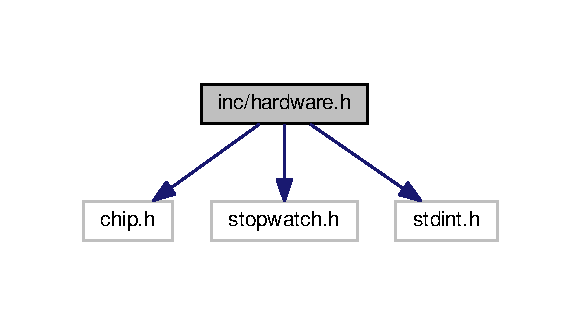
\includegraphics[width=279pt]{hardware_8h__incl}
\end{center}
\end{figure}
This graph shows which files directly or indirectly include this file\+:\nopagebreak
\begin{figure}[H]
\begin{center}
\leavevmode
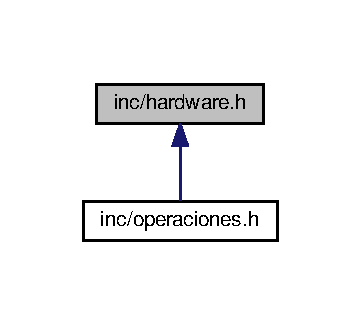
\includegraphics[width=173pt]{hardware_8h__dep__incl}
\end{center}
\end{figure}
\subsection*{Macros}
\begin{DoxyCompactItemize}
\item 
\#define \hyperlink{group__hardware_ga281151e2a661c8ad6893aee42b0024c4}{P\+O\+R\+T\+\_\+\+P\+I\+N\+\_\+\+L\+E\+D1}~0x02
\item 
\#define \hyperlink{group__hardware_ga1ee291f6ef730418abd5997176fe6b4c}{P\+I\+N\+\_\+\+L\+E\+D1}~0x0A
\item 
\#define \hyperlink{group__hardware_ga3039da47774de5edf9a11968103d87c5}{P\+O\+R\+T\+\_\+\+P\+I\+N\+\_\+\+L\+E\+D2}~0x02
\item 
\#define \hyperlink{group__hardware_gaa10e44027a1a9f0ac7cba19e815205a8}{P\+I\+N\+\_\+\+L\+E\+D2}~0x0B
\item 
\#define \hyperlink{group__hardware_ga097e347296860c96d104ef8ab90dac33}{P\+O\+R\+T\+\_\+\+P\+I\+N\+\_\+\+L\+E\+D3}~0x02
\item 
\#define \hyperlink{group__hardware_ga95a9a1b175a118c828537db81141eb3d}{P\+I\+N\+\_\+\+L\+E\+D3}~0x0C
\item 
\#define \hyperlink{group__hardware_ga372c868d523a46916b874b4e3c5722f5}{P\+O\+R\+T\+\_\+\+P\+I\+N\+\_\+\+R\+GB}~0x02
\item 
\#define \hyperlink{group__hardware_gaf3069b94e5b50d3558f6c36dd2e7ab15}{P\+I\+N\+\_\+\+R\+G\+B\+\_\+\+R\+ED}~0x00
\item 
\#define \hyperlink{group__hardware_ga298bb5d50ab2ba7b00df1c59087de286}{P\+I\+N\+\_\+\+R\+G\+B\+\_\+\+G\+RN}~0x01
\item 
\#define \hyperlink{group__hardware_gadf8d2d730566aede36c12ccfbc03b1b7}{P\+I\+N\+\_\+\+R\+G\+B\+\_\+\+B\+LU}~0x02
\item 
\#define \hyperlink{group__hardware_ga04c3e41fb79d2904c2358a42414bbf7f}{G\+P\+I\+O\+\_\+\+P\+O\+R\+T\+\_\+\+L\+E\+D1}~0x00
\item 
\#define \hyperlink{group__hardware_gaa4637d2cb87305ea71351291117a95f6}{G\+P\+I\+O\+\_\+\+P\+I\+N\+\_\+\+L\+E\+D1}~0x0E
\item 
\#define \hyperlink{group__hardware_gab971c6f67d136a9b870fac0f500685d4}{G\+P\+I\+O\+\_\+\+P\+O\+R\+T\+\_\+\+L\+E\+D2}~0x01
\item 
\#define \hyperlink{group__hardware_ga5ada73f73636a4fbf726468eb63eb945}{G\+P\+I\+O\+\_\+\+P\+I\+N\+\_\+\+L\+E\+D2}~0x0B
\item 
\#define \hyperlink{group__hardware_ga8b63f7f606f2b1ec7d88205ee6c514ea}{G\+P\+I\+O\+\_\+\+P\+O\+R\+T\+\_\+\+L\+E\+D3}~0x01
\item 
\#define \hyperlink{group__hardware_ga9e7e83187eae26d02136f609392fabd0}{G\+P\+I\+O\+\_\+\+P\+I\+N\+\_\+\+L\+E\+D3}~0x0C
\item 
\#define \hyperlink{group__hardware_ga9e2ed2756af597d0ec2ee618ef235c7e}{G\+P\+I\+O\+\_\+\+P\+O\+R\+T\+\_\+\+R\+GB}~0x05
\item 
\#define \hyperlink{group__hardware_gaa4aae4b49bb53e52b78b530637dcd2d7}{G\+P\+I\+O\+\_\+\+P\+I\+N\+\_\+\+R\+ED}~0x00
\item 
\#define \hyperlink{group__hardware_ga8ce252c71154210c65808a2170d74223}{G\+P\+I\+O\+\_\+\+P\+I\+N\+\_\+\+G\+RN}~0x01
\item 
\#define \hyperlink{group__hardware_ga2aa9b3c113e9f52a2e04ff811b8ec518}{G\+P\+I\+O\+\_\+\+P\+I\+N\+\_\+\+B\+LU}~0x02
\item 
\#define \hyperlink{group__hardware_gafe1bf3da61040955deda9703ee539687}{P\+O\+R\+T\+\_\+\+P\+I\+N\+\_\+\+K\+E\+Y1}~0x01
\item 
\#define \hyperlink{group__hardware_ga332cf72d49bf86b7b20274f3dec99d7b}{P\+I\+N\+\_\+\+K\+E\+Y1}~0x00
\item 
\#define \hyperlink{group__hardware_ga2cc4114181749a25732e31ed271a1f6b}{P\+O\+R\+T\+\_\+\+P\+I\+N\+\_\+\+K\+E\+Y2}~0x01
\item 
\#define \hyperlink{group__hardware_gae87128e49906c97fa9d6b438a08c1221}{P\+I\+N\+\_\+\+K\+E\+Y2}~0x01
\item 
\#define \hyperlink{group__hardware_ga5f697895be4580f403de4a9f75ab8a3b}{P\+O\+R\+T\+\_\+\+P\+I\+N\+\_\+\+K\+E\+Y3}~0x01
\item 
\#define \hyperlink{group__hardware_gaec621d9712815696a7bd342db8b2ff06}{P\+I\+N\+\_\+\+K\+E\+Y3}~0x02
\item 
\#define \hyperlink{group__hardware_gac86eb82e082d51cc0d4b0a87680cd7da}{P\+O\+R\+T\+\_\+\+P\+I\+N\+\_\+\+K\+E\+Y4}~0x01
\item 
\#define \hyperlink{group__hardware_gaf59a027359301b6e2229f7068c36efe6}{P\+I\+N\+\_\+\+K\+E\+Y4}~0x06
\item 
\#define \hyperlink{group__hardware_gabce59bc33538c850842e408765ae4981}{G\+P\+I\+O\+\_\+\+P\+O\+R\+T\+\_\+\+K\+E\+Y1}~0x00
\item 
\#define \hyperlink{group__hardware_ga26fa1a6916e027dcfa2d5a76c18dccb4}{G\+P\+I\+O\+\_\+\+P\+I\+N\+\_\+\+K\+E\+Y1}~0x04
\item 
\#define \hyperlink{group__hardware_gaeaf62bdfcf5fc1fe75d98d961286be78}{G\+P\+I\+O\+\_\+\+P\+O\+R\+T\+\_\+\+K\+E\+Y2}~0x00
\item 
\#define \hyperlink{group__hardware_ga6fe528c749e6e3df18c66c78841fd2ae}{G\+P\+I\+O\+\_\+\+P\+I\+N\+\_\+\+K\+E\+Y2}~0x08
\item 
\#define \hyperlink{group__hardware_ga6e75308c8b20c3236d0449a07bb052f7}{G\+P\+I\+O\+\_\+\+P\+O\+R\+T\+\_\+\+K\+E\+Y3}~0x00
\item 
\#define \hyperlink{group__hardware_ga6058161cd4273d1df2af95589e043055}{G\+P\+I\+O\+\_\+\+P\+I\+N\+\_\+\+K\+E\+Y3}~0x09
\item 
\#define \hyperlink{group__hardware_ga6d16f3a208324c46c462f92ad249d199}{G\+P\+I\+O\+\_\+\+P\+O\+R\+T\+\_\+\+K\+E\+Y4}~0x01
\item 
\#define \hyperlink{group__hardware_gabeaec154a7007cd91de9a8c775f4242f}{G\+P\+I\+O\+\_\+\+P\+I\+N\+\_\+\+K\+E\+Y4}~0x09
\item 
\#define \hyperlink{group__hardware_ga8dec203447e10cef9a4a1013f7c4cdd4}{next\+\_\+led}(x)~((x) = (x) $<$$<$ 1)
\begin{DoxyCompactList}\small\item\em Establece el siguiente valor en la enumeración \hyperlink{group__hardware_ga2a000bf02da2abba53355f3fcfdb2d0b}{board\+Leds}. \end{DoxyCompactList}\item 
\#define \hyperlink{group__hardware_ga6cc9878768b184e23371bbeb95360713}{prev\+\_\+led}(x)~((x) = (x) $>$$>$ 1)
\begin{DoxyCompactList}\small\item\em Establece el valor previo en la enumeración \hyperlink{group__hardware_ga2a000bf02da2abba53355f3fcfdb2d0b}{board\+Leds}. \end{DoxyCompactList}\item 
\#define \hyperlink{group__hardware_ga43a19ad1766c3719e591430d601496f7}{first\+\_\+led}~\hyperlink{group__hardware_gga84e58e8cc8e3fe349be97bcd3221c360a5662baf6795c7030ea75e47a0019a61d}{Led\+\_\+\+Rojo}
\begin{DoxyCompactList}\small\item\em Las definiciones fist\+Led, middle\+Led y last\+Led permiten encender los leds en secuencia desde el rgb Azul al led 3 (de middle\+Led a last\+Led) o la secuencia rojo, verde, azul al led 3 (utilizando de first\+Led a last\+Led). Estas definiciones permiten realizar operaciones como\+: \end{DoxyCompactList}\item 
\#define \hyperlink{group__hardware_gacbd2343998132167826e577781d85bbd}{middle\+\_\+led}~\hyperlink{group__hardware_gga84e58e8cc8e3fe349be97bcd3221c360a90357fded550cd38cda43991725234cb}{Led\+\_\+\+Azul}
\item 
\#define \hyperlink{group__hardware_ga6d4d3ee57587d8e08816b804150c29f8}{last\+\_\+led}~\hyperlink{group__hardware_gga2a000bf02da2abba53355f3fcfdb2d0ba16d63d90ec9dc8c27019e7c28ff1cfc0}{led3}
\item 
\#define \hyperlink{group__hardware_ga00c30099ff3ceab3e94a516833c11c98}{led\+On}(gpio\+Port,  gpio\+Pin)~Chip\+\_\+\+G\+P\+I\+O\+\_\+\+Set\+Pin\+State(L\+P\+C\+\_\+\+G\+P\+I\+O\+\_\+\+P\+O\+RT, gpio\+Port, gpio\+Pin, T\+R\+UE)
\begin{DoxyCompactList}\small\item\em Enciende un led. \end{DoxyCompactList}\item 
\#define \hyperlink{group__hardware_gac51bfbb3d5136e9e0479f3d8e6bb14de}{led\+Off}(gpio\+Port,  gpio\+Pin)~Chip\+\_\+\+G\+P\+I\+O\+\_\+\+Set\+Pin\+State(L\+P\+C\+\_\+\+G\+P\+I\+O\+\_\+\+P\+O\+RT, gpio\+Port, gpio\+Pin, F\+A\+L\+SE)
\begin{DoxyCompactList}\small\item\em Apaga un led. \end{DoxyCompactList}\item 
\#define \hyperlink{group__hardware_gaafb30c58d318e90ed902cb1aef013286}{led\+Toggle}(gpio\+Port,  gpio\+Pin)~Chip\+\_\+\+G\+P\+I\+O\+\_\+\+Set\+Pin\+Toggle(L\+P\+C\+\_\+\+G\+P\+I\+O\+\_\+\+P\+O\+RT, gpio\+Port, gpio\+Pin)
\begin{DoxyCompactList}\small\item\em Modifica el estado de un led particular (lo apaga si está encendido o lo enciende si está apagado). \end{DoxyCompactList}\item 
\#define \hyperlink{group__hardware_gafdd074f68e5ae5b133575140014f918d}{delay\+Ms}(x)~Stop\+Watch\+\_\+\+Delay\+Ms(x)
\begin{DoxyCompactList}\small\item\em Genera un delay de x milisegundos utilizando las primitivas del módulo \char`\"{}stopwatch\char`\"{} de lpc\+Open. \end{DoxyCompactList}\item 
\#define \hyperlink{group__hardware_ga1d13abaa815195d73e9dc2676e6fba5b}{delay\+Us}(x)~Stop\+Watch\+\_\+\+Delay\+Us(x)
\begin{DoxyCompactList}\small\item\em Genera un delay de x microsegundos utilizando las primitivas del módulo \char`\"{}stopwatch\char`\"{} de lpc\+Open. \end{DoxyCompactList}\end{DoxyCompactItemize}
\subsection*{Enumerations}
\begin{DoxyCompactItemize}
\item 
enum \hyperlink{group__hardware_ga8d70125ca4047f0f7ea513cd8568953d}{board\+Keys} \{ \hyperlink{group__hardware_gga8d70125ca4047f0f7ea513cd8568953da483a28cafb544915d9cd44f2c69fc706}{key1} =1, 
\hyperlink{group__hardware_gga8d70125ca4047f0f7ea513cd8568953dab8d9f65fc5604a8b8a0cdcbaf03bbbe0}{key2} =2, 
\hyperlink{group__hardware_gga8d70125ca4047f0f7ea513cd8568953da376c29473ae1a854ff46b2b171985093}{key3} =4, 
\hyperlink{group__hardware_gga8d70125ca4047f0f7ea513cd8568953da84011848209e666e74469d6dfba542eb}{key4} =8
 \}\begin{DoxyCompactList}\small\item\em Enumeración utilizada para identificar los pulsadores presentes en la E\+D\+U-\/\+C\+I\+AA N\+XP. \end{DoxyCompactList}
\item 
enum \hyperlink{group__hardware_ga84e58e8cc8e3fe349be97bcd3221c360}{rgb\+Leds} \{ \hyperlink{group__hardware_gga84e58e8cc8e3fe349be97bcd3221c360a5662baf6795c7030ea75e47a0019a61d}{Led\+\_\+\+Rojo} = 1, 
\hyperlink{group__hardware_gga84e58e8cc8e3fe349be97bcd3221c360aa5ad7834a37faf1e2620fa3db1838a21}{Led\+\_\+\+Verde} = 2, 
\hyperlink{group__hardware_gga84e58e8cc8e3fe349be97bcd3221c360a90357fded550cd38cda43991725234cb}{Led\+\_\+\+Azul} = 4
 \}\begin{DoxyCompactList}\small\item\em Enumeración asociada a los terminales de los leds R\+GB. \end{DoxyCompactList}
\item 
enum \hyperlink{group__hardware_ga2a000bf02da2abba53355f3fcfdb2d0b}{board\+Leds} \{ \\*
\hyperlink{group__hardware_gga2a000bf02da2abba53355f3fcfdb2d0ba76aaf0c615e41c008aa876ea4c183f4c}{led4} = Led\+\_\+\+Rojo, 
\hyperlink{group__hardware_gga2a000bf02da2abba53355f3fcfdb2d0ba66b97e4de94e08d049b57ac98e315cad}{led5} = Led\+\_\+\+Verde, 
\hyperlink{group__hardware_gga2a000bf02da2abba53355f3fcfdb2d0ba2c4a58277fd326a128900fe0904c2b1e}{led6} = Led\+\_\+\+Azul, 
\hyperlink{group__hardware_gga2a000bf02da2abba53355f3fcfdb2d0bacc803913e7d21f9a6900861008580c5f}{led1} = 8, 
\\*
\hyperlink{group__hardware_gga2a000bf02da2abba53355f3fcfdb2d0ba9c2c88fba1581ccd42348c9e3c47df92}{led2} = 16, 
\hyperlink{group__hardware_gga2a000bf02da2abba53355f3fcfdb2d0ba16d63d90ec9dc8c27019e7c28ff1cfc0}{led3} = 32
 \}\begin{DoxyCompactList}\small\item\em Enumeración utilizada para identificar los leds presentes en la E\+D\+U-\/\+C\+I\+AA N\+XP. \end{DoxyCompactList}
\end{DoxyCompactItemize}
\subsection*{Functions}
\begin{DoxyCompactItemize}
\item 
void \hyperlink{group__hardware_gab11a117f1e08391f23d1da05930e7acf}{system\+Init} (void)
\begin{DoxyCompactList}\small\item\em Inicializa los módulos básicos de la E\+D\+U-\/\+C\+I\+AA N\+XP. \end{DoxyCompactList}\item 
unsigned int \hyperlink{group__hardware_ga461352be081cdef66d03a73226849b41}{serial\+Write} (const uint8\+\_\+t $\ast$data, unsigned int data\+Len)
\begin{DoxyCompactList}\small\item\em Carga una cadena de caracteres para ser enviada a través de la U\+S\+A\+RT. Debe considerarse que la transmisión se realiza sin bloqueo y a través de interrupciones. Para eso, esta función invoca a Chip\+\_\+\+U\+A\+R\+T\+\_\+\+Send\+RB, la cuál copia la cadena en un buffer circular e inicia la transmición del primer caracter. Una vez disparada la interrupción que indica la finalización del envío, continúa con el siguiente caracter hasta que se completa la transmición de la cadena. \end{DoxyCompactList}\item 
void \hyperlink{group__hardware_gac20eca44aeea90e6f603831193cc9b28}{U\+A\+R\+T2\+\_\+\+I\+R\+Q\+Handler} (void)
\begin{DoxyCompactList}\small\item\em Obtiene los caracteres disponibles en el buffer circular asociado al flujo de entrada de caracteres (\char`\"{}lee el puerto\char`\"{}). \end{DoxyCompactList}\item 
void \hyperlink{group__hardware_ga4b6495dfec1dcc97e48043d7bca4da60}{set\+Led\+From\+Msk} (uint8\+\_\+t msk)
\begin{DoxyCompactList}\small\item\em Enciend o apaga un led según la máscara dada como argumento. \end{DoxyCompactList}\item 
void \hyperlink{group__hardware_ga3ac24a1bb2d63482077813f22c6930a1}{wait\+Key\+Press} (\hyperlink{group__hardware_ga8d70125ca4047f0f7ea513cd8568953d}{board\+Keys} \hyperlink{group__operaciones_ga3496dfc7a27df7eead65d48ed89e6867}{key})
\begin{DoxyCompactList}\small\item\em Espera a que se presione la tecla indicada a partir del argumento utilizado. \end{DoxyCompactList}\item 
uint8\+\_\+t \hyperlink{group__hardware_gabe9050eab201da85d14532c4d009603a}{get\+Key\+Pressed} (void)
\begin{DoxyCompactList}\small\item\em Retorna una máscara con el estado de las teclas. Si una tecla está presionada, retorna un bit en alto y si está suelta un bit en bajo. \end{DoxyCompactList}\end{DoxyCompactItemize}


\subsection{Detailed Description}
Declaraciones de funciones y constantes simbólicas correspondientes con la E\+D\+U-\/\+C\+I\+AA N\+XP. 

\begin{DoxyDate}{Date}
09/07/2018 
\end{DoxyDate}

\hypertarget{hsadc__18xx__43xx_8c}{}\section{Referencia del Archivo hsadc\+\_\+18xx\+\_\+43xx.\+c}
\label{hsadc__18xx__43xx_8c}\index{hsadc\+\_\+18xx\+\_\+43xx.\+c@{hsadc\+\_\+18xx\+\_\+43xx.\+c}}
{\ttfamily \#include \char`\"{}chip.\+h\char`\"{}}\\*
\subsection*{Estructuras de datos}
\begin{DoxyCompactItemize}
\item 
struct \hyperlink{struct_c_r_s_d_c_e_g___t}{C\+R\+S\+D\+C\+E\+G\+\_\+T}
\end{DoxyCompactItemize}
\subsection*{Funciones}
\begin{DoxyCompactItemize}
\item 
void \hyperlink{group___h_s_a_d_c__18_x_x__43_x_x_gad72fb94bbb485c84687a4e75c63090ea}{Chip\+\_\+\+H\+S\+A\+D\+C\+\_\+\+Init} (\hyperlink{struct_l_p_c___h_s_a_d_c___t}{L\+P\+C\+\_\+\+H\+S\+A\+D\+C\+\_\+T} $\ast$p\+H\+S\+A\+DC)
\begin{DoxyCompactList}\small\item\em Initialize the High speed A\+DC. \end{DoxyCompactList}\item 
void \hyperlink{group___h_s_a_d_c__18_x_x__43_x_x_ga2d9740d012a9043c462acbc468e1931d}{Chip\+\_\+\+H\+S\+A\+D\+C\+\_\+\+De\+Init} (\hyperlink{struct_l_p_c___h_s_a_d_c___t}{L\+P\+C\+\_\+\+H\+S\+A\+D\+C\+\_\+T} $\ast$p\+H\+S\+A\+DC)
\begin{DoxyCompactList}\small\item\em Shutdown H\+S\+A\+DC. \end{DoxyCompactList}\item 
void \hyperlink{group___h_s_a_d_c__18_x_x__43_x_x_gaafa52aef03cf64be7d329895ad90ac40}{Chip\+\_\+\+H\+S\+A\+D\+C\+\_\+\+Setup\+F\+I\+FO} (\hyperlink{struct_l_p_c___h_s_a_d_c___t}{L\+P\+C\+\_\+\+H\+S\+A\+D\+C\+\_\+T} $\ast$p\+H\+S\+A\+DC, uint8\+\_\+t trip, bool packed)
\begin{DoxyCompactList}\small\item\em Sets up H\+S\+A\+DC F\+I\+FO trip level and packing. \end{DoxyCompactList}\item 
void \hyperlink{group___h_s_a_d_c__18_x_x__43_x_x_ga86ed5ab3da9ea3a6bbfd138530d5d73d}{Chip\+\_\+\+H\+S\+A\+D\+C\+\_\+\+Set\+Thr\+Low\+Value} (\hyperlink{struct_l_p_c___h_s_a_d_c___t}{L\+P\+C\+\_\+\+H\+S\+A\+D\+C\+\_\+T} $\ast$p\+H\+S\+A\+DC, uint8\+\_\+t thrnum, uint16\+\_\+t value)
\begin{DoxyCompactList}\small\item\em Set H\+S\+A\+DC Threshold low value. \end{DoxyCompactList}\item 
void \hyperlink{group___h_s_a_d_c__18_x_x__43_x_x_ga0690a0edb51bd4070384c35196f1a73d}{Chip\+\_\+\+H\+S\+A\+D\+C\+\_\+\+Set\+Thr\+High\+Value} (\hyperlink{struct_l_p_c___h_s_a_d_c___t}{L\+P\+C\+\_\+\+H\+S\+A\+D\+C\+\_\+T} $\ast$p\+H\+S\+A\+DC, uint8\+\_\+t thrnum, uint16\+\_\+t value)
\begin{DoxyCompactList}\small\item\em Set H\+S\+A\+DC Threshold high value. \end{DoxyCompactList}\item 
void \hyperlink{group___h_s_a_d_c__18_x_x__43_x_x_ga70b879056a35cdf9cc6f9c2928883973}{Chip\+\_\+\+H\+S\+A\+D\+C\+\_\+\+Set\+Speed} (\hyperlink{struct_l_p_c___h_s_a_d_c___t}{L\+P\+C\+\_\+\+H\+S\+A\+D\+C\+\_\+T} $\ast$p\+H\+S\+A\+DC, uint8\+\_\+t channel, uint8\+\_\+t speed)
\begin{DoxyCompactList}\small\item\em Setup speed for a input channel. \end{DoxyCompactList}\item 
void \hyperlink{group___h_s_a_d_c__18_x_x__43_x_x_ga776d07e6bc51347515f92ed36a9da561}{Chip\+\_\+\+H\+S\+A\+D\+C\+\_\+\+Set\+Power\+Speed} (\hyperlink{struct_l_p_c___h_s_a_d_c___t}{L\+P\+C\+\_\+\+H\+S\+A\+D\+C\+\_\+T} $\ast$p\+H\+S\+A\+DC, bool comp2)
\begin{DoxyCompactList}\small\item\em Setup (common) H\+S\+A\+DC power and speed settings. \end{DoxyCompactList}\item 
void \hyperlink{group___h_s_a_d_c__18_x_x__43_x_x_gaf754b858ff1c0c0d2993aaedad394867}{Chip\+\_\+\+H\+S\+A\+D\+C\+\_\+\+Set\+A\+C\+D\+C\+Bias} (\hyperlink{struct_l_p_c___h_s_a_d_c___t}{L\+P\+C\+\_\+\+H\+S\+A\+D\+C\+\_\+T} $\ast$p\+H\+S\+A\+DC, uint8\+\_\+t channel, \hyperlink{group___h_s_a_d_c__18_x_x__43_x_x_ga1769145f3b2f1c12f4cd23d3b5151e93}{H\+S\+A\+D\+C\+\_\+\+D\+C\+B\+I\+A\+S\+\_\+T} dc\+In\+Neg, \hyperlink{group___h_s_a_d_c__18_x_x__43_x_x_ga1769145f3b2f1c12f4cd23d3b5151e93}{H\+S\+A\+D\+C\+\_\+\+D\+C\+B\+I\+A\+S\+\_\+T} dc\+In\+Pos)
\begin{DoxyCompactList}\small\item\em Setup A\+C-\/\+DC coupling selection for a channel. \end{DoxyCompactList}\end{DoxyCompactItemize}

\hypertarget{hsadc__18xx__43xx_8h}{}\section{Referencia del Archivo hsadc\+\_\+18xx\+\_\+43xx.\+h}
\label{hsadc__18xx__43xx_8h}\index{hsadc\+\_\+18xx\+\_\+43xx.\+h@{hsadc\+\_\+18xx\+\_\+43xx.\+h}}
\subsection*{Estructuras de datos}
\begin{DoxyCompactItemize}
\item 
struct \hyperlink{struct_h_s_a_d_c_i_n_t_c_t_r_l___t}{H\+S\+A\+D\+C\+I\+N\+T\+C\+T\+R\+L\+\_\+T}
\begin{DoxyCompactList}\small\item\em High speed A\+DC interrupt control structure. \end{DoxyCompactList}\item 
struct \hyperlink{struct_l_p_c___h_s_a_d_c___t}{L\+P\+C\+\_\+\+H\+S\+A\+D\+C\+\_\+T}
\begin{DoxyCompactList}\small\item\em H\+S\+A\+DC register block structure. \end{DoxyCompactList}\end{DoxyCompactItemize}
\subsection*{\textquotesingle{}defines\textquotesingle{}}
\begin{DoxyCompactItemize}
\item 
\#define \hyperlink{group___h_s_a_d_c__18_x_x__43_x_x_ga125fd0f116ea9e450347efe49ecc9673}{H\+S\+A\+D\+C\+\_\+\+M\+A\+X\+\_\+\+S\+A\+M\+P\+L\+E\+V\+AL}~0x\+F\+FF
\item 
\#define \hyperlink{group___h_s_a_d_c__18_x_x__43_x_x_ga3e9186020c5e406feed470a1808363f3}{H\+S\+A\+D\+C\+\_\+\+L\+S\+\_\+\+D\+O\+NE}~(1 $<$$<$ 0)
\item 
\#define \hyperlink{group___h_s_a_d_c__18_x_x__43_x_x_ga5c0a9c9126e736e08a7bb6330a8da5da}{H\+S\+A\+D\+C\+\_\+\+L\+S\+\_\+\+O\+V\+E\+R\+R\+UN}~(1 $<$$<$ 1)
\item 
\#define \hyperlink{group___h_s_a_d_c__18_x_x__43_x_x_gabf5cce50eca68e4c98b7d7d878e34ce8}{H\+S\+A\+D\+C\+\_\+\+L\+S\+\_\+\+R\+A\+N\+G\+E\+\_\+\+IN}~(0 $<$$<$ 2)
\item 
\#define \hyperlink{group___h_s_a_d_c__18_x_x__43_x_x_ga0d03219d2f21b7082c71e737f9291238}{H\+S\+A\+D\+C\+\_\+\+L\+S\+\_\+\+R\+A\+N\+G\+E\+\_\+\+B\+E\+L\+OW}~(1 $<$$<$ 2)
\item 
\#define \hyperlink{group___h_s_a_d_c__18_x_x__43_x_x_ga2ff163a7e694c903c3ea800b69ff357f}{H\+S\+A\+D\+C\+\_\+\+L\+S\+\_\+\+R\+A\+N\+G\+E\+\_\+\+A\+B\+O\+VE}~(2 $<$$<$ 2)
\item 
\#define \hyperlink{group___h_s_a_d_c__18_x_x__43_x_x_gab8577fad41f87c7822073b4b0e1b40c3}{H\+S\+A\+D\+C\+\_\+\+L\+S\+\_\+\+R\+A\+N\+GE}(val)~((val) \& 0x\+C)
\item 
\#define \hyperlink{group___h_s_a_d_c__18_x_x__43_x_x_ga232e739e7c2601b9c0e3cdaede3ff83e}{H\+S\+A\+D\+C\+\_\+\+L\+S\+\_\+\+C\+R\+O\+S\+S\+I\+N\+G\+\_\+\+N\+O\+NE}~(0 $<$$<$ 4)
\item 
\#define \hyperlink{group___h_s_a_d_c__18_x_x__43_x_x_ga5256afbf3a733f1e1598086bcae21313}{H\+S\+A\+D\+C\+\_\+\+L\+S\+\_\+\+C\+R\+O\+S\+S\+I\+N\+G\+\_\+\+D\+O\+WN}~(1 $<$$<$ 4)
\item 
\#define \hyperlink{group___h_s_a_d_c__18_x_x__43_x_x_ga61403d754e6e74e765939cbcdf668458}{H\+S\+A\+D\+C\+\_\+\+L\+S\+\_\+\+C\+R\+O\+S\+S\+I\+N\+G\+\_\+\+UP}~(2 $<$$<$ 4)
\item 
\#define \hyperlink{group___h_s_a_d_c__18_x_x__43_x_x_gabe3b261486872f47b15142374e8ba513}{H\+S\+A\+D\+C\+\_\+\+L\+S\+\_\+\+C\+R\+O\+S\+S\+I\+NG}(val)~((val) \& 0x30)
\item 
\#define \hyperlink{group___h_s_a_d_c__18_x_x__43_x_x_ga59cfae9793b32fc984aa56b25e579e85}{H\+S\+A\+D\+C\+\_\+\+L\+S\+\_\+\+D\+A\+TA}(val)~((val) $>$$>$ 6)
\item 
\#define \hyperlink{group___h_s_a_d_c__18_x_x__43_x_x_ga5ae1350581db3acfa2450f482f64a14d}{H\+S\+A\+D\+C\+\_\+\+F\+I\+F\+O\+\_\+\+S\+A\+M\+P\+L\+E\+\_\+\+M\+A\+SK}~(0x\+F\+F\+F)
\item 
\#define \hyperlink{group___h_s_a_d_c__18_x_x__43_x_x_ga4e9d547e690f73b5e1cef272e5272239}{H\+S\+A\+D\+C\+\_\+\+F\+I\+F\+O\+\_\+\+S\+A\+M\+P\+LE}(val)~((val) \& 0x\+F\+F\+F)
\item 
\#define \hyperlink{group___h_s_a_d_c__18_x_x__43_x_x_ga46dfa5dab0fc08a4e9126be14eec1f1c}{H\+S\+A\+D\+C\+\_\+\+F\+I\+F\+O\+\_\+\+C\+H\+A\+N\+\_\+\+I\+D\+\_\+\+M\+A\+SK}~(0x7000)
\item 
\#define \hyperlink{group___h_s_a_d_c__18_x_x__43_x_x_gaa90d96f985440d9588a1b0a3d3b30d9e}{H\+S\+A\+D\+C\+\_\+\+F\+I\+F\+O\+\_\+\+C\+H\+A\+N\+\_\+\+ID}(val)~(((val) $>$$>$ 12) \& 0x7)
\item 
\#define \hyperlink{group___h_s_a_d_c__18_x_x__43_x_x_ga024359046ed5aea283f5ca303828ebaf}{H\+S\+A\+D\+C\+\_\+\+F\+I\+F\+O\+\_\+\+E\+M\+P\+TY}~(0x1 $<$$<$ 15)
\item 
\#define \hyperlink{group___h_s_a_d_c__18_x_x__43_x_x_ga59b2c13550ce54537ddba69cec51bd0b}{H\+S\+A\+D\+C\+\_\+\+F\+I\+F\+O\+\_\+\+S\+H\+I\+F\+T\+P\+A\+C\+K\+ED}(val)~((val) $>$$>$ 16)
\item 
\#define \hyperlink{group___h_s_a_d_c__18_x_x__43_x_x_ga135c335cef689d7ecc14af1f5bd0ac6b}{H\+S\+A\+D\+C\+\_\+\+F\+I\+F\+O\+\_\+\+P\+A\+C\+K\+E\+D\+M\+A\+SK}~(1\+U\+L $<$$<$ 31)
\item 
\#define \hyperlink{group___h_s_a_d_c__18_x_x__43_x_x_ga02a0ec797250b260c4ffa4e52e256a44}{H\+S\+A\+D\+C\+\_\+\+D\+E\+S\+C\+\_\+\+CH}(ch)~(ch)
\item 
\#define \hyperlink{group___h_s_a_d_c__18_x_x__43_x_x_gaba66d1c1c7ce5508696f9da464b680c9}{H\+S\+A\+D\+C\+\_\+\+D\+E\+S\+C\+\_\+\+H\+A\+LT}~(1 $<$$<$ 3)
\item 
\#define \hyperlink{group___h_s_a_d_c__18_x_x__43_x_x_gade13fb1864987d1b1d8054ae6f861167}{H\+S\+A\+D\+C\+\_\+\+D\+E\+S\+C\+\_\+\+I\+NT}~(1 $<$$<$ 4)
\item 
\#define \hyperlink{group___h_s_a_d_c__18_x_x__43_x_x_ga5cb818c7f3deae6a0bd626acde3f4278}{H\+S\+A\+D\+C\+\_\+\+D\+E\+S\+C\+\_\+\+P\+O\+W\+E\+R\+D\+O\+WN}~(1 $<$$<$ 5)
\item 
\#define \hyperlink{group___h_s_a_d_c__18_x_x__43_x_x_gace04d08e17d8ef4aea5dcdd739977f52}{H\+S\+A\+D\+C\+\_\+\+D\+E\+S\+C\+\_\+\+B\+R\+A\+N\+C\+H\+\_\+\+N\+E\+XT}~(0 $<$$<$ 6)
\item 
\#define \hyperlink{group___h_s_a_d_c__18_x_x__43_x_x_ga2490e58198cd0d81251bb81a725d8d78}{H\+S\+A\+D\+C\+\_\+\+D\+E\+S\+C\+\_\+\+B\+R\+A\+N\+C\+H\+\_\+\+F\+I\+R\+ST}~(1 $<$$<$ 6)
\item 
\#define \hyperlink{group___h_s_a_d_c__18_x_x__43_x_x_gaf2255ed7cd48d9ffe08cde080aec9f30}{H\+S\+A\+D\+C\+\_\+\+D\+E\+S\+C\+\_\+\+B\+R\+A\+N\+C\+H\+\_\+\+S\+W\+AP}~(2 $<$$<$ 6)
\item 
\#define \hyperlink{group___h_s_a_d_c__18_x_x__43_x_x_gae778cc41c05fd0ab48557d5729cdca3e}{H\+S\+A\+D\+C\+\_\+\+D\+E\+S\+C\+\_\+\+M\+A\+T\+CH}(val)~((val) $<$$<$ 8)
\item 
\#define \hyperlink{group___h_s_a_d_c__18_x_x__43_x_x_gab8aa894027316458bbbc14e6c3eb0822}{H\+S\+A\+D\+C\+\_\+\+D\+E\+S\+C\+\_\+\+T\+H\+R\+E\+S\+H\+\_\+\+N\+O\+NE}~(0 $<$$<$ 22)
\item 
\#define \hyperlink{group___h_s_a_d_c__18_x_x__43_x_x_gac7411ef8756584fe30770ef9ee1bd5d2}{H\+S\+A\+D\+C\+\_\+\+D\+E\+S\+C\+\_\+\+T\+H\+R\+E\+S\+H\+\_\+A}~(1 $<$$<$ 22)
\item 
\#define \hyperlink{group___h_s_a_d_c__18_x_x__43_x_x_gad679e07226e8388ddbff3b47b34a0f15}{H\+S\+A\+D\+C\+\_\+\+D\+E\+S\+C\+\_\+\+T\+H\+R\+E\+S\+H\+\_\+B}~(2 $<$$<$ 22)
\item 
\#define \hyperlink{group___h_s_a_d_c__18_x_x__43_x_x_ga1dcff8ddcbf4b49f060bda8d1d8d5a75}{H\+S\+A\+D\+C\+\_\+\+D\+E\+S\+C\+\_\+\+R\+E\+S\+E\+T\+\_\+\+T\+I\+M\+ER}~(1 $<$$<$ 24)
\item 
\#define \hyperlink{group___h_s_a_d_c__18_x_x__43_x_x_gadb7ad7a7ee1d43b9bb873d19b318c26a}{H\+S\+A\+D\+C\+\_\+\+D\+E\+S\+C\+\_\+\+U\+P\+D\+A\+T\+E\+\_\+\+T\+A\+B\+LE}~(1\+U\+L $<$$<$ 31)
\item 
\#define \hyperlink{group___h_s_a_d_c__18_x_x__43_x_x_ga13e783f301fd2cd457c2679f4d2cc2cc}{H\+S\+A\+D\+C\+\_\+\+I\+N\+T0\+\_\+\+F\+I\+F\+O\+\_\+\+F\+U\+LL}~(1 $<$$<$ 0)
\item 
\#define \hyperlink{group___h_s_a_d_c__18_x_x__43_x_x_gafac0940c99898d7e391d1ac3c05ba719}{H\+S\+A\+D\+C\+\_\+\+I\+N\+T0\+\_\+\+F\+I\+F\+O\+\_\+\+E\+M\+P\+TY}~(1 $<$$<$ 1)
\item 
\#define \hyperlink{group___h_s_a_d_c__18_x_x__43_x_x_gab3b9780b70691c1beb059b701e29e6b3}{H\+S\+A\+D\+C\+\_\+\+I\+N\+T0\+\_\+\+F\+I\+F\+O\+\_\+\+O\+V\+E\+R\+F\+L\+OW}~(1 $<$$<$ 2)
\item 
\#define \hyperlink{group___h_s_a_d_c__18_x_x__43_x_x_ga829571c11e7c8e7a44966820acffcaa3}{H\+S\+A\+D\+C\+\_\+\+I\+N\+T0\+\_\+\+D\+S\+C\+R\+\_\+\+D\+O\+NE}~(1 $<$$<$ 3)
\item 
\#define \hyperlink{group___h_s_a_d_c__18_x_x__43_x_x_ga40cb66b32360ce6cbd98aa0ce3de31a5}{H\+S\+A\+D\+C\+\_\+\+I\+N\+T0\+\_\+\+D\+S\+C\+R\+\_\+\+E\+R\+R\+OR}~(1 $<$$<$ 4)
\item 
\#define \hyperlink{group___h_s_a_d_c__18_x_x__43_x_x_ga8bb38fa225bf592f805b7979459cbfc2}{H\+S\+A\+D\+C\+\_\+\+I\+N\+T0\+\_\+\+A\+D\+C\+\_\+\+O\+VF}~(1 $<$$<$ 5)
\item 
\#define \hyperlink{group___h_s_a_d_c__18_x_x__43_x_x_gad015ea52167f05024a42c4be5b8deac3}{H\+S\+A\+D\+C\+\_\+\+I\+N\+T0\+\_\+\+A\+D\+C\+\_\+\+U\+NF}~(1 $<$$<$ 6)
\item 
\#define \hyperlink{group___h_s_a_d_c__18_x_x__43_x_x_ga2fdf9432486e0e74575f360a8280923d}{H\+S\+A\+D\+C\+\_\+\+I\+N\+T1\+\_\+\+T\+H\+C\+M\+P\+\_\+\+B\+R\+A\+N\+GE}(ch)~(1 $<$$<$ ((ch $\ast$ 5) + 0))
\item 
\#define \hyperlink{group___h_s_a_d_c__18_x_x__43_x_x_ga55155119335413cd579ff9da9888b209}{H\+S\+A\+D\+C\+\_\+\+I\+N\+T1\+\_\+\+T\+H\+C\+M\+P\+\_\+\+A\+R\+A\+N\+GE}(ch)~(1 $<$$<$ ((ch $\ast$ 5) + 1))
\item 
\#define \hyperlink{group___h_s_a_d_c__18_x_x__43_x_x_ga7ec226dc9dc901248ee36696803097b2}{H\+S\+A\+D\+C\+\_\+\+I\+N\+T1\+\_\+\+T\+H\+C\+M\+P\+\_\+\+D\+C\+R\+O\+SS}(ch)~(1 $<$$<$ ((ch $\ast$ 5) + 2))
\item 
\#define \hyperlink{group___h_s_a_d_c__18_x_x__43_x_x_ga63d87a4bacb160ac3e6e68f21daf8580}{H\+S\+A\+D\+C\+\_\+\+I\+N\+T1\+\_\+\+T\+H\+C\+M\+P\+\_\+\+U\+C\+R\+O\+SS}(ch)~(1 $<$$<$ ((ch $\ast$ 5) + 3))
\item 
\#define \hyperlink{group___h_s_a_d_c__18_x_x__43_x_x_gad4bd824de161be1ab9a6aa9860bc2d74}{H\+S\+A\+D\+C\+\_\+\+I\+N\+T1\+\_\+\+O\+V\+E\+R\+R\+UN}(ch)~(1 $<$$<$ ((ch $\ast$ 5) + 4))
\end{DoxyCompactItemize}
\subsection*{Enumeraciones}
\begin{DoxyCompactItemize}
\item 
enum \hyperlink{group___h_s_a_d_c__18_x_x__43_x_x_gabacdffe94b42f1dc1c339dab9a20772c}{H\+S\+A\+D\+C\+\_\+\+T\+R\+I\+G\+G\+E\+R\+\_\+\+M\+A\+S\+K\+\_\+T} \{ \hyperlink{group___h_s_a_d_c__18_x_x__43_x_x_ggabacdffe94b42f1dc1c339dab9a20772caacc058b469367e54d9cb0b79c893c27b}{H\+S\+A\+D\+C\+\_\+\+C\+O\+N\+F\+I\+G\+\_\+\+T\+R\+I\+G\+G\+E\+R\+\_\+\+O\+FF} = 0, 
\hyperlink{group___h_s_a_d_c__18_x_x__43_x_x_ggabacdffe94b42f1dc1c339dab9a20772ca60a0ed78169b3ca42913125055400dd1}{H\+S\+A\+D\+C\+\_\+\+C\+O\+N\+F\+I\+G\+\_\+\+T\+R\+I\+G\+G\+E\+R\+\_\+\+SW} = 1, 
\hyperlink{group___h_s_a_d_c__18_x_x__43_x_x_ggabacdffe94b42f1dc1c339dab9a20772caa757019f18616753839c7817d7e633d9}{H\+S\+A\+D\+C\+\_\+\+C\+O\+N\+F\+I\+G\+\_\+\+T\+R\+I\+G\+G\+E\+R\+\_\+\+E\+XT} = 2, 
\hyperlink{group___h_s_a_d_c__18_x_x__43_x_x_ggabacdffe94b42f1dc1c339dab9a20772ca565a4a6ef822ca662af662b13d06c4b9}{H\+S\+A\+D\+C\+\_\+\+C\+O\+N\+F\+I\+G\+\_\+\+T\+R\+I\+G\+G\+E\+R\+\_\+\+B\+O\+TH} = 3
 \}
\item 
enum \hyperlink{group___h_s_a_d_c__18_x_x__43_x_x_gab4aa68023c03604cc1333eed859073e9}{H\+S\+A\+D\+C\+\_\+\+T\+R\+I\+G\+G\+E\+R\+\_\+\+M\+O\+D\+E\+\_\+T} \{ \hyperlink{group___h_s_a_d_c__18_x_x__43_x_x_ggab4aa68023c03604cc1333eed859073e9ad7129b13b7955c2995a91774947869f2}{H\+S\+A\+D\+C\+\_\+\+C\+O\+N\+F\+I\+G\+\_\+\+T\+R\+I\+G\+G\+E\+R\+\_\+\+R\+I\+S\+E\+E\+XT} = (0 $<$$<$ 2), 
\hyperlink{group___h_s_a_d_c__18_x_x__43_x_x_ggab4aa68023c03604cc1333eed859073e9ac157643a91f076c5864d316234f72c0f}{H\+S\+A\+D\+C\+\_\+\+C\+O\+N\+F\+I\+G\+\_\+\+T\+R\+I\+G\+G\+E\+R\+\_\+\+F\+A\+L\+L\+E\+XT} = (1 $<$$<$ 2), 
\hyperlink{group___h_s_a_d_c__18_x_x__43_x_x_ggab4aa68023c03604cc1333eed859073e9a15370950a068bae8a811f325302e2afe}{H\+S\+A\+D\+C\+\_\+\+C\+O\+N\+F\+I\+G\+\_\+\+T\+R\+I\+G\+G\+E\+R\+\_\+\+L\+O\+W\+E\+XT} = (2 $<$$<$ 2), 
\hyperlink{group___h_s_a_d_c__18_x_x__43_x_x_ggab4aa68023c03604cc1333eed859073e9acdf358d24d8f8407d365a01f7a671419}{H\+S\+A\+D\+C\+\_\+\+C\+O\+N\+F\+I\+G\+\_\+\+T\+R\+I\+G\+G\+E\+R\+\_\+\+H\+I\+G\+H\+E\+XT} = (3 $<$$<$ 2)
 \}
\item 
enum \hyperlink{group___h_s_a_d_c__18_x_x__43_x_x_ga2b37f3b76e8523e0035f2b275ddb36ce}{H\+S\+A\+D\+C\+\_\+\+T\+R\+I\+G\+G\+E\+R\+\_\+\+S\+Y\+N\+C\+\_\+T} \{ \hyperlink{group___h_s_a_d_c__18_x_x__43_x_x_gga2b37f3b76e8523e0035f2b275ddb36ceae6d8612bb563af3ba4e3a484208a0f1f}{H\+S\+A\+D\+C\+\_\+\+C\+O\+N\+F\+I\+G\+\_\+\+T\+R\+I\+G\+G\+E\+R\+\_\+\+N\+O\+E\+X\+T\+S\+Y\+NC} = (0 $<$$<$ 4), 
\hyperlink{group___h_s_a_d_c__18_x_x__43_x_x_gga2b37f3b76e8523e0035f2b275ddb36cea9db72f3e619659809c61aee822029be3}{H\+S\+A\+D\+C\+\_\+\+C\+O\+N\+F\+I\+G\+\_\+\+T\+R\+I\+G\+G\+E\+R\+\_\+\+E\+X\+T\+S\+Y\+NC} = (1 $<$$<$ 4)
 \}
\item 
enum \hyperlink{group___h_s_a_d_c__18_x_x__43_x_x_ga4033a9f5f07fbc57e03d0592680729c6}{H\+S\+A\+D\+C\+\_\+\+C\+H\+A\+N\+N\+E\+L\+\_\+\+I\+D\+\_\+\+E\+N\+\_\+T} \{ \hyperlink{group___h_s_a_d_c__18_x_x__43_x_x_gga4033a9f5f07fbc57e03d0592680729c6ae5aacde39c419c9e7c2fd90129d7249e}{H\+S\+A\+D\+C\+\_\+\+C\+H\+A\+N\+N\+E\+L\+\_\+\+I\+D\+\_\+\+E\+N\+\_\+\+N\+O\+NE} = (0 $<$$<$ 5), 
\hyperlink{group___h_s_a_d_c__18_x_x__43_x_x_gga4033a9f5f07fbc57e03d0592680729c6a0f3c586fdd4936cddfcdfd428d515e08}{H\+S\+A\+D\+C\+\_\+\+C\+H\+A\+N\+N\+E\+L\+\_\+\+I\+D\+\_\+\+E\+N\+\_\+\+A\+DD} = (1 $<$$<$ 5)
 \}
\item 
enum \hyperlink{group___h_s_a_d_c__18_x_x__43_x_x_ga1769145f3b2f1c12f4cd23d3b5151e93}{H\+S\+A\+D\+C\+\_\+\+D\+C\+B\+I\+A\+S\+\_\+T} \{ \hyperlink{group___h_s_a_d_c__18_x_x__43_x_x_gga1769145f3b2f1c12f4cd23d3b5151e93aa3bf2d188fb6405ed2a0e2a7cf93cf5f}{H\+S\+A\+D\+C\+\_\+\+C\+H\+A\+N\+N\+E\+L\+\_\+\+N\+O\+D\+C\+B\+I\+AS} = 0, 
\hyperlink{group___h_s_a_d_c__18_x_x__43_x_x_gga1769145f3b2f1c12f4cd23d3b5151e93a18b6321e47d50b140029523a47b1662f}{H\+S\+A\+D\+C\+\_\+\+C\+H\+A\+N\+N\+E\+L\+\_\+\+D\+C\+B\+I\+AS} = 1
 \}
\end{DoxyCompactItemize}
\subsection*{Funciones}
\begin{DoxyCompactItemize}
\item 
void \hyperlink{group___h_s_a_d_c__18_x_x__43_x_x_gad72fb94bbb485c84687a4e75c63090ea}{Chip\+\_\+\+H\+S\+A\+D\+C\+\_\+\+Init} (\hyperlink{struct_l_p_c___h_s_a_d_c___t}{L\+P\+C\+\_\+\+H\+S\+A\+D\+C\+\_\+T} $\ast$p\+H\+S\+A\+DC)
\begin{DoxyCompactList}\small\item\em Initialize the High speed A\+DC. \end{DoxyCompactList}\item 
void \hyperlink{group___h_s_a_d_c__18_x_x__43_x_x_ga2d9740d012a9043c462acbc468e1931d}{Chip\+\_\+\+H\+S\+A\+D\+C\+\_\+\+De\+Init} (\hyperlink{struct_l_p_c___h_s_a_d_c___t}{L\+P\+C\+\_\+\+H\+S\+A\+D\+C\+\_\+T} $\ast$p\+H\+S\+A\+DC)
\begin{DoxyCompactList}\small\item\em Shutdown H\+S\+A\+DC. \end{DoxyCompactList}\item 
\hyperlink{group___l_p_c___types___public___macros_ga10b2d890d871e1489bb02b7e70d9bdfb}{S\+T\+A\+T\+IC} \hyperlink{spifi__18xx__43xx_8h_a2eb6f9e0395b47b8d5e3eeae4fe0c116}{I\+N\+L\+I\+NE} void \hyperlink{group___h_s_a_d_c__18_x_x__43_x_x_ga9b6a95c8e73bf397768ea3f97ed7de25}{Chip\+\_\+\+H\+S\+A\+D\+C\+\_\+\+Flush\+F\+I\+FO} (\hyperlink{struct_l_p_c___h_s_a_d_c___t}{L\+P\+C\+\_\+\+H\+S\+A\+D\+C\+\_\+T} $\ast$p\+H\+S\+A\+DC)
\begin{DoxyCompactList}\small\item\em Flush High speed A\+DC F\+I\+FO. \end{DoxyCompactList}\item 
\hyperlink{group___l_p_c___types___public___macros_ga10b2d890d871e1489bb02b7e70d9bdfb}{S\+T\+A\+T\+IC} \hyperlink{spifi__18xx__43xx_8h_a2eb6f9e0395b47b8d5e3eeae4fe0c116}{I\+N\+L\+I\+NE} void \hyperlink{group___h_s_a_d_c__18_x_x__43_x_x_gab01d315ee383688f0dea4aa939e5220f}{Chip\+\_\+\+H\+S\+A\+D\+C\+\_\+\+Load\+D\+M\+A\+Desc} (\hyperlink{struct_l_p_c___h_s_a_d_c___t}{L\+P\+C\+\_\+\+H\+S\+A\+D\+C\+\_\+T} $\ast$p\+H\+S\+A\+DC)
\begin{DoxyCompactList}\small\item\em Load a descriptor table from memory by requesting a D\+MA write. \end{DoxyCompactList}\item 
\hyperlink{group___l_p_c___types___public___macros_ga10b2d890d871e1489bb02b7e70d9bdfb}{S\+T\+A\+T\+IC} \hyperlink{spifi__18xx__43xx_8h_a2eb6f9e0395b47b8d5e3eeae4fe0c116}{I\+N\+L\+I\+NE} uint32\+\_\+t \hyperlink{group___h_s_a_d_c__18_x_x__43_x_x_ga217f6d1396eb48c4a17232b837fda910}{Chip\+\_\+\+H\+S\+A\+D\+C\+\_\+\+Get\+F\+I\+F\+O\+Level} (\hyperlink{struct_l_p_c___h_s_a_d_c___t}{L\+P\+C\+\_\+\+H\+S\+A\+D\+C\+\_\+T} $\ast$p\+H\+S\+A\+DC)
\begin{DoxyCompactList}\small\item\em Returns current H\+S\+A\+DC F\+I\+FO fill level. \end{DoxyCompactList}\item 
void \hyperlink{group___h_s_a_d_c__18_x_x__43_x_x_gaafa52aef03cf64be7d329895ad90ac40}{Chip\+\_\+\+H\+S\+A\+D\+C\+\_\+\+Setup\+F\+I\+FO} (\hyperlink{struct_l_p_c___h_s_a_d_c___t}{L\+P\+C\+\_\+\+H\+S\+A\+D\+C\+\_\+T} $\ast$p\+H\+S\+A\+DC, uint8\+\_\+t trip, bool packed)
\begin{DoxyCompactList}\small\item\em Sets up H\+S\+A\+DC F\+I\+FO trip level and packing. \end{DoxyCompactList}\item 
\hyperlink{group___l_p_c___types___public___macros_ga10b2d890d871e1489bb02b7e70d9bdfb}{S\+T\+A\+T\+IC} \hyperlink{spifi__18xx__43xx_8h_a2eb6f9e0395b47b8d5e3eeae4fe0c116}{I\+N\+L\+I\+NE} void \hyperlink{group___h_s_a_d_c__18_x_x__43_x_x_gace987c7627a672a963e26ecdf03b1dda}{Chip\+\_\+\+H\+S\+A\+D\+C\+\_\+\+S\+W\+Trigger} (\hyperlink{struct_l_p_c___h_s_a_d_c___t}{L\+P\+C\+\_\+\+H\+S\+A\+D\+C\+\_\+T} $\ast$p\+H\+S\+A\+DC)
\begin{DoxyCompactList}\small\item\em Starts a manual (software) trigger of H\+S\+A\+DC descriptors. \end{DoxyCompactList}\item 
\hyperlink{group___l_p_c___types___public___macros_ga10b2d890d871e1489bb02b7e70d9bdfb}{S\+T\+A\+T\+IC} \hyperlink{spifi__18xx__43xx_8h_a2eb6f9e0395b47b8d5e3eeae4fe0c116}{I\+N\+L\+I\+NE} void \hyperlink{group___h_s_a_d_c__18_x_x__43_x_x_gaebc1767d0184f03d21ecaf84510b81f9}{Chip\+\_\+\+H\+S\+A\+D\+C\+\_\+\+Set\+Active\+Descriptor} (\hyperlink{struct_l_p_c___h_s_a_d_c___t}{L\+P\+C\+\_\+\+H\+S\+A\+D\+C\+\_\+T} $\ast$p\+H\+S\+A\+DC, uint8\+\_\+t table, uint8\+\_\+t desc)
\begin{DoxyCompactList}\small\item\em Set active table descriptor index and number. \end{DoxyCompactList}\item 
\hyperlink{group___l_p_c___types___public___macros_ga10b2d890d871e1489bb02b7e70d9bdfb}{S\+T\+A\+T\+IC} \hyperlink{spifi__18xx__43xx_8h_a2eb6f9e0395b47b8d5e3eeae4fe0c116}{I\+N\+L\+I\+NE} uint8\+\_\+t \hyperlink{group___h_s_a_d_c__18_x_x__43_x_x_ga5f206e1b3c69fd04462b01963e996745}{Chip\+\_\+\+H\+S\+A\+D\+C\+\_\+\+Get\+Active\+Descriptor\+Index} (\hyperlink{struct_l_p_c___h_s_a_d_c___t}{L\+P\+C\+\_\+\+H\+S\+A\+D\+C\+\_\+T} $\ast$p\+H\+S\+A\+DC)
\begin{DoxyCompactList}\small\item\em Returns currently active descriptor index being processed. \end{DoxyCompactList}\item 
\hyperlink{group___l_p_c___types___public___macros_ga10b2d890d871e1489bb02b7e70d9bdfb}{S\+T\+A\+T\+IC} \hyperlink{spifi__18xx__43xx_8h_a2eb6f9e0395b47b8d5e3eeae4fe0c116}{I\+N\+L\+I\+NE} uint8\+\_\+t \hyperlink{group___h_s_a_d_c__18_x_x__43_x_x_gacd5c5496e4c6525848481d23d3d47907}{Chip\+\_\+\+H\+S\+A\+D\+C\+\_\+\+Get\+Active\+Descriptor\+Table} (\hyperlink{struct_l_p_c___h_s_a_d_c___t}{L\+P\+C\+\_\+\+H\+S\+A\+D\+C\+\_\+T} $\ast$p\+H\+S\+A\+DC)
\begin{DoxyCompactList}\small\item\em Returns currently active descriptor table being processed. \end{DoxyCompactList}\item 
\hyperlink{group___l_p_c___types___public___macros_ga10b2d890d871e1489bb02b7e70d9bdfb}{S\+T\+A\+T\+IC} \hyperlink{spifi__18xx__43xx_8h_a2eb6f9e0395b47b8d5e3eeae4fe0c116}{I\+N\+L\+I\+NE} void \hyperlink{group___h_s_a_d_c__18_x_x__43_x_x_gabf28fc7440ea22cdc228fb9e2107ccf0}{Chip\+\_\+\+H\+S\+A\+D\+C\+\_\+\+Enable\+Power\+Down\+Mode} (\hyperlink{struct_l_p_c___h_s_a_d_c___t}{L\+P\+C\+\_\+\+H\+S\+A\+D\+C\+\_\+T} $\ast$p\+H\+S\+A\+DC)
\begin{DoxyCompactList}\small\item\em Enables A\+DC power down mode. \end{DoxyCompactList}\item 
\hyperlink{group___l_p_c___types___public___macros_ga10b2d890d871e1489bb02b7e70d9bdfb}{S\+T\+A\+T\+IC} \hyperlink{spifi__18xx__43xx_8h_a2eb6f9e0395b47b8d5e3eeae4fe0c116}{I\+N\+L\+I\+NE} void \hyperlink{group___h_s_a_d_c__18_x_x__43_x_x_ga84152d56e357d1b892d32aaa7b88621e}{Chip\+\_\+\+H\+S\+A\+D\+C\+\_\+\+Disable\+Power\+Down\+Mode} (\hyperlink{struct_l_p_c___h_s_a_d_c___t}{L\+P\+C\+\_\+\+H\+S\+A\+D\+C\+\_\+T} $\ast$p\+H\+S\+A\+DC)
\begin{DoxyCompactList}\small\item\em Disables A\+DC power down mode. \end{DoxyCompactList}\item 
\hyperlink{group___l_p_c___types___public___macros_ga10b2d890d871e1489bb02b7e70d9bdfb}{S\+T\+A\+T\+IC} \hyperlink{spifi__18xx__43xx_8h_a2eb6f9e0395b47b8d5e3eeae4fe0c116}{I\+N\+L\+I\+NE} void \hyperlink{group___h_s_a_d_c__18_x_x__43_x_x_ga8c4af826fb55c7aa1dfe4cf96cb1b1c2}{Chip\+\_\+\+H\+S\+A\+D\+C\+\_\+\+Configure\+Trigger} (\hyperlink{struct_l_p_c___h_s_a_d_c___t}{L\+P\+C\+\_\+\+H\+S\+A\+D\+C\+\_\+T} $\ast$p\+H\+S\+A\+DC, \hyperlink{group___h_s_a_d_c__18_x_x__43_x_x_gabacdffe94b42f1dc1c339dab9a20772c}{H\+S\+A\+D\+C\+\_\+\+T\+R\+I\+G\+G\+E\+R\+\_\+\+M\+A\+S\+K\+\_\+T} mask, \hyperlink{group___h_s_a_d_c__18_x_x__43_x_x_gab4aa68023c03604cc1333eed859073e9}{H\+S\+A\+D\+C\+\_\+\+T\+R\+I\+G\+G\+E\+R\+\_\+\+M\+O\+D\+E\+\_\+T} mode, \hyperlink{group___h_s_a_d_c__18_x_x__43_x_x_ga2b37f3b76e8523e0035f2b275ddb36ce}{H\+S\+A\+D\+C\+\_\+\+T\+R\+I\+G\+G\+E\+R\+\_\+\+S\+Y\+N\+C\+\_\+T} sync, \hyperlink{group___h_s_a_d_c__18_x_x__43_x_x_ga4033a9f5f07fbc57e03d0592680729c6}{H\+S\+A\+D\+C\+\_\+\+C\+H\+A\+N\+N\+E\+L\+\_\+\+I\+D\+\_\+\+E\+N\+\_\+T} ch\+ID, uint16\+\_\+t recovery\+Time)
\begin{DoxyCompactList}\small\item\em Configure H\+S\+A\+DC trigger source and recovery time. \end{DoxyCompactList}\item 
void \hyperlink{group___h_s_a_d_c__18_x_x__43_x_x_ga86ed5ab3da9ea3a6bbfd138530d5d73d}{Chip\+\_\+\+H\+S\+A\+D\+C\+\_\+\+Set\+Thr\+Low\+Value} (\hyperlink{struct_l_p_c___h_s_a_d_c___t}{L\+P\+C\+\_\+\+H\+S\+A\+D\+C\+\_\+T} $\ast$p\+H\+S\+A\+DC, uint8\+\_\+t thrnum, uint16\+\_\+t value)
\begin{DoxyCompactList}\small\item\em Set H\+S\+A\+DC Threshold low value. \end{DoxyCompactList}\item 
void \hyperlink{group___h_s_a_d_c__18_x_x__43_x_x_ga0690a0edb51bd4070384c35196f1a73d}{Chip\+\_\+\+H\+S\+A\+D\+C\+\_\+\+Set\+Thr\+High\+Value} (\hyperlink{struct_l_p_c___h_s_a_d_c___t}{L\+P\+C\+\_\+\+H\+S\+A\+D\+C\+\_\+T} $\ast$p\+H\+S\+A\+DC, uint8\+\_\+t thrnum, uint16\+\_\+t value)
\begin{DoxyCompactList}\small\item\em Set H\+S\+A\+DC Threshold high value. \end{DoxyCompactList}\item 
\hyperlink{group___l_p_c___types___public___macros_ga10b2d890d871e1489bb02b7e70d9bdfb}{S\+T\+A\+T\+IC} \hyperlink{spifi__18xx__43xx_8h_a2eb6f9e0395b47b8d5e3eeae4fe0c116}{I\+N\+L\+I\+NE} uint32\+\_\+t \hyperlink{group___h_s_a_d_c__18_x_x__43_x_x_ga6bcc415a97846f5d97ebd62a7606606f}{Chip\+\_\+\+H\+S\+A\+D\+C\+\_\+\+Get\+Last\+Sample} (\hyperlink{struct_l_p_c___h_s_a_d_c___t}{L\+P\+C\+\_\+\+H\+S\+A\+D\+C\+\_\+T} $\ast$p\+H\+S\+A\+DC, uint8\+\_\+t channel)
\begin{DoxyCompactList}\small\item\em Read a A\+DC last sample register. \end{DoxyCompactList}\item 
void \hyperlink{group___h_s_a_d_c__18_x_x__43_x_x_ga70b879056a35cdf9cc6f9c2928883973}{Chip\+\_\+\+H\+S\+A\+D\+C\+\_\+\+Set\+Speed} (\hyperlink{struct_l_p_c___h_s_a_d_c___t}{L\+P\+C\+\_\+\+H\+S\+A\+D\+C\+\_\+T} $\ast$p\+H\+S\+A\+DC, uint8\+\_\+t channel, uint8\+\_\+t speed)
\begin{DoxyCompactList}\small\item\em Setup speed for a input channel. \end{DoxyCompactList}\item 
void \hyperlink{group___h_s_a_d_c__18_x_x__43_x_x_ga776d07e6bc51347515f92ed36a9da561}{Chip\+\_\+\+H\+S\+A\+D\+C\+\_\+\+Set\+Power\+Speed} (\hyperlink{struct_l_p_c___h_s_a_d_c___t}{L\+P\+C\+\_\+\+H\+S\+A\+D\+C\+\_\+T} $\ast$p\+H\+S\+A\+DC, bool comp2)
\begin{DoxyCompactList}\small\item\em Setup (common) H\+S\+A\+DC power and speed settings. \end{DoxyCompactList}\item 
void \hyperlink{group___h_s_a_d_c__18_x_x__43_x_x_gaf754b858ff1c0c0d2993aaedad394867}{Chip\+\_\+\+H\+S\+A\+D\+C\+\_\+\+Set\+A\+C\+D\+C\+Bias} (\hyperlink{struct_l_p_c___h_s_a_d_c___t}{L\+P\+C\+\_\+\+H\+S\+A\+D\+C\+\_\+T} $\ast$p\+H\+S\+A\+DC, uint8\+\_\+t channel, \hyperlink{group___h_s_a_d_c__18_x_x__43_x_x_ga1769145f3b2f1c12f4cd23d3b5151e93}{H\+S\+A\+D\+C\+\_\+\+D\+C\+B\+I\+A\+S\+\_\+T} dc\+In\+Neg, \hyperlink{group___h_s_a_d_c__18_x_x__43_x_x_ga1769145f3b2f1c12f4cd23d3b5151e93}{H\+S\+A\+D\+C\+\_\+\+D\+C\+B\+I\+A\+S\+\_\+T} dc\+In\+Pos)
\begin{DoxyCompactList}\small\item\em Setup A\+C-\/\+DC coupling selection for a channel. \end{DoxyCompactList}\item 
\hyperlink{group___l_p_c___types___public___macros_ga10b2d890d871e1489bb02b7e70d9bdfb}{S\+T\+A\+T\+IC} \hyperlink{spifi__18xx__43xx_8h_a2eb6f9e0395b47b8d5e3eeae4fe0c116}{I\+N\+L\+I\+NE} void \hyperlink{group___h_s_a_d_c__18_x_x__43_x_x_gab95b239db991c736bfb93db97d8794d9}{Chip\+\_\+\+H\+S\+A\+D\+C\+\_\+\+Enable\+Power} (\hyperlink{struct_l_p_c___h_s_a_d_c___t}{L\+P\+C\+\_\+\+H\+S\+A\+D\+C\+\_\+T} $\ast$p\+H\+S\+A\+DC)
\begin{DoxyCompactList}\small\item\em Enable H\+S\+A\+DC power control and band gap reference. \end{DoxyCompactList}\item 
\hyperlink{group___l_p_c___types___public___macros_ga10b2d890d871e1489bb02b7e70d9bdfb}{S\+T\+A\+T\+IC} \hyperlink{spifi__18xx__43xx_8h_a2eb6f9e0395b47b8d5e3eeae4fe0c116}{I\+N\+L\+I\+NE} void \hyperlink{group___h_s_a_d_c__18_x_x__43_x_x_gadc1d32d51f7740e560ba04c3d770afa2}{Chip\+\_\+\+H\+S\+A\+D\+C\+\_\+\+Disable\+Power} (\hyperlink{struct_l_p_c___h_s_a_d_c___t}{L\+P\+C\+\_\+\+H\+S\+A\+D\+C\+\_\+T} $\ast$p\+H\+S\+A\+DC)
\begin{DoxyCompactList}\small\item\em Disable H\+S\+A\+DC power control and band gap reference. \end{DoxyCompactList}\item 
\hyperlink{group___l_p_c___types___public___macros_ga10b2d890d871e1489bb02b7e70d9bdfb}{S\+T\+A\+T\+IC} \hyperlink{spifi__18xx__43xx_8h_a2eb6f9e0395b47b8d5e3eeae4fe0c116}{I\+N\+L\+I\+NE} uint32\+\_\+t \hyperlink{group___h_s_a_d_c__18_x_x__43_x_x_ga0c89dc698fbb5f5c70b471bad3c15ae4}{Chip\+\_\+\+H\+S\+A\+D\+C\+\_\+\+Get\+F\+I\+FO} (\hyperlink{struct_l_p_c___h_s_a_d_c___t}{L\+P\+C\+\_\+\+H\+S\+A\+D\+C\+\_\+T} $\ast$p\+H\+S\+A\+DC)
\begin{DoxyCompactList}\small\item\em Reads the H\+S\+A\+DC F\+I\+FO. \end{DoxyCompactList}\item 
\hyperlink{group___l_p_c___types___public___macros_ga10b2d890d871e1489bb02b7e70d9bdfb}{S\+T\+A\+T\+IC} \hyperlink{spifi__18xx__43xx_8h_a2eb6f9e0395b47b8d5e3eeae4fe0c116}{I\+N\+L\+I\+NE} void \hyperlink{group___h_s_a_d_c__18_x_x__43_x_x_gaaa3661b82ab37e1cb31e248713451705}{Chip\+\_\+\+H\+S\+A\+D\+C\+\_\+\+Setup\+Desc\+Entry} (\hyperlink{struct_l_p_c___h_s_a_d_c___t}{L\+P\+C\+\_\+\+H\+S\+A\+D\+C\+\_\+T} $\ast$p\+H\+S\+A\+DC, uint8\+\_\+t table, uint8\+\_\+t desc\+No, uint32\+\_\+t desc)
\begin{DoxyCompactList}\small\item\em Sets up a raw H\+S\+A\+DC descriptor entry. \end{DoxyCompactList}\item 
\hyperlink{group___l_p_c___types___public___macros_ga10b2d890d871e1489bb02b7e70d9bdfb}{S\+T\+A\+T\+IC} \hyperlink{spifi__18xx__43xx_8h_a2eb6f9e0395b47b8d5e3eeae4fe0c116}{I\+N\+L\+I\+NE} void \hyperlink{group___h_s_a_d_c__18_x_x__43_x_x_ga61445a76cda41f938d5be8f291caa520}{Chip\+\_\+\+H\+S\+A\+D\+C\+\_\+\+Update\+Desc\+Table} (\hyperlink{struct_l_p_c___h_s_a_d_c___t}{L\+P\+C\+\_\+\+H\+S\+A\+D\+C\+\_\+T} $\ast$p\+H\+S\+A\+DC, uint8\+\_\+t table)
\begin{DoxyCompactList}\small\item\em Update all descriptors of a table. \end{DoxyCompactList}\item 
\hyperlink{group___l_p_c___types___public___macros_ga10b2d890d871e1489bb02b7e70d9bdfb}{S\+T\+A\+T\+IC} \hyperlink{spifi__18xx__43xx_8h_a2eb6f9e0395b47b8d5e3eeae4fe0c116}{I\+N\+L\+I\+NE} void \hyperlink{group___h_s_a_d_c__18_x_x__43_x_x_ga24e4d3b6c692290b746f93933e7d8468}{Chip\+\_\+\+H\+S\+A\+D\+C\+\_\+\+Enable\+Ints} (\hyperlink{struct_l_p_c___h_s_a_d_c___t}{L\+P\+C\+\_\+\+H\+S\+A\+D\+C\+\_\+T} $\ast$p\+H\+S\+A\+DC, uint8\+\_\+t int\+Grp, uint32\+\_\+t int\+Mask)
\begin{DoxyCompactList}\small\item\em Enable an interrupt for H\+S\+A\+DC interrupt group 0 or 1. \end{DoxyCompactList}\item 
\hyperlink{group___l_p_c___types___public___macros_ga10b2d890d871e1489bb02b7e70d9bdfb}{S\+T\+A\+T\+IC} \hyperlink{spifi__18xx__43xx_8h_a2eb6f9e0395b47b8d5e3eeae4fe0c116}{I\+N\+L\+I\+NE} void \hyperlink{group___h_s_a_d_c__18_x_x__43_x_x_ga025dae344ffc8264013d51df110ddd3b}{Chip\+\_\+\+H\+S\+A\+D\+C\+\_\+\+Disable\+Ints} (\hyperlink{struct_l_p_c___h_s_a_d_c___t}{L\+P\+C\+\_\+\+H\+S\+A\+D\+C\+\_\+T} $\ast$p\+H\+S\+A\+DC, uint8\+\_\+t int\+Grp, uint32\+\_\+t int\+Mask)
\begin{DoxyCompactList}\small\item\em Disables an interrupt for H\+S\+A\+DC interrupt group 0 or 1. \end{DoxyCompactList}\item 
\hyperlink{group___l_p_c___types___public___macros_ga10b2d890d871e1489bb02b7e70d9bdfb}{S\+T\+A\+T\+IC} \hyperlink{spifi__18xx__43xx_8h_a2eb6f9e0395b47b8d5e3eeae4fe0c116}{I\+N\+L\+I\+NE} uint32\+\_\+t \hyperlink{group___h_s_a_d_c__18_x_x__43_x_x_ga7147bf5e39b3a6d90e949381b950e632}{Chip\+\_\+\+H\+S\+A\+D\+C\+\_\+\+Get\+Enabled\+Ints} (\hyperlink{struct_l_p_c___h_s_a_d_c___t}{L\+P\+C\+\_\+\+H\+S\+A\+D\+C\+\_\+T} $\ast$p\+H\+S\+A\+DC, uint8\+\_\+t int\+Grp)
\begin{DoxyCompactList}\small\item\em Returns enabled interrupt for H\+S\+A\+DC interrupt group 0 or 1. \end{DoxyCompactList}\item 
\hyperlink{group___l_p_c___types___public___macros_ga10b2d890d871e1489bb02b7e70d9bdfb}{S\+T\+A\+T\+IC} \hyperlink{spifi__18xx__43xx_8h_a2eb6f9e0395b47b8d5e3eeae4fe0c116}{I\+N\+L\+I\+NE} uint32\+\_\+t \hyperlink{group___h_s_a_d_c__18_x_x__43_x_x_gabbda546278f45c736514ca6491a7c3fd}{Chip\+\_\+\+H\+S\+A\+D\+C\+\_\+\+Get\+Int\+Status} (\hyperlink{struct_l_p_c___h_s_a_d_c___t}{L\+P\+C\+\_\+\+H\+S\+A\+D\+C\+\_\+T} $\ast$p\+H\+S\+A\+DC, uint8\+\_\+t int\+Grp)
\begin{DoxyCompactList}\small\item\em Returns status for H\+S\+A\+DC interrupt group 0 or 1. \end{DoxyCompactList}\item 
\hyperlink{group___l_p_c___types___public___macros_ga10b2d890d871e1489bb02b7e70d9bdfb}{S\+T\+A\+T\+IC} \hyperlink{spifi__18xx__43xx_8h_a2eb6f9e0395b47b8d5e3eeae4fe0c116}{I\+N\+L\+I\+NE} void \hyperlink{group___h_s_a_d_c__18_x_x__43_x_x_gae82a73631a4bfab5393ba6468b4624f0}{Chip\+\_\+\+H\+S\+A\+D\+C\+\_\+\+Clear\+Int\+Status} (\hyperlink{struct_l_p_c___h_s_a_d_c___t}{L\+P\+C\+\_\+\+H\+S\+A\+D\+C\+\_\+T} $\ast$p\+H\+S\+A\+DC, uint8\+\_\+t int\+Grp, uint32\+\_\+t sts\+Mask)
\begin{DoxyCompactList}\small\item\em Clear a status for H\+S\+A\+DC interrupt group 0 or 1. \end{DoxyCompactList}\item 
\hyperlink{group___l_p_c___types___public___macros_ga10b2d890d871e1489bb02b7e70d9bdfb}{S\+T\+A\+T\+IC} \hyperlink{spifi__18xx__43xx_8h_a2eb6f9e0395b47b8d5e3eeae4fe0c116}{I\+N\+L\+I\+NE} void \hyperlink{group___h_s_a_d_c__18_x_x__43_x_x_ga4594b318a86bb5a6532fbba4f8f70b2f}{Chip\+\_\+\+H\+S\+A\+D\+C\+\_\+\+Set\+Int\+Status} (\hyperlink{struct_l_p_c___h_s_a_d_c___t}{L\+P\+C\+\_\+\+H\+S\+A\+D\+C\+\_\+T} $\ast$p\+H\+S\+A\+DC, uint8\+\_\+t int\+Grp, uint32\+\_\+t sts\+Mask)
\begin{DoxyCompactList}\small\item\em Sets a status for H\+S\+A\+DC interrupt group 0 or 1. \end{DoxyCompactList}\item 
\hyperlink{group___l_p_c___types___public___macros_ga10b2d890d871e1489bb02b7e70d9bdfb}{S\+T\+A\+T\+IC} \hyperlink{spifi__18xx__43xx_8h_a2eb6f9e0395b47b8d5e3eeae4fe0c116}{I\+N\+L\+I\+NE} uint32\+\_\+t \hyperlink{group___h_s_a_d_c__18_x_x__43_x_x_gae05840f7109ac514c0a6c696013c0b4c}{Chip\+\_\+\+H\+S\+A\+D\+C\+\_\+\+Get\+Base\+Clock\+Rate} (\hyperlink{struct_l_p_c___h_s_a_d_c___t}{L\+P\+C\+\_\+\+H\+S\+A\+D\+C\+\_\+T} $\ast$p\+H\+S\+A\+DC)
\begin{DoxyCompactList}\small\item\em Returns the clock rate in Hz for the H\+S\+A\+DC. \end{DoxyCompactList}\end{DoxyCompactItemize}

\hypertarget{i2c__18xx__43xx_8c}{}\section{Referencia del Archivo i2c\+\_\+18xx\+\_\+43xx.\+c}
\label{i2c__18xx__43xx_8c}\index{i2c\+\_\+18xx\+\_\+43xx.\+c@{i2c\+\_\+18xx\+\_\+43xx.\+c}}
{\ttfamily \#include \char`\"{}chip.\+h\char`\"{}}\\*
\subsection*{Estructuras de datos}
\begin{DoxyCompactItemize}
\item 
struct \hyperlink{structi2c__interface}{i2c\+\_\+interface}
\item 
struct \hyperlink{structi2c__slave__interface}{i2c\+\_\+slave\+\_\+interface}
\end{DoxyCompactItemize}
\subsection*{\textquotesingle{}defines\textquotesingle{}}
\begin{DoxyCompactItemize}
\item 
\#define \hyperlink{i2c__18xx__43xx_8c_abea9604e05f3e083418b20480dd489be}{I2\+C\+\_\+\+C\+O\+N\+\_\+\+F\+L\+A\+GS}~(\hyperlink{group___i2_c__18_x_x__43_x_x_gafd39e9ced8b71fd55deb05d7a23752b9}{I2\+C\+\_\+\+C\+O\+N\+\_\+\+AA} $\vert$ \hyperlink{group___i2_c__18_x_x__43_x_x_gad53ba19314d57093aaa5076897604a50}{I2\+C\+\_\+\+C\+O\+N\+\_\+\+SI} $\vert$ \hyperlink{group___i2_c__18_x_x__43_x_x_ga9704c03008de747eb42bde530a67350b}{I2\+C\+\_\+\+C\+O\+N\+\_\+\+S\+TO} $\vert$ \hyperlink{group___i2_c__18_x_x__43_x_x_ga75e0835be79d812d1e6df8b0a5150365}{I2\+C\+\_\+\+C\+O\+N\+\_\+\+S\+TA})
\item 
\#define \hyperlink{i2c__18xx__43xx_8c_a8c1990d550d8d55a5ea4fa1971761248}{L\+P\+C\+\_\+\+I2\+Cx}(id)~((i2c\mbox{[}id\mbox{]}.ip))
\item 
\#define \hyperlink{i2c__18xx__43xx_8c_a5e0f45ab7d0384aca4e43b03f6b2759a}{S\+L\+A\+V\+E\+\_\+\+A\+C\+T\+I\+VE}(iic)~(((iic)-\/$>$flags \& 0x\+F\+F00) != 0)
\end{DoxyCompactItemize}
\subsection*{Funciones}
\begin{DoxyCompactItemize}
\item 
\hyperlink{group___l_p_c___types___public___macros_ga10b2d890d871e1489bb02b7e70d9bdfb}{S\+T\+A\+T\+IC} \hyperlink{spifi__18xx__43xx_8h_a2eb6f9e0395b47b8d5e3eeae4fe0c116}{I\+N\+L\+I\+NE} void \hyperlink{i2c__18xx__43xx_8c_a17af46cefb0e538e13e29a6610cdc404}{enable\+Clk} (\hyperlink{group___i2_c__18_x_x__43_x_x_ga957556a4d900506cd4cba8427afd81e6}{I2\+C\+\_\+\+I\+D\+\_\+T} id)
\item 
\hyperlink{group___l_p_c___types___public___macros_ga10b2d890d871e1489bb02b7e70d9bdfb}{S\+T\+A\+T\+IC} \hyperlink{spifi__18xx__43xx_8h_a2eb6f9e0395b47b8d5e3eeae4fe0c116}{I\+N\+L\+I\+NE} void \hyperlink{i2c__18xx__43xx_8c_a8e3474e1fe1ce21215ce79bccbf1948a}{disable\+Clk} (\hyperlink{group___i2_c__18_x_x__43_x_x_ga957556a4d900506cd4cba8427afd81e6}{I2\+C\+\_\+\+I\+D\+\_\+T} id)
\item 
\hyperlink{group___l_p_c___types___public___macros_ga10b2d890d871e1489bb02b7e70d9bdfb}{S\+T\+A\+T\+IC} \hyperlink{spifi__18xx__43xx_8h_a2eb6f9e0395b47b8d5e3eeae4fe0c116}{I\+N\+L\+I\+NE} uint32\+\_\+t \hyperlink{i2c__18xx__43xx_8c_adc2269b7b400fa4dbcafb913668383dc}{get\+Clk\+Rate} (\hyperlink{group___i2_c__18_x_x__43_x_x_ga957556a4d900506cd4cba8427afd81e6}{I2\+C\+\_\+\+I\+D\+\_\+T} id)
\item 
\hyperlink{group___l_p_c___types___public___macros_ga10b2d890d871e1489bb02b7e70d9bdfb}{S\+T\+A\+T\+IC} \hyperlink{spifi__18xx__43xx_8h_a2eb6f9e0395b47b8d5e3eeae4fe0c116}{I\+N\+L\+I\+NE} void \hyperlink{i2c__18xx__43xx_8c_a98ebe9d56104a1959ca9ec5874b93029}{start\+Master\+Xfer} (\hyperlink{struct_l_p_c___i2_c___t}{L\+P\+C\+\_\+\+I2\+C\+\_\+T} $\ast$p\+I2C)
\item 
\hyperlink{group___l_p_c___types___public___macros_ga10b2d890d871e1489bb02b7e70d9bdfb}{S\+T\+A\+T\+IC} \hyperlink{spifi__18xx__43xx_8h_a2eb6f9e0395b47b8d5e3eeae4fe0c116}{I\+N\+L\+I\+NE} void \hyperlink{i2c__18xx__43xx_8c_a0f8b2c1a7c00b5e622b3a6f273cd5177}{start\+Slaver\+Xfer} (\hyperlink{struct_l_p_c___i2_c___t}{L\+P\+C\+\_\+\+I2\+C\+\_\+T} $\ast$p\+I2C)
\item 
\hyperlink{group___l_p_c___types___public___macros_ga10b2d890d871e1489bb02b7e70d9bdfb}{S\+T\+A\+T\+IC} \hyperlink{spifi__18xx__43xx_8h_a2eb6f9e0395b47b8d5e3eeae4fe0c116}{I\+N\+L\+I\+NE} int \hyperlink{i2c__18xx__43xx_8c_adf0dffdb74771c1f98a5e959e6dca498}{is\+I2\+C\+Bus\+Free} (\hyperlink{struct_l_p_c___i2_c___t}{L\+P\+C\+\_\+\+I2\+C\+\_\+T} $\ast$p\+I2C)
\item 
\hyperlink{group___l_p_c___types___public___macros_ga10b2d890d871e1489bb02b7e70d9bdfb}{S\+T\+A\+T\+IC} \hyperlink{spifi__18xx__43xx_8h_a2eb6f9e0395b47b8d5e3eeae4fe0c116}{I\+N\+L\+I\+NE} int \hyperlink{i2c__18xx__43xx_8c_acecb6f0eb209426fd06808350763e595}{get\+Cur\+State} (\hyperlink{struct_l_p_c___i2_c___t}{L\+P\+C\+\_\+\+I2\+C\+\_\+T} $\ast$p\+I2C)
\item 
\hyperlink{group___l_p_c___types___public___macros_ga10b2d890d871e1489bb02b7e70d9bdfb}{S\+T\+A\+T\+IC} \hyperlink{spifi__18xx__43xx_8h_a2eb6f9e0395b47b8d5e3eeae4fe0c116}{I\+N\+L\+I\+NE} int \hyperlink{i2c__18xx__43xx_8c_aa5d73e6cbd7622d475d0d050c68a6c4c}{is\+Master\+State} (\hyperlink{struct_l_p_c___i2_c___t}{L\+P\+C\+\_\+\+I2\+C\+\_\+T} $\ast$p\+I2C)
\item 
\hyperlink{group___l_p_c___types___public___macros_ga10b2d890d871e1489bb02b7e70d9bdfb}{S\+T\+A\+T\+IC} void \hyperlink{i2c__18xx__43xx_8c_af91368f1e251abafa6a1b435ee225895}{set\+Slave\+Addr} (\hyperlink{struct_l_p_c___i2_c___t}{L\+P\+C\+\_\+\+I2\+C\+\_\+T} $\ast$p\+I2C, \hyperlink{group___i2_c__18_x_x__43_x_x_ga5fb1ba338fb3822bb6ca012adc4194bf}{I2\+C\+\_\+\+S\+L\+A\+V\+E\+\_\+\+ID} sid, uint8\+\_\+t addr, uint8\+\_\+t mask)
\item 
\hyperlink{group___l_p_c___types___public___macros_ga10b2d890d871e1489bb02b7e70d9bdfb}{S\+T\+A\+T\+IC} int \hyperlink{i2c__18xx__43xx_8c_a4c1168486165c01fd04e1d916fbd1219}{is\+Slave\+Addr\+Matching} (uint8\+\_\+t addr1, uint8\+\_\+t addr2, uint8\+\_\+t mask)
\item 
\hyperlink{group___l_p_c___types___public___macros_ga10b2d890d871e1489bb02b7e70d9bdfb}{S\+T\+A\+T\+IC} \hyperlink{group___i2_c__18_x_x__43_x_x_ga5fb1ba338fb3822bb6ca012adc4194bf}{I2\+C\+\_\+\+S\+L\+A\+V\+E\+\_\+\+ID} \hyperlink{i2c__18xx__43xx_8c_ac0fd3495916f00cddcafb945862e32e1}{lookup\+Slave\+Index} (\hyperlink{struct_l_p_c___i2_c___t}{L\+P\+C\+\_\+\+I2\+C\+\_\+T} $\ast$p\+I2C, uint8\+\_\+t slave\+Addr)
\item 
int \hyperlink{i2c__18xx__43xx_8c_a27f3909b10ee0d79e0e35c4b6aff56f3}{handle\+Master\+Xfer\+State} (\hyperlink{struct_l_p_c___i2_c___t}{L\+P\+C\+\_\+\+I2\+C\+\_\+T} $\ast$p\+I2C, \hyperlink{struct_i2_c___x_f_e_r___t}{I2\+C\+\_\+\+X\+F\+E\+R\+\_\+T} $\ast$xfer)
\item 
\hyperlink{group___i2_c__18_x_x__43_x_x_ga5fb1ba338fb3822bb6ca012adc4194bf}{I2\+C\+\_\+\+S\+L\+A\+V\+E\+\_\+\+ID} \hyperlink{i2c__18xx__43xx_8c_a405d3f3d822c2995731a6770c75136b5}{get\+Slave\+Index} (\hyperlink{struct_l_p_c___i2_c___t}{L\+P\+C\+\_\+\+I2\+C\+\_\+T} $\ast$p\+I2C)
\item 
int \hyperlink{i2c__18xx__43xx_8c_ae23b684a3e974c4780c7b96d3b540343}{handle\+Slave\+Xfer\+State} (\hyperlink{struct_l_p_c___i2_c___t}{L\+P\+C\+\_\+\+I2\+C\+\_\+T} $\ast$p\+I2C, \hyperlink{struct_i2_c___x_f_e_r___t}{I2\+C\+\_\+\+X\+F\+E\+R\+\_\+T} $\ast$xfer)
\item 
void \hyperlink{i2c__18xx__43xx_8c_a06b84fe3fad7ffd4ccb93f2683781936}{Chip\+\_\+\+I2\+C\+\_\+\+Event\+Handler} (\hyperlink{group___i2_c__18_x_x__43_x_x_ga957556a4d900506cd4cba8427afd81e6}{I2\+C\+\_\+\+I\+D\+\_\+T} id, \hyperlink{group___i2_c__18_x_x__43_x_x_gacb2cd4e03ea48339d327e4f387441bf3}{I2\+C\+\_\+\+E\+V\+E\+N\+T\+\_\+T} event)
\begin{DoxyCompactList}\small\item\em Default event handler for interrupt base operation. \end{DoxyCompactList}\item 
void \hyperlink{i2c__18xx__43xx_8c_aaa89a66d658a41325b3c5e56bc059401}{Chip\+\_\+\+I2\+C\+\_\+\+Event\+Handler\+Polling} (\hyperlink{group___i2_c__18_x_x__43_x_x_ga957556a4d900506cd4cba8427afd81e6}{I2\+C\+\_\+\+I\+D\+\_\+T} id, \hyperlink{group___i2_c__18_x_x__43_x_x_gacb2cd4e03ea48339d327e4f387441bf3}{I2\+C\+\_\+\+E\+V\+E\+N\+T\+\_\+T} event)
\begin{DoxyCompactList}\small\item\em Default event handler for polling operation. \end{DoxyCompactList}\item 
void \hyperlink{i2c__18xx__43xx_8c_ab79263d278814945df2cd44c5db7b514}{Chip\+\_\+\+I2\+C\+\_\+\+Init} (\hyperlink{group___i2_c__18_x_x__43_x_x_ga957556a4d900506cd4cba8427afd81e6}{I2\+C\+\_\+\+I\+D\+\_\+T} id)
\begin{DoxyCompactList}\small\item\em Initializes the L\+P\+C\+\_\+\+I2C peripheral with specified parameter. \end{DoxyCompactList}\item 
void \hyperlink{i2c__18xx__43xx_8c_a334c2c12edda443a7e949a1ea4a6a646}{Chip\+\_\+\+I2\+C\+\_\+\+De\+Init} (\hyperlink{group___i2_c__18_x_x__43_x_x_ga957556a4d900506cd4cba8427afd81e6}{I2\+C\+\_\+\+I\+D\+\_\+T} id)
\begin{DoxyCompactList}\small\item\em De-\/initializes the I2C peripheral registers to their default reset values. \end{DoxyCompactList}\item 
void \hyperlink{i2c__18xx__43xx_8c_a17fac5d72058db8eed11d247e78b74ed}{Chip\+\_\+\+I2\+C\+\_\+\+Set\+Clock\+Rate} (\hyperlink{group___i2_c__18_x_x__43_x_x_ga957556a4d900506cd4cba8427afd81e6}{I2\+C\+\_\+\+I\+D\+\_\+T} id, uint32\+\_\+t clockrate)
\begin{DoxyCompactList}\small\item\em Set up clock rate for L\+P\+C\+\_\+\+I2C peripheral. \end{DoxyCompactList}\item 
uint32\+\_\+t \hyperlink{i2c__18xx__43xx_8c_a6b13511432337d21b8cd325651cc5b63}{Chip\+\_\+\+I2\+C\+\_\+\+Get\+Clock\+Rate} (\hyperlink{group___i2_c__18_x_x__43_x_x_ga957556a4d900506cd4cba8427afd81e6}{I2\+C\+\_\+\+I\+D\+\_\+T} id)
\begin{DoxyCompactList}\small\item\em Get current clock rate for L\+P\+C\+\_\+\+I2C peripheral. \end{DoxyCompactList}\item 
int \hyperlink{i2c__18xx__43xx_8c_a1fc3fc0946344e9551d9eef0bbf610b9}{Chip\+\_\+\+I2\+C\+\_\+\+Set\+Master\+Event\+Handler} (\hyperlink{group___i2_c__18_x_x__43_x_x_ga957556a4d900506cd4cba8427afd81e6}{I2\+C\+\_\+\+I\+D\+\_\+T} id, \hyperlink{group___i2_c__18_x_x__43_x_x_gaef152f4dc1487d90573810007489082e}{I2\+C\+\_\+\+E\+V\+E\+N\+T\+H\+A\+N\+D\+L\+E\+R\+\_\+T} event)
\begin{DoxyCompactList}\small\item\em Set function that must handle I2C events. \end{DoxyCompactList}\item 
\hyperlink{group___i2_c__18_x_x__43_x_x_gaef152f4dc1487d90573810007489082e}{I2\+C\+\_\+\+E\+V\+E\+N\+T\+H\+A\+N\+D\+L\+E\+R\+\_\+T} \hyperlink{i2c__18xx__43xx_8c_afad03b4f6c0ecb3f59f014ab63bfda5c}{Chip\+\_\+\+I2\+C\+\_\+\+Get\+Master\+Event\+Handler} (\hyperlink{group___i2_c__18_x_x__43_x_x_ga957556a4d900506cd4cba8427afd81e6}{I2\+C\+\_\+\+I\+D\+\_\+T} id)
\begin{DoxyCompactList}\small\item\em Get pointer to current function handling the events. \end{DoxyCompactList}\item 
int \hyperlink{i2c__18xx__43xx_8c_a5f89391d66048894f4365d3b2b7df267}{Chip\+\_\+\+I2\+C\+\_\+\+Master\+Transfer} (\hyperlink{group___i2_c__18_x_x__43_x_x_ga957556a4d900506cd4cba8427afd81e6}{I2\+C\+\_\+\+I\+D\+\_\+T} id, \hyperlink{struct_i2_c___x_f_e_r___t}{I2\+C\+\_\+\+X\+F\+E\+R\+\_\+T} $\ast$xfer)
\begin{DoxyCompactList}\small\item\em Transmit and Receive data in master mode. \end{DoxyCompactList}\item 
int \hyperlink{i2c__18xx__43xx_8c_a9ff549bdb526786d313c141b11cab43e}{Chip\+\_\+\+I2\+C\+\_\+\+Master\+Send} (\hyperlink{group___i2_c__18_x_x__43_x_x_ga957556a4d900506cd4cba8427afd81e6}{I2\+C\+\_\+\+I\+D\+\_\+T} id, uint8\+\_\+t slave\+Addr, const uint8\+\_\+t $\ast$buff, uint8\+\_\+t len)
\begin{DoxyCompactList}\small\item\em Transmit data to I2C slave using I2C Master mode. \end{DoxyCompactList}\item 
int \hyperlink{i2c__18xx__43xx_8c_a4a875b456dfe68acbe8ce1fc74d88bd3}{Chip\+\_\+\+I2\+C\+\_\+\+Master\+Cmd\+Read} (\hyperlink{group___i2_c__18_x_x__43_x_x_ga957556a4d900506cd4cba8427afd81e6}{I2\+C\+\_\+\+I\+D\+\_\+T} id, uint8\+\_\+t slave\+Addr, uint8\+\_\+t cmd, uint8\+\_\+t $\ast$buff, int len)
\begin{DoxyCompactList}\small\item\em Transfer a command to slave and receive data from slave after a repeated start. \end{DoxyCompactList}\item 
int \hyperlink{i2c__18xx__43xx_8c_ae816049843eb162c803b5058ebd9a25c}{Chip\+\_\+\+I2\+C\+\_\+\+Master\+Read} (\hyperlink{group___i2_c__18_x_x__43_x_x_ga957556a4d900506cd4cba8427afd81e6}{I2\+C\+\_\+\+I\+D\+\_\+T} id, uint8\+\_\+t slave\+Addr, uint8\+\_\+t $\ast$buff, int len)
\begin{DoxyCompactList}\small\item\em Set function that must handle I2C events. \end{DoxyCompactList}\item 
int \hyperlink{i2c__18xx__43xx_8c_a5fdf29aff7847c93373cf02da41285e1}{Chip\+\_\+\+I2\+C\+\_\+\+Is\+Master\+Active} (\hyperlink{group___i2_c__18_x_x__43_x_x_ga957556a4d900506cd4cba8427afd81e6}{I2\+C\+\_\+\+I\+D\+\_\+T} id)
\begin{DoxyCompactList}\small\item\em Checks if master xfer in progress. \end{DoxyCompactList}\item 
void \hyperlink{i2c__18xx__43xx_8c_a179362e42a3de931ff7f57ca698254fa}{Chip\+\_\+\+I2\+C\+\_\+\+Master\+State\+Handler} (\hyperlink{group___i2_c__18_x_x__43_x_x_ga957556a4d900506cd4cba8427afd81e6}{I2\+C\+\_\+\+I\+D\+\_\+T} id)
\begin{DoxyCompactList}\small\item\em I2C Master transfer state change handler. \end{DoxyCompactList}\item 
void \hyperlink{i2c__18xx__43xx_8c_af6ea40668dde26e406f76ff3ddeda527}{Chip\+\_\+\+I2\+C\+\_\+\+Slave\+Setup} (\hyperlink{group___i2_c__18_x_x__43_x_x_ga957556a4d900506cd4cba8427afd81e6}{I2\+C\+\_\+\+I\+D\+\_\+T} id, \hyperlink{group___i2_c__18_x_x__43_x_x_ga5fb1ba338fb3822bb6ca012adc4194bf}{I2\+C\+\_\+\+S\+L\+A\+V\+E\+\_\+\+ID} sid, \hyperlink{struct_i2_c___x_f_e_r___t}{I2\+C\+\_\+\+X\+F\+E\+R\+\_\+T} $\ast$xfer, \hyperlink{group___i2_c__18_x_x__43_x_x_gaef152f4dc1487d90573810007489082e}{I2\+C\+\_\+\+E\+V\+E\+N\+T\+H\+A\+N\+D\+L\+E\+R\+\_\+T} event, uint8\+\_\+t addr\+Mask)
\begin{DoxyCompactList}\small\item\em Setup a slave I2C device. \end{DoxyCompactList}\item 
void \hyperlink{i2c__18xx__43xx_8c_a650618a5f4717c46ae3ea304142ddc03}{Chip\+\_\+\+I2\+C\+\_\+\+Slave\+State\+Handler} (\hyperlink{group___i2_c__18_x_x__43_x_x_ga957556a4d900506cd4cba8427afd81e6}{I2\+C\+\_\+\+I\+D\+\_\+T} id)
\begin{DoxyCompactList}\small\item\em I2C Slave event handler. \end{DoxyCompactList}\item 
void \hyperlink{i2c__18xx__43xx_8c_a68f1d630224edab35ba796373c5867c0}{Chip\+\_\+\+I2\+C\+\_\+\+Disable} (\hyperlink{group___i2_c__18_x_x__43_x_x_ga957556a4d900506cd4cba8427afd81e6}{I2\+C\+\_\+\+I\+D\+\_\+T} id)
\begin{DoxyCompactList}\small\item\em Disable I2C peripheral\textquotesingle{}s operation. \end{DoxyCompactList}\item 
int \hyperlink{i2c__18xx__43xx_8c_a4240d03d5dda43ddc8afd527b3172318}{Chip\+\_\+\+I2\+C\+\_\+\+Is\+State\+Changed} (\hyperlink{group___i2_c__18_x_x__43_x_x_ga957556a4d900506cd4cba8427afd81e6}{I2\+C\+\_\+\+I\+D\+\_\+T} id)
\begin{DoxyCompactList}\small\item\em I2C peripheral state change checking. \end{DoxyCompactList}\end{DoxyCompactItemize}


\subsection{Documentación de los \textquotesingle{}defines\textquotesingle{}}
\index{i2c\+\_\+18xx\+\_\+43xx.\+c@{i2c\+\_\+18xx\+\_\+43xx.\+c}!I2\+C\+\_\+\+C\+O\+N\+\_\+\+F\+L\+A\+GS@{I2\+C\+\_\+\+C\+O\+N\+\_\+\+F\+L\+A\+GS}}
\index{I2\+C\+\_\+\+C\+O\+N\+\_\+\+F\+L\+A\+GS@{I2\+C\+\_\+\+C\+O\+N\+\_\+\+F\+L\+A\+GS}!i2c\+\_\+18xx\+\_\+43xx.\+c@{i2c\+\_\+18xx\+\_\+43xx.\+c}}
\subsubsection[{\texorpdfstring{I2\+C\+\_\+\+C\+O\+N\+\_\+\+F\+L\+A\+GS}{I2C_CON_FLAGS}}]{\setlength{\rightskip}{0pt plus 5cm}\#define I2\+C\+\_\+\+C\+O\+N\+\_\+\+F\+L\+A\+GS~({\bf I2\+C\+\_\+\+C\+O\+N\+\_\+\+AA} $\vert$ {\bf I2\+C\+\_\+\+C\+O\+N\+\_\+\+SI} $\vert$ {\bf I2\+C\+\_\+\+C\+O\+N\+\_\+\+S\+TO} $\vert$ {\bf I2\+C\+\_\+\+C\+O\+N\+\_\+\+S\+TA})}\hypertarget{i2c__18xx__43xx_8c_abea9604e05f3e083418b20480dd489be}{}\label{i2c__18xx__43xx_8c_abea9604e05f3e083418b20480dd489be}


Definición en la línea 39 del archivo i2c\+\_\+18xx\+\_\+43xx.\+c.

\index{i2c\+\_\+18xx\+\_\+43xx.\+c@{i2c\+\_\+18xx\+\_\+43xx.\+c}!L\+P\+C\+\_\+\+I2\+Cx@{L\+P\+C\+\_\+\+I2\+Cx}}
\index{L\+P\+C\+\_\+\+I2\+Cx@{L\+P\+C\+\_\+\+I2\+Cx}!i2c\+\_\+18xx\+\_\+43xx.\+c@{i2c\+\_\+18xx\+\_\+43xx.\+c}}
\subsubsection[{\texorpdfstring{L\+P\+C\+\_\+\+I2\+Cx}{LPC_I2Cx}}]{\setlength{\rightskip}{0pt plus 5cm}\#define L\+P\+C\+\_\+\+I2\+Cx(
\begin{DoxyParamCaption}
\item[{}]{id}
\end{DoxyParamCaption}
)~((i2c\mbox{[}id\mbox{]}.ip))}\hypertarget{i2c__18xx__43xx_8c_a8c1990d550d8d55a5ea4fa1971761248}{}\label{i2c__18xx__43xx_8c_a8c1990d550d8d55a5ea4fa1971761248}


Definición en la línea 40 del archivo i2c\+\_\+18xx\+\_\+43xx.\+c.

\index{i2c\+\_\+18xx\+\_\+43xx.\+c@{i2c\+\_\+18xx\+\_\+43xx.\+c}!S\+L\+A\+V\+E\+\_\+\+A\+C\+T\+I\+VE@{S\+L\+A\+V\+E\+\_\+\+A\+C\+T\+I\+VE}}
\index{S\+L\+A\+V\+E\+\_\+\+A\+C\+T\+I\+VE@{S\+L\+A\+V\+E\+\_\+\+A\+C\+T\+I\+VE}!i2c\+\_\+18xx\+\_\+43xx.\+c@{i2c\+\_\+18xx\+\_\+43xx.\+c}}
\subsubsection[{\texorpdfstring{S\+L\+A\+V\+E\+\_\+\+A\+C\+T\+I\+VE}{SLAVE_ACTIVE}}]{\setlength{\rightskip}{0pt plus 5cm}\#define S\+L\+A\+V\+E\+\_\+\+A\+C\+T\+I\+VE(
\begin{DoxyParamCaption}
\item[{}]{iic}
\end{DoxyParamCaption}
)~(((iic)-\/$>$flags \& 0x\+F\+F00) != 0)}\hypertarget{i2c__18xx__43xx_8c_a5e0f45ab7d0384aca4e43b03f6b2759a}{}\label{i2c__18xx__43xx_8c_a5e0f45ab7d0384aca4e43b03f6b2759a}


Definición en la línea 41 del archivo i2c\+\_\+18xx\+\_\+43xx.\+c.



\subsection{Documentación de las funciones}
\index{i2c\+\_\+18xx\+\_\+43xx.\+c@{i2c\+\_\+18xx\+\_\+43xx.\+c}!Chip\+\_\+\+I2\+C\+\_\+\+De\+Init@{Chip\+\_\+\+I2\+C\+\_\+\+De\+Init}}
\index{Chip\+\_\+\+I2\+C\+\_\+\+De\+Init@{Chip\+\_\+\+I2\+C\+\_\+\+De\+Init}!i2c\+\_\+18xx\+\_\+43xx.\+c@{i2c\+\_\+18xx\+\_\+43xx.\+c}}
\subsubsection[{\texorpdfstring{Chip\+\_\+\+I2\+C\+\_\+\+De\+Init(\+I2\+C\+\_\+\+I\+D\+\_\+\+T id)}{Chip_I2C_DeInit(I2C_ID_T id)}}]{\setlength{\rightskip}{0pt plus 5cm}void Chip\+\_\+\+I2\+C\+\_\+\+De\+Init (
\begin{DoxyParamCaption}
\item[{{\bf I2\+C\+\_\+\+I\+D\+\_\+T}}]{id}
\end{DoxyParamCaption}
)}\hypertarget{i2c__18xx__43xx_8c_a334c2c12edda443a7e949a1ea4a6a646}{}\label{i2c__18xx__43xx_8c_a334c2c12edda443a7e949a1ea4a6a646}


De-\/initializes the I2C peripheral registers to their default reset values. 


\begin{DoxyParams}{Parámetros}
{\em id} & \+: I2C peripheral ID (I2\+C0, I2\+C1 ... etc) \\
\hline
\end{DoxyParams}
\begin{DoxyReturn}{Devuelve}
Nothing 
\end{DoxyReturn}


Definición en la línea 375 del archivo i2c\+\_\+18xx\+\_\+43xx.\+c.

\index{i2c\+\_\+18xx\+\_\+43xx.\+c@{i2c\+\_\+18xx\+\_\+43xx.\+c}!Chip\+\_\+\+I2\+C\+\_\+\+Disable@{Chip\+\_\+\+I2\+C\+\_\+\+Disable}}
\index{Chip\+\_\+\+I2\+C\+\_\+\+Disable@{Chip\+\_\+\+I2\+C\+\_\+\+Disable}!i2c\+\_\+18xx\+\_\+43xx.\+c@{i2c\+\_\+18xx\+\_\+43xx.\+c}}
\subsubsection[{\texorpdfstring{Chip\+\_\+\+I2\+C\+\_\+\+Disable(\+I2\+C\+\_\+\+I\+D\+\_\+\+T id)}{Chip_I2C_Disable(I2C_ID_T id)}}]{\setlength{\rightskip}{0pt plus 5cm}void Chip\+\_\+\+I2\+C\+\_\+\+Disable (
\begin{DoxyParamCaption}
\item[{{\bf I2\+C\+\_\+\+I\+D\+\_\+T}}]{id}
\end{DoxyParamCaption}
)}\hypertarget{i2c__18xx__43xx_8c_a68f1d630224edab35ba796373c5867c0}{}\label{i2c__18xx__43xx_8c_a68f1d630224edab35ba796373c5867c0}


Disable I2C peripheral\textquotesingle{}s operation. 


\begin{DoxyParams}{Parámetros}
{\em id} & \+: I2C peripheral ID (I2\+C0, I2\+C1 ... etc) \\
\hline
\end{DoxyParams}
\begin{DoxyReturn}{Devuelve}
Nothing 
\end{DoxyReturn}


Definición en la línea 544 del archivo i2c\+\_\+18xx\+\_\+43xx.\+c.

\index{i2c\+\_\+18xx\+\_\+43xx.\+c@{i2c\+\_\+18xx\+\_\+43xx.\+c}!Chip\+\_\+\+I2\+C\+\_\+\+Event\+Handler@{Chip\+\_\+\+I2\+C\+\_\+\+Event\+Handler}}
\index{Chip\+\_\+\+I2\+C\+\_\+\+Event\+Handler@{Chip\+\_\+\+I2\+C\+\_\+\+Event\+Handler}!i2c\+\_\+18xx\+\_\+43xx.\+c@{i2c\+\_\+18xx\+\_\+43xx.\+c}}
\subsubsection[{\texorpdfstring{Chip\+\_\+\+I2\+C\+\_\+\+Event\+Handler(\+I2\+C\+\_\+\+I\+D\+\_\+\+T id, I2\+C\+\_\+\+E\+V\+E\+N\+T\+\_\+\+T event)}{Chip_I2C_EventHandler(I2C_ID_T id, I2C_EVENT_T event)}}]{\setlength{\rightskip}{0pt plus 5cm}void Chip\+\_\+\+I2\+C\+\_\+\+Event\+Handler (
\begin{DoxyParamCaption}
\item[{{\bf I2\+C\+\_\+\+I\+D\+\_\+T}}]{id, }
\item[{{\bf I2\+C\+\_\+\+E\+V\+E\+N\+T\+\_\+T}}]{event}
\end{DoxyParamCaption}
)}\hypertarget{i2c__18xx__43xx_8c_a06b84fe3fad7ffd4ccb93f2683781936}{}\label{i2c__18xx__43xx_8c_a06b84fe3fad7ffd4ccb93f2683781936}


Default event handler for interrupt base operation. 


\begin{DoxyParams}{Parámetros}
{\em id} & \+: I2C peripheral ID (I2\+C0, I2\+C1 ... etc) \\
\hline
{\em event} & \+: Event ID of the event that called the function \\
\hline
\end{DoxyParams}
\begin{DoxyReturn}{Devuelve}
Nothing 
\end{DoxyReturn}


Definición en la línea 330 del archivo i2c\+\_\+18xx\+\_\+43xx.\+c.

\index{i2c\+\_\+18xx\+\_\+43xx.\+c@{i2c\+\_\+18xx\+\_\+43xx.\+c}!Chip\+\_\+\+I2\+C\+\_\+\+Event\+Handler\+Polling@{Chip\+\_\+\+I2\+C\+\_\+\+Event\+Handler\+Polling}}
\index{Chip\+\_\+\+I2\+C\+\_\+\+Event\+Handler\+Polling@{Chip\+\_\+\+I2\+C\+\_\+\+Event\+Handler\+Polling}!i2c\+\_\+18xx\+\_\+43xx.\+c@{i2c\+\_\+18xx\+\_\+43xx.\+c}}
\subsubsection[{\texorpdfstring{Chip\+\_\+\+I2\+C\+\_\+\+Event\+Handler\+Polling(\+I2\+C\+\_\+\+I\+D\+\_\+\+T id, I2\+C\+\_\+\+E\+V\+E\+N\+T\+\_\+\+T event)}{Chip_I2C_EventHandlerPolling(I2C_ID_T id, I2C_EVENT_T event)}}]{\setlength{\rightskip}{0pt plus 5cm}void Chip\+\_\+\+I2\+C\+\_\+\+Event\+Handler\+Polling (
\begin{DoxyParamCaption}
\item[{{\bf I2\+C\+\_\+\+I\+D\+\_\+T}}]{id, }
\item[{{\bf I2\+C\+\_\+\+E\+V\+E\+N\+T\+\_\+T}}]{event}
\end{DoxyParamCaption}
)}\hypertarget{i2c__18xx__43xx_8c_aaa89a66d658a41325b3c5e56bc059401}{}\label{i2c__18xx__43xx_8c_aaa89a66d658a41325b3c5e56bc059401}


Default event handler for polling operation. 


\begin{DoxyParams}{Parámetros}
{\em id} & \+: I2C peripheral ID (I2\+C0, I2\+C1 ... etc) \\
\hline
{\em event} & \+: Event ID of the event that called the function \\
\hline
\end{DoxyParams}
\begin{DoxyReturn}{Devuelve}
Nothing 
\end{DoxyReturn}


Definición en la línea 346 del archivo i2c\+\_\+18xx\+\_\+43xx.\+c.

\index{i2c\+\_\+18xx\+\_\+43xx.\+c@{i2c\+\_\+18xx\+\_\+43xx.\+c}!Chip\+\_\+\+I2\+C\+\_\+\+Get\+Clock\+Rate@{Chip\+\_\+\+I2\+C\+\_\+\+Get\+Clock\+Rate}}
\index{Chip\+\_\+\+I2\+C\+\_\+\+Get\+Clock\+Rate@{Chip\+\_\+\+I2\+C\+\_\+\+Get\+Clock\+Rate}!i2c\+\_\+18xx\+\_\+43xx.\+c@{i2c\+\_\+18xx\+\_\+43xx.\+c}}
\subsubsection[{\texorpdfstring{Chip\+\_\+\+I2\+C\+\_\+\+Get\+Clock\+Rate(\+I2\+C\+\_\+\+I\+D\+\_\+\+T id)}{Chip_I2C_GetClockRate(I2C_ID_T id)}}]{\setlength{\rightskip}{0pt plus 5cm}uint32\+\_\+t Chip\+\_\+\+I2\+C\+\_\+\+Get\+Clock\+Rate (
\begin{DoxyParamCaption}
\item[{{\bf I2\+C\+\_\+\+I\+D\+\_\+T}}]{id}
\end{DoxyParamCaption}
)}\hypertarget{i2c__18xx__43xx_8c_a6b13511432337d21b8cd325651cc5b63}{}\label{i2c__18xx__43xx_8c_a6b13511432337d21b8cd325651cc5b63}


Get current clock rate for L\+P\+C\+\_\+\+I2C peripheral. 


\begin{DoxyParams}{Parámetros}
{\em id} & \+: I2C peripheral ID (I2\+C0, I2\+C1 ... etc) \\
\hline
\end{DoxyParams}
\begin{DoxyReturn}{Devuelve}
The current I2C peripheral clock rate 
\end{DoxyReturn}


Definición en la línea 394 del archivo i2c\+\_\+18xx\+\_\+43xx.\+c.

\index{i2c\+\_\+18xx\+\_\+43xx.\+c@{i2c\+\_\+18xx\+\_\+43xx.\+c}!Chip\+\_\+\+I2\+C\+\_\+\+Get\+Master\+Event\+Handler@{Chip\+\_\+\+I2\+C\+\_\+\+Get\+Master\+Event\+Handler}}
\index{Chip\+\_\+\+I2\+C\+\_\+\+Get\+Master\+Event\+Handler@{Chip\+\_\+\+I2\+C\+\_\+\+Get\+Master\+Event\+Handler}!i2c\+\_\+18xx\+\_\+43xx.\+c@{i2c\+\_\+18xx\+\_\+43xx.\+c}}
\subsubsection[{\texorpdfstring{Chip\+\_\+\+I2\+C\+\_\+\+Get\+Master\+Event\+Handler(\+I2\+C\+\_\+\+I\+D\+\_\+\+T id)}{Chip_I2C_GetMasterEventHandler(I2C_ID_T id)}}]{\setlength{\rightskip}{0pt plus 5cm}{\bf I2\+C\+\_\+\+E\+V\+E\+N\+T\+H\+A\+N\+D\+L\+E\+R\+\_\+T} Chip\+\_\+\+I2\+C\+\_\+\+Get\+Master\+Event\+Handler (
\begin{DoxyParamCaption}
\item[{{\bf I2\+C\+\_\+\+I\+D\+\_\+T}}]{id}
\end{DoxyParamCaption}
)}\hypertarget{i2c__18xx__43xx_8c_afad03b4f6c0ecb3f59f014ab63bfda5c}{}\label{i2c__18xx__43xx_8c_afad03b4f6c0ecb3f59f014ab63bfda5c}


Get pointer to current function handling the events. 


\begin{DoxyParams}{Parámetros}
{\em id} & \+: I2C peripheral ID (I2\+C0, I2\+C1 ... etc) \\
\hline
\end{DoxyParams}
\begin{DoxyReturn}{Devuelve}
Pointer to function handing events of I2C 
\end{DoxyReturn}


Definición en la línea 410 del archivo i2c\+\_\+18xx\+\_\+43xx.\+c.

\index{i2c\+\_\+18xx\+\_\+43xx.\+c@{i2c\+\_\+18xx\+\_\+43xx.\+c}!Chip\+\_\+\+I2\+C\+\_\+\+Init@{Chip\+\_\+\+I2\+C\+\_\+\+Init}}
\index{Chip\+\_\+\+I2\+C\+\_\+\+Init@{Chip\+\_\+\+I2\+C\+\_\+\+Init}!i2c\+\_\+18xx\+\_\+43xx.\+c@{i2c\+\_\+18xx\+\_\+43xx.\+c}}
\subsubsection[{\texorpdfstring{Chip\+\_\+\+I2\+C\+\_\+\+Init(\+I2\+C\+\_\+\+I\+D\+\_\+\+T id)}{Chip_I2C_Init(I2C_ID_T id)}}]{\setlength{\rightskip}{0pt plus 5cm}void Chip\+\_\+\+I2\+C\+\_\+\+Init (
\begin{DoxyParamCaption}
\item[{{\bf I2\+C\+\_\+\+I\+D\+\_\+T}}]{id}
\end{DoxyParamCaption}
)}\hypertarget{i2c__18xx__43xx_8c_ab79263d278814945df2cd44c5db7b514}{}\label{i2c__18xx__43xx_8c_ab79263d278814945df2cd44c5db7b514}


Initializes the L\+P\+C\+\_\+\+I2C peripheral with specified parameter. 


\begin{DoxyParams}{Parámetros}
{\em id} & \+: I2C peripheral ID (I2\+C0, I2\+C1 ... etc) \\
\hline
\end{DoxyParams}
\begin{DoxyReturn}{Devuelve}
Nothing 
\end{DoxyReturn}


Definición en la línea 366 del archivo i2c\+\_\+18xx\+\_\+43xx.\+c.

\index{i2c\+\_\+18xx\+\_\+43xx.\+c@{i2c\+\_\+18xx\+\_\+43xx.\+c}!Chip\+\_\+\+I2\+C\+\_\+\+Is\+Master\+Active@{Chip\+\_\+\+I2\+C\+\_\+\+Is\+Master\+Active}}
\index{Chip\+\_\+\+I2\+C\+\_\+\+Is\+Master\+Active@{Chip\+\_\+\+I2\+C\+\_\+\+Is\+Master\+Active}!i2c\+\_\+18xx\+\_\+43xx.\+c@{i2c\+\_\+18xx\+\_\+43xx.\+c}}
\subsubsection[{\texorpdfstring{Chip\+\_\+\+I2\+C\+\_\+\+Is\+Master\+Active(\+I2\+C\+\_\+\+I\+D\+\_\+\+T id)}{Chip_I2C_IsMasterActive(I2C_ID_T id)}}]{\setlength{\rightskip}{0pt plus 5cm}int Chip\+\_\+\+I2\+C\+\_\+\+Is\+Master\+Active (
\begin{DoxyParamCaption}
\item[{{\bf I2\+C\+\_\+\+I\+D\+\_\+T}}]{id}
\end{DoxyParamCaption}
)}\hypertarget{i2c__18xx__43xx_8c_a5fdf29aff7847c93373cf02da41285e1}{}\label{i2c__18xx__43xx_8c_a5fdf29aff7847c93373cf02da41285e1}


Checks if master xfer in progress. 


\begin{DoxyParams}{Parámetros}
{\em id} & \+: I2C peripheral ID (I2\+C0, I2\+C1 ... etc) \\
\hline
\end{DoxyParams}
\begin{DoxyReturn}{Devuelve}
1 if master xfer in progress 0 otherwise 
\end{DoxyReturn}
\begin{DoxyNote}{Nota}
This A\+PI is generally used in interrupt handler of the application to decide whether to call master state handler or to call slave state handler 
\end{DoxyNote}


Definición en la línea 481 del archivo i2c\+\_\+18xx\+\_\+43xx.\+c.

\index{i2c\+\_\+18xx\+\_\+43xx.\+c@{i2c\+\_\+18xx\+\_\+43xx.\+c}!Chip\+\_\+\+I2\+C\+\_\+\+Is\+State\+Changed@{Chip\+\_\+\+I2\+C\+\_\+\+Is\+State\+Changed}}
\index{Chip\+\_\+\+I2\+C\+\_\+\+Is\+State\+Changed@{Chip\+\_\+\+I2\+C\+\_\+\+Is\+State\+Changed}!i2c\+\_\+18xx\+\_\+43xx.\+c@{i2c\+\_\+18xx\+\_\+43xx.\+c}}
\subsubsection[{\texorpdfstring{Chip\+\_\+\+I2\+C\+\_\+\+Is\+State\+Changed(\+I2\+C\+\_\+\+I\+D\+\_\+\+T id)}{Chip_I2C_IsStateChanged(I2C_ID_T id)}}]{\setlength{\rightskip}{0pt plus 5cm}int Chip\+\_\+\+I2\+C\+\_\+\+Is\+State\+Changed (
\begin{DoxyParamCaption}
\item[{{\bf I2\+C\+\_\+\+I\+D\+\_\+T}}]{id}
\end{DoxyParamCaption}
)}\hypertarget{i2c__18xx__43xx_8c_a4240d03d5dda43ddc8afd527b3172318}{}\label{i2c__18xx__43xx_8c_a4240d03d5dda43ddc8afd527b3172318}


I2C peripheral state change checking. 


\begin{DoxyParams}{Parámetros}
{\em id} & \+: I2C peripheral ID (I2\+C0, I2\+C1 ... etc) \\
\hline
\end{DoxyParams}
\begin{DoxyReturn}{Devuelve}
1 if I2C peripheral {\itshape id} has changed its state, 0 if there is no state change 
\end{DoxyReturn}
\begin{DoxyNote}{Nota}
This function must be used by the application when the polling has to be done based on state change. 
\end{DoxyNote}


Definición en la línea 550 del archivo i2c\+\_\+18xx\+\_\+43xx.\+c.

\index{i2c\+\_\+18xx\+\_\+43xx.\+c@{i2c\+\_\+18xx\+\_\+43xx.\+c}!Chip\+\_\+\+I2\+C\+\_\+\+Master\+Cmd\+Read@{Chip\+\_\+\+I2\+C\+\_\+\+Master\+Cmd\+Read}}
\index{Chip\+\_\+\+I2\+C\+\_\+\+Master\+Cmd\+Read@{Chip\+\_\+\+I2\+C\+\_\+\+Master\+Cmd\+Read}!i2c\+\_\+18xx\+\_\+43xx.\+c@{i2c\+\_\+18xx\+\_\+43xx.\+c}}
\subsubsection[{\texorpdfstring{Chip\+\_\+\+I2\+C\+\_\+\+Master\+Cmd\+Read(\+I2\+C\+\_\+\+I\+D\+\_\+\+T id, uint8\+\_\+t slave\+Addr, uint8\+\_\+t cmd, uint8\+\_\+t $\ast$buff, int len)}{Chip_I2C_MasterCmdRead(I2C_ID_T id, uint8_t slaveAddr, uint8_t cmd, uint8_t *buff, int len)}}]{\setlength{\rightskip}{0pt plus 5cm}int Chip\+\_\+\+I2\+C\+\_\+\+Master\+Cmd\+Read (
\begin{DoxyParamCaption}
\item[{{\bf I2\+C\+\_\+\+I\+D\+\_\+T}}]{id, }
\item[{uint8\+\_\+t}]{slave\+Addr, }
\item[{uint8\+\_\+t}]{cmd, }
\item[{uint8\+\_\+t $\ast$}]{buff, }
\item[{int}]{len}
\end{DoxyParamCaption}
)}\hypertarget{i2c__18xx__43xx_8c_a4a875b456dfe68acbe8ce1fc74d88bd3}{}\label{i2c__18xx__43xx_8c_a4a875b456dfe68acbe8ce1fc74d88bd3}


Transfer a command to slave and receive data from slave after a repeated start. 


\begin{DoxyParams}{Parámetros}
{\em id} & \+: I2C peripheral ID (I2\+C0, I2\+C1 ... etc) \\
\hline
{\em slave\+Addr} & \+: Slave address of the I2C device \\
\hline
{\em cmd} & \+: Command (Address/\+Register) to be written \\
\hline
{\em buff} & \+: Pointer to memory that will hold the data received \\
\hline
{\em len} & \+: Number of bytes to receive \\
\hline
\end{DoxyParams}
\begin{DoxyReturn}{Devuelve}
Number of bytes successfully received 
\end{DoxyReturn}


Definición en la línea 457 del archivo i2c\+\_\+18xx\+\_\+43xx.\+c.

\index{i2c\+\_\+18xx\+\_\+43xx.\+c@{i2c\+\_\+18xx\+\_\+43xx.\+c}!Chip\+\_\+\+I2\+C\+\_\+\+Master\+Read@{Chip\+\_\+\+I2\+C\+\_\+\+Master\+Read}}
\index{Chip\+\_\+\+I2\+C\+\_\+\+Master\+Read@{Chip\+\_\+\+I2\+C\+\_\+\+Master\+Read}!i2c\+\_\+18xx\+\_\+43xx.\+c@{i2c\+\_\+18xx\+\_\+43xx.\+c}}
\subsubsection[{\texorpdfstring{Chip\+\_\+\+I2\+C\+\_\+\+Master\+Read(\+I2\+C\+\_\+\+I\+D\+\_\+\+T id, uint8\+\_\+t slave\+Addr, uint8\+\_\+t $\ast$buff, int len)}{Chip_I2C_MasterRead(I2C_ID_T id, uint8_t slaveAddr, uint8_t *buff, int len)}}]{\setlength{\rightskip}{0pt plus 5cm}int Chip\+\_\+\+I2\+C\+\_\+\+Master\+Read (
\begin{DoxyParamCaption}
\item[{{\bf I2\+C\+\_\+\+I\+D\+\_\+T}}]{id, }
\item[{uint8\+\_\+t}]{slave\+Addr, }
\item[{uint8\+\_\+t $\ast$}]{buff, }
\item[{int}]{len}
\end{DoxyParamCaption}
)}\hypertarget{i2c__18xx__43xx_8c_ae816049843eb162c803b5058ebd9a25c}{}\label{i2c__18xx__43xx_8c_ae816049843eb162c803b5058ebd9a25c}


Set function that must handle I2C events. 


\begin{DoxyParams}{Parámetros}
{\em id} & \+: I2C peripheral ID (I2\+C0, I2\+C1 ... etc) \\
\hline
{\em slave\+Addr} & \+: Slave address from which data be read \\
\hline
{\em buff} & \+: Pointer to memory where data read be stored \\
\hline
{\em len} & \+: Number of bytes to read from slave \\
\hline
\end{DoxyParams}
\begin{DoxyReturn}{Devuelve}
Number of bytes read successfully 
\end{DoxyReturn}


Definición en la línea 470 del archivo i2c\+\_\+18xx\+\_\+43xx.\+c.

\index{i2c\+\_\+18xx\+\_\+43xx.\+c@{i2c\+\_\+18xx\+\_\+43xx.\+c}!Chip\+\_\+\+I2\+C\+\_\+\+Master\+Send@{Chip\+\_\+\+I2\+C\+\_\+\+Master\+Send}}
\index{Chip\+\_\+\+I2\+C\+\_\+\+Master\+Send@{Chip\+\_\+\+I2\+C\+\_\+\+Master\+Send}!i2c\+\_\+18xx\+\_\+43xx.\+c@{i2c\+\_\+18xx\+\_\+43xx.\+c}}
\subsubsection[{\texorpdfstring{Chip\+\_\+\+I2\+C\+\_\+\+Master\+Send(\+I2\+C\+\_\+\+I\+D\+\_\+\+T id, uint8\+\_\+t slave\+Addr, const uint8\+\_\+t $\ast$buff, uint8\+\_\+t len)}{Chip_I2C_MasterSend(I2C_ID_T id, uint8_t slaveAddr, const uint8_t *buff, uint8_t len)}}]{\setlength{\rightskip}{0pt plus 5cm}int Chip\+\_\+\+I2\+C\+\_\+\+Master\+Send (
\begin{DoxyParamCaption}
\item[{{\bf I2\+C\+\_\+\+I\+D\+\_\+T}}]{id, }
\item[{uint8\+\_\+t}]{slave\+Addr, }
\item[{const uint8\+\_\+t $\ast$}]{buff, }
\item[{uint8\+\_\+t}]{len}
\end{DoxyParamCaption}
)}\hypertarget{i2c__18xx__43xx_8c_a9ff549bdb526786d313c141b11cab43e}{}\label{i2c__18xx__43xx_8c_a9ff549bdb526786d313c141b11cab43e}


Transmit data to I2C slave using I2C Master mode. 


\begin{DoxyParams}{Parámetros}
{\em id} & \+: I2C peripheral ID (I2\+C0, I2\+C1 .. etc) \\
\hline
{\em slave\+Addr} & \+: Slave address to which the data be written \\
\hline
{\em buff} & \+: Pointer to buffer having the array of data \\
\hline
{\em len} & \+: Number of bytes to be transfered from {\itshape buff} \\
\hline
\end{DoxyParams}
\begin{DoxyReturn}{Devuelve}
Number of bytes successfully transfered 
\end{DoxyReturn}


Definición en la línea 444 del archivo i2c\+\_\+18xx\+\_\+43xx.\+c.

\index{i2c\+\_\+18xx\+\_\+43xx.\+c@{i2c\+\_\+18xx\+\_\+43xx.\+c}!Chip\+\_\+\+I2\+C\+\_\+\+Master\+State\+Handler@{Chip\+\_\+\+I2\+C\+\_\+\+Master\+State\+Handler}}
\index{Chip\+\_\+\+I2\+C\+\_\+\+Master\+State\+Handler@{Chip\+\_\+\+I2\+C\+\_\+\+Master\+State\+Handler}!i2c\+\_\+18xx\+\_\+43xx.\+c@{i2c\+\_\+18xx\+\_\+43xx.\+c}}
\subsubsection[{\texorpdfstring{Chip\+\_\+\+I2\+C\+\_\+\+Master\+State\+Handler(\+I2\+C\+\_\+\+I\+D\+\_\+\+T id)}{Chip_I2C_MasterStateHandler(I2C_ID_T id)}}]{\setlength{\rightskip}{0pt plus 5cm}void Chip\+\_\+\+I2\+C\+\_\+\+Master\+State\+Handler (
\begin{DoxyParamCaption}
\item[{{\bf I2\+C\+\_\+\+I\+D\+\_\+T}}]{id}
\end{DoxyParamCaption}
)}\hypertarget{i2c__18xx__43xx_8c_a179362e42a3de931ff7f57ca698254fa}{}\label{i2c__18xx__43xx_8c_a179362e42a3de931ff7f57ca698254fa}


I2C Master transfer state change handler. 


\begin{DoxyParams}{Parámetros}
{\em id} & \+: I2C peripheral ID (I2\+C0, I2\+C1 ... etc) \\
\hline
\end{DoxyParams}
\begin{DoxyReturn}{Devuelve}
Nothing 
\end{DoxyReturn}
\begin{DoxyNote}{Nota}
Usually called from the appropriate Interrupt handler 
\end{DoxyNote}


Definición en la línea 487 del archivo i2c\+\_\+18xx\+\_\+43xx.\+c.

\index{i2c\+\_\+18xx\+\_\+43xx.\+c@{i2c\+\_\+18xx\+\_\+43xx.\+c}!Chip\+\_\+\+I2\+C\+\_\+\+Master\+Transfer@{Chip\+\_\+\+I2\+C\+\_\+\+Master\+Transfer}}
\index{Chip\+\_\+\+I2\+C\+\_\+\+Master\+Transfer@{Chip\+\_\+\+I2\+C\+\_\+\+Master\+Transfer}!i2c\+\_\+18xx\+\_\+43xx.\+c@{i2c\+\_\+18xx\+\_\+43xx.\+c}}
\subsubsection[{\texorpdfstring{Chip\+\_\+\+I2\+C\+\_\+\+Master\+Transfer(\+I2\+C\+\_\+\+I\+D\+\_\+\+T id, I2\+C\+\_\+\+X\+F\+E\+R\+\_\+\+T $\ast$xfer)}{Chip_I2C_MasterTransfer(I2C_ID_T id, I2C_XFER_T *xfer)}}]{\setlength{\rightskip}{0pt plus 5cm}int Chip\+\_\+\+I2\+C\+\_\+\+Master\+Transfer (
\begin{DoxyParamCaption}
\item[{{\bf I2\+C\+\_\+\+I\+D\+\_\+T}}]{id, }
\item[{{\bf I2\+C\+\_\+\+X\+F\+E\+R\+\_\+T} $\ast$}]{xfer}
\end{DoxyParamCaption}
)}\hypertarget{i2c__18xx__43xx_8c_a5f89391d66048894f4365d3b2b7df267}{}\label{i2c__18xx__43xx_8c_a5f89391d66048894f4365d3b2b7df267}


Transmit and Receive data in master mode. 


\begin{DoxyParams}{Parámetros}
{\em id} & \+: I2C peripheral selected (I2\+C0, I2\+C1 etc) \\
\hline
{\em xfer} & \+: Pointer to a \hyperlink{struct_i2_c___x_f_e_r___t}{I2\+C\+\_\+\+X\+F\+E\+R\+\_\+T} structure see notes below \\
\hline
\end{DoxyParams}
\begin{DoxyReturn}{Devuelve}
Any of \hyperlink{group___i2_c__18_x_x__43_x_x_ga21aa839302786105dcf6a96be0e6e8bc}{I2\+C\+\_\+\+S\+T\+A\+T\+U\+S\+\_\+T} values, xfer-\/$>$tx\+Sz will have number of bytes not sent due to error, xfer-\/$>$rx\+Sz will have the number of bytes yet to be received. 
\end{DoxyReturn}
\begin{DoxyNote}{Nota}
The parameter {\itshape xfer} should have its member {\itshape slave\+Addr} initialized to the 7-\/\+Bit slave address to which the master will do the xfer, Bit0 to bit6 should have the address and Bit8 is ignored. During the transfer no code (like event handler) must change the content of the memory pointed to by {\itshape xfer}. The member of {\itshape xfer}, {\itshape tx\+Buff} and {\itshape tx\+Sz} be initialized to the memory from which the I2C must pick the data to be transfered to slave and the number of bytes to send respectively, similarly {\itshape rx\+Buff} and {\itshape rx\+Sz} must have pointer to memroy where data received from slave be stored and the number of data to get from slave respectilvely. 
\end{DoxyNote}


Definición en la línea 416 del archivo i2c\+\_\+18xx\+\_\+43xx.\+c.

\index{i2c\+\_\+18xx\+\_\+43xx.\+c@{i2c\+\_\+18xx\+\_\+43xx.\+c}!Chip\+\_\+\+I2\+C\+\_\+\+Set\+Clock\+Rate@{Chip\+\_\+\+I2\+C\+\_\+\+Set\+Clock\+Rate}}
\index{Chip\+\_\+\+I2\+C\+\_\+\+Set\+Clock\+Rate@{Chip\+\_\+\+I2\+C\+\_\+\+Set\+Clock\+Rate}!i2c\+\_\+18xx\+\_\+43xx.\+c@{i2c\+\_\+18xx\+\_\+43xx.\+c}}
\subsubsection[{\texorpdfstring{Chip\+\_\+\+I2\+C\+\_\+\+Set\+Clock\+Rate(\+I2\+C\+\_\+\+I\+D\+\_\+\+T id, uint32\+\_\+t clockrate)}{Chip_I2C_SetClockRate(I2C_ID_T id, uint32_t clockrate)}}]{\setlength{\rightskip}{0pt plus 5cm}void Chip\+\_\+\+I2\+C\+\_\+\+Set\+Clock\+Rate (
\begin{DoxyParamCaption}
\item[{{\bf I2\+C\+\_\+\+I\+D\+\_\+T}}]{id, }
\item[{uint32\+\_\+t}]{clockrate}
\end{DoxyParamCaption}
)}\hypertarget{i2c__18xx__43xx_8c_a17fac5d72058db8eed11d247e78b74ed}{}\label{i2c__18xx__43xx_8c_a17fac5d72058db8eed11d247e78b74ed}


Set up clock rate for L\+P\+C\+\_\+\+I2C peripheral. 


\begin{DoxyParams}{Parámetros}
{\em id} & \+: I2C peripheral ID (I2\+C0, I2\+C1 ... etc) \\
\hline
{\em clockrate} & \+: Target clock rate value to initialized I2C peripheral (Hz) \\
\hline
\end{DoxyParams}
\begin{DoxyReturn}{Devuelve}
Nothing 
\end{DoxyReturn}
\begin{DoxyNote}{Nota}
Parameter {\itshape clockrate} for I2\+C0 should be from 1000 up to 1000000 (1 K\+Hz to 1 M\+Hz), as I2\+C0 support Fast Mode Plus. If the {\itshape clockrate} is more than 400 K\+Hz (Fast Plus Mode) Board\+\_\+\+I2\+C\+\_\+\+Enable\+Fast\+Plus() must be called prior to calling this function. 
\end{DoxyNote}


Definición en la línea 384 del archivo i2c\+\_\+18xx\+\_\+43xx.\+c.

\index{i2c\+\_\+18xx\+\_\+43xx.\+c@{i2c\+\_\+18xx\+\_\+43xx.\+c}!Chip\+\_\+\+I2\+C\+\_\+\+Set\+Master\+Event\+Handler@{Chip\+\_\+\+I2\+C\+\_\+\+Set\+Master\+Event\+Handler}}
\index{Chip\+\_\+\+I2\+C\+\_\+\+Set\+Master\+Event\+Handler@{Chip\+\_\+\+I2\+C\+\_\+\+Set\+Master\+Event\+Handler}!i2c\+\_\+18xx\+\_\+43xx.\+c@{i2c\+\_\+18xx\+\_\+43xx.\+c}}
\subsubsection[{\texorpdfstring{Chip\+\_\+\+I2\+C\+\_\+\+Set\+Master\+Event\+Handler(\+I2\+C\+\_\+\+I\+D\+\_\+\+T id, I2\+C\+\_\+\+E\+V\+E\+N\+T\+H\+A\+N\+D\+L\+E\+R\+\_\+\+T event)}{Chip_I2C_SetMasterEventHandler(I2C_ID_T id, I2C_EVENTHANDLER_T event)}}]{\setlength{\rightskip}{0pt plus 5cm}int Chip\+\_\+\+I2\+C\+\_\+\+Set\+Master\+Event\+Handler (
\begin{DoxyParamCaption}
\item[{{\bf I2\+C\+\_\+\+I\+D\+\_\+T}}]{id, }
\item[{{\bf I2\+C\+\_\+\+E\+V\+E\+N\+T\+H\+A\+N\+D\+L\+E\+R\+\_\+T}}]{event}
\end{DoxyParamCaption}
)}\hypertarget{i2c__18xx__43xx_8c_a1fc3fc0946344e9551d9eef0bbf610b9}{}\label{i2c__18xx__43xx_8c_a1fc3fc0946344e9551d9eef0bbf610b9}


Set function that must handle I2C events. 


\begin{DoxyParams}{Parámetros}
{\em id} & \+: I2C peripheral ID (I2\+C0, I2\+C1 ... etc) \\
\hline
{\em event} & \+: Pointer to function that will handle the event (Should not be N\+U\+LL) \\
\hline
\end{DoxyParams}
\begin{DoxyReturn}{Devuelve}
1 when successful, 0 when a transfer is on going with its own event handler 
\end{DoxyReturn}


Definición en la línea 400 del archivo i2c\+\_\+18xx\+\_\+43xx.\+c.

\index{i2c\+\_\+18xx\+\_\+43xx.\+c@{i2c\+\_\+18xx\+\_\+43xx.\+c}!Chip\+\_\+\+I2\+C\+\_\+\+Slave\+Setup@{Chip\+\_\+\+I2\+C\+\_\+\+Slave\+Setup}}
\index{Chip\+\_\+\+I2\+C\+\_\+\+Slave\+Setup@{Chip\+\_\+\+I2\+C\+\_\+\+Slave\+Setup}!i2c\+\_\+18xx\+\_\+43xx.\+c@{i2c\+\_\+18xx\+\_\+43xx.\+c}}
\subsubsection[{\texorpdfstring{Chip\+\_\+\+I2\+C\+\_\+\+Slave\+Setup(\+I2\+C\+\_\+\+I\+D\+\_\+\+T id, I2\+C\+\_\+\+S\+L\+A\+V\+E\+\_\+\+I\+D sid, I2\+C\+\_\+\+X\+F\+E\+R\+\_\+\+T $\ast$xfer, I2\+C\+\_\+\+E\+V\+E\+N\+T\+H\+A\+N\+D\+L\+E\+R\+\_\+\+T event, uint8\+\_\+t addr\+Mask)}{Chip_I2C_SlaveSetup(I2C_ID_T id, I2C_SLAVE_ID sid, I2C_XFER_T *xfer, I2C_EVENTHANDLER_T event, uint8_t addrMask)}}]{\setlength{\rightskip}{0pt plus 5cm}void Chip\+\_\+\+I2\+C\+\_\+\+Slave\+Setup (
\begin{DoxyParamCaption}
\item[{{\bf I2\+C\+\_\+\+I\+D\+\_\+T}}]{id, }
\item[{{\bf I2\+C\+\_\+\+S\+L\+A\+V\+E\+\_\+\+ID}}]{sid, }
\item[{{\bf I2\+C\+\_\+\+X\+F\+E\+R\+\_\+T} $\ast$}]{xfer, }
\item[{{\bf I2\+C\+\_\+\+E\+V\+E\+N\+T\+H\+A\+N\+D\+L\+E\+R\+\_\+T}}]{event, }
\item[{uint8\+\_\+t}]{addr\+Mask}
\end{DoxyParamCaption}
)}\hypertarget{i2c__18xx__43xx_8c_af6ea40668dde26e406f76ff3ddeda527}{}\label{i2c__18xx__43xx_8c_af6ea40668dde26e406f76ff3ddeda527}


Setup a slave I2C device. 


\begin{DoxyParams}{Parámetros}
{\em id} & \+: I2C peripheral ID (I2\+C0, I2\+C1 ... etc) \\
\hline
{\em sid} & \+: I2C Slave peripheral ID (I2\+C\+\_\+\+S\+L\+A\+V\+E\+\_\+0, I2\+C\+\_\+\+S\+L\+A\+V\+E\+\_\+1 etc) \\
\hline
{\em xfer} & \+: Pointer to transfer structure (see note below for more info) \\
\hline
{\em event} & \+: Event handler for slave transfers \\
\hline
{\em addr\+Mask} & \+: Address mask to use along with slave address (see notes below for more info) \\
\hline
\end{DoxyParams}
\begin{DoxyReturn}{Devuelve}
Nothing 
\end{DoxyReturn}
\begin{DoxyNote}{Nota}
Parameter {\itshape xfer} should point to a valid \hyperlink{struct_i2_c___x_f_e_r___t}{I2\+C\+\_\+\+X\+F\+E\+R\+\_\+T} structure object and must have {\itshape slave\+Addr} initialized with 7bit Slave address (From Bit1 to Bit7), Bit0 when set enables general call handling, {\itshape slave\+Addr} along with {\itshape addr\+Mask} will be used to match the slave address. {\itshape rx\+Buff} and {\itshape tx\+Buff} must point to valid buffers where slave can receive or send the data from, size of which will be provided by {\itshape rx\+Sz} and {\itshape tx\+Sz} respectively. Function pointed to by {\itshape event} will be called for the following events \hyperlink{i2c__18xx__43xx_8h_gacb2cd4e03ea48339d327e4f387441bf3a290fcc1bb657102af26daa1b84472848}{I2\+C\+\_\+\+E\+V\+E\+N\+T\+\_\+\+S\+L\+A\+V\+E\+\_\+\+RX} (One byte of data received successfully from the master and stored inside memory pointed by xfer-\/$>$rx\+Buff, incremented the pointer and decremented the {\itshape xfer-\/$>$rx\+Sz}), \hyperlink{i2c__18xx__43xx_8h_gacb2cd4e03ea48339d327e4f387441bf3a3911d9b6505f77f0bed3f21b2710ca58}{I2\+C\+\_\+\+E\+V\+E\+N\+T\+\_\+\+S\+L\+A\+V\+E\+\_\+\+TX} (One byte of data from xfer-\/$>$tx\+Buff was sent to master successfully, incremented the pointer and decremented xfer-\/$>$tx\+Sz), \hyperlink{i2c__18xx__43xx_8h_gacb2cd4e03ea48339d327e4f387441bf3a43d00f7d92100d4af6df5514e4ccf1d1}{I2\+C\+\_\+\+E\+V\+E\+N\+T\+\_\+\+D\+O\+NE} (Master is done doing its transfers with the slave).~\newline
 ~\newline
Bit-\/0 of the parameter {\itshape addr\+Mask} is reserved and should always be 0. Any bit (B\+I\+T1 to B\+I\+T7) set in {\itshape addr\+Mask} will make the corresponding bit in {\itshape xfer-\/$>$slave\+Addr} as don\textquotesingle{}t care. Thit is, if {\itshape xfer-\/$>$slave\+Addr} is (0x10 $<$$<$ 1) and {\itshape addr\+Mask} is (0x03 $<$$<$ 1) then 0x10, 0x11, 0x12, 0x13 will all be considered as valid slave addresses for the registered slave. Upon receving any event {\itshape xfer-\/$>$slave\+Addr} (B\+I\+T1 to B\+I\+T7) will hold the actual address which was received from master.~\newline
 ~\newline
{\bfseries General Call Handling}~\newline
 Slave can receive data from master using general call address (0x00). General call handling must be setup as given below
\begin{DoxyItemize}
\item Call \hyperlink{group___i2_c__18_x_x__43_x_x_gaf6ea40668dde26e406f76ff3ddeda527}{Chip\+\_\+\+I2\+C\+\_\+\+Slave\+Setup()} with argument {\itshape sid} as I2\+C\+\_\+\+S\+L\+A\+V\+E\+\_\+\+G\+E\+N\+E\+R\+AL
\begin{DoxyItemize}
\item xfer-\/$>$slave\+Addr ignored, argument {\itshape addr\+Mask} ignored
\item function provided by {\itshape event} will registered to be called when slave received data using addr 0x00
\item xfer-\/$>$rx\+Buff and xfer-\/$>$rx\+Sz should be valid in argument {\itshape xfer} 
\end{DoxyItemize}
\item To handle General Call only (No other slaves are configured)
\begin{DoxyItemize}
\item Call \hyperlink{group___i2_c__18_x_x__43_x_x_gaf6ea40668dde26e406f76ff3ddeda527}{Chip\+\_\+\+I2\+C\+\_\+\+Slave\+Setup()} with sid as I2\+C\+\_\+\+S\+L\+A\+V\+E\+\_\+X (X=0,1,2,3)
\item setup {\itshape xfer} with slave\+Addr member set to 0, {\itshape event} is ignored hence can be N\+U\+LL
\item provide {\itshape addr\+Mask} (typically 0, if not you better be knowing what you are doing)
\end{DoxyItemize}
\item To handler General Call when other slave is active
\begin{DoxyItemize}
\item Call \hyperlink{group___i2_c__18_x_x__43_x_x_gaf6ea40668dde26e406f76ff3ddeda527}{Chip\+\_\+\+I2\+C\+\_\+\+Slave\+Setup()} with sid as I2\+C\+\_\+\+S\+L\+A\+V\+E\+\_\+X (X=0,1,2,3)
\item setup {\itshape xfer} with slave\+Addr member set to 7-\/\+Bit Slave address \mbox{[}from Bit1 to 7\mbox{]}
\item Set Bit0 of {\itshape xfer-\/$>$slave\+Addr} as 1
\item Provide appropriate {\itshape addr\+Mask} 
\item Argument {\itshape event} must point to function, that handles events from actual slave\+Address and not the GC 
\end{DoxyItemize}
\end{DoxyItemize}
\end{DoxyNote}
\begin{DoxyWarning}{Atención}
If the slave has only one byte in its tx\+Buff, once that byte is transfered to master the event handler will be called for event \hyperlink{i2c__18xx__43xx_8h_gacb2cd4e03ea48339d327e4f387441bf3a43d00f7d92100d4af6df5514e4ccf1d1}{I2\+C\+\_\+\+E\+V\+E\+N\+T\+\_\+\+D\+O\+NE}. If the master attempts to read more bytes in the same transfer then the slave hardware will send 0x\+FF to master till the end of transfer, event handler will not be called to notify this. For more info see section below~\newline
 ~\newline
{\bfseries  Last data handling in slave }~\newline
 If the user wants to implement a slave which will read a byte from a specific location over and over again whenever master reads the slave. If the user initializes the xfer-\/$>$tx\+Buff as the location to read the byte from and xfer-\/$>$tx\+Sz as 1, then say, if master reads one byte; slave will send the byte read from xfer-\/$>$tx\+Buff and will call the event handler with \hyperlink{i2c__18xx__43xx_8h_gacb2cd4e03ea48339d327e4f387441bf3a43d00f7d92100d4af6df5514e4ccf1d1}{I2\+C\+\_\+\+E\+V\+E\+N\+T\+\_\+\+D\+O\+NE}. If the master attempts to read another byte instead of sending the byte read from xfer-\/$>$tx\+Buff the slave hardware will send 0x\+FF and no event will occur. To handle this issue, slave should set xfer-\/$>$tx\+Sz to 2, in which case when master reads the byte event handler will be called with \hyperlink{i2c__18xx__43xx_8h_gacb2cd4e03ea48339d327e4f387441bf3a3911d9b6505f77f0bed3f21b2710ca58}{I2\+C\+\_\+\+E\+V\+E\+N\+T\+\_\+\+S\+L\+A\+V\+E\+\_\+\+TX}, in which the slave implementation can reset the buffer and size back to original location (i.\+e, xfer-\/$>$tx\+Buff--, xfer-\/$>$tx\+Sz++), if the master reads another byte in the same transfer, byte read from xfer-\/$>$tx\+Buff will be sent and \hyperlink{i2c__18xx__43xx_8h_gacb2cd4e03ea48339d327e4f387441bf3a3911d9b6505f77f0bed3f21b2710ca58}{I2\+C\+\_\+\+E\+V\+E\+N\+T\+\_\+\+S\+L\+A\+V\+E\+\_\+\+TX} will be called again, and the process repeats. 
\end{DoxyWarning}


Definición en la línea 495 del archivo i2c\+\_\+18xx\+\_\+43xx.\+c.

\index{i2c\+\_\+18xx\+\_\+43xx.\+c@{i2c\+\_\+18xx\+\_\+43xx.\+c}!Chip\+\_\+\+I2\+C\+\_\+\+Slave\+State\+Handler@{Chip\+\_\+\+I2\+C\+\_\+\+Slave\+State\+Handler}}
\index{Chip\+\_\+\+I2\+C\+\_\+\+Slave\+State\+Handler@{Chip\+\_\+\+I2\+C\+\_\+\+Slave\+State\+Handler}!i2c\+\_\+18xx\+\_\+43xx.\+c@{i2c\+\_\+18xx\+\_\+43xx.\+c}}
\subsubsection[{\texorpdfstring{Chip\+\_\+\+I2\+C\+\_\+\+Slave\+State\+Handler(\+I2\+C\+\_\+\+I\+D\+\_\+\+T id)}{Chip_I2C_SlaveStateHandler(I2C_ID_T id)}}]{\setlength{\rightskip}{0pt plus 5cm}void Chip\+\_\+\+I2\+C\+\_\+\+Slave\+State\+Handler (
\begin{DoxyParamCaption}
\item[{{\bf I2\+C\+\_\+\+I\+D\+\_\+T}}]{id}
\end{DoxyParamCaption}
)}\hypertarget{i2c__18xx__43xx_8c_a650618a5f4717c46ae3ea304142ddc03}{}\label{i2c__18xx__43xx_8c_a650618a5f4717c46ae3ea304142ddc03}


I2C Slave event handler. 


\begin{DoxyParams}{Parámetros}
{\em id} & \+: I2C peripheral ID (I2\+C0, I2\+C1 ... etc) \\
\hline
\end{DoxyParams}
\begin{DoxyReturn}{Devuelve}
Nothing 
\end{DoxyReturn}


Definición en la línea 518 del archivo i2c\+\_\+18xx\+\_\+43xx.\+c.

\index{i2c\+\_\+18xx\+\_\+43xx.\+c@{i2c\+\_\+18xx\+\_\+43xx.\+c}!disable\+Clk@{disable\+Clk}}
\index{disable\+Clk@{disable\+Clk}!i2c\+\_\+18xx\+\_\+43xx.\+c@{i2c\+\_\+18xx\+\_\+43xx.\+c}}
\subsubsection[{\texorpdfstring{disable\+Clk(\+I2\+C\+\_\+\+I\+D\+\_\+\+T id)}{disableClk(I2C_ID_T id)}}]{\setlength{\rightskip}{0pt plus 5cm}{\bf S\+T\+A\+T\+IC} {\bf I\+N\+L\+I\+NE} void disable\+Clk (
\begin{DoxyParamCaption}
\item[{{\bf I2\+C\+\_\+\+I\+D\+\_\+T}}]{id}
\end{DoxyParamCaption}
)}\hypertarget{i2c__18xx__43xx_8c_a8e3474e1fe1ce21215ce79bccbf1948a}{}\label{i2c__18xx__43xx_8c_a8e3474e1fe1ce21215ce79bccbf1948a}


Definición en la línea 81 del archivo i2c\+\_\+18xx\+\_\+43xx.\+c.

\index{i2c\+\_\+18xx\+\_\+43xx.\+c@{i2c\+\_\+18xx\+\_\+43xx.\+c}!enable\+Clk@{enable\+Clk}}
\index{enable\+Clk@{enable\+Clk}!i2c\+\_\+18xx\+\_\+43xx.\+c@{i2c\+\_\+18xx\+\_\+43xx.\+c}}
\subsubsection[{\texorpdfstring{enable\+Clk(\+I2\+C\+\_\+\+I\+D\+\_\+\+T id)}{enableClk(I2C_ID_T id)}}]{\setlength{\rightskip}{0pt plus 5cm}{\bf S\+T\+A\+T\+IC} {\bf I\+N\+L\+I\+NE} void enable\+Clk (
\begin{DoxyParamCaption}
\item[{{\bf I2\+C\+\_\+\+I\+D\+\_\+T}}]{id}
\end{DoxyParamCaption}
)}\hypertarget{i2c__18xx__43xx_8c_a17af46cefb0e538e13e29a6610cdc404}{}\label{i2c__18xx__43xx_8c_a17af46cefb0e538e13e29a6610cdc404}


Definición en la línea 76 del archivo i2c\+\_\+18xx\+\_\+43xx.\+c.

\index{i2c\+\_\+18xx\+\_\+43xx.\+c@{i2c\+\_\+18xx\+\_\+43xx.\+c}!get\+Clk\+Rate@{get\+Clk\+Rate}}
\index{get\+Clk\+Rate@{get\+Clk\+Rate}!i2c\+\_\+18xx\+\_\+43xx.\+c@{i2c\+\_\+18xx\+\_\+43xx.\+c}}
\subsubsection[{\texorpdfstring{get\+Clk\+Rate(\+I2\+C\+\_\+\+I\+D\+\_\+\+T id)}{getClkRate(I2C_ID_T id)}}]{\setlength{\rightskip}{0pt plus 5cm}{\bf S\+T\+A\+T\+IC} {\bf I\+N\+L\+I\+NE} uint32\+\_\+t get\+Clk\+Rate (
\begin{DoxyParamCaption}
\item[{{\bf I2\+C\+\_\+\+I\+D\+\_\+T}}]{id}
\end{DoxyParamCaption}
)}\hypertarget{i2c__18xx__43xx_8c_adc2269b7b400fa4dbcafb913668383dc}{}\label{i2c__18xx__43xx_8c_adc2269b7b400fa4dbcafb913668383dc}


Definición en la línea 87 del archivo i2c\+\_\+18xx\+\_\+43xx.\+c.

\index{i2c\+\_\+18xx\+\_\+43xx.\+c@{i2c\+\_\+18xx\+\_\+43xx.\+c}!get\+Cur\+State@{get\+Cur\+State}}
\index{get\+Cur\+State@{get\+Cur\+State}!i2c\+\_\+18xx\+\_\+43xx.\+c@{i2c\+\_\+18xx\+\_\+43xx.\+c}}
\subsubsection[{\texorpdfstring{get\+Cur\+State(\+L\+P\+C\+\_\+\+I2\+C\+\_\+\+T $\ast$p\+I2\+C)}{getCurState(LPC_I2C_T *pI2C)}}]{\setlength{\rightskip}{0pt plus 5cm}{\bf S\+T\+A\+T\+IC} {\bf I\+N\+L\+I\+NE} int get\+Cur\+State (
\begin{DoxyParamCaption}
\item[{{\bf L\+P\+C\+\_\+\+I2\+C\+\_\+T} $\ast$}]{p\+I2C}
\end{DoxyParamCaption}
)}\hypertarget{i2c__18xx__43xx_8c_acecb6f0eb209426fd06808350763e595}{}\label{i2c__18xx__43xx_8c_acecb6f0eb209426fd06808350763e595}


Definición en la línea 119 del archivo i2c\+\_\+18xx\+\_\+43xx.\+c.

\index{i2c\+\_\+18xx\+\_\+43xx.\+c@{i2c\+\_\+18xx\+\_\+43xx.\+c}!get\+Slave\+Index@{get\+Slave\+Index}}
\index{get\+Slave\+Index@{get\+Slave\+Index}!i2c\+\_\+18xx\+\_\+43xx.\+c@{i2c\+\_\+18xx\+\_\+43xx.\+c}}
\subsubsection[{\texorpdfstring{get\+Slave\+Index(\+L\+P\+C\+\_\+\+I2\+C\+\_\+\+T $\ast$p\+I2\+C)}{getSlaveIndex(LPC_I2C_T *pI2C)}}]{\setlength{\rightskip}{0pt plus 5cm}{\bf I2\+C\+\_\+\+S\+L\+A\+V\+E\+\_\+\+ID} get\+Slave\+Index (
\begin{DoxyParamCaption}
\item[{{\bf L\+P\+C\+\_\+\+I2\+C\+\_\+T} $\ast$}]{p\+I2C}
\end{DoxyParamCaption}
)}\hypertarget{i2c__18xx__43xx_8c_a405d3f3d822c2995731a6770c75136b5}{}\label{i2c__18xx__43xx_8c_a405d3f3d822c2995731a6770c75136b5}


Definición en la línea 248 del archivo i2c\+\_\+18xx\+\_\+43xx.\+c.

\index{i2c\+\_\+18xx\+\_\+43xx.\+c@{i2c\+\_\+18xx\+\_\+43xx.\+c}!handle\+Master\+Xfer\+State@{handle\+Master\+Xfer\+State}}
\index{handle\+Master\+Xfer\+State@{handle\+Master\+Xfer\+State}!i2c\+\_\+18xx\+\_\+43xx.\+c@{i2c\+\_\+18xx\+\_\+43xx.\+c}}
\subsubsection[{\texorpdfstring{handle\+Master\+Xfer\+State(\+L\+P\+C\+\_\+\+I2\+C\+\_\+\+T $\ast$p\+I2\+C, I2\+C\+\_\+\+X\+F\+E\+R\+\_\+\+T $\ast$xfer)}{handleMasterXferState(LPC_I2C_T *pI2C, I2C_XFER_T *xfer)}}]{\setlength{\rightskip}{0pt plus 5cm}int handle\+Master\+Xfer\+State (
\begin{DoxyParamCaption}
\item[{{\bf L\+P\+C\+\_\+\+I2\+C\+\_\+T} $\ast$}]{p\+I2C, }
\item[{{\bf I2\+C\+\_\+\+X\+F\+E\+R\+\_\+T} $\ast$}]{xfer}
\end{DoxyParamCaption}
)}\hypertarget{i2c__18xx__43xx_8c_a27f3909b10ee0d79e0e35c4b6aff56f3}{}\label{i2c__18xx__43xx_8c_a27f3909b10ee0d79e0e35c4b6aff56f3}


Definición en la línea 175 del archivo i2c\+\_\+18xx\+\_\+43xx.\+c.

\index{i2c\+\_\+18xx\+\_\+43xx.\+c@{i2c\+\_\+18xx\+\_\+43xx.\+c}!handle\+Slave\+Xfer\+State@{handle\+Slave\+Xfer\+State}}
\index{handle\+Slave\+Xfer\+State@{handle\+Slave\+Xfer\+State}!i2c\+\_\+18xx\+\_\+43xx.\+c@{i2c\+\_\+18xx\+\_\+43xx.\+c}}
\subsubsection[{\texorpdfstring{handle\+Slave\+Xfer\+State(\+L\+P\+C\+\_\+\+I2\+C\+\_\+\+T $\ast$p\+I2\+C, I2\+C\+\_\+\+X\+F\+E\+R\+\_\+\+T $\ast$xfer)}{handleSlaveXferState(LPC_I2C_T *pI2C, I2C_XFER_T *xfer)}}]{\setlength{\rightskip}{0pt plus 5cm}int handle\+Slave\+Xfer\+State (
\begin{DoxyParamCaption}
\item[{{\bf L\+P\+C\+\_\+\+I2\+C\+\_\+T} $\ast$}]{p\+I2C, }
\item[{{\bf I2\+C\+\_\+\+X\+F\+E\+R\+\_\+T} $\ast$}]{xfer}
\end{DoxyParamCaption}
)}\hypertarget{i2c__18xx__43xx_8c_ae23b684a3e974c4780c7b96d3b540343}{}\label{i2c__18xx__43xx_8c_ae23b684a3e974c4780c7b96d3b540343}


Definición en la línea 265 del archivo i2c\+\_\+18xx\+\_\+43xx.\+c.

\index{i2c\+\_\+18xx\+\_\+43xx.\+c@{i2c\+\_\+18xx\+\_\+43xx.\+c}!is\+I2\+C\+Bus\+Free@{is\+I2\+C\+Bus\+Free}}
\index{is\+I2\+C\+Bus\+Free@{is\+I2\+C\+Bus\+Free}!i2c\+\_\+18xx\+\_\+43xx.\+c@{i2c\+\_\+18xx\+\_\+43xx.\+c}}
\subsubsection[{\texorpdfstring{is\+I2\+C\+Bus\+Free(\+L\+P\+C\+\_\+\+I2\+C\+\_\+\+T $\ast$p\+I2\+C)}{isI2CBusFree(LPC_I2C_T *pI2C)}}]{\setlength{\rightskip}{0pt plus 5cm}{\bf S\+T\+A\+T\+IC} {\bf I\+N\+L\+I\+NE} int is\+I2\+C\+Bus\+Free (
\begin{DoxyParamCaption}
\item[{{\bf L\+P\+C\+\_\+\+I2\+C\+\_\+T} $\ast$}]{p\+I2C}
\end{DoxyParamCaption}
)}\hypertarget{i2c__18xx__43xx_8c_adf0dffdb74771c1f98a5e959e6dca498}{}\label{i2c__18xx__43xx_8c_adf0dffdb74771c1f98a5e959e6dca498}


Definición en la línea 113 del archivo i2c\+\_\+18xx\+\_\+43xx.\+c.

\index{i2c\+\_\+18xx\+\_\+43xx.\+c@{i2c\+\_\+18xx\+\_\+43xx.\+c}!is\+Master\+State@{is\+Master\+State}}
\index{is\+Master\+State@{is\+Master\+State}!i2c\+\_\+18xx\+\_\+43xx.\+c@{i2c\+\_\+18xx\+\_\+43xx.\+c}}
\subsubsection[{\texorpdfstring{is\+Master\+State(\+L\+P\+C\+\_\+\+I2\+C\+\_\+\+T $\ast$p\+I2\+C)}{isMasterState(LPC_I2C_T *pI2C)}}]{\setlength{\rightskip}{0pt plus 5cm}{\bf S\+T\+A\+T\+IC} {\bf I\+N\+L\+I\+NE} int is\+Master\+State (
\begin{DoxyParamCaption}
\item[{{\bf L\+P\+C\+\_\+\+I2\+C\+\_\+T} $\ast$}]{p\+I2C}
\end{DoxyParamCaption}
)}\hypertarget{i2c__18xx__43xx_8c_aa5d73e6cbd7622d475d0d050c68a6c4c}{}\label{i2c__18xx__43xx_8c_aa5d73e6cbd7622d475d0d050c68a6c4c}


Definición en la línea 125 del archivo i2c\+\_\+18xx\+\_\+43xx.\+c.

\index{i2c\+\_\+18xx\+\_\+43xx.\+c@{i2c\+\_\+18xx\+\_\+43xx.\+c}!is\+Slave\+Addr\+Matching@{is\+Slave\+Addr\+Matching}}
\index{is\+Slave\+Addr\+Matching@{is\+Slave\+Addr\+Matching}!i2c\+\_\+18xx\+\_\+43xx.\+c@{i2c\+\_\+18xx\+\_\+43xx.\+c}}
\subsubsection[{\texorpdfstring{is\+Slave\+Addr\+Matching(uint8\+\_\+t addr1, uint8\+\_\+t addr2, uint8\+\_\+t mask)}{isSlaveAddrMatching(uint8_t addr1, uint8_t addr2, uint8_t mask)}}]{\setlength{\rightskip}{0pt plus 5cm}{\bf S\+T\+A\+T\+IC} int is\+Slave\+Addr\+Matching (
\begin{DoxyParamCaption}
\item[{uint8\+\_\+t}]{addr1, }
\item[{uint8\+\_\+t}]{addr2, }
\item[{uint8\+\_\+t}]{mask}
\end{DoxyParamCaption}
)}\hypertarget{i2c__18xx__43xx_8c_a4c1168486165c01fd04e1d916fbd1219}{}\label{i2c__18xx__43xx_8c_a4c1168486165c01fd04e1d916fbd1219}


Definición en la línea 145 del archivo i2c\+\_\+18xx\+\_\+43xx.\+c.

\index{i2c\+\_\+18xx\+\_\+43xx.\+c@{i2c\+\_\+18xx\+\_\+43xx.\+c}!lookup\+Slave\+Index@{lookup\+Slave\+Index}}
\index{lookup\+Slave\+Index@{lookup\+Slave\+Index}!i2c\+\_\+18xx\+\_\+43xx.\+c@{i2c\+\_\+18xx\+\_\+43xx.\+c}}
\subsubsection[{\texorpdfstring{lookup\+Slave\+Index(\+L\+P\+C\+\_\+\+I2\+C\+\_\+\+T $\ast$p\+I2\+C, uint8\+\_\+t slave\+Addr)}{lookupSlaveIndex(LPC_I2C_T *pI2C, uint8_t slaveAddr)}}]{\setlength{\rightskip}{0pt plus 5cm}{\bf S\+T\+A\+T\+IC} {\bf I2\+C\+\_\+\+S\+L\+A\+V\+E\+\_\+\+ID} lookup\+Slave\+Index (
\begin{DoxyParamCaption}
\item[{{\bf L\+P\+C\+\_\+\+I2\+C\+\_\+T} $\ast$}]{p\+I2C, }
\item[{uint8\+\_\+t}]{slave\+Addr}
\end{DoxyParamCaption}
)}\hypertarget{i2c__18xx__43xx_8c_ac0fd3495916f00cddcafb945862e32e1}{}\label{i2c__18xx__43xx_8c_ac0fd3495916f00cddcafb945862e32e1}


Definición en la línea 152 del archivo i2c\+\_\+18xx\+\_\+43xx.\+c.

\index{i2c\+\_\+18xx\+\_\+43xx.\+c@{i2c\+\_\+18xx\+\_\+43xx.\+c}!set\+Slave\+Addr@{set\+Slave\+Addr}}
\index{set\+Slave\+Addr@{set\+Slave\+Addr}!i2c\+\_\+18xx\+\_\+43xx.\+c@{i2c\+\_\+18xx\+\_\+43xx.\+c}}
\subsubsection[{\texorpdfstring{set\+Slave\+Addr(\+L\+P\+C\+\_\+\+I2\+C\+\_\+\+T $\ast$p\+I2\+C, I2\+C\+\_\+\+S\+L\+A\+V\+E\+\_\+\+I\+D sid, uint8\+\_\+t addr, uint8\+\_\+t mask)}{setSlaveAddr(LPC_I2C_T *pI2C, I2C_SLAVE_ID sid, uint8_t addr, uint8_t mask)}}]{\setlength{\rightskip}{0pt plus 5cm}{\bf S\+T\+A\+T\+IC} void set\+Slave\+Addr (
\begin{DoxyParamCaption}
\item[{{\bf L\+P\+C\+\_\+\+I2\+C\+\_\+T} $\ast$}]{p\+I2C, }
\item[{{\bf I2\+C\+\_\+\+S\+L\+A\+V\+E\+\_\+\+ID}}]{sid, }
\item[{uint8\+\_\+t}]{addr, }
\item[{uint8\+\_\+t}]{mask}
\end{DoxyParamCaption}
)}\hypertarget{i2c__18xx__43xx_8c_af91368f1e251abafa6a1b435ee225895}{}\label{i2c__18xx__43xx_8c_af91368f1e251abafa6a1b435ee225895}


Definición en la línea 131 del archivo i2c\+\_\+18xx\+\_\+43xx.\+c.

\index{i2c\+\_\+18xx\+\_\+43xx.\+c@{i2c\+\_\+18xx\+\_\+43xx.\+c}!start\+Master\+Xfer@{start\+Master\+Xfer}}
\index{start\+Master\+Xfer@{start\+Master\+Xfer}!i2c\+\_\+18xx\+\_\+43xx.\+c@{i2c\+\_\+18xx\+\_\+43xx.\+c}}
\subsubsection[{\texorpdfstring{start\+Master\+Xfer(\+L\+P\+C\+\_\+\+I2\+C\+\_\+\+T $\ast$p\+I2\+C)}{startMasterXfer(LPC_I2C_T *pI2C)}}]{\setlength{\rightskip}{0pt plus 5cm}{\bf S\+T\+A\+T\+IC} {\bf I\+N\+L\+I\+NE} void start\+Master\+Xfer (
\begin{DoxyParamCaption}
\item[{{\bf L\+P\+C\+\_\+\+I2\+C\+\_\+T} $\ast$}]{p\+I2C}
\end{DoxyParamCaption}
)}\hypertarget{i2c__18xx__43xx_8c_a98ebe9d56104a1959ca9ec5874b93029}{}\label{i2c__18xx__43xx_8c_a98ebe9d56104a1959ca9ec5874b93029}


Definición en la línea 93 del archivo i2c\+\_\+18xx\+\_\+43xx.\+c.

\index{i2c\+\_\+18xx\+\_\+43xx.\+c@{i2c\+\_\+18xx\+\_\+43xx.\+c}!start\+Slaver\+Xfer@{start\+Slaver\+Xfer}}
\index{start\+Slaver\+Xfer@{start\+Slaver\+Xfer}!i2c\+\_\+18xx\+\_\+43xx.\+c@{i2c\+\_\+18xx\+\_\+43xx.\+c}}
\subsubsection[{\texorpdfstring{start\+Slaver\+Xfer(\+L\+P\+C\+\_\+\+I2\+C\+\_\+\+T $\ast$p\+I2\+C)}{startSlaverXfer(LPC_I2C_T *pI2C)}}]{\setlength{\rightskip}{0pt plus 5cm}{\bf S\+T\+A\+T\+IC} {\bf I\+N\+L\+I\+NE} void start\+Slaver\+Xfer (
\begin{DoxyParamCaption}
\item[{{\bf L\+P\+C\+\_\+\+I2\+C\+\_\+T} $\ast$}]{p\+I2C}
\end{DoxyParamCaption}
)}\hypertarget{i2c__18xx__43xx_8c_a0f8b2c1a7c00b5e622b3a6f273cd5177}{}\label{i2c__18xx__43xx_8c_a0f8b2c1a7c00b5e622b3a6f273cd5177}


Definición en la línea 103 del archivo i2c\+\_\+18xx\+\_\+43xx.\+c.


\hypertarget{i2c__18xx__43xx_8h}{}\section{Referencia del Archivo i2c\+\_\+18xx\+\_\+43xx.\+h}
\label{i2c__18xx__43xx_8h}\index{i2c\+\_\+18xx\+\_\+43xx.\+h@{i2c\+\_\+18xx\+\_\+43xx.\+h}}
{\ttfamily \#include \char`\"{}i2c\+\_\+common\+\_\+18xx\+\_\+43xx.\+h\char`\"{}}\\*
\subsection*{Estructuras de datos}
\begin{DoxyCompactItemize}
\item 
struct \hyperlink{struct_i2_c___x_f_e_r___t}{I2\+C\+\_\+\+X\+F\+E\+R\+\_\+T}
\begin{DoxyCompactList}\small\item\em Master transfer data structure definitions. \end{DoxyCompactList}\end{DoxyCompactItemize}
\begin{DoxyCompactItemize}
\item 
\#define \hyperlink{group___i2_c__18_x_x__43_x_x_ga49da135773ab760dbf75fcbcdb383623}{R\+E\+T\+\_\+\+S\+L\+A\+V\+E\+\_\+\+TX}~6
\begin{DoxyCompactList}\small\item\em Return values for S\+L\+A\+VE handler. \end{DoxyCompactList}\item 
\#define \hyperlink{group___i2_c__18_x_x__43_x_x_ga16246f0e987c65b12170dd4f127e99f9}{R\+E\+T\+\_\+\+S\+L\+A\+V\+E\+\_\+\+RX}~5
\item 
\#define \hyperlink{group___i2_c__18_x_x__43_x_x_gac3305a3a03ff55a1ee6ba304a09e0187}{R\+E\+T\+\_\+\+S\+L\+A\+V\+E\+\_\+\+I\+D\+LE}~2
\item 
\#define \hyperlink{group___i2_c__18_x_x__43_x_x_gae5dd077e6273af4e15c3b656b56f9afd}{R\+E\+T\+\_\+\+S\+L\+A\+V\+E\+\_\+\+B\+U\+SY}~0
\item 
\#define \hyperlink{group___i2_c__18_x_x__43_x_x_ga6ed81fd3a1ae05f1fbf96525f1520cd3}{I2\+C\+\_\+\+S\+T\+A\+\_\+\+S\+T\+O\+\_\+\+R\+E\+CV}~0x20
\begin{DoxyCompactList}\small\item\em I2C state handle return values. \end{DoxyCompactList}\item 
\#define \hyperlink{group___i2_c__18_x_x__43_x_x_ga3e2ecdeb466041bb3cf435ccf36564d9}{I2\+C\+\_\+\+I2\+S\+T\+A\+T\+\_\+\+N\+O\+\_\+\+I\+NF}~((0x\+F8))
\item 
\#define \hyperlink{group___i2_c__18_x_x__43_x_x_ga7c1e7f0f166cdc547263229c5ce07cb0}{I2\+C\+\_\+\+I2\+S\+T\+A\+T\+\_\+\+B\+U\+S\+\_\+\+E\+R\+R\+OR}~((0x00))
\item 
\#define \hyperlink{group___i2_c__18_x_x__43_x_x_gae90c077796281121b65b80b661a23062}{I2\+C\+\_\+\+S\+E\+T\+U\+P\+\_\+\+S\+T\+A\+T\+U\+S\+\_\+\+A\+R\+BF}~(1 $<$$<$ 8)
\item 
\#define \hyperlink{group___i2_c__18_x_x__43_x_x_ga90a37b470118d82b9682cfc2e0b4de84}{I2\+C\+\_\+\+S\+E\+T\+U\+P\+\_\+\+S\+T\+A\+T\+U\+S\+\_\+\+N\+O\+A\+C\+KF}~(1 $<$$<$ 9)
\item 
\#define \hyperlink{group___i2_c__18_x_x__43_x_x_gaefbb25ca99e199765e7dcdd6ef343590}{I2\+C\+\_\+\+S\+E\+T\+U\+P\+\_\+\+S\+T\+A\+T\+U\+S\+\_\+\+D\+O\+NE}~(1 $<$$<$ 10)
\item 
\#define \hyperlink{group___i2_c__18_x_x__43_x_x_ga57d0c95ccd7c129288743e9674a9e96d}{I2\+C\+\_\+\+OK}~0x00
\item 
\#define \hyperlink{group___i2_c__18_x_x__43_x_x_ga7b419c9f5e25bec1367f655cb2552e2e}{I2\+C\+\_\+\+B\+Y\+T\+E\+\_\+\+S\+E\+NT}~0x01
\item 
\#define \hyperlink{group___i2_c__18_x_x__43_x_x_ga90031db9f3a3abcdb6c278046019048d}{I2\+C\+\_\+\+B\+Y\+T\+E\+\_\+\+R\+E\+CV}~0x02
\item 
\#define \hyperlink{group___i2_c__18_x_x__43_x_x_gadbb787dfeda35fe21147da81f68c0b57}{I2\+C\+\_\+\+L\+A\+S\+T\+\_\+\+B\+Y\+T\+E\+\_\+\+R\+E\+CV}~0x04
\item 
\#define \hyperlink{group___i2_c__18_x_x__43_x_x_ga758db89a42044992cfb80d0f6f55261d}{I2\+C\+\_\+\+S\+E\+N\+D\+\_\+\+E\+ND}~0x08
\item 
\#define \hyperlink{group___i2_c__18_x_x__43_x_x_gac6c3ac5b11a68d4ff63b01e7aa4bc121}{I2\+C\+\_\+\+R\+E\+C\+V\+\_\+\+E\+ND}~0x10
\item 
\#define \hyperlink{group___i2_c__18_x_x__43_x_x_ga6ed81fd3a1ae05f1fbf96525f1520cd3}{I2\+C\+\_\+\+S\+T\+A\+\_\+\+S\+T\+O\+\_\+\+R\+E\+CV}~0x20
\begin{DoxyCompactList}\small\item\em I2C state handle return values. \end{DoxyCompactList}\item 
\#define \hyperlink{group___i2_c__18_x_x__43_x_x_ga2e11959cc0c956258dc4833ccdee1504}{I2\+C\+\_\+\+E\+RR}~(0x10000000)
\item 
\#define \hyperlink{group___i2_c__18_x_x__43_x_x_ga01f7ced141c84fc0299e0a509bfcc8ce}{I2\+C\+\_\+\+N\+A\+K\+\_\+\+R\+E\+CV}~(0x10000000 $\vert$ 0x01)
\item 
\#define \hyperlink{group___i2_c__18_x_x__43_x_x_gab35b42844488ef6a9b8edc621dea846a}{I2\+C\+\_\+\+Check\+Error}(Error\+Code)~(Error\+Code \& 0x10000000)
\item 
\#define \hyperlink{group___i2_c__18_x_x__43_x_x_ga5f79529ae357b8aa86e6ead24d95167e}{I2\+C\+\_\+\+M\+O\+N\+I\+T\+O\+R\+\_\+\+C\+F\+G\+\_\+\+S\+C\+L\+\_\+\+O\+U\+T\+P\+UT}~\hyperlink{group___i2_c__18_x_x__43_x_x_gabf11567c27c48d795ba0f92cf636dab6}{I2\+C\+\_\+\+I2\+M\+M\+C\+T\+R\+L\+\_\+\+E\+N\+A\+\_\+\+S\+CL}
\item 
\#define \hyperlink{group___i2_c__18_x_x__43_x_x_gadd2b30f5b29839a83c893d88b8d09dd7}{I2\+C\+\_\+\+M\+O\+N\+I\+T\+O\+R\+\_\+\+C\+F\+G\+\_\+\+M\+A\+T\+C\+H\+A\+LL}~\hyperlink{group___i2_c__18_x_x__43_x_x_gac7dd5efba503dd79c6b42f3575f70307}{I2\+C\+\_\+\+I2\+M\+M\+C\+T\+R\+L\+\_\+\+M\+A\+T\+C\+H\+\_\+\+A\+LL}
\item 
enum \hyperlink{group___i2_c__18_x_x__43_x_x_ga5fb1ba338fb3822bb6ca012adc4194bf}{I2\+C\+\_\+\+S\+L\+A\+V\+E\+\_\+\+ID} \{ \\*
\hyperlink{group___i2_c__18_x_x__43_x_x_ga5fb1ba338fb3822bb6ca012adc4194bfa7d2284af5f49b5b9df2582a31fff6370}{I2\+C\+\_\+\+S\+L\+A\+V\+E\+\_\+\+G\+E\+N\+E\+R\+AL}, 
\hyperlink{group___i2_c__18_x_x__43_x_x_ga5fb1ba338fb3822bb6ca012adc4194bfad17f6d6b2d217b84307c502108a6fed6}{I2\+C\+\_\+\+S\+L\+A\+V\+E\+\_\+0}, 
\hyperlink{group___i2_c__18_x_x__43_x_x_ga5fb1ba338fb3822bb6ca012adc4194bfa8a4d6db2156bad4cf8c21226be564fe2}{I2\+C\+\_\+\+S\+L\+A\+V\+E\+\_\+1}, 
\hyperlink{group___i2_c__18_x_x__43_x_x_ga5fb1ba338fb3822bb6ca012adc4194bfab6d7a585cfa1106eb290fa9f302c5783}{I2\+C\+\_\+\+S\+L\+A\+V\+E\+\_\+2}, 
\\*
\hyperlink{group___i2_c__18_x_x__43_x_x_ga5fb1ba338fb3822bb6ca012adc4194bfaf5cff98e9db3da7cc50edd21d3873efd}{I2\+C\+\_\+\+S\+L\+A\+V\+E\+\_\+3}, 
\hyperlink{group___i2_c__18_x_x__43_x_x_ga5fb1ba338fb3822bb6ca012adc4194bfabdb0d442b75f2dbdb63aed5a307de077}{I2\+C\+\_\+\+S\+L\+A\+V\+E\+\_\+\+N\+U\+M\+\_\+\+I\+N\+T\+E\+R\+F\+A\+CE}
 \}\begin{DoxyCompactList}\small\item\em I2C Slave Identifiers. \end{DoxyCompactList}
\item 
enum \hyperlink{group___i2_c__18_x_x__43_x_x_ga21aa839302786105dcf6a96be0e6e8bc}{I2\+C\+\_\+\+S\+T\+A\+T\+U\+S\+\_\+T} \{ \\*
\hyperlink{group___i2_c__18_x_x__43_x_x_ga21aa839302786105dcf6a96be0e6e8bca9f5024a35710b260041d351d794afa9a}{I2\+C\+\_\+\+S\+T\+A\+T\+U\+S\+\_\+\+D\+O\+NE}, 
\hyperlink{group___i2_c__18_x_x__43_x_x_ga21aa839302786105dcf6a96be0e6e8bcac41be4d0689494327d4dae20504c854d}{I2\+C\+\_\+\+S\+T\+A\+T\+U\+S\+\_\+\+N\+AK}, 
\hyperlink{group___i2_c__18_x_x__43_x_x_ga21aa839302786105dcf6a96be0e6e8bca674732e92811621ed2ca34b9e40ca724}{I2\+C\+\_\+\+S\+T\+A\+T\+U\+S\+\_\+\+A\+R\+B\+L\+O\+ST}, 
\hyperlink{group___i2_c__18_x_x__43_x_x_ga21aa839302786105dcf6a96be0e6e8bca803d8563e2b11514ba4549763ad441f5}{I2\+C\+\_\+\+S\+T\+A\+T\+U\+S\+\_\+\+B\+U\+S\+E\+RR}, 
\\*
\hyperlink{group___i2_c__18_x_x__43_x_x_ga21aa839302786105dcf6a96be0e6e8bcab3dd2c4a10e92ca1a5cb580501bad817}{I2\+C\+\_\+\+S\+T\+A\+T\+U\+S\+\_\+\+B\+U\+SY}, 
\hyperlink{group___i2_c__18_x_x__43_x_x_ga21aa839302786105dcf6a96be0e6e8bca79b8d81b250cd53a5b06d40fcbc6a683}{I2\+C\+\_\+\+S\+T\+A\+T\+U\+S\+\_\+\+S\+L\+A\+V\+E\+N\+AK}
 \}\begin{DoxyCompactList}\small\item\em I2C transfer status. \end{DoxyCompactList}
\item 
enum \hyperlink{group___i2_c__18_x_x__43_x_x_gaec46000c6a1fe2c12c9a0c7ee3677626}{I2\+C\+\_\+\+ID} \{ \hyperlink{group___i2_c__18_x_x__43_x_x_gaec46000c6a1fe2c12c9a0c7ee3677626a8b606b29817406621b85b78b1ee9e653}{I2\+C0}, 
\hyperlink{group___i2_c__18_x_x__43_x_x_gaec46000c6a1fe2c12c9a0c7ee3677626aeb0f494c71f34592c5a4500ee98ab4a2}{I2\+C1}, 
\hyperlink{group___i2_c__18_x_x__43_x_x_gaec46000c6a1fe2c12c9a0c7ee3677626a84f3a2e3885474dda12c3d223eef5304}{I2\+C\+\_\+\+N\+U\+M\+\_\+\+I\+N\+T\+E\+R\+F\+A\+CE}
 \}\begin{DoxyCompactList}\small\item\em I2C interface I\+Ds. \end{DoxyCompactList}
\item 
enum \hyperlink{group___i2_c__18_x_x__43_x_x_gacb2cd4e03ea48339d327e4f387441bf3}{I2\+C\+\_\+\+E\+V\+E\+N\+T\+\_\+T} \{ \\*
\hyperlink{group___i2_c__18_x_x__43_x_x_gacb2cd4e03ea48339d327e4f387441bf3a565d2f9e44285e1965deb390497f62ac}{I2\+C\+\_\+\+E\+V\+E\+N\+T\+\_\+\+W\+A\+IT} = 1, 
\hyperlink{group___i2_c__18_x_x__43_x_x_gacb2cd4e03ea48339d327e4f387441bf3a43d00f7d92100d4af6df5514e4ccf1d1}{I2\+C\+\_\+\+E\+V\+E\+N\+T\+\_\+\+D\+O\+NE}, 
\hyperlink{group___i2_c__18_x_x__43_x_x_gacb2cd4e03ea48339d327e4f387441bf3acec197aede70fe12008a68435bf5f339}{I2\+C\+\_\+\+E\+V\+E\+N\+T\+\_\+\+L\+O\+CK}, 
\hyperlink{group___i2_c__18_x_x__43_x_x_gacb2cd4e03ea48339d327e4f387441bf3aae6af45644ff5abf7016b5a8e8f41393}{I2\+C\+\_\+\+E\+V\+E\+N\+T\+\_\+\+U\+N\+L\+O\+CK}, 
\\*
\hyperlink{group___i2_c__18_x_x__43_x_x_gacb2cd4e03ea48339d327e4f387441bf3a290fcc1bb657102af26daa1b84472848}{I2\+C\+\_\+\+E\+V\+E\+N\+T\+\_\+\+S\+L\+A\+V\+E\+\_\+\+RX}, 
\hyperlink{group___i2_c__18_x_x__43_x_x_gacb2cd4e03ea48339d327e4f387441bf3a3911d9b6505f77f0bed3f21b2710ca58}{I2\+C\+\_\+\+E\+V\+E\+N\+T\+\_\+\+S\+L\+A\+V\+E\+\_\+\+TX}
 \}\begin{DoxyCompactList}\small\item\em I2C master events. \end{DoxyCompactList}
\item 
typedef enum \hyperlink{group___i2_c__18_x_x__43_x_x_gaec46000c6a1fe2c12c9a0c7ee3677626}{I2\+C\+\_\+\+ID} \hyperlink{group___i2_c__18_x_x__43_x_x_ga957556a4d900506cd4cba8427afd81e6}{I2\+C\+\_\+\+I\+D\+\_\+T}
\begin{DoxyCompactList}\small\item\em I2C interface I\+Ds. \end{DoxyCompactList}\item 
typedef void($\ast$ \hyperlink{group___i2_c__18_x_x__43_x_x_gaef152f4dc1487d90573810007489082e}{I2\+C\+\_\+\+E\+V\+E\+N\+T\+H\+A\+N\+D\+L\+E\+R\+\_\+T}) (\hyperlink{group___i2_c__18_x_x__43_x_x_ga957556a4d900506cd4cba8427afd81e6}{I2\+C\+\_\+\+I\+D\+\_\+T}, \hyperlink{group___i2_c__18_x_x__43_x_x_gacb2cd4e03ea48339d327e4f387441bf3}{I2\+C\+\_\+\+E\+V\+E\+N\+T\+\_\+T})
\begin{DoxyCompactList}\small\item\em Event handler function type. \end{DoxyCompactList}\item 
void \hyperlink{group___i2_c__18_x_x__43_x_x_gab79263d278814945df2cd44c5db7b514}{Chip\+\_\+\+I2\+C\+\_\+\+Init} (\hyperlink{group___i2_c__18_x_x__43_x_x_ga957556a4d900506cd4cba8427afd81e6}{I2\+C\+\_\+\+I\+D\+\_\+T} id)
\begin{DoxyCompactList}\small\item\em Initializes the L\+P\+C\+\_\+\+I2C peripheral with specified parameter. \end{DoxyCompactList}\item 
void \hyperlink{group___i2_c__18_x_x__43_x_x_ga334c2c12edda443a7e949a1ea4a6a646}{Chip\+\_\+\+I2\+C\+\_\+\+De\+Init} (\hyperlink{group___i2_c__18_x_x__43_x_x_ga957556a4d900506cd4cba8427afd81e6}{I2\+C\+\_\+\+I\+D\+\_\+T} id)
\begin{DoxyCompactList}\small\item\em De-\/initializes the I2C peripheral registers to their default reset values. \end{DoxyCompactList}\item 
void \hyperlink{group___i2_c__18_x_x__43_x_x_ga17fac5d72058db8eed11d247e78b74ed}{Chip\+\_\+\+I2\+C\+\_\+\+Set\+Clock\+Rate} (\hyperlink{group___i2_c__18_x_x__43_x_x_ga957556a4d900506cd4cba8427afd81e6}{I2\+C\+\_\+\+I\+D\+\_\+T} id, uint32\+\_\+t clockrate)
\begin{DoxyCompactList}\small\item\em Set up clock rate for L\+P\+C\+\_\+\+I2C peripheral. \end{DoxyCompactList}\item 
uint32\+\_\+t \hyperlink{group___i2_c__18_x_x__43_x_x_ga6b13511432337d21b8cd325651cc5b63}{Chip\+\_\+\+I2\+C\+\_\+\+Get\+Clock\+Rate} (\hyperlink{group___i2_c__18_x_x__43_x_x_ga957556a4d900506cd4cba8427afd81e6}{I2\+C\+\_\+\+I\+D\+\_\+T} id)
\begin{DoxyCompactList}\small\item\em Get current clock rate for L\+P\+C\+\_\+\+I2C peripheral. \end{DoxyCompactList}\item 
int \hyperlink{group___i2_c__18_x_x__43_x_x_ga5f89391d66048894f4365d3b2b7df267}{Chip\+\_\+\+I2\+C\+\_\+\+Master\+Transfer} (\hyperlink{group___i2_c__18_x_x__43_x_x_ga957556a4d900506cd4cba8427afd81e6}{I2\+C\+\_\+\+I\+D\+\_\+T} id, \hyperlink{struct_i2_c___x_f_e_r___t}{I2\+C\+\_\+\+X\+F\+E\+R\+\_\+T} $\ast$xfer)
\begin{DoxyCompactList}\small\item\em Transmit and Receive data in master mode. \end{DoxyCompactList}\item 
int \hyperlink{group___i2_c__18_x_x__43_x_x_ga9ff549bdb526786d313c141b11cab43e}{Chip\+\_\+\+I2\+C\+\_\+\+Master\+Send} (\hyperlink{group___i2_c__18_x_x__43_x_x_ga957556a4d900506cd4cba8427afd81e6}{I2\+C\+\_\+\+I\+D\+\_\+T} id, uint8\+\_\+t slave\+Addr, const uint8\+\_\+t $\ast$buff, uint8\+\_\+t len)
\begin{DoxyCompactList}\small\item\em Transmit data to I2C slave using I2C Master mode. \end{DoxyCompactList}\item 
int \hyperlink{group___i2_c__18_x_x__43_x_x_ga4a875b456dfe68acbe8ce1fc74d88bd3}{Chip\+\_\+\+I2\+C\+\_\+\+Master\+Cmd\+Read} (\hyperlink{group___i2_c__18_x_x__43_x_x_ga957556a4d900506cd4cba8427afd81e6}{I2\+C\+\_\+\+I\+D\+\_\+T} id, uint8\+\_\+t slave\+Addr, uint8\+\_\+t cmd, uint8\+\_\+t $\ast$buff, int len)
\begin{DoxyCompactList}\small\item\em Transfer a command to slave and receive data from slave after a repeated start. \end{DoxyCompactList}\item 
\hyperlink{group___i2_c__18_x_x__43_x_x_gaef152f4dc1487d90573810007489082e}{I2\+C\+\_\+\+E\+V\+E\+N\+T\+H\+A\+N\+D\+L\+E\+R\+\_\+T} \hyperlink{group___i2_c__18_x_x__43_x_x_gafad03b4f6c0ecb3f59f014ab63bfda5c}{Chip\+\_\+\+I2\+C\+\_\+\+Get\+Master\+Event\+Handler} (\hyperlink{group___i2_c__18_x_x__43_x_x_ga957556a4d900506cd4cba8427afd81e6}{I2\+C\+\_\+\+I\+D\+\_\+T} id)
\begin{DoxyCompactList}\small\item\em Get pointer to current function handling the events. \end{DoxyCompactList}\item 
int \hyperlink{group___i2_c__18_x_x__43_x_x_ga1fc3fc0946344e9551d9eef0bbf610b9}{Chip\+\_\+\+I2\+C\+\_\+\+Set\+Master\+Event\+Handler} (\hyperlink{group___i2_c__18_x_x__43_x_x_ga957556a4d900506cd4cba8427afd81e6}{I2\+C\+\_\+\+I\+D\+\_\+T} id, \hyperlink{group___i2_c__18_x_x__43_x_x_gaef152f4dc1487d90573810007489082e}{I2\+C\+\_\+\+E\+V\+E\+N\+T\+H\+A\+N\+D\+L\+E\+R\+\_\+T} event)
\begin{DoxyCompactList}\small\item\em Set function that must handle I2C events. \end{DoxyCompactList}\item 
int \hyperlink{group___i2_c__18_x_x__43_x_x_gae816049843eb162c803b5058ebd9a25c}{Chip\+\_\+\+I2\+C\+\_\+\+Master\+Read} (\hyperlink{group___i2_c__18_x_x__43_x_x_ga957556a4d900506cd4cba8427afd81e6}{I2\+C\+\_\+\+I\+D\+\_\+T} id, uint8\+\_\+t slave\+Addr, uint8\+\_\+t $\ast$buff, int len)
\begin{DoxyCompactList}\small\item\em Set function that must handle I2C events. \end{DoxyCompactList}\item 
void \hyperlink{group___i2_c__18_x_x__43_x_x_gaaa89a66d658a41325b3c5e56bc059401}{Chip\+\_\+\+I2\+C\+\_\+\+Event\+Handler\+Polling} (\hyperlink{group___i2_c__18_x_x__43_x_x_ga957556a4d900506cd4cba8427afd81e6}{I2\+C\+\_\+\+I\+D\+\_\+T} id, \hyperlink{group___i2_c__18_x_x__43_x_x_gacb2cd4e03ea48339d327e4f387441bf3}{I2\+C\+\_\+\+E\+V\+E\+N\+T\+\_\+T} event)
\begin{DoxyCompactList}\small\item\em Default event handler for polling operation. \end{DoxyCompactList}\item 
void \hyperlink{group___i2_c__18_x_x__43_x_x_ga06b84fe3fad7ffd4ccb93f2683781936}{Chip\+\_\+\+I2\+C\+\_\+\+Event\+Handler} (\hyperlink{group___i2_c__18_x_x__43_x_x_ga957556a4d900506cd4cba8427afd81e6}{I2\+C\+\_\+\+I\+D\+\_\+T} id, \hyperlink{group___i2_c__18_x_x__43_x_x_gacb2cd4e03ea48339d327e4f387441bf3}{I2\+C\+\_\+\+E\+V\+E\+N\+T\+\_\+T} event)
\begin{DoxyCompactList}\small\item\em Default event handler for interrupt base operation. \end{DoxyCompactList}\item 
void \hyperlink{group___i2_c__18_x_x__43_x_x_ga179362e42a3de931ff7f57ca698254fa}{Chip\+\_\+\+I2\+C\+\_\+\+Master\+State\+Handler} (\hyperlink{group___i2_c__18_x_x__43_x_x_ga957556a4d900506cd4cba8427afd81e6}{I2\+C\+\_\+\+I\+D\+\_\+T} id)
\begin{DoxyCompactList}\small\item\em I2C Master transfer state change handler. \end{DoxyCompactList}\item 
void \hyperlink{group___i2_c__18_x_x__43_x_x_ga68f1d630224edab35ba796373c5867c0}{Chip\+\_\+\+I2\+C\+\_\+\+Disable} (\hyperlink{group___i2_c__18_x_x__43_x_x_ga957556a4d900506cd4cba8427afd81e6}{I2\+C\+\_\+\+I\+D\+\_\+T} id)
\begin{DoxyCompactList}\small\item\em Disable I2C peripheral\textquotesingle{}s operation. \end{DoxyCompactList}\item 
int \hyperlink{group___i2_c__18_x_x__43_x_x_ga5fdf29aff7847c93373cf02da41285e1}{Chip\+\_\+\+I2\+C\+\_\+\+Is\+Master\+Active} (\hyperlink{group___i2_c__18_x_x__43_x_x_ga957556a4d900506cd4cba8427afd81e6}{I2\+C\+\_\+\+I\+D\+\_\+T} id)
\begin{DoxyCompactList}\small\item\em Checks if master xfer in progress. \end{DoxyCompactList}\item 
void \hyperlink{group___i2_c__18_x_x__43_x_x_gaf6ea40668dde26e406f76ff3ddeda527}{Chip\+\_\+\+I2\+C\+\_\+\+Slave\+Setup} (\hyperlink{group___i2_c__18_x_x__43_x_x_ga957556a4d900506cd4cba8427afd81e6}{I2\+C\+\_\+\+I\+D\+\_\+T} id, \hyperlink{group___i2_c__18_x_x__43_x_x_ga5fb1ba338fb3822bb6ca012adc4194bf}{I2\+C\+\_\+\+S\+L\+A\+V\+E\+\_\+\+ID} sid, \hyperlink{struct_i2_c___x_f_e_r___t}{I2\+C\+\_\+\+X\+F\+E\+R\+\_\+T} $\ast$xfer, \hyperlink{group___i2_c__18_x_x__43_x_x_gaef152f4dc1487d90573810007489082e}{I2\+C\+\_\+\+E\+V\+E\+N\+T\+H\+A\+N\+D\+L\+E\+R\+\_\+T} event, uint8\+\_\+t addr\+Mask)
\begin{DoxyCompactList}\small\item\em Setup a slave I2C device. \end{DoxyCompactList}\item 
void \hyperlink{group___i2_c__18_x_x__43_x_x_ga650618a5f4717c46ae3ea304142ddc03}{Chip\+\_\+\+I2\+C\+\_\+\+Slave\+State\+Handler} (\hyperlink{group___i2_c__18_x_x__43_x_x_ga957556a4d900506cd4cba8427afd81e6}{I2\+C\+\_\+\+I\+D\+\_\+T} id)
\begin{DoxyCompactList}\small\item\em I2C Slave event handler. \end{DoxyCompactList}\item 
int \hyperlink{group___i2_c__18_x_x__43_x_x_ga4240d03d5dda43ddc8afd527b3172318}{Chip\+\_\+\+I2\+C\+\_\+\+Is\+State\+Changed} (\hyperlink{group___i2_c__18_x_x__43_x_x_ga957556a4d900506cd4cba8427afd81e6}{I2\+C\+\_\+\+I\+D\+\_\+T} id)
\begin{DoxyCompactList}\small\item\em I2C peripheral state change checking. \end{DoxyCompactList}\end{DoxyCompactItemize}

\hypertarget{i2c__common__18xx__43xx_8h}{}\section{Referencia del Archivo i2c\+\_\+common\+\_\+18xx\+\_\+43xx.\+h}
\label{i2c__common__18xx__43xx_8h}\index{i2c\+\_\+common\+\_\+18xx\+\_\+43xx.\+h@{i2c\+\_\+common\+\_\+18xx\+\_\+43xx.\+h}}
\subsection*{Estructuras de datos}
\begin{DoxyCompactItemize}
\item 
struct \hyperlink{struct_l_p_c___i2_c___t}{L\+P\+C\+\_\+\+I2\+C\+\_\+T}
\begin{DoxyCompactList}\small\item\em I2C register block structure. \end{DoxyCompactList}\end{DoxyCompactItemize}
\subsection*{\textquotesingle{}defines\textquotesingle{}}
\begin{DoxyCompactItemize}
\item 
\#define \hyperlink{group___i2_c__18_x_x__43_x_x_ga784c4b2fe7f3299e338655d2ddbf283c}{I2\+C\+\_\+\+I2\+C\+O\+N\+S\+E\+T\+\_\+\+AA}~((0x04))
\item 
\#define \hyperlink{group___i2_c__18_x_x__43_x_x_gaa447cd2686805ef8009fc599144ee3dc}{I2\+C\+\_\+\+I2\+C\+O\+N\+S\+E\+T\+\_\+\+SI}~((0x08))
\item 
\#define \hyperlink{group___i2_c__18_x_x__43_x_x_gaae292803a059b84eac20ab8777d113af}{I2\+C\+\_\+\+I2\+C\+O\+N\+S\+E\+T\+\_\+\+S\+TO}~((0x10))
\item 
\#define \hyperlink{group___i2_c__18_x_x__43_x_x_gabaad3370eb35644c135d40f06adbbba0}{I2\+C\+\_\+\+I2\+C\+O\+N\+S\+E\+T\+\_\+\+S\+TA}~((0x20))
\item 
\#define \hyperlink{group___i2_c__18_x_x__43_x_x_gab836acc31e0572bb0d0db614f0641f15}{I2\+C\+\_\+\+I2\+C\+O\+N\+S\+E\+T\+\_\+\+I2\+EN}~((0x40))
\item 
\#define \hyperlink{group___i2_c__18_x_x__43_x_x_gaa13b19babb8442aa9047f8ecb92a908d}{I2\+C\+\_\+\+I2\+C\+O\+N\+C\+L\+R\+\_\+\+A\+AC}~((1 $<$$<$ 2))
\item 
\#define \hyperlink{group___i2_c__18_x_x__43_x_x_ga36753112210a8c33d566b572b63b753b}{I2\+C\+\_\+\+I2\+C\+O\+N\+C\+L\+R\+\_\+\+S\+IC}~((1 $<$$<$ 3))
\item 
\#define \hyperlink{group___i2_c__18_x_x__43_x_x_ga449d7af35550484c4dfefcddd01095b8}{I2\+C\+\_\+\+I2\+C\+O\+N\+C\+L\+R\+\_\+\+S\+T\+OC}~((1 $<$$<$ 4))
\item 
\#define \hyperlink{group___i2_c__18_x_x__43_x_x_gab6148bf41d7fc32bd259d2f6a7d7667d}{I2\+C\+\_\+\+I2\+C\+O\+N\+C\+L\+R\+\_\+\+S\+T\+AC}~((1 $<$$<$ 5))
\item 
\#define \hyperlink{group___i2_c__18_x_x__43_x_x_ga92718ac11d46f6e32d526749f09d01b2}{I2\+C\+\_\+\+I2\+C\+O\+N\+C\+L\+R\+\_\+\+I2\+E\+NC}~((1 $<$$<$ 6))
\item 
\#define \hyperlink{group___i2_c__18_x_x__43_x_x_gafd39e9ced8b71fd55deb05d7a23752b9}{I2\+C\+\_\+\+C\+O\+N\+\_\+\+AA}~(1\+U\+L $<$$<$ 2)
\item 
\#define \hyperlink{group___i2_c__18_x_x__43_x_x_gad53ba19314d57093aaa5076897604a50}{I2\+C\+\_\+\+C\+O\+N\+\_\+\+SI}~(1\+U\+L $<$$<$ 3)
\item 
\#define \hyperlink{group___i2_c__18_x_x__43_x_x_ga9704c03008de747eb42bde530a67350b}{I2\+C\+\_\+\+C\+O\+N\+\_\+\+S\+TO}~(1\+U\+L $<$$<$ 4)
\item 
\#define \hyperlink{group___i2_c__18_x_x__43_x_x_ga75e0835be79d812d1e6df8b0a5150365}{I2\+C\+\_\+\+C\+O\+N\+\_\+\+S\+TA}~(1\+U\+L $<$$<$ 5)
\item 
\#define \hyperlink{group___i2_c__18_x_x__43_x_x_ga5a696207d04d3694700e427a068409b1}{I2\+C\+\_\+\+C\+O\+N\+\_\+\+I2\+EN}~(1\+U\+L $<$$<$ 6)
\item 
\#define \hyperlink{group___i2_c__18_x_x__43_x_x_gafeb8b5f682a81a2cc32f6c4b720a5e1f}{I2\+C\+\_\+\+S\+T\+A\+T\+\_\+\+C\+O\+D\+E\+\_\+\+B\+I\+T\+M\+A\+SK}~((0x\+F8))
\item 
\#define \hyperlink{group___i2_c__18_x_x__43_x_x_gacfbf48ab1ed4f43314f63898ac827925}{I2\+C\+\_\+\+S\+T\+A\+T\+\_\+\+C\+O\+D\+E\+\_\+\+E\+R\+R\+OR}~((0x\+F\+F))
\item 
\#define \hyperlink{group___i2_c__18_x_x__43_x_x_ga5c44c05176052f6040cd40d680bc2a91}{I2\+C\+\_\+\+I2\+S\+T\+A\+T\+\_\+\+M\+\_\+\+T\+X\+\_\+\+S\+T\+A\+RT}~((0x08))
\item 
\#define \hyperlink{group___i2_c__18_x_x__43_x_x_gad41d0d1392b7d905b22b9c5015f2e48f}{I2\+C\+\_\+\+I2\+S\+T\+A\+T\+\_\+\+M\+\_\+\+T\+X\+\_\+\+R\+E\+S\+T\+A\+RT}~((0x10))
\item 
\#define \hyperlink{group___i2_c__18_x_x__43_x_x_gab91c158252efeb1a3a139faec3622ae0}{I2\+C\+\_\+\+I2\+S\+T\+A\+T\+\_\+\+M\+\_\+\+T\+X\+\_\+\+S\+L\+A\+W\+\_\+\+A\+CK}~((0x18))
\item 
\#define \hyperlink{group___i2_c__18_x_x__43_x_x_ga15729d9436fbf4c23a22e7cdbc913552}{I2\+C\+\_\+\+I2\+S\+T\+A\+T\+\_\+\+M\+\_\+\+T\+X\+\_\+\+S\+L\+A\+W\+\_\+\+N\+A\+CK}~((0x20))
\item 
\#define \hyperlink{group___i2_c__18_x_x__43_x_x_gad8c325e3c58aa8e7810797b9a6761596}{I2\+C\+\_\+\+I2\+S\+T\+A\+T\+\_\+\+M\+\_\+\+T\+X\+\_\+\+D\+A\+T\+\_\+\+A\+CK}~((0x28))
\item 
\#define \hyperlink{group___i2_c__18_x_x__43_x_x_ga234f86990a6fd63f1d2064cbca4709a3}{I2\+C\+\_\+\+I2\+S\+T\+A\+T\+\_\+\+M\+\_\+\+T\+X\+\_\+\+D\+A\+T\+\_\+\+N\+A\+CK}~((0x30))
\item 
\#define \hyperlink{group___i2_c__18_x_x__43_x_x_ga79230136402441c7e233c63fd2f71bdf}{I2\+C\+\_\+\+I2\+S\+T\+A\+T\+\_\+\+M\+\_\+\+T\+X\+\_\+\+A\+R\+B\+\_\+\+L\+O\+ST}~((0x38))
\item 
\#define \hyperlink{group___i2_c__18_x_x__43_x_x_gab1f79137c62e306269633b005ad936da}{I2\+C\+\_\+\+I2\+S\+T\+A\+T\+\_\+\+M\+\_\+\+R\+X\+\_\+\+S\+T\+A\+RT}~((0x08))
\item 
\#define \hyperlink{group___i2_c__18_x_x__43_x_x_gacb1c9145acd64a77464017f1dd9279c5}{I2\+C\+\_\+\+I2\+S\+T\+A\+T\+\_\+\+M\+\_\+\+R\+X\+\_\+\+R\+E\+S\+T\+A\+RT}~((0x10))
\item 
\#define \hyperlink{group___i2_c__18_x_x__43_x_x_gaed32dea40cf84a1efb09e0c389579163}{I2\+C\+\_\+\+I2\+S\+T\+A\+T\+\_\+\+M\+\_\+\+R\+X\+\_\+\+A\+R\+B\+\_\+\+L\+O\+ST}~((0x38))
\item 
\#define \hyperlink{group___i2_c__18_x_x__43_x_x_gacd29e4a94f8a533477dbbf026c0d525a}{I2\+C\+\_\+\+I2\+S\+T\+A\+T\+\_\+\+M\+\_\+\+R\+X\+\_\+\+S\+L\+A\+R\+\_\+\+A\+CK}~((0x40))
\item 
\#define \hyperlink{group___i2_c__18_x_x__43_x_x_gafe156febe3313a9f3423776f97d0f24f}{I2\+C\+\_\+\+I2\+S\+T\+A\+T\+\_\+\+M\+\_\+\+R\+X\+\_\+\+S\+L\+A\+R\+\_\+\+N\+A\+CK}~((0x48))
\item 
\#define \hyperlink{group___i2_c__18_x_x__43_x_x_ga2f07d3cfad351ba3c976d629db20cea2}{I2\+C\+\_\+\+I2\+S\+T\+A\+T\+\_\+\+M\+\_\+\+R\+X\+\_\+\+D\+A\+T\+\_\+\+A\+CK}~((0x50))
\item 
\#define \hyperlink{group___i2_c__18_x_x__43_x_x_ga9cc5203175775bfa5ae6df5d6d98b014}{I2\+C\+\_\+\+I2\+S\+T\+A\+T\+\_\+\+M\+\_\+\+R\+X\+\_\+\+D\+A\+T\+\_\+\+N\+A\+CK}~((0x58))
\item 
\#define \hyperlink{group___i2_c__18_x_x__43_x_x_ga7055c4b55feda352df8016cbca0c270b}{I2\+C\+\_\+\+I2\+S\+T\+A\+T\+\_\+\+S\+\_\+\+R\+X\+\_\+\+S\+L\+A\+W\+\_\+\+A\+CK}~((0x60))
\item 
\#define \hyperlink{group___i2_c__18_x_x__43_x_x_gaf13df6ed7d10be0e063bcbc04d329749}{I2\+C\+\_\+\+I2\+S\+T\+A\+T\+\_\+\+S\+\_\+\+R\+X\+\_\+\+A\+R\+B\+\_\+\+L\+O\+S\+T\+\_\+\+M\+\_\+\+S\+LA}~((0x68))
\item 
\#define \hyperlink{group___i2_c__18_x_x__43_x_x_gadcab34e87ad115c011e23a5bd4fb8aa3}{I2\+C\+\_\+\+I2\+S\+T\+A\+T\+\_\+\+S\+\_\+\+R\+X\+\_\+\+G\+E\+N\+C\+A\+L\+L\+\_\+\+A\+CK}~((0x70))
\item 
\#define \hyperlink{group___i2_c__18_x_x__43_x_x_ga1605c253472e071e7f77e51bda156ba7}{I2\+C\+\_\+\+I2\+S\+T\+A\+T\+\_\+\+S\+\_\+\+R\+X\+\_\+\+A\+R\+B\+\_\+\+L\+O\+S\+T\+\_\+\+M\+\_\+\+G\+E\+N\+C\+A\+LL}~((0x78))
\item 
\#define \hyperlink{group___i2_c__18_x_x__43_x_x_ga4342227592c3e2e345517bd3e6cd8089}{I2\+C\+\_\+\+I2\+S\+T\+A\+T\+\_\+\+S\+\_\+\+R\+X\+\_\+\+P\+R\+E\+\_\+\+S\+L\+A\+\_\+\+D\+A\+T\+\_\+\+A\+CK}~((0x80))
\item 
\#define \hyperlink{group___i2_c__18_x_x__43_x_x_gace56a90d55426cc6ab2a4ca540c63d02}{I2\+C\+\_\+\+I2\+S\+T\+A\+T\+\_\+\+S\+\_\+\+R\+X\+\_\+\+P\+R\+E\+\_\+\+S\+L\+A\+\_\+\+D\+A\+T\+\_\+\+N\+A\+CK}~((0x88))
\item 
\#define \hyperlink{group___i2_c__18_x_x__43_x_x_ga75dd46ddb054c4d47a531b8e90f7f446}{I2\+C\+\_\+\+I2\+S\+T\+A\+T\+\_\+\+S\+\_\+\+R\+X\+\_\+\+P\+R\+E\+\_\+\+G\+E\+N\+C\+A\+L\+L\+\_\+\+D\+A\+T\+\_\+\+A\+CK}~((0x90))
\item 
\#define \hyperlink{group___i2_c__18_x_x__43_x_x_ga20c65f8a82c18211127e5c335026bd76}{I2\+C\+\_\+\+I2\+S\+T\+A\+T\+\_\+\+S\+\_\+\+R\+X\+\_\+\+P\+R\+E\+\_\+\+G\+E\+N\+C\+A\+L\+L\+\_\+\+D\+A\+T\+\_\+\+N\+A\+CK}~((0x98))
\item 
\#define \hyperlink{group___i2_c__18_x_x__43_x_x_ga7afe9f0e54aeb9ce8428c0adeb3c3274}{I2\+C\+\_\+\+I2\+S\+T\+A\+T\+\_\+\+S\+\_\+\+R\+X\+\_\+\+S\+T\+A\+\_\+\+S\+T\+O\+\_\+\+S\+L\+V\+R\+E\+C\+\_\+\+S\+L\+V\+T\+RX}~((0x\+A0))
\item 
\#define \hyperlink{group___i2_c__18_x_x__43_x_x_gae6dcbdd1f01f7ebf3595722770e3b7b6}{I2\+C\+\_\+\+I2\+S\+T\+A\+T\+\_\+\+S\+\_\+\+T\+X\+\_\+\+S\+L\+A\+R\+\_\+\+A\+CK}~((0x\+A8))
\item 
\#define \hyperlink{group___i2_c__18_x_x__43_x_x_gac71ac23a80e1bdb700a2c37170031107}{I2\+C\+\_\+\+I2\+S\+T\+A\+T\+\_\+\+S\+\_\+\+T\+X\+\_\+\+A\+R\+B\+\_\+\+L\+O\+S\+T\+\_\+\+M\+\_\+\+S\+LA}~((0x\+B0))
\item 
\#define \hyperlink{group___i2_c__18_x_x__43_x_x_gaeb92fe85cc3f6c813cb91685234ac08c}{I2\+C\+\_\+\+I2\+S\+T\+A\+T\+\_\+\+S\+\_\+\+T\+X\+\_\+\+D\+A\+T\+\_\+\+A\+CK}~((0x\+B8))
\item 
\#define \hyperlink{group___i2_c__18_x_x__43_x_x_gad9cdcd8c06924252a2ad9baced97d838}{I2\+C\+\_\+\+I2\+S\+T\+A\+T\+\_\+\+S\+\_\+\+T\+X\+\_\+\+D\+A\+T\+\_\+\+N\+A\+CK}~((0x\+C0))
\item 
\#define \hyperlink{group___i2_c__18_x_x__43_x_x_ga3e4522387958da1da6017a6e48a0daad}{I2\+C\+\_\+\+I2\+S\+T\+A\+T\+\_\+\+S\+\_\+\+T\+X\+\_\+\+L\+A\+S\+T\+\_\+\+D\+A\+T\+\_\+\+A\+CK}~((0x\+C8))
\item 
\#define \hyperlink{group___i2_c__18_x_x__43_x_x_ga33116b352c72ef28879812c66387f17a}{I2\+C\+\_\+\+S\+L\+A\+V\+E\+\_\+\+T\+I\+M\+E\+\_\+\+O\+UT}~0x10000000\+UL
\item 
\#define \hyperlink{group___i2_c__18_x_x__43_x_x_gac66b7c81c93cc59f69d204b4eb7d639b}{I2\+C\+\_\+\+I2\+D\+A\+T\+\_\+\+B\+I\+T\+M\+A\+SK}~((0x\+F\+F))
\item 
\#define \hyperlink{group___i2_c__18_x_x__43_x_x_ga5b04af302e0e4007df123dff0328ac5e}{I2\+C\+\_\+\+I2\+D\+A\+T\+\_\+\+I\+D\+L\+E\+\_\+\+C\+H\+AR}~(0x\+F\+F)
\item 
\#define \hyperlink{group___i2_c__18_x_x__43_x_x_ga8dc8fa566a5113c3e1b35c0580d90d9f}{I2\+C\+\_\+\+I2\+M\+M\+C\+T\+R\+L\+\_\+\+M\+M\+\_\+\+E\+NA}~((1 $<$$<$ 0))
\item 
\#define \hyperlink{group___i2_c__18_x_x__43_x_x_gabf11567c27c48d795ba0f92cf636dab6}{I2\+C\+\_\+\+I2\+M\+M\+C\+T\+R\+L\+\_\+\+E\+N\+A\+\_\+\+S\+CL}~((1 $<$$<$ 1))
\item 
\#define \hyperlink{group___i2_c__18_x_x__43_x_x_gac7dd5efba503dd79c6b42f3575f70307}{I2\+C\+\_\+\+I2\+M\+M\+C\+T\+R\+L\+\_\+\+M\+A\+T\+C\+H\+\_\+\+A\+LL}~((1 $<$$<$ 2))
\item 
\#define \hyperlink{group___i2_c__18_x_x__43_x_x_gadca0b6beb066a8f6689960c687334ac2}{I2\+C\+\_\+\+I2\+M\+M\+C\+T\+R\+L\+\_\+\+B\+I\+T\+M\+A\+SK}~((0x07))
\item 
\#define \hyperlink{group___i2_c__18_x_x__43_x_x_ga95d605cbb817fa36d9c83545dd23fb5f}{I2\+D\+A\+T\+A\+\_\+\+B\+U\+F\+F\+E\+R\+\_\+\+B\+I\+T\+M\+A\+SK}~((0x\+F\+F))
\item 
\#define \hyperlink{group___i2_c__18_x_x__43_x_x_ga2509515124601141b72080b5daf45009}{I2\+C\+\_\+\+I2\+A\+D\+R\+\_\+\+GC}~((1 $<$$<$ 0))
\item 
\#define \hyperlink{group___i2_c__18_x_x__43_x_x_ga8d5195514172b58efd29f09642566d37}{I2\+C\+\_\+\+I2\+A\+D\+R\+\_\+\+B\+I\+T\+M\+A\+SK}~((0x\+F\+F))
\item 
\#define \hyperlink{group___i2_c__18_x_x__43_x_x_ga697da3f892d87fc247d6e1afafac5a34}{I2\+C\+\_\+\+I2\+M\+A\+S\+K\+\_\+\+M\+A\+SK}(n)~((n \& 0x\+F\+E))
\item 
\#define \hyperlink{group___i2_c__18_x_x__43_x_x_gad6a9a202cf4d30607475338f7b59968a}{I2\+C\+\_\+\+I2\+S\+C\+L\+H\+\_\+\+B\+I\+T\+M\+A\+SK}~((0x\+F\+F\+F\+F))
\item 
\#define \hyperlink{group___i2_c__18_x_x__43_x_x_gadf54076e458f10fc00be5ed9504bc930}{I2\+C\+\_\+\+I2\+S\+C\+L\+L\+\_\+\+B\+I\+T\+M\+A\+SK}~((0x\+F\+F\+F\+F))
\item 
\#define \hyperlink{group___i2_c__18_x_x__43_x_x_ga5f79529ae357b8aa86e6ead24d95167e}{I2\+C\+\_\+\+M\+O\+N\+I\+T\+O\+R\+\_\+\+C\+F\+G\+\_\+\+S\+C\+L\+\_\+\+O\+U\+T\+P\+UT}~\hyperlink{group___i2_c__18_x_x__43_x_x_gabf11567c27c48d795ba0f92cf636dab6}{I2\+C\+\_\+\+I2\+M\+M\+C\+T\+R\+L\+\_\+\+E\+N\+A\+\_\+\+S\+CL}
\item 
\#define \hyperlink{group___i2_c__18_x_x__43_x_x_gadd2b30f5b29839a83c893d88b8d09dd7}{I2\+C\+\_\+\+M\+O\+N\+I\+T\+O\+R\+\_\+\+C\+F\+G\+\_\+\+M\+A\+T\+C\+H\+A\+LL}~\hyperlink{group___i2_c__18_x_x__43_x_x_gac7dd5efba503dd79c6b42f3575f70307}{I2\+C\+\_\+\+I2\+M\+M\+C\+T\+R\+L\+\_\+\+M\+A\+T\+C\+H\+\_\+\+A\+LL}
\end{DoxyCompactItemize}

\hypertarget{i2cm__18xx__43xx_8c}{}\section{Referencia del Archivo i2cm\+\_\+18xx\+\_\+43xx.\+c}
\label{i2cm__18xx__43xx_8c}\index{i2cm\+\_\+18xx\+\_\+43xx.\+c@{i2cm\+\_\+18xx\+\_\+43xx.\+c}}
{\ttfamily \#include \char`\"{}chip.\+h\char`\"{}}\\*
\subsection*{\textquotesingle{}defines\textquotesingle{}}
\begin{DoxyCompactItemize}
\item 
\#define \hyperlink{i2cm__18xx__43xx_8c_abea9604e05f3e083418b20480dd489be}{I2\+C\+\_\+\+C\+O\+N\+\_\+\+F\+L\+A\+GS}~(\hyperlink{group___i2_c__18_x_x__43_x_x_gafd39e9ced8b71fd55deb05d7a23752b9}{I2\+C\+\_\+\+C\+O\+N\+\_\+\+AA} $\vert$ \hyperlink{group___i2_c__18_x_x__43_x_x_gad53ba19314d57093aaa5076897604a50}{I2\+C\+\_\+\+C\+O\+N\+\_\+\+SI} $\vert$ \hyperlink{group___i2_c__18_x_x__43_x_x_ga9704c03008de747eb42bde530a67350b}{I2\+C\+\_\+\+C\+O\+N\+\_\+\+S\+TO} $\vert$ \hyperlink{group___i2_c__18_x_x__43_x_x_ga75e0835be79d812d1e6df8b0a5150365}{I2\+C\+\_\+\+C\+O\+N\+\_\+\+S\+TA})
\end{DoxyCompactItemize}
\subsection*{Funciones}
\begin{DoxyCompactItemize}
\item 
void \hyperlink{group___i2_c_m__18_x_x__43_x_x_gaa54fd5277f67ad6a319f010ee47107be}{Chip\+\_\+\+I2\+C\+M\+\_\+\+Init} (\hyperlink{struct_l_p_c___i2_c___t}{L\+P\+C\+\_\+\+I2\+C\+\_\+T} $\ast$p\+I2C)
\begin{DoxyCompactList}\small\item\em Initialize I2C Interface. \end{DoxyCompactList}\item 
void \hyperlink{group___i2_c_m__18_x_x__43_x_x_gaf4c9d08157514e8cc0d2bf4a870e85c5}{Chip\+\_\+\+I2\+C\+M\+\_\+\+De\+Init} (\hyperlink{struct_l_p_c___i2_c___t}{L\+P\+C\+\_\+\+I2\+C\+\_\+T} $\ast$p\+I2C)
\begin{DoxyCompactList}\small\item\em Shutdown I2C Interface. \end{DoxyCompactList}\item 
void \hyperlink{group___i2_c_m__18_x_x__43_x_x_ga741eebe9ada749637e7ee24bf1f7f392}{Chip\+\_\+\+I2\+C\+M\+\_\+\+Set\+Bus\+Speed} (\hyperlink{struct_l_p_c___i2_c___t}{L\+P\+C\+\_\+\+I2\+C\+\_\+T} $\ast$p\+I2C, uint32\+\_\+t bus\+Speed)
\begin{DoxyCompactList}\small\item\em Set up bus speed for L\+P\+C\+\_\+\+I2C controller. \end{DoxyCompactList}\item 
uint32\+\_\+t \hyperlink{group___i2_c_m__18_x_x__43_x_x_ga75095468463ed3ce0eb368165537780b}{Chip\+\_\+\+I2\+C\+M\+\_\+\+Xfer\+Handler} (\hyperlink{struct_l_p_c___i2_c___t}{L\+P\+C\+\_\+\+I2\+C\+\_\+T} $\ast$p\+I2C, \hyperlink{struct_i2_c_m___x_f_e_r___t}{I2\+C\+M\+\_\+\+X\+F\+E\+R\+\_\+T} $\ast$xfer)
\begin{DoxyCompactList}\small\item\em Transfer state change handler handler. \end{DoxyCompactList}\item 
void \hyperlink{group___i2_c_m__18_x_x__43_x_x_gad4b7e6761dd2450e45463a5acef9ee1a}{Chip\+\_\+\+I2\+C\+M\+\_\+\+Xfer} (\hyperlink{struct_l_p_c___i2_c___t}{L\+P\+C\+\_\+\+I2\+C\+\_\+T} $\ast$p\+I2C, \hyperlink{struct_i2_c_m___x_f_e_r___t}{I2\+C\+M\+\_\+\+X\+F\+E\+R\+\_\+T} $\ast$xfer)
\begin{DoxyCompactList}\small\item\em Transmit and Receive data in master mode. \end{DoxyCompactList}\item 
uint32\+\_\+t \hyperlink{group___i2_c_m__18_x_x__43_x_x_ga3d8a7e3de0a4e192e4f40790b164869a}{Chip\+\_\+\+I2\+C\+M\+\_\+\+Xfer\+Blocking} (\hyperlink{struct_l_p_c___i2_c___t}{L\+P\+C\+\_\+\+I2\+C\+\_\+T} $\ast$p\+I2C, \hyperlink{struct_i2_c_m___x_f_e_r___t}{I2\+C\+M\+\_\+\+X\+F\+E\+R\+\_\+T} $\ast$xfer)
\begin{DoxyCompactList}\small\item\em Transmit and Receive data in master mode. \end{DoxyCompactList}\item 
uint32\+\_\+t \hyperlink{group___i2_c_m__18_x_x__43_x_x_ga6f18f520e51c790fef5009e9446f74d5}{Chip\+\_\+\+I2\+C\+M\+\_\+\+Write} (\hyperlink{struct_l_p_c___i2_c___t}{L\+P\+C\+\_\+\+I2\+C\+\_\+T} $\ast$p\+I2C, const uint8\+\_\+t $\ast$buff, uint32\+\_\+t len)
\begin{DoxyCompactList}\small\item\em Write given buffer of data to I2C interface. \end{DoxyCompactList}\item 
uint32\+\_\+t \hyperlink{group___i2_c_m__18_x_x__43_x_x_ga2b5c5865a132ea7ec17c13f496304474}{Chip\+\_\+\+I2\+C\+M\+\_\+\+Read} (\hyperlink{struct_l_p_c___i2_c___t}{L\+P\+C\+\_\+\+I2\+C\+\_\+T} $\ast$p\+I2C, uint8\+\_\+t $\ast$buff, uint32\+\_\+t len)
\begin{DoxyCompactList}\small\item\em Read data from I2C slave to given buffer. \end{DoxyCompactList}\end{DoxyCompactItemize}


\subsection{Documentación de los \textquotesingle{}defines\textquotesingle{}}
\index{i2cm\+\_\+18xx\+\_\+43xx.\+c@{i2cm\+\_\+18xx\+\_\+43xx.\+c}!I2\+C\+\_\+\+C\+O\+N\+\_\+\+F\+L\+A\+GS@{I2\+C\+\_\+\+C\+O\+N\+\_\+\+F\+L\+A\+GS}}
\index{I2\+C\+\_\+\+C\+O\+N\+\_\+\+F\+L\+A\+GS@{I2\+C\+\_\+\+C\+O\+N\+\_\+\+F\+L\+A\+GS}!i2cm\+\_\+18xx\+\_\+43xx.\+c@{i2cm\+\_\+18xx\+\_\+43xx.\+c}}
\subsubsection[{\texorpdfstring{I2\+C\+\_\+\+C\+O\+N\+\_\+\+F\+L\+A\+GS}{I2C_CON_FLAGS}}]{\setlength{\rightskip}{0pt plus 5cm}\#define I2\+C\+\_\+\+C\+O\+N\+\_\+\+F\+L\+A\+GS~({\bf I2\+C\+\_\+\+C\+O\+N\+\_\+\+AA} $\vert$ {\bf I2\+C\+\_\+\+C\+O\+N\+\_\+\+SI} $\vert$ {\bf I2\+C\+\_\+\+C\+O\+N\+\_\+\+S\+TO} $\vert$ {\bf I2\+C\+\_\+\+C\+O\+N\+\_\+\+S\+TA})}\hypertarget{i2cm__18xx__43xx_8c_abea9604e05f3e083418b20480dd489be}{}\label{i2cm__18xx__43xx_8c_abea9604e05f3e083418b20480dd489be}


Definición en la línea 39 del archivo i2cm\+\_\+18xx\+\_\+43xx.\+c.


\hypertarget{i2cm__18xx__43xx_8h}{}\section{Referencia del Archivo i2cm\+\_\+18xx\+\_\+43xx.\+h}
\label{i2cm__18xx__43xx_8h}\index{i2cm\+\_\+18xx\+\_\+43xx.\+h@{i2cm\+\_\+18xx\+\_\+43xx.\+h}}
{\ttfamily \#include \char`\"{}i2c\+\_\+common\+\_\+18xx\+\_\+43xx.\+h\char`\"{}}\\*
\subsection*{Estructuras de datos}
\begin{DoxyCompactItemize}
\item 
struct \hyperlink{struct_i2_c_m___x_f_e_r___t}{I2\+C\+M\+\_\+\+X\+F\+E\+R\+\_\+T}
\begin{DoxyCompactList}\small\item\em Master transfer data structure definitions. \end{DoxyCompactList}\end{DoxyCompactItemize}
\subsection*{\textquotesingle{}defines\textquotesingle{}}
{\bf }\par
\begin{DoxyCompactItemize}
\item 
\#define \hyperlink{group___i2_c_m__18_x_x__43_x_x_ga6a74607429c3695a49c0eac54032bf0c}{I2\+C\+M\+\_\+\+X\+F\+E\+R\+\_\+\+O\+P\+T\+I\+O\+N\+\_\+\+I\+G\+N\+O\+R\+E\+\_\+\+N\+A\+CK}~0x01
\item 
\#define \hyperlink{group___i2_c_m__18_x_x__43_x_x_gacf3efc16aa194fd73190c47dc2930a0c}{I2\+C\+M\+\_\+\+X\+F\+E\+R\+\_\+\+O\+P\+T\+I\+O\+N\+\_\+\+L\+A\+S\+T\+\_\+\+R\+X\+\_\+\+A\+CK}~0x02
\end{DoxyCompactItemize}

{\bf }\par
\begin{DoxyCompactItemize}
\item 
\#define \hyperlink{group___i2_c_m__18_x_x__43_x_x_gaef5f7d87e3e3b72c200d978bb19205c5}{I2\+C\+M\+\_\+\+S\+T\+A\+T\+U\+S\+\_\+\+OK}~0x00
\item 
\#define \hyperlink{group___i2_c_m__18_x_x__43_x_x_ga18079f14167837fa204f54eef0c02c92}{I2\+C\+M\+\_\+\+S\+T\+A\+T\+U\+S\+\_\+\+E\+R\+R\+OR}~0x01
\item 
\#define \hyperlink{group___i2_c_m__18_x_x__43_x_x_ga3e37de80881a617b1fadceabbd9dc19f}{I2\+C\+M\+\_\+\+S\+T\+A\+T\+U\+S\+\_\+\+N\+AK}~0x02
\item 
\#define \hyperlink{group___i2_c_m__18_x_x__43_x_x_ga5ae3667cc900825fac506866f9a509d2}{I2\+C\+M\+\_\+\+S\+T\+A\+T\+U\+S\+\_\+\+B\+U\+S\+\_\+\+E\+R\+R\+OR}~0x03
\item 
\#define \hyperlink{group___i2_c_m__18_x_x__43_x_x_ga5260bc325f40a9218d0596173c996f35}{I2\+C\+M\+\_\+\+S\+T\+A\+T\+U\+S\+\_\+\+S\+L\+A\+V\+E\+\_\+\+N\+AK}~0x04
\item 
\#define \hyperlink{group___i2_c_m__18_x_x__43_x_x_ga390dc8a114c6577c494108394dad633d}{I2\+C\+M\+\_\+\+S\+T\+A\+T\+U\+S\+\_\+\+A\+R\+B\+L\+O\+ST}~0x05
\item 
\#define \hyperlink{group___i2_c_m__18_x_x__43_x_x_gafdf5fab1c97f34b2bdb9afd743822f42}{I2\+C\+M\+\_\+\+S\+T\+A\+T\+U\+S\+\_\+\+B\+U\+SY}~0x\+FF
\end{DoxyCompactItemize}

\subsection*{Funciones}
\begin{DoxyCompactItemize}
\item 
void \hyperlink{group___i2_c_m__18_x_x__43_x_x_gaa54fd5277f67ad6a319f010ee47107be}{Chip\+\_\+\+I2\+C\+M\+\_\+\+Init} (\hyperlink{struct_l_p_c___i2_c___t}{L\+P\+C\+\_\+\+I2\+C\+\_\+T} $\ast$p\+I2C)
\begin{DoxyCompactList}\small\item\em Initialize I2C Interface. \end{DoxyCompactList}\item 
void \hyperlink{group___i2_c_m__18_x_x__43_x_x_gaf4c9d08157514e8cc0d2bf4a870e85c5}{Chip\+\_\+\+I2\+C\+M\+\_\+\+De\+Init} (\hyperlink{struct_l_p_c___i2_c___t}{L\+P\+C\+\_\+\+I2\+C\+\_\+T} $\ast$p\+I2C)
\begin{DoxyCompactList}\small\item\em Shutdown I2C Interface. \end{DoxyCompactList}\item 
void \hyperlink{group___i2_c_m__18_x_x__43_x_x_ga741eebe9ada749637e7ee24bf1f7f392}{Chip\+\_\+\+I2\+C\+M\+\_\+\+Set\+Bus\+Speed} (\hyperlink{struct_l_p_c___i2_c___t}{L\+P\+C\+\_\+\+I2\+C\+\_\+T} $\ast$p\+I2C, uint32\+\_\+t bus\+Speed)
\begin{DoxyCompactList}\small\item\em Set up bus speed for L\+P\+C\+\_\+\+I2C controller. \end{DoxyCompactList}\item 
uint32\+\_\+t \hyperlink{group___i2_c_m__18_x_x__43_x_x_ga75095468463ed3ce0eb368165537780b}{Chip\+\_\+\+I2\+C\+M\+\_\+\+Xfer\+Handler} (\hyperlink{struct_l_p_c___i2_c___t}{L\+P\+C\+\_\+\+I2\+C\+\_\+T} $\ast$p\+I2C, \hyperlink{struct_i2_c_m___x_f_e_r___t}{I2\+C\+M\+\_\+\+X\+F\+E\+R\+\_\+T} $\ast$xfer)
\begin{DoxyCompactList}\small\item\em Transfer state change handler handler. \end{DoxyCompactList}\item 
void \hyperlink{group___i2_c_m__18_x_x__43_x_x_gad4b7e6761dd2450e45463a5acef9ee1a}{Chip\+\_\+\+I2\+C\+M\+\_\+\+Xfer} (\hyperlink{struct_l_p_c___i2_c___t}{L\+P\+C\+\_\+\+I2\+C\+\_\+T} $\ast$p\+I2C, \hyperlink{struct_i2_c_m___x_f_e_r___t}{I2\+C\+M\+\_\+\+X\+F\+E\+R\+\_\+T} $\ast$xfer)
\begin{DoxyCompactList}\small\item\em Transmit and Receive data in master mode. \end{DoxyCompactList}\item 
uint32\+\_\+t \hyperlink{group___i2_c_m__18_x_x__43_x_x_ga3d8a7e3de0a4e192e4f40790b164869a}{Chip\+\_\+\+I2\+C\+M\+\_\+\+Xfer\+Blocking} (\hyperlink{struct_l_p_c___i2_c___t}{L\+P\+C\+\_\+\+I2\+C\+\_\+T} $\ast$p\+I2C, \hyperlink{struct_i2_c_m___x_f_e_r___t}{I2\+C\+M\+\_\+\+X\+F\+E\+R\+\_\+T} $\ast$xfer)
\begin{DoxyCompactList}\small\item\em Transmit and Receive data in master mode. \end{DoxyCompactList}\item 
uint32\+\_\+t \hyperlink{group___i2_c_m__18_x_x__43_x_x_ga6f18f520e51c790fef5009e9446f74d5}{Chip\+\_\+\+I2\+C\+M\+\_\+\+Write} (\hyperlink{struct_l_p_c___i2_c___t}{L\+P\+C\+\_\+\+I2\+C\+\_\+T} $\ast$p\+I2C, const uint8\+\_\+t $\ast$buff, uint32\+\_\+t len)
\begin{DoxyCompactList}\small\item\em Write given buffer of data to I2C interface. \end{DoxyCompactList}\item 
uint32\+\_\+t \hyperlink{group___i2_c_m__18_x_x__43_x_x_ga2b5c5865a132ea7ec17c13f496304474}{Chip\+\_\+\+I2\+C\+M\+\_\+\+Read} (\hyperlink{struct_l_p_c___i2_c___t}{L\+P\+C\+\_\+\+I2\+C\+\_\+T} $\ast$p\+I2C, uint8\+\_\+t $\ast$buff, uint32\+\_\+t len)
\begin{DoxyCompactList}\small\item\em Read data from I2C slave to given buffer. \end{DoxyCompactList}\end{DoxyCompactItemize}

\hypertarget{i2s__18xx__43xx_8c}{}\section{Referencia del Archivo i2s\+\_\+18xx\+\_\+43xx.\+c}
\label{i2s__18xx__43xx_8c}\index{i2s\+\_\+18xx\+\_\+43xx.\+c@{i2s\+\_\+18xx\+\_\+43xx.\+c}}
{\ttfamily \#include \char`\"{}chip.\+h\char`\"{}}\\*
\subsection*{Funciones}
\begin{DoxyCompactItemize}
\item 
\hyperlink{group___l_p_c___types___public___macros_ga10b2d890d871e1489bb02b7e70d9bdfb}{S\+T\+A\+T\+IC} \hyperlink{group___l_p_c___types___public___types_ga67a0db04d321a74b7e7fcfd3f1a3f70b}{Status} \hyperlink{i2s__18xx__43xx_8c_a820d48d5d5cedc548319581e2c009352}{get\+Clk\+Div} (\hyperlink{struct_l_p_c___i2_s___t}{L\+P\+C\+\_\+\+I2\+S\+\_\+T} $\ast$p\+I2S, \hyperlink{struct_i2_s___a_u_d_i_o___f_o_r_m_a_t___t}{I2\+S\+\_\+\+A\+U\+D\+I\+O\+\_\+\+F\+O\+R\+M\+A\+T\+\_\+T} $\ast$format, uint16\+\_\+t $\ast$px\+Div, uint16\+\_\+t $\ast$py\+Div, uint32\+\_\+t $\ast$pN)
\item 
void \hyperlink{group___i2_s__18_x_x__43_x_x_ga006752f0240a956ae02fba521e63c053}{Chip\+\_\+\+I2\+S\+\_\+\+Init} (\hyperlink{struct_l_p_c___i2_s___t}{L\+P\+C\+\_\+\+I2\+S\+\_\+T} $\ast$p\+I2S)
\begin{DoxyCompactList}\small\item\em Initialize for I2S. \end{DoxyCompactList}\item 
void \hyperlink{group___i2_s__18_x_x__43_x_x_ga2fbdb14520735214e155253f05a88a0a}{Chip\+\_\+\+I2\+S\+\_\+\+De\+Init} (\hyperlink{struct_l_p_c___i2_s___t}{L\+P\+C\+\_\+\+I2\+S\+\_\+T} $\ast$p\+I2S)
\begin{DoxyCompactList}\small\item\em Shutdown I2S. \end{DoxyCompactList}\item 
\hyperlink{group___l_p_c___types___public___types_ga67a0db04d321a74b7e7fcfd3f1a3f70b}{Status} \hyperlink{group___i2_s__18_x_x__43_x_x_ga09acfe336e9aee86f1d029146937326a}{Chip\+\_\+\+I2\+S\+\_\+\+Tx\+Config} (\hyperlink{struct_l_p_c___i2_s___t}{L\+P\+C\+\_\+\+I2\+S\+\_\+T} $\ast$p\+I2S, \hyperlink{struct_i2_s___a_u_d_i_o___f_o_r_m_a_t___t}{I2\+S\+\_\+\+A\+U\+D\+I\+O\+\_\+\+F\+O\+R\+M\+A\+T\+\_\+T} $\ast$format)
\begin{DoxyCompactList}\small\item\em Configure I2S for Audio Format input. \end{DoxyCompactList}\item 
\hyperlink{group___l_p_c___types___public___types_ga67a0db04d321a74b7e7fcfd3f1a3f70b}{Status} \hyperlink{group___i2_s__18_x_x__43_x_x_gab443fc12cad5f6cfb13dc5ab19a003ae}{Chip\+\_\+\+I2\+S\+\_\+\+Rx\+Config} (\hyperlink{struct_l_p_c___i2_s___t}{L\+P\+C\+\_\+\+I2\+S\+\_\+T} $\ast$p\+I2S, \hyperlink{struct_i2_s___a_u_d_i_o___f_o_r_m_a_t___t}{I2\+S\+\_\+\+A\+U\+D\+I\+O\+\_\+\+F\+O\+R\+M\+A\+T\+\_\+T} $\ast$format)
\begin{DoxyCompactList}\small\item\em Configure I2S for Audio Format input. \end{DoxyCompactList}\item 
void \hyperlink{group___i2_s__18_x_x__43_x_x_gaf5ea5a92372f64937b2a967f8aa284f3}{Chip\+\_\+\+I2\+S\+\_\+\+Int\+\_\+\+Tx\+Cmd} (\hyperlink{struct_l_p_c___i2_s___t}{L\+P\+C\+\_\+\+I2\+S\+\_\+T} $\ast$p\+I2S, \hyperlink{group___l_p_c___types___public___types_gac9a7e9a35d2513ec15c3b537aaa4fba1}{Functional\+State} new\+State, uint8\+\_\+t depth)
\begin{DoxyCompactList}\small\item\em Enable/\+Disable Interrupt with a specific F\+I\+FO depth. \end{DoxyCompactList}\item 
void \hyperlink{group___i2_s__18_x_x__43_x_x_ga36b0f5c62d5c703c1374bdcc0d84d07f}{Chip\+\_\+\+I2\+S\+\_\+\+Int\+\_\+\+Rx\+Cmd} (\hyperlink{struct_l_p_c___i2_s___t}{L\+P\+C\+\_\+\+I2\+S\+\_\+T} $\ast$p\+I2S, \hyperlink{group___l_p_c___types___public___types_gac9a7e9a35d2513ec15c3b537aaa4fba1}{Functional\+State} new\+State, uint8\+\_\+t depth)
\begin{DoxyCompactList}\small\item\em Enable/\+Disable Interrupt with a specific F\+I\+FO depth. \end{DoxyCompactList}\item 
void \hyperlink{group___i2_s__18_x_x__43_x_x_gac08890ba38fd8e5df3a3a603e7a4fa42}{Chip\+\_\+\+I2\+S\+\_\+\+D\+M\+A\+\_\+\+Tx\+Cmd} (\hyperlink{struct_l_p_c___i2_s___t}{L\+P\+C\+\_\+\+I2\+S\+\_\+T} $\ast$p\+I2S, \hyperlink{group___i2_s__18_x_x__43_x_x_gac04c1583101ddd661886d9677683421b}{I2\+S\+\_\+\+D\+M\+A\+\_\+\+C\+H\+A\+N\+N\+E\+L\+\_\+T} dma\+Num, \hyperlink{group___l_p_c___types___public___types_gac9a7e9a35d2513ec15c3b537aaa4fba1}{Functional\+State} new\+State, uint8\+\_\+t depth)
\begin{DoxyCompactList}\small\item\em Enable/\+Disable D\+MA with a specific F\+I\+FO depth. \end{DoxyCompactList}\item 
void \hyperlink{group___i2_s__18_x_x__43_x_x_ga9c7067a9ee62d240aa6cd9426deefb13}{Chip\+\_\+\+I2\+S\+\_\+\+D\+M\+A\+\_\+\+Rx\+Cmd} (\hyperlink{struct_l_p_c___i2_s___t}{L\+P\+C\+\_\+\+I2\+S\+\_\+T} $\ast$p\+I2S, \hyperlink{group___i2_s__18_x_x__43_x_x_gac04c1583101ddd661886d9677683421b}{I2\+S\+\_\+\+D\+M\+A\+\_\+\+C\+H\+A\+N\+N\+E\+L\+\_\+T} dma\+Num, \hyperlink{group___l_p_c___types___public___types_gac9a7e9a35d2513ec15c3b537aaa4fba1}{Functional\+State} new\+State, uint8\+\_\+t depth)
\begin{DoxyCompactList}\small\item\em Enable/\+Disable D\+MA with a specific F\+I\+FO depth. \end{DoxyCompactList}\end{DoxyCompactItemize}


\subsection{Documentación de las funciones}
\index{i2s\+\_\+18xx\+\_\+43xx.\+c@{i2s\+\_\+18xx\+\_\+43xx.\+c}!get\+Clk\+Div@{get\+Clk\+Div}}
\index{get\+Clk\+Div@{get\+Clk\+Div}!i2s\+\_\+18xx\+\_\+43xx.\+c@{i2s\+\_\+18xx\+\_\+43xx.\+c}}
\subsubsection[{\texorpdfstring{get\+Clk\+Div(\+L\+P\+C\+\_\+\+I2\+S\+\_\+\+T $\ast$p\+I2\+S, I2\+S\+\_\+\+A\+U\+D\+I\+O\+\_\+\+F\+O\+R\+M\+A\+T\+\_\+\+T $\ast$format, uint16\+\_\+t $\ast$px\+Div, uint16\+\_\+t $\ast$py\+Div, uint32\+\_\+t $\ast$p\+N)}{getClkDiv(LPC_I2S_T *pI2S, I2S_AUDIO_FORMAT_T *format, uint16_t *pxDiv, uint16_t *pyDiv, uint32_t *pN)}}]{\setlength{\rightskip}{0pt plus 5cm}{\bf S\+T\+A\+T\+IC} {\bf Status} get\+Clk\+Div (
\begin{DoxyParamCaption}
\item[{{\bf L\+P\+C\+\_\+\+I2\+S\+\_\+T} $\ast$}]{p\+I2S, }
\item[{{\bf I2\+S\+\_\+\+A\+U\+D\+I\+O\+\_\+\+F\+O\+R\+M\+A\+T\+\_\+T} $\ast$}]{format, }
\item[{uint16\+\_\+t $\ast$}]{px\+Div, }
\item[{uint16\+\_\+t $\ast$}]{py\+Div, }
\item[{uint32\+\_\+t $\ast$}]{pN}
\end{DoxyParamCaption}
)}\hypertarget{i2s__18xx__43xx_8c_a820d48d5d5cedc548319581e2c009352}{}\label{i2s__18xx__43xx_8c_a820d48d5d5cedc548319581e2c009352}


Definición en la línea 47 del archivo i2s\+\_\+18xx\+\_\+43xx.\+c.


\hypertarget{i2s__18xx__43xx_8h}{}\section{Referencia del Archivo i2s\+\_\+18xx\+\_\+43xx.\+h}
\label{i2s__18xx__43xx_8h}\index{i2s\+\_\+18xx\+\_\+43xx.\+h@{i2s\+\_\+18xx\+\_\+43xx.\+h}}
\subsection*{Estructuras de datos}
\begin{DoxyCompactItemize}
\item 
struct \hyperlink{struct_l_p_c___i2_s___t}{L\+P\+C\+\_\+\+I2\+S\+\_\+T}
\begin{DoxyCompactList}\small\item\em I2S register block structure. \end{DoxyCompactList}\item 
struct \hyperlink{struct_i2_s___a_u_d_i_o___f_o_r_m_a_t___t}{I2\+S\+\_\+\+A\+U\+D\+I\+O\+\_\+\+F\+O\+R\+M\+A\+T\+\_\+T}
\begin{DoxyCompactList}\small\item\em I2S Audio Format Structure. \end{DoxyCompactList}\end{DoxyCompactItemize}
\subsection*{\textquotesingle{}defines\textquotesingle{}}
\begin{DoxyCompactItemize}
\item 
\#define \hyperlink{group___i2_s__18_x_x__43_x_x_ga17cb1a91d5be4e7afad486ead6d2980d}{I2\+S\+\_\+\+W\+O\+R\+D\+W\+I\+D\+T\+H\+\_\+8}~(0\+U\+L $<$$<$ 0)
\item 
\#define \hyperlink{group___i2_s__18_x_x__43_x_x_ga4d016baad0fba07da20a6410470c71d3}{I2\+S\+\_\+\+W\+O\+R\+D\+W\+I\+D\+T\+H\+\_\+16}~(1\+U\+L $<$$<$ 0)
\item 
\#define \hyperlink{group___i2_s__18_x_x__43_x_x_ga683d81436e91c1631bdd5947ee78489b}{I2\+S\+\_\+\+W\+O\+R\+D\+W\+I\+D\+T\+H\+\_\+32}~(3\+U\+L $<$$<$ 0)
\item 
\#define \hyperlink{group___i2_s__18_x_x__43_x_x_ga07e34ebc83183644aa54cc124b769a43}{I2\+S\+\_\+\+S\+T\+E\+R\+EO}~(0\+U\+L $<$$<$ 2)
\item 
\#define \hyperlink{group___i2_s__18_x_x__43_x_x_ga3c732d1467300d87c582a1497e8dbadf}{I2\+S\+\_\+\+M\+O\+NO}~(1\+U\+L $<$$<$ 2)
\item 
\#define \hyperlink{group___i2_s__18_x_x__43_x_x_ga67cd00ecbec35d0dd723909916fb1014}{I2\+S\+\_\+\+M\+A\+S\+T\+E\+R\+\_\+\+M\+O\+DE}~(0\+U\+L $<$$<$ 5)
\item 
\#define \hyperlink{group___i2_s__18_x_x__43_x_x_ga37137132251bc15250edcea1585d3e58}{I2\+S\+\_\+\+S\+L\+A\+V\+E\+\_\+\+M\+O\+DE}~(1\+U\+L $<$$<$ 5)
\item 
\#define \hyperlink{group___i2_s__18_x_x__43_x_x_gabe1e11f6f4ce8542408e466b3316ca3c}{I2\+S\+\_\+\+S\+T\+O\+P\+\_\+\+E\+N\+A\+B\+LE}~(0\+U\+L $<$$<$ 3)
\item 
\#define \hyperlink{group___i2_s__18_x_x__43_x_x_gaf442a366f6467626a2f72fdabf9b6d89}{I2\+S\+\_\+\+S\+T\+O\+P\+\_\+\+D\+I\+S\+A\+B\+LE}~(1\+U\+L $<$$<$ 3)
\item 
\#define \hyperlink{group___i2_s__18_x_x__43_x_x_gae090c11fade3a6f9bf9791dba1920556}{I2\+S\+\_\+\+R\+E\+S\+E\+T\+\_\+\+E\+N\+A\+B\+LE}~(1\+U\+L $<$$<$ 4)
\item 
\#define \hyperlink{group___i2_s__18_x_x__43_x_x_gaf008515f40666122bb1936e591b7ed99}{I2\+S\+\_\+\+R\+E\+S\+E\+T\+\_\+\+D\+I\+S\+A\+B\+LE}~(0\+U\+L $<$$<$ 4)
\item 
\#define \hyperlink{group___i2_s__18_x_x__43_x_x_ga3f418f8bc5e6f401481d3b9e241758bb}{I2\+S\+\_\+\+M\+U\+T\+E\+\_\+\+E\+N\+A\+B\+LE}~(1\+U\+L $<$$<$ 15)
\item 
\#define \hyperlink{group___i2_s__18_x_x__43_x_x_ga7d6c53914dea99eecc1d59eefbdbf5aa}{I2\+S\+\_\+\+M\+U\+T\+E\+\_\+\+D\+I\+S\+A\+B\+LE}~(0\+U\+L $<$$<$ 15)
\item 
\#define \hyperlink{group___i2_s__18_x_x__43_x_x_ga9e390ef13bf52d00c311ca64d46c5ac2}{I2\+S\+\_\+\+D\+A\+O\+\_\+\+W\+O\+R\+D\+W\+I\+D\+T\+H\+\_\+8}~((uint32\+\_\+t) (0))
\item 
\#define \hyperlink{group___i2_s__18_x_x__43_x_x_gaf48ba0298cdb6828567de0df29abcb4d}{I2\+S\+\_\+\+D\+A\+O\+\_\+\+W\+O\+R\+D\+W\+I\+D\+T\+H\+\_\+16}~((uint32\+\_\+t) (1))
\item 
\#define \hyperlink{group___i2_s__18_x_x__43_x_x_gaa6666d92294cc244c41fd510fb7de31d}{I2\+S\+\_\+\+D\+A\+O\+\_\+\+W\+O\+R\+D\+W\+I\+D\+T\+H\+\_\+32}~((uint32\+\_\+t) (3))
\item 
\#define \hyperlink{group___i2_s__18_x_x__43_x_x_ga47082bef68e91e6cedb9f819b8e2fa02}{I2\+S\+\_\+\+D\+A\+O\+\_\+\+W\+O\+R\+D\+W\+I\+D\+T\+H\+\_\+\+M\+A\+SK}~((uint32\+\_\+t) (3))
\item 
\#define \hyperlink{group___i2_s__18_x_x__43_x_x_gab32b25d6de6c9c964421ff08c1402e03}{I2\+S\+\_\+\+D\+A\+O\+\_\+\+M\+O\+NO}~((uint32\+\_\+t) (1 $<$$<$ 2))
\item 
\#define \hyperlink{group___i2_s__18_x_x__43_x_x_gaa8e56c2dab6e3206093dd6575332253d}{I2\+S\+\_\+\+D\+A\+O\+\_\+\+S\+T\+OP}~((uint32\+\_\+t) (1 $<$$<$ 3))
\item 
\#define \hyperlink{group___i2_s__18_x_x__43_x_x_ga7ec4a63719a45df4d30f42e03af0d9e6}{I2\+S\+\_\+\+D\+A\+O\+\_\+\+R\+E\+S\+ET}~((uint32\+\_\+t) (1 $<$$<$ 4))
\item 
\#define \hyperlink{group___i2_s__18_x_x__43_x_x_ga58ea023dda649de724684288e703ef86}{I2\+S\+\_\+\+D\+A\+O\+\_\+\+S\+L\+A\+VE}~((uint32\+\_\+t) (1 $<$$<$ 5))
\item 
\#define \hyperlink{group___i2_s__18_x_x__43_x_x_ga3bfda0af914736d2765822daee28a489}{I2\+S\+\_\+\+D\+A\+O\+\_\+\+W\+S\+\_\+\+H\+A\+L\+F\+P\+E\+R\+I\+OD}(n)~((uint32\+\_\+t) (((n) \& 0x1\+F\+F) $<$$<$ 6))
\item 
\#define \hyperlink{group___i2_s__18_x_x__43_x_x_gaf32d949b14558ee1aad72a765726731c}{I2\+S\+\_\+\+D\+A\+O\+\_\+\+W\+S\+\_\+\+H\+A\+L\+F\+P\+E\+R\+I\+O\+D\+\_\+\+M\+A\+SK}~((uint32\+\_\+t) ((0x1\+F\+F) $<$$<$ 6))
\item 
\#define \hyperlink{group___i2_s__18_x_x__43_x_x_ga78bd42c0693e2a68dcba79a4cc05b8d5}{I2\+S\+\_\+\+D\+A\+O\+\_\+\+M\+U\+TE}~((uint32\+\_\+t) (1 $<$$<$ 15))
\item 
\#define \hyperlink{group___i2_s__18_x_x__43_x_x_ga8bd50ada05c4cd981f07be7a3b1002dc}{I2\+S\+\_\+\+D\+A\+I\+\_\+\+W\+O\+R\+D\+W\+I\+D\+T\+H\+\_\+8}~((uint32\+\_\+t) (0))
\item 
\#define \hyperlink{group___i2_s__18_x_x__43_x_x_ga26e60492415a246afde8d4ede5aa292e}{I2\+S\+\_\+\+D\+A\+I\+\_\+\+W\+O\+R\+D\+W\+I\+D\+T\+H\+\_\+16}~((uint32\+\_\+t) (1))
\item 
\#define \hyperlink{group___i2_s__18_x_x__43_x_x_ga576561248aa7e6f27c5ef6c51def80ed}{I2\+S\+\_\+\+D\+A\+I\+\_\+\+W\+O\+R\+D\+W\+I\+D\+T\+H\+\_\+32}~((uint32\+\_\+t) (3))
\item 
\#define \hyperlink{group___i2_s__18_x_x__43_x_x_ga1177f9594c24141162839aafe829fcb9}{I2\+S\+\_\+\+D\+A\+I\+\_\+\+W\+O\+R\+D\+W\+I\+D\+T\+H\+\_\+\+M\+A\+SK}~((uint32\+\_\+t) (3))
\item 
\#define \hyperlink{group___i2_s__18_x_x__43_x_x_ga352feb095d028efc44d17f72beacfae5}{I2\+S\+\_\+\+D\+A\+I\+\_\+\+M\+O\+NO}~((uint32\+\_\+t) (1 $<$$<$ 2))
\item 
\#define \hyperlink{group___i2_s__18_x_x__43_x_x_ga2ed2d2a9f59339ad3cf1f28a78bfcad6}{I2\+S\+\_\+\+D\+A\+I\+\_\+\+S\+T\+OP}~((uint32\+\_\+t) (1 $<$$<$ 3))
\item 
\#define \hyperlink{group___i2_s__18_x_x__43_x_x_gae57a0b564a399a726a9a6737f5733beb}{I2\+S\+\_\+\+D\+A\+I\+\_\+\+R\+E\+S\+ET}~((uint32\+\_\+t) (1 $<$$<$ 4))
\item 
\#define \hyperlink{group___i2_s__18_x_x__43_x_x_ga664f6b8ac38d7b3a23aae4e7a2fa1c6f}{I2\+S\+\_\+\+D\+A\+I\+\_\+\+S\+L\+A\+VE}~((uint32\+\_\+t) (1 $<$$<$ 5))
\item 
\#define \hyperlink{group___i2_s__18_x_x__43_x_x_gab175fcd8e7e80e59833b596a90b16f79}{I2\+S\+\_\+\+D\+A\+I\+\_\+\+W\+S\+\_\+\+H\+A\+L\+F\+P\+E\+R\+I\+OD}(n)~((uint32\+\_\+t) (((n) \& 0x1\+F\+F) $<$$<$ 6))
\item 
\#define \hyperlink{group___i2_s__18_x_x__43_x_x_gaa960b95856c5f78a0eaed42d383dd124}{I2\+S\+\_\+\+D\+A\+I\+\_\+\+W\+S\+\_\+\+H\+A\+L\+F\+P\+E\+R\+I\+O\+D\+\_\+\+M\+A\+SK}~((uint32\+\_\+t) ((0x1\+F\+F) $<$$<$ 6))
\item 
\#define \hyperlink{group___i2_s__18_x_x__43_x_x_gaa412bd295235fcd4d7f0ad284d9386de}{I2\+S\+\_\+\+S\+T\+A\+T\+E\+\_\+\+I\+RQ}~((uint32\+\_\+t) (1))
\item 
\#define \hyperlink{group___i2_s__18_x_x__43_x_x_ga0e9a701addd279db953ca34d56487dbd}{I2\+S\+\_\+\+S\+T\+A\+T\+E\+\_\+\+D\+M\+A1}~((uint32\+\_\+t) (1 $<$$<$ 1))
\item 
\#define \hyperlink{group___i2_s__18_x_x__43_x_x_ga84dfa37fbee79986ec79f4d856b8df24}{I2\+S\+\_\+\+S\+T\+A\+T\+E\+\_\+\+D\+M\+A2}~((uint32\+\_\+t) (1 $<$$<$ 2))
\item 
\#define \hyperlink{group___i2_s__18_x_x__43_x_x_gab51548f7e41cb523a77beb7c88c5d33a}{I2\+S\+\_\+\+S\+T\+A\+T\+E\+\_\+\+R\+X\+\_\+\+L\+E\+V\+EL}(n)~((uint32\+\_\+t) ((n \& 1\+F) $<$$<$ 8))
\item 
\#define \hyperlink{group___i2_s__18_x_x__43_x_x_ga2421a91f0ddda94150de2f80c4192039}{I2\+S\+\_\+\+S\+T\+A\+T\+E\+\_\+\+T\+X\+\_\+\+L\+E\+V\+EL}(n)~((uint32\+\_\+t) ((n \& 1\+F) $<$$<$ 16))
\item 
\#define \hyperlink{group___i2_s__18_x_x__43_x_x_ga7b643833c4b80116d3026c7933449001}{I2\+S\+\_\+\+D\+M\+A1\+\_\+\+R\+X\+\_\+\+E\+N\+A\+B\+LE}~((uint32\+\_\+t) (1))
\item 
\#define \hyperlink{group___i2_s__18_x_x__43_x_x_ga0fb809d583bb8b68d34f347d19933575}{I2\+S\+\_\+\+D\+M\+A1\+\_\+\+T\+X\+\_\+\+E\+N\+A\+B\+LE}~((uint32\+\_\+t) (1 $<$$<$ 1))
\item 
\#define \hyperlink{group___i2_s__18_x_x__43_x_x_gaee0ebb1d1bc7444e2201d4473c41f182}{I2\+S\+\_\+\+D\+M\+A1\+\_\+\+R\+X\+\_\+\+D\+E\+P\+TH}(n)~((uint32\+\_\+t) ((n \& 0x1\+F) $<$$<$ 8))
\item 
\#define \hyperlink{group___i2_s__18_x_x__43_x_x_ga4eedce5a4fc3c03413a4d7cfdd0f60de}{I2\+S\+\_\+\+D\+M\+A1\+\_\+\+T\+X\+\_\+\+D\+E\+P\+TH}(n)~((uint32\+\_\+t) ((n \& 0x1\+F) $<$$<$ 16))
\item 
\#define \hyperlink{group___i2_s__18_x_x__43_x_x_ga2e4e8b4d132b01bb74d57dd34ca7eaef}{I2\+S\+\_\+\+D\+M\+A2\+\_\+\+R\+X\+\_\+\+E\+N\+A\+B\+LE}~((uint32\+\_\+t) (1))
\item 
\#define \hyperlink{group___i2_s__18_x_x__43_x_x_ga2ceda1798034a70380c9a9de567bb6b0}{I2\+S\+\_\+\+D\+M\+A2\+\_\+\+T\+X\+\_\+\+E\+N\+A\+B\+LE}~((uint32\+\_\+t) (1 $<$$<$ 1))
\item 
\#define \hyperlink{group___i2_s__18_x_x__43_x_x_gaa988d9e73e80df6ce687e148ee9530ae}{I2\+S\+\_\+\+D\+M\+A2\+\_\+\+R\+X\+\_\+\+D\+E\+P\+TH}(n)~((uint32\+\_\+t) ((n \& 0x1\+F) $<$$<$ 8))
\item 
\#define \hyperlink{group___i2_s__18_x_x__43_x_x_gaff02275ceaf3866c99b464b11ed0a270}{I2\+S\+\_\+\+D\+M\+A2\+\_\+\+T\+X\+\_\+\+D\+E\+P\+TH}(n)~((uint32\+\_\+t) ((n \& 0x1\+F) $<$$<$ 16))
\item 
\#define \hyperlink{group___i2_s__18_x_x__43_x_x_ga362154dbf216f1384f535c940d930cd9}{I2\+S\+\_\+\+I\+R\+Q\+\_\+\+R\+X\+\_\+\+E\+N\+A\+B\+LE}~((uint32\+\_\+t) (1))
\item 
\#define \hyperlink{group___i2_s__18_x_x__43_x_x_ga7811db5a292d68de3dce209883bab6c0}{I2\+S\+\_\+\+I\+R\+Q\+\_\+\+T\+X\+\_\+\+E\+N\+A\+B\+LE}~((uint32\+\_\+t) (1 $<$$<$ 1))
\item 
\#define \hyperlink{group___i2_s__18_x_x__43_x_x_ga8719ea9f2ad9a505b0d563387e8deb48}{I2\+S\+\_\+\+I\+R\+Q\+\_\+\+R\+X\+\_\+\+D\+E\+P\+TH}(n)~((uint32\+\_\+t) ((n \& 0x0\+F) $<$$<$ 8))
\item 
\#define \hyperlink{group___i2_s__18_x_x__43_x_x_gaeb26d013e12b97b3089bd3666b641cbb}{I2\+S\+\_\+\+I\+R\+Q\+\_\+\+R\+X\+\_\+\+D\+E\+P\+T\+H\+\_\+\+M\+A\+SK}~((uint32\+\_\+t) ((0x0\+F) $<$$<$ 8))
\item 
\#define \hyperlink{group___i2_s__18_x_x__43_x_x_ga115bec3e7413054e340baceb5a066fa7}{I2\+S\+\_\+\+I\+R\+Q\+\_\+\+T\+X\+\_\+\+D\+E\+P\+TH}(n)~((uint32\+\_\+t) ((n \& 0x0\+F) $<$$<$ 16))
\item 
\#define \hyperlink{group___i2_s__18_x_x__43_x_x_gacbd0d516073943ba5aa03e03649e6cc0}{I2\+S\+\_\+\+I\+R\+Q\+\_\+\+T\+X\+\_\+\+D\+E\+P\+T\+H\+\_\+\+M\+A\+SK}~((uint32\+\_\+t) ((0x0\+F) $<$$<$ 16))
\item 
\#define \hyperlink{group___i2_s__18_x_x__43_x_x_ga310a84df35c22ce4bed1f3785145670c}{I2\+S\+\_\+\+T\+X\+R\+A\+T\+E\+\_\+\+Y\+\_\+\+D\+I\+V\+I\+D\+ER}(n)~((uint32\+\_\+t) (n \& 0x\+F\+F))
\item 
\#define \hyperlink{group___i2_s__18_x_x__43_x_x_gab4441c879ba15275e44ffe3f075fecab}{I2\+S\+\_\+\+T\+X\+R\+A\+T\+E\+\_\+\+X\+\_\+\+D\+I\+V\+I\+D\+ER}(n)~((uint32\+\_\+t) ((n \& 0x\+F\+F) $<$$<$ 8))
\item 
\#define \hyperlink{group___i2_s__18_x_x__43_x_x_ga7487e9a82c9bb4a58118038ca6520dbe}{I2\+S\+\_\+\+R\+X\+R\+A\+T\+E\+\_\+\+Y\+\_\+\+D\+I\+V\+I\+D\+ER}(n)~((uint32\+\_\+t) (n \& 0x\+F\+F))
\item 
\#define \hyperlink{group___i2_s__18_x_x__43_x_x_gac6b39adbbfb5ff023160af667debeef6}{I2\+S\+\_\+\+R\+X\+R\+A\+T\+E\+\_\+\+X\+\_\+\+D\+I\+V\+I\+D\+ER}(n)~((uint32\+\_\+t) ((n \& 0x\+F\+F) $<$$<$ 8))
\item 
\#define \hyperlink{group___i2_s__18_x_x__43_x_x_ga12770c3fc9895b7f777bbc9a333485f8}{I2\+S\+\_\+\+T\+X\+B\+I\+T\+R\+A\+TE}(n)~((uint32\+\_\+t) (n \& 0x3\+F))
\item 
\#define \hyperlink{group___i2_s__18_x_x__43_x_x_ga3bd379e9dd707c7304c0e74525ed5e72}{I2\+S\+\_\+\+R\+X\+B\+I\+T\+R\+A\+TE}(n)~((uint32\+\_\+t) (n \& 0x3\+F))
\item 
\#define \hyperlink{group___i2_s__18_x_x__43_x_x_ga34a82caff9de404af31e19e86ebaa193}{I2\+S\+\_\+\+T\+X\+M\+O\+D\+E\+\_\+\+C\+L\+K\+S\+EL}(n)~((uint32\+\_\+t) (n \& 0x03))
\item 
\#define \hyperlink{group___i2_s__18_x_x__43_x_x_ga3e268d07b159ec36998eb32a9e36af69}{I2\+S\+\_\+\+T\+X\+M\+O\+D\+E\+\_\+4\+P\+I\+N\+\_\+\+E\+N\+A\+B\+LE}~((uint32\+\_\+t) (1 $<$$<$ 2))
\item 
\#define \hyperlink{group___i2_s__18_x_x__43_x_x_gabd67f37d51f2557f49fa600abb48225b}{I2\+S\+\_\+\+T\+X\+M\+O\+D\+E\+\_\+\+M\+C\+E\+NA}~((uint32\+\_\+t) (1 $<$$<$ 3))
\item 
\#define \hyperlink{group___i2_s__18_x_x__43_x_x_ga45351ee42b08814f1860c0d2a73379f0}{I2\+S\+\_\+\+R\+X\+M\+O\+D\+E\+\_\+\+C\+L\+K\+S\+EL}(n)~((uint32\+\_\+t) (n \& 0x03))
\item 
\#define \hyperlink{group___i2_s__18_x_x__43_x_x_ga2734ec0ee02ee7865c36b6ec3ffff081}{I2\+S\+\_\+\+R\+X\+M\+O\+D\+E\+\_\+4\+P\+I\+N\+\_\+\+E\+N\+A\+B\+LE}~((uint32\+\_\+t) (1 $<$$<$ 2))
\item 
\#define \hyperlink{group___i2_s__18_x_x__43_x_x_ga64eb87a1f090271b07c7110f974f8300}{I2\+S\+\_\+\+R\+X\+M\+O\+D\+E\+\_\+\+M\+C\+E\+NA}~((uint32\+\_\+t) (1 $<$$<$ 3))
\end{DoxyCompactItemize}
\subsection*{Enumeraciones}
\begin{DoxyCompactItemize}
\item 
enum \hyperlink{group___i2_s__18_x_x__43_x_x_gac04c1583101ddd661886d9677683421b}{I2\+S\+\_\+\+D\+M\+A\+\_\+\+C\+H\+A\+N\+N\+E\+L\+\_\+T} \{ \hyperlink{group___i2_s__18_x_x__43_x_x_ggac04c1583101ddd661886d9677683421ba549b2d28b5da72f6185d736f5fed51c1}{I2\+S\+\_\+\+D\+M\+A\+\_\+\+R\+E\+Q\+U\+E\+S\+T\+\_\+\+C\+H\+A\+N\+N\+E\+L\+\_\+1}, 
\hyperlink{group___i2_s__18_x_x__43_x_x_ggac04c1583101ddd661886d9677683421ba65eabb50f670f1dcae7b3c790f088e16}{I2\+S\+\_\+\+D\+M\+A\+\_\+\+R\+E\+Q\+U\+E\+S\+T\+\_\+\+C\+H\+A\+N\+N\+E\+L\+\_\+2}, 
\hyperlink{group___i2_s__18_x_x__43_x_x_ggac04c1583101ddd661886d9677683421bab9921186ab93fee889b2074d508b88ce}{I2\+S\+\_\+\+D\+M\+A\+\_\+\+R\+E\+Q\+U\+E\+S\+T\+\_\+\+C\+H\+A\+N\+N\+E\+L\+\_\+\+N\+UM}
 \}\begin{DoxyCompactList}\small\item\em I2S D\+MA request channel define. \end{DoxyCompactList}
\end{DoxyCompactItemize}
\subsection*{Funciones}
\begin{DoxyCompactItemize}
\item 
void \hyperlink{group___i2_s__18_x_x__43_x_x_ga006752f0240a956ae02fba521e63c053}{Chip\+\_\+\+I2\+S\+\_\+\+Init} (\hyperlink{struct_l_p_c___i2_s___t}{L\+P\+C\+\_\+\+I2\+S\+\_\+T} $\ast$p\+I2S)
\begin{DoxyCompactList}\small\item\em Initialize for I2S. \end{DoxyCompactList}\item 
void \hyperlink{group___i2_s__18_x_x__43_x_x_ga2fbdb14520735214e155253f05a88a0a}{Chip\+\_\+\+I2\+S\+\_\+\+De\+Init} (\hyperlink{struct_l_p_c___i2_s___t}{L\+P\+C\+\_\+\+I2\+S\+\_\+T} $\ast$p\+I2S)
\begin{DoxyCompactList}\small\item\em Shutdown I2S. \end{DoxyCompactList}\item 
\hyperlink{group___l_p_c___types___public___macros_ga10b2d890d871e1489bb02b7e70d9bdfb}{S\+T\+A\+T\+IC} \hyperlink{spifi__18xx__43xx_8h_a2eb6f9e0395b47b8d5e3eeae4fe0c116}{I\+N\+L\+I\+NE} void \hyperlink{group___i2_s__18_x_x__43_x_x_ga7927122545d8ec1879743fb8caffb723}{Chip\+\_\+\+I2\+S\+\_\+\+Send} (\hyperlink{struct_l_p_c___i2_s___t}{L\+P\+C\+\_\+\+I2\+S\+\_\+T} $\ast$p\+I2S, uint32\+\_\+t data)
\begin{DoxyCompactList}\small\item\em Send a 32-\/bit data to T\+X\+F\+I\+FO for transmition. \end{DoxyCompactList}\item 
\hyperlink{group___l_p_c___types___public___macros_ga10b2d890d871e1489bb02b7e70d9bdfb}{S\+T\+A\+T\+IC} \hyperlink{spifi__18xx__43xx_8h_a2eb6f9e0395b47b8d5e3eeae4fe0c116}{I\+N\+L\+I\+NE} uint32\+\_\+t \hyperlink{group___i2_s__18_x_x__43_x_x_ga74005245ee6b79220df6a563db92a04f}{Chip\+\_\+\+I2\+S\+\_\+\+Receive} (\hyperlink{struct_l_p_c___i2_s___t}{L\+P\+C\+\_\+\+I2\+S\+\_\+T} $\ast$p\+I2S)
\begin{DoxyCompactList}\small\item\em Get received data from R\+X\+F\+I\+FO. \end{DoxyCompactList}\item 
\hyperlink{group___l_p_c___types___public___macros_ga10b2d890d871e1489bb02b7e70d9bdfb}{S\+T\+A\+T\+IC} \hyperlink{spifi__18xx__43xx_8h_a2eb6f9e0395b47b8d5e3eeae4fe0c116}{I\+N\+L\+I\+NE} void \hyperlink{group___i2_s__18_x_x__43_x_x_ga84f5b666dcacef8140c1355ed308a782}{Chip\+\_\+\+I2\+S\+\_\+\+Tx\+Start} (\hyperlink{struct_l_p_c___i2_s___t}{L\+P\+C\+\_\+\+I2\+S\+\_\+T} $\ast$p\+I2S)
\begin{DoxyCompactList}\small\item\em Start transmit data. \end{DoxyCompactList}\item 
\hyperlink{group___l_p_c___types___public___macros_ga10b2d890d871e1489bb02b7e70d9bdfb}{S\+T\+A\+T\+IC} \hyperlink{spifi__18xx__43xx_8h_a2eb6f9e0395b47b8d5e3eeae4fe0c116}{I\+N\+L\+I\+NE} void \hyperlink{group___i2_s__18_x_x__43_x_x_ga42eb351f08a2dea90fde3ba14d1698e3}{Chip\+\_\+\+I2\+S\+\_\+\+Rx\+Start} (\hyperlink{struct_l_p_c___i2_s___t}{L\+P\+C\+\_\+\+I2\+S\+\_\+T} $\ast$p\+I2S)
\begin{DoxyCompactList}\small\item\em Start receive data. \end{DoxyCompactList}\item 
\hyperlink{group___l_p_c___types___public___macros_ga10b2d890d871e1489bb02b7e70d9bdfb}{S\+T\+A\+T\+IC} \hyperlink{spifi__18xx__43xx_8h_a2eb6f9e0395b47b8d5e3eeae4fe0c116}{I\+N\+L\+I\+NE} void \hyperlink{group___i2_s__18_x_x__43_x_x_ga0487f27c97c88ea9d2bf9adc6ec4e469}{Chip\+\_\+\+I2\+S\+\_\+\+Tx\+Pause} (\hyperlink{struct_l_p_c___i2_s___t}{L\+P\+C\+\_\+\+I2\+S\+\_\+T} $\ast$p\+I2S)
\begin{DoxyCompactList}\small\item\em Disables accesses on F\+I\+F\+Os, places the transmit channel in mute mode. \end{DoxyCompactList}\item 
\hyperlink{group___l_p_c___types___public___macros_ga10b2d890d871e1489bb02b7e70d9bdfb}{S\+T\+A\+T\+IC} \hyperlink{spifi__18xx__43xx_8h_a2eb6f9e0395b47b8d5e3eeae4fe0c116}{I\+N\+L\+I\+NE} void \hyperlink{group___i2_s__18_x_x__43_x_x_ga0f7d40cc029ebd29091c0f3699bd1fe9}{Chip\+\_\+\+I2\+S\+\_\+\+Rx\+Pause} (\hyperlink{struct_l_p_c___i2_s___t}{L\+P\+C\+\_\+\+I2\+S\+\_\+T} $\ast$p\+I2S)
\begin{DoxyCompactList}\small\item\em Disables accesses on F\+I\+F\+Os, places the transmit channel in mute mode. \end{DoxyCompactList}\item 
\hyperlink{group___l_p_c___types___public___macros_ga10b2d890d871e1489bb02b7e70d9bdfb}{S\+T\+A\+T\+IC} \hyperlink{spifi__18xx__43xx_8h_a2eb6f9e0395b47b8d5e3eeae4fe0c116}{I\+N\+L\+I\+NE} void \hyperlink{group___i2_s__18_x_x__43_x_x_ga3977adf6afb42ea9da7c764ef36efa6e}{Chip\+\_\+\+I2\+S\+\_\+\+Enable\+Mute} (\hyperlink{struct_l_p_c___i2_s___t}{L\+P\+C\+\_\+\+I2\+S\+\_\+T} $\ast$p\+I2S)
\begin{DoxyCompactList}\small\item\em Mute the Transmit channel. \end{DoxyCompactList}\item 
\hyperlink{group___l_p_c___types___public___macros_ga10b2d890d871e1489bb02b7e70d9bdfb}{S\+T\+A\+T\+IC} \hyperlink{spifi__18xx__43xx_8h_a2eb6f9e0395b47b8d5e3eeae4fe0c116}{I\+N\+L\+I\+NE} void \hyperlink{group___i2_s__18_x_x__43_x_x_ga0c6731695f685fa21678ea3635b458f3}{Chip\+\_\+\+I2\+S\+\_\+\+Disable\+Mute} (\hyperlink{struct_l_p_c___i2_s___t}{L\+P\+C\+\_\+\+I2\+S\+\_\+T} $\ast$p\+I2S)
\begin{DoxyCompactList}\small\item\em Un-\/\+Mute the I2S channel. \end{DoxyCompactList}\item 
\hyperlink{group___l_p_c___types___public___macros_ga10b2d890d871e1489bb02b7e70d9bdfb}{S\+T\+A\+T\+IC} \hyperlink{spifi__18xx__43xx_8h_a2eb6f9e0395b47b8d5e3eeae4fe0c116}{I\+N\+L\+I\+NE} void \hyperlink{group___i2_s__18_x_x__43_x_x_gac7d296f84ba3283e63861515d134edfe}{Chip\+\_\+\+I2\+S\+\_\+\+Tx\+Stop} (\hyperlink{struct_l_p_c___i2_s___t}{L\+P\+C\+\_\+\+I2\+S\+\_\+T} $\ast$p\+I2S)
\begin{DoxyCompactList}\small\item\em Stop I2S asynchronously. \end{DoxyCompactList}\item 
\hyperlink{group___l_p_c___types___public___macros_ga10b2d890d871e1489bb02b7e70d9bdfb}{S\+T\+A\+T\+IC} \hyperlink{spifi__18xx__43xx_8h_a2eb6f9e0395b47b8d5e3eeae4fe0c116}{I\+N\+L\+I\+NE} void \hyperlink{group___i2_s__18_x_x__43_x_x_gaa78f387af78de456819cec21bbf21ada}{Chip\+\_\+\+I2\+S\+\_\+\+Rx\+Stop} (\hyperlink{struct_l_p_c___i2_s___t}{L\+P\+C\+\_\+\+I2\+S\+\_\+T} $\ast$p\+I2S)
\begin{DoxyCompactList}\small\item\em Stop I2S asynchronously. \end{DoxyCompactList}\item 
\hyperlink{group___l_p_c___types___public___macros_ga10b2d890d871e1489bb02b7e70d9bdfb}{S\+T\+A\+T\+IC} \hyperlink{spifi__18xx__43xx_8h_a2eb6f9e0395b47b8d5e3eeae4fe0c116}{I\+N\+L\+I\+NE} void \hyperlink{group___i2_s__18_x_x__43_x_x_ga87e2e425a4869e30c6b2561914cc6e46}{Chip\+\_\+\+I2\+S\+\_\+\+Rx\+Slave} (\hyperlink{struct_l_p_c___i2_s___t}{L\+P\+C\+\_\+\+I2\+S\+\_\+T} $\ast$p\+I2S)
\begin{DoxyCompactList}\small\item\em Sets the I2S receive channel in slave mode. \end{DoxyCompactList}\item 
\hyperlink{group___l_p_c___types___public___macros_ga10b2d890d871e1489bb02b7e70d9bdfb}{S\+T\+A\+T\+IC} \hyperlink{spifi__18xx__43xx_8h_a2eb6f9e0395b47b8d5e3eeae4fe0c116}{I\+N\+L\+I\+NE} void \hyperlink{group___i2_s__18_x_x__43_x_x_gae9f1791ca07fb3672d2f2c379f437f3c}{Chip\+\_\+\+I2\+S\+\_\+\+Tx\+Slave} (\hyperlink{struct_l_p_c___i2_s___t}{L\+P\+C\+\_\+\+I2\+S\+\_\+T} $\ast$p\+I2S)
\begin{DoxyCompactList}\small\item\em Sets the I2S transmit channel in slave mode. \end{DoxyCompactList}\item 
\hyperlink{group___l_p_c___types___public___macros_ga10b2d890d871e1489bb02b7e70d9bdfb}{S\+T\+A\+T\+IC} \hyperlink{spifi__18xx__43xx_8h_a2eb6f9e0395b47b8d5e3eeae4fe0c116}{I\+N\+L\+I\+NE} void \hyperlink{group___i2_s__18_x_x__43_x_x_ga0c7a808e84e2c0a3f7ffbba089c7d380}{Chip\+\_\+\+I2\+S\+\_\+\+Tx\+Mode\+Config} (\hyperlink{struct_l_p_c___i2_s___t}{L\+P\+C\+\_\+\+I2\+S\+\_\+T} $\ast$p\+I2S, uint32\+\_\+t clksel, uint32\+\_\+t fpin, uint32\+\_\+t mcena)
\begin{DoxyCompactList}\small\item\em Set the I2S transmit mode. \end{DoxyCompactList}\item 
\hyperlink{group___l_p_c___types___public___macros_ga10b2d890d871e1489bb02b7e70d9bdfb}{S\+T\+A\+T\+IC} \hyperlink{spifi__18xx__43xx_8h_a2eb6f9e0395b47b8d5e3eeae4fe0c116}{I\+N\+L\+I\+NE} void \hyperlink{group___i2_s__18_x_x__43_x_x_gae4e5e39c6ea22b2be42c91bdaa0f27e8}{Chip\+\_\+\+I2\+S\+\_\+\+Rx\+Mode\+Config} (\hyperlink{struct_l_p_c___i2_s___t}{L\+P\+C\+\_\+\+I2\+S\+\_\+T} $\ast$p\+I2S, uint32\+\_\+t clksel, uint32\+\_\+t fpin, uint32\+\_\+t mcena)
\begin{DoxyCompactList}\small\item\em Set the I2S receive mode. \end{DoxyCompactList}\item 
\hyperlink{group___l_p_c___types___public___macros_ga10b2d890d871e1489bb02b7e70d9bdfb}{S\+T\+A\+T\+IC} \hyperlink{spifi__18xx__43xx_8h_a2eb6f9e0395b47b8d5e3eeae4fe0c116}{I\+N\+L\+I\+NE} uint8\+\_\+t \hyperlink{group___i2_s__18_x_x__43_x_x_ga125559c7f810a2564f5b6059ead42256}{Chip\+\_\+\+I2\+S\+\_\+\+Get\+Tx\+Level} (\hyperlink{struct_l_p_c___i2_s___t}{L\+P\+C\+\_\+\+I2\+S\+\_\+T} $\ast$p\+I2S)
\begin{DoxyCompactList}\small\item\em Get the current level of the Transmit F\+I\+FO. \end{DoxyCompactList}\item 
\hyperlink{group___l_p_c___types___public___macros_ga10b2d890d871e1489bb02b7e70d9bdfb}{S\+T\+A\+T\+IC} \hyperlink{spifi__18xx__43xx_8h_a2eb6f9e0395b47b8d5e3eeae4fe0c116}{I\+N\+L\+I\+NE} uint8\+\_\+t \hyperlink{group___i2_s__18_x_x__43_x_x_ga5880b341bea64ea33e734af422b43dc3}{Chip\+\_\+\+I2\+S\+\_\+\+Get\+Rx\+Level} (\hyperlink{struct_l_p_c___i2_s___t}{L\+P\+C\+\_\+\+I2\+S\+\_\+T} $\ast$p\+I2S)
\begin{DoxyCompactList}\small\item\em Get the current level of the Receive F\+I\+FO. \end{DoxyCompactList}\item 
\hyperlink{group___l_p_c___types___public___macros_ga10b2d890d871e1489bb02b7e70d9bdfb}{S\+T\+A\+T\+IC} \hyperlink{spifi__18xx__43xx_8h_a2eb6f9e0395b47b8d5e3eeae4fe0c116}{I\+N\+L\+I\+NE} void \hyperlink{group___i2_s__18_x_x__43_x_x_ga4ab6d7b26edf92c1b7bcb7f6f9326888}{Chip\+\_\+\+I2\+S\+\_\+\+Set\+Tx\+Bit\+Rate} (\hyperlink{struct_l_p_c___i2_s___t}{L\+P\+C\+\_\+\+I2\+S\+\_\+T} $\ast$p\+I2S, uint32\+\_\+t div)
\begin{DoxyCompactList}\small\item\em Set the clock frequency for I2S interface. \end{DoxyCompactList}\item 
\hyperlink{group___l_p_c___types___public___macros_ga10b2d890d871e1489bb02b7e70d9bdfb}{S\+T\+A\+T\+IC} \hyperlink{spifi__18xx__43xx_8h_a2eb6f9e0395b47b8d5e3eeae4fe0c116}{I\+N\+L\+I\+NE} void \hyperlink{group___i2_s__18_x_x__43_x_x_gaf18685ebc3f86581fd7075fafe4c72e7}{Chip\+\_\+\+I2\+S\+\_\+\+Set\+Rx\+Bit\+Rate} (\hyperlink{struct_l_p_c___i2_s___t}{L\+P\+C\+\_\+\+I2\+S\+\_\+T} $\ast$p\+I2S, uint32\+\_\+t div)
\begin{DoxyCompactList}\small\item\em Set the clock frequency for I2S interface. \end{DoxyCompactList}\item 
\hyperlink{group___l_p_c___types___public___macros_ga10b2d890d871e1489bb02b7e70d9bdfb}{S\+T\+A\+T\+IC} \hyperlink{spifi__18xx__43xx_8h_a2eb6f9e0395b47b8d5e3eeae4fe0c116}{I\+N\+L\+I\+NE} void \hyperlink{group___i2_s__18_x_x__43_x_x_gaab4e4a66774d56ba378cce2dbc34e9b0}{Chip\+\_\+\+I2\+S\+\_\+\+Set\+Tx\+X\+Y\+Divider} (\hyperlink{struct_l_p_c___i2_s___t}{L\+P\+C\+\_\+\+I2\+S\+\_\+T} $\ast$p\+I2S, uint8\+\_\+t x\+Div, uint8\+\_\+t y\+Div)
\begin{DoxyCompactList}\small\item\em Set the M\+C\+LK rate by using a fractional rate generator, dividing down the frequency of P\+C\+LK. \end{DoxyCompactList}\item 
\hyperlink{group___l_p_c___types___public___macros_ga10b2d890d871e1489bb02b7e70d9bdfb}{S\+T\+A\+T\+IC} \hyperlink{spifi__18xx__43xx_8h_a2eb6f9e0395b47b8d5e3eeae4fe0c116}{I\+N\+L\+I\+NE} void \hyperlink{group___i2_s__18_x_x__43_x_x_gafd2bc55fb29ea5f082d5ae3b5794f605}{Chip\+\_\+\+I2\+S\+\_\+\+Set\+Rx\+X\+Y\+Divider} (\hyperlink{struct_l_p_c___i2_s___t}{L\+P\+C\+\_\+\+I2\+S\+\_\+T} $\ast$p\+I2S, uint8\+\_\+t x\+Div, uint8\+\_\+t y\+Div)
\begin{DoxyCompactList}\small\item\em Set the M\+C\+LK rate by using a fractional rate generator, dividing down the frequency of P\+C\+LK. \end{DoxyCompactList}\item 
\hyperlink{group___l_p_c___types___public___types_ga67a0db04d321a74b7e7fcfd3f1a3f70b}{Status} \hyperlink{group___i2_s__18_x_x__43_x_x_ga09acfe336e9aee86f1d029146937326a}{Chip\+\_\+\+I2\+S\+\_\+\+Tx\+Config} (\hyperlink{struct_l_p_c___i2_s___t}{L\+P\+C\+\_\+\+I2\+S\+\_\+T} $\ast$p\+I2S, \hyperlink{struct_i2_s___a_u_d_i_o___f_o_r_m_a_t___t}{I2\+S\+\_\+\+A\+U\+D\+I\+O\+\_\+\+F\+O\+R\+M\+A\+T\+\_\+T} $\ast$format)
\begin{DoxyCompactList}\small\item\em Configure I2S for Audio Format input. \end{DoxyCompactList}\item 
\hyperlink{group___l_p_c___types___public___types_ga67a0db04d321a74b7e7fcfd3f1a3f70b}{Status} \hyperlink{group___i2_s__18_x_x__43_x_x_gab443fc12cad5f6cfb13dc5ab19a003ae}{Chip\+\_\+\+I2\+S\+\_\+\+Rx\+Config} (\hyperlink{struct_l_p_c___i2_s___t}{L\+P\+C\+\_\+\+I2\+S\+\_\+T} $\ast$p\+I2S, \hyperlink{struct_i2_s___a_u_d_i_o___f_o_r_m_a_t___t}{I2\+S\+\_\+\+A\+U\+D\+I\+O\+\_\+\+F\+O\+R\+M\+A\+T\+\_\+T} $\ast$format)
\begin{DoxyCompactList}\small\item\em Configure I2S for Audio Format input. \end{DoxyCompactList}\item 
void \hyperlink{group___i2_s__18_x_x__43_x_x_gaf5ea5a92372f64937b2a967f8aa284f3}{Chip\+\_\+\+I2\+S\+\_\+\+Int\+\_\+\+Tx\+Cmd} (\hyperlink{struct_l_p_c___i2_s___t}{L\+P\+C\+\_\+\+I2\+S\+\_\+T} $\ast$p\+I2S, \hyperlink{group___l_p_c___types___public___types_gac9a7e9a35d2513ec15c3b537aaa4fba1}{Functional\+State} new\+State, uint8\+\_\+t depth)
\begin{DoxyCompactList}\small\item\em Enable/\+Disable Interrupt with a specific F\+I\+FO depth. \end{DoxyCompactList}\item 
void \hyperlink{group___i2_s__18_x_x__43_x_x_ga36b0f5c62d5c703c1374bdcc0d84d07f}{Chip\+\_\+\+I2\+S\+\_\+\+Int\+\_\+\+Rx\+Cmd} (\hyperlink{struct_l_p_c___i2_s___t}{L\+P\+C\+\_\+\+I2\+S\+\_\+T} $\ast$p\+I2S, \hyperlink{group___l_p_c___types___public___types_gac9a7e9a35d2513ec15c3b537aaa4fba1}{Functional\+State} new\+State, uint8\+\_\+t depth)
\begin{DoxyCompactList}\small\item\em Enable/\+Disable Interrupt with a specific F\+I\+FO depth. \end{DoxyCompactList}\item 
void \hyperlink{group___i2_s__18_x_x__43_x_x_gac08890ba38fd8e5df3a3a603e7a4fa42}{Chip\+\_\+\+I2\+S\+\_\+\+D\+M\+A\+\_\+\+Tx\+Cmd} (\hyperlink{struct_l_p_c___i2_s___t}{L\+P\+C\+\_\+\+I2\+S\+\_\+T} $\ast$p\+I2S, \hyperlink{group___i2_s__18_x_x__43_x_x_gac04c1583101ddd661886d9677683421b}{I2\+S\+\_\+\+D\+M\+A\+\_\+\+C\+H\+A\+N\+N\+E\+L\+\_\+T} dma\+Num, \hyperlink{group___l_p_c___types___public___types_gac9a7e9a35d2513ec15c3b537aaa4fba1}{Functional\+State} new\+State, uint8\+\_\+t depth)
\begin{DoxyCompactList}\small\item\em Enable/\+Disable D\+MA with a specific F\+I\+FO depth. \end{DoxyCompactList}\item 
void \hyperlink{group___i2_s__18_x_x__43_x_x_ga9c7067a9ee62d240aa6cd9426deefb13}{Chip\+\_\+\+I2\+S\+\_\+\+D\+M\+A\+\_\+\+Rx\+Cmd} (\hyperlink{struct_l_p_c___i2_s___t}{L\+P\+C\+\_\+\+I2\+S\+\_\+T} $\ast$p\+I2S, \hyperlink{group___i2_s__18_x_x__43_x_x_gac04c1583101ddd661886d9677683421b}{I2\+S\+\_\+\+D\+M\+A\+\_\+\+C\+H\+A\+N\+N\+E\+L\+\_\+T} dma\+Num, \hyperlink{group___l_p_c___types___public___types_gac9a7e9a35d2513ec15c3b537aaa4fba1}{Functional\+State} new\+State, uint8\+\_\+t depth)
\begin{DoxyCompactList}\small\item\em Enable/\+Disable D\+MA with a specific F\+I\+FO depth. \end{DoxyCompactList}\end{DoxyCompactItemize}

\hypertarget{iap_8c}{}\section{Referencia del Archivo iap.\+c}
\label{iap_8c}\index{iap.\+c@{iap.\+c}}
{\ttfamily \#include \char`\"{}chip.\+h\char`\"{}}\\*
\subsection*{Funciones}
\begin{DoxyCompactItemize}
\item 
uint8\+\_\+t \hyperlink{group___c_o_m_m_o_n___i_a_p_gac45b60745e55670c7fa806e2865625c4}{Chip\+\_\+\+I\+A\+P\+\_\+\+Pre\+Sector\+For\+Read\+Write} (uint32\+\_\+t str\+Sector, uint32\+\_\+t end\+Sector)
\begin{DoxyCompactList}\small\item\em Prepare sector for write operation. \end{DoxyCompactList}\item 
uint8\+\_\+t \hyperlink{group___c_o_m_m_o_n___i_a_p_ga71cb8cde86dc344b05219cdf1ecee638}{Chip\+\_\+\+I\+A\+P\+\_\+\+Copy\+Ram\+To\+Flash} (uint32\+\_\+t dst\+Add, uint32\+\_\+t $\ast$src\+Add, uint32\+\_\+t byteswrt)
\begin{DoxyCompactList}\small\item\em Copy R\+AM to flash. \end{DoxyCompactList}\item 
uint8\+\_\+t \hyperlink{group___c_o_m_m_o_n___i_a_p_ga02dbb90a49e24dc449d45a66f03a4a2d}{Chip\+\_\+\+I\+A\+P\+\_\+\+Erase\+Sector} (uint32\+\_\+t str\+Sector, uint32\+\_\+t end\+Sector)
\begin{DoxyCompactList}\small\item\em Erase sector. \end{DoxyCompactList}\item 
uint8\+\_\+t \hyperlink{group___c_o_m_m_o_n___i_a_p_ga98c7e657a618cf004a8967112dae1a30}{Chip\+\_\+\+I\+A\+P\+\_\+\+Blank\+Check\+Sector} (uint32\+\_\+t str\+Sector, uint32\+\_\+t end\+Sector)
\begin{DoxyCompactList}\small\item\em Blank check a sector or multiples sector of on-\/chip flash memory. \end{DoxyCompactList}\item 
uint32\+\_\+t \hyperlink{group___c_o_m_m_o_n___i_a_p_gaa4b90551649db0627dc195acfc834cbe}{Chip\+\_\+\+I\+A\+P\+\_\+\+Read\+P\+ID} (void)
\begin{DoxyCompactList}\small\item\em Read part identification number. \end{DoxyCompactList}\item 
uint32\+\_\+t \hyperlink{group___c_o_m_m_o_n___i_a_p_ga82606d40a83c8025d59fd6e8b76676ba}{Chip\+\_\+\+I\+A\+P\+\_\+\+Read\+Boot\+Code} (void)
\begin{DoxyCompactList}\small\item\em Read boot code version number. \end{DoxyCompactList}\item 
uint8\+\_\+t \hyperlink{group___c_o_m_m_o_n___i_a_p_ga0f3983319210f99d1931f1e9fa762d9e}{Chip\+\_\+\+I\+A\+P\+\_\+\+Compare} (uint32\+\_\+t dst\+Add, uint32\+\_\+t src\+Add, uint32\+\_\+t bytescmp)
\begin{DoxyCompactList}\small\item\em Compare the memory contents at two locations. \end{DoxyCompactList}\item 
uint8\+\_\+t \hyperlink{group___c_o_m_m_o_n___i_a_p_ga91a6ef5cac3a052f637cf0b5d7d31d53}{Chip\+\_\+\+I\+A\+P\+\_\+\+Reinvoke\+I\+SP} (void)
\begin{DoxyCompactList}\small\item\em I\+AP reinvoke I\+SP to invoke the bootloader in I\+SP mode. \end{DoxyCompactList}\item 
uint32\+\_\+t \hyperlink{group___c_o_m_m_o_n___i_a_p_gadf10e245b3a9c4713598cce332b52414}{Chip\+\_\+\+I\+A\+P\+\_\+\+Read\+U\+ID} (uint32\+\_\+t $\ast$uid)
\begin{DoxyCompactList}\small\item\em Read the unique ID. \end{DoxyCompactList}\item 
uint8\+\_\+t \hyperlink{group___c_o_m_m_o_n___i_a_p_ga95ca28fb39884184657054e134671f95}{Chip\+\_\+\+I\+A\+P\+\_\+\+Erase\+Page} (uint32\+\_\+t str\+Page, uint32\+\_\+t end\+Page)
\begin{DoxyCompactList}\small\item\em Erase a page or multiple papers of on-\/chip flash memory. \end{DoxyCompactList}\end{DoxyCompactItemize}

\hypertarget{iap_8h}{}\section{Referencia del Archivo iap.\+h}
\label{iap_8h}\index{iap.\+h@{iap.\+h}}
\subsection*{\textquotesingle{}defines\textquotesingle{}}
\begin{DoxyCompactItemize}
\item 
\#define \hyperlink{group___c_o_m_m_o_n___i_a_p_ga540234bb0f525a06770175699d01063b}{I\+A\+P\+\_\+\+P\+R\+E\+W\+R\+R\+I\+T\+E\+\_\+\+C\+MD}~50
\item 
\#define \hyperlink{group___c_o_m_m_o_n___i_a_p_ga9eb15375e6dd4de560a7d43b4483a293}{I\+A\+P\+\_\+\+W\+R\+I\+S\+E\+C\+T\+O\+R\+\_\+\+C\+MD}~51
\item 
\#define \hyperlink{group___c_o_m_m_o_n___i_a_p_gad212cc38d91507366f07f9393e42eaec}{I\+A\+P\+\_\+\+E\+R\+S\+S\+E\+C\+T\+O\+R\+\_\+\+C\+MD}~52
\item 
\#define \hyperlink{group___c_o_m_m_o_n___i_a_p_ga2117bbba83cf2110a3fde4cafe189784}{I\+A\+P\+\_\+\+B\+L\+A\+N\+K\+\_\+\+C\+H\+E\+C\+K\+\_\+\+S\+E\+C\+T\+O\+R\+\_\+\+C\+MD}~53
\item 
\#define \hyperlink{group___c_o_m_m_o_n___i_a_p_gae385db2542e6b2c8b8417cf1b929fcb1}{I\+A\+P\+\_\+\+R\+E\+P\+I\+D\+\_\+\+C\+MD}~54
\item 
\#define \hyperlink{group___c_o_m_m_o_n___i_a_p_ga8d0f5e06feea423e15ee0238534f80ea}{I\+A\+P\+\_\+\+R\+E\+A\+D\+\_\+\+B\+O\+O\+T\+\_\+\+C\+O\+D\+E\+\_\+\+C\+MD}~55
\item 
\#define \hyperlink{group___c_o_m_m_o_n___i_a_p_gaa63a66d010441cd1b5837742455cf075}{I\+A\+P\+\_\+\+C\+O\+M\+P\+A\+R\+E\+\_\+\+C\+MD}~56
\item 
\#define \hyperlink{group___c_o_m_m_o_n___i_a_p_gad1f3638abcb5134b6fb6aceb67a4bb2c}{I\+A\+P\+\_\+\+R\+E\+I\+N\+V\+O\+K\+E\+\_\+\+I\+S\+P\+\_\+\+C\+MD}~57
\item 
\#define \hyperlink{group___c_o_m_m_o_n___i_a_p_gad2458645f1cf815f56f205bd7f7fd1af}{I\+A\+P\+\_\+\+R\+E\+A\+D\+\_\+\+U\+I\+D\+\_\+\+C\+MD}~58
\item 
\#define \hyperlink{group___c_o_m_m_o_n___i_a_p_ga24604c568e67c76aee924f9439426111}{I\+A\+P\+\_\+\+E\+R\+A\+S\+E\+\_\+\+P\+A\+G\+E\+\_\+\+C\+MD}~59
\item 
\#define \hyperlink{group___c_o_m_m_o_n___i_a_p_ga76ebaaa7cd2a015246d1a44e3a0cc369}{I\+A\+P\+\_\+\+E\+E\+P\+R\+O\+M\+\_\+\+W\+R\+I\+TE}~61
\item 
\#define \hyperlink{group___c_o_m_m_o_n___i_a_p_ga34d721b0a3ff4caf7b847c9d85fe73a0}{I\+A\+P\+\_\+\+E\+E\+P\+R\+O\+M\+\_\+\+R\+E\+AD}~62
\item 
\#define \hyperlink{group___c_o_m_m_o_n___i_a_p_ga6855b3bb97689d746eff1f27dde58fc5}{I\+A\+P\+\_\+\+C\+M\+D\+\_\+\+S\+U\+C\+C\+E\+SS}~0
\item 
\#define \hyperlink{group___c_o_m_m_o_n___i_a_p_ga78fcc8d4b3835576a272431915e39eb7}{I\+A\+P\+\_\+\+I\+N\+V\+A\+L\+I\+D\+\_\+\+C\+O\+M\+M\+A\+ND}~1
\item 
\#define \hyperlink{group___c_o_m_m_o_n___i_a_p_gaad19f900fbc28ee51d3e0138a88a446b}{I\+A\+P\+\_\+\+S\+R\+C\+\_\+\+A\+D\+D\+R\+\_\+\+E\+R\+R\+OR}~2
\item 
\#define \hyperlink{group___c_o_m_m_o_n___i_a_p_ga72a13c4c7132aa3da476fc0907cb2a08}{I\+A\+P\+\_\+\+D\+S\+T\+\_\+\+A\+D\+D\+R\+\_\+\+E\+R\+R\+OR}~3
\item 
\#define \hyperlink{group___c_o_m_m_o_n___i_a_p_ga8d15cbc501933748afbe786c587e74f9}{I\+A\+P\+\_\+\+S\+R\+C\+\_\+\+A\+D\+D\+R\+\_\+\+N\+O\+T\+\_\+\+M\+A\+P\+P\+ED}~4
\item 
\#define \hyperlink{group___c_o_m_m_o_n___i_a_p_gacd5a7fb6c783f5d435e594170757d1d4}{I\+A\+P\+\_\+\+D\+S\+T\+\_\+\+A\+D\+D\+R\+\_\+\+N\+O\+T\+\_\+\+M\+A\+P\+P\+ED}~5
\item 
\#define \hyperlink{group___c_o_m_m_o_n___i_a_p_ga719488ff2abf2f325b73a10b20403813}{I\+A\+P\+\_\+\+C\+O\+U\+N\+T\+\_\+\+E\+R\+R\+OR}~6
\item 
\#define \hyperlink{group___c_o_m_m_o_n___i_a_p_gab3af925b968fb59823d08d77261aebf7}{I\+A\+P\+\_\+\+I\+N\+V\+A\+L\+I\+D\+\_\+\+S\+E\+C\+T\+OR}~7
\item 
\#define \hyperlink{group___c_o_m_m_o_n___i_a_p_ga19b046ec9c03aa0276a9cbe409eb3f04}{I\+A\+P\+\_\+\+S\+E\+C\+T\+O\+R\+\_\+\+N\+O\+T\+\_\+\+B\+L\+A\+NK}~8
\item 
\#define \hyperlink{group___c_o_m_m_o_n___i_a_p_ga8600f9e930f1dee5d67a2bc11efcde63}{I\+A\+P\+\_\+\+S\+E\+C\+T\+O\+R\+\_\+\+N\+O\+T\+\_\+\+P\+R\+E\+P\+A\+R\+ED}~9
\item 
\#define \hyperlink{group___c_o_m_m_o_n___i_a_p_gabeb57ce3d4009fdee1847f5494376c8d}{I\+A\+P\+\_\+\+C\+O\+M\+P\+A\+R\+E\+\_\+\+E\+R\+R\+OR}~10
\item 
\#define \hyperlink{group___c_o_m_m_o_n___i_a_p_gaa4e308bc310bb68aa8409a6f830aee04}{I\+A\+P\+\_\+\+B\+U\+SY}~11
\item 
\#define \hyperlink{group___c_o_m_m_o_n___i_a_p_ga6bf1bec9cbb419f8006447171e9750b7}{I\+A\+P\+\_\+\+P\+A\+R\+A\+M\+\_\+\+E\+R\+R\+OR}~12
\item 
\#define \hyperlink{group___c_o_m_m_o_n___i_a_p_gaaff51c256373e4a20f8dab1adc1300f3}{I\+A\+P\+\_\+\+A\+D\+D\+R\+\_\+\+E\+R\+R\+OR}~13
\item 
\#define \hyperlink{group___c_o_m_m_o_n___i_a_p_ga4cfd7e0c133c450664f0a60bfbbd9eaa}{I\+A\+P\+\_\+\+A\+D\+D\+R\+\_\+\+N\+O\+T\+\_\+\+M\+A\+P\+P\+ED}~14
\item 
\#define \hyperlink{group___c_o_m_m_o_n___i_a_p_gafdceac1acd5c460094011136c08574a4}{I\+A\+P\+\_\+\+C\+M\+D\+\_\+\+L\+O\+C\+K\+ED}~15
\item 
\#define \hyperlink{group___c_o_m_m_o_n___i_a_p_ga456a8363a47d21d7198056da4b1e9f61}{I\+A\+P\+\_\+\+I\+N\+V\+A\+L\+I\+D\+\_\+\+C\+O\+DE}~16
\item 
\#define \hyperlink{group___c_o_m_m_o_n___i_a_p_ga6913ca0660dc1a2cccd8c6b09bcdbc75}{I\+A\+P\+\_\+\+I\+N\+V\+A\+L\+I\+D\+\_\+\+B\+A\+U\+D\+\_\+\+R\+A\+TE}~17
\item 
\#define \hyperlink{group___c_o_m_m_o_n___i_a_p_ga6c61111082b04ba6780151c83f8c3644}{I\+A\+P\+\_\+\+I\+N\+V\+A\+L\+I\+D\+\_\+\+S\+T\+O\+P\+\_\+\+B\+IT}~18
\item 
\#define \hyperlink{group___c_o_m_m_o_n___i_a_p_gaaccc191ce402e19b0c0ae399f614efe8}{I\+A\+P\+\_\+\+C\+R\+P\+\_\+\+E\+N\+A\+B\+L\+ED}~19
\end{DoxyCompactItemize}
\subsection*{\textquotesingle{}typedefs\textquotesingle{}}
\begin{DoxyCompactItemize}
\item 
typedef void($\ast$ \hyperlink{group___c_o_m_m_o_n___i_a_p_gacbe9c7d2b4580da682f004b2c043f221}{I\+A\+P\+\_\+\+E\+N\+T\+R\+Y\+\_\+T}) (unsigned int\mbox{[}$\,$\mbox{]}, unsigned int\mbox{[}$\,$\mbox{]})
\end{DoxyCompactItemize}
\subsection*{Funciones}
\begin{DoxyCompactItemize}
\item 
uint8\+\_\+t \hyperlink{group___c_o_m_m_o_n___i_a_p_gac45b60745e55670c7fa806e2865625c4}{Chip\+\_\+\+I\+A\+P\+\_\+\+Pre\+Sector\+For\+Read\+Write} (uint32\+\_\+t str\+Sector, uint32\+\_\+t end\+Sector)
\begin{DoxyCompactList}\small\item\em Prepare sector for write operation. \end{DoxyCompactList}\item 
uint8\+\_\+t \hyperlink{group___c_o_m_m_o_n___i_a_p_ga71cb8cde86dc344b05219cdf1ecee638}{Chip\+\_\+\+I\+A\+P\+\_\+\+Copy\+Ram\+To\+Flash} (uint32\+\_\+t dst\+Add, uint32\+\_\+t $\ast$src\+Add, uint32\+\_\+t byteswrt)
\begin{DoxyCompactList}\small\item\em Copy R\+AM to flash. \end{DoxyCompactList}\item 
uint8\+\_\+t \hyperlink{group___c_o_m_m_o_n___i_a_p_ga02dbb90a49e24dc449d45a66f03a4a2d}{Chip\+\_\+\+I\+A\+P\+\_\+\+Erase\+Sector} (uint32\+\_\+t str\+Sector, uint32\+\_\+t end\+Sector)
\begin{DoxyCompactList}\small\item\em Erase sector. \end{DoxyCompactList}\item 
uint8\+\_\+t \hyperlink{group___c_o_m_m_o_n___i_a_p_ga98c7e657a618cf004a8967112dae1a30}{Chip\+\_\+\+I\+A\+P\+\_\+\+Blank\+Check\+Sector} (uint32\+\_\+t str\+Sector, uint32\+\_\+t end\+Sector)
\begin{DoxyCompactList}\small\item\em Blank check a sector or multiples sector of on-\/chip flash memory. \end{DoxyCompactList}\item 
uint32\+\_\+t \hyperlink{group___c_o_m_m_o_n___i_a_p_gaa4b90551649db0627dc195acfc834cbe}{Chip\+\_\+\+I\+A\+P\+\_\+\+Read\+P\+ID} (void)
\begin{DoxyCompactList}\small\item\em Read part identification number. \end{DoxyCompactList}\item 
uint32\+\_\+t \hyperlink{group___c_o_m_m_o_n___i_a_p_ga82606d40a83c8025d59fd6e8b76676ba}{Chip\+\_\+\+I\+A\+P\+\_\+\+Read\+Boot\+Code} (void)
\begin{DoxyCompactList}\small\item\em Read boot code version number. \end{DoxyCompactList}\item 
uint8\+\_\+t \hyperlink{group___c_o_m_m_o_n___i_a_p_ga0f3983319210f99d1931f1e9fa762d9e}{Chip\+\_\+\+I\+A\+P\+\_\+\+Compare} (uint32\+\_\+t dst\+Add, uint32\+\_\+t src\+Add, uint32\+\_\+t bytescmp)
\begin{DoxyCompactList}\small\item\em Compare the memory contents at two locations. \end{DoxyCompactList}\item 
uint8\+\_\+t \hyperlink{group___c_o_m_m_o_n___i_a_p_ga91a6ef5cac3a052f637cf0b5d7d31d53}{Chip\+\_\+\+I\+A\+P\+\_\+\+Reinvoke\+I\+SP} (void)
\begin{DoxyCompactList}\small\item\em I\+AP reinvoke I\+SP to invoke the bootloader in I\+SP mode. \end{DoxyCompactList}\item 
uint32\+\_\+t \hyperlink{group___c_o_m_m_o_n___i_a_p_gadf10e245b3a9c4713598cce332b52414}{Chip\+\_\+\+I\+A\+P\+\_\+\+Read\+U\+ID} (uint32\+\_\+t $\ast$uid)
\begin{DoxyCompactList}\small\item\em Read the unique ID. \end{DoxyCompactList}\item 
uint8\+\_\+t \hyperlink{group___c_o_m_m_o_n___i_a_p_ga95ca28fb39884184657054e134671f95}{Chip\+\_\+\+I\+A\+P\+\_\+\+Erase\+Page} (uint32\+\_\+t str\+Page, uint32\+\_\+t end\+Page)
\begin{DoxyCompactList}\small\item\em Erase a page or multiple papers of on-\/chip flash memory. \end{DoxyCompactList}\end{DoxyCompactItemize}

\hypertarget{iap__18xx__43xx_8c}{}\section{Referencia del Archivo iap\+\_\+18xx\+\_\+43xx.\+c}
\label{iap__18xx__43xx_8c}\index{iap\+\_\+18xx\+\_\+43xx.\+c@{iap\+\_\+18xx\+\_\+43xx.\+c}}
{\ttfamily \#include \char`\"{}chip.\+h\char`\"{}}\\*
\subsection*{Funciones}
\begin{DoxyCompactItemize}
\item 
uint8\+\_\+t \hyperlink{group___i_a_p__18_x_x__43_x_x_ga85baff5c83b664045cde6e27c56f98a1}{Chip\+\_\+\+I\+A\+P\+\_\+\+Init} (void)
\begin{DoxyCompactList}\small\item\em Initialize I\+AP. \end{DoxyCompactList}\item 
uint8\+\_\+t \hyperlink{group___i_a_p__18_x_x__43_x_x_ga2848906d7dd201adfe74ee0501963f66}{Chip\+\_\+\+I\+A\+P\+\_\+\+Pre\+Sector\+For\+Read\+Write} (uint32\+\_\+t str\+Sector, uint32\+\_\+t end\+Sector, uint8\+\_\+t flash\+Bank)
\begin{DoxyCompactList}\small\item\em Prepare sector for write operation. \end{DoxyCompactList}\item 
uint8\+\_\+t \hyperlink{group___c_o_m_m_o_n___i_a_p_ga71cb8cde86dc344b05219cdf1ecee638}{Chip\+\_\+\+I\+A\+P\+\_\+\+Copy\+Ram\+To\+Flash} (uint32\+\_\+t dst\+Add, uint32\+\_\+t $\ast$src\+Add, uint32\+\_\+t byteswrt)
\begin{DoxyCompactList}\small\item\em Copy R\+AM to flash. \end{DoxyCompactList}\item 
uint8\+\_\+t \hyperlink{group___i_a_p__18_x_x__43_x_x_ga6f5e81e121da7eb32a50cd205ca3358f}{Chip\+\_\+\+I\+A\+P\+\_\+\+Erase\+Sector} (uint32\+\_\+t str\+Sector, uint32\+\_\+t end\+Sector, uint8\+\_\+t flash\+Bank)
\begin{DoxyCompactList}\small\item\em Erase sector. \end{DoxyCompactList}\item 
uint8\+\_\+t \hyperlink{group___i_a_p__18_x_x__43_x_x_gac740e0af8946c1bbfc04fbbb1c9b95e3}{Chip\+\_\+\+I\+A\+P\+\_\+\+Blank\+Check\+Sector} (uint32\+\_\+t str\+Sector, uint32\+\_\+t end\+Sector, uint8\+\_\+t flash\+Bank)
\begin{DoxyCompactList}\small\item\em Blank check a sector or multiples sector of on-\/chip flash memory. \end{DoxyCompactList}\item 
uint32\+\_\+t \hyperlink{group___c_o_m_m_o_n___i_a_p_gaa4b90551649db0627dc195acfc834cbe}{Chip\+\_\+\+I\+A\+P\+\_\+\+Read\+P\+ID} ()
\begin{DoxyCompactList}\small\item\em Read part identification number. \end{DoxyCompactList}\item 
uint8\+\_\+t \hyperlink{group___c_o_m_m_o_n___i_a_p_ga82606d40a83c8025d59fd6e8b76676ba}{Chip\+\_\+\+I\+A\+P\+\_\+\+Read\+Boot\+Code} ()
\begin{DoxyCompactList}\small\item\em Read boot code version number. \end{DoxyCompactList}\item 
uint8\+\_\+t \hyperlink{group___c_o_m_m_o_n___i_a_p_ga0f3983319210f99d1931f1e9fa762d9e}{Chip\+\_\+\+I\+A\+P\+\_\+\+Compare} (uint32\+\_\+t dst\+Add, uint32\+\_\+t src\+Add, uint32\+\_\+t bytescmp)
\begin{DoxyCompactList}\small\item\em Compare the memory contents at two locations. \end{DoxyCompactList}\item 
uint8\+\_\+t \hyperlink{group___c_o_m_m_o_n___i_a_p_ga91a6ef5cac3a052f637cf0b5d7d31d53}{Chip\+\_\+\+I\+A\+P\+\_\+\+Reinvoke\+I\+SP} ()
\begin{DoxyCompactList}\small\item\em I\+AP reinvoke I\+SP to invoke the bootloader in I\+SP mode. \end{DoxyCompactList}\item 
uint32\+\_\+t \hyperlink{group___i_a_p__18_x_x__43_x_x_ga621dd1ce1454b282dcbe56fb905ce4cb}{Chip\+\_\+\+I\+A\+P\+\_\+\+Read\+U\+ID} (uint32\+\_\+t uid\mbox{[}$\,$\mbox{]})
\begin{DoxyCompactList}\small\item\em Read the unique ID. \end{DoxyCompactList}\item 
uint8\+\_\+t \hyperlink{group___c_o_m_m_o_n___i_a_p_ga95ca28fb39884184657054e134671f95}{Chip\+\_\+\+I\+A\+P\+\_\+\+Erase\+Page} (uint32\+\_\+t str\+Page, uint32\+\_\+t end\+Page)
\begin{DoxyCompactList}\small\item\em Erase a page or multiple papers of on-\/chip flash memory. \end{DoxyCompactList}\item 
uint8\+\_\+t \hyperlink{group___i_a_p__18_x_x__43_x_x_gaf9243a47cda7cb70590fb4be5b8ad7e1}{Chip\+\_\+\+I\+A\+P\+\_\+\+Set\+Boot\+Flash\+Bank} (uint8\+\_\+t bank\+Num)
\begin{DoxyCompactList}\small\item\em Set active boot flash bank. \end{DoxyCompactList}\end{DoxyCompactItemize}

\hypertarget{iap__18xx__43xx_8h}{}\section{Referencia del Archivo iap\+\_\+18xx\+\_\+43xx.\+h}
\label{iap__18xx__43xx_8h}\index{iap\+\_\+18xx\+\_\+43xx.\+h@{iap\+\_\+18xx\+\_\+43xx.\+h}}
\subsection*{\textquotesingle{}defines\textquotesingle{}}
\begin{DoxyCompactItemize}
\item 
\#define \hyperlink{group___i_a_p__18_x_x__43_x_x_ga540234bb0f525a06770175699d01063b}{I\+A\+P\+\_\+\+P\+R\+E\+W\+R\+R\+I\+T\+E\+\_\+\+C\+MD}~50
\item 
\#define \hyperlink{group___i_a_p__18_x_x__43_x_x_ga9eb15375e6dd4de560a7d43b4483a293}{I\+A\+P\+\_\+\+W\+R\+I\+S\+E\+C\+T\+O\+R\+\_\+\+C\+MD}~51
\item 
\#define \hyperlink{group___i_a_p__18_x_x__43_x_x_gad212cc38d91507366f07f9393e42eaec}{I\+A\+P\+\_\+\+E\+R\+S\+S\+E\+C\+T\+O\+R\+\_\+\+C\+MD}~52
\item 
\#define \hyperlink{group___i_a_p__18_x_x__43_x_x_ga2117bbba83cf2110a3fde4cafe189784}{I\+A\+P\+\_\+\+B\+L\+A\+N\+K\+\_\+\+C\+H\+E\+C\+K\+\_\+\+S\+E\+C\+T\+O\+R\+\_\+\+C\+MD}~53
\item 
\#define \hyperlink{group___i_a_p__18_x_x__43_x_x_gae385db2542e6b2c8b8417cf1b929fcb1}{I\+A\+P\+\_\+\+R\+E\+P\+I\+D\+\_\+\+C\+MD}~54
\item 
\#define \hyperlink{group___i_a_p__18_x_x__43_x_x_ga8d0f5e06feea423e15ee0238534f80ea}{I\+A\+P\+\_\+\+R\+E\+A\+D\+\_\+\+B\+O\+O\+T\+\_\+\+C\+O\+D\+E\+\_\+\+C\+MD}~55
\item 
\#define \hyperlink{group___i_a_p__18_x_x__43_x_x_gaa63a66d010441cd1b5837742455cf075}{I\+A\+P\+\_\+\+C\+O\+M\+P\+A\+R\+E\+\_\+\+C\+MD}~56
\item 
\#define \hyperlink{group___i_a_p__18_x_x__43_x_x_gad1f3638abcb5134b6fb6aceb67a4bb2c}{I\+A\+P\+\_\+\+R\+E\+I\+N\+V\+O\+K\+E\+\_\+\+I\+S\+P\+\_\+\+C\+MD}~57
\item 
\#define \hyperlink{group___i_a_p__18_x_x__43_x_x_gad2458645f1cf815f56f205bd7f7fd1af}{I\+A\+P\+\_\+\+R\+E\+A\+D\+\_\+\+U\+I\+D\+\_\+\+C\+MD}~58
\item 
\#define \hyperlink{group___i_a_p__18_x_x__43_x_x_ga24604c568e67c76aee924f9439426111}{I\+A\+P\+\_\+\+E\+R\+A\+S\+E\+\_\+\+P\+A\+G\+E\+\_\+\+C\+MD}~59
\item 
\#define \hyperlink{group___i_a_p__18_x_x__43_x_x_ga4646ad8175c6335281e56f3d0e6e63f9}{I\+A\+P\+\_\+\+S\+E\+T\+\_\+\+B\+O\+O\+T\+\_\+\+F\+L\+A\+SH}~60
\item 
\#define \hyperlink{group___i_a_p__18_x_x__43_x_x_ga76ebaaa7cd2a015246d1a44e3a0cc369}{I\+A\+P\+\_\+\+E\+E\+P\+R\+O\+M\+\_\+\+W\+R\+I\+TE}~61
\item 
\#define \hyperlink{group___i_a_p__18_x_x__43_x_x_ga34d721b0a3ff4caf7b847c9d85fe73a0}{I\+A\+P\+\_\+\+E\+E\+P\+R\+O\+M\+\_\+\+R\+E\+AD}~62
\item 
\#define \hyperlink{group___i_a_p__18_x_x__43_x_x_ga6855b3bb97689d746eff1f27dde58fc5}{I\+A\+P\+\_\+\+C\+M\+D\+\_\+\+S\+U\+C\+C\+E\+SS}~0
\item 
\#define \hyperlink{group___i_a_p__18_x_x__43_x_x_ga78fcc8d4b3835576a272431915e39eb7}{I\+A\+P\+\_\+\+I\+N\+V\+A\+L\+I\+D\+\_\+\+C\+O\+M\+M\+A\+ND}~1
\item 
\#define \hyperlink{group___i_a_p__18_x_x__43_x_x_gaad19f900fbc28ee51d3e0138a88a446b}{I\+A\+P\+\_\+\+S\+R\+C\+\_\+\+A\+D\+D\+R\+\_\+\+E\+R\+R\+OR}~2
\item 
\#define \hyperlink{group___i_a_p__18_x_x__43_x_x_ga72a13c4c7132aa3da476fc0907cb2a08}{I\+A\+P\+\_\+\+D\+S\+T\+\_\+\+A\+D\+D\+R\+\_\+\+E\+R\+R\+OR}~3
\item 
\#define \hyperlink{group___i_a_p__18_x_x__43_x_x_ga8d15cbc501933748afbe786c587e74f9}{I\+A\+P\+\_\+\+S\+R\+C\+\_\+\+A\+D\+D\+R\+\_\+\+N\+O\+T\+\_\+\+M\+A\+P\+P\+ED}~4
\item 
\#define \hyperlink{group___i_a_p__18_x_x__43_x_x_gacd5a7fb6c783f5d435e594170757d1d4}{I\+A\+P\+\_\+\+D\+S\+T\+\_\+\+A\+D\+D\+R\+\_\+\+N\+O\+T\+\_\+\+M\+A\+P\+P\+ED}~5
\item 
\#define \hyperlink{group___i_a_p__18_x_x__43_x_x_ga719488ff2abf2f325b73a10b20403813}{I\+A\+P\+\_\+\+C\+O\+U\+N\+T\+\_\+\+E\+R\+R\+OR}~6
\item 
\#define \hyperlink{group___i_a_p__18_x_x__43_x_x_gab3af925b968fb59823d08d77261aebf7}{I\+A\+P\+\_\+\+I\+N\+V\+A\+L\+I\+D\+\_\+\+S\+E\+C\+T\+OR}~7
\item 
\#define \hyperlink{group___i_a_p__18_x_x__43_x_x_ga19b046ec9c03aa0276a9cbe409eb3f04}{I\+A\+P\+\_\+\+S\+E\+C\+T\+O\+R\+\_\+\+N\+O\+T\+\_\+\+B\+L\+A\+NK}~8
\item 
\#define \hyperlink{group___i_a_p__18_x_x__43_x_x_ga8600f9e930f1dee5d67a2bc11efcde63}{I\+A\+P\+\_\+\+S\+E\+C\+T\+O\+R\+\_\+\+N\+O\+T\+\_\+\+P\+R\+E\+P\+A\+R\+ED}~9
\item 
\#define \hyperlink{group___i_a_p__18_x_x__43_x_x_gabeb57ce3d4009fdee1847f5494376c8d}{I\+A\+P\+\_\+\+C\+O\+M\+P\+A\+R\+E\+\_\+\+E\+R\+R\+OR}~10
\item 
\#define \hyperlink{group___i_a_p__18_x_x__43_x_x_gaa4e308bc310bb68aa8409a6f830aee04}{I\+A\+P\+\_\+\+B\+U\+SY}~11
\item 
\#define \hyperlink{group___i_a_p__18_x_x__43_x_x_ga6bf1bec9cbb419f8006447171e9750b7}{I\+A\+P\+\_\+\+P\+A\+R\+A\+M\+\_\+\+E\+R\+R\+OR}~12
\item 
\#define \hyperlink{group___i_a_p__18_x_x__43_x_x_gaaff51c256373e4a20f8dab1adc1300f3}{I\+A\+P\+\_\+\+A\+D\+D\+R\+\_\+\+E\+R\+R\+OR}~13
\item 
\#define \hyperlink{group___i_a_p__18_x_x__43_x_x_ga4cfd7e0c133c450664f0a60bfbbd9eaa}{I\+A\+P\+\_\+\+A\+D\+D\+R\+\_\+\+N\+O\+T\+\_\+\+M\+A\+P\+P\+ED}~14
\item 
\#define \hyperlink{group___i_a_p__18_x_x__43_x_x_gafdceac1acd5c460094011136c08574a4}{I\+A\+P\+\_\+\+C\+M\+D\+\_\+\+L\+O\+C\+K\+ED}~15
\item 
\#define \hyperlink{group___i_a_p__18_x_x__43_x_x_ga456a8363a47d21d7198056da4b1e9f61}{I\+A\+P\+\_\+\+I\+N\+V\+A\+L\+I\+D\+\_\+\+C\+O\+DE}~16
\item 
\#define \hyperlink{group___i_a_p__18_x_x__43_x_x_ga6913ca0660dc1a2cccd8c6b09bcdbc75}{I\+A\+P\+\_\+\+I\+N\+V\+A\+L\+I\+D\+\_\+\+B\+A\+U\+D\+\_\+\+R\+A\+TE}~17
\item 
\#define \hyperlink{group___i_a_p__18_x_x__43_x_x_ga6c61111082b04ba6780151c83f8c3644}{I\+A\+P\+\_\+\+I\+N\+V\+A\+L\+I\+D\+\_\+\+S\+T\+O\+P\+\_\+\+B\+IT}~18
\item 
\#define \hyperlink{group___i_a_p__18_x_x__43_x_x_gaaccc191ce402e19b0c0ae399f614efe8}{I\+A\+P\+\_\+\+C\+R\+P\+\_\+\+E\+N\+A\+B\+L\+ED}~19
\end{DoxyCompactItemize}
\subsection*{\textquotesingle{}typedefs\textquotesingle{}}
\begin{DoxyCompactItemize}
\item 
typedef void($\ast$ \hyperlink{group___i_a_p__18_x_x__43_x_x_ga07176e9ce6963e57318fa8c127b4f611}{I\+A\+P\+\_\+\+E\+N\+T\+R\+Y\+\_\+T}) (unsigned int\mbox{[}5\mbox{]}, unsigned int\mbox{[}4\mbox{]})
\end{DoxyCompactItemize}
\subsection*{Funciones}
\begin{DoxyCompactItemize}
\item 
uint8\+\_\+t \hyperlink{group___i_a_p__18_x_x__43_x_x_ga85baff5c83b664045cde6e27c56f98a1}{Chip\+\_\+\+I\+A\+P\+\_\+\+Init} (void)
\begin{DoxyCompactList}\small\item\em Initialize I\+AP. \end{DoxyCompactList}\item 
uint8\+\_\+t \hyperlink{group___i_a_p__18_x_x__43_x_x_ga2848906d7dd201adfe74ee0501963f66}{Chip\+\_\+\+I\+A\+P\+\_\+\+Pre\+Sector\+For\+Read\+Write} (uint32\+\_\+t str\+Sector, uint32\+\_\+t end\+Sector, uint8\+\_\+t bank\+Num)
\begin{DoxyCompactList}\small\item\em Prepare sector for write operation. \end{DoxyCompactList}\item 
uint8\+\_\+t \hyperlink{group___i_a_p__18_x_x__43_x_x_ga71cb8cde86dc344b05219cdf1ecee638}{Chip\+\_\+\+I\+A\+P\+\_\+\+Copy\+Ram\+To\+Flash} (uint32\+\_\+t dst\+Add, uint32\+\_\+t $\ast$src\+Add, uint32\+\_\+t byteswrt)
\begin{DoxyCompactList}\small\item\em Copy R\+AM to flash. \end{DoxyCompactList}\item 
uint8\+\_\+t \hyperlink{group___i_a_p__18_x_x__43_x_x_ga6f5e81e121da7eb32a50cd205ca3358f}{Chip\+\_\+\+I\+A\+P\+\_\+\+Erase\+Sector} (uint32\+\_\+t str\+Sector, uint32\+\_\+t end\+Sector, uint8\+\_\+t bank\+Num)
\begin{DoxyCompactList}\small\item\em Erase sector. \end{DoxyCompactList}\item 
uint8\+\_\+t \hyperlink{group___i_a_p__18_x_x__43_x_x_gac740e0af8946c1bbfc04fbbb1c9b95e3}{Chip\+\_\+\+I\+A\+P\+\_\+\+Blank\+Check\+Sector} (uint32\+\_\+t str\+Sector, uint32\+\_\+t end\+Sector, uint8\+\_\+t bank\+Num)
\begin{DoxyCompactList}\small\item\em Blank check a sector or multiples sector of on-\/chip flash memory. \end{DoxyCompactList}\item 
uint32\+\_\+t \hyperlink{group___i_a_p__18_x_x__43_x_x_gaa4b90551649db0627dc195acfc834cbe}{Chip\+\_\+\+I\+A\+P\+\_\+\+Read\+P\+ID} (void)
\begin{DoxyCompactList}\small\item\em Read part identification number. \end{DoxyCompactList}\item 
uint8\+\_\+t \hyperlink{group___i_a_p__18_x_x__43_x_x_ga478acfa6d97211d4f43edfa8717dc066}{Chip\+\_\+\+I\+A\+P\+\_\+\+Read\+Boot\+Code} (void)
\begin{DoxyCompactList}\small\item\em Read boot code version number. \end{DoxyCompactList}\item 
uint8\+\_\+t \hyperlink{group___i_a_p__18_x_x__43_x_x_ga0f3983319210f99d1931f1e9fa762d9e}{Chip\+\_\+\+I\+A\+P\+\_\+\+Compare} (uint32\+\_\+t dst\+Add, uint32\+\_\+t src\+Add, uint32\+\_\+t bytescmp)
\begin{DoxyCompactList}\small\item\em Compare the memory contents at two locations. \end{DoxyCompactList}\item 
uint8\+\_\+t \hyperlink{group___i_a_p__18_x_x__43_x_x_ga91a6ef5cac3a052f637cf0b5d7d31d53}{Chip\+\_\+\+I\+A\+P\+\_\+\+Reinvoke\+I\+SP} (void)
\begin{DoxyCompactList}\small\item\em I\+AP reinvoke I\+SP to invoke the bootloader in I\+SP mode. \end{DoxyCompactList}\item 
uint32\+\_\+t \hyperlink{group___i_a_p__18_x_x__43_x_x_ga621dd1ce1454b282dcbe56fb905ce4cb}{Chip\+\_\+\+I\+A\+P\+\_\+\+Read\+U\+ID} (uint32\+\_\+t uid\mbox{[}$\,$\mbox{]})
\begin{DoxyCompactList}\small\item\em Read the unique ID. \end{DoxyCompactList}\item 
uint8\+\_\+t \hyperlink{group___i_a_p__18_x_x__43_x_x_ga95ca28fb39884184657054e134671f95}{Chip\+\_\+\+I\+A\+P\+\_\+\+Erase\+Page} (uint32\+\_\+t str\+Page, uint32\+\_\+t end\+Page)
\begin{DoxyCompactList}\small\item\em Erase a page or multiple papers of on-\/chip flash memory. \end{DoxyCompactList}\item 
uint8\+\_\+t \hyperlink{group___i_a_p__18_x_x__43_x_x_gaf9243a47cda7cb70590fb4be5b8ad7e1}{Chip\+\_\+\+I\+A\+P\+\_\+\+Set\+Boot\+Flash\+Bank} (uint8\+\_\+t bank\+Num)
\begin{DoxyCompactList}\small\item\em Set active boot flash bank. \end{DoxyCompactList}\item 
uint8\+\_\+t \hyperlink{group___i_a_p__18_x_x__43_x_x_ga60555d518a6e4dd5c2555c4083f0bb2f}{Chip\+\_\+\+I\+A\+P\+\_\+init} (void)
\begin{DoxyCompactList}\small\item\em Initialize the I\+AP command interface. \end{DoxyCompactList}\end{DoxyCompactItemize}

\hypertarget{lcd__18xx__43xx_8c}{}\section{Referencia del Archivo lcd\+\_\+18xx\+\_\+43xx.\+c}
\label{lcd__18xx__43xx_8c}\index{lcd\+\_\+18xx\+\_\+43xx.\+c@{lcd\+\_\+18xx\+\_\+43xx.\+c}}
{\ttfamily \#include \char`\"{}chip.\+h\char`\"{}}\\*
\subsection*{Funciones}
\begin{DoxyCompactItemize}
\item 
void \hyperlink{group___l_c_d__18_x_x__43_x_x_ga1674713116e590f51d61ea5d69d58314}{Chip\+\_\+\+L\+C\+D\+\_\+\+Init} (\hyperlink{struct_l_p_c___l_c_d___t}{L\+P\+C\+\_\+\+L\+C\+D\+\_\+T} $\ast$p\+L\+CD, \hyperlink{struct_l_c_d___c_o_n_f_i_g___t}{L\+C\+D\+\_\+\+C\+O\+N\+F\+I\+G\+\_\+T} $\ast$L\+C\+D\+\_\+\+Config\+Struct)
\begin{DoxyCompactList}\small\item\em Initialize the L\+CD controller. \end{DoxyCompactList}\item 
void \hyperlink{group___l_c_d__18_x_x__43_x_x_ga5f0cb4fb4a8dbd4544ec3686fede73a5}{Chip\+\_\+\+L\+C\+D\+\_\+\+De\+Init} (\hyperlink{struct_l_p_c___l_c_d___t}{L\+P\+C\+\_\+\+L\+C\+D\+\_\+T} $\ast$p\+L\+CD)
\begin{DoxyCompactList}\small\item\em Shutdown the L\+CD controller. \end{DoxyCompactList}\item 
void \hyperlink{group___l_c_d__18_x_x__43_x_x_ga160098404c8f66943767ee93e8fb575e}{Chip\+\_\+\+L\+C\+D\+\_\+\+Cursor\+\_\+\+Config} (\hyperlink{struct_l_p_c___l_c_d___t}{L\+P\+C\+\_\+\+L\+C\+D\+\_\+T} $\ast$p\+L\+CD, \hyperlink{group___l_c_d__18_x_x__43_x_x_gacd66e01df306369e87e482a36a2cc66b}{L\+C\+D\+\_\+\+C\+U\+R\+S\+O\+R\+\_\+\+S\+I\+Z\+E\+\_\+\+O\+P\+T\+\_\+T} cursor\+\_\+size, bool sync)
\begin{DoxyCompactList}\small\item\em Configure Cursor. \end{DoxyCompactList}\item 
void \hyperlink{group___l_c_d__18_x_x__43_x_x_ga51c750babdecc5a01beff92f32b431af}{Chip\+\_\+\+L\+C\+D\+\_\+\+Cursor\+\_\+\+Write\+Image} (\hyperlink{struct_l_p_c___l_c_d___t}{L\+P\+C\+\_\+\+L\+C\+D\+\_\+T} $\ast$p\+L\+CD, uint8\+\_\+t cursor\+\_\+num, void $\ast$Image)
\begin{DoxyCompactList}\small\item\em Write Cursor Image into Internal Cursor Image Buffer. \end{DoxyCompactList}\item 
void \hyperlink{group___l_c_d__18_x_x__43_x_x_gaca363a0ae6e47d7bba4d0c51b99b0c8a}{Chip\+\_\+\+L\+C\+D\+\_\+\+Load\+Palette} (\hyperlink{struct_l_p_c___l_c_d___t}{L\+P\+C\+\_\+\+L\+C\+D\+\_\+T} $\ast$p\+L\+CD, void $\ast$palette)
\begin{DoxyCompactList}\small\item\em Load L\+CD Palette. \end{DoxyCompactList}\end{DoxyCompactItemize}

\hypertarget{lcd__18xx__43xx_8h}{}\section{Referencia del Archivo lcd\+\_\+18xx\+\_\+43xx.\+h}
\label{lcd__18xx__43xx_8h}\index{lcd\+\_\+18xx\+\_\+43xx.\+h@{lcd\+\_\+18xx\+\_\+43xx.\+h}}
\subsection*{Estructuras de datos}
\begin{DoxyCompactItemize}
\item 
struct \hyperlink{struct_l_p_c___l_c_d___t}{L\+P\+C\+\_\+\+L\+C\+D\+\_\+T}
\begin{DoxyCompactList}\small\item\em L\+CD Controller register block structure. \end{DoxyCompactList}\item 
struct \hyperlink{struct_l_c_d___p_a_l_e_t_t_e___e_n_t_r_y___t}{L\+C\+D\+\_\+\+P\+A\+L\+E\+T\+T\+E\+\_\+\+E\+N\+T\+R\+Y\+\_\+T}
\begin{DoxyCompactList}\small\item\em L\+CD Palette entry format. \end{DoxyCompactList}\item 
struct \hyperlink{struct_l_c_d___c_o_n_f_i_g___t}{L\+C\+D\+\_\+\+C\+O\+N\+F\+I\+G\+\_\+T}
\begin{DoxyCompactList}\small\item\em A structure for L\+CD Configuration. \end{DoxyCompactList}\end{DoxyCompactItemize}
\subsection*{\textquotesingle{}defines\textquotesingle{}}
\begin{DoxyCompactItemize}
\item 
\#define \hyperlink{group___l_c_d__18_x_x__43_x_x_gae2537e91c439a06b08c27e63c8639fd8}{L\+C\+D\+\_\+\+I\+N\+T\+M\+S\+K\+\_\+\+F\+U\+F\+IM}~0x2
\item 
\#define \hyperlink{group___l_c_d__18_x_x__43_x_x_gafc1a133f89801ad8c911d73e213d7349}{L\+C\+D\+\_\+\+I\+N\+T\+M\+S\+K\+\_\+\+L\+N\+B\+U\+IM}~0x4
\item 
\#define \hyperlink{group___l_c_d__18_x_x__43_x_x_ga6c78481d9b993bd0247c53e5b182ab49}{L\+C\+D\+\_\+\+I\+N\+T\+M\+S\+K\+\_\+\+V\+C\+O\+M\+P\+IM}~0x8
\item 
\#define \hyperlink{group___l_c_d__18_x_x__43_x_x_ga806f8a96720000a09b6de988d3d46291}{L\+C\+D\+\_\+\+I\+N\+T\+M\+S\+K\+\_\+\+B\+E\+R\+IM}~0x10
\item 
\#define \hyperlink{group___l_c_d__18_x_x__43_x_x_ga1ccec80860d0fac10278a3b13092152b}{C\+L\+C\+D\+C\+\_\+\+L\+C\+D\+C\+T\+R\+L\+\_\+\+E\+N\+A\+B\+LE}~\hyperlink{group___l_p_c___types___public___macros_ga7ee022f5e5a971a8324e4b7572d49170}{\+\_\+\+B\+IT}(0)
\item 
\#define \hyperlink{group___l_c_d__18_x_x__43_x_x_gade9e578fe44d385674e0b9f932bf8bdb}{C\+L\+C\+D\+C\+\_\+\+L\+C\+D\+C\+T\+R\+L\+\_\+\+P\+WR}~\hyperlink{group___l_p_c___types___public___macros_ga7ee022f5e5a971a8324e4b7572d49170}{\+\_\+\+B\+IT}(11)
\end{DoxyCompactItemize}
\subsection*{Enumeraciones}
\begin{DoxyCompactItemize}
\item 
enum \hyperlink{group___l_c_d__18_x_x__43_x_x_gaceee4b8b7afdc1a97b365dc2feb4ecca}{L\+C\+D\+\_\+\+P\+A\+N\+E\+L\+\_\+\+O\+P\+T\+\_\+T} \{ \hyperlink{group___l_c_d__18_x_x__43_x_x_ggaceee4b8b7afdc1a97b365dc2feb4eccaa00e3399b074ff76827ba4bb796daf3b6}{L\+C\+D\+\_\+\+T\+FT} = 0x02, 
\hyperlink{group___l_c_d__18_x_x__43_x_x_ggaceee4b8b7afdc1a97b365dc2feb4eccaad2639cf608d91ec46b6cf2ce7a490494}{L\+C\+D\+\_\+\+M\+O\+N\+O\+\_\+4} = 0x01, 
\hyperlink{group___l_c_d__18_x_x__43_x_x_ggaceee4b8b7afdc1a97b365dc2feb4eccaa92d1598a61d705cd7e2b2f0829977d33}{L\+C\+D\+\_\+\+M\+O\+N\+O\+\_\+8} = 0x05, 
\hyperlink{group___l_c_d__18_x_x__43_x_x_ggaceee4b8b7afdc1a97b365dc2feb4eccaa015be97b134328f3b44403b8c28fa85e}{L\+C\+D\+\_\+\+C\+S\+TN} = 0x00
 \}\begin{DoxyCompactList}\small\item\em L\+CD Panel type. \end{DoxyCompactList}
\item 
enum \hyperlink{group___l_c_d__18_x_x__43_x_x_gac365c31cd880844cf31747394cd0f93a}{L\+C\+D\+\_\+\+C\+O\+L\+O\+R\+\_\+\+F\+O\+R\+M\+A\+T\+\_\+\+O\+P\+T\+\_\+T} \{ \hyperlink{group___l_c_d__18_x_x__43_x_x_ggac365c31cd880844cf31747394cd0f93aaaece371e0b75415f8d1827920f5c5a9e}{L\+C\+D\+\_\+\+C\+O\+L\+O\+R\+\_\+\+F\+O\+R\+M\+A\+T\+\_\+\+R\+GB} = 0, 
\hyperlink{group___l_c_d__18_x_x__43_x_x_ggac365c31cd880844cf31747394cd0f93aad4dec73fcfd38460506c7c9d244f2149}{L\+C\+D\+\_\+\+C\+O\+L\+O\+R\+\_\+\+F\+O\+R\+M\+A\+T\+\_\+\+B\+GR}
 \}\begin{DoxyCompactList}\small\item\em L\+CD Color Format. \end{DoxyCompactList}
\item 
enum \hyperlink{group___l_c_d__18_x_x__43_x_x_gacd66e01df306369e87e482a36a2cc66b}{L\+C\+D\+\_\+\+C\+U\+R\+S\+O\+R\+\_\+\+S\+I\+Z\+E\+\_\+\+O\+P\+T\+\_\+T} \{ \hyperlink{group___l_c_d__18_x_x__43_x_x_ggacd66e01df306369e87e482a36a2cc66ba5d1d44bda3d01e8e1c9a001bc1b56a28}{L\+C\+D\+\_\+\+C\+U\+R\+S\+O\+R\+\_\+32x32} = 0, 
\hyperlink{group___l_c_d__18_x_x__43_x_x_ggacd66e01df306369e87e482a36a2cc66ba68245535ad3b833e1cef4bee16deb95f}{L\+C\+D\+\_\+\+C\+U\+R\+S\+O\+R\+\_\+64x64}
 \}\begin{DoxyCompactList}\small\item\em L\+CD Cursor Size. \end{DoxyCompactList}
\end{DoxyCompactItemize}
\subsection*{Funciones}
\begin{DoxyCompactItemize}
\item 
void \hyperlink{group___l_c_d__18_x_x__43_x_x_ga1674713116e590f51d61ea5d69d58314}{Chip\+\_\+\+L\+C\+D\+\_\+\+Init} (\hyperlink{struct_l_p_c___l_c_d___t}{L\+P\+C\+\_\+\+L\+C\+D\+\_\+T} $\ast$p\+L\+CD, \hyperlink{struct_l_c_d___c_o_n_f_i_g___t}{L\+C\+D\+\_\+\+C\+O\+N\+F\+I\+G\+\_\+T} $\ast$L\+C\+D\+\_\+\+Config\+Struct)
\begin{DoxyCompactList}\small\item\em Initialize the L\+CD controller. \end{DoxyCompactList}\item 
void \hyperlink{group___l_c_d__18_x_x__43_x_x_ga5f0cb4fb4a8dbd4544ec3686fede73a5}{Chip\+\_\+\+L\+C\+D\+\_\+\+De\+Init} (\hyperlink{struct_l_p_c___l_c_d___t}{L\+P\+C\+\_\+\+L\+C\+D\+\_\+T} $\ast$p\+L\+CD)
\begin{DoxyCompactList}\small\item\em Shutdown the L\+CD controller. \end{DoxyCompactList}\item 
\hyperlink{group___l_p_c___types___public___macros_ga10b2d890d871e1489bb02b7e70d9bdfb}{S\+T\+A\+T\+IC} \hyperlink{spifi__18xx__43xx_8h_a2eb6f9e0395b47b8d5e3eeae4fe0c116}{I\+N\+L\+I\+NE} void \hyperlink{group___l_c_d__18_x_x__43_x_x_ga06f07608827fe9ee120be6540922d16e}{Chip\+\_\+\+L\+C\+D\+\_\+\+Power\+On} (\hyperlink{struct_l_p_c___l_c_d___t}{L\+P\+C\+\_\+\+L\+C\+D\+\_\+T} $\ast$p\+L\+CD)
\begin{DoxyCompactList}\small\item\em Power-\/on the L\+CD Panel (power pin) \end{DoxyCompactList}\item 
\hyperlink{group___l_p_c___types___public___macros_ga10b2d890d871e1489bb02b7e70d9bdfb}{S\+T\+A\+T\+IC} \hyperlink{spifi__18xx__43xx_8h_a2eb6f9e0395b47b8d5e3eeae4fe0c116}{I\+N\+L\+I\+NE} void \hyperlink{group___l_c_d__18_x_x__43_x_x_ga993223c458c548b5e05705a9a5895228}{Chip\+\_\+\+L\+C\+D\+\_\+\+Power\+Off} (\hyperlink{struct_l_p_c___l_c_d___t}{L\+P\+C\+\_\+\+L\+C\+D\+\_\+T} $\ast$p\+L\+CD)
\begin{DoxyCompactList}\small\item\em Power-\/off the L\+CD Panel (power pin) \end{DoxyCompactList}\item 
\hyperlink{group___l_p_c___types___public___macros_ga10b2d890d871e1489bb02b7e70d9bdfb}{S\+T\+A\+T\+IC} \hyperlink{spifi__18xx__43xx_8h_a2eb6f9e0395b47b8d5e3eeae4fe0c116}{I\+N\+L\+I\+NE} void \hyperlink{group___l_c_d__18_x_x__43_x_x_ga0828ea4978cdb0864d0f6bbfa7dcb49a}{Chip\+\_\+\+L\+C\+D\+\_\+\+Enable} (\hyperlink{struct_l_p_c___l_c_d___t}{L\+P\+C\+\_\+\+L\+C\+D\+\_\+T} $\ast$p\+L\+CD)
\begin{DoxyCompactList}\small\item\em Enable/\+Disable the L\+CD Controller. \end{DoxyCompactList}\item 
\hyperlink{group___l_p_c___types___public___macros_ga10b2d890d871e1489bb02b7e70d9bdfb}{S\+T\+A\+T\+IC} \hyperlink{spifi__18xx__43xx_8h_a2eb6f9e0395b47b8d5e3eeae4fe0c116}{I\+N\+L\+I\+NE} void \hyperlink{group___l_c_d__18_x_x__43_x_x_ga935c17635c088e252344243bc4e83436}{Chip\+\_\+\+L\+C\+D\+\_\+\+Disable} (\hyperlink{struct_l_p_c___l_c_d___t}{L\+P\+C\+\_\+\+L\+C\+D\+\_\+T} $\ast$p\+L\+CD)
\begin{DoxyCompactList}\small\item\em Enable/\+Disable the L\+CD Controller. \end{DoxyCompactList}\item 
\hyperlink{group___l_p_c___types___public___macros_ga10b2d890d871e1489bb02b7e70d9bdfb}{S\+T\+A\+T\+IC} \hyperlink{spifi__18xx__43xx_8h_a2eb6f9e0395b47b8d5e3eeae4fe0c116}{I\+N\+L\+I\+NE} void \hyperlink{group___l_c_d__18_x_x__43_x_x_ga86f17bd80f2c8694226942d7fb44fcfc}{Chip\+\_\+\+L\+C\+D\+\_\+\+Set\+U\+P\+Frame\+Buffer} (\hyperlink{struct_l_p_c___l_c_d___t}{L\+P\+C\+\_\+\+L\+C\+D\+\_\+T} $\ast$p\+L\+CD, void $\ast$buffer)
\begin{DoxyCompactList}\small\item\em Set L\+CD Upper Panel Frame Buffer for Single Panel or Upper Panel Frame Buffer for Dual Panel. \end{DoxyCompactList}\item 
\hyperlink{group___l_p_c___types___public___macros_ga10b2d890d871e1489bb02b7e70d9bdfb}{S\+T\+A\+T\+IC} \hyperlink{spifi__18xx__43xx_8h_a2eb6f9e0395b47b8d5e3eeae4fe0c116}{I\+N\+L\+I\+NE} void \hyperlink{group___l_c_d__18_x_x__43_x_x_ga6e45f8254b1962e58245f769466e9295}{Chip\+\_\+\+L\+C\+D\+\_\+\+Set\+L\+P\+Frame\+Buffer} (\hyperlink{struct_l_p_c___l_c_d___t}{L\+P\+C\+\_\+\+L\+C\+D\+\_\+T} $\ast$p\+L\+CD, void $\ast$buffer)
\begin{DoxyCompactList}\small\item\em Set L\+CD Lower Panel Frame Buffer for Dual Panel. \end{DoxyCompactList}\item 
void \hyperlink{group___l_c_d__18_x_x__43_x_x_ga160098404c8f66943767ee93e8fb575e}{Chip\+\_\+\+L\+C\+D\+\_\+\+Cursor\+\_\+\+Config} (\hyperlink{struct_l_p_c___l_c_d___t}{L\+P\+C\+\_\+\+L\+C\+D\+\_\+T} $\ast$p\+L\+CD, \hyperlink{group___l_c_d__18_x_x__43_x_x_gacd66e01df306369e87e482a36a2cc66b}{L\+C\+D\+\_\+\+C\+U\+R\+S\+O\+R\+\_\+\+S\+I\+Z\+E\+\_\+\+O\+P\+T\+\_\+T} cursor\+\_\+size, bool sync)
\begin{DoxyCompactList}\small\item\em Configure Cursor. \end{DoxyCompactList}\item 
\hyperlink{group___l_p_c___types___public___macros_ga10b2d890d871e1489bb02b7e70d9bdfb}{S\+T\+A\+T\+IC} \hyperlink{spifi__18xx__43xx_8h_a2eb6f9e0395b47b8d5e3eeae4fe0c116}{I\+N\+L\+I\+NE} void \hyperlink{group___l_c_d__18_x_x__43_x_x_ga70b227f6b0291dda72ec239ec34466a0}{Chip\+\_\+\+L\+C\+D\+\_\+\+Cursor\+\_\+\+Enable} (\hyperlink{struct_l_p_c___l_c_d___t}{L\+P\+C\+\_\+\+L\+C\+D\+\_\+T} $\ast$p\+L\+CD, uint8\+\_\+t cursor\+\_\+num)
\begin{DoxyCompactList}\small\item\em Enable Cursor. \end{DoxyCompactList}\item 
\hyperlink{group___l_p_c___types___public___macros_ga10b2d890d871e1489bb02b7e70d9bdfb}{S\+T\+A\+T\+IC} \hyperlink{spifi__18xx__43xx_8h_a2eb6f9e0395b47b8d5e3eeae4fe0c116}{I\+N\+L\+I\+NE} void \hyperlink{group___l_c_d__18_x_x__43_x_x_gac4c6ed11a22b83ceed1d2666f1e12b5a}{Chip\+\_\+\+L\+C\+D\+\_\+\+Cursor\+\_\+\+Disable} (\hyperlink{struct_l_p_c___l_c_d___t}{L\+P\+C\+\_\+\+L\+C\+D\+\_\+T} $\ast$p\+L\+CD, uint8\+\_\+t cursor\+\_\+num)
\begin{DoxyCompactList}\small\item\em Disable Cursor. \end{DoxyCompactList}\item 
\hyperlink{group___l_p_c___types___public___macros_ga10b2d890d871e1489bb02b7e70d9bdfb}{S\+T\+A\+T\+IC} \hyperlink{spifi__18xx__43xx_8h_a2eb6f9e0395b47b8d5e3eeae4fe0c116}{I\+N\+L\+I\+NE} void \hyperlink{group___l_c_d__18_x_x__43_x_x_ga164119b0cf9ee7d42cf1be435c60e4f5}{Chip\+\_\+\+L\+C\+D\+\_\+\+Cursor\+\_\+\+Load\+Palette0} (\hyperlink{struct_l_p_c___l_c_d___t}{L\+P\+C\+\_\+\+L\+C\+D\+\_\+T} $\ast$p\+L\+CD, uint32\+\_\+t palette\+\_\+color)
\begin{DoxyCompactList}\small\item\em Load Cursor Palette. \end{DoxyCompactList}\item 
\hyperlink{group___l_p_c___types___public___macros_ga10b2d890d871e1489bb02b7e70d9bdfb}{S\+T\+A\+T\+IC} \hyperlink{spifi__18xx__43xx_8h_a2eb6f9e0395b47b8d5e3eeae4fe0c116}{I\+N\+L\+I\+NE} void \hyperlink{group___l_c_d__18_x_x__43_x_x_ga164cb1b18309b45884abfa32b511105e}{Chip\+\_\+\+L\+C\+D\+\_\+\+Cursor\+\_\+\+Load\+Palette1} (\hyperlink{struct_l_p_c___l_c_d___t}{L\+P\+C\+\_\+\+L\+C\+D\+\_\+T} $\ast$p\+L\+CD, uint32\+\_\+t palette\+\_\+color)
\begin{DoxyCompactList}\small\item\em Load Cursor Palette. \end{DoxyCompactList}\item 
\hyperlink{group___l_p_c___types___public___macros_ga10b2d890d871e1489bb02b7e70d9bdfb}{S\+T\+A\+T\+IC} \hyperlink{spifi__18xx__43xx_8h_a2eb6f9e0395b47b8d5e3eeae4fe0c116}{I\+N\+L\+I\+NE} void \hyperlink{group___l_c_d__18_x_x__43_x_x_ga8aeda292a8476655f32568003be7a098}{Chip\+\_\+\+L\+C\+D\+\_\+\+Cursor\+\_\+\+Set\+Pos} (\hyperlink{struct_l_p_c___l_c_d___t}{L\+P\+C\+\_\+\+L\+C\+D\+\_\+T} $\ast$p\+L\+CD, uint16\+\_\+t x, uint16\+\_\+t y)
\begin{DoxyCompactList}\small\item\em Set Cursor Position. \end{DoxyCompactList}\item 
\hyperlink{group___l_p_c___types___public___macros_ga10b2d890d871e1489bb02b7e70d9bdfb}{S\+T\+A\+T\+IC} \hyperlink{spifi__18xx__43xx_8h_a2eb6f9e0395b47b8d5e3eeae4fe0c116}{I\+N\+L\+I\+NE} void \hyperlink{group___l_c_d__18_x_x__43_x_x_ga87c4b7b85b63f40255f2e716321d5879}{Chip\+\_\+\+L\+C\+D\+\_\+\+Cursor\+\_\+\+Set\+Clip} (\hyperlink{struct_l_p_c___l_c_d___t}{L\+P\+C\+\_\+\+L\+C\+D\+\_\+T} $\ast$p\+L\+CD, uint16\+\_\+t x, uint16\+\_\+t y)
\begin{DoxyCompactList}\small\item\em Set Cursor Clipping Position. \end{DoxyCompactList}\item 
\hyperlink{group___l_p_c___types___public___macros_ga10b2d890d871e1489bb02b7e70d9bdfb}{S\+T\+A\+T\+IC} \hyperlink{spifi__18xx__43xx_8h_a2eb6f9e0395b47b8d5e3eeae4fe0c116}{I\+N\+L\+I\+NE} void \hyperlink{group___l_c_d__18_x_x__43_x_x_ga25198b7b084a884217163cbc681ceac4}{Chip\+\_\+\+L\+C\+D\+\_\+\+Enable\+Ints} (\hyperlink{struct_l_p_c___l_c_d___t}{L\+P\+C\+\_\+\+L\+C\+D\+\_\+T} $\ast$p\+L\+CD, uint32\+\_\+t ints)
\begin{DoxyCompactList}\small\item\em Enable Controller Interrupt. \end{DoxyCompactList}\item 
\hyperlink{group___l_p_c___types___public___macros_ga10b2d890d871e1489bb02b7e70d9bdfb}{S\+T\+A\+T\+IC} \hyperlink{spifi__18xx__43xx_8h_a2eb6f9e0395b47b8d5e3eeae4fe0c116}{I\+N\+L\+I\+NE} void \hyperlink{group___l_c_d__18_x_x__43_x_x_ga98d2df2f7630bce1ca9e6af19f8c8426}{Chip\+\_\+\+L\+C\+D\+\_\+\+Disable\+Ints} (\hyperlink{struct_l_p_c___l_c_d___t}{L\+P\+C\+\_\+\+L\+C\+D\+\_\+T} $\ast$p\+L\+CD, uint32\+\_\+t ints)
\begin{DoxyCompactList}\small\item\em Disable Controller Interrupt. \end{DoxyCompactList}\item 
\hyperlink{group___l_p_c___types___public___macros_ga10b2d890d871e1489bb02b7e70d9bdfb}{S\+T\+A\+T\+IC} \hyperlink{spifi__18xx__43xx_8h_a2eb6f9e0395b47b8d5e3eeae4fe0c116}{I\+N\+L\+I\+NE} void \hyperlink{group___l_c_d__18_x_x__43_x_x_ga895dd5e12a15f0a30ab17054747ce9f7}{Chip\+\_\+\+L\+C\+D\+\_\+\+Clear\+Ints} (\hyperlink{struct_l_p_c___l_c_d___t}{L\+P\+C\+\_\+\+L\+C\+D\+\_\+T} $\ast$p\+L\+CD, uint32\+\_\+t ints)
\begin{DoxyCompactList}\small\item\em Clear Controller Interrupt. \end{DoxyCompactList}\item 
void \hyperlink{group___l_c_d__18_x_x__43_x_x_ga51c750babdecc5a01beff92f32b431af}{Chip\+\_\+\+L\+C\+D\+\_\+\+Cursor\+\_\+\+Write\+Image} (\hyperlink{struct_l_p_c___l_c_d___t}{L\+P\+C\+\_\+\+L\+C\+D\+\_\+T} $\ast$p\+L\+CD, uint8\+\_\+t cursor\+\_\+num, void $\ast$Image)
\begin{DoxyCompactList}\small\item\em Write Cursor Image into Internal Cursor Image Buffer. \end{DoxyCompactList}\item 
void \hyperlink{group___l_c_d__18_x_x__43_x_x_gaca363a0ae6e47d7bba4d0c51b99b0c8a}{Chip\+\_\+\+L\+C\+D\+\_\+\+Load\+Palette} (\hyperlink{struct_l_p_c___l_c_d___t}{L\+P\+C\+\_\+\+L\+C\+D\+\_\+T} $\ast$p\+L\+CD, void $\ast$palette)
\begin{DoxyCompactList}\small\item\em Load L\+CD Palette. \end{DoxyCompactList}\end{DoxyCompactItemize}

\hypertarget{lpc__types_8h}{}\section{Referencia del Archivo lpc\+\_\+types.\+h}
\label{lpc__types_8h}\index{lpc\+\_\+types.\+h@{lpc\+\_\+types.\+h}}
{\ttfamily \#include $<$stdint.\+h$>$}\\*
{\ttfamily \#include $<$stdbool.\+h$>$}\\*
\subsection*{\textquotesingle{}defines\textquotesingle{}}
\begin{DoxyCompactItemize}
\item 
\#define \hyperlink{group___l_p_c___types___public___types_gaa8cecfc5c5c054d2875c03e77b7be15d}{T\+R\+UE}~(1)
\begin{DoxyCompactList}\small\item\em Boolean Type definition. \end{DoxyCompactList}\item 
\#define \hyperlink{group___l_p_c___types___public___types_gaa93f0eb578d23995850d61f7d61c55c1}{F\+A\+L\+SE}~(0)
\item 
\#define \hyperlink{group___l_p_c___types___public___types_gafb6827323e4c501477936a84bd733b4f}{P\+A\+R\+A\+M\+\_\+\+S\+E\+T\+S\+T\+A\+TE}(State)~((State == \hyperlink{group___l_p_c___types___public___types_gga89136caac2e14c55151f527ac02daaffa589b7d94a3d91d145720e2fed0eb3a05}{R\+E\+S\+ET}) $\vert$$\vert$ (State == \hyperlink{group___l_p_c___types___public___types_gga89136caac2e14c55151f527ac02daaffab44c8101cc294c074709ec1b14211792}{S\+ET}))
\item 
\#define \hyperlink{group___l_p_c___types___public___types_ga5475435ea985fe5abbf2048e87e3e682}{P\+A\+R\+A\+M\+\_\+\+F\+U\+N\+C\+T\+I\+O\+N\+A\+L\+S\+T\+A\+TE}(State)~((State == \hyperlink{group___l_p_c___types___public___types_ggac9a7e9a35d2513ec15c3b537aaa4fba1ad3a9df141be0ccf10389b640f492b26d}{D\+I\+S\+A\+B\+LE}) $\vert$$\vert$ (State == \hyperlink{group___l_p_c___types___public___types_ggac9a7e9a35d2513ec15c3b537aaa4fba1a7d46875fa3ebd2c34d2756950eda83bf}{E\+N\+A\+B\+LE}))
\item 
\#define \hyperlink{group___l_p_c___types___public___macros_ga7ee022f5e5a971a8324e4b7572d49170}{\+\_\+\+B\+IT}(n)~(1 $<$$<$ (n))
\item 
\#define \hyperlink{group___l_p_c___types___public___macros_ga6caca3483c2ce446900be05ea02e8f49}{\+\_\+\+S\+BF}(f,  v)~((v) $<$$<$ (f))
\item 
\#define \hyperlink{group___l_p_c___types___public___macros_ga78ad3421dde54769e8b46d36819ae87a}{\+\_\+\+B\+I\+T\+M\+A\+SK}(field\+\_\+width)~( \hyperlink{group___l_p_c___types___public___macros_ga7ee022f5e5a971a8324e4b7572d49170}{\+\_\+\+B\+IT}(field\+\_\+width) -\/ 1)
\item 
\#define \hyperlink{group___l_p_c___types___public___macros_ga070d2ce7b6bb7e5c05602aa8c308d0c4}{N\+U\+LL}~((void $\ast$) 0)
\item 
\#define \hyperlink{group___l_p_c___types___public___macros_gafdd9296176e56fcfd83c07d345a045a7}{N\+E\+L\+E\+M\+E\+N\+TS}(array)~(sizeof(array) / sizeof(array\mbox{[}0\mbox{]}))
\item 
\#define \hyperlink{group___l_p_c___types___public___macros_ga10b2d890d871e1489bb02b7e70d9bdfb}{S\+T\+A\+T\+IC}~static
\item 
\#define \hyperlink{group___l_p_c___types___public___macros_ga77366c1bd428629dc898e188bfd182a3}{E\+X\+T\+E\+RN}~extern
\item 
\#define \hyperlink{group___l_p_c___types___public___macros_gafa99ec4acc4ecb2dc3c2d05da15d0e3f}{M\+AX}(a,  b)~(((a) $>$ (b)) ? (a) \+: (b))
\item 
\#define \hyperlink{group___l_p_c___types___public___macros_ga3acffbd305ee72dcd4593c0d8af64a4f}{M\+IN}(a,  b)~(((a) $<$ (b)) ? (a) \+: (b))
\item 
\#define \hyperlink{group___l_p_c___types___public___types_ga2eb6f9e0395b47b8d5e3eeae4fe0c116}{I\+N\+L\+I\+NE}~inline
\end{DoxyCompactItemize}
\subsection*{\textquotesingle{}typedefs\textquotesingle{}}
\begin{DoxyCompactItemize}
\item 
typedef enum \hyperlink{group___l_p_c___types___public___types_ga89136caac2e14c55151f527ac02daaff}{Flag\+Status} \hyperlink{group___l_p_c___types___public___types_gab7d263072f745b4f3913fb0afc434c4e}{Int\+Status}
\item 
typedef enum \hyperlink{group___l_p_c___types___public___types_ga89136caac2e14c55151f527ac02daaff}{Flag\+Status} \hyperlink{group___l_p_c___types___public___types_ga7fab312a9f10f1386a955977d2ec96fe}{Set\+State}
\item 
typedef void($\ast$ \hyperlink{group___l_p_c___types___public___types_ga5f7b826e88ffb1fae2260abb3a75b19a}{P\+FV}) ()
\item 
typedef int32\+\_\+t($\ast$ \hyperlink{group___l_p_c___types___public___types_ga5cad251913e41ad7a8c765945356ec47}{P\+FI}) ()
\item 
typedef char \hyperlink{group___l_p_c___types___public___types_gaebb9e13210d88d43e32e735ada43a425}{C\+H\+AR}
\item 
typedef uint8\+\_\+t \hyperlink{group___l_p_c___types___public___types_ga7353117656180c64d2216c874998b98b}{U\+N\+S\+\_\+8}
\item 
typedef int8\+\_\+t \hyperlink{group___l_p_c___types___public___types_gac172005ce53b001f50a677cc10bd17b0}{I\+N\+T\+\_\+8}
\item 
typedef uint16\+\_\+t \hyperlink{group___l_p_c___types___public___types_gafce87a7f2271b2cf38d7532f157f8a50}{U\+N\+S\+\_\+16}
\item 
typedef int16\+\_\+t \hyperlink{group___l_p_c___types___public___types_gaae6e34a91bf60db05de64de7720df9a5}{I\+N\+T\+\_\+16}
\item 
typedef uint32\+\_\+t \hyperlink{group___l_p_c___types___public___types_ga28adf5c6b1811ca447826319598d8aba}{U\+N\+S\+\_\+32}
\item 
typedef int32\+\_\+t \hyperlink{group___l_p_c___types___public___types_ga3a17614f3a1b67eaf20781d8ec16a652}{I\+N\+T\+\_\+32}
\item 
typedef int64\+\_\+t \hyperlink{group___l_p_c___types___public___types_ga1a0aab29eee6b306564084e005fa5750}{I\+N\+T\+\_\+64}
\item 
typedef uint64\+\_\+t \hyperlink{group___l_p_c___types___public___types_ga2299199b92f0535ad8c2e2d8c7c7f09b}{U\+N\+S\+\_\+64}
\item 
typedef bool \hyperlink{group___l_p_c___types___public___types_gab02ba567b91b6b3d3c0c0209b2f577a0}{B\+O\+O\+L\+\_\+32}
\item 
typedef bool \hyperlink{group___l_p_c___types___public___types_ga586a49bf86982ab05295515d1e4e35fe}{B\+O\+O\+L\+\_\+16}
\item 
typedef bool \hyperlink{group___l_p_c___types___public___types_ga7cc7a8cc54a0a73fbfcc1eb0b792148d}{B\+O\+O\+L\+\_\+8}
\end{DoxyCompactItemize}
\subsection*{Enumeraciones}
\begin{DoxyCompactItemize}
\item 
enum \hyperlink{group___l_p_c___types___public___types_ga89136caac2e14c55151f527ac02daaff}{Flag\+Status} \{ \hyperlink{group___l_p_c___types___public___types_gga89136caac2e14c55151f527ac02daaffa589b7d94a3d91d145720e2fed0eb3a05}{R\+E\+S\+ET} = 0, 
\hyperlink{group___l_p_c___types___public___types_gga89136caac2e14c55151f527ac02daaffab44c8101cc294c074709ec1b14211792}{S\+ET} = !\+R\+E\+S\+ET
 \}\begin{DoxyCompactList}\small\item\em Boolean Type definition. \end{DoxyCompactList}
\item 
enum \hyperlink{group___l_p_c___types___public___types_gac9a7e9a35d2513ec15c3b537aaa4fba1}{Functional\+State} \{ \hyperlink{group___l_p_c___types___public___types_ggac9a7e9a35d2513ec15c3b537aaa4fba1ad3a9df141be0ccf10389b640f492b26d}{D\+I\+S\+A\+B\+LE} = 0, 
\hyperlink{group___l_p_c___types___public___types_ggac9a7e9a35d2513ec15c3b537aaa4fba1a7d46875fa3ebd2c34d2756950eda83bf}{E\+N\+A\+B\+LE} = !\+D\+I\+S\+A\+B\+LE
 \}\begin{DoxyCompactList}\small\item\em Functional State Definition. \end{DoxyCompactList}
\item 
enum \hyperlink{group___l_p_c___types___public___types_ga67a0db04d321a74b7e7fcfd3f1a3f70b}{Status} \{ \hyperlink{group___l_p_c___types___public___types_gga67a0db04d321a74b7e7fcfd3f1a3f70ba2fd6f336d08340583bd620a7f5694c90}{E\+R\+R\+OR} = 0, 
\hyperlink{group___l_p_c___types___public___types_gga67a0db04d321a74b7e7fcfd3f1a3f70bac7f69f7c9e5aea9b8f54cf02870e2bf8}{S\+U\+C\+C\+E\+SS} = !\+E\+R\+R\+OR
 \}
\item 
enum \hyperlink{group___l_p_c___types___public___types_gaf5297347bed33665c55dd0e9c7840403}{T\+R\+A\+N\+S\+F\+E\+R\+\_\+\+B\+L\+O\+C\+K\+\_\+T} \{ \hyperlink{group___l_p_c___types___public___types_ggaf5297347bed33665c55dd0e9c7840403ae00130e64382c35d172d226b79aa9acb}{N\+O\+N\+E\+\_\+\+B\+L\+O\+C\+K\+I\+NG} = 0, 
\hyperlink{group___l_p_c___types___public___types_ggaf5297347bed33665c55dd0e9c7840403a854a1cd6e3a98db9e290dddea29725e7}{B\+L\+O\+C\+K\+I\+NG}
 \}
\end{DoxyCompactItemize}

\hypertarget{main_8c}{}\section{Referencia del Archivo main.\+c}
\label{main_8c}\index{main.\+c@{main.\+c}}
{\ttfamily \#include \char`\"{}hardware.\+h\char`\"{}}\\*
{\ttfamily \#include \char`\"{}utils.\+h\char`\"{}}\\*
{\ttfamily \#include $<$stdint.\+h$>$}\\*
{\ttfamily \#include $<$stdio.\+h$>$}\\*
{\ttfamily \#include $<$stdlib.\+h$>$}\\*
{\ttfamily \#include \char`\"{}registro.\+h\char`\"{}}\\*
\subsection*{Funciones}
\begin{DoxyCompactItemize}
\item 
void \hyperlink{main_8c_a0c2ac16c0534feaab295ac82446374a6}{G\+P\+I\+O1\+\_\+\+I\+R\+Q\+Handler} (void)
\item 
void \hyperlink{main_8c_a249d7a560045daf5efd327072eec8669}{G\+P\+I\+O2\+\_\+\+I\+R\+Q\+Handler} (void)
\item 
void \hyperlink{main_8c_a26bf79385d3aba4d2ac85072d11aa93c}{G\+P\+I\+O4\+\_\+\+I\+R\+Q\+Handler} (void)
\item 
void \hyperlink{main_8c_ab5e09814056d617c521549e542639b7e}{Sys\+Tick\+\_\+\+Handler} (void)
\item 
int \hyperlink{main_8c_a840291bc02cba5474a4cb46a9b9566fe}{main} (void)
\end{DoxyCompactItemize}
\subsection*{Variables}
\begin{DoxyCompactItemize}
\item 
uint8\+\_\+t \hyperlink{main_8c_a6899120f650fd29a7d765ae90f14db73}{cuentas} = 0
\item 
uint8\+\_\+t \hyperlink{main_8c_a85491fcb711d83d843513422cfdc9d91}{habilitado} = 0
\item 
uint8\+\_\+t \hyperlink{main_8c_acfbfe0e57e0538f48fc883754564eb51}{flag\+\_\+refresco} = 0
\item 
char \hyperlink{main_8c_aea2e0c0d23b7dd411d1d5c90b27f5fd0}{str} \mbox{[}100\mbox{]}
\end{DoxyCompactItemize}


\subsection{Documentación de las funciones}
\index{main.\+c@{main.\+c}!G\+P\+I\+O1\+\_\+\+I\+R\+Q\+Handler@{G\+P\+I\+O1\+\_\+\+I\+R\+Q\+Handler}}
\index{G\+P\+I\+O1\+\_\+\+I\+R\+Q\+Handler@{G\+P\+I\+O1\+\_\+\+I\+R\+Q\+Handler}!main.\+c@{main.\+c}}
\subsubsection[{\texorpdfstring{G\+P\+I\+O1\+\_\+\+I\+R\+Q\+Handler(void)}{GPIO1_IRQHandler(void)}}]{\setlength{\rightskip}{0pt plus 5cm}void G\+P\+I\+O1\+\_\+\+I\+R\+Q\+Handler (
\begin{DoxyParamCaption}
\item[{void}]{}
\end{DoxyParamCaption}
)}\hypertarget{main_8c_a0c2ac16c0534feaab295ac82446374a6}{}\label{main_8c_a0c2ac16c0534feaab295ac82446374a6}


Definición en la línea 35 del archivo main.\+c.

\index{main.\+c@{main.\+c}!G\+P\+I\+O2\+\_\+\+I\+R\+Q\+Handler@{G\+P\+I\+O2\+\_\+\+I\+R\+Q\+Handler}}
\index{G\+P\+I\+O2\+\_\+\+I\+R\+Q\+Handler@{G\+P\+I\+O2\+\_\+\+I\+R\+Q\+Handler}!main.\+c@{main.\+c}}
\subsubsection[{\texorpdfstring{G\+P\+I\+O2\+\_\+\+I\+R\+Q\+Handler(void)}{GPIO2_IRQHandler(void)}}]{\setlength{\rightskip}{0pt plus 5cm}void G\+P\+I\+O2\+\_\+\+I\+R\+Q\+Handler (
\begin{DoxyParamCaption}
\item[{void}]{}
\end{DoxyParamCaption}
)}\hypertarget{main_8c_a249d7a560045daf5efd327072eec8669}{}\label{main_8c_a249d7a560045daf5efd327072eec8669}


Definición en la línea 44 del archivo main.\+c.

\index{main.\+c@{main.\+c}!G\+P\+I\+O4\+\_\+\+I\+R\+Q\+Handler@{G\+P\+I\+O4\+\_\+\+I\+R\+Q\+Handler}}
\index{G\+P\+I\+O4\+\_\+\+I\+R\+Q\+Handler@{G\+P\+I\+O4\+\_\+\+I\+R\+Q\+Handler}!main.\+c@{main.\+c}}
\subsubsection[{\texorpdfstring{G\+P\+I\+O4\+\_\+\+I\+R\+Q\+Handler(void)}{GPIO4_IRQHandler(void)}}]{\setlength{\rightskip}{0pt plus 5cm}void G\+P\+I\+O4\+\_\+\+I\+R\+Q\+Handler (
\begin{DoxyParamCaption}
\item[{void}]{}
\end{DoxyParamCaption}
)}\hypertarget{main_8c_a26bf79385d3aba4d2ac85072d11aa93c}{}\label{main_8c_a26bf79385d3aba4d2ac85072d11aa93c}


Definición en la línea 65 del archivo main.\+c.

\index{main.\+c@{main.\+c}!main@{main}}
\index{main@{main}!main.\+c@{main.\+c}}
\subsubsection[{\texorpdfstring{main(void)}{main(void)}}]{\setlength{\rightskip}{0pt plus 5cm}int main (
\begin{DoxyParamCaption}
\item[{void}]{}
\end{DoxyParamCaption}
)}\hypertarget{main_8c_a840291bc02cba5474a4cb46a9b9566fe}{}\label{main_8c_a840291bc02cba5474a4cb46a9b9566fe}


Definición en la línea 87 del archivo main.\+c.

\index{main.\+c@{main.\+c}!Sys\+Tick\+\_\+\+Handler@{Sys\+Tick\+\_\+\+Handler}}
\index{Sys\+Tick\+\_\+\+Handler@{Sys\+Tick\+\_\+\+Handler}!main.\+c@{main.\+c}}
\subsubsection[{\texorpdfstring{Sys\+Tick\+\_\+\+Handler(void)}{SysTick_Handler(void)}}]{\setlength{\rightskip}{0pt plus 5cm}void Sys\+Tick\+\_\+\+Handler (
\begin{DoxyParamCaption}
\item[{void}]{}
\end{DoxyParamCaption}
)}\hypertarget{main_8c_ab5e09814056d617c521549e542639b7e}{}\label{main_8c_ab5e09814056d617c521549e542639b7e}


Definición en la línea 73 del archivo main.\+c.



\subsection{Documentación de las variables}
\index{main.\+c@{main.\+c}!cuentas@{cuentas}}
\index{cuentas@{cuentas}!main.\+c@{main.\+c}}
\subsubsection[{\texorpdfstring{cuentas}{cuentas}}]{\setlength{\rightskip}{0pt plus 5cm}uint8\+\_\+t cuentas = 0}\hypertarget{main_8c_a6899120f650fd29a7d765ae90f14db73}{}\label{main_8c_a6899120f650fd29a7d765ae90f14db73}
\textbackslash{} mainpage Una p´a gina principal

\textbackslash{} section gen\+Desc Descripci ´on general

Lorem ipsum dolor sit amet , consectetur adipiscing elit . Sed vel augue ut tortor Nam dolor metus , tincidunt eget consequat sit amet , ultricies consectetur dolor . Praesent ultrices orci at risus auctor placerat . Sed eget ultricies tortor .

\textbackslash{} subsection sub\+Sec01 Una subsecci ´on Phasellus at sapien sollicitudin , posuere arcu nec , blandit ante . egestas ex , at consequat quam fringilla sit amet . Vestibulum ante ultrices posuere cubilia Curae ; Nulla vestibulum felis in ullamcorper rhoncus fringilla .

\textbackslash{} section doc Documentaci ´on Quisque laoreet tempor libero , at varius velit scelerisque a. Praesent ultrices orci at risus auctor placerat . Sed eget ultricies tortor . Maecenas sed neque id justo aliquet ornare vel , placerat quis felis . Nunc nec interdum mauris . 

Definición en la línea 30 del archivo main.\+c.

\index{main.\+c@{main.\+c}!flag\+\_\+refresco@{flag\+\_\+refresco}}
\index{flag\+\_\+refresco@{flag\+\_\+refresco}!main.\+c@{main.\+c}}
\subsubsection[{\texorpdfstring{flag\+\_\+refresco}{flag_refresco}}]{\setlength{\rightskip}{0pt plus 5cm}uint8\+\_\+t flag\+\_\+refresco = 0}\hypertarget{main_8c_acfbfe0e57e0538f48fc883754564eb51}{}\label{main_8c_acfbfe0e57e0538f48fc883754564eb51}


Definición en la línea 32 del archivo main.\+c.

\index{main.\+c@{main.\+c}!habilitado@{habilitado}}
\index{habilitado@{habilitado}!main.\+c@{main.\+c}}
\subsubsection[{\texorpdfstring{habilitado}{habilitado}}]{\setlength{\rightskip}{0pt plus 5cm}uint8\+\_\+t habilitado = 0}\hypertarget{main_8c_a85491fcb711d83d843513422cfdc9d91}{}\label{main_8c_a85491fcb711d83d843513422cfdc9d91}


Definición en la línea 31 del archivo main.\+c.

\index{main.\+c@{main.\+c}!str@{str}}
\index{str@{str}!main.\+c@{main.\+c}}
\subsubsection[{\texorpdfstring{str}{str}}]{\setlength{\rightskip}{0pt plus 5cm}char str\mbox{[}100\mbox{]}}\hypertarget{main_8c_aea2e0c0d23b7dd411d1d5c90b27f5fd0}{}\label{main_8c_aea2e0c0d23b7dd411d1d5c90b27f5fd0}


Definición en la línea 33 del archivo main.\+c.


\hypertarget{mcpwm__18xx__43xx_8h}{}\section{Referencia del Archivo mcpwm\+\_\+18xx\+\_\+43xx.\+h}
\label{mcpwm__18xx__43xx_8h}\index{mcpwm\+\_\+18xx\+\_\+43xx.\+h@{mcpwm\+\_\+18xx\+\_\+43xx.\+h}}
\subsection*{Estructuras de datos}
\begin{DoxyCompactItemize}
\item 
struct \hyperlink{struct_l_p_c___m_c_p_w_m___t}{L\+P\+C\+\_\+\+M\+C\+P\+W\+M\+\_\+T}
\begin{DoxyCompactList}\small\item\em Motor Control P\+WM register block structure. \end{DoxyCompactList}\end{DoxyCompactItemize}

\hypertarget{otp__18xx__43xx_8c}{}\section{Referencia del Archivo otp\+\_\+18xx\+\_\+43xx.\+c}
\label{otp__18xx__43xx_8c}\index{otp\+\_\+18xx\+\_\+43xx.\+c@{otp\+\_\+18xx\+\_\+43xx.\+c}}
{\ttfamily \#include \char`\"{}chip.\+h\char`\"{}}\\*
\subsection*{\textquotesingle{}defines\textquotesingle{}}
\begin{DoxyCompactItemize}
\item 
\#define \hyperlink{otp__18xx__43xx_8c_ae89217c6df7f4222bb461e372b67ab89}{B\+O\+O\+T\+R\+O\+M\+\_\+\+B\+A\+SE}~0x10400100
\item 
\#define \hyperlink{otp__18xx__43xx_8c_add31218a693743115f1f7312da7c9f11}{O\+T\+P\+\_\+\+A\+P\+I\+\_\+\+T\+A\+B\+L\+E\+\_\+\+O\+F\+F\+S\+ET}~0x1
\end{DoxyCompactItemize}
\subsection*{Funciones}
\begin{DoxyCompactItemize}
\item 
uint32\+\_\+t \hyperlink{group___o_t_p__18_x_x__43_x_x_ga511e3cb6017233783efebf0c9675cc97}{Chip\+\_\+\+O\+T\+P\+\_\+\+Init} (void)
\begin{DoxyCompactList}\small\item\em Initialize for O\+TP Controller functions. \end{DoxyCompactList}\item 
uint32\+\_\+t \hyperlink{group___o_t_p__18_x_x__43_x_x_gafefbdff9c8b9d1f5dd79a8dff3a44e08}{Chip\+\_\+\+O\+T\+P\+\_\+\+Prog\+Boot\+Src} (\hyperlink{group___o_t_p__18_x_x__43_x_x_gada36d39d34c8821f0416a852faa926f6}{C\+H\+I\+P\+\_\+\+O\+T\+P\+\_\+\+B\+O\+O\+T\+\_\+\+S\+R\+C\+\_\+T} Boot\+Src)
\begin{DoxyCompactList}\small\item\em Program boot source in O\+TP Controller. \end{DoxyCompactList}\item 
uint32\+\_\+t \hyperlink{group___o_t_p__18_x_x__43_x_x_gac6f321b6c7c397b3338c3ebe81d4d01f}{Chip\+\_\+\+O\+T\+P\+\_\+\+Prog\+J\+T\+A\+G\+Dis} (void)
\begin{DoxyCompactList}\small\item\em Program the J\+T\+AG bit in O\+TP Controller. \end{DoxyCompactList}\item 
uint32\+\_\+t \hyperlink{group___o_t_p__18_x_x__43_x_x_ga040917e9f2de58ca6cbff2993a5232b9}{Chip\+\_\+\+O\+T\+P\+\_\+\+Prog\+U\+S\+B\+ID} (uint32\+\_\+t Product\+ID, uint32\+\_\+t Vendor\+ID)
\begin{DoxyCompactList}\small\item\em Program U\+SB ID in O\+TP Controller. \end{DoxyCompactList}\item 
uint32\+\_\+t \hyperlink{group___o_t_p__18_x_x__43_x_x_gae9fc592f60829d5aefd72c9dbe83a58a}{Chip\+\_\+\+O\+T\+P\+\_\+\+Prog\+G\+P\+Word} (uint32\+\_\+t Word\+Num, uint32\+\_\+t Data, uint32\+\_\+t Mask)
\begin{DoxyCompactList}\small\item\em Program O\+TP GP Word memory. \end{DoxyCompactList}\item 
uint32\+\_\+t \hyperlink{group___o_t_p__18_x_x__43_x_x_gab94e93611ec4efa732ad045c471d646c}{Chip\+\_\+\+O\+T\+P\+\_\+\+Prog\+Key} (uint32\+\_\+t Key\+Num, uint8\+\_\+t $\ast$key)
\begin{DoxyCompactList}\small\item\em Program A\+ES Key. \end{DoxyCompactList}\item 
uint32\+\_\+t \hyperlink{group___o_t_p__18_x_x__43_x_x_gaabb646c42cbd57630ec23816c115a7a0}{Chip\+\_\+\+O\+T\+P\+\_\+\+Gen\+Rand} (void)
\begin{DoxyCompactList}\small\item\em Generate Random Number using HW Random Number Generator. \end{DoxyCompactList}\end{DoxyCompactItemize}


\subsection{Documentación de los \textquotesingle{}defines\textquotesingle{}}
\index{otp\+\_\+18xx\+\_\+43xx.\+c@{otp\+\_\+18xx\+\_\+43xx.\+c}!B\+O\+O\+T\+R\+O\+M\+\_\+\+B\+A\+SE@{B\+O\+O\+T\+R\+O\+M\+\_\+\+B\+A\+SE}}
\index{B\+O\+O\+T\+R\+O\+M\+\_\+\+B\+A\+SE@{B\+O\+O\+T\+R\+O\+M\+\_\+\+B\+A\+SE}!otp\+\_\+18xx\+\_\+43xx.\+c@{otp\+\_\+18xx\+\_\+43xx.\+c}}
\subsubsection[{\texorpdfstring{B\+O\+O\+T\+R\+O\+M\+\_\+\+B\+A\+SE}{BOOTROM_BASE}}]{\setlength{\rightskip}{0pt plus 5cm}\#define B\+O\+O\+T\+R\+O\+M\+\_\+\+B\+A\+SE~0x10400100}\hypertarget{otp__18xx__43xx_8c_ae89217c6df7f4222bb461e372b67ab89}{}\label{otp__18xx__43xx_8c_ae89217c6df7f4222bb461e372b67ab89}


Definición en la línea 38 del archivo otp\+\_\+18xx\+\_\+43xx.\+c.

\index{otp\+\_\+18xx\+\_\+43xx.\+c@{otp\+\_\+18xx\+\_\+43xx.\+c}!O\+T\+P\+\_\+\+A\+P\+I\+\_\+\+T\+A\+B\+L\+E\+\_\+\+O\+F\+F\+S\+ET@{O\+T\+P\+\_\+\+A\+P\+I\+\_\+\+T\+A\+B\+L\+E\+\_\+\+O\+F\+F\+S\+ET}}
\index{O\+T\+P\+\_\+\+A\+P\+I\+\_\+\+T\+A\+B\+L\+E\+\_\+\+O\+F\+F\+S\+ET@{O\+T\+P\+\_\+\+A\+P\+I\+\_\+\+T\+A\+B\+L\+E\+\_\+\+O\+F\+F\+S\+ET}!otp\+\_\+18xx\+\_\+43xx.\+c@{otp\+\_\+18xx\+\_\+43xx.\+c}}
\subsubsection[{\texorpdfstring{O\+T\+P\+\_\+\+A\+P\+I\+\_\+\+T\+A\+B\+L\+E\+\_\+\+O\+F\+F\+S\+ET}{OTP_API_TABLE_OFFSET}}]{\setlength{\rightskip}{0pt plus 5cm}\#define O\+T\+P\+\_\+\+A\+P\+I\+\_\+\+T\+A\+B\+L\+E\+\_\+\+O\+F\+F\+S\+ET~0x1}\hypertarget{otp__18xx__43xx_8c_add31218a693743115f1f7312da7c9f11}{}\label{otp__18xx__43xx_8c_add31218a693743115f1f7312da7c9f11}


Definición en la línea 39 del archivo otp\+\_\+18xx\+\_\+43xx.\+c.


\hypertarget{otp__18xx__43xx_8h}{}\section{Referencia del Archivo otp\+\_\+18xx\+\_\+43xx.\+h}
\label{otp__18xx__43xx_8h}\index{otp\+\_\+18xx\+\_\+43xx.\+h@{otp\+\_\+18xx\+\_\+43xx.\+h}}
\subsection*{Estructuras de datos}
\begin{DoxyCompactItemize}
\item 
struct \hyperlink{struct_l_p_c___o_t_p___t}{L\+P\+C\+\_\+\+O\+T\+P\+\_\+T}
\begin{DoxyCompactList}\small\item\em O\+TP Register block. \end{DoxyCompactList}\end{DoxyCompactItemize}
\subsection*{\textquotesingle{}typedefs\textquotesingle{}}
\begin{DoxyCompactItemize}
\item 
typedef enum \hyperlink{group___o_t_p__18_x_x__43_x_x_ga6e90c3dfad51a2a8591e531b0a788134}{C\+H\+I\+P\+\_\+\+O\+T\+P\+\_\+\+B\+O\+O\+T\+\_\+\+S\+RC} \hyperlink{group___o_t_p__18_x_x__43_x_x_gada36d39d34c8821f0416a852faa926f6}{C\+H\+I\+P\+\_\+\+O\+T\+P\+\_\+\+B\+O\+O\+T\+\_\+\+S\+R\+C\+\_\+T}
\begin{DoxyCompactList}\small\item\em O\+TP Boot Source selection used in Chip driver. \end{DoxyCompactList}\end{DoxyCompactItemize}
\subsection*{Enumeraciones}
\begin{DoxyCompactItemize}
\item 
enum \hyperlink{group___o_t_p__18_x_x__43_x_x_ga6e90c3dfad51a2a8591e531b0a788134}{C\+H\+I\+P\+\_\+\+O\+T\+P\+\_\+\+B\+O\+O\+T\+\_\+\+S\+RC} \{ \\*
\hyperlink{group___o_t_p__18_x_x__43_x_x_gga6e90c3dfad51a2a8591e531b0a788134a7edac5f881d9fa35771747241d92e54c}{C\+H\+I\+P\+\_\+\+O\+T\+P\+\_\+\+B\+O\+O\+T\+S\+R\+C\+\_\+\+P\+I\+NS}, 
\hyperlink{group___o_t_p__18_x_x__43_x_x_gga6e90c3dfad51a2a8591e531b0a788134a4e63ed2b5c75666820d88e1952e38dd8}{C\+H\+I\+P\+\_\+\+O\+T\+P\+\_\+\+B\+O\+O\+T\+S\+R\+C\+\_\+\+U\+A\+R\+T0}, 
\hyperlink{group___o_t_p__18_x_x__43_x_x_gga6e90c3dfad51a2a8591e531b0a788134a349bdd67e34610851e20d718fe8bf1a3}{C\+H\+I\+P\+\_\+\+O\+T\+P\+\_\+\+B\+O\+O\+T\+S\+R\+C\+\_\+\+S\+P\+I\+FI}, 
\hyperlink{group___o_t_p__18_x_x__43_x_x_gga6e90c3dfad51a2a8591e531b0a788134ae8b3cc8a5fb8f85b6713923b4bb2acf9}{C\+H\+I\+P\+\_\+\+O\+T\+P\+\_\+\+B\+O\+O\+T\+S\+R\+C\+\_\+\+E\+M\+C8}, 
\\*
\hyperlink{group___o_t_p__18_x_x__43_x_x_gga6e90c3dfad51a2a8591e531b0a788134a0b4116043093206979c47889b1e0922f}{C\+H\+I\+P\+\_\+\+O\+T\+P\+\_\+\+B\+O\+O\+T\+S\+R\+C\+\_\+\+E\+M\+C16}, 
\hyperlink{group___o_t_p__18_x_x__43_x_x_gga6e90c3dfad51a2a8591e531b0a788134aa31487f429556be80dc49ae3fd6d6bcc}{C\+H\+I\+P\+\_\+\+O\+T\+P\+\_\+\+B\+O\+O\+T\+S\+R\+C\+\_\+\+E\+M\+C32}, 
\hyperlink{group___o_t_p__18_x_x__43_x_x_gga6e90c3dfad51a2a8591e531b0a788134a9a02466a89f214d4f43dcdf5a12aadb4}{C\+H\+I\+P\+\_\+\+O\+T\+P\+\_\+\+B\+O\+O\+T\+S\+R\+C\+\_\+\+U\+S\+B0}, 
\hyperlink{group___o_t_p__18_x_x__43_x_x_gga6e90c3dfad51a2a8591e531b0a788134a47af95347b0d598a7384867a78e1cf79}{C\+H\+I\+P\+\_\+\+O\+T\+P\+\_\+\+B\+O\+O\+T\+S\+R\+C\+\_\+\+U\+S\+B1}, 
\\*
\hyperlink{group___o_t_p__18_x_x__43_x_x_gga6e90c3dfad51a2a8591e531b0a788134a27ef19497cee62cca57abd98174e3b31}{C\+H\+I\+P\+\_\+\+O\+T\+P\+\_\+\+B\+O\+O\+T\+S\+R\+C\+\_\+\+S\+PI}, 
\hyperlink{group___o_t_p__18_x_x__43_x_x_gga6e90c3dfad51a2a8591e531b0a788134a65087c2a7e2a4757c72d68332201d6c2}{C\+H\+I\+P\+\_\+\+O\+T\+P\+\_\+\+B\+O\+O\+T\+S\+R\+C\+\_\+\+U\+A\+R\+T3}
 \}\begin{DoxyCompactList}\small\item\em O\+TP Boot Source selection used in Chip driver. \end{DoxyCompactList}
\end{DoxyCompactItemize}
\subsection*{Funciones}
\begin{DoxyCompactItemize}
\item 
uint32\+\_\+t \hyperlink{group___o_t_p__18_x_x__43_x_x_ga511e3cb6017233783efebf0c9675cc97}{Chip\+\_\+\+O\+T\+P\+\_\+\+Init} (void)
\begin{DoxyCompactList}\small\item\em Initialize for O\+TP Controller functions. \end{DoxyCompactList}\item 
uint32\+\_\+t \hyperlink{group___o_t_p__18_x_x__43_x_x_gafefbdff9c8b9d1f5dd79a8dff3a44e08}{Chip\+\_\+\+O\+T\+P\+\_\+\+Prog\+Boot\+Src} (\hyperlink{group___o_t_p__18_x_x__43_x_x_gada36d39d34c8821f0416a852faa926f6}{C\+H\+I\+P\+\_\+\+O\+T\+P\+\_\+\+B\+O\+O\+T\+\_\+\+S\+R\+C\+\_\+T} Boot\+Src)
\begin{DoxyCompactList}\small\item\em Program boot source in O\+TP Controller. \end{DoxyCompactList}\item 
uint32\+\_\+t \hyperlink{group___o_t_p__18_x_x__43_x_x_gac6f321b6c7c397b3338c3ebe81d4d01f}{Chip\+\_\+\+O\+T\+P\+\_\+\+Prog\+J\+T\+A\+G\+Dis} (void)
\begin{DoxyCompactList}\small\item\em Program the J\+T\+AG bit in O\+TP Controller. \end{DoxyCompactList}\item 
uint32\+\_\+t \hyperlink{group___o_t_p__18_x_x__43_x_x_ga040917e9f2de58ca6cbff2993a5232b9}{Chip\+\_\+\+O\+T\+P\+\_\+\+Prog\+U\+S\+B\+ID} (uint32\+\_\+t Product\+ID, uint32\+\_\+t Vendor\+ID)
\begin{DoxyCompactList}\small\item\em Program U\+SB ID in O\+TP Controller. \end{DoxyCompactList}\item 
uint32\+\_\+t \hyperlink{group___o_t_p__18_x_x__43_x_x_gae9fc592f60829d5aefd72c9dbe83a58a}{Chip\+\_\+\+O\+T\+P\+\_\+\+Prog\+G\+P\+Word} (uint32\+\_\+t Word\+Num, uint32\+\_\+t Data, uint32\+\_\+t Mask)
\begin{DoxyCompactList}\small\item\em Program O\+TP GP Word memory. \end{DoxyCompactList}\item 
uint32\+\_\+t \hyperlink{group___o_t_p__18_x_x__43_x_x_gab94e93611ec4efa732ad045c471d646c}{Chip\+\_\+\+O\+T\+P\+\_\+\+Prog\+Key} (uint32\+\_\+t Key\+Num, uint8\+\_\+t $\ast$key)
\begin{DoxyCompactList}\small\item\em Program A\+ES Key. \end{DoxyCompactList}\item 
uint32\+\_\+t \hyperlink{group___o_t_p__18_x_x__43_x_x_gaabb646c42cbd57630ec23816c115a7a0}{Chip\+\_\+\+O\+T\+P\+\_\+\+Gen\+Rand} (void)
\begin{DoxyCompactList}\small\item\em Generate Random Number using HW Random Number Generator. \end{DoxyCompactList}\end{DoxyCompactItemize}

\hypertarget{packing_8h}{}\section{Referencia del Archivo packing.\+h}
\label{packing_8h}\index{packing.\+h@{packing.\+h}}
\subsection*{\textquotesingle{}defines\textquotesingle{}}
\begin{DoxyCompactItemize}
\item 
\#define \hyperlink{packing_8h_acc3c481448529f669321259811237223}{P\+R\+E\+\_\+\+P\+A\+CK}~/$\ast$ Nothing $\ast$/
\item 
\#define \hyperlink{packing_8h_ab1e9c0309e1375636d619d53c9823b29}{P\+O\+S\+T\+\_\+\+P\+A\+CK}~/$\ast$ Nothing $\ast$/
\item 
\#define \hyperlink{packing_8h_a5c3720156dd81cfb1f2b2223302cb43c}{A\+L\+I\+G\+N\+ED}(n)~/$\ast$ Nothing $\ast$/
\end{DoxyCompactItemize}


\subsection{Documentación de los \textquotesingle{}defines\textquotesingle{}}
\index{packing.\+h@{packing.\+h}!A\+L\+I\+G\+N\+ED@{A\+L\+I\+G\+N\+ED}}
\index{A\+L\+I\+G\+N\+ED@{A\+L\+I\+G\+N\+ED}!packing.\+h@{packing.\+h}}
\subsubsection[{\texorpdfstring{A\+L\+I\+G\+N\+ED}{ALIGNED}}]{\setlength{\rightskip}{0pt plus 5cm}\#define A\+L\+I\+G\+N\+ED(
\begin{DoxyParamCaption}
\item[{}]{n}
\end{DoxyParamCaption}
)~/$\ast$ Nothing $\ast$/}\hypertarget{packing_8h_a5c3720156dd81cfb1f2b2223302cb43c}{}\label{packing_8h_a5c3720156dd81cfb1f2b2223302cb43c}


Definición en la línea 37 del archivo packing.\+h.

\index{packing.\+h@{packing.\+h}!P\+O\+S\+T\+\_\+\+P\+A\+CK@{P\+O\+S\+T\+\_\+\+P\+A\+CK}}
\index{P\+O\+S\+T\+\_\+\+P\+A\+CK@{P\+O\+S\+T\+\_\+\+P\+A\+CK}!packing.\+h@{packing.\+h}}
\subsubsection[{\texorpdfstring{P\+O\+S\+T\+\_\+\+P\+A\+CK}{POST_PACK}}]{\setlength{\rightskip}{0pt plus 5cm}\#define P\+O\+S\+T\+\_\+\+P\+A\+CK~/$\ast$ Nothing $\ast$/}\hypertarget{packing_8h_ab1e9c0309e1375636d619d53c9823b29}{}\label{packing_8h_ab1e9c0309e1375636d619d53c9823b29}


Definición en la línea 36 del archivo packing.\+h.

\index{packing.\+h@{packing.\+h}!P\+R\+E\+\_\+\+P\+A\+CK@{P\+R\+E\+\_\+\+P\+A\+CK}}
\index{P\+R\+E\+\_\+\+P\+A\+CK@{P\+R\+E\+\_\+\+P\+A\+CK}!packing.\+h@{packing.\+h}}
\subsubsection[{\texorpdfstring{P\+R\+E\+\_\+\+P\+A\+CK}{PRE_PACK}}]{\setlength{\rightskip}{0pt plus 5cm}\#define P\+R\+E\+\_\+\+P\+A\+CK~/$\ast$ Nothing $\ast$/}\hypertarget{packing_8h_acc3c481448529f669321259811237223}{}\label{packing_8h_acc3c481448529f669321259811237223}


Definición en la línea 35 del archivo packing.\+h.


\hypertarget{pinint__18xx__43xx_8c}{}\section{Referencia del Archivo pinint\+\_\+18xx\+\_\+43xx.\+c}
\label{pinint__18xx__43xx_8c}\index{pinint\+\_\+18xx\+\_\+43xx.\+c@{pinint\+\_\+18xx\+\_\+43xx.\+c}}
{\ttfamily \#include \char`\"{}chip.\+h\char`\"{}}\\*

\hypertarget{pinint__18xx__43xx_8h}{}\section{Referencia del Archivo pinint\+\_\+18xx\+\_\+43xx.\+h}
\label{pinint__18xx__43xx_8h}\index{pinint\+\_\+18xx\+\_\+43xx.\+h@{pinint\+\_\+18xx\+\_\+43xx.\+h}}
\subsection*{Estructuras de datos}
\begin{DoxyCompactItemize}
\item 
struct \hyperlink{struct_l_p_c___p_i_n___i_n_t___t}{L\+P\+C\+\_\+\+P\+I\+N\+\_\+\+I\+N\+T\+\_\+T}
\begin{DoxyCompactList}\small\item\em L\+P\+C18xx/43xx Pin Interrupt and Pattern Match register block structure. \end{DoxyCompactList}\end{DoxyCompactItemize}
\subsection*{\textquotesingle{}defines\textquotesingle{}}
\begin{DoxyCompactItemize}
\item 
\#define \hyperlink{group___p_i_n_i_n_t__18_x_x__43_x_x_gaba419aacec8ac614ec6d121e05bf79cd}{P\+I\+N\+I\+N\+T\+C\+H0}~(1 $<$$<$ 0)
\item 
\#define \hyperlink{group___p_i_n_i_n_t__18_x_x__43_x_x_gae8f33cd2dabaa92a5e3dd4d8dbe5f6ed}{P\+I\+N\+I\+N\+T\+C\+H1}~(1 $<$$<$ 1)
\item 
\#define \hyperlink{group___p_i_n_i_n_t__18_x_x__43_x_x_gaabd4245998a4e0c9ee040916b8b5c62f}{P\+I\+N\+I\+N\+T\+C\+H2}~(1 $<$$<$ 2)
\item 
\#define \hyperlink{group___p_i_n_i_n_t__18_x_x__43_x_x_ga83ffe2314036836a570861fdfb983e75}{P\+I\+N\+I\+N\+T\+C\+H3}~(1 $<$$<$ 3)
\item 
\#define \hyperlink{group___p_i_n_i_n_t__18_x_x__43_x_x_gaeff8dc2ad86edbabd3b871c3c0676e9b}{P\+I\+N\+I\+N\+T\+C\+H4}~(1 $<$$<$ 4)
\item 
\#define \hyperlink{group___p_i_n_i_n_t__18_x_x__43_x_x_ga39cebaf09c7a9f77d607dbf344c53f82}{P\+I\+N\+I\+N\+T\+C\+H5}~(1 $<$$<$ 5)
\item 
\#define \hyperlink{group___p_i_n_i_n_t__18_x_x__43_x_x_gac067933ca09f529b57e1f6c9f55109ca}{P\+I\+N\+I\+N\+T\+C\+H6}~(1 $<$$<$ 6)
\item 
\#define \hyperlink{group___p_i_n_i_n_t__18_x_x__43_x_x_ga0f3c2aeafda4746d1c275164fd5dc832}{P\+I\+N\+I\+N\+T\+C\+H7}~(1 $<$$<$ 7)
\item 
\#define \hyperlink{group___p_i_n_i_n_t__18_x_x__43_x_x_ga8d78afc0f4b847de15629e9cd297fd72}{P\+I\+N\+I\+N\+T\+CH}(ch)~(1 $<$$<$ (ch))
\end{DoxyCompactItemize}
\subsection*{Funciones}
\begin{DoxyCompactItemize}
\item 
\hyperlink{group___l_p_c___types___public___macros_ga10b2d890d871e1489bb02b7e70d9bdfb}{S\+T\+A\+T\+IC} \hyperlink{spifi__18xx__43xx_8h_a2eb6f9e0395b47b8d5e3eeae4fe0c116}{I\+N\+L\+I\+NE} void \hyperlink{group___p_i_n_i_n_t__18_x_x__43_x_x_ga7d5f017f430fbecd18810fa08e7baef0}{Chip\+\_\+\+P\+I\+N\+I\+N\+T\+\_\+\+Init} (\hyperlink{struct_l_p_c___p_i_n___i_n_t___t}{L\+P\+C\+\_\+\+P\+I\+N\+\_\+\+I\+N\+T\+\_\+T} $\ast$p\+P\+I\+N\+I\+NT)
\begin{DoxyCompactList}\small\item\em Initialize Pin interrupt block. \end{DoxyCompactList}\item 
\hyperlink{group___l_p_c___types___public___macros_ga10b2d890d871e1489bb02b7e70d9bdfb}{S\+T\+A\+T\+IC} \hyperlink{spifi__18xx__43xx_8h_a2eb6f9e0395b47b8d5e3eeae4fe0c116}{I\+N\+L\+I\+NE} void \hyperlink{group___p_i_n_i_n_t__18_x_x__43_x_x_gaffd71b90ad59df213ae6ce90a4687727}{Chip\+\_\+\+P\+I\+N\+I\+N\+T\+\_\+\+De\+Init} (\hyperlink{struct_l_p_c___p_i_n___i_n_t___t}{L\+P\+C\+\_\+\+P\+I\+N\+\_\+\+I\+N\+T\+\_\+T} $\ast$p\+P\+I\+N\+I\+NT)
\begin{DoxyCompactList}\small\item\em De-\/\+Initialize Pin interrupt block. \end{DoxyCompactList}\item 
\hyperlink{group___l_p_c___types___public___macros_ga10b2d890d871e1489bb02b7e70d9bdfb}{S\+T\+A\+T\+IC} \hyperlink{spifi__18xx__43xx_8h_a2eb6f9e0395b47b8d5e3eeae4fe0c116}{I\+N\+L\+I\+NE} void \hyperlink{group___p_i_n_i_n_t__18_x_x__43_x_x_ga07505a16cf0d80d7dde607ebab062534}{Chip\+\_\+\+P\+I\+N\+I\+N\+T\+\_\+\+Set\+Pin\+Mode\+Edge} (\hyperlink{struct_l_p_c___p_i_n___i_n_t___t}{L\+P\+C\+\_\+\+P\+I\+N\+\_\+\+I\+N\+T\+\_\+T} $\ast$p\+P\+I\+N\+I\+NT, uint32\+\_\+t pins)
\begin{DoxyCompactList}\small\item\em Configure the pins as edge sensitive in Pin interrupt block. \end{DoxyCompactList}\item 
\hyperlink{group___l_p_c___types___public___macros_ga10b2d890d871e1489bb02b7e70d9bdfb}{S\+T\+A\+T\+IC} \hyperlink{spifi__18xx__43xx_8h_a2eb6f9e0395b47b8d5e3eeae4fe0c116}{I\+N\+L\+I\+NE} void \hyperlink{group___p_i_n_i_n_t__18_x_x__43_x_x_ga4a9efb559231903508b66858a43b552d}{Chip\+\_\+\+P\+I\+N\+I\+N\+T\+\_\+\+Set\+Pin\+Mode\+Level} (\hyperlink{struct_l_p_c___p_i_n___i_n_t___t}{L\+P\+C\+\_\+\+P\+I\+N\+\_\+\+I\+N\+T\+\_\+T} $\ast$p\+P\+I\+N\+I\+NT, uint32\+\_\+t pins)
\begin{DoxyCompactList}\small\item\em Configure the pins as level sensitive in Pin interrupt block. \end{DoxyCompactList}\item 
\hyperlink{group___l_p_c___types___public___macros_ga10b2d890d871e1489bb02b7e70d9bdfb}{S\+T\+A\+T\+IC} \hyperlink{spifi__18xx__43xx_8h_a2eb6f9e0395b47b8d5e3eeae4fe0c116}{I\+N\+L\+I\+NE} uint32\+\_\+t \hyperlink{group___p_i_n_i_n_t__18_x_x__43_x_x_ga25520f739f79f23c523c02cc8376dc94}{Chip\+\_\+\+P\+I\+N\+I\+N\+T\+\_\+\+Get\+High\+Enabled} (\hyperlink{struct_l_p_c___p_i_n___i_n_t___t}{L\+P\+C\+\_\+\+P\+I\+N\+\_\+\+I\+N\+T\+\_\+T} $\ast$p\+P\+I\+N\+I\+NT)
\begin{DoxyCompactList}\small\item\em Return current P\+I\+N\+I\+NT rising edge or high level interrupt enable state. \end{DoxyCompactList}\item 
\hyperlink{group___l_p_c___types___public___macros_ga10b2d890d871e1489bb02b7e70d9bdfb}{S\+T\+A\+T\+IC} \hyperlink{spifi__18xx__43xx_8h_a2eb6f9e0395b47b8d5e3eeae4fe0c116}{I\+N\+L\+I\+NE} void \hyperlink{group___p_i_n_i_n_t__18_x_x__43_x_x_gaeb6881b3447233e72edca9abd87e8f13}{Chip\+\_\+\+P\+I\+N\+I\+N\+T\+\_\+\+Enable\+Int\+High} (\hyperlink{struct_l_p_c___p_i_n___i_n_t___t}{L\+P\+C\+\_\+\+P\+I\+N\+\_\+\+I\+N\+T\+\_\+T} $\ast$p\+P\+I\+N\+I\+NT, uint32\+\_\+t pins)
\begin{DoxyCompactList}\small\item\em Enable high edge/level P\+I\+N\+I\+NT interrupts for pins. \end{DoxyCompactList}\item 
\hyperlink{group___l_p_c___types___public___macros_ga10b2d890d871e1489bb02b7e70d9bdfb}{S\+T\+A\+T\+IC} \hyperlink{spifi__18xx__43xx_8h_a2eb6f9e0395b47b8d5e3eeae4fe0c116}{I\+N\+L\+I\+NE} void \hyperlink{group___p_i_n_i_n_t__18_x_x__43_x_x_ga9e337046dac41a61cfcfaa4059b403a9}{Chip\+\_\+\+P\+I\+N\+I\+N\+T\+\_\+\+Disable\+Int\+High} (\hyperlink{struct_l_p_c___p_i_n___i_n_t___t}{L\+P\+C\+\_\+\+P\+I\+N\+\_\+\+I\+N\+T\+\_\+T} $\ast$p\+P\+I\+N\+I\+NT, uint32\+\_\+t pins)
\begin{DoxyCompactList}\small\item\em Disable high edge/level P\+I\+N\+I\+NT interrupts for pins. \end{DoxyCompactList}\item 
\hyperlink{group___l_p_c___types___public___macros_ga10b2d890d871e1489bb02b7e70d9bdfb}{S\+T\+A\+T\+IC} \hyperlink{spifi__18xx__43xx_8h_a2eb6f9e0395b47b8d5e3eeae4fe0c116}{I\+N\+L\+I\+NE} uint32\+\_\+t \hyperlink{group___p_i_n_i_n_t__18_x_x__43_x_x_gab1378b396f6d1ba5a192153b40504353}{Chip\+\_\+\+P\+I\+N\+I\+N\+T\+\_\+\+Get\+Low\+Enabled} (\hyperlink{struct_l_p_c___p_i_n___i_n_t___t}{L\+P\+C\+\_\+\+P\+I\+N\+\_\+\+I\+N\+T\+\_\+T} $\ast$p\+P\+I\+N\+I\+NT)
\begin{DoxyCompactList}\small\item\em Return current P\+I\+N\+I\+NT falling edge or low level interrupt enable state. \end{DoxyCompactList}\item 
\hyperlink{group___l_p_c___types___public___macros_ga10b2d890d871e1489bb02b7e70d9bdfb}{S\+T\+A\+T\+IC} \hyperlink{spifi__18xx__43xx_8h_a2eb6f9e0395b47b8d5e3eeae4fe0c116}{I\+N\+L\+I\+NE} void \hyperlink{group___p_i_n_i_n_t__18_x_x__43_x_x_ga314265e0674903dee85767e974b77b7d}{Chip\+\_\+\+P\+I\+N\+I\+N\+T\+\_\+\+Enable\+Int\+Low} (\hyperlink{struct_l_p_c___p_i_n___i_n_t___t}{L\+P\+C\+\_\+\+P\+I\+N\+\_\+\+I\+N\+T\+\_\+T} $\ast$p\+P\+I\+N\+I\+NT, uint32\+\_\+t pins)
\begin{DoxyCompactList}\small\item\em Enable low edge/level P\+I\+N\+I\+NT interrupts for pins. \end{DoxyCompactList}\item 
\hyperlink{group___l_p_c___types___public___macros_ga10b2d890d871e1489bb02b7e70d9bdfb}{S\+T\+A\+T\+IC} \hyperlink{spifi__18xx__43xx_8h_a2eb6f9e0395b47b8d5e3eeae4fe0c116}{I\+N\+L\+I\+NE} void \hyperlink{group___p_i_n_i_n_t__18_x_x__43_x_x_gaaf5ace298255f4720f545b39c1053389}{Chip\+\_\+\+P\+I\+N\+I\+N\+T\+\_\+\+Disable\+Int\+Low} (\hyperlink{struct_l_p_c___p_i_n___i_n_t___t}{L\+P\+C\+\_\+\+P\+I\+N\+\_\+\+I\+N\+T\+\_\+T} $\ast$p\+P\+I\+N\+I\+NT, uint32\+\_\+t pins)
\begin{DoxyCompactList}\small\item\em Disable low edge/level P\+I\+N\+I\+NT interrupts for pins. \end{DoxyCompactList}\item 
\hyperlink{group___l_p_c___types___public___macros_ga10b2d890d871e1489bb02b7e70d9bdfb}{S\+T\+A\+T\+IC} \hyperlink{spifi__18xx__43xx_8h_a2eb6f9e0395b47b8d5e3eeae4fe0c116}{I\+N\+L\+I\+NE} uint32\+\_\+t \hyperlink{group___p_i_n_i_n_t__18_x_x__43_x_x_ga41e14d3b9450d31efea7c1c35081426b}{Chip\+\_\+\+P\+I\+N\+I\+N\+T\+\_\+\+Get\+Rise\+States} (\hyperlink{struct_l_p_c___p_i_n___i_n_t___t}{L\+P\+C\+\_\+\+P\+I\+N\+\_\+\+I\+N\+T\+\_\+T} $\ast$p\+P\+I\+N\+I\+NT)
\begin{DoxyCompactList}\small\item\em Return pin states that have a detected latched high edge (R\+I\+SE) state. \end{DoxyCompactList}\item 
\hyperlink{group___l_p_c___types___public___macros_ga10b2d890d871e1489bb02b7e70d9bdfb}{S\+T\+A\+T\+IC} \hyperlink{spifi__18xx__43xx_8h_a2eb6f9e0395b47b8d5e3eeae4fe0c116}{I\+N\+L\+I\+NE} void \hyperlink{group___p_i_n_i_n_t__18_x_x__43_x_x_ga66b7cbb3ab402c14cd89602820211f67}{Chip\+\_\+\+P\+I\+N\+I\+N\+T\+\_\+\+Clear\+Rise\+States} (\hyperlink{struct_l_p_c___p_i_n___i_n_t___t}{L\+P\+C\+\_\+\+P\+I\+N\+\_\+\+I\+N\+T\+\_\+T} $\ast$p\+P\+I\+N\+I\+NT, uint32\+\_\+t pins)
\begin{DoxyCompactList}\small\item\em Clears pin states that had a latched high edge (R\+I\+SE) state. \end{DoxyCompactList}\item 
\hyperlink{group___l_p_c___types___public___macros_ga10b2d890d871e1489bb02b7e70d9bdfb}{S\+T\+A\+T\+IC} \hyperlink{spifi__18xx__43xx_8h_a2eb6f9e0395b47b8d5e3eeae4fe0c116}{I\+N\+L\+I\+NE} uint32\+\_\+t \hyperlink{group___p_i_n_i_n_t__18_x_x__43_x_x_ga71d71a0537b91ed76457a8f65165c4ec}{Chip\+\_\+\+P\+I\+N\+I\+N\+T\+\_\+\+Get\+Fall\+States} (\hyperlink{struct_l_p_c___p_i_n___i_n_t___t}{L\+P\+C\+\_\+\+P\+I\+N\+\_\+\+I\+N\+T\+\_\+T} $\ast$p\+P\+I\+N\+I\+NT)
\begin{DoxyCompactList}\small\item\em Return pin states that have a detected latched falling edge (F\+A\+LL) state. \end{DoxyCompactList}\item 
\hyperlink{group___l_p_c___types___public___macros_ga10b2d890d871e1489bb02b7e70d9bdfb}{S\+T\+A\+T\+IC} \hyperlink{spifi__18xx__43xx_8h_a2eb6f9e0395b47b8d5e3eeae4fe0c116}{I\+N\+L\+I\+NE} void \hyperlink{group___p_i_n_i_n_t__18_x_x__43_x_x_ga1290614d9a1761b3e926b3de79a4ca23}{Chip\+\_\+\+P\+I\+N\+I\+N\+T\+\_\+\+Clear\+Fall\+States} (\hyperlink{struct_l_p_c___p_i_n___i_n_t___t}{L\+P\+C\+\_\+\+P\+I\+N\+\_\+\+I\+N\+T\+\_\+T} $\ast$p\+P\+I\+N\+I\+NT, uint32\+\_\+t pins)
\begin{DoxyCompactList}\small\item\em Clears pin states that had a latched falling edge (F\+A\+LL) state. \end{DoxyCompactList}\item 
\hyperlink{group___l_p_c___types___public___macros_ga10b2d890d871e1489bb02b7e70d9bdfb}{S\+T\+A\+T\+IC} \hyperlink{spifi__18xx__43xx_8h_a2eb6f9e0395b47b8d5e3eeae4fe0c116}{I\+N\+L\+I\+NE} uint32\+\_\+t \hyperlink{group___p_i_n_i_n_t__18_x_x__43_x_x_ga0c5e739048c5033c2d4020520100856c}{Chip\+\_\+\+P\+I\+N\+I\+N\+T\+\_\+\+Get\+Int\+Status} (\hyperlink{struct_l_p_c___p_i_n___i_n_t___t}{L\+P\+C\+\_\+\+P\+I\+N\+\_\+\+I\+N\+T\+\_\+T} $\ast$p\+P\+I\+N\+I\+NT)
\begin{DoxyCompactList}\small\item\em Get interrupt status from Pin interrupt block. \end{DoxyCompactList}\item 
\hyperlink{group___l_p_c___types___public___macros_ga10b2d890d871e1489bb02b7e70d9bdfb}{S\+T\+A\+T\+IC} \hyperlink{spifi__18xx__43xx_8h_a2eb6f9e0395b47b8d5e3eeae4fe0c116}{I\+N\+L\+I\+NE} void \hyperlink{group___p_i_n_i_n_t__18_x_x__43_x_x_ga0a1d6ec4462429278d065017109c8634}{Chip\+\_\+\+P\+I\+N\+I\+N\+T\+\_\+\+Clear\+Int\+Status} (\hyperlink{struct_l_p_c___p_i_n___i_n_t___t}{L\+P\+C\+\_\+\+P\+I\+N\+\_\+\+I\+N\+T\+\_\+T} $\ast$p\+P\+I\+N\+I\+NT, uint32\+\_\+t pins)
\begin{DoxyCompactList}\small\item\em Clear interrupt status in Pin interrupt block. \end{DoxyCompactList}\end{DoxyCompactItemize}

\hypertarget{pmc__18xx__43xx_8c}{}\section{Referencia del Archivo pmc\+\_\+18xx\+\_\+43xx.\+c}
\label{pmc__18xx__43xx_8c}\index{pmc\+\_\+18xx\+\_\+43xx.\+c@{pmc\+\_\+18xx\+\_\+43xx.\+c}}
{\ttfamily \#include \char`\"{}chip.\+h\char`\"{}}\\*
\subsection*{Funciones}
\begin{DoxyCompactItemize}
\item 
void \hyperlink{group___p_m_c__18_x_x__43_x_x_ga38f5a78a75086be129f7be269d8320d4}{Chip\+\_\+\+P\+M\+C\+\_\+\+Sleep} (void)
\begin{DoxyCompactList}\small\item\em Set to sleep power state. \end{DoxyCompactList}\item 
void \hyperlink{group___p_m_c__18_x_x__43_x_x_ga8b70604e37d7db74a727abe576933208}{Chip\+\_\+\+P\+M\+C\+\_\+\+Set\+\_\+\+Pwr\+State} (\hyperlink{group___p_m_c__18_x_x__43_x_x_ga69f642b5034785c56bb9c45e4dd780de}{C\+H\+I\+P\+\_\+\+P\+M\+C\+\_\+\+P\+W\+R\+\_\+\+S\+T\+A\+T\+E\+\_\+T} Pwr\+State)
\begin{DoxyCompactList}\small\item\em Set to sleep power mode. \end{DoxyCompactList}\end{DoxyCompactItemize}

\hypertarget{pmc__18xx__43xx_8h}{}\section{Referencia del Archivo pmc\+\_\+18xx\+\_\+43xx.\+h}
\label{pmc__18xx__43xx_8h}\index{pmc\+\_\+18xx\+\_\+43xx.\+h@{pmc\+\_\+18xx\+\_\+43xx.\+h}}
\subsection*{Estructuras de datos}
\begin{DoxyCompactItemize}
\item 
struct \hyperlink{struct_l_p_c___p_m_c___t}{L\+P\+C\+\_\+\+P\+M\+C\+\_\+T}
\begin{DoxyCompactList}\small\item\em Power Management Controller register block structure. \end{DoxyCompactList}\end{DoxyCompactItemize}
\subsection*{\textquotesingle{}defines\textquotesingle{}}
\begin{DoxyCompactItemize}
\item 
\#define \hyperlink{group___p_m_c__18_x_x__43_x_x_gaca8a69edb54ddb4cb539fda3f7c123a9}{P\+M\+C\+\_\+\+P\+W\+R\+\_\+\+D\+E\+E\+P\+\_\+\+S\+L\+E\+E\+P\+\_\+\+M\+O\+DE}~0x3000\+AA
\begin{DoxyCompactList}\small\item\em Power Management Controller power modes Setting this mode will not make IO loose the state. \end{DoxyCompactList}\item 
\#define \hyperlink{group___p_m_c__18_x_x__43_x_x_ga488f9a7733cd97457b4656670c7e932b}{P\+M\+C\+\_\+\+P\+W\+R\+\_\+\+P\+O\+W\+E\+R\+\_\+\+D\+O\+W\+N\+\_\+\+M\+O\+DE}~0x30\+F\+C\+BA
\item 
\#define \hyperlink{group___p_m_c__18_x_x__43_x_x_gad8936084d3b16e9bcd783586fc29ee15}{P\+M\+C\+\_\+\+P\+W\+R\+\_\+\+D\+E\+E\+P\+\_\+\+P\+O\+W\+E\+R\+\_\+\+D\+O\+W\+N\+\_\+\+M\+O\+DE}~0x30\+F\+F7F
\item 
\#define \hyperlink{group___p_m_c__18_x_x__43_x_x_ga3696589b9d3f6ab6bb5bee7e44fcde76}{P\+M\+C\+\_\+\+P\+W\+R\+\_\+\+D\+E\+E\+P\+\_\+\+S\+L\+E\+E\+P\+\_\+\+M\+O\+D\+E\+\_\+\+N\+O\+\_\+\+IO}~0x3\+F00\+AA
\begin{DoxyCompactList}\small\item\em Power Management Controller power modes (IO powerdown) Setting this mode will make the IO loose the state. \end{DoxyCompactList}\item 
\#define \hyperlink{group___p_m_c__18_x_x__43_x_x_ga50fdb688d7fbcdad20437595b897973b}{P\+M\+C\+\_\+\+P\+W\+R\+\_\+\+P\+O\+W\+E\+R\+\_\+\+D\+O\+W\+N\+\_\+\+M\+O\+D\+E\+\_\+\+N\+O\+\_\+\+IO}~0x3\+F\+F\+C\+BA
\item 
\#define \hyperlink{group___p_m_c__18_x_x__43_x_x_ga7136b2163bb95b08d538817081f7dd49}{P\+M\+C\+\_\+\+P\+W\+R\+\_\+\+D\+E\+E\+P\+\_\+\+P\+O\+W\+E\+R\+\_\+\+D\+O\+W\+N\+\_\+\+M\+O\+D\+E\+\_\+\+N\+O\+\_\+\+IO}~0x3\+F\+F\+F7F
\end{DoxyCompactItemize}
\subsection*{Enumeraciones}
\begin{DoxyCompactItemize}
\item 
enum \hyperlink{group___p_m_c__18_x_x__43_x_x_ga69f642b5034785c56bb9c45e4dd780de}{C\+H\+I\+P\+\_\+\+P\+M\+C\+\_\+\+P\+W\+R\+\_\+\+S\+T\+A\+T\+E\+\_\+T} \{ \hyperlink{group___p_m_c__18_x_x__43_x_x_gga69f642b5034785c56bb9c45e4dd780dea31d40a23015643fcc99a943b65841164}{P\+M\+C\+\_\+\+Deep\+Sleep} = P\+M\+C\+\_\+\+P\+W\+R\+\_\+\+D\+E\+E\+P\+\_\+\+S\+L\+E\+E\+P\+\_\+\+M\+O\+DE, 
\hyperlink{group___p_m_c__18_x_x__43_x_x_gga69f642b5034785c56bb9c45e4dd780dea9ab5cbaebd32ff7ae5414220e7281b04}{P\+M\+C\+\_\+\+Power\+Down} = P\+M\+C\+\_\+\+P\+W\+R\+\_\+\+P\+O\+W\+E\+R\+\_\+\+D\+O\+W\+N\+\_\+\+M\+O\+DE, 
\hyperlink{group___p_m_c__18_x_x__43_x_x_gga69f642b5034785c56bb9c45e4dd780dea9076408a570dc195ff5615835a93d678}{P\+M\+C\+\_\+\+Deep\+Power\+Down} = P\+M\+C\+\_\+\+P\+W\+R\+\_\+\+D\+E\+E\+P\+\_\+\+P\+O\+W\+E\+R\+\_\+\+D\+O\+W\+N\+\_\+\+M\+O\+DE
 \}
\end{DoxyCompactItemize}
\subsection*{Funciones}
\begin{DoxyCompactItemize}
\item 
void \hyperlink{group___p_m_c__18_x_x__43_x_x_ga38f5a78a75086be129f7be269d8320d4}{Chip\+\_\+\+P\+M\+C\+\_\+\+Sleep} (void)
\begin{DoxyCompactList}\small\item\em Set to sleep power state. \end{DoxyCompactList}\item 
void \hyperlink{group___p_m_c__18_x_x__43_x_x_ga8b70604e37d7db74a727abe576933208}{Chip\+\_\+\+P\+M\+C\+\_\+\+Set\+\_\+\+Pwr\+State} (\hyperlink{group___p_m_c__18_x_x__43_x_x_ga69f642b5034785c56bb9c45e4dd780de}{C\+H\+I\+P\+\_\+\+P\+M\+C\+\_\+\+P\+W\+R\+\_\+\+S\+T\+A\+T\+E\+\_\+T} Pwr\+State)
\begin{DoxyCompactList}\small\item\em Set to sleep power mode. \end{DoxyCompactList}\end{DoxyCompactItemize}

\hypertarget{qei__18xx__43xx_8h}{}\section{Referencia del Archivo qei\+\_\+18xx\+\_\+43xx.\+h}
\label{qei__18xx__43xx_8h}\index{qei\+\_\+18xx\+\_\+43xx.\+h@{qei\+\_\+18xx\+\_\+43xx.\+h}}
\subsection*{Estructuras de datos}
\begin{DoxyCompactItemize}
\item 
struct \hyperlink{struct_l_p_c___q_e_i___t}{L\+P\+C\+\_\+\+Q\+E\+I\+\_\+T}
\begin{DoxyCompactList}\small\item\em Quadrature Encoder Interface register block structure. \end{DoxyCompactList}\end{DoxyCompactItemize}

\hypertarget{registro_8c}{}\section{Referencia del Archivo registro.\+c}
\label{registro_8c}\index{registro.\+c@{registro.\+c}}
{\ttfamily \#include \char`\"{}registro.\+h\char`\"{}}\\*
{\ttfamily \#include \char`\"{}chip.\+h\char`\"{}}\\*
\subsection*{Funciones}
\begin{DoxyCompactItemize}
\item 
void \hyperlink{registro_8c_a794ff2a30451db0dd2bdcde2f486e2c9}{init\+\_\+interrupciones} ()
\begin{DoxyCompactList}\small\item\em Inicialización de interrupciones de los pulsadores. \end{DoxyCompactList}\item 
void \hyperlink{registro_8c_aa199afa398bee412382d8947523dedc2}{configurar\+\_\+\+U\+S\+A\+R\+T2} ()
\begin{DoxyCompactList}\small\item\em Configurar la U\+S\+A\+R\+T2. \end{DoxyCompactList}\item 
void \hyperlink{registro_8c_a06774e29c33f27100818e4d6729e53f5}{configurar\+\_\+\+Sys\+Tick} (void)
\end{DoxyCompactItemize}


\subsection{Documentación de las funciones}
\index{registro.\+c@{registro.\+c}!configurar\+\_\+\+Sys\+Tick@{configurar\+\_\+\+Sys\+Tick}}
\index{configurar\+\_\+\+Sys\+Tick@{configurar\+\_\+\+Sys\+Tick}!registro.\+c@{registro.\+c}}
\subsubsection[{\texorpdfstring{configurar\+\_\+\+Sys\+Tick(void)}{configurar_SysTick(void)}}]{\setlength{\rightskip}{0pt plus 5cm}void configurar\+\_\+\+Sys\+Tick (
\begin{DoxyParamCaption}
\item[{void}]{}
\end{DoxyParamCaption}
)}\hypertarget{registro_8c_a06774e29c33f27100818e4d6729e53f5}{}\label{registro_8c_a06774e29c33f27100818e4d6729e53f5}


Definición en la línea 49 del archivo registro.\+c.

\index{registro.\+c@{registro.\+c}!configurar\+\_\+\+U\+S\+A\+R\+T2@{configurar\+\_\+\+U\+S\+A\+R\+T2}}
\index{configurar\+\_\+\+U\+S\+A\+R\+T2@{configurar\+\_\+\+U\+S\+A\+R\+T2}!registro.\+c@{registro.\+c}}
\subsubsection[{\texorpdfstring{configurar\+\_\+\+U\+S\+A\+R\+T2()}{configurar_USART2()}}]{\setlength{\rightskip}{0pt plus 5cm}void configurar\+\_\+\+U\+S\+A\+R\+T2 (
\begin{DoxyParamCaption}
\item[{void}]{}
\end{DoxyParamCaption}
)}\hypertarget{registro_8c_aa199afa398bee412382d8947523dedc2}{}\label{registro_8c_aa199afa398bee412382d8947523dedc2}


Configurar la U\+S\+A\+R\+T2. 



Definición en la línea 40 del archivo registro.\+c.

\index{registro.\+c@{registro.\+c}!init\+\_\+interrupciones@{init\+\_\+interrupciones}}
\index{init\+\_\+interrupciones@{init\+\_\+interrupciones}!registro.\+c@{registro.\+c}}
\subsubsection[{\texorpdfstring{init\+\_\+interrupciones()}{init_interrupciones()}}]{\setlength{\rightskip}{0pt plus 5cm}void init\+\_\+interrupciones (
\begin{DoxyParamCaption}
\item[{void}]{}
\end{DoxyParamCaption}
)}\hypertarget{registro_8c_a794ff2a30451db0dd2bdcde2f486e2c9}{}\label{registro_8c_a794ff2a30451db0dd2bdcde2f486e2c9}


Inicialización de interrupciones de los pulsadores. 

T\+E\+C1, T\+E\+C2 y T\+E\+C4 

Definición en la línea 11 del archivo registro.\+c.


\hypertarget{registro_8h}{}\section{Referencia del Archivo registro.\+h}
\label{registro_8h}\index{registro.\+h@{registro.\+h}}
{\ttfamily \#include \char`\"{}chip.\+h\char`\"{}}\\*
{\ttfamily \#include \char`\"{}hardware.\+h\char`\"{}}\\*
\subsection*{\textquotesingle{}defines\textquotesingle{}}
\begin{DoxyCompactItemize}
\item 
\#define \hyperlink{registro_8h_a282537cd301cbb245953b3956260f217}{T\+E\+C1\+\_\+\+I\+RQ}~1
\item 
\#define \hyperlink{registro_8h_ab3e87faeb535edb940d3a47a5829c076}{T\+E\+C2\+\_\+\+I\+RQ}~2
\item 
\#define \hyperlink{registro_8h_a4aa28705a18d6010503fbe5db9b64bd6}{T\+E\+C3\+\_\+\+I\+RQ}~3
\item 
\#define \hyperlink{registro_8h_afd4dd38db420eb4e3f9ca4bdab4ba2f5}{T\+E\+C4\+\_\+\+I\+RQ}~4
\end{DoxyCompactItemize}
\subsection*{Funciones}
\begin{DoxyCompactItemize}
\item 
void \hyperlink{registro_8h_a140cd744a440c2dc293252afbac6c2fc}{init\+\_\+interrupciones} (void)
\begin{DoxyCompactList}\small\item\em Inicialización de interrupciones de los pulsadores. \end{DoxyCompactList}\item 
void \hyperlink{registro_8h_a56ec72488b719783b2bee3381771b51b}{configurar\+\_\+\+U\+S\+A\+R\+T2} (void)
\begin{DoxyCompactList}\small\item\em Configurar la U\+S\+A\+R\+T2. \end{DoxyCompactList}\item 
void \hyperlink{registro_8h_a06774e29c33f27100818e4d6729e53f5}{configurar\+\_\+\+Sys\+Tick} (void)
\end{DoxyCompactItemize}


\subsection{Documentación de los \textquotesingle{}defines\textquotesingle{}}
\index{registro.\+h@{registro.\+h}!T\+E\+C1\+\_\+\+I\+RQ@{T\+E\+C1\+\_\+\+I\+RQ}}
\index{T\+E\+C1\+\_\+\+I\+RQ@{T\+E\+C1\+\_\+\+I\+RQ}!registro.\+h@{registro.\+h}}
\subsubsection[{\texorpdfstring{T\+E\+C1\+\_\+\+I\+RQ}{TEC1_IRQ}}]{\setlength{\rightskip}{0pt plus 5cm}\#define T\+E\+C1\+\_\+\+I\+RQ~1}\hypertarget{registro_8h_a282537cd301cbb245953b3956260f217}{}\label{registro_8h_a282537cd301cbb245953b3956260f217}
\textbackslash{} file test .h \textbackslash{} brief Documentando header de \hyperlink{registro_8h}{registro.\+h}

Esta es la referencia extendida asodiada al header test .h 

Definición en la línea 11 del archivo registro.\+h.

\index{registro.\+h@{registro.\+h}!T\+E\+C2\+\_\+\+I\+RQ@{T\+E\+C2\+\_\+\+I\+RQ}}
\index{T\+E\+C2\+\_\+\+I\+RQ@{T\+E\+C2\+\_\+\+I\+RQ}!registro.\+h@{registro.\+h}}
\subsubsection[{\texorpdfstring{T\+E\+C2\+\_\+\+I\+RQ}{TEC2_IRQ}}]{\setlength{\rightskip}{0pt plus 5cm}\#define T\+E\+C2\+\_\+\+I\+RQ~2}\hypertarget{registro_8h_ab3e87faeb535edb940d3a47a5829c076}{}\label{registro_8h_ab3e87faeb535edb940d3a47a5829c076}


Definición en la línea 12 del archivo registro.\+h.

\index{registro.\+h@{registro.\+h}!T\+E\+C3\+\_\+\+I\+RQ@{T\+E\+C3\+\_\+\+I\+RQ}}
\index{T\+E\+C3\+\_\+\+I\+RQ@{T\+E\+C3\+\_\+\+I\+RQ}!registro.\+h@{registro.\+h}}
\subsubsection[{\texorpdfstring{T\+E\+C3\+\_\+\+I\+RQ}{TEC3_IRQ}}]{\setlength{\rightskip}{0pt plus 5cm}\#define T\+E\+C3\+\_\+\+I\+RQ~3}\hypertarget{registro_8h_a4aa28705a18d6010503fbe5db9b64bd6}{}\label{registro_8h_a4aa28705a18d6010503fbe5db9b64bd6}


Definición en la línea 13 del archivo registro.\+h.

\index{registro.\+h@{registro.\+h}!T\+E\+C4\+\_\+\+I\+RQ@{T\+E\+C4\+\_\+\+I\+RQ}}
\index{T\+E\+C4\+\_\+\+I\+RQ@{T\+E\+C4\+\_\+\+I\+RQ}!registro.\+h@{registro.\+h}}
\subsubsection[{\texorpdfstring{T\+E\+C4\+\_\+\+I\+RQ}{TEC4_IRQ}}]{\setlength{\rightskip}{0pt plus 5cm}\#define T\+E\+C4\+\_\+\+I\+RQ~4}\hypertarget{registro_8h_afd4dd38db420eb4e3f9ca4bdab4ba2f5}{}\label{registro_8h_afd4dd38db420eb4e3f9ca4bdab4ba2f5}


Definición en la línea 14 del archivo registro.\+h.



\subsection{Documentación de las funciones}
\index{registro.\+h@{registro.\+h}!configurar\+\_\+\+Sys\+Tick@{configurar\+\_\+\+Sys\+Tick}}
\index{configurar\+\_\+\+Sys\+Tick@{configurar\+\_\+\+Sys\+Tick}!registro.\+h@{registro.\+h}}
\subsubsection[{\texorpdfstring{configurar\+\_\+\+Sys\+Tick(void)}{configurar_SysTick(void)}}]{\setlength{\rightskip}{0pt plus 5cm}void configurar\+\_\+\+Sys\+Tick (
\begin{DoxyParamCaption}
\item[{void}]{}
\end{DoxyParamCaption}
)}\hypertarget{registro_8h_a06774e29c33f27100818e4d6729e53f5}{}\label{registro_8h_a06774e29c33f27100818e4d6729e53f5}


Definición en la línea 49 del archivo registro.\+c.

\index{registro.\+h@{registro.\+h}!configurar\+\_\+\+U\+S\+A\+R\+T2@{configurar\+\_\+\+U\+S\+A\+R\+T2}}
\index{configurar\+\_\+\+U\+S\+A\+R\+T2@{configurar\+\_\+\+U\+S\+A\+R\+T2}!registro.\+h@{registro.\+h}}
\subsubsection[{\texorpdfstring{configurar\+\_\+\+U\+S\+A\+R\+T2(void)}{configurar_USART2(void)}}]{\setlength{\rightskip}{0pt plus 5cm}void configurar\+\_\+\+U\+S\+A\+R\+T2 (
\begin{DoxyParamCaption}
\item[{void}]{}
\end{DoxyParamCaption}
)}\hypertarget{registro_8h_a56ec72488b719783b2bee3381771b51b}{}\label{registro_8h_a56ec72488b719783b2bee3381771b51b}


Configurar la U\+S\+A\+R\+T2. 



Definición en la línea 40 del archivo registro.\+c.

\index{registro.\+h@{registro.\+h}!init\+\_\+interrupciones@{init\+\_\+interrupciones}}
\index{init\+\_\+interrupciones@{init\+\_\+interrupciones}!registro.\+h@{registro.\+h}}
\subsubsection[{\texorpdfstring{init\+\_\+interrupciones(void)}{init_interrupciones(void)}}]{\setlength{\rightskip}{0pt plus 5cm}void init\+\_\+interrupciones (
\begin{DoxyParamCaption}
\item[{void}]{}
\end{DoxyParamCaption}
)}\hypertarget{registro_8h_a140cd744a440c2dc293252afbac6c2fc}{}\label{registro_8h_a140cd744a440c2dc293252afbac6c2fc}


Inicialización de interrupciones de los pulsadores. 

T\+E\+C1, T\+E\+C2 y T\+E\+C4 

Definición en la línea 11 del archivo registro.\+c.


\hypertarget{rgu__18xx__43xx_8h}{}\section{Referencia del Archivo rgu\+\_\+18xx\+\_\+43xx.\+h}
\label{rgu__18xx__43xx_8h}\index{rgu\+\_\+18xx\+\_\+43xx.\+h@{rgu\+\_\+18xx\+\_\+43xx.\+h}}
\subsection*{Estructuras de datos}
\begin{DoxyCompactItemize}
\item 
struct \hyperlink{struct_l_p_c___r_g_u___t}{L\+P\+C\+\_\+\+R\+G\+U\+\_\+T}
\begin{DoxyCompactList}\small\item\em R\+GU register structure. \end{DoxyCompactList}\end{DoxyCompactItemize}
\subsection*{\textquotesingle{}typedefs\textquotesingle{}}
\begin{DoxyCompactItemize}
\item 
typedef enum \hyperlink{group___r_g_u__18_x_x__43_x_x_gaba95b3f477c73ccfad274a65a9c97a9e}{C\+H\+I\+P\+\_\+\+R\+G\+U\+\_\+\+R\+ST} \hyperlink{group___r_g_u__18_x_x__43_x_x_gaf76b0dbb78e73bbcd44948364417ae60}{C\+H\+I\+P\+\_\+\+R\+G\+U\+\_\+\+R\+S\+T\+\_\+T}
\begin{DoxyCompactList}\small\item\em R\+GU reset enumerations. \end{DoxyCompactList}\end{DoxyCompactItemize}
\subsection*{Enumeraciones}
\begin{DoxyCompactItemize}
\item 
enum \hyperlink{group___r_g_u__18_x_x__43_x_x_gaba95b3f477c73ccfad274a65a9c97a9e}{C\+H\+I\+P\+\_\+\+R\+G\+U\+\_\+\+R\+ST} \{ \\*
\hyperlink{group___r_g_u__18_x_x__43_x_x_ggaba95b3f477c73ccfad274a65a9c97a9ea4241a9e9dc8968694e8d38a8b2e229b8}{R\+G\+U\+\_\+\+C\+O\+R\+E\+\_\+\+R\+ST}, 
\hyperlink{group___r_g_u__18_x_x__43_x_x_ggaba95b3f477c73ccfad274a65a9c97a9ea47dc3294bb723512e32076e70ecbda5a}{R\+G\+U\+\_\+\+P\+E\+R\+I\+P\+H\+\_\+\+R\+ST}, 
\hyperlink{group___r_g_u__18_x_x__43_x_x_ggaba95b3f477c73ccfad274a65a9c97a9ea150a829d2765f07e2fdc73168cd39991}{R\+G\+U\+\_\+\+M\+A\+S\+T\+E\+R\+\_\+\+R\+ST}, 
\hyperlink{group___r_g_u__18_x_x__43_x_x_ggaba95b3f477c73ccfad274a65a9c97a9eaf37f427c7db5117daaa3bc028ec2763b}{R\+G\+U\+\_\+\+W\+W\+D\+T\+\_\+\+R\+ST} = 4, 
\\*
\hyperlink{group___r_g_u__18_x_x__43_x_x_ggaba95b3f477c73ccfad274a65a9c97a9ea857db0f8e6de2197f3ce7f1b7b065f27}{R\+G\+U\+\_\+\+C\+R\+E\+G\+\_\+\+R\+ST}, 
\hyperlink{group___r_g_u__18_x_x__43_x_x_ggaba95b3f477c73ccfad274a65a9c97a9eaefc89541d98adf2c46961de5b4e06e71}{R\+G\+U\+\_\+\+B\+U\+S\+\_\+\+R\+ST} = 8, 
\hyperlink{group___r_g_u__18_x_x__43_x_x_ggaba95b3f477c73ccfad274a65a9c97a9eaef340cc39af0c5c88746e82ee7761dee}{R\+G\+U\+\_\+\+S\+C\+U\+\_\+\+R\+ST}, 
\hyperlink{group___r_g_u__18_x_x__43_x_x_ggaba95b3f477c73ccfad274a65a9c97a9ea3f951c68ff383321855f820e80c6594e}{R\+G\+U\+\_\+\+M0\+S\+U\+B\+\_\+\+R\+ST} = 12, 
\\*
\hyperlink{group___r_g_u__18_x_x__43_x_x_ggaba95b3f477c73ccfad274a65a9c97a9ea3587e981a336eb93734010c40bb40b88}{R\+G\+U\+\_\+\+M3\+\_\+\+R\+ST}, 
\hyperlink{group___r_g_u__18_x_x__43_x_x_ggaba95b3f477c73ccfad274a65a9c97a9eaf06ae84de62a32823235b381a3d7fbd6}{R\+G\+U\+\_\+\+L\+C\+D\+\_\+\+R\+ST} = 16, 
\hyperlink{group___r_g_u__18_x_x__43_x_x_ggaba95b3f477c73ccfad274a65a9c97a9ea89dc2f8f368530010817f03e1e67bf9e}{R\+G\+U\+\_\+\+U\+S\+B0\+\_\+\+R\+ST}, 
\hyperlink{group___r_g_u__18_x_x__43_x_x_ggaba95b3f477c73ccfad274a65a9c97a9ea63aee699ef3a785fd7a8fa6a5aeec686}{R\+G\+U\+\_\+\+U\+S\+B1\+\_\+\+R\+ST}, 
\\*
\hyperlink{group___r_g_u__18_x_x__43_x_x_ggaba95b3f477c73ccfad274a65a9c97a9eaf7b7d7de165e77a3e079cc9b7a95e799}{R\+G\+U\+\_\+\+D\+M\+A\+\_\+\+R\+ST}, 
\hyperlink{group___r_g_u__18_x_x__43_x_x_ggaba95b3f477c73ccfad274a65a9c97a9ea525449b2f10ccd0bdc144f46e1d29762}{R\+G\+U\+\_\+\+S\+D\+I\+O\+\_\+\+R\+ST}, 
\hyperlink{group___r_g_u__18_x_x__43_x_x_ggaba95b3f477c73ccfad274a65a9c97a9ea61b96d5e52008063f7552e132e242f91}{R\+G\+U\+\_\+\+E\+M\+C\+\_\+\+R\+ST}, 
\hyperlink{group___r_g_u__18_x_x__43_x_x_ggaba95b3f477c73ccfad274a65a9c97a9ea0939786987d49c2cbf1caaf6f05115a7}{R\+G\+U\+\_\+\+E\+T\+H\+E\+R\+N\+E\+T\+\_\+\+R\+ST}, 
\\*
\hyperlink{group___r_g_u__18_x_x__43_x_x_ggaba95b3f477c73ccfad274a65a9c97a9eaf7bc84d6c46fab78451a5f6105365e93}{R\+G\+U\+\_\+\+F\+L\+A\+S\+H\+A\+\_\+\+R\+ST} = 25, 
\hyperlink{group___r_g_u__18_x_x__43_x_x_ggaba95b3f477c73ccfad274a65a9c97a9ea9fc9ae7a0414267fa9630435048793c3}{R\+G\+U\+\_\+\+E\+E\+P\+R\+O\+M\+\_\+\+R\+ST} = 27, 
\hyperlink{group___r_g_u__18_x_x__43_x_x_ggaba95b3f477c73ccfad274a65a9c97a9eae1a098dd2d1e1575dfc9642d2aee4f1c}{R\+G\+U\+\_\+\+G\+P\+I\+O\+\_\+\+R\+ST}, 
\hyperlink{group___r_g_u__18_x_x__43_x_x_ggaba95b3f477c73ccfad274a65a9c97a9ea68f62dcbcdaf696c63abb23de7760d54}{R\+G\+U\+\_\+\+F\+L\+A\+S\+H\+B\+\_\+\+R\+ST}, 
\\*
\hyperlink{group___r_g_u__18_x_x__43_x_x_ggaba95b3f477c73ccfad274a65a9c97a9eaeebed296aa1e4fde268fc86718d2604c}{R\+G\+U\+\_\+\+T\+I\+M\+E\+R0\+\_\+\+R\+ST} = 32, 
\hyperlink{group___r_g_u__18_x_x__43_x_x_ggaba95b3f477c73ccfad274a65a9c97a9ea2225a925bbee83522ee82f65a0cfd51c}{R\+G\+U\+\_\+\+T\+I\+M\+E\+R1\+\_\+\+R\+ST}, 
\hyperlink{group___r_g_u__18_x_x__43_x_x_ggaba95b3f477c73ccfad274a65a9c97a9eaebce2c7a8ed8faa85cbb380e464420bf}{R\+G\+U\+\_\+\+T\+I\+M\+E\+R2\+\_\+\+R\+ST}, 
\hyperlink{group___r_g_u__18_x_x__43_x_x_ggaba95b3f477c73ccfad274a65a9c97a9ea264876863c88803fb96d83152d11d92c}{R\+G\+U\+\_\+\+T\+I\+M\+E\+R3\+\_\+\+R\+ST}, 
\\*
\hyperlink{group___r_g_u__18_x_x__43_x_x_ggaba95b3f477c73ccfad274a65a9c97a9ea5d12ba819edb0cdd6599e278e3867e2b}{R\+G\+U\+\_\+\+R\+I\+T\+I\+M\+E\+R\+\_\+\+R\+ST}, 
\hyperlink{group___r_g_u__18_x_x__43_x_x_ggaba95b3f477c73ccfad274a65a9c97a9eaded11a02aee8996ee7afb39039581bef}{R\+G\+U\+\_\+\+S\+C\+T\+\_\+\+R\+ST}, 
\hyperlink{group___r_g_u__18_x_x__43_x_x_ggaba95b3f477c73ccfad274a65a9c97a9ea7eeac68ceb4128c8daf5d46f510dacd9}{R\+G\+U\+\_\+\+M\+O\+T\+O\+C\+O\+N\+P\+W\+M\+\_\+\+R\+ST}, 
\hyperlink{group___r_g_u__18_x_x__43_x_x_ggaba95b3f477c73ccfad274a65a9c97a9eaeff63b910ef4a44798945ed3b94904cf}{R\+G\+U\+\_\+\+Q\+E\+I\+\_\+\+R\+ST}, 
\\*
\hyperlink{group___r_g_u__18_x_x__43_x_x_ggaba95b3f477c73ccfad274a65a9c97a9eadd044217b707482b1ddb8643f8b38a0d}{R\+G\+U\+\_\+\+A\+D\+C0\+\_\+\+R\+ST}, 
\hyperlink{group___r_g_u__18_x_x__43_x_x_ggaba95b3f477c73ccfad274a65a9c97a9eac4275b180032c11c83b3c53b85616d00}{R\+G\+U\+\_\+\+A\+D\+C1\+\_\+\+R\+ST}, 
\hyperlink{group___r_g_u__18_x_x__43_x_x_ggaba95b3f477c73ccfad274a65a9c97a9ea67885b215fed2cc82602d15ded4480c5}{R\+G\+U\+\_\+\+D\+A\+C\+\_\+\+R\+ST}, 
\hyperlink{group___r_g_u__18_x_x__43_x_x_ggaba95b3f477c73ccfad274a65a9c97a9eaa92b0e62342378fda34b72fe7021a7c5}{R\+G\+U\+\_\+\+U\+A\+R\+T0\+\_\+\+R\+ST} = 44, 
\\*
\hyperlink{group___r_g_u__18_x_x__43_x_x_ggaba95b3f477c73ccfad274a65a9c97a9ea781308da84d88ae57d33866becf92279}{R\+G\+U\+\_\+\+U\+A\+R\+T1\+\_\+\+R\+ST}, 
\hyperlink{group___r_g_u__18_x_x__43_x_x_ggaba95b3f477c73ccfad274a65a9c97a9ea114d138ffefea0a228b451edc3f8ac7f}{R\+G\+U\+\_\+\+U\+A\+R\+T2\+\_\+\+R\+ST}, 
\hyperlink{group___r_g_u__18_x_x__43_x_x_ggaba95b3f477c73ccfad274a65a9c97a9eadbba4662d85bd089bc498e62d3e81b82}{R\+G\+U\+\_\+\+U\+A\+R\+T3\+\_\+\+R\+ST}, 
\hyperlink{group___r_g_u__18_x_x__43_x_x_ggaba95b3f477c73ccfad274a65a9c97a9eab3aff9e5fe47cb6830481993eaf8f250}{R\+G\+U\+\_\+\+I2\+C0\+\_\+\+R\+ST}, 
\\*
\hyperlink{group___r_g_u__18_x_x__43_x_x_ggaba95b3f477c73ccfad274a65a9c97a9eac9389ec4b22060f7acbadf55d1378dd2}{R\+G\+U\+\_\+\+I2\+C1\+\_\+\+R\+ST}, 
\hyperlink{group___r_g_u__18_x_x__43_x_x_ggaba95b3f477c73ccfad274a65a9c97a9eaa7c1e0f063c18137520afbf838500244}{R\+G\+U\+\_\+\+S\+S\+P0\+\_\+\+R\+ST}, 
\hyperlink{group___r_g_u__18_x_x__43_x_x_ggaba95b3f477c73ccfad274a65a9c97a9ea4cf834919cd829d4c30b12bfab43bd06}{R\+G\+U\+\_\+\+S\+S\+P1\+\_\+\+R\+ST}, 
\hyperlink{group___r_g_u__18_x_x__43_x_x_ggaba95b3f477c73ccfad274a65a9c97a9ea53032865c8a2a817462eb0a5cf12989a}{R\+G\+U\+\_\+\+I2\+S\+\_\+\+R\+ST}, 
\\*
\hyperlink{group___r_g_u__18_x_x__43_x_x_ggaba95b3f477c73ccfad274a65a9c97a9ea769caf02e188f0048ef4ab0d9e493494}{R\+G\+U\+\_\+\+S\+P\+I\+F\+I\+\_\+\+R\+ST}, 
\hyperlink{group___r_g_u__18_x_x__43_x_x_ggaba95b3f477c73ccfad274a65a9c97a9ea0af937ec488406626a0811fece45dd0c}{R\+G\+U\+\_\+\+C\+A\+N1\+\_\+\+R\+ST}, 
\hyperlink{group___r_g_u__18_x_x__43_x_x_ggaba95b3f477c73ccfad274a65a9c97a9eabbfa323c41f4798e518199f1e76015f6}{R\+G\+U\+\_\+\+C\+A\+N0\+\_\+\+R\+ST}, 
\hyperlink{group___r_g_u__18_x_x__43_x_x_ggaba95b3f477c73ccfad274a65a9c97a9eacf1bcccbc49254edfcb4a3540a7c8b67}{R\+G\+U\+\_\+\+L\+A\+S\+T\+\_\+\+R\+ST} = 63
 \}\begin{DoxyCompactList}\small\item\em R\+GU reset enumerations. \end{DoxyCompactList}
\end{DoxyCompactItemize}
\subsection*{Funciones}
\begin{DoxyCompactItemize}
\item 
\hyperlink{group___l_p_c___types___public___macros_ga10b2d890d871e1489bb02b7e70d9bdfb}{S\+T\+A\+T\+IC} \hyperlink{spifi__18xx__43xx_8h_a2eb6f9e0395b47b8d5e3eeae4fe0c116}{I\+N\+L\+I\+NE} void \hyperlink{group___r_g_u__18_x_x__43_x_x_ga3cc30f9a3adbdba9866e6a80cb9eb71d}{Chip\+\_\+\+R\+G\+U\+\_\+\+Trigger\+Reset} (\hyperlink{group___r_g_u__18_x_x__43_x_x_gaf76b0dbb78e73bbcd44948364417ae60}{C\+H\+I\+P\+\_\+\+R\+G\+U\+\_\+\+R\+S\+T\+\_\+T} Reset\+Number)
\begin{DoxyCompactList}\small\item\em Trigger a peripheral reset for the selected peripheral. \end{DoxyCompactList}\item 
\hyperlink{group___l_p_c___types___public___macros_ga10b2d890d871e1489bb02b7e70d9bdfb}{S\+T\+A\+T\+IC} \hyperlink{spifi__18xx__43xx_8h_a2eb6f9e0395b47b8d5e3eeae4fe0c116}{I\+N\+L\+I\+NE} bool \hyperlink{group___r_g_u__18_x_x__43_x_x_gabada148b5dec002cb3e8a748e6613194}{Chip\+\_\+\+R\+G\+U\+\_\+\+In\+Reset} (\hyperlink{group___r_g_u__18_x_x__43_x_x_gaf76b0dbb78e73bbcd44948364417ae60}{C\+H\+I\+P\+\_\+\+R\+G\+U\+\_\+\+R\+S\+T\+\_\+T} Reset\+Number)
\begin{DoxyCompactList}\small\item\em Checks the reset status of a peripheral. \end{DoxyCompactList}\item 
\hyperlink{group___l_p_c___types___public___macros_ga10b2d890d871e1489bb02b7e70d9bdfb}{S\+T\+A\+T\+IC} \hyperlink{spifi__18xx__43xx_8h_a2eb6f9e0395b47b8d5e3eeae4fe0c116}{I\+N\+L\+I\+NE} void \hyperlink{group___r_g_u__18_x_x__43_x_x_gaae3ec369bc443e52bd8d76d759d79d9c}{Chip\+\_\+\+R\+G\+U\+\_\+\+Clear\+Reset} (\hyperlink{group___r_g_u__18_x_x__43_x_x_gaf76b0dbb78e73bbcd44948364417ae60}{C\+H\+I\+P\+\_\+\+R\+G\+U\+\_\+\+R\+S\+T\+\_\+T} Reset\+Number)
\begin{DoxyCompactList}\small\item\em Clears reset for the selected peripheral. \end{DoxyCompactList}\end{DoxyCompactItemize}

\hypertarget{ring__buffer_8c}{}\section{Referencia del Archivo ring\+\_\+buffer.\+c}
\label{ring__buffer_8c}\index{ring\+\_\+buffer.\+c@{ring\+\_\+buffer.\+c}}
{\ttfamily \#include $<$string.\+h$>$}\\*
{\ttfamily \#include \char`\"{}ring\+\_\+buffer.\+h\char`\"{}}\\*
\subsection*{\textquotesingle{}defines\textquotesingle{}}
\begin{DoxyCompactItemize}
\item 
\#define \hyperlink{ring__buffer_8c_a49f3b0cdbb8ce653fbbec369f155af98}{R\+B\+\_\+\+I\+N\+DH}(rb)~((rb)-\/$>$head \& ((rb)-\/$>$count -\/ 1))
\item 
\#define \hyperlink{ring__buffer_8c_a6180e2a9bf03e7502dd85bd5929cd09d}{R\+B\+\_\+\+I\+N\+DT}(rb)~((rb)-\/$>$tail \& ((rb)-\/$>$count -\/ 1))
\end{DoxyCompactItemize}
\subsection*{Funciones}
\begin{DoxyCompactItemize}
\item 
int \hyperlink{group___ring___buffer_gaaf3bb51f2228ea1bea603e19c7eba5bb}{Ring\+Buffer\+\_\+\+Init} (\hyperlink{struct_r_i_n_g_b_u_f_f___t}{R\+I\+N\+G\+B\+U\+F\+F\+\_\+T} $\ast$Ring\+Buff, void $\ast$buffer, int item\+Size, int count)
\begin{DoxyCompactList}\small\item\em Initialize ring buffer. \end{DoxyCompactList}\item 
int \hyperlink{group___ring___buffer_gaafdee54f2525b2c7a983d1a631b42226}{Ring\+Buffer\+\_\+\+Insert} (\hyperlink{struct_r_i_n_g_b_u_f_f___t}{R\+I\+N\+G\+B\+U\+F\+F\+\_\+T} $\ast$Ring\+Buff, const void $\ast$data)
\begin{DoxyCompactList}\small\item\em Insert a single item into ring buffer. \end{DoxyCompactList}\item 
int \hyperlink{group___ring___buffer_gafeafb521d4e03052ab2c893fd0e388d5}{Ring\+Buffer\+\_\+\+Insert\+Mult} (\hyperlink{struct_r_i_n_g_b_u_f_f___t}{R\+I\+N\+G\+B\+U\+F\+F\+\_\+T} $\ast$Ring\+Buff, const void $\ast$data, int num)
\begin{DoxyCompactList}\small\item\em Insert an array of items into ring buffer. \end{DoxyCompactList}\item 
int \hyperlink{group___ring___buffer_gaf3ce7f43677c2b4c6eedb3cc4962b80d}{Ring\+Buffer\+\_\+\+Pop} (\hyperlink{struct_r_i_n_g_b_u_f_f___t}{R\+I\+N\+G\+B\+U\+F\+F\+\_\+T} $\ast$Ring\+Buff, void $\ast$data)
\begin{DoxyCompactList}\small\item\em Pop an item from the ring buffer. \end{DoxyCompactList}\item 
int \hyperlink{group___ring___buffer_gae0ef7bb96d1fe84ae1441b7c214b1e56}{Ring\+Buffer\+\_\+\+Pop\+Mult} (\hyperlink{struct_r_i_n_g_b_u_f_f___t}{R\+I\+N\+G\+B\+U\+F\+F\+\_\+T} $\ast$Ring\+Buff, void $\ast$data, int num)
\begin{DoxyCompactList}\small\item\em Pop an array of items from the ring buffer. \end{DoxyCompactList}\end{DoxyCompactItemize}


\subsection{Documentación de los \textquotesingle{}defines\textquotesingle{}}
\index{ring\+\_\+buffer.\+c@{ring\+\_\+buffer.\+c}!R\+B\+\_\+\+I\+N\+DH@{R\+B\+\_\+\+I\+N\+DH}}
\index{R\+B\+\_\+\+I\+N\+DH@{R\+B\+\_\+\+I\+N\+DH}!ring\+\_\+buffer.\+c@{ring\+\_\+buffer.\+c}}
\subsubsection[{\texorpdfstring{R\+B\+\_\+\+I\+N\+DH}{RB_INDH}}]{\setlength{\rightskip}{0pt plus 5cm}\#define R\+B\+\_\+\+I\+N\+DH(
\begin{DoxyParamCaption}
\item[{}]{rb}
\end{DoxyParamCaption}
)~((rb)-\/$>$head \& ((rb)-\/$>$count -\/ 1))}\hypertarget{ring__buffer_8c_a49f3b0cdbb8ce653fbbec369f155af98}{}\label{ring__buffer_8c_a49f3b0cdbb8ce653fbbec369f155af98}


Definición en la línea 39 del archivo ring\+\_\+buffer.\+c.

\index{ring\+\_\+buffer.\+c@{ring\+\_\+buffer.\+c}!R\+B\+\_\+\+I\+N\+DT@{R\+B\+\_\+\+I\+N\+DT}}
\index{R\+B\+\_\+\+I\+N\+DT@{R\+B\+\_\+\+I\+N\+DT}!ring\+\_\+buffer.\+c@{ring\+\_\+buffer.\+c}}
\subsubsection[{\texorpdfstring{R\+B\+\_\+\+I\+N\+DT}{RB_INDT}}]{\setlength{\rightskip}{0pt plus 5cm}\#define R\+B\+\_\+\+I\+N\+DT(
\begin{DoxyParamCaption}
\item[{}]{rb}
\end{DoxyParamCaption}
)~((rb)-\/$>$tail \& ((rb)-\/$>$count -\/ 1))}\hypertarget{ring__buffer_8c_a6180e2a9bf03e7502dd85bd5929cd09d}{}\label{ring__buffer_8c_a6180e2a9bf03e7502dd85bd5929cd09d}


Definición en la línea 40 del archivo ring\+\_\+buffer.\+c.


\hypertarget{ring__buffer_8h}{}\section{Referencia del Archivo ring\+\_\+buffer.\+h}
\label{ring__buffer_8h}\index{ring\+\_\+buffer.\+h@{ring\+\_\+buffer.\+h}}
{\ttfamily \#include \char`\"{}lpc\+\_\+types.\+h\char`\"{}}\\*
\subsection*{Estructuras de datos}
\begin{DoxyCompactItemize}
\item 
struct \hyperlink{struct_r_i_n_g_b_u_f_f___t}{R\+I\+N\+G\+B\+U\+F\+F\+\_\+T}
\begin{DoxyCompactList}\small\item\em Ring buffer structure. \end{DoxyCompactList}\end{DoxyCompactItemize}
\subsection*{\textquotesingle{}defines\textquotesingle{}}
\begin{DoxyCompactItemize}
\item 
\#define \hyperlink{group___ring___buffer_gab0e914e769172c3291a9cc36962bc4de}{R\+B\+\_\+\+V\+H\+E\+AD}(rb)~($\ast$(volatile uint32\+\_\+t $\ast$) \&(rb)-\/$>$head)
\item 
\#define \hyperlink{group___ring___buffer_ga9f7c4d3e3029e8318582a147a5c37674}{R\+B\+\_\+\+V\+T\+A\+IL}(rb)~($\ast$(volatile uint32\+\_\+t $\ast$) \&(rb)-\/$>$tail)
\end{DoxyCompactItemize}
\subsection*{Funciones}
\begin{DoxyCompactItemize}
\item 
int \hyperlink{group___ring___buffer_gaaf3bb51f2228ea1bea603e19c7eba5bb}{Ring\+Buffer\+\_\+\+Init} (\hyperlink{struct_r_i_n_g_b_u_f_f___t}{R\+I\+N\+G\+B\+U\+F\+F\+\_\+T} $\ast$Ring\+Buff, void $\ast$buffer, int item\+Size, int count)
\begin{DoxyCompactList}\small\item\em Initialize ring buffer. \end{DoxyCompactList}\item 
\hyperlink{group___l_p_c___types___public___macros_ga10b2d890d871e1489bb02b7e70d9bdfb}{S\+T\+A\+T\+IC} \hyperlink{spifi__18xx__43xx_8h_a2eb6f9e0395b47b8d5e3eeae4fe0c116}{I\+N\+L\+I\+NE} void \hyperlink{group___ring___buffer_ga5f66a5dd980ef03877cf8e0c96ad4ebb}{Ring\+Buffer\+\_\+\+Flush} (\hyperlink{struct_r_i_n_g_b_u_f_f___t}{R\+I\+N\+G\+B\+U\+F\+F\+\_\+T} $\ast$Ring\+Buff)
\begin{DoxyCompactList}\small\item\em Resets the ring buffer to empty. \end{DoxyCompactList}\item 
\hyperlink{group___l_p_c___types___public___macros_ga10b2d890d871e1489bb02b7e70d9bdfb}{S\+T\+A\+T\+IC} \hyperlink{spifi__18xx__43xx_8h_a2eb6f9e0395b47b8d5e3eeae4fe0c116}{I\+N\+L\+I\+NE} int \hyperlink{group___ring___buffer_ga2fc4b40b03afb19c8ea942da3cf3faf1}{Ring\+Buffer\+\_\+\+Get\+Size} (\hyperlink{struct_r_i_n_g_b_u_f_f___t}{R\+I\+N\+G\+B\+U\+F\+F\+\_\+T} $\ast$Ring\+Buff)
\begin{DoxyCompactList}\small\item\em Return size the ring buffer. \end{DoxyCompactList}\item 
\hyperlink{group___l_p_c___types___public___macros_ga10b2d890d871e1489bb02b7e70d9bdfb}{S\+T\+A\+T\+IC} \hyperlink{spifi__18xx__43xx_8h_a2eb6f9e0395b47b8d5e3eeae4fe0c116}{I\+N\+L\+I\+NE} int \hyperlink{group___ring___buffer_ga7b69777c35694637acaf39e6bfcc1822}{Ring\+Buffer\+\_\+\+Get\+Count} (\hyperlink{struct_r_i_n_g_b_u_f_f___t}{R\+I\+N\+G\+B\+U\+F\+F\+\_\+T} $\ast$Ring\+Buff)
\begin{DoxyCompactList}\small\item\em Return number of items in the ring buffer. \end{DoxyCompactList}\item 
\hyperlink{group___l_p_c___types___public___macros_ga10b2d890d871e1489bb02b7e70d9bdfb}{S\+T\+A\+T\+IC} \hyperlink{spifi__18xx__43xx_8h_a2eb6f9e0395b47b8d5e3eeae4fe0c116}{I\+N\+L\+I\+NE} int \hyperlink{group___ring___buffer_ga75424687def8979742338366d39c8559}{Ring\+Buffer\+\_\+\+Get\+Free} (\hyperlink{struct_r_i_n_g_b_u_f_f___t}{R\+I\+N\+G\+B\+U\+F\+F\+\_\+T} $\ast$Ring\+Buff)
\begin{DoxyCompactList}\small\item\em Return number of free items in the ring buffer. \end{DoxyCompactList}\item 
\hyperlink{group___l_p_c___types___public___macros_ga10b2d890d871e1489bb02b7e70d9bdfb}{S\+T\+A\+T\+IC} \hyperlink{spifi__18xx__43xx_8h_a2eb6f9e0395b47b8d5e3eeae4fe0c116}{I\+N\+L\+I\+NE} int \hyperlink{group___ring___buffer_ga760da012435262add1d8d7aa79e873a0}{Ring\+Buffer\+\_\+\+Is\+Full} (\hyperlink{struct_r_i_n_g_b_u_f_f___t}{R\+I\+N\+G\+B\+U\+F\+F\+\_\+T} $\ast$Ring\+Buff)
\begin{DoxyCompactList}\small\item\em Return number of items in the ring buffer. \end{DoxyCompactList}\item 
\hyperlink{group___l_p_c___types___public___macros_ga10b2d890d871e1489bb02b7e70d9bdfb}{S\+T\+A\+T\+IC} \hyperlink{spifi__18xx__43xx_8h_a2eb6f9e0395b47b8d5e3eeae4fe0c116}{I\+N\+L\+I\+NE} int \hyperlink{group___ring___buffer_ga6f03e04a69262864bde4f35fc6f3dfb5}{Ring\+Buffer\+\_\+\+Is\+Empty} (\hyperlink{struct_r_i_n_g_b_u_f_f___t}{R\+I\+N\+G\+B\+U\+F\+F\+\_\+T} $\ast$Ring\+Buff)
\begin{DoxyCompactList}\small\item\em Return empty status of ring buffer. \end{DoxyCompactList}\item 
int \hyperlink{group___ring___buffer_gaafdee54f2525b2c7a983d1a631b42226}{Ring\+Buffer\+\_\+\+Insert} (\hyperlink{struct_r_i_n_g_b_u_f_f___t}{R\+I\+N\+G\+B\+U\+F\+F\+\_\+T} $\ast$Ring\+Buff, const void $\ast$data)
\begin{DoxyCompactList}\small\item\em Insert a single item into ring buffer. \end{DoxyCompactList}\item 
int \hyperlink{group___ring___buffer_gafeafb521d4e03052ab2c893fd0e388d5}{Ring\+Buffer\+\_\+\+Insert\+Mult} (\hyperlink{struct_r_i_n_g_b_u_f_f___t}{R\+I\+N\+G\+B\+U\+F\+F\+\_\+T} $\ast$Ring\+Buff, const void $\ast$data, int num)
\begin{DoxyCompactList}\small\item\em Insert an array of items into ring buffer. \end{DoxyCompactList}\item 
int \hyperlink{group___ring___buffer_gaf3ce7f43677c2b4c6eedb3cc4962b80d}{Ring\+Buffer\+\_\+\+Pop} (\hyperlink{struct_r_i_n_g_b_u_f_f___t}{R\+I\+N\+G\+B\+U\+F\+F\+\_\+T} $\ast$Ring\+Buff, void $\ast$data)
\begin{DoxyCompactList}\small\item\em Pop an item from the ring buffer. \end{DoxyCompactList}\item 
int \hyperlink{group___ring___buffer_gae0ef7bb96d1fe84ae1441b7c214b1e56}{Ring\+Buffer\+\_\+\+Pop\+Mult} (\hyperlink{struct_r_i_n_g_b_u_f_f___t}{R\+I\+N\+G\+B\+U\+F\+F\+\_\+T} $\ast$Ring\+Buff, void $\ast$data, int num)
\begin{DoxyCompactList}\small\item\em Pop an array of items from the ring buffer. \end{DoxyCompactList}\end{DoxyCompactItemize}

\hypertarget{ritimer__18xx__43xx_8c}{}\section{Referencia del Archivo ritimer\+\_\+18xx\+\_\+43xx.\+c}
\label{ritimer__18xx__43xx_8c}\index{ritimer\+\_\+18xx\+\_\+43xx.\+c@{ritimer\+\_\+18xx\+\_\+43xx.\+c}}
{\ttfamily \#include \char`\"{}chip.\+h\char`\"{}}\\*
\subsection*{Funciones}
\begin{DoxyCompactItemize}
\item 
void \hyperlink{group___r_i_t_i_m_e_r__18_x_x__43_x_x_ga9a8dc91573ba6d4556d787a62a8a3f7e}{Chip\+\_\+\+R\+I\+T\+\_\+\+Init} (\hyperlink{struct_l_p_c___r_i_t_i_m_e_r___t}{L\+P\+C\+\_\+\+R\+I\+T\+I\+M\+E\+R\+\_\+T} $\ast$p\+R\+I\+Timer)
\begin{DoxyCompactList}\small\item\em Initialize the R\+IT. \end{DoxyCompactList}\item 
void \hyperlink{group___r_i_t_i_m_e_r__18_x_x__43_x_x_ga31be6db37bc84b88664bd37e537bb881}{Chip\+\_\+\+R\+I\+T\+\_\+\+De\+Init} (\hyperlink{struct_l_p_c___r_i_t_i_m_e_r___t}{L\+P\+C\+\_\+\+R\+I\+T\+I\+M\+E\+R\+\_\+T} $\ast$p\+R\+I\+Timer)
\begin{DoxyCompactList}\small\item\em Shutdown the R\+IT. \end{DoxyCompactList}\item 
void \hyperlink{group___r_i_t_i_m_e_r__18_x_x__43_x_x_ga9473901c9e5ba4867c14597473cacf2b}{Chip\+\_\+\+R\+I\+T\+\_\+\+Set\+Timer\+Interval} (\hyperlink{struct_l_p_c___r_i_t_i_m_e_r___t}{L\+P\+C\+\_\+\+R\+I\+T\+I\+M\+E\+R\+\_\+T} $\ast$p\+R\+I\+Timer, uint32\+\_\+t time\+\_\+interval)
\begin{DoxyCompactList}\small\item\em Set timer interval value. \end{DoxyCompactList}\item 
\hyperlink{group___l_p_c___types___public___types_gab7d263072f745b4f3913fb0afc434c4e}{Int\+Status} \hyperlink{group___r_i_t_i_m_e_r__18_x_x__43_x_x_ga07641ae11bdca849c8f3335c32f23a23}{Chip\+\_\+\+R\+I\+T\+\_\+\+Get\+Int\+Status} (\hyperlink{struct_l_p_c___r_i_t_i_m_e_r___t}{L\+P\+C\+\_\+\+R\+I\+T\+I\+M\+E\+R\+\_\+T} $\ast$p\+R\+I\+Timer)
\begin{DoxyCompactList}\small\item\em Check whether interrupt flag is set or not. \end{DoxyCompactList}\end{DoxyCompactItemize}

\hypertarget{ritimer__18xx__43xx_8h}{}\section{Referencia del Archivo ritimer\+\_\+18xx\+\_\+43xx.\+h}
\label{ritimer__18xx__43xx_8h}\index{ritimer\+\_\+18xx\+\_\+43xx.\+h@{ritimer\+\_\+18xx\+\_\+43xx.\+h}}
\subsection*{Estructuras de datos}
\begin{DoxyCompactItemize}
\item 
struct \hyperlink{struct_l_p_c___r_i_t_i_m_e_r___t}{L\+P\+C\+\_\+\+R\+I\+T\+I\+M\+E\+R\+\_\+T}
\begin{DoxyCompactList}\small\item\em Repetitive Interrupt Timer register block structure. \end{DoxyCompactList}\end{DoxyCompactItemize}
\subsection*{\textquotesingle{}defines\textquotesingle{}}
\begin{DoxyCompactItemize}
\item 
\#define \hyperlink{group___r_i_t_i_m_e_r__18_x_x__43_x_x_ga35abb740dd6c6be63ef5ee80db909f48}{R\+I\+T\+\_\+\+C\+T\+R\+L\+\_\+\+I\+NT}~((uint32\+\_\+t) (1))
\item 
\#define \hyperlink{group___r_i_t_i_m_e_r__18_x_x__43_x_x_ga16cdab6f304738d645d704ae2d161412}{R\+I\+T\+\_\+\+C\+T\+R\+L\+\_\+\+E\+N\+C\+LR}~((uint32\+\_\+t) \hyperlink{group___l_p_c___types___public___macros_ga7ee022f5e5a971a8324e4b7572d49170}{\+\_\+\+B\+IT}(1))
\item 
\#define \hyperlink{group___r_i_t_i_m_e_r__18_x_x__43_x_x_ga5b766561bf28441b64bc533325e43be0}{R\+I\+T\+\_\+\+C\+T\+R\+L\+\_\+\+E\+N\+BR}~((uint32\+\_\+t) \hyperlink{group___l_p_c___types___public___macros_ga7ee022f5e5a971a8324e4b7572d49170}{\+\_\+\+B\+IT}(2))
\item 
\#define \hyperlink{group___r_i_t_i_m_e_r__18_x_x__43_x_x_gae2134d5c74919d6016d09b7d410b7b3d}{R\+I\+T\+\_\+\+C\+T\+R\+L\+\_\+\+T\+EN}~((uint32\+\_\+t) \hyperlink{group___l_p_c___types___public___macros_ga7ee022f5e5a971a8324e4b7572d49170}{\+\_\+\+B\+IT}(3))
\end{DoxyCompactItemize}
\subsection*{Funciones}
\begin{DoxyCompactItemize}
\item 
void \hyperlink{group___r_i_t_i_m_e_r__18_x_x__43_x_x_ga9a8dc91573ba6d4556d787a62a8a3f7e}{Chip\+\_\+\+R\+I\+T\+\_\+\+Init} (\hyperlink{struct_l_p_c___r_i_t_i_m_e_r___t}{L\+P\+C\+\_\+\+R\+I\+T\+I\+M\+E\+R\+\_\+T} $\ast$p\+R\+I\+Timer)
\begin{DoxyCompactList}\small\item\em Initialize the R\+IT. \end{DoxyCompactList}\item 
void \hyperlink{group___r_i_t_i_m_e_r__18_x_x__43_x_x_ga31be6db37bc84b88664bd37e537bb881}{Chip\+\_\+\+R\+I\+T\+\_\+\+De\+Init} (\hyperlink{struct_l_p_c___r_i_t_i_m_e_r___t}{L\+P\+C\+\_\+\+R\+I\+T\+I\+M\+E\+R\+\_\+T} $\ast$p\+R\+I\+Timer)
\begin{DoxyCompactList}\small\item\em Shutdown the R\+IT. \end{DoxyCompactList}\item 
\hyperlink{group___l_p_c___types___public___macros_ga10b2d890d871e1489bb02b7e70d9bdfb}{S\+T\+A\+T\+IC} \hyperlink{spifi__18xx__43xx_8h_a2eb6f9e0395b47b8d5e3eeae4fe0c116}{I\+N\+L\+I\+NE} void \hyperlink{group___r_i_t_i_m_e_r__18_x_x__43_x_x_gaba98c3b55b7ca11112f49974f2cd6288}{Chip\+\_\+\+R\+I\+T\+\_\+\+Enable} (\hyperlink{struct_l_p_c___r_i_t_i_m_e_r___t}{L\+P\+C\+\_\+\+R\+I\+T\+I\+M\+E\+R\+\_\+T} $\ast$p\+R\+I\+Timer)
\begin{DoxyCompactList}\small\item\em Enable Timer. \end{DoxyCompactList}\item 
\hyperlink{group___l_p_c___types___public___macros_ga10b2d890d871e1489bb02b7e70d9bdfb}{S\+T\+A\+T\+IC} \hyperlink{spifi__18xx__43xx_8h_a2eb6f9e0395b47b8d5e3eeae4fe0c116}{I\+N\+L\+I\+NE} void \hyperlink{group___r_i_t_i_m_e_r__18_x_x__43_x_x_ga5ef90f2824763c979997e64ea8d6991b}{Chip\+\_\+\+R\+I\+T\+\_\+\+Disable} (\hyperlink{struct_l_p_c___r_i_t_i_m_e_r___t}{L\+P\+C\+\_\+\+R\+I\+T\+I\+M\+E\+R\+\_\+T} $\ast$p\+R\+I\+Timer)
\begin{DoxyCompactList}\small\item\em Disable Timer. \end{DoxyCompactList}\item 
\hyperlink{group___l_p_c___types___public___macros_ga10b2d890d871e1489bb02b7e70d9bdfb}{S\+T\+A\+T\+IC} \hyperlink{spifi__18xx__43xx_8h_a2eb6f9e0395b47b8d5e3eeae4fe0c116}{I\+N\+L\+I\+NE} void \hyperlink{group___r_i_t_i_m_e_r__18_x_x__43_x_x_gafc64603f85a635e7c6ebe67346fdafe4}{Chip\+\_\+\+R\+I\+T\+\_\+\+Timer\+Debug\+Enable} (\hyperlink{struct_l_p_c___r_i_t_i_m_e_r___t}{L\+P\+C\+\_\+\+R\+I\+T\+I\+M\+E\+R\+\_\+T} $\ast$p\+R\+I\+Timer)
\begin{DoxyCompactList}\small\item\em Enable timer debug. \end{DoxyCompactList}\item 
\hyperlink{group___l_p_c___types___public___macros_ga10b2d890d871e1489bb02b7e70d9bdfb}{S\+T\+A\+T\+IC} \hyperlink{spifi__18xx__43xx_8h_a2eb6f9e0395b47b8d5e3eeae4fe0c116}{I\+N\+L\+I\+NE} void \hyperlink{group___r_i_t_i_m_e_r__18_x_x__43_x_x_ga947baa4953f68d0de72b1df7dcd9d584}{Chip\+\_\+\+R\+I\+T\+\_\+\+Timer\+Debug\+Disable} (\hyperlink{struct_l_p_c___r_i_t_i_m_e_r___t}{L\+P\+C\+\_\+\+R\+I\+T\+I\+M\+E\+R\+\_\+T} $\ast$p\+R\+I\+Timer)
\begin{DoxyCompactList}\small\item\em Disable timer debug. \end{DoxyCompactList}\item 
\hyperlink{group___l_p_c___types___public___types_gab7d263072f745b4f3913fb0afc434c4e}{Int\+Status} \hyperlink{group___r_i_t_i_m_e_r__18_x_x__43_x_x_ga07641ae11bdca849c8f3335c32f23a23}{Chip\+\_\+\+R\+I\+T\+\_\+\+Get\+Int\+Status} (\hyperlink{struct_l_p_c___r_i_t_i_m_e_r___t}{L\+P\+C\+\_\+\+R\+I\+T\+I\+M\+E\+R\+\_\+T} $\ast$p\+R\+I\+Timer)
\begin{DoxyCompactList}\small\item\em Check whether interrupt flag is set or not. \end{DoxyCompactList}\item 
\hyperlink{group___l_p_c___types___public___macros_ga10b2d890d871e1489bb02b7e70d9bdfb}{S\+T\+A\+T\+IC} \hyperlink{spifi__18xx__43xx_8h_a2eb6f9e0395b47b8d5e3eeae4fe0c116}{I\+N\+L\+I\+NE} void \hyperlink{group___r_i_t_i_m_e_r__18_x_x__43_x_x_gab02713f81fe5c3e646149e9971fe99ca}{Chip\+\_\+\+R\+I\+T\+\_\+\+Set\+C\+O\+M\+P\+V\+AL} (\hyperlink{struct_l_p_c___r_i_t_i_m_e_r___t}{L\+P\+C\+\_\+\+R\+I\+T\+I\+M\+E\+R\+\_\+T} $\ast$p\+R\+I\+Timer, uint32\+\_\+t val)
\begin{DoxyCompactList}\small\item\em Set a tick value for the interrupt to time out. \end{DoxyCompactList}\item 
\hyperlink{group___l_p_c___types___public___macros_ga10b2d890d871e1489bb02b7e70d9bdfb}{S\+T\+A\+T\+IC} \hyperlink{spifi__18xx__43xx_8h_a2eb6f9e0395b47b8d5e3eeae4fe0c116}{I\+N\+L\+I\+NE} void \hyperlink{group___r_i_t_i_m_e_r__18_x_x__43_x_x_ga5a595690c38256c0cee81cdda9c38bda}{Chip\+\_\+\+R\+I\+T\+\_\+\+Enable\+C\+T\+RL} (\hyperlink{struct_l_p_c___r_i_t_i_m_e_r___t}{L\+P\+C\+\_\+\+R\+I\+T\+I\+M\+E\+R\+\_\+T} $\ast$p\+R\+I\+Timer, uint32\+\_\+t val)
\begin{DoxyCompactList}\small\item\em Enables or clears the R\+IT or interrupt. \end{DoxyCompactList}\item 
\hyperlink{group___l_p_c___types___public___macros_ga10b2d890d871e1489bb02b7e70d9bdfb}{S\+T\+A\+T\+IC} \hyperlink{spifi__18xx__43xx_8h_a2eb6f9e0395b47b8d5e3eeae4fe0c116}{I\+N\+L\+I\+NE} void \hyperlink{group___r_i_t_i_m_e_r__18_x_x__43_x_x_ga16ba8104cee04723ddd751b99655f01d}{Chip\+\_\+\+R\+I\+T\+\_\+\+Clear\+Int} (\hyperlink{struct_l_p_c___r_i_t_i_m_e_r___t}{L\+P\+C\+\_\+\+R\+I\+T\+I\+M\+E\+R\+\_\+T} $\ast$p\+R\+I\+Timer)
\begin{DoxyCompactList}\small\item\em Clears the R\+IT interrupt. \end{DoxyCompactList}\item 
\hyperlink{group___l_p_c___types___public___macros_ga10b2d890d871e1489bb02b7e70d9bdfb}{S\+T\+A\+T\+IC} \hyperlink{spifi__18xx__43xx_8h_a2eb6f9e0395b47b8d5e3eeae4fe0c116}{I\+N\+L\+I\+NE} uint32\+\_\+t \hyperlink{group___r_i_t_i_m_e_r__18_x_x__43_x_x_ga8993e210c53f74ba84933ef5ef4b58ad}{Chip\+\_\+\+R\+I\+T\+\_\+\+Get\+Counter} (\hyperlink{struct_l_p_c___r_i_t_i_m_e_r___t}{L\+P\+C\+\_\+\+R\+I\+T\+I\+M\+E\+R\+\_\+T} $\ast$p\+R\+I\+Timer)
\begin{DoxyCompactList}\small\item\em Returns the current R\+IT Counter value. \end{DoxyCompactList}\item 
void \hyperlink{group___r_i_t_i_m_e_r__18_x_x__43_x_x_ga9473901c9e5ba4867c14597473cacf2b}{Chip\+\_\+\+R\+I\+T\+\_\+\+Set\+Timer\+Interval} (\hyperlink{struct_l_p_c___r_i_t_i_m_e_r___t}{L\+P\+C\+\_\+\+R\+I\+T\+I\+M\+E\+R\+\_\+T} $\ast$p\+R\+I\+Timer, uint32\+\_\+t time\+\_\+interval)
\begin{DoxyCompactList}\small\item\em Set timer interval value. \end{DoxyCompactList}\end{DoxyCompactItemize}

\hypertarget{romapi__18xx__43xx_8h}{}\section{Referencia del Archivo romapi\+\_\+18xx\+\_\+43xx.\+h}
\label{romapi__18xx__43xx_8h}\index{romapi\+\_\+18xx\+\_\+43xx.\+h@{romapi\+\_\+18xx\+\_\+43xx.\+h}}
{\ttfamily \#include \char`\"{}iap\+\_\+18xx\+\_\+43xx.\+h\char`\"{}}\\*
{\ttfamily \#include \char`\"{}error.\+h\char`\"{}}\\*
\subsection*{Estructuras de datos}
\begin{DoxyCompactItemize}
\item 
struct \hyperlink{struct_o_t_p___a_p_i___t}{O\+T\+P\+\_\+\+A\+P\+I\+\_\+T}
\begin{DoxyCompactList}\small\item\em L\+P\+C18\+X\+X\+\_\+43\+XX O\+TP A\+PI structure. \end{DoxyCompactList}\item 
struct \hyperlink{struct_a_e_s___a_p_i___t}{A\+E\+S\+\_\+\+A\+P\+I\+\_\+T}
\begin{DoxyCompactList}\small\item\em L\+P\+C18\+X\+X\+\_\+43\+XX A\+ES A\+PI structure. \end{DoxyCompactList}\item 
struct \hyperlink{struct_l_p_c___r_o_m___a_p_i___t}{L\+P\+C\+\_\+\+R\+O\+M\+\_\+\+A\+P\+I\+\_\+T}
\begin{DoxyCompactList}\small\item\em L\+P\+C18\+XX High level R\+OM A\+PI structure. \end{DoxyCompactList}\end{DoxyCompactItemize}
\subsection*{\textquotesingle{}defines\textquotesingle{}}
\begin{DoxyCompactItemize}
\item 
\#define \hyperlink{group___r_o_m_a_p_i__18_x_x__43_x_x_gafd3ca6cb0ad8c0c0b5be437a8387e51b}{L\+P\+C\+\_\+\+R\+O\+M\+\_\+\+A\+P\+I\+\_\+\+B\+A\+S\+E\+\_\+\+L\+OC}~0x10400100
\item 
\#define \hyperlink{group___r_o_m_a_p_i__18_x_x__43_x_x_ga93f07fc38c09c20a7141e175ce599ef7}{L\+P\+C\+\_\+\+R\+O\+M\+\_\+\+A\+PI}~((\hyperlink{struct_l_p_c___r_o_m___a_p_i___t}{L\+P\+C\+\_\+\+R\+O\+M\+\_\+\+A\+P\+I\+\_\+T} $\ast$) \hyperlink{group___p_e_r_i_p_h__43_x_x___b_a_s_e_ga2ae00d891b7603694f3a1eb640013f63}{L\+P\+C\+\_\+\+R\+O\+M\+\_\+\+A\+P\+I\+\_\+\+B\+A\+SE})
\item 
\#define \hyperlink{group___r_o_m_a_p_i__18_x_x__43_x_x_ga3d74da11ceb6b4ccf6d3730825406515}{I\+A\+P\+\_\+\+E\+N\+T\+R\+Y\+\_\+\+L\+O\+C\+A\+T\+I\+ON}~($\ast$((uint32\+\_\+t $\ast$) 0x10400100))
\item 
\#define \hyperlink{group___r_o_m_a_p_i__18_x_x__43_x_x_gafb9244f2e5a4884eb1bf5fb89c2b7f5b}{I\+A\+P\+\_\+\+F\+L\+A\+S\+H\+\_\+\+B\+A\+N\+K\+\_\+A}~0
\begin{DoxyCompactList}\small\item\em I\+AP flash bank definitions. \end{DoxyCompactList}\item 
\#define \hyperlink{group___r_o_m_a_p_i__18_x_x__43_x_x_ga1000a64e320d9e09ba9c671bbb380dd2}{I\+A\+P\+\_\+\+F\+L\+A\+S\+H\+\_\+\+B\+A\+N\+K\+\_\+B}~1
\end{DoxyCompactItemize}

\hypertarget{rtc__18xx__43xx_8c}{}\section{Referencia del Archivo rtc\+\_\+18xx\+\_\+43xx.\+c}
\label{rtc__18xx__43xx_8c}\index{rtc\+\_\+18xx\+\_\+43xx.\+c@{rtc\+\_\+18xx\+\_\+43xx.\+c}}
{\ttfamily \#include \char`\"{}chip.\+h\char`\"{}}\\*
\subsection*{Funciones}
\begin{DoxyCompactItemize}
\item 
void \hyperlink{group___r_t_c__18_x_x__43_x_x_gac37fe41fed088f1336797e05674125ff}{Chip\+\_\+\+R\+T\+C\+\_\+\+Init} (\hyperlink{struct_l_p_c___r_t_c___t}{L\+P\+C\+\_\+\+R\+T\+C\+\_\+T} $\ast$p\+R\+TC)
\begin{DoxyCompactList}\small\item\em Initialize the R\+TC peripheral. \end{DoxyCompactList}\item 
void \hyperlink{group___r_t_c__18_x_x__43_x_x_ga63cc16f1c4b72523e0e67a6c651f0026}{Chip\+\_\+\+R\+T\+C\+\_\+\+De\+Init} (\hyperlink{struct_l_p_c___r_t_c___t}{L\+P\+C\+\_\+\+R\+T\+C\+\_\+T} $\ast$p\+R\+TC)
\begin{DoxyCompactList}\small\item\em De-\/initialize the R\+TC peripheral. \end{DoxyCompactList}\item 
void \hyperlink{group___r_t_c__18_x_x__43_x_x_ga1d569e8d5d570f6c79d2d1f803bb5f7c}{Chip\+\_\+\+R\+T\+C\+\_\+\+Reset\+Clock\+Tick\+Counter} (\hyperlink{struct_l_p_c___r_t_c___t}{L\+P\+C\+\_\+\+R\+T\+C\+\_\+T} $\ast$p\+R\+TC)
\begin{DoxyCompactList}\small\item\em Reset clock tick counter in the R\+TC peripheral. \end{DoxyCompactList}\item 
void \hyperlink{group___r_t_c__18_x_x__43_x_x_gaad05032c6d6c4bc5ea9e02311cdc9a18}{Chip\+\_\+\+R\+T\+C\+\_\+\+Enable} (\hyperlink{struct_l_p_c___r_t_c___t}{L\+P\+C\+\_\+\+R\+T\+C\+\_\+T} $\ast$p\+R\+TC, \hyperlink{group___l_p_c___types___public___types_gac9a7e9a35d2513ec15c3b537aaa4fba1}{Functional\+State} New\+State)
\begin{DoxyCompactList}\small\item\em Start/\+Stop R\+TC peripheral. \end{DoxyCompactList}\item 
void \hyperlink{group___r_t_c__18_x_x__43_x_x_gaddaf7559a23df0704358128234fcb214}{Chip\+\_\+\+R\+T\+C\+\_\+\+Cnt\+Incr\+Int\+Config} (\hyperlink{struct_l_p_c___r_t_c___t}{L\+P\+C\+\_\+\+R\+T\+C\+\_\+T} $\ast$p\+R\+TC, uint32\+\_\+t cntr\+Mask, \hyperlink{group___l_p_c___types___public___types_gac9a7e9a35d2513ec15c3b537aaa4fba1}{Functional\+State} New\+State)
\begin{DoxyCompactList}\small\item\em Enable/\+Disable Counter increment interrupt for a time type in the R\+TC peripheral. \end{DoxyCompactList}\item 
void \hyperlink{group___r_t_c__18_x_x__43_x_x_ga2ecd6a555d1a1977a80a30ca21645ca4}{Chip\+\_\+\+R\+T\+C\+\_\+\+Alarm\+Int\+Config} (\hyperlink{struct_l_p_c___r_t_c___t}{L\+P\+C\+\_\+\+R\+T\+C\+\_\+T} $\ast$p\+R\+TC, uint32\+\_\+t alarm\+Mask, \hyperlink{group___l_p_c___types___public___types_gac9a7e9a35d2513ec15c3b537aaa4fba1}{Functional\+State} New\+State)
\begin{DoxyCompactList}\small\item\em Enable/\+Disable Alarm interrupt for a time type in the R\+TC peripheral. \end{DoxyCompactList}\item 
void \hyperlink{group___r_t_c__18_x_x__43_x_x_ga501471295a030ca2dc2872577367073e}{Chip\+\_\+\+R\+T\+C\+\_\+\+Set\+Full\+Time} (\hyperlink{struct_l_p_c___r_t_c___t}{L\+P\+C\+\_\+\+R\+T\+C\+\_\+T} $\ast$p\+R\+TC, \hyperlink{struct_r_t_c___t_i_m_e___t}{R\+T\+C\+\_\+\+T\+I\+M\+E\+\_\+T} $\ast$p\+Full\+Time)
\begin{DoxyCompactList}\small\item\em Set full time in the R\+TC peripheral. \end{DoxyCompactList}\item 
void \hyperlink{group___r_t_c__18_x_x__43_x_x_gab03d971e0b77ba907f414cdc00acce3b}{Chip\+\_\+\+R\+T\+C\+\_\+\+Get\+Full\+Time} (\hyperlink{struct_l_p_c___r_t_c___t}{L\+P\+C\+\_\+\+R\+T\+C\+\_\+T} $\ast$p\+R\+TC, \hyperlink{struct_r_t_c___t_i_m_e___t}{R\+T\+C\+\_\+\+T\+I\+M\+E\+\_\+T} $\ast$p\+Full\+Time)
\begin{DoxyCompactList}\small\item\em Get full time from the R\+TC peripheral. \end{DoxyCompactList}\item 
void \hyperlink{group___r_t_c__18_x_x__43_x_x_ga7ad6b4d1d2aaaf093ddde0cef9023ba0}{Chip\+\_\+\+R\+T\+C\+\_\+\+Set\+Full\+Alarm\+Time} (\hyperlink{struct_l_p_c___r_t_c___t}{L\+P\+C\+\_\+\+R\+T\+C\+\_\+T} $\ast$p\+R\+TC, \hyperlink{struct_r_t_c___t_i_m_e___t}{R\+T\+C\+\_\+\+T\+I\+M\+E\+\_\+T} $\ast$p\+Full\+Time)
\begin{DoxyCompactList}\small\item\em Set full alarm time in the R\+TC peripheral. \end{DoxyCompactList}\item 
void \hyperlink{group___r_t_c__18_x_x__43_x_x_ga21b9a7c640870482b47deda15ff0a01b}{Chip\+\_\+\+R\+T\+C\+\_\+\+Get\+Full\+Alarm\+Time} (\hyperlink{struct_l_p_c___r_t_c___t}{L\+P\+C\+\_\+\+R\+T\+C\+\_\+T} $\ast$p\+R\+TC, \hyperlink{struct_r_t_c___t_i_m_e___t}{R\+T\+C\+\_\+\+T\+I\+M\+E\+\_\+T} $\ast$p\+Full\+Time)
\begin{DoxyCompactList}\small\item\em Get full alarm time in the R\+TC peripheral. \end{DoxyCompactList}\item 
void \hyperlink{group___r_t_c__18_x_x__43_x_x_ga987c9ab06dc2bb157388ddf9159de813}{Chip\+\_\+\+R\+T\+C\+\_\+\+Calib\+Counter\+Cmd} (\hyperlink{struct_l_p_c___r_t_c___t}{L\+P\+C\+\_\+\+R\+T\+C\+\_\+T} $\ast$p\+R\+TC, \hyperlink{group___l_p_c___types___public___types_gac9a7e9a35d2513ec15c3b537aaa4fba1}{Functional\+State} New\+State)
\begin{DoxyCompactList}\small\item\em Enable/\+Disable calibration counter in the R\+TC peripheral. \end{DoxyCompactList}\end{DoxyCompactItemize}

\hypertarget{rtc__18xx__43xx_8h}{}\section{Referencia del Archivo rtc\+\_\+18xx\+\_\+43xx.\+h}
\label{rtc__18xx__43xx_8h}\index{rtc\+\_\+18xx\+\_\+43xx.\+h@{rtc\+\_\+18xx\+\_\+43xx.\+h}}
\subsection*{Estructuras de datos}
\begin{DoxyCompactItemize}
\item 
struct \hyperlink{struct_l_p_c___r_t_c___t}{L\+P\+C\+\_\+\+R\+T\+C\+\_\+T}
\begin{DoxyCompactList}\small\item\em Real Time Clock register block structure. \end{DoxyCompactList}\item 
struct \hyperlink{struct_l_p_c___r_e_g_f_i_l_e___t}{L\+P\+C\+\_\+\+R\+E\+G\+F\+I\+L\+E\+\_\+T}
\begin{DoxyCompactList}\small\item\em Register File register block structure. \end{DoxyCompactList}\item 
struct \hyperlink{struct_r_t_c___e_v___t_i_m_e_s_t_a_m_p___t}{R\+T\+C\+\_\+\+E\+V\+\_\+\+T\+I\+M\+E\+S\+T\+A\+M\+P\+\_\+T}
\begin{DoxyCompactList}\small\item\em Event Monitor/\+Recorder Timestamp structure. \end{DoxyCompactList}\item 
struct \hyperlink{struct_r_t_c___t_i_m_e___t}{R\+T\+C\+\_\+\+T\+I\+M\+E\+\_\+T}
\end{DoxyCompactItemize}
\subsection*{\textquotesingle{}defines\textquotesingle{}}
\begin{DoxyCompactItemize}
\item 
\#define \hyperlink{group___r_t_c__18_x_x__43_x_x_gaeebb09cabedc374d2fd54020862be3cf}{R\+T\+C\+\_\+\+E\+V\+\_\+\+S\+U\+P\+P\+O\+RT}~1				/$\ast$ Event Monitor/Recorder support $\ast$/
\item 
\#define \hyperlink{group___r_t_c__18_x_x__43_x_x_ga9c00baff0fca4f8e747fadfe9ee12775}{R\+T\+C\+\_\+\+I\+L\+R\+\_\+\+B\+I\+T\+M\+A\+SK}~((0x00000003))
\item 
\#define \hyperlink{group___r_t_c__18_x_x__43_x_x_gaf706fff68e830a082d476467fe71f297}{R\+T\+C\+\_\+\+I\+R\+L\+\_\+\+R\+T\+C\+C\+IF}~((1 $<$$<$ 0))
\item 
\#define \hyperlink{group___r_t_c__18_x_x__43_x_x_ga237351d2c7f08b447254eff9578eb11e}{R\+T\+C\+\_\+\+I\+R\+L\+\_\+\+R\+T\+C\+A\+LF}~((1 $<$$<$ 1))
\item 
\#define \hyperlink{group___r_t_c__18_x_x__43_x_x_gadc461b6f544d66841e09499b2b9734c7}{R\+T\+C\+\_\+\+C\+C\+R\+\_\+\+B\+I\+T\+M\+A\+SK}~((0x00000013))
\item 
\#define \hyperlink{group___r_t_c__18_x_x__43_x_x_gad08af035635f5acd7931cb982f95e771}{R\+T\+C\+\_\+\+C\+C\+R\+\_\+\+C\+L\+K\+EN}~((1 $<$$<$ 0))
\item 
\#define \hyperlink{group___r_t_c__18_x_x__43_x_x_ga70900054432c82dad7d63d4598502923}{R\+T\+C\+\_\+\+C\+C\+R\+\_\+\+C\+T\+C\+R\+ST}~((1 $<$$<$ 1))
\item 
\#define \hyperlink{group___r_t_c__18_x_x__43_x_x_gaeb77b2340d896fae77ea670bb70e972e}{R\+T\+C\+\_\+\+C\+C\+R\+\_\+\+C\+C\+A\+L\+EN}~((1 $<$$<$ 4))
\item 
\#define \hyperlink{group___r_t_c__18_x_x__43_x_x_ga30c785b6017020d4c0b61b22aff30aac}{R\+T\+C\+\_\+\+A\+M\+R\+\_\+\+C\+I\+I\+R\+\_\+\+I\+M\+S\+EC}~((1 $<$$<$ 0))
\item 
\#define \hyperlink{group___r_t_c__18_x_x__43_x_x_ga3d67e7c72ec7bcd0831628841496cbc6}{R\+T\+C\+\_\+\+A\+M\+R\+\_\+\+C\+I\+I\+R\+\_\+\+I\+M\+M\+IN}~((1 $<$$<$ 1))
\item 
\#define \hyperlink{group___r_t_c__18_x_x__43_x_x_ga4e20983ef05abf10773186d3193270f9}{R\+T\+C\+\_\+\+A\+M\+R\+\_\+\+C\+I\+I\+R\+\_\+\+I\+M\+H\+O\+UR}~((1 $<$$<$ 2))
\item 
\#define \hyperlink{group___r_t_c__18_x_x__43_x_x_gacd23cffe1367b6bb612fb37ebdf2e279}{R\+T\+C\+\_\+\+A\+M\+R\+\_\+\+C\+I\+I\+R\+\_\+\+I\+M\+D\+OM}~((1 $<$$<$ 3))
\item 
\#define \hyperlink{group___r_t_c__18_x_x__43_x_x_ga6494d5878d87398a4519e90a367bffe5}{R\+T\+C\+\_\+\+A\+M\+R\+\_\+\+C\+I\+I\+R\+\_\+\+I\+M\+D\+OW}~((1 $<$$<$ 4))
\item 
\#define \hyperlink{group___r_t_c__18_x_x__43_x_x_gaec7d51e7a503514c1d71bf9428c6f3e8}{R\+T\+C\+\_\+\+A\+M\+R\+\_\+\+C\+I\+I\+R\+\_\+\+I\+M\+D\+OY}~((1 $<$$<$ 5))
\item 
\#define \hyperlink{group___r_t_c__18_x_x__43_x_x_ga841dfecc952d8b6d275e799cb9e89c02}{R\+T\+C\+\_\+\+A\+M\+R\+\_\+\+C\+I\+I\+R\+\_\+\+I\+M\+M\+ON}~((1 $<$$<$ 6))
\item 
\#define \hyperlink{group___r_t_c__18_x_x__43_x_x_ga56b312d9e291685d843f6dae171f4441}{R\+T\+C\+\_\+\+A\+M\+R\+\_\+\+C\+I\+I\+R\+\_\+\+I\+M\+Y\+E\+AR}~((1 $<$$<$ 7))
\item 
\#define \hyperlink{group___r_t_c__18_x_x__43_x_x_gafcc754fba01521c5aa4f1775b889e894}{R\+T\+C\+\_\+\+A\+M\+R\+\_\+\+C\+I\+I\+R\+\_\+\+B\+I\+T\+M\+A\+SK}~((0x\+F\+F))
\item 
\#define \hyperlink{group___r_t_c__18_x_x__43_x_x_gaafb1215dfd0f9bbe198274689a1f1584}{R\+T\+C\+\_\+\+A\+U\+X\+\_\+\+R\+T\+C\+\_\+\+O\+S\+CF}~((1 $<$$<$ 4))
\item 
\#define \hyperlink{group___r_t_c__18_x_x__43_x_x_ga12b8af6f1d4757d19c1b09d85d3fc497}{R\+T\+C\+\_\+\+A\+U\+X\+E\+N\+\_\+\+R\+T\+C\+\_\+\+O\+S\+C\+F\+EN}~((1 $<$$<$ 4))
\item 
\#define \hyperlink{group___r_t_c__18_x_x__43_x_x_ga913865a5d046fddddcae67fb05210d87}{R\+T\+C\+\_\+\+C\+T\+I\+M\+E0\+\_\+\+S\+E\+C\+O\+N\+D\+S\+\_\+\+M\+A\+SK}~((0x3\+F))
\item 
\#define \hyperlink{group___r_t_c__18_x_x__43_x_x_ga3b8e88e913a22b08a7b814763e4c8452}{R\+T\+C\+\_\+\+C\+T\+I\+M\+E0\+\_\+\+M\+I\+N\+U\+T\+E\+S\+\_\+\+M\+A\+SK}~((0x3\+F00))
\item 
\#define \hyperlink{group___r_t_c__18_x_x__43_x_x_ga1778d80de2c97e680394bdd8770b9119}{R\+T\+C\+\_\+\+C\+T\+I\+M\+E0\+\_\+\+H\+O\+U\+R\+S\+\_\+\+M\+A\+SK}~((0x1\+F0000))
\item 
\#define \hyperlink{group___r_t_c__18_x_x__43_x_x_gaee63196753f1c3ce9621a780c2fae3c9}{R\+T\+C\+\_\+\+C\+T\+I\+M\+E0\+\_\+\+D\+O\+W\+\_\+\+M\+A\+SK}~((0x7000000))
\item 
\#define \hyperlink{group___r_t_c__18_x_x__43_x_x_gaa8d85ab9bd2feee7a013b3b422bb740d}{R\+T\+C\+\_\+\+C\+T\+I\+M\+E1\+\_\+\+D\+O\+M\+\_\+\+M\+A\+SK}~((0x1\+F))
\item 
\#define \hyperlink{group___r_t_c__18_x_x__43_x_x_ga9778cbc861fb273870db239e31cc6140}{R\+T\+C\+\_\+\+C\+T\+I\+M\+E1\+\_\+\+M\+O\+N\+T\+H\+\_\+\+M\+A\+SK}~((0x\+F00))
\item 
\#define \hyperlink{group___r_t_c__18_x_x__43_x_x_gae56e613fe29951a7adaa30e1a3cad8b4}{R\+T\+C\+\_\+\+C\+T\+I\+M\+E1\+\_\+\+Y\+E\+A\+R\+\_\+\+M\+A\+SK}~((0x\+F\+F\+F0000))
\item 
\#define \hyperlink{group___r_t_c__18_x_x__43_x_x_gaef423e0d45dc1e2a201d44f8abb1253a}{R\+T\+C\+\_\+\+C\+T\+I\+M\+E2\+\_\+\+D\+O\+Y\+\_\+\+M\+A\+SK}~((0x\+F\+F\+F))
\item 
\#define \hyperlink{group___r_t_c__18_x_x__43_x_x_gabc478af38e7fa3018d8449f22c51d10e}{R\+T\+C\+\_\+\+S\+E\+C\+\_\+\+M\+A\+SK}~(0x0000003\+F)
\item 
\#define \hyperlink{group___r_t_c__18_x_x__43_x_x_ga9f3224adad8ed73109ee0309c3580998}{R\+T\+C\+\_\+\+M\+I\+N\+\_\+\+M\+A\+SK}~(0x0000003\+F)
\item 
\#define \hyperlink{group___r_t_c__18_x_x__43_x_x_ga3c6fd786e3cb5f56b71474fc2d26a8a4}{R\+T\+C\+\_\+\+H\+O\+U\+R\+\_\+\+M\+A\+SK}~(0x0000001\+F)
\item 
\#define \hyperlink{group___r_t_c__18_x_x__43_x_x_ga7c4ea655a8ccf43870c672c1058a133e}{R\+T\+C\+\_\+\+D\+O\+M\+\_\+\+M\+A\+SK}~(0x0000001\+F)
\item 
\#define \hyperlink{group___r_t_c__18_x_x__43_x_x_ga6564edf565a643214a54ffac364c69ca}{R\+T\+C\+\_\+\+D\+O\+W\+\_\+\+M\+A\+SK}~(0x00000007)
\item 
\#define \hyperlink{group___r_t_c__18_x_x__43_x_x_ga7c8c3332f827ea092523b75ef953bd8b}{R\+T\+C\+\_\+\+D\+O\+Y\+\_\+\+M\+A\+SK}~(0x000001\+F\+F)
\item 
\#define \hyperlink{group___r_t_c__18_x_x__43_x_x_ga491df15fba29dd3237f7bd59a9338050}{R\+T\+C\+\_\+\+M\+O\+N\+T\+H\+\_\+\+M\+A\+SK}~(0x0000000\+F)
\item 
\#define \hyperlink{group___r_t_c__18_x_x__43_x_x_ga35a455a48ccdb557b824e87701449c76}{R\+T\+C\+\_\+\+Y\+E\+A\+R\+\_\+\+M\+A\+SK}~(0x00000\+F\+F\+F)
\item 
\#define \hyperlink{group___r_t_c__18_x_x__43_x_x_ga60bbeee3abbb647a0daa7c2130965646}{R\+T\+C\+\_\+\+S\+E\+C\+O\+N\+D\+\_\+\+M\+AX}~59
\item 
\#define \hyperlink{group___r_t_c__18_x_x__43_x_x_gab55b557eeb5c66e94a2fda3638e3b7ee}{R\+T\+C\+\_\+\+M\+I\+N\+U\+T\+E\+\_\+\+M\+AX}~59
\item 
\#define \hyperlink{group___r_t_c__18_x_x__43_x_x_ga35630c42240ce2e8f74c38e1731d7e68}{R\+T\+C\+\_\+\+H\+O\+U\+R\+\_\+\+M\+AX}~23
\item 
\#define \hyperlink{group___r_t_c__18_x_x__43_x_x_ga5002ab062a5871b7ed73c7ff0cb00e6b}{R\+T\+C\+\_\+\+M\+O\+N\+T\+H\+\_\+\+M\+IN}~1
\item 
\#define \hyperlink{group___r_t_c__18_x_x__43_x_x_gacad40d1a94fd9b6884ec6160abb07674}{R\+T\+C\+\_\+\+M\+O\+N\+T\+H\+\_\+\+M\+AX}~12
\item 
\#define \hyperlink{group___r_t_c__18_x_x__43_x_x_gafbcf1009356ffdad8f11920167908213}{R\+T\+C\+\_\+\+D\+A\+Y\+O\+F\+M\+O\+N\+T\+H\+\_\+\+M\+IN}~1
\item 
\#define \hyperlink{group___r_t_c__18_x_x__43_x_x_gaddd515ae325f802e35e8202fef5f2957}{R\+T\+C\+\_\+\+D\+A\+Y\+O\+F\+M\+O\+N\+T\+H\+\_\+\+M\+AX}~31
\item 
\#define \hyperlink{group___r_t_c__18_x_x__43_x_x_ga83c5c53e8b56ca8d48d9c46d7e8c50fa}{R\+T\+C\+\_\+\+D\+A\+Y\+O\+F\+W\+E\+E\+K\+\_\+\+M\+AX}~6
\item 
\#define \hyperlink{group___r_t_c__18_x_x__43_x_x_ga132dcf308a59affe54749f4f11cd22a6}{R\+T\+C\+\_\+\+D\+A\+Y\+O\+F\+Y\+E\+A\+R\+\_\+\+M\+IN}~1
\item 
\#define \hyperlink{group___r_t_c__18_x_x__43_x_x_ga2621bb8d69ee212101605c2e3739db4d}{R\+T\+C\+\_\+\+D\+A\+Y\+O\+F\+Y\+E\+A\+R\+\_\+\+M\+AX}~366
\item 
\#define \hyperlink{group___r_t_c__18_x_x__43_x_x_ga72b68660aec4a924c12a124e2ec5f852}{R\+T\+C\+\_\+\+Y\+E\+A\+R\+\_\+\+M\+AX}~4095
\item 
\#define \hyperlink{group___r_t_c__18_x_x__43_x_x_gafe263620e5d0709ddf51abfdf408c770}{R\+T\+C\+\_\+\+C\+A\+L\+I\+B\+R\+A\+T\+I\+O\+N\+\_\+\+C\+A\+L\+V\+A\+L\+\_\+\+M\+A\+SK}~((0x1\+F\+F\+F\+F))
\item 
\#define \hyperlink{group___r_t_c__18_x_x__43_x_x_gae818a2f408ec0a1025ab3f02947d4b84}{R\+T\+C\+\_\+\+C\+A\+L\+I\+B\+R\+A\+T\+I\+O\+N\+\_\+\+L\+I\+B\+D\+IR}~((1 $<$$<$ 17))
\item 
\#define \hyperlink{group___r_t_c__18_x_x__43_x_x_gaeb077cfbe5f74f3b15ff72fed96abfe6}{R\+T\+C\+\_\+\+C\+A\+L\+I\+B\+R\+A\+T\+I\+O\+N\+\_\+\+M\+AX}~((0x20000))
\item 
\#define \hyperlink{group___r_t_c__18_x_x__43_x_x_ga4f53042ce8b730a4b2c6eb40b856e4e8}{R\+T\+C\+\_\+\+C\+A\+L\+I\+B\+\_\+\+D\+I\+R\+\_\+\+F\+O\+R\+W\+A\+RD}~((uint8\+\_\+t) (0))
\item 
\#define \hyperlink{group___r_t_c__18_x_x__43_x_x_ga0a3b0243c2fd9528066365ef74c45cf4}{R\+T\+C\+\_\+\+C\+A\+L\+I\+B\+\_\+\+D\+I\+R\+\_\+\+B\+A\+C\+K\+W\+A\+RD}~((uint8\+\_\+t) (1))
\item 
\#define \hyperlink{group___r_t_c__18_x_x__43_x_x_gaad3f36ce7e197e776d91a364cac6b828}{R\+T\+C\+\_\+\+E\+R\+C\+T\+R\+L\+\_\+\+B\+I\+T\+M\+A\+SK}~((uint32\+\_\+t) 0x\+C0\+F03\+C0\+F)
\item 
\#define \hyperlink{group___r_t_c__18_x_x__43_x_x_ga1289a9b31c3e539c89dba3852f509580}{R\+T\+C\+\_\+\+E\+R\+C\+T\+R\+L\+\_\+\+I\+N\+T\+W\+A\+K\+E\+\_\+\+EN}~((uint32\+\_\+t) (1 $<$$<$ 0))
\item 
\#define \hyperlink{group___r_t_c__18_x_x__43_x_x_gaad7422eeba094d2538ddc97144066ba0}{R\+T\+C\+\_\+\+E\+R\+C\+T\+R\+L\+\_\+\+G\+P\+C\+L\+E\+A\+R\+\_\+\+EN}~((uint32\+\_\+t) (1 $<$$<$ 1))
\item 
\#define \hyperlink{group___r_t_c__18_x_x__43_x_x_ga385935dbe73607b57dc1d31793b34f74}{R\+T\+C\+\_\+\+E\+R\+C\+T\+R\+L\+\_\+\+P\+O\+L\+\_\+\+N\+E\+G\+A\+T\+I\+VE}~(0)		/$\ast$ Event as positive edge $\ast$/
\item 
\#define \hyperlink{group___r_t_c__18_x_x__43_x_x_ga78137f50cb725cf3c51b4ac396d0cc83}{R\+T\+C\+\_\+\+E\+R\+C\+T\+R\+L\+\_\+\+P\+O\+L\+\_\+\+P\+O\+S\+I\+T\+I\+VE}~((uint32\+\_\+t) (1 $<$$<$ 2))	/$\ast$ Event as negative edge $\ast$/
\item 
\#define \hyperlink{group___r_t_c__18_x_x__43_x_x_ga3446ab4643553dbba73e5b080827619e}{R\+T\+C\+\_\+\+E\+R\+C\+T\+R\+L\+\_\+\+I\+N\+P\+U\+T\+\_\+\+EN}~((uint32\+\_\+t) (1 $<$$<$ 3))
\item 
\#define \hyperlink{group___r_t_c__18_x_x__43_x_x_ga92d490ffb38a83d5087fa71de39484c6}{R\+T\+C\+\_\+\+E\+R\+C\+T\+R\+L\+\_\+\+C\+H\+A\+N\+N\+E\+L\+\_\+\+C\+O\+N\+F\+I\+G\+\_\+\+B\+I\+T\+M\+A\+SK}(ch)~((uint32\+\_\+t) (0x0\+F $<$$<$ (10 $\ast$ ch)))
\item 
\#define \hyperlink{group___r_t_c__18_x_x__43_x_x_gada99735428b58b1f2af7ed899d019e09}{R\+T\+C\+\_\+\+E\+R\+C\+T\+R\+L\+\_\+\+C\+H\+A\+N\+N\+E\+L\+\_\+\+C\+O\+N\+F\+IG}(ch,  \hyperlink{sdio__18xx__43xx_8c_a8fac2498fe5bd106b35d43af5bc91f6f}{flag})~((uint32\+\_\+t) (\hyperlink{sdio__18xx__43xx_8c_a8fac2498fe5bd106b35d43af5bc91f6f}{flag} $<$$<$ (10 $\ast$ ch)))
\item 
\#define \hyperlink{group___r_t_c__18_x_x__43_x_x_ga1d26213d7c42922f4e7d0e231e2b5ae8}{R\+T\+C\+\_\+\+E\+R\+C\+T\+R\+L\+\_\+\+M\+O\+D\+E\+\_\+\+M\+A\+SK}~(((uint32\+\_\+t) 3) $<$$<$ 30)
\item 
\#define \hyperlink{group___r_t_c__18_x_x__43_x_x_ga2d96a47a877ecf282ad30c0dce313894}{R\+T\+C\+\_\+\+E\+R\+C\+T\+R\+L\+\_\+\+M\+O\+D\+E\+\_\+\+C\+L\+K\+\_\+\+D\+I\+S\+A\+B\+LE}~(((uint32\+\_\+t) 0) $<$$<$ 30)
\item 
\#define \hyperlink{group___r_t_c__18_x_x__43_x_x_ga7d2c669dd9d71998a2d7a9eb7f7db2ab}{R\+T\+C\+\_\+\+E\+R\+C\+T\+R\+L\+\_\+\+M\+O\+D\+E\+\_\+16\+HZ}~(((uint32\+\_\+t) 1) $<$$<$ 30)
\item 
\#define \hyperlink{group___r_t_c__18_x_x__43_x_x_ga04e510f093b5f89a5603e748bb2e8394}{R\+T\+C\+\_\+\+E\+R\+C\+T\+R\+L\+\_\+\+M\+O\+D\+E\+\_\+64\+HZ}~(((uint32\+\_\+t) 2) $<$$<$ 30)
\item 
\#define \hyperlink{group___r_t_c__18_x_x__43_x_x_gae2733de737c026afa2ce9b9cd65f909c}{R\+T\+C\+\_\+\+E\+R\+C\+T\+R\+L\+\_\+\+M\+O\+D\+E\+\_\+1\+K\+HZ}~(((uint32\+\_\+t) 3) $<$$<$ 30)
\item 
\#define \hyperlink{group___r_t_c__18_x_x__43_x_x_ga340ba5fcf5656fde4e98fa41deb92aca}{R\+T\+C\+\_\+\+E\+R\+C\+T\+R\+L\+\_\+\+M\+O\+DE}(n)~(((uint32\+\_\+t) n) $<$$<$ 30)
\item 
\#define \hyperlink{group___r_t_c__18_x_x__43_x_x_ga4aa755787c9fdebd2a3a3c02b3d57007}{R\+T\+C\+\_\+\+E\+R\+S\+T\+A\+T\+U\+S\+\_\+\+C\+H\+A\+N\+N\+E\+L\+\_\+\+EV}(ch)~((uint32\+\_\+t) (1 $<$$<$ ch))		/$\ast$ At least 1 event has occurred on a specific channel $\ast$/
\item 
\#define \hyperlink{group___r_t_c__18_x_x__43_x_x_gadd02a72f5a99bf2d67e3aded8e700142}{R\+T\+C\+\_\+\+E\+R\+S\+T\+A\+T\+U\+S\+\_\+\+G\+P\+C\+L\+E\+A\+R\+ED}~((uint32\+\_\+t) (1 $<$$<$ 3))
\item 
\#define \hyperlink{group___r_t_c__18_x_x__43_x_x_gaad84e4ab46519c68d328db9b823c2c44}{R\+T\+C\+\_\+\+E\+R\+S\+T\+A\+T\+U\+S\+\_\+\+W\+A\+K\+E\+UP}~((uint32\+\_\+t) (((uint32\+\_\+t) 1) $<$$<$ 31))
\item 
\#define \hyperlink{group___r_t_c__18_x_x__43_x_x_ga9a6e53010e34cbc8a4b61e96c924ff18}{R\+T\+C\+\_\+\+E\+R\+\_\+\+C\+O\+U\+N\+T\+ER}(ch,  n)~((uint32\+\_\+t) ((n $>$$>$ (8 $\ast$ ch)) \& 0x07))
\item 
\#define \hyperlink{group___r_t_c__18_x_x__43_x_x_gaaf1c33359c54ee591723481d7f6a4a27}{R\+T\+C\+\_\+\+E\+R\+\_\+\+T\+I\+M\+E\+S\+T\+A\+M\+P\+\_\+\+S\+EC}(n)~((uint32\+\_\+t) (n \& 0x3\+F))
\item 
\#define \hyperlink{group___r_t_c__18_x_x__43_x_x_gaa23e4f27ac7ddd367b7b8749b63b9e33}{R\+T\+C\+\_\+\+E\+R\+\_\+\+T\+I\+M\+E\+S\+T\+A\+M\+P\+\_\+\+M\+IN}(n)~((uint32\+\_\+t) ((n $>$$>$ 6) \& 0x3\+F))
\item 
\#define \hyperlink{group___r_t_c__18_x_x__43_x_x_ga54eaa9d5a1d5b3f6aad644a794e21c8c}{R\+T\+C\+\_\+\+E\+R\+\_\+\+T\+I\+M\+E\+S\+T\+A\+M\+P\+\_\+\+H\+O\+UR}(n)~((uint32\+\_\+t) ((n $>$$>$ 12) \& 0x1\+F))
\item 
\#define \hyperlink{group___r_t_c__18_x_x__43_x_x_ga3e39b9c4bb850c2d8a2c7a3b7c599c39}{R\+T\+C\+\_\+\+E\+R\+\_\+\+T\+I\+M\+E\+S\+T\+A\+M\+P\+\_\+\+D\+OY}(n)~((uint32\+\_\+t) ((n $>$$>$ 17) \& 0x1\+F\+F))
\end{DoxyCompactItemize}
\subsection*{\textquotesingle{}typedefs\textquotesingle{}}
\begin{DoxyCompactItemize}
\item 
typedef enum \hyperlink{group___r_t_c__18_x_x__43_x_x_gaefde431348a2ce3d7721a63780e9d9ba}{I\+P\+\_\+\+R\+T\+C\+\_\+\+E\+V\+\_\+\+M\+O\+DE} \hyperlink{group___r_t_c__18_x_x__43_x_x_gabcbfff4a7d52791dc0b1cdcb078a2a05}{R\+T\+C\+\_\+\+E\+V\+\_\+\+M\+O\+D\+E\+\_\+T}
\begin{DoxyCompactList}\small\item\em Event Monitor/\+Recorder Mode definition. \end{DoxyCompactList}\end{DoxyCompactItemize}
\subsection*{Enumeraciones}
\begin{DoxyCompactItemize}
\item 
enum \hyperlink{group___r_t_c__18_x_x__43_x_x_ga8144898fe628404d396db06dc8aac0e0}{R\+T\+C\+\_\+\+T\+I\+M\+E\+I\+N\+D\+E\+X\+\_\+T} \{ \\*
\hyperlink{group___r_t_c__18_x_x__43_x_x_gga8144898fe628404d396db06dc8aac0e0ac0bdc1ff011be37cfeecb77c241e7fb8}{R\+T\+C\+\_\+\+T\+I\+M\+E\+T\+Y\+P\+E\+\_\+\+S\+E\+C\+O\+ND}, 
\hyperlink{group___r_t_c__18_x_x__43_x_x_gga8144898fe628404d396db06dc8aac0e0a11974e5996bfe6fbf0381d7ef3836964}{R\+T\+C\+\_\+\+T\+I\+M\+E\+T\+Y\+P\+E\+\_\+\+M\+I\+N\+U\+TE}, 
\hyperlink{group___r_t_c__18_x_x__43_x_x_gga8144898fe628404d396db06dc8aac0e0a4e88c263358395fecc19306556addacc}{R\+T\+C\+\_\+\+T\+I\+M\+E\+T\+Y\+P\+E\+\_\+\+H\+O\+UR}, 
\hyperlink{group___r_t_c__18_x_x__43_x_x_gga8144898fe628404d396db06dc8aac0e0a3cc8b55755f86e8a6a1a870a79122324}{R\+T\+C\+\_\+\+T\+I\+M\+E\+T\+Y\+P\+E\+\_\+\+D\+A\+Y\+O\+F\+M\+O\+N\+TH}, 
\\*
\hyperlink{group___r_t_c__18_x_x__43_x_x_gga8144898fe628404d396db06dc8aac0e0a88f328753d58927fafd45b35e0815e80}{R\+T\+C\+\_\+\+T\+I\+M\+E\+T\+Y\+P\+E\+\_\+\+D\+A\+Y\+O\+F\+W\+E\+EK}, 
\hyperlink{group___r_t_c__18_x_x__43_x_x_gga8144898fe628404d396db06dc8aac0e0ad05ce02297b482d4fa5b6a491ff04aff}{R\+T\+C\+\_\+\+T\+I\+M\+E\+T\+Y\+P\+E\+\_\+\+D\+A\+Y\+O\+F\+Y\+E\+AR}, 
\hyperlink{group___r_t_c__18_x_x__43_x_x_gga8144898fe628404d396db06dc8aac0e0a45d2078908fb25a714cbd01766f55fae}{R\+T\+C\+\_\+\+T\+I\+M\+E\+T\+Y\+P\+E\+\_\+\+M\+O\+N\+TH}, 
\hyperlink{group___r_t_c__18_x_x__43_x_x_gga8144898fe628404d396db06dc8aac0e0a780e93b1c505ed02ed139894566fcfe0}{R\+T\+C\+\_\+\+T\+I\+M\+E\+T\+Y\+P\+E\+\_\+\+Y\+E\+AR}, 
\\*
\hyperlink{group___r_t_c__18_x_x__43_x_x_gga8144898fe628404d396db06dc8aac0e0a0d4fafef57b6ef363f9a0875ff339cad}{R\+T\+C\+\_\+\+T\+I\+M\+E\+T\+Y\+P\+E\+\_\+\+L\+A\+ST}
 \}\begin{DoxyCompactList}\small\item\em R\+TC time type option. \end{DoxyCompactList}
\item 
enum \hyperlink{group___r_t_c__18_x_x__43_x_x_gaac7e8d7c66860037449fdde1bdfb657b}{R\+T\+C\+\_\+\+E\+V\+\_\+\+C\+H\+A\+N\+N\+E\+L\+\_\+T} \{ \hyperlink{group___r_t_c__18_x_x__43_x_x_ggaac7e8d7c66860037449fdde1bdfb657ba9e945d3545e1b313d7c8ab890dc98521}{R\+T\+C\+\_\+\+E\+V\+\_\+\+C\+H\+A\+N\+N\+E\+L\+\_\+1} = 0, 
\hyperlink{group___r_t_c__18_x_x__43_x_x_ggaac7e8d7c66860037449fdde1bdfb657baeb2b8110c74497dcdbc0f8b6d533fb69}{R\+T\+C\+\_\+\+E\+V\+\_\+\+C\+H\+A\+N\+N\+E\+L\+\_\+2}, 
\hyperlink{group___r_t_c__18_x_x__43_x_x_ggaac7e8d7c66860037449fdde1bdfb657bab5908409b28ddbf4fd51eaf4f85aeb69}{R\+T\+C\+\_\+\+E\+V\+\_\+\+C\+H\+A\+N\+N\+E\+L\+\_\+3}, 
\hyperlink{group___r_t_c__18_x_x__43_x_x_ggaac7e8d7c66860037449fdde1bdfb657bae56aa8110b05663f96d666d4ce378c85}{R\+T\+C\+\_\+\+E\+V\+\_\+\+C\+H\+A\+N\+N\+E\+L\+\_\+\+N\+UM}
 \}\begin{DoxyCompactList}\small\item\em Event Channel Identifier definitions. \end{DoxyCompactList}
\item 
enum \hyperlink{group___r_t_c__18_x_x__43_x_x_gaefde431348a2ce3d7721a63780e9d9ba}{I\+P\+\_\+\+R\+T\+C\+\_\+\+E\+V\+\_\+\+M\+O\+DE} \{ \\*
\hyperlink{group___r_t_c__18_x_x__43_x_x_ggaefde431348a2ce3d7721a63780e9d9baad24f32a223a364f8c097c31ed1ab3138}{R\+T\+C\+\_\+\+E\+V\+\_\+\+M\+O\+D\+E\+\_\+\+D\+I\+S\+A\+B\+LE} = 0, 
\hyperlink{group___r_t_c__18_x_x__43_x_x_ggaefde431348a2ce3d7721a63780e9d9baa3e6fef6c94b90897af317e8ddb84576d}{R\+T\+C\+\_\+\+E\+V\+\_\+\+M\+O\+D\+E\+\_\+\+E\+N\+A\+B\+L\+E\+\_\+16\+HZ} = 1, 
\hyperlink{group___r_t_c__18_x_x__43_x_x_ggaefde431348a2ce3d7721a63780e9d9baac104b566ab32b4d49c505b7f9528cfbb}{R\+T\+C\+\_\+\+E\+V\+\_\+\+M\+O\+D\+E\+\_\+\+E\+N\+A\+B\+L\+E\+\_\+64\+HZ} = 2, 
\hyperlink{group___r_t_c__18_x_x__43_x_x_ggaefde431348a2ce3d7721a63780e9d9baa5a47148b47f17f5c12b30c89f40d573e}{R\+T\+C\+\_\+\+E\+V\+\_\+\+M\+O\+D\+E\+\_\+\+E\+N\+A\+B\+L\+E\+\_\+1\+K\+HZ} = 3, 
\\*
\hyperlink{group___r_t_c__18_x_x__43_x_x_ggaefde431348a2ce3d7721a63780e9d9baab4e33e3423660ab9e4fa677f4cd438a9}{R\+T\+C\+\_\+\+E\+V\+\_\+\+M\+O\+D\+E\+\_\+\+L\+A\+ST}
 \}\begin{DoxyCompactList}\small\item\em Event Monitor/\+Recorder Mode definition. \end{DoxyCompactList}
\item 
enum \hyperlink{group___r_t_c__18_x_x__43_x_x_gacbb4f3e21ac0f90878c95afe11f49161}{R\+T\+C\+\_\+\+I\+N\+T\+\_\+\+O\+P\+T\+\_\+T} \{ \hyperlink{group___r_t_c__18_x_x__43_x_x_ggacbb4f3e21ac0f90878c95afe11f49161a1545f38fd2671cb7521a77e7da3bde4d}{R\+T\+C\+\_\+\+I\+N\+T\+\_\+\+C\+O\+U\+N\+T\+E\+R\+\_\+\+I\+N\+C\+R\+E\+A\+SE} = R\+T\+C\+\_\+\+I\+R\+L\+\_\+\+R\+T\+C\+C\+IF, 
\hyperlink{group___r_t_c__18_x_x__43_x_x_ggacbb4f3e21ac0f90878c95afe11f49161adec1af649886bf5a419d636276ca54a5}{R\+T\+C\+\_\+\+I\+N\+T\+\_\+\+A\+L\+A\+RM} = R\+T\+C\+\_\+\+I\+R\+L\+\_\+\+R\+T\+C\+A\+LF
 \}\begin{DoxyCompactList}\small\item\em R\+TC enumeration. \end{DoxyCompactList}
\end{DoxyCompactItemize}
\subsection*{Funciones}
\begin{DoxyCompactItemize}
\item 
void \hyperlink{group___r_t_c__18_x_x__43_x_x_ga1d569e8d5d570f6c79d2d1f803bb5f7c}{Chip\+\_\+\+R\+T\+C\+\_\+\+Reset\+Clock\+Tick\+Counter} (\hyperlink{struct_l_p_c___r_t_c___t}{L\+P\+C\+\_\+\+R\+T\+C\+\_\+T} $\ast$p\+R\+TC)
\begin{DoxyCompactList}\small\item\em Reset clock tick counter in the R\+TC peripheral. \end{DoxyCompactList}\item 
void \hyperlink{group___r_t_c__18_x_x__43_x_x_gaad05032c6d6c4bc5ea9e02311cdc9a18}{Chip\+\_\+\+R\+T\+C\+\_\+\+Enable} (\hyperlink{struct_l_p_c___r_t_c___t}{L\+P\+C\+\_\+\+R\+T\+C\+\_\+T} $\ast$p\+R\+TC, \hyperlink{group___l_p_c___types___public___types_gac9a7e9a35d2513ec15c3b537aaa4fba1}{Functional\+State} New\+State)
\begin{DoxyCompactList}\small\item\em Start/\+Stop R\+TC peripheral. \end{DoxyCompactList}\item 
void \hyperlink{group___r_t_c__18_x_x__43_x_x_gaddaf7559a23df0704358128234fcb214}{Chip\+\_\+\+R\+T\+C\+\_\+\+Cnt\+Incr\+Int\+Config} (\hyperlink{struct_l_p_c___r_t_c___t}{L\+P\+C\+\_\+\+R\+T\+C\+\_\+T} $\ast$p\+R\+TC, uint32\+\_\+t cntr\+Mask, \hyperlink{group___l_p_c___types___public___types_gac9a7e9a35d2513ec15c3b537aaa4fba1}{Functional\+State} New\+State)
\begin{DoxyCompactList}\small\item\em Enable/\+Disable Counter increment interrupt for a time type in the R\+TC peripheral. \end{DoxyCompactList}\item 
void \hyperlink{group___r_t_c__18_x_x__43_x_x_ga2ecd6a555d1a1977a80a30ca21645ca4}{Chip\+\_\+\+R\+T\+C\+\_\+\+Alarm\+Int\+Config} (\hyperlink{struct_l_p_c___r_t_c___t}{L\+P\+C\+\_\+\+R\+T\+C\+\_\+T} $\ast$p\+R\+TC, uint32\+\_\+t alarm\+Mask, \hyperlink{group___l_p_c___types___public___types_gac9a7e9a35d2513ec15c3b537aaa4fba1}{Functional\+State} New\+State)
\begin{DoxyCompactList}\small\item\em Enable/\+Disable Alarm interrupt for a time type in the R\+TC peripheral. \end{DoxyCompactList}\item 
\hyperlink{group___l_p_c___types___public___macros_ga10b2d890d871e1489bb02b7e70d9bdfb}{S\+T\+A\+T\+IC} \hyperlink{spifi__18xx__43xx_8h_a2eb6f9e0395b47b8d5e3eeae4fe0c116}{I\+N\+L\+I\+NE} void \hyperlink{group___r_t_c__18_x_x__43_x_x_ga8104b580aeb00a3d5a9e325b3162b1bb}{Chip\+\_\+\+R\+T\+C\+\_\+\+Set\+Time} (\hyperlink{struct_l_p_c___r_t_c___t}{L\+P\+C\+\_\+\+R\+T\+C\+\_\+T} $\ast$p\+R\+TC, \hyperlink{group___r_t_c__18_x_x__43_x_x_ga8144898fe628404d396db06dc8aac0e0}{R\+T\+C\+\_\+\+T\+I\+M\+E\+I\+N\+D\+E\+X\+\_\+T} Timetype, uint32\+\_\+t Time\+Value)
\begin{DoxyCompactList}\small\item\em Set current time value for a time type in the R\+TC peripheral. \end{DoxyCompactList}\item 
\hyperlink{group___l_p_c___types___public___macros_ga10b2d890d871e1489bb02b7e70d9bdfb}{S\+T\+A\+T\+IC} \hyperlink{spifi__18xx__43xx_8h_a2eb6f9e0395b47b8d5e3eeae4fe0c116}{I\+N\+L\+I\+NE} uint32\+\_\+t \hyperlink{group___r_t_c__18_x_x__43_x_x_ga661c73c8fce7243b30a207ad7cbee59b}{Chip\+\_\+\+R\+T\+C\+\_\+\+Get\+Time} (\hyperlink{struct_l_p_c___r_t_c___t}{L\+P\+C\+\_\+\+R\+T\+C\+\_\+T} $\ast$p\+R\+TC, \hyperlink{group___r_t_c__18_x_x__43_x_x_ga8144898fe628404d396db06dc8aac0e0}{R\+T\+C\+\_\+\+T\+I\+M\+E\+I\+N\+D\+E\+X\+\_\+T} Timetype)
\begin{DoxyCompactList}\small\item\em Get current time value for a type time type. \end{DoxyCompactList}\item 
void \hyperlink{group___r_t_c__18_x_x__43_x_x_ga501471295a030ca2dc2872577367073e}{Chip\+\_\+\+R\+T\+C\+\_\+\+Set\+Full\+Time} (\hyperlink{struct_l_p_c___r_t_c___t}{L\+P\+C\+\_\+\+R\+T\+C\+\_\+T} $\ast$p\+R\+TC, \hyperlink{struct_r_t_c___t_i_m_e___t}{R\+T\+C\+\_\+\+T\+I\+M\+E\+\_\+T} $\ast$p\+Full\+Time)
\begin{DoxyCompactList}\small\item\em Set full time in the R\+TC peripheral. \end{DoxyCompactList}\item 
void \hyperlink{group___r_t_c__18_x_x__43_x_x_gab03d971e0b77ba907f414cdc00acce3b}{Chip\+\_\+\+R\+T\+C\+\_\+\+Get\+Full\+Time} (\hyperlink{struct_l_p_c___r_t_c___t}{L\+P\+C\+\_\+\+R\+T\+C\+\_\+T} $\ast$p\+R\+TC, \hyperlink{struct_r_t_c___t_i_m_e___t}{R\+T\+C\+\_\+\+T\+I\+M\+E\+\_\+T} $\ast$p\+Full\+Time)
\begin{DoxyCompactList}\small\item\em Get full time from the R\+TC peripheral. \end{DoxyCompactList}\item 
\hyperlink{group___l_p_c___types___public___macros_ga10b2d890d871e1489bb02b7e70d9bdfb}{S\+T\+A\+T\+IC} \hyperlink{spifi__18xx__43xx_8h_a2eb6f9e0395b47b8d5e3eeae4fe0c116}{I\+N\+L\+I\+NE} void \hyperlink{group___r_t_c__18_x_x__43_x_x_ga7ac6a9a813f710e8e93c4b598a14a795}{Chip\+\_\+\+R\+T\+C\+\_\+\+Set\+Alarm\+Time} (\hyperlink{struct_l_p_c___r_t_c___t}{L\+P\+C\+\_\+\+R\+T\+C\+\_\+T} $\ast$p\+R\+TC, \hyperlink{group___r_t_c__18_x_x__43_x_x_ga8144898fe628404d396db06dc8aac0e0}{R\+T\+C\+\_\+\+T\+I\+M\+E\+I\+N\+D\+E\+X\+\_\+T} Timetype, uint32\+\_\+t A\+L\+Value)
\begin{DoxyCompactList}\small\item\em Set alarm time value for a time type. \end{DoxyCompactList}\item 
\hyperlink{group___l_p_c___types___public___macros_ga10b2d890d871e1489bb02b7e70d9bdfb}{S\+T\+A\+T\+IC} \hyperlink{spifi__18xx__43xx_8h_a2eb6f9e0395b47b8d5e3eeae4fe0c116}{I\+N\+L\+I\+NE} uint32\+\_\+t \hyperlink{group___r_t_c__18_x_x__43_x_x_gaf094ef7c4ff7295c74be8ab77e39a967}{Chip\+\_\+\+R\+T\+C\+\_\+\+Get\+Alarm\+Time} (\hyperlink{struct_l_p_c___r_t_c___t}{L\+P\+C\+\_\+\+R\+T\+C\+\_\+T} $\ast$p\+R\+TC, \hyperlink{group___r_t_c__18_x_x__43_x_x_ga8144898fe628404d396db06dc8aac0e0}{R\+T\+C\+\_\+\+T\+I\+M\+E\+I\+N\+D\+E\+X\+\_\+T} Timetype)
\begin{DoxyCompactList}\small\item\em Get alarm time value for a time type. \end{DoxyCompactList}\item 
void \hyperlink{group___r_t_c__18_x_x__43_x_x_ga7ad6b4d1d2aaaf093ddde0cef9023ba0}{Chip\+\_\+\+R\+T\+C\+\_\+\+Set\+Full\+Alarm\+Time} (\hyperlink{struct_l_p_c___r_t_c___t}{L\+P\+C\+\_\+\+R\+T\+C\+\_\+T} $\ast$p\+R\+TC, \hyperlink{struct_r_t_c___t_i_m_e___t}{R\+T\+C\+\_\+\+T\+I\+M\+E\+\_\+T} $\ast$p\+Full\+Time)
\begin{DoxyCompactList}\small\item\em Set full alarm time in the R\+TC peripheral. \end{DoxyCompactList}\item 
void \hyperlink{group___r_t_c__18_x_x__43_x_x_ga21b9a7c640870482b47deda15ff0a01b}{Chip\+\_\+\+R\+T\+C\+\_\+\+Get\+Full\+Alarm\+Time} (\hyperlink{struct_l_p_c___r_t_c___t}{L\+P\+C\+\_\+\+R\+T\+C\+\_\+T} $\ast$p\+R\+TC, \hyperlink{struct_r_t_c___t_i_m_e___t}{R\+T\+C\+\_\+\+T\+I\+M\+E\+\_\+T} $\ast$p\+Full\+Time)
\begin{DoxyCompactList}\small\item\em Get full alarm time in the R\+TC peripheral. \end{DoxyCompactList}\item 
\hyperlink{group___l_p_c___types___public___macros_ga10b2d890d871e1489bb02b7e70d9bdfb}{S\+T\+A\+T\+IC} \hyperlink{spifi__18xx__43xx_8h_a2eb6f9e0395b47b8d5e3eeae4fe0c116}{I\+N\+L\+I\+NE} void \hyperlink{group___r_t_c__18_x_x__43_x_x_ga8607152173e77715f7cc42be74799b65}{Chip\+\_\+\+R\+E\+G\+F\+I\+L\+E\+\_\+\+Write} (\hyperlink{struct_l_p_c___r_e_g_f_i_l_e___t}{L\+P\+C\+\_\+\+R\+E\+G\+F\+I\+L\+E\+\_\+T} $\ast$p\+Reg\+File, uint8\+\_\+t index, uint32\+\_\+t value)
\begin{DoxyCompactList}\small\item\em Write value to General purpose registers. \end{DoxyCompactList}\item 
\hyperlink{group___l_p_c___types___public___macros_ga10b2d890d871e1489bb02b7e70d9bdfb}{S\+T\+A\+T\+IC} \hyperlink{spifi__18xx__43xx_8h_a2eb6f9e0395b47b8d5e3eeae4fe0c116}{I\+N\+L\+I\+NE} uint32\+\_\+t \hyperlink{group___r_t_c__18_x_x__43_x_x_gafdad7b4e551aa7e6d52b49a7a072f4ae}{Chip\+\_\+\+R\+E\+G\+F\+I\+L\+E\+\_\+\+Read} (\hyperlink{struct_l_p_c___r_e_g_f_i_l_e___t}{L\+P\+C\+\_\+\+R\+E\+G\+F\+I\+L\+E\+\_\+T} $\ast$p\+Reg\+File, uint8\+\_\+t index)
\begin{DoxyCompactList}\small\item\em Read value from General purpose registers. \end{DoxyCompactList}\item 
void \hyperlink{group___r_t_c__18_x_x__43_x_x_ga987c9ab06dc2bb157388ddf9159de813}{Chip\+\_\+\+R\+T\+C\+\_\+\+Calib\+Counter\+Cmd} (\hyperlink{struct_l_p_c___r_t_c___t}{L\+P\+C\+\_\+\+R\+T\+C\+\_\+T} $\ast$p\+R\+TC, \hyperlink{group___l_p_c___types___public___types_gac9a7e9a35d2513ec15c3b537aaa4fba1}{Functional\+State} New\+State)
\begin{DoxyCompactList}\small\item\em Enable/\+Disable calibration counter in the R\+TC peripheral. \end{DoxyCompactList}\item 
\hyperlink{group___l_p_c___types___public___macros_ga10b2d890d871e1489bb02b7e70d9bdfb}{S\+T\+A\+T\+IC} \hyperlink{spifi__18xx__43xx_8h_a2eb6f9e0395b47b8d5e3eeae4fe0c116}{I\+N\+L\+I\+NE} void \hyperlink{group___r_t_c__18_x_x__43_x_x_ga4f0a93e9a72f793b5891e2d691a1d35d}{Chip\+\_\+\+R\+T\+C\+\_\+\+Calib\+Config} (\hyperlink{struct_l_p_c___r_t_c___t}{L\+P\+C\+\_\+\+R\+T\+C\+\_\+T} $\ast$p\+R\+TC, uint32\+\_\+t Calib\+Value, uint8\+\_\+t Calib\+Dir)
\begin{DoxyCompactList}\small\item\em Configures Calibration in the R\+TC peripheral. \end{DoxyCompactList}\item 
\hyperlink{group___l_p_c___types___public___macros_ga10b2d890d871e1489bb02b7e70d9bdfb}{S\+T\+A\+T\+IC} \hyperlink{spifi__18xx__43xx_8h_a2eb6f9e0395b47b8d5e3eeae4fe0c116}{I\+N\+L\+I\+NE} void \hyperlink{group___r_t_c__18_x_x__43_x_x_gaa43865e87cf61d579a4ee52a307b3e30}{Chip\+\_\+\+R\+T\+C\+\_\+\+Clear\+Int\+Pending} (\hyperlink{struct_l_p_c___r_t_c___t}{L\+P\+C\+\_\+\+R\+T\+C\+\_\+T} $\ast$p\+R\+TC, uint32\+\_\+t Int\+Type)
\begin{DoxyCompactList}\small\item\em Clear specified Location interrupt pending in the R\+TC peripheral. \end{DoxyCompactList}\item 
\hyperlink{group___l_p_c___types___public___macros_ga10b2d890d871e1489bb02b7e70d9bdfb}{S\+T\+A\+T\+IC} \hyperlink{spifi__18xx__43xx_8h_a2eb6f9e0395b47b8d5e3eeae4fe0c116}{I\+N\+L\+I\+NE} \hyperlink{group___l_p_c___types___public___types_gab7d263072f745b4f3913fb0afc434c4e}{Int\+Status} \hyperlink{group___r_t_c__18_x_x__43_x_x_gaab21524984ac344d4f508d2dfd6c5098}{Chip\+\_\+\+R\+T\+C\+\_\+\+Get\+Int\+Pending} (\hyperlink{struct_l_p_c___r_t_c___t}{L\+P\+C\+\_\+\+R\+T\+C\+\_\+T} $\ast$p\+R\+TC, uint32\+\_\+t Int\+Type)
\begin{DoxyCompactList}\small\item\em Check whether if specified location interrupt in the R\+TC peripheral is set or not. \end{DoxyCompactList}\item 
\hyperlink{group___l_p_c___types___public___macros_ga10b2d890d871e1489bb02b7e70d9bdfb}{S\+T\+A\+T\+IC} \hyperlink{spifi__18xx__43xx_8h_a2eb6f9e0395b47b8d5e3eeae4fe0c116}{I\+N\+L\+I\+NE} void \hyperlink{group___r_t_c__18_x_x__43_x_x_ga522a16f061cbc11f00e2a6681da07ad2}{Chip\+\_\+\+R\+T\+C\+\_\+\+E\+V\+\_\+\+Config} (\hyperlink{struct_l_p_c___r_t_c___t}{L\+P\+C\+\_\+\+R\+T\+C\+\_\+T} $\ast$p\+R\+TC, \hyperlink{group___r_t_c__18_x_x__43_x_x_gaac7e8d7c66860037449fdde1bdfb657b}{R\+T\+C\+\_\+\+E\+V\+\_\+\+C\+H\+A\+N\+N\+E\+L\+\_\+T} ch, uint32\+\_\+t \hyperlink{sdio__18xx__43xx_8c_a8fac2498fe5bd106b35d43af5bc91f6f}{flag})
\begin{DoxyCompactList}\small\item\em Configure a specific event channel. \end{DoxyCompactList}\item 
\hyperlink{group___l_p_c___types___public___macros_ga10b2d890d871e1489bb02b7e70d9bdfb}{S\+T\+A\+T\+IC} \hyperlink{spifi__18xx__43xx_8h_a2eb6f9e0395b47b8d5e3eeae4fe0c116}{I\+N\+L\+I\+NE} void \hyperlink{group___r_t_c__18_x_x__43_x_x_ga6b1011cc2afb90d24e7b63eccea42564}{Chip\+\_\+\+R\+T\+C\+\_\+\+E\+V\+\_\+\+Set\+Mode} (\hyperlink{struct_l_p_c___r_t_c___t}{L\+P\+C\+\_\+\+R\+T\+C\+\_\+T} $\ast$p\+R\+TC, \hyperlink{group___r_t_c__18_x_x__43_x_x_gabcbfff4a7d52791dc0b1cdcb078a2a05}{R\+T\+C\+\_\+\+E\+V\+\_\+\+M\+O\+D\+E\+\_\+T} mode)
\begin{DoxyCompactList}\small\item\em Enable/\+Disable and select clock frequency for Event Monitor/\+Recorder. \end{DoxyCompactList}\item 
\hyperlink{group___l_p_c___types___public___macros_ga10b2d890d871e1489bb02b7e70d9bdfb}{S\+T\+A\+T\+IC} \hyperlink{spifi__18xx__43xx_8h_a2eb6f9e0395b47b8d5e3eeae4fe0c116}{I\+N\+L\+I\+NE} uint8\+\_\+t \hyperlink{group___r_t_c__18_x_x__43_x_x_gaee85196612badea27e318e8b0b8eaf0b}{Chip\+\_\+\+R\+T\+C\+\_\+\+E\+V\+\_\+\+Get\+Status} (\hyperlink{struct_l_p_c___r_t_c___t}{L\+P\+C\+\_\+\+R\+T\+C\+\_\+T} $\ast$p\+R\+TC)
\begin{DoxyCompactList}\small\item\em Get Event Monitor/\+Recorder Status. \end{DoxyCompactList}\item 
\hyperlink{group___l_p_c___types___public___macros_ga10b2d890d871e1489bb02b7e70d9bdfb}{S\+T\+A\+T\+IC} \hyperlink{spifi__18xx__43xx_8h_a2eb6f9e0395b47b8d5e3eeae4fe0c116}{I\+N\+L\+I\+NE} void \hyperlink{group___r_t_c__18_x_x__43_x_x_gaa8609e2618eb4c011a8d8741cebc94c0}{Chip\+\_\+\+R\+T\+C\+\_\+\+E\+V\+\_\+\+Clear\+Status} (\hyperlink{struct_l_p_c___r_t_c___t}{L\+P\+C\+\_\+\+R\+T\+C\+\_\+T} $\ast$p\+R\+TC, uint32\+\_\+t \hyperlink{sdio__18xx__43xx_8c_a8fac2498fe5bd106b35d43af5bc91f6f}{flag})
\begin{DoxyCompactList}\small\item\em Clear Event Monitor/\+Recorder Status. \end{DoxyCompactList}\item 
\hyperlink{group___l_p_c___types___public___macros_ga10b2d890d871e1489bb02b7e70d9bdfb}{S\+T\+A\+T\+IC} \hyperlink{spifi__18xx__43xx_8h_a2eb6f9e0395b47b8d5e3eeae4fe0c116}{I\+N\+L\+I\+NE} \hyperlink{group___l_p_c___types___public___types_ga89136caac2e14c55151f527ac02daaff}{Flag\+Status} \hyperlink{group___r_t_c__18_x_x__43_x_x_gada3039d4961d4e849cba1785a61c9915}{Chip\+\_\+\+R\+T\+C\+\_\+\+E\+V\+\_\+\+Get\+Channel\+Status} (\hyperlink{struct_l_p_c___r_t_c___t}{L\+P\+C\+\_\+\+R\+T\+C\+\_\+T} $\ast$p\+R\+TC, \hyperlink{group___r_t_c__18_x_x__43_x_x_gaac7e8d7c66860037449fdde1bdfb657b}{R\+T\+C\+\_\+\+E\+V\+\_\+\+C\+H\+A\+N\+N\+E\+L\+\_\+T} ch)
\begin{DoxyCompactList}\small\item\em Get status of a specific event channel. \end{DoxyCompactList}\item 
\hyperlink{group___l_p_c___types___public___macros_ga10b2d890d871e1489bb02b7e70d9bdfb}{S\+T\+A\+T\+IC} \hyperlink{spifi__18xx__43xx_8h_a2eb6f9e0395b47b8d5e3eeae4fe0c116}{I\+N\+L\+I\+NE} void \hyperlink{group___r_t_c__18_x_x__43_x_x_ga34389a184b0362b6255d36594084be80}{Chip\+\_\+\+R\+T\+C\+\_\+\+E\+V\+\_\+\+Clear\+Channel\+Status} (\hyperlink{struct_l_p_c___r_t_c___t}{L\+P\+C\+\_\+\+R\+T\+C\+\_\+T} $\ast$p\+R\+TC, \hyperlink{group___r_t_c__18_x_x__43_x_x_gaac7e8d7c66860037449fdde1bdfb657b}{R\+T\+C\+\_\+\+E\+V\+\_\+\+C\+H\+A\+N\+N\+E\+L\+\_\+T} ch)
\begin{DoxyCompactList}\small\item\em Clear status of a specific event channel. \end{DoxyCompactList}\item 
\hyperlink{group___l_p_c___types___public___macros_ga10b2d890d871e1489bb02b7e70d9bdfb}{S\+T\+A\+T\+IC} \hyperlink{spifi__18xx__43xx_8h_a2eb6f9e0395b47b8d5e3eeae4fe0c116}{I\+N\+L\+I\+NE} uint8\+\_\+t \hyperlink{group___r_t_c__18_x_x__43_x_x_ga5e03e0be6371bbd1e778f7e10653f045}{Chip\+\_\+\+R\+T\+C\+\_\+\+E\+V\+\_\+\+Get\+Counter} (\hyperlink{struct_l_p_c___r_t_c___t}{L\+P\+C\+\_\+\+R\+T\+C\+\_\+T} $\ast$p\+R\+TC, \hyperlink{group___r_t_c__18_x_x__43_x_x_gaac7e8d7c66860037449fdde1bdfb657b}{R\+T\+C\+\_\+\+E\+V\+\_\+\+C\+H\+A\+N\+N\+E\+L\+\_\+T} ch)
\begin{DoxyCompactList}\small\item\em Get counter value of a specific event channel. \end{DoxyCompactList}\item 
void \hyperlink{group___r_t_c__18_x_x__43_x_x_ga7e3af0c85e9683474f034b2e370181ef}{Chip\+\_\+\+R\+T\+C\+\_\+\+E\+V\+\_\+\+Get\+First\+Time\+Stamp} (\hyperlink{struct_l_p_c___r_t_c___t}{L\+P\+C\+\_\+\+R\+T\+C\+\_\+T} $\ast$p\+R\+TC, \hyperlink{group___r_t_c__18_x_x__43_x_x_gaac7e8d7c66860037449fdde1bdfb657b}{R\+T\+C\+\_\+\+E\+V\+\_\+\+C\+H\+A\+N\+N\+E\+L\+\_\+T} ch, \hyperlink{struct_r_t_c___e_v___t_i_m_e_s_t_a_m_p___t}{R\+T\+C\+\_\+\+E\+V\+\_\+\+T\+I\+M\+E\+S\+T\+A\+M\+P\+\_\+T} $\ast$p\+Time\+Stamp)
\begin{DoxyCompactList}\small\item\em Get first time stamp of a specific event channel. \end{DoxyCompactList}\item 
void \hyperlink{group___r_t_c__18_x_x__43_x_x_gab32567fa96fb9be16d3596b6ab64116a}{Chip\+\_\+\+R\+T\+C\+\_\+\+E\+V\+\_\+\+Get\+Last\+Time\+Stamp} (\hyperlink{struct_l_p_c___r_t_c___t}{L\+P\+C\+\_\+\+R\+T\+C\+\_\+T} $\ast$p\+R\+TC, \hyperlink{group___r_t_c__18_x_x__43_x_x_gaac7e8d7c66860037449fdde1bdfb657b}{R\+T\+C\+\_\+\+E\+V\+\_\+\+C\+H\+A\+N\+N\+E\+L\+\_\+T} ch, \hyperlink{struct_r_t_c___e_v___t_i_m_e_s_t_a_m_p___t}{R\+T\+C\+\_\+\+E\+V\+\_\+\+T\+I\+M\+E\+S\+T\+A\+M\+P\+\_\+T} $\ast$p\+Time\+Stamp)
\begin{DoxyCompactList}\small\item\em Get last time stamp of a specific event channel. \end{DoxyCompactList}\item 
void \hyperlink{group___r_t_c__18_x_x__43_x_x_gac37fe41fed088f1336797e05674125ff}{Chip\+\_\+\+R\+T\+C\+\_\+\+Init} (\hyperlink{struct_l_p_c___r_t_c___t}{L\+P\+C\+\_\+\+R\+T\+C\+\_\+T} $\ast$p\+R\+TC)
\begin{DoxyCompactList}\small\item\em Initialize the R\+TC peripheral. \end{DoxyCompactList}\item 
void \hyperlink{group___r_t_c__18_x_x__43_x_x_ga63cc16f1c4b72523e0e67a6c651f0026}{Chip\+\_\+\+R\+T\+C\+\_\+\+De\+Init} (\hyperlink{struct_l_p_c___r_t_c___t}{L\+P\+C\+\_\+\+R\+T\+C\+\_\+T} $\ast$p\+R\+TC)
\begin{DoxyCompactList}\small\item\em De-\/initialize the R\+TC peripheral. \end{DoxyCompactList}\end{DoxyCompactItemize}

\hypertarget{rtc__ut_8c}{}\section{Referencia del Archivo rtc\+\_\+ut.\+c}
\label{rtc__ut_8c}\index{rtc\+\_\+ut.\+c@{rtc\+\_\+ut.\+c}}
{\ttfamily \#include \char`\"{}rtc\+\_\+ut.\+h\char`\"{}}\\*
\subsection*{\textquotesingle{}defines\textquotesingle{}}
\begin{DoxyCompactItemize}
\item 
\#define \hyperlink{rtc__ut_8c_a4fbe1b6bbb5e5f3ff7300e9ea9991f36}{S\+E\+C\+S\+P\+E\+R\+M\+IN}~(60)
\item 
\#define \hyperlink{rtc__ut_8c_ab86ce8e9674b0f354c5491b71148a867}{M\+I\+N\+S\+P\+E\+R\+H\+O\+UR}~(60)
\item 
\#define \hyperlink{rtc__ut_8c_a235e72e63a254ecde04f29148b3333fb}{S\+E\+C\+S\+P\+E\+R\+H\+O\+UR}~(\hyperlink{rtc__ut_8c_a4fbe1b6bbb5e5f3ff7300e9ea9991f36}{S\+E\+C\+S\+P\+E\+R\+M\+IN} $\ast$ \hyperlink{rtc__ut_8c_ab86ce8e9674b0f354c5491b71148a867}{M\+I\+N\+S\+P\+E\+R\+H\+O\+UR})
\item 
\#define \hyperlink{rtc__ut_8c_a77e3c323dfbddadb30abe56bc5395f91}{H\+O\+U\+R\+S\+P\+E\+R\+D\+AY}~(24)
\item 
\#define \hyperlink{rtc__ut_8c_a0711b3fc9ababc38239df227d1bd1e62}{S\+E\+C\+S\+P\+E\+R\+D\+AY}~(\hyperlink{rtc__ut_8c_a4fbe1b6bbb5e5f3ff7300e9ea9991f36}{S\+E\+C\+S\+P\+E\+R\+M\+IN} $\ast$ \hyperlink{rtc__ut_8c_ab86ce8e9674b0f354c5491b71148a867}{M\+I\+N\+S\+P\+E\+R\+H\+O\+UR} $\ast$ \hyperlink{rtc__ut_8c_a77e3c323dfbddadb30abe56bc5395f91}{H\+O\+U\+R\+S\+P\+E\+R\+D\+AY})
\item 
\#define \hyperlink{rtc__ut_8c_a9bcc879e9358166ad8cb333bd23baf65}{D\+A\+Y\+S\+P\+E\+R\+W\+E\+EK}~(7)
\item 
\#define \hyperlink{rtc__ut_8c_a0d7c8ba0f1a2d8e09a3d69b6b77e12c6}{M\+O\+N\+E\+T\+H\+S\+P\+E\+R\+Y\+E\+AR}~(12)
\item 
\#define \hyperlink{rtc__ut_8c_a1738188d2890c7a8c8a630b8a3ad8199}{D\+A\+Y\+S\+P\+E\+R\+Y\+E\+AR}~(365)
\item 
\#define \hyperlink{rtc__ut_8c_ada98beed36ef6162d9fa9a9856d67342}{D\+A\+Y\+S\+P\+E\+R\+L\+E\+A\+P\+Y\+E\+AR}~(366)
\end{DoxyCompactItemize}
\subsection*{Funciones}
\begin{DoxyCompactItemize}
\item 
void \hyperlink{group___r_t_c___u_t_gab32979b30c7fb280248d6aecd3dccfab}{Convert\+Rtc\+Time} (uint32\+\_\+t rtc\+Tick, struct tm $\ast$p\+Time)
\begin{DoxyCompactList}\small\item\em Converts a R\+TC tick time to Universal time. \end{DoxyCompactList}\item 
void \hyperlink{group___r_t_c___u_t_ga4923243ffbb19299329003af866ca4bb}{Convert\+Time\+Rtc} (struct tm $\ast$p\+Time, uint32\+\_\+t $\ast$rtc\+Tick)
\begin{DoxyCompactList}\small\item\em Converts a Universal time to R\+TC tick time. \end{DoxyCompactList}\end{DoxyCompactItemize}


\subsection{Documentación de los \textquotesingle{}defines\textquotesingle{}}
\index{rtc\+\_\+ut.\+c@{rtc\+\_\+ut.\+c}!D\+A\+Y\+S\+P\+E\+R\+L\+E\+A\+P\+Y\+E\+AR@{D\+A\+Y\+S\+P\+E\+R\+L\+E\+A\+P\+Y\+E\+AR}}
\index{D\+A\+Y\+S\+P\+E\+R\+L\+E\+A\+P\+Y\+E\+AR@{D\+A\+Y\+S\+P\+E\+R\+L\+E\+A\+P\+Y\+E\+AR}!rtc\+\_\+ut.\+c@{rtc\+\_\+ut.\+c}}
\subsubsection[{\texorpdfstring{D\+A\+Y\+S\+P\+E\+R\+L\+E\+A\+P\+Y\+E\+AR}{DAYSPERLEAPYEAR}}]{\setlength{\rightskip}{0pt plus 5cm}\#define D\+A\+Y\+S\+P\+E\+R\+L\+E\+A\+P\+Y\+E\+AR~(366)}\hypertarget{rtc__ut_8c_ada98beed36ef6162d9fa9a9856d67342}{}\label{rtc__ut_8c_ada98beed36ef6162d9fa9a9856d67342}


Definición en la línea 48 del archivo rtc\+\_\+ut.\+c.

\index{rtc\+\_\+ut.\+c@{rtc\+\_\+ut.\+c}!D\+A\+Y\+S\+P\+E\+R\+W\+E\+EK@{D\+A\+Y\+S\+P\+E\+R\+W\+E\+EK}}
\index{D\+A\+Y\+S\+P\+E\+R\+W\+E\+EK@{D\+A\+Y\+S\+P\+E\+R\+W\+E\+EK}!rtc\+\_\+ut.\+c@{rtc\+\_\+ut.\+c}}
\subsubsection[{\texorpdfstring{D\+A\+Y\+S\+P\+E\+R\+W\+E\+EK}{DAYSPERWEEK}}]{\setlength{\rightskip}{0pt plus 5cm}\#define D\+A\+Y\+S\+P\+E\+R\+W\+E\+EK~(7)}\hypertarget{rtc__ut_8c_a9bcc879e9358166ad8cb333bd23baf65}{}\label{rtc__ut_8c_a9bcc879e9358166ad8cb333bd23baf65}


Definición en la línea 45 del archivo rtc\+\_\+ut.\+c.

\index{rtc\+\_\+ut.\+c@{rtc\+\_\+ut.\+c}!D\+A\+Y\+S\+P\+E\+R\+Y\+E\+AR@{D\+A\+Y\+S\+P\+E\+R\+Y\+E\+AR}}
\index{D\+A\+Y\+S\+P\+E\+R\+Y\+E\+AR@{D\+A\+Y\+S\+P\+E\+R\+Y\+E\+AR}!rtc\+\_\+ut.\+c@{rtc\+\_\+ut.\+c}}
\subsubsection[{\texorpdfstring{D\+A\+Y\+S\+P\+E\+R\+Y\+E\+AR}{DAYSPERYEAR}}]{\setlength{\rightskip}{0pt plus 5cm}\#define D\+A\+Y\+S\+P\+E\+R\+Y\+E\+AR~(365)}\hypertarget{rtc__ut_8c_a1738188d2890c7a8c8a630b8a3ad8199}{}\label{rtc__ut_8c_a1738188d2890c7a8c8a630b8a3ad8199}


Definición en la línea 47 del archivo rtc\+\_\+ut.\+c.

\index{rtc\+\_\+ut.\+c@{rtc\+\_\+ut.\+c}!H\+O\+U\+R\+S\+P\+E\+R\+D\+AY@{H\+O\+U\+R\+S\+P\+E\+R\+D\+AY}}
\index{H\+O\+U\+R\+S\+P\+E\+R\+D\+AY@{H\+O\+U\+R\+S\+P\+E\+R\+D\+AY}!rtc\+\_\+ut.\+c@{rtc\+\_\+ut.\+c}}
\subsubsection[{\texorpdfstring{H\+O\+U\+R\+S\+P\+E\+R\+D\+AY}{HOURSPERDAY}}]{\setlength{\rightskip}{0pt plus 5cm}\#define H\+O\+U\+R\+S\+P\+E\+R\+D\+AY~(24)}\hypertarget{rtc__ut_8c_a77e3c323dfbddadb30abe56bc5395f91}{}\label{rtc__ut_8c_a77e3c323dfbddadb30abe56bc5395f91}


Definición en la línea 43 del archivo rtc\+\_\+ut.\+c.

\index{rtc\+\_\+ut.\+c@{rtc\+\_\+ut.\+c}!M\+I\+N\+S\+P\+E\+R\+H\+O\+UR@{M\+I\+N\+S\+P\+E\+R\+H\+O\+UR}}
\index{M\+I\+N\+S\+P\+E\+R\+H\+O\+UR@{M\+I\+N\+S\+P\+E\+R\+H\+O\+UR}!rtc\+\_\+ut.\+c@{rtc\+\_\+ut.\+c}}
\subsubsection[{\texorpdfstring{M\+I\+N\+S\+P\+E\+R\+H\+O\+UR}{MINSPERHOUR}}]{\setlength{\rightskip}{0pt plus 5cm}\#define M\+I\+N\+S\+P\+E\+R\+H\+O\+UR~(60)}\hypertarget{rtc__ut_8c_ab86ce8e9674b0f354c5491b71148a867}{}\label{rtc__ut_8c_ab86ce8e9674b0f354c5491b71148a867}


Definición en la línea 41 del archivo rtc\+\_\+ut.\+c.

\index{rtc\+\_\+ut.\+c@{rtc\+\_\+ut.\+c}!M\+O\+N\+E\+T\+H\+S\+P\+E\+R\+Y\+E\+AR@{M\+O\+N\+E\+T\+H\+S\+P\+E\+R\+Y\+E\+AR}}
\index{M\+O\+N\+E\+T\+H\+S\+P\+E\+R\+Y\+E\+AR@{M\+O\+N\+E\+T\+H\+S\+P\+E\+R\+Y\+E\+AR}!rtc\+\_\+ut.\+c@{rtc\+\_\+ut.\+c}}
\subsubsection[{\texorpdfstring{M\+O\+N\+E\+T\+H\+S\+P\+E\+R\+Y\+E\+AR}{MONETHSPERYEAR}}]{\setlength{\rightskip}{0pt plus 5cm}\#define M\+O\+N\+E\+T\+H\+S\+P\+E\+R\+Y\+E\+AR~(12)}\hypertarget{rtc__ut_8c_a0d7c8ba0f1a2d8e09a3d69b6b77e12c6}{}\label{rtc__ut_8c_a0d7c8ba0f1a2d8e09a3d69b6b77e12c6}


Definición en la línea 46 del archivo rtc\+\_\+ut.\+c.

\index{rtc\+\_\+ut.\+c@{rtc\+\_\+ut.\+c}!S\+E\+C\+S\+P\+E\+R\+D\+AY@{S\+E\+C\+S\+P\+E\+R\+D\+AY}}
\index{S\+E\+C\+S\+P\+E\+R\+D\+AY@{S\+E\+C\+S\+P\+E\+R\+D\+AY}!rtc\+\_\+ut.\+c@{rtc\+\_\+ut.\+c}}
\subsubsection[{\texorpdfstring{S\+E\+C\+S\+P\+E\+R\+D\+AY}{SECSPERDAY}}]{\setlength{\rightskip}{0pt plus 5cm}\#define S\+E\+C\+S\+P\+E\+R\+D\+AY~({\bf S\+E\+C\+S\+P\+E\+R\+M\+IN} $\ast$ {\bf M\+I\+N\+S\+P\+E\+R\+H\+O\+UR} $\ast$ {\bf H\+O\+U\+R\+S\+P\+E\+R\+D\+AY})}\hypertarget{rtc__ut_8c_a0711b3fc9ababc38239df227d1bd1e62}{}\label{rtc__ut_8c_a0711b3fc9ababc38239df227d1bd1e62}


Definición en la línea 44 del archivo rtc\+\_\+ut.\+c.

\index{rtc\+\_\+ut.\+c@{rtc\+\_\+ut.\+c}!S\+E\+C\+S\+P\+E\+R\+H\+O\+UR@{S\+E\+C\+S\+P\+E\+R\+H\+O\+UR}}
\index{S\+E\+C\+S\+P\+E\+R\+H\+O\+UR@{S\+E\+C\+S\+P\+E\+R\+H\+O\+UR}!rtc\+\_\+ut.\+c@{rtc\+\_\+ut.\+c}}
\subsubsection[{\texorpdfstring{S\+E\+C\+S\+P\+E\+R\+H\+O\+UR}{SECSPERHOUR}}]{\setlength{\rightskip}{0pt plus 5cm}\#define S\+E\+C\+S\+P\+E\+R\+H\+O\+UR~({\bf S\+E\+C\+S\+P\+E\+R\+M\+IN} $\ast$ {\bf M\+I\+N\+S\+P\+E\+R\+H\+O\+UR})}\hypertarget{rtc__ut_8c_a235e72e63a254ecde04f29148b3333fb}{}\label{rtc__ut_8c_a235e72e63a254ecde04f29148b3333fb}


Definición en la línea 42 del archivo rtc\+\_\+ut.\+c.

\index{rtc\+\_\+ut.\+c@{rtc\+\_\+ut.\+c}!S\+E\+C\+S\+P\+E\+R\+M\+IN@{S\+E\+C\+S\+P\+E\+R\+M\+IN}}
\index{S\+E\+C\+S\+P\+E\+R\+M\+IN@{S\+E\+C\+S\+P\+E\+R\+M\+IN}!rtc\+\_\+ut.\+c@{rtc\+\_\+ut.\+c}}
\subsubsection[{\texorpdfstring{S\+E\+C\+S\+P\+E\+R\+M\+IN}{SECSPERMIN}}]{\setlength{\rightskip}{0pt plus 5cm}\#define S\+E\+C\+S\+P\+E\+R\+M\+IN~(60)}\hypertarget{rtc__ut_8c_a4fbe1b6bbb5e5f3ff7300e9ea9991f36}{}\label{rtc__ut_8c_a4fbe1b6bbb5e5f3ff7300e9ea9991f36}


Definición en la línea 40 del archivo rtc\+\_\+ut.\+c.


\hypertarget{rtc__ut_8h}{}\section{Referencia del Archivo rtc\+\_\+ut.\+h}
\label{rtc__ut_8h}\index{rtc\+\_\+ut.\+h@{rtc\+\_\+ut.\+h}}
{\ttfamily \#include \char`\"{}chip.\+h\char`\"{}}\\*
{\ttfamily \#include $<$stdlib.\+h$>$}\\*
{\ttfamily \#include $<$time.\+h$>$}\\*
\subsection*{\textquotesingle{}defines\textquotesingle{}}
\begin{DoxyCompactItemize}
\item 
\#define \hyperlink{group___r_t_c___u_t_ga0b24352233a7c91b5e627d2a26ffefb3}{T\+M\+\_\+\+Y\+E\+A\+R\+\_\+\+B\+A\+SE}~(1900)
\item 
\#define \hyperlink{group___r_t_c___u_t_ga35e3274b0fe1e51c0dcbbac47b0ccd24}{T\+M\+\_\+\+D\+A\+Y\+O\+F\+W\+E\+EK}~(1)
\end{DoxyCompactItemize}
\subsection*{Funciones}
\begin{DoxyCompactItemize}
\item 
void \hyperlink{group___r_t_c___u_t_gab32979b30c7fb280248d6aecd3dccfab}{Convert\+Rtc\+Time} (uint32\+\_\+t rtc\+Tick, struct tm $\ast$p\+Time)
\begin{DoxyCompactList}\small\item\em Converts a R\+TC tick time to Universal time. \end{DoxyCompactList}\item 
void \hyperlink{group___r_t_c___u_t_ga4923243ffbb19299329003af866ca4bb}{Convert\+Time\+Rtc} (struct tm $\ast$p\+Time, uint32\+\_\+t $\ast$rtc\+Tick)
\begin{DoxyCompactList}\small\item\em Converts a Universal time to R\+TC tick time. \end{DoxyCompactList}\end{DoxyCompactItemize}

\hypertarget{sct__18xx__43xx_8c}{}\section{Referencia del Archivo sct\+\_\+18xx\+\_\+43xx.\+c}
\label{sct__18xx__43xx_8c}\index{sct\+\_\+18xx\+\_\+43xx.\+c@{sct\+\_\+18xx\+\_\+43xx.\+c}}
{\ttfamily \#include \char`\"{}chip.\+h\char`\"{}}\\*
\subsection*{Funciones}
\begin{DoxyCompactItemize}
\item 
void \hyperlink{group___s_c_t__18_x_x__43_x_x_ga5252a235f465943fb91cdf66e4dac3cf}{Chip\+\_\+\+S\+C\+T\+\_\+\+Init} (\hyperlink{struct_l_p_c___s_c_t___t}{L\+P\+C\+\_\+\+S\+C\+T\+\_\+T} $\ast$p\+S\+CT)
\begin{DoxyCompactList}\small\item\em Initializes the State Configurable Timer. \end{DoxyCompactList}\item 
void \hyperlink{group___s_c_t__18_x_x__43_x_x_ga897eccef4d23cde49d31e43d48715b1e}{Chip\+\_\+\+S\+C\+T\+\_\+\+De\+Init} (\hyperlink{struct_l_p_c___s_c_t___t}{L\+P\+C\+\_\+\+S\+C\+T\+\_\+T} $\ast$p\+S\+CT)
\begin{DoxyCompactList}\small\item\em Deinitializes the State Configurable Timer. \end{DoxyCompactList}\item 
void \hyperlink{group___s_c_t__18_x_x__43_x_x_ga116504a56b8154a596b701496fd08ef3}{Chip\+\_\+\+S\+C\+T\+\_\+\+Set\+Clr\+Control} (\hyperlink{struct_l_p_c___s_c_t___t}{L\+P\+C\+\_\+\+S\+C\+T\+\_\+T} $\ast$p\+S\+CT, uint32\+\_\+t value, \hyperlink{group___l_p_c___types___public___types_gac9a7e9a35d2513ec15c3b537aaa4fba1}{Functional\+State} ena)
\begin{DoxyCompactList}\small\item\em Set or Clear the Control register. \end{DoxyCompactList}\item 
void \hyperlink{group___s_c_t__18_x_x__43_x_x_ga7b35d2d5a1f5c007abdcd96fb6e8dfe6}{Chip\+\_\+\+S\+C\+T\+\_\+\+Set\+Conflict\+Resolution} (\hyperlink{struct_l_p_c___s_c_t___t}{L\+P\+C\+\_\+\+S\+C\+T\+\_\+T} $\ast$p\+S\+CT, uint8\+\_\+t outnum, uint8\+\_\+t value)
\begin{DoxyCompactList}\small\item\em Set the conflict resolution. \end{DoxyCompactList}\end{DoxyCompactItemize}

\hypertarget{sct__18xx__43xx_8h}{}\section{Referencia del Archivo sct\+\_\+18xx\+\_\+43xx.\+h}
\label{sct__18xx__43xx_8h}\index{sct\+\_\+18xx\+\_\+43xx.\+h@{sct\+\_\+18xx\+\_\+43xx.\+h}}
\subsection*{Estructuras de datos}
\begin{DoxyCompactItemize}
\item 
struct \hyperlink{struct_l_p_c___s_c_t___t}{L\+P\+C\+\_\+\+S\+C\+T\+\_\+T}
\begin{DoxyCompactList}\small\item\em State Configurable Timer register block structure. \end{DoxyCompactList}\end{DoxyCompactItemize}
\subsection*{\textquotesingle{}defines\textquotesingle{}}
\begin{DoxyCompactItemize}
\item 
\#define \hyperlink{group___s_c_t__18_x_x__43_x_x_ga2672a9e7fb27a28b4f2dd7f4468f0010}{C\+O\+N\+F\+I\+G\+\_\+\+S\+C\+T\+\_\+n\+EV}~(16)
\item 
\#define \hyperlink{group___s_c_t__18_x_x__43_x_x_ga8d80e251208a01483a6b00c81ecb7493}{C\+O\+N\+F\+I\+G\+\_\+\+S\+C\+T\+\_\+n\+RG}~(16)
\item 
\#define \hyperlink{group___s_c_t__18_x_x__43_x_x_gab432d85ccb09a5c5d232916c8bb95089}{C\+O\+N\+F\+I\+G\+\_\+\+S\+C\+T\+\_\+n\+OU}~(16)
\item 
\#define \hyperlink{group___s_c_t__18_x_x__43_x_x_ga441708986d2cd57043b0603801c21450}{S\+C\+T\+\_\+\+C\+O\+N\+F\+I\+G\+\_\+16\+B\+I\+T\+\_\+\+C\+O\+U\+N\+T\+ER}~0x00000000
\item 
\#define \hyperlink{group___s_c_t__18_x_x__43_x_x_ga579cb78a05f4c680e9ec5463dc5aeafd}{S\+C\+T\+\_\+\+C\+O\+N\+F\+I\+G\+\_\+32\+B\+I\+T\+\_\+\+C\+O\+U\+N\+T\+ER}~0x00000001
\item 
\#define \hyperlink{group___s_c_t__18_x_x__43_x_x_ga54bd229bccde8e742610b8363d7f7a25}{S\+C\+T\+\_\+\+C\+O\+N\+F\+I\+G\+\_\+\+C\+L\+K\+M\+O\+D\+E\+\_\+\+B\+U\+S\+C\+LK}~(0x0 $<$$<$ 1)
\item 
\#define \hyperlink{group___s_c_t__18_x_x__43_x_x_ga2ef1357ae9969a9a1be753ab199e1aa1}{S\+C\+T\+\_\+\+C\+O\+N\+F\+I\+G\+\_\+\+C\+L\+K\+M\+O\+D\+E\+\_\+\+S\+C\+T\+C\+LK}~(0x1 $<$$<$ 1)
\item 
\#define \hyperlink{group___s_c_t__18_x_x__43_x_x_ga969d9166f635eeaab7fa6873fa2c6cc9}{S\+C\+T\+\_\+\+C\+O\+N\+F\+I\+G\+\_\+\+C\+L\+K\+M\+O\+D\+E\+\_\+\+I\+N\+C\+LK}~(0x2 $<$$<$ 1)
\item 
\#define \hyperlink{group___s_c_t__18_x_x__43_x_x_ga52bfacd5bd4daeda54ef29b9f11e400a}{S\+C\+T\+\_\+\+C\+O\+N\+F\+I\+G\+\_\+\+C\+L\+K\+M\+O\+D\+E\+\_\+\+I\+N\+E\+D\+G\+E\+C\+LK}~(0x3 $<$$<$ 1)
\item 
\#define \hyperlink{group___s_c_t__18_x_x__43_x_x_ga94c6dc388017b5e8038ad1dea8e32a3f}{S\+C\+T\+\_\+\+C\+O\+N\+F\+I\+G\+\_\+\+N\+O\+R\+E\+L\+O\+A\+D\+L\+\_\+U}~(0x1 $<$$<$ 7)
\item 
\#define \hyperlink{group___s_c_t__18_x_x__43_x_x_ga80da6c633fb897af2ee19bded9e43844}{S\+C\+T\+\_\+\+C\+O\+N\+F\+I\+G\+\_\+\+N\+O\+R\+E\+L\+O\+A\+DH}~(0x1 $<$$<$ 8)
\item 
\#define \hyperlink{group___s_c_t__18_x_x__43_x_x_gac727f3a2843844006cad343e832f2986}{S\+C\+T\+\_\+\+C\+O\+N\+F\+I\+G\+\_\+\+A\+U\+T\+O\+L\+I\+M\+I\+T\+\_\+L}~(0x1 $<$$<$ 17)
\item 
\#define \hyperlink{group___s_c_t__18_x_x__43_x_x_gade673779ab8ecd446b29251467328b6e}{S\+C\+T\+\_\+\+C\+O\+N\+F\+I\+G\+\_\+\+A\+U\+T\+O\+L\+I\+M\+I\+T\+\_\+H}~(0x1 $<$$<$ 18)
\item 
\#define \hyperlink{group___s_c_t__18_x_x__43_x_x_gae031b8fdb62fadf5d4a61e5d633200d6}{C\+O\+U\+N\+T\+U\+P\+\_\+\+T\+O\+\_\+\+L\+I\+M\+I\+T\+\_\+\+T\+H\+E\+N\+\_\+\+C\+L\+E\+A\+R\+\_\+\+T\+O\+\_\+\+Z\+E\+RO}~0
\item 
\#define \hyperlink{group___s_c_t__18_x_x__43_x_x_ga06ed56286d35da0efb487ae76663f40a}{C\+O\+U\+N\+T\+U\+P\+\_\+\+TO}~L\+I\+M\+I\+T\+\_\+\+T\+H\+E\+N\+\_\+\+C\+O\+U\+N\+T\+D\+O\+W\+N\+\_\+\+T\+O\+\_\+\+Z\+E\+RO 1
\item 
\#define \hyperlink{group___s_c_t__18_x_x__43_x_x_ga630d5421762974f255537a14d391b0be}{S\+C\+T\+\_\+\+C\+T\+R\+L\+\_\+\+S\+T\+O\+P\+\_\+L}~(1 $<$$<$ 1)
\item 
\#define \hyperlink{group___s_c_t__18_x_x__43_x_x_ga40704e7d46713ea4b4c84e07a80a482e}{S\+C\+T\+\_\+\+C\+T\+R\+L\+\_\+\+H\+A\+L\+T\+\_\+L}~(1 $<$$<$ 2)
\item 
\#define \hyperlink{group___s_c_t__18_x_x__43_x_x_ga75edacff186a48ac4193bf5069e03fba}{S\+C\+T\+\_\+\+C\+T\+R\+L\+\_\+\+C\+L\+R\+C\+T\+R\+\_\+L}~(1 $<$$<$ 3)
\item 
\#define \hyperlink{group___s_c_t__18_x_x__43_x_x_ga8cf518b4240ce7d11e5bf552a49f7092}{S\+C\+T\+\_\+\+C\+T\+R\+L\+\_\+\+B\+I\+D\+I\+R\+\_\+L}(x)~(((x) \& 0x01) $<$$<$ 4)
\item 
\#define \hyperlink{group___s_c_t__18_x_x__43_x_x_gac781c2ccd9053038834cebc3f0ea6ec6}{S\+C\+T\+\_\+\+C\+T\+R\+L\+\_\+\+P\+R\+E\+\_\+L}(x)~(((x) \& 0x\+F\+F) $<$$<$ 5)
\item 
\#define \hyperlink{group___s_c_t__18_x_x__43_x_x_gae031b8fdb62fadf5d4a61e5d633200d6}{C\+O\+U\+N\+T\+U\+P\+\_\+\+T\+O\+\_\+\+L\+I\+M\+I\+T\+\_\+\+T\+H\+E\+N\+\_\+\+C\+L\+E\+A\+R\+\_\+\+T\+O\+\_\+\+Z\+E\+RO}~0
\item 
\#define \hyperlink{group___s_c_t__18_x_x__43_x_x_ga06ed56286d35da0efb487ae76663f40a}{C\+O\+U\+N\+T\+U\+P\+\_\+\+TO}~L\+I\+M\+I\+T\+\_\+\+T\+H\+E\+N\+\_\+\+C\+O\+U\+N\+T\+D\+O\+W\+N\+\_\+\+T\+O\+\_\+\+Z\+E\+RO 1
\item 
\#define \hyperlink{group___s_c_t__18_x_x__43_x_x_gae0f0598ff2c22b1db06e3590c03280ea}{S\+C\+T\+\_\+\+C\+T\+R\+L\+\_\+\+S\+T\+O\+P\+\_\+H}~(1 $<$$<$ 17)
\item 
\#define \hyperlink{group___s_c_t__18_x_x__43_x_x_ga19527730d0cdbf041987ab3510a0ee16}{S\+C\+T\+\_\+\+C\+T\+R\+L\+\_\+\+H\+A\+L\+T\+\_\+H}~(1 $<$$<$ 18)
\item 
\#define \hyperlink{group___s_c_t__18_x_x__43_x_x_ga792f39bf995d1a7397bb4600e44dc7f7}{S\+C\+T\+\_\+\+C\+T\+R\+L\+\_\+\+C\+L\+R\+C\+T\+R\+\_\+H}~(1 $<$$<$ 19)
\item 
\#define \hyperlink{group___s_c_t__18_x_x__43_x_x_ga9d96e3f51e16487c6f8c652cbbdc050b}{S\+C\+T\+\_\+\+C\+T\+R\+L\+\_\+\+B\+I\+D\+I\+R\+\_\+H}(x)~(((x) \& 0x01) $<$$<$ 20)
\item 
\#define \hyperlink{group___s_c_t__18_x_x__43_x_x_ga399f28b3b6a93cb14b19db3df66a565d}{S\+C\+T\+\_\+\+C\+T\+R\+L\+\_\+\+P\+R\+E\+\_\+H}(x)~(((x) \& 0x\+F\+F) $<$$<$ 21)
\item 
\#define \hyperlink{group___s_c_t__18_x_x__43_x_x_ga9f704972cc5fefff30694a1c103ee272}{S\+C\+T\+\_\+\+R\+E\+S\+\_\+\+N\+O\+C\+H\+A\+N\+GE}~(0)
\item 
\#define \hyperlink{group___s_c_t__18_x_x__43_x_x_gaf5512f6f59ea7b5b7af86a50a85408dc}{S\+C\+T\+\_\+\+R\+E\+S\+\_\+\+S\+E\+T\+\_\+\+O\+U\+T\+P\+UT}~(1)
\item 
\#define \hyperlink{group___s_c_t__18_x_x__43_x_x_gaaa994f1d7b3ec39640563bf1f3a5e2ac}{S\+C\+T\+\_\+\+R\+E\+S\+\_\+\+C\+L\+E\+A\+R\+\_\+\+O\+U\+T\+P\+UT}~(2)
\item 
\#define \hyperlink{group___s_c_t__18_x_x__43_x_x_gab7f416d617a424072cc0f29413f8e419}{S\+C\+T\+\_\+\+R\+E\+S\+\_\+\+T\+O\+G\+G\+L\+E\+\_\+\+O\+U\+T\+P\+UT}~(3)
\end{DoxyCompactItemize}
\subsection*{\textquotesingle{}typedefs\textquotesingle{}}
\begin{DoxyCompactItemize}
\item 
typedef enum \hyperlink{group___s_c_t__18_x_x__43_x_x_ga642884ed46b523a1106a6505950e0259}{C\+H\+I\+P\+\_\+\+S\+C\+T\+\_\+\+M\+A\+T\+C\+H\+\_\+\+R\+EG} \hyperlink{group___s_c_t__18_x_x__43_x_x_gab0308855f6bb30035f3165d01df90e27}{C\+H\+I\+P\+\_\+\+S\+C\+T\+\_\+\+M\+A\+T\+C\+H\+\_\+\+R\+E\+G\+\_\+T}
\item 
typedef enum \hyperlink{group___s_c_t__18_x_x__43_x_x_gae9508d79393246da4eda561eff0ec9e3}{C\+H\+I\+P\+\_\+\+S\+C\+T\+\_\+\+E\+V\+E\+NT} \hyperlink{group___s_c_t__18_x_x__43_x_x_ga9c76365e19f53e676f05cb7ccec143f7}{C\+H\+I\+P\+\_\+\+S\+C\+T\+\_\+\+E\+V\+E\+N\+T\+\_\+T}
\end{DoxyCompactItemize}
\subsection*{Enumeraciones}
\begin{DoxyCompactItemize}
\item 
enum \hyperlink{group___s_c_t__18_x_x__43_x_x_ga642884ed46b523a1106a6505950e0259}{C\+H\+I\+P\+\_\+\+S\+C\+T\+\_\+\+M\+A\+T\+C\+H\+\_\+\+R\+EG} \{ \\*
\hyperlink{group___s_c_t__18_x_x__43_x_x_gga642884ed46b523a1106a6505950e0259ac6cb24d0ff2cfc2231012b107e47c52b}{S\+C\+T\+\_\+\+M\+A\+T\+C\+H\+\_\+0} = 0, 
\hyperlink{group___s_c_t__18_x_x__43_x_x_gga642884ed46b523a1106a6505950e0259aaa48fc9446e3eb3866a1af078395e32e}{S\+C\+T\+\_\+\+M\+A\+T\+C\+H\+\_\+1} = 1, 
\hyperlink{group___s_c_t__18_x_x__43_x_x_gga642884ed46b523a1106a6505950e0259a4558102c150458c007cb5764e3b875dd}{S\+C\+T\+\_\+\+M\+A\+T\+C\+H\+\_\+2} = 2, 
\hyperlink{group___s_c_t__18_x_x__43_x_x_gga642884ed46b523a1106a6505950e0259a37d0cb43a4c9dc34fd618481c82dfe87}{S\+C\+T\+\_\+\+M\+A\+T\+C\+H\+\_\+3} = 3, 
\\*
\hyperlink{group___s_c_t__18_x_x__43_x_x_gga642884ed46b523a1106a6505950e0259a0657c7533d077e5d62fd606194ecba9c}{S\+C\+T\+\_\+\+M\+A\+T\+C\+H\+\_\+4} = 4
 \}
\item 
enum \hyperlink{group___s_c_t__18_x_x__43_x_x_gae9508d79393246da4eda561eff0ec9e3}{C\+H\+I\+P\+\_\+\+S\+C\+T\+\_\+\+E\+V\+E\+NT} \{ \\*
\hyperlink{group___s_c_t__18_x_x__43_x_x_ggae9508d79393246da4eda561eff0ec9e3a8a0bfbbbc53a1205d0335107ed6808b8}{S\+C\+T\+\_\+\+E\+V\+T\+\_\+0} = (1 $<$$<$ 0), 
\hyperlink{group___s_c_t__18_x_x__43_x_x_ggae9508d79393246da4eda561eff0ec9e3af3604a2acb3d8a5252a0407ab7268d6b}{S\+C\+T\+\_\+\+E\+V\+T\+\_\+1} = (1 $<$$<$ 1), 
\hyperlink{group___s_c_t__18_x_x__43_x_x_ggae9508d79393246da4eda561eff0ec9e3a0d5d758fcfefe261e412bb195d751c6a}{S\+C\+T\+\_\+\+E\+V\+T\+\_\+2} = (1 $<$$<$ 2), 
\hyperlink{group___s_c_t__18_x_x__43_x_x_ggae9508d79393246da4eda561eff0ec9e3a762687c115dad59a64e94b446ce1f179}{S\+C\+T\+\_\+\+E\+V\+T\+\_\+3} = (1 $<$$<$ 3), 
\\*
\hyperlink{group___s_c_t__18_x_x__43_x_x_ggae9508d79393246da4eda561eff0ec9e3a0d6ff541bc71df7ebf920909acc7e7d5}{S\+C\+T\+\_\+\+E\+V\+T\+\_\+4} = (1 $<$$<$ 4)
 \}
\end{DoxyCompactItemize}
\subsection*{Funciones}
\begin{DoxyCompactItemize}
\item 
\hyperlink{group___l_p_c___types___public___macros_ga10b2d890d871e1489bb02b7e70d9bdfb}{S\+T\+A\+T\+IC} \hyperlink{spifi__18xx__43xx_8h_a2eb6f9e0395b47b8d5e3eeae4fe0c116}{I\+N\+L\+I\+NE} void \hyperlink{group___s_c_t__18_x_x__43_x_x_ga1c4a7a1622ec276ae01e01e8fe3ad2e6}{Chip\+\_\+\+S\+C\+T\+\_\+\+Config} (\hyperlink{struct_l_p_c___s_c_t___t}{L\+P\+C\+\_\+\+S\+C\+T\+\_\+T} $\ast$p\+S\+CT, uint32\+\_\+t value)
\begin{DoxyCompactList}\small\item\em Configures the State Configurable Timer. \end{DoxyCompactList}\item 
void \hyperlink{group___s_c_t__18_x_x__43_x_x_ga116504a56b8154a596b701496fd08ef3}{Chip\+\_\+\+S\+C\+T\+\_\+\+Set\+Clr\+Control} (\hyperlink{struct_l_p_c___s_c_t___t}{L\+P\+C\+\_\+\+S\+C\+T\+\_\+T} $\ast$p\+S\+CT, uint32\+\_\+t value, \hyperlink{group___l_p_c___types___public___types_gac9a7e9a35d2513ec15c3b537aaa4fba1}{Functional\+State} ena)
\begin{DoxyCompactList}\small\item\em Set or Clear the Control register. \end{DoxyCompactList}\item 
void \hyperlink{group___s_c_t__18_x_x__43_x_x_ga7b35d2d5a1f5c007abdcd96fb6e8dfe6}{Chip\+\_\+\+S\+C\+T\+\_\+\+Set\+Conflict\+Resolution} (\hyperlink{struct_l_p_c___s_c_t___t}{L\+P\+C\+\_\+\+S\+C\+T\+\_\+T} $\ast$p\+S\+CT, uint8\+\_\+t outnum, uint8\+\_\+t value)
\begin{DoxyCompactList}\small\item\em Set the conflict resolution. \end{DoxyCompactList}\item 
\hyperlink{group___l_p_c___types___public___macros_ga10b2d890d871e1489bb02b7e70d9bdfb}{S\+T\+A\+T\+IC} \hyperlink{spifi__18xx__43xx_8h_a2eb6f9e0395b47b8d5e3eeae4fe0c116}{I\+N\+L\+I\+NE} void \hyperlink{group___s_c_t__18_x_x__43_x_x_ga8990a3d34b196d1ed7b25f7a6068b764}{Chip\+\_\+\+S\+C\+T\+\_\+\+Set\+Count} (\hyperlink{struct_l_p_c___s_c_t___t}{L\+P\+C\+\_\+\+S\+C\+T\+\_\+T} $\ast$p\+S\+CT, uint32\+\_\+t count)
\begin{DoxyCompactList}\small\item\em Set unified count value in State Configurable Timer. \end{DoxyCompactList}\item 
\hyperlink{group___l_p_c___types___public___macros_ga10b2d890d871e1489bb02b7e70d9bdfb}{S\+T\+A\+T\+IC} \hyperlink{spifi__18xx__43xx_8h_a2eb6f9e0395b47b8d5e3eeae4fe0c116}{I\+N\+L\+I\+NE} void \hyperlink{group___s_c_t__18_x_x__43_x_x_gac9d69eb39a8131925508015bf36c22f7}{Chip\+\_\+\+S\+C\+T\+\_\+\+Set\+CountL} (\hyperlink{struct_l_p_c___s_c_t___t}{L\+P\+C\+\_\+\+S\+C\+T\+\_\+T} $\ast$p\+S\+CT, uint16\+\_\+t count)
\begin{DoxyCompactList}\small\item\em Set lower count value in State Configurable Timer. \end{DoxyCompactList}\item 
\hyperlink{group___l_p_c___types___public___macros_ga10b2d890d871e1489bb02b7e70d9bdfb}{S\+T\+A\+T\+IC} \hyperlink{spifi__18xx__43xx_8h_a2eb6f9e0395b47b8d5e3eeae4fe0c116}{I\+N\+L\+I\+NE} void \hyperlink{group___s_c_t__18_x_x__43_x_x_ga794c84cef2db6931829894139eb6d514}{Chip\+\_\+\+S\+C\+T\+\_\+\+Set\+CountH} (\hyperlink{struct_l_p_c___s_c_t___t}{L\+P\+C\+\_\+\+S\+C\+T\+\_\+T} $\ast$p\+S\+CT, uint16\+\_\+t count)
\begin{DoxyCompactList}\small\item\em Set higher count value in State Configurable Timer. \end{DoxyCompactList}\item 
\hyperlink{group___l_p_c___types___public___macros_ga10b2d890d871e1489bb02b7e70d9bdfb}{S\+T\+A\+T\+IC} \hyperlink{spifi__18xx__43xx_8h_a2eb6f9e0395b47b8d5e3eeae4fe0c116}{I\+N\+L\+I\+NE} void \hyperlink{group___s_c_t__18_x_x__43_x_x_ga0a5b5db9102ca60bfd3f44406ab6763b}{Chip\+\_\+\+S\+C\+T\+\_\+\+Set\+Match\+Count} (\hyperlink{struct_l_p_c___s_c_t___t}{L\+P\+C\+\_\+\+S\+C\+T\+\_\+T} $\ast$p\+S\+CT, \hyperlink{group___s_c_t__18_x_x__43_x_x_gab0308855f6bb30035f3165d01df90e27}{C\+H\+I\+P\+\_\+\+S\+C\+T\+\_\+\+M\+A\+T\+C\+H\+\_\+\+R\+E\+G\+\_\+T} n, uint32\+\_\+t value)
\begin{DoxyCompactList}\small\item\em Set unified match count value in State Configurable Timer. \end{DoxyCompactList}\item 
\hyperlink{group___l_p_c___types___public___macros_ga10b2d890d871e1489bb02b7e70d9bdfb}{S\+T\+A\+T\+IC} \hyperlink{spifi__18xx__43xx_8h_a2eb6f9e0395b47b8d5e3eeae4fe0c116}{I\+N\+L\+I\+NE} void \hyperlink{group___s_c_t__18_x_x__43_x_x_gaf370d64d6ee199b7026bd784e1b27b8f}{Chip\+\_\+\+S\+C\+T\+\_\+\+Set\+Control} (\hyperlink{struct_l_p_c___s_c_t___t}{L\+P\+C\+\_\+\+S\+C\+T\+\_\+T} $\ast$p\+S\+CT, uint32\+\_\+t value)
\begin{DoxyCompactList}\small\item\em Set control register in State Configurable Timer. \end{DoxyCompactList}\item 
\hyperlink{group___l_p_c___types___public___macros_ga10b2d890d871e1489bb02b7e70d9bdfb}{S\+T\+A\+T\+IC} \hyperlink{spifi__18xx__43xx_8h_a2eb6f9e0395b47b8d5e3eeae4fe0c116}{I\+N\+L\+I\+NE} void \hyperlink{group___s_c_t__18_x_x__43_x_x_ga1138457e02586cc45358c3f980a050fe}{Chip\+\_\+\+S\+C\+T\+\_\+\+Clear\+Control} (\hyperlink{struct_l_p_c___s_c_t___t}{L\+P\+C\+\_\+\+S\+C\+T\+\_\+T} $\ast$p\+S\+CT, uint32\+\_\+t value)
\begin{DoxyCompactList}\small\item\em Clear control register in State Configurable Timer. \end{DoxyCompactList}\item 
\hyperlink{group___l_p_c___types___public___macros_ga10b2d890d871e1489bb02b7e70d9bdfb}{S\+T\+A\+T\+IC} \hyperlink{spifi__18xx__43xx_8h_a2eb6f9e0395b47b8d5e3eeae4fe0c116}{I\+N\+L\+I\+NE} void \hyperlink{group___s_c_t__18_x_x__43_x_x_ga0be93fdf3d06256aa10cf5c244dc139f}{Chip\+\_\+\+S\+C\+T\+\_\+\+Set\+Match\+Reload} (\hyperlink{struct_l_p_c___s_c_t___t}{L\+P\+C\+\_\+\+S\+C\+T\+\_\+T} $\ast$p\+S\+CT, \hyperlink{group___s_c_t__18_x_x__43_x_x_gab0308855f6bb30035f3165d01df90e27}{C\+H\+I\+P\+\_\+\+S\+C\+T\+\_\+\+M\+A\+T\+C\+H\+\_\+\+R\+E\+G\+\_\+T} n, uint32\+\_\+t value)
\begin{DoxyCompactList}\small\item\em Set unified match reload count value in State Configurable Timer. \end{DoxyCompactList}\item 
\hyperlink{group___l_p_c___types___public___macros_ga10b2d890d871e1489bb02b7e70d9bdfb}{S\+T\+A\+T\+IC} \hyperlink{spifi__18xx__43xx_8h_a2eb6f9e0395b47b8d5e3eeae4fe0c116}{I\+N\+L\+I\+NE} void \hyperlink{group___s_c_t__18_x_x__43_x_x_ga308d79c49dff3ce0d15969e95ffbd78f}{Chip\+\_\+\+S\+C\+T\+\_\+\+Enable\+Event\+Int} (\hyperlink{struct_l_p_c___s_c_t___t}{L\+P\+C\+\_\+\+S\+C\+T\+\_\+T} $\ast$p\+S\+CT, \hyperlink{group___s_c_t__18_x_x__43_x_x_ga9c76365e19f53e676f05cb7ccec143f7}{C\+H\+I\+P\+\_\+\+S\+C\+T\+\_\+\+E\+V\+E\+N\+T\+\_\+T} evt)
\begin{DoxyCompactList}\small\item\em Enable the interrupt for the specified event in State Configurable Timer. \end{DoxyCompactList}\item 
\hyperlink{group___l_p_c___types___public___macros_ga10b2d890d871e1489bb02b7e70d9bdfb}{S\+T\+A\+T\+IC} \hyperlink{spifi__18xx__43xx_8h_a2eb6f9e0395b47b8d5e3eeae4fe0c116}{I\+N\+L\+I\+NE} void \hyperlink{group___s_c_t__18_x_x__43_x_x_ga65197d6d801497e841d396347d164a43}{Chip\+\_\+\+S\+C\+T\+\_\+\+Disable\+Event\+Int} (\hyperlink{struct_l_p_c___s_c_t___t}{L\+P\+C\+\_\+\+S\+C\+T\+\_\+T} $\ast$p\+S\+CT, \hyperlink{group___s_c_t__18_x_x__43_x_x_ga9c76365e19f53e676f05cb7ccec143f7}{C\+H\+I\+P\+\_\+\+S\+C\+T\+\_\+\+E\+V\+E\+N\+T\+\_\+T} evt)
\begin{DoxyCompactList}\small\item\em Disable the interrupt for the specified event in State Configurable Timer. \end{DoxyCompactList}\item 
\hyperlink{group___l_p_c___types___public___macros_ga10b2d890d871e1489bb02b7e70d9bdfb}{S\+T\+A\+T\+IC} \hyperlink{spifi__18xx__43xx_8h_a2eb6f9e0395b47b8d5e3eeae4fe0c116}{I\+N\+L\+I\+NE} void \hyperlink{group___s_c_t__18_x_x__43_x_x_gaf0b410c164469e503d4f590aae33b916}{Chip\+\_\+\+S\+C\+T\+\_\+\+Clear\+Event\+Flag} (\hyperlink{struct_l_p_c___s_c_t___t}{L\+P\+C\+\_\+\+S\+C\+T\+\_\+T} $\ast$p\+S\+CT, \hyperlink{group___s_c_t__18_x_x__43_x_x_ga9c76365e19f53e676f05cb7ccec143f7}{C\+H\+I\+P\+\_\+\+S\+C\+T\+\_\+\+E\+V\+E\+N\+T\+\_\+T} evt)
\begin{DoxyCompactList}\small\item\em Clear the specified event flag in State Configurable Timer. \end{DoxyCompactList}\item 
void \hyperlink{group___s_c_t__18_x_x__43_x_x_ga5252a235f465943fb91cdf66e4dac3cf}{Chip\+\_\+\+S\+C\+T\+\_\+\+Init} (\hyperlink{struct_l_p_c___s_c_t___t}{L\+P\+C\+\_\+\+S\+C\+T\+\_\+T} $\ast$p\+S\+CT)
\begin{DoxyCompactList}\small\item\em Initializes the State Configurable Timer. \end{DoxyCompactList}\item 
void \hyperlink{group___s_c_t__18_x_x__43_x_x_ga897eccef4d23cde49d31e43d48715b1e}{Chip\+\_\+\+S\+C\+T\+\_\+\+De\+Init} (\hyperlink{struct_l_p_c___s_c_t___t}{L\+P\+C\+\_\+\+S\+C\+T\+\_\+T} $\ast$p\+S\+CT)
\begin{DoxyCompactList}\small\item\em Deinitializes the State Configurable Timer. \end{DoxyCompactList}\end{DoxyCompactItemize}

\hypertarget{sct__pwm__18xx__43xx_8c}{}\section{Referencia del Archivo sct\+\_\+pwm\+\_\+18xx\+\_\+43xx.\+c}
\label{sct__pwm__18xx__43xx_8c}\index{sct\+\_\+pwm\+\_\+18xx\+\_\+43xx.\+c@{sct\+\_\+pwm\+\_\+18xx\+\_\+43xx.\+c}}
{\ttfamily \#include \char`\"{}chip.\+h\char`\"{}}\\*
\subsection*{Funciones}
\begin{DoxyCompactItemize}
\item 
void \hyperlink{group___s_c_t___p_w_m__18_x_x__43_x_x_ga4ff891c31557e7f9b6a2ec8d8370d3c6}{Chip\+\_\+\+S\+C\+T\+P\+W\+M\+\_\+\+Set\+Out\+Pin} (\hyperlink{struct_l_p_c___s_c_t___t}{L\+P\+C\+\_\+\+S\+C\+T\+\_\+T} $\ast$p\+S\+CT, uint8\+\_\+t index, uint8\+\_\+t pin)
\begin{DoxyCompactList}\small\item\em Setup the O\+U\+T\+P\+UT pin and associate it with an index. \end{DoxyCompactList}\item 
void \hyperlink{group___s_c_t___p_w_m__18_x_x__43_x_x_gadbcc6b9f14952ee1b2f293521918755a}{Chip\+\_\+\+S\+C\+T\+P\+W\+M\+\_\+\+Set\+Rate} (\hyperlink{struct_l_p_c___s_c_t___t}{L\+P\+C\+\_\+\+S\+C\+T\+\_\+T} $\ast$p\+S\+CT, uint32\+\_\+t freq)
\begin{DoxyCompactList}\small\item\em Sets the frequency of the generated P\+WM wave. \end{DoxyCompactList}\end{DoxyCompactItemize}

\hypertarget{sct__pwm__18xx__43xx_8h}{}\section{Referencia del Archivo sct\+\_\+pwm\+\_\+18xx\+\_\+43xx.\+h}
\label{sct__pwm__18xx__43xx_8h}\index{sct\+\_\+pwm\+\_\+18xx\+\_\+43xx.\+h@{sct\+\_\+pwm\+\_\+18xx\+\_\+43xx.\+h}}
\subsection*{Funciones}
\begin{DoxyCompactItemize}
\item 
\hyperlink{group___l_p_c___types___public___macros_ga10b2d890d871e1489bb02b7e70d9bdfb}{S\+T\+A\+T\+IC} \hyperlink{spifi__18xx__43xx_8h_a2eb6f9e0395b47b8d5e3eeae4fe0c116}{I\+N\+L\+I\+NE} uint32\+\_\+t \hyperlink{group___s_c_t___p_w_m__18_x_x__43_x_x_ga6a111f1642326388361bcc2a251a502b}{Chip\+\_\+\+S\+C\+T\+P\+W\+M\+\_\+\+Get\+Ticks\+Per\+Cycle} (\hyperlink{struct_l_p_c___s_c_t___t}{L\+P\+C\+\_\+\+S\+C\+T\+\_\+T} $\ast$p\+S\+CT)
\begin{DoxyCompactList}\small\item\em Get number of ticks per P\+WM cycle. \end{DoxyCompactList}\item 
\hyperlink{group___l_p_c___types___public___macros_ga10b2d890d871e1489bb02b7e70d9bdfb}{S\+T\+A\+T\+IC} \hyperlink{spifi__18xx__43xx_8h_a2eb6f9e0395b47b8d5e3eeae4fe0c116}{I\+N\+L\+I\+NE} uint32\+\_\+t \hyperlink{group___s_c_t___p_w_m__18_x_x__43_x_x_gac04da455f98448bf1d582550935f3b47}{Chip\+\_\+\+S\+C\+T\+P\+W\+M\+\_\+\+Percentage\+To\+Ticks} (\hyperlink{struct_l_p_c___s_c_t___t}{L\+P\+C\+\_\+\+S\+C\+T\+\_\+T} $\ast$p\+S\+CT, uint8\+\_\+t percent)
\begin{DoxyCompactList}\small\item\em Converts a percentage to ticks. \end{DoxyCompactList}\item 
\hyperlink{group___l_p_c___types___public___macros_ga10b2d890d871e1489bb02b7e70d9bdfb}{S\+T\+A\+T\+IC} \hyperlink{spifi__18xx__43xx_8h_a2eb6f9e0395b47b8d5e3eeae4fe0c116}{I\+N\+L\+I\+NE} uint32\+\_\+t \hyperlink{group___s_c_t___p_w_m__18_x_x__43_x_x_ga26e3032074e4a05c9da08309d9614bcd}{Chip\+\_\+\+S\+C\+T\+P\+W\+M\+\_\+\+Get\+Duty\+Cycle} (\hyperlink{struct_l_p_c___s_c_t___t}{L\+P\+C\+\_\+\+S\+C\+T\+\_\+T} $\ast$p\+S\+CT, uint8\+\_\+t index)
\begin{DoxyCompactList}\small\item\em Get number of ticks on per P\+WM cycle. \end{DoxyCompactList}\item 
\hyperlink{group___l_p_c___types___public___macros_ga10b2d890d871e1489bb02b7e70d9bdfb}{S\+T\+A\+T\+IC} \hyperlink{spifi__18xx__43xx_8h_a2eb6f9e0395b47b8d5e3eeae4fe0c116}{I\+N\+L\+I\+NE} void \hyperlink{group___s_c_t___p_w_m__18_x_x__43_x_x_ga3e77a40e96ba3352a341054f6d1c506c}{Chip\+\_\+\+S\+C\+T\+P\+W\+M\+\_\+\+Set\+Duty\+Cycle} (\hyperlink{struct_l_p_c___s_c_t___t}{L\+P\+C\+\_\+\+S\+C\+T\+\_\+T} $\ast$p\+S\+CT, uint8\+\_\+t index, uint32\+\_\+t ticks)
\begin{DoxyCompactList}\small\item\em Get number of ticks on per P\+WM cycle. \end{DoxyCompactList}\item 
\hyperlink{group___l_p_c___types___public___macros_ga10b2d890d871e1489bb02b7e70d9bdfb}{S\+T\+A\+T\+IC} \hyperlink{spifi__18xx__43xx_8h_a2eb6f9e0395b47b8d5e3eeae4fe0c116}{I\+N\+L\+I\+NE} void \hyperlink{group___s_c_t___p_w_m__18_x_x__43_x_x_gab977afb29a407437f574b822fa71af62}{Chip\+\_\+\+S\+C\+T\+P\+W\+M\+\_\+\+Init} (\hyperlink{struct_l_p_c___s_c_t___t}{L\+P\+C\+\_\+\+S\+C\+T\+\_\+T} $\ast$p\+S\+CT)
\begin{DoxyCompactList}\small\item\em Initialize the S\+C\+T/\+P\+WM clock and reset. \end{DoxyCompactList}\item 
\hyperlink{group___l_p_c___types___public___macros_ga10b2d890d871e1489bb02b7e70d9bdfb}{S\+T\+A\+T\+IC} \hyperlink{spifi__18xx__43xx_8h_a2eb6f9e0395b47b8d5e3eeae4fe0c116}{I\+N\+L\+I\+NE} void \hyperlink{group___s_c_t___p_w_m__18_x_x__43_x_x_ga732ad07a287df19b9e0f13b7402476d4}{Chip\+\_\+\+S\+C\+T\+P\+W\+M\+\_\+\+Start} (\hyperlink{struct_l_p_c___s_c_t___t}{L\+P\+C\+\_\+\+S\+C\+T\+\_\+T} $\ast$p\+S\+CT)
\begin{DoxyCompactList}\small\item\em Start the S\+CT P\+WM. \end{DoxyCompactList}\item 
\hyperlink{group___l_p_c___types___public___macros_ga10b2d890d871e1489bb02b7e70d9bdfb}{S\+T\+A\+T\+IC} \hyperlink{spifi__18xx__43xx_8h_a2eb6f9e0395b47b8d5e3eeae4fe0c116}{I\+N\+L\+I\+NE} void \hyperlink{group___s_c_t___p_w_m__18_x_x__43_x_x_ga3f0637126d5ea4efa32dfdc9043b79d9}{Chip\+\_\+\+S\+C\+T\+P\+W\+M\+\_\+\+Stop} (\hyperlink{struct_l_p_c___s_c_t___t}{L\+P\+C\+\_\+\+S\+C\+T\+\_\+T} $\ast$p\+S\+CT)
\begin{DoxyCompactList}\small\item\em Stop the S\+CT P\+WM. \end{DoxyCompactList}\item 
void \hyperlink{group___s_c_t___p_w_m__18_x_x__43_x_x_gadbcc6b9f14952ee1b2f293521918755a}{Chip\+\_\+\+S\+C\+T\+P\+W\+M\+\_\+\+Set\+Rate} (\hyperlink{struct_l_p_c___s_c_t___t}{L\+P\+C\+\_\+\+S\+C\+T\+\_\+T} $\ast$p\+S\+CT, uint32\+\_\+t freq)
\begin{DoxyCompactList}\small\item\em Sets the frequency of the generated P\+WM wave. \end{DoxyCompactList}\item 
void \hyperlink{group___s_c_t___p_w_m__18_x_x__43_x_x_ga4ff891c31557e7f9b6a2ec8d8370d3c6}{Chip\+\_\+\+S\+C\+T\+P\+W\+M\+\_\+\+Set\+Out\+Pin} (\hyperlink{struct_l_p_c___s_c_t___t}{L\+P\+C\+\_\+\+S\+C\+T\+\_\+T} $\ast$p\+S\+CT, uint8\+\_\+t index, uint8\+\_\+t pin)
\begin{DoxyCompactList}\small\item\em Setup the O\+U\+T\+P\+UT pin and associate it with an index. \end{DoxyCompactList}\end{DoxyCompactItemize}

\hypertarget{scu__18xx__43xx_8h}{}\section{Referencia del Archivo scu\+\_\+18xx\+\_\+43xx.\+h}
\label{scu__18xx__43xx_8h}\index{scu\+\_\+18xx\+\_\+43xx.\+h@{scu\+\_\+18xx\+\_\+43xx.\+h}}
\subsection*{Estructuras de datos}
\begin{DoxyCompactItemize}
\item 
struct \hyperlink{struct_p_i_n_m_u_x___g_r_p___t}{P\+I\+N\+M\+U\+X\+\_\+\+G\+R\+P\+\_\+T}
\begin{DoxyCompactList}\small\item\em Array of pin definitions passed to \hyperlink{group___s_c_u__18_x_x__43_x_x_ga118ccc4ab5b115c5e8c7ce457eb85536}{Chip\+\_\+\+S\+C\+U\+\_\+\+Set\+Pin\+Muxing()} must be in this format. \end{DoxyCompactList}\item 
struct \hyperlink{struct_l_p_c___s_c_u___t}{L\+P\+C\+\_\+\+S\+C\+U\+\_\+T}
\begin{DoxyCompactList}\small\item\em System Control Unit register block. \end{DoxyCompactList}\end{DoxyCompactItemize}
\subsection*{\textquotesingle{}defines\textquotesingle{}}
\begin{DoxyCompactItemize}
\item 
\#define \hyperlink{group___s_c_u__18_x_x__43_x_x_gae75af2f0fdc362837d997ad5613d4a59}{S\+C\+U\+\_\+\+M\+O\+D\+E\+\_\+\+P\+U\+L\+L\+UP}~(0x0 $<$$<$ 3)
\item 
\#define \hyperlink{group___s_c_u__18_x_x__43_x_x_gac20d21e00fdd121d25725066cd02c41f}{S\+C\+U\+\_\+\+M\+O\+D\+E\+\_\+\+R\+E\+P\+E\+A\+T\+ER}~(0x1 $<$$<$ 3)
\item 
\#define \hyperlink{group___s_c_u__18_x_x__43_x_x_ga9e19fc80ad4c70d25069566be9dccf53}{S\+C\+U\+\_\+\+M\+O\+D\+E\+\_\+\+I\+N\+A\+CT}~(0x2 $<$$<$ 3)
\item 
\#define \hyperlink{group___s_c_u__18_x_x__43_x_x_gad9c9eb3ee857ec8d0917d257db190e79}{S\+C\+U\+\_\+\+M\+O\+D\+E\+\_\+\+P\+U\+L\+L\+D\+O\+WN}~(0x3 $<$$<$ 3)
\item 
\#define \hyperlink{group___s_c_u__18_x_x__43_x_x_gaae9b7437fda7df4f7e0266d62df1ead1}{S\+C\+U\+\_\+\+M\+O\+D\+E\+\_\+\+H\+I\+G\+H\+S\+P\+E\+E\+D\+S\+L\+E\+W\+\_\+\+EN}~(0x1 $<$$<$ 5)
\item 
\#define \hyperlink{group___s_c_u__18_x_x__43_x_x_ga66123729d389bc3191481392d4063290}{S\+C\+U\+\_\+\+M\+O\+D\+E\+\_\+\+I\+N\+B\+U\+F\+F\+\_\+\+EN}~(0x1 $<$$<$ 6)
\item 
\#define \hyperlink{group___s_c_u__18_x_x__43_x_x_ga240a8e7d216587a3dcb1989274cb73a8}{S\+C\+U\+\_\+\+M\+O\+D\+E\+\_\+\+Z\+I\+F\+\_\+\+D\+IS}~(0x1 $<$$<$ 7)
\item 
\#define \hyperlink{group___s_c_u__18_x_x__43_x_x_gafc1e75b357677ff26cef511c0db63024}{S\+C\+U\+\_\+\+M\+O\+D\+E\+\_\+4\+M\+A\+\_\+\+D\+R\+I\+V\+E\+S\+TR}~(0x0 $<$$<$ 8)
\item 
\#define \hyperlink{group___s_c_u__18_x_x__43_x_x_gad8cd05fe91f6618f288a6a44a04b0f54}{S\+C\+U\+\_\+\+M\+O\+D\+E\+\_\+8\+M\+A\+\_\+\+D\+R\+I\+V\+E\+S\+TR}~(0x1 $<$$<$ 8)
\item 
\#define \hyperlink{group___s_c_u__18_x_x__43_x_x_gadf7d955c410140acacca5c0223420f59}{S\+C\+U\+\_\+\+M\+O\+D\+E\+\_\+14\+M\+A\+\_\+\+D\+R\+I\+V\+E\+S\+TR}~(0x2 $<$$<$ 8)
\item 
\#define \hyperlink{group___s_c_u__18_x_x__43_x_x_ga6d08e27351b19971ac5d8dcd3a73f635}{S\+C\+U\+\_\+\+M\+O\+D\+E\+\_\+20\+M\+A\+\_\+\+D\+R\+I\+V\+E\+S\+TR}~(0x3 $<$$<$ 8)
\item 
\#define \hyperlink{group___s_c_u__18_x_x__43_x_x_gaec79b551b98008d8986e719926f254bc}{S\+C\+U\+\_\+\+M\+O\+D\+E\+\_\+\+F\+U\+N\+C0}~0x0
\item 
\#define \hyperlink{group___s_c_u__18_x_x__43_x_x_ga60d35d65061196255b1470e3b9610fda}{S\+C\+U\+\_\+\+M\+O\+D\+E\+\_\+\+F\+U\+N\+C1}~0x1
\item 
\#define \hyperlink{group___s_c_u__18_x_x__43_x_x_ga6712e3f281a36fca627e7250bb50c0fe}{S\+C\+U\+\_\+\+M\+O\+D\+E\+\_\+\+F\+U\+N\+C2}~0x2
\item 
\#define \hyperlink{group___s_c_u__18_x_x__43_x_x_ga8f81cddf83d0f16413003431a5576034}{S\+C\+U\+\_\+\+M\+O\+D\+E\+\_\+\+F\+U\+N\+C3}~0x3
\item 
\#define \hyperlink{group___s_c_u__18_x_x__43_x_x_gaf1b58bdd83fd9b8331aaa1d54420a656}{S\+C\+U\+\_\+\+M\+O\+D\+E\+\_\+\+F\+U\+N\+C4}~0x4
\item 
\#define \hyperlink{group___s_c_u__18_x_x__43_x_x_ga074766e720367afb95f704af9ba1ea2f}{S\+C\+U\+\_\+\+M\+O\+D\+E\+\_\+\+F\+U\+N\+C5}~0x5
\item 
\#define \hyperlink{group___s_c_u__18_x_x__43_x_x_gad58509d54177d5acbd01b86edb8c0054}{S\+C\+U\+\_\+\+M\+O\+D\+E\+\_\+\+F\+U\+N\+C6}~0x6
\item 
\#define \hyperlink{group___s_c_u__18_x_x__43_x_x_ga801a72581d27aa13d27f0d6bee3cd8b2}{S\+C\+U\+\_\+\+M\+O\+D\+E\+\_\+\+F\+U\+N\+C7}~0x7
\item 
\#define \hyperlink{group___s_c_u__18_x_x__43_x_x_ga092912eb475816a97971f97890e2d4a4}{S\+C\+U\+\_\+\+P\+I\+N\+I\+O\+\_\+\+F\+A\+ST}~(\hyperlink{group___s_c_u__18_x_x__43_x_x_ga9e19fc80ad4c70d25069566be9dccf53}{S\+C\+U\+\_\+\+M\+O\+D\+E\+\_\+\+I\+N\+A\+CT} $\vert$ \hyperlink{group___s_c_u__18_x_x__43_x_x_gaae9b7437fda7df4f7e0266d62df1ead1}{S\+C\+U\+\_\+\+M\+O\+D\+E\+\_\+\+H\+I\+G\+H\+S\+P\+E\+E\+D\+S\+L\+E\+W\+\_\+\+EN} $\vert$ \hyperlink{group___s_c_u__18_x_x__43_x_x_ga66123729d389bc3191481392d4063290}{S\+C\+U\+\_\+\+M\+O\+D\+E\+\_\+\+I\+N\+B\+U\+F\+F\+\_\+\+EN} $\vert$ \hyperlink{group___s_c_u__18_x_x__43_x_x_ga240a8e7d216587a3dcb1989274cb73a8}{S\+C\+U\+\_\+\+M\+O\+D\+E\+\_\+\+Z\+I\+F\+\_\+\+D\+IS})
\item 
\#define \hyperlink{group___s_c_u__18_x_x__43_x_x_ga71356d77e0a6639fec743a8e73f24892}{M\+D\+\_\+\+P\+UP}~(0x0 $<$$<$ 3)		/$\ast$$\ast$ Enable pull-\/up resistor at pad $\ast$/
\item 
\#define \hyperlink{group___s_c_u__18_x_x__43_x_x_gaf637c444b0cbcd50aeaa4c4e34fbbd91}{M\+D\+\_\+\+B\+UK}~(0x1 $<$$<$ 3)		/$\ast$$\ast$ Enable pull-\/down and pull-\/up resistor at resistor at pad (repeater mode) $\ast$/
\item 
\#define \hyperlink{group___s_c_u__18_x_x__43_x_x_gab1595b71147925d9e1b54402d5dd6f9c}{M\+D\+\_\+\+P\+LN}~(0x2 $<$$<$ 3)		/$\ast$$\ast$ Disable pull-\/down and pull-\/up resistor at resistor at pad $\ast$/
\item 
\#define \hyperlink{group___s_c_u__18_x_x__43_x_x_ga27ec0d2ed4901e435240b5e5d68211e7}{M\+D\+\_\+\+P\+DN}~(0x3 $<$$<$ 3)		/$\ast$$\ast$ Enable pull-\/down resistor at pad $\ast$/
\item 
\#define \hyperlink{group___s_c_u__18_x_x__43_x_x_gafdcaedfabd920ede968f31684d1b89bd}{M\+D\+\_\+\+E\+HS}~(0x1 $<$$<$ 5)		/$\ast$$\ast$ Enable fast slew rate $\ast$/
\item 
\#define \hyperlink{group___s_c_u__18_x_x__43_x_x_ga7513946a011b52b79d37d4e96ed78936}{M\+D\+\_\+\+E\+ZI}~(0x1 $<$$<$ 6)		/$\ast$$\ast$ Input buffer enable $\ast$/
\item 
\#define \hyperlink{group___s_c_u__18_x_x__43_x_x_ga51a31f73d049149233853e096f585aab}{M\+D\+\_\+\+ZI}~(0x1 $<$$<$ 7)		/$\ast$$\ast$ Disable input glitch filter $\ast$/
\item 
\#define \hyperlink{group___s_c_u__18_x_x__43_x_x_ga994ff61515268737d1cc7858120425d3}{M\+D\+\_\+\+E\+H\+D0}~(0x1 $<$$<$ 8)		/$\ast$$\ast$ E\+H\+D driver strength low bit $\ast$/
\item 
\#define \hyperlink{group___s_c_u__18_x_x__43_x_x_ga9c28b5d75bb9f126c115b319b99fdfe6}{M\+D\+\_\+\+E\+H\+D1}~(0x1 $<$$<$ 8)		/$\ast$$\ast$ E\+H\+D driver strength high bit $\ast$/
\item 
\#define \hyperlink{group___s_c_u__18_x_x__43_x_x_ga0073c0520b247fe7d511d9b2b2386a20}{M\+D\+\_\+\+P\+L\+N\+\_\+\+F\+A\+ST}~(\hyperlink{group___s_c_u__18_x_x__43_x_x_gab1595b71147925d9e1b54402d5dd6f9c}{M\+D\+\_\+\+P\+LN} $\vert$ \hyperlink{group___s_c_u__18_x_x__43_x_x_ga7513946a011b52b79d37d4e96ed78936}{M\+D\+\_\+\+E\+ZI} $\vert$ \hyperlink{group___s_c_u__18_x_x__43_x_x_ga51a31f73d049149233853e096f585aab}{M\+D\+\_\+\+ZI} $\vert$ \hyperlink{group___s_c_u__18_x_x__43_x_x_gafdcaedfabd920ede968f31684d1b89bd}{M\+D\+\_\+\+E\+HS})
\item 
\#define \hyperlink{group___s_c_u__18_x_x__43_x_x_ga3d2136c7b5dd51b79986b151192bba55}{I2\+C0\+\_\+\+S\+T\+A\+N\+D\+A\+R\+D\+\_\+\+F\+A\+S\+T\+\_\+\+M\+O\+DE}~(1 $<$$<$ 3 $\vert$ 1 $<$$<$ 11)	/$\ast$$\ast$ Pin configuration for S\+T\+A\+N\+D\+A\+RD/F\+A\+ST mode I2C $\ast$/
\item 
\#define \hyperlink{group___s_c_u__18_x_x__43_x_x_gaf916c6ac221dc40adadc9c873c754cfc}{I2\+C0\+\_\+\+F\+A\+S\+T\+\_\+\+M\+O\+D\+E\+\_\+\+P\+L\+US}~(2 $<$$<$ 1 $\vert$ 1 $<$$<$ 3 $\vert$ 1 $<$$<$ 7 $\vert$ 1 $<$$<$ 10 $\vert$ 1 $<$$<$ 11)	/$\ast$$\ast$ Pin configuration for Fast-\/mode Plus I2C $\ast$/
\item 
\#define \hyperlink{group___s_c_u__18_x_x__43_x_x_gaa3ba064ba85ae0da9c55e7cdb8ea09b3}{F\+U\+N\+C0}~0x0				/$\ast$$\ast$ Pin function 0 $\ast$/
\item 
\#define \hyperlink{group___s_c_u__18_x_x__43_x_x_ga3f9b8eb1b4789fef1da73f4eb041ddfc}{F\+U\+N\+C1}~0x1				/$\ast$$\ast$ Pin function 1 $\ast$/
\item 
\#define \hyperlink{group___s_c_u__18_x_x__43_x_x_ga0e8023a25dd46655b8eda5b0476ba169}{F\+U\+N\+C2}~0x2				/$\ast$$\ast$ Pin function 2 $\ast$/
\item 
\#define \hyperlink{group___s_c_u__18_x_x__43_x_x_gadeea02cdf0e8b64c27b6fad4d2b3b2b5}{F\+U\+N\+C3}~0x3				/$\ast$$\ast$ Pin function 3 $\ast$/
\item 
\#define \hyperlink{group___s_c_u__18_x_x__43_x_x_ga769e96bef0ce818be7aa2cb0a0a67753}{F\+U\+N\+C4}~0x4				/$\ast$$\ast$ Pin function 4 $\ast$/
\item 
\#define \hyperlink{group___s_c_u__18_x_x__43_x_x_gaa8d0feff604f4d347ce09d433de1b32d}{F\+U\+N\+C5}~0x5				/$\ast$$\ast$ Pin function 5 $\ast$/
\item 
\#define \hyperlink{group___s_c_u__18_x_x__43_x_x_ga3070395c343da6e051c4ebbcd3185a87}{F\+U\+N\+C6}~0x6				/$\ast$$\ast$ Pin function 6 $\ast$/
\item 
\#define \hyperlink{group___s_c_u__18_x_x__43_x_x_ga25318daff6c777173bc54d6eeac7cb83}{F\+U\+N\+C7}~0x7				/$\ast$$\ast$ Pin function 7 $\ast$/
\item 
\#define \hyperlink{group___s_c_u__18_x_x__43_x_x_ga54a4b9ad44bb7c8198f74fad5fdc4ceb}{P\+O\+R\+T\+\_\+\+O\+F\+F\+S\+ET}~0x80			/$\ast$$\ast$ Port offset definition $\ast$/
\item 
\#define \hyperlink{group___s_c_u__18_x_x__43_x_x_ga5f7411607a507d91047cc61c4bd5d815}{P\+I\+N\+\_\+\+O\+F\+F\+S\+ET}~0x04			/$\ast$$\ast$ Pin offset definition $\ast$/
\item 
\#define \hyperlink{group___s_c_u__18_x_x__43_x_x_ga339447eec03e1342c675fd3944347e50}{L\+P\+C\+\_\+\+S\+C\+U\+\_\+\+P\+IN}(\hyperlink{group___p_e_r_i_p_h__43_x_x___b_a_s_e_gacd777eafbfcbc5701c9728c9261b1bd1}{L\+P\+C\+\_\+\+S\+C\+U\+\_\+\+B\+A\+SE},  po,  pi)~($\ast$(volatile int $\ast$) ((\hyperlink{group___p_e_r_i_p_h__43_x_x___b_a_s_e_gacd777eafbfcbc5701c9728c9261b1bd1}{L\+P\+C\+\_\+\+S\+C\+U\+\_\+\+B\+A\+SE}) + ((po) $\ast$ 0x80) + ((pi) $\ast$ 0x4))
\item 
\#define \hyperlink{group___s_c_u__18_x_x__43_x_x_ga2de55e3e5c3031afc6e123f4c0de21c2}{L\+P\+C\+\_\+\+S\+C\+U\+\_\+\+C\+LK}(\hyperlink{group___p_e_r_i_p_h__43_x_x___b_a_s_e_gacd777eafbfcbc5701c9728c9261b1bd1}{L\+P\+C\+\_\+\+S\+C\+U\+\_\+\+B\+A\+SE},  c)~($\ast$(volatile int $\ast$) ((\hyperlink{group___p_e_r_i_p_h__43_x_x___b_a_s_e_gacd777eafbfcbc5701c9728c9261b1bd1}{L\+P\+C\+\_\+\+S\+C\+U\+\_\+\+B\+A\+SE}) +0x\+C00 + ((c) $\ast$ 0x4)))
\end{DoxyCompactItemize}
\subsection*{Funciones}
\begin{DoxyCompactItemize}
\item 
\hyperlink{group___l_p_c___types___public___macros_ga10b2d890d871e1489bb02b7e70d9bdfb}{S\+T\+A\+T\+IC} \hyperlink{spifi__18xx__43xx_8h_a2eb6f9e0395b47b8d5e3eeae4fe0c116}{I\+N\+L\+I\+NE} void \hyperlink{group___s_c_u__18_x_x__43_x_x_gaf7f798c364e281b3aa3247516e0a913e}{Chip\+\_\+\+S\+C\+U\+\_\+\+Pin\+Mux\+Set} (uint8\+\_\+t port, uint8\+\_\+t pin, uint16\+\_\+t modefunc)
\begin{DoxyCompactList}\small\item\em Sets I/O Control pin mux. \end{DoxyCompactList}\item 
\hyperlink{group___l_p_c___types___public___macros_ga10b2d890d871e1489bb02b7e70d9bdfb}{S\+T\+A\+T\+IC} \hyperlink{spifi__18xx__43xx_8h_a2eb6f9e0395b47b8d5e3eeae4fe0c116}{I\+N\+L\+I\+NE} void \hyperlink{group___s_c_u__18_x_x__43_x_x_ga6bca03c66ecebe85cbecd51afb3f0009}{Chip\+\_\+\+S\+C\+U\+\_\+\+Pin\+Mux} (uint8\+\_\+t port, uint8\+\_\+t pin, uint16\+\_\+t mode, uint8\+\_\+t func)
\begin{DoxyCompactList}\small\item\em Configure pin function. \end{DoxyCompactList}\item 
\hyperlink{group___l_p_c___types___public___macros_ga10b2d890d871e1489bb02b7e70d9bdfb}{S\+T\+A\+T\+IC} \hyperlink{spifi__18xx__43xx_8h_a2eb6f9e0395b47b8d5e3eeae4fe0c116}{I\+N\+L\+I\+NE} void \hyperlink{group___s_c_u__18_x_x__43_x_x_ga5ee82d9fd5e174d422df2a2e5baeae88}{Chip\+\_\+\+S\+C\+U\+\_\+\+Clock\+Pin\+Mux\+Set} (uint8\+\_\+t clknum, uint16\+\_\+t modefunc)
\begin{DoxyCompactList}\small\item\em Configure clock pin function (pins S\+F\+S\+C\+L\+Kx) \end{DoxyCompactList}\item 
\hyperlink{group___l_p_c___types___public___macros_ga10b2d890d871e1489bb02b7e70d9bdfb}{S\+T\+A\+T\+IC} \hyperlink{spifi__18xx__43xx_8h_a2eb6f9e0395b47b8d5e3eeae4fe0c116}{I\+N\+L\+I\+NE} void \hyperlink{group___s_c_u__18_x_x__43_x_x_ga9b46fb9a2976c97279e2db19798f4736}{Chip\+\_\+\+S\+C\+U\+\_\+\+Clock\+Pin\+Mux} (uint8\+\_\+t clknum, uint16\+\_\+t mode, uint8\+\_\+t func)
\begin{DoxyCompactList}\small\item\em Configure clock pin function (pins S\+F\+S\+C\+L\+Kx) \end{DoxyCompactList}\item 
\hyperlink{group___l_p_c___types___public___macros_ga10b2d890d871e1489bb02b7e70d9bdfb}{S\+T\+A\+T\+IC} \hyperlink{spifi__18xx__43xx_8h_a2eb6f9e0395b47b8d5e3eeae4fe0c116}{I\+N\+L\+I\+NE} void \hyperlink{group___s_c_u__18_x_x__43_x_x_gaa23b6f4d2f313a6c232e2ea3e7cd4786}{Chip\+\_\+\+S\+C\+U\+\_\+\+G\+P\+I\+O\+Int\+Pin\+Sel} (uint8\+\_\+t Port\+Sel, uint8\+\_\+t Port\+Num, uint8\+\_\+t Pin\+Num)
\begin{DoxyCompactList}\small\item\em G\+P\+IO Interrupt Pin Select. \end{DoxyCompactList}\item 
\hyperlink{group___l_p_c___types___public___macros_ga10b2d890d871e1489bb02b7e70d9bdfb}{S\+T\+A\+T\+IC} \hyperlink{spifi__18xx__43xx_8h_a2eb6f9e0395b47b8d5e3eeae4fe0c116}{I\+N\+L\+I\+NE} void \hyperlink{group___s_c_u__18_x_x__43_x_x_gad01225996749db1265c496568a29eaf8}{Chip\+\_\+\+S\+C\+U\+\_\+\+I2\+C0\+Pin\+Config} (uint32\+\_\+t I2\+C0\+Mode)
\begin{DoxyCompactList}\small\item\em I2C Pin Configuration. \end{DoxyCompactList}\item 
\hyperlink{group___l_p_c___types___public___macros_ga10b2d890d871e1489bb02b7e70d9bdfb}{S\+T\+A\+T\+IC} \hyperlink{spifi__18xx__43xx_8h_a2eb6f9e0395b47b8d5e3eeae4fe0c116}{I\+N\+L\+I\+NE} void \hyperlink{group___s_c_u__18_x_x__43_x_x_ga198684376606623332684569065a6d27}{Chip\+\_\+\+S\+C\+U\+\_\+\+A\+D\+C\+\_\+\+Channel\+\_\+\+Config} (uint32\+\_\+t A\+D\+C\+\_\+\+ID, uint8\+\_\+t channel)
\begin{DoxyCompactList}\small\item\em A\+DC Pin Configuration. \end{DoxyCompactList}\item 
\hyperlink{group___l_p_c___types___public___macros_ga10b2d890d871e1489bb02b7e70d9bdfb}{S\+T\+A\+T\+IC} \hyperlink{spifi__18xx__43xx_8h_a2eb6f9e0395b47b8d5e3eeae4fe0c116}{I\+N\+L\+I\+NE} void \hyperlink{group___s_c_u__18_x_x__43_x_x_ga5dd513d87e5d14f80544f59692536a92}{Chip\+\_\+\+S\+C\+U\+\_\+\+D\+A\+C\+\_\+\+Analog\+\_\+\+Config} (void)
\begin{DoxyCompactList}\small\item\em D\+AC Pin Configuration. \end{DoxyCompactList}\item 
\hyperlink{group___l_p_c___types___public___macros_ga10b2d890d871e1489bb02b7e70d9bdfb}{S\+T\+A\+T\+IC} \hyperlink{spifi__18xx__43xx_8h_a2eb6f9e0395b47b8d5e3eeae4fe0c116}{I\+N\+L\+I\+NE} void \hyperlink{group___s_c_u__18_x_x__43_x_x_ga118ccc4ab5b115c5e8c7ce457eb85536}{Chip\+\_\+\+S\+C\+U\+\_\+\+Set\+Pin\+Muxing} (const \hyperlink{struct_p_i_n_m_u_x___g_r_p___t}{P\+I\+N\+M\+U\+X\+\_\+\+G\+R\+P\+\_\+T} $\ast$pin\+Array, uint32\+\_\+t array\+Length)
\begin{DoxyCompactList}\small\item\em Set all I/O Control pin muxing. \end{DoxyCompactList}\end{DoxyCompactItemize}

\hypertarget{sdif__18xx__43xx_8c}{}\section{Referencia del Archivo sdif\+\_\+18xx\+\_\+43xx.\+c}
\label{sdif__18xx__43xx_8c}\index{sdif\+\_\+18xx\+\_\+43xx.\+c@{sdif\+\_\+18xx\+\_\+43xx.\+c}}
{\ttfamily \#include \char`\"{}chip.\+h\char`\"{}}\\*
{\ttfamily \#include \char`\"{}string.\+h\char`\"{}}\\*
\subsection*{Funciones}
\begin{DoxyCompactItemize}
\item 
void \hyperlink{group___s_d_i_f__18_x_x__43_x_x_gaebb123439fc67c641876a795fce6160f}{Chip\+\_\+\+S\+D\+I\+F\+\_\+\+Init} (\hyperlink{struct_l_p_c___s_d_m_m_c___t}{L\+P\+C\+\_\+\+S\+D\+M\+M\+C\+\_\+T} $\ast$p\+S\+D\+M\+MC)
\begin{DoxyCompactList}\small\item\em Initializes the S\+D/\+M\+MC card controller. \end{DoxyCompactList}\item 
void \hyperlink{group___s_d_i_f__18_x_x__43_x_x_gaec05814b0956550eb414ed61a2845eb6}{Chip\+\_\+\+S\+D\+I\+F\+\_\+\+De\+Init} (\hyperlink{struct_l_p_c___s_d_m_m_c___t}{L\+P\+C\+\_\+\+S\+D\+M\+M\+C\+\_\+T} $\ast$p\+S\+D\+M\+MC)
\begin{DoxyCompactList}\small\item\em Shutdown the S\+D/\+M\+MC card controller. \end{DoxyCompactList}\item 
int32\+\_\+t \hyperlink{group___s_d_i_f__18_x_x__43_x_x_ga4cee4237b975343d87b992cf4b90fed2}{Chip\+\_\+\+S\+D\+I\+F\+\_\+\+Send\+Cmd} (\hyperlink{struct_l_p_c___s_d_m_m_c___t}{L\+P\+C\+\_\+\+S\+D\+M\+M\+C\+\_\+T} $\ast$p\+S\+D\+M\+MC, uint32\+\_\+t cmd, uint32\+\_\+t arg)
\begin{DoxyCompactList}\small\item\em Function to send command to Card interface unit (C\+IU) \end{DoxyCompactList}\item 
void \hyperlink{group___s_d_i_f__18_x_x__43_x_x_gaf31ae80f99b27ee56f4ae341670058ca}{Chip\+\_\+\+S\+D\+I\+F\+\_\+\+Get\+Response} (\hyperlink{struct_l_p_c___s_d_m_m_c___t}{L\+P\+C\+\_\+\+S\+D\+M\+M\+C\+\_\+T} $\ast$p\+S\+D\+M\+MC, uint32\+\_\+t $\ast$resp)
\begin{DoxyCompactList}\small\item\em Read the response from the last command. \end{DoxyCompactList}\item 
void \hyperlink{group___s_d_i_f__18_x_x__43_x_x_ga132a1984308917b6297db4ff0a5f9e9f}{Chip\+\_\+\+S\+D\+I\+F\+\_\+\+Set\+Clock} (\hyperlink{struct_l_p_c___s_d_m_m_c___t}{L\+P\+C\+\_\+\+S\+D\+M\+M\+C\+\_\+T} $\ast$p\+S\+D\+M\+MC, uint32\+\_\+t clk\+\_\+rate, uint32\+\_\+t speed)
\begin{DoxyCompactList}\small\item\em Sets the SD bus clock speed. \end{DoxyCompactList}\item 
void \hyperlink{group___s_d_i_f__18_x_x__43_x_x_ga8b2559327fedf08efe8a5e87ba6f6e54}{Chip\+\_\+\+S\+D\+I\+F\+\_\+\+Set\+Clear\+Int\+Fifo} (\hyperlink{struct_l_p_c___s_d_m_m_c___t}{L\+P\+C\+\_\+\+S\+D\+M\+M\+C\+\_\+T} $\ast$p\+S\+D\+M\+MC)
\begin{DoxyCompactList}\small\item\em Function to clear interrupt \& F\+I\+F\+Os. \end{DoxyCompactList}\item 
void \hyperlink{group___s_d_i_f__18_x_x__43_x_x_ga0c02401583b78fec76f6366730e1ff5f}{Chip\+\_\+\+S\+D\+I\+F\+\_\+\+Dma\+Setup} (\hyperlink{struct_l_p_c___s_d_m_m_c___t}{L\+P\+C\+\_\+\+S\+D\+M\+M\+C\+\_\+T} $\ast$p\+S\+D\+M\+MC, \hyperlink{group___s_d_i_f__18_x_x__43_x_x_ga14a605aa797cde1201ae414437a32292}{sdif\+\_\+device} $\ast$psdif\+\_\+dev, uint32\+\_\+t addr, uint32\+\_\+t size)
\begin{DoxyCompactList}\small\item\em Setup D\+MA descriptors. \end{DoxyCompactList}\end{DoxyCompactItemize}

\hypertarget{sdif__18xx__43xx_8h}{}\section{Referencia del Archivo sdif\+\_\+18xx\+\_\+43xx.\+h}
\label{sdif__18xx__43xx_8h}\index{sdif\+\_\+18xx\+\_\+43xx.\+h@{sdif\+\_\+18xx\+\_\+43xx.\+h}}
\subsection*{Estructuras de datos}
\begin{DoxyCompactItemize}
\item 
struct \hyperlink{struct_l_p_c___s_d_m_m_c___t}{L\+P\+C\+\_\+\+S\+D\+M\+M\+C\+\_\+T}
\begin{DoxyCompactList}\small\item\em S\+D/\+M\+MC \& S\+D\+IO register block structure. \end{DoxyCompactList}\item 
struct \hyperlink{structp_s_d_m_m_c___d_m_a___t}{p\+S\+D\+M\+M\+C\+\_\+\+D\+M\+A\+\_\+T}
\begin{DoxyCompactList}\small\item\em S\+D\+IO chained D\+MA descriptor. \end{DoxyCompactList}\item 
struct \hyperlink{struct__sdif__device}{\+\_\+sdif\+\_\+device}
\begin{DoxyCompactList}\small\item\em S\+D\+IO device type. \end{DoxyCompactList}\end{DoxyCompactItemize}
\subsection*{\textquotesingle{}defines\textquotesingle{}}
\begin{DoxyCompactItemize}
\item 
\#define \hyperlink{group___s_d_i_f__18_x_x__43_x_x_ga9cc0b616dabdfa17ca7704ec10a9a07e}{M\+C\+I\+\_\+\+D\+M\+A\+D\+E\+S0\+\_\+\+O\+WN}~(1\+U\+L $<$$<$ 31)
\begin{DoxyCompactList}\small\item\em S\+D\+IO D\+MA descriptor control (des0) register defines. \end{DoxyCompactList}\item 
\#define \hyperlink{group___s_d_i_f__18_x_x__43_x_x_ga16e7ffceb4d58ef4e433ce058db1d329}{M\+C\+I\+\_\+\+D\+M\+A\+D\+E\+S0\+\_\+\+C\+ES}~(1 $<$$<$ 30)
\item 
\#define \hyperlink{group___s_d_i_f__18_x_x__43_x_x_ga920a3926448243313844e17ebcb0772c}{M\+C\+I\+\_\+\+D\+M\+A\+D\+E\+S0\+\_\+\+ER}~(1 $<$$<$ 5)
\item 
\#define \hyperlink{group___s_d_i_f__18_x_x__43_x_x_ga855ace5f638d58dbf22869f5e426e4a5}{M\+C\+I\+\_\+\+D\+M\+A\+D\+E\+S0\+\_\+\+CH}~(1 $<$$<$ 4)
\item 
\#define \hyperlink{group___s_d_i_f__18_x_x__43_x_x_ga1426783aaf334b21e15bce736b437931}{M\+C\+I\+\_\+\+D\+M\+A\+D\+E\+S0\+\_\+\+FS}~(1 $<$$<$ 3)
\item 
\#define \hyperlink{group___s_d_i_f__18_x_x__43_x_x_gaf8d86743fcf4c31aba0848da452b9b40}{M\+C\+I\+\_\+\+D\+M\+A\+D\+E\+S0\+\_\+\+LD}~(1 $<$$<$ 2)
\item 
\#define \hyperlink{group___s_d_i_f__18_x_x__43_x_x_gad22ff199990d9e28bd0ac6aa6795f21e}{M\+C\+I\+\_\+\+D\+M\+A\+D\+E\+S0\+\_\+\+D\+IC}~(1 $<$$<$ 1)
\item 
\#define \hyperlink{group___s_d_i_f__18_x_x__43_x_x_ga22d324f9117ca732493b9c50e988de37}{M\+C\+I\+\_\+\+D\+M\+A\+D\+E\+S1\+\_\+\+B\+S1}(x)~(x)
\begin{DoxyCompactList}\small\item\em S\+D\+IO D\+MA descriptor size (des1) register defines. \end{DoxyCompactList}\item 
\#define \hyperlink{group___s_d_i_f__18_x_x__43_x_x_ga4062b6adc0b58f501634352fd38760c1}{M\+C\+I\+\_\+\+D\+M\+A\+D\+E\+S1\+\_\+\+B\+S2}(x)~((x) $<$$<$ 13)
\item 
\#define \hyperlink{group___s_d_i_f__18_x_x__43_x_x_gaa57e923a4321476b1b67ecd076e053a7}{M\+C\+I\+\_\+\+D\+M\+A\+D\+E\+S1\+\_\+\+M\+A\+X\+TR}~4096
\item 
\#define \hyperlink{group___s_d_i_f__18_x_x__43_x_x_ga28b3bc2ecf8fdc0a6b518a86ead9e5fc}{M\+C\+I\+\_\+\+C\+T\+R\+L\+\_\+\+U\+S\+E\+\_\+\+I\+N\+T\+\_\+\+D\+M\+AC}~(1 $<$$<$ 25)
\begin{DoxyCompactList}\small\item\em S\+D\+IO control register defines. \end{DoxyCompactList}\item 
\#define \hyperlink{group___s_d_i_f__18_x_x__43_x_x_ga9e9ffa0b196698b6d4571ee392e23929}{M\+C\+I\+\_\+\+C\+T\+R\+L\+\_\+\+C\+A\+R\+D\+V\+\_\+\+M\+A\+SK}~(0x7 $<$$<$ 16)
\item 
\#define \hyperlink{group___s_d_i_f__18_x_x__43_x_x_ga072fae306e8eefc095a7c3d68d614892}{M\+C\+I\+\_\+\+C\+T\+R\+L\+\_\+\+C\+E\+A\+T\+A\+\_\+\+I\+N\+T\+\_\+\+EN}~(1 $<$$<$ 11)
\item 
\#define \hyperlink{group___s_d_i_f__18_x_x__43_x_x_gaf6ff8cb819c06bbd9845396b50b1b56c}{M\+C\+I\+\_\+\+C\+T\+R\+L\+\_\+\+S\+E\+N\+D\+\_\+\+A\+S\+\_\+\+C\+C\+SD}~(1 $<$$<$ 10)
\item 
\#define \hyperlink{group___s_d_i_f__18_x_x__43_x_x_ga4fc8e1caaee733a9d2a0bae769683203}{M\+C\+I\+\_\+\+C\+T\+R\+L\+\_\+\+S\+E\+N\+D\+\_\+\+C\+C\+SD}~(1 $<$$<$ 9)
\item 
\#define \hyperlink{group___s_d_i_f__18_x_x__43_x_x_ga6198326513e4e0d47e0e35867a08c6c6}{M\+C\+I\+\_\+\+C\+T\+R\+L\+\_\+\+A\+B\+R\+T\+\_\+\+R\+E\+A\+D\+\_\+\+D\+A\+TA}~(1 $<$$<$ 8)
\item 
\#define \hyperlink{group___s_d_i_f__18_x_x__43_x_x_ga30e2082fcbbab6df51889142e90cc927}{M\+C\+I\+\_\+\+C\+T\+R\+L\+\_\+\+S\+E\+N\+D\+\_\+\+I\+R\+Q\+\_\+\+R\+E\+SP}~(1 $<$$<$ 7)
\item 
\#define \hyperlink{group___s_d_i_f__18_x_x__43_x_x_ga540f82481d7536418ffcac66c8269ff0}{M\+C\+I\+\_\+\+C\+T\+R\+L\+\_\+\+R\+E\+A\+D\+\_\+\+W\+A\+IT}~(1 $<$$<$ 6)
\item 
\#define \hyperlink{group___s_d_i_f__18_x_x__43_x_x_gad26e6f6fb616eae0d07ba4cd1305b729}{M\+C\+I\+\_\+\+C\+T\+R\+L\+\_\+\+I\+N\+T\+\_\+\+E\+N\+A\+B\+LE}~(1 $<$$<$ 4)
\item 
\#define \hyperlink{group___s_d_i_f__18_x_x__43_x_x_gaa9c93448750d09f70915258dccb9a3a7}{M\+C\+I\+\_\+\+C\+T\+R\+L\+\_\+\+D\+M\+A\+\_\+\+R\+E\+S\+ET}~(1 $<$$<$ 2)
\item 
\#define \hyperlink{group___s_d_i_f__18_x_x__43_x_x_gad3c531c08f72080f0985867df9f41bfe}{M\+C\+I\+\_\+\+C\+T\+R\+L\+\_\+\+F\+I\+F\+O\+\_\+\+R\+E\+S\+ET}~(1 $<$$<$ 1)
\item 
\#define \hyperlink{group___s_d_i_f__18_x_x__43_x_x_gabca3e1ef95f6f6304ea996c4df872755}{M\+C\+I\+\_\+\+C\+T\+R\+L\+\_\+\+R\+E\+S\+ET}~(1 $<$$<$ 0)
\item 
\#define \hyperlink{group___s_d_i_f__18_x_x__43_x_x_ga3965452e9531b3189d591f7d73aeac78}{M\+C\+I\+\_\+\+P\+O\+W\+E\+R\+\_\+\+E\+N\+A\+B\+LE}~0x1
\begin{DoxyCompactList}\small\item\em S\+D\+IO Power Enable register defines. \end{DoxyCompactList}\item 
\#define \hyperlink{group___s_d_i_f__18_x_x__43_x_x_ga3f1360513b9df38db7ba36af0305a447}{M\+C\+I\+\_\+\+C\+L\+O\+C\+K\+\_\+\+D\+I\+V\+I\+D\+ER}(dn,  d2)~((d2) $<$$<$ ((dn) $\ast$ 8))
\begin{DoxyCompactList}\small\item\em S\+D\+IO Clock divider register defines. \end{DoxyCompactList}\item 
\#define \hyperlink{group___s_d_i_f__18_x_x__43_x_x_gab54136734dc7e92728d43ca7275a472d}{M\+C\+I\+\_\+\+C\+L\+K\+S\+R\+C\+\_\+\+C\+L\+K\+D\+I\+V0}~0
\begin{DoxyCompactList}\small\item\em S\+D\+IO Clock source register defines. \end{DoxyCompactList}\item 
\#define \hyperlink{group___s_d_i_f__18_x_x__43_x_x_ga62f128341f83fab8cd8ffa7b6cee2efa}{M\+C\+I\+\_\+\+C\+L\+K\+S\+R\+C\+\_\+\+C\+L\+K\+D\+I\+V1}~1
\item 
\#define \hyperlink{group___s_d_i_f__18_x_x__43_x_x_ga6b465a3fd4b9327fb416064598db45b0}{M\+C\+I\+\_\+\+C\+L\+K\+S\+R\+C\+\_\+\+C\+L\+K\+D\+I\+V2}~2
\item 
\#define \hyperlink{group___s_d_i_f__18_x_x__43_x_x_ga1d9fa76aedd513aab0fdb30770e8b74a}{M\+C\+I\+\_\+\+C\+L\+K\+S\+R\+C\+\_\+\+C\+L\+K\+D\+I\+V3}~3
\item 
\#define \hyperlink{group___s_d_i_f__18_x_x__43_x_x_gabd94b0668c69a1ecb88a1f3342ee2c41}{M\+C\+I\+\_\+\+C\+L\+K\+\_\+\+S\+O\+U\+R\+CE}(clksrc)~(clksrc)
\item 
\#define \hyperlink{group___s_d_i_f__18_x_x__43_x_x_gab1c32def489849489ee43800a1d0a982}{M\+C\+I\+\_\+\+C\+L\+K\+E\+N\+\_\+\+L\+O\+W\+\_\+\+P\+WR}~(1 $<$$<$ 16)
\begin{DoxyCompactList}\small\item\em S\+D\+IO Clock Enable register defines. \end{DoxyCompactList}\item 
\#define \hyperlink{group___s_d_i_f__18_x_x__43_x_x_ga3f98a58f6c153bb026ce5cd37e8501fd}{M\+C\+I\+\_\+\+C\+L\+K\+E\+N\+\_\+\+E\+N\+A\+B\+LE}~(1 $<$$<$ 0)
\item 
\#define \hyperlink{group___s_d_i_f__18_x_x__43_x_x_ga8900f4a7d5cff27938f5badde58e076e}{M\+C\+I\+\_\+\+T\+M\+O\+U\+T\+\_\+\+D\+A\+TA}(clks)~((clks) $<$$<$ 8)
\begin{DoxyCompactList}\small\item\em S\+D\+IO time-\/out register defines. \end{DoxyCompactList}\item 
\#define \hyperlink{group___s_d_i_f__18_x_x__43_x_x_ga2c3b6131d0cbecee604e7f3a143d9678}{M\+C\+I\+\_\+\+T\+M\+O\+U\+T\+\_\+\+D\+A\+T\+A\+\_\+\+M\+SK}~0x\+F\+F\+F\+F\+F\+F00
\item 
\#define \hyperlink{group___s_d_i_f__18_x_x__43_x_x_ga0bf7554fd10a3c4d9b9fe6efd5ce2692}{M\+C\+I\+\_\+\+T\+M\+O\+U\+T\+\_\+\+R\+E\+SP}(clks)~((clks) \& 0x\+F\+F)
\item 
\#define \hyperlink{group___s_d_i_f__18_x_x__43_x_x_gab24aea76935408ccc26206665b1399ff}{M\+C\+I\+\_\+\+T\+M\+O\+U\+T\+\_\+\+R\+E\+S\+P\+\_\+\+M\+SK}~0x\+FF
\item 
\#define \hyperlink{group___s_d_i_f__18_x_x__43_x_x_ga98abc9bb302389017c5e9bdd6c3daadc}{M\+C\+I\+\_\+\+C\+T\+Y\+P\+E\+\_\+8\+B\+IT}~(1 $<$$<$ 16)
\begin{DoxyCompactList}\small\item\em S\+D\+IO card-\/type register defines. \end{DoxyCompactList}\item 
\#define \hyperlink{group___s_d_i_f__18_x_x__43_x_x_gab16364179eb12e9136ef99f48756bb3d}{M\+C\+I\+\_\+\+C\+T\+Y\+P\+E\+\_\+4\+B\+IT}~(1 $<$$<$ 0)
\item 
\#define \hyperlink{group___s_d_i_f__18_x_x__43_x_x_ga3440597875ea66defc3d022e0fb05658}{M\+C\+I\+\_\+\+I\+N\+T\+\_\+\+S\+D\+IO}~(1 $<$$<$ 16)
\begin{DoxyCompactList}\small\item\em S\+D\+IO Interrupt status \& mask register defines. \end{DoxyCompactList}\item 
\#define \hyperlink{group___s_d_i_f__18_x_x__43_x_x_ga45a1e61dc2a02f1603da359344921818}{M\+C\+I\+\_\+\+I\+N\+T\+\_\+\+E\+BE}~(1 $<$$<$ 15)
\item 
\#define \hyperlink{group___s_d_i_f__18_x_x__43_x_x_ga19492b08b99b57b204e2d7e1df899b31}{M\+C\+I\+\_\+\+I\+N\+T\+\_\+\+A\+CD}~(1 $<$$<$ 14)
\item 
\#define \hyperlink{group___s_d_i_f__18_x_x__43_x_x_gacff300d16826c691118a351ac88295c5}{M\+C\+I\+\_\+\+I\+N\+T\+\_\+\+S\+BE}~(1 $<$$<$ 13)
\item 
\#define \hyperlink{group___s_d_i_f__18_x_x__43_x_x_ga85ab64ac3a31eaae9c54f676a74225ea}{M\+C\+I\+\_\+\+I\+N\+T\+\_\+\+H\+LE}~(1 $<$$<$ 12)
\item 
\#define \hyperlink{group___s_d_i_f__18_x_x__43_x_x_ga994f02807d4a2a7c3ee5439377b2df4c}{M\+C\+I\+\_\+\+I\+N\+T\+\_\+\+F\+R\+UN}~(1 $<$$<$ 11)
\item 
\#define \hyperlink{group___s_d_i_f__18_x_x__43_x_x_ga5e15cb0f80c0ee9611bc27d7e6fac07c}{M\+C\+I\+\_\+\+I\+N\+T\+\_\+\+H\+TO}~(1 $<$$<$ 10)
\item 
\#define \hyperlink{group___s_d_i_f__18_x_x__43_x_x_ga515757db2f83ec9f35a2485deacc4d12}{M\+C\+I\+\_\+\+I\+N\+T\+\_\+\+D\+TO}~(1 $<$$<$ 9)
\item 
\#define \hyperlink{group___s_d_i_f__18_x_x__43_x_x_gaf3b31f8bad5c195a9d967f0ac1554d96}{M\+C\+I\+\_\+\+I\+N\+T\+\_\+\+R\+TO}~(1 $<$$<$ 8)
\item 
\#define \hyperlink{group___s_d_i_f__18_x_x__43_x_x_ga7b29c9ec8226501bc5c9363400edcdc4}{M\+C\+I\+\_\+\+I\+N\+T\+\_\+\+D\+C\+RC}~(1 $<$$<$ 7)
\item 
\#define \hyperlink{group___s_d_i_f__18_x_x__43_x_x_gad6321a8ea092c32b03e665a49bfde39e}{M\+C\+I\+\_\+\+I\+N\+T\+\_\+\+R\+C\+RC}~(1 $<$$<$ 6)
\item 
\#define \hyperlink{group___s_d_i_f__18_x_x__43_x_x_ga813dbbaf92671d2d86a2af31f057422c}{M\+C\+I\+\_\+\+I\+N\+T\+\_\+\+R\+X\+DR}~(1 $<$$<$ 5)
\item 
\#define \hyperlink{group___s_d_i_f__18_x_x__43_x_x_gaa1dd3c4f303d1de68584097b5e52f5a6}{M\+C\+I\+\_\+\+I\+N\+T\+\_\+\+T\+X\+DR}~(1 $<$$<$ 4)
\item 
\#define \hyperlink{group___s_d_i_f__18_x_x__43_x_x_gadcd78f4d1d60f699981d9bbb56ca8105}{M\+C\+I\+\_\+\+I\+N\+T\+\_\+\+D\+A\+T\+A\+\_\+\+O\+V\+ER}~(1 $<$$<$ 3)
\item 
\#define \hyperlink{group___s_d_i_f__18_x_x__43_x_x_ga38617824619b7483d6cbe562a55815b7}{M\+C\+I\+\_\+\+I\+N\+T\+\_\+\+C\+M\+D\+\_\+\+D\+O\+NE}~(1 $<$$<$ 2)
\item 
\#define \hyperlink{group___s_d_i_f__18_x_x__43_x_x_gac892bd5bdfe01ac6c20aa6e3e963a4e8}{M\+C\+I\+\_\+\+I\+N\+T\+\_\+\+R\+E\+S\+P\+\_\+\+E\+RR}~(1 $<$$<$ 1)
\item 
\#define \hyperlink{group___s_d_i_f__18_x_x__43_x_x_gab2fc09fa1a72881a0ed87068ce19893d}{M\+C\+I\+\_\+\+I\+N\+T\+\_\+\+CD}~(1 $<$$<$ 0)
\item 
\#define \hyperlink{group___s_d_i_f__18_x_x__43_x_x_ga6076f3b6fc89ad186db0c4e75913e32c}{M\+C\+I\+\_\+\+C\+M\+D\+\_\+\+S\+T\+A\+RT}~(1\+U\+L $<$$<$ 31)
\begin{DoxyCompactList}\small\item\em S\+D\+IO Command register defines. \end{DoxyCompactList}\item 
\#define \hyperlink{group___s_d_i_f__18_x_x__43_x_x_gac10fc9c9106d73b5c4d391e742922986}{M\+C\+I\+\_\+\+C\+M\+D\+\_\+\+V\+O\+L\+T\+\_\+\+S\+W\+I\+T\+CH}~(1 $<$$<$ 28)
\item 
\#define \hyperlink{group___s_d_i_f__18_x_x__43_x_x_gab8ec5d299e902270ae57b73ab8d7b992}{M\+C\+I\+\_\+\+C\+M\+D\+\_\+\+B\+O\+O\+T\+\_\+\+M\+O\+DE}~(1 $<$$<$ 27)
\item 
\#define \hyperlink{group___s_d_i_f__18_x_x__43_x_x_gaff70bd4edf9a010826800948f476b49c}{M\+C\+I\+\_\+\+C\+M\+D\+\_\+\+D\+I\+S\+A\+B\+L\+E\+\_\+\+B\+O\+OT}~(1 $<$$<$ 26)
\item 
\#define \hyperlink{group___s_d_i_f__18_x_x__43_x_x_ga3538d222e59f4487fdb0be03f8066218}{M\+C\+I\+\_\+\+C\+M\+D\+\_\+\+E\+X\+P\+E\+C\+T\+\_\+\+B\+O\+O\+T\+\_\+\+A\+CK}~(1 $<$$<$ 25)
\item 
\#define \hyperlink{group___s_d_i_f__18_x_x__43_x_x_gaa679d39682e8b3edaaa33ce082eafeb3}{M\+C\+I\+\_\+\+C\+M\+D\+\_\+\+E\+N\+A\+B\+L\+E\+\_\+\+B\+O\+OT}~(1 $<$$<$ 24)
\item 
\#define \hyperlink{group___s_d_i_f__18_x_x__43_x_x_ga428549b00b87dc91f8270f805f1fd0b5}{M\+C\+I\+\_\+\+C\+M\+D\+\_\+\+C\+C\+S\+\_\+\+E\+XP}~(1 $<$$<$ 23)
\item 
\#define \hyperlink{group___s_d_i_f__18_x_x__43_x_x_gaeb06f942d1a49daef6551146e6bb81f4}{M\+C\+I\+\_\+\+C\+M\+D\+\_\+\+C\+E\+A\+T\+A\+\_\+\+RD}~(1 $<$$<$ 22)
\item 
\#define \hyperlink{group___s_d_i_f__18_x_x__43_x_x_gaaab88d525cb9ac8ad728365edf24ba1a}{M\+C\+I\+\_\+\+C\+M\+D\+\_\+\+U\+P\+D\+\_\+\+C\+LK}~(1 $<$$<$ 21)
\item 
\#define \hyperlink{group___s_d_i_f__18_x_x__43_x_x_ga5850a80c2e30af3e1f5580112c2628b7}{M\+C\+I\+\_\+\+C\+M\+D\+\_\+\+I\+N\+IT}~(1 $<$$<$ 15)
\item 
\#define \hyperlink{group___s_d_i_f__18_x_x__43_x_x_gad72f8a7ad70a6b2b7ed2b0c4b83af706}{M\+C\+I\+\_\+\+C\+M\+D\+\_\+\+S\+T\+OP}~(1 $<$$<$ 14)
\item 
\#define \hyperlink{group___s_d_i_f__18_x_x__43_x_x_ga44efb4efb727ab30a00ce7fcd41d6bc8}{M\+C\+I\+\_\+\+C\+M\+D\+\_\+\+P\+R\+V\+\_\+\+D\+A\+T\+\_\+\+W\+A\+IT}~(1 $<$$<$ 13)
\item 
\#define \hyperlink{group___s_d_i_f__18_x_x__43_x_x_ga50e0a624f50cd8516161e1a15a60f409}{M\+C\+I\+\_\+\+C\+M\+D\+\_\+\+S\+E\+N\+D\+\_\+\+S\+T\+OP}~(1 $<$$<$ 12)
\item 
\#define \hyperlink{group___s_d_i_f__18_x_x__43_x_x_gad391d870e82edff9ae5f97f06871fba3}{M\+C\+I\+\_\+\+C\+M\+D\+\_\+\+S\+T\+R\+M\+\_\+\+M\+O\+DE}~(1 $<$$<$ 11)
\item 
\#define \hyperlink{group___s_d_i_f__18_x_x__43_x_x_ga010e118b9ab075a90ed045310efddb09}{M\+C\+I\+\_\+\+C\+M\+D\+\_\+\+D\+A\+T\+\_\+\+WR}~(1 $<$$<$ 10)
\item 
\#define \hyperlink{group___s_d_i_f__18_x_x__43_x_x_ga6adcb14c525207a8b64b7304aa07924e}{M\+C\+I\+\_\+\+C\+M\+D\+\_\+\+D\+A\+T\+\_\+\+E\+XP}~(1 $<$$<$ 9)
\item 
\#define \hyperlink{group___s_d_i_f__18_x_x__43_x_x_ga9978bf74eb172e6ec97f5a21a76a428a}{M\+C\+I\+\_\+\+C\+M\+D\+\_\+\+R\+E\+S\+P\+\_\+\+C\+RC}~(1 $<$$<$ 8)
\item 
\#define \hyperlink{group___s_d_i_f__18_x_x__43_x_x_gab58e4fcba2a617e6795881f48f689da3}{M\+C\+I\+\_\+\+C\+M\+D\+\_\+\+R\+E\+S\+P\+\_\+\+L\+O\+NG}~(1 $<$$<$ 7)
\item 
\#define \hyperlink{group___s_d_i_f__18_x_x__43_x_x_ga5928705281a374886993979c47cb6d18}{M\+C\+I\+\_\+\+C\+M\+D\+\_\+\+R\+E\+S\+P\+\_\+\+E\+XP}~(1 $<$$<$ 6)
\item 
\#define \hyperlink{group___s_d_i_f__18_x_x__43_x_x_ga667ea10621da79e5adcce794150a0fcc}{M\+C\+I\+\_\+\+C\+M\+D\+\_\+\+I\+N\+DX}(n)~((n) \& 0x1\+F)
\item 
\#define \hyperlink{group___s_d_i_f__18_x_x__43_x_x_ga6da7b60e9b0f1c3321fa2e01ec7fdc1c}{M\+C\+I\+\_\+\+S\+T\+S\+\_\+\+G\+E\+T\+\_\+\+F\+C\+NT}(x)~(((x) $>$$>$ 17) \& 0x1\+F\+F)
\begin{DoxyCompactList}\small\item\em S\+D\+IO status register definess. \end{DoxyCompactList}\item 
\#define \hyperlink{group___s_d_i_f__18_x_x__43_x_x_gaab18caad999b82ea1f159227148f30ab}{M\+C\+I\+\_\+\+F\+I\+F\+O\+T\+H\+\_\+\+T\+X\+\_\+\+WM}(x)~((x) \& 0x\+F\+F\+F)
\begin{DoxyCompactList}\small\item\em S\+D\+IO F\+I\+FO threshold defines. \end{DoxyCompactList}\item 
\#define \hyperlink{group___s_d_i_f__18_x_x__43_x_x_gad9515f98952dc26bf2333afd84a206f1}{M\+C\+I\+\_\+\+F\+I\+F\+O\+T\+H\+\_\+\+R\+X\+\_\+\+WM}(x)~(((x) \& 0x\+F\+F\+F) $<$$<$ 16)
\item 
\#define \hyperlink{group___s_d_i_f__18_x_x__43_x_x_ga90839b69c1b19367cda8c677dd3202fe}{M\+C\+I\+\_\+\+F\+I\+F\+O\+T\+H\+\_\+\+D\+M\+A\+\_\+\+M\+T\+S\+\_\+1}~(0\+U\+L $<$$<$ 28)
\item 
\#define \hyperlink{group___s_d_i_f__18_x_x__43_x_x_ga0a4e6a5d75c4d69313698babb35509be}{M\+C\+I\+\_\+\+F\+I\+F\+O\+T\+H\+\_\+\+D\+M\+A\+\_\+\+M\+T\+S\+\_\+4}~(1\+U\+L $<$$<$ 28)
\item 
\#define \hyperlink{group___s_d_i_f__18_x_x__43_x_x_ga619ef2a5a3df0b18181d6018eb8c2e6c}{M\+C\+I\+\_\+\+F\+I\+F\+O\+T\+H\+\_\+\+D\+M\+A\+\_\+\+M\+T\+S\+\_\+8}~(2\+U\+L $<$$<$ 28)
\item 
\#define \hyperlink{group___s_d_i_f__18_x_x__43_x_x_ga067737446694d714a5a6196cde3ad403}{M\+C\+I\+\_\+\+F\+I\+F\+O\+T\+H\+\_\+\+D\+M\+A\+\_\+\+M\+T\+S\+\_\+16}~(3\+U\+L $<$$<$ 28)
\item 
\#define \hyperlink{group___s_d_i_f__18_x_x__43_x_x_gac79c8327e4e7193225b2dab89bc33970}{M\+C\+I\+\_\+\+F\+I\+F\+O\+T\+H\+\_\+\+D\+M\+A\+\_\+\+M\+T\+S\+\_\+32}~(4\+U\+L $<$$<$ 28)
\item 
\#define \hyperlink{group___s_d_i_f__18_x_x__43_x_x_gadc6abfcb938e3ac834cfb0300d71c375}{M\+C\+I\+\_\+\+F\+I\+F\+O\+T\+H\+\_\+\+D\+M\+A\+\_\+\+M\+T\+S\+\_\+64}~(5\+U\+L $<$$<$ 28)
\item 
\#define \hyperlink{group___s_d_i_f__18_x_x__43_x_x_gaad3fc8ff3f7b15cda268ee4bbb74ad91}{M\+C\+I\+\_\+\+F\+I\+F\+O\+T\+H\+\_\+\+D\+M\+A\+\_\+\+M\+T\+S\+\_\+128}~(6\+U\+L $<$$<$ 28)
\item 
\#define \hyperlink{group___s_d_i_f__18_x_x__43_x_x_ga1be13c2ce6cbb46011ff0aa0ac178712}{M\+C\+I\+\_\+\+F\+I\+F\+O\+T\+H\+\_\+\+D\+M\+A\+\_\+\+M\+T\+S\+\_\+256}~(7\+U\+L $<$$<$ 28)
\item 
\#define \hyperlink{group___s_d_i_f__18_x_x__43_x_x_ga0813b6b5ee7658b090403123e5444a25}{M\+C\+I\+\_\+\+B\+M\+O\+D\+\_\+\+P\+B\+L1}~(0 $<$$<$ 8)
\begin{DoxyCompactList}\small\item\em Bus mode register defines. \end{DoxyCompactList}\item 
\#define \hyperlink{group___s_d_i_f__18_x_x__43_x_x_ga30bd9f27c3dc69cb6ce5b9998e4d3ac1}{M\+C\+I\+\_\+\+B\+M\+O\+D\+\_\+\+P\+B\+L4}~(1 $<$$<$ 8)
\item 
\#define \hyperlink{group___s_d_i_f__18_x_x__43_x_x_gacbe48b6df1fdbfdb2dfafc460a32ea0e}{M\+C\+I\+\_\+\+B\+M\+O\+D\+\_\+\+P\+B\+L8}~(2 $<$$<$ 8)
\item 
\#define \hyperlink{group___s_d_i_f__18_x_x__43_x_x_ga3c9ece011b3b5cc1e33d8d5fe559c33e}{M\+C\+I\+\_\+\+B\+M\+O\+D\+\_\+\+P\+B\+L16}~(3 $<$$<$ 8)
\item 
\#define \hyperlink{group___s_d_i_f__18_x_x__43_x_x_ga7138b5088faac16f9a452de8911bab78}{M\+C\+I\+\_\+\+B\+M\+O\+D\+\_\+\+P\+B\+L32}~(4 $<$$<$ 8)
\item 
\#define \hyperlink{group___s_d_i_f__18_x_x__43_x_x_ga0daf92f643fda0dc70f15d9dffdf5fff}{M\+C\+I\+\_\+\+B\+M\+O\+D\+\_\+\+P\+B\+L64}~(5 $<$$<$ 8)
\item 
\#define \hyperlink{group___s_d_i_f__18_x_x__43_x_x_ga630a1184351b664e2423aaaa51abf676}{M\+C\+I\+\_\+\+B\+M\+O\+D\+\_\+\+P\+B\+L128}~(6 $<$$<$ 8)
\item 
\#define \hyperlink{group___s_d_i_f__18_x_x__43_x_x_ga5bafc53a0c75345b30e1dfe62e9ab293}{M\+C\+I\+\_\+\+B\+M\+O\+D\+\_\+\+P\+B\+L256}~(7 $<$$<$ 8)
\item 
\#define \hyperlink{group___s_d_i_f__18_x_x__43_x_x_ga24f59afbae618396043eb195a4de9386}{M\+C\+I\+\_\+\+B\+M\+O\+D\+\_\+\+DE}~(1 $<$$<$ 7)
\item 
\#define \hyperlink{group___s_d_i_f__18_x_x__43_x_x_ga0540f024035a69a70a914a2f4e10fec7}{M\+C\+I\+\_\+\+B\+M\+O\+D\+\_\+\+D\+SL}(len)~((len) $<$$<$ 2)
\item 
\#define \hyperlink{group___s_d_i_f__18_x_x__43_x_x_ga86050ce8a0804c96d824fcc8d67ec905}{M\+C\+I\+\_\+\+B\+M\+O\+D\+\_\+\+FB}~(1 $<$$<$ 1)
\item 
\#define \hyperlink{group___s_d_i_f__18_x_x__43_x_x_ga99382e80f58ee994146a2022efb6ee87}{M\+C\+I\+\_\+\+B\+M\+O\+D\+\_\+\+S\+WR}~(1 $<$$<$ 0)
\item 
\#define \hyperlink{group___s_d_i_f__18_x_x__43_x_x_ga0d66904f341d1c57bee0192d058993e2}{S\+D\+\_\+\+F\+I\+F\+O\+\_\+\+SZ}~32
\begin{DoxyCompactList}\small\item\em Commonly used definitions. \end{DoxyCompactList}\item 
\#define \hyperlink{group___s_d_i_f__18_x_x__43_x_x_gad0a9ab825adb613f46757998afbe2b34}{U\+S\+\_\+\+T\+I\+M\+E\+O\+UT}~1000000
\begin{DoxyCompactList}\small\item\em Setup options for the S\+D\+IO driver. \end{DoxyCompactList}\item 
\#define \hyperlink{group___s_d_i_f__18_x_x__43_x_x_ga0475e8914ebecc753a95358371529816}{M\+S\+\_\+\+A\+C\+Q\+U\+I\+R\+E\+\_\+\+D\+E\+L\+AY}~(10)
\item 
\#define \hyperlink{group___s_d_i_f__18_x_x__43_x_x_gaa5c496657573274b20f193c92686cd67}{I\+N\+I\+T\+\_\+\+O\+P\+\_\+\+R\+E\+T\+R\+I\+ES}~50
\item 
\#define \hyperlink{group___s_d_i_f__18_x_x__43_x_x_ga4a275cd0d77af6a3ec9fa04f040c8d99}{S\+E\+T\+\_\+\+O\+P\+\_\+\+R\+E\+T\+R\+I\+ES}~1000
\item 
\#define \hyperlink{group___s_d_i_f__18_x_x__43_x_x_gadf0203becc22d5e88d858933cc32f734}{S\+D\+I\+O\+\_\+\+B\+U\+S\+\_\+\+W\+I\+D\+TH}~4
\item 
\#define \hyperlink{group___s_d_i_f__18_x_x__43_x_x_ga495b4ec71ba467ec70b848dd658f0733}{S\+D\+\_\+\+M\+M\+C\+\_\+\+E\+N\+U\+M\+\_\+\+C\+L\+O\+CK}~400000
\item 
\#define \hyperlink{group___s_d_i_f__18_x_x__43_x_x_ga6efbc115fac65c191a0bb3cc9b90ad59}{M\+M\+C\+\_\+\+M\+A\+X\+\_\+\+C\+L\+O\+CK}~20000000
\item 
\#define \hyperlink{group___s_d_i_f__18_x_x__43_x_x_ga65bf7243fd919508d7d7b9ac358269cf}{M\+M\+C\+\_\+\+L\+O\+W\+\_\+\+B\+U\+S\+\_\+\+M\+A\+X\+\_\+\+C\+L\+O\+CK}~26000000
\item 
\#define \hyperlink{group___s_d_i_f__18_x_x__43_x_x_gaa5cd31be8a759d4fb47a1b46fc5350c3}{M\+M\+C\+\_\+\+H\+I\+G\+H\+\_\+\+B\+U\+S\+\_\+\+M\+A\+X\+\_\+\+C\+L\+O\+CK}~52000000
\item 
\#define \hyperlink{group___s_d_i_f__18_x_x__43_x_x_ga50ae496516159edcb24dde1c947f1865}{S\+D\+\_\+\+M\+A\+X\+\_\+\+C\+L\+O\+CK}~25000000
\end{DoxyCompactItemize}
\subsection*{\textquotesingle{}typedefs\textquotesingle{}}
\begin{DoxyCompactItemize}
\item 
typedef uint32\+\_\+t($\ast$ \hyperlink{group___s_d_i_f__18_x_x__43_x_x_ga5f35531a919c15d7f2015bb06c7c268c}{M\+C\+I\+\_\+\+I\+R\+Q\+\_\+\+C\+B\+\_\+\+F\+U\+N\+C\+\_\+T}) (uint32\+\_\+t)
\item 
typedef int32\+\_\+t($\ast$ \hyperlink{group___s_d_i_f__18_x_x__43_x_x_ga3a32ffbe111e1b16b9efd08aee03727e}{P\+S\+C\+H\+E\+C\+K\+\_\+\+F\+U\+N\+C\+\_\+T}) (void)
\item 
typedef void($\ast$ \hyperlink{group___s_d_i_f__18_x_x__43_x_x_ga9f9a94c5b4812b8fdc5aa4a808e9ceaf}{P\+S\+\_\+\+P\+O\+W\+E\+R\+\_\+\+F\+U\+N\+C\+\_\+T}) (int32\+\_\+t enable)
\item 
typedef struct \hyperlink{struct__sdif__device}{\+\_\+sdif\+\_\+device} \hyperlink{group___s_d_i_f__18_x_x__43_x_x_ga14a605aa797cde1201ae414437a32292}{sdif\+\_\+device}
\begin{DoxyCompactList}\small\item\em S\+D\+IO device type. \end{DoxyCompactList}\end{DoxyCompactItemize}
\subsection*{Funciones}
\begin{DoxyCompactItemize}
\item 
\hyperlink{group___l_p_c___types___public___macros_ga10b2d890d871e1489bb02b7e70d9bdfb}{S\+T\+A\+T\+IC} \hyperlink{spifi__18xx__43xx_8h_a2eb6f9e0395b47b8d5e3eeae4fe0c116}{I\+N\+L\+I\+NE} void \hyperlink{group___s_d_i_f__18_x_x__43_x_x_ga7d88c1bd3f846dfe6375c7797a295795}{Chip\+\_\+\+S\+D\+I\+F\+\_\+\+Set\+Blk\+Size} (\hyperlink{struct_l_p_c___s_d_m_m_c___t}{L\+P\+C\+\_\+\+S\+D\+M\+M\+C\+\_\+T} $\ast$p\+S\+D\+M\+MC, uint32\+\_\+t bytes)
\begin{DoxyCompactList}\small\item\em Set block size for the transfer. \end{DoxyCompactList}\item 
\hyperlink{group___l_p_c___types___public___macros_ga10b2d890d871e1489bb02b7e70d9bdfb}{S\+T\+A\+T\+IC} \hyperlink{spifi__18xx__43xx_8h_a2eb6f9e0395b47b8d5e3eeae4fe0c116}{I\+N\+L\+I\+NE} void \hyperlink{group___s_d_i_f__18_x_x__43_x_x_ga40411a54dae88b2b176c68c44846d709}{Chip\+\_\+\+S\+D\+I\+F\+\_\+\+Reset} (\hyperlink{struct_l_p_c___s_d_m_m_c___t}{L\+P\+C\+\_\+\+S\+D\+M\+M\+C\+\_\+T} $\ast$p\+S\+D\+M\+MC, int32\+\_\+t \hyperlink{enet__18xx__43xx_8c_aeb253604a11400185c3a9933e18c68c3}{reset})
\begin{DoxyCompactList}\small\item\em Reset card in slot. \end{DoxyCompactList}\item 
\hyperlink{group___l_p_c___types___public___macros_ga10b2d890d871e1489bb02b7e70d9bdfb}{S\+T\+A\+T\+IC} \hyperlink{spifi__18xx__43xx_8h_a2eb6f9e0395b47b8d5e3eeae4fe0c116}{I\+N\+L\+I\+NE} int32\+\_\+t \hyperlink{group___s_d_i_f__18_x_x__43_x_x_gaeed25ed66fbdf6d35d351acca47176ba}{Chip\+\_\+\+S\+D\+I\+F\+\_\+\+Card\+N\+Detect} (\hyperlink{struct_l_p_c___s_d_m_m_c___t}{L\+P\+C\+\_\+\+S\+D\+M\+M\+C\+\_\+T} $\ast$p\+S\+D\+M\+MC)
\begin{DoxyCompactList}\small\item\em Detect if an SD card is inserted. \end{DoxyCompactList}\item 
\hyperlink{group___l_p_c___types___public___macros_ga10b2d890d871e1489bb02b7e70d9bdfb}{S\+T\+A\+T\+IC} \hyperlink{spifi__18xx__43xx_8h_a2eb6f9e0395b47b8d5e3eeae4fe0c116}{I\+N\+L\+I\+NE} int32\+\_\+t \hyperlink{group___s_d_i_f__18_x_x__43_x_x_gabe0627da22e658357f0709ec5a354b74}{Chip\+\_\+\+S\+D\+I\+F\+\_\+\+Card\+Wp\+On} (\hyperlink{struct_l_p_c___s_d_m_m_c___t}{L\+P\+C\+\_\+\+S\+D\+M\+M\+C\+\_\+T} $\ast$p\+S\+D\+M\+MC)
\begin{DoxyCompactList}\small\item\em Detect if write protect is enabled. \end{DoxyCompactList}\item 
\hyperlink{group___l_p_c___types___public___macros_ga10b2d890d871e1489bb02b7e70d9bdfb}{S\+T\+A\+T\+IC} \hyperlink{spifi__18xx__43xx_8h_a2eb6f9e0395b47b8d5e3eeae4fe0c116}{I\+N\+L\+I\+NE} void \hyperlink{group___s_d_i_f__18_x_x__43_x_x_ga71ab66abadcab4bca2c034dd88bcf4aa}{Chip\+\_\+\+S\+D\+I\+F\+\_\+\+Power\+Off} (\hyperlink{struct_l_p_c___s_d_m_m_c___t}{L\+P\+C\+\_\+\+S\+D\+M\+M\+C\+\_\+T} $\ast$p\+S\+D\+M\+MC)
\begin{DoxyCompactList}\small\item\em Disable slot power. \end{DoxyCompactList}\item 
\hyperlink{group___l_p_c___types___public___macros_ga10b2d890d871e1489bb02b7e70d9bdfb}{S\+T\+A\+T\+IC} \hyperlink{spifi__18xx__43xx_8h_a2eb6f9e0395b47b8d5e3eeae4fe0c116}{I\+N\+L\+I\+NE} void \hyperlink{group___s_d_i_f__18_x_x__43_x_x_gac7838809730c5b4c05451c965e11bbd5}{Chip\+\_\+\+S\+D\+I\+F\+\_\+\+Power\+On} (\hyperlink{struct_l_p_c___s_d_m_m_c___t}{L\+P\+C\+\_\+\+S\+D\+M\+M\+C\+\_\+T} $\ast$p\+S\+D\+M\+MC)
\begin{DoxyCompactList}\small\item\em Enable slot power. \end{DoxyCompactList}\item 
\hyperlink{group___l_p_c___types___public___macros_ga10b2d890d871e1489bb02b7e70d9bdfb}{S\+T\+A\+T\+IC} \hyperlink{spifi__18xx__43xx_8h_a2eb6f9e0395b47b8d5e3eeae4fe0c116}{I\+N\+L\+I\+NE} void \hyperlink{group___s_d_i_f__18_x_x__43_x_x_ga57887b0b19cd2db90a106d5f159e2371}{Chip\+\_\+\+S\+D\+I\+F\+\_\+\+Set\+Card\+Type} (\hyperlink{struct_l_p_c___s_d_m_m_c___t}{L\+P\+C\+\_\+\+S\+D\+M\+M\+C\+\_\+T} $\ast$p\+S\+D\+M\+MC, uint32\+\_\+t ctype)
\begin{DoxyCompactList}\small\item\em Function to set card type. \end{DoxyCompactList}\item 
\hyperlink{group___l_p_c___types___public___macros_ga10b2d890d871e1489bb02b7e70d9bdfb}{S\+T\+A\+T\+IC} \hyperlink{spifi__18xx__43xx_8h_a2eb6f9e0395b47b8d5e3eeae4fe0c116}{I\+N\+L\+I\+NE} uint32\+\_\+t \hyperlink{group___s_d_i_f__18_x_x__43_x_x_gaed59d523e9405cb86836feaaf783801c}{Chip\+\_\+\+S\+D\+I\+F\+\_\+\+Get\+Int\+Status} (\hyperlink{struct_l_p_c___s_d_m_m_c___t}{L\+P\+C\+\_\+\+S\+D\+M\+M\+C\+\_\+T} $\ast$p\+S\+D\+M\+MC)
\begin{DoxyCompactList}\small\item\em Returns the raw SD interface interrupt status. \end{DoxyCompactList}\item 
\hyperlink{group___l_p_c___types___public___macros_ga10b2d890d871e1489bb02b7e70d9bdfb}{S\+T\+A\+T\+IC} \hyperlink{spifi__18xx__43xx_8h_a2eb6f9e0395b47b8d5e3eeae4fe0c116}{I\+N\+L\+I\+NE} void \hyperlink{group___s_d_i_f__18_x_x__43_x_x_ga1898c632ce756134717a0942b969d52e}{Chip\+\_\+\+S\+D\+I\+F\+\_\+\+Clr\+Int\+Status} (\hyperlink{struct_l_p_c___s_d_m_m_c___t}{L\+P\+C\+\_\+\+S\+D\+M\+M\+C\+\_\+T} $\ast$p\+S\+D\+M\+MC, uint32\+\_\+t i\+Val)
\begin{DoxyCompactList}\small\item\em Clears the raw SD interface interrupt status. \end{DoxyCompactList}\item 
\hyperlink{group___l_p_c___types___public___macros_ga10b2d890d871e1489bb02b7e70d9bdfb}{S\+T\+A\+T\+IC} \hyperlink{spifi__18xx__43xx_8h_a2eb6f9e0395b47b8d5e3eeae4fe0c116}{I\+N\+L\+I\+NE} void \hyperlink{group___s_d_i_f__18_x_x__43_x_x_ga14b6323f09a6aec8289a4cf5a55afd63}{Chip\+\_\+\+S\+D\+I\+F\+\_\+\+Set\+Int\+Mask} (\hyperlink{struct_l_p_c___s_d_m_m_c___t}{L\+P\+C\+\_\+\+S\+D\+M\+M\+C\+\_\+T} $\ast$p\+S\+D\+M\+MC, uint32\+\_\+t i\+Val)
\begin{DoxyCompactList}\small\item\em Sets the SD interface interrupt mask. \end{DoxyCompactList}\item 
\hyperlink{group___l_p_c___types___public___macros_ga10b2d890d871e1489bb02b7e70d9bdfb}{S\+T\+A\+T\+IC} \hyperlink{spifi__18xx__43xx_8h_a2eb6f9e0395b47b8d5e3eeae4fe0c116}{I\+N\+L\+I\+NE} void \hyperlink{group___s_d_i_f__18_x_x__43_x_x_ga0599af26ab8f20447f3be5de625cc6c4}{Chip\+\_\+\+S\+D\+I\+F\+\_\+\+Set\+Blk\+Size\+Byte\+Cnt} (\hyperlink{struct_l_p_c___s_d_m_m_c___t}{L\+P\+C\+\_\+\+S\+D\+M\+M\+C\+\_\+T} $\ast$p\+S\+D\+M\+MC, uint32\+\_\+t blk\+\_\+size)
\begin{DoxyCompactList}\small\item\em Set block size and byte count for transfer. \end{DoxyCompactList}\item 
\hyperlink{group___l_p_c___types___public___macros_ga10b2d890d871e1489bb02b7e70d9bdfb}{S\+T\+A\+T\+IC} \hyperlink{spifi__18xx__43xx_8h_a2eb6f9e0395b47b8d5e3eeae4fe0c116}{I\+N\+L\+I\+NE} void \hyperlink{group___s_d_i_f__18_x_x__43_x_x_ga6d303a71c973895ec5a9552d1669d2c0}{Chip\+\_\+\+S\+D\+I\+F\+\_\+\+Set\+Byte\+Cnt} (\hyperlink{struct_l_p_c___s_d_m_m_c___t}{L\+P\+C\+\_\+\+S\+D\+M\+M\+C\+\_\+T} $\ast$p\+S\+D\+M\+MC, uint32\+\_\+t bytes)
\begin{DoxyCompactList}\small\item\em Set byte count for transfer. \end{DoxyCompactList}\item 
void \hyperlink{group___s_d_i_f__18_x_x__43_x_x_gaebb123439fc67c641876a795fce6160f}{Chip\+\_\+\+S\+D\+I\+F\+\_\+\+Init} (\hyperlink{struct_l_p_c___s_d_m_m_c___t}{L\+P\+C\+\_\+\+S\+D\+M\+M\+C\+\_\+T} $\ast$p\+S\+D\+M\+MC)
\begin{DoxyCompactList}\small\item\em Initializes the S\+D/\+M\+MC card controller. \end{DoxyCompactList}\item 
void \hyperlink{group___s_d_i_f__18_x_x__43_x_x_gaec05814b0956550eb414ed61a2845eb6}{Chip\+\_\+\+S\+D\+I\+F\+\_\+\+De\+Init} (\hyperlink{struct_l_p_c___s_d_m_m_c___t}{L\+P\+C\+\_\+\+S\+D\+M\+M\+C\+\_\+T} $\ast$p\+S\+D\+M\+MC)
\begin{DoxyCompactList}\small\item\em Shutdown the S\+D/\+M\+MC card controller. \end{DoxyCompactList}\item 
int32\+\_\+t \hyperlink{group___s_d_i_f__18_x_x__43_x_x_ga4cee4237b975343d87b992cf4b90fed2}{Chip\+\_\+\+S\+D\+I\+F\+\_\+\+Send\+Cmd} (\hyperlink{struct_l_p_c___s_d_m_m_c___t}{L\+P\+C\+\_\+\+S\+D\+M\+M\+C\+\_\+T} $\ast$p\+S\+D\+M\+MC, uint32\+\_\+t cmd, uint32\+\_\+t arg)
\begin{DoxyCompactList}\small\item\em Function to send command to Card interface unit (C\+IU) \end{DoxyCompactList}\item 
void \hyperlink{group___s_d_i_f__18_x_x__43_x_x_gaf31ae80f99b27ee56f4ae341670058ca}{Chip\+\_\+\+S\+D\+I\+F\+\_\+\+Get\+Response} (\hyperlink{struct_l_p_c___s_d_m_m_c___t}{L\+P\+C\+\_\+\+S\+D\+M\+M\+C\+\_\+T} $\ast$p\+S\+D\+M\+MC, uint32\+\_\+t $\ast$resp)
\begin{DoxyCompactList}\small\item\em Read the response from the last command. \end{DoxyCompactList}\item 
void \hyperlink{group___s_d_i_f__18_x_x__43_x_x_ga132a1984308917b6297db4ff0a5f9e9f}{Chip\+\_\+\+S\+D\+I\+F\+\_\+\+Set\+Clock} (\hyperlink{struct_l_p_c___s_d_m_m_c___t}{L\+P\+C\+\_\+\+S\+D\+M\+M\+C\+\_\+T} $\ast$p\+S\+D\+M\+MC, uint32\+\_\+t clk\+\_\+rate, uint32\+\_\+t speed)
\begin{DoxyCompactList}\small\item\em Sets the SD bus clock speed. \end{DoxyCompactList}\item 
void \hyperlink{group___s_d_i_f__18_x_x__43_x_x_ga8b2559327fedf08efe8a5e87ba6f6e54}{Chip\+\_\+\+S\+D\+I\+F\+\_\+\+Set\+Clear\+Int\+Fifo} (\hyperlink{struct_l_p_c___s_d_m_m_c___t}{L\+P\+C\+\_\+\+S\+D\+M\+M\+C\+\_\+T} $\ast$p\+S\+D\+M\+MC)
\begin{DoxyCompactList}\small\item\em Function to clear interrupt \& F\+I\+F\+Os. \end{DoxyCompactList}\item 
void \hyperlink{group___s_d_i_f__18_x_x__43_x_x_ga0c02401583b78fec76f6366730e1ff5f}{Chip\+\_\+\+S\+D\+I\+F\+\_\+\+Dma\+Setup} (\hyperlink{struct_l_p_c___s_d_m_m_c___t}{L\+P\+C\+\_\+\+S\+D\+M\+M\+C\+\_\+T} $\ast$p\+S\+D\+M\+MC, \hyperlink{group___s_d_i_f__18_x_x__43_x_x_ga14a605aa797cde1201ae414437a32292}{sdif\+\_\+device} $\ast$psdif\+\_\+dev, uint32\+\_\+t addr, uint32\+\_\+t size)
\begin{DoxyCompactList}\small\item\em Setup D\+MA descriptors. \end{DoxyCompactList}\end{DoxyCompactItemize}

\hypertarget{sdio__18xx__43xx_8c}{}\section{Referencia del Archivo sdio\+\_\+18xx\+\_\+43xx.\+c}
\label{sdio__18xx__43xx_8c}\index{sdio\+\_\+18xx\+\_\+43xx.\+c@{sdio\+\_\+18xx\+\_\+43xx.\+c}}
{\ttfamily \#include \char`\"{}chip.\+h\char`\"{}}\\*
\subsection*{\textquotesingle{}defines\textquotesingle{}}
\begin{DoxyCompactItemize}
\item 
\#define \hyperlink{sdio__18xx__43xx_8c_af4d6976278a6d38a17a3e0c91a8f1cbb}{S\+D\+I\+O\+\_\+\+C\+M\+D\+\_\+\+I\+N\+T\+\_\+\+M\+SK}~0x\+A146       /$\ast$ Interrupts to be enabled for C\+M\+D $\ast$/
\item 
\#define \hyperlink{sdio__18xx__43xx_8c_a238c3acbf5e8df6b8b856dfca7c7caae}{S\+D\+I\+O\+\_\+\+D\+A\+T\+A\+\_\+\+I\+N\+T\+\_\+\+M\+SK}~0x\+B\+E88       /$\ast$ Interrupts to enable for data transfer $\ast$/
\item 
\#define \hyperlink{sdio__18xx__43xx_8c_a2b72e4d2ff86daa6fc5aa38327fd2bec}{S\+D\+I\+O\+\_\+\+C\+A\+R\+D\+\_\+\+I\+N\+T\+\_\+\+M\+SK}~(1\+U\+L $<$$<$ 16)  /$\ast$ S\+D\+I\+O Card interrupt $\ast$/
\end{DoxyCompactItemize}
\subsection*{Funciones}
\begin{DoxyCompactItemize}
\item 
int \hyperlink{group___s_d_i_o__18_x_x__43_x_x_ga5149b1d9ad72df09f19c32d81673b487}{S\+D\+I\+O\+\_\+\+Card\+\_\+\+Set\+Block\+Size} (\hyperlink{struct_l_p_c___s_d_m_m_c___t}{L\+P\+C\+\_\+\+S\+D\+M\+M\+C\+\_\+T} $\ast$p\+S\+D\+M\+MC, uint32\+\_\+t func, uint32\+\_\+t blk\+Size)
\begin{DoxyCompactList}\small\item\em Sets the block size of a given function. \end{DoxyCompactList}\item 
uint32\+\_\+t \hyperlink{group___s_d_i_o__18_x_x__43_x_x_gaf6da8cc6d310edac956ffdfce32be97c}{S\+D\+I\+O\+\_\+\+Card\+\_\+\+Get\+Block\+Size} (\hyperlink{struct_l_p_c___s_d_m_m_c___t}{L\+P\+C\+\_\+\+S\+D\+M\+M\+C\+\_\+T} $\ast$p\+S\+D\+M\+MC, uint32\+\_\+t func)
\begin{DoxyCompactList}\small\item\em Gets the block size of a given function. \end{DoxyCompactList}\item 
int \hyperlink{group___s_d_i_o__18_x_x__43_x_x_gab2b52e00bab2f72ab27fca006c48cf19}{S\+D\+I\+O\+\_\+\+Card\+\_\+\+Write\+Data} (\hyperlink{struct_l_p_c___s_d_m_m_c___t}{L\+P\+C\+\_\+\+S\+D\+M\+M\+C\+\_\+T} $\ast$p\+S\+D\+M\+MC, uint32\+\_\+t func, uint32\+\_\+t dest\+\_\+addr, const uint8\+\_\+t $\ast$src\+\_\+addr, uint32\+\_\+t size, uint32\+\_\+t flags)
\begin{DoxyCompactList}\small\item\em Writes stream or block of data to the S\+D\+IO card \mbox{[}Using C\+M\+D53\mbox{]}. \end{DoxyCompactList}\item 
int \hyperlink{group___s_d_i_o__18_x_x__43_x_x_ga340277ee179263511434895dd79fdd81}{S\+D\+I\+O\+\_\+\+Card\+\_\+\+Read\+Data} (\hyperlink{struct_l_p_c___s_d_m_m_c___t}{L\+P\+C\+\_\+\+S\+D\+M\+M\+C\+\_\+T} $\ast$p\+S\+D\+M\+MC, uint32\+\_\+t func, uint8\+\_\+t $\ast$dest\+\_\+addr, uint32\+\_\+t src\+\_\+addr, uint32\+\_\+t size, uint32\+\_\+t flags)
\begin{DoxyCompactList}\small\item\em Reads stream or block of data from the S\+D\+IO card \mbox{[}Using C\+M\+D53\mbox{]}. \end{DoxyCompactList}\item 
int \hyperlink{group___s_d_i_o__18_x_x__43_x_x_ga304515a4a0d3e71651e74bbdde07ba3f}{S\+D\+I\+O\+\_\+\+Card\+\_\+\+Enable\+Int} (\hyperlink{struct_l_p_c___s_d_m_m_c___t}{L\+P\+C\+\_\+\+S\+D\+M\+M\+C\+\_\+T} $\ast$p\+S\+D\+M\+MC, uint32\+\_\+t func)
\begin{DoxyCompactList}\small\item\em Enable S\+D\+IO interrupt for a given function. \end{DoxyCompactList}\item 
int \hyperlink{group___s_d_i_o__18_x_x__43_x_x_gad4d1162fa4a1e5b2b6c9835d20f28fed}{S\+D\+I\+O\+\_\+\+Card\+\_\+\+Disable\+Int} (\hyperlink{struct_l_p_c___s_d_m_m_c___t}{L\+P\+C\+\_\+\+S\+D\+M\+M\+C\+\_\+T} $\ast$p\+S\+D\+M\+MC, uint32\+\_\+t func)
\begin{DoxyCompactList}\small\item\em Disable S\+D\+IO interrupt for a given function. \end{DoxyCompactList}\item 
int \hyperlink{group___s_d_i_o__18_x_x__43_x_x_ga8d72d28a7c358d7cd0f1595e55a60e7e}{S\+D\+I\+O\+\_\+\+Card\+\_\+\+Init} (\hyperlink{struct_l_p_c___s_d_m_m_c___t}{L\+P\+C\+\_\+\+S\+D\+M\+M\+C\+\_\+T} $\ast$p\+S\+D\+M\+MC, uint32\+\_\+t freq)
\begin{DoxyCompactList}\small\item\em Initialize the S\+D\+IO card. \end{DoxyCompactList}\item 
int \hyperlink{group___s_d_i_o__18_x_x__43_x_x_gac6afe352a20f90e630f5a45b808ddf5d}{S\+D\+I\+O\+\_\+\+Write\+\_\+\+Direct} (\hyperlink{struct_l_p_c___s_d_m_m_c___t}{L\+P\+C\+\_\+\+S\+D\+M\+M\+C\+\_\+T} $\ast$p\+S\+D\+M\+MC, uint32\+\_\+t func, uint32\+\_\+t addr, uint32\+\_\+t data)
\begin{DoxyCompactList}\small\item\em Write 8-\/\+Bit register from S\+D\+IO register space. \end{DoxyCompactList}\item 
int \hyperlink{group___s_d_i_o__18_x_x__43_x_x_gab98c1fffe319cb2353c6a220365eca49}{S\+D\+I\+O\+\_\+\+Write\+Read\+\_\+\+Direct} (\hyperlink{struct_l_p_c___s_d_m_m_c___t}{L\+P\+C\+\_\+\+S\+D\+M\+M\+C\+\_\+T} $\ast$p\+S\+D\+M\+MC, uint32\+\_\+t func, uint32\+\_\+t addr, uint32\+\_\+t $\ast$data)
\begin{DoxyCompactList}\small\item\em Write 8-\/\+Bit register from S\+D\+IO register space and read the register back. \end{DoxyCompactList}\item 
int \hyperlink{group___s_d_i_o__18_x_x__43_x_x_gab87874960f2ffedc091b12a6021c7424}{S\+D\+I\+O\+\_\+\+Read\+\_\+\+Direct} (\hyperlink{struct_l_p_c___s_d_m_m_c___t}{L\+P\+C\+\_\+\+S\+D\+M\+M\+C\+\_\+T} $\ast$p\+S\+D\+M\+MC, uint32\+\_\+t func, uint32\+\_\+t addr, uint32\+\_\+t $\ast$data)
\begin{DoxyCompactList}\small\item\em Read an 8-\/\+Bit register from S\+D\+IO register space. \end{DoxyCompactList}\item 
void \hyperlink{group___s_d_i_o__18_x_x__43_x_x_ga27a173a6ad1e2d681abaa8e95dddab69}{S\+D\+I\+O\+\_\+\+Setup\+\_\+\+Callback} (\hyperlink{struct_l_p_c___s_d_m_m_c___t}{L\+P\+C\+\_\+\+S\+D\+M\+M\+C\+\_\+T} $\ast$p\+S\+D\+M\+MC, void($\ast$\hyperlink{sdio__18xx__43xx_8c_a9d3ec75d1e15b0334b5f0bef82ada6b0}{wake\+\_\+evt})(\hyperlink{struct_l_p_c___s_d_m_m_c___t}{L\+P\+C\+\_\+\+S\+D\+M\+M\+C\+\_\+T} $\ast$p\+S\+D\+M\+MC, uint32\+\_\+t event, void $\ast$arg), uint32\+\_\+t($\ast$\hyperlink{sdio__18xx__43xx_8c_a6dbe39293b06ee6af0be7c83ed3fa71f}{wait\+\_\+evt})(\hyperlink{struct_l_p_c___s_d_m_m_c___t}{L\+P\+C\+\_\+\+S\+D\+M\+M\+C\+\_\+T} $\ast$p\+S\+D\+M\+MC, uint32\+\_\+t event, void $\ast$arg))
\begin{DoxyCompactList}\small\item\em Setup S\+D\+IO wait and wakeup callbacks. \end{DoxyCompactList}\item 
uint32\+\_\+t \hyperlink{group___s_d_i_o__18_x_x__43_x_x_gab8b5702f6354718338b7d8fbdd25fd92}{S\+D\+I\+O\+\_\+\+Send\+\_\+\+Command} (\hyperlink{struct_l_p_c___s_d_m_m_c___t}{L\+P\+C\+\_\+\+S\+D\+M\+M\+C\+\_\+T} $\ast$p\+S\+D\+M\+MC, uint32\+\_\+t cmd, uint32\+\_\+t arg)
\begin{DoxyCompactList}\small\item\em Sends a command to the S\+D\+IO Card \mbox{[}Example C\+M\+D52\mbox{]}. \end{DoxyCompactList}\item 
void \hyperlink{group___s_d_i_o__18_x_x__43_x_x_ga9aa586377c061d1d7aa399ce381798eb}{S\+D\+I\+O\+\_\+\+Handler} (\hyperlink{struct_l_p_c___s_d_m_m_c___t}{L\+P\+C\+\_\+\+S\+D\+M\+M\+C\+\_\+T} $\ast$p\+S\+D\+M\+MC)
\begin{DoxyCompactList}\small\item\em S\+D\+IO Event handler \mbox{[}Should be called from S\+D\+IO interrupt handler\mbox{]}. \end{DoxyCompactList}\end{DoxyCompactItemize}


\subsection{Documentación de los \textquotesingle{}defines\textquotesingle{}}
\index{sdio\+\_\+18xx\+\_\+43xx.\+c@{sdio\+\_\+18xx\+\_\+43xx.\+c}!S\+D\+I\+O\+\_\+\+C\+A\+R\+D\+\_\+\+I\+N\+T\+\_\+\+M\+SK@{S\+D\+I\+O\+\_\+\+C\+A\+R\+D\+\_\+\+I\+N\+T\+\_\+\+M\+SK}}
\index{S\+D\+I\+O\+\_\+\+C\+A\+R\+D\+\_\+\+I\+N\+T\+\_\+\+M\+SK@{S\+D\+I\+O\+\_\+\+C\+A\+R\+D\+\_\+\+I\+N\+T\+\_\+\+M\+SK}!sdio\+\_\+18xx\+\_\+43xx.\+c@{sdio\+\_\+18xx\+\_\+43xx.\+c}}
\subsubsection[{\texorpdfstring{S\+D\+I\+O\+\_\+\+C\+A\+R\+D\+\_\+\+I\+N\+T\+\_\+\+M\+SK}{SDIO_CARD_INT_MSK}}]{\setlength{\rightskip}{0pt plus 5cm}\#define S\+D\+I\+O\+\_\+\+C\+A\+R\+D\+\_\+\+I\+N\+T\+\_\+\+M\+SK~(1\+U\+L $<$$<$ 16)  /$\ast$ S\+D\+I\+O Card interrupt $\ast$/}\hypertarget{sdio__18xx__43xx_8c_a2b72e4d2ff86daa6fc5aa38327fd2bec}{}\label{sdio__18xx__43xx_8c_a2b72e4d2ff86daa6fc5aa38327fd2bec}


Definición en la línea 40 del archivo sdio\+\_\+18xx\+\_\+43xx.\+c.

\index{sdio\+\_\+18xx\+\_\+43xx.\+c@{sdio\+\_\+18xx\+\_\+43xx.\+c}!S\+D\+I\+O\+\_\+\+C\+M\+D\+\_\+\+I\+N\+T\+\_\+\+M\+SK@{S\+D\+I\+O\+\_\+\+C\+M\+D\+\_\+\+I\+N\+T\+\_\+\+M\+SK}}
\index{S\+D\+I\+O\+\_\+\+C\+M\+D\+\_\+\+I\+N\+T\+\_\+\+M\+SK@{S\+D\+I\+O\+\_\+\+C\+M\+D\+\_\+\+I\+N\+T\+\_\+\+M\+SK}!sdio\+\_\+18xx\+\_\+43xx.\+c@{sdio\+\_\+18xx\+\_\+43xx.\+c}}
\subsubsection[{\texorpdfstring{S\+D\+I\+O\+\_\+\+C\+M\+D\+\_\+\+I\+N\+T\+\_\+\+M\+SK}{SDIO_CMD_INT_MSK}}]{\setlength{\rightskip}{0pt plus 5cm}\#define S\+D\+I\+O\+\_\+\+C\+M\+D\+\_\+\+I\+N\+T\+\_\+\+M\+SK~0x\+A146       /$\ast$ Interrupts to be enabled for C\+M\+D $\ast$/}\hypertarget{sdio__18xx__43xx_8c_af4d6976278a6d38a17a3e0c91a8f1cbb}{}\label{sdio__18xx__43xx_8c_af4d6976278a6d38a17a3e0c91a8f1cbb}


Definición en la línea 38 del archivo sdio\+\_\+18xx\+\_\+43xx.\+c.

\index{sdio\+\_\+18xx\+\_\+43xx.\+c@{sdio\+\_\+18xx\+\_\+43xx.\+c}!S\+D\+I\+O\+\_\+\+D\+A\+T\+A\+\_\+\+I\+N\+T\+\_\+\+M\+SK@{S\+D\+I\+O\+\_\+\+D\+A\+T\+A\+\_\+\+I\+N\+T\+\_\+\+M\+SK}}
\index{S\+D\+I\+O\+\_\+\+D\+A\+T\+A\+\_\+\+I\+N\+T\+\_\+\+M\+SK@{S\+D\+I\+O\+\_\+\+D\+A\+T\+A\+\_\+\+I\+N\+T\+\_\+\+M\+SK}!sdio\+\_\+18xx\+\_\+43xx.\+c@{sdio\+\_\+18xx\+\_\+43xx.\+c}}
\subsubsection[{\texorpdfstring{S\+D\+I\+O\+\_\+\+D\+A\+T\+A\+\_\+\+I\+N\+T\+\_\+\+M\+SK}{SDIO_DATA_INT_MSK}}]{\setlength{\rightskip}{0pt plus 5cm}\#define S\+D\+I\+O\+\_\+\+D\+A\+T\+A\+\_\+\+I\+N\+T\+\_\+\+M\+SK~0x\+B\+E88       /$\ast$ Interrupts to enable for data transfer $\ast$/}\hypertarget{sdio__18xx__43xx_8c_a238c3acbf5e8df6b8b856dfca7c7caae}{}\label{sdio__18xx__43xx_8c_a238c3acbf5e8df6b8b856dfca7c7caae}


Definición en la línea 39 del archivo sdio\+\_\+18xx\+\_\+43xx.\+c.



\subsection{Documentación de las variables}
\index{sdio\+\_\+18xx\+\_\+43xx.\+c@{sdio\+\_\+18xx\+\_\+43xx.\+c}!blk\+Sz@{blk\+Sz}}
\index{blk\+Sz@{blk\+Sz}!sdio\+\_\+18xx\+\_\+43xx.\+c@{sdio\+\_\+18xx\+\_\+43xx.\+c}}
\subsubsection[{\texorpdfstring{blk\+Sz}{blkSz}}]{\setlength{\rightskip}{0pt plus 5cm}uint16\+\_\+t blk\+Sz\mbox{[}8\mbox{]}}\hypertarget{sdio__18xx__43xx_8c_a7fbc104bc4023e9622c60f1403ba7517}{}\label{sdio__18xx__43xx_8c_a7fbc104bc4023e9622c60f1403ba7517}


Definición en la línea 49 del archivo sdio\+\_\+18xx\+\_\+43xx.\+c.

\index{sdio\+\_\+18xx\+\_\+43xx.\+c@{sdio\+\_\+18xx\+\_\+43xx.\+c}!flag@{flag}}
\index{flag@{flag}!sdio\+\_\+18xx\+\_\+43xx.\+c@{sdio\+\_\+18xx\+\_\+43xx.\+c}}
\subsubsection[{\texorpdfstring{flag}{flag}}]{\setlength{\rightskip}{0pt plus 5cm}uint32\+\_\+t flag}\hypertarget{sdio__18xx__43xx_8c_a8fac2498fe5bd106b35d43af5bc91f6f}{}\label{sdio__18xx__43xx_8c_a8fac2498fe5bd106b35d43af5bc91f6f}


Definición en la línea 46 del archivo sdio\+\_\+18xx\+\_\+43xx.\+c.

\index{sdio\+\_\+18xx\+\_\+43xx.\+c@{sdio\+\_\+18xx\+\_\+43xx.\+c}!fnum@{fnum}}
\index{fnum@{fnum}!sdio\+\_\+18xx\+\_\+43xx.\+c@{sdio\+\_\+18xx\+\_\+43xx.\+c}}
\subsubsection[{\texorpdfstring{fnum}{fnum}}]{\setlength{\rightskip}{0pt plus 5cm}int fnum}\hypertarget{sdio__18xx__43xx_8c_aa725e8b431137b8d26043711db100a4b}{}\label{sdio__18xx__43xx_8c_aa725e8b431137b8d26043711db100a4b}


Definición en la línea 48 del archivo sdio\+\_\+18xx\+\_\+43xx.\+c.

\index{sdio\+\_\+18xx\+\_\+43xx.\+c@{sdio\+\_\+18xx\+\_\+43xx.\+c}!response@{response}}
\index{response@{response}!sdio\+\_\+18xx\+\_\+43xx.\+c@{sdio\+\_\+18xx\+\_\+43xx.\+c}}
\subsubsection[{\texorpdfstring{response}{response}}]{\setlength{\rightskip}{0pt plus 5cm}uint32\+\_\+t response\mbox{[}4\mbox{]}}\hypertarget{sdio__18xx__43xx_8c_af8dec199f0e5b3e398572384f304a9b9}{}\label{sdio__18xx__43xx_8c_af8dec199f0e5b3e398572384f304a9b9}


Definición en la línea 47 del archivo sdio\+\_\+18xx\+\_\+43xx.\+c.

\index{sdio\+\_\+18xx\+\_\+43xx.\+c@{sdio\+\_\+18xx\+\_\+43xx.\+c}!sdev@{sdev}}
\index{sdev@{sdev}!sdio\+\_\+18xx\+\_\+43xx.\+c@{sdio\+\_\+18xx\+\_\+43xx.\+c}}
\subsubsection[{\texorpdfstring{sdev}{sdev}}]{\setlength{\rightskip}{0pt plus 5cm}{\bf sdif\+\_\+device} sdev}\hypertarget{sdio__18xx__43xx_8c_a248b2b4fc13f4de09b54579d4215d344}{}\label{sdio__18xx__43xx_8c_a248b2b4fc13f4de09b54579d4215d344}


Definición en la línea 50 del archivo sdio\+\_\+18xx\+\_\+43xx.\+c.

\index{sdio\+\_\+18xx\+\_\+43xx.\+c@{sdio\+\_\+18xx\+\_\+43xx.\+c}!wait\+\_\+evt@{wait\+\_\+evt}}
\index{wait\+\_\+evt@{wait\+\_\+evt}!sdio\+\_\+18xx\+\_\+43xx.\+c@{sdio\+\_\+18xx\+\_\+43xx.\+c}}
\subsubsection[{\texorpdfstring{wait\+\_\+evt}{wait_evt}}]{\setlength{\rightskip}{0pt plus 5cm}uint32\+\_\+t($\ast$ wait\+\_\+evt) ({\bf L\+P\+C\+\_\+\+S\+D\+M\+M\+C\+\_\+T} $\ast$p\+S\+D\+M\+MC, uint32\+\_\+t event, void $\ast$arg)}\hypertarget{sdio__18xx__43xx_8c_a6dbe39293b06ee6af0be7c83ed3fa71f}{}\label{sdio__18xx__43xx_8c_a6dbe39293b06ee6af0be7c83ed3fa71f}


Definición en la línea 45 del archivo sdio\+\_\+18xx\+\_\+43xx.\+c.

\index{sdio\+\_\+18xx\+\_\+43xx.\+c@{sdio\+\_\+18xx\+\_\+43xx.\+c}!wake\+\_\+evt@{wake\+\_\+evt}}
\index{wake\+\_\+evt@{wake\+\_\+evt}!sdio\+\_\+18xx\+\_\+43xx.\+c@{sdio\+\_\+18xx\+\_\+43xx.\+c}}
\subsubsection[{\texorpdfstring{wake\+\_\+evt}{wake_evt}}]{\setlength{\rightskip}{0pt plus 5cm}void($\ast$ wake\+\_\+evt) ({\bf L\+P\+C\+\_\+\+S\+D\+M\+M\+C\+\_\+T} $\ast$p\+S\+D\+M\+MC, uint32\+\_\+t event, void $\ast$arg)}\hypertarget{sdio__18xx__43xx_8c_a9d3ec75d1e15b0334b5f0bef82ada6b0}{}\label{sdio__18xx__43xx_8c_a9d3ec75d1e15b0334b5f0bef82ada6b0}


Definición en la línea 44 del archivo sdio\+\_\+18xx\+\_\+43xx.\+c.


\hypertarget{sdio__18xx__43xx_8h}{}\section{Referencia del Archivo sdio\+\_\+18xx\+\_\+43xx.\+h}
\label{sdio__18xx__43xx_8h}\index{sdio\+\_\+18xx\+\_\+43xx.\+h@{sdio\+\_\+18xx\+\_\+43xx.\+h}}
\subsection*{\textquotesingle{}defines\textquotesingle{}}
\begin{DoxyCompactItemize}
\item 
\#define \hyperlink{group___s_d_i_o__18_x_x__43_x_x_ga74936e4059fa646fdd3a62c68252e3bc}{S\+D\+I\+O\+\_\+\+C\+M\+D\+\_\+\+R\+E\+S\+P\+\_\+\+R1}~(1\+U\+L $<$$<$ 6)
\begin{DoxyCompactList}\small\item\em S\+D\+IO Command Responses. \end{DoxyCompactList}\item 
\#define \hyperlink{group___s_d_i_o__18_x_x__43_x_x_gae08429760806cb077de3a65bf22fc11a}{S\+D\+I\+O\+\_\+\+C\+M\+D\+\_\+\+R\+E\+S\+P\+\_\+\+R2}~(3\+U\+L $<$$<$ 6)
\item 
\#define \hyperlink{group___s_d_i_o__18_x_x__43_x_x_ga14bb18c3444739c3d43704fc8cb341e1}{S\+D\+I\+O\+\_\+\+C\+M\+D\+\_\+\+R\+E\+S\+P\+\_\+\+R3}~(1\+U\+L $<$$<$ 6)
\item 
\#define \hyperlink{group___s_d_i_o__18_x_x__43_x_x_ga16e699b4a068de39f712e5605e730260}{S\+D\+I\+O\+\_\+\+C\+M\+D\+\_\+\+R\+E\+S\+P\+\_\+\+R4}~(1\+U\+L $<$$<$ 6)
\item 
\#define \hyperlink{group___s_d_i_o__18_x_x__43_x_x_ga6fa4ac27f75edbdf59f840cecd675f9f}{S\+D\+I\+O\+\_\+\+C\+M\+D\+\_\+\+R\+E\+S\+P\+\_\+\+R5}~(1\+U\+L $<$$<$ 6)
\item 
\#define \hyperlink{group___s_d_i_o__18_x_x__43_x_x_ga935f51abdef49f44cde7c6978b829618}{S\+D\+I\+O\+\_\+\+C\+M\+D\+\_\+\+R\+E\+S\+P\+\_\+\+R6}~(1\+U\+L $<$$<$ 6)
\item 
\#define \hyperlink{group___s_d_i_o__18_x_x__43_x_x_ga7faeb5b3ae0de2806d36876b625cded6}{S\+D\+I\+O\+\_\+\+C\+M\+D\+\_\+\+C\+RC}~(1\+U\+L $<$$<$ 8)  /$\ast$$\ast$! Response must have a valid C\+R\+C $\ast$/
\begin{DoxyCompactList}\small\item\em S\+D\+IO Command misc options. \end{DoxyCompactList}\item 
\#define \hyperlink{group___s_d_i_o__18_x_x__43_x_x_gaca11da76712b05c2717f87d22cb595ec}{S\+D\+I\+O\+\_\+\+C\+M\+D\+\_\+\+D\+A\+TA}~(1\+U\+L $<$$<$ 9)  /$\ast$$\ast$! Command is a data transfer command $\ast$/
\item 
\#define \hyperlink{group___s_d_i_o__18_x_x__43_x_x_ga938c1466755f12fb04ac0d1b775584d1}{C\+M\+D0}~(0 $\vert$ (1 $<$$<$ 15))
\begin{DoxyCompactList}\small\item\em List of commands. \end{DoxyCompactList}\item 
\#define \hyperlink{group___s_d_i_o__18_x_x__43_x_x_gaf1f24155531bae5091603a273a426437}{C\+M\+D5}~(5 $\vert$ \hyperlink{group___s_d_i_o__18_x_x__43_x_x_ga16e699b4a068de39f712e5605e730260}{S\+D\+I\+O\+\_\+\+C\+M\+D\+\_\+\+R\+E\+S\+P\+\_\+\+R4})
\item 
\#define \hyperlink{group___s_d_i_o__18_x_x__43_x_x_ga130f4c4e31a70d8f61750a581687e39a}{C\+M\+D3}~(3 $\vert$ \hyperlink{group___s_d_i_o__18_x_x__43_x_x_ga935f51abdef49f44cde7c6978b829618}{S\+D\+I\+O\+\_\+\+C\+M\+D\+\_\+\+R\+E\+S\+P\+\_\+\+R6})
\item 
\#define \hyperlink{group___s_d_i_o__18_x_x__43_x_x_ga8d3c60653ad9483b8f3d276cc838a3c9}{C\+M\+D7}~(7 $\vert$ \hyperlink{group___s_d_i_o__18_x_x__43_x_x_ga74936e4059fa646fdd3a62c68252e3bc}{S\+D\+I\+O\+\_\+\+C\+M\+D\+\_\+\+R\+E\+S\+P\+\_\+\+R1})
\item 
\#define \hyperlink{group___s_d_i_o__18_x_x__43_x_x_gaf9a0a4575ef1e94446e8ef6d69120081}{C\+M\+D52}~(52 $\vert$ \hyperlink{group___s_d_i_o__18_x_x__43_x_x_ga6fa4ac27f75edbdf59f840cecd675f9f}{S\+D\+I\+O\+\_\+\+C\+M\+D\+\_\+\+R\+E\+S\+P\+\_\+\+R5} $\vert$ \hyperlink{group___s_d_i_o__18_x_x__43_x_x_ga7faeb5b3ae0de2806d36876b625cded6}{S\+D\+I\+O\+\_\+\+C\+M\+D\+\_\+\+C\+RC})
\item 
\#define \hyperlink{group___s_d_i_o__18_x_x__43_x_x_gaa2da002d132a2f8393b9b17e080f7b28}{C\+M\+D53}~(53 $\vert$ \hyperlink{group___s_d_i_o__18_x_x__43_x_x_ga6fa4ac27f75edbdf59f840cecd675f9f}{S\+D\+I\+O\+\_\+\+C\+M\+D\+\_\+\+R\+E\+S\+P\+\_\+\+R5} $\vert$ \hyperlink{group___s_d_i_o__18_x_x__43_x_x_gaca11da76712b05c2717f87d22cb595ec}{S\+D\+I\+O\+\_\+\+C\+M\+D\+\_\+\+D\+A\+TA} $\vert$ \hyperlink{group___s_d_i_o__18_x_x__43_x_x_ga7faeb5b3ae0de2806d36876b625cded6}{S\+D\+I\+O\+\_\+\+C\+M\+D\+\_\+\+C\+RC})
\item 
\#define \hyperlink{group___s_d_i_o__18_x_x__43_x_x_ga4a2fc3d864c16f1ddea88220e19b15a1}{S\+D\+I\+O\+\_\+\+E\+R\+R\+OR}~-\/1 /$\ast$$\ast$! General S\+D\+IO Error $\ast$/
\begin{DoxyCompactList}\small\item\em S\+D\+IO Error numbers. \end{DoxyCompactList}\item 
\#define \hyperlink{group___s_d_i_o__18_x_x__43_x_x_ga6f79f991e7b930ac27704feade59a3d6}{S\+D\+I\+O\+\_\+\+E\+R\+R\+\_\+\+F\+N\+UM}~-\/2 /$\ast$$\ast$! Error getting Number of functions supported $\ast$/
\item 
\#define \hyperlink{group___s_d_i_o__18_x_x__43_x_x_ga66fa67187ef08b5e46bbbc37bc8f617a}{S\+D\+I\+O\+\_\+\+E\+R\+R\+\_\+\+R\+E\+A\+D\+W\+R\+I\+TE}~-\/3 /$\ast$$\ast$! Error when performing Read/write of data $\ast$/
\item 
\#define \hyperlink{group___s_d_i_o__18_x_x__43_x_x_gaf48a8666f04e6fc2132bcb6ad7b72234}{S\+D\+I\+O\+\_\+\+E\+R\+R\+\_\+\+V\+O\+LT}~-\/4 /$\ast$$\ast$! Error Reading or setting up the voltage to 3v3 $\ast$/
\item 
\#define \hyperlink{group___s_d_i_o__18_x_x__43_x_x_ga9fa8f3cb769952116adde0a9d94213b4}{S\+D\+I\+O\+\_\+\+E\+R\+R\+\_\+\+R\+CA}~-\/5 /$\ast$$\ast$! Error during R\+CA phase $\ast$/
\item 
\#define \hyperlink{group___s_d_i_o__18_x_x__43_x_x_ga96b531be916d9edd9190f3cdfc7bfcc1}{S\+D\+I\+O\+\_\+\+E\+R\+R\+\_\+\+I\+N\+V\+F\+U\+NC}~-\/6 /$\ast$$\ast$! Invalid function argument $\ast$/
\item 
\#define \hyperlink{group___s_d_i_o__18_x_x__43_x_x_ga2f5a9d212a1e07e45bb141e3202a104b}{S\+D\+I\+O\+\_\+\+E\+R\+R\+\_\+\+I\+N\+V\+A\+RG}~-\/7 /$\ast$$\ast$! Invalid argument supplied to function $\ast$/
\item 
\#define \hyperlink{group___s_d_i_o__18_x_x__43_x_x_gaaf155138523c5eeac75f915883f6de2e}{S\+D\+I\+O\+\_\+\+V\+O\+L\+T\+\_\+3\+\_\+3}~0x00100000\+U\+L  /$\ast$ for C\+M\+D5 $\ast$/
\item 
\#define \hyperlink{group___s_d_i_o__18_x_x__43_x_x_gaf7c4f9dbe3ed7f3e4f98c8e811bf0658}{S\+D\+I\+O\+\_\+\+M\+O\+D\+E\+\_\+\+B\+L\+O\+CK}~(1\+U\+L $<$$<$ 27)
\begin{DoxyCompactList}\small\item\em Block mode transfer flag. \end{DoxyCompactList}\item 
\#define \hyperlink{group___s_d_i_o__18_x_x__43_x_x_gacfb2f991cf5339b325520be169aa90d8}{S\+D\+I\+O\+\_\+\+M\+O\+D\+E\+\_\+\+B\+U\+F\+F\+ER}~(1\+U\+L $<$$<$ 26)
\begin{DoxyCompactList}\small\item\em Buffer mode transfer flag. \end{DoxyCompactList}\item 
\#define \hyperlink{group___s_d_i_o__18_x_x__43_x_x_ga618b5f21869d50e819000ef9377a8152}{S\+D\+I\+O\+\_\+\+A\+R\+E\+A\+\_\+\+C\+IA}~0			/$\ast$ function 0 $\ast$/
\item 
\#define \hyperlink{group___s_d_i_o__18_x_x__43_x_x_gab1e79e46eaea4a43810230d107ed09da}{S\+D\+I\+O\+\_\+\+C\+C\+C\+R\+\_\+\+L\+SC}~0x40u		/$\ast$ card is low-\/speed cards $\ast$/
\item 
\#define \hyperlink{group___s_d_i_o__18_x_x__43_x_x_gaab122ffdb55c066575c38ac3e402c620}{S\+D\+I\+O\+\_\+\+C\+C\+C\+R\+\_\+4\+B\+LS}~0x80u		/$\ast$ 4-\/bit support for low-\/speed cards $\ast$/
\item 
\#define \hyperlink{group___s_d_i_o__18_x_x__43_x_x_ga5a20ad7b551a63146fb59ab17418a097}{S\+D\+I\+O\+\_\+\+P\+O\+W\+E\+R\+\_\+\+I\+N\+IT}~1
\item 
\#define \hyperlink{group___s_d_i_o__18_x_x__43_x_x_gaec2d2c3efcd5b586c08200fcde226286}{S\+D\+I\+O\+\_\+\+C\+L\+K\+\_\+\+H\+I\+S\+P\+E\+ED}~33000000\+U\+L    /$\ast$ High-\/\+Speed Clock	$\ast$/
\item 
\#define \hyperlink{group___s_d_i_o__18_x_x__43_x_x_ga5a1465ced1676ff1c5dc92ebacfc52eb}{S\+D\+I\+O\+\_\+\+C\+L\+K\+\_\+\+F\+U\+L\+L\+S\+P\+E\+ED}~16000000\+U\+L    /$\ast$ Full-\/\+Speed Clock	$\ast$/
\item 
\#define \hyperlink{group___s_d_i_o__18_x_x__43_x_x_gad8b898cc4b30fc31323109add873f8e7}{S\+D\+I\+O\+\_\+\+C\+L\+K\+\_\+\+L\+O\+W\+S\+P\+E\+ED}~400000        /$\ast$ Low-\/Speed Clock	$\ast$/
\end{DoxyCompactItemize}
\subsection*{Enumeraciones}
\begin{DoxyCompactItemize}
\item 
enum \hyperlink{group___s_d_i_o__18_x_x__43_x_x_gadd0623c80c89d5be930a9a40f0bd8f38}{S\+D\+I\+O\+\_\+\+E\+V\+E\+NT} \{ \\*
\hyperlink{group___s_d_i_o__18_x_x__43_x_x_ggadd0623c80c89d5be930a9a40f0bd8f38a8a83b055ba4185eb141508ca79afcc22}{S\+D\+I\+O\+\_\+\+S\+T\+A\+R\+T\+\_\+\+C\+O\+M\+M\+A\+ND}, 
\hyperlink{group___s_d_i_o__18_x_x__43_x_x_ggadd0623c80c89d5be930a9a40f0bd8f38a74d37a488f06160d459ee4db0b6cb870}{S\+D\+I\+O\+\_\+\+S\+T\+A\+R\+T\+\_\+\+D\+A\+TA}, 
\hyperlink{group___s_d_i_o__18_x_x__43_x_x_ggadd0623c80c89d5be930a9a40f0bd8f38ae567107e0a2a9b770eed107b8002b1d1}{S\+D\+I\+O\+\_\+\+W\+A\+I\+T\+\_\+\+D\+E\+L\+AY}, 
\hyperlink{group___s_d_i_o__18_x_x__43_x_x_ggadd0623c80c89d5be930a9a40f0bd8f38a460f44596d67bec67ed83439e869bb90}{S\+D\+I\+O\+\_\+\+W\+A\+I\+T\+\_\+\+C\+O\+M\+M\+A\+ND}, 
\\*
\hyperlink{group___s_d_i_o__18_x_x__43_x_x_ggadd0623c80c89d5be930a9a40f0bd8f38aad36dba6055fad2231e2dc6ab9b1e200}{S\+D\+I\+O\+\_\+\+W\+A\+I\+T\+\_\+\+D\+A\+TA}, 
\hyperlink{group___s_d_i_o__18_x_x__43_x_x_ggadd0623c80c89d5be930a9a40f0bd8f38a5348f869808572a863ddca168dcbd147}{S\+D\+I\+O\+\_\+\+C\+A\+R\+D\+\_\+\+D\+E\+T\+E\+CT}, 
\hyperlink{group___s_d_i_o__18_x_x__43_x_x_ggadd0623c80c89d5be930a9a40f0bd8f38a5f4cd2f68ea797b7c619742d250eb6b0}{S\+D\+I\+O\+\_\+\+C\+M\+D\+\_\+\+E\+RR}, 
\hyperlink{group___s_d_i_o__18_x_x__43_x_x_ggadd0623c80c89d5be930a9a40f0bd8f38ad4e7a4c5f03c933dfb21ea2c8d1469fe}{S\+D\+I\+O\+\_\+\+C\+M\+D\+\_\+\+D\+O\+NE}, 
\\*
\hyperlink{group___s_d_i_o__18_x_x__43_x_x_ggadd0623c80c89d5be930a9a40f0bd8f38a59ad596446cc953b5f1a8558d1d038a5}{S\+D\+I\+O\+\_\+\+D\+A\+T\+A\+\_\+\+E\+RR}, 
\hyperlink{group___s_d_i_o__18_x_x__43_x_x_ggadd0623c80c89d5be930a9a40f0bd8f38a1607b688dd67ce760ad8d4eefbac0303}{S\+D\+I\+O\+\_\+\+D\+A\+T\+A\+\_\+\+D\+O\+NE}, 
\hyperlink{group___s_d_i_o__18_x_x__43_x_x_ggadd0623c80c89d5be930a9a40f0bd8f38af9acdeff09fe6e5c2cd9826f36d27168}{S\+D\+I\+O\+\_\+\+C\+A\+R\+D\+\_\+\+I\+NT}
 \}\begin{DoxyCompactList}\small\item\em S\+D\+IO Driver events. \end{DoxyCompactList}
\end{DoxyCompactItemize}
\subsection*{Funciones}
\begin{DoxyCompactItemize}
\item 
int \hyperlink{group___s_d_i_o__18_x_x__43_x_x_ga8d72d28a7c358d7cd0f1595e55a60e7e}{S\+D\+I\+O\+\_\+\+Card\+\_\+\+Init} (\hyperlink{struct_l_p_c___s_d_m_m_c___t}{L\+P\+C\+\_\+\+S\+D\+M\+M\+C\+\_\+T} $\ast$p\+S\+D\+M\+MC, uint32\+\_\+t freq)
\begin{DoxyCompactList}\small\item\em Initialize the S\+D\+IO card. \end{DoxyCompactList}\item 
int \hyperlink{group___s_d_i_o__18_x_x__43_x_x_gac6afe352a20f90e630f5a45b808ddf5d}{S\+D\+I\+O\+\_\+\+Write\+\_\+\+Direct} (\hyperlink{struct_l_p_c___s_d_m_m_c___t}{L\+P\+C\+\_\+\+S\+D\+M\+M\+C\+\_\+T} $\ast$p\+S\+D\+M\+MC, uint32\+\_\+t func, uint32\+\_\+t addr, uint32\+\_\+t data)
\begin{DoxyCompactList}\small\item\em Write 8-\/\+Bit register from S\+D\+IO register space. \end{DoxyCompactList}\item 
int \hyperlink{group___s_d_i_o__18_x_x__43_x_x_gab98c1fffe319cb2353c6a220365eca49}{S\+D\+I\+O\+\_\+\+Write\+Read\+\_\+\+Direct} (\hyperlink{struct_l_p_c___s_d_m_m_c___t}{L\+P\+C\+\_\+\+S\+D\+M\+M\+C\+\_\+T} $\ast$p\+S\+D\+M\+MC, uint32\+\_\+t func, uint32\+\_\+t addr, uint32\+\_\+t $\ast$data)
\begin{DoxyCompactList}\small\item\em Write 8-\/\+Bit register from S\+D\+IO register space and read the register back. \end{DoxyCompactList}\item 
int \hyperlink{group___s_d_i_o__18_x_x__43_x_x_gab87874960f2ffedc091b12a6021c7424}{S\+D\+I\+O\+\_\+\+Read\+\_\+\+Direct} (\hyperlink{struct_l_p_c___s_d_m_m_c___t}{L\+P\+C\+\_\+\+S\+D\+M\+M\+C\+\_\+T} $\ast$p\+S\+D\+M\+MC, uint32\+\_\+t func, uint32\+\_\+t addr, uint32\+\_\+t $\ast$data)
\begin{DoxyCompactList}\small\item\em Read an 8-\/\+Bit register from S\+D\+IO register space. \end{DoxyCompactList}\item 
void \hyperlink{group___s_d_i_o__18_x_x__43_x_x_ga27a173a6ad1e2d681abaa8e95dddab69}{S\+D\+I\+O\+\_\+\+Setup\+\_\+\+Callback} (\hyperlink{struct_l_p_c___s_d_m_m_c___t}{L\+P\+C\+\_\+\+S\+D\+M\+M\+C\+\_\+T} $\ast$p\+S\+D\+M\+MC, void($\ast$\hyperlink{sdio__18xx__43xx_8c_a9d3ec75d1e15b0334b5f0bef82ada6b0}{wake\+\_\+evt})(\hyperlink{struct_l_p_c___s_d_m_m_c___t}{L\+P\+C\+\_\+\+S\+D\+M\+M\+C\+\_\+T} $\ast$p\+S\+D\+M\+MC, uint32\+\_\+t event, void $\ast$arg), uint32\+\_\+t($\ast$\hyperlink{sdio__18xx__43xx_8c_a6dbe39293b06ee6af0be7c83ed3fa71f}{wait\+\_\+evt})(\hyperlink{struct_l_p_c___s_d_m_m_c___t}{L\+P\+C\+\_\+\+S\+D\+M\+M\+C\+\_\+T} $\ast$p\+S\+D\+M\+MC, uint32\+\_\+t event, void $\ast$arg))
\begin{DoxyCompactList}\small\item\em Setup S\+D\+IO wait and wakeup callbacks. \end{DoxyCompactList}\item 
void \hyperlink{group___s_d_i_o__18_x_x__43_x_x_ga9aa586377c061d1d7aa399ce381798eb}{S\+D\+I\+O\+\_\+\+Handler} (\hyperlink{struct_l_p_c___s_d_m_m_c___t}{L\+P\+C\+\_\+\+S\+D\+M\+M\+C\+\_\+T} $\ast$p\+S\+D\+M\+MC)
\begin{DoxyCompactList}\small\item\em S\+D\+IO Event handler \mbox{[}Should be called from S\+D\+IO interrupt handler\mbox{]}. \end{DoxyCompactList}\item 
uint32\+\_\+t \hyperlink{group___s_d_i_o__18_x_x__43_x_x_gab8b5702f6354718338b7d8fbdd25fd92}{S\+D\+I\+O\+\_\+\+Send\+\_\+\+Command} (\hyperlink{struct_l_p_c___s_d_m_m_c___t}{L\+P\+C\+\_\+\+S\+D\+M\+M\+C\+\_\+T} $\ast$p\+S\+D\+M\+MC, uint32\+\_\+t cmd, uint32\+\_\+t arg)
\begin{DoxyCompactList}\small\item\em Sends a command to the S\+D\+IO Card \mbox{[}Example C\+M\+D52\mbox{]}. \end{DoxyCompactList}\item 
uint32\+\_\+t \hyperlink{group___s_d_i_o__18_x_x__43_x_x_gaf6da8cc6d310edac956ffdfce32be97c}{S\+D\+I\+O\+\_\+\+Card\+\_\+\+Get\+Block\+Size} (\hyperlink{struct_l_p_c___s_d_m_m_c___t}{L\+P\+C\+\_\+\+S\+D\+M\+M\+C\+\_\+T} $\ast$p\+S\+D\+M\+MC, uint32\+\_\+t func)
\begin{DoxyCompactList}\small\item\em Gets the block size of a given function. \end{DoxyCompactList}\item 
int \hyperlink{group___s_d_i_o__18_x_x__43_x_x_ga5149b1d9ad72df09f19c32d81673b487}{S\+D\+I\+O\+\_\+\+Card\+\_\+\+Set\+Block\+Size} (\hyperlink{struct_l_p_c___s_d_m_m_c___t}{L\+P\+C\+\_\+\+S\+D\+M\+M\+C\+\_\+T} $\ast$p\+S\+D\+M\+MC, uint32\+\_\+t func, uint32\+\_\+t blk\+Size)
\begin{DoxyCompactList}\small\item\em Sets the block size of a given function. \end{DoxyCompactList}\item 
int \hyperlink{group___s_d_i_o__18_x_x__43_x_x_gab2b52e00bab2f72ab27fca006c48cf19}{S\+D\+I\+O\+\_\+\+Card\+\_\+\+Write\+Data} (\hyperlink{struct_l_p_c___s_d_m_m_c___t}{L\+P\+C\+\_\+\+S\+D\+M\+M\+C\+\_\+T} $\ast$p\+S\+D\+M\+MC, uint32\+\_\+t func, uint32\+\_\+t dest\+\_\+addr, const uint8\+\_\+t $\ast$src\+\_\+addr, uint32\+\_\+t size, uint32\+\_\+t flags)
\begin{DoxyCompactList}\small\item\em Writes stream or block of data to the S\+D\+IO card \mbox{[}Using C\+M\+D53\mbox{]}. \end{DoxyCompactList}\item 
int \hyperlink{group___s_d_i_o__18_x_x__43_x_x_ga340277ee179263511434895dd79fdd81}{S\+D\+I\+O\+\_\+\+Card\+\_\+\+Read\+Data} (\hyperlink{struct_l_p_c___s_d_m_m_c___t}{L\+P\+C\+\_\+\+S\+D\+M\+M\+C\+\_\+T} $\ast$p\+S\+D\+M\+MC, uint32\+\_\+t func, uint8\+\_\+t $\ast$dest\+\_\+addr, uint32\+\_\+t src\+\_\+addr, uint32\+\_\+t size, uint32\+\_\+t flags)
\begin{DoxyCompactList}\small\item\em Reads stream or block of data from the S\+D\+IO card \mbox{[}Using C\+M\+D53\mbox{]}. \end{DoxyCompactList}\item 
int \hyperlink{group___s_d_i_o__18_x_x__43_x_x_gad4d1162fa4a1e5b2b6c9835d20f28fed}{S\+D\+I\+O\+\_\+\+Card\+\_\+\+Disable\+Int} (\hyperlink{struct_l_p_c___s_d_m_m_c___t}{L\+P\+C\+\_\+\+S\+D\+M\+M\+C\+\_\+T} $\ast$p\+S\+D\+M\+MC, uint32\+\_\+t func)
\begin{DoxyCompactList}\small\item\em Disable S\+D\+IO interrupt for a given function. \end{DoxyCompactList}\item 
int \hyperlink{group___s_d_i_o__18_x_x__43_x_x_ga304515a4a0d3e71651e74bbdde07ba3f}{S\+D\+I\+O\+\_\+\+Card\+\_\+\+Enable\+Int} (\hyperlink{struct_l_p_c___s_d_m_m_c___t}{L\+P\+C\+\_\+\+S\+D\+M\+M\+C\+\_\+T} $\ast$p\+S\+D\+M\+MC, uint32\+\_\+t func)
\begin{DoxyCompactList}\small\item\em Enable S\+D\+IO interrupt for a given function. \end{DoxyCompactList}\end{DoxyCompactItemize}

\hypertarget{sdmmc_8h}{}\section{Referencia del Archivo sdmmc.\+h}
\label{sdmmc_8h}\index{sdmmc.\+h@{sdmmc.\+h}}
\subsection*{Estructuras de datos}
\begin{DoxyCompactItemize}
\item 
struct \hyperlink{struct_s_d_m_m_c___c_a_r_d___t}{S\+D\+M\+M\+C\+\_\+\+C\+A\+R\+D\+\_\+T}
\begin{DoxyCompactList}\small\item\em S\+D/\+M\+MC Card specific setup data structure. \end{DoxyCompactList}\end{DoxyCompactItemize}
\subsection*{\textquotesingle{}defines\textquotesingle{}}
\begin{DoxyCompactItemize}
\item 
\#define \hyperlink{group___c_h_i_p___s_d_m_m_c___definitions_ga22f9a95fb2cb0b0442a8e15e85c02309}{S\+D\+C\+\_\+\+O\+C\+R\+\_\+20\+\_\+21}~(((uint32\+\_\+t) 1) $<$$<$ 8)
\begin{DoxyCompactList}\small\item\em O\+CR Register definitions. \end{DoxyCompactList}\item 
\#define \hyperlink{group___c_h_i_p___s_d_m_m_c___definitions_ga4859335686cfb475044c3f295e22ad41}{S\+D\+C\+\_\+\+O\+C\+R\+\_\+21\+\_\+22}~(((uint32\+\_\+t) 1) $<$$<$ 9)
\item 
\#define \hyperlink{group___c_h_i_p___s_d_m_m_c___definitions_ga89420303e5206b28f7f7fe9d712682dc}{S\+D\+C\+\_\+\+O\+C\+R\+\_\+22\+\_\+23}~(((uint32\+\_\+t) 1) $<$$<$ 10)
\item 
\#define \hyperlink{group___c_h_i_p___s_d_m_m_c___definitions_gad6d151374e65c4ec33ae2cd44e2da6bc}{S\+D\+C\+\_\+\+O\+C\+R\+\_\+23\+\_\+24}~(((uint32\+\_\+t) 1) $<$$<$ 11)
\item 
\#define \hyperlink{group___c_h_i_p___s_d_m_m_c___definitions_gaa3d37d5080f2b5ac3a627a684fae00ad}{S\+D\+C\+\_\+\+O\+C\+R\+\_\+24\+\_\+25}~(((uint32\+\_\+t) 1) $<$$<$ 12)
\item 
\#define \hyperlink{group___c_h_i_p___s_d_m_m_c___definitions_ga6cac4e4e0b70df4e109de1dca8af1726}{S\+D\+C\+\_\+\+O\+C\+R\+\_\+25\+\_\+26}~(((uint32\+\_\+t) 1) $<$$<$ 13)
\item 
\#define \hyperlink{group___c_h_i_p___s_d_m_m_c___definitions_ga1c71bab9362e057b2b3bb0bd515c0932}{S\+D\+C\+\_\+\+O\+C\+R\+\_\+26\+\_\+27}~(((uint32\+\_\+t) 1) $<$$<$ 14)
\item 
\#define \hyperlink{group___c_h_i_p___s_d_m_m_c___definitions_ga3b86b17c962cfd53a506a5cdf66d6d80}{S\+D\+C\+\_\+\+O\+C\+R\+\_\+27\+\_\+28}~(((uint32\+\_\+t) 1) $<$$<$ 15)
\item 
\#define \hyperlink{group___c_h_i_p___s_d_m_m_c___definitions_ga2216100efbb6771651505ef3e52cd8de}{S\+D\+C\+\_\+\+O\+C\+R\+\_\+28\+\_\+29}~(((uint32\+\_\+t) 1) $<$$<$ 16)
\item 
\#define \hyperlink{group___c_h_i_p___s_d_m_m_c___definitions_gaca5e2d08e3ca92f47754e682ca33b3fa}{S\+D\+C\+\_\+\+O\+C\+R\+\_\+29\+\_\+30}~(((uint32\+\_\+t) 1) $<$$<$ 17)
\item 
\#define \hyperlink{group___c_h_i_p___s_d_m_m_c___definitions_gac8ac6e078fd87273ccf1414c8a973eda}{S\+D\+C\+\_\+\+O\+C\+R\+\_\+30\+\_\+31}~(((uint32\+\_\+t) 1) $<$$<$ 18)
\item 
\#define \hyperlink{group___c_h_i_p___s_d_m_m_c___definitions_gabb0e4fcb66d89b85b06b3a582a3ff7fc}{S\+D\+C\+\_\+\+O\+C\+R\+\_\+31\+\_\+32}~(((uint32\+\_\+t) 1) $<$$<$ 19)
\item 
\#define \hyperlink{group___c_h_i_p___s_d_m_m_c___definitions_ga1fe47ee34f21cef7c1540f0b00862715}{S\+D\+C\+\_\+\+O\+C\+R\+\_\+32\+\_\+33}~(((uint32\+\_\+t) 1) $<$$<$ 20)
\item 
\#define \hyperlink{group___c_h_i_p___s_d_m_m_c___definitions_gaa73ce3a3ac92f7b8af424feb1da0f244}{S\+D\+C\+\_\+\+O\+C\+R\+\_\+33\+\_\+34}~(((uint32\+\_\+t) 1) $<$$<$ 21)
\item 
\#define \hyperlink{group___c_h_i_p___s_d_m_m_c___definitions_ga0c33b5b93a1ac282472eb94658f45682}{S\+D\+C\+\_\+\+O\+C\+R\+\_\+34\+\_\+35}~(((uint32\+\_\+t) 1) $<$$<$ 22)
\item 
\#define \hyperlink{group___c_h_i_p___s_d_m_m_c___definitions_gaecffa97c6d53b409d41f8d81ab52eb59}{S\+D\+C\+\_\+\+O\+C\+R\+\_\+35\+\_\+36}~(((uint32\+\_\+t) 1) $<$$<$ 23)
\item 
\#define \hyperlink{group___c_h_i_p___s_d_m_m_c___definitions_gab6841170140c531e91c8203558e8045b}{S\+D\+C\+\_\+\+O\+C\+R\+\_\+27\+\_\+36}~((uint32\+\_\+t) 0x00\+F\+F8000)
\item 
\#define \hyperlink{group___c_h_i_p___s_d_m_m_c___definitions_ga864b7a2a5b9f0d803ed81711fb881cc8}{S\+D\+C\+\_\+\+O\+C\+R\+\_\+\+H\+C\+\_\+\+C\+CS}~(((uint32\+\_\+t) 1) $<$$<$ 30)
\item 
\#define \hyperlink{group___c_h_i_p___s_d_m_m_c___definitions_gafbd1a2494d5d3895abdd1eec304e6c68}{S\+D\+C\+\_\+\+O\+C\+R\+\_\+\+I\+D\+LE}~(((uint32\+\_\+t) 1) $<$$<$ 31)
\item 
\#define \hyperlink{group___c_h_i_p___s_d_m_m_c___definitions_ga457a04e9259c7c26b56a96c87f628ae2}{S\+D\+C\+\_\+\+O\+C\+R\+\_\+\+B\+U\+SY}~(((uint32\+\_\+t) 0) $<$$<$ 31)
\item 
\#define \hyperlink{group___c_h_i_p___s_d_m_m_c___definitions_ga8cf3224a23122ebda44e49c946adfd04}{M\+M\+C\+\_\+\+G\+O\+\_\+\+I\+D\+L\+E\+\_\+\+S\+T\+A\+TE}~0		/$\ast$ bc                          $\ast$/
\begin{DoxyCompactList}\small\item\em S\+D/\+M\+MC commands, arguments and responses Standard S\+D/\+M\+MC commands (3.\+1) type argument response. \end{DoxyCompactList}\item 
\#define \hyperlink{group___c_h_i_p___s_d_m_m_c___definitions_ga84fa553012e25291f05e4c4be438d78a}{M\+M\+C\+\_\+\+S\+E\+N\+D\+\_\+\+O\+P\+\_\+\+C\+O\+ND}~1		/$\ast$ bcr  \mbox{[}31\+:0\mbox{]}  O\+CR        R3  $\ast$/
\item 
\#define \hyperlink{group___c_h_i_p___s_d_m_m_c___definitions_ga021a2d00b807010b5d280eda200827e8}{M\+M\+C\+\_\+\+A\+L\+L\+\_\+\+S\+E\+N\+D\+\_\+\+C\+ID}~2		/$\ast$ bcr                     R2  $\ast$/
\item 
\#define \hyperlink{group___c_h_i_p___s_d_m_m_c___definitions_ga9952b2deb72ad74ef3a1a84ed44d5a34}{M\+M\+C\+\_\+\+S\+E\+T\+\_\+\+R\+E\+L\+A\+T\+I\+V\+E\+\_\+\+A\+D\+DR}~3		/$\ast$ ac   \mbox{[}31\+:16\mbox{]} R\+CA        R1  $\ast$/
\item 
\#define \hyperlink{group___c_h_i_p___s_d_m_m_c___definitions_ga62c12e663b5b677ff95121d952f63899}{M\+M\+C\+\_\+\+S\+E\+T\+\_\+\+D\+SR}~4		/$\ast$ bc   \mbox{[}31\+:16\mbox{]} R\+CA            $\ast$/
\item 
\#define \hyperlink{group___c_h_i_p___s_d_m_m_c___definitions_gacba63a975a42dfa2ff02772aa57e6a9b}{M\+M\+C\+\_\+\+S\+E\+L\+E\+C\+T\+\_\+\+C\+A\+RD}~7		/$\ast$ ac   \mbox{[}31\+:16\mbox{]} R\+CA        R1  $\ast$/
\item 
\#define \hyperlink{group___c_h_i_p___s_d_m_m_c___definitions_ga99c5e064412194f85d8009e48332230d}{M\+M\+C\+\_\+\+S\+E\+N\+D\+\_\+\+E\+X\+T\+\_\+\+C\+SD}~8		/$\ast$ bc                      R1  $\ast$/
\item 
\#define \hyperlink{group___c_h_i_p___s_d_m_m_c___definitions_ga76d5895ad414df4f3f9c0b63825c6dd6}{M\+M\+C\+\_\+\+S\+E\+N\+D\+\_\+\+C\+SD}~9		/$\ast$ ac   \mbox{[}31\+:16\mbox{]} R\+CA        R2  $\ast$/
\item 
\#define \hyperlink{group___c_h_i_p___s_d_m_m_c___definitions_gae70ae6dafa85fb8db2dea99b90982bba}{M\+M\+C\+\_\+\+S\+E\+N\+D\+\_\+\+C\+ID}~10		/$\ast$ ac   \mbox{[}31\+:16\mbox{]} R\+CA        R2  $\ast$/
\item 
\#define \hyperlink{group___c_h_i_p___s_d_m_m_c___definitions_gaf6b57664a9ce7bd0e768b033c09ac43c}{M\+M\+C\+\_\+\+S\+T\+O\+P\+\_\+\+T\+R\+A\+N\+S\+M\+I\+S\+S\+I\+ON}~12		/$\ast$ ac                      R1b $\ast$/
\item 
\#define \hyperlink{group___c_h_i_p___s_d_m_m_c___definitions_gaccf43154387f91ebfb4bc63b96fcb1bf}{M\+M\+C\+\_\+\+S\+E\+N\+D\+\_\+\+S\+T\+A\+T\+US}~13		/$\ast$ ac   \mbox{[}31\+:16\mbox{]} R\+CA        R1  $\ast$/
\item 
\#define \hyperlink{group___c_h_i_p___s_d_m_m_c___definitions_gabe994ae60ef7a57ff18023db35ba1627}{M\+M\+C\+\_\+\+G\+O\+\_\+\+I\+N\+A\+C\+T\+I\+V\+E\+\_\+\+S\+T\+A\+TE}~15		/$\ast$ ac   \mbox{[}31\+:16\mbox{]} R\+CA            $\ast$/
\item 
\#define \hyperlink{group___c_h_i_p___s_d_m_m_c___definitions_gab1142dc0b5000334f36fff50f7866b72}{M\+M\+C\+\_\+\+S\+E\+T\+\_\+\+B\+L\+O\+C\+K\+L\+EN}~16		/$\ast$ ac   \mbox{[}31\+:0\mbox{]}  block len  R1  $\ast$/
\item 
\#define \hyperlink{group___c_h_i_p___s_d_m_m_c___definitions_gaa79d6d187ee2becb90a44ff70914acb8}{M\+M\+C\+\_\+\+R\+E\+A\+D\+\_\+\+S\+I\+N\+G\+L\+E\+\_\+\+B\+L\+O\+CK}~17		/$\ast$ adtc \mbox{[}31\+:0\mbox{]}  data addr  R1  $\ast$/
\item 
\#define \hyperlink{group___c_h_i_p___s_d_m_m_c___definitions_ga16f975fa60cdd20c9ec28984b7963213}{M\+M\+C\+\_\+\+R\+E\+A\+D\+\_\+\+M\+U\+L\+T\+I\+P\+L\+E\+\_\+\+B\+L\+O\+CK}~18		/$\ast$ adtc \mbox{[}31\+:0\mbox{]}  data addr  R1  $\ast$/
\item 
\#define \hyperlink{group___c_h_i_p___s_d_m_m_c___definitions_ga4fe905b61f56596195944bd7a1fb0e61}{M\+M\+C\+\_\+\+W\+R\+I\+T\+E\+\_\+\+D\+A\+T\+\_\+\+U\+N\+T\+I\+L\+\_\+\+S\+T\+OP}~20		/$\ast$ adtc \mbox{[}31\+:0\mbox{]}  data addr  R1  $\ast$/
\item 
\#define \hyperlink{group___c_h_i_p___s_d_m_m_c___definitions_gacd3d335479b6e2c8459fb6ca41f4d005}{M\+M\+C\+\_\+\+S\+E\+T\+\_\+\+B\+L\+O\+C\+K\+\_\+\+C\+O\+U\+NT}~23		/$\ast$ adtc \mbox{[}31\+:0\mbox{]}  data addr  R1  $\ast$/
\item 
\#define \hyperlink{group___c_h_i_p___s_d_m_m_c___definitions_ga991d94c3be5fd4548d5bb222d03500f9}{M\+M\+C\+\_\+\+W\+R\+I\+T\+E\+\_\+\+B\+L\+O\+CK}~24		/$\ast$ adtc \mbox{[}31\+:0\mbox{]}  data addr  R1  $\ast$/
\item 
\#define \hyperlink{group___c_h_i_p___s_d_m_m_c___definitions_ga791b2d417011f16319822320507e69fb}{M\+M\+C\+\_\+\+W\+R\+I\+T\+E\+\_\+\+M\+U\+L\+T\+I\+P\+L\+E\+\_\+\+B\+L\+O\+CK}~25		/$\ast$ adtc                    R1  $\ast$/
\item 
\#define \hyperlink{group___c_h_i_p___s_d_m_m_c___definitions_ga67726d621affba67a398fc6c63c0d53b}{M\+M\+C\+\_\+\+P\+R\+O\+G\+R\+A\+M\+\_\+\+C\+ID}~26		/$\ast$ adtc                    R1  $\ast$/
\item 
\#define \hyperlink{group___c_h_i_p___s_d_m_m_c___definitions_gafc3b875e0756cbc21aaff9efe12b10e3}{M\+M\+C\+\_\+\+P\+R\+O\+G\+R\+A\+M\+\_\+\+C\+SD}~27		/$\ast$ adtc                    R1  $\ast$/
\item 
\#define \hyperlink{group___c_h_i_p___s_d_m_m_c___definitions_ga4ec7f370aaf80b1ce7e4e184b3a7e192}{M\+M\+C\+\_\+\+S\+E\+T\+\_\+\+W\+R\+I\+T\+E\+\_\+\+P\+R\+OT}~28		/$\ast$ ac   \mbox{[}31\+:0\mbox{]}  data addr  R1b $\ast$/
\item 
\#define \hyperlink{group___c_h_i_p___s_d_m_m_c___definitions_ga5f032981b1a6e146e7a8b5dd9e6a38b2}{M\+M\+C\+\_\+\+C\+L\+R\+\_\+\+W\+R\+I\+T\+E\+\_\+\+P\+R\+OT}~29		/$\ast$ ac   \mbox{[}31\+:0\mbox{]}  data addr  R1b $\ast$/
\item 
\#define \hyperlink{group___c_h_i_p___s_d_m_m_c___definitions_gac3798fcdd5a2ca43d18df73cb87107f5}{M\+M\+C\+\_\+\+S\+E\+N\+D\+\_\+\+W\+R\+I\+T\+E\+\_\+\+P\+R\+OT}~30		/$\ast$ adtc \mbox{[}31\+:0\mbox{]}  wpdata addr R1  $\ast$/
\item 
\#define \hyperlink{group___c_h_i_p___s_d_m_m_c___definitions_ga92bb51252bfe1b0c4f327a1141437b36}{M\+M\+C\+\_\+\+E\+R\+A\+S\+E\+\_\+\+G\+R\+O\+U\+P\+\_\+\+S\+T\+A\+RT}~35		/$\ast$ ac   \mbox{[}31\+:0\mbox{]}  data addr  R1  $\ast$/
\item 
\#define \hyperlink{group___c_h_i_p___s_d_m_m_c___definitions_ga984beebb94c1f43f905ebce535601ec1}{M\+M\+C\+\_\+\+E\+R\+A\+S\+E\+\_\+\+G\+R\+O\+U\+P\+\_\+\+E\+ND}~36		/$\ast$ ac   \mbox{[}31\+:0\mbox{]}  data addr  R1  $\ast$/
\item 
\#define \hyperlink{group___c_h_i_p___s_d_m_m_c___definitions_ga4e5a18015a01bc99ea6af998a2d71728}{M\+M\+C\+\_\+\+E\+R\+A\+SE}~37		/$\ast$ ac                      R1b $\ast$/
\item 
\#define \hyperlink{group___c_h_i_p___s_d_m_m_c___definitions_ga3e62d48cb09891f071b8554d3a4ed401}{S\+D\+\_\+\+E\+R\+A\+S\+E\+\_\+\+W\+R\+\_\+\+B\+L\+K\+\_\+\+S\+T\+A\+RT}~32		/$\ast$ ac   \mbox{[}31\+:0\mbox{]}  data addr  R1  $\ast$/
\item 
\#define \hyperlink{group___c_h_i_p___s_d_m_m_c___definitions_ga008a20c6f234c1ca2e8f2dc5a3b1d5f7}{S\+D\+\_\+\+E\+R\+A\+S\+E\+\_\+\+W\+R\+\_\+\+B\+L\+K\+\_\+\+E\+ND}~33		/$\ast$ ac   \mbox{[}31\+:0\mbox{]}  data addr  R1  $\ast$/
\item 
\#define \hyperlink{group___c_h_i_p___s_d_m_m_c___definitions_gac3983bddcc22da81f3c50b2c40f990ea}{S\+D\+\_\+\+E\+R\+A\+SE}~38		/$\ast$ ac                      R1b $\ast$/
\item 
\#define \hyperlink{group___c_h_i_p___s_d_m_m_c___definitions_ga220084bda4db087882522cfddd5048ee}{M\+M\+C\+\_\+\+F\+A\+S\+T\+\_\+\+IO}~39		/$\ast$ ac   $<$Complex$>$          R4  $\ast$/
\item 
\#define \hyperlink{group___c_h_i_p___s_d_m_m_c___definitions_ga33a584a3e42a3e502463b0fde3ba622f}{M\+M\+C\+\_\+\+G\+O\+\_\+\+I\+R\+Q\+\_\+\+S\+T\+A\+TE}~40		/$\ast$ bcr                     R5  $\ast$/
\item 
\#define \hyperlink{group___c_h_i_p___s_d_m_m_c___definitions_gac0af7cea1fbd34dec23065eb262f32d1}{M\+M\+C\+\_\+\+L\+O\+C\+K\+\_\+\+U\+N\+L\+O\+CK}~42		/$\ast$ adtc                    R1b $\ast$/
\item 
\#define \hyperlink{group___c_h_i_p___s_d_m_m_c___definitions_ga1c95b693152459b6689d0103b74faa67}{M\+M\+C\+\_\+\+A\+P\+P\+\_\+\+C\+MD}~55		/$\ast$ ac   \mbox{[}31\+:16\mbox{]} R\+CA        R1  $\ast$/
\item 
\#define \hyperlink{group___c_h_i_p___s_d_m_m_c___definitions_ga887a1939f19dc9de4be4a465be256ffe}{M\+M\+C\+\_\+\+G\+E\+N\+\_\+\+C\+MD}~56		/$\ast$ adtc \mbox{[}0\mbox{]}     RD/WR      R1b $\ast$/
\item 
\#define \hyperlink{group___c_h_i_p___s_d_m_m_c___definitions_gaa736c1b1cdeaadb038ed76511c1d0e8b}{S\+D\+\_\+\+S\+E\+N\+D\+\_\+\+R\+E\+L\+A\+T\+I\+V\+E\+\_\+\+A\+D\+DR}~3		/$\ast$ ac                      R6  $\ast$/
\item 
\#define \hyperlink{group___c_h_i_p___s_d_m_m_c___definitions_ga43d18e10a9e461ee16164a7e315df427}{S\+D\+\_\+\+C\+M\+D8}~8		/$\ast$ bcr  \mbox{[}31\+:0\mbox{]}  O\+CR        R3  $\ast$/
\item 
\#define \hyperlink{group___c_h_i_p___s_d_m_m_c___definitions_ga4789af331712cf3fa2e7574f8f6665a3}{S\+D\+\_\+\+A\+P\+P\+\_\+\+S\+E\+T\+\_\+\+B\+U\+S\+\_\+\+W\+I\+D\+TH}~6		/$\ast$ ac   \mbox{[}1\+:0\mbox{]}   bus width  R1   $\ast$/
\item 
\#define \hyperlink{group___c_h_i_p___s_d_m_m_c___definitions_ga612ec5173527128c99c16e0f4bb2299d}{S\+D\+\_\+\+A\+P\+P\+\_\+\+O\+P\+\_\+\+C\+O\+ND}~41		/$\ast$ bcr  \mbox{[}31\+:0\mbox{]}  O\+CR        R1 (R4)  $\ast$/
\item 
\#define \hyperlink{group___c_h_i_p___s_d_m_m_c___definitions_ga3f7fddd85b54689da83a09fb0226a7ae}{S\+D\+\_\+\+A\+P\+P\+\_\+\+S\+E\+N\+D\+\_\+\+S\+CR}~51		/$\ast$ adtc                    R1   $\ast$/
\item 
\#define \hyperlink{group___c_h_i_p___s_d_m_m_c___definitions_gaa37d05d9beaa72995c616768d98f5089}{R1\+\_\+\+O\+U\+T\+\_\+\+O\+F\+\_\+\+R\+A\+N\+GE}~(1\+U\+L $<$$<$ 31)	/$\ast$ er, c $\ast$/
\begin{DoxyCompactList}\small\item\em M\+MC status in R1~\newline
 Type~\newline
 e \+: error bit~\newline
 s \+: status bit~\newline
 r \+: detected and set for the actual command response~\newline
 x \+: detected and set during command execution. the host must poll the card by sending status command in order to read these bits. Clear condition~\newline
 a \+: according to the card state~\newline
 b \+: always related to the previous command. Reception of a valid command will clear it (with a delay of one command)~\newline
 c \+: clear by read~\newline
 \end{DoxyCompactList}\item 
\#define \hyperlink{group___c_h_i_p___s_d_m_m_c___definitions_ga84256fd9d0fbf84f1c8fabd17d3f7adc}{R1\+\_\+\+A\+D\+D\+R\+E\+S\+S\+\_\+\+E\+R\+R\+OR}~(1 $<$$<$ 30)	/$\ast$ erx, c $\ast$/
\item 
\#define \hyperlink{group___c_h_i_p___s_d_m_m_c___definitions_ga392dd1fd478db2f72eb4b4c5069633f1}{R1\+\_\+\+B\+L\+O\+C\+K\+\_\+\+L\+E\+N\+\_\+\+E\+R\+R\+OR}~(1 $<$$<$ 29)	/$\ast$ er, c $\ast$/
\item 
\#define \hyperlink{group___c_h_i_p___s_d_m_m_c___definitions_ga500d03db4c4d8992c861232b015e5a4b}{R1\+\_\+\+E\+R\+A\+S\+E\+\_\+\+S\+E\+Q\+\_\+\+E\+R\+R\+OR}~(1 $<$$<$ 28)	/$\ast$ er, c $\ast$/
\item 
\#define \hyperlink{group___c_h_i_p___s_d_m_m_c___definitions_gacf512ef7effde3325f54096ba31f5499}{R1\+\_\+\+E\+R\+A\+S\+E\+\_\+\+P\+A\+R\+AM}~(1 $<$$<$ 27)	/$\ast$ ex, c $\ast$/
\item 
\#define \hyperlink{group___c_h_i_p___s_d_m_m_c___definitions_ga84f6d61dd984a9fd727ad6a810947c1d}{R1\+\_\+\+W\+P\+\_\+\+V\+I\+O\+L\+A\+T\+I\+ON}~(1 $<$$<$ 26)	/$\ast$ erx, c $\ast$/
\item 
\#define \hyperlink{group___c_h_i_p___s_d_m_m_c___definitions_ga249bcd9a38ba41b3829bca4094a5ecfd}{R1\+\_\+\+C\+A\+R\+D\+\_\+\+I\+S\+\_\+\+L\+O\+C\+K\+ED}~(1 $<$$<$ 25)	/$\ast$ sx, a $\ast$/
\item 
\#define \hyperlink{group___c_h_i_p___s_d_m_m_c___definitions_ga744d98d4c048190b483002c3e296ba1f}{R1\+\_\+\+L\+O\+C\+K\+\_\+\+U\+N\+L\+O\+C\+K\+\_\+\+F\+A\+I\+L\+ED}~(1 $<$$<$ 24)	/$\ast$ erx, c $\ast$/
\item 
\#define \hyperlink{group___c_h_i_p___s_d_m_m_c___definitions_gac9f596336ebcb43f5c9e314ad697a8e8}{R1\+\_\+\+C\+O\+M\+\_\+\+C\+R\+C\+\_\+\+E\+R\+R\+OR}~(1 $<$$<$ 23)	/$\ast$ er, b $\ast$/
\item 
\#define \hyperlink{group___c_h_i_p___s_d_m_m_c___definitions_ga317730607b37d51a7a470e8f33fa0e4d}{R1\+\_\+\+I\+L\+L\+E\+G\+A\+L\+\_\+\+C\+O\+M\+M\+A\+ND}~(1 $<$$<$ 22)	/$\ast$ er, b $\ast$/
\item 
\#define \hyperlink{group___c_h_i_p___s_d_m_m_c___definitions_ga033c9ace264d00558c662a51cd7b1333}{R1\+\_\+\+C\+A\+R\+D\+\_\+\+E\+C\+C\+\_\+\+F\+A\+I\+L\+ED}~(1 $<$$<$ 21)	/$\ast$ ex, c $\ast$/
\item 
\#define \hyperlink{group___c_h_i_p___s_d_m_m_c___definitions_ga9a883bb45fb1dfb3dac19a63d11c410b}{R1\+\_\+\+C\+C\+\_\+\+E\+R\+R\+OR}~(1 $<$$<$ 20)	/$\ast$ erx, c $\ast$/
\item 
\#define \hyperlink{group___c_h_i_p___s_d_m_m_c___definitions_gaa118c597a7935eadb642e90512537467}{R1\+\_\+\+E\+R\+R\+OR}~(1 $<$$<$ 19)	/$\ast$ erx, c $\ast$/
\item 
\#define \hyperlink{group___c_h_i_p___s_d_m_m_c___definitions_ga609baba738d9aab21f64086a06806667}{R1\+\_\+\+U\+N\+D\+E\+R\+R\+UN}~(1 $<$$<$ 18)	/$\ast$ ex, c $\ast$/
\item 
\#define \hyperlink{group___c_h_i_p___s_d_m_m_c___definitions_ga340950dfbe00e230be6b24a94cc21ce3}{R1\+\_\+\+O\+V\+E\+R\+R\+UN}~(1 $<$$<$ 17)	/$\ast$ ex, c $\ast$/
\item 
\#define \hyperlink{group___c_h_i_p___s_d_m_m_c___definitions_ga749e6ba0c8ccfeec094e92b2367c7a98}{R1\+\_\+\+C\+I\+D\+\_\+\+C\+S\+D\+\_\+\+O\+V\+E\+R\+W\+R\+I\+TE}~(1 $<$$<$ 16)	/$\ast$ erx, c, C\+ID/C\+SD overwrite $\ast$/
\item 
\#define \hyperlink{group___c_h_i_p___s_d_m_m_c___definitions_gacdd25972bcd7e3a926655a05be4d88d9}{R1\+\_\+\+W\+P\+\_\+\+E\+R\+A\+S\+E\+\_\+\+S\+K\+IP}~(1 $<$$<$ 15)	/$\ast$ sx, c $\ast$/
\item 
\#define \hyperlink{group___c_h_i_p___s_d_m_m_c___definitions_ga11a7dcb0f92b3588c08b1d42d8377215}{R1\+\_\+\+C\+A\+R\+D\+\_\+\+E\+C\+C\+\_\+\+D\+I\+S\+A\+B\+L\+ED}~(1 $<$$<$ 14)	/$\ast$ sx, a $\ast$/
\item 
\#define \hyperlink{group___c_h_i_p___s_d_m_m_c___definitions_ga4598fdd1bd123e39ca45cdcd30f2a0bb}{R1\+\_\+\+E\+R\+A\+S\+E\+\_\+\+R\+E\+S\+ET}~(1 $<$$<$ 13)	/$\ast$ sr, c $\ast$/
\item 
\#define \hyperlink{group___c_h_i_p___s_d_m_m_c___definitions_ga912b6a4100a572e0515b357963d8619b}{R1\+\_\+\+S\+T\+A\+T\+US}(x)~(x \& 0x\+F\+F\+F\+F\+E000)
\item 
\#define \hyperlink{group___c_h_i_p___s_d_m_m_c___definitions_ga08b459ffae9c3e4a4ed803b4540976ce}{R1\+\_\+\+C\+U\+R\+R\+E\+N\+T\+\_\+\+S\+T\+A\+TE}(x)~((x \& 0x00001\+E00) $>$$>$ 9)	/$\ast$ sx, b (4 bits) $\ast$/
\item 
\#define \hyperlink{group___c_h_i_p___s_d_m_m_c___definitions_ga1f5d0285e83c1856a126b9763904e652}{R1\+\_\+\+R\+E\+A\+D\+Y\+\_\+\+F\+O\+R\+\_\+\+D\+A\+TA}~(1 $<$$<$ 8)	/$\ast$ sx, a $\ast$/
\item 
\#define \hyperlink{group___c_h_i_p___s_d_m_m_c___definitions_gadc3731837f30501aecdd3f9baa6ca8f8}{R1\+\_\+\+A\+P\+P\+\_\+\+C\+MD}~(1 $<$$<$ 5)	/$\ast$ sr, c $\ast$/
\item 
\#define \hyperlink{group___c_h_i_p___s_d_m_m_c___definitions_ga59ca709ab54ad0dc394a76f940fbd884}{O\+C\+R\+\_\+\+A\+L\+L\+\_\+\+R\+E\+A\+DY}~(1\+U\+L $<$$<$ 31)	/$\ast$ Card Power up status bit $\ast$/
\begin{DoxyCompactList}\small\item\em S\+D/\+M\+MC card O\+CR register bits. \end{DoxyCompactList}\item 
\#define \hyperlink{group___c_h_i_p___s_d_m_m_c___definitions_gad55c91f9dd1f79cc0e96644f478ca2e7}{O\+C\+R\+\_\+\+H\+C\+\_\+\+C\+CS}~(1 $<$$<$ 30)	/$\ast$ High capacity card $\ast$/
\item 
\#define \hyperlink{group___c_h_i_p___s_d_m_m_c___definitions_gab2942fd3806a958856a9ade4d0843b87}{O\+C\+R\+\_\+\+V\+O\+L\+T\+A\+G\+E\+\_\+\+R\+A\+N\+G\+E\+\_\+\+M\+SK}~(0x00\+F\+F8000)
\item 
\#define \hyperlink{group___c_h_i_p___s_d_m_m_c___definitions_ga68165be37eead48db1f60d2a58f802c3}{S\+D\+\_\+\+S\+E\+N\+D\+\_\+\+I\+F\+\_\+\+A\+RG}~0x000001\+AA
\item 
\#define \hyperlink{group___c_h_i_p___s_d_m_m_c___definitions_gaf88a2c05cd91f10749d2f712e91021c1}{S\+D\+\_\+\+S\+E\+N\+D\+\_\+\+I\+F\+\_\+\+E\+C\+H\+O\+\_\+\+M\+SK}~0x000000\+FF
\item 
\#define \hyperlink{group___c_h_i_p___s_d_m_m_c___definitions_ga81cf2c72aa340c62eaf44979006196a4}{S\+D\+\_\+\+S\+E\+N\+D\+\_\+\+I\+F\+\_\+\+R\+E\+SP}~0x000000\+AA
\item 
\#define \hyperlink{group___c_h_i_p___s_d_m_m_c___definitions_ga98809fef68c56d6acba0fe60109809ae}{C\+M\+D\+R\+E\+S\+P\+\_\+\+R3\+\_\+\+O\+C\+R\+\_\+\+V\+AL}(n)~(((uint32\+\_\+t) n) \& 0x\+F\+F\+F\+F\+F\+F)
\begin{DoxyCompactList}\small\item\em R3 response definitions. \end{DoxyCompactList}\item 
\#define \hyperlink{group___c_h_i_p___s_d_m_m_c___definitions_ga3e13a11c494296746bd45c31bc258730}{C\+M\+D\+R\+E\+S\+P\+\_\+\+R3\+\_\+\+S18A}~(((uint32\+\_\+t) 1 ) $<$$<$ 24)
\item 
\#define \hyperlink{group___c_h_i_p___s_d_m_m_c___definitions_gab1c9a286bf5c87e99580c691f8b21bfa}{C\+M\+D\+R\+E\+S\+P\+\_\+\+R3\+\_\+\+H\+C\+\_\+\+C\+CS}~(((uint32\+\_\+t) 1 ) $<$$<$ 30)
\item 
\#define \hyperlink{group___c_h_i_p___s_d_m_m_c___definitions_ga6399433b50ec9fcbc1c11670d7be38dc}{C\+M\+D\+R\+E\+S\+P\+\_\+\+R3\+\_\+\+I\+N\+I\+T\+\_\+\+C\+O\+M\+P\+L\+E\+TE}~(((uint32\+\_\+t) 1 ) $<$$<$ 31)
\item 
\#define \hyperlink{group___c_h_i_p___s_d_m_m_c___definitions_gab1ab96471a1d8c997dd0bfe4c82be8ee}{C\+M\+D\+R\+E\+S\+P\+\_\+\+R6\+\_\+\+R\+C\+A\+\_\+\+V\+AL}(n)~(((uint32\+\_\+t) (n $>$$>$ 16)) \& 0x\+F\+F\+F\+F)
\begin{DoxyCompactList}\small\item\em R6 response definitions. \end{DoxyCompactList}\item 
\#define \hyperlink{group___c_h_i_p___s_d_m_m_c___definitions_ga5a750665c729ea170151809a040d839d}{C\+M\+D\+R\+E\+S\+P\+\_\+\+R6\+\_\+\+C\+A\+R\+D\+\_\+\+S\+T\+A\+T\+US}(n)
\item 
\#define \hyperlink{group___c_h_i_p___s_d_m_m_c___definitions_gab81c1d9d10f1b76164ef74afade2a7af}{C\+M\+D\+R\+E\+S\+P\+\_\+\+R7\+\_\+\+C\+H\+E\+C\+K\+\_\+\+P\+A\+T\+T\+E\+RN}(n)~(((uint32\+\_\+t) n ) \& 0x\+F\+F)
\begin{DoxyCompactList}\small\item\em R7 response definitions. \end{DoxyCompactList}\item 
\#define \hyperlink{group___c_h_i_p___s_d_m_m_c___definitions_ga39862f1587893dcaf03c6c082fad2d7c}{C\+M\+D\+R\+E\+S\+P\+\_\+\+R7\+\_\+\+V\+O\+L\+T\+A\+G\+E\+\_\+\+A\+C\+C\+E\+P\+T\+ED}~(((uint32\+\_\+t) 1 ) $<$$<$ 8)
\item 
\#define \hyperlink{group___c_h_i_p___s_d_m_m_c___definitions_ga6e81a225e0d07edd453f6d335552b04c}{C\+M\+D3\+\_\+\+R\+CA}(n)~(((uint32\+\_\+t) (n \& 0x\+F\+F\+F\+F) ) $<$$<$ 16)
\begin{DoxyCompactList}\small\item\em C\+M\+D3 command definitions. \end{DoxyCompactList}\item 
\#define \hyperlink{group___c_h_i_p___s_d_m_m_c___definitions_ga67842f33552109ef20dd92d494db01ff}{C\+M\+D7\+\_\+\+R\+CA}(n)~(((uint32\+\_\+t) (n \& 0x\+F\+F\+F\+F) ) $<$$<$ 16)
\begin{DoxyCompactList}\small\item\em C\+M\+D7 command definitions. \end{DoxyCompactList}\item 
\#define \hyperlink{group___c_h_i_p___s_d_m_m_c___definitions_ga2f3e983334ba8e80ed46752028d0541b}{C\+M\+D8\+\_\+\+C\+H\+E\+C\+K\+P\+A\+T\+T\+E\+RN}(n)~(((uint32\+\_\+t) (n \& 0x\+F\+F) ) $<$$<$ 0)
\begin{DoxyCompactList}\small\item\em C\+M\+D8 command definitions. \end{DoxyCompactList}\item 
\#define \hyperlink{group___c_h_i_p___s_d_m_m_c___definitions_ga89f1839c446a361ee7f6e8134cf06c6f}{C\+M\+D8\+\_\+\+D\+E\+F\+\_\+\+P\+A\+T\+T\+E\+RN}~(0x\+A\+A)
\item 
\#define \hyperlink{group___c_h_i_p___s_d_m_m_c___definitions_gaac505b77bd848cf3a668f1ab664f90b1}{C\+M\+D8\+\_\+\+V\+O\+L\+T\+A\+G\+E\+S\+U\+P\+P\+L\+I\+E\+D\+\_\+27\+\_\+36}~(((uint32\+\_\+t) 1 ) $<$$<$ 8)
\item 
\#define \hyperlink{group___c_h_i_p___s_d_m_m_c___definitions_ga97eebd93065f12ab53667eab8ed8d19b}{C\+M\+D9\+\_\+\+R\+CA}(n)~(((uint32\+\_\+t) (n \& 0x\+F\+F\+F\+F) ) $<$$<$ 16)
\begin{DoxyCompactList}\small\item\em C\+M\+D9 command definitions. \end{DoxyCompactList}\item 
\#define \hyperlink{group___c_h_i_p___s_d_m_m_c___definitions_ga6149aeb95c07939a8f2aadce34405e12}{C\+M\+D13\+\_\+\+R\+CA}(n)~(((uint32\+\_\+t) (n \& 0x\+F\+F\+F\+F) ) $<$$<$ 16)
\begin{DoxyCompactList}\small\item\em C\+M\+D13 command definitions. \end{DoxyCompactList}\item 
\#define \hyperlink{group___c_h_i_p___s_d_m_m_c___definitions_ga88092ccde34f5c0e5acf6f56ffd173e4}{C\+M\+D55\+\_\+\+R\+CA}(n)~(((uint32\+\_\+t) (n \& 0x\+F\+F\+F\+F) ) $<$$<$ 16)
\begin{DoxyCompactList}\small\item\em A\+P\+P\+\_\+\+C\+MD command definitions. \end{DoxyCompactList}\item 
\#define \hyperlink{group___c_h_i_p___s_d_m_m_c___definitions_gaf1a3caba87784e8312ce03952a81d812}{A\+C\+M\+D41\+\_\+\+O\+CR}(n)~(((uint32\+\_\+t) n) \& 0x\+F\+F\+F\+F\+F\+F)
\begin{DoxyCompactList}\small\item\em A\+C\+M\+D41 command definitions. \end{DoxyCompactList}\item 
\#define \hyperlink{group___c_h_i_p___s_d_m_m_c___definitions_ga034577a0201c00c51deb1836d81afb11}{A\+C\+M\+D41\+\_\+\+S18R}~(((uint32\+\_\+t) 1 ) $<$$<$ 24)
\item 
\#define \hyperlink{group___c_h_i_p___s_d_m_m_c___definitions_gae797900d982a74d8d4a0ddcce87aad34}{A\+C\+M\+D41\+\_\+\+X\+PC}~(((uint32\+\_\+t) 1 ) $<$$<$ 28)
\item 
\#define \hyperlink{group___c_h_i_p___s_d_m_m_c___definitions_gad46a44a7d512d77fdef4b897604e90ba}{A\+C\+M\+D41\+\_\+\+H\+CS}~(((uint32\+\_\+t) 1 ) $<$$<$ 30)
\item 
\#define \hyperlink{group___c_h_i_p___s_d_m_m_c___definitions_gafcd7c0eb796e264b2c9161fbd360eeed}{A\+C\+M\+D6\+\_\+\+B\+U\+S\+\_\+\+W\+I\+D\+TH}(n)~((uint32\+\_\+t) n \& 0x03)
\begin{DoxyCompactList}\small\item\em A\+C\+M\+D6 command definitions. \end{DoxyCompactList}\item 
\#define \hyperlink{group___c_h_i_p___s_d_m_m_c___definitions_ga6623cf2f7bb207d8e60b17250114b4a6}{A\+C\+M\+D6\+\_\+\+B\+U\+S\+\_\+\+W\+I\+D\+T\+H\+\_\+1}~(0)
\item 
\#define \hyperlink{group___c_h_i_p___s_d_m_m_c___definitions_gac83bf2925fef4fbbc080efd19c0b2072}{A\+C\+M\+D6\+\_\+\+B\+U\+S\+\_\+\+W\+I\+D\+T\+H\+\_\+4}~(2)
\item 
\#define \hyperlink{group___c_h_i_p___s_d_m_m_c___definitions_ga36890c0bca39ec6ba4059fc7d993933a}{C\+A\+R\+D\+\_\+\+T\+Y\+P\+E\+\_\+\+SD}~(1 $<$$<$ 0)
\begin{DoxyCompactList}\small\item\em Card type defines. \end{DoxyCompactList}\item 
\#define \hyperlink{group___c_h_i_p___s_d_m_m_c___definitions_ga5e3721f2c92525902cf5368334d1fc44}{C\+A\+R\+D\+\_\+\+T\+Y\+P\+E\+\_\+4\+B\+IT}~(1 $<$$<$ 1)
\item 
\#define \hyperlink{group___c_h_i_p___s_d_m_m_c___definitions_ga101a084bfe587c35caf97a60c9490632}{C\+A\+R\+D\+\_\+\+T\+Y\+P\+E\+\_\+8\+B\+IT}~(1 $<$$<$ 2)
\item 
\#define \hyperlink{group___c_h_i_p___s_d_m_m_c___definitions_gac6c20853f3e658902a0410c8f71f1946}{C\+A\+R\+D\+\_\+\+T\+Y\+P\+E\+\_\+\+HC}~(\hyperlink{group___c_h_i_p___s_d_m_m_c___definitions_gad55c91f9dd1f79cc0e96644f478ca2e7}{O\+C\+R\+\_\+\+H\+C\+\_\+\+C\+CS})
\item 
\#define \hyperlink{group___c_h_i_p___s_d_m_m_c___definitions_ga502a0143be4c303f3006c0888e1cec82}{M\+M\+C\+\_\+\+S\+E\+C\+T\+O\+R\+\_\+\+S\+I\+ZE}~512
\begin{DoxyCompactList}\small\item\em S\+D/\+M\+MC sector size in bytes. \end{DoxyCompactList}\item 
\#define \hyperlink{group___c_h_i_p___s_d_m_m_c___definitions_ga495b4ec71ba467ec70b848dd658f0733}{S\+D\+\_\+\+M\+M\+C\+\_\+\+E\+N\+U\+M\+\_\+\+C\+L\+O\+CK}~400000
\begin{DoxyCompactList}\small\item\em Typical enumeration clock rate. \end{DoxyCompactList}\item 
\#define \hyperlink{group___c_h_i_p___s_d_m_m_c___definitions_ga6efbc115fac65c191a0bb3cc9b90ad59}{M\+M\+C\+\_\+\+M\+A\+X\+\_\+\+C\+L\+O\+CK}~20000000
\begin{DoxyCompactList}\small\item\em Max M\+MC clock rate. \end{DoxyCompactList}\item 
\#define \hyperlink{group___c_h_i_p___s_d_m_m_c___definitions_ga65bf7243fd919508d7d7b9ac358269cf}{M\+M\+C\+\_\+\+L\+O\+W\+\_\+\+B\+U\+S\+\_\+\+M\+A\+X\+\_\+\+C\+L\+O\+CK}~26000000
\begin{DoxyCompactList}\small\item\em Type 0 M\+MC card max clock rate. \end{DoxyCompactList}\item 
\#define \hyperlink{group___c_h_i_p___s_d_m_m_c___definitions_gaa5cd31be8a759d4fb47a1b46fc5350c3}{M\+M\+C\+\_\+\+H\+I\+G\+H\+\_\+\+B\+U\+S\+\_\+\+M\+A\+X\+\_\+\+C\+L\+O\+CK}~52000000
\begin{DoxyCompactList}\small\item\em Type 1 M\+MC card max clock rate. \end{DoxyCompactList}\item 
\#define \hyperlink{group___c_h_i_p___s_d_m_m_c___definitions_ga50ae496516159edcb24dde1c947f1865}{S\+D\+\_\+\+M\+A\+X\+\_\+\+C\+L\+O\+CK}~25000000
\begin{DoxyCompactList}\small\item\em Max SD clock rate. \end{DoxyCompactList}\end{DoxyCompactItemize}
\subsection*{\textquotesingle{}typedefs\textquotesingle{}}
\begin{DoxyCompactItemize}
\item 
typedef void($\ast$ \hyperlink{group___c_h_i_p___s_d_m_m_c___definitions_gad8f6b6485a8de8a55a8cdee88788a64c}{S\+D\+M\+M\+C\+\_\+\+E\+V\+S\+E\+T\+U\+P\+\_\+\+F\+U\+N\+C\+\_\+T}) (void $\ast$)
\item 
typedef uint32\+\_\+t($\ast$ \hyperlink{group___c_h_i_p___s_d_m_m_c___definitions_ga3379c3596d02e20e0531dc1287df505f}{S\+D\+M\+M\+C\+\_\+\+E\+V\+W\+A\+I\+T\+\_\+\+F\+U\+N\+C\+\_\+T}) (void)
\item 
typedef void($\ast$ \hyperlink{group___c_h_i_p___s_d_m_m_c___definitions_ga910711513843f370e9b251ec60b245e7}{S\+D\+M\+M\+C\+\_\+\+M\+S\+D\+E\+L\+A\+Y\+\_\+\+F\+U\+N\+C\+\_\+T}) (uint32\+\_\+t)
\end{DoxyCompactItemize}
\subsection*{Enumeraciones}
\begin{DoxyCompactItemize}
\item 
enum \hyperlink{group___c_h_i_p___s_d_m_m_c___definitions_ga1bf27ef97c5e846aa2b0f8372583502a}{S\+D\+\_\+\+A\+P\+P\+\_\+\+C\+M\+D\+\_\+T} \{ \\*
\hyperlink{group___c_h_i_p___s_d_m_m_c___definitions_gga1bf27ef97c5e846aa2b0f8372583502aaaa0038e9c8f98145f38b12340aea391b}{S\+D\+\_\+\+S\+E\+T\+\_\+\+B\+U\+S\+\_\+\+W\+I\+D\+TH}, 
\hyperlink{group___c_h_i_p___s_d_m_m_c___definitions_gga1bf27ef97c5e846aa2b0f8372583502aad822462692847b4e8433157cd75eef70}{S\+D\+\_\+\+S\+E\+N\+D\+\_\+\+S\+T\+A\+T\+US}, 
\hyperlink{group___c_h_i_p___s_d_m_m_c___definitions_gga1bf27ef97c5e846aa2b0f8372583502aa54a07cc39daab1e8f3cfd67b84f2d2ee}{S\+D\+\_\+\+S\+E\+N\+D\+\_\+\+W\+R\+\_\+\+B\+L\+O\+C\+KS}, 
\hyperlink{group___c_h_i_p___s_d_m_m_c___definitions_gga1bf27ef97c5e846aa2b0f8372583502aaa59870a4a4a750b54215771d5407e6a0}{S\+D\+\_\+\+S\+E\+T\+\_\+\+E\+R\+A\+S\+E\+\_\+\+C\+O\+U\+NT}, 
\\*
\hyperlink{group___c_h_i_p___s_d_m_m_c___definitions_gga1bf27ef97c5e846aa2b0f8372583502aa5f7d878965af172c8192cca62aeb7313}{S\+D\+\_\+\+S\+E\+N\+D\+O\+P\+\_\+\+C\+O\+ND}, 
\hyperlink{group___c_h_i_p___s_d_m_m_c___definitions_gga1bf27ef97c5e846aa2b0f8372583502aa04e3e526208c964726f6dc1efa5d19a8}{S\+D\+\_\+\+C\+L\+E\+A\+R\+\_\+\+C\+A\+R\+D\+\_\+\+D\+ET}, 
\hyperlink{group___c_h_i_p___s_d_m_m_c___definitions_gga1bf27ef97c5e846aa2b0f8372583502aa153691d96f3863634920ab18f44df392}{S\+D\+\_\+\+S\+E\+N\+D\+\_\+\+S\+CR}, 
\hyperlink{group___c_h_i_p___s_d_m_m_c___definitions_gga1bf27ef97c5e846aa2b0f8372583502aa63d407edc96d69c1b0cf700c5ba9837e}{S\+D\+\_\+\+I\+N\+V\+A\+L\+I\+D\+\_\+\+A\+P\+P\+\_\+\+C\+MD}
 \}\begin{DoxyCompactList}\small\item\em S\+D/\+M\+MC application specific commands for SD cards only -\/ these must be preceded by the S\+D\+M\+MC C\+M\+D55 to work correctly. \end{DoxyCompactList}
\item 
enum \hyperlink{group___c_h_i_p___s_d_m_m_c___definitions_ga3c7486874b09a91a717cc43d090c4faa}{S\+D\+M\+M\+C\+\_\+\+R\+E\+S\+P\+O\+N\+S\+E\+\_\+T} \{ \\*
\hyperlink{group___c_h_i_p___s_d_m_m_c___definitions_gga3c7486874b09a91a717cc43d090c4faaa2c7ba4101960d1eed6164e90deff2837}{S\+D\+M\+M\+C\+\_\+\+R\+E\+S\+P\+O\+N\+S\+E\+\_\+\+R1}, 
\hyperlink{group___c_h_i_p___s_d_m_m_c___definitions_gga3c7486874b09a91a717cc43d090c4faaa9b7a734c883bac197047f484f07db668}{S\+D\+M\+M\+C\+\_\+\+R\+E\+S\+P\+O\+N\+S\+E\+\_\+\+R1B}, 
\hyperlink{group___c_h_i_p___s_d_m_m_c___definitions_gga3c7486874b09a91a717cc43d090c4faaa60ea46b57fe4c11ec67e6e8027476227}{S\+D\+M\+M\+C\+\_\+\+R\+E\+S\+P\+O\+N\+S\+E\+\_\+\+R2}, 
\hyperlink{group___c_h_i_p___s_d_m_m_c___definitions_gga3c7486874b09a91a717cc43d090c4faaa8ae6ace10b6f8a51e306e7c26fb8b78e}{S\+D\+M\+M\+C\+\_\+\+R\+E\+S\+P\+O\+N\+S\+E\+\_\+\+R3}, 
\\*
\hyperlink{group___c_h_i_p___s_d_m_m_c___definitions_gga3c7486874b09a91a717cc43d090c4faaaf0f0d08332eb8c47a6ccdce8516c615f}{S\+D\+M\+M\+C\+\_\+\+R\+E\+S\+P\+O\+N\+S\+E\+\_\+\+R4}, 
\hyperlink{group___c_h_i_p___s_d_m_m_c___definitions_gga3c7486874b09a91a717cc43d090c4faaa255d339e06dad3aa8c22f5f36184271d}{S\+D\+M\+M\+C\+\_\+\+R\+E\+S\+P\+O\+N\+S\+E\+\_\+\+R5}, 
\hyperlink{group___c_h_i_p___s_d_m_m_c___definitions_gga3c7486874b09a91a717cc43d090c4faaa77c9967260a07ab401c18fb09d2bc5a6}{S\+D\+M\+M\+C\+\_\+\+R\+E\+S\+P\+O\+N\+S\+E\+\_\+\+R6}, 
\hyperlink{group___c_h_i_p___s_d_m_m_c___definitions_gga3c7486874b09a91a717cc43d090c4faaa091b2659726001debb65c7ca6d098370}{S\+D\+M\+M\+C\+\_\+\+R\+E\+S\+P\+O\+N\+S\+E\+\_\+\+N\+O\+NE}
 \}\begin{DoxyCompactList}\small\item\em Possible S\+D\+M\+MC response types. \end{DoxyCompactList}
\item 
enum \hyperlink{group___c_h_i_p___s_d_m_m_c___definitions_ga3d5ee2c34be91e20a16b951a7b23f098}{S\+D\+M\+M\+C\+\_\+\+S\+T\+A\+T\+E\+\_\+T} \{ \\*
\hyperlink{group___c_h_i_p___s_d_m_m_c___definitions_gga3d5ee2c34be91e20a16b951a7b23f098aa5b31602fbe775e37e06f6cd4ea09ecc}{S\+D\+M\+M\+C\+\_\+\+I\+D\+L\+E\+\_\+\+ST} = 0, 
\hyperlink{group___c_h_i_p___s_d_m_m_c___definitions_gga3d5ee2c34be91e20a16b951a7b23f098a4d950c613ad52995cab13c0e4e493673}{S\+D\+M\+M\+C\+\_\+\+R\+E\+A\+D\+Y\+\_\+\+ST}, 
\hyperlink{group___c_h_i_p___s_d_m_m_c___definitions_gga3d5ee2c34be91e20a16b951a7b23f098afd6ce5ed1e04021a0b1723a119aeec77}{S\+D\+M\+M\+C\+\_\+\+I\+D\+E\+N\+T\+\_\+\+ST}, 
\hyperlink{group___c_h_i_p___s_d_m_m_c___definitions_gga3d5ee2c34be91e20a16b951a7b23f098aeb47660e6750198b8c7b15039682d2a5}{S\+D\+M\+M\+C\+\_\+\+S\+T\+B\+Y\+\_\+\+ST}, 
\\*
\hyperlink{group___c_h_i_p___s_d_m_m_c___definitions_gga3d5ee2c34be91e20a16b951a7b23f098aef386928bce0b245ed6fabd9b62961e1}{S\+D\+M\+M\+C\+\_\+\+T\+R\+A\+N\+\_\+\+ST}, 
\hyperlink{group___c_h_i_p___s_d_m_m_c___definitions_gga3d5ee2c34be91e20a16b951a7b23f098a4fa3e592dba7f784cbc877f0c869cbab}{S\+D\+M\+M\+C\+\_\+\+D\+A\+T\+A\+\_\+\+ST}, 
\hyperlink{group___c_h_i_p___s_d_m_m_c___definitions_gga3d5ee2c34be91e20a16b951a7b23f098ae5e420ef742b803afcca05b76c180564}{S\+D\+M\+M\+C\+\_\+\+R\+C\+V\+\_\+\+ST}, 
\hyperlink{group___c_h_i_p___s_d_m_m_c___definitions_gga3d5ee2c34be91e20a16b951a7b23f098a5d639aa90219ae9087a10fb316b170a3}{S\+D\+M\+M\+C\+\_\+\+P\+R\+G\+\_\+\+ST}, 
\\*
\hyperlink{group___c_h_i_p___s_d_m_m_c___definitions_gga3d5ee2c34be91e20a16b951a7b23f098a3946957a4bfb8b32d9b3cbbe0a81d31b}{S\+D\+M\+M\+C\+\_\+\+D\+I\+S\+\_\+\+ST}
 \}\begin{DoxyCompactList}\small\item\em Possible S\+D\+M\+MC card state types. \end{DoxyCompactList}
\end{DoxyCompactItemize}

\hypertarget{sdmmc__18xx__43xx_8c}{}\section{Referencia del Archivo sdmmc\+\_\+18xx\+\_\+43xx.\+c}
\label{sdmmc__18xx__43xx_8c}\index{sdmmc\+\_\+18xx\+\_\+43xx.\+c@{sdmmc\+\_\+18xx\+\_\+43xx.\+c}}
{\ttfamily \#include \char`\"{}chip.\+h\char`\"{}}\\*
{\ttfamily \#include \char`\"{}string.\+h\char`\"{}}\\*
\subsection*{\textquotesingle{}defines\textquotesingle{}}
\begin{DoxyCompactItemize}
\item 
\#define \hyperlink{sdmmc__18xx__43xx_8c_a7a1384fa803a44ead4367141b9ee824d}{S\+D\+\_\+\+I\+N\+T\+\_\+\+E\+R\+R\+OR}
\end{DoxyCompactItemize}
\subsection*{Funciones}
\begin{DoxyCompactItemize}
\item 
int32\+\_\+t \hyperlink{group___s_d_m_m_c__18_x_x__43_x_x_gaa3fa974f4b97abae649e0c85845d0ba5}{Chip\+\_\+\+S\+D\+M\+M\+C\+\_\+\+Get\+State} (\hyperlink{struct_l_p_c___s_d_m_m_c___t}{L\+P\+C\+\_\+\+S\+D\+M\+M\+C\+\_\+T} $\ast$p\+S\+D\+M\+MC)
\begin{DoxyCompactList}\small\item\em Get card\textquotesingle{}s current state (idle, transfer, program, etc.) \end{DoxyCompactList}\item 
uint32\+\_\+t \hyperlink{group___s_d_m_m_c__18_x_x__43_x_x_ga54405e71b2cefcdf5d91cfcb36ef24c0}{Chip\+\_\+\+S\+D\+M\+M\+C\+\_\+\+Acquire} (\hyperlink{struct_l_p_c___s_d_m_m_c___t}{L\+P\+C\+\_\+\+S\+D\+M\+M\+C\+\_\+T} $\ast$p\+S\+D\+M\+MC, \hyperlink{group___s_d_m_m_c__18_x_x__43_x_x_gaa558c8e6f8957a2a9014f575b7beabe5}{mci\+\_\+card\+\_\+struct} $\ast$pcardinfo)
\begin{DoxyCompactList}\small\item\em Function to enumerate the S\+D/\+M\+M\+C/\+S\+D\+H\+C/\+M\+M\+C+ cards. \end{DoxyCompactList}\item 
uint64\+\_\+t \hyperlink{group___s_d_m_m_c__18_x_x__43_x_x_ga1868dbbd245105bdb93679c1c975532f}{Chip\+\_\+\+S\+D\+M\+M\+C\+\_\+\+Get\+Device\+Size} (\hyperlink{struct_l_p_c___s_d_m_m_c___t}{L\+P\+C\+\_\+\+S\+D\+M\+M\+C\+\_\+T} $\ast$p\+S\+D\+M\+MC)
\begin{DoxyCompactList}\small\item\em Get the device size of S\+D/\+M\+MC card (after enumeration) \end{DoxyCompactList}\item 
int32\+\_\+t \hyperlink{group___s_d_m_m_c__18_x_x__43_x_x_gad6a8510859b4572e2caa914c236dcae0}{Chip\+\_\+\+S\+D\+M\+M\+C\+\_\+\+Get\+Device\+Blocks} (\hyperlink{struct_l_p_c___s_d_m_m_c___t}{L\+P\+C\+\_\+\+S\+D\+M\+M\+C\+\_\+T} $\ast$p\+S\+D\+M\+MC)
\begin{DoxyCompactList}\small\item\em Get the number of device blocks of S\+D/\+M\+MC card (after enumeration) Since Chip\+\_\+\+S\+D\+M\+M\+C\+\_\+\+Get\+Device\+Size is limited to 32 bits cards with greater than 2 G\+Bytes of data will not be correct, in such cases users can use this function to get the size of the card in blocks. \end{DoxyCompactList}\item 
int32\+\_\+t \hyperlink{group___s_d_m_m_c__18_x_x__43_x_x_ga9edeed44956f79b1078f566928c06d15}{Chip\+\_\+\+S\+D\+M\+M\+C\+\_\+\+Read\+Blocks} (\hyperlink{struct_l_p_c___s_d_m_m_c___t}{L\+P\+C\+\_\+\+S\+D\+M\+M\+C\+\_\+T} $\ast$p\+S\+D\+M\+MC, void $\ast$buffer, int32\+\_\+t start\+\_\+block, int32\+\_\+t num\+\_\+blocks)
\begin{DoxyCompactList}\small\item\em Performs the read of data from the S\+D/\+M\+MC card. \end{DoxyCompactList}\item 
int32\+\_\+t \hyperlink{group___s_d_m_m_c__18_x_x__43_x_x_ga5d3b431fec6b4c335a7aa9bc0febfcc1}{Chip\+\_\+\+S\+D\+M\+M\+C\+\_\+\+Write\+Blocks} (\hyperlink{struct_l_p_c___s_d_m_m_c___t}{L\+P\+C\+\_\+\+S\+D\+M\+M\+C\+\_\+T} $\ast$p\+S\+D\+M\+MC, void $\ast$buffer, int32\+\_\+t start\+\_\+block, int32\+\_\+t num\+\_\+blocks)
\begin{DoxyCompactList}\small\item\em Performs write of data to the S\+D/\+M\+MC card. \end{DoxyCompactList}\end{DoxyCompactItemize}


\subsection{Documentación de los \textquotesingle{}defines\textquotesingle{}}
\index{sdmmc\+\_\+18xx\+\_\+43xx.\+c@{sdmmc\+\_\+18xx\+\_\+43xx.\+c}!S\+D\+\_\+\+I\+N\+T\+\_\+\+E\+R\+R\+OR@{S\+D\+\_\+\+I\+N\+T\+\_\+\+E\+R\+R\+OR}}
\index{S\+D\+\_\+\+I\+N\+T\+\_\+\+E\+R\+R\+OR@{S\+D\+\_\+\+I\+N\+T\+\_\+\+E\+R\+R\+OR}!sdmmc\+\_\+18xx\+\_\+43xx.\+c@{sdmmc\+\_\+18xx\+\_\+43xx.\+c}}
\subsubsection[{\texorpdfstring{S\+D\+\_\+\+I\+N\+T\+\_\+\+E\+R\+R\+OR}{SD_INT_ERROR}}]{\setlength{\rightskip}{0pt plus 5cm}\#define S\+D\+\_\+\+I\+N\+T\+\_\+\+E\+R\+R\+OR}\hypertarget{sdmmc__18xx__43xx_8c_a7a1384fa803a44ead4367141b9ee824d}{}\label{sdmmc__18xx__43xx_8c_a7a1384fa803a44ead4367141b9ee824d}
{\bfseries Valor\+:}
\begin{DoxyCode}
(\hyperlink{group___s_d_i_f__18_x_x__43_x_x_gac892bd5bdfe01ac6c20aa6e3e963a4e8}{MCI\_INT\_RESP\_ERR} | \hyperlink{group___s_d_i_f__18_x_x__43_x_x_gad6321a8ea092c32b03e665a49bfde39e}{MCI\_INT\_RCRC} | \hyperlink{group___s_d_i_f__18_x_x__43_x_x_ga7b29c9ec8226501bc5c9363400edcdc4}{MCI\_INT\_DCRC} | 
      \hyperlink{group___s_d_i_f__18_x_x__43_x_x_gaf3b31f8bad5c195a9d967f0ac1554d96}{\(\backslash\)}
\hyperlink{group___s_d_i_f__18_x_x__43_x_x_gaf3b31f8bad5c195a9d967f0ac1554d96}{                      MCI\_INT\_RTO} | \hyperlink{group___s_d_i_f__18_x_x__43_x_x_ga515757db2f83ec9f35a2485deacc4d12}{MCI\_INT\_DTO} | 
      \hyperlink{group___s_d_i_f__18_x_x__43_x_x_ga5e15cb0f80c0ee9611bc27d7e6fac07c}{MCI\_INT\_HTO} | \hyperlink{group___s_d_i_f__18_x_x__43_x_x_ga994f02807d4a2a7c3ee5439377b2df4c}{MCI\_INT\_FRUN} | \hyperlink{group___s_d_i_f__18_x_x__43_x_x_ga85ab64ac3a31eaae9c54f676a74225ea}{MCI\_INT\_HLE} | \hyperlink{group___s_d_i_f__18_x_x__43_x_x_gacff300d16826c691118a351ac88295c5}{\(\backslash\)}
\hyperlink{group___s_d_i_f__18_x_x__43_x_x_gacff300d16826c691118a351ac88295c5}{                      MCI\_INT\_SBE} | \hyperlink{group___s_d_i_f__18_x_x__43_x_x_ga45a1e61dc2a02f1603da359344921818}{MCI\_INT\_EBE})
\end{DoxyCode}


Definición en la línea 43 del archivo sdmmc\+\_\+18xx\+\_\+43xx.\+c.


\hypertarget{sdmmc__18xx__43xx_8h}{}\section{Referencia del Archivo sdmmc\+\_\+18xx\+\_\+43xx.\+h}
\label{sdmmc__18xx__43xx_8h}\index{sdmmc\+\_\+18xx\+\_\+43xx.\+h@{sdmmc\+\_\+18xx\+\_\+43xx.\+h}}
{\ttfamily \#include \char`\"{}sdmmc.\+h\char`\"{}}\\*
\subsection*{Estructuras de datos}
\begin{DoxyCompactItemize}
\item 
struct \hyperlink{struct__mci__card__struct}{\+\_\+mci\+\_\+card\+\_\+struct}
\end{DoxyCompactItemize}
\subsection*{\textquotesingle{}defines\textquotesingle{}}
\begin{DoxyCompactItemize}
\item 
\#define \hyperlink{group___s_d_m_m_c__18_x_x__43_x_x_gab956d2cc0062315242a2ccd388f1e358}{C\+M\+D\+\_\+\+M\+A\+S\+K\+\_\+\+R\+E\+SP}~(0x3\+U\+L $<$$<$ 28)
\item 
\#define \hyperlink{group___s_d_m_m_c__18_x_x__43_x_x_ga91c1b8c0d47030e80d4ff6259b169175}{C\+M\+D\+\_\+\+R\+E\+SP}(r)~(((r) \& 0x3) $<$$<$ 28)
\item 
\#define \hyperlink{group___s_d_m_m_c__18_x_x__43_x_x_ga8a85b87724ffe5fa4d558ae128f21585}{C\+M\+D\+\_\+\+R\+E\+S\+P\+\_\+\+R0}~(0 $<$$<$ 28)
\item 
\#define \hyperlink{group___s_d_m_m_c__18_x_x__43_x_x_ga6f03bbba43ba479f018f7ef76e2258f5}{C\+M\+D\+\_\+\+R\+E\+S\+P\+\_\+\+R1}~(1 $<$$<$ 28)
\item 
\#define \hyperlink{group___s_d_m_m_c__18_x_x__43_x_x_ga3e9cc9d9af65b99b95dc6139a3db322a}{C\+M\+D\+\_\+\+R\+E\+S\+P\+\_\+\+R2}~(2 $<$$<$ 28)
\item 
\#define \hyperlink{group___s_d_m_m_c__18_x_x__43_x_x_gaa401bdbd962023c1773d917a2c99b110}{C\+M\+D\+\_\+\+R\+E\+S\+P\+\_\+\+R3}~(3 $<$$<$ 28)
\item 
\#define \hyperlink{group___s_d_m_m_c__18_x_x__43_x_x_ga54467a0e80fd68c54419d4e6598c05d8}{C\+M\+D\+\_\+\+B\+I\+T\+\_\+\+A\+U\+T\+O\+\_\+\+S\+T\+OP}~(1 $<$$<$ 24)
\item 
\#define \hyperlink{group___s_d_m_m_c__18_x_x__43_x_x_ga201daaaa1ac9cd5e8e9c6cc3a1472038}{C\+M\+D\+\_\+\+B\+I\+T\+\_\+\+A\+PP}~(1 $<$$<$ 23)
\item 
\#define \hyperlink{group___s_d_m_m_c__18_x_x__43_x_x_gaddd67f85312e1b1fb2d2a83a540a4427}{C\+M\+D\+\_\+\+B\+I\+T\+\_\+\+I\+N\+IT}~(1 $<$$<$ 22)
\item 
\#define \hyperlink{group___s_d_m_m_c__18_x_x__43_x_x_gaad6daa707d0fd2762f906bd1dc2cc240}{C\+M\+D\+\_\+\+B\+I\+T\+\_\+\+B\+U\+SY}~(1 $<$$<$ 21)
\item 
\#define \hyperlink{group___s_d_m_m_c__18_x_x__43_x_x_gac7c44bedf5c41fd5ed18712aa2ef69a7}{C\+M\+D\+\_\+\+B\+I\+T\+\_\+\+LS}~(1 $<$$<$ 20)	/$\ast$ Low speed, used during acquire $\ast$/
\item 
\#define \hyperlink{group___s_d_m_m_c__18_x_x__43_x_x_gac4b629fb5a202bac675389cf3e28a197}{C\+M\+D\+\_\+\+B\+I\+T\+\_\+\+D\+A\+TA}~(1 $<$$<$ 19)
\item 
\#define \hyperlink{group___s_d_m_m_c__18_x_x__43_x_x_ga78e0e4e25dd9e13cdcbecc9f396b2150}{C\+M\+D\+\_\+\+B\+I\+T\+\_\+\+W\+R\+I\+TE}~(1 $<$$<$ 18)
\item 
\#define \hyperlink{group___s_d_m_m_c__18_x_x__43_x_x_gac06479d45fc4fe15b781511aad1a0be9}{C\+M\+D\+\_\+\+B\+I\+T\+\_\+\+S\+T\+R\+E\+AM}~(1 $<$$<$ 17)
\item 
\#define \hyperlink{group___s_d_m_m_c__18_x_x__43_x_x_ga4deae38df91e0463b20ecea8837c364d}{C\+M\+D\+\_\+\+M\+A\+S\+K\+\_\+\+C\+MD}~(0xff)
\item 
\#define \hyperlink{group___s_d_m_m_c__18_x_x__43_x_x_ga137c06d8ffe0a07f89a1c64b6c9cbee6}{C\+M\+D\+\_\+\+S\+H\+I\+F\+T\+\_\+\+C\+MD}~(0)
\item 
\#define \hyperlink{group___s_d_m_m_c__18_x_x__43_x_x_ga7caafa608408eea45aca375d0d5eb211}{C\+MD}(c,  r)~( ((c) \&  \hyperlink{group___s_d_m_m_c__18_x_x__43_x_x_ga4deae38df91e0463b20ecea8837c364d}{C\+M\+D\+\_\+\+M\+A\+S\+K\+\_\+\+C\+MD}) $\vert$ \hyperlink{group___s_d_m_m_c__18_x_x__43_x_x_ga91c1b8c0d47030e80d4ff6259b169175}{C\+M\+D\+\_\+\+R\+E\+SP}((r)) )
\item 
\#define \hyperlink{group___s_d_m_m_c__18_x_x__43_x_x_ga433697a25587c6ffe8a14f02e5be9066}{C\+M\+D\+\_\+\+I\+D\+LE}~\hyperlink{group___s_d_m_m_c__18_x_x__43_x_x_ga7caafa608408eea45aca375d0d5eb211}{C\+MD}(\hyperlink{group___c_h_i_p___s_d_m_m_c___definitions_ga8cf3224a23122ebda44e49c946adfd04}{M\+M\+C\+\_\+\+G\+O\+\_\+\+I\+D\+L\+E\+\_\+\+S\+T\+A\+TE}, 0) $\vert$ \hyperlink{group___s_d_m_m_c__18_x_x__43_x_x_gac7c44bedf5c41fd5ed18712aa2ef69a7}{C\+M\+D\+\_\+\+B\+I\+T\+\_\+\+LS}    $\vert$ \hyperlink{group___s_d_m_m_c__18_x_x__43_x_x_gaddd67f85312e1b1fb2d2a83a540a4427}{C\+M\+D\+\_\+\+B\+I\+T\+\_\+\+I\+N\+IT}
\item 
\#define \hyperlink{group___s_d_m_m_c__18_x_x__43_x_x_gaee7f64b9f91e537c837702cfb4417994}{C\+M\+D\+\_\+\+S\+D\+\_\+\+O\+P\+\_\+\+C\+O\+ND}~\hyperlink{group___s_d_m_m_c__18_x_x__43_x_x_ga7caafa608408eea45aca375d0d5eb211}{C\+MD}(\hyperlink{group___c_h_i_p___s_d_m_m_c___definitions_ga612ec5173527128c99c16e0f4bb2299d}{S\+D\+\_\+\+A\+P\+P\+\_\+\+O\+P\+\_\+\+C\+O\+ND}, 1)      $\vert$ \hyperlink{group___s_d_m_m_c__18_x_x__43_x_x_gac7c44bedf5c41fd5ed18712aa2ef69a7}{C\+M\+D\+\_\+\+B\+I\+T\+\_\+\+LS} $\vert$ \hyperlink{group___s_d_m_m_c__18_x_x__43_x_x_ga201daaaa1ac9cd5e8e9c6cc3a1472038}{C\+M\+D\+\_\+\+B\+I\+T\+\_\+\+A\+PP}
\item 
\#define \hyperlink{group___s_d_m_m_c__18_x_x__43_x_x_ga6451511e7e82990e42b362a3a4b7ad77}{C\+M\+D\+\_\+\+S\+D\+\_\+\+S\+E\+N\+D\+\_\+\+I\+F\+\_\+\+C\+O\+ND}~\hyperlink{group___s_d_m_m_c__18_x_x__43_x_x_ga7caafa608408eea45aca375d0d5eb211}{C\+MD}(\hyperlink{group___c_h_i_p___s_d_m_m_c___definitions_ga43d18e10a9e461ee16164a7e315df427}{S\+D\+\_\+\+C\+M\+D8}, 1)      $\vert$ \hyperlink{group___s_d_m_m_c__18_x_x__43_x_x_gac7c44bedf5c41fd5ed18712aa2ef69a7}{C\+M\+D\+\_\+\+B\+I\+T\+\_\+\+LS}
\item 
\#define \hyperlink{group___s_d_m_m_c__18_x_x__43_x_x_gaa27ee9c5cdacf1ccf1503e3c5cda20bb}{C\+M\+D\+\_\+\+M\+M\+C\+\_\+\+O\+P\+\_\+\+C\+O\+ND}~\hyperlink{group___s_d_m_m_c__18_x_x__43_x_x_ga7caafa608408eea45aca375d0d5eb211}{C\+MD}(\hyperlink{group___c_h_i_p___s_d_m_m_c___definitions_ga84fa553012e25291f05e4c4be438d78a}{M\+M\+C\+\_\+\+S\+E\+N\+D\+\_\+\+O\+P\+\_\+\+C\+O\+ND}, 3)    $\vert$ \hyperlink{group___s_d_m_m_c__18_x_x__43_x_x_gac7c44bedf5c41fd5ed18712aa2ef69a7}{C\+M\+D\+\_\+\+B\+I\+T\+\_\+\+LS} $\vert$ \hyperlink{group___s_d_m_m_c__18_x_x__43_x_x_gaddd67f85312e1b1fb2d2a83a540a4427}{C\+M\+D\+\_\+\+B\+I\+T\+\_\+\+I\+N\+IT}
\item 
\#define \hyperlink{group___s_d_m_m_c__18_x_x__43_x_x_gae64ed3f71773eb6f8d0f55bca1cc9756}{C\+M\+D\+\_\+\+A\+L\+L\+\_\+\+S\+E\+N\+D\+\_\+\+C\+ID}~\hyperlink{group___s_d_m_m_c__18_x_x__43_x_x_ga7caafa608408eea45aca375d0d5eb211}{C\+MD}(\hyperlink{group___c_h_i_p___s_d_m_m_c___definitions_ga021a2d00b807010b5d280eda200827e8}{M\+M\+C\+\_\+\+A\+L\+L\+\_\+\+S\+E\+N\+D\+\_\+\+C\+ID}, 2)    $\vert$ \hyperlink{group___s_d_m_m_c__18_x_x__43_x_x_gac7c44bedf5c41fd5ed18712aa2ef69a7}{C\+M\+D\+\_\+\+B\+I\+T\+\_\+\+LS}
\item 
\#define \hyperlink{group___s_d_m_m_c__18_x_x__43_x_x_ga51285e363d018d69dca9d8df52b510b1}{C\+M\+D\+\_\+\+M\+M\+C\+\_\+\+S\+E\+T\+\_\+\+R\+CA}~\hyperlink{group___s_d_m_m_c__18_x_x__43_x_x_ga7caafa608408eea45aca375d0d5eb211}{C\+MD}(\hyperlink{group___c_h_i_p___s_d_m_m_c___definitions_ga9952b2deb72ad74ef3a1a84ed44d5a34}{M\+M\+C\+\_\+\+S\+E\+T\+\_\+\+R\+E\+L\+A\+T\+I\+V\+E\+\_\+\+A\+D\+DR}, 1) $\vert$ \hyperlink{group___s_d_m_m_c__18_x_x__43_x_x_gac7c44bedf5c41fd5ed18712aa2ef69a7}{C\+M\+D\+\_\+\+B\+I\+T\+\_\+\+LS}
\item 
\#define \hyperlink{group___s_d_m_m_c__18_x_x__43_x_x_gafe9085a1a7aa518d6e314bc6b0dc4d49}{C\+M\+D\+\_\+\+S\+D\+\_\+\+S\+E\+N\+D\+\_\+\+R\+CA}~\hyperlink{group___s_d_m_m_c__18_x_x__43_x_x_ga7caafa608408eea45aca375d0d5eb211}{C\+MD}(\hyperlink{group___c_h_i_p___s_d_m_m_c___definitions_gaa736c1b1cdeaadb038ed76511c1d0e8b}{S\+D\+\_\+\+S\+E\+N\+D\+\_\+\+R\+E\+L\+A\+T\+I\+V\+E\+\_\+\+A\+D\+DR}, 1) $\vert$ \hyperlink{group___s_d_m_m_c__18_x_x__43_x_x_gac7c44bedf5c41fd5ed18712aa2ef69a7}{C\+M\+D\+\_\+\+B\+I\+T\+\_\+\+LS}
\item 
\#define \hyperlink{group___s_d_m_m_c__18_x_x__43_x_x_ga039c816f90fba6c89d09980c5c1cb888}{C\+M\+D\+\_\+\+S\+E\+N\+D\+\_\+\+C\+SD}~\hyperlink{group___s_d_m_m_c__18_x_x__43_x_x_ga7caafa608408eea45aca375d0d5eb211}{C\+MD}(\hyperlink{group___c_h_i_p___s_d_m_m_c___definitions_ga76d5895ad414df4f3f9c0b63825c6dd6}{M\+M\+C\+\_\+\+S\+E\+N\+D\+\_\+\+C\+SD}, 2) $\vert$ \hyperlink{group___s_d_m_m_c__18_x_x__43_x_x_gac7c44bedf5c41fd5ed18712aa2ef69a7}{C\+M\+D\+\_\+\+B\+I\+T\+\_\+\+LS}
\item 
\#define \hyperlink{group___s_d_m_m_c__18_x_x__43_x_x_ga10e85a24b7cba4d141e3675ee4f5ff87}{C\+M\+D\+\_\+\+S\+E\+N\+D\+\_\+\+E\+X\+T\+\_\+\+C\+SD}~\hyperlink{group___s_d_m_m_c__18_x_x__43_x_x_ga7caafa608408eea45aca375d0d5eb211}{C\+MD}(\hyperlink{group___c_h_i_p___s_d_m_m_c___definitions_ga99c5e064412194f85d8009e48332230d}{M\+M\+C\+\_\+\+S\+E\+N\+D\+\_\+\+E\+X\+T\+\_\+\+C\+SD}, 1) $\vert$ \hyperlink{group___s_d_m_m_c__18_x_x__43_x_x_gac7c44bedf5c41fd5ed18712aa2ef69a7}{C\+M\+D\+\_\+\+B\+I\+T\+\_\+\+LS} $\vert$ \hyperlink{group___s_d_m_m_c__18_x_x__43_x_x_gac4b629fb5a202bac675389cf3e28a197}{C\+M\+D\+\_\+\+B\+I\+T\+\_\+\+D\+A\+TA}
\item 
\#define \hyperlink{group___s_d_m_m_c__18_x_x__43_x_x_gad99c2d8aed294cecd866bc2b6960c0c9}{C\+M\+D\+\_\+\+D\+E\+S\+E\+L\+E\+C\+T\+\_\+\+C\+A\+RD}~\hyperlink{group___s_d_m_m_c__18_x_x__43_x_x_ga7caafa608408eea45aca375d0d5eb211}{C\+MD}(\hyperlink{group___c_h_i_p___s_d_m_m_c___definitions_gacba63a975a42dfa2ff02772aa57e6a9b}{M\+M\+C\+\_\+\+S\+E\+L\+E\+C\+T\+\_\+\+C\+A\+RD}, 0)
\item 
\#define \hyperlink{group___s_d_m_m_c__18_x_x__43_x_x_ga82a7e6d4f6cb7c5c6fe6fd35e7bdfd5a}{C\+M\+D\+\_\+\+S\+E\+L\+E\+C\+T\+\_\+\+C\+A\+RD}~\hyperlink{group___s_d_m_m_c__18_x_x__43_x_x_ga7caafa608408eea45aca375d0d5eb211}{C\+MD}(\hyperlink{group___c_h_i_p___s_d_m_m_c___definitions_gacba63a975a42dfa2ff02772aa57e6a9b}{M\+M\+C\+\_\+\+S\+E\+L\+E\+C\+T\+\_\+\+C\+A\+RD}, 1)
\item 
\#define \hyperlink{group___s_d_m_m_c__18_x_x__43_x_x_gacc98caadb00bb27cee9c6037193adb68}{C\+M\+D\+\_\+\+S\+E\+T\+\_\+\+B\+L\+O\+C\+K\+L\+EN}~\hyperlink{group___s_d_m_m_c__18_x_x__43_x_x_ga7caafa608408eea45aca375d0d5eb211}{C\+MD}(\hyperlink{group___c_h_i_p___s_d_m_m_c___definitions_gab1142dc0b5000334f36fff50f7866b72}{M\+M\+C\+\_\+\+S\+E\+T\+\_\+\+B\+L\+O\+C\+K\+L\+EN}, 1)
\item 
\#define \hyperlink{group___s_d_m_m_c__18_x_x__43_x_x_gafc227f5ab9e89ace42c1416fa095f8aa}{C\+M\+D\+\_\+\+S\+E\+N\+D\+\_\+\+S\+T\+A\+T\+US}~\hyperlink{group___s_d_m_m_c__18_x_x__43_x_x_ga7caafa608408eea45aca375d0d5eb211}{C\+MD}(\hyperlink{group___c_h_i_p___s_d_m_m_c___definitions_gaccf43154387f91ebfb4bc63b96fcb1bf}{M\+M\+C\+\_\+\+S\+E\+N\+D\+\_\+\+S\+T\+A\+T\+US}, 1)
\item 
\#define \hyperlink{group___s_d_m_m_c__18_x_x__43_x_x_gaab6c6946e5ead4de14ec4c74e8291bb1}{C\+M\+D\+\_\+\+R\+E\+A\+D\+\_\+\+S\+I\+N\+G\+LE}~\hyperlink{group___s_d_m_m_c__18_x_x__43_x_x_ga7caafa608408eea45aca375d0d5eb211}{C\+MD}(\hyperlink{group___c_h_i_p___s_d_m_m_c___definitions_gaa79d6d187ee2becb90a44ff70914acb8}{M\+M\+C\+\_\+\+R\+E\+A\+D\+\_\+\+S\+I\+N\+G\+L\+E\+\_\+\+B\+L\+O\+CK}, 1) $\vert$ \hyperlink{group___s_d_m_m_c__18_x_x__43_x_x_gac4b629fb5a202bac675389cf3e28a197}{C\+M\+D\+\_\+\+B\+I\+T\+\_\+\+D\+A\+TA}
\item 
\#define \hyperlink{group___s_d_m_m_c__18_x_x__43_x_x_gaba8192ab3effa505c455e8c3055dc87f}{C\+M\+D\+\_\+\+R\+E\+A\+D\+\_\+\+M\+U\+L\+T\+I\+P\+LE}~\hyperlink{group___s_d_m_m_c__18_x_x__43_x_x_ga7caafa608408eea45aca375d0d5eb211}{C\+MD}(\hyperlink{group___c_h_i_p___s_d_m_m_c___definitions_ga16f975fa60cdd20c9ec28984b7963213}{M\+M\+C\+\_\+\+R\+E\+A\+D\+\_\+\+M\+U\+L\+T\+I\+P\+L\+E\+\_\+\+B\+L\+O\+CK}, 1) $\vert$ \hyperlink{group___s_d_m_m_c__18_x_x__43_x_x_gac4b629fb5a202bac675389cf3e28a197}{C\+M\+D\+\_\+\+B\+I\+T\+\_\+\+D\+A\+TA} $\vert$ \hyperlink{group___s_d_m_m_c__18_x_x__43_x_x_ga54467a0e80fd68c54419d4e6598c05d8}{C\+M\+D\+\_\+\+B\+I\+T\+\_\+\+A\+U\+T\+O\+\_\+\+S\+T\+OP}
\item 
\#define \hyperlink{group___s_d_m_m_c__18_x_x__43_x_x_ga68a5b18a28b246e42bdc422729718861}{C\+M\+D\+\_\+\+S\+D\+\_\+\+S\+E\+T\+\_\+\+W\+I\+D\+TH}~\hyperlink{group___s_d_m_m_c__18_x_x__43_x_x_ga7caafa608408eea45aca375d0d5eb211}{C\+MD}(\hyperlink{group___c_h_i_p___s_d_m_m_c___definitions_ga4789af331712cf3fa2e7574f8f6665a3}{S\+D\+\_\+\+A\+P\+P\+\_\+\+S\+E\+T\+\_\+\+B\+U\+S\+\_\+\+W\+I\+D\+TH}, 1) $\vert$ \hyperlink{group___s_d_m_m_c__18_x_x__43_x_x_ga201daaaa1ac9cd5e8e9c6cc3a1472038}{C\+M\+D\+\_\+\+B\+I\+T\+\_\+\+A\+PP}
\item 
\#define \hyperlink{group___s_d_m_m_c__18_x_x__43_x_x_ga46dc7ae84992bfe62cc00731959a67f4}{C\+M\+D\+\_\+\+S\+T\+OP}~\hyperlink{group___s_d_m_m_c__18_x_x__43_x_x_ga7caafa608408eea45aca375d0d5eb211}{C\+MD}(\hyperlink{group___c_h_i_p___s_d_m_m_c___definitions_gaf6b57664a9ce7bd0e768b033c09ac43c}{M\+M\+C\+\_\+\+S\+T\+O\+P\+\_\+\+T\+R\+A\+N\+S\+M\+I\+S\+S\+I\+ON}, 1) $\vert$ \hyperlink{group___s_d_m_m_c__18_x_x__43_x_x_gaad6daa707d0fd2762f906bd1dc2cc240}{C\+M\+D\+\_\+\+B\+I\+T\+\_\+\+B\+U\+SY}
\item 
\#define \hyperlink{group___s_d_m_m_c__18_x_x__43_x_x_ga41a9ae4efad0a16a54114133fe95dafb}{C\+M\+D\+\_\+\+W\+R\+I\+T\+E\+\_\+\+S\+I\+N\+G\+LE}~\hyperlink{group___s_d_m_m_c__18_x_x__43_x_x_ga7caafa608408eea45aca375d0d5eb211}{C\+MD}(\hyperlink{group___c_h_i_p___s_d_m_m_c___definitions_ga991d94c3be5fd4548d5bb222d03500f9}{M\+M\+C\+\_\+\+W\+R\+I\+T\+E\+\_\+\+B\+L\+O\+CK}, 1) $\vert$ \hyperlink{group___s_d_m_m_c__18_x_x__43_x_x_gac4b629fb5a202bac675389cf3e28a197}{C\+M\+D\+\_\+\+B\+I\+T\+\_\+\+D\+A\+TA} $\vert$ \hyperlink{group___s_d_m_m_c__18_x_x__43_x_x_ga78e0e4e25dd9e13cdcbecc9f396b2150}{C\+M\+D\+\_\+\+B\+I\+T\+\_\+\+W\+R\+I\+TE}
\item 
\#define \hyperlink{group___s_d_m_m_c__18_x_x__43_x_x_ga73e19a429898d5056eac01f19d11bcae}{C\+M\+D\+\_\+\+W\+R\+I\+T\+E\+\_\+\+M\+U\+L\+T\+I\+P\+LE}~\hyperlink{group___s_d_m_m_c__18_x_x__43_x_x_ga7caafa608408eea45aca375d0d5eb211}{C\+MD}(\hyperlink{group___c_h_i_p___s_d_m_m_c___definitions_ga791b2d417011f16319822320507e69fb}{M\+M\+C\+\_\+\+W\+R\+I\+T\+E\+\_\+\+M\+U\+L\+T\+I\+P\+L\+E\+\_\+\+B\+L\+O\+CK}, 1) $\vert$ \hyperlink{group___s_d_m_m_c__18_x_x__43_x_x_gac4b629fb5a202bac675389cf3e28a197}{C\+M\+D\+\_\+\+B\+I\+T\+\_\+\+D\+A\+TA} $\vert$ \hyperlink{group___s_d_m_m_c__18_x_x__43_x_x_ga78e0e4e25dd9e13cdcbecc9f396b2150}{C\+M\+D\+\_\+\+B\+I\+T\+\_\+\+W\+R\+I\+TE} $\vert$ \hyperlink{group___s_d_m_m_c__18_x_x__43_x_x_ga54467a0e80fd68c54419d4e6598c05d8}{C\+M\+D\+\_\+\+B\+I\+T\+\_\+\+A\+U\+T\+O\+\_\+\+S\+T\+OP}
\end{DoxyCompactItemize}
\subsection*{\textquotesingle{}typedefs\textquotesingle{}}
\begin{DoxyCompactItemize}
\item 
typedef struct \hyperlink{struct__mci__card__struct}{\+\_\+mci\+\_\+card\+\_\+struct} \hyperlink{group___s_d_m_m_c__18_x_x__43_x_x_gaa558c8e6f8957a2a9014f575b7beabe5}{mci\+\_\+card\+\_\+struct}
\end{DoxyCompactItemize}
\subsection*{Funciones}
\begin{DoxyCompactItemize}
\item 
int32\+\_\+t \hyperlink{group___s_d_m_m_c__18_x_x__43_x_x_gaa3fa974f4b97abae649e0c85845d0ba5}{Chip\+\_\+\+S\+D\+M\+M\+C\+\_\+\+Get\+State} (\hyperlink{struct_l_p_c___s_d_m_m_c___t}{L\+P\+C\+\_\+\+S\+D\+M\+M\+C\+\_\+T} $\ast$p\+S\+D\+M\+MC)
\begin{DoxyCompactList}\small\item\em Get card\textquotesingle{}s current state (idle, transfer, program, etc.) \end{DoxyCompactList}\item 
uint32\+\_\+t \hyperlink{group___s_d_m_m_c__18_x_x__43_x_x_ga54405e71b2cefcdf5d91cfcb36ef24c0}{Chip\+\_\+\+S\+D\+M\+M\+C\+\_\+\+Acquire} (\hyperlink{struct_l_p_c___s_d_m_m_c___t}{L\+P\+C\+\_\+\+S\+D\+M\+M\+C\+\_\+T} $\ast$p\+S\+D\+M\+MC, \hyperlink{group___s_d_m_m_c__18_x_x__43_x_x_gaa558c8e6f8957a2a9014f575b7beabe5}{mci\+\_\+card\+\_\+struct} $\ast$pcardinfo)
\begin{DoxyCompactList}\small\item\em Function to enumerate the S\+D/\+M\+M\+C/\+S\+D\+H\+C/\+M\+M\+C+ cards. \end{DoxyCompactList}\item 
uint64\+\_\+t \hyperlink{group___s_d_m_m_c__18_x_x__43_x_x_ga1868dbbd245105bdb93679c1c975532f}{Chip\+\_\+\+S\+D\+M\+M\+C\+\_\+\+Get\+Device\+Size} (\hyperlink{struct_l_p_c___s_d_m_m_c___t}{L\+P\+C\+\_\+\+S\+D\+M\+M\+C\+\_\+T} $\ast$p\+S\+D\+M\+MC)
\begin{DoxyCompactList}\small\item\em Get the device size of S\+D/\+M\+MC card (after enumeration) \end{DoxyCompactList}\item 
int32\+\_\+t \hyperlink{group___s_d_m_m_c__18_x_x__43_x_x_gad6a8510859b4572e2caa914c236dcae0}{Chip\+\_\+\+S\+D\+M\+M\+C\+\_\+\+Get\+Device\+Blocks} (\hyperlink{struct_l_p_c___s_d_m_m_c___t}{L\+P\+C\+\_\+\+S\+D\+M\+M\+C\+\_\+T} $\ast$p\+S\+D\+M\+MC)
\begin{DoxyCompactList}\small\item\em Get the number of device blocks of S\+D/\+M\+MC card (after enumeration) Since Chip\+\_\+\+S\+D\+M\+M\+C\+\_\+\+Get\+Device\+Size is limited to 32 bits cards with greater than 2 G\+Bytes of data will not be correct, in such cases users can use this function to get the size of the card in blocks. \end{DoxyCompactList}\item 
int32\+\_\+t \hyperlink{group___s_d_m_m_c__18_x_x__43_x_x_ga9edeed44956f79b1078f566928c06d15}{Chip\+\_\+\+S\+D\+M\+M\+C\+\_\+\+Read\+Blocks} (\hyperlink{struct_l_p_c___s_d_m_m_c___t}{L\+P\+C\+\_\+\+S\+D\+M\+M\+C\+\_\+T} $\ast$p\+S\+D\+M\+MC, void $\ast$buffer, int32\+\_\+t start\+\_\+block, int32\+\_\+t num\+\_\+blocks)
\begin{DoxyCompactList}\small\item\em Performs the read of data from the S\+D/\+M\+MC card. \end{DoxyCompactList}\item 
int32\+\_\+t \hyperlink{group___s_d_m_m_c__18_x_x__43_x_x_ga5d3b431fec6b4c335a7aa9bc0febfcc1}{Chip\+\_\+\+S\+D\+M\+M\+C\+\_\+\+Write\+Blocks} (\hyperlink{struct_l_p_c___s_d_m_m_c___t}{L\+P\+C\+\_\+\+S\+D\+M\+M\+C\+\_\+T} $\ast$p\+S\+D\+M\+MC, void $\ast$buffer, int32\+\_\+t start\+\_\+block, int32\+\_\+t num\+\_\+blocks)
\begin{DoxyCompactList}\small\item\em Performs write of data to the S\+D/\+M\+MC card. \end{DoxyCompactList}\end{DoxyCompactItemize}

\hypertarget{sgpio__18xx__43xx_8h}{}\section{Referencia del Archivo sgpio\+\_\+18xx\+\_\+43xx.\+h}
\label{sgpio__18xx__43xx_8h}\index{sgpio\+\_\+18xx\+\_\+43xx.\+h@{sgpio\+\_\+18xx\+\_\+43xx.\+h}}

\hypertarget{spi__18xx__43xx_8c}{}\section{Referencia del Archivo spi\+\_\+18xx\+\_\+43xx.\+c}
\label{spi__18xx__43xx_8c}\index{spi\+\_\+18xx\+\_\+43xx.\+c@{spi\+\_\+18xx\+\_\+43xx.\+c}}
{\ttfamily \#include \char`\"{}chip.\+h\char`\"{}}\\*

\hypertarget{spi__18xx__43xx_8h}{}\section{Referencia del Archivo spi\+\_\+18xx\+\_\+43xx.\+h}
\label{spi__18xx__43xx_8h}\index{spi\+\_\+18xx\+\_\+43xx.\+h@{spi\+\_\+18xx\+\_\+43xx.\+h}}

\hypertarget{spifi__18xx__43xx_8h}{}\section{Referencia del Archivo spifi\+\_\+18xx\+\_\+43xx.\+h}
\label{spifi__18xx__43xx_8h}\index{spifi\+\_\+18xx\+\_\+43xx.\+h@{spifi\+\_\+18xx\+\_\+43xx.\+h}}
{\ttfamily \#include $<$stdint.\+h$>$}\\*
\subsection*{Estructuras de datos}
\begin{DoxyCompactItemize}
\item 
struct \hyperlink{struct_l_p_c___s_p_i_f_i___c_h_i_p_h_w}{L\+P\+C\+\_\+\+S\+P\+I\+F\+I\+\_\+\+C\+H\+I\+P\+HW}
\begin{DoxyCompactList}\small\item\em S\+P\+I\+FI controller hardware register structure. \end{DoxyCompactList}\end{DoxyCompactItemize}
\subsection*{\textquotesingle{}defines\textquotesingle{}}
\begin{DoxyCompactItemize}
\item 
\#define \hyperlink{spifi__18xx__43xx_8h_a2eb6f9e0395b47b8d5e3eeae4fe0c116}{I\+N\+L\+I\+NE}~inline
\item 
\#define \hyperlink{group___l_p_c_s_p_i_f_i_l_i_b___h_w___p_r_i_m_ga96d43de9db048410b9d6d57de97a708d}{S\+P\+I\+F\+I\+\_\+\+C\+T\+R\+L\+\_\+\+TO}(t)~((t) $<$$<$ 0)
\begin{DoxyCompactList}\small\item\em S\+P\+I\+FI controller control register bit definitions. \end{DoxyCompactList}\item 
\#define \hyperlink{group___l_p_c_s_p_i_f_i_l_i_b___h_w___p_r_i_m_ga97562b0e2b41883d0f15e129f4b96cd7}{S\+P\+I\+F\+I\+\_\+\+C\+T\+R\+L\+\_\+\+C\+S\+HI}(c)~((c) $<$$<$ 16)
\item 
\#define \hyperlink{group___l_p_c_s_p_i_f_i_l_i_b___h_w___p_r_i_m_gaa87d14cdbb5575d56021c4fe68ec3d9f}{S\+P\+I\+F\+I\+\_\+\+C\+T\+R\+L\+\_\+\+D\+A\+T\+A\+\_\+\+P\+R\+E\+F\+E\+T\+C\+H\+\_\+\+D\+I\+S\+A\+B\+LE}(d)~((d) $<$$<$ 21)
\item 
\#define \hyperlink{group___l_p_c_s_p_i_f_i_l_i_b___h_w___p_r_i_m_ga3b934a3fc067d9b8676c6de1b4fe5f8f}{S\+P\+I\+F\+I\+\_\+\+C\+T\+R\+L\+\_\+\+I\+N\+T\+EN}(i)~((i) $<$$<$ 22)
\item 
\#define \hyperlink{group___l_p_c_s_p_i_f_i_l_i_b___h_w___p_r_i_m_ga9b92eaf07dc9eea3aed22b1e624965b2}{S\+P\+I\+F\+I\+\_\+\+C\+T\+R\+L\+\_\+\+M\+O\+D\+E3}(m)~((m) $<$$<$ 23)
\item 
\#define \hyperlink{group___l_p_c_s_p_i_f_i_l_i_b___h_w___p_r_i_m_gaba671674e51b96229b672241cefb237a}{S\+P\+I\+F\+I\+\_\+\+C\+T\+R\+L\+\_\+\+P\+R\+E\+F\+E\+T\+C\+H\+\_\+\+D\+I\+S\+A\+B\+LE}(d)~((d) $<$$<$ 27)
\item 
\#define \hyperlink{group___l_p_c_s_p_i_f_i_l_i_b___h_w___p_r_i_m_ga8d532e0a2c0eb178d12e6bddcb404258}{S\+P\+I\+F\+I\+\_\+\+C\+T\+R\+L\+\_\+\+D\+U\+AL}(d)~((d) $<$$<$ 28)
\item 
\#define \hyperlink{group___l_p_c_s_p_i_f_i_l_i_b___h_w___p_r_i_m_gae4723057aa3654dc684a0bd8064b43bc}{S\+P\+I\+F\+I\+\_\+\+C\+T\+R\+L\+\_\+\+R\+F\+C\+LK}(m)~((m) $<$$<$ 29)
\item 
\#define \hyperlink{group___l_p_c_s_p_i_f_i_l_i_b___h_w___p_r_i_m_gabfd85e2aff4c3555e6fc18bda821ad06}{S\+P\+I\+F\+I\+\_\+\+C\+T\+R\+L\+\_\+\+F\+B\+C\+LK}(m)~((m) $<$$<$ 30)
\item 
\#define \hyperlink{group___l_p_c_s_p_i_f_i_l_i_b___h_w___p_r_i_m_gab58259ae0278e7d9b67794189eab3267}{S\+P\+I\+F\+I\+\_\+\+C\+T\+R\+L\+\_\+\+D\+M\+A\+EN}(m)~((m) $<$$<$ 31)
\item 
\#define \hyperlink{group___l_p_c_s_p_i_f_i_l_i_b___h_w___p_r_i_m_gaf442534842b5a9acbcbd5de592cfda45}{S\+P\+I\+F\+I\+\_\+\+S\+T\+A\+T\+\_\+\+R\+E\+S\+ET}~(1 $<$$<$ 4)
\begin{DoxyCompactList}\small\item\em S\+P\+I\+FI controller status register bit definitions. \end{DoxyCompactList}\item 
\#define \hyperlink{group___l_p_c_s_p_i_f_i_l_i_b___h_w___p_r_i_m_gadfdb72835ddc68c37bfb1ffa717c5ff9}{S\+P\+I\+F\+I\+\_\+\+S\+T\+A\+T\+\_\+\+I\+N\+T\+RQ}~(1 $<$$<$ 5)
\item 
\#define \hyperlink{group___l_p_c_s_p_i_f_i_l_i_b___h_w___p_r_i_m_gad955fdb12bb88d2101f849d26a904e01}{S\+P\+I\+F\+I\+\_\+\+S\+T\+A\+T\+\_\+\+C\+MD}~(1 $<$$<$ 1)
\item 
\#define \hyperlink{group___l_p_c_s_p_i_f_i_l_i_b___h_w___p_r_i_m_ga9ea174bcbe5ba8a6fa264bae5d53d04b}{S\+P\+I\+F\+I\+\_\+\+S\+T\+A\+T\+\_\+\+M\+C\+I\+N\+IT}~(1)
\item 
\#define \hyperlink{group___l_p_c_s_p_i_f_i_l_i_b___h_w___p_r_i_m_ga219e33d9f9b85778db628b90809100b3}{S\+P\+I\+F\+I\+\_\+\+C\+M\+D\+\_\+\+D\+A\+T\+A\+L\+EN}(l)~((l) $<$$<$ 0)
\begin{DoxyCompactList}\small\item\em S\+P\+I\+FI controller command register bit definitions. \end{DoxyCompactList}\item 
\#define \hyperlink{group___l_p_c_s_p_i_f_i_l_i_b___h_w___p_r_i_m_ga449d4320c92e867b827ca0ac35a4345c}{S\+P\+I\+F\+I\+\_\+\+C\+M\+D\+\_\+\+P\+O\+L\+L\+RS}(p)~((p) $<$$<$ 14)
\item 
\#define \hyperlink{group___l_p_c_s_p_i_f_i_l_i_b___h_w___p_r_i_m_gaf42dda7aced397d5d66a91e53a7ac59e}{S\+P\+I\+F\+I\+\_\+\+C\+M\+D\+\_\+\+D\+O\+UT}(d)~((d) $<$$<$ 15)
\item 
\#define \hyperlink{group___l_p_c_s_p_i_f_i_l_i_b___h_w___p_r_i_m_ga6ba616a9213dff16023f9b5b52c0f07e}{S\+P\+I\+F\+I\+\_\+\+C\+M\+D\+\_\+\+I\+N\+T\+ER}(i)~((i) $<$$<$ 16)
\item 
\#define \hyperlink{group___l_p_c_s_p_i_f_i_l_i_b___h_w___p_r_i_m_ga3fa2803ce803501ed89aeb51a9ff1715}{S\+P\+I\+F\+I\+\_\+\+C\+M\+D\+\_\+\+F\+I\+E\+L\+D\+F\+O\+RM}(p)~((p) $<$$<$ 19)
\item 
\#define \hyperlink{group___l_p_c_s_p_i_f_i_l_i_b___h_w___p_r_i_m_ga588e2c6094c256d799970bdad73cfd6a}{S\+P\+I\+F\+I\+\_\+\+C\+M\+D\+\_\+\+F\+R\+A\+M\+E\+F\+O\+RM}(f)~((f) $<$$<$ 21)
\item 
\#define \hyperlink{group___l_p_c_s_p_i_f_i_l_i_b___h_w___p_r_i_m_ga39b31bb8811dbd645fcbc13e3260bdad}{S\+P\+I\+F\+I\+\_\+\+C\+M\+D\+\_\+\+O\+P\+C\+O\+DE}(o)~((uint32\+\_\+t) (o) $<$$<$ 24)
\end{DoxyCompactItemize}
\subsection*{\textquotesingle{}typedefs\textquotesingle{}}
\begin{DoxyCompactItemize}
\item 
typedef struct \hyperlink{struct_l_p_c___s_p_i_f_i___c_h_i_p_h_w}{L\+P\+C\+\_\+\+S\+P\+I\+F\+I\+\_\+\+C\+H\+I\+P\+HW} \hyperlink{group___l_p_c_s_p_i_f_i_l_i_b___h_w___a_p_i_ga69ca4e6bace5ac7e7a2ae3cdc0d569b3}{L\+P\+C\+\_\+\+S\+P\+I\+F\+I\+\_\+T}
\begin{DoxyCompactList}\small\item\em S\+P\+I\+FI controller hardware register structure. \end{DoxyCompactList}\end{DoxyCompactItemize}
\subsection*{Enumeraciones}
\begin{DoxyCompactItemize}
\item 
enum \hyperlink{group___l_p_c_s_p_i_f_i_l_i_b___h_w___p_r_i_m_ga83a0cb36aa268d35220e3d3e25453bd8}{S\+P\+I\+F\+I\+\_\+\+F\+R\+A\+M\+E\+F\+O\+R\+M\+\_\+T} \{ \\*
\hyperlink{group___l_p_c_s_p_i_f_i_l_i_b___h_w___p_r_i_m_gga83a0cb36aa268d35220e3d3e25453bd8a7ab8d7bdd5049867baaa844a849d5064}{S\+P\+I\+F\+I\+\_\+\+F\+R\+A\+M\+E\+F\+O\+R\+M\+\_\+\+OP} = 1, 
\hyperlink{group___l_p_c_s_p_i_f_i_l_i_b___h_w___p_r_i_m_gga83a0cb36aa268d35220e3d3e25453bd8a8b5ae3e8e4b6d054f6209e3ae9f60240}{S\+P\+I\+F\+I\+\_\+\+F\+R\+A\+M\+E\+F\+O\+R\+M\+\_\+\+O\+P\+\_\+1\+A\+D\+D\+R\+E\+SS} = 2, 
\hyperlink{group___l_p_c_s_p_i_f_i_l_i_b___h_w___p_r_i_m_gga83a0cb36aa268d35220e3d3e25453bd8ac2ef53b5e3e5b22924a84a692cfb1d34}{S\+P\+I\+F\+I\+\_\+\+F\+R\+A\+M\+E\+F\+O\+R\+M\+\_\+\+O\+P\+\_\+2\+A\+D\+D\+R\+E\+SS} = 3, 
\hyperlink{group___l_p_c_s_p_i_f_i_l_i_b___h_w___p_r_i_m_gga83a0cb36aa268d35220e3d3e25453bd8acbe7cef5c879c104868e87e1ba02e48b}{S\+P\+I\+F\+I\+\_\+\+F\+R\+A\+M\+E\+F\+O\+R\+M\+\_\+\+O\+P\+\_\+3\+A\+D\+D\+R\+E\+SS} = 4, 
\\*
\hyperlink{group___l_p_c_s_p_i_f_i_l_i_b___h_w___p_r_i_m_gga83a0cb36aa268d35220e3d3e25453bd8a6e7d0e18073d1831d0689d1f1da914a8}{S\+P\+I\+F\+I\+\_\+\+F\+R\+A\+M\+E\+F\+O\+R\+M\+\_\+\+O\+P\+\_\+4\+A\+D\+D\+R\+E\+SS} = 5, 
\hyperlink{group___l_p_c_s_p_i_f_i_l_i_b___h_w___p_r_i_m_gga83a0cb36aa268d35220e3d3e25453bd8abf603149dbd5f454517389b8a4a25572}{S\+P\+I\+F\+I\+\_\+\+F\+R\+A\+M\+E\+F\+O\+R\+M\+\_\+\+N\+O\+O\+P\+\_\+3\+A\+D\+D\+R\+E\+SS} = 6, 
\hyperlink{group___l_p_c_s_p_i_f_i_l_i_b___h_w___p_r_i_m_gga83a0cb36aa268d35220e3d3e25453bd8acd367818a9c5d4c534e8e853f9ebde99}{S\+P\+I\+F\+I\+\_\+\+F\+R\+A\+M\+E\+F\+O\+R\+M\+\_\+\+N\+O\+O\+P\+\_\+4\+A\+D\+D\+R\+E\+SS} = 7
 \}\begin{DoxyCompactList}\small\item\em frame form definitions \end{DoxyCompactList}
\item 
enum \hyperlink{group___l_p_c_s_p_i_f_i_l_i_b___h_w___p_r_i_m_gae4177c2639b4aa20ccdc833c2ef42123}{S\+P\+I\+F\+I\+\_\+\+F\+I\+E\+L\+D\+F\+O\+R\+M\+\_\+T} \{ \hyperlink{group___l_p_c_s_p_i_f_i_l_i_b___h_w___p_r_i_m_ggae4177c2639b4aa20ccdc833c2ef42123a0f1c08fd008999a26a107832f197056b}{S\+P\+I\+F\+I\+\_\+\+F\+I\+E\+L\+D\+F\+O\+R\+M\+\_\+\+A\+L\+L\+\_\+\+S\+E\+R\+I\+AL} = 0, 
\hyperlink{group___l_p_c_s_p_i_f_i_l_i_b___h_w___p_r_i_m_ggae4177c2639b4aa20ccdc833c2ef42123a17508b57237f5ad5279edea2ad530c64}{S\+P\+I\+F\+I\+\_\+\+F\+I\+E\+L\+D\+F\+O\+R\+M\+\_\+\+S\+E\+R\+I\+A\+L\+\_\+\+O\+P\+C\+O\+D\+E\+\_\+\+A\+D\+D\+R\+E\+SS} = 1, 
\hyperlink{group___l_p_c_s_p_i_f_i_l_i_b___h_w___p_r_i_m_ggae4177c2639b4aa20ccdc833c2ef42123a70c54a68cea6104e63f2792a499725c1}{S\+P\+I\+F\+I\+\_\+\+F\+I\+E\+L\+D\+F\+O\+R\+M\+\_\+\+S\+E\+R\+I\+A\+L\+\_\+\+O\+P\+C\+O\+DE} = 2, 
\hyperlink{group___l_p_c_s_p_i_f_i_l_i_b___h_w___p_r_i_m_ggae4177c2639b4aa20ccdc833c2ef42123ae53fbc22c0a50c907fb6046be3a651b5}{S\+P\+I\+F\+I\+\_\+\+F\+I\+E\+L\+D\+F\+O\+R\+M\+\_\+\+N\+O\+\_\+\+S\+E\+R\+I\+AL} = 3
 \}\begin{DoxyCompactList}\small\item\em serial type definitions \end{DoxyCompactList}
\end{DoxyCompactItemize}


\subsection{Documentación de los \textquotesingle{}defines\textquotesingle{}}
\index{spifi\+\_\+18xx\+\_\+43xx.\+h@{spifi\+\_\+18xx\+\_\+43xx.\+h}!I\+N\+L\+I\+NE@{I\+N\+L\+I\+NE}}
\index{I\+N\+L\+I\+NE@{I\+N\+L\+I\+NE}!spifi\+\_\+18xx\+\_\+43xx.\+h@{spifi\+\_\+18xx\+\_\+43xx.\+h}}
\subsubsection[{\texorpdfstring{I\+N\+L\+I\+NE}{INLINE}}]{\setlength{\rightskip}{0pt plus 5cm}\#define I\+N\+L\+I\+NE~inline}\hypertarget{spifi__18xx__43xx_8h_a2eb6f9e0395b47b8d5e3eeae4fe0c116}{}\label{spifi__18xx__43xx_8h_a2eb6f9e0395b47b8d5e3eeae4fe0c116}


Definición en la línea 46 del archivo spifi\+\_\+18xx\+\_\+43xx.\+h.


\hypertarget{ssp__18xx__43xx_8c}{}\section{Referencia del Archivo ssp\+\_\+18xx\+\_\+43xx.\+c}
\label{ssp__18xx__43xx_8c}\index{ssp\+\_\+18xx\+\_\+43xx.\+c@{ssp\+\_\+18xx\+\_\+43xx.\+c}}
{\ttfamily \#include \char`\"{}chip.\+h\char`\"{}}\\*
\subsection*{Funciones}
\begin{DoxyCompactItemize}
\item 
\hyperlink{group___l_p_c___types___public___macros_ga10b2d890d871e1489bb02b7e70d9bdfb}{S\+T\+A\+T\+IC} void \hyperlink{ssp__18xx__43xx_8c_a9c98fc8b1dcf42da02317388972abc5b}{S\+S\+P\+\_\+\+Write2\+B\+Fifo} (\hyperlink{struct_l_p_c___s_s_p___t}{L\+P\+C\+\_\+\+S\+S\+P\+\_\+T} $\ast$p\+S\+SP, \hyperlink{struct_chip___s_s_p___d_a_t_a___s_e_t_u_p___t}{Chip\+\_\+\+S\+S\+P\+\_\+\+D\+A\+T\+A\+\_\+\+S\+E\+T\+U\+P\+\_\+T} $\ast$xf\+\_\+setup)
\item 
\hyperlink{group___l_p_c___types___public___macros_ga10b2d890d871e1489bb02b7e70d9bdfb}{S\+T\+A\+T\+IC} void \hyperlink{ssp__18xx__43xx_8c_a71e1884ac83b1945523e96f19674efcd}{S\+S\+P\+\_\+\+Write1\+B\+Fifo} (\hyperlink{struct_l_p_c___s_s_p___t}{L\+P\+C\+\_\+\+S\+S\+P\+\_\+T} $\ast$p\+S\+SP, \hyperlink{struct_chip___s_s_p___d_a_t_a___s_e_t_u_p___t}{Chip\+\_\+\+S\+S\+P\+\_\+\+D\+A\+T\+A\+\_\+\+S\+E\+T\+U\+P\+\_\+T} $\ast$xf\+\_\+setup)
\item 
\hyperlink{group___l_p_c___types___public___macros_ga10b2d890d871e1489bb02b7e70d9bdfb}{S\+T\+A\+T\+IC} void \hyperlink{ssp__18xx__43xx_8c_aa291d1079d31fe085aa86b70aa21157d}{S\+S\+P\+\_\+\+Read2\+B\+Fifo} (\hyperlink{struct_l_p_c___s_s_p___t}{L\+P\+C\+\_\+\+S\+S\+P\+\_\+T} $\ast$p\+S\+SP, \hyperlink{struct_chip___s_s_p___d_a_t_a___s_e_t_u_p___t}{Chip\+\_\+\+S\+S\+P\+\_\+\+D\+A\+T\+A\+\_\+\+S\+E\+T\+U\+P\+\_\+T} $\ast$xf\+\_\+setup)
\item 
\hyperlink{group___l_p_c___types___public___macros_ga10b2d890d871e1489bb02b7e70d9bdfb}{S\+T\+A\+T\+IC} void \hyperlink{ssp__18xx__43xx_8c_aca75d71df356e4e04cbcbeadf96c52c6}{S\+S\+P\+\_\+\+Read1\+B\+Fifo} (\hyperlink{struct_l_p_c___s_s_p___t}{L\+P\+C\+\_\+\+S\+S\+P\+\_\+T} $\ast$p\+S\+SP, \hyperlink{struct_chip___s_s_p___d_a_t_a___s_e_t_u_p___t}{Chip\+\_\+\+S\+S\+P\+\_\+\+D\+A\+T\+A\+\_\+\+S\+E\+T\+U\+P\+\_\+T} $\ast$xf\+\_\+setup)
\item 
\hyperlink{group___l_p_c___types___public___macros_ga10b2d890d871e1489bb02b7e70d9bdfb}{S\+T\+A\+T\+IC} \hyperlink{chip__clocks_8h_a45bb23228b9831321626c103ada7c60b}{C\+H\+I\+P\+\_\+\+C\+C\+U\+\_\+\+C\+L\+K\+\_\+T} \hyperlink{ssp__18xx__43xx_8c_a0f75b5c5b0b8ed806b6578bc993e1b9d}{Chip\+\_\+\+S\+S\+P\+\_\+\+Get\+Clock\+Index} (\hyperlink{struct_l_p_c___s_s_p___t}{L\+P\+C\+\_\+\+S\+S\+P\+\_\+T} $\ast$p\+S\+SP)
\item 
\hyperlink{group___l_p_c___types___public___macros_ga10b2d890d871e1489bb02b7e70d9bdfb}{S\+T\+A\+T\+IC} \hyperlink{chip__clocks_8h_a45bb23228b9831321626c103ada7c60b}{C\+H\+I\+P\+\_\+\+C\+C\+U\+\_\+\+C\+L\+K\+\_\+T} \hyperlink{ssp__18xx__43xx_8c_aad15e78d720d1bb0edd4b0c060ce7680}{Chip\+\_\+\+S\+S\+P\+\_\+\+Get\+Periph\+Clock\+Index} (\hyperlink{struct_l_p_c___s_s_p___t}{L\+P\+C\+\_\+\+S\+S\+P\+\_\+T} $\ast$p\+S\+SP)
\item 
void \hyperlink{group___s_s_p__18_x_x__43_x_x_ga49832a18e0618a82afd66caa6f868445}{Chip\+\_\+\+S\+S\+P\+\_\+\+Set\+Clock\+Rate} (\hyperlink{struct_l_p_c___s_s_p___t}{L\+P\+C\+\_\+\+S\+S\+P\+\_\+T} $\ast$p\+S\+SP, uint32\+\_\+t clk\+\_\+rate, uint32\+\_\+t prescale)
\begin{DoxyCompactList}\small\item\em Set up output clocks per bit for S\+SP bus. \end{DoxyCompactList}\item 
uint32\+\_\+t \hyperlink{group___s_s_p__18_x_x__43_x_x_ga302a381ad4d291164144ad2720399078}{Chip\+\_\+\+S\+S\+P\+\_\+\+R\+W\+Frames\+\_\+\+Blocking} (\hyperlink{struct_l_p_c___s_s_p___t}{L\+P\+C\+\_\+\+S\+S\+P\+\_\+T} $\ast$p\+S\+SP, \hyperlink{struct_chip___s_s_p___d_a_t_a___s_e_t_u_p___t}{Chip\+\_\+\+S\+S\+P\+\_\+\+D\+A\+T\+A\+\_\+\+S\+E\+T\+U\+P\+\_\+T} $\ast$xf\+\_\+setup)
\begin{DoxyCompactList}\small\item\em S\+SP Polling Read/\+Write in blocking mode. \end{DoxyCompactList}\item 
uint32\+\_\+t \hyperlink{group___s_s_p__18_x_x__43_x_x_ga09fd685c38c8442fb4fc2759c9b8a879}{Chip\+\_\+\+S\+S\+P\+\_\+\+Write\+Frames\+\_\+\+Blocking} (\hyperlink{struct_l_p_c___s_s_p___t}{L\+P\+C\+\_\+\+S\+S\+P\+\_\+T} $\ast$p\+S\+SP, const uint8\+\_\+t $\ast$buffer, uint32\+\_\+t buffer\+\_\+len)
\begin{DoxyCompactList}\small\item\em S\+SP Polling Write in blocking mode. \end{DoxyCompactList}\item 
uint32\+\_\+t \hyperlink{group___s_s_p__18_x_x__43_x_x_ga8332233bb63af754bd9cc369f2a1e2d6}{Chip\+\_\+\+S\+S\+P\+\_\+\+Read\+Frames\+\_\+\+Blocking} (\hyperlink{struct_l_p_c___s_s_p___t}{L\+P\+C\+\_\+\+S\+S\+P\+\_\+T} $\ast$p\+S\+SP, uint8\+\_\+t $\ast$buffer, uint32\+\_\+t buffer\+\_\+len)
\begin{DoxyCompactList}\small\item\em S\+SP Polling Read in blocking mode. \end{DoxyCompactList}\item 
void \hyperlink{group___s_s_p__18_x_x__43_x_x_gabf29dfba7478866abe7511d32638e57e}{Chip\+\_\+\+S\+S\+P\+\_\+\+Int\+\_\+\+Flush\+Data} (\hyperlink{struct_l_p_c___s_s_p___t}{L\+P\+C\+\_\+\+S\+S\+P\+\_\+T} $\ast$p\+S\+SP)
\begin{DoxyCompactList}\small\item\em Clean all data in RX F\+I\+FO of S\+SP. \end{DoxyCompactList}\item 
\hyperlink{group___l_p_c___types___public___types_ga67a0db04d321a74b7e7fcfd3f1a3f70b}{Status} \hyperlink{group___s_s_p__18_x_x__43_x_x_ga23d901d1757b6d95efc20c4d76721fb3}{Chip\+\_\+\+S\+S\+P\+\_\+\+Int\+\_\+\+R\+W\+Frames8\+Bits} (\hyperlink{struct_l_p_c___s_s_p___t}{L\+P\+C\+\_\+\+S\+S\+P\+\_\+T} $\ast$p\+S\+SP, \hyperlink{struct_chip___s_s_p___d_a_t_a___s_e_t_u_p___t}{Chip\+\_\+\+S\+S\+P\+\_\+\+D\+A\+T\+A\+\_\+\+S\+E\+T\+U\+P\+\_\+T} $\ast$xf\+\_\+setup)
\begin{DoxyCompactList}\small\item\em S\+SP Interrupt Read/\+Write with 8-\/bit frame width. \end{DoxyCompactList}\item 
\hyperlink{group___l_p_c___types___public___types_ga67a0db04d321a74b7e7fcfd3f1a3f70b}{Status} \hyperlink{group___s_s_p__18_x_x__43_x_x_gaf97dd891912b8312a1e0989d7a542b7b}{Chip\+\_\+\+S\+S\+P\+\_\+\+Int\+\_\+\+R\+W\+Frames16\+Bits} (\hyperlink{struct_l_p_c___s_s_p___t}{L\+P\+C\+\_\+\+S\+S\+P\+\_\+T} $\ast$p\+S\+SP, \hyperlink{struct_chip___s_s_p___d_a_t_a___s_e_t_u_p___t}{Chip\+\_\+\+S\+S\+P\+\_\+\+D\+A\+T\+A\+\_\+\+S\+E\+T\+U\+P\+\_\+T} $\ast$xf\+\_\+setup)
\begin{DoxyCompactList}\small\item\em S\+SP Interrupt Read/\+Write with 16-\/bit frame width. \end{DoxyCompactList}\item 
void \hyperlink{group___s_s_p__18_x_x__43_x_x_ga60e601329b0aa6afe5f355dc6e8f84bd}{Chip\+\_\+\+S\+S\+P\+\_\+\+Set\+Master} (\hyperlink{struct_l_p_c___s_s_p___t}{L\+P\+C\+\_\+\+S\+S\+P\+\_\+T} $\ast$p\+S\+SP, bool master)
\begin{DoxyCompactList}\small\item\em Set the S\+SP operating modes, master or slave. \end{DoxyCompactList}\item 
void \hyperlink{group___s_s_p__18_x_x__43_x_x_ga373660d8ad7b28fb71209539b1e72717}{Chip\+\_\+\+S\+S\+P\+\_\+\+Set\+Bit\+Rate} (\hyperlink{struct_l_p_c___s_s_p___t}{L\+P\+C\+\_\+\+S\+S\+P\+\_\+T} $\ast$p\+S\+SP, uint32\+\_\+t bit\+Rate)
\begin{DoxyCompactList}\small\item\em Set the clock frequency for S\+SP interface. \end{DoxyCompactList}\item 
void \hyperlink{group___s_s_p__18_x_x__43_x_x_ga66e20405561e8d3dacba65cbfe41d556}{Chip\+\_\+\+S\+S\+P\+\_\+\+Init} (\hyperlink{struct_l_p_c___s_s_p___t}{L\+P\+C\+\_\+\+S\+S\+P\+\_\+T} $\ast$p\+S\+SP)
\begin{DoxyCompactList}\small\item\em Initialize the S\+SP. \end{DoxyCompactList}\item 
void \hyperlink{group___s_s_p__18_x_x__43_x_x_ga48f87506f2fddc1043606eae292b6f16}{Chip\+\_\+\+S\+S\+P\+\_\+\+De\+Init} (\hyperlink{struct_l_p_c___s_s_p___t}{L\+P\+C\+\_\+\+S\+S\+P\+\_\+T} $\ast$p\+S\+SP)
\begin{DoxyCompactList}\small\item\em Deinitialise the S\+SP. \end{DoxyCompactList}\end{DoxyCompactItemize}


\subsection{Documentación de las funciones}
\index{ssp\+\_\+18xx\+\_\+43xx.\+c@{ssp\+\_\+18xx\+\_\+43xx.\+c}!Chip\+\_\+\+S\+S\+P\+\_\+\+Get\+Clock\+Index@{Chip\+\_\+\+S\+S\+P\+\_\+\+Get\+Clock\+Index}}
\index{Chip\+\_\+\+S\+S\+P\+\_\+\+Get\+Clock\+Index@{Chip\+\_\+\+S\+S\+P\+\_\+\+Get\+Clock\+Index}!ssp\+\_\+18xx\+\_\+43xx.\+c@{ssp\+\_\+18xx\+\_\+43xx.\+c}}
\subsubsection[{\texorpdfstring{Chip\+\_\+\+S\+S\+P\+\_\+\+Get\+Clock\+Index(\+L\+P\+C\+\_\+\+S\+S\+P\+\_\+\+T $\ast$p\+S\+S\+P)}{Chip_SSP_GetClockIndex(LPC_SSP_T *pSSP)}}]{\setlength{\rightskip}{0pt plus 5cm}{\bf S\+T\+A\+T\+IC} {\bf C\+H\+I\+P\+\_\+\+C\+C\+U\+\_\+\+C\+L\+K\+\_\+T} Chip\+\_\+\+S\+S\+P\+\_\+\+Get\+Clock\+Index (
\begin{DoxyParamCaption}
\item[{{\bf L\+P\+C\+\_\+\+S\+S\+P\+\_\+T} $\ast$}]{p\+S\+SP}
\end{DoxyParamCaption}
)}\hypertarget{ssp__18xx__43xx_8c_a0f75b5c5b0b8ed806b6578bc993e1b9d}{}\label{ssp__18xx__43xx_8c_a0f75b5c5b0b8ed806b6578bc993e1b9d}


Definición en la línea 105 del archivo ssp\+\_\+18xx\+\_\+43xx.\+c.

\index{ssp\+\_\+18xx\+\_\+43xx.\+c@{ssp\+\_\+18xx\+\_\+43xx.\+c}!Chip\+\_\+\+S\+S\+P\+\_\+\+Get\+Periph\+Clock\+Index@{Chip\+\_\+\+S\+S\+P\+\_\+\+Get\+Periph\+Clock\+Index}}
\index{Chip\+\_\+\+S\+S\+P\+\_\+\+Get\+Periph\+Clock\+Index@{Chip\+\_\+\+S\+S\+P\+\_\+\+Get\+Periph\+Clock\+Index}!ssp\+\_\+18xx\+\_\+43xx.\+c@{ssp\+\_\+18xx\+\_\+43xx.\+c}}
\subsubsection[{\texorpdfstring{Chip\+\_\+\+S\+S\+P\+\_\+\+Get\+Periph\+Clock\+Index(\+L\+P\+C\+\_\+\+S\+S\+P\+\_\+\+T $\ast$p\+S\+S\+P)}{Chip_SSP_GetPeriphClockIndex(LPC_SSP_T *pSSP)}}]{\setlength{\rightskip}{0pt plus 5cm}{\bf S\+T\+A\+T\+IC} {\bf C\+H\+I\+P\+\_\+\+C\+C\+U\+\_\+\+C\+L\+K\+\_\+T} Chip\+\_\+\+S\+S\+P\+\_\+\+Get\+Periph\+Clock\+Index (
\begin{DoxyParamCaption}
\item[{{\bf L\+P\+C\+\_\+\+S\+S\+P\+\_\+T} $\ast$}]{p\+S\+SP}
\end{DoxyParamCaption}
)}\hypertarget{ssp__18xx__43xx_8c_aad15e78d720d1bb0edd4b0c060ce7680}{}\label{ssp__18xx__43xx_8c_aad15e78d720d1bb0edd4b0c060ce7680}


Definición en la línea 120 del archivo ssp\+\_\+18xx\+\_\+43xx.\+c.

\index{ssp\+\_\+18xx\+\_\+43xx.\+c@{ssp\+\_\+18xx\+\_\+43xx.\+c}!S\+S\+P\+\_\+\+Read1\+B\+Fifo@{S\+S\+P\+\_\+\+Read1\+B\+Fifo}}
\index{S\+S\+P\+\_\+\+Read1\+B\+Fifo@{S\+S\+P\+\_\+\+Read1\+B\+Fifo}!ssp\+\_\+18xx\+\_\+43xx.\+c@{ssp\+\_\+18xx\+\_\+43xx.\+c}}
\subsubsection[{\texorpdfstring{S\+S\+P\+\_\+\+Read1\+B\+Fifo(\+L\+P\+C\+\_\+\+S\+S\+P\+\_\+\+T $\ast$p\+S\+S\+P, Chip\+\_\+\+S\+S\+P\+\_\+\+D\+A\+T\+A\+\_\+\+S\+E\+T\+U\+P\+\_\+\+T $\ast$xf\+\_\+setup)}{SSP_Read1BFifo(LPC_SSP_T *pSSP, Chip_SSP_DATA_SETUP_T *xf_setup)}}]{\setlength{\rightskip}{0pt plus 5cm}{\bf S\+T\+A\+T\+IC} void S\+S\+P\+\_\+\+Read1\+B\+Fifo (
\begin{DoxyParamCaption}
\item[{{\bf L\+P\+C\+\_\+\+S\+S\+P\+\_\+T} $\ast$}]{p\+S\+SP, }
\item[{{\bf Chip\+\_\+\+S\+S\+P\+\_\+\+D\+A\+T\+A\+\_\+\+S\+E\+T\+U\+P\+\_\+T} $\ast$}]{xf\+\_\+setup}
\end{DoxyParamCaption}
)}\hypertarget{ssp__18xx__43xx_8c_aca75d71df356e4e04cbcbeadf96c52c6}{}\label{ssp__18xx__43xx_8c_aca75d71df356e4e04cbcbeadf96c52c6}
S\+SP macro\+: read 2 bytes from F\+I\+FO buffer 

Definición en la línea 89 del archivo ssp\+\_\+18xx\+\_\+43xx.\+c.

\index{ssp\+\_\+18xx\+\_\+43xx.\+c@{ssp\+\_\+18xx\+\_\+43xx.\+c}!S\+S\+P\+\_\+\+Read2\+B\+Fifo@{S\+S\+P\+\_\+\+Read2\+B\+Fifo}}
\index{S\+S\+P\+\_\+\+Read2\+B\+Fifo@{S\+S\+P\+\_\+\+Read2\+B\+Fifo}!ssp\+\_\+18xx\+\_\+43xx.\+c@{ssp\+\_\+18xx\+\_\+43xx.\+c}}
\subsubsection[{\texorpdfstring{S\+S\+P\+\_\+\+Read2\+B\+Fifo(\+L\+P\+C\+\_\+\+S\+S\+P\+\_\+\+T $\ast$p\+S\+S\+P, Chip\+\_\+\+S\+S\+P\+\_\+\+D\+A\+T\+A\+\_\+\+S\+E\+T\+U\+P\+\_\+\+T $\ast$xf\+\_\+setup)}{SSP_Read2BFifo(LPC_SSP_T *pSSP, Chip_SSP_DATA_SETUP_T *xf_setup)}}]{\setlength{\rightskip}{0pt plus 5cm}{\bf S\+T\+A\+T\+IC} void S\+S\+P\+\_\+\+Read2\+B\+Fifo (
\begin{DoxyParamCaption}
\item[{{\bf L\+P\+C\+\_\+\+S\+S\+P\+\_\+T} $\ast$}]{p\+S\+SP, }
\item[{{\bf Chip\+\_\+\+S\+S\+P\+\_\+\+D\+A\+T\+A\+\_\+\+S\+E\+T\+U\+P\+\_\+T} $\ast$}]{xf\+\_\+setup}
\end{DoxyParamCaption}
)}\hypertarget{ssp__18xx__43xx_8c_aa291d1079d31fe085aa86b70aa21157d}{}\label{ssp__18xx__43xx_8c_aa291d1079d31fe085aa86b70aa21157d}
S\+SP macro\+: read 1 bytes from F\+I\+FO buffer 

Definición en la línea 73 del archivo ssp\+\_\+18xx\+\_\+43xx.\+c.

\index{ssp\+\_\+18xx\+\_\+43xx.\+c@{ssp\+\_\+18xx\+\_\+43xx.\+c}!S\+S\+P\+\_\+\+Write1\+B\+Fifo@{S\+S\+P\+\_\+\+Write1\+B\+Fifo}}
\index{S\+S\+P\+\_\+\+Write1\+B\+Fifo@{S\+S\+P\+\_\+\+Write1\+B\+Fifo}!ssp\+\_\+18xx\+\_\+43xx.\+c@{ssp\+\_\+18xx\+\_\+43xx.\+c}}
\subsubsection[{\texorpdfstring{S\+S\+P\+\_\+\+Write1\+B\+Fifo(\+L\+P\+C\+\_\+\+S\+S\+P\+\_\+\+T $\ast$p\+S\+S\+P, Chip\+\_\+\+S\+S\+P\+\_\+\+D\+A\+T\+A\+\_\+\+S\+E\+T\+U\+P\+\_\+\+T $\ast$xf\+\_\+setup)}{SSP_Write1BFifo(LPC_SSP_T *pSSP, Chip_SSP_DATA_SETUP_T *xf_setup)}}]{\setlength{\rightskip}{0pt plus 5cm}{\bf S\+T\+A\+T\+IC} void S\+S\+P\+\_\+\+Write1\+B\+Fifo (
\begin{DoxyParamCaption}
\item[{{\bf L\+P\+C\+\_\+\+S\+S\+P\+\_\+T} $\ast$}]{p\+S\+SP, }
\item[{{\bf Chip\+\_\+\+S\+S\+P\+\_\+\+D\+A\+T\+A\+\_\+\+S\+E\+T\+U\+P\+\_\+T} $\ast$}]{xf\+\_\+setup}
\end{DoxyParamCaption}
)}\hypertarget{ssp__18xx__43xx_8c_a71e1884ac83b1945523e96f19674efcd}{}\label{ssp__18xx__43xx_8c_a71e1884ac83b1945523e96f19674efcd}
S\+SP macro\+: write 1 bytes to F\+I\+FO buffer 

Definición en la línea 60 del archivo ssp\+\_\+18xx\+\_\+43xx.\+c.

\index{ssp\+\_\+18xx\+\_\+43xx.\+c@{ssp\+\_\+18xx\+\_\+43xx.\+c}!S\+S\+P\+\_\+\+Write2\+B\+Fifo@{S\+S\+P\+\_\+\+Write2\+B\+Fifo}}
\index{S\+S\+P\+\_\+\+Write2\+B\+Fifo@{S\+S\+P\+\_\+\+Write2\+B\+Fifo}!ssp\+\_\+18xx\+\_\+43xx.\+c@{ssp\+\_\+18xx\+\_\+43xx.\+c}}
\subsubsection[{\texorpdfstring{S\+S\+P\+\_\+\+Write2\+B\+Fifo(\+L\+P\+C\+\_\+\+S\+S\+P\+\_\+\+T $\ast$p\+S\+S\+P, Chip\+\_\+\+S\+S\+P\+\_\+\+D\+A\+T\+A\+\_\+\+S\+E\+T\+U\+P\+\_\+\+T $\ast$xf\+\_\+setup)}{SSP_Write2BFifo(LPC_SSP_T *pSSP, Chip_SSP_DATA_SETUP_T *xf_setup)}}]{\setlength{\rightskip}{0pt plus 5cm}{\bf S\+T\+A\+T\+IC} void S\+S\+P\+\_\+\+Write2\+B\+Fifo (
\begin{DoxyParamCaption}
\item[{{\bf L\+P\+C\+\_\+\+S\+S\+P\+\_\+T} $\ast$}]{p\+S\+SP, }
\item[{{\bf Chip\+\_\+\+S\+S\+P\+\_\+\+D\+A\+T\+A\+\_\+\+S\+E\+T\+U\+P\+\_\+T} $\ast$}]{xf\+\_\+setup}
\end{DoxyParamCaption}
)}\hypertarget{ssp__18xx__43xx_8c_a9c98fc8b1dcf42da02317388972abc5b}{}\label{ssp__18xx__43xx_8c_a9c98fc8b1dcf42da02317388972abc5b}


Definición en la línea 46 del archivo ssp\+\_\+18xx\+\_\+43xx.\+c.


\hypertarget{ssp__18xx__43xx_8h}{}\section{Referencia del Archivo ssp\+\_\+18xx\+\_\+43xx.\+h}
\label{ssp__18xx__43xx_8h}\index{ssp\+\_\+18xx\+\_\+43xx.\+h@{ssp\+\_\+18xx\+\_\+43xx.\+h}}
\subsection*{Estructuras de datos}
\begin{DoxyCompactItemize}
\item 
struct \hyperlink{struct_l_p_c___s_s_p___t}{L\+P\+C\+\_\+\+S\+S\+P\+\_\+T}
\begin{DoxyCompactList}\small\item\em S\+SP register block structure. \end{DoxyCompactList}\item 
struct \hyperlink{struct_s_s_p___config_format}{S\+S\+P\+\_\+\+Config\+Format}
\item 
struct \hyperlink{struct_s_p_i___address__t}{S\+P\+I\+\_\+\+Address\+\_\+t}
\item 
struct \hyperlink{struct_chip___s_s_p___d_a_t_a___s_e_t_u_p___t}{Chip\+\_\+\+S\+S\+P\+\_\+\+D\+A\+T\+A\+\_\+\+S\+E\+T\+U\+P\+\_\+T}
\end{DoxyCompactItemize}
\subsection*{\textquotesingle{}defines\textquotesingle{}}
\begin{DoxyCompactItemize}
\item 
\#define \hyperlink{group___s_s_p__18_x_x__43_x_x_ga691ba9dbc6a0722a81ed4734c7f7ac8f}{S\+S\+P\+\_\+\+C\+R0\+\_\+\+D\+SS}(n)~((uint32\+\_\+t) ((n) \& 0x\+F))
\item 
\#define \hyperlink{group___s_s_p__18_x_x__43_x_x_ga4f0f58a8f4b87af0f18e84b981c31a74}{S\+S\+P\+\_\+\+C\+R0\+\_\+\+F\+R\+F\+\_\+\+S\+PI}~((uint32\+\_\+t) (0 $<$$<$ 4))
\item 
\#define \hyperlink{group___s_s_p__18_x_x__43_x_x_ga54c718a1a75a1e5e06417b9f8267ee27}{S\+S\+P\+\_\+\+C\+R0\+\_\+\+F\+R\+F\+\_\+\+TI}~((uint32\+\_\+t) (1 $<$$<$ 4))
\item 
\#define \hyperlink{group___s_s_p__18_x_x__43_x_x_ga7ca858fcf0f529a38e1e1bf0a69d4486}{S\+S\+P\+\_\+\+C\+R0\+\_\+\+F\+R\+F\+\_\+\+M\+I\+C\+R\+O\+W\+I\+RE}~((uint32\+\_\+t) (2 $<$$<$ 4))
\item 
\#define \hyperlink{group___s_s_p__18_x_x__43_x_x_gab4353fed07ef845a3796e154397f7e76}{S\+S\+P\+\_\+\+C\+R0\+\_\+\+C\+P\+O\+L\+\_\+\+LO}~((uint32\+\_\+t) (0))
\item 
\#define \hyperlink{group___s_s_p__18_x_x__43_x_x_ga36d7ad75edb14d318d710f964384f466}{S\+S\+P\+\_\+\+C\+R0\+\_\+\+C\+P\+O\+L\+\_\+\+HI}~((uint32\+\_\+t) (1 $<$$<$ 6))
\item 
\#define \hyperlink{group___s_s_p__18_x_x__43_x_x_gaee3465bdb33add1970f6ce7f7bc638c4}{S\+S\+P\+\_\+\+C\+R0\+\_\+\+C\+P\+H\+A\+\_\+\+F\+I\+R\+ST}~((uint32\+\_\+t) (0))
\item 
\#define \hyperlink{group___s_s_p__18_x_x__43_x_x_gae4150d0b2513ff70568be15c2170c9ea}{S\+S\+P\+\_\+\+C\+R0\+\_\+\+C\+P\+H\+A\+\_\+\+S\+E\+C\+O\+ND}~((uint32\+\_\+t) (1 $<$$<$ 7))
\item 
\#define \hyperlink{group___s_s_p__18_x_x__43_x_x_ga10f56047b6024ff848675f9463f1b989}{S\+S\+P\+\_\+\+C\+R0\+\_\+\+S\+CR}(n)~((uint32\+\_\+t) ((n \& 0x\+F\+F) $<$$<$ 8))
\item 
\#define \hyperlink{group___s_s_p__18_x_x__43_x_x_ga90be93bebdbdfee011d90ea6e054260a}{S\+S\+P\+\_\+\+C\+R0\+\_\+\+B\+I\+T\+M\+A\+SK}~((uint32\+\_\+t) (0x\+F\+F\+F\+F))
\item 
\#define \hyperlink{group___s_s_p__18_x_x__43_x_x_ga90be93bebdbdfee011d90ea6e054260a}{S\+S\+P\+\_\+\+C\+R0\+\_\+\+B\+I\+T\+M\+A\+SK}~((uint32\+\_\+t) (0x\+F\+F\+F\+F))
\item 
\#define \hyperlink{group___s_s_p__18_x_x__43_x_x_ga10f56047b6024ff848675f9463f1b989}{S\+S\+P\+\_\+\+C\+R0\+\_\+\+S\+CR}(n)~((uint32\+\_\+t) ((n \& 0x\+F\+F) $<$$<$ 8))
\item 
\#define \hyperlink{group___s_s_p__18_x_x__43_x_x_gac0e5bef37b94df5ad96bf270aa802dcd}{S\+S\+P\+\_\+\+C\+R1\+\_\+\+L\+B\+M\+\_\+\+EN}~((uint32\+\_\+t) (1 $<$$<$ 0))
\item 
\#define \hyperlink{group___s_s_p__18_x_x__43_x_x_gaad500ed8cec6c1734a12a7f55ff6ec26}{S\+S\+P\+\_\+\+C\+R1\+\_\+\+S\+S\+P\+\_\+\+EN}~((uint32\+\_\+t) (1 $<$$<$ 1))
\item 
\#define \hyperlink{group___s_s_p__18_x_x__43_x_x_ga483d570ffc25bc917c99b3e8ece75649}{S\+S\+P\+\_\+\+C\+R1\+\_\+\+S\+L\+A\+V\+E\+\_\+\+EN}~((uint32\+\_\+t) (1 $<$$<$ 2))
\item 
\#define \hyperlink{group___s_s_p__18_x_x__43_x_x_gaa8e064b00be6db00e597ad2509a633c3}{S\+S\+P\+\_\+\+C\+R1\+\_\+\+M\+A\+S\+T\+E\+R\+\_\+\+EN}~((uint32\+\_\+t) (0))
\item 
\#define \hyperlink{group___s_s_p__18_x_x__43_x_x_gaf8cd75ca0bf07a236b992cca4769b4dc}{S\+S\+P\+\_\+\+C\+R1\+\_\+\+S\+O\+\_\+\+D\+I\+S\+A\+B\+LE}~((uint32\+\_\+t) (1 $<$$<$ 3))
\item 
\#define \hyperlink{group___s_s_p__18_x_x__43_x_x_gad90a9c1c97a5c4e19e048e9686a4d8fa}{S\+S\+P\+\_\+\+C\+R1\+\_\+\+B\+I\+T\+M\+A\+SK}~((uint32\+\_\+t) (0x0\+F))
\item 
\#define \hyperlink{group___s_s_p__18_x_x__43_x_x_gad90cbeb91495d457ae2dd8bda909a2a9}{S\+S\+P\+\_\+\+C\+P\+S\+R\+\_\+\+B\+I\+T\+M\+A\+SK}~((uint32\+\_\+t) (0x\+F\+F))
\item 
\#define \hyperlink{group___s_s_p__18_x_x__43_x_x_gaca7cab2d530cc7dbaa9e9d3e9dc61b53}{S\+S\+P\+\_\+\+D\+R\+\_\+\+B\+I\+T\+M\+A\+SK}(n)~((n) \& 0x\+F\+F\+F\+F)
\item 
\#define \hyperlink{group___s_s_p__18_x_x__43_x_x_ga0fe66130dd87296b6e16cd9fbcf7daf1}{S\+S\+P\+\_\+\+S\+R\+\_\+\+B\+I\+T\+M\+A\+SK}~((uint32\+\_\+t) (0x1\+F))
\item 
\#define \hyperlink{group___s_s_p__18_x_x__43_x_x_ga5ce108586bfd5b77c849aa9969c8973c}{S\+S\+P\+\_\+\+I\+C\+R\+\_\+\+B\+I\+T\+M\+A\+SK}~((uint32\+\_\+t) (0x03))
\item 
\#define \hyperlink{group___s_s_p__18_x_x__43_x_x_ga6333b5eaf9d5301431fc0399c0d417d5}{S\+S\+P\+\_\+\+C\+P\+H\+A\+\_\+\+F\+I\+R\+ST}~\hyperlink{group___s_s_p__18_x_x__43_x_x_gaee3465bdb33add1970f6ce7f7bc638c4}{S\+S\+P\+\_\+\+C\+R0\+\_\+\+C\+P\+H\+A\+\_\+\+F\+I\+R\+ST}
\item 
\#define \hyperlink{group___s_s_p__18_x_x__43_x_x_ga04ad38295445819979f55503eed5c177}{S\+S\+P\+\_\+\+C\+P\+H\+A\+\_\+\+S\+E\+C\+O\+ND}~\hyperlink{group___s_s_p__18_x_x__43_x_x_gae4150d0b2513ff70568be15c2170c9ea}{S\+S\+P\+\_\+\+C\+R0\+\_\+\+C\+P\+H\+A\+\_\+\+S\+E\+C\+O\+ND}
\item 
\#define \hyperlink{group___s_s_p__18_x_x__43_x_x_gaf64aec37a92ca6c14c23af6fc0052ccb}{S\+S\+P\+\_\+\+C\+P\+O\+L\+\_\+\+HI}~\hyperlink{group___s_s_p__18_x_x__43_x_x_gab4353fed07ef845a3796e154397f7e76}{S\+S\+P\+\_\+\+C\+R0\+\_\+\+C\+P\+O\+L\+\_\+\+LO}
\item 
\#define \hyperlink{group___s_s_p__18_x_x__43_x_x_ga1e10eccdb2b293607764028aab1b98a9}{S\+S\+P\+\_\+\+C\+P\+O\+L\+\_\+\+LO}~\hyperlink{group___s_s_p__18_x_x__43_x_x_ga36d7ad75edb14d318d710f964384f466}{S\+S\+P\+\_\+\+C\+R0\+\_\+\+C\+P\+O\+L\+\_\+\+HI}
\item 
\#define \hyperlink{group___s_s_p__18_x_x__43_x_x_gac6bc4b92810caa934b2d7116390098c6}{S\+S\+P\+\_\+\+S\+L\+A\+V\+E\+\_\+\+M\+O\+DE}~\hyperlink{group___s_s_p__18_x_x__43_x_x_ga483d570ffc25bc917c99b3e8ece75649}{S\+S\+P\+\_\+\+C\+R1\+\_\+\+S\+L\+A\+V\+E\+\_\+\+EN}
\item 
\#define \hyperlink{group___s_s_p__18_x_x__43_x_x_ga3c9cbd4f4b8169253d26f4d40cdc414d}{S\+S\+P\+\_\+\+M\+A\+S\+T\+E\+R\+\_\+\+M\+O\+DE}~\hyperlink{group___s_s_p__18_x_x__43_x_x_gaa8e064b00be6db00e597ad2509a633c3}{S\+S\+P\+\_\+\+C\+R1\+\_\+\+M\+A\+S\+T\+E\+R\+\_\+\+EN}
\end{DoxyCompactItemize}
\subsection*{\textquotesingle{}typedefs\textquotesingle{}}
\begin{DoxyCompactItemize}
\item 
typedef enum \hyperlink{group___s_s_p__18_x_x__43_x_x_ga4ec33a0121a2ccab848c7b37907d9e9d}{\+\_\+\+S\+S\+P\+\_\+\+S\+T\+A\+T\+US} \hyperlink{group___s_s_p__18_x_x__43_x_x_gad95eaf4325a2ec8e457b309d21d6987d}{S\+S\+P\+\_\+\+S\+T\+A\+T\+U\+S\+\_\+T}
\begin{DoxyCompactList}\small\item\em S\+SP Type of Status. \end{DoxyCompactList}\item 
typedef enum \hyperlink{group___s_s_p__18_x_x__43_x_x_gab6a0ac593093184dd21c95f53b30f4ef}{\+\_\+\+S\+S\+P\+\_\+\+I\+N\+T\+M\+A\+SK} \hyperlink{group___s_s_p__18_x_x__43_x_x_ga84198f10a9a371b8523c09a850399bf4}{S\+S\+P\+\_\+\+I\+N\+T\+M\+A\+S\+K\+\_\+T}
\begin{DoxyCompactList}\small\item\em S\+SP Type of Interrupt Mask. \end{DoxyCompactList}\item 
typedef enum \hyperlink{group___s_s_p__18_x_x__43_x_x_gafaff4574b830e5b94dcaf7ca8da399e8}{\+\_\+\+S\+S\+P\+\_\+\+M\+A\+S\+K\+I\+N\+T\+S\+T\+A\+T\+US} \hyperlink{group___s_s_p__18_x_x__43_x_x_gac0b1a846ede1f57c5fa27d4163acdbe9}{S\+S\+P\+\_\+\+M\+A\+S\+K\+I\+N\+T\+S\+T\+A\+T\+U\+S\+\_\+T}
\begin{DoxyCompactList}\small\item\em S\+SP Type of Mask Interrupt Status. \end{DoxyCompactList}\item 
typedef enum \hyperlink{group___s_s_p__18_x_x__43_x_x_ga2042535e55396776c81a7235ed95db35}{\+\_\+\+S\+S\+P\+\_\+\+R\+A\+W\+I\+N\+T\+S\+T\+A\+T\+US} \hyperlink{group___s_s_p__18_x_x__43_x_x_gaf901cb9befcf9302650fed7f1ddba443}{S\+S\+P\+\_\+\+R\+A\+W\+I\+N\+T\+S\+T\+A\+T\+U\+S\+\_\+T}
\begin{DoxyCompactList}\small\item\em S\+SP Type of Raw Interrupt Status. \end{DoxyCompactList}\item 
typedef enum \hyperlink{group___s_s_p__18_x_x__43_x_x_ga59cc14c5381f32c16286c45bd6a3ece0}{\+\_\+\+S\+S\+P\+\_\+\+I\+N\+T\+C\+L\+E\+AR} \hyperlink{group___s_s_p__18_x_x__43_x_x_gadc98b69a8cb7a5afef8dd81bebbfc66d}{S\+S\+P\+\_\+\+I\+N\+T\+C\+L\+E\+A\+R\+\_\+T}
\item 
typedef enum \hyperlink{group___s_s_p__18_x_x__43_x_x_gaee679ef8477b8e31bf174e66e2984caf}{\+\_\+\+S\+S\+P\+\_\+\+D\+MA} \hyperlink{group___s_s_p__18_x_x__43_x_x_ga026212e0116f9a1109fd221e6b0ac503}{S\+S\+P\+\_\+\+D\+M\+A\+\_\+T}
\item 
typedef enum \hyperlink{group___s_s_p__18_x_x__43_x_x_gab423240914ad746147aeb31f483e9553}{C\+H\+I\+P\+\_\+\+S\+S\+P\+\_\+\+C\+L\+O\+C\+K\+\_\+\+F\+O\+R\+M\+AT} \hyperlink{group___s_s_p__18_x_x__43_x_x_ga12dec81e345a9ffbefd6a1fae5759e09}{C\+H\+I\+P\+\_\+\+S\+S\+P\+\_\+\+C\+L\+O\+C\+K\+\_\+\+M\+O\+D\+E\+\_\+T}
\item 
typedef enum \hyperlink{group___s_s_p__18_x_x__43_x_x_gad3ae555ad43caa2b2a47bc4769d8fe50}{C\+H\+I\+P\+\_\+\+S\+S\+P\+\_\+\+F\+R\+A\+M\+E\+\_\+\+F\+O\+R\+M\+AT} \hyperlink{group___s_s_p__18_x_x__43_x_x_ga207687847d9ab8385057ddeca53c2942}{C\+H\+I\+P\+\_\+\+S\+S\+P\+\_\+\+F\+R\+A\+M\+E\+\_\+\+F\+O\+R\+M\+A\+T\+\_\+T}
\item 
typedef enum \hyperlink{group___s_s_p__18_x_x__43_x_x_ga2f99e08511788c146ae9b35023e4a61c}{C\+H\+I\+P\+\_\+\+S\+S\+P\+\_\+\+B\+I\+TS} \hyperlink{group___s_s_p__18_x_x__43_x_x_ga4e348748c4fb42ef94c2cbd968a43648}{C\+H\+I\+P\+\_\+\+S\+S\+P\+\_\+\+B\+I\+T\+S\+\_\+T}
\item 
typedef struct \hyperlink{struct_s_s_p___config_format}{S\+S\+P\+\_\+\+Config\+Format} \hyperlink{group___s_s_p__18_x_x__43_x_x_ga0c59381b3e253fe86244ec98a53a7d79}{S\+S\+P\+\_\+\+Config\+Format}
\item 
typedef enum \hyperlink{group___s_s_p__18_x_x__43_x_x_ga2a375ed10848e3661b9b015fea1cf39b}{C\+H\+I\+P\+\_\+\+S\+S\+P\+\_\+\+M\+O\+DE} \hyperlink{group___s_s_p__18_x_x__43_x_x_gaced971159acfb5b4f06caa5b02f5a680}{C\+H\+I\+P\+\_\+\+S\+S\+P\+\_\+\+M\+O\+D\+E\+\_\+T}
\end{DoxyCompactItemize}
\subsection*{Enumeraciones}
\begin{DoxyCompactItemize}
\item 
enum \hyperlink{group___s_s_p__18_x_x__43_x_x_ga4ec33a0121a2ccab848c7b37907d9e9d}{\+\_\+\+S\+S\+P\+\_\+\+S\+T\+A\+T\+US} \{ \\*
\hyperlink{group___s_s_p__18_x_x__43_x_x_gga4ec33a0121a2ccab848c7b37907d9e9daf2476dad0360373ccb5896f6f4283569}{S\+S\+P\+\_\+\+S\+T\+A\+T\+\_\+\+T\+FE} = ((uint32\+\_\+t)(1 $<$$<$ 0)), 
\hyperlink{group___s_s_p__18_x_x__43_x_x_gga4ec33a0121a2ccab848c7b37907d9e9da895067b502eeae3c476190e309abde1a}{S\+S\+P\+\_\+\+S\+T\+A\+T\+\_\+\+T\+NF} = ((uint32\+\_\+t)(1 $<$$<$ 1)), 
\hyperlink{group___s_s_p__18_x_x__43_x_x_gga4ec33a0121a2ccab848c7b37907d9e9da82f15e0720cc2b0dc53e90b7546fb96b}{S\+S\+P\+\_\+\+S\+T\+A\+T\+\_\+\+R\+NE} = ((uint32\+\_\+t)(1 $<$$<$ 2)), 
\hyperlink{group___s_s_p__18_x_x__43_x_x_gga4ec33a0121a2ccab848c7b37907d9e9dad10671a086364beb55efad01f2c3688f}{S\+S\+P\+\_\+\+S\+T\+A\+T\+\_\+\+R\+FF} = ((uint32\+\_\+t)(1 $<$$<$ 3)), 
\\*
\hyperlink{group___s_s_p__18_x_x__43_x_x_gga4ec33a0121a2ccab848c7b37907d9e9da5129659a9c16fdda33b925f07cf8ef52}{S\+S\+P\+\_\+\+S\+T\+A\+T\+\_\+\+B\+SY} = ((uint32\+\_\+t)(1 $<$$<$ 4))
 \}\begin{DoxyCompactList}\small\item\em S\+SP Type of Status. \end{DoxyCompactList}
\item 
enum \hyperlink{group___s_s_p__18_x_x__43_x_x_gab6a0ac593093184dd21c95f53b30f4ef}{\+\_\+\+S\+S\+P\+\_\+\+I\+N\+T\+M\+A\+SK} \{ \\*
\hyperlink{group___s_s_p__18_x_x__43_x_x_ggab6a0ac593093184dd21c95f53b30f4efa891bf6d7622b4f6f010396f08a51adbf}{S\+S\+P\+\_\+\+R\+O\+R\+IM} = ((uint32\+\_\+t)(1 $<$$<$ 0)), 
\hyperlink{group___s_s_p__18_x_x__43_x_x_ggab6a0ac593093184dd21c95f53b30f4efaabb6398ce8ef5db95fc47fc2bd525f13}{S\+S\+P\+\_\+\+R\+T\+IM} = ((uint32\+\_\+t)(1 $<$$<$ 1)), 
\hyperlink{group___s_s_p__18_x_x__43_x_x_ggab6a0ac593093184dd21c95f53b30f4efa2fff5a42799aae53c7a4bf3e3a900448}{S\+S\+P\+\_\+\+R\+X\+IM} = ((uint32\+\_\+t)(1 $<$$<$ 2)), 
\hyperlink{group___s_s_p__18_x_x__43_x_x_ggab6a0ac593093184dd21c95f53b30f4efa34e61a5c1d77d3763e4f8e1bfacbdcc4}{S\+S\+P\+\_\+\+T\+X\+IM} = ((uint32\+\_\+t)(1 $<$$<$ 3)), 
\\*
\hyperlink{group___s_s_p__18_x_x__43_x_x_ggab6a0ac593093184dd21c95f53b30f4efa46081a07592bbc197435bbb21cc1e201}{S\+S\+P\+\_\+\+I\+N\+T\+\_\+\+M\+A\+S\+K\+\_\+\+B\+I\+T\+M\+A\+SK} = ((uint32\+\_\+t)(0xF))
 \}\begin{DoxyCompactList}\small\item\em S\+SP Type of Interrupt Mask. \end{DoxyCompactList}
\item 
enum \hyperlink{group___s_s_p__18_x_x__43_x_x_gafaff4574b830e5b94dcaf7ca8da399e8}{\+\_\+\+S\+S\+P\+\_\+\+M\+A\+S\+K\+I\+N\+T\+S\+T\+A\+T\+US} \{ \\*
\hyperlink{group___s_s_p__18_x_x__43_x_x_ggafaff4574b830e5b94dcaf7ca8da399e8a05e1bf0ddb0306501fcb234c6e885082}{S\+S\+P\+\_\+\+R\+O\+R\+M\+IS} = ((uint32\+\_\+t)(1 $<$$<$ 0)), 
\hyperlink{group___s_s_p__18_x_x__43_x_x_ggafaff4574b830e5b94dcaf7ca8da399e8a86603f74ba22232e10e325e2f0242308}{S\+S\+P\+\_\+\+R\+T\+M\+IS} = ((uint32\+\_\+t)(1 $<$$<$ 1)), 
\hyperlink{group___s_s_p__18_x_x__43_x_x_ggafaff4574b830e5b94dcaf7ca8da399e8a07742f0e285a6bf09099e3298fac1184}{S\+S\+P\+\_\+\+R\+X\+M\+IS} = ((uint32\+\_\+t)(1 $<$$<$ 2)), 
\hyperlink{group___s_s_p__18_x_x__43_x_x_ggafaff4574b830e5b94dcaf7ca8da399e8a8ad9ea51c1cde0cd518cdea049710093}{S\+S\+P\+\_\+\+T\+X\+M\+IS} = ((uint32\+\_\+t)(1 $<$$<$ 3)), 
\\*
\hyperlink{group___s_s_p__18_x_x__43_x_x_ggafaff4574b830e5b94dcaf7ca8da399e8a50da00745fc05f4421b4d60f861bd31e}{S\+S\+P\+\_\+\+M\+A\+S\+K\+\_\+\+I\+N\+T\+\_\+\+S\+T\+A\+T\+\_\+\+B\+I\+T\+M\+A\+SK} = ((uint32\+\_\+t)(0xF))
 \}\begin{DoxyCompactList}\small\item\em S\+SP Type of Mask Interrupt Status. \end{DoxyCompactList}
\item 
enum \hyperlink{group___s_s_p__18_x_x__43_x_x_ga2042535e55396776c81a7235ed95db35}{\+\_\+\+S\+S\+P\+\_\+\+R\+A\+W\+I\+N\+T\+S\+T\+A\+T\+US} \{ \\*
\hyperlink{group___s_s_p__18_x_x__43_x_x_gga2042535e55396776c81a7235ed95db35ad112fd53fe6238566db3b86badca3643}{S\+S\+P\+\_\+\+R\+O\+R\+R\+IS} = ((uint32\+\_\+t)(1 $<$$<$ 0)), 
\hyperlink{group___s_s_p__18_x_x__43_x_x_gga2042535e55396776c81a7235ed95db35acadb0b951bbe2b20da961f4a55b775c2}{S\+S\+P\+\_\+\+R\+T\+R\+IS} = ((uint32\+\_\+t)(1 $<$$<$ 1)), 
\hyperlink{group___s_s_p__18_x_x__43_x_x_gga2042535e55396776c81a7235ed95db35af284137785b0311fdf9ffd06dd91022f}{S\+S\+P\+\_\+\+R\+X\+R\+IS} = ((uint32\+\_\+t)(1 $<$$<$ 2)), 
\hyperlink{group___s_s_p__18_x_x__43_x_x_gga2042535e55396776c81a7235ed95db35a0f19a960fdb1f4e1e41c2d3f391ab2a1}{S\+S\+P\+\_\+\+T\+X\+R\+IS} = ((uint32\+\_\+t)(1 $<$$<$ 3)), 
\\*
\hyperlink{group___s_s_p__18_x_x__43_x_x_gga2042535e55396776c81a7235ed95db35a81d12ba594dec3491731ef65c4af785e}{S\+S\+P\+\_\+\+R\+A\+W\+\_\+\+I\+N\+T\+\_\+\+S\+T\+A\+T\+\_\+\+B\+I\+T\+M\+A\+SK} = ((uint32\+\_\+t)(0xF))
 \}\begin{DoxyCompactList}\small\item\em S\+SP Type of Raw Interrupt Status. \end{DoxyCompactList}
\item 
enum \hyperlink{group___s_s_p__18_x_x__43_x_x_ga59cc14c5381f32c16286c45bd6a3ece0}{\+\_\+\+S\+S\+P\+\_\+\+I\+N\+T\+C\+L\+E\+AR} \{ \hyperlink{group___s_s_p__18_x_x__43_x_x_gga59cc14c5381f32c16286c45bd6a3ece0a3f8b48b9a600a7c3d1615c88abf76981}{S\+S\+P\+\_\+\+R\+O\+R\+IC} = 0x0, 
\hyperlink{group___s_s_p__18_x_x__43_x_x_gga59cc14c5381f32c16286c45bd6a3ece0a5c9358a05d7509ce431770ca872cdce0}{S\+S\+P\+\_\+\+R\+T\+IC} = 0x1, 
\hyperlink{group___s_s_p__18_x_x__43_x_x_gga59cc14c5381f32c16286c45bd6a3ece0acf79b0a911e1c9d4cee5387be0dc45ba}{S\+S\+P\+\_\+\+I\+N\+T\+\_\+\+C\+L\+E\+A\+R\+\_\+\+B\+I\+T\+M\+A\+SK} = 0x3
 \}
\item 
enum \hyperlink{group___s_s_p__18_x_x__43_x_x_gaee679ef8477b8e31bf174e66e2984caf}{\+\_\+\+S\+S\+P\+\_\+\+D\+MA} \{ \hyperlink{group___s_s_p__18_x_x__43_x_x_ggaee679ef8477b8e31bf174e66e2984cafae51f79e5713056c61aadb8d5ddfc335a}{S\+S\+P\+\_\+\+D\+M\+A\+\_\+\+RX} = (1u), 
\hyperlink{group___s_s_p__18_x_x__43_x_x_ggaee679ef8477b8e31bf174e66e2984cafa5925a5061635b0742605b6bb4b434ce4}{S\+S\+P\+\_\+\+D\+M\+A\+\_\+\+TX} = (1u $<$$<$ 1), 
\hyperlink{group___s_s_p__18_x_x__43_x_x_ggaee679ef8477b8e31bf174e66e2984cafa8e393687f85f713df0927a4c6f45679e}{S\+S\+P\+\_\+\+D\+M\+A\+\_\+\+B\+I\+T\+M\+A\+SK} = ((uint32\+\_\+t)(0x3))
 \}
\item 
enum \hyperlink{group___s_s_p__18_x_x__43_x_x_gab423240914ad746147aeb31f483e9553}{C\+H\+I\+P\+\_\+\+S\+S\+P\+\_\+\+C\+L\+O\+C\+K\+\_\+\+F\+O\+R\+M\+AT} \{ \\*
\hyperlink{group___s_s_p__18_x_x__43_x_x_ggab423240914ad746147aeb31f483e9553aa5340f759c78820f18de9290b9c061c9}{S\+S\+P\+\_\+\+C\+L\+O\+C\+K\+\_\+\+C\+P\+H\+A0\+\_\+\+C\+P\+O\+L0} = (0 $<$$<$ 6), 
\hyperlink{group___s_s_p__18_x_x__43_x_x_ggab423240914ad746147aeb31f483e9553abf7efd605c96ca17f8d3e142583573c7}{S\+S\+P\+\_\+\+C\+L\+O\+C\+K\+\_\+\+C\+P\+H\+A0\+\_\+\+C\+P\+O\+L1} = (1u $<$$<$ 6), 
\hyperlink{group___s_s_p__18_x_x__43_x_x_ggab423240914ad746147aeb31f483e9553ae85026628900cd0603aea8741196e37c}{S\+S\+P\+\_\+\+C\+L\+O\+C\+K\+\_\+\+C\+P\+H\+A1\+\_\+\+C\+P\+O\+L0} = (2u $<$$<$ 6), 
\hyperlink{group___s_s_p__18_x_x__43_x_x_ggab423240914ad746147aeb31f483e9553ab45a1654a40d69da708a2fd3717b3b3f}{S\+S\+P\+\_\+\+C\+L\+O\+C\+K\+\_\+\+C\+P\+H\+A1\+\_\+\+C\+P\+O\+L1} = (3u $<$$<$ 6), 
\\*
\hyperlink{group___s_s_p__18_x_x__43_x_x_ggab423240914ad746147aeb31f483e9553a356a1e930e648bee4fdcf58bbf2be871}{S\+S\+P\+\_\+\+C\+L\+O\+C\+K\+\_\+\+M\+O\+D\+E0} = S\+S\+P\+\_\+\+C\+L\+O\+C\+K\+\_\+\+C\+P\+H\+A0\+\_\+\+C\+P\+O\+L0, 
\hyperlink{group___s_s_p__18_x_x__43_x_x_ggab423240914ad746147aeb31f483e9553a9c0ef0c2b54bd1f7cd915c072bb90c4f}{S\+S\+P\+\_\+\+C\+L\+O\+C\+K\+\_\+\+M\+O\+D\+E1} = S\+S\+P\+\_\+\+C\+L\+O\+C\+K\+\_\+\+C\+P\+H\+A1\+\_\+\+C\+P\+O\+L0, 
\hyperlink{group___s_s_p__18_x_x__43_x_x_ggab423240914ad746147aeb31f483e9553a0ead0c9201c4f3ed09b8d8395b15e38d}{S\+S\+P\+\_\+\+C\+L\+O\+C\+K\+\_\+\+M\+O\+D\+E2} = S\+S\+P\+\_\+\+C\+L\+O\+C\+K\+\_\+\+C\+P\+H\+A0\+\_\+\+C\+P\+O\+L1, 
\hyperlink{group___s_s_p__18_x_x__43_x_x_ggab423240914ad746147aeb31f483e9553a509d039d8fa85d04307fa845b5f96ef0}{S\+S\+P\+\_\+\+C\+L\+O\+C\+K\+\_\+\+M\+O\+D\+E3} = S\+S\+P\+\_\+\+C\+L\+O\+C\+K\+\_\+\+C\+P\+H\+A1\+\_\+\+C\+P\+O\+L1
 \}
\item 
enum \hyperlink{group___s_s_p__18_x_x__43_x_x_gad3ae555ad43caa2b2a47bc4769d8fe50}{C\+H\+I\+P\+\_\+\+S\+S\+P\+\_\+\+F\+R\+A\+M\+E\+\_\+\+F\+O\+R\+M\+AT} \{ \hyperlink{group___s_s_p__18_x_x__43_x_x_ggad3ae555ad43caa2b2a47bc4769d8fe50a04830722a3c3c26165b6e86944f80799}{S\+S\+P\+\_\+\+F\+R\+A\+M\+E\+F\+O\+R\+M\+A\+T\+\_\+\+S\+PI} = (0 $<$$<$ 4), 
\hyperlink{group___s_s_p__18_x_x__43_x_x_ggad3ae555ad43caa2b2a47bc4769d8fe50a958fc5c359dea48d02188bebb93f3fd2}{C\+H\+I\+P\+\_\+\+S\+S\+P\+\_\+\+F\+R\+A\+M\+E\+\_\+\+F\+O\+R\+M\+A\+T\+\_\+\+TI} = (1u $<$$<$ 4), 
\hyperlink{group___s_s_p__18_x_x__43_x_x_ggad3ae555ad43caa2b2a47bc4769d8fe50a44c2cf7ad92d503bb0e32fa644b847d4}{S\+S\+P\+\_\+\+F\+R\+A\+M\+E\+F\+O\+R\+M\+A\+T\+\_\+\+M\+I\+C\+R\+O\+W\+I\+RE} = (2u $<$$<$ 4)
 \}
\item 
enum \hyperlink{group___s_s_p__18_x_x__43_x_x_ga2f99e08511788c146ae9b35023e4a61c}{C\+H\+I\+P\+\_\+\+S\+S\+P\+\_\+\+B\+I\+TS} \{ \\*
\hyperlink{group___s_s_p__18_x_x__43_x_x_gga2f99e08511788c146ae9b35023e4a61caa03e3d7c54b1b7e0a1159819be0fe2f4}{S\+S\+P\+\_\+\+B\+I\+T\+S\+\_\+4} = (3u $<$$<$ 0), 
\hyperlink{group___s_s_p__18_x_x__43_x_x_gga2f99e08511788c146ae9b35023e4a61cad68718bef531b459a981f3fe333885af}{S\+S\+P\+\_\+\+B\+I\+T\+S\+\_\+5} = (4u $<$$<$ 0), 
\hyperlink{group___s_s_p__18_x_x__43_x_x_gga2f99e08511788c146ae9b35023e4a61ca983bf05fec7f08931bf8397460736fad}{S\+S\+P\+\_\+\+B\+I\+T\+S\+\_\+6} = (5u $<$$<$ 0), 
\hyperlink{group___s_s_p__18_x_x__43_x_x_gga2f99e08511788c146ae9b35023e4a61caf427f7d2bdddeddab9780dde3e7112cd}{S\+S\+P\+\_\+\+B\+I\+T\+S\+\_\+7} = (6u $<$$<$ 0), 
\\*
\hyperlink{group___s_s_p__18_x_x__43_x_x_gga2f99e08511788c146ae9b35023e4a61cafed74a949c86fb130814553eeeaa28fc}{S\+S\+P\+\_\+\+B\+I\+T\+S\+\_\+8} = (7u $<$$<$ 0), 
\hyperlink{group___s_s_p__18_x_x__43_x_x_gga2f99e08511788c146ae9b35023e4a61ca86c78df806e6a2c6105e4009c87a9a30}{S\+S\+P\+\_\+\+B\+I\+T\+S\+\_\+9} = (8u $<$$<$ 0), 
\hyperlink{group___s_s_p__18_x_x__43_x_x_gga2f99e08511788c146ae9b35023e4a61caa5af8a64fabb893ce6cca58a6603b887}{S\+S\+P\+\_\+\+B\+I\+T\+S\+\_\+10} = (9u $<$$<$ 0), 
\hyperlink{group___s_s_p__18_x_x__43_x_x_gga2f99e08511788c146ae9b35023e4a61ca6eb61ba3d5420049cc5c6b5dc0ce180f}{S\+S\+P\+\_\+\+B\+I\+T\+S\+\_\+11} = (10u $<$$<$ 0), 
\\*
\hyperlink{group___s_s_p__18_x_x__43_x_x_gga2f99e08511788c146ae9b35023e4a61cac07c29c55be04e5bdf6c450f8fb978f9}{S\+S\+P\+\_\+\+B\+I\+T\+S\+\_\+12} = (11u $<$$<$ 0), 
\hyperlink{group___s_s_p__18_x_x__43_x_x_gga2f99e08511788c146ae9b35023e4a61cad3b1fe6ae4d631d30f668a62a499ad04}{S\+S\+P\+\_\+\+B\+I\+T\+S\+\_\+13} = (12u $<$$<$ 0), 
\hyperlink{group___s_s_p__18_x_x__43_x_x_gga2f99e08511788c146ae9b35023e4a61cae1d25567553d78628b76e6d3576708fb}{S\+S\+P\+\_\+\+B\+I\+T\+S\+\_\+14} = (13u $<$$<$ 0), 
\hyperlink{group___s_s_p__18_x_x__43_x_x_gga2f99e08511788c146ae9b35023e4a61ca0cb36a4e3580bffe6583e05ecc7560aa}{S\+S\+P\+\_\+\+B\+I\+T\+S\+\_\+15} = (14u $<$$<$ 0), 
\\*
\hyperlink{group___s_s_p__18_x_x__43_x_x_gga2f99e08511788c146ae9b35023e4a61ca3d5cc36200365dc046d283f48711d885}{S\+S\+P\+\_\+\+B\+I\+T\+S\+\_\+16} = (15u $<$$<$ 0)
 \}
\item 
enum \hyperlink{group___s_s_p__18_x_x__43_x_x_ga2a375ed10848e3661b9b015fea1cf39b}{C\+H\+I\+P\+\_\+\+S\+S\+P\+\_\+\+M\+O\+DE} \{ \hyperlink{group___s_s_p__18_x_x__43_x_x_gga2a375ed10848e3661b9b015fea1cf39ba5395d2342a5a2564d683efe73700d604}{S\+S\+P\+\_\+\+M\+O\+D\+E\+\_\+\+M\+A\+S\+T\+ER} = (0 $<$$<$ 2), 
\hyperlink{group___s_s_p__18_x_x__43_x_x_gga2a375ed10848e3661b9b015fea1cf39ba8e80727639bca1e64508d92d65346f3e}{S\+S\+P\+\_\+\+M\+O\+D\+E\+\_\+\+S\+L\+A\+VE} = (1u $<$$<$ 2)
 \}
\end{DoxyCompactItemize}
\subsection*{Funciones}
\begin{DoxyCompactItemize}
\item 
\hyperlink{group___l_p_c___types___public___macros_ga10b2d890d871e1489bb02b7e70d9bdfb}{S\+T\+A\+T\+IC} \hyperlink{spifi__18xx__43xx_8h_a2eb6f9e0395b47b8d5e3eeae4fe0c116}{I\+N\+L\+I\+NE} void \hyperlink{group___s_s_p__18_x_x__43_x_x_gaf49b9a4689c9ae39bbd8c1ac20d31073}{Chip\+\_\+\+S\+S\+P\+\_\+\+Enable} (\hyperlink{struct_l_p_c___s_s_p___t}{L\+P\+C\+\_\+\+S\+S\+P\+\_\+T} $\ast$p\+S\+SP)
\begin{DoxyCompactList}\small\item\em Enable S\+SP operation. \end{DoxyCompactList}\item 
\hyperlink{group___l_p_c___types___public___macros_ga10b2d890d871e1489bb02b7e70d9bdfb}{S\+T\+A\+T\+IC} \hyperlink{spifi__18xx__43xx_8h_a2eb6f9e0395b47b8d5e3eeae4fe0c116}{I\+N\+L\+I\+NE} void \hyperlink{group___s_s_p__18_x_x__43_x_x_ga3033c296868595a01dd74ecccaed6090}{Chip\+\_\+\+S\+S\+P\+\_\+\+Disable} (\hyperlink{struct_l_p_c___s_s_p___t}{L\+P\+C\+\_\+\+S\+S\+P\+\_\+T} $\ast$p\+S\+SP)
\begin{DoxyCompactList}\small\item\em Disable S\+SP operation. \end{DoxyCompactList}\item 
\hyperlink{group___l_p_c___types___public___macros_ga10b2d890d871e1489bb02b7e70d9bdfb}{S\+T\+A\+T\+IC} \hyperlink{spifi__18xx__43xx_8h_a2eb6f9e0395b47b8d5e3eeae4fe0c116}{I\+N\+L\+I\+NE} void \hyperlink{group___s_s_p__18_x_x__43_x_x_ga8683ccce6ba5578103efcb791f39cff8}{Chip\+\_\+\+S\+S\+P\+\_\+\+Enable\+Loop\+Back} (\hyperlink{struct_l_p_c___s_s_p___t}{L\+P\+C\+\_\+\+S\+S\+P\+\_\+T} $\ast$p\+S\+SP)
\begin{DoxyCompactList}\small\item\em Enable loopback mode. \end{DoxyCompactList}\item 
\hyperlink{group___l_p_c___types___public___macros_ga10b2d890d871e1489bb02b7e70d9bdfb}{S\+T\+A\+T\+IC} \hyperlink{spifi__18xx__43xx_8h_a2eb6f9e0395b47b8d5e3eeae4fe0c116}{I\+N\+L\+I\+NE} void \hyperlink{group___s_s_p__18_x_x__43_x_x_gaa733ed4b0773cda022ad87ff41304c40}{Chip\+\_\+\+S\+S\+P\+\_\+\+Disable\+Loop\+Back} (\hyperlink{struct_l_p_c___s_s_p___t}{L\+P\+C\+\_\+\+S\+S\+P\+\_\+T} $\ast$p\+S\+SP)
\begin{DoxyCompactList}\small\item\em Disable loopback mode. \end{DoxyCompactList}\item 
\hyperlink{group___l_p_c___types___public___macros_ga10b2d890d871e1489bb02b7e70d9bdfb}{S\+T\+A\+T\+IC} \hyperlink{spifi__18xx__43xx_8h_a2eb6f9e0395b47b8d5e3eeae4fe0c116}{I\+N\+L\+I\+NE} \hyperlink{group___l_p_c___types___public___types_ga89136caac2e14c55151f527ac02daaff}{Flag\+Status} \hyperlink{group___s_s_p__18_x_x__43_x_x_ga82dd278bcdbd80eaacc43abc211a970f}{Chip\+\_\+\+S\+S\+P\+\_\+\+Get\+Status} (\hyperlink{struct_l_p_c___s_s_p___t}{L\+P\+C\+\_\+\+S\+S\+P\+\_\+T} $\ast$p\+S\+SP, \hyperlink{group___s_s_p__18_x_x__43_x_x_gad95eaf4325a2ec8e457b309d21d6987d}{S\+S\+P\+\_\+\+S\+T\+A\+T\+U\+S\+\_\+T} Stat)
\begin{DoxyCompactList}\small\item\em Get the current status of S\+SP controller. \end{DoxyCompactList}\item 
\hyperlink{group___l_p_c___types___public___macros_ga10b2d890d871e1489bb02b7e70d9bdfb}{S\+T\+A\+T\+IC} \hyperlink{spifi__18xx__43xx_8h_a2eb6f9e0395b47b8d5e3eeae4fe0c116}{I\+N\+L\+I\+NE} uint32\+\_\+t \hyperlink{group___s_s_p__18_x_x__43_x_x_ga207244e33021333a66bb04f2bd2f1102}{Chip\+\_\+\+S\+S\+P\+\_\+\+Get\+Int\+Status} (\hyperlink{struct_l_p_c___s_s_p___t}{L\+P\+C\+\_\+\+S\+S\+P\+\_\+T} $\ast$p\+S\+SP)
\begin{DoxyCompactList}\small\item\em Get the masked interrupt status. \end{DoxyCompactList}\item 
\hyperlink{group___l_p_c___types___public___macros_ga10b2d890d871e1489bb02b7e70d9bdfb}{S\+T\+A\+T\+IC} \hyperlink{spifi__18xx__43xx_8h_a2eb6f9e0395b47b8d5e3eeae4fe0c116}{I\+N\+L\+I\+NE} \hyperlink{group___l_p_c___types___public___types_gab7d263072f745b4f3913fb0afc434c4e}{Int\+Status} \hyperlink{group___s_s_p__18_x_x__43_x_x_ga0cc48f6c5bea491f2965b5b6fd0dcf69}{Chip\+\_\+\+S\+S\+P\+\_\+\+Get\+Raw\+Int\+Status} (\hyperlink{struct_l_p_c___s_s_p___t}{L\+P\+C\+\_\+\+S\+S\+P\+\_\+T} $\ast$p\+S\+SP, \hyperlink{group___s_s_p__18_x_x__43_x_x_gaf901cb9befcf9302650fed7f1ddba443}{S\+S\+P\+\_\+\+R\+A\+W\+I\+N\+T\+S\+T\+A\+T\+U\+S\+\_\+T} Raw\+Int)
\begin{DoxyCompactList}\small\item\em Get the raw interrupt status. \end{DoxyCompactList}\item 
\hyperlink{group___l_p_c___types___public___macros_ga10b2d890d871e1489bb02b7e70d9bdfb}{S\+T\+A\+T\+IC} \hyperlink{spifi__18xx__43xx_8h_a2eb6f9e0395b47b8d5e3eeae4fe0c116}{I\+N\+L\+I\+NE} uint8\+\_\+t \hyperlink{group___s_s_p__18_x_x__43_x_x_ga421d39f6094d0f335e5acbc3dd5f0b09}{Chip\+\_\+\+S\+S\+P\+\_\+\+Get\+Data\+Size} (\hyperlink{struct_l_p_c___s_s_p___t}{L\+P\+C\+\_\+\+S\+S\+P\+\_\+T} $\ast$p\+S\+SP)
\begin{DoxyCompactList}\small\item\em Get the number of bits transferred in each frame. \end{DoxyCompactList}\item 
\hyperlink{group___l_p_c___types___public___macros_ga10b2d890d871e1489bb02b7e70d9bdfb}{S\+T\+A\+T\+IC} \hyperlink{spifi__18xx__43xx_8h_a2eb6f9e0395b47b8d5e3eeae4fe0c116}{I\+N\+L\+I\+NE} void \hyperlink{group___s_s_p__18_x_x__43_x_x_ga5fe8047a36b3055251cff755d339ca4a}{Chip\+\_\+\+S\+S\+P\+\_\+\+Clear\+Int\+Pending} (\hyperlink{struct_l_p_c___s_s_p___t}{L\+P\+C\+\_\+\+S\+S\+P\+\_\+T} $\ast$p\+S\+SP, \hyperlink{group___s_s_p__18_x_x__43_x_x_gadc98b69a8cb7a5afef8dd81bebbfc66d}{S\+S\+P\+\_\+\+I\+N\+T\+C\+L\+E\+A\+R\+\_\+T} Int\+Clear)
\begin{DoxyCompactList}\small\item\em Clear the corresponding interrupt condition(s) in the S\+SP controller. \end{DoxyCompactList}\item 
\hyperlink{group___l_p_c___types___public___macros_ga10b2d890d871e1489bb02b7e70d9bdfb}{S\+T\+A\+T\+IC} \hyperlink{spifi__18xx__43xx_8h_a2eb6f9e0395b47b8d5e3eeae4fe0c116}{I\+N\+L\+I\+NE} void \hyperlink{group___s_s_p__18_x_x__43_x_x_ga98eb3a788e313aeb5a4feb2516b11e8f}{Chip\+\_\+\+S\+S\+P\+\_\+\+Int\+\_\+\+Enable} (\hyperlink{struct_l_p_c___s_s_p___t}{L\+P\+C\+\_\+\+S\+S\+P\+\_\+T} $\ast$p\+S\+SP)
\begin{DoxyCompactList}\small\item\em Enable interrupt for the S\+SP. \end{DoxyCompactList}\item 
\hyperlink{group___l_p_c___types___public___macros_ga10b2d890d871e1489bb02b7e70d9bdfb}{S\+T\+A\+T\+IC} \hyperlink{spifi__18xx__43xx_8h_a2eb6f9e0395b47b8d5e3eeae4fe0c116}{I\+N\+L\+I\+NE} void \hyperlink{group___s_s_p__18_x_x__43_x_x_ga20c7c516c84ba924973318bd64c113a3}{Chip\+\_\+\+S\+S\+P\+\_\+\+Int\+\_\+\+Disable} (\hyperlink{struct_l_p_c___s_s_p___t}{L\+P\+C\+\_\+\+S\+S\+P\+\_\+T} $\ast$p\+S\+SP)
\begin{DoxyCompactList}\small\item\em Disable interrupt for the S\+SP. \end{DoxyCompactList}\item 
\hyperlink{group___l_p_c___types___public___macros_ga10b2d890d871e1489bb02b7e70d9bdfb}{S\+T\+A\+T\+IC} \hyperlink{spifi__18xx__43xx_8h_a2eb6f9e0395b47b8d5e3eeae4fe0c116}{I\+N\+L\+I\+NE} uint16\+\_\+t \hyperlink{group___s_s_p__18_x_x__43_x_x_ga7da053acf90aff24ca59bdf673207aac}{Chip\+\_\+\+S\+S\+P\+\_\+\+Receive\+Frame} (\hyperlink{struct_l_p_c___s_s_p___t}{L\+P\+C\+\_\+\+S\+S\+P\+\_\+T} $\ast$p\+S\+SP)
\begin{DoxyCompactList}\small\item\em Get received S\+SP data. \end{DoxyCompactList}\item 
\hyperlink{group___l_p_c___types___public___macros_ga10b2d890d871e1489bb02b7e70d9bdfb}{S\+T\+A\+T\+IC} \hyperlink{spifi__18xx__43xx_8h_a2eb6f9e0395b47b8d5e3eeae4fe0c116}{I\+N\+L\+I\+NE} void \hyperlink{group___s_s_p__18_x_x__43_x_x_gab01849b80cad7f46924a04346560006c}{Chip\+\_\+\+S\+S\+P\+\_\+\+Send\+Frame} (\hyperlink{struct_l_p_c___s_s_p___t}{L\+P\+C\+\_\+\+S\+S\+P\+\_\+T} $\ast$p\+S\+SP, uint16\+\_\+t tx\+\_\+data)
\begin{DoxyCompactList}\small\item\em Send S\+SP 16-\/bit data. \end{DoxyCompactList}\item 
void \hyperlink{group___s_s_p__18_x_x__43_x_x_ga49832a18e0618a82afd66caa6f868445}{Chip\+\_\+\+S\+S\+P\+\_\+\+Set\+Clock\+Rate} (\hyperlink{struct_l_p_c___s_s_p___t}{L\+P\+C\+\_\+\+S\+S\+P\+\_\+T} $\ast$p\+S\+SP, uint32\+\_\+t clk\+\_\+rate, uint32\+\_\+t prescale)
\begin{DoxyCompactList}\small\item\em Set up output clocks per bit for S\+SP bus. \end{DoxyCompactList}\item 
\hyperlink{group___l_p_c___types___public___macros_ga10b2d890d871e1489bb02b7e70d9bdfb}{S\+T\+A\+T\+IC} \hyperlink{spifi__18xx__43xx_8h_a2eb6f9e0395b47b8d5e3eeae4fe0c116}{I\+N\+L\+I\+NE} void \hyperlink{group___s_s_p__18_x_x__43_x_x_ga381ba3a6b470b2c84468b88deed8ac18}{Chip\+\_\+\+S\+S\+P\+\_\+\+Set\+Format} (\hyperlink{struct_l_p_c___s_s_p___t}{L\+P\+C\+\_\+\+S\+S\+P\+\_\+T} $\ast$p\+S\+SP, uint32\+\_\+t bits, uint32\+\_\+t frame\+Format, uint32\+\_\+t clock\+Mode)
\begin{DoxyCompactList}\small\item\em Set up the S\+SP frame format. \end{DoxyCompactList}\item 
\hyperlink{group___l_p_c___types___public___macros_ga10b2d890d871e1489bb02b7e70d9bdfb}{S\+T\+A\+T\+IC} \hyperlink{spifi__18xx__43xx_8h_a2eb6f9e0395b47b8d5e3eeae4fe0c116}{I\+N\+L\+I\+NE} void \hyperlink{group___s_s_p__18_x_x__43_x_x_ga9b5a23b5030facdb75c3ed06d5e86172}{Chip\+\_\+\+S\+S\+P\+\_\+\+Set\+\_\+\+Mode} (\hyperlink{struct_l_p_c___s_s_p___t}{L\+P\+C\+\_\+\+S\+S\+P\+\_\+T} $\ast$p\+S\+SP, uint32\+\_\+t mode)
\begin{DoxyCompactList}\small\item\em Set the S\+SP working as master or slave mode. \end{DoxyCompactList}\item 
\hyperlink{group___l_p_c___types___public___macros_ga10b2d890d871e1489bb02b7e70d9bdfb}{S\+T\+A\+T\+IC} \hyperlink{spifi__18xx__43xx_8h_a2eb6f9e0395b47b8d5e3eeae4fe0c116}{I\+N\+L\+I\+NE} void \hyperlink{group___s_s_p__18_x_x__43_x_x_gae8bf34541c093c052e5f9baf41fcda8b}{Chip\+\_\+\+S\+S\+P\+\_\+\+D\+M\+A\+\_\+\+Enable} (\hyperlink{struct_l_p_c___s_s_p___t}{L\+P\+C\+\_\+\+S\+S\+P\+\_\+T} $\ast$p\+S\+SP)
\begin{DoxyCompactList}\small\item\em Enable D\+MA for S\+SP. \end{DoxyCompactList}\item 
\hyperlink{group___l_p_c___types___public___macros_ga10b2d890d871e1489bb02b7e70d9bdfb}{S\+T\+A\+T\+IC} \hyperlink{spifi__18xx__43xx_8h_a2eb6f9e0395b47b8d5e3eeae4fe0c116}{I\+N\+L\+I\+NE} void \hyperlink{group___s_s_p__18_x_x__43_x_x_gaa8c7ce019dfcc4ab5731615f66c30e19}{Chip\+\_\+\+S\+S\+P\+\_\+\+D\+M\+A\+\_\+\+Disable} (\hyperlink{struct_l_p_c___s_s_p___t}{L\+P\+C\+\_\+\+S\+S\+P\+\_\+T} $\ast$p\+S\+SP)
\begin{DoxyCompactList}\small\item\em Disable D\+MA for S\+SP. \end{DoxyCompactList}\item 
void \hyperlink{group___s_s_p__18_x_x__43_x_x_gabf29dfba7478866abe7511d32638e57e}{Chip\+\_\+\+S\+S\+P\+\_\+\+Int\+\_\+\+Flush\+Data} (\hyperlink{struct_l_p_c___s_s_p___t}{L\+P\+C\+\_\+\+S\+S\+P\+\_\+T} $\ast$p\+S\+SP)
\begin{DoxyCompactList}\small\item\em Clean all data in RX F\+I\+FO of S\+SP. \end{DoxyCompactList}\item 
\hyperlink{group___l_p_c___types___public___types_ga67a0db04d321a74b7e7fcfd3f1a3f70b}{Status} \hyperlink{group___s_s_p__18_x_x__43_x_x_ga23d901d1757b6d95efc20c4d76721fb3}{Chip\+\_\+\+S\+S\+P\+\_\+\+Int\+\_\+\+R\+W\+Frames8\+Bits} (\hyperlink{struct_l_p_c___s_s_p___t}{L\+P\+C\+\_\+\+S\+S\+P\+\_\+T} $\ast$p\+S\+SP, \hyperlink{struct_chip___s_s_p___d_a_t_a___s_e_t_u_p___t}{Chip\+\_\+\+S\+S\+P\+\_\+\+D\+A\+T\+A\+\_\+\+S\+E\+T\+U\+P\+\_\+T} $\ast$xf\+\_\+setup)
\begin{DoxyCompactList}\small\item\em S\+SP Interrupt Read/\+Write with 8-\/bit frame width. \end{DoxyCompactList}\item 
\hyperlink{group___l_p_c___types___public___types_ga67a0db04d321a74b7e7fcfd3f1a3f70b}{Status} \hyperlink{group___s_s_p__18_x_x__43_x_x_gaf97dd891912b8312a1e0989d7a542b7b}{Chip\+\_\+\+S\+S\+P\+\_\+\+Int\+\_\+\+R\+W\+Frames16\+Bits} (\hyperlink{struct_l_p_c___s_s_p___t}{L\+P\+C\+\_\+\+S\+S\+P\+\_\+T} $\ast$p\+S\+SP, \hyperlink{struct_chip___s_s_p___d_a_t_a___s_e_t_u_p___t}{Chip\+\_\+\+S\+S\+P\+\_\+\+D\+A\+T\+A\+\_\+\+S\+E\+T\+U\+P\+\_\+T} $\ast$xf\+\_\+setup)
\begin{DoxyCompactList}\small\item\em S\+SP Interrupt Read/\+Write with 16-\/bit frame width. \end{DoxyCompactList}\item 
uint32\+\_\+t \hyperlink{group___s_s_p__18_x_x__43_x_x_ga302a381ad4d291164144ad2720399078}{Chip\+\_\+\+S\+S\+P\+\_\+\+R\+W\+Frames\+\_\+\+Blocking} (\hyperlink{struct_l_p_c___s_s_p___t}{L\+P\+C\+\_\+\+S\+S\+P\+\_\+T} $\ast$p\+S\+SP, \hyperlink{struct_chip___s_s_p___d_a_t_a___s_e_t_u_p___t}{Chip\+\_\+\+S\+S\+P\+\_\+\+D\+A\+T\+A\+\_\+\+S\+E\+T\+U\+P\+\_\+T} $\ast$xf\+\_\+setup)
\begin{DoxyCompactList}\small\item\em S\+SP Polling Read/\+Write in blocking mode. \end{DoxyCompactList}\item 
uint32\+\_\+t \hyperlink{group___s_s_p__18_x_x__43_x_x_ga09fd685c38c8442fb4fc2759c9b8a879}{Chip\+\_\+\+S\+S\+P\+\_\+\+Write\+Frames\+\_\+\+Blocking} (\hyperlink{struct_l_p_c___s_s_p___t}{L\+P\+C\+\_\+\+S\+S\+P\+\_\+T} $\ast$p\+S\+SP, const uint8\+\_\+t $\ast$buffer, uint32\+\_\+t buffer\+\_\+len)
\begin{DoxyCompactList}\small\item\em S\+SP Polling Write in blocking mode. \end{DoxyCompactList}\item 
uint32\+\_\+t \hyperlink{group___s_s_p__18_x_x__43_x_x_ga8332233bb63af754bd9cc369f2a1e2d6}{Chip\+\_\+\+S\+S\+P\+\_\+\+Read\+Frames\+\_\+\+Blocking} (\hyperlink{struct_l_p_c___s_s_p___t}{L\+P\+C\+\_\+\+S\+S\+P\+\_\+T} $\ast$p\+S\+SP, uint8\+\_\+t $\ast$buffer, uint32\+\_\+t buffer\+\_\+len)
\begin{DoxyCompactList}\small\item\em S\+SP Polling Read in blocking mode. \end{DoxyCompactList}\item 
void \hyperlink{group___s_s_p__18_x_x__43_x_x_ga66e20405561e8d3dacba65cbfe41d556}{Chip\+\_\+\+S\+S\+P\+\_\+\+Init} (\hyperlink{struct_l_p_c___s_s_p___t}{L\+P\+C\+\_\+\+S\+S\+P\+\_\+T} $\ast$p\+S\+SP)
\begin{DoxyCompactList}\small\item\em Initialize the S\+SP. \end{DoxyCompactList}\item 
void \hyperlink{group___s_s_p__18_x_x__43_x_x_ga48f87506f2fddc1043606eae292b6f16}{Chip\+\_\+\+S\+S\+P\+\_\+\+De\+Init} (\hyperlink{struct_l_p_c___s_s_p___t}{L\+P\+C\+\_\+\+S\+S\+P\+\_\+T} $\ast$p\+S\+SP)
\begin{DoxyCompactList}\small\item\em Deinitialise the S\+SP. \end{DoxyCompactList}\item 
void \hyperlink{group___s_s_p__18_x_x__43_x_x_ga60e601329b0aa6afe5f355dc6e8f84bd}{Chip\+\_\+\+S\+S\+P\+\_\+\+Set\+Master} (\hyperlink{struct_l_p_c___s_s_p___t}{L\+P\+C\+\_\+\+S\+S\+P\+\_\+T} $\ast$p\+S\+SP, bool master)
\begin{DoxyCompactList}\small\item\em Set the S\+SP operating modes, master or slave. \end{DoxyCompactList}\item 
void \hyperlink{group___s_s_p__18_x_x__43_x_x_ga373660d8ad7b28fb71209539b1e72717}{Chip\+\_\+\+S\+S\+P\+\_\+\+Set\+Bit\+Rate} (\hyperlink{struct_l_p_c___s_s_p___t}{L\+P\+C\+\_\+\+S\+S\+P\+\_\+T} $\ast$p\+S\+SP, uint32\+\_\+t bit\+Rate)
\begin{DoxyCompactList}\small\item\em Set the clock frequency for S\+SP interface. \end{DoxyCompactList}\end{DoxyCompactItemize}

\hypertarget{start_up_8c}{}\section{Referencia del Archivo start\+Up.\+c}
\label{start_up_8c}\index{start\+Up.\+c@{start\+Up.\+c}}
\subsection*{\textquotesingle{}defines\textquotesingle{}}
\begin{DoxyCompactItemize}
\item 
\#define \hyperlink{start_up_8c_ad1480e9557edcc543498ca259cee6c7d}{W\+E\+AK}~\hyperlink{start_up_8c_adce420b900676fa0caed5a713cac82fb}{\+\_\+\+\_\+attribute\+\_\+\+\_\+} ((weak))
\item 
\#define \hyperlink{start_up_8c_a0bcadbfb9fcd175b07b4d0463e54397f}{A\+L\+I\+AS}(f)~\hyperlink{start_up_8c_adce420b900676fa0caed5a713cac82fb}{\+\_\+\+\_\+attribute\+\_\+\+\_\+} ((weak, alias (\#f)))
\end{DoxyCompactItemize}
\subsection*{Funciones}
\begin{DoxyCompactItemize}
\item 
void \hyperlink{start_up_8c_a516ff8924be921fa3a1bb7754b1f5734}{Reset\+I\+SR} (void)
\item 
\hyperlink{start_up_8c_ad1480e9557edcc543498ca259cee6c7d}{W\+E\+AK} void \hyperlink{start_up_8c_ae5eb40c717803d8eae9630d1f7237fd7}{N\+M\+I\+\_\+\+Handler} (void)
\item 
\hyperlink{start_up_8c_ad1480e9557edcc543498ca259cee6c7d}{W\+E\+AK} void \hyperlink{start_up_8c_abf5d8b089d5aceaf6a281f9bb81ac731}{Hard\+Fault\+\_\+\+Handler} (void)
\item 
\hyperlink{start_up_8c_ad1480e9557edcc543498ca259cee6c7d}{W\+E\+AK} void \hyperlink{start_up_8c_a4c321f9a17eb0936f512e064affbbaed}{Mem\+Manage\+\_\+\+Handler} (void)
\item 
\hyperlink{start_up_8c_ad1480e9557edcc543498ca259cee6c7d}{W\+E\+AK} void \hyperlink{start_up_8c_ae216256baeae935e04745241645d44c0}{Bus\+Fault\+\_\+\+Handler} (void)
\item 
\hyperlink{start_up_8c_ad1480e9557edcc543498ca259cee6c7d}{W\+E\+AK} void \hyperlink{start_up_8c_a5fad9d61e19fbc1f3d3e53fbe0082c83}{Usage\+Fault\+\_\+\+Handler} (void)
\item 
\hyperlink{start_up_8c_ad1480e9557edcc543498ca259cee6c7d}{W\+E\+AK} void \hyperlink{start_up_8c_a553d3c6fbc0ff764fa70b866b5c79e3e}{S\+V\+C\+\_\+\+Handler} (void)
\item 
\hyperlink{start_up_8c_ad1480e9557edcc543498ca259cee6c7d}{W\+E\+AK} void \hyperlink{start_up_8c_af332e2a018a0e7c3c0b8730bc638588a}{Debug\+Mon\+\_\+\+Handler} (void)
\item 
\hyperlink{start_up_8c_ad1480e9557edcc543498ca259cee6c7d}{W\+E\+AK} void \hyperlink{start_up_8c_a24fd4a50e601121b29d900129e4602db}{Pend\+S\+V\+\_\+\+Handler} (void)
\item 
\hyperlink{start_up_8c_ad1480e9557edcc543498ca259cee6c7d}{W\+E\+AK} void \hyperlink{start_up_8c_ab80f32111a0725c9f4cdfb9d6c9b7f82}{Sys\+Tick\+\_\+\+Handler} (void)
\item 
\hyperlink{start_up_8c_ad1480e9557edcc543498ca259cee6c7d}{W\+E\+AK} void \hyperlink{start_up_8c_abf37bc77b79673bf5babd3ac42291616}{Int\+Default\+Handler} (void)
\item 
void \hyperlink{start_up_8c_a423cb113548ede93032bf42229bd22ec}{D\+A\+C\+\_\+\+I\+R\+Q\+Handler} (void M0\+C\+O\+R\+E\+\_\+\+I\+R\+Q\+Handler() \hyperlink{start_up_8c_a0bcadbfb9fcd175b07b4d0463e54397f}{A\+L\+I\+AS}(\hyperlink{start_up_8c_abf37bc77b79673bf5babd3ac42291616}{Int\+Default\+Handler}) void)
\item 
\hyperlink{start_up_8c_adce420b900676fa0caed5a713cac82fb}{\+\_\+\+\_\+attribute\+\_\+\+\_\+} ((section(\char`\"{}.after\+\_\+vectors\char`\"{})))
\end{DoxyCompactItemize}
\subsection*{Variables}
\begin{DoxyCompactItemize}
\item 
unsigned int \hyperlink{start_up_8c_acaa31466c56ad9eb859223a5ea42f383}{\+\_\+\+\_\+data\+\_\+section\+\_\+table\+\_\+}
\item 
unsigned int \hyperlink{start_up_8c_a112a9f99dc4099d50a1b6bd04ded1c57}{\+\_\+\+\_\+data\+\_\+section\+\_\+table\+\_\+end\+\_\+}
\item 
unsigned int \hyperlink{start_up_8c_afac5c16d32de7f7b22e065818723aa6e}{\+\_\+\+\_\+bss\+\_\+section\+\_\+table\+\_\+}
\item 
unsigned int \hyperlink{start_up_8c_adcbe5c29d93dd756df19922c42935823}{\+\_\+\+\_\+bss\+\_\+section\+\_\+table\+\_\+end\+\_\+}
\end{DoxyCompactItemize}


\subsection{Documentación de los \textquotesingle{}defines\textquotesingle{}}
\index{start\+Up.\+c@{start\+Up.\+c}!A\+L\+I\+AS@{A\+L\+I\+AS}}
\index{A\+L\+I\+AS@{A\+L\+I\+AS}!start\+Up.\+c@{start\+Up.\+c}}
\subsubsection[{\texorpdfstring{A\+L\+I\+AS}{ALIAS}}]{\setlength{\rightskip}{0pt plus 5cm}\#define A\+L\+I\+AS(
\begin{DoxyParamCaption}
\item[{}]{f}
\end{DoxyParamCaption}
)~{\bf \+\_\+\+\_\+attribute\+\_\+\+\_\+} ((weak, alias (\#f)))}\hypertarget{start_up_8c_a0bcadbfb9fcd175b07b4d0463e54397f}{}\label{start_up_8c_a0bcadbfb9fcd175b07b4d0463e54397f}


Definición en la línea 2 del archivo start\+Up.\+c.

\index{start\+Up.\+c@{start\+Up.\+c}!W\+E\+AK@{W\+E\+AK}}
\index{W\+E\+AK@{W\+E\+AK}!start\+Up.\+c@{start\+Up.\+c}}
\subsubsection[{\texorpdfstring{W\+E\+AK}{WEAK}}]{\setlength{\rightskip}{0pt plus 5cm}\#define W\+E\+AK~{\bf \+\_\+\+\_\+attribute\+\_\+\+\_\+} ((weak))}\hypertarget{start_up_8c_ad1480e9557edcc543498ca259cee6c7d}{}\label{start_up_8c_ad1480e9557edcc543498ca259cee6c7d}


Definición en la línea 1 del archivo start\+Up.\+c.



\subsection{Documentación de las funciones}
\index{start\+Up.\+c@{start\+Up.\+c}!\+\_\+\+\_\+attribute\+\_\+\+\_\+@{\+\_\+\+\_\+attribute\+\_\+\+\_\+}}
\index{\+\_\+\+\_\+attribute\+\_\+\+\_\+@{\+\_\+\+\_\+attribute\+\_\+\+\_\+}!start\+Up.\+c@{start\+Up.\+c}}
\subsubsection[{\texorpdfstring{\+\_\+\+\_\+attribute\+\_\+\+\_\+((section("".\+after\+\_\+vectors"")))}{__attribute__((section(".after_vectors")))}}]{\setlength{\rightskip}{0pt plus 5cm}\+\_\+\+\_\+attribute\+\_\+\+\_\+ (
\begin{DoxyParamCaption}
\item[{(section(\char`\"{}.after\+\_\+vectors\char`\"{}))}]{}
\end{DoxyParamCaption}
)}\hypertarget{start_up_8c_adce420b900676fa0caed5a713cac82fb}{}\label{start_up_8c_adce420b900676fa0caed5a713cac82fb}


Definición en la línea 177 del archivo start\+Up.\+c.

\index{start\+Up.\+c@{start\+Up.\+c}!Bus\+Fault\+\_\+\+Handler@{Bus\+Fault\+\_\+\+Handler}}
\index{Bus\+Fault\+\_\+\+Handler@{Bus\+Fault\+\_\+\+Handler}!start\+Up.\+c@{start\+Up.\+c}}
\subsubsection[{\texorpdfstring{Bus\+Fault\+\_\+\+Handler(void)}{BusFault_Handler(void)}}]{\setlength{\rightskip}{0pt plus 5cm}{\bf W\+E\+AK} void Bus\+Fault\+\_\+\+Handler (
\begin{DoxyParamCaption}
\item[{void}]{}
\end{DoxyParamCaption}
)}\hypertarget{start_up_8c_ae216256baeae935e04745241645d44c0}{}\label{start_up_8c_ae216256baeae935e04745241645d44c0}
\index{start\+Up.\+c@{start\+Up.\+c}!D\+A\+C\+\_\+\+I\+R\+Q\+Handler@{D\+A\+C\+\_\+\+I\+R\+Q\+Handler}}
\index{D\+A\+C\+\_\+\+I\+R\+Q\+Handler@{D\+A\+C\+\_\+\+I\+R\+Q\+Handler}!start\+Up.\+c@{start\+Up.\+c}}
\subsubsection[{\texorpdfstring{D\+A\+C\+\_\+\+I\+R\+Q\+Handler(void M0\+C\+O\+R\+E\+\_\+\+I\+R\+Q\+Handler() A\+L\+I\+A\+S(\+Int\+Default\+Handler) void)}{DAC_IRQHandler(void M0CORE_IRQHandler() ALIAS(IntDefaultHandler) void)}}]{\setlength{\rightskip}{0pt plus 5cm}void D\+A\+C\+\_\+\+I\+R\+Q\+Handler (
\begin{DoxyParamCaption}
\item[{void M0\+C\+O\+R\+E\+\_\+\+I\+R\+Q\+Handler() {\bf A\+L\+I\+AS}({\bf Int\+Default\+Handler})}]{void}
\end{DoxyParamCaption}
)}\hypertarget{start_up_8c_a423cb113548ede93032bf42229bd22ec}{}\label{start_up_8c_a423cb113548ede93032bf42229bd22ec}


Definición en la línea 31 del archivo start\+Up.\+c.

\index{start\+Up.\+c@{start\+Up.\+c}!Debug\+Mon\+\_\+\+Handler@{Debug\+Mon\+\_\+\+Handler}}
\index{Debug\+Mon\+\_\+\+Handler@{Debug\+Mon\+\_\+\+Handler}!start\+Up.\+c@{start\+Up.\+c}}
\subsubsection[{\texorpdfstring{Debug\+Mon\+\_\+\+Handler(void)}{DebugMon_Handler(void)}}]{\setlength{\rightskip}{0pt plus 5cm}{\bf W\+E\+AK} void Debug\+Mon\+\_\+\+Handler (
\begin{DoxyParamCaption}
\item[{void}]{}
\end{DoxyParamCaption}
)}\hypertarget{start_up_8c_af332e2a018a0e7c3c0b8730bc638588a}{}\label{start_up_8c_af332e2a018a0e7c3c0b8730bc638588a}
\index{start\+Up.\+c@{start\+Up.\+c}!Hard\+Fault\+\_\+\+Handler@{Hard\+Fault\+\_\+\+Handler}}
\index{Hard\+Fault\+\_\+\+Handler@{Hard\+Fault\+\_\+\+Handler}!start\+Up.\+c@{start\+Up.\+c}}
\subsubsection[{\texorpdfstring{Hard\+Fault\+\_\+\+Handler(void)}{HardFault_Handler(void)}}]{\setlength{\rightskip}{0pt plus 5cm}{\bf W\+E\+AK} void Hard\+Fault\+\_\+\+Handler (
\begin{DoxyParamCaption}
\item[{void}]{}
\end{DoxyParamCaption}
)}\hypertarget{start_up_8c_abf5d8b089d5aceaf6a281f9bb81ac731}{}\label{start_up_8c_abf5d8b089d5aceaf6a281f9bb81ac731}
\index{start\+Up.\+c@{start\+Up.\+c}!Int\+Default\+Handler@{Int\+Default\+Handler}}
\index{Int\+Default\+Handler@{Int\+Default\+Handler}!start\+Up.\+c@{start\+Up.\+c}}
\subsubsection[{\texorpdfstring{Int\+Default\+Handler(void)}{IntDefaultHandler(void)}}]{\setlength{\rightskip}{0pt plus 5cm}{\bf W\+E\+AK} void Int\+Default\+Handler (
\begin{DoxyParamCaption}
\item[{void}]{}
\end{DoxyParamCaption}
)}\hypertarget{start_up_8c_abf37bc77b79673bf5babd3ac42291616}{}\label{start_up_8c_abf37bc77b79673bf5babd3ac42291616}
\index{start\+Up.\+c@{start\+Up.\+c}!Mem\+Manage\+\_\+\+Handler@{Mem\+Manage\+\_\+\+Handler}}
\index{Mem\+Manage\+\_\+\+Handler@{Mem\+Manage\+\_\+\+Handler}!start\+Up.\+c@{start\+Up.\+c}}
\subsubsection[{\texorpdfstring{Mem\+Manage\+\_\+\+Handler(void)}{MemManage_Handler(void)}}]{\setlength{\rightskip}{0pt plus 5cm}{\bf W\+E\+AK} void Mem\+Manage\+\_\+\+Handler (
\begin{DoxyParamCaption}
\item[{void}]{}
\end{DoxyParamCaption}
)}\hypertarget{start_up_8c_a4c321f9a17eb0936f512e064affbbaed}{}\label{start_up_8c_a4c321f9a17eb0936f512e064affbbaed}
\index{start\+Up.\+c@{start\+Up.\+c}!N\+M\+I\+\_\+\+Handler@{N\+M\+I\+\_\+\+Handler}}
\index{N\+M\+I\+\_\+\+Handler@{N\+M\+I\+\_\+\+Handler}!start\+Up.\+c@{start\+Up.\+c}}
\subsubsection[{\texorpdfstring{N\+M\+I\+\_\+\+Handler(void)}{NMI_Handler(void)}}]{\setlength{\rightskip}{0pt plus 5cm}{\bf W\+E\+AK} void N\+M\+I\+\_\+\+Handler (
\begin{DoxyParamCaption}
\item[{void}]{}
\end{DoxyParamCaption}
)}\hypertarget{start_up_8c_ae5eb40c717803d8eae9630d1f7237fd7}{}\label{start_up_8c_ae5eb40c717803d8eae9630d1f7237fd7}
\index{start\+Up.\+c@{start\+Up.\+c}!Pend\+S\+V\+\_\+\+Handler@{Pend\+S\+V\+\_\+\+Handler}}
\index{Pend\+S\+V\+\_\+\+Handler@{Pend\+S\+V\+\_\+\+Handler}!start\+Up.\+c@{start\+Up.\+c}}
\subsubsection[{\texorpdfstring{Pend\+S\+V\+\_\+\+Handler(void)}{PendSV_Handler(void)}}]{\setlength{\rightskip}{0pt plus 5cm}{\bf W\+E\+AK} void Pend\+S\+V\+\_\+\+Handler (
\begin{DoxyParamCaption}
\item[{void}]{}
\end{DoxyParamCaption}
)}\hypertarget{start_up_8c_a24fd4a50e601121b29d900129e4602db}{}\label{start_up_8c_a24fd4a50e601121b29d900129e4602db}
\index{start\+Up.\+c@{start\+Up.\+c}!Reset\+I\+SR@{Reset\+I\+SR}}
\index{Reset\+I\+SR@{Reset\+I\+SR}!start\+Up.\+c@{start\+Up.\+c}}
\subsubsection[{\texorpdfstring{Reset\+I\+S\+R(void)}{ResetISR(void)}}]{\setlength{\rightskip}{0pt plus 5cm}void Reset\+I\+SR (
\begin{DoxyParamCaption}
\item[{void}]{}
\end{DoxyParamCaption}
)}\hypertarget{start_up_8c_a516ff8924be921fa3a1bb7754b1f5734}{}\label{start_up_8c_a516ff8924be921fa3a1bb7754b1f5734}


Definición en la línea 199 del archivo start\+Up.\+c.

\index{start\+Up.\+c@{start\+Up.\+c}!S\+V\+C\+\_\+\+Handler@{S\+V\+C\+\_\+\+Handler}}
\index{S\+V\+C\+\_\+\+Handler@{S\+V\+C\+\_\+\+Handler}!start\+Up.\+c@{start\+Up.\+c}}
\subsubsection[{\texorpdfstring{S\+V\+C\+\_\+\+Handler(void)}{SVC_Handler(void)}}]{\setlength{\rightskip}{0pt plus 5cm}{\bf W\+E\+AK} void S\+V\+C\+\_\+\+Handler (
\begin{DoxyParamCaption}
\item[{void}]{}
\end{DoxyParamCaption}
)}\hypertarget{start_up_8c_a553d3c6fbc0ff764fa70b866b5c79e3e}{}\label{start_up_8c_a553d3c6fbc0ff764fa70b866b5c79e3e}
\index{start\+Up.\+c@{start\+Up.\+c}!Sys\+Tick\+\_\+\+Handler@{Sys\+Tick\+\_\+\+Handler}}
\index{Sys\+Tick\+\_\+\+Handler@{Sys\+Tick\+\_\+\+Handler}!start\+Up.\+c@{start\+Up.\+c}}
\subsubsection[{\texorpdfstring{Sys\+Tick\+\_\+\+Handler(void)}{SysTick_Handler(void)}}]{\setlength{\rightskip}{0pt plus 5cm}{\bf W\+E\+AK} void Sys\+Tick\+\_\+\+Handler (
\begin{DoxyParamCaption}
\item[{void}]{}
\end{DoxyParamCaption}
)}\hypertarget{start_up_8c_ab80f32111a0725c9f4cdfb9d6c9b7f82}{}\label{start_up_8c_ab80f32111a0725c9f4cdfb9d6c9b7f82}


Definición en la línea 73 del archivo main.\+c.

\index{start\+Up.\+c@{start\+Up.\+c}!Usage\+Fault\+\_\+\+Handler@{Usage\+Fault\+\_\+\+Handler}}
\index{Usage\+Fault\+\_\+\+Handler@{Usage\+Fault\+\_\+\+Handler}!start\+Up.\+c@{start\+Up.\+c}}
\subsubsection[{\texorpdfstring{Usage\+Fault\+\_\+\+Handler(void)}{UsageFault_Handler(void)}}]{\setlength{\rightskip}{0pt plus 5cm}{\bf W\+E\+AK} void Usage\+Fault\+\_\+\+Handler (
\begin{DoxyParamCaption}
\item[{void}]{}
\end{DoxyParamCaption}
)}\hypertarget{start_up_8c_a5fad9d61e19fbc1f3d3e53fbe0082c83}{}\label{start_up_8c_a5fad9d61e19fbc1f3d3e53fbe0082c83}


\subsection{Documentación de las variables}
\index{start\+Up.\+c@{start\+Up.\+c}!\+\_\+\+\_\+bss\+\_\+section\+\_\+table\+\_\+@{\+\_\+\+\_\+bss\+\_\+section\+\_\+table\+\_\+}}
\index{\+\_\+\+\_\+bss\+\_\+section\+\_\+table\+\_\+@{\+\_\+\+\_\+bss\+\_\+section\+\_\+table\+\_\+}!start\+Up.\+c@{start\+Up.\+c}}
\subsubsection[{\texorpdfstring{\+\_\+\+\_\+bss\+\_\+section\+\_\+table\+\_\+}{__bss_section_table_}}]{\setlength{\rightskip}{0pt plus 5cm}unsigned int \+\_\+\+\_\+bss\+\_\+section\+\_\+table\+\_\+}\hypertarget{start_up_8c_afac5c16d32de7f7b22e065818723aa6e}{}\label{start_up_8c_afac5c16d32de7f7b22e065818723aa6e}
\index{start\+Up.\+c@{start\+Up.\+c}!\+\_\+\+\_\+bss\+\_\+section\+\_\+table\+\_\+end\+\_\+@{\+\_\+\+\_\+bss\+\_\+section\+\_\+table\+\_\+end\+\_\+}}
\index{\+\_\+\+\_\+bss\+\_\+section\+\_\+table\+\_\+end\+\_\+@{\+\_\+\+\_\+bss\+\_\+section\+\_\+table\+\_\+end\+\_\+}!start\+Up.\+c@{start\+Up.\+c}}
\subsubsection[{\texorpdfstring{\+\_\+\+\_\+bss\+\_\+section\+\_\+table\+\_\+end\+\_\+}{__bss_section_table_end_}}]{\setlength{\rightskip}{0pt plus 5cm}unsigned int \+\_\+\+\_\+bss\+\_\+section\+\_\+table\+\_\+end\+\_\+}\hypertarget{start_up_8c_adcbe5c29d93dd756df19922c42935823}{}\label{start_up_8c_adcbe5c29d93dd756df19922c42935823}
\index{start\+Up.\+c@{start\+Up.\+c}!\+\_\+\+\_\+data\+\_\+section\+\_\+table\+\_\+@{\+\_\+\+\_\+data\+\_\+section\+\_\+table\+\_\+}}
\index{\+\_\+\+\_\+data\+\_\+section\+\_\+table\+\_\+@{\+\_\+\+\_\+data\+\_\+section\+\_\+table\+\_\+}!start\+Up.\+c@{start\+Up.\+c}}
\subsubsection[{\texorpdfstring{\+\_\+\+\_\+data\+\_\+section\+\_\+table\+\_\+}{__data_section_table_}}]{\setlength{\rightskip}{0pt plus 5cm}unsigned int \+\_\+\+\_\+data\+\_\+section\+\_\+table\+\_\+}\hypertarget{start_up_8c_acaa31466c56ad9eb859223a5ea42f383}{}\label{start_up_8c_acaa31466c56ad9eb859223a5ea42f383}
\index{start\+Up.\+c@{start\+Up.\+c}!\+\_\+\+\_\+data\+\_\+section\+\_\+table\+\_\+end\+\_\+@{\+\_\+\+\_\+data\+\_\+section\+\_\+table\+\_\+end\+\_\+}}
\index{\+\_\+\+\_\+data\+\_\+section\+\_\+table\+\_\+end\+\_\+@{\+\_\+\+\_\+data\+\_\+section\+\_\+table\+\_\+end\+\_\+}!start\+Up.\+c@{start\+Up.\+c}}
\subsubsection[{\texorpdfstring{\+\_\+\+\_\+data\+\_\+section\+\_\+table\+\_\+end\+\_\+}{__data_section_table_end_}}]{\setlength{\rightskip}{0pt plus 5cm}unsigned int \+\_\+\+\_\+data\+\_\+section\+\_\+table\+\_\+end\+\_\+}\hypertarget{start_up_8c_a112a9f99dc4099d50a1b6bd04ded1c57}{}\label{start_up_8c_a112a9f99dc4099d50a1b6bd04ded1c57}

\hypertarget{stopwatch_8h}{}\section{Referencia del Archivo stopwatch.\+h}
\label{stopwatch_8h}\index{stopwatch.\+h@{stopwatch.\+h}}
{\ttfamily \#include \char`\"{}cmsis.\+h\char`\"{}}\\*
\subsection*{Funciones}
\begin{DoxyCompactItemize}
\item 
void \hyperlink{group___stop___watch_gaa0f8ea277b700d20b4322a15d9ddf32c}{Stop\+Watch\+\_\+\+Init} (void)
\begin{DoxyCompactList}\small\item\em Initialize stopwatch. \end{DoxyCompactList}\item 
uint32\+\_\+t \hyperlink{group___stop___watch_ga0dbab611d6cbdd4faad5018131aca140}{Stop\+Watch\+\_\+\+Start} (void)
\begin{DoxyCompactList}\small\item\em Start a stopwatch. \end{DoxyCompactList}\item 
\hyperlink{group___l_p_c___types___public___macros_ga10b2d890d871e1489bb02b7e70d9bdfb}{S\+T\+A\+T\+IC} \hyperlink{spifi__18xx__43xx_8h_a2eb6f9e0395b47b8d5e3eeae4fe0c116}{I\+N\+L\+I\+NE} uint32\+\_\+t \hyperlink{group___stop___watch_ga0a0b6b9a4391ae5f4fcccb22a2a35f73}{Stop\+Watch\+\_\+\+Elapsed} (uint32\+\_\+t start\+Time)
\begin{DoxyCompactList}\small\item\em Returns number of ticks elapsed since stopwatch was started. \end{DoxyCompactList}\item 
uint32\+\_\+t \hyperlink{group___stop___watch_gae780d65d75ed3ca6dbd33389479eed9f}{Stop\+Watch\+\_\+\+Ticks\+Per\+Second} (void)
\begin{DoxyCompactList}\small\item\em Returns number of ticks per second of the stopwatch timer. \end{DoxyCompactList}\item 
uint32\+\_\+t \hyperlink{group___stop___watch_gab62ee68f7b01b5c14b0d19c3c391ca02}{Stop\+Watch\+\_\+\+Ticks\+To\+Ms} (uint32\+\_\+t ticks)
\begin{DoxyCompactList}\small\item\em Converts from stopwatch ticks to mS. \end{DoxyCompactList}\item 
uint32\+\_\+t \hyperlink{group___stop___watch_ga76fc3c7b473615677932efe3e5d0e142}{Stop\+Watch\+\_\+\+Ticks\+To\+Us} (uint32\+\_\+t ticks)
\begin{DoxyCompactList}\small\item\em Converts from stopwatch ticks to uS. \end{DoxyCompactList}\item 
uint32\+\_\+t \hyperlink{group___stop___watch_ga00f0c8411acd07344c7dd3cac8ec6d3e}{Stop\+Watch\+\_\+\+Ms\+To\+Ticks} (uint32\+\_\+t mS)
\begin{DoxyCompactList}\small\item\em Converts from mS to stopwatch ticks. \end{DoxyCompactList}\item 
uint32\+\_\+t \hyperlink{group___stop___watch_ga65ab3801fdb76aab8879a0698fc4df45}{Stop\+Watch\+\_\+\+Us\+To\+Ticks} (uint32\+\_\+t uS)
\begin{DoxyCompactList}\small\item\em Converts from uS to stopwatch ticks. \end{DoxyCompactList}\item 
\hyperlink{group___l_p_c___types___public___macros_ga10b2d890d871e1489bb02b7e70d9bdfb}{S\+T\+A\+T\+IC} \hyperlink{spifi__18xx__43xx_8h_a2eb6f9e0395b47b8d5e3eeae4fe0c116}{I\+N\+L\+I\+NE} void \hyperlink{group___stop___watch_ga744f358982209fe277eb21843e88a2d9}{Stop\+Watch\+\_\+\+Delay\+Ticks} (uint32\+\_\+t ticks)
\begin{DoxyCompactList}\small\item\em Delays the given number of ticks using stopwatch primitives. \end{DoxyCompactList}\item 
\hyperlink{group___l_p_c___types___public___macros_ga10b2d890d871e1489bb02b7e70d9bdfb}{S\+T\+A\+T\+IC} \hyperlink{spifi__18xx__43xx_8h_a2eb6f9e0395b47b8d5e3eeae4fe0c116}{I\+N\+L\+I\+NE} void \hyperlink{group___stop___watch_gaa3bfba465962b310e4a5bd18292e8f87}{Stop\+Watch\+\_\+\+Delay\+Ms} (uint32\+\_\+t mS)
\begin{DoxyCompactList}\small\item\em Delays the given number of mS using stopwatch primitives. \end{DoxyCompactList}\item 
\hyperlink{group___l_p_c___types___public___macros_ga10b2d890d871e1489bb02b7e70d9bdfb}{S\+T\+A\+T\+IC} \hyperlink{spifi__18xx__43xx_8h_a2eb6f9e0395b47b8d5e3eeae4fe0c116}{I\+N\+L\+I\+NE} void \hyperlink{group___stop___watch_ga3bc7706d1a9cb32888f82b2874c3655c}{Stop\+Watch\+\_\+\+Delay\+Us} (uint32\+\_\+t uS)
\begin{DoxyCompactList}\small\item\em Delays the given number of uS using stopwatch primitives. \end{DoxyCompactList}\end{DoxyCompactItemize}

\hypertarget{stopwatch__18xx__43xx_8c}{}\section{Referencia del Archivo stopwatch\+\_\+18xx\+\_\+43xx.\+c}
\label{stopwatch__18xx__43xx_8c}\index{stopwatch\+\_\+18xx\+\_\+43xx.\+c@{stopwatch\+\_\+18xx\+\_\+43xx.\+c}}
{\ttfamily \#include \char`\"{}chip.\+h\char`\"{}}\\*
{\ttfamily \#include \char`\"{}stopwatch.\+h\char`\"{}}\\*
\subsection*{Funciones}
\begin{DoxyCompactItemize}
\item 
void \hyperlink{group___stop___watch_gaa0f8ea277b700d20b4322a15d9ddf32c}{Stop\+Watch\+\_\+\+Init} (void)
\begin{DoxyCompactList}\small\item\em Initialize stopwatch. \end{DoxyCompactList}\item 
uint32\+\_\+t \hyperlink{group___stop___watch_ga0dbab611d6cbdd4faad5018131aca140}{Stop\+Watch\+\_\+\+Start} (void)
\begin{DoxyCompactList}\small\item\em Start a stopwatch. \end{DoxyCompactList}\item 
uint32\+\_\+t \hyperlink{group___stop___watch_gae780d65d75ed3ca6dbd33389479eed9f}{Stop\+Watch\+\_\+\+Ticks\+Per\+Second} (void)
\begin{DoxyCompactList}\small\item\em Returns number of ticks per second of the stopwatch timer. \end{DoxyCompactList}\item 
uint32\+\_\+t \hyperlink{group___stop___watch_gab62ee68f7b01b5c14b0d19c3c391ca02}{Stop\+Watch\+\_\+\+Ticks\+To\+Ms} (uint32\+\_\+t ticks)
\begin{DoxyCompactList}\small\item\em Converts from stopwatch ticks to mS. \end{DoxyCompactList}\item 
uint32\+\_\+t \hyperlink{group___stop___watch_ga76fc3c7b473615677932efe3e5d0e142}{Stop\+Watch\+\_\+\+Ticks\+To\+Us} (uint32\+\_\+t ticks)
\begin{DoxyCompactList}\small\item\em Converts from stopwatch ticks to uS. \end{DoxyCompactList}\item 
uint32\+\_\+t \hyperlink{group___stop___watch_ga00f0c8411acd07344c7dd3cac8ec6d3e}{Stop\+Watch\+\_\+\+Ms\+To\+Ticks} (uint32\+\_\+t mS)
\begin{DoxyCompactList}\small\item\em Converts from mS to stopwatch ticks. \end{DoxyCompactList}\item 
uint32\+\_\+t \hyperlink{group___stop___watch_ga65ab3801fdb76aab8879a0698fc4df45}{Stop\+Watch\+\_\+\+Us\+To\+Ticks} (uint32\+\_\+t uS)
\begin{DoxyCompactList}\small\item\em Converts from uS to stopwatch ticks. \end{DoxyCompactList}\end{DoxyCompactItemize}

\hypertarget{sys__config_8h}{}\section{Referencia del Archivo sys\+\_\+config.\+h}
\label{sys__config_8h}\index{sys\+\_\+config.\+h@{sys\+\_\+config.\+h}}
\subsection*{\textquotesingle{}defines\textquotesingle{}}
\begin{DoxyCompactItemize}
\item 
\#define \hyperlink{sys__config_8h_a715a11ae7a444f02d1a20d2cb08cb950}{C\+H\+I\+P\+\_\+\+L\+P\+C43\+XX}
\end{DoxyCompactItemize}


\subsection{Documentación de los \textquotesingle{}defines\textquotesingle{}}
\index{sys\+\_\+config.\+h@{sys\+\_\+config.\+h}!C\+H\+I\+P\+\_\+\+L\+P\+C43\+XX@{C\+H\+I\+P\+\_\+\+L\+P\+C43\+XX}}
\index{C\+H\+I\+P\+\_\+\+L\+P\+C43\+XX@{C\+H\+I\+P\+\_\+\+L\+P\+C43\+XX}!sys\+\_\+config.\+h@{sys\+\_\+config.\+h}}
\subsubsection[{\texorpdfstring{C\+H\+I\+P\+\_\+\+L\+P\+C43\+XX}{CHIP_LPC43XX}}]{\setlength{\rightskip}{0pt plus 5cm}\#define C\+H\+I\+P\+\_\+\+L\+P\+C43\+XX}\hypertarget{sys__config_8h_a715a11ae7a444f02d1a20d2cb08cb950}{}\label{sys__config_8h_a715a11ae7a444f02d1a20d2cb08cb950}


Definición en la línea 34 del archivo sys\+\_\+config.\+h.


\hypertarget{m0app_2sys__config_8h}{}\section{Referencia del Archivo sys\+\_\+config.\+h}
\label{m0app_2sys__config_8h}\index{sys\+\_\+config.\+h@{sys\+\_\+config.\+h}}
\subsection*{\textquotesingle{}defines\textquotesingle{}}
\begin{DoxyCompactItemize}
\item 
\#define \hyperlink{m0app_2sys__config_8h_a715a11ae7a444f02d1a20d2cb08cb950}{C\+H\+I\+P\+\_\+\+L\+P\+C43\+XX}
\item 
\#define \hyperlink{m0app_2sys__config_8h_ab7a9050185e08a70fa8af0e5450d408a}{L\+P\+C43\+X\+X\+\_\+\+C\+O\+R\+E\+\_\+\+M0\+A\+PP}
\end{DoxyCompactItemize}


\subsection{Documentación de los \textquotesingle{}defines\textquotesingle{}}
\index{m0app/sys\+\_\+config.\+h@{m0app/sys\+\_\+config.\+h}!C\+H\+I\+P\+\_\+\+L\+P\+C43\+XX@{C\+H\+I\+P\+\_\+\+L\+P\+C43\+XX}}
\index{C\+H\+I\+P\+\_\+\+L\+P\+C43\+XX@{C\+H\+I\+P\+\_\+\+L\+P\+C43\+XX}!m0app/sys\+\_\+config.\+h@{m0app/sys\+\_\+config.\+h}}
\subsubsection[{\texorpdfstring{C\+H\+I\+P\+\_\+\+L\+P\+C43\+XX}{CHIP_LPC43XX}}]{\setlength{\rightskip}{0pt plus 5cm}\#define C\+H\+I\+P\+\_\+\+L\+P\+C43\+XX}\hypertarget{m0app_2sys__config_8h_a715a11ae7a444f02d1a20d2cb08cb950}{}\label{m0app_2sys__config_8h_a715a11ae7a444f02d1a20d2cb08cb950}


Definición en la línea 34 del archivo m0app/sys\+\_\+config.\+h.

\index{m0app/sys\+\_\+config.\+h@{m0app/sys\+\_\+config.\+h}!L\+P\+C43\+X\+X\+\_\+\+C\+O\+R\+E\+\_\+\+M0\+A\+PP@{L\+P\+C43\+X\+X\+\_\+\+C\+O\+R\+E\+\_\+\+M0\+A\+PP}}
\index{L\+P\+C43\+X\+X\+\_\+\+C\+O\+R\+E\+\_\+\+M0\+A\+PP@{L\+P\+C43\+X\+X\+\_\+\+C\+O\+R\+E\+\_\+\+M0\+A\+PP}!m0app/sys\+\_\+config.\+h@{m0app/sys\+\_\+config.\+h}}
\subsubsection[{\texorpdfstring{L\+P\+C43\+X\+X\+\_\+\+C\+O\+R\+E\+\_\+\+M0\+A\+PP}{LPC43XX_CORE_M0APP}}]{\setlength{\rightskip}{0pt plus 5cm}\#define L\+P\+C43\+X\+X\+\_\+\+C\+O\+R\+E\+\_\+\+M0\+A\+PP}\hypertarget{m0app_2sys__config_8h_ab7a9050185e08a70fa8af0e5450d408a}{}\label{m0app_2sys__config_8h_ab7a9050185e08a70fa8af0e5450d408a}


Definición en la línea 37 del archivo m0app/sys\+\_\+config.\+h.


\hypertarget{m0sub_2sys__config_8h}{}\section{Referencia del Archivo sys\+\_\+config.\+h}
\label{m0sub_2sys__config_8h}\index{sys\+\_\+config.\+h@{sys\+\_\+config.\+h}}
\subsection*{\textquotesingle{}defines\textquotesingle{}}
\begin{DoxyCompactItemize}
\item 
\#define \hyperlink{m0sub_2sys__config_8h_a715a11ae7a444f02d1a20d2cb08cb950}{C\+H\+I\+P\+\_\+\+L\+P\+C43\+XX}
\item 
\#define \hyperlink{m0sub_2sys__config_8h_a7319fe55e548f3ee147a791fa583eee3}{L\+P\+C43\+X\+X\+\_\+\+C\+O\+R\+E\+\_\+\+M0\+S\+UB}
\end{DoxyCompactItemize}


\subsection{Documentación de los \textquotesingle{}defines\textquotesingle{}}
\index{m0sub/sys\+\_\+config.\+h@{m0sub/sys\+\_\+config.\+h}!C\+H\+I\+P\+\_\+\+L\+P\+C43\+XX@{C\+H\+I\+P\+\_\+\+L\+P\+C43\+XX}}
\index{C\+H\+I\+P\+\_\+\+L\+P\+C43\+XX@{C\+H\+I\+P\+\_\+\+L\+P\+C43\+XX}!m0sub/sys\+\_\+config.\+h@{m0sub/sys\+\_\+config.\+h}}
\subsubsection[{\texorpdfstring{C\+H\+I\+P\+\_\+\+L\+P\+C43\+XX}{CHIP_LPC43XX}}]{\setlength{\rightskip}{0pt plus 5cm}\#define C\+H\+I\+P\+\_\+\+L\+P\+C43\+XX}\hypertarget{m0sub_2sys__config_8h_a715a11ae7a444f02d1a20d2cb08cb950}{}\label{m0sub_2sys__config_8h_a715a11ae7a444f02d1a20d2cb08cb950}


Definición en la línea 34 del archivo m0sub/sys\+\_\+config.\+h.

\index{m0sub/sys\+\_\+config.\+h@{m0sub/sys\+\_\+config.\+h}!L\+P\+C43\+X\+X\+\_\+\+C\+O\+R\+E\+\_\+\+M0\+S\+UB@{L\+P\+C43\+X\+X\+\_\+\+C\+O\+R\+E\+\_\+\+M0\+S\+UB}}
\index{L\+P\+C43\+X\+X\+\_\+\+C\+O\+R\+E\+\_\+\+M0\+S\+UB@{L\+P\+C43\+X\+X\+\_\+\+C\+O\+R\+E\+\_\+\+M0\+S\+UB}!m0sub/sys\+\_\+config.\+h@{m0sub/sys\+\_\+config.\+h}}
\subsubsection[{\texorpdfstring{L\+P\+C43\+X\+X\+\_\+\+C\+O\+R\+E\+\_\+\+M0\+S\+UB}{LPC43XX_CORE_M0SUB}}]{\setlength{\rightskip}{0pt plus 5cm}\#define L\+P\+C43\+X\+X\+\_\+\+C\+O\+R\+E\+\_\+\+M0\+S\+UB}\hypertarget{m0sub_2sys__config_8h_a7319fe55e548f3ee147a791fa583eee3}{}\label{m0sub_2sys__config_8h_a7319fe55e548f3ee147a791fa583eee3}


Definición en la línea 37 del archivo m0sub/sys\+\_\+config.\+h.


\hypertarget{sysinit__18xx__43xx_8c}{}\section{Referencia del Archivo sysinit\+\_\+18xx\+\_\+43xx.\+c}
\label{sysinit__18xx__43xx_8c}\index{sysinit\+\_\+18xx\+\_\+43xx.\+c@{sysinit\+\_\+18xx\+\_\+43xx.\+c}}
{\ttfamily \#include \char`\"{}chip.\+h\char`\"{}}\\*
\subsection*{Estructuras de datos}
\begin{DoxyCompactItemize}
\item 
struct \hyperlink{struct_c_l_k___b_a_s_e___s_t_a_t_e_s}{C\+L\+K\+\_\+\+B\+A\+S\+E\+\_\+\+S\+T\+A\+T\+ES}
\end{DoxyCompactItemize}
\subsection*{Funciones}
\begin{DoxyCompactItemize}
\item 
void \hyperlink{group___s_u_p_p_o_r_t__18_x_x__43_x_x___f_u_n_c_ga54251628aeac543524d98d4db12c39f9}{Chip\+\_\+\+Setup\+Core\+Clock} (\hyperlink{group___c_l_o_c_k__18_x_x__43_x_x_ga0975326707efebf2b074283e6c602f18}{C\+H\+I\+P\+\_\+\+C\+G\+U\+\_\+\+C\+L\+K\+I\+N\+\_\+T} clkin, uint32\+\_\+t core\+\_\+freq, bool setbase)
\begin{DoxyCompactList}\small\item\em Clock and P\+LL initialization based input given in {\itshape clkin}. \end{DoxyCompactList}\item 
void \hyperlink{group___s_u_p_p_o_r_t__18_x_x__43_x_x___f_u_n_c_ga18737e4a022570724c77c5cdea9c0258}{Chip\+\_\+\+Setup\+Xtal\+Clocking} (void)
\begin{DoxyCompactList}\small\item\em Clock and P\+LL initialization based on the external oscillator. \end{DoxyCompactList}\item 
void \hyperlink{group___s_u_p_p_o_r_t__18_x_x__43_x_x___f_u_n_c_ga6eff97a8da15798119eada6c5f000404}{Chip\+\_\+\+Setup\+Irc\+Clocking} (void)
\begin{DoxyCompactList}\small\item\em Clock and P\+LL initialization based on the internal oscillator. \end{DoxyCompactList}\item 
void \hyperlink{group___s_u_p_p_o_r_t__18_x_x__43_x_x___f_u_n_c_ga3450fa020f6b569cc2deb69c11e11b7c}{Chip\+\_\+\+System\+Init} (void)
\begin{DoxyCompactList}\small\item\em Set up and initialize hardware prior to call to \hyperlink{main_8c_a840291bc02cba5474a4cb46a9b9566fe}{main()} \end{DoxyCompactList}\end{DoxyCompactItemize}

\hypertarget{timer__18xx__43xx_8c}{}\section{Referencia del Archivo timer\+\_\+18xx\+\_\+43xx.\+c}
\label{timer__18xx__43xx_8c}\index{timer\+\_\+18xx\+\_\+43xx.\+c@{timer\+\_\+18xx\+\_\+43xx.\+c}}
{\ttfamily \#include \char`\"{}chip.\+h\char`\"{}}\\*
\subsection*{Funciones}
\begin{DoxyCompactItemize}
\item 
\hyperlink{group___l_p_c___types___public___macros_ga10b2d890d871e1489bb02b7e70d9bdfb}{S\+T\+A\+T\+IC} \hyperlink{chip__clocks_8h_a45bb23228b9831321626c103ada7c60b}{C\+H\+I\+P\+\_\+\+C\+C\+U\+\_\+\+C\+L\+K\+\_\+T} \hyperlink{timer__18xx__43xx_8c_a1332fda871bbfb75835999bff951a676}{Chip\+\_\+\+T\+I\+M\+E\+R\+\_\+\+Get\+Clock\+Index} (\hyperlink{struct_l_p_c___t_i_m_e_r___t}{L\+P\+C\+\_\+\+T\+I\+M\+E\+R\+\_\+T} $\ast$p\+T\+MR)
\item 
void \hyperlink{group___t_i_m_e_r__18_x_x__43_x_x_gac2ca0aff00ae8a651e129afba400c833}{Chip\+\_\+\+T\+I\+M\+E\+R\+\_\+\+Init} (\hyperlink{struct_l_p_c___t_i_m_e_r___t}{L\+P\+C\+\_\+\+T\+I\+M\+E\+R\+\_\+T} $\ast$p\+T\+MR)
\begin{DoxyCompactList}\small\item\em Initialize a timer. \end{DoxyCompactList}\item 
void \hyperlink{group___t_i_m_e_r__18_x_x__43_x_x_gaa52f3e33303d7d4f1e2325586a21a5c0}{Chip\+\_\+\+T\+I\+M\+E\+R\+\_\+\+De\+Init} (\hyperlink{struct_l_p_c___t_i_m_e_r___t}{L\+P\+C\+\_\+\+T\+I\+M\+E\+R\+\_\+T} $\ast$p\+T\+MR)
\begin{DoxyCompactList}\small\item\em Shutdown a timer. \end{DoxyCompactList}\item 
void \hyperlink{group___t_i_m_e_r__18_x_x__43_x_x_gaba0336e88cc662505e2dde1eabff1aaf}{Chip\+\_\+\+T\+I\+M\+E\+R\+\_\+\+Reset} (\hyperlink{struct_l_p_c___t_i_m_e_r___t}{L\+P\+C\+\_\+\+T\+I\+M\+E\+R\+\_\+T} $\ast$p\+T\+MR)
\begin{DoxyCompactList}\small\item\em Resets the timer terminal and prescale counts to 0. \end{DoxyCompactList}\item 
void \hyperlink{group___t_i_m_e_r__18_x_x__43_x_x_gaf58d175fd6011349b7331055422b9e28}{Chip\+\_\+\+T\+I\+M\+E\+R\+\_\+\+Ext\+Match\+Control\+Set} (\hyperlink{struct_l_p_c___t_i_m_e_r___t}{L\+P\+C\+\_\+\+T\+I\+M\+E\+R\+\_\+T} $\ast$p\+T\+MR, int8\+\_\+t initial\+\_\+state, \hyperlink{group___t_i_m_e_r__18_x_x__43_x_x_ga15be0f559655d587ad466689f639ab72}{T\+I\+M\+E\+R\+\_\+\+P\+I\+N\+\_\+\+M\+A\+T\+C\+H\+\_\+\+S\+T\+A\+T\+E\+\_\+T} match\+State, int8\+\_\+t matchnum)
\begin{DoxyCompactList}\small\item\em Sets external match control (M\+A\+Tn.\+matchnum) pin control. For the pin selected with matchnum, sets the function of the pin that occurs on a terminal count match for the match count. \end{DoxyCompactList}\end{DoxyCompactItemize}


\subsection{Documentación de las funciones}
\index{timer\+\_\+18xx\+\_\+43xx.\+c@{timer\+\_\+18xx\+\_\+43xx.\+c}!Chip\+\_\+\+T\+I\+M\+E\+R\+\_\+\+Get\+Clock\+Index@{Chip\+\_\+\+T\+I\+M\+E\+R\+\_\+\+Get\+Clock\+Index}}
\index{Chip\+\_\+\+T\+I\+M\+E\+R\+\_\+\+Get\+Clock\+Index@{Chip\+\_\+\+T\+I\+M\+E\+R\+\_\+\+Get\+Clock\+Index}!timer\+\_\+18xx\+\_\+43xx.\+c@{timer\+\_\+18xx\+\_\+43xx.\+c}}
\subsubsection[{\texorpdfstring{Chip\+\_\+\+T\+I\+M\+E\+R\+\_\+\+Get\+Clock\+Index(\+L\+P\+C\+\_\+\+T\+I\+M\+E\+R\+\_\+\+T $\ast$p\+T\+M\+R)}{Chip_TIMER_GetClockIndex(LPC_TIMER_T *pTMR)}}]{\setlength{\rightskip}{0pt plus 5cm}{\bf S\+T\+A\+T\+IC} {\bf C\+H\+I\+P\+\_\+\+C\+C\+U\+\_\+\+C\+L\+K\+\_\+T} Chip\+\_\+\+T\+I\+M\+E\+R\+\_\+\+Get\+Clock\+Index (
\begin{DoxyParamCaption}
\item[{{\bf L\+P\+C\+\_\+\+T\+I\+M\+E\+R\+\_\+T} $\ast$}]{p\+T\+MR}
\end{DoxyParamCaption}
)}\hypertarget{timer__18xx__43xx_8c_a1332fda871bbfb75835999bff951a676}{}\label{timer__18xx__43xx_8c_a1332fda871bbfb75835999bff951a676}


Definición en la línea 47 del archivo timer\+\_\+18xx\+\_\+43xx.\+c.


\hypertarget{timer__18xx__43xx_8h}{}\section{Referencia del Archivo timer\+\_\+18xx\+\_\+43xx.\+h}
\label{timer__18xx__43xx_8h}\index{timer\+\_\+18xx\+\_\+43xx.\+h@{timer\+\_\+18xx\+\_\+43xx.\+h}}
\subsection*{Estructuras de datos}
\begin{DoxyCompactItemize}
\item 
struct \hyperlink{struct_l_p_c___t_i_m_e_r___t}{L\+P\+C\+\_\+\+T\+I\+M\+E\+R\+\_\+T}
\begin{DoxyCompactList}\small\item\em 32-\/bit Standard timer register block structure \end{DoxyCompactList}\end{DoxyCompactItemize}
\subsection*{\textquotesingle{}defines\textquotesingle{}}
\begin{DoxyCompactItemize}
\item 
\#define \hyperlink{group___t_i_m_e_r__18_x_x__43_x_x_ga7c74d9b89f53a497dd1128e2f4b2670b}{T\+I\+M\+E\+R\+\_\+\+I\+R\+\_\+\+C\+LR}(n)~\hyperlink{group___l_p_c___types___public___macros_ga7ee022f5e5a971a8324e4b7572d49170}{\+\_\+\+B\+IT}(n)
\item 
\#define \hyperlink{group___t_i_m_e_r__18_x_x__43_x_x_ga1f2ad401455a401aa8400fd343eadd1a}{T\+I\+M\+E\+R\+\_\+\+M\+A\+T\+C\+H\+\_\+\+I\+NT}(n)~(\hyperlink{group___l_p_c___types___public___macros_ga7ee022f5e5a971a8324e4b7572d49170}{\+\_\+\+B\+IT}((n) \& 0x0\+F))
\item 
\#define \hyperlink{group___t_i_m_e_r__18_x_x__43_x_x_ga085de5b6eb6d51b2ef555bd06f267f83}{T\+I\+M\+E\+R\+\_\+\+C\+A\+P\+\_\+\+I\+NT}(n)~(\hyperlink{group___l_p_c___types___public___macros_ga7ee022f5e5a971a8324e4b7572d49170}{\+\_\+\+B\+IT}((((n) \& 0x0\+F) + 4)))
\item 
\#define \hyperlink{group___t_i_m_e_r__18_x_x__43_x_x_gace9bc6168bdb15fd3c88da899ad3f154}{T\+I\+M\+E\+R\+\_\+\+E\+N\+A\+B\+LE}~((uint32\+\_\+t) (1 $<$$<$ 0))
\item 
\#define \hyperlink{group___t_i_m_e_r__18_x_x__43_x_x_ga892a0fbd1ea794e5c6dbbc66e9703bd6}{T\+I\+M\+E\+R\+\_\+\+R\+E\+S\+ET}~((uint32\+\_\+t) (1 $<$$<$ 1))
\item 
\#define \hyperlink{group___t_i_m_e_r__18_x_x__43_x_x_ga7fd49e94768d8d2016f72965f904f5e1}{T\+I\+M\+E\+R\+\_\+\+I\+N\+T\+\_\+\+O\+N\+\_\+\+M\+A\+T\+CH}(n)~(\hyperlink{group___l_p_c___types___public___macros_ga7ee022f5e5a971a8324e4b7572d49170}{\+\_\+\+B\+IT}(((n) $\ast$ 3)))
\item 
\#define \hyperlink{group___t_i_m_e_r__18_x_x__43_x_x_ga0d69103df0ceea6cb41286bc8e7536b3}{T\+I\+M\+E\+R\+\_\+\+R\+E\+S\+E\+T\+\_\+\+O\+N\+\_\+\+M\+A\+T\+CH}(n)~(\hyperlink{group___l_p_c___types___public___macros_ga7ee022f5e5a971a8324e4b7572d49170}{\+\_\+\+B\+IT}((((n) $\ast$ 3) + 1)))
\item 
\#define \hyperlink{group___t_i_m_e_r__18_x_x__43_x_x_ga7362986ae8e43df0e575eba1789722f4}{T\+I\+M\+E\+R\+\_\+\+S\+T\+O\+P\+\_\+\+O\+N\+\_\+\+M\+A\+T\+CH}(n)~(\hyperlink{group___l_p_c___types___public___macros_ga7ee022f5e5a971a8324e4b7572d49170}{\+\_\+\+B\+IT}((((n) $\ast$ 3) + 2)))
\item 
\#define \hyperlink{group___t_i_m_e_r__18_x_x__43_x_x_ga34ab45ae29494cf8f92fdc4e6eb7bb06}{T\+I\+M\+E\+R\+\_\+\+C\+A\+P\+\_\+\+R\+I\+S\+I\+NG}(n)~(\hyperlink{group___l_p_c___types___public___macros_ga7ee022f5e5a971a8324e4b7572d49170}{\+\_\+\+B\+IT}(((n) $\ast$ 3)))
\item 
\#define \hyperlink{group___t_i_m_e_r__18_x_x__43_x_x_gad35ff35bf622cb530f2206ecdd861a7d}{T\+I\+M\+E\+R\+\_\+\+C\+A\+P\+\_\+\+F\+A\+L\+L\+I\+NG}(n)~(\hyperlink{group___l_p_c___types___public___macros_ga7ee022f5e5a971a8324e4b7572d49170}{\+\_\+\+B\+IT}((((n) $\ast$ 3) + 1)))
\item 
\#define \hyperlink{group___t_i_m_e_r__18_x_x__43_x_x_ga39a441a62cb174fd89ebc217417482c9}{T\+I\+M\+E\+R\+\_\+\+I\+N\+T\+\_\+\+O\+N\+\_\+\+C\+AP}(n)~(\hyperlink{group___l_p_c___types___public___macros_ga7ee022f5e5a971a8324e4b7572d49170}{\+\_\+\+B\+IT}((((n) $\ast$ 3) + 2)))
\end{DoxyCompactItemize}
\subsection*{\textquotesingle{}typedefs\textquotesingle{}}
\begin{DoxyCompactItemize}
\item 
typedef enum \hyperlink{group___t_i_m_e_r__18_x_x__43_x_x_ga29caa12f43ff996d3ebbf7d5f9036f2c}{I\+P\+\_\+\+T\+I\+M\+E\+R\+\_\+\+P\+I\+N\+\_\+\+M\+A\+T\+C\+H\+\_\+\+S\+T\+A\+TE} \hyperlink{group___t_i_m_e_r__18_x_x__43_x_x_ga15be0f559655d587ad466689f639ab72}{T\+I\+M\+E\+R\+\_\+\+P\+I\+N\+\_\+\+M\+A\+T\+C\+H\+\_\+\+S\+T\+A\+T\+E\+\_\+T}
\begin{DoxyCompactList}\small\item\em Standard timer initial match pin state and change state. \end{DoxyCompactList}\item 
typedef enum \hyperlink{group___t_i_m_e_r__18_x_x__43_x_x_ga1ceafbd6fb46418e292878934efb63aa}{I\+P\+\_\+\+T\+I\+M\+E\+R\+\_\+\+C\+A\+P\+\_\+\+S\+R\+C\+\_\+\+S\+T\+A\+TE} \hyperlink{group___t_i_m_e_r__18_x_x__43_x_x_ga3f9e5a3ea9ebb982339b786ff7946408}{T\+I\+M\+E\+R\+\_\+\+C\+A\+P\+\_\+\+S\+R\+C\+\_\+\+S\+T\+A\+T\+E\+\_\+T}
\begin{DoxyCompactList}\small\item\em Standard timer clock and edge for count source. \end{DoxyCompactList}\end{DoxyCompactItemize}
\subsection*{Enumeraciones}
\begin{DoxyCompactItemize}
\item 
enum \hyperlink{group___t_i_m_e_r__18_x_x__43_x_x_ga29caa12f43ff996d3ebbf7d5f9036f2c}{I\+P\+\_\+\+T\+I\+M\+E\+R\+\_\+\+P\+I\+N\+\_\+\+M\+A\+T\+C\+H\+\_\+\+S\+T\+A\+TE} \{ \hyperlink{group___t_i_m_e_r__18_x_x__43_x_x_gga29caa12f43ff996d3ebbf7d5f9036f2caee61101edb52ea5ce70b74a41766467f}{T\+I\+M\+E\+R\+\_\+\+E\+X\+T\+M\+A\+T\+C\+H\+\_\+\+D\+O\+\_\+\+N\+O\+T\+H\+I\+NG} = 0, 
\hyperlink{group___t_i_m_e_r__18_x_x__43_x_x_gga29caa12f43ff996d3ebbf7d5f9036f2ca0fc4886f55eb7bcfda4baea4c08c551a}{T\+I\+M\+E\+R\+\_\+\+E\+X\+T\+M\+A\+T\+C\+H\+\_\+\+C\+L\+E\+AR} = 1, 
\hyperlink{group___t_i_m_e_r__18_x_x__43_x_x_gga29caa12f43ff996d3ebbf7d5f9036f2ca059e5dedfdab474ecafba9827116f5ff}{T\+I\+M\+E\+R\+\_\+\+E\+X\+T\+M\+A\+T\+C\+H\+\_\+\+S\+ET} = 2, 
\hyperlink{group___t_i_m_e_r__18_x_x__43_x_x_gga29caa12f43ff996d3ebbf7d5f9036f2caa7b4fdd349721213351a4bba29472215}{T\+I\+M\+E\+R\+\_\+\+E\+X\+T\+M\+A\+T\+C\+H\+\_\+\+T\+O\+G\+G\+LE} = 3
 \}\begin{DoxyCompactList}\small\item\em Standard timer initial match pin state and change state. \end{DoxyCompactList}
\item 
enum \hyperlink{group___t_i_m_e_r__18_x_x__43_x_x_ga1ceafbd6fb46418e292878934efb63aa}{I\+P\+\_\+\+T\+I\+M\+E\+R\+\_\+\+C\+A\+P\+\_\+\+S\+R\+C\+\_\+\+S\+T\+A\+TE} \{ \hyperlink{group___t_i_m_e_r__18_x_x__43_x_x_gga1ceafbd6fb46418e292878934efb63aaa9c110041557616b65aff5c20d03ae8be}{T\+I\+M\+E\+R\+\_\+\+C\+A\+P\+S\+R\+C\+\_\+\+R\+I\+S\+I\+N\+G\+\_\+\+P\+C\+LK} = 0, 
\hyperlink{group___t_i_m_e_r__18_x_x__43_x_x_gga1ceafbd6fb46418e292878934efb63aaae17c344c6e80cc8f2a0e6f5c4bc32269}{T\+I\+M\+E\+R\+\_\+\+C\+A\+P\+S\+R\+C\+\_\+\+R\+I\+S\+I\+N\+G\+\_\+\+C\+A\+PN} = 1, 
\hyperlink{group___t_i_m_e_r__18_x_x__43_x_x_gga1ceafbd6fb46418e292878934efb63aaaf07e78a49ce7829f3a7975196aeb5a5c}{T\+I\+M\+E\+R\+\_\+\+C\+A\+P\+S\+R\+C\+\_\+\+F\+A\+L\+L\+I\+N\+G\+\_\+\+C\+A\+PN} = 2, 
\hyperlink{group___t_i_m_e_r__18_x_x__43_x_x_gga1ceafbd6fb46418e292878934efb63aaaa09ba96751f9c750f9257050053ccb62}{T\+I\+M\+E\+R\+\_\+\+C\+A\+P\+S\+R\+C\+\_\+\+B\+O\+T\+H\+\_\+\+C\+A\+PN} = 3
 \}\begin{DoxyCompactList}\small\item\em Standard timer clock and edge for count source. \end{DoxyCompactList}
\end{DoxyCompactItemize}
\subsection*{Funciones}
\begin{DoxyCompactItemize}
\item 
void \hyperlink{group___t_i_m_e_r__18_x_x__43_x_x_gac2ca0aff00ae8a651e129afba400c833}{Chip\+\_\+\+T\+I\+M\+E\+R\+\_\+\+Init} (\hyperlink{struct_l_p_c___t_i_m_e_r___t}{L\+P\+C\+\_\+\+T\+I\+M\+E\+R\+\_\+T} $\ast$p\+T\+MR)
\begin{DoxyCompactList}\small\item\em Initialize a timer. \end{DoxyCompactList}\item 
void \hyperlink{group___t_i_m_e_r__18_x_x__43_x_x_gaa52f3e33303d7d4f1e2325586a21a5c0}{Chip\+\_\+\+T\+I\+M\+E\+R\+\_\+\+De\+Init} (\hyperlink{struct_l_p_c___t_i_m_e_r___t}{L\+P\+C\+\_\+\+T\+I\+M\+E\+R\+\_\+T} $\ast$p\+T\+MR)
\begin{DoxyCompactList}\small\item\em Shutdown a timer. \end{DoxyCompactList}\item 
\hyperlink{group___l_p_c___types___public___macros_ga10b2d890d871e1489bb02b7e70d9bdfb}{S\+T\+A\+T\+IC} \hyperlink{spifi__18xx__43xx_8h_a2eb6f9e0395b47b8d5e3eeae4fe0c116}{I\+N\+L\+I\+NE} bool \hyperlink{group___t_i_m_e_r__18_x_x__43_x_x_ga0d61fd61d18ba82d44f1b5fec2e48a76}{Chip\+\_\+\+T\+I\+M\+E\+R\+\_\+\+Match\+Pending} (\hyperlink{struct_l_p_c___t_i_m_e_r___t}{L\+P\+C\+\_\+\+T\+I\+M\+E\+R\+\_\+T} $\ast$p\+T\+MR, int8\+\_\+t matchnum)
\begin{DoxyCompactList}\small\item\em Determine if a match interrupt is pending. \end{DoxyCompactList}\item 
\hyperlink{group___l_p_c___types___public___macros_ga10b2d890d871e1489bb02b7e70d9bdfb}{S\+T\+A\+T\+IC} \hyperlink{spifi__18xx__43xx_8h_a2eb6f9e0395b47b8d5e3eeae4fe0c116}{I\+N\+L\+I\+NE} bool \hyperlink{group___t_i_m_e_r__18_x_x__43_x_x_gae9a2575f38b3acaf6255caf15c5b65df}{Chip\+\_\+\+T\+I\+M\+E\+R\+\_\+\+Capture\+Pending} (\hyperlink{struct_l_p_c___t_i_m_e_r___t}{L\+P\+C\+\_\+\+T\+I\+M\+E\+R\+\_\+T} $\ast$p\+T\+MR, int8\+\_\+t capnum)
\begin{DoxyCompactList}\small\item\em Determine if a capture interrupt is pending. \end{DoxyCompactList}\item 
\hyperlink{group___l_p_c___types___public___macros_ga10b2d890d871e1489bb02b7e70d9bdfb}{S\+T\+A\+T\+IC} \hyperlink{spifi__18xx__43xx_8h_a2eb6f9e0395b47b8d5e3eeae4fe0c116}{I\+N\+L\+I\+NE} void \hyperlink{group___t_i_m_e_r__18_x_x__43_x_x_gae9ad45169f0511d27696923acfd6a17e}{Chip\+\_\+\+T\+I\+M\+E\+R\+\_\+\+Clear\+Match} (\hyperlink{struct_l_p_c___t_i_m_e_r___t}{L\+P\+C\+\_\+\+T\+I\+M\+E\+R\+\_\+T} $\ast$p\+T\+MR, int8\+\_\+t matchnum)
\begin{DoxyCompactList}\small\item\em Clears a (pending) match interrupt. \end{DoxyCompactList}\item 
\hyperlink{group___l_p_c___types___public___macros_ga10b2d890d871e1489bb02b7e70d9bdfb}{S\+T\+A\+T\+IC} \hyperlink{spifi__18xx__43xx_8h_a2eb6f9e0395b47b8d5e3eeae4fe0c116}{I\+N\+L\+I\+NE} void \hyperlink{group___t_i_m_e_r__18_x_x__43_x_x_ga0aebc9314c86b4e9a67e2d08bab38e24}{Chip\+\_\+\+T\+I\+M\+E\+R\+\_\+\+Clear\+Capture} (\hyperlink{struct_l_p_c___t_i_m_e_r___t}{L\+P\+C\+\_\+\+T\+I\+M\+E\+R\+\_\+T} $\ast$p\+T\+MR, int8\+\_\+t capnum)
\begin{DoxyCompactList}\small\item\em Clears a (pending) capture interrupt. \end{DoxyCompactList}\item 
\hyperlink{group___l_p_c___types___public___macros_ga10b2d890d871e1489bb02b7e70d9bdfb}{S\+T\+A\+T\+IC} \hyperlink{spifi__18xx__43xx_8h_a2eb6f9e0395b47b8d5e3eeae4fe0c116}{I\+N\+L\+I\+NE} void \hyperlink{group___t_i_m_e_r__18_x_x__43_x_x_gaff500707a8a397daf29cc84f454802b2}{Chip\+\_\+\+T\+I\+M\+E\+R\+\_\+\+Enable} (\hyperlink{struct_l_p_c___t_i_m_e_r___t}{L\+P\+C\+\_\+\+T\+I\+M\+E\+R\+\_\+T} $\ast$p\+T\+MR)
\begin{DoxyCompactList}\small\item\em Enables the timer (starts count) \end{DoxyCompactList}\item 
\hyperlink{group___l_p_c___types___public___macros_ga10b2d890d871e1489bb02b7e70d9bdfb}{S\+T\+A\+T\+IC} \hyperlink{spifi__18xx__43xx_8h_a2eb6f9e0395b47b8d5e3eeae4fe0c116}{I\+N\+L\+I\+NE} void \hyperlink{group___t_i_m_e_r__18_x_x__43_x_x_gae7fedfd4c2543991eddd7be1b32bd00b}{Chip\+\_\+\+T\+I\+M\+E\+R\+\_\+\+Disable} (\hyperlink{struct_l_p_c___t_i_m_e_r___t}{L\+P\+C\+\_\+\+T\+I\+M\+E\+R\+\_\+T} $\ast$p\+T\+MR)
\begin{DoxyCompactList}\small\item\em Disables the timer (stops count) \end{DoxyCompactList}\item 
\hyperlink{group___l_p_c___types___public___macros_ga10b2d890d871e1489bb02b7e70d9bdfb}{S\+T\+A\+T\+IC} \hyperlink{spifi__18xx__43xx_8h_a2eb6f9e0395b47b8d5e3eeae4fe0c116}{I\+N\+L\+I\+NE} uint32\+\_\+t \hyperlink{group___t_i_m_e_r__18_x_x__43_x_x_ga6050d4da70d679696b3af922b8c1a6ac}{Chip\+\_\+\+T\+I\+M\+E\+R\+\_\+\+Read\+Count} (\hyperlink{struct_l_p_c___t_i_m_e_r___t}{L\+P\+C\+\_\+\+T\+I\+M\+E\+R\+\_\+T} $\ast$p\+T\+MR)
\begin{DoxyCompactList}\small\item\em Returns the current timer count. \end{DoxyCompactList}\item 
\hyperlink{group___l_p_c___types___public___macros_ga10b2d890d871e1489bb02b7e70d9bdfb}{S\+T\+A\+T\+IC} \hyperlink{spifi__18xx__43xx_8h_a2eb6f9e0395b47b8d5e3eeae4fe0c116}{I\+N\+L\+I\+NE} uint32\+\_\+t \hyperlink{group___t_i_m_e_r__18_x_x__43_x_x_ga52328278a0f1326c6ce7dc210ad010d3}{Chip\+\_\+\+T\+I\+M\+E\+R\+\_\+\+Read\+Prescale} (\hyperlink{struct_l_p_c___t_i_m_e_r___t}{L\+P\+C\+\_\+\+T\+I\+M\+E\+R\+\_\+T} $\ast$p\+T\+MR)
\begin{DoxyCompactList}\small\item\em Returns the current prescale count. \end{DoxyCompactList}\item 
\hyperlink{group___l_p_c___types___public___macros_ga10b2d890d871e1489bb02b7e70d9bdfb}{S\+T\+A\+T\+IC} \hyperlink{spifi__18xx__43xx_8h_a2eb6f9e0395b47b8d5e3eeae4fe0c116}{I\+N\+L\+I\+NE} void \hyperlink{group___t_i_m_e_r__18_x_x__43_x_x_gaa2483e6483702140e11de3183d5271f9}{Chip\+\_\+\+T\+I\+M\+E\+R\+\_\+\+Prescale\+Set} (\hyperlink{struct_l_p_c___t_i_m_e_r___t}{L\+P\+C\+\_\+\+T\+I\+M\+E\+R\+\_\+T} $\ast$p\+T\+MR, uint32\+\_\+t prescale)
\begin{DoxyCompactList}\small\item\em Sets the prescaler value. \end{DoxyCompactList}\item 
\hyperlink{group___l_p_c___types___public___macros_ga10b2d890d871e1489bb02b7e70d9bdfb}{S\+T\+A\+T\+IC} \hyperlink{spifi__18xx__43xx_8h_a2eb6f9e0395b47b8d5e3eeae4fe0c116}{I\+N\+L\+I\+NE} void \hyperlink{group___t_i_m_e_r__18_x_x__43_x_x_gaff98bdf0254cd7783c7b42655fa43cd2}{Chip\+\_\+\+T\+I\+M\+E\+R\+\_\+\+Set\+Match} (\hyperlink{struct_l_p_c___t_i_m_e_r___t}{L\+P\+C\+\_\+\+T\+I\+M\+E\+R\+\_\+T} $\ast$p\+T\+MR, int8\+\_\+t matchnum, uint32\+\_\+t matchval)
\begin{DoxyCompactList}\small\item\em Sets a timer match value. \end{DoxyCompactList}\item 
\hyperlink{group___l_p_c___types___public___macros_ga10b2d890d871e1489bb02b7e70d9bdfb}{S\+T\+A\+T\+IC} \hyperlink{spifi__18xx__43xx_8h_a2eb6f9e0395b47b8d5e3eeae4fe0c116}{I\+N\+L\+I\+NE} uint32\+\_\+t \hyperlink{group___t_i_m_e_r__18_x_x__43_x_x_ga7eab047dd60eef7fb0f042266f9dae05}{Chip\+\_\+\+T\+I\+M\+E\+R\+\_\+\+Read\+Capture} (\hyperlink{struct_l_p_c___t_i_m_e_r___t}{L\+P\+C\+\_\+\+T\+I\+M\+E\+R\+\_\+T} $\ast$p\+T\+MR, int8\+\_\+t capnum)
\begin{DoxyCompactList}\small\item\em Reads a capture register. \end{DoxyCompactList}\item 
void \hyperlink{group___t_i_m_e_r__18_x_x__43_x_x_gaba0336e88cc662505e2dde1eabff1aaf}{Chip\+\_\+\+T\+I\+M\+E\+R\+\_\+\+Reset} (\hyperlink{struct_l_p_c___t_i_m_e_r___t}{L\+P\+C\+\_\+\+T\+I\+M\+E\+R\+\_\+T} $\ast$p\+T\+MR)
\begin{DoxyCompactList}\small\item\em Resets the timer terminal and prescale counts to 0. \end{DoxyCompactList}\item 
\hyperlink{group___l_p_c___types___public___macros_ga10b2d890d871e1489bb02b7e70d9bdfb}{S\+T\+A\+T\+IC} \hyperlink{spifi__18xx__43xx_8h_a2eb6f9e0395b47b8d5e3eeae4fe0c116}{I\+N\+L\+I\+NE} void \hyperlink{group___t_i_m_e_r__18_x_x__43_x_x_ga21daeb9b42a0f7fe57ec52f3815ab223}{Chip\+\_\+\+T\+I\+M\+E\+R\+\_\+\+Match\+Enable\+Int} (\hyperlink{struct_l_p_c___t_i_m_e_r___t}{L\+P\+C\+\_\+\+T\+I\+M\+E\+R\+\_\+T} $\ast$p\+T\+MR, int8\+\_\+t matchnum)
\begin{DoxyCompactList}\small\item\em Enables a match interrupt that fires when the terminal count matches the match counter value. \end{DoxyCompactList}\item 
\hyperlink{group___l_p_c___types___public___macros_ga10b2d890d871e1489bb02b7e70d9bdfb}{S\+T\+A\+T\+IC} \hyperlink{spifi__18xx__43xx_8h_a2eb6f9e0395b47b8d5e3eeae4fe0c116}{I\+N\+L\+I\+NE} void \hyperlink{group___t_i_m_e_r__18_x_x__43_x_x_ga81252a6e24fddbf78d62f791f589306e}{Chip\+\_\+\+T\+I\+M\+E\+R\+\_\+\+Match\+Disable\+Int} (\hyperlink{struct_l_p_c___t_i_m_e_r___t}{L\+P\+C\+\_\+\+T\+I\+M\+E\+R\+\_\+T} $\ast$p\+T\+MR, int8\+\_\+t matchnum)
\begin{DoxyCompactList}\small\item\em Disables a match interrupt for a match counter. \end{DoxyCompactList}\item 
\hyperlink{group___l_p_c___types___public___macros_ga10b2d890d871e1489bb02b7e70d9bdfb}{S\+T\+A\+T\+IC} \hyperlink{spifi__18xx__43xx_8h_a2eb6f9e0395b47b8d5e3eeae4fe0c116}{I\+N\+L\+I\+NE} void \hyperlink{group___t_i_m_e_r__18_x_x__43_x_x_ga4b8a551b290e9f70ba8b8569e2937f58}{Chip\+\_\+\+T\+I\+M\+E\+R\+\_\+\+Reset\+On\+Match\+Enable} (\hyperlink{struct_l_p_c___t_i_m_e_r___t}{L\+P\+C\+\_\+\+T\+I\+M\+E\+R\+\_\+T} $\ast$p\+T\+MR, int8\+\_\+t matchnum)
\begin{DoxyCompactList}\small\item\em For the specific match counter, enables reset of the terminal count register when a match occurs. \end{DoxyCompactList}\item 
\hyperlink{group___l_p_c___types___public___macros_ga10b2d890d871e1489bb02b7e70d9bdfb}{S\+T\+A\+T\+IC} \hyperlink{spifi__18xx__43xx_8h_a2eb6f9e0395b47b8d5e3eeae4fe0c116}{I\+N\+L\+I\+NE} void \hyperlink{group___t_i_m_e_r__18_x_x__43_x_x_gae203cf1a04cbbf63e966de3a5bd9c29e}{Chip\+\_\+\+T\+I\+M\+E\+R\+\_\+\+Reset\+On\+Match\+Disable} (\hyperlink{struct_l_p_c___t_i_m_e_r___t}{L\+P\+C\+\_\+\+T\+I\+M\+E\+R\+\_\+T} $\ast$p\+T\+MR, int8\+\_\+t matchnum)
\begin{DoxyCompactList}\small\item\em For the specific match counter, disables reset of the terminal count register when a match occurs. \end{DoxyCompactList}\item 
\hyperlink{group___l_p_c___types___public___macros_ga10b2d890d871e1489bb02b7e70d9bdfb}{S\+T\+A\+T\+IC} \hyperlink{spifi__18xx__43xx_8h_a2eb6f9e0395b47b8d5e3eeae4fe0c116}{I\+N\+L\+I\+NE} void \hyperlink{group___t_i_m_e_r__18_x_x__43_x_x_gaf76a0a1282598f976f04c00595b6332c}{Chip\+\_\+\+T\+I\+M\+E\+R\+\_\+\+Stop\+On\+Match\+Enable} (\hyperlink{struct_l_p_c___t_i_m_e_r___t}{L\+P\+C\+\_\+\+T\+I\+M\+E\+R\+\_\+T} $\ast$p\+T\+MR, int8\+\_\+t matchnum)
\begin{DoxyCompactList}\small\item\em Enable a match timer to stop the terminal count when a match count equals the terminal count. \end{DoxyCompactList}\item 
\hyperlink{group___l_p_c___types___public___macros_ga10b2d890d871e1489bb02b7e70d9bdfb}{S\+T\+A\+T\+IC} \hyperlink{spifi__18xx__43xx_8h_a2eb6f9e0395b47b8d5e3eeae4fe0c116}{I\+N\+L\+I\+NE} void \hyperlink{group___t_i_m_e_r__18_x_x__43_x_x_gae1be576a72246ab2255f735245fb49a7}{Chip\+\_\+\+T\+I\+M\+E\+R\+\_\+\+Stop\+On\+Match\+Disable} (\hyperlink{struct_l_p_c___t_i_m_e_r___t}{L\+P\+C\+\_\+\+T\+I\+M\+E\+R\+\_\+T} $\ast$p\+T\+MR, int8\+\_\+t matchnum)
\begin{DoxyCompactList}\small\item\em Disable stop on match for a match timer. Disables a match timer to stop the terminal count when a match count equals the terminal count. \end{DoxyCompactList}\item 
\hyperlink{group___l_p_c___types___public___macros_ga10b2d890d871e1489bb02b7e70d9bdfb}{S\+T\+A\+T\+IC} \hyperlink{spifi__18xx__43xx_8h_a2eb6f9e0395b47b8d5e3eeae4fe0c116}{I\+N\+L\+I\+NE} void \hyperlink{group___t_i_m_e_r__18_x_x__43_x_x_ga7768003112560a8cbd06582fa8747fae}{Chip\+\_\+\+T\+I\+M\+E\+R\+\_\+\+Capture\+Rising\+Edge\+Enable} (\hyperlink{struct_l_p_c___t_i_m_e_r___t}{L\+P\+C\+\_\+\+T\+I\+M\+E\+R\+\_\+T} $\ast$p\+T\+MR, int8\+\_\+t capnum)
\begin{DoxyCompactList}\small\item\em Enables capture on on rising edge of selected C\+AP signal for the selected capture register, enables the selected C\+A\+Pn.\+capnum signal to load the capture register with the terminal coount on a rising edge. \end{DoxyCompactList}\item 
\hyperlink{group___l_p_c___types___public___macros_ga10b2d890d871e1489bb02b7e70d9bdfb}{S\+T\+A\+T\+IC} \hyperlink{spifi__18xx__43xx_8h_a2eb6f9e0395b47b8d5e3eeae4fe0c116}{I\+N\+L\+I\+NE} void \hyperlink{group___t_i_m_e_r__18_x_x__43_x_x_ga25bcfd101f052ee941da5bae28d84fcd}{Chip\+\_\+\+T\+I\+M\+E\+R\+\_\+\+Capture\+Rising\+Edge\+Disable} (\hyperlink{struct_l_p_c___t_i_m_e_r___t}{L\+P\+C\+\_\+\+T\+I\+M\+E\+R\+\_\+T} $\ast$p\+T\+MR, int8\+\_\+t capnum)
\begin{DoxyCompactList}\small\item\em Disables capture on on rising edge of selected C\+AP signal. For the selected capture register, disables the selected C\+A\+Pn.\+capnum signal to load the capture register with the terminal coount on a rising edge. \end{DoxyCompactList}\item 
\hyperlink{group___l_p_c___types___public___macros_ga10b2d890d871e1489bb02b7e70d9bdfb}{S\+T\+A\+T\+IC} \hyperlink{spifi__18xx__43xx_8h_a2eb6f9e0395b47b8d5e3eeae4fe0c116}{I\+N\+L\+I\+NE} void \hyperlink{group___t_i_m_e_r__18_x_x__43_x_x_ga9938c5dc5cf1aa81064cf2e14ab29d44}{Chip\+\_\+\+T\+I\+M\+E\+R\+\_\+\+Capture\+Falling\+Edge\+Enable} (\hyperlink{struct_l_p_c___t_i_m_e_r___t}{L\+P\+C\+\_\+\+T\+I\+M\+E\+R\+\_\+T} $\ast$p\+T\+MR, int8\+\_\+t capnum)
\begin{DoxyCompactList}\small\item\em Enables capture on on falling edge of selected C\+AP signal. For the selected capture register, enables the selected C\+A\+Pn.\+capnum signal to load the capture register with the terminal coount on a falling edge. \end{DoxyCompactList}\item 
\hyperlink{group___l_p_c___types___public___macros_ga10b2d890d871e1489bb02b7e70d9bdfb}{S\+T\+A\+T\+IC} \hyperlink{spifi__18xx__43xx_8h_a2eb6f9e0395b47b8d5e3eeae4fe0c116}{I\+N\+L\+I\+NE} void \hyperlink{group___t_i_m_e_r__18_x_x__43_x_x_ga521a3308abdffb693f4785b739dae98f}{Chip\+\_\+\+T\+I\+M\+E\+R\+\_\+\+Capture\+Falling\+Edge\+Disable} (\hyperlink{struct_l_p_c___t_i_m_e_r___t}{L\+P\+C\+\_\+\+T\+I\+M\+E\+R\+\_\+T} $\ast$p\+T\+MR, int8\+\_\+t capnum)
\begin{DoxyCompactList}\small\item\em Disables capture on on falling edge of selected C\+AP signal. For the selected capture register, disables the selected C\+A\+Pn.\+capnum signal to load the capture register with the terminal coount on a falling edge. \end{DoxyCompactList}\item 
\hyperlink{group___l_p_c___types___public___macros_ga10b2d890d871e1489bb02b7e70d9bdfb}{S\+T\+A\+T\+IC} \hyperlink{spifi__18xx__43xx_8h_a2eb6f9e0395b47b8d5e3eeae4fe0c116}{I\+N\+L\+I\+NE} void \hyperlink{group___t_i_m_e_r__18_x_x__43_x_x_ga141861bd1b18812fcfd231b8a42065d8}{Chip\+\_\+\+T\+I\+M\+E\+R\+\_\+\+Capture\+Enable\+Int} (\hyperlink{struct_l_p_c___t_i_m_e_r___t}{L\+P\+C\+\_\+\+T\+I\+M\+E\+R\+\_\+T} $\ast$p\+T\+MR, int8\+\_\+t capnum)
\begin{DoxyCompactList}\small\item\em Enables interrupt on capture of selected C\+AP signal. For the selected capture register, an interrupt will be generated when the enabled rising or falling edge on C\+A\+Pn.\+capnum is detected. \end{DoxyCompactList}\item 
\hyperlink{group___l_p_c___types___public___macros_ga10b2d890d871e1489bb02b7e70d9bdfb}{S\+T\+A\+T\+IC} \hyperlink{spifi__18xx__43xx_8h_a2eb6f9e0395b47b8d5e3eeae4fe0c116}{I\+N\+L\+I\+NE} void \hyperlink{group___t_i_m_e_r__18_x_x__43_x_x_ga75d24b5365354b481b285c7c718f3791}{Chip\+\_\+\+T\+I\+M\+E\+R\+\_\+\+Capture\+Disable\+Int} (\hyperlink{struct_l_p_c___t_i_m_e_r___t}{L\+P\+C\+\_\+\+T\+I\+M\+E\+R\+\_\+T} $\ast$p\+T\+MR, int8\+\_\+t capnum)
\begin{DoxyCompactList}\small\item\em Disables interrupt on capture of selected C\+AP signal. \end{DoxyCompactList}\item 
void \hyperlink{group___t_i_m_e_r__18_x_x__43_x_x_gaf58d175fd6011349b7331055422b9e28}{Chip\+\_\+\+T\+I\+M\+E\+R\+\_\+\+Ext\+Match\+Control\+Set} (\hyperlink{struct_l_p_c___t_i_m_e_r___t}{L\+P\+C\+\_\+\+T\+I\+M\+E\+R\+\_\+T} $\ast$p\+T\+MR, int8\+\_\+t initial\+\_\+state, \hyperlink{group___t_i_m_e_r__18_x_x__43_x_x_ga15be0f559655d587ad466689f639ab72}{T\+I\+M\+E\+R\+\_\+\+P\+I\+N\+\_\+\+M\+A\+T\+C\+H\+\_\+\+S\+T\+A\+T\+E\+\_\+T} match\+State, int8\+\_\+t matchnum)
\begin{DoxyCompactList}\small\item\em Sets external match control (M\+A\+Tn.\+matchnum) pin control. For the pin selected with matchnum, sets the function of the pin that occurs on a terminal count match for the match count. \end{DoxyCompactList}\item 
\hyperlink{group___l_p_c___types___public___macros_ga10b2d890d871e1489bb02b7e70d9bdfb}{S\+T\+A\+T\+IC} \hyperlink{spifi__18xx__43xx_8h_a2eb6f9e0395b47b8d5e3eeae4fe0c116}{I\+N\+L\+I\+NE} void \hyperlink{group___t_i_m_e_r__18_x_x__43_x_x_ga676ac53fdb5dd31f0288ea5c5023709d}{Chip\+\_\+\+T\+I\+M\+E\+R\+\_\+\+T\+I\+M\+E\+R\+\_\+\+Set\+Count\+Clock\+Src} (\hyperlink{struct_l_p_c___t_i_m_e_r___t}{L\+P\+C\+\_\+\+T\+I\+M\+E\+R\+\_\+T} $\ast$p\+T\+MR, \hyperlink{group___t_i_m_e_r__18_x_x__43_x_x_ga3f9e5a3ea9ebb982339b786ff7946408}{T\+I\+M\+E\+R\+\_\+\+C\+A\+P\+\_\+\+S\+R\+C\+\_\+\+S\+T\+A\+T\+E\+\_\+T} cap\+Src, int8\+\_\+t capnum)
\begin{DoxyCompactList}\small\item\em Sets timer count source and edge with the selected passed from Cap\+Src. If Cap\+Src selected a C\+A\+Pn pin, select the specific C\+A\+Pn pin with the capnum value. \end{DoxyCompactList}\end{DoxyCompactItemize}

\hypertarget{uart__18xx__43xx_8c}{}\section{Referencia del Archivo uart\+\_\+18xx\+\_\+43xx.\+c}
\label{uart__18xx__43xx_8c}\index{uart\+\_\+18xx\+\_\+43xx.\+c@{uart\+\_\+18xx\+\_\+43xx.\+c}}
{\ttfamily \#include \char`\"{}chip.\+h\char`\"{}}\\*
\subsection*{Funciones}
\begin{DoxyCompactItemize}
\item 
\hyperlink{group___l_p_c___types___public___macros_ga10b2d890d871e1489bb02b7e70d9bdfb}{S\+T\+A\+T\+IC} void \hyperlink{uart__18xx__43xx_8c_a250da66117563793dbcdb06b6c8b9bd9}{Chip\+\_\+\+U\+A\+R\+T\+\_\+\+A\+B\+Int\+Handler} (\hyperlink{struct_l_p_c___u_s_a_r_t___t}{L\+P\+C\+\_\+\+U\+S\+A\+R\+T\+\_\+T} $\ast$p\+U\+A\+RT)
\item 
void \hyperlink{group___u_a_r_t__18_x_x__43_x_x_gaf024084be4068e407aab7c30e105f7af}{Chip\+\_\+\+U\+A\+R\+T\+\_\+\+Init} (\hyperlink{struct_l_p_c___u_s_a_r_t___t}{L\+P\+C\+\_\+\+U\+S\+A\+R\+T\+\_\+T} $\ast$p\+U\+A\+RT)
\begin{DoxyCompactList}\small\item\em Initializes the p\+U\+A\+RT peripheral. \end{DoxyCompactList}\item 
void \hyperlink{group___u_a_r_t__18_x_x__43_x_x_gaa18c4ebd4be27643e6f848472e778989}{Chip\+\_\+\+U\+A\+R\+T\+\_\+\+De\+Init} (\hyperlink{struct_l_p_c___u_s_a_r_t___t}{L\+P\+C\+\_\+\+U\+S\+A\+R\+T\+\_\+T} $\ast$p\+U\+A\+RT)
\begin{DoxyCompactList}\small\item\em De-\/initializes the p\+U\+A\+RT peripheral. \end{DoxyCompactList}\item 
int \hyperlink{group___u_a_r_t__18_x_x__43_x_x_gacbd726b1450510892272857e43854c4c}{Chip\+\_\+\+U\+A\+R\+T\+\_\+\+Send} (\hyperlink{struct_l_p_c___u_s_a_r_t___t}{L\+P\+C\+\_\+\+U\+S\+A\+R\+T\+\_\+T} $\ast$p\+U\+A\+RT, const void $\ast$data, int num\+Bytes)
\begin{DoxyCompactList}\small\item\em Transmit a byte array through the U\+A\+RT peripheral (non-\/blocking) \end{DoxyCompactList}\item 
\hyperlink{group___l_p_c___types___public___types_ga89136caac2e14c55151f527ac02daaff}{Flag\+Status} \hyperlink{group___u_a_r_t__18_x_x__43_x_x_ga1b5b93f60a5b0a28e5af5f3f3311bcba}{Chip\+\_\+\+U\+A\+R\+T\+\_\+\+Check\+Busy} (\hyperlink{struct_l_p_c___u_s_a_r_t___t}{L\+P\+C\+\_\+\+U\+S\+A\+R\+T\+\_\+T} $\ast$p\+U\+A\+RT)
\begin{DoxyCompactList}\small\item\em Check whether if U\+A\+RT is busy or not. \end{DoxyCompactList}\item 
int \hyperlink{group___u_a_r_t__18_x_x__43_x_x_gad2e45d820abdd0e1790ebd61938c100a}{Chip\+\_\+\+U\+A\+R\+T\+\_\+\+Send\+Blocking} (\hyperlink{struct_l_p_c___u_s_a_r_t___t}{L\+P\+C\+\_\+\+U\+S\+A\+R\+T\+\_\+T} $\ast$p\+U\+A\+RT, const void $\ast$data, int num\+Bytes)
\begin{DoxyCompactList}\small\item\em Transmit a byte array through the U\+A\+RT peripheral (blocking) \end{DoxyCompactList}\item 
int \hyperlink{group___u_a_r_t__18_x_x__43_x_x_ga06dd61ee7d8483847fea746978cb1c93}{Chip\+\_\+\+U\+A\+R\+T\+\_\+\+Read} (\hyperlink{struct_l_p_c___u_s_a_r_t___t}{L\+P\+C\+\_\+\+U\+S\+A\+R\+T\+\_\+T} $\ast$p\+U\+A\+RT, void $\ast$data, int num\+Bytes)
\begin{DoxyCompactList}\small\item\em Read data through the U\+A\+RT peripheral (non-\/blocking) \end{DoxyCompactList}\item 
int \hyperlink{group___u_a_r_t__18_x_x__43_x_x_ga2b256d39f2fde9f8b923a2f341f5fea3}{Chip\+\_\+\+U\+A\+R\+T\+\_\+\+Read\+Blocking} (\hyperlink{struct_l_p_c___u_s_a_r_t___t}{L\+P\+C\+\_\+\+U\+S\+A\+R\+T\+\_\+T} $\ast$p\+U\+A\+RT, void $\ast$data, int num\+Bytes)
\begin{DoxyCompactList}\small\item\em Read data through the U\+A\+RT peripheral (blocking) \end{DoxyCompactList}\item 
uint32\+\_\+t \hyperlink{group___u_a_r_t__18_x_x__43_x_x_ga19f24dcf53316cbfb204003f506d5be5}{Chip\+\_\+\+U\+A\+R\+T\+\_\+\+Set\+Baud} (\hyperlink{struct_l_p_c___u_s_a_r_t___t}{L\+P\+C\+\_\+\+U\+S\+A\+R\+T\+\_\+T} $\ast$p\+U\+A\+RT, uint32\+\_\+t baudrate)
\begin{DoxyCompactList}\small\item\em Sets best dividers to get a target bit rate (without fractional divider) \end{DoxyCompactList}\item 
void \hyperlink{group___u_a_r_t__18_x_x__43_x_x_gafdd19a312a2bed6ff1ccb47d5b68c248}{Chip\+\_\+\+U\+A\+R\+T\+\_\+\+R\+X\+Int\+Handler\+RB} (\hyperlink{struct_l_p_c___u_s_a_r_t___t}{L\+P\+C\+\_\+\+U\+S\+A\+R\+T\+\_\+T} $\ast$p\+U\+A\+RT, \hyperlink{struct_r_i_n_g_b_u_f_f___t}{R\+I\+N\+G\+B\+U\+F\+F\+\_\+T} $\ast$p\+RB)
\begin{DoxyCompactList}\small\item\em U\+A\+RT receive-\/only interrupt handler for ring buffers. \end{DoxyCompactList}\item 
void \hyperlink{group___u_a_r_t__18_x_x__43_x_x_ga74df5e39960a1535118fcfe2fbe90d30}{Chip\+\_\+\+U\+A\+R\+T\+\_\+\+T\+X\+Int\+Handler\+RB} (\hyperlink{struct_l_p_c___u_s_a_r_t___t}{L\+P\+C\+\_\+\+U\+S\+A\+R\+T\+\_\+T} $\ast$p\+U\+A\+RT, \hyperlink{struct_r_i_n_g_b_u_f_f___t}{R\+I\+N\+G\+B\+U\+F\+F\+\_\+T} $\ast$p\+RB)
\begin{DoxyCompactList}\small\item\em U\+A\+RT transmit-\/only interrupt handler for ring buffers. \end{DoxyCompactList}\item 
uint32\+\_\+t \hyperlink{group___u_a_r_t__18_x_x__43_x_x_ga6ed43ed19b9d2a32ece3e50bc2f651a9}{Chip\+\_\+\+U\+A\+R\+T\+\_\+\+Send\+RB} (\hyperlink{struct_l_p_c___u_s_a_r_t___t}{L\+P\+C\+\_\+\+U\+S\+A\+R\+T\+\_\+T} $\ast$p\+U\+A\+RT, \hyperlink{struct_r_i_n_g_b_u_f_f___t}{R\+I\+N\+G\+B\+U\+F\+F\+\_\+T} $\ast$p\+RB, const void $\ast$data, int bytes)
\begin{DoxyCompactList}\small\item\em Populate a transmit ring buffer and start U\+A\+RT transmit. \end{DoxyCompactList}\item 
int \hyperlink{group___u_a_r_t__18_x_x__43_x_x_gab54219751466a0fa8d9e75f8689ac99d}{Chip\+\_\+\+U\+A\+R\+T\+\_\+\+Read\+RB} (\hyperlink{struct_l_p_c___u_s_a_r_t___t}{L\+P\+C\+\_\+\+U\+S\+A\+R\+T\+\_\+T} $\ast$p\+U\+A\+RT, \hyperlink{struct_r_i_n_g_b_u_f_f___t}{R\+I\+N\+G\+B\+U\+F\+F\+\_\+T} $\ast$p\+RB, void $\ast$data, int bytes)
\begin{DoxyCompactList}\small\item\em Copy data from a receive ring buffer. \end{DoxyCompactList}\item 
void \hyperlink{group___u_a_r_t__18_x_x__43_x_x_ga8ab537af48951658e60af145690b656e}{Chip\+\_\+\+U\+A\+R\+T\+\_\+\+I\+R\+Q\+R\+B\+Handler} (\hyperlink{struct_l_p_c___u_s_a_r_t___t}{L\+P\+C\+\_\+\+U\+S\+A\+R\+T\+\_\+T} $\ast$p\+U\+A\+RT, \hyperlink{struct_r_i_n_g_b_u_f_f___t}{R\+I\+N\+G\+B\+U\+F\+F\+\_\+T} $\ast$p\+R\+X\+RB, \hyperlink{struct_r_i_n_g_b_u_f_f___t}{R\+I\+N\+G\+B\+U\+F\+F\+\_\+T} $\ast$p\+T\+X\+RB)
\begin{DoxyCompactList}\small\item\em U\+A\+RT receive/transmit interrupt handler for ring buffers. \end{DoxyCompactList}\item 
uint32\+\_\+t \hyperlink{group___u_a_r_t__18_x_x__43_x_x_gaf8be13555496e013bb747c19134db9e1}{Chip\+\_\+\+U\+A\+R\+T\+\_\+\+Set\+Baud\+F\+DR} (\hyperlink{struct_l_p_c___u_s_a_r_t___t}{L\+P\+C\+\_\+\+U\+S\+A\+R\+T\+\_\+T} $\ast$p\+U\+A\+RT, uint32\+\_\+t baud)
\begin{DoxyCompactList}\small\item\em Sets best dividers to get a target bit rate (with fractional divider) \end{DoxyCompactList}\item 
\hyperlink{group___l_p_c___types___public___types_ga89136caac2e14c55151f527ac02daaff}{Flag\+Status} \hyperlink{group___u_a_r_t__18_x_x__43_x_x_ga6d1d74a73290b145868a88e6b5635093}{Chip\+\_\+\+U\+A\+R\+T\+\_\+\+Get\+A\+B\+E\+O\+Status} (\hyperlink{struct_l_p_c___u_s_a_r_t___t}{L\+P\+C\+\_\+\+U\+S\+A\+R\+T\+\_\+T} $\ast$p\+U\+A\+RT)
\begin{DoxyCompactList}\small\item\em Returns the Auto Baud status. \end{DoxyCompactList}\item 
void \hyperlink{group___u_a_r_t__18_x_x__43_x_x_ga9aa733f176891043bb1dd4d87940187f}{Chip\+\_\+\+U\+A\+R\+T\+\_\+\+A\+B\+Cmd} (\hyperlink{struct_l_p_c___u_s_a_r_t___t}{L\+P\+C\+\_\+\+U\+S\+A\+R\+T\+\_\+T} $\ast$p\+U\+A\+RT, uint32\+\_\+t mode, bool autorestart, \hyperlink{group___l_p_c___types___public___types_gac9a7e9a35d2513ec15c3b537aaa4fba1}{Functional\+State} New\+State)
\begin{DoxyCompactList}\small\item\em Start/stop autobaud operation. \end{DoxyCompactList}\end{DoxyCompactItemize}
\subsection*{Variables}
\begin{DoxyCompactItemize}
\item 
\hyperlink{group___l_p_c___types___public___macros_ga10b2d890d871e1489bb02b7e70d9bdfb}{S\+T\+A\+T\+IC} volatile \hyperlink{group___l_p_c___types___public___types_ga89136caac2e14c55151f527ac02daaff}{Flag\+Status} \hyperlink{uart__18xx__43xx_8c_af0b5aac778623ccf167ee802940883b7}{A\+Bsync\+Sts} = \hyperlink{group___l_p_c___types___public___types_gga89136caac2e14c55151f527ac02daaffa589b7d94a3d91d145720e2fed0eb3a05}{R\+E\+S\+ET}
\end{DoxyCompactItemize}


\subsection{Documentación de las funciones}
\index{uart\+\_\+18xx\+\_\+43xx.\+c@{uart\+\_\+18xx\+\_\+43xx.\+c}!Chip\+\_\+\+U\+A\+R\+T\+\_\+\+A\+B\+Int\+Handler@{Chip\+\_\+\+U\+A\+R\+T\+\_\+\+A\+B\+Int\+Handler}}
\index{Chip\+\_\+\+U\+A\+R\+T\+\_\+\+A\+B\+Int\+Handler@{Chip\+\_\+\+U\+A\+R\+T\+\_\+\+A\+B\+Int\+Handler}!uart\+\_\+18xx\+\_\+43xx.\+c@{uart\+\_\+18xx\+\_\+43xx.\+c}}
\subsubsection[{\texorpdfstring{Chip\+\_\+\+U\+A\+R\+T\+\_\+\+A\+B\+Int\+Handler(\+L\+P\+C\+\_\+\+U\+S\+A\+R\+T\+\_\+\+T $\ast$p\+U\+A\+R\+T)}{Chip_UART_ABIntHandler(LPC_USART_T *pUART)}}]{\setlength{\rightskip}{0pt plus 5cm}{\bf S\+T\+A\+T\+IC} void Chip\+\_\+\+U\+A\+R\+T\+\_\+\+A\+B\+Int\+Handler (
\begin{DoxyParamCaption}
\item[{{\bf L\+P\+C\+\_\+\+U\+S\+A\+R\+T\+\_\+T} $\ast$}]{p\+U\+A\+RT}
\end{DoxyParamCaption}
)}\hypertarget{uart__18xx__43xx_8c_a250da66117563793dbcdb06b6c8b9bd9}{}\label{uart__18xx__43xx_8c_a250da66117563793dbcdb06b6c8b9bd9}


Definición en la línea 73 del archivo uart\+\_\+18xx\+\_\+43xx.\+c.



\subsection{Documentación de las variables}
\index{uart\+\_\+18xx\+\_\+43xx.\+c@{uart\+\_\+18xx\+\_\+43xx.\+c}!A\+Bsync\+Sts@{A\+Bsync\+Sts}}
\index{A\+Bsync\+Sts@{A\+Bsync\+Sts}!uart\+\_\+18xx\+\_\+43xx.\+c@{uart\+\_\+18xx\+\_\+43xx.\+c}}
\subsubsection[{\texorpdfstring{A\+Bsync\+Sts}{ABsyncSts}}]{\setlength{\rightskip}{0pt plus 5cm}{\bf S\+T\+A\+T\+IC} volatile {\bf Flag\+Status} A\+Bsync\+Sts = {\bf R\+E\+S\+ET}}\hypertarget{uart__18xx__43xx_8c_af0b5aac778623ccf167ee802940883b7}{}\label{uart__18xx__43xx_8c_af0b5aac778623ccf167ee802940883b7}


Definición en la línea 39 del archivo uart\+\_\+18xx\+\_\+43xx.\+c.


\hypertarget{uart__18xx__43xx_8h}{}\section{Referencia del Archivo uart\+\_\+18xx\+\_\+43xx.\+h}
\label{uart__18xx__43xx_8h}\index{uart\+\_\+18xx\+\_\+43xx.\+h@{uart\+\_\+18xx\+\_\+43xx.\+h}}
{\ttfamily \#include \char`\"{}ring\+\_\+buffer.\+h\char`\"{}}\\*
\subsection*{Estructuras de datos}
\begin{DoxyCompactItemize}
\item 
struct \hyperlink{struct_l_p_c___u_s_a_r_t___t}{L\+P\+C\+\_\+\+U\+S\+A\+R\+T\+\_\+T}
\begin{DoxyCompactList}\small\item\em U\+S\+A\+RT register block structure. \end{DoxyCompactList}\end{DoxyCompactItemize}
\subsection*{\textquotesingle{}defines\textquotesingle{}}
\begin{DoxyCompactItemize}
\item 
\#define \hyperlink{group___u_a_r_t__18_x_x__43_x_x_ga06774e65c2ca095c4373122ed9a390b8}{U\+A\+R\+T\+\_\+\+R\+B\+R\+\_\+\+M\+A\+S\+K\+B\+IT}~(0x\+F\+F)
\begin{DoxyCompactList}\small\item\em Macro defines for U\+A\+RT Receive Buffer register. \end{DoxyCompactList}\item 
\#define \hyperlink{group___u_a_r_t__18_x_x__43_x_x_ga55a89461d99a43769772276e51a6710a}{U\+A\+R\+T\+\_\+\+L\+O\+A\+D\+\_\+\+D\+LL}(div)~((div) \& 0x\+F\+F)
\begin{DoxyCompactList}\small\item\em Macro defines for U\+A\+RT Divisor Latch L\+SB register. \end{DoxyCompactList}\item 
\#define \hyperlink{group___u_a_r_t__18_x_x__43_x_x_ga85050a24048ffc2de997cd60ea67f9df}{U\+A\+R\+T\+\_\+\+D\+L\+L\+\_\+\+M\+A\+S\+K\+B\+IT}~(0x\+F\+F)
\item 
\#define \hyperlink{group___u_a_r_t__18_x_x__43_x_x_gac53f4cc36f13edd3fdf7fd9bab1360e2}{U\+A\+R\+T\+\_\+\+L\+O\+A\+D\+\_\+\+D\+LM}(div)~(((div) $>$$>$ 8) \& 0x\+F\+F)
\begin{DoxyCompactList}\small\item\em Macro defines for U\+A\+RT Divisor Latch M\+SB register. \end{DoxyCompactList}\item 
\#define \hyperlink{group___u_a_r_t__18_x_x__43_x_x_gaf4d480e07f82896893e45b572adeffcd}{U\+A\+R\+T\+\_\+\+D\+L\+M\+\_\+\+M\+A\+S\+K\+B\+IT}~(0x\+F\+F)
\item 
\#define \hyperlink{group___u_a_r_t__18_x_x__43_x_x_gafe8ecd345fb121d6b0ce19f4ce6672ba}{U\+A\+R\+T\+\_\+\+I\+E\+R\+\_\+\+R\+B\+R\+I\+NT}~(1 $<$$<$ 0)
\begin{DoxyCompactList}\small\item\em Macro defines for U\+A\+RT Interrupt Enable Register. \end{DoxyCompactList}\item 
\#define \hyperlink{group___u_a_r_t__18_x_x__43_x_x_gaa0d5f875782af503852f8b8f93292673}{U\+A\+R\+T\+\_\+\+I\+E\+R\+\_\+\+T\+H\+R\+E\+I\+NT}~(1 $<$$<$ 1)
\item 
\#define \hyperlink{group___u_a_r_t__18_x_x__43_x_x_ga79f6b167debe3a8e37d40e4d30f1daec}{U\+A\+R\+T\+\_\+\+I\+E\+R\+\_\+\+R\+L\+S\+I\+NT}~(1 $<$$<$ 2)
\item 
\#define \hyperlink{group___u_a_r_t__18_x_x__43_x_x_ga149affc2ce17a660a640f26d3212a624}{U\+A\+R\+T\+\_\+\+I\+E\+R\+\_\+\+M\+S\+I\+NT}~(1 $<$$<$ 3)
\item 
\#define \hyperlink{group___u_a_r_t__18_x_x__43_x_x_ga1dd8f89b44fd3a2b0d22dd7c6ad4fe5f}{U\+A\+R\+T\+\_\+\+I\+E\+R\+\_\+\+C\+T\+S\+I\+NT}~(1 $<$$<$ 7)
\item 
\#define \hyperlink{group___u_a_r_t__18_x_x__43_x_x_gaab2fcb3a77f3c010d56fccebf59b4cb1}{U\+A\+R\+T\+\_\+\+I\+E\+R\+\_\+\+A\+B\+E\+O\+I\+NT}~(1 $<$$<$ 8)
\item 
\#define \hyperlink{group___u_a_r_t__18_x_x__43_x_x_ga5ddbca0802fdc260ac7966455d53761b}{U\+A\+R\+T\+\_\+\+I\+E\+R\+\_\+\+A\+B\+T\+O\+I\+NT}~(1 $<$$<$ 9)
\item 
\#define \hyperlink{group___u_a_r_t__18_x_x__43_x_x_ga101e57e41855d1262e9d9b747854542f}{U\+A\+R\+T\+\_\+\+I\+E\+R\+\_\+\+B\+I\+T\+M\+A\+SK}~(0x307)
\item 
\#define \hyperlink{group___u_a_r_t__18_x_x__43_x_x_ga145046fd9bd1d318acffd4770a7432ec}{U\+A\+R\+T1\+\_\+\+I\+E\+R\+\_\+\+B\+I\+T\+M\+A\+SK}~(0x30\+F)
\item 
\#define \hyperlink{group___u_a_r_t__18_x_x__43_x_x_gaab8a4f7c6e8d2cf24b5f7d58cc16f8f7}{U\+A\+R\+T2\+\_\+\+I\+E\+R\+\_\+\+B\+I\+T\+M\+A\+SK}~(0x38\+F)
\item 
\#define \hyperlink{group___u_a_r_t__18_x_x__43_x_x_gab5fadcd32fca709aece83c05f8be1901}{U\+A\+R\+T\+\_\+\+I\+I\+R\+\_\+\+I\+N\+T\+S\+T\+A\+T\+\_\+\+P\+E\+ND}~(1 $<$$<$ 0)
\begin{DoxyCompactList}\small\item\em Macro defines for U\+A\+RT Interrupt Identification Register. \end{DoxyCompactList}\item 
\#define \hyperlink{group___u_a_r_t__18_x_x__43_x_x_ga29b20e73585acb416f112502d29554d7}{U\+A\+R\+T\+\_\+\+I\+I\+R\+\_\+\+F\+I\+F\+O\+\_\+\+EN}~(3 $<$$<$ 6)
\item 
\#define \hyperlink{group___u_a_r_t__18_x_x__43_x_x_ga6ce7f02b02e196d84ef8f6066dd2b9d4}{U\+A\+R\+T\+\_\+\+I\+I\+R\+\_\+\+A\+B\+E\+O\+\_\+\+I\+NT}~(1 $<$$<$ 8)
\item 
\#define \hyperlink{group___u_a_r_t__18_x_x__43_x_x_ga29486c78b0afdb4b3943defe36d5404c}{U\+A\+R\+T\+\_\+\+I\+I\+R\+\_\+\+A\+B\+T\+O\+\_\+\+I\+NT}~(1 $<$$<$ 9)
\item 
\#define \hyperlink{group___u_a_r_t__18_x_x__43_x_x_gad443b74131fa7b7aecf0f1c581172faa}{U\+A\+R\+T\+\_\+\+I\+I\+R\+\_\+\+B\+I\+T\+M\+A\+SK}~(0x3\+C\+F)
\item 
\#define \hyperlink{group___u_a_r_t__18_x_x__43_x_x_ga6f78952aec5835ac753718323b681910}{U\+A\+R\+T\+\_\+\+I\+I\+R\+\_\+\+I\+N\+T\+I\+D\+\_\+\+M\+A\+SK}~(7 $<$$<$ 1)
\item 
\#define \hyperlink{group___u_a_r_t__18_x_x__43_x_x_ga4441660d2a99f6b17a79eafbfb0424dd}{U\+A\+R\+T\+\_\+\+I\+I\+R\+\_\+\+I\+N\+T\+I\+D\+\_\+\+R\+LS}~(3 $<$$<$ 1)
\item 
\#define \hyperlink{group___u_a_r_t__18_x_x__43_x_x_gac646d8f797f3e71e01f4361997fc581b}{U\+A\+R\+T\+\_\+\+I\+I\+R\+\_\+\+I\+N\+T\+I\+D\+\_\+\+R\+DA}~(2 $<$$<$ 1)
\item 
\#define \hyperlink{group___u_a_r_t__18_x_x__43_x_x_ga965ba229214955385f11277549b7ecce}{U\+A\+R\+T\+\_\+\+I\+I\+R\+\_\+\+I\+N\+T\+I\+D\+\_\+\+C\+TI}~(6 $<$$<$ 1)
\item 
\#define \hyperlink{group___u_a_r_t__18_x_x__43_x_x_gafb93160677afbc9c90f7a0baa917a435}{U\+A\+R\+T\+\_\+\+I\+I\+R\+\_\+\+I\+N\+T\+I\+D\+\_\+\+T\+H\+RE}~(1 $<$$<$ 1)
\item 
\#define \hyperlink{group___u_a_r_t__18_x_x__43_x_x_gaf02dabd5f0b60345c70379ab8df3e899}{U\+A\+R\+T\+\_\+\+I\+I\+R\+\_\+\+I\+N\+T\+I\+D\+\_\+\+M\+O\+D\+EM}~(0 $<$$<$ 1)
\item 
\#define \hyperlink{group___u_a_r_t__18_x_x__43_x_x_gadec12ecfc7ae1198cee68f2cad982bcb}{U\+A\+R\+T\+\_\+\+F\+C\+R\+\_\+\+F\+I\+F\+O\+\_\+\+EN}~(1 $<$$<$ 0)
\begin{DoxyCompactList}\small\item\em Macro defines for U\+A\+RT F\+I\+FO Control Register. \end{DoxyCompactList}\item 
\#define \hyperlink{group___u_a_r_t__18_x_x__43_x_x_ga246b37ccd6137c0bb51eb32760cb228e}{U\+A\+R\+T\+\_\+\+F\+C\+R\+\_\+\+R\+X\+\_\+\+RS}~(1 $<$$<$ 1)
\item 
\#define \hyperlink{group___u_a_r_t__18_x_x__43_x_x_ga1c1a83fcacf333309330eea460d8a6a6}{U\+A\+R\+T\+\_\+\+F\+C\+R\+\_\+\+T\+X\+\_\+\+RS}~(1 $<$$<$ 2)
\item 
\#define \hyperlink{group___u_a_r_t__18_x_x__43_x_x_ga996e144f7d08cb36aa729f28d74b5801}{U\+A\+R\+T\+\_\+\+F\+C\+R\+\_\+\+D\+M\+A\+M\+O\+D\+E\+\_\+\+S\+EL}~(1 $<$$<$ 3)
\item 
\#define \hyperlink{group___u_a_r_t__18_x_x__43_x_x_ga2dd6b12c7c237b0a52c6a82698f85b04}{U\+A\+R\+T\+\_\+\+F\+C\+R\+\_\+\+B\+I\+T\+M\+A\+SK}~(0x\+C\+F)
\item 
\#define \hyperlink{group___u_a_r_t__18_x_x__43_x_x_ga94b76465adbb4fb96c821ef0866cbd0f}{U\+A\+R\+T\+\_\+\+T\+X\+\_\+\+F\+I\+F\+O\+\_\+\+S\+I\+ZE}~(16)
\item 
\#define \hyperlink{group___u_a_r_t__18_x_x__43_x_x_gaba4b4e15936a075bf5054776fbd59676}{U\+A\+R\+T\+\_\+\+F\+C\+R\+\_\+\+T\+R\+G\+\_\+\+L\+E\+V0}~(0)
\item 
\#define \hyperlink{group___u_a_r_t__18_x_x__43_x_x_ga264238c2dde9248a73d679c32a74004b}{U\+A\+R\+T\+\_\+\+F\+C\+R\+\_\+\+T\+R\+G\+\_\+\+L\+E\+V1}~(1 $<$$<$ 6)
\item 
\#define \hyperlink{group___u_a_r_t__18_x_x__43_x_x_ga7b655aba90b695210e7ce9f7b00cea89}{U\+A\+R\+T\+\_\+\+F\+C\+R\+\_\+\+T\+R\+G\+\_\+\+L\+E\+V2}~(2 $<$$<$ 6)
\item 
\#define \hyperlink{group___u_a_r_t__18_x_x__43_x_x_ga9e6ef12c7a1f3514d6e30d7548ed3e46}{U\+A\+R\+T\+\_\+\+F\+C\+R\+\_\+\+T\+R\+G\+\_\+\+L\+E\+V3}~(3 $<$$<$ 6)
\item 
\#define \hyperlink{group___u_a_r_t__18_x_x__43_x_x_ga0d00b51fd6ca0b80b89af4044d94bbc0}{U\+A\+R\+T\+\_\+\+L\+C\+R\+\_\+\+W\+L\+E\+N\+\_\+\+M\+A\+SK}~(3 $<$$<$ 0)
\begin{DoxyCompactList}\small\item\em Macro defines for U\+A\+RT Line Control Register. \end{DoxyCompactList}\item 
\#define \hyperlink{group___u_a_r_t__18_x_x__43_x_x_ga2c64fd92092b8ac1e64b6b1204927682}{U\+A\+R\+T\+\_\+\+L\+C\+R\+\_\+\+W\+L\+E\+N5}~(0 $<$$<$ 0)
\item 
\#define \hyperlink{group___u_a_r_t__18_x_x__43_x_x_ga916fcefe6db8651be1cb1c066726381d}{U\+A\+R\+T\+\_\+\+L\+C\+R\+\_\+\+W\+L\+E\+N6}~(1 $<$$<$ 0)
\item 
\#define \hyperlink{group___u_a_r_t__18_x_x__43_x_x_ga7746eb5a2aac4b9f86e97ee82e5e2a10}{U\+A\+R\+T\+\_\+\+L\+C\+R\+\_\+\+W\+L\+E\+N7}~(2 $<$$<$ 0)
\item 
\#define \hyperlink{group___u_a_r_t__18_x_x__43_x_x_ga71ecde192fb0c9facb9ef9c6b77cc687}{U\+A\+R\+T\+\_\+\+L\+C\+R\+\_\+\+W\+L\+E\+N8}~(3 $<$$<$ 0)
\item 
\#define \hyperlink{group___u_a_r_t__18_x_x__43_x_x_ga99a703d7a010edb3c940b54537ccdb08}{U\+A\+R\+T\+\_\+\+L\+C\+R\+\_\+\+S\+B\+S\+\_\+\+M\+A\+SK}~(1 $<$$<$ 2)
\item 
\#define \hyperlink{group___u_a_r_t__18_x_x__43_x_x_ga70ccdedb76a079b8e7c87e5c3709469c}{U\+A\+R\+T\+\_\+\+L\+C\+R\+\_\+\+S\+B\+S\+\_\+1\+B\+IT}~(0 $<$$<$ 2)
\item 
\#define \hyperlink{group___u_a_r_t__18_x_x__43_x_x_ga6d36ad770b49b2354ed5cefbc066b7e2}{U\+A\+R\+T\+\_\+\+L\+C\+R\+\_\+\+S\+B\+S\+\_\+2\+B\+IT}~(1 $<$$<$ 2)
\item 
\#define \hyperlink{group___u_a_r_t__18_x_x__43_x_x_ga4fba4b3d639bdfa713d12466d411f57c}{U\+A\+R\+T\+\_\+\+L\+C\+R\+\_\+\+P\+A\+R\+I\+T\+Y\+\_\+\+EN}~(1 $<$$<$ 3)
\item 
\#define \hyperlink{group___u_a_r_t__18_x_x__43_x_x_ga91bc2978f5af5ac9a1f18af284275b39}{U\+A\+R\+T\+\_\+\+L\+C\+R\+\_\+\+P\+A\+R\+I\+T\+Y\+\_\+\+D\+IS}~(0 $<$$<$ 3)
\item 
\#define \hyperlink{group___u_a_r_t__18_x_x__43_x_x_ga5ef9bdb85d3f5c3823d667190b19bb40}{U\+A\+R\+T\+\_\+\+L\+C\+R\+\_\+\+P\+A\+R\+I\+T\+Y\+\_\+\+O\+DD}~(0 $<$$<$ 4)
\item 
\#define \hyperlink{group___u_a_r_t__18_x_x__43_x_x_ga48df31af63d9e3a65b13a32880bb0b36}{U\+A\+R\+T\+\_\+\+L\+C\+R\+\_\+\+P\+A\+R\+I\+T\+Y\+\_\+\+E\+V\+EN}~(1 $<$$<$ 4)
\item 
\#define \hyperlink{group___u_a_r_t__18_x_x__43_x_x_ga17566959150e60563687a91817ddf844}{U\+A\+R\+T\+\_\+\+L\+C\+R\+\_\+\+P\+A\+R\+I\+T\+Y\+\_\+\+F\+\_\+1}~(2 $<$$<$ 4)
\item 
\#define \hyperlink{group___u_a_r_t__18_x_x__43_x_x_gaa5d9db8e53dae40ddaa70204fa1b60a3}{U\+A\+R\+T\+\_\+\+L\+C\+R\+\_\+\+P\+A\+R\+I\+T\+Y\+\_\+\+F\+\_\+0}~(3 $<$$<$ 4)
\item 
\#define \hyperlink{group___u_a_r_t__18_x_x__43_x_x_ga2f83aa82aecd63cf457ea423be643d57}{U\+A\+R\+T\+\_\+\+L\+C\+R\+\_\+\+B\+R\+E\+A\+K\+\_\+\+EN}~(1 $<$$<$ 6)
\item 
\#define \hyperlink{group___u_a_r_t__18_x_x__43_x_x_gaae9c53e30321d4cac13137c66b022e9e}{U\+A\+R\+T\+\_\+\+L\+C\+R\+\_\+\+D\+L\+A\+B\+\_\+\+EN}~(1 $<$$<$ 7)
\item 
\#define \hyperlink{group___u_a_r_t__18_x_x__43_x_x_ga28e31fe85eeeb124ff6a471978155356}{U\+A\+R\+T\+\_\+\+L\+C\+R\+\_\+\+B\+I\+T\+M\+A\+SK}~(0x\+F\+F)
\item 
\#define \hyperlink{group___u_a_r_t__18_x_x__43_x_x_ga9fdc7f45b2fb3679b64164b34afb9350}{U\+A\+R\+T\+\_\+\+M\+C\+R\+\_\+\+D\+T\+R\+\_\+\+C\+T\+RL}~(1 $<$$<$ 0)
\begin{DoxyCompactList}\small\item\em Macro defines for U\+A\+RT Modem Control Register. \end{DoxyCompactList}\item 
\#define \hyperlink{group___u_a_r_t__18_x_x__43_x_x_gabf6b55840dea19f6dbc8c8c7077796b3}{U\+A\+R\+T\+\_\+\+M\+C\+R\+\_\+\+R\+T\+S\+\_\+\+C\+T\+RL}~(1 $<$$<$ 1)
\item 
\#define \hyperlink{group___u_a_r_t__18_x_x__43_x_x_ga879d10e97b9b5e01f2b25037aa3d3c96}{U\+A\+R\+T\+\_\+\+M\+C\+R\+\_\+\+L\+O\+O\+P\+B\+\_\+\+EN}~(1 $<$$<$ 4)
\item 
\#define \hyperlink{group___u_a_r_t__18_x_x__43_x_x_gae26cd92b527d6d6ec9f7fd98aeefd94a}{U\+A\+R\+T\+\_\+\+M\+C\+R\+\_\+\+A\+U\+T\+O\+\_\+\+R\+T\+S\+\_\+\+EN}~(1 $<$$<$ 6)
\item 
\#define \hyperlink{group___u_a_r_t__18_x_x__43_x_x_ga7769292aa692cb12dce90893fc992d2f}{U\+A\+R\+T\+\_\+\+M\+C\+R\+\_\+\+A\+U\+T\+O\+\_\+\+C\+T\+S\+\_\+\+EN}~(1 $<$$<$ 7)
\item 
\#define \hyperlink{group___u_a_r_t__18_x_x__43_x_x_ga0cc006116ea98bd8b00e948073b8d749}{U\+A\+R\+T\+\_\+\+M\+C\+R\+\_\+\+B\+I\+T\+M\+A\+SK}~(0x\+D3)
\item 
\#define \hyperlink{group___u_a_r_t__18_x_x__43_x_x_ga3d83de31d722cd373ee69a2a38aaed43}{U\+A\+R\+T\+\_\+\+L\+S\+R\+\_\+\+R\+DR}~(1 $<$$<$ 0)
\begin{DoxyCompactList}\small\item\em Macro defines for U\+A\+RT Line Status Register. \end{DoxyCompactList}\item 
\#define \hyperlink{group___u_a_r_t__18_x_x__43_x_x_ga85c4312a700f6033bf0a075ae41de57c}{U\+A\+R\+T\+\_\+\+L\+S\+R\+\_\+\+OE}~(1 $<$$<$ 1)
\item 
\#define \hyperlink{group___u_a_r_t__18_x_x__43_x_x_ga3ae0ee26be22b855aa08d68a2801d3d2}{U\+A\+R\+T\+\_\+\+L\+S\+R\+\_\+\+PE}~(1 $<$$<$ 2)
\item 
\#define \hyperlink{group___u_a_r_t__18_x_x__43_x_x_ga18b1661d7c37ab40c9310311dd4f647d}{U\+A\+R\+T\+\_\+\+L\+S\+R\+\_\+\+FE}~(1 $<$$<$ 3)
\item 
\#define \hyperlink{group___u_a_r_t__18_x_x__43_x_x_gaaca4bb43e62c7085534b67576e1ddbeb}{U\+A\+R\+T\+\_\+\+L\+S\+R\+\_\+\+BI}~(1 $<$$<$ 4)
\item 
\#define \hyperlink{group___u_a_r_t__18_x_x__43_x_x_gae05118527ef8873b9d7b1b0be0153019}{U\+A\+R\+T\+\_\+\+L\+S\+R\+\_\+\+T\+H\+RE}~(1 $<$$<$ 5)
\item 
\#define \hyperlink{group___u_a_r_t__18_x_x__43_x_x_gadb3f8bb82f0a253700fdb88d8c609710}{U\+A\+R\+T\+\_\+\+L\+S\+R\+\_\+\+T\+E\+MT}~(1 $<$$<$ 6)
\item 
\#define \hyperlink{group___u_a_r_t__18_x_x__43_x_x_ga5972ac77db6249142b482356427dcf7c}{U\+A\+R\+T\+\_\+\+L\+S\+R\+\_\+\+R\+X\+FE}~(1 $<$$<$ 7)
\item 
\#define \hyperlink{group___u_a_r_t__18_x_x__43_x_x_ga1abf066d0f8b3400880a1909373cf699}{U\+A\+R\+T\+\_\+\+L\+S\+R\+\_\+\+T\+X\+FE}~(1 $<$$<$ 8)
\item 
\#define \hyperlink{group___u_a_r_t__18_x_x__43_x_x_ga3643d58e12f1d3bf342d140a5e3cb1ae}{U\+A\+R\+T\+\_\+\+L\+S\+R\+\_\+\+B\+I\+T\+M\+A\+SK}~(0x\+F\+F)
\item 
\#define \hyperlink{group___u_a_r_t__18_x_x__43_x_x_gad567d8ee9c41def9dea3d84c4633ac27}{U\+A\+R\+T1\+\_\+\+L\+S\+R\+\_\+\+B\+I\+T\+M\+A\+SK}~(0x1\+F\+F)
\item 
\#define \hyperlink{group___u_a_r_t__18_x_x__43_x_x_gad236b1cf377bf1b4600820b8a37c66ca}{U\+A\+R\+T\+\_\+\+M\+S\+R\+\_\+\+D\+E\+L\+T\+A\+\_\+\+C\+TS}~(1 $<$$<$ 0)
\begin{DoxyCompactList}\small\item\em Macro defines for U\+A\+RT Modem Status Register. \end{DoxyCompactList}\item 
\#define \hyperlink{group___u_a_r_t__18_x_x__43_x_x_ga2b5cee7872a43558a4c2631459198f9b}{U\+A\+R\+T\+\_\+\+M\+S\+R\+\_\+\+D\+E\+L\+T\+A\+\_\+\+D\+SR}~(1 $<$$<$ 1)
\item 
\#define \hyperlink{group___u_a_r_t__18_x_x__43_x_x_ga5b2defd6ffec805753fbf799838984ed}{U\+A\+R\+T\+\_\+\+M\+S\+R\+\_\+\+L\+O2\+H\+I\+\_\+\+RI}~(1 $<$$<$ 2)
\item 
\#define \hyperlink{group___u_a_r_t__18_x_x__43_x_x_ga0b880ad272a1356b38bb5ff30d972378}{U\+A\+R\+T\+\_\+\+M\+S\+R\+\_\+\+D\+E\+L\+T\+A\+\_\+\+D\+CD}~(1 $<$$<$ 3)
\item 
\#define \hyperlink{group___u_a_r_t__18_x_x__43_x_x_ga2cd867126cafb765b3d690e10f79b4c0}{U\+A\+R\+T\+\_\+\+M\+S\+R\+\_\+\+C\+TS}~(1 $<$$<$ 4)
\item 
\#define \hyperlink{group___u_a_r_t__18_x_x__43_x_x_gae4270c77bd681dee743930df8841765e}{U\+A\+R\+T\+\_\+\+M\+S\+R\+\_\+\+D\+SR}~(1 $<$$<$ 5)
\item 
\#define \hyperlink{group___u_a_r_t__18_x_x__43_x_x_ga1f4efd8727007b41de36b8b6ab9d4f6b}{U\+A\+R\+T\+\_\+\+M\+S\+R\+\_\+\+RI}~(1 $<$$<$ 6)
\item 
\#define \hyperlink{group___u_a_r_t__18_x_x__43_x_x_ga9a85f5379c5d15ebc486c4b174196afb}{U\+A\+R\+T\+\_\+\+M\+S\+R\+\_\+\+D\+CD}~(1 $<$$<$ 7)
\item 
\#define \hyperlink{group___u_a_r_t__18_x_x__43_x_x_ga79745d229ade663104e0a00c7597aa45}{U\+A\+R\+T\+\_\+\+M\+S\+R\+\_\+\+B\+I\+T\+M\+A\+SK}~(0x\+F\+F)
\item 
\#define \hyperlink{group___u_a_r_t__18_x_x__43_x_x_gaf6a6a4cb65edff2871ba48d3f2b445dc}{U\+A\+R\+T\+\_\+\+A\+C\+R\+\_\+\+S\+T\+A\+RT}~(1 $<$$<$ 0)
\begin{DoxyCompactList}\small\item\em Macro defines for U\+A\+RT Auto baudrate control register. \end{DoxyCompactList}\item 
\#define \hyperlink{group___u_a_r_t__18_x_x__43_x_x_ga706e927ee7abf7027eb88b1e13dd2a92}{U\+A\+R\+T\+\_\+\+A\+C\+R\+\_\+\+M\+O\+DE}~(1 $<$$<$ 1)
\item 
\#define \hyperlink{group___u_a_r_t__18_x_x__43_x_x_ga20674ae8e687d2161ef3fd88f2649036}{U\+A\+R\+T\+\_\+\+A\+C\+R\+\_\+\+A\+U\+T\+O\+\_\+\+R\+E\+S\+T\+A\+RT}~(1 $<$$<$ 2)
\item 
\#define \hyperlink{group___u_a_r_t__18_x_x__43_x_x_ga77450ebf0f86b6b7ea363927f0cd40c2}{U\+A\+R\+T\+\_\+\+A\+C\+R\+\_\+\+A\+B\+E\+O\+I\+N\+T\+\_\+\+C\+LR}~(1 $<$$<$ 8)
\item 
\#define \hyperlink{group___u_a_r_t__18_x_x__43_x_x_ga2e12222f359d7a5a41668cd729b0731d}{U\+A\+R\+T\+\_\+\+A\+C\+R\+\_\+\+A\+B\+T\+O\+I\+N\+T\+\_\+\+C\+LR}~(1 $<$$<$ 9)
\item 
\#define \hyperlink{group___u_a_r_t__18_x_x__43_x_x_gae83190d58b42771ee951dfe88aada715}{U\+A\+R\+T\+\_\+\+A\+C\+R\+\_\+\+B\+I\+T\+M\+A\+SK}~(0x307)
\item 
\#define \hyperlink{group___u_a_r_t__18_x_x__43_x_x_ga31933a99dfe9a8afac45c1f26b0cf021}{U\+A\+R\+T\+\_\+\+A\+C\+R\+\_\+\+M\+O\+D\+E0}~(0)
\item 
\#define \hyperlink{group___u_a_r_t__18_x_x__43_x_x_ga25d690e49a3ccc696e031e8a1480dc1d}{U\+A\+R\+T\+\_\+\+A\+C\+R\+\_\+\+M\+O\+D\+E1}~(1)
\item 
\#define \hyperlink{group___u_a_r_t__18_x_x__43_x_x_ga0b5e5ccc3ad07acad2bfa3f0846cbfd0}{U\+A\+R\+T\+\_\+\+R\+S485\+C\+T\+R\+L\+\_\+\+N\+M\+M\+\_\+\+EN}~(1 $<$$<$ 0)
\begin{DoxyCompactList}\small\item\em Macro defines for U\+A\+RT R\+S485 Control register. \end{DoxyCompactList}\item 
\#define \hyperlink{group___u_a_r_t__18_x_x__43_x_x_gacdaee14296a914ca14d877069414f88f}{U\+A\+R\+T\+\_\+\+R\+S485\+C\+T\+R\+L\+\_\+\+R\+X\+\_\+\+D\+IS}~(1 $<$$<$ 1)
\item 
\#define \hyperlink{group___u_a_r_t__18_x_x__43_x_x_ga1e4adf900200efcdfaab657b180b30d1}{U\+A\+R\+T\+\_\+\+R\+S485\+C\+T\+R\+L\+\_\+\+A\+A\+D\+EN}~(1 $<$$<$ 2)
\item 
\#define \hyperlink{group___u_a_r_t__18_x_x__43_x_x_ga0632053088b7e65c6000274a90a76091}{U\+A\+R\+T\+\_\+\+R\+S485\+C\+T\+R\+L\+\_\+\+S\+E\+L\+\_\+\+D\+TR}~(1 $<$$<$ 3)
\item 
\#define \hyperlink{group___u_a_r_t__18_x_x__43_x_x_gaa00bb66207fce982ed0dbd6325d8fb66}{U\+A\+R\+T\+\_\+\+R\+S485\+C\+T\+R\+L\+\_\+\+D\+C\+T\+R\+L\+\_\+\+EN}~(1 $<$$<$ 4)
\item 
\#define \hyperlink{group___u_a_r_t__18_x_x__43_x_x_gaadf3ec8419a76ba6c3ccd2a4eb9b233b}{U\+A\+R\+T\+\_\+\+R\+S485\+C\+T\+R\+L\+\_\+\+O\+I\+N\+V\+\_\+1}~(1 $<$$<$ 5)
\item 
\#define \hyperlink{group___u_a_r_t__18_x_x__43_x_x_ga4ab3c90d083989134e4881e0b82e7364}{U\+A\+R\+T\+\_\+\+R\+S485\+C\+T\+R\+L\+\_\+\+B\+I\+T\+M\+A\+SK}~(0x3\+F)
\item 
\#define \hyperlink{group___u_a_r_t__18_x_x__43_x_x_ga716e4830450b44e4f290e6c99879ba99}{U\+A\+R\+T\+\_\+\+I\+C\+R\+\_\+\+I\+R\+D\+A\+EN}~(1 $<$$<$ 0)
\begin{DoxyCompactList}\small\item\em Macro defines for U\+A\+RT Ir\+DA Control Register -\/ valid for 11xx, 17xx/40xx U\+A\+R\+T0/2/3, 18xx/43xx U\+A\+R\+T3 only. \end{DoxyCompactList}\item 
\#define \hyperlink{group___u_a_r_t__18_x_x__43_x_x_gabee5ba619dd3c8f28a7d2ec488614f06}{U\+A\+R\+T\+\_\+\+I\+C\+R\+\_\+\+I\+R\+D\+A\+I\+NV}~(1 $<$$<$ 1)
\item 
\#define \hyperlink{group___u_a_r_t__18_x_x__43_x_x_gae022dc3e5ad94f95d2805294d97594cd}{U\+A\+R\+T\+\_\+\+I\+C\+R\+\_\+\+F\+I\+X\+P\+U\+L\+S\+E\+\_\+\+EN}~(1 $<$$<$ 2)
\item 
\#define \hyperlink{group___u_a_r_t__18_x_x__43_x_x_ga2c4fd2b4e5050b400349138942bfb307}{U\+A\+R\+T\+\_\+\+I\+C\+R\+\_\+\+P\+U\+L\+S\+E\+D\+IV}(n)~((n \& 0x07) $<$$<$ 3)
\item 
\#define \hyperlink{group___u_a_r_t__18_x_x__43_x_x_ga822d618fad4a8a146fd8113f827b5d09}{U\+A\+R\+T\+\_\+\+I\+C\+R\+\_\+\+B\+I\+T\+M\+A\+SK}~(0x3\+F)
\item 
\#define \hyperlink{group___u_a_r_t__18_x_x__43_x_x_ga3affaa6bd622295bd6ea0c9f4a70b19c}{U\+A\+R\+T\+\_\+\+H\+D\+E\+N\+\_\+\+H\+D\+EN}~((1 $<$$<$ 0))
\begin{DoxyCompactList}\small\item\em Macro defines for U\+A\+RT half duplex register -\/ ???? \end{DoxyCompactList}\item 
\#define \hyperlink{group___u_a_r_t__18_x_x__43_x_x_gac14d3bf09ef0b0956626afe3e0fcf83a}{U\+A\+R\+T\+\_\+\+S\+C\+I\+C\+T\+R\+L\+\_\+\+S\+C\+I\+EN}~(1 $<$$<$ 0)
\begin{DoxyCompactList}\small\item\em Macro defines for U\+A\+RT Smart card interface Control Register -\/ valid for 11xx, 18xx/43xx U\+A\+R\+T0/2/3 only. \end{DoxyCompactList}\item 
\#define \hyperlink{group___u_a_r_t__18_x_x__43_x_x_ga49ad93a6f4c7175b6111716e329bfb36}{U\+A\+R\+T\+\_\+\+S\+C\+I\+C\+T\+R\+L\+\_\+\+N\+A\+C\+K\+D\+IS}~(1 $<$$<$ 1)
\item 
\#define \hyperlink{group___u_a_r_t__18_x_x__43_x_x_ga48e869912cabe85bef5d11cda3b773f4}{U\+A\+R\+T\+\_\+\+S\+C\+I\+C\+T\+R\+L\+\_\+\+P\+R\+O\+T\+S\+E\+L\+\_\+\+T1}~(1 $<$$<$ 2)
\item 
\#define \hyperlink{group___u_a_r_t__18_x_x__43_x_x_gadd17c8f0f6239c42d18e4af35ee3effc}{U\+A\+R\+T\+\_\+\+S\+C\+I\+C\+T\+R\+L\+\_\+\+T\+X\+R\+E\+T\+RY}(n)~((n \& 0x07) $<$$<$ 5)
\item 
\#define \hyperlink{group___u_a_r_t__18_x_x__43_x_x_gac74665d22f8c0c1b18f46a65bbe5031a}{U\+A\+R\+T\+\_\+\+S\+C\+I\+C\+T\+R\+L\+\_\+\+G\+U\+A\+R\+D\+T\+I\+ME}(n)~((n \& 0x\+F\+F) $<$$<$ 8)
\item 
\#define \hyperlink{group___u_a_r_t__18_x_x__43_x_x_ga08ae53568f606c894a5ffd764cef6171}{U\+A\+R\+T\+\_\+\+F\+D\+R\+\_\+\+D\+I\+V\+A\+D\+D\+V\+AL}(n)~(n \& 0x0\+F)
\begin{DoxyCompactList}\small\item\em Macro defines for U\+A\+RT Fractional Divider Register. \end{DoxyCompactList}\item 
\#define \hyperlink{group___u_a_r_t__18_x_x__43_x_x_ga728a262cba31ffd0d7b4fb172f6dead7}{U\+A\+R\+T\+\_\+\+F\+D\+R\+\_\+\+M\+U\+L\+V\+AL}(n)~((n $<$$<$ 4) \& 0x\+F0)
\item 
\#define \hyperlink{group___u_a_r_t__18_x_x__43_x_x_ga61a8f74c3fc22574793c6218b90fec50}{U\+A\+R\+T\+\_\+\+F\+D\+R\+\_\+\+B\+I\+T\+M\+A\+SK}~(0x\+F\+F)
\item 
\#define \hyperlink{group___u_a_r_t__18_x_x__43_x_x_ga78f0ee43aa0e7c030a3cfa1dca5ff072}{U\+A\+R\+T\+\_\+\+T\+E\+R1\+\_\+\+T\+X\+EN}~(1 $<$$<$ 7)
\begin{DoxyCompactList}\small\item\em Macro defines for U\+A\+RT Tx Enable Register. \end{DoxyCompactList}\item 
\#define \hyperlink{group___u_a_r_t__18_x_x__43_x_x_gac9ec0de9b40d5d9dd9fed4836a31122f}{U\+A\+R\+T\+\_\+\+T\+E\+R2\+\_\+\+T\+X\+EN}~(1 $<$$<$ 0)
\item 
\#define \hyperlink{group___u_a_r_t__18_x_x__43_x_x_ga03c124f3fc8b888e5ee5a3fc7660bb7d}{U\+A\+R\+T\+\_\+\+S\+Y\+N\+C\+C\+T\+R\+L\+\_\+\+S\+Y\+NC}~(1 $<$$<$ 0)
\begin{DoxyCompactList}\small\item\em Macro defines for U\+A\+RT Synchronous Control Register -\/ 11xx, 18xx/43xx U\+A\+R\+T0/2/3 only. \end{DoxyCompactList}\item 
\#define \hyperlink{group___u_a_r_t__18_x_x__43_x_x_ga4776a7aa288f3c34e56db78cfb7032eb}{U\+A\+R\+T\+\_\+\+S\+Y\+N\+C\+C\+T\+R\+L\+\_\+\+C\+S\+R\+C\+\_\+\+M\+A\+S\+T\+ER}~(1 $<$$<$ 1)
\item 
\#define \hyperlink{group___u_a_r_t__18_x_x__43_x_x_ga5263f24b5804673c99e8c6f09c95aed4}{U\+A\+R\+T\+\_\+\+S\+Y\+N\+C\+C\+T\+R\+L\+\_\+\+F\+ES}~(1 $<$$<$ 2)
\item 
\#define \hyperlink{group___u_a_r_t__18_x_x__43_x_x_gaea12c85ea0d6a9fa91242904c707a285}{U\+A\+R\+T\+\_\+\+S\+Y\+N\+C\+C\+T\+R\+L\+\_\+\+T\+S\+B\+Y\+P\+A\+SS}~(1 $<$$<$ 3)
\item 
\#define \hyperlink{group___u_a_r_t__18_x_x__43_x_x_ga17ff94fa4369905ab4a5f3bf28f44ced}{U\+A\+R\+T\+\_\+\+S\+Y\+N\+C\+C\+T\+R\+L\+\_\+\+C\+S\+C\+EN}~(1 $<$$<$ 4)
\item 
\#define \hyperlink{group___u_a_r_t__18_x_x__43_x_x_ga5ebb09ebb7c6794ae8b2d1cd2c5fb193}{U\+A\+R\+T\+\_\+\+S\+Y\+N\+C\+C\+T\+R\+L\+\_\+\+S\+T\+A\+R\+T\+S\+T\+O\+P\+D\+I\+S\+A\+B\+LE}~(1 $<$$<$ 5)
\item 
\#define \hyperlink{group___u_a_r_t__18_x_x__43_x_x_gaedc6fb3d7ba9d561d91f3fdcddcaccce}{U\+A\+R\+T\+\_\+\+S\+Y\+N\+C\+C\+T\+R\+L\+\_\+\+C\+C\+C\+LR}~(1 $<$$<$ 6)
\end{DoxyCompactItemize}
\subsection*{Funciones}
\begin{DoxyCompactItemize}
\item 
\hyperlink{group___l_p_c___types___public___macros_ga10b2d890d871e1489bb02b7e70d9bdfb}{S\+T\+A\+T\+IC} \hyperlink{spifi__18xx__43xx_8h_a2eb6f9e0395b47b8d5e3eeae4fe0c116}{I\+N\+L\+I\+NE} void \hyperlink{group___u_a_r_t__18_x_x__43_x_x_ga6220ec27deb21fff77fac8fe82890ad2}{Chip\+\_\+\+U\+A\+R\+T\+\_\+\+T\+X\+Enable} (\hyperlink{struct_l_p_c___u_s_a_r_t___t}{L\+P\+C\+\_\+\+U\+S\+A\+R\+T\+\_\+T} $\ast$p\+U\+A\+RT)
\begin{DoxyCompactList}\small\item\em Enable transmission on U\+A\+RT TxD pin. \end{DoxyCompactList}\item 
\hyperlink{group___l_p_c___types___public___macros_ga10b2d890d871e1489bb02b7e70d9bdfb}{S\+T\+A\+T\+IC} \hyperlink{spifi__18xx__43xx_8h_a2eb6f9e0395b47b8d5e3eeae4fe0c116}{I\+N\+L\+I\+NE} void \hyperlink{group___u_a_r_t__18_x_x__43_x_x_ga801600ca2aa7ab55f799178867c12b96}{Chip\+\_\+\+U\+A\+R\+T\+\_\+\+T\+X\+Disable} (\hyperlink{struct_l_p_c___u_s_a_r_t___t}{L\+P\+C\+\_\+\+U\+S\+A\+R\+T\+\_\+T} $\ast$p\+U\+A\+RT)
\begin{DoxyCompactList}\small\item\em Disable transmission on U\+A\+RT TxD pin. \end{DoxyCompactList}\item 
\hyperlink{group___l_p_c___types___public___macros_ga10b2d890d871e1489bb02b7e70d9bdfb}{S\+T\+A\+T\+IC} \hyperlink{spifi__18xx__43xx_8h_a2eb6f9e0395b47b8d5e3eeae4fe0c116}{I\+N\+L\+I\+NE} void \hyperlink{group___u_a_r_t__18_x_x__43_x_x_gaa600b8621d1425b1b493238a68f38088}{Chip\+\_\+\+U\+A\+R\+T\+\_\+\+Send\+Byte} (\hyperlink{struct_l_p_c___u_s_a_r_t___t}{L\+P\+C\+\_\+\+U\+S\+A\+R\+T\+\_\+T} $\ast$p\+U\+A\+RT, uint8\+\_\+t data)
\begin{DoxyCompactList}\small\item\em Transmit a single data byte through the U\+A\+RT peripheral. \end{DoxyCompactList}\item 
\hyperlink{group___l_p_c___types___public___macros_ga10b2d890d871e1489bb02b7e70d9bdfb}{S\+T\+A\+T\+IC} \hyperlink{spifi__18xx__43xx_8h_a2eb6f9e0395b47b8d5e3eeae4fe0c116}{I\+N\+L\+I\+NE} uint8\+\_\+t \hyperlink{group___u_a_r_t__18_x_x__43_x_x_ga8eec9067080637eea7ecfedac6586fe9}{Chip\+\_\+\+U\+A\+R\+T\+\_\+\+Read\+Byte} (\hyperlink{struct_l_p_c___u_s_a_r_t___t}{L\+P\+C\+\_\+\+U\+S\+A\+R\+T\+\_\+T} $\ast$p\+U\+A\+RT)
\begin{DoxyCompactList}\small\item\em Read a single byte data from the U\+A\+RT peripheral. \end{DoxyCompactList}\item 
\hyperlink{group___l_p_c___types___public___macros_ga10b2d890d871e1489bb02b7e70d9bdfb}{S\+T\+A\+T\+IC} \hyperlink{spifi__18xx__43xx_8h_a2eb6f9e0395b47b8d5e3eeae4fe0c116}{I\+N\+L\+I\+NE} void \hyperlink{group___u_a_r_t__18_x_x__43_x_x_ga5a816f48dc294f330cc2cc7b32f9e88b}{Chip\+\_\+\+U\+A\+R\+T\+\_\+\+Int\+Enable} (\hyperlink{struct_l_p_c___u_s_a_r_t___t}{L\+P\+C\+\_\+\+U\+S\+A\+R\+T\+\_\+T} $\ast$p\+U\+A\+RT, uint32\+\_\+t int\+Mask)
\begin{DoxyCompactList}\small\item\em Enable U\+A\+RT interrupts. \end{DoxyCompactList}\item 
\hyperlink{group___l_p_c___types___public___macros_ga10b2d890d871e1489bb02b7e70d9bdfb}{S\+T\+A\+T\+IC} \hyperlink{spifi__18xx__43xx_8h_a2eb6f9e0395b47b8d5e3eeae4fe0c116}{I\+N\+L\+I\+NE} void \hyperlink{group___u_a_r_t__18_x_x__43_x_x_gaf92136333a1b6efdfd40e96f97d4a24e}{Chip\+\_\+\+U\+A\+R\+T\+\_\+\+Int\+Disable} (\hyperlink{struct_l_p_c___u_s_a_r_t___t}{L\+P\+C\+\_\+\+U\+S\+A\+R\+T\+\_\+T} $\ast$p\+U\+A\+RT, uint32\+\_\+t int\+Mask)
\begin{DoxyCompactList}\small\item\em Disable U\+A\+RT interrupts. \end{DoxyCompactList}\item 
\hyperlink{group___l_p_c___types___public___macros_ga10b2d890d871e1489bb02b7e70d9bdfb}{S\+T\+A\+T\+IC} \hyperlink{spifi__18xx__43xx_8h_a2eb6f9e0395b47b8d5e3eeae4fe0c116}{I\+N\+L\+I\+NE} uint32\+\_\+t \hyperlink{group___u_a_r_t__18_x_x__43_x_x_ga090e960cbbcc79be17bf52a52ec3595c}{Chip\+\_\+\+U\+A\+R\+T\+\_\+\+Get\+Ints\+Enabled} (\hyperlink{struct_l_p_c___u_s_a_r_t___t}{L\+P\+C\+\_\+\+U\+S\+A\+R\+T\+\_\+T} $\ast$p\+U\+A\+RT)
\begin{DoxyCompactList}\small\item\em Returns U\+A\+RT interrupts that are enabled. \end{DoxyCompactList}\item 
\hyperlink{group___l_p_c___types___public___macros_ga10b2d890d871e1489bb02b7e70d9bdfb}{S\+T\+A\+T\+IC} \hyperlink{spifi__18xx__43xx_8h_a2eb6f9e0395b47b8d5e3eeae4fe0c116}{I\+N\+L\+I\+NE} uint32\+\_\+t \hyperlink{group___u_a_r_t__18_x_x__43_x_x_ga6a69343d3d7025055dd2326a8fdd3c74}{Chip\+\_\+\+U\+A\+R\+T\+\_\+\+Read\+Int\+I\+D\+Reg} (\hyperlink{struct_l_p_c___u_s_a_r_t___t}{L\+P\+C\+\_\+\+U\+S\+A\+R\+T\+\_\+T} $\ast$p\+U\+A\+RT)
\begin{DoxyCompactList}\small\item\em Read the Interrupt Identification Register (I\+IR) \end{DoxyCompactList}\item 
\hyperlink{group___l_p_c___types___public___macros_ga10b2d890d871e1489bb02b7e70d9bdfb}{S\+T\+A\+T\+IC} \hyperlink{spifi__18xx__43xx_8h_a2eb6f9e0395b47b8d5e3eeae4fe0c116}{I\+N\+L\+I\+NE} void \hyperlink{group___u_a_r_t__18_x_x__43_x_x_gac1a9d00d4f324e319e1486138b097874}{Chip\+\_\+\+U\+A\+R\+T\+\_\+\+Setup\+F\+I\+F\+OS} (\hyperlink{struct_l_p_c___u_s_a_r_t___t}{L\+P\+C\+\_\+\+U\+S\+A\+R\+T\+\_\+T} $\ast$p\+U\+A\+RT, uint32\+\_\+t fcr)
\begin{DoxyCompactList}\small\item\em Setup the U\+A\+RT F\+I\+F\+Os. \end{DoxyCompactList}\item 
\hyperlink{group___l_p_c___types___public___macros_ga10b2d890d871e1489bb02b7e70d9bdfb}{S\+T\+A\+T\+IC} \hyperlink{spifi__18xx__43xx_8h_a2eb6f9e0395b47b8d5e3eeae4fe0c116}{I\+N\+L\+I\+NE} void \hyperlink{group___u_a_r_t__18_x_x__43_x_x_ga26626229fe35e820bf2daf6a87c43155}{Chip\+\_\+\+U\+A\+R\+T\+\_\+\+Config\+Data} (\hyperlink{struct_l_p_c___u_s_a_r_t___t}{L\+P\+C\+\_\+\+U\+S\+A\+R\+T\+\_\+T} $\ast$p\+U\+A\+RT, uint32\+\_\+t config)
\begin{DoxyCompactList}\small\item\em Configure data width, parity and stop bits. \end{DoxyCompactList}\item 
\hyperlink{group___l_p_c___types___public___macros_ga10b2d890d871e1489bb02b7e70d9bdfb}{S\+T\+A\+T\+IC} \hyperlink{spifi__18xx__43xx_8h_a2eb6f9e0395b47b8d5e3eeae4fe0c116}{I\+N\+L\+I\+NE} void \hyperlink{group___u_a_r_t__18_x_x__43_x_x_ga7a8e9260541ab5cacefcacbd94725d52}{Chip\+\_\+\+U\+A\+R\+T\+\_\+\+Enable\+Divisor\+Access} (\hyperlink{struct_l_p_c___u_s_a_r_t___t}{L\+P\+C\+\_\+\+U\+S\+A\+R\+T\+\_\+T} $\ast$p\+U\+A\+RT)
\begin{DoxyCompactList}\small\item\em Enable access to Divisor Latches. \end{DoxyCompactList}\item 
\hyperlink{group___l_p_c___types___public___macros_ga10b2d890d871e1489bb02b7e70d9bdfb}{S\+T\+A\+T\+IC} \hyperlink{spifi__18xx__43xx_8h_a2eb6f9e0395b47b8d5e3eeae4fe0c116}{I\+N\+L\+I\+NE} void \hyperlink{group___u_a_r_t__18_x_x__43_x_x_ga81a3df6028c4b08dba38e4f6330d41d7}{Chip\+\_\+\+U\+A\+R\+T\+\_\+\+Disable\+Divisor\+Access} (\hyperlink{struct_l_p_c___u_s_a_r_t___t}{L\+P\+C\+\_\+\+U\+S\+A\+R\+T\+\_\+T} $\ast$p\+U\+A\+RT)
\begin{DoxyCompactList}\small\item\em Disable access to Divisor Latches. \end{DoxyCompactList}\item 
\hyperlink{group___l_p_c___types___public___macros_ga10b2d890d871e1489bb02b7e70d9bdfb}{S\+T\+A\+T\+IC} \hyperlink{spifi__18xx__43xx_8h_a2eb6f9e0395b47b8d5e3eeae4fe0c116}{I\+N\+L\+I\+NE} void \hyperlink{group___u_a_r_t__18_x_x__43_x_x_ga267fa73ca52d35a7f60f849727c3d2b6}{Chip\+\_\+\+U\+A\+R\+T\+\_\+\+Set\+Divisor\+Latches} (\hyperlink{struct_l_p_c___u_s_a_r_t___t}{L\+P\+C\+\_\+\+U\+S\+A\+R\+T\+\_\+T} $\ast$p\+U\+A\+RT, uint8\+\_\+t dll, uint8\+\_\+t dlm)
\begin{DoxyCompactList}\small\item\em Set L\+SB and M\+SB divisor latch registers. \end{DoxyCompactList}\item 
\hyperlink{group___l_p_c___types___public___macros_ga10b2d890d871e1489bb02b7e70d9bdfb}{S\+T\+A\+T\+IC} \hyperlink{spifi__18xx__43xx_8h_a2eb6f9e0395b47b8d5e3eeae4fe0c116}{I\+N\+L\+I\+NE} uint32\+\_\+t \hyperlink{group___u_a_r_t__18_x_x__43_x_x_gadef0e0d2ea30182cd99561efe9909707}{Chip\+\_\+\+U\+A\+R\+T\+\_\+\+Read\+Modem\+Control} (\hyperlink{struct_l_p_c___u_s_a_r_t___t}{L\+P\+C\+\_\+\+U\+S\+A\+R\+T\+\_\+T} $\ast$p\+U\+A\+RT)
\begin{DoxyCompactList}\small\item\em Return modem control register/status. \end{DoxyCompactList}\item 
\hyperlink{group___l_p_c___types___public___macros_ga10b2d890d871e1489bb02b7e70d9bdfb}{S\+T\+A\+T\+IC} \hyperlink{spifi__18xx__43xx_8h_a2eb6f9e0395b47b8d5e3eeae4fe0c116}{I\+N\+L\+I\+NE} void \hyperlink{group___u_a_r_t__18_x_x__43_x_x_gad617968b795061ad0e4578aa79c4537d}{Chip\+\_\+\+U\+A\+R\+T\+\_\+\+Set\+Modem\+Control} (\hyperlink{struct_l_p_c___u_s_a_r_t___t}{L\+P\+C\+\_\+\+U\+S\+A\+R\+T\+\_\+T} $\ast$p\+U\+A\+RT, uint32\+\_\+t mcr)
\begin{DoxyCompactList}\small\item\em Set modem control register/status. \end{DoxyCompactList}\item 
\hyperlink{group___l_p_c___types___public___macros_ga10b2d890d871e1489bb02b7e70d9bdfb}{S\+T\+A\+T\+IC} \hyperlink{spifi__18xx__43xx_8h_a2eb6f9e0395b47b8d5e3eeae4fe0c116}{I\+N\+L\+I\+NE} void \hyperlink{group___u_a_r_t__18_x_x__43_x_x_gabdcefa8f847cfa0de2f9292405827874}{Chip\+\_\+\+U\+A\+R\+T\+\_\+\+Clear\+Modem\+Control} (\hyperlink{struct_l_p_c___u_s_a_r_t___t}{L\+P\+C\+\_\+\+U\+S\+A\+R\+T\+\_\+T} $\ast$p\+U\+A\+RT, uint32\+\_\+t mcr)
\begin{DoxyCompactList}\small\item\em Clear modem control register/status. \end{DoxyCompactList}\item 
\hyperlink{group___l_p_c___types___public___macros_ga10b2d890d871e1489bb02b7e70d9bdfb}{S\+T\+A\+T\+IC} \hyperlink{spifi__18xx__43xx_8h_a2eb6f9e0395b47b8d5e3eeae4fe0c116}{I\+N\+L\+I\+NE} uint32\+\_\+t \hyperlink{group___u_a_r_t__18_x_x__43_x_x_gaf15ab7a9529d102b91760ed5587b279a}{Chip\+\_\+\+U\+A\+R\+T\+\_\+\+Read\+Line\+Status} (\hyperlink{struct_l_p_c___u_s_a_r_t___t}{L\+P\+C\+\_\+\+U\+S\+A\+R\+T\+\_\+T} $\ast$p\+U\+A\+RT)
\begin{DoxyCompactList}\small\item\em Return Line Status register/status (L\+SR) \end{DoxyCompactList}\item 
\hyperlink{group___l_p_c___types___public___macros_ga10b2d890d871e1489bb02b7e70d9bdfb}{S\+T\+A\+T\+IC} \hyperlink{spifi__18xx__43xx_8h_a2eb6f9e0395b47b8d5e3eeae4fe0c116}{I\+N\+L\+I\+NE} uint32\+\_\+t \hyperlink{group___u_a_r_t__18_x_x__43_x_x_gacd3d5239dec0378e52602633c183e942}{Chip\+\_\+\+U\+A\+R\+T\+\_\+\+Read\+Modem\+Status} (\hyperlink{struct_l_p_c___u_s_a_r_t___t}{L\+P\+C\+\_\+\+U\+S\+A\+R\+T\+\_\+T} $\ast$p\+U\+A\+RT)
\begin{DoxyCompactList}\small\item\em Return Modem Status register/status (M\+SR) \end{DoxyCompactList}\item 
\hyperlink{group___l_p_c___types___public___macros_ga10b2d890d871e1489bb02b7e70d9bdfb}{S\+T\+A\+T\+IC} \hyperlink{spifi__18xx__43xx_8h_a2eb6f9e0395b47b8d5e3eeae4fe0c116}{I\+N\+L\+I\+NE} void \hyperlink{group___u_a_r_t__18_x_x__43_x_x_ga67cb62756a430156bc754a57c72372bd}{Chip\+\_\+\+U\+A\+R\+T\+\_\+\+Set\+Scratch} (\hyperlink{struct_l_p_c___u_s_a_r_t___t}{L\+P\+C\+\_\+\+U\+S\+A\+R\+T\+\_\+T} $\ast$p\+U\+A\+RT, uint8\+\_\+t data)
\begin{DoxyCompactList}\small\item\em Write a byte to the scratchpad register. \end{DoxyCompactList}\item 
\hyperlink{group___l_p_c___types___public___macros_ga10b2d890d871e1489bb02b7e70d9bdfb}{S\+T\+A\+T\+IC} \hyperlink{spifi__18xx__43xx_8h_a2eb6f9e0395b47b8d5e3eeae4fe0c116}{I\+N\+L\+I\+NE} uint8\+\_\+t \hyperlink{group___u_a_r_t__18_x_x__43_x_x_gafa7b67254c1f19bb0b085736049d9879}{Chip\+\_\+\+U\+A\+R\+T\+\_\+\+Read\+Scratch} (\hyperlink{struct_l_p_c___u_s_a_r_t___t}{L\+P\+C\+\_\+\+U\+S\+A\+R\+T\+\_\+T} $\ast$p\+U\+A\+RT)
\begin{DoxyCompactList}\small\item\em Returns current byte value in the scratchpad register. \end{DoxyCompactList}\item 
\hyperlink{group___l_p_c___types___public___macros_ga10b2d890d871e1489bb02b7e70d9bdfb}{S\+T\+A\+T\+IC} \hyperlink{spifi__18xx__43xx_8h_a2eb6f9e0395b47b8d5e3eeae4fe0c116}{I\+N\+L\+I\+NE} void \hyperlink{group___u_a_r_t__18_x_x__43_x_x_ga4ae4f3c36bdae1bf8a93c0420ee74b40}{Chip\+\_\+\+U\+A\+R\+T\+\_\+\+Set\+Auto\+Baud\+Reg} (\hyperlink{struct_l_p_c___u_s_a_r_t___t}{L\+P\+C\+\_\+\+U\+S\+A\+R\+T\+\_\+T} $\ast$p\+U\+A\+RT, uint32\+\_\+t acr)
\begin{DoxyCompactList}\small\item\em Set autobaud register options. \end{DoxyCompactList}\item 
\hyperlink{group___l_p_c___types___public___macros_ga10b2d890d871e1489bb02b7e70d9bdfb}{S\+T\+A\+T\+IC} \hyperlink{spifi__18xx__43xx_8h_a2eb6f9e0395b47b8d5e3eeae4fe0c116}{I\+N\+L\+I\+NE} void \hyperlink{group___u_a_r_t__18_x_x__43_x_x_ga6a6d30f304047175780d16207bab2b09}{Chip\+\_\+\+U\+A\+R\+T\+\_\+\+Clear\+Auto\+Baud\+Reg} (\hyperlink{struct_l_p_c___u_s_a_r_t___t}{L\+P\+C\+\_\+\+U\+S\+A\+R\+T\+\_\+T} $\ast$p\+U\+A\+RT, uint32\+\_\+t acr)
\begin{DoxyCompactList}\small\item\em Clear autobaud register options. \end{DoxyCompactList}\item 
\hyperlink{group___l_p_c___types___public___macros_ga10b2d890d871e1489bb02b7e70d9bdfb}{S\+T\+A\+T\+IC} \hyperlink{spifi__18xx__43xx_8h_a2eb6f9e0395b47b8d5e3eeae4fe0c116}{I\+N\+L\+I\+NE} void \hyperlink{group___u_a_r_t__18_x_x__43_x_x_ga0bf41455dd390ae86f95f4bfe43a49a2}{Chip\+\_\+\+U\+A\+R\+T\+\_\+\+Set\+R\+S485\+Flags} (\hyperlink{struct_l_p_c___u_s_a_r_t___t}{L\+P\+C\+\_\+\+U\+S\+A\+R\+T\+\_\+T} $\ast$p\+U\+A\+RT, uint32\+\_\+t ctrl)
\begin{DoxyCompactList}\small\item\em Set R\+S485 control register options. \end{DoxyCompactList}\item 
\hyperlink{group___l_p_c___types___public___macros_ga10b2d890d871e1489bb02b7e70d9bdfb}{S\+T\+A\+T\+IC} \hyperlink{spifi__18xx__43xx_8h_a2eb6f9e0395b47b8d5e3eeae4fe0c116}{I\+N\+L\+I\+NE} void \hyperlink{group___u_a_r_t__18_x_x__43_x_x_ga27379f3351109d53453dfe4833e3f350}{Chip\+\_\+\+U\+A\+R\+T\+\_\+\+Clear\+R\+S485\+Flags} (\hyperlink{struct_l_p_c___u_s_a_r_t___t}{L\+P\+C\+\_\+\+U\+S\+A\+R\+T\+\_\+T} $\ast$p\+U\+A\+RT, uint32\+\_\+t ctrl)
\begin{DoxyCompactList}\small\item\em Clear R\+S485 control register options. \end{DoxyCompactList}\item 
\hyperlink{group___l_p_c___types___public___macros_ga10b2d890d871e1489bb02b7e70d9bdfb}{S\+T\+A\+T\+IC} \hyperlink{spifi__18xx__43xx_8h_a2eb6f9e0395b47b8d5e3eeae4fe0c116}{I\+N\+L\+I\+NE} void \hyperlink{group___u_a_r_t__18_x_x__43_x_x_ga72a3d146a8d6f8a8276080f91c3703e1}{Chip\+\_\+\+U\+A\+R\+T\+\_\+\+Set\+R\+S485\+Addr} (\hyperlink{struct_l_p_c___u_s_a_r_t___t}{L\+P\+C\+\_\+\+U\+S\+A\+R\+T\+\_\+T} $\ast$p\+U\+A\+RT, uint8\+\_\+t addr)
\begin{DoxyCompactList}\small\item\em Set R\+S485 address match value. \end{DoxyCompactList}\item 
\hyperlink{group___l_p_c___types___public___macros_ga10b2d890d871e1489bb02b7e70d9bdfb}{S\+T\+A\+T\+IC} \hyperlink{spifi__18xx__43xx_8h_a2eb6f9e0395b47b8d5e3eeae4fe0c116}{I\+N\+L\+I\+NE} uint8\+\_\+t \hyperlink{group___u_a_r_t__18_x_x__43_x_x_ga1c96142bb767ca604ad468977c5e546c}{Chip\+\_\+\+U\+A\+R\+T\+\_\+\+Get\+R\+S485\+Addr} (\hyperlink{struct_l_p_c___u_s_a_r_t___t}{L\+P\+C\+\_\+\+U\+S\+A\+R\+T\+\_\+T} $\ast$p\+U\+A\+RT)
\begin{DoxyCompactList}\small\item\em Read R\+S485 address match value. \end{DoxyCompactList}\item 
\hyperlink{group___l_p_c___types___public___macros_ga10b2d890d871e1489bb02b7e70d9bdfb}{S\+T\+A\+T\+IC} \hyperlink{spifi__18xx__43xx_8h_a2eb6f9e0395b47b8d5e3eeae4fe0c116}{I\+N\+L\+I\+NE} void \hyperlink{group___u_a_r_t__18_x_x__43_x_x_ga4aa983b3f076828ee460a1c7146b3eac}{Chip\+\_\+\+U\+A\+R\+T\+\_\+\+Set\+R\+S485\+Delay} (\hyperlink{struct_l_p_c___u_s_a_r_t___t}{L\+P\+C\+\_\+\+U\+S\+A\+R\+T\+\_\+T} $\ast$p\+U\+A\+RT, uint8\+\_\+t dly)
\begin{DoxyCompactList}\small\item\em Set R\+S485 direction control (R\+TS or D\+TR) delay value. \end{DoxyCompactList}\item 
\hyperlink{group___l_p_c___types___public___macros_ga10b2d890d871e1489bb02b7e70d9bdfb}{S\+T\+A\+T\+IC} \hyperlink{spifi__18xx__43xx_8h_a2eb6f9e0395b47b8d5e3eeae4fe0c116}{I\+N\+L\+I\+NE} uint8\+\_\+t \hyperlink{group___u_a_r_t__18_x_x__43_x_x_ga5394200f985c69d25fd0c7434588cf88}{Chip\+\_\+\+U\+A\+R\+T\+\_\+\+Get\+R\+S485\+Delay} (\hyperlink{struct_l_p_c___u_s_a_r_t___t}{L\+P\+C\+\_\+\+U\+S\+A\+R\+T\+\_\+T} $\ast$p\+U\+A\+RT)
\begin{DoxyCompactList}\small\item\em Read R\+S485 direction control (R\+TS or D\+TR) delay value. \end{DoxyCompactList}\item 
void \hyperlink{group___u_a_r_t__18_x_x__43_x_x_gaf024084be4068e407aab7c30e105f7af}{Chip\+\_\+\+U\+A\+R\+T\+\_\+\+Init} (\hyperlink{struct_l_p_c___u_s_a_r_t___t}{L\+P\+C\+\_\+\+U\+S\+A\+R\+T\+\_\+T} $\ast$p\+U\+A\+RT)
\begin{DoxyCompactList}\small\item\em Initializes the p\+U\+A\+RT peripheral. \end{DoxyCompactList}\item 
void \hyperlink{group___u_a_r_t__18_x_x__43_x_x_gaa18c4ebd4be27643e6f848472e778989}{Chip\+\_\+\+U\+A\+R\+T\+\_\+\+De\+Init} (\hyperlink{struct_l_p_c___u_s_a_r_t___t}{L\+P\+C\+\_\+\+U\+S\+A\+R\+T\+\_\+T} $\ast$p\+U\+A\+RT)
\begin{DoxyCompactList}\small\item\em De-\/initializes the p\+U\+A\+RT peripheral. \end{DoxyCompactList}\item 
\hyperlink{group___l_p_c___types___public___types_ga89136caac2e14c55151f527ac02daaff}{Flag\+Status} \hyperlink{group___u_a_r_t__18_x_x__43_x_x_ga1b5b93f60a5b0a28e5af5f3f3311bcba}{Chip\+\_\+\+U\+A\+R\+T\+\_\+\+Check\+Busy} (\hyperlink{struct_l_p_c___u_s_a_r_t___t}{L\+P\+C\+\_\+\+U\+S\+A\+R\+T\+\_\+T} $\ast$p\+U\+A\+RT)
\begin{DoxyCompactList}\small\item\em Check whether if U\+A\+RT is busy or not. \end{DoxyCompactList}\item 
int \hyperlink{group___u_a_r_t__18_x_x__43_x_x_gacbd726b1450510892272857e43854c4c}{Chip\+\_\+\+U\+A\+R\+T\+\_\+\+Send} (\hyperlink{struct_l_p_c___u_s_a_r_t___t}{L\+P\+C\+\_\+\+U\+S\+A\+R\+T\+\_\+T} $\ast$p\+U\+A\+RT, const void $\ast$data, int num\+Bytes)
\begin{DoxyCompactList}\small\item\em Transmit a byte array through the U\+A\+RT peripheral (non-\/blocking) \end{DoxyCompactList}\item 
int \hyperlink{group___u_a_r_t__18_x_x__43_x_x_ga06dd61ee7d8483847fea746978cb1c93}{Chip\+\_\+\+U\+A\+R\+T\+\_\+\+Read} (\hyperlink{struct_l_p_c___u_s_a_r_t___t}{L\+P\+C\+\_\+\+U\+S\+A\+R\+T\+\_\+T} $\ast$p\+U\+A\+RT, void $\ast$data, int num\+Bytes)
\begin{DoxyCompactList}\small\item\em Read data through the U\+A\+RT peripheral (non-\/blocking) \end{DoxyCompactList}\item 
uint32\+\_\+t \hyperlink{group___u_a_r_t__18_x_x__43_x_x_ga19f24dcf53316cbfb204003f506d5be5}{Chip\+\_\+\+U\+A\+R\+T\+\_\+\+Set\+Baud} (\hyperlink{struct_l_p_c___u_s_a_r_t___t}{L\+P\+C\+\_\+\+U\+S\+A\+R\+T\+\_\+T} $\ast$p\+U\+A\+RT, uint32\+\_\+t baudrate)
\begin{DoxyCompactList}\small\item\em Sets best dividers to get a target bit rate (without fractional divider) \end{DoxyCompactList}\item 
uint32\+\_\+t \hyperlink{group___u_a_r_t__18_x_x__43_x_x_gaf8be13555496e013bb747c19134db9e1}{Chip\+\_\+\+U\+A\+R\+T\+\_\+\+Set\+Baud\+F\+DR} (\hyperlink{struct_l_p_c___u_s_a_r_t___t}{L\+P\+C\+\_\+\+U\+S\+A\+R\+T\+\_\+T} $\ast$p\+U\+A\+RT, uint32\+\_\+t baud)
\begin{DoxyCompactList}\small\item\em Sets best dividers to get a target bit rate (with fractional divider) \end{DoxyCompactList}\item 
int \hyperlink{group___u_a_r_t__18_x_x__43_x_x_gad2e45d820abdd0e1790ebd61938c100a}{Chip\+\_\+\+U\+A\+R\+T\+\_\+\+Send\+Blocking} (\hyperlink{struct_l_p_c___u_s_a_r_t___t}{L\+P\+C\+\_\+\+U\+S\+A\+R\+T\+\_\+T} $\ast$p\+U\+A\+RT, const void $\ast$data, int num\+Bytes)
\begin{DoxyCompactList}\small\item\em Transmit a byte array through the U\+A\+RT peripheral (blocking) \end{DoxyCompactList}\item 
int \hyperlink{group___u_a_r_t__18_x_x__43_x_x_ga2b256d39f2fde9f8b923a2f341f5fea3}{Chip\+\_\+\+U\+A\+R\+T\+\_\+\+Read\+Blocking} (\hyperlink{struct_l_p_c___u_s_a_r_t___t}{L\+P\+C\+\_\+\+U\+S\+A\+R\+T\+\_\+T} $\ast$p\+U\+A\+RT, void $\ast$data, int num\+Bytes)
\begin{DoxyCompactList}\small\item\em Read data through the U\+A\+RT peripheral (blocking) \end{DoxyCompactList}\item 
void \hyperlink{group___u_a_r_t__18_x_x__43_x_x_gafdd19a312a2bed6ff1ccb47d5b68c248}{Chip\+\_\+\+U\+A\+R\+T\+\_\+\+R\+X\+Int\+Handler\+RB} (\hyperlink{struct_l_p_c___u_s_a_r_t___t}{L\+P\+C\+\_\+\+U\+S\+A\+R\+T\+\_\+T} $\ast$p\+U\+A\+RT, \hyperlink{struct_r_i_n_g_b_u_f_f___t}{R\+I\+N\+G\+B\+U\+F\+F\+\_\+T} $\ast$p\+RB)
\begin{DoxyCompactList}\small\item\em U\+A\+RT receive-\/only interrupt handler for ring buffers. \end{DoxyCompactList}\item 
void \hyperlink{group___u_a_r_t__18_x_x__43_x_x_ga74df5e39960a1535118fcfe2fbe90d30}{Chip\+\_\+\+U\+A\+R\+T\+\_\+\+T\+X\+Int\+Handler\+RB} (\hyperlink{struct_l_p_c___u_s_a_r_t___t}{L\+P\+C\+\_\+\+U\+S\+A\+R\+T\+\_\+T} $\ast$p\+U\+A\+RT, \hyperlink{struct_r_i_n_g_b_u_f_f___t}{R\+I\+N\+G\+B\+U\+F\+F\+\_\+T} $\ast$p\+RB)
\begin{DoxyCompactList}\small\item\em U\+A\+RT transmit-\/only interrupt handler for ring buffers. \end{DoxyCompactList}\item 
uint32\+\_\+t \hyperlink{group___u_a_r_t__18_x_x__43_x_x_ga6ed43ed19b9d2a32ece3e50bc2f651a9}{Chip\+\_\+\+U\+A\+R\+T\+\_\+\+Send\+RB} (\hyperlink{struct_l_p_c___u_s_a_r_t___t}{L\+P\+C\+\_\+\+U\+S\+A\+R\+T\+\_\+T} $\ast$p\+U\+A\+RT, \hyperlink{struct_r_i_n_g_b_u_f_f___t}{R\+I\+N\+G\+B\+U\+F\+F\+\_\+T} $\ast$p\+RB, const void $\ast$data, int bytes)
\begin{DoxyCompactList}\small\item\em Populate a transmit ring buffer and start U\+A\+RT transmit. \end{DoxyCompactList}\item 
int \hyperlink{group___u_a_r_t__18_x_x__43_x_x_gab54219751466a0fa8d9e75f8689ac99d}{Chip\+\_\+\+U\+A\+R\+T\+\_\+\+Read\+RB} (\hyperlink{struct_l_p_c___u_s_a_r_t___t}{L\+P\+C\+\_\+\+U\+S\+A\+R\+T\+\_\+T} $\ast$p\+U\+A\+RT, \hyperlink{struct_r_i_n_g_b_u_f_f___t}{R\+I\+N\+G\+B\+U\+F\+F\+\_\+T} $\ast$p\+RB, void $\ast$data, int bytes)
\begin{DoxyCompactList}\small\item\em Copy data from a receive ring buffer. \end{DoxyCompactList}\item 
void \hyperlink{group___u_a_r_t__18_x_x__43_x_x_ga8ab537af48951658e60af145690b656e}{Chip\+\_\+\+U\+A\+R\+T\+\_\+\+I\+R\+Q\+R\+B\+Handler} (\hyperlink{struct_l_p_c___u_s_a_r_t___t}{L\+P\+C\+\_\+\+U\+S\+A\+R\+T\+\_\+T} $\ast$p\+U\+A\+RT, \hyperlink{struct_r_i_n_g_b_u_f_f___t}{R\+I\+N\+G\+B\+U\+F\+F\+\_\+T} $\ast$p\+R\+X\+RB, \hyperlink{struct_r_i_n_g_b_u_f_f___t}{R\+I\+N\+G\+B\+U\+F\+F\+\_\+T} $\ast$p\+T\+X\+RB)
\begin{DoxyCompactList}\small\item\em U\+A\+RT receive/transmit interrupt handler for ring buffers. \end{DoxyCompactList}\item 
\hyperlink{group___l_p_c___types___public___types_ga89136caac2e14c55151f527ac02daaff}{Flag\+Status} \hyperlink{group___u_a_r_t__18_x_x__43_x_x_ga6d1d74a73290b145868a88e6b5635093}{Chip\+\_\+\+U\+A\+R\+T\+\_\+\+Get\+A\+B\+E\+O\+Status} (\hyperlink{struct_l_p_c___u_s_a_r_t___t}{L\+P\+C\+\_\+\+U\+S\+A\+R\+T\+\_\+T} $\ast$p\+U\+A\+RT)
\begin{DoxyCompactList}\small\item\em Returns the Auto Baud status. \end{DoxyCompactList}\item 
void \hyperlink{group___u_a_r_t__18_x_x__43_x_x_ga9aa733f176891043bb1dd4d87940187f}{Chip\+\_\+\+U\+A\+R\+T\+\_\+\+A\+B\+Cmd} (\hyperlink{struct_l_p_c___u_s_a_r_t___t}{L\+P\+C\+\_\+\+U\+S\+A\+R\+T\+\_\+T} $\ast$p\+U\+A\+RT, uint32\+\_\+t mode, bool autorestart, \hyperlink{group___l_p_c___types___public___types_gac9a7e9a35d2513ec15c3b537aaa4fba1}{Functional\+State} New\+State)
\begin{DoxyCompactList}\small\item\em Start/stop autobaud operation. \end{DoxyCompactList}\end{DoxyCompactItemize}

\hypertarget{usbhs__18xx__43xx_8h}{}\section{Referencia del Archivo usbhs\+\_\+18xx\+\_\+43xx.\+h}
\label{usbhs__18xx__43xx_8h}\index{usbhs\+\_\+18xx\+\_\+43xx.\+h@{usbhs\+\_\+18xx\+\_\+43xx.\+h}}
\subsection*{Estructuras de datos}
\begin{DoxyCompactItemize}
\item 
struct \hyperlink{struct_l_p_c___u_s_b_h_s___t}{L\+P\+C\+\_\+\+U\+S\+B\+H\+S\+\_\+T}
\begin{DoxyCompactList}\small\item\em U\+SB High-\/\+Speed register block structure. \end{DoxyCompactList}\end{DoxyCompactItemize}

\hypertarget{utils_8c}{}\section{Referencia del Archivo utils.\+c}
\label{utils_8c}\index{utils.\+c@{utils.\+c}}
{\ttfamily \#include $<$string.\+h$>$}\\*
{\ttfamily \#include $<$stdint.\+h$>$}\\*
{\ttfamily \#include \char`\"{}utils.\+h\char`\"{}}\\*
\subsection*{Funciones}
\begin{DoxyCompactItemize}
\item 
void \hyperlink{group__utils_gad024a1e5d48fcc72b6befd262d03791a}{print} (char $\ast$msg)
\begin{DoxyCompactList}\small\item\em Envía una cadena de caracteres terminada en null por el puerto de comunicaciones serie (U\+S\+A\+RT). \end{DoxyCompactList}\item 
void \hyperlink{group__utils_gaad9796c174f7ef5d226cd169f2520fd5}{error} (char $\ast$msg)
\begin{DoxyCompactList}\small\item\em Envía una cadena de caracteres terminada en null por el puerto de comunicaciones serie (U\+S\+A\+RT). A diferencia de la función \hyperlink{group__utils_gad024a1e5d48fcc72b6befd262d03791a}{print}, esta función no retorna bloqueando la aplicación. \end{DoxyCompactList}\end{DoxyCompactItemize}

\hypertarget{utils_8h}{}\section{Referencia del Archivo utils.\+h}
\label{utils_8h}\index{utils.\+h@{utils.\+h}}


Diversas funciones de utilidad simplificar el desarrollo de software para aplicaciones embebidas.  


\subsection*{Funciones}
\begin{DoxyCompactItemize}
\item 
void \hyperlink{group__utils_gad024a1e5d48fcc72b6befd262d03791a}{print} (char $\ast$msg)
\begin{DoxyCompactList}\small\item\em Envía una cadena de caracteres terminada en null por el puerto de comunicaciones serie (U\+S\+A\+RT). \end{DoxyCompactList}\item 
void \hyperlink{group__utils_gaad9796c174f7ef5d226cd169f2520fd5}{error} (char $\ast$msg)
\begin{DoxyCompactList}\small\item\em Envía una cadena de caracteres terminada en null por el puerto de comunicaciones serie (U\+S\+A\+RT). A diferencia de la función \hyperlink{group__utils_gad024a1e5d48fcc72b6befd262d03791a}{print}, esta función no retorna bloqueando la aplicación. \end{DoxyCompactList}\end{DoxyCompactItemize}


\subsection{Descripción detallada}
Diversas funciones de utilidad simplificar el desarrollo de software para aplicaciones embebidas. 

\begin{DoxyDate}{Fecha}
09/07/2018 
\end{DoxyDate}

\hypertarget{wwdt__18xx__43xx_8c}{}\section{Referencia del Archivo wwdt\+\_\+18xx\+\_\+43xx.\+c}
\label{wwdt__18xx__43xx_8c}\index{wwdt\+\_\+18xx\+\_\+43xx.\+c@{wwdt\+\_\+18xx\+\_\+43xx.\+c}}
{\ttfamily \#include \char`\"{}chip.\+h\char`\"{}}\\*
\subsection*{Funciones}
\begin{DoxyCompactItemize}
\item 
void \hyperlink{group___w_w_d_t__18_x_x__43_x_x_gab4cdf632b42394855a6b8cf969f49693}{Chip\+\_\+\+W\+W\+D\+T\+\_\+\+Init} (\hyperlink{struct_l_p_c___w_w_d_t___t}{L\+P\+C\+\_\+\+W\+W\+D\+T\+\_\+T} $\ast$p\+W\+W\+DT)
\begin{DoxyCompactList}\small\item\em Initialize the Watchdog timer. \end{DoxyCompactList}\item 
void \hyperlink{group___w_w_d_t__18_x_x__43_x_x_gab536f1a59f06be21a3d9880dffd9f99b}{Chip\+\_\+\+W\+W\+D\+T\+\_\+\+De\+Init} (\hyperlink{struct_l_p_c___w_w_d_t___t}{L\+P\+C\+\_\+\+W\+W\+D\+T\+\_\+T} $\ast$p\+W\+W\+DT)
\begin{DoxyCompactList}\small\item\em Shutdown the Watchdog timer. \end{DoxyCompactList}\item 
void \hyperlink{group___w_w_d_t__18_x_x__43_x_x_ga6e6453450170638f554e7ba3c548ec4a}{Chip\+\_\+\+W\+W\+D\+T\+\_\+\+Clear\+Status\+Flag} (\hyperlink{struct_l_p_c___w_w_d_t___t}{L\+P\+C\+\_\+\+W\+W\+D\+T\+\_\+T} $\ast$p\+W\+W\+DT, uint32\+\_\+t status)
\begin{DoxyCompactList}\small\item\em Clear W\+W\+DT interrupt status flags. \end{DoxyCompactList}\end{DoxyCompactItemize}

\hypertarget{wwdt__18xx__43xx_8h}{}\section{Referencia del Archivo wwdt\+\_\+18xx\+\_\+43xx.\+h}
\label{wwdt__18xx__43xx_8h}\index{wwdt\+\_\+18xx\+\_\+43xx.\+h@{wwdt\+\_\+18xx\+\_\+43xx.\+h}}
\subsection*{Estructuras de datos}
\begin{DoxyCompactItemize}
\item 
struct \hyperlink{struct_l_p_c___w_w_d_t___t}{L\+P\+C\+\_\+\+W\+W\+D\+T\+\_\+T}
\begin{DoxyCompactList}\small\item\em Windowed Watchdog register block structure. \end{DoxyCompactList}\end{DoxyCompactItemize}
\subsection*{\textquotesingle{}defines\textquotesingle{}}
\begin{DoxyCompactItemize}
\item 
\#define \hyperlink{group___w_w_d_t__18_x_x__43_x_x_gafd5360b2cfcfe4271a608b6c90bcea5f}{W\+A\+T\+C\+H\+D\+O\+G\+\_\+\+W\+I\+N\+D\+O\+W\+\_\+\+S\+U\+P\+P\+O\+RT}
\item 
\#define \hyperlink{group___w_w_d_t__18_x_x__43_x_x_ga628282c7bf5c28d5a859e4915c62b643}{W\+D\+T\+\_\+\+O\+SC}~(\hyperlink{group___c_l_o_c_k__18_x_x__43_x_x_gaec3e2b28e900580cc4dc72034f7371fd}{C\+G\+U\+\_\+\+I\+R\+C\+\_\+\+F\+R\+EQ})
\item 
\#define \hyperlink{group___w_w_d_t__18_x_x__43_x_x_gac9ba0cf06012012875985842cabb5a11}{W\+W\+D\+T\+\_\+\+W\+D\+M\+O\+D\+\_\+\+B\+I\+T\+M\+A\+SK}~((uint32\+\_\+t) 0x1\+F)
\begin{DoxyCompactList}\small\item\em Watchdog Mode register definitions. \end{DoxyCompactList}\item 
\#define \hyperlink{group___w_w_d_t__18_x_x__43_x_x_ga9c4d839b554cf8919c76bd613745967f}{W\+W\+D\+T\+\_\+\+W\+D\+M\+O\+D\+\_\+\+W\+D\+EN}~((uint32\+\_\+t) (1 $<$$<$ 0))
\item 
\#define \hyperlink{group___w_w_d_t__18_x_x__43_x_x_gaa6b03ad5df847bc2241c0ea1eefd9431}{W\+W\+D\+T\+\_\+\+W\+D\+M\+O\+D\+\_\+\+W\+D\+R\+E\+S\+ET}~((uint32\+\_\+t) (1 $<$$<$ 1))
\item 
\#define \hyperlink{group___w_w_d_t__18_x_x__43_x_x_ga9379872b1e184e20abf74f1abbdd8cb9}{W\+W\+D\+T\+\_\+\+W\+D\+M\+O\+D\+\_\+\+W\+D\+T\+OF}~((uint32\+\_\+t) (1 $<$$<$ 2))
\item 
\#define \hyperlink{group___w_w_d_t__18_x_x__43_x_x_ga6530623c6535d2c7b65c9b50d320c5f1}{W\+W\+D\+T\+\_\+\+W\+D\+M\+O\+D\+\_\+\+W\+D\+I\+NT}~((uint32\+\_\+t) (1 $<$$<$ 3))
\item 
\#define \hyperlink{group___w_w_d_t__18_x_x__43_x_x_gac44132c9f40915e405e3cfedc2599586}{W\+W\+D\+T\+\_\+\+W\+D\+M\+O\+D\+\_\+\+W\+D\+P\+R\+O\+T\+E\+CT}~((uint32\+\_\+t) (1 $<$$<$ 4))
\end{DoxyCompactItemize}
\subsection*{Funciones}
\begin{DoxyCompactItemize}
\item 
void \hyperlink{group___w_w_d_t__18_x_x__43_x_x_gab4cdf632b42394855a6b8cf969f49693}{Chip\+\_\+\+W\+W\+D\+T\+\_\+\+Init} (\hyperlink{struct_l_p_c___w_w_d_t___t}{L\+P\+C\+\_\+\+W\+W\+D\+T\+\_\+T} $\ast$p\+W\+W\+DT)
\begin{DoxyCompactList}\small\item\em Initialize the Watchdog timer. \end{DoxyCompactList}\item 
void \hyperlink{group___w_w_d_t__18_x_x__43_x_x_gab536f1a59f06be21a3d9880dffd9f99b}{Chip\+\_\+\+W\+W\+D\+T\+\_\+\+De\+Init} (\hyperlink{struct_l_p_c___w_w_d_t___t}{L\+P\+C\+\_\+\+W\+W\+D\+T\+\_\+T} $\ast$p\+W\+W\+DT)
\begin{DoxyCompactList}\small\item\em Shutdown the Watchdog timer. \end{DoxyCompactList}\item 
\hyperlink{group___l_p_c___types___public___macros_ga10b2d890d871e1489bb02b7e70d9bdfb}{S\+T\+A\+T\+IC} \hyperlink{spifi__18xx__43xx_8h_a2eb6f9e0395b47b8d5e3eeae4fe0c116}{I\+N\+L\+I\+NE} void \hyperlink{group___w_w_d_t__18_x_x__43_x_x_ga3147a15042f4276588c83e98b0a1b996}{Chip\+\_\+\+W\+W\+D\+T\+\_\+\+Set\+Time\+Out} (\hyperlink{struct_l_p_c___w_w_d_t___t}{L\+P\+C\+\_\+\+W\+W\+D\+T\+\_\+T} $\ast$p\+W\+W\+DT, uint32\+\_\+t timeout)
\begin{DoxyCompactList}\small\item\em Set W\+DT timeout constant value used for feed. \end{DoxyCompactList}\item 
\hyperlink{group___l_p_c___types___public___macros_ga10b2d890d871e1489bb02b7e70d9bdfb}{S\+T\+A\+T\+IC} \hyperlink{spifi__18xx__43xx_8h_a2eb6f9e0395b47b8d5e3eeae4fe0c116}{I\+N\+L\+I\+NE} void \hyperlink{group___w_w_d_t__18_x_x__43_x_x_ga88db6aef307efd5cbc629695c4678006}{Chip\+\_\+\+W\+W\+D\+T\+\_\+\+Feed} (\hyperlink{struct_l_p_c___w_w_d_t___t}{L\+P\+C\+\_\+\+W\+W\+D\+T\+\_\+T} $\ast$p\+W\+W\+DT)
\begin{DoxyCompactList}\small\item\em Feed watchdog timer. \end{DoxyCompactList}\item 
\hyperlink{group___l_p_c___types___public___macros_ga10b2d890d871e1489bb02b7e70d9bdfb}{S\+T\+A\+T\+IC} \hyperlink{spifi__18xx__43xx_8h_a2eb6f9e0395b47b8d5e3eeae4fe0c116}{I\+N\+L\+I\+NE} void \hyperlink{group___w_w_d_t__18_x_x__43_x_x_ga83ecb3bc2ce68b3deb8343a7d76e3d7e}{Chip\+\_\+\+W\+W\+D\+T\+\_\+\+Set\+Warning} (\hyperlink{struct_l_p_c___w_w_d_t___t}{L\+P\+C\+\_\+\+W\+W\+D\+T\+\_\+T} $\ast$p\+W\+W\+DT, uint32\+\_\+t timeout)
\begin{DoxyCompactList}\small\item\em Set W\+W\+DT warning interrupt. \end{DoxyCompactList}\item 
\hyperlink{group___l_p_c___types___public___macros_ga10b2d890d871e1489bb02b7e70d9bdfb}{S\+T\+A\+T\+IC} \hyperlink{spifi__18xx__43xx_8h_a2eb6f9e0395b47b8d5e3eeae4fe0c116}{I\+N\+L\+I\+NE} void \hyperlink{group___w_w_d_t__18_x_x__43_x_x_gaad121c7d4960ceec5626e8bad047c966}{Chip\+\_\+\+W\+W\+D\+T\+\_\+\+Set\+Window} (\hyperlink{struct_l_p_c___w_w_d_t___t}{L\+P\+C\+\_\+\+W\+W\+D\+T\+\_\+T} $\ast$p\+W\+W\+DT, uint32\+\_\+t timeout)
\begin{DoxyCompactList}\small\item\em Set W\+W\+DT window time. \end{DoxyCompactList}\item 
\hyperlink{group___l_p_c___types___public___macros_ga10b2d890d871e1489bb02b7e70d9bdfb}{S\+T\+A\+T\+IC} \hyperlink{spifi__18xx__43xx_8h_a2eb6f9e0395b47b8d5e3eeae4fe0c116}{I\+N\+L\+I\+NE} void \hyperlink{group___w_w_d_t__18_x_x__43_x_x_gab1908a91ca65434f14402e4a8373091f}{Chip\+\_\+\+W\+W\+D\+T\+\_\+\+Set\+Option} (\hyperlink{struct_l_p_c___w_w_d_t___t}{L\+P\+C\+\_\+\+W\+W\+D\+T\+\_\+T} $\ast$p\+W\+W\+DT, uint32\+\_\+t options)
\begin{DoxyCompactList}\small\item\em Enable watchdog timer options. \end{DoxyCompactList}\item 
\hyperlink{group___l_p_c___types___public___macros_ga10b2d890d871e1489bb02b7e70d9bdfb}{S\+T\+A\+T\+IC} \hyperlink{spifi__18xx__43xx_8h_a2eb6f9e0395b47b8d5e3eeae4fe0c116}{I\+N\+L\+I\+NE} void \hyperlink{group___w_w_d_t__18_x_x__43_x_x_gae71f59b4d6dfa847411bc74f5467946c}{Chip\+\_\+\+W\+W\+D\+T\+\_\+\+Unset\+Option} (\hyperlink{struct_l_p_c___w_w_d_t___t}{L\+P\+C\+\_\+\+W\+W\+D\+T\+\_\+T} $\ast$p\+W\+W\+DT, uint32\+\_\+t options)
\begin{DoxyCompactList}\small\item\em Disable/clear watchdog timer options. \end{DoxyCompactList}\item 
\hyperlink{group___l_p_c___types___public___macros_ga10b2d890d871e1489bb02b7e70d9bdfb}{S\+T\+A\+T\+IC} \hyperlink{spifi__18xx__43xx_8h_a2eb6f9e0395b47b8d5e3eeae4fe0c116}{I\+N\+L\+I\+NE} void \hyperlink{group___w_w_d_t__18_x_x__43_x_x_gacae3a80bfc9430604c434d073230f577}{Chip\+\_\+\+W\+W\+D\+T\+\_\+\+Start} (\hyperlink{struct_l_p_c___w_w_d_t___t}{L\+P\+C\+\_\+\+W\+W\+D\+T\+\_\+T} $\ast$p\+W\+W\+DT)
\begin{DoxyCompactList}\small\item\em Enable W\+W\+DT activity. \end{DoxyCompactList}\item 
\hyperlink{group___l_p_c___types___public___macros_ga10b2d890d871e1489bb02b7e70d9bdfb}{S\+T\+A\+T\+IC} \hyperlink{spifi__18xx__43xx_8h_a2eb6f9e0395b47b8d5e3eeae4fe0c116}{I\+N\+L\+I\+NE} uint32\+\_\+t \hyperlink{group___w_w_d_t__18_x_x__43_x_x_ga9e5a34151326049c5485bb20c9f36fee}{Chip\+\_\+\+W\+W\+D\+T\+\_\+\+Get\+Status} (\hyperlink{struct_l_p_c___w_w_d_t___t}{L\+P\+C\+\_\+\+W\+W\+D\+T\+\_\+T} $\ast$p\+W\+W\+DT)
\begin{DoxyCompactList}\small\item\em Read W\+W\+DT status flag. \end{DoxyCompactList}\item 
void \hyperlink{group___w_w_d_t__18_x_x__43_x_x_ga6e6453450170638f554e7ba3c548ec4a}{Chip\+\_\+\+W\+W\+D\+T\+\_\+\+Clear\+Status\+Flag} (\hyperlink{struct_l_p_c___w_w_d_t___t}{L\+P\+C\+\_\+\+W\+W\+D\+T\+\_\+T} $\ast$p\+W\+W\+DT, uint32\+\_\+t status)
\begin{DoxyCompactList}\small\item\em Clear W\+W\+DT interrupt status flags. \end{DoxyCompactList}\item 
\hyperlink{group___l_p_c___types___public___macros_ga10b2d890d871e1489bb02b7e70d9bdfb}{S\+T\+A\+T\+IC} \hyperlink{spifi__18xx__43xx_8h_a2eb6f9e0395b47b8d5e3eeae4fe0c116}{I\+N\+L\+I\+NE} uint32\+\_\+t \hyperlink{group___w_w_d_t__18_x_x__43_x_x_ga4b1c8d2f48a8397d63c1c3c74dc7e82a}{Chip\+\_\+\+W\+W\+D\+T\+\_\+\+Get\+Current\+Count} (\hyperlink{struct_l_p_c___w_w_d_t___t}{L\+P\+C\+\_\+\+W\+W\+D\+T\+\_\+T} $\ast$p\+W\+W\+DT)
\begin{DoxyCompactList}\small\item\em Get the current value of W\+DT. \end{DoxyCompactList}\end{DoxyCompactItemize}

%--- End generated contents ---

% Index
\backmatter
\newpage
\phantomsection
\clearemptydoublepage
\addcontentsline{toc}{chapter}{Índice}
\printindex

\end{document}
